\documentclass[a4paper]{book}
\usepackage{a4wide}
\usepackage{makeidx}
\usepackage{graphicx}
\usepackage{multicol}
\usepackage{float}
\usepackage{listings}
\usepackage{color}
\usepackage{textcomp}
\usepackage{alltt}
\usepackage{times}
\usepackage{ifpdf}
\ifpdf
\usepackage[pdftex,
            pagebackref=true,
            colorlinks=true,
            linkcolor=blue,
            unicode
           ]{hyperref}
\else
\usepackage[ps2pdf,
            pagebackref=true,
            colorlinks=true,
            linkcolor=blue,
            unicode
           ]{hyperref}
\usepackage{pspicture}
\fi
\usepackage[utf8]{inputenc}
\usepackage{doxygen}
\lstset{language=C++,inputencoding=utf8,basicstyle=\footnotesize,breaklines=true,breakatwhitespace=true,tabsize=8,numbers=left }
\makeindex
\setcounter{tocdepth}{3}
\renewcommand{\footrulewidth}{0.4pt}
\begin{document}
\hypersetup{pageanchor=false}
\begin{titlepage}
\vspace*{7cm}
\begin{center}
{\Large File~GEM5~Wrapper \\[1ex]\large 1.0 }\\
\vspace*{1cm}
{\large 作成: Doxygen 1.6.1}\\
\vspace*{0.5cm}
{\small Mon May 25 19:10:25 2015}\\
\end{center}
\end{titlepage}
\clearemptydoublepage
\pagenumbering{roman}
\tableofcontents
\clearemptydoublepage
\pagenumbering{arabic}
\hypersetup{pageanchor=true}
\chapter{TODO一覧}
\label{todo}
\hypertarget{todo}{}
\label{todo__todo000010}
\hypertarget{todo__todo000010}{}
 
\begin{DoxyDescription}
\item[メンバ \hyperlink{str_8cc_a62ee5dab740541c091921011e05068c7}{\_\-\_\-to\_\-number} ]This function will not handle the smallest negative decimal value for a signed type 
\end{DoxyDescription}

\label{todo__todo000003}
\hypertarget{todo__todo000003}{}
 
\begin{DoxyDescription}
\item[メンバ \hyperlink{classArmISA_1_1TableWalker_a837a539f5e07e8785902d5854efde98d}{ArmISA::TableWalker::doL1Descriptor}() ]: check sctlr.ha (bit\mbox{[}17\mbox{]}) if Hardware Access Flag is enabled if set, do l1.Desc.setAp0() instead of generating AccessFlag0 
\end{DoxyDescription}

\label{todo__todo000004}
\hypertarget{todo__todo000004}{}
 
\begin{DoxyDescription}
\item[メンバ \hyperlink{classArmISA_1_1TableWalker_a45b9877779ac070b7779f7e1eccdd05e}{ArmISA::TableWalker::doL2Descriptor}() ]: check sctlr.ha (bit\mbox{[}17\mbox{]}) if Hardware Access Flag is enabled if set, do l2.Desc.setAp0() instead of generating AccessFlag0 
\end{DoxyDescription}

\label{todo__todo000002}
\hypertarget{todo__todo000002}{}
 
\begin{DoxyDescription}
\item[メンバ \hyperlink{classArmISA_1_1TableWalker_ae5ef435aac9ac661f33937b2254718b1}{ArmISA::TableWalker::walk}(RequestPtr req, \hyperlink{classThreadContext}{ThreadContext} $\ast$tc, uint16\_\-t asid, uint8\_\-t \_\-vmid, bool \_\-isHyp, TLB::Mode mode, TLB::Translation $\ast$\_\-trans, bool timing, bool functional, bool secure, TLB::ArmTranslationType tranType) ]These should be cached or grabbed from cached copies in the TLB, all these miscreg reads are expensive 
\end{DoxyDescription}

\label{todo__todo000012}
\hypertarget{todo__todo000012}{}
 
\begin{DoxyDescription}
\item[メンバ \hyperlink{classBaseDynInst_a78a797b8c24ad873d0cbe5f52487b02f}{BaseDynInst::\_\-readySrcRegIdx} ]: Not sure this should be here vs the derived class. 
\end{DoxyDescription}

\label{todo__todo000015}
\hypertarget{todo__todo000015}{}
 
\begin{DoxyDescription}
\item[メンバ \hyperlink{classBaseDynInst_a9a56f3bdfd0d5b331356265c62556516}{BaseDynInst::doneTargCalc}() ]: Actually use this instruction. 
\end{DoxyDescription}

\label{todo__todo000016}
\hypertarget{todo__todo000016}{}
 
\begin{DoxyDescription}
\item[メンバ \hyperlink{classBaseDynInst_aa705cf7e79a21c2352b00ffe20cd295fab6d9bd536d2399d9e48ceac11630df4d}{BaseDynInst::EACalcDone} ]: Consider if this is necessary or not. 
\end{DoxyDescription}

\label{todo__todo000013}
\hypertarget{todo__todo000013}{}
 
\begin{DoxyDescription}
\item[メンバ \hyperlink{classBaseDynInst_aaa54d2440fad0984a0a8edbcade8c26f}{BaseDynInst::instEffAddr} ]: Consider if this is necessary or not. 
\end{DoxyDescription}

\label{todo__todo000014}
\hypertarget{todo__todo000014}{}
 
\begin{DoxyDescription}
\item[メンバ \hyperlink{classBaseDynInst_af3d4e52aa8ea0b526cd9f78f67127f36}{BaseDynInst::renameSrcReg}(int idx, PhysRegIndex renamed\_\-src) ]: add in whether or not the source register is ready. 
\end{DoxyDescription}

\label{todo__todo000028}
\hypertarget{todo__todo000028}{}
 
\begin{DoxyDescription}
\item[メンバ \hyperlink{classBaseO3DynInst_a654e99f2be7cd298378462ce9651bb44}{BaseO3DynInst::setIntRegOperand}(const \hyperlink{classStaticInst}{StaticInst} $\ast$si, int idx, uint64\_\-t val) ]: Make results into arrays so they can handle multiple dest registers. 
\end{DoxyDescription}

\label{todo__todo000079}
\hypertarget{todo__todo000079}{}
 
\begin{DoxyDescription}
\item[メンバ \hyperlink{group__CacheStatistics_gadbcb32891448d652807958d7d79cac39}{BaseTags::avgRefs} ]This should change to an average stat once we have them. 
\end{DoxyDescription}

\label{todo__todo000048}
\hypertarget{todo__todo000048}{}
 
\begin{DoxyDescription}
\item[メンバ \hyperlink{classBPredUnit_ab00dd76dc9f830cdae0edc72357c013a}{BPredUnit::update}(Addr instPC, bool taken, void $\ast$bp\_\-history, bool squashed)=0 ]Make this update flexible enough to handle a global predictor. 
\end{DoxyDescription}

\label{todo__todo000074}
\hypertarget{todo__todo000074}{}
 
\begin{DoxyDescription}
\item[メンバ \hyperlink{classCache_a21da4bea3554874b557428e4cce5d4a4}{Cache::pendingDelete} ]this is a temporary workaround until the 4-\/phase code is committed. upstream caches need this packet until true is returned, so hold it for deletion until a subsequent call 
\end{DoxyDescription}

\label{todo__todo000075}
\hypertarget{todo__todo000075}{}
 
\begin{DoxyDescription}
\item[メンバ \hyperlink{classCache_a3344d9dd0f83257feab5424e761f31c6}{Cache::recvTimingReq}(PacketPtr pkt) ]temporary hack to deal with memory corruption issue until 4-\/phase transactions are complete 

nominally we should just delete the packet here, however, until 4-\/phase stuff we can't because sending cache is still relying on it 

nominally we should just delete the packet here, however, until 4-\/phase stuff we can't because sending cache is still relying on it 
\end{DoxyDescription}

\label{todo__todo000073}
\hypertarget{todo__todo000073}{}
 
\begin{DoxyDescription}
\item[メンバ \hyperlink{classCacheBlk_abc95fb2bad5b94ceca590f7dacd269b5}{CacheBlk::set} ]Move this into subclasses when we fix CacheTags to use them. 
\end{DoxyDescription}

\label{todo__todo000005}
\hypertarget{todo__todo000005}{}
 
\begin{DoxyDescription}
\item[メンバ \hyperlink{namespaceX86ISA_ae196a751ba59507ee189f66f87f62de1}{convX87XTagsToTags} ]Reconstruct the correct state of stack positions instead of just valid/invalid.


\end{DoxyDescription}

\label{todo__todo000026}
\hypertarget{todo__todo000026}{}
 
\begin{DoxyDescription}
\item[メンバ \hyperlink{classDefaultCommit_a89ef54d73dbded95395181561013b0b6}{DefaultCommit::commitSquashEvents} ]: Actually increment this stat. 
\end{DoxyDescription}

\label{todo__todo000083}
\hypertarget{todo__todo000083}{}
 
\begin{DoxyDescription}
\item[メンバ \hyperlink{classDRAMCtrl_a21da4bea3554874b557428e4cce5d4a4}{DRAMCtrl::pendingDelete} ]this is a temporary workaround until the 4-\/phase code is committed. upstream caches needs this packet until true is returned, so hold onto it for deletion until a subsequent call 
\end{DoxyDescription}

\label{todo__todo000082}
\hypertarget{todo__todo000082}{}
 
\begin{DoxyDescription}
\item[メンバ \hyperlink{classDRAMCtrl_a3344d9dd0f83257feab5424e761f31c6}{DRAMCtrl::recvTimingReq}(PacketPtr pkt) ]temporary hack to deal with memory corruption issues until 4-\/phase transactions are complete 
\end{DoxyDescription}

\label{todo__todo000084}
\hypertarget{todo__todo000084}{}
 
\begin{DoxyDescription}
\item[メンバ \hyperlink{classDRAMSim2_a21da4bea3554874b557428e4cce5d4a4}{DRAMSim2::pendingDelete} ]this is a temporary workaround until the 4-\/phase code is committed. upstream caches needs this packet until true is returned, so hold onto it for deletion until a subsequent call 
\end{DoxyDescription}

\label{todo__todo000091}
\hypertarget{todo__todo000091}{}
 
\begin{DoxyDescription}
\item[メンバ \hyperlink{classEventQueue_adc925eabe90846085072915cc6c544c2}{EventQueue::serviceEvents}(Tick when) ]this assert is a good bug catcher. I need to make it true again. 
\end{DoxyDescription}

\label{todo__todo000080}
\hypertarget{todo__todo000080}{}
 
\begin{DoxyDescription}
\item[メンバ \hyperlink{classFALRU_ac07d4bdf71f061cd9dba907c905a9543}{FALRU::print}() const  ]Implement as in lru. Currently not used 
\end{DoxyDescription}

\label{todo__todo000023}
\hypertarget{todo__todo000023}{}
 
\begin{DoxyDescription}
\item[クラス \hyperlink{classFetchSeqUnit_1_1FetchSeqEvent}{FetchSeqEvent} ]: Add \hyperlink{classResource}{Resource} \hyperlink{namespaceStats}{Stats} Here 
\end{DoxyDescription}

\label{todo__todo000027}
\hypertarget{todo__todo000027}{}
 
\begin{DoxyDescription}
\item[メンバ \hyperlink{classFullO3CPU_a2d6a2bbae85e604392f43b3418cdec97}{FullO3CPU::syscall}(int64\_\-t callnum, ThreadID tid) ]: Determine if this needs to be virtual. 
\end{DoxyDescription}

\label{todo__todo000057}
\hypertarget{todo__todo000057}{}
 
\begin{DoxyDescription}
\item[メンバ \hyperlink{classIdeDisk_aac34c7bd9c30398a876820e7bf616b72}{IdeDisk::doDmaDataRead}() ]we need to figure out what the delay actually will be 
\end{DoxyDescription}

\label{todo__todo000058}
\hypertarget{todo__todo000058}{}
 
\begin{DoxyDescription}
\item[メンバ \hyperlink{classIdeDisk_ae0d5ccabc77ef46a2850230fcf2e44de}{IdeDisk::doDmaDataWrite}() ]we need to figure out what the delay actually will be 
\end{DoxyDescription}

\label{todo__todo000059}
\hypertarget{todo__todo000059}{}
 
\begin{DoxyDescription}
\item[メンバ \hyperlink{classIdeDisk_a64f80702e39e45d2a65869911928c8ca}{IdeDisk::startCommand}() ]make this a scheduled event to simulate disk delay 
\end{DoxyDescription}

\label{todo__todo000060}
\hypertarget{todo__todo000060}{}
 
\begin{DoxyDescription}
\item[メンバ \hyperlink{classIdeDisk_a24fb6794cfae6f84b380080e7501959e}{IdeDisk::updateState}(DevAction\_\-t action) ]change this to a scheduled event to simulate disk delay 

change this to a scheduled event to simulate disk delay 
\end{DoxyDescription}

\label{todo__todo000006}
\hypertarget{todo__todo000006}{}
 
\begin{DoxyDescription}
\item[ファイル \hyperlink{inifile_8hh}{inifile.hh} ]Change comments to match documentation style. 
\end{DoxyDescription}

\label{todo__todo000017}
\hypertarget{todo__todo000017}{}
 
\begin{DoxyDescription}
\item[メンバ \hyperlink{classInOrderDynInst_a125f1037e43155d592320e6c70a09b6b}{InOrderDynInst::\_\-readySrcRegIdx}\mbox{[}MaxInstSrcRegs\mbox{]} ]: Not sure this should be here vs the derived class. 
\end{DoxyDescription}

\label{todo__todo000018}
\hypertarget{todo__todo000018}{}
 
\begin{DoxyDescription}
\item[メンバ \hyperlink{classInOrderDynInst_a9a56f3bdfd0d5b331356265c62556516}{InOrderDynInst::doneTargCalc}() ]: Actually use this instruction. 
\end{DoxyDescription}

\label{todo__todo000021}
\hypertarget{todo__todo000021}{}
 
\begin{DoxyDescription}
\item[メンバ \hyperlink{classInOrderDynInst_a4c89b34e605b9d5398d51e8d754035de}{InOrderDynInst::eaCalcDone} ]: Consider if this is necessary or not. 
\end{DoxyDescription}

\label{todo__todo000020}
\hypertarget{todo__todo000020}{}
 
\begin{DoxyDescription}
\item[メンバ \hyperlink{classInOrderDynInst_aaa54d2440fad0984a0a8edbcade8c26f}{InOrderDynInst::instEffAddr} ]: Consider if this is necessary or not. 
\end{DoxyDescription}

\label{todo__todo000019}
\hypertarget{todo__todo000019}{}
 
\begin{DoxyDescription}
\item[メンバ \hyperlink{classInOrderDynInst_af3d4e52aa8ea0b526cd9f78f67127f36}{InOrderDynInst::renameSrcReg}(int idx, PhysRegIndex renamed\_\-src) ]: add in whether or not the source register is ready. 
\end{DoxyDescription}

\label{todo__todo000025}
\hypertarget{todo__todo000025}{}
 
\begin{DoxyDescription}
\item[メンバ \hyperlink{classInOrderThreadContext_a13fa12d1779a94a1e0b968946a1367c7}{InOrderThreadContext::dumpFuncProfile}() ]: Implement. 
\end{DoxyDescription}

\label{todo__todo000043}
\hypertarget{todo__todo000043}{}
 
\begin{DoxyDescription}
\item[メンバ \hyperlink{classInstQueue_a92c8d68d5f0e17758f89daa2647196f5}{InstQueue::commitToIEWDelay} ]: Make there be a distinction between the delays within IEW. 
\end{DoxyDescription}

\label{todo__todo000042}
\hypertarget{todo__todo000042}{}
 
\begin{DoxyDescription}
\item[クラス \hyperlink{classInstQueue}{InstQueue$<$ Impl $>$} ]: Make IQ able to handle multiple FU pools. 
\end{DoxyDescription}

\label{todo__todo000032}
\hypertarget{todo__todo000032}{}
 
\begin{DoxyDescription}
\item[メンバ \hyperlink{classInstructionQueue_a6b6fe1148ed7c40758e45f351c375552}{InstructionQueue::commitToIEWDelay} ]: Make there be a distinction between the delays within IEW. 
\end{DoxyDescription}

\label{todo__todo000031}
\hypertarget{todo__todo000031}{}
 
\begin{DoxyDescription}
\item[メンバ \hyperlink{classInstructionQueue_afd5860c9cc9c225411df38dd3dc89b87}{InstructionQueue::listOrder} ]: Might be better to just move these entries around instead of creating new ones every time the position changes due to an instruction issuing. Not sure \hyperlink{classstd_1_1list}{std::list} supports this. 
\end{DoxyDescription}

\label{todo__todo000033}
\hypertarget{todo__todo000033}{}
 
\begin{DoxyDescription}
\item[メンバ \hyperlink{classInstructionQueue_a90810f5beb7dff46f4b45f96620474b6}{InstructionQueue::numIssuedDist} ]: Need to create struct to track the entry time for each instruction. 
\end{DoxyDescription}

\label{todo__todo000034}
\hypertarget{todo__todo000034}{}
 
\begin{DoxyDescription}
\item[メンバ \hyperlink{classInstructionQueue_a92266bfdbc9a6de5005fc3f1654e0b3e}{InstructionQueue::statFuBusy} ]: Need to create struct to track the ready time for each instruction. 
\end{DoxyDescription}

\label{todo__todo000030}
\hypertarget{todo__todo000030}{}
 
\begin{DoxyDescription}
\item[クラス \hyperlink{classInstructionQueue}{InstructionQueue$<$ Impl $>$} ]: Make IQ able to handle multiple FU pools. 
\end{DoxyDescription}

\label{todo__todo000001}
\hypertarget{todo__todo000001}{}
 
\begin{DoxyDescription}
\item[メンバ \hyperlink{classLinuxAlphaSystem_a3c34ea9b29f410748d4435a667484924}{LinuxAlphaSystem::initState}() ]At some point we should change \hyperlink{ev5_8hh}{ev5.hh} and the palcode to support 255 ASNs. 
\end{DoxyDescription}

\label{todo__todo000081}
\hypertarget{todo__todo000081}{}
 
\begin{DoxyDescription}
\item[メンバ \hyperlink{classLRU_ad9acf3c29ee59e97dd4b0b73d560f382}{LRU::LRU}(const Params $\ast$p) ]Make warmup percentage a parameter. 
\end{DoxyDescription}

\label{todo__todo000038}
\hypertarget{todo__todo000038}{}
 
\begin{DoxyDescription}
\item[メンバ \hyperlink{classLSQUnit_ab2e23636971c40e7ed945026b2a184e1}{LSQUnit::cachePorts} ]Consider moving to a more advanced model with write vs read ports 
\end{DoxyDescription}

\label{todo__todo000039}
\hypertarget{todo__todo000039}{}
 
\begin{DoxyDescription}
\item[メンバ \hyperlink{classLSQUnit_a15239c5725d8744a793c867193e4bce7}{LSQUnit::checkViolations}(int load\_\-idx, DynInstPtr \&inst) ]in theory you only need to check an instruction that has executed however, there isn't a good way in the pipeline at the moment to check all instructions that will execute before the store writes back. Thus, like the implementation that came before it, we're overly conservative. 
\end{DoxyDescription}

\label{todo__todo000036}
\hypertarget{todo__todo000036}{}
 
\begin{DoxyDescription}
\item[メンバ \hyperlink{classLSQUnit_aafa99d800d574095881acbacdbbbcc47}{LSQUnit::LQEntries} ]: Consider having var that records the true number of LQ entries. 
\end{DoxyDescription}

\label{todo__todo000037}
\hypertarget{todo__todo000037}{}
 
\begin{DoxyDescription}
\item[メンバ \hyperlink{classLSQUnit_a38c8af5392da70119dc5cce4e3637cbc}{LSQUnit::SQEntries} ]: Consider having var that records the true number of SQ entries. 
\end{DoxyDescription}

\label{todo__todo000035}
\hypertarget{todo__todo000035}{}
 
\begin{DoxyDescription}
\item[メンバ \hyperlink{classLSQUnit_a873dd91783f9efb4a590aded1f70d6b0}{LSQUnit::tick}() ]: Move the number of used ports up to the \hyperlink{classLSQ}{LSQ} level so it can be shared by all \hyperlink{classLSQ}{LSQ} units. 
\end{DoxyDescription}

\label{todo__todo000065}
\hypertarget{todo__todo000065}{}
 
\begin{DoxyDescription}
\item[メンバ \hyperlink{classMaltaPChip_a5de3f8c8c47bf4bb58e072f54f4a7cba}{MaltaPChip::translatePciToDma}(Addr busAddr) ]Andrew says this needs to be fixed. What's wrong with it? 

This currently is faked by just doing a direct read from memory, however, to be realistic, this needs to actually do a bus transaction. The process is explained in the malta documentation on page 10-\/12 and basically munges the address to look up a PTE from a table in memory and then uses that mapping to create an address for the SG page 
\end{DoxyDescription}

\label{todo__todo000078}
\hypertarget{todo__todo000078}{}
 
\begin{DoxyDescription}
\item[メンバ \hyperlink{classMSHRQueue_a020dd5bb628863baf3800f816cfba197}{MSHRQueue::findMatches}(Addr addr, bool is\_\-secure, std::vector$<$ MSHR $\ast$ $>$ \&matches) const  ]Typedef the vector?? 
\end{DoxyDescription}

\label{todo__todo000066}
\hypertarget{todo__todo000066}{}
 
\begin{DoxyDescription}
\item[メンバ \hyperlink{classNSGigE_af1fc872917f4ac5efa0d55c5c139bc9a}{NSGigE::cpuIntrPost}(Tick when) ]this warning should be removed and the intrTick code should be fixed. 
\end{DoxyDescription}

\label{todo__todo000067}
\hypertarget{todo__todo000067}{}
 
\begin{DoxyDescription}
\item[メンバ \hyperlink{classNSGigE_a5fa946a73db6f59c9819d457c991486a}{NSGigE::rxKick}() ]in reality, we should be able to start processing the packet as it arrives, and not have to wait for the full packet ot be in the receive fifo. 

do we want to schedule a future kick? 
\end{DoxyDescription}

\label{todo__todo000069}
\hypertarget{todo__todo000069}{}
 
\begin{DoxyDescription}
\item[メンバ \hyperlink{classNSGigE_ac5484e8debdd6a2d3cf4c2902b832a76}{NSGigE::txKick}() ]do we want to schedule a future kick? 
\end{DoxyDescription}

\label{todo__todo000040}
\hypertarget{todo__todo000040}{}
 
\begin{DoxyDescription}
\item[メンバ \hyperlink{classO3ThreadContext_a13fa12d1779a94a1e0b968946a1367c7}{O3ThreadContext::dumpFuncProfile}() ]: Implement. 
\end{DoxyDescription}

\label{todo__todo000041}
\hypertarget{todo__todo000041}{}
 
\begin{DoxyDescription}
\item[メンバ \hyperlink{classOzoneDynInst_a654e99f2be7cd298378462ce9651bb44}{OzoneDynInst::setIntRegOperand}(const \hyperlink{classStaticInst}{StaticInst} $\ast$si, int idx, uint64\_\-t val) ]: Make results into arrays so they can handle multiple dest registers. 
\end{DoxyDescription}

\label{todo__todo000045}
\hypertarget{todo__todo000045}{}
 
\begin{DoxyDescription}
\item[メンバ \hyperlink{classOzoneLSQ_ab2e23636971c40e7ed945026b2a184e1}{OzoneLSQ::cachePorts} ]Consider moving to a more advanced model with write vs read ports 
\end{DoxyDescription}

\label{todo__todo000044}
\hypertarget{todo__todo000044}{}
 
\begin{DoxyDescription}
\item[メンバ \hyperlink{classOzoneLSQ_a873dd91783f9efb4a590aded1f70d6b0}{OzoneLSQ::tick}() ]: Move the number of used ports up to the \hyperlink{classLSQ}{LSQ} level so it can be shared by all \hyperlink{classLSQ}{LSQ} units. 
\end{DoxyDescription}

\label{todo__todo000047}
\hypertarget{todo__todo000047}{}
 
\begin{DoxyDescription}
\item[メンバ \hyperlink{classOzoneLWLSQ_ab2e23636971c40e7ed945026b2a184e1}{OzoneLWLSQ::cachePorts} ]Consider moving to a more advanced model with write vs read ports 
\end{DoxyDescription}

\label{todo__todo000046}
\hypertarget{todo__todo000046}{}
 
\begin{DoxyDescription}
\item[メンバ \hyperlink{classOzoneLWLSQ_a873dd91783f9efb4a590aded1f70d6b0}{OzoneLWLSQ::tick}() ]: Move the number of used ports up to the \hyperlink{classLSQ}{LSQ} level so it can be shared by all \hyperlink{classLSQ}{LSQ} units. 
\end{DoxyDescription}

\label{todo__todo000056}
\hypertarget{todo__todo000056}{}
 
\begin{DoxyDescription}
\item[メンバ \hyperlink{classPl011_a57f9c26cb4108beccb35bb1938990932}{Pl011::intStatus}() ]fix me when implementation improves 
\end{DoxyDescription}

\label{todo__todo000054}
\hypertarget{todo__todo000054}{}
 
\begin{DoxyDescription}
\item[クラス \hyperlink{classPl390}{Pl390} ]this code only assumes one processor for now. Low word of intEnabled and pendingInt need to be replicated per CPU. bottom 31 interrupts (7 words) need to be replicated for for interrupt priority register, processor target registers interrupt config registers 
\end{DoxyDescription}

\label{todo__todo000055}
\hypertarget{todo__todo000055}{}
 
\begin{DoxyDescription}
\item[メンバ \hyperlink{classPl390_a604af0bb85a2a3f90c842febc7e8f87d}{Pl390::cpuAddr} ]is this one per cpu? 
\end{DoxyDescription}

\label{todo__todo000053}
\hypertarget{todo__todo000053}{}
 
\begin{DoxyDescription}
\item[メンバ \hyperlink{classPl390_a4eccad5b19d64abe6178573f999b2b3b}{Pl390::readDistributor}(PacketPtr pkt) ]software generated interrutps and PPIs can't be configured in some ways 
\end{DoxyDescription}

\label{todo__todo000008}
\hypertarget{todo__todo000008}{}
 
\begin{DoxyDescription}
\item[メンバ \hyperlink{classRefCounted_ae6cca02ff208ebb8704f20b56e6de02b}{RefCounted::$\sim$RefCounted}() ]Even if this were true, does it matter? Shouldn't the derived class indicate this? This only matters if we would ever choose to delete a \char`\"{}RefCounted $\ast$\char`\"{} which I doubt we'd ever do. We don't ever delete a \char`\"{}void $\ast$\char`\"{}. 
\end{DoxyDescription}

\label{todo__todo000085}
\hypertarget{todo__todo000085}{}
 
\begin{DoxyDescription}
\item[メンバ \hyperlink{classRequest_a1bb5b2ea96370ac4071dbe85cc9883c8}{Request::invldMasterId} ]C++1x replace with numeric\_\-limits when constexpr is added 
\end{DoxyDescription}

\label{todo__todo000049}
\hypertarget{todo__todo000049}{}
 
\begin{DoxyDescription}
\item[クラス \hyperlink{classSatCounter}{SatCounter} ]Consider making this something that more closely mimics a built in class so you can use ++ or -\/-\/. 
\end{DoxyDescription}

\label{todo__todo000087}
\hypertarget{todo__todo000087}{}
 
\begin{DoxyDescription}
\item[メンバ \hyperlink{classSimpleMemory_a21da4bea3554874b557428e4cce5d4a4}{SimpleMemory::pendingDelete} ]this is a temporary workaround until the 4-\/phase code is committed. upstream caches needs this packet until true is returned, so hold onto it for deletion until a subsequent call 
\end{DoxyDescription}

\label{todo__todo000086}
\hypertarget{todo__todo000086}{}
 
\begin{DoxyDescription}
\item[メンバ \hyperlink{classSimpleMemory_a3344d9dd0f83257feab5424e761f31c6}{SimpleMemory::recvTimingReq}(PacketPtr pkt) ]temporary hack to deal with memory corruption issues until 4-\/phase transactions are complete 
\end{DoxyDescription}

\label{todo__todo000090}
\hypertarget{todo__todo000090}{}
 
\begin{DoxyDescription}
\item[メンバ \hyperlink{classSimpleTimingPort_a21da4bea3554874b557428e4cce5d4a4}{SimpleTimingPort::pendingDelete} ]this is a temporary workaround until the 4-\/phase code is committed. upstream caches need this packet until true is returned, so hold it for deletion until a subsequent call 
\end{DoxyDescription}

\label{todo__todo000088}
\hypertarget{todo__todo000088}{}
 
\begin{DoxyDescription}
\item[メンバ \hyperlink{classSimpleTimingPort_a3344d9dd0f83257feab5424e761f31c6}{SimpleTimingPort::recvTimingReq}(PacketPtr pkt) ]temporary hack to deal with memory corruption issue until 4-\/phase transactions are complete. Remove me later 

nominally we should just delete the packet here. Until 4-\/phase stuff we can't because the sending cache is still relying on it 
\end{DoxyDescription}

\label{todo__todo000070}
\hypertarget{todo__todo000070}{}
 
\begin{DoxyDescription}
\item[メンバ \hyperlink{classSinic_1_1Base_af1fc872917f4ac5efa0d55c5c139bc9a}{Sinic::Base::cpuIntrPost}(Tick when) ]this warning should be removed and the intrTick code should be fixed. 
\end{DoxyDescription}

\label{todo__todo000071}
\hypertarget{todo__todo000071}{}
 
\begin{DoxyDescription}
\item[メンバ \hyperlink{classSinic_1_1Device_a5fa946a73db6f59c9819d457c991486a}{Sinic::Device::rxKick}() ]do we want to schedule a future kick? 
\end{DoxyDescription}

\label{todo__todo000072}
\hypertarget{todo__todo000072}{}
 
\begin{DoxyDescription}
\item[メンバ \hyperlink{classSinic_1_1Device_ac5484e8debdd6a2d3cf4c2902b832a76}{Sinic::Device::txKick}() ]do we want to schedule a future kick? 
\end{DoxyDescription}

\label{todo__todo000052}
\hypertarget{todo__todo000052}{}
 
\begin{DoxyDescription}
\item[クラス \hyperlink{classGenericTimer_1_1SystemCounter}{SystemCounter} ]: implement memory-\/mapped controls 
\end{DoxyDescription}

\label{todo__todo000051}
\hypertarget{todo__todo000051}{}
 
\begin{DoxyDescription}
\item[メンバ \hyperlink{classTsunamiPChip_a5de3f8c8c47bf4bb58e072f54f4a7cba}{TsunamiPChip::translatePciToDma}(Addr busAddr) ]Andrew says this needs to be fixed. What's wrong with it? 

This currently is faked by just doing a direct read from memory, however, to be realistic, this needs to actually do a bus transaction. The process is explained in the tsunami documentation on page 10-\/12 and basically munges the address to look up a PTE from a table in memory and then uses that mapping to create an address for the SG page 
\end{DoxyDescription}

\label{todo__todo000029}
\hypertarget{todo__todo000029}{}
 
\begin{DoxyDescription}
\item[クラス \hyperlink{classUnifiedFreeList}{UnifiedFreeList} ]: Give a better name to the base FP dependency. 
\end{DoxyDescription}

\label{todo__todo000011}
\hypertarget{todo__todo000011}{}
 
\begin{DoxyDescription}
\item[メンバ \hyperlink{classVncServer_a12fdf8396c8fe33bb93e66d7491fb497}{VncServer::sendFrameBufferUpdate}() ]this doesn't do anything smart and just sends the entire image 
\end{DoxyDescription}
\chapter{モジュール索引}
\section{モジュール}
すべてのモジュールの一覧です。\begin{DoxyCompactList}
\item \contentsline{section}{\char`\"{}Statistic Types\char`\"{}}{\pageref{group__VisibleStats}}{}
\item \contentsline{section}{A set of constants and structs from the VNC spec}{\pageref{group__VncConstants}}{}
\item \contentsline{section}{KVM Interrupt handling.}{\pageref{group__KvmInterrupts}}{}
\item \contentsline{section}{KVM low-\/level ioctl interface.}{\pageref{group__KvmIoctl}}{}
\item \contentsline{section}{Fully Associative LRU specific statistics}{\pageref{group__FALRUStats}}{}
\item \contentsline{section}{CacheStatistics}{\pageref{group__CacheStatistics}}{}
\end{DoxyCompactList}

\chapter{ネームスペース索引}
\section{ネームスペース一覧}
ネームスペースの一覧です。\begin{DoxyCompactList}
\item\contentsline{section}{\hyperlink{namespaceAbstractMemory}{AbstractMemory} }{\pageref{namespaceAbstractMemory}}{}
\item\contentsline{section}{\hyperlink{namespaceACPI}{ACPI} }{\pageref{namespaceACPI}}{}
\item\contentsline{section}{\hyperlink{namespaceAddrMapper}{AddrMapper} }{\pageref{namespaceAddrMapper}}{}
\item\contentsline{section}{\hyperlink{namespaceAlphaBackdoor}{AlphaBackdoor} }{\pageref{namespaceAlphaBackdoor}}{}
\item\contentsline{section}{\hyperlink{namespaceAlphaInterrupts}{AlphaInterrupts} }{\pageref{namespaceAlphaInterrupts}}{}
\item\contentsline{section}{\hyperlink{namespaceAlphaISA}{AlphaISA} }{\pageref{namespaceAlphaISA}}{}
\item\contentsline{section}{\hyperlink{namespaceAlphaISA_1_1Kernel}{AlphaISA::Kernel} }{\pageref{namespaceAlphaISA_1_1Kernel}}{}
\item\contentsline{section}{\hyperlink{namespaceAlphaSystem}{AlphaSystem} }{\pageref{namespaceAlphaSystem}}{}
\item\contentsline{section}{\hyperlink{namespaceAlphaTLB}{AlphaTLB} }{\pageref{namespaceAlphaTLB}}{}
\item\contentsline{section}{\hyperlink{namespaceArmInterrupts}{ArmInterrupts} }{\pageref{namespaceArmInterrupts}}{}
\item\contentsline{section}{\hyperlink{namespaceArmISA}{ArmISA} }{\pageref{namespaceArmISA}}{}
\item\contentsline{section}{\hyperlink{namespaceArmISA_1_1Kernel}{ArmISA::Kernel} }{\pageref{namespaceArmISA_1_1Kernel}}{}
\item\contentsline{section}{\hyperlink{namespaceArmKvmCPU}{ArmKvmCPU} }{\pageref{namespaceArmKvmCPU}}{}
\item\contentsline{section}{\hyperlink{namespaceArmNativeTrace}{ArmNativeTrace} }{\pageref{namespaceArmNativeTrace}}{}
\item\contentsline{section}{\hyperlink{namespaceArmSystem}{ArmSystem} }{\pageref{namespaceArmSystem}}{}
\item\contentsline{section}{\hyperlink{namespaceArmTLB}{ArmTLB} }{\pageref{namespaceArmTLB}}{}
\item\contentsline{section}{\hyperlink{namespaceAtomicSimpleCPU}{AtomicSimpleCPU} }{\pageref{namespaceAtomicSimpleCPU}}{}
\item\contentsline{section}{\hyperlink{namespaceBadDevice}{BadDevice} }{\pageref{namespaceBadDevice}}{}
\item\contentsline{section}{\hyperlink{namespaceBaseCache}{BaseCache} }{\pageref{namespaceBaseCache}}{}
\item\contentsline{section}{\hyperlink{namespaceBaseCPU}{BaseCPU} }{\pageref{namespaceBaseCPU}}{}
\item\contentsline{section}{\hyperlink{namespaceBaseGarnetNetwork}{BaseGarnetNetwork} }{\pageref{namespaceBaseGarnetNetwork}}{}
\item\contentsline{section}{\hyperlink{namespaceBaseKvmCPU}{BaseKvmCPU} }{\pageref{namespaceBaseKvmCPU}}{}
\item\contentsline{section}{\hyperlink{namespaceBaseSimpleCPU}{BaseSimpleCPU} }{\pageref{namespaceBaseSimpleCPU}}{}
\item\contentsline{section}{\hyperlink{namespaceBaseTLB}{BaseTLB} }{\pageref{namespaceBaseTLB}}{}
\item\contentsline{section}{\hyperlink{namespaceBasicLink}{BasicLink} }{\pageref{namespaceBasicLink}}{}
\item\contentsline{section}{\hyperlink{namespaceBasicRouter}{BasicRouter} }{\pageref{namespaceBasicRouter}}{}
\item\contentsline{section}{\hyperlink{namespaceBigEndianGuest}{BigEndianGuest} }{\pageref{namespaceBigEndianGuest}}{}
\item\contentsline{section}{\hyperlink{namespaceBitfieldBackend}{BitfieldBackend} }{\pageref{namespaceBitfieldBackend}}{}
\item\contentsline{section}{\hyperlink{namespaceBranchPredictor}{BranchPredictor} }{\pageref{namespaceBranchPredictor}}{}
\item\contentsline{section}{\hyperlink{namespaceBridge}{Bridge} }{\pageref{namespaceBridge}}{}
\item\contentsline{section}{\hyperlink{namespaceBus}{Bus} }{\pageref{namespaceBus}}{}
\item\contentsline{section}{\hyperlink{namespaceCache}{Cache} }{\pageref{namespaceCache}}{}
\item\contentsline{section}{\hyperlink{namespaceCheckerCPU}{CheckerCPU} }{\pageref{namespaceCheckerCPU}}{}
\item\contentsline{section}{\hyperlink{namespaceClockDomain}{ClockDomain} }{\pageref{namespaceClockDomain}}{}
\item\contentsline{section}{\hyperlink{namespaceClockedObject}{ClockedObject} }{\pageref{namespaceClockedObject}}{}
\item\contentsline{section}{\hyperlink{namespaceCmos}{Cmos} }{\pageref{namespaceCmos}}{}
\item\contentsline{section}{\hyperlink{namespaceCommMonitor}{CommMonitor} }{\pageref{namespaceCommMonitor}}{}
\item\contentsline{section}{\hyperlink{namespaceContextSwitchTaskId}{ContextSwitchTaskId} }{\pageref{namespaceContextSwitchTaskId}}{}
\item\contentsline{section}{\hyperlink{namespaceController}{Controller} }{\pageref{namespaceController}}{}
\item\contentsline{section}{\hyperlink{namespaceCopyEngine}{CopyEngine} }{\pageref{namespaceCopyEngine}}{}
\item\contentsline{section}{\hyperlink{namespaceCopyEngineReg}{CopyEngineReg} }{\pageref{namespaceCopyEngineReg}}{}
\item\contentsline{section}{\hyperlink{namespacecp}{cp} }{\pageref{namespacecp}}{}
\item\contentsline{section}{\hyperlink{namespaceCPA}{CPA} }{\pageref{namespaceCPA}}{}
\item\contentsline{section}{\hyperlink{namespaceDebug}{Debug} }{\pageref{namespaceDebug}}{}
\item\contentsline{section}{\hyperlink{namespaceDecodeCache}{DecodeCache} }{\pageref{namespaceDecodeCache}}{}
\item\contentsline{section}{\hyperlink{namespaceDevice}{Device} }{\pageref{namespaceDevice}}{}
\item\contentsline{section}{\hyperlink{namespaceDirectoryMemory}{DirectoryMemory} }{\pageref{namespaceDirectoryMemory}}{}
\item\contentsline{section}{\hyperlink{namespaceDiskImage}{DiskImage} }{\pageref{namespaceDiskImage}}{}
\item\contentsline{section}{\hyperlink{namespaceDRAMCtrl}{DRAMCtrl} }{\pageref{namespaceDRAMCtrl}}{}
\item\contentsline{section}{\hyperlink{namespaceDRAMSim}{DRAMSim} }{\pageref{namespaceDRAMSim}}{}
\item\contentsline{section}{\hyperlink{namespaceDRAMSim2}{DRAMSim2} }{\pageref{namespaceDRAMSim2}}{}
\item\contentsline{section}{\hyperlink{namespaceDummyChecker}{DummyChecker} }{\pageref{namespaceDummyChecker}}{}
\item\contentsline{section}{\hyperlink{namespaceE820}{E820} }{\pageref{namespaceE820}}{}
\item\contentsline{section}{\hyperlink{namespaceEthernet}{Ethernet} }{\pageref{namespaceEthernet}}{}
\item\contentsline{section}{\hyperlink{namespaceExeTracer}{ExeTracer} }{\pageref{namespaceExeTracer}}{}
\item\contentsline{section}{\hyperlink{namespaceFaultModel}{FaultModel} }{\pageref{namespaceFaultModel}}{}
\item\contentsline{section}{\hyperlink{namespaceFuncUnit}{FuncUnit} }{\pageref{namespaceFuncUnit}}{}
\item\contentsline{section}{\hyperlink{namespaceFuncUnitConfig}{FuncUnitConfig} }{\pageref{namespaceFuncUnitConfig}}{}
\item\contentsline{section}{\hyperlink{namespaceFUPool}{FUPool} }{\pageref{namespaceFUPool}}{}
\item\contentsline{section}{\hyperlink{namespaceGarnetLink}{GarnetLink} }{\pageref{namespaceGarnetLink}}{}
\item\contentsline{section}{\hyperlink{namespaceGarnetLink__d}{GarnetLink\_\-d} }{\pageref{namespaceGarnetLink__d}}{}
\item\contentsline{section}{\hyperlink{namespaceGarnetNetwork}{GarnetNetwork} }{\pageref{namespaceGarnetNetwork}}{}
\item\contentsline{section}{\hyperlink{namespaceGarnetNetwork__d}{GarnetNetwork\_\-d} }{\pageref{namespaceGarnetNetwork__d}}{}
\item\contentsline{section}{\hyperlink{namespaceGenericISA}{GenericISA} }{\pageref{namespaceGenericISA}}{}
\item\contentsline{section}{\hyperlink{namespacegenini}{genini} }{\pageref{namespacegenini}}{}
\item\contentsline{section}{\hyperlink{namespaceGic}{Gic} }{\pageref{namespaceGic}}{}
\item\contentsline{section}{\hyperlink{namespaceI8042}{I8042} }{\pageref{namespaceI8042}}{}
\item\contentsline{section}{\hyperlink{namespaceI82094AA}{I82094AA} }{\pageref{namespaceI82094AA}}{}
\item\contentsline{section}{\hyperlink{namespaceI8237}{I8237} }{\pageref{namespaceI8237}}{}
\item\contentsline{section}{\hyperlink{namespaceI8254}{I8254} }{\pageref{namespaceI8254}}{}
\item\contentsline{section}{\hyperlink{namespaceI8259}{I8259} }{\pageref{namespaceI8259}}{}
\item\contentsline{section}{\hyperlink{namespaceIde}{Ide} }{\pageref{namespaceIde}}{}
\item\contentsline{section}{\hyperlink{namespaceiGbReg}{iGbReg} }{\pageref{namespaceiGbReg}}{}
\item\contentsline{section}{\hyperlink{namespaceiGbReg_1_1TxdOp}{iGbReg::TxdOp} }{\pageref{namespaceiGbReg_1_1TxdOp}}{}
\item\contentsline{section}{\hyperlink{namespaceimporter}{importer} }{\pageref{namespaceimporter}}{}
\item\contentsline{section}{\hyperlink{namespaceInOrderCPU}{InOrderCPU} }{\pageref{namespaceInOrderCPU}}{}
\item\contentsline{section}{\hyperlink{namespaceInOrderTrace}{InOrderTrace} }{\pageref{namespaceInOrderTrace}}{}
\item\contentsline{section}{\hyperlink{namespaceinsts}{insts} }{\pageref{namespaceinsts}}{}
\item\contentsline{section}{\hyperlink{namespaceinsts_1_1general__purpose}{insts::general\_\-purpose} }{\pageref{namespaceinsts_1_1general__purpose}}{}
\item\contentsline{section}{\hyperlink{namespaceinsts_1_1general__purpose_1_1arithmetic}{insts::general\_\-purpose::arithmetic} }{\pageref{namespaceinsts_1_1general__purpose_1_1arithmetic}}{}
\item\contentsline{section}{\hyperlink{namespaceinsts_1_1general__purpose_1_1arithmetic_1_1add__and__subtract}{insts::general\_\-purpose::arithmetic::add\_\-and\_\-subtract} }{\pageref{namespaceinsts_1_1general__purpose_1_1arithmetic_1_1add__and__subtract}}{}
\item\contentsline{section}{\hyperlink{namespaceinsts_1_1general__purpose_1_1arithmetic_1_1increment__and__decrement}{insts::general\_\-purpose::arithmetic::increment\_\-and\_\-decrement} }{\pageref{namespaceinsts_1_1general__purpose_1_1arithmetic_1_1increment__and__decrement}}{}
\item\contentsline{section}{\hyperlink{namespaceinsts_1_1general__purpose_1_1arithmetic_1_1multiply__and__divide}{insts::general\_\-purpose::arithmetic::multiply\_\-and\_\-divide} }{\pageref{namespaceinsts_1_1general__purpose_1_1arithmetic_1_1multiply__and__divide}}{}
\item\contentsline{section}{\hyperlink{namespaceinsts_1_1general__purpose_1_1cache__and__memory__management}{insts::general\_\-purpose::cache\_\-and\_\-memory\_\-management} }{\pageref{namespaceinsts_1_1general__purpose_1_1cache__and__memory__management}}{}
\item\contentsline{section}{\hyperlink{namespaceinsts_1_1general__purpose_1_1compare__and__test}{insts::general\_\-purpose::compare\_\-and\_\-test} }{\pageref{namespaceinsts_1_1general__purpose_1_1compare__and__test}}{}
\item\contentsline{section}{\hyperlink{namespaceinsts_1_1general__purpose_1_1compare__and__test_1_1bit__scan}{insts::general\_\-purpose::compare\_\-and\_\-test::bit\_\-scan} }{\pageref{namespaceinsts_1_1general__purpose_1_1compare__and__test_1_1bit__scan}}{}
\item\contentsline{section}{\hyperlink{namespaceinsts_1_1general__purpose_1_1compare__and__test_1_1bit__test}{insts::general\_\-purpose::compare\_\-and\_\-test::bit\_\-test} }{\pageref{namespaceinsts_1_1general__purpose_1_1compare__and__test_1_1bit__test}}{}
\item\contentsline{section}{\hyperlink{namespaceinsts_1_1general__purpose_1_1compare__and__test_1_1bounds}{insts::general\_\-purpose::compare\_\-and\_\-test::bounds} }{\pageref{namespaceinsts_1_1general__purpose_1_1compare__and__test_1_1bounds}}{}
\item\contentsline{section}{\hyperlink{namespaceinsts_1_1general__purpose_1_1compare__and__test_1_1compare}{insts::general\_\-purpose::compare\_\-and\_\-test::compare} }{\pageref{namespaceinsts_1_1general__purpose_1_1compare__and__test_1_1compare}}{}
\item\contentsline{section}{\hyperlink{namespaceinsts_1_1general__purpose_1_1compare__and__test_1_1set__byte__on__condition}{insts::general\_\-purpose::compare\_\-and\_\-test::set\_\-byte\_\-on\_\-condition} }{\pageref{namespaceinsts_1_1general__purpose_1_1compare__and__test_1_1set__byte__on__condition}}{}
\item\contentsline{section}{\hyperlink{namespaceinsts_1_1general__purpose_1_1compare__and__test_1_1test}{insts::general\_\-purpose::compare\_\-and\_\-test::test} }{\pageref{namespaceinsts_1_1general__purpose_1_1compare__and__test_1_1test}}{}
\item\contentsline{section}{\hyperlink{namespaceinsts_1_1general__purpose_1_1control__transfer}{insts::general\_\-purpose::control\_\-transfer} }{\pageref{namespaceinsts_1_1general__purpose_1_1control__transfer}}{}
\item\contentsline{section}{\hyperlink{namespaceinsts_1_1general__purpose_1_1control__transfer_1_1call}{insts::general\_\-purpose::control\_\-transfer::call} }{\pageref{namespaceinsts_1_1general__purpose_1_1control__transfer_1_1call}}{}
\item\contentsline{section}{\hyperlink{namespaceinsts_1_1general__purpose_1_1control__transfer_1_1conditional__jump}{insts::general\_\-purpose::control\_\-transfer::conditional\_\-jump} }{\pageref{namespaceinsts_1_1general__purpose_1_1control__transfer_1_1conditional__jump}}{}
\item\contentsline{section}{\hyperlink{namespaceinsts_1_1general__purpose_1_1control__transfer_1_1interrupts__and__exceptions}{insts::general\_\-purpose::control\_\-transfer::interrupts\_\-and\_\-exceptions} }{\pageref{namespaceinsts_1_1general__purpose_1_1control__transfer_1_1interrupts__and__exceptions}}{}
\item\contentsline{section}{\hyperlink{namespaceinsts_1_1general__purpose_1_1control__transfer_1_1jump}{insts::general\_\-purpose::control\_\-transfer::jump} }{\pageref{namespaceinsts_1_1general__purpose_1_1control__transfer_1_1jump}}{}
\item\contentsline{section}{\hyperlink{namespaceinsts_1_1general__purpose_1_1control__transfer_1_1loop}{insts::general\_\-purpose::control\_\-transfer::loop} }{\pageref{namespaceinsts_1_1general__purpose_1_1control__transfer_1_1loop}}{}
\item\contentsline{section}{\hyperlink{namespaceinsts_1_1general__purpose_1_1control__transfer_1_1xreturn}{insts::general\_\-purpose::control\_\-transfer::xreturn} }{\pageref{namespaceinsts_1_1general__purpose_1_1control__transfer_1_1xreturn}}{}
\item\contentsline{section}{\hyperlink{namespaceinsts_1_1general__purpose_1_1data__conversion}{insts::general\_\-purpose::data\_\-conversion} }{\pageref{namespaceinsts_1_1general__purpose_1_1data__conversion}}{}
\item\contentsline{section}{\hyperlink{namespaceinsts_1_1general__purpose_1_1data__conversion_1_1ascii__adjust}{insts::general\_\-purpose::data\_\-conversion::ascii\_\-adjust} }{\pageref{namespaceinsts_1_1general__purpose_1_1data__conversion_1_1ascii__adjust}}{}
\item\contentsline{section}{\hyperlink{namespaceinsts_1_1general__purpose_1_1data__conversion_1_1bcd__adjust}{insts::general\_\-purpose::data\_\-conversion::bcd\_\-adjust} }{\pageref{namespaceinsts_1_1general__purpose_1_1data__conversion_1_1bcd__adjust}}{}
\item\contentsline{section}{\hyperlink{namespaceinsts_1_1general__purpose_1_1data__conversion_1_1endian__conversion}{insts::general\_\-purpose::data\_\-conversion::endian\_\-conversion} }{\pageref{namespaceinsts_1_1general__purpose_1_1data__conversion_1_1endian__conversion}}{}
\item\contentsline{section}{\hyperlink{namespaceinsts_1_1general__purpose_1_1data__conversion_1_1extract__sign__mask}{insts::general\_\-purpose::data\_\-conversion::extract\_\-sign\_\-mask} }{\pageref{namespaceinsts_1_1general__purpose_1_1data__conversion_1_1extract__sign__mask}}{}
\item\contentsline{section}{\hyperlink{namespaceinsts_1_1general__purpose_1_1data__conversion_1_1sign__extension}{insts::general\_\-purpose::data\_\-conversion::sign\_\-extension} }{\pageref{namespaceinsts_1_1general__purpose_1_1data__conversion_1_1sign__extension}}{}
\item\contentsline{section}{\hyperlink{namespaceinsts_1_1general__purpose_1_1data__conversion_1_1translate}{insts::general\_\-purpose::data\_\-conversion::translate} }{\pageref{namespaceinsts_1_1general__purpose_1_1data__conversion_1_1translate}}{}
\item\contentsline{section}{\hyperlink{namespaceinsts_1_1general__purpose_1_1data__transfer}{insts::general\_\-purpose::data\_\-transfer} }{\pageref{namespaceinsts_1_1general__purpose_1_1data__transfer}}{}
\item\contentsline{section}{\hyperlink{namespaceinsts_1_1general__purpose_1_1data__transfer_1_1conditional__move}{insts::general\_\-purpose::data\_\-transfer::conditional\_\-move} }{\pageref{namespaceinsts_1_1general__purpose_1_1data__transfer_1_1conditional__move}}{}
\item\contentsline{section}{\hyperlink{namespaceinsts_1_1general__purpose_1_1data__transfer_1_1move}{insts::general\_\-purpose::data\_\-transfer::move} }{\pageref{namespaceinsts_1_1general__purpose_1_1data__transfer_1_1move}}{}
\item\contentsline{section}{\hyperlink{namespaceinsts_1_1general__purpose_1_1data__transfer_1_1stack__operations}{insts::general\_\-purpose::data\_\-transfer::stack\_\-operations} }{\pageref{namespaceinsts_1_1general__purpose_1_1data__transfer_1_1stack__operations}}{}
\item\contentsline{section}{\hyperlink{namespaceinsts_1_1general__purpose_1_1data__transfer_1_1xchg}{insts::general\_\-purpose::data\_\-transfer::xchg} }{\pageref{namespaceinsts_1_1general__purpose_1_1data__transfer_1_1xchg}}{}
\item\contentsline{section}{\hyperlink{namespaceinsts_1_1general__purpose_1_1flags}{insts::general\_\-purpose::flags} }{\pageref{namespaceinsts_1_1general__purpose_1_1flags}}{}
\item\contentsline{section}{\hyperlink{namespaceinsts_1_1general__purpose_1_1flags_1_1load__and__store}{insts::general\_\-purpose::flags::load\_\-and\_\-store} }{\pageref{namespaceinsts_1_1general__purpose_1_1flags_1_1load__and__store}}{}
\item\contentsline{section}{\hyperlink{namespaceinsts_1_1general__purpose_1_1flags_1_1push__and__pop}{insts::general\_\-purpose::flags::push\_\-and\_\-pop} }{\pageref{namespaceinsts_1_1general__purpose_1_1flags_1_1push__and__pop}}{}
\item\contentsline{section}{\hyperlink{namespaceinsts_1_1general__purpose_1_1flags_1_1set__and__clear}{insts::general\_\-purpose::flags::set\_\-and\_\-clear} }{\pageref{namespaceinsts_1_1general__purpose_1_1flags_1_1set__and__clear}}{}
\item\contentsline{section}{\hyperlink{namespaceinsts_1_1general__purpose_1_1input__output}{insts::general\_\-purpose::input\_\-output} }{\pageref{namespaceinsts_1_1general__purpose_1_1input__output}}{}
\item\contentsline{section}{\hyperlink{namespaceinsts_1_1general__purpose_1_1input__output_1_1general__io}{insts::general\_\-purpose::input\_\-output::general\_\-io} }{\pageref{namespaceinsts_1_1general__purpose_1_1input__output_1_1general__io}}{}
\item\contentsline{section}{\hyperlink{namespaceinsts_1_1general__purpose_1_1input__output_1_1string__io}{insts::general\_\-purpose::input\_\-output::string\_\-io} }{\pageref{namespaceinsts_1_1general__purpose_1_1input__output_1_1string__io}}{}
\item\contentsline{section}{\hyperlink{namespaceinsts_1_1general__purpose_1_1load__effective__address}{insts::general\_\-purpose::load\_\-effective\_\-address} }{\pageref{namespaceinsts_1_1general__purpose_1_1load__effective__address}}{}
\item\contentsline{section}{\hyperlink{namespaceinsts_1_1general__purpose_1_1load__segment__registers}{insts::general\_\-purpose::load\_\-segment\_\-registers} }{\pageref{namespaceinsts_1_1general__purpose_1_1load__segment__registers}}{}
\item\contentsline{section}{\hyperlink{namespaceinsts_1_1general__purpose_1_1logical}{insts::general\_\-purpose::logical} }{\pageref{namespaceinsts_1_1general__purpose_1_1logical}}{}
\item\contentsline{section}{\hyperlink{namespaceinsts_1_1general__purpose_1_1no__operation}{insts::general\_\-purpose::no\_\-operation} }{\pageref{namespaceinsts_1_1general__purpose_1_1no__operation}}{}
\item\contentsline{section}{\hyperlink{namespaceinsts_1_1general__purpose_1_1rotate__and__shift}{insts::general\_\-purpose::rotate\_\-and\_\-shift} }{\pageref{namespaceinsts_1_1general__purpose_1_1rotate__and__shift}}{}
\item\contentsline{section}{\hyperlink{namespaceinsts_1_1general__purpose_1_1rotate__and__shift_1_1rotate}{insts::general\_\-purpose::rotate\_\-and\_\-shift::rotate} }{\pageref{namespaceinsts_1_1general__purpose_1_1rotate__and__shift_1_1rotate}}{}
\item\contentsline{section}{\hyperlink{namespaceinsts_1_1general__purpose_1_1rotate__and__shift_1_1shift}{insts::general\_\-purpose::rotate\_\-and\_\-shift::shift} }{\pageref{namespaceinsts_1_1general__purpose_1_1rotate__and__shift_1_1shift}}{}
\item\contentsline{section}{\hyperlink{namespaceinsts_1_1general__purpose_1_1semaphores}{insts::general\_\-purpose::semaphores} }{\pageref{namespaceinsts_1_1general__purpose_1_1semaphores}}{}
\item\contentsline{section}{\hyperlink{namespaceinsts_1_1general__purpose_1_1string}{insts::general\_\-purpose::string} }{\pageref{namespaceinsts_1_1general__purpose_1_1string}}{}
\item\contentsline{section}{\hyperlink{namespaceinsts_1_1general__purpose_1_1string_1_1compare__strings}{insts::general\_\-purpose::string::compare\_\-strings} }{\pageref{namespaceinsts_1_1general__purpose_1_1string_1_1compare__strings}}{}
\item\contentsline{section}{\hyperlink{namespaceinsts_1_1general__purpose_1_1string_1_1load__string}{insts::general\_\-purpose::string::load\_\-string} }{\pageref{namespaceinsts_1_1general__purpose_1_1string_1_1load__string}}{}
\item\contentsline{section}{\hyperlink{namespaceinsts_1_1general__purpose_1_1string_1_1move__string}{insts::general\_\-purpose::string::move\_\-string} }{\pageref{namespaceinsts_1_1general__purpose_1_1string_1_1move__string}}{}
\item\contentsline{section}{\hyperlink{namespaceinsts_1_1general__purpose_1_1string_1_1scan__string}{insts::general\_\-purpose::string::scan\_\-string} }{\pageref{namespaceinsts_1_1general__purpose_1_1string_1_1scan__string}}{}
\item\contentsline{section}{\hyperlink{namespaceinsts_1_1general__purpose_1_1string_1_1store__string}{insts::general\_\-purpose::string::store\_\-string} }{\pageref{namespaceinsts_1_1general__purpose_1_1string_1_1store__string}}{}
\item\contentsline{section}{\hyperlink{namespaceinsts_1_1general__purpose_1_1system__calls}{insts::general\_\-purpose::system\_\-calls} }{\pageref{namespaceinsts_1_1general__purpose_1_1system__calls}}{}
\item\contentsline{section}{\hyperlink{namespaceinsts_1_1romutil}{insts::romutil} }{\pageref{namespaceinsts_1_1romutil}}{}
\item\contentsline{section}{\hyperlink{namespaceinsts_1_1simd128}{insts::simd128} }{\pageref{namespaceinsts_1_1simd128}}{}
\item\contentsline{section}{\hyperlink{namespaceinsts_1_1simd128_1_1floating__point}{insts::simd128::floating\_\-point} }{\pageref{namespaceinsts_1_1simd128_1_1floating__point}}{}
\item\contentsline{section}{\hyperlink{namespaceinsts_1_1simd128_1_1floating__point_1_1arithmetic}{insts::simd128::floating\_\-point::arithmetic} }{\pageref{namespaceinsts_1_1simd128_1_1floating__point_1_1arithmetic}}{}
\item\contentsline{section}{\hyperlink{namespaceinsts_1_1simd128_1_1floating__point_1_1arithmetic_1_1addition}{insts::simd128::floating\_\-point::arithmetic::addition} }{\pageref{namespaceinsts_1_1simd128_1_1floating__point_1_1arithmetic_1_1addition}}{}
\item\contentsline{section}{\hyperlink{namespaceinsts_1_1simd128_1_1floating__point_1_1arithmetic_1_1division}{insts::simd128::floating\_\-point::arithmetic::division} }{\pageref{namespaceinsts_1_1simd128_1_1floating__point_1_1arithmetic_1_1division}}{}
\item\contentsline{section}{\hyperlink{namespaceinsts_1_1simd128_1_1floating__point_1_1arithmetic_1_1horizontal__addition}{insts::simd128::floating\_\-point::arithmetic::horizontal\_\-addition} }{\pageref{namespaceinsts_1_1simd128_1_1floating__point_1_1arithmetic_1_1horizontal__addition}}{}
\item\contentsline{section}{\hyperlink{namespaceinsts_1_1simd128_1_1floating__point_1_1arithmetic_1_1horizontal__subtraction}{insts::simd128::floating\_\-point::arithmetic::horizontal\_\-subtraction} }{\pageref{namespaceinsts_1_1simd128_1_1floating__point_1_1arithmetic_1_1horizontal__subtraction}}{}
\item\contentsline{section}{\hyperlink{namespaceinsts_1_1simd128_1_1floating__point_1_1arithmetic_1_1multiplication}{insts::simd128::floating\_\-point::arithmetic::multiplication} }{\pageref{namespaceinsts_1_1simd128_1_1floating__point_1_1arithmetic_1_1multiplication}}{}
\item\contentsline{section}{\hyperlink{namespaceinsts_1_1simd128_1_1floating__point_1_1arithmetic_1_1reciprocal__estimation}{insts::simd128::floating\_\-point::arithmetic::reciprocal\_\-estimation} }{\pageref{namespaceinsts_1_1simd128_1_1floating__point_1_1arithmetic_1_1reciprocal__estimation}}{}
\item\contentsline{section}{\hyperlink{namespaceinsts_1_1simd128_1_1floating__point_1_1arithmetic_1_1reciprocal__square__root}{insts::simd128::floating\_\-point::arithmetic::reciprocal\_\-square\_\-root} }{\pageref{namespaceinsts_1_1simd128_1_1floating__point_1_1arithmetic_1_1reciprocal__square__root}}{}
\item\contentsline{section}{\hyperlink{namespaceinsts_1_1simd128_1_1floating__point_1_1arithmetic_1_1simultaneous__addition__and__subtraction}{insts::simd128::floating\_\-point::arithmetic::simultaneous\_\-addition\_\-and\_\-subtraction} }{\pageref{namespaceinsts_1_1simd128_1_1floating__point_1_1arithmetic_1_1simultaneous__addition__and__subtraction}}{}
\item\contentsline{section}{\hyperlink{namespaceinsts_1_1simd128_1_1floating__point_1_1arithmetic_1_1square__root}{insts::simd128::floating\_\-point::arithmetic::square\_\-root} }{\pageref{namespaceinsts_1_1simd128_1_1floating__point_1_1arithmetic_1_1square__root}}{}
\item\contentsline{section}{\hyperlink{namespaceinsts_1_1simd128_1_1floating__point_1_1arithmetic_1_1subtraction}{insts::simd128::floating\_\-point::arithmetic::subtraction} }{\pageref{namespaceinsts_1_1simd128_1_1floating__point_1_1arithmetic_1_1subtraction}}{}
\item\contentsline{section}{\hyperlink{namespaceinsts_1_1simd128_1_1floating__point_1_1compare}{insts::simd128::floating\_\-point::compare} }{\pageref{namespaceinsts_1_1simd128_1_1floating__point_1_1compare}}{}
\item\contentsline{section}{\hyperlink{namespaceinsts_1_1simd128_1_1floating__point_1_1compare_1_1compare__and__write__mask}{insts::simd128::floating\_\-point::compare::compare\_\-and\_\-write\_\-mask} }{\pageref{namespaceinsts_1_1simd128_1_1floating__point_1_1compare_1_1compare__and__write__mask}}{}
\item\contentsline{section}{\hyperlink{namespaceinsts_1_1simd128_1_1floating__point_1_1compare_1_1compare__and__write__minimum__or__maximum}{insts::simd128::floating\_\-point::compare::compare\_\-and\_\-write\_\-minimum\_\-or\_\-maximum} }{\pageref{namespaceinsts_1_1simd128_1_1floating__point_1_1compare_1_1compare__and__write__minimum__or__maximum}}{}
\item\contentsline{section}{\hyperlink{namespaceinsts_1_1simd128_1_1floating__point_1_1compare_1_1compare__and__write__rflags}{insts::simd128::floating\_\-point::compare::compare\_\-and\_\-write\_\-rflags} }{\pageref{namespaceinsts_1_1simd128_1_1floating__point_1_1compare_1_1compare__and__write__rflags}}{}
\item\contentsline{section}{\hyperlink{namespaceinsts_1_1simd128_1_1floating__point_1_1data__conversion}{insts::simd128::floating\_\-point::data\_\-conversion} }{\pageref{namespaceinsts_1_1simd128_1_1floating__point_1_1data__conversion}}{}
\item\contentsline{section}{\hyperlink{namespaceinsts_1_1simd128_1_1floating__point_1_1data__conversion_1_1convert__floating__point__to__floating__point}{insts::simd128::floating\_\-point::data\_\-conversion::convert\_\-floating\_\-point\_\-to\_\-floating\_\-point} }{\pageref{namespaceinsts_1_1simd128_1_1floating__point_1_1data__conversion_1_1convert__floating__point__to__floating__point}}{}
\item\contentsline{section}{\hyperlink{namespaceinsts_1_1simd128_1_1floating__point_1_1data__conversion_1_1convert__floating__point__to__gpr__integer}{insts::simd128::floating\_\-point::data\_\-conversion::convert\_\-floating\_\-point\_\-to\_\-gpr\_\-integer} }{\pageref{namespaceinsts_1_1simd128_1_1floating__point_1_1data__conversion_1_1convert__floating__point__to__gpr__integer}}{}
\item\contentsline{section}{\hyperlink{namespaceinsts_1_1simd128_1_1floating__point_1_1data__conversion_1_1convert__floating__point__to__mmx__integer}{insts::simd128::floating\_\-point::data\_\-conversion::convert\_\-floating\_\-point\_\-to\_\-mmx\_\-integer} }{\pageref{namespaceinsts_1_1simd128_1_1floating__point_1_1data__conversion_1_1convert__floating__point__to__mmx__integer}}{}
\item\contentsline{section}{\hyperlink{namespaceinsts_1_1simd128_1_1floating__point_1_1data__conversion_1_1convert__floating__point__to__xmm__integer}{insts::simd128::floating\_\-point::data\_\-conversion::convert\_\-floating\_\-point\_\-to\_\-xmm\_\-integer} }{\pageref{namespaceinsts_1_1simd128_1_1floating__point_1_1data__conversion_1_1convert__floating__point__to__xmm__integer}}{}
\item\contentsline{section}{\hyperlink{namespaceinsts_1_1simd128_1_1floating__point_1_1data__reordering}{insts::simd128::floating\_\-point::data\_\-reordering} }{\pageref{namespaceinsts_1_1simd128_1_1floating__point_1_1data__reordering}}{}
\item\contentsline{section}{\hyperlink{namespaceinsts_1_1simd128_1_1floating__point_1_1data__reordering_1_1shuffle}{insts::simd128::floating\_\-point::data\_\-reordering::shuffle} }{\pageref{namespaceinsts_1_1simd128_1_1floating__point_1_1data__reordering_1_1shuffle}}{}
\item\contentsline{section}{\hyperlink{namespaceinsts_1_1simd128_1_1floating__point_1_1data__reordering_1_1unpack__and__interleave}{insts::simd128::floating\_\-point::data\_\-reordering::unpack\_\-and\_\-interleave} }{\pageref{namespaceinsts_1_1simd128_1_1floating__point_1_1data__reordering_1_1unpack__and__interleave}}{}
\item\contentsline{section}{\hyperlink{namespaceinsts_1_1simd128_1_1floating__point_1_1data__transfer}{insts::simd128::floating\_\-point::data\_\-transfer} }{\pageref{namespaceinsts_1_1simd128_1_1floating__point_1_1data__transfer}}{}
\item\contentsline{section}{\hyperlink{namespaceinsts_1_1simd128_1_1floating__point_1_1data__transfer_1_1move}{insts::simd128::floating\_\-point::data\_\-transfer::move} }{\pageref{namespaceinsts_1_1simd128_1_1floating__point_1_1data__transfer_1_1move}}{}
\item\contentsline{section}{\hyperlink{namespaceinsts_1_1simd128_1_1floating__point_1_1data__transfer_1_1move__mask}{insts::simd128::floating\_\-point::data\_\-transfer::move\_\-mask} }{\pageref{namespaceinsts_1_1simd128_1_1floating__point_1_1data__transfer_1_1move__mask}}{}
\item\contentsline{section}{\hyperlink{namespaceinsts_1_1simd128_1_1floating__point_1_1data__transfer_1_1move__non__temporal}{insts::simd128::floating\_\-point::data\_\-transfer::move\_\-non\_\-temporal} }{\pageref{namespaceinsts_1_1simd128_1_1floating__point_1_1data__transfer_1_1move__non__temporal}}{}
\item\contentsline{section}{\hyperlink{namespaceinsts_1_1simd128_1_1floating__point_1_1data__transfer_1_1move__with__duplication}{insts::simd128::floating\_\-point::data\_\-transfer::move\_\-with\_\-duplication} }{\pageref{namespaceinsts_1_1simd128_1_1floating__point_1_1data__transfer_1_1move__with__duplication}}{}
\item\contentsline{section}{\hyperlink{namespaceinsts_1_1simd128_1_1floating__point_1_1logical}{insts::simd128::floating\_\-point::logical} }{\pageref{namespaceinsts_1_1simd128_1_1floating__point_1_1logical}}{}
\item\contentsline{section}{\hyperlink{namespaceinsts_1_1simd128_1_1floating__point_1_1logical_1_1andp}{insts::simd128::floating\_\-point::logical::andp} }{\pageref{namespaceinsts_1_1simd128_1_1floating__point_1_1logical_1_1andp}}{}
\item\contentsline{section}{\hyperlink{namespaceinsts_1_1simd128_1_1floating__point_1_1logical_1_1exclusive__or}{insts::simd128::floating\_\-point::logical::exclusive\_\-or} }{\pageref{namespaceinsts_1_1simd128_1_1floating__point_1_1logical_1_1exclusive__or}}{}
\item\contentsline{section}{\hyperlink{namespaceinsts_1_1simd128_1_1floating__point_1_1logical_1_1orp}{insts::simd128::floating\_\-point::logical::orp} }{\pageref{namespaceinsts_1_1simd128_1_1floating__point_1_1logical_1_1orp}}{}
\item\contentsline{section}{\hyperlink{namespaceinsts_1_1simd128_1_1integer}{insts::simd128::integer} }{\pageref{namespaceinsts_1_1simd128_1_1integer}}{}
\item\contentsline{section}{\hyperlink{namespaceinsts_1_1simd128_1_1integer_1_1arithmetic}{insts::simd128::integer::arithmetic} }{\pageref{namespaceinsts_1_1simd128_1_1integer_1_1arithmetic}}{}
\item\contentsline{section}{\hyperlink{namespaceinsts_1_1simd128_1_1integer_1_1arithmetic_1_1addition}{insts::simd128::integer::arithmetic::addition} }{\pageref{namespaceinsts_1_1simd128_1_1integer_1_1arithmetic_1_1addition}}{}
\item\contentsline{section}{\hyperlink{namespaceinsts_1_1simd128_1_1integer_1_1arithmetic_1_1average}{insts::simd128::integer::arithmetic::average} }{\pageref{namespaceinsts_1_1simd128_1_1integer_1_1arithmetic_1_1average}}{}
\item\contentsline{section}{\hyperlink{namespaceinsts_1_1simd128_1_1integer_1_1arithmetic_1_1multiplication}{insts::simd128::integer::arithmetic::multiplication} }{\pageref{namespaceinsts_1_1simd128_1_1integer_1_1arithmetic_1_1multiplication}}{}
\item\contentsline{section}{\hyperlink{namespaceinsts_1_1simd128_1_1integer_1_1arithmetic_1_1multiply__add}{insts::simd128::integer::arithmetic::multiply\_\-add} }{\pageref{namespaceinsts_1_1simd128_1_1integer_1_1arithmetic_1_1multiply__add}}{}
\item\contentsline{section}{\hyperlink{namespaceinsts_1_1simd128_1_1integer_1_1arithmetic_1_1subtraction}{insts::simd128::integer::arithmetic::subtraction} }{\pageref{namespaceinsts_1_1simd128_1_1integer_1_1arithmetic_1_1subtraction}}{}
\item\contentsline{section}{\hyperlink{namespaceinsts_1_1simd128_1_1integer_1_1arithmetic_1_1sum__of__absolute__differences}{insts::simd128::integer::arithmetic::sum\_\-of\_\-absolute\_\-differences} }{\pageref{namespaceinsts_1_1simd128_1_1integer_1_1arithmetic_1_1sum__of__absolute__differences}}{}
\item\contentsline{section}{\hyperlink{namespaceinsts_1_1simd128_1_1integer_1_1compare}{insts::simd128::integer::compare} }{\pageref{namespaceinsts_1_1simd128_1_1integer_1_1compare}}{}
\item\contentsline{section}{\hyperlink{namespaceinsts_1_1simd128_1_1integer_1_1compare_1_1compare__and__write__mask}{insts::simd128::integer::compare::compare\_\-and\_\-write\_\-mask} }{\pageref{namespaceinsts_1_1simd128_1_1integer_1_1compare_1_1compare__and__write__mask}}{}
\item\contentsline{section}{\hyperlink{namespaceinsts_1_1simd128_1_1integer_1_1compare_1_1compare__and__write__minimum__or__maximum}{insts::simd128::integer::compare::compare\_\-and\_\-write\_\-minimum\_\-or\_\-maximum} }{\pageref{namespaceinsts_1_1simd128_1_1integer_1_1compare_1_1compare__and__write__minimum__or__maximum}}{}
\item\contentsline{section}{\hyperlink{namespaceinsts_1_1simd128_1_1integer_1_1data__conversion}{insts::simd128::integer::data\_\-conversion} }{\pageref{namespaceinsts_1_1simd128_1_1integer_1_1data__conversion}}{}
\item\contentsline{section}{\hyperlink{namespaceinsts_1_1simd128_1_1integer_1_1data__conversion_1_1convert__gpr__integer__to__floating__point}{insts::simd128::integer::data\_\-conversion::convert\_\-gpr\_\-integer\_\-to\_\-floating\_\-point} }{\pageref{namespaceinsts_1_1simd128_1_1integer_1_1data__conversion_1_1convert__gpr__integer__to__floating__point}}{}
\item\contentsline{section}{\hyperlink{namespaceinsts_1_1simd128_1_1integer_1_1data__conversion_1_1convert__integer__to__floating__point}{insts::simd128::integer::data\_\-conversion::convert\_\-integer\_\-to\_\-floating\_\-point} }{\pageref{namespaceinsts_1_1simd128_1_1integer_1_1data__conversion_1_1convert__integer__to__floating__point}}{}
\item\contentsline{section}{\hyperlink{namespaceinsts_1_1simd128_1_1integer_1_1data__conversion_1_1convert__mmx__integer__to__floating__point}{insts::simd128::integer::data\_\-conversion::convert\_\-mmx\_\-integer\_\-to\_\-floating\_\-point} }{\pageref{namespaceinsts_1_1simd128_1_1integer_1_1data__conversion_1_1convert__mmx__integer__to__floating__point}}{}
\item\contentsline{section}{\hyperlink{namespaceinsts_1_1simd128_1_1integer_1_1data__reordering}{insts::simd128::integer::data\_\-reordering} }{\pageref{namespaceinsts_1_1simd128_1_1integer_1_1data__reordering}}{}
\item\contentsline{section}{\hyperlink{namespaceinsts_1_1simd128_1_1integer_1_1data__reordering_1_1extract__and__insert}{insts::simd128::integer::data\_\-reordering::extract\_\-and\_\-insert} }{\pageref{namespaceinsts_1_1simd128_1_1integer_1_1data__reordering_1_1extract__and__insert}}{}
\item\contentsline{section}{\hyperlink{namespaceinsts_1_1simd128_1_1integer_1_1data__reordering_1_1pack__with__saturation}{insts::simd128::integer::data\_\-reordering::pack\_\-with\_\-saturation} }{\pageref{namespaceinsts_1_1simd128_1_1integer_1_1data__reordering_1_1pack__with__saturation}}{}
\item\contentsline{section}{\hyperlink{namespaceinsts_1_1simd128_1_1integer_1_1data__reordering_1_1shuffle}{insts::simd128::integer::data\_\-reordering::shuffle} }{\pageref{namespaceinsts_1_1simd128_1_1integer_1_1data__reordering_1_1shuffle}}{}
\item\contentsline{section}{\hyperlink{namespaceinsts_1_1simd128_1_1integer_1_1data__reordering_1_1unpack__and__interleave}{insts::simd128::integer::data\_\-reordering::unpack\_\-and\_\-interleave} }{\pageref{namespaceinsts_1_1simd128_1_1integer_1_1data__reordering_1_1unpack__and__interleave}}{}
\item\contentsline{section}{\hyperlink{namespaceinsts_1_1simd128_1_1integer_1_1data__transfer}{insts::simd128::integer::data\_\-transfer} }{\pageref{namespaceinsts_1_1simd128_1_1integer_1_1data__transfer}}{}
\item\contentsline{section}{\hyperlink{namespaceinsts_1_1simd128_1_1integer_1_1data__transfer_1_1move}{insts::simd128::integer::data\_\-transfer::move} }{\pageref{namespaceinsts_1_1simd128_1_1integer_1_1data__transfer_1_1move}}{}
\item\contentsline{section}{\hyperlink{namespaceinsts_1_1simd128_1_1integer_1_1data__transfer_1_1move__mask}{insts::simd128::integer::data\_\-transfer::move\_\-mask} }{\pageref{namespaceinsts_1_1simd128_1_1integer_1_1data__transfer_1_1move__mask}}{}
\item\contentsline{section}{\hyperlink{namespaceinsts_1_1simd128_1_1integer_1_1data__transfer_1_1move__non__temporal}{insts::simd128::integer::data\_\-transfer::move\_\-non\_\-temporal} }{\pageref{namespaceinsts_1_1simd128_1_1integer_1_1data__transfer_1_1move__non__temporal}}{}
\item\contentsline{section}{\hyperlink{namespaceinsts_1_1simd128_1_1integer_1_1logical}{insts::simd128::integer::logical} }{\pageref{namespaceinsts_1_1simd128_1_1integer_1_1logical}}{}
\item\contentsline{section}{\hyperlink{namespaceinsts_1_1simd128_1_1integer_1_1logical_1_1exclusive__or}{insts::simd128::integer::logical::exclusive\_\-or} }{\pageref{namespaceinsts_1_1simd128_1_1integer_1_1logical_1_1exclusive__or}}{}
\item\contentsline{section}{\hyperlink{namespaceinsts_1_1simd128_1_1integer_1_1logical_1_1pand}{insts::simd128::integer::logical::pand} }{\pageref{namespaceinsts_1_1simd128_1_1integer_1_1logical_1_1pand}}{}
\item\contentsline{section}{\hyperlink{namespaceinsts_1_1simd128_1_1integer_1_1logical_1_1por}{insts::simd128::integer::logical::por} }{\pageref{namespaceinsts_1_1simd128_1_1integer_1_1logical_1_1por}}{}
\item\contentsline{section}{\hyperlink{namespaceinsts_1_1simd128_1_1integer_1_1save__and__restore__state}{insts::simd128::integer::save\_\-and\_\-restore\_\-state} }{\pageref{namespaceinsts_1_1simd128_1_1integer_1_1save__and__restore__state}}{}
\item\contentsline{section}{\hyperlink{namespaceinsts_1_1simd128_1_1integer_1_1save__and__restore__state_1_1save__and__restore__control__and__status}{insts::simd128::integer::save\_\-and\_\-restore\_\-state::save\_\-and\_\-restore\_\-control\_\-and\_\-status} }{\pageref{namespaceinsts_1_1simd128_1_1integer_1_1save__and__restore__state_1_1save__and__restore__control__and__status}}{}
\item\contentsline{section}{\hyperlink{namespaceinsts_1_1simd128_1_1integer_1_1save__and__restore__state_1_1save__and__restore__state}{insts::simd128::integer::save\_\-and\_\-restore\_\-state::save\_\-and\_\-restore\_\-state} }{\pageref{namespaceinsts_1_1simd128_1_1integer_1_1save__and__restore__state_1_1save__and__restore__state}}{}
\item\contentsline{section}{\hyperlink{namespaceinsts_1_1simd128_1_1integer_1_1shift}{insts::simd128::integer::shift} }{\pageref{namespaceinsts_1_1simd128_1_1integer_1_1shift}}{}
\item\contentsline{section}{\hyperlink{namespaceinsts_1_1simd128_1_1integer_1_1shift_1_1left__logical__shift}{insts::simd128::integer::shift::left\_\-logical\_\-shift} }{\pageref{namespaceinsts_1_1simd128_1_1integer_1_1shift_1_1left__logical__shift}}{}
\item\contentsline{section}{\hyperlink{namespaceinsts_1_1simd128_1_1integer_1_1shift_1_1right__arithmetic__shift}{insts::simd128::integer::shift::right\_\-arithmetic\_\-shift} }{\pageref{namespaceinsts_1_1simd128_1_1integer_1_1shift_1_1right__arithmetic__shift}}{}
\item\contentsline{section}{\hyperlink{namespaceinsts_1_1simd128_1_1integer_1_1shift_1_1right__logical__shift}{insts::simd128::integer::shift::right\_\-logical\_\-shift} }{\pageref{namespaceinsts_1_1simd128_1_1integer_1_1shift_1_1right__logical__shift}}{}
\item\contentsline{section}{\hyperlink{namespaceinsts_1_1simd64}{insts::simd64} }{\pageref{namespaceinsts_1_1simd64}}{}
\item\contentsline{section}{\hyperlink{namespaceinsts_1_1simd64_1_1floating__point}{insts::simd64::floating\_\-point} }{\pageref{namespaceinsts_1_1simd64_1_1floating__point}}{}
\item\contentsline{section}{\hyperlink{namespaceinsts_1_1simd64_1_1floating__point_1_1arithmetic}{insts::simd64::floating\_\-point::arithmetic} }{\pageref{namespaceinsts_1_1simd64_1_1floating__point_1_1arithmetic}}{}
\item\contentsline{section}{\hyperlink{namespaceinsts_1_1simd64_1_1floating__point_1_1arithmetic_1_1accumulation}{insts::simd64::floating\_\-point::arithmetic::accumulation} }{\pageref{namespaceinsts_1_1simd64_1_1floating__point_1_1arithmetic_1_1accumulation}}{}
\item\contentsline{section}{\hyperlink{namespaceinsts_1_1simd64_1_1floating__point_1_1arithmetic_1_1addition}{insts::simd64::floating\_\-point::arithmetic::addition} }{\pageref{namespaceinsts_1_1simd64_1_1floating__point_1_1arithmetic_1_1addition}}{}
\item\contentsline{section}{\hyperlink{namespaceinsts_1_1simd64_1_1floating__point_1_1arithmetic_1_1multiplication}{insts::simd64::floating\_\-point::arithmetic::multiplication} }{\pageref{namespaceinsts_1_1simd64_1_1floating__point_1_1arithmetic_1_1multiplication}}{}
\item\contentsline{section}{\hyperlink{namespaceinsts_1_1simd64_1_1floating__point_1_1arithmetic_1_1reciprocal__estimation}{insts::simd64::floating\_\-point::arithmetic::reciprocal\_\-estimation} }{\pageref{namespaceinsts_1_1simd64_1_1floating__point_1_1arithmetic_1_1reciprocal__estimation}}{}
\item\contentsline{section}{\hyperlink{namespaceinsts_1_1simd64_1_1floating__point_1_1arithmetic_1_1reciprocal__square__root}{insts::simd64::floating\_\-point::arithmetic::reciprocal\_\-square\_\-root} }{\pageref{namespaceinsts_1_1simd64_1_1floating__point_1_1arithmetic_1_1reciprocal__square__root}}{}
\item\contentsline{section}{\hyperlink{namespaceinsts_1_1simd64_1_1floating__point_1_1arithmetic_1_1subtraction}{insts::simd64::floating\_\-point::arithmetic::subtraction} }{\pageref{namespaceinsts_1_1simd64_1_1floating__point_1_1arithmetic_1_1subtraction}}{}
\item\contentsline{section}{\hyperlink{namespaceinsts_1_1simd64_1_1floating__point_1_1compare}{insts::simd64::floating\_\-point::compare} }{\pageref{namespaceinsts_1_1simd64_1_1floating__point_1_1compare}}{}
\item\contentsline{section}{\hyperlink{namespaceinsts_1_1simd64_1_1floating__point_1_1compare_1_1compare__and__write__mask}{insts::simd64::floating\_\-point::compare::compare\_\-and\_\-write\_\-mask} }{\pageref{namespaceinsts_1_1simd64_1_1floating__point_1_1compare_1_1compare__and__write__mask}}{}
\item\contentsline{section}{\hyperlink{namespaceinsts_1_1simd64_1_1floating__point_1_1compare_1_1compare__and__write__minimum__or__maximum}{insts::simd64::floating\_\-point::compare::compare\_\-and\_\-write\_\-minimum\_\-or\_\-maximum} }{\pageref{namespaceinsts_1_1simd64_1_1floating__point_1_1compare_1_1compare__and__write__minimum__or__maximum}}{}
\item\contentsline{section}{\hyperlink{namespaceinsts_1_1simd64_1_1floating__point_1_1data__conversion}{insts::simd64::floating\_\-point::data\_\-conversion} }{\pageref{namespaceinsts_1_1simd64_1_1floating__point_1_1data__conversion}}{}
\item\contentsline{section}{\hyperlink{namespaceinsts_1_1simd64_1_1integer}{insts::simd64::integer} }{\pageref{namespaceinsts_1_1simd64_1_1integer}}{}
\item\contentsline{section}{\hyperlink{namespaceinsts_1_1simd64_1_1integer_1_1arithmetic}{insts::simd64::integer::arithmetic} }{\pageref{namespaceinsts_1_1simd64_1_1integer_1_1arithmetic}}{}
\item\contentsline{section}{\hyperlink{namespaceinsts_1_1simd64_1_1integer_1_1arithmetic_1_1addition}{insts::simd64::integer::arithmetic::addition} }{\pageref{namespaceinsts_1_1simd64_1_1integer_1_1arithmetic_1_1addition}}{}
\item\contentsline{section}{\hyperlink{namespaceinsts_1_1simd64_1_1integer_1_1arithmetic_1_1average}{insts::simd64::integer::arithmetic::average} }{\pageref{namespaceinsts_1_1simd64_1_1integer_1_1arithmetic_1_1average}}{}
\item\contentsline{section}{\hyperlink{namespaceinsts_1_1simd64_1_1integer_1_1arithmetic_1_1multiplication}{insts::simd64::integer::arithmetic::multiplication} }{\pageref{namespaceinsts_1_1simd64_1_1integer_1_1arithmetic_1_1multiplication}}{}
\item\contentsline{section}{\hyperlink{namespaceinsts_1_1simd64_1_1integer_1_1arithmetic_1_1multiply__add}{insts::simd64::integer::arithmetic::multiply\_\-add} }{\pageref{namespaceinsts_1_1simd64_1_1integer_1_1arithmetic_1_1multiply__add}}{}
\item\contentsline{section}{\hyperlink{namespaceinsts_1_1simd64_1_1integer_1_1arithmetic_1_1subtraction}{insts::simd64::integer::arithmetic::subtraction} }{\pageref{namespaceinsts_1_1simd64_1_1integer_1_1arithmetic_1_1subtraction}}{}
\item\contentsline{section}{\hyperlink{namespaceinsts_1_1simd64_1_1integer_1_1arithmetic_1_1sum__of__absolute__differences}{insts::simd64::integer::arithmetic::sum\_\-of\_\-absolute\_\-differences} }{\pageref{namespaceinsts_1_1simd64_1_1integer_1_1arithmetic_1_1sum__of__absolute__differences}}{}
\item\contentsline{section}{\hyperlink{namespaceinsts_1_1simd64_1_1integer_1_1compare}{insts::simd64::integer::compare} }{\pageref{namespaceinsts_1_1simd64_1_1integer_1_1compare}}{}
\item\contentsline{section}{\hyperlink{namespaceinsts_1_1simd64_1_1integer_1_1compare_1_1compare__and__write__mask}{insts::simd64::integer::compare::compare\_\-and\_\-write\_\-mask} }{\pageref{namespaceinsts_1_1simd64_1_1integer_1_1compare_1_1compare__and__write__mask}}{}
\item\contentsline{section}{\hyperlink{namespaceinsts_1_1simd64_1_1integer_1_1compare_1_1compare__and__write__minimum__or__maximum}{insts::simd64::integer::compare::compare\_\-and\_\-write\_\-minimum\_\-or\_\-maximum} }{\pageref{namespaceinsts_1_1simd64_1_1integer_1_1compare_1_1compare__and__write__minimum__or__maximum}}{}
\item\contentsline{section}{\hyperlink{namespaceinsts_1_1simd64_1_1integer_1_1data__conversion}{insts::simd64::integer::data\_\-conversion} }{\pageref{namespaceinsts_1_1simd64_1_1integer_1_1data__conversion}}{}
\item\contentsline{section}{\hyperlink{namespaceinsts_1_1simd64_1_1integer_1_1data__reordering}{insts::simd64::integer::data\_\-reordering} }{\pageref{namespaceinsts_1_1simd64_1_1integer_1_1data__reordering}}{}
\item\contentsline{section}{\hyperlink{namespaceinsts_1_1simd64_1_1integer_1_1data__reordering_1_1extract__and__insert}{insts::simd64::integer::data\_\-reordering::extract\_\-and\_\-insert} }{\pageref{namespaceinsts_1_1simd64_1_1integer_1_1data__reordering_1_1extract__and__insert}}{}
\item\contentsline{section}{\hyperlink{namespaceinsts_1_1simd64_1_1integer_1_1data__reordering_1_1pack__with__saturation}{insts::simd64::integer::data\_\-reordering::pack\_\-with\_\-saturation} }{\pageref{namespaceinsts_1_1simd64_1_1integer_1_1data__reordering_1_1pack__with__saturation}}{}
\item\contentsline{section}{\hyperlink{namespaceinsts_1_1simd64_1_1integer_1_1data__reordering_1_1shuffle__and__swap}{insts::simd64::integer::data\_\-reordering::shuffle\_\-and\_\-swap} }{\pageref{namespaceinsts_1_1simd64_1_1integer_1_1data__reordering_1_1shuffle__and__swap}}{}
\item\contentsline{section}{\hyperlink{namespaceinsts_1_1simd64_1_1integer_1_1data__reordering_1_1unpack__and__interleave}{insts::simd64::integer::data\_\-reordering::unpack\_\-and\_\-interleave} }{\pageref{namespaceinsts_1_1simd64_1_1integer_1_1data__reordering_1_1unpack__and__interleave}}{}
\item\contentsline{section}{\hyperlink{namespaceinsts_1_1simd64_1_1integer_1_1data__transfer}{insts::simd64::integer::data\_\-transfer} }{\pageref{namespaceinsts_1_1simd64_1_1integer_1_1data__transfer}}{}
\item\contentsline{section}{\hyperlink{namespaceinsts_1_1simd64_1_1integer_1_1data__transfer_1_1move}{insts::simd64::integer::data\_\-transfer::move} }{\pageref{namespaceinsts_1_1simd64_1_1integer_1_1data__transfer_1_1move}}{}
\item\contentsline{section}{\hyperlink{namespaceinsts_1_1simd64_1_1integer_1_1data__transfer_1_1move__mask}{insts::simd64::integer::data\_\-transfer::move\_\-mask} }{\pageref{namespaceinsts_1_1simd64_1_1integer_1_1data__transfer_1_1move__mask}}{}
\item\contentsline{section}{\hyperlink{namespaceinsts_1_1simd64_1_1integer_1_1data__transfer_1_1move__non__temporal}{insts::simd64::integer::data\_\-transfer::move\_\-non\_\-temporal} }{\pageref{namespaceinsts_1_1simd64_1_1integer_1_1data__transfer_1_1move__non__temporal}}{}
\item\contentsline{section}{\hyperlink{namespaceinsts_1_1simd64_1_1integer_1_1exit__media__state}{insts::simd64::integer::exit\_\-media\_\-state} }{\pageref{namespaceinsts_1_1simd64_1_1integer_1_1exit__media__state}}{}
\item\contentsline{section}{\hyperlink{namespaceinsts_1_1simd64_1_1integer_1_1logical}{insts::simd64::integer::logical} }{\pageref{namespaceinsts_1_1simd64_1_1integer_1_1logical}}{}
\item\contentsline{section}{\hyperlink{namespaceinsts_1_1simd64_1_1integer_1_1logical_1_1exclusive__or}{insts::simd64::integer::logical::exclusive\_\-or} }{\pageref{namespaceinsts_1_1simd64_1_1integer_1_1logical_1_1exclusive__or}}{}
\item\contentsline{section}{\hyperlink{namespaceinsts_1_1simd64_1_1integer_1_1logical_1_1pand}{insts::simd64::integer::logical::pand} }{\pageref{namespaceinsts_1_1simd64_1_1integer_1_1logical_1_1pand}}{}
\item\contentsline{section}{\hyperlink{namespaceinsts_1_1simd64_1_1integer_1_1logical_1_1por}{insts::simd64::integer::logical::por} }{\pageref{namespaceinsts_1_1simd64_1_1integer_1_1logical_1_1por}}{}
\item\contentsline{section}{\hyperlink{namespaceinsts_1_1simd64_1_1integer_1_1save__and__restore__state}{insts::simd64::integer::save\_\-and\_\-restore\_\-state} }{\pageref{namespaceinsts_1_1simd64_1_1integer_1_1save__and__restore__state}}{}
\item\contentsline{section}{\hyperlink{namespaceinsts_1_1simd64_1_1integer_1_1shift}{insts::simd64::integer::shift} }{\pageref{namespaceinsts_1_1simd64_1_1integer_1_1shift}}{}
\item\contentsline{section}{\hyperlink{namespaceinsts_1_1simd64_1_1integer_1_1shift_1_1left__logical__shift}{insts::simd64::integer::shift::left\_\-logical\_\-shift} }{\pageref{namespaceinsts_1_1simd64_1_1integer_1_1shift_1_1left__logical__shift}}{}
\item\contentsline{section}{\hyperlink{namespaceinsts_1_1simd64_1_1integer_1_1shift_1_1right__arithmetic__shift}{insts::simd64::integer::shift::right\_\-arithmetic\_\-shift} }{\pageref{namespaceinsts_1_1simd64_1_1integer_1_1shift_1_1right__arithmetic__shift}}{}
\item\contentsline{section}{\hyperlink{namespaceinsts_1_1simd64_1_1integer_1_1shift_1_1right__logical__shift}{insts::simd64::integer::shift::right\_\-logical\_\-shift} }{\pageref{namespaceinsts_1_1simd64_1_1integer_1_1shift_1_1right__logical__shift}}{}
\item\contentsline{section}{\hyperlink{namespaceinsts_1_1system}{insts::system} }{\pageref{namespaceinsts_1_1system}}{}
\item\contentsline{section}{\hyperlink{namespaceinsts_1_1system_1_1control__registers}{insts::system::control\_\-registers} }{\pageref{namespaceinsts_1_1system_1_1control__registers}}{}
\item\contentsline{section}{\hyperlink{namespaceinsts_1_1system_1_1halt}{insts::system::halt} }{\pageref{namespaceinsts_1_1system_1_1halt}}{}
\item\contentsline{section}{\hyperlink{namespaceinsts_1_1system_1_1invlpg}{insts::system::invlpg} }{\pageref{namespaceinsts_1_1system_1_1invlpg}}{}
\item\contentsline{section}{\hyperlink{namespaceinsts_1_1system_1_1msrs}{insts::system::msrs} }{\pageref{namespaceinsts_1_1system_1_1msrs}}{}
\item\contentsline{section}{\hyperlink{namespaceinsts_1_1system_1_1segmentation}{insts::system::segmentation} }{\pageref{namespaceinsts_1_1system_1_1segmentation}}{}
\item\contentsline{section}{\hyperlink{namespaceinsts_1_1system_1_1undefined__operation}{insts::system::undefined\_\-operation} }{\pageref{namespaceinsts_1_1system_1_1undefined__operation}}{}
\item\contentsline{section}{\hyperlink{namespaceinsts_1_1x87}{insts::x87} }{\pageref{namespaceinsts_1_1x87}}{}
\item\contentsline{section}{\hyperlink{namespaceinsts_1_1x87_1_1arithmetic}{insts::x87::arithmetic} }{\pageref{namespaceinsts_1_1x87_1_1arithmetic}}{}
\item\contentsline{section}{\hyperlink{namespaceinsts_1_1x87_1_1arithmetic_1_1addition}{insts::x87::arithmetic::addition} }{\pageref{namespaceinsts_1_1x87_1_1arithmetic_1_1addition}}{}
\item\contentsline{section}{\hyperlink{namespaceinsts_1_1x87_1_1arithmetic_1_1change__sign}{insts::x87::arithmetic::change\_\-sign} }{\pageref{namespaceinsts_1_1x87_1_1arithmetic_1_1change__sign}}{}
\item\contentsline{section}{\hyperlink{namespaceinsts_1_1x87_1_1arithmetic_1_1division}{insts::x87::arithmetic::division} }{\pageref{namespaceinsts_1_1x87_1_1arithmetic_1_1division}}{}
\item\contentsline{section}{\hyperlink{namespaceinsts_1_1x87_1_1arithmetic_1_1multiplication}{insts::x87::arithmetic::multiplication} }{\pageref{namespaceinsts_1_1x87_1_1arithmetic_1_1multiplication}}{}
\item\contentsline{section}{\hyperlink{namespaceinsts_1_1x87_1_1arithmetic_1_1partial__remainder}{insts::x87::arithmetic::partial\_\-remainder} }{\pageref{namespaceinsts_1_1x87_1_1arithmetic_1_1partial__remainder}}{}
\item\contentsline{section}{\hyperlink{namespaceinsts_1_1x87_1_1arithmetic_1_1round}{insts::x87::arithmetic::round} }{\pageref{namespaceinsts_1_1x87_1_1arithmetic_1_1round}}{}
\item\contentsline{section}{\hyperlink{namespaceinsts_1_1x87_1_1arithmetic_1_1square__root}{insts::x87::arithmetic::square\_\-root} }{\pageref{namespaceinsts_1_1x87_1_1arithmetic_1_1square__root}}{}
\item\contentsline{section}{\hyperlink{namespaceinsts_1_1x87_1_1arithmetic_1_1subtraction}{insts::x87::arithmetic::subtraction} }{\pageref{namespaceinsts_1_1x87_1_1arithmetic_1_1subtraction}}{}
\item\contentsline{section}{\hyperlink{namespaceinsts_1_1x87_1_1compare__and__test}{insts::x87::compare\_\-and\_\-test} }{\pageref{namespaceinsts_1_1x87_1_1compare__and__test}}{}
\item\contentsline{section}{\hyperlink{namespaceinsts_1_1x87_1_1compare__and__test_1_1classify}{insts::x87::compare\_\-and\_\-test::classify} }{\pageref{namespaceinsts_1_1x87_1_1compare__and__test_1_1classify}}{}
\item\contentsline{section}{\hyperlink{namespaceinsts_1_1x87_1_1compare__and__test_1_1floating__point__ordered__compare}{insts::x87::compare\_\-and\_\-test::floating\_\-point\_\-ordered\_\-compare} }{\pageref{namespaceinsts_1_1x87_1_1compare__and__test_1_1floating__point__ordered__compare}}{}
\item\contentsline{section}{\hyperlink{namespaceinsts_1_1x87_1_1compare__and__test_1_1floating__point__unordered__compare}{insts::x87::compare\_\-and\_\-test::floating\_\-point\_\-unordered\_\-compare} }{\pageref{namespaceinsts_1_1x87_1_1compare__and__test_1_1floating__point__unordered__compare}}{}
\item\contentsline{section}{\hyperlink{namespaceinsts_1_1x87_1_1compare__and__test_1_1integer__compare}{insts::x87::compare\_\-and\_\-test::integer\_\-compare} }{\pageref{namespaceinsts_1_1x87_1_1compare__and__test_1_1integer__compare}}{}
\item\contentsline{section}{\hyperlink{namespaceinsts_1_1x87_1_1compare__and__test_1_1test}{insts::x87::compare\_\-and\_\-test::test} }{\pageref{namespaceinsts_1_1x87_1_1compare__and__test_1_1test}}{}
\item\contentsline{section}{\hyperlink{namespaceinsts_1_1x87_1_1control}{insts::x87::control} }{\pageref{namespaceinsts_1_1x87_1_1control}}{}
\item\contentsline{section}{\hyperlink{namespaceinsts_1_1x87_1_1control_1_1clear__exceptions}{insts::x87::control::clear\_\-exceptions} }{\pageref{namespaceinsts_1_1x87_1_1control_1_1clear__exceptions}}{}
\item\contentsline{section}{\hyperlink{namespaceinsts_1_1x87_1_1control_1_1initialize}{insts::x87::control::initialize} }{\pageref{namespaceinsts_1_1x87_1_1control_1_1initialize}}{}
\item\contentsline{section}{\hyperlink{namespaceinsts_1_1x87_1_1control_1_1save__and__restore__x87__control__word}{insts::x87::control::save\_\-and\_\-restore\_\-x87\_\-control\_\-word} }{\pageref{namespaceinsts_1_1x87_1_1control_1_1save__and__restore__x87__control__word}}{}
\item\contentsline{section}{\hyperlink{namespaceinsts_1_1x87_1_1control_1_1save__and__restore__x87__environment}{insts::x87::control::save\_\-and\_\-restore\_\-x87\_\-environment} }{\pageref{namespaceinsts_1_1x87_1_1control_1_1save__and__restore__x87__environment}}{}
\item\contentsline{section}{\hyperlink{namespaceinsts_1_1x87_1_1control_1_1save__x87__status__word}{insts::x87::control::save\_\-x87\_\-status\_\-word} }{\pageref{namespaceinsts_1_1x87_1_1control_1_1save__x87__status__word}}{}
\item\contentsline{section}{\hyperlink{namespaceinsts_1_1x87_1_1control_1_1wait__for__exceptions}{insts::x87::control::wait\_\-for\_\-exceptions} }{\pageref{namespaceinsts_1_1x87_1_1control_1_1wait__for__exceptions}}{}
\item\contentsline{section}{\hyperlink{namespaceinsts_1_1x87_1_1data__transfer__and__conversion}{insts::x87::data\_\-transfer\_\-and\_\-conversion} }{\pageref{namespaceinsts_1_1x87_1_1data__transfer__and__conversion}}{}
\item\contentsline{section}{\hyperlink{namespaceinsts_1_1x87_1_1data__transfer__and__conversion_1_1conditional__move}{insts::x87::data\_\-transfer\_\-and\_\-conversion::conditional\_\-move} }{\pageref{namespaceinsts_1_1x87_1_1data__transfer__and__conversion_1_1conditional__move}}{}
\item\contentsline{section}{\hyperlink{namespaceinsts_1_1x87_1_1data__transfer__and__conversion_1_1convert__and__load__or__store__bcd}{insts::x87::data\_\-transfer\_\-and\_\-conversion::convert\_\-and\_\-load\_\-or\_\-store\_\-bcd} }{\pageref{namespaceinsts_1_1x87_1_1data__transfer__and__conversion_1_1convert__and__load__or__store__bcd}}{}
\item\contentsline{section}{\hyperlink{namespaceinsts_1_1x87_1_1data__transfer__and__conversion_1_1convert__and__load__or__store__integer}{insts::x87::data\_\-transfer\_\-and\_\-conversion::convert\_\-and\_\-load\_\-or\_\-store\_\-integer} }{\pageref{namespaceinsts_1_1x87_1_1data__transfer__and__conversion_1_1convert__and__load__or__store__integer}}{}
\item\contentsline{section}{\hyperlink{namespaceinsts_1_1x87_1_1data__transfer__and__conversion_1_1exchange}{insts::x87::data\_\-transfer\_\-and\_\-conversion::exchange} }{\pageref{namespaceinsts_1_1x87_1_1data__transfer__and__conversion_1_1exchange}}{}
\item\contentsline{section}{\hyperlink{namespaceinsts_1_1x87_1_1data__transfer__and__conversion_1_1extract}{insts::x87::data\_\-transfer\_\-and\_\-conversion::extract} }{\pageref{namespaceinsts_1_1x87_1_1data__transfer__and__conversion_1_1extract}}{}
\item\contentsline{section}{\hyperlink{namespaceinsts_1_1x87_1_1data__transfer__and__conversion_1_1load__or__store__floating__point}{insts::x87::data\_\-transfer\_\-and\_\-conversion::load\_\-or\_\-store\_\-floating\_\-point} }{\pageref{namespaceinsts_1_1x87_1_1data__transfer__and__conversion_1_1load__or__store__floating__point}}{}
\item\contentsline{section}{\hyperlink{namespaceinsts_1_1x87_1_1load__constants}{insts::x87::load\_\-constants} }{\pageref{namespaceinsts_1_1x87_1_1load__constants}}{}
\item\contentsline{section}{\hyperlink{namespaceinsts_1_1x87_1_1load__constants_1_1load__0__1__or__pi}{insts::x87::load\_\-constants::load\_\-0\_\-1\_\-or\_\-pi} }{\pageref{namespaceinsts_1_1x87_1_1load__constants_1_1load__0__1__or__pi}}{}
\item\contentsline{section}{\hyperlink{namespaceinsts_1_1x87_1_1load__constants_1_1load__logarithm}{insts::x87::load\_\-constants::load\_\-logarithm} }{\pageref{namespaceinsts_1_1x87_1_1load__constants_1_1load__logarithm}}{}
\item\contentsline{section}{\hyperlink{namespaceinsts_1_1x87_1_1no__operation}{insts::x87::no\_\-operation} }{\pageref{namespaceinsts_1_1x87_1_1no__operation}}{}
\item\contentsline{section}{\hyperlink{namespaceinsts_1_1x87_1_1stack__management}{insts::x87::stack\_\-management} }{\pageref{namespaceinsts_1_1x87_1_1stack__management}}{}
\item\contentsline{section}{\hyperlink{namespaceinsts_1_1x87_1_1stack__management_1_1clear__state}{insts::x87::stack\_\-management::clear\_\-state} }{\pageref{namespaceinsts_1_1x87_1_1stack__management_1_1clear__state}}{}
\item\contentsline{section}{\hyperlink{namespaceinsts_1_1x87_1_1stack__management_1_1stack__control}{insts::x87::stack\_\-management::stack\_\-control} }{\pageref{namespaceinsts_1_1x87_1_1stack__management_1_1stack__control}}{}
\item\contentsline{section}{\hyperlink{namespaceinsts_1_1x87_1_1transcendental__functions}{insts::x87::transcendental\_\-functions} }{\pageref{namespaceinsts_1_1x87_1_1transcendental__functions}}{}
\item\contentsline{section}{\hyperlink{namespaceinsts_1_1x87_1_1transcendental__functions_1_1logarithmic__functions}{insts::x87::transcendental\_\-functions::logarithmic\_\-functions} }{\pageref{namespaceinsts_1_1x87_1_1transcendental__functions_1_1logarithmic__functions}}{}
\item\contentsline{section}{\hyperlink{namespaceinsts_1_1x87_1_1transcendental__functions_1_1trigonometric__functions}{insts::x87::transcendental\_\-functions::trigonometric\_\-functions} }{\pageref{namespaceinsts_1_1x87_1_1transcendental__functions_1_1trigonometric__functions}}{}
\item\contentsline{section}{\hyperlink{namespaceInstTracer}{InstTracer} }{\pageref{namespaceInstTracer}}{}
\item\contentsline{section}{\hyperlink{namespaceIntelMP}{IntelMP} }{\pageref{namespaceIntelMP}}{}
\item\contentsline{section}{\hyperlink{namespaceIntelTrace}{IntelTrace} }{\pageref{namespaceIntelTrace}}{}
\item\contentsline{section}{\hyperlink{namespaceIntrControl}{IntrControl} }{\pageref{namespaceIntrControl}}{}
\item\contentsline{section}{\hyperlink{namespaceisa__parser}{isa\_\-parser} }{\pageref{namespaceisa__parser}}{}
\item\contentsline{section}{\hyperlink{namespaceKernel}{Kernel} }{\pageref{namespaceKernel}}{}
\item\contentsline{section}{\hyperlink{namespaceKvmVM}{KvmVM} }{\pageref{namespaceKvmVM}}{}
\item\contentsline{section}{\hyperlink{namespaceLegionTrace}{LegionTrace} }{\pageref{namespaceLegionTrace}}{}
\item\contentsline{section}{\hyperlink{namespaceLinux}{Linux} }{\pageref{namespaceLinux}}{}
\item\contentsline{section}{\hyperlink{namespaceLittleEndianGuest}{LittleEndianGuest} }{\pageref{namespaceLittleEndianGuest}}{}
\item\contentsline{section}{\hyperlink{namespacem5}{m5} }{\pageref{namespacem5}}{}
\item\contentsline{section}{\hyperlink{namespacem5_1_1config}{m5::config} }{\pageref{namespacem5_1_1config}}{}
\item\contentsline{section}{\hyperlink{namespacem5_1_1core}{m5::core} }{\pageref{namespacem5_1_1core}}{}
\item\contentsline{section}{\hyperlink{namespacem5_1_1debug}{m5::debug} }{\pageref{namespacem5_1_1debug}}{}
\item\contentsline{section}{\hyperlink{namespacem5_1_1event}{m5::event} }{\pageref{namespacem5_1_1event}}{}
\item\contentsline{section}{\hyperlink{namespacem5_1_1internal}{m5::internal} }{\pageref{namespacem5_1_1internal}}{}
\item\contentsline{section}{\hyperlink{namespacem5_1_1internal_1_1params}{m5::internal::params} }{\pageref{namespacem5_1_1internal_1_1params}}{}
\item\contentsline{section}{\hyperlink{namespacem5_1_1main}{m5::main} }{\pageref{namespacem5_1_1main}}{}
\item\contentsline{section}{\hyperlink{namespacem5_1_1objects}{m5::objects} }{\pageref{namespacem5_1_1objects}}{}
\item\contentsline{section}{\hyperlink{namespacem5_1_1options}{m5::options} }{\pageref{namespacem5_1_1options}}{}
\item\contentsline{section}{\hyperlink{namespacem5_1_1params}{m5::params} }{\pageref{namespacem5_1_1params}}{}
\item\contentsline{section}{\hyperlink{namespacem5_1_1proxy}{m5::proxy} }{\pageref{namespacem5_1_1proxy}}{}
\item\contentsline{section}{\hyperlink{namespacem5_1_1SimObject}{m5::SimObject} }{\pageref{namespacem5_1_1SimObject}}{}
\item\contentsline{section}{\hyperlink{namespacem5_1_1simulate}{m5::simulate} }{\pageref{namespacem5_1_1simulate}}{}
\item\contentsline{section}{\hyperlink{namespacem5_1_1stats}{m5::stats} }{\pageref{namespacem5_1_1stats}}{}
\item\contentsline{section}{\hyperlink{namespacem5_1_1stl__helpers}{m5::stl\_\-helpers} }{\pageref{namespacem5_1_1stl__helpers}}{}
\item\contentsline{section}{\hyperlink{namespacem5_1_1ticks}{m5::ticks} }{\pageref{namespacem5_1_1ticks}}{}
\item\contentsline{section}{\hyperlink{namespacem5_1_1trace}{m5::trace} }{\pageref{namespacem5_1_1trace}}{}
\item\contentsline{section}{\hyperlink{namespacem5_1_1util}{m5::util} }{\pageref{namespacem5_1_1util}}{}
\item\contentsline{section}{\hyperlink{namespacem5_1_1util_1_1attrdict}{m5::util::attrdict} }{\pageref{namespacem5_1_1util_1_1attrdict}}{}
\item\contentsline{section}{\hyperlink{namespacem5_1_1util_1_1code__formatter}{m5::util::code\_\-formatter} }{\pageref{namespacem5_1_1util_1_1code__formatter}}{}
\item\contentsline{section}{\hyperlink{namespacem5_1_1util_1_1convert}{m5::util::convert} }{\pageref{namespacem5_1_1util_1_1convert}}{}
\item\contentsline{section}{\hyperlink{namespacem5_1_1util_1_1dot__writer}{m5::util::dot\_\-writer} }{\pageref{namespacem5_1_1util_1_1dot__writer}}{}
\item\contentsline{section}{\hyperlink{namespacem5_1_1util_1_1grammar}{m5::util::grammar} }{\pageref{namespacem5_1_1util_1_1grammar}}{}
\item\contentsline{section}{\hyperlink{namespacem5_1_1util_1_1jobfile}{m5::util::jobfile} }{\pageref{namespacem5_1_1util_1_1jobfile}}{}
\item\contentsline{section}{\hyperlink{namespacem5_1_1util_1_1multidict}{m5::util::multidict} }{\pageref{namespacem5_1_1util_1_1multidict}}{}
\item\contentsline{section}{\hyperlink{namespacem5_1_1util_1_1orderdict}{m5::util::orderdict} }{\pageref{namespacem5_1_1util_1_1orderdict}}{}
\item\contentsline{section}{\hyperlink{namespacem5_1_1util_1_1region}{m5::util::region} }{\pageref{namespacem5_1_1util_1_1region}}{}
\item\contentsline{section}{\hyperlink{namespacem5_1_1util_1_1smartdict}{m5::util::smartdict} }{\pageref{namespacem5_1_1util_1_1smartdict}}{}
\item\contentsline{section}{\hyperlink{namespacem5_1_1util_1_1sorteddict}{m5::util::sorteddict} }{\pageref{namespacem5_1_1util_1_1sorteddict}}{}
\item\contentsline{section}{\hyperlink{namespacem5_1_1util_1_1terminal}{m5::util::terminal} }{\pageref{namespacem5_1_1util_1_1terminal}}{}
\item\contentsline{section}{\hyperlink{namespaceMalta}{Malta} }{\pageref{namespaceMalta}}{}
\item\contentsline{section}{\hyperlink{namespaceMemObject}{MemObject} }{\pageref{namespaceMemObject}}{}
\item\contentsline{section}{\hyperlink{namespaceMemoryControl}{MemoryControl} }{\pageref{namespaceMemoryControl}}{}
\item\contentsline{section}{\hyperlink{namespaceMemTest}{MemTest} }{\pageref{namespaceMemTest}}{}
\item\contentsline{section}{\hyperlink{namespacemicro__asm}{micro\_\-asm} }{\pageref{namespacemicro__asm}}{}
\item\contentsline{section}{\hyperlink{namespacemicro__asm__test}{micro\_\-asm\_\-test} }{\pageref{namespacemicro__asm__test}}{}
\item\contentsline{section}{\hyperlink{namespaceMipsCPU}{MipsCPU} }{\pageref{namespaceMipsCPU}}{}
\item\contentsline{section}{\hyperlink{namespaceMipsInterrupts}{MipsInterrupts} }{\pageref{namespaceMipsInterrupts}}{}
\item\contentsline{section}{\hyperlink{namespaceMipsISA}{MipsISA} }{\pageref{namespaceMipsISA}}{}
\item\contentsline{section}{\hyperlink{namespaceMipsISA_1_1Kernel}{MipsISA::Kernel} }{\pageref{namespaceMipsISA_1_1Kernel}}{}
\item\contentsline{section}{\hyperlink{namespaceMipsSystem}{MipsSystem} }{\pageref{namespaceMipsSystem}}{}
\item\contentsline{section}{\hyperlink{namespaceMipsTLB}{MipsTLB} }{\pageref{namespaceMipsTLB}}{}
\item\contentsline{section}{\hyperlink{namespaceNativeTrace}{NativeTrace} }{\pageref{namespaceNativeTrace}}{}
\item\contentsline{section}{\hyperlink{namespaceNet}{Net} }{\pageref{namespaceNet}}{}
\item\contentsline{section}{\hyperlink{namespaceNetwork}{Network} }{\pageref{namespaceNetwork}}{}
\item\contentsline{section}{\hyperlink{namespaceNetworkTest}{NetworkTest} }{\pageref{namespaceNetworkTest}}{}
\item\contentsline{section}{\hyperlink{namespaceNullISA}{NullISA} }{\pageref{namespaceNullISA}}{}
\item\contentsline{section}{\hyperlink{namespaceO3Checker}{O3Checker} }{\pageref{namespaceO3Checker}}{}
\item\contentsline{section}{\hyperlink{namespaceO3CPU}{O3CPU} }{\pageref{namespaceO3CPU}}{}
\item\contentsline{section}{\hyperlink{namespaceOzoneChecker}{OzoneChecker} }{\pageref{namespaceOzoneChecker}}{}
\item\contentsline{section}{\hyperlink{namespaceOzoneCPU}{OzoneCPU} }{\pageref{namespaceOzoneCPU}}{}
\item\contentsline{section}{\hyperlink{namespacePc}{Pc} }{\pageref{namespacePc}}{}
\item\contentsline{section}{\hyperlink{namespacePci}{Pci} }{\pageref{namespacePci}}{}
\item\contentsline{section}{\hyperlink{namespacePcSpeaker}{PcSpeaker} }{\pageref{namespacePcSpeaker}}{}
\item\contentsline{section}{\hyperlink{namespacePlatform}{Platform} }{\pageref{namespacePlatform}}{}
\item\contentsline{section}{\hyperlink{namespacePowerInterrupts}{PowerInterrupts} }{\pageref{namespacePowerInterrupts}}{}
\item\contentsline{section}{\hyperlink{namespacePowerISA}{PowerISA} }{\pageref{namespacePowerISA}}{}
\item\contentsline{section}{\hyperlink{namespacePowerISA_1_1Kernel}{PowerISA::Kernel} }{\pageref{namespacePowerISA_1_1Kernel}}{}
\item\contentsline{section}{\hyperlink{namespacePowerTLB}{PowerTLB} }{\pageref{namespacePowerTLB}}{}
\item\contentsline{section}{\hyperlink{namespacePrefetcher}{Prefetcher} }{\pageref{namespacePrefetcher}}{}
\item\contentsline{section}{\hyperlink{namespaceProbe}{Probe} }{\pageref{namespaceProbe}}{}
\item\contentsline{section}{\hyperlink{namespaceProcess}{Process} }{\pageref{namespaceProcess}}{}
\item\contentsline{section}{\hyperlink{namespacePs2}{Ps2} }{\pageref{namespacePs2}}{}
\item\contentsline{section}{\hyperlink{namespacePseudoInst}{PseudoInst} }{\pageref{namespacePseudoInst}}{}
\item\contentsline{section}{\hyperlink{namespaceRealView}{RealView} }{\pageref{namespaceRealView}}{}
\item\contentsline{section}{\hyperlink{namespaceRoot}{Root} }{\pageref{namespaceRoot}}{}
\item\contentsline{section}{\hyperlink{namespaceRubyDirectedTester}{RubyDirectedTester} }{\pageref{namespaceRubyDirectedTester}}{}
\item\contentsline{section}{\hyperlink{namespaceRubyMemoryControl}{RubyMemoryControl} }{\pageref{namespaceRubyMemoryControl}}{}
\item\contentsline{section}{\hyperlink{namespaceRubyPrefetcher}{RubyPrefetcher} }{\pageref{namespaceRubyPrefetcher}}{}
\item\contentsline{section}{\hyperlink{namespaceRubySystem}{RubySystem} }{\pageref{namespaceRubySystem}}{}
\item\contentsline{section}{\hyperlink{namespaceRubyTester}{RubyTester} }{\pageref{namespaceRubyTester}}{}
\item\contentsline{section}{\hyperlink{namespaceSequencer}{Sequencer} }{\pageref{namespaceSequencer}}{}
\item\contentsline{section}{\hyperlink{namespaceSimClock}{SimClock} }{\pageref{namespaceSimClock}}{}
\item\contentsline{section}{\hyperlink{namespaceSimClock_1_1Float}{SimClock::Float} }{\pageref{namespaceSimClock_1_1Float}}{}
\item\contentsline{section}{\hyperlink{namespaceSimClock_1_1Int}{SimClock::Int} }{\pageref{namespaceSimClock_1_1Int}}{}
\item\contentsline{section}{\hyperlink{namespaceSimpleDisk}{SimpleDisk} }{\pageref{namespaceSimpleDisk}}{}
\item\contentsline{section}{\hyperlink{namespaceSimpleLink}{SimpleLink} }{\pageref{namespaceSimpleLink}}{}
\item\contentsline{section}{\hyperlink{namespaceSimpleMemory}{SimpleMemory} }{\pageref{namespaceSimpleMemory}}{}
\item\contentsline{section}{\hyperlink{namespaceSimpleNetwork}{SimpleNetwork} }{\pageref{namespaceSimpleNetwork}}{}
\item\contentsline{section}{\hyperlink{namespaceSimpleOzoneCPU}{SimpleOzoneCPU} }{\pageref{namespaceSimpleOzoneCPU}}{}
\item\contentsline{section}{\hyperlink{namespaceSimpleTrace}{SimpleTrace} }{\pageref{namespaceSimpleTrace}}{}
\item\contentsline{section}{\hyperlink{namespaceSinic}{Sinic} }{\pageref{namespaceSinic}}{}
\item\contentsline{section}{\hyperlink{namespaceSinic_1_1Regs}{Sinic::Regs} }{\pageref{namespaceSinic_1_1Regs}}{}
\item\contentsline{section}{\hyperlink{namespaceslicc}{slicc} }{\pageref{namespaceslicc}}{}
\item\contentsline{section}{\hyperlink{namespaceslicc_1_1ast}{slicc::ast} }{\pageref{namespaceslicc_1_1ast}}{}
\item\contentsline{section}{\hyperlink{namespaceslicc_1_1ast_1_1ActionDeclAST}{slicc::ast::ActionDeclAST} }{\pageref{namespaceslicc_1_1ast_1_1ActionDeclAST}}{}
\item\contentsline{section}{\hyperlink{namespaceslicc_1_1ast_1_1AssignStatementAST}{slicc::ast::AssignStatementAST} }{\pageref{namespaceslicc_1_1ast_1_1AssignStatementAST}}{}
\item\contentsline{section}{\hyperlink{namespaceslicc_1_1ast_1_1AST}{slicc::ast::AST} }{\pageref{namespaceslicc_1_1ast_1_1AST}}{}
\item\contentsline{section}{\hyperlink{namespaceslicc_1_1ast_1_1CheckAllocateStatementAST}{slicc::ast::CheckAllocateStatementAST} }{\pageref{namespaceslicc_1_1ast_1_1CheckAllocateStatementAST}}{}
\item\contentsline{section}{\hyperlink{namespaceslicc_1_1ast_1_1DeclAST}{slicc::ast::DeclAST} }{\pageref{namespaceslicc_1_1ast_1_1DeclAST}}{}
\item\contentsline{section}{\hyperlink{namespaceslicc_1_1ast_1_1DeclListAST}{slicc::ast::DeclListAST} }{\pageref{namespaceslicc_1_1ast_1_1DeclListAST}}{}
\item\contentsline{section}{\hyperlink{namespaceslicc_1_1ast_1_1EnqueueStatementAST}{slicc::ast::EnqueueStatementAST} }{\pageref{namespaceslicc_1_1ast_1_1EnqueueStatementAST}}{}
\item\contentsline{section}{\hyperlink{namespaceslicc_1_1ast_1_1EnumDeclAST}{slicc::ast::EnumDeclAST} }{\pageref{namespaceslicc_1_1ast_1_1EnumDeclAST}}{}
\item\contentsline{section}{\hyperlink{namespaceslicc_1_1ast_1_1EnumExprAST}{slicc::ast::EnumExprAST} }{\pageref{namespaceslicc_1_1ast_1_1EnumExprAST}}{}
\item\contentsline{section}{\hyperlink{namespaceslicc_1_1ast_1_1ExprAST}{slicc::ast::ExprAST} }{\pageref{namespaceslicc_1_1ast_1_1ExprAST}}{}
\item\contentsline{section}{\hyperlink{namespaceslicc_1_1ast_1_1ExprStatementAST}{slicc::ast::ExprStatementAST} }{\pageref{namespaceslicc_1_1ast_1_1ExprStatementAST}}{}
\item\contentsline{section}{\hyperlink{namespaceslicc_1_1ast_1_1FormalParamAST}{slicc::ast::FormalParamAST} }{\pageref{namespaceslicc_1_1ast_1_1FormalParamAST}}{}
\item\contentsline{section}{\hyperlink{namespaceslicc_1_1ast_1_1FuncCallExprAST}{slicc::ast::FuncCallExprAST} }{\pageref{namespaceslicc_1_1ast_1_1FuncCallExprAST}}{}
\item\contentsline{section}{\hyperlink{namespaceslicc_1_1ast_1_1FuncDeclAST}{slicc::ast::FuncDeclAST} }{\pageref{namespaceslicc_1_1ast_1_1FuncDeclAST}}{}
\item\contentsline{section}{\hyperlink{namespaceslicc_1_1ast_1_1IfStatementAST}{slicc::ast::IfStatementAST} }{\pageref{namespaceslicc_1_1ast_1_1IfStatementAST}}{}
\item\contentsline{section}{\hyperlink{namespaceslicc_1_1ast_1_1InPortDeclAST}{slicc::ast::InPortDeclAST} }{\pageref{namespaceslicc_1_1ast_1_1InPortDeclAST}}{}
\item\contentsline{section}{\hyperlink{namespaceslicc_1_1ast_1_1IsValidPtrExprAST}{slicc::ast::IsValidPtrExprAST} }{\pageref{namespaceslicc_1_1ast_1_1IsValidPtrExprAST}}{}
\item\contentsline{section}{\hyperlink{namespaceslicc_1_1ast_1_1LiteralExprAST}{slicc::ast::LiteralExprAST} }{\pageref{namespaceslicc_1_1ast_1_1LiteralExprAST}}{}
\item\contentsline{section}{\hyperlink{namespaceslicc_1_1ast_1_1LocalVariableAST}{slicc::ast::LocalVariableAST} }{\pageref{namespaceslicc_1_1ast_1_1LocalVariableAST}}{}
\item\contentsline{section}{\hyperlink{namespaceslicc_1_1ast_1_1MachineAST}{slicc::ast::MachineAST} }{\pageref{namespaceslicc_1_1ast_1_1MachineAST}}{}
\item\contentsline{section}{\hyperlink{namespaceslicc_1_1ast_1_1MemberExprAST}{slicc::ast::MemberExprAST} }{\pageref{namespaceslicc_1_1ast_1_1MemberExprAST}}{}
\item\contentsline{section}{\hyperlink{namespaceslicc_1_1ast_1_1MethodCallExprAST}{slicc::ast::MethodCallExprAST} }{\pageref{namespaceslicc_1_1ast_1_1MethodCallExprAST}}{}
\item\contentsline{section}{\hyperlink{namespaceslicc_1_1ast_1_1NewExprAST}{slicc::ast::NewExprAST} }{\pageref{namespaceslicc_1_1ast_1_1NewExprAST}}{}
\item\contentsline{section}{\hyperlink{namespaceslicc_1_1ast_1_1ObjDeclAST}{slicc::ast::ObjDeclAST} }{\pageref{namespaceslicc_1_1ast_1_1ObjDeclAST}}{}
\item\contentsline{section}{\hyperlink{namespaceslicc_1_1ast_1_1OodAST}{slicc::ast::OodAST} }{\pageref{namespaceslicc_1_1ast_1_1OodAST}}{}
\item\contentsline{section}{\hyperlink{namespaceslicc_1_1ast_1_1OperatorExprAST}{slicc::ast::OperatorExprAST} }{\pageref{namespaceslicc_1_1ast_1_1OperatorExprAST}}{}
\item\contentsline{section}{\hyperlink{namespaceslicc_1_1ast_1_1OutPortDeclAST}{slicc::ast::OutPortDeclAST} }{\pageref{namespaceslicc_1_1ast_1_1OutPortDeclAST}}{}
\item\contentsline{section}{\hyperlink{namespaceslicc_1_1ast_1_1PairAST}{slicc::ast::PairAST} }{\pageref{namespaceslicc_1_1ast_1_1PairAST}}{}
\item\contentsline{section}{\hyperlink{namespaceslicc_1_1ast_1_1PairListAST}{slicc::ast::PairListAST} }{\pageref{namespaceslicc_1_1ast_1_1PairListAST}}{}
\item\contentsline{section}{\hyperlink{namespaceslicc_1_1ast_1_1PeekStatementAST}{slicc::ast::PeekStatementAST} }{\pageref{namespaceslicc_1_1ast_1_1PeekStatementAST}}{}
\item\contentsline{section}{\hyperlink{namespaceslicc_1_1ast_1_1ReturnStatementAST}{slicc::ast::ReturnStatementAST} }{\pageref{namespaceslicc_1_1ast_1_1ReturnStatementAST}}{}
\item\contentsline{section}{\hyperlink{namespaceslicc_1_1ast_1_1StallAndWaitStatementAST}{slicc::ast::StallAndWaitStatementAST} }{\pageref{namespaceslicc_1_1ast_1_1StallAndWaitStatementAST}}{}
\item\contentsline{section}{\hyperlink{namespaceslicc_1_1ast_1_1StateDeclAST}{slicc::ast::StateDeclAST} }{\pageref{namespaceslicc_1_1ast_1_1StateDeclAST}}{}
\item\contentsline{section}{\hyperlink{namespaceslicc_1_1ast_1_1StatementAST}{slicc::ast::StatementAST} }{\pageref{namespaceslicc_1_1ast_1_1StatementAST}}{}
\item\contentsline{section}{\hyperlink{namespaceslicc_1_1ast_1_1StatementListAST}{slicc::ast::StatementListAST} }{\pageref{namespaceslicc_1_1ast_1_1StatementListAST}}{}
\item\contentsline{section}{\hyperlink{namespaceslicc_1_1ast_1_1StaticCastAST}{slicc::ast::StaticCastAST} }{\pageref{namespaceslicc_1_1ast_1_1StaticCastAST}}{}
\item\contentsline{section}{\hyperlink{namespaceslicc_1_1ast_1_1TransitionDeclAST}{slicc::ast::TransitionDeclAST} }{\pageref{namespaceslicc_1_1ast_1_1TransitionDeclAST}}{}
\item\contentsline{section}{\hyperlink{namespaceslicc_1_1ast_1_1TypeAST}{slicc::ast::TypeAST} }{\pageref{namespaceslicc_1_1ast_1_1TypeAST}}{}
\item\contentsline{section}{\hyperlink{namespaceslicc_1_1ast_1_1TypeDeclAST}{slicc::ast::TypeDeclAST} }{\pageref{namespaceslicc_1_1ast_1_1TypeDeclAST}}{}
\item\contentsline{section}{\hyperlink{namespaceslicc_1_1ast_1_1TypeFieldAST}{slicc::ast::TypeFieldAST} }{\pageref{namespaceslicc_1_1ast_1_1TypeFieldAST}}{}
\item\contentsline{section}{\hyperlink{namespaceslicc_1_1ast_1_1TypeFieldEnumAST}{slicc::ast::TypeFieldEnumAST} }{\pageref{namespaceslicc_1_1ast_1_1TypeFieldEnumAST}}{}
\item\contentsline{section}{\hyperlink{namespaceslicc_1_1ast_1_1TypeFieldMemberAST}{slicc::ast::TypeFieldMemberAST} }{\pageref{namespaceslicc_1_1ast_1_1TypeFieldMemberAST}}{}
\item\contentsline{section}{\hyperlink{namespaceslicc_1_1ast_1_1TypeFieldMethodAST}{slicc::ast::TypeFieldMethodAST} }{\pageref{namespaceslicc_1_1ast_1_1TypeFieldMethodAST}}{}
\item\contentsline{section}{\hyperlink{namespaceslicc_1_1ast_1_1TypeFieldStateAST}{slicc::ast::TypeFieldStateAST} }{\pageref{namespaceslicc_1_1ast_1_1TypeFieldStateAST}}{}
\item\contentsline{section}{\hyperlink{namespaceslicc_1_1ast_1_1VarExprAST}{slicc::ast::VarExprAST} }{\pageref{namespaceslicc_1_1ast_1_1VarExprAST}}{}
\item\contentsline{section}{\hyperlink{namespaceslicc_1_1generate}{slicc::generate} }{\pageref{namespaceslicc_1_1generate}}{}
\item\contentsline{section}{\hyperlink{namespaceslicc_1_1generate_1_1dot}{slicc::generate::dot} }{\pageref{namespaceslicc_1_1generate_1_1dot}}{}
\item\contentsline{section}{\hyperlink{namespaceslicc_1_1generate_1_1html}{slicc::generate::html} }{\pageref{namespaceslicc_1_1generate_1_1html}}{}
\item\contentsline{section}{\hyperlink{namespaceslicc_1_1generate_1_1tex}{slicc::generate::tex} }{\pageref{namespaceslicc_1_1generate_1_1tex}}{}
\item\contentsline{section}{\hyperlink{namespaceslicc_1_1main}{slicc::main} }{\pageref{namespaceslicc_1_1main}}{}
\item\contentsline{section}{\hyperlink{namespaceslicc_1_1parser}{slicc::parser} }{\pageref{namespaceslicc_1_1parser}}{}
\item\contentsline{section}{\hyperlink{namespaceslicc_1_1symbols}{slicc::symbols} }{\pageref{namespaceslicc_1_1symbols}}{}
\item\contentsline{section}{\hyperlink{namespaceslicc_1_1symbols_1_1Action}{slicc::symbols::Action} }{\pageref{namespaceslicc_1_1symbols_1_1Action}}{}
\item\contentsline{section}{\hyperlink{namespaceslicc_1_1symbols_1_1Event}{slicc::symbols::Event} }{\pageref{namespaceslicc_1_1symbols_1_1Event}}{}
\item\contentsline{section}{\hyperlink{namespaceslicc_1_1symbols_1_1Func}{slicc::symbols::Func} }{\pageref{namespaceslicc_1_1symbols_1_1Func}}{}
\item\contentsline{section}{\hyperlink{namespaceslicc_1_1symbols_1_1RequestType}{slicc::symbols::RequestType} }{\pageref{namespaceslicc_1_1symbols_1_1RequestType}}{}
\item\contentsline{section}{\hyperlink{namespaceslicc_1_1symbols_1_1State}{slicc::symbols::State} }{\pageref{namespaceslicc_1_1symbols_1_1State}}{}
\item\contentsline{section}{\hyperlink{namespaceslicc_1_1symbols_1_1StateMachine}{slicc::symbols::StateMachine} }{\pageref{namespaceslicc_1_1symbols_1_1StateMachine}}{}
\item\contentsline{section}{\hyperlink{namespaceslicc_1_1symbols_1_1Symbol}{slicc::symbols::Symbol} }{\pageref{namespaceslicc_1_1symbols_1_1Symbol}}{}
\item\contentsline{section}{\hyperlink{namespaceslicc_1_1symbols_1_1SymbolTable}{slicc::symbols::SymbolTable} }{\pageref{namespaceslicc_1_1symbols_1_1SymbolTable}}{}
\item\contentsline{section}{\hyperlink{namespaceslicc_1_1symbols_1_1Transition}{slicc::symbols::Transition} }{\pageref{namespaceslicc_1_1symbols_1_1Transition}}{}
\item\contentsline{section}{\hyperlink{namespaceslicc_1_1symbols_1_1Type}{slicc::symbols::Type} }{\pageref{namespaceslicc_1_1symbols_1_1Type}}{}
\item\contentsline{section}{\hyperlink{namespaceslicc_1_1symbols_1_1Var}{slicc::symbols::Var} }{\pageref{namespaceslicc_1_1symbols_1_1Var}}{}
\item\contentsline{section}{\hyperlink{namespaceslicc_1_1util}{slicc::util} }{\pageref{namespaceslicc_1_1util}}{}
\item\contentsline{section}{\hyperlink{namespaceSMBios}{SMBios} }{\pageref{namespaceSMBios}}{}
\item\contentsline{section}{\hyperlink{namespaceSouthBridge}{SouthBridge} }{\pageref{namespaceSouthBridge}}{}
\item\contentsline{section}{\hyperlink{namespaceSparcInterrupts}{SparcInterrupts} }{\pageref{namespaceSparcInterrupts}}{}
\item\contentsline{section}{\hyperlink{namespaceSparcISA}{SparcISA} }{\pageref{namespaceSparcISA}}{}
\item\contentsline{section}{\hyperlink{namespaceSparcISA_1_1Kernel}{SparcISA::Kernel} }{\pageref{namespaceSparcISA_1_1Kernel}}{}
\item\contentsline{section}{\hyperlink{namespaceSparcNativeTrace}{SparcNativeTrace} }{\pageref{namespaceSparcNativeTrace}}{}
\item\contentsline{section}{\hyperlink{namespaceSparcSystem}{SparcSystem} }{\pageref{namespaceSparcSystem}}{}
\item\contentsline{section}{\hyperlink{namespaceSparcTLB}{SparcTLB} }{\pageref{namespaceSparcTLB}}{}
\item\contentsline{section}{\hyperlink{namespaceStaticInstFlags}{StaticInstFlags} }{\pageref{namespaceStaticInstFlags}}{}
\item\contentsline{section}{\hyperlink{namespaceStats}{Stats} }{\pageref{namespaceStats}}{}
\item\contentsline{section}{\hyperlink{namespacestattestmain}{stattestmain} }{\pageref{namespacestattestmain}}{}
\item\contentsline{section}{\hyperlink{namespacestd}{std} }{\pageref{namespacestd}}{}
\item\contentsline{section}{\hyperlink{namespaceSystem}{System} }{\pageref{namespaceSystem}}{}
\item\contentsline{section}{\hyperlink{namespaceT1000}{T1000} }{\pageref{namespaceT1000}}{}
\item\contentsline{section}{\hyperlink{namespaceTags}{Tags} }{\pageref{namespaceTags}}{}
\item\contentsline{section}{\hyperlink{namespaceTerminal}{Terminal} }{\pageref{namespaceTerminal}}{}
\item\contentsline{section}{\hyperlink{namespaceTheISA}{TheISA} }{\pageref{namespaceTheISA}}{}
\item\contentsline{section}{\hyperlink{namespaceTheISA_1_1Kernel}{TheISA::Kernel} }{\pageref{namespaceTheISA_1_1Kernel}}{}
\item\contentsline{section}{\hyperlink{namespaceThePipeline}{ThePipeline} }{\pageref{namespaceThePipeline}}{}
\item\contentsline{section}{\hyperlink{namespaceTimingSimpleCPU}{TimingSimpleCPU} }{\pageref{namespaceTimingSimpleCPU}}{}
\item\contentsline{section}{\hyperlink{namespaceTrace}{Trace} }{\pageref{namespaceTrace}}{}
\item\contentsline{section}{\hyperlink{namespaceTrafficGen}{TrafficGen} }{\pageref{namespaceTrafficGen}}{}
\item\contentsline{section}{\hyperlink{namespacetru64}{tru64} }{\pageref{namespacetru64}}{}
\item\contentsline{section}{\hyperlink{namespaceTsunami}{Tsunami} }{\pageref{namespaceTsunami}}{}
\item\contentsline{section}{\hyperlink{namespaceUart}{Uart} }{\pageref{namespaceUart}}{}
\item\contentsline{section}{\hyperlink{namespaceUnitTest}{UnitTest} }{\pageref{namespaceUnitTest}}{}
\item\contentsline{section}{\hyperlink{namespaceVarArgs}{VarArgs} }{\pageref{namespaceVarArgs}}{}
\item\contentsline{section}{\hyperlink{namespaceVnc}{Vnc} }{\pageref{namespaceVnc}}{}
\item\contentsline{section}{\hyperlink{namespaceVoltageDomain}{VoltageDomain} }{\pageref{namespaceVoltageDomain}}{}
\item\contentsline{section}{\hyperlink{namespaceWireBuffer}{WireBuffer} }{\pageref{namespaceWireBuffer}}{}
\item\contentsline{section}{\hyperlink{namespaceX86IntPin}{X86IntPin} }{\pageref{namespaceX86IntPin}}{}
\item\contentsline{section}{\hyperlink{namespaceX86ISA}{X86ISA} }{\pageref{namespaceX86ISA}}{}
\item\contentsline{section}{\hyperlink{namespaceX86ISA_1_1ACPI}{X86ISA::ACPI} }{\pageref{namespaceX86ISA_1_1ACPI}}{}
\item\contentsline{section}{\hyperlink{namespaceX86ISA_1_1ConditionTests}{X86ISA::ConditionTests} }{\pageref{namespaceX86ISA_1_1ConditionTests}}{}
\item\contentsline{section}{\hyperlink{namespaceX86ISA_1_1IntelMP}{X86ISA::IntelMP} }{\pageref{namespaceX86ISA_1_1IntelMP}}{}
\item\contentsline{section}{\hyperlink{namespaceX86ISA_1_1Kernel}{X86ISA::Kernel} }{\pageref{namespaceX86ISA_1_1Kernel}}{}
\item\contentsline{section}{\hyperlink{namespaceX86ISA_1_1SMBios}{X86ISA::SMBios} }{\pageref{namespaceX86ISA_1_1SMBios}}{}
\item\contentsline{section}{\hyperlink{namespaceX86ISAInst}{X86ISAInst} }{\pageref{namespaceX86ISAInst}}{}
\item\contentsline{section}{\hyperlink{namespaceX86KvmCPU}{X86KvmCPU} }{\pageref{namespaceX86KvmCPU}}{}
\item\contentsline{section}{\hyperlink{namespaceX86LocalApic}{X86LocalApic} }{\pageref{namespaceX86LocalApic}}{}
\item\contentsline{section}{\hyperlink{namespaceX86NativeTrace}{X86NativeTrace} }{\pageref{namespaceX86NativeTrace}}{}
\item\contentsline{section}{\hyperlink{namespaceX86System}{X86System} }{\pageref{namespaceX86System}}{}
\item\contentsline{section}{\hyperlink{namespaceX86TLB}{X86TLB} }{\pageref{namespaceX86TLB}}{}
\end{DoxyCompactList}

\chapter{構成索引}
\section{クラス階層}
この継承一覧はおおまかにはソートされていますが、完全にアルファベット順でソートされてはいません。\begin{DoxyCompactList}
\item \contentsline{section}{\_\-\_\-attribute\_\-\_\-}{\pageref{structX86Linux32_1_1____attribute____}}{}
\item \contentsline{section}{\_\-neg\_\-inf}{\pageref{classm5_1_1util_1_1region_1_1__neg__inf}}{}
\item \contentsline{section}{\_\-pos\_\-inf}{\pageref{classm5_1_1util_1_1region_1_1__pos__inf}}{}
\item \contentsline{section}{AbstractBloomFilter}{\pageref{classAbstractBloomFilter}}{}
\begin{DoxyCompactList}
\item \contentsline{section}{BlockBloomFilter}{\pageref{classBlockBloomFilter}}{}
\item \contentsline{section}{BulkBloomFilter}{\pageref{classBulkBloomFilter}}{}
\item \contentsline{section}{H3BloomFilter}{\pageref{classH3BloomFilter}}{}
\item \contentsline{section}{LSB\_\-CountingBloomFilter}{\pageref{classLSB__CountingBloomFilter}}{}
\item \contentsline{section}{MultiBitSelBloomFilter}{\pageref{classMultiBitSelBloomFilter}}{}
\item \contentsline{section}{MultiGrainBloomFilter}{\pageref{classMultiGrainBloomFilter}}{}
\item \contentsline{section}{NonCountingBloomFilter}{\pageref{classNonCountingBloomFilter}}{}
\end{DoxyCompactList}
\item \contentsline{section}{AbstractEntry}{\pageref{classAbstractEntry}}{}
\begin{DoxyCompactList}
\item \contentsline{section}{AbstractCacheEntry}{\pageref{classAbstractCacheEntry}}{}
\end{DoxyCompactList}
\item \contentsline{section}{AbstractReplacementPolicy}{\pageref{classAbstractReplacementPolicy}}{}
\begin{DoxyCompactList}
\item \contentsline{section}{LRUPolicy}{\pageref{classLRUPolicy}}{}
\item \contentsline{section}{PseudoLRUPolicy}{\pageref{classPseudoLRUPolicy}}{}
\end{DoxyCompactList}
\item \contentsline{section}{AccessRecord}{\pageref{classBankedArray_1_1AccessRecord}}{}
\item \contentsline{section}{AccessTraceForAddress}{\pageref{classAccessTraceForAddress}}{}
\item \contentsline{section}{ActivityRecorder}{\pageref{classActivityRecorder}}{}
\item \contentsline{section}{Address}{\pageref{classAddress}}{}
\item \contentsline{section}{AddressProfiler}{\pageref{classAddressProfiler}}{}
\item \contentsline{section}{AddrMap$<$ Value $>$}{\pageref{classDecodeCache_1_1AddrMap}}{}
\item \contentsline{section}{AddrMap}{\pageref{classDRAMCtrl_1_1AddrMap}}{}
\item \contentsline{section}{AddrRange}{\pageref{classAddrRange}}{}
\item \contentsline{section}{AddrRangeMap$<$ V $>$}{\pageref{classAddrRangeMap}}{}
\item \contentsline{section}{AllFlags}{\pageref{classm5_1_1debug_1_1AllFlags}}{}
\item \contentsline{section}{AlphaAccess}{\pageref{structAlphaAccess}}{}
\begin{DoxyCompactList}
\item \contentsline{section}{Access}{\pageref{structAlphaBackdoor_1_1Access}}{}
\end{DoxyCompactList}
\item \contentsline{section}{AmbaDevice}{\pageref{classAmbaDevice}}{}
\begin{DoxyCompactList}
\item \contentsline{section}{AmbaDmaDevice}{\pageref{classAmbaDmaDevice}}{}
\begin{DoxyCompactList}
\item \contentsline{section}{HDLcd}{\pageref{classHDLcd}}{}
\item \contentsline{section}{Pl111}{\pageref{classPl111}}{}
\end{DoxyCompactList}
\item \contentsline{section}{AmbaPioDevice}{\pageref{classAmbaPioDevice}}{}
\begin{DoxyCompactList}
\item \contentsline{section}{AmbaFake}{\pageref{classAmbaFake}}{}
\item \contentsline{section}{AmbaIntDevice}{\pageref{classAmbaIntDevice}}{}
\begin{DoxyCompactList}
\item \contentsline{section}{PL031}{\pageref{classPL031}}{}
\item \contentsline{section}{Pl050}{\pageref{classPl050}}{}
\end{DoxyCompactList}
\item \contentsline{section}{Sp804}{\pageref{classSp804}}{}
\end{DoxyCompactList}
\item \contentsline{section}{Pl011}{\pageref{classPl011}}{}
\end{DoxyCompactList}
\item \contentsline{section}{AmpUnit}{\pageref{classAmpUnit}}{}
\item \contentsline{section}{AnyReg}{\pageref{unionArmISA_1_1AnyReg}}{}
\item \contentsline{section}{AnyReg}{\pageref{unionX86ISA_1_1AnyReg}}{}
\item \contentsline{section}{AnyReg}{\pageref{unionMipsISA_1_1AnyReg}}{}
\item \contentsline{section}{AnyReg}{\pageref{unionAlphaISA_1_1AnyReg}}{}
\item \contentsline{section}{AnyReg}{\pageref{unionPowerISA_1_1AnyReg}}{}
\item \contentsline{section}{AnyReg}{\pageref{unionSparcISA_1_1AnyReg}}{}
\item \contentsline{section}{aout\_\-exechdr}{\pageref{structaout__exechdr}}{}
\item \contentsline{section}{Arbiter}{\pageref{classArbiter}}{}
\begin{DoxyCompactList}
\item \contentsline{section}{MatrixArbiter}{\pageref{classMatrixArbiter}}{}
\item \contentsline{section}{RRArbiter}{\pageref{classRRArbiter}}{}
\end{DoxyCompactList}
\item \contentsline{section}{ArchTimer}{\pageref{classGenericTimer_1_1ArchTimer}}{}
\item \contentsline{section}{Arguments}{\pageref{classArguments}}{}
\item \contentsline{section}{ArmLinuxProcessBits}{\pageref{classArmLinuxProcessBits}}{}
\begin{DoxyCompactList}
\item \contentsline{section}{ArmLinuxProcess32}{\pageref{classArmLinuxProcess32}}{}
\item \contentsline{section}{ArmLinuxProcess64}{\pageref{classArmLinuxProcess64}}{}
\end{DoxyCompactList}
\item \contentsline{section}{AtagHeader}{\pageref{classAtagHeader}}{}
\begin{DoxyCompactList}
\item \contentsline{section}{AtagCmdline}{\pageref{classAtagCmdline}}{}
\item \contentsline{section}{AtagCore}{\pageref{classAtagCore}}{}
\item \contentsline{section}{AtagMem}{\pageref{classAtagMem}}{}
\item \contentsline{section}{AtagNone}{\pageref{classAtagNone}}{}
\item \contentsline{section}{AtagRev}{\pageref{classAtagRev}}{}
\item \contentsline{section}{AtagSerial}{\pageref{classAtagSerial}}{}
\end{DoxyCompactList}
\item \contentsline{section}{ataparams}{\pageref{structataparams}}{}
\item \contentsline{section}{attrdict}{\pageref{classm5_1_1util_1_1attrdict_1_1attrdict}}{}
\begin{DoxyCompactList}
\item \contentsline{section}{multiattrdict}{\pageref{classm5_1_1util_1_1attrdict_1_1multiattrdict}}{}
\item \contentsline{section}{optiondict}{\pageref{classm5_1_1util_1_1attrdict_1_1optiondict}}{}
\end{DoxyCompactList}
\item \contentsline{section}{AUXU}{\pageref{unionAUXU}}{}
\item \contentsline{section}{AuxVector$<$ IntType $>$}{\pageref{structAuxVector}}{}
\item \contentsline{section}{AvgSampleStor}{\pageref{classStats_1_1AvgSampleStor}}{}
\item \contentsline{section}{AvgStor}{\pageref{classStats_1_1AvgStor}}{}
\item \contentsline{section}{BackEnd$<$ Impl $>$}{\pageref{classBackEnd}}{}
\item \contentsline{section}{Bah}{\pageref{classmicro__asm__test_1_1Bah}}{}
\item \contentsline{section}{Bah\_\-Tweaked}{\pageref{classmicro__asm__test_1_1Bah__Tweaked}}{}
\item \contentsline{section}{Bank}{\pageref{classDRAMCtrl_1_1Bank}}{}
\item \contentsline{section}{BankedArray}{\pageref{classBankedArray}}{}
\item \contentsline{section}{Barrier}{\pageref{classBarrier}}{}
\item \contentsline{section}{BaseBufferArg}{\pageref{classBaseBufferArg}}{}
\begin{DoxyCompactList}
\item \contentsline{section}{BufferArg}{\pageref{classBufferArg}}{}
\item \contentsline{section}{TypedBufferArg$<$ T $>$}{\pageref{classTypedBufferArg}}{}
\end{DoxyCompactList}
\item \contentsline{section}{BaseCPU}{\pageref{classBaseCPU}}{}
\begin{DoxyCompactList}
\item \contentsline{section}{BaseKvmCPU}{\pageref{classBaseKvmCPU}}{}
\begin{DoxyCompactList}
\item \contentsline{section}{ArmKvmCPU}{\pageref{classArmKvmCPU}}{}
\item \contentsline{section}{ArmKvmCPU}{\pageref{classArmKvmCPU_1_1ArmKvmCPU}}{}
\item \contentsline{section}{X86KvmCPU}{\pageref{classX86KvmCPU}}{}
\item \contentsline{section}{X86KvmCPU}{\pageref{classX86KvmCPU_1_1X86KvmCPU}}{}
\end{DoxyCompactList}
\item \contentsline{section}{BaseKvmCPU}{\pageref{classBaseKvmCPU_1_1BaseKvmCPU}}{}
\item \contentsline{section}{BaseO3CPU}{\pageref{classBaseO3CPU}}{}
\begin{DoxyCompactList}
\item \contentsline{section}{FullO3CPU$<$ Impl $>$}{\pageref{classFullO3CPU}}{}
\item \contentsline{section}{FullO3CPU$<$ O3CPUImpl $>$}{\pageref{classFullO3CPU}}{}
\begin{DoxyCompactList}
\item \contentsline{section}{DerivO3CPU}{\pageref{classDerivO3CPU}}{}
\end{DoxyCompactList}
\end{DoxyCompactList}
\item \contentsline{section}{BaseSimpleCPU}{\pageref{classBaseSimpleCPU}}{}
\begin{DoxyCompactList}
\item \contentsline{section}{AtomicSimpleCPU}{\pageref{classAtomicSimpleCPU}}{}
\item \contentsline{section}{TimingSimpleCPU}{\pageref{classTimingSimpleCPU}}{}
\end{DoxyCompactList}
\item \contentsline{section}{CheckerCPU}{\pageref{classCheckerCPU}}{}
\begin{DoxyCompactList}
\item \contentsline{section}{Checker$<$ Impl $>$}{\pageref{classChecker}}{}
\item \contentsline{section}{Checker$<$ DynInstPtr $>$}{\pageref{classChecker}}{}
\item \contentsline{section}{Checker$<$ O3CPUImpl $>$}{\pageref{classChecker}}{}
\begin{DoxyCompactList}
\item \contentsline{section}{O3Checker}{\pageref{classO3Checker}}{}
\end{DoxyCompactList}
\item \contentsline{section}{Checker$<$ RefCountingPtr$<$ OzoneDynInst$<$ OzoneImpl $>$ $>$ $>$}{\pageref{classChecker}}{}
\begin{DoxyCompactList}
\item \contentsline{section}{OzoneChecker}{\pageref{classOzoneChecker}}{}
\end{DoxyCompactList}
\item \contentsline{section}{DummyChecker}{\pageref{classDummyChecker}}{}
\end{DoxyCompactList}
\item \contentsline{section}{InOrderCPU}{\pageref{classInOrderCPU}}{}
\item \contentsline{section}{InOrderCPU}{\pageref{classInOrderCPU_1_1InOrderCPU}}{}
\item \contentsline{section}{OzoneChecker}{\pageref{classOzoneChecker_1_1OzoneChecker}}{}
\item \contentsline{section}{OzoneCPU$<$ Impl $>$}{\pageref{classOzoneCPU}}{}
\item \contentsline{section}{DerivOzoneCPU}{\pageref{classOzoneCPU_1_1DerivOzoneCPU}}{}
\item \contentsline{section}{OzoneCPU$<$ OzoneImpl $>$}{\pageref{classOzoneCPU}}{}
\begin{DoxyCompactList}
\item \contentsline{section}{DerivOzoneCPU}{\pageref{classDerivOzoneCPU}}{}
\end{DoxyCompactList}
\item \contentsline{section}{OzoneCPU$<$ SimpleImpl $>$}{\pageref{classOzoneCPU}}{}
\begin{DoxyCompactList}
\item \contentsline{section}{SimpleOzoneCPU}{\pageref{classSimpleOzoneCPU}}{}
\end{DoxyCompactList}
\item \contentsline{section}{SimpleOzoneCPU}{\pageref{classSimpleOzoneCPU_1_1SimpleOzoneCPU}}{}
\end{DoxyCompactList}
\item \contentsline{section}{BaseGarnetNetwork}{\pageref{classBaseGarnetNetwork_1_1BaseGarnetNetwork}}{}
\begin{DoxyCompactList}
\item \contentsline{section}{GarnetNetwork}{\pageref{classGarnetNetwork_1_1GarnetNetwork}}{}
\end{DoxyCompactList}
\item \contentsline{section}{BaseGen}{\pageref{classBaseGen}}{}
\begin{DoxyCompactList}
\item \contentsline{section}{IdleGen}{\pageref{classIdleGen}}{}
\item \contentsline{section}{LinearGen}{\pageref{classLinearGen}}{}
\item \contentsline{section}{RandomGen}{\pageref{classRandomGen}}{}
\begin{DoxyCompactList}
\item \contentsline{section}{DramGen}{\pageref{classDramGen}}{}
\end{DoxyCompactList}
\item \contentsline{section}{TraceGen}{\pageref{classTraceGen}}{}
\end{DoxyCompactList}
\item \contentsline{section}{BaseKvmTimer}{\pageref{classBaseKvmTimer}}{}
\begin{DoxyCompactList}
\item \contentsline{section}{PerfKvmTimer}{\pageref{classPerfKvmTimer}}{}
\item \contentsline{section}{PosixKvmTimer}{\pageref{classPosixKvmTimer}}{}
\end{DoxyCompactList}
\item \contentsline{section}{BaseProxy}{\pageref{classm5_1_1proxy_1_1BaseProxy}}{}
\begin{DoxyCompactList}
\item \contentsline{section}{AllProxy}{\pageref{classm5_1_1proxy_1_1AllProxy}}{}
\item \contentsline{section}{AnyProxy}{\pageref{classm5_1_1proxy_1_1AnyProxy}}{}
\item \contentsline{section}{AttrProxy}{\pageref{classm5_1_1proxy_1_1AttrProxy}}{}
\end{DoxyCompactList}
\item \contentsline{section}{BaseRemoteGDB}{\pageref{classBaseRemoteGDB}}{}
\begin{DoxyCompactList}
\item \contentsline{section}{RemoteGDB}{\pageref{classAlphaISA_1_1RemoteGDB}}{}
\item \contentsline{section}{RemoteGDB}{\pageref{classArmISA_1_1RemoteGDB}}{}
\item \contentsline{section}{RemoteGDB}{\pageref{classMipsISA_1_1RemoteGDB}}{}
\item \contentsline{section}{RemoteGDB}{\pageref{classMipsISA_1_1RemoteGDB}}{}
\item \contentsline{section}{RemoteGDB}{\pageref{classPowerISA_1_1RemoteGDB}}{}
\item \contentsline{section}{RemoteGDB}{\pageref{classSparcISA_1_1RemoteGDB}}{}
\item \contentsline{section}{RemoteGDB}{\pageref{classX86ISA_1_1RemoteGDB}}{}
\end{DoxyCompactList}
\item \contentsline{section}{BasicDecodeCache}{\pageref{classGenericISA_1_1BasicDecodeCache}}{}
\item \contentsline{section}{BBInfo}{\pageref{structAtomicSimpleCPU_1_1BBInfo}}{}
\item \contentsline{section}{BitfieldBase$<$ Data $>$}{\pageref{classBitfieldBackend_1_1BitfieldBase}}{}
\item \contentsline{section}{BitfieldBase$<$ Type $>$}{\pageref{classBitfieldBackend_1_1BitfieldBase}}{}
\begin{DoxyCompactList}
\item \contentsline{section}{Bitfield$<$ first, last $>$}{\pageref{classBitfieldBackend_1_1RegularBitfieldTypes_1_1Bitfield}}{}
\begin{DoxyCompactList}
\item \contentsline{section}{BitfieldRO$<$ first, last $>$}{\pageref{classBitfieldBackend_1_1RegularBitfieldTypes_1_1BitfieldRO}}{}
\item \contentsline{section}{BitfieldWO$<$ first, last $>$}{\pageref{classBitfieldBackend_1_1RegularBitfieldTypes_1_1BitfieldWO}}{}
\end{DoxyCompactList}
\item \contentsline{section}{SignedBitfield$<$ first, last $>$}{\pageref{classBitfieldBackend_1_1SignedBitfieldTypes_1_1SignedBitfield}}{}
\begin{DoxyCompactList}
\item \contentsline{section}{SignedBitfieldRO$<$ first, last $>$}{\pageref{classBitfieldBackend_1_1SignedBitfieldTypes_1_1SignedBitfieldRO}}{}
\item \contentsline{section}{SignedBitfieldWO$<$ first, last $>$}{\pageref{classBitfieldBackend_1_1SignedBitfieldTypes_1_1SignedBitfieldWO}}{}
\end{DoxyCompactList}
\end{DoxyCompactList}
\item \contentsline{section}{BitlineUnit}{\pageref{classBitlineUnit}}{}
\item \contentsline{section}{Bitmap}{\pageref{classBitmap}}{}
\item \contentsline{section}{BitUnionOperators$<$ Type, Base $>$}{\pageref{classBitfieldBackend_1_1BitUnionOperators}}{}
\item \contentsline{section}{Block}{\pageref{classmicro__asm_1_1Block}}{}
\item \contentsline{section}{BPHistory}{\pageref{structTournamentBP_1_1BPHistory}}{}
\item \contentsline{section}{BPredInfo}{\pageref{structNullPredictor_1_1BPredInfo}}{}
\item \contentsline{section}{BTBEntry}{\pageref{structDefaultBTB_1_1BTBEntry}}{}
\item \contentsline{section}{Buffer}{\pageref{classBuffer}}{}
\item \contentsline{section}{BurstHelper}{\pageref{classDRAMCtrl_1_1BurstHelper}}{}
\item \contentsline{section}{CacheBlk}{\pageref{classCacheBlk}}{}
\begin{DoxyCompactList}
\item \contentsline{section}{FALRUBlk}{\pageref{classFALRUBlk}}{}
\end{DoxyCompactList}
\item \contentsline{section}{CacheBlkIsDirtyVisitor$<$ BlkType $>$}{\pageref{classCacheBlkIsDirtyVisitor}}{}
\item \contentsline{section}{CacheBlkVisitorWrapper$<$ T, BlkType $>$}{\pageref{classCacheBlkVisitorWrapper}}{}
\item \contentsline{section}{cacheElement}{\pageref{structPageTable_1_1cacheElement}}{}
\item \contentsline{section}{CachePage}{\pageref{structDecodeCache_1_1AddrMap_1_1CachePage}}{}
\item \contentsline{section}{CacheRecorder}{\pageref{classCacheRecorder}}{}
\item \contentsline{section}{CacheSet$<$ Blktype $>$}{\pageref{classCacheSet}}{}
\item \contentsline{section}{Callback}{\pageref{classCallback}}{}
\begin{DoxyCompactList}
\item \contentsline{section}{StatsCallback}{\pageref{classAbstractController_1_1StatsCallback}}{}
\item \contentsline{section}{AnnotateDumpCallback}{\pageref{classAnnotateDumpCallback}}{}
\item \contentsline{section}{BaseTagsCallback}{\pageref{classBaseTagsCallback}}{}
\item \contentsline{section}{BaseTagsDumpCallback}{\pageref{classBaseTagsDumpCallback}}{}
\item \contentsline{section}{CowDiskCallback}{\pageref{classCowDiskCallback}}{}
\item \contentsline{section}{MakeCallback$<$ T, F $>$}{\pageref{classMakeCallback}}{}
\item \contentsline{section}{StatsCallback}{\pageref{classNetwork_1_1StatsCallback}}{}
\item \contentsline{section}{RubyStatsCallback}{\pageref{classRubyStatsCallback}}{}
\item \contentsline{section}{SimTicksReset}{\pageref{structStats_1_1SimTicksReset}}{}
\end{DoxyCompactList}
\item \contentsline{section}{CallbackQueue}{\pageref{classCallbackQueue}}{}
\item \contentsline{section}{ChanRegs}{\pageref{structCopyEngineReg_1_1ChanRegs}}{}
\item \contentsline{section}{Check}{\pageref{classCheck}}{}
\item \contentsline{section}{Checkpoint}{\pageref{classCheckpoint}}{}
\item \contentsline{section}{CheckTable}{\pageref{classCheckTable}}{}
\item \contentsline{section}{ChunkGenerator}{\pageref{classChunkGenerator}}{}
\item \contentsline{section}{CircleBuf}{\pageref{classCircleBuf}}{}
\item \contentsline{section}{ClientCutTextMessage}{\pageref{structVncInput_1_1ClientCutTextMessage}}{}
\item \contentsline{section}{Clock}{\pageref{classClock}}{}
\item \contentsline{section}{code\_\-formatter}{\pageref{classm5_1_1util_1_1code__formatter_1_1code__formatter}}{}
\begin{DoxyCompactList}
\item \contentsline{section}{tex\_\-formatter}{\pageref{classslicc_1_1generate_1_1tex_1_1tex__formatter}}{}
\end{DoxyCompactList}
\item \contentsline{section}{code\_\-formatter\_\-meta}{\pageref{classm5_1_1util_1_1code__formatter_1_1code__formatter__meta}}{}
\item \contentsline{section}{CodeImporter}{\pageref{classimporter_1_1CodeImporter}}{}
\item \contentsline{section}{ColorStrings}{\pageref{classm5_1_1util_1_1terminal_1_1ColorStrings}}{}
\item \contentsline{section}{CommandInfo}{\pageref{structMemCmd_1_1CommandInfo}}{}
\item \contentsline{section}{CommandReg}{\pageref{structCommandReg}}{}
\item \contentsline{section}{commitComm}{\pageref{structTimeBufStruct_1_1commitComm}}{}
\item \contentsline{section}{CommStruct$<$ Impl $>$}{\pageref{structOzoneCPU_1_1CommStruct}}{}
\item \contentsline{section}{ConfigFile}{\pageref{classConfigFile}}{}
\item \contentsline{section}{Consumer}{\pageref{classConsumer}}{}
\begin{DoxyCompactList}
\item \contentsline{section}{AbstractController}{\pageref{classAbstractController}}{}
\item \contentsline{section}{FlexibleConsumer}{\pageref{classFlexibleConsumer}}{}
\begin{DoxyCompactList}
\item \contentsline{section}{NetworkInterface}{\pageref{classNetworkInterface}}{}
\item \contentsline{section}{NetworkLink}{\pageref{classNetworkLink}}{}
\item \contentsline{section}{Router}{\pageref{classRouter}}{}
\end{DoxyCompactList}
\item \contentsline{section}{InputUnit\_\-d}{\pageref{classInputUnit__d}}{}
\item \contentsline{section}{MemoryControl}{\pageref{classMemoryControl}}{}
\begin{DoxyCompactList}
\item \contentsline{section}{RubyMemoryControl}{\pageref{classRubyMemoryControl}}{}
\item \contentsline{section}{RubyMemoryControl}{\pageref{classRubyMemoryControl_1_1RubyMemoryControl}}{}
\end{DoxyCompactList}
\item \contentsline{section}{NetworkInterface\_\-d}{\pageref{classNetworkInterface__d}}{}
\item \contentsline{section}{NetworkLink\_\-d}{\pageref{classNetworkLink__d}}{}
\begin{DoxyCompactList}
\item \contentsline{section}{CreditLink\_\-d}{\pageref{classCreditLink__d}}{}
\end{DoxyCompactList}
\item \contentsline{section}{OutputUnit\_\-d}{\pageref{classOutputUnit__d}}{}
\item \contentsline{section}{PerfectSwitch}{\pageref{classPerfectSwitch}}{}
\item \contentsline{section}{SWallocator\_\-d}{\pageref{classSWallocator__d}}{}
\item \contentsline{section}{Switch\_\-d}{\pageref{classSwitch__d}}{}
\item \contentsline{section}{Throttle}{\pageref{classThrottle}}{}
\item \contentsline{section}{VCallocator\_\-d}{\pageref{classVCallocator__d}}{}
\item \contentsline{section}{VCarbiter}{\pageref{classVCarbiter}}{}
\end{DoxyCompactList}
\item \contentsline{section}{ContainerPrint$<$ T $>$}{\pageref{classm5_1_1stl__helpers_1_1ContainerPrint}}{}
\item \contentsline{section}{CoreSpecific}{\pageref{structMipsISA_1_1CoreSpecific}}{}
\item \contentsline{section}{Counter}{\pageref{classIntel8254Timer_1_1Counter}}{}
\item \contentsline{section}{CPA}{\pageref{classCPA}}{}
\item \contentsline{section}{CPAIgnoreSymbol}{\pageref{structCPAIgnoreSymbol}}{}
\item \contentsline{section}{cpu\_\-info}{\pageref{structTru64_1_1cpu__info}}{}
\item \contentsline{section}{CpuidResult}{\pageref{structX86ISA_1_1CpuidResult}}{}
\item \contentsline{section}{CpuSidePort$<$ TagStore $>$}{\pageref{classCache_1_1CpuSidePort}}{}
\item \contentsline{section}{Crossbar}{\pageref{classCrossbar}}{}
\begin{DoxyCompactList}
\item \contentsline{section}{MatrixCrossbar}{\pageref{classMatrixCrossbar}}{}
\item \contentsline{section}{MultreeCrossbar}{\pageref{classMultreeCrossbar}}{}
\end{DoxyCompactList}
\item \contentsline{section}{CurNextInfo}{\pageref{structCurNextInfo}}{}
\item \contentsline{section}{Cycles}{\pageref{classCycles}}{}
\item \contentsline{section}{Dah}{\pageref{classmicro__asm__test_1_1Dah}}{}
\item \contentsline{section}{Data}{\pageref{classm5_1_1util_1_1jobfile_1_1Data}}{}
\begin{DoxyCompactList}
\item \contentsline{section}{Configuration}{\pageref{classm5_1_1util_1_1jobfile_1_1Configuration}}{}
\item \contentsline{section}{Group}{\pageref{classm5_1_1util_1_1jobfile_1_1Group}}{}
\item \contentsline{section}{Job}{\pageref{classm5_1_1util_1_1jobfile_1_1Job}}{}
\item \contentsline{section}{Option}{\pageref{classm5_1_1util_1_1jobfile_1_1Option}}{}
\item \contentsline{section}{SubOption}{\pageref{classm5_1_1util_1_1jobfile_1_1SubOption}}{}
\end{DoxyCompactList}
\item \contentsline{section}{DataBlock}{\pageref{classDataBlock}}{}
\item \contentsline{section}{decodeComm}{\pageref{structTimeBufStruct_1_1decodeComm}}{}
\item \contentsline{section}{Decoder}{\pageref{classX86ISA_1_1Decoder}}{}
\item \contentsline{section}{Decoder}{\pageref{classArmISA_1_1Decoder}}{}
\item \contentsline{section}{Decoder}{\pageref{classMipsISA_1_1Decoder}}{}
\item \contentsline{section}{Decoder}{\pageref{classPowerISA_1_1Decoder}}{}
\item \contentsline{section}{Decoder}{\pageref{classAlphaISA_1_1Decoder}}{}
\item \contentsline{section}{Decoder}{\pageref{classSparcISA_1_1Decoder}}{}
\item \contentsline{section}{DecoderUnit}{\pageref{classDecoderUnit}}{}
\item \contentsline{section}{DefaultBTB}{\pageref{classDefaultBTB}}{}
\item \contentsline{section}{DefaultCommit$<$ Impl $>$}{\pageref{classDefaultCommit}}{}
\item \contentsline{section}{DefaultDecode$<$ Impl $>$}{\pageref{classDefaultDecode}}{}
\item \contentsline{section}{DefaultDecodeDefaultRename$<$ Impl $>$}{\pageref{structDefaultDecodeDefaultRename}}{}
\item \contentsline{section}{DefaultFetch$<$ Impl $>$}{\pageref{classDefaultFetch}}{}
\item \contentsline{section}{DefaultFetchDefaultDecode$<$ Impl $>$}{\pageref{structDefaultFetchDefaultDecode}}{}
\item \contentsline{section}{DefaultIEW$<$ Impl $>$}{\pageref{classDefaultIEW}}{}
\item \contentsline{section}{DefaultIEWDefaultCommit$<$ Impl $>$}{\pageref{structDefaultIEWDefaultCommit}}{}
\item \contentsline{section}{DefaultRename$<$ Impl $>$}{\pageref{classDefaultRename}}{}
\item \contentsline{section}{DefaultRenameDefaultIEW$<$ Impl $>$}{\pageref{structDefaultRenameDefaultIEW}}{}
\item \contentsline{section}{DeferredPacket}{\pageref{classBridge_1_1DeferredPacket}}{}
\item \contentsline{section}{DeferredPacket}{\pageref{classBasePrefetcher_1_1DeferredPacket}}{}
\item \contentsline{section}{DeferredPacket}{\pageref{classPacketQueue_1_1DeferredPacket}}{}
\item \contentsline{section}{DeferredPacket}{\pageref{classSimpleMemory_1_1DeferredPacket}}{}
\item \contentsline{section}{DependencyEntry$<$ DynInstPtr $>$}{\pageref{classDependencyEntry}}{}
\item \contentsline{section}{DependencyGraph$<$ DynInstPtr $>$}{\pageref{classDependencyGraph}}{}
\item \contentsline{section}{deque$<$ T $>$}{\pageref{classstd_1_1deque}}{}
\item \contentsline{section}{deque$<$ iGbReg::RxDesc $\ast$ $>$}{\pageref{classstd_1_1deque}}{}
\item \contentsline{section}{deque$<$ iGbReg::TxDesc $\ast$ $>$}{\pageref{classstd_1_1deque}}{}
\item \contentsline{section}{DescCache$<$ T $>$}{\pageref{classIGbE_1_1DescCache}}{}
\item \contentsline{section}{DescCache$<$ iGbReg::RxDesc $>$}{\pageref{classIGbE_1_1DescCache}}{}
\begin{DoxyCompactList}
\item \contentsline{section}{RxDescCache}{\pageref{classIGbE_1_1RxDescCache}}{}
\end{DoxyCompactList}
\item \contentsline{section}{DescCache$<$ iGbReg::TxDesc $>$}{\pageref{classIGbE_1_1DescCache}}{}
\begin{DoxyCompactList}
\item \contentsline{section}{TxDescCache}{\pageref{classIGbE_1_1TxDescCache}}{}
\end{DoxyCompactList}
\item \contentsline{section}{DescriptorBase}{\pageref{classArmISA_1_1TableWalker_1_1DescriptorBase}}{}
\begin{DoxyCompactList}
\item \contentsline{section}{L1Descriptor}{\pageref{classArmISA_1_1TableWalker_1_1L1Descriptor}}{}
\item \contentsline{section}{L2Descriptor}{\pageref{classArmISA_1_1TableWalker_1_1L2Descriptor}}{}
\item \contentsline{section}{LongDescriptor}{\pageref{classArmISA_1_1TableWalker_1_1LongDescriptor}}{}
\end{DoxyCompactList}
\item \contentsline{section}{dirent}{\pageref{structTru64_1_1dirent}}{}
\item \contentsline{section}{DistData}{\pageref{structStats_1_1DistData}}{}
\item \contentsline{section}{DistPrint}{\pageref{structStats_1_1DistPrint}}{}
\item \contentsline{section}{DistProxy$<$ Stat $>$}{\pageref{classStats_1_1DistProxy}}{}
\item \contentsline{section}{DistStor}{\pageref{classStats_1_1DistStor}}{}
\item \contentsline{section}{DmaDesc}{\pageref{structCopyEngineReg_1_1DmaDesc}}{}
\item \contentsline{section}{DMARequest}{\pageref{structDMARequest}}{}
\item \contentsline{section}{DNR}{\pageref{structDNR}}{}
\item \contentsline{section}{dp\_\-regs}{\pageref{structdp__regs}}{}
\item \contentsline{section}{dp\_\-rom}{\pageref{structdp__rom}}{}
\item \contentsline{section}{Drainable}{\pageref{classDrainable}}{}
\begin{DoxyCompactList}
\item \contentsline{section}{Layer$<$ SrcType, DstType $>$}{\pageref{classBaseBus_1_1Layer}}{}
\item \contentsline{section}{CopyEngineChannel}{\pageref{classCopyEngine_1_1CopyEngineChannel}}{}
\item \contentsline{section}{MSHRQueue}{\pageref{classMSHRQueue}}{}
\item \contentsline{section}{PacketQueue}{\pageref{classPacketQueue}}{}
\begin{DoxyCompactList}
\item \contentsline{section}{MasterPacketQueue}{\pageref{classMasterPacketQueue}}{}
\begin{DoxyCompactList}
\item \contentsline{section}{MemSidePacketQueue$<$ TagStore $>$}{\pageref{classCache_1_1MemSidePacketQueue}}{}
\end{DoxyCompactList}
\item \contentsline{section}{SlavePacketQueue}{\pageref{classSlavePacketQueue}}{}
\end{DoxyCompactList}
\item \contentsline{section}{SimObject}{\pageref{classSimObject}}{}
\begin{DoxyCompactList}
\item \contentsline{section}{BaseTLB}{\pageref{classBaseTLB}}{}
\begin{DoxyCompactList}
\item \contentsline{section}{TLB}{\pageref{classAlphaISA_1_1TLB}}{}
\item \contentsline{section}{TLB}{\pageref{classArmISA_1_1TLB}}{}
\item \contentsline{section}{GenericTLB}{\pageref{classGenericTLB}}{}
\item \contentsline{section}{TLB}{\pageref{classMipsISA_1_1TLB}}{}
\item \contentsline{section}{TLB}{\pageref{classMipsISA_1_1TLB}}{}
\item \contentsline{section}{TLB}{\pageref{classPowerISA_1_1TLB}}{}
\item \contentsline{section}{TLB}{\pageref{classSparcISA_1_1TLB}}{}
\item \contentsline{section}{TLB}{\pageref{classX86ISA_1_1TLB}}{}
\end{DoxyCompactList}
\item \contentsline{section}{BasicLink}{\pageref{classBasicLink}}{}
\begin{DoxyCompactList}
\item \contentsline{section}{BasicExtLink}{\pageref{classBasicExtLink}}{}
\begin{DoxyCompactList}
\item \contentsline{section}{GarnetExtLink}{\pageref{classGarnetLink_1_1GarnetExtLink}}{}
\item \contentsline{section}{GarnetExtLink\_\-d}{\pageref{classGarnetLink__d_1_1GarnetExtLink__d}}{}
\item \contentsline{section}{SimpleExtLink}{\pageref{classSimpleExtLink}}{}
\item \contentsline{section}{SimpleExtLink}{\pageref{classSimpleLink_1_1SimpleExtLink}}{}
\end{DoxyCompactList}
\item \contentsline{section}{BasicIntLink}{\pageref{classBasicIntLink}}{}
\begin{DoxyCompactList}
\item \contentsline{section}{SimpleIntLink}{\pageref{classSimpleIntLink}}{}
\end{DoxyCompactList}
\item \contentsline{section}{GarnetExtLink}{\pageref{classGarnetExtLink}}{}
\item \contentsline{section}{GarnetExtLink\_\-d}{\pageref{classGarnetExtLink__d}}{}
\item \contentsline{section}{GarnetIntLink}{\pageref{classGarnetIntLink}}{}
\item \contentsline{section}{GarnetIntLink\_\-d}{\pageref{classGarnetIntLink__d}}{}
\end{DoxyCompactList}
\item \contentsline{section}{BasicLink}{\pageref{classBasicLink_1_1BasicLink}}{}
\begin{DoxyCompactList}
\item \contentsline{section}{BasicExtLink}{\pageref{classBasicLink_1_1BasicExtLink}}{}
\item \contentsline{section}{BasicIntLink}{\pageref{classBasicLink_1_1BasicIntLink}}{}
\begin{DoxyCompactList}
\item \contentsline{section}{GarnetIntLink}{\pageref{classGarnetLink_1_1GarnetIntLink}}{}
\item \contentsline{section}{GarnetIntLink\_\-d}{\pageref{classGarnetLink__d_1_1GarnetIntLink__d}}{}
\item \contentsline{section}{SimpleIntLink}{\pageref{classSimpleLink_1_1SimpleIntLink}}{}
\end{DoxyCompactList}
\end{DoxyCompactList}
\item \contentsline{section}{BPredUnit}{\pageref{classBPredUnit}}{}
\begin{DoxyCompactList}
\item \contentsline{section}{LocalBP}{\pageref{classLocalBP}}{}
\item \contentsline{section}{TournamentBP}{\pageref{classTournamentBP}}{}
\end{DoxyCompactList}
\item \contentsline{section}{BranchPredictor}{\pageref{classBranchPredictor_1_1BranchPredictor}}{}
\item \contentsline{section}{RubyCache}{\pageref{classCache_1_1RubyCache}}{}
\item \contentsline{section}{CacheMemory}{\pageref{classCacheMemory}}{}
\item \contentsline{section}{ClockDomain}{\pageref{classClockDomain}}{}
\begin{DoxyCompactList}
\item \contentsline{section}{DerivedClockDomain}{\pageref{classDerivedClockDomain}}{}
\item \contentsline{section}{SrcClockDomain}{\pageref{classSrcClockDomain}}{}
\end{DoxyCompactList}
\item \contentsline{section}{ClockDomain}{\pageref{classClockDomain_1_1ClockDomain}}{}
\begin{DoxyCompactList}
\item \contentsline{section}{DerivedClockDomain}{\pageref{classClockDomain_1_1DerivedClockDomain}}{}
\item \contentsline{section}{SrcClockDomain}{\pageref{classClockDomain_1_1SrcClockDomain}}{}
\end{DoxyCompactList}
\item \contentsline{section}{ClockedObject}{\pageref{classClockedObject}}{}
\begin{DoxyCompactList}
\item \contentsline{section}{AbstractController}{\pageref{classAbstractController}}{}
\item \contentsline{section}{BasePrefetcher}{\pageref{classBasePrefetcher}}{}
\begin{DoxyCompactList}
\item \contentsline{section}{GHBPrefetcher}{\pageref{classGHBPrefetcher}}{}
\item \contentsline{section}{StridePrefetcher}{\pageref{classStridePrefetcher}}{}
\item \contentsline{section}{TaggedPrefetcher}{\pageref{classTaggedPrefetcher}}{}
\end{DoxyCompactList}
\item \contentsline{section}{BaseTags}{\pageref{classBaseTags}}{}
\begin{DoxyCompactList}
\item \contentsline{section}{FALRU}{\pageref{classFALRU}}{}
\item \contentsline{section}{LRU}{\pageref{classLRU}}{}
\end{DoxyCompactList}
\item \contentsline{section}{BasicRouter}{\pageref{classBasicRouter}}{}
\begin{DoxyCompactList}
\item \contentsline{section}{GarnetRouter}{\pageref{classGarnetNetwork_1_1GarnetRouter}}{}
\item \contentsline{section}{GarnetRouter\_\-d}{\pageref{classGarnetNetwork__d_1_1GarnetRouter__d}}{}
\item \contentsline{section}{Router}{\pageref{classRouter}}{}
\item \contentsline{section}{Router\_\-d}{\pageref{classRouter__d}}{}
\item \contentsline{section}{Switch}{\pageref{classSimpleNetwork_1_1Switch}}{}
\item \contentsline{section}{Switch}{\pageref{classSwitch}}{}
\end{DoxyCompactList}
\item \contentsline{section}{BasicRouter}{\pageref{classBasicRouter_1_1BasicRouter}}{}
\item \contentsline{section}{GarnetNetworkInterface}{\pageref{classGarnetNetwork_1_1GarnetNetworkInterface}}{}
\item \contentsline{section}{GarnetNetworkInterface\_\-d}{\pageref{classGarnetNetwork__d_1_1GarnetNetworkInterface__d}}{}
\item \contentsline{section}{MemObject}{\pageref{classMemObject}}{}
\begin{DoxyCompactList}
\item \contentsline{section}{AbstractMemory}{\pageref{classAbstractMemory}}{}
\begin{DoxyCompactList}
\item \contentsline{section}{DRAMCtrl}{\pageref{classDRAMCtrl}}{}
\item \contentsline{section}{DRAMCtrl}{\pageref{classDRAMCtrl_1_1DRAMCtrl}}{}
\item \contentsline{section}{DDR3\_\-1333\_\-x64\_\-DRAMSim2}{\pageref{classDRAMCtrl_1_1DDR3__1333__x64__DRAMSim2}}{}
\item \contentsline{section}{DDR3\_\-1600\_\-x64}{\pageref{classDRAMCtrl_1_1DDR3__1600__x64}}{}
\item \contentsline{section}{DDR3\_\-2133\_\-x64}{\pageref{classDRAMCtrl_1_1DDR3__2133__x64}}{}
\item \contentsline{section}{DDR4\_\-2400\_\-x64}{\pageref{classDRAMCtrl_1_1DDR4__2400__x64}}{}
\item \contentsline{section}{LPDDR2\_\-S4\_\-1066\_\-x32}{\pageref{classDRAMCtrl_1_1LPDDR2__S4__1066__x32}}{}
\item \contentsline{section}{LPDDR3\_\-1600\_\-x32}{\pageref{classDRAMCtrl_1_1LPDDR3__1600__x32}}{}
\item \contentsline{section}{WideIO\_\-200\_\-x128}{\pageref{classDRAMCtrl_1_1WideIO__200__x128}}{}
\item \contentsline{section}{DRAMSim2}{\pageref{classDRAMSim2}}{}
\item \contentsline{section}{SimpleMemory}{\pageref{classSimpleMemory}}{}
\item \contentsline{section}{SimpleMemory}{\pageref{classSimpleMemory_1_1SimpleMemory}}{}
\end{DoxyCompactList}
\item \contentsline{section}{AddrMapper}{\pageref{classAddrMapper}}{}
\begin{DoxyCompactList}
\item \contentsline{section}{RangeAddrMapper}{\pageref{classRangeAddrMapper}}{}
\end{DoxyCompactList}
\item \contentsline{section}{TableWalker}{\pageref{classArmISA_1_1TableWalker}}{}
\item \contentsline{section}{BaseBus}{\pageref{classBaseBus}}{}
\begin{DoxyCompactList}
\item \contentsline{section}{CoherentBus}{\pageref{classCoherentBus}}{}
\item \contentsline{section}{NoncoherentBus}{\pageref{classNoncoherentBus}}{}
\end{DoxyCompactList}
\item \contentsline{section}{BaseCache}{\pageref{classBaseCache}}{}
\begin{DoxyCompactList}
\item \contentsline{section}{Cache$<$ TagStore $>$}{\pageref{classCache}}{}
\end{DoxyCompactList}
\item \contentsline{section}{BaseCPU}{\pageref{classBaseCPU_1_1BaseCPU}}{}
\begin{DoxyCompactList}
\item \contentsline{section}{BaseSimpleCPU}{\pageref{classBaseSimpleCPU_1_1BaseSimpleCPU}}{}
\item \contentsline{section}{AtomicSimpleCPU}{\pageref{classAtomicSimpleCPU_1_1AtomicSimpleCPU}}{}
\item \contentsline{section}{TimingSimpleCPU}{\pageref{classTimingSimpleCPU_1_1TimingSimpleCPU}}{}
\item \contentsline{section}{CheckerCPU}{\pageref{classCheckerCPU_1_1CheckerCPU}}{}
\item \contentsline{section}{DummyChecker}{\pageref{classDummyChecker_1_1DummyChecker}}{}
\item \contentsline{section}{O3Checker}{\pageref{classO3Checker_1_1O3Checker}}{}
\item \contentsline{section}{BaseMipsCPU}{\pageref{classMipsCPU_1_1BaseMipsCPU}}{}
\item \contentsline{section}{DerivO3CPU}{\pageref{classO3CPU_1_1DerivO3CPU}}{}
\end{DoxyCompactList}
\item \contentsline{section}{Bridge}{\pageref{classBridge}}{}
\item \contentsline{section}{Bridge}{\pageref{classBridge_1_1Bridge}}{}
\item \contentsline{section}{CommMonitor}{\pageref{classCommMonitor}}{}
\item \contentsline{section}{MemTest}{\pageref{classMemTest}}{}
\item \contentsline{section}{NetworkTest}{\pageref{classNetworkTest}}{}
\item \contentsline{section}{PioDevice}{\pageref{classPioDevice}}{}
\begin{DoxyCompactList}
\item \contentsline{section}{BaseGic}{\pageref{classBaseGic}}{}
\item \contentsline{section}{Pl390}{\pageref{classPl390}}{}
\item \contentsline{section}{BasicPioDevice}{\pageref{classBasicPioDevice}}{}
\item \contentsline{section}{A9SCU}{\pageref{classA9SCU}}{}
\item \contentsline{section}{AlphaBackdoor}{\pageref{classAlphaBackdoor}}{}
\item \contentsline{section}{AmbaPioDevice}{\pageref{classAmbaPioDevice}}{}
\item \contentsline{section}{BadDevice}{\pageref{classBadDevice}}{}
\item \contentsline{section}{BadDevice}{\pageref{classBadDevice_1_1BadDevice}}{}
\item \contentsline{section}{CpuLocalTimer}{\pageref{classCpuLocalTimer}}{}
\item \contentsline{section}{DumbTOD}{\pageref{classDumbTOD}}{}
\item \contentsline{section}{IsaFake}{\pageref{classIsaFake}}{}
\item \contentsline{section}{MaltaCChip}{\pageref{classMalta_1_1MaltaCChip}}{}
\item \contentsline{section}{MaltaIO}{\pageref{classMalta_1_1MaltaIO}}{}
\item \contentsline{section}{MaltaPChip}{\pageref{classMalta_1_1MaltaPChip}}{}
\item \contentsline{section}{MaltaCChip}{\pageref{classMaltaCChip}}{}
\item \contentsline{section}{MaltaIO}{\pageref{classMaltaIO}}{}
\item \contentsline{section}{MaltaPChip}{\pageref{classMaltaPChip}}{}
\item \contentsline{section}{MmDisk}{\pageref{classMmDisk}}{}
\item \contentsline{section}{PciConfigAll}{\pageref{classPciConfigAll}}{}
\item \contentsline{section}{A9SCU}{\pageref{classRealView_1_1A9SCU}}{}
\item \contentsline{section}{AmbaPioDevice}{\pageref{classRealView_1_1AmbaPioDevice}}{}
\item \contentsline{section}{AmbaFake}{\pageref{classRealView_1_1AmbaFake}}{}
\item \contentsline{section}{AmbaIntDevice}{\pageref{classRealView_1_1AmbaIntDevice}}{}
\item \contentsline{section}{PL031}{\pageref{classRealView_1_1PL031}}{}
\item \contentsline{section}{Pl050}{\pageref{classRealView_1_1Pl050}}{}
\item \contentsline{section}{Sp804}{\pageref{classRealView_1_1Sp804}}{}
\item \contentsline{section}{CpuLocalTimer}{\pageref{classRealView_1_1CpuLocalTimer}}{}
\item \contentsline{section}{RealViewCtrl}{\pageref{classRealView_1_1RealViewCtrl}}{}
\item \contentsline{section}{RealViewCtrl}{\pageref{classRealViewCtrl}}{}
\item \contentsline{section}{DumbTOD}{\pageref{classT1000_1_1DumbTOD}}{}
\item \contentsline{section}{MmDisk}{\pageref{classT1000_1_1MmDisk}}{}
\item \contentsline{section}{TsunamiCChip}{\pageref{classTsunami_1_1TsunamiCChip}}{}
\item \contentsline{section}{TsunamiIO}{\pageref{classTsunami_1_1TsunamiIO}}{}
\item \contentsline{section}{TsunamiPChip}{\pageref{classTsunami_1_1TsunamiPChip}}{}
\item \contentsline{section}{TsunamiCChip}{\pageref{classTsunamiCChip}}{}
\item \contentsline{section}{TsunamiIO}{\pageref{classTsunamiIO}}{}
\item \contentsline{section}{TsunamiPChip}{\pageref{classTsunamiPChip}}{}
\item \contentsline{section}{Uart}{\pageref{classUart}}{}
\item \contentsline{section}{Pl011}{\pageref{classPl011}}{}
\item \contentsline{section}{Pl011}{\pageref{classRealView_1_1Pl011}}{}
\item \contentsline{section}{Uart8250}{\pageref{classUart8250}}{}
\item \contentsline{section}{Uart}{\pageref{classUart_1_1Uart}}{}
\item \contentsline{section}{Uart8250}{\pageref{classUart_1_1Uart8250}}{}
\item \contentsline{section}{Cmos}{\pageref{classX86ISA_1_1Cmos}}{}
\item \contentsline{section}{I8042}{\pageref{classX86ISA_1_1I8042}}{}
\item \contentsline{section}{I82094AA}{\pageref{classX86ISA_1_1I82094AA}}{}
\item \contentsline{section}{I8237}{\pageref{classX86ISA_1_1I8237}}{}
\item \contentsline{section}{I8254}{\pageref{classX86ISA_1_1I8254}}{}
\item \contentsline{section}{I8259}{\pageref{classX86ISA_1_1I8259}}{}
\item \contentsline{section}{Interrupts}{\pageref{classX86ISA_1_1Interrupts}}{}
\item \contentsline{section}{Speaker}{\pageref{classX86ISA_1_1Speaker}}{}
\item \contentsline{section}{DmaDevice}{\pageref{classDmaDevice}}{}
\item \contentsline{section}{AmbaDmaDevice}{\pageref{classAmbaDmaDevice}}{}
\item \contentsline{section}{PciDevice}{\pageref{classPci_1_1PciDevice}}{}
\item \contentsline{section}{EtherDevice}{\pageref{classEthernet_1_1EtherDevice}}{}
\item \contentsline{section}{EtherDevBase}{\pageref{classEthernet_1_1EtherDevBase}}{}
\item \contentsline{section}{NSGigE}{\pageref{classEthernet_1_1NSGigE}}{}
\item \contentsline{section}{Sinic}{\pageref{classEthernet_1_1Sinic}}{}
\item \contentsline{section}{IGbE}{\pageref{classEthernet_1_1IGbE}}{}
\item \contentsline{section}{IGbE\_\-e1000}{\pageref{classEthernet_1_1IGbE__e1000}}{}
\item \contentsline{section}{IGbE\_\-igb}{\pageref{classEthernet_1_1IGbE__igb}}{}
\item \contentsline{section}{IdeController}{\pageref{classIde_1_1IdeController}}{}
\item \contentsline{section}{PciDevice}{\pageref{classPciDevice}}{}
\item \contentsline{section}{CopyEngine}{\pageref{classCopyEngine}}{}
\item \contentsline{section}{CopyEngine}{\pageref{classCopyEngine_1_1CopyEngine}}{}
\item \contentsline{section}{EtherDevice}{\pageref{classEtherDevice}}{}
\item \contentsline{section}{EtherDevBase}{\pageref{classEtherDevBase}}{}
\item \contentsline{section}{NSGigE}{\pageref{classNSGigE}}{}
\item \contentsline{section}{Base}{\pageref{classSinic_1_1Base}}{}
\item \contentsline{section}{Device}{\pageref{classSinic_1_1Device}}{}
\item \contentsline{section}{IGbE}{\pageref{classIGbE}}{}
\item \contentsline{section}{IdeController}{\pageref{classIdeController}}{}
\item \contentsline{section}{AmbaDmaDevice}{\pageref{classRealView_1_1AmbaDmaDevice}}{}
\item \contentsline{section}{HDLcd}{\pageref{classRealView_1_1HDLcd}}{}
\item \contentsline{section}{Pl111}{\pageref{classRealView_1_1Pl111}}{}
\item \contentsline{section}{Iob}{\pageref{classIob}}{}
\item \contentsline{section}{VGic}{\pageref{classRealView_1_1VGic}}{}
\item \contentsline{section}{Iob}{\pageref{classT1000_1_1Iob}}{}
\item \contentsline{section}{VGic}{\pageref{classVGic}}{}
\end{DoxyCompactList}
\item \contentsline{section}{RubyDirectedTester}{\pageref{classRubyDirectedTester}}{}
\item \contentsline{section}{RubyDirectedTester}{\pageref{classRubyDirectedTester_1_1RubyDirectedTester}}{}
\item \contentsline{section}{RubyPort}{\pageref{classRubyPort}}{}
\begin{DoxyCompactList}
\item \contentsline{section}{DMASequencer}{\pageref{classDMASequencer}}{}
\item \contentsline{section}{RubyPortProxy}{\pageref{classRubyPortProxy}}{}
\end{DoxyCompactList}
\item \contentsline{section}{RubyTester}{\pageref{classRubyTester}}{}
\item \contentsline{section}{RubyTester}{\pageref{classRubyTester_1_1RubyTester}}{}
\item \contentsline{section}{RubyPort}{\pageref{classSequencer_1_1RubyPort}}{}
\begin{DoxyCompactList}
\item \contentsline{section}{Sequencer}{\pageref{classSequencer}}{}
\item \contentsline{section}{DMASequencer}{\pageref{classSequencer_1_1DMASequencer}}{}
\item \contentsline{section}{RubyPortProxy}{\pageref{classSequencer_1_1RubyPortProxy}}{}
\item \contentsline{section}{RubySequencer}{\pageref{classSequencer_1_1RubySequencer}}{}
\end{DoxyCompactList}
\item \contentsline{section}{System}{\pageref{classSystem}}{}
\begin{DoxyCompactList}
\item \contentsline{section}{AlphaSystem}{\pageref{classAlphaSystem}}{}
\item \contentsline{section}{FreebsdAlphaSystem}{\pageref{classFreebsdAlphaSystem}}{}
\item \contentsline{section}{LinuxAlphaSystem}{\pageref{classLinuxAlphaSystem}}{}
\item \contentsline{section}{Tru64AlphaSystem}{\pageref{classTru64AlphaSystem}}{}
\item \contentsline{section}{ArmSystem}{\pageref{classArmSystem}}{}
\item \contentsline{section}{LinuxArmSystem}{\pageref{classLinuxArmSystem}}{}
\item \contentsline{section}{MipsSystem}{\pageref{classMipsSystem}}{}
\item \contentsline{section}{BareIronMipsSystem}{\pageref{classBareIronMipsSystem}}{}
\item \contentsline{section}{LinuxMipsSystem}{\pageref{classLinuxMipsSystem}}{}
\item \contentsline{section}{MipsSystem}{\pageref{classMipsSystem}}{}
\item \contentsline{section}{SparcSystem}{\pageref{classSparcSystem}}{}
\item \contentsline{section}{X86System}{\pageref{classX86System}}{}
\item \contentsline{section}{LinuxX86System}{\pageref{classLinuxX86System}}{}
\item \contentsline{section}{X86System}{\pageref{classX86System_1_1X86System}}{}
\item \contentsline{section}{LinuxX86System}{\pageref{classX86System_1_1LinuxX86System}}{}
\end{DoxyCompactList}
\item \contentsline{section}{TrafficGen}{\pageref{classTrafficGen}}{}
\item \contentsline{section}{TrafficGen}{\pageref{classTrafficGen_1_1TrafficGen}}{}
\item \contentsline{section}{Walker}{\pageref{classX86ISA_1_1Walker}}{}
\end{DoxyCompactList}
\item \contentsline{section}{MemoryControl}{\pageref{classMemoryControl}}{}
\item \contentsline{section}{MemoryControl}{\pageref{classMemoryControl_1_1MemoryControl}}{}
\item \contentsline{section}{Network}{\pageref{classNetwork}}{}
\begin{DoxyCompactList}
\item \contentsline{section}{BaseGarnetNetwork}{\pageref{classBaseGarnetNetwork}}{}
\begin{DoxyCompactList}
\item \contentsline{section}{GarnetNetwork}{\pageref{classGarnetNetwork}}{}
\item \contentsline{section}{GarnetNetwork\_\-d}{\pageref{classGarnetNetwork__d}}{}
\item \contentsline{section}{GarnetNetwork\_\-d}{\pageref{classGarnetNetwork__d_1_1GarnetNetwork__d}}{}
\end{DoxyCompactList}
\item \contentsline{section}{SimpleNetwork}{\pageref{classSimpleNetwork}}{}
\end{DoxyCompactList}
\item \contentsline{section}{RubyNetwork}{\pageref{classNetwork_1_1RubyNetwork}}{}
\begin{DoxyCompactList}
\item \contentsline{section}{SimpleNetwork}{\pageref{classSimpleNetwork_1_1SimpleNetwork}}{}
\end{DoxyCompactList}
\item \contentsline{section}{NetworkInterface}{\pageref{classNetworkInterface}}{}
\item \contentsline{section}{NetworkInterface\_\-d}{\pageref{classNetworkInterface__d}}{}
\item \contentsline{section}{NetworkLink}{\pageref{classNetworkLink}}{}
\item \contentsline{section}{NetworkLink\_\-d}{\pageref{classNetworkLink__d}}{}
\item \contentsline{section}{RubySystem}{\pageref{classRubySystem}}{}
\end{DoxyCompactList}
\item \contentsline{section}{ClockedObject}{\pageref{classClockedObject_1_1ClockedObject}}{}
\begin{DoxyCompactList}
\item \contentsline{section}{RubyController}{\pageref{classController_1_1RubyController}}{}
\item \contentsline{section}{NetworkLink}{\pageref{classGarnetLink_1_1NetworkLink}}{}
\item \contentsline{section}{NetworkLink\_\-d}{\pageref{classGarnetLink__d_1_1NetworkLink__d}}{}
\begin{DoxyCompactList}
\item \contentsline{section}{CreditLink\_\-d}{\pageref{classGarnetLink__d_1_1CreditLink__d}}{}
\end{DoxyCompactList}
\item \contentsline{section}{MemObject}{\pageref{classMemObject_1_1MemObject}}{}
\begin{DoxyCompactList}
\item \contentsline{section}{AbstractMemory}{\pageref{classAbstractMemory_1_1AbstractMemory}}{}
\begin{DoxyCompactList}
\item \contentsline{section}{DRAMSim2}{\pageref{classDRAMSim2_1_1DRAMSim2}}{}
\end{DoxyCompactList}
\item \contentsline{section}{AddrMapper}{\pageref{classAddrMapper_1_1AddrMapper}}{}
\begin{DoxyCompactList}
\item \contentsline{section}{RangeAddrMapper}{\pageref{classAddrMapper_1_1RangeAddrMapper}}{}
\end{DoxyCompactList}
\item \contentsline{section}{ArmTableWalker}{\pageref{classArmTLB_1_1ArmTableWalker}}{}
\begin{DoxyCompactList}
\item \contentsline{section}{ArmStage2TableWalker}{\pageref{classArmTLB_1_1ArmStage2TableWalker}}{}
\end{DoxyCompactList}
\item \contentsline{section}{BaseCache}{\pageref{classBaseCache_1_1BaseCache}}{}
\item \contentsline{section}{BaseBus}{\pageref{classBus_1_1BaseBus}}{}
\begin{DoxyCompactList}
\item \contentsline{section}{CoherentBus}{\pageref{classBus_1_1CoherentBus}}{}
\item \contentsline{section}{NoncoherentBus}{\pageref{classBus_1_1NoncoherentBus}}{}
\end{DoxyCompactList}
\item \contentsline{section}{CommMonitor}{\pageref{classCommMonitor_1_1CommMonitor}}{}
\item \contentsline{section}{PioDevice}{\pageref{classDevice_1_1PioDevice}}{}
\begin{DoxyCompactList}
\item \contentsline{section}{BasicPioDevice}{\pageref{classDevice_1_1BasicPioDevice}}{}
\item \contentsline{section}{AlphaBackdoor}{\pageref{classAlphaBackdoor_1_1AlphaBackdoor}}{}
\item \contentsline{section}{Cmos}{\pageref{classCmos_1_1Cmos}}{}
\item \contentsline{section}{IsaFake}{\pageref{classDevice_1_1IsaFake}}{}
\item \contentsline{section}{BadAddr}{\pageref{classDevice_1_1BadAddr}}{}
\item \contentsline{section}{I8042}{\pageref{classI8042_1_1I8042}}{}
\item \contentsline{section}{I82094AA}{\pageref{classI82094AA_1_1I82094AA}}{}
\item \contentsline{section}{I8237}{\pageref{classI8237_1_1I8237}}{}
\item \contentsline{section}{I8254}{\pageref{classI8254_1_1I8254}}{}
\item \contentsline{section}{I8259}{\pageref{classI8259_1_1I8259}}{}
\item \contentsline{section}{PciConfigAll}{\pageref{classPci_1_1PciConfigAll}}{}
\item \contentsline{section}{PcSpeaker}{\pageref{classPcSpeaker_1_1PcSpeaker}}{}
\item \contentsline{section}{X86LocalApic}{\pageref{classX86LocalApic_1_1X86LocalApic}}{}
\item \contentsline{section}{DmaDevice}{\pageref{classDevice_1_1DmaDevice}}{}
\item \contentsline{section}{BaseGic}{\pageref{classGic_1_1BaseGic}}{}
\item \contentsline{section}{Pl390}{\pageref{classGic_1_1Pl390}}{}
\end{DoxyCompactList}
\item \contentsline{section}{MemTest}{\pageref{classMemTest_1_1MemTest}}{}
\item \contentsline{section}{NetworkTest}{\pageref{classNetworkTest_1_1NetworkTest}}{}
\item \contentsline{section}{System}{\pageref{classSystem_1_1System}}{}
\begin{DoxyCompactList}
\item \contentsline{section}{AlphaSystem}{\pageref{classAlphaSystem_1_1AlphaSystem}}{}
\item \contentsline{section}{FreebsdAlphaSystem}{\pageref{classAlphaSystem_1_1FreebsdAlphaSystem}}{}
\item \contentsline{section}{LinuxAlphaSystem}{\pageref{classAlphaSystem_1_1LinuxAlphaSystem}}{}
\item \contentsline{section}{Tru64AlphaSystem}{\pageref{classAlphaSystem_1_1Tru64AlphaSystem}}{}
\item \contentsline{section}{ArmSystem}{\pageref{classArmSystem_1_1ArmSystem}}{}
\item \contentsline{section}{LinuxArmSystem}{\pageref{classArmSystem_1_1LinuxArmSystem}}{}
\item \contentsline{section}{MipsSystem}{\pageref{classMipsSystem_1_1MipsSystem}}{}
\item \contentsline{section}{BareIronMipsSystem}{\pageref{classMipsSystem_1_1BareIronMipsSystem}}{}
\item \contentsline{section}{LinuxMipsSystem}{\pageref{classMipsSystem_1_1LinuxMipsSystem}}{}
\item \contentsline{section}{SparcSystem}{\pageref{classSparcSystem_1_1SparcSystem}}{}
\end{DoxyCompactList}
\item \contentsline{section}{X86PagetableWalker}{\pageref{classX86TLB_1_1X86PagetableWalker}}{}
\end{DoxyCompactList}
\item \contentsline{section}{BasePrefetcher}{\pageref{classPrefetcher_1_1BasePrefetcher}}{}
\begin{DoxyCompactList}
\item \contentsline{section}{GHBPrefetcher}{\pageref{classPrefetcher_1_1GHBPrefetcher}}{}
\item \contentsline{section}{StridePrefetcher}{\pageref{classPrefetcher_1_1StridePrefetcher}}{}
\item \contentsline{section}{TaggedPrefetcher}{\pageref{classPrefetcher_1_1TaggedPrefetcher}}{}
\end{DoxyCompactList}
\item \contentsline{section}{RubySystem}{\pageref{classRubySystem_1_1RubySystem}}{}
\item \contentsline{section}{BaseTags}{\pageref{classTags_1_1BaseTags}}{}
\begin{DoxyCompactList}
\item \contentsline{section}{FALRU}{\pageref{classTags_1_1FALRU}}{}
\item \contentsline{section}{LRU}{\pageref{classTags_1_1LRU}}{}
\end{DoxyCompactList}
\end{DoxyCompactList}
\item \contentsline{section}{CPA}{\pageref{classCPA_1_1CPA}}{}
\item \contentsline{section}{DirectedGenerator}{\pageref{classDirectedGenerator}}{}
\begin{DoxyCompactList}
\item \contentsline{section}{InvalidateGenerator}{\pageref{classInvalidateGenerator}}{}
\item \contentsline{section}{SeriesRequestGenerator}{\pageref{classSeriesRequestGenerator}}{}
\end{DoxyCompactList}
\item \contentsline{section}{DirectoryMemory}{\pageref{classDirectoryMemory}}{}
\item \contentsline{section}{RubyDirectoryMemory}{\pageref{classDirectoryMemory_1_1RubyDirectoryMemory}}{}
\item \contentsline{section}{DiskImage}{\pageref{classDiskImage}}{}
\begin{DoxyCompactList}
\item \contentsline{section}{CowDiskImage}{\pageref{classCowDiskImage}}{}
\item \contentsline{section}{RawDiskImage}{\pageref{classRawDiskImage}}{}
\end{DoxyCompactList}
\item \contentsline{section}{DiskImage}{\pageref{classDiskImage_1_1DiskImage}}{}
\begin{DoxyCompactList}
\item \contentsline{section}{CowDiskImage}{\pageref{classDiskImage_1_1CowDiskImage}}{}
\item \contentsline{section}{RawDiskImage}{\pageref{classDiskImage_1_1RawDiskImage}}{}
\end{DoxyCompactList}
\item \contentsline{section}{EtherDump}{\pageref{classEtherDump}}{}
\item \contentsline{section}{EtherObject}{\pageref{classEtherObject}}{}
\begin{DoxyCompactList}
\item \contentsline{section}{EtherBus}{\pageref{classEtherBus}}{}
\item \contentsline{section}{EtherLink}{\pageref{classEtherLink}}{}
\item \contentsline{section}{EtherTap}{\pageref{classEtherTap}}{}
\end{DoxyCompactList}
\item \contentsline{section}{FaultModel}{\pageref{classFaultModel}}{}
\item \contentsline{section}{FaultModel}{\pageref{classFaultModel_1_1FaultModel}}{}
\item \contentsline{section}{FUDesc}{\pageref{classFUDesc}}{}
\item \contentsline{section}{FUDesc}{\pageref{classFuncUnit_1_1FUDesc}}{}
\begin{DoxyCompactList}
\item \contentsline{section}{FP\_\-ALU}{\pageref{classFuncUnitConfig_1_1FP__ALU}}{}
\item \contentsline{section}{FP\_\-MultDiv}{\pageref{classFuncUnitConfig_1_1FP__MultDiv}}{}
\item \contentsline{section}{IntALU}{\pageref{classFuncUnitConfig_1_1IntALU}}{}
\item \contentsline{section}{IntMultDiv}{\pageref{classFuncUnitConfig_1_1IntMultDiv}}{}
\item \contentsline{section}{IprPort}{\pageref{classFuncUnitConfig_1_1IprPort}}{}
\item \contentsline{section}{RdWrPort}{\pageref{classFuncUnitConfig_1_1RdWrPort}}{}
\item \contentsline{section}{ReadPort}{\pageref{classFuncUnitConfig_1_1ReadPort}}{}
\item \contentsline{section}{SIMD\_\-Unit}{\pageref{classFuncUnitConfig_1_1SIMD__Unit}}{}
\item \contentsline{section}{WritePort}{\pageref{classFuncUnitConfig_1_1WritePort}}{}
\end{DoxyCompactList}
\item \contentsline{section}{OpDesc}{\pageref{classFuncUnit_1_1OpDesc}}{}
\item \contentsline{section}{FUPool}{\pageref{classFUPool}}{}
\item \contentsline{section}{FUPool}{\pageref{classFUPool_1_1FUPool}}{}
\begin{DoxyCompactList}
\item \contentsline{section}{DefaultFUPool}{\pageref{classFUPool_1_1DefaultFUPool}}{}
\end{DoxyCompactList}
\item \contentsline{section}{GenericTimer}{\pageref{classGenericTimer}}{}
\item \contentsline{section}{IdeDisk}{\pageref{classIdeDisk}}{}
\item \contentsline{section}{IntrControl}{\pageref{classIntrControl}}{}
\item \contentsline{section}{IntrControl}{\pageref{classIntrControl_1_1IntrControl}}{}
\item \contentsline{section}{KvmVM}{\pageref{classKvmVM}}{}
\item \contentsline{section}{OpDesc}{\pageref{classOpDesc}}{}
\item \contentsline{section}{Platform}{\pageref{classPlatform}}{}
\begin{DoxyCompactList}
\item \contentsline{section}{Malta}{\pageref{classMalta}}{}
\item \contentsline{section}{Pc}{\pageref{classPc}}{}
\item \contentsline{section}{RealView}{\pageref{classRealView}}{}
\item \contentsline{section}{T1000}{\pageref{classT1000}}{}
\item \contentsline{section}{T1000}{\pageref{classT1000_1_1T1000}}{}
\item \contentsline{section}{Tsunami}{\pageref{classTsunami}}{}
\end{DoxyCompactList}
\item \contentsline{section}{Platform}{\pageref{classPlatform_1_1Platform}}{}
\begin{DoxyCompactList}
\item \contentsline{section}{Malta}{\pageref{classMalta_1_1Malta}}{}
\item \contentsline{section}{Pc}{\pageref{classPc_1_1Pc}}{}
\item \contentsline{section}{RealView}{\pageref{classRealView_1_1RealView}}{}
\begin{DoxyCompactList}
\item \contentsline{section}{RealViewEB}{\pageref{classRealView_1_1RealViewEB}}{}
\item \contentsline{section}{RealViewPBX}{\pageref{classRealView_1_1RealViewPBX}}{}
\item \contentsline{section}{VExpress\_\-EMM}{\pageref{classRealView_1_1VExpress__EMM}}{}
\begin{DoxyCompactList}
\item \contentsline{section}{VExpress\_\-EMM64}{\pageref{classRealView_1_1VExpress__EMM64}}{}
\end{DoxyCompactList}
\end{DoxyCompactList}
\item \contentsline{section}{Tsunami}{\pageref{classTsunami_1_1Tsunami}}{}
\end{DoxyCompactList}
\item \contentsline{section}{Prefetcher}{\pageref{classPrefetcher}}{}
\item \contentsline{section}{ProbeListenerObject}{\pageref{classProbeListenerObject}}{}
\begin{DoxyCompactList}
\item \contentsline{section}{SimpleTrace}{\pageref{classSimpleTrace}}{}
\item \contentsline{section}{SimpleTrace}{\pageref{classSimpleTrace_1_1SimpleTrace}}{}
\end{DoxyCompactList}
\item \contentsline{section}{Process}{\pageref{classProcess}}{}
\begin{DoxyCompactList}
\item \contentsline{section}{LiveProcess}{\pageref{classLiveProcess}}{}
\begin{DoxyCompactList}
\item \contentsline{section}{AlphaLiveProcess}{\pageref{classAlphaLiveProcess}}{}
\begin{DoxyCompactList}
\item \contentsline{section}{AlphaLinuxProcess}{\pageref{classAlphaISA_1_1AlphaLinuxProcess}}{}
\item \contentsline{section}{AlphaTru64Process}{\pageref{classAlphaISA_1_1AlphaTru64Process}}{}
\end{DoxyCompactList}
\item \contentsline{section}{ArmLiveProcess}{\pageref{classArmLiveProcess}}{}
\begin{DoxyCompactList}
\item \contentsline{section}{ArmLiveProcess32}{\pageref{classArmLiveProcess32}}{}
\item \contentsline{section}{ArmLinuxProcess32}{\pageref{classArmLinuxProcess32}}{}
\item \contentsline{section}{ArmLiveProcess64}{\pageref{classArmLiveProcess64}}{}
\item \contentsline{section}{ArmLinuxProcess64}{\pageref{classArmLinuxProcess64}}{}
\end{DoxyCompactList}
\item \contentsline{section}{MipsLiveProcess}{\pageref{classMipsLiveProcess}}{}
\begin{DoxyCompactList}
\item \contentsline{section}{MipsLinuxProcess}{\pageref{classMipsLinuxProcess}}{}
\end{DoxyCompactList}
\item \contentsline{section}{MipsLiveProcess}{\pageref{classMipsLiveProcess}}{}
\item \contentsline{section}{PowerLiveProcess}{\pageref{classPowerLiveProcess}}{}
\begin{DoxyCompactList}
\item \contentsline{section}{PowerLinuxProcess}{\pageref{classPowerLinuxProcess}}{}
\end{DoxyCompactList}
\item \contentsline{section}{SparcLiveProcess}{\pageref{classSparcLiveProcess}}{}
\begin{DoxyCompactList}
\item \contentsline{section}{Sparc32LiveProcess}{\pageref{classSparc32LiveProcess}}{}
\item \contentsline{section}{Sparc32LinuxProcess}{\pageref{classSparcISA_1_1Sparc32LinuxProcess}}{}
\item \contentsline{section}{Sparc64LiveProcess}{\pageref{classSparc64LiveProcess}}{}
\item \contentsline{section}{Sparc64LinuxProcess}{\pageref{classSparcISA_1_1Sparc64LinuxProcess}}{}
\item \contentsline{section}{SparcSolarisProcess}{\pageref{classSparcISA_1_1SparcSolarisProcess}}{}
\end{DoxyCompactList}
\item \contentsline{section}{X86LiveProcess}{\pageref{classX86ISA_1_1X86LiveProcess}}{}
\begin{DoxyCompactList}
\item \contentsline{section}{I386LiveProcess}{\pageref{classX86ISA_1_1I386LiveProcess}}{}
\item \contentsline{section}{I386LinuxProcess}{\pageref{classX86ISA_1_1I386LinuxProcess}}{}
\item \contentsline{section}{X86\_\-64LiveProcess}{\pageref{classX86ISA_1_1X86__64LiveProcess}}{}
\item \contentsline{section}{X86\_\-64LinuxProcess}{\pageref{classX86ISA_1_1X86__64LinuxProcess}}{}
\end{DoxyCompactList}
\end{DoxyCompactList}
\end{DoxyCompactList}
\item \contentsline{section}{Process}{\pageref{classProcess_1_1Process}}{}
\begin{DoxyCompactList}
\item \contentsline{section}{LiveProcess}{\pageref{classProcess_1_1LiveProcess}}{}
\end{DoxyCompactList}
\item \contentsline{section}{GenericTimer}{\pageref{classRealView_1_1GenericTimer}}{}
\item \contentsline{section}{Root}{\pageref{classRoot}}{}
\item \contentsline{section}{Root}{\pageref{classRoot_1_1Root}}{}
\item \contentsline{section}{DirectedGenerator}{\pageref{classRubyDirectedTester_1_1DirectedGenerator}}{}
\begin{DoxyCompactList}
\item \contentsline{section}{InvalidateGenerator}{\pageref{classRubyDirectedTester_1_1InvalidateGenerator}}{}
\item \contentsline{section}{SeriesRequestGenerator}{\pageref{classRubyDirectedTester_1_1SeriesRequestGenerator}}{}
\end{DoxyCompactList}
\item \contentsline{section}{SimpleDisk}{\pageref{classSimpleDisk}}{}
\item \contentsline{section}{SimpleDisk}{\pageref{classSimpleDisk_1_1SimpleDisk}}{}
\item \contentsline{section}{SouthBridge}{\pageref{classSouthBridge}}{}
\item \contentsline{section}{SouthBridge}{\pageref{classSouthBridge_1_1SouthBridge}}{}
\item \contentsline{section}{Terminal}{\pageref{classTerminal}}{}
\item \contentsline{section}{Terminal}{\pageref{classTerminal_1_1Terminal}}{}
\item \contentsline{section}{InstTracer}{\pageref{classTrace_1_1InstTracer}}{}
\begin{DoxyCompactList}
\item \contentsline{section}{ExeTracer}{\pageref{classTrace_1_1ExeTracer}}{}
\begin{DoxyCompactList}
\item \contentsline{section}{NativeTrace}{\pageref{classTrace_1_1NativeTrace}}{}
\begin{DoxyCompactList}
\item \contentsline{section}{ArmNativeTrace}{\pageref{classTrace_1_1ArmNativeTrace}}{}
\item \contentsline{section}{SparcNativeTrace}{\pageref{classTrace_1_1SparcNativeTrace}}{}
\item \contentsline{section}{X86NativeTrace}{\pageref{classTrace_1_1X86NativeTrace}}{}
\end{DoxyCompactList}
\end{DoxyCompactList}
\item \contentsline{section}{InOrderTrace}{\pageref{classTrace_1_1InOrderTrace}}{}
\item \contentsline{section}{IntelTrace}{\pageref{classTrace_1_1IntelTrace}}{}
\item \contentsline{section}{LegionTrace}{\pageref{classTrace_1_1LegionTrace}}{}
\end{DoxyCompactList}
\item \contentsline{section}{VncInput}{\pageref{classVncInput}}{}
\begin{DoxyCompactList}
\item \contentsline{section}{VncServer}{\pageref{classVncServer}}{}
\end{DoxyCompactList}
\item \contentsline{section}{VoltageDomain}{\pageref{classVoltageDomain}}{}
\item \contentsline{section}{VoltageDomain}{\pageref{classVoltageDomain_1_1VoltageDomain}}{}
\item \contentsline{section}{WireBuffer}{\pageref{classWireBuffer}}{}
\item \contentsline{section}{RubyWireBuffer}{\pageref{classWireBuffer_1_1RubyWireBuffer}}{}
\end{DoxyCompactList}
\end{DoxyCompactList}
\item \contentsline{section}{DrainManager}{\pageref{classDrainManager}}{}
\item \contentsline{section}{DRAMPacket}{\pageref{classDRAMCtrl_1_1DRAMPacket}}{}
\item \contentsline{section}{DRAMSim2Wrapper}{\pageref{classDRAMSim2Wrapper}}{}
\item \contentsline{section}{DTickEvent}{\pageref{structTimingSimpleCPU_1_1DcachePort_1_1DTickEvent}}{}
\item \contentsline{section}{EAList}{\pageref{classEAList}}{}
\item \contentsline{section}{ecoff\_\-aouthdr}{\pageref{structecoff__aouthdr}}{}
\item \contentsline{section}{ecoff\_\-exechdr}{\pageref{structecoff__exechdr}}{}
\item \contentsline{section}{ecoff\_\-extsym}{\pageref{structecoff__extsym}}{}
\item \contentsline{section}{ecoff\_\-fdr}{\pageref{structecoff__fdr}}{}
\item \contentsline{section}{ecoff\_\-filehdr}{\pageref{structecoff__filehdr}}{}
\item \contentsline{section}{ecoff\_\-scnhdr}{\pageref{structecoff__scnhdr}}{}
\item \contentsline{section}{ecoff\_\-sym}{\pageref{structecoff__sym}}{}
\item \contentsline{section}{ecoff\_\-symhdr}{\pageref{structecoff__symhdr}}{}
\item \contentsline{section}{EmbeddedPython}{\pageref{structEmbeddedPython}}{}
\item \contentsline{section}{EmbeddedSwig}{\pageref{structEmbeddedSwig}}{}
\item \contentsline{section}{EmulEnv}{\pageref{structX86ISA_1_1EmulEnv}}{}
\item \contentsline{section}{Entry}{\pageref{classIniFile_1_1Entry}}{}
\item \contentsline{section}{entryCompare}{\pageref{structThePipeline_1_1entryCompare}}{}
\item \contentsline{section}{equal\_\-to$<$ Address $>$}{\pageref{structstd_1_1equal__to_3_01Address_01_4}}{}
\item \contentsline{section}{EthAddr}{\pageref{structNet_1_1EthAddr}}{}
\item \contentsline{section}{EtherInt}{\pageref{classEtherInt}}{}
\begin{DoxyCompactList}
\item \contentsline{section}{Interface}{\pageref{classEtherLink_1_1Interface}}{}
\item \contentsline{section}{EtherTapInt}{\pageref{classEtherTapInt}}{}
\item \contentsline{section}{IGbEInt}{\pageref{classIGbEInt}}{}
\item \contentsline{section}{NSGigEInt}{\pageref{classNSGigEInt}}{}
\item \contentsline{section}{Interface}{\pageref{classSinic_1_1Interface}}{}
\end{DoxyCompactList}
\item \contentsline{section}{EthHdr}{\pageref{structNet_1_1EthHdr}}{}
\item \contentsline{section}{EthPtr}{\pageref{classNet_1_1EthPtr}}{}
\item \contentsline{section}{Event}{\pageref{classm5_1_1event_1_1Event}}{}
\begin{DoxyCompactList}
\item \contentsline{section}{ProgressEvent}{\pageref{classm5_1_1event_1_1ProgressEvent}}{}
\end{DoxyCompactList}
\item \contentsline{section}{EventBase}{\pageref{classEventBase}}{}
\begin{DoxyCompactList}
\item \contentsline{section}{BaseGlobalEvent}{\pageref{classBaseGlobalEvent}}{}
\begin{DoxyCompactList}
\item \contentsline{section}{BaseGlobalEventTemplate$<$ Derived $>$}{\pageref{classBaseGlobalEventTemplate}}{}
\item \contentsline{section}{BaseGlobalEventTemplate$<$ GlobalEvent $>$}{\pageref{classBaseGlobalEventTemplate}}{}
\begin{DoxyCompactList}
\item \contentsline{section}{GlobalEvent}{\pageref{classGlobalEvent}}{}
\begin{DoxyCompactList}
\item \contentsline{section}{DebugBreakEvent}{\pageref{structDebugBreakEvent}}{}
\item \contentsline{section}{GlobalSimLoopExitEvent}{\pageref{classGlobalSimLoopExitEvent}}{}
\item \contentsline{section}{StatEvent}{\pageref{classStats_1_1StatEvent}}{}
\end{DoxyCompactList}
\end{DoxyCompactList}
\item \contentsline{section}{BaseGlobalEventTemplate$<$ GlobalSyncEvent $>$}{\pageref{classBaseGlobalEventTemplate}}{}
\begin{DoxyCompactList}
\item \contentsline{section}{GlobalSyncEvent}{\pageref{classGlobalSyncEvent}}{}
\end{DoxyCompactList}
\end{DoxyCompactList}
\item \contentsline{section}{Event}{\pageref{classEvent}}{}
\begin{DoxyCompactList}
\item \contentsline{section}{TickEvent}{\pageref{structAtomicSimpleCPU_1_1TickEvent}}{}
\item \contentsline{section}{DCacheCompletionEvent}{\pageref{classBackEnd_1_1DCacheCompletionEvent}}{}
\item \contentsline{section}{LdWritebackEvent}{\pageref{classBackEnd_1_1LdWritebackEvent}}{}
\item \contentsline{section}{BarrierEvent}{\pageref{classBaseGlobalEvent_1_1BarrierEvent}}{}
\begin{DoxyCompactList}
\item \contentsline{section}{BarrierEvent}{\pageref{classGlobalEvent_1_1BarrierEvent}}{}
\item \contentsline{section}{BarrierEvent}{\pageref{classGlobalSyncEvent_1_1BarrierEvent}}{}
\end{DoxyCompactList}
\item \contentsline{section}{TickEvent}{\pageref{structBaseKvmCPU_1_1TickEvent}}{}
\item \contentsline{section}{ConsumerEvent}{\pageref{classConsumer_1_1ConsumerEvent}}{}
\item \contentsline{section}{CountedDrainEvent}{\pageref{classCountedDrainEvent}}{}
\item \contentsline{section}{CountedExitEvent}{\pageref{classCountedExitEvent}}{}
\item \contentsline{section}{CpuEvent}{\pageref{classCpuEvent}}{}
\begin{DoxyCompactList}
\item \contentsline{section}{CpuEventWrapper$<$ T, F $>$}{\pageref{classCpuEventWrapper}}{}
\end{DoxyCompactList}
\item \contentsline{section}{TrapEvent}{\pageref{classDefaultCommit_1_1TrapEvent}}{}
\item \contentsline{section}{FinishTranslationEvent}{\pageref{classDefaultFetch_1_1FinishTranslationEvent}}{}
\item \contentsline{section}{EndQuiesceEvent}{\pageref{classEndQuiesceEvent}}{}
\item \contentsline{section}{DoneEvent}{\pageref{classEtherBus_1_1DoneEvent}}{}
\item \contentsline{section}{TxEvent}{\pageref{classEtherTap_1_1TxEvent}}{}
\item \contentsline{section}{EventWrapper$<$ T, F $>$}{\pageref{classEventWrapper}}{}
\item \contentsline{section}{EventWrapper$<$ DescCache,\&DescCache::fetchComplete $>$}{\pageref{classEventWrapper}}{}
\item \contentsline{section}{EventWrapper$<$ DescCache,\&DescCache::fetchDescriptors1 $>$}{\pageref{classEventWrapper}}{}
\item \contentsline{section}{EventWrapper$<$ DescCache,\&DescCache::wbComplete $>$}{\pageref{classEventWrapper}}{}
\item \contentsline{section}{EventWrapper$<$ DescCache,\&DescCache::writeback1 $>$}{\pageref{classEventWrapper}}{}
\item \contentsline{section}{ActivateThreadEvent}{\pageref{classFullO3CPU_1_1ActivateThreadEvent}}{}
\item \contentsline{section}{DeallocateContextEvent}{\pageref{classFullO3CPU_1_1DeallocateContextEvent}}{}
\item \contentsline{section}{TickEvent}{\pageref{classFullO3CPU_1_1TickEvent}}{}
\item \contentsline{section}{DmaDoneEvent}{\pageref{classHDLcd_1_1DmaDoneEvent}}{}
\item \contentsline{section}{DCacheCompletionEvent}{\pageref{classInorderBackEnd_1_1DCacheCompletionEvent}}{}
\item \contentsline{section}{CPUEvent}{\pageref{classInOrderCPU_1_1CPUEvent}}{}
\item \contentsline{section}{TickEvent}{\pageref{classInOrderCPU_1_1TickEvent}}{}
\item \contentsline{section}{FUCompletion}{\pageref{classInstructionQueue_1_1FUCompletion}}{}
\item \contentsline{section}{CounterEvent}{\pageref{classIntel8254Timer_1_1Counter_1_1CounterEvent}}{}
\item \contentsline{section}{LocalSimLoopExitEvent}{\pageref{classLocalSimLoopExitEvent}}{}
\item \contentsline{section}{WritebackEvent}{\pageref{classLSQUnit_1_1WritebackEvent}}{}
\item \contentsline{section}{TrapEvent}{\pageref{classLWBackEnd_1_1TrapEvent}}{}
\item \contentsline{section}{RTCEvent}{\pageref{structMC146818_1_1RTCEvent}}{}
\item \contentsline{section}{RTCTickEvent}{\pageref{structMC146818_1_1RTCTickEvent}}{}
\item \contentsline{section}{MemCntrlEvent}{\pageref{classMemoryControl_1_1MemCntrlEvent}}{}
\item \contentsline{section}{TickEvent}{\pageref{classMemTest_1_1TickEvent}}{}
\item \contentsline{section}{CP0Event}{\pageref{classMipsISA_1_1ISA_1_1CP0Event}}{}
\item \contentsline{section}{CP0Event}{\pageref{classMipsISA_1_1ISA_1_1CP0Event}}{}
\item \contentsline{section}{TickEvent}{\pageref{classNetworkTest_1_1TickEvent}}{}
\item \contentsline{section}{TickEvent$<$ Impl $>$}{\pageref{structOzoneCPU_1_1TickEvent}}{}
\item \contentsline{section}{StoreCompletionEvent}{\pageref{classOzoneLSQ_1_1StoreCompletionEvent}}{}
\item \contentsline{section}{WritebackEvent}{\pageref{classOzoneLWLSQ_1_1WritebackEvent}}{}
\item \contentsline{section}{PostIntEvent}{\pageref{classPl390_1_1PostIntEvent}}{}
\item \contentsline{section}{PythonEvent}{\pageref{classPythonEvent}}{}
\item \contentsline{section}{ResourceEvent}{\pageref{classResourceEvent}}{}
\begin{DoxyCompactList}
\item \contentsline{section}{CacheUnitEvent}{\pageref{classCacheUnitEvent}}{}
\item \contentsline{section}{FetchSeqEvent}{\pageref{classFetchSeqUnit_1_1FetchSeqEvent}}{}
\item \contentsline{section}{MDUEvent}{\pageref{classMDUEvent}}{}
\item \contentsline{section}{TLBUnitEvent}{\pageref{classTLBUnitEvent}}{}
\end{DoxyCompactList}
\item \contentsline{section}{ResPoolEvent}{\pageref{classResourcePool_1_1ResPoolEvent}}{}
\item \contentsline{section}{DirectedStartEvent}{\pageref{classRubyDirectedTester_1_1DirectedStartEvent}}{}
\item \contentsline{section}{RubyEvent}{\pageref{classRubySystem_1_1RubyEvent}}{}
\item \contentsline{section}{CheckStartEvent}{\pageref{classRubyTester_1_1CheckStartEvent}}{}
\item \contentsline{section}{SequencerWakeupEvent}{\pageref{classSequencer_1_1SequencerWakeupEvent}}{}
\item \contentsline{section}{IprEvent}{\pageref{structTimingSimpleCPU_1_1IprEvent}}{}
\item \contentsline{section}{TickEvent}{\pageref{structTimingSimpleCPU_1_1TimingCPUPort_1_1TickEvent}}{}
\begin{DoxyCompactList}
\item \contentsline{section}{ITickEvent}{\pageref{structTimingSimpleCPU_1_1IcachePort_1_1ITickEvent}}{}
\end{DoxyCompactList}
\item \contentsline{section}{IntrEvent}{\pageref{classUart8250_1_1IntrEvent}}{}
\item \contentsline{section}{PostVIntEvent}{\pageref{classVGic_1_1PostVIntEvent}}{}
\end{DoxyCompactList}
\end{DoxyCompactList}
\item \contentsline{section}{EventManager}{\pageref{classEventManager}}{}
\begin{DoxyCompactList}
\item \contentsline{section}{Intel8254Timer}{\pageref{classIntel8254Timer}}{}
\begin{DoxyCompactList}
\item \contentsline{section}{X86Intel8254Timer}{\pageref{classX86ISA_1_1I8254_1_1X86Intel8254Timer}}{}
\end{DoxyCompactList}
\item \contentsline{section}{MC146818}{\pageref{classMC146818}}{}
\begin{DoxyCompactList}
\item \contentsline{section}{RTC}{\pageref{classMaltaIO_1_1RTC}}{}
\item \contentsline{section}{RTC}{\pageref{classTsunamiIO_1_1RTC}}{}
\item \contentsline{section}{X86RTC}{\pageref{classX86ISA_1_1Cmos_1_1X86RTC}}{}
\end{DoxyCompactList}
\item \contentsline{section}{SimObject}{\pageref{classSimObject}}{}
\end{DoxyCompactList}
\item \contentsline{section}{ExecContext}{\pageref{classExecContext}}{}
\item \contentsline{section}{ext\_\-refq}{\pageref{structtru64_1_1m__ext_1_1ext__refq}}{}
\item \contentsline{section}{ExtMachInst}{\pageref{structX86ISA_1_1ExtMachInst}}{}
\item \contentsline{section}{F64\_\-stat}{\pageref{structTru64__F64_1_1F64__stat}}{}
\item \contentsline{section}{F64\_\-statfs}{\pageref{structTru64_1_1F64__statfs}}{}
\item \contentsline{section}{FaultVals}{\pageref{structArmISA_1_1ArmFault_1_1FaultVals}}{}
\item \contentsline{section}{FaultVals}{\pageref{structMipsISA_1_1MipsFaultBase_1_1FaultVals}}{}
\item \contentsline{section}{FaultVals}{\pageref{structSparcISA_1_1SparcFaultBase_1_1FaultVals}}{}
\item \contentsline{section}{FdMap}{\pageref{classProcess_1_1FdMap}}{}
\item \contentsline{section}{FetchBlock}{\pageref{structFetchUnit_1_1FetchBlock}}{}
\item \contentsline{section}{file\_\-not\_\-found}{\pageref{structConfigFile_1_1file__not__found}}{}
\item \contentsline{section}{Flag}{\pageref{classDebug_1_1Flag}}{}
\begin{DoxyCompactList}
\item \contentsline{section}{AllFlags}{\pageref{structDebug_1_1AllFlags}}{}
\item \contentsline{section}{SimpleFlag}{\pageref{classDebug_1_1SimpleFlag}}{}
\begin{DoxyCompactList}
\item \contentsline{section}{CompoundFlag}{\pageref{classDebug_1_1CompoundFlag}}{}
\end{DoxyCompactList}
\end{DoxyCompactList}
\item \contentsline{section}{Flags$<$ T $>$}{\pageref{classFlags}}{}
\item \contentsline{section}{FlipFlop}{\pageref{classFlipFlop}}{}
\item \contentsline{section}{flit}{\pageref{classflit}}{}
\item \contentsline{section}{flit\_\-d}{\pageref{classflit__d}}{}
\item \contentsline{section}{flitBuffer}{\pageref{classflitBuffer}}{}
\item \contentsline{section}{flitBuffer\_\-d}{\pageref{classflitBuffer__d}}{}
\item \contentsline{section}{Foo}{\pageref{classm5_1_1util_1_1code__formatter_1_1Foo}}{}
\item \contentsline{section}{Format}{\pageref{classisa__parser_1_1Format}}{}
\item \contentsline{section}{Format}{\pageref{structcp_1_1Format}}{}
\item \contentsline{section}{FrameBufferRect}{\pageref{structVncServer_1_1FrameBufferRect}}{}
\item \contentsline{section}{FrameBufferUpdate}{\pageref{structVncServer_1_1FrameBufferUpdate}}{}
\item \contentsline{section}{FrameBufferUpdateReq}{\pageref{structVncInput_1_1FrameBufferUpdateReq}}{}
\item \contentsline{section}{FreeEntries}{\pageref{structDefaultRename_1_1FreeEntries}}{}
\item \contentsline{section}{FrontEnd$<$ Impl $>$}{\pageref{classFrontEnd}}{}
\item \contentsline{section}{FUIdxQueue}{\pageref{classFUPool_1_1FUIdxQueue}}{}
\item \contentsline{section}{FunctionProfile}{\pageref{classFunctionProfile}}{}
\item \contentsline{section}{FuncUnit}{\pageref{classFuncUnit}}{}
\item \contentsline{section}{FXSave}{\pageref{structFXSave}}{}
\item \contentsline{section}{GDBListener}{\pageref{classGDBListener}}{}
\item \contentsline{section}{GdbRegCache}{\pageref{classBaseRemoteGDB_1_1GdbRegCache}}{}
\item \contentsline{section}{GenCode}{\pageref{classisa__parser_1_1GenCode}}{}
\item \contentsline{section}{GenericBloomFilter}{\pageref{classGenericBloomFilter}}{}
\item \contentsline{section}{Global}{\pageref{structStats_1_1Global}}{}
\item \contentsline{section}{Grammar}{\pageref{classm5_1_1util_1_1grammar_1_1Grammar}}{}
\begin{DoxyCompactList}
\item \contentsline{section}{ISAParser}{\pageref{classisa__parser_1_1ISAParser}}{}
\item \contentsline{section}{SLICC}{\pageref{classslicc_1_1parser_1_1SLICC}}{}
\end{DoxyCompactList}
\item \contentsline{section}{hash$<$ Address $>$}{\pageref{structhash_3_01Address_01_4}}{}
\item \contentsline{section}{hash$<$ ArmISA::ExtMachInst $>$}{\pageref{structhash_3_01ArmISA_1_1ExtMachInst_01_4}}{}
\item \contentsline{section}{hash$<$ BasicBlockRange $>$}{\pageref{structhash_3_01BasicBlockRange_01_4}}{}
\item \contentsline{section}{hash$<$ PowerISA::ExtMachInst $>$}{\pageref{structhash_3_01PowerISA_1_1ExtMachInst_01_4}}{}
\item \contentsline{section}{Hash$<$ std::string $>$}{\pageref{classHash_3_01std_1_1string_01_4}}{}
\item \contentsline{section}{hash$<$ X86ISA::ExtMachInst $>$}{\pageref{structhash_3_01X86ISA_1_1ExtMachInst_01_4}}{}
\item \contentsline{section}{HashFn}{\pageref{structOzoneLWLSQ_1_1HashFn}}{}
\item \contentsline{section}{Header}{\pageref{structBitmap_1_1Header}}{}
\item \contentsline{section}{HexFile}{\pageref{classHexFile}}{}
\item \contentsline{section}{Histogram}{\pageref{classHistogram}}{}
\item \contentsline{section}{HistStor}{\pageref{classStats_1_1HistStor}}{}
\item \contentsline{section}{Hoop}{\pageref{classmicro__asm__test_1_1Hoop}}{}
\item \contentsline{section}{iewComm}{\pageref{structTimeBufStruct_1_1iewComm}}{}
\item \contentsline{section}{Info}{\pageref{structBitmap_1_1Info}}{}
\item \contentsline{section}{Info}{\pageref{structSinic_1_1Regs_1_1Info}}{}
\item \contentsline{section}{Info}{\pageref{classStats_1_1Info}}{}
\begin{DoxyCompactList}
\item \contentsline{section}{DistInfo}{\pageref{classStats_1_1DistInfo}}{}
\begin{DoxyCompactList}
\item \contentsline{section}{InfoProxy$<$ Stat, DistInfo $>$}{\pageref{classStats_1_1InfoProxy}}{}
\begin{DoxyCompactList}
\item \contentsline{section}{DistInfoProxy$<$ Stat $>$}{\pageref{classStats_1_1DistInfoProxy}}{}
\end{DoxyCompactList}
\end{DoxyCompactList}
\item \contentsline{section}{ScalarInfo}{\pageref{classStats_1_1ScalarInfo}}{}
\begin{DoxyCompactList}
\item \contentsline{section}{InfoProxy$<$ Stat, ScalarInfo $>$}{\pageref{classStats_1_1InfoProxy}}{}
\begin{DoxyCompactList}
\item \contentsline{section}{ScalarInfoProxy$<$ Stat $>$}{\pageref{classStats_1_1ScalarInfoProxy}}{}
\end{DoxyCompactList}
\item \contentsline{section}{ProxyInfo}{\pageref{classStats_1_1ProxyInfo}}{}
\begin{DoxyCompactList}
\item \contentsline{section}{FunctorProxy$<$ T $>$}{\pageref{classStats_1_1FunctorProxy}}{}
\item \contentsline{section}{MethodProxy$<$ T, V $>$}{\pageref{classStats_1_1MethodProxy}}{}
\item \contentsline{section}{ValueProxy$<$ T $>$}{\pageref{classStats_1_1ValueProxy}}{}
\end{DoxyCompactList}
\end{DoxyCompactList}
\item \contentsline{section}{SparseHistInfo}{\pageref{classStats_1_1SparseHistInfo}}{}
\begin{DoxyCompactList}
\item \contentsline{section}{InfoProxy$<$ Stat, SparseHistInfo $>$}{\pageref{classStats_1_1InfoProxy}}{}
\begin{DoxyCompactList}
\item \contentsline{section}{SparseHistInfoProxy$<$ Stat $>$}{\pageref{classStats_1_1SparseHistInfoProxy}}{}
\end{DoxyCompactList}
\end{DoxyCompactList}
\item \contentsline{section}{Vector2dInfo}{\pageref{classStats_1_1Vector2dInfo}}{}
\begin{DoxyCompactList}
\item \contentsline{section}{InfoProxy$<$ Stat, Vector2dInfo $>$}{\pageref{classStats_1_1InfoProxy}}{}
\begin{DoxyCompactList}
\item \contentsline{section}{Vector2dInfoProxy$<$ Stat $>$}{\pageref{classStats_1_1Vector2dInfoProxy}}{}
\end{DoxyCompactList}
\end{DoxyCompactList}
\item \contentsline{section}{VectorDistInfo}{\pageref{classStats_1_1VectorDistInfo}}{}
\begin{DoxyCompactList}
\item \contentsline{section}{InfoProxy$<$ Stat, VectorDistInfo $>$}{\pageref{classStats_1_1InfoProxy}}{}
\begin{DoxyCompactList}
\item \contentsline{section}{VectorDistInfoProxy$<$ Stat $>$}{\pageref{classStats_1_1VectorDistInfoProxy}}{}
\end{DoxyCompactList}
\end{DoxyCompactList}
\item \contentsline{section}{VectorInfo}{\pageref{classStats_1_1VectorInfo}}{}
\begin{DoxyCompactList}
\item \contentsline{section}{InfoProxy$<$ Stat, VectorInfo $>$}{\pageref{classStats_1_1InfoProxy}}{}
\begin{DoxyCompactList}
\item \contentsline{section}{VectorInfoProxy$<$ Stat $>$}{\pageref{classStats_1_1VectorInfoProxy}}{}
\end{DoxyCompactList}
\item \contentsline{section}{FormulaInfo}{\pageref{classStats_1_1FormulaInfo}}{}
\begin{DoxyCompactList}
\item \contentsline{section}{InfoProxy$<$ Stat, FormulaInfo $>$}{\pageref{classStats_1_1InfoProxy}}{}
\begin{DoxyCompactList}
\item \contentsline{section}{FormulaInfoProxy$<$ Stat $>$}{\pageref{classStats_1_1FormulaInfoProxy}}{}
\end{DoxyCompactList}
\end{DoxyCompactList}
\end{DoxyCompactList}
\end{DoxyCompactList}
\item \contentsline{section}{InfoAccess}{\pageref{classStats_1_1InfoAccess}}{}
\begin{DoxyCompactList}
\item \contentsline{section}{DataWrap$<$ Average, ScalarInfoProxy $>$}{\pageref{classStats_1_1DataWrap}}{}
\begin{DoxyCompactList}
\item \contentsline{section}{ScalarBase$<$ Average, AvgStor $>$}{\pageref{classStats_1_1ScalarBase}}{}
\begin{DoxyCompactList}
\item \contentsline{section}{Average}{\pageref{classStats_1_1Average}}{}
\end{DoxyCompactList}
\end{DoxyCompactList}
\item \contentsline{section}{DataWrap$<$ AverageDeviation, DistInfoProxy $>$}{\pageref{classStats_1_1DataWrap}}{}
\begin{DoxyCompactList}
\item \contentsline{section}{DistBase$<$ AverageDeviation, AvgSampleStor $>$}{\pageref{classStats_1_1DistBase}}{}
\begin{DoxyCompactList}
\item \contentsline{section}{AverageDeviation}{\pageref{classStats_1_1AverageDeviation}}{}
\end{DoxyCompactList}
\end{DoxyCompactList}
\item \contentsline{section}{DataWrap$<$ AverageVector, VectorInfoProxy $>$}{\pageref{classStats_1_1DataWrap}}{}
\begin{DoxyCompactList}
\item \contentsline{section}{DataWrapVec$<$ AverageVector, VectorInfoProxy $>$}{\pageref{classStats_1_1DataWrapVec}}{}
\begin{DoxyCompactList}
\item \contentsline{section}{VectorBase$<$ AverageVector, AvgStor $>$}{\pageref{classStats_1_1VectorBase}}{}
\begin{DoxyCompactList}
\item \contentsline{section}{AverageVector}{\pageref{classStats_1_1AverageVector}}{}
\end{DoxyCompactList}
\end{DoxyCompactList}
\end{DoxyCompactList}
\item \contentsline{section}{DataWrap$<$ Derived, DistInfoProxy $>$}{\pageref{classStats_1_1DataWrap}}{}
\begin{DoxyCompactList}
\item \contentsline{section}{DistBase$<$ Derived, Stor $>$}{\pageref{classStats_1_1DistBase}}{}
\end{DoxyCompactList}
\item \contentsline{section}{DataWrap$<$ Derived, ScalarInfoProxy $>$}{\pageref{classStats_1_1DataWrap}}{}
\begin{DoxyCompactList}
\item \contentsline{section}{ScalarBase$<$ Derived, Stor $>$}{\pageref{classStats_1_1ScalarBase}}{}
\item \contentsline{section}{ValueBase$<$ Derived $>$}{\pageref{classStats_1_1ValueBase}}{}
\end{DoxyCompactList}
\item \contentsline{section}{DataWrap$<$ Derived, SparseHistInfoProxy $>$}{\pageref{classStats_1_1DataWrap}}{}
\begin{DoxyCompactList}
\item \contentsline{section}{SparseHistBase$<$ Derived, Stor $>$}{\pageref{classStats_1_1SparseHistBase}}{}
\end{DoxyCompactList}
\item \contentsline{section}{DataWrap$<$ Derived, Vector2dInfoProxy $>$}{\pageref{classStats_1_1DataWrap}}{}
\begin{DoxyCompactList}
\item \contentsline{section}{DataWrapVec$<$ Derived, Vector2dInfoProxy $>$}{\pageref{classStats_1_1DataWrapVec}}{}
\end{DoxyCompactList}
\item \contentsline{section}{DataWrap$<$ Derived, VectorDistInfoProxy $>$}{\pageref{classStats_1_1DataWrap}}{}
\begin{DoxyCompactList}
\item \contentsline{section}{DataWrapVec$<$ Derived, VectorDistInfoProxy $>$}{\pageref{classStats_1_1DataWrapVec}}{}
\begin{DoxyCompactList}
\item \contentsline{section}{VectorDistBase$<$ Derived, Stor $>$}{\pageref{classStats_1_1VectorDistBase}}{}
\end{DoxyCompactList}
\end{DoxyCompactList}
\item \contentsline{section}{DataWrap$<$ Derived, VectorInfoProxy $>$}{\pageref{classStats_1_1DataWrap}}{}
\begin{DoxyCompactList}
\item \contentsline{section}{DataWrapVec$<$ Derived, VectorInfoProxy $>$}{\pageref{classStats_1_1DataWrapVec}}{}
\begin{DoxyCompactList}
\item \contentsline{section}{VectorBase$<$ Derived, Stor $>$}{\pageref{classStats_1_1VectorBase}}{}
\end{DoxyCompactList}
\end{DoxyCompactList}
\item \contentsline{section}{DataWrap$<$ Distribution, DistInfoProxy $>$}{\pageref{classStats_1_1DataWrap}}{}
\begin{DoxyCompactList}
\item \contentsline{section}{DistBase$<$ Distribution, DistStor $>$}{\pageref{classStats_1_1DistBase}}{}
\begin{DoxyCompactList}
\item \contentsline{section}{Distribution}{\pageref{classStats_1_1Distribution}}{}
\end{DoxyCompactList}
\end{DoxyCompactList}
\item \contentsline{section}{DataWrap$<$ Formula, FormulaInfoProxy $>$}{\pageref{classStats_1_1DataWrap}}{}
\begin{DoxyCompactList}
\item \contentsline{section}{DataWrapVec$<$ Formula, FormulaInfoProxy $>$}{\pageref{classStats_1_1DataWrapVec}}{}
\begin{DoxyCompactList}
\item \contentsline{section}{Formula}{\pageref{classStats_1_1Formula}}{}
\end{DoxyCompactList}
\end{DoxyCompactList}
\item \contentsline{section}{DataWrap$<$ Histogram, DistInfoProxy $>$}{\pageref{classStats_1_1DataWrap}}{}
\begin{DoxyCompactList}
\item \contentsline{section}{DistBase$<$ Histogram, HistStor $>$}{\pageref{classStats_1_1DistBase}}{}
\begin{DoxyCompactList}
\item \contentsline{section}{Histogram}{\pageref{classStats_1_1Histogram}}{}
\end{DoxyCompactList}
\end{DoxyCompactList}
\item \contentsline{section}{DataWrap$<$ Scalar, ScalarInfoProxy $>$}{\pageref{classStats_1_1DataWrap}}{}
\begin{DoxyCompactList}
\item \contentsline{section}{ScalarBase$<$ Scalar, StatStor $>$}{\pageref{classStats_1_1ScalarBase}}{}
\begin{DoxyCompactList}
\item \contentsline{section}{Scalar}{\pageref{classStats_1_1Scalar}}{}
\end{DoxyCompactList}
\end{DoxyCompactList}
\item \contentsline{section}{DataWrap$<$ SparseHistogram, SparseHistInfoProxy $>$}{\pageref{classStats_1_1DataWrap}}{}
\begin{DoxyCompactList}
\item \contentsline{section}{SparseHistBase$<$ SparseHistogram, SparseHistStor $>$}{\pageref{classStats_1_1SparseHistBase}}{}
\begin{DoxyCompactList}
\item \contentsline{section}{SparseHistogram}{\pageref{classStats_1_1SparseHistogram}}{}
\end{DoxyCompactList}
\end{DoxyCompactList}
\item \contentsline{section}{DataWrap$<$ StandardDeviation, DistInfoProxy $>$}{\pageref{classStats_1_1DataWrap}}{}
\begin{DoxyCompactList}
\item \contentsline{section}{DistBase$<$ StandardDeviation, SampleStor $>$}{\pageref{classStats_1_1DistBase}}{}
\begin{DoxyCompactList}
\item \contentsline{section}{StandardDeviation}{\pageref{classStats_1_1StandardDeviation}}{}
\end{DoxyCompactList}
\end{DoxyCompactList}
\item \contentsline{section}{DataWrap$<$ Value, ScalarInfoProxy $>$}{\pageref{classStats_1_1DataWrap}}{}
\begin{DoxyCompactList}
\item \contentsline{section}{ValueBase$<$ Value $>$}{\pageref{classStats_1_1ValueBase}}{}
\begin{DoxyCompactList}
\item \contentsline{section}{Value}{\pageref{classStats_1_1Value}}{}
\end{DoxyCompactList}
\end{DoxyCompactList}
\item \contentsline{section}{DataWrap$<$ Vector, VectorInfoProxy $>$}{\pageref{classStats_1_1DataWrap}}{}
\begin{DoxyCompactList}
\item \contentsline{section}{DataWrapVec$<$ Vector, VectorInfoProxy $>$}{\pageref{classStats_1_1DataWrapVec}}{}
\begin{DoxyCompactList}
\item \contentsline{section}{VectorBase$<$ Vector, StatStor $>$}{\pageref{classStats_1_1VectorBase}}{}
\begin{DoxyCompactList}
\item \contentsline{section}{Vector}{\pageref{classStats_1_1Vector}}{}
\end{DoxyCompactList}
\end{DoxyCompactList}
\end{DoxyCompactList}
\item \contentsline{section}{DataWrap$<$ Vector2d, Vector2dInfoProxy $>$}{\pageref{classStats_1_1DataWrap}}{}
\begin{DoxyCompactList}
\item \contentsline{section}{DataWrapVec$<$ Vector2d, Vector2dInfoProxy $>$}{\pageref{classStats_1_1DataWrapVec}}{}
\begin{DoxyCompactList}
\item \contentsline{section}{DataWrapVec2d$<$ Vector2d, Vector2dInfoProxy $>$}{\pageref{classStats_1_1DataWrapVec2d}}{}
\begin{DoxyCompactList}
\item \contentsline{section}{Vector2dBase$<$ Vector2d, StatStor $>$}{\pageref{classStats_1_1Vector2dBase}}{}
\begin{DoxyCompactList}
\item \contentsline{section}{Vector2d}{\pageref{classStats_1_1Vector2d}}{}
\end{DoxyCompactList}
\end{DoxyCompactList}
\end{DoxyCompactList}
\end{DoxyCompactList}
\item \contentsline{section}{DataWrap$<$ VectorAverageDeviation, VectorDistInfoProxy $>$}{\pageref{classStats_1_1DataWrap}}{}
\begin{DoxyCompactList}
\item \contentsline{section}{DataWrapVec$<$ VectorAverageDeviation, VectorDistInfoProxy $>$}{\pageref{classStats_1_1DataWrapVec}}{}
\begin{DoxyCompactList}
\item \contentsline{section}{VectorDistBase$<$ VectorAverageDeviation, AvgSampleStor $>$}{\pageref{classStats_1_1VectorDistBase}}{}
\begin{DoxyCompactList}
\item \contentsline{section}{VectorAverageDeviation}{\pageref{classStats_1_1VectorAverageDeviation}}{}
\end{DoxyCompactList}
\end{DoxyCompactList}
\end{DoxyCompactList}
\item \contentsline{section}{DataWrap$<$ VectorDistribution, VectorDistInfoProxy $>$}{\pageref{classStats_1_1DataWrap}}{}
\begin{DoxyCompactList}
\item \contentsline{section}{DataWrapVec$<$ VectorDistribution, VectorDistInfoProxy $>$}{\pageref{classStats_1_1DataWrapVec}}{}
\begin{DoxyCompactList}
\item \contentsline{section}{VectorDistBase$<$ VectorDistribution, DistStor $>$}{\pageref{classStats_1_1VectorDistBase}}{}
\begin{DoxyCompactList}
\item \contentsline{section}{VectorDistribution}{\pageref{classStats_1_1VectorDistribution}}{}
\end{DoxyCompactList}
\end{DoxyCompactList}
\end{DoxyCompactList}
\item \contentsline{section}{DataWrap$<$ VectorStandardDeviation, VectorDistInfoProxy $>$}{\pageref{classStats_1_1DataWrap}}{}
\begin{DoxyCompactList}
\item \contentsline{section}{DataWrapVec$<$ VectorStandardDeviation, VectorDistInfoProxy $>$}{\pageref{classStats_1_1DataWrapVec}}{}
\begin{DoxyCompactList}
\item \contentsline{section}{VectorDistBase$<$ VectorStandardDeviation, SampleStor $>$}{\pageref{classStats_1_1VectorDistBase}}{}
\begin{DoxyCompactList}
\item \contentsline{section}{VectorStandardDeviation}{\pageref{classStats_1_1VectorStandardDeviation}}{}
\end{DoxyCompactList}
\end{DoxyCompactList}
\end{DoxyCompactList}
\item \contentsline{section}{DataWrap$<$ Derived, InfoProxyType $>$}{\pageref{classStats_1_1DataWrap}}{}
\begin{DoxyCompactList}
\item \contentsline{section}{DataWrapVec$<$ Derived, InfoProxyType $>$}{\pageref{classStats_1_1DataWrapVec}}{}
\begin{DoxyCompactList}
\item \contentsline{section}{DataWrapVec2d$<$ Derived, Vector2dInfoProxy $>$}{\pageref{classStats_1_1DataWrapVec2d}}{}
\begin{DoxyCompactList}
\item \contentsline{section}{Vector2dBase$<$ Derived, Stor $>$}{\pageref{classStats_1_1Vector2dBase}}{}
\end{DoxyCompactList}
\item \contentsline{section}{DataWrapVec2d$<$ Derived, InfoProxyType $>$}{\pageref{classStats_1_1DataWrapVec2d}}{}
\end{DoxyCompactList}
\end{DoxyCompactList}
\end{DoxyCompactList}
\item \contentsline{section}{InfoProxy$<$ Stat, Base $>$}{\pageref{classStats_1_1InfoProxy}}{}
\item \contentsline{section}{IniFile}{\pageref{classIniFile}}{}
\item \contentsline{section}{InorderBackEnd$<$ Impl $>$}{\pageref{classInorderBackEnd}}{}
\item \contentsline{section}{InputStream}{\pageref{classTraceGen_1_1InputStream}}{}
\item \contentsline{section}{InstBytes}{\pageref{structX86ISA_1_1Decoder_1_1InstBytes}}{}
\item \contentsline{section}{InstQueue}{\pageref{classBackEnd_1_1InstQueue}}{}
\item \contentsline{section}{InstQueue$<$ Impl $>$}{\pageref{classInstQueue}}{}
\item \contentsline{section}{InstRecord}{\pageref{classTrace_1_1InstRecord}}{}
\begin{DoxyCompactList}
\item \contentsline{section}{ExeTracerRecord}{\pageref{classTrace_1_1ExeTracerRecord}}{}
\begin{DoxyCompactList}
\item \contentsline{section}{InOrderTraceRecord}{\pageref{classTrace_1_1InOrderTraceRecord}}{}
\item \contentsline{section}{NativeTraceRecord}{\pageref{classTrace_1_1NativeTraceRecord}}{}
\end{DoxyCompactList}
\item \contentsline{section}{IntelTraceRecord}{\pageref{classTrace_1_1IntelTraceRecord}}{}
\item \contentsline{section}{LegionTraceRecord}{\pageref{classTrace_1_1LegionTraceRecord}}{}
\end{DoxyCompactList}
\item \contentsline{section}{InstRegIndex}{\pageref{structX86ISA_1_1InstRegIndex}}{}
\item \contentsline{section}{InstResult}{\pageref{structInOrderDynInst_1_1InstResult}}{}
\item \contentsline{section}{InstructionQueue$<$ Impl $>$}{\pageref{classInstructionQueue}}{}
\item \contentsline{section}{InstValue}{\pageref{structInOrderDynInst_1_1InstValue}}{}
\item \contentsline{section}{IntBusy}{\pageref{structIob_1_1IntBusy}}{}
\item \contentsline{section}{IntCtl}{\pageref{structIob_1_1IntCtl}}{}
\item \contentsline{section}{IntDevice}{\pageref{classX86ISA_1_1IntDevice}}{}
\begin{DoxyCompactList}
\item \contentsline{section}{I82094AA}{\pageref{classX86ISA_1_1I82094AA}}{}
\item \contentsline{section}{I8259}{\pageref{classX86ISA_1_1I8259}}{}
\item \contentsline{section}{Interrupts}{\pageref{classX86ISA_1_1Interrupts}}{}
\end{DoxyCompactList}
\item \contentsline{section}{IntermediateHeader}{\pageref{structX86ISA_1_1SMBios_1_1SMBiosTable_1_1SMBiosHeader_1_1IntermediateHeader}}{}
\item \contentsline{section}{InterStageStruct}{\pageref{structInterStageStruct}}{}
\item \contentsline{section}{IntMan}{\pageref{structIob_1_1IntMan}}{}
\item \contentsline{section}{InVcState}{\pageref{classInVcState}}{}
\item \contentsline{section}{ip6\_\-opt\_\-dstopts}{\pageref{structNet_1_1ip6__opt__dstopts}}{}
\item \contentsline{section}{ip6\_\-opt\_\-fragment}{\pageref{structNet_1_1ip6__opt__fragment}}{}
\item \contentsline{section}{ip6\_\-opt\_\-hdr}{\pageref{structNet_1_1ip6__opt__hdr}}{}
\begin{DoxyCompactList}
\item \contentsline{section}{Ip6Opt}{\pageref{structNet_1_1Ip6Opt}}{}
\end{DoxyCompactList}
\item \contentsline{section}{ip6\_\-opt\_\-routing\_\-type2}{\pageref{structNet_1_1ip6__opt__routing__type2}}{}
\item \contentsline{section}{Ip6Hdr}{\pageref{structNet_1_1Ip6Hdr}}{}
\item \contentsline{section}{Ip6Ptr}{\pageref{classNet_1_1Ip6Ptr}}{}
\item \contentsline{section}{IpAddress}{\pageref{structNet_1_1IpAddress}}{}
\begin{DoxyCompactList}
\item \contentsline{section}{IpNetmask}{\pageref{structNet_1_1IpNetmask}}{}
\item \contentsline{section}{IpWithPort}{\pageref{structNet_1_1IpWithPort}}{}
\end{DoxyCompactList}
\item \contentsline{section}{IpHdr}{\pageref{structNet_1_1IpHdr}}{}
\item \contentsline{section}{IpOpt}{\pageref{structNet_1_1IpOpt}}{}
\item \contentsline{section}{IpPtr}{\pageref{classNet_1_1IpPtr}}{}
\item \contentsline{section}{IQEntry}{\pageref{structInstQueue_1_1IQEntry}}{}
\item \contentsline{section}{ISAParserError}{\pageref{classisa__parser_1_1ISAParserError}}{}
\item \contentsline{section}{IssueStruct$<$ Impl $>$}{\pageref{structIssueStruct}}{}
\item \contentsline{section}{key\_\-not\_\-found}{\pageref{structConfigFile_1_1key__not__found}}{}
\item \contentsline{section}{key\_\-not\_\-found}{\pageref{structOrionConfig_1_1key__not__found}}{}
\item \contentsline{section}{KeyEventMessage}{\pageref{structVncInput_1_1KeyEventMessage}}{}
\item \contentsline{section}{Kvm}{\pageref{classKvm}}{}
\item \contentsline{section}{KvmCoreMiscRegInfo}{\pageref{structArmKvmCPU_1_1KvmCoreMiscRegInfo}}{}
\item \contentsline{section}{KvmIntRegInfo}{\pageref{structArmKvmCPU_1_1KvmIntRegInfo}}{}
\item \contentsline{section}{Label}{\pageref{classmicro__asm_1_1Label}}{}
\item \contentsline{section}{LabelStackEntry}{\pageref{structPacket_1_1PrintReqState_1_1LabelStackEntry}}{}
\item \contentsline{section}{Link}{\pageref{classEtherLink_1_1Link}}{}
\item \contentsline{section}{LinkDelayEvent}{\pageref{classLinkDelayEvent}}{}
\item \contentsline{section}{LinkEntry}{\pageref{structLinkEntry}}{}
\item \contentsline{section}{LinkOrder}{\pageref{structLinkOrder}}{}
\item \contentsline{section}{list$<$ T $>$}{\pageref{classstd_1_1list}}{}
\item \contentsline{section}{List$<$ RECV $>$}{\pageref{classVarArgs_1_1List}}{}
\item \contentsline{section}{list$<$ DynInstPtr $>$}{\pageref{classstd_1_1list}}{}
\item \contentsline{section}{list$<$ int $>$}{\pageref{classstd_1_1list}}{}
\item \contentsline{section}{list$<$ Target $>$}{\pageref{classstd_1_1list}}{}
\begin{DoxyCompactList}
\item \contentsline{section}{TargetList}{\pageref{classMSHR_1_1TargetList}}{}
\end{DoxyCompactList}
\item \contentsline{section}{list$<$ ThreadID $>$}{\pageref{classstd_1_1list}}{}
\item \contentsline{section}{ListenSocket}{\pageref{classListenSocket}}{}
\item \contentsline{section}{ListOrderEntry}{\pageref{structInstructionQueue_1_1ListOrderEntry}}{}
\item \contentsline{section}{Location}{\pageref{classslicc_1_1util_1_1Location}}{}
\item \contentsline{section}{Lock}{\pageref{classCacheBlk_1_1Lock}}{}
\item \contentsline{section}{LockedAddr}{\pageref{classLockedAddr}}{}
\item \contentsline{section}{lookup}{\pageref{classm5_1_1util_1_1code__formatter_1_1lookup}}{}
\item \contentsline{section}{LSQ$<$ Impl $>$}{\pageref{classLSQ}}{}
\item \contentsline{section}{LSQUnit$<$ Impl $>$}{\pageref{classLSQUnit}}{}
\item \contentsline{section}{ltseqnum}{\pageref{structltseqnum}}{}
\item \contentsline{section}{LWBackEnd$<$ Impl $>$}{\pageref{classLWBackEnd}}{}
\item \contentsline{section}{m5\_\-twin32\_\-t}{\pageref{structm5__twin32__t}}{}
\item \contentsline{section}{m5\_\-twin64\_\-t}{\pageref{structm5__twin64__t}}{}
\item \contentsline{section}{m\_\-ext}{\pageref{structtru64_1_1m__ext}}{}
\item \contentsline{section}{m\_\-hdr}{\pageref{structtru64_1_1m__hdr}}{}
\item \contentsline{section}{MachineID}{\pageref{structMachineID}}{}
\item \contentsline{section}{Magic}{\pageref{structBitmap_1_1Magic}}{}
\item \contentsline{section}{MapCompare}{\pageref{classPCEventQueue_1_1MapCompare}}{}
\item \contentsline{section}{mbuf}{\pageref{structtru64_1_1mbuf}}{}
\item \contentsline{section}{MemCmd}{\pageref{classMemCmd}}{}
\item \contentsline{section}{MemCntrlProfiler}{\pageref{classMemCntrlProfiler}}{}
\item \contentsline{section}{MemoryMode}{\pageref{classSystem_1_1MemoryMode}}{}
\item \contentsline{section}{MemoryNode}{\pageref{classMemoryNode}}{}
\item \contentsline{section}{MemoryOffset$<$ Base $>$}{\pageref{classArmISA_1_1MemoryOffset}}{}
\item \contentsline{section}{MemoryPostIndex$<$ Base $>$}{\pageref{classArmISA_1_1MemoryPostIndex}}{}
\item \contentsline{section}{MemoryPreIndex$<$ Base $>$}{\pageref{classArmISA_1_1MemoryPreIndex}}{}
\item \contentsline{section}{MemoryVector}{\pageref{classMemoryVector}}{}
\item \contentsline{section}{MemSched}{\pageref{classDRAMCtrl_1_1MemSched}}{}
\item \contentsline{section}{MemSidePort$<$ TagStore $>$}{\pageref{classCache_1_1MemSidePort}}{}
\item \contentsline{section}{MemUnit}{\pageref{classMemUnit}}{}
\item \contentsline{section}{MessageBuffer}{\pageref{classMessageBuffer}}{}
\item \contentsline{section}{MessageBufferNode}{\pageref{classMessageBufferNode}}{}
\item \contentsline{section}{MetaParamValue}{\pageref{classm5_1_1params_1_1MetaParamValue}}{}
\begin{DoxyCompactList}
\item \contentsline{section}{CheckedIntType}{\pageref{classm5_1_1params_1_1CheckedIntType}}{}
\item \contentsline{section}{MetaEnum}{\pageref{classm5_1_1params_1_1MetaEnum}}{}
\end{DoxyCompactList}
\item \contentsline{section}{MetaSimObject}{\pageref{classm5_1_1SimObject_1_1MetaSimObject}}{}
\item \contentsline{section}{Method}{\pageref{classslicc_1_1symbols_1_1Type_1_1Method}}{}
\item \contentsline{section}{Micro\_\-Container}{\pageref{classmicro__asm_1_1Micro__Container}}{}
\begin{DoxyCompactList}
\item \contentsline{section}{Combinational\_\-Macroop}{\pageref{classmicro__asm_1_1Combinational__Macroop}}{}
\item \contentsline{section}{Rom}{\pageref{classmicro__asm_1_1Rom}}{}
\end{DoxyCompactList}
\item \contentsline{section}{MicroAssembler}{\pageref{classmicro__asm_1_1MicroAssembler}}{}
\item \contentsline{section}{MicrocodeRom}{\pageref{classMicrocodeRom}}{}
\item \contentsline{section}{MicrocodeRom}{\pageref{classX86ISAInst_1_1MicrocodeRom}}{}
\item \contentsline{section}{MipsAccess}{\pageref{structMipsAccess}}{}
\item \contentsline{section}{MiscRegInitializerEntry}{\pageref{structArmISA_1_1ISA_1_1MiscRegInitializerEntry}}{}
\item \contentsline{section}{MiscRegLUTEntry}{\pageref{structArmISA_1_1ISA_1_1MiscRegLUTEntry}}{}
\item \contentsline{section}{ModNum$<$ T, MV $>$}{\pageref{classModNum}}{}
\item \contentsline{section}{MonitorStats}{\pageref{structCommMonitor_1_1MonitorStats}}{}
\item \contentsline{section}{MSICAP}{\pageref{structMSICAP}}{}
\item \contentsline{section}{MSIX}{\pageref{structMSIX}}{}
\item \contentsline{section}{MSIXCAP}{\pageref{structMSIXCAP}}{}
\item \contentsline{section}{MSIXPbaEntry}{\pageref{structMSIXPbaEntry}}{}
\item \contentsline{section}{MSIXTable}{\pageref{unionMSIXTable}}{}
\item \contentsline{section}{multidict}{\pageref{classm5_1_1util_1_1multidict_1_1multidict}}{}
\item \contentsline{section}{NetDest}{\pageref{classNetDest}}{}
\item \contentsline{section}{Node}{\pageref{structTrie_1_1Node}}{}
\item \contentsline{section}{nodefault}{\pageref{classm5_1_1options_1_1nodefault}}{}
\item \contentsline{section}{NodeType}{\pageref{classm5_1_1util_1_1dot__writer_1_1NodeType}}{}
\item \contentsline{section}{NoFormat}{\pageref{classisa__parser_1_1NoFormat}}{}
\item \contentsline{section}{ns\_\-desc32}{\pageref{structns__desc32}}{}
\item \contentsline{section}{ns\_\-desc64}{\pageref{structns__desc64}}{}
\item \contentsline{section}{Null}{\pageref{structVarArgs_1_1Null}}{}
\item \contentsline{section}{NullPredictor$<$ Impl $>$}{\pageref{classNullPredictor}}{}
\item \contentsline{section}{NullSimObject}{\pageref{classm5_1_1params_1_1NullSimObject}}{}
\item \contentsline{section}{nxm\_\-config\_\-info}{\pageref{structTru64_1_1nxm__config__info}}{}
\item \contentsline{section}{nxm\_\-sched\_\-state}{\pageref{structTru64_1_1nxm__sched__state}}{}
\item \contentsline{section}{nxm\_\-shared}{\pageref{structTru64_1_1nxm__shared}}{}
\item \contentsline{section}{nxm\_\-task\_\-attr}{\pageref{structTru64_1_1nxm__task__attr}}{}
\item \contentsline{section}{nxm\_\-thread\_\-attr}{\pageref{structTru64_1_1nxm__thread__attr}}{}
\item \contentsline{section}{O3CPUImpl}{\pageref{structO3CPUImpl}}{}
\item \contentsline{section}{ObjectFile}{\pageref{classObjectFile}}{}
\begin{DoxyCompactList}
\item \contentsline{section}{AoutObject}{\pageref{classAoutObject}}{}
\item \contentsline{section}{DtbObject}{\pageref{classDtbObject}}{}
\item \contentsline{section}{EcoffObject}{\pageref{classEcoffObject}}{}
\item \contentsline{section}{ElfObject}{\pageref{classElfObject}}{}
\item \contentsline{section}{RawObject}{\pageref{classRawObject}}{}
\end{DoxyCompactList}
\item \contentsline{section}{ObjectMatch}{\pageref{classObjectMatch}}{}
\item \contentsline{section}{OpClass}{\pageref{classFuncUnit_1_1OpClass}}{}
\item \contentsline{section}{OpenFlagTransTable}{\pageref{structOpenFlagTransTable}}{}
\item \contentsline{section}{OperatingSystem}{\pageref{classOperatingSystem}}{}
\begin{DoxyCompactList}
\item \contentsline{section}{Linux}{\pageref{classLinux}}{}
\begin{DoxyCompactList}
\item \contentsline{section}{AlphaLinux}{\pageref{classAlphaLinux}}{}
\item \contentsline{section}{ArmLinux32}{\pageref{classArmLinux32}}{}
\item \contentsline{section}{ArmLinux64}{\pageref{classArmLinux64}}{}
\item \contentsline{section}{MipsLinux}{\pageref{classMipsLinux}}{}
\item \contentsline{section}{PowerLinux}{\pageref{classPowerLinux}}{}
\item \contentsline{section}{SparcLinux}{\pageref{classSparcLinux}}{}
\begin{DoxyCompactList}
\item \contentsline{section}{Sparc32Linux}{\pageref{classSparc32Linux}}{}
\end{DoxyCompactList}
\item \contentsline{section}{X86Linux32}{\pageref{classX86Linux32}}{}
\item \contentsline{section}{X86Linux64}{\pageref{classX86Linux64}}{}
\end{DoxyCompactList}
\item \contentsline{section}{Solaris}{\pageref{classSolaris}}{}
\begin{DoxyCompactList}
\item \contentsline{section}{SparcSolaris}{\pageref{classSparcSolaris}}{}
\end{DoxyCompactList}
\item \contentsline{section}{Tru64}{\pageref{classTru64}}{}
\begin{DoxyCompactList}
\item \contentsline{section}{AlphaTru64}{\pageref{classAlphaTru64}}{}
\item \contentsline{section}{Tru64\_\-F64}{\pageref{classTru64__F64}}{}
\item \contentsline{section}{Tru64\_\-PreF64}{\pageref{classTru64__PreF64}}{}
\end{DoxyCompactList}
\end{DoxyCompactList}
\item \contentsline{section}{OpString$<$ std::divides$<$ Result $>$ $>$}{\pageref{structStats_1_1OpString_3_01std_1_1divides_3_01Result_01_4_01_4}}{}
\item \contentsline{section}{OpString$<$ std::minus$<$ Result $>$ $>$}{\pageref{structStats_1_1OpString_3_01std_1_1minus_3_01Result_01_4_01_4}}{}
\item \contentsline{section}{OpString$<$ std::modulus$<$ Result $>$ $>$}{\pageref{structStats_1_1OpString_3_01std_1_1modulus_3_01Result_01_4_01_4}}{}
\item \contentsline{section}{OpString$<$ std::multiplies$<$ Result $>$ $>$}{\pageref{structStats_1_1OpString_3_01std_1_1multiplies_3_01Result_01_4_01_4}}{}
\item \contentsline{section}{OpString$<$ std::negate$<$ Result $>$ $>$}{\pageref{structStats_1_1OpString_3_01std_1_1negate_3_01Result_01_4_01_4}}{}
\item \contentsline{section}{OpString$<$ std::plus$<$ Result $>$ $>$}{\pageref{structStats_1_1OpString_3_01std_1_1plus_3_01Result_01_4_01_4}}{}
\item \contentsline{section}{OptionParser}{\pageref{classm5_1_1options_1_1OptionParser}}{}
\item \contentsline{section}{OPTR}{\pageref{structOPTR}}{}
\item \contentsline{section}{orderdict}{\pageref{classm5_1_1util_1_1orderdict_1_1orderdict}}{}
\item \contentsline{section}{OrionConfig}{\pageref{classOrionConfig}}{}
\item \contentsline{section}{OrionLink}{\pageref{classOrionLink}}{}
\item \contentsline{section}{OrionRouter}{\pageref{classOrionRouter}}{}
\item \contentsline{section}{OutdrvUnit}{\pageref{classOutdrvUnit}}{}
\item \contentsline{section}{Output}{\pageref{structStats_1_1Output}}{}
\begin{DoxyCompactList}
\item \contentsline{section}{Text}{\pageref{classStats_1_1Text}}{}
\end{DoxyCompactList}
\item \contentsline{section}{OutputDirectory}{\pageref{classOutputDirectory}}{}
\item \contentsline{section}{OutVcState}{\pageref{classOutVcState}}{}
\item \contentsline{section}{OutVcState\_\-d}{\pageref{classOutVcState__d}}{}
\item \contentsline{section}{OzoneImpl}{\pageref{structOzoneImpl}}{}
\item \contentsline{section}{OzoneLSQ$<$ Impl $>$}{\pageref{classOzoneLSQ}}{}
\item \contentsline{section}{OzoneLWLSQ$<$ Impl $>$}{\pageref{classOzoneLWLSQ}}{}
\item \contentsline{section}{PacketFifo}{\pageref{classPacketFifo}}{}
\item \contentsline{section}{PacketFifoEntry}{\pageref{structPacketFifoEntry}}{}
\item \contentsline{section}{PageManage}{\pageref{classDRAMCtrl_1_1PageManage}}{}
\item \contentsline{section}{PageTable}{\pageref{classPageTable}}{}
\item \contentsline{section}{PageTableEntry}{\pageref{structAlphaISA_1_1PageTableEntry}}{}
\item \contentsline{section}{PageTableEntry}{\pageref{classSparcISA_1_1PageTableEntry}}{}
\item \contentsline{section}{pair$<$ X, Y $>$}{\pageref{classstd_1_1pair}}{}
\item \contentsline{section}{PairContainer}{\pageref{classslicc_1_1util_1_1PairContainer}}{}
\begin{DoxyCompactList}
\item \contentsline{section}{AST}{\pageref{classslicc_1_1ast_1_1AST_1_1AST}}{}
\begin{DoxyCompactList}
\item \contentsline{section}{DeclAST}{\pageref{classslicc_1_1ast_1_1DeclAST_1_1DeclAST}}{}
\begin{DoxyCompactList}
\item \contentsline{section}{ActionDeclAST}{\pageref{classslicc_1_1ast_1_1ActionDeclAST_1_1ActionDeclAST}}{}
\item \contentsline{section}{EnumDeclAST}{\pageref{classslicc_1_1ast_1_1EnumDeclAST_1_1EnumDeclAST}}{}
\item \contentsline{section}{FuncDeclAST}{\pageref{classslicc_1_1ast_1_1FuncDeclAST_1_1FuncDeclAST}}{}
\item \contentsline{section}{InPortDeclAST}{\pageref{classslicc_1_1ast_1_1InPortDeclAST_1_1InPortDeclAST}}{}
\item \contentsline{section}{MachineAST}{\pageref{classslicc_1_1ast_1_1MachineAST_1_1MachineAST}}{}
\item \contentsline{section}{ObjDeclAST}{\pageref{classslicc_1_1ast_1_1ObjDeclAST_1_1ObjDeclAST}}{}
\item \contentsline{section}{OutPortDeclAST}{\pageref{classslicc_1_1ast_1_1OutPortDeclAST_1_1OutPortDeclAST}}{}
\item \contentsline{section}{StateDeclAST}{\pageref{classslicc_1_1ast_1_1StateDeclAST_1_1StateDeclAST}}{}
\item \contentsline{section}{TransitionDeclAST}{\pageref{classslicc_1_1ast_1_1TransitionDeclAST_1_1TransitionDeclAST}}{}
\item \contentsline{section}{TypeDeclAST}{\pageref{classslicc_1_1ast_1_1TypeDeclAST_1_1TypeDeclAST}}{}
\end{DoxyCompactList}
\item \contentsline{section}{DeclListAST}{\pageref{classslicc_1_1ast_1_1DeclListAST_1_1DeclListAST}}{}
\item \contentsline{section}{ExprAST}{\pageref{classslicc_1_1ast_1_1ExprAST_1_1ExprAST}}{}
\begin{DoxyCompactList}
\item \contentsline{section}{EnumExprAST}{\pageref{classslicc_1_1ast_1_1EnumExprAST_1_1EnumExprAST}}{}
\item \contentsline{section}{FuncCallExprAST}{\pageref{classslicc_1_1ast_1_1FuncCallExprAST_1_1FuncCallExprAST}}{}
\item \contentsline{section}{IsValidPtrExprAST}{\pageref{classslicc_1_1ast_1_1IsValidPtrExprAST_1_1IsValidPtrExprAST}}{}
\item \contentsline{section}{LiteralExprAST}{\pageref{classslicc_1_1ast_1_1LiteralExprAST_1_1LiteralExprAST}}{}
\item \contentsline{section}{MemberExprAST}{\pageref{classslicc_1_1ast_1_1MemberExprAST_1_1MemberExprAST}}{}
\item \contentsline{section}{MethodCallExprAST}{\pageref{classslicc_1_1ast_1_1MethodCallExprAST_1_1MethodCallExprAST}}{}
\begin{DoxyCompactList}
\item \contentsline{section}{ClassMethodCallExprAST}{\pageref{classslicc_1_1ast_1_1MethodCallExprAST_1_1ClassMethodCallExprAST}}{}
\item \contentsline{section}{MemberMethodCallExprAST}{\pageref{classslicc_1_1ast_1_1MethodCallExprAST_1_1MemberMethodCallExprAST}}{}
\end{DoxyCompactList}
\item \contentsline{section}{NewExprAST}{\pageref{classslicc_1_1ast_1_1NewExprAST_1_1NewExprAST}}{}
\item \contentsline{section}{OodAST}{\pageref{classslicc_1_1ast_1_1OodAST_1_1OodAST}}{}
\item \contentsline{section}{InfixOperatorExprAST}{\pageref{classslicc_1_1ast_1_1OperatorExprAST_1_1InfixOperatorExprAST}}{}
\item \contentsline{section}{PrefixOperatorExprAST}{\pageref{classslicc_1_1ast_1_1OperatorExprAST_1_1PrefixOperatorExprAST}}{}
\item \contentsline{section}{StaticCastAST}{\pageref{classslicc_1_1ast_1_1StaticCastAST_1_1StaticCastAST}}{}
\item \contentsline{section}{VarExprAST}{\pageref{classslicc_1_1ast_1_1VarExprAST_1_1VarExprAST}}{}
\end{DoxyCompactList}
\item \contentsline{section}{FormalParamAST}{\pageref{classslicc_1_1ast_1_1FormalParamAST_1_1FormalParamAST}}{}
\item \contentsline{section}{PairAST}{\pageref{classslicc_1_1ast_1_1PairAST_1_1PairAST}}{}
\item \contentsline{section}{PairListAST}{\pageref{classslicc_1_1ast_1_1PairListAST_1_1PairListAST}}{}
\item \contentsline{section}{StatementAST}{\pageref{classslicc_1_1ast_1_1StatementAST_1_1StatementAST}}{}
\begin{DoxyCompactList}
\item \contentsline{section}{AssignStatementAST}{\pageref{classslicc_1_1ast_1_1AssignStatementAST_1_1AssignStatementAST}}{}
\item \contentsline{section}{CheckAllocateStatementAST}{\pageref{classslicc_1_1ast_1_1CheckAllocateStatementAST_1_1CheckAllocateStatementAST}}{}
\item \contentsline{section}{EnqueueStatementAST}{\pageref{classslicc_1_1ast_1_1EnqueueStatementAST_1_1EnqueueStatementAST}}{}
\item \contentsline{section}{ExprStatementAST}{\pageref{classslicc_1_1ast_1_1ExprStatementAST_1_1ExprStatementAST}}{}
\item \contentsline{section}{IfStatementAST}{\pageref{classslicc_1_1ast_1_1IfStatementAST_1_1IfStatementAST}}{}
\item \contentsline{section}{LocalVariableAST}{\pageref{classslicc_1_1ast_1_1LocalVariableAST_1_1LocalVariableAST}}{}
\item \contentsline{section}{PeekStatementAST}{\pageref{classslicc_1_1ast_1_1PeekStatementAST_1_1PeekStatementAST}}{}
\item \contentsline{section}{ReturnStatementAST}{\pageref{classslicc_1_1ast_1_1ReturnStatementAST_1_1ReturnStatementAST}}{}
\item \contentsline{section}{StallAndWaitStatementAST}{\pageref{classslicc_1_1ast_1_1StallAndWaitStatementAST_1_1StallAndWaitStatementAST}}{}
\end{DoxyCompactList}
\item \contentsline{section}{StatementListAST}{\pageref{classslicc_1_1ast_1_1StatementListAST_1_1StatementListAST}}{}
\item \contentsline{section}{TypeAST}{\pageref{classslicc_1_1ast_1_1TypeAST_1_1TypeAST}}{}
\item \contentsline{section}{TypeFieldAST}{\pageref{classslicc_1_1ast_1_1TypeFieldAST_1_1TypeFieldAST}}{}
\begin{DoxyCompactList}
\item \contentsline{section}{TypeFieldEnumAST}{\pageref{classslicc_1_1ast_1_1TypeFieldEnumAST_1_1TypeFieldEnumAST}}{}
\item \contentsline{section}{TypeFieldMemberAST}{\pageref{classslicc_1_1ast_1_1TypeFieldMemberAST_1_1TypeFieldMemberAST}}{}
\item \contentsline{section}{TypeFieldMethodAST}{\pageref{classslicc_1_1ast_1_1TypeFieldMethodAST_1_1TypeFieldMethodAST}}{}
\item \contentsline{section}{TypeFieldStateAST}{\pageref{classslicc_1_1ast_1_1TypeFieldStateAST_1_1TypeFieldStateAST}}{}
\end{DoxyCompactList}
\end{DoxyCompactList}
\item \contentsline{section}{Symbol}{\pageref{classslicc_1_1symbols_1_1Symbol_1_1Symbol}}{}
\begin{DoxyCompactList}
\item \contentsline{section}{Action}{\pageref{classslicc_1_1symbols_1_1Action_1_1Action}}{}
\item \contentsline{section}{Event}{\pageref{classslicc_1_1symbols_1_1Event_1_1Event}}{}
\item \contentsline{section}{Func}{\pageref{classslicc_1_1symbols_1_1Func_1_1Func}}{}
\item \contentsline{section}{RequestType}{\pageref{classslicc_1_1symbols_1_1RequestType_1_1RequestType}}{}
\item \contentsline{section}{State}{\pageref{classslicc_1_1symbols_1_1State_1_1State}}{}
\item \contentsline{section}{StateMachine}{\pageref{classslicc_1_1symbols_1_1StateMachine_1_1StateMachine}}{}
\item \contentsline{section}{Transition}{\pageref{classslicc_1_1symbols_1_1Transition_1_1Transition}}{}
\item \contentsline{section}{Type}{\pageref{classslicc_1_1symbols_1_1Type_1_1Type}}{}
\item \contentsline{section}{Var}{\pageref{classslicc_1_1symbols_1_1Var_1_1Var}}{}
\end{DoxyCompactList}
\item \contentsline{section}{DataMember}{\pageref{classslicc_1_1symbols_1_1Type_1_1DataMember}}{}
\item \contentsline{section}{Enumeration}{\pageref{classslicc_1_1symbols_1_1Type_1_1Enumeration}}{}
\end{DoxyCompactList}
\item \contentsline{section}{PAL}{\pageref{structPAL}}{}
\item \contentsline{section}{ParamDesc}{\pageref{classm5_1_1params_1_1ParamDesc}}{}
\begin{DoxyCompactList}
\item \contentsline{section}{VectorParamDesc}{\pageref{classm5_1_1params_1_1VectorParamDesc}}{}
\end{DoxyCompactList}
\item \contentsline{section}{ParamFactory}{\pageref{classm5_1_1params_1_1ParamFactory}}{}
\item \contentsline{section}{ParamValue}{\pageref{classm5_1_1params_1_1ParamValue}}{}
\begin{DoxyCompactList}
\item \contentsline{section}{AddrRange}{\pageref{classm5_1_1params_1_1AddrRange}}{}
\item \contentsline{section}{Bool}{\pageref{classm5_1_1params_1_1Bool}}{}
\item \contentsline{section}{Enum}{\pageref{classm5_1_1params_1_1Enum}}{}
\begin{DoxyCompactList}
\item \contentsline{section}{ArmMachineType}{\pageref{classArmSystem_1_1ArmMachineType}}{}
\item \contentsline{section}{X86I8259CascadeMode}{\pageref{classI8259_1_1X86I8259CascadeMode}}{}
\item \contentsline{section}{IdeID}{\pageref{classIde_1_1IdeID}}{}
\item \contentsline{section}{X86IntelMPAddressType}{\pageref{classIntelMP_1_1X86IntelMPAddressType}}{}
\item \contentsline{section}{X86IntelMPInterruptType}{\pageref{classIntelMP_1_1X86IntelMPInterruptType}}{}
\item \contentsline{section}{X86IntelMPPolarity}{\pageref{classIntelMP_1_1X86IntelMPPolarity}}{}
\item \contentsline{section}{X86IntelMPRangeList}{\pageref{classIntelMP_1_1X86IntelMPRangeList}}{}
\item \contentsline{section}{X86IntelMPTriggerMode}{\pageref{classIntelMP_1_1X86IntelMPTriggerMode}}{}
\item \contentsline{section}{Characteristic}{\pageref{classSMBios_1_1Characteristic}}{}
\item \contentsline{section}{ExtCharacteristic}{\pageref{classSMBios_1_1ExtCharacteristic}}{}
\item \contentsline{section}{StaticInstFlags}{\pageref{classStaticInstFlags_1_1StaticInstFlags}}{}
\end{DoxyCompactList}
\item \contentsline{section}{EthernetAddr}{\pageref{classm5_1_1params_1_1EthernetAddr}}{}
\item \contentsline{section}{Float}{\pageref{classm5_1_1params_1_1Float}}{}
\item \contentsline{section}{IpAddress}{\pageref{classm5_1_1params_1_1IpAddress}}{}
\begin{DoxyCompactList}
\item \contentsline{section}{IpNetmask}{\pageref{classm5_1_1params_1_1IpNetmask}}{}
\item \contentsline{section}{IpWithPort}{\pageref{classm5_1_1params_1_1IpWithPort}}{}
\end{DoxyCompactList}
\item \contentsline{section}{MemoryBandwidth}{\pageref{classm5_1_1params_1_1MemoryBandwidth}}{}
\item \contentsline{section}{NetworkBandwidth}{\pageref{classm5_1_1params_1_1NetworkBandwidth}}{}
\item \contentsline{section}{NumericParamValue}{\pageref{classm5_1_1params_1_1NumericParamValue}}{}
\begin{DoxyCompactList}
\item \contentsline{section}{CheckedInt}{\pageref{classm5_1_1params_1_1CheckedInt}}{}
\begin{DoxyCompactList}
\item \contentsline{section}{Addr}{\pageref{classm5_1_1params_1_1Addr}}{}
\item \contentsline{section}{Counter}{\pageref{classm5_1_1params_1_1Counter}}{}
\item \contentsline{section}{Cycles}{\pageref{classm5_1_1params_1_1Cycles}}{}
\item \contentsline{section}{Int}{\pageref{classm5_1_1params_1_1Int}}{}
\item \contentsline{section}{Int16}{\pageref{classm5_1_1params_1_1Int16}}{}
\item \contentsline{section}{Int32}{\pageref{classm5_1_1params_1_1Int32}}{}
\item \contentsline{section}{Int64}{\pageref{classm5_1_1params_1_1Int64}}{}
\item \contentsline{section}{Int8}{\pageref{classm5_1_1params_1_1Int8}}{}
\item \contentsline{section}{MemorySize}{\pageref{classm5_1_1params_1_1MemorySize}}{}
\item \contentsline{section}{MemorySize32}{\pageref{classm5_1_1params_1_1MemorySize32}}{}
\item \contentsline{section}{Percent}{\pageref{classm5_1_1params_1_1Percent}}{}
\item \contentsline{section}{QWord128}{\pageref{classm5_1_1params_1_1QWord128}}{}
\item \contentsline{section}{TcpPort}{\pageref{classm5_1_1params_1_1TcpPort}}{}
\item \contentsline{section}{Tick}{\pageref{classm5_1_1params_1_1Tick}}{}
\item \contentsline{section}{UdpPort}{\pageref{classm5_1_1params_1_1UdpPort}}{}
\item \contentsline{section}{UInt16}{\pageref{classm5_1_1params_1_1UInt16}}{}
\item \contentsline{section}{UInt32}{\pageref{classm5_1_1params_1_1UInt32}}{}
\item \contentsline{section}{UInt64}{\pageref{classm5_1_1params_1_1UInt64}}{}
\item \contentsline{section}{UInt8}{\pageref{classm5_1_1params_1_1UInt8}}{}
\item \contentsline{section}{Unsigned}{\pageref{classm5_1_1params_1_1Unsigned}}{}
\end{DoxyCompactList}
\item \contentsline{section}{TickParamValue}{\pageref{classm5_1_1params_1_1TickParamValue}}{}
\begin{DoxyCompactList}
\item \contentsline{section}{Clock}{\pageref{classm5_1_1params_1_1Clock}}{}
\item \contentsline{section}{Frequency}{\pageref{classm5_1_1params_1_1Frequency}}{}
\item \contentsline{section}{Latency}{\pageref{classm5_1_1params_1_1Latency}}{}
\end{DoxyCompactList}
\end{DoxyCompactList}
\item \contentsline{section}{String}{\pageref{classm5_1_1params_1_1String}}{}
\item \contentsline{section}{Time}{\pageref{classm5_1_1params_1_1Time}}{}
\item \contentsline{section}{Voltage}{\pageref{classm5_1_1params_1_1Voltage}}{}
\end{DoxyCompactList}
\item \contentsline{section}{ParseError}{\pageref{classm5_1_1util_1_1grammar_1_1ParseError}}{}
\item \contentsline{section}{pcap\_\-file\_\-header}{\pageref{structpcap__file__header}}{}
\item \contentsline{section}{pcap\_\-pkthdr}{\pageref{structpcap__pkthdr}}{}
\item \contentsline{section}{pcb\_\-struct}{\pageref{structLinux_1_1pcb__struct}}{}
\item \contentsline{section}{PCEvent}{\pageref{classPCEvent}}{}
\begin{DoxyCompactList}
\item \contentsline{section}{HardBreakpoint}{\pageref{classBaseRemoteGDB_1_1HardBreakpoint}}{}
\item \contentsline{section}{BreakPCEvent}{\pageref{classBreakPCEvent}}{}
\item \contentsline{section}{DebugPrintfEvent}{\pageref{classDebugPrintfEvent}}{}
\begin{DoxyCompactList}
\item \contentsline{section}{DebugPrintfrEvent}{\pageref{classDebugPrintfrEvent}}{}
\end{DoxyCompactList}
\item \contentsline{section}{DumpMbufEvent}{\pageref{classDumpMbufEvent}}{}
\item \contentsline{section}{DumpStatsPCEvent}{\pageref{classDumpStatsPCEvent}}{}
\item \contentsline{section}{IdleStartEvent}{\pageref{classIdleStartEvent}}{}
\item \contentsline{section}{IdleStartEvent}{\pageref{classIdleStartEvent}}{}
\item \contentsline{section}{IdleStartEvent}{\pageref{classIdleStartEvent}}{}
\item \contentsline{section}{PrintThreadInfo}{\pageref{structLinuxAlphaSystem_1_1PrintThreadInfo}}{}
\item \contentsline{section}{PrintThreadInfo}{\pageref{classLinuxMipsSystem_1_1PrintThreadInfo}}{}
\item \contentsline{section}{PanicPCEvent}{\pageref{classPanicPCEvent}}{}
\item \contentsline{section}{PrintfEvent}{\pageref{classPrintfEvent}}{}
\item \contentsline{section}{SkipFuncEvent}{\pageref{classSkipFuncEvent}}{}
\begin{DoxyCompactList}
\item \contentsline{section}{BadAddrEvent}{\pageref{classBadAddrEvent}}{}
\item \contentsline{section}{SkipCalibrateClocksEvent}{\pageref{classFreebsdAlphaSystem_1_1SkipCalibrateClocksEvent}}{}
\item \contentsline{section}{DebugPrintkEvent}{\pageref{classLinux_1_1DebugPrintkEvent}}{}
\item \contentsline{section}{UDelayEvent}{\pageref{classLinux_1_1UDelayEvent}}{}
\item \contentsline{section}{SkipDelayLoopEvent}{\pageref{structLinuxAlphaSystem_1_1SkipDelayLoopEvent}}{}
\item \contentsline{section}{SkipDelayLoopEvent}{\pageref{classLinuxMipsSystem_1_1SkipDelayLoopEvent}}{}
\end{DoxyCompactList}
\end{DoxyCompactList}
\item \contentsline{section}{PCEventQueue}{\pageref{classPCEventQueue}}{}
\item \contentsline{section}{PCIConfig}{\pageref{unionPCIConfig}}{}
\item \contentsline{section}{PCStateBase}{\pageref{classGenericISA_1_1PCStateBase}}{}
\begin{DoxyCompactList}
\item \contentsline{section}{SimplePCState$<$ MachInst $>$}{\pageref{classGenericISA_1_1SimplePCState}}{}
\begin{DoxyCompactList}
\item \contentsline{section}{DelaySlotPCState$<$ MachInst $>$}{\pageref{classGenericISA_1_1DelaySlotPCState}}{}
\begin{DoxyCompactList}
\item \contentsline{section}{DelaySlotUPCState$<$ MachInst $>$}{\pageref{classGenericISA_1_1DelaySlotUPCState}}{}
\end{DoxyCompactList}
\item \contentsline{section}{UPCState$<$ MachInst $>$}{\pageref{classGenericISA_1_1UPCState}}{}
\begin{DoxyCompactList}
\item \contentsline{section}{PCState}{\pageref{classNullISA_1_1PCState}}{}
\item \contentsline{section}{PCState}{\pageref{classX86ISA_1_1PCState}}{}
\end{DoxyCompactList}
\end{DoxyCompactList}
\end{DoxyCompactList}
\item \contentsline{section}{pdr}{\pageref{structpdr}}{}
\item \contentsline{section}{PerfectCacheLineState$<$ ENTRY $>$}{\pageref{structPerfectCacheLineState}}{}
\item \contentsline{section}{PerfectCacheMemory$<$ ENTRY $>$}{\pageref{classPerfectCacheMemory}}{}
\item \contentsline{section}{PerfKvmCounter}{\pageref{classPerfKvmCounter}}{}
\item \contentsline{section}{PerfKvmCounterConfig}{\pageref{classPerfKvmCounterConfig}}{}
\item \contentsline{section}{PersistentTable}{\pageref{classPersistentTable}}{}
\item \contentsline{section}{PersistentTableEntry}{\pageref{classPersistentTableEntry}}{}
\item \contentsline{section}{PhysFloatReg}{\pageref{unionPhysRegFile_1_1PhysFloatReg}}{}
\item \contentsline{section}{PhysRegFile}{\pageref{classPhysRegFile}}{}
\item \contentsline{section}{PipelineStage}{\pageref{classPipelineStage}}{}
\begin{DoxyCompactList}
\item \contentsline{section}{FirstStage}{\pageref{classFirstStage}}{}
\end{DoxyCompactList}
\item \contentsline{section}{PixelEncodingsMessage}{\pageref{structVncInput_1_1PixelEncodingsMessage}}{}
\item \contentsline{section}{PixelFormat}{\pageref{structVncInput_1_1PixelFormat}}{}
\item \contentsline{section}{PixelFormatMessage}{\pageref{structVncInput_1_1PixelFormatMessage}}{}
\item \contentsline{section}{pkthdr}{\pageref{structtru64_1_1pkthdr}}{}
\item \contentsline{section}{PMCAP}{\pageref{structPMCAP}}{}
\item \contentsline{section}{PointerEventMessage}{\pageref{structVncInput_1_1PointerEventMessage}}{}
\item \contentsline{section}{PollEvent}{\pageref{classPollEvent}}{}
\begin{DoxyCompactList}
\item \contentsline{section}{Event}{\pageref{classBaseRemoteGDB_1_1Event}}{}
\item \contentsline{section}{Event}{\pageref{classGDBListener_1_1Event}}{}
\item \contentsline{section}{TapEvent}{\pageref{classTapEvent}}{}
\item \contentsline{section}{Event}{\pageref{classTapListener_1_1Event}}{}
\item \contentsline{section}{DataEvent}{\pageref{classTerminal_1_1DataEvent}}{}
\item \contentsline{section}{ListenEvent}{\pageref{classTerminal_1_1ListenEvent}}{}
\item \contentsline{section}{DataEvent}{\pageref{classVncServer_1_1DataEvent}}{}
\item \contentsline{section}{ListenEvent}{\pageref{classVncServer_1_1ListenEvent}}{}
\end{DoxyCompactList}
\item \contentsline{section}{PollQueue}{\pageref{classPollQueue}}{}
\item \contentsline{section}{Port}{\pageref{classm5_1_1params_1_1Port}}{}
\begin{DoxyCompactList}
\item \contentsline{section}{MasterPort}{\pageref{classm5_1_1params_1_1MasterPort}}{}
\item \contentsline{section}{SlavePort}{\pageref{classm5_1_1params_1_1SlavePort}}{}
\item \contentsline{section}{VectorPort}{\pageref{classm5_1_1params_1_1VectorPort}}{}
\begin{DoxyCompactList}
\item \contentsline{section}{VectorMasterPort}{\pageref{classm5_1_1params_1_1VectorMasterPort}}{}
\item \contentsline{section}{VectorSlavePort}{\pageref{classm5_1_1params_1_1VectorSlavePort}}{}
\end{DoxyCompactList}
\end{DoxyCompactList}
\item \contentsline{section}{Port}{\pageref{classPort}}{}
\begin{DoxyCompactList}
\item \contentsline{section}{BaseMasterPort}{\pageref{classBaseMasterPort}}{}
\begin{DoxyCompactList}
\item \contentsline{section}{MasterPort}{\pageref{classMasterPort}}{}
\begin{DoxyCompactList}
\item \contentsline{section}{MapperMasterPort}{\pageref{classAddrMapper_1_1MapperMasterPort}}{}
\item \contentsline{section}{AtomicCPUPort}{\pageref{classAtomicSimpleCPU_1_1AtomicCPUPort}}{}
\begin{DoxyCompactList}
\item \contentsline{section}{AtomicCPUDPort}{\pageref{classAtomicSimpleCPU_1_1AtomicCPUDPort}}{}
\end{DoxyCompactList}
\item \contentsline{section}{KVMCpuPort}{\pageref{classBaseKvmCPU_1_1KVMCpuPort}}{}
\item \contentsline{section}{BridgeMasterPort}{\pageref{classBridge_1_1BridgeMasterPort}}{}
\item \contentsline{section}{CoherentBusMasterPort}{\pageref{classCoherentBus_1_1CoherentBusMasterPort}}{}
\item \contentsline{section}{SnoopRespPort}{\pageref{classCoherentBus_1_1SnoopRespPort}}{}
\item \contentsline{section}{MonitorMasterPort}{\pageref{classCommMonitor_1_1MonitorMasterPort}}{}
\item \contentsline{section}{DmaPort}{\pageref{classDmaPort}}{}
\begin{DoxyCompactList}
\item \contentsline{section}{SnoopingDmaPort}{\pageref{classArmISA_1_1TableWalker_1_1SnoopingDmaPort}}{}
\end{DoxyCompactList}
\item \contentsline{section}{IcachePort}{\pageref{classFrontEnd_1_1IcachePort}}{}
\item \contentsline{section}{DcachePort}{\pageref{classFullO3CPU_1_1DcachePort}}{}
\item \contentsline{section}{IcachePort}{\pageref{classFullO3CPU_1_1IcachePort}}{}
\item \contentsline{section}{CachePort}{\pageref{classInOrderCPU_1_1CachePort}}{}
\item \contentsline{section}{CpuPort}{\pageref{classMemTest_1_1CpuPort}}{}
\item \contentsline{section}{CpuPort}{\pageref{classNetworkTest_1_1CpuPort}}{}
\item \contentsline{section}{NoncoherentBusMasterPort}{\pageref{classNoncoherentBus_1_1NoncoherentBusMasterPort}}{}
\item \contentsline{section}{DcachePort}{\pageref{classOzoneLWLSQ_1_1DcachePort}}{}
\item \contentsline{section}{QueuedMasterPort}{\pageref{classQueuedMasterPort}}{}
\begin{DoxyCompactList}
\item \contentsline{section}{CacheMasterPort}{\pageref{classBaseCache_1_1CacheMasterPort}}{}
\item \contentsline{section}{MessageMasterPort}{\pageref{classMessageMasterPort}}{}
\begin{DoxyCompactList}
\item \contentsline{section}{IntMasterPort}{\pageref{classX86ISA_1_1IntDevice_1_1IntMasterPort}}{}
\end{DoxyCompactList}
\item \contentsline{section}{MemMasterPort}{\pageref{classRubyPort_1_1MemMasterPort}}{}
\item \contentsline{section}{PioMasterPort}{\pageref{classRubyPort_1_1PioMasterPort}}{}
\end{DoxyCompactList}
\item \contentsline{section}{CpuPort}{\pageref{classRubyDirectedTester_1_1CpuPort}}{}
\item \contentsline{section}{CpuPort}{\pageref{classRubyTester_1_1CpuPort}}{}
\item \contentsline{section}{SystemPort}{\pageref{classSystem_1_1SystemPort}}{}
\item \contentsline{section}{TimingCPUPort}{\pageref{classTimingSimpleCPU_1_1TimingCPUPort}}{}
\begin{DoxyCompactList}
\item \contentsline{section}{DcachePort}{\pageref{classTimingSimpleCPU_1_1DcachePort}}{}
\item \contentsline{section}{IcachePort}{\pageref{classTimingSimpleCPU_1_1IcachePort}}{}
\end{DoxyCompactList}
\item \contentsline{section}{TrafficGenPort}{\pageref{classTrafficGen_1_1TrafficGenPort}}{}
\item \contentsline{section}{WalkerPort}{\pageref{classX86ISA_1_1Walker_1_1WalkerPort}}{}
\end{DoxyCompactList}
\end{DoxyCompactList}
\item \contentsline{section}{BaseSlavePort}{\pageref{classBaseSlavePort}}{}
\begin{DoxyCompactList}
\item \contentsline{section}{SlavePort}{\pageref{classSlavePort}}{}
\begin{DoxyCompactList}
\item \contentsline{section}{MapperSlavePort}{\pageref{classAddrMapper_1_1MapperSlavePort}}{}
\item \contentsline{section}{BridgeSlavePort}{\pageref{classBridge_1_1BridgeSlavePort}}{}
\item \contentsline{section}{CoherentBusSlavePort}{\pageref{classCoherentBus_1_1CoherentBusSlavePort}}{}
\item \contentsline{section}{MonitorSlavePort}{\pageref{classCommMonitor_1_1MonitorSlavePort}}{}
\item \contentsline{section}{MemoryPort}{\pageref{classDRAMSim2_1_1MemoryPort}}{}
\item \contentsline{section}{NoncoherentBusSlavePort}{\pageref{classNoncoherentBus_1_1NoncoherentBusSlavePort}}{}
\item \contentsline{section}{QueuedSlavePort}{\pageref{classQueuedSlavePort}}{}
\begin{DoxyCompactList}
\item \contentsline{section}{CacheSlavePort}{\pageref{classBaseCache_1_1CacheSlavePort}}{}
\item \contentsline{section}{MemoryPort}{\pageref{classDRAMCtrl_1_1MemoryPort}}{}
\item \contentsline{section}{MemSlavePort}{\pageref{classRubyPort_1_1MemSlavePort}}{}
\item \contentsline{section}{PioSlavePort}{\pageref{classRubyPort_1_1PioSlavePort}}{}
\item \contentsline{section}{SimpleTimingPort}{\pageref{classSimpleTimingPort}}{}
\begin{DoxyCompactList}
\item \contentsline{section}{MessageSlavePort}{\pageref{classMessageSlavePort}}{}
\item \contentsline{section}{IntSlavePort}{\pageref{classX86ISA_1_1IntDevice_1_1IntSlavePort}}{}
\item \contentsline{section}{PciConfigPort}{\pageref{classPciDevice_1_1PciConfigPort}}{}
\item \contentsline{section}{PioPort}{\pageref{classPioPort}}{}
\end{DoxyCompactList}
\end{DoxyCompactList}
\item \contentsline{section}{MemoryPort}{\pageref{classSimpleMemory_1_1MemoryPort}}{}
\end{DoxyCompactList}
\end{DoxyCompactList}
\end{DoxyCompactList}
\item \contentsline{section}{PortCache}{\pageref{structBaseBus_1_1PortCache}}{}
\item \contentsline{section}{PortParamDesc}{\pageref{classm5_1_1params_1_1PortParamDesc}}{}
\item \contentsline{section}{PortProxy}{\pageref{classPortProxy}}{}
\begin{DoxyCompactList}
\item \contentsline{section}{FSTranslatingPortProxy}{\pageref{classFSTranslatingPortProxy}}{}
\item \contentsline{section}{SETranslatingPortProxy}{\pageref{classSETranslatingPortProxy}}{}
\end{DoxyCompactList}
\item \contentsline{section}{PortRef}{\pageref{classm5_1_1params_1_1PortRef}}{}
\begin{DoxyCompactList}
\item \contentsline{section}{VectorPortElementRef}{\pageref{classm5_1_1params_1_1VectorPortElementRef}}{}
\end{DoxyCompactList}
\item \contentsline{section}{pqCompare}{\pageref{structBackEnd_1_1InstQueue_1_1pqCompare}}{}
\item \contentsline{section}{pqCompare}{\pageref{structInstQueue_1_1pqCompare}}{}
\item \contentsline{section}{pqCompare}{\pageref{structLWBackEnd_1_1pqCompare}}{}
\item \contentsline{section}{pqCompare}{\pageref{structInstructionQueue_1_1pqCompare}}{}
\item \contentsline{section}{PrdEntry}{\pageref{structPrdEntry}}{}
\item \contentsline{section}{PrdTableEntry}{\pageref{classPrdTableEntry}}{}
\item \contentsline{section}{pre\_\-F64\_\-stat}{\pageref{structTru64__PreF64_1_1pre__F64__stat}}{}
\item \contentsline{section}{pre\_\-F64\_\-statfs}{\pageref{structTru64_1_1pre__F64__statfs}}{}
\item \contentsline{section}{PrechargeUnit}{\pageref{classPrechargeUnit}}{}
\item \contentsline{section}{PredictorHistory}{\pageref{structBPredUnit_1_1PredictorHistory}}{}
\item \contentsline{section}{PrefetchEntry}{\pageref{classPrefetchEntry}}{}
\item \contentsline{section}{Print}{\pageref{structcp_1_1Print}}{}
\item \contentsline{section}{Printable}{\pageref{classPrintable}}{}
\begin{DoxyCompactList}
\item \contentsline{section}{CacheBlkPrintWrapper}{\pageref{classCacheBlkPrintWrapper}}{}
\item \contentsline{section}{MSHR}{\pageref{classMSHR}}{}
\item \contentsline{section}{Packet}{\pageref{classPacket}}{}
\begin{DoxyCompactList}
\item \contentsline{section}{CacheReqPacket}{\pageref{classCacheReqPacket}}{}
\end{DoxyCompactList}
\end{DoxyCompactList}
\item \contentsline{section}{ProbeListener}{\pageref{classProbeListener}}{}
\begin{DoxyCompactList}
\item \contentsline{section}{ProbeListenerArgBase$<$ Arg $>$}{\pageref{classProbeListenerArgBase}}{}
\begin{DoxyCompactList}
\item \contentsline{section}{ProbeListenerArg$<$ T, Arg $>$}{\pageref{classProbeListenerArg}}{}
\end{DoxyCompactList}
\item \contentsline{section}{ProbeListenerArgBase$<$ PacketPtr $>$}{\pageref{classProbeListenerArgBase}}{}
\item \contentsline{section}{ProbeListenerArgBase$<$ std::pair$<$ DynInstPtr, PacketPtr $>$ $>$}{\pageref{classProbeListenerArgBase}}{}
\end{DoxyCompactList}
\item \contentsline{section}{ProbeManager}{\pageref{classProbeManager}}{}
\item \contentsline{section}{ProbePoint}{\pageref{classProbePoint}}{}
\begin{DoxyCompactList}
\item \contentsline{section}{ProbePointArg$<$ Arg $>$}{\pageref{classProbePointArg}}{}
\item \contentsline{section}{ProbePointArg$<$ PacketPtr $>$}{\pageref{classProbePointArg}}{}
\item \contentsline{section}{ProbePointArg$<$ std::pair$<$ DynInstPtr, PacketPtr $>$ $>$}{\pageref{classProbePointArg}}{}
\end{DoxyCompactList}
\item \contentsline{section}{ProcessInfo}{\pageref{classArmISA_1_1ProcessInfo}}{}
\item \contentsline{section}{ProcessInfo}{\pageref{classX86ISA_1_1ProcessInfo}}{}
\item \contentsline{section}{ProcessInfo}{\pageref{classMipsISA_1_1ProcessInfo}}{}
\item \contentsline{section}{ProcessInfo}{\pageref{classAlphaISA_1_1ProcessInfo}}{}
\item \contentsline{section}{ProcessInfo}{\pageref{classPowerISA_1_1ProcessInfo}}{}
\item \contentsline{section}{ProfileNode}{\pageref{classProfileNode}}{}
\item \contentsline{section}{Profiler}{\pageref{classProfiler}}{}
\item \contentsline{section}{ProtoStream}{\pageref{classProtoStream}}{}
\begin{DoxyCompactList}
\item \contentsline{section}{ProtoInputStream}{\pageref{classProtoInputStream}}{}
\item \contentsline{section}{ProtoOutputStream}{\pageref{classProtoOutputStream}}{}
\end{DoxyCompactList}
\item \contentsline{section}{ProxyFactory}{\pageref{classm5_1_1proxy_1_1ProxyFactory}}{}
\item \contentsline{section}{PS2Device}{\pageref{classX86ISA_1_1PS2Device}}{}
\begin{DoxyCompactList}
\item \contentsline{section}{PS2Keyboard}{\pageref{classX86ISA_1_1PS2Keyboard}}{}
\item \contentsline{section}{PS2Mouse}{\pageref{classX86ISA_1_1PS2Mouse}}{}
\end{DoxyCompactList}
\item \contentsline{section}{PTE}{\pageref{structMipsISA_1_1PTE}}{}
\item \contentsline{section}{PTE}{\pageref{structArmISA_1_1PTE}}{}
\item \contentsline{section}{PTE}{\pageref{structPowerISA_1_1PTE}}{}
\item \contentsline{section}{PXCAP}{\pageref{structPXCAP}}{}
\item \contentsline{section}{quad}{\pageref{structTru64_1_1quad}}{}
\item \contentsline{section}{qword128\_\-t}{\pageref{structqword128__t}}{}
\item \contentsline{section}{Random}{\pageref{classRandom}}{}
\item \contentsline{section}{RefCounted}{\pageref{classRefCounted}}{}
\begin{DoxyCompactList}
\item \contentsline{section}{Data}{\pageref{classArguments_1_1Data}}{}
\item \contentsline{section}{BaseDynInst$<$ Impl $>$}{\pageref{classBaseDynInst}}{}
\begin{DoxyCompactList}
\item \contentsline{section}{BaseO3DynInst$<$ Impl $>$}{\pageref{classBaseO3DynInst}}{}
\item \contentsline{section}{OzoneDynInst$<$ Impl $>$}{\pageref{classOzoneDynInst}}{}
\end{DoxyCompactList}
\item \contentsline{section}{BaseDynInst$<$ OzoneImpl $>$}{\pageref{classBaseDynInst}}{}
\begin{DoxyCompactList}
\item \contentsline{section}{OzoneDynInst$<$ OzoneImpl $>$}{\pageref{classOzoneDynInst}}{}
\end{DoxyCompactList}
\item \contentsline{section}{EthPacketData}{\pageref{classEthPacketData}}{}
\item \contentsline{section}{FaultBase}{\pageref{classFaultBase}}{}
\begin{DoxyCompactList}
\item \contentsline{section}{AlphaFault}{\pageref{classAlphaISA_1_1AlphaFault}}{}
\begin{DoxyCompactList}
\item \contentsline{section}{AlignmentFault}{\pageref{classAlphaISA_1_1AlignmentFault}}{}
\item \contentsline{section}{ArithmeticFault}{\pageref{classAlphaISA_1_1ArithmeticFault}}{}
\item \contentsline{section}{DtbFault}{\pageref{classAlphaISA_1_1DtbFault}}{}
\begin{DoxyCompactList}
\item \contentsline{section}{DtbAcvFault}{\pageref{classAlphaISA_1_1DtbAcvFault}}{}
\item \contentsline{section}{DtbAlignmentFault}{\pageref{classAlphaISA_1_1DtbAlignmentFault}}{}
\item \contentsline{section}{DtbPageFault}{\pageref{classAlphaISA_1_1DtbPageFault}}{}
\item \contentsline{section}{NDtbMissFault}{\pageref{classAlphaISA_1_1NDtbMissFault}}{}
\item \contentsline{section}{PDtbMissFault}{\pageref{classAlphaISA_1_1PDtbMissFault}}{}
\end{DoxyCompactList}
\item \contentsline{section}{FloatEnableFault}{\pageref{classAlphaISA_1_1FloatEnableFault}}{}
\item \contentsline{section}{IntegerOverflowFault}{\pageref{classAlphaISA_1_1IntegerOverflowFault}}{}
\item \contentsline{section}{InterruptFault}{\pageref{classAlphaISA_1_1InterruptFault}}{}
\item \contentsline{section}{ItbFault}{\pageref{classAlphaISA_1_1ItbFault}}{}
\begin{DoxyCompactList}
\item \contentsline{section}{ItbAcvFault}{\pageref{classAlphaISA_1_1ItbAcvFault}}{}
\item \contentsline{section}{ItbPageFault}{\pageref{classAlphaISA_1_1ItbPageFault}}{}
\end{DoxyCompactList}
\item \contentsline{section}{MachineCheckFault}{\pageref{classAlphaISA_1_1MachineCheckFault}}{}
\item \contentsline{section}{PalFault}{\pageref{classAlphaISA_1_1PalFault}}{}
\item \contentsline{section}{ResetFault}{\pageref{classAlphaISA_1_1ResetFault}}{}
\item \contentsline{section}{UnimplementedOpcodeFault}{\pageref{classAlphaISA_1_1UnimplementedOpcodeFault}}{}
\end{DoxyCompactList}
\item \contentsline{section}{ArmFault}{\pageref{classArmISA_1_1ArmFault}}{}
\begin{DoxyCompactList}
\item \contentsline{section}{ArmFaultVals$<$ ArmSev $>$}{\pageref{classArmISA_1_1ArmFaultVals}}{}
\begin{DoxyCompactList}
\item \contentsline{section}{ArmSev}{\pageref{classArmISA_1_1ArmSev}}{}
\end{DoxyCompactList}
\item \contentsline{section}{ArmFaultVals$<$ DataAbort $>$}{\pageref{classArmISA_1_1ArmFaultVals}}{}
\begin{DoxyCompactList}
\item \contentsline{section}{AbortFault$<$ DataAbort $>$}{\pageref{classArmISA_1_1AbortFault}}{}
\begin{DoxyCompactList}
\item \contentsline{section}{DataAbort}{\pageref{classArmISA_1_1DataAbort}}{}
\end{DoxyCompactList}
\end{DoxyCompactList}
\item \contentsline{section}{ArmFaultVals$<$ FastInterrupt $>$}{\pageref{classArmISA_1_1ArmFaultVals}}{}
\begin{DoxyCompactList}
\item \contentsline{section}{FastInterrupt}{\pageref{classArmISA_1_1FastInterrupt}}{}
\end{DoxyCompactList}
\item \contentsline{section}{ArmFaultVals$<$ FlushPipe $>$}{\pageref{classArmISA_1_1ArmFaultVals}}{}
\begin{DoxyCompactList}
\item \contentsline{section}{FlushPipe}{\pageref{classArmISA_1_1FlushPipe}}{}
\end{DoxyCompactList}
\item \contentsline{section}{ArmFaultVals$<$ HypervisorCall $>$}{\pageref{classArmISA_1_1ArmFaultVals}}{}
\begin{DoxyCompactList}
\item \contentsline{section}{HypervisorCall}{\pageref{classArmISA_1_1HypervisorCall}}{}
\end{DoxyCompactList}
\item \contentsline{section}{ArmFaultVals$<$ HypervisorTrap $>$}{\pageref{classArmISA_1_1ArmFaultVals}}{}
\begin{DoxyCompactList}
\item \contentsline{section}{HypervisorTrap}{\pageref{classArmISA_1_1HypervisorTrap}}{}
\end{DoxyCompactList}
\item \contentsline{section}{ArmFaultVals$<$ IllegalInstSetStateFault $>$}{\pageref{classArmISA_1_1ArmFaultVals}}{}
\begin{DoxyCompactList}
\item \contentsline{section}{IllegalInstSetStateFault}{\pageref{classArmISA_1_1IllegalInstSetStateFault}}{}
\end{DoxyCompactList}
\item \contentsline{section}{ArmFaultVals$<$ Interrupt $>$}{\pageref{classArmISA_1_1ArmFaultVals}}{}
\begin{DoxyCompactList}
\item \contentsline{section}{Interrupt}{\pageref{classArmISA_1_1Interrupt}}{}
\end{DoxyCompactList}
\item \contentsline{section}{ArmFaultVals$<$ PCAlignmentFault $>$}{\pageref{classArmISA_1_1ArmFaultVals}}{}
\begin{DoxyCompactList}
\item \contentsline{section}{PCAlignmentFault}{\pageref{classArmISA_1_1PCAlignmentFault}}{}
\end{DoxyCompactList}
\item \contentsline{section}{ArmFaultVals$<$ PrefetchAbort $>$}{\pageref{classArmISA_1_1ArmFaultVals}}{}
\begin{DoxyCompactList}
\item \contentsline{section}{AbortFault$<$ PrefetchAbort $>$}{\pageref{classArmISA_1_1AbortFault}}{}
\begin{DoxyCompactList}
\item \contentsline{section}{PrefetchAbort}{\pageref{classArmISA_1_1PrefetchAbort}}{}
\end{DoxyCompactList}
\end{DoxyCompactList}
\item \contentsline{section}{ArmFaultVals$<$ Reset $>$}{\pageref{classArmISA_1_1ArmFaultVals}}{}
\begin{DoxyCompactList}
\item \contentsline{section}{Reset}{\pageref{classArmISA_1_1Reset}}{}
\end{DoxyCompactList}
\item \contentsline{section}{ArmFaultVals$<$ SecureMonitorCall $>$}{\pageref{classArmISA_1_1ArmFaultVals}}{}
\begin{DoxyCompactList}
\item \contentsline{section}{SecureMonitorCall}{\pageref{classArmISA_1_1SecureMonitorCall}}{}
\end{DoxyCompactList}
\item \contentsline{section}{ArmFaultVals$<$ SecureMonitorTrap $>$}{\pageref{classArmISA_1_1ArmFaultVals}}{}
\begin{DoxyCompactList}
\item \contentsline{section}{SecureMonitorTrap}{\pageref{classArmISA_1_1SecureMonitorTrap}}{}
\end{DoxyCompactList}
\item \contentsline{section}{ArmFaultVals$<$ SPAlignmentFault $>$}{\pageref{classArmISA_1_1ArmFaultVals}}{}
\begin{DoxyCompactList}
\item \contentsline{section}{SPAlignmentFault}{\pageref{classArmISA_1_1SPAlignmentFault}}{}
\end{DoxyCompactList}
\item \contentsline{section}{ArmFaultVals$<$ SupervisorCall $>$}{\pageref{classArmISA_1_1ArmFaultVals}}{}
\begin{DoxyCompactList}
\item \contentsline{section}{SupervisorCall}{\pageref{classArmISA_1_1SupervisorCall}}{}
\end{DoxyCompactList}
\item \contentsline{section}{ArmFaultVals$<$ SupervisorTrap $>$}{\pageref{classArmISA_1_1ArmFaultVals}}{}
\begin{DoxyCompactList}
\item \contentsline{section}{SupervisorTrap}{\pageref{classArmISA_1_1SupervisorTrap}}{}
\end{DoxyCompactList}
\item \contentsline{section}{ArmFaultVals$<$ SystemError $>$}{\pageref{classArmISA_1_1ArmFaultVals}}{}
\begin{DoxyCompactList}
\item \contentsline{section}{SystemError}{\pageref{classArmISA_1_1SystemError}}{}
\end{DoxyCompactList}
\item \contentsline{section}{ArmFaultVals$<$ UndefinedInstruction $>$}{\pageref{classArmISA_1_1ArmFaultVals}}{}
\begin{DoxyCompactList}
\item \contentsline{section}{UndefinedInstruction}{\pageref{classArmISA_1_1UndefinedInstruction}}{}
\end{DoxyCompactList}
\item \contentsline{section}{ArmFaultVals$<$ VirtualDataAbort $>$}{\pageref{classArmISA_1_1ArmFaultVals}}{}
\begin{DoxyCompactList}
\item \contentsline{section}{AbortFault$<$ VirtualDataAbort $>$}{\pageref{classArmISA_1_1AbortFault}}{}
\begin{DoxyCompactList}
\item \contentsline{section}{VirtualDataAbort}{\pageref{classArmISA_1_1VirtualDataAbort}}{}
\end{DoxyCompactList}
\end{DoxyCompactList}
\item \contentsline{section}{ArmFaultVals$<$ VirtualFastInterrupt $>$}{\pageref{classArmISA_1_1ArmFaultVals}}{}
\begin{DoxyCompactList}
\item \contentsline{section}{VirtualFastInterrupt}{\pageref{classArmISA_1_1VirtualFastInterrupt}}{}
\end{DoxyCompactList}
\item \contentsline{section}{ArmFaultVals$<$ VirtualInterrupt $>$}{\pageref{classArmISA_1_1ArmFaultVals}}{}
\begin{DoxyCompactList}
\item \contentsline{section}{VirtualInterrupt}{\pageref{classArmISA_1_1VirtualInterrupt}}{}
\end{DoxyCompactList}
\item \contentsline{section}{ArmFaultVals$<$ T $>$}{\pageref{classArmISA_1_1ArmFaultVals}}{}
\begin{DoxyCompactList}
\item \contentsline{section}{AbortFault$<$ T $>$}{\pageref{classArmISA_1_1AbortFault}}{}
\end{DoxyCompactList}
\end{DoxyCompactList}
\item \contentsline{section}{GenericAlignmentFault}{\pageref{classGenericAlignmentFault}}{}
\item \contentsline{section}{M5DebugFault}{\pageref{classGenericISA_1_1M5DebugFault}}{}
\begin{DoxyCompactList}
\item \contentsline{section}{M5VarArgsFault$<$ Func $>$}{\pageref{classGenericISA_1_1M5VarArgsFault}}{}
\end{DoxyCompactList}
\item \contentsline{section}{GenericPageTableFault}{\pageref{classGenericPageTableFault}}{}
\item \contentsline{section}{MipsFaultBase}{\pageref{classMipsISA_1_1MipsFaultBase}}{}
\begin{DoxyCompactList}
\item \contentsline{section}{MipsFault$<$ AddressErrorFault $>$}{\pageref{classMipsISA_1_1MipsFault}}{}
\begin{DoxyCompactList}
\item \contentsline{section}{AddressFault$<$ AddressErrorFault $>$}{\pageref{classMipsISA_1_1AddressFault}}{}
\begin{DoxyCompactList}
\item \contentsline{section}{AddressErrorFault}{\pageref{classMipsISA_1_1AddressErrorFault}}{}
\item \contentsline{section}{AddressErrorFault}{\pageref{classMipsISA_1_1AddressErrorFault}}{}
\end{DoxyCompactList}
\item \contentsline{section}{AddressFault$<$ AddressErrorFault $>$}{\pageref{classMipsISA_1_1AddressFault}}{}
\end{DoxyCompactList}
\item \contentsline{section}{MipsFault$<$ AddressErrorFault $>$}{\pageref{classMipsISA_1_1MipsFault}}{}
\item \contentsline{section}{MipsFault$<$ BreakpointFault $>$}{\pageref{classMipsISA_1_1MipsFault}}{}
\begin{DoxyCompactList}
\item \contentsline{section}{BreakpointFault}{\pageref{classMipsISA_1_1BreakpointFault}}{}
\item \contentsline{section}{BreakpointFault}{\pageref{classMipsISA_1_1BreakpointFault}}{}
\end{DoxyCompactList}
\item \contentsline{section}{MipsFault$<$ BreakpointFault $>$}{\pageref{classMipsISA_1_1MipsFault}}{}
\item \contentsline{section}{MipsFault$<$ CoprocessorUnusableFault $>$}{\pageref{classMipsISA_1_1MipsFault}}{}
\begin{DoxyCompactList}
\item \contentsline{section}{CoprocessorUnusableFault}{\pageref{classMipsISA_1_1CoprocessorUnusableFault}}{}
\item \contentsline{section}{CoprocessorUnusableFault}{\pageref{classMipsISA_1_1CoprocessorUnusableFault}}{}
\end{DoxyCompactList}
\item \contentsline{section}{MipsFault$<$ CoprocessorUnusableFault $>$}{\pageref{classMipsISA_1_1MipsFault}}{}
\item \contentsline{section}{MipsFault$<$ DspStateDisabledFault $>$}{\pageref{classMipsISA_1_1MipsFault}}{}
\begin{DoxyCompactList}
\item \contentsline{section}{DspStateDisabledFault}{\pageref{classMipsISA_1_1DspStateDisabledFault}}{}
\item \contentsline{section}{DspStateDisabledFault}{\pageref{classMipsISA_1_1DspStateDisabledFault}}{}
\end{DoxyCompactList}
\item \contentsline{section}{MipsFault$<$ DspStateDisabledFault $>$}{\pageref{classMipsISA_1_1MipsFault}}{}
\item \contentsline{section}{MipsFault$<$ IntegerOverflowFault $>$}{\pageref{classMipsISA_1_1MipsFault}}{}
\begin{DoxyCompactList}
\item \contentsline{section}{IntegerOverflowFault}{\pageref{classMipsISA_1_1IntegerOverflowFault}}{}
\item \contentsline{section}{IntegerOverflowFault}{\pageref{classMipsISA_1_1IntegerOverflowFault}}{}
\end{DoxyCompactList}
\item \contentsline{section}{MipsFault$<$ IntegerOverflowFault $>$}{\pageref{classMipsISA_1_1MipsFault}}{}
\item \contentsline{section}{MipsFault$<$ InterruptFault $>$}{\pageref{classMipsISA_1_1MipsFault}}{}
\begin{DoxyCompactList}
\item \contentsline{section}{InterruptFault}{\pageref{classMipsISA_1_1InterruptFault}}{}
\item \contentsline{section}{InterruptFault}{\pageref{classMipsISA_1_1InterruptFault}}{}
\end{DoxyCompactList}
\item \contentsline{section}{MipsFault$<$ InterruptFault $>$}{\pageref{classMipsISA_1_1MipsFault}}{}
\item \contentsline{section}{MipsFault$<$ MachineCheckFault $>$}{\pageref{classMipsISA_1_1MipsFault}}{}
\begin{DoxyCompactList}
\item \contentsline{section}{MachineCheckFault}{\pageref{classMipsISA_1_1MachineCheckFault}}{}
\item \contentsline{section}{MachineCheckFault}{\pageref{classMipsISA_1_1MachineCheckFault}}{}
\end{DoxyCompactList}
\item \contentsline{section}{MipsFault$<$ MachineCheckFault $>$}{\pageref{classMipsISA_1_1MipsFault}}{}
\item \contentsline{section}{MipsFault$<$ NonMaskableInterrupt $>$}{\pageref{classMipsISA_1_1MipsFault}}{}
\begin{DoxyCompactList}
\item \contentsline{section}{NonMaskableInterrupt}{\pageref{classMipsISA_1_1NonMaskableInterrupt}}{}
\item \contentsline{section}{NonMaskableInterrupt}{\pageref{classMipsISA_1_1NonMaskableInterrupt}}{}
\end{DoxyCompactList}
\item \contentsline{section}{MipsFault$<$ NonMaskableInterrupt $>$}{\pageref{classMipsISA_1_1MipsFault}}{}
\item \contentsline{section}{MipsFault$<$ ReservedInstructionFault $>$}{\pageref{classMipsISA_1_1MipsFault}}{}
\begin{DoxyCompactList}
\item \contentsline{section}{ReservedInstructionFault}{\pageref{classMipsISA_1_1ReservedInstructionFault}}{}
\item \contentsline{section}{ReservedInstructionFault}{\pageref{classMipsISA_1_1ReservedInstructionFault}}{}
\end{DoxyCompactList}
\item \contentsline{section}{MipsFault$<$ ReservedInstructionFault $>$}{\pageref{classMipsISA_1_1MipsFault}}{}
\item \contentsline{section}{MipsFault$<$ ResetFault $>$}{\pageref{classMipsISA_1_1MipsFault}}{}
\begin{DoxyCompactList}
\item \contentsline{section}{ResetFault}{\pageref{classMipsISA_1_1ResetFault}}{}
\item \contentsline{section}{ResetFault}{\pageref{classMipsISA_1_1ResetFault}}{}
\end{DoxyCompactList}
\item \contentsline{section}{MipsFault$<$ ResetFault $>$}{\pageref{classMipsISA_1_1MipsFault}}{}
\item \contentsline{section}{MipsFault$<$ SoftResetFault $>$}{\pageref{classMipsISA_1_1MipsFault}}{}
\begin{DoxyCompactList}
\item \contentsline{section}{SoftResetFault}{\pageref{classMipsISA_1_1SoftResetFault}}{}
\item \contentsline{section}{SoftResetFault}{\pageref{classMipsISA_1_1SoftResetFault}}{}
\end{DoxyCompactList}
\item \contentsline{section}{MipsFault$<$ SoftResetFault $>$}{\pageref{classMipsISA_1_1MipsFault}}{}
\item \contentsline{section}{MipsFault$<$ SystemCallFault $>$}{\pageref{classMipsISA_1_1MipsFault}}{}
\begin{DoxyCompactList}
\item \contentsline{section}{SystemCallFault}{\pageref{classMipsISA_1_1SystemCallFault}}{}
\item \contentsline{section}{SystemCallFault}{\pageref{classMipsISA_1_1SystemCallFault}}{}
\end{DoxyCompactList}
\item \contentsline{section}{MipsFault$<$ SystemCallFault $>$}{\pageref{classMipsISA_1_1MipsFault}}{}
\item \contentsline{section}{MipsFault$<$ ThreadFault $>$}{\pageref{classMipsISA_1_1MipsFault}}{}
\begin{DoxyCompactList}
\item \contentsline{section}{ThreadFault}{\pageref{classMipsISA_1_1ThreadFault}}{}
\item \contentsline{section}{ThreadFault}{\pageref{classMipsISA_1_1ThreadFault}}{}
\end{DoxyCompactList}
\item \contentsline{section}{MipsFault$<$ ThreadFault $>$}{\pageref{classMipsISA_1_1MipsFault}}{}
\item \contentsline{section}{MipsFault$<$ TlbInvalidFault $>$}{\pageref{classMipsISA_1_1MipsFault}}{}
\begin{DoxyCompactList}
\item \contentsline{section}{AddressFault$<$ TlbInvalidFault $>$}{\pageref{classMipsISA_1_1AddressFault}}{}
\begin{DoxyCompactList}
\item \contentsline{section}{TlbFault$<$ TlbInvalidFault $>$}{\pageref{classMipsISA_1_1TlbFault}}{}
\item \contentsline{section}{TlbInvalidFault}{\pageref{classMipsISA_1_1TlbInvalidFault}}{}
\item \contentsline{section}{TlbInvalidFault}{\pageref{classMipsISA_1_1TlbInvalidFault}}{}
\item \contentsline{section}{TlbFault$<$ TlbInvalidFault $>$}{\pageref{classMipsISA_1_1TlbFault}}{}
\end{DoxyCompactList}
\item \contentsline{section}{AddressFault$<$ TlbInvalidFault $>$}{\pageref{classMipsISA_1_1AddressFault}}{}
\end{DoxyCompactList}
\item \contentsline{section}{MipsFault$<$ TlbInvalidFault $>$}{\pageref{classMipsISA_1_1MipsFault}}{}
\item \contentsline{section}{MipsFault$<$ TlbModifiedFault $>$}{\pageref{classMipsISA_1_1MipsFault}}{}
\begin{DoxyCompactList}
\item \contentsline{section}{AddressFault$<$ TlbModifiedFault $>$}{\pageref{classMipsISA_1_1AddressFault}}{}
\begin{DoxyCompactList}
\item \contentsline{section}{TlbFault$<$ TlbModifiedFault $>$}{\pageref{classMipsISA_1_1TlbFault}}{}
\item \contentsline{section}{TlbModifiedFault}{\pageref{classMipsISA_1_1TlbModifiedFault}}{}
\item \contentsline{section}{TlbModifiedFault}{\pageref{classMipsISA_1_1TlbModifiedFault}}{}
\item \contentsline{section}{TlbFault$<$ TlbModifiedFault $>$}{\pageref{classMipsISA_1_1TlbFault}}{}
\end{DoxyCompactList}
\item \contentsline{section}{AddressFault$<$ TlbModifiedFault $>$}{\pageref{classMipsISA_1_1AddressFault}}{}
\end{DoxyCompactList}
\item \contentsline{section}{MipsFault$<$ TlbModifiedFault $>$}{\pageref{classMipsISA_1_1MipsFault}}{}
\item \contentsline{section}{MipsFault$<$ TlbRefillFault $>$}{\pageref{classMipsISA_1_1MipsFault}}{}
\begin{DoxyCompactList}
\item \contentsline{section}{AddressFault$<$ TlbRefillFault $>$}{\pageref{classMipsISA_1_1AddressFault}}{}
\begin{DoxyCompactList}
\item \contentsline{section}{TlbFault$<$ TlbRefillFault $>$}{\pageref{classMipsISA_1_1TlbFault}}{}
\item \contentsline{section}{TlbRefillFault}{\pageref{classMipsISA_1_1TlbRefillFault}}{}
\item \contentsline{section}{TlbRefillFault}{\pageref{classMipsISA_1_1TlbRefillFault}}{}
\item \contentsline{section}{TlbFault$<$ TlbRefillFault $>$}{\pageref{classMipsISA_1_1TlbFault}}{}
\end{DoxyCompactList}
\item \contentsline{section}{AddressFault$<$ TlbRefillFault $>$}{\pageref{classMipsISA_1_1AddressFault}}{}
\end{DoxyCompactList}
\item \contentsline{section}{MipsFault$<$ TlbRefillFault $>$}{\pageref{classMipsISA_1_1MipsFault}}{}
\item \contentsline{section}{MipsFault$<$ TrapFault $>$}{\pageref{classMipsISA_1_1MipsFault}}{}
\begin{DoxyCompactList}
\item \contentsline{section}{TrapFault}{\pageref{classMipsISA_1_1TrapFault}}{}
\item \contentsline{section}{TrapFault}{\pageref{classMipsISA_1_1TrapFault}}{}
\end{DoxyCompactList}
\item \contentsline{section}{MipsFault$<$ TrapFault $>$}{\pageref{classMipsISA_1_1MipsFault}}{}
\item \contentsline{section}{MipsFault$<$ T $>$}{\pageref{classMipsISA_1_1MipsFault}}{}
\begin{DoxyCompactList}
\item \contentsline{section}{AddressFault$<$ T $>$}{\pageref{classMipsISA_1_1AddressFault}}{}
\begin{DoxyCompactList}
\item \contentsline{section}{TlbFault$<$ T $>$}{\pageref{classMipsISA_1_1TlbFault}}{}
\item \contentsline{section}{TlbFault$<$ T $>$}{\pageref{classMipsISA_1_1TlbFault}}{}
\end{DoxyCompactList}
\item \contentsline{section}{AddressFault$<$ T $>$}{\pageref{classMipsISA_1_1AddressFault}}{}
\end{DoxyCompactList}
\item \contentsline{section}{MipsFault$<$ T $>$}{\pageref{classMipsISA_1_1MipsFault}}{}
\end{DoxyCompactList}
\item \contentsline{section}{MipsFaultBase}{\pageref{classMipsISA_1_1MipsFaultBase}}{}
\item \contentsline{section}{PowerFault}{\pageref{classPowerISA_1_1PowerFault}}{}
\begin{DoxyCompactList}
\item \contentsline{section}{AlignmentFault}{\pageref{classPowerISA_1_1AlignmentFault}}{}
\item \contentsline{section}{MachineCheckFault}{\pageref{classPowerISA_1_1MachineCheckFault}}{}
\item \contentsline{section}{UnimplementedOpcodeFault}{\pageref{classPowerISA_1_1UnimplementedOpcodeFault}}{}
\end{DoxyCompactList}
\item \contentsline{section}{ReExec}{\pageref{classReExec}}{}
\item \contentsline{section}{SparcFaultBase}{\pageref{classSparcISA_1_1SparcFaultBase}}{}
\begin{DoxyCompactList}
\item \contentsline{section}{SparcFault$<$ CleanWindow $>$}{\pageref{classSparcISA_1_1SparcFault}}{}
\begin{DoxyCompactList}
\item \contentsline{section}{CleanWindow}{\pageref{classSparcISA_1_1CleanWindow}}{}
\end{DoxyCompactList}
\item \contentsline{section}{SparcFault$<$ CpuMondo $>$}{\pageref{classSparcISA_1_1SparcFault}}{}
\begin{DoxyCompactList}
\item \contentsline{section}{CpuMondo}{\pageref{classSparcISA_1_1CpuMondo}}{}
\end{DoxyCompactList}
\item \contentsline{section}{SparcFault$<$ DataAccessError $>$}{\pageref{classSparcISA_1_1SparcFault}}{}
\begin{DoxyCompactList}
\item \contentsline{section}{DataAccessError}{\pageref{classSparcISA_1_1DataAccessError}}{}
\end{DoxyCompactList}
\item \contentsline{section}{SparcFault$<$ DataAccessException $>$}{\pageref{classSparcISA_1_1SparcFault}}{}
\begin{DoxyCompactList}
\item \contentsline{section}{DataAccessException}{\pageref{classSparcISA_1_1DataAccessException}}{}
\end{DoxyCompactList}
\item \contentsline{section}{SparcFault$<$ DataAccessProtection $>$}{\pageref{classSparcISA_1_1SparcFault}}{}
\begin{DoxyCompactList}
\item \contentsline{section}{DataAccessProtection}{\pageref{classSparcISA_1_1DataAccessProtection}}{}
\end{DoxyCompactList}
\item \contentsline{section}{SparcFault$<$ DataInvalidTSBEntry $>$}{\pageref{classSparcISA_1_1SparcFault}}{}
\begin{DoxyCompactList}
\item \contentsline{section}{DataInvalidTSBEntry}{\pageref{classSparcISA_1_1DataInvalidTSBEntry}}{}
\end{DoxyCompactList}
\item \contentsline{section}{SparcFault$<$ DataRealTranslationMiss $>$}{\pageref{classSparcISA_1_1SparcFault}}{}
\begin{DoxyCompactList}
\item \contentsline{section}{DataRealTranslationMiss}{\pageref{classSparcISA_1_1DataRealTranslationMiss}}{}
\end{DoxyCompactList}
\item \contentsline{section}{SparcFault$<$ DevMondo $>$}{\pageref{classSparcISA_1_1SparcFault}}{}
\begin{DoxyCompactList}
\item \contentsline{section}{DevMondo}{\pageref{classSparcISA_1_1DevMondo}}{}
\end{DoxyCompactList}
\item \contentsline{section}{SparcFault$<$ DivisionByZero $>$}{\pageref{classSparcISA_1_1SparcFault}}{}
\begin{DoxyCompactList}
\item \contentsline{section}{DivisionByZero}{\pageref{classSparcISA_1_1DivisionByZero}}{}
\end{DoxyCompactList}
\item \contentsline{section}{SparcFault$<$ ExternallyInitiatedReset $>$}{\pageref{classSparcISA_1_1SparcFault}}{}
\begin{DoxyCompactList}
\item \contentsline{section}{ExternallyInitiatedReset}{\pageref{classSparcISA_1_1ExternallyInitiatedReset}}{}
\end{DoxyCompactList}
\item \contentsline{section}{SparcFault$<$ FastDataAccessMMUMiss $>$}{\pageref{classSparcISA_1_1SparcFault}}{}
\begin{DoxyCompactList}
\item \contentsline{section}{FastDataAccessMMUMiss}{\pageref{classSparcISA_1_1FastDataAccessMMUMiss}}{}
\end{DoxyCompactList}
\item \contentsline{section}{SparcFault$<$ FastDataAccessProtection $>$}{\pageref{classSparcISA_1_1SparcFault}}{}
\begin{DoxyCompactList}
\item \contentsline{section}{FastDataAccessProtection}{\pageref{classSparcISA_1_1FastDataAccessProtection}}{}
\end{DoxyCompactList}
\item \contentsline{section}{SparcFault$<$ FastInstructionAccessMMUMiss $>$}{\pageref{classSparcISA_1_1SparcFault}}{}
\begin{DoxyCompactList}
\item \contentsline{section}{FastInstructionAccessMMUMiss}{\pageref{classSparcISA_1_1FastInstructionAccessMMUMiss}}{}
\end{DoxyCompactList}
\item \contentsline{section}{SparcFault$<$ FillNNormal $>$}{\pageref{classSparcISA_1_1SparcFault}}{}
\begin{DoxyCompactList}
\item \contentsline{section}{EnumeratedFault$<$ FillNNormal $>$}{\pageref{classSparcISA_1_1EnumeratedFault}}{}
\begin{DoxyCompactList}
\item \contentsline{section}{FillNNormal}{\pageref{classSparcISA_1_1FillNNormal}}{}
\end{DoxyCompactList}
\end{DoxyCompactList}
\item \contentsline{section}{SparcFault$<$ FillNOther $>$}{\pageref{classSparcISA_1_1SparcFault}}{}
\begin{DoxyCompactList}
\item \contentsline{section}{EnumeratedFault$<$ FillNOther $>$}{\pageref{classSparcISA_1_1EnumeratedFault}}{}
\begin{DoxyCompactList}
\item \contentsline{section}{FillNOther}{\pageref{classSparcISA_1_1FillNOther}}{}
\end{DoxyCompactList}
\end{DoxyCompactList}
\item \contentsline{section}{SparcFault$<$ FpDisabled $>$}{\pageref{classSparcISA_1_1SparcFault}}{}
\begin{DoxyCompactList}
\item \contentsline{section}{FpDisabled}{\pageref{classSparcISA_1_1FpDisabled}}{}
\end{DoxyCompactList}
\item \contentsline{section}{SparcFault$<$ FpExceptionIEEE754 $>$}{\pageref{classSparcISA_1_1SparcFault}}{}
\begin{DoxyCompactList}
\item \contentsline{section}{FpExceptionIEEE754}{\pageref{classSparcISA_1_1FpExceptionIEEE754}}{}
\end{DoxyCompactList}
\item \contentsline{section}{SparcFault$<$ FpExceptionOther $>$}{\pageref{classSparcISA_1_1SparcFault}}{}
\begin{DoxyCompactList}
\item \contentsline{section}{FpExceptionOther}{\pageref{classSparcISA_1_1FpExceptionOther}}{}
\end{DoxyCompactList}
\item \contentsline{section}{SparcFault$<$ HstickMatch $>$}{\pageref{classSparcISA_1_1SparcFault}}{}
\begin{DoxyCompactList}
\item \contentsline{section}{HstickMatch}{\pageref{classSparcISA_1_1HstickMatch}}{}
\end{DoxyCompactList}
\item \contentsline{section}{SparcFault$<$ IllegalInstruction $>$}{\pageref{classSparcISA_1_1SparcFault}}{}
\begin{DoxyCompactList}
\item \contentsline{section}{IllegalInstruction}{\pageref{classSparcISA_1_1IllegalInstruction}}{}
\end{DoxyCompactList}
\item \contentsline{section}{SparcFault$<$ InstructionAccessError $>$}{\pageref{classSparcISA_1_1SparcFault}}{}
\begin{DoxyCompactList}
\item \contentsline{section}{InstructionAccessError}{\pageref{classSparcISA_1_1InstructionAccessError}}{}
\end{DoxyCompactList}
\item \contentsline{section}{SparcFault$<$ InstructionAccessException $>$}{\pageref{classSparcISA_1_1SparcFault}}{}
\begin{DoxyCompactList}
\item \contentsline{section}{InstructionAccessException}{\pageref{classSparcISA_1_1InstructionAccessException}}{}
\end{DoxyCompactList}
\item \contentsline{section}{SparcFault$<$ InstructionBreakpoint $>$}{\pageref{classSparcISA_1_1SparcFault}}{}
\begin{DoxyCompactList}
\item \contentsline{section}{InstructionBreakpoint}{\pageref{classSparcISA_1_1InstructionBreakpoint}}{}
\end{DoxyCompactList}
\item \contentsline{section}{SparcFault$<$ InstructionInvalidTSBEntry $>$}{\pageref{classSparcISA_1_1SparcFault}}{}
\begin{DoxyCompactList}
\item \contentsline{section}{InstructionInvalidTSBEntry}{\pageref{classSparcISA_1_1InstructionInvalidTSBEntry}}{}
\end{DoxyCompactList}
\item \contentsline{section}{SparcFault$<$ InstructionRealTranslationMiss $>$}{\pageref{classSparcISA_1_1SparcFault}}{}
\begin{DoxyCompactList}
\item \contentsline{section}{InstructionRealTranslationMiss}{\pageref{classSparcISA_1_1InstructionRealTranslationMiss}}{}
\end{DoxyCompactList}
\item \contentsline{section}{SparcFault$<$ InternalProcessorError $>$}{\pageref{classSparcISA_1_1SparcFault}}{}
\begin{DoxyCompactList}
\item \contentsline{section}{InternalProcessorError}{\pageref{classSparcISA_1_1InternalProcessorError}}{}
\end{DoxyCompactList}
\item \contentsline{section}{SparcFault$<$ InterruptLevelN $>$}{\pageref{classSparcISA_1_1SparcFault}}{}
\begin{DoxyCompactList}
\item \contentsline{section}{EnumeratedFault$<$ InterruptLevelN $>$}{\pageref{classSparcISA_1_1EnumeratedFault}}{}
\begin{DoxyCompactList}
\item \contentsline{section}{InterruptLevelN}{\pageref{classSparcISA_1_1InterruptLevelN}}{}
\end{DoxyCompactList}
\end{DoxyCompactList}
\item \contentsline{section}{SparcFault$<$ InterruptVector $>$}{\pageref{classSparcISA_1_1SparcFault}}{}
\begin{DoxyCompactList}
\item \contentsline{section}{InterruptVector}{\pageref{classSparcISA_1_1InterruptVector}}{}
\end{DoxyCompactList}
\item \contentsline{section}{SparcFault$<$ LDDFMemAddressNotAligned $>$}{\pageref{classSparcISA_1_1SparcFault}}{}
\begin{DoxyCompactList}
\item \contentsline{section}{LDDFMemAddressNotAligned}{\pageref{classSparcISA_1_1LDDFMemAddressNotAligned}}{}
\end{DoxyCompactList}
\item \contentsline{section}{SparcFault$<$ LDQFMemAddressNotAligned $>$}{\pageref{classSparcISA_1_1SparcFault}}{}
\begin{DoxyCompactList}
\item \contentsline{section}{LDQFMemAddressNotAligned}{\pageref{classSparcISA_1_1LDQFMemAddressNotAligned}}{}
\end{DoxyCompactList}
\item \contentsline{section}{SparcFault$<$ MemAddressNotAligned $>$}{\pageref{classSparcISA_1_1SparcFault}}{}
\begin{DoxyCompactList}
\item \contentsline{section}{MemAddressNotAligned}{\pageref{classSparcISA_1_1MemAddressNotAligned}}{}
\end{DoxyCompactList}
\item \contentsline{section}{SparcFault$<$ PAWatchpoint $>$}{\pageref{classSparcISA_1_1SparcFault}}{}
\begin{DoxyCompactList}
\item \contentsline{section}{PAWatchpoint}{\pageref{classSparcISA_1_1PAWatchpoint}}{}
\end{DoxyCompactList}
\item \contentsline{section}{SparcFault$<$ PowerOnReset $>$}{\pageref{classSparcISA_1_1SparcFault}}{}
\begin{DoxyCompactList}
\item \contentsline{section}{PowerOnReset}{\pageref{classSparcISA_1_1PowerOnReset}}{}
\end{DoxyCompactList}
\item \contentsline{section}{SparcFault$<$ PrivilegedAction $>$}{\pageref{classSparcISA_1_1SparcFault}}{}
\begin{DoxyCompactList}
\item \contentsline{section}{PrivilegedAction}{\pageref{classSparcISA_1_1PrivilegedAction}}{}
\end{DoxyCompactList}
\item \contentsline{section}{SparcFault$<$ PrivilegedOpcode $>$}{\pageref{classSparcISA_1_1SparcFault}}{}
\begin{DoxyCompactList}
\item \contentsline{section}{PrivilegedOpcode}{\pageref{classSparcISA_1_1PrivilegedOpcode}}{}
\end{DoxyCompactList}
\item \contentsline{section}{SparcFault$<$ REDStateException $>$}{\pageref{classSparcISA_1_1SparcFault}}{}
\begin{DoxyCompactList}
\item \contentsline{section}{REDStateException}{\pageref{classSparcISA_1_1REDStateException}}{}
\end{DoxyCompactList}
\item \contentsline{section}{SparcFault$<$ ResumableError $>$}{\pageref{classSparcISA_1_1SparcFault}}{}
\begin{DoxyCompactList}
\item \contentsline{section}{ResumableError}{\pageref{classSparcISA_1_1ResumableError}}{}
\end{DoxyCompactList}
\item \contentsline{section}{SparcFault$<$ SoftwareInitiatedReset $>$}{\pageref{classSparcISA_1_1SparcFault}}{}
\begin{DoxyCompactList}
\item \contentsline{section}{SoftwareInitiatedReset}{\pageref{classSparcISA_1_1SoftwareInitiatedReset}}{}
\end{DoxyCompactList}
\item \contentsline{section}{SparcFault$<$ SpillNNormal $>$}{\pageref{classSparcISA_1_1SparcFault}}{}
\begin{DoxyCompactList}
\item \contentsline{section}{EnumeratedFault$<$ SpillNNormal $>$}{\pageref{classSparcISA_1_1EnumeratedFault}}{}
\begin{DoxyCompactList}
\item \contentsline{section}{SpillNNormal}{\pageref{classSparcISA_1_1SpillNNormal}}{}
\end{DoxyCompactList}
\end{DoxyCompactList}
\item \contentsline{section}{SparcFault$<$ SpillNOther $>$}{\pageref{classSparcISA_1_1SparcFault}}{}
\begin{DoxyCompactList}
\item \contentsline{section}{EnumeratedFault$<$ SpillNOther $>$}{\pageref{classSparcISA_1_1EnumeratedFault}}{}
\begin{DoxyCompactList}
\item \contentsline{section}{SpillNOther}{\pageref{classSparcISA_1_1SpillNOther}}{}
\end{DoxyCompactList}
\end{DoxyCompactList}
\item \contentsline{section}{SparcFault$<$ STDFMemAddressNotAligned $>$}{\pageref{classSparcISA_1_1SparcFault}}{}
\begin{DoxyCompactList}
\item \contentsline{section}{STDFMemAddressNotAligned}{\pageref{classSparcISA_1_1STDFMemAddressNotAligned}}{}
\end{DoxyCompactList}
\item \contentsline{section}{SparcFault$<$ StoreError $>$}{\pageref{classSparcISA_1_1SparcFault}}{}
\begin{DoxyCompactList}
\item \contentsline{section}{StoreError}{\pageref{classSparcISA_1_1StoreError}}{}
\end{DoxyCompactList}
\item \contentsline{section}{SparcFault$<$ STQFMemAddressNotAligned $>$}{\pageref{classSparcISA_1_1SparcFault}}{}
\begin{DoxyCompactList}
\item \contentsline{section}{STQFMemAddressNotAligned}{\pageref{classSparcISA_1_1STQFMemAddressNotAligned}}{}
\end{DoxyCompactList}
\item \contentsline{section}{SparcFault$<$ TagOverflow $>$}{\pageref{classSparcISA_1_1SparcFault}}{}
\begin{DoxyCompactList}
\item \contentsline{section}{TagOverflow}{\pageref{classSparcISA_1_1TagOverflow}}{}
\end{DoxyCompactList}
\item \contentsline{section}{SparcFault$<$ TrapInstruction $>$}{\pageref{classSparcISA_1_1SparcFault}}{}
\begin{DoxyCompactList}
\item \contentsline{section}{EnumeratedFault$<$ TrapInstruction $>$}{\pageref{classSparcISA_1_1EnumeratedFault}}{}
\begin{DoxyCompactList}
\item \contentsline{section}{TrapInstruction}{\pageref{classSparcISA_1_1TrapInstruction}}{}
\end{DoxyCompactList}
\end{DoxyCompactList}
\item \contentsline{section}{SparcFault$<$ TrapLevelZero $>$}{\pageref{classSparcISA_1_1SparcFault}}{}
\begin{DoxyCompactList}
\item \contentsline{section}{TrapLevelZero}{\pageref{classSparcISA_1_1TrapLevelZero}}{}
\end{DoxyCompactList}
\item \contentsline{section}{SparcFault$<$ VAWatchpoint $>$}{\pageref{classSparcISA_1_1SparcFault}}{}
\begin{DoxyCompactList}
\item \contentsline{section}{VAWatchpoint}{\pageref{classSparcISA_1_1VAWatchpoint}}{}
\end{DoxyCompactList}
\item \contentsline{section}{SparcFault$<$ WatchDogReset $>$}{\pageref{classSparcISA_1_1SparcFault}}{}
\begin{DoxyCompactList}
\item \contentsline{section}{WatchDogReset}{\pageref{classSparcISA_1_1WatchDogReset}}{}
\end{DoxyCompactList}
\item \contentsline{section}{SparcFault$<$ T $>$}{\pageref{classSparcISA_1_1SparcFault}}{}
\begin{DoxyCompactList}
\item \contentsline{section}{EnumeratedFault$<$ T $>$}{\pageref{classSparcISA_1_1EnumeratedFault}}{}
\end{DoxyCompactList}
\end{DoxyCompactList}
\item \contentsline{section}{UnimpFault}{\pageref{classUnimpFault}}{}
\item \contentsline{section}{UnimpInstFault}{\pageref{classX86ISA_1_1UnimpInstFault}}{}
\item \contentsline{section}{X86FaultBase}{\pageref{classX86ISA_1_1X86FaultBase}}{}
\begin{DoxyCompactList}
\item \contentsline{section}{DebugException}{\pageref{classX86ISA_1_1DebugException}}{}
\item \contentsline{section}{SecurityException}{\pageref{classX86ISA_1_1SecurityException}}{}
\item \contentsline{section}{X86Abort}{\pageref{classX86ISA_1_1X86Abort}}{}
\begin{DoxyCompactList}
\item \contentsline{section}{DoubleFault}{\pageref{classX86ISA_1_1DoubleFault}}{}
\item \contentsline{section}{MachineCheck}{\pageref{classX86ISA_1_1MachineCheck}}{}
\end{DoxyCompactList}
\item \contentsline{section}{X86Fault}{\pageref{classX86ISA_1_1X86Fault}}{}
\begin{DoxyCompactList}
\item \contentsline{section}{AlignmentCheck}{\pageref{classX86ISA_1_1AlignmentCheck}}{}
\item \contentsline{section}{BoundRange}{\pageref{classX86ISA_1_1BoundRange}}{}
\item \contentsline{section}{DeviceNotAvailable}{\pageref{classX86ISA_1_1DeviceNotAvailable}}{}
\item \contentsline{section}{DivideByZero}{\pageref{classX86ISA_1_1DivideByZero}}{}
\item \contentsline{section}{GeneralProtection}{\pageref{classX86ISA_1_1GeneralProtection}}{}
\item \contentsline{section}{InvalidOpcode}{\pageref{classX86ISA_1_1InvalidOpcode}}{}
\item \contentsline{section}{InvalidTSS}{\pageref{classX86ISA_1_1InvalidTSS}}{}
\item \contentsline{section}{PageFault}{\pageref{classX86ISA_1_1PageFault}}{}
\item \contentsline{section}{SegmentNotPresent}{\pageref{classX86ISA_1_1SegmentNotPresent}}{}
\item \contentsline{section}{SIMDFloatingPointFault}{\pageref{classX86ISA_1_1SIMDFloatingPointFault}}{}
\item \contentsline{section}{StackFault}{\pageref{classX86ISA_1_1StackFault}}{}
\item \contentsline{section}{X87FpExceptionPending}{\pageref{classX86ISA_1_1X87FpExceptionPending}}{}
\end{DoxyCompactList}
\item \contentsline{section}{X86Interrupt}{\pageref{classX86ISA_1_1X86Interrupt}}{}
\begin{DoxyCompactList}
\item \contentsline{section}{ExternalInterrupt}{\pageref{classX86ISA_1_1ExternalInterrupt}}{}
\item \contentsline{section}{InitInterrupt}{\pageref{classX86ISA_1_1InitInterrupt}}{}
\item \contentsline{section}{NonMaskableInterrupt}{\pageref{classX86ISA_1_1NonMaskableInterrupt}}{}
\item \contentsline{section}{SoftwareInterrupt}{\pageref{classX86ISA_1_1SoftwareInterrupt}}{}
\item \contentsline{section}{StartupInterrupt}{\pageref{classX86ISA_1_1StartupInterrupt}}{}
\item \contentsline{section}{SystemManagementInterrupt}{\pageref{classX86ISA_1_1SystemManagementInterrupt}}{}
\end{DoxyCompactList}
\item \contentsline{section}{X86Trap}{\pageref{classX86ISA_1_1X86Trap}}{}
\begin{DoxyCompactList}
\item \contentsline{section}{Breakpoint}{\pageref{classX86ISA_1_1Breakpoint}}{}
\item \contentsline{section}{OverflowTrap}{\pageref{classX86ISA_1_1OverflowTrap}}{}
\end{DoxyCompactList}
\end{DoxyCompactList}
\end{DoxyCompactList}
\item \contentsline{section}{InOrderDynInst}{\pageref{classInOrderDynInst}}{}
\item \contentsline{section}{MemDepEntry}{\pageref{classMemDepUnit_1_1MemDepEntry}}{}
\item \contentsline{section}{Message}{\pageref{classMessage}}{}
\begin{DoxyCompactList}
\item \contentsline{section}{NetworkMessage}{\pageref{classNetworkMessage}}{}
\item \contentsline{section}{RubyRequest}{\pageref{classRubyRequest}}{}
\end{DoxyCompactList}
\item \contentsline{section}{StaticInst}{\pageref{classStaticInst}}{}
\begin{DoxyCompactList}
\item \contentsline{section}{ArmStaticInst}{\pageref{classArmISA_1_1ArmStaticInst}}{}
\begin{DoxyCompactList}
\item \contentsline{section}{BranchEret64}{\pageref{classArmISA_1_1BranchEret64}}{}
\item \contentsline{section}{BranchImm64}{\pageref{classArmISA_1_1BranchImm64}}{}
\begin{DoxyCompactList}
\item \contentsline{section}{BranchImmCond64}{\pageref{classArmISA_1_1BranchImmCond64}}{}
\end{DoxyCompactList}
\item \contentsline{section}{BranchImmImmReg64}{\pageref{classArmISA_1_1BranchImmImmReg64}}{}
\item \contentsline{section}{BranchImmReg64}{\pageref{classArmISA_1_1BranchImmReg64}}{}
\item \contentsline{section}{BranchReg64}{\pageref{classArmISA_1_1BranchReg64}}{}
\begin{DoxyCompactList}
\item \contentsline{section}{BranchRet64}{\pageref{classArmISA_1_1BranchRet64}}{}
\end{DoxyCompactList}
\item \contentsline{section}{DataX1Reg2ImmOp}{\pageref{classArmISA_1_1DataX1Reg2ImmOp}}{}
\item \contentsline{section}{DataX1RegImmOp}{\pageref{classArmISA_1_1DataX1RegImmOp}}{}
\item \contentsline{section}{DataX1RegOp}{\pageref{classArmISA_1_1DataX1RegOp}}{}
\item \contentsline{section}{DataX2RegImmOp}{\pageref{classArmISA_1_1DataX2RegImmOp}}{}
\item \contentsline{section}{DataX2RegOp}{\pageref{classArmISA_1_1DataX2RegOp}}{}
\item \contentsline{section}{DataX3RegOp}{\pageref{classArmISA_1_1DataX3RegOp}}{}
\item \contentsline{section}{DataXCondCompImmOp}{\pageref{classArmISA_1_1DataXCondCompImmOp}}{}
\item \contentsline{section}{DataXCondCompRegOp}{\pageref{classArmISA_1_1DataXCondCompRegOp}}{}
\item \contentsline{section}{DataXCondSelOp}{\pageref{classArmISA_1_1DataXCondSelOp}}{}
\item \contentsline{section}{DataXERegOp}{\pageref{classArmISA_1_1DataXERegOp}}{}
\item \contentsline{section}{DataXImmOnlyOp}{\pageref{classArmISA_1_1DataXImmOnlyOp}}{}
\item \contentsline{section}{DataXImmOp}{\pageref{classArmISA_1_1DataXImmOp}}{}
\item \contentsline{section}{DataXSRegOp}{\pageref{classArmISA_1_1DataXSRegOp}}{}
\item \contentsline{section}{MicroOpX}{\pageref{classArmISA_1_1MicroOpX}}{}
\begin{DoxyCompactList}
\item \contentsline{section}{MicroIntImmXOp}{\pageref{classArmISA_1_1MicroIntImmXOp}}{}
\end{DoxyCompactList}
\item \contentsline{section}{MightBeMicro64}{\pageref{classArmISA_1_1MightBeMicro64}}{}
\begin{DoxyCompactList}
\item \contentsline{section}{Memory64}{\pageref{classArmISA_1_1Memory64}}{}
\begin{DoxyCompactList}
\item \contentsline{section}{MemoryEx64}{\pageref{classArmISA_1_1MemoryEx64}}{}
\item \contentsline{section}{MemoryImm64}{\pageref{classArmISA_1_1MemoryImm64}}{}
\item \contentsline{section}{MemoryDImm64}{\pageref{classArmISA_1_1MemoryDImm64}}{}
\item \contentsline{section}{MemoryDImmEx64}{\pageref{classArmISA_1_1MemoryDImmEx64}}{}
\item \contentsline{section}{MemoryPostIndex64}{\pageref{classArmISA_1_1MemoryPostIndex64}}{}
\item \contentsline{section}{MemoryPreIndex64}{\pageref{classArmISA_1_1MemoryPreIndex64}}{}
\item \contentsline{section}{MemoryLiteral64}{\pageref{classArmISA_1_1MemoryLiteral64}}{}
\item \contentsline{section}{MemoryRaw64}{\pageref{classArmISA_1_1MemoryRaw64}}{}
\item \contentsline{section}{MemoryReg64}{\pageref{classArmISA_1_1MemoryReg64}}{}
\end{DoxyCompactList}
\end{DoxyCompactList}
\item \contentsline{section}{PredOp}{\pageref{classArmISA_1_1PredOp}}{}
\begin{DoxyCompactList}
\item \contentsline{section}{BranchImm}{\pageref{classArmISA_1_1BranchImm}}{}
\begin{DoxyCompactList}
\item \contentsline{section}{BranchImmCond}{\pageref{classArmISA_1_1BranchImmCond}}{}
\end{DoxyCompactList}
\item \contentsline{section}{BranchImmReg}{\pageref{classArmISA_1_1BranchImmReg}}{}
\item \contentsline{section}{BranchReg}{\pageref{classArmISA_1_1BranchReg}}{}
\begin{DoxyCompactList}
\item \contentsline{section}{BranchRegCond}{\pageref{classArmISA_1_1BranchRegCond}}{}
\end{DoxyCompactList}
\item \contentsline{section}{BranchRegReg}{\pageref{classArmISA_1_1BranchRegReg}}{}
\item \contentsline{section}{DataImmOp}{\pageref{classArmISA_1_1DataImmOp}}{}
\item \contentsline{section}{DataRegOp}{\pageref{classArmISA_1_1DataRegOp}}{}
\item \contentsline{section}{DataRegRegOp}{\pageref{classArmISA_1_1DataRegRegOp}}{}
\item \contentsline{section}{FpOp}{\pageref{classArmISA_1_1FpOp}}{}
\begin{DoxyCompactList}
\item \contentsline{section}{FpCondCompRegOp}{\pageref{classArmISA_1_1FpCondCompRegOp}}{}
\item \contentsline{section}{FpCondSelOp}{\pageref{classArmISA_1_1FpCondSelOp}}{}
\item \contentsline{section}{FpRegImmOp}{\pageref{classArmISA_1_1FpRegImmOp}}{}
\item \contentsline{section}{FpRegRegImmOp}{\pageref{classArmISA_1_1FpRegRegImmOp}}{}
\item \contentsline{section}{FpRegRegOp}{\pageref{classArmISA_1_1FpRegRegOp}}{}
\item \contentsline{section}{FpRegRegRegImmOp}{\pageref{classArmISA_1_1FpRegRegRegImmOp}}{}
\item \contentsline{section}{FpRegRegRegOp}{\pageref{classArmISA_1_1FpRegRegRegOp}}{}
\item \contentsline{section}{FpRegRegRegRegOp}{\pageref{classArmISA_1_1FpRegRegRegRegOp}}{}
\end{DoxyCompactList}
\item \contentsline{section}{MicroOp}{\pageref{classArmISA_1_1MicroOp}}{}
\begin{DoxyCompactList}
\item \contentsline{section}{MicroIntImmOp}{\pageref{classArmISA_1_1MicroIntImmOp}}{}
\item \contentsline{section}{MicroMemOp}{\pageref{classArmISA_1_1MicroMemOp}}{}
\item \contentsline{section}{MicroIntMov}{\pageref{classArmISA_1_1MicroIntMov}}{}
\item \contentsline{section}{MicroIntOp}{\pageref{classArmISA_1_1MicroIntOp}}{}
\item \contentsline{section}{MicroIntRegOp}{\pageref{classArmISA_1_1MicroIntRegOp}}{}
\item \contentsline{section}{MicroIntRegXOp}{\pageref{classArmISA_1_1MicroIntRegXOp}}{}
\item \contentsline{section}{MicroNeonMemOp}{\pageref{classArmISA_1_1MicroNeonMemOp}}{}
\item \contentsline{section}{MicroNeonMixLaneOp64}{\pageref{classArmISA_1_1MicroNeonMixLaneOp64}}{}
\item \contentsline{section}{MicroNeonMixOp}{\pageref{classArmISA_1_1MicroNeonMixOp}}{}
\item \contentsline{section}{MicroNeonMixLaneOp}{\pageref{classArmISA_1_1MicroNeonMixLaneOp}}{}
\item \contentsline{section}{MicroNeonMixOp64}{\pageref{classArmISA_1_1MicroNeonMixOp64}}{}
\item \contentsline{section}{MicroSetPCCPSR}{\pageref{classArmISA_1_1MicroSetPCCPSR}}{}
\end{DoxyCompactList}
\item \contentsline{section}{MightBeMicro}{\pageref{classArmISA_1_1MightBeMicro}}{}
\begin{DoxyCompactList}
\item \contentsline{section}{Memory}{\pageref{classArmISA_1_1Memory}}{}
\item \contentsline{section}{MemoryImm}{\pageref{classArmISA_1_1MemoryImm}}{}
\item \contentsline{section}{MemoryDImm}{\pageref{classArmISA_1_1MemoryDImm}}{}
\item \contentsline{section}{MemoryExDImm}{\pageref{classArmISA_1_1MemoryExDImm}}{}
\item \contentsline{section}{MemoryExImm}{\pageref{classArmISA_1_1MemoryExImm}}{}
\item \contentsline{section}{MemoryReg}{\pageref{classArmISA_1_1MemoryReg}}{}
\item \contentsline{section}{MemoryDReg}{\pageref{classArmISA_1_1MemoryDReg}}{}
\item \contentsline{section}{RfeOp}{\pageref{classArmISA_1_1RfeOp}}{}
\item \contentsline{section}{SrsOp}{\pageref{classArmISA_1_1SrsOp}}{}
\end{DoxyCompactList}
\item \contentsline{section}{Mult3}{\pageref{classArmISA_1_1Mult3}}{}
\begin{DoxyCompactList}
\item \contentsline{section}{Mult4}{\pageref{classArmISA_1_1Mult4}}{}
\end{DoxyCompactList}
\item \contentsline{section}{PredImmOp}{\pageref{classArmISA_1_1PredImmOp}}{}
\item \contentsline{section}{PredIntOp}{\pageref{classArmISA_1_1PredIntOp}}{}
\item \contentsline{section}{PredMacroOp}{\pageref{classArmISA_1_1PredMacroOp}}{}
\begin{DoxyCompactList}
\item \contentsline{section}{BigFpMemImmOp}{\pageref{classArmISA_1_1BigFpMemImmOp}}{}
\item \contentsline{section}{BigFpMemLitOp}{\pageref{classArmISA_1_1BigFpMemLitOp}}{}
\item \contentsline{section}{BigFpMemPostOp}{\pageref{classArmISA_1_1BigFpMemPostOp}}{}
\item \contentsline{section}{BigFpMemPreOp}{\pageref{classArmISA_1_1BigFpMemPreOp}}{}
\item \contentsline{section}{BigFpMemRegOp}{\pageref{classArmISA_1_1BigFpMemRegOp}}{}
\item \contentsline{section}{MacroMemOp}{\pageref{classArmISA_1_1MacroMemOp}}{}
\item \contentsline{section}{MacroVFPMemOp}{\pageref{classArmISA_1_1MacroVFPMemOp}}{}
\item \contentsline{section}{PairMemOp}{\pageref{classArmISA_1_1PairMemOp}}{}
\item \contentsline{section}{VfpMacroOp}{\pageref{classArmISA_1_1VfpMacroOp}}{}
\item \contentsline{section}{VldMultOp}{\pageref{classArmISA_1_1VldMultOp}}{}
\item \contentsline{section}{VldMultOp64}{\pageref{classArmISA_1_1VldMultOp64}}{}
\item \contentsline{section}{VldSingleOp}{\pageref{classArmISA_1_1VldSingleOp}}{}
\item \contentsline{section}{VldSingleOp64}{\pageref{classArmISA_1_1VldSingleOp64}}{}
\item \contentsline{section}{VstMultOp}{\pageref{classArmISA_1_1VstMultOp}}{}
\item \contentsline{section}{VstMultOp64}{\pageref{classArmISA_1_1VstMultOp64}}{}
\item \contentsline{section}{VstSingleOp}{\pageref{classArmISA_1_1VstSingleOp}}{}
\item \contentsline{section}{VstSingleOp64}{\pageref{classArmISA_1_1VstSingleOp64}}{}
\end{DoxyCompactList}
\item \contentsline{section}{PredMicroop}{\pageref{classArmISA_1_1PredMicroop}}{}
\item \contentsline{section}{Swap}{\pageref{classArmISA_1_1Swap}}{}
\item \contentsline{section}{ImmOp}{\pageref{classImmOp}}{}
\item \contentsline{section}{McrrOp}{\pageref{classMcrrOp}}{}
\item \contentsline{section}{MrrcOp}{\pageref{classMrrcOp}}{}
\item \contentsline{section}{MrsOp}{\pageref{classMrsOp}}{}
\item \contentsline{section}{MsrBase}{\pageref{classMsrBase}}{}
\begin{DoxyCompactList}
\item \contentsline{section}{MsrImmOp}{\pageref{classMsrImmOp}}{}
\item \contentsline{section}{MsrRegOp}{\pageref{classMsrRegOp}}{}
\end{DoxyCompactList}
\item \contentsline{section}{RegImmImmOp}{\pageref{classRegImmImmOp}}{}
\item \contentsline{section}{RegImmOp}{\pageref{classRegImmOp}}{}
\item \contentsline{section}{RegImmRegOp}{\pageref{classRegImmRegOp}}{}
\item \contentsline{section}{RegImmRegShiftOp}{\pageref{classRegImmRegShiftOp}}{}
\item \contentsline{section}{RegRegImmImmOp}{\pageref{classRegRegImmImmOp}}{}
\item \contentsline{section}{RegRegImmOp}{\pageref{classRegRegImmOp}}{}
\item \contentsline{section}{RegRegOp}{\pageref{classRegRegOp}}{}
\item \contentsline{section}{RegRegRegImmOp}{\pageref{classRegRegRegImmOp}}{}
\item \contentsline{section}{RegRegRegOp}{\pageref{classRegRegRegOp}}{}
\item \contentsline{section}{RegRegRegRegOp}{\pageref{classRegRegRegRegOp}}{}
\item \contentsline{section}{UnknownOp}{\pageref{classUnknownOp}}{}
\end{DoxyCompactList}
\item \contentsline{section}{SysDC64}{\pageref{classArmISA_1_1SysDC64}}{}
\item \contentsline{section}{RegRegImmImmOp64}{\pageref{classRegRegImmImmOp64}}{}
\item \contentsline{section}{RegRegRegImmOp64}{\pageref{classRegRegRegImmOp64}}{}
\item \contentsline{section}{UnknownOp64}{\pageref{classUnknownOp64}}{}
\end{DoxyCompactList}
\item \contentsline{section}{PowerStaticInst}{\pageref{classPowerISA_1_1PowerStaticInst}}{}
\begin{DoxyCompactList}
\item \contentsline{section}{CondLogicOp}{\pageref{classPowerISA_1_1CondLogicOp}}{}
\item \contentsline{section}{CondMoveOp}{\pageref{classPowerISA_1_1CondMoveOp}}{}
\item \contentsline{section}{FloatOp}{\pageref{classPowerISA_1_1FloatOp}}{}
\item \contentsline{section}{IntOp}{\pageref{classPowerISA_1_1IntOp}}{}
\begin{DoxyCompactList}
\item \contentsline{section}{IntImmOp}{\pageref{classPowerISA_1_1IntImmOp}}{}
\item \contentsline{section}{IntShiftOp}{\pageref{classPowerISA_1_1IntShiftOp}}{}
\begin{DoxyCompactList}
\item \contentsline{section}{IntRotateOp}{\pageref{classPowerISA_1_1IntRotateOp}}{}
\end{DoxyCompactList}
\end{DoxyCompactList}
\item \contentsline{section}{MemOp}{\pageref{classPowerISA_1_1MemOp}}{}
\begin{DoxyCompactList}
\item \contentsline{section}{MemDispOp}{\pageref{classPowerISA_1_1MemDispOp}}{}
\end{DoxyCompactList}
\item \contentsline{section}{MiscOp}{\pageref{classPowerISA_1_1MiscOp}}{}
\item \contentsline{section}{PCDependentDisassembly}{\pageref{classPowerISA_1_1PCDependentDisassembly}}{}
\begin{DoxyCompactList}
\item \contentsline{section}{BranchCond}{\pageref{classPowerISA_1_1BranchCond}}{}
\begin{DoxyCompactList}
\item \contentsline{section}{BranchNonPCRelCond}{\pageref{classPowerISA_1_1BranchNonPCRelCond}}{}
\item \contentsline{section}{BranchPCRelCond}{\pageref{classPowerISA_1_1BranchPCRelCond}}{}
\item \contentsline{section}{BranchRegCond}{\pageref{classPowerISA_1_1BranchRegCond}}{}
\end{DoxyCompactList}
\item \contentsline{section}{BranchNonPCRel}{\pageref{classPowerISA_1_1BranchNonPCRel}}{}
\item \contentsline{section}{BranchPCRel}{\pageref{classPowerISA_1_1BranchPCRel}}{}
\end{DoxyCompactList}
\end{DoxyCompactList}
\item \contentsline{section}{X86StaticInst}{\pageref{classX86ISA_1_1X86StaticInst}}{}
\begin{DoxyCompactList}
\item \contentsline{section}{MacroopBase}{\pageref{classX86ISA_1_1MacroopBase}}{}
\item \contentsline{section}{X86MicroopBase}{\pageref{classX86ISA_1_1X86MicroopBase}}{}
\begin{DoxyCompactList}
\item \contentsline{section}{FpOp}{\pageref{classX86ISA_1_1FpOp}}{}
\item \contentsline{section}{LdStOp}{\pageref{classX86ISA_1_1LdStOp}}{}
\item \contentsline{section}{MediaOpBase}{\pageref{classX86ISA_1_1MediaOpBase}}{}
\begin{DoxyCompactList}
\item \contentsline{section}{MediaOpImm}{\pageref{classX86ISA_1_1MediaOpImm}}{}
\item \contentsline{section}{MediaOpReg}{\pageref{classX86ISA_1_1MediaOpReg}}{}
\end{DoxyCompactList}
\item \contentsline{section}{RegOpBase}{\pageref{classX86ISA_1_1RegOpBase}}{}
\begin{DoxyCompactList}
\item \contentsline{section}{RegOp}{\pageref{classX86ISA_1_1RegOp}}{}
\item \contentsline{section}{RegOpImm}{\pageref{classX86ISA_1_1RegOpImm}}{}
\end{DoxyCompactList}
\end{DoxyCompactList}
\end{DoxyCompactList}
\end{DoxyCompactList}
\item \contentsline{section}{Node}{\pageref{classStats_1_1Node}}{}
\begin{DoxyCompactList}
\item \contentsline{section}{BinaryNode$<$ Op $>$}{\pageref{classStats_1_1BinaryNode}}{}
\item \contentsline{section}{ConstNode$<$ T $>$}{\pageref{classStats_1_1ConstNode}}{}
\item \contentsline{section}{ConstVectorNode$<$ T $>$}{\pageref{classStats_1_1ConstVectorNode}}{}
\item \contentsline{section}{FormulaNode}{\pageref{classStats_1_1FormulaNode}}{}
\item \contentsline{section}{ScalarProxyNode$<$ Stat $>$}{\pageref{classStats_1_1ScalarProxyNode}}{}
\item \contentsline{section}{ScalarStatNode}{\pageref{classStats_1_1ScalarStatNode}}{}
\item \contentsline{section}{SumNode$<$ Op $>$}{\pageref{classStats_1_1SumNode}}{}
\item \contentsline{section}{UnaryNode$<$ Op $>$}{\pageref{classStats_1_1UnaryNode}}{}
\item \contentsline{section}{VectorStatNode}{\pageref{classStats_1_1VectorStatNode}}{}
\end{DoxyCompactList}
\item \contentsline{section}{Base$<$ RECV $>$}{\pageref{structVarArgs_1_1Base}}{}
\begin{DoxyCompactList}
\item \contentsline{section}{Any$<$ T, RECV $>$}{\pageref{structVarArgs_1_1Any}}{}
\item \contentsline{section}{Any$<$ T $\ast$, RECV $>$}{\pageref{structVarArgs_1_1Any_3_01T_01_5_00_01RECV_01_4}}{}
\end{DoxyCompactList}
\end{DoxyCompactList}
\item \contentsline{section}{RefCountingPtr$<$ T $>$}{\pageref{classRefCountingPtr}}{}
\item \contentsline{section}{RefCountingPtr$<$ Base$<$ RECV $>$ $>$}{\pageref{classRefCountingPtr}}{}
\begin{DoxyCompactList}
\item \contentsline{section}{Argument$<$ RECV $>$}{\pageref{structVarArgs_1_1Argument}}{}
\end{DoxyCompactList}
\item \contentsline{section}{RefCountingPtr$<$ EthPacketData $>$}{\pageref{classRefCountingPtr}}{}
\item \contentsline{section}{RefCountingPtr$<$ FaultBase $>$}{\pageref{classRefCountingPtr}}{}
\item \contentsline{section}{RefCountingPtr$<$ OzoneDynInst$<$ OzoneImpl $>$ $>$}{\pageref{classRefCountingPtr}}{}
\item \contentsline{section}{RefCountingPtr$<$ RECV $>$}{\pageref{classRefCountingPtr}}{}
\item \contentsline{section}{RefCountingPtr$<$ StaticInst $>$}{\pageref{classRefCountingPtr}}{}
\item \contentsline{section}{Reg$<$ T $>$}{\pageref{structCopyEngineReg_1_1Reg}}{}
\begin{DoxyCompactList}
\item \contentsline{section}{CHANERR}{\pageref{structCopyEngineReg_1_1ChanRegs_1_1CHANERR}}{}
\end{DoxyCompactList}
\item \contentsline{section}{Reg$<$ T $>$}{\pageref{structiGbReg_1_1Regs_1_1Reg}}{}
\item \contentsline{section}{Reg$<$ uint16\_\-t $>$}{\pageref{structCopyEngineReg_1_1Reg}}{}
\begin{DoxyCompactList}
\item \contentsline{section}{CHANCTRL}{\pageref{structCopyEngineReg_1_1ChanRegs_1_1CHANCTRL}}{}
\end{DoxyCompactList}
\item \contentsline{section}{Reg$<$ uint32\_\-t $>$}{\pageref{structiGbReg_1_1Regs_1_1Reg}}{}
\begin{DoxyCompactList}
\item \contentsline{section}{CTRL}{\pageref{structiGbReg_1_1Regs_1_1CTRL}}{}
\item \contentsline{section}{CTRL\_\-EXT}{\pageref{structiGbReg_1_1Regs_1_1CTRL__EXT}}{}
\item \contentsline{section}{EECD}{\pageref{structiGbReg_1_1Regs_1_1EECD}}{}
\item \contentsline{section}{EERD}{\pageref{structiGbReg_1_1Regs_1_1EERD}}{}
\item \contentsline{section}{FCRTH}{\pageref{structiGbReg_1_1Regs_1_1FCRTH}}{}
\item \contentsline{section}{FCRTL}{\pageref{structiGbReg_1_1Regs_1_1FCRTL}}{}
\item \contentsline{section}{FCTTV}{\pageref{structiGbReg_1_1Regs_1_1FCTTV}}{}
\item \contentsline{section}{FWSM}{\pageref{structiGbReg_1_1Regs_1_1FWSM}}{}
\item \contentsline{section}{ICR}{\pageref{structiGbReg_1_1Regs_1_1ICR}}{}
\item \contentsline{section}{ITR}{\pageref{structiGbReg_1_1Regs_1_1ITR}}{}
\item \contentsline{section}{MANC}{\pageref{structiGbReg_1_1Regs_1_1MANC}}{}
\item \contentsline{section}{MDIC}{\pageref{structiGbReg_1_1Regs_1_1MDIC}}{}
\item \contentsline{section}{PBA}{\pageref{structiGbReg_1_1Regs_1_1PBA}}{}
\item \contentsline{section}{RADV}{\pageref{structiGbReg_1_1Regs_1_1RADV}}{}
\item \contentsline{section}{RCTL}{\pageref{structiGbReg_1_1Regs_1_1RCTL}}{}
\item \contentsline{section}{RDH}{\pageref{structiGbReg_1_1Regs_1_1RDH}}{}
\item \contentsline{section}{RDLEN}{\pageref{structiGbReg_1_1Regs_1_1RDLEN}}{}
\item \contentsline{section}{RDT}{\pageref{structiGbReg_1_1Regs_1_1RDT}}{}
\item \contentsline{section}{RDTR}{\pageref{structiGbReg_1_1Regs_1_1RDTR}}{}
\item \contentsline{section}{RFCTL}{\pageref{structiGbReg_1_1Regs_1_1RFCTL}}{}
\item \contentsline{section}{RSRPD}{\pageref{structiGbReg_1_1Regs_1_1RSRPD}}{}
\item \contentsline{section}{RXCSUM}{\pageref{structiGbReg_1_1Regs_1_1RXCSUM}}{}
\item \contentsline{section}{RXDCTL}{\pageref{structiGbReg_1_1Regs_1_1RXDCTL}}{}
\item \contentsline{section}{SRRCTL}{\pageref{structiGbReg_1_1Regs_1_1SRRCTL}}{}
\item \contentsline{section}{STATUS}{\pageref{structiGbReg_1_1Regs_1_1STATUS}}{}
\item \contentsline{section}{SWSM}{\pageref{structiGbReg_1_1Regs_1_1SWSM}}{}
\item \contentsline{section}{TADV}{\pageref{structiGbReg_1_1Regs_1_1TADV}}{}
\item \contentsline{section}{TCTL}{\pageref{structiGbReg_1_1Regs_1_1TCTL}}{}
\item \contentsline{section}{TDH}{\pageref{structiGbReg_1_1Regs_1_1TDH}}{}
\item \contentsline{section}{TDLEN}{\pageref{structiGbReg_1_1Regs_1_1TDLEN}}{}
\item \contentsline{section}{TDT}{\pageref{structiGbReg_1_1Regs_1_1TDT}}{}
\item \contentsline{section}{TIDV}{\pageref{structiGbReg_1_1Regs_1_1TIDV}}{}
\item \contentsline{section}{TXDCA\_\-CTL}{\pageref{structiGbReg_1_1Regs_1_1TXDCA__CTL}}{}
\item \contentsline{section}{TXDCTL}{\pageref{structiGbReg_1_1Regs_1_1TXDCTL}}{}
\end{DoxyCompactList}
\item \contentsline{section}{Reg$<$ uint32\_\-t $>$}{\pageref{structCopyEngineReg_1_1Reg}}{}
\item \contentsline{section}{Reg$<$ uint64\_\-t $>$}{\pageref{structiGbReg_1_1Regs_1_1Reg}}{}
\begin{DoxyCompactList}
\item \contentsline{section}{RDBA}{\pageref{structiGbReg_1_1Regs_1_1RDBA}}{}
\item \contentsline{section}{TDBA}{\pageref{structiGbReg_1_1Regs_1_1TDBA}}{}
\end{DoxyCompactList}
\item \contentsline{section}{Reg$<$ uint64\_\-t $>$}{\pageref{structCopyEngineReg_1_1Reg}}{}
\begin{DoxyCompactList}
\item \contentsline{section}{CHANSTS}{\pageref{structCopyEngineReg_1_1ChanRegs_1_1CHANSTS}}{}
\end{DoxyCompactList}
\item \contentsline{section}{Reg$<$ uint8\_\-t $>$}{\pageref{structCopyEngineReg_1_1Reg}}{}
\begin{DoxyCompactList}
\item \contentsline{section}{CHANCMD}{\pageref{structCopyEngineReg_1_1ChanRegs_1_1CHANCMD}}{}
\item \contentsline{section}{INTRCTRL}{\pageref{structCopyEngineReg_1_1Regs_1_1INTRCTRL}}{}
\end{DoxyCompactList}
\item \contentsline{section}{RegDepMap}{\pageref{classRegDepMap}}{}
\item \contentsline{section}{Region}{\pageref{classm5_1_1util_1_1region_1_1Region}}{}
\item \contentsline{section}{Regions}{\pageref{classm5_1_1util_1_1region_1_1Regions}}{}
\item \contentsline{section}{Register}{\pageref{classRegister}}{}
\item \contentsline{section}{Regs}{\pageref{structCopyEngineReg_1_1Regs}}{}
\item \contentsline{section}{Regs}{\pageref{structiGbReg_1_1Regs}}{}
\item \contentsline{section}{RegularBitfieldTypes$<$ Type $>$}{\pageref{classBitfieldBackend_1_1RegularBitfieldTypes}}{}
\begin{DoxyCompactList}
\item \contentsline{section}{BitfieldTypes$<$ Type $>$}{\pageref{classBitfieldBackend_1_1BitfieldTypes}}{}
\end{DoxyCompactList}
\item \contentsline{section}{renameComm}{\pageref{structTimeBufStruct_1_1renameComm}}{}
\item \contentsline{section}{RenameHistory}{\pageref{structDefaultRename_1_1RenameHistory}}{}
\item \contentsline{section}{RenameTable$<$ Impl $>$}{\pageref{classRenameTable}}{}
\item \contentsline{section}{RenameTable$<$ OzoneImpl $>$}{\pageref{classRenameTable}}{}
\item \contentsline{section}{RenameTable$<$ SimpleImpl $>$}{\pageref{classRenameTable}}{}
\item \contentsline{section}{Request}{\pageref{classRequest}}{}
\item \contentsline{section}{Resource}{\pageref{classResource}}{}
\begin{DoxyCompactList}
\item \contentsline{section}{AGENUnit}{\pageref{classAGENUnit}}{}
\item \contentsline{section}{BranchPredictor}{\pageref{classBranchPredictor}}{}
\item \contentsline{section}{CacheUnit}{\pageref{classCacheUnit}}{}
\begin{DoxyCompactList}
\item \contentsline{section}{FetchUnit}{\pageref{classFetchUnit}}{}
\end{DoxyCompactList}
\item \contentsline{section}{DecodeUnit}{\pageref{classDecodeUnit}}{}
\item \contentsline{section}{ExecutionUnit}{\pageref{classExecutionUnit}}{}
\item \contentsline{section}{FetchSeqUnit}{\pageref{classFetchSeqUnit}}{}
\item \contentsline{section}{GraduationUnit}{\pageref{classGraduationUnit}}{}
\item \contentsline{section}{InstBuffer}{\pageref{classInstBuffer}}{}
\item \contentsline{section}{MemDepUnit$<$ MemDepPred, Impl $>$}{\pageref{classMemDepUnit}}{}
\item \contentsline{section}{MultDivUnit}{\pageref{classMultDivUnit}}{}
\item \contentsline{section}{TLBUnit}{\pageref{classTLBUnit}}{}
\item \contentsline{section}{UseDefUnit}{\pageref{classUseDefUnit}}{}
\end{DoxyCompactList}
\item \contentsline{section}{ResourcePool}{\pageref{classResourcePool}}{}
\item \contentsline{section}{ResourceRequest}{\pageref{classResourceRequest}}{}
\begin{DoxyCompactList}
\item \contentsline{section}{CacheRequest}{\pageref{classCacheRequest}}{}
\item \contentsline{section}{TLBUnitRequest}{\pageref{classTLBUnitRequest}}{}
\item \contentsline{section}{UseDefRequest}{\pageref{classUseDefUnit_1_1UseDefRequest}}{}
\end{DoxyCompactList}
\item \contentsline{section}{ResourceSked}{\pageref{classResourceSked}}{}
\item \contentsline{section}{Result}{\pageref{unionBaseDynInst_1_1Result}}{}
\item \contentsline{section}{Result}{\pageref{unionCheckerCPU_1_1Result}}{}
\item \contentsline{section}{ReturnAddrStack}{\pageref{classReturnAddrStack}}{}
\item \contentsline{section}{rlimit}{\pageref{structArmLinux64_1_1rlimit}}{}
\item \contentsline{section}{rlimit}{\pageref{structArmLinux32_1_1rlimit}}{}
\item \contentsline{section}{rlimit}{\pageref{structLinux_1_1rlimit}}{}
\item \contentsline{section}{rlimit}{\pageref{structTru64_1_1rlimit}}{}
\item \contentsline{section}{rlimit}{\pageref{structOperatingSystem_1_1rlimit}}{}
\item \contentsline{section}{RNDXR}{\pageref{structRNDXR}}{}
\item \contentsline{section}{ROB$<$ Impl $>$}{\pageref{classROB}}{}
\item \contentsline{section}{Rom\_\-Macroop}{\pageref{classmicro__asm_1_1Rom__Macroop}}{}
\item \contentsline{section}{RoutingUnit\_\-d}{\pageref{classRoutingUnit__d}}{}
\item \contentsline{section}{RSkedIt}{\pageref{classRSkedIt}}{}
\item \contentsline{section}{rusage}{\pageref{structOperatingSystem_1_1rusage}}{}
\item \contentsline{section}{rusage}{\pageref{structArmLinux32_1_1rusage}}{}
\item \contentsline{section}{rusage}{\pageref{structLinux_1_1rusage}}{}
\item \contentsline{section}{rusage}{\pageref{structTru64_1_1rusage}}{}
\item \contentsline{section}{rusage}{\pageref{structArmLinux64_1_1rusage}}{}
\item \contentsline{section}{RxDesc}{\pageref{structiGbReg_1_1RxDesc}}{}
\item \contentsline{section}{SampleStor}{\pageref{classStats_1_1SampleStor}}{}
\item \contentsline{section}{SatCounter}{\pageref{classSatCounter}}{}
\item \contentsline{section}{ScalarPrint}{\pageref{structStats_1_1ScalarPrint}}{}
\item \contentsline{section}{ScalarProxy$<$ Stat $>$}{\pageref{classStats_1_1ScalarProxy}}{}
\item \contentsline{section}{ScheduleEntry}{\pageref{classScheduleEntry}}{}
\item \contentsline{section}{ScheduleEntry}{\pageref{structThePipeline_1_1ScheduleEntry}}{}
\item \contentsline{section}{ScopedMigration}{\pageref{classEventQueue_1_1ScopedMigration}}{}
\item \contentsline{section}{ScopedRelease}{\pageref{classEventQueue_1_1ScopedRelease}}{}
\item \contentsline{section}{Scoreboard}{\pageref{classScoreboard}}{}
\item \contentsline{section}{Section}{\pageref{classIniFile_1_1Section}}{}
\item \contentsline{section}{Section}{\pageref{structObjectFile_1_1Section}}{}
\item \contentsline{section}{Sector}{\pageref{structCowDiskImage_1_1Sector}}{}
\item \contentsline{section}{SenderState}{\pageref{structPacket_1_1SenderState}}{}
\begin{DoxyCompactList}
\item \contentsline{section}{AddrMapperSenderState}{\pageref{classAddrMapper_1_1AddrMapperSenderState}}{}
\item \contentsline{section}{RequestState}{\pageref{classBridge_1_1RequestState}}{}
\item \contentsline{section}{CommMonitorSenderState}{\pageref{classCommMonitor_1_1CommMonitorSenderState}}{}
\item \contentsline{section}{DmaReqState}{\pageref{structDmaPort_1_1DmaReqState}}{}
\item \contentsline{section}{ForwardResponseRecord}{\pageref{classForwardResponseRecord}}{}
\item \contentsline{section}{LSQSenderState}{\pageref{classLSQUnit_1_1LSQSenderState}}{}
\item \contentsline{section}{MemTestSenderState}{\pageref{classMemTest_1_1MemTestSenderState}}{}
\item \contentsline{section}{MSHR}{\pageref{classMSHR}}{}
\item \contentsline{section}{NetworkTestSenderState}{\pageref{classNetworkTest_1_1NetworkTestSenderState}}{}
\item \contentsline{section}{LSQSenderState}{\pageref{classOzoneLWLSQ_1_1LSQSenderState}}{}
\item \contentsline{section}{PrintReqState}{\pageref{classPacket_1_1PrintReqState}}{}
\item \contentsline{section}{SenderState}{\pageref{structRubyPort_1_1SenderState}}{}
\item \contentsline{section}{SenderState}{\pageref{structRubyTester_1_1SenderState}}{}
\item \contentsline{section}{SplitFragmentSenderState}{\pageref{classTimingSimpleCPU_1_1SplitFragmentSenderState}}{}
\item \contentsline{section}{SplitMainSenderState}{\pageref{classTimingSimpleCPU_1_1SplitMainSenderState}}{}
\item \contentsline{section}{WalkerSenderState}{\pageref{structX86ISA_1_1Walker_1_1WalkerSenderState}}{}
\end{DoxyCompactList}
\item \contentsline{section}{SequencerRequest}{\pageref{structSequencerRequest}}{}
\item \contentsline{section}{Serializable}{\pageref{classSerializable}}{}
\begin{DoxyCompactList}
\item \contentsline{section}{Event}{\pageref{classEvent}}{}
\item \contentsline{section}{EventQueue}{\pageref{classEventQueue}}{}
\item \contentsline{section}{Globals}{\pageref{classGlobals}}{}
\item \contentsline{section}{Statistics}{\pageref{classKernel_1_1Statistics}}{}
\begin{DoxyCompactList}
\item \contentsline{section}{Statistics}{\pageref{classAlphaISA_1_1Kernel_1_1Statistics}}{}
\item \contentsline{section}{Statistics}{\pageref{classArmISA_1_1Kernel_1_1Statistics}}{}
\item \contentsline{section}{Statistics}{\pageref{classMipsISA_1_1Kernel_1_1Statistics}}{}
\item \contentsline{section}{Statistics}{\pageref{classMipsISA_1_1Kernel_1_1Statistics}}{}
\item \contentsline{section}{Statistics}{\pageref{classPowerISA_1_1Kernel_1_1Statistics}}{}
\item \contentsline{section}{Statistics}{\pageref{classSparcISA_1_1Kernel_1_1Statistics}}{}
\item \contentsline{section}{Statistics}{\pageref{classX86ISA_1_1Kernel_1_1Statistics}}{}
\end{DoxyCompactList}
\item \contentsline{section}{PhysicalMemory}{\pageref{classPhysicalMemory}}{}
\item \contentsline{section}{SimObject}{\pageref{classSimObject}}{}
\end{DoxyCompactList}
\item \contentsline{section}{SerializableBuilder}{\pageref{classSerializableBuilder}}{}
\item \contentsline{section}{SerializableClass}{\pageref{classSerializableClass}}{}
\item \contentsline{section}{ServerCutText}{\pageref{structVncServer_1_1ServerCutText}}{}
\item \contentsline{section}{ServerInitMsg}{\pageref{structVncServer_1_1ServerInitMsg}}{}
\item \contentsline{section}{Set}{\pageref{classSet}}{}
\item \contentsline{section}{SharedData}{\pageref{structSharedData}}{}
\item \contentsline{section}{sigcontext}{\pageref{structTru64_1_1sigcontext}}{}
\item \contentsline{section}{SignedBitfieldTypes$<$ Type $>$}{\pageref{classBitfieldBackend_1_1SignedBitfieldTypes}}{}
\begin{DoxyCompactList}
\item \contentsline{section}{BitfieldTypes$<$ Type $>$}{\pageref{classBitfieldBackend_1_1BitfieldTypes}}{}
\end{DoxyCompactList}
\item \contentsline{section}{SimObject}{\pageref{classm5_1_1SimObject_1_1SimObject}}{}
\begin{DoxyCompactList}
\item \contentsline{section}{X86ACPIRSDP}{\pageref{classACPI_1_1X86ACPIRSDP}}{}
\item \contentsline{section}{X86ACPISysDescTable}{\pageref{classACPI_1_1X86ACPISysDescTable}}{}
\begin{DoxyCompactList}
\item \contentsline{section}{X86ACPIRSDT}{\pageref{classACPI_1_1X86ACPIRSDT}}{}
\item \contentsline{section}{X86ACPIXSDT}{\pageref{classACPI_1_1X86ACPIXSDT}}{}
\end{DoxyCompactList}
\item \contentsline{section}{AlphaInterrupts}{\pageref{classAlphaInterrupts_1_1AlphaInterrupts}}{}
\item \contentsline{section}{AlphaISA}{\pageref{classAlphaISA_1_1AlphaISA}}{}
\item \contentsline{section}{Interrupts}{\pageref{classAlphaISA_1_1Interrupts}}{}
\item \contentsline{section}{ISA}{\pageref{classAlphaISA_1_1ISA}}{}
\item \contentsline{section}{ArmInterrupts}{\pageref{classArmInterrupts_1_1ArmInterrupts}}{}
\item \contentsline{section}{ArmISA}{\pageref{classArmISA_1_1ArmISA}}{}
\item \contentsline{section}{Interrupts}{\pageref{classArmISA_1_1Interrupts}}{}
\item \contentsline{section}{ISA}{\pageref{structArmISA_1_1ISA}}{}
\item \contentsline{section}{Stage2MMU}{\pageref{classArmISA_1_1Stage2MMU}}{}
\item \contentsline{section}{ArmStage2MMU}{\pageref{classArmTLB_1_1ArmStage2MMU}}{}
\begin{DoxyCompactList}
\item \contentsline{section}{ArmStage2DMMU}{\pageref{classArmTLB_1_1ArmStage2DMMU}}{}
\item \contentsline{section}{ArmStage2IMMU}{\pageref{classArmTLB_1_1ArmStage2IMMU}}{}
\end{DoxyCompactList}
\item \contentsline{section}{ArmTLB}{\pageref{classArmTLB_1_1ArmTLB}}{}
\begin{DoxyCompactList}
\item \contentsline{section}{ArmStage2TLB}{\pageref{classArmTLB_1_1ArmStage2TLB}}{}
\end{DoxyCompactList}
\item \contentsline{section}{BaseTLB}{\pageref{classBaseTLB_1_1BaseTLB}}{}
\begin{DoxyCompactList}
\item \contentsline{section}{AlphaTLB}{\pageref{classAlphaTLB_1_1AlphaTLB}}{}
\begin{DoxyCompactList}
\item \contentsline{section}{AlphaDTB}{\pageref{classAlphaTLB_1_1AlphaDTB}}{}
\item \contentsline{section}{AlphaITB}{\pageref{classAlphaTLB_1_1AlphaITB}}{}
\end{DoxyCompactList}
\item \contentsline{section}{MipsTLB}{\pageref{classMipsTLB_1_1MipsTLB}}{}
\item \contentsline{section}{SparcTLB}{\pageref{classSparcTLB_1_1SparcTLB}}{}
\item \contentsline{section}{X86TLB}{\pageref{classX86TLB_1_1X86TLB}}{}
\end{DoxyCompactList}
\item \contentsline{section}{X86E820Entry}{\pageref{classE820_1_1X86E820Entry}}{}
\item \contentsline{section}{X86E820Table}{\pageref{classE820_1_1X86E820Table}}{}
\item \contentsline{section}{EtherDump}{\pageref{classEthernet_1_1EtherDump}}{}
\item \contentsline{section}{EtherObject}{\pageref{classEthernet_1_1EtherObject}}{}
\begin{DoxyCompactList}
\item \contentsline{section}{EtherBus}{\pageref{classEthernet_1_1EtherBus}}{}
\item \contentsline{section}{EtherLink}{\pageref{classEthernet_1_1EtherLink}}{}
\item \contentsline{section}{EtherTap}{\pageref{classEthernet_1_1EtherTap}}{}
\end{DoxyCompactList}
\item \contentsline{section}{IdeDisk}{\pageref{classIde_1_1IdeDisk}}{}
\item \contentsline{section}{InstTracer}{\pageref{classInstTracer_1_1InstTracer}}{}
\begin{DoxyCompactList}
\item \contentsline{section}{ExeTracer}{\pageref{classExeTracer_1_1ExeTracer}}{}
\begin{DoxyCompactList}
\item \contentsline{section}{NativeTrace}{\pageref{classNativeTrace_1_1NativeTrace}}{}
\begin{DoxyCompactList}
\item \contentsline{section}{ArmNativeTrace}{\pageref{classArmNativeTrace_1_1ArmNativeTrace}}{}
\item \contentsline{section}{SparcNativeTrace}{\pageref{classSparcNativeTrace_1_1SparcNativeTrace}}{}
\item \contentsline{section}{X86NativeTrace}{\pageref{classX86NativeTrace_1_1X86NativeTrace}}{}
\end{DoxyCompactList}
\end{DoxyCompactList}
\item \contentsline{section}{InOrderTrace}{\pageref{classInOrderTrace_1_1InOrderTrace}}{}
\item \contentsline{section}{IntelTrace}{\pageref{classIntelTrace_1_1IntelTrace}}{}
\item \contentsline{section}{LegionTrace}{\pageref{classLegionTrace_1_1LegionTrace}}{}
\end{DoxyCompactList}
\item \contentsline{section}{X86IntelMPBaseConfigEntry}{\pageref{classIntelMP_1_1X86IntelMPBaseConfigEntry}}{}
\begin{DoxyCompactList}
\item \contentsline{section}{X86IntelMPBus}{\pageref{classIntelMP_1_1X86IntelMPBus}}{}
\item \contentsline{section}{X86IntelMPIOAPIC}{\pageref{classIntelMP_1_1X86IntelMPIOAPIC}}{}
\item \contentsline{section}{X86IntelMPIOIntAssignment}{\pageref{classIntelMP_1_1X86IntelMPIOIntAssignment}}{}
\item \contentsline{section}{X86IntelMPLocalIntAssignment}{\pageref{classIntelMP_1_1X86IntelMPLocalIntAssignment}}{}
\item \contentsline{section}{X86IntelMPProcessor}{\pageref{classIntelMP_1_1X86IntelMPProcessor}}{}
\end{DoxyCompactList}
\item \contentsline{section}{X86IntelMPConfigTable}{\pageref{classIntelMP_1_1X86IntelMPConfigTable}}{}
\item \contentsline{section}{X86IntelMPExtConfigEntry}{\pageref{classIntelMP_1_1X86IntelMPExtConfigEntry}}{}
\begin{DoxyCompactList}
\item \contentsline{section}{X86IntelMPAddrSpaceMapping}{\pageref{classIntelMP_1_1X86IntelMPAddrSpaceMapping}}{}
\item \contentsline{section}{X86IntelMPBusHierarchy}{\pageref{classIntelMP_1_1X86IntelMPBusHierarchy}}{}
\item \contentsline{section}{X86IntelMPCompatAddrSpaceMod}{\pageref{classIntelMP_1_1X86IntelMPCompatAddrSpaceMod}}{}
\end{DoxyCompactList}
\item \contentsline{section}{X86IntelMPFloatingPointer}{\pageref{classIntelMP_1_1X86IntelMPFloatingPointer}}{}
\item \contentsline{section}{KvmVM}{\pageref{classKvmVM_1_1KvmVM}}{}
\item \contentsline{section}{MipsInterrupts}{\pageref{classMipsInterrupts_1_1MipsInterrupts}}{}
\item \contentsline{section}{Interrupts}{\pageref{classMipsISA_1_1Interrupts}}{}
\item \contentsline{section}{Interrupts}{\pageref{classMipsISA_1_1Interrupts}}{}
\item \contentsline{section}{ISA}{\pageref{classMipsISA_1_1ISA}}{}
\item \contentsline{section}{ISA}{\pageref{classMipsISA_1_1ISA}}{}
\item \contentsline{section}{MipsISA}{\pageref{classMipsISA_1_1MipsISA}}{}
\item \contentsline{section}{PowerInterrupts}{\pageref{classPowerInterrupts_1_1PowerInterrupts}}{}
\item \contentsline{section}{Interrupts}{\pageref{classPowerISA_1_1Interrupts}}{}
\item \contentsline{section}{ISA}{\pageref{classPowerISA_1_1ISA}}{}
\item \contentsline{section}{PowerISA}{\pageref{classPowerISA_1_1PowerISA}}{}
\item \contentsline{section}{PowerTLB}{\pageref{classPowerTLB_1_1PowerTLB}}{}
\item \contentsline{section}{ProbeListenerObject}{\pageref{classProbe_1_1ProbeListenerObject}}{}
\item \contentsline{section}{Prefetcher}{\pageref{classRubyPrefetcher_1_1Prefetcher}}{}
\item \contentsline{section}{X86SMBiosSMBiosStructure}{\pageref{classSMBios_1_1X86SMBiosSMBiosStructure}}{}
\begin{DoxyCompactList}
\item \contentsline{section}{X86SMBiosBiosInformation}{\pageref{classSMBios_1_1X86SMBiosBiosInformation}}{}
\end{DoxyCompactList}
\item \contentsline{section}{X86SMBiosSMBiosTable}{\pageref{classSMBios_1_1X86SMBiosSMBiosTable}}{}
\item \contentsline{section}{SparcInterrupts}{\pageref{classSparcInterrupts_1_1SparcInterrupts}}{}
\item \contentsline{section}{Interrupts}{\pageref{classSparcISA_1_1Interrupts}}{}
\item \contentsline{section}{ISA}{\pageref{classSparcISA_1_1ISA}}{}
\item \contentsline{section}{SparcISA}{\pageref{classSparcISA_1_1SparcISA}}{}
\item \contentsline{section}{VncInput}{\pageref{classVnc_1_1VncInput}}{}
\begin{DoxyCompactList}
\item \contentsline{section}{VncServer}{\pageref{classVnc_1_1VncServer}}{}
\end{DoxyCompactList}
\item \contentsline{section}{X86IntLine}{\pageref{classX86IntPin_1_1X86IntLine}}{}
\item \contentsline{section}{X86IntSinkPin}{\pageref{classX86IntPin_1_1X86IntSinkPin}}{}
\item \contentsline{section}{X86IntSourcePin}{\pageref{classX86IntPin_1_1X86IntSourcePin}}{}
\item \contentsline{section}{RSDP}{\pageref{classX86ISA_1_1ACPI_1_1RSDP}}{}
\item \contentsline{section}{SysDescTable}{\pageref{classX86ISA_1_1ACPI_1_1SysDescTable}}{}
\begin{DoxyCompactList}
\item \contentsline{section}{RSDT}{\pageref{classX86ISA_1_1ACPI_1_1RSDT}}{}
\item \contentsline{section}{XSDT}{\pageref{classX86ISA_1_1ACPI_1_1XSDT}}{}
\end{DoxyCompactList}
\item \contentsline{section}{E820Entry}{\pageref{classX86ISA_1_1E820Entry}}{}
\item \contentsline{section}{E820Table}{\pageref{classX86ISA_1_1E820Table}}{}
\item \contentsline{section}{BaseConfigEntry}{\pageref{classX86ISA_1_1IntelMP_1_1BaseConfigEntry}}{}
\begin{DoxyCompactList}
\item \contentsline{section}{Bus}{\pageref{classX86ISA_1_1IntelMP_1_1Bus}}{}
\item \contentsline{section}{IntAssignment}{\pageref{classX86ISA_1_1IntelMP_1_1IntAssignment}}{}
\begin{DoxyCompactList}
\item \contentsline{section}{IOIntAssignment}{\pageref{classX86ISA_1_1IntelMP_1_1IOIntAssignment}}{}
\item \contentsline{section}{LocalIntAssignment}{\pageref{classX86ISA_1_1IntelMP_1_1LocalIntAssignment}}{}
\end{DoxyCompactList}
\item \contentsline{section}{IOAPIC}{\pageref{classX86ISA_1_1IntelMP_1_1IOAPIC}}{}
\item \contentsline{section}{Processor}{\pageref{classX86ISA_1_1IntelMP_1_1Processor}}{}
\end{DoxyCompactList}
\item \contentsline{section}{ConfigTable}{\pageref{classX86ISA_1_1IntelMP_1_1ConfigTable}}{}
\item \contentsline{section}{ExtConfigEntry}{\pageref{classX86ISA_1_1IntelMP_1_1ExtConfigEntry}}{}
\begin{DoxyCompactList}
\item \contentsline{section}{AddrSpaceMapping}{\pageref{classX86ISA_1_1IntelMP_1_1AddrSpaceMapping}}{}
\item \contentsline{section}{BusHierarchy}{\pageref{classX86ISA_1_1IntelMP_1_1BusHierarchy}}{}
\item \contentsline{section}{CompatAddrSpaceMod}{\pageref{classX86ISA_1_1IntelMP_1_1CompatAddrSpaceMod}}{}
\end{DoxyCompactList}
\item \contentsline{section}{FloatingPointer}{\pageref{classX86ISA_1_1IntelMP_1_1FloatingPointer}}{}
\item \contentsline{section}{IntLine}{\pageref{classX86ISA_1_1IntLine}}{}
\item \contentsline{section}{IntSinkPin}{\pageref{classX86ISA_1_1IntSinkPin}}{}
\item \contentsline{section}{IntSourcePin}{\pageref{classX86ISA_1_1IntSourcePin}}{}
\item \contentsline{section}{ISA}{\pageref{classX86ISA_1_1ISA}}{}
\item \contentsline{section}{SMBiosStructure}{\pageref{classX86ISA_1_1SMBios_1_1SMBiosStructure}}{}
\begin{DoxyCompactList}
\item \contentsline{section}{BiosInformation}{\pageref{classX86ISA_1_1SMBios_1_1BiosInformation}}{}
\end{DoxyCompactList}
\item \contentsline{section}{SMBiosTable}{\pageref{classX86ISA_1_1SMBios_1_1SMBiosTable}}{}
\item \contentsline{section}{X86ISA}{\pageref{classX86ISA_1_1X86ISA}}{}
\end{DoxyCompactList}
\item \contentsline{section}{SimpleCPUPolicy$<$ Impl $>$}{\pageref{structSimpleCPUPolicy}}{}
\item \contentsline{section}{SimpleFreeList}{\pageref{classSimpleFreeList}}{}
\item \contentsline{section}{SimpleImpl}{\pageref{structSimpleImpl}}{}
\item \contentsline{section}{SimpleParams}{\pageref{classSimpleParams}}{}
\item \contentsline{section}{SimpleRenameMap}{\pageref{classSimpleRenameMap}}{}
\item \contentsline{section}{Singleton}{\pageref{classm5_1_1util_1_1Singleton}}{}
\item \contentsline{section}{SizeStruct}{\pageref{structBackEnd_1_1SizeStruct}}{}
\item \contentsline{section}{SizeStruct}{\pageref{structLWBackEnd_1_1SizeStruct}}{}
\item \contentsline{section}{SmartDict}{\pageref{classm5_1_1util_1_1smartdict_1_1SmartDict}}{}
\item \contentsline{section}{SMBiosHeader}{\pageref{structX86ISA_1_1SMBios_1_1SMBiosTable_1_1SMBiosHeader}}{}
\item \contentsline{section}{SNHash}{\pageref{structSNHash}}{}
\item \contentsline{section}{SortedDict}{\pageref{classm5_1_1util_1_1sorteddict_1_1SortedDict}}{}
\item \contentsline{section}{SparcLinuxProcess}{\pageref{classSparcISA_1_1SparcLinuxProcess}}{}
\begin{DoxyCompactList}
\item \contentsline{section}{Sparc32LinuxProcess}{\pageref{classSparcISA_1_1Sparc32LinuxProcess}}{}
\item \contentsline{section}{Sparc64LinuxProcess}{\pageref{classSparcISA_1_1Sparc64LinuxProcess}}{}
\end{DoxyCompactList}
\item \contentsline{section}{SparseHistData}{\pageref{structStats_1_1SparseHistData}}{}
\item \contentsline{section}{SparseHistPrint}{\pageref{structStats_1_1SparseHistPrint}}{}
\item \contentsline{section}{SparseHistStor}{\pageref{classStats_1_1SparseHistStor}}{}
\item \contentsline{section}{SparseMemory}{\pageref{classSparseMemory}}{}
\item \contentsline{section}{splitter}{\pageref{classm5_1_1options_1_1splitter}}{}
\item \contentsline{section}{SQEntry}{\pageref{structLSQUnit_1_1SQEntry}}{}
\item \contentsline{section}{SQEntry}{\pageref{structOzoneLSQ_1_1SQEntry}}{}
\item \contentsline{section}{SQEntry}{\pageref{structOzoneLWLSQ_1_1SQEntry}}{}
\item \contentsline{section}{SRAM}{\pageref{classSRAM}}{}
\item \contentsline{section}{Stack}{\pageref{classisa__parser_1_1Stack}}{}
\item \contentsline{section}{StackTrace}{\pageref{classSparcISA_1_1StackTrace}}{}
\item \contentsline{section}{StackTrace}{\pageref{classX86ISA_1_1StackTrace}}{}
\item \contentsline{section}{StackTrace}{\pageref{classAlphaISA_1_1StackTrace}}{}
\item \contentsline{section}{StackTrace}{\pageref{classMipsISA_1_1StackTrace}}{}
\item \contentsline{section}{StackTrace}{\pageref{classArmISA_1_1StackTrace}}{}
\item \contentsline{section}{StackTrace}{\pageref{classPowerISA_1_1StackTrace}}{}
\item \contentsline{section}{StageComm}{\pageref{structTimeStruct_1_1StageComm}}{}
\item \contentsline{section}{StageScheduler}{\pageref{classInOrderCPU_1_1StageScheduler}}{}
\item \contentsline{section}{Stalls}{\pageref{structDefaultRename_1_1Stalls}}{}
\item \contentsline{section}{Stalls}{\pageref{structDefaultIEW_1_1Stalls}}{}
\item \contentsline{section}{Stalls}{\pageref{structDefaultFetch_1_1Stalls}}{}
\item \contentsline{section}{Stalls}{\pageref{structPipelineStage_1_1Stalls}}{}
\item \contentsline{section}{Stalls}{\pageref{structDefaultDecode_1_1Stalls}}{}
\item \contentsline{section}{Statement}{\pageref{classmicro__asm_1_1Statement}}{}
\begin{DoxyCompactList}
\item \contentsline{section}{Directive}{\pageref{classmicro__asm_1_1Directive}}{}
\item \contentsline{section}{Microop}{\pageref{classmicro__asm_1_1Microop}}{}
\end{DoxyCompactList}
\item \contentsline{section}{StatStor}{\pageref{classStats_1_1StatStor}}{}
\item \contentsline{section}{StatTest}{\pageref{structStatTest}}{}
\item \contentsline{section}{StorageParams}{\pageref{structStats_1_1StorageParams}}{}
\begin{DoxyCompactList}
\item \contentsline{section}{Params}{\pageref{structStats_1_1AvgStor_1_1Params}}{}
\item \contentsline{section}{DistParams}{\pageref{structStats_1_1DistParams}}{}
\begin{DoxyCompactList}
\item \contentsline{section}{Params}{\pageref{structStats_1_1AvgSampleStor_1_1Params}}{}
\item \contentsline{section}{Params}{\pageref{structStats_1_1DistStor_1_1Params}}{}
\item \contentsline{section}{Params}{\pageref{structStats_1_1HistStor_1_1Params}}{}
\item \contentsline{section}{Params}{\pageref{structStats_1_1SampleStor_1_1Params}}{}
\item \contentsline{section}{Params}{\pageref{structStats_1_1SparseHistStor_1_1Params}}{}
\end{DoxyCompactList}
\item \contentsline{section}{Params}{\pageref{structStats_1_1StatStor_1_1Params}}{}
\end{DoxyCompactList}
\item \contentsline{section}{StoreSet}{\pageref{classStoreSet}}{}
\item \contentsline{section}{StoreTrace}{\pageref{classStoreTrace}}{}
\item \contentsline{section}{StrideEntry}{\pageref{classStridePrefetcher_1_1StrideEntry}}{}
\item \contentsline{section}{StringWrap}{\pageref{structStringWrap}}{}
\item \contentsline{section}{SubBlock}{\pageref{classSubBlock}}{}
\item \contentsline{section}{SWAllocator}{\pageref{classSWAllocator}}{}
\item \contentsline{section}{SymbolTable}{\pageref{classSymbolTable}}{}
\item \contentsline{section}{SymbolTable}{\pageref{classslicc_1_1symbols_1_1SymbolTable_1_1SymbolTable}}{}
\item \contentsline{section}{SyscallDesc}{\pageref{classSyscallDesc}}{}
\item \contentsline{section}{SyscallReturn}{\pageref{classSyscallReturn}}{}
\item \contentsline{section}{SyscallTable}{\pageref{structArmLinuxProcessBits_1_1SyscallTable}}{}
\item \contentsline{section}{system\_\-conf}{\pageref{structFaultModel_1_1system__conf}}{}
\item \contentsline{section}{SystemCalls$<$ Linux $>$}{\pageref{classSystemCalls_3_01Linux_01_4}}{}
\item \contentsline{section}{SystemCalls$<$ Tru64 $>$}{\pageref{classSystemCalls_3_01Tru64_01_4}}{}
\item \contentsline{section}{SystemCounter}{\pageref{classGenericTimer_1_1SystemCounter}}{}
\item \contentsline{section}{TapListener}{\pageref{classTapListener}}{}
\item \contentsline{section}{Target}{\pageref{classMSHR_1_1Target}}{}
\item \contentsline{section}{TBETable$<$ ENTRY $>$}{\pageref{classTBETable}}{}
\item \contentsline{section}{tbl\_\-sysinfo}{\pageref{structTru64_1_1tbl__sysinfo}}{}
\item \contentsline{section}{TcpHdr}{\pageref{structNet_1_1TcpHdr}}{}
\item \contentsline{section}{TcpOpt}{\pageref{structNet_1_1TcpOpt}}{}
\item \contentsline{section}{TcpPtr}{\pageref{classNet_1_1TcpPtr}}{}
\item \contentsline{section}{TechParameter}{\pageref{classTechParameter}}{}
\item \contentsline{section}{Temp}{\pageref{classStats_1_1Temp}}{}
\item \contentsline{section}{TestClass}{\pageref{classTestClass}}{}
\item \contentsline{section}{TestMacroop}{\pageref{classmicro__asm__test_1_1TestMacroop}}{}
\item \contentsline{section}{tgt\_\-iovec}{\pageref{structOperatingSystem_1_1tgt__iovec}}{}
\item \contentsline{section}{tgt\_\-iovec}{\pageref{structArmLinux32_1_1tgt__iovec}}{}
\item \contentsline{section}{tgt\_\-iovec}{\pageref{structArmLinux64_1_1tgt__iovec}}{}
\item \contentsline{section}{tgt\_\-iovec}{\pageref{structX86Linux64_1_1tgt__iovec}}{}
\item \contentsline{section}{tgt\_\-iovec}{\pageref{structLinux_1_1tgt__iovec}}{}
\item \contentsline{section}{tgt\_\-stat}{\pageref{structArmLinux64_1_1tgt__stat}}{}
\item \contentsline{section}{tgt\_\-stat}{\pageref{structSolaris_1_1tgt__stat}}{}
\item \contentsline{section}{tgt\_\-stat}{\pageref{structSparcLinux_1_1tgt__stat}}{}
\item \contentsline{section}{tgt\_\-stat}{\pageref{structPowerLinux_1_1tgt__stat}}{}
\item \contentsline{section}{tgt\_\-stat}{\pageref{structArmLinux32_1_1tgt__stat}}{}
\item \contentsline{section}{tgt\_\-stat}{\pageref{structLinux_1_1tgt__stat}}{}
\item \contentsline{section}{tgt\_\-stat64}{\pageref{structArmLinux32_1_1tgt__stat64}}{}
\item \contentsline{section}{tgt\_\-stat64}{\pageref{structSparc32Linux_1_1tgt__stat64}}{}
\item \contentsline{section}{tgt\_\-stat64}{\pageref{structX86Linux64_1_1tgt__stat64}}{}
\item \contentsline{section}{tgt\_\-stat64}{\pageref{structArmLinux64_1_1tgt__stat64}}{}
\item \contentsline{section}{tgt\_\-stat64}{\pageref{structPowerLinux_1_1tgt__stat64}}{}
\item \contentsline{section}{tgt\_\-stat64}{\pageref{structLinux_1_1tgt__stat64}}{}
\item \contentsline{section}{tgt\_\-stat64}{\pageref{structSolaris_1_1tgt__stat64}}{}
\item \contentsline{section}{tgt\_\-sysinfo}{\pageref{structSparc32Linux_1_1tgt__sysinfo}}{}
\item \contentsline{section}{tgt\_\-sysinfo}{\pageref{structX86Linux64_1_1tgt__sysinfo}}{}
\item \contentsline{section}{tgt\_\-sysinfo}{\pageref{structSparcLinux_1_1tgt__sysinfo}}{}
\item \contentsline{section}{tgt\_\-sysinfo}{\pageref{structX86Linux32_1_1tgt__sysinfo}}{}
\item \contentsline{section}{tgt\_\-sysinfo}{\pageref{structMipsLinux_1_1tgt__sysinfo}}{}
\item \contentsline{section}{tgt\_\-sysinfo}{\pageref{structArmLinux64_1_1tgt__sysinfo}}{}
\item \contentsline{section}{tgt\_\-sysinfo}{\pageref{structArmLinux32_1_1tgt__sysinfo}}{}
\item \contentsline{section}{tgt\_\-sysinfo}{\pageref{structAlphaLinux_1_1tgt__sysinfo}}{}
\item \contentsline{section}{tgt\_\-timespec}{\pageref{structSolaris_1_1tgt__timespec}}{}
\item \contentsline{section}{thread\_\-info}{\pageref{structLinux_1_1thread__info}}{}
\item \contentsline{section}{ThreadContext}{\pageref{classThreadContext}}{}
\begin{DoxyCompactList}
\item \contentsline{section}{CheckerThreadContext$<$ TC $>$}{\pageref{classCheckerThreadContext}}{}
\item \contentsline{section}{InOrderThreadContext}{\pageref{classInOrderThreadContext}}{}
\item \contentsline{section}{O3ThreadContext$<$ Impl $>$}{\pageref{classO3ThreadContext}}{}
\item \contentsline{section}{OzoneTC$<$ Impl $>$}{\pageref{classOzoneCPU_1_1OzoneTC}}{}
\item \contentsline{section}{ProxyThreadContext$<$ TC $>$}{\pageref{classProxyThreadContext}}{}
\end{DoxyCompactList}
\item \contentsline{section}{ThreadInfo}{\pageref{classLinux_1_1ThreadInfo}}{}
\item \contentsline{section}{ThreadModel}{\pageref{classInOrderCPU_1_1ThreadModel}}{}
\item \contentsline{section}{ThreadState}{\pageref{structTrace_1_1X86NativeTrace_1_1ThreadState}}{}
\item \contentsline{section}{ThreadState}{\pageref{structThreadState}}{}
\begin{DoxyCompactList}
\item \contentsline{section}{InOrderThreadState}{\pageref{classInOrderThreadState}}{}
\item \contentsline{section}{O3ThreadState$<$ Impl $>$}{\pageref{structO3ThreadState}}{}
\item \contentsline{section}{OzoneThreadState$<$ Impl $>$}{\pageref{structOzoneThreadState}}{}
\item \contentsline{section}{OzoneThreadState$<$ OzoneImpl $>$}{\pageref{structOzoneThreadState}}{}
\item \contentsline{section}{OzoneThreadState$<$ SimpleImpl $>$}{\pageref{structOzoneThreadState}}{}
\item \contentsline{section}{SimpleThread}{\pageref{classSimpleThread}}{}
\end{DoxyCompactList}
\item \contentsline{section}{ThreadState}{\pageref{structTrace_1_1ArmNativeTrace_1_1ThreadState}}{}
\item \contentsline{section}{Time}{\pageref{classTime}}{}
\item \contentsline{section}{TimeBuffer$<$ T $>$}{\pageref{classTimeBuffer}}{}
\item \contentsline{section}{TimeBuffer$<$ CommStruct $>$}{\pageref{classTimeBuffer}}{}
\item \contentsline{section}{TimeBuffer$<$ DecodeStruct $>$}{\pageref{classTimeBuffer}}{}
\item \contentsline{section}{TimeBuffer$<$ FetchStruct $>$}{\pageref{classTimeBuffer}}{}
\item \contentsline{section}{TimeBuffer$<$ IEWStruct $>$}{\pageref{classTimeBuffer}}{}
\item \contentsline{section}{TimeBuffer$<$ RenameStruct $>$}{\pageref{classTimeBuffer}}{}
\item \contentsline{section}{TimeBuffer$<$ TimeStruct $>$}{\pageref{classTimeBuffer}}{}
\item \contentsline{section}{TimeBufStruct$<$ Impl $>$}{\pageref{structTimeBufStruct}}{}
\item \contentsline{section}{Timer}{\pageref{classSp804_1_1Timer}}{}
\item \contentsline{section}{Timer}{\pageref{classCpuLocalTimer_1_1Timer}}{}
\item \contentsline{section}{TimerTable}{\pageref{classTimerTable}}{}
\item \contentsline{section}{TimeStruct}{\pageref{structTimeStruct}}{}
\item \contentsline{section}{timeval}{\pageref{structTru64_1_1timeval}}{}
\item \contentsline{section}{timeval}{\pageref{structLinux_1_1timeval}}{}
\item \contentsline{section}{timeval}{\pageref{structOperatingSystem_1_1timeval}}{}
\item \contentsline{section}{timeval}{\pageref{structArmLinux32_1_1timeval}}{}
\item \contentsline{section}{timeval}{\pageref{structArmLinux64_1_1timeval}}{}
\item \contentsline{section}{TIR}{\pageref{structTIR}}{}
\item \contentsline{section}{TlbEntry}{\pageref{structMipsISA_1_1TlbEntry}}{}
\item \contentsline{section}{TlbEntry}{\pageref{structSparcISA_1_1TlbEntry}}{}
\item \contentsline{section}{TlbEntry}{\pageref{structPowerISA_1_1TlbEntry}}{}
\item \contentsline{section}{TlbEntry}{\pageref{structAlphaISA_1_1TlbEntry}}{}
\item \contentsline{section}{TlbEntry}{\pageref{structArmISA_1_1TlbEntry}}{}
\item \contentsline{section}{TlbMap}{\pageref{classSparcISA_1_1TlbMap}}{}
\item \contentsline{section}{TlbRange}{\pageref{structSparcISA_1_1TlbRange}}{}
\item \contentsline{section}{tms}{\pageref{structPowerLinux_1_1tms}}{}
\item \contentsline{section}{tms}{\pageref{structArmLinux64_1_1tms}}{}
\item \contentsline{section}{tms}{\pageref{structLinux_1_1tms}}{}
\item \contentsline{section}{tms}{\pageref{structArmLinux32_1_1tms}}{}
\item \contentsline{section}{Topology}{\pageref{classTopology}}{}
\item \contentsline{section}{TraceElement}{\pageref{structTraceGen_1_1TraceElement}}{}
\item \contentsline{section}{TraceRecord}{\pageref{classTraceRecord}}{}
\item \contentsline{section}{Traits$<$ T $>$}{\pageref{structVarArgs_1_1Traits}}{}
\item \contentsline{section}{Traits$<$ Null $>$}{\pageref{structVarArgs_1_1Traits_3_01Null_01_4}}{}
\item \contentsline{section}{Transition}{\pageref{structTrafficGen_1_1Transition}}{}
\item \contentsline{section}{Translation}{\pageref{classBaseTLB_1_1Translation}}{}
\begin{DoxyCompactList}
\item \contentsline{section}{Stage2LookUp}{\pageref{classArmISA_1_1Stage2LookUp}}{}
\item \contentsline{section}{Stage2Translation}{\pageref{classArmISA_1_1Stage2MMU_1_1Stage2Translation}}{}
\item \contentsline{section}{DataTranslation$<$ ExecContextPtr $>$}{\pageref{classDataTranslation}}{}
\item \contentsline{section}{FetchTranslation}{\pageref{classDefaultFetch_1_1FetchTranslation}}{}
\item \contentsline{section}{FetchTranslation}{\pageref{classTimingSimpleCPU_1_1FetchTranslation}}{}
\end{DoxyCompactList}
\item \contentsline{section}{Trie$<$ Key, Value $>$}{\pageref{classTrie}}{}
\item \contentsline{section}{TteTag}{\pageref{classSparcISA_1_1TteTag}}{}
\item \contentsline{section}{TxDesc}{\pageref{structiGbReg_1_1TxDesc}}{}
\item \contentsline{section}{UdpHdr}{\pageref{structNet_1_1UdpHdr}}{}
\item \contentsline{section}{UdpPtr}{\pageref{classNet_1_1UdpPtr}}{}
\item \contentsline{section}{UndefinedVariable}{\pageref{classm5_1_1util_1_1smartdict_1_1UndefinedVariable}}{}
\item \contentsline{section}{UnifiedFreeList}{\pageref{classUnifiedFreeList}}{}
\item \contentsline{section}{UnifiedRenameMap}{\pageref{classUnifiedRenameMap}}{}
\item \contentsline{section}{UserDesc64}{\pageref{structUserDesc64}}{}
\item \contentsline{section}{ushared\_\-state}{\pageref{structTru64_1_1ushared__state}}{}
\item \contentsline{section}{utsname}{\pageref{structSolaris_1_1utsname}}{}
\item \contentsline{section}{utsname}{\pageref{structTru64_1_1utsname}}{}
\item \contentsline{section}{utsname}{\pageref{structLinux_1_1utsname}}{}
\item \contentsline{section}{utsname}{\pageref{structOperatingSystem_1_1utsname}}{}
\item \contentsline{section}{VAddr}{\pageref{structPowerISA_1_1VAddr}}{}
\item \contentsline{section}{VAddr}{\pageref{structMipsISA_1_1VAddr}}{}
\item \contentsline{section}{VAddr}{\pageref{structArmISA_1_1VAddr}}{}
\item \contentsline{section}{VAddr}{\pageref{structAlphaISA_1_1VAddr}}{}
\item \contentsline{section}{VAddr}{\pageref{structSparcISA_1_1VAddr}}{}
\item \contentsline{section}{Variable}{\pageref{classm5_1_1util_1_1smartdict_1_1Variable}}{}
\item \contentsline{section}{VCAllocator}{\pageref{classVCAllocator}}{}
\item \contentsline{section}{vector$<$ T $>$}{\pageref{classstd_1_1vector}}{}
\item \contentsline{section}{vector$<$ char $\ast$ $>$}{\pageref{classstd_1_1vector}}{}
\item \contentsline{section}{vector$<$ DynInstPtr $>$}{\pageref{classstd_1_1vector}}{}
\item \contentsline{section}{vector$<$ ProbeListenerArgBase$<$ PacketPtr $>$ $\ast$ $>$}{\pageref{classstd_1_1vector}}{}
\item \contentsline{section}{vector$<$ ProbeListenerArgBase$<$ std::pair$<$ DynInstPtr, PacketPtr $>$ $>$ $\ast$ $>$}{\pageref{classstd_1_1vector}}{}
\item \contentsline{section}{vector$<$ TheISA::ISA $\ast$ $>$}{\pageref{classstd_1_1vector}}{}
\item \contentsline{section}{vector$<$ Thread $\ast$ $>$}{\pageref{classstd_1_1vector}}{}
\item \contentsline{section}{vector$<$ ThreadID $>$}{\pageref{classstd_1_1vector}}{}
\item \contentsline{section}{VectorParamValue}{\pageref{classm5_1_1params_1_1VectorParamValue}}{}
\begin{DoxyCompactList}
\item \contentsline{section}{SimObjectVector}{\pageref{classm5_1_1params_1_1SimObjectVector}}{}
\end{DoxyCompactList}
\item \contentsline{section}{VectorPortRef}{\pageref{classm5_1_1params_1_1VectorPortRef}}{}
\item \contentsline{section}{VectorPrint}{\pageref{structStats_1_1VectorPrint}}{}
\item \contentsline{section}{VectorProxy$<$ Stat $>$}{\pageref{classStats_1_1VectorProxy}}{}
\item \contentsline{section}{VideoConvert}{\pageref{classVideoConvert}}{}
\item \contentsline{section}{VirtualChannel\_\-d}{\pageref{classVirtualChannel__d}}{}
\item \contentsline{section}{VirtualReg}{\pageref{structSinic_1_1Device_1_1VirtualReg}}{}
\item \contentsline{section}{vm\_\-stack}{\pageref{structTru64_1_1vm__stack}}{}
\item \contentsline{section}{VncKeyboard}{\pageref{classVncKeyboard}}{}
\begin{DoxyCompactList}
\item \contentsline{section}{Pl050}{\pageref{classPl050}}{}
\end{DoxyCompactList}
\item \contentsline{section}{VncMouse}{\pageref{classVncMouse}}{}
\begin{DoxyCompactList}
\item \contentsline{section}{Pl050}{\pageref{classPl050}}{}
\end{DoxyCompactList}
\item \contentsline{section}{VPtr$<$ T $>$}{\pageref{classVPtr}}{}
\item \contentsline{section}{VReg}{\pageref{structArmISA_1_1VReg}}{}
\item \contentsline{section}{VSyscallPage}{\pageref{classX86ISA_1_1X86__64LiveProcess_1_1VSyscallPage}}{}
\item \contentsline{section}{VSyscallPage}{\pageref{classX86ISA_1_1I386LiveProcess_1_1VSyscallPage}}{}
\item \contentsline{section}{WaitRec}{\pageref{structProcess_1_1WaitRec}}{}
\item \contentsline{section}{WalkerState}{\pageref{classX86ISA_1_1Walker_1_1WalkerState}}{}
\item \contentsline{section}{WalkerState}{\pageref{classArmISA_1_1TableWalker_1_1WalkerState}}{}
\item \contentsline{section}{WholeTranslationState}{\pageref{classWholeTranslationState}}{}
\item \contentsline{section}{Wire}{\pageref{classWire}}{}
\item \contentsline{section}{wire}{\pageref{classTimeBuffer_1_1wire}}{}
\item \contentsline{section}{WordlineUnit}{\pageref{classWordlineUnit}}{}
\end{DoxyCompactList}

\chapter{構成索引}
\section{構成}
クラス、構造体、共用体、インタフェースの説明です。\begin{DoxyCompactList}
\item\contentsline{section}{\hyperlink{structX86Linux32_1_1____attribute____}{\_\-\_\-attribute\_\-\_\-} }{\pageref{structX86Linux32_1_1____attribute____}}{}
\item\contentsline{section}{\hyperlink{classm5_1_1util_1_1region_1_1__neg__inf}{\_\-neg\_\-inf} }{\pageref{classm5_1_1util_1_1region_1_1__neg__inf}}{}
\item\contentsline{section}{\hyperlink{classm5_1_1util_1_1region_1_1__pos__inf}{\_\-pos\_\-inf} }{\pageref{classm5_1_1util_1_1region_1_1__pos__inf}}{}
\item\contentsline{section}{\hyperlink{classA9SCU}{A9SCU} }{\pageref{classA9SCU}}{}
\item\contentsline{section}{\hyperlink{classRealView_1_1A9SCU}{A9SCU} }{\pageref{classRealView_1_1A9SCU}}{}
\item\contentsline{section}{\hyperlink{classArmISA_1_1AbortFault}{AbortFault$<$ T $>$} }{\pageref{classArmISA_1_1AbortFault}}{}
\item\contentsline{section}{\hyperlink{classAbstractBloomFilter}{AbstractBloomFilter} }{\pageref{classAbstractBloomFilter}}{}
\item\contentsline{section}{\hyperlink{classAbstractCacheEntry}{AbstractCacheEntry} }{\pageref{classAbstractCacheEntry}}{}
\item\contentsline{section}{\hyperlink{classAbstractController}{AbstractController} }{\pageref{classAbstractController}}{}
\item\contentsline{section}{\hyperlink{classAbstractEntry}{AbstractEntry} }{\pageref{classAbstractEntry}}{}
\item\contentsline{section}{\hyperlink{classAbstractMemory}{AbstractMemory} }{\pageref{classAbstractMemory}}{}
\item\contentsline{section}{\hyperlink{classAbstractMemory_1_1AbstractMemory}{AbstractMemory} }{\pageref{classAbstractMemory_1_1AbstractMemory}}{}
\item\contentsline{section}{\hyperlink{classAbstractReplacementPolicy}{AbstractReplacementPolicy} }{\pageref{classAbstractReplacementPolicy}}{}
\item\contentsline{section}{\hyperlink{structAlphaBackdoor_1_1Access}{Access} }{\pageref{structAlphaBackdoor_1_1Access}}{}
\item\contentsline{section}{\hyperlink{classBankedArray_1_1AccessRecord}{AccessRecord} }{\pageref{classBankedArray_1_1AccessRecord}}{}
\item\contentsline{section}{\hyperlink{classAccessTraceForAddress}{AccessTraceForAddress} }{\pageref{classAccessTraceForAddress}}{}
\item\contentsline{section}{\hyperlink{classslicc_1_1symbols_1_1Action_1_1Action}{Action} }{\pageref{classslicc_1_1symbols_1_1Action_1_1Action}}{}
\item\contentsline{section}{\hyperlink{classslicc_1_1ast_1_1ActionDeclAST_1_1ActionDeclAST}{ActionDeclAST} }{\pageref{classslicc_1_1ast_1_1ActionDeclAST_1_1ActionDeclAST}}{}
\item\contentsline{section}{\hyperlink{classFullO3CPU_1_1ActivateThreadEvent}{ActivateThreadEvent} }{\pageref{classFullO3CPU_1_1ActivateThreadEvent}}{}
\item\contentsline{section}{\hyperlink{classActivityRecorder}{ActivityRecorder} }{\pageref{classActivityRecorder}}{}
\item\contentsline{section}{\hyperlink{classm5_1_1params_1_1Addr}{Addr} }{\pageref{classm5_1_1params_1_1Addr}}{}
\item\contentsline{section}{\hyperlink{classAddress}{Address} }{\pageref{classAddress}}{}
\item\contentsline{section}{\hyperlink{classMipsISA_1_1AddressErrorFault}{AddressErrorFault} }{\pageref{classMipsISA_1_1AddressErrorFault}}{}
\item\contentsline{section}{\hyperlink{classMipsISA_1_1AddressFault}{AddressFault$<$ T $>$} }{\pageref{classMipsISA_1_1AddressFault}}{}
\item\contentsline{section}{\hyperlink{classAddressProfiler}{AddressProfiler} }{\pageref{classAddressProfiler}}{}
\item\contentsline{section}{\hyperlink{classDecodeCache_1_1AddrMap}{AddrMap$<$ Value $>$} (A sparse map from an Addr to a Value, stored in page chunks )}{\pageref{classDecodeCache_1_1AddrMap}}{}
\item\contentsline{section}{\hyperlink{classDRAMCtrl_1_1AddrMap}{AddrMap} }{\pageref{classDRAMCtrl_1_1AddrMap}}{}
\item\contentsline{section}{\hyperlink{classAddrMapper}{AddrMapper} }{\pageref{classAddrMapper}}{}
\item\contentsline{section}{\hyperlink{classAddrMapper_1_1AddrMapper}{AddrMapper} }{\pageref{classAddrMapper_1_1AddrMapper}}{}
\item\contentsline{section}{\hyperlink{classAddrMapper_1_1AddrMapperSenderState}{AddrMapperSenderState} }{\pageref{classAddrMapper_1_1AddrMapperSenderState}}{}
\item\contentsline{section}{\hyperlink{classAddrRange}{AddrRange} }{\pageref{classAddrRange}}{}
\item\contentsline{section}{\hyperlink{classm5_1_1params_1_1AddrRange}{AddrRange} }{\pageref{classm5_1_1params_1_1AddrRange}}{}
\item\contentsline{section}{\hyperlink{classAddrRangeMap}{AddrRangeMap$<$ V $>$} }{\pageref{classAddrRangeMap}}{}
\item\contentsline{section}{\hyperlink{classX86ISA_1_1IntelMP_1_1AddrSpaceMapping}{AddrSpaceMapping} }{\pageref{classX86ISA_1_1IntelMP_1_1AddrSpaceMapping}}{}
\item\contentsline{section}{\hyperlink{classAGENUnit}{AGENUnit} }{\pageref{classAGENUnit}}{}
\item\contentsline{section}{\hyperlink{classX86ISA_1_1AlignmentCheck}{AlignmentCheck} }{\pageref{classX86ISA_1_1AlignmentCheck}}{}
\item\contentsline{section}{\hyperlink{classAlphaISA_1_1AlignmentFault}{AlignmentFault} }{\pageref{classAlphaISA_1_1AlignmentFault}}{}
\item\contentsline{section}{\hyperlink{classPowerISA_1_1AlignmentFault}{AlignmentFault} }{\pageref{classPowerISA_1_1AlignmentFault}}{}
\item\contentsline{section}{\hyperlink{structDebug_1_1AllFlags}{AllFlags} }{\pageref{structDebug_1_1AllFlags}}{}
\item\contentsline{section}{\hyperlink{classm5_1_1debug_1_1AllFlags}{AllFlags} }{\pageref{classm5_1_1debug_1_1AllFlags}}{}
\item\contentsline{section}{\hyperlink{classm5_1_1proxy_1_1AllProxy}{AllProxy} }{\pageref{classm5_1_1proxy_1_1AllProxy}}{}
\item\contentsline{section}{\hyperlink{structAlphaAccess}{AlphaAccess} }{\pageref{structAlphaAccess}}{}
\item\contentsline{section}{\hyperlink{classAlphaBackdoor_1_1AlphaBackdoor}{AlphaBackdoor} }{\pageref{classAlphaBackdoor_1_1AlphaBackdoor}}{}
\item\contentsline{section}{\hyperlink{classAlphaBackdoor}{AlphaBackdoor} }{\pageref{classAlphaBackdoor}}{}
\item\contentsline{section}{\hyperlink{classAlphaTLB_1_1AlphaDTB}{AlphaDTB} }{\pageref{classAlphaTLB_1_1AlphaDTB}}{}
\item\contentsline{section}{\hyperlink{classAlphaISA_1_1AlphaFault}{AlphaFault} }{\pageref{classAlphaISA_1_1AlphaFault}}{}
\item\contentsline{section}{\hyperlink{classAlphaInterrupts_1_1AlphaInterrupts}{AlphaInterrupts} }{\pageref{classAlphaInterrupts_1_1AlphaInterrupts}}{}
\item\contentsline{section}{\hyperlink{classAlphaISA_1_1AlphaISA}{AlphaISA} }{\pageref{classAlphaISA_1_1AlphaISA}}{}
\item\contentsline{section}{\hyperlink{classAlphaTLB_1_1AlphaITB}{AlphaITB} }{\pageref{classAlphaTLB_1_1AlphaITB}}{}
\item\contentsline{section}{\hyperlink{classAlphaLinux}{AlphaLinux} }{\pageref{classAlphaLinux}}{}
\item\contentsline{section}{\hyperlink{classAlphaISA_1_1AlphaLinuxProcess}{AlphaLinuxProcess} (A process with emulated Alpha/Linux syscalls )}{\pageref{classAlphaISA_1_1AlphaLinuxProcess}}{}
\item\contentsline{section}{\hyperlink{classAlphaLiveProcess}{AlphaLiveProcess} }{\pageref{classAlphaLiveProcess}}{}
\item\contentsline{section}{\hyperlink{classAlphaSystem_1_1AlphaSystem}{AlphaSystem} }{\pageref{classAlphaSystem_1_1AlphaSystem}}{}
\item\contentsline{section}{\hyperlink{classAlphaSystem}{AlphaSystem} }{\pageref{classAlphaSystem}}{}
\item\contentsline{section}{\hyperlink{classAlphaTLB_1_1AlphaTLB}{AlphaTLB} }{\pageref{classAlphaTLB_1_1AlphaTLB}}{}
\item\contentsline{section}{\hyperlink{classAlphaTru64}{AlphaTru64} }{\pageref{classAlphaTru64}}{}
\item\contentsline{section}{\hyperlink{classAlphaISA_1_1AlphaTru64Process}{AlphaTru64Process} (A process with emulated Alpha \hyperlink{classTru64}{Tru64} syscalls )}{\pageref{classAlphaISA_1_1AlphaTru64Process}}{}
\item\contentsline{section}{\hyperlink{classAmbaDevice}{AmbaDevice} }{\pageref{classAmbaDevice}}{}
\item\contentsline{section}{\hyperlink{classAmbaDmaDevice}{AmbaDmaDevice} }{\pageref{classAmbaDmaDevice}}{}
\item\contentsline{section}{\hyperlink{classRealView_1_1AmbaDmaDevice}{AmbaDmaDevice} }{\pageref{classRealView_1_1AmbaDmaDevice}}{}
\item\contentsline{section}{\hyperlink{classAmbaFake}{AmbaFake} }{\pageref{classAmbaFake}}{}
\item\contentsline{section}{\hyperlink{classRealView_1_1AmbaFake}{AmbaFake} }{\pageref{classRealView_1_1AmbaFake}}{}
\item\contentsline{section}{\hyperlink{classAmbaIntDevice}{AmbaIntDevice} }{\pageref{classAmbaIntDevice}}{}
\item\contentsline{section}{\hyperlink{classRealView_1_1AmbaIntDevice}{AmbaIntDevice} }{\pageref{classRealView_1_1AmbaIntDevice}}{}
\item\contentsline{section}{\hyperlink{classAmbaPioDevice}{AmbaPioDevice} }{\pageref{classAmbaPioDevice}}{}
\item\contentsline{section}{\hyperlink{classRealView_1_1AmbaPioDevice}{AmbaPioDevice} }{\pageref{classRealView_1_1AmbaPioDevice}}{}
\item\contentsline{section}{\hyperlink{classAmpUnit}{AmpUnit} }{\pageref{classAmpUnit}}{}
\item\contentsline{section}{\hyperlink{classAnnotateDumpCallback}{AnnotateDumpCallback} }{\pageref{classAnnotateDumpCallback}}{}
\item\contentsline{section}{\hyperlink{structVarArgs_1_1Any}{Any$<$ T, RECV $>$} }{\pageref{structVarArgs_1_1Any}}{}
\item\contentsline{section}{\hyperlink{structVarArgs_1_1Any_3_01T_01_5_00_01RECV_01_4}{Any$<$ T $\ast$, RECV $>$} }{\pageref{structVarArgs_1_1Any_3_01T_01_5_00_01RECV_01_4}}{}
\item\contentsline{section}{\hyperlink{classm5_1_1proxy_1_1AnyProxy}{AnyProxy} }{\pageref{classm5_1_1proxy_1_1AnyProxy}}{}
\item\contentsline{section}{\hyperlink{unionArmISA_1_1AnyReg}{AnyReg} }{\pageref{unionArmISA_1_1AnyReg}}{}
\item\contentsline{section}{\hyperlink{unionX86ISA_1_1AnyReg}{AnyReg} }{\pageref{unionX86ISA_1_1AnyReg}}{}
\item\contentsline{section}{\hyperlink{unionMipsISA_1_1AnyReg}{AnyReg} }{\pageref{unionMipsISA_1_1AnyReg}}{}
\item\contentsline{section}{\hyperlink{unionAlphaISA_1_1AnyReg}{AnyReg} }{\pageref{unionAlphaISA_1_1AnyReg}}{}
\item\contentsline{section}{\hyperlink{unionPowerISA_1_1AnyReg}{AnyReg} }{\pageref{unionPowerISA_1_1AnyReg}}{}
\item\contentsline{section}{\hyperlink{unionSparcISA_1_1AnyReg}{AnyReg} }{\pageref{unionSparcISA_1_1AnyReg}}{}
\item\contentsline{section}{\hyperlink{structaout__exechdr}{aout\_\-exechdr} }{\pageref{structaout__exechdr}}{}
\item\contentsline{section}{\hyperlink{classAoutObject}{AoutObject} }{\pageref{classAoutObject}}{}
\item\contentsline{section}{\hyperlink{classArbiter}{Arbiter} }{\pageref{classArbiter}}{}
\item\contentsline{section}{\hyperlink{classGenericTimer_1_1ArchTimer}{ArchTimer} (Per-\/CPU architected timer )}{\pageref{classGenericTimer_1_1ArchTimer}}{}
\item\contentsline{section}{\hyperlink{structVarArgs_1_1Argument}{Argument$<$ RECV $>$} }{\pageref{structVarArgs_1_1Argument}}{}
\item\contentsline{section}{\hyperlink{classArguments}{Arguments} }{\pageref{classArguments}}{}
\item\contentsline{section}{\hyperlink{classAlphaISA_1_1ArithmeticFault}{ArithmeticFault} }{\pageref{classAlphaISA_1_1ArithmeticFault}}{}
\item\contentsline{section}{\hyperlink{classArmISA_1_1ArmFault}{ArmFault} }{\pageref{classArmISA_1_1ArmFault}}{}
\item\contentsline{section}{\hyperlink{classArmISA_1_1ArmFaultVals}{ArmFaultVals$<$ T $>$} }{\pageref{classArmISA_1_1ArmFaultVals}}{}
\item\contentsline{section}{\hyperlink{classArmInterrupts_1_1ArmInterrupts}{ArmInterrupts} }{\pageref{classArmInterrupts_1_1ArmInterrupts}}{}
\item\contentsline{section}{\hyperlink{classArmISA_1_1ArmISA}{ArmISA} }{\pageref{classArmISA_1_1ArmISA}}{}
\item\contentsline{section}{\hyperlink{classArmKvmCPU}{ArmKvmCPU} }{\pageref{classArmKvmCPU}}{}
\item\contentsline{section}{\hyperlink{classArmKvmCPU_1_1ArmKvmCPU}{ArmKvmCPU} }{\pageref{classArmKvmCPU_1_1ArmKvmCPU}}{}
\item\contentsline{section}{\hyperlink{classArmLinux32}{ArmLinux32} }{\pageref{classArmLinux32}}{}
\item\contentsline{section}{\hyperlink{classArmLinux64}{ArmLinux64} }{\pageref{classArmLinux64}}{}
\item\contentsline{section}{\hyperlink{classArmLinuxProcess32}{ArmLinuxProcess32} (A process with emulated Arm/Linux syscalls )}{\pageref{classArmLinuxProcess32}}{}
\item\contentsline{section}{\hyperlink{classArmLinuxProcess64}{ArmLinuxProcess64} (A process with emulated Arm/Linux syscalls )}{\pageref{classArmLinuxProcess64}}{}
\item\contentsline{section}{\hyperlink{classArmLinuxProcessBits}{ArmLinuxProcessBits} }{\pageref{classArmLinuxProcessBits}}{}
\item\contentsline{section}{\hyperlink{classArmLiveProcess}{ArmLiveProcess} }{\pageref{classArmLiveProcess}}{}
\item\contentsline{section}{\hyperlink{classArmLiveProcess32}{ArmLiveProcess32} }{\pageref{classArmLiveProcess32}}{}
\item\contentsline{section}{\hyperlink{classArmLiveProcess64}{ArmLiveProcess64} }{\pageref{classArmLiveProcess64}}{}
\item\contentsline{section}{\hyperlink{classArmSystem_1_1ArmMachineType}{ArmMachineType} }{\pageref{classArmSystem_1_1ArmMachineType}}{}
\item\contentsline{section}{\hyperlink{classTrace_1_1ArmNativeTrace}{ArmNativeTrace} }{\pageref{classTrace_1_1ArmNativeTrace}}{}
\item\contentsline{section}{\hyperlink{classArmNativeTrace_1_1ArmNativeTrace}{ArmNativeTrace} }{\pageref{classArmNativeTrace_1_1ArmNativeTrace}}{}
\item\contentsline{section}{\hyperlink{classArmISA_1_1ArmSev}{ArmSev} }{\pageref{classArmISA_1_1ArmSev}}{}
\item\contentsline{section}{\hyperlink{classArmTLB_1_1ArmStage2DMMU}{ArmStage2DMMU} }{\pageref{classArmTLB_1_1ArmStage2DMMU}}{}
\item\contentsline{section}{\hyperlink{classArmTLB_1_1ArmStage2IMMU}{ArmStage2IMMU} }{\pageref{classArmTLB_1_1ArmStage2IMMU}}{}
\item\contentsline{section}{\hyperlink{classArmTLB_1_1ArmStage2MMU}{ArmStage2MMU} }{\pageref{classArmTLB_1_1ArmStage2MMU}}{}
\item\contentsline{section}{\hyperlink{classArmTLB_1_1ArmStage2TableWalker}{ArmStage2TableWalker} }{\pageref{classArmTLB_1_1ArmStage2TableWalker}}{}
\item\contentsline{section}{\hyperlink{classArmTLB_1_1ArmStage2TLB}{ArmStage2TLB} }{\pageref{classArmTLB_1_1ArmStage2TLB}}{}
\item\contentsline{section}{\hyperlink{classArmISA_1_1ArmStaticInst}{ArmStaticInst} }{\pageref{classArmISA_1_1ArmStaticInst}}{}
\item\contentsline{section}{\hyperlink{classArmSystem}{ArmSystem} }{\pageref{classArmSystem}}{}
\item\contentsline{section}{\hyperlink{classArmSystem_1_1ArmSystem}{ArmSystem} }{\pageref{classArmSystem_1_1ArmSystem}}{}
\item\contentsline{section}{\hyperlink{classArmTLB_1_1ArmTableWalker}{ArmTableWalker} }{\pageref{classArmTLB_1_1ArmTableWalker}}{}
\item\contentsline{section}{\hyperlink{classArmTLB_1_1ArmTLB}{ArmTLB} }{\pageref{classArmTLB_1_1ArmTLB}}{}
\item\contentsline{section}{\hyperlink{classslicc_1_1ast_1_1AssignStatementAST_1_1AssignStatementAST}{AssignStatementAST} }{\pageref{classslicc_1_1ast_1_1AssignStatementAST_1_1AssignStatementAST}}{}
\item\contentsline{section}{\hyperlink{classslicc_1_1ast_1_1AST_1_1AST}{AST} }{\pageref{classslicc_1_1ast_1_1AST_1_1AST}}{}
\item\contentsline{section}{\hyperlink{classAtagCmdline}{AtagCmdline} }{\pageref{classAtagCmdline}}{}
\item\contentsline{section}{\hyperlink{classAtagCore}{AtagCore} }{\pageref{classAtagCore}}{}
\item\contentsline{section}{\hyperlink{classAtagHeader}{AtagHeader} }{\pageref{classAtagHeader}}{}
\item\contentsline{section}{\hyperlink{classAtagMem}{AtagMem} }{\pageref{classAtagMem}}{}
\item\contentsline{section}{\hyperlink{classAtagNone}{AtagNone} }{\pageref{classAtagNone}}{}
\item\contentsline{section}{\hyperlink{classAtagRev}{AtagRev} }{\pageref{classAtagRev}}{}
\item\contentsline{section}{\hyperlink{classAtagSerial}{AtagSerial} }{\pageref{classAtagSerial}}{}
\item\contentsline{section}{\hyperlink{structataparams}{ataparams} }{\pageref{structataparams}}{}
\item\contentsline{section}{\hyperlink{classAtomicSimpleCPU_1_1AtomicCPUDPort}{AtomicCPUDPort} }{\pageref{classAtomicSimpleCPU_1_1AtomicCPUDPort}}{}
\item\contentsline{section}{\hyperlink{classAtomicSimpleCPU_1_1AtomicCPUPort}{AtomicCPUPort} }{\pageref{classAtomicSimpleCPU_1_1AtomicCPUPort}}{}
\item\contentsline{section}{\hyperlink{classAtomicSimpleCPU}{AtomicSimpleCPU} }{\pageref{classAtomicSimpleCPU}}{}
\item\contentsline{section}{\hyperlink{classAtomicSimpleCPU_1_1AtomicSimpleCPU}{AtomicSimpleCPU} }{\pageref{classAtomicSimpleCPU_1_1AtomicSimpleCPU}}{}
\item\contentsline{section}{\hyperlink{classm5_1_1util_1_1attrdict_1_1attrdict}{attrdict} }{\pageref{classm5_1_1util_1_1attrdict_1_1attrdict}}{}
\item\contentsline{section}{\hyperlink{classm5_1_1proxy_1_1AttrProxy}{AttrProxy} }{\pageref{classm5_1_1proxy_1_1AttrProxy}}{}
\item\contentsline{section}{\hyperlink{unionAUXU}{AUXU} }{\pageref{unionAUXU}}{}
\item\contentsline{section}{\hyperlink{structAuxVector}{AuxVector$<$ IntType $>$} }{\pageref{structAuxVector}}{}
\item\contentsline{section}{\hyperlink{classStats_1_1Average}{Average} }{\pageref{classStats_1_1Average}}{}
\item\contentsline{section}{\hyperlink{classStats_1_1AverageDeviation}{AverageDeviation} }{\pageref{classStats_1_1AverageDeviation}}{}
\item\contentsline{section}{\hyperlink{classStats_1_1AverageVector}{AverageVector} }{\pageref{classStats_1_1AverageVector}}{}
\item\contentsline{section}{\hyperlink{classStats_1_1AvgSampleStor}{AvgSampleStor} }{\pageref{classStats_1_1AvgSampleStor}}{}
\item\contentsline{section}{\hyperlink{classStats_1_1AvgStor}{AvgStor} }{\pageref{classStats_1_1AvgStor}}{}
\item\contentsline{section}{\hyperlink{classBackEnd}{BackEnd$<$ Impl $>$} }{\pageref{classBackEnd}}{}
\item\contentsline{section}{\hyperlink{classDevice_1_1BadAddr}{BadAddr} }{\pageref{classDevice_1_1BadAddr}}{}
\item\contentsline{section}{\hyperlink{classBadAddrEvent}{BadAddrEvent} }{\pageref{classBadAddrEvent}}{}
\item\contentsline{section}{\hyperlink{classBadDevice}{BadDevice} }{\pageref{classBadDevice}}{}
\item\contentsline{section}{\hyperlink{classBadDevice_1_1BadDevice}{BadDevice} }{\pageref{classBadDevice_1_1BadDevice}}{}
\item\contentsline{section}{\hyperlink{classmicro__asm__test_1_1Bah}{Bah} }{\pageref{classmicro__asm__test_1_1Bah}}{}
\item\contentsline{section}{\hyperlink{classmicro__asm__test_1_1Bah__Tweaked}{Bah\_\-Tweaked} }{\pageref{classmicro__asm__test_1_1Bah__Tweaked}}{}
\item\contentsline{section}{\hyperlink{classDRAMCtrl_1_1Bank}{Bank} }{\pageref{classDRAMCtrl_1_1Bank}}{}
\item\contentsline{section}{\hyperlink{classBankedArray}{BankedArray} }{\pageref{classBankedArray}}{}
\item\contentsline{section}{\hyperlink{classBareIronMipsSystem}{BareIronMipsSystem} }{\pageref{classBareIronMipsSystem}}{}
\item\contentsline{section}{\hyperlink{classMipsSystem_1_1BareIronMipsSystem}{BareIronMipsSystem} }{\pageref{classMipsSystem_1_1BareIronMipsSystem}}{}
\item\contentsline{section}{\hyperlink{classBarrier}{Barrier} }{\pageref{classBarrier}}{}
\item\contentsline{section}{\hyperlink{classGlobalEvent_1_1BarrierEvent}{BarrierEvent} }{\pageref{classGlobalEvent_1_1BarrierEvent}}{}
\item\contentsline{section}{\hyperlink{classGlobalSyncEvent_1_1BarrierEvent}{BarrierEvent} }{\pageref{classGlobalSyncEvent_1_1BarrierEvent}}{}
\item\contentsline{section}{\hyperlink{classBaseGlobalEvent_1_1BarrierEvent}{BarrierEvent} }{\pageref{classBaseGlobalEvent_1_1BarrierEvent}}{}
\item\contentsline{section}{\hyperlink{classSinic_1_1Base}{Base} }{\pageref{classSinic_1_1Base}}{}
\item\contentsline{section}{\hyperlink{structVarArgs_1_1Base}{Base$<$ RECV $>$} }{\pageref{structVarArgs_1_1Base}}{}
\item\contentsline{section}{\hyperlink{classBaseBufferArg}{BaseBufferArg} }{\pageref{classBaseBufferArg}}{}
\item\contentsline{section}{\hyperlink{classBaseBus}{BaseBus} }{\pageref{classBaseBus}}{}
\item\contentsline{section}{\hyperlink{classBus_1_1BaseBus}{BaseBus} }{\pageref{classBus_1_1BaseBus}}{}
\item\contentsline{section}{\hyperlink{classBaseCache}{BaseCache} }{\pageref{classBaseCache}}{}
\item\contentsline{section}{\hyperlink{classBaseCache_1_1BaseCache}{BaseCache} }{\pageref{classBaseCache_1_1BaseCache}}{}
\item\contentsline{section}{\hyperlink{classX86ISA_1_1IntelMP_1_1BaseConfigEntry}{BaseConfigEntry} }{\pageref{classX86ISA_1_1IntelMP_1_1BaseConfigEntry}}{}
\item\contentsline{section}{\hyperlink{classBaseCPU}{BaseCPU} }{\pageref{classBaseCPU}}{}
\item\contentsline{section}{\hyperlink{classBaseCPU_1_1BaseCPU}{BaseCPU} }{\pageref{classBaseCPU_1_1BaseCPU}}{}
\item\contentsline{section}{\hyperlink{classBaseDynInst}{BaseDynInst$<$ Impl $>$} }{\pageref{classBaseDynInst}}{}
\item\contentsline{section}{\hyperlink{classBaseGarnetNetwork}{BaseGarnetNetwork} }{\pageref{classBaseGarnetNetwork}}{}
\item\contentsline{section}{\hyperlink{classBaseGarnetNetwork_1_1BaseGarnetNetwork}{BaseGarnetNetwork} }{\pageref{classBaseGarnetNetwork_1_1BaseGarnetNetwork}}{}
\item\contentsline{section}{\hyperlink{classBaseGen}{BaseGen} }{\pageref{classBaseGen}}{}
\item\contentsline{section}{\hyperlink{classBaseGic}{BaseGic} }{\pageref{classBaseGic}}{}
\item\contentsline{section}{\hyperlink{classGic_1_1BaseGic}{BaseGic} }{\pageref{classGic_1_1BaseGic}}{}
\item\contentsline{section}{\hyperlink{classBaseGlobalEvent}{BaseGlobalEvent} }{\pageref{classBaseGlobalEvent}}{}
\item\contentsline{section}{\hyperlink{classBaseGlobalEventTemplate}{BaseGlobalEventTemplate$<$ Derived $>$} }{\pageref{classBaseGlobalEventTemplate}}{}
\item\contentsline{section}{\hyperlink{classBaseKvmCPU}{BaseKvmCPU} }{\pageref{classBaseKvmCPU}}{}
\item\contentsline{section}{\hyperlink{classBaseKvmCPU_1_1BaseKvmCPU}{BaseKvmCPU} }{\pageref{classBaseKvmCPU_1_1BaseKvmCPU}}{}
\item\contentsline{section}{\hyperlink{classBaseKvmTimer}{BaseKvmTimer} }{\pageref{classBaseKvmTimer}}{}
\item\contentsline{section}{\hyperlink{classBaseMasterPort}{BaseMasterPort} }{\pageref{classBaseMasterPort}}{}
\item\contentsline{section}{\hyperlink{classMipsCPU_1_1BaseMipsCPU}{BaseMipsCPU} }{\pageref{classMipsCPU_1_1BaseMipsCPU}}{}
\item\contentsline{section}{\hyperlink{classBaseO3CPU}{BaseO3CPU} }{\pageref{classBaseO3CPU}}{}
\item\contentsline{section}{\hyperlink{classBaseO3DynInst}{BaseO3DynInst$<$ Impl $>$} }{\pageref{classBaseO3DynInst}}{}
\item\contentsline{section}{\hyperlink{classBasePrefetcher}{BasePrefetcher} }{\pageref{classBasePrefetcher}}{}
\item\contentsline{section}{\hyperlink{classPrefetcher_1_1BasePrefetcher}{BasePrefetcher} }{\pageref{classPrefetcher_1_1BasePrefetcher}}{}
\item\contentsline{section}{\hyperlink{classm5_1_1proxy_1_1BaseProxy}{BaseProxy} }{\pageref{classm5_1_1proxy_1_1BaseProxy}}{}
\item\contentsline{section}{\hyperlink{classBaseRemoteGDB}{BaseRemoteGDB} }{\pageref{classBaseRemoteGDB}}{}
\item\contentsline{section}{\hyperlink{classBaseSimpleCPU}{BaseSimpleCPU} }{\pageref{classBaseSimpleCPU}}{}
\item\contentsline{section}{\hyperlink{classBaseSimpleCPU_1_1BaseSimpleCPU}{BaseSimpleCPU} }{\pageref{classBaseSimpleCPU_1_1BaseSimpleCPU}}{}
\item\contentsline{section}{\hyperlink{classBaseSlavePort}{BaseSlavePort} }{\pageref{classBaseSlavePort}}{}
\item\contentsline{section}{\hyperlink{classBaseTags}{BaseTags} }{\pageref{classBaseTags}}{}
\item\contentsline{section}{\hyperlink{classTags_1_1BaseTags}{BaseTags} }{\pageref{classTags_1_1BaseTags}}{}
\item\contentsline{section}{\hyperlink{classBaseTagsCallback}{BaseTagsCallback} }{\pageref{classBaseTagsCallback}}{}
\item\contentsline{section}{\hyperlink{classBaseTagsDumpCallback}{BaseTagsDumpCallback} }{\pageref{classBaseTagsDumpCallback}}{}
\item\contentsline{section}{\hyperlink{classBaseTLB}{BaseTLB} }{\pageref{classBaseTLB}}{}
\item\contentsline{section}{\hyperlink{classBaseTLB_1_1BaseTLB}{BaseTLB} }{\pageref{classBaseTLB_1_1BaseTLB}}{}
\item\contentsline{section}{\hyperlink{classGenericISA_1_1BasicDecodeCache}{BasicDecodeCache} }{\pageref{classGenericISA_1_1BasicDecodeCache}}{}
\item\contentsline{section}{\hyperlink{classBasicExtLink}{BasicExtLink} }{\pageref{classBasicExtLink}}{}
\item\contentsline{section}{\hyperlink{classBasicLink_1_1BasicExtLink}{BasicExtLink} }{\pageref{classBasicLink_1_1BasicExtLink}}{}
\item\contentsline{section}{\hyperlink{classBasicIntLink}{BasicIntLink} }{\pageref{classBasicIntLink}}{}
\item\contentsline{section}{\hyperlink{classBasicLink_1_1BasicIntLink}{BasicIntLink} }{\pageref{classBasicLink_1_1BasicIntLink}}{}
\item\contentsline{section}{\hyperlink{classBasicLink}{BasicLink} }{\pageref{classBasicLink}}{}
\item\contentsline{section}{\hyperlink{classBasicLink_1_1BasicLink}{BasicLink} }{\pageref{classBasicLink_1_1BasicLink}}{}
\item\contentsline{section}{\hyperlink{classDevice_1_1BasicPioDevice}{BasicPioDevice} }{\pageref{classDevice_1_1BasicPioDevice}}{}
\item\contentsline{section}{\hyperlink{classBasicPioDevice}{BasicPioDevice} }{\pageref{classBasicPioDevice}}{}
\item\contentsline{section}{\hyperlink{classBasicRouter}{BasicRouter} }{\pageref{classBasicRouter}}{}
\item\contentsline{section}{\hyperlink{classBasicRouter_1_1BasicRouter}{BasicRouter} }{\pageref{classBasicRouter_1_1BasicRouter}}{}
\item\contentsline{section}{\hyperlink{structAtomicSimpleCPU_1_1BBInfo}{BBInfo} }{\pageref{structAtomicSimpleCPU_1_1BBInfo}}{}
\item\contentsline{section}{\hyperlink{classArmISA_1_1BigFpMemImmOp}{BigFpMemImmOp} }{\pageref{classArmISA_1_1BigFpMemImmOp}}{}
\item\contentsline{section}{\hyperlink{classArmISA_1_1BigFpMemLitOp}{BigFpMemLitOp} }{\pageref{classArmISA_1_1BigFpMemLitOp}}{}
\item\contentsline{section}{\hyperlink{classArmISA_1_1BigFpMemPostOp}{BigFpMemPostOp} }{\pageref{classArmISA_1_1BigFpMemPostOp}}{}
\item\contentsline{section}{\hyperlink{classArmISA_1_1BigFpMemPreOp}{BigFpMemPreOp} }{\pageref{classArmISA_1_1BigFpMemPreOp}}{}
\item\contentsline{section}{\hyperlink{classArmISA_1_1BigFpMemRegOp}{BigFpMemRegOp} }{\pageref{classArmISA_1_1BigFpMemRegOp}}{}
\item\contentsline{section}{\hyperlink{classStats_1_1BinaryNode}{BinaryNode$<$ Op $>$} }{\pageref{classStats_1_1BinaryNode}}{}
\item\contentsline{section}{\hyperlink{classX86ISA_1_1SMBios_1_1BiosInformation}{BiosInformation} }{\pageref{classX86ISA_1_1SMBios_1_1BiosInformation}}{}
\item\contentsline{section}{\hyperlink{classBitfieldBackend_1_1RegularBitfieldTypes_1_1Bitfield}{Bitfield$<$ first, last $>$} }{\pageref{classBitfieldBackend_1_1RegularBitfieldTypes_1_1Bitfield}}{}
\item\contentsline{section}{\hyperlink{classBitfieldBackend_1_1BitfieldBase}{BitfieldBase$<$ Data $>$} }{\pageref{classBitfieldBackend_1_1BitfieldBase}}{}
\item\contentsline{section}{\hyperlink{classBitfieldBackend_1_1RegularBitfieldTypes_1_1BitfieldRO}{BitfieldRO$<$ first, last $>$} }{\pageref{classBitfieldBackend_1_1RegularBitfieldTypes_1_1BitfieldRO}}{}
\item\contentsline{section}{\hyperlink{classBitfieldBackend_1_1BitfieldTypes}{BitfieldTypes$<$ Type $>$} }{\pageref{classBitfieldBackend_1_1BitfieldTypes}}{}
\item\contentsline{section}{\hyperlink{classBitfieldBackend_1_1RegularBitfieldTypes_1_1BitfieldWO}{BitfieldWO$<$ first, last $>$} }{\pageref{classBitfieldBackend_1_1RegularBitfieldTypes_1_1BitfieldWO}}{}
\item\contentsline{section}{\hyperlink{classBitlineUnit}{BitlineUnit} }{\pageref{classBitlineUnit}}{}
\item\contentsline{section}{\hyperlink{classBitmap}{Bitmap} }{\pageref{classBitmap}}{}
\item\contentsline{section}{\hyperlink{classBitfieldBackend_1_1BitUnionOperators}{BitUnionOperators$<$ Type, Base $>$} }{\pageref{classBitfieldBackend_1_1BitUnionOperators}}{}
\item\contentsline{section}{\hyperlink{classmicro__asm_1_1Block}{Block} }{\pageref{classmicro__asm_1_1Block}}{}
\item\contentsline{section}{\hyperlink{classBlockBloomFilter}{BlockBloomFilter} }{\pageref{classBlockBloomFilter}}{}
\item\contentsline{section}{\hyperlink{classm5_1_1params_1_1Bool}{Bool} }{\pageref{classm5_1_1params_1_1Bool}}{}
\item\contentsline{section}{\hyperlink{classX86ISA_1_1BoundRange}{BoundRange} }{\pageref{classX86ISA_1_1BoundRange}}{}
\item\contentsline{section}{\hyperlink{structTournamentBP_1_1BPHistory}{BPHistory} }{\pageref{structTournamentBP_1_1BPHistory}}{}
\item\contentsline{section}{\hyperlink{structNullPredictor_1_1BPredInfo}{BPredInfo} }{\pageref{structNullPredictor_1_1BPredInfo}}{}
\item\contentsline{section}{\hyperlink{classBPredUnit}{BPredUnit} }{\pageref{classBPredUnit}}{}
\item\contentsline{section}{\hyperlink{classPowerISA_1_1BranchCond}{BranchCond} }{\pageref{classPowerISA_1_1BranchCond}}{}
\item\contentsline{section}{\hyperlink{classArmISA_1_1BranchEret64}{BranchEret64} }{\pageref{classArmISA_1_1BranchEret64}}{}
\item\contentsline{section}{\hyperlink{classArmISA_1_1BranchImm}{BranchImm} }{\pageref{classArmISA_1_1BranchImm}}{}
\item\contentsline{section}{\hyperlink{classArmISA_1_1BranchImm64}{BranchImm64} }{\pageref{classArmISA_1_1BranchImm64}}{}
\item\contentsline{section}{\hyperlink{classArmISA_1_1BranchImmCond}{BranchImmCond} }{\pageref{classArmISA_1_1BranchImmCond}}{}
\item\contentsline{section}{\hyperlink{classArmISA_1_1BranchImmCond64}{BranchImmCond64} }{\pageref{classArmISA_1_1BranchImmCond64}}{}
\item\contentsline{section}{\hyperlink{classArmISA_1_1BranchImmImmReg64}{BranchImmImmReg64} }{\pageref{classArmISA_1_1BranchImmImmReg64}}{}
\item\contentsline{section}{\hyperlink{classArmISA_1_1BranchImmReg}{BranchImmReg} }{\pageref{classArmISA_1_1BranchImmReg}}{}
\item\contentsline{section}{\hyperlink{classArmISA_1_1BranchImmReg64}{BranchImmReg64} }{\pageref{classArmISA_1_1BranchImmReg64}}{}
\item\contentsline{section}{\hyperlink{classPowerISA_1_1BranchNonPCRel}{BranchNonPCRel} }{\pageref{classPowerISA_1_1BranchNonPCRel}}{}
\item\contentsline{section}{\hyperlink{classPowerISA_1_1BranchNonPCRelCond}{BranchNonPCRelCond} }{\pageref{classPowerISA_1_1BranchNonPCRelCond}}{}
\item\contentsline{section}{\hyperlink{classPowerISA_1_1BranchPCRel}{BranchPCRel} }{\pageref{classPowerISA_1_1BranchPCRel}}{}
\item\contentsline{section}{\hyperlink{classPowerISA_1_1BranchPCRelCond}{BranchPCRelCond} }{\pageref{classPowerISA_1_1BranchPCRelCond}}{}
\item\contentsline{section}{\hyperlink{classBranchPredictor_1_1BranchPredictor}{BranchPredictor} }{\pageref{classBranchPredictor_1_1BranchPredictor}}{}
\item\contentsline{section}{\hyperlink{classBranchPredictor}{BranchPredictor} }{\pageref{classBranchPredictor}}{}
\item\contentsline{section}{\hyperlink{classArmISA_1_1BranchReg}{BranchReg} }{\pageref{classArmISA_1_1BranchReg}}{}
\item\contentsline{section}{\hyperlink{classArmISA_1_1BranchReg64}{BranchReg64} }{\pageref{classArmISA_1_1BranchReg64}}{}
\item\contentsline{section}{\hyperlink{classPowerISA_1_1BranchRegCond}{BranchRegCond} }{\pageref{classPowerISA_1_1BranchRegCond}}{}
\item\contentsline{section}{\hyperlink{classArmISA_1_1BranchRegCond}{BranchRegCond} }{\pageref{classArmISA_1_1BranchRegCond}}{}
\item\contentsline{section}{\hyperlink{classArmISA_1_1BranchRegReg}{BranchRegReg} }{\pageref{classArmISA_1_1BranchRegReg}}{}
\item\contentsline{section}{\hyperlink{classArmISA_1_1BranchRet64}{BranchRet64} }{\pageref{classArmISA_1_1BranchRet64}}{}
\item\contentsline{section}{\hyperlink{classBreakPCEvent}{BreakPCEvent} }{\pageref{classBreakPCEvent}}{}
\item\contentsline{section}{\hyperlink{classX86ISA_1_1Breakpoint}{Breakpoint} }{\pageref{classX86ISA_1_1Breakpoint}}{}
\item\contentsline{section}{\hyperlink{classMipsISA_1_1BreakpointFault}{BreakpointFault} }{\pageref{classMipsISA_1_1BreakpointFault}}{}
\item\contentsline{section}{\hyperlink{classBridge}{Bridge} }{\pageref{classBridge}}{}
\item\contentsline{section}{\hyperlink{classBridge_1_1Bridge}{Bridge} }{\pageref{classBridge_1_1Bridge}}{}
\item\contentsline{section}{\hyperlink{classBridge_1_1BridgeMasterPort}{BridgeMasterPort} }{\pageref{classBridge_1_1BridgeMasterPort}}{}
\item\contentsline{section}{\hyperlink{classBridge_1_1BridgeSlavePort}{BridgeSlavePort} }{\pageref{classBridge_1_1BridgeSlavePort}}{}
\item\contentsline{section}{\hyperlink{structDefaultBTB_1_1BTBEntry}{BTBEntry} }{\pageref{structDefaultBTB_1_1BTBEntry}}{}
\item\contentsline{section}{\hyperlink{classBuffer}{Buffer} }{\pageref{classBuffer}}{}
\item\contentsline{section}{\hyperlink{classBufferArg}{BufferArg} }{\pageref{classBufferArg}}{}
\item\contentsline{section}{\hyperlink{classBulkBloomFilter}{BulkBloomFilter} }{\pageref{classBulkBloomFilter}}{}
\item\contentsline{section}{\hyperlink{classDRAMCtrl_1_1BurstHelper}{BurstHelper} }{\pageref{classDRAMCtrl_1_1BurstHelper}}{}
\item\contentsline{section}{\hyperlink{classX86ISA_1_1IntelMP_1_1Bus}{Bus} }{\pageref{classX86ISA_1_1IntelMP_1_1Bus}}{}
\item\contentsline{section}{\hyperlink{classX86ISA_1_1IntelMP_1_1BusHierarchy}{BusHierarchy} }{\pageref{classX86ISA_1_1IntelMP_1_1BusHierarchy}}{}
\item\contentsline{section}{\hyperlink{classCache}{Cache$<$ TagStore $>$} }{\pageref{classCache}}{}
\item\contentsline{section}{\hyperlink{classCacheBlk}{CacheBlk} }{\pageref{classCacheBlk}}{}
\item\contentsline{section}{\hyperlink{classCacheBlkIsDirtyVisitor}{CacheBlkIsDirtyVisitor$<$ BlkType $>$} }{\pageref{classCacheBlkIsDirtyVisitor}}{}
\item\contentsline{section}{\hyperlink{classCacheBlkPrintWrapper}{CacheBlkPrintWrapper} }{\pageref{classCacheBlkPrintWrapper}}{}
\item\contentsline{section}{\hyperlink{classCacheBlkVisitorWrapper}{CacheBlkVisitorWrapper$<$ T, BlkType $>$} }{\pageref{classCacheBlkVisitorWrapper}}{}
\item\contentsline{section}{\hyperlink{structPageTable_1_1cacheElement}{cacheElement} }{\pageref{structPageTable_1_1cacheElement}}{}
\item\contentsline{section}{\hyperlink{classBaseCache_1_1CacheMasterPort}{CacheMasterPort} }{\pageref{classBaseCache_1_1CacheMasterPort}}{}
\item\contentsline{section}{\hyperlink{classCacheMemory}{CacheMemory} }{\pageref{classCacheMemory}}{}
\item\contentsline{section}{\hyperlink{structDecodeCache_1_1AddrMap_1_1CachePage}{CachePage} }{\pageref{structDecodeCache_1_1AddrMap_1_1CachePage}}{}
\item\contentsline{section}{\hyperlink{classInOrderCPU_1_1CachePort}{CachePort} }{\pageref{classInOrderCPU_1_1CachePort}}{}
\item\contentsline{section}{\hyperlink{classCacheRecorder}{CacheRecorder} }{\pageref{classCacheRecorder}}{}
\item\contentsline{section}{\hyperlink{classCacheReqPacket}{CacheReqPacket} }{\pageref{classCacheReqPacket}}{}
\item\contentsline{section}{\hyperlink{classCacheRequest}{CacheRequest} }{\pageref{classCacheRequest}}{}
\item\contentsline{section}{\hyperlink{classCacheSet}{CacheSet$<$ Blktype $>$} }{\pageref{classCacheSet}}{}
\item\contentsline{section}{\hyperlink{classBaseCache_1_1CacheSlavePort}{CacheSlavePort} }{\pageref{classBaseCache_1_1CacheSlavePort}}{}
\item\contentsline{section}{\hyperlink{classCacheUnit}{CacheUnit} }{\pageref{classCacheUnit}}{}
\item\contentsline{section}{\hyperlink{classCacheUnitEvent}{CacheUnitEvent} }{\pageref{classCacheUnitEvent}}{}
\item\contentsline{section}{\hyperlink{classCallback}{Callback} }{\pageref{classCallback}}{}
\item\contentsline{section}{\hyperlink{classCallbackQueue}{CallbackQueue} }{\pageref{classCallbackQueue}}{}
\item\contentsline{section}{\hyperlink{structCopyEngineReg_1_1ChanRegs_1_1CHANCMD}{CHANCMD} }{\pageref{structCopyEngineReg_1_1ChanRegs_1_1CHANCMD}}{}
\item\contentsline{section}{\hyperlink{structCopyEngineReg_1_1ChanRegs_1_1CHANCTRL}{CHANCTRL} }{\pageref{structCopyEngineReg_1_1ChanRegs_1_1CHANCTRL}}{}
\item\contentsline{section}{\hyperlink{structCopyEngineReg_1_1ChanRegs_1_1CHANERR}{CHANERR} }{\pageref{structCopyEngineReg_1_1ChanRegs_1_1CHANERR}}{}
\item\contentsline{section}{\hyperlink{structCopyEngineReg_1_1ChanRegs}{ChanRegs} }{\pageref{structCopyEngineReg_1_1ChanRegs}}{}
\item\contentsline{section}{\hyperlink{structCopyEngineReg_1_1ChanRegs_1_1CHANSTS}{CHANSTS} }{\pageref{structCopyEngineReg_1_1ChanRegs_1_1CHANSTS}}{}
\item\contentsline{section}{\hyperlink{classSMBios_1_1Characteristic}{Characteristic} }{\pageref{classSMBios_1_1Characteristic}}{}
\item\contentsline{section}{\hyperlink{classCheck}{Check} }{\pageref{classCheck}}{}
\item\contentsline{section}{\hyperlink{classslicc_1_1ast_1_1CheckAllocateStatementAST_1_1CheckAllocateStatementAST}{CheckAllocateStatementAST} }{\pageref{classslicc_1_1ast_1_1CheckAllocateStatementAST_1_1CheckAllocateStatementAST}}{}
\item\contentsline{section}{\hyperlink{classm5_1_1params_1_1CheckedInt}{CheckedInt} }{\pageref{classm5_1_1params_1_1CheckedInt}}{}
\item\contentsline{section}{\hyperlink{classm5_1_1params_1_1CheckedIntType}{CheckedIntType} }{\pageref{classm5_1_1params_1_1CheckedIntType}}{}
\item\contentsline{section}{\hyperlink{classChecker}{Checker$<$ Impl $>$} }{\pageref{classChecker}}{}
\item\contentsline{section}{\hyperlink{classCheckerCPU}{CheckerCPU} }{\pageref{classCheckerCPU}}{}
\item\contentsline{section}{\hyperlink{classCheckerCPU_1_1CheckerCPU}{CheckerCPU} }{\pageref{classCheckerCPU_1_1CheckerCPU}}{}
\item\contentsline{section}{\hyperlink{classCheckerThreadContext}{CheckerThreadContext$<$ TC $>$} }{\pageref{classCheckerThreadContext}}{}
\item\contentsline{section}{\hyperlink{classCheckpoint}{Checkpoint} }{\pageref{classCheckpoint}}{}
\item\contentsline{section}{\hyperlink{classRubyTester_1_1CheckStartEvent}{CheckStartEvent} }{\pageref{classRubyTester_1_1CheckStartEvent}}{}
\item\contentsline{section}{\hyperlink{classCheckTable}{CheckTable} }{\pageref{classCheckTable}}{}
\item\contentsline{section}{\hyperlink{classChunkGenerator}{ChunkGenerator} }{\pageref{classChunkGenerator}}{}
\item\contentsline{section}{\hyperlink{classCircleBuf}{CircleBuf} }{\pageref{classCircleBuf}}{}
\item\contentsline{section}{\hyperlink{classslicc_1_1ast_1_1MethodCallExprAST_1_1ClassMethodCallExprAST}{ClassMethodCallExprAST} }{\pageref{classslicc_1_1ast_1_1MethodCallExprAST_1_1ClassMethodCallExprAST}}{}
\item\contentsline{section}{\hyperlink{classSparcISA_1_1CleanWindow}{CleanWindow} }{\pageref{classSparcISA_1_1CleanWindow}}{}
\item\contentsline{section}{\hyperlink{structVncInput_1_1ClientCutTextMessage}{ClientCutTextMessage} }{\pageref{structVncInput_1_1ClientCutTextMessage}}{}
\item\contentsline{section}{\hyperlink{classClock}{Clock} }{\pageref{classClock}}{}
\item\contentsline{section}{\hyperlink{classm5_1_1params_1_1Clock}{Clock} }{\pageref{classm5_1_1params_1_1Clock}}{}
\item\contentsline{section}{\hyperlink{classClockDomain}{ClockDomain} }{\pageref{classClockDomain}}{}
\item\contentsline{section}{\hyperlink{classClockDomain_1_1ClockDomain}{ClockDomain} }{\pageref{classClockDomain_1_1ClockDomain}}{}
\item\contentsline{section}{\hyperlink{classClockedObject}{ClockedObject} }{\pageref{classClockedObject}}{}
\item\contentsline{section}{\hyperlink{classClockedObject_1_1ClockedObject}{ClockedObject} }{\pageref{classClockedObject_1_1ClockedObject}}{}
\item\contentsline{section}{\hyperlink{classX86ISA_1_1Cmos}{Cmos} }{\pageref{classX86ISA_1_1Cmos}}{}
\item\contentsline{section}{\hyperlink{classCmos_1_1Cmos}{Cmos} }{\pageref{classCmos_1_1Cmos}}{}
\item\contentsline{section}{\hyperlink{classm5_1_1util_1_1code__formatter_1_1code__formatter}{code\_\-formatter} }{\pageref{classm5_1_1util_1_1code__formatter_1_1code__formatter}}{}
\item\contentsline{section}{\hyperlink{classm5_1_1util_1_1code__formatter_1_1code__formatter__meta}{code\_\-formatter\_\-meta} }{\pageref{classm5_1_1util_1_1code__formatter_1_1code__formatter__meta}}{}
\item\contentsline{section}{\hyperlink{classimporter_1_1CodeImporter}{CodeImporter} }{\pageref{classimporter_1_1CodeImporter}}{}
\item\contentsline{section}{\hyperlink{classBus_1_1CoherentBus}{CoherentBus} }{\pageref{classBus_1_1CoherentBus}}{}
\item\contentsline{section}{\hyperlink{classCoherentBus}{CoherentBus} }{\pageref{classCoherentBus}}{}
\item\contentsline{section}{\hyperlink{classCoherentBus_1_1CoherentBusMasterPort}{CoherentBusMasterPort} }{\pageref{classCoherentBus_1_1CoherentBusMasterPort}}{}
\item\contentsline{section}{\hyperlink{classCoherentBus_1_1CoherentBusSlavePort}{CoherentBusSlavePort} }{\pageref{classCoherentBus_1_1CoherentBusSlavePort}}{}
\item\contentsline{section}{\hyperlink{classm5_1_1util_1_1terminal_1_1ColorStrings}{ColorStrings} }{\pageref{classm5_1_1util_1_1terminal_1_1ColorStrings}}{}
\item\contentsline{section}{\hyperlink{classmicro__asm_1_1Combinational__Macroop}{Combinational\_\-Macroop} }{\pageref{classmicro__asm_1_1Combinational__Macroop}}{}
\item\contentsline{section}{\hyperlink{structMemCmd_1_1CommandInfo}{CommandInfo} }{\pageref{structMemCmd_1_1CommandInfo}}{}
\item\contentsline{section}{\hyperlink{structCommandReg}{CommandReg} }{\pageref{structCommandReg}}{}
\item\contentsline{section}{\hyperlink{structTimeBufStruct_1_1commitComm}{commitComm} }{\pageref{structTimeBufStruct_1_1commitComm}}{}
\item\contentsline{section}{\hyperlink{classCommMonitor}{CommMonitor} }{\pageref{classCommMonitor}}{}
\item\contentsline{section}{\hyperlink{classCommMonitor_1_1CommMonitor}{CommMonitor} }{\pageref{classCommMonitor_1_1CommMonitor}}{}
\item\contentsline{section}{\hyperlink{classCommMonitor_1_1CommMonitorSenderState}{CommMonitorSenderState} }{\pageref{classCommMonitor_1_1CommMonitorSenderState}}{}
\item\contentsline{section}{\hyperlink{structOzoneCPU_1_1CommStruct}{CommStruct$<$ Impl $>$} }{\pageref{structOzoneCPU_1_1CommStruct}}{}
\item\contentsline{section}{\hyperlink{classX86ISA_1_1IntelMP_1_1CompatAddrSpaceMod}{CompatAddrSpaceMod} }{\pageref{classX86ISA_1_1IntelMP_1_1CompatAddrSpaceMod}}{}
\item\contentsline{section}{\hyperlink{classDebug_1_1CompoundFlag}{CompoundFlag} }{\pageref{classDebug_1_1CompoundFlag}}{}
\item\contentsline{section}{\hyperlink{classPowerISA_1_1CondLogicOp}{CondLogicOp} }{\pageref{classPowerISA_1_1CondLogicOp}}{}
\item\contentsline{section}{\hyperlink{classPowerISA_1_1CondMoveOp}{CondMoveOp} }{\pageref{classPowerISA_1_1CondMoveOp}}{}
\item\contentsline{section}{\hyperlink{classConfigFile}{ConfigFile} }{\pageref{classConfigFile}}{}
\item\contentsline{section}{\hyperlink{classX86ISA_1_1IntelMP_1_1ConfigTable}{ConfigTable} }{\pageref{classX86ISA_1_1IntelMP_1_1ConfigTable}}{}
\item\contentsline{section}{\hyperlink{classm5_1_1util_1_1jobfile_1_1Configuration}{Configuration} }{\pageref{classm5_1_1util_1_1jobfile_1_1Configuration}}{}
\item\contentsline{section}{\hyperlink{classStats_1_1ConstNode}{ConstNode$<$ T $>$} }{\pageref{classStats_1_1ConstNode}}{}
\item\contentsline{section}{\hyperlink{classStats_1_1ConstVectorNode}{ConstVectorNode$<$ T $>$} }{\pageref{classStats_1_1ConstVectorNode}}{}
\item\contentsline{section}{\hyperlink{classConsumer}{Consumer} }{\pageref{classConsumer}}{}
\item\contentsline{section}{\hyperlink{classConsumer_1_1ConsumerEvent}{ConsumerEvent} }{\pageref{classConsumer_1_1ConsumerEvent}}{}
\item\contentsline{section}{\hyperlink{classm5_1_1stl__helpers_1_1ContainerPrint}{ContainerPrint$<$ T $>$} }{\pageref{classm5_1_1stl__helpers_1_1ContainerPrint}}{}
\item\contentsline{section}{\hyperlink{classMipsISA_1_1CoprocessorUnusableFault}{CoprocessorUnusableFault} }{\pageref{classMipsISA_1_1CoprocessorUnusableFault}}{}
\item\contentsline{section}{\hyperlink{classCopyEngine}{CopyEngine} }{\pageref{classCopyEngine}}{}
\item\contentsline{section}{\hyperlink{classCopyEngine_1_1CopyEngine}{CopyEngine} }{\pageref{classCopyEngine_1_1CopyEngine}}{}
\item\contentsline{section}{\hyperlink{classCopyEngine_1_1CopyEngineChannel}{CopyEngineChannel} }{\pageref{classCopyEngine_1_1CopyEngineChannel}}{}
\item\contentsline{section}{\hyperlink{structMipsISA_1_1CoreSpecific}{CoreSpecific} }{\pageref{structMipsISA_1_1CoreSpecific}}{}
\item\contentsline{section}{\hyperlink{classCountedDrainEvent}{CountedDrainEvent} }{\pageref{classCountedDrainEvent}}{}
\item\contentsline{section}{\hyperlink{classCountedExitEvent}{CountedExitEvent} }{\pageref{classCountedExitEvent}}{}
\item\contentsline{section}{\hyperlink{classIntel8254Timer_1_1Counter}{Counter} }{\pageref{classIntel8254Timer_1_1Counter}}{}
\item\contentsline{section}{\hyperlink{classm5_1_1params_1_1Counter}{Counter} }{\pageref{classm5_1_1params_1_1Counter}}{}
\item\contentsline{section}{\hyperlink{classIntel8254Timer_1_1Counter_1_1CounterEvent}{CounterEvent} }{\pageref{classIntel8254Timer_1_1Counter_1_1CounterEvent}}{}
\item\contentsline{section}{\hyperlink{classCowDiskCallback}{CowDiskCallback} }{\pageref{classCowDiskCallback}}{}
\item\contentsline{section}{\hyperlink{classCowDiskImage}{CowDiskImage} }{\pageref{classCowDiskImage}}{}
\item\contentsline{section}{\hyperlink{classDiskImage_1_1CowDiskImage}{CowDiskImage} }{\pageref{classDiskImage_1_1CowDiskImage}}{}
\item\contentsline{section}{\hyperlink{classMipsISA_1_1ISA_1_1CP0Event}{CP0Event} }{\pageref{classMipsISA_1_1ISA_1_1CP0Event}}{}
\item\contentsline{section}{\hyperlink{classCPA}{CPA} }{\pageref{classCPA}}{}
\item\contentsline{section}{\hyperlink{classCPA_1_1CPA}{CPA} }{\pageref{classCPA_1_1CPA}}{}
\item\contentsline{section}{\hyperlink{structCPAIgnoreSymbol}{CPAIgnoreSymbol} }{\pageref{structCPAIgnoreSymbol}}{}
\item\contentsline{section}{\hyperlink{structTru64_1_1cpu__info}{cpu\_\-info} (For getsysinfo() GSI\_\-CPU\_\-INFO option )}{\pageref{structTru64_1_1cpu__info}}{}
\item\contentsline{section}{\hyperlink{classCpuEvent}{CpuEvent} }{\pageref{classCpuEvent}}{}
\item\contentsline{section}{\hyperlink{classInOrderCPU_1_1CPUEvent}{CPUEvent} }{\pageref{classInOrderCPU_1_1CPUEvent}}{}
\item\contentsline{section}{\hyperlink{classCpuEventWrapper}{CpuEventWrapper$<$ T, F $>$} }{\pageref{classCpuEventWrapper}}{}
\item\contentsline{section}{\hyperlink{structX86ISA_1_1CpuidResult}{CpuidResult} }{\pageref{structX86ISA_1_1CpuidResult}}{}
\item\contentsline{section}{\hyperlink{classRealView_1_1CpuLocalTimer}{CpuLocalTimer} }{\pageref{classRealView_1_1CpuLocalTimer}}{}
\item\contentsline{section}{\hyperlink{classCpuLocalTimer}{CpuLocalTimer} }{\pageref{classCpuLocalTimer}}{}
\item\contentsline{section}{\hyperlink{classSparcISA_1_1CpuMondo}{CpuMondo} }{\pageref{classSparcISA_1_1CpuMondo}}{}
\item\contentsline{section}{\hyperlink{classRubyDirectedTester_1_1CpuPort}{CpuPort} }{\pageref{classRubyDirectedTester_1_1CpuPort}}{}
\item\contentsline{section}{\hyperlink{classMemTest_1_1CpuPort}{CpuPort} }{\pageref{classMemTest_1_1CpuPort}}{}
\item\contentsline{section}{\hyperlink{classNetworkTest_1_1CpuPort}{CpuPort} }{\pageref{classNetworkTest_1_1CpuPort}}{}
\item\contentsline{section}{\hyperlink{classRubyTester_1_1CpuPort}{CpuPort} }{\pageref{classRubyTester_1_1CpuPort}}{}
\item\contentsline{section}{\hyperlink{classCache_1_1CpuSidePort}{CpuSidePort$<$ TagStore $>$} }{\pageref{classCache_1_1CpuSidePort}}{}
\item\contentsline{section}{\hyperlink{classCreditLink__d}{CreditLink\_\-d} }{\pageref{classCreditLink__d}}{}
\item\contentsline{section}{\hyperlink{classGarnetLink__d_1_1CreditLink__d}{CreditLink\_\-d} }{\pageref{classGarnetLink__d_1_1CreditLink__d}}{}
\item\contentsline{section}{\hyperlink{classCrossbar}{Crossbar} }{\pageref{classCrossbar}}{}
\item\contentsline{section}{\hyperlink{structiGbReg_1_1Regs_1_1CTRL}{CTRL} }{\pageref{structiGbReg_1_1Regs_1_1CTRL}}{}
\item\contentsline{section}{\hyperlink{structiGbReg_1_1Regs_1_1CTRL__EXT}{CTRL\_\-EXT} }{\pageref{structiGbReg_1_1Regs_1_1CTRL__EXT}}{}
\item\contentsline{section}{\hyperlink{structCurNextInfo}{CurNextInfo} }{\pageref{structCurNextInfo}}{}
\item\contentsline{section}{\hyperlink{classCycles}{Cycles} }{\pageref{classCycles}}{}
\item\contentsline{section}{\hyperlink{classm5_1_1params_1_1Cycles}{Cycles} }{\pageref{classm5_1_1params_1_1Cycles}}{}
\item\contentsline{section}{\hyperlink{classmicro__asm__test_1_1Dah}{Dah} }{\pageref{classmicro__asm__test_1_1Dah}}{}
\item\contentsline{section}{\hyperlink{classm5_1_1util_1_1jobfile_1_1Data}{Data} }{\pageref{classm5_1_1util_1_1jobfile_1_1Data}}{}
\item\contentsline{section}{\hyperlink{classArguments_1_1Data}{Data} }{\pageref{classArguments_1_1Data}}{}
\item\contentsline{section}{\hyperlink{classArmISA_1_1DataAbort}{DataAbort} }{\pageref{classArmISA_1_1DataAbort}}{}
\item\contentsline{section}{\hyperlink{classSparcISA_1_1DataAccessError}{DataAccessError} }{\pageref{classSparcISA_1_1DataAccessError}}{}
\item\contentsline{section}{\hyperlink{classSparcISA_1_1DataAccessException}{DataAccessException} }{\pageref{classSparcISA_1_1DataAccessException}}{}
\item\contentsline{section}{\hyperlink{classSparcISA_1_1DataAccessProtection}{DataAccessProtection} }{\pageref{classSparcISA_1_1DataAccessProtection}}{}
\item\contentsline{section}{\hyperlink{classDataBlock}{DataBlock} }{\pageref{classDataBlock}}{}
\item\contentsline{section}{\hyperlink{classTerminal_1_1DataEvent}{DataEvent} }{\pageref{classTerminal_1_1DataEvent}}{}
\item\contentsline{section}{\hyperlink{classVncServer_1_1DataEvent}{DataEvent} }{\pageref{classVncServer_1_1DataEvent}}{}
\item\contentsline{section}{\hyperlink{classArmISA_1_1DataImmOp}{DataImmOp} }{\pageref{classArmISA_1_1DataImmOp}}{}
\item\contentsline{section}{\hyperlink{classSparcISA_1_1DataInvalidTSBEntry}{DataInvalidTSBEntry} }{\pageref{classSparcISA_1_1DataInvalidTSBEntry}}{}
\item\contentsline{section}{\hyperlink{classslicc_1_1symbols_1_1Type_1_1DataMember}{DataMember} }{\pageref{classslicc_1_1symbols_1_1Type_1_1DataMember}}{}
\item\contentsline{section}{\hyperlink{classSparcISA_1_1DataRealTranslationMiss}{DataRealTranslationMiss} }{\pageref{classSparcISA_1_1DataRealTranslationMiss}}{}
\item\contentsline{section}{\hyperlink{classArmISA_1_1DataRegOp}{DataRegOp} }{\pageref{classArmISA_1_1DataRegOp}}{}
\item\contentsline{section}{\hyperlink{classArmISA_1_1DataRegRegOp}{DataRegRegOp} }{\pageref{classArmISA_1_1DataRegRegOp}}{}
\item\contentsline{section}{\hyperlink{classDataTranslation}{DataTranslation$<$ ExecContextPtr $>$} }{\pageref{classDataTranslation}}{}
\item\contentsline{section}{\hyperlink{classStats_1_1DataWrap}{DataWrap$<$ Derived, InfoProxyType $>$} }{\pageref{classStats_1_1DataWrap}}{}
\item\contentsline{section}{\hyperlink{classStats_1_1DataWrapVec}{DataWrapVec$<$ Derived, InfoProxyType $>$} }{\pageref{classStats_1_1DataWrapVec}}{}
\item\contentsline{section}{\hyperlink{classStats_1_1DataWrapVec2d}{DataWrapVec2d$<$ Derived, InfoProxyType $>$} }{\pageref{classStats_1_1DataWrapVec2d}}{}
\item\contentsline{section}{\hyperlink{classArmISA_1_1DataX1Reg2ImmOp}{DataX1Reg2ImmOp} }{\pageref{classArmISA_1_1DataX1Reg2ImmOp}}{}
\item\contentsline{section}{\hyperlink{classArmISA_1_1DataX1RegImmOp}{DataX1RegImmOp} }{\pageref{classArmISA_1_1DataX1RegImmOp}}{}
\item\contentsline{section}{\hyperlink{classArmISA_1_1DataX1RegOp}{DataX1RegOp} }{\pageref{classArmISA_1_1DataX1RegOp}}{}
\item\contentsline{section}{\hyperlink{classArmISA_1_1DataX2RegImmOp}{DataX2RegImmOp} }{\pageref{classArmISA_1_1DataX2RegImmOp}}{}
\item\contentsline{section}{\hyperlink{classArmISA_1_1DataX2RegOp}{DataX2RegOp} }{\pageref{classArmISA_1_1DataX2RegOp}}{}
\item\contentsline{section}{\hyperlink{classArmISA_1_1DataX3RegOp}{DataX3RegOp} }{\pageref{classArmISA_1_1DataX3RegOp}}{}
\item\contentsline{section}{\hyperlink{classArmISA_1_1DataXCondCompImmOp}{DataXCondCompImmOp} }{\pageref{classArmISA_1_1DataXCondCompImmOp}}{}
\item\contentsline{section}{\hyperlink{classArmISA_1_1DataXCondCompRegOp}{DataXCondCompRegOp} }{\pageref{classArmISA_1_1DataXCondCompRegOp}}{}
\item\contentsline{section}{\hyperlink{classArmISA_1_1DataXCondSelOp}{DataXCondSelOp} }{\pageref{classArmISA_1_1DataXCondSelOp}}{}
\item\contentsline{section}{\hyperlink{classArmISA_1_1DataXERegOp}{DataXERegOp} }{\pageref{classArmISA_1_1DataXERegOp}}{}
\item\contentsline{section}{\hyperlink{classArmISA_1_1DataXImmOnlyOp}{DataXImmOnlyOp} }{\pageref{classArmISA_1_1DataXImmOnlyOp}}{}
\item\contentsline{section}{\hyperlink{classArmISA_1_1DataXImmOp}{DataXImmOp} }{\pageref{classArmISA_1_1DataXImmOp}}{}
\item\contentsline{section}{\hyperlink{classArmISA_1_1DataXSRegOp}{DataXSRegOp} }{\pageref{classArmISA_1_1DataXSRegOp}}{}
\item\contentsline{section}{\hyperlink{classBackEnd_1_1DCacheCompletionEvent}{DCacheCompletionEvent} }{\pageref{classBackEnd_1_1DCacheCompletionEvent}}{}
\item\contentsline{section}{\hyperlink{classInorderBackEnd_1_1DCacheCompletionEvent}{DCacheCompletionEvent} }{\pageref{classInorderBackEnd_1_1DCacheCompletionEvent}}{}
\item\contentsline{section}{\hyperlink{classOzoneLWLSQ_1_1DcachePort}{DcachePort} }{\pageref{classOzoneLWLSQ_1_1DcachePort}}{}
\item\contentsline{section}{\hyperlink{classTimingSimpleCPU_1_1DcachePort}{DcachePort} }{\pageref{classTimingSimpleCPU_1_1DcachePort}}{}
\item\contentsline{section}{\hyperlink{classFullO3CPU_1_1DcachePort}{DcachePort} }{\pageref{classFullO3CPU_1_1DcachePort}}{}
\item\contentsline{section}{\hyperlink{classDRAMCtrl_1_1DDR3__1333__x64__DRAMSim2}{DDR3\_\-1333\_\-x64\_\-DRAMSim2} }{\pageref{classDRAMCtrl_1_1DDR3__1333__x64__DRAMSim2}}{}
\item\contentsline{section}{\hyperlink{classDRAMCtrl_1_1DDR3__1600__x64}{DDR3\_\-1600\_\-x64} }{\pageref{classDRAMCtrl_1_1DDR3__1600__x64}}{}
\item\contentsline{section}{\hyperlink{classDRAMCtrl_1_1DDR3__2133__x64}{DDR3\_\-2133\_\-x64} }{\pageref{classDRAMCtrl_1_1DDR3__2133__x64}}{}
\item\contentsline{section}{\hyperlink{classDRAMCtrl_1_1DDR4__2400__x64}{DDR4\_\-2400\_\-x64} }{\pageref{classDRAMCtrl_1_1DDR4__2400__x64}}{}
\item\contentsline{section}{\hyperlink{classFullO3CPU_1_1DeallocateContextEvent}{DeallocateContextEvent} }{\pageref{classFullO3CPU_1_1DeallocateContextEvent}}{}
\item\contentsline{section}{\hyperlink{structDebugBreakEvent}{DebugBreakEvent} }{\pageref{structDebugBreakEvent}}{}
\item\contentsline{section}{\hyperlink{classX86ISA_1_1DebugException}{DebugException} }{\pageref{classX86ISA_1_1DebugException}}{}
\item\contentsline{section}{\hyperlink{classDebugPrintfEvent}{DebugPrintfEvent} }{\pageref{classDebugPrintfEvent}}{}
\item\contentsline{section}{\hyperlink{classDebugPrintfrEvent}{DebugPrintfrEvent} }{\pageref{classDebugPrintfrEvent}}{}
\item\contentsline{section}{\hyperlink{classLinux_1_1DebugPrintkEvent}{DebugPrintkEvent} }{\pageref{classLinux_1_1DebugPrintkEvent}}{}
\item\contentsline{section}{\hyperlink{classslicc_1_1ast_1_1DeclAST_1_1DeclAST}{DeclAST} }{\pageref{classslicc_1_1ast_1_1DeclAST_1_1DeclAST}}{}
\item\contentsline{section}{\hyperlink{classslicc_1_1ast_1_1DeclListAST_1_1DeclListAST}{DeclListAST} }{\pageref{classslicc_1_1ast_1_1DeclListAST_1_1DeclListAST}}{}
\item\contentsline{section}{\hyperlink{structTimeBufStruct_1_1decodeComm}{decodeComm} }{\pageref{structTimeBufStruct_1_1decodeComm}}{}
\item\contentsline{section}{\hyperlink{classX86ISA_1_1Decoder}{Decoder} }{\pageref{classX86ISA_1_1Decoder}}{}
\item\contentsline{section}{\hyperlink{classArmISA_1_1Decoder}{Decoder} }{\pageref{classArmISA_1_1Decoder}}{}
\item\contentsline{section}{\hyperlink{classMipsISA_1_1Decoder}{Decoder} }{\pageref{classMipsISA_1_1Decoder}}{}
\item\contentsline{section}{\hyperlink{classPowerISA_1_1Decoder}{Decoder} }{\pageref{classPowerISA_1_1Decoder}}{}
\item\contentsline{section}{\hyperlink{classAlphaISA_1_1Decoder}{Decoder} }{\pageref{classAlphaISA_1_1Decoder}}{}
\item\contentsline{section}{\hyperlink{classSparcISA_1_1Decoder}{Decoder} }{\pageref{classSparcISA_1_1Decoder}}{}
\item\contentsline{section}{\hyperlink{classDecoderUnit}{DecoderUnit} }{\pageref{classDecoderUnit}}{}
\item\contentsline{section}{\hyperlink{classDecodeUnit}{DecodeUnit} }{\pageref{classDecodeUnit}}{}
\item\contentsline{section}{\hyperlink{classDefaultBTB}{DefaultBTB} }{\pageref{classDefaultBTB}}{}
\item\contentsline{section}{\hyperlink{classDefaultCommit}{DefaultCommit$<$ Impl $>$} }{\pageref{classDefaultCommit}}{}
\item\contentsline{section}{\hyperlink{classDefaultDecode}{DefaultDecode$<$ Impl $>$} }{\pageref{classDefaultDecode}}{}
\item\contentsline{section}{\hyperlink{structDefaultDecodeDefaultRename}{DefaultDecodeDefaultRename$<$ Impl $>$} }{\pageref{structDefaultDecodeDefaultRename}}{}
\item\contentsline{section}{\hyperlink{classDefaultFetch}{DefaultFetch$<$ Impl $>$} }{\pageref{classDefaultFetch}}{}
\item\contentsline{section}{\hyperlink{structDefaultFetchDefaultDecode}{DefaultFetchDefaultDecode$<$ Impl $>$} }{\pageref{structDefaultFetchDefaultDecode}}{}
\item\contentsline{section}{\hyperlink{classFUPool_1_1DefaultFUPool}{DefaultFUPool} }{\pageref{classFUPool_1_1DefaultFUPool}}{}
\item\contentsline{section}{\hyperlink{classDefaultIEW}{DefaultIEW$<$ Impl $>$} }{\pageref{classDefaultIEW}}{}
\item\contentsline{section}{\hyperlink{structDefaultIEWDefaultCommit}{DefaultIEWDefaultCommit$<$ Impl $>$} }{\pageref{structDefaultIEWDefaultCommit}}{}
\item\contentsline{section}{\hyperlink{classDefaultRename}{DefaultRename$<$ Impl $>$} }{\pageref{classDefaultRename}}{}
\item\contentsline{section}{\hyperlink{structDefaultRenameDefaultIEW}{DefaultRenameDefaultIEW$<$ Impl $>$} }{\pageref{structDefaultRenameDefaultIEW}}{}
\item\contentsline{section}{\hyperlink{classBridge_1_1DeferredPacket}{DeferredPacket} }{\pageref{classBridge_1_1DeferredPacket}}{}
\item\contentsline{section}{\hyperlink{classBasePrefetcher_1_1DeferredPacket}{DeferredPacket} }{\pageref{classBasePrefetcher_1_1DeferredPacket}}{}
\item\contentsline{section}{\hyperlink{classPacketQueue_1_1DeferredPacket}{DeferredPacket} }{\pageref{classPacketQueue_1_1DeferredPacket}}{}
\item\contentsline{section}{\hyperlink{classSimpleMemory_1_1DeferredPacket}{DeferredPacket} }{\pageref{classSimpleMemory_1_1DeferredPacket}}{}
\item\contentsline{section}{\hyperlink{classGenericISA_1_1DelaySlotPCState}{DelaySlotPCState$<$ MachInst $>$} }{\pageref{classGenericISA_1_1DelaySlotPCState}}{}
\item\contentsline{section}{\hyperlink{classGenericISA_1_1DelaySlotUPCState}{DelaySlotUPCState$<$ MachInst $>$} }{\pageref{classGenericISA_1_1DelaySlotUPCState}}{}
\item\contentsline{section}{\hyperlink{classDependencyEntry}{DependencyEntry$<$ DynInstPtr $>$} }{\pageref{classDependencyEntry}}{}
\item\contentsline{section}{\hyperlink{classDependencyGraph}{DependencyGraph$<$ DynInstPtr $>$} }{\pageref{classDependencyGraph}}{}
\item\contentsline{section}{\hyperlink{classstd_1_1deque}{deque$<$ T $>$} }{\pageref{classstd_1_1deque}}{}
\item\contentsline{section}{\hyperlink{classDerivedClockDomain}{DerivedClockDomain} }{\pageref{classDerivedClockDomain}}{}
\item\contentsline{section}{\hyperlink{classClockDomain_1_1DerivedClockDomain}{DerivedClockDomain} }{\pageref{classClockDomain_1_1DerivedClockDomain}}{}
\item\contentsline{section}{\hyperlink{classO3CPU_1_1DerivO3CPU}{DerivO3CPU} }{\pageref{classO3CPU_1_1DerivO3CPU}}{}
\item\contentsline{section}{\hyperlink{classDerivO3CPU}{DerivO3CPU} }{\pageref{classDerivO3CPU}}{}
\item\contentsline{section}{\hyperlink{classDerivOzoneCPU}{DerivOzoneCPU} }{\pageref{classDerivOzoneCPU}}{}
\item\contentsline{section}{\hyperlink{classOzoneCPU_1_1DerivOzoneCPU}{DerivOzoneCPU} }{\pageref{classOzoneCPU_1_1DerivOzoneCPU}}{}
\item\contentsline{section}{\hyperlink{classIGbE_1_1DescCache}{DescCache$<$ T $>$} }{\pageref{classIGbE_1_1DescCache}}{}
\item\contentsline{section}{\hyperlink{classArmISA_1_1TableWalker_1_1DescriptorBase}{DescriptorBase} }{\pageref{classArmISA_1_1TableWalker_1_1DescriptorBase}}{}
\item\contentsline{section}{\hyperlink{classSinic_1_1Device}{Device} }{\pageref{classSinic_1_1Device}}{}
\item\contentsline{section}{\hyperlink{classX86ISA_1_1DeviceNotAvailable}{DeviceNotAvailable} }{\pageref{classX86ISA_1_1DeviceNotAvailable}}{}
\item\contentsline{section}{\hyperlink{classSparcISA_1_1DevMondo}{DevMondo} }{\pageref{classSparcISA_1_1DevMondo}}{}
\item\contentsline{section}{\hyperlink{classDirectedGenerator}{DirectedGenerator} }{\pageref{classDirectedGenerator}}{}
\item\contentsline{section}{\hyperlink{classRubyDirectedTester_1_1DirectedGenerator}{DirectedGenerator} }{\pageref{classRubyDirectedTester_1_1DirectedGenerator}}{}
\item\contentsline{section}{\hyperlink{classRubyDirectedTester_1_1DirectedStartEvent}{DirectedStartEvent} }{\pageref{classRubyDirectedTester_1_1DirectedStartEvent}}{}
\item\contentsline{section}{\hyperlink{classmicro__asm_1_1Directive}{Directive} }{\pageref{classmicro__asm_1_1Directive}}{}
\item\contentsline{section}{\hyperlink{classDirectoryMemory}{DirectoryMemory} }{\pageref{classDirectoryMemory}}{}
\item\contentsline{section}{\hyperlink{structTru64_1_1dirent}{dirent} (For getdirentries() )}{\pageref{structTru64_1_1dirent}}{}
\item\contentsline{section}{\hyperlink{classDiskImage}{DiskImage} }{\pageref{classDiskImage}}{}
\item\contentsline{section}{\hyperlink{classDiskImage_1_1DiskImage}{DiskImage} }{\pageref{classDiskImage_1_1DiskImage}}{}
\item\contentsline{section}{\hyperlink{classStats_1_1DistBase}{DistBase$<$ Derived, Stor $>$} }{\pageref{classStats_1_1DistBase}}{}
\item\contentsline{section}{\hyperlink{structStats_1_1DistData}{DistData} }{\pageref{structStats_1_1DistData}}{}
\item\contentsline{section}{\hyperlink{classStats_1_1DistInfo}{DistInfo} }{\pageref{classStats_1_1DistInfo}}{}
\item\contentsline{section}{\hyperlink{classStats_1_1DistInfoProxy}{DistInfoProxy$<$ Stat $>$} }{\pageref{classStats_1_1DistInfoProxy}}{}
\item\contentsline{section}{\hyperlink{structStats_1_1DistParams}{DistParams} }{\pageref{structStats_1_1DistParams}}{}
\item\contentsline{section}{\hyperlink{structStats_1_1DistPrint}{DistPrint} }{\pageref{structStats_1_1DistPrint}}{}
\item\contentsline{section}{\hyperlink{classStats_1_1DistProxy}{DistProxy$<$ Stat $>$} }{\pageref{classStats_1_1DistProxy}}{}
\item\contentsline{section}{\hyperlink{classStats_1_1Distribution}{Distribution} }{\pageref{classStats_1_1Distribution}}{}
\item\contentsline{section}{\hyperlink{classStats_1_1DistStor}{DistStor} }{\pageref{classStats_1_1DistStor}}{}
\item\contentsline{section}{\hyperlink{classX86ISA_1_1DivideByZero}{DivideByZero} }{\pageref{classX86ISA_1_1DivideByZero}}{}
\item\contentsline{section}{\hyperlink{classSparcISA_1_1DivisionByZero}{DivisionByZero} }{\pageref{classSparcISA_1_1DivisionByZero}}{}
\item\contentsline{section}{\hyperlink{structCopyEngineReg_1_1DmaDesc}{DmaDesc} }{\pageref{structCopyEngineReg_1_1DmaDesc}}{}
\item\contentsline{section}{\hyperlink{classDevice_1_1DmaDevice}{DmaDevice} }{\pageref{classDevice_1_1DmaDevice}}{}
\item\contentsline{section}{\hyperlink{classDmaDevice}{DmaDevice} }{\pageref{classDmaDevice}}{}
\item\contentsline{section}{\hyperlink{classHDLcd_1_1DmaDoneEvent}{DmaDoneEvent} }{\pageref{classHDLcd_1_1DmaDoneEvent}}{}
\item\contentsline{section}{\hyperlink{classDmaPort}{DmaPort} }{\pageref{classDmaPort}}{}
\item\contentsline{section}{\hyperlink{structDmaPort_1_1DmaReqState}{DmaReqState} }{\pageref{structDmaPort_1_1DmaReqState}}{}
\item\contentsline{section}{\hyperlink{structDMARequest}{DMARequest} }{\pageref{structDMARequest}}{}
\item\contentsline{section}{\hyperlink{classDMASequencer}{DMASequencer} }{\pageref{classDMASequencer}}{}
\item\contentsline{section}{\hyperlink{classSequencer_1_1DMASequencer}{DMASequencer} }{\pageref{classSequencer_1_1DMASequencer}}{}
\item\contentsline{section}{\hyperlink{structDNR}{DNR} }{\pageref{structDNR}}{}
\item\contentsline{section}{\hyperlink{classEtherBus_1_1DoneEvent}{DoneEvent} }{\pageref{classEtherBus_1_1DoneEvent}}{}
\item\contentsline{section}{\hyperlink{classX86ISA_1_1DoubleFault}{DoubleFault} }{\pageref{classX86ISA_1_1DoubleFault}}{}
\item\contentsline{section}{\hyperlink{structdp__regs}{dp\_\-regs} }{\pageref{structdp__regs}}{}
\item\contentsline{section}{\hyperlink{structdp__rom}{dp\_\-rom} }{\pageref{structdp__rom}}{}
\item\contentsline{section}{\hyperlink{classDrainable}{Drainable} }{\pageref{classDrainable}}{}
\item\contentsline{section}{\hyperlink{classDrainManager}{DrainManager} }{\pageref{classDrainManager}}{}
\item\contentsline{section}{\hyperlink{classDRAMCtrl}{DRAMCtrl} }{\pageref{classDRAMCtrl}}{}
\item\contentsline{section}{\hyperlink{classDRAMCtrl_1_1DRAMCtrl}{DRAMCtrl} }{\pageref{classDRAMCtrl_1_1DRAMCtrl}}{}
\item\contentsline{section}{\hyperlink{classDramGen}{DramGen} }{\pageref{classDramGen}}{}
\item\contentsline{section}{\hyperlink{classDRAMCtrl_1_1DRAMPacket}{DRAMPacket} }{\pageref{classDRAMCtrl_1_1DRAMPacket}}{}
\item\contentsline{section}{\hyperlink{classDRAMSim2}{DRAMSim2} }{\pageref{classDRAMSim2}}{}
\item\contentsline{section}{\hyperlink{classDRAMSim2_1_1DRAMSim2}{DRAMSim2} }{\pageref{classDRAMSim2_1_1DRAMSim2}}{}
\item\contentsline{section}{\hyperlink{classDRAMSim2Wrapper}{DRAMSim2Wrapper} }{\pageref{classDRAMSim2Wrapper}}{}
\item\contentsline{section}{\hyperlink{classMipsISA_1_1DspStateDisabledFault}{DspStateDisabledFault} }{\pageref{classMipsISA_1_1DspStateDisabledFault}}{}
\item\contentsline{section}{\hyperlink{classAlphaISA_1_1DtbAcvFault}{DtbAcvFault} }{\pageref{classAlphaISA_1_1DtbAcvFault}}{}
\item\contentsline{section}{\hyperlink{classAlphaISA_1_1DtbAlignmentFault}{DtbAlignmentFault} }{\pageref{classAlphaISA_1_1DtbAlignmentFault}}{}
\item\contentsline{section}{\hyperlink{classAlphaISA_1_1DtbFault}{DtbFault} }{\pageref{classAlphaISA_1_1DtbFault}}{}
\item\contentsline{section}{\hyperlink{classDtbObject}{DtbObject} }{\pageref{classDtbObject}}{}
\item\contentsline{section}{\hyperlink{classAlphaISA_1_1DtbPageFault}{DtbPageFault} }{\pageref{classAlphaISA_1_1DtbPageFault}}{}
\item\contentsline{section}{\hyperlink{structTimingSimpleCPU_1_1DcachePort_1_1DTickEvent}{DTickEvent} }{\pageref{structTimingSimpleCPU_1_1DcachePort_1_1DTickEvent}}{}
\item\contentsline{section}{\hyperlink{classDumbTOD}{DumbTOD} }{\pageref{classDumbTOD}}{}
\item\contentsline{section}{\hyperlink{classT1000_1_1DumbTOD}{DumbTOD} }{\pageref{classT1000_1_1DumbTOD}}{}
\item\contentsline{section}{\hyperlink{classDummyChecker}{DummyChecker} }{\pageref{classDummyChecker}}{}
\item\contentsline{section}{\hyperlink{classDummyChecker_1_1DummyChecker}{DummyChecker} }{\pageref{classDummyChecker_1_1DummyChecker}}{}
\item\contentsline{section}{\hyperlink{classDumpMbufEvent}{DumpMbufEvent} }{\pageref{classDumpMbufEvent}}{}
\item\contentsline{section}{\hyperlink{classDumpStatsPCEvent}{DumpStatsPCEvent} }{\pageref{classDumpStatsPCEvent}}{}
\item\contentsline{section}{\hyperlink{classX86ISA_1_1E820Entry}{E820Entry} }{\pageref{classX86ISA_1_1E820Entry}}{}
\item\contentsline{section}{\hyperlink{classX86ISA_1_1E820Table}{E820Table} }{\pageref{classX86ISA_1_1E820Table}}{}
\item\contentsline{section}{\hyperlink{classEAList}{EAList} }{\pageref{classEAList}}{}
\item\contentsline{section}{\hyperlink{structecoff__aouthdr}{ecoff\_\-aouthdr} }{\pageref{structecoff__aouthdr}}{}
\item\contentsline{section}{\hyperlink{structecoff__exechdr}{ecoff\_\-exechdr} }{\pageref{structecoff__exechdr}}{}
\item\contentsline{section}{\hyperlink{structecoff__extsym}{ecoff\_\-extsym} }{\pageref{structecoff__extsym}}{}
\item\contentsline{section}{\hyperlink{structecoff__fdr}{ecoff\_\-fdr} }{\pageref{structecoff__fdr}}{}
\item\contentsline{section}{\hyperlink{structecoff__filehdr}{ecoff\_\-filehdr} }{\pageref{structecoff__filehdr}}{}
\item\contentsline{section}{\hyperlink{structecoff__scnhdr}{ecoff\_\-scnhdr} }{\pageref{structecoff__scnhdr}}{}
\item\contentsline{section}{\hyperlink{structecoff__sym}{ecoff\_\-sym} }{\pageref{structecoff__sym}}{}
\item\contentsline{section}{\hyperlink{structecoff__symhdr}{ecoff\_\-symhdr} }{\pageref{structecoff__symhdr}}{}
\item\contentsline{section}{\hyperlink{classEcoffObject}{EcoffObject} }{\pageref{classEcoffObject}}{}
\item\contentsline{section}{\hyperlink{structiGbReg_1_1Regs_1_1EECD}{EECD} }{\pageref{structiGbReg_1_1Regs_1_1EECD}}{}
\item\contentsline{section}{\hyperlink{structiGbReg_1_1Regs_1_1EERD}{EERD} }{\pageref{structiGbReg_1_1Regs_1_1EERD}}{}
\item\contentsline{section}{\hyperlink{classElfObject}{ElfObject} }{\pageref{classElfObject}}{}
\item\contentsline{section}{\hyperlink{structEmbeddedPython}{EmbeddedPython} }{\pageref{structEmbeddedPython}}{}
\item\contentsline{section}{\hyperlink{structEmbeddedSwig}{EmbeddedSwig} }{\pageref{structEmbeddedSwig}}{}
\item\contentsline{section}{\hyperlink{structX86ISA_1_1EmulEnv}{EmulEnv} }{\pageref{structX86ISA_1_1EmulEnv}}{}
\item\contentsline{section}{\hyperlink{classEndQuiesceEvent}{EndQuiesceEvent} }{\pageref{classEndQuiesceEvent}}{}
\item\contentsline{section}{\hyperlink{classslicc_1_1ast_1_1EnqueueStatementAST_1_1EnqueueStatementAST}{EnqueueStatementAST} }{\pageref{classslicc_1_1ast_1_1EnqueueStatementAST_1_1EnqueueStatementAST}}{}
\item\contentsline{section}{\hyperlink{classIniFile_1_1Entry}{Entry} }{\pageref{classIniFile_1_1Entry}}{}
\item\contentsline{section}{\hyperlink{structThePipeline_1_1entryCompare}{entryCompare} }{\pageref{structThePipeline_1_1entryCompare}}{}
\item\contentsline{section}{\hyperlink{classm5_1_1params_1_1Enum}{Enum} }{\pageref{classm5_1_1params_1_1Enum}}{}
\item\contentsline{section}{\hyperlink{classslicc_1_1ast_1_1EnumDeclAST_1_1EnumDeclAST}{EnumDeclAST} }{\pageref{classslicc_1_1ast_1_1EnumDeclAST_1_1EnumDeclAST}}{}
\item\contentsline{section}{\hyperlink{classSparcISA_1_1EnumeratedFault}{EnumeratedFault$<$ T $>$} }{\pageref{classSparcISA_1_1EnumeratedFault}}{}
\item\contentsline{section}{\hyperlink{classslicc_1_1symbols_1_1Type_1_1Enumeration}{Enumeration} }{\pageref{classslicc_1_1symbols_1_1Type_1_1Enumeration}}{}
\item\contentsline{section}{\hyperlink{classslicc_1_1ast_1_1EnumExprAST_1_1EnumExprAST}{EnumExprAST} }{\pageref{classslicc_1_1ast_1_1EnumExprAST_1_1EnumExprAST}}{}
\item\contentsline{section}{\hyperlink{structstd_1_1equal__to_3_01Address_01_4}{equal\_\-to$<$ Address $>$} }{\pageref{structstd_1_1equal__to_3_01Address_01_4}}{}
\item\contentsline{section}{\hyperlink{structNet_1_1EthAddr}{EthAddr} }{\pageref{structNet_1_1EthAddr}}{}
\item\contentsline{section}{\hyperlink{classEtherBus}{EtherBus} }{\pageref{classEtherBus}}{}
\item\contentsline{section}{\hyperlink{classEthernet_1_1EtherBus}{EtherBus} }{\pageref{classEthernet_1_1EtherBus}}{}
\item\contentsline{section}{\hyperlink{classEtherDevBase}{EtherDevBase} }{\pageref{classEtherDevBase}}{}
\item\contentsline{section}{\hyperlink{classEthernet_1_1EtherDevBase}{EtherDevBase} }{\pageref{classEthernet_1_1EtherDevBase}}{}
\item\contentsline{section}{\hyperlink{classEtherDevice}{EtherDevice} }{\pageref{classEtherDevice}}{}
\item\contentsline{section}{\hyperlink{classEthernet_1_1EtherDevice}{EtherDevice} }{\pageref{classEthernet_1_1EtherDevice}}{}
\item\contentsline{section}{\hyperlink{classEtherDump}{EtherDump} }{\pageref{classEtherDump}}{}
\item\contentsline{section}{\hyperlink{classEthernet_1_1EtherDump}{EtherDump} }{\pageref{classEthernet_1_1EtherDump}}{}
\item\contentsline{section}{\hyperlink{classEtherInt}{EtherInt} }{\pageref{classEtherInt}}{}
\item\contentsline{section}{\hyperlink{classEtherLink}{EtherLink} }{\pageref{classEtherLink}}{}
\item\contentsline{section}{\hyperlink{classEthernet_1_1EtherLink}{EtherLink} }{\pageref{classEthernet_1_1EtherLink}}{}
\item\contentsline{section}{\hyperlink{classm5_1_1params_1_1EthernetAddr}{EthernetAddr} }{\pageref{classm5_1_1params_1_1EthernetAddr}}{}
\item\contentsline{section}{\hyperlink{classEthernet_1_1EtherObject}{EtherObject} }{\pageref{classEthernet_1_1EtherObject}}{}
\item\contentsline{section}{\hyperlink{classEtherObject}{EtherObject} }{\pageref{classEtherObject}}{}
\item\contentsline{section}{\hyperlink{classEthernet_1_1EtherTap}{EtherTap} }{\pageref{classEthernet_1_1EtherTap}}{}
\item\contentsline{section}{\hyperlink{classEtherTap}{EtherTap} }{\pageref{classEtherTap}}{}
\item\contentsline{section}{\hyperlink{classEtherTapInt}{EtherTapInt} }{\pageref{classEtherTapInt}}{}
\item\contentsline{section}{\hyperlink{structNet_1_1EthHdr}{EthHdr} }{\pageref{structNet_1_1EthHdr}}{}
\item\contentsline{section}{\hyperlink{classEthPacketData}{EthPacketData} }{\pageref{classEthPacketData}}{}
\item\contentsline{section}{\hyperlink{classNet_1_1EthPtr}{EthPtr} }{\pageref{classNet_1_1EthPtr}}{}
\item\contentsline{section}{\hyperlink{classEvent}{Event} }{\pageref{classEvent}}{}
\item\contentsline{section}{\hyperlink{classTapListener_1_1Event}{Event} }{\pageref{classTapListener_1_1Event}}{}
\item\contentsline{section}{\hyperlink{classBaseRemoteGDB_1_1Event}{Event} }{\pageref{classBaseRemoteGDB_1_1Event}}{}
\item\contentsline{section}{\hyperlink{classGDBListener_1_1Event}{Event} }{\pageref{classGDBListener_1_1Event}}{}
\item\contentsline{section}{\hyperlink{classslicc_1_1symbols_1_1Event_1_1Event}{Event} }{\pageref{classslicc_1_1symbols_1_1Event_1_1Event}}{}
\item\contentsline{section}{\hyperlink{classm5_1_1event_1_1Event}{Event} }{\pageref{classm5_1_1event_1_1Event}}{}
\item\contentsline{section}{\hyperlink{classEventBase}{EventBase} }{\pageref{classEventBase}}{}
\item\contentsline{section}{\hyperlink{classEventManager}{EventManager} }{\pageref{classEventManager}}{}
\item\contentsline{section}{\hyperlink{classEventQueue}{EventQueue} }{\pageref{classEventQueue}}{}
\item\contentsline{section}{\hyperlink{classEventWrapper}{EventWrapper$<$ T, F $>$} }{\pageref{classEventWrapper}}{}
\item\contentsline{section}{\hyperlink{classExecContext}{ExecContext} }{\pageref{classExecContext}}{}
\item\contentsline{section}{\hyperlink{classExecutionUnit}{ExecutionUnit} }{\pageref{classExecutionUnit}}{}
\item\contentsline{section}{\hyperlink{classTrace_1_1ExeTracer}{ExeTracer} }{\pageref{classTrace_1_1ExeTracer}}{}
\item\contentsline{section}{\hyperlink{classExeTracer_1_1ExeTracer}{ExeTracer} }{\pageref{classExeTracer_1_1ExeTracer}}{}
\item\contentsline{section}{\hyperlink{classTrace_1_1ExeTracerRecord}{ExeTracerRecord} }{\pageref{classTrace_1_1ExeTracerRecord}}{}
\item\contentsline{section}{\hyperlink{classslicc_1_1ast_1_1ExprAST_1_1ExprAST}{ExprAST} }{\pageref{classslicc_1_1ast_1_1ExprAST_1_1ExprAST}}{}
\item\contentsline{section}{\hyperlink{classslicc_1_1ast_1_1ExprStatementAST_1_1ExprStatementAST}{ExprStatementAST} }{\pageref{classslicc_1_1ast_1_1ExprStatementAST_1_1ExprStatementAST}}{}
\item\contentsline{section}{\hyperlink{structtru64_1_1m__ext_1_1ext__refq}{ext\_\-refq} }{\pageref{structtru64_1_1m__ext_1_1ext__refq}}{}
\item\contentsline{section}{\hyperlink{classSMBios_1_1ExtCharacteristic}{ExtCharacteristic} }{\pageref{classSMBios_1_1ExtCharacteristic}}{}
\item\contentsline{section}{\hyperlink{classX86ISA_1_1IntelMP_1_1ExtConfigEntry}{ExtConfigEntry} }{\pageref{classX86ISA_1_1IntelMP_1_1ExtConfigEntry}}{}
\item\contentsline{section}{\hyperlink{classX86ISA_1_1ExternalInterrupt}{ExternalInterrupt} }{\pageref{classX86ISA_1_1ExternalInterrupt}}{}
\item\contentsline{section}{\hyperlink{classSparcISA_1_1ExternallyInitiatedReset}{ExternallyInitiatedReset} }{\pageref{classSparcISA_1_1ExternallyInitiatedReset}}{}
\item\contentsline{section}{\hyperlink{structX86ISA_1_1ExtMachInst}{ExtMachInst} }{\pageref{structX86ISA_1_1ExtMachInst}}{}
\item\contentsline{section}{\hyperlink{structTru64__F64_1_1F64__stat}{F64\_\-stat} }{\pageref{structTru64__F64_1_1F64__stat}}{}
\item\contentsline{section}{\hyperlink{structTru64_1_1F64__statfs}{F64\_\-statfs} (For statfs() )}{\pageref{structTru64_1_1F64__statfs}}{}
\item\contentsline{section}{\hyperlink{classFALRU}{FALRU} }{\pageref{classFALRU}}{}
\item\contentsline{section}{\hyperlink{classTags_1_1FALRU}{FALRU} }{\pageref{classTags_1_1FALRU}}{}
\item\contentsline{section}{\hyperlink{classFALRUBlk}{FALRUBlk} }{\pageref{classFALRUBlk}}{}
\item\contentsline{section}{\hyperlink{classSparcISA_1_1FastDataAccessMMUMiss}{FastDataAccessMMUMiss} }{\pageref{classSparcISA_1_1FastDataAccessMMUMiss}}{}
\item\contentsline{section}{\hyperlink{classSparcISA_1_1FastDataAccessProtection}{FastDataAccessProtection} }{\pageref{classSparcISA_1_1FastDataAccessProtection}}{}
\item\contentsline{section}{\hyperlink{classSparcISA_1_1FastInstructionAccessMMUMiss}{FastInstructionAccessMMUMiss} }{\pageref{classSparcISA_1_1FastInstructionAccessMMUMiss}}{}
\item\contentsline{section}{\hyperlink{classArmISA_1_1FastInterrupt}{FastInterrupt} }{\pageref{classArmISA_1_1FastInterrupt}}{}
\item\contentsline{section}{\hyperlink{classFaultBase}{FaultBase} }{\pageref{classFaultBase}}{}
\item\contentsline{section}{\hyperlink{classFaultModel}{FaultModel} }{\pageref{classFaultModel}}{}
\item\contentsline{section}{\hyperlink{classFaultModel_1_1FaultModel}{FaultModel} }{\pageref{classFaultModel_1_1FaultModel}}{}
\item\contentsline{section}{\hyperlink{structArmISA_1_1ArmFault_1_1FaultVals}{FaultVals} }{\pageref{structArmISA_1_1ArmFault_1_1FaultVals}}{}
\item\contentsline{section}{\hyperlink{structMipsISA_1_1MipsFaultBase_1_1FaultVals}{FaultVals} }{\pageref{structMipsISA_1_1MipsFaultBase_1_1FaultVals}}{}
\item\contentsline{section}{\hyperlink{structSparcISA_1_1SparcFaultBase_1_1FaultVals}{FaultVals} }{\pageref{structSparcISA_1_1SparcFaultBase_1_1FaultVals}}{}
\item\contentsline{section}{\hyperlink{structiGbReg_1_1Regs_1_1FCRTH}{FCRTH} }{\pageref{structiGbReg_1_1Regs_1_1FCRTH}}{}
\item\contentsline{section}{\hyperlink{structiGbReg_1_1Regs_1_1FCRTL}{FCRTL} }{\pageref{structiGbReg_1_1Regs_1_1FCRTL}}{}
\item\contentsline{section}{\hyperlink{structiGbReg_1_1Regs_1_1FCTTV}{FCTTV} }{\pageref{structiGbReg_1_1Regs_1_1FCTTV}}{}
\item\contentsline{section}{\hyperlink{classProcess_1_1FdMap}{FdMap} }{\pageref{classProcess_1_1FdMap}}{}
\item\contentsline{section}{\hyperlink{structFetchUnit_1_1FetchBlock}{FetchBlock} }{\pageref{structFetchUnit_1_1FetchBlock}}{}
\item\contentsline{section}{\hyperlink{classFetchSeqUnit_1_1FetchSeqEvent}{FetchSeqEvent} }{\pageref{classFetchSeqUnit_1_1FetchSeqEvent}}{}
\item\contentsline{section}{\hyperlink{classFetchSeqUnit}{FetchSeqUnit} }{\pageref{classFetchSeqUnit}}{}
\item\contentsline{section}{\hyperlink{classTimingSimpleCPU_1_1FetchTranslation}{FetchTranslation} }{\pageref{classTimingSimpleCPU_1_1FetchTranslation}}{}
\item\contentsline{section}{\hyperlink{classDefaultFetch_1_1FetchTranslation}{FetchTranslation} }{\pageref{classDefaultFetch_1_1FetchTranslation}}{}
\item\contentsline{section}{\hyperlink{classFetchUnit}{FetchUnit} }{\pageref{classFetchUnit}}{}
\item\contentsline{section}{\hyperlink{structConfigFile_1_1file__not__found}{file\_\-not\_\-found} }{\pageref{structConfigFile_1_1file__not__found}}{}
\item\contentsline{section}{\hyperlink{classSparcISA_1_1FillNNormal}{FillNNormal} }{\pageref{classSparcISA_1_1FillNNormal}}{}
\item\contentsline{section}{\hyperlink{classSparcISA_1_1FillNOther}{FillNOther} }{\pageref{classSparcISA_1_1FillNOther}}{}
\item\contentsline{section}{\hyperlink{classDefaultFetch_1_1FinishTranslationEvent}{FinishTranslationEvent} }{\pageref{classDefaultFetch_1_1FinishTranslationEvent}}{}
\item\contentsline{section}{\hyperlink{classFirstStage}{FirstStage} }{\pageref{classFirstStage}}{}
\item\contentsline{section}{\hyperlink{classDebug_1_1Flag}{Flag} }{\pageref{classDebug_1_1Flag}}{}
\item\contentsline{section}{\hyperlink{classFlags}{Flags$<$ T $>$} }{\pageref{classFlags}}{}
\item\contentsline{section}{\hyperlink{classFlexibleConsumer}{FlexibleConsumer} }{\pageref{classFlexibleConsumer}}{}
\item\contentsline{section}{\hyperlink{classFlipFlop}{FlipFlop} }{\pageref{classFlipFlop}}{}
\item\contentsline{section}{\hyperlink{classflit}{flit} }{\pageref{classflit}}{}
\item\contentsline{section}{\hyperlink{classflit__d}{flit\_\-d} }{\pageref{classflit__d}}{}
\item\contentsline{section}{\hyperlink{classflitBuffer}{flitBuffer} }{\pageref{classflitBuffer}}{}
\item\contentsline{section}{\hyperlink{classflitBuffer__d}{flitBuffer\_\-d} }{\pageref{classflitBuffer__d}}{}
\item\contentsline{section}{\hyperlink{classm5_1_1params_1_1Float}{Float} }{\pageref{classm5_1_1params_1_1Float}}{}
\item\contentsline{section}{\hyperlink{classAlphaISA_1_1FloatEnableFault}{FloatEnableFault} }{\pageref{classAlphaISA_1_1FloatEnableFault}}{}
\item\contentsline{section}{\hyperlink{classX86ISA_1_1IntelMP_1_1FloatingPointer}{FloatingPointer} }{\pageref{classX86ISA_1_1IntelMP_1_1FloatingPointer}}{}
\item\contentsline{section}{\hyperlink{classPowerISA_1_1FloatOp}{FloatOp} }{\pageref{classPowerISA_1_1FloatOp}}{}
\item\contentsline{section}{\hyperlink{classArmISA_1_1FlushPipe}{FlushPipe} }{\pageref{classArmISA_1_1FlushPipe}}{}
\item\contentsline{section}{\hyperlink{classm5_1_1util_1_1code__formatter_1_1Foo}{Foo} }{\pageref{classm5_1_1util_1_1code__formatter_1_1Foo}}{}
\item\contentsline{section}{\hyperlink{classslicc_1_1ast_1_1FormalParamAST_1_1FormalParamAST}{FormalParamAST} }{\pageref{classslicc_1_1ast_1_1FormalParamAST_1_1FormalParamAST}}{}
\item\contentsline{section}{\hyperlink{classisa__parser_1_1Format}{Format} }{\pageref{classisa__parser_1_1Format}}{}
\item\contentsline{section}{\hyperlink{structcp_1_1Format}{Format} }{\pageref{structcp_1_1Format}}{}
\item\contentsline{section}{\hyperlink{classStats_1_1Formula}{Formula} }{\pageref{classStats_1_1Formula}}{}
\item\contentsline{section}{\hyperlink{classStats_1_1FormulaInfo}{FormulaInfo} }{\pageref{classStats_1_1FormulaInfo}}{}
\item\contentsline{section}{\hyperlink{classStats_1_1FormulaInfoProxy}{FormulaInfoProxy$<$ Stat $>$} }{\pageref{classStats_1_1FormulaInfoProxy}}{}
\item\contentsline{section}{\hyperlink{classStats_1_1FormulaNode}{FormulaNode} }{\pageref{classStats_1_1FormulaNode}}{}
\item\contentsline{section}{\hyperlink{classForwardResponseRecord}{ForwardResponseRecord} }{\pageref{classForwardResponseRecord}}{}
\item\contentsline{section}{\hyperlink{classFuncUnitConfig_1_1FP__ALU}{FP\_\-ALU} }{\pageref{classFuncUnitConfig_1_1FP__ALU}}{}
\item\contentsline{section}{\hyperlink{classFuncUnitConfig_1_1FP__MultDiv}{FP\_\-MultDiv} }{\pageref{classFuncUnitConfig_1_1FP__MultDiv}}{}
\item\contentsline{section}{\hyperlink{classArmISA_1_1FpCondCompRegOp}{FpCondCompRegOp} }{\pageref{classArmISA_1_1FpCondCompRegOp}}{}
\item\contentsline{section}{\hyperlink{classArmISA_1_1FpCondSelOp}{FpCondSelOp} }{\pageref{classArmISA_1_1FpCondSelOp}}{}
\item\contentsline{section}{\hyperlink{classSparcISA_1_1FpDisabled}{FpDisabled} }{\pageref{classSparcISA_1_1FpDisabled}}{}
\item\contentsline{section}{\hyperlink{classSparcISA_1_1FpExceptionIEEE754}{FpExceptionIEEE754} }{\pageref{classSparcISA_1_1FpExceptionIEEE754}}{}
\item\contentsline{section}{\hyperlink{classSparcISA_1_1FpExceptionOther}{FpExceptionOther} }{\pageref{classSparcISA_1_1FpExceptionOther}}{}
\item\contentsline{section}{\hyperlink{classX86ISA_1_1FpOp}{FpOp} }{\pageref{classX86ISA_1_1FpOp}}{}
\item\contentsline{section}{\hyperlink{classArmISA_1_1FpOp}{FpOp} }{\pageref{classArmISA_1_1FpOp}}{}
\item\contentsline{section}{\hyperlink{classArmISA_1_1FpRegImmOp}{FpRegImmOp} }{\pageref{classArmISA_1_1FpRegImmOp}}{}
\item\contentsline{section}{\hyperlink{classArmISA_1_1FpRegRegImmOp}{FpRegRegImmOp} }{\pageref{classArmISA_1_1FpRegRegImmOp}}{}
\item\contentsline{section}{\hyperlink{classArmISA_1_1FpRegRegOp}{FpRegRegOp} }{\pageref{classArmISA_1_1FpRegRegOp}}{}
\item\contentsline{section}{\hyperlink{classArmISA_1_1FpRegRegRegImmOp}{FpRegRegRegImmOp} }{\pageref{classArmISA_1_1FpRegRegRegImmOp}}{}
\item\contentsline{section}{\hyperlink{classArmISA_1_1FpRegRegRegOp}{FpRegRegRegOp} }{\pageref{classArmISA_1_1FpRegRegRegOp}}{}
\item\contentsline{section}{\hyperlink{classArmISA_1_1FpRegRegRegRegOp}{FpRegRegRegRegOp} }{\pageref{classArmISA_1_1FpRegRegRegRegOp}}{}
\item\contentsline{section}{\hyperlink{structVncServer_1_1FrameBufferRect}{FrameBufferRect} }{\pageref{structVncServer_1_1FrameBufferRect}}{}
\item\contentsline{section}{\hyperlink{structVncServer_1_1FrameBufferUpdate}{FrameBufferUpdate} }{\pageref{structVncServer_1_1FrameBufferUpdate}}{}
\item\contentsline{section}{\hyperlink{structVncInput_1_1FrameBufferUpdateReq}{FrameBufferUpdateReq} }{\pageref{structVncInput_1_1FrameBufferUpdateReq}}{}
\item\contentsline{section}{\hyperlink{classAlphaSystem_1_1FreebsdAlphaSystem}{FreebsdAlphaSystem} }{\pageref{classAlphaSystem_1_1FreebsdAlphaSystem}}{}
\item\contentsline{section}{\hyperlink{classFreebsdAlphaSystem}{FreebsdAlphaSystem} }{\pageref{classFreebsdAlphaSystem}}{}
\item\contentsline{section}{\hyperlink{structDefaultRename_1_1FreeEntries}{FreeEntries} }{\pageref{structDefaultRename_1_1FreeEntries}}{}
\item\contentsline{section}{\hyperlink{classm5_1_1params_1_1Frequency}{Frequency} }{\pageref{classm5_1_1params_1_1Frequency}}{}
\item\contentsline{section}{\hyperlink{classFrontEnd}{FrontEnd$<$ Impl $>$} }{\pageref{classFrontEnd}}{}
\item\contentsline{section}{\hyperlink{classFSTranslatingPortProxy}{FSTranslatingPortProxy} }{\pageref{classFSTranslatingPortProxy}}{}
\item\contentsline{section}{\hyperlink{classInstructionQueue_1_1FUCompletion}{FUCompletion} }{\pageref{classInstructionQueue_1_1FUCompletion}}{}
\item\contentsline{section}{\hyperlink{classFUDesc}{FUDesc} }{\pageref{classFUDesc}}{}
\item\contentsline{section}{\hyperlink{classFuncUnit_1_1FUDesc}{FUDesc} }{\pageref{classFuncUnit_1_1FUDesc}}{}
\item\contentsline{section}{\hyperlink{classFUPool_1_1FUIdxQueue}{FUIdxQueue} }{\pageref{classFUPool_1_1FUIdxQueue}}{}
\item\contentsline{section}{\hyperlink{classFullO3CPU}{FullO3CPU$<$ Impl $>$} }{\pageref{classFullO3CPU}}{}
\item\contentsline{section}{\hyperlink{classslicc_1_1symbols_1_1Func_1_1Func}{Func} }{\pageref{classslicc_1_1symbols_1_1Func_1_1Func}}{}
\item\contentsline{section}{\hyperlink{classslicc_1_1ast_1_1FuncCallExprAST_1_1FuncCallExprAST}{FuncCallExprAST} }{\pageref{classslicc_1_1ast_1_1FuncCallExprAST_1_1FuncCallExprAST}}{}
\item\contentsline{section}{\hyperlink{classslicc_1_1ast_1_1FuncDeclAST_1_1FuncDeclAST}{FuncDeclAST} }{\pageref{classslicc_1_1ast_1_1FuncDeclAST_1_1FuncDeclAST}}{}
\item\contentsline{section}{\hyperlink{classFunctionProfile}{FunctionProfile} }{\pageref{classFunctionProfile}}{}
\item\contentsline{section}{\hyperlink{classStats_1_1FunctorProxy}{FunctorProxy$<$ T $>$} }{\pageref{classStats_1_1FunctorProxy}}{}
\item\contentsline{section}{\hyperlink{classFuncUnit}{FuncUnit} }{\pageref{classFuncUnit}}{}
\item\contentsline{section}{\hyperlink{classFUPool_1_1FUPool}{FUPool} }{\pageref{classFUPool_1_1FUPool}}{}
\item\contentsline{section}{\hyperlink{classFUPool}{FUPool} }{\pageref{classFUPool}}{}
\item\contentsline{section}{\hyperlink{structiGbReg_1_1Regs_1_1FWSM}{FWSM} }{\pageref{structiGbReg_1_1Regs_1_1FWSM}}{}
\item\contentsline{section}{\hyperlink{structFXSave}{FXSave} }{\pageref{structFXSave}}{}
\item\contentsline{section}{\hyperlink{classGarnetExtLink}{GarnetExtLink} }{\pageref{classGarnetExtLink}}{}
\item\contentsline{section}{\hyperlink{classGarnetLink_1_1GarnetExtLink}{GarnetExtLink} }{\pageref{classGarnetLink_1_1GarnetExtLink}}{}
\item\contentsline{section}{\hyperlink{classGarnetExtLink__d}{GarnetExtLink\_\-d} }{\pageref{classGarnetExtLink__d}}{}
\item\contentsline{section}{\hyperlink{classGarnetLink__d_1_1GarnetExtLink__d}{GarnetExtLink\_\-d} }{\pageref{classGarnetLink__d_1_1GarnetExtLink__d}}{}
\item\contentsline{section}{\hyperlink{classGarnetIntLink}{GarnetIntLink} }{\pageref{classGarnetIntLink}}{}
\item\contentsline{section}{\hyperlink{classGarnetLink_1_1GarnetIntLink}{GarnetIntLink} }{\pageref{classGarnetLink_1_1GarnetIntLink}}{}
\item\contentsline{section}{\hyperlink{classGarnetIntLink__d}{GarnetIntLink\_\-d} }{\pageref{classGarnetIntLink__d}}{}
\item\contentsline{section}{\hyperlink{classGarnetLink__d_1_1GarnetIntLink__d}{GarnetIntLink\_\-d} }{\pageref{classGarnetLink__d_1_1GarnetIntLink__d}}{}
\item\contentsline{section}{\hyperlink{classGarnetNetwork}{GarnetNetwork} }{\pageref{classGarnetNetwork}}{}
\item\contentsline{section}{\hyperlink{classGarnetNetwork_1_1GarnetNetwork}{GarnetNetwork} }{\pageref{classGarnetNetwork_1_1GarnetNetwork}}{}
\item\contentsline{section}{\hyperlink{classGarnetNetwork__d}{GarnetNetwork\_\-d} }{\pageref{classGarnetNetwork__d}}{}
\item\contentsline{section}{\hyperlink{classGarnetNetwork__d_1_1GarnetNetwork__d}{GarnetNetwork\_\-d} }{\pageref{classGarnetNetwork__d_1_1GarnetNetwork__d}}{}
\item\contentsline{section}{\hyperlink{classGarnetNetwork_1_1GarnetNetworkInterface}{GarnetNetworkInterface} }{\pageref{classGarnetNetwork_1_1GarnetNetworkInterface}}{}
\item\contentsline{section}{\hyperlink{classGarnetNetwork__d_1_1GarnetNetworkInterface__d}{GarnetNetworkInterface\_\-d} }{\pageref{classGarnetNetwork__d_1_1GarnetNetworkInterface__d}}{}
\item\contentsline{section}{\hyperlink{classGarnetNetwork_1_1GarnetRouter}{GarnetRouter} }{\pageref{classGarnetNetwork_1_1GarnetRouter}}{}
\item\contentsline{section}{\hyperlink{classGarnetNetwork__d_1_1GarnetRouter__d}{GarnetRouter\_\-d} }{\pageref{classGarnetNetwork__d_1_1GarnetRouter__d}}{}
\item\contentsline{section}{\hyperlink{classGDBListener}{GDBListener} }{\pageref{classGDBListener}}{}
\item\contentsline{section}{\hyperlink{classBaseRemoteGDB_1_1GdbRegCache}{GdbRegCache} }{\pageref{classBaseRemoteGDB_1_1GdbRegCache}}{}
\item\contentsline{section}{\hyperlink{classisa__parser_1_1GenCode}{GenCode} }{\pageref{classisa__parser_1_1GenCode}}{}
\item\contentsline{section}{\hyperlink{classX86ISA_1_1GeneralProtection}{GeneralProtection} }{\pageref{classX86ISA_1_1GeneralProtection}}{}
\item\contentsline{section}{\hyperlink{classGenericAlignmentFault}{GenericAlignmentFault} }{\pageref{classGenericAlignmentFault}}{}
\item\contentsline{section}{\hyperlink{classGenericBloomFilter}{GenericBloomFilter} }{\pageref{classGenericBloomFilter}}{}
\item\contentsline{section}{\hyperlink{classGenericPageTableFault}{GenericPageTableFault} }{\pageref{classGenericPageTableFault}}{}
\item\contentsline{section}{\hyperlink{classGenericTimer}{GenericTimer} }{\pageref{classGenericTimer}}{}
\item\contentsline{section}{\hyperlink{classRealView_1_1GenericTimer}{GenericTimer} }{\pageref{classRealView_1_1GenericTimer}}{}
\item\contentsline{section}{\hyperlink{classGenericTLB}{GenericTLB} }{\pageref{classGenericTLB}}{}
\item\contentsline{section}{\hyperlink{classGHBPrefetcher}{GHBPrefetcher} }{\pageref{classGHBPrefetcher}}{}
\item\contentsline{section}{\hyperlink{classPrefetcher_1_1GHBPrefetcher}{GHBPrefetcher} }{\pageref{classPrefetcher_1_1GHBPrefetcher}}{}
\item\contentsline{section}{\hyperlink{structStats_1_1Global}{Global} }{\pageref{structStats_1_1Global}}{}
\item\contentsline{section}{\hyperlink{classGlobalEvent}{GlobalEvent} }{\pageref{classGlobalEvent}}{}
\item\contentsline{section}{\hyperlink{classGlobals}{Globals} }{\pageref{classGlobals}}{}
\item\contentsline{section}{\hyperlink{classGlobalSimLoopExitEvent}{GlobalSimLoopExitEvent} }{\pageref{classGlobalSimLoopExitEvent}}{}
\item\contentsline{section}{\hyperlink{classGlobalSyncEvent}{GlobalSyncEvent} }{\pageref{classGlobalSyncEvent}}{}
\item\contentsline{section}{\hyperlink{classGraduationUnit}{GraduationUnit} }{\pageref{classGraduationUnit}}{}
\item\contentsline{section}{\hyperlink{classm5_1_1util_1_1grammar_1_1Grammar}{Grammar} }{\pageref{classm5_1_1util_1_1grammar_1_1Grammar}}{}
\item\contentsline{section}{\hyperlink{classm5_1_1util_1_1jobfile_1_1Group}{Group} }{\pageref{classm5_1_1util_1_1jobfile_1_1Group}}{}
\item\contentsline{section}{\hyperlink{classH3BloomFilter}{H3BloomFilter} }{\pageref{classH3BloomFilter}}{}
\item\contentsline{section}{\hyperlink{classBaseRemoteGDB_1_1HardBreakpoint}{HardBreakpoint} }{\pageref{classBaseRemoteGDB_1_1HardBreakpoint}}{}
\item\contentsline{section}{\hyperlink{structhash_3_01Address_01_4}{hash$<$ Address $>$} }{\pageref{structhash_3_01Address_01_4}}{}
\item\contentsline{section}{\hyperlink{structhash_3_01ArmISA_1_1ExtMachInst_01_4}{hash$<$ ArmISA::ExtMachInst $>$} }{\pageref{structhash_3_01ArmISA_1_1ExtMachInst_01_4}}{}
\item\contentsline{section}{\hyperlink{structhash_3_01BasicBlockRange_01_4}{hash$<$ BasicBlockRange $>$} }{\pageref{structhash_3_01BasicBlockRange_01_4}}{}
\item\contentsline{section}{\hyperlink{structhash_3_01PowerISA_1_1ExtMachInst_01_4}{hash$<$ PowerISA::ExtMachInst $>$} }{\pageref{structhash_3_01PowerISA_1_1ExtMachInst_01_4}}{}
\item\contentsline{section}{\hyperlink{classHash_3_01std_1_1string_01_4}{Hash$<$ std::string $>$} }{\pageref{classHash_3_01std_1_1string_01_4}}{}
\item\contentsline{section}{\hyperlink{structhash_3_01X86ISA_1_1ExtMachInst_01_4}{hash$<$ X86ISA::ExtMachInst $>$} }{\pageref{structhash_3_01X86ISA_1_1ExtMachInst_01_4}}{}
\item\contentsline{section}{\hyperlink{structOzoneLWLSQ_1_1HashFn}{HashFn} }{\pageref{structOzoneLWLSQ_1_1HashFn}}{}
\item\contentsline{section}{\hyperlink{classHDLcd}{HDLcd} }{\pageref{classHDLcd}}{}
\item\contentsline{section}{\hyperlink{classRealView_1_1HDLcd}{HDLcd} }{\pageref{classRealView_1_1HDLcd}}{}
\item\contentsline{section}{\hyperlink{structBitmap_1_1Header}{Header} }{\pageref{structBitmap_1_1Header}}{}
\item\contentsline{section}{\hyperlink{classHexFile}{HexFile} }{\pageref{classHexFile}}{}
\item\contentsline{section}{\hyperlink{classStats_1_1Histogram}{Histogram} }{\pageref{classStats_1_1Histogram}}{}
\item\contentsline{section}{\hyperlink{classHistogram}{Histogram} }{\pageref{classHistogram}}{}
\item\contentsline{section}{\hyperlink{classStats_1_1HistStor}{HistStor} }{\pageref{classStats_1_1HistStor}}{}
\item\contentsline{section}{\hyperlink{classmicro__asm__test_1_1Hoop}{Hoop} }{\pageref{classmicro__asm__test_1_1Hoop}}{}
\item\contentsline{section}{\hyperlink{classSparcISA_1_1HstickMatch}{HstickMatch} }{\pageref{classSparcISA_1_1HstickMatch}}{}
\item\contentsline{section}{\hyperlink{classArmISA_1_1HypervisorCall}{HypervisorCall} }{\pageref{classArmISA_1_1HypervisorCall}}{}
\item\contentsline{section}{\hyperlink{classArmISA_1_1HypervisorTrap}{HypervisorTrap} }{\pageref{classArmISA_1_1HypervisorTrap}}{}
\item\contentsline{section}{\hyperlink{classX86ISA_1_1I386LinuxProcess}{I386LinuxProcess} }{\pageref{classX86ISA_1_1I386LinuxProcess}}{}
\item\contentsline{section}{\hyperlink{classX86ISA_1_1I386LiveProcess}{I386LiveProcess} }{\pageref{classX86ISA_1_1I386LiveProcess}}{}
\item\contentsline{section}{\hyperlink{classX86ISA_1_1I8042}{I8042} }{\pageref{classX86ISA_1_1I8042}}{}
\item\contentsline{section}{\hyperlink{classI8042_1_1I8042}{I8042} }{\pageref{classI8042_1_1I8042}}{}
\item\contentsline{section}{\hyperlink{classX86ISA_1_1I82094AA}{I82094AA} }{\pageref{classX86ISA_1_1I82094AA}}{}
\item\contentsline{section}{\hyperlink{classI82094AA_1_1I82094AA}{I82094AA} }{\pageref{classI82094AA_1_1I82094AA}}{}
\item\contentsline{section}{\hyperlink{classX86ISA_1_1I8237}{I8237} }{\pageref{classX86ISA_1_1I8237}}{}
\item\contentsline{section}{\hyperlink{classI8237_1_1I8237}{I8237} }{\pageref{classI8237_1_1I8237}}{}
\item\contentsline{section}{\hyperlink{classX86ISA_1_1I8254}{I8254} }{\pageref{classX86ISA_1_1I8254}}{}
\item\contentsline{section}{\hyperlink{classI8254_1_1I8254}{I8254} }{\pageref{classI8254_1_1I8254}}{}
\item\contentsline{section}{\hyperlink{classX86ISA_1_1I8259}{I8259} }{\pageref{classX86ISA_1_1I8259}}{}
\item\contentsline{section}{\hyperlink{classI8259_1_1I8259}{I8259} }{\pageref{classI8259_1_1I8259}}{}
\item\contentsline{section}{\hyperlink{classFrontEnd_1_1IcachePort}{IcachePort} }{\pageref{classFrontEnd_1_1IcachePort}}{}
\item\contentsline{section}{\hyperlink{classTimingSimpleCPU_1_1IcachePort}{IcachePort} }{\pageref{classTimingSimpleCPU_1_1IcachePort}}{}
\item\contentsline{section}{\hyperlink{classFullO3CPU_1_1IcachePort}{IcachePort} }{\pageref{classFullO3CPU_1_1IcachePort}}{}
\item\contentsline{section}{\hyperlink{structiGbReg_1_1Regs_1_1ICR}{ICR} }{\pageref{structiGbReg_1_1Regs_1_1ICR}}{}
\item\contentsline{section}{\hyperlink{classIde_1_1IdeController}{IdeController} }{\pageref{classIde_1_1IdeController}}{}
\item\contentsline{section}{\hyperlink{classIdeController}{IdeController} }{\pageref{classIdeController}}{}
\item\contentsline{section}{\hyperlink{classIde_1_1IdeDisk}{IdeDisk} }{\pageref{classIde_1_1IdeDisk}}{}
\item\contentsline{section}{\hyperlink{classIdeDisk}{IdeDisk} }{\pageref{classIdeDisk}}{}
\item\contentsline{section}{\hyperlink{classIde_1_1IdeID}{IdeID} }{\pageref{classIde_1_1IdeID}}{}
\item\contentsline{section}{\hyperlink{classIdleGen}{IdleGen} }{\pageref{classIdleGen}}{}
\item\contentsline{section}{\hyperlink{classIdleStartEvent}{IdleStartEvent} }{\pageref{classIdleStartEvent}}{}
\item\contentsline{section}{\hyperlink{structTimeBufStruct_1_1iewComm}{iewComm} }{\pageref{structTimeBufStruct_1_1iewComm}}{}
\item\contentsline{section}{\hyperlink{classslicc_1_1ast_1_1IfStatementAST_1_1IfStatementAST}{IfStatementAST} }{\pageref{classslicc_1_1ast_1_1IfStatementAST_1_1IfStatementAST}}{}
\item\contentsline{section}{\hyperlink{classEthernet_1_1IGbE}{IGbE} }{\pageref{classEthernet_1_1IGbE}}{}
\item\contentsline{section}{\hyperlink{classIGbE}{IGbE} }{\pageref{classIGbE}}{}
\item\contentsline{section}{\hyperlink{classEthernet_1_1IGbE__e1000}{IGbE\_\-e1000} }{\pageref{classEthernet_1_1IGbE__e1000}}{}
\item\contentsline{section}{\hyperlink{classEthernet_1_1IGbE__igb}{IGbE\_\-igb} }{\pageref{classEthernet_1_1IGbE__igb}}{}
\item\contentsline{section}{\hyperlink{classIGbEInt}{IGbEInt} }{\pageref{classIGbEInt}}{}
\item\contentsline{section}{\hyperlink{classSparcISA_1_1IllegalInstruction}{IllegalInstruction} }{\pageref{classSparcISA_1_1IllegalInstruction}}{}
\item\contentsline{section}{\hyperlink{classArmISA_1_1IllegalInstSetStateFault}{IllegalInstSetStateFault} (Illegal Instruction \hyperlink{classSet}{Set} State fault (AArch64 only) )}{\pageref{classArmISA_1_1IllegalInstSetStateFault}}{}
\item\contentsline{section}{\hyperlink{classImmOp}{ImmOp} }{\pageref{classImmOp}}{}
\item\contentsline{section}{\hyperlink{classslicc_1_1ast_1_1OperatorExprAST_1_1InfixOperatorExprAST}{InfixOperatorExprAST} }{\pageref{classslicc_1_1ast_1_1OperatorExprAST_1_1InfixOperatorExprAST}}{}
\item\contentsline{section}{\hyperlink{structBitmap_1_1Info}{Info} }{\pageref{structBitmap_1_1Info}}{}
\item\contentsline{section}{\hyperlink{structSinic_1_1Regs_1_1Info}{Info} }{\pageref{structSinic_1_1Regs_1_1Info}}{}
\item\contentsline{section}{\hyperlink{classStats_1_1Info}{Info} }{\pageref{classStats_1_1Info}}{}
\item\contentsline{section}{\hyperlink{classStats_1_1InfoAccess}{InfoAccess} }{\pageref{classStats_1_1InfoAccess}}{}
\item\contentsline{section}{\hyperlink{classStats_1_1InfoProxy}{InfoProxy$<$ Stat, Base $>$} }{\pageref{classStats_1_1InfoProxy}}{}
\item\contentsline{section}{\hyperlink{classIniFile}{IniFile} }{\pageref{classIniFile}}{}
\item\contentsline{section}{\hyperlink{classX86ISA_1_1InitInterrupt}{InitInterrupt} }{\pageref{classX86ISA_1_1InitInterrupt}}{}
\item\contentsline{section}{\hyperlink{classInorderBackEnd}{InorderBackEnd$<$ Impl $>$} }{\pageref{classInorderBackEnd}}{}
\item\contentsline{section}{\hyperlink{classInOrderCPU}{InOrderCPU} }{\pageref{classInOrderCPU}}{}
\item\contentsline{section}{\hyperlink{classInOrderCPU_1_1InOrderCPU}{InOrderCPU} }{\pageref{classInOrderCPU_1_1InOrderCPU}}{}
\item\contentsline{section}{\hyperlink{classInOrderDynInst}{InOrderDynInst} }{\pageref{classInOrderDynInst}}{}
\item\contentsline{section}{\hyperlink{classInOrderThreadContext}{InOrderThreadContext} }{\pageref{classInOrderThreadContext}}{}
\item\contentsline{section}{\hyperlink{classInOrderThreadState}{InOrderThreadState} }{\pageref{classInOrderThreadState}}{}
\item\contentsline{section}{\hyperlink{classTrace_1_1InOrderTrace}{InOrderTrace} }{\pageref{classTrace_1_1InOrderTrace}}{}
\item\contentsline{section}{\hyperlink{classInOrderTrace_1_1InOrderTrace}{InOrderTrace} }{\pageref{classInOrderTrace_1_1InOrderTrace}}{}
\item\contentsline{section}{\hyperlink{classTrace_1_1InOrderTraceRecord}{InOrderTraceRecord} }{\pageref{classTrace_1_1InOrderTraceRecord}}{}
\item\contentsline{section}{\hyperlink{classslicc_1_1ast_1_1InPortDeclAST_1_1InPortDeclAST}{InPortDeclAST} }{\pageref{classslicc_1_1ast_1_1InPortDeclAST_1_1InPortDeclAST}}{}
\item\contentsline{section}{\hyperlink{classTraceGen_1_1InputStream}{InputStream} }{\pageref{classTraceGen_1_1InputStream}}{}
\item\contentsline{section}{\hyperlink{classInputUnit__d}{InputUnit\_\-d} }{\pageref{classInputUnit__d}}{}
\item\contentsline{section}{\hyperlink{classInstBuffer}{InstBuffer} }{\pageref{classInstBuffer}}{}
\item\contentsline{section}{\hyperlink{structX86ISA_1_1Decoder_1_1InstBytes}{InstBytes} }{\pageref{structX86ISA_1_1Decoder_1_1InstBytes}}{}
\item\contentsline{section}{\hyperlink{classBackEnd_1_1InstQueue}{InstQueue} }{\pageref{classBackEnd_1_1InstQueue}}{}
\item\contentsline{section}{\hyperlink{classInstQueue}{InstQueue$<$ Impl $>$} }{\pageref{classInstQueue}}{}
\item\contentsline{section}{\hyperlink{classTrace_1_1InstRecord}{InstRecord} }{\pageref{classTrace_1_1InstRecord}}{}
\item\contentsline{section}{\hyperlink{structX86ISA_1_1InstRegIndex}{InstRegIndex} }{\pageref{structX86ISA_1_1InstRegIndex}}{}
\item\contentsline{section}{\hyperlink{structInOrderDynInst_1_1InstResult}{InstResult} }{\pageref{structInOrderDynInst_1_1InstResult}}{}
\item\contentsline{section}{\hyperlink{classSparcISA_1_1InstructionAccessError}{InstructionAccessError} }{\pageref{classSparcISA_1_1InstructionAccessError}}{}
\item\contentsline{section}{\hyperlink{classSparcISA_1_1InstructionAccessException}{InstructionAccessException} }{\pageref{classSparcISA_1_1InstructionAccessException}}{}
\item\contentsline{section}{\hyperlink{classSparcISA_1_1InstructionBreakpoint}{InstructionBreakpoint} }{\pageref{classSparcISA_1_1InstructionBreakpoint}}{}
\item\contentsline{section}{\hyperlink{classSparcISA_1_1InstructionInvalidTSBEntry}{InstructionInvalidTSBEntry} }{\pageref{classSparcISA_1_1InstructionInvalidTSBEntry}}{}
\item\contentsline{section}{\hyperlink{classInstructionQueue}{InstructionQueue$<$ Impl $>$} }{\pageref{classInstructionQueue}}{}
\item\contentsline{section}{\hyperlink{classSparcISA_1_1InstructionRealTranslationMiss}{InstructionRealTranslationMiss} }{\pageref{classSparcISA_1_1InstructionRealTranslationMiss}}{}
\item\contentsline{section}{\hyperlink{classTrace_1_1InstTracer}{InstTracer} }{\pageref{classTrace_1_1InstTracer}}{}
\item\contentsline{section}{\hyperlink{classInstTracer_1_1InstTracer}{InstTracer} }{\pageref{classInstTracer_1_1InstTracer}}{}
\item\contentsline{section}{\hyperlink{structInOrderDynInst_1_1InstValue}{InstValue} }{\pageref{structInOrderDynInst_1_1InstValue}}{}
\item\contentsline{section}{\hyperlink{classm5_1_1params_1_1Int}{Int} }{\pageref{classm5_1_1params_1_1Int}}{}
\item\contentsline{section}{\hyperlink{classm5_1_1params_1_1Int16}{Int16} }{\pageref{classm5_1_1params_1_1Int16}}{}
\item\contentsline{section}{\hyperlink{classm5_1_1params_1_1Int32}{Int32} }{\pageref{classm5_1_1params_1_1Int32}}{}
\item\contentsline{section}{\hyperlink{classm5_1_1params_1_1Int64}{Int64} }{\pageref{classm5_1_1params_1_1Int64}}{}
\item\contentsline{section}{\hyperlink{classm5_1_1params_1_1Int8}{Int8} }{\pageref{classm5_1_1params_1_1Int8}}{}
\item\contentsline{section}{\hyperlink{classFuncUnitConfig_1_1IntALU}{IntALU} }{\pageref{classFuncUnitConfig_1_1IntALU}}{}
\item\contentsline{section}{\hyperlink{classX86ISA_1_1IntelMP_1_1IntAssignment}{IntAssignment} }{\pageref{classX86ISA_1_1IntelMP_1_1IntAssignment}}{}
\item\contentsline{section}{\hyperlink{structIob_1_1IntBusy}{IntBusy} }{\pageref{structIob_1_1IntBusy}}{}
\item\contentsline{section}{\hyperlink{structIob_1_1IntCtl}{IntCtl} }{\pageref{structIob_1_1IntCtl}}{}
\item\contentsline{section}{\hyperlink{classX86ISA_1_1IntDevice}{IntDevice} }{\pageref{classX86ISA_1_1IntDevice}}{}
\item\contentsline{section}{\hyperlink{classMipsISA_1_1IntegerOverflowFault}{IntegerOverflowFault} }{\pageref{classMipsISA_1_1IntegerOverflowFault}}{}
\item\contentsline{section}{\hyperlink{classAlphaISA_1_1IntegerOverflowFault}{IntegerOverflowFault} }{\pageref{classAlphaISA_1_1IntegerOverflowFault}}{}
\item\contentsline{section}{\hyperlink{classIntel8254Timer}{Intel8254Timer} }{\pageref{classIntel8254Timer}}{}
\item\contentsline{section}{\hyperlink{classTrace_1_1IntelTrace}{IntelTrace} }{\pageref{classTrace_1_1IntelTrace}}{}
\item\contentsline{section}{\hyperlink{classIntelTrace_1_1IntelTrace}{IntelTrace} }{\pageref{classIntelTrace_1_1IntelTrace}}{}
\item\contentsline{section}{\hyperlink{classTrace_1_1IntelTraceRecord}{IntelTraceRecord} }{\pageref{classTrace_1_1IntelTraceRecord}}{}
\item\contentsline{section}{\hyperlink{classEtherLink_1_1Interface}{Interface} }{\pageref{classEtherLink_1_1Interface}}{}
\item\contentsline{section}{\hyperlink{classSinic_1_1Interface}{Interface} }{\pageref{classSinic_1_1Interface}}{}
\item\contentsline{section}{\hyperlink{structX86ISA_1_1SMBios_1_1SMBiosTable_1_1SMBiosHeader_1_1IntermediateHeader}{IntermediateHeader} }{\pageref{structX86ISA_1_1SMBios_1_1SMBiosTable_1_1SMBiosHeader_1_1IntermediateHeader}}{}
\item\contentsline{section}{\hyperlink{classSparcISA_1_1InternalProcessorError}{InternalProcessorError} }{\pageref{classSparcISA_1_1InternalProcessorError}}{}
\item\contentsline{section}{\hyperlink{classArmISA_1_1Interrupt}{Interrupt} }{\pageref{classArmISA_1_1Interrupt}}{}
\item\contentsline{section}{\hyperlink{classAlphaISA_1_1InterruptFault}{InterruptFault} }{\pageref{classAlphaISA_1_1InterruptFault}}{}
\item\contentsline{section}{\hyperlink{classMipsISA_1_1InterruptFault}{InterruptFault} }{\pageref{classMipsISA_1_1InterruptFault}}{}
\item\contentsline{section}{\hyperlink{classSparcISA_1_1InterruptLevelN}{InterruptLevelN} }{\pageref{classSparcISA_1_1InterruptLevelN}}{}
\item\contentsline{section}{\hyperlink{classAlphaISA_1_1Interrupts}{Interrupts} }{\pageref{classAlphaISA_1_1Interrupts}}{}
\item\contentsline{section}{\hyperlink{classX86ISA_1_1Interrupts}{Interrupts} }{\pageref{classX86ISA_1_1Interrupts}}{}
\item\contentsline{section}{\hyperlink{classMipsISA_1_1Interrupts}{Interrupts} }{\pageref{classMipsISA_1_1Interrupts}}{}
\item\contentsline{section}{\hyperlink{classPowerISA_1_1Interrupts}{Interrupts} }{\pageref{classPowerISA_1_1Interrupts}}{}
\item\contentsline{section}{\hyperlink{classArmISA_1_1Interrupts}{Interrupts} }{\pageref{classArmISA_1_1Interrupts}}{}
\item\contentsline{section}{\hyperlink{classSparcISA_1_1Interrupts}{Interrupts} }{\pageref{classSparcISA_1_1Interrupts}}{}
\item\contentsline{section}{\hyperlink{classSparcISA_1_1InterruptVector}{InterruptVector} }{\pageref{classSparcISA_1_1InterruptVector}}{}
\item\contentsline{section}{\hyperlink{structInterStageStruct}{InterStageStruct} }{\pageref{structInterStageStruct}}{}
\item\contentsline{section}{\hyperlink{classPowerISA_1_1IntImmOp}{IntImmOp} }{\pageref{classPowerISA_1_1IntImmOp}}{}
\item\contentsline{section}{\hyperlink{classX86ISA_1_1IntLine}{IntLine} }{\pageref{classX86ISA_1_1IntLine}}{}
\item\contentsline{section}{\hyperlink{structIob_1_1IntMan}{IntMan} }{\pageref{structIob_1_1IntMan}}{}
\item\contentsline{section}{\hyperlink{classX86ISA_1_1IntDevice_1_1IntMasterPort}{IntMasterPort} }{\pageref{classX86ISA_1_1IntDevice_1_1IntMasterPort}}{}
\item\contentsline{section}{\hyperlink{classFuncUnitConfig_1_1IntMultDiv}{IntMultDiv} }{\pageref{classFuncUnitConfig_1_1IntMultDiv}}{}
\item\contentsline{section}{\hyperlink{classPowerISA_1_1IntOp}{IntOp} }{\pageref{classPowerISA_1_1IntOp}}{}
\item\contentsline{section}{\hyperlink{classIntrControl}{IntrControl} }{\pageref{classIntrControl}}{}
\item\contentsline{section}{\hyperlink{classIntrControl_1_1IntrControl}{IntrControl} }{\pageref{classIntrControl_1_1IntrControl}}{}
\item\contentsline{section}{\hyperlink{structCopyEngineReg_1_1Regs_1_1INTRCTRL}{INTRCTRL} }{\pageref{structCopyEngineReg_1_1Regs_1_1INTRCTRL}}{}
\item\contentsline{section}{\hyperlink{classUart8250_1_1IntrEvent}{IntrEvent} }{\pageref{classUart8250_1_1IntrEvent}}{}
\item\contentsline{section}{\hyperlink{classPowerISA_1_1IntRotateOp}{IntRotateOp} }{\pageref{classPowerISA_1_1IntRotateOp}}{}
\item\contentsline{section}{\hyperlink{classPowerISA_1_1IntShiftOp}{IntShiftOp} }{\pageref{classPowerISA_1_1IntShiftOp}}{}
\item\contentsline{section}{\hyperlink{classX86ISA_1_1IntSinkPin}{IntSinkPin} }{\pageref{classX86ISA_1_1IntSinkPin}}{}
\item\contentsline{section}{\hyperlink{classX86ISA_1_1IntDevice_1_1IntSlavePort}{IntSlavePort} }{\pageref{classX86ISA_1_1IntDevice_1_1IntSlavePort}}{}
\item\contentsline{section}{\hyperlink{classX86ISA_1_1IntSourcePin}{IntSourcePin} }{\pageref{classX86ISA_1_1IntSourcePin}}{}
\item\contentsline{section}{\hyperlink{classInvalidateGenerator}{InvalidateGenerator} }{\pageref{classInvalidateGenerator}}{}
\item\contentsline{section}{\hyperlink{classRubyDirectedTester_1_1InvalidateGenerator}{InvalidateGenerator} }{\pageref{classRubyDirectedTester_1_1InvalidateGenerator}}{}
\item\contentsline{section}{\hyperlink{classX86ISA_1_1InvalidOpcode}{InvalidOpcode} }{\pageref{classX86ISA_1_1InvalidOpcode}}{}
\item\contentsline{section}{\hyperlink{classX86ISA_1_1InvalidTSS}{InvalidTSS} }{\pageref{classX86ISA_1_1InvalidTSS}}{}
\item\contentsline{section}{\hyperlink{classInVcState}{InVcState} }{\pageref{classInVcState}}{}
\item\contentsline{section}{\hyperlink{classX86ISA_1_1IntelMP_1_1IOAPIC}{IOAPIC} }{\pageref{classX86ISA_1_1IntelMP_1_1IOAPIC}}{}
\item\contentsline{section}{\hyperlink{classIob}{Iob} }{\pageref{classIob}}{}
\item\contentsline{section}{\hyperlink{classT1000_1_1Iob}{Iob} }{\pageref{classT1000_1_1Iob}}{}
\item\contentsline{section}{\hyperlink{classX86ISA_1_1IntelMP_1_1IOIntAssignment}{IOIntAssignment} }{\pageref{classX86ISA_1_1IntelMP_1_1IOIntAssignment}}{}
\item\contentsline{section}{\hyperlink{structNet_1_1ip6__opt__dstopts}{ip6\_\-opt\_\-dstopts} }{\pageref{structNet_1_1ip6__opt__dstopts}}{}
\item\contentsline{section}{\hyperlink{structNet_1_1ip6__opt__fragment}{ip6\_\-opt\_\-fragment} }{\pageref{structNet_1_1ip6__opt__fragment}}{}
\item\contentsline{section}{\hyperlink{structNet_1_1ip6__opt__hdr}{ip6\_\-opt\_\-hdr} }{\pageref{structNet_1_1ip6__opt__hdr}}{}
\item\contentsline{section}{\hyperlink{structNet_1_1ip6__opt__routing__type2}{ip6\_\-opt\_\-routing\_\-type2} }{\pageref{structNet_1_1ip6__opt__routing__type2}}{}
\item\contentsline{section}{\hyperlink{structNet_1_1Ip6Hdr}{Ip6Hdr} }{\pageref{structNet_1_1Ip6Hdr}}{}
\item\contentsline{section}{\hyperlink{structNet_1_1Ip6Opt}{Ip6Opt} }{\pageref{structNet_1_1Ip6Opt}}{}
\item\contentsline{section}{\hyperlink{classNet_1_1Ip6Ptr}{Ip6Ptr} }{\pageref{classNet_1_1Ip6Ptr}}{}
\item\contentsline{section}{\hyperlink{structNet_1_1IpAddress}{IpAddress} }{\pageref{structNet_1_1IpAddress}}{}
\item\contentsline{section}{\hyperlink{classm5_1_1params_1_1IpAddress}{IpAddress} }{\pageref{classm5_1_1params_1_1IpAddress}}{}
\item\contentsline{section}{\hyperlink{structNet_1_1IpHdr}{IpHdr} }{\pageref{structNet_1_1IpHdr}}{}
\item\contentsline{section}{\hyperlink{structNet_1_1IpNetmask}{IpNetmask} }{\pageref{structNet_1_1IpNetmask}}{}
\item\contentsline{section}{\hyperlink{classm5_1_1params_1_1IpNetmask}{IpNetmask} }{\pageref{classm5_1_1params_1_1IpNetmask}}{}
\item\contentsline{section}{\hyperlink{structNet_1_1IpOpt}{IpOpt} }{\pageref{structNet_1_1IpOpt}}{}
\item\contentsline{section}{\hyperlink{classNet_1_1IpPtr}{IpPtr} }{\pageref{classNet_1_1IpPtr}}{}
\item\contentsline{section}{\hyperlink{structTimingSimpleCPU_1_1IprEvent}{IprEvent} }{\pageref{structTimingSimpleCPU_1_1IprEvent}}{}
\item\contentsline{section}{\hyperlink{classFuncUnitConfig_1_1IprPort}{IprPort} }{\pageref{classFuncUnitConfig_1_1IprPort}}{}
\item\contentsline{section}{\hyperlink{structNet_1_1IpWithPort}{IpWithPort} }{\pageref{structNet_1_1IpWithPort}}{}
\item\contentsline{section}{\hyperlink{classm5_1_1params_1_1IpWithPort}{IpWithPort} }{\pageref{classm5_1_1params_1_1IpWithPort}}{}
\item\contentsline{section}{\hyperlink{structInstQueue_1_1IQEntry}{IQEntry} }{\pageref{structInstQueue_1_1IQEntry}}{}
\item\contentsline{section}{\hyperlink{classX86ISA_1_1ISA}{ISA} }{\pageref{classX86ISA_1_1ISA}}{}
\item\contentsline{section}{\hyperlink{classAlphaISA_1_1ISA}{ISA} }{\pageref{classAlphaISA_1_1ISA}}{}
\item\contentsline{section}{\hyperlink{classMipsISA_1_1ISA}{ISA} }{\pageref{classMipsISA_1_1ISA}}{}
\item\contentsline{section}{\hyperlink{classPowerISA_1_1ISA}{ISA} }{\pageref{classPowerISA_1_1ISA}}{}
\item\contentsline{section}{\hyperlink{structArmISA_1_1ISA}{ISA} }{\pageref{structArmISA_1_1ISA}}{}
\item\contentsline{section}{\hyperlink{classSparcISA_1_1ISA}{ISA} }{\pageref{classSparcISA_1_1ISA}}{}
\item\contentsline{section}{\hyperlink{classDevice_1_1IsaFake}{IsaFake} }{\pageref{classDevice_1_1IsaFake}}{}
\item\contentsline{section}{\hyperlink{classIsaFake}{IsaFake} }{\pageref{classIsaFake}}{}
\item\contentsline{section}{\hyperlink{classisa__parser_1_1ISAParser}{ISAParser} }{\pageref{classisa__parser_1_1ISAParser}}{}
\item\contentsline{section}{\hyperlink{classisa__parser_1_1ISAParserError}{ISAParserError} }{\pageref{classisa__parser_1_1ISAParserError}}{}
\item\contentsline{section}{\hyperlink{structIssueStruct}{IssueStruct$<$ Impl $>$} }{\pageref{structIssueStruct}}{}
\item\contentsline{section}{\hyperlink{classslicc_1_1ast_1_1IsValidPtrExprAST_1_1IsValidPtrExprAST}{IsValidPtrExprAST} }{\pageref{classslicc_1_1ast_1_1IsValidPtrExprAST_1_1IsValidPtrExprAST}}{}
\item\contentsline{section}{\hyperlink{classAlphaISA_1_1ItbAcvFault}{ItbAcvFault} }{\pageref{classAlphaISA_1_1ItbAcvFault}}{}
\item\contentsline{section}{\hyperlink{classAlphaISA_1_1ItbFault}{ItbFault} }{\pageref{classAlphaISA_1_1ItbFault}}{}
\item\contentsline{section}{\hyperlink{classAlphaISA_1_1ItbPageFault}{ItbPageFault} }{\pageref{classAlphaISA_1_1ItbPageFault}}{}
\item\contentsline{section}{\hyperlink{structTimingSimpleCPU_1_1IcachePort_1_1ITickEvent}{ITickEvent} }{\pageref{structTimingSimpleCPU_1_1IcachePort_1_1ITickEvent}}{}
\item\contentsline{section}{\hyperlink{structiGbReg_1_1Regs_1_1ITR}{ITR} }{\pageref{structiGbReg_1_1Regs_1_1ITR}}{}
\item\contentsline{section}{\hyperlink{classm5_1_1util_1_1jobfile_1_1Job}{Job} }{\pageref{classm5_1_1util_1_1jobfile_1_1Job}}{}
\item\contentsline{section}{\hyperlink{structConfigFile_1_1key__not__found}{key\_\-not\_\-found} }{\pageref{structConfigFile_1_1key__not__found}}{}
\item\contentsline{section}{\hyperlink{structOrionConfig_1_1key__not__found}{key\_\-not\_\-found} }{\pageref{structOrionConfig_1_1key__not__found}}{}
\item\contentsline{section}{\hyperlink{structVncInput_1_1KeyEventMessage}{KeyEventMessage} }{\pageref{structVncInput_1_1KeyEventMessage}}{}
\item\contentsline{section}{\hyperlink{classKvm}{Kvm} }{\pageref{classKvm}}{}
\item\contentsline{section}{\hyperlink{structArmKvmCPU_1_1KvmCoreMiscRegInfo}{KvmCoreMiscRegInfo} }{\pageref{structArmKvmCPU_1_1KvmCoreMiscRegInfo}}{}
\item\contentsline{section}{\hyperlink{classBaseKvmCPU_1_1KVMCpuPort}{KVMCpuPort} }{\pageref{classBaseKvmCPU_1_1KVMCpuPort}}{}
\item\contentsline{section}{\hyperlink{structArmKvmCPU_1_1KvmIntRegInfo}{KvmIntRegInfo} }{\pageref{structArmKvmCPU_1_1KvmIntRegInfo}}{}
\item\contentsline{section}{\hyperlink{classKvmVM_1_1KvmVM}{KvmVM} }{\pageref{classKvmVM_1_1KvmVM}}{}
\item\contentsline{section}{\hyperlink{classKvmVM}{KvmVM} }{\pageref{classKvmVM}}{}
\item\contentsline{section}{\hyperlink{classArmISA_1_1TableWalker_1_1L1Descriptor}{L1Descriptor} }{\pageref{classArmISA_1_1TableWalker_1_1L1Descriptor}}{}
\item\contentsline{section}{\hyperlink{classArmISA_1_1TableWalker_1_1L2Descriptor}{L2Descriptor} }{\pageref{classArmISA_1_1TableWalker_1_1L2Descriptor}}{}
\item\contentsline{section}{\hyperlink{classmicro__asm_1_1Label}{Label} }{\pageref{classmicro__asm_1_1Label}}{}
\item\contentsline{section}{\hyperlink{structPacket_1_1PrintReqState_1_1LabelStackEntry}{LabelStackEntry} }{\pageref{structPacket_1_1PrintReqState_1_1LabelStackEntry}}{}
\item\contentsline{section}{\hyperlink{classm5_1_1params_1_1Latency}{Latency} }{\pageref{classm5_1_1params_1_1Latency}}{}
\item\contentsline{section}{\hyperlink{classBaseBus_1_1Layer}{Layer$<$ SrcType, DstType $>$} }{\pageref{classBaseBus_1_1Layer}}{}
\item\contentsline{section}{\hyperlink{classSparcISA_1_1LDDFMemAddressNotAligned}{LDDFMemAddressNotAligned} }{\pageref{classSparcISA_1_1LDDFMemAddressNotAligned}}{}
\item\contentsline{section}{\hyperlink{classSparcISA_1_1LDQFMemAddressNotAligned}{LDQFMemAddressNotAligned} }{\pageref{classSparcISA_1_1LDQFMemAddressNotAligned}}{}
\item\contentsline{section}{\hyperlink{classX86ISA_1_1LdStOp}{LdStOp} }{\pageref{classX86ISA_1_1LdStOp}}{}
\item\contentsline{section}{\hyperlink{classBackEnd_1_1LdWritebackEvent}{LdWritebackEvent} }{\pageref{classBackEnd_1_1LdWritebackEvent}}{}
\item\contentsline{section}{\hyperlink{classLegionTrace_1_1LegionTrace}{LegionTrace} }{\pageref{classLegionTrace_1_1LegionTrace}}{}
\item\contentsline{section}{\hyperlink{classTrace_1_1LegionTrace}{LegionTrace} }{\pageref{classTrace_1_1LegionTrace}}{}
\item\contentsline{section}{\hyperlink{classTrace_1_1LegionTraceRecord}{LegionTraceRecord} }{\pageref{classTrace_1_1LegionTraceRecord}}{}
\item\contentsline{section}{\hyperlink{classLinearGen}{LinearGen} }{\pageref{classLinearGen}}{}
\item\contentsline{section}{\hyperlink{classEtherLink_1_1Link}{Link} }{\pageref{classEtherLink_1_1Link}}{}
\item\contentsline{section}{\hyperlink{classLinkDelayEvent}{LinkDelayEvent} }{\pageref{classLinkDelayEvent}}{}
\item\contentsline{section}{\hyperlink{structLinkEntry}{LinkEntry} }{\pageref{structLinkEntry}}{}
\item\contentsline{section}{\hyperlink{structLinkOrder}{LinkOrder} }{\pageref{structLinkOrder}}{}
\item\contentsline{section}{\hyperlink{classLinux}{Linux} }{\pageref{classLinux}}{}
\item\contentsline{section}{\hyperlink{classAlphaSystem_1_1LinuxAlphaSystem}{LinuxAlphaSystem} }{\pageref{classAlphaSystem_1_1LinuxAlphaSystem}}{}
\item\contentsline{section}{\hyperlink{classLinuxAlphaSystem}{LinuxAlphaSystem} }{\pageref{classLinuxAlphaSystem}}{}
\item\contentsline{section}{\hyperlink{classLinuxArmSystem}{LinuxArmSystem} }{\pageref{classLinuxArmSystem}}{}
\item\contentsline{section}{\hyperlink{classArmSystem_1_1LinuxArmSystem}{LinuxArmSystem} }{\pageref{classArmSystem_1_1LinuxArmSystem}}{}
\item\contentsline{section}{\hyperlink{classLinuxMipsSystem}{LinuxMipsSystem} }{\pageref{classLinuxMipsSystem}}{}
\item\contentsline{section}{\hyperlink{classMipsSystem_1_1LinuxMipsSystem}{LinuxMipsSystem} }{\pageref{classMipsSystem_1_1LinuxMipsSystem}}{}
\item\contentsline{section}{\hyperlink{classLinuxX86System}{LinuxX86System} }{\pageref{classLinuxX86System}}{}
\item\contentsline{section}{\hyperlink{classX86System_1_1LinuxX86System}{LinuxX86System} }{\pageref{classX86System_1_1LinuxX86System}}{}
\item\contentsline{section}{\hyperlink{classstd_1_1list}{list$<$ T $>$} }{\pageref{classstd_1_1list}}{}
\item\contentsline{section}{\hyperlink{classVarArgs_1_1List}{List$<$ RECV $>$} }{\pageref{classVarArgs_1_1List}}{}
\item\contentsline{section}{\hyperlink{classTerminal_1_1ListenEvent}{ListenEvent} }{\pageref{classTerminal_1_1ListenEvent}}{}
\item\contentsline{section}{\hyperlink{classVncServer_1_1ListenEvent}{ListenEvent} }{\pageref{classVncServer_1_1ListenEvent}}{}
\item\contentsline{section}{\hyperlink{classListenSocket}{ListenSocket} }{\pageref{classListenSocket}}{}
\item\contentsline{section}{\hyperlink{structInstructionQueue_1_1ListOrderEntry}{ListOrderEntry} }{\pageref{structInstructionQueue_1_1ListOrderEntry}}{}
\item\contentsline{section}{\hyperlink{classslicc_1_1ast_1_1LiteralExprAST_1_1LiteralExprAST}{LiteralExprAST} }{\pageref{classslicc_1_1ast_1_1LiteralExprAST_1_1LiteralExprAST}}{}
\item\contentsline{section}{\hyperlink{classLiveProcess}{LiveProcess} }{\pageref{classLiveProcess}}{}
\item\contentsline{section}{\hyperlink{classProcess_1_1LiveProcess}{LiveProcess} }{\pageref{classProcess_1_1LiveProcess}}{}
\item\contentsline{section}{\hyperlink{classLocalBP}{LocalBP} }{\pageref{classLocalBP}}{}
\item\contentsline{section}{\hyperlink{classX86ISA_1_1IntelMP_1_1LocalIntAssignment}{LocalIntAssignment} }{\pageref{classX86ISA_1_1IntelMP_1_1LocalIntAssignment}}{}
\item\contentsline{section}{\hyperlink{classLocalSimLoopExitEvent}{LocalSimLoopExitEvent} }{\pageref{classLocalSimLoopExitEvent}}{}
\item\contentsline{section}{\hyperlink{classslicc_1_1ast_1_1LocalVariableAST_1_1LocalVariableAST}{LocalVariableAST} }{\pageref{classslicc_1_1ast_1_1LocalVariableAST_1_1LocalVariableAST}}{}
\item\contentsline{section}{\hyperlink{classslicc_1_1util_1_1Location}{Location} }{\pageref{classslicc_1_1util_1_1Location}}{}
\item\contentsline{section}{\hyperlink{classCacheBlk_1_1Lock}{Lock} }{\pageref{classCacheBlk_1_1Lock}}{}
\item\contentsline{section}{\hyperlink{classLockedAddr}{LockedAddr} }{\pageref{classLockedAddr}}{}
\item\contentsline{section}{\hyperlink{classArmISA_1_1TableWalker_1_1LongDescriptor}{LongDescriptor} }{\pageref{classArmISA_1_1TableWalker_1_1LongDescriptor}}{}
\item\contentsline{section}{\hyperlink{classm5_1_1util_1_1code__formatter_1_1lookup}{lookup} }{\pageref{classm5_1_1util_1_1code__formatter_1_1lookup}}{}
\item\contentsline{section}{\hyperlink{classDRAMCtrl_1_1LPDDR2__S4__1066__x32}{LPDDR2\_\-S4\_\-1066\_\-x32} }{\pageref{classDRAMCtrl_1_1LPDDR2__S4__1066__x32}}{}
\item\contentsline{section}{\hyperlink{classDRAMCtrl_1_1LPDDR3__1600__x32}{LPDDR3\_\-1600\_\-x32} }{\pageref{classDRAMCtrl_1_1LPDDR3__1600__x32}}{}
\item\contentsline{section}{\hyperlink{classLRU}{LRU} }{\pageref{classLRU}}{}
\item\contentsline{section}{\hyperlink{classTags_1_1LRU}{LRU} }{\pageref{classTags_1_1LRU}}{}
\item\contentsline{section}{\hyperlink{classLRUPolicy}{LRUPolicy} }{\pageref{classLRUPolicy}}{}
\item\contentsline{section}{\hyperlink{classLSB__CountingBloomFilter}{LSB\_\-CountingBloomFilter} }{\pageref{classLSB__CountingBloomFilter}}{}
\item\contentsline{section}{\hyperlink{classLSQ}{LSQ$<$ Impl $>$} }{\pageref{classLSQ}}{}
\item\contentsline{section}{\hyperlink{classLSQUnit_1_1LSQSenderState}{LSQSenderState} }{\pageref{classLSQUnit_1_1LSQSenderState}}{}
\item\contentsline{section}{\hyperlink{classOzoneLWLSQ_1_1LSQSenderState}{LSQSenderState} }{\pageref{classOzoneLWLSQ_1_1LSQSenderState}}{}
\item\contentsline{section}{\hyperlink{classLSQUnit}{LSQUnit$<$ Impl $>$} }{\pageref{classLSQUnit}}{}
\item\contentsline{section}{\hyperlink{structltseqnum}{ltseqnum} }{\pageref{structltseqnum}}{}
\item\contentsline{section}{\hyperlink{classLWBackEnd}{LWBackEnd$<$ Impl $>$} }{\pageref{classLWBackEnd}}{}
\item\contentsline{section}{\hyperlink{structm5__twin32__t}{m5\_\-twin32\_\-t} }{\pageref{structm5__twin32__t}}{}
\item\contentsline{section}{\hyperlink{structm5__twin64__t}{m5\_\-twin64\_\-t} }{\pageref{structm5__twin64__t}}{}
\item\contentsline{section}{\hyperlink{classGenericISA_1_1M5DebugFault}{M5DebugFault} }{\pageref{classGenericISA_1_1M5DebugFault}}{}
\item\contentsline{section}{\hyperlink{classGenericISA_1_1M5VarArgsFault}{M5VarArgsFault$<$ Func $>$} }{\pageref{classGenericISA_1_1M5VarArgsFault}}{}
\item\contentsline{section}{\hyperlink{structtru64_1_1m__ext}{m\_\-ext} }{\pageref{structtru64_1_1m__ext}}{}
\item\contentsline{section}{\hyperlink{structtru64_1_1m__hdr}{m\_\-hdr} }{\pageref{structtru64_1_1m__hdr}}{}
\item\contentsline{section}{\hyperlink{classslicc_1_1ast_1_1MachineAST_1_1MachineAST}{MachineAST} }{\pageref{classslicc_1_1ast_1_1MachineAST_1_1MachineAST}}{}
\item\contentsline{section}{\hyperlink{classX86ISA_1_1MachineCheck}{MachineCheck} }{\pageref{classX86ISA_1_1MachineCheck}}{}
\item\contentsline{section}{\hyperlink{classPowerISA_1_1MachineCheckFault}{MachineCheckFault} }{\pageref{classPowerISA_1_1MachineCheckFault}}{}
\item\contentsline{section}{\hyperlink{classAlphaISA_1_1MachineCheckFault}{MachineCheckFault} }{\pageref{classAlphaISA_1_1MachineCheckFault}}{}
\item\contentsline{section}{\hyperlink{classMipsISA_1_1MachineCheckFault}{MachineCheckFault} }{\pageref{classMipsISA_1_1MachineCheckFault}}{}
\item\contentsline{section}{\hyperlink{structMachineID}{MachineID} }{\pageref{structMachineID}}{}
\item\contentsline{section}{\hyperlink{classArmISA_1_1MacroMemOp}{MacroMemOp} }{\pageref{classArmISA_1_1MacroMemOp}}{}
\item\contentsline{section}{\hyperlink{classX86ISA_1_1MacroopBase}{MacroopBase} }{\pageref{classX86ISA_1_1MacroopBase}}{}
\item\contentsline{section}{\hyperlink{classArmISA_1_1MacroVFPMemOp}{MacroVFPMemOp} }{\pageref{classArmISA_1_1MacroVFPMemOp}}{}
\item\contentsline{section}{\hyperlink{structBitmap_1_1Magic}{Magic} }{\pageref{structBitmap_1_1Magic}}{}
\item\contentsline{section}{\hyperlink{classMakeCallback}{MakeCallback$<$ T, F $>$} }{\pageref{classMakeCallback}}{}
\item\contentsline{section}{\hyperlink{classMalta}{Malta} }{\pageref{classMalta}}{}
\item\contentsline{section}{\hyperlink{classMalta_1_1Malta}{Malta} }{\pageref{classMalta_1_1Malta}}{}
\item\contentsline{section}{\hyperlink{classMalta_1_1MaltaCChip}{MaltaCChip} }{\pageref{classMalta_1_1MaltaCChip}}{}
\item\contentsline{section}{\hyperlink{classMaltaCChip}{MaltaCChip} }{\pageref{classMaltaCChip}}{}
\item\contentsline{section}{\hyperlink{classMalta_1_1MaltaIO}{MaltaIO} }{\pageref{classMalta_1_1MaltaIO}}{}
\item\contentsline{section}{\hyperlink{classMaltaIO}{MaltaIO} }{\pageref{classMaltaIO}}{}
\item\contentsline{section}{\hyperlink{classMalta_1_1MaltaPChip}{MaltaPChip} }{\pageref{classMalta_1_1MaltaPChip}}{}
\item\contentsline{section}{\hyperlink{classMaltaPChip}{MaltaPChip} }{\pageref{classMaltaPChip}}{}
\item\contentsline{section}{\hyperlink{structiGbReg_1_1Regs_1_1MANC}{MANC} }{\pageref{structiGbReg_1_1Regs_1_1MANC}}{}
\item\contentsline{section}{\hyperlink{classPCEventQueue_1_1MapCompare}{MapCompare} }{\pageref{classPCEventQueue_1_1MapCompare}}{}
\item\contentsline{section}{\hyperlink{classAddrMapper_1_1MapperMasterPort}{MapperMasterPort} }{\pageref{classAddrMapper_1_1MapperMasterPort}}{}
\item\contentsline{section}{\hyperlink{classAddrMapper_1_1MapperSlavePort}{MapperSlavePort} }{\pageref{classAddrMapper_1_1MapperSlavePort}}{}
\item\contentsline{section}{\hyperlink{classMasterPacketQueue}{MasterPacketQueue} }{\pageref{classMasterPacketQueue}}{}
\item\contentsline{section}{\hyperlink{classMasterPort}{MasterPort} }{\pageref{classMasterPort}}{}
\item\contentsline{section}{\hyperlink{classm5_1_1params_1_1MasterPort}{MasterPort} }{\pageref{classm5_1_1params_1_1MasterPort}}{}
\item\contentsline{section}{\hyperlink{classMatrixArbiter}{MatrixArbiter} }{\pageref{classMatrixArbiter}}{}
\item\contentsline{section}{\hyperlink{classMatrixCrossbar}{MatrixCrossbar} }{\pageref{classMatrixCrossbar}}{}
\item\contentsline{section}{\hyperlink{structtru64_1_1mbuf}{mbuf} }{\pageref{structtru64_1_1mbuf}}{}
\item\contentsline{section}{\hyperlink{classMC146818}{MC146818} }{\pageref{classMC146818}}{}
\item\contentsline{section}{\hyperlink{classMcrrOp}{McrrOp} }{\pageref{classMcrrOp}}{}
\item\contentsline{section}{\hyperlink{structiGbReg_1_1Regs_1_1MDIC}{MDIC} }{\pageref{structiGbReg_1_1Regs_1_1MDIC}}{}
\item\contentsline{section}{\hyperlink{classMDUEvent}{MDUEvent} }{\pageref{classMDUEvent}}{}
\item\contentsline{section}{\hyperlink{classX86ISA_1_1MediaOpBase}{MediaOpBase} }{\pageref{classX86ISA_1_1MediaOpBase}}{}
\item\contentsline{section}{\hyperlink{classX86ISA_1_1MediaOpImm}{MediaOpImm} }{\pageref{classX86ISA_1_1MediaOpImm}}{}
\item\contentsline{section}{\hyperlink{classX86ISA_1_1MediaOpReg}{MediaOpReg} }{\pageref{classX86ISA_1_1MediaOpReg}}{}
\item\contentsline{section}{\hyperlink{classSparcISA_1_1MemAddressNotAligned}{MemAddressNotAligned} }{\pageref{classSparcISA_1_1MemAddressNotAligned}}{}
\item\contentsline{section}{\hyperlink{classslicc_1_1ast_1_1MemberExprAST_1_1MemberExprAST}{MemberExprAST} }{\pageref{classslicc_1_1ast_1_1MemberExprAST_1_1MemberExprAST}}{}
\item\contentsline{section}{\hyperlink{classslicc_1_1ast_1_1MethodCallExprAST_1_1MemberMethodCallExprAST}{MemberMethodCallExprAST} }{\pageref{classslicc_1_1ast_1_1MethodCallExprAST_1_1MemberMethodCallExprAST}}{}
\item\contentsline{section}{\hyperlink{classMemCmd}{MemCmd} }{\pageref{classMemCmd}}{}
\item\contentsline{section}{\hyperlink{classMemoryControl_1_1MemCntrlEvent}{MemCntrlEvent} }{\pageref{classMemoryControl_1_1MemCntrlEvent}}{}
\item\contentsline{section}{\hyperlink{classMemCntrlProfiler}{MemCntrlProfiler} }{\pageref{classMemCntrlProfiler}}{}
\item\contentsline{section}{\hyperlink{classMemDepUnit_1_1MemDepEntry}{MemDepEntry} }{\pageref{classMemDepUnit_1_1MemDepEntry}}{}
\item\contentsline{section}{\hyperlink{classMemDepUnit}{MemDepUnit$<$ MemDepPred, Impl $>$} }{\pageref{classMemDepUnit}}{}
\item\contentsline{section}{\hyperlink{classPowerISA_1_1MemDispOp}{MemDispOp} }{\pageref{classPowerISA_1_1MemDispOp}}{}
\item\contentsline{section}{\hyperlink{classRubyPort_1_1MemMasterPort}{MemMasterPort} }{\pageref{classRubyPort_1_1MemMasterPort}}{}
\item\contentsline{section}{\hyperlink{classMemObject}{MemObject} }{\pageref{classMemObject}}{}
\item\contentsline{section}{\hyperlink{classMemObject_1_1MemObject}{MemObject} }{\pageref{classMemObject_1_1MemObject}}{}
\item\contentsline{section}{\hyperlink{classPowerISA_1_1MemOp}{MemOp} }{\pageref{classPowerISA_1_1MemOp}}{}
\item\contentsline{section}{\hyperlink{classArmISA_1_1Memory}{Memory} }{\pageref{classArmISA_1_1Memory}}{}
\item\contentsline{section}{\hyperlink{classArmISA_1_1Memory64}{Memory64} }{\pageref{classArmISA_1_1Memory64}}{}
\item\contentsline{section}{\hyperlink{classm5_1_1params_1_1MemoryBandwidth}{MemoryBandwidth} }{\pageref{classm5_1_1params_1_1MemoryBandwidth}}{}
\item\contentsline{section}{\hyperlink{classMemoryControl}{MemoryControl} }{\pageref{classMemoryControl}}{}
\item\contentsline{section}{\hyperlink{classMemoryControl_1_1MemoryControl}{MemoryControl} }{\pageref{classMemoryControl_1_1MemoryControl}}{}
\item\contentsline{section}{\hyperlink{classArmISA_1_1MemoryDImm}{MemoryDImm} }{\pageref{classArmISA_1_1MemoryDImm}}{}
\item\contentsline{section}{\hyperlink{classArmISA_1_1MemoryDImm64}{MemoryDImm64} }{\pageref{classArmISA_1_1MemoryDImm64}}{}
\item\contentsline{section}{\hyperlink{classArmISA_1_1MemoryDImmEx64}{MemoryDImmEx64} }{\pageref{classArmISA_1_1MemoryDImmEx64}}{}
\item\contentsline{section}{\hyperlink{classArmISA_1_1MemoryDReg}{MemoryDReg} }{\pageref{classArmISA_1_1MemoryDReg}}{}
\item\contentsline{section}{\hyperlink{classArmISA_1_1MemoryEx64}{MemoryEx64} }{\pageref{classArmISA_1_1MemoryEx64}}{}
\item\contentsline{section}{\hyperlink{classArmISA_1_1MemoryExDImm}{MemoryExDImm} }{\pageref{classArmISA_1_1MemoryExDImm}}{}
\item\contentsline{section}{\hyperlink{classArmISA_1_1MemoryExImm}{MemoryExImm} }{\pageref{classArmISA_1_1MemoryExImm}}{}
\item\contentsline{section}{\hyperlink{classArmISA_1_1MemoryImm}{MemoryImm} }{\pageref{classArmISA_1_1MemoryImm}}{}
\item\contentsline{section}{\hyperlink{classArmISA_1_1MemoryImm64}{MemoryImm64} }{\pageref{classArmISA_1_1MemoryImm64}}{}
\item\contentsline{section}{\hyperlink{classArmISA_1_1MemoryLiteral64}{MemoryLiteral64} }{\pageref{classArmISA_1_1MemoryLiteral64}}{}
\item\contentsline{section}{\hyperlink{classSystem_1_1MemoryMode}{MemoryMode} }{\pageref{classSystem_1_1MemoryMode}}{}
\item\contentsline{section}{\hyperlink{classMemoryNode}{MemoryNode} }{\pageref{classMemoryNode}}{}
\item\contentsline{section}{\hyperlink{classArmISA_1_1MemoryOffset}{MemoryOffset$<$ Base $>$} }{\pageref{classArmISA_1_1MemoryOffset}}{}
\item\contentsline{section}{\hyperlink{classDRAMCtrl_1_1MemoryPort}{MemoryPort} }{\pageref{classDRAMCtrl_1_1MemoryPort}}{}
\item\contentsline{section}{\hyperlink{classDRAMSim2_1_1MemoryPort}{MemoryPort} }{\pageref{classDRAMSim2_1_1MemoryPort}}{}
\item\contentsline{section}{\hyperlink{classSimpleMemory_1_1MemoryPort}{MemoryPort} }{\pageref{classSimpleMemory_1_1MemoryPort}}{}
\item\contentsline{section}{\hyperlink{classArmISA_1_1MemoryPostIndex}{MemoryPostIndex$<$ Base $>$} }{\pageref{classArmISA_1_1MemoryPostIndex}}{}
\item\contentsline{section}{\hyperlink{classArmISA_1_1MemoryPostIndex64}{MemoryPostIndex64} }{\pageref{classArmISA_1_1MemoryPostIndex64}}{}
\item\contentsline{section}{\hyperlink{classArmISA_1_1MemoryPreIndex}{MemoryPreIndex$<$ Base $>$} }{\pageref{classArmISA_1_1MemoryPreIndex}}{}
\item\contentsline{section}{\hyperlink{classArmISA_1_1MemoryPreIndex64}{MemoryPreIndex64} }{\pageref{classArmISA_1_1MemoryPreIndex64}}{}
\item\contentsline{section}{\hyperlink{classArmISA_1_1MemoryRaw64}{MemoryRaw64} }{\pageref{classArmISA_1_1MemoryRaw64}}{}
\item\contentsline{section}{\hyperlink{classArmISA_1_1MemoryReg}{MemoryReg} }{\pageref{classArmISA_1_1MemoryReg}}{}
\item\contentsline{section}{\hyperlink{classArmISA_1_1MemoryReg64}{MemoryReg64} }{\pageref{classArmISA_1_1MemoryReg64}}{}
\item\contentsline{section}{\hyperlink{classm5_1_1params_1_1MemorySize}{MemorySize} }{\pageref{classm5_1_1params_1_1MemorySize}}{}
\item\contentsline{section}{\hyperlink{classm5_1_1params_1_1MemorySize32}{MemorySize32} }{\pageref{classm5_1_1params_1_1MemorySize32}}{}
\item\contentsline{section}{\hyperlink{classMemoryVector}{MemoryVector} }{\pageref{classMemoryVector}}{}
\item\contentsline{section}{\hyperlink{classDRAMCtrl_1_1MemSched}{MemSched} }{\pageref{classDRAMCtrl_1_1MemSched}}{}
\item\contentsline{section}{\hyperlink{classCache_1_1MemSidePacketQueue}{MemSidePacketQueue$<$ TagStore $>$} }{\pageref{classCache_1_1MemSidePacketQueue}}{}
\item\contentsline{section}{\hyperlink{classCache_1_1MemSidePort}{MemSidePort$<$ TagStore $>$} }{\pageref{classCache_1_1MemSidePort}}{}
\item\contentsline{section}{\hyperlink{classRubyPort_1_1MemSlavePort}{MemSlavePort} }{\pageref{classRubyPort_1_1MemSlavePort}}{}
\item\contentsline{section}{\hyperlink{classMemTest}{MemTest} }{\pageref{classMemTest}}{}
\item\contentsline{section}{\hyperlink{classMemTest_1_1MemTest}{MemTest} }{\pageref{classMemTest_1_1MemTest}}{}
\item\contentsline{section}{\hyperlink{classMemTest_1_1MemTestSenderState}{MemTestSenderState} }{\pageref{classMemTest_1_1MemTestSenderState}}{}
\item\contentsline{section}{\hyperlink{classMemUnit}{MemUnit} }{\pageref{classMemUnit}}{}
\item\contentsline{section}{\hyperlink{classMessage}{Message} }{\pageref{classMessage}}{}
\item\contentsline{section}{\hyperlink{classMessageBuffer}{MessageBuffer} }{\pageref{classMessageBuffer}}{}
\item\contentsline{section}{\hyperlink{classMessageBufferNode}{MessageBufferNode} }{\pageref{classMessageBufferNode}}{}
\item\contentsline{section}{\hyperlink{classMessageMasterPort}{MessageMasterPort} }{\pageref{classMessageMasterPort}}{}
\item\contentsline{section}{\hyperlink{classMessageSlavePort}{MessageSlavePort} }{\pageref{classMessageSlavePort}}{}
\item\contentsline{section}{\hyperlink{classm5_1_1params_1_1MetaEnum}{MetaEnum} }{\pageref{classm5_1_1params_1_1MetaEnum}}{}
\item\contentsline{section}{\hyperlink{classm5_1_1params_1_1MetaParamValue}{MetaParamValue} }{\pageref{classm5_1_1params_1_1MetaParamValue}}{}
\item\contentsline{section}{\hyperlink{classm5_1_1SimObject_1_1MetaSimObject}{MetaSimObject} }{\pageref{classm5_1_1SimObject_1_1MetaSimObject}}{}
\item\contentsline{section}{\hyperlink{classslicc_1_1symbols_1_1Type_1_1Method}{Method} }{\pageref{classslicc_1_1symbols_1_1Type_1_1Method}}{}
\item\contentsline{section}{\hyperlink{classslicc_1_1ast_1_1MethodCallExprAST_1_1MethodCallExprAST}{MethodCallExprAST} }{\pageref{classslicc_1_1ast_1_1MethodCallExprAST_1_1MethodCallExprAST}}{}
\item\contentsline{section}{\hyperlink{classStats_1_1MethodProxy}{MethodProxy$<$ T, V $>$} }{\pageref{classStats_1_1MethodProxy}}{}
\item\contentsline{section}{\hyperlink{classmicro__asm_1_1Micro__Container}{Micro\_\-Container} }{\pageref{classmicro__asm_1_1Micro__Container}}{}
\item\contentsline{section}{\hyperlink{classmicro__asm_1_1MicroAssembler}{MicroAssembler} }{\pageref{classmicro__asm_1_1MicroAssembler}}{}
\item\contentsline{section}{\hyperlink{classMicrocodeRom}{MicrocodeRom} }{\pageref{classMicrocodeRom}}{}
\item\contentsline{section}{\hyperlink{classX86ISAInst_1_1MicrocodeRom}{MicrocodeRom} }{\pageref{classX86ISAInst_1_1MicrocodeRom}}{}
\item\contentsline{section}{\hyperlink{classArmISA_1_1MicroIntImmOp}{MicroIntImmOp} }{\pageref{classArmISA_1_1MicroIntImmOp}}{}
\item\contentsline{section}{\hyperlink{classArmISA_1_1MicroIntImmXOp}{MicroIntImmXOp} }{\pageref{classArmISA_1_1MicroIntImmXOp}}{}
\item\contentsline{section}{\hyperlink{classArmISA_1_1MicroIntMov}{MicroIntMov} }{\pageref{classArmISA_1_1MicroIntMov}}{}
\item\contentsline{section}{\hyperlink{classArmISA_1_1MicroIntOp}{MicroIntOp} }{\pageref{classArmISA_1_1MicroIntOp}}{}
\item\contentsline{section}{\hyperlink{classArmISA_1_1MicroIntRegOp}{MicroIntRegOp} }{\pageref{classArmISA_1_1MicroIntRegOp}}{}
\item\contentsline{section}{\hyperlink{classArmISA_1_1MicroIntRegXOp}{MicroIntRegXOp} }{\pageref{classArmISA_1_1MicroIntRegXOp}}{}
\item\contentsline{section}{\hyperlink{classArmISA_1_1MicroMemOp}{MicroMemOp} }{\pageref{classArmISA_1_1MicroMemOp}}{}
\item\contentsline{section}{\hyperlink{classArmISA_1_1MicroNeonMemOp}{MicroNeonMemOp} }{\pageref{classArmISA_1_1MicroNeonMemOp}}{}
\item\contentsline{section}{\hyperlink{classArmISA_1_1MicroNeonMixLaneOp}{MicroNeonMixLaneOp} }{\pageref{classArmISA_1_1MicroNeonMixLaneOp}}{}
\item\contentsline{section}{\hyperlink{classArmISA_1_1MicroNeonMixLaneOp64}{MicroNeonMixLaneOp64} }{\pageref{classArmISA_1_1MicroNeonMixLaneOp64}}{}
\item\contentsline{section}{\hyperlink{classArmISA_1_1MicroNeonMixOp}{MicroNeonMixOp} }{\pageref{classArmISA_1_1MicroNeonMixOp}}{}
\item\contentsline{section}{\hyperlink{classArmISA_1_1MicroNeonMixOp64}{MicroNeonMixOp64} }{\pageref{classArmISA_1_1MicroNeonMixOp64}}{}
\item\contentsline{section}{\hyperlink{classArmISA_1_1MicroOp}{MicroOp} }{\pageref{classArmISA_1_1MicroOp}}{}
\item\contentsline{section}{\hyperlink{classmicro__asm_1_1Microop}{Microop} }{\pageref{classmicro__asm_1_1Microop}}{}
\item\contentsline{section}{\hyperlink{classArmISA_1_1MicroOpX}{MicroOpX} }{\pageref{classArmISA_1_1MicroOpX}}{}
\item\contentsline{section}{\hyperlink{classArmISA_1_1MicroSetPCCPSR}{MicroSetPCCPSR} }{\pageref{classArmISA_1_1MicroSetPCCPSR}}{}
\item\contentsline{section}{\hyperlink{classArmISA_1_1MightBeMicro}{MightBeMicro} }{\pageref{classArmISA_1_1MightBeMicro}}{}
\item\contentsline{section}{\hyperlink{classArmISA_1_1MightBeMicro64}{MightBeMicro64} }{\pageref{classArmISA_1_1MightBeMicro64}}{}
\item\contentsline{section}{\hyperlink{structMipsAccess}{MipsAccess} }{\pageref{structMipsAccess}}{}
\item\contentsline{section}{\hyperlink{classMipsISA_1_1MipsFault}{MipsFault$<$ T $>$} }{\pageref{classMipsISA_1_1MipsFault}}{}
\item\contentsline{section}{\hyperlink{classMipsISA_1_1MipsFaultBase}{MipsFaultBase} }{\pageref{classMipsISA_1_1MipsFaultBase}}{}
\item\contentsline{section}{\hyperlink{classMipsInterrupts_1_1MipsInterrupts}{MipsInterrupts} }{\pageref{classMipsInterrupts_1_1MipsInterrupts}}{}
\item\contentsline{section}{\hyperlink{classMipsISA_1_1MipsISA}{MipsISA} }{\pageref{classMipsISA_1_1MipsISA}}{}
\item\contentsline{section}{\hyperlink{classMipsLinux}{MipsLinux} }{\pageref{classMipsLinux}}{}
\item\contentsline{section}{\hyperlink{classMipsLinuxProcess}{MipsLinuxProcess} (A process with emulated Mips/Linux syscalls )}{\pageref{classMipsLinuxProcess}}{}
\item\contentsline{section}{\hyperlink{classMipsLiveProcess}{MipsLiveProcess} }{\pageref{classMipsLiveProcess}}{}
\item\contentsline{section}{\hyperlink{classMipsSystem_1_1MipsSystem}{MipsSystem} }{\pageref{classMipsSystem_1_1MipsSystem}}{}
\item\contentsline{section}{\hyperlink{classMipsSystem}{MipsSystem} }{\pageref{classMipsSystem}}{}
\item\contentsline{section}{\hyperlink{classMipsTLB_1_1MipsTLB}{MipsTLB} }{\pageref{classMipsTLB_1_1MipsTLB}}{}
\item\contentsline{section}{\hyperlink{classPowerISA_1_1MiscOp}{MiscOp} }{\pageref{classPowerISA_1_1MiscOp}}{}
\item\contentsline{section}{\hyperlink{structArmISA_1_1ISA_1_1MiscRegInitializerEntry}{MiscRegInitializerEntry} }{\pageref{structArmISA_1_1ISA_1_1MiscRegInitializerEntry}}{}
\item\contentsline{section}{\hyperlink{structArmISA_1_1ISA_1_1MiscRegLUTEntry}{MiscRegLUTEntry} }{\pageref{structArmISA_1_1ISA_1_1MiscRegLUTEntry}}{}
\item\contentsline{section}{\hyperlink{classMmDisk}{MmDisk} }{\pageref{classMmDisk}}{}
\item\contentsline{section}{\hyperlink{classT1000_1_1MmDisk}{MmDisk} }{\pageref{classT1000_1_1MmDisk}}{}
\item\contentsline{section}{\hyperlink{classModNum}{ModNum$<$ T, MV $>$} }{\pageref{classModNum}}{}
\item\contentsline{section}{\hyperlink{classCommMonitor_1_1MonitorMasterPort}{MonitorMasterPort} }{\pageref{classCommMonitor_1_1MonitorMasterPort}}{}
\item\contentsline{section}{\hyperlink{classCommMonitor_1_1MonitorSlavePort}{MonitorSlavePort} }{\pageref{classCommMonitor_1_1MonitorSlavePort}}{}
\item\contentsline{section}{\hyperlink{structCommMonitor_1_1MonitorStats}{MonitorStats} }{\pageref{structCommMonitor_1_1MonitorStats}}{}
\item\contentsline{section}{\hyperlink{classMrrcOp}{MrrcOp} }{\pageref{classMrrcOp}}{}
\item\contentsline{section}{\hyperlink{classMrsOp}{MrsOp} }{\pageref{classMrsOp}}{}
\item\contentsline{section}{\hyperlink{classMSHR}{MSHR} }{\pageref{classMSHR}}{}
\item\contentsline{section}{\hyperlink{classMSHRQueue}{MSHRQueue} }{\pageref{classMSHRQueue}}{}
\item\contentsline{section}{\hyperlink{structMSICAP}{MSICAP} }{\pageref{structMSICAP}}{}
\item\contentsline{section}{\hyperlink{structMSIX}{MSIX} }{\pageref{structMSIX}}{}
\item\contentsline{section}{\hyperlink{structMSIXCAP}{MSIXCAP} }{\pageref{structMSIXCAP}}{}
\item\contentsline{section}{\hyperlink{structMSIXPbaEntry}{MSIXPbaEntry} }{\pageref{structMSIXPbaEntry}}{}
\item\contentsline{section}{\hyperlink{unionMSIXTable}{MSIXTable} }{\pageref{unionMSIXTable}}{}
\item\contentsline{section}{\hyperlink{classMsrBase}{MsrBase} }{\pageref{classMsrBase}}{}
\item\contentsline{section}{\hyperlink{classMsrImmOp}{MsrImmOp} }{\pageref{classMsrImmOp}}{}
\item\contentsline{section}{\hyperlink{classMsrRegOp}{MsrRegOp} }{\pageref{classMsrRegOp}}{}
\item\contentsline{section}{\hyperlink{classArmISA_1_1Mult3}{Mult3} }{\pageref{classArmISA_1_1Mult3}}{}
\item\contentsline{section}{\hyperlink{classArmISA_1_1Mult4}{Mult4} }{\pageref{classArmISA_1_1Mult4}}{}
\item\contentsline{section}{\hyperlink{classMultDivUnit}{MultDivUnit} }{\pageref{classMultDivUnit}}{}
\item\contentsline{section}{\hyperlink{classm5_1_1util_1_1attrdict_1_1multiattrdict}{multiattrdict} }{\pageref{classm5_1_1util_1_1attrdict_1_1multiattrdict}}{}
\item\contentsline{section}{\hyperlink{classMultiBitSelBloomFilter}{MultiBitSelBloomFilter} }{\pageref{classMultiBitSelBloomFilter}}{}
\item\contentsline{section}{\hyperlink{classm5_1_1util_1_1multidict_1_1multidict}{multidict} }{\pageref{classm5_1_1util_1_1multidict_1_1multidict}}{}
\item\contentsline{section}{\hyperlink{classMultiGrainBloomFilter}{MultiGrainBloomFilter} }{\pageref{classMultiGrainBloomFilter}}{}
\item\contentsline{section}{\hyperlink{classMultreeCrossbar}{MultreeCrossbar} }{\pageref{classMultreeCrossbar}}{}
\item\contentsline{section}{\hyperlink{classNativeTrace_1_1NativeTrace}{NativeTrace} }{\pageref{classNativeTrace_1_1NativeTrace}}{}
\item\contentsline{section}{\hyperlink{classTrace_1_1NativeTrace}{NativeTrace} }{\pageref{classTrace_1_1NativeTrace}}{}
\item\contentsline{section}{\hyperlink{classTrace_1_1NativeTraceRecord}{NativeTraceRecord} }{\pageref{classTrace_1_1NativeTraceRecord}}{}
\item\contentsline{section}{\hyperlink{classAlphaISA_1_1NDtbMissFault}{NDtbMissFault} }{\pageref{classAlphaISA_1_1NDtbMissFault}}{}
\item\contentsline{section}{\hyperlink{classNetDest}{NetDest} }{\pageref{classNetDest}}{}
\item\contentsline{section}{\hyperlink{classNetwork}{Network} }{\pageref{classNetwork}}{}
\item\contentsline{section}{\hyperlink{classm5_1_1params_1_1NetworkBandwidth}{NetworkBandwidth} }{\pageref{classm5_1_1params_1_1NetworkBandwidth}}{}
\item\contentsline{section}{\hyperlink{classNetworkInterface}{NetworkInterface} }{\pageref{classNetworkInterface}}{}
\item\contentsline{section}{\hyperlink{classNetworkInterface__d}{NetworkInterface\_\-d} }{\pageref{classNetworkInterface__d}}{}
\item\contentsline{section}{\hyperlink{classGarnetLink_1_1NetworkLink}{NetworkLink} }{\pageref{classGarnetLink_1_1NetworkLink}}{}
\item\contentsline{section}{\hyperlink{classNetworkLink}{NetworkLink} }{\pageref{classNetworkLink}}{}
\item\contentsline{section}{\hyperlink{classGarnetLink__d_1_1NetworkLink__d}{NetworkLink\_\-d} }{\pageref{classGarnetLink__d_1_1NetworkLink__d}}{}
\item\contentsline{section}{\hyperlink{classNetworkLink__d}{NetworkLink\_\-d} }{\pageref{classNetworkLink__d}}{}
\item\contentsline{section}{\hyperlink{classNetworkMessage}{NetworkMessage} }{\pageref{classNetworkMessage}}{}
\item\contentsline{section}{\hyperlink{classNetworkTest}{NetworkTest} }{\pageref{classNetworkTest}}{}
\item\contentsline{section}{\hyperlink{classNetworkTest_1_1NetworkTest}{NetworkTest} }{\pageref{classNetworkTest_1_1NetworkTest}}{}
\item\contentsline{section}{\hyperlink{classNetworkTest_1_1NetworkTestSenderState}{NetworkTestSenderState} }{\pageref{classNetworkTest_1_1NetworkTestSenderState}}{}
\item\contentsline{section}{\hyperlink{classslicc_1_1ast_1_1NewExprAST_1_1NewExprAST}{NewExprAST} }{\pageref{classslicc_1_1ast_1_1NewExprAST_1_1NewExprAST}}{}
\item\contentsline{section}{\hyperlink{classStats_1_1Node}{Node} }{\pageref{classStats_1_1Node}}{}
\item\contentsline{section}{\hyperlink{structTrie_1_1Node}{Node} }{\pageref{structTrie_1_1Node}}{}
\item\contentsline{section}{\hyperlink{classm5_1_1options_1_1nodefault}{nodefault} }{\pageref{classm5_1_1options_1_1nodefault}}{}
\item\contentsline{section}{\hyperlink{classm5_1_1util_1_1dot__writer_1_1NodeType}{NodeType} }{\pageref{classm5_1_1util_1_1dot__writer_1_1NodeType}}{}
\item\contentsline{section}{\hyperlink{classisa__parser_1_1NoFormat}{NoFormat} }{\pageref{classisa__parser_1_1NoFormat}}{}
\item\contentsline{section}{\hyperlink{classBus_1_1NoncoherentBus}{NoncoherentBus} }{\pageref{classBus_1_1NoncoherentBus}}{}
\item\contentsline{section}{\hyperlink{classNoncoherentBus}{NoncoherentBus} }{\pageref{classNoncoherentBus}}{}
\item\contentsline{section}{\hyperlink{classNoncoherentBus_1_1NoncoherentBusMasterPort}{NoncoherentBusMasterPort} }{\pageref{classNoncoherentBus_1_1NoncoherentBusMasterPort}}{}
\item\contentsline{section}{\hyperlink{classNoncoherentBus_1_1NoncoherentBusSlavePort}{NoncoherentBusSlavePort} }{\pageref{classNoncoherentBus_1_1NoncoherentBusSlavePort}}{}
\item\contentsline{section}{\hyperlink{classNonCountingBloomFilter}{NonCountingBloomFilter} }{\pageref{classNonCountingBloomFilter}}{}
\item\contentsline{section}{\hyperlink{classX86ISA_1_1NonMaskableInterrupt}{NonMaskableInterrupt} }{\pageref{classX86ISA_1_1NonMaskableInterrupt}}{}
\item\contentsline{section}{\hyperlink{classMipsISA_1_1NonMaskableInterrupt}{NonMaskableInterrupt} }{\pageref{classMipsISA_1_1NonMaskableInterrupt}}{}
\item\contentsline{section}{\hyperlink{structns__desc32}{ns\_\-desc32} }{\pageref{structns__desc32}}{}
\item\contentsline{section}{\hyperlink{structns__desc64}{ns\_\-desc64} }{\pageref{structns__desc64}}{}
\item\contentsline{section}{\hyperlink{classEthernet_1_1NSGigE}{NSGigE} }{\pageref{classEthernet_1_1NSGigE}}{}
\item\contentsline{section}{\hyperlink{classNSGigE}{NSGigE} }{\pageref{classNSGigE}}{}
\item\contentsline{section}{\hyperlink{classNSGigEInt}{NSGigEInt} }{\pageref{classNSGigEInt}}{}
\item\contentsline{section}{\hyperlink{structVarArgs_1_1Null}{Null} }{\pageref{structVarArgs_1_1Null}}{}
\item\contentsline{section}{\hyperlink{classNullPredictor}{NullPredictor$<$ Impl $>$} }{\pageref{classNullPredictor}}{}
\item\contentsline{section}{\hyperlink{classm5_1_1params_1_1NullSimObject}{NullSimObject} }{\pageref{classm5_1_1params_1_1NullSimObject}}{}
\item\contentsline{section}{\hyperlink{classm5_1_1params_1_1NumericParamValue}{NumericParamValue} }{\pageref{classm5_1_1params_1_1NumericParamValue}}{}
\item\contentsline{section}{\hyperlink{structTru64_1_1nxm__config__info}{nxm\_\-config\_\-info} (Nxm\_\-config\_\-info )}{\pageref{structTru64_1_1nxm__config__info}}{}
\item\contentsline{section}{\hyperlink{structTru64_1_1nxm__sched__state}{nxm\_\-sched\_\-state} }{\pageref{structTru64_1_1nxm__sched__state}}{}
\item\contentsline{section}{\hyperlink{structTru64_1_1nxm__shared}{nxm\_\-shared} (Nxm\_\-shared )}{\pageref{structTru64_1_1nxm__shared}}{}
\item\contentsline{section}{\hyperlink{structTru64_1_1nxm__task__attr}{nxm\_\-task\_\-attr} (Task attribute structure )}{\pageref{structTru64_1_1nxm__task__attr}}{}
\item\contentsline{section}{\hyperlink{structTru64_1_1nxm__thread__attr}{nxm\_\-thread\_\-attr} (Thread attributes )}{\pageref{structTru64_1_1nxm__thread__attr}}{}
\item\contentsline{section}{\hyperlink{classO3Checker_1_1O3Checker}{O3Checker} }{\pageref{classO3Checker_1_1O3Checker}}{}
\item\contentsline{section}{\hyperlink{classO3Checker}{O3Checker} }{\pageref{classO3Checker}}{}
\item\contentsline{section}{\hyperlink{structO3CPUImpl}{O3CPUImpl} }{\pageref{structO3CPUImpl}}{}
\item\contentsline{section}{\hyperlink{classO3ThreadContext}{O3ThreadContext$<$ Impl $>$} }{\pageref{classO3ThreadContext}}{}
\item\contentsline{section}{\hyperlink{structO3ThreadState}{O3ThreadState$<$ Impl $>$} }{\pageref{structO3ThreadState}}{}
\item\contentsline{section}{\hyperlink{classslicc_1_1ast_1_1ObjDeclAST_1_1ObjDeclAST}{ObjDeclAST} }{\pageref{classslicc_1_1ast_1_1ObjDeclAST_1_1ObjDeclAST}}{}
\item\contentsline{section}{\hyperlink{classObjectFile}{ObjectFile} }{\pageref{classObjectFile}}{}
\item\contentsline{section}{\hyperlink{classObjectMatch}{ObjectMatch} }{\pageref{classObjectMatch}}{}
\item\contentsline{section}{\hyperlink{classslicc_1_1ast_1_1OodAST_1_1OodAST}{OodAST} }{\pageref{classslicc_1_1ast_1_1OodAST_1_1OodAST}}{}
\item\contentsline{section}{\hyperlink{classFuncUnit_1_1OpClass}{OpClass} }{\pageref{classFuncUnit_1_1OpClass}}{}
\item\contentsline{section}{\hyperlink{classFuncUnit_1_1OpDesc}{OpDesc} }{\pageref{classFuncUnit_1_1OpDesc}}{}
\item\contentsline{section}{\hyperlink{classOpDesc}{OpDesc} }{\pageref{classOpDesc}}{}
\item\contentsline{section}{\hyperlink{structOpenFlagTransTable}{OpenFlagTransTable} }{\pageref{structOpenFlagTransTable}}{}
\item\contentsline{section}{\hyperlink{classOperatingSystem}{OperatingSystem} }{\pageref{classOperatingSystem}}{}
\item\contentsline{section}{\hyperlink{structStats_1_1OpString_3_01std_1_1divides_3_01Result_01_4_01_4}{OpString$<$ std::divides$<$ Result $>$ $>$} }{\pageref{structStats_1_1OpString_3_01std_1_1divides_3_01Result_01_4_01_4}}{}
\item\contentsline{section}{\hyperlink{structStats_1_1OpString_3_01std_1_1minus_3_01Result_01_4_01_4}{OpString$<$ std::minus$<$ Result $>$ $>$} }{\pageref{structStats_1_1OpString_3_01std_1_1minus_3_01Result_01_4_01_4}}{}
\item\contentsline{section}{\hyperlink{structStats_1_1OpString_3_01std_1_1modulus_3_01Result_01_4_01_4}{OpString$<$ std::modulus$<$ Result $>$ $>$} }{\pageref{structStats_1_1OpString_3_01std_1_1modulus_3_01Result_01_4_01_4}}{}
\item\contentsline{section}{\hyperlink{structStats_1_1OpString_3_01std_1_1multiplies_3_01Result_01_4_01_4}{OpString$<$ std::multiplies$<$ Result $>$ $>$} }{\pageref{structStats_1_1OpString_3_01std_1_1multiplies_3_01Result_01_4_01_4}}{}
\item\contentsline{section}{\hyperlink{structStats_1_1OpString_3_01std_1_1negate_3_01Result_01_4_01_4}{OpString$<$ std::negate$<$ Result $>$ $>$} }{\pageref{structStats_1_1OpString_3_01std_1_1negate_3_01Result_01_4_01_4}}{}
\item\contentsline{section}{\hyperlink{structStats_1_1OpString_3_01std_1_1plus_3_01Result_01_4_01_4}{OpString$<$ std::plus$<$ Result $>$ $>$} }{\pageref{structStats_1_1OpString_3_01std_1_1plus_3_01Result_01_4_01_4}}{}
\item\contentsline{section}{\hyperlink{classm5_1_1util_1_1jobfile_1_1Option}{Option} }{\pageref{classm5_1_1util_1_1jobfile_1_1Option}}{}
\item\contentsline{section}{\hyperlink{classm5_1_1util_1_1attrdict_1_1optiondict}{optiondict} }{\pageref{classm5_1_1util_1_1attrdict_1_1optiondict}}{}
\item\contentsline{section}{\hyperlink{classm5_1_1options_1_1OptionParser}{OptionParser} }{\pageref{classm5_1_1options_1_1OptionParser}}{}
\item\contentsline{section}{\hyperlink{structOPTR}{OPTR} }{\pageref{structOPTR}}{}
\item\contentsline{section}{\hyperlink{classm5_1_1util_1_1orderdict_1_1orderdict}{orderdict} }{\pageref{classm5_1_1util_1_1orderdict_1_1orderdict}}{}
\item\contentsline{section}{\hyperlink{classOrionConfig}{OrionConfig} }{\pageref{classOrionConfig}}{}
\item\contentsline{section}{\hyperlink{classOrionLink}{OrionLink} }{\pageref{classOrionLink}}{}
\item\contentsline{section}{\hyperlink{classOrionRouter}{OrionRouter} }{\pageref{classOrionRouter}}{}
\item\contentsline{section}{\hyperlink{classOutdrvUnit}{OutdrvUnit} }{\pageref{classOutdrvUnit}}{}
\item\contentsline{section}{\hyperlink{classslicc_1_1ast_1_1OutPortDeclAST_1_1OutPortDeclAST}{OutPortDeclAST} }{\pageref{classslicc_1_1ast_1_1OutPortDeclAST_1_1OutPortDeclAST}}{}
\item\contentsline{section}{\hyperlink{structStats_1_1Output}{Output} }{\pageref{structStats_1_1Output}}{}
\item\contentsline{section}{\hyperlink{classOutputDirectory}{OutputDirectory} }{\pageref{classOutputDirectory}}{}
\item\contentsline{section}{\hyperlink{classOutputUnit__d}{OutputUnit\_\-d} }{\pageref{classOutputUnit__d}}{}
\item\contentsline{section}{\hyperlink{classOutVcState}{OutVcState} }{\pageref{classOutVcState}}{}
\item\contentsline{section}{\hyperlink{classOutVcState__d}{OutVcState\_\-d} }{\pageref{classOutVcState__d}}{}
\item\contentsline{section}{\hyperlink{classX86ISA_1_1OverflowTrap}{OverflowTrap} }{\pageref{classX86ISA_1_1OverflowTrap}}{}
\item\contentsline{section}{\hyperlink{classOzoneChecker}{OzoneChecker} }{\pageref{classOzoneChecker}}{}
\item\contentsline{section}{\hyperlink{classOzoneChecker_1_1OzoneChecker}{OzoneChecker} }{\pageref{classOzoneChecker_1_1OzoneChecker}}{}
\item\contentsline{section}{\hyperlink{classOzoneCPU}{OzoneCPU$<$ Impl $>$} }{\pageref{classOzoneCPU}}{}
\item\contentsline{section}{\hyperlink{classOzoneDynInst}{OzoneDynInst$<$ Impl $>$} }{\pageref{classOzoneDynInst}}{}
\item\contentsline{section}{\hyperlink{structOzoneImpl}{OzoneImpl} }{\pageref{structOzoneImpl}}{}
\item\contentsline{section}{\hyperlink{classOzoneLSQ}{OzoneLSQ$<$ Impl $>$} }{\pageref{classOzoneLSQ}}{}
\item\contentsline{section}{\hyperlink{classOzoneLWLSQ}{OzoneLWLSQ$<$ Impl $>$} }{\pageref{classOzoneLWLSQ}}{}
\item\contentsline{section}{\hyperlink{classOzoneCPU_1_1OzoneTC}{OzoneTC$<$ Impl $>$} }{\pageref{classOzoneCPU_1_1OzoneTC}}{}
\item\contentsline{section}{\hyperlink{structOzoneThreadState}{OzoneThreadState$<$ Impl $>$} }{\pageref{structOzoneThreadState}}{}
\item\contentsline{section}{\hyperlink{classPacket}{Packet} }{\pageref{classPacket}}{}
\item\contentsline{section}{\hyperlink{classPacketFifo}{PacketFifo} }{\pageref{classPacketFifo}}{}
\item\contentsline{section}{\hyperlink{structPacketFifoEntry}{PacketFifoEntry} }{\pageref{structPacketFifoEntry}}{}
\item\contentsline{section}{\hyperlink{classPacketQueue}{PacketQueue} }{\pageref{classPacketQueue}}{}
\item\contentsline{section}{\hyperlink{classX86ISA_1_1PageFault}{PageFault} }{\pageref{classX86ISA_1_1PageFault}}{}
\item\contentsline{section}{\hyperlink{classDRAMCtrl_1_1PageManage}{PageManage} }{\pageref{classDRAMCtrl_1_1PageManage}}{}
\item\contentsline{section}{\hyperlink{classPageTable}{PageTable} }{\pageref{classPageTable}}{}
\item\contentsline{section}{\hyperlink{structAlphaISA_1_1PageTableEntry}{PageTableEntry} }{\pageref{structAlphaISA_1_1PageTableEntry}}{}
\item\contentsline{section}{\hyperlink{classSparcISA_1_1PageTableEntry}{PageTableEntry} }{\pageref{classSparcISA_1_1PageTableEntry}}{}
\item\contentsline{section}{\hyperlink{classstd_1_1pair}{pair$<$ X, Y $>$} }{\pageref{classstd_1_1pair}}{}
\item\contentsline{section}{\hyperlink{classslicc_1_1ast_1_1PairAST_1_1PairAST}{PairAST} }{\pageref{classslicc_1_1ast_1_1PairAST_1_1PairAST}}{}
\item\contentsline{section}{\hyperlink{classslicc_1_1util_1_1PairContainer}{PairContainer} }{\pageref{classslicc_1_1util_1_1PairContainer}}{}
\item\contentsline{section}{\hyperlink{classslicc_1_1ast_1_1PairListAST_1_1PairListAST}{PairListAST} }{\pageref{classslicc_1_1ast_1_1PairListAST_1_1PairListAST}}{}
\item\contentsline{section}{\hyperlink{classArmISA_1_1PairMemOp}{PairMemOp} }{\pageref{classArmISA_1_1PairMemOp}}{}
\item\contentsline{section}{\hyperlink{structPAL}{PAL} }{\pageref{structPAL}}{}
\item\contentsline{section}{\hyperlink{classAlphaISA_1_1PalFault}{PalFault} }{\pageref{classAlphaISA_1_1PalFault}}{}
\item\contentsline{section}{\hyperlink{classPanicPCEvent}{PanicPCEvent} }{\pageref{classPanicPCEvent}}{}
\item\contentsline{section}{\hyperlink{classm5_1_1params_1_1ParamDesc}{ParamDesc} }{\pageref{classm5_1_1params_1_1ParamDesc}}{}
\item\contentsline{section}{\hyperlink{classm5_1_1params_1_1ParamFactory}{ParamFactory} }{\pageref{classm5_1_1params_1_1ParamFactory}}{}
\item\contentsline{section}{\hyperlink{structStats_1_1StatStor_1_1Params}{Params} }{\pageref{structStats_1_1StatStor_1_1Params}}{}
\item\contentsline{section}{\hyperlink{structStats_1_1AvgStor_1_1Params}{Params} }{\pageref{structStats_1_1AvgStor_1_1Params}}{}
\item\contentsline{section}{\hyperlink{structStats_1_1DistStor_1_1Params}{Params} }{\pageref{structStats_1_1DistStor_1_1Params}}{}
\item\contentsline{section}{\hyperlink{structStats_1_1HistStor_1_1Params}{Params} }{\pageref{structStats_1_1HistStor_1_1Params}}{}
\item\contentsline{section}{\hyperlink{structStats_1_1SampleStor_1_1Params}{Params} }{\pageref{structStats_1_1SampleStor_1_1Params}}{}
\item\contentsline{section}{\hyperlink{structStats_1_1AvgSampleStor_1_1Params}{Params} }{\pageref{structStats_1_1AvgSampleStor_1_1Params}}{}
\item\contentsline{section}{\hyperlink{structStats_1_1SparseHistStor_1_1Params}{Params} }{\pageref{structStats_1_1SparseHistStor_1_1Params}}{}
\item\contentsline{section}{\hyperlink{classm5_1_1params_1_1ParamValue}{ParamValue} }{\pageref{classm5_1_1params_1_1ParamValue}}{}
\item\contentsline{section}{\hyperlink{classm5_1_1util_1_1grammar_1_1ParseError}{ParseError} }{\pageref{classm5_1_1util_1_1grammar_1_1ParseError}}{}
\item\contentsline{section}{\hyperlink{classSparcISA_1_1PAWatchpoint}{PAWatchpoint} }{\pageref{classSparcISA_1_1PAWatchpoint}}{}
\item\contentsline{section}{\hyperlink{structiGbReg_1_1Regs_1_1PBA}{PBA} }{\pageref{structiGbReg_1_1Regs_1_1PBA}}{}
\item\contentsline{section}{\hyperlink{classPc}{Pc} }{\pageref{classPc}}{}
\item\contentsline{section}{\hyperlink{classPc_1_1Pc}{Pc} }{\pageref{classPc_1_1Pc}}{}
\item\contentsline{section}{\hyperlink{classArmISA_1_1PCAlignmentFault}{PCAlignmentFault} (PC alignment fault (AArch64 only) )}{\pageref{classArmISA_1_1PCAlignmentFault}}{}
\item\contentsline{section}{\hyperlink{structpcap__file__header}{pcap\_\-file\_\-header} }{\pageref{structpcap__file__header}}{}
\item\contentsline{section}{\hyperlink{structpcap__pkthdr}{pcap\_\-pkthdr} }{\pageref{structpcap__pkthdr}}{}
\item\contentsline{section}{\hyperlink{structLinux_1_1pcb__struct}{pcb\_\-struct} }{\pageref{structLinux_1_1pcb__struct}}{}
\item\contentsline{section}{\hyperlink{classPowerISA_1_1PCDependentDisassembly}{PCDependentDisassembly} }{\pageref{classPowerISA_1_1PCDependentDisassembly}}{}
\item\contentsline{section}{\hyperlink{classPCEvent}{PCEvent} }{\pageref{classPCEvent}}{}
\item\contentsline{section}{\hyperlink{classPCEventQueue}{PCEventQueue} }{\pageref{classPCEventQueue}}{}
\item\contentsline{section}{\hyperlink{unionPCIConfig}{PCIConfig} }{\pageref{unionPCIConfig}}{}
\item\contentsline{section}{\hyperlink{classPci_1_1PciConfigAll}{PciConfigAll} }{\pageref{classPci_1_1PciConfigAll}}{}
\item\contentsline{section}{\hyperlink{classPciConfigAll}{PciConfigAll} }{\pageref{classPciConfigAll}}{}
\item\contentsline{section}{\hyperlink{classPciDevice_1_1PciConfigPort}{PciConfigPort} }{\pageref{classPciDevice_1_1PciConfigPort}}{}
\item\contentsline{section}{\hyperlink{classPci_1_1PciDevice}{PciDevice} }{\pageref{classPci_1_1PciDevice}}{}
\item\contentsline{section}{\hyperlink{classPciDevice}{PciDevice} }{\pageref{classPciDevice}}{}
\item\contentsline{section}{\hyperlink{classPcSpeaker_1_1PcSpeaker}{PcSpeaker} }{\pageref{classPcSpeaker_1_1PcSpeaker}}{}
\item\contentsline{section}{\hyperlink{classX86ISA_1_1PCState}{PCState} }{\pageref{classX86ISA_1_1PCState}}{}
\item\contentsline{section}{\hyperlink{classNullISA_1_1PCState}{PCState} }{\pageref{classNullISA_1_1PCState}}{}
\item\contentsline{section}{\hyperlink{classGenericISA_1_1PCStateBase}{PCStateBase} }{\pageref{classGenericISA_1_1PCStateBase}}{}
\item\contentsline{section}{\hyperlink{structpdr}{pdr} }{\pageref{structpdr}}{}
\item\contentsline{section}{\hyperlink{classAlphaISA_1_1PDtbMissFault}{PDtbMissFault} }{\pageref{classAlphaISA_1_1PDtbMissFault}}{}
\item\contentsline{section}{\hyperlink{classslicc_1_1ast_1_1PeekStatementAST_1_1PeekStatementAST}{PeekStatementAST} }{\pageref{classslicc_1_1ast_1_1PeekStatementAST_1_1PeekStatementAST}}{}
\item\contentsline{section}{\hyperlink{classm5_1_1params_1_1Percent}{Percent} }{\pageref{classm5_1_1params_1_1Percent}}{}
\item\contentsline{section}{\hyperlink{structPerfectCacheLineState}{PerfectCacheLineState$<$ ENTRY $>$} }{\pageref{structPerfectCacheLineState}}{}
\item\contentsline{section}{\hyperlink{classPerfectCacheMemory}{PerfectCacheMemory$<$ ENTRY $>$} }{\pageref{classPerfectCacheMemory}}{}
\item\contentsline{section}{\hyperlink{classPerfectSwitch}{PerfectSwitch} }{\pageref{classPerfectSwitch}}{}
\item\contentsline{section}{\hyperlink{classPerfKvmCounter}{PerfKvmCounter} }{\pageref{classPerfKvmCounter}}{}
\item\contentsline{section}{\hyperlink{classPerfKvmCounterConfig}{PerfKvmCounterConfig} }{\pageref{classPerfKvmCounterConfig}}{}
\item\contentsline{section}{\hyperlink{classPerfKvmTimer}{PerfKvmTimer} }{\pageref{classPerfKvmTimer}}{}
\item\contentsline{section}{\hyperlink{classPersistentTable}{PersistentTable} }{\pageref{classPersistentTable}}{}
\item\contentsline{section}{\hyperlink{classPersistentTableEntry}{PersistentTableEntry} }{\pageref{classPersistentTableEntry}}{}
\item\contentsline{section}{\hyperlink{unionPhysRegFile_1_1PhysFloatReg}{PhysFloatReg} }{\pageref{unionPhysRegFile_1_1PhysFloatReg}}{}
\item\contentsline{section}{\hyperlink{classPhysicalMemory}{PhysicalMemory} }{\pageref{classPhysicalMemory}}{}
\item\contentsline{section}{\hyperlink{classPhysRegFile}{PhysRegFile} }{\pageref{classPhysRegFile}}{}
\item\contentsline{section}{\hyperlink{classPioDevice}{PioDevice} }{\pageref{classPioDevice}}{}
\item\contentsline{section}{\hyperlink{classDevice_1_1PioDevice}{PioDevice} }{\pageref{classDevice_1_1PioDevice}}{}
\item\contentsline{section}{\hyperlink{classRubyPort_1_1PioMasterPort}{PioMasterPort} }{\pageref{classRubyPort_1_1PioMasterPort}}{}
\item\contentsline{section}{\hyperlink{classPioPort}{PioPort} }{\pageref{classPioPort}}{}
\item\contentsline{section}{\hyperlink{classRubyPort_1_1PioSlavePort}{PioSlavePort} }{\pageref{classRubyPort_1_1PioSlavePort}}{}
\item\contentsline{section}{\hyperlink{classPipelineStage}{PipelineStage} }{\pageref{classPipelineStage}}{}
\item\contentsline{section}{\hyperlink{structVncInput_1_1PixelEncodingsMessage}{PixelEncodingsMessage} }{\pageref{structVncInput_1_1PixelEncodingsMessage}}{}
\item\contentsline{section}{\hyperlink{structVncInput_1_1PixelFormat}{PixelFormat} }{\pageref{structVncInput_1_1PixelFormat}}{}
\item\contentsline{section}{\hyperlink{structVncInput_1_1PixelFormatMessage}{PixelFormatMessage} }{\pageref{structVncInput_1_1PixelFormatMessage}}{}
\item\contentsline{section}{\hyperlink{structtru64_1_1pkthdr}{pkthdr} }{\pageref{structtru64_1_1pkthdr}}{}
\item\contentsline{section}{\hyperlink{classRealView_1_1Pl011}{Pl011} }{\pageref{classRealView_1_1Pl011}}{}
\item\contentsline{section}{\hyperlink{classPl011}{Pl011} }{\pageref{classPl011}}{}
\item\contentsline{section}{\hyperlink{classRealView_1_1PL031}{PL031} }{\pageref{classRealView_1_1PL031}}{}
\item\contentsline{section}{\hyperlink{classPL031}{PL031} }{\pageref{classPL031}}{}
\item\contentsline{section}{\hyperlink{classRealView_1_1Pl050}{Pl050} }{\pageref{classRealView_1_1Pl050}}{}
\item\contentsline{section}{\hyperlink{classPl050}{Pl050} }{\pageref{classPl050}}{}
\item\contentsline{section}{\hyperlink{classRealView_1_1Pl111}{Pl111} }{\pageref{classRealView_1_1Pl111}}{}
\item\contentsline{section}{\hyperlink{classPl111}{Pl111} }{\pageref{classPl111}}{}
\item\contentsline{section}{\hyperlink{classPl390}{Pl390} }{\pageref{classPl390}}{}
\item\contentsline{section}{\hyperlink{classGic_1_1Pl390}{Pl390} }{\pageref{classGic_1_1Pl390}}{}
\item\contentsline{section}{\hyperlink{classPlatform}{Platform} }{\pageref{classPlatform}}{}
\item\contentsline{section}{\hyperlink{classPlatform_1_1Platform}{Platform} }{\pageref{classPlatform_1_1Platform}}{}
\item\contentsline{section}{\hyperlink{structPMCAP}{PMCAP} }{\pageref{structPMCAP}}{}
\item\contentsline{section}{\hyperlink{structVncInput_1_1PointerEventMessage}{PointerEventMessage} }{\pageref{structVncInput_1_1PointerEventMessage}}{}
\item\contentsline{section}{\hyperlink{classPollEvent}{PollEvent} }{\pageref{classPollEvent}}{}
\item\contentsline{section}{\hyperlink{classPollQueue}{PollQueue} }{\pageref{classPollQueue}}{}
\item\contentsline{section}{\hyperlink{classm5_1_1params_1_1Port}{Port} }{\pageref{classm5_1_1params_1_1Port}}{}
\item\contentsline{section}{\hyperlink{classPort}{Port} }{\pageref{classPort}}{}
\item\contentsline{section}{\hyperlink{structBaseBus_1_1PortCache}{PortCache} }{\pageref{structBaseBus_1_1PortCache}}{}
\item\contentsline{section}{\hyperlink{classm5_1_1params_1_1PortParamDesc}{PortParamDesc} }{\pageref{classm5_1_1params_1_1PortParamDesc}}{}
\item\contentsline{section}{\hyperlink{classPortProxy}{PortProxy} }{\pageref{classPortProxy}}{}
\item\contentsline{section}{\hyperlink{classm5_1_1params_1_1PortRef}{PortRef} }{\pageref{classm5_1_1params_1_1PortRef}}{}
\item\contentsline{section}{\hyperlink{classPosixKvmTimer}{PosixKvmTimer} }{\pageref{classPosixKvmTimer}}{}
\item\contentsline{section}{\hyperlink{classPl390_1_1PostIntEvent}{PostIntEvent} }{\pageref{classPl390_1_1PostIntEvent}}{}
\item\contentsline{section}{\hyperlink{classVGic_1_1PostVIntEvent}{PostVIntEvent} }{\pageref{classVGic_1_1PostVIntEvent}}{}
\item\contentsline{section}{\hyperlink{classPowerISA_1_1PowerFault}{PowerFault} }{\pageref{classPowerISA_1_1PowerFault}}{}
\item\contentsline{section}{\hyperlink{classPowerInterrupts_1_1PowerInterrupts}{PowerInterrupts} }{\pageref{classPowerInterrupts_1_1PowerInterrupts}}{}
\item\contentsline{section}{\hyperlink{classPowerISA_1_1PowerISA}{PowerISA} }{\pageref{classPowerISA_1_1PowerISA}}{}
\item\contentsline{section}{\hyperlink{classPowerLinux}{PowerLinux} }{\pageref{classPowerLinux}}{}
\item\contentsline{section}{\hyperlink{classPowerLinuxProcess}{PowerLinuxProcess} (A process with emulated PPC/Linux syscalls )}{\pageref{classPowerLinuxProcess}}{}
\item\contentsline{section}{\hyperlink{classPowerLiveProcess}{PowerLiveProcess} }{\pageref{classPowerLiveProcess}}{}
\item\contentsline{section}{\hyperlink{classSparcISA_1_1PowerOnReset}{PowerOnReset} }{\pageref{classSparcISA_1_1PowerOnReset}}{}
\item\contentsline{section}{\hyperlink{classPowerISA_1_1PowerStaticInst}{PowerStaticInst} }{\pageref{classPowerISA_1_1PowerStaticInst}}{}
\item\contentsline{section}{\hyperlink{classPowerTLB_1_1PowerTLB}{PowerTLB} }{\pageref{classPowerTLB_1_1PowerTLB}}{}
\item\contentsline{section}{\hyperlink{structBackEnd_1_1InstQueue_1_1pqCompare}{pqCompare} }{\pageref{structBackEnd_1_1InstQueue_1_1pqCompare}}{}
\item\contentsline{section}{\hyperlink{structInstQueue_1_1pqCompare}{pqCompare} }{\pageref{structInstQueue_1_1pqCompare}}{}
\item\contentsline{section}{\hyperlink{structLWBackEnd_1_1pqCompare}{pqCompare} }{\pageref{structLWBackEnd_1_1pqCompare}}{}
\item\contentsline{section}{\hyperlink{structInstructionQueue_1_1pqCompare}{pqCompare} }{\pageref{structInstructionQueue_1_1pqCompare}}{}
\item\contentsline{section}{\hyperlink{structPrdEntry}{PrdEntry} }{\pageref{structPrdEntry}}{}
\item\contentsline{section}{\hyperlink{classPrdTableEntry}{PrdTableEntry} }{\pageref{classPrdTableEntry}}{}
\item\contentsline{section}{\hyperlink{structTru64__PreF64_1_1pre__F64__stat}{pre\_\-F64\_\-stat} }{\pageref{structTru64__PreF64_1_1pre__F64__stat}}{}
\item\contentsline{section}{\hyperlink{structTru64_1_1pre__F64__statfs}{pre\_\-F64\_\-statfs} (For old \hyperlink{classTru64}{Tru64} v4.x statfs() )}{\pageref{structTru64_1_1pre__F64__statfs}}{}
\item\contentsline{section}{\hyperlink{classPrechargeUnit}{PrechargeUnit} }{\pageref{classPrechargeUnit}}{}
\item\contentsline{section}{\hyperlink{structBPredUnit_1_1PredictorHistory}{PredictorHistory} }{\pageref{structBPredUnit_1_1PredictorHistory}}{}
\item\contentsline{section}{\hyperlink{classArmISA_1_1PredImmOp}{PredImmOp} }{\pageref{classArmISA_1_1PredImmOp}}{}
\item\contentsline{section}{\hyperlink{classArmISA_1_1PredIntOp}{PredIntOp} }{\pageref{classArmISA_1_1PredIntOp}}{}
\item\contentsline{section}{\hyperlink{classArmISA_1_1PredMacroOp}{PredMacroOp} }{\pageref{classArmISA_1_1PredMacroOp}}{}
\item\contentsline{section}{\hyperlink{classArmISA_1_1PredMicroop}{PredMicroop} }{\pageref{classArmISA_1_1PredMicroop}}{}
\item\contentsline{section}{\hyperlink{classArmISA_1_1PredOp}{PredOp} }{\pageref{classArmISA_1_1PredOp}}{}
\item\contentsline{section}{\hyperlink{classArmISA_1_1PrefetchAbort}{PrefetchAbort} }{\pageref{classArmISA_1_1PrefetchAbort}}{}
\item\contentsline{section}{\hyperlink{classPrefetchEntry}{PrefetchEntry} }{\pageref{classPrefetchEntry}}{}
\item\contentsline{section}{\hyperlink{classPrefetcher}{Prefetcher} }{\pageref{classPrefetcher}}{}
\item\contentsline{section}{\hyperlink{classRubyPrefetcher_1_1Prefetcher}{Prefetcher} }{\pageref{classRubyPrefetcher_1_1Prefetcher}}{}
\item\contentsline{section}{\hyperlink{classslicc_1_1ast_1_1OperatorExprAST_1_1PrefixOperatorExprAST}{PrefixOperatorExprAST} }{\pageref{classslicc_1_1ast_1_1OperatorExprAST_1_1PrefixOperatorExprAST}}{}
\item\contentsline{section}{\hyperlink{structcp_1_1Print}{Print} }{\pageref{structcp_1_1Print}}{}
\item\contentsline{section}{\hyperlink{classPrintable}{Printable} }{\pageref{classPrintable}}{}
\item\contentsline{section}{\hyperlink{classPrintfEvent}{PrintfEvent} }{\pageref{classPrintfEvent}}{}
\item\contentsline{section}{\hyperlink{classPacket_1_1PrintReqState}{PrintReqState} }{\pageref{classPacket_1_1PrintReqState}}{}
\item\contentsline{section}{\hyperlink{structLinuxAlphaSystem_1_1PrintThreadInfo}{PrintThreadInfo} }{\pageref{structLinuxAlphaSystem_1_1PrintThreadInfo}}{}
\item\contentsline{section}{\hyperlink{classLinuxMipsSystem_1_1PrintThreadInfo}{PrintThreadInfo} }{\pageref{classLinuxMipsSystem_1_1PrintThreadInfo}}{}
\item\contentsline{section}{\hyperlink{classSparcISA_1_1PrivilegedAction}{PrivilegedAction} }{\pageref{classSparcISA_1_1PrivilegedAction}}{}
\item\contentsline{section}{\hyperlink{classSparcISA_1_1PrivilegedOpcode}{PrivilegedOpcode} }{\pageref{classSparcISA_1_1PrivilegedOpcode}}{}
\item\contentsline{section}{\hyperlink{classProbeListener}{ProbeListener} }{\pageref{classProbeListener}}{}
\item\contentsline{section}{\hyperlink{classProbeListenerArg}{ProbeListenerArg$<$ T, Arg $>$} }{\pageref{classProbeListenerArg}}{}
\item\contentsline{section}{\hyperlink{classProbeListenerArgBase}{ProbeListenerArgBase$<$ Arg $>$} }{\pageref{classProbeListenerArgBase}}{}
\item\contentsline{section}{\hyperlink{classProbe_1_1ProbeListenerObject}{ProbeListenerObject} }{\pageref{classProbe_1_1ProbeListenerObject}}{}
\item\contentsline{section}{\hyperlink{classProbeListenerObject}{ProbeListenerObject} }{\pageref{classProbeListenerObject}}{}
\item\contentsline{section}{\hyperlink{classProbeManager}{ProbeManager} }{\pageref{classProbeManager}}{}
\item\contentsline{section}{\hyperlink{classProbePoint}{ProbePoint} }{\pageref{classProbePoint}}{}
\item\contentsline{section}{\hyperlink{classProbePointArg}{ProbePointArg$<$ Arg $>$} }{\pageref{classProbePointArg}}{}
\item\contentsline{section}{\hyperlink{classProcess}{Process} }{\pageref{classProcess}}{}
\item\contentsline{section}{\hyperlink{classProcess_1_1Process}{Process} }{\pageref{classProcess_1_1Process}}{}
\item\contentsline{section}{\hyperlink{classArmISA_1_1ProcessInfo}{ProcessInfo} }{\pageref{classArmISA_1_1ProcessInfo}}{}
\item\contentsline{section}{\hyperlink{classX86ISA_1_1ProcessInfo}{ProcessInfo} }{\pageref{classX86ISA_1_1ProcessInfo}}{}
\item\contentsline{section}{\hyperlink{classMipsISA_1_1ProcessInfo}{ProcessInfo} }{\pageref{classMipsISA_1_1ProcessInfo}}{}
\item\contentsline{section}{\hyperlink{classAlphaISA_1_1ProcessInfo}{ProcessInfo} }{\pageref{classAlphaISA_1_1ProcessInfo}}{}
\item\contentsline{section}{\hyperlink{classPowerISA_1_1ProcessInfo}{ProcessInfo} }{\pageref{classPowerISA_1_1ProcessInfo}}{}
\item\contentsline{section}{\hyperlink{classX86ISA_1_1IntelMP_1_1Processor}{Processor} }{\pageref{classX86ISA_1_1IntelMP_1_1Processor}}{}
\item\contentsline{section}{\hyperlink{classProfileNode}{ProfileNode} }{\pageref{classProfileNode}}{}
\item\contentsline{section}{\hyperlink{classProfiler}{Profiler} }{\pageref{classProfiler}}{}
\item\contentsline{section}{\hyperlink{classm5_1_1event_1_1ProgressEvent}{ProgressEvent} }{\pageref{classm5_1_1event_1_1ProgressEvent}}{}
\item\contentsline{section}{\hyperlink{classProtoInputStream}{ProtoInputStream} }{\pageref{classProtoInputStream}}{}
\item\contentsline{section}{\hyperlink{classProtoOutputStream}{ProtoOutputStream} }{\pageref{classProtoOutputStream}}{}
\item\contentsline{section}{\hyperlink{classProtoStream}{ProtoStream} }{\pageref{classProtoStream}}{}
\item\contentsline{section}{\hyperlink{classm5_1_1proxy_1_1ProxyFactory}{ProxyFactory} }{\pageref{classm5_1_1proxy_1_1ProxyFactory}}{}
\item\contentsline{section}{\hyperlink{classStats_1_1ProxyInfo}{ProxyInfo} }{\pageref{classStats_1_1ProxyInfo}}{}
\item\contentsline{section}{\hyperlink{classProxyThreadContext}{ProxyThreadContext$<$ TC $>$} }{\pageref{classProxyThreadContext}}{}
\item\contentsline{section}{\hyperlink{classX86ISA_1_1PS2Device}{PS2Device} }{\pageref{classX86ISA_1_1PS2Device}}{}
\item\contentsline{section}{\hyperlink{classX86ISA_1_1PS2Keyboard}{PS2Keyboard} }{\pageref{classX86ISA_1_1PS2Keyboard}}{}
\item\contentsline{section}{\hyperlink{classX86ISA_1_1PS2Mouse}{PS2Mouse} }{\pageref{classX86ISA_1_1PS2Mouse}}{}
\item\contentsline{section}{\hyperlink{classPseudoLRUPolicy}{PseudoLRUPolicy} }{\pageref{classPseudoLRUPolicy}}{}
\item\contentsline{section}{\hyperlink{structMipsISA_1_1PTE}{PTE} }{\pageref{structMipsISA_1_1PTE}}{}
\item\contentsline{section}{\hyperlink{structArmISA_1_1PTE}{PTE} }{\pageref{structArmISA_1_1PTE}}{}
\item\contentsline{section}{\hyperlink{structPowerISA_1_1PTE}{PTE} }{\pageref{structPowerISA_1_1PTE}}{}
\item\contentsline{section}{\hyperlink{structPXCAP}{PXCAP} }{\pageref{structPXCAP}}{}
\item\contentsline{section}{\hyperlink{classPythonEvent}{PythonEvent} }{\pageref{classPythonEvent}}{}
\item\contentsline{section}{\hyperlink{structTru64_1_1quad}{quad} }{\pageref{structTru64_1_1quad}}{}
\item\contentsline{section}{\hyperlink{classQueuedMasterPort}{QueuedMasterPort} }{\pageref{classQueuedMasterPort}}{}
\item\contentsline{section}{\hyperlink{classQueuedSlavePort}{QueuedSlavePort} }{\pageref{classQueuedSlavePort}}{}
\item\contentsline{section}{\hyperlink{classm5_1_1params_1_1QWord128}{QWord128} }{\pageref{classm5_1_1params_1_1QWord128}}{}
\item\contentsline{section}{\hyperlink{structqword128__t}{qword128\_\-t} }{\pageref{structqword128__t}}{}
\item\contentsline{section}{\hyperlink{structiGbReg_1_1Regs_1_1RADV}{RADV} }{\pageref{structiGbReg_1_1Regs_1_1RADV}}{}
\item\contentsline{section}{\hyperlink{classRandom}{Random} }{\pageref{classRandom}}{}
\item\contentsline{section}{\hyperlink{classRandomGen}{RandomGen} }{\pageref{classRandomGen}}{}
\item\contentsline{section}{\hyperlink{classRangeAddrMapper}{RangeAddrMapper} }{\pageref{classRangeAddrMapper}}{}
\item\contentsline{section}{\hyperlink{classAddrMapper_1_1RangeAddrMapper}{RangeAddrMapper} }{\pageref{classAddrMapper_1_1RangeAddrMapper}}{}
\item\contentsline{section}{\hyperlink{classRawDiskImage}{RawDiskImage} }{\pageref{classRawDiskImage}}{}
\item\contentsline{section}{\hyperlink{classDiskImage_1_1RawDiskImage}{RawDiskImage} }{\pageref{classDiskImage_1_1RawDiskImage}}{}
\item\contentsline{section}{\hyperlink{classRawObject}{RawObject} }{\pageref{classRawObject}}{}
\item\contentsline{section}{\hyperlink{structiGbReg_1_1Regs_1_1RCTL}{RCTL} }{\pageref{structiGbReg_1_1Regs_1_1RCTL}}{}
\item\contentsline{section}{\hyperlink{structiGbReg_1_1Regs_1_1RDBA}{RDBA} }{\pageref{structiGbReg_1_1Regs_1_1RDBA}}{}
\item\contentsline{section}{\hyperlink{structiGbReg_1_1Regs_1_1RDH}{RDH} }{\pageref{structiGbReg_1_1Regs_1_1RDH}}{}
\item\contentsline{section}{\hyperlink{structiGbReg_1_1Regs_1_1RDLEN}{RDLEN} }{\pageref{structiGbReg_1_1Regs_1_1RDLEN}}{}
\item\contentsline{section}{\hyperlink{structiGbReg_1_1Regs_1_1RDT}{RDT} }{\pageref{structiGbReg_1_1Regs_1_1RDT}}{}
\item\contentsline{section}{\hyperlink{structiGbReg_1_1Regs_1_1RDTR}{RDTR} }{\pageref{structiGbReg_1_1Regs_1_1RDTR}}{}
\item\contentsline{section}{\hyperlink{classFuncUnitConfig_1_1RdWrPort}{RdWrPort} }{\pageref{classFuncUnitConfig_1_1RdWrPort}}{}
\item\contentsline{section}{\hyperlink{classFuncUnitConfig_1_1ReadPort}{ReadPort} }{\pageref{classFuncUnitConfig_1_1ReadPort}}{}
\item\contentsline{section}{\hyperlink{classRealView_1_1RealView}{RealView} }{\pageref{classRealView_1_1RealView}}{}
\item\contentsline{section}{\hyperlink{classRealView}{RealView} }{\pageref{classRealView}}{}
\item\contentsline{section}{\hyperlink{classRealView_1_1RealViewCtrl}{RealViewCtrl} }{\pageref{classRealView_1_1RealViewCtrl}}{}
\item\contentsline{section}{\hyperlink{classRealViewCtrl}{RealViewCtrl} }{\pageref{classRealViewCtrl}}{}
\item\contentsline{section}{\hyperlink{classRealView_1_1RealViewEB}{RealViewEB} }{\pageref{classRealView_1_1RealViewEB}}{}
\item\contentsline{section}{\hyperlink{classRealView_1_1RealViewPBX}{RealViewPBX} }{\pageref{classRealView_1_1RealViewPBX}}{}
\item\contentsline{section}{\hyperlink{classSparcISA_1_1REDStateException}{REDStateException} }{\pageref{classSparcISA_1_1REDStateException}}{}
\item\contentsline{section}{\hyperlink{classReExec}{ReExec} }{\pageref{classReExec}}{}
\item\contentsline{section}{\hyperlink{classRefCounted}{RefCounted} }{\pageref{classRefCounted}}{}
\item\contentsline{section}{\hyperlink{classRefCountingPtr}{RefCountingPtr$<$ T $>$} }{\pageref{classRefCountingPtr}}{}
\item\contentsline{section}{\hyperlink{structCopyEngineReg_1_1Reg}{Reg$<$ T $>$} }{\pageref{structCopyEngineReg_1_1Reg}}{}
\item\contentsline{section}{\hyperlink{structiGbReg_1_1Regs_1_1Reg}{Reg$<$ T $>$} }{\pageref{structiGbReg_1_1Regs_1_1Reg}}{}
\item\contentsline{section}{\hyperlink{classRegDepMap}{RegDepMap} }{\pageref{classRegDepMap}}{}
\item\contentsline{section}{\hyperlink{classRegImmImmOp}{RegImmImmOp} }{\pageref{classRegImmImmOp}}{}
\item\contentsline{section}{\hyperlink{classRegImmOp}{RegImmOp} }{\pageref{classRegImmOp}}{}
\item\contentsline{section}{\hyperlink{classRegImmRegOp}{RegImmRegOp} }{\pageref{classRegImmRegOp}}{}
\item\contentsline{section}{\hyperlink{classRegImmRegShiftOp}{RegImmRegShiftOp} }{\pageref{classRegImmRegShiftOp}}{}
\item\contentsline{section}{\hyperlink{classm5_1_1util_1_1region_1_1Region}{Region} }{\pageref{classm5_1_1util_1_1region_1_1Region}}{}
\item\contentsline{section}{\hyperlink{classm5_1_1util_1_1region_1_1Regions}{Regions} }{\pageref{classm5_1_1util_1_1region_1_1Regions}}{}
\item\contentsline{section}{\hyperlink{classRegister}{Register} }{\pageref{classRegister}}{}
\item\contentsline{section}{\hyperlink{classX86ISA_1_1RegOp}{RegOp} }{\pageref{classX86ISA_1_1RegOp}}{}
\item\contentsline{section}{\hyperlink{classX86ISA_1_1RegOpBase}{RegOpBase} }{\pageref{classX86ISA_1_1RegOpBase}}{}
\item\contentsline{section}{\hyperlink{classX86ISA_1_1RegOpImm}{RegOpImm} }{\pageref{classX86ISA_1_1RegOpImm}}{}
\item\contentsline{section}{\hyperlink{classRegRegImmImmOp}{RegRegImmImmOp} }{\pageref{classRegRegImmImmOp}}{}
\item\contentsline{section}{\hyperlink{classRegRegImmImmOp64}{RegRegImmImmOp64} }{\pageref{classRegRegImmImmOp64}}{}
\item\contentsline{section}{\hyperlink{classRegRegImmOp}{RegRegImmOp} }{\pageref{classRegRegImmOp}}{}
\item\contentsline{section}{\hyperlink{classRegRegOp}{RegRegOp} }{\pageref{classRegRegOp}}{}
\item\contentsline{section}{\hyperlink{classRegRegRegImmOp}{RegRegRegImmOp} }{\pageref{classRegRegRegImmOp}}{}
\item\contentsline{section}{\hyperlink{classRegRegRegImmOp64}{RegRegRegImmOp64} }{\pageref{classRegRegRegImmOp64}}{}
\item\contentsline{section}{\hyperlink{classRegRegRegOp}{RegRegRegOp} }{\pageref{classRegRegRegOp}}{}
\item\contentsline{section}{\hyperlink{classRegRegRegRegOp}{RegRegRegRegOp} }{\pageref{classRegRegRegRegOp}}{}
\item\contentsline{section}{\hyperlink{structCopyEngineReg_1_1Regs}{Regs} }{\pageref{structCopyEngineReg_1_1Regs}}{}
\item\contentsline{section}{\hyperlink{structiGbReg_1_1Regs}{Regs} }{\pageref{structiGbReg_1_1Regs}}{}
\item\contentsline{section}{\hyperlink{classBitfieldBackend_1_1RegularBitfieldTypes}{RegularBitfieldTypes$<$ Type $>$} }{\pageref{classBitfieldBackend_1_1RegularBitfieldTypes}}{}
\item\contentsline{section}{\hyperlink{classArmISA_1_1RemoteGDB}{RemoteGDB} }{\pageref{classArmISA_1_1RemoteGDB}}{}
\item\contentsline{section}{\hyperlink{classX86ISA_1_1RemoteGDB}{RemoteGDB} }{\pageref{classX86ISA_1_1RemoteGDB}}{}
\item\contentsline{section}{\hyperlink{classSparcISA_1_1RemoteGDB}{RemoteGDB} }{\pageref{classSparcISA_1_1RemoteGDB}}{}
\item\contentsline{section}{\hyperlink{classMipsISA_1_1RemoteGDB}{RemoteGDB} }{\pageref{classMipsISA_1_1RemoteGDB}}{}
\item\contentsline{section}{\hyperlink{classAlphaISA_1_1RemoteGDB}{RemoteGDB} }{\pageref{classAlphaISA_1_1RemoteGDB}}{}
\item\contentsline{section}{\hyperlink{classPowerISA_1_1RemoteGDB}{RemoteGDB} }{\pageref{classPowerISA_1_1RemoteGDB}}{}
\item\contentsline{section}{\hyperlink{structTimeBufStruct_1_1renameComm}{renameComm} }{\pageref{structTimeBufStruct_1_1renameComm}}{}
\item\contentsline{section}{\hyperlink{structDefaultRename_1_1RenameHistory}{RenameHistory} }{\pageref{structDefaultRename_1_1RenameHistory}}{}
\item\contentsline{section}{\hyperlink{classRenameTable}{RenameTable$<$ Impl $>$} }{\pageref{classRenameTable}}{}
\item\contentsline{section}{\hyperlink{classRequest}{Request} }{\pageref{classRequest}}{}
\item\contentsline{section}{\hyperlink{classBridge_1_1RequestState}{RequestState} }{\pageref{classBridge_1_1RequestState}}{}
\item\contentsline{section}{\hyperlink{classslicc_1_1symbols_1_1RequestType_1_1RequestType}{RequestType} }{\pageref{classslicc_1_1symbols_1_1RequestType_1_1RequestType}}{}
\item\contentsline{section}{\hyperlink{classMipsISA_1_1ReservedInstructionFault}{ReservedInstructionFault} }{\pageref{classMipsISA_1_1ReservedInstructionFault}}{}
\item\contentsline{section}{\hyperlink{classArmISA_1_1Reset}{Reset} }{\pageref{classArmISA_1_1Reset}}{}
\item\contentsline{section}{\hyperlink{classMipsISA_1_1ResetFault}{ResetFault} }{\pageref{classMipsISA_1_1ResetFault}}{}
\item\contentsline{section}{\hyperlink{classAlphaISA_1_1ResetFault}{ResetFault} }{\pageref{classAlphaISA_1_1ResetFault}}{}
\item\contentsline{section}{\hyperlink{classResource}{Resource} }{\pageref{classResource}}{}
\item\contentsline{section}{\hyperlink{classResourceEvent}{ResourceEvent} }{\pageref{classResourceEvent}}{}
\item\contentsline{section}{\hyperlink{classResourcePool}{ResourcePool} }{\pageref{classResourcePool}}{}
\item\contentsline{section}{\hyperlink{classResourceRequest}{ResourceRequest} }{\pageref{classResourceRequest}}{}
\item\contentsline{section}{\hyperlink{classResourceSked}{ResourceSked} }{\pageref{classResourceSked}}{}
\item\contentsline{section}{\hyperlink{classResourcePool_1_1ResPoolEvent}{ResPoolEvent} }{\pageref{classResourcePool_1_1ResPoolEvent}}{}
\item\contentsline{section}{\hyperlink{unionBaseDynInst_1_1Result}{Result} }{\pageref{unionBaseDynInst_1_1Result}}{}
\item\contentsline{section}{\hyperlink{unionCheckerCPU_1_1Result}{Result} }{\pageref{unionCheckerCPU_1_1Result}}{}
\item\contentsline{section}{\hyperlink{classSparcISA_1_1ResumableError}{ResumableError} }{\pageref{classSparcISA_1_1ResumableError}}{}
\item\contentsline{section}{\hyperlink{classReturnAddrStack}{ReturnAddrStack} }{\pageref{classReturnAddrStack}}{}
\item\contentsline{section}{\hyperlink{classslicc_1_1ast_1_1ReturnStatementAST_1_1ReturnStatementAST}{ReturnStatementAST} }{\pageref{classslicc_1_1ast_1_1ReturnStatementAST_1_1ReturnStatementAST}}{}
\item\contentsline{section}{\hyperlink{structiGbReg_1_1Regs_1_1RFCTL}{RFCTL} }{\pageref{structiGbReg_1_1Regs_1_1RFCTL}}{}
\item\contentsline{section}{\hyperlink{classArmISA_1_1RfeOp}{RfeOp} }{\pageref{classArmISA_1_1RfeOp}}{}
\item\contentsline{section}{\hyperlink{structArmLinux64_1_1rlimit}{rlimit} (Limit struct for getrlimit/setrlimit )}{\pageref{structArmLinux64_1_1rlimit}}{}
\item\contentsline{section}{\hyperlink{structArmLinux32_1_1rlimit}{rlimit} (Limit struct for getrlimit/setrlimit )}{\pageref{structArmLinux32_1_1rlimit}}{}
\item\contentsline{section}{\hyperlink{structLinux_1_1rlimit}{rlimit} (Limit struct for getrlimit/setrlimit )}{\pageref{structLinux_1_1rlimit}}{}
\item\contentsline{section}{\hyperlink{structTru64_1_1rlimit}{rlimit} (Limit struct for getrlimit/setrlimit )}{\pageref{structTru64_1_1rlimit}}{}
\item\contentsline{section}{\hyperlink{structOperatingSystem_1_1rlimit}{rlimit} (Limit struct for getrlimit/setrlimit )}{\pageref{structOperatingSystem_1_1rlimit}}{}
\item\contentsline{section}{\hyperlink{structRNDXR}{RNDXR} }{\pageref{structRNDXR}}{}
\item\contentsline{section}{\hyperlink{classROB}{ROB$<$ Impl $>$} }{\pageref{classROB}}{}
\item\contentsline{section}{\hyperlink{classmicro__asm_1_1Rom}{Rom} }{\pageref{classmicro__asm_1_1Rom}}{}
\item\contentsline{section}{\hyperlink{classmicro__asm_1_1Rom__Macroop}{Rom\_\-Macroop} }{\pageref{classmicro__asm_1_1Rom__Macroop}}{}
\item\contentsline{section}{\hyperlink{classRoot}{Root} }{\pageref{classRoot}}{}
\item\contentsline{section}{\hyperlink{classRoot_1_1Root}{Root} }{\pageref{classRoot_1_1Root}}{}
\item\contentsline{section}{\hyperlink{classRouter}{Router} }{\pageref{classRouter}}{}
\item\contentsline{section}{\hyperlink{classRouter__d}{Router\_\-d} }{\pageref{classRouter__d}}{}
\item\contentsline{section}{\hyperlink{classRoutingUnit__d}{RoutingUnit\_\-d} }{\pageref{classRoutingUnit__d}}{}
\item\contentsline{section}{\hyperlink{classRRArbiter}{RRArbiter} }{\pageref{classRRArbiter}}{}
\item\contentsline{section}{\hyperlink{classX86ISA_1_1ACPI_1_1RSDP}{RSDP} }{\pageref{classX86ISA_1_1ACPI_1_1RSDP}}{}
\item\contentsline{section}{\hyperlink{classX86ISA_1_1ACPI_1_1RSDT}{RSDT} }{\pageref{classX86ISA_1_1ACPI_1_1RSDT}}{}
\item\contentsline{section}{\hyperlink{classRSkedIt}{RSkedIt} }{\pageref{classRSkedIt}}{}
\item\contentsline{section}{\hyperlink{structiGbReg_1_1Regs_1_1RSRPD}{RSRPD} }{\pageref{structiGbReg_1_1Regs_1_1RSRPD}}{}
\item\contentsline{section}{\hyperlink{classTsunamiIO_1_1RTC}{RTC} }{\pageref{classTsunamiIO_1_1RTC}}{}
\item\contentsline{section}{\hyperlink{classMaltaIO_1_1RTC}{RTC} }{\pageref{classMaltaIO_1_1RTC}}{}
\item\contentsline{section}{\hyperlink{structMC146818_1_1RTCEvent}{RTCEvent} }{\pageref{structMC146818_1_1RTCEvent}}{}
\item\contentsline{section}{\hyperlink{structMC146818_1_1RTCTickEvent}{RTCTickEvent} }{\pageref{structMC146818_1_1RTCTickEvent}}{}
\item\contentsline{section}{\hyperlink{classCache_1_1RubyCache}{RubyCache} }{\pageref{classCache_1_1RubyCache}}{}
\item\contentsline{section}{\hyperlink{classController_1_1RubyController}{RubyController} }{\pageref{classController_1_1RubyController}}{}
\item\contentsline{section}{\hyperlink{classRubyDirectedTester}{RubyDirectedTester} }{\pageref{classRubyDirectedTester}}{}
\item\contentsline{section}{\hyperlink{classRubyDirectedTester_1_1RubyDirectedTester}{RubyDirectedTester} }{\pageref{classRubyDirectedTester_1_1RubyDirectedTester}}{}
\item\contentsline{section}{\hyperlink{classDirectoryMemory_1_1RubyDirectoryMemory}{RubyDirectoryMemory} }{\pageref{classDirectoryMemory_1_1RubyDirectoryMemory}}{}
\item\contentsline{section}{\hyperlink{classRubySystem_1_1RubyEvent}{RubyEvent} }{\pageref{classRubySystem_1_1RubyEvent}}{}
\item\contentsline{section}{\hyperlink{classRubyMemoryControl}{RubyMemoryControl} }{\pageref{classRubyMemoryControl}}{}
\item\contentsline{section}{\hyperlink{classRubyMemoryControl_1_1RubyMemoryControl}{RubyMemoryControl} }{\pageref{classRubyMemoryControl_1_1RubyMemoryControl}}{}
\item\contentsline{section}{\hyperlink{classNetwork_1_1RubyNetwork}{RubyNetwork} }{\pageref{classNetwork_1_1RubyNetwork}}{}
\item\contentsline{section}{\hyperlink{classRubyPort}{RubyPort} }{\pageref{classRubyPort}}{}
\item\contentsline{section}{\hyperlink{classSequencer_1_1RubyPort}{RubyPort} }{\pageref{classSequencer_1_1RubyPort}}{}
\item\contentsline{section}{\hyperlink{classRubyPortProxy}{RubyPortProxy} }{\pageref{classRubyPortProxy}}{}
\item\contentsline{section}{\hyperlink{classSequencer_1_1RubyPortProxy}{RubyPortProxy} }{\pageref{classSequencer_1_1RubyPortProxy}}{}
\item\contentsline{section}{\hyperlink{classRubyRequest}{RubyRequest} }{\pageref{classRubyRequest}}{}
\item\contentsline{section}{\hyperlink{classSequencer_1_1RubySequencer}{RubySequencer} }{\pageref{classSequencer_1_1RubySequencer}}{}
\item\contentsline{section}{\hyperlink{classRubyStatsCallback}{RubyStatsCallback} }{\pageref{classRubyStatsCallback}}{}
\item\contentsline{section}{\hyperlink{classRubySystem}{RubySystem} }{\pageref{classRubySystem}}{}
\item\contentsline{section}{\hyperlink{classRubySystem_1_1RubySystem}{RubySystem} }{\pageref{classRubySystem_1_1RubySystem}}{}
\item\contentsline{section}{\hyperlink{classRubyTester}{RubyTester} }{\pageref{classRubyTester}}{}
\item\contentsline{section}{\hyperlink{classRubyTester_1_1RubyTester}{RubyTester} }{\pageref{classRubyTester_1_1RubyTester}}{}
\item\contentsline{section}{\hyperlink{classWireBuffer_1_1RubyWireBuffer}{RubyWireBuffer} }{\pageref{classWireBuffer_1_1RubyWireBuffer}}{}
\item\contentsline{section}{\hyperlink{structOperatingSystem_1_1rusage}{rusage} (For getrusage() )}{\pageref{structOperatingSystem_1_1rusage}}{}
\item\contentsline{section}{\hyperlink{structArmLinux32_1_1rusage}{rusage} (For getrusage() )}{\pageref{structArmLinux32_1_1rusage}}{}
\item\contentsline{section}{\hyperlink{structLinux_1_1rusage}{rusage} }{\pageref{structLinux_1_1rusage}}{}
\item\contentsline{section}{\hyperlink{structTru64_1_1rusage}{rusage} (For getrusage() )}{\pageref{structTru64_1_1rusage}}{}
\item\contentsline{section}{\hyperlink{structArmLinux64_1_1rusage}{rusage} (For getrusage() )}{\pageref{structArmLinux64_1_1rusage}}{}
\item\contentsline{section}{\hyperlink{structiGbReg_1_1Regs_1_1RXCSUM}{RXCSUM} }{\pageref{structiGbReg_1_1Regs_1_1RXCSUM}}{}
\item\contentsline{section}{\hyperlink{structiGbReg_1_1Regs_1_1RXDCTL}{RXDCTL} }{\pageref{structiGbReg_1_1Regs_1_1RXDCTL}}{}
\item\contentsline{section}{\hyperlink{structiGbReg_1_1RxDesc}{RxDesc} }{\pageref{structiGbReg_1_1RxDesc}}{}
\item\contentsline{section}{\hyperlink{classIGbE_1_1RxDescCache}{RxDescCache} }{\pageref{classIGbE_1_1RxDescCache}}{}
\item\contentsline{section}{\hyperlink{classStats_1_1SampleStor}{SampleStor} }{\pageref{classStats_1_1SampleStor}}{}
\item\contentsline{section}{\hyperlink{classSatCounter}{SatCounter} }{\pageref{classSatCounter}}{}
\item\contentsline{section}{\hyperlink{classStats_1_1Scalar}{Scalar} }{\pageref{classStats_1_1Scalar}}{}
\item\contentsline{section}{\hyperlink{classStats_1_1ScalarBase}{ScalarBase$<$ Derived, Stor $>$} }{\pageref{classStats_1_1ScalarBase}}{}
\item\contentsline{section}{\hyperlink{classStats_1_1ScalarInfo}{ScalarInfo} }{\pageref{classStats_1_1ScalarInfo}}{}
\item\contentsline{section}{\hyperlink{classStats_1_1ScalarInfoProxy}{ScalarInfoProxy$<$ Stat $>$} }{\pageref{classStats_1_1ScalarInfoProxy}}{}
\item\contentsline{section}{\hyperlink{structStats_1_1ScalarPrint}{ScalarPrint} }{\pageref{structStats_1_1ScalarPrint}}{}
\item\contentsline{section}{\hyperlink{classStats_1_1ScalarProxy}{ScalarProxy$<$ Stat $>$} }{\pageref{classStats_1_1ScalarProxy}}{}
\item\contentsline{section}{\hyperlink{classStats_1_1ScalarProxyNode}{ScalarProxyNode$<$ Stat $>$} }{\pageref{classStats_1_1ScalarProxyNode}}{}
\item\contentsline{section}{\hyperlink{classStats_1_1ScalarStatNode}{ScalarStatNode} }{\pageref{classStats_1_1ScalarStatNode}}{}
\item\contentsline{section}{\hyperlink{classScheduleEntry}{ScheduleEntry} }{\pageref{classScheduleEntry}}{}
\item\contentsline{section}{\hyperlink{structThePipeline_1_1ScheduleEntry}{ScheduleEntry} }{\pageref{structThePipeline_1_1ScheduleEntry}}{}
\item\contentsline{section}{\hyperlink{classEventQueue_1_1ScopedMigration}{ScopedMigration} }{\pageref{classEventQueue_1_1ScopedMigration}}{}
\item\contentsline{section}{\hyperlink{classEventQueue_1_1ScopedRelease}{ScopedRelease} }{\pageref{classEventQueue_1_1ScopedRelease}}{}
\item\contentsline{section}{\hyperlink{classScoreboard}{Scoreboard} }{\pageref{classScoreboard}}{}
\item\contentsline{section}{\hyperlink{classIniFile_1_1Section}{Section} }{\pageref{classIniFile_1_1Section}}{}
\item\contentsline{section}{\hyperlink{structObjectFile_1_1Section}{Section} }{\pageref{structObjectFile_1_1Section}}{}
\item\contentsline{section}{\hyperlink{structCowDiskImage_1_1Sector}{Sector} }{\pageref{structCowDiskImage_1_1Sector}}{}
\item\contentsline{section}{\hyperlink{classArmISA_1_1SecureMonitorCall}{SecureMonitorCall} }{\pageref{classArmISA_1_1SecureMonitorCall}}{}
\item\contentsline{section}{\hyperlink{classArmISA_1_1SecureMonitorTrap}{SecureMonitorTrap} }{\pageref{classArmISA_1_1SecureMonitorTrap}}{}
\item\contentsline{section}{\hyperlink{classX86ISA_1_1SecurityException}{SecurityException} }{\pageref{classX86ISA_1_1SecurityException}}{}
\item\contentsline{section}{\hyperlink{classX86ISA_1_1SegmentNotPresent}{SegmentNotPresent} }{\pageref{classX86ISA_1_1SegmentNotPresent}}{}
\item\contentsline{section}{\hyperlink{structRubyPort_1_1SenderState}{SenderState} }{\pageref{structRubyPort_1_1SenderState}}{}
\item\contentsline{section}{\hyperlink{structRubyTester_1_1SenderState}{SenderState} }{\pageref{structRubyTester_1_1SenderState}}{}
\item\contentsline{section}{\hyperlink{structPacket_1_1SenderState}{SenderState} }{\pageref{structPacket_1_1SenderState}}{}
\item\contentsline{section}{\hyperlink{classSequencer}{Sequencer} }{\pageref{classSequencer}}{}
\item\contentsline{section}{\hyperlink{structSequencerRequest}{SequencerRequest} }{\pageref{structSequencerRequest}}{}
\item\contentsline{section}{\hyperlink{classSequencer_1_1SequencerWakeupEvent}{SequencerWakeupEvent} }{\pageref{classSequencer_1_1SequencerWakeupEvent}}{}
\item\contentsline{section}{\hyperlink{classSerializable}{Serializable} }{\pageref{classSerializable}}{}
\item\contentsline{section}{\hyperlink{classSerializableBuilder}{SerializableBuilder} }{\pageref{classSerializableBuilder}}{}
\item\contentsline{section}{\hyperlink{classSerializableClass}{SerializableClass} }{\pageref{classSerializableClass}}{}
\item\contentsline{section}{\hyperlink{classRubyDirectedTester_1_1SeriesRequestGenerator}{SeriesRequestGenerator} }{\pageref{classRubyDirectedTester_1_1SeriesRequestGenerator}}{}
\item\contentsline{section}{\hyperlink{classSeriesRequestGenerator}{SeriesRequestGenerator} }{\pageref{classSeriesRequestGenerator}}{}
\item\contentsline{section}{\hyperlink{structVncServer_1_1ServerCutText}{ServerCutText} }{\pageref{structVncServer_1_1ServerCutText}}{}
\item\contentsline{section}{\hyperlink{structVncServer_1_1ServerInitMsg}{ServerInitMsg} }{\pageref{structVncServer_1_1ServerInitMsg}}{}
\item\contentsline{section}{\hyperlink{classSet}{Set} }{\pageref{classSet}}{}
\item\contentsline{section}{\hyperlink{classSETranslatingPortProxy}{SETranslatingPortProxy} }{\pageref{classSETranslatingPortProxy}}{}
\item\contentsline{section}{\hyperlink{structSharedData}{SharedData} }{\pageref{structSharedData}}{}
\item\contentsline{section}{\hyperlink{structTru64_1_1sigcontext}{sigcontext} (For sigreturn() )}{\pageref{structTru64_1_1sigcontext}}{}
\item\contentsline{section}{\hyperlink{classBitfieldBackend_1_1SignedBitfieldTypes_1_1SignedBitfield}{SignedBitfield$<$ first, last $>$} }{\pageref{classBitfieldBackend_1_1SignedBitfieldTypes_1_1SignedBitfield}}{}
\item\contentsline{section}{\hyperlink{classBitfieldBackend_1_1SignedBitfieldTypes_1_1SignedBitfieldRO}{SignedBitfieldRO$<$ first, last $>$} }{\pageref{classBitfieldBackend_1_1SignedBitfieldTypes_1_1SignedBitfieldRO}}{}
\item\contentsline{section}{\hyperlink{classBitfieldBackend_1_1SignedBitfieldTypes}{SignedBitfieldTypes$<$ Type $>$} }{\pageref{classBitfieldBackend_1_1SignedBitfieldTypes}}{}
\item\contentsline{section}{\hyperlink{classBitfieldBackend_1_1SignedBitfieldTypes_1_1SignedBitfieldWO}{SignedBitfieldWO$<$ first, last $>$} }{\pageref{classBitfieldBackend_1_1SignedBitfieldTypes_1_1SignedBitfieldWO}}{}
\item\contentsline{section}{\hyperlink{classFuncUnitConfig_1_1SIMD__Unit}{SIMD\_\-Unit} }{\pageref{classFuncUnitConfig_1_1SIMD__Unit}}{}
\item\contentsline{section}{\hyperlink{classX86ISA_1_1SIMDFloatingPointFault}{SIMDFloatingPointFault} }{\pageref{classX86ISA_1_1SIMDFloatingPointFault}}{}
\item\contentsline{section}{\hyperlink{classSimObject}{SimObject} }{\pageref{classSimObject}}{}
\item\contentsline{section}{\hyperlink{classm5_1_1SimObject_1_1SimObject}{SimObject} }{\pageref{classm5_1_1SimObject_1_1SimObject}}{}
\item\contentsline{section}{\hyperlink{classm5_1_1params_1_1SimObjectVector}{SimObjectVector} }{\pageref{classm5_1_1params_1_1SimObjectVector}}{}
\item\contentsline{section}{\hyperlink{structSimpleCPUPolicy}{SimpleCPUPolicy$<$ Impl $>$} }{\pageref{structSimpleCPUPolicy}}{}
\item\contentsline{section}{\hyperlink{classSimpleDisk_1_1SimpleDisk}{SimpleDisk} }{\pageref{classSimpleDisk_1_1SimpleDisk}}{}
\item\contentsline{section}{\hyperlink{classSimpleDisk}{SimpleDisk} }{\pageref{classSimpleDisk}}{}
\item\contentsline{section}{\hyperlink{classSimpleExtLink}{SimpleExtLink} }{\pageref{classSimpleExtLink}}{}
\item\contentsline{section}{\hyperlink{classSimpleLink_1_1SimpleExtLink}{SimpleExtLink} }{\pageref{classSimpleLink_1_1SimpleExtLink}}{}
\item\contentsline{section}{\hyperlink{classDebug_1_1SimpleFlag}{SimpleFlag} }{\pageref{classDebug_1_1SimpleFlag}}{}
\item\contentsline{section}{\hyperlink{classSimpleFreeList}{SimpleFreeList} }{\pageref{classSimpleFreeList}}{}
\item\contentsline{section}{\hyperlink{structSimpleImpl}{SimpleImpl} }{\pageref{structSimpleImpl}}{}
\item\contentsline{section}{\hyperlink{classSimpleLink_1_1SimpleIntLink}{SimpleIntLink} }{\pageref{classSimpleLink_1_1SimpleIntLink}}{}
\item\contentsline{section}{\hyperlink{classSimpleIntLink}{SimpleIntLink} }{\pageref{classSimpleIntLink}}{}
\item\contentsline{section}{\hyperlink{classSimpleMemory}{SimpleMemory} }{\pageref{classSimpleMemory}}{}
\item\contentsline{section}{\hyperlink{classSimpleMemory_1_1SimpleMemory}{SimpleMemory} }{\pageref{classSimpleMemory_1_1SimpleMemory}}{}
\item\contentsline{section}{\hyperlink{classSimpleNetwork_1_1SimpleNetwork}{SimpleNetwork} }{\pageref{classSimpleNetwork_1_1SimpleNetwork}}{}
\item\contentsline{section}{\hyperlink{classSimpleNetwork}{SimpleNetwork} }{\pageref{classSimpleNetwork}}{}
\item\contentsline{section}{\hyperlink{classSimpleOzoneCPU}{SimpleOzoneCPU} }{\pageref{classSimpleOzoneCPU}}{}
\item\contentsline{section}{\hyperlink{classSimpleOzoneCPU_1_1SimpleOzoneCPU}{SimpleOzoneCPU} }{\pageref{classSimpleOzoneCPU_1_1SimpleOzoneCPU}}{}
\item\contentsline{section}{\hyperlink{classSimpleParams}{SimpleParams} }{\pageref{classSimpleParams}}{}
\item\contentsline{section}{\hyperlink{classGenericISA_1_1SimplePCState}{SimplePCState$<$ MachInst $>$} }{\pageref{classGenericISA_1_1SimplePCState}}{}
\item\contentsline{section}{\hyperlink{classSimpleRenameMap}{SimpleRenameMap} }{\pageref{classSimpleRenameMap}}{}
\item\contentsline{section}{\hyperlink{classSimpleThread}{SimpleThread} }{\pageref{classSimpleThread}}{}
\item\contentsline{section}{\hyperlink{classSimpleTimingPort}{SimpleTimingPort} }{\pageref{classSimpleTimingPort}}{}
\item\contentsline{section}{\hyperlink{classSimpleTrace_1_1SimpleTrace}{SimpleTrace} }{\pageref{classSimpleTrace_1_1SimpleTrace}}{}
\item\contentsline{section}{\hyperlink{classSimpleTrace}{SimpleTrace} }{\pageref{classSimpleTrace}}{}
\item\contentsline{section}{\hyperlink{structStats_1_1SimTicksReset}{SimTicksReset} }{\pageref{structStats_1_1SimTicksReset}}{}
\item\contentsline{section}{\hyperlink{classm5_1_1util_1_1Singleton}{Singleton} }{\pageref{classm5_1_1util_1_1Singleton}}{}
\item\contentsline{section}{\hyperlink{classEthernet_1_1Sinic}{Sinic} }{\pageref{classEthernet_1_1Sinic}}{}
\item\contentsline{section}{\hyperlink{structBackEnd_1_1SizeStruct}{SizeStruct} }{\pageref{structBackEnd_1_1SizeStruct}}{}
\item\contentsline{section}{\hyperlink{structLWBackEnd_1_1SizeStruct}{SizeStruct} }{\pageref{structLWBackEnd_1_1SizeStruct}}{}
\item\contentsline{section}{\hyperlink{classFreebsdAlphaSystem_1_1SkipCalibrateClocksEvent}{SkipCalibrateClocksEvent} }{\pageref{classFreebsdAlphaSystem_1_1SkipCalibrateClocksEvent}}{}
\item\contentsline{section}{\hyperlink{structLinuxAlphaSystem_1_1SkipDelayLoopEvent}{SkipDelayLoopEvent} }{\pageref{structLinuxAlphaSystem_1_1SkipDelayLoopEvent}}{}
\item\contentsline{section}{\hyperlink{classLinuxMipsSystem_1_1SkipDelayLoopEvent}{SkipDelayLoopEvent} }{\pageref{classLinuxMipsSystem_1_1SkipDelayLoopEvent}}{}
\item\contentsline{section}{\hyperlink{classSkipFuncEvent}{SkipFuncEvent} }{\pageref{classSkipFuncEvent}}{}
\item\contentsline{section}{\hyperlink{classSlavePacketQueue}{SlavePacketQueue} }{\pageref{classSlavePacketQueue}}{}
\item\contentsline{section}{\hyperlink{classSlavePort}{SlavePort} }{\pageref{classSlavePort}}{}
\item\contentsline{section}{\hyperlink{classm5_1_1params_1_1SlavePort}{SlavePort} }{\pageref{classm5_1_1params_1_1SlavePort}}{}
\item\contentsline{section}{\hyperlink{classslicc_1_1parser_1_1SLICC}{SLICC} }{\pageref{classslicc_1_1parser_1_1SLICC}}{}
\item\contentsline{section}{\hyperlink{classm5_1_1util_1_1smartdict_1_1SmartDict}{SmartDict} }{\pageref{classm5_1_1util_1_1smartdict_1_1SmartDict}}{}
\item\contentsline{section}{\hyperlink{structX86ISA_1_1SMBios_1_1SMBiosTable_1_1SMBiosHeader}{SMBiosHeader} }{\pageref{structX86ISA_1_1SMBios_1_1SMBiosTable_1_1SMBiosHeader}}{}
\item\contentsline{section}{\hyperlink{classX86ISA_1_1SMBios_1_1SMBiosStructure}{SMBiosStructure} }{\pageref{classX86ISA_1_1SMBios_1_1SMBiosStructure}}{}
\item\contentsline{section}{\hyperlink{classX86ISA_1_1SMBios_1_1SMBiosTable}{SMBiosTable} }{\pageref{classX86ISA_1_1SMBios_1_1SMBiosTable}}{}
\item\contentsline{section}{\hyperlink{structSNHash}{SNHash} }{\pageref{structSNHash}}{}
\item\contentsline{section}{\hyperlink{classArmISA_1_1TableWalker_1_1SnoopingDmaPort}{SnoopingDmaPort} }{\pageref{classArmISA_1_1TableWalker_1_1SnoopingDmaPort}}{}
\item\contentsline{section}{\hyperlink{classCoherentBus_1_1SnoopRespPort}{SnoopRespPort} }{\pageref{classCoherentBus_1_1SnoopRespPort}}{}
\item\contentsline{section}{\hyperlink{classMipsISA_1_1SoftResetFault}{SoftResetFault} }{\pageref{classMipsISA_1_1SoftResetFault}}{}
\item\contentsline{section}{\hyperlink{classSparcISA_1_1SoftwareInitiatedReset}{SoftwareInitiatedReset} }{\pageref{classSparcISA_1_1SoftwareInitiatedReset}}{}
\item\contentsline{section}{\hyperlink{classX86ISA_1_1SoftwareInterrupt}{SoftwareInterrupt} }{\pageref{classX86ISA_1_1SoftwareInterrupt}}{}
\item\contentsline{section}{\hyperlink{classSolaris}{Solaris} }{\pageref{classSolaris}}{}
\item\contentsline{section}{\hyperlink{classm5_1_1util_1_1sorteddict_1_1SortedDict}{SortedDict} }{\pageref{classm5_1_1util_1_1sorteddict_1_1SortedDict}}{}
\item\contentsline{section}{\hyperlink{classSouthBridge}{SouthBridge} }{\pageref{classSouthBridge}}{}
\item\contentsline{section}{\hyperlink{classSouthBridge_1_1SouthBridge}{SouthBridge} }{\pageref{classSouthBridge_1_1SouthBridge}}{}
\item\contentsline{section}{\hyperlink{classSp804}{Sp804} }{\pageref{classSp804}}{}
\item\contentsline{section}{\hyperlink{classRealView_1_1Sp804}{Sp804} }{\pageref{classRealView_1_1Sp804}}{}
\item\contentsline{section}{\hyperlink{classArmISA_1_1SPAlignmentFault}{SPAlignmentFault} (Stack pointer alignment fault (AArch64 only) )}{\pageref{classArmISA_1_1SPAlignmentFault}}{}
\item\contentsline{section}{\hyperlink{classSparc32Linux}{Sparc32Linux} }{\pageref{classSparc32Linux}}{}
\item\contentsline{section}{\hyperlink{classSparcISA_1_1Sparc32LinuxProcess}{Sparc32LinuxProcess} (A process with emulated SPARC/Linux syscalls )}{\pageref{classSparcISA_1_1Sparc32LinuxProcess}}{}
\item\contentsline{section}{\hyperlink{classSparc32LiveProcess}{Sparc32LiveProcess} }{\pageref{classSparc32LiveProcess}}{}
\item\contentsline{section}{\hyperlink{classSparcISA_1_1Sparc64LinuxProcess}{Sparc64LinuxProcess} (A process with emulated 32 bit SPARC/Linux syscalls )}{\pageref{classSparcISA_1_1Sparc64LinuxProcess}}{}
\item\contentsline{section}{\hyperlink{classSparc64LiveProcess}{Sparc64LiveProcess} }{\pageref{classSparc64LiveProcess}}{}
\item\contentsline{section}{\hyperlink{classSparcISA_1_1SparcFault}{SparcFault$<$ T $>$} }{\pageref{classSparcISA_1_1SparcFault}}{}
\item\contentsline{section}{\hyperlink{classSparcISA_1_1SparcFaultBase}{SparcFaultBase} }{\pageref{classSparcISA_1_1SparcFaultBase}}{}
\item\contentsline{section}{\hyperlink{classSparcInterrupts_1_1SparcInterrupts}{SparcInterrupts} }{\pageref{classSparcInterrupts_1_1SparcInterrupts}}{}
\item\contentsline{section}{\hyperlink{classSparcISA_1_1SparcISA}{SparcISA} }{\pageref{classSparcISA_1_1SparcISA}}{}
\item\contentsline{section}{\hyperlink{classSparcLinux}{SparcLinux} }{\pageref{classSparcLinux}}{}
\item\contentsline{section}{\hyperlink{classSparcISA_1_1SparcLinuxProcess}{SparcLinuxProcess} }{\pageref{classSparcISA_1_1SparcLinuxProcess}}{}
\item\contentsline{section}{\hyperlink{classSparcLiveProcess}{SparcLiveProcess} }{\pageref{classSparcLiveProcess}}{}
\item\contentsline{section}{\hyperlink{classSparcNativeTrace_1_1SparcNativeTrace}{SparcNativeTrace} }{\pageref{classSparcNativeTrace_1_1SparcNativeTrace}}{}
\item\contentsline{section}{\hyperlink{classTrace_1_1SparcNativeTrace}{SparcNativeTrace} }{\pageref{classTrace_1_1SparcNativeTrace}}{}
\item\contentsline{section}{\hyperlink{classSparcSolaris}{SparcSolaris} }{\pageref{classSparcSolaris}}{}
\item\contentsline{section}{\hyperlink{classSparcISA_1_1SparcSolarisProcess}{SparcSolarisProcess} (A process with emulated SPARC/Solaris syscalls )}{\pageref{classSparcISA_1_1SparcSolarisProcess}}{}
\item\contentsline{section}{\hyperlink{classSparcSystem}{SparcSystem} }{\pageref{classSparcSystem}}{}
\item\contentsline{section}{\hyperlink{classSparcSystem_1_1SparcSystem}{SparcSystem} }{\pageref{classSparcSystem_1_1SparcSystem}}{}
\item\contentsline{section}{\hyperlink{classSparcTLB_1_1SparcTLB}{SparcTLB} }{\pageref{classSparcTLB_1_1SparcTLB}}{}
\item\contentsline{section}{\hyperlink{classStats_1_1SparseHistBase}{SparseHistBase$<$ Derived, Stor $>$} }{\pageref{classStats_1_1SparseHistBase}}{}
\item\contentsline{section}{\hyperlink{structStats_1_1SparseHistData}{SparseHistData} }{\pageref{structStats_1_1SparseHistData}}{}
\item\contentsline{section}{\hyperlink{classStats_1_1SparseHistInfo}{SparseHistInfo} }{\pageref{classStats_1_1SparseHistInfo}}{}
\item\contentsline{section}{\hyperlink{classStats_1_1SparseHistInfoProxy}{SparseHistInfoProxy$<$ Stat $>$} }{\pageref{classStats_1_1SparseHistInfoProxy}}{}
\item\contentsline{section}{\hyperlink{classStats_1_1SparseHistogram}{SparseHistogram} }{\pageref{classStats_1_1SparseHistogram}}{}
\item\contentsline{section}{\hyperlink{structStats_1_1SparseHistPrint}{SparseHistPrint} }{\pageref{structStats_1_1SparseHistPrint}}{}
\item\contentsline{section}{\hyperlink{classStats_1_1SparseHistStor}{SparseHistStor} }{\pageref{classStats_1_1SparseHistStor}}{}
\item\contentsline{section}{\hyperlink{classSparseMemory}{SparseMemory} }{\pageref{classSparseMemory}}{}
\item\contentsline{section}{\hyperlink{classX86ISA_1_1Speaker}{Speaker} }{\pageref{classX86ISA_1_1Speaker}}{}
\item\contentsline{section}{\hyperlink{classSparcISA_1_1SpillNNormal}{SpillNNormal} }{\pageref{classSparcISA_1_1SpillNNormal}}{}
\item\contentsline{section}{\hyperlink{classSparcISA_1_1SpillNOther}{SpillNOther} }{\pageref{classSparcISA_1_1SpillNOther}}{}
\item\contentsline{section}{\hyperlink{classTimingSimpleCPU_1_1SplitFragmentSenderState}{SplitFragmentSenderState} }{\pageref{classTimingSimpleCPU_1_1SplitFragmentSenderState}}{}
\item\contentsline{section}{\hyperlink{classTimingSimpleCPU_1_1SplitMainSenderState}{SplitMainSenderState} }{\pageref{classTimingSimpleCPU_1_1SplitMainSenderState}}{}
\item\contentsline{section}{\hyperlink{classm5_1_1options_1_1splitter}{splitter} }{\pageref{classm5_1_1options_1_1splitter}}{}
\item\contentsline{section}{\hyperlink{structLSQUnit_1_1SQEntry}{SQEntry} }{\pageref{structLSQUnit_1_1SQEntry}}{}
\item\contentsline{section}{\hyperlink{structOzoneLSQ_1_1SQEntry}{SQEntry} }{\pageref{structOzoneLSQ_1_1SQEntry}}{}
\item\contentsline{section}{\hyperlink{structOzoneLWLSQ_1_1SQEntry}{SQEntry} }{\pageref{structOzoneLWLSQ_1_1SQEntry}}{}
\item\contentsline{section}{\hyperlink{classSRAM}{SRAM} }{\pageref{classSRAM}}{}
\item\contentsline{section}{\hyperlink{classClockDomain_1_1SrcClockDomain}{SrcClockDomain} }{\pageref{classClockDomain_1_1SrcClockDomain}}{}
\item\contentsline{section}{\hyperlink{classSrcClockDomain}{SrcClockDomain} }{\pageref{classSrcClockDomain}}{}
\item\contentsline{section}{\hyperlink{structiGbReg_1_1Regs_1_1SRRCTL}{SRRCTL} }{\pageref{structiGbReg_1_1Regs_1_1SRRCTL}}{}
\item\contentsline{section}{\hyperlink{classArmISA_1_1SrsOp}{SrsOp} }{\pageref{classArmISA_1_1SrsOp}}{}
\item\contentsline{section}{\hyperlink{classisa__parser_1_1Stack}{Stack} }{\pageref{classisa__parser_1_1Stack}}{}
\item\contentsline{section}{\hyperlink{classX86ISA_1_1StackFault}{StackFault} }{\pageref{classX86ISA_1_1StackFault}}{}
\item\contentsline{section}{\hyperlink{classSparcISA_1_1StackTrace}{StackTrace} }{\pageref{classSparcISA_1_1StackTrace}}{}
\item\contentsline{section}{\hyperlink{classX86ISA_1_1StackTrace}{StackTrace} }{\pageref{classX86ISA_1_1StackTrace}}{}
\item\contentsline{section}{\hyperlink{classAlphaISA_1_1StackTrace}{StackTrace} }{\pageref{classAlphaISA_1_1StackTrace}}{}
\item\contentsline{section}{\hyperlink{classMipsISA_1_1StackTrace}{StackTrace} }{\pageref{classMipsISA_1_1StackTrace}}{}
\item\contentsline{section}{\hyperlink{classArmISA_1_1StackTrace}{StackTrace} }{\pageref{classArmISA_1_1StackTrace}}{}
\item\contentsline{section}{\hyperlink{classPowerISA_1_1StackTrace}{StackTrace} }{\pageref{classPowerISA_1_1StackTrace}}{}
\item\contentsline{section}{\hyperlink{classArmISA_1_1Stage2LookUp}{Stage2LookUp} }{\pageref{classArmISA_1_1Stage2LookUp}}{}
\item\contentsline{section}{\hyperlink{classArmISA_1_1Stage2MMU}{Stage2MMU} }{\pageref{classArmISA_1_1Stage2MMU}}{}
\item\contentsline{section}{\hyperlink{classArmISA_1_1Stage2MMU_1_1Stage2Translation}{Stage2Translation} }{\pageref{classArmISA_1_1Stage2MMU_1_1Stage2Translation}}{}
\item\contentsline{section}{\hyperlink{structTimeStruct_1_1StageComm}{StageComm} }{\pageref{structTimeStruct_1_1StageComm}}{}
\item\contentsline{section}{\hyperlink{classInOrderCPU_1_1StageScheduler}{StageScheduler} }{\pageref{classInOrderCPU_1_1StageScheduler}}{}
\item\contentsline{section}{\hyperlink{classslicc_1_1ast_1_1StallAndWaitStatementAST_1_1StallAndWaitStatementAST}{StallAndWaitStatementAST} }{\pageref{classslicc_1_1ast_1_1StallAndWaitStatementAST_1_1StallAndWaitStatementAST}}{}
\item\contentsline{section}{\hyperlink{structDefaultRename_1_1Stalls}{Stalls} }{\pageref{structDefaultRename_1_1Stalls}}{}
\item\contentsline{section}{\hyperlink{structDefaultIEW_1_1Stalls}{Stalls} }{\pageref{structDefaultIEW_1_1Stalls}}{}
\item\contentsline{section}{\hyperlink{structDefaultFetch_1_1Stalls}{Stalls} }{\pageref{structDefaultFetch_1_1Stalls}}{}
\item\contentsline{section}{\hyperlink{structPipelineStage_1_1Stalls}{Stalls} }{\pageref{structPipelineStage_1_1Stalls}}{}
\item\contentsline{section}{\hyperlink{structDefaultDecode_1_1Stalls}{Stalls} }{\pageref{structDefaultDecode_1_1Stalls}}{}
\item\contentsline{section}{\hyperlink{classStats_1_1StandardDeviation}{StandardDeviation} }{\pageref{classStats_1_1StandardDeviation}}{}
\item\contentsline{section}{\hyperlink{classX86ISA_1_1StartupInterrupt}{StartupInterrupt} }{\pageref{classX86ISA_1_1StartupInterrupt}}{}
\item\contentsline{section}{\hyperlink{classslicc_1_1symbols_1_1State_1_1State}{State} }{\pageref{classslicc_1_1symbols_1_1State_1_1State}}{}
\item\contentsline{section}{\hyperlink{classslicc_1_1ast_1_1StateDeclAST_1_1StateDeclAST}{StateDeclAST} }{\pageref{classslicc_1_1ast_1_1StateDeclAST_1_1StateDeclAST}}{}
\item\contentsline{section}{\hyperlink{classslicc_1_1symbols_1_1StateMachine_1_1StateMachine}{StateMachine} }{\pageref{classslicc_1_1symbols_1_1StateMachine_1_1StateMachine}}{}
\item\contentsline{section}{\hyperlink{classmicro__asm_1_1Statement}{Statement} }{\pageref{classmicro__asm_1_1Statement}}{}
\item\contentsline{section}{\hyperlink{classslicc_1_1ast_1_1StatementAST_1_1StatementAST}{StatementAST} }{\pageref{classslicc_1_1ast_1_1StatementAST_1_1StatementAST}}{}
\item\contentsline{section}{\hyperlink{classslicc_1_1ast_1_1StatementListAST_1_1StatementListAST}{StatementListAST} }{\pageref{classslicc_1_1ast_1_1StatementListAST_1_1StatementListAST}}{}
\item\contentsline{section}{\hyperlink{classStats_1_1StatEvent}{StatEvent} }{\pageref{classStats_1_1StatEvent}}{}
\item\contentsline{section}{\hyperlink{classslicc_1_1ast_1_1StaticCastAST_1_1StaticCastAST}{StaticCastAST} }{\pageref{classslicc_1_1ast_1_1StaticCastAST_1_1StaticCastAST}}{}
\item\contentsline{section}{\hyperlink{classStaticInst}{StaticInst} }{\pageref{classStaticInst}}{}
\item\contentsline{section}{\hyperlink{classStaticInstFlags_1_1StaticInstFlags}{StaticInstFlags} }{\pageref{classStaticInstFlags_1_1StaticInstFlags}}{}
\item\contentsline{section}{\hyperlink{classMipsISA_1_1Kernel_1_1Statistics}{Statistics} }{\pageref{classMipsISA_1_1Kernel_1_1Statistics}}{}
\item\contentsline{section}{\hyperlink{classX86ISA_1_1Kernel_1_1Statistics}{Statistics} }{\pageref{classX86ISA_1_1Kernel_1_1Statistics}}{}
\item\contentsline{section}{\hyperlink{classAlphaISA_1_1Kernel_1_1Statistics}{Statistics} }{\pageref{classAlphaISA_1_1Kernel_1_1Statistics}}{}
\item\contentsline{section}{\hyperlink{classKernel_1_1Statistics}{Statistics} }{\pageref{classKernel_1_1Statistics}}{}
\item\contentsline{section}{\hyperlink{classArmISA_1_1Kernel_1_1Statistics}{Statistics} }{\pageref{classArmISA_1_1Kernel_1_1Statistics}}{}
\item\contentsline{section}{\hyperlink{classSparcISA_1_1Kernel_1_1Statistics}{Statistics} }{\pageref{classSparcISA_1_1Kernel_1_1Statistics}}{}
\item\contentsline{section}{\hyperlink{classPowerISA_1_1Kernel_1_1Statistics}{Statistics} }{\pageref{classPowerISA_1_1Kernel_1_1Statistics}}{}
\item\contentsline{section}{\hyperlink{classNetwork_1_1StatsCallback}{StatsCallback} }{\pageref{classNetwork_1_1StatsCallback}}{}
\item\contentsline{section}{\hyperlink{classAbstractController_1_1StatsCallback}{StatsCallback} }{\pageref{classAbstractController_1_1StatsCallback}}{}
\item\contentsline{section}{\hyperlink{classStats_1_1StatStor}{StatStor} }{\pageref{classStats_1_1StatStor}}{}
\item\contentsline{section}{\hyperlink{structStatTest}{StatTest} }{\pageref{structStatTest}}{}
\item\contentsline{section}{\hyperlink{structiGbReg_1_1Regs_1_1STATUS}{STATUS} }{\pageref{structiGbReg_1_1Regs_1_1STATUS}}{}
\item\contentsline{section}{\hyperlink{classSparcISA_1_1STDFMemAddressNotAligned}{STDFMemAddressNotAligned} }{\pageref{classSparcISA_1_1STDFMemAddressNotAligned}}{}
\item\contentsline{section}{\hyperlink{structStats_1_1StorageParams}{StorageParams} }{\pageref{structStats_1_1StorageParams}}{}
\item\contentsline{section}{\hyperlink{classOzoneLSQ_1_1StoreCompletionEvent}{StoreCompletionEvent} }{\pageref{classOzoneLSQ_1_1StoreCompletionEvent}}{}
\item\contentsline{section}{\hyperlink{classSparcISA_1_1StoreError}{StoreError} }{\pageref{classSparcISA_1_1StoreError}}{}
\item\contentsline{section}{\hyperlink{classStoreSet}{StoreSet} }{\pageref{classStoreSet}}{}
\item\contentsline{section}{\hyperlink{classStoreTrace}{StoreTrace} }{\pageref{classStoreTrace}}{}
\item\contentsline{section}{\hyperlink{classSparcISA_1_1STQFMemAddressNotAligned}{STQFMemAddressNotAligned} }{\pageref{classSparcISA_1_1STQFMemAddressNotAligned}}{}
\item\contentsline{section}{\hyperlink{classStridePrefetcher_1_1StrideEntry}{StrideEntry} }{\pageref{classStridePrefetcher_1_1StrideEntry}}{}
\item\contentsline{section}{\hyperlink{classPrefetcher_1_1StridePrefetcher}{StridePrefetcher} }{\pageref{classPrefetcher_1_1StridePrefetcher}}{}
\item\contentsline{section}{\hyperlink{classStridePrefetcher}{StridePrefetcher} }{\pageref{classStridePrefetcher}}{}
\item\contentsline{section}{\hyperlink{classm5_1_1params_1_1String}{String} }{\pageref{classm5_1_1params_1_1String}}{}
\item\contentsline{section}{\hyperlink{structStringWrap}{StringWrap} }{\pageref{structStringWrap}}{}
\item\contentsline{section}{\hyperlink{classSubBlock}{SubBlock} }{\pageref{classSubBlock}}{}
\item\contentsline{section}{\hyperlink{classm5_1_1util_1_1jobfile_1_1SubOption}{SubOption} }{\pageref{classm5_1_1util_1_1jobfile_1_1SubOption}}{}
\item\contentsline{section}{\hyperlink{classStats_1_1SumNode}{SumNode$<$ Op $>$} }{\pageref{classStats_1_1SumNode}}{}
\item\contentsline{section}{\hyperlink{classArmISA_1_1SupervisorCall}{SupervisorCall} }{\pageref{classArmISA_1_1SupervisorCall}}{}
\item\contentsline{section}{\hyperlink{classArmISA_1_1SupervisorTrap}{SupervisorTrap} }{\pageref{classArmISA_1_1SupervisorTrap}}{}
\item\contentsline{section}{\hyperlink{classSWAllocator}{SWAllocator} }{\pageref{classSWAllocator}}{}
\item\contentsline{section}{\hyperlink{classSWallocator__d}{SWallocator\_\-d} }{\pageref{classSWallocator__d}}{}
\item\contentsline{section}{\hyperlink{classArmISA_1_1Swap}{Swap} }{\pageref{classArmISA_1_1Swap}}{}
\item\contentsline{section}{\hyperlink{classSwitch}{Switch} }{\pageref{classSwitch}}{}
\item\contentsline{section}{\hyperlink{classSimpleNetwork_1_1Switch}{Switch} }{\pageref{classSimpleNetwork_1_1Switch}}{}
\item\contentsline{section}{\hyperlink{classSwitch__d}{Switch\_\-d} }{\pageref{classSwitch__d}}{}
\item\contentsline{section}{\hyperlink{structiGbReg_1_1Regs_1_1SWSM}{SWSM} }{\pageref{structiGbReg_1_1Regs_1_1SWSM}}{}
\item\contentsline{section}{\hyperlink{classslicc_1_1symbols_1_1Symbol_1_1Symbol}{Symbol} }{\pageref{classslicc_1_1symbols_1_1Symbol_1_1Symbol}}{}
\item\contentsline{section}{\hyperlink{classSymbolTable}{SymbolTable} }{\pageref{classSymbolTable}}{}
\item\contentsline{section}{\hyperlink{classslicc_1_1symbols_1_1SymbolTable_1_1SymbolTable}{SymbolTable} }{\pageref{classslicc_1_1symbols_1_1SymbolTable_1_1SymbolTable}}{}
\item\contentsline{section}{\hyperlink{classSyscallDesc}{SyscallDesc} }{\pageref{classSyscallDesc}}{}
\item\contentsline{section}{\hyperlink{classSyscallReturn}{SyscallReturn} }{\pageref{classSyscallReturn}}{}
\item\contentsline{section}{\hyperlink{structArmLinuxProcessBits_1_1SyscallTable}{SyscallTable} }{\pageref{structArmLinuxProcessBits_1_1SyscallTable}}{}
\item\contentsline{section}{\hyperlink{classArmISA_1_1SysDC64}{SysDC64} }{\pageref{classArmISA_1_1SysDC64}}{}
\item\contentsline{section}{\hyperlink{classX86ISA_1_1ACPI_1_1SysDescTable}{SysDescTable} }{\pageref{classX86ISA_1_1ACPI_1_1SysDescTable}}{}
\item\contentsline{section}{\hyperlink{classSystem_1_1System}{System} }{\pageref{classSystem_1_1System}}{}
\item\contentsline{section}{\hyperlink{classSystem}{System} }{\pageref{classSystem}}{}
\item\contentsline{section}{\hyperlink{structFaultModel_1_1system__conf}{system\_\-conf} }{\pageref{structFaultModel_1_1system__conf}}{}
\item\contentsline{section}{\hyperlink{classMipsISA_1_1SystemCallFault}{SystemCallFault} }{\pageref{classMipsISA_1_1SystemCallFault}}{}
\item\contentsline{section}{\hyperlink{classSystemCalls_3_01Linux_01_4}{SystemCalls$<$ Linux $>$} }{\pageref{classSystemCalls_3_01Linux_01_4}}{}
\item\contentsline{section}{\hyperlink{classSystemCalls_3_01Tru64_01_4}{SystemCalls$<$ Tru64 $>$} }{\pageref{classSystemCalls_3_01Tru64_01_4}}{}
\item\contentsline{section}{\hyperlink{classGenericTimer_1_1SystemCounter}{SystemCounter} }{\pageref{classGenericTimer_1_1SystemCounter}}{}
\item\contentsline{section}{\hyperlink{classArmISA_1_1SystemError}{SystemError} (\hyperlink{classSystem}{System} error (AArch64 only) )}{\pageref{classArmISA_1_1SystemError}}{}
\item\contentsline{section}{\hyperlink{classX86ISA_1_1SystemManagementInterrupt}{SystemManagementInterrupt} }{\pageref{classX86ISA_1_1SystemManagementInterrupt}}{}
\item\contentsline{section}{\hyperlink{classSystem_1_1SystemPort}{SystemPort} }{\pageref{classSystem_1_1SystemPort}}{}
\item\contentsline{section}{\hyperlink{classT1000}{T1000} }{\pageref{classT1000}}{}
\item\contentsline{section}{\hyperlink{classT1000_1_1T1000}{T1000} }{\pageref{classT1000_1_1T1000}}{}
\item\contentsline{section}{\hyperlink{classArmISA_1_1TableWalker}{TableWalker} }{\pageref{classArmISA_1_1TableWalker}}{}
\item\contentsline{section}{\hyperlink{structiGbReg_1_1Regs_1_1TADV}{TADV} }{\pageref{structiGbReg_1_1Regs_1_1TADV}}{}
\item\contentsline{section}{\hyperlink{classTaggedPrefetcher}{TaggedPrefetcher} }{\pageref{classTaggedPrefetcher}}{}
\item\contentsline{section}{\hyperlink{classPrefetcher_1_1TaggedPrefetcher}{TaggedPrefetcher} }{\pageref{classPrefetcher_1_1TaggedPrefetcher}}{}
\item\contentsline{section}{\hyperlink{classSparcISA_1_1TagOverflow}{TagOverflow} }{\pageref{classSparcISA_1_1TagOverflow}}{}
\item\contentsline{section}{\hyperlink{classTapEvent}{TapEvent} }{\pageref{classTapEvent}}{}
\item\contentsline{section}{\hyperlink{classTapListener}{TapListener} }{\pageref{classTapListener}}{}
\item\contentsline{section}{\hyperlink{classMSHR_1_1Target}{Target} }{\pageref{classMSHR_1_1Target}}{}
\item\contentsline{section}{\hyperlink{classMSHR_1_1TargetList}{TargetList} }{\pageref{classMSHR_1_1TargetList}}{}
\item\contentsline{section}{\hyperlink{classTBETable}{TBETable$<$ ENTRY $>$} }{\pageref{classTBETable}}{}
\item\contentsline{section}{\hyperlink{structTru64_1_1tbl__sysinfo}{tbl\_\-sysinfo} (For table() )}{\pageref{structTru64_1_1tbl__sysinfo}}{}
\item\contentsline{section}{\hyperlink{structNet_1_1TcpHdr}{TcpHdr} }{\pageref{structNet_1_1TcpHdr}}{}
\item\contentsline{section}{\hyperlink{structNet_1_1TcpOpt}{TcpOpt} }{\pageref{structNet_1_1TcpOpt}}{}
\item\contentsline{section}{\hyperlink{classm5_1_1params_1_1TcpPort}{TcpPort} }{\pageref{classm5_1_1params_1_1TcpPort}}{}
\item\contentsline{section}{\hyperlink{classNet_1_1TcpPtr}{TcpPtr} }{\pageref{classNet_1_1TcpPtr}}{}
\item\contentsline{section}{\hyperlink{structiGbReg_1_1Regs_1_1TCTL}{TCTL} }{\pageref{structiGbReg_1_1Regs_1_1TCTL}}{}
\item\contentsline{section}{\hyperlink{structiGbReg_1_1Regs_1_1TDBA}{TDBA} }{\pageref{structiGbReg_1_1Regs_1_1TDBA}}{}
\item\contentsline{section}{\hyperlink{structiGbReg_1_1Regs_1_1TDH}{TDH} }{\pageref{structiGbReg_1_1Regs_1_1TDH}}{}
\item\contentsline{section}{\hyperlink{structiGbReg_1_1Regs_1_1TDLEN}{TDLEN} }{\pageref{structiGbReg_1_1Regs_1_1TDLEN}}{}
\item\contentsline{section}{\hyperlink{structiGbReg_1_1Regs_1_1TDT}{TDT} }{\pageref{structiGbReg_1_1Regs_1_1TDT}}{}
\item\contentsline{section}{\hyperlink{classTechParameter}{TechParameter} }{\pageref{classTechParameter}}{}
\item\contentsline{section}{\hyperlink{classStats_1_1Temp}{Temp} }{\pageref{classStats_1_1Temp}}{}
\item\contentsline{section}{\hyperlink{classTerminal}{Terminal} }{\pageref{classTerminal}}{}
\item\contentsline{section}{\hyperlink{classTerminal_1_1Terminal}{Terminal} }{\pageref{classTerminal_1_1Terminal}}{}
\item\contentsline{section}{\hyperlink{classTestClass}{TestClass} }{\pageref{classTestClass}}{}
\item\contentsline{section}{\hyperlink{classmicro__asm__test_1_1TestMacroop}{TestMacroop} }{\pageref{classmicro__asm__test_1_1TestMacroop}}{}
\item\contentsline{section}{\hyperlink{classslicc_1_1generate_1_1tex_1_1tex__formatter}{tex\_\-formatter} }{\pageref{classslicc_1_1generate_1_1tex_1_1tex__formatter}}{}
\item\contentsline{section}{\hyperlink{classStats_1_1Text}{Text} }{\pageref{classStats_1_1Text}}{}
\item\contentsline{section}{\hyperlink{structOperatingSystem_1_1tgt__iovec}{tgt\_\-iovec} }{\pageref{structOperatingSystem_1_1tgt__iovec}}{}
\item\contentsline{section}{\hyperlink{structArmLinux32_1_1tgt__iovec}{tgt\_\-iovec} }{\pageref{structArmLinux32_1_1tgt__iovec}}{}
\item\contentsline{section}{\hyperlink{structArmLinux64_1_1tgt__iovec}{tgt\_\-iovec} }{\pageref{structArmLinux64_1_1tgt__iovec}}{}
\item\contentsline{section}{\hyperlink{structX86Linux64_1_1tgt__iovec}{tgt\_\-iovec} }{\pageref{structX86Linux64_1_1tgt__iovec}}{}
\item\contentsline{section}{\hyperlink{structLinux_1_1tgt__iovec}{tgt\_\-iovec} }{\pageref{structLinux_1_1tgt__iovec}}{}
\item\contentsline{section}{\hyperlink{structArmLinux64_1_1tgt__stat}{tgt\_\-stat} }{\pageref{structArmLinux64_1_1tgt__stat}}{}
\item\contentsline{section}{\hyperlink{structSolaris_1_1tgt__stat}{tgt\_\-stat} }{\pageref{structSolaris_1_1tgt__stat}}{}
\item\contentsline{section}{\hyperlink{structSparcLinux_1_1tgt__stat}{tgt\_\-stat} }{\pageref{structSparcLinux_1_1tgt__stat}}{}
\item\contentsline{section}{\hyperlink{structPowerLinux_1_1tgt__stat}{tgt\_\-stat} }{\pageref{structPowerLinux_1_1tgt__stat}}{}
\item\contentsline{section}{\hyperlink{structArmLinux32_1_1tgt__stat}{tgt\_\-stat} }{\pageref{structArmLinux32_1_1tgt__stat}}{}
\item\contentsline{section}{\hyperlink{structLinux_1_1tgt__stat}{tgt\_\-stat} }{\pageref{structLinux_1_1tgt__stat}}{}
\item\contentsline{section}{\hyperlink{structArmLinux32_1_1tgt__stat64}{tgt\_\-stat64} }{\pageref{structArmLinux32_1_1tgt__stat64}}{}
\item\contentsline{section}{\hyperlink{structSparc32Linux_1_1tgt__stat64}{tgt\_\-stat64} }{\pageref{structSparc32Linux_1_1tgt__stat64}}{}
\item\contentsline{section}{\hyperlink{structX86Linux64_1_1tgt__stat64}{tgt\_\-stat64} }{\pageref{structX86Linux64_1_1tgt__stat64}}{}
\item\contentsline{section}{\hyperlink{structArmLinux64_1_1tgt__stat64}{tgt\_\-stat64} }{\pageref{structArmLinux64_1_1tgt__stat64}}{}
\item\contentsline{section}{\hyperlink{structPowerLinux_1_1tgt__stat64}{tgt\_\-stat64} }{\pageref{structPowerLinux_1_1tgt__stat64}}{}
\item\contentsline{section}{\hyperlink{structLinux_1_1tgt__stat64}{tgt\_\-stat64} }{\pageref{structLinux_1_1tgt__stat64}}{}
\item\contentsline{section}{\hyperlink{structSolaris_1_1tgt__stat64}{tgt\_\-stat64} }{\pageref{structSolaris_1_1tgt__stat64}}{}
\item\contentsline{section}{\hyperlink{structSparc32Linux_1_1tgt__sysinfo}{tgt\_\-sysinfo} }{\pageref{structSparc32Linux_1_1tgt__sysinfo}}{}
\item\contentsline{section}{\hyperlink{structX86Linux64_1_1tgt__sysinfo}{tgt\_\-sysinfo} }{\pageref{structX86Linux64_1_1tgt__sysinfo}}{}
\item\contentsline{section}{\hyperlink{structSparcLinux_1_1tgt__sysinfo}{tgt\_\-sysinfo} }{\pageref{structSparcLinux_1_1tgt__sysinfo}}{}
\item\contentsline{section}{\hyperlink{structX86Linux32_1_1tgt__sysinfo}{tgt\_\-sysinfo} }{\pageref{structX86Linux32_1_1tgt__sysinfo}}{}
\item\contentsline{section}{\hyperlink{structMipsLinux_1_1tgt__sysinfo}{tgt\_\-sysinfo} }{\pageref{structMipsLinux_1_1tgt__sysinfo}}{}
\item\contentsline{section}{\hyperlink{structArmLinux64_1_1tgt__sysinfo}{tgt\_\-sysinfo} }{\pageref{structArmLinux64_1_1tgt__sysinfo}}{}
\item\contentsline{section}{\hyperlink{structArmLinux32_1_1tgt__sysinfo}{tgt\_\-sysinfo} }{\pageref{structArmLinux32_1_1tgt__sysinfo}}{}
\item\contentsline{section}{\hyperlink{structAlphaLinux_1_1tgt__sysinfo}{tgt\_\-sysinfo} }{\pageref{structAlphaLinux_1_1tgt__sysinfo}}{}
\item\contentsline{section}{\hyperlink{structSolaris_1_1tgt__timespec}{tgt\_\-timespec} }{\pageref{structSolaris_1_1tgt__timespec}}{}
\item\contentsline{section}{\hyperlink{structLinux_1_1thread__info}{thread\_\-info} }{\pageref{structLinux_1_1thread__info}}{}
\item\contentsline{section}{\hyperlink{classThreadContext}{ThreadContext} }{\pageref{classThreadContext}}{}
\item\contentsline{section}{\hyperlink{classMipsISA_1_1ThreadFault}{ThreadFault} }{\pageref{classMipsISA_1_1ThreadFault}}{}
\item\contentsline{section}{\hyperlink{classLinux_1_1ThreadInfo}{ThreadInfo} }{\pageref{classLinux_1_1ThreadInfo}}{}
\item\contentsline{section}{\hyperlink{classInOrderCPU_1_1ThreadModel}{ThreadModel} }{\pageref{classInOrderCPU_1_1ThreadModel}}{}
\item\contentsline{section}{\hyperlink{structTrace_1_1X86NativeTrace_1_1ThreadState}{ThreadState} }{\pageref{structTrace_1_1X86NativeTrace_1_1ThreadState}}{}
\item\contentsline{section}{\hyperlink{structThreadState}{ThreadState} }{\pageref{structThreadState}}{}
\item\contentsline{section}{\hyperlink{structTrace_1_1ArmNativeTrace_1_1ThreadState}{ThreadState} }{\pageref{structTrace_1_1ArmNativeTrace_1_1ThreadState}}{}
\item\contentsline{section}{\hyperlink{classThrottle}{Throttle} }{\pageref{classThrottle}}{}
\item\contentsline{section}{\hyperlink{classm5_1_1params_1_1Tick}{Tick} }{\pageref{classm5_1_1params_1_1Tick}}{}
\item\contentsline{section}{\hyperlink{structTimingSimpleCPU_1_1TimingCPUPort_1_1TickEvent}{TickEvent} }{\pageref{structTimingSimpleCPU_1_1TimingCPUPort_1_1TickEvent}}{}
\item\contentsline{section}{\hyperlink{structBaseKvmCPU_1_1TickEvent}{TickEvent} }{\pageref{structBaseKvmCPU_1_1TickEvent}}{}
\item\contentsline{section}{\hyperlink{structOzoneCPU_1_1TickEvent}{TickEvent$<$ Impl $>$} }{\pageref{structOzoneCPU_1_1TickEvent}}{}
\item\contentsline{section}{\hyperlink{classNetworkTest_1_1TickEvent}{TickEvent} }{\pageref{classNetworkTest_1_1TickEvent}}{}
\item\contentsline{section}{\hyperlink{classInOrderCPU_1_1TickEvent}{TickEvent} }{\pageref{classInOrderCPU_1_1TickEvent}}{}
\item\contentsline{section}{\hyperlink{structAtomicSimpleCPU_1_1TickEvent}{TickEvent} }{\pageref{structAtomicSimpleCPU_1_1TickEvent}}{}
\item\contentsline{section}{\hyperlink{classMemTest_1_1TickEvent}{TickEvent} }{\pageref{classMemTest_1_1TickEvent}}{}
\item\contentsline{section}{\hyperlink{classFullO3CPU_1_1TickEvent}{TickEvent} }{\pageref{classFullO3CPU_1_1TickEvent}}{}
\item\contentsline{section}{\hyperlink{classm5_1_1params_1_1TickParamValue}{TickParamValue} }{\pageref{classm5_1_1params_1_1TickParamValue}}{}
\item\contentsline{section}{\hyperlink{structiGbReg_1_1Regs_1_1TIDV}{TIDV} }{\pageref{structiGbReg_1_1Regs_1_1TIDV}}{}
\item\contentsline{section}{\hyperlink{classTime}{Time} }{\pageref{classTime}}{}
\item\contentsline{section}{\hyperlink{classm5_1_1params_1_1Time}{Time} }{\pageref{classm5_1_1params_1_1Time}}{}
\item\contentsline{section}{\hyperlink{classTimeBuffer}{TimeBuffer$<$ T $>$} }{\pageref{classTimeBuffer}}{}
\item\contentsline{section}{\hyperlink{structTimeBufStruct}{TimeBufStruct$<$ Impl $>$} }{\pageref{structTimeBufStruct}}{}
\item\contentsline{section}{\hyperlink{classSp804_1_1Timer}{Timer} }{\pageref{classSp804_1_1Timer}}{}
\item\contentsline{section}{\hyperlink{classCpuLocalTimer_1_1Timer}{Timer} }{\pageref{classCpuLocalTimer_1_1Timer}}{}
\item\contentsline{section}{\hyperlink{classTimerTable}{TimerTable} }{\pageref{classTimerTable}}{}
\item\contentsline{section}{\hyperlink{structTimeStruct}{TimeStruct} }{\pageref{structTimeStruct}}{}
\item\contentsline{section}{\hyperlink{structTru64_1_1timeval}{timeval} (For gettimeofday )}{\pageref{structTru64_1_1timeval}}{}
\item\contentsline{section}{\hyperlink{structLinux_1_1timeval}{timeval} (For gettimeofday() )}{\pageref{structLinux_1_1timeval}}{}
\item\contentsline{section}{\hyperlink{structOperatingSystem_1_1timeval}{timeval} (For gettimeofday() )}{\pageref{structOperatingSystem_1_1timeval}}{}
\item\contentsline{section}{\hyperlink{structArmLinux32_1_1timeval}{timeval} (For gettimeofday() )}{\pageref{structArmLinux32_1_1timeval}}{}
\item\contentsline{section}{\hyperlink{structArmLinux64_1_1timeval}{timeval} (For gettimeofday() )}{\pageref{structArmLinux64_1_1timeval}}{}
\item\contentsline{section}{\hyperlink{classTimingSimpleCPU_1_1TimingCPUPort}{TimingCPUPort} }{\pageref{classTimingSimpleCPU_1_1TimingCPUPort}}{}
\item\contentsline{section}{\hyperlink{classTimingSimpleCPU}{TimingSimpleCPU} }{\pageref{classTimingSimpleCPU}}{}
\item\contentsline{section}{\hyperlink{classTimingSimpleCPU_1_1TimingSimpleCPU}{TimingSimpleCPU} }{\pageref{classTimingSimpleCPU_1_1TimingSimpleCPU}}{}
\item\contentsline{section}{\hyperlink{structTIR}{TIR} }{\pageref{structTIR}}{}
\item\contentsline{section}{\hyperlink{classPowerISA_1_1TLB}{TLB} }{\pageref{classPowerISA_1_1TLB}}{}
\item\contentsline{section}{\hyperlink{classArmISA_1_1TLB}{TLB} }{\pageref{classArmISA_1_1TLB}}{}
\item\contentsline{section}{\hyperlink{classMipsISA_1_1TLB}{TLB} }{\pageref{classMipsISA_1_1TLB}}{}
\item\contentsline{section}{\hyperlink{classX86ISA_1_1TLB}{TLB} }{\pageref{classX86ISA_1_1TLB}}{}
\item\contentsline{section}{\hyperlink{classSparcISA_1_1TLB}{TLB} }{\pageref{classSparcISA_1_1TLB}}{}
\item\contentsline{section}{\hyperlink{classAlphaISA_1_1TLB}{TLB} }{\pageref{classAlphaISA_1_1TLB}}{}
\item\contentsline{section}{\hyperlink{structMipsISA_1_1TlbEntry}{TlbEntry} }{\pageref{structMipsISA_1_1TlbEntry}}{}
\item\contentsline{section}{\hyperlink{structSparcISA_1_1TlbEntry}{TlbEntry} }{\pageref{structSparcISA_1_1TlbEntry}}{}
\item\contentsline{section}{\hyperlink{structPowerISA_1_1TlbEntry}{TlbEntry} }{\pageref{structPowerISA_1_1TlbEntry}}{}
\item\contentsline{section}{\hyperlink{structAlphaISA_1_1TlbEntry}{TlbEntry} }{\pageref{structAlphaISA_1_1TlbEntry}}{}
\item\contentsline{section}{\hyperlink{structArmISA_1_1TlbEntry}{TlbEntry} }{\pageref{structArmISA_1_1TlbEntry}}{}
\item\contentsline{section}{\hyperlink{classMipsISA_1_1TlbFault}{TlbFault$<$ T $>$} }{\pageref{classMipsISA_1_1TlbFault}}{}
\item\contentsline{section}{\hyperlink{classMipsISA_1_1TlbInvalidFault}{TlbInvalidFault} }{\pageref{classMipsISA_1_1TlbInvalidFault}}{}
\item\contentsline{section}{\hyperlink{classSparcISA_1_1TlbMap}{TlbMap} }{\pageref{classSparcISA_1_1TlbMap}}{}
\item\contentsline{section}{\hyperlink{classMipsISA_1_1TlbModifiedFault}{TlbModifiedFault} }{\pageref{classMipsISA_1_1TlbModifiedFault}}{}
\item\contentsline{section}{\hyperlink{structSparcISA_1_1TlbRange}{TlbRange} }{\pageref{structSparcISA_1_1TlbRange}}{}
\item\contentsline{section}{\hyperlink{classMipsISA_1_1TlbRefillFault}{TlbRefillFault} }{\pageref{classMipsISA_1_1TlbRefillFault}}{}
\item\contentsline{section}{\hyperlink{classTLBUnit}{TLBUnit} }{\pageref{classTLBUnit}}{}
\item\contentsline{section}{\hyperlink{classTLBUnitEvent}{TLBUnitEvent} }{\pageref{classTLBUnitEvent}}{}
\item\contentsline{section}{\hyperlink{classTLBUnitRequest}{TLBUnitRequest} }{\pageref{classTLBUnitRequest}}{}
\item\contentsline{section}{\hyperlink{structPowerLinux_1_1tms}{tms} (For times() )}{\pageref{structPowerLinux_1_1tms}}{}
\item\contentsline{section}{\hyperlink{structArmLinux64_1_1tms}{tms} (For times() )}{\pageref{structArmLinux64_1_1tms}}{}
\item\contentsline{section}{\hyperlink{structLinux_1_1tms}{tms} (For times() )}{\pageref{structLinux_1_1tms}}{}
\item\contentsline{section}{\hyperlink{structArmLinux32_1_1tms}{tms} (For times() )}{\pageref{structArmLinux32_1_1tms}}{}
\item\contentsline{section}{\hyperlink{classTopology}{Topology} }{\pageref{classTopology}}{}
\item\contentsline{section}{\hyperlink{classTournamentBP}{TournamentBP} }{\pageref{classTournamentBP}}{}
\item\contentsline{section}{\hyperlink{structTraceGen_1_1TraceElement}{TraceElement} }{\pageref{structTraceGen_1_1TraceElement}}{}
\item\contentsline{section}{\hyperlink{classTraceGen}{TraceGen} }{\pageref{classTraceGen}}{}
\item\contentsline{section}{\hyperlink{classTraceRecord}{TraceRecord} }{\pageref{classTraceRecord}}{}
\item\contentsline{section}{\hyperlink{classTrafficGen}{TrafficGen} }{\pageref{classTrafficGen}}{}
\item\contentsline{section}{\hyperlink{classTrafficGen_1_1TrafficGen}{TrafficGen} }{\pageref{classTrafficGen_1_1TrafficGen}}{}
\item\contentsline{section}{\hyperlink{classTrafficGen_1_1TrafficGenPort}{TrafficGenPort} }{\pageref{classTrafficGen_1_1TrafficGenPort}}{}
\item\contentsline{section}{\hyperlink{structVarArgs_1_1Traits}{Traits$<$ T $>$} }{\pageref{structVarArgs_1_1Traits}}{}
\item\contentsline{section}{\hyperlink{structVarArgs_1_1Traits_3_01Null_01_4}{Traits$<$ Null $>$} }{\pageref{structVarArgs_1_1Traits_3_01Null_01_4}}{}
\item\contentsline{section}{\hyperlink{classslicc_1_1symbols_1_1Transition_1_1Transition}{Transition} }{\pageref{classslicc_1_1symbols_1_1Transition_1_1Transition}}{}
\item\contentsline{section}{\hyperlink{structTrafficGen_1_1Transition}{Transition} }{\pageref{structTrafficGen_1_1Transition}}{}
\item\contentsline{section}{\hyperlink{classslicc_1_1ast_1_1TransitionDeclAST_1_1TransitionDeclAST}{TransitionDeclAST} }{\pageref{classslicc_1_1ast_1_1TransitionDeclAST_1_1TransitionDeclAST}}{}
\item\contentsline{section}{\hyperlink{classBaseTLB_1_1Translation}{Translation} }{\pageref{classBaseTLB_1_1Translation}}{}
\item\contentsline{section}{\hyperlink{classDefaultCommit_1_1TrapEvent}{TrapEvent} }{\pageref{classDefaultCommit_1_1TrapEvent}}{}
\item\contentsline{section}{\hyperlink{classLWBackEnd_1_1TrapEvent}{TrapEvent} }{\pageref{classLWBackEnd_1_1TrapEvent}}{}
\item\contentsline{section}{\hyperlink{classMipsISA_1_1TrapFault}{TrapFault} }{\pageref{classMipsISA_1_1TrapFault}}{}
\item\contentsline{section}{\hyperlink{classSparcISA_1_1TrapInstruction}{TrapInstruction} }{\pageref{classSparcISA_1_1TrapInstruction}}{}
\item\contentsline{section}{\hyperlink{classSparcISA_1_1TrapLevelZero}{TrapLevelZero} }{\pageref{classSparcISA_1_1TrapLevelZero}}{}
\item\contentsline{section}{\hyperlink{classTrie}{Trie$<$ Key, Value $>$} }{\pageref{classTrie}}{}
\item\contentsline{section}{\hyperlink{classTru64}{Tru64} }{\pageref{classTru64}}{}
\item\contentsline{section}{\hyperlink{classTru64__F64}{Tru64\_\-F64} }{\pageref{classTru64__F64}}{}
\item\contentsline{section}{\hyperlink{classTru64__PreF64}{Tru64\_\-PreF64} }{\pageref{classTru64__PreF64}}{}
\item\contentsline{section}{\hyperlink{classAlphaSystem_1_1Tru64AlphaSystem}{Tru64AlphaSystem} }{\pageref{classAlphaSystem_1_1Tru64AlphaSystem}}{}
\item\contentsline{section}{\hyperlink{classTru64AlphaSystem}{Tru64AlphaSystem} }{\pageref{classTru64AlphaSystem}}{}
\item\contentsline{section}{\hyperlink{classTsunami}{Tsunami} }{\pageref{classTsunami}}{}
\item\contentsline{section}{\hyperlink{classTsunami_1_1Tsunami}{Tsunami} }{\pageref{classTsunami_1_1Tsunami}}{}
\item\contentsline{section}{\hyperlink{classTsunamiCChip}{TsunamiCChip} }{\pageref{classTsunamiCChip}}{}
\item\contentsline{section}{\hyperlink{classTsunami_1_1TsunamiCChip}{TsunamiCChip} }{\pageref{classTsunami_1_1TsunamiCChip}}{}
\item\contentsline{section}{\hyperlink{classTsunamiIO}{TsunamiIO} }{\pageref{classTsunamiIO}}{}
\item\contentsline{section}{\hyperlink{classTsunami_1_1TsunamiIO}{TsunamiIO} }{\pageref{classTsunami_1_1TsunamiIO}}{}
\item\contentsline{section}{\hyperlink{classTsunamiPChip}{TsunamiPChip} }{\pageref{classTsunamiPChip}}{}
\item\contentsline{section}{\hyperlink{classTsunami_1_1TsunamiPChip}{TsunamiPChip} }{\pageref{classTsunami_1_1TsunamiPChip}}{}
\item\contentsline{section}{\hyperlink{classSparcISA_1_1TteTag}{TteTag} }{\pageref{classSparcISA_1_1TteTag}}{}
\item\contentsline{section}{\hyperlink{structiGbReg_1_1Regs_1_1TXDCA__CTL}{TXDCA\_\-CTL} }{\pageref{structiGbReg_1_1Regs_1_1TXDCA__CTL}}{}
\item\contentsline{section}{\hyperlink{structiGbReg_1_1Regs_1_1TXDCTL}{TXDCTL} }{\pageref{structiGbReg_1_1Regs_1_1TXDCTL}}{}
\item\contentsline{section}{\hyperlink{structiGbReg_1_1TxDesc}{TxDesc} }{\pageref{structiGbReg_1_1TxDesc}}{}
\item\contentsline{section}{\hyperlink{classIGbE_1_1TxDescCache}{TxDescCache} }{\pageref{classIGbE_1_1TxDescCache}}{}
\item\contentsline{section}{\hyperlink{classEtherTap_1_1TxEvent}{TxEvent} }{\pageref{classEtherTap_1_1TxEvent}}{}
\item\contentsline{section}{\hyperlink{classslicc_1_1symbols_1_1Type_1_1Type}{Type} }{\pageref{classslicc_1_1symbols_1_1Type_1_1Type}}{}
\item\contentsline{section}{\hyperlink{classslicc_1_1ast_1_1TypeAST_1_1TypeAST}{TypeAST} }{\pageref{classslicc_1_1ast_1_1TypeAST_1_1TypeAST}}{}
\item\contentsline{section}{\hyperlink{classTypedBufferArg}{TypedBufferArg$<$ T $>$} }{\pageref{classTypedBufferArg}}{}
\item\contentsline{section}{\hyperlink{classslicc_1_1ast_1_1TypeDeclAST_1_1TypeDeclAST}{TypeDeclAST} }{\pageref{classslicc_1_1ast_1_1TypeDeclAST_1_1TypeDeclAST}}{}
\item\contentsline{section}{\hyperlink{classslicc_1_1ast_1_1TypeFieldAST_1_1TypeFieldAST}{TypeFieldAST} }{\pageref{classslicc_1_1ast_1_1TypeFieldAST_1_1TypeFieldAST}}{}
\item\contentsline{section}{\hyperlink{classslicc_1_1ast_1_1TypeFieldEnumAST_1_1TypeFieldEnumAST}{TypeFieldEnumAST} }{\pageref{classslicc_1_1ast_1_1TypeFieldEnumAST_1_1TypeFieldEnumAST}}{}
\item\contentsline{section}{\hyperlink{classslicc_1_1ast_1_1TypeFieldMemberAST_1_1TypeFieldMemberAST}{TypeFieldMemberAST} }{\pageref{classslicc_1_1ast_1_1TypeFieldMemberAST_1_1TypeFieldMemberAST}}{}
\item\contentsline{section}{\hyperlink{classslicc_1_1ast_1_1TypeFieldMethodAST_1_1TypeFieldMethodAST}{TypeFieldMethodAST} }{\pageref{classslicc_1_1ast_1_1TypeFieldMethodAST_1_1TypeFieldMethodAST}}{}
\item\contentsline{section}{\hyperlink{classslicc_1_1ast_1_1TypeFieldStateAST_1_1TypeFieldStateAST}{TypeFieldStateAST} }{\pageref{classslicc_1_1ast_1_1TypeFieldStateAST_1_1TypeFieldStateAST}}{}
\item\contentsline{section}{\hyperlink{classUart}{Uart} }{\pageref{classUart}}{}
\item\contentsline{section}{\hyperlink{classUart_1_1Uart}{Uart} }{\pageref{classUart_1_1Uart}}{}
\item\contentsline{section}{\hyperlink{classUart8250}{Uart8250} }{\pageref{classUart8250}}{}
\item\contentsline{section}{\hyperlink{classUart_1_1Uart8250}{Uart8250} }{\pageref{classUart_1_1Uart8250}}{}
\item\contentsline{section}{\hyperlink{classLinux_1_1UDelayEvent}{UDelayEvent} }{\pageref{classLinux_1_1UDelayEvent}}{}
\item\contentsline{section}{\hyperlink{structNet_1_1UdpHdr}{UdpHdr} }{\pageref{structNet_1_1UdpHdr}}{}
\item\contentsline{section}{\hyperlink{classm5_1_1params_1_1UdpPort}{UdpPort} }{\pageref{classm5_1_1params_1_1UdpPort}}{}
\item\contentsline{section}{\hyperlink{classNet_1_1UdpPtr}{UdpPtr} }{\pageref{classNet_1_1UdpPtr}}{}
\item\contentsline{section}{\hyperlink{classm5_1_1params_1_1UInt16}{UInt16} }{\pageref{classm5_1_1params_1_1UInt16}}{}
\item\contentsline{section}{\hyperlink{classm5_1_1params_1_1UInt32}{UInt32} }{\pageref{classm5_1_1params_1_1UInt32}}{}
\item\contentsline{section}{\hyperlink{classm5_1_1params_1_1UInt64}{UInt64} }{\pageref{classm5_1_1params_1_1UInt64}}{}
\item\contentsline{section}{\hyperlink{classm5_1_1params_1_1UInt8}{UInt8} }{\pageref{classm5_1_1params_1_1UInt8}}{}
\item\contentsline{section}{\hyperlink{classStats_1_1UnaryNode}{UnaryNode$<$ Op $>$} }{\pageref{classStats_1_1UnaryNode}}{}
\item\contentsline{section}{\hyperlink{classArmISA_1_1UndefinedInstruction}{UndefinedInstruction} }{\pageref{classArmISA_1_1UndefinedInstruction}}{}
\item\contentsline{section}{\hyperlink{classm5_1_1util_1_1smartdict_1_1UndefinedVariable}{UndefinedVariable} }{\pageref{classm5_1_1util_1_1smartdict_1_1UndefinedVariable}}{}
\item\contentsline{section}{\hyperlink{classUnifiedFreeList}{UnifiedFreeList} }{\pageref{classUnifiedFreeList}}{}
\item\contentsline{section}{\hyperlink{classUnifiedRenameMap}{UnifiedRenameMap} }{\pageref{classUnifiedRenameMap}}{}
\item\contentsline{section}{\hyperlink{classUnimpFault}{UnimpFault} }{\pageref{classUnimpFault}}{}
\item\contentsline{section}{\hyperlink{classX86ISA_1_1UnimpInstFault}{UnimpInstFault} }{\pageref{classX86ISA_1_1UnimpInstFault}}{}
\item\contentsline{section}{\hyperlink{classPowerISA_1_1UnimplementedOpcodeFault}{UnimplementedOpcodeFault} }{\pageref{classPowerISA_1_1UnimplementedOpcodeFault}}{}
\item\contentsline{section}{\hyperlink{classAlphaISA_1_1UnimplementedOpcodeFault}{UnimplementedOpcodeFault} }{\pageref{classAlphaISA_1_1UnimplementedOpcodeFault}}{}
\item\contentsline{section}{\hyperlink{classUnknownOp}{UnknownOp} }{\pageref{classUnknownOp}}{}
\item\contentsline{section}{\hyperlink{classUnknownOp64}{UnknownOp64} }{\pageref{classUnknownOp64}}{}
\item\contentsline{section}{\hyperlink{classm5_1_1params_1_1Unsigned}{Unsigned} }{\pageref{classm5_1_1params_1_1Unsigned}}{}
\item\contentsline{section}{\hyperlink{classGenericISA_1_1UPCState}{UPCState$<$ MachInst $>$} }{\pageref{classGenericISA_1_1UPCState}}{}
\item\contentsline{section}{\hyperlink{classUseDefUnit_1_1UseDefRequest}{UseDefRequest} }{\pageref{classUseDefUnit_1_1UseDefRequest}}{}
\item\contentsline{section}{\hyperlink{classUseDefUnit}{UseDefUnit} }{\pageref{classUseDefUnit}}{}
\item\contentsline{section}{\hyperlink{structUserDesc64}{UserDesc64} }{\pageref{structUserDesc64}}{}
\item\contentsline{section}{\hyperlink{structTru64_1_1ushared__state}{ushared\_\-state} (Thread state shared between user \& kernel )}{\pageref{structTru64_1_1ushared__state}}{}
\item\contentsline{section}{\hyperlink{structSolaris_1_1utsname}{utsname} (Interface struct for uname() )}{\pageref{structSolaris_1_1utsname}}{}
\item\contentsline{section}{\hyperlink{structTru64_1_1utsname}{utsname} (Interface struct for uname() )}{\pageref{structTru64_1_1utsname}}{}
\item\contentsline{section}{\hyperlink{structLinux_1_1utsname}{utsname} (Interface struct for uname() )}{\pageref{structLinux_1_1utsname}}{}
\item\contentsline{section}{\hyperlink{structOperatingSystem_1_1utsname}{utsname} (Interface struct for uname() )}{\pageref{structOperatingSystem_1_1utsname}}{}
\item\contentsline{section}{\hyperlink{structPowerISA_1_1VAddr}{VAddr} }{\pageref{structPowerISA_1_1VAddr}}{}
\item\contentsline{section}{\hyperlink{structMipsISA_1_1VAddr}{VAddr} }{\pageref{structMipsISA_1_1VAddr}}{}
\item\contentsline{section}{\hyperlink{structArmISA_1_1VAddr}{VAddr} }{\pageref{structArmISA_1_1VAddr}}{}
\item\contentsline{section}{\hyperlink{structAlphaISA_1_1VAddr}{VAddr} }{\pageref{structAlphaISA_1_1VAddr}}{}
\item\contentsline{section}{\hyperlink{structSparcISA_1_1VAddr}{VAddr} }{\pageref{structSparcISA_1_1VAddr}}{}
\item\contentsline{section}{\hyperlink{classStats_1_1Value}{Value} }{\pageref{classStats_1_1Value}}{}
\item\contentsline{section}{\hyperlink{classStats_1_1ValueBase}{ValueBase$<$ Derived $>$} }{\pageref{classStats_1_1ValueBase}}{}
\item\contentsline{section}{\hyperlink{classStats_1_1ValueProxy}{ValueProxy$<$ T $>$} }{\pageref{classStats_1_1ValueProxy}}{}
\item\contentsline{section}{\hyperlink{classslicc_1_1symbols_1_1Var_1_1Var}{Var} }{\pageref{classslicc_1_1symbols_1_1Var_1_1Var}}{}
\item\contentsline{section}{\hyperlink{classslicc_1_1ast_1_1VarExprAST_1_1VarExprAST}{VarExprAST} }{\pageref{classslicc_1_1ast_1_1VarExprAST_1_1VarExprAST}}{}
\item\contentsline{section}{\hyperlink{classm5_1_1util_1_1smartdict_1_1Variable}{Variable} }{\pageref{classm5_1_1util_1_1smartdict_1_1Variable}}{}
\item\contentsline{section}{\hyperlink{classSparcISA_1_1VAWatchpoint}{VAWatchpoint} }{\pageref{classSparcISA_1_1VAWatchpoint}}{}
\item\contentsline{section}{\hyperlink{classVCAllocator}{VCAllocator} }{\pageref{classVCAllocator}}{}
\item\contentsline{section}{\hyperlink{classVCallocator__d}{VCallocator\_\-d} }{\pageref{classVCallocator__d}}{}
\item\contentsline{section}{\hyperlink{classVCarbiter}{VCarbiter} }{\pageref{classVCarbiter}}{}
\item\contentsline{section}{\hyperlink{classstd_1_1vector}{vector$<$ T $>$} }{\pageref{classstd_1_1vector}}{}
\item\contentsline{section}{\hyperlink{classStats_1_1Vector}{Vector} }{\pageref{classStats_1_1Vector}}{}
\item\contentsline{section}{\hyperlink{classStats_1_1Vector2d}{Vector2d} }{\pageref{classStats_1_1Vector2d}}{}
\item\contentsline{section}{\hyperlink{classStats_1_1Vector2dBase}{Vector2dBase$<$ Derived, Stor $>$} }{\pageref{classStats_1_1Vector2dBase}}{}
\item\contentsline{section}{\hyperlink{classStats_1_1Vector2dInfo}{Vector2dInfo} }{\pageref{classStats_1_1Vector2dInfo}}{}
\item\contentsline{section}{\hyperlink{classStats_1_1Vector2dInfoProxy}{Vector2dInfoProxy$<$ Stat $>$} }{\pageref{classStats_1_1Vector2dInfoProxy}}{}
\item\contentsline{section}{\hyperlink{classStats_1_1VectorAverageDeviation}{VectorAverageDeviation} }{\pageref{classStats_1_1VectorAverageDeviation}}{}
\item\contentsline{section}{\hyperlink{classStats_1_1VectorBase}{VectorBase$<$ Derived, Stor $>$} }{\pageref{classStats_1_1VectorBase}}{}
\item\contentsline{section}{\hyperlink{classStats_1_1VectorDistBase}{VectorDistBase$<$ Derived, Stor $>$} }{\pageref{classStats_1_1VectorDistBase}}{}
\item\contentsline{section}{\hyperlink{classStats_1_1VectorDistInfo}{VectorDistInfo} }{\pageref{classStats_1_1VectorDistInfo}}{}
\item\contentsline{section}{\hyperlink{classStats_1_1VectorDistInfoProxy}{VectorDistInfoProxy$<$ Stat $>$} }{\pageref{classStats_1_1VectorDistInfoProxy}}{}
\item\contentsline{section}{\hyperlink{classStats_1_1VectorDistribution}{VectorDistribution} }{\pageref{classStats_1_1VectorDistribution}}{}
\item\contentsline{section}{\hyperlink{classStats_1_1VectorInfo}{VectorInfo} }{\pageref{classStats_1_1VectorInfo}}{}
\item\contentsline{section}{\hyperlink{classStats_1_1VectorInfoProxy}{VectorInfoProxy$<$ Stat $>$} }{\pageref{classStats_1_1VectorInfoProxy}}{}
\item\contentsline{section}{\hyperlink{classm5_1_1params_1_1VectorMasterPort}{VectorMasterPort} }{\pageref{classm5_1_1params_1_1VectorMasterPort}}{}
\item\contentsline{section}{\hyperlink{classm5_1_1params_1_1VectorParamDesc}{VectorParamDesc} }{\pageref{classm5_1_1params_1_1VectorParamDesc}}{}
\item\contentsline{section}{\hyperlink{classm5_1_1params_1_1VectorParamValue}{VectorParamValue} }{\pageref{classm5_1_1params_1_1VectorParamValue}}{}
\item\contentsline{section}{\hyperlink{classm5_1_1params_1_1VectorPort}{VectorPort} }{\pageref{classm5_1_1params_1_1VectorPort}}{}
\item\contentsline{section}{\hyperlink{classm5_1_1params_1_1VectorPortElementRef}{VectorPortElementRef} }{\pageref{classm5_1_1params_1_1VectorPortElementRef}}{}
\item\contentsline{section}{\hyperlink{classm5_1_1params_1_1VectorPortRef}{VectorPortRef} }{\pageref{classm5_1_1params_1_1VectorPortRef}}{}
\item\contentsline{section}{\hyperlink{structStats_1_1VectorPrint}{VectorPrint} }{\pageref{structStats_1_1VectorPrint}}{}
\item\contentsline{section}{\hyperlink{classStats_1_1VectorProxy}{VectorProxy$<$ Stat $>$} }{\pageref{classStats_1_1VectorProxy}}{}
\item\contentsline{section}{\hyperlink{classm5_1_1params_1_1VectorSlavePort}{VectorSlavePort} }{\pageref{classm5_1_1params_1_1VectorSlavePort}}{}
\item\contentsline{section}{\hyperlink{classStats_1_1VectorStandardDeviation}{VectorStandardDeviation} }{\pageref{classStats_1_1VectorStandardDeviation}}{}
\item\contentsline{section}{\hyperlink{classStats_1_1VectorStatNode}{VectorStatNode} }{\pageref{classStats_1_1VectorStatNode}}{}
\item\contentsline{section}{\hyperlink{classRealView_1_1VExpress__EMM}{VExpress\_\-EMM} }{\pageref{classRealView_1_1VExpress__EMM}}{}
\item\contentsline{section}{\hyperlink{classRealView_1_1VExpress__EMM64}{VExpress\_\-EMM64} }{\pageref{classRealView_1_1VExpress__EMM64}}{}
\item\contentsline{section}{\hyperlink{classArmISA_1_1VfpMacroOp}{VfpMacroOp} }{\pageref{classArmISA_1_1VfpMacroOp}}{}
\item\contentsline{section}{\hyperlink{classRealView_1_1VGic}{VGic} }{\pageref{classRealView_1_1VGic}}{}
\item\contentsline{section}{\hyperlink{classVGic}{VGic} }{\pageref{classVGic}}{}
\item\contentsline{section}{\hyperlink{classVideoConvert}{VideoConvert} }{\pageref{classVideoConvert}}{}
\item\contentsline{section}{\hyperlink{classVirtualChannel__d}{VirtualChannel\_\-d} }{\pageref{classVirtualChannel__d}}{}
\item\contentsline{section}{\hyperlink{classArmISA_1_1VirtualDataAbort}{VirtualDataAbort} }{\pageref{classArmISA_1_1VirtualDataAbort}}{}
\item\contentsline{section}{\hyperlink{classArmISA_1_1VirtualFastInterrupt}{VirtualFastInterrupt} }{\pageref{classArmISA_1_1VirtualFastInterrupt}}{}
\item\contentsline{section}{\hyperlink{classArmISA_1_1VirtualInterrupt}{VirtualInterrupt} }{\pageref{classArmISA_1_1VirtualInterrupt}}{}
\item\contentsline{section}{\hyperlink{structSinic_1_1Device_1_1VirtualReg}{VirtualReg} }{\pageref{structSinic_1_1Device_1_1VirtualReg}}{}
\item\contentsline{section}{\hyperlink{classArmISA_1_1VldMultOp}{VldMultOp} }{\pageref{classArmISA_1_1VldMultOp}}{}
\item\contentsline{section}{\hyperlink{classArmISA_1_1VldMultOp64}{VldMultOp64} }{\pageref{classArmISA_1_1VldMultOp64}}{}
\item\contentsline{section}{\hyperlink{classArmISA_1_1VldSingleOp}{VldSingleOp} }{\pageref{classArmISA_1_1VldSingleOp}}{}
\item\contentsline{section}{\hyperlink{classArmISA_1_1VldSingleOp64}{VldSingleOp64} }{\pageref{classArmISA_1_1VldSingleOp64}}{}
\item\contentsline{section}{\hyperlink{structTru64_1_1vm__stack}{vm\_\-stack} (For stack\_\-create )}{\pageref{structTru64_1_1vm__stack}}{}
\item\contentsline{section}{\hyperlink{classVncInput}{VncInput} }{\pageref{classVncInput}}{}
\item\contentsline{section}{\hyperlink{classVnc_1_1VncInput}{VncInput} }{\pageref{classVnc_1_1VncInput}}{}
\item\contentsline{section}{\hyperlink{classVncKeyboard}{VncKeyboard} }{\pageref{classVncKeyboard}}{}
\item\contentsline{section}{\hyperlink{classVncMouse}{VncMouse} }{\pageref{classVncMouse}}{}
\item\contentsline{section}{\hyperlink{classVncServer}{VncServer} }{\pageref{classVncServer}}{}
\item\contentsline{section}{\hyperlink{classVnc_1_1VncServer}{VncServer} }{\pageref{classVnc_1_1VncServer}}{}
\item\contentsline{section}{\hyperlink{classm5_1_1params_1_1Voltage}{Voltage} }{\pageref{classm5_1_1params_1_1Voltage}}{}
\item\contentsline{section}{\hyperlink{classVoltageDomain_1_1VoltageDomain}{VoltageDomain} }{\pageref{classVoltageDomain_1_1VoltageDomain}}{}
\item\contentsline{section}{\hyperlink{classVoltageDomain}{VoltageDomain} }{\pageref{classVoltageDomain}}{}
\item\contentsline{section}{\hyperlink{classVPtr}{VPtr$<$ T $>$} }{\pageref{classVPtr}}{}
\item\contentsline{section}{\hyperlink{structArmISA_1_1VReg}{VReg} (128-\/bit NEON vector register )}{\pageref{structArmISA_1_1VReg}}{}
\item\contentsline{section}{\hyperlink{classArmISA_1_1VstMultOp}{VstMultOp} }{\pageref{classArmISA_1_1VstMultOp}}{}
\item\contentsline{section}{\hyperlink{classArmISA_1_1VstMultOp64}{VstMultOp64} }{\pageref{classArmISA_1_1VstMultOp64}}{}
\item\contentsline{section}{\hyperlink{classArmISA_1_1VstSingleOp}{VstSingleOp} }{\pageref{classArmISA_1_1VstSingleOp}}{}
\item\contentsline{section}{\hyperlink{classArmISA_1_1VstSingleOp64}{VstSingleOp64} }{\pageref{classArmISA_1_1VstSingleOp64}}{}
\item\contentsline{section}{\hyperlink{classX86ISA_1_1X86__64LiveProcess_1_1VSyscallPage}{VSyscallPage} }{\pageref{classX86ISA_1_1X86__64LiveProcess_1_1VSyscallPage}}{}
\item\contentsline{section}{\hyperlink{classX86ISA_1_1I386LiveProcess_1_1VSyscallPage}{VSyscallPage} }{\pageref{classX86ISA_1_1I386LiveProcess_1_1VSyscallPage}}{}
\item\contentsline{section}{\hyperlink{structProcess_1_1WaitRec}{WaitRec} }{\pageref{structProcess_1_1WaitRec}}{}
\item\contentsline{section}{\hyperlink{classX86ISA_1_1Walker}{Walker} }{\pageref{classX86ISA_1_1Walker}}{}
\item\contentsline{section}{\hyperlink{classX86ISA_1_1Walker_1_1WalkerPort}{WalkerPort} }{\pageref{classX86ISA_1_1Walker_1_1WalkerPort}}{}
\item\contentsline{section}{\hyperlink{structX86ISA_1_1Walker_1_1WalkerSenderState}{WalkerSenderState} }{\pageref{structX86ISA_1_1Walker_1_1WalkerSenderState}}{}
\item\contentsline{section}{\hyperlink{classX86ISA_1_1Walker_1_1WalkerState}{WalkerState} }{\pageref{classX86ISA_1_1Walker_1_1WalkerState}}{}
\item\contentsline{section}{\hyperlink{classArmISA_1_1TableWalker_1_1WalkerState}{WalkerState} }{\pageref{classArmISA_1_1TableWalker_1_1WalkerState}}{}
\item\contentsline{section}{\hyperlink{classSparcISA_1_1WatchDogReset}{WatchDogReset} }{\pageref{classSparcISA_1_1WatchDogReset}}{}
\item\contentsline{section}{\hyperlink{classWholeTranslationState}{WholeTranslationState} }{\pageref{classWholeTranslationState}}{}
\item\contentsline{section}{\hyperlink{classDRAMCtrl_1_1WideIO__200__x128}{WideIO\_\-200\_\-x128} }{\pageref{classDRAMCtrl_1_1WideIO__200__x128}}{}
\item\contentsline{section}{\hyperlink{classWire}{Wire} }{\pageref{classWire}}{}
\item\contentsline{section}{\hyperlink{classTimeBuffer_1_1wire}{wire} }{\pageref{classTimeBuffer_1_1wire}}{}
\item\contentsline{section}{\hyperlink{classWireBuffer}{WireBuffer} }{\pageref{classWireBuffer}}{}
\item\contentsline{section}{\hyperlink{classWordlineUnit}{WordlineUnit} }{\pageref{classWordlineUnit}}{}
\item\contentsline{section}{\hyperlink{classLSQUnit_1_1WritebackEvent}{WritebackEvent} }{\pageref{classLSQUnit_1_1WritebackEvent}}{}
\item\contentsline{section}{\hyperlink{classOzoneLWLSQ_1_1WritebackEvent}{WritebackEvent} }{\pageref{classOzoneLWLSQ_1_1WritebackEvent}}{}
\item\contentsline{section}{\hyperlink{classFuncUnitConfig_1_1WritePort}{WritePort} }{\pageref{classFuncUnitConfig_1_1WritePort}}{}
\item\contentsline{section}{\hyperlink{classX86ISA_1_1X86__64LinuxProcess}{X86\_\-64LinuxProcess} }{\pageref{classX86ISA_1_1X86__64LinuxProcess}}{}
\item\contentsline{section}{\hyperlink{classX86ISA_1_1X86__64LiveProcess}{X86\_\-64LiveProcess} }{\pageref{classX86ISA_1_1X86__64LiveProcess}}{}
\item\contentsline{section}{\hyperlink{classX86ISA_1_1X86Abort}{X86Abort} }{\pageref{classX86ISA_1_1X86Abort}}{}
\item\contentsline{section}{\hyperlink{classACPI_1_1X86ACPIRSDP}{X86ACPIRSDP} }{\pageref{classACPI_1_1X86ACPIRSDP}}{}
\item\contentsline{section}{\hyperlink{classACPI_1_1X86ACPIRSDT}{X86ACPIRSDT} }{\pageref{classACPI_1_1X86ACPIRSDT}}{}
\item\contentsline{section}{\hyperlink{classACPI_1_1X86ACPISysDescTable}{X86ACPISysDescTable} }{\pageref{classACPI_1_1X86ACPISysDescTable}}{}
\item\contentsline{section}{\hyperlink{classACPI_1_1X86ACPIXSDT}{X86ACPIXSDT} }{\pageref{classACPI_1_1X86ACPIXSDT}}{}
\item\contentsline{section}{\hyperlink{classE820_1_1X86E820Entry}{X86E820Entry} }{\pageref{classE820_1_1X86E820Entry}}{}
\item\contentsline{section}{\hyperlink{classE820_1_1X86E820Table}{X86E820Table} }{\pageref{classE820_1_1X86E820Table}}{}
\item\contentsline{section}{\hyperlink{classX86ISA_1_1X86Fault}{X86Fault} }{\pageref{classX86ISA_1_1X86Fault}}{}
\item\contentsline{section}{\hyperlink{classX86ISA_1_1X86FaultBase}{X86FaultBase} }{\pageref{classX86ISA_1_1X86FaultBase}}{}
\item\contentsline{section}{\hyperlink{classI8259_1_1X86I8259CascadeMode}{X86I8259CascadeMode} }{\pageref{classI8259_1_1X86I8259CascadeMode}}{}
\item\contentsline{section}{\hyperlink{classX86ISA_1_1I8254_1_1X86Intel8254Timer}{X86Intel8254Timer} }{\pageref{classX86ISA_1_1I8254_1_1X86Intel8254Timer}}{}
\item\contentsline{section}{\hyperlink{classIntelMP_1_1X86IntelMPAddressType}{X86IntelMPAddressType} }{\pageref{classIntelMP_1_1X86IntelMPAddressType}}{}
\item\contentsline{section}{\hyperlink{classIntelMP_1_1X86IntelMPAddrSpaceMapping}{X86IntelMPAddrSpaceMapping} }{\pageref{classIntelMP_1_1X86IntelMPAddrSpaceMapping}}{}
\item\contentsline{section}{\hyperlink{classIntelMP_1_1X86IntelMPBaseConfigEntry}{X86IntelMPBaseConfigEntry} }{\pageref{classIntelMP_1_1X86IntelMPBaseConfigEntry}}{}
\item\contentsline{section}{\hyperlink{classIntelMP_1_1X86IntelMPBus}{X86IntelMPBus} }{\pageref{classIntelMP_1_1X86IntelMPBus}}{}
\item\contentsline{section}{\hyperlink{classIntelMP_1_1X86IntelMPBusHierarchy}{X86IntelMPBusHierarchy} }{\pageref{classIntelMP_1_1X86IntelMPBusHierarchy}}{}
\item\contentsline{section}{\hyperlink{classIntelMP_1_1X86IntelMPCompatAddrSpaceMod}{X86IntelMPCompatAddrSpaceMod} }{\pageref{classIntelMP_1_1X86IntelMPCompatAddrSpaceMod}}{}
\item\contentsline{section}{\hyperlink{classIntelMP_1_1X86IntelMPConfigTable}{X86IntelMPConfigTable} }{\pageref{classIntelMP_1_1X86IntelMPConfigTable}}{}
\item\contentsline{section}{\hyperlink{classIntelMP_1_1X86IntelMPExtConfigEntry}{X86IntelMPExtConfigEntry} }{\pageref{classIntelMP_1_1X86IntelMPExtConfigEntry}}{}
\item\contentsline{section}{\hyperlink{classIntelMP_1_1X86IntelMPFloatingPointer}{X86IntelMPFloatingPointer} }{\pageref{classIntelMP_1_1X86IntelMPFloatingPointer}}{}
\item\contentsline{section}{\hyperlink{classIntelMP_1_1X86IntelMPInterruptType}{X86IntelMPInterruptType} }{\pageref{classIntelMP_1_1X86IntelMPInterruptType}}{}
\item\contentsline{section}{\hyperlink{classIntelMP_1_1X86IntelMPIOAPIC}{X86IntelMPIOAPIC} }{\pageref{classIntelMP_1_1X86IntelMPIOAPIC}}{}
\item\contentsline{section}{\hyperlink{classIntelMP_1_1X86IntelMPIOIntAssignment}{X86IntelMPIOIntAssignment} }{\pageref{classIntelMP_1_1X86IntelMPIOIntAssignment}}{}
\item\contentsline{section}{\hyperlink{classIntelMP_1_1X86IntelMPLocalIntAssignment}{X86IntelMPLocalIntAssignment} }{\pageref{classIntelMP_1_1X86IntelMPLocalIntAssignment}}{}
\item\contentsline{section}{\hyperlink{classIntelMP_1_1X86IntelMPPolarity}{X86IntelMPPolarity} }{\pageref{classIntelMP_1_1X86IntelMPPolarity}}{}
\item\contentsline{section}{\hyperlink{classIntelMP_1_1X86IntelMPProcessor}{X86IntelMPProcessor} }{\pageref{classIntelMP_1_1X86IntelMPProcessor}}{}
\item\contentsline{section}{\hyperlink{classIntelMP_1_1X86IntelMPRangeList}{X86IntelMPRangeList} }{\pageref{classIntelMP_1_1X86IntelMPRangeList}}{}
\item\contentsline{section}{\hyperlink{classIntelMP_1_1X86IntelMPTriggerMode}{X86IntelMPTriggerMode} }{\pageref{classIntelMP_1_1X86IntelMPTriggerMode}}{}
\item\contentsline{section}{\hyperlink{classX86ISA_1_1X86Interrupt}{X86Interrupt} }{\pageref{classX86ISA_1_1X86Interrupt}}{}
\item\contentsline{section}{\hyperlink{classX86IntPin_1_1X86IntLine}{X86IntLine} }{\pageref{classX86IntPin_1_1X86IntLine}}{}
\item\contentsline{section}{\hyperlink{classX86IntPin_1_1X86IntSinkPin}{X86IntSinkPin} }{\pageref{classX86IntPin_1_1X86IntSinkPin}}{}
\item\contentsline{section}{\hyperlink{classX86IntPin_1_1X86IntSourcePin}{X86IntSourcePin} }{\pageref{classX86IntPin_1_1X86IntSourcePin}}{}
\item\contentsline{section}{\hyperlink{classX86ISA_1_1X86ISA}{X86ISA} }{\pageref{classX86ISA_1_1X86ISA}}{}
\item\contentsline{section}{\hyperlink{classX86KvmCPU}{X86KvmCPU} }{\pageref{classX86KvmCPU}}{}
\item\contentsline{section}{\hyperlink{classX86KvmCPU_1_1X86KvmCPU}{X86KvmCPU} }{\pageref{classX86KvmCPU_1_1X86KvmCPU}}{}
\item\contentsline{section}{\hyperlink{classX86Linux32}{X86Linux32} }{\pageref{classX86Linux32}}{}
\item\contentsline{section}{\hyperlink{classX86Linux64}{X86Linux64} }{\pageref{classX86Linux64}}{}
\item\contentsline{section}{\hyperlink{classX86ISA_1_1X86LiveProcess}{X86LiveProcess} }{\pageref{classX86ISA_1_1X86LiveProcess}}{}
\item\contentsline{section}{\hyperlink{classX86LocalApic_1_1X86LocalApic}{X86LocalApic} }{\pageref{classX86LocalApic_1_1X86LocalApic}}{}
\item\contentsline{section}{\hyperlink{classX86ISA_1_1X86MicroopBase}{X86MicroopBase} }{\pageref{classX86ISA_1_1X86MicroopBase}}{}
\item\contentsline{section}{\hyperlink{classX86NativeTrace_1_1X86NativeTrace}{X86NativeTrace} }{\pageref{classX86NativeTrace_1_1X86NativeTrace}}{}
\item\contentsline{section}{\hyperlink{classTrace_1_1X86NativeTrace}{X86NativeTrace} }{\pageref{classTrace_1_1X86NativeTrace}}{}
\item\contentsline{section}{\hyperlink{classX86TLB_1_1X86PagetableWalker}{X86PagetableWalker} }{\pageref{classX86TLB_1_1X86PagetableWalker}}{}
\item\contentsline{section}{\hyperlink{classX86ISA_1_1Cmos_1_1X86RTC}{X86RTC} }{\pageref{classX86ISA_1_1Cmos_1_1X86RTC}}{}
\item\contentsline{section}{\hyperlink{classSMBios_1_1X86SMBiosBiosInformation}{X86SMBiosBiosInformation} }{\pageref{classSMBios_1_1X86SMBiosBiosInformation}}{}
\item\contentsline{section}{\hyperlink{classSMBios_1_1X86SMBiosSMBiosStructure}{X86SMBiosSMBiosStructure} }{\pageref{classSMBios_1_1X86SMBiosSMBiosStructure}}{}
\item\contentsline{section}{\hyperlink{classSMBios_1_1X86SMBiosSMBiosTable}{X86SMBiosSMBiosTable} }{\pageref{classSMBios_1_1X86SMBiosSMBiosTable}}{}
\item\contentsline{section}{\hyperlink{classX86ISA_1_1X86StaticInst}{X86StaticInst} }{\pageref{classX86ISA_1_1X86StaticInst}}{}
\item\contentsline{section}{\hyperlink{classX86System}{X86System} }{\pageref{classX86System}}{}
\item\contentsline{section}{\hyperlink{classX86System_1_1X86System}{X86System} }{\pageref{classX86System_1_1X86System}}{}
\item\contentsline{section}{\hyperlink{classX86TLB_1_1X86TLB}{X86TLB} }{\pageref{classX86TLB_1_1X86TLB}}{}
\item\contentsline{section}{\hyperlink{classX86ISA_1_1X86Trap}{X86Trap} }{\pageref{classX86ISA_1_1X86Trap}}{}
\item\contentsline{section}{\hyperlink{classX86ISA_1_1X87FpExceptionPending}{X87FpExceptionPending} }{\pageref{classX86ISA_1_1X87FpExceptionPending}}{}
\item\contentsline{section}{\hyperlink{classX86ISA_1_1ACPI_1_1XSDT}{XSDT} }{\pageref{classX86ISA_1_1ACPI_1_1XSDT}}{}
\end{DoxyCompactList}

\chapter{ファイル索引}
\section{ファイル一覧}
これはファイル一覧です。\begin{DoxyCompactList}
\item\contentsline{section}{arch/\hyperlink{isa__parser_8py}{isa\_\-parser.py} }{\pageref{isa__parser_8py}}{}
\item\contentsline{section}{arch/\hyperlink{micro__asm_8py}{micro\_\-asm.py} }{\pageref{micro__asm_8py}}{}
\item\contentsline{section}{arch/\hyperlink{micro__asm__test_8py}{micro\_\-asm\_\-test.py} }{\pageref{micro__asm__test_8py}}{}
\item\contentsline{section}{arch/alpha/\hyperlink{AlphaInterrupts_8py}{AlphaInterrupts.py} }{\pageref{AlphaInterrupts_8py}}{}
\item\contentsline{section}{arch/alpha/\hyperlink{AlphaISA_8py}{AlphaISA.py} }{\pageref{AlphaISA_8py}}{}
\item\contentsline{section}{arch/alpha/\hyperlink{AlphaSystem_8py}{AlphaSystem.py} }{\pageref{AlphaSystem_8py}}{}
\item\contentsline{section}{arch/alpha/\hyperlink{AlphaTLB_8py}{AlphaTLB.py} }{\pageref{AlphaTLB_8py}}{}
\item\contentsline{section}{arch/alpha/\hyperlink{aout__machdep_8h}{aout\_\-machdep.h} }{\pageref{aout__machdep_8h}}{}
\item\contentsline{section}{arch/alpha/\hyperlink{alpha_2decoder_8cc}{decoder.cc} }{\pageref{alpha_2decoder_8cc}}{}
\item\contentsline{section}{arch/alpha/\hyperlink{alpha_2decoder_8hh}{decoder.hh} }{\pageref{alpha_2decoder_8hh}}{}
\item\contentsline{section}{arch/alpha/\hyperlink{ecoff__machdep_8h}{ecoff\_\-machdep.h} }{\pageref{ecoff__machdep_8h}}{}
\item\contentsline{section}{arch/alpha/\hyperlink{ev5_8cc}{ev5.cc} }{\pageref{ev5_8cc}}{}
\item\contentsline{section}{arch/alpha/\hyperlink{ev5_8hh}{ev5.hh} }{\pageref{ev5_8hh}}{}
\item\contentsline{section}{arch/alpha/\hyperlink{arch_2alpha_2faults_8cc}{faults.cc} }{\pageref{arch_2alpha_2faults_8cc}}{}
\item\contentsline{section}{arch/alpha/\hyperlink{arch_2alpha_2faults_8hh}{faults.hh} }{\pageref{arch_2alpha_2faults_8hh}}{}
\item\contentsline{section}{arch/alpha/\hyperlink{alpha_2idle__event_8cc}{idle\_\-event.cc} }{\pageref{alpha_2idle__event_8cc}}{}
\item\contentsline{section}{arch/alpha/\hyperlink{alpha_2idle__event_8hh}{idle\_\-event.hh} }{\pageref{alpha_2idle__event_8hh}}{}
\item\contentsline{section}{arch/alpha/\hyperlink{alpha_2interrupts_8cc}{interrupts.cc} }{\pageref{alpha_2interrupts_8cc}}{}
\item\contentsline{section}{arch/alpha/\hyperlink{alpha_2interrupts_8hh}{interrupts.hh} }{\pageref{alpha_2interrupts_8hh}}{}
\item\contentsline{section}{arch/alpha/\hyperlink{ipr_8cc}{ipr.cc} }{\pageref{ipr_8cc}}{}
\item\contentsline{section}{arch/alpha/\hyperlink{ipr_8hh}{ipr.hh} }{\pageref{ipr_8hh}}{}
\item\contentsline{section}{arch/alpha/\hyperlink{alpha_2isa_8cc}{isa.cc} }{\pageref{alpha_2isa_8cc}}{}
\item\contentsline{section}{arch/alpha/\hyperlink{alpha_2isa_8hh}{isa.hh} }{\pageref{alpha_2isa_8hh}}{}
\item\contentsline{section}{arch/alpha/\hyperlink{alpha_2isa__traits_8hh}{isa\_\-traits.hh} }{\pageref{alpha_2isa__traits_8hh}}{}
\item\contentsline{section}{arch/alpha/\hyperlink{arch_2alpha_2kernel__stats_8cc}{kernel\_\-stats.cc} }{\pageref{arch_2alpha_2kernel__stats_8cc}}{}
\item\contentsline{section}{arch/alpha/\hyperlink{arch_2alpha_2kernel__stats_8hh}{kernel\_\-stats.hh} }{\pageref{arch_2alpha_2kernel__stats_8hh}}{}
\item\contentsline{section}{arch/alpha/\hyperlink{kgdb_8h}{kgdb.h} }{\pageref{kgdb_8h}}{}
\item\contentsline{section}{arch/alpha/\hyperlink{alpha_2locked__mem_8hh}{locked\_\-mem.hh} }{\pageref{alpha_2locked__mem_8hh}}{}
\item\contentsline{section}{arch/alpha/\hyperlink{arch_2alpha_2microcode__rom_8hh}{microcode\_\-rom.hh} }{\pageref{arch_2alpha_2microcode__rom_8hh}}{}
\item\contentsline{section}{arch/alpha/\hyperlink{alpha_2mmapped__ipr_8hh}{mmapped\_\-ipr.hh} }{\pageref{alpha_2mmapped__ipr_8hh}}{}
\item\contentsline{section}{arch/alpha/\hyperlink{alpha_2mt_8hh}{mt.hh} }{\pageref{alpha_2mt_8hh}}{}
\item\contentsline{section}{arch/alpha/\hyperlink{osfpal_8cc}{osfpal.cc} }{\pageref{osfpal_8cc}}{}
\item\contentsline{section}{arch/alpha/\hyperlink{osfpal_8hh}{osfpal.hh} }{\pageref{osfpal_8hh}}{}
\item\contentsline{section}{arch/alpha/\hyperlink{alpha_2pagetable_8cc}{pagetable.cc} }{\pageref{alpha_2pagetable_8cc}}{}
\item\contentsline{section}{arch/alpha/\hyperlink{alpha_2pagetable_8hh}{pagetable.hh} }{\pageref{alpha_2pagetable_8hh}}{}
\item\contentsline{section}{arch/alpha/\hyperlink{arch_2alpha_2process_8cc}{process.cc} }{\pageref{arch_2alpha_2process_8cc}}{}
\item\contentsline{section}{arch/alpha/\hyperlink{arch_2alpha_2process_8hh}{process.hh} }{\pageref{arch_2alpha_2process_8hh}}{}
\item\contentsline{section}{arch/alpha/\hyperlink{alpha_2registers_8hh}{registers.hh} }{\pageref{alpha_2registers_8hh}}{}
\item\contentsline{section}{arch/alpha/\hyperlink{regredir_8cc}{regredir.cc} }{\pageref{regredir_8cc}}{}
\item\contentsline{section}{arch/alpha/\hyperlink{regredir_8hh}{regredir.hh} }{\pageref{regredir_8hh}}{}
\item\contentsline{section}{arch/alpha/\hyperlink{arch_2alpha_2remote__gdb_8cc}{remote\_\-gdb.cc} }{\pageref{arch_2alpha_2remote__gdb_8cc}}{}
\item\contentsline{section}{arch/alpha/\hyperlink{arch_2alpha_2remote__gdb_8hh}{remote\_\-gdb.hh} }{\pageref{arch_2alpha_2remote__gdb_8hh}}{}
\item\contentsline{section}{arch/alpha/\hyperlink{alpha_2stacktrace_8cc}{stacktrace.cc} }{\pageref{alpha_2stacktrace_8cc}}{}
\item\contentsline{section}{arch/alpha/\hyperlink{alpha_2stacktrace_8hh}{stacktrace.hh} }{\pageref{alpha_2stacktrace_8hh}}{}
\item\contentsline{section}{arch/alpha/\hyperlink{arch_2alpha_2system_8cc}{system.cc} }{\pageref{arch_2alpha_2system_8cc}}{}
\item\contentsline{section}{arch/alpha/\hyperlink{arch_2alpha_2system_8hh}{system.hh} }{\pageref{arch_2alpha_2system_8hh}}{}
\item\contentsline{section}{arch/alpha/\hyperlink{arch_2alpha_2tlb_8cc}{tlb.cc} }{\pageref{arch_2alpha_2tlb_8cc}}{}
\item\contentsline{section}{arch/alpha/\hyperlink{arch_2alpha_2tlb_8hh}{tlb.hh} }{\pageref{arch_2alpha_2tlb_8hh}}{}
\item\contentsline{section}{arch/alpha/\hyperlink{arch_2alpha_2types_8hh}{types.hh} }{\pageref{arch_2alpha_2types_8hh}}{}
\item\contentsline{section}{arch/alpha/\hyperlink{alpha_2utility_8cc}{utility.cc} }{\pageref{alpha_2utility_8cc}}{}
\item\contentsline{section}{arch/alpha/\hyperlink{alpha_2utility_8hh}{utility.hh} }{\pageref{alpha_2utility_8hh}}{}
\item\contentsline{section}{arch/alpha/\hyperlink{alpha_2vtophys_8cc}{vtophys.cc} }{\pageref{alpha_2vtophys_8cc}}{}
\item\contentsline{section}{arch/alpha/\hyperlink{alpha_2vtophys_8hh}{vtophys.hh} }{\pageref{alpha_2vtophys_8hh}}{}
\item\contentsline{section}{arch/alpha/freebsd/\hyperlink{arch_2alpha_2freebsd_2system_8cc}{system.cc} }{\pageref{arch_2alpha_2freebsd_2system_8cc}}{}
\item\contentsline{section}{arch/alpha/freebsd/\hyperlink{arch_2alpha_2freebsd_2system_8hh}{system.hh} }{\pageref{arch_2alpha_2freebsd_2system_8hh}}{}
\item\contentsline{section}{arch/alpha/linux/\hyperlink{arch_2alpha_2linux_2linux_8cc}{linux.cc} }{\pageref{arch_2alpha_2linux_2linux_8cc}}{}
\item\contentsline{section}{arch/alpha/linux/\hyperlink{arch_2alpha_2linux_2linux_8hh}{linux.hh} }{\pageref{arch_2alpha_2linux_2linux_8hh}}{}
\item\contentsline{section}{arch/alpha/linux/\hyperlink{arch_2alpha_2linux_2process_8cc}{process.cc} }{\pageref{arch_2alpha_2linux_2process_8cc}}{}
\item\contentsline{section}{arch/alpha/linux/\hyperlink{arch_2alpha_2linux_2process_8hh}{process.hh} }{\pageref{arch_2alpha_2linux_2process_8hh}}{}
\item\contentsline{section}{arch/alpha/linux/\hyperlink{arch_2alpha_2linux_2system_8cc}{system.cc} }{\pageref{arch_2alpha_2linux_2system_8cc}}{}
\item\contentsline{section}{arch/alpha/linux/\hyperlink{arch_2alpha_2linux_2system_8hh}{system.hh} }{\pageref{arch_2alpha_2linux_2system_8hh}}{}
\item\contentsline{section}{arch/alpha/tru64/\hyperlink{arch_2alpha_2tru64_2process_8cc}{process.cc} }{\pageref{arch_2alpha_2tru64_2process_8cc}}{}
\item\contentsline{section}{arch/alpha/tru64/\hyperlink{arch_2alpha_2tru64_2process_8hh}{process.hh} }{\pageref{arch_2alpha_2tru64_2process_8hh}}{}
\item\contentsline{section}{arch/alpha/tru64/\hyperlink{arch_2alpha_2tru64_2system_8cc}{system.cc} }{\pageref{arch_2alpha_2tru64_2system_8cc}}{}
\item\contentsline{section}{arch/alpha/tru64/\hyperlink{arch_2alpha_2tru64_2system_8hh}{system.hh} }{\pageref{arch_2alpha_2tru64_2system_8hh}}{}
\item\contentsline{section}{arch/alpha/tru64/\hyperlink{tru64_8cc}{tru64.cc} }{\pageref{tru64_8cc}}{}
\item\contentsline{section}{arch/alpha/tru64/\hyperlink{arch_2alpha_2tru64_2tru64_8hh}{tru64.hh} }{\pageref{arch_2alpha_2tru64_2tru64_8hh}}{}
\item\contentsline{section}{arch/arm/\hyperlink{ArmInterrupts_8py}{ArmInterrupts.py} }{\pageref{ArmInterrupts_8py}}{}
\item\contentsline{section}{arch/arm/\hyperlink{ArmISA_8py}{ArmISA.py} }{\pageref{ArmISA_8py}}{}
\item\contentsline{section}{arch/arm/\hyperlink{ArmNativeTrace_8py}{ArmNativeTrace.py} }{\pageref{ArmNativeTrace_8py}}{}
\item\contentsline{section}{arch/arm/\hyperlink{ArmSystem_8py}{ArmSystem.py} }{\pageref{ArmSystem_8py}}{}
\item\contentsline{section}{arch/arm/\hyperlink{ArmTLB_8py}{ArmTLB.py} }{\pageref{ArmTLB_8py}}{}
\item\contentsline{section}{arch/arm/\hyperlink{arm_2decoder_8cc}{decoder.cc} }{\pageref{arm_2decoder_8cc}}{}
\item\contentsline{section}{arch/arm/\hyperlink{arm_2decoder_8hh}{decoder.hh} }{\pageref{arm_2decoder_8hh}}{}
\item\contentsline{section}{arch/arm/\hyperlink{arch_2arm_2faults_8cc}{faults.cc} }{\pageref{arch_2arm_2faults_8cc}}{}
\item\contentsline{section}{arch/arm/\hyperlink{arch_2arm_2faults_8hh}{faults.hh} }{\pageref{arch_2arm_2faults_8hh}}{}
\item\contentsline{section}{arch/arm/\hyperlink{arm_2interrupts_8cc}{interrupts.cc} }{\pageref{arm_2interrupts_8cc}}{}
\item\contentsline{section}{arch/arm/\hyperlink{arm_2interrupts_8hh}{interrupts.hh} }{\pageref{arm_2interrupts_8hh}}{}
\item\contentsline{section}{arch/arm/\hyperlink{intregs_8hh}{intregs.hh} }{\pageref{intregs_8hh}}{}
\item\contentsline{section}{arch/arm/\hyperlink{arm_2isa_8cc}{isa.cc} }{\pageref{arm_2isa_8cc}}{}
\item\contentsline{section}{arch/arm/\hyperlink{arm_2isa_8hh}{isa.hh} }{\pageref{arm_2isa_8hh}}{}
\item\contentsline{section}{arch/arm/\hyperlink{arm_2isa__traits_8hh}{isa\_\-traits.hh} }{\pageref{arm_2isa__traits_8hh}}{}
\item\contentsline{section}{arch/arm/\hyperlink{arch_2arm_2kernel__stats_8hh}{kernel\_\-stats.hh} }{\pageref{arch_2arm_2kernel__stats_8hh}}{}
\item\contentsline{section}{arch/arm/\hyperlink{arm_2locked__mem_8hh}{locked\_\-mem.hh} }{\pageref{arm_2locked__mem_8hh}}{}
\item\contentsline{section}{arch/arm/\hyperlink{arch_2arm_2microcode__rom_8hh}{microcode\_\-rom.hh} }{\pageref{arch_2arm_2microcode__rom_8hh}}{}
\item\contentsline{section}{arch/arm/\hyperlink{miscregs_8cc}{miscregs.cc} }{\pageref{miscregs_8cc}}{}
\item\contentsline{section}{arch/arm/\hyperlink{arm_2miscregs_8hh}{miscregs.hh} }{\pageref{arm_2miscregs_8hh}}{}
\item\contentsline{section}{arch/arm/\hyperlink{arm_2mmapped__ipr_8hh}{mmapped\_\-ipr.hh} }{\pageref{arm_2mmapped__ipr_8hh}}{}
\item\contentsline{section}{arch/arm/\hyperlink{arch_2arm_2nativetrace_8cc}{nativetrace.cc} }{\pageref{arch_2arm_2nativetrace_8cc}}{}
\item\contentsline{section}{arch/arm/\hyperlink{arch_2arm_2nativetrace_8hh}{nativetrace.hh} }{\pageref{arch_2arm_2nativetrace_8hh}}{}
\item\contentsline{section}{arch/arm/\hyperlink{arm_2pagetable_8hh}{pagetable.hh} }{\pageref{arm_2pagetable_8hh}}{}
\item\contentsline{section}{arch/arm/\hyperlink{arch_2arm_2process_8cc}{process.cc} }{\pageref{arch_2arm_2process_8cc}}{}
\item\contentsline{section}{arch/arm/\hyperlink{arch_2arm_2process_8hh}{process.hh} }{\pageref{arch_2arm_2process_8hh}}{}
\item\contentsline{section}{arch/arm/\hyperlink{arm_2registers_8hh}{registers.hh} }{\pageref{arm_2registers_8hh}}{}
\item\contentsline{section}{arch/arm/\hyperlink{arch_2arm_2remote__gdb_8cc}{remote\_\-gdb.cc} }{\pageref{arch_2arm_2remote__gdb_8cc}}{}
\item\contentsline{section}{arch/arm/\hyperlink{arch_2arm_2remote__gdb_8hh}{remote\_\-gdb.hh} }{\pageref{arch_2arm_2remote__gdb_8hh}}{}
\item\contentsline{section}{arch/arm/\hyperlink{arm_2stacktrace_8cc}{stacktrace.cc} }{\pageref{arm_2stacktrace_8cc}}{}
\item\contentsline{section}{arch/arm/\hyperlink{arm_2stacktrace_8hh}{stacktrace.hh} }{\pageref{arm_2stacktrace_8hh}}{}
\item\contentsline{section}{arch/arm/\hyperlink{stage2__lookup_8cc}{stage2\_\-lookup.cc} }{\pageref{stage2__lookup_8cc}}{}
\item\contentsline{section}{arch/arm/\hyperlink{stage2__lookup_8hh}{stage2\_\-lookup.hh} }{\pageref{stage2__lookup_8hh}}{}
\item\contentsline{section}{arch/arm/\hyperlink{stage2__mmu_8cc}{stage2\_\-mmu.cc} }{\pageref{stage2__mmu_8cc}}{}
\item\contentsline{section}{arch/arm/\hyperlink{stage2__mmu_8hh}{stage2\_\-mmu.hh} }{\pageref{stage2__mmu_8hh}}{}
\item\contentsline{section}{arch/arm/\hyperlink{arch_2arm_2system_8cc}{system.cc} }{\pageref{arch_2arm_2system_8cc}}{}
\item\contentsline{section}{arch/arm/\hyperlink{arch_2arm_2system_8hh}{system.hh} }{\pageref{arch_2arm_2system_8hh}}{}
\item\contentsline{section}{arch/arm/\hyperlink{table__walker_8cc}{table\_\-walker.cc} }{\pageref{table__walker_8cc}}{}
\item\contentsline{section}{arch/arm/\hyperlink{table__walker_8hh}{table\_\-walker.hh} }{\pageref{table__walker_8hh}}{}
\item\contentsline{section}{arch/arm/\hyperlink{arch_2arm_2tlb_8cc}{tlb.cc} }{\pageref{arch_2arm_2tlb_8cc}}{}
\item\contentsline{section}{arch/arm/\hyperlink{arch_2arm_2tlb_8hh}{tlb.hh} }{\pageref{arch_2arm_2tlb_8hh}}{}
\item\contentsline{section}{arch/arm/\hyperlink{arch_2arm_2types_8hh}{types.hh} }{\pageref{arch_2arm_2types_8hh}}{}
\item\contentsline{section}{arch/arm/\hyperlink{arm_2utility_8cc}{utility.cc} }{\pageref{arm_2utility_8cc}}{}
\item\contentsline{section}{arch/arm/\hyperlink{arm_2utility_8hh}{utility.hh} }{\pageref{arm_2utility_8hh}}{}
\item\contentsline{section}{arch/arm/\hyperlink{arm_2vtophys_8cc}{vtophys.cc} }{\pageref{arm_2vtophys_8cc}}{}
\item\contentsline{section}{arch/arm/\hyperlink{arm_2vtophys_8hh}{vtophys.hh} }{\pageref{arm_2vtophys_8hh}}{}
\item\contentsline{section}{arch/arm/insts/\hyperlink{arm_2insts_2branch_8hh}{branch.hh} }{\pageref{arm_2insts_2branch_8hh}}{}
\item\contentsline{section}{arch/arm/insts/\hyperlink{branch64_8cc}{branch64.cc} }{\pageref{branch64_8cc}}{}
\item\contentsline{section}{arch/arm/insts/\hyperlink{branch64_8hh}{branch64.hh} }{\pageref{branch64_8hh}}{}
\item\contentsline{section}{arch/arm/insts/\hyperlink{data64_8cc}{data64.cc} }{\pageref{data64_8cc}}{}
\item\contentsline{section}{arch/arm/insts/\hyperlink{data64_8hh}{data64.hh} }{\pageref{data64_8hh}}{}
\item\contentsline{section}{arch/arm/insts/\hyperlink{fplib_8cc}{fplib.cc} }{\pageref{fplib_8cc}}{}
\item\contentsline{section}{arch/arm/insts/\hyperlink{fplib_8hh}{fplib.hh} }{\pageref{fplib_8hh}}{}
\item\contentsline{section}{arch/arm/insts/\hyperlink{macromem_8cc}{macromem.cc} }{\pageref{macromem_8cc}}{}
\item\contentsline{section}{arch/arm/insts/\hyperlink{macromem_8hh}{macromem.hh} }{\pageref{macromem_8hh}}{}
\item\contentsline{section}{arch/arm/insts/\hyperlink{arm_2insts_2mem_8cc}{mem.cc} }{\pageref{arm_2insts_2mem_8cc}}{}
\item\contentsline{section}{arch/arm/insts/\hyperlink{arm_2insts_2mem_8hh}{mem.hh} }{\pageref{arm_2insts_2mem_8hh}}{}
\item\contentsline{section}{arch/arm/insts/\hyperlink{mem64_8cc}{mem64.cc} }{\pageref{mem64_8cc}}{}
\item\contentsline{section}{arch/arm/insts/\hyperlink{mem64_8hh}{mem64.hh} }{\pageref{mem64_8hh}}{}
\item\contentsline{section}{arch/arm/insts/\hyperlink{arch_2arm_2insts_2misc_8cc}{misc.cc} }{\pageref{arch_2arm_2insts_2misc_8cc}}{}
\item\contentsline{section}{arch/arm/insts/\hyperlink{arch_2arm_2insts_2misc_8hh}{misc.hh} }{\pageref{arch_2arm_2insts_2misc_8hh}}{}
\item\contentsline{section}{arch/arm/insts/\hyperlink{misc64_8cc}{misc64.cc} }{\pageref{misc64_8cc}}{}
\item\contentsline{section}{arch/arm/insts/\hyperlink{misc64_8hh}{misc64.hh} }{\pageref{misc64_8hh}}{}
\item\contentsline{section}{arch/arm/insts/\hyperlink{mult_8hh}{mult.hh} }{\pageref{mult_8hh}}{}
\item\contentsline{section}{arch/arm/insts/\hyperlink{neon64__mem_8hh}{neon64\_\-mem.hh} }{\pageref{neon64__mem_8hh}}{}
\item\contentsline{section}{arch/arm/insts/\hyperlink{pred__inst_8cc}{pred\_\-inst.cc} }{\pageref{pred__inst_8cc}}{}
\item\contentsline{section}{arch/arm/insts/\hyperlink{pred__inst_8hh}{pred\_\-inst.hh} }{\pageref{pred__inst_8hh}}{}
\item\contentsline{section}{arch/arm/insts/\hyperlink{arch_2arm_2insts_2static__inst_8cc}{static\_\-inst.cc} }{\pageref{arch_2arm_2insts_2static__inst_8cc}}{}
\item\contentsline{section}{arch/arm/insts/\hyperlink{arch_2arm_2insts_2static__inst_8hh}{static\_\-inst.hh} }{\pageref{arch_2arm_2insts_2static__inst_8hh}}{}
\item\contentsline{section}{arch/arm/insts/\hyperlink{vfp_8cc}{vfp.cc} }{\pageref{vfp_8cc}}{}
\item\contentsline{section}{arch/arm/insts/\hyperlink{vfp_8hh}{vfp.hh} }{\pageref{vfp_8hh}}{}
\item\contentsline{section}{arch/arm/linux/\hyperlink{atag_8hh}{atag.hh} }{\pageref{atag_8hh}}{}
\item\contentsline{section}{arch/arm/linux/\hyperlink{arch_2arm_2linux_2linux_8cc}{linux.cc} }{\pageref{arch_2arm_2linux_2linux_8cc}}{}
\item\contentsline{section}{arch/arm/linux/\hyperlink{arch_2arm_2linux_2linux_8hh}{linux.hh} }{\pageref{arch_2arm_2linux_2linux_8hh}}{}
\item\contentsline{section}{arch/arm/linux/\hyperlink{arch_2arm_2linux_2process_8cc}{process.cc} }{\pageref{arch_2arm_2linux_2process_8cc}}{}
\item\contentsline{section}{arch/arm/linux/\hyperlink{arch_2arm_2linux_2process_8hh}{process.hh} }{\pageref{arch_2arm_2linux_2process_8hh}}{}
\item\contentsline{section}{arch/arm/linux/\hyperlink{arch_2arm_2linux_2system_8cc}{system.cc} }{\pageref{arch_2arm_2linux_2system_8cc}}{}
\item\contentsline{section}{arch/arm/linux/\hyperlink{arch_2arm_2linux_2system_8hh}{system.hh} }{\pageref{arch_2arm_2linux_2system_8hh}}{}
\item\contentsline{section}{arch/generic/\hyperlink{debugfaults_8hh}{debugfaults.hh} }{\pageref{debugfaults_8hh}}{}
\item\contentsline{section}{arch/generic/\hyperlink{decode__cache_8cc}{decode\_\-cache.cc} }{\pageref{decode__cache_8cc}}{}
\item\contentsline{section}{arch/generic/\hyperlink{arch_2generic_2decode__cache_8hh}{decode\_\-cache.hh} }{\pageref{arch_2generic_2decode__cache_8hh}}{}
\item\contentsline{section}{arch/generic/\hyperlink{generic_2memhelpers_8hh}{memhelpers.hh} }{\pageref{generic_2memhelpers_8hh}}{}
\item\contentsline{section}{arch/generic/\hyperlink{mmapped__ipr_8cc}{mmapped\_\-ipr.cc} }{\pageref{mmapped__ipr_8cc}}{}
\item\contentsline{section}{arch/generic/\hyperlink{generic_2mmapped__ipr_8hh}{mmapped\_\-ipr.hh} }{\pageref{generic_2mmapped__ipr_8hh}}{}
\item\contentsline{section}{arch/generic/\hyperlink{arch_2generic_2types_8hh}{types.hh} }{\pageref{arch_2generic_2types_8hh}}{}
\item\contentsline{section}{arch/generic/linux/\hyperlink{threadinfo_8hh}{threadinfo.hh} }{\pageref{threadinfo_8hh}}{}
\item\contentsline{section}{arch/mips/\hyperlink{mips_2decoder_8cc}{decoder.cc} }{\pageref{mips_2decoder_8cc}}{}
\item\contentsline{section}{arch/mips/\hyperlink{mips_2decoder_8hh}{decoder.hh} }{\pageref{mips_2decoder_8hh}}{}
\item\contentsline{section}{arch/mips/\hyperlink{mips_2dsp_8cc}{dsp.cc} }{\pageref{mips_2dsp_8cc}}{}
\item\contentsline{section}{arch/mips/\hyperlink{mips_2dsp_8hh}{dsp.hh} }{\pageref{mips_2dsp_8hh}}{}
\item\contentsline{section}{arch/mips/\hyperlink{mips_2dt__constants_8hh}{dt\_\-constants.hh} }{\pageref{mips_2dt__constants_8hh}}{}
\item\contentsline{section}{arch/mips/\hyperlink{arch_2mips_2faults_8cc}{faults.cc} }{\pageref{arch_2mips_2faults_8cc}}{}
\item\contentsline{section}{arch/mips/\hyperlink{arch_2mips_2faults_8hh}{faults.hh} }{\pageref{arch_2mips_2faults_8hh}}{}
\item\contentsline{section}{arch/mips/\hyperlink{mips_2idle__event_8cc}{idle\_\-event.cc} }{\pageref{mips_2idle__event_8cc}}{}
\item\contentsline{section}{arch/mips/\hyperlink{mips_2idle__event_8hh}{idle\_\-event.hh} }{\pageref{mips_2idle__event_8hh}}{}
\item\contentsline{section}{arch/mips/\hyperlink{mips_2interrupts_8cc}{interrupts.cc} }{\pageref{mips_2interrupts_8cc}}{}
\item\contentsline{section}{arch/mips/\hyperlink{mips_2interrupts_8hh}{interrupts.hh} }{\pageref{mips_2interrupts_8hh}}{}
\item\contentsline{section}{arch/mips/\hyperlink{mips_2isa_8cc}{isa.cc} }{\pageref{mips_2isa_8cc}}{}
\item\contentsline{section}{arch/mips/\hyperlink{mips_2isa_8hh}{isa.hh} }{\pageref{mips_2isa_8hh}}{}
\item\contentsline{section}{arch/mips/\hyperlink{mips_2isa__traits_8hh}{isa\_\-traits.hh} }{\pageref{mips_2isa__traits_8hh}}{}
\item\contentsline{section}{arch/mips/\hyperlink{arch_2mips_2kernel__stats_8hh}{kernel\_\-stats.hh} }{\pageref{arch_2mips_2kernel__stats_8hh}}{}
\item\contentsline{section}{arch/mips/\hyperlink{mips_2locked__mem_8hh}{locked\_\-mem.hh} }{\pageref{mips_2locked__mem_8hh}}{}
\item\contentsline{section}{arch/mips/\hyperlink{arch_2mips_2microcode__rom_8hh}{microcode\_\-rom.hh} }{\pageref{arch_2mips_2microcode__rom_8hh}}{}
\item\contentsline{section}{arch/mips/\hyperlink{MipsCPU_8py}{MipsCPU.py} }{\pageref{MipsCPU_8py}}{}
\item\contentsline{section}{arch/mips/\hyperlink{MipsInterrupts_8py}{MipsInterrupts.py} }{\pageref{MipsInterrupts_8py}}{}
\item\contentsline{section}{arch/mips/\hyperlink{MipsISA_8py}{MipsISA.py} }{\pageref{MipsISA_8py}}{}
\item\contentsline{section}{arch/mips/\hyperlink{MipsSystem_8py}{MipsSystem.py} }{\pageref{MipsSystem_8py}}{}
\item\contentsline{section}{arch/mips/\hyperlink{MipsTLB_8py}{MipsTLB.py} }{\pageref{MipsTLB_8py}}{}
\item\contentsline{section}{arch/mips/\hyperlink{mips_2mmapped__ipr_8hh}{mmapped\_\-ipr.hh} }{\pageref{mips_2mmapped__ipr_8hh}}{}
\item\contentsline{section}{arch/mips/\hyperlink{mips_2mt_8hh}{mt.hh} }{\pageref{mips_2mt_8hh}}{}
\item\contentsline{section}{arch/mips/\hyperlink{mips_2mt__constants_8hh}{mt\_\-constants.hh} }{\pageref{mips_2mt__constants_8hh}}{}
\item\contentsline{section}{arch/mips/\hyperlink{mips_2pagetable_8cc}{pagetable.cc} }{\pageref{mips_2pagetable_8cc}}{}
\item\contentsline{section}{arch/mips/\hyperlink{mips_2pagetable_8hh}{pagetable.hh} }{\pageref{mips_2pagetable_8hh}}{}
\item\contentsline{section}{arch/mips/\hyperlink{mips_2pra__constants_8hh}{pra\_\-constants.hh} }{\pageref{mips_2pra__constants_8hh}}{}
\item\contentsline{section}{arch/mips/\hyperlink{arch_2mips_2process_8cc}{process.cc} }{\pageref{arch_2mips_2process_8cc}}{}
\item\contentsline{section}{arch/mips/\hyperlink{arch_2mips_2process_8hh}{process.hh} }{\pageref{arch_2mips_2process_8hh}}{}
\item\contentsline{section}{arch/mips/\hyperlink{mips_2registers_8hh}{registers.hh} }{\pageref{mips_2registers_8hh}}{}
\item\contentsline{section}{arch/mips/\hyperlink{arch_2mips_2remote__gdb_8cc}{remote\_\-gdb.cc} }{\pageref{arch_2mips_2remote__gdb_8cc}}{}
\item\contentsline{section}{arch/mips/\hyperlink{arch_2mips_2remote__gdb_8hh}{remote\_\-gdb.hh} }{\pageref{arch_2mips_2remote__gdb_8hh}}{}
\item\contentsline{section}{arch/mips/\hyperlink{mips_2stacktrace_8cc}{stacktrace.cc} }{\pageref{mips_2stacktrace_8cc}}{}
\item\contentsline{section}{arch/mips/\hyperlink{mips_2stacktrace_8hh}{stacktrace.hh} }{\pageref{mips_2stacktrace_8hh}}{}
\item\contentsline{section}{arch/mips/\hyperlink{arch_2mips_2system_8cc}{system.cc} }{\pageref{arch_2mips_2system_8cc}}{}
\item\contentsline{section}{arch/mips/\hyperlink{arch_2mips_2system_8hh}{system.hh} }{\pageref{arch_2mips_2system_8hh}}{}
\item\contentsline{section}{arch/mips/\hyperlink{arch_2mips_2tlb_8cc}{tlb.cc} }{\pageref{arch_2mips_2tlb_8cc}}{}
\item\contentsline{section}{arch/mips/\hyperlink{arch_2mips_2tlb_8hh}{tlb.hh} }{\pageref{arch_2mips_2tlb_8hh}}{}
\item\contentsline{section}{arch/mips/\hyperlink{arch_2mips_2types_8hh}{types.hh} }{\pageref{arch_2mips_2types_8hh}}{}
\item\contentsline{section}{arch/mips/\hyperlink{mips_2utility_8cc}{utility.cc} }{\pageref{mips_2utility_8cc}}{}
\item\contentsline{section}{arch/mips/\hyperlink{mips_2utility_8hh}{utility.hh} }{\pageref{mips_2utility_8hh}}{}
\item\contentsline{section}{arch/mips/\hyperlink{mips_2vtophys_8cc}{vtophys.cc} }{\pageref{mips_2vtophys_8cc}}{}
\item\contentsline{section}{arch/mips/\hyperlink{mips_2vtophys_8hh}{vtophys.hh} }{\pageref{mips_2vtophys_8hh}}{}
\item\contentsline{section}{arch/mips/bare\_\-iron/\hyperlink{arch_2mips_2bare__iron_2system_8cc}{system.cc} }{\pageref{arch_2mips_2bare__iron_2system_8cc}}{}
\item\contentsline{section}{arch/mips/bare\_\-iron/\hyperlink{arch_2mips_2bare__iron_2system_8hh}{system.hh} }{\pageref{arch_2mips_2bare__iron_2system_8hh}}{}
\item\contentsline{section}{arch/mips/linux/\hyperlink{aligned_8hh}{aligned.hh} }{\pageref{aligned_8hh}}{}
\item\contentsline{section}{arch/mips/linux/\hyperlink{hwrpb_8hh}{hwrpb.hh} }{\pageref{hwrpb_8hh}}{}
\item\contentsline{section}{arch/mips/linux/\hyperlink{arch_2mips_2linux_2linux_8cc}{linux.cc} }{\pageref{arch_2mips_2linux_2linux_8cc}}{}
\item\contentsline{section}{arch/mips/linux/\hyperlink{arch_2mips_2linux_2linux_8hh}{linux.hh} }{\pageref{arch_2mips_2linux_2linux_8hh}}{}
\item\contentsline{section}{arch/mips/linux/\hyperlink{arch_2mips_2linux_2process_8cc}{process.cc} }{\pageref{arch_2mips_2linux_2process_8cc}}{}
\item\contentsline{section}{arch/mips/linux/\hyperlink{arch_2mips_2linux_2process_8hh}{process.hh} }{\pageref{arch_2mips_2linux_2process_8hh}}{}
\item\contentsline{section}{arch/mips/linux/\hyperlink{arch_2mips_2linux_2system_8cc}{system.cc} }{\pageref{arch_2mips_2linux_2system_8cc}}{}
\item\contentsline{section}{arch/mips/linux/\hyperlink{arch_2mips_2linux_2system_8hh}{system.hh} }{\pageref{arch_2mips_2linux_2system_8hh}}{}
\item\contentsline{section}{arch/mips/linux/\hyperlink{thread__info_8hh}{thread\_\-info.hh} }{\pageref{thread__info_8hh}}{}
\item\contentsline{section}{arch/miqs/\hyperlink{miqs_2decoder_8cc}{decoder.cc} }{\pageref{miqs_2decoder_8cc}}{}
\item\contentsline{section}{arch/miqs/\hyperlink{miqs_2decoder_8hh}{decoder.hh} }{\pageref{miqs_2decoder_8hh}}{}
\item\contentsline{section}{arch/miqs/\hyperlink{miqs_2dsp_8cc}{dsp.cc} }{\pageref{miqs_2dsp_8cc}}{}
\item\contentsline{section}{arch/miqs/\hyperlink{miqs_2dsp_8hh}{dsp.hh} }{\pageref{miqs_2dsp_8hh}}{}
\item\contentsline{section}{arch/miqs/\hyperlink{miqs_2dt__constants_8hh}{dt\_\-constants.hh} }{\pageref{miqs_2dt__constants_8hh}}{}
\item\contentsline{section}{arch/miqs/\hyperlink{arch_2miqs_2faults_8cc}{faults.cc} }{\pageref{arch_2miqs_2faults_8cc}}{}
\item\contentsline{section}{arch/miqs/\hyperlink{arch_2miqs_2faults_8hh}{faults.hh} }{\pageref{arch_2miqs_2faults_8hh}}{}
\item\contentsline{section}{arch/miqs/\hyperlink{miqs_2idle__event_8cc}{idle\_\-event.cc} }{\pageref{miqs_2idle__event_8cc}}{}
\item\contentsline{section}{arch/miqs/\hyperlink{miqs_2idle__event_8hh}{idle\_\-event.hh} }{\pageref{miqs_2idle__event_8hh}}{}
\item\contentsline{section}{arch/miqs/\hyperlink{miqs_2interrupts_8cc}{interrupts.cc} }{\pageref{miqs_2interrupts_8cc}}{}
\item\contentsline{section}{arch/miqs/\hyperlink{miqs_2interrupts_8hh}{interrupts.hh} }{\pageref{miqs_2interrupts_8hh}}{}
\item\contentsline{section}{arch/miqs/\hyperlink{miqs_2isa_8cc}{isa.cc} }{\pageref{miqs_2isa_8cc}}{}
\item\contentsline{section}{arch/miqs/\hyperlink{miqs_2isa_8hh}{isa.hh} }{\pageref{miqs_2isa_8hh}}{}
\item\contentsline{section}{arch/miqs/\hyperlink{miqs_2isa__traits_8hh}{isa\_\-traits.hh} }{\pageref{miqs_2isa__traits_8hh}}{}
\item\contentsline{section}{arch/miqs/\hyperlink{arch_2miqs_2kernel__stats_8hh}{kernel\_\-stats.hh} }{\pageref{arch_2miqs_2kernel__stats_8hh}}{}
\item\contentsline{section}{arch/miqs/\hyperlink{miqs_2locked__mem_8hh}{locked\_\-mem.hh} }{\pageref{miqs_2locked__mem_8hh}}{}
\item\contentsline{section}{arch/miqs/\hyperlink{arch_2miqs_2microcode__rom_8hh}{microcode\_\-rom.hh} }{\pageref{arch_2miqs_2microcode__rom_8hh}}{}
\item\contentsline{section}{arch/miqs/\hyperlink{miqs_2mmapped__ipr_8hh}{mmapped\_\-ipr.hh} }{\pageref{miqs_2mmapped__ipr_8hh}}{}
\item\contentsline{section}{arch/miqs/\hyperlink{miqs_2mt_8hh}{mt.hh} }{\pageref{miqs_2mt_8hh}}{}
\item\contentsline{section}{arch/miqs/\hyperlink{miqs_2mt__constants_8hh}{mt\_\-constants.hh} }{\pageref{miqs_2mt__constants_8hh}}{}
\item\contentsline{section}{arch/miqs/\hyperlink{miqs_2pagetable_8cc}{pagetable.cc} }{\pageref{miqs_2pagetable_8cc}}{}
\item\contentsline{section}{arch/miqs/\hyperlink{miqs_2pagetable_8hh}{pagetable.hh} }{\pageref{miqs_2pagetable_8hh}}{}
\item\contentsline{section}{arch/miqs/\hyperlink{miqs_2pra__constants_8hh}{pra\_\-constants.hh} }{\pageref{miqs_2pra__constants_8hh}}{}
\item\contentsline{section}{arch/miqs/\hyperlink{arch_2miqs_2process_8cc}{process.cc} }{\pageref{arch_2miqs_2process_8cc}}{}
\item\contentsline{section}{arch/miqs/\hyperlink{arch_2miqs_2process_8hh}{process.hh} }{\pageref{arch_2miqs_2process_8hh}}{}
\item\contentsline{section}{arch/miqs/\hyperlink{miqs_2registers_8hh}{registers.hh} }{\pageref{miqs_2registers_8hh}}{}
\item\contentsline{section}{arch/miqs/\hyperlink{arch_2miqs_2remote__gdb_8cc}{remote\_\-gdb.cc} }{\pageref{arch_2miqs_2remote__gdb_8cc}}{}
\item\contentsline{section}{arch/miqs/\hyperlink{arch_2miqs_2remote__gdb_8hh}{remote\_\-gdb.hh} }{\pageref{arch_2miqs_2remote__gdb_8hh}}{}
\item\contentsline{section}{arch/miqs/\hyperlink{miqs_2stacktrace_8cc}{stacktrace.cc} }{\pageref{miqs_2stacktrace_8cc}}{}
\item\contentsline{section}{arch/miqs/\hyperlink{miqs_2stacktrace_8hh}{stacktrace.hh} }{\pageref{miqs_2stacktrace_8hh}}{}
\item\contentsline{section}{arch/miqs/\hyperlink{arch_2miqs_2system_8cc}{system.cc} }{\pageref{arch_2miqs_2system_8cc}}{}
\item\contentsline{section}{arch/miqs/\hyperlink{arch_2miqs_2system_8hh}{system.hh} }{\pageref{arch_2miqs_2system_8hh}}{}
\item\contentsline{section}{arch/miqs/\hyperlink{arch_2miqs_2tlb_8cc}{tlb.cc} }{\pageref{arch_2miqs_2tlb_8cc}}{}
\item\contentsline{section}{arch/miqs/\hyperlink{arch_2miqs_2tlb_8hh}{tlb.hh} }{\pageref{arch_2miqs_2tlb_8hh}}{}
\item\contentsline{section}{arch/miqs/\hyperlink{arch_2miqs_2types_8hh}{types.hh} }{\pageref{arch_2miqs_2types_8hh}}{}
\item\contentsline{section}{arch/miqs/\hyperlink{miqs_2utility_8cc}{utility.cc} }{\pageref{miqs_2utility_8cc}}{}
\item\contentsline{section}{arch/miqs/\hyperlink{miqs_2utility_8hh}{utility.hh} }{\pageref{miqs_2utility_8hh}}{}
\item\contentsline{section}{arch/miqs/\hyperlink{miqs_2vtophys_8cc}{vtophys.cc} }{\pageref{miqs_2vtophys_8cc}}{}
\item\contentsline{section}{arch/miqs/\hyperlink{miqs_2vtophys_8hh}{vtophys.hh} }{\pageref{miqs_2vtophys_8hh}}{}
\item\contentsline{section}{arch/null/\hyperlink{cpu__dummy_8cc}{cpu\_\-dummy.cc} }{\pageref{cpu__dummy_8cc}}{}
\item\contentsline{section}{arch/null/\hyperlink{cpu__dummy_8hh}{cpu\_\-dummy.hh} }{\pageref{cpu__dummy_8hh}}{}
\item\contentsline{section}{arch/null/\hyperlink{null_2isa__traits_8hh}{isa\_\-traits.hh} }{\pageref{null_2isa__traits_8hh}}{}
\item\contentsline{section}{arch/null/\hyperlink{null_2registers_8hh}{registers.hh} }{\pageref{null_2registers_8hh}}{}
\item\contentsline{section}{arch/null/\hyperlink{arch_2null_2remote__gdb_8hh}{remote\_\-gdb.hh} }{\pageref{arch_2null_2remote__gdb_8hh}}{}
\item\contentsline{section}{arch/null/\hyperlink{arch_2null_2types_8hh}{types.hh} }{\pageref{arch_2null_2types_8hh}}{}
\item\contentsline{section}{arch/null/\hyperlink{null_2utility_8hh}{utility.hh} }{\pageref{null_2utility_8hh}}{}
\item\contentsline{section}{arch/null/generated/\hyperlink{inc_8d}{inc.d} }{\pageref{inc_8d}}{}
\item\contentsline{section}{arch/power/\hyperlink{power_2decoder_8cc}{decoder.cc} }{\pageref{power_2decoder_8cc}}{}
\item\contentsline{section}{arch/power/\hyperlink{power_2decoder_8hh}{decoder.hh} }{\pageref{power_2decoder_8hh}}{}
\item\contentsline{section}{arch/power/\hyperlink{arch_2power_2faults_8hh}{faults.hh} }{\pageref{arch_2power_2faults_8hh}}{}
\item\contentsline{section}{arch/power/\hyperlink{power_2interrupts_8cc}{interrupts.cc} }{\pageref{power_2interrupts_8cc}}{}
\item\contentsline{section}{arch/power/\hyperlink{power_2interrupts_8hh}{interrupts.hh} }{\pageref{power_2interrupts_8hh}}{}
\item\contentsline{section}{arch/power/\hyperlink{power_2isa_8cc}{isa.cc} }{\pageref{power_2isa_8cc}}{}
\item\contentsline{section}{arch/power/\hyperlink{power_2isa_8hh}{isa.hh} }{\pageref{power_2isa_8hh}}{}
\item\contentsline{section}{arch/power/\hyperlink{power_2isa__traits_8hh}{isa\_\-traits.hh} }{\pageref{power_2isa__traits_8hh}}{}
\item\contentsline{section}{arch/power/\hyperlink{arch_2power_2kernel__stats_8hh}{kernel\_\-stats.hh} }{\pageref{arch_2power_2kernel__stats_8hh}}{}
\item\contentsline{section}{arch/power/\hyperlink{power_2locked__mem_8hh}{locked\_\-mem.hh} }{\pageref{power_2locked__mem_8hh}}{}
\item\contentsline{section}{arch/power/\hyperlink{arch_2power_2microcode__rom_8hh}{microcode\_\-rom.hh} }{\pageref{arch_2power_2microcode__rom_8hh}}{}
\item\contentsline{section}{arch/power/\hyperlink{power_2miscregs_8hh}{miscregs.hh} }{\pageref{power_2miscregs_8hh}}{}
\item\contentsline{section}{arch/power/\hyperlink{power_2mmapped__ipr_8hh}{mmapped\_\-ipr.hh} }{\pageref{power_2mmapped__ipr_8hh}}{}
\item\contentsline{section}{arch/power/\hyperlink{power_2pagetable_8cc}{pagetable.cc} }{\pageref{power_2pagetable_8cc}}{}
\item\contentsline{section}{arch/power/\hyperlink{power_2pagetable_8hh}{pagetable.hh} }{\pageref{power_2pagetable_8hh}}{}
\item\contentsline{section}{arch/power/\hyperlink{PowerInterrupts_8py}{PowerInterrupts.py} }{\pageref{PowerInterrupts_8py}}{}
\item\contentsline{section}{arch/power/\hyperlink{PowerISA_8py}{PowerISA.py} }{\pageref{PowerISA_8py}}{}
\item\contentsline{section}{arch/power/\hyperlink{PowerTLB_8py}{PowerTLB.py} }{\pageref{PowerTLB_8py}}{}
\item\contentsline{section}{arch/power/\hyperlink{arch_2power_2process_8cc}{process.cc} }{\pageref{arch_2power_2process_8cc}}{}
\item\contentsline{section}{arch/power/\hyperlink{arch_2power_2process_8hh}{process.hh} }{\pageref{arch_2power_2process_8hh}}{}
\item\contentsline{section}{arch/power/\hyperlink{power_2registers_8hh}{registers.hh} }{\pageref{power_2registers_8hh}}{}
\item\contentsline{section}{arch/power/\hyperlink{arch_2power_2remote__gdb_8hh}{remote\_\-gdb.hh} }{\pageref{arch_2power_2remote__gdb_8hh}}{}
\item\contentsline{section}{arch/power/\hyperlink{power_2stacktrace_8cc}{stacktrace.cc} }{\pageref{power_2stacktrace_8cc}}{}
\item\contentsline{section}{arch/power/\hyperlink{power_2stacktrace_8hh}{stacktrace.hh} }{\pageref{power_2stacktrace_8hh}}{}
\item\contentsline{section}{arch/power/\hyperlink{arch_2power_2tlb_8cc}{tlb.cc} }{\pageref{arch_2power_2tlb_8cc}}{}
\item\contentsline{section}{arch/power/\hyperlink{arch_2power_2tlb_8hh}{tlb.hh} }{\pageref{arch_2power_2tlb_8hh}}{}
\item\contentsline{section}{arch/power/\hyperlink{arch_2power_2types_8hh}{types.hh} }{\pageref{arch_2power_2types_8hh}}{}
\item\contentsline{section}{arch/power/\hyperlink{power_2utility_8cc}{utility.cc} }{\pageref{power_2utility_8cc}}{}
\item\contentsline{section}{arch/power/\hyperlink{power_2utility_8hh}{utility.hh} }{\pageref{power_2utility_8hh}}{}
\item\contentsline{section}{arch/power/\hyperlink{power_2vtophys_8cc}{vtophys.cc} }{\pageref{power_2vtophys_8cc}}{}
\item\contentsline{section}{arch/power/\hyperlink{power_2vtophys_8hh}{vtophys.hh} }{\pageref{power_2vtophys_8hh}}{}
\item\contentsline{section}{arch/power/insts/\hyperlink{branch_8cc}{branch.cc} }{\pageref{branch_8cc}}{}
\item\contentsline{section}{arch/power/insts/\hyperlink{power_2insts_2branch_8hh}{branch.hh} }{\pageref{power_2insts_2branch_8hh}}{}
\item\contentsline{section}{arch/power/insts/\hyperlink{condition_8cc}{condition.cc} }{\pageref{condition_8cc}}{}
\item\contentsline{section}{arch/power/insts/\hyperlink{condition_8hh}{condition.hh} }{\pageref{condition_8hh}}{}
\item\contentsline{section}{arch/power/insts/\hyperlink{floating_8cc}{floating.cc} }{\pageref{floating_8cc}}{}
\item\contentsline{section}{arch/power/insts/\hyperlink{floating_8hh}{floating.hh} }{\pageref{floating_8hh}}{}
\item\contentsline{section}{arch/power/insts/\hyperlink{integer_8cc}{integer.cc} }{\pageref{integer_8cc}}{}
\item\contentsline{section}{arch/power/insts/\hyperlink{integer_8hh}{integer.hh} }{\pageref{integer_8hh}}{}
\item\contentsline{section}{arch/power/insts/\hyperlink{power_2insts_2mem_8cc}{mem.cc} }{\pageref{power_2insts_2mem_8cc}}{}
\item\contentsline{section}{arch/power/insts/\hyperlink{power_2insts_2mem_8hh}{mem.hh} }{\pageref{power_2insts_2mem_8hh}}{}
\item\contentsline{section}{arch/power/insts/\hyperlink{arch_2power_2insts_2misc_8cc}{misc.cc} }{\pageref{arch_2power_2insts_2misc_8cc}}{}
\item\contentsline{section}{arch/power/insts/\hyperlink{arch_2power_2insts_2misc_8hh}{misc.hh} }{\pageref{arch_2power_2insts_2misc_8hh}}{}
\item\contentsline{section}{arch/power/insts/\hyperlink{arch_2power_2insts_2static__inst_8cc}{static\_\-inst.cc} }{\pageref{arch_2power_2insts_2static__inst_8cc}}{}
\item\contentsline{section}{arch/power/insts/\hyperlink{arch_2power_2insts_2static__inst_8hh}{static\_\-inst.hh} }{\pageref{arch_2power_2insts_2static__inst_8hh}}{}
\item\contentsline{section}{arch/power/linux/\hyperlink{arch_2power_2linux_2linux_8cc}{linux.cc} }{\pageref{arch_2power_2linux_2linux_8cc}}{}
\item\contentsline{section}{arch/power/linux/\hyperlink{arch_2power_2linux_2linux_8hh}{linux.hh} }{\pageref{arch_2power_2linux_2linux_8hh}}{}
\item\contentsline{section}{arch/power/linux/\hyperlink{arch_2power_2linux_2process_8cc}{process.cc} }{\pageref{arch_2power_2linux_2process_8cc}}{}
\item\contentsline{section}{arch/power/linux/\hyperlink{arch_2power_2linux_2process_8hh}{process.hh} }{\pageref{arch_2power_2linux_2process_8hh}}{}
\item\contentsline{section}{arch/sparc/\hyperlink{asi_8cc}{asi.cc} }{\pageref{asi_8cc}}{}
\item\contentsline{section}{arch/sparc/\hyperlink{asi_8hh}{asi.hh} }{\pageref{asi_8hh}}{}
\item\contentsline{section}{arch/sparc/\hyperlink{sparc_2decoder_8cc}{decoder.cc} }{\pageref{sparc_2decoder_8cc}}{}
\item\contentsline{section}{arch/sparc/\hyperlink{sparc_2decoder_8hh}{decoder.hh} }{\pageref{sparc_2decoder_8hh}}{}
\item\contentsline{section}{arch/sparc/\hyperlink{arch_2sparc_2faults_8cc}{faults.cc} }{\pageref{arch_2sparc_2faults_8cc}}{}
\item\contentsline{section}{arch/sparc/\hyperlink{arch_2sparc_2faults_8hh}{faults.hh} }{\pageref{arch_2sparc_2faults_8hh}}{}
\item\contentsline{section}{arch/sparc/\hyperlink{handlers_8hh}{handlers.hh} }{\pageref{handlers_8hh}}{}
\item\contentsline{section}{arch/sparc/\hyperlink{sparc_2interrupts_8cc}{interrupts.cc} }{\pageref{sparc_2interrupts_8cc}}{}
\item\contentsline{section}{arch/sparc/\hyperlink{sparc_2interrupts_8hh}{interrupts.hh} }{\pageref{sparc_2interrupts_8hh}}{}
\item\contentsline{section}{arch/sparc/\hyperlink{sparc_2isa_8cc}{isa.cc} }{\pageref{sparc_2isa_8cc}}{}
\item\contentsline{section}{arch/sparc/\hyperlink{sparc_2isa_8hh}{isa.hh} }{\pageref{sparc_2isa_8hh}}{}
\item\contentsline{section}{arch/sparc/\hyperlink{sparc_2isa__traits_8hh}{isa\_\-traits.hh} }{\pageref{sparc_2isa__traits_8hh}}{}
\item\contentsline{section}{arch/sparc/\hyperlink{arch_2sparc_2kernel__stats_8hh}{kernel\_\-stats.hh} }{\pageref{arch_2sparc_2kernel__stats_8hh}}{}
\item\contentsline{section}{arch/sparc/\hyperlink{sparc_2locked__mem_8hh}{locked\_\-mem.hh} }{\pageref{sparc_2locked__mem_8hh}}{}
\item\contentsline{section}{arch/sparc/\hyperlink{arch_2sparc_2microcode__rom_8hh}{microcode\_\-rom.hh} }{\pageref{arch_2sparc_2microcode__rom_8hh}}{}
\item\contentsline{section}{arch/sparc/\hyperlink{sparc_2miscregs_8hh}{miscregs.hh} }{\pageref{sparc_2miscregs_8hh}}{}
\item\contentsline{section}{arch/sparc/\hyperlink{sparc_2mmapped__ipr_8hh}{mmapped\_\-ipr.hh} }{\pageref{sparc_2mmapped__ipr_8hh}}{}
\item\contentsline{section}{arch/sparc/\hyperlink{sparc_2mt_8hh}{mt.hh} }{\pageref{sparc_2mt_8hh}}{}
\item\contentsline{section}{arch/sparc/\hyperlink{arch_2sparc_2nativetrace_8cc}{nativetrace.cc} }{\pageref{arch_2sparc_2nativetrace_8cc}}{}
\item\contentsline{section}{arch/sparc/\hyperlink{arch_2sparc_2nativetrace_8hh}{nativetrace.hh} }{\pageref{arch_2sparc_2nativetrace_8hh}}{}
\item\contentsline{section}{arch/sparc/\hyperlink{sparc_2pagetable_8cc}{pagetable.cc} }{\pageref{sparc_2pagetable_8cc}}{}
\item\contentsline{section}{arch/sparc/\hyperlink{sparc_2pagetable_8hh}{pagetable.hh} }{\pageref{sparc_2pagetable_8hh}}{}
\item\contentsline{section}{arch/sparc/\hyperlink{arch_2sparc_2process_8cc}{process.cc} }{\pageref{arch_2sparc_2process_8cc}}{}
\item\contentsline{section}{arch/sparc/\hyperlink{arch_2sparc_2process_8hh}{process.hh} }{\pageref{arch_2sparc_2process_8hh}}{}
\item\contentsline{section}{arch/sparc/\hyperlink{sparc_2registers_8hh}{registers.hh} }{\pageref{sparc_2registers_8hh}}{}
\item\contentsline{section}{arch/sparc/\hyperlink{arch_2sparc_2remote__gdb_8cc}{remote\_\-gdb.cc} }{\pageref{arch_2sparc_2remote__gdb_8cc}}{}
\item\contentsline{section}{arch/sparc/\hyperlink{arch_2sparc_2remote__gdb_8hh}{remote\_\-gdb.hh} }{\pageref{arch_2sparc_2remote__gdb_8hh}}{}
\item\contentsline{section}{arch/sparc/\hyperlink{sparc__traits_8hh}{sparc\_\-traits.hh} }{\pageref{sparc__traits_8hh}}{}
\item\contentsline{section}{arch/sparc/\hyperlink{SparcInterrupts_8py}{SparcInterrupts.py} }{\pageref{SparcInterrupts_8py}}{}
\item\contentsline{section}{arch/sparc/\hyperlink{SparcISA_8py}{SparcISA.py} }{\pageref{SparcISA_8py}}{}
\item\contentsline{section}{arch/sparc/\hyperlink{SparcNativeTrace_8py}{SparcNativeTrace.py} }{\pageref{SparcNativeTrace_8py}}{}
\item\contentsline{section}{arch/sparc/\hyperlink{SparcSystem_8py}{SparcSystem.py} }{\pageref{SparcSystem_8py}}{}
\item\contentsline{section}{arch/sparc/\hyperlink{SparcTLB_8py}{SparcTLB.py} }{\pageref{SparcTLB_8py}}{}
\item\contentsline{section}{arch/sparc/\hyperlink{sparc_2stacktrace_8hh}{stacktrace.hh} }{\pageref{sparc_2stacktrace_8hh}}{}
\item\contentsline{section}{arch/sparc/\hyperlink{arch_2sparc_2system_8cc}{system.cc} }{\pageref{arch_2sparc_2system_8cc}}{}
\item\contentsline{section}{arch/sparc/\hyperlink{arch_2sparc_2system_8hh}{system.hh} }{\pageref{arch_2sparc_2system_8hh}}{}
\item\contentsline{section}{arch/sparc/\hyperlink{arch_2sparc_2tlb_8cc}{tlb.cc} }{\pageref{arch_2sparc_2tlb_8cc}}{}
\item\contentsline{section}{arch/sparc/\hyperlink{arch_2sparc_2tlb_8hh}{tlb.hh} }{\pageref{arch_2sparc_2tlb_8hh}}{}
\item\contentsline{section}{arch/sparc/\hyperlink{tlb__map_8hh}{tlb\_\-map.hh} }{\pageref{tlb__map_8hh}}{}
\item\contentsline{section}{arch/sparc/\hyperlink{arch_2sparc_2types_8hh}{types.hh} }{\pageref{arch_2sparc_2types_8hh}}{}
\item\contentsline{section}{arch/sparc/\hyperlink{ua2005_8cc}{ua2005.cc} }{\pageref{ua2005_8cc}}{}
\item\contentsline{section}{arch/sparc/\hyperlink{sparc_2utility_8cc}{utility.cc} }{\pageref{sparc_2utility_8cc}}{}
\item\contentsline{section}{arch/sparc/\hyperlink{sparc_2utility_8hh}{utility.hh} }{\pageref{sparc_2utility_8hh}}{}
\item\contentsline{section}{arch/sparc/\hyperlink{sparc_2vtophys_8cc}{vtophys.cc} }{\pageref{sparc_2vtophys_8cc}}{}
\item\contentsline{section}{arch/sparc/\hyperlink{sparc_2vtophys_8hh}{vtophys.hh} }{\pageref{sparc_2vtophys_8hh}}{}
\item\contentsline{section}{arch/sparc/linux/\hyperlink{arch_2sparc_2linux_2linux_8cc}{linux.cc} }{\pageref{arch_2sparc_2linux_2linux_8cc}}{}
\item\contentsline{section}{arch/sparc/linux/\hyperlink{arch_2sparc_2linux_2linux_8hh}{linux.hh} }{\pageref{arch_2sparc_2linux_2linux_8hh}}{}
\item\contentsline{section}{arch/sparc/linux/\hyperlink{arch_2sparc_2linux_2process_8cc}{process.cc} }{\pageref{arch_2sparc_2linux_2process_8cc}}{}
\item\contentsline{section}{arch/sparc/linux/\hyperlink{arch_2sparc_2linux_2process_8hh}{process.hh} }{\pageref{arch_2sparc_2linux_2process_8hh}}{}
\item\contentsline{section}{arch/sparc/linux/\hyperlink{sparc_2linux_2syscalls_8cc}{syscalls.cc} }{\pageref{sparc_2linux_2syscalls_8cc}}{}
\item\contentsline{section}{arch/sparc/solaris/\hyperlink{arch_2sparc_2solaris_2process_8cc}{process.cc} }{\pageref{arch_2sparc_2solaris_2process_8cc}}{}
\item\contentsline{section}{arch/sparc/solaris/\hyperlink{arch_2sparc_2solaris_2process_8hh}{process.hh} }{\pageref{arch_2sparc_2solaris_2process_8hh}}{}
\item\contentsline{section}{arch/sparc/solaris/\hyperlink{solaris_8cc}{solaris.cc} }{\pageref{solaris_8cc}}{}
\item\contentsline{section}{arch/sparc/solaris/\hyperlink{arch_2sparc_2solaris_2solaris_8hh}{solaris.hh} }{\pageref{arch_2sparc_2solaris_2solaris_8hh}}{}
\item\contentsline{section}{arch/x86/\hyperlink{cpuid_8cc}{cpuid.cc} }{\pageref{cpuid_8cc}}{}
\item\contentsline{section}{arch/x86/\hyperlink{cpuid_8hh}{cpuid.hh} }{\pageref{cpuid_8hh}}{}
\item\contentsline{section}{arch/x86/\hyperlink{x86_2decoder_8cc}{decoder.cc} }{\pageref{x86_2decoder_8cc}}{}
\item\contentsline{section}{arch/x86/\hyperlink{x86_2decoder_8hh}{decoder.hh} }{\pageref{x86_2decoder_8hh}}{}
\item\contentsline{section}{arch/x86/\hyperlink{decoder__tables_8cc}{decoder\_\-tables.cc} }{\pageref{decoder__tables_8cc}}{}
\item\contentsline{section}{arch/x86/\hyperlink{emulenv_8cc}{emulenv.cc} }{\pageref{emulenv_8cc}}{}
\item\contentsline{section}{arch/x86/\hyperlink{emulenv_8hh}{emulenv.hh} }{\pageref{emulenv_8hh}}{}
\item\contentsline{section}{arch/x86/\hyperlink{arch_2x86_2faults_8cc}{faults.cc} }{\pageref{arch_2x86_2faults_8cc}}{}
\item\contentsline{section}{arch/x86/\hyperlink{arch_2x86_2faults_8hh}{faults.hh} }{\pageref{arch_2x86_2faults_8hh}}{}
\item\contentsline{section}{arch/x86/\hyperlink{x86_2interrupts_8cc}{interrupts.cc} }{\pageref{x86_2interrupts_8cc}}{}
\item\contentsline{section}{arch/x86/\hyperlink{x86_2interrupts_8hh}{interrupts.hh} }{\pageref{x86_2interrupts_8hh}}{}
\item\contentsline{section}{arch/x86/\hyperlink{intmessage_8hh}{intmessage.hh} }{\pageref{intmessage_8hh}}{}
\item\contentsline{section}{arch/x86/\hyperlink{x86_2isa_8cc}{isa.cc} }{\pageref{x86_2isa_8cc}}{}
\item\contentsline{section}{arch/x86/\hyperlink{x86_2isa_8hh}{isa.hh} }{\pageref{x86_2isa_8hh}}{}
\item\contentsline{section}{arch/x86/\hyperlink{x86_2isa__traits_8hh}{isa\_\-traits.hh} }{\pageref{x86_2isa__traits_8hh}}{}
\item\contentsline{section}{arch/x86/\hyperlink{arch_2x86_2kernel__stats_8hh}{kernel\_\-stats.hh} }{\pageref{arch_2x86_2kernel__stats_8hh}}{}
\item\contentsline{section}{arch/x86/\hyperlink{x86_2locked__mem_8hh}{locked\_\-mem.hh} }{\pageref{x86_2locked__mem_8hh}}{}
\item\contentsline{section}{arch/x86/\hyperlink{x86_2memhelpers_8hh}{memhelpers.hh} }{\pageref{x86_2memhelpers_8hh}}{}
\item\contentsline{section}{arch/x86/\hyperlink{arch_2x86_2microcode__rom_8hh}{microcode\_\-rom.hh} }{\pageref{arch_2x86_2microcode__rom_8hh}}{}
\item\contentsline{section}{arch/x86/\hyperlink{x86_2mmapped__ipr_8hh}{mmapped\_\-ipr.hh} }{\pageref{x86_2mmapped__ipr_8hh}}{}
\item\contentsline{section}{arch/x86/\hyperlink{arch_2x86_2nativetrace_8cc}{nativetrace.cc} }{\pageref{arch_2x86_2nativetrace_8cc}}{}
\item\contentsline{section}{arch/x86/\hyperlink{arch_2x86_2nativetrace_8hh}{nativetrace.hh} }{\pageref{arch_2x86_2nativetrace_8hh}}{}
\item\contentsline{section}{arch/x86/\hyperlink{x86_2pagetable_8cc}{pagetable.cc} }{\pageref{x86_2pagetable_8cc}}{}
\item\contentsline{section}{arch/x86/\hyperlink{x86_2pagetable_8hh}{pagetable.hh} }{\pageref{x86_2pagetable_8hh}}{}
\item\contentsline{section}{arch/x86/\hyperlink{pagetable__walker_8cc}{pagetable\_\-walker.cc} }{\pageref{pagetable__walker_8cc}}{}
\item\contentsline{section}{arch/x86/\hyperlink{pagetable__walker_8hh}{pagetable\_\-walker.hh} }{\pageref{pagetable__walker_8hh}}{}
\item\contentsline{section}{arch/x86/\hyperlink{arch_2x86_2process_8cc}{process.cc} }{\pageref{arch_2x86_2process_8cc}}{}
\item\contentsline{section}{arch/x86/\hyperlink{arch_2x86_2process_8hh}{process.hh} }{\pageref{arch_2x86_2process_8hh}}{}
\item\contentsline{section}{arch/x86/\hyperlink{x86_2registers_8hh}{registers.hh} }{\pageref{x86_2registers_8hh}}{}
\item\contentsline{section}{arch/x86/\hyperlink{arch_2x86_2remote__gdb_8cc}{remote\_\-gdb.cc} }{\pageref{arch_2x86_2remote__gdb_8cc}}{}
\item\contentsline{section}{arch/x86/\hyperlink{arch_2x86_2remote__gdb_8hh}{remote\_\-gdb.hh} }{\pageref{arch_2x86_2remote__gdb_8hh}}{}
\item\contentsline{section}{arch/x86/\hyperlink{x86_2stacktrace_8cc}{stacktrace.cc} }{\pageref{x86_2stacktrace_8cc}}{}
\item\contentsline{section}{arch/x86/\hyperlink{x86_2stacktrace_8hh}{stacktrace.hh} }{\pageref{x86_2stacktrace_8hh}}{}
\item\contentsline{section}{arch/x86/\hyperlink{arch_2x86_2system_8cc}{system.cc} }{\pageref{arch_2x86_2system_8cc}}{}
\item\contentsline{section}{arch/x86/\hyperlink{arch_2x86_2system_8hh}{system.hh} }{\pageref{arch_2x86_2system_8hh}}{}
\item\contentsline{section}{arch/x86/\hyperlink{arch_2x86_2tlb_8cc}{tlb.cc} }{\pageref{arch_2x86_2tlb_8cc}}{}
\item\contentsline{section}{arch/x86/\hyperlink{arch_2x86_2tlb_8hh}{tlb.hh} }{\pageref{arch_2x86_2tlb_8hh}}{}
\item\contentsline{section}{arch/x86/\hyperlink{arch_2x86_2types_8cc}{types.cc} }{\pageref{arch_2x86_2types_8cc}}{}
\item\contentsline{section}{arch/x86/\hyperlink{arch_2x86_2types_8hh}{types.hh} }{\pageref{arch_2x86_2types_8hh}}{}
\item\contentsline{section}{arch/x86/\hyperlink{x86_2utility_8cc}{utility.cc} }{\pageref{x86_2utility_8cc}}{}
\item\contentsline{section}{arch/x86/\hyperlink{x86_2utility_8hh}{utility.hh} }{\pageref{x86_2utility_8hh}}{}
\item\contentsline{section}{arch/x86/\hyperlink{x86_2vtophys_8cc}{vtophys.cc} }{\pageref{x86_2vtophys_8cc}}{}
\item\contentsline{section}{arch/x86/\hyperlink{x86_2vtophys_8hh}{vtophys.hh} }{\pageref{x86_2vtophys_8hh}}{}
\item\contentsline{section}{arch/x86/\hyperlink{x86__traits_8hh}{x86\_\-traits.hh} }{\pageref{x86__traits_8hh}}{}
\item\contentsline{section}{arch/x86/\hyperlink{X86ISA_8py}{X86ISA.py} }{\pageref{X86ISA_8py}}{}
\item\contentsline{section}{arch/x86/\hyperlink{X86LocalApic_8py}{X86LocalApic.py} }{\pageref{X86LocalApic_8py}}{}
\item\contentsline{section}{arch/x86/\hyperlink{X86NativeTrace_8py}{X86NativeTrace.py} }{\pageref{X86NativeTrace_8py}}{}
\item\contentsline{section}{arch/x86/\hyperlink{X86System_8py}{X86System.py} }{\pageref{X86System_8py}}{}
\item\contentsline{section}{arch/x86/\hyperlink{X86TLB_8py}{X86TLB.py} }{\pageref{X86TLB_8py}}{}
\item\contentsline{section}{arch/x86/bios/\hyperlink{acpi_8cc}{acpi.cc} }{\pageref{acpi_8cc}}{}
\item\contentsline{section}{arch/x86/bios/\hyperlink{acpi_8hh}{acpi.hh} }{\pageref{acpi_8hh}}{}
\item\contentsline{section}{arch/x86/bios/\hyperlink{ACPI_8py}{ACPI.py} }{\pageref{ACPI_8py}}{}
\item\contentsline{section}{arch/x86/bios/\hyperlink{e820_8cc}{e820.cc} }{\pageref{e820_8cc}}{}
\item\contentsline{section}{arch/x86/bios/\hyperlink{e820_8hh}{e820.hh} }{\pageref{e820_8hh}}{}
\item\contentsline{section}{arch/x86/bios/\hyperlink{E820_8py}{E820.py} }{\pageref{E820_8py}}{}
\item\contentsline{section}{arch/x86/bios/\hyperlink{intelmp_8cc}{intelmp.cc} }{\pageref{intelmp_8cc}}{}
\item\contentsline{section}{arch/x86/bios/\hyperlink{intelmp_8hh}{intelmp.hh} }{\pageref{intelmp_8hh}}{}
\item\contentsline{section}{arch/x86/bios/\hyperlink{IntelMP_8py}{IntelMP.py} }{\pageref{IntelMP_8py}}{}
\item\contentsline{section}{arch/x86/bios/\hyperlink{smbios_8cc}{smbios.cc} }{\pageref{smbios_8cc}}{}
\item\contentsline{section}{arch/x86/bios/\hyperlink{smbios_8hh}{smbios.hh} }{\pageref{smbios_8hh}}{}
\item\contentsline{section}{arch/x86/bios/\hyperlink{SMBios_8py}{SMBios.py} }{\pageref{SMBios_8py}}{}
\item\contentsline{section}{arch/x86/insts/\hyperlink{badmicroop_8cc}{badmicroop.cc} }{\pageref{badmicroop_8cc}}{}
\item\contentsline{section}{arch/x86/insts/\hyperlink{badmicroop_8hh}{badmicroop.hh} }{\pageref{badmicroop_8hh}}{}
\item\contentsline{section}{arch/x86/insts/\hyperlink{macroop_8hh}{macroop.hh} }{\pageref{macroop_8hh}}{}
\item\contentsline{section}{arch/x86/insts/\hyperlink{microfpop_8cc}{microfpop.cc} }{\pageref{microfpop_8cc}}{}
\item\contentsline{section}{arch/x86/insts/\hyperlink{microfpop_8hh}{microfpop.hh} }{\pageref{microfpop_8hh}}{}
\item\contentsline{section}{arch/x86/insts/\hyperlink{microldstop_8cc}{microldstop.cc} }{\pageref{microldstop_8cc}}{}
\item\contentsline{section}{arch/x86/insts/\hyperlink{microldstop_8hh}{microldstop.hh} }{\pageref{microldstop_8hh}}{}
\item\contentsline{section}{arch/x86/insts/\hyperlink{micromediaop_8cc}{micromediaop.cc} }{\pageref{micromediaop_8cc}}{}
\item\contentsline{section}{arch/x86/insts/\hyperlink{micromediaop_8hh}{micromediaop.hh} }{\pageref{micromediaop_8hh}}{}
\item\contentsline{section}{arch/x86/insts/\hyperlink{microop_8cc}{microop.cc} }{\pageref{microop_8cc}}{}
\item\contentsline{section}{arch/x86/insts/\hyperlink{microop_8hh}{microop.hh} }{\pageref{microop_8hh}}{}
\item\contentsline{section}{arch/x86/insts/\hyperlink{microregop_8cc}{microregop.cc} }{\pageref{microregop_8cc}}{}
\item\contentsline{section}{arch/x86/insts/\hyperlink{microregop_8hh}{microregop.hh} }{\pageref{microregop_8hh}}{}
\item\contentsline{section}{arch/x86/insts/\hyperlink{arch_2x86_2insts_2static__inst_8cc}{static\_\-inst.cc} }{\pageref{arch_2x86_2insts_2static__inst_8cc}}{}
\item\contentsline{section}{arch/x86/insts/\hyperlink{arch_2x86_2insts_2static__inst_8hh}{static\_\-inst.hh} }{\pageref{arch_2x86_2insts_2static__inst_8hh}}{}
\item\contentsline{section}{arch/x86/isa/insts/\hyperlink{arch_2x86_2isa_2insts_2____init_____8py}{\_\-\_\-init\_\-\_\-.py} }{\pageref{arch_2x86_2isa_2insts_2____init_____8py}}{}
\item\contentsline{section}{arch/x86/isa/insts/\hyperlink{romutil_8py}{romutil.py} }{\pageref{romutil_8py}}{}
\item\contentsline{section}{arch/x86/isa/insts/general\_\-purpose/\hyperlink{arch_2x86_2isa_2insts_2general__purpose_2____init_____8py}{\_\-\_\-init\_\-\_\-.py} }{\pageref{arch_2x86_2isa_2insts_2general__purpose_2____init_____8py}}{}
\item\contentsline{section}{arch/x86/isa/insts/general\_\-purpose/\hyperlink{cache__and__memory__management_8py}{cache\_\-and\_\-memory\_\-management.py} }{\pageref{cache__and__memory__management_8py}}{}
\item\contentsline{section}{arch/x86/isa/insts/general\_\-purpose/\hyperlink{load__effective__address_8py}{load\_\-effective\_\-address.py} }{\pageref{load__effective__address_8py}}{}
\item\contentsline{section}{arch/x86/isa/insts/general\_\-purpose/\hyperlink{load__segment__registers_8py}{load\_\-segment\_\-registers.py} }{\pageref{load__segment__registers_8py}}{}
\item\contentsline{section}{arch/x86/isa/insts/general\_\-purpose/\hyperlink{logical_8py}{logical.py} }{\pageref{logical_8py}}{}
\item\contentsline{section}{arch/x86/isa/insts/general\_\-purpose/\hyperlink{general__purpose_2no__operation_8py}{no\_\-operation.py} }{\pageref{general__purpose_2no__operation_8py}}{}
\item\contentsline{section}{arch/x86/isa/insts/general\_\-purpose/\hyperlink{semaphores_8py}{semaphores.py} }{\pageref{semaphores_8py}}{}
\item\contentsline{section}{arch/x86/isa/insts/general\_\-purpose/\hyperlink{system__calls_8py}{system\_\-calls.py} }{\pageref{system__calls_8py}}{}
\item\contentsline{section}{arch/x86/isa/insts/general\_\-purpose/arithmetic/\hyperlink{arch_2x86_2isa_2insts_2general__purpose_2arithmetic_2____init_____8py}{\_\-\_\-init\_\-\_\-.py} }{\pageref{arch_2x86_2isa_2insts_2general__purpose_2arithmetic_2____init_____8py}}{}
\item\contentsline{section}{arch/x86/isa/insts/general\_\-purpose/arithmetic/\hyperlink{add__and__subtract_8py}{add\_\-and\_\-subtract.py} }{\pageref{add__and__subtract_8py}}{}
\item\contentsline{section}{arch/x86/isa/insts/general\_\-purpose/arithmetic/\hyperlink{increment__and__decrement_8py}{increment\_\-and\_\-decrement.py} }{\pageref{increment__and__decrement_8py}}{}
\item\contentsline{section}{arch/x86/isa/insts/general\_\-purpose/arithmetic/\hyperlink{multiply__and__divide_8py}{multiply\_\-and\_\-divide.py} }{\pageref{multiply__and__divide_8py}}{}
\item\contentsline{section}{arch/x86/isa/insts/general\_\-purpose/compare\_\-and\_\-test/\hyperlink{arch_2x86_2isa_2insts_2general__purpose_2compare__and__test_2____init_____8py}{\_\-\_\-init\_\-\_\-.py} }{\pageref{arch_2x86_2isa_2insts_2general__purpose_2compare__and__test_2____init_____8py}}{}
\item\contentsline{section}{arch/x86/isa/insts/general\_\-purpose/compare\_\-and\_\-test/\hyperlink{bit__scan_8py}{bit\_\-scan.py} }{\pageref{bit__scan_8py}}{}
\item\contentsline{section}{arch/x86/isa/insts/general\_\-purpose/compare\_\-and\_\-test/\hyperlink{bit__test_8py}{bit\_\-test.py} }{\pageref{bit__test_8py}}{}
\item\contentsline{section}{arch/x86/isa/insts/general\_\-purpose/compare\_\-and\_\-test/\hyperlink{bounds_8py}{bounds.py} }{\pageref{bounds_8py}}{}
\item\contentsline{section}{arch/x86/isa/insts/general\_\-purpose/compare\_\-and\_\-test/\hyperlink{compare_8py}{compare.py} }{\pageref{compare_8py}}{}
\item\contentsline{section}{arch/x86/isa/insts/general\_\-purpose/compare\_\-and\_\-test/\hyperlink{set__byte__on__condition_8py}{set\_\-byte\_\-on\_\-condition.py} }{\pageref{set__byte__on__condition_8py}}{}
\item\contentsline{section}{arch/x86/isa/insts/general\_\-purpose/compare\_\-and\_\-test/\hyperlink{general__purpose_2compare__and__test_2test_8py}{test.py} }{\pageref{general__purpose_2compare__and__test_2test_8py}}{}
\item\contentsline{section}{arch/x86/isa/insts/general\_\-purpose/control\_\-transfer/\hyperlink{arch_2x86_2isa_2insts_2general__purpose_2control__transfer_2____init_____8py}{\_\-\_\-init\_\-\_\-.py} }{\pageref{arch_2x86_2isa_2insts_2general__purpose_2control__transfer_2____init_____8py}}{}
\item\contentsline{section}{arch/x86/isa/insts/general\_\-purpose/control\_\-transfer/\hyperlink{call_8py}{call.py} }{\pageref{call_8py}}{}
\item\contentsline{section}{arch/x86/isa/insts/general\_\-purpose/control\_\-transfer/\hyperlink{conditional__jump_8py}{conditional\_\-jump.py} }{\pageref{conditional__jump_8py}}{}
\item\contentsline{section}{arch/x86/isa/insts/general\_\-purpose/control\_\-transfer/\hyperlink{interrupts__and__exceptions_8py}{interrupts\_\-and\_\-exceptions.py} }{\pageref{interrupts__and__exceptions_8py}}{}
\item\contentsline{section}{arch/x86/isa/insts/general\_\-purpose/control\_\-transfer/\hyperlink{jump_8py}{jump.py} }{\pageref{jump_8py}}{}
\item\contentsline{section}{arch/x86/isa/insts/general\_\-purpose/control\_\-transfer/\hyperlink{loop_8py}{loop.py} }{\pageref{loop_8py}}{}
\item\contentsline{section}{arch/x86/isa/insts/general\_\-purpose/control\_\-transfer/\hyperlink{xreturn_8py}{xreturn.py} }{\pageref{xreturn_8py}}{}
\item\contentsline{section}{arch/x86/isa/insts/general\_\-purpose/data\_\-conversion/\hyperlink{arch_2x86_2isa_2insts_2general__purpose_2data__conversion_2____init_____8py}{\_\-\_\-init\_\-\_\-.py} }{\pageref{arch_2x86_2isa_2insts_2general__purpose_2data__conversion_2____init_____8py}}{}
\item\contentsline{section}{arch/x86/isa/insts/general\_\-purpose/data\_\-conversion/\hyperlink{ascii__adjust_8py}{ascii\_\-adjust.py} }{\pageref{ascii__adjust_8py}}{}
\item\contentsline{section}{arch/x86/isa/insts/general\_\-purpose/data\_\-conversion/\hyperlink{bcd__adjust_8py}{bcd\_\-adjust.py} }{\pageref{bcd__adjust_8py}}{}
\item\contentsline{section}{arch/x86/isa/insts/general\_\-purpose/data\_\-conversion/\hyperlink{endian__conversion_8py}{endian\_\-conversion.py} }{\pageref{endian__conversion_8py}}{}
\item\contentsline{section}{arch/x86/isa/insts/general\_\-purpose/data\_\-conversion/\hyperlink{extract__sign__mask_8py}{extract\_\-sign\_\-mask.py} }{\pageref{extract__sign__mask_8py}}{}
\item\contentsline{section}{arch/x86/isa/insts/general\_\-purpose/data\_\-conversion/\hyperlink{sign__extension_8py}{sign\_\-extension.py} }{\pageref{sign__extension_8py}}{}
\item\contentsline{section}{arch/x86/isa/insts/general\_\-purpose/data\_\-conversion/\hyperlink{translate_8py}{translate.py} }{\pageref{translate_8py}}{}
\item\contentsline{section}{arch/x86/isa/insts/general\_\-purpose/data\_\-transfer/\hyperlink{arch_2x86_2isa_2insts_2general__purpose_2data__transfer_2____init_____8py}{\_\-\_\-init\_\-\_\-.py} }{\pageref{arch_2x86_2isa_2insts_2general__purpose_2data__transfer_2____init_____8py}}{}
\item\contentsline{section}{arch/x86/isa/insts/general\_\-purpose/data\_\-transfer/\hyperlink{general__purpose_2data__transfer_2conditional__move_8py}{conditional\_\-move.py} }{\pageref{general__purpose_2data__transfer_2conditional__move_8py}}{}
\item\contentsline{section}{arch/x86/isa/insts/general\_\-purpose/data\_\-transfer/\hyperlink{general__purpose_2data__transfer_2move_8py}{move.py} }{\pageref{general__purpose_2data__transfer_2move_8py}}{}
\item\contentsline{section}{arch/x86/isa/insts/general\_\-purpose/data\_\-transfer/\hyperlink{stack__operations_8py}{stack\_\-operations.py} }{\pageref{stack__operations_8py}}{}
\item\contentsline{section}{arch/x86/isa/insts/general\_\-purpose/data\_\-transfer/\hyperlink{xchg_8py}{xchg.py} }{\pageref{xchg_8py}}{}
\item\contentsline{section}{arch/x86/isa/insts/general\_\-purpose/flags/\hyperlink{arch_2x86_2isa_2insts_2general__purpose_2flags_2____init_____8py}{\_\-\_\-init\_\-\_\-.py} }{\pageref{arch_2x86_2isa_2insts_2general__purpose_2flags_2____init_____8py}}{}
\item\contentsline{section}{arch/x86/isa/insts/general\_\-purpose/flags/\hyperlink{load__and__store_8py}{load\_\-and\_\-store.py} }{\pageref{load__and__store_8py}}{}
\item\contentsline{section}{arch/x86/isa/insts/general\_\-purpose/flags/\hyperlink{push__and__pop_8py}{push\_\-and\_\-pop.py} }{\pageref{push__and__pop_8py}}{}
\item\contentsline{section}{arch/x86/isa/insts/general\_\-purpose/flags/\hyperlink{set__and__clear_8py}{set\_\-and\_\-clear.py} }{\pageref{set__and__clear_8py}}{}
\item\contentsline{section}{arch/x86/isa/insts/general\_\-purpose/input\_\-output/\hyperlink{arch_2x86_2isa_2insts_2general__purpose_2input__output_2____init_____8py}{\_\-\_\-init\_\-\_\-.py} }{\pageref{arch_2x86_2isa_2insts_2general__purpose_2input__output_2____init_____8py}}{}
\item\contentsline{section}{arch/x86/isa/insts/general\_\-purpose/input\_\-output/\hyperlink{general__io_8py}{general\_\-io.py} }{\pageref{general__io_8py}}{}
\item\contentsline{section}{arch/x86/isa/insts/general\_\-purpose/input\_\-output/\hyperlink{string__io_8py}{string\_\-io.py} }{\pageref{string__io_8py}}{}
\item\contentsline{section}{arch/x86/isa/insts/general\_\-purpose/rotate\_\-and\_\-shift/\hyperlink{arch_2x86_2isa_2insts_2general__purpose_2rotate__and__shift_2____init_____8py}{\_\-\_\-init\_\-\_\-.py} }{\pageref{arch_2x86_2isa_2insts_2general__purpose_2rotate__and__shift_2____init_____8py}}{}
\item\contentsline{section}{arch/x86/isa/insts/general\_\-purpose/rotate\_\-and\_\-shift/\hyperlink{rotate_8py}{rotate.py} }{\pageref{rotate_8py}}{}
\item\contentsline{section}{arch/x86/isa/insts/general\_\-purpose/rotate\_\-and\_\-shift/\hyperlink{shift_8py}{shift.py} }{\pageref{shift_8py}}{}
\item\contentsline{section}{arch/x86/isa/insts/general\_\-purpose/string/\hyperlink{arch_2x86_2isa_2insts_2general__purpose_2string_2____init_____8py}{\_\-\_\-init\_\-\_\-.py} }{\pageref{arch_2x86_2isa_2insts_2general__purpose_2string_2____init_____8py}}{}
\item\contentsline{section}{arch/x86/isa/insts/general\_\-purpose/string/\hyperlink{compare__strings_8py}{compare\_\-strings.py} }{\pageref{compare__strings_8py}}{}
\item\contentsline{section}{arch/x86/isa/insts/general\_\-purpose/string/\hyperlink{load__string_8py}{load\_\-string.py} }{\pageref{load__string_8py}}{}
\item\contentsline{section}{arch/x86/isa/insts/general\_\-purpose/string/\hyperlink{move__string_8py}{move\_\-string.py} }{\pageref{move__string_8py}}{}
\item\contentsline{section}{arch/x86/isa/insts/general\_\-purpose/string/\hyperlink{scan__string_8py}{scan\_\-string.py} }{\pageref{scan__string_8py}}{}
\item\contentsline{section}{arch/x86/isa/insts/general\_\-purpose/string/\hyperlink{store__string_8py}{store\_\-string.py} }{\pageref{store__string_8py}}{}
\item\contentsline{section}{arch/x86/isa/insts/simd128/\hyperlink{arch_2x86_2isa_2insts_2simd128_2____init_____8py}{\_\-\_\-init\_\-\_\-.py} }{\pageref{arch_2x86_2isa_2insts_2simd128_2____init_____8py}}{}
\item\contentsline{section}{arch/x86/isa/insts/simd128/floating\_\-point/\hyperlink{arch_2x86_2isa_2insts_2simd128_2floating__point_2____init_____8py}{\_\-\_\-init\_\-\_\-.py} }{\pageref{arch_2x86_2isa_2insts_2simd128_2floating__point_2____init_____8py}}{}
\item\contentsline{section}{arch/x86/isa/insts/simd128/floating\_\-point/arithmetic/\hyperlink{arch_2x86_2isa_2insts_2simd128_2floating__point_2arithmetic_2____init_____8py}{\_\-\_\-init\_\-\_\-.py} }{\pageref{arch_2x86_2isa_2insts_2simd128_2floating__point_2arithmetic_2____init_____8py}}{}
\item\contentsline{section}{arch/x86/isa/insts/simd128/floating\_\-point/arithmetic/\hyperlink{simd128_2floating__point_2arithmetic_2addition_8py}{addition.py} }{\pageref{simd128_2floating__point_2arithmetic_2addition_8py}}{}
\item\contentsline{section}{arch/x86/isa/insts/simd128/floating\_\-point/arithmetic/\hyperlink{simd128_2floating__point_2arithmetic_2division_8py}{division.py} }{\pageref{simd128_2floating__point_2arithmetic_2division_8py}}{}
\item\contentsline{section}{arch/x86/isa/insts/simd128/floating\_\-point/arithmetic/\hyperlink{horizontal__addition_8py}{horizontal\_\-addition.py} }{\pageref{horizontal__addition_8py}}{}
\item\contentsline{section}{arch/x86/isa/insts/simd128/floating\_\-point/arithmetic/\hyperlink{horizontal__subtraction_8py}{horizontal\_\-subtraction.py} }{\pageref{horizontal__subtraction_8py}}{}
\item\contentsline{section}{arch/x86/isa/insts/simd128/floating\_\-point/arithmetic/\hyperlink{simd128_2floating__point_2arithmetic_2multiplication_8py}{multiplication.py} }{\pageref{simd128_2floating__point_2arithmetic_2multiplication_8py}}{}
\item\contentsline{section}{arch/x86/isa/insts/simd128/floating\_\-point/arithmetic/\hyperlink{simd128_2floating__point_2arithmetic_2reciprocal__estimation_8py}{reciprocal\_\-estimation.py} }{\pageref{simd128_2floating__point_2arithmetic_2reciprocal__estimation_8py}}{}
\item\contentsline{section}{arch/x86/isa/insts/simd128/floating\_\-point/arithmetic/\hyperlink{simd128_2floating__point_2arithmetic_2reciprocal__square__root_8py}{reciprocal\_\-square\_\-root.py} }{\pageref{simd128_2floating__point_2arithmetic_2reciprocal__square__root_8py}}{}
\item\contentsline{section}{arch/x86/isa/insts/simd128/floating\_\-point/arithmetic/\hyperlink{simultaneous__addition__and__subtraction_8py}{simultaneous\_\-addition\_\-and\_\-subtraction.py} }{\pageref{simultaneous__addition__and__subtraction_8py}}{}
\item\contentsline{section}{arch/x86/isa/insts/simd128/floating\_\-point/arithmetic/\hyperlink{simd128_2floating__point_2arithmetic_2square__root_8py}{square\_\-root.py} }{\pageref{simd128_2floating__point_2arithmetic_2square__root_8py}}{}
\item\contentsline{section}{arch/x86/isa/insts/simd128/floating\_\-point/arithmetic/\hyperlink{simd128_2floating__point_2arithmetic_2subtraction_8py}{subtraction.py} }{\pageref{simd128_2floating__point_2arithmetic_2subtraction_8py}}{}
\item\contentsline{section}{arch/x86/isa/insts/simd128/floating\_\-point/compare/\hyperlink{arch_2x86_2isa_2insts_2simd128_2floating__point_2compare_2____init_____8py}{\_\-\_\-init\_\-\_\-.py} }{\pageref{arch_2x86_2isa_2insts_2simd128_2floating__point_2compare_2____init_____8py}}{}
\item\contentsline{section}{arch/x86/isa/insts/simd128/floating\_\-point/compare/\hyperlink{simd128_2floating__point_2compare_2compare__and__write__mask_8py}{compare\_\-and\_\-write\_\-mask.py} }{\pageref{simd128_2floating__point_2compare_2compare__and__write__mask_8py}}{}
\item\contentsline{section}{arch/x86/isa/insts/simd128/floating\_\-point/compare/\hyperlink{simd128_2floating__point_2compare_2compare__and__write__minimum__or__maximum_8py}{compare\_\-and\_\-write\_\-minimum\_\-or\_\-maximum.py} }{\pageref{simd128_2floating__point_2compare_2compare__and__write__minimum__or__maximum_8py}}{}
\item\contentsline{section}{arch/x86/isa/insts/simd128/floating\_\-point/compare/\hyperlink{compare__and__write__rflags_8py}{compare\_\-and\_\-write\_\-rflags.py} }{\pageref{compare__and__write__rflags_8py}}{}
\item\contentsline{section}{arch/x86/isa/insts/simd128/floating\_\-point/data\_\-conversion/\hyperlink{arch_2x86_2isa_2insts_2simd128_2floating__point_2data__conversion_2____init_____8py}{\_\-\_\-init\_\-\_\-.py} }{\pageref{arch_2x86_2isa_2insts_2simd128_2floating__point_2data__conversion_2____init_____8py}}{}
\item\contentsline{section}{arch/x86/isa/insts/simd128/floating\_\-point/data\_\-conversion/\hyperlink{convert__floating__point__to__floating__point_8py}{convert\_\-floating\_\-point\_\-to\_\-floating\_\-point.py} }{\pageref{convert__floating__point__to__floating__point_8py}}{}
\item\contentsline{section}{arch/x86/isa/insts/simd128/floating\_\-point/data\_\-conversion/\hyperlink{convert__floating__point__to__gpr__integer_8py}{convert\_\-floating\_\-point\_\-to\_\-gpr\_\-integer.py} }{\pageref{convert__floating__point__to__gpr__integer_8py}}{}
\item\contentsline{section}{arch/x86/isa/insts/simd128/floating\_\-point/data\_\-conversion/\hyperlink{convert__floating__point__to__mmx__integer_8py}{convert\_\-floating\_\-point\_\-to\_\-mmx\_\-integer.py} }{\pageref{convert__floating__point__to__mmx__integer_8py}}{}
\item\contentsline{section}{arch/x86/isa/insts/simd128/floating\_\-point/data\_\-conversion/\hyperlink{convert__floating__point__to__xmm__integer_8py}{convert\_\-floating\_\-point\_\-to\_\-xmm\_\-integer.py} }{\pageref{convert__floating__point__to__xmm__integer_8py}}{}
\item\contentsline{section}{arch/x86/isa/insts/simd128/floating\_\-point/data\_\-reordering/\hyperlink{arch_2x86_2isa_2insts_2simd128_2floating__point_2data__reordering_2____init_____8py}{\_\-\_\-init\_\-\_\-.py} }{\pageref{arch_2x86_2isa_2insts_2simd128_2floating__point_2data__reordering_2____init_____8py}}{}
\item\contentsline{section}{arch/x86/isa/insts/simd128/floating\_\-point/data\_\-reordering/\hyperlink{floating__point_2data__reordering_2shuffle_8py}{shuffle.py} }{\pageref{floating__point_2data__reordering_2shuffle_8py}}{}
\item\contentsline{section}{arch/x86/isa/insts/simd128/floating\_\-point/data\_\-reordering/\hyperlink{simd128_2floating__point_2data__reordering_2unpack__and__interleave_8py}{unpack\_\-and\_\-interleave.py} }{\pageref{simd128_2floating__point_2data__reordering_2unpack__and__interleave_8py}}{}
\item\contentsline{section}{arch/x86/isa/insts/simd128/floating\_\-point/data\_\-transfer/\hyperlink{arch_2x86_2isa_2insts_2simd128_2floating__point_2data__transfer_2____init_____8py}{\_\-\_\-init\_\-\_\-.py} }{\pageref{arch_2x86_2isa_2insts_2simd128_2floating__point_2data__transfer_2____init_____8py}}{}
\item\contentsline{section}{arch/x86/isa/insts/simd128/floating\_\-point/data\_\-transfer/\hyperlink{simd128_2floating__point_2data__transfer_2move_8py}{move.py} }{\pageref{simd128_2floating__point_2data__transfer_2move_8py}}{}
\item\contentsline{section}{arch/x86/isa/insts/simd128/floating\_\-point/data\_\-transfer/\hyperlink{simd128_2floating__point_2data__transfer_2move__mask_8py}{move\_\-mask.py} }{\pageref{simd128_2floating__point_2data__transfer_2move__mask_8py}}{}
\item\contentsline{section}{arch/x86/isa/insts/simd128/floating\_\-point/data\_\-transfer/\hyperlink{simd128_2floating__point_2data__transfer_2move__non__temporal_8py}{move\_\-non\_\-temporal.py} }{\pageref{simd128_2floating__point_2data__transfer_2move__non__temporal_8py}}{}
\item\contentsline{section}{arch/x86/isa/insts/simd128/floating\_\-point/data\_\-transfer/\hyperlink{move__with__duplication_8py}{move\_\-with\_\-duplication.py} }{\pageref{move__with__duplication_8py}}{}
\item\contentsline{section}{arch/x86/isa/insts/simd128/floating\_\-point/logical/\hyperlink{arch_2x86_2isa_2insts_2simd128_2floating__point_2logical_2____init_____8py}{\_\-\_\-init\_\-\_\-.py} }{\pageref{arch_2x86_2isa_2insts_2simd128_2floating__point_2logical_2____init_____8py}}{}
\item\contentsline{section}{arch/x86/isa/insts/simd128/floating\_\-point/logical/\hyperlink{andp_8py}{andp.py} }{\pageref{andp_8py}}{}
\item\contentsline{section}{arch/x86/isa/insts/simd128/floating\_\-point/logical/\hyperlink{simd128_2floating__point_2logical_2exclusive__or_8py}{exclusive\_\-or.py} }{\pageref{simd128_2floating__point_2logical_2exclusive__or_8py}}{}
\item\contentsline{section}{arch/x86/isa/insts/simd128/floating\_\-point/logical/\hyperlink{orp_8py}{orp.py} }{\pageref{orp_8py}}{}
\item\contentsline{section}{arch/x86/isa/insts/simd128/integer/\hyperlink{arch_2x86_2isa_2insts_2simd128_2integer_2____init_____8py}{\_\-\_\-init\_\-\_\-.py} }{\pageref{arch_2x86_2isa_2insts_2simd128_2integer_2____init_____8py}}{}
\item\contentsline{section}{arch/x86/isa/insts/simd128/integer/arithmetic/\hyperlink{arch_2x86_2isa_2insts_2simd128_2integer_2arithmetic_2____init_____8py}{\_\-\_\-init\_\-\_\-.py} }{\pageref{arch_2x86_2isa_2insts_2simd128_2integer_2arithmetic_2____init_____8py}}{}
\item\contentsline{section}{arch/x86/isa/insts/simd128/integer/arithmetic/\hyperlink{simd128_2integer_2arithmetic_2addition_8py}{addition.py} }{\pageref{simd128_2integer_2arithmetic_2addition_8py}}{}
\item\contentsline{section}{arch/x86/isa/insts/simd128/integer/arithmetic/\hyperlink{simd128_2integer_2arithmetic_2average_8py}{average.py} }{\pageref{simd128_2integer_2arithmetic_2average_8py}}{}
\item\contentsline{section}{arch/x86/isa/insts/simd128/integer/arithmetic/\hyperlink{simd128_2integer_2arithmetic_2multiplication_8py}{multiplication.py} }{\pageref{simd128_2integer_2arithmetic_2multiplication_8py}}{}
\item\contentsline{section}{arch/x86/isa/insts/simd128/integer/arithmetic/\hyperlink{simd128_2integer_2arithmetic_2multiply__add_8py}{multiply\_\-add.py} }{\pageref{simd128_2integer_2arithmetic_2multiply__add_8py}}{}
\item\contentsline{section}{arch/x86/isa/insts/simd128/integer/arithmetic/\hyperlink{simd128_2integer_2arithmetic_2subtraction_8py}{subtraction.py} }{\pageref{simd128_2integer_2arithmetic_2subtraction_8py}}{}
\item\contentsline{section}{arch/x86/isa/insts/simd128/integer/arithmetic/\hyperlink{simd128_2integer_2arithmetic_2sum__of__absolute__differences_8py}{sum\_\-of\_\-absolute\_\-differences.py} }{\pageref{simd128_2integer_2arithmetic_2sum__of__absolute__differences_8py}}{}
\item\contentsline{section}{arch/x86/isa/insts/simd128/integer/compare/\hyperlink{arch_2x86_2isa_2insts_2simd128_2integer_2compare_2____init_____8py}{\_\-\_\-init\_\-\_\-.py} }{\pageref{arch_2x86_2isa_2insts_2simd128_2integer_2compare_2____init_____8py}}{}
\item\contentsline{section}{arch/x86/isa/insts/simd128/integer/compare/\hyperlink{simd128_2integer_2compare_2compare__and__write__mask_8py}{compare\_\-and\_\-write\_\-mask.py} }{\pageref{simd128_2integer_2compare_2compare__and__write__mask_8py}}{}
\item\contentsline{section}{arch/x86/isa/insts/simd128/integer/compare/\hyperlink{simd128_2integer_2compare_2compare__and__write__minimum__or__maximum_8py}{compare\_\-and\_\-write\_\-minimum\_\-or\_\-maximum.py} }{\pageref{simd128_2integer_2compare_2compare__and__write__minimum__or__maximum_8py}}{}
\item\contentsline{section}{arch/x86/isa/insts/simd128/integer/data\_\-conversion/\hyperlink{arch_2x86_2isa_2insts_2simd128_2integer_2data__conversion_2____init_____8py}{\_\-\_\-init\_\-\_\-.py} }{\pageref{arch_2x86_2isa_2insts_2simd128_2integer_2data__conversion_2____init_____8py}}{}
\item\contentsline{section}{arch/x86/isa/insts/simd128/integer/data\_\-conversion/\hyperlink{convert__gpr__integer__to__floating__point_8py}{convert\_\-gpr\_\-integer\_\-to\_\-floating\_\-point.py} }{\pageref{convert__gpr__integer__to__floating__point_8py}}{}
\item\contentsline{section}{arch/x86/isa/insts/simd128/integer/data\_\-conversion/\hyperlink{convert__integer__to__floating__point_8py}{convert\_\-integer\_\-to\_\-floating\_\-point.py} }{\pageref{convert__integer__to__floating__point_8py}}{}
\item\contentsline{section}{arch/x86/isa/insts/simd128/integer/data\_\-conversion/\hyperlink{convert__mmx__integer__to__floating__point_8py}{convert\_\-mmx\_\-integer\_\-to\_\-floating\_\-point.py} }{\pageref{convert__mmx__integer__to__floating__point_8py}}{}
\item\contentsline{section}{arch/x86/isa/insts/simd128/integer/data\_\-reordering/\hyperlink{arch_2x86_2isa_2insts_2simd128_2integer_2data__reordering_2____init_____8py}{\_\-\_\-init\_\-\_\-.py} }{\pageref{arch_2x86_2isa_2insts_2simd128_2integer_2data__reordering_2____init_____8py}}{}
\item\contentsline{section}{arch/x86/isa/insts/simd128/integer/data\_\-reordering/\hyperlink{simd128_2integer_2data__reordering_2extract__and__insert_8py}{extract\_\-and\_\-insert.py} }{\pageref{simd128_2integer_2data__reordering_2extract__and__insert_8py}}{}
\item\contentsline{section}{arch/x86/isa/insts/simd128/integer/data\_\-reordering/\hyperlink{simd128_2integer_2data__reordering_2pack__with__saturation_8py}{pack\_\-with\_\-saturation.py} }{\pageref{simd128_2integer_2data__reordering_2pack__with__saturation_8py}}{}
\item\contentsline{section}{arch/x86/isa/insts/simd128/integer/data\_\-reordering/\hyperlink{integer_2data__reordering_2shuffle_8py}{shuffle.py} }{\pageref{integer_2data__reordering_2shuffle_8py}}{}
\item\contentsline{section}{arch/x86/isa/insts/simd128/integer/data\_\-reordering/\hyperlink{simd128_2integer_2data__reordering_2unpack__and__interleave_8py}{unpack\_\-and\_\-interleave.py} }{\pageref{simd128_2integer_2data__reordering_2unpack__and__interleave_8py}}{}
\item\contentsline{section}{arch/x86/isa/insts/simd128/integer/data\_\-transfer/\hyperlink{arch_2x86_2isa_2insts_2simd128_2integer_2data__transfer_2____init_____8py}{\_\-\_\-init\_\-\_\-.py} }{\pageref{arch_2x86_2isa_2insts_2simd128_2integer_2data__transfer_2____init_____8py}}{}
\item\contentsline{section}{arch/x86/isa/insts/simd128/integer/data\_\-transfer/\hyperlink{simd128_2integer_2data__transfer_2move_8py}{move.py} }{\pageref{simd128_2integer_2data__transfer_2move_8py}}{}
\item\contentsline{section}{arch/x86/isa/insts/simd128/integer/data\_\-transfer/\hyperlink{simd128_2integer_2data__transfer_2move__mask_8py}{move\_\-mask.py} }{\pageref{simd128_2integer_2data__transfer_2move__mask_8py}}{}
\item\contentsline{section}{arch/x86/isa/insts/simd128/integer/data\_\-transfer/\hyperlink{simd128_2integer_2data__transfer_2move__non__temporal_8py}{move\_\-non\_\-temporal.py} }{\pageref{simd128_2integer_2data__transfer_2move__non__temporal_8py}}{}
\item\contentsline{section}{arch/x86/isa/insts/simd128/integer/logical/\hyperlink{arch_2x86_2isa_2insts_2simd128_2integer_2logical_2____init_____8py}{\_\-\_\-init\_\-\_\-.py} }{\pageref{arch_2x86_2isa_2insts_2simd128_2integer_2logical_2____init_____8py}}{}
\item\contentsline{section}{arch/x86/isa/insts/simd128/integer/logical/\hyperlink{simd128_2integer_2logical_2exclusive__or_8py}{exclusive\_\-or.py} }{\pageref{simd128_2integer_2logical_2exclusive__or_8py}}{}
\item\contentsline{section}{arch/x86/isa/insts/simd128/integer/logical/\hyperlink{simd128_2integer_2logical_2pand_8py}{pand.py} }{\pageref{simd128_2integer_2logical_2pand_8py}}{}
\item\contentsline{section}{arch/x86/isa/insts/simd128/integer/logical/\hyperlink{simd128_2integer_2logical_2por_8py}{por.py} }{\pageref{simd128_2integer_2logical_2por_8py}}{}
\item\contentsline{section}{arch/x86/isa/insts/simd128/integer/save\_\-and\_\-restore\_\-state/\hyperlink{arch_2x86_2isa_2insts_2simd128_2integer_2save__and__restore__state_2____init_____8py}{\_\-\_\-init\_\-\_\-.py} }{\pageref{arch_2x86_2isa_2insts_2simd128_2integer_2save__and__restore__state_2____init_____8py}}{}
\item\contentsline{section}{arch/x86/isa/insts/simd128/integer/save\_\-and\_\-restore\_\-state/\hyperlink{save__and__restore__control__and__status_8py}{save\_\-and\_\-restore\_\-control\_\-and\_\-status.py} }{\pageref{save__and__restore__control__and__status_8py}}{}
\item\contentsline{section}{arch/x86/isa/insts/simd128/integer/save\_\-and\_\-restore\_\-state/\hyperlink{simd128_2integer_2save__and__restore__state_2save__and__restore__state_8py}{save\_\-and\_\-restore\_\-state.py} }{\pageref{simd128_2integer_2save__and__restore__state_2save__and__restore__state_8py}}{}
\item\contentsline{section}{arch/x86/isa/insts/simd128/integer/shift/\hyperlink{arch_2x86_2isa_2insts_2simd128_2integer_2shift_2____init_____8py}{\_\-\_\-init\_\-\_\-.py} }{\pageref{arch_2x86_2isa_2insts_2simd128_2integer_2shift_2____init_____8py}}{}
\item\contentsline{section}{arch/x86/isa/insts/simd128/integer/shift/\hyperlink{simd128_2integer_2shift_2left__logical__shift_8py}{left\_\-logical\_\-shift.py} }{\pageref{simd128_2integer_2shift_2left__logical__shift_8py}}{}
\item\contentsline{section}{arch/x86/isa/insts/simd128/integer/shift/\hyperlink{simd128_2integer_2shift_2right__arithmetic__shift_8py}{right\_\-arithmetic\_\-shift.py} }{\pageref{simd128_2integer_2shift_2right__arithmetic__shift_8py}}{}
\item\contentsline{section}{arch/x86/isa/insts/simd128/integer/shift/\hyperlink{simd128_2integer_2shift_2right__logical__shift_8py}{right\_\-logical\_\-shift.py} }{\pageref{simd128_2integer_2shift_2right__logical__shift_8py}}{}
\item\contentsline{section}{arch/x86/isa/insts/simd64/\hyperlink{arch_2x86_2isa_2insts_2simd64_2____init_____8py}{\_\-\_\-init\_\-\_\-.py} }{\pageref{arch_2x86_2isa_2insts_2simd64_2____init_____8py}}{}
\item\contentsline{section}{arch/x86/isa/insts/simd64/floating\_\-point/\hyperlink{arch_2x86_2isa_2insts_2simd64_2floating__point_2____init_____8py}{\_\-\_\-init\_\-\_\-.py} }{\pageref{arch_2x86_2isa_2insts_2simd64_2floating__point_2____init_____8py}}{}
\item\contentsline{section}{arch/x86/isa/insts/simd64/floating\_\-point/\hyperlink{floating__point_2data__conversion_8py}{data\_\-conversion.py} }{\pageref{floating__point_2data__conversion_8py}}{}
\item\contentsline{section}{arch/x86/isa/insts/simd64/floating\_\-point/arithmetic/\hyperlink{arch_2x86_2isa_2insts_2simd64_2floating__point_2arithmetic_2____init_____8py}{\_\-\_\-init\_\-\_\-.py} }{\pageref{arch_2x86_2isa_2insts_2simd64_2floating__point_2arithmetic_2____init_____8py}}{}
\item\contentsline{section}{arch/x86/isa/insts/simd64/floating\_\-point/arithmetic/\hyperlink{accumulation_8py}{accumulation.py} }{\pageref{accumulation_8py}}{}
\item\contentsline{section}{arch/x86/isa/insts/simd64/floating\_\-point/arithmetic/\hyperlink{simd64_2floating__point_2arithmetic_2addition_8py}{addition.py} }{\pageref{simd64_2floating__point_2arithmetic_2addition_8py}}{}
\item\contentsline{section}{arch/x86/isa/insts/simd64/floating\_\-point/arithmetic/\hyperlink{simd64_2floating__point_2arithmetic_2multiplication_8py}{multiplication.py} }{\pageref{simd64_2floating__point_2arithmetic_2multiplication_8py}}{}
\item\contentsline{section}{arch/x86/isa/insts/simd64/floating\_\-point/arithmetic/\hyperlink{simd64_2floating__point_2arithmetic_2reciprocal__estimation_8py}{reciprocal\_\-estimation.py} }{\pageref{simd64_2floating__point_2arithmetic_2reciprocal__estimation_8py}}{}
\item\contentsline{section}{arch/x86/isa/insts/simd64/floating\_\-point/arithmetic/\hyperlink{simd64_2floating__point_2arithmetic_2reciprocal__square__root_8py}{reciprocal\_\-square\_\-root.py} }{\pageref{simd64_2floating__point_2arithmetic_2reciprocal__square__root_8py}}{}
\item\contentsline{section}{arch/x86/isa/insts/simd64/floating\_\-point/arithmetic/\hyperlink{simd64_2floating__point_2arithmetic_2subtraction_8py}{subtraction.py} }{\pageref{simd64_2floating__point_2arithmetic_2subtraction_8py}}{}
\item\contentsline{section}{arch/x86/isa/insts/simd64/floating\_\-point/compare/\hyperlink{arch_2x86_2isa_2insts_2simd64_2floating__point_2compare_2____init_____8py}{\_\-\_\-init\_\-\_\-.py} }{\pageref{arch_2x86_2isa_2insts_2simd64_2floating__point_2compare_2____init_____8py}}{}
\item\contentsline{section}{arch/x86/isa/insts/simd64/floating\_\-point/compare/\hyperlink{simd64_2floating__point_2compare_2compare__and__write__mask_8py}{compare\_\-and\_\-write\_\-mask.py} }{\pageref{simd64_2floating__point_2compare_2compare__and__write__mask_8py}}{}
\item\contentsline{section}{arch/x86/isa/insts/simd64/floating\_\-point/compare/\hyperlink{simd64_2floating__point_2compare_2compare__and__write__minimum__or__maximum_8py}{compare\_\-and\_\-write\_\-minimum\_\-or\_\-maximum.py} }{\pageref{simd64_2floating__point_2compare_2compare__and__write__minimum__or__maximum_8py}}{}
\item\contentsline{section}{arch/x86/isa/insts/simd64/integer/\hyperlink{arch_2x86_2isa_2insts_2simd64_2integer_2____init_____8py}{\_\-\_\-init\_\-\_\-.py} }{\pageref{arch_2x86_2isa_2insts_2simd64_2integer_2____init_____8py}}{}
\item\contentsline{section}{arch/x86/isa/insts/simd64/integer/\hyperlink{integer_2data__conversion_8py}{data\_\-conversion.py} }{\pageref{integer_2data__conversion_8py}}{}
\item\contentsline{section}{arch/x86/isa/insts/simd64/integer/\hyperlink{exit__media__state_8py}{exit\_\-media\_\-state.py} }{\pageref{exit__media__state_8py}}{}
\item\contentsline{section}{arch/x86/isa/insts/simd64/integer/\hyperlink{simd64_2integer_2save__and__restore__state_8py}{save\_\-and\_\-restore\_\-state.py} }{\pageref{simd64_2integer_2save__and__restore__state_8py}}{}
\item\contentsline{section}{arch/x86/isa/insts/simd64/integer/arithmetic/\hyperlink{arch_2x86_2isa_2insts_2simd64_2integer_2arithmetic_2____init_____8py}{\_\-\_\-init\_\-\_\-.py} }{\pageref{arch_2x86_2isa_2insts_2simd64_2integer_2arithmetic_2____init_____8py}}{}
\item\contentsline{section}{arch/x86/isa/insts/simd64/integer/arithmetic/\hyperlink{simd64_2integer_2arithmetic_2addition_8py}{addition.py} }{\pageref{simd64_2integer_2arithmetic_2addition_8py}}{}
\item\contentsline{section}{arch/x86/isa/insts/simd64/integer/arithmetic/\hyperlink{simd64_2integer_2arithmetic_2average_8py}{average.py} }{\pageref{simd64_2integer_2arithmetic_2average_8py}}{}
\item\contentsline{section}{arch/x86/isa/insts/simd64/integer/arithmetic/\hyperlink{simd64_2integer_2arithmetic_2multiplication_8py}{multiplication.py} }{\pageref{simd64_2integer_2arithmetic_2multiplication_8py}}{}
\item\contentsline{section}{arch/x86/isa/insts/simd64/integer/arithmetic/\hyperlink{simd64_2integer_2arithmetic_2multiply__add_8py}{multiply\_\-add.py} }{\pageref{simd64_2integer_2arithmetic_2multiply__add_8py}}{}
\item\contentsline{section}{arch/x86/isa/insts/simd64/integer/arithmetic/\hyperlink{simd64_2integer_2arithmetic_2subtraction_8py}{subtraction.py} }{\pageref{simd64_2integer_2arithmetic_2subtraction_8py}}{}
\item\contentsline{section}{arch/x86/isa/insts/simd64/integer/arithmetic/\hyperlink{simd64_2integer_2arithmetic_2sum__of__absolute__differences_8py}{sum\_\-of\_\-absolute\_\-differences.py} }{\pageref{simd64_2integer_2arithmetic_2sum__of__absolute__differences_8py}}{}
\item\contentsline{section}{arch/x86/isa/insts/simd64/integer/compare/\hyperlink{arch_2x86_2isa_2insts_2simd64_2integer_2compare_2____init_____8py}{\_\-\_\-init\_\-\_\-.py} }{\pageref{arch_2x86_2isa_2insts_2simd64_2integer_2compare_2____init_____8py}}{}
\item\contentsline{section}{arch/x86/isa/insts/simd64/integer/compare/\hyperlink{simd64_2integer_2compare_2compare__and__write__mask_8py}{compare\_\-and\_\-write\_\-mask.py} }{\pageref{simd64_2integer_2compare_2compare__and__write__mask_8py}}{}
\item\contentsline{section}{arch/x86/isa/insts/simd64/integer/compare/\hyperlink{simd64_2integer_2compare_2compare__and__write__minimum__or__maximum_8py}{compare\_\-and\_\-write\_\-minimum\_\-or\_\-maximum.py} }{\pageref{simd64_2integer_2compare_2compare__and__write__minimum__or__maximum_8py}}{}
\item\contentsline{section}{arch/x86/isa/insts/simd64/integer/data\_\-reordering/\hyperlink{arch_2x86_2isa_2insts_2simd64_2integer_2data__reordering_2____init_____8py}{\_\-\_\-init\_\-\_\-.py} }{\pageref{arch_2x86_2isa_2insts_2simd64_2integer_2data__reordering_2____init_____8py}}{}
\item\contentsline{section}{arch/x86/isa/insts/simd64/integer/data\_\-reordering/\hyperlink{simd64_2integer_2data__reordering_2extract__and__insert_8py}{extract\_\-and\_\-insert.py} }{\pageref{simd64_2integer_2data__reordering_2extract__and__insert_8py}}{}
\item\contentsline{section}{arch/x86/isa/insts/simd64/integer/data\_\-reordering/\hyperlink{simd64_2integer_2data__reordering_2pack__with__saturation_8py}{pack\_\-with\_\-saturation.py} }{\pageref{simd64_2integer_2data__reordering_2pack__with__saturation_8py}}{}
\item\contentsline{section}{arch/x86/isa/insts/simd64/integer/data\_\-reordering/\hyperlink{shuffle__and__swap_8py}{shuffle\_\-and\_\-swap.py} }{\pageref{shuffle__and__swap_8py}}{}
\item\contentsline{section}{arch/x86/isa/insts/simd64/integer/data\_\-reordering/\hyperlink{simd64_2integer_2data__reordering_2unpack__and__interleave_8py}{unpack\_\-and\_\-interleave.py} }{\pageref{simd64_2integer_2data__reordering_2unpack__and__interleave_8py}}{}
\item\contentsline{section}{arch/x86/isa/insts/simd64/integer/data\_\-transfer/\hyperlink{arch_2x86_2isa_2insts_2simd64_2integer_2data__transfer_2____init_____8py}{\_\-\_\-init\_\-\_\-.py} }{\pageref{arch_2x86_2isa_2insts_2simd64_2integer_2data__transfer_2____init_____8py}}{}
\item\contentsline{section}{arch/x86/isa/insts/simd64/integer/data\_\-transfer/\hyperlink{simd64_2integer_2data__transfer_2move_8py}{move.py} }{\pageref{simd64_2integer_2data__transfer_2move_8py}}{}
\item\contentsline{section}{arch/x86/isa/insts/simd64/integer/data\_\-transfer/\hyperlink{simd64_2integer_2data__transfer_2move__mask_8py}{move\_\-mask.py} }{\pageref{simd64_2integer_2data__transfer_2move__mask_8py}}{}
\item\contentsline{section}{arch/x86/isa/insts/simd64/integer/data\_\-transfer/\hyperlink{simd64_2integer_2data__transfer_2move__non__temporal_8py}{move\_\-non\_\-temporal.py} }{\pageref{simd64_2integer_2data__transfer_2move__non__temporal_8py}}{}
\item\contentsline{section}{arch/x86/isa/insts/simd64/integer/logical/\hyperlink{arch_2x86_2isa_2insts_2simd64_2integer_2logical_2____init_____8py}{\_\-\_\-init\_\-\_\-.py} }{\pageref{arch_2x86_2isa_2insts_2simd64_2integer_2logical_2____init_____8py}}{}
\item\contentsline{section}{arch/x86/isa/insts/simd64/integer/logical/\hyperlink{simd64_2integer_2logical_2exclusive__or_8py}{exclusive\_\-or.py} }{\pageref{simd64_2integer_2logical_2exclusive__or_8py}}{}
\item\contentsline{section}{arch/x86/isa/insts/simd64/integer/logical/\hyperlink{simd64_2integer_2logical_2pand_8py}{pand.py} }{\pageref{simd64_2integer_2logical_2pand_8py}}{}
\item\contentsline{section}{arch/x86/isa/insts/simd64/integer/logical/\hyperlink{simd64_2integer_2logical_2por_8py}{por.py} }{\pageref{simd64_2integer_2logical_2por_8py}}{}
\item\contentsline{section}{arch/x86/isa/insts/simd64/integer/shift/\hyperlink{arch_2x86_2isa_2insts_2simd64_2integer_2shift_2____init_____8py}{\_\-\_\-init\_\-\_\-.py} }{\pageref{arch_2x86_2isa_2insts_2simd64_2integer_2shift_2____init_____8py}}{}
\item\contentsline{section}{arch/x86/isa/insts/simd64/integer/shift/\hyperlink{simd64_2integer_2shift_2left__logical__shift_8py}{left\_\-logical\_\-shift.py} }{\pageref{simd64_2integer_2shift_2left__logical__shift_8py}}{}
\item\contentsline{section}{arch/x86/isa/insts/simd64/integer/shift/\hyperlink{simd64_2integer_2shift_2right__arithmetic__shift_8py}{right\_\-arithmetic\_\-shift.py} }{\pageref{simd64_2integer_2shift_2right__arithmetic__shift_8py}}{}
\item\contentsline{section}{arch/x86/isa/insts/simd64/integer/shift/\hyperlink{simd64_2integer_2shift_2right__logical__shift_8py}{right\_\-logical\_\-shift.py} }{\pageref{simd64_2integer_2shift_2right__logical__shift_8py}}{}
\item\contentsline{section}{arch/x86/isa/insts/system/\hyperlink{arch_2x86_2isa_2insts_2system_2____init_____8py}{\_\-\_\-init\_\-\_\-.py} }{\pageref{arch_2x86_2isa_2insts_2system_2____init_____8py}}{}
\item\contentsline{section}{arch/x86/isa/insts/system/\hyperlink{control__registers_8py}{control\_\-registers.py} }{\pageref{control__registers_8py}}{}
\item\contentsline{section}{arch/x86/isa/insts/system/\hyperlink{halt_8py}{halt.py} }{\pageref{halt_8py}}{}
\item\contentsline{section}{arch/x86/isa/insts/system/\hyperlink{invlpg_8py}{invlpg.py} }{\pageref{invlpg_8py}}{}
\item\contentsline{section}{arch/x86/isa/insts/system/\hyperlink{msrs_8py}{msrs.py} }{\pageref{msrs_8py}}{}
\item\contentsline{section}{arch/x86/isa/insts/system/\hyperlink{segmentation_8py}{segmentation.py} }{\pageref{segmentation_8py}}{}
\item\contentsline{section}{arch/x86/isa/insts/system/\hyperlink{undefined__operation_8py}{undefined\_\-operation.py} }{\pageref{undefined__operation_8py}}{}
\item\contentsline{section}{arch/x86/isa/insts/x87/\hyperlink{arch_2x86_2isa_2insts_2x87_2____init_____8py}{\_\-\_\-init\_\-\_\-.py} }{\pageref{arch_2x86_2isa_2insts_2x87_2____init_____8py}}{}
\item\contentsline{section}{arch/x86/isa/insts/x87/\hyperlink{x87_2no__operation_8py}{no\_\-operation.py} }{\pageref{x87_2no__operation_8py}}{}
\item\contentsline{section}{arch/x86/isa/insts/x87/arithmetic/\hyperlink{arch_2x86_2isa_2insts_2x87_2arithmetic_2____init_____8py}{\_\-\_\-init\_\-\_\-.py} }{\pageref{arch_2x86_2isa_2insts_2x87_2arithmetic_2____init_____8py}}{}
\item\contentsline{section}{arch/x86/isa/insts/x87/arithmetic/\hyperlink{x87_2arithmetic_2addition_8py}{addition.py} }{\pageref{x87_2arithmetic_2addition_8py}}{}
\item\contentsline{section}{arch/x86/isa/insts/x87/arithmetic/\hyperlink{change__sign_8py}{change\_\-sign.py} }{\pageref{change__sign_8py}}{}
\item\contentsline{section}{arch/x86/isa/insts/x87/arithmetic/\hyperlink{x87_2arithmetic_2division_8py}{division.py} }{\pageref{x87_2arithmetic_2division_8py}}{}
\item\contentsline{section}{arch/x86/isa/insts/x87/arithmetic/\hyperlink{x87_2arithmetic_2multiplication_8py}{multiplication.py} }{\pageref{x87_2arithmetic_2multiplication_8py}}{}
\item\contentsline{section}{arch/x86/isa/insts/x87/arithmetic/\hyperlink{partial__remainder_8py}{partial\_\-remainder.py} }{\pageref{partial__remainder_8py}}{}
\item\contentsline{section}{arch/x86/isa/insts/x87/arithmetic/\hyperlink{round_8py}{round.py} }{\pageref{round_8py}}{}
\item\contentsline{section}{arch/x86/isa/insts/x87/arithmetic/\hyperlink{x87_2arithmetic_2square__root_8py}{square\_\-root.py} }{\pageref{x87_2arithmetic_2square__root_8py}}{}
\item\contentsline{section}{arch/x86/isa/insts/x87/arithmetic/\hyperlink{x87_2arithmetic_2subtraction_8py}{subtraction.py} }{\pageref{x87_2arithmetic_2subtraction_8py}}{}
\item\contentsline{section}{arch/x86/isa/insts/x87/compare\_\-and\_\-test/\hyperlink{arch_2x86_2isa_2insts_2x87_2compare__and__test_2____init_____8py}{\_\-\_\-init\_\-\_\-.py} }{\pageref{arch_2x86_2isa_2insts_2x87_2compare__and__test_2____init_____8py}}{}
\item\contentsline{section}{arch/x86/isa/insts/x87/compare\_\-and\_\-test/\hyperlink{classify_8py}{classify.py} }{\pageref{classify_8py}}{}
\item\contentsline{section}{arch/x86/isa/insts/x87/compare\_\-and\_\-test/\hyperlink{floating__point__ordered__compare_8py}{floating\_\-point\_\-ordered\_\-compare.py} }{\pageref{floating__point__ordered__compare_8py}}{}
\item\contentsline{section}{arch/x86/isa/insts/x87/compare\_\-and\_\-test/\hyperlink{floating__point__unordered__compare_8py}{floating\_\-point\_\-unordered\_\-compare.py} }{\pageref{floating__point__unordered__compare_8py}}{}
\item\contentsline{section}{arch/x86/isa/insts/x87/compare\_\-and\_\-test/\hyperlink{integer__compare_8py}{integer\_\-compare.py} }{\pageref{integer__compare_8py}}{}
\item\contentsline{section}{arch/x86/isa/insts/x87/compare\_\-and\_\-test/\hyperlink{x87_2compare__and__test_2test_8py}{test.py} }{\pageref{x87_2compare__and__test_2test_8py}}{}
\item\contentsline{section}{arch/x86/isa/insts/x87/control/\hyperlink{arch_2x86_2isa_2insts_2x87_2control_2____init_____8py}{\_\-\_\-init\_\-\_\-.py} }{\pageref{arch_2x86_2isa_2insts_2x87_2control_2____init_____8py}}{}
\item\contentsline{section}{arch/x86/isa/insts/x87/control/\hyperlink{clear__exceptions_8py}{clear\_\-exceptions.py} }{\pageref{clear__exceptions_8py}}{}
\item\contentsline{section}{arch/x86/isa/insts/x87/control/\hyperlink{initialize_8py}{initialize.py} }{\pageref{initialize_8py}}{}
\item\contentsline{section}{arch/x86/isa/insts/x87/control/\hyperlink{save__and__restore__x87__control__word_8py}{save\_\-and\_\-restore\_\-x87\_\-control\_\-word.py} }{\pageref{save__and__restore__x87__control__word_8py}}{}
\item\contentsline{section}{arch/x86/isa/insts/x87/control/\hyperlink{save__and__restore__x87__environment_8py}{save\_\-and\_\-restore\_\-x87\_\-environment.py} }{\pageref{save__and__restore__x87__environment_8py}}{}
\item\contentsline{section}{arch/x86/isa/insts/x87/control/\hyperlink{save__x87__status__word_8py}{save\_\-x87\_\-status\_\-word.py} }{\pageref{save__x87__status__word_8py}}{}
\item\contentsline{section}{arch/x86/isa/insts/x87/control/\hyperlink{wait__for__exceptions_8py}{wait\_\-for\_\-exceptions.py} }{\pageref{wait__for__exceptions_8py}}{}
\item\contentsline{section}{arch/x86/isa/insts/x87/data\_\-transfer\_\-and\_\-conversion/\hyperlink{arch_2x86_2isa_2insts_2x87_2data__transfer__and__conversion_2____init_____8py}{\_\-\_\-init\_\-\_\-.py} }{\pageref{arch_2x86_2isa_2insts_2x87_2data__transfer__and__conversion_2____init_____8py}}{}
\item\contentsline{section}{arch/x86/isa/insts/x87/data\_\-transfer\_\-and\_\-conversion/\hyperlink{x87_2data__transfer__and__conversion_2conditional__move_8py}{conditional\_\-move.py} }{\pageref{x87_2data__transfer__and__conversion_2conditional__move_8py}}{}
\item\contentsline{section}{arch/x86/isa/insts/x87/data\_\-transfer\_\-and\_\-conversion/\hyperlink{convert__and__load__or__store__bcd_8py}{convert\_\-and\_\-load\_\-or\_\-store\_\-bcd.py} }{\pageref{convert__and__load__or__store__bcd_8py}}{}
\item\contentsline{section}{arch/x86/isa/insts/x87/data\_\-transfer\_\-and\_\-conversion/\hyperlink{convert__and__load__or__store__integer_8py}{convert\_\-and\_\-load\_\-or\_\-store\_\-integer.py} }{\pageref{convert__and__load__or__store__integer_8py}}{}
\item\contentsline{section}{arch/x86/isa/insts/x87/data\_\-transfer\_\-and\_\-conversion/\hyperlink{exchange_8py}{exchange.py} }{\pageref{exchange_8py}}{}
\item\contentsline{section}{arch/x86/isa/insts/x87/data\_\-transfer\_\-and\_\-conversion/\hyperlink{extract_8py}{extract.py} }{\pageref{extract_8py}}{}
\item\contentsline{section}{arch/x86/isa/insts/x87/data\_\-transfer\_\-and\_\-conversion/\hyperlink{load__or__store__floating__point_8py}{load\_\-or\_\-store\_\-floating\_\-point.py} }{\pageref{load__or__store__floating__point_8py}}{}
\item\contentsline{section}{arch/x86/isa/insts/x87/load\_\-constants/\hyperlink{arch_2x86_2isa_2insts_2x87_2load__constants_2____init_____8py}{\_\-\_\-init\_\-\_\-.py} }{\pageref{arch_2x86_2isa_2insts_2x87_2load__constants_2____init_____8py}}{}
\item\contentsline{section}{arch/x86/isa/insts/x87/load\_\-constants/\hyperlink{load__0__1__or__pi_8py}{load\_\-0\_\-1\_\-or\_\-pi.py} }{\pageref{load__0__1__or__pi_8py}}{}
\item\contentsline{section}{arch/x86/isa/insts/x87/load\_\-constants/\hyperlink{load__logarithm_8py}{load\_\-logarithm.py} }{\pageref{load__logarithm_8py}}{}
\item\contentsline{section}{arch/x86/isa/insts/x87/stack\_\-management/\hyperlink{arch_2x86_2isa_2insts_2x87_2stack__management_2____init_____8py}{\_\-\_\-init\_\-\_\-.py} }{\pageref{arch_2x86_2isa_2insts_2x87_2stack__management_2____init_____8py}}{}
\item\contentsline{section}{arch/x86/isa/insts/x87/stack\_\-management/\hyperlink{clear__state_8py}{clear\_\-state.py} }{\pageref{clear__state_8py}}{}
\item\contentsline{section}{arch/x86/isa/insts/x87/stack\_\-management/\hyperlink{stack__control_8py}{stack\_\-control.py} }{\pageref{stack__control_8py}}{}
\item\contentsline{section}{arch/x86/isa/insts/x87/transcendental\_\-functions/\hyperlink{arch_2x86_2isa_2insts_2x87_2transcendental__functions_2____init_____8py}{\_\-\_\-init\_\-\_\-.py} }{\pageref{arch_2x86_2isa_2insts_2x87_2transcendental__functions_2____init_____8py}}{}
\item\contentsline{section}{arch/x86/isa/insts/x87/transcendental\_\-functions/\hyperlink{logarithmic__functions_8py}{logarithmic\_\-functions.py} }{\pageref{logarithmic__functions_8py}}{}
\item\contentsline{section}{arch/x86/isa/insts/x87/transcendental\_\-functions/\hyperlink{trigonometric__functions_8py}{trigonometric\_\-functions.py} }{\pageref{trigonometric__functions_8py}}{}
\item\contentsline{section}{arch/x86/linux/\hyperlink{arch_2x86_2linux_2linux_8cc}{linux.cc} }{\pageref{arch_2x86_2linux_2linux_8cc}}{}
\item\contentsline{section}{arch/x86/linux/\hyperlink{arch_2x86_2linux_2linux_8hh}{linux.hh} }{\pageref{arch_2x86_2linux_2linux_8hh}}{}
\item\contentsline{section}{arch/x86/linux/\hyperlink{arch_2x86_2linux_2process_8cc}{process.cc} }{\pageref{arch_2x86_2linux_2process_8cc}}{}
\item\contentsline{section}{arch/x86/linux/\hyperlink{arch_2x86_2linux_2process_8hh}{process.hh} }{\pageref{arch_2x86_2linux_2process_8hh}}{}
\item\contentsline{section}{arch/x86/linux/\hyperlink{x86_2linux_2syscalls_8cc}{syscalls.cc} }{\pageref{x86_2linux_2syscalls_8cc}}{}
\item\contentsline{section}{arch/x86/linux/\hyperlink{arch_2x86_2linux_2system_8cc}{system.cc} }{\pageref{arch_2x86_2linux_2system_8cc}}{}
\item\contentsline{section}{arch/x86/linux/\hyperlink{arch_2x86_2linux_2system_8hh}{system.hh} }{\pageref{arch_2x86_2linux_2system_8hh}}{}
\item\contentsline{section}{arch/x86/regs/\hyperlink{apic_8hh}{apic.hh} }{\pageref{apic_8hh}}{}
\item\contentsline{section}{arch/x86/regs/\hyperlink{ccr_8hh}{ccr.hh} }{\pageref{ccr_8hh}}{}
\item\contentsline{section}{arch/x86/regs/\hyperlink{float_8hh}{float.hh} }{\pageref{float_8hh}}{}
\item\contentsline{section}{arch/x86/regs/\hyperlink{int_8hh}{int.hh} }{\pageref{int_8hh}}{}
\item\contentsline{section}{arch/x86/regs/\hyperlink{arch_2x86_2regs_2misc_8hh}{misc.hh} }{\pageref{arch_2x86_2regs_2misc_8hh}}{}
\item\contentsline{section}{arch/x86/regs/\hyperlink{msr_8cc}{msr.cc} }{\pageref{msr_8cc}}{}
\item\contentsline{section}{arch/x86/regs/\hyperlink{msr_8hh}{msr.hh} }{\pageref{msr_8hh}}{}
\item\contentsline{section}{arch/x86/regs/\hyperlink{segment_8hh}{segment.hh} }{\pageref{segment_8hh}}{}
\item\contentsline{section}{base/\hyperlink{addr__range_8hh}{addr\_\-range.hh} }{\pageref{addr__range_8hh}}{}
\item\contentsline{section}{base/\hyperlink{addr__range__map_8hh}{addr\_\-range\_\-map.hh} }{\pageref{addr__range__map_8hh}}{}
\item\contentsline{section}{base/\hyperlink{atomicio_8cc}{atomicio.cc} }{\pageref{atomicio_8cc}}{}
\item\contentsline{section}{base/\hyperlink{atomicio_8hh}{atomicio.hh} }{\pageref{atomicio_8hh}}{}
\item\contentsline{section}{base/\hyperlink{barrier_8hh}{barrier.hh} }{\pageref{barrier_8hh}}{}
\item\contentsline{section}{base/\hyperlink{bigint_8cc}{bigint.cc} }{\pageref{bigint_8cc}}{}
\item\contentsline{section}{base/\hyperlink{bigint_8hh}{bigint.hh} }{\pageref{bigint_8hh}}{}
\item\contentsline{section}{base/\hyperlink{bitfield_8hh}{bitfield.hh} }{\pageref{bitfield_8hh}}{}
\item\contentsline{section}{base/\hyperlink{bitmap_8cc}{bitmap.cc} }{\pageref{bitmap_8cc}}{}
\item\contentsline{section}{base/\hyperlink{bitmap_8hh}{bitmap.hh} }{\pageref{bitmap_8hh}}{}
\item\contentsline{section}{base/\hyperlink{bitunion_8hh}{bitunion.hh} }{\pageref{bitunion_8hh}}{}
\item\contentsline{section}{base/\hyperlink{callback_8cc}{callback.cc} }{\pageref{callback_8cc}}{}
\item\contentsline{section}{base/\hyperlink{callback_8hh}{callback.hh} }{\pageref{callback_8hh}}{}
\item\contentsline{section}{base/\hyperlink{cast_8hh}{cast.hh} }{\pageref{cast_8hh}}{}
\item\contentsline{section}{base/\hyperlink{chunk__generator_8hh}{chunk\_\-generator.hh} }{\pageref{chunk__generator_8hh}}{}
\item\contentsline{section}{base/\hyperlink{circlebuf_8cc}{circlebuf.cc} }{\pageref{circlebuf_8cc}}{}
\item\contentsline{section}{base/\hyperlink{circlebuf_8hh}{circlebuf.hh} }{\pageref{circlebuf_8hh}}{}
\item\contentsline{section}{base/\hyperlink{compiler_8hh}{compiler.hh} }{\pageref{compiler_8hh}}{}
\item\contentsline{section}{base/\hyperlink{condcodes_8hh}{condcodes.hh} }{\pageref{condcodes_8hh}}{}
\item\contentsline{section}{base/\hyperlink{cp__annotate_8cc}{cp\_\-annotate.cc} }{\pageref{cp__annotate_8cc}}{}
\item\contentsline{section}{base/\hyperlink{cp__annotate_8hh}{cp\_\-annotate.hh} }{\pageref{cp__annotate_8hh}}{}
\item\contentsline{section}{base/\hyperlink{CPA_8py}{CPA.py} }{\pageref{CPA_8py}}{}
\item\contentsline{section}{base/\hyperlink{cprintf_8cc}{cprintf.cc} }{\pageref{cprintf_8cc}}{}
\item\contentsline{section}{base/\hyperlink{cprintf_8hh}{cprintf.hh} }{\pageref{cprintf_8hh}}{}
\item\contentsline{section}{base/\hyperlink{cprintf__formats_8hh}{cprintf\_\-formats.hh} }{\pageref{cprintf__formats_8hh}}{}
\item\contentsline{section}{base/\hyperlink{date_8cc}{date.cc} }{\pageref{date_8cc}}{}
\item\contentsline{section}{base/\hyperlink{base_2debug_8cc}{debug.cc} }{\pageref{base_2debug_8cc}}{}
\item\contentsline{section}{base/\hyperlink{base_2debug_8hh}{debug.hh} }{\pageref{base_2debug_8hh}}{}
\item\contentsline{section}{base/\hyperlink{fenv_8c}{fenv.c} }{\pageref{fenv_8c}}{}
\item\contentsline{section}{base/\hyperlink{fenv_8hh}{fenv.hh} }{\pageref{fenv_8hh}}{}
\item\contentsline{section}{base/\hyperlink{flags_8hh}{flags.hh} }{\pageref{flags_8hh}}{}
\item\contentsline{section}{base/\hyperlink{hashmap_8hh}{hashmap.hh} }{\pageref{hashmap_8hh}}{}
\item\contentsline{section}{base/\hyperlink{hostinfo_8cc}{hostinfo.cc} }{\pageref{hostinfo_8cc}}{}
\item\contentsline{section}{base/\hyperlink{hostinfo_8hh}{hostinfo.hh} }{\pageref{hostinfo_8hh}}{}
\item\contentsline{section}{base/\hyperlink{inet_8cc}{inet.cc} }{\pageref{inet_8cc}}{}
\item\contentsline{section}{base/\hyperlink{inet_8hh}{inet.hh} }{\pageref{inet_8hh}}{}
\item\contentsline{section}{base/\hyperlink{inifile_8cc}{inifile.cc} }{\pageref{inifile_8cc}}{}
\item\contentsline{section}{base/\hyperlink{inifile_8hh}{inifile.hh} }{\pageref{inifile_8hh}}{}
\item\contentsline{section}{base/\hyperlink{intmath_8cc}{intmath.cc} }{\pageref{intmath_8cc}}{}
\item\contentsline{section}{base/\hyperlink{intmath_8hh}{intmath.hh} }{\pageref{intmath_8hh}}{}
\item\contentsline{section}{base/\hyperlink{match_8cc}{match.cc} }{\pageref{match_8cc}}{}
\item\contentsline{section}{base/\hyperlink{match_8hh}{match.hh} }{\pageref{match_8hh}}{}
\item\contentsline{section}{base/\hyperlink{base_2misc_8cc}{misc.cc} }{\pageref{base_2misc_8cc}}{}
\item\contentsline{section}{base/\hyperlink{base_2misc_8hh}{misc.hh} }{\pageref{base_2misc_8hh}}{}
\item\contentsline{section}{base/\hyperlink{mod__num_8hh}{mod\_\-num.hh} }{\pageref{mod__num_8hh}}{}
\item\contentsline{section}{base/\hyperlink{output_8cc}{output.cc} }{\pageref{output_8cc}}{}
\item\contentsline{section}{base/\hyperlink{output_8hh}{output.hh} }{\pageref{output_8hh}}{}
\item\contentsline{section}{base/\hyperlink{pollevent_8cc}{pollevent.cc} }{\pageref{pollevent_8cc}}{}
\item\contentsline{section}{base/\hyperlink{pollevent_8hh}{pollevent.hh} }{\pageref{pollevent_8hh}}{}
\item\contentsline{section}{base/\hyperlink{printable_8hh}{printable.hh} }{\pageref{printable_8hh}}{}
\item\contentsline{section}{base/\hyperlink{random_8cc}{random.cc} }{\pageref{random_8cc}}{}
\item\contentsline{section}{base/\hyperlink{random_8hh}{random.hh} }{\pageref{random_8hh}}{}
\item\contentsline{section}{base/\hyperlink{random__mt_8cc}{random\_\-mt.cc} }{\pageref{random__mt_8cc}}{}
\item\contentsline{section}{base/\hyperlink{refcnt_8hh}{refcnt.hh} }{\pageref{refcnt_8hh}}{}
\item\contentsline{section}{base/\hyperlink{base_2remote__gdb_8cc}{remote\_\-gdb.cc} }{\pageref{base_2remote__gdb_8cc}}{}
\item\contentsline{section}{base/\hyperlink{base_2remote__gdb_8hh}{remote\_\-gdb.hh} }{\pageref{base_2remote__gdb_8hh}}{}
\item\contentsline{section}{base/\hyperlink{socket_8cc}{socket.cc} }{\pageref{socket_8cc}}{}
\item\contentsline{section}{base/\hyperlink{socket_8hh}{socket.hh} }{\pageref{socket_8hh}}{}
\item\contentsline{section}{base/\hyperlink{statistics_8cc}{statistics.cc} }{\pageref{statistics_8cc}}{}
\item\contentsline{section}{base/\hyperlink{statistics_8hh}{statistics.hh} }{\pageref{statistics_8hh}}{}
\item\contentsline{section}{base/\hyperlink{stl__helpers_8hh}{stl\_\-helpers.hh} }{\pageref{stl__helpers_8hh}}{}
\item\contentsline{section}{base/\hyperlink{str_8cc}{str.cc} }{\pageref{str_8cc}}{}
\item\contentsline{section}{base/\hyperlink{str_8hh}{str.hh} }{\pageref{str_8hh}}{}
\item\contentsline{section}{base/\hyperlink{time_8cc}{time.cc} }{\pageref{time_8cc}}{}
\item\contentsline{section}{base/\hyperlink{time_8hh}{time.hh} }{\pageref{time_8hh}}{}
\item\contentsline{section}{base/\hyperlink{trace_8cc}{trace.cc} }{\pageref{trace_8cc}}{}
\item\contentsline{section}{base/\hyperlink{trace_8hh}{trace.hh} }{\pageref{trace_8hh}}{}
\item\contentsline{section}{base/\hyperlink{trie_8hh}{trie.hh} }{\pageref{trie_8hh}}{}
\item\contentsline{section}{base/\hyperlink{base_2types_8cc}{types.cc} }{\pageref{base_2types_8cc}}{}
\item\contentsline{section}{base/\hyperlink{base_2types_8hh}{types.hh} }{\pageref{base_2types_8hh}}{}
\item\contentsline{section}{base/\hyperlink{userinfo_8cc}{userinfo.cc} }{\pageref{userinfo_8cc}}{}
\item\contentsline{section}{base/\hyperlink{userinfo_8hh}{userinfo.hh} }{\pageref{userinfo_8hh}}{}
\item\contentsline{section}{base/\hyperlink{varargs_8hh}{varargs.hh} }{\pageref{varargs_8hh}}{}
\item\contentsline{section}{base/loader/\hyperlink{aout__object_8cc}{aout\_\-object.cc} }{\pageref{aout__object_8cc}}{}
\item\contentsline{section}{base/loader/\hyperlink{aout__object_8hh}{aout\_\-object.hh} }{\pageref{aout__object_8hh}}{}
\item\contentsline{section}{base/loader/\hyperlink{coff__sym_8h}{coff\_\-sym.h} }{\pageref{coff__sym_8h}}{}
\item\contentsline{section}{base/loader/\hyperlink{coff__symconst_8h}{coff\_\-symconst.h} }{\pageref{coff__symconst_8h}}{}
\item\contentsline{section}{base/loader/\hyperlink{dtb__object_8cc}{dtb\_\-object.cc} }{\pageref{dtb__object_8cc}}{}
\item\contentsline{section}{base/loader/\hyperlink{dtb__object_8hh}{dtb\_\-object.hh} }{\pageref{dtb__object_8hh}}{}
\item\contentsline{section}{base/loader/\hyperlink{ecoff__object_8cc}{ecoff\_\-object.cc} }{\pageref{ecoff__object_8cc}}{}
\item\contentsline{section}{base/loader/\hyperlink{ecoff__object_8hh}{ecoff\_\-object.hh} }{\pageref{ecoff__object_8hh}}{}
\item\contentsline{section}{base/loader/\hyperlink{elf__object_8cc}{elf\_\-object.cc} }{\pageref{elf__object_8cc}}{}
\item\contentsline{section}{base/loader/\hyperlink{elf__object_8hh}{elf\_\-object.hh} }{\pageref{elf__object_8hh}}{}
\item\contentsline{section}{base/loader/\hyperlink{exec__aout_8h}{exec\_\-aout.h} }{\pageref{exec__aout_8h}}{}
\item\contentsline{section}{base/loader/\hyperlink{exec__ecoff_8h}{exec\_\-ecoff.h} }{\pageref{exec__ecoff_8h}}{}
\item\contentsline{section}{base/loader/\hyperlink{hex__file_8cc}{hex\_\-file.cc} }{\pageref{hex__file_8cc}}{}
\item\contentsline{section}{base/loader/\hyperlink{hex__file_8hh}{hex\_\-file.hh} }{\pageref{hex__file_8hh}}{}
\item\contentsline{section}{base/loader/\hyperlink{object__file_8cc}{object\_\-file.cc} }{\pageref{object__file_8cc}}{}
\item\contentsline{section}{base/loader/\hyperlink{object__file_8hh}{object\_\-file.hh} }{\pageref{object__file_8hh}}{}
\item\contentsline{section}{base/loader/\hyperlink{raw__object_8cc}{raw\_\-object.cc} }{\pageref{raw__object_8cc}}{}
\item\contentsline{section}{base/loader/\hyperlink{raw__object_8hh}{raw\_\-object.hh} }{\pageref{raw__object_8hh}}{}
\item\contentsline{section}{base/loader/\hyperlink{symtab_8cc}{symtab.cc} }{\pageref{symtab_8cc}}{}
\item\contentsline{section}{base/loader/\hyperlink{symtab_8hh}{symtab.hh} }{\pageref{symtab_8hh}}{}
\item\contentsline{section}{base/stats/\hyperlink{info_8hh}{info.hh} }{\pageref{info_8hh}}{}
\item\contentsline{section}{base/stats/\hyperlink{stats_2output_8hh}{output.hh} }{\pageref{stats_2output_8hh}}{}
\item\contentsline{section}{base/stats/\hyperlink{text_8cc}{text.cc} }{\pageref{text_8cc}}{}
\item\contentsline{section}{base/stats/\hyperlink{text_8hh}{text.hh} }{\pageref{text_8hh}}{}
\item\contentsline{section}{base/stats/\hyperlink{base_2stats_2types_8hh}{types.hh} }{\pageref{base_2stats_2types_8hh}}{}
\item\contentsline{section}{base/vnc/\hyperlink{convert_8cc}{convert.cc} }{\pageref{convert_8cc}}{}
\item\contentsline{section}{base/vnc/\hyperlink{convert_8hh}{convert.hh} }{\pageref{convert_8hh}}{}
\item\contentsline{section}{base/vnc/\hyperlink{Vnc_8py}{Vnc.py} }{\pageref{Vnc_8py}}{}
\item\contentsline{section}{base/vnc/\hyperlink{vncinput_8cc}{vncinput.cc} }{\pageref{vncinput_8cc}}{}
\item\contentsline{section}{base/vnc/\hyperlink{vncinput_8hh}{vncinput.hh} }{\pageref{vncinput_8hh}}{}
\item\contentsline{section}{base/vnc/\hyperlink{vncserver_8cc}{vncserver.cc} }{\pageref{vncserver_8cc}}{}
\item\contentsline{section}{base/vnc/\hyperlink{vncserver_8hh}{vncserver.hh} }{\pageref{vncserver_8hh}}{}
\item\contentsline{section}{cpu/\hyperlink{activity_8cc}{activity.cc} }{\pageref{activity_8cc}}{}
\item\contentsline{section}{cpu/\hyperlink{activity_8hh}{activity.hh} }{\pageref{activity_8hh}}{}
\item\contentsline{section}{cpu/\hyperlink{cpu_2base_8cc}{base.cc} }{\pageref{cpu_2base_8cc}}{}
\item\contentsline{section}{cpu/\hyperlink{cpu_2base_8hh}{base.hh} }{\pageref{cpu_2base_8hh}}{}
\item\contentsline{section}{cpu/\hyperlink{base__dyn__inst_8hh}{base\_\-dyn\_\-inst.hh} }{\pageref{base__dyn__inst_8hh}}{}
\item\contentsline{section}{cpu/\hyperlink{base__dyn__inst__impl_8hh}{base\_\-dyn\_\-inst\_\-impl.hh} }{\pageref{base__dyn__inst__impl_8hh}}{}
\item\contentsline{section}{cpu/\hyperlink{BaseCPU_8py}{BaseCPU.py} }{\pageref{BaseCPU_8py}}{}
\item\contentsline{section}{cpu/\hyperlink{CheckerCPU_8py}{CheckerCPU.py} }{\pageref{CheckerCPU_8py}}{}
\item\contentsline{section}{cpu/\hyperlink{cpuevent_8cc}{cpuevent.cc} }{\pageref{cpuevent_8cc}}{}
\item\contentsline{section}{cpu/\hyperlink{cpuevent_8hh}{cpuevent.hh} }{\pageref{cpuevent_8hh}}{}
\item\contentsline{section}{cpu/\hyperlink{cpu_2decode__cache_8hh}{decode\_\-cache.hh} }{\pageref{cpu_2decode__cache_8hh}}{}
\item\contentsline{section}{cpu/\hyperlink{dummy__checker_8cc}{dummy\_\-checker.cc} }{\pageref{dummy__checker_8cc}}{}
\item\contentsline{section}{cpu/\hyperlink{dummy__checker_8hh}{dummy\_\-checker.hh} }{\pageref{dummy__checker_8hh}}{}
\item\contentsline{section}{cpu/\hyperlink{DummyChecker_8py}{DummyChecker.py} }{\pageref{DummyChecker_8py}}{}
\item\contentsline{section}{cpu/\hyperlink{exec__context_8hh}{exec\_\-context.hh} }{\pageref{exec__context_8hh}}{}
\item\contentsline{section}{cpu/\hyperlink{exetrace_8cc}{exetrace.cc} }{\pageref{exetrace_8cc}}{}
\item\contentsline{section}{cpu/\hyperlink{exetrace_8hh}{exetrace.hh} }{\pageref{exetrace_8hh}}{}
\item\contentsline{section}{cpu/\hyperlink{ExeTracer_8py}{ExeTracer.py} }{\pageref{ExeTracer_8py}}{}
\item\contentsline{section}{cpu/\hyperlink{func__unit_8cc}{func\_\-unit.cc} }{\pageref{func__unit_8cc}}{}
\item\contentsline{section}{cpu/\hyperlink{func__unit_8hh}{func\_\-unit.hh} }{\pageref{func__unit_8hh}}{}
\item\contentsline{section}{cpu/\hyperlink{FuncUnit_8py}{FuncUnit.py} }{\pageref{FuncUnit_8py}}{}
\item\contentsline{section}{cpu/\hyperlink{inst__seq_8hh}{inst\_\-seq.hh} }{\pageref{inst__seq_8hh}}{}
\item\contentsline{section}{cpu/\hyperlink{inteltrace_8cc}{inteltrace.cc} }{\pageref{inteltrace_8cc}}{}
\item\contentsline{section}{cpu/\hyperlink{inteltrace_8hh}{inteltrace.hh} }{\pageref{inteltrace_8hh}}{}
\item\contentsline{section}{cpu/\hyperlink{IntelTrace_8py}{IntelTrace.py} }{\pageref{IntelTrace_8py}}{}
\item\contentsline{section}{cpu/\hyperlink{intr__control_8cc}{intr\_\-control.cc} }{\pageref{intr__control_8cc}}{}
\item\contentsline{section}{cpu/\hyperlink{intr__control_8hh}{intr\_\-control.hh} }{\pageref{intr__control_8hh}}{}
\item\contentsline{section}{cpu/\hyperlink{intr__control__noisa_8cc}{intr\_\-control\_\-noisa.cc} }{\pageref{intr__control__noisa_8cc}}{}
\item\contentsline{section}{cpu/\hyperlink{IntrControl_8py}{IntrControl.py} }{\pageref{IntrControl_8py}}{}
\item\contentsline{section}{cpu/\hyperlink{legiontrace_8cc}{legiontrace.cc} }{\pageref{legiontrace_8cc}}{}
\item\contentsline{section}{cpu/\hyperlink{legiontrace_8hh}{legiontrace.hh} }{\pageref{legiontrace_8hh}}{}
\item\contentsline{section}{cpu/\hyperlink{LegionTrace_8py}{LegionTrace.py} }{\pageref{LegionTrace_8py}}{}
\item\contentsline{section}{cpu/\hyperlink{m5legion__interface_8h}{m5legion\_\-interface.h} }{\pageref{m5legion__interface_8h}}{}
\item\contentsline{section}{cpu/\hyperlink{cpu_2nativetrace_8cc}{nativetrace.cc} }{\pageref{cpu_2nativetrace_8cc}}{}
\item\contentsline{section}{cpu/\hyperlink{cpu_2nativetrace_8hh}{nativetrace.hh} }{\pageref{cpu_2nativetrace_8hh}}{}
\item\contentsline{section}{cpu/\hyperlink{NativeTrace_8py}{NativeTrace.py} }{\pageref{NativeTrace_8py}}{}
\item\contentsline{section}{cpu/\hyperlink{op__class_8hh}{op\_\-class.hh} }{\pageref{op__class_8hh}}{}
\item\contentsline{section}{cpu/\hyperlink{pc__event_8cc}{pc\_\-event.cc} }{\pageref{pc__event_8cc}}{}
\item\contentsline{section}{cpu/\hyperlink{pc__event_8hh}{pc\_\-event.hh} }{\pageref{pc__event_8hh}}{}
\item\contentsline{section}{cpu/\hyperlink{profile_8cc}{profile.cc} }{\pageref{profile_8cc}}{}
\item\contentsline{section}{cpu/\hyperlink{profile_8hh}{profile.hh} }{\pageref{profile_8hh}}{}
\item\contentsline{section}{cpu/\hyperlink{quiesce__event_8cc}{quiesce\_\-event.cc} }{\pageref{quiesce__event_8cc}}{}
\item\contentsline{section}{cpu/\hyperlink{quiesce__event_8hh}{quiesce\_\-event.hh} }{\pageref{quiesce__event_8hh}}{}
\item\contentsline{section}{cpu/\hyperlink{reg__class_8cc}{reg\_\-class.cc} }{\pageref{reg__class_8cc}}{}
\item\contentsline{section}{cpu/\hyperlink{reg__class_8hh}{reg\_\-class.hh} }{\pageref{reg__class_8hh}}{}
\item\contentsline{section}{cpu/\hyperlink{simple__thread_8cc}{simple\_\-thread.cc} }{\pageref{simple__thread_8cc}}{}
\item\contentsline{section}{cpu/\hyperlink{simple__thread_8hh}{simple\_\-thread.hh} }{\pageref{simple__thread_8hh}}{}
\item\contentsline{section}{cpu/\hyperlink{smt_8hh}{smt.hh} }{\pageref{smt_8hh}}{}
\item\contentsline{section}{cpu/\hyperlink{cpu_2static__inst_8cc}{static\_\-inst.cc} }{\pageref{cpu_2static__inst_8cc}}{}
\item\contentsline{section}{cpu/\hyperlink{cpu_2static__inst_8hh}{static\_\-inst.hh} }{\pageref{cpu_2static__inst_8hh}}{}
\item\contentsline{section}{cpu/\hyperlink{static__inst__fwd_8hh}{static\_\-inst\_\-fwd.hh} }{\pageref{static__inst__fwd_8hh}}{}
\item\contentsline{section}{cpu/\hyperlink{StaticInstFlags_8py}{StaticInstFlags.py} }{\pageref{StaticInstFlags_8py}}{}
\item\contentsline{section}{cpu/\hyperlink{thread__context_8cc}{thread\_\-context.cc} }{\pageref{thread__context_8cc}}{}
\item\contentsline{section}{cpu/\hyperlink{thread__context_8hh}{thread\_\-context.hh} }{\pageref{thread__context_8hh}}{}
\item\contentsline{section}{cpu/\hyperlink{thread__state_8cc}{thread\_\-state.cc} }{\pageref{thread__state_8cc}}{}
\item\contentsline{section}{cpu/\hyperlink{thread__state_8hh}{thread\_\-state.hh} }{\pageref{thread__state_8hh}}{}
\item\contentsline{section}{cpu/\hyperlink{timebuf_8hh}{timebuf.hh} }{\pageref{timebuf_8hh}}{}
\item\contentsline{section}{cpu/\hyperlink{translation_8hh}{translation.hh} }{\pageref{translation_8hh}}{}
\item\contentsline{section}{cpu/checker/\hyperlink{checker_2cpu_8cc}{cpu.cc} }{\pageref{checker_2cpu_8cc}}{}
\item\contentsline{section}{cpu/checker/\hyperlink{checker_2cpu_8hh}{cpu.hh} }{\pageref{checker_2cpu_8hh}}{}
\item\contentsline{section}{cpu/checker/\hyperlink{checker_2cpu__impl_8hh}{cpu\_\-impl.hh} }{\pageref{checker_2cpu__impl_8hh}}{}
\item\contentsline{section}{cpu/checker/\hyperlink{checker_2thread__context_8hh}{thread\_\-context.hh} }{\pageref{checker_2thread__context_8hh}}{}
\item\contentsline{section}{cpu/inorder/\hyperlink{inorder_2comm_8hh}{comm.hh} }{\pageref{inorder_2comm_8hh}}{}
\item\contentsline{section}{cpu/inorder/\hyperlink{inorder_2cpu_8cc}{cpu.cc} }{\pageref{inorder_2cpu_8cc}}{}
\item\contentsline{section}{cpu/inorder/\hyperlink{inorder_2cpu_8hh}{cpu.hh} }{\pageref{inorder_2cpu_8hh}}{}
\item\contentsline{section}{cpu/inorder/\hyperlink{first__stage_8cc}{first\_\-stage.cc} }{\pageref{first__stage_8cc}}{}
\item\contentsline{section}{cpu/inorder/\hyperlink{first__stage_8hh}{first\_\-stage.hh} }{\pageref{first__stage_8hh}}{}
\item\contentsline{section}{cpu/inorder/\hyperlink{inorder__cpu__builder_8cc}{inorder\_\-cpu\_\-builder.cc} }{\pageref{inorder__cpu__builder_8cc}}{}
\item\contentsline{section}{cpu/inorder/\hyperlink{inorder__dyn__inst_8cc}{inorder\_\-dyn\_\-inst.cc} }{\pageref{inorder__dyn__inst_8cc}}{}
\item\contentsline{section}{cpu/inorder/\hyperlink{inorder__dyn__inst_8hh}{inorder\_\-dyn\_\-inst.hh} }{\pageref{inorder__dyn__inst_8hh}}{}
\item\contentsline{section}{cpu/inorder/\hyperlink{inorder__trace_8cc}{inorder\_\-trace.cc} }{\pageref{inorder__trace_8cc}}{}
\item\contentsline{section}{cpu/inorder/\hyperlink{inorder__trace_8hh}{inorder\_\-trace.hh} }{\pageref{inorder__trace_8hh}}{}
\item\contentsline{section}{cpu/inorder/\hyperlink{InOrderCPU_8py}{InOrderCPU.py} }{\pageref{InOrderCPU_8py}}{}
\item\contentsline{section}{cpu/inorder/\hyperlink{InOrderTrace_8py}{InOrderTrace.py} }{\pageref{InOrderTrace_8py}}{}
\item\contentsline{section}{cpu/inorder/\hyperlink{pipeline__stage_8cc}{pipeline\_\-stage.cc} }{\pageref{pipeline__stage_8cc}}{}
\item\contentsline{section}{cpu/inorder/\hyperlink{pipeline__stage_8hh}{pipeline\_\-stage.hh} }{\pageref{pipeline__stage_8hh}}{}
\item\contentsline{section}{cpu/inorder/\hyperlink{pipeline__traits_85stage_8cc}{pipeline\_\-traits.5stage.cc} }{\pageref{pipeline__traits_85stage_8cc}}{}
\item\contentsline{section}{cpu/inorder/\hyperlink{pipeline__traits_85stage_8hh}{pipeline\_\-traits.5stage.hh} }{\pageref{pipeline__traits_85stage_8hh}}{}
\item\contentsline{section}{cpu/inorder/\hyperlink{pipeline__traits_89stage_8cc}{pipeline\_\-traits.9stage.cc} }{\pageref{pipeline__traits_89stage_8cc}}{}
\item\contentsline{section}{cpu/inorder/\hyperlink{pipeline__traits_89stage_8hh}{pipeline\_\-traits.9stage.hh} }{\pageref{pipeline__traits_89stage_8hh}}{}
\item\contentsline{section}{cpu/inorder/\hyperlink{pipeline__traits_89stage_8smt2_8cc}{pipeline\_\-traits.9stage.smt2.cc} }{\pageref{pipeline__traits_89stage_8smt2_8cc}}{}
\item\contentsline{section}{cpu/inorder/\hyperlink{pipeline__traits_89stage_8smt2_8hh}{pipeline\_\-traits.9stage.smt2.hh} }{\pageref{pipeline__traits_89stage_8smt2_8hh}}{}
\item\contentsline{section}{cpu/inorder/\hyperlink{pipeline__traits_8hh}{pipeline\_\-traits.hh} }{\pageref{pipeline__traits_8hh}}{}
\item\contentsline{section}{cpu/inorder/\hyperlink{reg__dep__map_8cc}{reg\_\-dep\_\-map.cc} }{\pageref{reg__dep__map_8cc}}{}
\item\contentsline{section}{cpu/inorder/\hyperlink{reg__dep__map_8hh}{reg\_\-dep\_\-map.hh} }{\pageref{reg__dep__map_8hh}}{}
\item\contentsline{section}{cpu/inorder/\hyperlink{resource_8cc}{resource.cc} }{\pageref{resource_8cc}}{}
\item\contentsline{section}{cpu/inorder/\hyperlink{resource_8hh}{resource.hh} }{\pageref{resource_8hh}}{}
\item\contentsline{section}{cpu/inorder/\hyperlink{resource__pool_89stage_8cc}{resource\_\-pool.9stage.cc} }{\pageref{resource__pool_89stage_8cc}}{}
\item\contentsline{section}{cpu/inorder/\hyperlink{resource__pool_8cc}{resource\_\-pool.cc} }{\pageref{resource__pool_8cc}}{}
\item\contentsline{section}{cpu/inorder/\hyperlink{resource__pool_8hh}{resource\_\-pool.hh} }{\pageref{resource__pool_8hh}}{}
\item\contentsline{section}{cpu/inorder/\hyperlink{resource__sked_8cc}{resource\_\-sked.cc} }{\pageref{resource__sked_8cc}}{}
\item\contentsline{section}{cpu/inorder/\hyperlink{resource__sked_8hh}{resource\_\-sked.hh} }{\pageref{resource__sked_8hh}}{}
\item\contentsline{section}{cpu/inorder/\hyperlink{inorder_2thread__context_8cc}{thread\_\-context.cc} }{\pageref{inorder_2thread__context_8cc}}{}
\item\contentsline{section}{cpu/inorder/\hyperlink{inorder_2thread__context_8hh}{thread\_\-context.hh} }{\pageref{inorder_2thread__context_8hh}}{}
\item\contentsline{section}{cpu/inorder/\hyperlink{inorder_2thread__state_8cc}{thread\_\-state.cc} }{\pageref{inorder_2thread__state_8cc}}{}
\item\contentsline{section}{cpu/inorder/\hyperlink{inorder_2thread__state_8hh}{thread\_\-state.hh} }{\pageref{inorder_2thread__state_8hh}}{}
\item\contentsline{section}{cpu/inorder/resources/\hyperlink{agen__unit_8cc}{agen\_\-unit.cc} }{\pageref{agen__unit_8cc}}{}
\item\contentsline{section}{cpu/inorder/resources/\hyperlink{agen__unit_8hh}{agen\_\-unit.hh} }{\pageref{agen__unit_8hh}}{}
\item\contentsline{section}{cpu/inorder/resources/\hyperlink{branch__predictor_8cc}{branch\_\-predictor.cc} }{\pageref{branch__predictor_8cc}}{}
\item\contentsline{section}{cpu/inorder/resources/\hyperlink{branch__predictor_8hh}{branch\_\-predictor.hh} }{\pageref{branch__predictor_8hh}}{}
\item\contentsline{section}{cpu/inorder/resources/\hyperlink{cache__unit_8cc}{cache\_\-unit.cc} }{\pageref{cache__unit_8cc}}{}
\item\contentsline{section}{cpu/inorder/resources/\hyperlink{cache__unit_8hh}{cache\_\-unit.hh} }{\pageref{cache__unit_8hh}}{}
\item\contentsline{section}{cpu/inorder/resources/\hyperlink{decode__unit_8cc}{decode\_\-unit.cc} }{\pageref{decode__unit_8cc}}{}
\item\contentsline{section}{cpu/inorder/resources/\hyperlink{decode__unit_8hh}{decode\_\-unit.hh} }{\pageref{decode__unit_8hh}}{}
\item\contentsline{section}{cpu/inorder/resources/\hyperlink{execution__unit_8cc}{execution\_\-unit.cc} }{\pageref{execution__unit_8cc}}{}
\item\contentsline{section}{cpu/inorder/resources/\hyperlink{execution__unit_8hh}{execution\_\-unit.hh} }{\pageref{execution__unit_8hh}}{}
\item\contentsline{section}{cpu/inorder/resources/\hyperlink{fetch__seq__unit_8cc}{fetch\_\-seq\_\-unit.cc} }{\pageref{fetch__seq__unit_8cc}}{}
\item\contentsline{section}{cpu/inorder/resources/\hyperlink{fetch__seq__unit_8hh}{fetch\_\-seq\_\-unit.hh} }{\pageref{fetch__seq__unit_8hh}}{}
\item\contentsline{section}{cpu/inorder/resources/\hyperlink{fetch__unit_8cc}{fetch\_\-unit.cc} }{\pageref{fetch__unit_8cc}}{}
\item\contentsline{section}{cpu/inorder/resources/\hyperlink{fetch__unit_8hh}{fetch\_\-unit.hh} }{\pageref{fetch__unit_8hh}}{}
\item\contentsline{section}{cpu/inorder/resources/\hyperlink{graduation__unit_8cc}{graduation\_\-unit.cc} }{\pageref{graduation__unit_8cc}}{}
\item\contentsline{section}{cpu/inorder/resources/\hyperlink{graduation__unit_8hh}{graduation\_\-unit.hh} }{\pageref{graduation__unit_8hh}}{}
\item\contentsline{section}{cpu/inorder/resources/\hyperlink{inst__buffer_8cc}{inst\_\-buffer.cc} }{\pageref{inst__buffer_8cc}}{}
\item\contentsline{section}{cpu/inorder/resources/\hyperlink{inst__buffer_8hh}{inst\_\-buffer.hh} }{\pageref{inst__buffer_8hh}}{}
\item\contentsline{section}{cpu/inorder/resources/\hyperlink{inorder_2resources_2mem__dep__unit_8hh}{mem\_\-dep\_\-unit.hh} }{\pageref{inorder_2resources_2mem__dep__unit_8hh}}{}
\item\contentsline{section}{cpu/inorder/resources/\hyperlink{mult__div__unit_8cc}{mult\_\-div\_\-unit.cc} }{\pageref{mult__div__unit_8cc}}{}
\item\contentsline{section}{cpu/inorder/resources/\hyperlink{mult__div__unit_8hh}{mult\_\-div\_\-unit.hh} }{\pageref{mult__div__unit_8hh}}{}
\item\contentsline{section}{cpu/inorder/resources/\hyperlink{resource__list_8hh}{resource\_\-list.hh} }{\pageref{resource__list_8hh}}{}
\item\contentsline{section}{cpu/inorder/resources/\hyperlink{tlb__unit_8cc}{tlb\_\-unit.cc} }{\pageref{tlb__unit_8cc}}{}
\item\contentsline{section}{cpu/inorder/resources/\hyperlink{tlb__unit_8hh}{tlb\_\-unit.hh} }{\pageref{tlb__unit_8hh}}{}
\item\contentsline{section}{cpu/inorder/resources/\hyperlink{use__def_8cc}{use\_\-def.cc} }{\pageref{use__def_8cc}}{}
\item\contentsline{section}{cpu/inorder/resources/\hyperlink{use__def_8hh}{use\_\-def.hh} }{\pageref{use__def_8hh}}{}
\item\contentsline{section}{cpu/kvm/\hyperlink{arm__cpu_8cc}{arm\_\-cpu.cc} }{\pageref{arm__cpu_8cc}}{}
\item\contentsline{section}{cpu/kvm/\hyperlink{arm__cpu_8hh}{arm\_\-cpu.hh} }{\pageref{arm__cpu_8hh}}{}
\item\contentsline{section}{cpu/kvm/\hyperlink{ArmKvmCPU_8py}{ArmKvmCPU.py} }{\pageref{ArmKvmCPU_8py}}{}
\item\contentsline{section}{cpu/kvm/\hyperlink{cpu_2kvm_2base_8cc}{base.cc} }{\pageref{cpu_2kvm_2base_8cc}}{}
\item\contentsline{section}{cpu/kvm/\hyperlink{cpu_2kvm_2base_8hh}{base.hh} }{\pageref{cpu_2kvm_2base_8hh}}{}
\item\contentsline{section}{cpu/kvm/\hyperlink{BaseKvmCPU_8py}{BaseKvmCPU.py} }{\pageref{BaseKvmCPU_8py}}{}
\item\contentsline{section}{cpu/kvm/\hyperlink{KvmVM_8py}{KvmVM.py} }{\pageref{KvmVM_8py}}{}
\item\contentsline{section}{cpu/kvm/\hyperlink{perfevent_8cc}{perfevent.cc} }{\pageref{perfevent_8cc}}{}
\item\contentsline{section}{cpu/kvm/\hyperlink{perfevent_8hh}{perfevent.hh} }{\pageref{perfevent_8hh}}{}
\item\contentsline{section}{cpu/kvm/\hyperlink{timer_8cc}{timer.cc} }{\pageref{timer_8cc}}{}
\item\contentsline{section}{cpu/kvm/\hyperlink{timer_8hh}{timer.hh} }{\pageref{timer_8hh}}{}
\item\contentsline{section}{cpu/kvm/\hyperlink{vm_8cc}{vm.cc} }{\pageref{vm_8cc}}{}
\item\contentsline{section}{cpu/kvm/\hyperlink{vm_8hh}{vm.hh} }{\pageref{vm_8hh}}{}
\item\contentsline{section}{cpu/kvm/\hyperlink{x86__cpu_8cc}{x86\_\-cpu.cc} }{\pageref{x86__cpu_8cc}}{}
\item\contentsline{section}{cpu/kvm/\hyperlink{x86__cpu_8hh}{x86\_\-cpu.hh} }{\pageref{x86__cpu_8hh}}{}
\item\contentsline{section}{cpu/kvm/\hyperlink{X86KvmCPU_8py}{X86KvmCPU.py} }{\pageref{X86KvmCPU_8py}}{}
\item\contentsline{section}{cpu/o3/\hyperlink{o3_2base__dyn__inst_8cc}{base\_\-dyn\_\-inst.cc} }{\pageref{o3_2base__dyn__inst_8cc}}{}
\item\contentsline{section}{cpu/o3/\hyperlink{checker_8cc}{checker.cc} }{\pageref{checker_8cc}}{}
\item\contentsline{section}{cpu/o3/\hyperlink{checker_8hh}{checker.hh} }{\pageref{checker_8hh}}{}
\item\contentsline{section}{cpu/o3/\hyperlink{o3_2comm_8hh}{comm.hh} }{\pageref{o3_2comm_8hh}}{}
\item\contentsline{section}{cpu/o3/\hyperlink{commit_8cc}{commit.cc} }{\pageref{commit_8cc}}{}
\item\contentsline{section}{cpu/o3/\hyperlink{commit_8hh}{commit.hh} }{\pageref{commit_8hh}}{}
\item\contentsline{section}{cpu/o3/\hyperlink{commit__impl_8hh}{commit\_\-impl.hh} }{\pageref{commit__impl_8hh}}{}
\item\contentsline{section}{cpu/o3/\hyperlink{o3_2cpu_8cc}{cpu.cc} }{\pageref{o3_2cpu_8cc}}{}
\item\contentsline{section}{cpu/o3/\hyperlink{o3_2cpu_8hh}{cpu.hh} }{\pageref{o3_2cpu_8hh}}{}
\item\contentsline{section}{cpu/o3/\hyperlink{cpu__policy_8hh}{cpu\_\-policy.hh} }{\pageref{cpu__policy_8hh}}{}
\item\contentsline{section}{cpu/o3/\hyperlink{decode_8cc}{decode.cc} }{\pageref{decode_8cc}}{}
\item\contentsline{section}{cpu/o3/\hyperlink{decode_8hh}{decode.hh} }{\pageref{decode_8hh}}{}
\item\contentsline{section}{cpu/o3/\hyperlink{decode__impl_8hh}{decode\_\-impl.hh} }{\pageref{decode__impl_8hh}}{}
\item\contentsline{section}{cpu/o3/\hyperlink{dep__graph_8hh}{dep\_\-graph.hh} }{\pageref{dep__graph_8hh}}{}
\item\contentsline{section}{cpu/o3/\hyperlink{deriv_8cc}{deriv.cc} }{\pageref{deriv_8cc}}{}
\item\contentsline{section}{cpu/o3/\hyperlink{deriv_8hh}{deriv.hh} }{\pageref{deriv_8hh}}{}
\item\contentsline{section}{cpu/o3/\hyperlink{o3_2dyn__inst_8cc}{dyn\_\-inst.cc} }{\pageref{o3_2dyn__inst_8cc}}{}
\item\contentsline{section}{cpu/o3/\hyperlink{o3_2dyn__inst_8hh}{dyn\_\-inst.hh} }{\pageref{o3_2dyn__inst_8hh}}{}
\item\contentsline{section}{cpu/o3/\hyperlink{o3_2dyn__inst__impl_8hh}{dyn\_\-inst\_\-impl.hh} }{\pageref{o3_2dyn__inst__impl_8hh}}{}
\item\contentsline{section}{cpu/o3/\hyperlink{fetch_8cc}{fetch.cc} }{\pageref{fetch_8cc}}{}
\item\contentsline{section}{cpu/o3/\hyperlink{fetch_8hh}{fetch.hh} }{\pageref{fetch_8hh}}{}
\item\contentsline{section}{cpu/o3/\hyperlink{fetch__impl_8hh}{fetch\_\-impl.hh} }{\pageref{fetch__impl_8hh}}{}
\item\contentsline{section}{cpu/o3/\hyperlink{free__list_8cc}{free\_\-list.cc} }{\pageref{free__list_8cc}}{}
\item\contentsline{section}{cpu/o3/\hyperlink{free__list_8hh}{free\_\-list.hh} }{\pageref{free__list_8hh}}{}
\item\contentsline{section}{cpu/o3/\hyperlink{fu__pool_8cc}{fu\_\-pool.cc} }{\pageref{fu__pool_8cc}}{}
\item\contentsline{section}{cpu/o3/\hyperlink{fu__pool_8hh}{fu\_\-pool.hh} }{\pageref{fu__pool_8hh}}{}
\item\contentsline{section}{cpu/o3/\hyperlink{FuncUnitConfig_8py}{FuncUnitConfig.py} }{\pageref{FuncUnitConfig_8py}}{}
\item\contentsline{section}{cpu/o3/\hyperlink{FUPool_8py}{FUPool.py} }{\pageref{FUPool_8py}}{}
\item\contentsline{section}{cpu/o3/\hyperlink{iew_8cc}{iew.cc} }{\pageref{iew_8cc}}{}
\item\contentsline{section}{cpu/o3/\hyperlink{iew_8hh}{iew.hh} }{\pageref{iew_8hh}}{}
\item\contentsline{section}{cpu/o3/\hyperlink{iew__impl_8hh}{iew\_\-impl.hh} }{\pageref{iew__impl_8hh}}{}
\item\contentsline{section}{cpu/o3/\hyperlink{impl_8hh}{impl.hh} }{\pageref{impl_8hh}}{}
\item\contentsline{section}{cpu/o3/\hyperlink{o3_2inst__queue_8cc}{inst\_\-queue.cc} }{\pageref{o3_2inst__queue_8cc}}{}
\item\contentsline{section}{cpu/o3/\hyperlink{o3_2inst__queue_8hh}{inst\_\-queue.hh} }{\pageref{o3_2inst__queue_8hh}}{}
\item\contentsline{section}{cpu/o3/\hyperlink{o3_2inst__queue__impl_8hh}{inst\_\-queue\_\-impl.hh} }{\pageref{o3_2inst__queue__impl_8hh}}{}
\item\contentsline{section}{cpu/o3/\hyperlink{isa__specific_8hh}{isa\_\-specific.hh} }{\pageref{isa__specific_8hh}}{}
\item\contentsline{section}{cpu/o3/\hyperlink{lsq_8cc}{lsq.cc} }{\pageref{lsq_8cc}}{}
\item\contentsline{section}{cpu/o3/\hyperlink{lsq_8hh}{lsq.hh} }{\pageref{lsq_8hh}}{}
\item\contentsline{section}{cpu/o3/\hyperlink{lsq__impl_8hh}{lsq\_\-impl.hh} }{\pageref{lsq__impl_8hh}}{}
\item\contentsline{section}{cpu/o3/\hyperlink{o3_2lsq__unit_8cc}{lsq\_\-unit.cc} }{\pageref{o3_2lsq__unit_8cc}}{}
\item\contentsline{section}{cpu/o3/\hyperlink{o3_2lsq__unit_8hh}{lsq\_\-unit.hh} }{\pageref{o3_2lsq__unit_8hh}}{}
\item\contentsline{section}{cpu/o3/\hyperlink{o3_2lsq__unit__impl_8hh}{lsq\_\-unit\_\-impl.hh} }{\pageref{o3_2lsq__unit__impl_8hh}}{}
\item\contentsline{section}{cpu/o3/\hyperlink{mem__dep__unit_8cc}{mem\_\-dep\_\-unit.cc} }{\pageref{mem__dep__unit_8cc}}{}
\item\contentsline{section}{cpu/o3/\hyperlink{o3_2mem__dep__unit_8hh}{mem\_\-dep\_\-unit.hh} }{\pageref{o3_2mem__dep__unit_8hh}}{}
\item\contentsline{section}{cpu/o3/\hyperlink{mem__dep__unit__impl_8hh}{mem\_\-dep\_\-unit\_\-impl.hh} }{\pageref{mem__dep__unit__impl_8hh}}{}
\item\contentsline{section}{cpu/o3/\hyperlink{O3Checker_8py}{O3Checker.py} }{\pageref{O3Checker_8py}}{}
\item\contentsline{section}{cpu/o3/\hyperlink{O3CPU_8py}{O3CPU.py} }{\pageref{O3CPU_8py}}{}
\item\contentsline{section}{cpu/o3/\hyperlink{regfile_8cc}{regfile.cc} }{\pageref{regfile_8cc}}{}
\item\contentsline{section}{cpu/o3/\hyperlink{regfile_8hh}{regfile.hh} }{\pageref{regfile_8hh}}{}
\item\contentsline{section}{cpu/o3/\hyperlink{rename_8cc}{rename.cc} }{\pageref{rename_8cc}}{}
\item\contentsline{section}{cpu/o3/\hyperlink{rename_8hh}{rename.hh} }{\pageref{rename_8hh}}{}
\item\contentsline{section}{cpu/o3/\hyperlink{rename__impl_8hh}{rename\_\-impl.hh} }{\pageref{rename__impl_8hh}}{}
\item\contentsline{section}{cpu/o3/\hyperlink{rename__map_8cc}{rename\_\-map.cc} }{\pageref{rename__map_8cc}}{}
\item\contentsline{section}{cpu/o3/\hyperlink{rename__map_8hh}{rename\_\-map.hh} }{\pageref{rename__map_8hh}}{}
\item\contentsline{section}{cpu/o3/\hyperlink{rob_8cc}{rob.cc} }{\pageref{rob_8cc}}{}
\item\contentsline{section}{cpu/o3/\hyperlink{rob_8hh}{rob.hh} }{\pageref{rob_8hh}}{}
\item\contentsline{section}{cpu/o3/\hyperlink{rob__impl_8hh}{rob\_\-impl.hh} }{\pageref{rob__impl_8hh}}{}
\item\contentsline{section}{cpu/o3/\hyperlink{scoreboard_8cc}{scoreboard.cc} }{\pageref{scoreboard_8cc}}{}
\item\contentsline{section}{cpu/o3/\hyperlink{scoreboard_8hh}{scoreboard.hh} }{\pageref{scoreboard_8hh}}{}
\item\contentsline{section}{cpu/o3/\hyperlink{store__set_8cc}{store\_\-set.cc} }{\pageref{store__set_8cc}}{}
\item\contentsline{section}{cpu/o3/\hyperlink{store__set_8hh}{store\_\-set.hh} }{\pageref{store__set_8hh}}{}
\item\contentsline{section}{cpu/o3/\hyperlink{o3_2thread__context_8cc}{thread\_\-context.cc} }{\pageref{o3_2thread__context_8cc}}{}
\item\contentsline{section}{cpu/o3/\hyperlink{o3_2thread__context_8hh}{thread\_\-context.hh} }{\pageref{o3_2thread__context_8hh}}{}
\item\contentsline{section}{cpu/o3/\hyperlink{thread__context__impl_8hh}{thread\_\-context\_\-impl.hh} }{\pageref{thread__context__impl_8hh}}{}
\item\contentsline{section}{cpu/o3/\hyperlink{o3_2thread__state_8hh}{thread\_\-state.hh} }{\pageref{o3_2thread__state_8hh}}{}
\item\contentsline{section}{cpu/o3/probe/\hyperlink{simple__trace_8cc}{simple\_\-trace.cc} }{\pageref{simple__trace_8cc}}{}
\item\contentsline{section}{cpu/o3/probe/\hyperlink{simple__trace_8hh}{simple\_\-trace.hh} }{\pageref{simple__trace_8hh}}{}
\item\contentsline{section}{cpu/o3/probe/\hyperlink{SimpleTrace_8py}{SimpleTrace.py} }{\pageref{SimpleTrace_8py}}{}
\item\contentsline{section}{cpu/ozone/\hyperlink{back__end_8cc}{back\_\-end.cc} }{\pageref{back__end_8cc}}{}
\item\contentsline{section}{cpu/ozone/\hyperlink{back__end_8hh}{back\_\-end.hh} }{\pageref{back__end_8hh}}{}
\item\contentsline{section}{cpu/ozone/\hyperlink{back__end__impl_8hh}{back\_\-end\_\-impl.hh} }{\pageref{back__end__impl_8hh}}{}
\item\contentsline{section}{cpu/ozone/\hyperlink{ozone_2base__dyn__inst_8cc}{base\_\-dyn\_\-inst.cc} }{\pageref{ozone_2base__dyn__inst_8cc}}{}
\item\contentsline{section}{cpu/ozone/\hyperlink{ozone_2bpred__unit_8cc}{bpred\_\-unit.cc} }{\pageref{ozone_2bpred__unit_8cc}}{}
\item\contentsline{section}{cpu/ozone/\hyperlink{checker__builder_8cc}{checker\_\-builder.cc} }{\pageref{checker__builder_8cc}}{}
\item\contentsline{section}{cpu/ozone/\hyperlink{ozone_2cpu_8cc}{cpu.cc} }{\pageref{ozone_2cpu_8cc}}{}
\item\contentsline{section}{cpu/ozone/\hyperlink{ozone_2cpu_8hh}{cpu.hh} }{\pageref{ozone_2cpu_8hh}}{}
\item\contentsline{section}{cpu/ozone/\hyperlink{cpu__builder_8cc}{cpu\_\-builder.cc} }{\pageref{cpu__builder_8cc}}{}
\item\contentsline{section}{cpu/ozone/\hyperlink{ozone_2cpu__impl_8hh}{cpu\_\-impl.hh} }{\pageref{ozone_2cpu__impl_8hh}}{}
\item\contentsline{section}{cpu/ozone/\hyperlink{ozone_2dyn__inst_8cc}{dyn\_\-inst.cc} }{\pageref{ozone_2dyn__inst_8cc}}{}
\item\contentsline{section}{cpu/ozone/\hyperlink{ozone_2dyn__inst_8hh}{dyn\_\-inst.hh} }{\pageref{ozone_2dyn__inst_8hh}}{}
\item\contentsline{section}{cpu/ozone/\hyperlink{ozone_2dyn__inst__impl_8hh}{dyn\_\-inst\_\-impl.hh} }{\pageref{ozone_2dyn__inst__impl_8hh}}{}
\item\contentsline{section}{cpu/ozone/\hyperlink{ea__list_8cc}{ea\_\-list.cc} }{\pageref{ea__list_8cc}}{}
\item\contentsline{section}{cpu/ozone/\hyperlink{ea__list_8hh}{ea\_\-list.hh} }{\pageref{ea__list_8hh}}{}
\item\contentsline{section}{cpu/ozone/\hyperlink{front__end_8cc}{front\_\-end.cc} }{\pageref{front__end_8cc}}{}
\item\contentsline{section}{cpu/ozone/\hyperlink{front__end_8hh}{front\_\-end.hh} }{\pageref{front__end_8hh}}{}
\item\contentsline{section}{cpu/ozone/\hyperlink{front__end__impl_8hh}{front\_\-end\_\-impl.hh} }{\pageref{front__end__impl_8hh}}{}
\item\contentsline{section}{cpu/ozone/\hyperlink{inorder__back__end_8cc}{inorder\_\-back\_\-end.cc} }{\pageref{inorder__back__end_8cc}}{}
\item\contentsline{section}{cpu/ozone/\hyperlink{inorder__back__end_8hh}{inorder\_\-back\_\-end.hh} }{\pageref{inorder__back__end_8hh}}{}
\item\contentsline{section}{cpu/ozone/\hyperlink{inorder__back__end__impl_8hh}{inorder\_\-back\_\-end\_\-impl.hh} }{\pageref{inorder__back__end__impl_8hh}}{}
\item\contentsline{section}{cpu/ozone/\hyperlink{ozone_2inst__queue_8cc}{inst\_\-queue.cc} }{\pageref{ozone_2inst__queue_8cc}}{}
\item\contentsline{section}{cpu/ozone/\hyperlink{ozone_2inst__queue_8hh}{inst\_\-queue.hh} }{\pageref{ozone_2inst__queue_8hh}}{}
\item\contentsline{section}{cpu/ozone/\hyperlink{ozone_2inst__queue__impl_8hh}{inst\_\-queue\_\-impl.hh} }{\pageref{ozone_2inst__queue__impl_8hh}}{}
\item\contentsline{section}{cpu/ozone/\hyperlink{ozone_2lsq__unit_8cc}{lsq\_\-unit.cc} }{\pageref{ozone_2lsq__unit_8cc}}{}
\item\contentsline{section}{cpu/ozone/\hyperlink{ozone_2lsq__unit_8hh}{lsq\_\-unit.hh} }{\pageref{ozone_2lsq__unit_8hh}}{}
\item\contentsline{section}{cpu/ozone/\hyperlink{ozone_2lsq__unit__impl_8hh}{lsq\_\-unit\_\-impl.hh} }{\pageref{ozone_2lsq__unit__impl_8hh}}{}
\item\contentsline{section}{cpu/ozone/\hyperlink{lw__back__end_8cc}{lw\_\-back\_\-end.cc} }{\pageref{lw__back__end_8cc}}{}
\item\contentsline{section}{cpu/ozone/\hyperlink{lw__back__end_8hh}{lw\_\-back\_\-end.hh} }{\pageref{lw__back__end_8hh}}{}
\item\contentsline{section}{cpu/ozone/\hyperlink{lw__back__end__impl_8hh}{lw\_\-back\_\-end\_\-impl.hh} }{\pageref{lw__back__end__impl_8hh}}{}
\item\contentsline{section}{cpu/ozone/\hyperlink{lw__lsq_8cc}{lw\_\-lsq.cc} }{\pageref{lw__lsq_8cc}}{}
\item\contentsline{section}{cpu/ozone/\hyperlink{lw__lsq_8hh}{lw\_\-lsq.hh} }{\pageref{lw__lsq_8hh}}{}
\item\contentsline{section}{cpu/ozone/\hyperlink{lw__lsq__impl_8hh}{lw\_\-lsq\_\-impl.hh} }{\pageref{lw__lsq__impl_8hh}}{}
\item\contentsline{section}{cpu/ozone/\hyperlink{null__predictor_8hh}{null\_\-predictor.hh} }{\pageref{null__predictor_8hh}}{}
\item\contentsline{section}{cpu/ozone/\hyperlink{ozone__base__dyn__inst_8cc}{ozone\_\-base\_\-dyn\_\-inst.cc} }{\pageref{ozone__base__dyn__inst_8cc}}{}
\item\contentsline{section}{cpu/ozone/\hyperlink{ozone__impl_8hh}{ozone\_\-impl.hh} }{\pageref{ozone__impl_8hh}}{}
\item\contentsline{section}{cpu/ozone/\hyperlink{OzoneChecker_8py}{OzoneChecker.py} }{\pageref{OzoneChecker_8py}}{}
\item\contentsline{section}{cpu/ozone/\hyperlink{OzoneCPU_8py}{OzoneCPU.py} }{\pageref{OzoneCPU_8py}}{}
\item\contentsline{section}{cpu/ozone/\hyperlink{rename__table_8cc}{rename\_\-table.cc} }{\pageref{rename__table_8cc}}{}
\item\contentsline{section}{cpu/ozone/\hyperlink{rename__table_8hh}{rename\_\-table.hh} }{\pageref{rename__table_8hh}}{}
\item\contentsline{section}{cpu/ozone/\hyperlink{rename__table__impl_8hh}{rename\_\-table\_\-impl.hh} }{\pageref{rename__table__impl_8hh}}{}
\item\contentsline{section}{cpu/ozone/\hyperlink{simple__base__dyn__inst_8cc}{simple\_\-base\_\-dyn\_\-inst.cc} }{\pageref{simple__base__dyn__inst_8cc}}{}
\item\contentsline{section}{cpu/ozone/\hyperlink{simple__cpu__builder_8cc}{simple\_\-cpu\_\-builder.cc} }{\pageref{simple__cpu__builder_8cc}}{}
\item\contentsline{section}{cpu/ozone/\hyperlink{simple__impl_8hh}{simple\_\-impl.hh} }{\pageref{simple__impl_8hh}}{}
\item\contentsline{section}{cpu/ozone/\hyperlink{simple__params_8hh}{simple\_\-params.hh} }{\pageref{simple__params_8hh}}{}
\item\contentsline{section}{cpu/ozone/\hyperlink{SimpleOzoneCPU_8py}{SimpleOzoneCPU.py} }{\pageref{SimpleOzoneCPU_8py}}{}
\item\contentsline{section}{cpu/ozone/\hyperlink{ozone_2thread__state_8hh}{thread\_\-state.hh} }{\pageref{ozone_2thread__state_8hh}}{}
\item\contentsline{section}{cpu/pred/\hyperlink{2bit__local_8cc}{2bit\_\-local.cc} }{\pageref{2bit__local_8cc}}{}
\item\contentsline{section}{cpu/pred/\hyperlink{2bit__local_8hh}{2bit\_\-local.hh} }{\pageref{2bit__local_8hh}}{}
\item\contentsline{section}{cpu/pred/\hyperlink{pred_2bpred__unit_8cc}{bpred\_\-unit.cc} }{\pageref{pred_2bpred__unit_8cc}}{}
\item\contentsline{section}{cpu/pred/\hyperlink{bpred__unit_8hh}{bpred\_\-unit.hh} }{\pageref{bpred__unit_8hh}}{}
\item\contentsline{section}{cpu/pred/\hyperlink{bpred__unit__impl_8hh}{bpred\_\-unit\_\-impl.hh} }{\pageref{bpred__unit__impl_8hh}}{}
\item\contentsline{section}{cpu/pred/\hyperlink{BranchPredictor_8py}{BranchPredictor.py} }{\pageref{BranchPredictor_8py}}{}
\item\contentsline{section}{cpu/pred/\hyperlink{btb_8cc}{btb.cc} }{\pageref{btb_8cc}}{}
\item\contentsline{section}{cpu/pred/\hyperlink{btb_8hh}{btb.hh} }{\pageref{btb_8hh}}{}
\item\contentsline{section}{cpu/pred/\hyperlink{ras_8cc}{ras.cc} }{\pageref{ras_8cc}}{}
\item\contentsline{section}{cpu/pred/\hyperlink{ras_8hh}{ras.hh} }{\pageref{ras_8hh}}{}
\item\contentsline{section}{cpu/pred/\hyperlink{sat__counter_8hh}{sat\_\-counter.hh} }{\pageref{sat__counter_8hh}}{}
\item\contentsline{section}{cpu/pred/\hyperlink{tournament_8cc}{tournament.cc} }{\pageref{tournament_8cc}}{}
\item\contentsline{section}{cpu/pred/\hyperlink{tournament_8hh}{tournament.hh} }{\pageref{tournament_8hh}}{}
\item\contentsline{section}{cpu/simple/\hyperlink{atomic_8cc}{atomic.cc} }{\pageref{atomic_8cc}}{}
\item\contentsline{section}{cpu/simple/\hyperlink{atomic_8hh}{atomic.hh} }{\pageref{atomic_8hh}}{}
\item\contentsline{section}{cpu/simple/\hyperlink{AtomicSimpleCPU_8py}{AtomicSimpleCPU.py} }{\pageref{AtomicSimpleCPU_8py}}{}
\item\contentsline{section}{cpu/simple/\hyperlink{cpu_2simple_2base_8cc}{base.cc} }{\pageref{cpu_2simple_2base_8cc}}{}
\item\contentsline{section}{cpu/simple/\hyperlink{cpu_2simple_2base_8hh}{base.hh} }{\pageref{cpu_2simple_2base_8hh}}{}
\item\contentsline{section}{cpu/simple/\hyperlink{BaseSimpleCPU_8py}{BaseSimpleCPU.py} }{\pageref{BaseSimpleCPU_8py}}{}
\item\contentsline{section}{cpu/simple/\hyperlink{timing_8cc}{timing.cc} }{\pageref{timing_8cc}}{}
\item\contentsline{section}{cpu/simple/\hyperlink{timing_8hh}{timing.hh} }{\pageref{timing_8hh}}{}
\item\contentsline{section}{cpu/simple/\hyperlink{TimingSimpleCPU_8py}{TimingSimpleCPU.py} }{\pageref{TimingSimpleCPU_8py}}{}
\item\contentsline{section}{cpu/testers/directedtest/\hyperlink{DirectedGenerator_8cc}{DirectedGenerator.cc} }{\pageref{DirectedGenerator_8cc}}{}
\item\contentsline{section}{cpu/testers/directedtest/\hyperlink{DirectedGenerator_8hh}{DirectedGenerator.hh} }{\pageref{DirectedGenerator_8hh}}{}
\item\contentsline{section}{cpu/testers/directedtest/\hyperlink{InvalidateGenerator_8cc}{InvalidateGenerator.cc} }{\pageref{InvalidateGenerator_8cc}}{}
\item\contentsline{section}{cpu/testers/directedtest/\hyperlink{InvalidateGenerator_8hh}{InvalidateGenerator.hh} }{\pageref{InvalidateGenerator_8hh}}{}
\item\contentsline{section}{cpu/testers/directedtest/\hyperlink{RubyDirectedTester_8cc}{RubyDirectedTester.cc} }{\pageref{RubyDirectedTester_8cc}}{}
\item\contentsline{section}{cpu/testers/directedtest/\hyperlink{RubyDirectedTester_8hh}{RubyDirectedTester.hh} }{\pageref{RubyDirectedTester_8hh}}{}
\item\contentsline{section}{cpu/testers/directedtest/\hyperlink{RubyDirectedTester_8py}{RubyDirectedTester.py} }{\pageref{RubyDirectedTester_8py}}{}
\item\contentsline{section}{cpu/testers/directedtest/\hyperlink{SeriesRequestGenerator_8cc}{SeriesRequestGenerator.cc} }{\pageref{SeriesRequestGenerator_8cc}}{}
\item\contentsline{section}{cpu/testers/directedtest/\hyperlink{SeriesRequestGenerator_8hh}{SeriesRequestGenerator.hh} }{\pageref{SeriesRequestGenerator_8hh}}{}
\item\contentsline{section}{cpu/testers/memtest/\hyperlink{memtest_8cc}{memtest.cc} }{\pageref{memtest_8cc}}{}
\item\contentsline{section}{cpu/testers/memtest/\hyperlink{memtest_8hh}{memtest.hh} }{\pageref{memtest_8hh}}{}
\item\contentsline{section}{cpu/testers/memtest/\hyperlink{MemTest_8py}{MemTest.py} }{\pageref{MemTest_8py}}{}
\item\contentsline{section}{cpu/testers/networktest/\hyperlink{networktest_8cc}{networktest.cc} }{\pageref{networktest_8cc}}{}
\item\contentsline{section}{cpu/testers/networktest/\hyperlink{networktest_8hh}{networktest.hh} }{\pageref{networktest_8hh}}{}
\item\contentsline{section}{cpu/testers/networktest/\hyperlink{NetworkTest_8py}{NetworkTest.py} }{\pageref{NetworkTest_8py}}{}
\item\contentsline{section}{cpu/testers/rubytest/\hyperlink{Check_8cc}{Check.cc} }{\pageref{Check_8cc}}{}
\item\contentsline{section}{cpu/testers/rubytest/\hyperlink{Check_8hh}{Check.hh} }{\pageref{Check_8hh}}{}
\item\contentsline{section}{cpu/testers/rubytest/\hyperlink{CheckTable_8cc}{CheckTable.cc} }{\pageref{CheckTable_8cc}}{}
\item\contentsline{section}{cpu/testers/rubytest/\hyperlink{CheckTable_8hh}{CheckTable.hh} }{\pageref{CheckTable_8hh}}{}
\item\contentsline{section}{cpu/testers/rubytest/\hyperlink{RubyTester_8cc}{RubyTester.cc} }{\pageref{RubyTester_8cc}}{}
\item\contentsline{section}{cpu/testers/rubytest/\hyperlink{RubyTester_8hh}{RubyTester.hh} }{\pageref{RubyTester_8hh}}{}
\item\contentsline{section}{cpu/testers/rubytest/\hyperlink{RubyTester_8py}{RubyTester.py} }{\pageref{RubyTester_8py}}{}
\item\contentsline{section}{cpu/testers/traffic\_\-gen/\hyperlink{generators_8cc}{generators.cc} }{\pageref{generators_8cc}}{}
\item\contentsline{section}{cpu/testers/traffic\_\-gen/\hyperlink{generators_8hh}{generators.hh} }{\pageref{generators_8hh}}{}
\item\contentsline{section}{cpu/testers/traffic\_\-gen/\hyperlink{traffic__gen_8cc}{traffic\_\-gen.cc} }{\pageref{traffic__gen_8cc}}{}
\item\contentsline{section}{cpu/testers/traffic\_\-gen/\hyperlink{traffic__gen_8hh}{traffic\_\-gen.hh} }{\pageref{traffic__gen_8hh}}{}
\item\contentsline{section}{cpu/testers/traffic\_\-gen/\hyperlink{TrafficGen_8py}{TrafficGen.py} }{\pageref{TrafficGen_8py}}{}
\item\contentsline{section}{dev/\hyperlink{baddev_8cc}{baddev.cc} }{\pageref{baddev_8cc}}{}
\item\contentsline{section}{dev/\hyperlink{baddev_8hh}{baddev.hh} }{\pageref{baddev_8hh}}{}
\item\contentsline{section}{dev/\hyperlink{BadDevice_8py}{BadDevice.py} }{\pageref{BadDevice_8py}}{}
\item\contentsline{section}{dev/\hyperlink{copy__engine_8cc}{copy\_\-engine.cc} }{\pageref{copy__engine_8cc}}{}
\item\contentsline{section}{dev/\hyperlink{copy__engine_8hh}{copy\_\-engine.hh} }{\pageref{copy__engine_8hh}}{}
\item\contentsline{section}{dev/\hyperlink{copy__engine__defs_8hh}{copy\_\-engine\_\-defs.hh} }{\pageref{copy__engine__defs_8hh}}{}
\item\contentsline{section}{dev/\hyperlink{CopyEngine_8py}{CopyEngine.py} }{\pageref{CopyEngine_8py}}{}
\item\contentsline{section}{dev/\hyperlink{Device_8py}{Device.py} }{\pageref{Device_8py}}{}
\item\contentsline{section}{dev/\hyperlink{disk__image_8cc}{disk\_\-image.cc} }{\pageref{disk__image_8cc}}{}
\item\contentsline{section}{dev/\hyperlink{disk__image_8hh}{disk\_\-image.hh} }{\pageref{disk__image_8hh}}{}
\item\contentsline{section}{dev/\hyperlink{DiskImage_8py}{DiskImage.py} }{\pageref{DiskImage_8py}}{}
\item\contentsline{section}{dev/\hyperlink{dma__device_8cc}{dma\_\-device.cc} }{\pageref{dma__device_8cc}}{}
\item\contentsline{section}{dev/\hyperlink{dma__device_8hh}{dma\_\-device.hh} }{\pageref{dma__device_8hh}}{}
\item\contentsline{section}{dev/\hyperlink{etherbus_8cc}{etherbus.cc} }{\pageref{etherbus_8cc}}{}
\item\contentsline{section}{dev/\hyperlink{etherbus_8hh}{etherbus.hh} }{\pageref{etherbus_8hh}}{}
\item\contentsline{section}{dev/\hyperlink{etherdevice_8cc}{etherdevice.cc} }{\pageref{etherdevice_8cc}}{}
\item\contentsline{section}{dev/\hyperlink{etherdevice_8hh}{etherdevice.hh} }{\pageref{etherdevice_8hh}}{}
\item\contentsline{section}{dev/\hyperlink{etherdump_8cc}{etherdump.cc} }{\pageref{etherdump_8cc}}{}
\item\contentsline{section}{dev/\hyperlink{etherdump_8hh}{etherdump.hh} }{\pageref{etherdump_8hh}}{}
\item\contentsline{section}{dev/\hyperlink{etherint_8cc}{etherint.cc} }{\pageref{etherint_8cc}}{}
\item\contentsline{section}{dev/\hyperlink{etherint_8hh}{etherint.hh} }{\pageref{etherint_8hh}}{}
\item\contentsline{section}{dev/\hyperlink{etherlink_8cc}{etherlink.cc} }{\pageref{etherlink_8cc}}{}
\item\contentsline{section}{dev/\hyperlink{etherlink_8hh}{etherlink.hh} }{\pageref{etherlink_8hh}}{}
\item\contentsline{section}{dev/\hyperlink{Ethernet_8py}{Ethernet.py} }{\pageref{Ethernet_8py}}{}
\item\contentsline{section}{dev/\hyperlink{etherobject_8hh}{etherobject.hh} }{\pageref{etherobject_8hh}}{}
\item\contentsline{section}{dev/\hyperlink{etherpkt_8cc}{etherpkt.cc} }{\pageref{etherpkt_8cc}}{}
\item\contentsline{section}{dev/\hyperlink{etherpkt_8hh}{etherpkt.hh} }{\pageref{etherpkt_8hh}}{}
\item\contentsline{section}{dev/\hyperlink{ethertap_8cc}{ethertap.cc} }{\pageref{ethertap_8cc}}{}
\item\contentsline{section}{dev/\hyperlink{ethertap_8hh}{ethertap.hh} }{\pageref{ethertap_8hh}}{}
\item\contentsline{section}{dev/\hyperlink{i8254xGBe_8cc}{i8254xGBe.cc} }{\pageref{i8254xGBe_8cc}}{}
\item\contentsline{section}{dev/\hyperlink{i8254xGBe_8hh}{i8254xGBe.hh} }{\pageref{i8254xGBe_8hh}}{}
\item\contentsline{section}{dev/\hyperlink{i8254xGBe__defs_8hh}{i8254xGBe\_\-defs.hh} }{\pageref{i8254xGBe__defs_8hh}}{}
\item\contentsline{section}{dev/\hyperlink{Ide_8py}{Ide.py} }{\pageref{Ide_8py}}{}
\item\contentsline{section}{dev/\hyperlink{ide__atareg_8h}{ide\_\-atareg.h} }{\pageref{ide__atareg_8h}}{}
\item\contentsline{section}{dev/\hyperlink{ide__ctrl_8cc}{ide\_\-ctrl.cc} }{\pageref{ide__ctrl_8cc}}{}
\item\contentsline{section}{dev/\hyperlink{ide__ctrl_8hh}{ide\_\-ctrl.hh} }{\pageref{ide__ctrl_8hh}}{}
\item\contentsline{section}{dev/\hyperlink{ide__disk_8cc}{ide\_\-disk.cc} }{\pageref{ide__disk_8cc}}{}
\item\contentsline{section}{dev/\hyperlink{ide__disk_8hh}{ide\_\-disk.hh} }{\pageref{ide__disk_8hh}}{}
\item\contentsline{section}{dev/\hyperlink{ide__wdcreg_8h}{ide\_\-wdcreg.h} }{\pageref{ide__wdcreg_8h}}{}
\item\contentsline{section}{dev/\hyperlink{intel__8254__timer_8cc}{intel\_\-8254\_\-timer.cc} }{\pageref{intel__8254__timer_8cc}}{}
\item\contentsline{section}{dev/\hyperlink{intel__8254__timer_8hh}{intel\_\-8254\_\-timer.hh} }{\pageref{intel__8254__timer_8hh}}{}
\item\contentsline{section}{dev/\hyperlink{io__device_8cc}{io\_\-device.cc} }{\pageref{io__device_8cc}}{}
\item\contentsline{section}{dev/\hyperlink{io__device_8hh}{io\_\-device.hh} }{\pageref{io__device_8hh}}{}
\item\contentsline{section}{dev/\hyperlink{isa__fake_8cc}{isa\_\-fake.cc} }{\pageref{isa__fake_8cc}}{}
\item\contentsline{section}{dev/\hyperlink{isa__fake_8hh}{isa\_\-fake.hh} }{\pageref{isa__fake_8hh}}{}
\item\contentsline{section}{dev/\hyperlink{mc146818_8cc}{mc146818.cc} }{\pageref{mc146818_8cc}}{}
\item\contentsline{section}{dev/\hyperlink{mc146818_8hh}{mc146818.hh} }{\pageref{mc146818_8hh}}{}
\item\contentsline{section}{dev/\hyperlink{ns__gige_8cc}{ns\_\-gige.cc} }{\pageref{ns__gige_8cc}}{}
\item\contentsline{section}{dev/\hyperlink{ns__gige_8hh}{ns\_\-gige.hh} }{\pageref{ns__gige_8hh}}{}
\item\contentsline{section}{dev/\hyperlink{ns__gige__reg_8h}{ns\_\-gige\_\-reg.h} }{\pageref{ns__gige__reg_8h}}{}
\item\contentsline{section}{dev/\hyperlink{Pci_8py}{Pci.py} }{\pageref{Pci_8py}}{}
\item\contentsline{section}{dev/\hyperlink{pciconfigall_8cc}{pciconfigall.cc} }{\pageref{pciconfigall_8cc}}{}
\item\contentsline{section}{dev/\hyperlink{pciconfigall_8hh}{pciconfigall.hh} }{\pageref{pciconfigall_8hh}}{}
\item\contentsline{section}{dev/\hyperlink{pcidev_8cc}{pcidev.cc} }{\pageref{pcidev_8cc}}{}
\item\contentsline{section}{dev/\hyperlink{pcidev_8hh}{pcidev.hh} }{\pageref{pcidev_8hh}}{}
\item\contentsline{section}{dev/\hyperlink{pcireg_8h}{pcireg.h} }{\pageref{pcireg_8h}}{}
\item\contentsline{section}{dev/\hyperlink{pktfifo_8cc}{pktfifo.cc} }{\pageref{pktfifo_8cc}}{}
\item\contentsline{section}{dev/\hyperlink{pktfifo_8hh}{pktfifo.hh} }{\pageref{pktfifo_8hh}}{}
\item\contentsline{section}{dev/\hyperlink{platform_8cc}{platform.cc} }{\pageref{platform_8cc}}{}
\item\contentsline{section}{dev/\hyperlink{platform_8hh}{platform.hh} }{\pageref{platform_8hh}}{}
\item\contentsline{section}{dev/\hyperlink{Platform_8py}{Platform.py} }{\pageref{Platform_8py}}{}
\item\contentsline{section}{dev/\hyperlink{ps2_8cc}{ps2.cc} }{\pageref{ps2_8cc}}{}
\item\contentsline{section}{dev/\hyperlink{ps2_8hh}{ps2.hh} }{\pageref{ps2_8hh}}{}
\item\contentsline{section}{dev/\hyperlink{rtcreg_8h}{rtcreg.h} }{\pageref{rtcreg_8h}}{}
\item\contentsline{section}{dev/\hyperlink{simple__disk_8cc}{simple\_\-disk.cc} }{\pageref{simple__disk_8cc}}{}
\item\contentsline{section}{dev/\hyperlink{simple__disk_8hh}{simple\_\-disk.hh} }{\pageref{simple__disk_8hh}}{}
\item\contentsline{section}{dev/\hyperlink{SimpleDisk_8py}{SimpleDisk.py} }{\pageref{SimpleDisk_8py}}{}
\item\contentsline{section}{dev/\hyperlink{sinic_8cc}{sinic.cc} }{\pageref{sinic_8cc}}{}
\item\contentsline{section}{dev/\hyperlink{sinic_8hh}{sinic.hh} }{\pageref{sinic_8hh}}{}
\item\contentsline{section}{dev/\hyperlink{sinicreg_8hh}{sinicreg.hh} }{\pageref{sinicreg_8hh}}{}
\item\contentsline{section}{dev/\hyperlink{terminal_8cc}{terminal.cc} }{\pageref{terminal_8cc}}{}
\item\contentsline{section}{dev/\hyperlink{terminal_8hh}{terminal.hh} }{\pageref{terminal_8hh}}{}
\item\contentsline{section}{dev/\hyperlink{Terminal_8py}{Terminal.py} }{\pageref{Terminal_8py}}{}
\item\contentsline{section}{dev/\hyperlink{uart_8cc}{uart.cc} }{\pageref{uart_8cc}}{}
\item\contentsline{section}{dev/\hyperlink{uart_8hh}{uart.hh} }{\pageref{uart_8hh}}{}
\item\contentsline{section}{dev/\hyperlink{Uart_8py}{Uart.py} }{\pageref{Uart_8py}}{}
\item\contentsline{section}{dev/\hyperlink{uart8250_8cc}{uart8250.cc} }{\pageref{uart8250_8cc}}{}
\item\contentsline{section}{dev/\hyperlink{uart8250_8hh}{uart8250.hh} }{\pageref{uart8250_8hh}}{}
\item\contentsline{section}{dev/alpha/\hyperlink{alpha_2access_8h}{access.h} }{\pageref{alpha_2access_8h}}{}
\item\contentsline{section}{dev/alpha/\hyperlink{AlphaBackdoor_8py}{AlphaBackdoor.py} }{\pageref{AlphaBackdoor_8py}}{}
\item\contentsline{section}{dev/alpha/\hyperlink{backdoor_8cc}{backdoor.cc} }{\pageref{backdoor_8cc}}{}
\item\contentsline{section}{dev/alpha/\hyperlink{backdoor_8hh}{backdoor.hh} }{\pageref{backdoor_8hh}}{}
\item\contentsline{section}{dev/alpha/\hyperlink{tsunami_8cc}{tsunami.cc} }{\pageref{tsunami_8cc}}{}
\item\contentsline{section}{dev/alpha/\hyperlink{tsunami_8hh}{tsunami.hh} }{\pageref{tsunami_8hh}}{}
\item\contentsline{section}{dev/alpha/\hyperlink{Tsunami_8py}{Tsunami.py} }{\pageref{Tsunami_8py}}{}
\item\contentsline{section}{dev/alpha/\hyperlink{tsunami__cchip_8cc}{tsunami\_\-cchip.cc} }{\pageref{tsunami__cchip_8cc}}{}
\item\contentsline{section}{dev/alpha/\hyperlink{tsunami__cchip_8hh}{tsunami\_\-cchip.hh} }{\pageref{tsunami__cchip_8hh}}{}
\item\contentsline{section}{dev/alpha/\hyperlink{tsunami__io_8cc}{tsunami\_\-io.cc} }{\pageref{tsunami__io_8cc}}{}
\item\contentsline{section}{dev/alpha/\hyperlink{tsunami__io_8hh}{tsunami\_\-io.hh} }{\pageref{tsunami__io_8hh}}{}
\item\contentsline{section}{dev/alpha/\hyperlink{tsunami__pchip_8cc}{tsunami\_\-pchip.cc} }{\pageref{tsunami__pchip_8cc}}{}
\item\contentsline{section}{dev/alpha/\hyperlink{tsunami__pchip_8hh}{tsunami\_\-pchip.hh} }{\pageref{tsunami__pchip_8hh}}{}
\item\contentsline{section}{dev/alpha/\hyperlink{tsunamireg_8h}{tsunamireg.h} }{\pageref{tsunamireg_8h}}{}
\item\contentsline{section}{dev/arm/\hyperlink{a9scu_8cc}{a9scu.cc} }{\pageref{a9scu_8cc}}{}
\item\contentsline{section}{dev/arm/\hyperlink{a9scu_8hh}{a9scu.hh} }{\pageref{a9scu_8hh}}{}
\item\contentsline{section}{dev/arm/\hyperlink{amba__device_8cc}{amba\_\-device.cc} }{\pageref{amba__device_8cc}}{}
\item\contentsline{section}{dev/arm/\hyperlink{amba__device_8hh}{amba\_\-device.hh} }{\pageref{amba__device_8hh}}{}
\item\contentsline{section}{dev/arm/\hyperlink{amba__fake_8cc}{amba\_\-fake.cc} }{\pageref{amba__fake_8cc}}{}
\item\contentsline{section}{dev/arm/\hyperlink{amba__fake_8hh}{amba\_\-fake.hh} }{\pageref{amba__fake_8hh}}{}
\item\contentsline{section}{dev/arm/\hyperlink{base__gic_8cc}{base\_\-gic.cc} }{\pageref{base__gic_8cc}}{}
\item\contentsline{section}{dev/arm/\hyperlink{base__gic_8hh}{base\_\-gic.hh} }{\pageref{base__gic_8hh}}{}
\item\contentsline{section}{dev/arm/\hyperlink{generic__timer_8cc}{generic\_\-timer.cc} }{\pageref{generic__timer_8cc}}{}
\item\contentsline{section}{dev/arm/\hyperlink{generic__timer_8hh}{generic\_\-timer.hh} }{\pageref{generic__timer_8hh}}{}
\item\contentsline{section}{dev/arm/\hyperlink{Gic_8py}{Gic.py} }{\pageref{Gic_8py}}{}
\item\contentsline{section}{dev/arm/\hyperlink{gic__pl390_8cc}{gic\_\-pl390.cc} }{\pageref{gic__pl390_8cc}}{}
\item\contentsline{section}{dev/arm/\hyperlink{gic__pl390_8hh}{gic\_\-pl390.hh} }{\pageref{gic__pl390_8hh}}{}
\item\contentsline{section}{dev/arm/\hyperlink{hdlcd_8cc}{hdlcd.cc} }{\pageref{hdlcd_8cc}}{}
\item\contentsline{section}{dev/arm/\hyperlink{hdlcd_8hh}{hdlcd.hh} }{\pageref{hdlcd_8hh}}{}
\item\contentsline{section}{dev/arm/\hyperlink{kmi_8cc}{kmi.cc} }{\pageref{kmi_8cc}}{}
\item\contentsline{section}{dev/arm/\hyperlink{kmi_8hh}{kmi.hh} }{\pageref{kmi_8hh}}{}
\item\contentsline{section}{dev/arm/\hyperlink{pl011_8cc}{pl011.cc} }{\pageref{pl011_8cc}}{}
\item\contentsline{section}{dev/arm/\hyperlink{pl011_8hh}{pl011.hh} }{\pageref{pl011_8hh}}{}
\item\contentsline{section}{dev/arm/\hyperlink{pl111_8cc}{pl111.cc} }{\pageref{pl111_8cc}}{}
\item\contentsline{section}{dev/arm/\hyperlink{pl111_8hh}{pl111.hh} }{\pageref{pl111_8hh}}{}
\item\contentsline{section}{dev/arm/\hyperlink{realview_8cc}{realview.cc} }{\pageref{realview_8cc}}{}
\item\contentsline{section}{dev/arm/\hyperlink{realview_8hh}{realview.hh} }{\pageref{realview_8hh}}{}
\item\contentsline{section}{dev/arm/\hyperlink{RealView_8py}{RealView.py} }{\pageref{RealView_8py}}{}
\item\contentsline{section}{dev/arm/\hyperlink{rtc__pl031_8cc}{rtc\_\-pl031.cc} }{\pageref{rtc__pl031_8cc}}{}
\item\contentsline{section}{dev/arm/\hyperlink{rtc__pl031_8hh}{rtc\_\-pl031.hh} }{\pageref{rtc__pl031_8hh}}{}
\item\contentsline{section}{dev/arm/\hyperlink{rv__ctrl_8cc}{rv\_\-ctrl.cc} }{\pageref{rv__ctrl_8cc}}{}
\item\contentsline{section}{dev/arm/\hyperlink{rv__ctrl_8hh}{rv\_\-ctrl.hh} }{\pageref{rv__ctrl_8hh}}{}
\item\contentsline{section}{dev/arm/\hyperlink{timer__cpulocal_8cc}{timer\_\-cpulocal.cc} }{\pageref{timer__cpulocal_8cc}}{}
\item\contentsline{section}{dev/arm/\hyperlink{timer__cpulocal_8hh}{timer\_\-cpulocal.hh} }{\pageref{timer__cpulocal_8hh}}{}
\item\contentsline{section}{dev/arm/\hyperlink{timer__sp804_8cc}{timer\_\-sp804.cc} }{\pageref{timer__sp804_8cc}}{}
\item\contentsline{section}{dev/arm/\hyperlink{timer__sp804_8hh}{timer\_\-sp804.hh} }{\pageref{timer__sp804_8hh}}{}
\item\contentsline{section}{dev/arm/\hyperlink{vgic_8cc}{vgic.cc} }{\pageref{vgic_8cc}}{}
\item\contentsline{section}{dev/arm/\hyperlink{vgic_8hh}{vgic.hh} }{\pageref{vgic_8hh}}{}
\item\contentsline{section}{dev/mips/\hyperlink{mips_2access_8h}{access.h} }{\pageref{mips_2access_8h}}{}
\item\contentsline{section}{dev/mips/\hyperlink{malta_8cc}{malta.cc} }{\pageref{malta_8cc}}{}
\item\contentsline{section}{dev/mips/\hyperlink{malta_8hh}{malta.hh} }{\pageref{malta_8hh}}{}
\item\contentsline{section}{dev/mips/\hyperlink{Malta_8py}{Malta.py} }{\pageref{Malta_8py}}{}
\item\contentsline{section}{dev/mips/\hyperlink{malta__cchip_8cc}{malta\_\-cchip.cc} }{\pageref{malta__cchip_8cc}}{}
\item\contentsline{section}{dev/mips/\hyperlink{malta__cchip_8hh}{malta\_\-cchip.hh} }{\pageref{malta__cchip_8hh}}{}
\item\contentsline{section}{dev/mips/\hyperlink{malta__io_8cc}{malta\_\-io.cc} }{\pageref{malta__io_8cc}}{}
\item\contentsline{section}{dev/mips/\hyperlink{malta__io_8hh}{malta\_\-io.hh} }{\pageref{malta__io_8hh}}{}
\item\contentsline{section}{dev/mips/\hyperlink{malta__pchip_8cc}{malta\_\-pchip.cc} }{\pageref{malta__pchip_8cc}}{}
\item\contentsline{section}{dev/mips/\hyperlink{malta__pchip_8hh}{malta\_\-pchip.hh} }{\pageref{malta__pchip_8hh}}{}
\item\contentsline{section}{dev/mips/\hyperlink{maltareg_8h}{maltareg.h} }{\pageref{maltareg_8h}}{}
\item\contentsline{section}{dev/sparc/\hyperlink{dtod_8cc}{dtod.cc} }{\pageref{dtod_8cc}}{}
\item\contentsline{section}{dev/sparc/\hyperlink{dtod_8hh}{dtod.hh} }{\pageref{dtod_8hh}}{}
\item\contentsline{section}{dev/sparc/\hyperlink{iob_8cc}{iob.cc} }{\pageref{iob_8cc}}{}
\item\contentsline{section}{dev/sparc/\hyperlink{iob_8hh}{iob.hh} }{\pageref{iob_8hh}}{}
\item\contentsline{section}{dev/sparc/\hyperlink{mm__disk_8cc}{mm\_\-disk.cc} }{\pageref{mm__disk_8cc}}{}
\item\contentsline{section}{dev/sparc/\hyperlink{mm__disk_8hh}{mm\_\-disk.hh} }{\pageref{mm__disk_8hh}}{}
\item\contentsline{section}{dev/sparc/\hyperlink{t1000_8cc}{t1000.cc} }{\pageref{t1000_8cc}}{}
\item\contentsline{section}{dev/sparc/\hyperlink{t1000_8hh}{t1000.hh} }{\pageref{t1000_8hh}}{}
\item\contentsline{section}{dev/sparc/\hyperlink{T1000_8py}{T1000.py} }{\pageref{T1000_8py}}{}
\item\contentsline{section}{dev/x86/\hyperlink{cmos_8cc}{cmos.cc} }{\pageref{cmos_8cc}}{}
\item\contentsline{section}{dev/x86/\hyperlink{cmos_8hh}{cmos.hh} }{\pageref{cmos_8hh}}{}
\item\contentsline{section}{dev/x86/\hyperlink{Cmos_8py}{Cmos.py} }{\pageref{Cmos_8py}}{}
\item\contentsline{section}{dev/x86/\hyperlink{i8042_8cc}{i8042.cc} }{\pageref{i8042_8cc}}{}
\item\contentsline{section}{dev/x86/\hyperlink{i8042_8hh}{i8042.hh} }{\pageref{i8042_8hh}}{}
\item\contentsline{section}{dev/x86/\hyperlink{I8042_8py}{I8042.py} }{\pageref{I8042_8py}}{}
\item\contentsline{section}{dev/x86/\hyperlink{i82094aa_8cc}{i82094aa.cc} }{\pageref{i82094aa_8cc}}{}
\item\contentsline{section}{dev/x86/\hyperlink{i82094aa_8hh}{i82094aa.hh} }{\pageref{i82094aa_8hh}}{}
\item\contentsline{section}{dev/x86/\hyperlink{I82094AA_8py}{I82094AA.py} }{\pageref{I82094AA_8py}}{}
\item\contentsline{section}{dev/x86/\hyperlink{i8237_8cc}{i8237.cc} }{\pageref{i8237_8cc}}{}
\item\contentsline{section}{dev/x86/\hyperlink{i8237_8hh}{i8237.hh} }{\pageref{i8237_8hh}}{}
\item\contentsline{section}{dev/x86/\hyperlink{I8237_8py}{I8237.py} }{\pageref{I8237_8py}}{}
\item\contentsline{section}{dev/x86/\hyperlink{i8254_8cc}{i8254.cc} }{\pageref{i8254_8cc}}{}
\item\contentsline{section}{dev/x86/\hyperlink{i8254_8hh}{i8254.hh} }{\pageref{i8254_8hh}}{}
\item\contentsline{section}{dev/x86/\hyperlink{I8254_8py}{I8254.py} }{\pageref{I8254_8py}}{}
\item\contentsline{section}{dev/x86/\hyperlink{i8259_8cc}{i8259.cc} }{\pageref{i8259_8cc}}{}
\item\contentsline{section}{dev/x86/\hyperlink{i8259_8hh}{i8259.hh} }{\pageref{i8259_8hh}}{}
\item\contentsline{section}{dev/x86/\hyperlink{I8259_8py}{I8259.py} }{\pageref{I8259_8py}}{}
\item\contentsline{section}{dev/x86/\hyperlink{intdev_8cc}{intdev.cc} }{\pageref{intdev_8cc}}{}
\item\contentsline{section}{dev/x86/\hyperlink{intdev_8hh}{intdev.hh} }{\pageref{intdev_8hh}}{}
\item\contentsline{section}{dev/x86/\hyperlink{pc_8cc}{pc.cc} }{\pageref{pc_8cc}}{}
\item\contentsline{section}{dev/x86/\hyperlink{pc_8hh}{pc.hh} }{\pageref{pc_8hh}}{}
\item\contentsline{section}{dev/x86/\hyperlink{Pc_8py}{Pc.py} }{\pageref{Pc_8py}}{}
\item\contentsline{section}{dev/x86/\hyperlink{PcSpeaker_8py}{PcSpeaker.py} }{\pageref{PcSpeaker_8py}}{}
\item\contentsline{section}{dev/x86/\hyperlink{south__bridge_8cc}{south\_\-bridge.cc} }{\pageref{south__bridge_8cc}}{}
\item\contentsline{section}{dev/x86/\hyperlink{south__bridge_8hh}{south\_\-bridge.hh} }{\pageref{south__bridge_8hh}}{}
\item\contentsline{section}{dev/x86/\hyperlink{SouthBridge_8py}{SouthBridge.py} }{\pageref{SouthBridge_8py}}{}
\item\contentsline{section}{dev/x86/\hyperlink{speaker_8cc}{speaker.cc} }{\pageref{speaker_8cc}}{}
\item\contentsline{section}{dev/x86/\hyperlink{speaker_8hh}{speaker.hh} }{\pageref{speaker_8hh}}{}
\item\contentsline{section}{dev/x86/\hyperlink{X86IntPin_8py}{X86IntPin.py} }{\pageref{X86IntPin_8py}}{}
\item\contentsline{section}{doxygen/\hyperlink{stl_8hh}{stl.hh} }{\pageref{stl_8hh}}{}
\item\contentsline{section}{kern/\hyperlink{kern_2kernel__stats_8cc}{kernel\_\-stats.cc} }{\pageref{kern_2kernel__stats_8cc}}{}
\item\contentsline{section}{kern/\hyperlink{kern_2kernel__stats_8hh}{kernel\_\-stats.hh} }{\pageref{kern_2kernel__stats_8hh}}{}
\item\contentsline{section}{kern/\hyperlink{operatingsystem_8cc}{operatingsystem.cc} }{\pageref{operatingsystem_8cc}}{}
\item\contentsline{section}{kern/\hyperlink{operatingsystem_8hh}{operatingsystem.hh} }{\pageref{operatingsystem_8hh}}{}
\item\contentsline{section}{kern/\hyperlink{system__events_8cc}{system\_\-events.cc} }{\pageref{system__events_8cc}}{}
\item\contentsline{section}{kern/\hyperlink{system__events_8hh}{system\_\-events.hh} }{\pageref{system__events_8hh}}{}
\item\contentsline{section}{kern/linux/\hyperlink{events_8cc}{events.cc} }{\pageref{events_8cc}}{}
\item\contentsline{section}{kern/linux/\hyperlink{events_8hh}{events.hh} }{\pageref{events_8hh}}{}
\item\contentsline{section}{kern/linux/\hyperlink{kern_2linux_2linux_8cc}{linux.cc} }{\pageref{kern_2linux_2linux_8cc}}{}
\item\contentsline{section}{kern/linux/\hyperlink{kern_2linux_2linux_8hh}{linux.hh} }{\pageref{kern_2linux_2linux_8hh}}{}
\item\contentsline{section}{kern/linux/\hyperlink{linux__syscalls_8cc}{linux\_\-syscalls.cc} }{\pageref{linux__syscalls_8cc}}{}
\item\contentsline{section}{kern/linux/\hyperlink{linux__syscalls_8hh}{linux\_\-syscalls.hh} }{\pageref{linux__syscalls_8hh}}{}
\item\contentsline{section}{kern/linux/\hyperlink{printk_8cc}{printk.cc} }{\pageref{printk_8cc}}{}
\item\contentsline{section}{kern/linux/\hyperlink{printk_8hh}{printk.hh} }{\pageref{printk_8hh}}{}
\item\contentsline{section}{kern/solaris/\hyperlink{kern_2solaris_2solaris_8hh}{solaris.hh} }{\pageref{kern_2solaris_2solaris_8hh}}{}
\item\contentsline{section}{kern/tru64/\hyperlink{dump__mbuf_8cc}{dump\_\-mbuf.cc} }{\pageref{dump__mbuf_8cc}}{}
\item\contentsline{section}{kern/tru64/\hyperlink{dump__mbuf_8hh}{dump\_\-mbuf.hh} }{\pageref{dump__mbuf_8hh}}{}
\item\contentsline{section}{kern/tru64/\hyperlink{mbuf_8hh}{mbuf.hh} }{\pageref{mbuf_8hh}}{}
\item\contentsline{section}{kern/tru64/\hyperlink{printf_8cc}{printf.cc} }{\pageref{printf_8cc}}{}
\item\contentsline{section}{kern/tru64/\hyperlink{printf_8hh}{printf.hh} }{\pageref{printf_8hh}}{}
\item\contentsline{section}{kern/tru64/\hyperlink{kern_2tru64_2tru64_8hh}{tru64.hh} }{\pageref{kern_2tru64_2tru64_8hh}}{}
\item\contentsline{section}{kern/tru64/\hyperlink{tru64__events_8cc}{tru64\_\-events.cc} }{\pageref{tru64__events_8cc}}{}
\item\contentsline{section}{kern/tru64/\hyperlink{tru64__events_8hh}{tru64\_\-events.hh} }{\pageref{tru64__events_8hh}}{}
\item\contentsline{section}{kern/tru64/\hyperlink{tru64__syscalls_8cc}{tru64\_\-syscalls.cc} }{\pageref{tru64__syscalls_8cc}}{}
\item\contentsline{section}{kern/tru64/\hyperlink{tru64__syscalls_8hh}{tru64\_\-syscalls.hh} }{\pageref{tru64__syscalls_8hh}}{}
\item\contentsline{section}{mem/\hyperlink{abstract__mem_8cc}{abstract\_\-mem.cc} }{\pageref{abstract__mem_8cc}}{}
\item\contentsline{section}{mem/\hyperlink{abstract__mem_8hh}{abstract\_\-mem.hh} }{\pageref{abstract__mem_8hh}}{}
\item\contentsline{section}{mem/\hyperlink{AbstractMemory_8py}{AbstractMemory.py} }{\pageref{AbstractMemory_8py}}{}
\item\contentsline{section}{mem/\hyperlink{addr__mapper_8cc}{addr\_\-mapper.cc} }{\pageref{addr__mapper_8cc}}{}
\item\contentsline{section}{mem/\hyperlink{addr__mapper_8hh}{addr\_\-mapper.hh} }{\pageref{addr__mapper_8hh}}{}
\item\contentsline{section}{mem/\hyperlink{AddrMapper_8py}{AddrMapper.py} }{\pageref{AddrMapper_8py}}{}
\item\contentsline{section}{mem/\hyperlink{bridge_8cc}{bridge.cc} }{\pageref{bridge_8cc}}{}
\item\contentsline{section}{mem/\hyperlink{bridge_8hh}{bridge.hh} }{\pageref{bridge_8hh}}{}
\item\contentsline{section}{mem/\hyperlink{Bridge_8py}{Bridge.py} }{\pageref{Bridge_8py}}{}
\item\contentsline{section}{mem/\hyperlink{bus_8cc}{bus.cc} }{\pageref{bus_8cc}}{}
\item\contentsline{section}{mem/\hyperlink{bus_8hh}{bus.hh} }{\pageref{bus_8hh}}{}
\item\contentsline{section}{mem/\hyperlink{Bus_8py}{Bus.py} }{\pageref{Bus_8py}}{}
\item\contentsline{section}{mem/\hyperlink{coherent__bus_8cc}{coherent\_\-bus.cc} }{\pageref{coherent__bus_8cc}}{}
\item\contentsline{section}{mem/\hyperlink{coherent__bus_8hh}{coherent\_\-bus.hh} }{\pageref{coherent__bus_8hh}}{}
\item\contentsline{section}{mem/\hyperlink{comm__monitor_8cc}{comm\_\-monitor.cc} }{\pageref{comm__monitor_8cc}}{}
\item\contentsline{section}{mem/\hyperlink{comm__monitor_8hh}{comm\_\-monitor.hh} }{\pageref{comm__monitor_8hh}}{}
\item\contentsline{section}{mem/\hyperlink{CommMonitor_8py}{CommMonitor.py} }{\pageref{CommMonitor_8py}}{}
\item\contentsline{section}{mem/\hyperlink{dram__ctrl_8cc}{dram\_\-ctrl.cc} }{\pageref{dram__ctrl_8cc}}{}
\item\contentsline{section}{mem/\hyperlink{dram__ctrl_8hh}{dram\_\-ctrl.hh} }{\pageref{dram__ctrl_8hh}}{}
\item\contentsline{section}{mem/\hyperlink{DRAMCtrl_8py}{DRAMCtrl.py} }{\pageref{DRAMCtrl_8py}}{}
\item\contentsline{section}{mem/\hyperlink{dramsim2_8cc}{dramsim2.cc} }{\pageref{dramsim2_8cc}}{}
\item\contentsline{section}{mem/\hyperlink{dramsim2_8hh}{dramsim2.hh} }{\pageref{dramsim2_8hh}}{}
\item\contentsline{section}{mem/\hyperlink{DRAMSim2_8py}{DRAMSim2.py} }{\pageref{DRAMSim2_8py}}{}
\item\contentsline{section}{mem/\hyperlink{dramsim2__wrapper_8cc}{dramsim2\_\-wrapper.cc} }{\pageref{dramsim2__wrapper_8cc}}{}
\item\contentsline{section}{mem/\hyperlink{dramsim2__wrapper_8hh}{dramsim2\_\-wrapper.hh} }{\pageref{dramsim2__wrapper_8hh}}{}
\item\contentsline{section}{mem/\hyperlink{fs__translating__port__proxy_8cc}{fs\_\-translating\_\-port\_\-proxy.cc} }{\pageref{fs__translating__port__proxy_8cc}}{}
\item\contentsline{section}{mem/\hyperlink{fs__translating__port__proxy_8hh}{fs\_\-translating\_\-port\_\-proxy.hh} }{\pageref{fs__translating__port__proxy_8hh}}{}
\item\contentsline{section}{mem/\hyperlink{mem__object_8cc}{mem\_\-object.cc} }{\pageref{mem__object_8cc}}{}
\item\contentsline{section}{mem/\hyperlink{mem__object_8hh}{mem\_\-object.hh} }{\pageref{mem__object_8hh}}{}
\item\contentsline{section}{mem/\hyperlink{MemObject_8py}{MemObject.py} }{\pageref{MemObject_8py}}{}
\item\contentsline{section}{mem/\hyperlink{mport_8cc}{mport.cc} }{\pageref{mport_8cc}}{}
\item\contentsline{section}{mem/\hyperlink{mport_8hh}{mport.hh} }{\pageref{mport_8hh}}{}
\item\contentsline{section}{mem/\hyperlink{noncoherent__bus_8cc}{noncoherent\_\-bus.cc} }{\pageref{noncoherent__bus_8cc}}{}
\item\contentsline{section}{mem/\hyperlink{noncoherent__bus_8hh}{noncoherent\_\-bus.hh} }{\pageref{noncoherent__bus_8hh}}{}
\item\contentsline{section}{mem/\hyperlink{packet_8cc}{packet.cc} }{\pageref{packet_8cc}}{}
\item\contentsline{section}{mem/\hyperlink{packet_8hh}{packet.hh} }{\pageref{packet_8hh}}{}
\item\contentsline{section}{mem/\hyperlink{packet__access_8hh}{packet\_\-access.hh} }{\pageref{packet__access_8hh}}{}
\item\contentsline{section}{mem/\hyperlink{packet__queue_8cc}{packet\_\-queue.cc} }{\pageref{packet__queue_8cc}}{}
\item\contentsline{section}{mem/\hyperlink{packet__queue_8hh}{packet\_\-queue.hh} }{\pageref{packet__queue_8hh}}{}
\item\contentsline{section}{mem/\hyperlink{page__table_8cc}{page\_\-table.cc} }{\pageref{page__table_8cc}}{}
\item\contentsline{section}{mem/\hyperlink{page__table_8hh}{page\_\-table.hh} }{\pageref{page__table_8hh}}{}
\item\contentsline{section}{mem/\hyperlink{physical_8cc}{physical.cc} }{\pageref{physical_8cc}}{}
\item\contentsline{section}{mem/\hyperlink{physical_8hh}{physical.hh} }{\pageref{physical_8hh}}{}
\item\contentsline{section}{mem/\hyperlink{port_8cc}{port.cc} }{\pageref{port_8cc}}{}
\item\contentsline{section}{mem/\hyperlink{port_8hh}{port.hh} }{\pageref{port_8hh}}{}
\item\contentsline{section}{mem/\hyperlink{port__proxy_8cc}{port\_\-proxy.cc} }{\pageref{port__proxy_8cc}}{}
\item\contentsline{section}{mem/\hyperlink{port__proxy_8hh}{port\_\-proxy.hh} }{\pageref{port__proxy_8hh}}{}
\item\contentsline{section}{mem/\hyperlink{qport_8hh}{qport.hh} }{\pageref{qport_8hh}}{}
\item\contentsline{section}{mem/\hyperlink{request_8hh}{request.hh} }{\pageref{request_8hh}}{}
\item\contentsline{section}{mem/\hyperlink{se__translating__port__proxy_8cc}{se\_\-translating\_\-port\_\-proxy.cc} }{\pageref{se__translating__port__proxy_8cc}}{}
\item\contentsline{section}{mem/\hyperlink{se__translating__port__proxy_8hh}{se\_\-translating\_\-port\_\-proxy.hh} }{\pageref{se__translating__port__proxy_8hh}}{}
\item\contentsline{section}{mem/\hyperlink{simple__mem_8cc}{simple\_\-mem.cc} }{\pageref{simple__mem_8cc}}{}
\item\contentsline{section}{mem/\hyperlink{simple__mem_8hh}{simple\_\-mem.hh} }{\pageref{simple__mem_8hh}}{}
\item\contentsline{section}{mem/\hyperlink{SimpleMemory_8py}{SimpleMemory.py} }{\pageref{SimpleMemory_8py}}{}
\item\contentsline{section}{mem/\hyperlink{tport_8cc}{tport.cc} }{\pageref{tport_8cc}}{}
\item\contentsline{section}{mem/\hyperlink{tport_8hh}{tport.hh} }{\pageref{tport_8hh}}{}
\item\contentsline{section}{mem/cache/\hyperlink{mem_2cache_2base_8cc}{base.cc} }{\pageref{mem_2cache_2base_8cc}}{}
\item\contentsline{section}{mem/cache/\hyperlink{mem_2cache_2base_8hh}{base.hh} }{\pageref{mem_2cache_2base_8hh}}{}
\item\contentsline{section}{mem/cache/\hyperlink{BaseCache_8py}{BaseCache.py} }{\pageref{BaseCache_8py}}{}
\item\contentsline{section}{mem/cache/\hyperlink{blk_8cc}{blk.cc} }{\pageref{blk_8cc}}{}
\item\contentsline{section}{mem/cache/\hyperlink{blk_8hh}{blk.hh} }{\pageref{blk_8hh}}{}
\item\contentsline{section}{mem/cache/\hyperlink{cache_8cc}{cache.cc} }{\pageref{cache_8cc}}{}
\item\contentsline{section}{mem/cache/\hyperlink{cache_8hh}{cache.hh} }{\pageref{cache_8hh}}{}
\item\contentsline{section}{mem/cache/\hyperlink{cache__impl_8hh}{cache\_\-impl.hh} }{\pageref{cache__impl_8hh}}{}
\item\contentsline{section}{mem/cache/\hyperlink{mshr_8cc}{mshr.cc} }{\pageref{mshr_8cc}}{}
\item\contentsline{section}{mem/cache/\hyperlink{mshr_8hh}{mshr.hh} }{\pageref{mshr_8hh}}{}
\item\contentsline{section}{mem/cache/\hyperlink{mshr__queue_8cc}{mshr\_\-queue.cc} }{\pageref{mshr__queue_8cc}}{}
\item\contentsline{section}{mem/cache/\hyperlink{mshr__queue_8hh}{mshr\_\-queue.hh} }{\pageref{mshr__queue_8hh}}{}
\item\contentsline{section}{mem/cache/prefetch/\hyperlink{mem_2cache_2prefetch_2base_8cc}{base.cc} }{\pageref{mem_2cache_2prefetch_2base_8cc}}{}
\item\contentsline{section}{mem/cache/prefetch/\hyperlink{mem_2cache_2prefetch_2base_8hh}{base.hh} }{\pageref{mem_2cache_2prefetch_2base_8hh}}{}
\item\contentsline{section}{mem/cache/prefetch/\hyperlink{ghb_8cc}{ghb.cc} }{\pageref{ghb_8cc}}{}
\item\contentsline{section}{mem/cache/prefetch/\hyperlink{ghb_8hh}{ghb.hh} }{\pageref{ghb_8hh}}{}
\item\contentsline{section}{mem/cache/prefetch/\hyperlink{Prefetcher_8py}{Prefetcher.py} }{\pageref{Prefetcher_8py}}{}
\item\contentsline{section}{mem/cache/prefetch/\hyperlink{stride_8cc}{stride.cc} }{\pageref{stride_8cc}}{}
\item\contentsline{section}{mem/cache/prefetch/\hyperlink{stride_8hh}{stride.hh} }{\pageref{stride_8hh}}{}
\item\contentsline{section}{mem/cache/prefetch/\hyperlink{tagged_8cc}{tagged.cc} }{\pageref{tagged_8cc}}{}
\item\contentsline{section}{mem/cache/prefetch/\hyperlink{tagged_8hh}{tagged.hh} }{\pageref{tagged_8hh}}{}
\item\contentsline{section}{mem/cache/tags/\hyperlink{mem_2cache_2tags_2base_8cc}{base.cc} }{\pageref{mem_2cache_2tags_2base_8cc}}{}
\item\contentsline{section}{mem/cache/tags/\hyperlink{mem_2cache_2tags_2base_8hh}{base.hh} }{\pageref{mem_2cache_2tags_2base_8hh}}{}
\item\contentsline{section}{mem/cache/tags/\hyperlink{cacheset_8hh}{cacheset.hh} }{\pageref{cacheset_8hh}}{}
\item\contentsline{section}{mem/cache/tags/\hyperlink{fa__lru_8cc}{fa\_\-lru.cc} }{\pageref{fa__lru_8cc}}{}
\item\contentsline{section}{mem/cache/tags/\hyperlink{fa__lru_8hh}{fa\_\-lru.hh} }{\pageref{fa__lru_8hh}}{}
\item\contentsline{section}{mem/cache/tags/\hyperlink{lru_8cc}{lru.cc} }{\pageref{lru_8cc}}{}
\item\contentsline{section}{mem/cache/tags/\hyperlink{lru_8hh}{lru.hh} }{\pageref{lru_8hh}}{}
\item\contentsline{section}{mem/cache/tags/\hyperlink{Tags_8py}{Tags.py} }{\pageref{Tags_8py}}{}
\item\contentsline{section}{mem/ruby/buffers/\hyperlink{MessageBuffer_8cc}{MessageBuffer.cc} }{\pageref{MessageBuffer_8cc}}{}
\item\contentsline{section}{mem/ruby/buffers/\hyperlink{MessageBuffer_8hh}{MessageBuffer.hh} }{\pageref{MessageBuffer_8hh}}{}
\item\contentsline{section}{mem/ruby/buffers/\hyperlink{MessageBufferNode_8cc}{MessageBufferNode.cc} }{\pageref{MessageBufferNode_8cc}}{}
\item\contentsline{section}{mem/ruby/buffers/\hyperlink{MessageBufferNode_8hh}{MessageBufferNode.hh} }{\pageref{MessageBufferNode_8hh}}{}
\item\contentsline{section}{mem/ruby/common/\hyperlink{Address_8cc}{Address.cc} }{\pageref{Address_8cc}}{}
\item\contentsline{section}{mem/ruby/common/\hyperlink{Address_8hh}{Address.hh} }{\pageref{Address_8hh}}{}
\item\contentsline{section}{mem/ruby/common/\hyperlink{Consumer_8cc}{Consumer.cc} }{\pageref{Consumer_8cc}}{}
\item\contentsline{section}{mem/ruby/common/\hyperlink{Consumer_8hh}{Consumer.hh} }{\pageref{Consumer_8hh}}{}
\item\contentsline{section}{mem/ruby/common/\hyperlink{DataBlock_8cc}{DataBlock.cc} }{\pageref{DataBlock_8cc}}{}
\item\contentsline{section}{mem/ruby/common/\hyperlink{DataBlock_8hh}{DataBlock.hh} }{\pageref{DataBlock_8hh}}{}
\item\contentsline{section}{mem/ruby/common/\hyperlink{Global_8cc}{Global.cc} }{\pageref{Global_8cc}}{}
\item\contentsline{section}{mem/ruby/common/\hyperlink{Global_8hh}{Global.hh} }{\pageref{Global_8hh}}{}
\item\contentsline{section}{mem/ruby/common/\hyperlink{Histogram_8cc}{Histogram.cc} }{\pageref{Histogram_8cc}}{}
\item\contentsline{section}{mem/ruby/common/\hyperlink{Histogram_8hh}{Histogram.hh} }{\pageref{Histogram_8hh}}{}
\item\contentsline{section}{mem/ruby/common/\hyperlink{NetDest_8cc}{NetDest.cc} }{\pageref{NetDest_8cc}}{}
\item\contentsline{section}{mem/ruby/common/\hyperlink{NetDest_8hh}{NetDest.hh} }{\pageref{NetDest_8hh}}{}
\item\contentsline{section}{mem/ruby/common/\hyperlink{Set_8cc}{Set.cc} }{\pageref{Set_8cc}}{}
\item\contentsline{section}{mem/ruby/common/\hyperlink{Set_8hh}{Set.hh} }{\pageref{Set_8hh}}{}
\item\contentsline{section}{mem/ruby/common/\hyperlink{SubBlock_8cc}{SubBlock.cc} }{\pageref{SubBlock_8cc}}{}
\item\contentsline{section}{mem/ruby/common/\hyperlink{SubBlock_8hh}{SubBlock.hh} }{\pageref{SubBlock_8hh}}{}
\item\contentsline{section}{mem/ruby/common/\hyperlink{TypeDefines_8hh}{TypeDefines.hh} }{\pageref{TypeDefines_8hh}}{}
\item\contentsline{section}{mem/ruby/filters/\hyperlink{AbstractBloomFilter_8hh}{AbstractBloomFilter.hh} }{\pageref{AbstractBloomFilter_8hh}}{}
\item\contentsline{section}{mem/ruby/filters/\hyperlink{BlockBloomFilter_8cc}{BlockBloomFilter.cc} }{\pageref{BlockBloomFilter_8cc}}{}
\item\contentsline{section}{mem/ruby/filters/\hyperlink{BlockBloomFilter_8hh}{BlockBloomFilter.hh} }{\pageref{BlockBloomFilter_8hh}}{}
\item\contentsline{section}{mem/ruby/filters/\hyperlink{BulkBloomFilter_8cc}{BulkBloomFilter.cc} }{\pageref{BulkBloomFilter_8cc}}{}
\item\contentsline{section}{mem/ruby/filters/\hyperlink{BulkBloomFilter_8hh}{BulkBloomFilter.hh} }{\pageref{BulkBloomFilter_8hh}}{}
\item\contentsline{section}{mem/ruby/filters/\hyperlink{GenericBloomFilter_8cc}{GenericBloomFilter.cc} }{\pageref{GenericBloomFilter_8cc}}{}
\item\contentsline{section}{mem/ruby/filters/\hyperlink{GenericBloomFilter_8hh}{GenericBloomFilter.hh} }{\pageref{GenericBloomFilter_8hh}}{}
\item\contentsline{section}{mem/ruby/filters/\hyperlink{H3BloomFilter_8cc}{H3BloomFilter.cc} }{\pageref{H3BloomFilter_8cc}}{}
\item\contentsline{section}{mem/ruby/filters/\hyperlink{H3BloomFilter_8hh}{H3BloomFilter.hh} }{\pageref{H3BloomFilter_8hh}}{}
\item\contentsline{section}{mem/ruby/filters/\hyperlink{LSB__CountingBloomFilter_8cc}{LSB\_\-CountingBloomFilter.cc} }{\pageref{LSB__CountingBloomFilter_8cc}}{}
\item\contentsline{section}{mem/ruby/filters/\hyperlink{LSB__CountingBloomFilter_8hh}{LSB\_\-CountingBloomFilter.hh} }{\pageref{LSB__CountingBloomFilter_8hh}}{}
\item\contentsline{section}{mem/ruby/filters/\hyperlink{MultiBitSelBloomFilter_8cc}{MultiBitSelBloomFilter.cc} }{\pageref{MultiBitSelBloomFilter_8cc}}{}
\item\contentsline{section}{mem/ruby/filters/\hyperlink{MultiBitSelBloomFilter_8hh}{MultiBitSelBloomFilter.hh} }{\pageref{MultiBitSelBloomFilter_8hh}}{}
\item\contentsline{section}{mem/ruby/filters/\hyperlink{MultiGrainBloomFilter_8cc}{MultiGrainBloomFilter.cc} }{\pageref{MultiGrainBloomFilter_8cc}}{}
\item\contentsline{section}{mem/ruby/filters/\hyperlink{MultiGrainBloomFilter_8hh}{MultiGrainBloomFilter.hh} }{\pageref{MultiGrainBloomFilter_8hh}}{}
\item\contentsline{section}{mem/ruby/filters/\hyperlink{NonCountingBloomFilter_8cc}{NonCountingBloomFilter.cc} }{\pageref{NonCountingBloomFilter_8cc}}{}
\item\contentsline{section}{mem/ruby/filters/\hyperlink{NonCountingBloomFilter_8hh}{NonCountingBloomFilter.hh} }{\pageref{NonCountingBloomFilter_8hh}}{}
\item\contentsline{section}{mem/ruby/network/\hyperlink{BasicLink_8cc}{BasicLink.cc} }{\pageref{BasicLink_8cc}}{}
\item\contentsline{section}{mem/ruby/network/\hyperlink{BasicLink_8hh}{BasicLink.hh} }{\pageref{BasicLink_8hh}}{}
\item\contentsline{section}{mem/ruby/network/\hyperlink{BasicLink_8py}{BasicLink.py} }{\pageref{BasicLink_8py}}{}
\item\contentsline{section}{mem/ruby/network/\hyperlink{BasicRouter_8cc}{BasicRouter.cc} }{\pageref{BasicRouter_8cc}}{}
\item\contentsline{section}{mem/ruby/network/\hyperlink{BasicRouter_8hh}{BasicRouter.hh} }{\pageref{BasicRouter_8hh}}{}
\item\contentsline{section}{mem/ruby/network/\hyperlink{BasicRouter_8py}{BasicRouter.py} }{\pageref{BasicRouter_8py}}{}
\item\contentsline{section}{mem/ruby/network/\hyperlink{Network_8cc}{Network.cc} }{\pageref{Network_8cc}}{}
\item\contentsline{section}{mem/ruby/network/\hyperlink{Network_8hh}{Network.hh} }{\pageref{Network_8hh}}{}
\item\contentsline{section}{mem/ruby/network/\hyperlink{Network_8py}{Network.py} }{\pageref{Network_8py}}{}
\item\contentsline{section}{mem/ruby/network/\hyperlink{Topology_8cc}{Topology.cc} }{\pageref{Topology_8cc}}{}
\item\contentsline{section}{mem/ruby/network/\hyperlink{Topology_8hh}{Topology.hh} }{\pageref{Topology_8hh}}{}
\item\contentsline{section}{mem/ruby/network/fault\_\-model/\hyperlink{FaultModel_8cc}{FaultModel.cc} }{\pageref{FaultModel_8cc}}{}
\item\contentsline{section}{mem/ruby/network/fault\_\-model/\hyperlink{FaultModel_8hh}{FaultModel.hh} }{\pageref{FaultModel_8hh}}{}
\item\contentsline{section}{mem/ruby/network/fault\_\-model/\hyperlink{FaultModel_8py}{FaultModel.py} }{\pageref{FaultModel_8py}}{}
\item\contentsline{section}{mem/ruby/network/garnet/\hyperlink{BaseGarnetNetwork_8cc}{BaseGarnetNetwork.cc} }{\pageref{BaseGarnetNetwork_8cc}}{}
\item\contentsline{section}{mem/ruby/network/garnet/\hyperlink{BaseGarnetNetwork_8hh}{BaseGarnetNetwork.hh} }{\pageref{BaseGarnetNetwork_8hh}}{}
\item\contentsline{section}{mem/ruby/network/garnet/\hyperlink{BaseGarnetNetwork_8py}{BaseGarnetNetwork.py} }{\pageref{BaseGarnetNetwork_8py}}{}
\item\contentsline{section}{mem/ruby/network/garnet/\hyperlink{NetworkHeader_8hh}{NetworkHeader.hh} }{\pageref{NetworkHeader_8hh}}{}
\item\contentsline{section}{mem/ruby/network/garnet/fixed-\/pipeline/\hyperlink{CreditLink__d_8hh}{CreditLink\_\-d.hh} }{\pageref{CreditLink__d_8hh}}{}
\item\contentsline{section}{mem/ruby/network/garnet/fixed-\/pipeline/\hyperlink{flit__d_8cc}{flit\_\-d.cc} }{\pageref{flit__d_8cc}}{}
\item\contentsline{section}{mem/ruby/network/garnet/fixed-\/pipeline/\hyperlink{flit__d_8hh}{flit\_\-d.hh} }{\pageref{flit__d_8hh}}{}
\item\contentsline{section}{mem/ruby/network/garnet/fixed-\/pipeline/\hyperlink{flitBuffer__d_8cc}{flitBuffer\_\-d.cc} }{\pageref{flitBuffer__d_8cc}}{}
\item\contentsline{section}{mem/ruby/network/garnet/fixed-\/pipeline/\hyperlink{flitBuffer__d_8hh}{flitBuffer\_\-d.hh} }{\pageref{flitBuffer__d_8hh}}{}
\item\contentsline{section}{mem/ruby/network/garnet/fixed-\/pipeline/\hyperlink{GarnetLink__d_8cc}{GarnetLink\_\-d.cc} }{\pageref{GarnetLink__d_8cc}}{}
\item\contentsline{section}{mem/ruby/network/garnet/fixed-\/pipeline/\hyperlink{GarnetLink__d_8hh}{GarnetLink\_\-d.hh} }{\pageref{GarnetLink__d_8hh}}{}
\item\contentsline{section}{mem/ruby/network/garnet/fixed-\/pipeline/\hyperlink{GarnetLink__d_8py}{GarnetLink\_\-d.py} }{\pageref{GarnetLink__d_8py}}{}
\item\contentsline{section}{mem/ruby/network/garnet/fixed-\/pipeline/\hyperlink{GarnetNetwork__d_8cc}{GarnetNetwork\_\-d.cc} }{\pageref{GarnetNetwork__d_8cc}}{}
\item\contentsline{section}{mem/ruby/network/garnet/fixed-\/pipeline/\hyperlink{GarnetNetwork__d_8hh}{GarnetNetwork\_\-d.hh} }{\pageref{GarnetNetwork__d_8hh}}{}
\item\contentsline{section}{mem/ruby/network/garnet/fixed-\/pipeline/\hyperlink{GarnetNetwork__d_8py}{GarnetNetwork\_\-d.py} }{\pageref{GarnetNetwork__d_8py}}{}
\item\contentsline{section}{mem/ruby/network/garnet/fixed-\/pipeline/\hyperlink{InputUnit__d_8cc}{InputUnit\_\-d.cc} }{\pageref{InputUnit__d_8cc}}{}
\item\contentsline{section}{mem/ruby/network/garnet/fixed-\/pipeline/\hyperlink{InputUnit__d_8hh}{InputUnit\_\-d.hh} }{\pageref{InputUnit__d_8hh}}{}
\item\contentsline{section}{mem/ruby/network/garnet/fixed-\/pipeline/\hyperlink{NetworkInterface__d_8cc}{NetworkInterface\_\-d.cc} }{\pageref{NetworkInterface__d_8cc}}{}
\item\contentsline{section}{mem/ruby/network/garnet/fixed-\/pipeline/\hyperlink{NetworkInterface__d_8hh}{NetworkInterface\_\-d.hh} }{\pageref{NetworkInterface__d_8hh}}{}
\item\contentsline{section}{mem/ruby/network/garnet/fixed-\/pipeline/\hyperlink{NetworkLink__d_8cc}{NetworkLink\_\-d.cc} }{\pageref{NetworkLink__d_8cc}}{}
\item\contentsline{section}{mem/ruby/network/garnet/fixed-\/pipeline/\hyperlink{NetworkLink__d_8hh}{NetworkLink\_\-d.hh} }{\pageref{NetworkLink__d_8hh}}{}
\item\contentsline{section}{mem/ruby/network/garnet/fixed-\/pipeline/\hyperlink{OutputUnit__d_8cc}{OutputUnit\_\-d.cc} }{\pageref{OutputUnit__d_8cc}}{}
\item\contentsline{section}{mem/ruby/network/garnet/fixed-\/pipeline/\hyperlink{OutputUnit__d_8hh}{OutputUnit\_\-d.hh} }{\pageref{OutputUnit__d_8hh}}{}
\item\contentsline{section}{mem/ruby/network/garnet/fixed-\/pipeline/\hyperlink{OutVcState__d_8cc}{OutVcState\_\-d.cc} }{\pageref{OutVcState__d_8cc}}{}
\item\contentsline{section}{mem/ruby/network/garnet/fixed-\/pipeline/\hyperlink{OutVcState__d_8hh}{OutVcState\_\-d.hh} }{\pageref{OutVcState__d_8hh}}{}
\item\contentsline{section}{mem/ruby/network/garnet/fixed-\/pipeline/\hyperlink{Router__d_8cc}{Router\_\-d.cc} }{\pageref{Router__d_8cc}}{}
\item\contentsline{section}{mem/ruby/network/garnet/fixed-\/pipeline/\hyperlink{Router__d_8hh}{Router\_\-d.hh} }{\pageref{Router__d_8hh}}{}
\item\contentsline{section}{mem/ruby/network/garnet/fixed-\/pipeline/\hyperlink{RoutingUnit__d_8cc}{RoutingUnit\_\-d.cc} }{\pageref{RoutingUnit__d_8cc}}{}
\item\contentsline{section}{mem/ruby/network/garnet/fixed-\/pipeline/\hyperlink{RoutingUnit__d_8hh}{RoutingUnit\_\-d.hh} }{\pageref{RoutingUnit__d_8hh}}{}
\item\contentsline{section}{mem/ruby/network/garnet/fixed-\/pipeline/\hyperlink{SWallocator__d_8cc}{SWallocator\_\-d.cc} }{\pageref{SWallocator__d_8cc}}{}
\item\contentsline{section}{mem/ruby/network/garnet/fixed-\/pipeline/\hyperlink{SWallocator__d_8hh}{SWallocator\_\-d.hh} }{\pageref{SWallocator__d_8hh}}{}
\item\contentsline{section}{mem/ruby/network/garnet/fixed-\/pipeline/\hyperlink{Switch__d_8cc}{Switch\_\-d.cc} }{\pageref{Switch__d_8cc}}{}
\item\contentsline{section}{mem/ruby/network/garnet/fixed-\/pipeline/\hyperlink{Switch__d_8hh}{Switch\_\-d.hh} }{\pageref{Switch__d_8hh}}{}
\item\contentsline{section}{mem/ruby/network/garnet/fixed-\/pipeline/\hyperlink{VCallocator__d_8cc}{VCallocator\_\-d.cc} }{\pageref{VCallocator__d_8cc}}{}
\item\contentsline{section}{mem/ruby/network/garnet/fixed-\/pipeline/\hyperlink{VCallocator__d_8hh}{VCallocator\_\-d.hh} }{\pageref{VCallocator__d_8hh}}{}
\item\contentsline{section}{mem/ruby/network/garnet/fixed-\/pipeline/\hyperlink{VirtualChannel__d_8cc}{VirtualChannel\_\-d.cc} }{\pageref{VirtualChannel__d_8cc}}{}
\item\contentsline{section}{mem/ruby/network/garnet/fixed-\/pipeline/\hyperlink{VirtualChannel__d_8hh}{VirtualChannel\_\-d.hh} }{\pageref{VirtualChannel__d_8hh}}{}
\item\contentsline{section}{mem/ruby/network/garnet/flexible-\/pipeline/\hyperlink{FlexibleConsumer_8hh}{FlexibleConsumer.hh} }{\pageref{FlexibleConsumer_8hh}}{}
\item\contentsline{section}{mem/ruby/network/garnet/flexible-\/pipeline/\hyperlink{flit_8cc}{flit.cc} }{\pageref{flit_8cc}}{}
\item\contentsline{section}{mem/ruby/network/garnet/flexible-\/pipeline/\hyperlink{flit_8hh}{flit.hh} }{\pageref{flit_8hh}}{}
\item\contentsline{section}{mem/ruby/network/garnet/flexible-\/pipeline/\hyperlink{flitBuffer_8cc}{flitBuffer.cc} }{\pageref{flitBuffer_8cc}}{}
\item\contentsline{section}{mem/ruby/network/garnet/flexible-\/pipeline/\hyperlink{flitBuffer_8hh}{flitBuffer.hh} }{\pageref{flitBuffer_8hh}}{}
\item\contentsline{section}{mem/ruby/network/garnet/flexible-\/pipeline/\hyperlink{GarnetLink_8cc}{GarnetLink.cc} }{\pageref{GarnetLink_8cc}}{}
\item\contentsline{section}{mem/ruby/network/garnet/flexible-\/pipeline/\hyperlink{GarnetLink_8hh}{GarnetLink.hh} }{\pageref{GarnetLink_8hh}}{}
\item\contentsline{section}{mem/ruby/network/garnet/flexible-\/pipeline/\hyperlink{GarnetLink_8py}{GarnetLink.py} }{\pageref{GarnetLink_8py}}{}
\item\contentsline{section}{mem/ruby/network/garnet/flexible-\/pipeline/\hyperlink{GarnetNetwork_8cc}{GarnetNetwork.cc} }{\pageref{GarnetNetwork_8cc}}{}
\item\contentsline{section}{mem/ruby/network/garnet/flexible-\/pipeline/\hyperlink{GarnetNetwork_8hh}{GarnetNetwork.hh} }{\pageref{GarnetNetwork_8hh}}{}
\item\contentsline{section}{mem/ruby/network/garnet/flexible-\/pipeline/\hyperlink{GarnetNetwork_8py}{GarnetNetwork.py} }{\pageref{GarnetNetwork_8py}}{}
\item\contentsline{section}{mem/ruby/network/garnet/flexible-\/pipeline/\hyperlink{InVcState_8cc}{InVcState.cc} }{\pageref{InVcState_8cc}}{}
\item\contentsline{section}{mem/ruby/network/garnet/flexible-\/pipeline/\hyperlink{InVcState_8hh}{InVcState.hh} }{\pageref{InVcState_8hh}}{}
\item\contentsline{section}{mem/ruby/network/garnet/flexible-\/pipeline/\hyperlink{NetworkInterface_8cc}{NetworkInterface.cc} }{\pageref{NetworkInterface_8cc}}{}
\item\contentsline{section}{mem/ruby/network/garnet/flexible-\/pipeline/\hyperlink{NetworkInterface_8hh}{NetworkInterface.hh} }{\pageref{NetworkInterface_8hh}}{}
\item\contentsline{section}{mem/ruby/network/garnet/flexible-\/pipeline/\hyperlink{NetworkLink_8cc}{NetworkLink.cc} }{\pageref{NetworkLink_8cc}}{}
\item\contentsline{section}{mem/ruby/network/garnet/flexible-\/pipeline/\hyperlink{NetworkLink_8hh}{NetworkLink.hh} }{\pageref{NetworkLink_8hh}}{}
\item\contentsline{section}{mem/ruby/network/garnet/flexible-\/pipeline/\hyperlink{OutVcState_8cc}{OutVcState.cc} }{\pageref{OutVcState_8cc}}{}
\item\contentsline{section}{mem/ruby/network/garnet/flexible-\/pipeline/\hyperlink{OutVcState_8hh}{OutVcState.hh} }{\pageref{OutVcState_8hh}}{}
\item\contentsline{section}{mem/ruby/network/garnet/flexible-\/pipeline/\hyperlink{Router_8cc}{Router.cc} }{\pageref{Router_8cc}}{}
\item\contentsline{section}{mem/ruby/network/garnet/flexible-\/pipeline/\hyperlink{Router_8hh}{Router.hh} }{\pageref{Router_8hh}}{}
\item\contentsline{section}{mem/ruby/network/garnet/flexible-\/pipeline/\hyperlink{VCarbiter_8cc}{VCarbiter.cc} }{\pageref{VCarbiter_8cc}}{}
\item\contentsline{section}{mem/ruby/network/garnet/flexible-\/pipeline/\hyperlink{VCarbiter_8hh}{VCarbiter.hh} }{\pageref{VCarbiter_8hh}}{}
\item\contentsline{section}{mem/ruby/network/orion/\hyperlink{Clock_8cc}{Clock.cc} }{\pageref{Clock_8cc}}{}
\item\contentsline{section}{mem/ruby/network/orion/\hyperlink{Clock_8hh}{Clock.hh} }{\pageref{Clock_8hh}}{}
\item\contentsline{section}{mem/ruby/network/orion/\hyperlink{ConfigFile_8cc}{ConfigFile.cc} }{\pageref{ConfigFile_8cc}}{}
\item\contentsline{section}{mem/ruby/network/orion/\hyperlink{ConfigFile_8hh}{ConfigFile.hh} }{\pageref{ConfigFile_8hh}}{}
\item\contentsline{section}{mem/ruby/network/orion/\hyperlink{FlipFlop_8cc}{FlipFlop.cc} }{\pageref{FlipFlop_8cc}}{}
\item\contentsline{section}{mem/ruby/network/orion/\hyperlink{FlipFlop_8hh}{FlipFlop.hh} }{\pageref{FlipFlop_8hh}}{}
\item\contentsline{section}{mem/ruby/network/orion/\hyperlink{NetworkPower_8cc}{NetworkPower.cc} }{\pageref{NetworkPower_8cc}}{}
\item\contentsline{section}{mem/ruby/network/orion/\hyperlink{NetworkPower_8hh}{NetworkPower.hh} }{\pageref{NetworkPower_8hh}}{}
\item\contentsline{section}{mem/ruby/network/orion/\hyperlink{orion_8hh}{orion.hh} }{\pageref{orion_8hh}}{}
\item\contentsline{section}{mem/ruby/network/orion/\hyperlink{OrionConfig_8cc}{OrionConfig.cc} }{\pageref{OrionConfig_8cc}}{}
\item\contentsline{section}{mem/ruby/network/orion/\hyperlink{OrionConfig_8hh}{OrionConfig.hh} }{\pageref{OrionConfig_8hh}}{}
\item\contentsline{section}{mem/ruby/network/orion/\hyperlink{OrionLink_8cc}{OrionLink.cc} }{\pageref{OrionLink_8cc}}{}
\item\contentsline{section}{mem/ruby/network/orion/\hyperlink{OrionLink_8hh}{OrionLink.hh} }{\pageref{OrionLink_8hh}}{}
\item\contentsline{section}{mem/ruby/network/orion/\hyperlink{OrionRouter_8cc}{OrionRouter.cc} }{\pageref{OrionRouter_8cc}}{}
\item\contentsline{section}{mem/ruby/network/orion/\hyperlink{OrionRouter_8hh}{OrionRouter.hh} }{\pageref{OrionRouter_8hh}}{}
\item\contentsline{section}{mem/ruby/network/orion/\hyperlink{TechParameter_8cc}{TechParameter.cc} }{\pageref{TechParameter_8cc}}{}
\item\contentsline{section}{mem/ruby/network/orion/\hyperlink{TechParameter_8hh}{TechParameter.hh} }{\pageref{TechParameter_8hh}}{}
\item\contentsline{section}{mem/ruby/network/orion/\hyperlink{Type_8hh}{Type.hh} }{\pageref{Type_8hh}}{}
\item\contentsline{section}{mem/ruby/network/orion/\hyperlink{Wire_8cc}{Wire.cc} }{\pageref{Wire_8cc}}{}
\item\contentsline{section}{mem/ruby/network/orion/\hyperlink{Wire_8hh}{Wire.hh} }{\pageref{Wire_8hh}}{}
\item\contentsline{section}{mem/ruby/network/orion/Allocator/\hyperlink{Arbiter_8cc}{Arbiter.cc} }{\pageref{Arbiter_8cc}}{}
\item\contentsline{section}{mem/ruby/network/orion/Allocator/\hyperlink{Arbiter_8hh}{Arbiter.hh} }{\pageref{Arbiter_8hh}}{}
\item\contentsline{section}{mem/ruby/network/orion/Allocator/\hyperlink{MatrixArbiter_8cc}{MatrixArbiter.cc} }{\pageref{MatrixArbiter_8cc}}{}
\item\contentsline{section}{mem/ruby/network/orion/Allocator/\hyperlink{MatrixArbiter_8hh}{MatrixArbiter.hh} }{\pageref{MatrixArbiter_8hh}}{}
\item\contentsline{section}{mem/ruby/network/orion/Allocator/\hyperlink{RRArbiter_8cc}{RRArbiter.cc} }{\pageref{RRArbiter_8cc}}{}
\item\contentsline{section}{mem/ruby/network/orion/Allocator/\hyperlink{RRArbiter_8hh}{RRArbiter.hh} }{\pageref{RRArbiter_8hh}}{}
\item\contentsline{section}{mem/ruby/network/orion/Allocator/\hyperlink{SWAllocator_8cc}{SWAllocator.cc} }{\pageref{SWAllocator_8cc}}{}
\item\contentsline{section}{mem/ruby/network/orion/Allocator/\hyperlink{SWAllocator_8hh}{SWAllocator.hh} }{\pageref{SWAllocator_8hh}}{}
\item\contentsline{section}{mem/ruby/network/orion/Allocator/\hyperlink{VCAllocator_8cc}{VCAllocator.cc} }{\pageref{VCAllocator_8cc}}{}
\item\contentsline{section}{mem/ruby/network/orion/Allocator/\hyperlink{VCAllocator_8hh}{VCAllocator.hh} }{\pageref{VCAllocator_8hh}}{}
\item\contentsline{section}{mem/ruby/network/orion/Buffer/\hyperlink{AmpUnit_8cc}{AmpUnit.cc} }{\pageref{AmpUnit_8cc}}{}
\item\contentsline{section}{mem/ruby/network/orion/Buffer/\hyperlink{AmpUnit_8hh}{AmpUnit.hh} }{\pageref{AmpUnit_8hh}}{}
\item\contentsline{section}{mem/ruby/network/orion/Buffer/\hyperlink{BitlineUnit_8cc}{BitlineUnit.cc} }{\pageref{BitlineUnit_8cc}}{}
\item\contentsline{section}{mem/ruby/network/orion/Buffer/\hyperlink{BitlineUnit_8hh}{BitlineUnit.hh} }{\pageref{BitlineUnit_8hh}}{}
\item\contentsline{section}{mem/ruby/network/orion/Buffer/\hyperlink{Buffer_8cc}{Buffer.cc} }{\pageref{Buffer_8cc}}{}
\item\contentsline{section}{mem/ruby/network/orion/Buffer/\hyperlink{Buffer_8hh}{Buffer.hh} }{\pageref{Buffer_8hh}}{}
\item\contentsline{section}{mem/ruby/network/orion/Buffer/\hyperlink{DecoderUnit_8cc}{DecoderUnit.cc} }{\pageref{DecoderUnit_8cc}}{}
\item\contentsline{section}{mem/ruby/network/orion/Buffer/\hyperlink{DecoderUnit_8hh}{DecoderUnit.hh} }{\pageref{DecoderUnit_8hh}}{}
\item\contentsline{section}{mem/ruby/network/orion/Buffer/\hyperlink{MemUnit_8cc}{MemUnit.cc} }{\pageref{MemUnit_8cc}}{}
\item\contentsline{section}{mem/ruby/network/orion/Buffer/\hyperlink{MemUnit_8hh}{MemUnit.hh} }{\pageref{MemUnit_8hh}}{}
\item\contentsline{section}{mem/ruby/network/orion/Buffer/\hyperlink{OutdrvUnit_8cc}{OutdrvUnit.cc} }{\pageref{OutdrvUnit_8cc}}{}
\item\contentsline{section}{mem/ruby/network/orion/Buffer/\hyperlink{OutdrvUnit_8hh}{OutdrvUnit.hh} }{\pageref{OutdrvUnit_8hh}}{}
\item\contentsline{section}{mem/ruby/network/orion/Buffer/\hyperlink{PrechargeUnit_8cc}{PrechargeUnit.cc} }{\pageref{PrechargeUnit_8cc}}{}
\item\contentsline{section}{mem/ruby/network/orion/Buffer/\hyperlink{PrechargeUnit_8hh}{PrechargeUnit.hh} }{\pageref{PrechargeUnit_8hh}}{}
\item\contentsline{section}{mem/ruby/network/orion/Buffer/\hyperlink{Register_8cc}{Register.cc} }{\pageref{Register_8cc}}{}
\item\contentsline{section}{mem/ruby/network/orion/Buffer/\hyperlink{Register_8hh}{Register.hh} }{\pageref{Register_8hh}}{}
\item\contentsline{section}{mem/ruby/network/orion/Buffer/\hyperlink{SRAM_8cc}{SRAM.cc} }{\pageref{SRAM_8cc}}{}
\item\contentsline{section}{mem/ruby/network/orion/Buffer/\hyperlink{SRAM_8hh}{SRAM.hh} }{\pageref{SRAM_8hh}}{}
\item\contentsline{section}{mem/ruby/network/orion/Buffer/\hyperlink{WordlineUnit_8cc}{WordlineUnit.cc} }{\pageref{WordlineUnit_8cc}}{}
\item\contentsline{section}{mem/ruby/network/orion/Buffer/\hyperlink{WordlineUnit_8hh}{WordlineUnit.hh} }{\pageref{WordlineUnit_8hh}}{}
\item\contentsline{section}{mem/ruby/network/orion/Crossbar/\hyperlink{Crossbar_8cc}{Crossbar.cc} }{\pageref{Crossbar_8cc}}{}
\item\contentsline{section}{mem/ruby/network/orion/Crossbar/\hyperlink{Crossbar_8hh}{Crossbar.hh} }{\pageref{Crossbar_8hh}}{}
\item\contentsline{section}{mem/ruby/network/orion/Crossbar/\hyperlink{MatrixCrossbar_8cc}{MatrixCrossbar.cc} }{\pageref{MatrixCrossbar_8cc}}{}
\item\contentsline{section}{mem/ruby/network/orion/Crossbar/\hyperlink{MatrixCrossbar_8hh}{MatrixCrossbar.hh} }{\pageref{MatrixCrossbar_8hh}}{}
\item\contentsline{section}{mem/ruby/network/orion/Crossbar/\hyperlink{MultreeCrossbar_8cc}{MultreeCrossbar.cc} }{\pageref{MultreeCrossbar_8cc}}{}
\item\contentsline{section}{mem/ruby/network/orion/Crossbar/\hyperlink{MultreeCrossbar_8hh}{MultreeCrossbar.hh} }{\pageref{MultreeCrossbar_8hh}}{}
\item\contentsline{section}{mem/ruby/network/simple/\hyperlink{PerfectSwitch_8cc}{PerfectSwitch.cc} }{\pageref{PerfectSwitch_8cc}}{}
\item\contentsline{section}{mem/ruby/network/simple/\hyperlink{PerfectSwitch_8hh}{PerfectSwitch.hh} }{\pageref{PerfectSwitch_8hh}}{}
\item\contentsline{section}{mem/ruby/network/simple/\hyperlink{SimpleLink_8cc}{SimpleLink.cc} }{\pageref{SimpleLink_8cc}}{}
\item\contentsline{section}{mem/ruby/network/simple/\hyperlink{SimpleLink_8hh}{SimpleLink.hh} }{\pageref{SimpleLink_8hh}}{}
\item\contentsline{section}{mem/ruby/network/simple/\hyperlink{SimpleLink_8py}{SimpleLink.py} }{\pageref{SimpleLink_8py}}{}
\item\contentsline{section}{mem/ruby/network/simple/\hyperlink{SimpleNetwork_8cc}{SimpleNetwork.cc} }{\pageref{SimpleNetwork_8cc}}{}
\item\contentsline{section}{mem/ruby/network/simple/\hyperlink{SimpleNetwork_8hh}{SimpleNetwork.hh} }{\pageref{SimpleNetwork_8hh}}{}
\item\contentsline{section}{mem/ruby/network/simple/\hyperlink{SimpleNetwork_8py}{SimpleNetwork.py} }{\pageref{SimpleNetwork_8py}}{}
\item\contentsline{section}{mem/ruby/network/simple/\hyperlink{Switch_8cc}{Switch.cc} }{\pageref{Switch_8cc}}{}
\item\contentsline{section}{mem/ruby/network/simple/\hyperlink{Switch_8hh}{Switch.hh} }{\pageref{Switch_8hh}}{}
\item\contentsline{section}{mem/ruby/network/simple/\hyperlink{Throttle_8cc}{Throttle.cc} }{\pageref{Throttle_8cc}}{}
\item\contentsline{section}{mem/ruby/network/simple/\hyperlink{Throttle_8hh}{Throttle.hh} }{\pageref{Throttle_8hh}}{}
\item\contentsline{section}{mem/ruby/profiler/\hyperlink{AccessTraceForAddress_8cc}{AccessTraceForAddress.cc} }{\pageref{AccessTraceForAddress_8cc}}{}
\item\contentsline{section}{mem/ruby/profiler/\hyperlink{AccessTraceForAddress_8hh}{AccessTraceForAddress.hh} }{\pageref{AccessTraceForAddress_8hh}}{}
\item\contentsline{section}{mem/ruby/profiler/\hyperlink{AddressProfiler_8cc}{AddressProfiler.cc} }{\pageref{AddressProfiler_8cc}}{}
\item\contentsline{section}{mem/ruby/profiler/\hyperlink{AddressProfiler_8hh}{AddressProfiler.hh} }{\pageref{AddressProfiler_8hh}}{}
\item\contentsline{section}{mem/ruby/profiler/\hyperlink{MemCntrlProfiler_8cc}{MemCntrlProfiler.cc} }{\pageref{MemCntrlProfiler_8cc}}{}
\item\contentsline{section}{mem/ruby/profiler/\hyperlink{MemCntrlProfiler_8hh}{MemCntrlProfiler.hh} }{\pageref{MemCntrlProfiler_8hh}}{}
\item\contentsline{section}{mem/ruby/profiler/\hyperlink{Profiler_8cc}{Profiler.cc} }{\pageref{Profiler_8cc}}{}
\item\contentsline{section}{mem/ruby/profiler/\hyperlink{Profiler_8hh}{Profiler.hh} }{\pageref{Profiler_8hh}}{}
\item\contentsline{section}{mem/ruby/profiler/\hyperlink{StoreTrace_8cc}{StoreTrace.cc} }{\pageref{StoreTrace_8cc}}{}
\item\contentsline{section}{mem/ruby/profiler/\hyperlink{StoreTrace_8hh}{StoreTrace.hh} }{\pageref{StoreTrace_8hh}}{}
\item\contentsline{section}{mem/ruby/recorder/\hyperlink{CacheRecorder_8cc}{CacheRecorder.cc} }{\pageref{CacheRecorder_8cc}}{}
\item\contentsline{section}{mem/ruby/recorder/\hyperlink{CacheRecorder_8hh}{CacheRecorder.hh} }{\pageref{CacheRecorder_8hh}}{}
\item\contentsline{section}{mem/ruby/slicc\_\-interface/\hyperlink{AbstractCacheEntry_8cc}{AbstractCacheEntry.cc} }{\pageref{AbstractCacheEntry_8cc}}{}
\item\contentsline{section}{mem/ruby/slicc\_\-interface/\hyperlink{AbstractCacheEntry_8hh}{AbstractCacheEntry.hh} }{\pageref{AbstractCacheEntry_8hh}}{}
\item\contentsline{section}{mem/ruby/slicc\_\-interface/\hyperlink{AbstractController_8cc}{AbstractController.cc} }{\pageref{AbstractController_8cc}}{}
\item\contentsline{section}{mem/ruby/slicc\_\-interface/\hyperlink{AbstractController_8hh}{AbstractController.hh} }{\pageref{AbstractController_8hh}}{}
\item\contentsline{section}{mem/ruby/slicc\_\-interface/\hyperlink{AbstractEntry_8cc}{AbstractEntry.cc} }{\pageref{AbstractEntry_8cc}}{}
\item\contentsline{section}{mem/ruby/slicc\_\-interface/\hyperlink{AbstractEntry_8hh}{AbstractEntry.hh} }{\pageref{AbstractEntry_8hh}}{}
\item\contentsline{section}{mem/ruby/slicc\_\-interface/\hyperlink{Controller_8py}{Controller.py} }{\pageref{Controller_8py}}{}
\item\contentsline{section}{mem/ruby/slicc\_\-interface/\hyperlink{Message_8hh}{Message.hh} }{\pageref{Message_8hh}}{}
\item\contentsline{section}{mem/ruby/slicc\_\-interface/\hyperlink{NetworkMessage_8hh}{NetworkMessage.hh} }{\pageref{NetworkMessage_8hh}}{}
\item\contentsline{section}{mem/ruby/slicc\_\-interface/\hyperlink{RubyRequest_8cc}{RubyRequest.cc} }{\pageref{RubyRequest_8cc}}{}
\item\contentsline{section}{mem/ruby/slicc\_\-interface/\hyperlink{RubyRequest_8hh}{RubyRequest.hh} }{\pageref{RubyRequest_8hh}}{}
\item\contentsline{section}{mem/ruby/slicc\_\-interface/\hyperlink{RubySlicc__ComponentMapping_8hh}{RubySlicc\_\-ComponentMapping.hh} }{\pageref{RubySlicc__ComponentMapping_8hh}}{}
\item\contentsline{section}{mem/ruby/slicc\_\-interface/\hyperlink{RubySlicc__includes_8hh}{RubySlicc\_\-includes.hh} }{\pageref{RubySlicc__includes_8hh}}{}
\item\contentsline{section}{mem/ruby/slicc\_\-interface/\hyperlink{RubySlicc__Util_8hh}{RubySlicc\_\-Util.hh} }{\pageref{RubySlicc__Util_8hh}}{}
\item\contentsline{section}{mem/ruby/structures/\hyperlink{Prefetcher_8cc}{Prefetcher.cc} }{\pageref{Prefetcher_8cc}}{}
\item\contentsline{section}{mem/ruby/structures/\hyperlink{Prefetcher_8hh}{Prefetcher.hh} }{\pageref{Prefetcher_8hh}}{}
\item\contentsline{section}{mem/ruby/structures/\hyperlink{RubyPrefetcher_8py}{RubyPrefetcher.py} }{\pageref{RubyPrefetcher_8py}}{}
\item\contentsline{section}{mem/ruby/system/\hyperlink{AbstractReplacementPolicy_8hh}{AbstractReplacementPolicy.hh} }{\pageref{AbstractReplacementPolicy_8hh}}{}
\item\contentsline{section}{mem/ruby/system/\hyperlink{BankedArray_8cc}{BankedArray.cc} }{\pageref{BankedArray_8cc}}{}
\item\contentsline{section}{mem/ruby/system/\hyperlink{BankedArray_8hh}{BankedArray.hh} }{\pageref{BankedArray_8hh}}{}
\item\contentsline{section}{mem/ruby/system/\hyperlink{Cache_8py}{Cache.py} }{\pageref{Cache_8py}}{}
\item\contentsline{section}{mem/ruby/system/\hyperlink{CacheMemory_8cc}{CacheMemory.cc} }{\pageref{CacheMemory_8cc}}{}
\item\contentsline{section}{mem/ruby/system/\hyperlink{CacheMemory_8hh}{CacheMemory.hh} }{\pageref{CacheMemory_8hh}}{}
\item\contentsline{section}{mem/ruby/system/\hyperlink{DirectoryMemory_8cc}{DirectoryMemory.cc} }{\pageref{DirectoryMemory_8cc}}{}
\item\contentsline{section}{mem/ruby/system/\hyperlink{DirectoryMemory_8hh}{DirectoryMemory.hh} }{\pageref{DirectoryMemory_8hh}}{}
\item\contentsline{section}{mem/ruby/system/\hyperlink{DirectoryMemory_8py}{DirectoryMemory.py} }{\pageref{DirectoryMemory_8py}}{}
\item\contentsline{section}{mem/ruby/system/\hyperlink{DMASequencer_8cc}{DMASequencer.cc} }{\pageref{DMASequencer_8cc}}{}
\item\contentsline{section}{mem/ruby/system/\hyperlink{DMASequencer_8hh}{DMASequencer.hh} }{\pageref{DMASequencer_8hh}}{}
\item\contentsline{section}{mem/ruby/system/\hyperlink{LRUPolicy_8hh}{LRUPolicy.hh} }{\pageref{LRUPolicy_8hh}}{}
\item\contentsline{section}{mem/ruby/system/\hyperlink{MachineID_8hh}{MachineID.hh} }{\pageref{MachineID_8hh}}{}
\item\contentsline{section}{mem/ruby/system/\hyperlink{MemoryControl_8cc}{MemoryControl.cc} }{\pageref{MemoryControl_8cc}}{}
\item\contentsline{section}{mem/ruby/system/\hyperlink{MemoryControl_8hh}{MemoryControl.hh} }{\pageref{MemoryControl_8hh}}{}
\item\contentsline{section}{mem/ruby/system/\hyperlink{MemoryControl_8py}{MemoryControl.py} }{\pageref{MemoryControl_8py}}{}
\item\contentsline{section}{mem/ruby/system/\hyperlink{MemoryNode_8cc}{MemoryNode.cc} }{\pageref{MemoryNode_8cc}}{}
\item\contentsline{section}{mem/ruby/system/\hyperlink{MemoryNode_8hh}{MemoryNode.hh} }{\pageref{MemoryNode_8hh}}{}
\item\contentsline{section}{mem/ruby/system/\hyperlink{MemoryVector_8hh}{MemoryVector.hh} }{\pageref{MemoryVector_8hh}}{}
\item\contentsline{section}{mem/ruby/system/\hyperlink{PerfectCacheMemory_8hh}{PerfectCacheMemory.hh} }{\pageref{PerfectCacheMemory_8hh}}{}
\item\contentsline{section}{mem/ruby/system/\hyperlink{PersistentTable_8cc}{PersistentTable.cc} }{\pageref{PersistentTable_8cc}}{}
\item\contentsline{section}{mem/ruby/system/\hyperlink{PersistentTable_8hh}{PersistentTable.hh} }{\pageref{PersistentTable_8hh}}{}
\item\contentsline{section}{mem/ruby/system/\hyperlink{PseudoLRUPolicy_8hh}{PseudoLRUPolicy.hh} }{\pageref{PseudoLRUPolicy_8hh}}{}
\item\contentsline{section}{mem/ruby/system/\hyperlink{RubyMemoryControl_8cc}{RubyMemoryControl.cc} }{\pageref{RubyMemoryControl_8cc}}{}
\item\contentsline{section}{mem/ruby/system/\hyperlink{RubyMemoryControl_8hh}{RubyMemoryControl.hh} }{\pageref{RubyMemoryControl_8hh}}{}
\item\contentsline{section}{mem/ruby/system/\hyperlink{RubyMemoryControl_8py}{RubyMemoryControl.py} }{\pageref{RubyMemoryControl_8py}}{}
\item\contentsline{section}{mem/ruby/system/\hyperlink{RubyPort_8cc}{RubyPort.cc} }{\pageref{RubyPort_8cc}}{}
\item\contentsline{section}{mem/ruby/system/\hyperlink{RubyPort_8hh}{RubyPort.hh} }{\pageref{RubyPort_8hh}}{}
\item\contentsline{section}{mem/ruby/system/\hyperlink{RubyPortProxy_8cc}{RubyPortProxy.cc} }{\pageref{RubyPortProxy_8cc}}{}
\item\contentsline{section}{mem/ruby/system/\hyperlink{RubyPortProxy_8hh}{RubyPortProxy.hh} }{\pageref{RubyPortProxy_8hh}}{}
\item\contentsline{section}{mem/ruby/system/\hyperlink{RubySystem_8py}{RubySystem.py} }{\pageref{RubySystem_8py}}{}
\item\contentsline{section}{mem/ruby/system/\hyperlink{Sequencer_8cc}{Sequencer.cc} }{\pageref{Sequencer_8cc}}{}
\item\contentsline{section}{mem/ruby/system/\hyperlink{Sequencer_8hh}{Sequencer.hh} }{\pageref{Sequencer_8hh}}{}
\item\contentsline{section}{mem/ruby/system/\hyperlink{Sequencer_8py}{Sequencer.py} }{\pageref{Sequencer_8py}}{}
\item\contentsline{section}{mem/ruby/system/\hyperlink{SparseMemory_8cc}{SparseMemory.cc} }{\pageref{SparseMemory_8cc}}{}
\item\contentsline{section}{mem/ruby/system/\hyperlink{SparseMemory_8hh}{SparseMemory.hh} }{\pageref{SparseMemory_8hh}}{}
\item\contentsline{section}{mem/ruby/system/\hyperlink{System_8cc}{System.cc} }{\pageref{System_8cc}}{}
\item\contentsline{section}{mem/ruby/system/\hyperlink{System_8hh}{System.hh} }{\pageref{System_8hh}}{}
\item\contentsline{section}{mem/ruby/system/\hyperlink{TBETable_8hh}{TBETable.hh} }{\pageref{TBETable_8hh}}{}
\item\contentsline{section}{mem/ruby/system/\hyperlink{TimerTable_8cc}{TimerTable.cc} }{\pageref{TimerTable_8cc}}{}
\item\contentsline{section}{mem/ruby/system/\hyperlink{TimerTable_8hh}{TimerTable.hh} }{\pageref{TimerTable_8hh}}{}
\item\contentsline{section}{mem/ruby/system/\hyperlink{WireBuffer_8cc}{WireBuffer.cc} }{\pageref{WireBuffer_8cc}}{}
\item\contentsline{section}{mem/ruby/system/\hyperlink{WireBuffer_8hh}{WireBuffer.hh} }{\pageref{WireBuffer_8hh}}{}
\item\contentsline{section}{mem/ruby/system/\hyperlink{WireBuffer_8py}{WireBuffer.py} }{\pageref{WireBuffer_8py}}{}
\item\contentsline{section}{mem/slicc/\hyperlink{mem_2slicc_2____init_____8py}{\_\-\_\-init\_\-\_\-.py} }{\pageref{mem_2slicc_2____init_____8py}}{}
\item\contentsline{section}{mem/slicc/\hyperlink{mem_2slicc_2main_8py}{main.py} }{\pageref{mem_2slicc_2main_8py}}{}
\item\contentsline{section}{mem/slicc/\hyperlink{parser_8py}{parser.py} }{\pageref{parser_8py}}{}
\item\contentsline{section}{mem/slicc/\hyperlink{util_8py}{util.py} }{\pageref{util_8py}}{}
\item\contentsline{section}{mem/slicc/ast/\hyperlink{mem_2slicc_2ast_2____init_____8py}{\_\-\_\-init\_\-\_\-.py} }{\pageref{mem_2slicc_2ast_2____init_____8py}}{}
\item\contentsline{section}{mem/slicc/ast/\hyperlink{ActionDeclAST_8py}{ActionDeclAST.py} }{\pageref{ActionDeclAST_8py}}{}
\item\contentsline{section}{mem/slicc/ast/\hyperlink{AssignStatementAST_8py}{AssignStatementAST.py} }{\pageref{AssignStatementAST_8py}}{}
\item\contentsline{section}{mem/slicc/ast/\hyperlink{AST_8py}{AST.py} }{\pageref{AST_8py}}{}
\item\contentsline{section}{mem/slicc/ast/\hyperlink{CheckAllocateStatementAST_8py}{CheckAllocateStatementAST.py} }{\pageref{CheckAllocateStatementAST_8py}}{}
\item\contentsline{section}{mem/slicc/ast/\hyperlink{DeclAST_8py}{DeclAST.py} }{\pageref{DeclAST_8py}}{}
\item\contentsline{section}{mem/slicc/ast/\hyperlink{DeclListAST_8py}{DeclListAST.py} }{\pageref{DeclListAST_8py}}{}
\item\contentsline{section}{mem/slicc/ast/\hyperlink{EnqueueStatementAST_8py}{EnqueueStatementAST.py} }{\pageref{EnqueueStatementAST_8py}}{}
\item\contentsline{section}{mem/slicc/ast/\hyperlink{EnumDeclAST_8py}{EnumDeclAST.py} }{\pageref{EnumDeclAST_8py}}{}
\item\contentsline{section}{mem/slicc/ast/\hyperlink{EnumExprAST_8py}{EnumExprAST.py} }{\pageref{EnumExprAST_8py}}{}
\item\contentsline{section}{mem/slicc/ast/\hyperlink{ExprAST_8py}{ExprAST.py} }{\pageref{ExprAST_8py}}{}
\item\contentsline{section}{mem/slicc/ast/\hyperlink{ExprStatementAST_8py}{ExprStatementAST.py} }{\pageref{ExprStatementAST_8py}}{}
\item\contentsline{section}{mem/slicc/ast/\hyperlink{FormalParamAST_8py}{FormalParamAST.py} }{\pageref{FormalParamAST_8py}}{}
\item\contentsline{section}{mem/slicc/ast/\hyperlink{FuncCallExprAST_8py}{FuncCallExprAST.py} }{\pageref{FuncCallExprAST_8py}}{}
\item\contentsline{section}{mem/slicc/ast/\hyperlink{FuncDeclAST_8py}{FuncDeclAST.py} }{\pageref{FuncDeclAST_8py}}{}
\item\contentsline{section}{mem/slicc/ast/\hyperlink{IfStatementAST_8py}{IfStatementAST.py} }{\pageref{IfStatementAST_8py}}{}
\item\contentsline{section}{mem/slicc/ast/\hyperlink{InPortDeclAST_8py}{InPortDeclAST.py} }{\pageref{InPortDeclAST_8py}}{}
\item\contentsline{section}{mem/slicc/ast/\hyperlink{IsValidPtrExprAST_8py}{IsValidPtrExprAST.py} }{\pageref{IsValidPtrExprAST_8py}}{}
\item\contentsline{section}{mem/slicc/ast/\hyperlink{LiteralExprAST_8py}{LiteralExprAST.py} }{\pageref{LiteralExprAST_8py}}{}
\item\contentsline{section}{mem/slicc/ast/\hyperlink{LocalVariableAST_8py}{LocalVariableAST.py} }{\pageref{LocalVariableAST_8py}}{}
\item\contentsline{section}{mem/slicc/ast/\hyperlink{MachineAST_8py}{MachineAST.py} }{\pageref{MachineAST_8py}}{}
\item\contentsline{section}{mem/slicc/ast/\hyperlink{MemberExprAST_8py}{MemberExprAST.py} }{\pageref{MemberExprAST_8py}}{}
\item\contentsline{section}{mem/slicc/ast/\hyperlink{MethodCallExprAST_8py}{MethodCallExprAST.py} }{\pageref{MethodCallExprAST_8py}}{}
\item\contentsline{section}{mem/slicc/ast/\hyperlink{NewExprAST_8py}{NewExprAST.py} }{\pageref{NewExprAST_8py}}{}
\item\contentsline{section}{mem/slicc/ast/\hyperlink{ObjDeclAST_8py}{ObjDeclAST.py} }{\pageref{ObjDeclAST_8py}}{}
\item\contentsline{section}{mem/slicc/ast/\hyperlink{OodAST_8py}{OodAST.py} }{\pageref{OodAST_8py}}{}
\item\contentsline{section}{mem/slicc/ast/\hyperlink{OperatorExprAST_8py}{OperatorExprAST.py} }{\pageref{OperatorExprAST_8py}}{}
\item\contentsline{section}{mem/slicc/ast/\hyperlink{OutPortDeclAST_8py}{OutPortDeclAST.py} }{\pageref{OutPortDeclAST_8py}}{}
\item\contentsline{section}{mem/slicc/ast/\hyperlink{PairAST_8py}{PairAST.py} }{\pageref{PairAST_8py}}{}
\item\contentsline{section}{mem/slicc/ast/\hyperlink{PairListAST_8py}{PairListAST.py} }{\pageref{PairListAST_8py}}{}
\item\contentsline{section}{mem/slicc/ast/\hyperlink{PeekStatementAST_8py}{PeekStatementAST.py} }{\pageref{PeekStatementAST_8py}}{}
\item\contentsline{section}{mem/slicc/ast/\hyperlink{ReturnStatementAST_8py}{ReturnStatementAST.py} }{\pageref{ReturnStatementAST_8py}}{}
\item\contentsline{section}{mem/slicc/ast/\hyperlink{StallAndWaitStatementAST_8py}{StallAndWaitStatementAST.py} }{\pageref{StallAndWaitStatementAST_8py}}{}
\item\contentsline{section}{mem/slicc/ast/\hyperlink{StateDeclAST_8py}{StateDeclAST.py} }{\pageref{StateDeclAST_8py}}{}
\item\contentsline{section}{mem/slicc/ast/\hyperlink{StatementAST_8py}{StatementAST.py} }{\pageref{StatementAST_8py}}{}
\item\contentsline{section}{mem/slicc/ast/\hyperlink{StatementListAST_8py}{StatementListAST.py} }{\pageref{StatementListAST_8py}}{}
\item\contentsline{section}{mem/slicc/ast/\hyperlink{StaticCastAST_8py}{StaticCastAST.py} }{\pageref{StaticCastAST_8py}}{}
\item\contentsline{section}{mem/slicc/ast/\hyperlink{TransitionDeclAST_8py}{TransitionDeclAST.py} }{\pageref{TransitionDeclAST_8py}}{}
\item\contentsline{section}{mem/slicc/ast/\hyperlink{TypeAST_8py}{TypeAST.py} }{\pageref{TypeAST_8py}}{}
\item\contentsline{section}{mem/slicc/ast/\hyperlink{TypeDeclAST_8py}{TypeDeclAST.py} }{\pageref{TypeDeclAST_8py}}{}
\item\contentsline{section}{mem/slicc/ast/\hyperlink{TypeFieldAST_8py}{TypeFieldAST.py} }{\pageref{TypeFieldAST_8py}}{}
\item\contentsline{section}{mem/slicc/ast/\hyperlink{TypeFieldEnumAST_8py}{TypeFieldEnumAST.py} }{\pageref{TypeFieldEnumAST_8py}}{}
\item\contentsline{section}{mem/slicc/ast/\hyperlink{TypeFieldMemberAST_8py}{TypeFieldMemberAST.py} }{\pageref{TypeFieldMemberAST_8py}}{}
\item\contentsline{section}{mem/slicc/ast/\hyperlink{TypeFieldMethodAST_8py}{TypeFieldMethodAST.py} }{\pageref{TypeFieldMethodAST_8py}}{}
\item\contentsline{section}{mem/slicc/ast/\hyperlink{TypeFieldStateAST_8py}{TypeFieldStateAST.py} }{\pageref{TypeFieldStateAST_8py}}{}
\item\contentsline{section}{mem/slicc/ast/\hyperlink{VarExprAST_8py}{VarExprAST.py} }{\pageref{VarExprAST_8py}}{}
\item\contentsline{section}{mem/slicc/generate/\hyperlink{mem_2slicc_2generate_2____init_____8py}{\_\-\_\-init\_\-\_\-.py} }{\pageref{mem_2slicc_2generate_2____init_____8py}}{}
\item\contentsline{section}{mem/slicc/generate/\hyperlink{dot_8py}{dot.py} }{\pageref{dot_8py}}{}
\item\contentsline{section}{mem/slicc/generate/\hyperlink{html_8py}{html.py} }{\pageref{html_8py}}{}
\item\contentsline{section}{mem/slicc/generate/\hyperlink{tex_8py}{tex.py} }{\pageref{tex_8py}}{}
\item\contentsline{section}{mem/slicc/symbols/\hyperlink{mem_2slicc_2symbols_2____init_____8py}{\_\-\_\-init\_\-\_\-.py} }{\pageref{mem_2slicc_2symbols_2____init_____8py}}{}
\item\contentsline{section}{mem/slicc/symbols/\hyperlink{Action_8py}{Action.py} }{\pageref{Action_8py}}{}
\item\contentsline{section}{mem/slicc/symbols/\hyperlink{Event_8py}{Event.py} }{\pageref{Event_8py}}{}
\item\contentsline{section}{mem/slicc/symbols/\hyperlink{Func_8py}{Func.py} }{\pageref{Func_8py}}{}
\item\contentsline{section}{mem/slicc/symbols/\hyperlink{RequestType_8py}{RequestType.py} }{\pageref{RequestType_8py}}{}
\item\contentsline{section}{mem/slicc/symbols/\hyperlink{State_8py}{State.py} }{\pageref{State_8py}}{}
\item\contentsline{section}{mem/slicc/symbols/\hyperlink{StateMachine_8py}{StateMachine.py} }{\pageref{StateMachine_8py}}{}
\item\contentsline{section}{mem/slicc/symbols/\hyperlink{Symbol_8py}{Symbol.py} }{\pageref{Symbol_8py}}{}
\item\contentsline{section}{mem/slicc/symbols/\hyperlink{SymbolTable_8py}{SymbolTable.py} }{\pageref{SymbolTable_8py}}{}
\item\contentsline{section}{mem/slicc/symbols/\hyperlink{Transition_8py}{Transition.py} }{\pageref{Transition_8py}}{}
\item\contentsline{section}{mem/slicc/symbols/\hyperlink{Type_8py}{Type.py} }{\pageref{Type_8py}}{}
\item\contentsline{section}{mem/slicc/symbols/\hyperlink{Var_8py}{Var.py} }{\pageref{Var_8py}}{}
\item\contentsline{section}{proto/\hyperlink{protoio_8cc}{protoio.cc} }{\pageref{protoio_8cc}}{}
\item\contentsline{section}{proto/\hyperlink{protoio_8hh}{protoio.hh} }{\pageref{protoio_8hh}}{}
\item\contentsline{section}{python/\hyperlink{importer_8py}{importer.py} }{\pageref{importer_8py}}{}
\item\contentsline{section}{python/m5/\hyperlink{python_2m5_2____init_____8py}{\_\-\_\-init\_\-\_\-.py} }{\pageref{python_2m5_2____init_____8py}}{}
\item\contentsline{section}{python/m5/\hyperlink{config_8py}{config.py} }{\pageref{config_8py}}{}
\item\contentsline{section}{python/m5/\hyperlink{core_8py}{core.py} }{\pageref{core_8py}}{}
\item\contentsline{section}{python/m5/\hyperlink{debug_8py}{debug.py} }{\pageref{debug_8py}}{}
\item\contentsline{section}{python/m5/\hyperlink{event_8py}{event.py} }{\pageref{event_8py}}{}
\item\contentsline{section}{python/m5/\hyperlink{python_2m5_2main_8py}{main.py} }{\pageref{python_2m5_2main_8py}}{}
\item\contentsline{section}{python/m5/\hyperlink{options_8py}{options.py} }{\pageref{options_8py}}{}
\item\contentsline{section}{python/m5/\hyperlink{params_8py}{params.py} }{\pageref{params_8py}}{}
\item\contentsline{section}{python/m5/\hyperlink{proxy_8py}{proxy.py} }{\pageref{proxy_8py}}{}
\item\contentsline{section}{python/m5/\hyperlink{SimObject_8py}{SimObject.py} }{\pageref{SimObject_8py}}{}
\item\contentsline{section}{python/m5/\hyperlink{simulate_8py}{simulate.py} }{\pageref{simulate_8py}}{}
\item\contentsline{section}{python/m5/\hyperlink{ticks_8py}{ticks.py} }{\pageref{ticks_8py}}{}
\item\contentsline{section}{python/m5/\hyperlink{trace_8py}{trace.py} }{\pageref{trace_8py}}{}
\item\contentsline{section}{python/m5/internal/\hyperlink{python_2m5_2internal_2____init_____8py}{\_\-\_\-init\_\-\_\-.py} }{\pageref{python_2m5_2internal_2____init_____8py}}{}
\item\contentsline{section}{python/m5/internal/\hyperlink{internal_2params_8py}{params.py} }{\pageref{internal_2params_8py}}{}
\item\contentsline{section}{python/m5/objects/\hyperlink{python_2m5_2objects_2____init_____8py}{\_\-\_\-init\_\-\_\-.py} }{\pageref{python_2m5_2objects_2____init_____8py}}{}
\item\contentsline{section}{python/m5/stats/\hyperlink{python_2m5_2stats_2____init_____8py}{\_\-\_\-init\_\-\_\-.py} }{\pageref{python_2m5_2stats_2____init_____8py}}{}
\item\contentsline{section}{python/m5/util/\hyperlink{python_2m5_2util_2____init_____8py}{\_\-\_\-init\_\-\_\-.py} }{\pageref{python_2m5_2util_2____init_____8py}}{}
\item\contentsline{section}{python/m5/util/\hyperlink{attrdict_8py}{attrdict.py} }{\pageref{attrdict_8py}}{}
\item\contentsline{section}{python/m5/util/\hyperlink{code__formatter_8py}{code\_\-formatter.py} }{\pageref{code__formatter_8py}}{}
\item\contentsline{section}{python/m5/util/\hyperlink{convert_8py}{convert.py} }{\pageref{convert_8py}}{}
\item\contentsline{section}{python/m5/util/\hyperlink{dot__writer_8py}{dot\_\-writer.py} }{\pageref{dot__writer_8py}}{}
\item\contentsline{section}{python/m5/util/\hyperlink{grammar_8py}{grammar.py} }{\pageref{grammar_8py}}{}
\item\contentsline{section}{python/m5/util/\hyperlink{jobfile_8py}{jobfile.py} }{\pageref{jobfile_8py}}{}
\item\contentsline{section}{python/m5/util/\hyperlink{multidict_8py}{multidict.py} }{\pageref{multidict_8py}}{}
\item\contentsline{section}{python/m5/util/\hyperlink{orderdict_8py}{orderdict.py} }{\pageref{orderdict_8py}}{}
\item\contentsline{section}{python/m5/util/\hyperlink{region_8py}{region.py} }{\pageref{region_8py}}{}
\item\contentsline{section}{python/m5/util/\hyperlink{smartdict_8py}{smartdict.py} }{\pageref{smartdict_8py}}{}
\item\contentsline{section}{python/m5/util/\hyperlink{sorteddict_8py}{sorteddict.py} }{\pageref{sorteddict_8py}}{}
\item\contentsline{section}{python/m5/util/\hyperlink{terminal_8py}{terminal.py} }{\pageref{terminal_8py}}{}
\item\contentsline{section}{python/swig/\hyperlink{pyevent_8cc}{pyevent.cc} }{\pageref{pyevent_8cc}}{}
\item\contentsline{section}{python/swig/\hyperlink{pyevent_8hh}{pyevent.hh} }{\pageref{pyevent_8hh}}{}
\item\contentsline{section}{python/swig/\hyperlink{pyobject_8cc}{pyobject.cc} }{\pageref{pyobject_8cc}}{}
\item\contentsline{section}{python/swig/\hyperlink{pyobject_8hh}{pyobject.hh} }{\pageref{pyobject_8hh}}{}
\item\contentsline{section}{sim/\hyperlink{arguments_8cc}{arguments.cc} }{\pageref{arguments_8cc}}{}
\item\contentsline{section}{sim/\hyperlink{arguments_8hh}{arguments.hh} }{\pageref{arguments_8hh}}{}
\item\contentsline{section}{sim/\hyperlink{async_8cc}{async.cc} }{\pageref{async_8cc}}{}
\item\contentsline{section}{sim/\hyperlink{async_8hh}{async.hh} }{\pageref{async_8hh}}{}
\item\contentsline{section}{sim/\hyperlink{BaseTLB_8py}{BaseTLB.py} }{\pageref{BaseTLB_8py}}{}
\item\contentsline{section}{sim/\hyperlink{byteswap_8hh}{byteswap.hh} }{\pageref{byteswap_8hh}}{}
\item\contentsline{section}{sim/\hyperlink{clock__domain_8cc}{clock\_\-domain.cc} }{\pageref{clock__domain_8cc}}{}
\item\contentsline{section}{sim/\hyperlink{clock__domain_8hh}{clock\_\-domain.hh} }{\pageref{clock__domain_8hh}}{}
\item\contentsline{section}{sim/\hyperlink{ClockDomain_8py}{ClockDomain.py} }{\pageref{ClockDomain_8py}}{}
\item\contentsline{section}{sim/\hyperlink{clocked__object_8hh}{clocked\_\-object.hh} }{\pageref{clocked__object_8hh}}{}
\item\contentsline{section}{sim/\hyperlink{ClockedObject_8py}{ClockedObject.py} }{\pageref{ClockedObject_8py}}{}
\item\contentsline{section}{sim/\hyperlink{core_8cc}{core.cc} }{\pageref{core_8cc}}{}
\item\contentsline{section}{sim/\hyperlink{core_8hh}{core.hh} }{\pageref{core_8hh}}{}
\item\contentsline{section}{sim/\hyperlink{sim_2debug_8cc}{debug.cc} }{\pageref{sim_2debug_8cc}}{}
\item\contentsline{section}{sim/\hyperlink{sim_2debug_8hh}{debug.hh} }{\pageref{sim_2debug_8hh}}{}
\item\contentsline{section}{sim/\hyperlink{drain_8cc}{drain.cc} }{\pageref{drain_8cc}}{}
\item\contentsline{section}{sim/\hyperlink{drain_8hh}{drain.hh} }{\pageref{drain_8hh}}{}
\item\contentsline{section}{sim/\hyperlink{eventq_8cc}{eventq.cc} }{\pageref{eventq_8cc}}{}
\item\contentsline{section}{sim/\hyperlink{eventq_8hh}{eventq.hh} }{\pageref{eventq_8hh}}{}
\item\contentsline{section}{sim/\hyperlink{eventq__impl_8hh}{eventq\_\-impl.hh} }{\pageref{eventq__impl_8hh}}{}
\item\contentsline{section}{sim/\hyperlink{fault__fwd_8hh}{fault\_\-fwd.hh} }{\pageref{fault__fwd_8hh}}{}
\item\contentsline{section}{sim/\hyperlink{sim_2faults_8cc}{faults.cc} }{\pageref{sim_2faults_8cc}}{}
\item\contentsline{section}{sim/\hyperlink{sim_2faults_8hh}{faults.hh} }{\pageref{sim_2faults_8hh}}{}
\item\contentsline{section}{sim/\hyperlink{full__system_8hh}{full\_\-system.hh} }{\pageref{full__system_8hh}}{}
\item\contentsline{section}{sim/\hyperlink{global__event_8cc}{global\_\-event.cc} }{\pageref{global__event_8cc}}{}
\item\contentsline{section}{sim/\hyperlink{global__event_8hh}{global\_\-event.hh} }{\pageref{global__event_8hh}}{}
\item\contentsline{section}{sim/\hyperlink{init_8cc}{init.cc} }{\pageref{init_8cc}}{}
\item\contentsline{section}{sim/\hyperlink{init_8hh}{init.hh} }{\pageref{init_8hh}}{}
\item\contentsline{section}{sim/\hyperlink{insttracer_8hh}{insttracer.hh} }{\pageref{insttracer_8hh}}{}
\item\contentsline{section}{sim/\hyperlink{InstTracer_8py}{InstTracer.py} }{\pageref{InstTracer_8py}}{}
\item\contentsline{section}{sim/\hyperlink{main_8cc}{main.cc} }{\pageref{main_8cc}}{}
\item\contentsline{section}{sim/\hyperlink{sim_2microcode__rom_8hh}{microcode\_\-rom.hh} }{\pageref{sim_2microcode__rom_8hh}}{}
\item\contentsline{section}{sim/\hyperlink{sim_2process_8cc}{process.cc} }{\pageref{sim_2process_8cc}}{}
\item\contentsline{section}{sim/\hyperlink{sim_2process_8hh}{process.hh} }{\pageref{sim_2process_8hh}}{}
\item\contentsline{section}{sim/\hyperlink{Process_8py}{Process.py} }{\pageref{Process_8py}}{}
\item\contentsline{section}{sim/\hyperlink{process__impl_8hh}{process\_\-impl.hh} }{\pageref{process__impl_8hh}}{}
\item\contentsline{section}{sim/\hyperlink{pseudo__inst_8cc}{pseudo\_\-inst.cc} }{\pageref{pseudo__inst_8cc}}{}
\item\contentsline{section}{sim/\hyperlink{pseudo__inst_8hh}{pseudo\_\-inst.hh} }{\pageref{pseudo__inst_8hh}}{}
\item\contentsline{section}{sim/\hyperlink{root_8cc}{root.cc} }{\pageref{root_8cc}}{}
\item\contentsline{section}{sim/\hyperlink{root_8hh}{root.hh} }{\pageref{root_8hh}}{}
\item\contentsline{section}{sim/\hyperlink{Root_8py}{Root.py} }{\pageref{Root_8py}}{}
\item\contentsline{section}{sim/\hyperlink{serialize_8cc}{serialize.cc} }{\pageref{serialize_8cc}}{}
\item\contentsline{section}{sim/\hyperlink{serialize_8hh}{serialize.hh} }{\pageref{serialize_8hh}}{}
\item\contentsline{section}{sim/\hyperlink{sim__events_8cc}{sim\_\-events.cc} }{\pageref{sim__events_8cc}}{}
\item\contentsline{section}{sim/\hyperlink{sim__events_8hh}{sim\_\-events.hh} }{\pageref{sim__events_8hh}}{}
\item\contentsline{section}{sim/\hyperlink{sim__exit_8hh}{sim\_\-exit.hh} }{\pageref{sim__exit_8hh}}{}
\item\contentsline{section}{sim/\hyperlink{sim__object_8cc}{sim\_\-object.cc} }{\pageref{sim__object_8cc}}{}
\item\contentsline{section}{sim/\hyperlink{sim__object_8hh}{sim\_\-object.hh} }{\pageref{sim__object_8hh}}{}
\item\contentsline{section}{sim/\hyperlink{simulate_8cc}{simulate.cc} }{\pageref{simulate_8cc}}{}
\item\contentsline{section}{sim/\hyperlink{simulate_8hh}{simulate.hh} }{\pageref{simulate_8hh}}{}
\item\contentsline{section}{sim/\hyperlink{stat__control_8cc}{stat\_\-control.cc} }{\pageref{stat__control_8cc}}{}
\item\contentsline{section}{sim/\hyperlink{stat__control_8hh}{stat\_\-control.hh} }{\pageref{stat__control_8hh}}{}
\item\contentsline{section}{sim/\hyperlink{stats_8hh}{stats.hh} }{\pageref{stats_8hh}}{}
\item\contentsline{section}{sim/\hyperlink{syscall__emul_8cc}{syscall\_\-emul.cc} }{\pageref{syscall__emul_8cc}}{}
\item\contentsline{section}{sim/\hyperlink{syscall__emul_8hh}{syscall\_\-emul.hh} }{\pageref{syscall__emul_8hh}}{}
\item\contentsline{section}{sim/\hyperlink{syscallreturn_8hh}{syscallreturn.hh} }{\pageref{syscallreturn_8hh}}{}
\item\contentsline{section}{sim/\hyperlink{sim_2system_8cc}{system.cc} }{\pageref{sim_2system_8cc}}{}
\item\contentsline{section}{sim/\hyperlink{sim_2system_8hh}{system.hh} }{\pageref{sim_2system_8hh}}{}
\item\contentsline{section}{sim/\hyperlink{System_8py}{System.py} }{\pageref{System_8py}}{}
\item\contentsline{section}{sim/\hyperlink{sim_2tlb_8cc}{tlb.cc} }{\pageref{sim_2tlb_8cc}}{}
\item\contentsline{section}{sim/\hyperlink{sim_2tlb_8hh}{tlb.hh} }{\pageref{sim_2tlb_8hh}}{}
\item\contentsline{section}{sim/\hyperlink{voltage__domain_8cc}{voltage\_\-domain.cc} }{\pageref{voltage__domain_8cc}}{}
\item\contentsline{section}{sim/\hyperlink{voltage__domain_8hh}{voltage\_\-domain.hh} }{\pageref{voltage__domain_8hh}}{}
\item\contentsline{section}{sim/\hyperlink{VoltageDomain_8py}{VoltageDomain.py} }{\pageref{VoltageDomain_8py}}{}
\item\contentsline{section}{sim/\hyperlink{vptr_8hh}{vptr.hh} }{\pageref{vptr_8hh}}{}
\item\contentsline{section}{sim/probe/\hyperlink{probe_8cc}{probe.cc} }{\pageref{probe_8cc}}{}
\item\contentsline{section}{sim/probe/\hyperlink{probe_8hh}{probe.hh} }{\pageref{probe_8hh}}{}
\item\contentsline{section}{sim/probe/\hyperlink{Probe_8py}{Probe.py} }{\pageref{Probe_8py}}{}
\item\contentsline{section}{unittest/\hyperlink{bitvectest_8cc}{bitvectest.cc} }{\pageref{bitvectest_8cc}}{}
\item\contentsline{section}{unittest/\hyperlink{circletest_8cc}{circletest.cc} }{\pageref{circletest_8cc}}{}
\item\contentsline{section}{unittest/\hyperlink{cprintftest_8cc}{cprintftest.cc} }{\pageref{cprintftest_8cc}}{}
\item\contentsline{section}{unittest/\hyperlink{cprintftime_8cc}{cprintftime.cc} }{\pageref{cprintftime_8cc}}{}
\item\contentsline{section}{unittest/\hyperlink{genini_8py}{genini.py} }{\pageref{genini_8py}}{}
\item\contentsline{section}{unittest/\hyperlink{initest_8cc}{initest.cc} }{\pageref{initest_8cc}}{}
\item\contentsline{section}{unittest/\hyperlink{nmtest_8cc}{nmtest.cc} }{\pageref{nmtest_8cc}}{}
\item\contentsline{section}{unittest/\hyperlink{rangemaptest_8cc}{rangemaptest.cc} }{\pageref{rangemaptest_8cc}}{}
\item\contentsline{section}{unittest/\hyperlink{refcnttest_8cc}{refcnttest.cc} }{\pageref{refcnttest_8cc}}{}
\item\contentsline{section}{unittest/\hyperlink{stattest_8cc}{stattest.cc} }{\pageref{stattest_8cc}}{}
\item\contentsline{section}{unittest/\hyperlink{stattestmain_8py}{stattestmain.py} }{\pageref{stattestmain_8py}}{}
\item\contentsline{section}{unittest/\hyperlink{strnumtest_8cc}{strnumtest.cc} }{\pageref{strnumtest_8cc}}{}
\item\contentsline{section}{unittest/\hyperlink{symtest_8cc}{symtest.cc} }{\pageref{symtest_8cc}}{}
\item\contentsline{section}{unittest/\hyperlink{tokentest_8cc}{tokentest.cc} }{\pageref{tokentest_8cc}}{}
\item\contentsline{section}{unittest/\hyperlink{trietest_8cc}{trietest.cc} }{\pageref{trietest_8cc}}{}
\item\contentsline{section}{unittest/\hyperlink{unittest_8cc}{unittest.cc} }{\pageref{unittest_8cc}}{}
\item\contentsline{section}{unittest/\hyperlink{unittest_8hh}{unittest.hh} }{\pageref{unittest_8hh}}{}
\end{DoxyCompactList}

\chapter{モジュール}
\hypertarget{group__VisibleStats}{
\section{\char`\"{}Statistic Types\char`\"{}}
\label{group__VisibleStats}\index{\char`\"{}Statistic Types\char`\"{}@{""Statistic Types""}}
}
\subsection*{構成}
\begin{DoxyCompactItemize}
\item 
class \hyperlink{classStats_1_1Scalar}{Scalar}
\item 
class \hyperlink{classStats_1_1Average}{Average}
\item 
class \hyperlink{classStats_1_1Value}{Value}
\item 
class \hyperlink{classStats_1_1Vector}{Vector}
\item 
class \hyperlink{classStats_1_1AverageVector}{AverageVector}
\item 
class \hyperlink{classStats_1_1Vector2d}{Vector2d}
\item 
class \hyperlink{classStats_1_1Distribution}{Distribution}
\item 
class \hyperlink{classStats_1_1Histogram}{Histogram}
\item 
class \hyperlink{classStats_1_1StandardDeviation}{StandardDeviation}
\item 
class \hyperlink{classStats_1_1AverageDeviation}{AverageDeviation}
\item 
class \hyperlink{classStats_1_1VectorDistribution}{VectorDistribution}
\item 
class \hyperlink{classStats_1_1VectorStandardDeviation}{VectorStandardDeviation}
\item 
class \hyperlink{classStats_1_1VectorAverageDeviation}{VectorAverageDeviation}
\item 
class \hyperlink{classStats_1_1FormulaInfoProxy}{FormulaInfoProxy$<$ Stat $>$}
\item 
class \hyperlink{classStats_1_1SparseHistInfoProxy}{SparseHistInfoProxy$<$ Stat $>$}
\item 
class \hyperlink{classStats_1_1SparseHistBase}{SparseHistBase$<$ Derived, Stor $>$}
\item 
class \hyperlink{classStats_1_1SparseHistStor}{SparseHistStor}
\item 
class \hyperlink{classStats_1_1SparseHistogram}{SparseHistogram}
\item 
class \hyperlink{classStats_1_1Formula}{Formula}
\item 
class \hyperlink{classStats_1_1FormulaNode}{FormulaNode}
\item 
class \hyperlink{classStats_1_1Temp}{Temp}
\end{DoxyCompactItemize}


\subsection{説明}
These are the statistics that are used in the simulator. 
\hypertarget{group__VncConstants}{
\section{A set of constants and structs from the VNC spec}
\label{group__VncConstants}\index{A set of constants and structs from the VNC spec@{A set of constants and structs from the VNC spec}}
}
\subsection*{構成}
\begin{DoxyCompactItemize}
\item 
struct \hyperlink{structVncServer_1_1ServerInitMsg}{ServerInitMsg}
\item 
struct \hyperlink{structVncServer_1_1FrameBufferUpdate}{FrameBufferUpdate}
\item 
struct \hyperlink{structVncServer_1_1FrameBufferRect}{FrameBufferRect}
\item 
struct \hyperlink{structVncServer_1_1ServerCutText}{ServerCutText}
\end{DoxyCompactItemize}
\subsection*{列挙型}
\begin{DoxyCompactItemize}
\item 
enum \hyperlink{group__VncConstants_ga98f897c5a38e76e2cc7fea4d87083a84}{ServerMessages} \{ \hyperlink{group__VncConstants_gga98f897c5a38e76e2cc7fea4d87083a84afb5f87db0a4610309f486463de5388b7}{ServerFrameBufferUpdate} =  0, 
\hyperlink{group__VncConstants_gga98f897c5a38e76e2cc7fea4d87083a84aba175e2ce5c7225c9945f1e133857c07}{ServerSetColorMapEntries} =  1, 
\hyperlink{group__VncConstants_gga98f897c5a38e76e2cc7fea4d87083a84a32aadc1d2674e65c0f598a2727945b8d}{ServerBell} =  2, 
\hyperlink{group__VncConstants_gga98f897c5a38e76e2cc7fea4d87083a84ad80502eb07cc53ade0e84460d0c39e7c}{ServerCutText} =  3
 \}
\item 
enum \hyperlink{group__VncConstants_ga0b9039f87c8a2980c4a6ab14b511760a}{EncodingTypes} \{ \hyperlink{group__VncConstants_gga0b9039f87c8a2980c4a6ab14b511760aa2929e8976a78e5a5e8829beae2a7e69e}{EncodingRaw} =  0, 
\hyperlink{group__VncConstants_gga0b9039f87c8a2980c4a6ab14b511760aac66141a54bb407b18d3ab26e779bc4a8}{EncodingCopyRect} =  1, 
\hyperlink{group__VncConstants_gga0b9039f87c8a2980c4a6ab14b511760aa2e2676a7c0aac5891c51c5d4325453f7}{EncodingHextile} =  5, 
\hyperlink{group__VncConstants_gga0b9039f87c8a2980c4a6ab14b511760aa81cbe670fb7e962f4721e74d55bc66e5}{EncodingDesktopSize} =  -\/223
 \}
\item 
enum \hyperlink{group__VncConstants_ga0aa77c5c19bd1f953c90f0cae8c61a9a}{MouseEvents} \{ \hyperlink{group__VncConstants_gga0aa77c5c19bd1f953c90f0cae8c61a9aa13ee718768549ed254378457536bfd63}{MouseLeftButton} =  0x1, 
\hyperlink{group__VncConstants_gga0aa77c5c19bd1f953c90f0cae8c61a9aa9722dcc9b50f713f587a1b046e108b27}{MouseRightButton} =  0x2, 
\hyperlink{group__VncConstants_gga0aa77c5c19bd1f953c90f0cae8c61a9aaa93c27c34acd42cdc9e28a8f668d87dd}{MouseMiddleButton} =  0x4
 \}
\item 
enum \hyperlink{group__VncConstants_gacdd867d72142510ce53521a63a062f9b}{ConnectionState} \{ \par
\hyperlink{group__VncConstants_ggacdd867d72142510ce53521a63a062f9ba79cc83bc90b4f683fb2495d4487662ea}{WaitForProtocolVersion}, 
\hyperlink{group__VncConstants_ggacdd867d72142510ce53521a63a062f9ba198ea2412a93ac253bf8e4406a8fb06c}{WaitForSecurityResponse}, 
\hyperlink{group__VncConstants_ggacdd867d72142510ce53521a63a062f9ba78e807adbaddb74b84dea34150fab20e}{WaitForClientInit}, 
\hyperlink{group__VncConstants_ggacdd867d72142510ce53521a63a062f9badd4438c090c589c90c368d163c4edbd9}{InitializationPhase}, 
\par
\hyperlink{group__VncConstants_ggacdd867d72142510ce53521a63a062f9ba6302b1455052baff1528e67e95db429a}{NormalPhase}
 \}
\end{DoxyCompactItemize}
\subsection*{関数}
\begin{DoxyCompactItemize}
\item 
const char $\ast$ \hyperlink{group__VncConstants_ga36bab5b0163b272b816361d6214c3f14}{vncVersion} () const 
\end{DoxyCompactItemize}
\subsection*{変数}
\begin{DoxyCompactItemize}
\item 
static const \hyperlink{Type_8hh_a435d1572bf3f880d55459d9805097f62}{uint32\_\-t} \hyperlink{group__VncConstants_ga0adb6517a8a2c8403f7aff85bad3dfa5}{AuthInvalid} = 0
\item 
static const \hyperlink{Type_8hh_a435d1572bf3f880d55459d9805097f62}{uint32\_\-t} \hyperlink{group__VncConstants_gabc058a28bda6e015dbafe8bbfbddb821}{AuthNone} = 1
\item 
static const \hyperlink{Type_8hh_a435d1572bf3f880d55459d9805097f62}{uint32\_\-t} \hyperlink{group__VncConstants_ga6d4127ee4f24603d9a0c7e3257b04ca3}{VncOK} = 0
\item 
struct \hyperlink{structVncServer_1_1ServerInitMsg}{VncServer::ServerInitMsg} \hyperlink{group__VncConstants_ga2f0a8a1f1c40593e1e01ce4b8087d792}{M5\_\-ATTR\_\-PACKED}
\item 
struct \hyperlink{structVncServer_1_1FrameBufferUpdate}{VncServer::FrameBufferUpdate} \hyperlink{group__VncConstants_ga357314e013d6289c7d085fadd56a290c}{M5\_\-ATTR\_\-PACKED}
\item 
struct \hyperlink{structVncServer_1_1FrameBufferRect}{VncServer::FrameBufferRect} \hyperlink{group__VncConstants_gab34a91a8552f4b2f7e2806b835f39780}{M5\_\-ATTR\_\-PACKED}
\item 
struct \hyperlink{structVncServer_1_1ServerCutText}{VncServer::ServerCutText} \hyperlink{group__VncConstants_gac782a3823c0bb07395a234047394d59e}{M5\_\-ATTR\_\-PACKED}
\end{DoxyCompactItemize}


\subsection{列挙型}
\hypertarget{group__VncConstants_gacdd867d72142510ce53521a63a062f9b}{
\index{VncConstants@{VncConstants}!ConnectionState@{ConnectionState}}
\index{ConnectionState@{ConnectionState}!VncConstants@{VncConstants}}
\subsubsection[{ConnectionState}]{\setlength{\rightskip}{0pt plus 5cm}enum ConnectionState\hspace{0.3cm}{\ttfamily  \mbox{[}inherited\mbox{]}}}}
\label{group__VncConstants_gacdd867d72142510ce53521a63a062f9b}
\begin{Desc}
\item[列挙型の値: ]\par
\begin{description}
\index{WaitForProtocolVersion@{WaitForProtocolVersion}!VncConstants@{VncConstants}}\index{VncConstants@{VncConstants}!WaitForProtocolVersion@{WaitForProtocolVersion}}\item[{\em 
\hypertarget{group__VncConstants_ggacdd867d72142510ce53521a63a062f9ba79cc83bc90b4f683fb2495d4487662ea}{
WaitForProtocolVersion}
\label{group__VncConstants_ggacdd867d72142510ce53521a63a062f9ba79cc83bc90b4f683fb2495d4487662ea}
}]\index{WaitForSecurityResponse@{WaitForSecurityResponse}!VncConstants@{VncConstants}}\index{VncConstants@{VncConstants}!WaitForSecurityResponse@{WaitForSecurityResponse}}\item[{\em 
\hypertarget{group__VncConstants_ggacdd867d72142510ce53521a63a062f9ba198ea2412a93ac253bf8e4406a8fb06c}{
WaitForSecurityResponse}
\label{group__VncConstants_ggacdd867d72142510ce53521a63a062f9ba198ea2412a93ac253bf8e4406a8fb06c}
}]\index{WaitForClientInit@{WaitForClientInit}!VncConstants@{VncConstants}}\index{VncConstants@{VncConstants}!WaitForClientInit@{WaitForClientInit}}\item[{\em 
\hypertarget{group__VncConstants_ggacdd867d72142510ce53521a63a062f9ba78e807adbaddb74b84dea34150fab20e}{
WaitForClientInit}
\label{group__VncConstants_ggacdd867d72142510ce53521a63a062f9ba78e807adbaddb74b84dea34150fab20e}
}]\index{InitializationPhase@{InitializationPhase}!VncConstants@{VncConstants}}\index{VncConstants@{VncConstants}!InitializationPhase@{InitializationPhase}}\item[{\em 
\hypertarget{group__VncConstants_ggacdd867d72142510ce53521a63a062f9badd4438c090c589c90c368d163c4edbd9}{
InitializationPhase}
\label{group__VncConstants_ggacdd867d72142510ce53521a63a062f9badd4438c090c589c90c368d163c4edbd9}
}]\index{NormalPhase@{NormalPhase}!VncConstants@{VncConstants}}\index{VncConstants@{VncConstants}!NormalPhase@{NormalPhase}}\item[{\em 
\hypertarget{group__VncConstants_ggacdd867d72142510ce53521a63a062f9ba6302b1455052baff1528e67e95db429a}{
NormalPhase}
\label{group__VncConstants_ggacdd867d72142510ce53521a63a062f9ba6302b1455052baff1528e67e95db429a}
}]\end{description}
\end{Desc}




\begin{DoxyCode}
106                          {
107         WaitForProtocolVersion,
108         WaitForSecurityResponse,
109         WaitForClientInit,
110         InitializationPhase,
111         NormalPhase
112     };
\end{DoxyCode}
\hypertarget{group__VncConstants_ga0b9039f87c8a2980c4a6ab14b511760a}{
\index{VncConstants@{VncConstants}!EncodingTypes@{EncodingTypes}}
\index{EncodingTypes@{EncodingTypes}!VncConstants@{VncConstants}}
\subsubsection[{EncodingTypes}]{\setlength{\rightskip}{0pt plus 5cm}enum EncodingTypes\hspace{0.3cm}{\ttfamily  \mbox{[}inherited\mbox{]}}}}
\label{group__VncConstants_ga0b9039f87c8a2980c4a6ab14b511760a}
Encoding types \begin{Desc}
\item[列挙型の値: ]\par
\begin{description}
\index{EncodingRaw@{EncodingRaw}!VncConstants@{VncConstants}}\index{VncConstants@{VncConstants}!EncodingRaw@{EncodingRaw}}\item[{\em 
\hypertarget{group__VncConstants_gga0b9039f87c8a2980c4a6ab14b511760aa2929e8976a78e5a5e8829beae2a7e69e}{
EncodingRaw}
\label{group__VncConstants_gga0b9039f87c8a2980c4a6ab14b511760aa2929e8976a78e5a5e8829beae2a7e69e}
}]\index{EncodingCopyRect@{EncodingCopyRect}!VncConstants@{VncConstants}}\index{VncConstants@{VncConstants}!EncodingCopyRect@{EncodingCopyRect}}\item[{\em 
\hypertarget{group__VncConstants_gga0b9039f87c8a2980c4a6ab14b511760aac66141a54bb407b18d3ab26e779bc4a8}{
EncodingCopyRect}
\label{group__VncConstants_gga0b9039f87c8a2980c4a6ab14b511760aac66141a54bb407b18d3ab26e779bc4a8}
}]\index{EncodingHextile@{EncodingHextile}!VncConstants@{VncConstants}}\index{VncConstants@{VncConstants}!EncodingHextile@{EncodingHextile}}\item[{\em 
\hypertarget{group__VncConstants_gga0b9039f87c8a2980c4a6ab14b511760aa2e2676a7c0aac5891c51c5d4325453f7}{
EncodingHextile}
\label{group__VncConstants_gga0b9039f87c8a2980c4a6ab14b511760aa2e2676a7c0aac5891c51c5d4325453f7}
}]\index{EncodingDesktopSize@{EncodingDesktopSize}!VncConstants@{VncConstants}}\index{VncConstants@{VncConstants}!EncodingDesktopSize@{EncodingDesktopSize}}\item[{\em 
\hypertarget{group__VncConstants_gga0b9039f87c8a2980c4a6ab14b511760aa81cbe670fb7e962f4721e74d55bc66e5}{
EncodingDesktopSize}
\label{group__VncConstants_gga0b9039f87c8a2980c4a6ab14b511760aa81cbe670fb7e962f4721e74d55bc66e5}
}]\end{description}
\end{Desc}




\begin{DoxyCode}
87                        {
88         EncodingRaw         = 0,
89         EncodingCopyRect    = 1,
90         EncodingHextile     = 5,
91         EncodingDesktopSize = -223
92     };
\end{DoxyCode}
\hypertarget{group__VncConstants_ga0aa77c5c19bd1f953c90f0cae8c61a9a}{
\index{VncConstants@{VncConstants}!MouseEvents@{MouseEvents}}
\index{MouseEvents@{MouseEvents}!VncConstants@{VncConstants}}
\subsubsection[{MouseEvents}]{\setlength{\rightskip}{0pt plus 5cm}enum MouseEvents\hspace{0.3cm}{\ttfamily  \mbox{[}inherited\mbox{]}}}}
\label{group__VncConstants_ga0aa77c5c19bd1f953c90f0cae8c61a9a}
keyboard/mouse support \begin{Desc}
\item[列挙型の値: ]\par
\begin{description}
\index{MouseLeftButton@{MouseLeftButton}!VncConstants@{VncConstants}}\index{VncConstants@{VncConstants}!MouseLeftButton@{MouseLeftButton}}\item[{\em 
\hypertarget{group__VncConstants_gga0aa77c5c19bd1f953c90f0cae8c61a9aa13ee718768549ed254378457536bfd63}{
MouseLeftButton}
\label{group__VncConstants_gga0aa77c5c19bd1f953c90f0cae8c61a9aa13ee718768549ed254378457536bfd63}
}]\index{MouseRightButton@{MouseRightButton}!VncConstants@{VncConstants}}\index{VncConstants@{VncConstants}!MouseRightButton@{MouseRightButton}}\item[{\em 
\hypertarget{group__VncConstants_gga0aa77c5c19bd1f953c90f0cae8c61a9aa9722dcc9b50f713f587a1b046e108b27}{
MouseRightButton}
\label{group__VncConstants_gga0aa77c5c19bd1f953c90f0cae8c61a9aa9722dcc9b50f713f587a1b046e108b27}
}]\index{MouseMiddleButton@{MouseMiddleButton}!VncConstants@{VncConstants}}\index{VncConstants@{VncConstants}!MouseMiddleButton@{MouseMiddleButton}}\item[{\em 
\hypertarget{group__VncConstants_gga0aa77c5c19bd1f953c90f0cae8c61a9aaa93c27c34acd42cdc9e28a8f668d87dd}{
MouseMiddleButton}
\label{group__VncConstants_gga0aa77c5c19bd1f953c90f0cae8c61a9aaa93c27c34acd42cdc9e28a8f668d87dd}
}]\end{description}
\end{Desc}




\begin{DoxyCode}
95                      {
96         MouseLeftButton     = 0x1,
97         MouseRightButton    = 0x2,
98         MouseMiddleButton   = 0x4
99     };
\end{DoxyCode}
\hypertarget{group__VncConstants_ga98f897c5a38e76e2cc7fea4d87083a84}{
\index{VncConstants@{VncConstants}!ServerMessages@{ServerMessages}}
\index{ServerMessages@{ServerMessages}!VncConstants@{VncConstants}}
\subsubsection[{ServerMessages}]{\setlength{\rightskip}{0pt plus 5cm}enum ServerMessages\hspace{0.3cm}{\ttfamily  \mbox{[}inherited\mbox{]}}}}
\label{group__VncConstants_ga98f897c5a38e76e2cc7fea4d87083a84}
Server -\/$>$ Client message IDs \begin{Desc}
\item[列挙型の値: ]\par
\begin{description}
\index{ServerFrameBufferUpdate@{ServerFrameBufferUpdate}!VncConstants@{VncConstants}}\index{VncConstants@{VncConstants}!ServerFrameBufferUpdate@{ServerFrameBufferUpdate}}\item[{\em 
\hypertarget{group__VncConstants_gga98f897c5a38e76e2cc7fea4d87083a84afb5f87db0a4610309f486463de5388b7}{
ServerFrameBufferUpdate}
\label{group__VncConstants_gga98f897c5a38e76e2cc7fea4d87083a84afb5f87db0a4610309f486463de5388b7}
}]\index{ServerSetColorMapEntries@{ServerSetColorMapEntries}!VncConstants@{VncConstants}}\index{VncConstants@{VncConstants}!ServerSetColorMapEntries@{ServerSetColorMapEntries}}\item[{\em 
\hypertarget{group__VncConstants_gga98f897c5a38e76e2cc7fea4d87083a84aba175e2ce5c7225c9945f1e133857c07}{
ServerSetColorMapEntries}
\label{group__VncConstants_gga98f897c5a38e76e2cc7fea4d87083a84aba175e2ce5c7225c9945f1e133857c07}
}]\index{ServerBell@{ServerBell}!VncConstants@{VncConstants}}\index{VncConstants@{VncConstants}!ServerBell@{ServerBell}}\item[{\em 
\hypertarget{group__VncConstants_gga98f897c5a38e76e2cc7fea4d87083a84a32aadc1d2674e65c0f598a2727945b8d}{
ServerBell}
\label{group__VncConstants_gga98f897c5a38e76e2cc7fea4d87083a84a32aadc1d2674e65c0f598a2727945b8d}
}]\index{ServerCutText@{ServerCutText}!VncConstants@{VncConstants}}\index{VncConstants@{VncConstants}!ServerCutText@{ServerCutText}}\item[{\em 
\hypertarget{group__VncConstants_gga98f897c5a38e76e2cc7fea4d87083a84ad80502eb07cc53ade0e84460d0c39e7c}{
ServerCutText}
\label{group__VncConstants_gga98f897c5a38e76e2cc7fea4d87083a84ad80502eb07cc53ade0e84460d0c39e7c}
}]\end{description}
\end{Desc}




\begin{DoxyCode}
79                         {
80         ServerFrameBufferUpdate     = 0,
81         ServerSetColorMapEntries    = 1,
82         ServerBell                  = 2,
83         ServerCutText               = 3
84     };
\end{DoxyCode}


\subsection{関数}
\hypertarget{group__VncConstants_ga36bab5b0163b272b816361d6214c3f14}{
\index{VncConstants@{VncConstants}!vncVersion@{vncVersion}}
\index{vncVersion@{vncVersion}!VncConstants@{VncConstants}}
\subsubsection[{vncVersion}]{\setlength{\rightskip}{0pt plus 5cm}const char$\ast$ vncVersion () const\hspace{0.3cm}{\ttfamily  \mbox{[}inline, inherited\mbox{]}}}}
\label{group__VncConstants_ga36bab5b0163b272b816361d6214c3f14}



\begin{DoxyCode}
102     {
103         return "RFB 003.008\n";
104     }
\end{DoxyCode}


\subsection{変数}
\hypertarget{group__VncConstants_ga0adb6517a8a2c8403f7aff85bad3dfa5}{
\index{VncConstants@{VncConstants}!AuthInvalid@{AuthInvalid}}
\index{AuthInvalid@{AuthInvalid}!VncConstants@{VncConstants}}
\subsubsection[{AuthInvalid}]{\setlength{\rightskip}{0pt plus 5cm}const {\bf uint32\_\-t} AuthInvalid = 0\hspace{0.3cm}{\ttfamily  \mbox{[}static, inherited\mbox{]}}}}
\label{group__VncConstants_ga0adb6517a8a2c8403f7aff85bad3dfa5}
Authentication modes \hypertarget{group__VncConstants_gabc058a28bda6e015dbafe8bbfbddb821}{
\index{VncConstants@{VncConstants}!AuthNone@{AuthNone}}
\index{AuthNone@{AuthNone}!VncConstants@{VncConstants}}
\subsubsection[{AuthNone}]{\setlength{\rightskip}{0pt plus 5cm}const {\bf uint32\_\-t} AuthNone = 1\hspace{0.3cm}{\ttfamily  \mbox{[}static, inherited\mbox{]}}}}
\label{group__VncConstants_gabc058a28bda6e015dbafe8bbfbddb821}
\hypertarget{group__VncConstants_gac782a3823c0bb07395a234047394d59e}{
\index{VncConstants@{VncConstants}!M5\_\-ATTR\_\-PACKED@{M5\_\-ATTR\_\-PACKED}}
\index{M5\_\-ATTR\_\-PACKED@{M5\_\-ATTR\_\-PACKED}!VncConstants@{VncConstants}}
\subsubsection[{M5\_\-ATTR\_\-PACKED}]{\setlength{\rightskip}{0pt plus 5cm}struct {\bf VncServer::ServerCutText}  {\bf M5\_\-ATTR\_\-PACKED}\hspace{0.3cm}{\ttfamily  \mbox{[}inherited\mbox{]}}}}
\label{group__VncConstants_gac782a3823c0bb07395a234047394d59e}


\hyperlink{classVncInput_a6461d9ad3aa5b6efe59b090c8e8f38af}{VncInput}を再定義しています。\hypertarget{group__VncConstants_gab34a91a8552f4b2f7e2806b835f39780}{
\index{VncConstants@{VncConstants}!M5\_\-ATTR\_\-PACKED@{M5\_\-ATTR\_\-PACKED}}
\index{M5\_\-ATTR\_\-PACKED@{M5\_\-ATTR\_\-PACKED}!VncConstants@{VncConstants}}
\subsubsection[{M5\_\-ATTR\_\-PACKED}]{\setlength{\rightskip}{0pt plus 5cm}struct {\bf VncServer::FrameBufferRect}  {\bf M5\_\-ATTR\_\-PACKED}\hspace{0.3cm}{\ttfamily  \mbox{[}inherited\mbox{]}}}}
\label{group__VncConstants_gab34a91a8552f4b2f7e2806b835f39780}


\hyperlink{classVncInput_a6461d9ad3aa5b6efe59b090c8e8f38af}{VncInput}を再定義しています。\hypertarget{group__VncConstants_ga357314e013d6289c7d085fadd56a290c}{
\index{VncConstants@{VncConstants}!M5\_\-ATTR\_\-PACKED@{M5\_\-ATTR\_\-PACKED}}
\index{M5\_\-ATTR\_\-PACKED@{M5\_\-ATTR\_\-PACKED}!VncConstants@{VncConstants}}
\subsubsection[{M5\_\-ATTR\_\-PACKED}]{\setlength{\rightskip}{0pt plus 5cm}struct {\bf VncServer::FrameBufferUpdate}  {\bf M5\_\-ATTR\_\-PACKED}\hspace{0.3cm}{\ttfamily  \mbox{[}inherited\mbox{]}}}}
\label{group__VncConstants_ga357314e013d6289c7d085fadd56a290c}


\hyperlink{classVncInput_a6461d9ad3aa5b6efe59b090c8e8f38af}{VncInput}を再定義しています。\hypertarget{group__VncConstants_ga2f0a8a1f1c40593e1e01ce4b8087d792}{
\index{VncConstants@{VncConstants}!M5\_\-ATTR\_\-PACKED@{M5\_\-ATTR\_\-PACKED}}
\index{M5\_\-ATTR\_\-PACKED@{M5\_\-ATTR\_\-PACKED}!VncConstants@{VncConstants}}
\subsubsection[{M5\_\-ATTR\_\-PACKED}]{\setlength{\rightskip}{0pt plus 5cm}struct {\bf VncServer::ServerInitMsg}  {\bf M5\_\-ATTR\_\-PACKED}\hspace{0.3cm}{\ttfamily  \mbox{[}inherited\mbox{]}}}}
\label{group__VncConstants_ga2f0a8a1f1c40593e1e01ce4b8087d792}


\hyperlink{classVncInput_a6461d9ad3aa5b6efe59b090c8e8f38af}{VncInput}を再定義しています。\hypertarget{group__VncConstants_ga6d4127ee4f24603d9a0c7e3257b04ca3}{
\index{VncConstants@{VncConstants}!VncOK@{VncOK}}
\index{VncOK@{VncOK}!VncConstants@{VncConstants}}
\subsubsection[{VncOK}]{\setlength{\rightskip}{0pt plus 5cm}const {\bf uint32\_\-t} VncOK = 0\hspace{0.3cm}{\ttfamily  \mbox{[}static, inherited\mbox{]}}}}
\label{group__VncConstants_ga6d4127ee4f24603d9a0c7e3257b04ca3}
Error conditions 
\hypertarget{group__KvmInterrupts}{
\section{KVM Interrupt handling.}
\label{group__KvmInterrupts}\index{KVM Interrupt handling.@{KVM Interrupt handling.}}
}
\subsection*{関数}
\begin{DoxyCompactItemize}
\item 
void \hyperlink{group__KvmInterrupts_gabc700469cba2d4bba666902e552e7c2e}{kvmNonMaskableInterrupt} ()
\item 
void \hyperlink{group__KvmInterrupts_ga16b8f95e3f70098952604e6b8a121679}{kvmInterrupt} (const struct kvm\_\-interrupt \&interrupt)
\item 
void \hyperlink{group__KvmInterrupts_ga75f1140369bf3942bb93a75d1b3de2c9}{createIRQChip} ()
\item 
void \hyperlink{group__KvmInterrupts_ga5037b917c47fff611ecdd5b547655284}{setIRQLine} (\hyperlink{Type_8hh_a435d1572bf3f880d55459d9805097f62}{uint32\_\-t} irq, bool high)
\item 
bool \hyperlink{group__KvmInterrupts_ga4e9371a3b5e598c4cde8ebef65be940f}{hasKernelIRQChip} () const 
\end{DoxyCompactItemize}


\subsection{説明}
These methods control interrupt delivery to the guest system. 

\subsection{関数}
\hypertarget{group__KvmInterrupts_ga75f1140369bf3942bb93a75d1b3de2c9}{
\index{KvmInterrupts@{KvmInterrupts}!createIRQChip@{createIRQChip}}
\index{createIRQChip@{createIRQChip}!KvmInterrupts@{KvmInterrupts}}
\subsubsection[{createIRQChip}]{\setlength{\rightskip}{0pt plus 5cm}void createIRQChip ()\hspace{0.3cm}{\ttfamily  \mbox{[}inherited\mbox{]}}}}
\label{group__KvmInterrupts_ga75f1140369bf3942bb93a75d1b3de2c9}
Create an in-\/kernel interrupt controller

\begin{DoxyNote}{覚え書き}
This functionality depends on \hyperlink{classKvm_ab3e6d2bb7ea83c6cdc20369bf3a274a6}{Kvm::capIRQChip()}. 
\end{DoxyNote}



\begin{DoxyCode}
403 {
404     if (_hasKernelIRQChip)
405         panic("KvmVM::createIRQChip called twice.\n");
406 
407     if (ioctl(KVM_CREATE_IRQCHIP) != -1) {
408         _hasKernelIRQChip = true;
409     } else {
410         warn("KVM: Failed to create in-kernel IRQ chip (errno: %i)\n",
411              errno);
412         _hasKernelIRQChip = false;
413     }
414 }
\end{DoxyCode}
\hypertarget{group__KvmInterrupts_ga4e9371a3b5e598c4cde8ebef65be940f}{
\index{KvmInterrupts@{KvmInterrupts}!hasKernelIRQChip@{hasKernelIRQChip}}
\index{hasKernelIRQChip@{hasKernelIRQChip}!KvmInterrupts@{KvmInterrupts}}
\subsubsection[{hasKernelIRQChip}]{\setlength{\rightskip}{0pt plus 5cm}bool hasKernelIRQChip () const\hspace{0.3cm}{\ttfamily  \mbox{[}inline, inherited\mbox{]}}}}
\label{group__KvmInterrupts_ga4e9371a3b5e598c4cde8ebef65be940f}
Is in-\/kernel IRQ chip emulation enabled? 


\begin{DoxyCode}
331 { return _hasKernelIRQChip; }
\end{DoxyCode}
\hypertarget{group__KvmInterrupts_ga16b8f95e3f70098952604e6b8a121679}{
\index{KvmInterrupts@{KvmInterrupts}!kvmInterrupt@{kvmInterrupt}}
\index{kvmInterrupt@{kvmInterrupt}!KvmInterrupts@{KvmInterrupts}}
\subsubsection[{kvmInterrupt}]{\setlength{\rightskip}{0pt plus 5cm}void kvmInterrupt (const struct kvm\_\-interrupt \& {\em interrupt})\hspace{0.3cm}{\ttfamily  \mbox{[}protected, inherited\mbox{]}}}}
\label{group__KvmInterrupts_ga16b8f95e3f70098952604e6b8a121679}
Send a normal interrupt to the guest

\begin{DoxyNote}{覚え書き}
Make sure that ready\_\-for\_\-interrupt\_\-injection in kvm\_\-run is set prior to calling this function. If not, an interrupt window must be requested by setting request\_\-interrupt\_\-window in kvm\_\-run to 1 and restarting the guest.
\end{DoxyNote}

\begin{DoxyParams}{引数}
\item[{\em interrupt}]Structure describing the interrupt to send \end{DoxyParams}



\begin{DoxyCode}
717 {
718     ++numInterrupts;
719     if (ioctl(KVM_INTERRUPT, (void *)&interrupt) == -1)
720         panic("KVM: Failed to deliver interrupt to virtual CPU\n");
721 }
\end{DoxyCode}
\hypertarget{group__KvmInterrupts_gabc700469cba2d4bba666902e552e7c2e}{
\index{KvmInterrupts@{KvmInterrupts}!kvmNonMaskableInterrupt@{kvmNonMaskableInterrupt}}
\index{kvmNonMaskableInterrupt@{kvmNonMaskableInterrupt}!KvmInterrupts@{KvmInterrupts}}
\subsubsection[{kvmNonMaskableInterrupt}]{\setlength{\rightskip}{0pt plus 5cm}void kvmNonMaskableInterrupt ()\hspace{0.3cm}{\ttfamily  \mbox{[}protected, inherited\mbox{]}}}}
\label{group__KvmInterrupts_gabc700469cba2d4bba666902e552e7c2e}
Send a non-\/maskable interrupt to the guest

\begin{DoxyNote}{覚え書き}
The presence of this call depends on \hyperlink{classKvm_acf36e247bf7857c1c7b1e260eff7f7db}{Kvm::capUserNMI()}. 
\end{DoxyNote}



\begin{DoxyCode}
709 {
710     ++numInterrupts;
711     if (ioctl(KVM_NMI) == -1)
712         panic("KVM: Failed to deliver NMI to virtual CPU\n");
713 }
\end{DoxyCode}
\hypertarget{group__KvmInterrupts_ga5037b917c47fff611ecdd5b547655284}{
\index{KvmInterrupts@{KvmInterrupts}!setIRQLine@{setIRQLine}}
\index{setIRQLine@{setIRQLine}!KvmInterrupts@{KvmInterrupts}}
\subsubsection[{setIRQLine}]{\setlength{\rightskip}{0pt plus 5cm}void setIRQLine ({\bf uint32\_\-t} {\em irq}, \/  bool {\em high})\hspace{0.3cm}{\ttfamily  \mbox{[}inherited\mbox{]}}}}
\label{group__KvmInterrupts_ga5037b917c47fff611ecdd5b547655284}
\hyperlink{classSet}{Set} the status of an IRQ line using KVM\_\-IRQ\_\-LINE.

\begin{DoxyNote}{覚え書き}
This ioctl is usually only used if the interrupt controller is emulated by the kernel (i.e., after calling \hyperlink{group__KvmInterrupts_ga75f1140369bf3942bb93a75d1b3de2c9}{createIRQChip()}). Some architectures (e.g., ARM) use it instead of \hyperlink{group__KvmInterrupts_ga16b8f95e3f70098952604e6b8a121679}{BaseKvmCPU::kvmInterrupt()}.
\end{DoxyNote}

\begin{DoxyParams}{引数}
\item[{\em irq}]Interrupt number \item[{\em high}]Line level (true for high, false for low) \end{DoxyParams}



\begin{DoxyCode}
418 {
419     struct kvm_irq_level kvm_level;
420 
421     kvm_level.irq = irq;
422     kvm_level.level = high ? 1 : 0;
423 
424     if (ioctl(KVM_IRQ_LINE, &kvm_level) == -1)
425         panic("KVM: Failed to set IRQ line level (errno: %i)\n",
426               errno);
427 }
\end{DoxyCode}

\hypertarget{group__KvmIoctl}{
\section{KVM low-\/level ioctl interface.}
\label{group__KvmIoctl}\index{KVM low-\/level ioctl interface.@{KVM low-\/level ioctl interface.}}
}
\subsection*{関数}
\begin{DoxyCompactItemize}
\item 
int \hyperlink{group__KvmIoctl_ga106fe09b5e87d6c14884f8ffff7b338a}{ioctl} (int request, long p1) const 
\item 
int \hyperlink{group__KvmIoctl_ga89db87cb31fe2ba732de8fa68c8bd1f1}{ioctl} (int request, void $\ast$p1) const 
\item 
int \hyperlink{group__KvmIoctl_ga32cd3b0742689c29c9ab9e3e03feb5f2}{ioctl} (int request) const 
\item 
int \hyperlink{group__KvmIoctl_ga106fe09b5e87d6c14884f8ffff7b338a}{ioctl} (int request, long p1) const 
\item 
int \hyperlink{group__KvmIoctl_ga89db87cb31fe2ba732de8fa68c8bd1f1}{ioctl} (int request, void $\ast$p1) const 
\item 
int \hyperlink{group__KvmIoctl_ga32cd3b0742689c29c9ab9e3e03feb5f2}{ioctl} (int request) const 
\item 
int \hyperlink{group__KvmIoctl_ga106fe09b5e87d6c14884f8ffff7b338a}{ioctl} (int request, long p1) const 
\item 
int \hyperlink{group__KvmIoctl_ga89db87cb31fe2ba732de8fa68c8bd1f1}{ioctl} (int request, void $\ast$p1) const 
\item 
int \hyperlink{group__KvmIoctl_ga32cd3b0742689c29c9ab9e3e03feb5f2}{ioctl} (int request) const 
\end{DoxyCompactItemize}


\subsection{説明}
These methods provide a low-\/level interface to the underlying KVM layer. 

\subsection{関数}
\hypertarget{group__KvmIoctl_ga32cd3b0742689c29c9ab9e3e03feb5f2}{
\index{KvmIoctl@{KvmIoctl}!ioctl@{ioctl}}
\index{ioctl@{ioctl}!KvmIoctl@{KvmIoctl}}
\subsubsection[{ioctl}]{\setlength{\rightskip}{0pt plus 5cm}int ioctl (int {\em request}) const\hspace{0.3cm}{\ttfamily  \mbox{[}inline, protected, inherited\mbox{]}}}}
\label{group__KvmIoctl_ga32cd3b0742689c29c9ab9e3e03feb5f2}



\begin{DoxyCode}
416                                  {
417         return ioctl(request, 0L);
418     }
\end{DoxyCode}
\hypertarget{group__KvmIoctl_ga89db87cb31fe2ba732de8fa68c8bd1f1}{
\index{KvmIoctl@{KvmIoctl}!ioctl@{ioctl}}
\index{ioctl@{ioctl}!KvmIoctl@{KvmIoctl}}
\subsubsection[{ioctl}]{\setlength{\rightskip}{0pt plus 5cm}int ioctl (int {\em request}, \/  void $\ast$ {\em p1}) const\hspace{0.3cm}{\ttfamily  \mbox{[}inline, protected, inherited\mbox{]}}}}
\label{group__KvmIoctl_ga89db87cb31fe2ba732de8fa68c8bd1f1}



\begin{DoxyCode}
413                                            {
414         return ioctl(request, (long)p1);
415     }
\end{DoxyCode}
\hypertarget{group__KvmIoctl_ga106fe09b5e87d6c14884f8ffff7b338a}{
\index{KvmIoctl@{KvmIoctl}!ioctl@{ioctl}}
\index{ioctl@{ioctl}!KvmIoctl@{KvmIoctl}}
\subsubsection[{ioctl}]{\setlength{\rightskip}{0pt plus 5cm}int ioctl (int {\em request}, \/  long {\em p1}) const\hspace{0.3cm}{\ttfamily  \mbox{[}protected, inherited\mbox{]}}}}
\label{group__KvmIoctl_ga106fe09b5e87d6c14884f8ffff7b338a}
KVM VM ioctl interface.


\begin{DoxyParams}{引数}
\item[{\em request}]KVM VM request \item[{\em p1}]Optional request parameter\end{DoxyParams}
\begin{DoxyReturn}{戻り値}
-\/1 on error (error number in errno), ioctl dependent value otherwise. 
\end{DoxyReturn}



\begin{DoxyCode}
449 {
450     assert(vmFD != -1);
451 
452     return ::ioctl(vmFD, request, p1);
453 }
\end{DoxyCode}
\hypertarget{group__KvmIoctl_ga32cd3b0742689c29c9ab9e3e03feb5f2}{
\index{KvmIoctl@{KvmIoctl}!ioctl@{ioctl}}
\index{ioctl@{ioctl}!KvmIoctl@{KvmIoctl}}
\subsubsection[{ioctl}]{\setlength{\rightskip}{0pt plus 5cm}int ioctl (int {\em request}) const\hspace{0.3cm}{\ttfamily  \mbox{[}inline, protected, inherited\mbox{]}}}}
\label{group__KvmIoctl_ga32cd3b0742689c29c9ab9e3e03feb5f2}



\begin{DoxyCode}
207                                  {
208         return ioctl(request, 0L);
209     }
\end{DoxyCode}
\hypertarget{group__KvmIoctl_ga89db87cb31fe2ba732de8fa68c8bd1f1}{
\index{KvmIoctl@{KvmIoctl}!ioctl@{ioctl}}
\index{ioctl@{ioctl}!KvmIoctl@{KvmIoctl}}
\subsubsection[{ioctl}]{\setlength{\rightskip}{0pt plus 5cm}int ioctl (int {\em request}, \/  void $\ast$ {\em p1}) const\hspace{0.3cm}{\ttfamily  \mbox{[}inline, protected, inherited\mbox{]}}}}
\label{group__KvmIoctl_ga89db87cb31fe2ba732de8fa68c8bd1f1}



\begin{DoxyCode}
204                                            {
205         return ioctl(request, (long)p1);
206     }
\end{DoxyCode}
\hypertarget{group__KvmIoctl_ga106fe09b5e87d6c14884f8ffff7b338a}{
\index{KvmIoctl@{KvmIoctl}!ioctl@{ioctl}}
\index{ioctl@{ioctl}!KvmIoctl@{KvmIoctl}}
\subsubsection[{ioctl}]{\setlength{\rightskip}{0pt plus 5cm}int ioctl (int {\em request}, \/  long {\em p1}) const\hspace{0.3cm}{\ttfamily  \mbox{[}protected, inherited\mbox{]}}}}
\label{group__KvmIoctl_ga106fe09b5e87d6c14884f8ffff7b338a}
Main VM ioctl interface.


\begin{DoxyParams}{引数}
\item[{\em request}]KVM request \item[{\em p1}]Optional request parameter\end{DoxyParams}
\begin{DoxyReturn}{戻り値}
-\/1 on error (error number in errno), ioctl dependent value otherwise. 
\end{DoxyReturn}



\begin{DoxyCode}
265 {
266     assert(kvmFD != -1);
267 
268     return ::ioctl(kvmFD, request, p1);
269 }
\end{DoxyCode}
\hypertarget{group__KvmIoctl_ga32cd3b0742689c29c9ab9e3e03feb5f2}{
\index{KvmIoctl@{KvmIoctl}!ioctl@{ioctl}}
\index{ioctl@{ioctl}!KvmIoctl@{KvmIoctl}}
\subsubsection[{ioctl}]{\setlength{\rightskip}{0pt plus 5cm}int ioctl (int {\em request}) const\hspace{0.3cm}{\ttfamily  \mbox{[}inline, protected, inherited\mbox{]}}}}
\label{group__KvmIoctl_ga32cd3b0742689c29c9ab9e3e03feb5f2}



\begin{DoxyCode}
539                                  {
540         return ioctl(request, 0L);
541     }
\end{DoxyCode}
\hypertarget{group__KvmIoctl_ga89db87cb31fe2ba732de8fa68c8bd1f1}{
\index{KvmIoctl@{KvmIoctl}!ioctl@{ioctl}}
\index{ioctl@{ioctl}!KvmIoctl@{KvmIoctl}}
\subsubsection[{ioctl}]{\setlength{\rightskip}{0pt plus 5cm}int ioctl (int {\em request}, \/  void $\ast$ {\em p1}) const\hspace{0.3cm}{\ttfamily  \mbox{[}inline, protected, inherited\mbox{]}}}}
\label{group__KvmIoctl_ga89db87cb31fe2ba732de8fa68c8bd1f1}



\begin{DoxyCode}
536                                            {
537         return ioctl(request, (long)p1);
538     }
\end{DoxyCode}
\hypertarget{group__KvmIoctl_ga106fe09b5e87d6c14884f8ffff7b338a}{
\index{KvmIoctl@{KvmIoctl}!ioctl@{ioctl}}
\index{ioctl@{ioctl}!KvmIoctl@{KvmIoctl}}
\subsubsection[{ioctl}]{\setlength{\rightskip}{0pt plus 5cm}int ioctl (int {\em request}, \/  long {\em p1}) const\hspace{0.3cm}{\ttfamily  \mbox{[}protected, inherited\mbox{]}}}}
\label{group__KvmIoctl_ga106fe09b5e87d6c14884f8ffff7b338a}
vCPU ioctl interface.


\begin{DoxyParams}{引数}
\item[{\em request}]KVM vCPU request \item[{\em p1}]Optional request parameter\end{DoxyParams}
\begin{DoxyReturn}{戻り値}
-\/1 on error (error number in errno), ioctl dependent value otherwise. 
\end{DoxyReturn}



\begin{DoxyCode}
1048 {
1049     if (vcpuFD == -1)
1050         panic("KVM: CPU ioctl called before initialization\n");
1051 
1052     return ::ioctl(vcpuFD, request, p1);
1053 }
\end{DoxyCode}

\hypertarget{group__FALRUStats}{
\section{Fully Associative LRU specific statistics}
\label{group__FALRUStats}\index{Fully Associative LRU specific statistics@{Fully Associative LRU specific statistics}}
}
\subsection*{変数}
\begin{DoxyCompactItemize}
\item 
\hyperlink{classStats_1_1Vector}{Stats::Vector} \hyperlink{group__FALRUStats_ga9fa327cedfd790f651b9218d749c7c73}{hits}
\item 
\hyperlink{classStats_1_1Vector}{Stats::Vector} \hyperlink{group__FALRUStats_gadc50dd8bb92cf864a73d259ac6c67ecd}{misses}
\item 
\hyperlink{classStats_1_1Scalar}{Stats::Scalar} \hyperlink{group__FALRUStats_ga60db2c0b2a8e7ec99712db305f2adf5d}{accesses}
\end{DoxyCompactItemize}


\subsection{説明}
The FA lru stack lets us track multiple cache sizes at once. These statistics track the hits and misses for different cache sizes. 

\subsection{変数}
\hypertarget{group__FALRUStats_ga60db2c0b2a8e7ec99712db305f2adf5d}{
\index{FALRUStats@{FALRUStats}!accesses@{accesses}}
\index{accesses@{accesses}!FALRUStats@{FALRUStats}}
\subsubsection[{accesses}]{\setlength{\rightskip}{0pt plus 5cm}{\bf Stats::Scalar} accesses\hspace{0.3cm}{\ttfamily  \mbox{[}protected, inherited\mbox{]}}}}
\label{group__FALRUStats_ga60db2c0b2a8e7ec99712db305f2adf5d}
Total number of accesses. \hypertarget{group__FALRUStats_ga9fa327cedfd790f651b9218d749c7c73}{
\index{FALRUStats@{FALRUStats}!hits@{hits}}
\index{hits@{hits}!FALRUStats@{FALRUStats}}
\subsubsection[{hits}]{\setlength{\rightskip}{0pt plus 5cm}{\bf Stats::Vector} hits\hspace{0.3cm}{\ttfamily  \mbox{[}protected, inherited\mbox{]}}}}
\label{group__FALRUStats_ga9fa327cedfd790f651b9218d749c7c73}
Hits in each cache size $>$= 128K. \hypertarget{group__FALRUStats_gadc50dd8bb92cf864a73d259ac6c67ecd}{
\index{FALRUStats@{FALRUStats}!misses@{misses}}
\index{misses@{misses}!FALRUStats@{FALRUStats}}
\subsubsection[{misses}]{\setlength{\rightskip}{0pt plus 5cm}{\bf Stats::Vector} misses\hspace{0.3cm}{\ttfamily  \mbox{[}protected, inherited\mbox{]}}}}
\label{group__FALRUStats_gadc50dd8bb92cf864a73d259ac6c67ecd}
Misses in each cache size $>$= 128K. 
\hypertarget{group__CacheStatistics}{
\section{CacheStatistics}
\label{group__CacheStatistics}\index{CacheStatistics@{CacheStatistics}}
}
\subsection*{変数}
\begin{DoxyCompactItemize}
\item 
\hyperlink{classStats_1_1Vector}{Stats::Vector} \hyperlink{group__CacheStatistics_gad6a8ff96d397437943d0a35012008e84}{hits} \mbox{[}MemCmd::NUM\_\-MEM\_\-CMDS\mbox{]}
\item 
\hyperlink{classStats_1_1Formula}{Stats::Formula} \hyperlink{group__CacheStatistics_gafc2d55cfff6a5b55a9c19bf5c7b13729}{demandHits}
\item 
\hyperlink{classStats_1_1Formula}{Stats::Formula} \hyperlink{group__CacheStatistics_gaa4d78014f29a4bc534e1d71a1ada3bb8}{overallHits}
\item 
\hyperlink{classStats_1_1Vector}{Stats::Vector} \hyperlink{group__CacheStatistics_gaef820137ee3e0d7ce5895019f76e1ad7}{misses} \mbox{[}MemCmd::NUM\_\-MEM\_\-CMDS\mbox{]}
\item 
\hyperlink{classStats_1_1Formula}{Stats::Formula} \hyperlink{group__CacheStatistics_gab0c200c0250a66f1e1d8a257d3f9f313}{demandMisses}
\item 
\hyperlink{classStats_1_1Formula}{Stats::Formula} \hyperlink{group__CacheStatistics_ga15889ae23e7332b01de9bc31e05a21e5}{overallMisses}
\item 
\hyperlink{classStats_1_1Vector}{Stats::Vector} \hyperlink{group__CacheStatistics_gaf96751c776ee651f3284e22686b8978a}{missLatency} \mbox{[}MemCmd::NUM\_\-MEM\_\-CMDS\mbox{]}
\item 
\hyperlink{classStats_1_1Formula}{Stats::Formula} \hyperlink{group__CacheStatistics_gaef1ab5073e901bd4df644ff0780fc668}{demandMissLatency}
\item 
\hyperlink{classStats_1_1Formula}{Stats::Formula} \hyperlink{group__CacheStatistics_ga7d70913fe3dbd532369b977f9a28446c}{overallMissLatency}
\item 
\hyperlink{classStats_1_1Formula}{Stats::Formula} \hyperlink{group__CacheStatistics_gaa45ed75982de310df369d8bfa4b8896f}{accesses} \mbox{[}MemCmd::NUM\_\-MEM\_\-CMDS\mbox{]}
\item 
\hyperlink{classStats_1_1Formula}{Stats::Formula} \hyperlink{group__CacheStatistics_gae4b2f837d0d9919fe4ce7389922a001d}{demandAccesses}
\item 
\hyperlink{classStats_1_1Formula}{Stats::Formula} \hyperlink{group__CacheStatistics_ga84cca53e5e12d55fe025a3a22bd77a28}{overallAccesses}
\item 
\hyperlink{classStats_1_1Formula}{Stats::Formula} \hyperlink{group__CacheStatistics_gabe84abb4bee43d594923487ba5e013c1}{missRate} \mbox{[}MemCmd::NUM\_\-MEM\_\-CMDS\mbox{]}
\item 
\hyperlink{classStats_1_1Formula}{Stats::Formula} \hyperlink{group__CacheStatistics_ga58de8cb7b3151d13ca30115eee7cd475}{demandMissRate}
\item 
\hyperlink{classStats_1_1Formula}{Stats::Formula} \hyperlink{group__CacheStatistics_ga61b6b530510b172ca4c2774dd939debf}{overallMissRate}
\item 
\hyperlink{classStats_1_1Formula}{Stats::Formula} \hyperlink{group__CacheStatistics_ga964a436d0a0ae4006fe5a8b418058e44}{avgMissLatency} \mbox{[}MemCmd::NUM\_\-MEM\_\-CMDS\mbox{]}
\item 
\hyperlink{classStats_1_1Formula}{Stats::Formula} \hyperlink{group__CacheStatistics_ga4a5f08d40501e08ed841c65206fc7757}{demandAvgMissLatency}
\item 
\hyperlink{classStats_1_1Formula}{Stats::Formula} \hyperlink{group__CacheStatistics_ga1246f7d24c92b2c043128804bb772c53}{overallAvgMissLatency}
\item 
\hyperlink{classStats_1_1Vector}{Stats::Vector} \hyperlink{group__CacheStatistics_ga4acd5af734aeaacf375fb724164623a2}{blocked\_\-cycles}
\item 
\hyperlink{classStats_1_1Vector}{Stats::Vector} \hyperlink{group__CacheStatistics_ga7868c651a1ef44806d546d9a018835cc}{blocked\_\-causes}
\item 
\hyperlink{classStats_1_1Formula}{Stats::Formula} \hyperlink{group__CacheStatistics_ga61f8d4c8d21aa6b9347cb04bd401d05f}{avg\_\-blocked}
\item 
\hyperlink{classStats_1_1Scalar}{Stats::Scalar} \hyperlink{group__CacheStatistics_gaaa4a7e9f5dcb48cc5a53ac2335e934b3}{fastWrites}
\item 
\hyperlink{classStats_1_1Scalar}{Stats::Scalar} \hyperlink{group__CacheStatistics_ga733d9eeafaa8c6f179cf5ed460e36ce0}{cacheCopies}
\item 
\hyperlink{classStats_1_1Vector}{Stats::Vector} \hyperlink{group__CacheStatistics_gace2b37e760e47862f243e4b03c05ef5e}{writebacks}
\item 
\hyperlink{classStats_1_1Vector}{Stats::Vector} \hyperlink{group__CacheStatistics_ga92faf658f75559bd75a8839d4de1f8a9}{mshr\_\-hits} \mbox{[}MemCmd::NUM\_\-MEM\_\-CMDS\mbox{]}
\item 
\hyperlink{classStats_1_1Formula}{Stats::Formula} \hyperlink{group__CacheStatistics_gaf118fca77a3f5d6f217fcee58c71fec2}{demandMshrHits}
\item 
\hyperlink{classStats_1_1Formula}{Stats::Formula} \hyperlink{group__CacheStatistics_ga0fb9f1f22aa968d550eef9c03997ac18}{overallMshrHits}
\item 
\hyperlink{classStats_1_1Vector}{Stats::Vector} \hyperlink{group__CacheStatistics_gaececf7d3c236db3a8f26999e5330a7f8}{mshr\_\-misses} \mbox{[}MemCmd::NUM\_\-MEM\_\-CMDS\mbox{]}
\item 
\hyperlink{classStats_1_1Formula}{Stats::Formula} \hyperlink{group__CacheStatistics_ga378613cfcd9d1eb93a478cdfd5cfe47f}{demandMshrMisses}
\item 
\hyperlink{classStats_1_1Formula}{Stats::Formula} \hyperlink{group__CacheStatistics_ga89bdc1747e7c539c145e1721f92e9077}{overallMshrMisses}
\item 
\hyperlink{classStats_1_1Vector}{Stats::Vector} \hyperlink{group__CacheStatistics_gafef11db68765de904faaf296082e02e3}{mshr\_\-uncacheable} \mbox{[}MemCmd::NUM\_\-MEM\_\-CMDS\mbox{]}
\item 
\hyperlink{classStats_1_1Formula}{Stats::Formula} \hyperlink{group__CacheStatistics_gac79654a6d31745d642afc7a53b5ea638}{overallMshrUncacheable}
\item 
\hyperlink{classStats_1_1Vector}{Stats::Vector} \hyperlink{group__CacheStatistics_gacfad5551221a8363918fd4b484112695}{mshr\_\-miss\_\-latency} \mbox{[}MemCmd::NUM\_\-MEM\_\-CMDS\mbox{]}
\item 
\hyperlink{classStats_1_1Formula}{Stats::Formula} \hyperlink{group__CacheStatistics_ga9bba866a0a6f9d08968ea7793e1718d3}{demandMshrMissLatency}
\item 
\hyperlink{classStats_1_1Formula}{Stats::Formula} \hyperlink{group__CacheStatistics_ga54ac605e36884492867f19da4de6b8d3}{overallMshrMissLatency}
\item 
\hyperlink{classStats_1_1Vector}{Stats::Vector} \hyperlink{group__CacheStatistics_ga7dd6d70b9cba9493a783a2aceadb23b1}{mshr\_\-uncacheable\_\-lat} \mbox{[}MemCmd::NUM\_\-MEM\_\-CMDS\mbox{]}
\item 
\hyperlink{classStats_1_1Formula}{Stats::Formula} \hyperlink{group__CacheStatistics_ga860805a5426cb057583a0a1eb7dd9c4c}{overallMshrUncacheableLatency}
\item 
\hyperlink{classStats_1_1Formula}{Stats::Formula} \hyperlink{group__CacheStatistics_ga2e5641462c14394bea8a57328586ab08}{mshrMissRate} \mbox{[}MemCmd::NUM\_\-MEM\_\-CMDS\mbox{]}
\item 
\hyperlink{classStats_1_1Formula}{Stats::Formula} \hyperlink{group__CacheStatistics_gab2368c54094c318b31b50fd594422e7d}{demandMshrMissRate}
\item 
\hyperlink{classStats_1_1Formula}{Stats::Formula} \hyperlink{group__CacheStatistics_ga041b1609c62fdc738bc7f66172ee5c7d}{overallMshrMissRate}
\item 
\hyperlink{classStats_1_1Formula}{Stats::Formula} \hyperlink{group__CacheStatistics_gabab885accb53d71c843ad12bc0a928e7}{avgMshrMissLatency} \mbox{[}MemCmd::NUM\_\-MEM\_\-CMDS\mbox{]}
\item 
\hyperlink{classStats_1_1Formula}{Stats::Formula} \hyperlink{group__CacheStatistics_ga0fba53068815c749879bd3ec5aed871f}{demandAvgMshrMissLatency}
\item 
\hyperlink{classStats_1_1Formula}{Stats::Formula} \hyperlink{group__CacheStatistics_gabb74e2451414ec42c24792cdea6a6060}{overallAvgMshrMissLatency}
\item 
\hyperlink{classStats_1_1Formula}{Stats::Formula} \hyperlink{group__CacheStatistics_gaf6ebe7e4d284c4f93fd2ec80828e0e82}{avgMshrUncacheableLatency} \mbox{[}MemCmd::NUM\_\-MEM\_\-CMDS\mbox{]}
\item 
\hyperlink{classStats_1_1Formula}{Stats::Formula} \hyperlink{group__CacheStatistics_gaabd47c5862f5963ede65d408a3776412}{overallAvgMshrUncacheableLatency}
\item 
\hyperlink{classStats_1_1Vector}{Stats::Vector} \hyperlink{group__CacheStatistics_gab4ea8c6f8941356804bb9de4885a7ff4}{mshr\_\-cap\_\-events}
\item 
\hyperlink{classStats_1_1Vector}{Stats::Vector} \hyperlink{group__CacheStatistics_ga673f963f100608daf064537a4dde7ec7}{soft\_\-prefetch\_\-mshr\_\-full}
\item 
\hyperlink{classStats_1_1Scalar}{Stats::Scalar} \hyperlink{group__CacheStatistics_ga031ceb1999386dd8e6f8e9355942d9eb}{mshr\_\-no\_\-allocate\_\-misses}
\item 
\hyperlink{classStats_1_1Vector}{Stats::Vector} \hyperlink{group__CacheStatistics_gabe49d967160cb4f2808c2374eada5cbd}{replacements}
\item 
\hyperlink{classStats_1_1Average}{Stats::Average} \hyperlink{group__CacheStatistics_gac47f8631e7a5c6ca2d7bdc4a3385ef5c}{tagsInUse}
\item 
\hyperlink{classStats_1_1Scalar}{Stats::Scalar} \hyperlink{group__CacheStatistics_gaafe04ce7df5e42da3c45e3991561520e}{totalRefs}
\item 
\hyperlink{classStats_1_1Scalar}{Stats::Scalar} \hyperlink{group__CacheStatistics_ga0b8c102a0e9d83ec69d9ac7ee25b378b}{sampledRefs}
\item 
\hyperlink{classStats_1_1Formula}{Stats::Formula} \hyperlink{group__CacheStatistics_gadbcb32891448d652807958d7d79cac39}{avgRefs}
\item 
\hyperlink{classStats_1_1Scalar}{Stats::Scalar} \hyperlink{group__CacheStatistics_ga2607cf0f839148422c1a78a9e21e2c29}{warmupCycle}
\item 
\hyperlink{classStats_1_1AverageVector}{Stats::AverageVector} \hyperlink{group__CacheStatistics_ga5626c7c93bb670e27e205ceba0240361}{occupancies}
\item 
\hyperlink{classStats_1_1Formula}{Stats::Formula} \hyperlink{group__CacheStatistics_ga9e42737de532cd164b91f1217862d1ce}{avgOccs}
\item 
\hyperlink{classStats_1_1Vector}{Stats::Vector} \hyperlink{group__CacheStatistics_ga6fa3359c33f65a569c3e2adc8d04dc26}{occupanciesTaskId}
\item 
\hyperlink{classStats_1_1Vector2d}{Stats::Vector2d} \hyperlink{group__CacheStatistics_gac02dc8ce25ce56af2d9038844ba89d99}{ageTaskId}
\item 
\hyperlink{classStats_1_1Formula}{Stats::Formula} \hyperlink{group__CacheStatistics_ga39817ed7d6dd5fa7b0a2eb2c693b223d}{percentOccsTaskId}
\item 
\hyperlink{classStats_1_1Scalar}{Stats::Scalar} \hyperlink{group__CacheStatistics_ga42eda9fe19a58cfd6ed7aaa7427664e4}{tagAccesses}
\item 
\hyperlink{classStats_1_1Scalar}{Stats::Scalar} \hyperlink{group__CacheStatistics_gad8dad26f755f9db669fc2b8dab657c0a}{dataAccesses}
\end{DoxyCompactItemize}


\subsection{変数}
\hypertarget{group__CacheStatistics_gaa45ed75982de310df369d8bfa4b8896f}{
\index{CacheStatistics@{CacheStatistics}!accesses@{accesses}}
\index{accesses@{accesses}!CacheStatistics@{CacheStatistics}}
\subsubsection[{accesses}]{\setlength{\rightskip}{0pt plus 5cm}{\bf Stats::Formula} accesses\mbox{[}MemCmd::NUM\_\-MEM\_\-CMDS\mbox{]}\hspace{0.3cm}{\ttfamily  \mbox{[}inherited\mbox{]}}}}
\label{group__CacheStatistics_gaa45ed75982de310df369d8bfa4b8896f}
The number of accesses per command and thread. \hypertarget{group__CacheStatistics_gac02dc8ce25ce56af2d9038844ba89d99}{
\index{CacheStatistics@{CacheStatistics}!ageTaskId@{ageTaskId}}
\index{ageTaskId@{ageTaskId}!CacheStatistics@{CacheStatistics}}
\subsubsection[{ageTaskId}]{\setlength{\rightskip}{0pt plus 5cm}{\bf Stats::Vector2d} ageTaskId\hspace{0.3cm}{\ttfamily  \mbox{[}protected, inherited\mbox{]}}}}
\label{group__CacheStatistics_gac02dc8ce25ce56af2d9038844ba89d99}
Occupancy of each context/cpu using the cache \hypertarget{group__CacheStatistics_ga61f8d4c8d21aa6b9347cb04bd401d05f}{
\index{CacheStatistics@{CacheStatistics}!avg\_\-blocked@{avg\_\-blocked}}
\index{avg\_\-blocked@{avg\_\-blocked}!CacheStatistics@{CacheStatistics}}
\subsubsection[{avg\_\-blocked}]{\setlength{\rightskip}{0pt plus 5cm}{\bf Stats::Formula} avg\_\-blocked\hspace{0.3cm}{\ttfamily  \mbox{[}inherited\mbox{]}}}}
\label{group__CacheStatistics_ga61f8d4c8d21aa6b9347cb04bd401d05f}
The average number of cycles blocked for each blocked cause. \hypertarget{group__CacheStatistics_ga964a436d0a0ae4006fe5a8b418058e44}{
\index{CacheStatistics@{CacheStatistics}!avgMissLatency@{avgMissLatency}}
\index{avgMissLatency@{avgMissLatency}!CacheStatistics@{CacheStatistics}}
\subsubsection[{avgMissLatency}]{\setlength{\rightskip}{0pt plus 5cm}{\bf Stats::Formula} avgMissLatency\mbox{[}MemCmd::NUM\_\-MEM\_\-CMDS\mbox{]}\hspace{0.3cm}{\ttfamily  \mbox{[}inherited\mbox{]}}}}
\label{group__CacheStatistics_ga964a436d0a0ae4006fe5a8b418058e44}
The average miss latency per command and thread. \hypertarget{group__CacheStatistics_gabab885accb53d71c843ad12bc0a928e7}{
\index{CacheStatistics@{CacheStatistics}!avgMshrMissLatency@{avgMshrMissLatency}}
\index{avgMshrMissLatency@{avgMshrMissLatency}!CacheStatistics@{CacheStatistics}}
\subsubsection[{avgMshrMissLatency}]{\setlength{\rightskip}{0pt plus 5cm}{\bf Stats::Formula} avgMshrMissLatency\mbox{[}MemCmd::NUM\_\-MEM\_\-CMDS\mbox{]}\hspace{0.3cm}{\ttfamily  \mbox{[}inherited\mbox{]}}}}
\label{group__CacheStatistics_gabab885accb53d71c843ad12bc0a928e7}
The average latency of an \hyperlink{classMSHR}{MSHR} miss, per command and thread. \hypertarget{group__CacheStatistics_gaf6ebe7e4d284c4f93fd2ec80828e0e82}{
\index{CacheStatistics@{CacheStatistics}!avgMshrUncacheableLatency@{avgMshrUncacheableLatency}}
\index{avgMshrUncacheableLatency@{avgMshrUncacheableLatency}!CacheStatistics@{CacheStatistics}}
\subsubsection[{avgMshrUncacheableLatency}]{\setlength{\rightskip}{0pt plus 5cm}{\bf Stats::Formula} avgMshrUncacheableLatency\mbox{[}MemCmd::NUM\_\-MEM\_\-CMDS\mbox{]}\hspace{0.3cm}{\ttfamily  \mbox{[}inherited\mbox{]}}}}
\label{group__CacheStatistics_gaf6ebe7e4d284c4f93fd2ec80828e0e82}
The average latency of an \hyperlink{classMSHR}{MSHR} miss, per command and thread. \hypertarget{group__CacheStatistics_ga9e42737de532cd164b91f1217862d1ce}{
\index{CacheStatistics@{CacheStatistics}!avgOccs@{avgOccs}}
\index{avgOccs@{avgOccs}!CacheStatistics@{CacheStatistics}}
\subsubsection[{avgOccs}]{\setlength{\rightskip}{0pt plus 5cm}{\bf Stats::Formula} avgOccs\hspace{0.3cm}{\ttfamily  \mbox{[}protected, inherited\mbox{]}}}}
\label{group__CacheStatistics_ga9e42737de532cd164b91f1217862d1ce}
Average occ \% of each requestor using the cache \hypertarget{group__CacheStatistics_gadbcb32891448d652807958d7d79cac39}{
\index{CacheStatistics@{CacheStatistics}!avgRefs@{avgRefs}}
\index{avgRefs@{avgRefs}!CacheStatistics@{CacheStatistics}}
\subsubsection[{avgRefs}]{\setlength{\rightskip}{0pt plus 5cm}{\bf Stats::Formula} avgRefs\hspace{0.3cm}{\ttfamily  \mbox{[}protected, inherited\mbox{]}}}}
\label{group__CacheStatistics_gadbcb32891448d652807958d7d79cac39}
Average number of references to a block before is was replaced. \begin{Desc}
\item[\hyperlink{todo__todo000079}{TODO}]This should change to an average stat once we have them. \end{Desc}
\hypertarget{group__CacheStatistics_ga7868c651a1ef44806d546d9a018835cc}{
\index{CacheStatistics@{CacheStatistics}!blocked\_\-causes@{blocked\_\-causes}}
\index{blocked\_\-causes@{blocked\_\-causes}!CacheStatistics@{CacheStatistics}}
\subsubsection[{blocked\_\-causes}]{\setlength{\rightskip}{0pt plus 5cm}{\bf Stats::Vector} blocked\_\-causes\hspace{0.3cm}{\ttfamily  \mbox{[}inherited\mbox{]}}}}
\label{group__CacheStatistics_ga7868c651a1ef44806d546d9a018835cc}
The number of times this cache blocked for each blocked cause. \hypertarget{group__CacheStatistics_ga4acd5af734aeaacf375fb724164623a2}{
\index{CacheStatistics@{CacheStatistics}!blocked\_\-cycles@{blocked\_\-cycles}}
\index{blocked\_\-cycles@{blocked\_\-cycles}!CacheStatistics@{CacheStatistics}}
\subsubsection[{blocked\_\-cycles}]{\setlength{\rightskip}{0pt plus 5cm}{\bf Stats::Vector} blocked\_\-cycles\hspace{0.3cm}{\ttfamily  \mbox{[}inherited\mbox{]}}}}
\label{group__CacheStatistics_ga4acd5af734aeaacf375fb724164623a2}
The total number of cycles blocked for each blocked cause. \hypertarget{group__CacheStatistics_ga733d9eeafaa8c6f179cf5ed460e36ce0}{
\index{CacheStatistics@{CacheStatistics}!cacheCopies@{cacheCopies}}
\index{cacheCopies@{cacheCopies}!CacheStatistics@{CacheStatistics}}
\subsubsection[{cacheCopies}]{\setlength{\rightskip}{0pt plus 5cm}{\bf Stats::Scalar} cacheCopies\hspace{0.3cm}{\ttfamily  \mbox{[}inherited\mbox{]}}}}
\label{group__CacheStatistics_ga733d9eeafaa8c6f179cf5ed460e36ce0}
The number of cache copies performed. \hypertarget{group__CacheStatistics_gad8dad26f755f9db669fc2b8dab657c0a}{
\index{CacheStatistics@{CacheStatistics}!dataAccesses@{dataAccesses}}
\index{dataAccesses@{dataAccesses}!CacheStatistics@{CacheStatistics}}
\subsubsection[{dataAccesses}]{\setlength{\rightskip}{0pt plus 5cm}{\bf Stats::Scalar} dataAccesses\hspace{0.3cm}{\ttfamily  \mbox{[}protected, inherited\mbox{]}}}}
\label{group__CacheStatistics_gad8dad26f755f9db669fc2b8dab657c0a}
Number of data blocks consulted over all accesses. \hypertarget{group__CacheStatistics_gae4b2f837d0d9919fe4ce7389922a001d}{
\index{CacheStatistics@{CacheStatistics}!demandAccesses@{demandAccesses}}
\index{demandAccesses@{demandAccesses}!CacheStatistics@{CacheStatistics}}
\subsubsection[{demandAccesses}]{\setlength{\rightskip}{0pt plus 5cm}{\bf Stats::Formula} demandAccesses\hspace{0.3cm}{\ttfamily  \mbox{[}inherited\mbox{]}}}}
\label{group__CacheStatistics_gae4b2f837d0d9919fe4ce7389922a001d}
The number of demand accesses. \hypertarget{group__CacheStatistics_ga4a5f08d40501e08ed841c65206fc7757}{
\index{CacheStatistics@{CacheStatistics}!demandAvgMissLatency@{demandAvgMissLatency}}
\index{demandAvgMissLatency@{demandAvgMissLatency}!CacheStatistics@{CacheStatistics}}
\subsubsection[{demandAvgMissLatency}]{\setlength{\rightskip}{0pt plus 5cm}{\bf Stats::Formula} demandAvgMissLatency\hspace{0.3cm}{\ttfamily  \mbox{[}inherited\mbox{]}}}}
\label{group__CacheStatistics_ga4a5f08d40501e08ed841c65206fc7757}
The average miss latency for demand misses. \hypertarget{group__CacheStatistics_ga0fba53068815c749879bd3ec5aed871f}{
\index{CacheStatistics@{CacheStatistics}!demandAvgMshrMissLatency@{demandAvgMshrMissLatency}}
\index{demandAvgMshrMissLatency@{demandAvgMshrMissLatency}!CacheStatistics@{CacheStatistics}}
\subsubsection[{demandAvgMshrMissLatency}]{\setlength{\rightskip}{0pt plus 5cm}{\bf Stats::Formula} demandAvgMshrMissLatency\hspace{0.3cm}{\ttfamily  \mbox{[}inherited\mbox{]}}}}
\label{group__CacheStatistics_ga0fba53068815c749879bd3ec5aed871f}
The average latency of a demand \hyperlink{classMSHR}{MSHR} miss. \hypertarget{group__CacheStatistics_gafc2d55cfff6a5b55a9c19bf5c7b13729}{
\index{CacheStatistics@{CacheStatistics}!demandHits@{demandHits}}
\index{demandHits@{demandHits}!CacheStatistics@{CacheStatistics}}
\subsubsection[{demandHits}]{\setlength{\rightskip}{0pt plus 5cm}{\bf Stats::Formula} demandHits\hspace{0.3cm}{\ttfamily  \mbox{[}inherited\mbox{]}}}}
\label{group__CacheStatistics_gafc2d55cfff6a5b55a9c19bf5c7b13729}
Number of hits for demand accesses. \hypertarget{group__CacheStatistics_gab0c200c0250a66f1e1d8a257d3f9f313}{
\index{CacheStatistics@{CacheStatistics}!demandMisses@{demandMisses}}
\index{demandMisses@{demandMisses}!CacheStatistics@{CacheStatistics}}
\subsubsection[{demandMisses}]{\setlength{\rightskip}{0pt plus 5cm}{\bf Stats::Formula} demandMisses\hspace{0.3cm}{\ttfamily  \mbox{[}inherited\mbox{]}}}}
\label{group__CacheStatistics_gab0c200c0250a66f1e1d8a257d3f9f313}
Number of misses for demand accesses. \hypertarget{group__CacheStatistics_gaef1ab5073e901bd4df644ff0780fc668}{
\index{CacheStatistics@{CacheStatistics}!demandMissLatency@{demandMissLatency}}
\index{demandMissLatency@{demandMissLatency}!CacheStatistics@{CacheStatistics}}
\subsubsection[{demandMissLatency}]{\setlength{\rightskip}{0pt plus 5cm}{\bf Stats::Formula} demandMissLatency\hspace{0.3cm}{\ttfamily  \mbox{[}inherited\mbox{]}}}}
\label{group__CacheStatistics_gaef1ab5073e901bd4df644ff0780fc668}
Total number of cycles spent waiting for demand misses. \hypertarget{group__CacheStatistics_ga58de8cb7b3151d13ca30115eee7cd475}{
\index{CacheStatistics@{CacheStatistics}!demandMissRate@{demandMissRate}}
\index{demandMissRate@{demandMissRate}!CacheStatistics@{CacheStatistics}}
\subsubsection[{demandMissRate}]{\setlength{\rightskip}{0pt plus 5cm}{\bf Stats::Formula} demandMissRate\hspace{0.3cm}{\ttfamily  \mbox{[}inherited\mbox{]}}}}
\label{group__CacheStatistics_ga58de8cb7b3151d13ca30115eee7cd475}
The miss rate of all demand accesses. \hypertarget{group__CacheStatistics_gaf118fca77a3f5d6f217fcee58c71fec2}{
\index{CacheStatistics@{CacheStatistics}!demandMshrHits@{demandMshrHits}}
\index{demandMshrHits@{demandMshrHits}!CacheStatistics@{CacheStatistics}}
\subsubsection[{demandMshrHits}]{\setlength{\rightskip}{0pt plus 5cm}{\bf Stats::Formula} demandMshrHits\hspace{0.3cm}{\ttfamily  \mbox{[}inherited\mbox{]}}}}
\label{group__CacheStatistics_gaf118fca77a3f5d6f217fcee58c71fec2}
Demand misses that hit in the MSHRs. \hypertarget{group__CacheStatistics_ga378613cfcd9d1eb93a478cdfd5cfe47f}{
\index{CacheStatistics@{CacheStatistics}!demandMshrMisses@{demandMshrMisses}}
\index{demandMshrMisses@{demandMshrMisses}!CacheStatistics@{CacheStatistics}}
\subsubsection[{demandMshrMisses}]{\setlength{\rightskip}{0pt plus 5cm}{\bf Stats::Formula} demandMshrMisses\hspace{0.3cm}{\ttfamily  \mbox{[}inherited\mbox{]}}}}
\label{group__CacheStatistics_ga378613cfcd9d1eb93a478cdfd5cfe47f}
Demand misses that miss in the MSHRs. \hypertarget{group__CacheStatistics_ga9bba866a0a6f9d08968ea7793e1718d3}{
\index{CacheStatistics@{CacheStatistics}!demandMshrMissLatency@{demandMshrMissLatency}}
\index{demandMshrMissLatency@{demandMshrMissLatency}!CacheStatistics@{CacheStatistics}}
\subsubsection[{demandMshrMissLatency}]{\setlength{\rightskip}{0pt plus 5cm}{\bf Stats::Formula} demandMshrMissLatency\hspace{0.3cm}{\ttfamily  \mbox{[}inherited\mbox{]}}}}
\label{group__CacheStatistics_ga9bba866a0a6f9d08968ea7793e1718d3}
Total cycle latency of demand \hyperlink{classMSHR}{MSHR} misses. \hypertarget{group__CacheStatistics_gab2368c54094c318b31b50fd594422e7d}{
\index{CacheStatistics@{CacheStatistics}!demandMshrMissRate@{demandMshrMissRate}}
\index{demandMshrMissRate@{demandMshrMissRate}!CacheStatistics@{CacheStatistics}}
\subsubsection[{demandMshrMissRate}]{\setlength{\rightskip}{0pt plus 5cm}{\bf Stats::Formula} demandMshrMissRate\hspace{0.3cm}{\ttfamily  \mbox{[}inherited\mbox{]}}}}
\label{group__CacheStatistics_gab2368c54094c318b31b50fd594422e7d}
The demand miss rate in the MSHRs. \hypertarget{group__CacheStatistics_gaaa4a7e9f5dcb48cc5a53ac2335e934b3}{
\index{CacheStatistics@{CacheStatistics}!fastWrites@{fastWrites}}
\index{fastWrites@{fastWrites}!CacheStatistics@{CacheStatistics}}
\subsubsection[{fastWrites}]{\setlength{\rightskip}{0pt plus 5cm}{\bf Stats::Scalar} fastWrites\hspace{0.3cm}{\ttfamily  \mbox{[}inherited\mbox{]}}}}
\label{group__CacheStatistics_gaaa4a7e9f5dcb48cc5a53ac2335e934b3}
The number of fast writes (WH64) performed. \hypertarget{group__CacheStatistics_gad6a8ff96d397437943d0a35012008e84}{
\index{CacheStatistics@{CacheStatistics}!hits@{hits}}
\index{hits@{hits}!CacheStatistics@{CacheStatistics}}
\subsubsection[{hits}]{\setlength{\rightskip}{0pt plus 5cm}{\bf Stats::Vector} hits\mbox{[}MemCmd::NUM\_\-MEM\_\-CMDS\mbox{]}\hspace{0.3cm}{\ttfamily  \mbox{[}inherited\mbox{]}}}}
\label{group__CacheStatistics_gad6a8ff96d397437943d0a35012008e84}
Number of hits per thread for each type of command. \begin{DoxySeeAlso}{参照}
\hyperlink{classPacket_a1f48acf35af3589c5f137c85deff8e85}{Packet::Command} 
\end{DoxySeeAlso}
\hypertarget{group__CacheStatistics_gaef820137ee3e0d7ce5895019f76e1ad7}{
\index{CacheStatistics@{CacheStatistics}!misses@{misses}}
\index{misses@{misses}!CacheStatistics@{CacheStatistics}}
\subsubsection[{misses}]{\setlength{\rightskip}{0pt plus 5cm}{\bf Stats::Vector} misses\mbox{[}MemCmd::NUM\_\-MEM\_\-CMDS\mbox{]}\hspace{0.3cm}{\ttfamily  \mbox{[}inherited\mbox{]}}}}
\label{group__CacheStatistics_gaef820137ee3e0d7ce5895019f76e1ad7}
Number of misses per thread for each type of command. \begin{DoxySeeAlso}{参照}
\hyperlink{classPacket_a1f48acf35af3589c5f137c85deff8e85}{Packet::Command} 
\end{DoxySeeAlso}
\hypertarget{group__CacheStatistics_gaf96751c776ee651f3284e22686b8978a}{
\index{CacheStatistics@{CacheStatistics}!missLatency@{missLatency}}
\index{missLatency@{missLatency}!CacheStatistics@{CacheStatistics}}
\subsubsection[{missLatency}]{\setlength{\rightskip}{0pt plus 5cm}{\bf Stats::Vector} missLatency\mbox{[}MemCmd::NUM\_\-MEM\_\-CMDS\mbox{]}\hspace{0.3cm}{\ttfamily  \mbox{[}inherited\mbox{]}}}}
\label{group__CacheStatistics_gaf96751c776ee651f3284e22686b8978a}
Total number of cycles per thread/command spent waiting for a miss. Used to calculate the average miss latency. \hypertarget{group__CacheStatistics_gabe84abb4bee43d594923487ba5e013c1}{
\index{CacheStatistics@{CacheStatistics}!missRate@{missRate}}
\index{missRate@{missRate}!CacheStatistics@{CacheStatistics}}
\subsubsection[{missRate}]{\setlength{\rightskip}{0pt plus 5cm}{\bf Stats::Formula} missRate\mbox{[}MemCmd::NUM\_\-MEM\_\-CMDS\mbox{]}\hspace{0.3cm}{\ttfamily  \mbox{[}inherited\mbox{]}}}}
\label{group__CacheStatistics_gabe84abb4bee43d594923487ba5e013c1}
The miss rate per command and thread. \hypertarget{group__CacheStatistics_gab4ea8c6f8941356804bb9de4885a7ff4}{
\index{CacheStatistics@{CacheStatistics}!mshr\_\-cap\_\-events@{mshr\_\-cap\_\-events}}
\index{mshr\_\-cap\_\-events@{mshr\_\-cap\_\-events}!CacheStatistics@{CacheStatistics}}
\subsubsection[{mshr\_\-cap\_\-events}]{\setlength{\rightskip}{0pt plus 5cm}{\bf Stats::Vector} mshr\_\-cap\_\-events\hspace{0.3cm}{\ttfamily  \mbox{[}inherited\mbox{]}}}}
\label{group__CacheStatistics_gab4ea8c6f8941356804bb9de4885a7ff4}
The number of times a thread hit its \hyperlink{classMSHR}{MSHR} cap. \hypertarget{group__CacheStatistics_ga92faf658f75559bd75a8839d4de1f8a9}{
\index{CacheStatistics@{CacheStatistics}!mshr\_\-hits@{mshr\_\-hits}}
\index{mshr\_\-hits@{mshr\_\-hits}!CacheStatistics@{CacheStatistics}}
\subsubsection[{mshr\_\-hits}]{\setlength{\rightskip}{0pt plus 5cm}{\bf Stats::Vector} mshr\_\-hits\mbox{[}MemCmd::NUM\_\-MEM\_\-CMDS\mbox{]}\hspace{0.3cm}{\ttfamily  \mbox{[}inherited\mbox{]}}}}
\label{group__CacheStatistics_ga92faf658f75559bd75a8839d4de1f8a9}
Number of misses that hit in the MSHRs per command and thread. \hypertarget{group__CacheStatistics_gacfad5551221a8363918fd4b484112695}{
\index{CacheStatistics@{CacheStatistics}!mshr\_\-miss\_\-latency@{mshr\_\-miss\_\-latency}}
\index{mshr\_\-miss\_\-latency@{mshr\_\-miss\_\-latency}!CacheStatistics@{CacheStatistics}}
\subsubsection[{mshr\_\-miss\_\-latency}]{\setlength{\rightskip}{0pt plus 5cm}{\bf Stats::Vector} mshr\_\-miss\_\-latency\mbox{[}MemCmd::NUM\_\-MEM\_\-CMDS\mbox{]}\hspace{0.3cm}{\ttfamily  \mbox{[}inherited\mbox{]}}}}
\label{group__CacheStatistics_gacfad5551221a8363918fd4b484112695}
Total cycle latency of each \hyperlink{classMSHR}{MSHR} miss, per command and thread. \hypertarget{group__CacheStatistics_gaececf7d3c236db3a8f26999e5330a7f8}{
\index{CacheStatistics@{CacheStatistics}!mshr\_\-misses@{mshr\_\-misses}}
\index{mshr\_\-misses@{mshr\_\-misses}!CacheStatistics@{CacheStatistics}}
\subsubsection[{mshr\_\-misses}]{\setlength{\rightskip}{0pt plus 5cm}{\bf Stats::Vector} mshr\_\-misses\mbox{[}MemCmd::NUM\_\-MEM\_\-CMDS\mbox{]}\hspace{0.3cm}{\ttfamily  \mbox{[}inherited\mbox{]}}}}
\label{group__CacheStatistics_gaececf7d3c236db3a8f26999e5330a7f8}
Number of misses that miss in the MSHRs, per command and thread. \hypertarget{group__CacheStatistics_ga031ceb1999386dd8e6f8e9355942d9eb}{
\index{CacheStatistics@{CacheStatistics}!mshr\_\-no\_\-allocate\_\-misses@{mshr\_\-no\_\-allocate\_\-misses}}
\index{mshr\_\-no\_\-allocate\_\-misses@{mshr\_\-no\_\-allocate\_\-misses}!CacheStatistics@{CacheStatistics}}
\subsubsection[{mshr\_\-no\_\-allocate\_\-misses}]{\setlength{\rightskip}{0pt plus 5cm}{\bf Stats::Scalar} mshr\_\-no\_\-allocate\_\-misses\hspace{0.3cm}{\ttfamily  \mbox{[}inherited\mbox{]}}}}
\label{group__CacheStatistics_ga031ceb1999386dd8e6f8e9355942d9eb}
\hypertarget{group__CacheStatistics_gafef11db68765de904faaf296082e02e3}{
\index{CacheStatistics@{CacheStatistics}!mshr\_\-uncacheable@{mshr\_\-uncacheable}}
\index{mshr\_\-uncacheable@{mshr\_\-uncacheable}!CacheStatistics@{CacheStatistics}}
\subsubsection[{mshr\_\-uncacheable}]{\setlength{\rightskip}{0pt plus 5cm}{\bf Stats::Vector} mshr\_\-uncacheable\mbox{[}MemCmd::NUM\_\-MEM\_\-CMDS\mbox{]}\hspace{0.3cm}{\ttfamily  \mbox{[}inherited\mbox{]}}}}
\label{group__CacheStatistics_gafef11db68765de904faaf296082e02e3}
Number of misses that miss in the MSHRs, per command and thread. \hypertarget{group__CacheStatistics_ga7dd6d70b9cba9493a783a2aceadb23b1}{
\index{CacheStatistics@{CacheStatistics}!mshr\_\-uncacheable\_\-lat@{mshr\_\-uncacheable\_\-lat}}
\index{mshr\_\-uncacheable\_\-lat@{mshr\_\-uncacheable\_\-lat}!CacheStatistics@{CacheStatistics}}
\subsubsection[{mshr\_\-uncacheable\_\-lat}]{\setlength{\rightskip}{0pt plus 5cm}{\bf Stats::Vector} mshr\_\-uncacheable\_\-lat\mbox{[}MemCmd::NUM\_\-MEM\_\-CMDS\mbox{]}\hspace{0.3cm}{\ttfamily  \mbox{[}inherited\mbox{]}}}}
\label{group__CacheStatistics_ga7dd6d70b9cba9493a783a2aceadb23b1}
Total cycle latency of each \hyperlink{classMSHR}{MSHR} miss, per command and thread. \hypertarget{group__CacheStatistics_ga2e5641462c14394bea8a57328586ab08}{
\index{CacheStatistics@{CacheStatistics}!mshrMissRate@{mshrMissRate}}
\index{mshrMissRate@{mshrMissRate}!CacheStatistics@{CacheStatistics}}
\subsubsection[{mshrMissRate}]{\setlength{\rightskip}{0pt plus 5cm}{\bf Stats::Formula} mshrMissRate\mbox{[}MemCmd::NUM\_\-MEM\_\-CMDS\mbox{]}\hspace{0.3cm}{\ttfamily  \mbox{[}inherited\mbox{]}}}}
\label{group__CacheStatistics_ga2e5641462c14394bea8a57328586ab08}
The miss rate in the MSHRs pre command and thread. \hypertarget{group__CacheStatistics_ga5626c7c93bb670e27e205ceba0240361}{
\index{CacheStatistics@{CacheStatistics}!occupancies@{occupancies}}
\index{occupancies@{occupancies}!CacheStatistics@{CacheStatistics}}
\subsubsection[{occupancies}]{\setlength{\rightskip}{0pt plus 5cm}{\bf Stats::AverageVector} occupancies\hspace{0.3cm}{\ttfamily  \mbox{[}protected, inherited\mbox{]}}}}
\label{group__CacheStatistics_ga5626c7c93bb670e27e205ceba0240361}
Average occupancy of each requestor using the cache \hypertarget{group__CacheStatistics_ga6fa3359c33f65a569c3e2adc8d04dc26}{
\index{CacheStatistics@{CacheStatistics}!occupanciesTaskId@{occupanciesTaskId}}
\index{occupanciesTaskId@{occupanciesTaskId}!CacheStatistics@{CacheStatistics}}
\subsubsection[{occupanciesTaskId}]{\setlength{\rightskip}{0pt plus 5cm}{\bf Stats::Vector} occupanciesTaskId\hspace{0.3cm}{\ttfamily  \mbox{[}protected, inherited\mbox{]}}}}
\label{group__CacheStatistics_ga6fa3359c33f65a569c3e2adc8d04dc26}
Occupancy of each context/cpu using the cache \hypertarget{group__CacheStatistics_ga84cca53e5e12d55fe025a3a22bd77a28}{
\index{CacheStatistics@{CacheStatistics}!overallAccesses@{overallAccesses}}
\index{overallAccesses@{overallAccesses}!CacheStatistics@{CacheStatistics}}
\subsubsection[{overallAccesses}]{\setlength{\rightskip}{0pt plus 5cm}{\bf Stats::Formula} overallAccesses\hspace{0.3cm}{\ttfamily  \mbox{[}inherited\mbox{]}}}}
\label{group__CacheStatistics_ga84cca53e5e12d55fe025a3a22bd77a28}
The number of overall accesses. \hypertarget{group__CacheStatistics_ga1246f7d24c92b2c043128804bb772c53}{
\index{CacheStatistics@{CacheStatistics}!overallAvgMissLatency@{overallAvgMissLatency}}
\index{overallAvgMissLatency@{overallAvgMissLatency}!CacheStatistics@{CacheStatistics}}
\subsubsection[{overallAvgMissLatency}]{\setlength{\rightskip}{0pt plus 5cm}{\bf Stats::Formula} overallAvgMissLatency\hspace{0.3cm}{\ttfamily  \mbox{[}inherited\mbox{]}}}}
\label{group__CacheStatistics_ga1246f7d24c92b2c043128804bb772c53}
The average miss latency for all misses. \hypertarget{group__CacheStatistics_gabb74e2451414ec42c24792cdea6a6060}{
\index{CacheStatistics@{CacheStatistics}!overallAvgMshrMissLatency@{overallAvgMshrMissLatency}}
\index{overallAvgMshrMissLatency@{overallAvgMshrMissLatency}!CacheStatistics@{CacheStatistics}}
\subsubsection[{overallAvgMshrMissLatency}]{\setlength{\rightskip}{0pt plus 5cm}{\bf Stats::Formula} overallAvgMshrMissLatency\hspace{0.3cm}{\ttfamily  \mbox{[}inherited\mbox{]}}}}
\label{group__CacheStatistics_gabb74e2451414ec42c24792cdea6a6060}
The average overall latency of an \hyperlink{classMSHR}{MSHR} miss. \hypertarget{group__CacheStatistics_gaabd47c5862f5963ede65d408a3776412}{
\index{CacheStatistics@{CacheStatistics}!overallAvgMshrUncacheableLatency@{overallAvgMshrUncacheableLatency}}
\index{overallAvgMshrUncacheableLatency@{overallAvgMshrUncacheableLatency}!CacheStatistics@{CacheStatistics}}
\subsubsection[{overallAvgMshrUncacheableLatency}]{\setlength{\rightskip}{0pt plus 5cm}{\bf Stats::Formula} overallAvgMshrUncacheableLatency\hspace{0.3cm}{\ttfamily  \mbox{[}inherited\mbox{]}}}}
\label{group__CacheStatistics_gaabd47c5862f5963ede65d408a3776412}
The average overall latency of an \hyperlink{classMSHR}{MSHR} miss. \hypertarget{group__CacheStatistics_gaa4d78014f29a4bc534e1d71a1ada3bb8}{
\index{CacheStatistics@{CacheStatistics}!overallHits@{overallHits}}
\index{overallHits@{overallHits}!CacheStatistics@{CacheStatistics}}
\subsubsection[{overallHits}]{\setlength{\rightskip}{0pt plus 5cm}{\bf Stats::Formula} overallHits\hspace{0.3cm}{\ttfamily  \mbox{[}inherited\mbox{]}}}}
\label{group__CacheStatistics_gaa4d78014f29a4bc534e1d71a1ada3bb8}
Number of hit for all accesses. \hypertarget{group__CacheStatistics_ga15889ae23e7332b01de9bc31e05a21e5}{
\index{CacheStatistics@{CacheStatistics}!overallMisses@{overallMisses}}
\index{overallMisses@{overallMisses}!CacheStatistics@{CacheStatistics}}
\subsubsection[{overallMisses}]{\setlength{\rightskip}{0pt plus 5cm}{\bf Stats::Formula} overallMisses\hspace{0.3cm}{\ttfamily  \mbox{[}inherited\mbox{]}}}}
\label{group__CacheStatistics_ga15889ae23e7332b01de9bc31e05a21e5}
Number of misses for all accesses. \hypertarget{group__CacheStatistics_ga7d70913fe3dbd532369b977f9a28446c}{
\index{CacheStatistics@{CacheStatistics}!overallMissLatency@{overallMissLatency}}
\index{overallMissLatency@{overallMissLatency}!CacheStatistics@{CacheStatistics}}
\subsubsection[{overallMissLatency}]{\setlength{\rightskip}{0pt plus 5cm}{\bf Stats::Formula} overallMissLatency\hspace{0.3cm}{\ttfamily  \mbox{[}inherited\mbox{]}}}}
\label{group__CacheStatistics_ga7d70913fe3dbd532369b977f9a28446c}
Total number of cycles spent waiting for all misses. \hypertarget{group__CacheStatistics_ga61b6b530510b172ca4c2774dd939debf}{
\index{CacheStatistics@{CacheStatistics}!overallMissRate@{overallMissRate}}
\index{overallMissRate@{overallMissRate}!CacheStatistics@{CacheStatistics}}
\subsubsection[{overallMissRate}]{\setlength{\rightskip}{0pt plus 5cm}{\bf Stats::Formula} overallMissRate\hspace{0.3cm}{\ttfamily  \mbox{[}inherited\mbox{]}}}}
\label{group__CacheStatistics_ga61b6b530510b172ca4c2774dd939debf}
The miss rate for all accesses. \hypertarget{group__CacheStatistics_ga0fb9f1f22aa968d550eef9c03997ac18}{
\index{CacheStatistics@{CacheStatistics}!overallMshrHits@{overallMshrHits}}
\index{overallMshrHits@{overallMshrHits}!CacheStatistics@{CacheStatistics}}
\subsubsection[{overallMshrHits}]{\setlength{\rightskip}{0pt plus 5cm}{\bf Stats::Formula} overallMshrHits\hspace{0.3cm}{\ttfamily  \mbox{[}inherited\mbox{]}}}}
\label{group__CacheStatistics_ga0fb9f1f22aa968d550eef9c03997ac18}
Total number of misses that hit in the MSHRs. \hypertarget{group__CacheStatistics_ga89bdc1747e7c539c145e1721f92e9077}{
\index{CacheStatistics@{CacheStatistics}!overallMshrMisses@{overallMshrMisses}}
\index{overallMshrMisses@{overallMshrMisses}!CacheStatistics@{CacheStatistics}}
\subsubsection[{overallMshrMisses}]{\setlength{\rightskip}{0pt plus 5cm}{\bf Stats::Formula} overallMshrMisses\hspace{0.3cm}{\ttfamily  \mbox{[}inherited\mbox{]}}}}
\label{group__CacheStatistics_ga89bdc1747e7c539c145e1721f92e9077}
Total number of misses that miss in the MSHRs. \hypertarget{group__CacheStatistics_ga54ac605e36884492867f19da4de6b8d3}{
\index{CacheStatistics@{CacheStatistics}!overallMshrMissLatency@{overallMshrMissLatency}}
\index{overallMshrMissLatency@{overallMshrMissLatency}!CacheStatistics@{CacheStatistics}}
\subsubsection[{overallMshrMissLatency}]{\setlength{\rightskip}{0pt plus 5cm}{\bf Stats::Formula} overallMshrMissLatency\hspace{0.3cm}{\ttfamily  \mbox{[}inherited\mbox{]}}}}
\label{group__CacheStatistics_ga54ac605e36884492867f19da4de6b8d3}
Total cycle latency of overall \hyperlink{classMSHR}{MSHR} misses. \hypertarget{group__CacheStatistics_ga041b1609c62fdc738bc7f66172ee5c7d}{
\index{CacheStatistics@{CacheStatistics}!overallMshrMissRate@{overallMshrMissRate}}
\index{overallMshrMissRate@{overallMshrMissRate}!CacheStatistics@{CacheStatistics}}
\subsubsection[{overallMshrMissRate}]{\setlength{\rightskip}{0pt plus 5cm}{\bf Stats::Formula} overallMshrMissRate\hspace{0.3cm}{\ttfamily  \mbox{[}inherited\mbox{]}}}}
\label{group__CacheStatistics_ga041b1609c62fdc738bc7f66172ee5c7d}
The overall miss rate in the MSHRs. \hypertarget{group__CacheStatistics_gac79654a6d31745d642afc7a53b5ea638}{
\index{CacheStatistics@{CacheStatistics}!overallMshrUncacheable@{overallMshrUncacheable}}
\index{overallMshrUncacheable@{overallMshrUncacheable}!CacheStatistics@{CacheStatistics}}
\subsubsection[{overallMshrUncacheable}]{\setlength{\rightskip}{0pt plus 5cm}{\bf Stats::Formula} overallMshrUncacheable\hspace{0.3cm}{\ttfamily  \mbox{[}inherited\mbox{]}}}}
\label{group__CacheStatistics_gac79654a6d31745d642afc7a53b5ea638}
Total number of misses that miss in the MSHRs. \hypertarget{group__CacheStatistics_ga860805a5426cb057583a0a1eb7dd9c4c}{
\index{CacheStatistics@{CacheStatistics}!overallMshrUncacheableLatency@{overallMshrUncacheableLatency}}
\index{overallMshrUncacheableLatency@{overallMshrUncacheableLatency}!CacheStatistics@{CacheStatistics}}
\subsubsection[{overallMshrUncacheableLatency}]{\setlength{\rightskip}{0pt plus 5cm}{\bf Stats::Formula} overallMshrUncacheableLatency\hspace{0.3cm}{\ttfamily  \mbox{[}inherited\mbox{]}}}}
\label{group__CacheStatistics_ga860805a5426cb057583a0a1eb7dd9c4c}
Total cycle latency of overall \hyperlink{classMSHR}{MSHR} misses. \hypertarget{group__CacheStatistics_ga39817ed7d6dd5fa7b0a2eb2c693b223d}{
\index{CacheStatistics@{CacheStatistics}!percentOccsTaskId@{percentOccsTaskId}}
\index{percentOccsTaskId@{percentOccsTaskId}!CacheStatistics@{CacheStatistics}}
\subsubsection[{percentOccsTaskId}]{\setlength{\rightskip}{0pt plus 5cm}{\bf Stats::Formula} percentOccsTaskId\hspace{0.3cm}{\ttfamily  \mbox{[}protected, inherited\mbox{]}}}}
\label{group__CacheStatistics_ga39817ed7d6dd5fa7b0a2eb2c693b223d}
Occ \% of each context/cpu using the cache \hypertarget{group__CacheStatistics_gabe49d967160cb4f2808c2374eada5cbd}{
\index{CacheStatistics@{CacheStatistics}!replacements@{replacements}}
\index{replacements@{replacements}!CacheStatistics@{CacheStatistics}}
\subsubsection[{replacements}]{\setlength{\rightskip}{0pt plus 5cm}{\bf Stats::Vector} replacements\hspace{0.3cm}{\ttfamily  \mbox{[}protected, inherited\mbox{]}}}}
\label{group__CacheStatistics_gabe49d967160cb4f2808c2374eada5cbd}
Number of replacements of valid blocks per thread. \hypertarget{group__CacheStatistics_ga0b8c102a0e9d83ec69d9ac7ee25b378b}{
\index{CacheStatistics@{CacheStatistics}!sampledRefs@{sampledRefs}}
\index{sampledRefs@{sampledRefs}!CacheStatistics@{CacheStatistics}}
\subsubsection[{sampledRefs}]{\setlength{\rightskip}{0pt plus 5cm}{\bf Stats::Scalar} sampledRefs\hspace{0.3cm}{\ttfamily  \mbox{[}protected, inherited\mbox{]}}}}
\label{group__CacheStatistics_ga0b8c102a0e9d83ec69d9ac7ee25b378b}
The number of reference counts sampled. This is different from replacements because we sample all the valid blocks when the simulator exits. \hypertarget{group__CacheStatistics_ga673f963f100608daf064537a4dde7ec7}{
\index{CacheStatistics@{CacheStatistics}!soft\_\-prefetch\_\-mshr\_\-full@{soft\_\-prefetch\_\-mshr\_\-full}}
\index{soft\_\-prefetch\_\-mshr\_\-full@{soft\_\-prefetch\_\-mshr\_\-full}!CacheStatistics@{CacheStatistics}}
\subsubsection[{soft\_\-prefetch\_\-mshr\_\-full}]{\setlength{\rightskip}{0pt plus 5cm}{\bf Stats::Vector} soft\_\-prefetch\_\-mshr\_\-full\hspace{0.3cm}{\ttfamily  \mbox{[}inherited\mbox{]}}}}
\label{group__CacheStatistics_ga673f963f100608daf064537a4dde7ec7}
The number of times software prefetches caused the \hyperlink{classMSHR}{MSHR} to block. \hypertarget{group__CacheStatistics_ga42eda9fe19a58cfd6ed7aaa7427664e4}{
\index{CacheStatistics@{CacheStatistics}!tagAccesses@{tagAccesses}}
\index{tagAccesses@{tagAccesses}!CacheStatistics@{CacheStatistics}}
\subsubsection[{tagAccesses}]{\setlength{\rightskip}{0pt plus 5cm}{\bf Stats::Scalar} tagAccesses\hspace{0.3cm}{\ttfamily  \mbox{[}protected, inherited\mbox{]}}}}
\label{group__CacheStatistics_ga42eda9fe19a58cfd6ed7aaa7427664e4}
Number of tags consulted over all accesses. \hypertarget{group__CacheStatistics_gac47f8631e7a5c6ca2d7bdc4a3385ef5c}{
\index{CacheStatistics@{CacheStatistics}!tagsInUse@{tagsInUse}}
\index{tagsInUse@{tagsInUse}!CacheStatistics@{CacheStatistics}}
\subsubsection[{tagsInUse}]{\setlength{\rightskip}{0pt plus 5cm}{\bf Stats::Average} tagsInUse\hspace{0.3cm}{\ttfamily  \mbox{[}protected, inherited\mbox{]}}}}
\label{group__CacheStatistics_gac47f8631e7a5c6ca2d7bdc4a3385ef5c}
Per cycle average of the number of tags that hold valid data. \hypertarget{group__CacheStatistics_gaafe04ce7df5e42da3c45e3991561520e}{
\index{CacheStatistics@{CacheStatistics}!totalRefs@{totalRefs}}
\index{totalRefs@{totalRefs}!CacheStatistics@{CacheStatistics}}
\subsubsection[{totalRefs}]{\setlength{\rightskip}{0pt plus 5cm}{\bf Stats::Scalar} totalRefs\hspace{0.3cm}{\ttfamily  \mbox{[}protected, inherited\mbox{]}}}}
\label{group__CacheStatistics_gaafe04ce7df5e42da3c45e3991561520e}
The total number of references to a block before it is replaced. \hypertarget{group__CacheStatistics_ga2607cf0f839148422c1a78a9e21e2c29}{
\index{CacheStatistics@{CacheStatistics}!warmupCycle@{warmupCycle}}
\index{warmupCycle@{warmupCycle}!CacheStatistics@{CacheStatistics}}
\subsubsection[{warmupCycle}]{\setlength{\rightskip}{0pt plus 5cm}{\bf Stats::Scalar} warmupCycle\hspace{0.3cm}{\ttfamily  \mbox{[}protected, inherited\mbox{]}}}}
\label{group__CacheStatistics_ga2607cf0f839148422c1a78a9e21e2c29}
The cycle that the warmup percentage was hit. \hypertarget{group__CacheStatistics_gace2b37e760e47862f243e4b03c05ef5e}{
\index{CacheStatistics@{CacheStatistics}!writebacks@{writebacks}}
\index{writebacks@{writebacks}!CacheStatistics@{CacheStatistics}}
\subsubsection[{writebacks}]{\setlength{\rightskip}{0pt plus 5cm}{\bf Stats::Vector} writebacks\hspace{0.3cm}{\ttfamily  \mbox{[}inherited\mbox{]}}}}
\label{group__CacheStatistics_gace2b37e760e47862f243e4b03c05ef5e}
Number of blocks written back per thread. 
\chapter{ネームスペース}
\hypertarget{namespaceAbstractMemory}{
\section{ネームスペース AbstractMemory}
\label{namespaceAbstractMemory}\index{AbstractMemory@{AbstractMemory}}
}

\hypertarget{namespaceACPI}{
\section{ネームスペース ACPI}
\label{namespaceACPI}\index{ACPI@{ACPI}}
}
\subsection*{構成}
\begin{DoxyCompactItemize}
\item 
class \hyperlink{classACPI_1_1X86ACPISysDescTable}{X86ACPISysDescTable}
\item 
class \hyperlink{classACPI_1_1X86ACPIRSDT}{X86ACPIRSDT}
\item 
class \hyperlink{classACPI_1_1X86ACPIXSDT}{X86ACPIXSDT}
\item 
class \hyperlink{classACPI_1_1X86ACPIRSDP}{X86ACPIRSDP}
\end{DoxyCompactItemize}

\hypertarget{namespaceAddrMapper}{
\section{ネームスペース AddrMapper}
\label{namespaceAddrMapper}\index{AddrMapper@{AddrMapper}}
}

\hypertarget{namespaceAlphaBackdoor}{
\section{ネームスペース AlphaBackdoor}
\label{namespaceAlphaBackdoor}\index{AlphaBackdoor@{AlphaBackdoor}}
}
\subsection*{構成}
\begin{DoxyCompactItemize}
\item 
class \hyperlink{classAlphaBackdoor_1_1AlphaBackdoor}{AlphaBackdoor}
\end{DoxyCompactItemize}

\hypertarget{namespaceAlphaInterrupts}{
\section{ネームスペース AlphaInterrupts}
\label{namespaceAlphaInterrupts}\index{AlphaInterrupts@{AlphaInterrupts}}
}
\subsection*{構成}
\begin{DoxyCompactItemize}
\item 
class \hyperlink{classAlphaInterrupts_1_1AlphaInterrupts}{AlphaInterrupts}
\end{DoxyCompactItemize}

\hypertarget{namespaceAlphaISA}{
\section{ネームスペース AlphaISA}
\label{namespaceAlphaISA}\index{AlphaISA@{AlphaISA}}
}
\subsection*{ネームスペース}
\begin{DoxyCompactItemize}
\item 
namespace \hyperlink{namespaceAlphaISA_1_1Kernel}{Kernel}
\end{DoxyCompactItemize}
\subsection*{構成}
\begin{DoxyCompactItemize}
\item 
class \hyperlink{classAlphaISA_1_1AlphaISA}{AlphaISA}
\item 
class \hyperlink{classAlphaISA_1_1Decoder}{Decoder}
\item 
class \hyperlink{classAlphaISA_1_1AlphaFault}{AlphaFault}
\item 
class \hyperlink{classAlphaISA_1_1MachineCheckFault}{MachineCheckFault}
\item 
class \hyperlink{classAlphaISA_1_1AlignmentFault}{AlignmentFault}
\item 
class \hyperlink{classAlphaISA_1_1ResetFault}{ResetFault}
\item 
class \hyperlink{classAlphaISA_1_1ArithmeticFault}{ArithmeticFault}
\item 
class \hyperlink{classAlphaISA_1_1InterruptFault}{InterruptFault}
\item 
class \hyperlink{classAlphaISA_1_1DtbFault}{DtbFault}
\item 
class \hyperlink{classAlphaISA_1_1NDtbMissFault}{NDtbMissFault}
\item 
class \hyperlink{classAlphaISA_1_1PDtbMissFault}{PDtbMissFault}
\item 
class \hyperlink{classAlphaISA_1_1DtbPageFault}{DtbPageFault}
\item 
class \hyperlink{classAlphaISA_1_1DtbAcvFault}{DtbAcvFault}
\item 
class \hyperlink{classAlphaISA_1_1DtbAlignmentFault}{DtbAlignmentFault}
\item 
class \hyperlink{classAlphaISA_1_1ItbFault}{ItbFault}
\item 
class \hyperlink{classAlphaISA_1_1ItbPageFault}{ItbPageFault}
\item 
class \hyperlink{classAlphaISA_1_1ItbAcvFault}{ItbAcvFault}
\item 
class \hyperlink{classAlphaISA_1_1UnimplementedOpcodeFault}{UnimplementedOpcodeFault}
\item 
class \hyperlink{classAlphaISA_1_1FloatEnableFault}{FloatEnableFault}
\item 
class \hyperlink{classAlphaISA_1_1PalFault}{PalFault}
\item 
class \hyperlink{classAlphaISA_1_1IntegerOverflowFault}{IntegerOverflowFault}
\item 
class \hyperlink{classAlphaISA_1_1Interrupts}{Interrupts}
\item 
class \hyperlink{classAlphaISA_1_1ISA}{ISA}
\item 
class \hyperlink{classAlphaISA_1_1AlphaLinuxProcess}{AlphaLinuxProcess}
\begin{DoxyCompactList}\small\item\em A process with emulated Alpha/Linux syscalls. \item\end{DoxyCompactList}\item 
struct \hyperlink{structAlphaISA_1_1VAddr}{VAddr}
\item 
struct \hyperlink{structAlphaISA_1_1PageTableEntry}{PageTableEntry}
\item 
struct \hyperlink{structAlphaISA_1_1TlbEntry}{TlbEntry}
\item 
union \hyperlink{unionAlphaISA_1_1AnyReg}{AnyReg}
\item 
class \hyperlink{classAlphaISA_1_1RemoteGDB}{RemoteGDB}
\item 
class \hyperlink{classAlphaISA_1_1ProcessInfo}{ProcessInfo}
\item 
class \hyperlink{classAlphaISA_1_1StackTrace}{StackTrace}
\item 
class \hyperlink{classAlphaISA_1_1TLB}{TLB}
\item 
class \hyperlink{classAlphaISA_1_1AlphaTru64Process}{AlphaTru64Process}
\begin{DoxyCompactList}\small\item\em A process with emulated Alpha \hyperlink{classTru64}{Tru64} syscalls. \item\end{DoxyCompactList}\end{DoxyCompactItemize}
\subsection*{型定義}
\begin{DoxyCompactItemize}
\item 
typedef const \hyperlink{classm5_1_1params_1_1Addr}{Addr} \hyperlink{namespaceAlphaISA_a5c26c9764cc05486454998efadf79833}{FaultVect}
\item 
typedef uint8\_\-t \hyperlink{namespaceAlphaISA_a1c4e98d2e6a11a837bf9ccd20dd32f8a}{RegIndex}
\item 
typedef uint64\_\-t \hyperlink{namespaceAlphaISA_a0e080577527fb3e9685399f75b5caf15}{IntReg}
\item 
typedef double \hyperlink{namespaceAlphaISA_a06fae4f187c7c94b8b0046dd6802be48}{FloatReg}
\item 
typedef uint64\_\-t \hyperlink{namespaceAlphaISA_a6905e424d12491fe126e1a22a9c8d655}{FloatRegBits}
\item 
typedef uint64\_\-t \hyperlink{namespaceAlphaISA_aa16539aa6584fd12f7d6fa868f75b4de}{MiscReg}
\item 
typedef uint8\_\-t \hyperlink{namespaceAlphaISA_a5834599c0196ce4accda8049e7320621}{CCReg}
\item 
typedef \hyperlink{Type_8hh_a435d1572bf3f880d55459d9805097f62}{uint32\_\-t} \hyperlink{namespaceAlphaISA_a301c22ea09fa33dcfe6ddf22f203699c}{MachInst}
\item 
typedef uint64\_\-t \hyperlink{namespaceAlphaISA_aec686c38e40c7f794f1435591c15c275}{ExtMachInst}
\item 
typedef \hyperlink{classGenericISA_1_1SimplePCState}{GenericISA::SimplePCState}$<$ \hyperlink{namespaceAlphaISA_a301c22ea09fa33dcfe6ddf22f203699c}{MachInst} $>$ \hyperlink{namespaceAlphaISA_af780de49982ecf691215cac9b9dfc615}{PCState}
\item 
typedef uint64\_\-t \hyperlink{namespaceAlphaISA_a13e8c318dd29afdaf79751a072344db8}{LargestRead}
\end{DoxyCompactItemize}
\subsection*{列挙型}
\begin{DoxyCompactItemize}
\item 
enum \hyperlink{namespaceAlphaISA_a0cd208652efde0d49b6a875aea151470}{md\_\-ipr\_\-names} \{ \par
\hyperlink{namespaceAlphaISA_a0cd208652efde0d49b6a875aea151470a296206f00e119c65c195098b74b9ff40}{RAW\_\-IPR\_\-ISR} =  0x100, 
\hyperlink{namespaceAlphaISA_a0cd208652efde0d49b6a875aea151470ac57bbd72e5f9fa64347a0fee7fd818b6}{RAW\_\-IPR\_\-ITB\_\-TAG} =  0x101, 
\hyperlink{namespaceAlphaISA_a0cd208652efde0d49b6a875aea151470ad4d60cfe52d4092e11fd512b2ebd3299}{RAW\_\-IPR\_\-ITB\_\-PTE} =  0x102, 
\hyperlink{namespaceAlphaISA_a0cd208652efde0d49b6a875aea151470a91a0abbf9ce65ed8fc6bd33ea88cc05d}{RAW\_\-IPR\_\-ITB\_\-ASN} =  0x103, 
\par
\hyperlink{namespaceAlphaISA_a0cd208652efde0d49b6a875aea151470add9139d0b57b8e3de88b07dc61516ec4}{RAW\_\-IPR\_\-ITB\_\-PTE\_\-TEMP} =  0x104, 
\hyperlink{namespaceAlphaISA_a0cd208652efde0d49b6a875aea151470a87709ba87f9d94bc5558b8d3ecf0b357}{RAW\_\-IPR\_\-ITB\_\-IA} =  0x105, 
\hyperlink{namespaceAlphaISA_a0cd208652efde0d49b6a875aea151470aef7cee5902dee4de8f5677a4de87102a}{RAW\_\-IPR\_\-ITB\_\-IAP} =  0x106, 
\hyperlink{namespaceAlphaISA_a0cd208652efde0d49b6a875aea151470a273e176ded7378f82bdca1d7b3db457f}{RAW\_\-IPR\_\-ITB\_\-IS} =  0x107, 
\par
\hyperlink{namespaceAlphaISA_a0cd208652efde0d49b6a875aea151470a4404c9b05a6bfe2dcf0a25f824cc5521}{RAW\_\-IPR\_\-SIRR} =  0x108, 
\hyperlink{namespaceAlphaISA_a0cd208652efde0d49b6a875aea151470a659ea29c0241f78bc5c35827c597b8f4}{RAW\_\-IPR\_\-ASTRR} =  0x109, 
\hyperlink{namespaceAlphaISA_a0cd208652efde0d49b6a875aea151470a796aef08d2249f0e20615c0ec09c9d03}{RAW\_\-IPR\_\-ASTER} =  0x10a, 
\hyperlink{namespaceAlphaISA_a0cd208652efde0d49b6a875aea151470a80d1e79570f78965eef46523151266e2}{RAW\_\-IPR\_\-EXC\_\-ADDR} =  0x10b, 
\par
\hyperlink{namespaceAlphaISA_a0cd208652efde0d49b6a875aea151470adc1e6d6885805dd267ad216d1eaf9e58}{RAW\_\-IPR\_\-EXC\_\-SUM} =  0x10c, 
\hyperlink{namespaceAlphaISA_a0cd208652efde0d49b6a875aea151470a5c1150e225bdf6ad12cf93f63cb7e590}{RAW\_\-IPR\_\-EXC\_\-MASK} =  0x10d, 
\hyperlink{namespaceAlphaISA_a0cd208652efde0d49b6a875aea151470ad56ec04b2871be4fb9a5efe66b1c64e1}{RAW\_\-IPR\_\-PAL\_\-BASE} =  0x10e, 
\hyperlink{namespaceAlphaISA_a0cd208652efde0d49b6a875aea151470a9eceec308bb08c9317beb95bbca91f60}{RAW\_\-IPR\_\-ICM} =  0x10f, 
\par
\hyperlink{namespaceAlphaISA_a0cd208652efde0d49b6a875aea151470a75aed1269138e1dcb819ded3ca558f7a}{RAW\_\-IPR\_\-IPLR} =  0x110, 
\hyperlink{namespaceAlphaISA_a0cd208652efde0d49b6a875aea151470abcee89586467bd3ddefee22bf197f204}{RAW\_\-IPR\_\-INTID} =  0x111, 
\hyperlink{namespaceAlphaISA_a0cd208652efde0d49b6a875aea151470a5dcf7a285ce582699d38195f01ff8542}{RAW\_\-IPR\_\-IFAULT\_\-VA\_\-FORM} =  0x112, 
\hyperlink{namespaceAlphaISA_a0cd208652efde0d49b6a875aea151470a50cef1837ed59fd4ff9c2af46b3a9426}{RAW\_\-IPR\_\-IVPTBR} =  0x113, 
\par
\hyperlink{namespaceAlphaISA_a0cd208652efde0d49b6a875aea151470ae141f69b7c950cc0f8377d6685680968}{RAW\_\-IPR\_\-HWINT\_\-CLR} =  0x115, 
\hyperlink{namespaceAlphaISA_a0cd208652efde0d49b6a875aea151470a74ca5ffed409b6889d94d9b027456cb4}{RAW\_\-IPR\_\-SL\_\-XMIT} =  0x116, 
\hyperlink{namespaceAlphaISA_a0cd208652efde0d49b6a875aea151470aa1c993a9ef2cc9d226051a546fada97c}{RAW\_\-IPR\_\-SL\_\-RCV} =  0x117, 
\hyperlink{namespaceAlphaISA_a0cd208652efde0d49b6a875aea151470a14bc578d60a350e4a0dd2be89358aec1}{RAW\_\-IPR\_\-ICSR} =  0x118, 
\par
\hyperlink{namespaceAlphaISA_a0cd208652efde0d49b6a875aea151470acccd45aec275853258fc19b98d8d9b53}{RAW\_\-IPR\_\-IC\_\-FLUSH} =  0x119, 
\hyperlink{namespaceAlphaISA_a0cd208652efde0d49b6a875aea151470ac44ecc37b3a61b43537ad8e4c635aea3}{RAW\_\-IPR\_\-IC\_\-PERR\_\-STAT} =  0x11a, 
\hyperlink{namespaceAlphaISA_a0cd208652efde0d49b6a875aea151470aeca5ec1b6fbae34a9e29af68c8ba7c48}{RAW\_\-IPR\_\-PMCTR} =  0x11c, 
\hyperlink{namespaceAlphaISA_a0cd208652efde0d49b6a875aea151470a9257be8025552fff1b0f537041cb1937}{RAW\_\-IPR\_\-PALtemp0} =  0x140, 
\par
\hyperlink{namespaceAlphaISA_a0cd208652efde0d49b6a875aea151470a45b6812541676d024497bfb4fc8bc48d}{RAW\_\-IPR\_\-PALtemp1} =  0x141, 
\hyperlink{namespaceAlphaISA_a0cd208652efde0d49b6a875aea151470a81c8f385083136e57bfbcc5612ff5811}{RAW\_\-IPR\_\-PALtemp2} =  0x142, 
\hyperlink{namespaceAlphaISA_a0cd208652efde0d49b6a875aea151470ac965ce07fda7bb41414810cf5f5ff015}{RAW\_\-IPR\_\-PALtemp3} =  0x143, 
\hyperlink{namespaceAlphaISA_a0cd208652efde0d49b6a875aea151470ae35760f908b42a8c6ccee725a5b5db2a}{RAW\_\-IPR\_\-PALtemp4} =  0x144, 
\par
\hyperlink{namespaceAlphaISA_a0cd208652efde0d49b6a875aea151470a1a36f1a8bfacb5efef389c046efd55a2}{RAW\_\-IPR\_\-PALtemp5} =  0x145, 
\hyperlink{namespaceAlphaISA_a0cd208652efde0d49b6a875aea151470a371fc202119292f658c089720cbf6972}{RAW\_\-IPR\_\-PALtemp6} =  0x146, 
\hyperlink{namespaceAlphaISA_a0cd208652efde0d49b6a875aea151470a456b88d79c774264793971e032114a68}{RAW\_\-IPR\_\-PALtemp7} =  0x147, 
\hyperlink{namespaceAlphaISA_a0cd208652efde0d49b6a875aea151470a0acb76e1ffe05fc8824e27b7f978526c}{RAW\_\-IPR\_\-PALtemp8} =  0x148, 
\par
\hyperlink{namespaceAlphaISA_a0cd208652efde0d49b6a875aea151470ab904f4d69bd0145235aae28142265aaa}{RAW\_\-IPR\_\-PALtemp9} =  0x149, 
\hyperlink{namespaceAlphaISA_a0cd208652efde0d49b6a875aea151470a206026ad5c2ac3c3872a432fc332074f}{RAW\_\-IPR\_\-PALtemp10} =  0x14a, 
\hyperlink{namespaceAlphaISA_a0cd208652efde0d49b6a875aea151470ad125ac08dbe55665618c1e8de3c34dca}{RAW\_\-IPR\_\-PALtemp11} =  0x14b, 
\hyperlink{namespaceAlphaISA_a0cd208652efde0d49b6a875aea151470aa4eddf10104e0ce9b4a78d3ffc76462c}{RAW\_\-IPR\_\-PALtemp12} =  0x14c, 
\par
\hyperlink{namespaceAlphaISA_a0cd208652efde0d49b6a875aea151470a9752ff334a1edbb5f70f01b0e6c419e8}{RAW\_\-IPR\_\-PALtemp13} =  0x14d, 
\hyperlink{namespaceAlphaISA_a0cd208652efde0d49b6a875aea151470afc060188a200fba3f20dc28e6ae3625d}{RAW\_\-IPR\_\-PALtemp14} =  0x14e, 
\hyperlink{namespaceAlphaISA_a0cd208652efde0d49b6a875aea151470af5063d499592a407fd239d558e6a2240}{RAW\_\-IPR\_\-PALtemp15} =  0x14f, 
\hyperlink{namespaceAlphaISA_a0cd208652efde0d49b6a875aea151470af10fff9ab51a0d52b8e26f85ead07e03}{RAW\_\-IPR\_\-PALtemp16} =  0x150, 
\par
\hyperlink{namespaceAlphaISA_a0cd208652efde0d49b6a875aea151470a0b4d293979187bc56553d07e06339ab4}{RAW\_\-IPR\_\-PALtemp17} =  0x151, 
\hyperlink{namespaceAlphaISA_a0cd208652efde0d49b6a875aea151470a25dc9d324aee67067eee84e52d5ef068}{RAW\_\-IPR\_\-PALtemp18} =  0x152, 
\hyperlink{namespaceAlphaISA_a0cd208652efde0d49b6a875aea151470a1b4089d13f5837e2a84ed806eb50c6a3}{RAW\_\-IPR\_\-PALtemp19} =  0x153, 
\hyperlink{namespaceAlphaISA_a0cd208652efde0d49b6a875aea151470a5f6e2838bffde5f3a3c11f54d0f2d0d1}{RAW\_\-IPR\_\-PALtemp20} =  0x154, 
\par
\hyperlink{namespaceAlphaISA_a0cd208652efde0d49b6a875aea151470ad79f236c7dd5cb073e0670d24bec31f6}{RAW\_\-IPR\_\-PALtemp21} =  0x155, 
\hyperlink{namespaceAlphaISA_a0cd208652efde0d49b6a875aea151470ad09853e2676fedc50c799ca0cb2905d2}{RAW\_\-IPR\_\-PALtemp22} =  0x156, 
\hyperlink{namespaceAlphaISA_a0cd208652efde0d49b6a875aea151470a7306e458047bd58a1177a63343918c4d}{RAW\_\-IPR\_\-PALtemp23} =  0x157, 
\hyperlink{namespaceAlphaISA_a0cd208652efde0d49b6a875aea151470a0f178499318b7bfd06b3747ecfbd5633}{RAW\_\-IPR\_\-DTB\_\-ASN} =  0x200, 
\par
\hyperlink{namespaceAlphaISA_a0cd208652efde0d49b6a875aea151470a86be0ead6f04cb2715f67035c0c1e49a}{RAW\_\-IPR\_\-DTB\_\-CM} =  0x201, 
\hyperlink{namespaceAlphaISA_a0cd208652efde0d49b6a875aea151470a80582d1881959595bf8afa78d9ec992c}{RAW\_\-IPR\_\-DTB\_\-TAG} =  0x202, 
\hyperlink{namespaceAlphaISA_a0cd208652efde0d49b6a875aea151470a213166cf5bd24b15b1fce4dacac58bcb}{RAW\_\-IPR\_\-DTB\_\-PTE} =  0x203, 
\hyperlink{namespaceAlphaISA_a0cd208652efde0d49b6a875aea151470aec2ffd7470578f85e92994e4d3a82f0f}{RAW\_\-IPR\_\-DTB\_\-PTE\_\-TEMP} =  0x204, 
\par
\hyperlink{namespaceAlphaISA_a0cd208652efde0d49b6a875aea151470a2e2ae81a5e21aafccbf236ca1022543d}{RAW\_\-IPR\_\-MM\_\-STAT} =  0x205, 
\hyperlink{namespaceAlphaISA_a0cd208652efde0d49b6a875aea151470aacc19c7e96711b1c846402c5bd24c844}{RAW\_\-IPR\_\-VA} =  0x206, 
\hyperlink{namespaceAlphaISA_a0cd208652efde0d49b6a875aea151470a6e5a58508f1c5c2c73ed5012af23c743}{RAW\_\-IPR\_\-VA\_\-FORM} =  0x207, 
\hyperlink{namespaceAlphaISA_a0cd208652efde0d49b6a875aea151470abe15a5993c78a340bf401c54657494b4}{RAW\_\-IPR\_\-MVPTBR} =  0x208, 
\par
\hyperlink{namespaceAlphaISA_a0cd208652efde0d49b6a875aea151470a85f608d87d8371aa3bc30bd78a1c82cf}{RAW\_\-IPR\_\-DTB\_\-IAP} =  0x209, 
\hyperlink{namespaceAlphaISA_a0cd208652efde0d49b6a875aea151470a50d5e5746f06e38cd48fe2399a2ec807}{RAW\_\-IPR\_\-DTB\_\-IA} =  0x20a, 
\hyperlink{namespaceAlphaISA_a0cd208652efde0d49b6a875aea151470ab39ca11f68c0b82ef48d2d359d549631}{RAW\_\-IPR\_\-DTB\_\-IS} =  0x20b, 
\hyperlink{namespaceAlphaISA_a0cd208652efde0d49b6a875aea151470a983a9441e0613e498585278233487b79}{RAW\_\-IPR\_\-ALT\_\-MODE} =  0x20c, 
\par
\hyperlink{namespaceAlphaISA_a0cd208652efde0d49b6a875aea151470a0bd6c5a4b42fc6d8abf5607b49953f68}{RAW\_\-IPR\_\-CC} =  0x20d, 
\hyperlink{namespaceAlphaISA_a0cd208652efde0d49b6a875aea151470a96a489c2acc4b84569752b215bf76cf8}{RAW\_\-IPR\_\-CC\_\-CTL} =  0x20e, 
\hyperlink{namespaceAlphaISA_a0cd208652efde0d49b6a875aea151470ab6c9029914d7eb610ff0daa7b114b2ed}{RAW\_\-IPR\_\-MCSR} =  0x20f, 
\hyperlink{namespaceAlphaISA_a0cd208652efde0d49b6a875aea151470ad62a55dfd40e65efee0d48c1481d9a18}{RAW\_\-IPR\_\-DC\_\-FLUSH} =  0x210, 
\par
\hyperlink{namespaceAlphaISA_a0cd208652efde0d49b6a875aea151470a89cb76b8af515b44431ee2b90de46959}{RAW\_\-IPR\_\-DC\_\-PERR\_\-STAT} =  0x212, 
\hyperlink{namespaceAlphaISA_a0cd208652efde0d49b6a875aea151470aebc5780d87a4f309cdb147439d84226a}{RAW\_\-IPR\_\-DC\_\-TEST\_\-CTL} =  0x213, 
\hyperlink{namespaceAlphaISA_a0cd208652efde0d49b6a875aea151470a8d75070c21bedc902e99634f17245cd9}{RAW\_\-IPR\_\-DC\_\-TEST\_\-TAG} =  0x214, 
\hyperlink{namespaceAlphaISA_a0cd208652efde0d49b6a875aea151470aea9221ede5710f12211aa553c79ea81d}{RAW\_\-IPR\_\-DC\_\-TEST\_\-TAG\_\-TEMP} =  0x215, 
\par
\hyperlink{namespaceAlphaISA_a0cd208652efde0d49b6a875aea151470ab58ef95f917d3ea3fbf4fe8df2081222}{RAW\_\-IPR\_\-DC\_\-MODE} =  0x216, 
\hyperlink{namespaceAlphaISA_a0cd208652efde0d49b6a875aea151470aabaa18cd0ab31ab9c92fd180490d5a3a}{RAW\_\-IPR\_\-MAF\_\-MODE} =  0x217, 
\hyperlink{namespaceAlphaISA_a0cd208652efde0d49b6a875aea151470ac2ddaedba45a41592950f664c7aa4b14}{MaxInternalProcRegs}
 \}
\item 
enum \hyperlink{namespaceAlphaISA_ac76a902b2e65598399068bb755d21c61}{MiscRegIpr} \{ \par
\hyperlink{namespaceAlphaISA_ac76a902b2e65598399068bb755d21c61a59bd251b1ad810cd67093187c051a010}{MinWriteOnlyIpr}, 
\hyperlink{namespaceAlphaISA_ac76a902b2e65598399068bb755d21c61ac0d1856856f97da8328c84f8bda9179f}{IPR\_\-HWINT\_\-CLR} =  MinWriteOnlyIpr, 
\hyperlink{namespaceAlphaISA_ac76a902b2e65598399068bb755d21c61ab0236cbaf4ae5779b0043d884f7c271d}{IPR\_\-SL\_\-XMIT}, 
\hyperlink{namespaceAlphaISA_ac76a902b2e65598399068bb755d21c61ada348112af0574bce75d23cb2019dc49}{IPR\_\-DC\_\-FLUSH}, 
\par
\hyperlink{namespaceAlphaISA_ac76a902b2e65598399068bb755d21c61a7bf4266a5083510eb6682c224ce5d00b}{IPR\_\-IC\_\-FLUSH}, 
\hyperlink{namespaceAlphaISA_ac76a902b2e65598399068bb755d21c61ae2d15925c3814bb0e3035b3bff863a07}{IPR\_\-ALT\_\-MODE}, 
\hyperlink{namespaceAlphaISA_ac76a902b2e65598399068bb755d21c61aa07b9e24a054529eb5a8828d538f8e48}{IPR\_\-DTB\_\-IA}, 
\hyperlink{namespaceAlphaISA_ac76a902b2e65598399068bb755d21c61a70e3295d7ffe431fe84399e0deabfc5a}{IPR\_\-DTB\_\-IAP}, 
\par
\hyperlink{namespaceAlphaISA_ac76a902b2e65598399068bb755d21c61a5121e2a2616408b3b58f5e91e3a3338f}{IPR\_\-ITB\_\-IA}, 
\hyperlink{namespaceAlphaISA_ac76a902b2e65598399068bb755d21c61a269cef44d2ee3302c3a77aba0da13ea2}{MaxWriteOnlyIpr}, 
\hyperlink{namespaceAlphaISA_ac76a902b2e65598399068bb755d21c61a8810ea6c34adae6bef733f59ec4b53ec}{IPR\_\-ITB\_\-IAP} =  MaxWriteOnlyIpr, 
\hyperlink{namespaceAlphaISA_ac76a902b2e65598399068bb755d21c61a9a675e80813452603be7e80490256653}{MinReadOnlyIpr}, 
\par
\hyperlink{namespaceAlphaISA_ac76a902b2e65598399068bb755d21c61a03a41fe93f0820fe546ce9a335bfaaee}{IPR\_\-INTID} =  MinReadOnlyIpr, 
\hyperlink{namespaceAlphaISA_ac76a902b2e65598399068bb755d21c61a2fad37d4e16b091324251e1483064607}{IPR\_\-SL\_\-RCV}, 
\hyperlink{namespaceAlphaISA_ac76a902b2e65598399068bb755d21c61a637423e4f7001758ea6ffad54fef64f2}{IPR\_\-MM\_\-STAT}, 
\hyperlink{namespaceAlphaISA_ac76a902b2e65598399068bb755d21c61a996148a8651e03d6b0082a81a7a95138}{IPR\_\-ITB\_\-PTE\_\-TEMP}, 
\par
\hyperlink{namespaceAlphaISA_ac76a902b2e65598399068bb755d21c61a0d22726839da21b1a3302b301f005352}{MaxReadOnlyIpr}, 
\hyperlink{namespaceAlphaISA_ac76a902b2e65598399068bb755d21c61a5be000bb3e5b92edbdec1ddce8d76207}{IPR\_\-DTB\_\-PTE\_\-TEMP} =  MaxReadOnlyIpr, 
\hyperlink{namespaceAlphaISA_ac76a902b2e65598399068bb755d21c61ae1e07e4166723c31b7cea6f3c3c39a0a}{IPR\_\-ISR}, 
\hyperlink{namespaceAlphaISA_ac76a902b2e65598399068bb755d21c61ae3bb92ffa9a8befa3a295c2dfbbcd2f6}{IPR\_\-ITB\_\-TAG}, 
\par
\hyperlink{namespaceAlphaISA_ac76a902b2e65598399068bb755d21c61ac69977870bfeceafdd9989299cfb32f9}{IPR\_\-ITB\_\-PTE}, 
\hyperlink{namespaceAlphaISA_ac76a902b2e65598399068bb755d21c61a667c9f7f8f45dc9bb9908720fc421767}{IPR\_\-ITB\_\-ASN}, 
\hyperlink{namespaceAlphaISA_ac76a902b2e65598399068bb755d21c61a97856ce71282f135bf466a76000df45e}{IPR\_\-ITB\_\-IS}, 
\hyperlink{namespaceAlphaISA_ac76a902b2e65598399068bb755d21c61ab273f2156312c50d4c1b425f5d4cd7fb}{IPR\_\-SIRR}, 
\par
\hyperlink{namespaceAlphaISA_ac76a902b2e65598399068bb755d21c61adb9fc7bacac23c11402f62853ab54c32}{IPR\_\-ASTRR}, 
\hyperlink{namespaceAlphaISA_ac76a902b2e65598399068bb755d21c61a834cce507de24abc48a03b3fd5007548}{IPR\_\-ASTER}, 
\hyperlink{namespaceAlphaISA_ac76a902b2e65598399068bb755d21c61a042b16e127e796edf91958863d7ea2da}{IPR\_\-EXC\_\-ADDR}, 
\hyperlink{namespaceAlphaISA_ac76a902b2e65598399068bb755d21c61a10257475cee7260d8988b5da7d203449}{IPR\_\-EXC\_\-SUM}, 
\par
\hyperlink{namespaceAlphaISA_ac76a902b2e65598399068bb755d21c61af3e774b25789cc5c96392e6dbac0f7ae}{IPR\_\-EXC\_\-MASK}, 
\hyperlink{namespaceAlphaISA_ac76a902b2e65598399068bb755d21c61ad8c06ed41a59383992d913d7223b08b4}{IPR\_\-PAL\_\-BASE}, 
\hyperlink{namespaceAlphaISA_ac76a902b2e65598399068bb755d21c61aa1f5e8dc8cd738c58fa58f63f9e772be}{IPR\_\-ICM}, 
\hyperlink{namespaceAlphaISA_ac76a902b2e65598399068bb755d21c61a01e9bcb87ebe0488c07e1aca3668924c}{IPR\_\-IPLR}, 
\par
\hyperlink{namespaceAlphaISA_ac76a902b2e65598399068bb755d21c61afc34aee17f10a5be97b9b3597b7df567}{IPR\_\-IFAULT\_\-VA\_\-FORM}, 
\hyperlink{namespaceAlphaISA_ac76a902b2e65598399068bb755d21c61a1990c7bb979ce52fc3199f9ddf32c49e}{IPR\_\-IVPTBR}, 
\hyperlink{namespaceAlphaISA_ac76a902b2e65598399068bb755d21c61a5cb9ac2ffb93f12001219dc454d2b143}{IPR\_\-ICSR}, 
\hyperlink{namespaceAlphaISA_ac76a902b2e65598399068bb755d21c61ac0c1381b0a2b809d2935b0314cda9fe1}{IPR\_\-IC\_\-PERR\_\-STAT}, 
\par
\hyperlink{namespaceAlphaISA_ac76a902b2e65598399068bb755d21c61a1ca84f94807bcc2a9661bb1145fe7539}{IPR\_\-PMCTR}, 
\hyperlink{namespaceAlphaISA_ac76a902b2e65598399068bb755d21c61a70830461fa6d42584c66abaf2bad0874}{IPR\_\-PALtemp0}, 
\hyperlink{namespaceAlphaISA_ac76a902b2e65598399068bb755d21c61a1cb7bea9966961d490e1ccf98f5a2a62}{IPR\_\-PALtemp1}, 
\hyperlink{namespaceAlphaISA_ac76a902b2e65598399068bb755d21c61a8d261a0d4da235bb941f14055a6c8268}{IPR\_\-PALtemp2}, 
\par
\hyperlink{namespaceAlphaISA_ac76a902b2e65598399068bb755d21c61aeedd76ef5fa1b7ce1726ee3a0b2b804d}{IPR\_\-PALtemp3}, 
\hyperlink{namespaceAlphaISA_ac76a902b2e65598399068bb755d21c61ada1dd38793fd54abeb53bf53fb94d067}{IPR\_\-PALtemp4}, 
\hyperlink{namespaceAlphaISA_ac76a902b2e65598399068bb755d21c61a1cee8a4896ebb6aeb86f9f3b9d723625}{IPR\_\-PALtemp5}, 
\hyperlink{namespaceAlphaISA_ac76a902b2e65598399068bb755d21c61aba132d44bc38c524d91d1dd6b1eeef67}{IPR\_\-PALtemp6}, 
\par
\hyperlink{namespaceAlphaISA_ac76a902b2e65598399068bb755d21c61a63e12012854faba5a70ccecdc8eb6a9b}{IPR\_\-PALtemp7}, 
\hyperlink{namespaceAlphaISA_ac76a902b2e65598399068bb755d21c61a7cbcca7ab5b64be3310ba188e529dfa5}{IPR\_\-PALtemp8}, 
\hyperlink{namespaceAlphaISA_ac76a902b2e65598399068bb755d21c61a433beb9aaeaaedec68d4a4e5c2059c62}{IPR\_\-PALtemp9}, 
\hyperlink{namespaceAlphaISA_ac76a902b2e65598399068bb755d21c61a3d58d168b789379114ac4c83ba822ea4}{IPR\_\-PALtemp10}, 
\par
\hyperlink{namespaceAlphaISA_ac76a902b2e65598399068bb755d21c61a5d9c58d5b3ffc7b67855055bbbb59ca8}{IPR\_\-PALtemp11}, 
\hyperlink{namespaceAlphaISA_ac76a902b2e65598399068bb755d21c61a4996d680e08fc2ac9026672405f149cb}{IPR\_\-PALtemp12}, 
\hyperlink{namespaceAlphaISA_ac76a902b2e65598399068bb755d21c61a635751fbd9f11eb7aafa4c6cf8e112d6}{IPR\_\-PALtemp13}, 
\hyperlink{namespaceAlphaISA_ac76a902b2e65598399068bb755d21c61a360a0f2d93346e3a8158bff05c78e6f0}{IPR\_\-PALtemp14}, 
\par
\hyperlink{namespaceAlphaISA_ac76a902b2e65598399068bb755d21c61ad84b231dcfd36c6f6f33d9107c7d3e56}{IPR\_\-PALtemp15}, 
\hyperlink{namespaceAlphaISA_ac76a902b2e65598399068bb755d21c61ae7655079a22c2dc6553052930ae5a6b0}{IPR\_\-PALtemp16}, 
\hyperlink{namespaceAlphaISA_ac76a902b2e65598399068bb755d21c61a818d254bcb3968385e208d6bbcdb4097}{IPR\_\-PALtemp17}, 
\hyperlink{namespaceAlphaISA_ac76a902b2e65598399068bb755d21c61a48b46bb8fefced9c28a926bbe3643e55}{IPR\_\-PALtemp18}, 
\par
\hyperlink{namespaceAlphaISA_ac76a902b2e65598399068bb755d21c61a6fa6822ca84f17ca513b3cba8cc19a79}{IPR\_\-PALtemp19}, 
\hyperlink{namespaceAlphaISA_ac76a902b2e65598399068bb755d21c61ad51fe1097664876893542dd23503c9fd}{IPR\_\-PALtemp20}, 
\hyperlink{namespaceAlphaISA_ac76a902b2e65598399068bb755d21c61aa4d2155bad9fb89c41ba80fcf1ad7e35}{IPR\_\-PALtemp21}, 
\hyperlink{namespaceAlphaISA_ac76a902b2e65598399068bb755d21c61a63e84fa9d9d01bda62e8c66caadbafb5}{IPR\_\-PALtemp22}, 
\par
\hyperlink{namespaceAlphaISA_ac76a902b2e65598399068bb755d21c61a9f27b88116dcf5e446c36fc19cb1f039}{IPR\_\-PALtemp23}, 
\hyperlink{namespaceAlphaISA_ac76a902b2e65598399068bb755d21c61adf097c167f02ea38d25a5dd00bb23f48}{IPR\_\-DTB\_\-ASN}, 
\hyperlink{namespaceAlphaISA_ac76a902b2e65598399068bb755d21c61a3ec56ec20d26f64aca8590012b1dbc16}{IPR\_\-DTB\_\-CM}, 
\hyperlink{namespaceAlphaISA_ac76a902b2e65598399068bb755d21c61a4f20a377fbfbb0f4de3b0621bf3a6fa9}{IPR\_\-DTB\_\-TAG}, 
\par
\hyperlink{namespaceAlphaISA_ac76a902b2e65598399068bb755d21c61a3b9dd05008af5ac5ccc6da08bded2d09}{IPR\_\-DTB\_\-PTE}, 
\hyperlink{namespaceAlphaISA_ac76a902b2e65598399068bb755d21c61a515e6de2fa2562a4e9c1ef0201f85812}{IPR\_\-VA}, 
\hyperlink{namespaceAlphaISA_ac76a902b2e65598399068bb755d21c61aae18561b40e10b14c67db6b0dfead739}{IPR\_\-VA\_\-FORM}, 
\hyperlink{namespaceAlphaISA_ac76a902b2e65598399068bb755d21c61aa7a1429cf4fce4916ff868fb83a0a84c}{IPR\_\-MVPTBR}, 
\par
\hyperlink{namespaceAlphaISA_ac76a902b2e65598399068bb755d21c61a98c7e0c6a2236d359a68a10ec1903e5b}{IPR\_\-DTB\_\-IS}, 
\hyperlink{namespaceAlphaISA_ac76a902b2e65598399068bb755d21c61a435efb9a8df6a894c6539364d71c5ba4}{IPR\_\-CC}, 
\hyperlink{namespaceAlphaISA_ac76a902b2e65598399068bb755d21c61a754b94705213a9837b2935b6613c306a}{IPR\_\-CC\_\-CTL}, 
\hyperlink{namespaceAlphaISA_ac76a902b2e65598399068bb755d21c61a0d1787cb94c8fada702198468bc4c3c3}{IPR\_\-MCSR}, 
\par
\hyperlink{namespaceAlphaISA_ac76a902b2e65598399068bb755d21c61a83580eab56c766857dcb97215fbf33fd}{IPR\_\-DC\_\-PERR\_\-STAT}, 
\hyperlink{namespaceAlphaISA_ac76a902b2e65598399068bb755d21c61a6dfc96487f73683ce7c445c108a8796f}{IPR\_\-DC\_\-TEST\_\-CTL}, 
\hyperlink{namespaceAlphaISA_ac76a902b2e65598399068bb755d21c61acd6a7367566299f3a7d6fbec8824c178}{IPR\_\-DC\_\-TEST\_\-TAG}, 
\hyperlink{namespaceAlphaISA_ac76a902b2e65598399068bb755d21c61a72d72f07562c509bcae455870f2bca11}{IPR\_\-DC\_\-TEST\_\-TAG\_\-TEMP}, 
\par
\hyperlink{namespaceAlphaISA_ac76a902b2e65598399068bb755d21c61ac4b91e7ccd59888a4b2e0f2b61a8d47d}{IPR\_\-DC\_\-MODE}, 
\hyperlink{namespaceAlphaISA_ac76a902b2e65598399068bb755d21c61aa3a675cf681c1925b9da23b868dcb623}{IPR\_\-MAF\_\-MODE}, 
\hyperlink{namespaceAlphaISA_ac76a902b2e65598399068bb755d21c61a70427ff525cb627f3e57c9041bf01dfc}{NumInternalProcRegs}
 \}
\item 
enum \hyperlink{namespaceAlphaISA_aa201d1f9b8ac67b80bdf6c08f370558c}{InterruptLevels} \{ \par
\hyperlink{namespaceAlphaISA_aa201d1f9b8ac67b80bdf6c08f370558ca88adb4d39e622bee9138a72de9b75dbf}{INTLEVEL\_\-SOFTWARE\_\-MIN} =  4, 
\hyperlink{namespaceAlphaISA_aa201d1f9b8ac67b80bdf6c08f370558ca42283470a6f9edde0640fe389f0923c0}{INTLEVEL\_\-SOFTWARE\_\-MAX} =  19, 
\hyperlink{namespaceAlphaISA_aa201d1f9b8ac67b80bdf6c08f370558ca5bafe7db9166b1b771927b598c5bdb69}{INTLEVEL\_\-EXTERNAL\_\-MIN} =  20, 
\hyperlink{namespaceAlphaISA_aa201d1f9b8ac67b80bdf6c08f370558ca7ad4f1039bf43f99bcc4646a5a7125c9}{INTLEVEL\_\-EXTERNAL\_\-MAX} =  34, 
\par
\hyperlink{namespaceAlphaISA_aa201d1f9b8ac67b80bdf6c08f370558ca1d59f88cd22bfa77731bd6901a322a28}{INTLEVEL\_\-IRQ0} =  20, 
\hyperlink{namespaceAlphaISA_aa201d1f9b8ac67b80bdf6c08f370558ca6f91d7932be0aefa29b9d6c9e73243a6}{INTLEVEL\_\-IRQ1} =  21, 
\hyperlink{namespaceAlphaISA_aa201d1f9b8ac67b80bdf6c08f370558ca3038a9544c77113b06ff7927474bca85}{INTINDEX\_\-ETHERNET} =  0, 
\hyperlink{namespaceAlphaISA_aa201d1f9b8ac67b80bdf6c08f370558caf7f545d2095c0fbb8a1c2fb3ad8ba947}{INTINDEX\_\-SCSI} =  1, 
\par
\hyperlink{namespaceAlphaISA_aa201d1f9b8ac67b80bdf6c08f370558caeffd94245750f2425c81d89d863aef9e}{INTLEVEL\_\-IRQ2} =  22, 
\hyperlink{namespaceAlphaISA_aa201d1f9b8ac67b80bdf6c08f370558ca11505da41aee172a0c93fd2783b608a6}{INTLEVEL\_\-IRQ3} =  23, 
\hyperlink{namespaceAlphaISA_aa201d1f9b8ac67b80bdf6c08f370558cac9ef7357d98cc6e509a35b6c9af80d57}{INTLEVEL\_\-SERIAL} =  33, 
\hyperlink{namespaceAlphaISA_aa201d1f9b8ac67b80bdf6c08f370558ca99ca7f61018446c5139d3d7865a5c634}{NumInterruptLevels} =  INTLEVEL\_\-EXTERNAL\_\-MAX
 \}
\item 
enum \hyperlink{namespaceAlphaISA_a19269c193c0c4866cdc4e5abd433f9fc}{mode\_\-type} \{ \par
\hyperlink{namespaceAlphaISA_a19269c193c0c4866cdc4e5abd433f9fcaf24dd055e83953a0eac0581789b006d0}{mode\_\-kernel} =  0, 
\hyperlink{namespaceAlphaISA_a19269c193c0c4866cdc4e5abd433f9fca1a153ce3964f86ad65c31804d55305f2}{mode\_\-executive} =  1, 
\hyperlink{namespaceAlphaISA_a19269c193c0c4866cdc4e5abd433f9fcaba0f60b6ad51837713241f76e66422c1}{mode\_\-supervisor} =  2, 
\hyperlink{namespaceAlphaISA_a19269c193c0c4866cdc4e5abd433f9fcac1644b8fa5c8123b58d6ca56eda84972}{mode\_\-user} =  3, 
\par
\hyperlink{namespaceAlphaISA_a19269c193c0c4866cdc4e5abd433f9fca83ebd1b275cc6ddc8dfea9c58297859b}{mode\_\-number}
 \}
\item 
enum \{ \par
\hyperlink{namespaceAlphaISA_a06fc87d81c62e9abb8790b6e5713c55ba4bf6471bc0cacbced4fb7c20d5b62ed2}{LogVMPageSize} =  13, 
\hyperlink{namespaceAlphaISA_a06fc87d81c62e9abb8790b6e5713c55babe0c83362ff9a394bc07b0e26f089b83}{VMPageSize} =  (1 $<$$<$ LogVMPageSize), 
\hyperlink{namespaceAlphaISA_a06fc87d81c62e9abb8790b6e5713c55bab6e27fddecb5ea8a8f85df1cf2f19698}{BranchPredAddrShiftAmt} =  2, 
\hyperlink{namespaceAlphaISA_a06fc87d81c62e9abb8790b6e5713c55badd93150507c751debeaefa48d8a8cfe5}{MachineBytes} =  8, 
\par
\hyperlink{namespaceAlphaISA_a06fc87d81c62e9abb8790b6e5713c55ba2c71f93071b4020680d196ef87d692be}{WordBytes} =  4, 
\hyperlink{namespaceAlphaISA_a06fc87d81c62e9abb8790b6e5713c55ba2655c394d414a250fb7613c44cd91e11}{HalfwordBytes} =  2, 
\hyperlink{namespaceAlphaISA_a06fc87d81c62e9abb8790b6e5713c55ba99641f26e588b76bc6abc64c745a5f65}{ByteBytes} =  1
 \}
\item 
enum \hyperlink{namespaceAlphaISA_a1e522017e015d4c7efd6b2360143aa67}{MiscRegIndex} \{ \par
\hyperlink{namespaceAlphaISA_a1e522017e015d4c7efd6b2360143aa67a015a601dd43bbdcfc4010fd4b4ab8489}{MISCREG\_\-FPCR} =  NumInternalProcRegs, 
\hyperlink{namespaceAlphaISA_a1e522017e015d4c7efd6b2360143aa67ac7d1563911c3c3cbd38713677fce2991}{MISCREG\_\-UNIQ}, 
\hyperlink{namespaceAlphaISA_a1e522017e015d4c7efd6b2360143aa67a96956bffd04139e669b2dbc923a11b23}{MISCREG\_\-LOCKFLAG}, 
\hyperlink{namespaceAlphaISA_a1e522017e015d4c7efd6b2360143aa67a05801eba9b0b664b274a2fd5d2611fea}{MISCREG\_\-LOCKADDR}, 
\par
\hyperlink{namespaceAlphaISA_a1e522017e015d4c7efd6b2360143aa67a31af5b9c5def1ac9d1b54f60f8e70442}{MISCREG\_\-INTR}, 
\hyperlink{namespaceAlphaISA_a1e522017e015d4c7efd6b2360143aa67a7d1d86545746c83e719e24556985648a}{NUM\_\-MISCREGS}
 \}
\item 
enum \hyperlink{namespaceAlphaISA_a4720195f4575f008ac78181d27db827e}{DependenceTags} \{ \hyperlink{namespaceAlphaISA_a4720195f4575f008ac78181d27db827ea23c089ac23981fe820094e2fc1579bf4}{FP\_\-Reg\_\-Base} =  NumIntRegs, 
\hyperlink{namespaceAlphaISA_a4720195f4575f008ac78181d27db827eae261857dbef59e0d93992a1e2d1fa322}{CC\_\-Reg\_\-Base} =  FP\_\-Reg\_\-Base + NumFloatRegs, 
\hyperlink{namespaceAlphaISA_a4720195f4575f008ac78181d27db827ea0cbf9912f8507e55495a158f1b94f803}{Misc\_\-Reg\_\-Base} =  CC\_\-Reg\_\-Base + NumCCRegs, 
\hyperlink{namespaceAlphaISA_a4720195f4575f008ac78181d27db827ea0693397933007a82bea39457bd7a7151}{Max\_\-Reg\_\-Index} =  Misc\_\-Reg\_\-Base + NumMiscRegs + NumInternalProcRegs
 \}
\item 
enum \hyperlink{namespaceAlphaISA_afe61b52ff986be7551c135c76c5158ed}{annotes} \{ \hyperlink{namespaceAlphaISA_afe61b52ff986be7551c135c76c5158eda80d10f016be1e607c44e9f9614a86c77}{ANNOTE\_\-NONE} =  0, 
\hyperlink{namespaceAlphaISA_afe61b52ff986be7551c135c76c5158edadab3a452d0668d865718dc4c6d912244}{ITOUCH\_\-ANNOTE} =  0xffffffff
 \}
\end{DoxyCompactItemize}
\subsection*{関数}
\begin{DoxyCompactItemize}
\item 
void \hyperlink{namespaceAlphaISA_aded557a1e716c6f849b0e0b05fc77676}{initCPU} (\hyperlink{classThreadContext}{ThreadContext} $\ast$tc, int cpuId)
\item 
{\footnotesize template$<$class CPU $>$ }\\void \hyperlink{namespaceAlphaISA_ac1e586c013057b642701d473139aa444}{zeroRegisters} (CPU $\ast$cpu)
\item 
void \hyperlink{namespaceAlphaISA_a69ad890f318cd923f9a65897a06cbf50}{initIPRs} (\hyperlink{classThreadContext}{ThreadContext} $\ast$tc, int cpuId)
\item 
void \hyperlink{namespaceAlphaISA_a42c226b069903e985920fe085c8d7a81}{copyIprs} (\hyperlink{classThreadContext}{ThreadContext} $\ast$src, \hyperlink{classThreadContext}{ThreadContext} $\ast$dest)
\item 
\hyperlink{classm5_1_1params_1_1Addr}{Addr} \hyperlink{namespaceAlphaISA_a06a35d8f74d0d30584c5962c5b15e4bd}{VAddrImpl} (\hyperlink{classm5_1_1params_1_1Addr}{Addr} a)
\item 
\hyperlink{classm5_1_1params_1_1Addr}{Addr} \hyperlink{namespaceAlphaISA_a6ffa81e21e2eb5e447ece4abf6a70d78}{VAddrVPN} (\hyperlink{classm5_1_1params_1_1Addr}{Addr} a)
\item 
\hyperlink{classm5_1_1params_1_1Addr}{Addr} \hyperlink{namespaceAlphaISA_a8ef9303074541727ee9a1fdb7fa29c69}{VAddrOffset} (\hyperlink{classm5_1_1params_1_1Addr}{Addr} a)
\item 
\hyperlink{classm5_1_1params_1_1Addr}{Addr} \hyperlink{namespaceAlphaISA_ac33810d23de17bbfa808c6b9e4e35887}{VAddrSpaceEV5} (\hyperlink{classm5_1_1params_1_1Addr}{Addr} a)
\item 
\hyperlink{classm5_1_1params_1_1Addr}{Addr} \hyperlink{namespaceAlphaISA_a9959ff43372ace452f37b2e12552484d}{VAddrSpaceEV6} (\hyperlink{classm5_1_1params_1_1Addr}{Addr} a)
\item 
bool \hyperlink{namespaceAlphaISA_a85201164b9da471550f01069be9d1e7d}{PAddrIprSpace} (\hyperlink{classm5_1_1params_1_1Addr}{Addr} a)
\item 
\hyperlink{classm5_1_1params_1_1Addr}{Addr} \hyperlink{namespaceAlphaISA_a1305e32166e725ed6b030319f1ce8681}{Phys2K0Seg} (\hyperlink{classm5_1_1params_1_1Addr}{Addr} addr)
\item 
int \hyperlink{namespaceAlphaISA_a36b44188d4a889f9397dca5549e44a54}{DTB\_\-ASN\_\-ASN} (uint64\_\-t reg)
\item 
\hyperlink{classm5_1_1params_1_1Addr}{Addr} \hyperlink{namespaceAlphaISA_a0f147507d2a1a5437426ab7231e4a3d5}{DTB\_\-PTE\_\-PPN} (uint64\_\-t reg)
\item 
int \hyperlink{namespaceAlphaISA_a76be4c8ee9a4f1e3f22b6d2b7ac4bfa8}{DTB\_\-PTE\_\-XRE} (uint64\_\-t reg)
\item 
int \hyperlink{namespaceAlphaISA_a310e34dbbc9219cdeb9c877e6d0bd1f7}{DTB\_\-PTE\_\-XWE} (uint64\_\-t reg)
\item 
int \hyperlink{namespaceAlphaISA_a4cba73d4105288236ba519f745492c0b}{DTB\_\-PTE\_\-FONR} (uint64\_\-t reg)
\item 
int \hyperlink{namespaceAlphaISA_a32962f01b9ce7d53ebea64779cb769ba}{DTB\_\-PTE\_\-FONW} (uint64\_\-t reg)
\item 
int \hyperlink{namespaceAlphaISA_a4d5fad955e0b9ccad5b4e7d7820fa01c}{DTB\_\-PTE\_\-GH} (uint64\_\-t reg)
\item 
int \hyperlink{namespaceAlphaISA_a81680a8f0a79643e10fc7337821f5f37}{DTB\_\-PTE\_\-ASMA} (uint64\_\-t reg)
\item 
int \hyperlink{namespaceAlphaISA_aad79c10d320bef0ef127913e19eb2c5d}{ITB\_\-ASN\_\-ASN} (uint64\_\-t reg)
\item 
\hyperlink{classm5_1_1params_1_1Addr}{Addr} \hyperlink{namespaceAlphaISA_a6c2a97078ce2e44d3f04ee016e712c48}{ITB\_\-PTE\_\-PPN} (uint64\_\-t reg)
\item 
int \hyperlink{namespaceAlphaISA_ad24b14426f25156fcab0dfea1992ebff}{ITB\_\-PTE\_\-XRE} (uint64\_\-t reg)
\item 
bool \hyperlink{namespaceAlphaISA_a6fd8f27f8a622d14744aaa0fc16ef7d2}{ITB\_\-PTE\_\-FONR} (uint64\_\-t reg)
\item 
bool \hyperlink{namespaceAlphaISA_aa80ea9dd70abdb33c458d4f99d4b3491}{ITB\_\-PTE\_\-FONW} (uint64\_\-t reg)
\item 
int \hyperlink{namespaceAlphaISA_a9640ea9e1d42b4e0f47250c7efe687f9}{ITB\_\-PTE\_\-GH} (uint64\_\-t reg)
\item 
bool \hyperlink{namespaceAlphaISA_a198dd6b2a31db4d72de90c9e4d02d9fc}{ITB\_\-PTE\_\-ASMA} (uint64\_\-t reg)
\item 
uint64\_\-t \hyperlink{namespaceAlphaISA_a1d43dec6cc4c104201ca82a0b2a28d56}{MCSR\_\-SP} (uint64\_\-t reg)
\item 
bool \hyperlink{namespaceAlphaISA_a77a0dc059f8e677358c55c3c206ea78b}{ICSR\_\-SDE} (uint64\_\-t reg)
\item 
int \hyperlink{namespaceAlphaISA_a1296f5f4491f6eafcd4cac6c96b2ceb4}{ICSR\_\-SPE} (uint64\_\-t reg)
\item 
bool \hyperlink{namespaceAlphaISA_ad98e58e7430195419d36c46d7bfb1af2}{ICSR\_\-FPE} (uint64\_\-t reg)
\item 
uint64\_\-t \hyperlink{namespaceAlphaISA_aea45c43f418ab3870323f1826f2a5038}{ALT\_\-MODE\_\-AM} (uint64\_\-t reg)
\item 
uint64\_\-t \hyperlink{namespaceAlphaISA_ad60009a95542d624d42cf5134774bda8}{DTB\_\-CM\_\-CM} (uint64\_\-t reg)
\item 
uint64\_\-t \hyperlink{namespaceAlphaISA_a95f34da1a383722d1e64b076a35cdcd9}{ICM\_\-CM} (uint64\_\-t reg)
\item 
int \hyperlink{namespaceAlphaISA_a9a4cdce6243495f64ef6cc1c6912da10}{Opcode} (\hyperlink{namespaceAlphaISA_a301c22ea09fa33dcfe6ddf22f203699c}{MachInst} inst)
\item 
int \hyperlink{namespaceAlphaISA_a5fb6bfaf48ec71f9e3354545d3aa85ff}{Ra} (\hyperlink{namespaceAlphaISA_a301c22ea09fa33dcfe6ddf22f203699c}{MachInst} inst)
\item 
void \hyperlink{namespaceAlphaISA_abc1bf54037f3c4812019fa985607bbd2}{initializeIprTable} ()
\item 
bool \hyperlink{namespaceAlphaISA_aa3cf21b4a9cdea68799e13e18f44d3d4}{IprIsWritable} (int index)
\item 
bool \hyperlink{namespaceAlphaISA_a7d31db1cc7ca61db4f288b9e525922e1}{IprIsReadable} (int index)
\item 
\hyperlink{classRefCountingPtr}{StaticInstPtr} \hyperlink{namespaceAlphaISA_aef30743e4d38e3498eb69d368026c8f8}{decodeInst} (\hyperlink{namespaceAlphaISA_aec686c38e40c7f794f1435591c15c275}{ExtMachInst})
\item 
{\footnotesize template$<$class XC $>$ }\\void \hyperlink{namespaceAlphaISA_aae6ad66df5dfd5de14b36293aaf2e7f1}{handleLockedSnoop} (XC $\ast$xc, \hyperlink{classPacket}{PacketPtr} pkt, \hyperlink{classm5_1_1params_1_1Addr}{Addr} cacheBlockMask)
\item 
{\footnotesize template$<$class XC $>$ }\\void \hyperlink{namespaceAlphaISA_a00333a272d42606a01cc33c81999a58b}{handleLockedRead} (XC $\ast$xc, \hyperlink{classRequest}{Request} $\ast$req)
\item 
{\footnotesize template$<$class XC $>$ }\\void \hyperlink{namespaceAlphaISA_a300fd7902bc6b2f2407c79f776d92ee8}{handleLockedSnoopHit} (XC $\ast$xc)
\item 
{\footnotesize template$<$class XC $>$ }\\bool \hyperlink{namespaceAlphaISA_a1087208351cf56657581daf8f2f918c8}{handleLockedWrite} (XC $\ast$xc, \hyperlink{classRequest}{Request} $\ast$req, \hyperlink{classm5_1_1params_1_1Addr}{Addr} cacheBlockMask)
\item 
{\footnotesize template$<$class TC $>$ }\\unsigned \hyperlink{namespaceAlphaISA_a9f62368d1287f246b4026dfb6206bc4d}{getVirtProcNum} (TC $\ast$tc)
\item 
{\footnotesize template$<$class TC $>$ }\\unsigned \hyperlink{namespaceAlphaISA_a7956606c6fe17700d24242789ae5002c}{getTargetThread} (TC $\ast$tc)
\item 
uint64\_\-t \hyperlink{namespaceAlphaISA_a3f9560369e934be05b1dd8f23fbd6104}{getArgument} (\hyperlink{classThreadContext}{ThreadContext} $\ast$tc, int \&number, uint16\_\-t size, bool fp)
\item 
void \hyperlink{namespaceAlphaISA_aaeffcccf262b0dbd3cbcc8b4cef41168}{copyRegs} (\hyperlink{classThreadContext}{ThreadContext} $\ast$src, \hyperlink{classThreadContext}{ThreadContext} $\ast$dest)
\item 
void \hyperlink{namespaceAlphaISA_a42833096094e5ff0f2de948bf8e5965c}{copyMiscRegs} (\hyperlink{classThreadContext}{ThreadContext} $\ast$src, \hyperlink{classThreadContext}{ThreadContext} $\ast$dest)
\item 
void \hyperlink{namespaceAlphaISA_a2624d7d8bac3eb03de2eb6e83903c208}{skipFunction} (\hyperlink{classThreadContext}{ThreadContext} $\ast$tc)
\item 
\hyperlink{classGenericISA_1_1SimplePCState}{PCState} \hyperlink{namespaceAlphaISA_a7480844aa2eaec6bd5e60412bf6c4a38}{buildRetPC} (const \hyperlink{classGenericISA_1_1SimplePCState}{PCState} \&curPC, const \hyperlink{classGenericISA_1_1SimplePCState}{PCState} \&callPC)
\item 
bool \hyperlink{namespaceAlphaISA_a166daa198f05f80c18b5249f18a0675e}{inUserMode} (\hyperlink{classThreadContext}{ThreadContext} $\ast$tc)
\item 
{\footnotesize template$<$class TC $>$ }\\void \hyperlink{namespaceAlphaISA_ae69d09a8a385eb3239db7d28788f9f3f}{zeroRegisters} (TC $\ast$tc)
\item 
bool \hyperlink{namespaceAlphaISA_a890ffda2717ffc0e2cd0e9f80b90fad2}{PcPAL} (\hyperlink{classm5_1_1params_1_1Addr}{Addr} addr)
\item 
void \hyperlink{namespaceAlphaISA_a65b7ec798c399b980dc23332b8684a0b}{startupCPU} (\hyperlink{classThreadContext}{ThreadContext} $\ast$tc, int cpuId)
\item 
\hyperlink{classm5_1_1params_1_1Addr}{Addr} \hyperlink{namespaceAlphaISA_a7011d6b73edace006e7c43b09d9ae703}{PteAddr} (\hyperlink{classm5_1_1params_1_1Addr}{Addr} a)
\item 
bool \hyperlink{namespaceAlphaISA_a2451f4cdda3759a112904a5bf9adc948}{IsUSeg} (\hyperlink{classm5_1_1params_1_1Addr}{Addr} a)
\item 
bool \hyperlink{namespaceAlphaISA_ae30e2a62fc7b8017254375687db343ee}{IsK0Seg} (\hyperlink{classm5_1_1params_1_1Addr}{Addr} a)
\item 
\hyperlink{classm5_1_1params_1_1Addr}{Addr} \hyperlink{namespaceAlphaISA_a3429ac3cc50f87a6522ce09b611ea974}{K0Seg2Phys} (\hyperlink{classm5_1_1params_1_1Addr}{Addr} addr)
\item 
bool \hyperlink{namespaceAlphaISA_ab93fa394a0732944836267b5ca194e99}{IsK1Seg} (\hyperlink{classm5_1_1params_1_1Addr}{Addr} a)
\item 
\hyperlink{classm5_1_1params_1_1Addr}{Addr} \hyperlink{namespaceAlphaISA_aa30de8739aa107005b5f69984513fc8f}{TruncPage} (\hyperlink{classm5_1_1params_1_1Addr}{Addr} addr)
\item 
\hyperlink{classm5_1_1params_1_1Addr}{Addr} \hyperlink{namespaceAlphaISA_a31ed8a5ee9eabb285172c3e8b40e0427}{RoundPage} (\hyperlink{classm5_1_1params_1_1Addr}{Addr} addr)
\item 
void \hyperlink{namespaceAlphaISA_add1b209af0281827d9ac0a67747a3bf7}{advancePC} (\hyperlink{classGenericISA_1_1SimplePCState}{PCState} \&pc, const \hyperlink{classRefCountingPtr}{StaticInstPtr} inst)
\item 
uint64\_\-t \hyperlink{namespaceAlphaISA_abb48fd2963e6ebf6b013e5546f1f7d87}{getExecutingAsid} (\hyperlink{classThreadContext}{ThreadContext} $\ast$tc)
\item 
\hyperlink{structAlphaISA_1_1PageTableEntry}{PageTableEntry} \hyperlink{namespaceAlphaISA_a3a06f643871ad1e52bbf9892022e1ff8}{kernel\_\-pte\_\-lookup} (\hyperlink{classPortProxy}{PortProxy} \&mem, \hyperlink{classm5_1_1params_1_1Addr}{Addr} ptbr, \hyperlink{structAlphaISA_1_1VAddr}{VAddr} vaddr)
\item 
\hyperlink{classm5_1_1params_1_1Addr}{Addr} \hyperlink{namespaceAlphaISA_a3828815371ad2b0a1be60abdcb405cf9}{vtophys} (\hyperlink{classm5_1_1params_1_1Addr}{Addr} vaddr)
\item 
\hyperlink{classm5_1_1params_1_1Addr}{Addr} \hyperlink{namespaceAlphaISA_af1014ad6d87b8a97e9d660234574a565}{vtophys} (\hyperlink{classThreadContext}{ThreadContext} $\ast$tc, \hyperlink{classm5_1_1params_1_1Addr}{Addr} addr)
\end{DoxyCompactItemize}
\subsection*{変数}
\begin{DoxyCompactItemize}
\item 
int \hyperlink{namespaceAlphaISA_a21fbc55471b0f0ca756a8ff20c86926a}{break\_\-ipl} = -\/1
\item 
const uint64\_\-t \hyperlink{namespaceAlphaISA_ab71cf3e85f86b7f2ed5572f2c4c04129}{AsnMask} = ULL(0xff)
\item 
const int \hyperlink{namespaceAlphaISA_a5ce0fab4a9e923e190218b6d12207a9d}{VAddrImplBits} = 43
\item 
const \hyperlink{classm5_1_1params_1_1Addr}{Addr} \hyperlink{namespaceAlphaISA_a3d31b41fa4d20dbbd91b61d7df201ac9}{VAddrImplMask} = (ULL(1) $<$$<$ \hyperlink{namespaceAlphaISA_a5ce0fab4a9e923e190218b6d12207a9d}{VAddrImplBits}) -\/ 1
\item 
const \hyperlink{classm5_1_1params_1_1Addr}{Addr} \hyperlink{namespaceAlphaISA_abf1ec857b893186376e563b0da26ec1b}{VAddrUnImplMask} = $\sim$\hyperlink{namespaceAlphaISA_a3d31b41fa4d20dbbd91b61d7df201ac9}{VAddrImplMask}
\item 
const int \hyperlink{namespaceAlphaISA_a524d6a2c6c70550904ff8fbcd015d6ec}{PAddrImplBits} = 44
\item 
const \hyperlink{classm5_1_1params_1_1Addr}{Addr} \hyperlink{namespaceAlphaISA_abb8b7685b079953e35015543262458e2}{PAddrImplMask} = (ULL(1) $<$$<$ \hyperlink{namespaceAlphaISA_a524d6a2c6c70550904ff8fbcd015d6ec}{PAddrImplBits}) -\/ 1
\item 
const \hyperlink{classm5_1_1params_1_1Addr}{Addr} \hyperlink{namespaceAlphaISA_ac10235dc75b856834b31439d8e250374}{PAddrUncachedBit39} = ULL(0x8000000000)
\item 
const \hyperlink{classm5_1_1params_1_1Addr}{Addr} \hyperlink{namespaceAlphaISA_a49418c464b9c2fec6cdcbd0bc558d14c}{PAddrUncachedBit40} = ULL(0x10000000000)
\item 
const \hyperlink{classm5_1_1params_1_1Addr}{Addr} \hyperlink{namespaceAlphaISA_ac252afca5e58f1a1873328793f69804c}{PAddrUncachedBit43} = ULL(0x80000000000)
\item 
const \hyperlink{classm5_1_1params_1_1Addr}{Addr} \hyperlink{namespaceAlphaISA_a0560c6f813b1ab48a8790c503feb1158}{PAddrUncachedMask} = ULL(0x807ffffffff)
\item 
const uint64\_\-t \hyperlink{namespaceAlphaISA_a4b5e389d1116e4dbfd4d9c3e918d87cf}{MM\_\-STAT\_\-BAD\_\-VA\_\-MASK} = ULL(0x0020)
\item 
const uint64\_\-t \hyperlink{namespaceAlphaISA_ad307c833a813184d15a18a5063358916}{MM\_\-STAT\_\-DTB\_\-MISS\_\-MASK} = ULL(0x0010)
\item 
const uint64\_\-t \hyperlink{namespaceAlphaISA_a0bd71744e6a29780f244bc897291ca57}{MM\_\-STAT\_\-FONW\_\-MASK} = ULL(0x0008)
\item 
const uint64\_\-t \hyperlink{namespaceAlphaISA_aab1a75bed1961a122e6bb731b866cf27}{MM\_\-STAT\_\-FONR\_\-MASK} = ULL(0x0004)
\item 
const uint64\_\-t \hyperlink{namespaceAlphaISA_a0affe5a0a033bf0f88646d2f683935be}{MM\_\-STAT\_\-ACV\_\-MASK} = ULL(0x0002)
\item 
const uint64\_\-t \hyperlink{namespaceAlphaISA_a305c800386d962542fb4c74e5961121f}{MM\_\-STAT\_\-WR\_\-MASK} = ULL(0x0001)
\item 
const \hyperlink{classm5_1_1params_1_1Addr}{Addr} \hyperlink{namespaceAlphaISA_a472839c7f0afafca3f4e2d5dd2179ab2}{PalBase} = 0x4000
\item 
const \hyperlink{classm5_1_1params_1_1Addr}{Addr} \hyperlink{namespaceAlphaISA_abc996cfd68e764265e505f2904723667}{PalMax} = 0x10000
\item 
\hyperlink{namespaceAlphaISA_a0cd208652efde0d49b6a875aea151470}{md\_\-ipr\_\-names} \hyperlink{namespaceAlphaISA_a85596e9220b88ac7b8d5045e67e0c8d9}{MiscRegIndexToIpr} \mbox{[}NumInternalProcRegs\mbox{]}
\item 
int \hyperlink{namespaceAlphaISA_a8e41b21abec90c022e4c8c9f8b7a1e2e}{IprToMiscRegIndex} \mbox{[}MaxInternalProcRegs\mbox{]}
\item 
const \hyperlink{classm5_1_1params_1_1Addr}{Addr} \hyperlink{namespaceAlphaISA_a6eacddc1d6d191380d9afdac5920ea48}{PageShift} = 13
\item 
const \hyperlink{classm5_1_1params_1_1Addr}{Addr} \hyperlink{namespaceAlphaISA_ad9d6a4d965e107c9a7214f096107296b}{PageBytes} = ULL(1) $<$$<$ \hyperlink{namespaceAlphaISA_a6eacddc1d6d191380d9afdac5920ea48}{PageShift}
\item 
const \hyperlink{classm5_1_1params_1_1Addr}{Addr} \hyperlink{namespaceAlphaISA_acd1e88c82c4d48223a490f4d235ced74}{PageMask} = $\sim$(\hyperlink{namespaceAlphaISA_ad9d6a4d965e107c9a7214f096107296b}{PageBytes} -\/ 1)
\item 
const \hyperlink{classm5_1_1params_1_1Addr}{Addr} \hyperlink{namespaceAlphaISA_a51e1064f1269394dc26702651be5061f}{PageOffset} = \hyperlink{namespaceAlphaISA_ad9d6a4d965e107c9a7214f096107296b}{PageBytes} -\/ 1
\item 
const \hyperlink{classm5_1_1params_1_1Addr}{Addr} \hyperlink{namespaceAlphaISA_af2c06ba3a5eb15cdac25d21b735b7161}{PteShift} = 3
\item 
const \hyperlink{classm5_1_1params_1_1Addr}{Addr} \hyperlink{namespaceAlphaISA_a9f060ccda225dfb28dff712695adab46}{NPtePageShift} = \hyperlink{namespaceAlphaISA_a6eacddc1d6d191380d9afdac5920ea48}{PageShift} -\/ \hyperlink{namespaceAlphaISA_af2c06ba3a5eb15cdac25d21b735b7161}{PteShift}
\item 
const \hyperlink{classm5_1_1params_1_1Addr}{Addr} \hyperlink{namespaceAlphaISA_ae295358052b4e754e08cd5cd763c212a}{NPtePage} = ULL(1) $<$$<$ \hyperlink{namespaceAlphaISA_a9f060ccda225dfb28dff712695adab46}{NPtePageShift}
\item 
const \hyperlink{classm5_1_1params_1_1Addr}{Addr} \hyperlink{namespaceAlphaISA_a11ac2316fa90081132b648e36e4dd11b}{PteMask} = \hyperlink{namespaceAlphaISA_ae295358052b4e754e08cd5cd763c212a}{NPtePage} -\/ 1
\item 
const \hyperlink{classm5_1_1params_1_1Addr}{Addr} \hyperlink{namespaceAlphaISA_a9d54e751f7acdb2ea3b820539047d085}{USegBase} = ULL(0x0)
\item 
const \hyperlink{classm5_1_1params_1_1Addr}{Addr} \hyperlink{namespaceAlphaISA_a42b44a1d23d813c474aef63cd9c7a729}{USegEnd} = ULL(0x000003ffffffffff)
\item 
const \hyperlink{classm5_1_1params_1_1Addr}{Addr} \hyperlink{namespaceAlphaISA_addb273bca2a259dc76f478f53b61ff11}{K0SegBase} = ULL(0xfffffc0000000000)
\item 
const \hyperlink{classm5_1_1params_1_1Addr}{Addr} \hyperlink{namespaceAlphaISA_acc102ef1fcdb799119ec7b33af4198f0}{K0SegEnd} = ULL(0xfffffdffffffffff)
\item 
const \hyperlink{classm5_1_1params_1_1Addr}{Addr} \hyperlink{namespaceAlphaISA_af3e520006557877e41eafa56b43b35b8}{K1SegBase} = ULL(0xfffffe0000000000)
\item 
const \hyperlink{classm5_1_1params_1_1Addr}{Addr} \hyperlink{namespaceAlphaISA_a1c845959a4414a849c86e1064d650fc7}{K1SegEnd} = ULL(0xffffffffffffffff)
\item 
const \hyperlink{namespaceAlphaISA_aec686c38e40c7f794f1435591c15c275}{ExtMachInst} \hyperlink{namespaceAlphaISA_a8d1e39e0ea757dcc9725c6ccd81dd4c4}{NoopMachInst} = 0x2ffe0000
\item 
const bool \hyperlink{namespaceAlphaISA_a1c3adbc67ce574fe545e332d3bc677be}{HasUnalignedMemAcc} = false
\item 
const bool \hyperlink{namespaceAlphaISA_a9faf3aac879cfa867d4ae15d4119c45e}{CurThreadInfoImplemented} = true
\item 
const int \hyperlink{namespaceAlphaISA_a7e5bf2f33f34327efc1eeccbb0c1141f}{CurThreadInfoReg} = AlphaISA::IPR\_\-PALtemp23
\item 
const int \hyperlink{namespaceAlphaISA_a47db6c8581feb5d9094784b480156f0b}{MaxMiscDestRegs} = AlphaISAInst::MaxMiscDestRegs + 1
\item 
const \hyperlink{namespaceAlphaISA_a1c4e98d2e6a11a837bf9ccd20dd32f8a}{RegIndex} \hyperlink{namespaceAlphaISA_a38e079cf64d8a3ced6ce8e52ce269a5e}{ZeroReg} = 31
\item 
const \hyperlink{namespaceAlphaISA_a1c4e98d2e6a11a837bf9ccd20dd32f8a}{RegIndex} \hyperlink{namespaceAlphaISA_a344fcaf70f4d9d6fe84dc5eda59e49eb}{StackPointerReg} = 30
\item 
const \hyperlink{namespaceAlphaISA_a1c4e98d2e6a11a837bf9ccd20dd32f8a}{RegIndex} \hyperlink{namespaceAlphaISA_a569ad17fb9f0eb70ebdb6f8b1c1ab5ce}{GlobalPointerReg} = 29
\item 
const \hyperlink{namespaceAlphaISA_a1c4e98d2e6a11a837bf9ccd20dd32f8a}{RegIndex} \hyperlink{namespaceAlphaISA_a918dcb458d920fe32f90d942585cc4e5}{ProcedureValueReg} = 27
\item 
const \hyperlink{namespaceAlphaISA_a1c4e98d2e6a11a837bf9ccd20dd32f8a}{RegIndex} \hyperlink{namespaceAlphaISA_ac35e74d63805165abcadf5e48ba17caf}{ReturnAddressReg} = 26
\item 
const \hyperlink{namespaceAlphaISA_a1c4e98d2e6a11a837bf9ccd20dd32f8a}{RegIndex} \hyperlink{namespaceAlphaISA_a5aa17c403dc1152a73ef61c17f4e02cf}{ReturnValueReg} = 0
\item 
const \hyperlink{namespaceAlphaISA_a1c4e98d2e6a11a837bf9ccd20dd32f8a}{RegIndex} \hyperlink{namespaceAlphaISA_a3bd8c9c7538a065181e1e54fea758ada}{FramePointerReg} = 15
\item 
const \hyperlink{namespaceAlphaISA_a1c4e98d2e6a11a837bf9ccd20dd32f8a}{RegIndex} \hyperlink{namespaceAlphaISA_a208b182e71958af642826cde032dcd60}{SyscallNumReg} = 0
\item 
const \hyperlink{namespaceAlphaISA_a1c4e98d2e6a11a837bf9ccd20dd32f8a}{RegIndex} \hyperlink{namespaceAlphaISA_a4ea7a0e850916ddcb5d2b77078e3e0c7}{FirstArgumentReg} = 16
\item 
const \hyperlink{namespaceAlphaISA_a1c4e98d2e6a11a837bf9ccd20dd32f8a}{RegIndex} \hyperlink{namespaceAlphaISA_a6b71a09200f90f7292045d3560f10dad}{SyscallPseudoReturnReg} = 20
\item 
const \hyperlink{namespaceAlphaISA_a1c4e98d2e6a11a837bf9ccd20dd32f8a}{RegIndex} \hyperlink{namespaceAlphaISA_a6c8c50158f99f454a2f011a1806f76c2}{SyscallSuccessReg} = 19
\item 
const int \hyperlink{namespaceAlphaISA_a405c0abe85dc0da846c120e3b31f375c}{NumIntArchRegs} = 32
\item 
const int \hyperlink{namespaceAlphaISA_a28eb16586861c2678813557695525732}{NumPALShadowRegs} = 8
\item 
const int \hyperlink{namespaceAlphaISA_a9ec947def3616ab9415089776195fa09}{NumFloatArchRegs} = 32
\item 
const int \hyperlink{namespaceAlphaISA_a9c412b5118ce369570c156c4e156638a}{NumIntRegs} = \hyperlink{namespaceAlphaISA_a405c0abe85dc0da846c120e3b31f375c}{NumIntArchRegs} + \hyperlink{namespaceAlphaISA_a28eb16586861c2678813557695525732}{NumPALShadowRegs}
\item 
const int \hyperlink{namespaceAlphaISA_a627b25288f2452be107872a138df8b85}{NumFloatRegs} = \hyperlink{namespaceAlphaISA_a9ec947def3616ab9415089776195fa09}{NumFloatArchRegs}
\item 
const int \hyperlink{namespaceAlphaISA_a717317b863009b3e1b683c3bdddb9fd3}{NumCCRegs} = 0
\item 
const int \hyperlink{namespaceAlphaISA_a568d4aa96dd7cd963f3b1b1b0446c9c6}{NumMiscRegs} = NUM\_\-MISCREGS
\item 
const int \hyperlink{namespaceAlphaISA_a578a3508d56f10e933ba9559e2cf907c}{TotalNumRegs}
\item 
const int \hyperlink{namespaceAlphaISA_a29caebb462e412f2fced9b28d889cbde}{reg\_\-redir} \mbox{[}\hyperlink{namespaceAlphaISA_a9c412b5118ce369570c156c4e156638a}{NumIntRegs}\mbox{]}
\end{DoxyCompactItemize}


\subsection{型定義}
\hypertarget{namespaceAlphaISA_a5834599c0196ce4accda8049e7320621}{
\index{AlphaISA@{AlphaISA}!CCReg@{CCReg}}
\index{CCReg@{CCReg}!AlphaISA@{AlphaISA}}
\subsubsection[{CCReg}]{\setlength{\rightskip}{0pt plus 5cm}typedef uint8\_\-t {\bf CCReg}}}
\label{namespaceAlphaISA_a5834599c0196ce4accda8049e7320621}
\hypertarget{namespaceAlphaISA_aec686c38e40c7f794f1435591c15c275}{
\index{AlphaISA@{AlphaISA}!ExtMachInst@{ExtMachInst}}
\index{ExtMachInst@{ExtMachInst}!AlphaISA@{AlphaISA}}
\subsubsection[{ExtMachInst}]{\setlength{\rightskip}{0pt plus 5cm}typedef uint64\_\-t {\bf ExtMachInst}}}
\label{namespaceAlphaISA_aec686c38e40c7f794f1435591c15c275}
\hypertarget{namespaceAlphaISA_a5c26c9764cc05486454998efadf79833}{
\index{AlphaISA@{AlphaISA}!FaultVect@{FaultVect}}
\index{FaultVect@{FaultVect}!AlphaISA@{AlphaISA}}
\subsubsection[{FaultVect}]{\setlength{\rightskip}{0pt plus 5cm}typedef const {\bf Addr} {\bf FaultVect}}}
\label{namespaceAlphaISA_a5c26c9764cc05486454998efadf79833}
\hypertarget{namespaceAlphaISA_a06fae4f187c7c94b8b0046dd6802be48}{
\index{AlphaISA@{AlphaISA}!FloatReg@{FloatReg}}
\index{FloatReg@{FloatReg}!AlphaISA@{AlphaISA}}
\subsubsection[{FloatReg}]{\setlength{\rightskip}{0pt plus 5cm}typedef double {\bf FloatReg}}}
\label{namespaceAlphaISA_a06fae4f187c7c94b8b0046dd6802be48}
\hypertarget{namespaceAlphaISA_a6905e424d12491fe126e1a22a9c8d655}{
\index{AlphaISA@{AlphaISA}!FloatRegBits@{FloatRegBits}}
\index{FloatRegBits@{FloatRegBits}!AlphaISA@{AlphaISA}}
\subsubsection[{FloatRegBits}]{\setlength{\rightskip}{0pt plus 5cm}typedef uint64\_\-t {\bf FloatRegBits}}}
\label{namespaceAlphaISA_a6905e424d12491fe126e1a22a9c8d655}
\hypertarget{namespaceAlphaISA_a0e080577527fb3e9685399f75b5caf15}{
\index{AlphaISA@{AlphaISA}!IntReg@{IntReg}}
\index{IntReg@{IntReg}!AlphaISA@{AlphaISA}}
\subsubsection[{IntReg}]{\setlength{\rightskip}{0pt plus 5cm}typedef uint64\_\-t {\bf IntReg}}}
\label{namespaceAlphaISA_a0e080577527fb3e9685399f75b5caf15}
\hypertarget{namespaceAlphaISA_a13e8c318dd29afdaf79751a072344db8}{
\index{AlphaISA@{AlphaISA}!LargestRead@{LargestRead}}
\index{LargestRead@{LargestRead}!AlphaISA@{AlphaISA}}
\subsubsection[{LargestRead}]{\setlength{\rightskip}{0pt plus 5cm}typedef uint64\_\-t {\bf LargestRead}}}
\label{namespaceAlphaISA_a13e8c318dd29afdaf79751a072344db8}
\hypertarget{namespaceAlphaISA_a301c22ea09fa33dcfe6ddf22f203699c}{
\index{AlphaISA@{AlphaISA}!MachInst@{MachInst}}
\index{MachInst@{MachInst}!AlphaISA@{AlphaISA}}
\subsubsection[{MachInst}]{\setlength{\rightskip}{0pt plus 5cm}typedef {\bf uint32\_\-t} {\bf MachInst}}}
\label{namespaceAlphaISA_a301c22ea09fa33dcfe6ddf22f203699c}
\hypertarget{namespaceAlphaISA_aa16539aa6584fd12f7d6fa868f75b4de}{
\index{AlphaISA@{AlphaISA}!MiscReg@{MiscReg}}
\index{MiscReg@{MiscReg}!AlphaISA@{AlphaISA}}
\subsubsection[{MiscReg}]{\setlength{\rightskip}{0pt plus 5cm}typedef uint64\_\-t {\bf MiscReg}}}
\label{namespaceAlphaISA_aa16539aa6584fd12f7d6fa868f75b4de}
\hypertarget{namespaceAlphaISA_af780de49982ecf691215cac9b9dfc615}{
\index{AlphaISA@{AlphaISA}!PCState@{PCState}}
\index{PCState@{PCState}!AlphaISA@{AlphaISA}}
\subsubsection[{PCState}]{\setlength{\rightskip}{0pt plus 5cm}typedef {\bf GenericISA::SimplePCState}$<${\bf MachInst}$>$ {\bf PCState}}}
\label{namespaceAlphaISA_af780de49982ecf691215cac9b9dfc615}
\hypertarget{namespaceAlphaISA_a1c4e98d2e6a11a837bf9ccd20dd32f8a}{
\index{AlphaISA@{AlphaISA}!RegIndex@{RegIndex}}
\index{RegIndex@{RegIndex}!AlphaISA@{AlphaISA}}
\subsubsection[{RegIndex}]{\setlength{\rightskip}{0pt plus 5cm}typedef uint8\_\-t {\bf RegIndex}}}
\label{namespaceAlphaISA_a1c4e98d2e6a11a837bf9ccd20dd32f8a}


\subsection{列挙型}
\hypertarget{namespaceAlphaISA_a06fc87d81c62e9abb8790b6e5713c55b}{
\subsubsection[{"@0}]{\setlength{\rightskip}{0pt plus 5cm}anonymous enum}}
\label{namespaceAlphaISA_a06fc87d81c62e9abb8790b6e5713c55b}
\begin{Desc}
\item[列挙型の値: ]\par
\begin{description}
\index{LogVMPageSize@{LogVMPageSize}!AlphaISA@{AlphaISA}}\index{AlphaISA@{AlphaISA}!LogVMPageSize@{LogVMPageSize}}\item[{\em 
\hypertarget{namespaceAlphaISA_a06fc87d81c62e9abb8790b6e5713c55ba4bf6471bc0cacbced4fb7c20d5b62ed2}{
LogVMPageSize}
\label{namespaceAlphaISA_a06fc87d81c62e9abb8790b6e5713c55ba4bf6471bc0cacbced4fb7c20d5b62ed2}
}]\index{VMPageSize@{VMPageSize}!AlphaISA@{AlphaISA}}\index{AlphaISA@{AlphaISA}!VMPageSize@{VMPageSize}}\item[{\em 
\hypertarget{namespaceAlphaISA_a06fc87d81c62e9abb8790b6e5713c55babe0c83362ff9a394bc07b0e26f089b83}{
VMPageSize}
\label{namespaceAlphaISA_a06fc87d81c62e9abb8790b6e5713c55babe0c83362ff9a394bc07b0e26f089b83}
}]\index{BranchPredAddrShiftAmt@{BranchPredAddrShiftAmt}!AlphaISA@{AlphaISA}}\index{AlphaISA@{AlphaISA}!BranchPredAddrShiftAmt@{BranchPredAddrShiftAmt}}\item[{\em 
\hypertarget{namespaceAlphaISA_a06fc87d81c62e9abb8790b6e5713c55bab6e27fddecb5ea8a8f85df1cf2f19698}{
BranchPredAddrShiftAmt}
\label{namespaceAlphaISA_a06fc87d81c62e9abb8790b6e5713c55bab6e27fddecb5ea8a8f85df1cf2f19698}
}]\index{MachineBytes@{MachineBytes}!AlphaISA@{AlphaISA}}\index{AlphaISA@{AlphaISA}!MachineBytes@{MachineBytes}}\item[{\em 
\hypertarget{namespaceAlphaISA_a06fc87d81c62e9abb8790b6e5713c55badd93150507c751debeaefa48d8a8cfe5}{
MachineBytes}
\label{namespaceAlphaISA_a06fc87d81c62e9abb8790b6e5713c55badd93150507c751debeaefa48d8a8cfe5}
}]\index{WordBytes@{WordBytes}!AlphaISA@{AlphaISA}}\index{AlphaISA@{AlphaISA}!WordBytes@{WordBytes}}\item[{\em 
\hypertarget{namespaceAlphaISA_a06fc87d81c62e9abb8790b6e5713c55ba2c71f93071b4020680d196ef87d692be}{
WordBytes}
\label{namespaceAlphaISA_a06fc87d81c62e9abb8790b6e5713c55ba2c71f93071b4020680d196ef87d692be}
}]\index{HalfwordBytes@{HalfwordBytes}!AlphaISA@{AlphaISA}}\index{AlphaISA@{AlphaISA}!HalfwordBytes@{HalfwordBytes}}\item[{\em 
\hypertarget{namespaceAlphaISA_a06fc87d81c62e9abb8790b6e5713c55ba2655c394d414a250fb7613c44cd91e11}{
HalfwordBytes}
\label{namespaceAlphaISA_a06fc87d81c62e9abb8790b6e5713c55ba2655c394d414a250fb7613c44cd91e11}
}]\index{ByteBytes@{ByteBytes}!AlphaISA@{AlphaISA}}\index{AlphaISA@{AlphaISA}!ByteBytes@{ByteBytes}}\item[{\em 
\hypertarget{namespaceAlphaISA_a06fc87d81c62e9abb8790b6e5713c55ba99641f26e588b76bc6abc64c745a5f65}{
ByteBytes}
\label{namespaceAlphaISA_a06fc87d81c62e9abb8790b6e5713c55ba99641f26e588b76bc6abc64c745a5f65}
}]\end{description}
\end{Desc}




\begin{DoxyCode}
114      {
115     LogVMPageSize = 13,       // 8K bytes
116     VMPageSize = (1 << LogVMPageSize),
117 
118     BranchPredAddrShiftAmt = 2, // instructions are 4-byte aligned
119 
120     MachineBytes = 8,
121     WordBytes = 4,
122     HalfwordBytes = 2,
123     ByteBytes = 1
124 };
\end{DoxyCode}
\hypertarget{namespaceAlphaISA_afe61b52ff986be7551c135c76c5158ed}{
\index{AlphaISA@{AlphaISA}!annotes@{annotes}}
\index{annotes@{annotes}!AlphaISA@{AlphaISA}}
\subsubsection[{annotes}]{\setlength{\rightskip}{0pt plus 5cm}enum {\bf annotes}}}
\label{namespaceAlphaISA_afe61b52ff986be7551c135c76c5158ed}
\begin{Desc}
\item[列挙型の値: ]\par
\begin{description}
\index{ANNOTE\_\-NONE@{ANNOTE\_\-NONE}!AlphaISA@{AlphaISA}}\index{AlphaISA@{AlphaISA}!ANNOTE\_\-NONE@{ANNOTE\_\-NONE}}\item[{\em 
\hypertarget{namespaceAlphaISA_afe61b52ff986be7551c135c76c5158eda80d10f016be1e607c44e9f9614a86c77}{
ANNOTE\_\-NONE}
\label{namespaceAlphaISA_afe61b52ff986be7551c135c76c5158eda80d10f016be1e607c44e9f9614a86c77}
}]\index{ITOUCH\_\-ANNOTE@{ITOUCH\_\-ANNOTE}!AlphaISA@{AlphaISA}}\index{AlphaISA@{AlphaISA}!ITOUCH\_\-ANNOTE@{ITOUCH\_\-ANNOTE}}\item[{\em 
\hypertarget{namespaceAlphaISA_afe61b52ff986be7551c135c76c5158edadab3a452d0668d865718dc4c6d912244}{
ITOUCH\_\-ANNOTE}
\label{namespaceAlphaISA_afe61b52ff986be7551c135c76c5158edadab3a452d0668d865718dc4c6d912244}
}]\end{description}
\end{Desc}




\begin{DoxyCode}
48 {
49     ANNOTE_NONE = 0,
50     // An impossible number for instruction annotations
51     ITOUCH_ANNOTE = 0xffffffff
52 };
\end{DoxyCode}
\hypertarget{namespaceAlphaISA_a4720195f4575f008ac78181d27db827e}{
\index{AlphaISA@{AlphaISA}!DependenceTags@{DependenceTags}}
\index{DependenceTags@{DependenceTags}!AlphaISA@{AlphaISA}}
\subsubsection[{DependenceTags}]{\setlength{\rightskip}{0pt plus 5cm}enum {\bf DependenceTags}}}
\label{namespaceAlphaISA_a4720195f4575f008ac78181d27db827e}
\begin{Desc}
\item[列挙型の値: ]\par
\begin{description}
\index{FP\_\-Reg\_\-Base@{FP\_\-Reg\_\-Base}!AlphaISA@{AlphaISA}}\index{AlphaISA@{AlphaISA}!FP\_\-Reg\_\-Base@{FP\_\-Reg\_\-Base}}\item[{\em 
\hypertarget{namespaceAlphaISA_a4720195f4575f008ac78181d27db827ea23c089ac23981fe820094e2fc1579bf4}{
FP\_\-Reg\_\-Base}
\label{namespaceAlphaISA_a4720195f4575f008ac78181d27db827ea23c089ac23981fe820094e2fc1579bf4}
}]\index{CC\_\-Reg\_\-Base@{CC\_\-Reg\_\-Base}!AlphaISA@{AlphaISA}}\index{AlphaISA@{AlphaISA}!CC\_\-Reg\_\-Base@{CC\_\-Reg\_\-Base}}\item[{\em 
\hypertarget{namespaceAlphaISA_a4720195f4575f008ac78181d27db827eae261857dbef59e0d93992a1e2d1fa322}{
CC\_\-Reg\_\-Base}
\label{namespaceAlphaISA_a4720195f4575f008ac78181d27db827eae261857dbef59e0d93992a1e2d1fa322}
}]\index{Misc\_\-Reg\_\-Base@{Misc\_\-Reg\_\-Base}!AlphaISA@{AlphaISA}}\index{AlphaISA@{AlphaISA}!Misc\_\-Reg\_\-Base@{Misc\_\-Reg\_\-Base}}\item[{\em 
\hypertarget{namespaceAlphaISA_a4720195f4575f008ac78181d27db827ea0cbf9912f8507e55495a158f1b94f803}{
Misc\_\-Reg\_\-Base}
\label{namespaceAlphaISA_a4720195f4575f008ac78181d27db827ea0cbf9912f8507e55495a158f1b94f803}
}]\index{Max\_\-Reg\_\-Index@{Max\_\-Reg\_\-Index}!AlphaISA@{AlphaISA}}\index{AlphaISA@{AlphaISA}!Max\_\-Reg\_\-Index@{Max\_\-Reg\_\-Index}}\item[{\em 
\hypertarget{namespaceAlphaISA_a4720195f4575f008ac78181d27db827ea0693397933007a82bea39457bd7a7151}{
Max\_\-Reg\_\-Index}
\label{namespaceAlphaISA_a4720195f4575f008ac78181d27db827ea0693397933007a82bea39457bd7a7151}
}]\end{description}
\end{Desc}




\begin{DoxyCode}
104                     {
105     // 0..31 are the integer regs 0..31
106     // 32..63 are the FP regs 0..31, i.e. use (reg + FP_Reg_Base)
107     FP_Reg_Base = NumIntRegs,
108     CC_Reg_Base = FP_Reg_Base + NumFloatRegs,
109     Misc_Reg_Base = CC_Reg_Base + NumCCRegs, // NumCCRegs == 0
110     Max_Reg_Index = Misc_Reg_Base + NumMiscRegs + NumInternalProcRegs
111 };
\end{DoxyCode}
\hypertarget{namespaceAlphaISA_aa201d1f9b8ac67b80bdf6c08f370558c}{
\index{AlphaISA@{AlphaISA}!InterruptLevels@{InterruptLevels}}
\index{InterruptLevels@{InterruptLevels}!AlphaISA@{AlphaISA}}
\subsubsection[{InterruptLevels}]{\setlength{\rightskip}{0pt plus 5cm}enum {\bf InterruptLevels}}}
\label{namespaceAlphaISA_aa201d1f9b8ac67b80bdf6c08f370558c}
\begin{Desc}
\item[列挙型の値: ]\par
\begin{description}
\index{INTLEVEL\_\-SOFTWARE\_\-MIN@{INTLEVEL\_\-SOFTWARE\_\-MIN}!AlphaISA@{AlphaISA}}\index{AlphaISA@{AlphaISA}!INTLEVEL\_\-SOFTWARE\_\-MIN@{INTLEVEL\_\-SOFTWARE\_\-MIN}}\item[{\em 
\hypertarget{namespaceAlphaISA_aa201d1f9b8ac67b80bdf6c08f370558ca88adb4d39e622bee9138a72de9b75dbf}{
INTLEVEL\_\-SOFTWARE\_\-MIN}
\label{namespaceAlphaISA_aa201d1f9b8ac67b80bdf6c08f370558ca88adb4d39e622bee9138a72de9b75dbf}
}]\index{INTLEVEL\_\-SOFTWARE\_\-MAX@{INTLEVEL\_\-SOFTWARE\_\-MAX}!AlphaISA@{AlphaISA}}\index{AlphaISA@{AlphaISA}!INTLEVEL\_\-SOFTWARE\_\-MAX@{INTLEVEL\_\-SOFTWARE\_\-MAX}}\item[{\em 
\hypertarget{namespaceAlphaISA_aa201d1f9b8ac67b80bdf6c08f370558ca42283470a6f9edde0640fe389f0923c0}{
INTLEVEL\_\-SOFTWARE\_\-MAX}
\label{namespaceAlphaISA_aa201d1f9b8ac67b80bdf6c08f370558ca42283470a6f9edde0640fe389f0923c0}
}]\index{INTLEVEL\_\-EXTERNAL\_\-MIN@{INTLEVEL\_\-EXTERNAL\_\-MIN}!AlphaISA@{AlphaISA}}\index{AlphaISA@{AlphaISA}!INTLEVEL\_\-EXTERNAL\_\-MIN@{INTLEVEL\_\-EXTERNAL\_\-MIN}}\item[{\em 
\hypertarget{namespaceAlphaISA_aa201d1f9b8ac67b80bdf6c08f370558ca5bafe7db9166b1b771927b598c5bdb69}{
INTLEVEL\_\-EXTERNAL\_\-MIN}
\label{namespaceAlphaISA_aa201d1f9b8ac67b80bdf6c08f370558ca5bafe7db9166b1b771927b598c5bdb69}
}]\index{INTLEVEL\_\-EXTERNAL\_\-MAX@{INTLEVEL\_\-EXTERNAL\_\-MAX}!AlphaISA@{AlphaISA}}\index{AlphaISA@{AlphaISA}!INTLEVEL\_\-EXTERNAL\_\-MAX@{INTLEVEL\_\-EXTERNAL\_\-MAX}}\item[{\em 
\hypertarget{namespaceAlphaISA_aa201d1f9b8ac67b80bdf6c08f370558ca7ad4f1039bf43f99bcc4646a5a7125c9}{
INTLEVEL\_\-EXTERNAL\_\-MAX}
\label{namespaceAlphaISA_aa201d1f9b8ac67b80bdf6c08f370558ca7ad4f1039bf43f99bcc4646a5a7125c9}
}]\index{INTLEVEL\_\-IRQ0@{INTLEVEL\_\-IRQ0}!AlphaISA@{AlphaISA}}\index{AlphaISA@{AlphaISA}!INTLEVEL\_\-IRQ0@{INTLEVEL\_\-IRQ0}}\item[{\em 
\hypertarget{namespaceAlphaISA_aa201d1f9b8ac67b80bdf6c08f370558ca1d59f88cd22bfa77731bd6901a322a28}{
INTLEVEL\_\-IRQ0}
\label{namespaceAlphaISA_aa201d1f9b8ac67b80bdf6c08f370558ca1d59f88cd22bfa77731bd6901a322a28}
}]\index{INTLEVEL\_\-IRQ1@{INTLEVEL\_\-IRQ1}!AlphaISA@{AlphaISA}}\index{AlphaISA@{AlphaISA}!INTLEVEL\_\-IRQ1@{INTLEVEL\_\-IRQ1}}\item[{\em 
\hypertarget{namespaceAlphaISA_aa201d1f9b8ac67b80bdf6c08f370558ca6f91d7932be0aefa29b9d6c9e73243a6}{
INTLEVEL\_\-IRQ1}
\label{namespaceAlphaISA_aa201d1f9b8ac67b80bdf6c08f370558ca6f91d7932be0aefa29b9d6c9e73243a6}
}]\index{INTINDEX\_\-ETHERNET@{INTINDEX\_\-ETHERNET}!AlphaISA@{AlphaISA}}\index{AlphaISA@{AlphaISA}!INTINDEX\_\-ETHERNET@{INTINDEX\_\-ETHERNET}}\item[{\em 
\hypertarget{namespaceAlphaISA_aa201d1f9b8ac67b80bdf6c08f370558ca3038a9544c77113b06ff7927474bca85}{
INTINDEX\_\-ETHERNET}
\label{namespaceAlphaISA_aa201d1f9b8ac67b80bdf6c08f370558ca3038a9544c77113b06ff7927474bca85}
}]\index{INTINDEX\_\-SCSI@{INTINDEX\_\-SCSI}!AlphaISA@{AlphaISA}}\index{AlphaISA@{AlphaISA}!INTINDEX\_\-SCSI@{INTINDEX\_\-SCSI}}\item[{\em 
\hypertarget{namespaceAlphaISA_aa201d1f9b8ac67b80bdf6c08f370558caf7f545d2095c0fbb8a1c2fb3ad8ba947}{
INTINDEX\_\-SCSI}
\label{namespaceAlphaISA_aa201d1f9b8ac67b80bdf6c08f370558caf7f545d2095c0fbb8a1c2fb3ad8ba947}
}]\index{INTLEVEL\_\-IRQ2@{INTLEVEL\_\-IRQ2}!AlphaISA@{AlphaISA}}\index{AlphaISA@{AlphaISA}!INTLEVEL\_\-IRQ2@{INTLEVEL\_\-IRQ2}}\item[{\em 
\hypertarget{namespaceAlphaISA_aa201d1f9b8ac67b80bdf6c08f370558caeffd94245750f2425c81d89d863aef9e}{
INTLEVEL\_\-IRQ2}
\label{namespaceAlphaISA_aa201d1f9b8ac67b80bdf6c08f370558caeffd94245750f2425c81d89d863aef9e}
}]\index{INTLEVEL\_\-IRQ3@{INTLEVEL\_\-IRQ3}!AlphaISA@{AlphaISA}}\index{AlphaISA@{AlphaISA}!INTLEVEL\_\-IRQ3@{INTLEVEL\_\-IRQ3}}\item[{\em 
\hypertarget{namespaceAlphaISA_aa201d1f9b8ac67b80bdf6c08f370558ca11505da41aee172a0c93fd2783b608a6}{
INTLEVEL\_\-IRQ3}
\label{namespaceAlphaISA_aa201d1f9b8ac67b80bdf6c08f370558ca11505da41aee172a0c93fd2783b608a6}
}]\index{INTLEVEL\_\-SERIAL@{INTLEVEL\_\-SERIAL}!AlphaISA@{AlphaISA}}\index{AlphaISA@{AlphaISA}!INTLEVEL\_\-SERIAL@{INTLEVEL\_\-SERIAL}}\item[{\em 
\hypertarget{namespaceAlphaISA_aa201d1f9b8ac67b80bdf6c08f370558cac9ef7357d98cc6e509a35b6c9af80d57}{
INTLEVEL\_\-SERIAL}
\label{namespaceAlphaISA_aa201d1f9b8ac67b80bdf6c08f370558cac9ef7357d98cc6e509a35b6c9af80d57}
}]\index{NumInterruptLevels@{NumInterruptLevels}!AlphaISA@{AlphaISA}}\index{AlphaISA@{AlphaISA}!NumInterruptLevels@{NumInterruptLevels}}\item[{\em 
\hypertarget{namespaceAlphaISA_aa201d1f9b8ac67b80bdf6c08f370558ca99ca7f61018446c5139d3d7865a5c634}{
NumInterruptLevels}
\label{namespaceAlphaISA_aa201d1f9b8ac67b80bdf6c08f370558ca99ca7f61018446c5139d3d7865a5c634}
}]\end{description}
\end{Desc}




\begin{DoxyCode}
83 {
84     INTLEVEL_SOFTWARE_MIN = 4,
85     INTLEVEL_SOFTWARE_MAX = 19,
86 
87     INTLEVEL_EXTERNAL_MIN = 20,
88     INTLEVEL_EXTERNAL_MAX = 34,
89 
90     INTLEVEL_IRQ0 = 20,
91     INTLEVEL_IRQ1 = 21,
92     INTINDEX_ETHERNET = 0,
93     INTINDEX_SCSI = 1,
94     INTLEVEL_IRQ2 = 22,
95     INTLEVEL_IRQ3 = 23,
96 
97     INTLEVEL_SERIAL = 33,
98 
99     NumInterruptLevels = INTLEVEL_EXTERNAL_MAX
100 };
\end{DoxyCode}
\hypertarget{namespaceAlphaISA_a0cd208652efde0d49b6a875aea151470}{
\index{AlphaISA@{AlphaISA}!md\_\-ipr\_\-names@{md\_\-ipr\_\-names}}
\index{md\_\-ipr\_\-names@{md\_\-ipr\_\-names}!AlphaISA@{AlphaISA}}
\subsubsection[{md\_\-ipr\_\-names}]{\setlength{\rightskip}{0pt plus 5cm}enum {\bf md\_\-ipr\_\-names}}}
\label{namespaceAlphaISA_a0cd208652efde0d49b6a875aea151470}
\begin{Desc}
\item[列挙型の値: ]\par
\begin{description}
\index{RAW\_\-IPR\_\-ISR@{RAW\_\-IPR\_\-ISR}!AlphaISA@{AlphaISA}}\index{AlphaISA@{AlphaISA}!RAW\_\-IPR\_\-ISR@{RAW\_\-IPR\_\-ISR}}\item[{\em 
\hypertarget{namespaceAlphaISA_a0cd208652efde0d49b6a875aea151470a296206f00e119c65c195098b74b9ff40}{
RAW\_\-IPR\_\-ISR}
\label{namespaceAlphaISA_a0cd208652efde0d49b6a875aea151470a296206f00e119c65c195098b74b9ff40}
}]\index{RAW\_\-IPR\_\-ITB\_\-TAG@{RAW\_\-IPR\_\-ITB\_\-TAG}!AlphaISA@{AlphaISA}}\index{AlphaISA@{AlphaISA}!RAW\_\-IPR\_\-ITB\_\-TAG@{RAW\_\-IPR\_\-ITB\_\-TAG}}\item[{\em 
\hypertarget{namespaceAlphaISA_a0cd208652efde0d49b6a875aea151470ac57bbd72e5f9fa64347a0fee7fd818b6}{
RAW\_\-IPR\_\-ITB\_\-TAG}
\label{namespaceAlphaISA_a0cd208652efde0d49b6a875aea151470ac57bbd72e5f9fa64347a0fee7fd818b6}
}]\index{RAW\_\-IPR\_\-ITB\_\-PTE@{RAW\_\-IPR\_\-ITB\_\-PTE}!AlphaISA@{AlphaISA}}\index{AlphaISA@{AlphaISA}!RAW\_\-IPR\_\-ITB\_\-PTE@{RAW\_\-IPR\_\-ITB\_\-PTE}}\item[{\em 
\hypertarget{namespaceAlphaISA_a0cd208652efde0d49b6a875aea151470ad4d60cfe52d4092e11fd512b2ebd3299}{
RAW\_\-IPR\_\-ITB\_\-PTE}
\label{namespaceAlphaISA_a0cd208652efde0d49b6a875aea151470ad4d60cfe52d4092e11fd512b2ebd3299}
}]\index{RAW\_\-IPR\_\-ITB\_\-ASN@{RAW\_\-IPR\_\-ITB\_\-ASN}!AlphaISA@{AlphaISA}}\index{AlphaISA@{AlphaISA}!RAW\_\-IPR\_\-ITB\_\-ASN@{RAW\_\-IPR\_\-ITB\_\-ASN}}\item[{\em 
\hypertarget{namespaceAlphaISA_a0cd208652efde0d49b6a875aea151470a91a0abbf9ce65ed8fc6bd33ea88cc05d}{
RAW\_\-IPR\_\-ITB\_\-ASN}
\label{namespaceAlphaISA_a0cd208652efde0d49b6a875aea151470a91a0abbf9ce65ed8fc6bd33ea88cc05d}
}]\index{RAW\_\-IPR\_\-ITB\_\-PTE\_\-TEMP@{RAW\_\-IPR\_\-ITB\_\-PTE\_\-TEMP}!AlphaISA@{AlphaISA}}\index{AlphaISA@{AlphaISA}!RAW\_\-IPR\_\-ITB\_\-PTE\_\-TEMP@{RAW\_\-IPR\_\-ITB\_\-PTE\_\-TEMP}}\item[{\em 
\hypertarget{namespaceAlphaISA_a0cd208652efde0d49b6a875aea151470add9139d0b57b8e3de88b07dc61516ec4}{
RAW\_\-IPR\_\-ITB\_\-PTE\_\-TEMP}
\label{namespaceAlphaISA_a0cd208652efde0d49b6a875aea151470add9139d0b57b8e3de88b07dc61516ec4}
}]\index{RAW\_\-IPR\_\-ITB\_\-IA@{RAW\_\-IPR\_\-ITB\_\-IA}!AlphaISA@{AlphaISA}}\index{AlphaISA@{AlphaISA}!RAW\_\-IPR\_\-ITB\_\-IA@{RAW\_\-IPR\_\-ITB\_\-IA}}\item[{\em 
\hypertarget{namespaceAlphaISA_a0cd208652efde0d49b6a875aea151470a87709ba87f9d94bc5558b8d3ecf0b357}{
RAW\_\-IPR\_\-ITB\_\-IA}
\label{namespaceAlphaISA_a0cd208652efde0d49b6a875aea151470a87709ba87f9d94bc5558b8d3ecf0b357}
}]\index{RAW\_\-IPR\_\-ITB\_\-IAP@{RAW\_\-IPR\_\-ITB\_\-IAP}!AlphaISA@{AlphaISA}}\index{AlphaISA@{AlphaISA}!RAW\_\-IPR\_\-ITB\_\-IAP@{RAW\_\-IPR\_\-ITB\_\-IAP}}\item[{\em 
\hypertarget{namespaceAlphaISA_a0cd208652efde0d49b6a875aea151470aef7cee5902dee4de8f5677a4de87102a}{
RAW\_\-IPR\_\-ITB\_\-IAP}
\label{namespaceAlphaISA_a0cd208652efde0d49b6a875aea151470aef7cee5902dee4de8f5677a4de87102a}
}]\index{RAW\_\-IPR\_\-ITB\_\-IS@{RAW\_\-IPR\_\-ITB\_\-IS}!AlphaISA@{AlphaISA}}\index{AlphaISA@{AlphaISA}!RAW\_\-IPR\_\-ITB\_\-IS@{RAW\_\-IPR\_\-ITB\_\-IS}}\item[{\em 
\hypertarget{namespaceAlphaISA_a0cd208652efde0d49b6a875aea151470a273e176ded7378f82bdca1d7b3db457f}{
RAW\_\-IPR\_\-ITB\_\-IS}
\label{namespaceAlphaISA_a0cd208652efde0d49b6a875aea151470a273e176ded7378f82bdca1d7b3db457f}
}]\index{RAW\_\-IPR\_\-SIRR@{RAW\_\-IPR\_\-SIRR}!AlphaISA@{AlphaISA}}\index{AlphaISA@{AlphaISA}!RAW\_\-IPR\_\-SIRR@{RAW\_\-IPR\_\-SIRR}}\item[{\em 
\hypertarget{namespaceAlphaISA_a0cd208652efde0d49b6a875aea151470a4404c9b05a6bfe2dcf0a25f824cc5521}{
RAW\_\-IPR\_\-SIRR}
\label{namespaceAlphaISA_a0cd208652efde0d49b6a875aea151470a4404c9b05a6bfe2dcf0a25f824cc5521}
}]\index{RAW\_\-IPR\_\-ASTRR@{RAW\_\-IPR\_\-ASTRR}!AlphaISA@{AlphaISA}}\index{AlphaISA@{AlphaISA}!RAW\_\-IPR\_\-ASTRR@{RAW\_\-IPR\_\-ASTRR}}\item[{\em 
\hypertarget{namespaceAlphaISA_a0cd208652efde0d49b6a875aea151470a659ea29c0241f78bc5c35827c597b8f4}{
RAW\_\-IPR\_\-ASTRR}
\label{namespaceAlphaISA_a0cd208652efde0d49b6a875aea151470a659ea29c0241f78bc5c35827c597b8f4}
}]\index{RAW\_\-IPR\_\-ASTER@{RAW\_\-IPR\_\-ASTER}!AlphaISA@{AlphaISA}}\index{AlphaISA@{AlphaISA}!RAW\_\-IPR\_\-ASTER@{RAW\_\-IPR\_\-ASTER}}\item[{\em 
\hypertarget{namespaceAlphaISA_a0cd208652efde0d49b6a875aea151470a796aef08d2249f0e20615c0ec09c9d03}{
RAW\_\-IPR\_\-ASTER}
\label{namespaceAlphaISA_a0cd208652efde0d49b6a875aea151470a796aef08d2249f0e20615c0ec09c9d03}
}]\index{RAW\_\-IPR\_\-EXC\_\-ADDR@{RAW\_\-IPR\_\-EXC\_\-ADDR}!AlphaISA@{AlphaISA}}\index{AlphaISA@{AlphaISA}!RAW\_\-IPR\_\-EXC\_\-ADDR@{RAW\_\-IPR\_\-EXC\_\-ADDR}}\item[{\em 
\hypertarget{namespaceAlphaISA_a0cd208652efde0d49b6a875aea151470a80d1e79570f78965eef46523151266e2}{
RAW\_\-IPR\_\-EXC\_\-ADDR}
\label{namespaceAlphaISA_a0cd208652efde0d49b6a875aea151470a80d1e79570f78965eef46523151266e2}
}]\index{RAW\_\-IPR\_\-EXC\_\-SUM@{RAW\_\-IPR\_\-EXC\_\-SUM}!AlphaISA@{AlphaISA}}\index{AlphaISA@{AlphaISA}!RAW\_\-IPR\_\-EXC\_\-SUM@{RAW\_\-IPR\_\-EXC\_\-SUM}}\item[{\em 
\hypertarget{namespaceAlphaISA_a0cd208652efde0d49b6a875aea151470adc1e6d6885805dd267ad216d1eaf9e58}{
RAW\_\-IPR\_\-EXC\_\-SUM}
\label{namespaceAlphaISA_a0cd208652efde0d49b6a875aea151470adc1e6d6885805dd267ad216d1eaf9e58}
}]\index{RAW\_\-IPR\_\-EXC\_\-MASK@{RAW\_\-IPR\_\-EXC\_\-MASK}!AlphaISA@{AlphaISA}}\index{AlphaISA@{AlphaISA}!RAW\_\-IPR\_\-EXC\_\-MASK@{RAW\_\-IPR\_\-EXC\_\-MASK}}\item[{\em 
\hypertarget{namespaceAlphaISA_a0cd208652efde0d49b6a875aea151470a5c1150e225bdf6ad12cf93f63cb7e590}{
RAW\_\-IPR\_\-EXC\_\-MASK}
\label{namespaceAlphaISA_a0cd208652efde0d49b6a875aea151470a5c1150e225bdf6ad12cf93f63cb7e590}
}]\index{RAW\_\-IPR\_\-PAL\_\-BASE@{RAW\_\-IPR\_\-PAL\_\-BASE}!AlphaISA@{AlphaISA}}\index{AlphaISA@{AlphaISA}!RAW\_\-IPR\_\-PAL\_\-BASE@{RAW\_\-IPR\_\-PAL\_\-BASE}}\item[{\em 
\hypertarget{namespaceAlphaISA_a0cd208652efde0d49b6a875aea151470ad56ec04b2871be4fb9a5efe66b1c64e1}{
RAW\_\-IPR\_\-PAL\_\-BASE}
\label{namespaceAlphaISA_a0cd208652efde0d49b6a875aea151470ad56ec04b2871be4fb9a5efe66b1c64e1}
}]\index{RAW\_\-IPR\_\-ICM@{RAW\_\-IPR\_\-ICM}!AlphaISA@{AlphaISA}}\index{AlphaISA@{AlphaISA}!RAW\_\-IPR\_\-ICM@{RAW\_\-IPR\_\-ICM}}\item[{\em 
\hypertarget{namespaceAlphaISA_a0cd208652efde0d49b6a875aea151470a9eceec308bb08c9317beb95bbca91f60}{
RAW\_\-IPR\_\-ICM}
\label{namespaceAlphaISA_a0cd208652efde0d49b6a875aea151470a9eceec308bb08c9317beb95bbca91f60}
}]\index{RAW\_\-IPR\_\-IPLR@{RAW\_\-IPR\_\-IPLR}!AlphaISA@{AlphaISA}}\index{AlphaISA@{AlphaISA}!RAW\_\-IPR\_\-IPLR@{RAW\_\-IPR\_\-IPLR}}\item[{\em 
\hypertarget{namespaceAlphaISA_a0cd208652efde0d49b6a875aea151470a75aed1269138e1dcb819ded3ca558f7a}{
RAW\_\-IPR\_\-IPLR}
\label{namespaceAlphaISA_a0cd208652efde0d49b6a875aea151470a75aed1269138e1dcb819ded3ca558f7a}
}]\index{RAW\_\-IPR\_\-INTID@{RAW\_\-IPR\_\-INTID}!AlphaISA@{AlphaISA}}\index{AlphaISA@{AlphaISA}!RAW\_\-IPR\_\-INTID@{RAW\_\-IPR\_\-INTID}}\item[{\em 
\hypertarget{namespaceAlphaISA_a0cd208652efde0d49b6a875aea151470abcee89586467bd3ddefee22bf197f204}{
RAW\_\-IPR\_\-INTID}
\label{namespaceAlphaISA_a0cd208652efde0d49b6a875aea151470abcee89586467bd3ddefee22bf197f204}
}]\index{RAW\_\-IPR\_\-IFAULT\_\-VA\_\-FORM@{RAW\_\-IPR\_\-IFAULT\_\-VA\_\-FORM}!AlphaISA@{AlphaISA}}\index{AlphaISA@{AlphaISA}!RAW\_\-IPR\_\-IFAULT\_\-VA\_\-FORM@{RAW\_\-IPR\_\-IFAULT\_\-VA\_\-FORM}}\item[{\em 
\hypertarget{namespaceAlphaISA_a0cd208652efde0d49b6a875aea151470a5dcf7a285ce582699d38195f01ff8542}{
RAW\_\-IPR\_\-IFAULT\_\-VA\_\-FORM}
\label{namespaceAlphaISA_a0cd208652efde0d49b6a875aea151470a5dcf7a285ce582699d38195f01ff8542}
}]\index{RAW\_\-IPR\_\-IVPTBR@{RAW\_\-IPR\_\-IVPTBR}!AlphaISA@{AlphaISA}}\index{AlphaISA@{AlphaISA}!RAW\_\-IPR\_\-IVPTBR@{RAW\_\-IPR\_\-IVPTBR}}\item[{\em 
\hypertarget{namespaceAlphaISA_a0cd208652efde0d49b6a875aea151470a50cef1837ed59fd4ff9c2af46b3a9426}{
RAW\_\-IPR\_\-IVPTBR}
\label{namespaceAlphaISA_a0cd208652efde0d49b6a875aea151470a50cef1837ed59fd4ff9c2af46b3a9426}
}]\index{RAW\_\-IPR\_\-HWINT\_\-CLR@{RAW\_\-IPR\_\-HWINT\_\-CLR}!AlphaISA@{AlphaISA}}\index{AlphaISA@{AlphaISA}!RAW\_\-IPR\_\-HWINT\_\-CLR@{RAW\_\-IPR\_\-HWINT\_\-CLR}}\item[{\em 
\hypertarget{namespaceAlphaISA_a0cd208652efde0d49b6a875aea151470ae141f69b7c950cc0f8377d6685680968}{
RAW\_\-IPR\_\-HWINT\_\-CLR}
\label{namespaceAlphaISA_a0cd208652efde0d49b6a875aea151470ae141f69b7c950cc0f8377d6685680968}
}]\index{RAW\_\-IPR\_\-SL\_\-XMIT@{RAW\_\-IPR\_\-SL\_\-XMIT}!AlphaISA@{AlphaISA}}\index{AlphaISA@{AlphaISA}!RAW\_\-IPR\_\-SL\_\-XMIT@{RAW\_\-IPR\_\-SL\_\-XMIT}}\item[{\em 
\hypertarget{namespaceAlphaISA_a0cd208652efde0d49b6a875aea151470a74ca5ffed409b6889d94d9b027456cb4}{
RAW\_\-IPR\_\-SL\_\-XMIT}
\label{namespaceAlphaISA_a0cd208652efde0d49b6a875aea151470a74ca5ffed409b6889d94d9b027456cb4}
}]\index{RAW\_\-IPR\_\-SL\_\-RCV@{RAW\_\-IPR\_\-SL\_\-RCV}!AlphaISA@{AlphaISA}}\index{AlphaISA@{AlphaISA}!RAW\_\-IPR\_\-SL\_\-RCV@{RAW\_\-IPR\_\-SL\_\-RCV}}\item[{\em 
\hypertarget{namespaceAlphaISA_a0cd208652efde0d49b6a875aea151470aa1c993a9ef2cc9d226051a546fada97c}{
RAW\_\-IPR\_\-SL\_\-RCV}
\label{namespaceAlphaISA_a0cd208652efde0d49b6a875aea151470aa1c993a9ef2cc9d226051a546fada97c}
}]\index{RAW\_\-IPR\_\-ICSR@{RAW\_\-IPR\_\-ICSR}!AlphaISA@{AlphaISA}}\index{AlphaISA@{AlphaISA}!RAW\_\-IPR\_\-ICSR@{RAW\_\-IPR\_\-ICSR}}\item[{\em 
\hypertarget{namespaceAlphaISA_a0cd208652efde0d49b6a875aea151470a14bc578d60a350e4a0dd2be89358aec1}{
RAW\_\-IPR\_\-ICSR}
\label{namespaceAlphaISA_a0cd208652efde0d49b6a875aea151470a14bc578d60a350e4a0dd2be89358aec1}
}]\index{RAW\_\-IPR\_\-IC\_\-FLUSH@{RAW\_\-IPR\_\-IC\_\-FLUSH}!AlphaISA@{AlphaISA}}\index{AlphaISA@{AlphaISA}!RAW\_\-IPR\_\-IC\_\-FLUSH@{RAW\_\-IPR\_\-IC\_\-FLUSH}}\item[{\em 
\hypertarget{namespaceAlphaISA_a0cd208652efde0d49b6a875aea151470acccd45aec275853258fc19b98d8d9b53}{
RAW\_\-IPR\_\-IC\_\-FLUSH}
\label{namespaceAlphaISA_a0cd208652efde0d49b6a875aea151470acccd45aec275853258fc19b98d8d9b53}
}]\index{RAW\_\-IPR\_\-IC\_\-PERR\_\-STAT@{RAW\_\-IPR\_\-IC\_\-PERR\_\-STAT}!AlphaISA@{AlphaISA}}\index{AlphaISA@{AlphaISA}!RAW\_\-IPR\_\-IC\_\-PERR\_\-STAT@{RAW\_\-IPR\_\-IC\_\-PERR\_\-STAT}}\item[{\em 
\hypertarget{namespaceAlphaISA_a0cd208652efde0d49b6a875aea151470ac44ecc37b3a61b43537ad8e4c635aea3}{
RAW\_\-IPR\_\-IC\_\-PERR\_\-STAT}
\label{namespaceAlphaISA_a0cd208652efde0d49b6a875aea151470ac44ecc37b3a61b43537ad8e4c635aea3}
}]\index{RAW\_\-IPR\_\-PMCTR@{RAW\_\-IPR\_\-PMCTR}!AlphaISA@{AlphaISA}}\index{AlphaISA@{AlphaISA}!RAW\_\-IPR\_\-PMCTR@{RAW\_\-IPR\_\-PMCTR}}\item[{\em 
\hypertarget{namespaceAlphaISA_a0cd208652efde0d49b6a875aea151470aeca5ec1b6fbae34a9e29af68c8ba7c48}{
RAW\_\-IPR\_\-PMCTR}
\label{namespaceAlphaISA_a0cd208652efde0d49b6a875aea151470aeca5ec1b6fbae34a9e29af68c8ba7c48}
}]\index{RAW\_\-IPR\_\-PALtemp0@{RAW\_\-IPR\_\-PALtemp0}!AlphaISA@{AlphaISA}}\index{AlphaISA@{AlphaISA}!RAW\_\-IPR\_\-PALtemp0@{RAW\_\-IPR\_\-PALtemp0}}\item[{\em 
\hypertarget{namespaceAlphaISA_a0cd208652efde0d49b6a875aea151470a9257be8025552fff1b0f537041cb1937}{
RAW\_\-IPR\_\-PALtemp0}
\label{namespaceAlphaISA_a0cd208652efde0d49b6a875aea151470a9257be8025552fff1b0f537041cb1937}
}]\index{RAW\_\-IPR\_\-PALtemp1@{RAW\_\-IPR\_\-PALtemp1}!AlphaISA@{AlphaISA}}\index{AlphaISA@{AlphaISA}!RAW\_\-IPR\_\-PALtemp1@{RAW\_\-IPR\_\-PALtemp1}}\item[{\em 
\hypertarget{namespaceAlphaISA_a0cd208652efde0d49b6a875aea151470a45b6812541676d024497bfb4fc8bc48d}{
RAW\_\-IPR\_\-PALtemp1}
\label{namespaceAlphaISA_a0cd208652efde0d49b6a875aea151470a45b6812541676d024497bfb4fc8bc48d}
}]\index{RAW\_\-IPR\_\-PALtemp2@{RAW\_\-IPR\_\-PALtemp2}!AlphaISA@{AlphaISA}}\index{AlphaISA@{AlphaISA}!RAW\_\-IPR\_\-PALtemp2@{RAW\_\-IPR\_\-PALtemp2}}\item[{\em 
\hypertarget{namespaceAlphaISA_a0cd208652efde0d49b6a875aea151470a81c8f385083136e57bfbcc5612ff5811}{
RAW\_\-IPR\_\-PALtemp2}
\label{namespaceAlphaISA_a0cd208652efde0d49b6a875aea151470a81c8f385083136e57bfbcc5612ff5811}
}]\index{RAW\_\-IPR\_\-PALtemp3@{RAW\_\-IPR\_\-PALtemp3}!AlphaISA@{AlphaISA}}\index{AlphaISA@{AlphaISA}!RAW\_\-IPR\_\-PALtemp3@{RAW\_\-IPR\_\-PALtemp3}}\item[{\em 
\hypertarget{namespaceAlphaISA_a0cd208652efde0d49b6a875aea151470ac965ce07fda7bb41414810cf5f5ff015}{
RAW\_\-IPR\_\-PALtemp3}
\label{namespaceAlphaISA_a0cd208652efde0d49b6a875aea151470ac965ce07fda7bb41414810cf5f5ff015}
}]\index{RAW\_\-IPR\_\-PALtemp4@{RAW\_\-IPR\_\-PALtemp4}!AlphaISA@{AlphaISA}}\index{AlphaISA@{AlphaISA}!RAW\_\-IPR\_\-PALtemp4@{RAW\_\-IPR\_\-PALtemp4}}\item[{\em 
\hypertarget{namespaceAlphaISA_a0cd208652efde0d49b6a875aea151470ae35760f908b42a8c6ccee725a5b5db2a}{
RAW\_\-IPR\_\-PALtemp4}
\label{namespaceAlphaISA_a0cd208652efde0d49b6a875aea151470ae35760f908b42a8c6ccee725a5b5db2a}
}]\index{RAW\_\-IPR\_\-PALtemp5@{RAW\_\-IPR\_\-PALtemp5}!AlphaISA@{AlphaISA}}\index{AlphaISA@{AlphaISA}!RAW\_\-IPR\_\-PALtemp5@{RAW\_\-IPR\_\-PALtemp5}}\item[{\em 
\hypertarget{namespaceAlphaISA_a0cd208652efde0d49b6a875aea151470a1a36f1a8bfacb5efef389c046efd55a2}{
RAW\_\-IPR\_\-PALtemp5}
\label{namespaceAlphaISA_a0cd208652efde0d49b6a875aea151470a1a36f1a8bfacb5efef389c046efd55a2}
}]\index{RAW\_\-IPR\_\-PALtemp6@{RAW\_\-IPR\_\-PALtemp6}!AlphaISA@{AlphaISA}}\index{AlphaISA@{AlphaISA}!RAW\_\-IPR\_\-PALtemp6@{RAW\_\-IPR\_\-PALtemp6}}\item[{\em 
\hypertarget{namespaceAlphaISA_a0cd208652efde0d49b6a875aea151470a371fc202119292f658c089720cbf6972}{
RAW\_\-IPR\_\-PALtemp6}
\label{namespaceAlphaISA_a0cd208652efde0d49b6a875aea151470a371fc202119292f658c089720cbf6972}
}]\index{RAW\_\-IPR\_\-PALtemp7@{RAW\_\-IPR\_\-PALtemp7}!AlphaISA@{AlphaISA}}\index{AlphaISA@{AlphaISA}!RAW\_\-IPR\_\-PALtemp7@{RAW\_\-IPR\_\-PALtemp7}}\item[{\em 
\hypertarget{namespaceAlphaISA_a0cd208652efde0d49b6a875aea151470a456b88d79c774264793971e032114a68}{
RAW\_\-IPR\_\-PALtemp7}
\label{namespaceAlphaISA_a0cd208652efde0d49b6a875aea151470a456b88d79c774264793971e032114a68}
}]\index{RAW\_\-IPR\_\-PALtemp8@{RAW\_\-IPR\_\-PALtemp8}!AlphaISA@{AlphaISA}}\index{AlphaISA@{AlphaISA}!RAW\_\-IPR\_\-PALtemp8@{RAW\_\-IPR\_\-PALtemp8}}\item[{\em 
\hypertarget{namespaceAlphaISA_a0cd208652efde0d49b6a875aea151470a0acb76e1ffe05fc8824e27b7f978526c}{
RAW\_\-IPR\_\-PALtemp8}
\label{namespaceAlphaISA_a0cd208652efde0d49b6a875aea151470a0acb76e1ffe05fc8824e27b7f978526c}
}]\index{RAW\_\-IPR\_\-PALtemp9@{RAW\_\-IPR\_\-PALtemp9}!AlphaISA@{AlphaISA}}\index{AlphaISA@{AlphaISA}!RAW\_\-IPR\_\-PALtemp9@{RAW\_\-IPR\_\-PALtemp9}}\item[{\em 
\hypertarget{namespaceAlphaISA_a0cd208652efde0d49b6a875aea151470ab904f4d69bd0145235aae28142265aaa}{
RAW\_\-IPR\_\-PALtemp9}
\label{namespaceAlphaISA_a0cd208652efde0d49b6a875aea151470ab904f4d69bd0145235aae28142265aaa}
}]\index{RAW\_\-IPR\_\-PALtemp10@{RAW\_\-IPR\_\-PALtemp10}!AlphaISA@{AlphaISA}}\index{AlphaISA@{AlphaISA}!RAW\_\-IPR\_\-PALtemp10@{RAW\_\-IPR\_\-PALtemp10}}\item[{\em 
\hypertarget{namespaceAlphaISA_a0cd208652efde0d49b6a875aea151470a206026ad5c2ac3c3872a432fc332074f}{
RAW\_\-IPR\_\-PALtemp10}
\label{namespaceAlphaISA_a0cd208652efde0d49b6a875aea151470a206026ad5c2ac3c3872a432fc332074f}
}]\index{RAW\_\-IPR\_\-PALtemp11@{RAW\_\-IPR\_\-PALtemp11}!AlphaISA@{AlphaISA}}\index{AlphaISA@{AlphaISA}!RAW\_\-IPR\_\-PALtemp11@{RAW\_\-IPR\_\-PALtemp11}}\item[{\em 
\hypertarget{namespaceAlphaISA_a0cd208652efde0d49b6a875aea151470ad125ac08dbe55665618c1e8de3c34dca}{
RAW\_\-IPR\_\-PALtemp11}
\label{namespaceAlphaISA_a0cd208652efde0d49b6a875aea151470ad125ac08dbe55665618c1e8de3c34dca}
}]\index{RAW\_\-IPR\_\-PALtemp12@{RAW\_\-IPR\_\-PALtemp12}!AlphaISA@{AlphaISA}}\index{AlphaISA@{AlphaISA}!RAW\_\-IPR\_\-PALtemp12@{RAW\_\-IPR\_\-PALtemp12}}\item[{\em 
\hypertarget{namespaceAlphaISA_a0cd208652efde0d49b6a875aea151470aa4eddf10104e0ce9b4a78d3ffc76462c}{
RAW\_\-IPR\_\-PALtemp12}
\label{namespaceAlphaISA_a0cd208652efde0d49b6a875aea151470aa4eddf10104e0ce9b4a78d3ffc76462c}
}]\index{RAW\_\-IPR\_\-PALtemp13@{RAW\_\-IPR\_\-PALtemp13}!AlphaISA@{AlphaISA}}\index{AlphaISA@{AlphaISA}!RAW\_\-IPR\_\-PALtemp13@{RAW\_\-IPR\_\-PALtemp13}}\item[{\em 
\hypertarget{namespaceAlphaISA_a0cd208652efde0d49b6a875aea151470a9752ff334a1edbb5f70f01b0e6c419e8}{
RAW\_\-IPR\_\-PALtemp13}
\label{namespaceAlphaISA_a0cd208652efde0d49b6a875aea151470a9752ff334a1edbb5f70f01b0e6c419e8}
}]\index{RAW\_\-IPR\_\-PALtemp14@{RAW\_\-IPR\_\-PALtemp14}!AlphaISA@{AlphaISA}}\index{AlphaISA@{AlphaISA}!RAW\_\-IPR\_\-PALtemp14@{RAW\_\-IPR\_\-PALtemp14}}\item[{\em 
\hypertarget{namespaceAlphaISA_a0cd208652efde0d49b6a875aea151470afc060188a200fba3f20dc28e6ae3625d}{
RAW\_\-IPR\_\-PALtemp14}
\label{namespaceAlphaISA_a0cd208652efde0d49b6a875aea151470afc060188a200fba3f20dc28e6ae3625d}
}]\index{RAW\_\-IPR\_\-PALtemp15@{RAW\_\-IPR\_\-PALtemp15}!AlphaISA@{AlphaISA}}\index{AlphaISA@{AlphaISA}!RAW\_\-IPR\_\-PALtemp15@{RAW\_\-IPR\_\-PALtemp15}}\item[{\em 
\hypertarget{namespaceAlphaISA_a0cd208652efde0d49b6a875aea151470af5063d499592a407fd239d558e6a2240}{
RAW\_\-IPR\_\-PALtemp15}
\label{namespaceAlphaISA_a0cd208652efde0d49b6a875aea151470af5063d499592a407fd239d558e6a2240}
}]\index{RAW\_\-IPR\_\-PALtemp16@{RAW\_\-IPR\_\-PALtemp16}!AlphaISA@{AlphaISA}}\index{AlphaISA@{AlphaISA}!RAW\_\-IPR\_\-PALtemp16@{RAW\_\-IPR\_\-PALtemp16}}\item[{\em 
\hypertarget{namespaceAlphaISA_a0cd208652efde0d49b6a875aea151470af10fff9ab51a0d52b8e26f85ead07e03}{
RAW\_\-IPR\_\-PALtemp16}
\label{namespaceAlphaISA_a0cd208652efde0d49b6a875aea151470af10fff9ab51a0d52b8e26f85ead07e03}
}]\index{RAW\_\-IPR\_\-PALtemp17@{RAW\_\-IPR\_\-PALtemp17}!AlphaISA@{AlphaISA}}\index{AlphaISA@{AlphaISA}!RAW\_\-IPR\_\-PALtemp17@{RAW\_\-IPR\_\-PALtemp17}}\item[{\em 
\hypertarget{namespaceAlphaISA_a0cd208652efde0d49b6a875aea151470a0b4d293979187bc56553d07e06339ab4}{
RAW\_\-IPR\_\-PALtemp17}
\label{namespaceAlphaISA_a0cd208652efde0d49b6a875aea151470a0b4d293979187bc56553d07e06339ab4}
}]\index{RAW\_\-IPR\_\-PALtemp18@{RAW\_\-IPR\_\-PALtemp18}!AlphaISA@{AlphaISA}}\index{AlphaISA@{AlphaISA}!RAW\_\-IPR\_\-PALtemp18@{RAW\_\-IPR\_\-PALtemp18}}\item[{\em 
\hypertarget{namespaceAlphaISA_a0cd208652efde0d49b6a875aea151470a25dc9d324aee67067eee84e52d5ef068}{
RAW\_\-IPR\_\-PALtemp18}
\label{namespaceAlphaISA_a0cd208652efde0d49b6a875aea151470a25dc9d324aee67067eee84e52d5ef068}
}]\index{RAW\_\-IPR\_\-PALtemp19@{RAW\_\-IPR\_\-PALtemp19}!AlphaISA@{AlphaISA}}\index{AlphaISA@{AlphaISA}!RAW\_\-IPR\_\-PALtemp19@{RAW\_\-IPR\_\-PALtemp19}}\item[{\em 
\hypertarget{namespaceAlphaISA_a0cd208652efde0d49b6a875aea151470a1b4089d13f5837e2a84ed806eb50c6a3}{
RAW\_\-IPR\_\-PALtemp19}
\label{namespaceAlphaISA_a0cd208652efde0d49b6a875aea151470a1b4089d13f5837e2a84ed806eb50c6a3}
}]\index{RAW\_\-IPR\_\-PALtemp20@{RAW\_\-IPR\_\-PALtemp20}!AlphaISA@{AlphaISA}}\index{AlphaISA@{AlphaISA}!RAW\_\-IPR\_\-PALtemp20@{RAW\_\-IPR\_\-PALtemp20}}\item[{\em 
\hypertarget{namespaceAlphaISA_a0cd208652efde0d49b6a875aea151470a5f6e2838bffde5f3a3c11f54d0f2d0d1}{
RAW\_\-IPR\_\-PALtemp20}
\label{namespaceAlphaISA_a0cd208652efde0d49b6a875aea151470a5f6e2838bffde5f3a3c11f54d0f2d0d1}
}]\index{RAW\_\-IPR\_\-PALtemp21@{RAW\_\-IPR\_\-PALtemp21}!AlphaISA@{AlphaISA}}\index{AlphaISA@{AlphaISA}!RAW\_\-IPR\_\-PALtemp21@{RAW\_\-IPR\_\-PALtemp21}}\item[{\em 
\hypertarget{namespaceAlphaISA_a0cd208652efde0d49b6a875aea151470ad79f236c7dd5cb073e0670d24bec31f6}{
RAW\_\-IPR\_\-PALtemp21}
\label{namespaceAlphaISA_a0cd208652efde0d49b6a875aea151470ad79f236c7dd5cb073e0670d24bec31f6}
}]\index{RAW\_\-IPR\_\-PALtemp22@{RAW\_\-IPR\_\-PALtemp22}!AlphaISA@{AlphaISA}}\index{AlphaISA@{AlphaISA}!RAW\_\-IPR\_\-PALtemp22@{RAW\_\-IPR\_\-PALtemp22}}\item[{\em 
\hypertarget{namespaceAlphaISA_a0cd208652efde0d49b6a875aea151470ad09853e2676fedc50c799ca0cb2905d2}{
RAW\_\-IPR\_\-PALtemp22}
\label{namespaceAlphaISA_a0cd208652efde0d49b6a875aea151470ad09853e2676fedc50c799ca0cb2905d2}
}]\index{RAW\_\-IPR\_\-PALtemp23@{RAW\_\-IPR\_\-PALtemp23}!AlphaISA@{AlphaISA}}\index{AlphaISA@{AlphaISA}!RAW\_\-IPR\_\-PALtemp23@{RAW\_\-IPR\_\-PALtemp23}}\item[{\em 
\hypertarget{namespaceAlphaISA_a0cd208652efde0d49b6a875aea151470a7306e458047bd58a1177a63343918c4d}{
RAW\_\-IPR\_\-PALtemp23}
\label{namespaceAlphaISA_a0cd208652efde0d49b6a875aea151470a7306e458047bd58a1177a63343918c4d}
}]\index{RAW\_\-IPR\_\-DTB\_\-ASN@{RAW\_\-IPR\_\-DTB\_\-ASN}!AlphaISA@{AlphaISA}}\index{AlphaISA@{AlphaISA}!RAW\_\-IPR\_\-DTB\_\-ASN@{RAW\_\-IPR\_\-DTB\_\-ASN}}\item[{\em 
\hypertarget{namespaceAlphaISA_a0cd208652efde0d49b6a875aea151470a0f178499318b7bfd06b3747ecfbd5633}{
RAW\_\-IPR\_\-DTB\_\-ASN}
\label{namespaceAlphaISA_a0cd208652efde0d49b6a875aea151470a0f178499318b7bfd06b3747ecfbd5633}
}]\index{RAW\_\-IPR\_\-DTB\_\-CM@{RAW\_\-IPR\_\-DTB\_\-CM}!AlphaISA@{AlphaISA}}\index{AlphaISA@{AlphaISA}!RAW\_\-IPR\_\-DTB\_\-CM@{RAW\_\-IPR\_\-DTB\_\-CM}}\item[{\em 
\hypertarget{namespaceAlphaISA_a0cd208652efde0d49b6a875aea151470a86be0ead6f04cb2715f67035c0c1e49a}{
RAW\_\-IPR\_\-DTB\_\-CM}
\label{namespaceAlphaISA_a0cd208652efde0d49b6a875aea151470a86be0ead6f04cb2715f67035c0c1e49a}
}]\index{RAW\_\-IPR\_\-DTB\_\-TAG@{RAW\_\-IPR\_\-DTB\_\-TAG}!AlphaISA@{AlphaISA}}\index{AlphaISA@{AlphaISA}!RAW\_\-IPR\_\-DTB\_\-TAG@{RAW\_\-IPR\_\-DTB\_\-TAG}}\item[{\em 
\hypertarget{namespaceAlphaISA_a0cd208652efde0d49b6a875aea151470a80582d1881959595bf8afa78d9ec992c}{
RAW\_\-IPR\_\-DTB\_\-TAG}
\label{namespaceAlphaISA_a0cd208652efde0d49b6a875aea151470a80582d1881959595bf8afa78d9ec992c}
}]\index{RAW\_\-IPR\_\-DTB\_\-PTE@{RAW\_\-IPR\_\-DTB\_\-PTE}!AlphaISA@{AlphaISA}}\index{AlphaISA@{AlphaISA}!RAW\_\-IPR\_\-DTB\_\-PTE@{RAW\_\-IPR\_\-DTB\_\-PTE}}\item[{\em 
\hypertarget{namespaceAlphaISA_a0cd208652efde0d49b6a875aea151470a213166cf5bd24b15b1fce4dacac58bcb}{
RAW\_\-IPR\_\-DTB\_\-PTE}
\label{namespaceAlphaISA_a0cd208652efde0d49b6a875aea151470a213166cf5bd24b15b1fce4dacac58bcb}
}]\index{RAW\_\-IPR\_\-DTB\_\-PTE\_\-TEMP@{RAW\_\-IPR\_\-DTB\_\-PTE\_\-TEMP}!AlphaISA@{AlphaISA}}\index{AlphaISA@{AlphaISA}!RAW\_\-IPR\_\-DTB\_\-PTE\_\-TEMP@{RAW\_\-IPR\_\-DTB\_\-PTE\_\-TEMP}}\item[{\em 
\hypertarget{namespaceAlphaISA_a0cd208652efde0d49b6a875aea151470aec2ffd7470578f85e92994e4d3a82f0f}{
RAW\_\-IPR\_\-DTB\_\-PTE\_\-TEMP}
\label{namespaceAlphaISA_a0cd208652efde0d49b6a875aea151470aec2ffd7470578f85e92994e4d3a82f0f}
}]\index{RAW\_\-IPR\_\-MM\_\-STAT@{RAW\_\-IPR\_\-MM\_\-STAT}!AlphaISA@{AlphaISA}}\index{AlphaISA@{AlphaISA}!RAW\_\-IPR\_\-MM\_\-STAT@{RAW\_\-IPR\_\-MM\_\-STAT}}\item[{\em 
\hypertarget{namespaceAlphaISA_a0cd208652efde0d49b6a875aea151470a2e2ae81a5e21aafccbf236ca1022543d}{
RAW\_\-IPR\_\-MM\_\-STAT}
\label{namespaceAlphaISA_a0cd208652efde0d49b6a875aea151470a2e2ae81a5e21aafccbf236ca1022543d}
}]\index{RAW\_\-IPR\_\-VA@{RAW\_\-IPR\_\-VA}!AlphaISA@{AlphaISA}}\index{AlphaISA@{AlphaISA}!RAW\_\-IPR\_\-VA@{RAW\_\-IPR\_\-VA}}\item[{\em 
\hypertarget{namespaceAlphaISA_a0cd208652efde0d49b6a875aea151470aacc19c7e96711b1c846402c5bd24c844}{
RAW\_\-IPR\_\-VA}
\label{namespaceAlphaISA_a0cd208652efde0d49b6a875aea151470aacc19c7e96711b1c846402c5bd24c844}
}]\index{RAW\_\-IPR\_\-VA\_\-FORM@{RAW\_\-IPR\_\-VA\_\-FORM}!AlphaISA@{AlphaISA}}\index{AlphaISA@{AlphaISA}!RAW\_\-IPR\_\-VA\_\-FORM@{RAW\_\-IPR\_\-VA\_\-FORM}}\item[{\em 
\hypertarget{namespaceAlphaISA_a0cd208652efde0d49b6a875aea151470a6e5a58508f1c5c2c73ed5012af23c743}{
RAW\_\-IPR\_\-VA\_\-FORM}
\label{namespaceAlphaISA_a0cd208652efde0d49b6a875aea151470a6e5a58508f1c5c2c73ed5012af23c743}
}]\index{RAW\_\-IPR\_\-MVPTBR@{RAW\_\-IPR\_\-MVPTBR}!AlphaISA@{AlphaISA}}\index{AlphaISA@{AlphaISA}!RAW\_\-IPR\_\-MVPTBR@{RAW\_\-IPR\_\-MVPTBR}}\item[{\em 
\hypertarget{namespaceAlphaISA_a0cd208652efde0d49b6a875aea151470abe15a5993c78a340bf401c54657494b4}{
RAW\_\-IPR\_\-MVPTBR}
\label{namespaceAlphaISA_a0cd208652efde0d49b6a875aea151470abe15a5993c78a340bf401c54657494b4}
}]\index{RAW\_\-IPR\_\-DTB\_\-IAP@{RAW\_\-IPR\_\-DTB\_\-IAP}!AlphaISA@{AlphaISA}}\index{AlphaISA@{AlphaISA}!RAW\_\-IPR\_\-DTB\_\-IAP@{RAW\_\-IPR\_\-DTB\_\-IAP}}\item[{\em 
\hypertarget{namespaceAlphaISA_a0cd208652efde0d49b6a875aea151470a85f608d87d8371aa3bc30bd78a1c82cf}{
RAW\_\-IPR\_\-DTB\_\-IAP}
\label{namespaceAlphaISA_a0cd208652efde0d49b6a875aea151470a85f608d87d8371aa3bc30bd78a1c82cf}
}]\index{RAW\_\-IPR\_\-DTB\_\-IA@{RAW\_\-IPR\_\-DTB\_\-IA}!AlphaISA@{AlphaISA}}\index{AlphaISA@{AlphaISA}!RAW\_\-IPR\_\-DTB\_\-IA@{RAW\_\-IPR\_\-DTB\_\-IA}}\item[{\em 
\hypertarget{namespaceAlphaISA_a0cd208652efde0d49b6a875aea151470a50d5e5746f06e38cd48fe2399a2ec807}{
RAW\_\-IPR\_\-DTB\_\-IA}
\label{namespaceAlphaISA_a0cd208652efde0d49b6a875aea151470a50d5e5746f06e38cd48fe2399a2ec807}
}]\index{RAW\_\-IPR\_\-DTB\_\-IS@{RAW\_\-IPR\_\-DTB\_\-IS}!AlphaISA@{AlphaISA}}\index{AlphaISA@{AlphaISA}!RAW\_\-IPR\_\-DTB\_\-IS@{RAW\_\-IPR\_\-DTB\_\-IS}}\item[{\em 
\hypertarget{namespaceAlphaISA_a0cd208652efde0d49b6a875aea151470ab39ca11f68c0b82ef48d2d359d549631}{
RAW\_\-IPR\_\-DTB\_\-IS}
\label{namespaceAlphaISA_a0cd208652efde0d49b6a875aea151470ab39ca11f68c0b82ef48d2d359d549631}
}]\index{RAW\_\-IPR\_\-ALT\_\-MODE@{RAW\_\-IPR\_\-ALT\_\-MODE}!AlphaISA@{AlphaISA}}\index{AlphaISA@{AlphaISA}!RAW\_\-IPR\_\-ALT\_\-MODE@{RAW\_\-IPR\_\-ALT\_\-MODE}}\item[{\em 
\hypertarget{namespaceAlphaISA_a0cd208652efde0d49b6a875aea151470a983a9441e0613e498585278233487b79}{
RAW\_\-IPR\_\-ALT\_\-MODE}
\label{namespaceAlphaISA_a0cd208652efde0d49b6a875aea151470a983a9441e0613e498585278233487b79}
}]\index{RAW\_\-IPR\_\-CC@{RAW\_\-IPR\_\-CC}!AlphaISA@{AlphaISA}}\index{AlphaISA@{AlphaISA}!RAW\_\-IPR\_\-CC@{RAW\_\-IPR\_\-CC}}\item[{\em 
\hypertarget{namespaceAlphaISA_a0cd208652efde0d49b6a875aea151470a0bd6c5a4b42fc6d8abf5607b49953f68}{
RAW\_\-IPR\_\-CC}
\label{namespaceAlphaISA_a0cd208652efde0d49b6a875aea151470a0bd6c5a4b42fc6d8abf5607b49953f68}
}]\index{RAW\_\-IPR\_\-CC\_\-CTL@{RAW\_\-IPR\_\-CC\_\-CTL}!AlphaISA@{AlphaISA}}\index{AlphaISA@{AlphaISA}!RAW\_\-IPR\_\-CC\_\-CTL@{RAW\_\-IPR\_\-CC\_\-CTL}}\item[{\em 
\hypertarget{namespaceAlphaISA_a0cd208652efde0d49b6a875aea151470a96a489c2acc4b84569752b215bf76cf8}{
RAW\_\-IPR\_\-CC\_\-CTL}
\label{namespaceAlphaISA_a0cd208652efde0d49b6a875aea151470a96a489c2acc4b84569752b215bf76cf8}
}]\index{RAW\_\-IPR\_\-MCSR@{RAW\_\-IPR\_\-MCSR}!AlphaISA@{AlphaISA}}\index{AlphaISA@{AlphaISA}!RAW\_\-IPR\_\-MCSR@{RAW\_\-IPR\_\-MCSR}}\item[{\em 
\hypertarget{namespaceAlphaISA_a0cd208652efde0d49b6a875aea151470ab6c9029914d7eb610ff0daa7b114b2ed}{
RAW\_\-IPR\_\-MCSR}
\label{namespaceAlphaISA_a0cd208652efde0d49b6a875aea151470ab6c9029914d7eb610ff0daa7b114b2ed}
}]\index{RAW\_\-IPR\_\-DC\_\-FLUSH@{RAW\_\-IPR\_\-DC\_\-FLUSH}!AlphaISA@{AlphaISA}}\index{AlphaISA@{AlphaISA}!RAW\_\-IPR\_\-DC\_\-FLUSH@{RAW\_\-IPR\_\-DC\_\-FLUSH}}\item[{\em 
\hypertarget{namespaceAlphaISA_a0cd208652efde0d49b6a875aea151470ad62a55dfd40e65efee0d48c1481d9a18}{
RAW\_\-IPR\_\-DC\_\-FLUSH}
\label{namespaceAlphaISA_a0cd208652efde0d49b6a875aea151470ad62a55dfd40e65efee0d48c1481d9a18}
}]\index{RAW\_\-IPR\_\-DC\_\-PERR\_\-STAT@{RAW\_\-IPR\_\-DC\_\-PERR\_\-STAT}!AlphaISA@{AlphaISA}}\index{AlphaISA@{AlphaISA}!RAW\_\-IPR\_\-DC\_\-PERR\_\-STAT@{RAW\_\-IPR\_\-DC\_\-PERR\_\-STAT}}\item[{\em 
\hypertarget{namespaceAlphaISA_a0cd208652efde0d49b6a875aea151470a89cb76b8af515b44431ee2b90de46959}{
RAW\_\-IPR\_\-DC\_\-PERR\_\-STAT}
\label{namespaceAlphaISA_a0cd208652efde0d49b6a875aea151470a89cb76b8af515b44431ee2b90de46959}
}]\index{RAW\_\-IPR\_\-DC\_\-TEST\_\-CTL@{RAW\_\-IPR\_\-DC\_\-TEST\_\-CTL}!AlphaISA@{AlphaISA}}\index{AlphaISA@{AlphaISA}!RAW\_\-IPR\_\-DC\_\-TEST\_\-CTL@{RAW\_\-IPR\_\-DC\_\-TEST\_\-CTL}}\item[{\em 
\hypertarget{namespaceAlphaISA_a0cd208652efde0d49b6a875aea151470aebc5780d87a4f309cdb147439d84226a}{
RAW\_\-IPR\_\-DC\_\-TEST\_\-CTL}
\label{namespaceAlphaISA_a0cd208652efde0d49b6a875aea151470aebc5780d87a4f309cdb147439d84226a}
}]\index{RAW\_\-IPR\_\-DC\_\-TEST\_\-TAG@{RAW\_\-IPR\_\-DC\_\-TEST\_\-TAG}!AlphaISA@{AlphaISA}}\index{AlphaISA@{AlphaISA}!RAW\_\-IPR\_\-DC\_\-TEST\_\-TAG@{RAW\_\-IPR\_\-DC\_\-TEST\_\-TAG}}\item[{\em 
\hypertarget{namespaceAlphaISA_a0cd208652efde0d49b6a875aea151470a8d75070c21bedc902e99634f17245cd9}{
RAW\_\-IPR\_\-DC\_\-TEST\_\-TAG}
\label{namespaceAlphaISA_a0cd208652efde0d49b6a875aea151470a8d75070c21bedc902e99634f17245cd9}
}]\index{RAW\_\-IPR\_\-DC\_\-TEST\_\-TAG\_\-TEMP@{RAW\_\-IPR\_\-DC\_\-TEST\_\-TAG\_\-TEMP}!AlphaISA@{AlphaISA}}\index{AlphaISA@{AlphaISA}!RAW\_\-IPR\_\-DC\_\-TEST\_\-TAG\_\-TEMP@{RAW\_\-IPR\_\-DC\_\-TEST\_\-TAG\_\-TEMP}}\item[{\em 
\hypertarget{namespaceAlphaISA_a0cd208652efde0d49b6a875aea151470aea9221ede5710f12211aa553c79ea81d}{
RAW\_\-IPR\_\-DC\_\-TEST\_\-TAG\_\-TEMP}
\label{namespaceAlphaISA_a0cd208652efde0d49b6a875aea151470aea9221ede5710f12211aa553c79ea81d}
}]\index{RAW\_\-IPR\_\-DC\_\-MODE@{RAW\_\-IPR\_\-DC\_\-MODE}!AlphaISA@{AlphaISA}}\index{AlphaISA@{AlphaISA}!RAW\_\-IPR\_\-DC\_\-MODE@{RAW\_\-IPR\_\-DC\_\-MODE}}\item[{\em 
\hypertarget{namespaceAlphaISA_a0cd208652efde0d49b6a875aea151470ab58ef95f917d3ea3fbf4fe8df2081222}{
RAW\_\-IPR\_\-DC\_\-MODE}
\label{namespaceAlphaISA_a0cd208652efde0d49b6a875aea151470ab58ef95f917d3ea3fbf4fe8df2081222}
}]\index{RAW\_\-IPR\_\-MAF\_\-MODE@{RAW\_\-IPR\_\-MAF\_\-MODE}!AlphaISA@{AlphaISA}}\index{AlphaISA@{AlphaISA}!RAW\_\-IPR\_\-MAF\_\-MODE@{RAW\_\-IPR\_\-MAF\_\-MODE}}\item[{\em 
\hypertarget{namespaceAlphaISA_a0cd208652efde0d49b6a875aea151470aabaa18cd0ab31ab9c92fd180490d5a3a}{
RAW\_\-IPR\_\-MAF\_\-MODE}
\label{namespaceAlphaISA_a0cd208652efde0d49b6a875aea151470aabaa18cd0ab31ab9c92fd180490d5a3a}
}]\index{MaxInternalProcRegs@{MaxInternalProcRegs}!AlphaISA@{AlphaISA}}\index{AlphaISA@{AlphaISA}!MaxInternalProcRegs@{MaxInternalProcRegs}}\item[{\em 
\hypertarget{namespaceAlphaISA_a0cd208652efde0d49b6a875aea151470ac2ddaedba45a41592950f664c7aa4b14}{
MaxInternalProcRegs}
\label{namespaceAlphaISA_a0cd208652efde0d49b6a875aea151470ac2ddaedba45a41592950f664c7aa4b14}
}]\end{description}
\end{Desc}




\begin{DoxyCode}
41                   {
42     RAW_IPR_ISR = 0x100,            // interrupt summary
43     RAW_IPR_ITB_TAG = 0x101,        // ITLB tag
44     RAW_IPR_ITB_PTE = 0x102,        // ITLB page table entry
45     RAW_IPR_ITB_ASN = 0x103,        // ITLB address space
46     RAW_IPR_ITB_PTE_TEMP = 0x104,   // ITLB page table entry temp
47     RAW_IPR_ITB_IA = 0x105,         // ITLB invalidate all
48     RAW_IPR_ITB_IAP = 0x106,        // ITLB invalidate all process
49     RAW_IPR_ITB_IS = 0x107,         // ITLB invalidate select
50     RAW_IPR_SIRR = 0x108,           // software interrupt request
51     RAW_IPR_ASTRR = 0x109,          // asynchronous system trap request
52     RAW_IPR_ASTER = 0x10a,          // asynchronous system trap enable
53     RAW_IPR_EXC_ADDR = 0x10b,       // exception address
54     RAW_IPR_EXC_SUM = 0x10c,        // exception summary
55     RAW_IPR_EXC_MASK = 0x10d,       // exception mask
56     RAW_IPR_PAL_BASE = 0x10e,       // PAL base address
57     RAW_IPR_ICM = 0x10f,            // instruction current mode
58     RAW_IPR_IPLR = 0x110,           // interrupt priority level
59     RAW_IPR_INTID = 0x111,          // interrupt ID
60     RAW_IPR_IFAULT_VA_FORM = 0x112, // formatted faulting virtual addr
61     RAW_IPR_IVPTBR = 0x113,         // virtual page table base
62     RAW_IPR_HWINT_CLR = 0x115,      // H/W interrupt clear
63     RAW_IPR_SL_XMIT = 0x116,        // serial line transmit
64     RAW_IPR_SL_RCV = 0x117,         // serial line receive
65     RAW_IPR_ICSR = 0x118,           // instruction control and status
66     RAW_IPR_IC_FLUSH = 0x119,       // instruction cache flush control
67     RAW_IPR_IC_PERR_STAT = 0x11a,   // inst cache parity error status
68     RAW_IPR_PMCTR = 0x11c,          // performance counter
69 
70     // PAL temporary registers...
71     // register meanings gleaned from osfpal.s source code
72     RAW_IPR_PALtemp0 = 0x140,       // local scratch
73     RAW_IPR_PALtemp1 = 0x141,       // local scratch
74     RAW_IPR_PALtemp2 = 0x142,       // entUna
75     RAW_IPR_PALtemp3 = 0x143,       // CPU specific impure area pointer
76     RAW_IPR_PALtemp4 = 0x144,       // memory management temp
77     RAW_IPR_PALtemp5 = 0x145,       // memory management temp
78     RAW_IPR_PALtemp6 = 0x146,       // memory management temp
79     RAW_IPR_PALtemp7 = 0x147,       // entIF
80     RAW_IPR_PALtemp8 = 0x148,       // intmask
81     RAW_IPR_PALtemp9 = 0x149,       // entSys
82     RAW_IPR_PALtemp10 = 0x14a,      // ??
83     RAW_IPR_PALtemp11 = 0x14b,      // entInt
84     RAW_IPR_PALtemp12 = 0x14c,      // entArith
85     RAW_IPR_PALtemp13 = 0x14d,      // reserved for platform specific PAL
86     RAW_IPR_PALtemp14 = 0x14e,      // reserved for platform specific PAL
87     RAW_IPR_PALtemp15 = 0x14f,      // reserved for platform specific PAL
88     RAW_IPR_PALtemp16 = 0x150,      // scratch / whami<7:0> / mces<4:0>
89     RAW_IPR_PALtemp17 = 0x151,      // sysval
90     RAW_IPR_PALtemp18 = 0x152,      // usp
91     RAW_IPR_PALtemp19 = 0x153,      // ksp
92     RAW_IPR_PALtemp20 = 0x154,      // PTBR
93     RAW_IPR_PALtemp21 = 0x155,      // entMM
94     RAW_IPR_PALtemp22 = 0x156,      // kgp
95     RAW_IPR_PALtemp23 = 0x157,      // PCBB
96 
97     RAW_IPR_DTB_ASN = 0x200,        // DTLB address space number
98     RAW_IPR_DTB_CM = 0x201,         // DTLB current mode
99     RAW_IPR_DTB_TAG = 0x202,        // DTLB tag
100     RAW_IPR_DTB_PTE = 0x203,        // DTLB page table entry
101     RAW_IPR_DTB_PTE_TEMP = 0x204,   // DTLB page table entry temporary
102 
103     RAW_IPR_MM_STAT = 0x205,        // data MMU fault status
104     RAW_IPR_VA = 0x206,             // fault virtual address
105     RAW_IPR_VA_FORM = 0x207,        // formatted virtual address
106     RAW_IPR_MVPTBR = 0x208,         // MTU virtual page table base
107     RAW_IPR_DTB_IAP = 0x209,        // DTLB invalidate all process
108     RAW_IPR_DTB_IA = 0x20a,         // DTLB invalidate all
109     RAW_IPR_DTB_IS = 0x20b,         // DTLB invalidate single
110     RAW_IPR_ALT_MODE = 0x20c,       // alternate mode
111     RAW_IPR_CC = 0x20d,             // cycle counter
112     RAW_IPR_CC_CTL = 0x20e,         // cycle counter control
113     RAW_IPR_MCSR = 0x20f,           // MTU control
114 
115     RAW_IPR_DC_FLUSH = 0x210,
116     RAW_IPR_DC_PERR_STAT = 0x212,   // Dcache parity error status
117     RAW_IPR_DC_TEST_CTL = 0x213,    // Dcache test tag control
118     RAW_IPR_DC_TEST_TAG = 0x214,    // Dcache test tag
119     RAW_IPR_DC_TEST_TAG_TEMP = 0x215, // Dcache test tag temporary
120     RAW_IPR_DC_MODE = 0x216,        // Dcache mode
121     RAW_IPR_MAF_MODE = 0x217,       // miss address file mode
122 
123     MaxInternalProcRegs             // number of IPRs
124 };
\end{DoxyCode}
\hypertarget{namespaceAlphaISA_a1e522017e015d4c7efd6b2360143aa67}{
\index{AlphaISA@{AlphaISA}!MiscRegIndex@{MiscRegIndex}}
\index{MiscRegIndex@{MiscRegIndex}!AlphaISA@{AlphaISA}}
\subsubsection[{MiscRegIndex}]{\setlength{\rightskip}{0pt plus 5cm}enum {\bf MiscRegIndex}}}
\label{namespaceAlphaISA_a1e522017e015d4c7efd6b2360143aa67}
\begin{Desc}
\item[列挙型の値: ]\par
\begin{description}
\index{MISCREG\_\-FPCR@{MISCREG\_\-FPCR}!AlphaISA@{AlphaISA}}\index{AlphaISA@{AlphaISA}!MISCREG\_\-FPCR@{MISCREG\_\-FPCR}}\item[{\em 
\hypertarget{namespaceAlphaISA_a1e522017e015d4c7efd6b2360143aa67a015a601dd43bbdcfc4010fd4b4ab8489}{
MISCREG\_\-FPCR}
\label{namespaceAlphaISA_a1e522017e015d4c7efd6b2360143aa67a015a601dd43bbdcfc4010fd4b4ab8489}
}]\index{MISCREG\_\-UNIQ@{MISCREG\_\-UNIQ}!AlphaISA@{AlphaISA}}\index{AlphaISA@{AlphaISA}!MISCREG\_\-UNIQ@{MISCREG\_\-UNIQ}}\item[{\em 
\hypertarget{namespaceAlphaISA_a1e522017e015d4c7efd6b2360143aa67ac7d1563911c3c3cbd38713677fce2991}{
MISCREG\_\-UNIQ}
\label{namespaceAlphaISA_a1e522017e015d4c7efd6b2360143aa67ac7d1563911c3c3cbd38713677fce2991}
}]\index{MISCREG\_\-LOCKFLAG@{MISCREG\_\-LOCKFLAG}!AlphaISA@{AlphaISA}}\index{AlphaISA@{AlphaISA}!MISCREG\_\-LOCKFLAG@{MISCREG\_\-LOCKFLAG}}\item[{\em 
\hypertarget{namespaceAlphaISA_a1e522017e015d4c7efd6b2360143aa67a96956bffd04139e669b2dbc923a11b23}{
MISCREG\_\-LOCKFLAG}
\label{namespaceAlphaISA_a1e522017e015d4c7efd6b2360143aa67a96956bffd04139e669b2dbc923a11b23}
}]\index{MISCREG\_\-LOCKADDR@{MISCREG\_\-LOCKADDR}!AlphaISA@{AlphaISA}}\index{AlphaISA@{AlphaISA}!MISCREG\_\-LOCKADDR@{MISCREG\_\-LOCKADDR}}\item[{\em 
\hypertarget{namespaceAlphaISA_a1e522017e015d4c7efd6b2360143aa67a05801eba9b0b664b274a2fd5d2611fea}{
MISCREG\_\-LOCKADDR}
\label{namespaceAlphaISA_a1e522017e015d4c7efd6b2360143aa67a05801eba9b0b664b274a2fd5d2611fea}
}]\index{MISCREG\_\-INTR@{MISCREG\_\-INTR}!AlphaISA@{AlphaISA}}\index{AlphaISA@{AlphaISA}!MISCREG\_\-INTR@{MISCREG\_\-INTR}}\item[{\em 
\hypertarget{namespaceAlphaISA_a1e522017e015d4c7efd6b2360143aa67a31af5b9c5def1ac9d1b54f60f8e70442}{
MISCREG\_\-INTR}
\label{namespaceAlphaISA_a1e522017e015d4c7efd6b2360143aa67a31af5b9c5def1ac9d1b54f60f8e70442}
}]\index{NUM\_\-MISCREGS@{NUM\_\-MISCREGS}!AlphaISA@{AlphaISA}}\index{AlphaISA@{AlphaISA}!NUM\_\-MISCREGS@{NUM\_\-MISCREGS}}\item[{\em 
\hypertarget{namespaceAlphaISA_a1e522017e015d4c7efd6b2360143aa67a7d1d86545746c83e719e24556985648a}{
NUM\_\-MISCREGS}
\label{namespaceAlphaISA_a1e522017e015d4c7efd6b2360143aa67a7d1d86545746c83e719e24556985648a}
}]\end{description}
\end{Desc}




\begin{DoxyCode}
67 {
68     MISCREG_FPCR = NumInternalProcRegs,
69     MISCREG_UNIQ,
70     MISCREG_LOCKFLAG,
71     MISCREG_LOCKADDR,
72     MISCREG_INTR,
73     NUM_MISCREGS
74 };
\end{DoxyCode}
\hypertarget{namespaceAlphaISA_ac76a902b2e65598399068bb755d21c61}{
\index{AlphaISA@{AlphaISA}!MiscRegIpr@{MiscRegIpr}}
\index{MiscRegIpr@{MiscRegIpr}!AlphaISA@{AlphaISA}}
\subsubsection[{MiscRegIpr}]{\setlength{\rightskip}{0pt plus 5cm}enum {\bf MiscRegIpr}}}
\label{namespaceAlphaISA_ac76a902b2e65598399068bb755d21c61}
\begin{Desc}
\item[列挙型の値: ]\par
\begin{description}
\index{MinWriteOnlyIpr@{MinWriteOnlyIpr}!AlphaISA@{AlphaISA}}\index{AlphaISA@{AlphaISA}!MinWriteOnlyIpr@{MinWriteOnlyIpr}}\item[{\em 
\hypertarget{namespaceAlphaISA_ac76a902b2e65598399068bb755d21c61a59bd251b1ad810cd67093187c051a010}{
MinWriteOnlyIpr}
\label{namespaceAlphaISA_ac76a902b2e65598399068bb755d21c61a59bd251b1ad810cd67093187c051a010}
}]\index{IPR\_\-HWINT\_\-CLR@{IPR\_\-HWINT\_\-CLR}!AlphaISA@{AlphaISA}}\index{AlphaISA@{AlphaISA}!IPR\_\-HWINT\_\-CLR@{IPR\_\-HWINT\_\-CLR}}\item[{\em 
\hypertarget{namespaceAlphaISA_ac76a902b2e65598399068bb755d21c61ac0d1856856f97da8328c84f8bda9179f}{
IPR\_\-HWINT\_\-CLR}
\label{namespaceAlphaISA_ac76a902b2e65598399068bb755d21c61ac0d1856856f97da8328c84f8bda9179f}
}]\index{IPR\_\-SL\_\-XMIT@{IPR\_\-SL\_\-XMIT}!AlphaISA@{AlphaISA}}\index{AlphaISA@{AlphaISA}!IPR\_\-SL\_\-XMIT@{IPR\_\-SL\_\-XMIT}}\item[{\em 
\hypertarget{namespaceAlphaISA_ac76a902b2e65598399068bb755d21c61ab0236cbaf4ae5779b0043d884f7c271d}{
IPR\_\-SL\_\-XMIT}
\label{namespaceAlphaISA_ac76a902b2e65598399068bb755d21c61ab0236cbaf4ae5779b0043d884f7c271d}
}]\index{IPR\_\-DC\_\-FLUSH@{IPR\_\-DC\_\-FLUSH}!AlphaISA@{AlphaISA}}\index{AlphaISA@{AlphaISA}!IPR\_\-DC\_\-FLUSH@{IPR\_\-DC\_\-FLUSH}}\item[{\em 
\hypertarget{namespaceAlphaISA_ac76a902b2e65598399068bb755d21c61ada348112af0574bce75d23cb2019dc49}{
IPR\_\-DC\_\-FLUSH}
\label{namespaceAlphaISA_ac76a902b2e65598399068bb755d21c61ada348112af0574bce75d23cb2019dc49}
}]\index{IPR\_\-IC\_\-FLUSH@{IPR\_\-IC\_\-FLUSH}!AlphaISA@{AlphaISA}}\index{AlphaISA@{AlphaISA}!IPR\_\-IC\_\-FLUSH@{IPR\_\-IC\_\-FLUSH}}\item[{\em 
\hypertarget{namespaceAlphaISA_ac76a902b2e65598399068bb755d21c61a7bf4266a5083510eb6682c224ce5d00b}{
IPR\_\-IC\_\-FLUSH}
\label{namespaceAlphaISA_ac76a902b2e65598399068bb755d21c61a7bf4266a5083510eb6682c224ce5d00b}
}]\index{IPR\_\-ALT\_\-MODE@{IPR\_\-ALT\_\-MODE}!AlphaISA@{AlphaISA}}\index{AlphaISA@{AlphaISA}!IPR\_\-ALT\_\-MODE@{IPR\_\-ALT\_\-MODE}}\item[{\em 
\hypertarget{namespaceAlphaISA_ac76a902b2e65598399068bb755d21c61ae2d15925c3814bb0e3035b3bff863a07}{
IPR\_\-ALT\_\-MODE}
\label{namespaceAlphaISA_ac76a902b2e65598399068bb755d21c61ae2d15925c3814bb0e3035b3bff863a07}
}]\index{IPR\_\-DTB\_\-IA@{IPR\_\-DTB\_\-IA}!AlphaISA@{AlphaISA}}\index{AlphaISA@{AlphaISA}!IPR\_\-DTB\_\-IA@{IPR\_\-DTB\_\-IA}}\item[{\em 
\hypertarget{namespaceAlphaISA_ac76a902b2e65598399068bb755d21c61aa07b9e24a054529eb5a8828d538f8e48}{
IPR\_\-DTB\_\-IA}
\label{namespaceAlphaISA_ac76a902b2e65598399068bb755d21c61aa07b9e24a054529eb5a8828d538f8e48}
}]\index{IPR\_\-DTB\_\-IAP@{IPR\_\-DTB\_\-IAP}!AlphaISA@{AlphaISA}}\index{AlphaISA@{AlphaISA}!IPR\_\-DTB\_\-IAP@{IPR\_\-DTB\_\-IAP}}\item[{\em 
\hypertarget{namespaceAlphaISA_ac76a902b2e65598399068bb755d21c61a70e3295d7ffe431fe84399e0deabfc5a}{
IPR\_\-DTB\_\-IAP}
\label{namespaceAlphaISA_ac76a902b2e65598399068bb755d21c61a70e3295d7ffe431fe84399e0deabfc5a}
}]\index{IPR\_\-ITB\_\-IA@{IPR\_\-ITB\_\-IA}!AlphaISA@{AlphaISA}}\index{AlphaISA@{AlphaISA}!IPR\_\-ITB\_\-IA@{IPR\_\-ITB\_\-IA}}\item[{\em 
\hypertarget{namespaceAlphaISA_ac76a902b2e65598399068bb755d21c61a5121e2a2616408b3b58f5e91e3a3338f}{
IPR\_\-ITB\_\-IA}
\label{namespaceAlphaISA_ac76a902b2e65598399068bb755d21c61a5121e2a2616408b3b58f5e91e3a3338f}
}]\index{MaxWriteOnlyIpr@{MaxWriteOnlyIpr}!AlphaISA@{AlphaISA}}\index{AlphaISA@{AlphaISA}!MaxWriteOnlyIpr@{MaxWriteOnlyIpr}}\item[{\em 
\hypertarget{namespaceAlphaISA_ac76a902b2e65598399068bb755d21c61a269cef44d2ee3302c3a77aba0da13ea2}{
MaxWriteOnlyIpr}
\label{namespaceAlphaISA_ac76a902b2e65598399068bb755d21c61a269cef44d2ee3302c3a77aba0da13ea2}
}]\index{IPR\_\-ITB\_\-IAP@{IPR\_\-ITB\_\-IAP}!AlphaISA@{AlphaISA}}\index{AlphaISA@{AlphaISA}!IPR\_\-ITB\_\-IAP@{IPR\_\-ITB\_\-IAP}}\item[{\em 
\hypertarget{namespaceAlphaISA_ac76a902b2e65598399068bb755d21c61a8810ea6c34adae6bef733f59ec4b53ec}{
IPR\_\-ITB\_\-IAP}
\label{namespaceAlphaISA_ac76a902b2e65598399068bb755d21c61a8810ea6c34adae6bef733f59ec4b53ec}
}]\index{MinReadOnlyIpr@{MinReadOnlyIpr}!AlphaISA@{AlphaISA}}\index{AlphaISA@{AlphaISA}!MinReadOnlyIpr@{MinReadOnlyIpr}}\item[{\em 
\hypertarget{namespaceAlphaISA_ac76a902b2e65598399068bb755d21c61a9a675e80813452603be7e80490256653}{
MinReadOnlyIpr}
\label{namespaceAlphaISA_ac76a902b2e65598399068bb755d21c61a9a675e80813452603be7e80490256653}
}]\index{IPR\_\-INTID@{IPR\_\-INTID}!AlphaISA@{AlphaISA}}\index{AlphaISA@{AlphaISA}!IPR\_\-INTID@{IPR\_\-INTID}}\item[{\em 
\hypertarget{namespaceAlphaISA_ac76a902b2e65598399068bb755d21c61a03a41fe93f0820fe546ce9a335bfaaee}{
IPR\_\-INTID}
\label{namespaceAlphaISA_ac76a902b2e65598399068bb755d21c61a03a41fe93f0820fe546ce9a335bfaaee}
}]\index{IPR\_\-SL\_\-RCV@{IPR\_\-SL\_\-RCV}!AlphaISA@{AlphaISA}}\index{AlphaISA@{AlphaISA}!IPR\_\-SL\_\-RCV@{IPR\_\-SL\_\-RCV}}\item[{\em 
\hypertarget{namespaceAlphaISA_ac76a902b2e65598399068bb755d21c61a2fad37d4e16b091324251e1483064607}{
IPR\_\-SL\_\-RCV}
\label{namespaceAlphaISA_ac76a902b2e65598399068bb755d21c61a2fad37d4e16b091324251e1483064607}
}]\index{IPR\_\-MM\_\-STAT@{IPR\_\-MM\_\-STAT}!AlphaISA@{AlphaISA}}\index{AlphaISA@{AlphaISA}!IPR\_\-MM\_\-STAT@{IPR\_\-MM\_\-STAT}}\item[{\em 
\hypertarget{namespaceAlphaISA_ac76a902b2e65598399068bb755d21c61a637423e4f7001758ea6ffad54fef64f2}{
IPR\_\-MM\_\-STAT}
\label{namespaceAlphaISA_ac76a902b2e65598399068bb755d21c61a637423e4f7001758ea6ffad54fef64f2}
}]\index{IPR\_\-ITB\_\-PTE\_\-TEMP@{IPR\_\-ITB\_\-PTE\_\-TEMP}!AlphaISA@{AlphaISA}}\index{AlphaISA@{AlphaISA}!IPR\_\-ITB\_\-PTE\_\-TEMP@{IPR\_\-ITB\_\-PTE\_\-TEMP}}\item[{\em 
\hypertarget{namespaceAlphaISA_ac76a902b2e65598399068bb755d21c61a996148a8651e03d6b0082a81a7a95138}{
IPR\_\-ITB\_\-PTE\_\-TEMP}
\label{namespaceAlphaISA_ac76a902b2e65598399068bb755d21c61a996148a8651e03d6b0082a81a7a95138}
}]\index{MaxReadOnlyIpr@{MaxReadOnlyIpr}!AlphaISA@{AlphaISA}}\index{AlphaISA@{AlphaISA}!MaxReadOnlyIpr@{MaxReadOnlyIpr}}\item[{\em 
\hypertarget{namespaceAlphaISA_ac76a902b2e65598399068bb755d21c61a0d22726839da21b1a3302b301f005352}{
MaxReadOnlyIpr}
\label{namespaceAlphaISA_ac76a902b2e65598399068bb755d21c61a0d22726839da21b1a3302b301f005352}
}]\index{IPR\_\-DTB\_\-PTE\_\-TEMP@{IPR\_\-DTB\_\-PTE\_\-TEMP}!AlphaISA@{AlphaISA}}\index{AlphaISA@{AlphaISA}!IPR\_\-DTB\_\-PTE\_\-TEMP@{IPR\_\-DTB\_\-PTE\_\-TEMP}}\item[{\em 
\hypertarget{namespaceAlphaISA_ac76a902b2e65598399068bb755d21c61a5be000bb3e5b92edbdec1ddce8d76207}{
IPR\_\-DTB\_\-PTE\_\-TEMP}
\label{namespaceAlphaISA_ac76a902b2e65598399068bb755d21c61a5be000bb3e5b92edbdec1ddce8d76207}
}]\index{IPR\_\-ISR@{IPR\_\-ISR}!AlphaISA@{AlphaISA}}\index{AlphaISA@{AlphaISA}!IPR\_\-ISR@{IPR\_\-ISR}}\item[{\em 
\hypertarget{namespaceAlphaISA_ac76a902b2e65598399068bb755d21c61ae1e07e4166723c31b7cea6f3c3c39a0a}{
IPR\_\-ISR}
\label{namespaceAlphaISA_ac76a902b2e65598399068bb755d21c61ae1e07e4166723c31b7cea6f3c3c39a0a}
}]\index{IPR\_\-ITB\_\-TAG@{IPR\_\-ITB\_\-TAG}!AlphaISA@{AlphaISA}}\index{AlphaISA@{AlphaISA}!IPR\_\-ITB\_\-TAG@{IPR\_\-ITB\_\-TAG}}\item[{\em 
\hypertarget{namespaceAlphaISA_ac76a902b2e65598399068bb755d21c61ae3bb92ffa9a8befa3a295c2dfbbcd2f6}{
IPR\_\-ITB\_\-TAG}
\label{namespaceAlphaISA_ac76a902b2e65598399068bb755d21c61ae3bb92ffa9a8befa3a295c2dfbbcd2f6}
}]\index{IPR\_\-ITB\_\-PTE@{IPR\_\-ITB\_\-PTE}!AlphaISA@{AlphaISA}}\index{AlphaISA@{AlphaISA}!IPR\_\-ITB\_\-PTE@{IPR\_\-ITB\_\-PTE}}\item[{\em 
\hypertarget{namespaceAlphaISA_ac76a902b2e65598399068bb755d21c61ac69977870bfeceafdd9989299cfb32f9}{
IPR\_\-ITB\_\-PTE}
\label{namespaceAlphaISA_ac76a902b2e65598399068bb755d21c61ac69977870bfeceafdd9989299cfb32f9}
}]\index{IPR\_\-ITB\_\-ASN@{IPR\_\-ITB\_\-ASN}!AlphaISA@{AlphaISA}}\index{AlphaISA@{AlphaISA}!IPR\_\-ITB\_\-ASN@{IPR\_\-ITB\_\-ASN}}\item[{\em 
\hypertarget{namespaceAlphaISA_ac76a902b2e65598399068bb755d21c61a667c9f7f8f45dc9bb9908720fc421767}{
IPR\_\-ITB\_\-ASN}
\label{namespaceAlphaISA_ac76a902b2e65598399068bb755d21c61a667c9f7f8f45dc9bb9908720fc421767}
}]\index{IPR\_\-ITB\_\-IS@{IPR\_\-ITB\_\-IS}!AlphaISA@{AlphaISA}}\index{AlphaISA@{AlphaISA}!IPR\_\-ITB\_\-IS@{IPR\_\-ITB\_\-IS}}\item[{\em 
\hypertarget{namespaceAlphaISA_ac76a902b2e65598399068bb755d21c61a97856ce71282f135bf466a76000df45e}{
IPR\_\-ITB\_\-IS}
\label{namespaceAlphaISA_ac76a902b2e65598399068bb755d21c61a97856ce71282f135bf466a76000df45e}
}]\index{IPR\_\-SIRR@{IPR\_\-SIRR}!AlphaISA@{AlphaISA}}\index{AlphaISA@{AlphaISA}!IPR\_\-SIRR@{IPR\_\-SIRR}}\item[{\em 
\hypertarget{namespaceAlphaISA_ac76a902b2e65598399068bb755d21c61ab273f2156312c50d4c1b425f5d4cd7fb}{
IPR\_\-SIRR}
\label{namespaceAlphaISA_ac76a902b2e65598399068bb755d21c61ab273f2156312c50d4c1b425f5d4cd7fb}
}]\index{IPR\_\-ASTRR@{IPR\_\-ASTRR}!AlphaISA@{AlphaISA}}\index{AlphaISA@{AlphaISA}!IPR\_\-ASTRR@{IPR\_\-ASTRR}}\item[{\em 
\hypertarget{namespaceAlphaISA_ac76a902b2e65598399068bb755d21c61adb9fc7bacac23c11402f62853ab54c32}{
IPR\_\-ASTRR}
\label{namespaceAlphaISA_ac76a902b2e65598399068bb755d21c61adb9fc7bacac23c11402f62853ab54c32}
}]\index{IPR\_\-ASTER@{IPR\_\-ASTER}!AlphaISA@{AlphaISA}}\index{AlphaISA@{AlphaISA}!IPR\_\-ASTER@{IPR\_\-ASTER}}\item[{\em 
\hypertarget{namespaceAlphaISA_ac76a902b2e65598399068bb755d21c61a834cce507de24abc48a03b3fd5007548}{
IPR\_\-ASTER}
\label{namespaceAlphaISA_ac76a902b2e65598399068bb755d21c61a834cce507de24abc48a03b3fd5007548}
}]\index{IPR\_\-EXC\_\-ADDR@{IPR\_\-EXC\_\-ADDR}!AlphaISA@{AlphaISA}}\index{AlphaISA@{AlphaISA}!IPR\_\-EXC\_\-ADDR@{IPR\_\-EXC\_\-ADDR}}\item[{\em 
\hypertarget{namespaceAlphaISA_ac76a902b2e65598399068bb755d21c61a042b16e127e796edf91958863d7ea2da}{
IPR\_\-EXC\_\-ADDR}
\label{namespaceAlphaISA_ac76a902b2e65598399068bb755d21c61a042b16e127e796edf91958863d7ea2da}
}]\index{IPR\_\-EXC\_\-SUM@{IPR\_\-EXC\_\-SUM}!AlphaISA@{AlphaISA}}\index{AlphaISA@{AlphaISA}!IPR\_\-EXC\_\-SUM@{IPR\_\-EXC\_\-SUM}}\item[{\em 
\hypertarget{namespaceAlphaISA_ac76a902b2e65598399068bb755d21c61a10257475cee7260d8988b5da7d203449}{
IPR\_\-EXC\_\-SUM}
\label{namespaceAlphaISA_ac76a902b2e65598399068bb755d21c61a10257475cee7260d8988b5da7d203449}
}]\index{IPR\_\-EXC\_\-MASK@{IPR\_\-EXC\_\-MASK}!AlphaISA@{AlphaISA}}\index{AlphaISA@{AlphaISA}!IPR\_\-EXC\_\-MASK@{IPR\_\-EXC\_\-MASK}}\item[{\em 
\hypertarget{namespaceAlphaISA_ac76a902b2e65598399068bb755d21c61af3e774b25789cc5c96392e6dbac0f7ae}{
IPR\_\-EXC\_\-MASK}
\label{namespaceAlphaISA_ac76a902b2e65598399068bb755d21c61af3e774b25789cc5c96392e6dbac0f7ae}
}]\index{IPR\_\-PAL\_\-BASE@{IPR\_\-PAL\_\-BASE}!AlphaISA@{AlphaISA}}\index{AlphaISA@{AlphaISA}!IPR\_\-PAL\_\-BASE@{IPR\_\-PAL\_\-BASE}}\item[{\em 
\hypertarget{namespaceAlphaISA_ac76a902b2e65598399068bb755d21c61ad8c06ed41a59383992d913d7223b08b4}{
IPR\_\-PAL\_\-BASE}
\label{namespaceAlphaISA_ac76a902b2e65598399068bb755d21c61ad8c06ed41a59383992d913d7223b08b4}
}]\index{IPR\_\-ICM@{IPR\_\-ICM}!AlphaISA@{AlphaISA}}\index{AlphaISA@{AlphaISA}!IPR\_\-ICM@{IPR\_\-ICM}}\item[{\em 
\hypertarget{namespaceAlphaISA_ac76a902b2e65598399068bb755d21c61aa1f5e8dc8cd738c58fa58f63f9e772be}{
IPR\_\-ICM}
\label{namespaceAlphaISA_ac76a902b2e65598399068bb755d21c61aa1f5e8dc8cd738c58fa58f63f9e772be}
}]\index{IPR\_\-IPLR@{IPR\_\-IPLR}!AlphaISA@{AlphaISA}}\index{AlphaISA@{AlphaISA}!IPR\_\-IPLR@{IPR\_\-IPLR}}\item[{\em 
\hypertarget{namespaceAlphaISA_ac76a902b2e65598399068bb755d21c61a01e9bcb87ebe0488c07e1aca3668924c}{
IPR\_\-IPLR}
\label{namespaceAlphaISA_ac76a902b2e65598399068bb755d21c61a01e9bcb87ebe0488c07e1aca3668924c}
}]\index{IPR\_\-IFAULT\_\-VA\_\-FORM@{IPR\_\-IFAULT\_\-VA\_\-FORM}!AlphaISA@{AlphaISA}}\index{AlphaISA@{AlphaISA}!IPR\_\-IFAULT\_\-VA\_\-FORM@{IPR\_\-IFAULT\_\-VA\_\-FORM}}\item[{\em 
\hypertarget{namespaceAlphaISA_ac76a902b2e65598399068bb755d21c61afc34aee17f10a5be97b9b3597b7df567}{
IPR\_\-IFAULT\_\-VA\_\-FORM}
\label{namespaceAlphaISA_ac76a902b2e65598399068bb755d21c61afc34aee17f10a5be97b9b3597b7df567}
}]\index{IPR\_\-IVPTBR@{IPR\_\-IVPTBR}!AlphaISA@{AlphaISA}}\index{AlphaISA@{AlphaISA}!IPR\_\-IVPTBR@{IPR\_\-IVPTBR}}\item[{\em 
\hypertarget{namespaceAlphaISA_ac76a902b2e65598399068bb755d21c61a1990c7bb979ce52fc3199f9ddf32c49e}{
IPR\_\-IVPTBR}
\label{namespaceAlphaISA_ac76a902b2e65598399068bb755d21c61a1990c7bb979ce52fc3199f9ddf32c49e}
}]\index{IPR\_\-ICSR@{IPR\_\-ICSR}!AlphaISA@{AlphaISA}}\index{AlphaISA@{AlphaISA}!IPR\_\-ICSR@{IPR\_\-ICSR}}\item[{\em 
\hypertarget{namespaceAlphaISA_ac76a902b2e65598399068bb755d21c61a5cb9ac2ffb93f12001219dc454d2b143}{
IPR\_\-ICSR}
\label{namespaceAlphaISA_ac76a902b2e65598399068bb755d21c61a5cb9ac2ffb93f12001219dc454d2b143}
}]\index{IPR\_\-IC\_\-PERR\_\-STAT@{IPR\_\-IC\_\-PERR\_\-STAT}!AlphaISA@{AlphaISA}}\index{AlphaISA@{AlphaISA}!IPR\_\-IC\_\-PERR\_\-STAT@{IPR\_\-IC\_\-PERR\_\-STAT}}\item[{\em 
\hypertarget{namespaceAlphaISA_ac76a902b2e65598399068bb755d21c61ac0c1381b0a2b809d2935b0314cda9fe1}{
IPR\_\-IC\_\-PERR\_\-STAT}
\label{namespaceAlphaISA_ac76a902b2e65598399068bb755d21c61ac0c1381b0a2b809d2935b0314cda9fe1}
}]\index{IPR\_\-PMCTR@{IPR\_\-PMCTR}!AlphaISA@{AlphaISA}}\index{AlphaISA@{AlphaISA}!IPR\_\-PMCTR@{IPR\_\-PMCTR}}\item[{\em 
\hypertarget{namespaceAlphaISA_ac76a902b2e65598399068bb755d21c61a1ca84f94807bcc2a9661bb1145fe7539}{
IPR\_\-PMCTR}
\label{namespaceAlphaISA_ac76a902b2e65598399068bb755d21c61a1ca84f94807bcc2a9661bb1145fe7539}
}]\index{IPR\_\-PALtemp0@{IPR\_\-PALtemp0}!AlphaISA@{AlphaISA}}\index{AlphaISA@{AlphaISA}!IPR\_\-PALtemp0@{IPR\_\-PALtemp0}}\item[{\em 
\hypertarget{namespaceAlphaISA_ac76a902b2e65598399068bb755d21c61a70830461fa6d42584c66abaf2bad0874}{
IPR\_\-PALtemp0}
\label{namespaceAlphaISA_ac76a902b2e65598399068bb755d21c61a70830461fa6d42584c66abaf2bad0874}
}]\index{IPR\_\-PALtemp1@{IPR\_\-PALtemp1}!AlphaISA@{AlphaISA}}\index{AlphaISA@{AlphaISA}!IPR\_\-PALtemp1@{IPR\_\-PALtemp1}}\item[{\em 
\hypertarget{namespaceAlphaISA_ac76a902b2e65598399068bb755d21c61a1cb7bea9966961d490e1ccf98f5a2a62}{
IPR\_\-PALtemp1}
\label{namespaceAlphaISA_ac76a902b2e65598399068bb755d21c61a1cb7bea9966961d490e1ccf98f5a2a62}
}]\index{IPR\_\-PALtemp2@{IPR\_\-PALtemp2}!AlphaISA@{AlphaISA}}\index{AlphaISA@{AlphaISA}!IPR\_\-PALtemp2@{IPR\_\-PALtemp2}}\item[{\em 
\hypertarget{namespaceAlphaISA_ac76a902b2e65598399068bb755d21c61a8d261a0d4da235bb941f14055a6c8268}{
IPR\_\-PALtemp2}
\label{namespaceAlphaISA_ac76a902b2e65598399068bb755d21c61a8d261a0d4da235bb941f14055a6c8268}
}]\index{IPR\_\-PALtemp3@{IPR\_\-PALtemp3}!AlphaISA@{AlphaISA}}\index{AlphaISA@{AlphaISA}!IPR\_\-PALtemp3@{IPR\_\-PALtemp3}}\item[{\em 
\hypertarget{namespaceAlphaISA_ac76a902b2e65598399068bb755d21c61aeedd76ef5fa1b7ce1726ee3a0b2b804d}{
IPR\_\-PALtemp3}
\label{namespaceAlphaISA_ac76a902b2e65598399068bb755d21c61aeedd76ef5fa1b7ce1726ee3a0b2b804d}
}]\index{IPR\_\-PALtemp4@{IPR\_\-PALtemp4}!AlphaISA@{AlphaISA}}\index{AlphaISA@{AlphaISA}!IPR\_\-PALtemp4@{IPR\_\-PALtemp4}}\item[{\em 
\hypertarget{namespaceAlphaISA_ac76a902b2e65598399068bb755d21c61ada1dd38793fd54abeb53bf53fb94d067}{
IPR\_\-PALtemp4}
\label{namespaceAlphaISA_ac76a902b2e65598399068bb755d21c61ada1dd38793fd54abeb53bf53fb94d067}
}]\index{IPR\_\-PALtemp5@{IPR\_\-PALtemp5}!AlphaISA@{AlphaISA}}\index{AlphaISA@{AlphaISA}!IPR\_\-PALtemp5@{IPR\_\-PALtemp5}}\item[{\em 
\hypertarget{namespaceAlphaISA_ac76a902b2e65598399068bb755d21c61a1cee8a4896ebb6aeb86f9f3b9d723625}{
IPR\_\-PALtemp5}
\label{namespaceAlphaISA_ac76a902b2e65598399068bb755d21c61a1cee8a4896ebb6aeb86f9f3b9d723625}
}]\index{IPR\_\-PALtemp6@{IPR\_\-PALtemp6}!AlphaISA@{AlphaISA}}\index{AlphaISA@{AlphaISA}!IPR\_\-PALtemp6@{IPR\_\-PALtemp6}}\item[{\em 
\hypertarget{namespaceAlphaISA_ac76a902b2e65598399068bb755d21c61aba132d44bc38c524d91d1dd6b1eeef67}{
IPR\_\-PALtemp6}
\label{namespaceAlphaISA_ac76a902b2e65598399068bb755d21c61aba132d44bc38c524d91d1dd6b1eeef67}
}]\index{IPR\_\-PALtemp7@{IPR\_\-PALtemp7}!AlphaISA@{AlphaISA}}\index{AlphaISA@{AlphaISA}!IPR\_\-PALtemp7@{IPR\_\-PALtemp7}}\item[{\em 
\hypertarget{namespaceAlphaISA_ac76a902b2e65598399068bb755d21c61a63e12012854faba5a70ccecdc8eb6a9b}{
IPR\_\-PALtemp7}
\label{namespaceAlphaISA_ac76a902b2e65598399068bb755d21c61a63e12012854faba5a70ccecdc8eb6a9b}
}]\index{IPR\_\-PALtemp8@{IPR\_\-PALtemp8}!AlphaISA@{AlphaISA}}\index{AlphaISA@{AlphaISA}!IPR\_\-PALtemp8@{IPR\_\-PALtemp8}}\item[{\em 
\hypertarget{namespaceAlphaISA_ac76a902b2e65598399068bb755d21c61a7cbcca7ab5b64be3310ba188e529dfa5}{
IPR\_\-PALtemp8}
\label{namespaceAlphaISA_ac76a902b2e65598399068bb755d21c61a7cbcca7ab5b64be3310ba188e529dfa5}
}]\index{IPR\_\-PALtemp9@{IPR\_\-PALtemp9}!AlphaISA@{AlphaISA}}\index{AlphaISA@{AlphaISA}!IPR\_\-PALtemp9@{IPR\_\-PALtemp9}}\item[{\em 
\hypertarget{namespaceAlphaISA_ac76a902b2e65598399068bb755d21c61a433beb9aaeaaedec68d4a4e5c2059c62}{
IPR\_\-PALtemp9}
\label{namespaceAlphaISA_ac76a902b2e65598399068bb755d21c61a433beb9aaeaaedec68d4a4e5c2059c62}
}]\index{IPR\_\-PALtemp10@{IPR\_\-PALtemp10}!AlphaISA@{AlphaISA}}\index{AlphaISA@{AlphaISA}!IPR\_\-PALtemp10@{IPR\_\-PALtemp10}}\item[{\em 
\hypertarget{namespaceAlphaISA_ac76a902b2e65598399068bb755d21c61a3d58d168b789379114ac4c83ba822ea4}{
IPR\_\-PALtemp10}
\label{namespaceAlphaISA_ac76a902b2e65598399068bb755d21c61a3d58d168b789379114ac4c83ba822ea4}
}]\index{IPR\_\-PALtemp11@{IPR\_\-PALtemp11}!AlphaISA@{AlphaISA}}\index{AlphaISA@{AlphaISA}!IPR\_\-PALtemp11@{IPR\_\-PALtemp11}}\item[{\em 
\hypertarget{namespaceAlphaISA_ac76a902b2e65598399068bb755d21c61a5d9c58d5b3ffc7b67855055bbbb59ca8}{
IPR\_\-PALtemp11}
\label{namespaceAlphaISA_ac76a902b2e65598399068bb755d21c61a5d9c58d5b3ffc7b67855055bbbb59ca8}
}]\index{IPR\_\-PALtemp12@{IPR\_\-PALtemp12}!AlphaISA@{AlphaISA}}\index{AlphaISA@{AlphaISA}!IPR\_\-PALtemp12@{IPR\_\-PALtemp12}}\item[{\em 
\hypertarget{namespaceAlphaISA_ac76a902b2e65598399068bb755d21c61a4996d680e08fc2ac9026672405f149cb}{
IPR\_\-PALtemp12}
\label{namespaceAlphaISA_ac76a902b2e65598399068bb755d21c61a4996d680e08fc2ac9026672405f149cb}
}]\index{IPR\_\-PALtemp13@{IPR\_\-PALtemp13}!AlphaISA@{AlphaISA}}\index{AlphaISA@{AlphaISA}!IPR\_\-PALtemp13@{IPR\_\-PALtemp13}}\item[{\em 
\hypertarget{namespaceAlphaISA_ac76a902b2e65598399068bb755d21c61a635751fbd9f11eb7aafa4c6cf8e112d6}{
IPR\_\-PALtemp13}
\label{namespaceAlphaISA_ac76a902b2e65598399068bb755d21c61a635751fbd9f11eb7aafa4c6cf8e112d6}
}]\index{IPR\_\-PALtemp14@{IPR\_\-PALtemp14}!AlphaISA@{AlphaISA}}\index{AlphaISA@{AlphaISA}!IPR\_\-PALtemp14@{IPR\_\-PALtemp14}}\item[{\em 
\hypertarget{namespaceAlphaISA_ac76a902b2e65598399068bb755d21c61a360a0f2d93346e3a8158bff05c78e6f0}{
IPR\_\-PALtemp14}
\label{namespaceAlphaISA_ac76a902b2e65598399068bb755d21c61a360a0f2d93346e3a8158bff05c78e6f0}
}]\index{IPR\_\-PALtemp15@{IPR\_\-PALtemp15}!AlphaISA@{AlphaISA}}\index{AlphaISA@{AlphaISA}!IPR\_\-PALtemp15@{IPR\_\-PALtemp15}}\item[{\em 
\hypertarget{namespaceAlphaISA_ac76a902b2e65598399068bb755d21c61ad84b231dcfd36c6f6f33d9107c7d3e56}{
IPR\_\-PALtemp15}
\label{namespaceAlphaISA_ac76a902b2e65598399068bb755d21c61ad84b231dcfd36c6f6f33d9107c7d3e56}
}]\index{IPR\_\-PALtemp16@{IPR\_\-PALtemp16}!AlphaISA@{AlphaISA}}\index{AlphaISA@{AlphaISA}!IPR\_\-PALtemp16@{IPR\_\-PALtemp16}}\item[{\em 
\hypertarget{namespaceAlphaISA_ac76a902b2e65598399068bb755d21c61ae7655079a22c2dc6553052930ae5a6b0}{
IPR\_\-PALtemp16}
\label{namespaceAlphaISA_ac76a902b2e65598399068bb755d21c61ae7655079a22c2dc6553052930ae5a6b0}
}]\index{IPR\_\-PALtemp17@{IPR\_\-PALtemp17}!AlphaISA@{AlphaISA}}\index{AlphaISA@{AlphaISA}!IPR\_\-PALtemp17@{IPR\_\-PALtemp17}}\item[{\em 
\hypertarget{namespaceAlphaISA_ac76a902b2e65598399068bb755d21c61a818d254bcb3968385e208d6bbcdb4097}{
IPR\_\-PALtemp17}
\label{namespaceAlphaISA_ac76a902b2e65598399068bb755d21c61a818d254bcb3968385e208d6bbcdb4097}
}]\index{IPR\_\-PALtemp18@{IPR\_\-PALtemp18}!AlphaISA@{AlphaISA}}\index{AlphaISA@{AlphaISA}!IPR\_\-PALtemp18@{IPR\_\-PALtemp18}}\item[{\em 
\hypertarget{namespaceAlphaISA_ac76a902b2e65598399068bb755d21c61a48b46bb8fefced9c28a926bbe3643e55}{
IPR\_\-PALtemp18}
\label{namespaceAlphaISA_ac76a902b2e65598399068bb755d21c61a48b46bb8fefced9c28a926bbe3643e55}
}]\index{IPR\_\-PALtemp19@{IPR\_\-PALtemp19}!AlphaISA@{AlphaISA}}\index{AlphaISA@{AlphaISA}!IPR\_\-PALtemp19@{IPR\_\-PALtemp19}}\item[{\em 
\hypertarget{namespaceAlphaISA_ac76a902b2e65598399068bb755d21c61a6fa6822ca84f17ca513b3cba8cc19a79}{
IPR\_\-PALtemp19}
\label{namespaceAlphaISA_ac76a902b2e65598399068bb755d21c61a6fa6822ca84f17ca513b3cba8cc19a79}
}]\index{IPR\_\-PALtemp20@{IPR\_\-PALtemp20}!AlphaISA@{AlphaISA}}\index{AlphaISA@{AlphaISA}!IPR\_\-PALtemp20@{IPR\_\-PALtemp20}}\item[{\em 
\hypertarget{namespaceAlphaISA_ac76a902b2e65598399068bb755d21c61ad51fe1097664876893542dd23503c9fd}{
IPR\_\-PALtemp20}
\label{namespaceAlphaISA_ac76a902b2e65598399068bb755d21c61ad51fe1097664876893542dd23503c9fd}
}]\index{IPR\_\-PALtemp21@{IPR\_\-PALtemp21}!AlphaISA@{AlphaISA}}\index{AlphaISA@{AlphaISA}!IPR\_\-PALtemp21@{IPR\_\-PALtemp21}}\item[{\em 
\hypertarget{namespaceAlphaISA_ac76a902b2e65598399068bb755d21c61aa4d2155bad9fb89c41ba80fcf1ad7e35}{
IPR\_\-PALtemp21}
\label{namespaceAlphaISA_ac76a902b2e65598399068bb755d21c61aa4d2155bad9fb89c41ba80fcf1ad7e35}
}]\index{IPR\_\-PALtemp22@{IPR\_\-PALtemp22}!AlphaISA@{AlphaISA}}\index{AlphaISA@{AlphaISA}!IPR\_\-PALtemp22@{IPR\_\-PALtemp22}}\item[{\em 
\hypertarget{namespaceAlphaISA_ac76a902b2e65598399068bb755d21c61a63e84fa9d9d01bda62e8c66caadbafb5}{
IPR\_\-PALtemp22}
\label{namespaceAlphaISA_ac76a902b2e65598399068bb755d21c61a63e84fa9d9d01bda62e8c66caadbafb5}
}]\index{IPR\_\-PALtemp23@{IPR\_\-PALtemp23}!AlphaISA@{AlphaISA}}\index{AlphaISA@{AlphaISA}!IPR\_\-PALtemp23@{IPR\_\-PALtemp23}}\item[{\em 
\hypertarget{namespaceAlphaISA_ac76a902b2e65598399068bb755d21c61a9f27b88116dcf5e446c36fc19cb1f039}{
IPR\_\-PALtemp23}
\label{namespaceAlphaISA_ac76a902b2e65598399068bb755d21c61a9f27b88116dcf5e446c36fc19cb1f039}
}]\index{IPR\_\-DTB\_\-ASN@{IPR\_\-DTB\_\-ASN}!AlphaISA@{AlphaISA}}\index{AlphaISA@{AlphaISA}!IPR\_\-DTB\_\-ASN@{IPR\_\-DTB\_\-ASN}}\item[{\em 
\hypertarget{namespaceAlphaISA_ac76a902b2e65598399068bb755d21c61adf097c167f02ea38d25a5dd00bb23f48}{
IPR\_\-DTB\_\-ASN}
\label{namespaceAlphaISA_ac76a902b2e65598399068bb755d21c61adf097c167f02ea38d25a5dd00bb23f48}
}]\index{IPR\_\-DTB\_\-CM@{IPR\_\-DTB\_\-CM}!AlphaISA@{AlphaISA}}\index{AlphaISA@{AlphaISA}!IPR\_\-DTB\_\-CM@{IPR\_\-DTB\_\-CM}}\item[{\em 
\hypertarget{namespaceAlphaISA_ac76a902b2e65598399068bb755d21c61a3ec56ec20d26f64aca8590012b1dbc16}{
IPR\_\-DTB\_\-CM}
\label{namespaceAlphaISA_ac76a902b2e65598399068bb755d21c61a3ec56ec20d26f64aca8590012b1dbc16}
}]\index{IPR\_\-DTB\_\-TAG@{IPR\_\-DTB\_\-TAG}!AlphaISA@{AlphaISA}}\index{AlphaISA@{AlphaISA}!IPR\_\-DTB\_\-TAG@{IPR\_\-DTB\_\-TAG}}\item[{\em 
\hypertarget{namespaceAlphaISA_ac76a902b2e65598399068bb755d21c61a4f20a377fbfbb0f4de3b0621bf3a6fa9}{
IPR\_\-DTB\_\-TAG}
\label{namespaceAlphaISA_ac76a902b2e65598399068bb755d21c61a4f20a377fbfbb0f4de3b0621bf3a6fa9}
}]\index{IPR\_\-DTB\_\-PTE@{IPR\_\-DTB\_\-PTE}!AlphaISA@{AlphaISA}}\index{AlphaISA@{AlphaISA}!IPR\_\-DTB\_\-PTE@{IPR\_\-DTB\_\-PTE}}\item[{\em 
\hypertarget{namespaceAlphaISA_ac76a902b2e65598399068bb755d21c61a3b9dd05008af5ac5ccc6da08bded2d09}{
IPR\_\-DTB\_\-PTE}
\label{namespaceAlphaISA_ac76a902b2e65598399068bb755d21c61a3b9dd05008af5ac5ccc6da08bded2d09}
}]\index{IPR\_\-VA@{IPR\_\-VA}!AlphaISA@{AlphaISA}}\index{AlphaISA@{AlphaISA}!IPR\_\-VA@{IPR\_\-VA}}\item[{\em 
\hypertarget{namespaceAlphaISA_ac76a902b2e65598399068bb755d21c61a515e6de2fa2562a4e9c1ef0201f85812}{
IPR\_\-VA}
\label{namespaceAlphaISA_ac76a902b2e65598399068bb755d21c61a515e6de2fa2562a4e9c1ef0201f85812}
}]\index{IPR\_\-VA\_\-FORM@{IPR\_\-VA\_\-FORM}!AlphaISA@{AlphaISA}}\index{AlphaISA@{AlphaISA}!IPR\_\-VA\_\-FORM@{IPR\_\-VA\_\-FORM}}\item[{\em 
\hypertarget{namespaceAlphaISA_ac76a902b2e65598399068bb755d21c61aae18561b40e10b14c67db6b0dfead739}{
IPR\_\-VA\_\-FORM}
\label{namespaceAlphaISA_ac76a902b2e65598399068bb755d21c61aae18561b40e10b14c67db6b0dfead739}
}]\index{IPR\_\-MVPTBR@{IPR\_\-MVPTBR}!AlphaISA@{AlphaISA}}\index{AlphaISA@{AlphaISA}!IPR\_\-MVPTBR@{IPR\_\-MVPTBR}}\item[{\em 
\hypertarget{namespaceAlphaISA_ac76a902b2e65598399068bb755d21c61aa7a1429cf4fce4916ff868fb83a0a84c}{
IPR\_\-MVPTBR}
\label{namespaceAlphaISA_ac76a902b2e65598399068bb755d21c61aa7a1429cf4fce4916ff868fb83a0a84c}
}]\index{IPR\_\-DTB\_\-IS@{IPR\_\-DTB\_\-IS}!AlphaISA@{AlphaISA}}\index{AlphaISA@{AlphaISA}!IPR\_\-DTB\_\-IS@{IPR\_\-DTB\_\-IS}}\item[{\em 
\hypertarget{namespaceAlphaISA_ac76a902b2e65598399068bb755d21c61a98c7e0c6a2236d359a68a10ec1903e5b}{
IPR\_\-DTB\_\-IS}
\label{namespaceAlphaISA_ac76a902b2e65598399068bb755d21c61a98c7e0c6a2236d359a68a10ec1903e5b}
}]\index{IPR\_\-CC@{IPR\_\-CC}!AlphaISA@{AlphaISA}}\index{AlphaISA@{AlphaISA}!IPR\_\-CC@{IPR\_\-CC}}\item[{\em 
\hypertarget{namespaceAlphaISA_ac76a902b2e65598399068bb755d21c61a435efb9a8df6a894c6539364d71c5ba4}{
IPR\_\-CC}
\label{namespaceAlphaISA_ac76a902b2e65598399068bb755d21c61a435efb9a8df6a894c6539364d71c5ba4}
}]\index{IPR\_\-CC\_\-CTL@{IPR\_\-CC\_\-CTL}!AlphaISA@{AlphaISA}}\index{AlphaISA@{AlphaISA}!IPR\_\-CC\_\-CTL@{IPR\_\-CC\_\-CTL}}\item[{\em 
\hypertarget{namespaceAlphaISA_ac76a902b2e65598399068bb755d21c61a754b94705213a9837b2935b6613c306a}{
IPR\_\-CC\_\-CTL}
\label{namespaceAlphaISA_ac76a902b2e65598399068bb755d21c61a754b94705213a9837b2935b6613c306a}
}]\index{IPR\_\-MCSR@{IPR\_\-MCSR}!AlphaISA@{AlphaISA}}\index{AlphaISA@{AlphaISA}!IPR\_\-MCSR@{IPR\_\-MCSR}}\item[{\em 
\hypertarget{namespaceAlphaISA_ac76a902b2e65598399068bb755d21c61a0d1787cb94c8fada702198468bc4c3c3}{
IPR\_\-MCSR}
\label{namespaceAlphaISA_ac76a902b2e65598399068bb755d21c61a0d1787cb94c8fada702198468bc4c3c3}
}]\index{IPR\_\-DC\_\-PERR\_\-STAT@{IPR\_\-DC\_\-PERR\_\-STAT}!AlphaISA@{AlphaISA}}\index{AlphaISA@{AlphaISA}!IPR\_\-DC\_\-PERR\_\-STAT@{IPR\_\-DC\_\-PERR\_\-STAT}}\item[{\em 
\hypertarget{namespaceAlphaISA_ac76a902b2e65598399068bb755d21c61a83580eab56c766857dcb97215fbf33fd}{
IPR\_\-DC\_\-PERR\_\-STAT}
\label{namespaceAlphaISA_ac76a902b2e65598399068bb755d21c61a83580eab56c766857dcb97215fbf33fd}
}]\index{IPR\_\-DC\_\-TEST\_\-CTL@{IPR\_\-DC\_\-TEST\_\-CTL}!AlphaISA@{AlphaISA}}\index{AlphaISA@{AlphaISA}!IPR\_\-DC\_\-TEST\_\-CTL@{IPR\_\-DC\_\-TEST\_\-CTL}}\item[{\em 
\hypertarget{namespaceAlphaISA_ac76a902b2e65598399068bb755d21c61a6dfc96487f73683ce7c445c108a8796f}{
IPR\_\-DC\_\-TEST\_\-CTL}
\label{namespaceAlphaISA_ac76a902b2e65598399068bb755d21c61a6dfc96487f73683ce7c445c108a8796f}
}]\index{IPR\_\-DC\_\-TEST\_\-TAG@{IPR\_\-DC\_\-TEST\_\-TAG}!AlphaISA@{AlphaISA}}\index{AlphaISA@{AlphaISA}!IPR\_\-DC\_\-TEST\_\-TAG@{IPR\_\-DC\_\-TEST\_\-TAG}}\item[{\em 
\hypertarget{namespaceAlphaISA_ac76a902b2e65598399068bb755d21c61acd6a7367566299f3a7d6fbec8824c178}{
IPR\_\-DC\_\-TEST\_\-TAG}
\label{namespaceAlphaISA_ac76a902b2e65598399068bb755d21c61acd6a7367566299f3a7d6fbec8824c178}
}]\index{IPR\_\-DC\_\-TEST\_\-TAG\_\-TEMP@{IPR\_\-DC\_\-TEST\_\-TAG\_\-TEMP}!AlphaISA@{AlphaISA}}\index{AlphaISA@{AlphaISA}!IPR\_\-DC\_\-TEST\_\-TAG\_\-TEMP@{IPR\_\-DC\_\-TEST\_\-TAG\_\-TEMP}}\item[{\em 
\hypertarget{namespaceAlphaISA_ac76a902b2e65598399068bb755d21c61a72d72f07562c509bcae455870f2bca11}{
IPR\_\-DC\_\-TEST\_\-TAG\_\-TEMP}
\label{namespaceAlphaISA_ac76a902b2e65598399068bb755d21c61a72d72f07562c509bcae455870f2bca11}
}]\index{IPR\_\-DC\_\-MODE@{IPR\_\-DC\_\-MODE}!AlphaISA@{AlphaISA}}\index{AlphaISA@{AlphaISA}!IPR\_\-DC\_\-MODE@{IPR\_\-DC\_\-MODE}}\item[{\em 
\hypertarget{namespaceAlphaISA_ac76a902b2e65598399068bb755d21c61ac4b91e7ccd59888a4b2e0f2b61a8d47d}{
IPR\_\-DC\_\-MODE}
\label{namespaceAlphaISA_ac76a902b2e65598399068bb755d21c61ac4b91e7ccd59888a4b2e0f2b61a8d47d}
}]\index{IPR\_\-MAF\_\-MODE@{IPR\_\-MAF\_\-MODE}!AlphaISA@{AlphaISA}}\index{AlphaISA@{AlphaISA}!IPR\_\-MAF\_\-MODE@{IPR\_\-MAF\_\-MODE}}\item[{\em 
\hypertarget{namespaceAlphaISA_ac76a902b2e65598399068bb755d21c61aa3a675cf681c1925b9da23b868dcb623}{
IPR\_\-MAF\_\-MODE}
\label{namespaceAlphaISA_ac76a902b2e65598399068bb755d21c61aa3a675cf681c1925b9da23b868dcb623}
}]\index{NumInternalProcRegs@{NumInternalProcRegs}!AlphaISA@{AlphaISA}}\index{AlphaISA@{AlphaISA}!NumInternalProcRegs@{NumInternalProcRegs}}\item[{\em 
\hypertarget{namespaceAlphaISA_ac76a902b2e65598399068bb755d21c61a70427ff525cb627f3e57c9041bf01dfc}{
NumInternalProcRegs}
\label{namespaceAlphaISA_ac76a902b2e65598399068bb755d21c61a70427ff525cb627f3e57c9041bf01dfc}
}]\end{description}
\end{Desc}




\begin{DoxyCode}
127 {
128     //Write only
129     MinWriteOnlyIpr,
130     IPR_HWINT_CLR = MinWriteOnlyIpr,
131     IPR_SL_XMIT,
132     IPR_DC_FLUSH,
133     IPR_IC_FLUSH,
134     IPR_ALT_MODE,
135     IPR_DTB_IA,
136     IPR_DTB_IAP,
137     IPR_ITB_IA,
138     MaxWriteOnlyIpr,
139     IPR_ITB_IAP = MaxWriteOnlyIpr,
140 
141     //Read only
142     MinReadOnlyIpr,
143     IPR_INTID = MinReadOnlyIpr,
144     IPR_SL_RCV,
145     IPR_MM_STAT,
146     IPR_ITB_PTE_TEMP,
147     MaxReadOnlyIpr,
148     IPR_DTB_PTE_TEMP = MaxReadOnlyIpr,
149 
150     IPR_ISR,
151     IPR_ITB_TAG,
152     IPR_ITB_PTE,
153     IPR_ITB_ASN,
154     IPR_ITB_IS,
155     IPR_SIRR,
156     IPR_ASTRR,
157     IPR_ASTER,
158     IPR_EXC_ADDR,
159     IPR_EXC_SUM,
160     IPR_EXC_MASK,
161     IPR_PAL_BASE,
162     IPR_ICM,
163     IPR_IPLR,
164     IPR_IFAULT_VA_FORM,
165     IPR_IVPTBR,
166     IPR_ICSR,
167     IPR_IC_PERR_STAT,
168     IPR_PMCTR,
169 
170     // PAL temporary registers...
171     // register meanings gleaned from osfpal.s source code
172     IPR_PALtemp0,
173     IPR_PALtemp1,
174     IPR_PALtemp2,
175     IPR_PALtemp3,
176     IPR_PALtemp4,
177     IPR_PALtemp5,
178     IPR_PALtemp6,
179     IPR_PALtemp7,
180     IPR_PALtemp8,
181     IPR_PALtemp9,
182     IPR_PALtemp10,
183     IPR_PALtemp11,
184     IPR_PALtemp12,
185     IPR_PALtemp13,
186     IPR_PALtemp14,
187     IPR_PALtemp15,
188     IPR_PALtemp16,
189     IPR_PALtemp17,
190     IPR_PALtemp18,
191     IPR_PALtemp19,
192     IPR_PALtemp20,
193     IPR_PALtemp21,
194     IPR_PALtemp22,
195     IPR_PALtemp23,
196 
197     IPR_DTB_ASN,
198     IPR_DTB_CM,
199     IPR_DTB_TAG,
200     IPR_DTB_PTE,
201 
202     IPR_VA,
203     IPR_VA_FORM,
204     IPR_MVPTBR,
205     IPR_DTB_IS,
206     IPR_CC,
207     IPR_CC_CTL,
208     IPR_MCSR,
209 
210     IPR_DC_PERR_STAT,
211     IPR_DC_TEST_CTL,
212     IPR_DC_TEST_TAG,
213     IPR_DC_TEST_TAG_TEMP,
214     IPR_DC_MODE,
215     IPR_MAF_MODE,
216 
217     NumInternalProcRegs             // number of IPR registers
218 };
\end{DoxyCode}
\hypertarget{namespaceAlphaISA_a19269c193c0c4866cdc4e5abd433f9fc}{
\index{AlphaISA@{AlphaISA}!mode\_\-type@{mode\_\-type}}
\index{mode\_\-type@{mode\_\-type}!AlphaISA@{AlphaISA}}
\subsubsection[{mode\_\-type}]{\setlength{\rightskip}{0pt plus 5cm}enum {\bf mode\_\-type}}}
\label{namespaceAlphaISA_a19269c193c0c4866cdc4e5abd433f9fc}
\begin{Desc}
\item[列挙型の値: ]\par
\begin{description}
\index{mode\_\-kernel@{mode\_\-kernel}!AlphaISA@{AlphaISA}}\index{AlphaISA@{AlphaISA}!mode\_\-kernel@{mode\_\-kernel}}\item[{\em 
\hypertarget{namespaceAlphaISA_a19269c193c0c4866cdc4e5abd433f9fcaf24dd055e83953a0eac0581789b006d0}{
mode\_\-kernel}
\label{namespaceAlphaISA_a19269c193c0c4866cdc4e5abd433f9fcaf24dd055e83953a0eac0581789b006d0}
}]\index{mode\_\-executive@{mode\_\-executive}!AlphaISA@{AlphaISA}}\index{AlphaISA@{AlphaISA}!mode\_\-executive@{mode\_\-executive}}\item[{\em 
\hypertarget{namespaceAlphaISA_a19269c193c0c4866cdc4e5abd433f9fca1a153ce3964f86ad65c31804d55305f2}{
mode\_\-executive}
\label{namespaceAlphaISA_a19269c193c0c4866cdc4e5abd433f9fca1a153ce3964f86ad65c31804d55305f2}
}]\index{mode\_\-supervisor@{mode\_\-supervisor}!AlphaISA@{AlphaISA}}\index{AlphaISA@{AlphaISA}!mode\_\-supervisor@{mode\_\-supervisor}}\item[{\em 
\hypertarget{namespaceAlphaISA_a19269c193c0c4866cdc4e5abd433f9fcaba0f60b6ad51837713241f76e66422c1}{
mode\_\-supervisor}
\label{namespaceAlphaISA_a19269c193c0c4866cdc4e5abd433f9fcaba0f60b6ad51837713241f76e66422c1}
}]\index{mode\_\-user@{mode\_\-user}!AlphaISA@{AlphaISA}}\index{AlphaISA@{AlphaISA}!mode\_\-user@{mode\_\-user}}\item[{\em 
\hypertarget{namespaceAlphaISA_a19269c193c0c4866cdc4e5abd433f9fcac1644b8fa5c8123b58d6ca56eda84972}{
mode\_\-user}
\label{namespaceAlphaISA_a19269c193c0c4866cdc4e5abd433f9fcac1644b8fa5c8123b58d6ca56eda84972}
}]\index{mode\_\-number@{mode\_\-number}!AlphaISA@{AlphaISA}}\index{AlphaISA@{AlphaISA}!mode\_\-number@{mode\_\-number}}\item[{\em 
\hypertarget{namespaceAlphaISA_a19269c193c0c4866cdc4e5abd433f9fca83ebd1b275cc6ddc8dfea9c58297859b}{
mode\_\-number}
\label{namespaceAlphaISA_a19269c193c0c4866cdc4e5abd433f9fca83ebd1b275cc6ddc8dfea9c58297859b}
}]\end{description}
\end{Desc}




\begin{DoxyCode}
104 {
105     mode_kernel = 0,        // kernel
106     mode_executive = 1,     // executive (unused by unix)
107     mode_supervisor = 2,    // supervisor (unused by unix)
108     mode_user = 3,          // user mode
109     mode_number             // number of modes
110 };
\end{DoxyCode}


\subsection{関数}
\hypertarget{namespaceAlphaISA_add1b209af0281827d9ac0a67747a3bf7}{
\index{AlphaISA@{AlphaISA}!advancePC@{advancePC}}
\index{advancePC@{advancePC}!AlphaISA@{AlphaISA}}
\subsubsection[{advancePC}]{\setlength{\rightskip}{0pt plus 5cm}void AlphaISA::advancePC (PCState \& {\em pc}, \/  const {\bf StaticInstPtr} {\em inst})\hspace{0.3cm}{\ttfamily  \mbox{[}inline\mbox{]}}}}
\label{namespaceAlphaISA_add1b209af0281827d9ac0a67747a3bf7}



\begin{DoxyCode}
109 {
110     pc.advance();
111 }
\end{DoxyCode}
\hypertarget{namespaceAlphaISA_aea45c43f418ab3870323f1826f2a5038}{
\index{AlphaISA@{AlphaISA}!ALT\_\-MODE\_\-AM@{ALT\_\-MODE\_\-AM}}
\index{ALT\_\-MODE\_\-AM@{ALT\_\-MODE\_\-AM}!AlphaISA@{AlphaISA}}
\subsubsection[{ALT\_\-MODE\_\-AM}]{\setlength{\rightskip}{0pt plus 5cm}uint64\_\-t AlphaISA::ALT\_\-MODE\_\-AM (uint64\_\-t {\em reg})\hspace{0.3cm}{\ttfamily  \mbox{[}inline\mbox{]}}}}
\label{namespaceAlphaISA_aea45c43f418ab3870323f1826f2a5038}



\begin{DoxyCode}
95 { return reg >> 3 & 0x3; }
\end{DoxyCode}
\hypertarget{namespaceAlphaISA_a7480844aa2eaec6bd5e60412bf6c4a38}{
\index{AlphaISA@{AlphaISA}!buildRetPC@{buildRetPC}}
\index{buildRetPC@{buildRetPC}!AlphaISA@{AlphaISA}}
\subsubsection[{buildRetPC}]{\setlength{\rightskip}{0pt plus 5cm}{\bf PCState} AlphaISA::buildRetPC (const PCState \& {\em curPC}, \/  const PCState \& {\em callPC})\hspace{0.3cm}{\ttfamily  \mbox{[}inline\mbox{]}}}}
\label{namespaceAlphaISA_a7480844aa2eaec6bd5e60412bf6c4a38}



\begin{DoxyCode}
47 {
48     PCState retPC = callPC;
49     retPC.advance();
50     return retPC;
51 }
\end{DoxyCode}
\hypertarget{namespaceAlphaISA_a42c226b069903e985920fe085c8d7a81}{
\index{AlphaISA@{AlphaISA}!copyIprs@{copyIprs}}
\index{copyIprs@{copyIprs}!AlphaISA@{AlphaISA}}
\subsubsection[{copyIprs}]{\setlength{\rightskip}{0pt plus 5cm}void copyIprs ({\bf ThreadContext} $\ast$ {\em src}, \/  {\bf ThreadContext} $\ast$ {\em dest})}}
\label{namespaceAlphaISA_a42c226b069903e985920fe085c8d7a81}
\hypertarget{namespaceAlphaISA_a42833096094e5ff0f2de948bf8e5965c}{
\index{AlphaISA@{AlphaISA}!copyMiscRegs@{copyMiscRegs}}
\index{copyMiscRegs@{copyMiscRegs}!AlphaISA@{AlphaISA}}
\subsubsection[{copyMiscRegs}]{\setlength{\rightskip}{0pt plus 5cm}void copyMiscRegs ({\bf ThreadContext} $\ast$ {\em src}, \/  {\bf ThreadContext} $\ast$ {\em dest})}}
\label{namespaceAlphaISA_a42833096094e5ff0f2de948bf8e5965c}
\hypertarget{namespaceAlphaISA_aaeffcccf262b0dbd3cbcc8b4cef41168}{
\index{AlphaISA@{AlphaISA}!copyRegs@{copyRegs}}
\index{copyRegs@{copyRegs}!AlphaISA@{AlphaISA}}
\subsubsection[{copyRegs}]{\setlength{\rightskip}{0pt plus 5cm}void copyRegs ({\bf ThreadContext} $\ast$ {\em src}, \/  {\bf ThreadContext} $\ast$ {\em dest})}}
\label{namespaceAlphaISA_aaeffcccf262b0dbd3cbcc8b4cef41168}
\hypertarget{namespaceAlphaISA_aef30743e4d38e3498eb69d368026c8f8}{
\index{AlphaISA@{AlphaISA}!decodeInst@{decodeInst}}
\index{decodeInst@{decodeInst}!AlphaISA@{AlphaISA}}
\subsubsection[{decodeInst}]{\setlength{\rightskip}{0pt plus 5cm}{\bf StaticInstPtr} AlphaISA::decodeInst (ExtMachInst)}}
\label{namespaceAlphaISA_aef30743e4d38e3498eb69d368026c8f8}
\hypertarget{namespaceAlphaISA_a36b44188d4a889f9397dca5549e44a54}{
\index{AlphaISA@{AlphaISA}!DTB\_\-ASN\_\-ASN@{DTB\_\-ASN\_\-ASN}}
\index{DTB\_\-ASN\_\-ASN@{DTB\_\-ASN\_\-ASN}!AlphaISA@{AlphaISA}}
\subsubsection[{DTB\_\-ASN\_\-ASN}]{\setlength{\rightskip}{0pt plus 5cm}int AlphaISA::DTB\_\-ASN\_\-ASN (uint64\_\-t {\em reg})\hspace{0.3cm}{\ttfamily  \mbox{[}inline\mbox{]}}}}
\label{namespaceAlphaISA_a36b44188d4a889f9397dca5549e44a54}



\begin{DoxyCode}
70 { return reg >> 57 & AsnMask; }
\end{DoxyCode}
\hypertarget{namespaceAlphaISA_ad60009a95542d624d42cf5134774bda8}{
\index{AlphaISA@{AlphaISA}!DTB\_\-CM\_\-CM@{DTB\_\-CM\_\-CM}}
\index{DTB\_\-CM\_\-CM@{DTB\_\-CM\_\-CM}!AlphaISA@{AlphaISA}}
\subsubsection[{DTB\_\-CM\_\-CM}]{\setlength{\rightskip}{0pt plus 5cm}uint64\_\-t AlphaISA::DTB\_\-CM\_\-CM (uint64\_\-t {\em reg})\hspace{0.3cm}{\ttfamily  \mbox{[}inline\mbox{]}}}}
\label{namespaceAlphaISA_ad60009a95542d624d42cf5134774bda8}



\begin{DoxyCode}
96 { return reg >> 3 & 0x3; }
\end{DoxyCode}
\hypertarget{namespaceAlphaISA_a81680a8f0a79643e10fc7337821f5f37}{
\index{AlphaISA@{AlphaISA}!DTB\_\-PTE\_\-ASMA@{DTB\_\-PTE\_\-ASMA}}
\index{DTB\_\-PTE\_\-ASMA@{DTB\_\-PTE\_\-ASMA}!AlphaISA@{AlphaISA}}
\subsubsection[{DTB\_\-PTE\_\-ASMA}]{\setlength{\rightskip}{0pt plus 5cm}int AlphaISA::DTB\_\-PTE\_\-ASMA (uint64\_\-t {\em reg})\hspace{0.3cm}{\ttfamily  \mbox{[}inline\mbox{]}}}}
\label{namespaceAlphaISA_a81680a8f0a79643e10fc7337821f5f37}



\begin{DoxyCode}
78 { return reg >> 4 & 0x1; }
\end{DoxyCode}
\hypertarget{namespaceAlphaISA_a4cba73d4105288236ba519f745492c0b}{
\index{AlphaISA@{AlphaISA}!DTB\_\-PTE\_\-FONR@{DTB\_\-PTE\_\-FONR}}
\index{DTB\_\-PTE\_\-FONR@{DTB\_\-PTE\_\-FONR}!AlphaISA@{AlphaISA}}
\subsubsection[{DTB\_\-PTE\_\-FONR}]{\setlength{\rightskip}{0pt plus 5cm}int AlphaISA::DTB\_\-PTE\_\-FONR (uint64\_\-t {\em reg})\hspace{0.3cm}{\ttfamily  \mbox{[}inline\mbox{]}}}}
\label{namespaceAlphaISA_a4cba73d4105288236ba519f745492c0b}



\begin{DoxyCode}
75 { return reg >> 1 & 0x1; }
\end{DoxyCode}
\hypertarget{namespaceAlphaISA_a32962f01b9ce7d53ebea64779cb769ba}{
\index{AlphaISA@{AlphaISA}!DTB\_\-PTE\_\-FONW@{DTB\_\-PTE\_\-FONW}}
\index{DTB\_\-PTE\_\-FONW@{DTB\_\-PTE\_\-FONW}!AlphaISA@{AlphaISA}}
\subsubsection[{DTB\_\-PTE\_\-FONW}]{\setlength{\rightskip}{0pt plus 5cm}int AlphaISA::DTB\_\-PTE\_\-FONW (uint64\_\-t {\em reg})\hspace{0.3cm}{\ttfamily  \mbox{[}inline\mbox{]}}}}
\label{namespaceAlphaISA_a32962f01b9ce7d53ebea64779cb769ba}



\begin{DoxyCode}
76 { return reg >> 2 & 0x1; }
\end{DoxyCode}
\hypertarget{namespaceAlphaISA_a4d5fad955e0b9ccad5b4e7d7820fa01c}{
\index{AlphaISA@{AlphaISA}!DTB\_\-PTE\_\-GH@{DTB\_\-PTE\_\-GH}}
\index{DTB\_\-PTE\_\-GH@{DTB\_\-PTE\_\-GH}!AlphaISA@{AlphaISA}}
\subsubsection[{DTB\_\-PTE\_\-GH}]{\setlength{\rightskip}{0pt plus 5cm}int AlphaISA::DTB\_\-PTE\_\-GH (uint64\_\-t {\em reg})\hspace{0.3cm}{\ttfamily  \mbox{[}inline\mbox{]}}}}
\label{namespaceAlphaISA_a4d5fad955e0b9ccad5b4e7d7820fa01c}



\begin{DoxyCode}
77 { return reg >> 5 & 0x3; }
\end{DoxyCode}
\hypertarget{namespaceAlphaISA_a0f147507d2a1a5437426ab7231e4a3d5}{
\index{AlphaISA@{AlphaISA}!DTB\_\-PTE\_\-PPN@{DTB\_\-PTE\_\-PPN}}
\index{DTB\_\-PTE\_\-PPN@{DTB\_\-PTE\_\-PPN}!AlphaISA@{AlphaISA}}
\subsubsection[{DTB\_\-PTE\_\-PPN}]{\setlength{\rightskip}{0pt plus 5cm}{\bf Addr} AlphaISA::DTB\_\-PTE\_\-PPN (uint64\_\-t {\em reg})\hspace{0.3cm}{\ttfamily  \mbox{[}inline\mbox{]}}}}
\label{namespaceAlphaISA_a0f147507d2a1a5437426ab7231e4a3d5}



\begin{DoxyCode}
72 { return reg >> 32 & ((ULL(1) << (PAddrImplBits - PageShift)) - 1); }
\end{DoxyCode}
\hypertarget{namespaceAlphaISA_a76be4c8ee9a4f1e3f22b6d2b7ac4bfa8}{
\index{AlphaISA@{AlphaISA}!DTB\_\-PTE\_\-XRE@{DTB\_\-PTE\_\-XRE}}
\index{DTB\_\-PTE\_\-XRE@{DTB\_\-PTE\_\-XRE}!AlphaISA@{AlphaISA}}
\subsubsection[{DTB\_\-PTE\_\-XRE}]{\setlength{\rightskip}{0pt plus 5cm}int AlphaISA::DTB\_\-PTE\_\-XRE (uint64\_\-t {\em reg})\hspace{0.3cm}{\ttfamily  \mbox{[}inline\mbox{]}}}}
\label{namespaceAlphaISA_a76be4c8ee9a4f1e3f22b6d2b7ac4bfa8}



\begin{DoxyCode}
73 { return reg >> 8 & 0xf; }
\end{DoxyCode}
\hypertarget{namespaceAlphaISA_a310e34dbbc9219cdeb9c877e6d0bd1f7}{
\index{AlphaISA@{AlphaISA}!DTB\_\-PTE\_\-XWE@{DTB\_\-PTE\_\-XWE}}
\index{DTB\_\-PTE\_\-XWE@{DTB\_\-PTE\_\-XWE}!AlphaISA@{AlphaISA}}
\subsubsection[{DTB\_\-PTE\_\-XWE}]{\setlength{\rightskip}{0pt plus 5cm}int AlphaISA::DTB\_\-PTE\_\-XWE (uint64\_\-t {\em reg})\hspace{0.3cm}{\ttfamily  \mbox{[}inline\mbox{]}}}}
\label{namespaceAlphaISA_a310e34dbbc9219cdeb9c877e6d0bd1f7}



\begin{DoxyCode}
74 { return reg >> 12 & 0xf; }
\end{DoxyCode}
\hypertarget{namespaceAlphaISA_a3f9560369e934be05b1dd8f23fbd6104}{
\index{AlphaISA@{AlphaISA}!getArgument@{getArgument}}
\index{getArgument@{getArgument}!AlphaISA@{AlphaISA}}
\subsubsection[{getArgument}]{\setlength{\rightskip}{0pt plus 5cm}uint64\_\-t getArgument ({\bf ThreadContext} $\ast$ {\em tc}, \/  int \& {\em number}, \/  uint16\_\-t {\em size}, \/  bool {\em fp})}}
\label{namespaceAlphaISA_a3f9560369e934be05b1dd8f23fbd6104}
\hypertarget{namespaceAlphaISA_abb48fd2963e6ebf6b013e5546f1f7d87}{
\index{AlphaISA@{AlphaISA}!getExecutingAsid@{getExecutingAsid}}
\index{getExecutingAsid@{getExecutingAsid}!AlphaISA@{AlphaISA}}
\subsubsection[{getExecutingAsid}]{\setlength{\rightskip}{0pt plus 5cm}uint64\_\-t AlphaISA::getExecutingAsid ({\bf ThreadContext} $\ast$ {\em tc})\hspace{0.3cm}{\ttfamily  \mbox{[}inline\mbox{]}}}}
\label{namespaceAlphaISA_abb48fd2963e6ebf6b013e5546f1f7d87}



\begin{DoxyCode}
115 {
116     return DTB_ASN_ASN(tc->readMiscRegNoEffect(IPR_DTB_ASN));
117 }
\end{DoxyCode}
\hypertarget{namespaceAlphaISA_a7956606c6fe17700d24242789ae5002c}{
\index{AlphaISA@{AlphaISA}!getTargetThread@{getTargetThread}}
\index{getTargetThread@{getTargetThread}!AlphaISA@{AlphaISA}}
\subsubsection[{getTargetThread}]{\setlength{\rightskip}{0pt plus 5cm}unsigned AlphaISA::getTargetThread (TC $\ast$ {\em tc})\hspace{0.3cm}{\ttfamily  \mbox{[}inline\mbox{]}}}}
\label{namespaceAlphaISA_a7956606c6fe17700d24242789ae5002c}



\begin{DoxyCode}
63 {
64     fatal("Alpha is not setup for multithreaded ISA extensions");
65     return 0;
66 }
\end{DoxyCode}
\hypertarget{namespaceAlphaISA_a9f62368d1287f246b4026dfb6206bc4d}{
\index{AlphaISA@{AlphaISA}!getVirtProcNum@{getVirtProcNum}}
\index{getVirtProcNum@{getVirtProcNum}!AlphaISA@{AlphaISA}}
\subsubsection[{getVirtProcNum}]{\setlength{\rightskip}{0pt plus 5cm}unsigned AlphaISA::getVirtProcNum (TC $\ast$ {\em tc})\hspace{0.3cm}{\ttfamily  \mbox{[}inline\mbox{]}}}}
\label{namespaceAlphaISA_a9f62368d1287f246b4026dfb6206bc4d}



\begin{DoxyCode}
54 {
55     fatal("Alpha is not setup for multithreaded ISA extensions");
56     return 0;
57 }
\end{DoxyCode}
\hypertarget{namespaceAlphaISA_a00333a272d42606a01cc33c81999a58b}{
\index{AlphaISA@{AlphaISA}!handleLockedRead@{handleLockedRead}}
\index{handleLockedRead@{handleLockedRead}!AlphaISA@{AlphaISA}}
\subsubsection[{handleLockedRead}]{\setlength{\rightskip}{0pt plus 5cm}void AlphaISA::handleLockedRead (XC $\ast$ {\em xc}, \/  {\bf Request} $\ast$ {\em req})\hspace{0.3cm}{\ttfamily  \mbox{[}inline\mbox{]}}}}
\label{namespaceAlphaISA_a00333a272d42606a01cc33c81999a58b}



\begin{DoxyCode}
91 {
92     xc->setMiscReg(MISCREG_LOCKADDR, req->getPaddr() & ~0xf);
93     xc->setMiscReg(MISCREG_LOCKFLAG, true);
94 }
\end{DoxyCode}
\hypertarget{namespaceAlphaISA_aae6ad66df5dfd5de14b36293aaf2e7f1}{
\index{AlphaISA@{AlphaISA}!handleLockedSnoop@{handleLockedSnoop}}
\index{handleLockedSnoop@{handleLockedSnoop}!AlphaISA@{AlphaISA}}
\subsubsection[{handleLockedSnoop}]{\setlength{\rightskip}{0pt plus 5cm}void AlphaISA::handleLockedSnoop (XC $\ast$ {\em xc}, \/  {\bf PacketPtr} {\em pkt}, \/  {\bf Addr} {\em cacheBlockMask})\hspace{0.3cm}{\ttfamily  \mbox{[}inline\mbox{]}}}}
\label{namespaceAlphaISA_aae6ad66df5dfd5de14b36293aaf2e7f1}



\begin{DoxyCode}
70 {
71     // If we see a snoop come into the CPU and we currently have an LLSC
72     // operation pending we need to clear the lock flag if it is to the same
73     // cache line.
74 
75     if (!xc->readMiscReg(MISCREG_LOCKFLAG))
76         return;
77 
78     Addr locked_addr = xc->readMiscReg(MISCREG_LOCKADDR) & cacheBlockMask;
79     Addr snoop_addr = pkt->getAddr();
80 
81     assert((cacheBlockMask & snoop_addr) == snoop_addr);
82 
83     if (locked_addr == snoop_addr)
84         xc->setMiscReg(MISCREG_LOCKFLAG, false);
85 }
\end{DoxyCode}
\hypertarget{namespaceAlphaISA_a300fd7902bc6b2f2407c79f776d92ee8}{
\index{AlphaISA@{AlphaISA}!handleLockedSnoopHit@{handleLockedSnoopHit}}
\index{handleLockedSnoopHit@{handleLockedSnoopHit}!AlphaISA@{AlphaISA}}
\subsubsection[{handleLockedSnoopHit}]{\setlength{\rightskip}{0pt plus 5cm}void AlphaISA::handleLockedSnoopHit (XC $\ast$ {\em xc})\hspace{0.3cm}{\ttfamily  \mbox{[}inline\mbox{]}}}}
\label{namespaceAlphaISA_a300fd7902bc6b2f2407c79f776d92ee8}



\begin{DoxyCode}
99 {
100 }
\end{DoxyCode}
\hypertarget{namespaceAlphaISA_a1087208351cf56657581daf8f2f918c8}{
\index{AlphaISA@{AlphaISA}!handleLockedWrite@{handleLockedWrite}}
\index{handleLockedWrite@{handleLockedWrite}!AlphaISA@{AlphaISA}}
\subsubsection[{handleLockedWrite}]{\setlength{\rightskip}{0pt plus 5cm}bool AlphaISA::handleLockedWrite (XC $\ast$ {\em xc}, \/  {\bf Request} $\ast$ {\em req}, \/  {\bf Addr} {\em cacheBlockMask})\hspace{0.3cm}{\ttfamily  \mbox{[}inline\mbox{]}}}}
\label{namespaceAlphaISA_a1087208351cf56657581daf8f2f918c8}



\begin{DoxyCode}
105 {
106     if (req->isUncacheable()) {
107         // Funky Turbolaser mailbox access...don't update
108         // result register (see stq_c in decoder.isa)
109         req->setExtraData(2);
110     } else {
111         // standard store conditional
112         bool lock_flag = xc->readMiscReg(MISCREG_LOCKFLAG);
113         Addr lock_addr = xc->readMiscReg(MISCREG_LOCKADDR);
114         if (!lock_flag || (req->getPaddr() & ~0xf) != lock_addr) {
115             // Lock flag not set or addr mismatch in CPU;
116             // don't even bother sending to memory system
117             req->setExtraData(0);
118             xc->setMiscReg(MISCREG_LOCKFLAG, false);
119             // the rest of this code is not architectural;
120             // it's just a debugging aid to help detect
121             // livelock by warning on long sequences of failed
122             // store conditionals
123             int stCondFailures = xc->readStCondFailures();
124             stCondFailures++;
125             xc->setStCondFailures(stCondFailures);
126             if (stCondFailures % 100000 == 0) {
127                 warn("context %d: %d consecutive "
128                      "store conditional failures\n",
129                      xc->contextId(), stCondFailures);
130             }
131 
132             // store conditional failed already, so don't issue it to mem
133             return false;
134         }
135     }
136 
137     return true;
138 }
\end{DoxyCode}
\hypertarget{namespaceAlphaISA_a95f34da1a383722d1e64b076a35cdcd9}{
\index{AlphaISA@{AlphaISA}!ICM\_\-CM@{ICM\_\-CM}}
\index{ICM\_\-CM@{ICM\_\-CM}!AlphaISA@{AlphaISA}}
\subsubsection[{ICM\_\-CM}]{\setlength{\rightskip}{0pt plus 5cm}uint64\_\-t AlphaISA::ICM\_\-CM (uint64\_\-t {\em reg})\hspace{0.3cm}{\ttfamily  \mbox{[}inline\mbox{]}}}}
\label{namespaceAlphaISA_a95f34da1a383722d1e64b076a35cdcd9}



\begin{DoxyCode}
97 { return reg >> 3 & 0x3; }
\end{DoxyCode}
\hypertarget{namespaceAlphaISA_ad98e58e7430195419d36c46d7bfb1af2}{
\index{AlphaISA@{AlphaISA}!ICSR\_\-FPE@{ICSR\_\-FPE}}
\index{ICSR\_\-FPE@{ICSR\_\-FPE}!AlphaISA@{AlphaISA}}
\subsubsection[{ICSR\_\-FPE}]{\setlength{\rightskip}{0pt plus 5cm}bool AlphaISA::ICSR\_\-FPE (uint64\_\-t {\em reg})\hspace{0.3cm}{\ttfamily  \mbox{[}inline\mbox{]}}}}
\label{namespaceAlphaISA_ad98e58e7430195419d36c46d7bfb1af2}



\begin{DoxyCode}
93 { return reg >> 26 & 0x1; }
\end{DoxyCode}
\hypertarget{namespaceAlphaISA_a77a0dc059f8e677358c55c3c206ea78b}{
\index{AlphaISA@{AlphaISA}!ICSR\_\-SDE@{ICSR\_\-SDE}}
\index{ICSR\_\-SDE@{ICSR\_\-SDE}!AlphaISA@{AlphaISA}}
\subsubsection[{ICSR\_\-SDE}]{\setlength{\rightskip}{0pt plus 5cm}bool AlphaISA::ICSR\_\-SDE (uint64\_\-t {\em reg})\hspace{0.3cm}{\ttfamily  \mbox{[}inline\mbox{]}}}}
\label{namespaceAlphaISA_a77a0dc059f8e677358c55c3c206ea78b}



\begin{DoxyCode}
91 { return reg >> 30 & 0x1; }
\end{DoxyCode}
\hypertarget{namespaceAlphaISA_a1296f5f4491f6eafcd4cac6c96b2ceb4}{
\index{AlphaISA@{AlphaISA}!ICSR\_\-SPE@{ICSR\_\-SPE}}
\index{ICSR\_\-SPE@{ICSR\_\-SPE}!AlphaISA@{AlphaISA}}
\subsubsection[{ICSR\_\-SPE}]{\setlength{\rightskip}{0pt plus 5cm}int AlphaISA::ICSR\_\-SPE (uint64\_\-t {\em reg})\hspace{0.3cm}{\ttfamily  \mbox{[}inline\mbox{]}}}}
\label{namespaceAlphaISA_a1296f5f4491f6eafcd4cac6c96b2ceb4}



\begin{DoxyCode}
92 { return reg >> 28 & 0x3; }
\end{DoxyCode}
\hypertarget{namespaceAlphaISA_aded557a1e716c6f849b0e0b05fc77676}{
\index{AlphaISA@{AlphaISA}!initCPU@{initCPU}}
\index{initCPU@{initCPU}!AlphaISA@{AlphaISA}}
\subsubsection[{initCPU}]{\setlength{\rightskip}{0pt plus 5cm}void initCPU ({\bf ThreadContext} $\ast$ {\em tc}, \/  int {\em cpuId})}}
\label{namespaceAlphaISA_aded557a1e716c6f849b0e0b05fc77676}
\hypertarget{namespaceAlphaISA_abc1bf54037f3c4812019fa985607bbd2}{
\index{AlphaISA@{AlphaISA}!initializeIprTable@{initializeIprTable}}
\index{initializeIprTable@{initializeIprTable}!AlphaISA@{AlphaISA}}
\subsubsection[{initializeIprTable}]{\setlength{\rightskip}{0pt plus 5cm}void initializeIprTable ()}}
\label{namespaceAlphaISA_abc1bf54037f3c4812019fa985607bbd2}
\hypertarget{namespaceAlphaISA_a69ad890f318cd923f9a65897a06cbf50}{
\index{AlphaISA@{AlphaISA}!initIPRs@{initIPRs}}
\index{initIPRs@{initIPRs}!AlphaISA@{AlphaISA}}
\subsubsection[{initIPRs}]{\setlength{\rightskip}{0pt plus 5cm}void initIPRs ({\bf ThreadContext} $\ast$ {\em tc}, \/  int {\em cpuId})}}
\label{namespaceAlphaISA_a69ad890f318cd923f9a65897a06cbf50}
\hypertarget{namespaceAlphaISA_a166daa198f05f80c18b5249f18a0675e}{
\index{AlphaISA@{AlphaISA}!inUserMode@{inUserMode}}
\index{inUserMode@{inUserMode}!AlphaISA@{AlphaISA}}
\subsubsection[{inUserMode}]{\setlength{\rightskip}{0pt plus 5cm}bool AlphaISA::inUserMode ({\bf ThreadContext} $\ast$ {\em tc})\hspace{0.3cm}{\ttfamily  \mbox{[}inline\mbox{]}}}}
\label{namespaceAlphaISA_a166daa198f05f80c18b5249f18a0675e}



\begin{DoxyCode}
57 {
58     return (tc->readMiscRegNoEffect(IPR_DTB_CM) & 0x18) != 0;
59 }
\end{DoxyCode}
\hypertarget{namespaceAlphaISA_a7d31db1cc7ca61db4f288b9e525922e1}{
\index{AlphaISA@{AlphaISA}!IprIsReadable@{IprIsReadable}}
\index{IprIsReadable@{IprIsReadable}!AlphaISA@{AlphaISA}}
\subsubsection[{IprIsReadable}]{\setlength{\rightskip}{0pt plus 5cm}bool AlphaISA::IprIsReadable (int {\em index})\hspace{0.3cm}{\ttfamily  \mbox{[}inline\mbox{]}}}}
\label{namespaceAlphaISA_a7d31db1cc7ca61db4f288b9e525922e1}



\begin{DoxyCode}
228 {
229     return index < MinWriteOnlyIpr || index > MaxWriteOnlyIpr;
230 }
\end{DoxyCode}
\hypertarget{namespaceAlphaISA_aa3cf21b4a9cdea68799e13e18f44d3d4}{
\index{AlphaISA@{AlphaISA}!IprIsWritable@{IprIsWritable}}
\index{IprIsWritable@{IprIsWritable}!AlphaISA@{AlphaISA}}
\subsubsection[{IprIsWritable}]{\setlength{\rightskip}{0pt plus 5cm}bool AlphaISA::IprIsWritable (int {\em index})\hspace{0.3cm}{\ttfamily  \mbox{[}inline\mbox{]}}}}
\label{namespaceAlphaISA_aa3cf21b4a9cdea68799e13e18f44d3d4}



\begin{DoxyCode}
222 {
223     return index < MinReadOnlyIpr || index > MaxReadOnlyIpr;
224 }
\end{DoxyCode}
\hypertarget{namespaceAlphaISA_ae30e2a62fc7b8017254375687db343ee}{
\index{AlphaISA@{AlphaISA}!IsK0Seg@{IsK0Seg}}
\index{IsK0Seg@{IsK0Seg}!AlphaISA@{AlphaISA}}
\subsubsection[{IsK0Seg}]{\setlength{\rightskip}{0pt plus 5cm}bool AlphaISA::IsK0Seg ({\bf Addr} {\em a})\hspace{0.3cm}{\ttfamily  \mbox{[}inline\mbox{]}}}}
\label{namespaceAlphaISA_ae30e2a62fc7b8017254375687db343ee}



\begin{DoxyCode}
84 { return K0SegBase <= a && a <= K0SegEnd; }
\end{DoxyCode}
\hypertarget{namespaceAlphaISA_ab93fa394a0732944836267b5ca194e99}{
\index{AlphaISA@{AlphaISA}!IsK1Seg@{IsK1Seg}}
\index{IsK1Seg@{IsK1Seg}!AlphaISA@{AlphaISA}}
\subsubsection[{IsK1Seg}]{\setlength{\rightskip}{0pt plus 5cm}bool AlphaISA::IsK1Seg ({\bf Addr} {\em a})\hspace{0.3cm}{\ttfamily  \mbox{[}inline\mbox{]}}}}
\label{namespaceAlphaISA_ab93fa394a0732944836267b5ca194e99}



\begin{DoxyCode}
88 { return K1SegBase <= a && a <= K1SegEnd; }
\end{DoxyCode}
\hypertarget{namespaceAlphaISA_a2451f4cdda3759a112904a5bf9adc948}{
\index{AlphaISA@{AlphaISA}!IsUSeg@{IsUSeg}}
\index{IsUSeg@{IsUSeg}!AlphaISA@{AlphaISA}}
\subsubsection[{IsUSeg}]{\setlength{\rightskip}{0pt plus 5cm}bool AlphaISA::IsUSeg ({\bf Addr} {\em a})\hspace{0.3cm}{\ttfamily  \mbox{[}inline\mbox{]}}}}
\label{namespaceAlphaISA_a2451f4cdda3759a112904a5bf9adc948}



\begin{DoxyCode}
81 { return USegBase <= a && a <= USegEnd; }
\end{DoxyCode}
\hypertarget{namespaceAlphaISA_aad79c10d320bef0ef127913e19eb2c5d}{
\index{AlphaISA@{AlphaISA}!ITB\_\-ASN\_\-ASN@{ITB\_\-ASN\_\-ASN}}
\index{ITB\_\-ASN\_\-ASN@{ITB\_\-ASN\_\-ASN}!AlphaISA@{AlphaISA}}
\subsubsection[{ITB\_\-ASN\_\-ASN}]{\setlength{\rightskip}{0pt plus 5cm}int AlphaISA::ITB\_\-ASN\_\-ASN (uint64\_\-t {\em reg})\hspace{0.3cm}{\ttfamily  \mbox{[}inline\mbox{]}}}}
\label{namespaceAlphaISA_aad79c10d320bef0ef127913e19eb2c5d}



\begin{DoxyCode}
80 { return reg >> 4 & AsnMask; }
\end{DoxyCode}
\hypertarget{namespaceAlphaISA_a198dd6b2a31db4d72de90c9e4d02d9fc}{
\index{AlphaISA@{AlphaISA}!ITB\_\-PTE\_\-ASMA@{ITB\_\-PTE\_\-ASMA}}
\index{ITB\_\-PTE\_\-ASMA@{ITB\_\-PTE\_\-ASMA}!AlphaISA@{AlphaISA}}
\subsubsection[{ITB\_\-PTE\_\-ASMA}]{\setlength{\rightskip}{0pt plus 5cm}bool AlphaISA::ITB\_\-PTE\_\-ASMA (uint64\_\-t {\em reg})\hspace{0.3cm}{\ttfamily  \mbox{[}inline\mbox{]}}}}
\label{namespaceAlphaISA_a198dd6b2a31db4d72de90c9e4d02d9fc}



\begin{DoxyCode}
87 { return reg >> 4 & 0x1; }
\end{DoxyCode}
\hypertarget{namespaceAlphaISA_a6fd8f27f8a622d14744aaa0fc16ef7d2}{
\index{AlphaISA@{AlphaISA}!ITB\_\-PTE\_\-FONR@{ITB\_\-PTE\_\-FONR}}
\index{ITB\_\-PTE\_\-FONR@{ITB\_\-PTE\_\-FONR}!AlphaISA@{AlphaISA}}
\subsubsection[{ITB\_\-PTE\_\-FONR}]{\setlength{\rightskip}{0pt plus 5cm}bool AlphaISA::ITB\_\-PTE\_\-FONR (uint64\_\-t {\em reg})\hspace{0.3cm}{\ttfamily  \mbox{[}inline\mbox{]}}}}
\label{namespaceAlphaISA_a6fd8f27f8a622d14744aaa0fc16ef7d2}



\begin{DoxyCode}
84 { return reg >> 1 & 0x1; }
\end{DoxyCode}
\hypertarget{namespaceAlphaISA_aa80ea9dd70abdb33c458d4f99d4b3491}{
\index{AlphaISA@{AlphaISA}!ITB\_\-PTE\_\-FONW@{ITB\_\-PTE\_\-FONW}}
\index{ITB\_\-PTE\_\-FONW@{ITB\_\-PTE\_\-FONW}!AlphaISA@{AlphaISA}}
\subsubsection[{ITB\_\-PTE\_\-FONW}]{\setlength{\rightskip}{0pt plus 5cm}bool AlphaISA::ITB\_\-PTE\_\-FONW (uint64\_\-t {\em reg})\hspace{0.3cm}{\ttfamily  \mbox{[}inline\mbox{]}}}}
\label{namespaceAlphaISA_aa80ea9dd70abdb33c458d4f99d4b3491}



\begin{DoxyCode}
85 { return reg >> 2 & 0x1; }
\end{DoxyCode}
\hypertarget{namespaceAlphaISA_a9640ea9e1d42b4e0f47250c7efe687f9}{
\index{AlphaISA@{AlphaISA}!ITB\_\-PTE\_\-GH@{ITB\_\-PTE\_\-GH}}
\index{ITB\_\-PTE\_\-GH@{ITB\_\-PTE\_\-GH}!AlphaISA@{AlphaISA}}
\subsubsection[{ITB\_\-PTE\_\-GH}]{\setlength{\rightskip}{0pt plus 5cm}int AlphaISA::ITB\_\-PTE\_\-GH (uint64\_\-t {\em reg})\hspace{0.3cm}{\ttfamily  \mbox{[}inline\mbox{]}}}}
\label{namespaceAlphaISA_a9640ea9e1d42b4e0f47250c7efe687f9}



\begin{DoxyCode}
86 { return reg >> 5 & 0x3; }
\end{DoxyCode}
\hypertarget{namespaceAlphaISA_a6c2a97078ce2e44d3f04ee016e712c48}{
\index{AlphaISA@{AlphaISA}!ITB\_\-PTE\_\-PPN@{ITB\_\-PTE\_\-PPN}}
\index{ITB\_\-PTE\_\-PPN@{ITB\_\-PTE\_\-PPN}!AlphaISA@{AlphaISA}}
\subsubsection[{ITB\_\-PTE\_\-PPN}]{\setlength{\rightskip}{0pt plus 5cm}{\bf Addr} AlphaISA::ITB\_\-PTE\_\-PPN (uint64\_\-t {\em reg})\hspace{0.3cm}{\ttfamily  \mbox{[}inline\mbox{]}}}}
\label{namespaceAlphaISA_a6c2a97078ce2e44d3f04ee016e712c48}



\begin{DoxyCode}
82 { return reg >> 32 & ((ULL(1) << (PAddrImplBits - PageShift)) - 1); }
\end{DoxyCode}
\hypertarget{namespaceAlphaISA_ad24b14426f25156fcab0dfea1992ebff}{
\index{AlphaISA@{AlphaISA}!ITB\_\-PTE\_\-XRE@{ITB\_\-PTE\_\-XRE}}
\index{ITB\_\-PTE\_\-XRE@{ITB\_\-PTE\_\-XRE}!AlphaISA@{AlphaISA}}
\subsubsection[{ITB\_\-PTE\_\-XRE}]{\setlength{\rightskip}{0pt plus 5cm}int AlphaISA::ITB\_\-PTE\_\-XRE (uint64\_\-t {\em reg})\hspace{0.3cm}{\ttfamily  \mbox{[}inline\mbox{]}}}}
\label{namespaceAlphaISA_ad24b14426f25156fcab0dfea1992ebff}



\begin{DoxyCode}
83 { return reg >> 8 & 0xf; }
\end{DoxyCode}
\hypertarget{namespaceAlphaISA_a3429ac3cc50f87a6522ce09b611ea974}{
\index{AlphaISA@{AlphaISA}!K0Seg2Phys@{K0Seg2Phys}}
\index{K0Seg2Phys@{K0Seg2Phys}!AlphaISA@{AlphaISA}}
\subsubsection[{K0Seg2Phys}]{\setlength{\rightskip}{0pt plus 5cm}{\bf Addr} AlphaISA::K0Seg2Phys ({\bf Addr} {\em addr})\hspace{0.3cm}{\ttfamily  \mbox{[}inline\mbox{]}}}}
\label{namespaceAlphaISA_a3429ac3cc50f87a6522ce09b611ea974}



\begin{DoxyCode}
85 { return addr & ~K0SegBase; }
\end{DoxyCode}
\hypertarget{namespaceAlphaISA_a3a06f643871ad1e52bbf9892022e1ff8}{
\index{AlphaISA@{AlphaISA}!kernel\_\-pte\_\-lookup@{kernel\_\-pte\_\-lookup}}
\index{kernel\_\-pte\_\-lookup@{kernel\_\-pte\_\-lookup}!AlphaISA@{AlphaISA}}
\subsubsection[{kernel\_\-pte\_\-lookup}]{\setlength{\rightskip}{0pt plus 5cm}{\bf PageTableEntry} kernel\_\-pte\_\-lookup ({\bf PortProxy} \& {\em mem}, \/  {\bf Addr} {\em ptbr}, \/  VAddr {\em vaddr})}}
\label{namespaceAlphaISA_a3a06f643871ad1e52bbf9892022e1ff8}
\hypertarget{namespaceAlphaISA_a1d43dec6cc4c104201ca82a0b2a28d56}{
\index{AlphaISA@{AlphaISA}!MCSR\_\-SP@{MCSR\_\-SP}}
\index{MCSR\_\-SP@{MCSR\_\-SP}!AlphaISA@{AlphaISA}}
\subsubsection[{MCSR\_\-SP}]{\setlength{\rightskip}{0pt plus 5cm}uint64\_\-t AlphaISA::MCSR\_\-SP (uint64\_\-t {\em reg})\hspace{0.3cm}{\ttfamily  \mbox{[}inline\mbox{]}}}}
\label{namespaceAlphaISA_a1d43dec6cc4c104201ca82a0b2a28d56}



\begin{DoxyCode}
89 { return reg >> 1 & 0x3; }
\end{DoxyCode}
\hypertarget{namespaceAlphaISA_a9a4cdce6243495f64ef6cc1c6912da10}{
\index{AlphaISA@{AlphaISA}!Opcode@{Opcode}}
\index{Opcode@{Opcode}!AlphaISA@{AlphaISA}}
\subsubsection[{Opcode}]{\setlength{\rightskip}{0pt plus 5cm}int AlphaISA::Opcode (MachInst {\em inst})\hspace{0.3cm}{\ttfamily  \mbox{[}inline\mbox{]}}}}
\label{namespaceAlphaISA_a9a4cdce6243495f64ef6cc1c6912da10}



\begin{DoxyCode}
105 { return inst >> 26 & 0x3f; }
\end{DoxyCode}
\hypertarget{namespaceAlphaISA_a85201164b9da471550f01069be9d1e7d}{
\index{AlphaISA@{AlphaISA}!PAddrIprSpace@{PAddrIprSpace}}
\index{PAddrIprSpace@{PAddrIprSpace}!AlphaISA@{AlphaISA}}
\subsubsection[{PAddrIprSpace}]{\setlength{\rightskip}{0pt plus 5cm}bool AlphaISA::PAddrIprSpace ({\bf Addr} {\em a})\hspace{0.3cm}{\ttfamily  \mbox{[}inline\mbox{]}}}}
\label{namespaceAlphaISA_a85201164b9da471550f01069be9d1e7d}



\begin{DoxyCode}
52 { return a >= ULL(0xFFFFFF00000); }
\end{DoxyCode}
\hypertarget{namespaceAlphaISA_a890ffda2717ffc0e2cd0e9f80b90fad2}{
\index{AlphaISA@{AlphaISA}!PcPAL@{PcPAL}}
\index{PcPAL@{PcPAL}!AlphaISA@{AlphaISA}}
\subsubsection[{PcPAL}]{\setlength{\rightskip}{0pt plus 5cm}bool AlphaISA::PcPAL ({\bf Addr} {\em addr})\hspace{0.3cm}{\ttfamily  \mbox{[}inline\mbox{]}}}}
\label{namespaceAlphaISA_a890ffda2717ffc0e2cd0e9f80b90fad2}



\begin{DoxyCode}
69 { return addr & 0x3; }
\end{DoxyCode}
\hypertarget{namespaceAlphaISA_a1305e32166e725ed6b030319f1ce8681}{
\index{AlphaISA@{AlphaISA}!Phys2K0Seg@{Phys2K0Seg}}
\index{Phys2K0Seg@{Phys2K0Seg}!AlphaISA@{AlphaISA}}
\subsubsection[{Phys2K0Seg}]{\setlength{\rightskip}{0pt plus 5cm}{\bf Addr} AlphaISA::Phys2K0Seg ({\bf Addr} {\em addr})\hspace{0.3cm}{\ttfamily  \mbox{[}inline\mbox{]}}}}
\label{namespaceAlphaISA_a1305e32166e725ed6b030319f1ce8681}



\begin{DoxyCode}
62 {
63     if (addr & PAddrUncachedBit43) {
64         addr &= PAddrUncachedMask;
65         addr |= PAddrUncachedBit40;
66     }
67     return addr | K0SegBase;
68 }
\end{DoxyCode}
\hypertarget{namespaceAlphaISA_a7011d6b73edace006e7c43b09d9ae703}{
\index{AlphaISA@{AlphaISA}!PteAddr@{PteAddr}}
\index{PteAddr@{PteAddr}!AlphaISA@{AlphaISA}}
\subsubsection[{PteAddr}]{\setlength{\rightskip}{0pt plus 5cm}{\bf Addr} AlphaISA::PteAddr ({\bf Addr} {\em a})\hspace{0.3cm}{\ttfamily  \mbox{[}inline\mbox{]}}}}
\label{namespaceAlphaISA_a7011d6b73edace006e7c43b09d9ae703}



\begin{DoxyCode}
78 { return (a & PteMask) << PteShift; }
\end{DoxyCode}
\hypertarget{namespaceAlphaISA_a5fb6bfaf48ec71f9e3354545d3aa85ff}{
\index{AlphaISA@{AlphaISA}!Ra@{Ra}}
\index{Ra@{Ra}!AlphaISA@{AlphaISA}}
\subsubsection[{Ra}]{\setlength{\rightskip}{0pt plus 5cm}int AlphaISA::Ra (MachInst {\em inst})\hspace{0.3cm}{\ttfamily  \mbox{[}inline\mbox{]}}}}
\label{namespaceAlphaISA_a5fb6bfaf48ec71f9e3354545d3aa85ff}



\begin{DoxyCode}
106 { return inst >> 21 & 0x1f; }
\end{DoxyCode}
\hypertarget{namespaceAlphaISA_a31ed8a5ee9eabb285172c3e8b40e0427}{
\index{AlphaISA@{AlphaISA}!RoundPage@{RoundPage}}
\index{RoundPage@{RoundPage}!AlphaISA@{AlphaISA}}
\subsubsection[{RoundPage}]{\setlength{\rightskip}{0pt plus 5cm}{\bf Addr} AlphaISA::RoundPage ({\bf Addr} {\em addr})\hspace{0.3cm}{\ttfamily  \mbox{[}inline\mbox{]}}}}
\label{namespaceAlphaISA_a31ed8a5ee9eabb285172c3e8b40e0427}



\begin{DoxyCode}
96 { return (addr + PageBytes - 1) & ~(PageBytes - 1); }
\end{DoxyCode}
\hypertarget{namespaceAlphaISA_a2624d7d8bac3eb03de2eb6e83903c208}{
\index{AlphaISA@{AlphaISA}!skipFunction@{skipFunction}}
\index{skipFunction@{skipFunction}!AlphaISA@{AlphaISA}}
\subsubsection[{skipFunction}]{\setlength{\rightskip}{0pt plus 5cm}void skipFunction ({\bf ThreadContext} $\ast$ {\em tc})}}
\label{namespaceAlphaISA_a2624d7d8bac3eb03de2eb6e83903c208}
\hypertarget{namespaceAlphaISA_a65b7ec798c399b980dc23332b8684a0b}{
\index{AlphaISA@{AlphaISA}!startupCPU@{startupCPU}}
\index{startupCPU@{startupCPU}!AlphaISA@{AlphaISA}}
\subsubsection[{startupCPU}]{\setlength{\rightskip}{0pt plus 5cm}void AlphaISA::startupCPU ({\bf ThreadContext} $\ast$ {\em tc}, \/  int {\em cpuId})\hspace{0.3cm}{\ttfamily  \mbox{[}inline\mbox{]}}}}
\label{namespaceAlphaISA_a65b7ec798c399b980dc23332b8684a0b}



\begin{DoxyCode}
71 { tc->activate(Cycles(0)); }
\end{DoxyCode}
\hypertarget{namespaceAlphaISA_aa30de8739aa107005b5f69984513fc8f}{
\index{AlphaISA@{AlphaISA}!TruncPage@{TruncPage}}
\index{TruncPage@{TruncPage}!AlphaISA@{AlphaISA}}
\subsubsection[{TruncPage}]{\setlength{\rightskip}{0pt plus 5cm}{\bf Addr} AlphaISA::TruncPage ({\bf Addr} {\em addr})\hspace{0.3cm}{\ttfamily  \mbox{[}inline\mbox{]}}}}
\label{namespaceAlphaISA_aa30de8739aa107005b5f69984513fc8f}



\begin{DoxyCode}
92 { return addr & ~(PageBytes - 1); }
\end{DoxyCode}
\hypertarget{namespaceAlphaISA_a06a35d8f74d0d30584c5962c5b15e4bd}{
\index{AlphaISA@{AlphaISA}!VAddrImpl@{VAddrImpl}}
\index{VAddrImpl@{VAddrImpl}!AlphaISA@{AlphaISA}}
\subsubsection[{VAddrImpl}]{\setlength{\rightskip}{0pt plus 5cm}{\bf Addr} AlphaISA::VAddrImpl ({\bf Addr} {\em a})\hspace{0.3cm}{\ttfamily  \mbox{[}inline\mbox{]}}}}
\label{namespaceAlphaISA_a06a35d8f74d0d30584c5962c5b15e4bd}



\begin{DoxyCode}
46 { return a & VAddrImplMask; }
\end{DoxyCode}
\hypertarget{namespaceAlphaISA_a8ef9303074541727ee9a1fdb7fa29c69}{
\index{AlphaISA@{AlphaISA}!VAddrOffset@{VAddrOffset}}
\index{VAddrOffset@{VAddrOffset}!AlphaISA@{AlphaISA}}
\subsubsection[{VAddrOffset}]{\setlength{\rightskip}{0pt plus 5cm}{\bf Addr} AlphaISA::VAddrOffset ({\bf Addr} {\em a})\hspace{0.3cm}{\ttfamily  \mbox{[}inline\mbox{]}}}}
\label{namespaceAlphaISA_a8ef9303074541727ee9a1fdb7fa29c69}



\begin{DoxyCode}
48 { return a & PageOffset; }
\end{DoxyCode}
\hypertarget{namespaceAlphaISA_ac33810d23de17bbfa808c6b9e4e35887}{
\index{AlphaISA@{AlphaISA}!VAddrSpaceEV5@{VAddrSpaceEV5}}
\index{VAddrSpaceEV5@{VAddrSpaceEV5}!AlphaISA@{AlphaISA}}
\subsubsection[{VAddrSpaceEV5}]{\setlength{\rightskip}{0pt plus 5cm}{\bf Addr} AlphaISA::VAddrSpaceEV5 ({\bf Addr} {\em a})\hspace{0.3cm}{\ttfamily  \mbox{[}inline\mbox{]}}}}
\label{namespaceAlphaISA_ac33810d23de17bbfa808c6b9e4e35887}



\begin{DoxyCode}
49 { return a >> 41 & 0x3; }
\end{DoxyCode}
\hypertarget{namespaceAlphaISA_a9959ff43372ace452f37b2e12552484d}{
\index{AlphaISA@{AlphaISA}!VAddrSpaceEV6@{VAddrSpaceEV6}}
\index{VAddrSpaceEV6@{VAddrSpaceEV6}!AlphaISA@{AlphaISA}}
\subsubsection[{VAddrSpaceEV6}]{\setlength{\rightskip}{0pt plus 5cm}{\bf Addr} AlphaISA::VAddrSpaceEV6 ({\bf Addr} {\em a})\hspace{0.3cm}{\ttfamily  \mbox{[}inline\mbox{]}}}}
\label{namespaceAlphaISA_a9959ff43372ace452f37b2e12552484d}



\begin{DoxyCode}
50 { return a >> 41 & 0x7f; }
\end{DoxyCode}
\hypertarget{namespaceAlphaISA_a6ffa81e21e2eb5e447ece4abf6a70d78}{
\index{AlphaISA@{AlphaISA}!VAddrVPN@{VAddrVPN}}
\index{VAddrVPN@{VAddrVPN}!AlphaISA@{AlphaISA}}
\subsubsection[{VAddrVPN}]{\setlength{\rightskip}{0pt plus 5cm}{\bf Addr} AlphaISA::VAddrVPN ({\bf Addr} {\em a})\hspace{0.3cm}{\ttfamily  \mbox{[}inline\mbox{]}}}}
\label{namespaceAlphaISA_a6ffa81e21e2eb5e447ece4abf6a70d78}



\begin{DoxyCode}
47 { return a >> PageShift; }
\end{DoxyCode}
\hypertarget{namespaceAlphaISA_af1014ad6d87b8a97e9d660234574a565}{
\index{AlphaISA@{AlphaISA}!vtophys@{vtophys}}
\index{vtophys@{vtophys}!AlphaISA@{AlphaISA}}
\subsubsection[{vtophys}]{\setlength{\rightskip}{0pt plus 5cm}{\bf Addr} vtophys ({\bf ThreadContext} $\ast$ {\em tc}, \/  {\bf Addr} {\em addr})}}
\label{namespaceAlphaISA_af1014ad6d87b8a97e9d660234574a565}



\begin{DoxyCode}
68 {
69     Fault fault;
70     // Set up a functional memory Request to pass to the TLB
71     // to get it to translate the vaddr to a paddr
72     Request req(0, addr, 64, 0x40, -1, 0, 0, 0);
73     ArmISA::TLB *tlb;
74 
75     // Check the TLBs for a translation
76     // It's possible that there is a valid translation in the tlb
77     // that is no loger valid in the page table in memory
78     // so we need to check here first
79     //
80     // Calling translateFunctional invokes a table-walk if required
81     // so we should always succeed
82     tlb = static_cast<ArmISA::TLB*>(tc->getDTBPtr());
83     fault = tlb->translateFunctional(&req, tc, BaseTLB::Read, TLB::NormalTran);
84     if (fault == NoFault)
85         return req.getPaddr();
86 
87     tlb = static_cast<ArmISA::TLB*>(tc->getITBPtr());
88     fault = tlb->translateFunctional(&req, tc, BaseTLB::Read, TLB::NormalTran);
89     if (fault == NoFault)
90         return req.getPaddr();
91 
92     panic("Table walkers support functional accesses. We should never get here\n"
      );
93 }
\end{DoxyCode}
\hypertarget{namespaceAlphaISA_a3828815371ad2b0a1be60abdcb405cf9}{
\index{AlphaISA@{AlphaISA}!vtophys@{vtophys}}
\index{vtophys@{vtophys}!AlphaISA@{AlphaISA}}
\subsubsection[{vtophys}]{\setlength{\rightskip}{0pt plus 5cm}{\bf Addr} vtophys ({\bf Addr} {\em vaddr})}}
\label{namespaceAlphaISA_a3828815371ad2b0a1be60abdcb405cf9}



\begin{DoxyCode}
62 {
63     fatal("VTOPHYS: Can't convert vaddr to paddr on ARM without a thread context"
      );
64 }
\end{DoxyCode}
\hypertarget{namespaceAlphaISA_ae69d09a8a385eb3239db7d28788f9f3f}{
\index{AlphaISA@{AlphaISA}!zeroRegisters@{zeroRegisters}}
\index{zeroRegisters@{zeroRegisters}!AlphaISA@{AlphaISA}}
\subsubsection[{zeroRegisters}]{\setlength{\rightskip}{0pt plus 5cm}void AlphaISA::zeroRegisters (TC $\ast$ {\em tc})\hspace{0.3cm}{\ttfamily  \mbox{[}inline\mbox{]}}}}
\label{namespaceAlphaISA_ae69d09a8a385eb3239db7d28788f9f3f}
Function to insure \hyperlink{classAlphaISA_1_1ISA}{ISA} semantics about 0 registers. 
\begin{DoxyParams}{引数}
\item[{\em tc}]The thread context. \end{DoxyParams}
\hypertarget{namespaceAlphaISA_ac1e586c013057b642701d473139aa444}{
\index{AlphaISA@{AlphaISA}!zeroRegisters@{zeroRegisters}}
\index{zeroRegisters@{zeroRegisters}!AlphaISA@{AlphaISA}}
\subsubsection[{zeroRegisters}]{\setlength{\rightskip}{0pt plus 5cm}void AlphaISA::zeroRegisters (CPU $\ast$ {\em cpu})\hspace{0.3cm}{\ttfamily  \mbox{[}inline\mbox{]}}}}
\label{namespaceAlphaISA_ac1e586c013057b642701d473139aa444}



\begin{DoxyCode}
68 {
69     // Insure ISA semantics
70     // (no longer very clean due to the change in setIntReg() in the
71     // cpu model.  Consider changing later.)
72     cpu->thread->setIntReg(ZeroReg, 0);
73     cpu->thread->setFloatReg(ZeroReg, 0.0);
74 }
\end{DoxyCode}


\subsection{変数}
\hypertarget{namespaceAlphaISA_ab71cf3e85f86b7f2ed5572f2c4c04129}{
\index{AlphaISA@{AlphaISA}!AsnMask@{AsnMask}}
\index{AsnMask@{AsnMask}!AlphaISA@{AlphaISA}}
\subsubsection[{AsnMask}]{\setlength{\rightskip}{0pt plus 5cm}const uint64\_\-t {\bf AsnMask} = ULL(0xff)}}
\label{namespaceAlphaISA_ab71cf3e85f86b7f2ed5572f2c4c04129}
\hypertarget{namespaceAlphaISA_a21fbc55471b0f0ca756a8ff20c86926a}{
\index{AlphaISA@{AlphaISA}!break\_\-ipl@{break\_\-ipl}}
\index{break\_\-ipl@{break\_\-ipl}!AlphaISA@{AlphaISA}}
\subsubsection[{break\_\-ipl}]{\setlength{\rightskip}{0pt plus 5cm}int {\bf break\_\-ipl} = -\/1}}
\label{namespaceAlphaISA_a21fbc55471b0f0ca756a8ff20c86926a}
\hypertarget{namespaceAlphaISA_a9faf3aac879cfa867d4ae15d4119c45e}{
\index{AlphaISA@{AlphaISA}!CurThreadInfoImplemented@{CurThreadInfoImplemented}}
\index{CurThreadInfoImplemented@{CurThreadInfoImplemented}!AlphaISA@{AlphaISA}}
\subsubsection[{CurThreadInfoImplemented}]{\setlength{\rightskip}{0pt plus 5cm}const bool {\bf CurThreadInfoImplemented} = true}}
\label{namespaceAlphaISA_a9faf3aac879cfa867d4ae15d4119c45e}
\hypertarget{namespaceAlphaISA_a7e5bf2f33f34327efc1eeccbb0c1141f}{
\index{AlphaISA@{AlphaISA}!CurThreadInfoReg@{CurThreadInfoReg}}
\index{CurThreadInfoReg@{CurThreadInfoReg}!AlphaISA@{AlphaISA}}
\subsubsection[{CurThreadInfoReg}]{\setlength{\rightskip}{0pt plus 5cm}const int {\bf CurThreadInfoReg} = AlphaISA::IPR\_\-PALtemp23}}
\label{namespaceAlphaISA_a7e5bf2f33f34327efc1eeccbb0c1141f}
\hypertarget{namespaceAlphaISA_a4ea7a0e850916ddcb5d2b77078e3e0c7}{
\index{AlphaISA@{AlphaISA}!FirstArgumentReg@{FirstArgumentReg}}
\index{FirstArgumentReg@{FirstArgumentReg}!AlphaISA@{AlphaISA}}
\subsubsection[{FirstArgumentReg}]{\setlength{\rightskip}{0pt plus 5cm}const {\bf RegIndex} {\bf FirstArgumentReg} = 16}}
\label{namespaceAlphaISA_a4ea7a0e850916ddcb5d2b77078e3e0c7}
\hypertarget{namespaceAlphaISA_a3bd8c9c7538a065181e1e54fea758ada}{
\index{AlphaISA@{AlphaISA}!FramePointerReg@{FramePointerReg}}
\index{FramePointerReg@{FramePointerReg}!AlphaISA@{AlphaISA}}
\subsubsection[{FramePointerReg}]{\setlength{\rightskip}{0pt plus 5cm}const {\bf RegIndex} {\bf FramePointerReg} = 15}}
\label{namespaceAlphaISA_a3bd8c9c7538a065181e1e54fea758ada}
\hypertarget{namespaceAlphaISA_a569ad17fb9f0eb70ebdb6f8b1c1ab5ce}{
\index{AlphaISA@{AlphaISA}!GlobalPointerReg@{GlobalPointerReg}}
\index{GlobalPointerReg@{GlobalPointerReg}!AlphaISA@{AlphaISA}}
\subsubsection[{GlobalPointerReg}]{\setlength{\rightskip}{0pt plus 5cm}const {\bf RegIndex} {\bf GlobalPointerReg} = 29}}
\label{namespaceAlphaISA_a569ad17fb9f0eb70ebdb6f8b1c1ab5ce}
\hypertarget{namespaceAlphaISA_a1c3adbc67ce574fe545e332d3bc677be}{
\index{AlphaISA@{AlphaISA}!HasUnalignedMemAcc@{HasUnalignedMemAcc}}
\index{HasUnalignedMemAcc@{HasUnalignedMemAcc}!AlphaISA@{AlphaISA}}
\subsubsection[{HasUnalignedMemAcc}]{\setlength{\rightskip}{0pt plus 5cm}const bool {\bf HasUnalignedMemAcc} = false}}
\label{namespaceAlphaISA_a1c3adbc67ce574fe545e332d3bc677be}
\hypertarget{namespaceAlphaISA_a8e41b21abec90c022e4c8c9f8b7a1e2e}{
\index{AlphaISA@{AlphaISA}!IprToMiscRegIndex@{IprToMiscRegIndex}}
\index{IprToMiscRegIndex@{IprToMiscRegIndex}!AlphaISA@{AlphaISA}}
\subsubsection[{IprToMiscRegIndex}]{\setlength{\rightskip}{0pt plus 5cm}int {\bf IprToMiscRegIndex}}}
\label{namespaceAlphaISA_a8e41b21abec90c022e4c8c9f8b7a1e2e}
\hypertarget{namespaceAlphaISA_addb273bca2a259dc76f478f53b61ff11}{
\index{AlphaISA@{AlphaISA}!K0SegBase@{K0SegBase}}
\index{K0SegBase@{K0SegBase}!AlphaISA@{AlphaISA}}
\subsubsection[{K0SegBase}]{\setlength{\rightskip}{0pt plus 5cm}const {\bf Addr} {\bf K0SegBase} = ULL(0xfffffc0000000000)}}
\label{namespaceAlphaISA_addb273bca2a259dc76f478f53b61ff11}
\hypertarget{namespaceAlphaISA_acc102ef1fcdb799119ec7b33af4198f0}{
\index{AlphaISA@{AlphaISA}!K0SegEnd@{K0SegEnd}}
\index{K0SegEnd@{K0SegEnd}!AlphaISA@{AlphaISA}}
\subsubsection[{K0SegEnd}]{\setlength{\rightskip}{0pt plus 5cm}const {\bf Addr} {\bf K0SegEnd} = ULL(0xfffffdffffffffff)}}
\label{namespaceAlphaISA_acc102ef1fcdb799119ec7b33af4198f0}
\hypertarget{namespaceAlphaISA_af3e520006557877e41eafa56b43b35b8}{
\index{AlphaISA@{AlphaISA}!K1SegBase@{K1SegBase}}
\index{K1SegBase@{K1SegBase}!AlphaISA@{AlphaISA}}
\subsubsection[{K1SegBase}]{\setlength{\rightskip}{0pt plus 5cm}const {\bf Addr} {\bf K1SegBase} = ULL(0xfffffe0000000000)}}
\label{namespaceAlphaISA_af3e520006557877e41eafa56b43b35b8}
\hypertarget{namespaceAlphaISA_a1c845959a4414a849c86e1064d650fc7}{
\index{AlphaISA@{AlphaISA}!K1SegEnd@{K1SegEnd}}
\index{K1SegEnd@{K1SegEnd}!AlphaISA@{AlphaISA}}
\subsubsection[{K1SegEnd}]{\setlength{\rightskip}{0pt plus 5cm}const {\bf Addr} {\bf K1SegEnd} = ULL(0xffffffffffffffff)}}
\label{namespaceAlphaISA_a1c845959a4414a849c86e1064d650fc7}
\hypertarget{namespaceAlphaISA_a47db6c8581feb5d9094784b480156f0b}{
\index{AlphaISA@{AlphaISA}!MaxMiscDestRegs@{MaxMiscDestRegs}}
\index{MaxMiscDestRegs@{MaxMiscDestRegs}!AlphaISA@{AlphaISA}}
\subsubsection[{MaxMiscDestRegs}]{\setlength{\rightskip}{0pt plus 5cm}const int {\bf MaxMiscDestRegs} = AlphaISAInst::MaxMiscDestRegs + 1}}
\label{namespaceAlphaISA_a47db6c8581feb5d9094784b480156f0b}
\hypertarget{namespaceAlphaISA_a85596e9220b88ac7b8d5045e67e0c8d9}{
\index{AlphaISA@{AlphaISA}!MiscRegIndexToIpr@{MiscRegIndexToIpr}}
\index{MiscRegIndexToIpr@{MiscRegIndexToIpr}!AlphaISA@{AlphaISA}}
\subsubsection[{MiscRegIndexToIpr}]{\setlength{\rightskip}{0pt plus 5cm}{\bf md\_\-ipr\_\-names} {\bf MiscRegIndexToIpr}}}
\label{namespaceAlphaISA_a85596e9220b88ac7b8d5045e67e0c8d9}
\hypertarget{namespaceAlphaISA_a0affe5a0a033bf0f88646d2f683935be}{
\index{AlphaISA@{AlphaISA}!MM\_\-STAT\_\-ACV\_\-MASK@{MM\_\-STAT\_\-ACV\_\-MASK}}
\index{MM\_\-STAT\_\-ACV\_\-MASK@{MM\_\-STAT\_\-ACV\_\-MASK}!AlphaISA@{AlphaISA}}
\subsubsection[{MM\_\-STAT\_\-ACV\_\-MASK}]{\setlength{\rightskip}{0pt plus 5cm}const uint64\_\-t {\bf MM\_\-STAT\_\-ACV\_\-MASK} = ULL(0x0002)}}
\label{namespaceAlphaISA_a0affe5a0a033bf0f88646d2f683935be}
\hypertarget{namespaceAlphaISA_a4b5e389d1116e4dbfd4d9c3e918d87cf}{
\index{AlphaISA@{AlphaISA}!MM\_\-STAT\_\-BAD\_\-VA\_\-MASK@{MM\_\-STAT\_\-BAD\_\-VA\_\-MASK}}
\index{MM\_\-STAT\_\-BAD\_\-VA\_\-MASK@{MM\_\-STAT\_\-BAD\_\-VA\_\-MASK}!AlphaISA@{AlphaISA}}
\subsubsection[{MM\_\-STAT\_\-BAD\_\-VA\_\-MASK}]{\setlength{\rightskip}{0pt plus 5cm}const uint64\_\-t {\bf MM\_\-STAT\_\-BAD\_\-VA\_\-MASK} = ULL(0x0020)}}
\label{namespaceAlphaISA_a4b5e389d1116e4dbfd4d9c3e918d87cf}
\hypertarget{namespaceAlphaISA_ad307c833a813184d15a18a5063358916}{
\index{AlphaISA@{AlphaISA}!MM\_\-STAT\_\-DTB\_\-MISS\_\-MASK@{MM\_\-STAT\_\-DTB\_\-MISS\_\-MASK}}
\index{MM\_\-STAT\_\-DTB\_\-MISS\_\-MASK@{MM\_\-STAT\_\-DTB\_\-MISS\_\-MASK}!AlphaISA@{AlphaISA}}
\subsubsection[{MM\_\-STAT\_\-DTB\_\-MISS\_\-MASK}]{\setlength{\rightskip}{0pt plus 5cm}const uint64\_\-t {\bf MM\_\-STAT\_\-DTB\_\-MISS\_\-MASK} = ULL(0x0010)}}
\label{namespaceAlphaISA_ad307c833a813184d15a18a5063358916}
\hypertarget{namespaceAlphaISA_aab1a75bed1961a122e6bb731b866cf27}{
\index{AlphaISA@{AlphaISA}!MM\_\-STAT\_\-FONR\_\-MASK@{MM\_\-STAT\_\-FONR\_\-MASK}}
\index{MM\_\-STAT\_\-FONR\_\-MASK@{MM\_\-STAT\_\-FONR\_\-MASK}!AlphaISA@{AlphaISA}}
\subsubsection[{MM\_\-STAT\_\-FONR\_\-MASK}]{\setlength{\rightskip}{0pt plus 5cm}const uint64\_\-t {\bf MM\_\-STAT\_\-FONR\_\-MASK} = ULL(0x0004)}}
\label{namespaceAlphaISA_aab1a75bed1961a122e6bb731b866cf27}
\hypertarget{namespaceAlphaISA_a0bd71744e6a29780f244bc897291ca57}{
\index{AlphaISA@{AlphaISA}!MM\_\-STAT\_\-FONW\_\-MASK@{MM\_\-STAT\_\-FONW\_\-MASK}}
\index{MM\_\-STAT\_\-FONW\_\-MASK@{MM\_\-STAT\_\-FONW\_\-MASK}!AlphaISA@{AlphaISA}}
\subsubsection[{MM\_\-STAT\_\-FONW\_\-MASK}]{\setlength{\rightskip}{0pt plus 5cm}const uint64\_\-t {\bf MM\_\-STAT\_\-FONW\_\-MASK} = ULL(0x0008)}}
\label{namespaceAlphaISA_a0bd71744e6a29780f244bc897291ca57}
\hypertarget{namespaceAlphaISA_a305c800386d962542fb4c74e5961121f}{
\index{AlphaISA@{AlphaISA}!MM\_\-STAT\_\-WR\_\-MASK@{MM\_\-STAT\_\-WR\_\-MASK}}
\index{MM\_\-STAT\_\-WR\_\-MASK@{MM\_\-STAT\_\-WR\_\-MASK}!AlphaISA@{AlphaISA}}
\subsubsection[{MM\_\-STAT\_\-WR\_\-MASK}]{\setlength{\rightskip}{0pt plus 5cm}const uint64\_\-t {\bf MM\_\-STAT\_\-WR\_\-MASK} = ULL(0x0001)}}
\label{namespaceAlphaISA_a305c800386d962542fb4c74e5961121f}
\hypertarget{namespaceAlphaISA_a8d1e39e0ea757dcc9725c6ccd81dd4c4}{
\index{AlphaISA@{AlphaISA}!NoopMachInst@{NoopMachInst}}
\index{NoopMachInst@{NoopMachInst}!AlphaISA@{AlphaISA}}
\subsubsection[{NoopMachInst}]{\setlength{\rightskip}{0pt plus 5cm}const {\bf ExtMachInst} {\bf NoopMachInst} = 0x2ffe0000}}
\label{namespaceAlphaISA_a8d1e39e0ea757dcc9725c6ccd81dd4c4}
\hypertarget{namespaceAlphaISA_ae295358052b4e754e08cd5cd763c212a}{
\index{AlphaISA@{AlphaISA}!NPtePage@{NPtePage}}
\index{NPtePage@{NPtePage}!AlphaISA@{AlphaISA}}
\subsubsection[{NPtePage}]{\setlength{\rightskip}{0pt plus 5cm}const {\bf Addr} {\bf NPtePage} = ULL(1) $<$$<$ {\bf NPtePageShift}}}
\label{namespaceAlphaISA_ae295358052b4e754e08cd5cd763c212a}
\hypertarget{namespaceAlphaISA_a9f060ccda225dfb28dff712695adab46}{
\index{AlphaISA@{AlphaISA}!NPtePageShift@{NPtePageShift}}
\index{NPtePageShift@{NPtePageShift}!AlphaISA@{AlphaISA}}
\subsubsection[{NPtePageShift}]{\setlength{\rightskip}{0pt plus 5cm}const {\bf Addr} {\bf NPtePageShift} = {\bf PageShift} -\/ {\bf PteShift}}}
\label{namespaceAlphaISA_a9f060ccda225dfb28dff712695adab46}
\hypertarget{namespaceAlphaISA_a717317b863009b3e1b683c3bdddb9fd3}{
\index{AlphaISA@{AlphaISA}!NumCCRegs@{NumCCRegs}}
\index{NumCCRegs@{NumCCRegs}!AlphaISA@{AlphaISA}}
\subsubsection[{NumCCRegs}]{\setlength{\rightskip}{0pt plus 5cm}const int {\bf NumCCRegs} = 0}}
\label{namespaceAlphaISA_a717317b863009b3e1b683c3bdddb9fd3}
\hypertarget{namespaceAlphaISA_a9ec947def3616ab9415089776195fa09}{
\index{AlphaISA@{AlphaISA}!NumFloatArchRegs@{NumFloatArchRegs}}
\index{NumFloatArchRegs@{NumFloatArchRegs}!AlphaISA@{AlphaISA}}
\subsubsection[{NumFloatArchRegs}]{\setlength{\rightskip}{0pt plus 5cm}const int {\bf NumFloatArchRegs} = 32}}
\label{namespaceAlphaISA_a9ec947def3616ab9415089776195fa09}
\hypertarget{namespaceAlphaISA_a627b25288f2452be107872a138df8b85}{
\index{AlphaISA@{AlphaISA}!NumFloatRegs@{NumFloatRegs}}
\index{NumFloatRegs@{NumFloatRegs}!AlphaISA@{AlphaISA}}
\subsubsection[{NumFloatRegs}]{\setlength{\rightskip}{0pt plus 5cm}const int {\bf NumFloatRegs} = {\bf NumFloatArchRegs}}}
\label{namespaceAlphaISA_a627b25288f2452be107872a138df8b85}
\hypertarget{namespaceAlphaISA_a405c0abe85dc0da846c120e3b31f375c}{
\index{AlphaISA@{AlphaISA}!NumIntArchRegs@{NumIntArchRegs}}
\index{NumIntArchRegs@{NumIntArchRegs}!AlphaISA@{AlphaISA}}
\subsubsection[{NumIntArchRegs}]{\setlength{\rightskip}{0pt plus 5cm}const int {\bf NumIntArchRegs} = 32}}
\label{namespaceAlphaISA_a405c0abe85dc0da846c120e3b31f375c}
\hypertarget{namespaceAlphaISA_a9c412b5118ce369570c156c4e156638a}{
\index{AlphaISA@{AlphaISA}!NumIntRegs@{NumIntRegs}}
\index{NumIntRegs@{NumIntRegs}!AlphaISA@{AlphaISA}}
\subsubsection[{NumIntRegs}]{\setlength{\rightskip}{0pt plus 5cm}const int {\bf NumIntRegs} = {\bf NumIntArchRegs} + {\bf NumPALShadowRegs}}}
\label{namespaceAlphaISA_a9c412b5118ce369570c156c4e156638a}
\hypertarget{namespaceAlphaISA_a568d4aa96dd7cd963f3b1b1b0446c9c6}{
\index{AlphaISA@{AlphaISA}!NumMiscRegs@{NumMiscRegs}}
\index{NumMiscRegs@{NumMiscRegs}!AlphaISA@{AlphaISA}}
\subsubsection[{NumMiscRegs}]{\setlength{\rightskip}{0pt plus 5cm}const int {\bf NumMiscRegs} = NUM\_\-MISCREGS}}
\label{namespaceAlphaISA_a568d4aa96dd7cd963f3b1b1b0446c9c6}
\hypertarget{namespaceAlphaISA_a28eb16586861c2678813557695525732}{
\index{AlphaISA@{AlphaISA}!NumPALShadowRegs@{NumPALShadowRegs}}
\index{NumPALShadowRegs@{NumPALShadowRegs}!AlphaISA@{AlphaISA}}
\subsubsection[{NumPALShadowRegs}]{\setlength{\rightskip}{0pt plus 5cm}const int {\bf NumPALShadowRegs} = 8}}
\label{namespaceAlphaISA_a28eb16586861c2678813557695525732}
\hypertarget{namespaceAlphaISA_a524d6a2c6c70550904ff8fbcd015d6ec}{
\index{AlphaISA@{AlphaISA}!PAddrImplBits@{PAddrImplBits}}
\index{PAddrImplBits@{PAddrImplBits}!AlphaISA@{AlphaISA}}
\subsubsection[{PAddrImplBits}]{\setlength{\rightskip}{0pt plus 5cm}const int {\bf PAddrImplBits} = 44}}
\label{namespaceAlphaISA_a524d6a2c6c70550904ff8fbcd015d6ec}
\hypertarget{namespaceAlphaISA_abb8b7685b079953e35015543262458e2}{
\index{AlphaISA@{AlphaISA}!PAddrImplMask@{PAddrImplMask}}
\index{PAddrImplMask@{PAddrImplMask}!AlphaISA@{AlphaISA}}
\subsubsection[{PAddrImplMask}]{\setlength{\rightskip}{0pt plus 5cm}const {\bf Addr} {\bf PAddrImplMask} = (ULL(1) $<$$<$ {\bf PAddrImplBits}) -\/ 1}}
\label{namespaceAlphaISA_abb8b7685b079953e35015543262458e2}
\hypertarget{namespaceAlphaISA_ac10235dc75b856834b31439d8e250374}{
\index{AlphaISA@{AlphaISA}!PAddrUncachedBit39@{PAddrUncachedBit39}}
\index{PAddrUncachedBit39@{PAddrUncachedBit39}!AlphaISA@{AlphaISA}}
\subsubsection[{PAddrUncachedBit39}]{\setlength{\rightskip}{0pt plus 5cm}const {\bf Addr} {\bf PAddrUncachedBit39} = ULL(0x8000000000)}}
\label{namespaceAlphaISA_ac10235dc75b856834b31439d8e250374}
\hypertarget{namespaceAlphaISA_a49418c464b9c2fec6cdcbd0bc558d14c}{
\index{AlphaISA@{AlphaISA}!PAddrUncachedBit40@{PAddrUncachedBit40}}
\index{PAddrUncachedBit40@{PAddrUncachedBit40}!AlphaISA@{AlphaISA}}
\subsubsection[{PAddrUncachedBit40}]{\setlength{\rightskip}{0pt plus 5cm}const {\bf Addr} {\bf PAddrUncachedBit40} = ULL(0x10000000000)}}
\label{namespaceAlphaISA_a49418c464b9c2fec6cdcbd0bc558d14c}
\hypertarget{namespaceAlphaISA_ac252afca5e58f1a1873328793f69804c}{
\index{AlphaISA@{AlphaISA}!PAddrUncachedBit43@{PAddrUncachedBit43}}
\index{PAddrUncachedBit43@{PAddrUncachedBit43}!AlphaISA@{AlphaISA}}
\subsubsection[{PAddrUncachedBit43}]{\setlength{\rightskip}{0pt plus 5cm}const {\bf Addr} {\bf PAddrUncachedBit43} = ULL(0x80000000000)}}
\label{namespaceAlphaISA_ac252afca5e58f1a1873328793f69804c}
\hypertarget{namespaceAlphaISA_a0560c6f813b1ab48a8790c503feb1158}{
\index{AlphaISA@{AlphaISA}!PAddrUncachedMask@{PAddrUncachedMask}}
\index{PAddrUncachedMask@{PAddrUncachedMask}!AlphaISA@{AlphaISA}}
\subsubsection[{PAddrUncachedMask}]{\setlength{\rightskip}{0pt plus 5cm}const {\bf Addr} {\bf PAddrUncachedMask} = ULL(0x807ffffffff)}}
\label{namespaceAlphaISA_a0560c6f813b1ab48a8790c503feb1158}
\hypertarget{namespaceAlphaISA_ad9d6a4d965e107c9a7214f096107296b}{
\index{AlphaISA@{AlphaISA}!PageBytes@{PageBytes}}
\index{PageBytes@{PageBytes}!AlphaISA@{AlphaISA}}
\subsubsection[{PageBytes}]{\setlength{\rightskip}{0pt plus 5cm}const {\bf Addr} {\bf PageBytes} = ULL(1) $<$$<$ {\bf PageShift}}}
\label{namespaceAlphaISA_ad9d6a4d965e107c9a7214f096107296b}
\hypertarget{namespaceAlphaISA_acd1e88c82c4d48223a490f4d235ced74}{
\index{AlphaISA@{AlphaISA}!PageMask@{PageMask}}
\index{PageMask@{PageMask}!AlphaISA@{AlphaISA}}
\subsubsection[{PageMask}]{\setlength{\rightskip}{0pt plus 5cm}const {\bf Addr} {\bf PageMask} = $\sim$({\bf PageBytes} -\/ 1)}}
\label{namespaceAlphaISA_acd1e88c82c4d48223a490f4d235ced74}
\hypertarget{namespaceAlphaISA_a51e1064f1269394dc26702651be5061f}{
\index{AlphaISA@{AlphaISA}!PageOffset@{PageOffset}}
\index{PageOffset@{PageOffset}!AlphaISA@{AlphaISA}}
\subsubsection[{PageOffset}]{\setlength{\rightskip}{0pt plus 5cm}const {\bf Addr} {\bf PageOffset} = {\bf PageBytes} -\/ 1}}
\label{namespaceAlphaISA_a51e1064f1269394dc26702651be5061f}
\hypertarget{namespaceAlphaISA_a6eacddc1d6d191380d9afdac5920ea48}{
\index{AlphaISA@{AlphaISA}!PageShift@{PageShift}}
\index{PageShift@{PageShift}!AlphaISA@{AlphaISA}}
\subsubsection[{PageShift}]{\setlength{\rightskip}{0pt plus 5cm}const {\bf Addr} {\bf PageShift} = 13}}
\label{namespaceAlphaISA_a6eacddc1d6d191380d9afdac5920ea48}
\hypertarget{namespaceAlphaISA_a472839c7f0afafca3f4e2d5dd2179ab2}{
\index{AlphaISA@{AlphaISA}!PalBase@{PalBase}}
\index{PalBase@{PalBase}!AlphaISA@{AlphaISA}}
\subsubsection[{PalBase}]{\setlength{\rightskip}{0pt plus 5cm}const {\bf Addr} {\bf PalBase} = 0x4000}}
\label{namespaceAlphaISA_a472839c7f0afafca3f4e2d5dd2179ab2}
\hypertarget{namespaceAlphaISA_abc996cfd68e764265e505f2904723667}{
\index{AlphaISA@{AlphaISA}!PalMax@{PalMax}}
\index{PalMax@{PalMax}!AlphaISA@{AlphaISA}}
\subsubsection[{PalMax}]{\setlength{\rightskip}{0pt plus 5cm}const {\bf Addr} {\bf PalMax} = 0x10000}}
\label{namespaceAlphaISA_abc996cfd68e764265e505f2904723667}
\hypertarget{namespaceAlphaISA_a918dcb458d920fe32f90d942585cc4e5}{
\index{AlphaISA@{AlphaISA}!ProcedureValueReg@{ProcedureValueReg}}
\index{ProcedureValueReg@{ProcedureValueReg}!AlphaISA@{AlphaISA}}
\subsubsection[{ProcedureValueReg}]{\setlength{\rightskip}{0pt plus 5cm}const {\bf RegIndex} {\bf ProcedureValueReg} = 27}}
\label{namespaceAlphaISA_a918dcb458d920fe32f90d942585cc4e5}
\hypertarget{namespaceAlphaISA_a11ac2316fa90081132b648e36e4dd11b}{
\index{AlphaISA@{AlphaISA}!PteMask@{PteMask}}
\index{PteMask@{PteMask}!AlphaISA@{AlphaISA}}
\subsubsection[{PteMask}]{\setlength{\rightskip}{0pt plus 5cm}const {\bf Addr} {\bf PteMask} = {\bf NPtePage} -\/ 1}}
\label{namespaceAlphaISA_a11ac2316fa90081132b648e36e4dd11b}
\hypertarget{namespaceAlphaISA_af2c06ba3a5eb15cdac25d21b735b7161}{
\index{AlphaISA@{AlphaISA}!PteShift@{PteShift}}
\index{PteShift@{PteShift}!AlphaISA@{AlphaISA}}
\subsubsection[{PteShift}]{\setlength{\rightskip}{0pt plus 5cm}const {\bf Addr} {\bf PteShift} = 3}}
\label{namespaceAlphaISA_af2c06ba3a5eb15cdac25d21b735b7161}
\hypertarget{namespaceAlphaISA_a29caebb462e412f2fced9b28d889cbde}{
\index{AlphaISA@{AlphaISA}!reg\_\-redir@{reg\_\-redir}}
\index{reg\_\-redir@{reg\_\-redir}!AlphaISA@{AlphaISA}}
\subsubsection[{reg\_\-redir}]{\setlength{\rightskip}{0pt plus 5cm}const int {\bf reg\_\-redir}}}
\label{namespaceAlphaISA_a29caebb462e412f2fced9b28d889cbde}
{\bfseries 初期値:}
\begin{DoxyCode}
 {
     0, 1, 2, 3, 4, 5, 6, 7,
     32, 33, 34, 35, 36, 37, 38, 15,
     16, 17, 18, 19, 20, 21, 22, 23,
     24, 39, 26, 27, 28, 29, 30, 31 }
\end{DoxyCode}
\hypertarget{namespaceAlphaISA_ac35e74d63805165abcadf5e48ba17caf}{
\index{AlphaISA@{AlphaISA}!ReturnAddressReg@{ReturnAddressReg}}
\index{ReturnAddressReg@{ReturnAddressReg}!AlphaISA@{AlphaISA}}
\subsubsection[{ReturnAddressReg}]{\setlength{\rightskip}{0pt plus 5cm}const {\bf RegIndex} {\bf ReturnAddressReg} = 26}}
\label{namespaceAlphaISA_ac35e74d63805165abcadf5e48ba17caf}
\hypertarget{namespaceAlphaISA_a5aa17c403dc1152a73ef61c17f4e02cf}{
\index{AlphaISA@{AlphaISA}!ReturnValueReg@{ReturnValueReg}}
\index{ReturnValueReg@{ReturnValueReg}!AlphaISA@{AlphaISA}}
\subsubsection[{ReturnValueReg}]{\setlength{\rightskip}{0pt plus 5cm}const {\bf RegIndex} {\bf ReturnValueReg} = 0}}
\label{namespaceAlphaISA_a5aa17c403dc1152a73ef61c17f4e02cf}
\hypertarget{namespaceAlphaISA_a344fcaf70f4d9d6fe84dc5eda59e49eb}{
\index{AlphaISA@{AlphaISA}!StackPointerReg@{StackPointerReg}}
\index{StackPointerReg@{StackPointerReg}!AlphaISA@{AlphaISA}}
\subsubsection[{StackPointerReg}]{\setlength{\rightskip}{0pt plus 5cm}const {\bf RegIndex} {\bf StackPointerReg} = 30}}
\label{namespaceAlphaISA_a344fcaf70f4d9d6fe84dc5eda59e49eb}
\hypertarget{namespaceAlphaISA_a208b182e71958af642826cde032dcd60}{
\index{AlphaISA@{AlphaISA}!SyscallNumReg@{SyscallNumReg}}
\index{SyscallNumReg@{SyscallNumReg}!AlphaISA@{AlphaISA}}
\subsubsection[{SyscallNumReg}]{\setlength{\rightskip}{0pt plus 5cm}const {\bf RegIndex} {\bf SyscallNumReg} = 0}}
\label{namespaceAlphaISA_a208b182e71958af642826cde032dcd60}
\hypertarget{namespaceAlphaISA_a6b71a09200f90f7292045d3560f10dad}{
\index{AlphaISA@{AlphaISA}!SyscallPseudoReturnReg@{SyscallPseudoReturnReg}}
\index{SyscallPseudoReturnReg@{SyscallPseudoReturnReg}!AlphaISA@{AlphaISA}}
\subsubsection[{SyscallPseudoReturnReg}]{\setlength{\rightskip}{0pt plus 5cm}const {\bf RegIndex} {\bf SyscallPseudoReturnReg} = 20}}
\label{namespaceAlphaISA_a6b71a09200f90f7292045d3560f10dad}
\hypertarget{namespaceAlphaISA_a6c8c50158f99f454a2f011a1806f76c2}{
\index{AlphaISA@{AlphaISA}!SyscallSuccessReg@{SyscallSuccessReg}}
\index{SyscallSuccessReg@{SyscallSuccessReg}!AlphaISA@{AlphaISA}}
\subsubsection[{SyscallSuccessReg}]{\setlength{\rightskip}{0pt plus 5cm}const {\bf RegIndex} {\bf SyscallSuccessReg} = 19}}
\label{namespaceAlphaISA_a6c8c50158f99f454a2f011a1806f76c2}
\hypertarget{namespaceAlphaISA_a578a3508d56f10e933ba9559e2cf907c}{
\index{AlphaISA@{AlphaISA}!TotalNumRegs@{TotalNumRegs}}
\index{TotalNumRegs@{TotalNumRegs}!AlphaISA@{AlphaISA}}
\subsubsection[{TotalNumRegs}]{\setlength{\rightskip}{0pt plus 5cm}const int {\bf TotalNumRegs}}}
\label{namespaceAlphaISA_a578a3508d56f10e933ba9559e2cf907c}
{\bfseries 初期値:}
\begin{DoxyCode}

    NumIntRegs + NumFloatRegs + NumMiscRegs
\end{DoxyCode}
\hypertarget{namespaceAlphaISA_a9d54e751f7acdb2ea3b820539047d085}{
\index{AlphaISA@{AlphaISA}!USegBase@{USegBase}}
\index{USegBase@{USegBase}!AlphaISA@{AlphaISA}}
\subsubsection[{USegBase}]{\setlength{\rightskip}{0pt plus 5cm}const {\bf Addr} {\bf USegBase} = ULL(0x0)}}
\label{namespaceAlphaISA_a9d54e751f7acdb2ea3b820539047d085}
\hypertarget{namespaceAlphaISA_a42b44a1d23d813c474aef63cd9c7a729}{
\index{AlphaISA@{AlphaISA}!USegEnd@{USegEnd}}
\index{USegEnd@{USegEnd}!AlphaISA@{AlphaISA}}
\subsubsection[{USegEnd}]{\setlength{\rightskip}{0pt plus 5cm}const {\bf Addr} {\bf USegEnd} = ULL(0x000003ffffffffff)}}
\label{namespaceAlphaISA_a42b44a1d23d813c474aef63cd9c7a729}
\hypertarget{namespaceAlphaISA_a5ce0fab4a9e923e190218b6d12207a9d}{
\index{AlphaISA@{AlphaISA}!VAddrImplBits@{VAddrImplBits}}
\index{VAddrImplBits@{VAddrImplBits}!AlphaISA@{AlphaISA}}
\subsubsection[{VAddrImplBits}]{\setlength{\rightskip}{0pt plus 5cm}const int {\bf VAddrImplBits} = 43}}
\label{namespaceAlphaISA_a5ce0fab4a9e923e190218b6d12207a9d}
\hypertarget{namespaceAlphaISA_a3d31b41fa4d20dbbd91b61d7df201ac9}{
\index{AlphaISA@{AlphaISA}!VAddrImplMask@{VAddrImplMask}}
\index{VAddrImplMask@{VAddrImplMask}!AlphaISA@{AlphaISA}}
\subsubsection[{VAddrImplMask}]{\setlength{\rightskip}{0pt plus 5cm}const {\bf Addr} {\bf VAddrImplMask} = (ULL(1) $<$$<$ {\bf VAddrImplBits}) -\/ 1}}
\label{namespaceAlphaISA_a3d31b41fa4d20dbbd91b61d7df201ac9}
\hypertarget{namespaceAlphaISA_abf1ec857b893186376e563b0da26ec1b}{
\index{AlphaISA@{AlphaISA}!VAddrUnImplMask@{VAddrUnImplMask}}
\index{VAddrUnImplMask@{VAddrUnImplMask}!AlphaISA@{AlphaISA}}
\subsubsection[{VAddrUnImplMask}]{\setlength{\rightskip}{0pt plus 5cm}const {\bf Addr} {\bf VAddrUnImplMask} = $\sim${\bf VAddrImplMask}}}
\label{namespaceAlphaISA_abf1ec857b893186376e563b0da26ec1b}
\hypertarget{namespaceAlphaISA_a38e079cf64d8a3ced6ce8e52ce269a5e}{
\index{AlphaISA@{AlphaISA}!ZeroReg@{ZeroReg}}
\index{ZeroReg@{ZeroReg}!AlphaISA@{AlphaISA}}
\subsubsection[{ZeroReg}]{\setlength{\rightskip}{0pt plus 5cm}const {\bf RegIndex} {\bf ZeroReg} = 31}}
\label{namespaceAlphaISA_a38e079cf64d8a3ced6ce8e52ce269a5e}

\hypertarget{namespaceAlphaISA_1_1Kernel}{
\section{ネームスペース AlphaISA::Kernel}
\label{namespaceAlphaISA_1_1Kernel}\index{AlphaISA::Kernel@{AlphaISA::Kernel}}
}
\subsection*{構成}
\begin{DoxyCompactItemize}
\item 
class \hyperlink{classAlphaISA_1_1Kernel_1_1Statistics}{Statistics}
\end{DoxyCompactItemize}
\subsection*{列挙型}
\begin{DoxyCompactItemize}
\item 
enum \hyperlink{namespaceAlphaISA_1_1Kernel_aa1fc3805dac6f71f457fbbc263105bf6}{cpu\_\-mode} \{ \hyperlink{namespaceAlphaISA_1_1Kernel_aa1fc3805dac6f71f457fbbc263105bf6adb0339d028e596254368234e5ab09f9d}{kernel}, 
\hyperlink{namespaceAlphaISA_1_1Kernel_aa1fc3805dac6f71f457fbbc263105bf6a04981b8c09a50ccfb1d92fc11b81c36a}{user}, 
\hyperlink{namespaceAlphaISA_1_1Kernel_aa1fc3805dac6f71f457fbbc263105bf6a0e9a37114c0e458d28d52f06ec0f2242}{idle}, 
\hyperlink{namespaceAlphaISA_1_1Kernel_aa1fc3805dac6f71f457fbbc263105bf6a4572f7cf10830e04921c8896f22102ba}{cpu\_\-mode\_\-num}
 \}
\end{DoxyCompactItemize}
\subsection*{変数}
\begin{DoxyCompactItemize}
\item 
const char $\ast$ \hyperlink{namespaceAlphaISA_1_1Kernel_a779f5671616442e377e5078bf4c9bd82}{modestr} \mbox{[}$\,$\mbox{]} = \{ \char`\"{}kernel\char`\"{}, \char`\"{}user\char`\"{}, \char`\"{}idle\char`\"{} \}
\end{DoxyCompactItemize}


\subsection{列挙型}
\hypertarget{namespaceAlphaISA_1_1Kernel_aa1fc3805dac6f71f457fbbc263105bf6}{
\index{AlphaISA::Kernel@{AlphaISA::Kernel}!cpu\_\-mode@{cpu\_\-mode}}
\index{cpu\_\-mode@{cpu\_\-mode}!AlphaISA::Kernel@{AlphaISA::Kernel}}
\subsubsection[{cpu\_\-mode}]{\setlength{\rightskip}{0pt plus 5cm}enum {\bf cpu\_\-mode}}}
\label{namespaceAlphaISA_1_1Kernel_aa1fc3805dac6f71f457fbbc263105bf6}
\begin{Desc}
\item[列挙型の値: ]\par
\begin{description}
\index{kernel@{kernel}!AlphaISA::Kernel@{AlphaISA::Kernel}}\index{AlphaISA::Kernel@{AlphaISA::Kernel}!kernel@{kernel}}\item[{\em 
\hypertarget{namespaceAlphaISA_1_1Kernel_aa1fc3805dac6f71f457fbbc263105bf6adb0339d028e596254368234e5ab09f9d}{
kernel}
\label{namespaceAlphaISA_1_1Kernel_aa1fc3805dac6f71f457fbbc263105bf6adb0339d028e596254368234e5ab09f9d}
}]\index{user@{user}!AlphaISA::Kernel@{AlphaISA::Kernel}}\index{AlphaISA::Kernel@{AlphaISA::Kernel}!user@{user}}\item[{\em 
\hypertarget{namespaceAlphaISA_1_1Kernel_aa1fc3805dac6f71f457fbbc263105bf6a04981b8c09a50ccfb1d92fc11b81c36a}{
user}
\label{namespaceAlphaISA_1_1Kernel_aa1fc3805dac6f71f457fbbc263105bf6a04981b8c09a50ccfb1d92fc11b81c36a}
}]\index{idle@{idle}!AlphaISA::Kernel@{AlphaISA::Kernel}}\index{AlphaISA::Kernel@{AlphaISA::Kernel}!idle@{idle}}\item[{\em 
\hypertarget{namespaceAlphaISA_1_1Kernel_aa1fc3805dac6f71f457fbbc263105bf6a0e9a37114c0e458d28d52f06ec0f2242}{
idle}
\label{namespaceAlphaISA_1_1Kernel_aa1fc3805dac6f71f457fbbc263105bf6a0e9a37114c0e458d28d52f06ec0f2242}
}]\index{cpu\_\-mode\_\-num@{cpu\_\-mode\_\-num}!AlphaISA::Kernel@{AlphaISA::Kernel}}\index{AlphaISA::Kernel@{AlphaISA::Kernel}!cpu\_\-mode\_\-num@{cpu\_\-mode\_\-num}}\item[{\em 
\hypertarget{namespaceAlphaISA_1_1Kernel_aa1fc3805dac6f71f457fbbc263105bf6a4572f7cf10830e04921c8896f22102ba}{
cpu\_\-mode\_\-num}
\label{namespaceAlphaISA_1_1Kernel_aa1fc3805dac6f71f457fbbc263105bf6a4572f7cf10830e04921c8896f22102ba}
}]\end{description}
\end{Desc}




\begin{DoxyCode}
52 { kernel, user, idle, cpu_mode_num };
\end{DoxyCode}


\subsection{変数}
\hypertarget{namespaceAlphaISA_1_1Kernel_a779f5671616442e377e5078bf4c9bd82}{
\index{AlphaISA::Kernel@{AlphaISA::Kernel}!modestr@{modestr}}
\index{modestr@{modestr}!AlphaISA::Kernel@{AlphaISA::Kernel}}
\subsubsection[{modestr}]{\setlength{\rightskip}{0pt plus 5cm}const char $\ast$ {\bf modestr} = \{ \char`\"{}kernel\char`\"{}, \char`\"{}user\char`\"{}, \char`\"{}idle\char`\"{} \}}}
\label{namespaceAlphaISA_1_1Kernel_a779f5671616442e377e5078bf4c9bd82}

\hypertarget{namespaceAlphaSystem}{
\section{ネームスペース AlphaSystem}
\label{namespaceAlphaSystem}\index{AlphaSystem@{AlphaSystem}}
}
\subsection*{構成}
\begin{DoxyCompactItemize}
\item 
class \hyperlink{classAlphaSystem_1_1AlphaSystem}{AlphaSystem}
\item 
class \hyperlink{classAlphaSystem_1_1LinuxAlphaSystem}{LinuxAlphaSystem}
\item 
class \hyperlink{classAlphaSystem_1_1FreebsdAlphaSystem}{FreebsdAlphaSystem}
\item 
class \hyperlink{classAlphaSystem_1_1Tru64AlphaSystem}{Tru64AlphaSystem}
\end{DoxyCompactItemize}

\hypertarget{namespaceAlphaTLB}{
\section{ネームスペース AlphaTLB}
\label{namespaceAlphaTLB}\index{AlphaTLB@{AlphaTLB}}
}
\subsection*{構成}
\begin{DoxyCompactItemize}
\item 
class \hyperlink{classAlphaTLB_1_1AlphaTLB}{AlphaTLB}
\item 
class \hyperlink{classAlphaTLB_1_1AlphaDTB}{AlphaDTB}
\item 
class \hyperlink{classAlphaTLB_1_1AlphaITB}{AlphaITB}
\end{DoxyCompactItemize}

\hypertarget{namespaceArmInterrupts}{
\section{ネームスペース ArmInterrupts}
\label{namespaceArmInterrupts}\index{ArmInterrupts@{ArmInterrupts}}
}
\subsection*{構成}
\begin{DoxyCompactItemize}
\item 
class \hyperlink{classArmInterrupts_1_1ArmInterrupts}{ArmInterrupts}
\end{DoxyCompactItemize}

\hypertarget{namespaceArmISA}{
\section{ネームスペース ArmISA}
\label{namespaceArmISA}\index{ArmISA@{ArmISA}}
}
\subsection*{ネームスペース}
\begin{DoxyCompactItemize}
\item 
namespace \hyperlink{namespaceArmISA_1_1Kernel}{Kernel}
\end{DoxyCompactItemize}
\subsection*{構成}
\begin{DoxyCompactItemize}
\item 
class \hyperlink{classArmISA_1_1ArmISA}{ArmISA}
\item 
class \hyperlink{classArmISA_1_1Decoder}{Decoder}
\item 
class \hyperlink{classArmISA_1_1ArmFault}{ArmFault}
\item 
class \hyperlink{classArmISA_1_1ArmFaultVals}{ArmFaultVals}
\item 
class \hyperlink{classArmISA_1_1Reset}{Reset}
\item 
class \hyperlink{classArmISA_1_1UndefinedInstruction}{UndefinedInstruction}
\item 
class \hyperlink{classArmISA_1_1SupervisorCall}{SupervisorCall}
\item 
class \hyperlink{classArmISA_1_1SecureMonitorCall}{SecureMonitorCall}
\item 
class \hyperlink{classArmISA_1_1SupervisorTrap}{SupervisorTrap}
\item 
class \hyperlink{classArmISA_1_1SecureMonitorTrap}{SecureMonitorTrap}
\item 
class \hyperlink{classArmISA_1_1HypervisorCall}{HypervisorCall}
\item 
class \hyperlink{classArmISA_1_1HypervisorTrap}{HypervisorTrap}
\item 
class \hyperlink{classArmISA_1_1AbortFault}{AbortFault}
\item 
class \hyperlink{classArmISA_1_1PrefetchAbort}{PrefetchAbort}
\item 
class \hyperlink{classArmISA_1_1DataAbort}{DataAbort}
\item 
class \hyperlink{classArmISA_1_1VirtualDataAbort}{VirtualDataAbort}
\item 
class \hyperlink{classArmISA_1_1Interrupt}{Interrupt}
\item 
class \hyperlink{classArmISA_1_1VirtualInterrupt}{VirtualInterrupt}
\item 
class \hyperlink{classArmISA_1_1FastInterrupt}{FastInterrupt}
\item 
class \hyperlink{classArmISA_1_1VirtualFastInterrupt}{VirtualFastInterrupt}
\item 
class \hyperlink{classArmISA_1_1PCAlignmentFault}{PCAlignmentFault}
\begin{DoxyCompactList}\small\item\em PC alignment fault (AArch64 only). \item\end{DoxyCompactList}\item 
class \hyperlink{classArmISA_1_1SPAlignmentFault}{SPAlignmentFault}
\begin{DoxyCompactList}\small\item\em Stack pointer alignment fault (AArch64 only). \item\end{DoxyCompactList}\item 
class \hyperlink{classArmISA_1_1SystemError}{SystemError}
\begin{DoxyCompactList}\small\item\em \hyperlink{classSystem}{System} error (AArch64 only). \item\end{DoxyCompactList}\item 
class \hyperlink{classArmISA_1_1FlushPipe}{FlushPipe}
\item 
class \hyperlink{classArmISA_1_1ArmSev}{ArmSev}
\item 
class \hyperlink{classArmISA_1_1IllegalInstSetStateFault}{IllegalInstSetStateFault}
\begin{DoxyCompactList}\small\item\em Illegal Instruction \hyperlink{classSet}{Set} State fault (AArch64 only). \item\end{DoxyCompactList}\item 
class \hyperlink{classArmISA_1_1BranchImm}{BranchImm}
\item 
class \hyperlink{classArmISA_1_1BranchImmCond}{BranchImmCond}
\item 
class \hyperlink{classArmISA_1_1BranchReg}{BranchReg}
\item 
class \hyperlink{classArmISA_1_1BranchRegCond}{BranchRegCond}
\item 
class \hyperlink{classArmISA_1_1BranchRegReg}{BranchRegReg}
\item 
class \hyperlink{classArmISA_1_1BranchImmReg}{BranchImmReg}
\item 
class \hyperlink{classArmISA_1_1BranchImm64}{BranchImm64}
\item 
class \hyperlink{classArmISA_1_1BranchImmCond64}{BranchImmCond64}
\item 
class \hyperlink{classArmISA_1_1BranchReg64}{BranchReg64}
\item 
class \hyperlink{classArmISA_1_1BranchRet64}{BranchRet64}
\item 
class \hyperlink{classArmISA_1_1BranchEret64}{BranchEret64}
\item 
class \hyperlink{classArmISA_1_1BranchImmReg64}{BranchImmReg64}
\item 
class \hyperlink{classArmISA_1_1BranchImmImmReg64}{BranchImmImmReg64}
\item 
class \hyperlink{classArmISA_1_1DataXImmOp}{DataXImmOp}
\item 
class \hyperlink{classArmISA_1_1DataXImmOnlyOp}{DataXImmOnlyOp}
\item 
class \hyperlink{classArmISA_1_1DataXSRegOp}{DataXSRegOp}
\item 
class \hyperlink{classArmISA_1_1DataXERegOp}{DataXERegOp}
\item 
class \hyperlink{classArmISA_1_1DataX1RegOp}{DataX1RegOp}
\item 
class \hyperlink{classArmISA_1_1DataX1RegImmOp}{DataX1RegImmOp}
\item 
class \hyperlink{classArmISA_1_1DataX1Reg2ImmOp}{DataX1Reg2ImmOp}
\item 
class \hyperlink{classArmISA_1_1DataX2RegOp}{DataX2RegOp}
\item 
class \hyperlink{classArmISA_1_1DataX2RegImmOp}{DataX2RegImmOp}
\item 
class \hyperlink{classArmISA_1_1DataX3RegOp}{DataX3RegOp}
\item 
class \hyperlink{classArmISA_1_1DataXCondCompImmOp}{DataXCondCompImmOp}
\item 
class \hyperlink{classArmISA_1_1DataXCondCompRegOp}{DataXCondCompRegOp}
\item 
class \hyperlink{classArmISA_1_1DataXCondSelOp}{DataXCondSelOp}
\item 
class \hyperlink{classArmISA_1_1MicroOp}{MicroOp}
\item 
class \hyperlink{classArmISA_1_1MicroOpX}{MicroOpX}
\item 
class \hyperlink{classArmISA_1_1MicroNeonMemOp}{MicroNeonMemOp}
\item 
class \hyperlink{classArmISA_1_1MicroNeonMixOp}{MicroNeonMixOp}
\item 
class \hyperlink{classArmISA_1_1MicroNeonMixLaneOp}{MicroNeonMixLaneOp}
\item 
class \hyperlink{classArmISA_1_1MicroNeonMixOp64}{MicroNeonMixOp64}
\item 
class \hyperlink{classArmISA_1_1MicroNeonMixLaneOp64}{MicroNeonMixLaneOp64}
\item 
class \hyperlink{classArmISA_1_1VldMultOp64}{VldMultOp64}
\item 
class \hyperlink{classArmISA_1_1VstMultOp64}{VstMultOp64}
\item 
class \hyperlink{classArmISA_1_1VldSingleOp64}{VldSingleOp64}
\item 
class \hyperlink{classArmISA_1_1VstSingleOp64}{VstSingleOp64}
\item 
class \hyperlink{classArmISA_1_1MicroSetPCCPSR}{MicroSetPCCPSR}
\item 
class \hyperlink{classArmISA_1_1MicroIntMov}{MicroIntMov}
\item 
class \hyperlink{classArmISA_1_1MicroIntImmOp}{MicroIntImmOp}
\item 
class \hyperlink{classArmISA_1_1MicroIntImmXOp}{MicroIntImmXOp}
\item 
class \hyperlink{classArmISA_1_1MicroIntOp}{MicroIntOp}
\item 
class \hyperlink{classArmISA_1_1MicroIntRegXOp}{MicroIntRegXOp}
\item 
class \hyperlink{classArmISA_1_1MicroIntRegOp}{MicroIntRegOp}
\item 
class \hyperlink{classArmISA_1_1MicroMemOp}{MicroMemOp}
\item 
class \hyperlink{classArmISA_1_1MacroMemOp}{MacroMemOp}
\item 
class \hyperlink{classArmISA_1_1PairMemOp}{PairMemOp}
\item 
class \hyperlink{classArmISA_1_1BigFpMemImmOp}{BigFpMemImmOp}
\item 
class \hyperlink{classArmISA_1_1BigFpMemPostOp}{BigFpMemPostOp}
\item 
class \hyperlink{classArmISA_1_1BigFpMemPreOp}{BigFpMemPreOp}
\item 
class \hyperlink{classArmISA_1_1BigFpMemRegOp}{BigFpMemRegOp}
\item 
class \hyperlink{classArmISA_1_1BigFpMemLitOp}{BigFpMemLitOp}
\item 
class \hyperlink{classArmISA_1_1VldMultOp}{VldMultOp}
\item 
class \hyperlink{classArmISA_1_1VldSingleOp}{VldSingleOp}
\item 
class \hyperlink{classArmISA_1_1VstMultOp}{VstMultOp}
\item 
class \hyperlink{classArmISA_1_1VstSingleOp}{VstSingleOp}
\item 
class \hyperlink{classArmISA_1_1MacroVFPMemOp}{MacroVFPMemOp}
\item 
class \hyperlink{classArmISA_1_1Swap}{Swap}
\item 
class \hyperlink{classArmISA_1_1MightBeMicro}{MightBeMicro}
\item 
class \hyperlink{classArmISA_1_1RfeOp}{RfeOp}
\item 
class \hyperlink{classArmISA_1_1SrsOp}{SrsOp}
\item 
class \hyperlink{classArmISA_1_1Memory}{Memory}
\item 
class \hyperlink{classArmISA_1_1MemoryImm}{MemoryImm}
\item 
class \hyperlink{classArmISA_1_1MemoryExImm}{MemoryExImm}
\item 
class \hyperlink{classArmISA_1_1MemoryDImm}{MemoryDImm}
\item 
class \hyperlink{classArmISA_1_1MemoryExDImm}{MemoryExDImm}
\item 
class \hyperlink{classArmISA_1_1MemoryReg}{MemoryReg}
\item 
class \hyperlink{classArmISA_1_1MemoryDReg}{MemoryDReg}
\item 
class \hyperlink{classArmISA_1_1MemoryOffset}{MemoryOffset}
\item 
class \hyperlink{classArmISA_1_1MemoryPreIndex}{MemoryPreIndex}
\item 
class \hyperlink{classArmISA_1_1MemoryPostIndex}{MemoryPostIndex}
\item 
class \hyperlink{classArmISA_1_1SysDC64}{SysDC64}
\item 
class \hyperlink{classArmISA_1_1MightBeMicro64}{MightBeMicro64}
\item 
class \hyperlink{classArmISA_1_1Memory64}{Memory64}
\item 
class \hyperlink{classArmISA_1_1MemoryImm64}{MemoryImm64}
\item 
class \hyperlink{classArmISA_1_1MemoryDImm64}{MemoryDImm64}
\item 
class \hyperlink{classArmISA_1_1MemoryDImmEx64}{MemoryDImmEx64}
\item 
class \hyperlink{classArmISA_1_1MemoryPreIndex64}{MemoryPreIndex64}
\item 
class \hyperlink{classArmISA_1_1MemoryPostIndex64}{MemoryPostIndex64}
\item 
class \hyperlink{classArmISA_1_1MemoryReg64}{MemoryReg64}
\item 
class \hyperlink{classArmISA_1_1MemoryRaw64}{MemoryRaw64}
\item 
class \hyperlink{classArmISA_1_1MemoryEx64}{MemoryEx64}
\item 
class \hyperlink{classArmISA_1_1MemoryLiteral64}{MemoryLiteral64}
\item 
class \hyperlink{classArmISA_1_1Mult3}{Mult3}
\item 
class \hyperlink{classArmISA_1_1Mult4}{Mult4}
\item 
struct \hyperlink{structArmISA_1_1VReg}{VReg}
\begin{DoxyCompactList}\small\item\em 128-\/bit NEON vector register. \item\end{DoxyCompactList}\item 
class \hyperlink{classArmISA_1_1PredOp}{PredOp}
\item 
class \hyperlink{classArmISA_1_1PredImmOp}{PredImmOp}
\item 
class \hyperlink{classArmISA_1_1PredIntOp}{PredIntOp}
\item 
class \hyperlink{classArmISA_1_1DataImmOp}{DataImmOp}
\item 
class \hyperlink{classArmISA_1_1DataRegOp}{DataRegOp}
\item 
class \hyperlink{classArmISA_1_1DataRegRegOp}{DataRegRegOp}
\item 
class \hyperlink{classArmISA_1_1PredMacroOp}{PredMacroOp}
\item 
class \hyperlink{classArmISA_1_1PredMicroop}{PredMicroop}
\item 
class \hyperlink{classArmISA_1_1ArmStaticInst}{ArmStaticInst}
\item 
class \hyperlink{classArmISA_1_1VfpMacroOp}{VfpMacroOp}
\item 
class \hyperlink{classArmISA_1_1FpOp}{FpOp}
\item 
class \hyperlink{classArmISA_1_1FpCondCompRegOp}{FpCondCompRegOp}
\item 
class \hyperlink{classArmISA_1_1FpCondSelOp}{FpCondSelOp}
\item 
class \hyperlink{classArmISA_1_1FpRegRegOp}{FpRegRegOp}
\item 
class \hyperlink{classArmISA_1_1FpRegImmOp}{FpRegImmOp}
\item 
class \hyperlink{classArmISA_1_1FpRegRegImmOp}{FpRegRegImmOp}
\item 
class \hyperlink{classArmISA_1_1FpRegRegRegOp}{FpRegRegRegOp}
\item 
class \hyperlink{classArmISA_1_1FpRegRegRegRegOp}{FpRegRegRegRegOp}
\item 
class \hyperlink{classArmISA_1_1FpRegRegRegImmOp}{FpRegRegRegImmOp}
\item 
class \hyperlink{classArmISA_1_1Interrupts}{Interrupts}
\item 
class \hyperlink{structArmISA_1_1ISA}{ISA}
\item 
struct \hyperlink{structArmISA_1_1VAddr}{VAddr}
\item 
struct \hyperlink{structArmISA_1_1PTE}{PTE}
\item 
struct \hyperlink{structArmISA_1_1TlbEntry}{TlbEntry}
\item 
union \hyperlink{unionArmISA_1_1AnyReg}{AnyReg}
\item 
class \hyperlink{classArmISA_1_1RemoteGDB}{RemoteGDB}
\item 
class \hyperlink{classArmISA_1_1ProcessInfo}{ProcessInfo}
\item 
class \hyperlink{classArmISA_1_1StackTrace}{StackTrace}
\item 
class \hyperlink{classArmISA_1_1Stage2LookUp}{Stage2LookUp}
\item 
class \hyperlink{classArmISA_1_1Stage2MMU}{Stage2MMU}
\item 
class \hyperlink{classArmISA_1_1TableWalker}{TableWalker}
\item 
class \hyperlink{classArmISA_1_1TLB}{TLB}
\end{DoxyCompactItemize}
\subsection*{型定義}
\begin{DoxyCompactItemize}
\item 
typedef const \hyperlink{classm5_1_1params_1_1Addr}{Addr} \hyperlink{namespaceArmISA_a263b69e0840c906ca5589c8376659c07}{FaultOffset}
\item 
typedef uint64\_\-t \hyperlink{namespaceArmISA_a7fdeef747c8fdcfa4770debfb2dc823d}{XReg}
\item 
typedef int \hyperlink{namespaceArmISA_aa704d806344cb853548d32c6a48b07e1}{VfpSavedState}
\item 
typedef \hyperlink{namespaceArmISA_ae64680ba9fb526106829d6bf92fc791b}{IntRegIndex} \hyperlink{namespaceArmISA_ab4ab6998399c691bd8a2c08da4d2b1ed}{IntRegMap} \mbox{[}NUM\_\-ARCH\_\-INTREGS\mbox{]}
\item 
typedef uint16\_\-t \hyperlink{namespaceArmISA_a69329e1d929a534ff51be6cf8216b69a}{RegIndex}
\item 
typedef uint64\_\-t \hyperlink{namespaceArmISA_a0e080577527fb3e9685399f75b5caf15}{IntReg}
\item 
typedef \hyperlink{Type_8hh_a435d1572bf3f880d55459d9805097f62}{uint32\_\-t} \hyperlink{namespaceArmISA_acc2693113a7cf1a4ff1c9d63b7de6451}{FloatRegBits}
\item 
typedef float \hyperlink{namespaceArmISA_a449d6bb660f5ca613cf359f05d81a20f}{FloatReg}
\item 
typedef uint64\_\-t \hyperlink{namespaceArmISA_aa16539aa6584fd12f7d6fa868f75b4de}{MiscReg}
\item 
typedef uint8\_\-t \hyperlink{namespaceArmISA_a5834599c0196ce4accda8049e7320621}{CCReg}
\item 
typedef \hyperlink{Type_8hh_a435d1572bf3f880d55459d9805097f62}{uint32\_\-t} \hyperlink{namespaceArmISA_a301c22ea09fa33dcfe6ddf22f203699c}{MachInst}
\item 
typedef uint64\_\-t \hyperlink{namespaceArmISA_a13e8c318dd29afdaf79751a072344db8}{LargestRead}
\item 
typedef int \hyperlink{namespaceArmISA_a88c738aeccc3196d5aa02381432b71b9}{RegContextParam}
\item 
typedef int \hyperlink{namespaceArmISA_a41d04b9cdf89f5fb4b429f3abcee7c6e}{RegContextVal}
\end{DoxyCompactItemize}
\subsection*{列挙型}
\begin{DoxyCompactItemize}
\item 
enum \hyperlink{namespaceArmISA_a1d30750bfd1f4a9f3f05ee7b04c4cf23}{FPRounding} \{ \par
\hyperlink{namespaceArmISA_a1d30750bfd1f4a9f3f05ee7b04c4cf23a689bcabf5ded815e4d9fc68cdac6a5ae}{FPRounding\_\-TIEEVEN} =  0, 
\hyperlink{namespaceArmISA_a1d30750bfd1f4a9f3f05ee7b04c4cf23a95f550bf7258c7187786df4e71b6dde8}{FPRounding\_\-POSINF} =  1, 
\hyperlink{namespaceArmISA_a1d30750bfd1f4a9f3f05ee7b04c4cf23a90625b90d9549783d34ea896cb1edb82}{FPRounding\_\-NEGINF} =  2, 
\hyperlink{namespaceArmISA_a1d30750bfd1f4a9f3f05ee7b04c4cf23abe9986d8b46e7e94b35fd34c63c5fdae}{FPRounding\_\-ZERO} =  3, 
\par
\hyperlink{namespaceArmISA_a1d30750bfd1f4a9f3f05ee7b04c4cf23a60da886b9a77b5bf61278046265f7b4c}{FPRounding\_\-TIEAWAY} =  4, 
\hyperlink{namespaceArmISA_a1d30750bfd1f4a9f3f05ee7b04c4cf23ab0a26e378304d5f480f92c188616392d}{FPRounding\_\-ODD} =  5
 \}
\item 
enum \hyperlink{namespaceArmISA_ad386ea556acd7cd538c64e2d73933714}{VfpMicroMode} \{ \hyperlink{namespaceArmISA_ad386ea556acd7cd538c64e2d73933714ae494ecc297ec30cb3eb663bf2e129fd4}{VfpNotAMicroop}, 
\hyperlink{namespaceArmISA_ad386ea556acd7cd538c64e2d73933714a1d11989bfaaca358eec8b719aade8f03}{VfpMicroop}, 
\hyperlink{namespaceArmISA_ad386ea556acd7cd538c64e2d73933714a635f92931cb9ab118b3aeb941b427d03}{VfpFirstMicroop}, 
\hyperlink{namespaceArmISA_ad386ea556acd7cd538c64e2d73933714a1e598d04f975c3ea532f2a74d0107ef8}{VfpLastMicroop}
 \}
\item 
enum \hyperlink{namespaceArmISA_aee44a920445a79afd90562eb0968f8c2}{FeExceptionBit} \{ \par
\hyperlink{namespaceArmISA_aee44a920445a79afd90562eb0968f8c2ab5da21c9fa84d158ea14b5775536e342}{FeDivByZero} =  FE\_\-DIVBYZERO, 
\hyperlink{namespaceArmISA_aee44a920445a79afd90562eb0968f8c2a7431e67cffe90012a842cc72c0f6a15d}{FeInexact} =  FE\_\-INEXACT, 
\hyperlink{namespaceArmISA_aee44a920445a79afd90562eb0968f8c2ac6a2e3ca35f61a44376e7195e3ff4f3f}{FeInvalid} =  FE\_\-INVALID, 
\hyperlink{namespaceArmISA_aee44a920445a79afd90562eb0968f8c2a1da926071fcb5444b7105accc98e92cc}{FeOverflow} =  FE\_\-OVERFLOW, 
\par
\hyperlink{namespaceArmISA_aee44a920445a79afd90562eb0968f8c2a4c138af0ce2d87fd62d1876f3ea44a4e}{FeUnderflow} =  FE\_\-UNDERFLOW, 
\hyperlink{namespaceArmISA_aee44a920445a79afd90562eb0968f8c2a2156374325923a4546af9ef1d2c75829}{FeAllExceptions} =  FE\_\-ALL\_\-EXCEPT
 \}
\item 
enum \hyperlink{namespaceArmISA_a18702087a5c907c59544f0303248f398}{FeRoundingMode} \{ \hyperlink{namespaceArmISA_a18702087a5c907c59544f0303248f398aa75384d1484ab13af574a8b1784263ee}{FeRoundDown} =  FE\_\-DOWNWARD, 
\hyperlink{namespaceArmISA_a18702087a5c907c59544f0303248f398a85159e0d676c99ea1ee7baddb535ea5c}{FeRoundNearest} =  FE\_\-TONEAREST, 
\hyperlink{namespaceArmISA_a18702087a5c907c59544f0303248f398a1df23a17fd44329918e5d8643314efbb}{FeRoundZero} =  FE\_\-TOWARDZERO, 
\hyperlink{namespaceArmISA_a18702087a5c907c59544f0303248f398a125a59b1bfb8c3745e9a303d06825b6b}{FeRoundUpward} =  FE\_\-UPWARD
 \}
\item 
enum \hyperlink{namespaceArmISA_a18dfa032073e1045ee46441e7c1d1dc3}{VfpRoundingMode} \{ \par
\hyperlink{namespaceArmISA_a18dfa032073e1045ee46441e7c1d1dc3a15f5bdd3dacd7d2d8acbd36d05d8ffbe}{VfpRoundNearest} =  0, 
\hyperlink{namespaceArmISA_a18dfa032073e1045ee46441e7c1d1dc3a798e2413746e2ded05b1a5f2af4d8976}{VfpRoundUpward} =  1, 
\hyperlink{namespaceArmISA_a18dfa032073e1045ee46441e7c1d1dc3a07ef6fb80f27688a8f646ea5eaaa9497}{VfpRoundDown} =  2, 
\hyperlink{namespaceArmISA_a18dfa032073e1045ee46441e7c1d1dc3a8fab8bb29c064f88d12505f4e7d5b767}{VfpRoundZero} =  3, 
\par
\hyperlink{namespaceArmISA_a18dfa032073e1045ee46441e7c1d1dc3a3d1a3035d86baf937fb144e48827fd88}{VfpRoundAway} =  4
 \}
\item 
enum \hyperlink{namespaceArmISA_ae64680ba9fb526106829d6bf92fc791b}{IntRegIndex} \{ \par
\hyperlink{namespaceArmISA_ae64680ba9fb526106829d6bf92fc791ba1640917b4a310bb0499a21088b0aab03}{INTREG\_\-R0}, 
\hyperlink{namespaceArmISA_ae64680ba9fb526106829d6bf92fc791ba8340ba42cf2242e4184771ec2f699f7d}{INTREG\_\-R1}, 
\hyperlink{namespaceArmISA_ae64680ba9fb526106829d6bf92fc791baa9669df5d54d9844f2d6da28736949ae}{INTREG\_\-R2}, 
\hyperlink{namespaceArmISA_ae64680ba9fb526106829d6bf92fc791ba65ffc212aaeb9e6652e9928aefce4b34}{INTREG\_\-R3}, 
\par
\hyperlink{namespaceArmISA_ae64680ba9fb526106829d6bf92fc791bab9bebd4761cef699c9dd27f288ea9e37}{INTREG\_\-R4}, 
\hyperlink{namespaceArmISA_ae64680ba9fb526106829d6bf92fc791ba8a1525827ee7334e1f8c5c44875985a2}{INTREG\_\-R5}, 
\hyperlink{namespaceArmISA_ae64680ba9fb526106829d6bf92fc791bad53480277edacec34c8d76e6601b49fe}{INTREG\_\-R6}, 
\hyperlink{namespaceArmISA_ae64680ba9fb526106829d6bf92fc791ba786d8b690a45049b521253b335edc920}{INTREG\_\-R7}, 
\par
\hyperlink{namespaceArmISA_ae64680ba9fb526106829d6bf92fc791bac66ead91eaa60c51e8bcf7dc4f46b7e3}{INTREG\_\-R8}, 
\hyperlink{namespaceArmISA_ae64680ba9fb526106829d6bf92fc791ba6b7438f963c0cddddde957e390088176}{INTREG\_\-R9}, 
\hyperlink{namespaceArmISA_ae64680ba9fb526106829d6bf92fc791ba489c2c86a1504ec742e05de9ff5216af}{INTREG\_\-R10}, 
\hyperlink{namespaceArmISA_ae64680ba9fb526106829d6bf92fc791ba5cc72dc30c42d05c70ebca70910f10c7}{INTREG\_\-R11}, 
\par
\hyperlink{namespaceArmISA_ae64680ba9fb526106829d6bf92fc791ba3f5e7c969c847f91714c4f59511ec1c2}{INTREG\_\-R12}, 
\hyperlink{namespaceArmISA_ae64680ba9fb526106829d6bf92fc791ba9b643bc501a3698ba3902de5901bf8df}{INTREG\_\-R13}, 
\hyperlink{namespaceArmISA_ae64680ba9fb526106829d6bf92fc791ba98baa4d1d280a111eaff2a048e29a70b}{INTREG\_\-SP} =  INTREG\_\-R13, 
\hyperlink{namespaceArmISA_ae64680ba9fb526106829d6bf92fc791ba855a4065d4c4458df72f004fc6eeda4e}{INTREG\_\-R14}, 
\par
\hyperlink{namespaceArmISA_ae64680ba9fb526106829d6bf92fc791ba16ad869dde5202f3570c4f6b7fe33440}{INTREG\_\-LR} =  INTREG\_\-R14, 
\hyperlink{namespaceArmISA_ae64680ba9fb526106829d6bf92fc791ba4fa3cdf8f8860fe4fc62ea7a6669ef85}{INTREG\_\-R15}, 
\hyperlink{namespaceArmISA_ae64680ba9fb526106829d6bf92fc791ba7fbe5a90d77e20b821b94e9b92796d91}{INTREG\_\-PC} =  INTREG\_\-R15, 
\hyperlink{namespaceArmISA_ae64680ba9fb526106829d6bf92fc791bac6aa233aa9588e846ccdb23fb9321c15}{INTREG\_\-R13\_\-SVC}, 
\par
\hyperlink{namespaceArmISA_ae64680ba9fb526106829d6bf92fc791bab9c092794bef75d9a568322923617b1d}{INTREG\_\-SP\_\-SVC} =  INTREG\_\-R13\_\-SVC, 
\hyperlink{namespaceArmISA_ae64680ba9fb526106829d6bf92fc791ba2ed8132896231bb386d9f820564b3f6f}{INTREG\_\-R14\_\-SVC}, 
\hyperlink{namespaceArmISA_ae64680ba9fb526106829d6bf92fc791ba0811a6d841a3081b3dac1ed446384764}{INTREG\_\-LR\_\-SVC} =  INTREG\_\-R14\_\-SVC, 
\hyperlink{namespaceArmISA_ae64680ba9fb526106829d6bf92fc791ba517085a63bb33a11801f4aa5f24dc469}{INTREG\_\-R13\_\-MON}, 
\par
\hyperlink{namespaceArmISA_ae64680ba9fb526106829d6bf92fc791baf14761748db6ea831fcd7eb1a3901f6d}{INTREG\_\-SP\_\-MON} =  INTREG\_\-R13\_\-MON, 
\hyperlink{namespaceArmISA_ae64680ba9fb526106829d6bf92fc791ba2ea4dc3f660aeae92bd114be29924721}{INTREG\_\-R14\_\-MON}, 
\hyperlink{namespaceArmISA_ae64680ba9fb526106829d6bf92fc791ba52e32f9c429dfee39ddcac4d076027cf}{INTREG\_\-LR\_\-MON} =  INTREG\_\-R14\_\-MON, 
\hyperlink{namespaceArmISA_ae64680ba9fb526106829d6bf92fc791bace4663895d4d603894aef1203b9f3e98}{INTREG\_\-R13\_\-HYP}, 
\par
\hyperlink{namespaceArmISA_ae64680ba9fb526106829d6bf92fc791ba99f9a7eb75c04c971ff5274aa88686a0}{INTREG\_\-SP\_\-HYP} =  INTREG\_\-R13\_\-HYP, 
\hyperlink{namespaceArmISA_ae64680ba9fb526106829d6bf92fc791bac98052c5dc1ccdf7c2050abd8b219fb0}{INTREG\_\-R13\_\-ABT}, 
\hyperlink{namespaceArmISA_ae64680ba9fb526106829d6bf92fc791ba2ab41da35ef0fe588160fc018d0968a9}{INTREG\_\-SP\_\-ABT} =  INTREG\_\-R13\_\-ABT, 
\hyperlink{namespaceArmISA_ae64680ba9fb526106829d6bf92fc791baae66e1c28cb316077fa9da96ccd69e7c}{INTREG\_\-R14\_\-ABT}, 
\par
\hyperlink{namespaceArmISA_ae64680ba9fb526106829d6bf92fc791baaed5364bfb323ecfe4b629e0877bdea6}{INTREG\_\-LR\_\-ABT} =  INTREG\_\-R14\_\-ABT, 
\hyperlink{namespaceArmISA_ae64680ba9fb526106829d6bf92fc791ba661c240436eb05e690ffd6763e46b42e}{INTREG\_\-R13\_\-UND}, 
\hyperlink{namespaceArmISA_ae64680ba9fb526106829d6bf92fc791baf11a52616edf17b656870c61ce34cb83}{INTREG\_\-SP\_\-UND} =  INTREG\_\-R13\_\-UND, 
\hyperlink{namespaceArmISA_ae64680ba9fb526106829d6bf92fc791ba991c7c52192e0bf806749f88aa26a746}{INTREG\_\-R14\_\-UND}, 
\par
\hyperlink{namespaceArmISA_ae64680ba9fb526106829d6bf92fc791baad575a07dd937f434a7c878334a561ba}{INTREG\_\-LR\_\-UND} =  INTREG\_\-R14\_\-UND, 
\hyperlink{namespaceArmISA_ae64680ba9fb526106829d6bf92fc791bab186c906133fd7a06329c0059c2857c9}{INTREG\_\-R13\_\-IRQ}, 
\hyperlink{namespaceArmISA_ae64680ba9fb526106829d6bf92fc791baaa0620bdca1e2304e5f8f018733c8481}{INTREG\_\-SP\_\-IRQ} =  INTREG\_\-R13\_\-IRQ, 
\hyperlink{namespaceArmISA_ae64680ba9fb526106829d6bf92fc791ba46a041eb69b6da37ebbed71da30370f5}{INTREG\_\-R14\_\-IRQ}, 
\par
\hyperlink{namespaceArmISA_ae64680ba9fb526106829d6bf92fc791ba82cf2155aa06daa35250695a8e981a93}{INTREG\_\-LR\_\-IRQ} =  INTREG\_\-R14\_\-IRQ, 
\hyperlink{namespaceArmISA_ae64680ba9fb526106829d6bf92fc791ba207a3b90b55488fcfad6133c90b0f60f}{INTREG\_\-R8\_\-FIQ}, 
\hyperlink{namespaceArmISA_ae64680ba9fb526106829d6bf92fc791ba0e5d0d19fccde259c450b28c6ce1f795}{INTREG\_\-R9\_\-FIQ}, 
\hyperlink{namespaceArmISA_ae64680ba9fb526106829d6bf92fc791ba55505bcd6f5b8cc4c7b33ece39224e38}{INTREG\_\-R10\_\-FIQ}, 
\par
\hyperlink{namespaceArmISA_ae64680ba9fb526106829d6bf92fc791ba049a45eef73a7783212764ff36d7cf1c}{INTREG\_\-R11\_\-FIQ}, 
\hyperlink{namespaceArmISA_ae64680ba9fb526106829d6bf92fc791ba4b48e9c8c561143a4376a376777648be}{INTREG\_\-R12\_\-FIQ}, 
\hyperlink{namespaceArmISA_ae64680ba9fb526106829d6bf92fc791bae1e46bc6691f5b87d7d6a85061cc8e77}{INTREG\_\-R13\_\-FIQ}, 
\hyperlink{namespaceArmISA_ae64680ba9fb526106829d6bf92fc791bad776cf7de7513b1ecd8c7860cc908794}{INTREG\_\-SP\_\-FIQ} =  INTREG\_\-R13\_\-FIQ, 
\par
\hyperlink{namespaceArmISA_ae64680ba9fb526106829d6bf92fc791ba61d243d897a28a0f4df4217257ff81c1}{INTREG\_\-R14\_\-FIQ}, 
\hyperlink{namespaceArmISA_ae64680ba9fb526106829d6bf92fc791baefb34ad5bebe219520630efb5bd28a0d}{INTREG\_\-LR\_\-FIQ} =  INTREG\_\-R14\_\-FIQ, 
\hyperlink{namespaceArmISA_ae64680ba9fb526106829d6bf92fc791ba5cdab027a89672923307c1239a670ca2}{INTREG\_\-ZERO}, 
\hyperlink{namespaceArmISA_ae64680ba9fb526106829d6bf92fc791ba470332166362f9b8854edd15b022c3be}{INTREG\_\-UREG0}, 
\par
\hyperlink{namespaceArmISA_ae64680ba9fb526106829d6bf92fc791ba22849df9b6ff9258ce74516545484e87}{INTREG\_\-UREG1}, 
\hyperlink{namespaceArmISA_ae64680ba9fb526106829d6bf92fc791ba0460051285f0aa0494ce2c30f01b130e}{INTREG\_\-UREG2}, 
\hyperlink{namespaceArmISA_ae64680ba9fb526106829d6bf92fc791bae062188aa32742215b08a4ee8e1ed4a4}{INTREG\_\-CONDCODES\_\-NZ}, 
\hyperlink{namespaceArmISA_ae64680ba9fb526106829d6bf92fc791bae248b9c5400344cfe9d6ac63b97ade7d}{INTREG\_\-CONDCODES\_\-C}, 
\par
\hyperlink{namespaceArmISA_ae64680ba9fb526106829d6bf92fc791ba2fabec71dac9e7277def2e097973e98c}{INTREG\_\-CONDCODES\_\-V}, 
\hyperlink{namespaceArmISA_ae64680ba9fb526106829d6bf92fc791bac3960c749affe9b2c748c0f3b1a6c768}{INTREG\_\-CONDCODES\_\-GE}, 
\hyperlink{namespaceArmISA_ae64680ba9fb526106829d6bf92fc791ba045fc4d7b14285c5e0a1c54a0622492b}{INTREG\_\-FPCONDCODES}, 
\hyperlink{namespaceArmISA_ae64680ba9fb526106829d6bf92fc791bad0ec68bed0736ff9974aab9d864075b3}{INTREG\_\-DUMMY}, 
\par
\hyperlink{namespaceArmISA_ae64680ba9fb526106829d6bf92fc791ba733fb53fecd44173aad562b35939e89a}{INTREG\_\-SP0}, 
\hyperlink{namespaceArmISA_ae64680ba9fb526106829d6bf92fc791ba41ae516e0f3021fab6831a69a7c805b6}{INTREG\_\-SP1}, 
\hyperlink{namespaceArmISA_ae64680ba9fb526106829d6bf92fc791baf3a542d7d2dc4334b58ecd90abdf27e8}{INTREG\_\-SP2}, 
\hyperlink{namespaceArmISA_ae64680ba9fb526106829d6bf92fc791ba0a696a36ec8892d1fa7372c1fc3bc2f3}{INTREG\_\-SP3}, 
\par
\hyperlink{namespaceArmISA_ae64680ba9fb526106829d6bf92fc791baae068f35aef4de2a5673ad98a5dbcb49}{NUM\_\-INTREGS}, 
\hyperlink{namespaceArmISA_ae64680ba9fb526106829d6bf92fc791babe0496d3e400d0264613b4c14651bf18}{NUM\_\-ARCH\_\-INTREGS} =  32, 
\hyperlink{namespaceArmISA_ae64680ba9fb526106829d6bf92fc791ba09dba827901e8944fa63d6ff888129e1}{INTREG\_\-X0} =  0, 
\hyperlink{namespaceArmISA_ae64680ba9fb526106829d6bf92fc791bad995925b7e3e97d57f46ed2da050cb4f}{INTREG\_\-X1}, 
\par
\hyperlink{namespaceArmISA_ae64680ba9fb526106829d6bf92fc791ba84d0bb1fdbcafee0b211dbf154952d6c}{INTREG\_\-X2}, 
\hyperlink{namespaceArmISA_ae64680ba9fb526106829d6bf92fc791ba689517fefbeb21ceec9cc795defd8565}{INTREG\_\-X3}, 
\hyperlink{namespaceArmISA_ae64680ba9fb526106829d6bf92fc791ba99b04a413a1ab69a44cf90e312f0f808}{INTREG\_\-X4}, 
\hyperlink{namespaceArmISA_ae64680ba9fb526106829d6bf92fc791bac50e4d309547b2380d63463f1d367dbb}{INTREG\_\-X5}, 
\par
\hyperlink{namespaceArmISA_ae64680ba9fb526106829d6bf92fc791ba83799c951518ef9023a99baeb8b8d80a}{INTREG\_\-X6}, 
\hyperlink{namespaceArmISA_ae64680ba9fb526106829d6bf92fc791baa9b4e007f31152d8a63c347555f514cc}{INTREG\_\-X7}, 
\hyperlink{namespaceArmISA_ae64680ba9fb526106829d6bf92fc791ba984cf0d1855ab9b270ab8846726fa12e}{INTREG\_\-X8}, 
\hyperlink{namespaceArmISA_ae64680ba9fb526106829d6bf92fc791ba4dc8a44176ce7e2c2b8ce55d0318ce72}{INTREG\_\-X9}, 
\par
\hyperlink{namespaceArmISA_ae64680ba9fb526106829d6bf92fc791bac143373a10a3c4c4a3df9934bb53e96b}{INTREG\_\-X10}, 
\hyperlink{namespaceArmISA_ae64680ba9fb526106829d6bf92fc791babe26a885225a81613fab1d0fc8246c94}{INTREG\_\-X11}, 
\hyperlink{namespaceArmISA_ae64680ba9fb526106829d6bf92fc791baef10660eb2ca12285128c27c2a3397b1}{INTREG\_\-X12}, 
\hyperlink{namespaceArmISA_ae64680ba9fb526106829d6bf92fc791bada15e5a5ee1c655b18cae87b3e463957}{INTREG\_\-X13}, 
\par
\hyperlink{namespaceArmISA_ae64680ba9fb526106829d6bf92fc791ba9b5783e42cae4ee6ee4de880088de0b9}{INTREG\_\-X14}, 
\hyperlink{namespaceArmISA_ae64680ba9fb526106829d6bf92fc791ba8d1a415991ec97186e5150f6ab16799e}{INTREG\_\-X15}, 
\hyperlink{namespaceArmISA_ae64680ba9fb526106829d6bf92fc791baeb2c8bede0c4742c43aeb649027d241d}{INTREG\_\-X16}, 
\hyperlink{namespaceArmISA_ae64680ba9fb526106829d6bf92fc791ba671207e93b592f19061d6cd42d13d848}{INTREG\_\-X17}, 
\par
\hyperlink{namespaceArmISA_ae64680ba9fb526106829d6bf92fc791ba0852f17ed08f456aef8727fcf679bef6}{INTREG\_\-X18}, 
\hyperlink{namespaceArmISA_ae64680ba9fb526106829d6bf92fc791ba267a1a07d30a766a9a1adae90217082c}{INTREG\_\-X19}, 
\hyperlink{namespaceArmISA_ae64680ba9fb526106829d6bf92fc791ba2199c8b45b102a96ba488a5c8bf62688}{INTREG\_\-X20}, 
\hyperlink{namespaceArmISA_ae64680ba9fb526106829d6bf92fc791ba145703d9be1d08c8986e11365faed8cb}{INTREG\_\-X21}, 
\par
\hyperlink{namespaceArmISA_ae64680ba9fb526106829d6bf92fc791ba61ba8d65071555a402938f00e01d4b0a}{INTREG\_\-X22}, 
\hyperlink{namespaceArmISA_ae64680ba9fb526106829d6bf92fc791baa7e1f3de4c6a781248ebc113209792c1}{INTREG\_\-X23}, 
\hyperlink{namespaceArmISA_ae64680ba9fb526106829d6bf92fc791ba07eba0ad92b301612feed1e250cdf888}{INTREG\_\-X24}, 
\hyperlink{namespaceArmISA_ae64680ba9fb526106829d6bf92fc791ba60b81424ddd4b23294648ed29239e0ce}{INTREG\_\-X25}, 
\par
\hyperlink{namespaceArmISA_ae64680ba9fb526106829d6bf92fc791badefb5aaef31f1a03466b296d084d7bcf}{INTREG\_\-X26}, 
\hyperlink{namespaceArmISA_ae64680ba9fb526106829d6bf92fc791ba7a220908e9d92f516f7fc1c599be4b49}{INTREG\_\-X27}, 
\hyperlink{namespaceArmISA_ae64680ba9fb526106829d6bf92fc791baa49bb0caa1f4197f2f07bf3d5d2873d3}{INTREG\_\-X28}, 
\hyperlink{namespaceArmISA_ae64680ba9fb526106829d6bf92fc791ba3dbad7e73bf403cb53e62794c11a6f87}{INTREG\_\-X29}, 
\par
\hyperlink{namespaceArmISA_ae64680ba9fb526106829d6bf92fc791ba4ee258d67292335090f24fd69ad22b77}{INTREG\_\-X30}, 
\hyperlink{namespaceArmISA_ae64680ba9fb526106829d6bf92fc791ba9c20a7de2b78615789176102dba96198}{INTREG\_\-X31}, 
\hyperlink{namespaceArmISA_ae64680ba9fb526106829d6bf92fc791ba59d627bd9878655eabb2f44a3843b6e7}{INTREG\_\-SPX} =  NUM\_\-INTREGS, 
\hyperlink{namespaceArmISA_ae64680ba9fb526106829d6bf92fc791bae78713fc7c2a1919894068da2adb0e7d}{INTREG\_\-R0\_\-USR} =  INTREG\_\-R0, 
\par
\hyperlink{namespaceArmISA_ae64680ba9fb526106829d6bf92fc791bae95edf8232b0191b4dc6422a090ffff6}{INTREG\_\-R1\_\-USR} =  INTREG\_\-R1, 
\hyperlink{namespaceArmISA_ae64680ba9fb526106829d6bf92fc791ba8e79fdd7d412cb2fea1642bf237899b7}{INTREG\_\-R2\_\-USR} =  INTREG\_\-R2, 
\hyperlink{namespaceArmISA_ae64680ba9fb526106829d6bf92fc791baed86b7a7f9cbf2ccf649ae97e834f5f3}{INTREG\_\-R3\_\-USR} =  INTREG\_\-R3, 
\hyperlink{namespaceArmISA_ae64680ba9fb526106829d6bf92fc791bab0da94cecd8d0b6edfe659fa40e54851}{INTREG\_\-R4\_\-USR} =  INTREG\_\-R4, 
\par
\hyperlink{namespaceArmISA_ae64680ba9fb526106829d6bf92fc791bad6d7a37dc1b01dee86f663ec7151bd3f}{INTREG\_\-R5\_\-USR} =  INTREG\_\-R5, 
\hyperlink{namespaceArmISA_ae64680ba9fb526106829d6bf92fc791ba58685b76d31ef8da3bf45fa5e7e58ef8}{INTREG\_\-R6\_\-USR} =  INTREG\_\-R6, 
\hyperlink{namespaceArmISA_ae64680ba9fb526106829d6bf92fc791ba85cb802b2abea1fe273c5d57e5c238f3}{INTREG\_\-R7\_\-USR} =  INTREG\_\-R7, 
\hyperlink{namespaceArmISA_ae64680ba9fb526106829d6bf92fc791babef5eb277e6c64cbaf56a4fc3ac1c861}{INTREG\_\-R8\_\-USR} =  INTREG\_\-R8, 
\par
\hyperlink{namespaceArmISA_ae64680ba9fb526106829d6bf92fc791baf052d11394e58cf74c1628f1152245d3}{INTREG\_\-R9\_\-USR} =  INTREG\_\-R9, 
\hyperlink{namespaceArmISA_ae64680ba9fb526106829d6bf92fc791ba5658309aed77d281c7ae8816c11396e2}{INTREG\_\-R10\_\-USR} =  INTREG\_\-R10, 
\hyperlink{namespaceArmISA_ae64680ba9fb526106829d6bf92fc791ba0315aa00b869d46b2aaa735b5b954ac9}{INTREG\_\-R11\_\-USR} =  INTREG\_\-R11, 
\hyperlink{namespaceArmISA_ae64680ba9fb526106829d6bf92fc791bafd96a8870fac8bf1ed6845bd696a4723}{INTREG\_\-R12\_\-USR} =  INTREG\_\-R12, 
\par
\hyperlink{namespaceArmISA_ae64680ba9fb526106829d6bf92fc791ba31be33c53380574fe5ac313cb2814a24}{INTREG\_\-R13\_\-USR} =  INTREG\_\-R13, 
\hyperlink{namespaceArmISA_ae64680ba9fb526106829d6bf92fc791ba0aafd27ed3aa6892d53c94923e292e8d}{INTREG\_\-SP\_\-USR} =  INTREG\_\-SP, 
\hyperlink{namespaceArmISA_ae64680ba9fb526106829d6bf92fc791ba59b4bf22ee90ec0a9b8a6dd48be952a1}{INTREG\_\-R14\_\-USR} =  INTREG\_\-R14, 
\hyperlink{namespaceArmISA_ae64680ba9fb526106829d6bf92fc791baa1a6c07054b693f8d35a0670fc69825b}{INTREG\_\-LR\_\-USR} =  INTREG\_\-LR, 
\par
\hyperlink{namespaceArmISA_ae64680ba9fb526106829d6bf92fc791ba360d0178b6906e8bdca27ca497119cd5}{INTREG\_\-R15\_\-USR} =  INTREG\_\-R15, 
\hyperlink{namespaceArmISA_ae64680ba9fb526106829d6bf92fc791bae5a4d7fac6e4411810da687ddca4d8f3}{INTREG\_\-PC\_\-USR} =  INTREG\_\-PC, 
\hyperlink{namespaceArmISA_ae64680ba9fb526106829d6bf92fc791bae079bd45d3c0296415015249623a8deb}{INTREG\_\-R0\_\-SVC} =  INTREG\_\-R0, 
\hyperlink{namespaceArmISA_ae64680ba9fb526106829d6bf92fc791bad249f801df81982c7deb1945268a6d65}{INTREG\_\-R1\_\-SVC} =  INTREG\_\-R1, 
\par
\hyperlink{namespaceArmISA_ae64680ba9fb526106829d6bf92fc791ba6ce5ec87f4c54d2c815a76a133d31337}{INTREG\_\-R2\_\-SVC} =  INTREG\_\-R2, 
\hyperlink{namespaceArmISA_ae64680ba9fb526106829d6bf92fc791ba109413c7b0d82eb6e61686e633a118e8}{INTREG\_\-R3\_\-SVC} =  INTREG\_\-R3, 
\hyperlink{namespaceArmISA_ae64680ba9fb526106829d6bf92fc791ba47df5eec6f3762f44d84f0a963ad8c43}{INTREG\_\-R4\_\-SVC} =  INTREG\_\-R4, 
\hyperlink{namespaceArmISA_ae64680ba9fb526106829d6bf92fc791ba124d74c9954921780f5cb5bb64882f32}{INTREG\_\-R5\_\-SVC} =  INTREG\_\-R5, 
\par
\hyperlink{namespaceArmISA_ae64680ba9fb526106829d6bf92fc791ba3059d55b3dd829f866de59476b13eb64}{INTREG\_\-R6\_\-SVC} =  INTREG\_\-R6, 
\hyperlink{namespaceArmISA_ae64680ba9fb526106829d6bf92fc791ba10bcd20d35e135577013700521439032}{INTREG\_\-R7\_\-SVC} =  INTREG\_\-R7, 
\hyperlink{namespaceArmISA_ae64680ba9fb526106829d6bf92fc791ba4256850ba80b7989d5f5492b369896c4}{INTREG\_\-R8\_\-SVC} =  INTREG\_\-R8, 
\hyperlink{namespaceArmISA_ae64680ba9fb526106829d6bf92fc791baee140dff6116d0aa53ba85a6750f5521}{INTREG\_\-R9\_\-SVC} =  INTREG\_\-R9, 
\par
\hyperlink{namespaceArmISA_ae64680ba9fb526106829d6bf92fc791ba573fe083b2bd0fbf0ae8bf1c84746a88}{INTREG\_\-R10\_\-SVC} =  INTREG\_\-R10, 
\hyperlink{namespaceArmISA_ae64680ba9fb526106829d6bf92fc791ba67f1f7c9d2c8cb57918811ae6b7bcfdc}{INTREG\_\-R11\_\-SVC} =  INTREG\_\-R11, 
\hyperlink{namespaceArmISA_ae64680ba9fb526106829d6bf92fc791ba2241e4c077618c36c27d854b3813b4ea}{INTREG\_\-R12\_\-SVC} =  INTREG\_\-R12, 
\hyperlink{namespaceArmISA_ae64680ba9fb526106829d6bf92fc791ba67a853d93dfc8b904fdc29eea0292a94}{INTREG\_\-PC\_\-SVC} =  INTREG\_\-PC, 
\par
\hyperlink{namespaceArmISA_ae64680ba9fb526106829d6bf92fc791bae105f05cbb30becd8eb09038ba8d4cb1}{INTREG\_\-R15\_\-SVC} =  INTREG\_\-R15, 
\hyperlink{namespaceArmISA_ae64680ba9fb526106829d6bf92fc791ba6bc1e49165ce3440df878529acb751b4}{INTREG\_\-R0\_\-MON} =  INTREG\_\-R0, 
\hyperlink{namespaceArmISA_ae64680ba9fb526106829d6bf92fc791ba5ca26c821fff5f53629c552aa52b7bc2}{INTREG\_\-R1\_\-MON} =  INTREG\_\-R1, 
\hyperlink{namespaceArmISA_ae64680ba9fb526106829d6bf92fc791ba68db61b2de693d38ed12e3e78b0196be}{INTREG\_\-R2\_\-MON} =  INTREG\_\-R2, 
\par
\hyperlink{namespaceArmISA_ae64680ba9fb526106829d6bf92fc791bafbc47e23e5e06daba9967dda05cffe20}{INTREG\_\-R3\_\-MON} =  INTREG\_\-R3, 
\hyperlink{namespaceArmISA_ae64680ba9fb526106829d6bf92fc791ba4420d6bc1eb8665d96e3fb6da2fb3c22}{INTREG\_\-R4\_\-MON} =  INTREG\_\-R4, 
\hyperlink{namespaceArmISA_ae64680ba9fb526106829d6bf92fc791ba4b27794b3f07f43a2af1095d32f19581}{INTREG\_\-R5\_\-MON} =  INTREG\_\-R5, 
\hyperlink{namespaceArmISA_ae64680ba9fb526106829d6bf92fc791ba24bb1c01d9396f70deaded2f9e5b1071}{INTREG\_\-R6\_\-MON} =  INTREG\_\-R6, 
\par
\hyperlink{namespaceArmISA_ae64680ba9fb526106829d6bf92fc791ba053aff67286f886ae8757da7b3d33f84}{INTREG\_\-R7\_\-MON} =  INTREG\_\-R7, 
\hyperlink{namespaceArmISA_ae64680ba9fb526106829d6bf92fc791babec7852aa963bc8d3e07d0be34f6b85a}{INTREG\_\-R8\_\-MON} =  INTREG\_\-R8, 
\hyperlink{namespaceArmISA_ae64680ba9fb526106829d6bf92fc791ba7e1c0630179e2954fa2369ecd6d9ed32}{INTREG\_\-R9\_\-MON} =  INTREG\_\-R9, 
\hyperlink{namespaceArmISA_ae64680ba9fb526106829d6bf92fc791baeb9c81b26aba4dfabba6cf6d4db92abb}{INTREG\_\-R10\_\-MON} =  INTREG\_\-R10, 
\par
\hyperlink{namespaceArmISA_ae64680ba9fb526106829d6bf92fc791ba98bd62be9ab4a14f0b6347a39a0e430b}{INTREG\_\-R11\_\-MON} =  INTREG\_\-R11, 
\hyperlink{namespaceArmISA_ae64680ba9fb526106829d6bf92fc791ba1c2639db6cef367eb24e62d49ceb65c1}{INTREG\_\-R12\_\-MON} =  INTREG\_\-R12, 
\hyperlink{namespaceArmISA_ae64680ba9fb526106829d6bf92fc791ba9eea9208899d1850b0e033a8af59902d}{INTREG\_\-PC\_\-MON} =  INTREG\_\-PC, 
\hyperlink{namespaceArmISA_ae64680ba9fb526106829d6bf92fc791bab2d1e6ee648ee8907ba841dc7055bf32}{INTREG\_\-R15\_\-MON} =  INTREG\_\-R15, 
\par
\hyperlink{namespaceArmISA_ae64680ba9fb526106829d6bf92fc791ba0758f722ec174a88e2692a6e0b3d99a3}{INTREG\_\-R0\_\-ABT} =  INTREG\_\-R0, 
\hyperlink{namespaceArmISA_ae64680ba9fb526106829d6bf92fc791baae6c92835752a0b4b2c17b734df4eef6}{INTREG\_\-R1\_\-ABT} =  INTREG\_\-R1, 
\hyperlink{namespaceArmISA_ae64680ba9fb526106829d6bf92fc791ba355cf5d51ef508e42212f85b0defc384}{INTREG\_\-R2\_\-ABT} =  INTREG\_\-R2, 
\hyperlink{namespaceArmISA_ae64680ba9fb526106829d6bf92fc791ba958b01d1d25f5cded90f4fef0dd726ea}{INTREG\_\-R3\_\-ABT} =  INTREG\_\-R3, 
\par
\hyperlink{namespaceArmISA_ae64680ba9fb526106829d6bf92fc791ba246fa3ce380ee6ffe92db77e71a701a0}{INTREG\_\-R4\_\-ABT} =  INTREG\_\-R4, 
\hyperlink{namespaceArmISA_ae64680ba9fb526106829d6bf92fc791ba67877c2aeb96e0cbb983df820c9de683}{INTREG\_\-R5\_\-ABT} =  INTREG\_\-R5, 
\hyperlink{namespaceArmISA_ae64680ba9fb526106829d6bf92fc791baa5eee689e7365dd8349b52b47a3f508b}{INTREG\_\-R6\_\-ABT} =  INTREG\_\-R6, 
\hyperlink{namespaceArmISA_ae64680ba9fb526106829d6bf92fc791ba63e7e9bef86a6b508ecf103861dedb36}{INTREG\_\-R7\_\-ABT} =  INTREG\_\-R7, 
\par
\hyperlink{namespaceArmISA_ae64680ba9fb526106829d6bf92fc791baa2b450e96bd5c64725dd0bf0d0e13294}{INTREG\_\-R8\_\-ABT} =  INTREG\_\-R8, 
\hyperlink{namespaceArmISA_ae64680ba9fb526106829d6bf92fc791ba84f3d2dbfefdcf8573a08c3dcca35b1c}{INTREG\_\-R9\_\-ABT} =  INTREG\_\-R9, 
\hyperlink{namespaceArmISA_ae64680ba9fb526106829d6bf92fc791ba470411b3a03ec194a462d489f63c745b}{INTREG\_\-R10\_\-ABT} =  INTREG\_\-R10, 
\hyperlink{namespaceArmISA_ae64680ba9fb526106829d6bf92fc791ba5e329c10c90e090641c2140f4bc49f1e}{INTREG\_\-R11\_\-ABT} =  INTREG\_\-R11, 
\par
\hyperlink{namespaceArmISA_ae64680ba9fb526106829d6bf92fc791baf892ca3fdc6d79ea35537d5b9c92afea}{INTREG\_\-R12\_\-ABT} =  INTREG\_\-R12, 
\hyperlink{namespaceArmISA_ae64680ba9fb526106829d6bf92fc791baaa5610f6d857774aa914663f9c1ff568}{INTREG\_\-PC\_\-ABT} =  INTREG\_\-PC, 
\hyperlink{namespaceArmISA_ae64680ba9fb526106829d6bf92fc791baccbb15c9264422acfc3fb260a0f98075}{INTREG\_\-R15\_\-ABT} =  INTREG\_\-R15, 
\hyperlink{namespaceArmISA_ae64680ba9fb526106829d6bf92fc791ba87d5cb404ac8b9c286730fd731b41351}{INTREG\_\-R0\_\-HYP} =  INTREG\_\-R0, 
\par
\hyperlink{namespaceArmISA_ae64680ba9fb526106829d6bf92fc791ba3c815e8d64372f82509ddc0c972d9992}{INTREG\_\-R1\_\-HYP} =  INTREG\_\-R1, 
\hyperlink{namespaceArmISA_ae64680ba9fb526106829d6bf92fc791ba7a61835741fa054fbc5ff8724d98f92d}{INTREG\_\-R2\_\-HYP} =  INTREG\_\-R2, 
\hyperlink{namespaceArmISA_ae64680ba9fb526106829d6bf92fc791ba2130788e116ae9838c85b1ac1a7b8266}{INTREG\_\-R3\_\-HYP} =  INTREG\_\-R3, 
\hyperlink{namespaceArmISA_ae64680ba9fb526106829d6bf92fc791ba30bdea47828d030af7a474def97a0219}{INTREG\_\-R4\_\-HYP} =  INTREG\_\-R4, 
\par
\hyperlink{namespaceArmISA_ae64680ba9fb526106829d6bf92fc791ba93c5f472de674a78301fd2ef32e4faee}{INTREG\_\-R5\_\-HYP} =  INTREG\_\-R5, 
\hyperlink{namespaceArmISA_ae64680ba9fb526106829d6bf92fc791ba585b32a2991f1fa018ac4b1f53e057cf}{INTREG\_\-R6\_\-HYP} =  INTREG\_\-R6, 
\hyperlink{namespaceArmISA_ae64680ba9fb526106829d6bf92fc791ba08e65a965347258d15b1a4db8d568512}{INTREG\_\-R7\_\-HYP} =  INTREG\_\-R7, 
\hyperlink{namespaceArmISA_ae64680ba9fb526106829d6bf92fc791ba221d5786490f0ba6a2f5298437a8ca6d}{INTREG\_\-R8\_\-HYP} =  INTREG\_\-R8, 
\par
\hyperlink{namespaceArmISA_ae64680ba9fb526106829d6bf92fc791babeb0bb52affe855194b4977aed832108}{INTREG\_\-R9\_\-HYP} =  INTREG\_\-R9, 
\hyperlink{namespaceArmISA_ae64680ba9fb526106829d6bf92fc791baf31822e390912b5b8fe83d1d5f715fdc}{INTREG\_\-R10\_\-HYP} =  INTREG\_\-R10, 
\hyperlink{namespaceArmISA_ae64680ba9fb526106829d6bf92fc791ba13b37302bcfca6c0552d9fe7039e850f}{INTREG\_\-R11\_\-HYP} =  INTREG\_\-R11, 
\hyperlink{namespaceArmISA_ae64680ba9fb526106829d6bf92fc791baa8969e5ec9455bd421ff057591096c4d}{INTREG\_\-R12\_\-HYP} =  INTREG\_\-R12, 
\par
\hyperlink{namespaceArmISA_ae64680ba9fb526106829d6bf92fc791babaf9c1a2191b07a951504b28e316111f}{INTREG\_\-LR\_\-HYP} =  INTREG\_\-LR, 
\hyperlink{namespaceArmISA_ae64680ba9fb526106829d6bf92fc791bac674f5810f796d6a2b6d9530dd303ac3}{INTREG\_\-R14\_\-HYP} =  INTREG\_\-R14, 
\hyperlink{namespaceArmISA_ae64680ba9fb526106829d6bf92fc791ba651542587d36c102293ea5937504a5b1}{INTREG\_\-PC\_\-HYP} =  INTREG\_\-PC, 
\hyperlink{namespaceArmISA_ae64680ba9fb526106829d6bf92fc791bad3db563e96b2e9067f3606d1f3c157fa}{INTREG\_\-R15\_\-HYP} =  INTREG\_\-R15, 
\par
\hyperlink{namespaceArmISA_ae64680ba9fb526106829d6bf92fc791ba664bb859bcd4a024779fe27cc7e9047e}{INTREG\_\-R0\_\-UND} =  INTREG\_\-R0, 
\hyperlink{namespaceArmISA_ae64680ba9fb526106829d6bf92fc791bae1125841d94dd55f63eebfe16a518617}{INTREG\_\-R1\_\-UND} =  INTREG\_\-R1, 
\hyperlink{namespaceArmISA_ae64680ba9fb526106829d6bf92fc791ba5e4793a4ef6cb04d0f4c5d7004ec6353}{INTREG\_\-R2\_\-UND} =  INTREG\_\-R2, 
\hyperlink{namespaceArmISA_ae64680ba9fb526106829d6bf92fc791ba59388495289a2b60b68698453ad756e7}{INTREG\_\-R3\_\-UND} =  INTREG\_\-R3, 
\par
\hyperlink{namespaceArmISA_ae64680ba9fb526106829d6bf92fc791baae98dddf2afe5f8cd40ab35322a84a37}{INTREG\_\-R4\_\-UND} =  INTREG\_\-R4, 
\hyperlink{namespaceArmISA_ae64680ba9fb526106829d6bf92fc791ba25d7812f87baaebfd263f3da93e94af0}{INTREG\_\-R5\_\-UND} =  INTREG\_\-R5, 
\hyperlink{namespaceArmISA_ae64680ba9fb526106829d6bf92fc791baa752f77ef3d31545a3c48a9d1139ed8c}{INTREG\_\-R6\_\-UND} =  INTREG\_\-R6, 
\hyperlink{namespaceArmISA_ae64680ba9fb526106829d6bf92fc791ba1e2da6a9c09135bbe1692c83f9d24236}{INTREG\_\-R7\_\-UND} =  INTREG\_\-R7, 
\par
\hyperlink{namespaceArmISA_ae64680ba9fb526106829d6bf92fc791baf25b260e189e9e038e9e9e357a1d6ad1}{INTREG\_\-R8\_\-UND} =  INTREG\_\-R8, 
\hyperlink{namespaceArmISA_ae64680ba9fb526106829d6bf92fc791bac981e1cf2373507a544954d3aae95d77}{INTREG\_\-R9\_\-UND} =  INTREG\_\-R9, 
\hyperlink{namespaceArmISA_ae64680ba9fb526106829d6bf92fc791bafdd8d89507137a32f88631c128708a38}{INTREG\_\-R10\_\-UND} =  INTREG\_\-R10, 
\hyperlink{namespaceArmISA_ae64680ba9fb526106829d6bf92fc791ba2bfb8f8090ebdb3d05ef06a0441d38be}{INTREG\_\-R11\_\-UND} =  INTREG\_\-R11, 
\par
\hyperlink{namespaceArmISA_ae64680ba9fb526106829d6bf92fc791ba1316cf78408cc14cd10a65e507fe75ff}{INTREG\_\-R12\_\-UND} =  INTREG\_\-R12, 
\hyperlink{namespaceArmISA_ae64680ba9fb526106829d6bf92fc791bab19430a376ae8f19467737333ab0b093}{INTREG\_\-PC\_\-UND} =  INTREG\_\-PC, 
\hyperlink{namespaceArmISA_ae64680ba9fb526106829d6bf92fc791ba1f91f02bcaaed071c910556a02693de4}{INTREG\_\-R15\_\-UND} =  INTREG\_\-R15, 
\hyperlink{namespaceArmISA_ae64680ba9fb526106829d6bf92fc791bac9e36d990dcd588d3e50eea5ca0e717b}{INTREG\_\-R0\_\-IRQ} =  INTREG\_\-R0, 
\par
\hyperlink{namespaceArmISA_ae64680ba9fb526106829d6bf92fc791ba62c5d967e939793c2c5ee21146d4776f}{INTREG\_\-R1\_\-IRQ} =  INTREG\_\-R1, 
\hyperlink{namespaceArmISA_ae64680ba9fb526106829d6bf92fc791ba1b381d0218628b998ea0eaf9b168cd6c}{INTREG\_\-R2\_\-IRQ} =  INTREG\_\-R2, 
\hyperlink{namespaceArmISA_ae64680ba9fb526106829d6bf92fc791ba50190bc666ec6f1723064881e0c9fac9}{INTREG\_\-R3\_\-IRQ} =  INTREG\_\-R3, 
\hyperlink{namespaceArmISA_ae64680ba9fb526106829d6bf92fc791ba9bb8f0ac430a20a67a1a6737dcc0eca1}{INTREG\_\-R4\_\-IRQ} =  INTREG\_\-R4, 
\par
\hyperlink{namespaceArmISA_ae64680ba9fb526106829d6bf92fc791babafbd487d6d161b88c60bde3d133761d}{INTREG\_\-R5\_\-IRQ} =  INTREG\_\-R5, 
\hyperlink{namespaceArmISA_ae64680ba9fb526106829d6bf92fc791bad94fcc17eed1942c066299213aa374b2}{INTREG\_\-R6\_\-IRQ} =  INTREG\_\-R6, 
\hyperlink{namespaceArmISA_ae64680ba9fb526106829d6bf92fc791ba4c713f62a57551603ea600b399170fff}{INTREG\_\-R7\_\-IRQ} =  INTREG\_\-R7, 
\hyperlink{namespaceArmISA_ae64680ba9fb526106829d6bf92fc791ba4de6a617208d5a5f775ebb32fc8a76c3}{INTREG\_\-R8\_\-IRQ} =  INTREG\_\-R8, 
\par
\hyperlink{namespaceArmISA_ae64680ba9fb526106829d6bf92fc791bad06b6500f5df2ac4338ef28bd745f65f}{INTREG\_\-R9\_\-IRQ} =  INTREG\_\-R9, 
\hyperlink{namespaceArmISA_ae64680ba9fb526106829d6bf92fc791ba59576f8a03c47854c4ad7d65d29177bb}{INTREG\_\-R10\_\-IRQ} =  INTREG\_\-R10, 
\hyperlink{namespaceArmISA_ae64680ba9fb526106829d6bf92fc791ba94d17bcdd7267a677b8e22edfacbf545}{INTREG\_\-R11\_\-IRQ} =  INTREG\_\-R11, 
\hyperlink{namespaceArmISA_ae64680ba9fb526106829d6bf92fc791ba6f2053c35b3732bea75f75b413fdf6a9}{INTREG\_\-R12\_\-IRQ} =  INTREG\_\-R12, 
\par
\hyperlink{namespaceArmISA_ae64680ba9fb526106829d6bf92fc791ba6d1d5bb17d8ec328ac5d1787710f817e}{INTREG\_\-PC\_\-IRQ} =  INTREG\_\-PC, 
\hyperlink{namespaceArmISA_ae64680ba9fb526106829d6bf92fc791badf30aef80366ac1beb6ea03315f3288b}{INTREG\_\-R15\_\-IRQ} =  INTREG\_\-R15, 
\hyperlink{namespaceArmISA_ae64680ba9fb526106829d6bf92fc791bac5c00489c15bdf8ec33ba517567ee25c}{INTREG\_\-R0\_\-FIQ} =  INTREG\_\-R0, 
\hyperlink{namespaceArmISA_ae64680ba9fb526106829d6bf92fc791ba700f45bb30b4970be3f3a3449db8deb5}{INTREG\_\-R1\_\-FIQ} =  INTREG\_\-R1, 
\par
\hyperlink{namespaceArmISA_ae64680ba9fb526106829d6bf92fc791bacbcdab01198623587350ec88ca5026c5}{INTREG\_\-R2\_\-FIQ} =  INTREG\_\-R2, 
\hyperlink{namespaceArmISA_ae64680ba9fb526106829d6bf92fc791baf5f4a7f1d9500841c3a05d9539dbc985}{INTREG\_\-R3\_\-FIQ} =  INTREG\_\-R3, 
\hyperlink{namespaceArmISA_ae64680ba9fb526106829d6bf92fc791ba73e6b58cf7e30ae614c4af3b5d1dcd2c}{INTREG\_\-R4\_\-FIQ} =  INTREG\_\-R4, 
\hyperlink{namespaceArmISA_ae64680ba9fb526106829d6bf92fc791bac60ad6db36d38bdcc87dcfbdac02d0cc}{INTREG\_\-R5\_\-FIQ} =  INTREG\_\-R5, 
\par
\hyperlink{namespaceArmISA_ae64680ba9fb526106829d6bf92fc791bad802e64df3d89d0db12b5efe04ed0072}{INTREG\_\-R6\_\-FIQ} =  INTREG\_\-R6, 
\hyperlink{namespaceArmISA_ae64680ba9fb526106829d6bf92fc791ba9d0216b8b64f402a94d73f5c13e6c6e3}{INTREG\_\-R7\_\-FIQ} =  INTREG\_\-R7, 
\hyperlink{namespaceArmISA_ae64680ba9fb526106829d6bf92fc791baa7bb976d528ea94b5a3fec4a868cd0e1}{INTREG\_\-PC\_\-FIQ} =  INTREG\_\-PC, 
\hyperlink{namespaceArmISA_ae64680ba9fb526106829d6bf92fc791ba0647128e4153160f61ae97918e71f87c}{INTREG\_\-R15\_\-FIQ} =  INTREG\_\-R15
 \}
\item 
enum \hyperlink{namespaceArmISA_aff03b0631c231905f0e5d17518461582}{translateTable} \{ \par
\hyperlink{namespaceArmISA_aff03b0631c231905f0e5d17518461582ab0d7d3c23e655e9cd32a15029e64a11b}{miscRegTranslateCSSELR\_\-EL1}, 
\hyperlink{namespaceArmISA_aff03b0631c231905f0e5d17518461582a471fb300a692ac99f7c78cda306c93d8}{miscRegTranslateSCTLR\_\-EL1}, 
\hyperlink{namespaceArmISA_aff03b0631c231905f0e5d17518461582a2a6e764a0027101db0f1136d06459a82}{miscRegTranslateSCTLR\_\-EL2}, 
\hyperlink{namespaceArmISA_aff03b0631c231905f0e5d17518461582a45d0b58df6d9d84ae0d22ee369e4be2b}{miscRegTranslateACTLR\_\-EL1}, 
\par
\hyperlink{namespaceArmISA_aff03b0631c231905f0e5d17518461582a6655a6040021692ee240d40440e9bedc}{miscRegTranslateACTLR\_\-EL2}, 
\hyperlink{namespaceArmISA_aff03b0631c231905f0e5d17518461582a0b1351febccdfc8a11ecc42a0e45e197}{miscRegTranslateCPACR\_\-EL1}, 
\hyperlink{namespaceArmISA_aff03b0631c231905f0e5d17518461582a7e165fc1e33ba3c88c3a8ea233967c4c}{miscRegTranslateCPTR\_\-EL2}, 
\hyperlink{namespaceArmISA_aff03b0631c231905f0e5d17518461582a1e5f7a645071c70a8c2c46188517e6ac}{miscRegTranslateHCR\_\-EL2}, 
\par
\hyperlink{namespaceArmISA_aff03b0631c231905f0e5d17518461582a979ca33bcfd94785af198e9eeea4eda2}{miscRegTranslateMDCR\_\-EL2}, 
\hyperlink{namespaceArmISA_aff03b0631c231905f0e5d17518461582a82cbc0d17ae2c4c9bdc486480b721b0a}{miscRegTranslateHSTR\_\-EL2}, 
\hyperlink{namespaceArmISA_aff03b0631c231905f0e5d17518461582ad23d9edc889a161ed3f6685767421899}{miscRegTranslateHACR\_\-EL2}, 
\hyperlink{namespaceArmISA_aff03b0631c231905f0e5d17518461582ad3c4f59363db4ed55db00e576b773284}{miscRegTranslateTTBR0\_\-EL1}, 
\par
\hyperlink{namespaceArmISA_aff03b0631c231905f0e5d17518461582a285651057382eae40c8ad2cb16fb78be}{miscRegTranslateTTBR1\_\-EL1}, 
\hyperlink{namespaceArmISA_aff03b0631c231905f0e5d17518461582a5b02636aeca6f5674fcfa2919cf78abe}{miscRegTranslateTTBR0\_\-EL2}, 
\hyperlink{namespaceArmISA_aff03b0631c231905f0e5d17518461582a70109c334d08bb6677afbb08ea27e24e}{miscRegTranslateVTTBR\_\-EL2}, 
\hyperlink{namespaceArmISA_aff03b0631c231905f0e5d17518461582a7ac8193cfc81b763b40de05ce1f01703}{miscRegTranslateTCR\_\-EL1}, 
\par
\hyperlink{namespaceArmISA_aff03b0631c231905f0e5d17518461582a9401e51a8d7dd235e02808f923fcf773}{miscRegTranslateTCR\_\-EL2}, 
\hyperlink{namespaceArmISA_aff03b0631c231905f0e5d17518461582ac8bb70ff6d840b0c88da1bc1a9cc6afe}{miscRegTranslateVTCR\_\-EL2}, 
\hyperlink{namespaceArmISA_aff03b0631c231905f0e5d17518461582ad72283202498f2f9aa0c70ff9917e94e}{miscRegTranslateAFSR0\_\-EL1}, 
\hyperlink{namespaceArmISA_aff03b0631c231905f0e5d17518461582a5b6b570d60f94153ddeaf044f1849c73}{miscRegTranslateAFSR1\_\-EL1}, 
\par
\hyperlink{namespaceArmISA_aff03b0631c231905f0e5d17518461582a17d00c3c9c4bc2c9ee38fa165d20dc12}{miscRegTranslateAFSR0\_\-EL2}, 
\hyperlink{namespaceArmISA_aff03b0631c231905f0e5d17518461582a720baebd9a55acf29ea162fd934ef645}{miscRegTranslateAFSR1\_\-EL2}, 
\hyperlink{namespaceArmISA_aff03b0631c231905f0e5d17518461582a840823c36e31a9283532d54ee68c201e}{miscRegTranslateESR\_\-EL2}, 
\hyperlink{namespaceArmISA_aff03b0631c231905f0e5d17518461582a4b3a4bb143f43d7191eabfa30bc7bcd5}{miscRegTranslateFAR\_\-EL1}, 
\par
\hyperlink{namespaceArmISA_aff03b0631c231905f0e5d17518461582afd341c88d4223037f769d07cc80381d3}{miscRegTranslateFAR\_\-EL2}, 
\hyperlink{namespaceArmISA_aff03b0631c231905f0e5d17518461582ace440f81b6b70d8f929465aaf221a23c}{miscRegTranslateHPFAR\_\-EL2}, 
\hyperlink{namespaceArmISA_aff03b0631c231905f0e5d17518461582ad8f282c64d8dc496f8e05f95892a68b7}{miscRegTranslatePAR\_\-EL1}, 
\hyperlink{namespaceArmISA_aff03b0631c231905f0e5d17518461582a317e039af334f7edf3f92d2a323ef5b0}{miscRegTranslateMAIR\_\-EL1}, 
\par
\hyperlink{namespaceArmISA_aff03b0631c231905f0e5d17518461582a742e580744981a00260f9ca0290ac55b}{miscRegTranslateMAIR\_\-EL2}, 
\hyperlink{namespaceArmISA_aff03b0631c231905f0e5d17518461582ac5c6a994432a32821f7aa8ef9a499f6a}{miscRegTranslateAMAIR\_\-EL1}, 
\hyperlink{namespaceArmISA_aff03b0631c231905f0e5d17518461582a2fc51ba22fd38dc623e5b482202f6fed}{miscRegTranslateVBAR\_\-EL1}, 
\hyperlink{namespaceArmISA_aff03b0631c231905f0e5d17518461582a279fa9fbcc7fec5a4def50b753ea2bfd}{miscRegTranslateVBAR\_\-EL2}, 
\par
\hyperlink{namespaceArmISA_aff03b0631c231905f0e5d17518461582a40f9c0ade270b5d4b66b7438821ac335}{miscRegTranslateCONTEXTIDR\_\-EL1}, 
\hyperlink{namespaceArmISA_aff03b0631c231905f0e5d17518461582a0b20f0cd9de167dc1ccad3d99a547272}{miscRegTranslateTPIDR\_\-EL0}, 
\hyperlink{namespaceArmISA_aff03b0631c231905f0e5d17518461582ad82a68ebee8bddc00785e750150fb1b4}{miscRegTranslateTPIDRRO\_\-EL0}, 
\hyperlink{namespaceArmISA_aff03b0631c231905f0e5d17518461582a114bb8d13a05825d32092290d54667f0}{miscRegTranslateTPIDR\_\-EL1}, 
\par
\hyperlink{namespaceArmISA_aff03b0631c231905f0e5d17518461582ab9699683d0741cca6ec709416d88c4c5}{miscRegTranslateTPIDR\_\-EL2}, 
\hyperlink{namespaceArmISA_aff03b0631c231905f0e5d17518461582a4f936b1d8c9b59a58208a2803cb9f6cf}{miscRegTranslateTEECR32\_\-EL1}, 
\hyperlink{namespaceArmISA_aff03b0631c231905f0e5d17518461582a05052459a6bf539d8e3e56f2c4995a00}{miscRegTranslateCNTFRQ\_\-EL0}, 
\hyperlink{namespaceArmISA_aff03b0631c231905f0e5d17518461582a61dd22b99485e93ac296c3e9772949d0}{miscRegTranslateCNTPCT\_\-EL0}, 
\par
\hyperlink{namespaceArmISA_aff03b0631c231905f0e5d17518461582a8342cc6cfa90dbd8a5039176617b1169}{miscRegTranslateCNTVCT\_\-EL0}, 
\hyperlink{namespaceArmISA_aff03b0631c231905f0e5d17518461582ac9660b57fc38cebb896899790cc5fe42}{miscRegTranslateCNTVOFF\_\-EL2}, 
\hyperlink{namespaceArmISA_aff03b0631c231905f0e5d17518461582a91aaad6e8b18e3769456257e98669a8d}{miscRegTranslateCNTKCTL\_\-EL1}, 
\hyperlink{namespaceArmISA_aff03b0631c231905f0e5d17518461582a5b185c8102f456c7b26894034b786e3c}{miscRegTranslateCNTHCTL\_\-EL2}, 
\par
\hyperlink{namespaceArmISA_aff03b0631c231905f0e5d17518461582a50ff24002708b4a6dcc25ac5de957aca}{miscRegTranslateCNTP\_\-TVAL\_\-EL0}, 
\hyperlink{namespaceArmISA_aff03b0631c231905f0e5d17518461582ad783c897a709377e0bdb7e2da10eb0ec}{miscRegTranslateCNTP\_\-CTL\_\-EL0}, 
\hyperlink{namespaceArmISA_aff03b0631c231905f0e5d17518461582a4e132b11ecaedf44c63f39730c2bd2dd}{miscRegTranslateCNTP\_\-CVAL\_\-EL0}, 
\hyperlink{namespaceArmISA_aff03b0631c231905f0e5d17518461582aa4474db15310597cc93bb907419741a6}{miscRegTranslateCNTV\_\-TVAL\_\-EL0}, 
\par
\hyperlink{namespaceArmISA_aff03b0631c231905f0e5d17518461582a437e68d241e389c5a274fda2dedcce53}{miscRegTranslateCNTV\_\-CTL\_\-EL0}, 
\hyperlink{namespaceArmISA_aff03b0631c231905f0e5d17518461582a6be29347bc66e3af3a7ab698b2e0b575}{miscRegTranslateCNTV\_\-CVAL\_\-EL0}, 
\hyperlink{namespaceArmISA_aff03b0631c231905f0e5d17518461582a10fb8d1e940930a6a03f5b29223bc061}{miscRegTranslateCNTHP\_\-TVAL\_\-EL2}, 
\hyperlink{namespaceArmISA_aff03b0631c231905f0e5d17518461582a39f7e223273bc6ed1701250049eb8d5e}{miscRegTranslateCNTHP\_\-CTL\_\-EL2}, 
\par
\hyperlink{namespaceArmISA_aff03b0631c231905f0e5d17518461582a2ca33b734b85cf85218d84dc79d7d1c0}{miscRegTranslateCNTHP\_\-CVAL\_\-EL2}, 
\hyperlink{namespaceArmISA_aff03b0631c231905f0e5d17518461582a27045a0ef8fbfb9d536f7ddbead33d17}{miscRegTranslateDACR32\_\-EL2}, 
\hyperlink{namespaceArmISA_aff03b0631c231905f0e5d17518461582a0617c3dc909712ae23b17f96445f1530}{miscRegTranslateIFSR32\_\-EL2}, 
\hyperlink{namespaceArmISA_aff03b0631c231905f0e5d17518461582abafbaf2f58a828422fb750fccadaac2f}{miscRegTranslateTEEHBR32\_\-EL1}, 
\par
\hyperlink{namespaceArmISA_aff03b0631c231905f0e5d17518461582ac07c0e8b104878de440fb7f7b7bc548f}{miscRegTranslateSDER32\_\-EL3}, 
\hyperlink{namespaceArmISA_aff03b0631c231905f0e5d17518461582ab8db5a5637426776d561dd29024a1cc4}{miscRegTranslateMax}
 \}
\item 
enum \hyperlink{namespaceArmISA_acdad6d81b9a94402ce3979d531ae4f40}{InterruptTypes} \{ \par
\hyperlink{namespaceArmISA_acdad6d81b9a94402ce3979d531ae4f40a6502fc93f34a10d983e9f9db961098a9}{INT\_\-RST}, 
\hyperlink{namespaceArmISA_acdad6d81b9a94402ce3979d531ae4f40abd6f837dfc1ad805c4ccddb9369054a5}{INT\_\-ABT}, 
\hyperlink{namespaceArmISA_acdad6d81b9a94402ce3979d531ae4f40add353561660da2611ad8b75f3b07d6fa}{INT\_\-IRQ}, 
\hyperlink{namespaceArmISA_acdad6d81b9a94402ce3979d531ae4f40a1658cced312e183e2e203cf8763187cb}{INT\_\-FIQ}, 
\par
\hyperlink{namespaceArmISA_acdad6d81b9a94402ce3979d531ae4f40ac49664b60f7f320bb246cdd31a209200}{INT\_\-SEV}, 
\hyperlink{namespaceArmISA_acdad6d81b9a94402ce3979d531ae4f40ae451b226c8257315d10d046fa3aefe6a}{INT\_\-VIRT\_\-IRQ}, 
\hyperlink{namespaceArmISA_acdad6d81b9a94402ce3979d531ae4f40a46f0336f00963d40f208d4a54e52bbd4}{INT\_\-VIRT\_\-FIQ}, 
\hyperlink{namespaceArmISA_acdad6d81b9a94402ce3979d531ae4f40a2c6432ad9b7436e1bf24e9e795c49d50}{NumInterruptTypes}
 \}
\item 
enum \hyperlink{namespaceArmISA_ab8f08e777c4753720cff841f81da8e06}{ConditionCode} \{ \par
\hyperlink{namespaceArmISA_ab8f08e777c4753720cff841f81da8e06a4bf5dc77bd9cbb88ffcde5c6841af5da}{COND\_\-EQ} =  0, 
\hyperlink{namespaceArmISA_ab8f08e777c4753720cff841f81da8e06a6d5dc97af9f8783e46e5aa5eed335baf}{COND\_\-NE}, 
\hyperlink{namespaceArmISA_ab8f08e777c4753720cff841f81da8e06a78bf5373b0c941450047c5ada4d86716}{COND\_\-CS}, 
\hyperlink{namespaceArmISA_ab8f08e777c4753720cff841f81da8e06a71cf58cd546d1e0859219921b27c48d6}{COND\_\-CC}, 
\par
\hyperlink{namespaceArmISA_ab8f08e777c4753720cff841f81da8e06a14d88fd421a61352c863381e829c4861}{COND\_\-MI}, 
\hyperlink{namespaceArmISA_ab8f08e777c4753720cff841f81da8e06a17e82ab11cedad6aba9617f15da3f579}{COND\_\-PL}, 
\hyperlink{namespaceArmISA_ab8f08e777c4753720cff841f81da8e06a85c3b2a4e53d9c40f6a0ca35084f1bc4}{COND\_\-VS}, 
\hyperlink{namespaceArmISA_ab8f08e777c4753720cff841f81da8e06a698cfbcd24fa9241104703f2d9c455e3}{COND\_\-VC}, 
\par
\hyperlink{namespaceArmISA_ab8f08e777c4753720cff841f81da8e06a5b5c45bdae11cf0cc3603c85545a2f44}{COND\_\-HI}, 
\hyperlink{namespaceArmISA_ab8f08e777c4753720cff841f81da8e06ab9632112228c3b3eda0de66de3369ee1}{COND\_\-LS}, 
\hyperlink{namespaceArmISA_ab8f08e777c4753720cff841f81da8e06a2444f8079ebf0afeac7211f2d91b153b}{COND\_\-GE}, 
\hyperlink{namespaceArmISA_ab8f08e777c4753720cff841f81da8e06a9de93f1312c2bd917e5e8ac8fdbf6544}{COND\_\-LT}, 
\par
\hyperlink{namespaceArmISA_ab8f08e777c4753720cff841f81da8e06afe004173cc958f5aa87e05cbc2efcf6b}{COND\_\-GT}, 
\hyperlink{namespaceArmISA_ab8f08e777c4753720cff841f81da8e06ae8b51bce24190af242339b6d07c4d249}{COND\_\-LE}, 
\hyperlink{namespaceArmISA_ab8f08e777c4753720cff841f81da8e06a40f46abece3ecd2be1b7dbfeaf0292ba}{COND\_\-AL}, 
\hyperlink{namespaceArmISA_ab8f08e777c4753720cff841f81da8e06a3779c35ef415568b58802a6c3da91c4d}{COND\_\-UC}
 \}
\item 
enum \hyperlink{namespaceArmISA_a1e522017e015d4c7efd6b2360143aa67}{MiscRegIndex} \{ \par
\hyperlink{namespaceArmISA_a1e522017e015d4c7efd6b2360143aa67a6221718f6b42d5072eb2beec580c7f69}{MISCREG\_\-CPSR} =  0, 
\hyperlink{namespaceArmISA_a1e522017e015d4c7efd6b2360143aa67aa2661d4a50b0ab13042d96406a101541}{MISCREG\_\-SPSR}, 
\hyperlink{namespaceArmISA_a1e522017e015d4c7efd6b2360143aa67a9ed8f88f6e4afcc267376d36760b2ca3}{MISCREG\_\-SPSR\_\-FIQ}, 
\hyperlink{namespaceArmISA_a1e522017e015d4c7efd6b2360143aa67a9918210657418df6330236a64b2e1747}{MISCREG\_\-SPSR\_\-IRQ}, 
\par
\hyperlink{namespaceArmISA_a1e522017e015d4c7efd6b2360143aa67aa5cb7601fc0523e5008d1ae6281f9532}{MISCREG\_\-SPSR\_\-SVC}, 
\hyperlink{namespaceArmISA_a1e522017e015d4c7efd6b2360143aa67ac03835fe2c37c954c58bca513004a3fd}{MISCREG\_\-SPSR\_\-MON}, 
\hyperlink{namespaceArmISA_a1e522017e015d4c7efd6b2360143aa67a0d23b2f8aebae3e9ee5661cd3321aa57}{MISCREG\_\-SPSR\_\-ABT}, 
\hyperlink{namespaceArmISA_a1e522017e015d4c7efd6b2360143aa67a28b5e3302569056d108f006b0b9ccc90}{MISCREG\_\-SPSR\_\-HYP}, 
\par
\hyperlink{namespaceArmISA_a1e522017e015d4c7efd6b2360143aa67a626b4f56b35837f6c8fae47207289fc9}{MISCREG\_\-SPSR\_\-UND}, 
\hyperlink{namespaceArmISA_a1e522017e015d4c7efd6b2360143aa67a2896cc806368ae7c6bce9e5ac377be4e}{MISCREG\_\-ELR\_\-HYP}, 
\hyperlink{namespaceArmISA_a1e522017e015d4c7efd6b2360143aa67a98cf48281e0f816f86237ccbb8bd524a}{MISCREG\_\-FPSID}, 
\hyperlink{namespaceArmISA_a1e522017e015d4c7efd6b2360143aa67a1254aa2ff6ca5dd334351a1ccff3d125}{MISCREG\_\-FPSCR}, 
\par
\hyperlink{namespaceArmISA_a1e522017e015d4c7efd6b2360143aa67ae23272c98d822ab241aa6e182d364893}{MISCREG\_\-MVFR1}, 
\hyperlink{namespaceArmISA_a1e522017e015d4c7efd6b2360143aa67aa3b9fd09f344f59bd693e04e9912ff49}{MISCREG\_\-MVFR0}, 
\hyperlink{namespaceArmISA_a1e522017e015d4c7efd6b2360143aa67a0bbcce3c837c5ba3b54d35fc01fcaae4}{MISCREG\_\-FPEXC}, 
\hyperlink{namespaceArmISA_a1e522017e015d4c7efd6b2360143aa67abd7282d9d5e7610c7b13f01187a9968e}{MISCREG\_\-CPSR\_\-MODE}, 
\par
\hyperlink{namespaceArmISA_a1e522017e015d4c7efd6b2360143aa67a15e3ed3da2c30f3eaa5d29f4f8e4f74b}{MISCREG\_\-CPSR\_\-Q}, 
\hyperlink{namespaceArmISA_a1e522017e015d4c7efd6b2360143aa67a50997b1ae0986cd6f2c66519940711be}{MISCREG\_\-FPSCR\_\-EXC}, 
\hyperlink{namespaceArmISA_a1e522017e015d4c7efd6b2360143aa67ab437b24f12dcce069522d15559d9d29e}{MISCREG\_\-FPSCR\_\-QC}, 
\hyperlink{namespaceArmISA_a1e522017e015d4c7efd6b2360143aa67a05801eba9b0b664b274a2fd5d2611fea}{MISCREG\_\-LOCKADDR}, 
\par
\hyperlink{namespaceArmISA_a1e522017e015d4c7efd6b2360143aa67a96956bffd04139e669b2dbc923a11b23}{MISCREG\_\-LOCKFLAG}, 
\hyperlink{namespaceArmISA_a1e522017e015d4c7efd6b2360143aa67a06402af5d505491971085b160fd3805d}{MISCREG\_\-PRRR\_\-MAIR0}, 
\hyperlink{namespaceArmISA_a1e522017e015d4c7efd6b2360143aa67a34d1fc2929ce89a759178fcac5bb8614}{MISCREG\_\-PRRR\_\-MAIR0\_\-NS}, 
\hyperlink{namespaceArmISA_a1e522017e015d4c7efd6b2360143aa67a0d026db3bee85fe3d84f627465650778}{MISCREG\_\-PRRR\_\-MAIR0\_\-S}, 
\par
\hyperlink{namespaceArmISA_a1e522017e015d4c7efd6b2360143aa67adc96a8c84d1d2ff735eec951586a4f48}{MISCREG\_\-NMRR\_\-MAIR1}, 
\hyperlink{namespaceArmISA_a1e522017e015d4c7efd6b2360143aa67a53cfdceeab019f8e76983d33b02020d5}{MISCREG\_\-NMRR\_\-MAIR1\_\-NS}, 
\hyperlink{namespaceArmISA_a1e522017e015d4c7efd6b2360143aa67a76125bd5750c08c47803ffc2b6466ef0}{MISCREG\_\-NMRR\_\-MAIR1\_\-S}, 
\hyperlink{namespaceArmISA_a1e522017e015d4c7efd6b2360143aa67ab15c3e97aaa0077a96fa1ed58168ee47}{MISCREG\_\-PMXEVTYPER\_\-PMCCFILTR}, 
\par
\hyperlink{namespaceArmISA_a1e522017e015d4c7efd6b2360143aa67adea184d7ffdfc3a4fc2946a799b3fab1}{MISCREG\_\-SCTLR\_\-RST}, 
\hyperlink{namespaceArmISA_a1e522017e015d4c7efd6b2360143aa67aaf7cf72c549345cffed603af1ddea5de}{MISCREG\_\-SEV\_\-MAILBOX}, 
\hyperlink{namespaceArmISA_a1e522017e015d4c7efd6b2360143aa67a6ecabb08679e4a34b749f49efe0816b9}{MISCREG\_\-DBGDIDR}, 
\hyperlink{namespaceArmISA_a1e522017e015d4c7efd6b2360143aa67ae11803337005b65ba3e848309e2b076f}{MISCREG\_\-DBGDSCRint}, 
\par
\hyperlink{namespaceArmISA_a1e522017e015d4c7efd6b2360143aa67a39e8a2b7db61b88c6a2f933e2988543e}{MISCREG\_\-DBGDCCINT}, 
\hyperlink{namespaceArmISA_a1e522017e015d4c7efd6b2360143aa67a666e7b7884523aee1e7c8f50ed97a92c}{MISCREG\_\-DBGDTRTXint}, 
\hyperlink{namespaceArmISA_a1e522017e015d4c7efd6b2360143aa67a8b97488eb8ba77c28985b8b05b39b2cd}{MISCREG\_\-DBGDTRRXint}, 
\hyperlink{namespaceArmISA_a1e522017e015d4c7efd6b2360143aa67abdbaae09213a2e992a01cc3c7bd4ecf0}{MISCREG\_\-DBGWFAR}, 
\par
\hyperlink{namespaceArmISA_a1e522017e015d4c7efd6b2360143aa67a4fb449dd10686a79f881f73b97e7eb83}{MISCREG\_\-DBGVCR}, 
\hyperlink{namespaceArmISA_a1e522017e015d4c7efd6b2360143aa67ac0044bdb053b84c894bd418e9396cbf9}{MISCREG\_\-DBGDTRRXext}, 
\hyperlink{namespaceArmISA_a1e522017e015d4c7efd6b2360143aa67ab84818872ccb140307ae239b2a52df11}{MISCREG\_\-DBGDSCRext}, 
\hyperlink{namespaceArmISA_a1e522017e015d4c7efd6b2360143aa67a09c0a0fa54d53b40d749a24b5f611047}{MISCREG\_\-DBGDTRTXext}, 
\par
\hyperlink{namespaceArmISA_a1e522017e015d4c7efd6b2360143aa67a084ecf516e9496751d2a56ae362ce766}{MISCREG\_\-DBGOSECCR}, 
\hyperlink{namespaceArmISA_a1e522017e015d4c7efd6b2360143aa67a595f5d03ba6a3539378a89ca5cf2fee7}{MISCREG\_\-DBGBVR0}, 
\hyperlink{namespaceArmISA_a1e522017e015d4c7efd6b2360143aa67a5c8a43d3a76b588a6af7403aad67e22a}{MISCREG\_\-DBGBVR1}, 
\hyperlink{namespaceArmISA_a1e522017e015d4c7efd6b2360143aa67ab00842d4a0be4ab3e21cba1572b3fe0f}{MISCREG\_\-DBGBVR2}, 
\par
\hyperlink{namespaceArmISA_a1e522017e015d4c7efd6b2360143aa67a34d02d0499d972c38be47de71e065df2}{MISCREG\_\-DBGBVR3}, 
\hyperlink{namespaceArmISA_a1e522017e015d4c7efd6b2360143aa67abf09560077b063a79cb7a72c6643776b}{MISCREG\_\-DBGBVR4}, 
\hyperlink{namespaceArmISA_a1e522017e015d4c7efd6b2360143aa67ad0dbdf66198c7eef29f8c3318ff00ba0}{MISCREG\_\-DBGBVR5}, 
\hyperlink{namespaceArmISA_a1e522017e015d4c7efd6b2360143aa67abc51ebb69e997e00883ef810288391a5}{MISCREG\_\-DBGBCR0}, 
\par
\hyperlink{namespaceArmISA_a1e522017e015d4c7efd6b2360143aa67a7e90780c6d3deac8ac42d7fb0d80650a}{MISCREG\_\-DBGBCR1}, 
\hyperlink{namespaceArmISA_a1e522017e015d4c7efd6b2360143aa67a0f69f52da71b1af317ef6f1b0b473b5d}{MISCREG\_\-DBGBCR2}, 
\hyperlink{namespaceArmISA_a1e522017e015d4c7efd6b2360143aa67a0e5a8060e65259b02485adb9962aa861}{MISCREG\_\-DBGBCR3}, 
\hyperlink{namespaceArmISA_a1e522017e015d4c7efd6b2360143aa67a744e19a1af618a305c1ce63600540745}{MISCREG\_\-DBGBCR4}, 
\par
\hyperlink{namespaceArmISA_a1e522017e015d4c7efd6b2360143aa67ac1d2ddbae7c338b250fe0ef72faef027}{MISCREG\_\-DBGBCR5}, 
\hyperlink{namespaceArmISA_a1e522017e015d4c7efd6b2360143aa67afa2fbf45e96215f8e7150ca9cc5f7ed1}{MISCREG\_\-DBGWVR0}, 
\hyperlink{namespaceArmISA_a1e522017e015d4c7efd6b2360143aa67a8f8d29214dc4a67490acaffede2f47d6}{MISCREG\_\-DBGWVR1}, 
\hyperlink{namespaceArmISA_a1e522017e015d4c7efd6b2360143aa67a364f1c1f84cdaeec789c61bd80e5a0d6}{MISCREG\_\-DBGWVR2}, 
\par
\hyperlink{namespaceArmISA_a1e522017e015d4c7efd6b2360143aa67ab20e3ecd1be4fbb913c2c028eb1f6afa}{MISCREG\_\-DBGWVR3}, 
\hyperlink{namespaceArmISA_a1e522017e015d4c7efd6b2360143aa67a110d4100e2ba7a75e6cd1f166c5077a2}{MISCREG\_\-DBGWCR0}, 
\hyperlink{namespaceArmISA_a1e522017e015d4c7efd6b2360143aa67afcad6d889af707a70bba8dda3c1a0ce1}{MISCREG\_\-DBGWCR1}, 
\hyperlink{namespaceArmISA_a1e522017e015d4c7efd6b2360143aa67a88a59dc47d34992d418e81ae7152070f}{MISCREG\_\-DBGWCR2}, 
\par
\hyperlink{namespaceArmISA_a1e522017e015d4c7efd6b2360143aa67a7c203cce8e00c3e78073e01a8147e6b7}{MISCREG\_\-DBGWCR3}, 
\hyperlink{namespaceArmISA_a1e522017e015d4c7efd6b2360143aa67a2f63b3a4bdd1a83e302ff047d387612c}{MISCREG\_\-DBGDRAR}, 
\hyperlink{namespaceArmISA_a1e522017e015d4c7efd6b2360143aa67a29bda2918e306d6733f2410eebbe3da1}{MISCREG\_\-DBGBXVR4}, 
\hyperlink{namespaceArmISA_a1e522017e015d4c7efd6b2360143aa67addb8916cbcf77d2c3c4fc13e61757ce0}{MISCREG\_\-DBGBXVR5}, 
\par
\hyperlink{namespaceArmISA_a1e522017e015d4c7efd6b2360143aa67a71dec4425652483a24619c1a1b01d3d8}{MISCREG\_\-DBGOSLAR}, 
\hyperlink{namespaceArmISA_a1e522017e015d4c7efd6b2360143aa67a503142887868aabe016332c9786fac5f}{MISCREG\_\-DBGOSLSR}, 
\hyperlink{namespaceArmISA_a1e522017e015d4c7efd6b2360143aa67a72181d60da9830e3b434ff92b0bfbf0e}{MISCREG\_\-DBGOSDLR}, 
\hyperlink{namespaceArmISA_a1e522017e015d4c7efd6b2360143aa67a5a2a9ef7754ef95aa697e3a836be946e}{MISCREG\_\-DBGPRCR}, 
\par
\hyperlink{namespaceArmISA_a1e522017e015d4c7efd6b2360143aa67ad635e036d79fa535ee7efc0ffbca36f3}{MISCREG\_\-DBGDSAR}, 
\hyperlink{namespaceArmISA_a1e522017e015d4c7efd6b2360143aa67a8aa4df0632111ddcf2bbb795229cd44f}{MISCREG\_\-DBGCLAIMSET}, 
\hyperlink{namespaceArmISA_a1e522017e015d4c7efd6b2360143aa67a643771ae8e0ce6062b0ca771440309b8}{MISCREG\_\-DBGCLAIMCLR}, 
\hyperlink{namespaceArmISA_a1e522017e015d4c7efd6b2360143aa67a01c9db78e65a6350404b8e31f75e9ade}{MISCREG\_\-DBGAUTHSTATUS}, 
\par
\hyperlink{namespaceArmISA_a1e522017e015d4c7efd6b2360143aa67ab407fecc5859a4d7f4a37f5e61b7b95f}{MISCREG\_\-DBGDEVID2}, 
\hyperlink{namespaceArmISA_a1e522017e015d4c7efd6b2360143aa67afc4f2c23fd09387501379077e0b0c4c2}{MISCREG\_\-DBGDEVID1}, 
\hyperlink{namespaceArmISA_a1e522017e015d4c7efd6b2360143aa67aef9ac90d2bf279a10972b42572b75851}{MISCREG\_\-DBGDEVID0}, 
\hyperlink{namespaceArmISA_a1e522017e015d4c7efd6b2360143aa67a584a2051888d40f65c3ea5c4eb8e9d4d}{MISCREG\_\-TEECR}, 
\par
\hyperlink{namespaceArmISA_a1e522017e015d4c7efd6b2360143aa67acfddaed68634557951adeae225b97da3}{MISCREG\_\-JIDR}, 
\hyperlink{namespaceArmISA_a1e522017e015d4c7efd6b2360143aa67ac8d64d2f41e6b8b573b3b2e468fb2006}{MISCREG\_\-TEEHBR}, 
\hyperlink{namespaceArmISA_a1e522017e015d4c7efd6b2360143aa67a36a1e953f9448590e70949b225ef69d8}{MISCREG\_\-JOSCR}, 
\hyperlink{namespaceArmISA_a1e522017e015d4c7efd6b2360143aa67a0086961f533e8ce3d5c384ca987a4663}{MISCREG\_\-JMCR}, 
\par
\hyperlink{namespaceArmISA_a1e522017e015d4c7efd6b2360143aa67aa3ffc08ef9054ad885bc8434f728cab1}{MISCREG\_\-MIDR}, 
\hyperlink{namespaceArmISA_a1e522017e015d4c7efd6b2360143aa67a4647a2fc3a75e739ebab6b82c1844679}{MISCREG\_\-CTR}, 
\hyperlink{namespaceArmISA_a1e522017e015d4c7efd6b2360143aa67a72d5e32a9a15005f75635406f5014ee1}{MISCREG\_\-TCMTR}, 
\hyperlink{namespaceArmISA_a1e522017e015d4c7efd6b2360143aa67aff672ba4bfc96ed41a9adbd3d5516a2e}{MISCREG\_\-TLBTR}, 
\par
\hyperlink{namespaceArmISA_a1e522017e015d4c7efd6b2360143aa67affa07eccd7c4004443158b42fa7652c9}{MISCREG\_\-MPIDR}, 
\hyperlink{namespaceArmISA_a1e522017e015d4c7efd6b2360143aa67a53e2fcecae7a8645b30993f5534b9a93}{MISCREG\_\-REVIDR}, 
\hyperlink{namespaceArmISA_a1e522017e015d4c7efd6b2360143aa67a8af2265980a145ba5eb24253c3c7feb1}{MISCREG\_\-ID\_\-PFR0}, 
\hyperlink{namespaceArmISA_a1e522017e015d4c7efd6b2360143aa67a17e56d0afd10cce2e753323e129ea570}{MISCREG\_\-ID\_\-PFR1}, 
\par
\hyperlink{namespaceArmISA_a1e522017e015d4c7efd6b2360143aa67ab3ed1a3f87b41283d414d830811fb4e7}{MISCREG\_\-ID\_\-DFR0}, 
\hyperlink{namespaceArmISA_a1e522017e015d4c7efd6b2360143aa67a6705ec1efc311f9e24477b49684eacfc}{MISCREG\_\-ID\_\-AFR0}, 
\hyperlink{namespaceArmISA_a1e522017e015d4c7efd6b2360143aa67a994de9871691a6d883a6379f06ca2a32}{MISCREG\_\-ID\_\-MMFR0}, 
\hyperlink{namespaceArmISA_a1e522017e015d4c7efd6b2360143aa67a43be35f6ab8239eb345e377e5107797d}{MISCREG\_\-ID\_\-MMFR1}, 
\par
\hyperlink{namespaceArmISA_a1e522017e015d4c7efd6b2360143aa67af192c319b71e22ce772e4f91fdf094e8}{MISCREG\_\-ID\_\-MMFR2}, 
\hyperlink{namespaceArmISA_a1e522017e015d4c7efd6b2360143aa67ade0a0f8149a62f381abd780899599733}{MISCREG\_\-ID\_\-MMFR3}, 
\hyperlink{namespaceArmISA_a1e522017e015d4c7efd6b2360143aa67a5b32592fd51e6bd7fa01ddcad4225957}{MISCREG\_\-ID\_\-ISAR0}, 
\hyperlink{namespaceArmISA_a1e522017e015d4c7efd6b2360143aa67a1829f375933b8f4cdfd8bb4fb8988a54}{MISCREG\_\-ID\_\-ISAR1}, 
\par
\hyperlink{namespaceArmISA_a1e522017e015d4c7efd6b2360143aa67a8af1b554cac43781345cfb06233e7d1c}{MISCREG\_\-ID\_\-ISAR2}, 
\hyperlink{namespaceArmISA_a1e522017e015d4c7efd6b2360143aa67a459a30565ecd642420688849104aa9e5}{MISCREG\_\-ID\_\-ISAR3}, 
\hyperlink{namespaceArmISA_a1e522017e015d4c7efd6b2360143aa67a8d51b616c8722228c2ea269f8a11b97d}{MISCREG\_\-ID\_\-ISAR4}, 
\hyperlink{namespaceArmISA_a1e522017e015d4c7efd6b2360143aa67a4c7e5e0d6ed82d93d38c8aaf430e0bd2}{MISCREG\_\-ID\_\-ISAR5}, 
\par
\hyperlink{namespaceArmISA_a1e522017e015d4c7efd6b2360143aa67a263a433f5d79068508b4da0a2f3e82c3}{MISCREG\_\-CCSIDR}, 
\hyperlink{namespaceArmISA_a1e522017e015d4c7efd6b2360143aa67a6a6bf90ab8f1142b5ba10851fc29311c}{MISCREG\_\-CLIDR}, 
\hyperlink{namespaceArmISA_a1e522017e015d4c7efd6b2360143aa67a7a04d1893a868650dcd2a048f989fc37}{MISCREG\_\-AIDR}, 
\hyperlink{namespaceArmISA_a1e522017e015d4c7efd6b2360143aa67aa440657ac93ef71e4e3625f1f501c861}{MISCREG\_\-CSSELR}, 
\par
\hyperlink{namespaceArmISA_a1e522017e015d4c7efd6b2360143aa67ae25845efbc7d16cbd512978615cc5194}{MISCREG\_\-CSSELR\_\-NS}, 
\hyperlink{namespaceArmISA_a1e522017e015d4c7efd6b2360143aa67adc9b09b5c01ff2faa54ce6d3bcf43818}{MISCREG\_\-CSSELR\_\-S}, 
\hyperlink{namespaceArmISA_a1e522017e015d4c7efd6b2360143aa67a0f722ae3e2ef5bd2807299ecef3ece84}{MISCREG\_\-VPIDR}, 
\hyperlink{namespaceArmISA_a1e522017e015d4c7efd6b2360143aa67afc6474f52b8cef5cfaabfb0e4e55f962}{MISCREG\_\-VMPIDR}, 
\par
\hyperlink{namespaceArmISA_a1e522017e015d4c7efd6b2360143aa67a6ccaca13fd4f971f5d736c2abab6bb2e}{MISCREG\_\-SCTLR}, 
\hyperlink{namespaceArmISA_a1e522017e015d4c7efd6b2360143aa67abf8931b34386c160a1f0fa9146a9f2ad}{MISCREG\_\-SCTLR\_\-NS}, 
\hyperlink{namespaceArmISA_a1e522017e015d4c7efd6b2360143aa67aaec2ed61eda7e35acb9304b1c90a6459}{MISCREG\_\-SCTLR\_\-S}, 
\hyperlink{namespaceArmISA_a1e522017e015d4c7efd6b2360143aa67a680babb2cacde19a2e4edda95c23c622}{MISCREG\_\-ACTLR}, 
\par
\hyperlink{namespaceArmISA_a1e522017e015d4c7efd6b2360143aa67ab69e4ae022ffba2add891dcb8a207edd}{MISCREG\_\-ACTLR\_\-NS}, 
\hyperlink{namespaceArmISA_a1e522017e015d4c7efd6b2360143aa67a1fe594f67440055a7ab6c90706f823d6}{MISCREG\_\-ACTLR\_\-S}, 
\hyperlink{namespaceArmISA_a1e522017e015d4c7efd6b2360143aa67ae48237ff5201731e54630dbb517c86fa}{MISCREG\_\-CPACR}, 
\hyperlink{namespaceArmISA_a1e522017e015d4c7efd6b2360143aa67ab3096cc264b16a71ae70d458b5cd041d}{MISCREG\_\-SCR}, 
\par
\hyperlink{namespaceArmISA_a1e522017e015d4c7efd6b2360143aa67a7511cd68af978d37147592ad01e13ef5}{MISCREG\_\-SDER}, 
\hyperlink{namespaceArmISA_a1e522017e015d4c7efd6b2360143aa67ad1c946683ea37c04ccc5436cc17d606e}{MISCREG\_\-NSACR}, 
\hyperlink{namespaceArmISA_a1e522017e015d4c7efd6b2360143aa67a1547cf304321d67fede66b1d567f2d83}{MISCREG\_\-HSCTLR}, 
\hyperlink{namespaceArmISA_a1e522017e015d4c7efd6b2360143aa67a8a9a56dbeed085ef1c8b92fd2089f61c}{MISCREG\_\-HACTLR}, 
\par
\hyperlink{namespaceArmISA_a1e522017e015d4c7efd6b2360143aa67a0ace8ce99b1d3c9ac0a0046e0d3db777}{MISCREG\_\-HCR}, 
\hyperlink{namespaceArmISA_a1e522017e015d4c7efd6b2360143aa67a131e6a5bcc96404df2801c9aac5b9b76}{MISCREG\_\-HDCR}, 
\hyperlink{namespaceArmISA_a1e522017e015d4c7efd6b2360143aa67a21f68f3d5cd406006dd5a1942a446d86}{MISCREG\_\-HCPTR}, 
\hyperlink{namespaceArmISA_a1e522017e015d4c7efd6b2360143aa67a7714f746c552ed9416cadea24e9e2c9d}{MISCREG\_\-HSTR}, 
\par
\hyperlink{namespaceArmISA_a1e522017e015d4c7efd6b2360143aa67ae178db494a98c37e69ea266da60f7595}{MISCREG\_\-HACR}, 
\hyperlink{namespaceArmISA_a1e522017e015d4c7efd6b2360143aa67af04fed84f7396af659248bb67d59cf57}{MISCREG\_\-TTBR0}, 
\hyperlink{namespaceArmISA_a1e522017e015d4c7efd6b2360143aa67ac585fbb34ff5415f914fe1443ed1a364}{MISCREG\_\-TTBR0\_\-NS}, 
\hyperlink{namespaceArmISA_a1e522017e015d4c7efd6b2360143aa67ac7bdb8a43844f17fc4ff282b6e122b0d}{MISCREG\_\-TTBR0\_\-S}, 
\par
\hyperlink{namespaceArmISA_a1e522017e015d4c7efd6b2360143aa67a8fcade2139fd8facbbeefb69cc2ad774}{MISCREG\_\-TTBR1}, 
\hyperlink{namespaceArmISA_a1e522017e015d4c7efd6b2360143aa67aef582d122f5d4e827662d98f037f4ca8}{MISCREG\_\-TTBR1\_\-NS}, 
\hyperlink{namespaceArmISA_a1e522017e015d4c7efd6b2360143aa67a01311f52c8d2104e93c3c8d9a5c0d05d}{MISCREG\_\-TTBR1\_\-S}, 
\hyperlink{namespaceArmISA_a1e522017e015d4c7efd6b2360143aa67a713784be56a50e1dd69613088bb6af38}{MISCREG\_\-TTBCR}, 
\par
\hyperlink{namespaceArmISA_a1e522017e015d4c7efd6b2360143aa67a4f2f274adab3715c8acc074dc192e51e}{MISCREG\_\-TTBCR\_\-NS}, 
\hyperlink{namespaceArmISA_a1e522017e015d4c7efd6b2360143aa67a37a7b0295cfb20ae367c4b078a6d21fb}{MISCREG\_\-TTBCR\_\-S}, 
\hyperlink{namespaceArmISA_a1e522017e015d4c7efd6b2360143aa67aba0b3e31d11ca5dabf11b8244f9f86cf}{MISCREG\_\-HTCR}, 
\hyperlink{namespaceArmISA_a1e522017e015d4c7efd6b2360143aa67a279d125afc274e2b675caf77b79615be}{MISCREG\_\-VTCR}, 
\par
\hyperlink{namespaceArmISA_a1e522017e015d4c7efd6b2360143aa67a7d640adce7082fc893e6336620055d17}{MISCREG\_\-DACR}, 
\hyperlink{namespaceArmISA_a1e522017e015d4c7efd6b2360143aa67ad17890e8fdeeb3c216f5f8e862071546}{MISCREG\_\-DACR\_\-NS}, 
\hyperlink{namespaceArmISA_a1e522017e015d4c7efd6b2360143aa67a3bc83e46086d1c59c9b3062e9d07a8ca}{MISCREG\_\-DACR\_\-S}, 
\hyperlink{namespaceArmISA_a1e522017e015d4c7efd6b2360143aa67af20b92a7da7147b7c719d9296b9b9302}{MISCREG\_\-DFSR}, 
\par
\hyperlink{namespaceArmISA_a1e522017e015d4c7efd6b2360143aa67a25259dbea0aacbb27aa699462cd2d743}{MISCREG\_\-DFSR\_\-NS}, 
\hyperlink{namespaceArmISA_a1e522017e015d4c7efd6b2360143aa67a4fb603c59d2353ad25e4cda00a9f8a23}{MISCREG\_\-DFSR\_\-S}, 
\hyperlink{namespaceArmISA_a1e522017e015d4c7efd6b2360143aa67a0cb1fb74731b18fc53003292782a6dc2}{MISCREG\_\-IFSR}, 
\hyperlink{namespaceArmISA_a1e522017e015d4c7efd6b2360143aa67a9c158baf79e1e44edc73d2ff9a1e61f1}{MISCREG\_\-IFSR\_\-NS}, 
\par
\hyperlink{namespaceArmISA_a1e522017e015d4c7efd6b2360143aa67a88c22269835aee5fb565d45644cce794}{MISCREG\_\-IFSR\_\-S}, 
\hyperlink{namespaceArmISA_a1e522017e015d4c7efd6b2360143aa67aded74408ad091c63f1ebc43714366e53}{MISCREG\_\-ADFSR}, 
\hyperlink{namespaceArmISA_a1e522017e015d4c7efd6b2360143aa67aff14be47fca023760d51375594cf31f2}{MISCREG\_\-ADFSR\_\-NS}, 
\hyperlink{namespaceArmISA_a1e522017e015d4c7efd6b2360143aa67a77bca5c98bb4c6b5c834e665e634a322}{MISCREG\_\-ADFSR\_\-S}, 
\par
\hyperlink{namespaceArmISA_a1e522017e015d4c7efd6b2360143aa67a6a93a8c109001111fed58cb5fc193413}{MISCREG\_\-AIFSR}, 
\hyperlink{namespaceArmISA_a1e522017e015d4c7efd6b2360143aa67a0eebe00ac631b020bd6eebd7ffec6ee4}{MISCREG\_\-AIFSR\_\-NS}, 
\hyperlink{namespaceArmISA_a1e522017e015d4c7efd6b2360143aa67ac305ac009f8840f5ae7805353028fae3}{MISCREG\_\-AIFSR\_\-S}, 
\hyperlink{namespaceArmISA_a1e522017e015d4c7efd6b2360143aa67a2a2dacb3ad42f6c24dca9809a10f2032}{MISCREG\_\-HADFSR}, 
\par
\hyperlink{namespaceArmISA_a1e522017e015d4c7efd6b2360143aa67a3d0de16693c92b9f574c7c8060c82d23}{MISCREG\_\-HAIFSR}, 
\hyperlink{namespaceArmISA_a1e522017e015d4c7efd6b2360143aa67a9e113d523e5ab19cd174811ca605b894}{MISCREG\_\-HSR}, 
\hyperlink{namespaceArmISA_a1e522017e015d4c7efd6b2360143aa67a725af3f50bd0eb1f0dd63dd8431bce79}{MISCREG\_\-DFAR}, 
\hyperlink{namespaceArmISA_a1e522017e015d4c7efd6b2360143aa67ae6336c84988e4f717839fbcf5145aa17}{MISCREG\_\-DFAR\_\-NS}, 
\par
\hyperlink{namespaceArmISA_a1e522017e015d4c7efd6b2360143aa67a75f4c6a13df369e035fb1c58e9fce4fe}{MISCREG\_\-DFAR\_\-S}, 
\hyperlink{namespaceArmISA_a1e522017e015d4c7efd6b2360143aa67abf90698e2082c52e49da71f35b07787d}{MISCREG\_\-IFAR}, 
\hyperlink{namespaceArmISA_a1e522017e015d4c7efd6b2360143aa67abd1ce224fc90ea26c971d5d8081b4ebb}{MISCREG\_\-IFAR\_\-NS}, 
\hyperlink{namespaceArmISA_a1e522017e015d4c7efd6b2360143aa67a62f03171596573b71b81f6063ccd62ee}{MISCREG\_\-IFAR\_\-S}, 
\par
\hyperlink{namespaceArmISA_a1e522017e015d4c7efd6b2360143aa67adf49ef8d2b41c6bea3b3d82f126b7951}{MISCREG\_\-HDFAR}, 
\hyperlink{namespaceArmISA_a1e522017e015d4c7efd6b2360143aa67aee42f058c39a2845dd61766e62a72cdd}{MISCREG\_\-HIFAR}, 
\hyperlink{namespaceArmISA_a1e522017e015d4c7efd6b2360143aa67a8a10abaa170b03a8d266bf072b0c1e10}{MISCREG\_\-HPFAR}, 
\hyperlink{namespaceArmISA_a1e522017e015d4c7efd6b2360143aa67a58a220343ca35d77d91f4cf50c5a93d6}{MISCREG\_\-ICIALLUIS}, 
\par
\hyperlink{namespaceArmISA_a1e522017e015d4c7efd6b2360143aa67ac79a20207eafa97f7b04c37595c0f375}{MISCREG\_\-BPIALLIS}, 
\hyperlink{namespaceArmISA_a1e522017e015d4c7efd6b2360143aa67ae48e2ddf7e96626017e1b4e785bb1f46}{MISCREG\_\-PAR}, 
\hyperlink{namespaceArmISA_a1e522017e015d4c7efd6b2360143aa67af57021077e439c0fb6d9012015464b42}{MISCREG\_\-PAR\_\-NS}, 
\hyperlink{namespaceArmISA_a1e522017e015d4c7efd6b2360143aa67adddb711d6b6e34c3139c41901990c11b}{MISCREG\_\-PAR\_\-S}, 
\par
\hyperlink{namespaceArmISA_a1e522017e015d4c7efd6b2360143aa67ac2b52c44aa8e42c65a9e90f1c6bddfee}{MISCREG\_\-ICIALLU}, 
\hyperlink{namespaceArmISA_a1e522017e015d4c7efd6b2360143aa67a59e1e40543b7acc5c285ae6c2e2fca31}{MISCREG\_\-ICIMVAU}, 
\hyperlink{namespaceArmISA_a1e522017e015d4c7efd6b2360143aa67ae3a0283ac2c79d567c11a8f24c595e48}{MISCREG\_\-CP15ISB}, 
\hyperlink{namespaceArmISA_a1e522017e015d4c7efd6b2360143aa67a0b078987ee3faae981e04c43cfc706de}{MISCREG\_\-BPIALL}, 
\par
\hyperlink{namespaceArmISA_a1e522017e015d4c7efd6b2360143aa67a24f2514ec7edf37647c2d2c74ad375c9}{MISCREG\_\-BPIMVA}, 
\hyperlink{namespaceArmISA_a1e522017e015d4c7efd6b2360143aa67aff6a7b3b4dc0fbac3e4aa251b60e2881}{MISCREG\_\-DCIMVAC}, 
\hyperlink{namespaceArmISA_a1e522017e015d4c7efd6b2360143aa67a9240c64db476dfc458b068bf75fd016b}{MISCREG\_\-DCISW}, 
\hyperlink{namespaceArmISA_a1e522017e015d4c7efd6b2360143aa67a5bc2cf2c01c2a9dd21dd48c3b02dcdfa}{MISCREG\_\-ATS1CPR}, 
\par
\hyperlink{namespaceArmISA_a1e522017e015d4c7efd6b2360143aa67a520ad249c6824ef1e6024bd7639f3b4b}{MISCREG\_\-ATS1CPW}, 
\hyperlink{namespaceArmISA_a1e522017e015d4c7efd6b2360143aa67a30a3eec204e9c9de768c7655ea50b2fa}{MISCREG\_\-ATS1CUR}, 
\hyperlink{namespaceArmISA_a1e522017e015d4c7efd6b2360143aa67ac0d9c8febd4e3429fbefc0279b134024}{MISCREG\_\-ATS1CUW}, 
\hyperlink{namespaceArmISA_a1e522017e015d4c7efd6b2360143aa67ab5111bb80ee3655b3b929e63bb64cd47}{MISCREG\_\-ATS12NSOPR}, 
\par
\hyperlink{namespaceArmISA_a1e522017e015d4c7efd6b2360143aa67ab46f0637206a61c3aec839c8a3afc42f}{MISCREG\_\-ATS12NSOPW}, 
\hyperlink{namespaceArmISA_a1e522017e015d4c7efd6b2360143aa67ad981b0a807e0b8f67f5a68fefec859b9}{MISCREG\_\-ATS12NSOUR}, 
\hyperlink{namespaceArmISA_a1e522017e015d4c7efd6b2360143aa67a22fde6ae34b6519f0e58ceaf5e8a2d9f}{MISCREG\_\-ATS12NSOUW}, 
\hyperlink{namespaceArmISA_a1e522017e015d4c7efd6b2360143aa67ab5ec64c965f7cdb9e7cf78003a5f2417}{MISCREG\_\-DCCMVAC}, 
\par
\hyperlink{namespaceArmISA_a1e522017e015d4c7efd6b2360143aa67aa9592a63375637dec62080b3162db8ff}{MISCREG\_\-DCCSW}, 
\hyperlink{namespaceArmISA_a1e522017e015d4c7efd6b2360143aa67a79ee941c602bab8a7b3a74ba71eb14d6}{MISCREG\_\-CP15DSB}, 
\hyperlink{namespaceArmISA_a1e522017e015d4c7efd6b2360143aa67aba2f7d280c9903a31d770a49af6434b0}{MISCREG\_\-CP15DMB}, 
\hyperlink{namespaceArmISA_a1e522017e015d4c7efd6b2360143aa67aac1dd9efa4a3d185436d4e019efc8652}{MISCREG\_\-DCCMVAU}, 
\par
\hyperlink{namespaceArmISA_a1e522017e015d4c7efd6b2360143aa67a3781d4a346aed1a7a504df53edcf28b1}{MISCREG\_\-DCCIMVAC}, 
\hyperlink{namespaceArmISA_a1e522017e015d4c7efd6b2360143aa67a9476edb310dcb515dfc7cb27a9f9a6de}{MISCREG\_\-DCCISW}, 
\hyperlink{namespaceArmISA_a1e522017e015d4c7efd6b2360143aa67abe1fa9427147bd38a3545213551d6355}{MISCREG\_\-ATS1HR}, 
\hyperlink{namespaceArmISA_a1e522017e015d4c7efd6b2360143aa67aca67fa75665e1286097a3a20280b84df}{MISCREG\_\-ATS1HW}, 
\par
\hyperlink{namespaceArmISA_a1e522017e015d4c7efd6b2360143aa67a1c443ed096a9aad33e5e3530b1b360bf}{MISCREG\_\-TLBIALLIS}, 
\hyperlink{namespaceArmISA_a1e522017e015d4c7efd6b2360143aa67a78214ed48333e159fc78d27f5118f828}{MISCREG\_\-TLBIMVAIS}, 
\hyperlink{namespaceArmISA_a1e522017e015d4c7efd6b2360143aa67ad62efb56b1a7f617a8ea9af3af5e11f0}{MISCREG\_\-TLBIASIDIS}, 
\hyperlink{namespaceArmISA_a1e522017e015d4c7efd6b2360143aa67ac3c26f24cd7e9e7fb8832f88b87007c9}{MISCREG\_\-TLBIMVAAIS}, 
\par
\hyperlink{namespaceArmISA_a1e522017e015d4c7efd6b2360143aa67ab65e67ef32a5c4120c214ffe1ff5cdd7}{MISCREG\_\-TLBIMVALIS}, 
\hyperlink{namespaceArmISA_a1e522017e015d4c7efd6b2360143aa67aed21cd767bacdec79c10fb67629ad3a3}{MISCREG\_\-TLBIMVAALIS}, 
\hyperlink{namespaceArmISA_a1e522017e015d4c7efd6b2360143aa67ae421275faf4c8ceaf2828cea35068d12}{MISCREG\_\-ITLBIALL}, 
\hyperlink{namespaceArmISA_a1e522017e015d4c7efd6b2360143aa67ab508de96ded0d70cde2b0b727ebb5e06}{MISCREG\_\-ITLBIMVA}, 
\par
\hyperlink{namespaceArmISA_a1e522017e015d4c7efd6b2360143aa67a05a23f3a9f2d34d1096ae3fed7101e1f}{MISCREG\_\-ITLBIASID}, 
\hyperlink{namespaceArmISA_a1e522017e015d4c7efd6b2360143aa67ad2bc88fd5f6d4c7f98a3c45efe773c46}{MISCREG\_\-DTLBIALL}, 
\hyperlink{namespaceArmISA_a1e522017e015d4c7efd6b2360143aa67aad1d5d00c116d83ea8d7c8548b79d522}{MISCREG\_\-DTLBIMVA}, 
\hyperlink{namespaceArmISA_a1e522017e015d4c7efd6b2360143aa67a736a9860bf097bdaded3f951ce4ed66a}{MISCREG\_\-DTLBIASID}, 
\par
\hyperlink{namespaceArmISA_a1e522017e015d4c7efd6b2360143aa67a5be7cf43f628395ccf5c6c5ff1cee9cd}{MISCREG\_\-TLBIALL}, 
\hyperlink{namespaceArmISA_a1e522017e015d4c7efd6b2360143aa67a6488fe721776bbbd0d8c72b8373c34e5}{MISCREG\_\-TLBIMVA}, 
\hyperlink{namespaceArmISA_a1e522017e015d4c7efd6b2360143aa67ae1ddeea754769477ca9585e009751382}{MISCREG\_\-TLBIASID}, 
\hyperlink{namespaceArmISA_a1e522017e015d4c7efd6b2360143aa67a258b6b720804fc11dc719dddfc76ebd0}{MISCREG\_\-TLBIMVAA}, 
\par
\hyperlink{namespaceArmISA_a1e522017e015d4c7efd6b2360143aa67a9b3e09a714ddedc0bfbf2041f501a4fe}{MISCREG\_\-TLBIMVAL}, 
\hyperlink{namespaceArmISA_a1e522017e015d4c7efd6b2360143aa67ae13a787cfaa35339791b1dc24acbb3c0}{MISCREG\_\-TLBIMVAAL}, 
\hyperlink{namespaceArmISA_a1e522017e015d4c7efd6b2360143aa67a0bd1ba3680818bdbecd47a9c8804dcdd}{MISCREG\_\-TLBIIPAS2IS}, 
\hyperlink{namespaceArmISA_a1e522017e015d4c7efd6b2360143aa67abd52b68239af4eafa7931cab5fcc6181}{MISCREG\_\-TLBIIPAS2LIS}, 
\par
\hyperlink{namespaceArmISA_a1e522017e015d4c7efd6b2360143aa67a947a3ec2ca9b753106df42548ba2be34}{MISCREG\_\-TLBIALLHIS}, 
\hyperlink{namespaceArmISA_a1e522017e015d4c7efd6b2360143aa67a586f28dce8e392c8fd2d218cac40d7d0}{MISCREG\_\-TLBIMVAHIS}, 
\hyperlink{namespaceArmISA_a1e522017e015d4c7efd6b2360143aa67a2fde86794d7e789cba1ddd5fde8f3668}{MISCREG\_\-TLBIALLNSNHIS}, 
\hyperlink{namespaceArmISA_a1e522017e015d4c7efd6b2360143aa67a41cb71e8172e83ead8100cea14be66c3}{MISCREG\_\-TLBIMVALHIS}, 
\par
\hyperlink{namespaceArmISA_a1e522017e015d4c7efd6b2360143aa67a905dd21fe4c78d0364f1059dd8fead52}{MISCREG\_\-TLBIIPAS2}, 
\hyperlink{namespaceArmISA_a1e522017e015d4c7efd6b2360143aa67a3b392ce55a2b61f4828f0d1ced560ac0}{MISCREG\_\-TLBIIPAS2L}, 
\hyperlink{namespaceArmISA_a1e522017e015d4c7efd6b2360143aa67ad695ebd033c05b6a771ea9aef158bde5}{MISCREG\_\-TLBIALLH}, 
\hyperlink{namespaceArmISA_a1e522017e015d4c7efd6b2360143aa67a4f3f137c395afada577a0c7693c94e4a}{MISCREG\_\-TLBIMVAH}, 
\par
\hyperlink{namespaceArmISA_a1e522017e015d4c7efd6b2360143aa67a8b3c80e0be52e6629cdebc6e01a8e335}{MISCREG\_\-TLBIALLNSNH}, 
\hyperlink{namespaceArmISA_a1e522017e015d4c7efd6b2360143aa67a0e10dd5bd14a4625a87d1f5ab9abf9ed}{MISCREG\_\-TLBIMVALH}, 
\hyperlink{namespaceArmISA_a1e522017e015d4c7efd6b2360143aa67ad1657398b694d8c27c20bc0a63558451}{MISCREG\_\-PMCR}, 
\hyperlink{namespaceArmISA_a1e522017e015d4c7efd6b2360143aa67a2f4f6195e4277252b7c3fc862c12c6a9}{MISCREG\_\-PMCNTENSET}, 
\par
\hyperlink{namespaceArmISA_a1e522017e015d4c7efd6b2360143aa67ae9591003a8fe135ef5c9b34fbfc6d686}{MISCREG\_\-PMCNTENCLR}, 
\hyperlink{namespaceArmISA_a1e522017e015d4c7efd6b2360143aa67a123de887a65f6cac0030e83dda74ce9c}{MISCREG\_\-PMOVSR}, 
\hyperlink{namespaceArmISA_a1e522017e015d4c7efd6b2360143aa67a64a193876443b3553aee84f552d9f486}{MISCREG\_\-PMSWINC}, 
\hyperlink{namespaceArmISA_a1e522017e015d4c7efd6b2360143aa67a69dd272ff1035d91d1a3f7171f065967}{MISCREG\_\-PMSELR}, 
\par
\hyperlink{namespaceArmISA_a1e522017e015d4c7efd6b2360143aa67a422c07b0a04159d4d48e94f60ff74fcd}{MISCREG\_\-PMCEID0}, 
\hyperlink{namespaceArmISA_a1e522017e015d4c7efd6b2360143aa67a149ccd9afbc00f88dbf3726b494441e7}{MISCREG\_\-PMCEID1}, 
\hyperlink{namespaceArmISA_a1e522017e015d4c7efd6b2360143aa67a8757e68e8b7b3c9ac216ad6b136a1cd2}{MISCREG\_\-PMCCNTR}, 
\hyperlink{namespaceArmISA_a1e522017e015d4c7efd6b2360143aa67a4ad9a50f810ebdedb398b65f8077c00b}{MISCREG\_\-PMXEVTYPER}, 
\par
\hyperlink{namespaceArmISA_a1e522017e015d4c7efd6b2360143aa67ae95a361db9bef77ab874c277be6f8436}{MISCREG\_\-PMCCFILTR}, 
\hyperlink{namespaceArmISA_a1e522017e015d4c7efd6b2360143aa67ad92296de036abc7367c16eef6bbf2f65}{MISCREG\_\-PMXEVCNTR}, 
\hyperlink{namespaceArmISA_a1e522017e015d4c7efd6b2360143aa67a8c542de4c994fef8ca5ec1b149db90da}{MISCREG\_\-PMUSERENR}, 
\hyperlink{namespaceArmISA_a1e522017e015d4c7efd6b2360143aa67a4880acfbf4ed4afcac35a22e2687f4bb}{MISCREG\_\-PMINTENSET}, 
\par
\hyperlink{namespaceArmISA_a1e522017e015d4c7efd6b2360143aa67acb1abc1baf5ee833038e23eaa6e51c29}{MISCREG\_\-PMINTENCLR}, 
\hyperlink{namespaceArmISA_a1e522017e015d4c7efd6b2360143aa67ab6708bf2c53f0c600c87a79f72e23140}{MISCREG\_\-PMOVSSET}, 
\hyperlink{namespaceArmISA_a1e522017e015d4c7efd6b2360143aa67a97759fcf44183a539b0b5ce828428409}{MISCREG\_\-L2CTLR}, 
\hyperlink{namespaceArmISA_a1e522017e015d4c7efd6b2360143aa67ab2cb68aee7e771376c32404b24c331dd}{MISCREG\_\-L2ECTLR}, 
\par
\hyperlink{namespaceArmISA_a1e522017e015d4c7efd6b2360143aa67a2dd4330c32e639766e4084a25bed61fd}{MISCREG\_\-PRRR}, 
\hyperlink{namespaceArmISA_a1e522017e015d4c7efd6b2360143aa67a9991506a7015317a36779c79157aad14}{MISCREG\_\-PRRR\_\-NS}, 
\hyperlink{namespaceArmISA_a1e522017e015d4c7efd6b2360143aa67a9ccf15a314ab6133ae6b7177d478d1bc}{MISCREG\_\-PRRR\_\-S}, 
\hyperlink{namespaceArmISA_a1e522017e015d4c7efd6b2360143aa67a56e98434ad8972b7ea266287f37cb6c6}{MISCREG\_\-MAIR0}, 
\par
\hyperlink{namespaceArmISA_a1e522017e015d4c7efd6b2360143aa67aa81ec0367d3e78e12996e85341da3fbf}{MISCREG\_\-MAIR0\_\-NS}, 
\hyperlink{namespaceArmISA_a1e522017e015d4c7efd6b2360143aa67a73cfd7f2d06b4d86a37ca8236faa0d04}{MISCREG\_\-MAIR0\_\-S}, 
\hyperlink{namespaceArmISA_a1e522017e015d4c7efd6b2360143aa67a6fb4be4fd646a683f615c3bb4925fc01}{MISCREG\_\-NMRR}, 
\hyperlink{namespaceArmISA_a1e522017e015d4c7efd6b2360143aa67a395d842cdc539597f76abf72501c1813}{MISCREG\_\-NMRR\_\-NS}, 
\par
\hyperlink{namespaceArmISA_a1e522017e015d4c7efd6b2360143aa67a8738b8476c09f5ef3029f57c4ec0aade}{MISCREG\_\-NMRR\_\-S}, 
\hyperlink{namespaceArmISA_a1e522017e015d4c7efd6b2360143aa67aca7760d3a79feaa4118b9698bf5365a3}{MISCREG\_\-MAIR1}, 
\hyperlink{namespaceArmISA_a1e522017e015d4c7efd6b2360143aa67a8e66c2599c63ff33be40595ec068069a}{MISCREG\_\-MAIR1\_\-NS}, 
\hyperlink{namespaceArmISA_a1e522017e015d4c7efd6b2360143aa67ac5c35a46487b32d3959fdc1311f88bba}{MISCREG\_\-MAIR1\_\-S}, 
\par
\hyperlink{namespaceArmISA_a1e522017e015d4c7efd6b2360143aa67a91e3cc086f7dbf4b1763ea45614f5f9f}{MISCREG\_\-AMAIR0}, 
\hyperlink{namespaceArmISA_a1e522017e015d4c7efd6b2360143aa67aeb316a777e850659037232f079774e04}{MISCREG\_\-AMAIR0\_\-NS}, 
\hyperlink{namespaceArmISA_a1e522017e015d4c7efd6b2360143aa67a6560aeec606cd3f41f9255af773ff52a}{MISCREG\_\-AMAIR0\_\-S}, 
\hyperlink{namespaceArmISA_a1e522017e015d4c7efd6b2360143aa67accd6e681af0445dfad96e01b76e682bf}{MISCREG\_\-AMAIR1}, 
\par
\hyperlink{namespaceArmISA_a1e522017e015d4c7efd6b2360143aa67a4c397b8c9dc8e7ce095b154c10c798a1}{MISCREG\_\-AMAIR1\_\-NS}, 
\hyperlink{namespaceArmISA_a1e522017e015d4c7efd6b2360143aa67abc0ee54fc65a7c5daa72cc5473a2ac7a}{MISCREG\_\-AMAIR1\_\-S}, 
\hyperlink{namespaceArmISA_a1e522017e015d4c7efd6b2360143aa67a0c89a142df8341d9f8681771bc3a1540}{MISCREG\_\-HMAIR0}, 
\hyperlink{namespaceArmISA_a1e522017e015d4c7efd6b2360143aa67a822f61aa5c81f09d2fb4b24d03e9d1de}{MISCREG\_\-HMAIR1}, 
\par
\hyperlink{namespaceArmISA_a1e522017e015d4c7efd6b2360143aa67a5a7ac56076bb1faf3b4577d939387dbf}{MISCREG\_\-HAMAIR0}, 
\hyperlink{namespaceArmISA_a1e522017e015d4c7efd6b2360143aa67a3b4f98283026b29eee612ef333c3b33c}{MISCREG\_\-HAMAIR1}, 
\hyperlink{namespaceArmISA_a1e522017e015d4c7efd6b2360143aa67a5f97bbee356baeb97ccb2db1f7d81260}{MISCREG\_\-VBAR}, 
\hyperlink{namespaceArmISA_a1e522017e015d4c7efd6b2360143aa67a017d2de3c146d9cae910bcf97f5709b3}{MISCREG\_\-VBAR\_\-NS}, 
\par
\hyperlink{namespaceArmISA_a1e522017e015d4c7efd6b2360143aa67af9140dc8ff70000a3510f54f6ce7fc82}{MISCREG\_\-VBAR\_\-S}, 
\hyperlink{namespaceArmISA_a1e522017e015d4c7efd6b2360143aa67adbc79635c8297fea645b4fe4e1905e32}{MISCREG\_\-MVBAR}, 
\hyperlink{namespaceArmISA_a1e522017e015d4c7efd6b2360143aa67a800eb893938f15d07baf315fabb06eab}{MISCREG\_\-RMR}, 
\hyperlink{namespaceArmISA_a1e522017e015d4c7efd6b2360143aa67a6f0a59234c07ba387ca7039f669e61c1}{MISCREG\_\-ISR}, 
\par
\hyperlink{namespaceArmISA_a1e522017e015d4c7efd6b2360143aa67a3d20a1b6829d8227b3c469322f4b79b4}{MISCREG\_\-HVBAR}, 
\hyperlink{namespaceArmISA_a1e522017e015d4c7efd6b2360143aa67a6360dbb78e544335f9a094af19bd107b}{MISCREG\_\-FCSEIDR}, 
\hyperlink{namespaceArmISA_a1e522017e015d4c7efd6b2360143aa67ad2bf83e3a715dbd9e341d6bb4bbffbc4}{MISCREG\_\-CONTEXTIDR}, 
\hyperlink{namespaceArmISA_a1e522017e015d4c7efd6b2360143aa67aa04858f73be5fac1a2077b63f650fe68}{MISCREG\_\-CONTEXTIDR\_\-NS}, 
\par
\hyperlink{namespaceArmISA_a1e522017e015d4c7efd6b2360143aa67af7dade4e635250f0a75c40bfc28f2771}{MISCREG\_\-CONTEXTIDR\_\-S}, 
\hyperlink{namespaceArmISA_a1e522017e015d4c7efd6b2360143aa67a38a46aa2d565bbc88c018fefd08956f2}{MISCREG\_\-TPIDRURW}, 
\hyperlink{namespaceArmISA_a1e522017e015d4c7efd6b2360143aa67ad8276b0c76e1c5b36f5714df63d5d95b}{MISCREG\_\-TPIDRURW\_\-NS}, 
\hyperlink{namespaceArmISA_a1e522017e015d4c7efd6b2360143aa67ad5bc58f5e1aaec29eb7656a0a2388a35}{MISCREG\_\-TPIDRURW\_\-S}, 
\par
\hyperlink{namespaceArmISA_a1e522017e015d4c7efd6b2360143aa67a471b4c5b5bd704c8818a8075af02b21f}{MISCREG\_\-TPIDRURO}, 
\hyperlink{namespaceArmISA_a1e522017e015d4c7efd6b2360143aa67add6935bd69f16a35a8a92d09f9b58d4e}{MISCREG\_\-TPIDRURO\_\-NS}, 
\hyperlink{namespaceArmISA_a1e522017e015d4c7efd6b2360143aa67ac0fcfb7736838aa9c50ef0aa7eb99307}{MISCREG\_\-TPIDRURO\_\-S}, 
\hyperlink{namespaceArmISA_a1e522017e015d4c7efd6b2360143aa67a333f3ffee05ad5c18688b10c47c37322}{MISCREG\_\-TPIDRPRW}, 
\par
\hyperlink{namespaceArmISA_a1e522017e015d4c7efd6b2360143aa67adbaed2ac9e678dfa9d13c32c60f667c2}{MISCREG\_\-TPIDRPRW\_\-NS}, 
\hyperlink{namespaceArmISA_a1e522017e015d4c7efd6b2360143aa67a12e2fc3b9f25206e9d61237a9f2c96b6}{MISCREG\_\-TPIDRPRW\_\-S}, 
\hyperlink{namespaceArmISA_a1e522017e015d4c7efd6b2360143aa67a412b47c058f3db1020b0ef7006228dbd}{MISCREG\_\-HTPIDR}, 
\hyperlink{namespaceArmISA_a1e522017e015d4c7efd6b2360143aa67aab721b3745ffd53629d87529e75cac1c}{MISCREG\_\-CNTFRQ}, 
\par
\hyperlink{namespaceArmISA_a1e522017e015d4c7efd6b2360143aa67a209406e1a93bb811658c414addc8f10d}{MISCREG\_\-CNTKCTL}, 
\hyperlink{namespaceArmISA_a1e522017e015d4c7efd6b2360143aa67aa6a9712fd264d750b81d629b648894fd}{MISCREG\_\-CNTP\_\-TVAL}, 
\hyperlink{namespaceArmISA_a1e522017e015d4c7efd6b2360143aa67a421255c2e54d21450a425752f7622017}{MISCREG\_\-CNTP\_\-TVAL\_\-NS}, 
\hyperlink{namespaceArmISA_a1e522017e015d4c7efd6b2360143aa67ac82ec8e44bf196f60e2aba6e96c86f38}{MISCREG\_\-CNTP\_\-TVAL\_\-S}, 
\par
\hyperlink{namespaceArmISA_a1e522017e015d4c7efd6b2360143aa67abd736a9c87d5cd7f1425b07f3af89541}{MISCREG\_\-CNTP\_\-CTL}, 
\hyperlink{namespaceArmISA_a1e522017e015d4c7efd6b2360143aa67a141edd4cd656b01d79f5f96af6f6d9a9}{MISCREG\_\-CNTP\_\-CTL\_\-NS}, 
\hyperlink{namespaceArmISA_a1e522017e015d4c7efd6b2360143aa67aba600be52b43f460949b61831a048a76}{MISCREG\_\-CNTP\_\-CTL\_\-S}, 
\hyperlink{namespaceArmISA_a1e522017e015d4c7efd6b2360143aa67a55c73dfd4ec0770898f4db5ac8d97fd5}{MISCREG\_\-CNTV\_\-TVAL}, 
\par
\hyperlink{namespaceArmISA_a1e522017e015d4c7efd6b2360143aa67adf87a6b5d4186efba46dee39af487f27}{MISCREG\_\-CNTV\_\-CTL}, 
\hyperlink{namespaceArmISA_a1e522017e015d4c7efd6b2360143aa67ae8ab759cbb8c2819717b23e52825cbd3}{MISCREG\_\-CNTHCTL}, 
\hyperlink{namespaceArmISA_a1e522017e015d4c7efd6b2360143aa67a3db023828b8878a95c39fa32f14cd9d2}{MISCREG\_\-CNTHP\_\-TVAL}, 
\hyperlink{namespaceArmISA_a1e522017e015d4c7efd6b2360143aa67a7e148f8723104d0e976c8249fba39948}{MISCREG\_\-CNTHP\_\-CTL}, 
\par
\hyperlink{namespaceArmISA_a1e522017e015d4c7efd6b2360143aa67abd92bdb54ecd49df99dcf8bee9c2ca8a}{MISCREG\_\-IL1DATA0}, 
\hyperlink{namespaceArmISA_a1e522017e015d4c7efd6b2360143aa67a7886cf29f75f920778393783af70910a}{MISCREG\_\-IL1DATA1}, 
\hyperlink{namespaceArmISA_a1e522017e015d4c7efd6b2360143aa67ac989008a2cb83c417e5d950a400baa4b}{MISCREG\_\-IL1DATA2}, 
\hyperlink{namespaceArmISA_a1e522017e015d4c7efd6b2360143aa67a8941a73219c7fd7237fd559883c68887}{MISCREG\_\-IL1DATA3}, 
\par
\hyperlink{namespaceArmISA_a1e522017e015d4c7efd6b2360143aa67a8ff5e12ddbe5aa833dc47aad3545139a}{MISCREG\_\-DL1DATA0}, 
\hyperlink{namespaceArmISA_a1e522017e015d4c7efd6b2360143aa67af94e914cd034da72044872da7276b653}{MISCREG\_\-DL1DATA1}, 
\hyperlink{namespaceArmISA_a1e522017e015d4c7efd6b2360143aa67aae366c581d51909222ea07690e1ebfef}{MISCREG\_\-DL1DATA2}, 
\hyperlink{namespaceArmISA_a1e522017e015d4c7efd6b2360143aa67a35e7dac606c79fce2a1ebbe6063f15b1}{MISCREG\_\-DL1DATA3}, 
\par
\hyperlink{namespaceArmISA_a1e522017e015d4c7efd6b2360143aa67a395e7c27cb9c736c2163d9b8923c733c}{MISCREG\_\-DL1DATA4}, 
\hyperlink{namespaceArmISA_a1e522017e015d4c7efd6b2360143aa67a8c75f603f1faa4d5f453d20d3fb35448}{MISCREG\_\-RAMINDEX}, 
\hyperlink{namespaceArmISA_a1e522017e015d4c7efd6b2360143aa67a4292e7dcc6671f18f77367c6a453c6f9}{MISCREG\_\-L2ACTLR}, 
\hyperlink{namespaceArmISA_a1e522017e015d4c7efd6b2360143aa67ae66c145efbac0f4c4d7df524fcb652b0}{MISCREG\_\-CBAR}, 
\par
\hyperlink{namespaceArmISA_a1e522017e015d4c7efd6b2360143aa67a7052f2c0e20955a0df26e1ae5c4ff385}{MISCREG\_\-HTTBR}, 
\hyperlink{namespaceArmISA_a1e522017e015d4c7efd6b2360143aa67ac9524cc0611872d06658233eba2df7a4}{MISCREG\_\-VTTBR}, 
\hyperlink{namespaceArmISA_a1e522017e015d4c7efd6b2360143aa67afef3d9ec4761006a90ccaffffc088812}{MISCREG\_\-CNTPCT}, 
\hyperlink{namespaceArmISA_a1e522017e015d4c7efd6b2360143aa67a20d64c947fa971bed167fd0cb9bd7209}{MISCREG\_\-CNTVCT}, 
\par
\hyperlink{namespaceArmISA_a1e522017e015d4c7efd6b2360143aa67aaf88f692b0c259136ead8c499b82c80b}{MISCREG\_\-CNTP\_\-CVAL}, 
\hyperlink{namespaceArmISA_a1e522017e015d4c7efd6b2360143aa67a842d25ce56e677d9e5271bee20ffbe29}{MISCREG\_\-CNTP\_\-CVAL\_\-NS}, 
\hyperlink{namespaceArmISA_a1e522017e015d4c7efd6b2360143aa67a6026f10714c91f590aefa182997c0517}{MISCREG\_\-CNTP\_\-CVAL\_\-S}, 
\hyperlink{namespaceArmISA_a1e522017e015d4c7efd6b2360143aa67a4cfd0bcf1077d7fc5b96696c3a63bd7a}{MISCREG\_\-CNTV\_\-CVAL}, 
\par
\hyperlink{namespaceArmISA_a1e522017e015d4c7efd6b2360143aa67aa17a24d8f76c01a509c4ad846061a68f}{MISCREG\_\-CNTVOFF}, 
\hyperlink{namespaceArmISA_a1e522017e015d4c7efd6b2360143aa67a6279fafb33f11baea1ef2c966af85fa1}{MISCREG\_\-CNTHP\_\-CVAL}, 
\hyperlink{namespaceArmISA_a1e522017e015d4c7efd6b2360143aa67ab6d1d603f233a06c539bfe92c70c2bfe}{MISCREG\_\-CPUMERRSR}, 
\hyperlink{namespaceArmISA_a1e522017e015d4c7efd6b2360143aa67a1ad4e6df48c21210c6d515b0a2aa25d3}{MISCREG\_\-L2MERRSR}, 
\par
\hyperlink{namespaceArmISA_a1e522017e015d4c7efd6b2360143aa67a4184157ea79fd9cc5ecdbbd9e34a7513}{MISCREG\_\-MDCCINT\_\-EL1}, 
\hyperlink{namespaceArmISA_a1e522017e015d4c7efd6b2360143aa67adcec79700785a26e9a03b89627ce4a21}{MISCREG\_\-OSDTRRX\_\-EL1}, 
\hyperlink{namespaceArmISA_a1e522017e015d4c7efd6b2360143aa67aa4cb5306f320c10988ad12f9e4fc3dbb}{MISCREG\_\-MDSCR\_\-EL1}, 
\hyperlink{namespaceArmISA_a1e522017e015d4c7efd6b2360143aa67aec25f5d39f21562c7d019a3e4865f3eb}{MISCREG\_\-OSDTRTX\_\-EL1}, 
\par
\hyperlink{namespaceArmISA_a1e522017e015d4c7efd6b2360143aa67adf5d06c2219016456e47980949bdb375}{MISCREG\_\-OSECCR\_\-EL1}, 
\hyperlink{namespaceArmISA_a1e522017e015d4c7efd6b2360143aa67a0ac4c7b7764d300b6f22075250527438}{MISCREG\_\-DBGBVR0\_\-EL1}, 
\hyperlink{namespaceArmISA_a1e522017e015d4c7efd6b2360143aa67a0d21af89a70faf616fb079372df1d79e}{MISCREG\_\-DBGBVR1\_\-EL1}, 
\hyperlink{namespaceArmISA_a1e522017e015d4c7efd6b2360143aa67a723446627714339d45ca5e8b52ac9442}{MISCREG\_\-DBGBVR2\_\-EL1}, 
\par
\hyperlink{namespaceArmISA_a1e522017e015d4c7efd6b2360143aa67a318588e2ef384c3a785e37dd963beac4}{MISCREG\_\-DBGBVR3\_\-EL1}, 
\hyperlink{namespaceArmISA_a1e522017e015d4c7efd6b2360143aa67ab2b8700c65201ffde274d9ad714c6e02}{MISCREG\_\-DBGBVR4\_\-EL1}, 
\hyperlink{namespaceArmISA_a1e522017e015d4c7efd6b2360143aa67a1ee5abad47e1c8d25f93abdede5ed5ce}{MISCREG\_\-DBGBVR5\_\-EL1}, 
\hyperlink{namespaceArmISA_a1e522017e015d4c7efd6b2360143aa67a2664ef13a2d18a7f9a917af59d50b4d5}{MISCREG\_\-DBGBCR0\_\-EL1}, 
\par
\hyperlink{namespaceArmISA_a1e522017e015d4c7efd6b2360143aa67a664d77ae2af661a221b8c1a3a575b6bb}{MISCREG\_\-DBGBCR1\_\-EL1}, 
\hyperlink{namespaceArmISA_a1e522017e015d4c7efd6b2360143aa67ad683d4eccc937aadc9d600a66a3b64bc}{MISCREG\_\-DBGBCR2\_\-EL1}, 
\hyperlink{namespaceArmISA_a1e522017e015d4c7efd6b2360143aa67a0ceac43e13bb5decc98f3e1368654ff4}{MISCREG\_\-DBGBCR3\_\-EL1}, 
\hyperlink{namespaceArmISA_a1e522017e015d4c7efd6b2360143aa67a44eb4f8bb4a5f61bae400c0a801c9742}{MISCREG\_\-DBGBCR4\_\-EL1}, 
\par
\hyperlink{namespaceArmISA_a1e522017e015d4c7efd6b2360143aa67a63e950410a4499278860079db9c577d9}{MISCREG\_\-DBGBCR5\_\-EL1}, 
\hyperlink{namespaceArmISA_a1e522017e015d4c7efd6b2360143aa67a12ac297fcf0fe6a478a986b022ce85a6}{MISCREG\_\-DBGWVR0\_\-EL1}, 
\hyperlink{namespaceArmISA_a1e522017e015d4c7efd6b2360143aa67a408279c1c00259c250fa5e144f2129ef}{MISCREG\_\-DBGWVR1\_\-EL1}, 
\hyperlink{namespaceArmISA_a1e522017e015d4c7efd6b2360143aa67a88bd9f77336d5801f295fc1192861ce6}{MISCREG\_\-DBGWVR2\_\-EL1}, 
\par
\hyperlink{namespaceArmISA_a1e522017e015d4c7efd6b2360143aa67a4000dec021873f0572d71e7935bafdd6}{MISCREG\_\-DBGWVR3\_\-EL1}, 
\hyperlink{namespaceArmISA_a1e522017e015d4c7efd6b2360143aa67a6af0da48420a1d4a448dfb4833a3c2b0}{MISCREG\_\-DBGWCR0\_\-EL1}, 
\hyperlink{namespaceArmISA_a1e522017e015d4c7efd6b2360143aa67af05a8c0967f1025ab84811d7f81d23b9}{MISCREG\_\-DBGWCR1\_\-EL1}, 
\hyperlink{namespaceArmISA_a1e522017e015d4c7efd6b2360143aa67aa43d15d4d3258ccf2053dd1de73c96ec}{MISCREG\_\-DBGWCR2\_\-EL1}, 
\par
\hyperlink{namespaceArmISA_a1e522017e015d4c7efd6b2360143aa67af59dbd4fe12849d19a0fad0712aaa8a7}{MISCREG\_\-DBGWCR3\_\-EL1}, 
\hyperlink{namespaceArmISA_a1e522017e015d4c7efd6b2360143aa67a7e6f0eb34845c04a7052c352e6512419}{MISCREG\_\-MDCCSR\_\-EL0}, 
\hyperlink{namespaceArmISA_a1e522017e015d4c7efd6b2360143aa67a4925de97e6c9963943ed9156d0e71c0a}{MISCREG\_\-MDDTR\_\-EL0}, 
\hyperlink{namespaceArmISA_a1e522017e015d4c7efd6b2360143aa67a879bab675fd2088ebb6321588b040f5e}{MISCREG\_\-MDDTRTX\_\-EL0}, 
\par
\hyperlink{namespaceArmISA_a1e522017e015d4c7efd6b2360143aa67af21190c94627438f0973efac7870f508}{MISCREG\_\-MDDTRRX\_\-EL0}, 
\hyperlink{namespaceArmISA_a1e522017e015d4c7efd6b2360143aa67ae395eb2d860ccd24f90035a3d7f5a2a8}{MISCREG\_\-DBGVCR32\_\-EL2}, 
\hyperlink{namespaceArmISA_a1e522017e015d4c7efd6b2360143aa67af4b1bdd9be77392f4079b7d44832540d}{MISCREG\_\-MDRAR\_\-EL1}, 
\hyperlink{namespaceArmISA_a1e522017e015d4c7efd6b2360143aa67a3e2f825c5856f280f165ff7d9fd2e5d7}{MISCREG\_\-OSLAR\_\-EL1}, 
\par
\hyperlink{namespaceArmISA_a1e522017e015d4c7efd6b2360143aa67ad8c52a01c2fea1914ae80d62da38b114}{MISCREG\_\-OSLSR\_\-EL1}, 
\hyperlink{namespaceArmISA_a1e522017e015d4c7efd6b2360143aa67a75cbc9892dfe69c175f42855bb354358}{MISCREG\_\-OSDLR\_\-EL1}, 
\hyperlink{namespaceArmISA_a1e522017e015d4c7efd6b2360143aa67ad444301412b6cfd4f985a448b1847cc1}{MISCREG\_\-DBGPRCR\_\-EL1}, 
\hyperlink{namespaceArmISA_a1e522017e015d4c7efd6b2360143aa67ae1c01b546171e8e8edcfc3a78dca20d8}{MISCREG\_\-DBGCLAIMSET\_\-EL1}, 
\par
\hyperlink{namespaceArmISA_a1e522017e015d4c7efd6b2360143aa67a57598de9cf42bf81a82799b502bb856b}{MISCREG\_\-DBGCLAIMCLR\_\-EL1}, 
\hyperlink{namespaceArmISA_a1e522017e015d4c7efd6b2360143aa67a5c244fb11ac8133253acffeada542a32}{MISCREG\_\-DBGAUTHSTATUS\_\-EL1}, 
\hyperlink{namespaceArmISA_a1e522017e015d4c7efd6b2360143aa67aba7b5373f7184e358dcf6426e7ff80c7}{MISCREG\_\-TEECR32\_\-EL1}, 
\hyperlink{namespaceArmISA_a1e522017e015d4c7efd6b2360143aa67ae6bbe57665ce13660f81bcb10f35fc2a}{MISCREG\_\-TEEHBR32\_\-EL1}, 
\par
\hyperlink{namespaceArmISA_a1e522017e015d4c7efd6b2360143aa67aa832c23cbe3fa4d130ffecb47138c1be}{MISCREG\_\-MIDR\_\-EL1}, 
\hyperlink{namespaceArmISA_a1e522017e015d4c7efd6b2360143aa67ac2a958cf0b0e2b83d1edf3c5bd1bc2bc}{MISCREG\_\-MPIDR\_\-EL1}, 
\hyperlink{namespaceArmISA_a1e522017e015d4c7efd6b2360143aa67ac63a9f0201b58962f6ab9f027c6849d5}{MISCREG\_\-REVIDR\_\-EL1}, 
\hyperlink{namespaceArmISA_a1e522017e015d4c7efd6b2360143aa67a3d9e193c3e22b37feb5590efdf417ce7}{MISCREG\_\-ID\_\-PFR0\_\-EL1}, 
\par
\hyperlink{namespaceArmISA_a1e522017e015d4c7efd6b2360143aa67a2249b31079023b8cafb44289bd1f9a28}{MISCREG\_\-ID\_\-PFR1\_\-EL1}, 
\hyperlink{namespaceArmISA_a1e522017e015d4c7efd6b2360143aa67a90109cc93237fe15bd44fe573060b572}{MISCREG\_\-ID\_\-DFR0\_\-EL1}, 
\hyperlink{namespaceArmISA_a1e522017e015d4c7efd6b2360143aa67ab6458119a7f06416cec85dd276fc9638}{MISCREG\_\-ID\_\-AFR0\_\-EL1}, 
\hyperlink{namespaceArmISA_a1e522017e015d4c7efd6b2360143aa67ad9360b152c2764d2c0212db055cef06b}{MISCREG\_\-ID\_\-MMFR0\_\-EL1}, 
\par
\hyperlink{namespaceArmISA_a1e522017e015d4c7efd6b2360143aa67af2bc0551a0935ab846df8e21c3221855}{MISCREG\_\-ID\_\-MMFR1\_\-EL1}, 
\hyperlink{namespaceArmISA_a1e522017e015d4c7efd6b2360143aa67a460877e65e1cfb4419fe2003842baac1}{MISCREG\_\-ID\_\-MMFR2\_\-EL1}, 
\hyperlink{namespaceArmISA_a1e522017e015d4c7efd6b2360143aa67ab350538b7e3693b4b3c0926ac71ec54e}{MISCREG\_\-ID\_\-MMFR3\_\-EL1}, 
\hyperlink{namespaceArmISA_a1e522017e015d4c7efd6b2360143aa67ab2113771ff63b07e7ca8c62d5654d856}{MISCREG\_\-ID\_\-ISAR0\_\-EL1}, 
\par
\hyperlink{namespaceArmISA_a1e522017e015d4c7efd6b2360143aa67a65855e757994ee7ea8fa191856e9740a}{MISCREG\_\-ID\_\-ISAR1\_\-EL1}, 
\hyperlink{namespaceArmISA_a1e522017e015d4c7efd6b2360143aa67a5e44fe88a080f0cef6e51494b7f4e9b8}{MISCREG\_\-ID\_\-ISAR2\_\-EL1}, 
\hyperlink{namespaceArmISA_a1e522017e015d4c7efd6b2360143aa67a717d3d062b8f65ccd75918795c7a1513}{MISCREG\_\-ID\_\-ISAR3\_\-EL1}, 
\hyperlink{namespaceArmISA_a1e522017e015d4c7efd6b2360143aa67a4d2ba70fcfbbcf7c4f5d2002d9a2548f}{MISCREG\_\-ID\_\-ISAR4\_\-EL1}, 
\par
\hyperlink{namespaceArmISA_a1e522017e015d4c7efd6b2360143aa67abf502f9960b4e7509064aad4a1f968b8}{MISCREG\_\-ID\_\-ISAR5\_\-EL1}, 
\hyperlink{namespaceArmISA_a1e522017e015d4c7efd6b2360143aa67aaee7778d042e66a6707c636632d07704}{MISCREG\_\-MVFR0\_\-EL1}, 
\hyperlink{namespaceArmISA_a1e522017e015d4c7efd6b2360143aa67a327a86121c246553bc1ac0b633207851}{MISCREG\_\-MVFR1\_\-EL1}, 
\hyperlink{namespaceArmISA_a1e522017e015d4c7efd6b2360143aa67aa63eb18c1500390a9864d5d838d310e3}{MISCREG\_\-MVFR2\_\-EL1}, 
\par
\hyperlink{namespaceArmISA_a1e522017e015d4c7efd6b2360143aa67a367521451ac3eae54c176bdaf0bfbe4c}{MISCREG\_\-ID\_\-AA64PFR0\_\-EL1}, 
\hyperlink{namespaceArmISA_a1e522017e015d4c7efd6b2360143aa67ae9b0e0bdf3ee7c02d55e6d5445417d62}{MISCREG\_\-ID\_\-AA64PFR1\_\-EL1}, 
\hyperlink{namespaceArmISA_a1e522017e015d4c7efd6b2360143aa67aad056a06678ff458123986043eb73388}{MISCREG\_\-ID\_\-AA64DFR0\_\-EL1}, 
\hyperlink{namespaceArmISA_a1e522017e015d4c7efd6b2360143aa67acf52c0bfaee9148d866aea13de7991f7}{MISCREG\_\-ID\_\-AA64DFR1\_\-EL1}, 
\par
\hyperlink{namespaceArmISA_a1e522017e015d4c7efd6b2360143aa67a4cd124639ef25180908330fef5e2349f}{MISCREG\_\-ID\_\-AA64AFR0\_\-EL1}, 
\hyperlink{namespaceArmISA_a1e522017e015d4c7efd6b2360143aa67a2b5c181d265856f84cdc3a26a630157c}{MISCREG\_\-ID\_\-AA64AFR1\_\-EL1}, 
\hyperlink{namespaceArmISA_a1e522017e015d4c7efd6b2360143aa67a8d17c51f3c5c32e1997d9a05001abd10}{MISCREG\_\-ID\_\-AA64ISAR0\_\-EL1}, 
\hyperlink{namespaceArmISA_a1e522017e015d4c7efd6b2360143aa67a589251f009951b7af7b14ddcedd7bbdb}{MISCREG\_\-ID\_\-AA64ISAR1\_\-EL1}, 
\par
\hyperlink{namespaceArmISA_a1e522017e015d4c7efd6b2360143aa67af3d6f780f4265b62b5dacf138d49c72f}{MISCREG\_\-ID\_\-AA64MMFR0\_\-EL1}, 
\hyperlink{namespaceArmISA_a1e522017e015d4c7efd6b2360143aa67a34555b0e032bad53ce36a112ec6a6325}{MISCREG\_\-ID\_\-AA64MMFR1\_\-EL1}, 
\hyperlink{namespaceArmISA_a1e522017e015d4c7efd6b2360143aa67a4a6d491b6ee40b8a91ff01f6bdb3c7c8}{MISCREG\_\-CCSIDR\_\-EL1}, 
\hyperlink{namespaceArmISA_a1e522017e015d4c7efd6b2360143aa67a8a0e0532efbd6218f790e73931586505}{MISCREG\_\-CLIDR\_\-EL1}, 
\par
\hyperlink{namespaceArmISA_a1e522017e015d4c7efd6b2360143aa67ab163bf5dc0ed398a158f1ee3ce15107f}{MISCREG\_\-AIDR\_\-EL1}, 
\hyperlink{namespaceArmISA_a1e522017e015d4c7efd6b2360143aa67aecafe1b267e1bec9b959e587804afe0e}{MISCREG\_\-CSSELR\_\-EL1}, 
\hyperlink{namespaceArmISA_a1e522017e015d4c7efd6b2360143aa67a9f11ef22cab87a7b091c62c92f41e4d0}{MISCREG\_\-CTR\_\-EL0}, 
\hyperlink{namespaceArmISA_a1e522017e015d4c7efd6b2360143aa67afa39ebec74861bd777a7469f8c3f6890}{MISCREG\_\-DCZID\_\-EL0}, 
\par
\hyperlink{namespaceArmISA_a1e522017e015d4c7efd6b2360143aa67a02a8daa10147bcb18561af53ad8f6ab1}{MISCREG\_\-VPIDR\_\-EL2}, 
\hyperlink{namespaceArmISA_a1e522017e015d4c7efd6b2360143aa67acd5e008887235cb406dd725ed32b9291}{MISCREG\_\-VMPIDR\_\-EL2}, 
\hyperlink{namespaceArmISA_a1e522017e015d4c7efd6b2360143aa67a1a506d32b88375eba1e5b6441a03deee}{MISCREG\_\-SCTLR\_\-EL1}, 
\hyperlink{namespaceArmISA_a1e522017e015d4c7efd6b2360143aa67aae643847de5bb29686af6d8555b11a61}{MISCREG\_\-ACTLR\_\-EL1}, 
\par
\hyperlink{namespaceArmISA_a1e522017e015d4c7efd6b2360143aa67a7c4ef5711ad4fe4739ad29caf5c22387}{MISCREG\_\-CPACR\_\-EL1}, 
\hyperlink{namespaceArmISA_a1e522017e015d4c7efd6b2360143aa67ac30002b3b9977e6534748b61a91ede10}{MISCREG\_\-SCTLR\_\-EL2}, 
\hyperlink{namespaceArmISA_a1e522017e015d4c7efd6b2360143aa67ad7863b246e82cfa2e26d0167dd58df97}{MISCREG\_\-ACTLR\_\-EL2}, 
\hyperlink{namespaceArmISA_a1e522017e015d4c7efd6b2360143aa67a12954a9da25ce94fbc402bd5aeac9fc1}{MISCREG\_\-HCR\_\-EL2}, 
\par
\hyperlink{namespaceArmISA_a1e522017e015d4c7efd6b2360143aa67acb0abc53e45a630b4d0c0fd6785b1040}{MISCREG\_\-MDCR\_\-EL2}, 
\hyperlink{namespaceArmISA_a1e522017e015d4c7efd6b2360143aa67acbfd22dc0e83c5537145fd9e6c34916e}{MISCREG\_\-CPTR\_\-EL2}, 
\hyperlink{namespaceArmISA_a1e522017e015d4c7efd6b2360143aa67a47680646c13b21700a43cfed85da7f55}{MISCREG\_\-HSTR\_\-EL2}, 
\hyperlink{namespaceArmISA_a1e522017e015d4c7efd6b2360143aa67a43ce3b6a140627e458b36eca93457ace}{MISCREG\_\-HACR\_\-EL2}, 
\par
\hyperlink{namespaceArmISA_a1e522017e015d4c7efd6b2360143aa67ada649d9bf9edebc6d6987cd11e43312c}{MISCREG\_\-SCTLR\_\-EL3}, 
\hyperlink{namespaceArmISA_a1e522017e015d4c7efd6b2360143aa67a4f3a1c57436411add680618e64bdda2f}{MISCREG\_\-ACTLR\_\-EL3}, 
\hyperlink{namespaceArmISA_a1e522017e015d4c7efd6b2360143aa67a959fccb90767dd79eb8a7240b84aceae}{MISCREG\_\-SCR\_\-EL3}, 
\hyperlink{namespaceArmISA_a1e522017e015d4c7efd6b2360143aa67ad65983ac8e2afa65f033ed722960415e}{MISCREG\_\-SDER32\_\-EL3}, 
\par
\hyperlink{namespaceArmISA_a1e522017e015d4c7efd6b2360143aa67a6493a7eae76b48dc0761271b223e9e2c}{MISCREG\_\-CPTR\_\-EL3}, 
\hyperlink{namespaceArmISA_a1e522017e015d4c7efd6b2360143aa67afab9ad1886307cd89200dba6abad4817}{MISCREG\_\-MDCR\_\-EL3}, 
\hyperlink{namespaceArmISA_a1e522017e015d4c7efd6b2360143aa67ab061e5a58c89419b5e5e4044bac12532}{MISCREG\_\-TTBR0\_\-EL1}, 
\hyperlink{namespaceArmISA_a1e522017e015d4c7efd6b2360143aa67ab1e490523d083a21f2b740b450a650d6}{MISCREG\_\-TTBR1\_\-EL1}, 
\par
\hyperlink{namespaceArmISA_a1e522017e015d4c7efd6b2360143aa67aeab19dfbe4749ed1d0ef5e502fcdece3}{MISCREG\_\-TCR\_\-EL1}, 
\hyperlink{namespaceArmISA_a1e522017e015d4c7efd6b2360143aa67ae3fc24762c807b79f9e589bd63d51ca0}{MISCREG\_\-TTBR0\_\-EL2}, 
\hyperlink{namespaceArmISA_a1e522017e015d4c7efd6b2360143aa67a5fadadb14cafd82fdbb1e6a06a96876a}{MISCREG\_\-TCR\_\-EL2}, 
\hyperlink{namespaceArmISA_a1e522017e015d4c7efd6b2360143aa67a600a8174238e0bd45fe0d621da0e6afd}{MISCREG\_\-VTTBR\_\-EL2}, 
\par
\hyperlink{namespaceArmISA_a1e522017e015d4c7efd6b2360143aa67acbb4054f34ecd0e78fd051549973ffd1}{MISCREG\_\-VTCR\_\-EL2}, 
\hyperlink{namespaceArmISA_a1e522017e015d4c7efd6b2360143aa67a9c90551c1a59c5948b3c7bb51ba3126f}{MISCREG\_\-TTBR0\_\-EL3}, 
\hyperlink{namespaceArmISA_a1e522017e015d4c7efd6b2360143aa67a2f6ba1cbb6b8d7df1e2cad05d59605d4}{MISCREG\_\-TCR\_\-EL3}, 
\hyperlink{namespaceArmISA_a1e522017e015d4c7efd6b2360143aa67ac789cea35d8b88a54c67d15aefdf4654}{MISCREG\_\-DACR32\_\-EL2}, 
\par
\hyperlink{namespaceArmISA_a1e522017e015d4c7efd6b2360143aa67aec90062368ecc0dbf38ce1e92c941ab3}{MISCREG\_\-SPSR\_\-EL1}, 
\hyperlink{namespaceArmISA_a1e522017e015d4c7efd6b2360143aa67a9df018f5b8eee46fea474561c278b8a9}{MISCREG\_\-ELR\_\-EL1}, 
\hyperlink{namespaceArmISA_a1e522017e015d4c7efd6b2360143aa67ac974a2c347ed803c70e3e3290e689fe7}{MISCREG\_\-SP\_\-EL0}, 
\hyperlink{namespaceArmISA_a1e522017e015d4c7efd6b2360143aa67a52805ddefdc03625ac966afd0dacd15b}{MISCREG\_\-SPSEL}, 
\par
\hyperlink{namespaceArmISA_a1e522017e015d4c7efd6b2360143aa67af99c21a6070a1efc224cd1a963dc0185}{MISCREG\_\-CURRENTEL}, 
\hyperlink{namespaceArmISA_a1e522017e015d4c7efd6b2360143aa67a67cdfd960c24b2f9b2b2179ff36d992f}{MISCREG\_\-NZCV}, 
\hyperlink{namespaceArmISA_a1e522017e015d4c7efd6b2360143aa67aa9715d20c8e978c2131a450c13f258a0}{MISCREG\_\-DAIF}, 
\hyperlink{namespaceArmISA_a1e522017e015d4c7efd6b2360143aa67a015a601dd43bbdcfc4010fd4b4ab8489}{MISCREG\_\-FPCR}, 
\par
\hyperlink{namespaceArmISA_a1e522017e015d4c7efd6b2360143aa67a40ecd2acf8d57238e294ef96009523ca}{MISCREG\_\-FPSR}, 
\hyperlink{namespaceArmISA_a1e522017e015d4c7efd6b2360143aa67a6daf6d0c61873574672c56bbdf460d18}{MISCREG\_\-DSPSR\_\-EL0}, 
\hyperlink{namespaceArmISA_a1e522017e015d4c7efd6b2360143aa67a2c86565e4ca380b6a881c6a3c0777adc}{MISCREG\_\-DLR\_\-EL0}, 
\hyperlink{namespaceArmISA_a1e522017e015d4c7efd6b2360143aa67a64a340b58bc8c5360f002a03eabe69bf}{MISCREG\_\-SPSR\_\-EL2}, 
\par
\hyperlink{namespaceArmISA_a1e522017e015d4c7efd6b2360143aa67a86f93b4c427c39b2cf6206b8ea6478b7}{MISCREG\_\-ELR\_\-EL2}, 
\hyperlink{namespaceArmISA_a1e522017e015d4c7efd6b2360143aa67aeccc11e91d29ceb8bba37814e94c40de}{MISCREG\_\-SP\_\-EL1}, 
\hyperlink{namespaceArmISA_a1e522017e015d4c7efd6b2360143aa67a27b0f6a5e8735b8f6e3fe89ea7a77ed3}{MISCREG\_\-SPSR\_\-IRQ\_\-AA64}, 
\hyperlink{namespaceArmISA_a1e522017e015d4c7efd6b2360143aa67a934f26d3424d44a2b38b2580b62fa92e}{MISCREG\_\-SPSR\_\-ABT\_\-AA64}, 
\par
\hyperlink{namespaceArmISA_a1e522017e015d4c7efd6b2360143aa67a6eaed8fc36ef37cddd720f1ec6ce79c4}{MISCREG\_\-SPSR\_\-UND\_\-AA64}, 
\hyperlink{namespaceArmISA_a1e522017e015d4c7efd6b2360143aa67a0bf5f3d46d0092fc524936c43c41db18}{MISCREG\_\-SPSR\_\-FIQ\_\-AA64}, 
\hyperlink{namespaceArmISA_a1e522017e015d4c7efd6b2360143aa67a0da4d390555ba2579052e6727918aadb}{MISCREG\_\-SPSR\_\-EL3}, 
\hyperlink{namespaceArmISA_a1e522017e015d4c7efd6b2360143aa67ada55d314a49021457ff1c83a8c420249}{MISCREG\_\-ELR\_\-EL3}, 
\par
\hyperlink{namespaceArmISA_a1e522017e015d4c7efd6b2360143aa67af15b886da0e9215ed3c13ab6b3617433}{MISCREG\_\-SP\_\-EL2}, 
\hyperlink{namespaceArmISA_a1e522017e015d4c7efd6b2360143aa67a250fd6183af9c480706a30e1eb54fba5}{MISCREG\_\-AFSR0\_\-EL1}, 
\hyperlink{namespaceArmISA_a1e522017e015d4c7efd6b2360143aa67ac6198c93f02f79c9ddefcd482cbb9dfe}{MISCREG\_\-AFSR1\_\-EL1}, 
\hyperlink{namespaceArmISA_a1e522017e015d4c7efd6b2360143aa67a0564746838caa8f18fea94f896c4c62e}{MISCREG\_\-ESR\_\-EL1}, 
\par
\hyperlink{namespaceArmISA_a1e522017e015d4c7efd6b2360143aa67aa95c9a23933ba6047393407e4b64437e}{MISCREG\_\-IFSR32\_\-EL2}, 
\hyperlink{namespaceArmISA_a1e522017e015d4c7efd6b2360143aa67a14a7d306bffda583a810b1ec788726cc}{MISCREG\_\-AFSR0\_\-EL2}, 
\hyperlink{namespaceArmISA_a1e522017e015d4c7efd6b2360143aa67afb0cb0423920e911012dcb75f9aee606}{MISCREG\_\-AFSR1\_\-EL2}, 
\hyperlink{namespaceArmISA_a1e522017e015d4c7efd6b2360143aa67adb28067c2dcca816b56353aba4bd83d3}{MISCREG\_\-ESR\_\-EL2}, 
\par
\hyperlink{namespaceArmISA_a1e522017e015d4c7efd6b2360143aa67a8cc06fadde944bb26a5e91f7eb289fad}{MISCREG\_\-FPEXC32\_\-EL2}, 
\hyperlink{namespaceArmISA_a1e522017e015d4c7efd6b2360143aa67a578fd93e29bf140beb47442e3a3bd8a1}{MISCREG\_\-AFSR0\_\-EL3}, 
\hyperlink{namespaceArmISA_a1e522017e015d4c7efd6b2360143aa67ac79ca6c230f2fed135bd2126684c4785}{MISCREG\_\-AFSR1\_\-EL3}, 
\hyperlink{namespaceArmISA_a1e522017e015d4c7efd6b2360143aa67ae69a63891943518fa7b35fbcf5931e6a}{MISCREG\_\-ESR\_\-EL3}, 
\par
\hyperlink{namespaceArmISA_a1e522017e015d4c7efd6b2360143aa67aace41c4a985a000b25792e42b953e78c}{MISCREG\_\-FAR\_\-EL1}, 
\hyperlink{namespaceArmISA_a1e522017e015d4c7efd6b2360143aa67a13b3e89ec94f66fd9b2eb5d5004c41c0}{MISCREG\_\-FAR\_\-EL2}, 
\hyperlink{namespaceArmISA_a1e522017e015d4c7efd6b2360143aa67aace88b1420a7ba815ba7aeb9da7d6ad1}{MISCREG\_\-HPFAR\_\-EL2}, 
\hyperlink{namespaceArmISA_a1e522017e015d4c7efd6b2360143aa67a505f452313699951c33d1624216e4a5b}{MISCREG\_\-FAR\_\-EL3}, 
\par
\hyperlink{namespaceArmISA_a1e522017e015d4c7efd6b2360143aa67a83a73098a84d37f44eecfc49aecc59ea}{MISCREG\_\-IC\_\-IALLUIS}, 
\hyperlink{namespaceArmISA_a1e522017e015d4c7efd6b2360143aa67ad63884747a1d1c4737e45b83ef93391b}{MISCREG\_\-PAR\_\-EL1}, 
\hyperlink{namespaceArmISA_a1e522017e015d4c7efd6b2360143aa67ad09cda95a141ac26e03d5d937cbaf24b}{MISCREG\_\-IC\_\-IALLU}, 
\hyperlink{namespaceArmISA_a1e522017e015d4c7efd6b2360143aa67aa1e028c07ee1f677aa0fdbf179139b48}{MISCREG\_\-DC\_\-IVAC\_\-Xt}, 
\par
\hyperlink{namespaceArmISA_a1e522017e015d4c7efd6b2360143aa67ad5c5b20a4d5955171cd8a9834b649b2b}{MISCREG\_\-DC\_\-ISW\_\-Xt}, 
\hyperlink{namespaceArmISA_a1e522017e015d4c7efd6b2360143aa67ac813daf1b8f35ff7d2f0d9b9ed451430}{MISCREG\_\-AT\_\-S1E1R\_\-Xt}, 
\hyperlink{namespaceArmISA_a1e522017e015d4c7efd6b2360143aa67a54827501a5c3162118bdd43b901d23c8}{MISCREG\_\-AT\_\-S1E1W\_\-Xt}, 
\hyperlink{namespaceArmISA_a1e522017e015d4c7efd6b2360143aa67a989c2e8f28439f5ca8944fe5975cdb02}{MISCREG\_\-AT\_\-S1E0R\_\-Xt}, 
\par
\hyperlink{namespaceArmISA_a1e522017e015d4c7efd6b2360143aa67ad0b5179e8dcafdf40eb02c0ef40722fc}{MISCREG\_\-AT\_\-S1E0W\_\-Xt}, 
\hyperlink{namespaceArmISA_a1e522017e015d4c7efd6b2360143aa67a8eee3a97d4f23716d93852206fb24187}{MISCREG\_\-DC\_\-CSW\_\-Xt}, 
\hyperlink{namespaceArmISA_a1e522017e015d4c7efd6b2360143aa67a1072a388b7226d810386727ff53b42ef}{MISCREG\_\-DC\_\-CISW\_\-Xt}, 
\hyperlink{namespaceArmISA_a1e522017e015d4c7efd6b2360143aa67ae722865076def711b880202b860f56a8}{MISCREG\_\-DC\_\-ZVA\_\-Xt}, 
\par
\hyperlink{namespaceArmISA_a1e522017e015d4c7efd6b2360143aa67a3e604b049552741e36eb92302703a903}{MISCREG\_\-IC\_\-IVAU\_\-Xt}, 
\hyperlink{namespaceArmISA_a1e522017e015d4c7efd6b2360143aa67ac523e4de24196168df56066e9e55ab87}{MISCREG\_\-DC\_\-CVAC\_\-Xt}, 
\hyperlink{namespaceArmISA_a1e522017e015d4c7efd6b2360143aa67a4171a9bbf758b478be33c6d4195772bc}{MISCREG\_\-DC\_\-CVAU\_\-Xt}, 
\hyperlink{namespaceArmISA_a1e522017e015d4c7efd6b2360143aa67a1f3cd674b211857d5aa254a7dc1cb535}{MISCREG\_\-DC\_\-CIVAC\_\-Xt}, 
\par
\hyperlink{namespaceArmISA_a1e522017e015d4c7efd6b2360143aa67a5cae9e583559c7db979fd2a9207bec1b}{MISCREG\_\-AT\_\-S1E2R\_\-Xt}, 
\hyperlink{namespaceArmISA_a1e522017e015d4c7efd6b2360143aa67a3d2e6eba03e25c657ab8637021c04623}{MISCREG\_\-AT\_\-S1E2W\_\-Xt}, 
\hyperlink{namespaceArmISA_a1e522017e015d4c7efd6b2360143aa67adb0381661b434528d0eec1d34084f07c}{MISCREG\_\-AT\_\-S12E1R\_\-Xt}, 
\hyperlink{namespaceArmISA_a1e522017e015d4c7efd6b2360143aa67a7597af1c554b993ffbf84d4f96548938}{MISCREG\_\-AT\_\-S12E1W\_\-Xt}, 
\par
\hyperlink{namespaceArmISA_a1e522017e015d4c7efd6b2360143aa67ac60fba3e25a24e0f7e7a3fb8c297043d}{MISCREG\_\-AT\_\-S12E0R\_\-Xt}, 
\hyperlink{namespaceArmISA_a1e522017e015d4c7efd6b2360143aa67ae580ed0bf52f14134549a9483f40493a}{MISCREG\_\-AT\_\-S12E0W\_\-Xt}, 
\hyperlink{namespaceArmISA_a1e522017e015d4c7efd6b2360143aa67a14dcfe5bf5af573cfb348a40b3bd4fb6}{MISCREG\_\-AT\_\-S1E3R\_\-Xt}, 
\hyperlink{namespaceArmISA_a1e522017e015d4c7efd6b2360143aa67a7e15f48cd4f6616b91ebbac728c93d30}{MISCREG\_\-AT\_\-S1E3W\_\-Xt}, 
\par
\hyperlink{namespaceArmISA_a1e522017e015d4c7efd6b2360143aa67a24227065baf4351c4ed6cd8d331d3f8b}{MISCREG\_\-TLBI\_\-VMALLE1IS}, 
\hyperlink{namespaceArmISA_a1e522017e015d4c7efd6b2360143aa67a3bfb4992897375970e4f1c928db99436}{MISCREG\_\-TLBI\_\-VAE1IS\_\-Xt}, 
\hyperlink{namespaceArmISA_a1e522017e015d4c7efd6b2360143aa67a4276e727755eb2f8b4ed7cfe978f200a}{MISCREG\_\-TLBI\_\-ASIDE1IS\_\-Xt}, 
\hyperlink{namespaceArmISA_a1e522017e015d4c7efd6b2360143aa67a0119a245f3fffc6031eb8e95a37016db}{MISCREG\_\-TLBI\_\-VAAE1IS\_\-Xt}, 
\par
\hyperlink{namespaceArmISA_a1e522017e015d4c7efd6b2360143aa67a5d5b35b1ccd5120edcf299fa264b4067}{MISCREG\_\-TLBI\_\-VALE1IS\_\-Xt}, 
\hyperlink{namespaceArmISA_a1e522017e015d4c7efd6b2360143aa67aed7fcd6d1a6444792f4e34dc743e13a1}{MISCREG\_\-TLBI\_\-VAALE1IS\_\-Xt}, 
\hyperlink{namespaceArmISA_a1e522017e015d4c7efd6b2360143aa67a70107bf934cf0595ea11154055f9806d}{MISCREG\_\-TLBI\_\-VMALLE1}, 
\hyperlink{namespaceArmISA_a1e522017e015d4c7efd6b2360143aa67ae57ac31b9e705531dee1be01f6e59839}{MISCREG\_\-TLBI\_\-VAE1\_\-Xt}, 
\par
\hyperlink{namespaceArmISA_a1e522017e015d4c7efd6b2360143aa67a1032ce72990568d471a34127f0363564}{MISCREG\_\-TLBI\_\-ASIDE1\_\-Xt}, 
\hyperlink{namespaceArmISA_a1e522017e015d4c7efd6b2360143aa67a706ae61b90b2db6b968b9c69a0d42348}{MISCREG\_\-TLBI\_\-VAAE1\_\-Xt}, 
\hyperlink{namespaceArmISA_a1e522017e015d4c7efd6b2360143aa67a03a30ccc37496ca6f9261eb29e5eb7f3}{MISCREG\_\-TLBI\_\-VALE1\_\-Xt}, 
\hyperlink{namespaceArmISA_a1e522017e015d4c7efd6b2360143aa67aa86bf854ad8dc475679f65adf548aaba}{MISCREG\_\-TLBI\_\-VAALE1\_\-Xt}, 
\par
\hyperlink{namespaceArmISA_a1e522017e015d4c7efd6b2360143aa67a4ab604665ea8761b1aa7a6a9a39ea5e7}{MISCREG\_\-TLBI\_\-IPAS2E1IS\_\-Xt}, 
\hyperlink{namespaceArmISA_a1e522017e015d4c7efd6b2360143aa67a339296f2a8e1386db63d4ba2a4d8ea29}{MISCREG\_\-TLBI\_\-IPAS2LE1IS\_\-Xt}, 
\hyperlink{namespaceArmISA_a1e522017e015d4c7efd6b2360143aa67a97755da747d46e738515b777401823db}{MISCREG\_\-TLBI\_\-ALLE2IS}, 
\hyperlink{namespaceArmISA_a1e522017e015d4c7efd6b2360143aa67a009ebd41c0683fb305241e074f5d2c5f}{MISCREG\_\-TLBI\_\-VAE2IS\_\-Xt}, 
\par
\hyperlink{namespaceArmISA_a1e522017e015d4c7efd6b2360143aa67ad70adce323b236f7b89683667331204f}{MISCREG\_\-TLBI\_\-ALLE1IS}, 
\hyperlink{namespaceArmISA_a1e522017e015d4c7efd6b2360143aa67a63a1f028367c3fed863bed3a5214b070}{MISCREG\_\-TLBI\_\-VALE2IS\_\-Xt}, 
\hyperlink{namespaceArmISA_a1e522017e015d4c7efd6b2360143aa67a6bc533697c5ca6e5c083ba54aa85b6e8}{MISCREG\_\-TLBI\_\-VMALLS12E1IS}, 
\hyperlink{namespaceArmISA_a1e522017e015d4c7efd6b2360143aa67a1341937624c545369ef4be1b180c3841}{MISCREG\_\-TLBI\_\-IPAS2E1\_\-Xt}, 
\par
\hyperlink{namespaceArmISA_a1e522017e015d4c7efd6b2360143aa67acbb4a28e5728aa8f80b97db55fd0e891}{MISCREG\_\-TLBI\_\-IPAS2LE1\_\-Xt}, 
\hyperlink{namespaceArmISA_a1e522017e015d4c7efd6b2360143aa67a557f5a3f37b2501f0eb31ae7c4a66717}{MISCREG\_\-TLBI\_\-ALLE2}, 
\hyperlink{namespaceArmISA_a1e522017e015d4c7efd6b2360143aa67a580f0f92d38245caae3cd7ea7e287655}{MISCREG\_\-TLBI\_\-VAE2\_\-Xt}, 
\hyperlink{namespaceArmISA_a1e522017e015d4c7efd6b2360143aa67ab43c0b79835250a31cafd45a51f380aa}{MISCREG\_\-TLBI\_\-ALLE1}, 
\par
\hyperlink{namespaceArmISA_a1e522017e015d4c7efd6b2360143aa67ab7a08789e6043932258ef40992677599}{MISCREG\_\-TLBI\_\-VALE2\_\-Xt}, 
\hyperlink{namespaceArmISA_a1e522017e015d4c7efd6b2360143aa67a8524f34bb7d719c82746717426da3ee1}{MISCREG\_\-TLBI\_\-VMALLS12E1}, 
\hyperlink{namespaceArmISA_a1e522017e015d4c7efd6b2360143aa67aff18c00cba14c9a6acfd14b9267b3b8f}{MISCREG\_\-TLBI\_\-ALLE3IS}, 
\hyperlink{namespaceArmISA_a1e522017e015d4c7efd6b2360143aa67a9e785a273e84b749dfae074051bc0b34}{MISCREG\_\-TLBI\_\-VAE3IS\_\-Xt}, 
\par
\hyperlink{namespaceArmISA_a1e522017e015d4c7efd6b2360143aa67a72602c05775a14003e8b149105a7513a}{MISCREG\_\-TLBI\_\-VALE3IS\_\-Xt}, 
\hyperlink{namespaceArmISA_a1e522017e015d4c7efd6b2360143aa67ad1083af71a86713a10f69d7472574831}{MISCREG\_\-TLBI\_\-ALLE3}, 
\hyperlink{namespaceArmISA_a1e522017e015d4c7efd6b2360143aa67ac1c91b186a5d04fa0cceee88cd763053}{MISCREG\_\-TLBI\_\-VAE3\_\-Xt}, 
\hyperlink{namespaceArmISA_a1e522017e015d4c7efd6b2360143aa67a75d6d3dbc196348b36eedd384676c9c8}{MISCREG\_\-TLBI\_\-VALE3\_\-Xt}, 
\par
\hyperlink{namespaceArmISA_a1e522017e015d4c7efd6b2360143aa67a27ee25a4093c24d39b0909018eb7f4f8}{MISCREG\_\-PMINTENSET\_\-EL1}, 
\hyperlink{namespaceArmISA_a1e522017e015d4c7efd6b2360143aa67a942fa5325e37592bd7b87218d73f16fe}{MISCREG\_\-PMINTENCLR\_\-EL1}, 
\hyperlink{namespaceArmISA_a1e522017e015d4c7efd6b2360143aa67a181a805e458d1d5b05dde343ca69a60f}{MISCREG\_\-PMCR\_\-EL0}, 
\hyperlink{namespaceArmISA_a1e522017e015d4c7efd6b2360143aa67a3006bb6b92ebd9cb49fd787d6be35499}{MISCREG\_\-PMCNTENSET\_\-EL0}, 
\par
\hyperlink{namespaceArmISA_a1e522017e015d4c7efd6b2360143aa67a08dda7c7650b611a56992c9d2d12ab67}{MISCREG\_\-PMCNTENCLR\_\-EL0}, 
\hyperlink{namespaceArmISA_a1e522017e015d4c7efd6b2360143aa67a7403d252ac04872a4fddd726f03aafa3}{MISCREG\_\-PMOVSCLR\_\-EL0}, 
\hyperlink{namespaceArmISA_a1e522017e015d4c7efd6b2360143aa67a45a233050f25b941e5651f530b105800}{MISCREG\_\-PMSWINC\_\-EL0}, 
\hyperlink{namespaceArmISA_a1e522017e015d4c7efd6b2360143aa67a3ab77a88da301209f52ea787368649a2}{MISCREG\_\-PMSELR\_\-EL0}, 
\par
\hyperlink{namespaceArmISA_a1e522017e015d4c7efd6b2360143aa67aca0f50c0ce47e9f1a89c901a0284905d}{MISCREG\_\-PMCEID0\_\-EL0}, 
\hyperlink{namespaceArmISA_a1e522017e015d4c7efd6b2360143aa67a9b3f94106a9de465c26cd2b126144cc5}{MISCREG\_\-PMCEID1\_\-EL0}, 
\hyperlink{namespaceArmISA_a1e522017e015d4c7efd6b2360143aa67a69f27a78defa6b2616997a25ab419bd5}{MISCREG\_\-PMCCNTR\_\-EL0}, 
\hyperlink{namespaceArmISA_a1e522017e015d4c7efd6b2360143aa67a7d7523bc9f3de669b75350ab818a6e30}{MISCREG\_\-PMXEVTYPER\_\-EL0}, 
\par
\hyperlink{namespaceArmISA_a1e522017e015d4c7efd6b2360143aa67a6e8737c323fee645cdf2d8e56a1839f4}{MISCREG\_\-PMCCFILTR\_\-EL0}, 
\hyperlink{namespaceArmISA_a1e522017e015d4c7efd6b2360143aa67a23256cf2f1749028ba27060984be7885}{MISCREG\_\-PMXEVCNTR\_\-EL0}, 
\hyperlink{namespaceArmISA_a1e522017e015d4c7efd6b2360143aa67a17e726028123e77f6a0896c070255cf7}{MISCREG\_\-PMUSERENR\_\-EL0}, 
\hyperlink{namespaceArmISA_a1e522017e015d4c7efd6b2360143aa67ad863feeb7bc77332f6641b40c0c60c41}{MISCREG\_\-PMOVSSET\_\-EL0}, 
\par
\hyperlink{namespaceArmISA_a1e522017e015d4c7efd6b2360143aa67a481297878540cc92dd8ded5b2238f0a8}{MISCREG\_\-MAIR\_\-EL1}, 
\hyperlink{namespaceArmISA_a1e522017e015d4c7efd6b2360143aa67a195832ed2297df21135c1e6bb50f0a91}{MISCREG\_\-AMAIR\_\-EL1}, 
\hyperlink{namespaceArmISA_a1e522017e015d4c7efd6b2360143aa67a252ff3d354e316055486d3ac950e5b9a}{MISCREG\_\-MAIR\_\-EL2}, 
\hyperlink{namespaceArmISA_a1e522017e015d4c7efd6b2360143aa67a681a35988b2b5d37edabe9d6d3ae5e98}{MISCREG\_\-AMAIR\_\-EL2}, 
\par
\hyperlink{namespaceArmISA_a1e522017e015d4c7efd6b2360143aa67a43927a2ecf2263caec94922abe2c147a}{MISCREG\_\-MAIR\_\-EL3}, 
\hyperlink{namespaceArmISA_a1e522017e015d4c7efd6b2360143aa67a255a37e30cae5c531384c9e11aabc8f4}{MISCREG\_\-AMAIR\_\-EL3}, 
\hyperlink{namespaceArmISA_a1e522017e015d4c7efd6b2360143aa67a24c9e30700ffeb174cced66659fe50a8}{MISCREG\_\-L2CTLR\_\-EL1}, 
\hyperlink{namespaceArmISA_a1e522017e015d4c7efd6b2360143aa67aefe6d531a84cafaa8cb4f163c1fd9f59}{MISCREG\_\-L2ECTLR\_\-EL1}, 
\par
\hyperlink{namespaceArmISA_a1e522017e015d4c7efd6b2360143aa67a30e1725149c8532ab1b73c9b8918491c}{MISCREG\_\-VBAR\_\-EL1}, 
\hyperlink{namespaceArmISA_a1e522017e015d4c7efd6b2360143aa67a5bcae9e7cba2f4ecf9d6a19112586382}{MISCREG\_\-RVBAR\_\-EL1}, 
\hyperlink{namespaceArmISA_a1e522017e015d4c7efd6b2360143aa67a9efa39832b66a8e229bb50a1fe841544}{MISCREG\_\-ISR\_\-EL1}, 
\hyperlink{namespaceArmISA_a1e522017e015d4c7efd6b2360143aa67ae0d9708c5836dcf7bb3754e6efc10ea7}{MISCREG\_\-VBAR\_\-EL2}, 
\par
\hyperlink{namespaceArmISA_a1e522017e015d4c7efd6b2360143aa67a3e6a2a05ae446a3be9873d405369faf9}{MISCREG\_\-RVBAR\_\-EL2}, 
\hyperlink{namespaceArmISA_a1e522017e015d4c7efd6b2360143aa67a6cdd731fc43a67e9468f172222438998}{MISCREG\_\-VBAR\_\-EL3}, 
\hyperlink{namespaceArmISA_a1e522017e015d4c7efd6b2360143aa67a99b743f94ed1dc3f2b0c2f6e6e275f3a}{MISCREG\_\-RVBAR\_\-EL3}, 
\hyperlink{namespaceArmISA_a1e522017e015d4c7efd6b2360143aa67afcf4612a346348494e914b52bb969661}{MISCREG\_\-RMR\_\-EL3}, 
\par
\hyperlink{namespaceArmISA_a1e522017e015d4c7efd6b2360143aa67ace9827c2bb0920513569d49ecf69f514}{MISCREG\_\-CONTEXTIDR\_\-EL1}, 
\hyperlink{namespaceArmISA_a1e522017e015d4c7efd6b2360143aa67a7ee97787331282d0ee642d65c0466044}{MISCREG\_\-TPIDR\_\-EL1}, 
\hyperlink{namespaceArmISA_a1e522017e015d4c7efd6b2360143aa67a6f3dca06f66bde1484cc4e50dad2b344}{MISCREG\_\-TPIDR\_\-EL0}, 
\hyperlink{namespaceArmISA_a1e522017e015d4c7efd6b2360143aa67a709f774d659ca597eec2722f4d2647e2}{MISCREG\_\-TPIDRRO\_\-EL0}, 
\par
\hyperlink{namespaceArmISA_a1e522017e015d4c7efd6b2360143aa67a9e958f909384a4265097186d705810a1}{MISCREG\_\-TPIDR\_\-EL2}, 
\hyperlink{namespaceArmISA_a1e522017e015d4c7efd6b2360143aa67ae8f6d3fa0750cfc1ac06c9f7b51b0bce}{MISCREG\_\-TPIDR\_\-EL3}, 
\hyperlink{namespaceArmISA_a1e522017e015d4c7efd6b2360143aa67a324591e6abfbdd93af78684b65fa5612}{MISCREG\_\-CNTKCTL\_\-EL1}, 
\hyperlink{namespaceArmISA_a1e522017e015d4c7efd6b2360143aa67a32a9cd27853f74e319ad33565c62c56f}{MISCREG\_\-CNTFRQ\_\-EL0}, 
\par
\hyperlink{namespaceArmISA_a1e522017e015d4c7efd6b2360143aa67ac5a4c39c23090077333f88d4e2ad4ace}{MISCREG\_\-CNTPCT\_\-EL0}, 
\hyperlink{namespaceArmISA_a1e522017e015d4c7efd6b2360143aa67af50a5825bd2f88da1da6b0c64b619f49}{MISCREG\_\-CNTVCT\_\-EL0}, 
\hyperlink{namespaceArmISA_a1e522017e015d4c7efd6b2360143aa67afd29722cb254ddb1e5c0469e16997c7a}{MISCREG\_\-CNTP\_\-TVAL\_\-EL0}, 
\hyperlink{namespaceArmISA_a1e522017e015d4c7efd6b2360143aa67a9dc1b0c611c132bf4ebc19e1938420d4}{MISCREG\_\-CNTP\_\-CTL\_\-EL0}, 
\par
\hyperlink{namespaceArmISA_a1e522017e015d4c7efd6b2360143aa67a4caa32689f7236d638a501e541098756}{MISCREG\_\-CNTP\_\-CVAL\_\-EL0}, 
\hyperlink{namespaceArmISA_a1e522017e015d4c7efd6b2360143aa67ad427d3c14c46109c3196a659f84cbda6}{MISCREG\_\-CNTV\_\-TVAL\_\-EL0}, 
\hyperlink{namespaceArmISA_a1e522017e015d4c7efd6b2360143aa67a6034c4231efa76c4cf74beca2ba422a6}{MISCREG\_\-CNTV\_\-CTL\_\-EL0}, 
\hyperlink{namespaceArmISA_a1e522017e015d4c7efd6b2360143aa67a5d3353064760833cf2a42ffa370eb504}{MISCREG\_\-CNTV\_\-CVAL\_\-EL0}, 
\par
\hyperlink{namespaceArmISA_a1e522017e015d4c7efd6b2360143aa67ae582e8ac5b9cbee1b505618adc0c8d2d}{MISCREG\_\-PMEVCNTR0\_\-EL0}, 
\hyperlink{namespaceArmISA_a1e522017e015d4c7efd6b2360143aa67a72202eb87fc4b2da7b0013117016af6a}{MISCREG\_\-PMEVCNTR1\_\-EL0}, 
\hyperlink{namespaceArmISA_a1e522017e015d4c7efd6b2360143aa67a820141c5f8f65bccc5e21d3a3f6ef8f7}{MISCREG\_\-PMEVCNTR2\_\-EL0}, 
\hyperlink{namespaceArmISA_a1e522017e015d4c7efd6b2360143aa67a7aeb1c02bfd6b6a973514ababc4ef01e}{MISCREG\_\-PMEVCNTR3\_\-EL0}, 
\par
\hyperlink{namespaceArmISA_a1e522017e015d4c7efd6b2360143aa67a228a771b1c7e43e1839996eb7b0839c0}{MISCREG\_\-PMEVCNTR4\_\-EL0}, 
\hyperlink{namespaceArmISA_a1e522017e015d4c7efd6b2360143aa67aca087c78bec1411a0504f87dce812d2c}{MISCREG\_\-PMEVCNTR5\_\-EL0}, 
\hyperlink{namespaceArmISA_a1e522017e015d4c7efd6b2360143aa67a65543bafccdada48ceaff6de74c522a6}{MISCREG\_\-PMEVTYPER0\_\-EL0}, 
\hyperlink{namespaceArmISA_a1e522017e015d4c7efd6b2360143aa67a106b62d2f56a28f169acf5499f2023fc}{MISCREG\_\-PMEVTYPER1\_\-EL0}, 
\par
\hyperlink{namespaceArmISA_a1e522017e015d4c7efd6b2360143aa67ad07fe79ffd8b818bda847a0926483e5a}{MISCREG\_\-PMEVTYPER2\_\-EL0}, 
\hyperlink{namespaceArmISA_a1e522017e015d4c7efd6b2360143aa67a389b4d80a1323a44fab6c3f87d98b1f8}{MISCREG\_\-PMEVTYPER3\_\-EL0}, 
\hyperlink{namespaceArmISA_a1e522017e015d4c7efd6b2360143aa67af93fbae1f1824510bf0e55dba61d7c79}{MISCREG\_\-PMEVTYPER4\_\-EL0}, 
\hyperlink{namespaceArmISA_a1e522017e015d4c7efd6b2360143aa67a70f8326e0e4c05a1f0e40d562845e599}{MISCREG\_\-PMEVTYPER5\_\-EL0}, 
\par
\hyperlink{namespaceArmISA_a1e522017e015d4c7efd6b2360143aa67aa6a5b44c0814c4ce01702be8eb49ebe7}{MISCREG\_\-CNTVOFF\_\-EL2}, 
\hyperlink{namespaceArmISA_a1e522017e015d4c7efd6b2360143aa67a5acee19ac92469a53145aacbbea0ab2b}{MISCREG\_\-CNTHCTL\_\-EL2}, 
\hyperlink{namespaceArmISA_a1e522017e015d4c7efd6b2360143aa67a8942662c4223178ff5522d6758616b76}{MISCREG\_\-CNTHP\_\-TVAL\_\-EL2}, 
\hyperlink{namespaceArmISA_a1e522017e015d4c7efd6b2360143aa67a31e96372541a90a4e6100dbf1f7b1d30}{MISCREG\_\-CNTHP\_\-CTL\_\-EL2}, 
\par
\hyperlink{namespaceArmISA_a1e522017e015d4c7efd6b2360143aa67a4e811ddbf30893ebfc41185b6e7d6b7c}{MISCREG\_\-CNTHP\_\-CVAL\_\-EL2}, 
\hyperlink{namespaceArmISA_a1e522017e015d4c7efd6b2360143aa67afa15054a37ffe5974737710ea8c7ded4}{MISCREG\_\-CNTPS\_\-TVAL\_\-EL1}, 
\hyperlink{namespaceArmISA_a1e522017e015d4c7efd6b2360143aa67a6d54c46981279e6fb466b5c3d80fabb3}{MISCREG\_\-CNTPS\_\-CTL\_\-EL1}, 
\hyperlink{namespaceArmISA_a1e522017e015d4c7efd6b2360143aa67a75576e5ed0e7d82d3d30a2080f645283}{MISCREG\_\-CNTPS\_\-CVAL\_\-EL1}, 
\par
\hyperlink{namespaceArmISA_a1e522017e015d4c7efd6b2360143aa67a6b658f9629f6cda53789f177e1f3716f}{MISCREG\_\-IL1DATA0\_\-EL1}, 
\hyperlink{namespaceArmISA_a1e522017e015d4c7efd6b2360143aa67a176dfaded036fb7b6f0dff8657f6da16}{MISCREG\_\-IL1DATA1\_\-EL1}, 
\hyperlink{namespaceArmISA_a1e522017e015d4c7efd6b2360143aa67a86baecdb5a332b6452d579179f363225}{MISCREG\_\-IL1DATA2\_\-EL1}, 
\hyperlink{namespaceArmISA_a1e522017e015d4c7efd6b2360143aa67aaf00248aa0e1db1e85c00838c260ad1f}{MISCREG\_\-IL1DATA3\_\-EL1}, 
\par
\hyperlink{namespaceArmISA_a1e522017e015d4c7efd6b2360143aa67a3d425c6b351ad44d4f2939c667d060f3}{MISCREG\_\-DL1DATA0\_\-EL1}, 
\hyperlink{namespaceArmISA_a1e522017e015d4c7efd6b2360143aa67a33896a11f8da929869f8dc4fee0b2e1b}{MISCREG\_\-DL1DATA1\_\-EL1}, 
\hyperlink{namespaceArmISA_a1e522017e015d4c7efd6b2360143aa67a0185cef17517910be05a4c84ef33445b}{MISCREG\_\-DL1DATA2\_\-EL1}, 
\hyperlink{namespaceArmISA_a1e522017e015d4c7efd6b2360143aa67a9ae4a6f69078ce3f67b64c72f39bb5ad}{MISCREG\_\-DL1DATA3\_\-EL1}, 
\par
\hyperlink{namespaceArmISA_a1e522017e015d4c7efd6b2360143aa67af4001958148b167a831efc45f9833cdf}{MISCREG\_\-DL1DATA4\_\-EL1}, 
\hyperlink{namespaceArmISA_a1e522017e015d4c7efd6b2360143aa67a0ab6a8edcfb97046245a522ce5037fd8}{MISCREG\_\-L2ACTLR\_\-EL1}, 
\hyperlink{namespaceArmISA_a1e522017e015d4c7efd6b2360143aa67a26dca1fcc2378b686eb33ec9a9c89592}{MISCREG\_\-CPUACTLR\_\-EL1}, 
\hyperlink{namespaceArmISA_a1e522017e015d4c7efd6b2360143aa67ac26dc5a7120f696ed651e03cc535c993}{MISCREG\_\-CPUECTLR\_\-EL1}, 
\par
\hyperlink{namespaceArmISA_a1e522017e015d4c7efd6b2360143aa67a40cdf69723ed08fa602903e3b78640bb}{MISCREG\_\-CPUMERRSR\_\-EL1}, 
\hyperlink{namespaceArmISA_a1e522017e015d4c7efd6b2360143aa67aa5665bcb779015d7dbf9d56c7f00af07}{MISCREG\_\-L2MERRSR\_\-EL1}, 
\hyperlink{namespaceArmISA_a1e522017e015d4c7efd6b2360143aa67a4bef043148d60cd5f60f5347a552563d}{MISCREG\_\-CBAR\_\-EL1}, 
\hyperlink{namespaceArmISA_a1e522017e015d4c7efd6b2360143aa67a5a97cbed6b5b8a5b8273346a82d3dffe}{MISCREG\_\-NOP}, 
\par
\hyperlink{namespaceArmISA_a1e522017e015d4c7efd6b2360143aa67a3635495208164b23fff28deaae38c6c5}{MISCREG\_\-RAZ}, 
\hyperlink{namespaceArmISA_a1e522017e015d4c7efd6b2360143aa67a87fcabe9c8d20695af5de227937f19bd}{MISCREG\_\-CP14\_\-UNIMPL}, 
\hyperlink{namespaceArmISA_a1e522017e015d4c7efd6b2360143aa67aecd58a2f5c5c88e6d90a1615c9236bf3}{MISCREG\_\-CP15\_\-UNIMPL}, 
\hyperlink{namespaceArmISA_a1e522017e015d4c7efd6b2360143aa67a007e262da6d911cd4d2cc76fcc403519}{MISCREG\_\-A64\_\-UNIMPL}, 
\par
\hyperlink{namespaceArmISA_a1e522017e015d4c7efd6b2360143aa67a2faf6cc15e539d68d494f19a143db688}{MISCREG\_\-UNKNOWN}, 
\hyperlink{namespaceArmISA_a1e522017e015d4c7efd6b2360143aa67a7d1d86545746c83e719e24556985648a}{NUM\_\-MISCREGS}
 \}
\item 
enum \hyperlink{namespaceArmISA_a15dbfdc3ddd278a2d74f8126095c4a29}{MiscRegInfo} \{ \par
\hyperlink{namespaceArmISA_a15dbfdc3ddd278a2d74f8126095c4a29a1fa06bcdce705fdafb3a7cd4c0366147}{MISCREG\_\-IMPLEMENTED}, 
\hyperlink{namespaceArmISA_a15dbfdc3ddd278a2d74f8126095c4a29a9e8a51c2993243cabfd91b041affffa0}{MISCREG\_\-WARN\_\-NOT\_\-FAIL}, 
\hyperlink{namespaceArmISA_a15dbfdc3ddd278a2d74f8126095c4a29acb90eb1feaec74a0e165da3b6fcbf37b}{MISCREG\_\-MUTEX}, 
\hyperlink{namespaceArmISA_a15dbfdc3ddd278a2d74f8126095c4a29a716dd63e30e164b81b00168c5f5d00b6}{MISCREG\_\-BANKED}, 
\par
\hyperlink{namespaceArmISA_a15dbfdc3ddd278a2d74f8126095c4a29ab30ce0348ff320b71d46100b4fb552ca}{MISCREG\_\-BANKED\_\-CHILD}, 
\hyperlink{namespaceArmISA_a15dbfdc3ddd278a2d74f8126095c4a29a476c09c054178b01929e9ae5adb50b03}{MISCREG\_\-USR\_\-NS\_\-RD}, 
\hyperlink{namespaceArmISA_a15dbfdc3ddd278a2d74f8126095c4a29a3fcfd2e8d56ffa62726eac8f732f9a72}{MISCREG\_\-USR\_\-NS\_\-WR}, 
\hyperlink{namespaceArmISA_a15dbfdc3ddd278a2d74f8126095c4a29acbc5eaa54f35c6cee3fb72b2ae119b39}{MISCREG\_\-USR\_\-S\_\-RD}, 
\par
\hyperlink{namespaceArmISA_a15dbfdc3ddd278a2d74f8126095c4a29a01bfdab47d53440f603a7ab6e5af1a12}{MISCREG\_\-USR\_\-S\_\-WR}, 
\hyperlink{namespaceArmISA_a15dbfdc3ddd278a2d74f8126095c4a29a670c59335531e0aecc67888b9528c695}{MISCREG\_\-PRI\_\-NS\_\-RD}, 
\hyperlink{namespaceArmISA_a15dbfdc3ddd278a2d74f8126095c4a29a0e478ec0aeb4663ea6838297355e0276}{MISCREG\_\-PRI\_\-NS\_\-WR}, 
\hyperlink{namespaceArmISA_a15dbfdc3ddd278a2d74f8126095c4a29a1d4dc998b0c15d4ca900f14688b6e17d}{MISCREG\_\-PRI\_\-S\_\-RD}, 
\par
\hyperlink{namespaceArmISA_a15dbfdc3ddd278a2d74f8126095c4a29a243aac87eece3fe08b68ef0cf0ca080f}{MISCREG\_\-PRI\_\-S\_\-WR}, 
\hyperlink{namespaceArmISA_a15dbfdc3ddd278a2d74f8126095c4a29a4d35a889911aec24202076f375b61ab7}{MISCREG\_\-HYP\_\-RD}, 
\hyperlink{namespaceArmISA_a15dbfdc3ddd278a2d74f8126095c4a29a2a78197e4c2c5bce96abbd8b21ff88df}{MISCREG\_\-HYP\_\-WR}, 
\hyperlink{namespaceArmISA_a15dbfdc3ddd278a2d74f8126095c4a29a2e12f00ed6cf18b63500b4d149104b8f}{MISCREG\_\-MON\_\-NS0\_\-RD}, 
\par
\hyperlink{namespaceArmISA_a15dbfdc3ddd278a2d74f8126095c4a29adba81ab58fb8c12ec06596080431f924}{MISCREG\_\-MON\_\-NS0\_\-WR}, 
\hyperlink{namespaceArmISA_a15dbfdc3ddd278a2d74f8126095c4a29a11f58c23f43ea108b44ee1ab6d1a6dc9}{MISCREG\_\-MON\_\-NS1\_\-RD}, 
\hyperlink{namespaceArmISA_a15dbfdc3ddd278a2d74f8126095c4a29ae9f904c7ed8e1e89f70f1e07248e3eb8}{MISCREG\_\-MON\_\-NS1\_\-WR}, 
\hyperlink{namespaceArmISA_a15dbfdc3ddd278a2d74f8126095c4a29a6b07f9631c5ed8e128b42c67c045101b}{NUM\_\-MISCREG\_\-INFOS}
 \}
\item 
enum \hyperlink{namespaceArmISA_aefa4213b348e38ee69f2a6109563a7bd}{LookupLevel} \{ \par
\hyperlink{namespaceArmISA_aefa4213b348e38ee69f2a6109563a7bda51451264203360e0ffacec9b6d8ef7c9}{L0} =  0, 
\hyperlink{namespaceArmISA_aefa4213b348e38ee69f2a6109563a7bdae5bc7ee7d6dda5340a28f91834f10543}{L1}, 
\hyperlink{namespaceArmISA_aefa4213b348e38ee69f2a6109563a7bda0adffb24dae0c41be5b803f4d444f066}{L2}, 
\hyperlink{namespaceArmISA_aefa4213b348e38ee69f2a6109563a7bda78d20b793a10e7c2f1012114803147c3}{L3}, 
\par
\hyperlink{namespaceArmISA_aefa4213b348e38ee69f2a6109563a7bdac130f49c8efeba8c4f65928f5f03a1db}{MAX\_\-LOOKUP\_\-LEVELS}
 \}
\item 
enum \hyperlink{namespaceArmISA_a209d79feaaef0aa2f54ae62e53ee90de}{ArmShiftType} \{ \hyperlink{namespaceArmISA_a209d79feaaef0aa2f54ae62e53ee90dea0226b11632995cf028f321326046753e}{LSL} =  0, 
\hyperlink{namespaceArmISA_a209d79feaaef0aa2f54ae62e53ee90dea298da67ff8599a09829a91ad0ad3069b}{LSR}, 
\hyperlink{namespaceArmISA_a209d79feaaef0aa2f54ae62e53ee90deaf84b730277d260fd0ff17ce3ec05ed5d}{ASR}, 
\hyperlink{namespaceArmISA_a209d79feaaef0aa2f54ae62e53ee90dea7b369e7350ac1a6585413ed60a0d6e10}{ROR}
 \}
\item 
enum \hyperlink{namespaceArmISA_a4420842b5673543552a3aba317c69dbb}{ArmExtendType} \{ \par
\hyperlink{namespaceArmISA_a4420842b5673543552a3aba317c69dbbab2623244892c79a371024236545eafc1}{UXTB} =  0, 
\hyperlink{namespaceArmISA_a4420842b5673543552a3aba317c69dbba7763cb71589a367d4a741bb0370cad6a}{UXTH} =  1, 
\hyperlink{namespaceArmISA_a4420842b5673543552a3aba317c69dbba0a7573a5be6b18780b516eaed391a1ec}{UXTW} =  2, 
\hyperlink{namespaceArmISA_a4420842b5673543552a3aba317c69dbbae7544cdb87e43f632eb94b3905c72224}{UXTX} =  3, 
\par
\hyperlink{namespaceArmISA_a4420842b5673543552a3aba317c69dbba31f69e68ddcc1d88f504cda2f7310e81}{SXTB} =  4, 
\hyperlink{namespaceArmISA_a4420842b5673543552a3aba317c69dbbaa694a8ac9ed3f09101864b42096bc47a}{SXTH} =  5, 
\hyperlink{namespaceArmISA_a4420842b5673543552a3aba317c69dbba94e14db157d50511f2cf0246e0bacafe}{SXTW} =  6, 
\hyperlink{namespaceArmISA_a4420842b5673543552a3aba317c69dbbab5a1b7ff9434755e99be6e0aa3721b74}{SXTX} =  7
 \}
\item 
enum \hyperlink{namespaceArmISA_a3eb2ef7126c12e67d97d307c7aaa381d}{ConvertType} \{ \par
\hyperlink{namespaceArmISA_a3eb2ef7126c12e67d97d307c7aaa381da688991f912f8a5b9eb0060417b4bb5c5}{SINGLE\_\-TO\_\-DOUBLE}, 
\hyperlink{namespaceArmISA_a3eb2ef7126c12e67d97d307c7aaa381dac8c56c77e4188dbbec8f186f64ee9412}{SINGLE\_\-TO\_\-WORD}, 
\hyperlink{namespaceArmISA_a3eb2ef7126c12e67d97d307c7aaa381da576ab639087384a72f7a814fa1bedb45}{SINGLE\_\-TO\_\-LONG}, 
\hyperlink{namespaceArmISA_a3eb2ef7126c12e67d97d307c7aaa381dadb2d1f35b1e88dd6d9e5e6808aabcef1}{DOUBLE\_\-TO\_\-SINGLE}, 
\par
\hyperlink{namespaceArmISA_a3eb2ef7126c12e67d97d307c7aaa381da4a7f360abf73debe1a77c90b540b2e89}{DOUBLE\_\-TO\_\-WORD}, 
\hyperlink{namespaceArmISA_a3eb2ef7126c12e67d97d307c7aaa381dadded260f9a8cb762232877a7ca8c187a}{DOUBLE\_\-TO\_\-LONG}, 
\hyperlink{namespaceArmISA_a3eb2ef7126c12e67d97d307c7aaa381dab9c67978d30068d542caa4af175d5ab5}{LONG\_\-TO\_\-SINGLE}, 
\hyperlink{namespaceArmISA_a3eb2ef7126c12e67d97d307c7aaa381da5a50a03278be64c08cdf140a0d016b7e}{LONG\_\-TO\_\-DOUBLE}, 
\par
\hyperlink{namespaceArmISA_a3eb2ef7126c12e67d97d307c7aaa381da093049ceeadba40635c2e11ee1c4524d}{LONG\_\-TO\_\-WORD}, 
\hyperlink{namespaceArmISA_a3eb2ef7126c12e67d97d307c7aaa381daa46c19630ad98bbaf950271b9ffdd2ce}{LONG\_\-TO\_\-PS}, 
\hyperlink{namespaceArmISA_a3eb2ef7126c12e67d97d307c7aaa381dac79cd0d5ba835cdfff74539081796ba1}{WORD\_\-TO\_\-SINGLE}, 
\hyperlink{namespaceArmISA_a3eb2ef7126c12e67d97d307c7aaa381da0dc73d9811a10907f5745ba903cad4d7}{WORD\_\-TO\_\-DOUBLE}, 
\par
\hyperlink{namespaceArmISA_a3eb2ef7126c12e67d97d307c7aaa381da3b872dfc7a87971c33460a2e01ef1b1f}{WORD\_\-TO\_\-LONG}, 
\hyperlink{namespaceArmISA_a3eb2ef7126c12e67d97d307c7aaa381daca86c6334f4dd84e5b3413b9edeb1f18}{WORD\_\-TO\_\-PS}, 
\hyperlink{namespaceArmISA_a3eb2ef7126c12e67d97d307c7aaa381da2f6533ec52484fc36ed3f1b24f74ed1a}{PL\_\-TO\_\-SINGLE}, 
\hyperlink{namespaceArmISA_a3eb2ef7126c12e67d97d307c7aaa381dadfd844ce508c43c3600c2d124ebc0887}{PU\_\-TO\_\-SINGLE}
 \}
\item 
enum \hyperlink{namespaceArmISA_aa1e4b1e2e1e9c0f9c77041f40799a170}{RoundMode} \{ \hyperlink{namespaceArmISA_aa1e4b1e2e1e9c0f9c77041f40799a170a3abd2c4bfa135884f4bf4b4c5460c9fb}{RND\_\-ZERO}, 
\hyperlink{namespaceArmISA_aa1e4b1e2e1e9c0f9c77041f40799a170a786b855b7f1449df5b291b311a342d49}{RND\_\-DOWN}, 
\hyperlink{namespaceArmISA_aa1e4b1e2e1e9c0f9c77041f40799a170a1e8ce26b963bad6dc322b830f60c8715}{RND\_\-UP}, 
\hyperlink{namespaceArmISA_aa1e4b1e2e1e9c0f9c77041f40799a170a1cc3ee8a367b5f3fb23f846b6b28bd50}{RND\_\-NEAREST}
 \}
\item 
enum \hyperlink{namespaceArmISA_a16588a7a92eb985c3341b7f706c81dd5}{ExceptionLevel} \{ \hyperlink{namespaceArmISA_a16588a7a92eb985c3341b7f706c81dd5a1808d294e1d965cd8d1a3060e2f411ef}{EL0} =  0, 
\hyperlink{namespaceArmISA_a16588a7a92eb985c3341b7f706c81dd5ab5e42aaf40f117fdce042d02976bf090}{EL1}, 
\hyperlink{namespaceArmISA_a16588a7a92eb985c3341b7f706c81dd5a5f6f6ced63893d592951c91f7489857f}{EL2}, 
\hyperlink{namespaceArmISA_a16588a7a92eb985c3341b7f706c81dd5a44bf3e9d5387a706bdc96b1ec9a2fc15}{EL3}
 \}
\item 
enum \hyperlink{namespaceArmISA_ae306b3353ed3d62bb2e6de130b3c9eaa}{OperatingMode} \{ \par
\hyperlink{namespaceArmISA_ae306b3353ed3d62bb2e6de130b3c9eaaa92235269a272456ac75eaa8bab2e3c1b}{MODE\_\-EL0T} =  0x0, 
\hyperlink{namespaceArmISA_ae306b3353ed3d62bb2e6de130b3c9eaaa2b4ce5d3312a1c74faf2cee1294604e3}{MODE\_\-EL1T} =  0x4, 
\hyperlink{namespaceArmISA_ae306b3353ed3d62bb2e6de130b3c9eaaaa3ae30a3e461968b3ffeee4770b7b42a}{MODE\_\-EL1H} =  0x5, 
\hyperlink{namespaceArmISA_ae306b3353ed3d62bb2e6de130b3c9eaaaa89f12e5bc3870720bae90bbdebfbe20}{MODE\_\-EL2T} =  0x8, 
\par
\hyperlink{namespaceArmISA_ae306b3353ed3d62bb2e6de130b3c9eaaa1e8710c38a364f4c007e24d487525eca}{MODE\_\-EL2H} =  0x9, 
\hyperlink{namespaceArmISA_ae306b3353ed3d62bb2e6de130b3c9eaaaff7394180f8bffb5d94cc12b3698946b}{MODE\_\-EL3T} =  0xC, 
\hyperlink{namespaceArmISA_ae306b3353ed3d62bb2e6de130b3c9eaaad9168a023d16808e67ae8b9fb7c039b9}{MODE\_\-EL3H} =  0xD, 
\hyperlink{namespaceArmISA_ae306b3353ed3d62bb2e6de130b3c9eaaa06c431ef2d3daa0430be10958afb75da}{MODE\_\-USER} =  16, 
\par
\hyperlink{namespaceArmISA_ae306b3353ed3d62bb2e6de130b3c9eaaa114f4eed33e46c8994d1c28ea790ae69}{MODE\_\-FIQ} =  17, 
\hyperlink{namespaceArmISA_ae306b3353ed3d62bb2e6de130b3c9eaaa6ff5fe07fb1563cee773d932bb66d9b7}{MODE\_\-IRQ} =  18, 
\hyperlink{namespaceArmISA_ae306b3353ed3d62bb2e6de130b3c9eaaad0b02e29561c3d3e1c2c919fb8baa17a}{MODE\_\-SVC} =  19, 
\hyperlink{namespaceArmISA_ae306b3353ed3d62bb2e6de130b3c9eaaa5cb887fd4bf61d41bdf6b2d617d9fb33}{MODE\_\-MON} =  22, 
\par
\hyperlink{namespaceArmISA_ae306b3353ed3d62bb2e6de130b3c9eaaa6258e223348908f6ceefcfe029aba214}{MODE\_\-ABORT} =  23, 
\hyperlink{namespaceArmISA_ae306b3353ed3d62bb2e6de130b3c9eaaa1978fe9b066f3cfc8ad44f06e8a0e199}{MODE\_\-HYP} =  26, 
\hyperlink{namespaceArmISA_ae306b3353ed3d62bb2e6de130b3c9eaaa6c9ee0fa90f09f791c2b50805b049ed3}{MODE\_\-UNDEFINED} =  27, 
\hyperlink{namespaceArmISA_ae306b3353ed3d62bb2e6de130b3c9eaaa3089ec4290f4fd2378a9843e275e679d}{MODE\_\-SYSTEM} =  31, 
\par
\hyperlink{namespaceArmISA_ae306b3353ed3d62bb2e6de130b3c9eaaac25408f7597dfa5f4b1c880146f6436a}{MODE\_\-MAXMODE} =  MODE\_\-SYSTEM
 \}
\item 
enum \hyperlink{namespaceArmISA_a04034d12009cf36227f4d2abff3331a2}{ExceptionClass} \{ \par
\hyperlink{namespaceArmISA_a04034d12009cf36227f4d2abff3331a2aa3995628917a586c043ca2d5933b0149}{EC\_\-INVALID} =  -\/1, 
\hyperlink{namespaceArmISA_a04034d12009cf36227f4d2abff3331a2a230d22d3c096db888df52a0e5d5ba7ac}{EC\_\-UNKNOWN} =  0x0, 
\hyperlink{namespaceArmISA_a04034d12009cf36227f4d2abff3331a2a7831a48e786b2211c5757053c628fb37}{EC\_\-TRAPPED\_\-WFI\_\-WFE} =  0x1, 
\hyperlink{namespaceArmISA_a04034d12009cf36227f4d2abff3331a2a7326abbdb0c5aa8868f49e78499eba5e}{EC\_\-TRAPPED\_\-CP15\_\-MCR\_\-MRC} =  0x3, 
\par
\hyperlink{namespaceArmISA_a04034d12009cf36227f4d2abff3331a2ae41f0031978e2f2e12002fba1d4f6a31}{EC\_\-TRAPPED\_\-CP15\_\-MCRR\_\-MRRC} =  0x4, 
\hyperlink{namespaceArmISA_a04034d12009cf36227f4d2abff3331a2a8a5017e4c7ca5216f0410d21036353f8}{EC\_\-TRAPPED\_\-CP14\_\-MCR\_\-MRC} =  0x5, 
\hyperlink{namespaceArmISA_a04034d12009cf36227f4d2abff3331a2ac33900dd88579a4aa9bae803767ed0c8}{EC\_\-TRAPPED\_\-CP14\_\-LDC\_\-STC} =  0x6, 
\hyperlink{namespaceArmISA_a04034d12009cf36227f4d2abff3331a2a899543f43806081dbcfe81a4b9a95b60}{EC\_\-TRAPPED\_\-HCPTR} =  0x7, 
\par
\hyperlink{namespaceArmISA_a04034d12009cf36227f4d2abff3331a2a3d4170a7cceedfc489d0ae7c1c9eb8e5}{EC\_\-TRAPPED\_\-SIMD\_\-FP} =  0x7, 
\hyperlink{namespaceArmISA_a04034d12009cf36227f4d2abff3331a2ac72c24870c9cd495bee1ae47130f4b15}{EC\_\-TRAPPED\_\-CP10\_\-MRC\_\-VMRS} =  0x8, 
\hyperlink{namespaceArmISA_a04034d12009cf36227f4d2abff3331a2ab0a91ec0cef7a2eb141d3243d69e38a9}{EC\_\-TRAPPED\_\-BXJ} =  0xA, 
\hyperlink{namespaceArmISA_a04034d12009cf36227f4d2abff3331a2a93c43a851e130dcb5065a53947f1689e}{EC\_\-TRAPPED\_\-CP14\_\-MCRR\_\-MRRC} =  0xC, 
\par
\hyperlink{namespaceArmISA_a04034d12009cf36227f4d2abff3331a2a9516886bbf1b55fd57b83d8e303eae33}{EC\_\-ILLEGAL\_\-INST} =  0xE, 
\hyperlink{namespaceArmISA_a04034d12009cf36227f4d2abff3331a2aeef28e1b068793c10bc30feb6efe2af0}{EC\_\-SVC\_\-TO\_\-HYP} =  0x11, 
\hyperlink{namespaceArmISA_a04034d12009cf36227f4d2abff3331a2a765f8b894a0b0e643c3d7e9147914f8a}{EC\_\-SVC} =  0x11, 
\hyperlink{namespaceArmISA_a04034d12009cf36227f4d2abff3331a2a501829f9087619157c26ce7e6a117abb}{EC\_\-HVC} =  0x12, 
\par
\hyperlink{namespaceArmISA_a04034d12009cf36227f4d2abff3331a2accc170f9cef44ae4617ab0f86bc56cb4}{EC\_\-SMC\_\-TO\_\-HYP} =  0x13, 
\hyperlink{namespaceArmISA_a04034d12009cf36227f4d2abff3331a2a8c961b3ba70ec48f8318449cfbe53f55}{EC\_\-SMC} =  0x13, 
\hyperlink{namespaceArmISA_a04034d12009cf36227f4d2abff3331a2a00178dc3ca6d98fb310130aaa1c37c7e}{EC\_\-SVC\_\-64} =  0x15, 
\hyperlink{namespaceArmISA_a04034d12009cf36227f4d2abff3331a2a3124fcbf99991e4633f3dcaf0062c662}{EC\_\-HVC\_\-64} =  0x16, 
\par
\hyperlink{namespaceArmISA_a04034d12009cf36227f4d2abff3331a2a8112fad5e7f8e56fdbc7c52e31cfca34}{EC\_\-SMC\_\-64} =  0x17, 
\hyperlink{namespaceArmISA_a04034d12009cf36227f4d2abff3331a2a9baaefdbd9a6dc2c2ad52469ac271048}{EC\_\-TRAPPED\_\-MSR\_\-MRS\_\-64} =  0x18, 
\hyperlink{namespaceArmISA_a04034d12009cf36227f4d2abff3331a2a8eb8aefa440199a7e5bf080d3b21691b}{EC\_\-PREFETCH\_\-ABORT\_\-TO\_\-HYP} =  0x20, 
\hyperlink{namespaceArmISA_a04034d12009cf36227f4d2abff3331a2a85d1bfee43f81baa6bde085a67ace55a}{EC\_\-PREFETCH\_\-ABORT\_\-LOWER\_\-EL} =  0x20, 
\par
\hyperlink{namespaceArmISA_a04034d12009cf36227f4d2abff3331a2a5c0e47202d7023a9c8b4de92587f1dd0}{EC\_\-PREFETCH\_\-ABORT\_\-FROM\_\-HYP} =  0x21, 
\hyperlink{namespaceArmISA_a04034d12009cf36227f4d2abff3331a2a155c9559ed5dc3238ccbbfb7a2d9a6f9}{EC\_\-PREFETCH\_\-ABORT\_\-CURR\_\-EL} =  0x21, 
\hyperlink{namespaceArmISA_a04034d12009cf36227f4d2abff3331a2a75149b7e958cccb098911610c7e3c5f3}{EC\_\-PC\_\-ALIGNMENT} =  0x22, 
\hyperlink{namespaceArmISA_a04034d12009cf36227f4d2abff3331a2a7b0653f80bb90c2e31d113d9aac4432f}{EC\_\-DATA\_\-ABORT\_\-TO\_\-HYP} =  0x24, 
\par
\hyperlink{namespaceArmISA_a04034d12009cf36227f4d2abff3331a2adcc119883ef5b0ecaa996fb5373342bc}{EC\_\-DATA\_\-ABORT\_\-LOWER\_\-EL} =  0x24, 
\hyperlink{namespaceArmISA_a04034d12009cf36227f4d2abff3331a2a92e84b40cfec1527b9b54dfa2e2a88d5}{EC\_\-DATA\_\-ABORT\_\-FROM\_\-HYP} =  0x25, 
\hyperlink{namespaceArmISA_a04034d12009cf36227f4d2abff3331a2a6b64c1b28c9e6af76ed5244ba4251012}{EC\_\-DATA\_\-ABORT\_\-CURR\_\-EL} =  0x25, 
\hyperlink{namespaceArmISA_a04034d12009cf36227f4d2abff3331a2a6cef60a154b3cb8970e02e6ae5e902ac}{EC\_\-STACK\_\-PTR\_\-ALIGNMENT} =  0x26, 
\par
\hyperlink{namespaceArmISA_a04034d12009cf36227f4d2abff3331a2a7e6380074c805b974c723ed1a4be826f}{EC\_\-FP\_\-EXCEPTION} =  0x28, 
\hyperlink{namespaceArmISA_a04034d12009cf36227f4d2abff3331a2accd6c48159f39a5efa4ca6d157bff15a}{EC\_\-FP\_\-EXCEPTION\_\-64} =  0x2C, 
\hyperlink{namespaceArmISA_a04034d12009cf36227f4d2abff3331a2ae30677527e11026b332cbbb739bdad70}{EC\_\-SERROR} =  0x2F
 \}
\end{DoxyCompactItemize}
\subsection*{関数}
\begin{DoxyCompactItemize}
\item 
\hyperlink{namespaceArmISA_a807a31461864ef4e3306fb6879fe34b5}{static\_\-assert} (sizeof(\hyperlink{classArmISA_1_1ArmFault_a9d1adbbd4c90a71fbe8e091316ddad20}{ArmFault::shortDescFaultSources})==ArmFault::NumFaultSources,\char`\"{}Invalid size of \hyperlink{classArmISA_1_1ArmFault_a9d1adbbd4c90a71fbe8e091316ddad20}{ArmFault::shortDescFaultSources}\mbox{[}$\,$\mbox{]}\char`\"{})
\item 
\hyperlink{namespaceArmISA_af738c14d2d56e186e02d730c4bec25b6}{static\_\-assert} (sizeof(\hyperlink{classArmISA_1_1ArmFault_af8144bca69405c504518999a068fe715}{ArmFault::longDescFaultSources})==ArmFault::NumFaultSources,\char`\"{}Invalid size of \hyperlink{classArmISA_1_1ArmFault_af8144bca69405c504518999a068fe715}{ArmFault::longDescFaultSources}\mbox{[}$\,$\mbox{]}\char`\"{})
\item 
\hyperlink{namespaceArmISA_a4b70aa3c7a44d4a808a64a0ba4854e04}{static\_\-assert} (sizeof(\hyperlink{classArmISA_1_1ArmFault_a9717d5a209bf4c9a1c0641374bba08d6}{ArmFault::aarch64FaultSources})==ArmFault::NumFaultSources,\char`\"{}Invalid size of \hyperlink{classArmISA_1_1ArmFault_a9717d5a209bf4c9a1c0641374bba08d6}{ArmFault::aarch64FaultSources}\mbox{[}$\,$\mbox{]}\char`\"{})
\item 
static uint16\_\-t \hyperlink{namespaceArmISA_a3f2bebd0800ceab7d723ecb4e4807bfa}{lsl16} (uint16\_\-t x, \hyperlink{Type_8hh_a435d1572bf3f880d55459d9805097f62}{uint32\_\-t} \hyperlink{namespaceArmISA_a6d82125bd21b3128b8081781fa6a34a3}{shift})
\item 
static uint16\_\-t \hyperlink{namespaceArmISA_a7a55e96c1aef3b877b49ea9538212db8}{lsr16} (uint16\_\-t x, \hyperlink{Type_8hh_a435d1572bf3f880d55459d9805097f62}{uint32\_\-t} \hyperlink{namespaceArmISA_a6d82125bd21b3128b8081781fa6a34a3}{shift})
\item 
static \hyperlink{Type_8hh_a435d1572bf3f880d55459d9805097f62}{uint32\_\-t} \hyperlink{namespaceArmISA_a71d93bda14830af64207b1f2dea2eab2}{lsl32} (\hyperlink{Type_8hh_a435d1572bf3f880d55459d9805097f62}{uint32\_\-t} x, \hyperlink{Type_8hh_a435d1572bf3f880d55459d9805097f62}{uint32\_\-t} \hyperlink{namespaceArmISA_a6d82125bd21b3128b8081781fa6a34a3}{shift})
\item 
static \hyperlink{Type_8hh_a435d1572bf3f880d55459d9805097f62}{uint32\_\-t} \hyperlink{namespaceArmISA_ab4fbf21928a27d1f50b0dc92749dd2df}{lsr32} (\hyperlink{Type_8hh_a435d1572bf3f880d55459d9805097f62}{uint32\_\-t} x, \hyperlink{Type_8hh_a435d1572bf3f880d55459d9805097f62}{uint32\_\-t} \hyperlink{namespaceArmISA_a6d82125bd21b3128b8081781fa6a34a3}{shift})
\item 
static uint64\_\-t \hyperlink{namespaceArmISA_a57e74c93da68bdc01fc5ab4cb5b044b9}{lsl64} (uint64\_\-t x, \hyperlink{Type_8hh_a435d1572bf3f880d55459d9805097f62}{uint32\_\-t} \hyperlink{namespaceArmISA_a6d82125bd21b3128b8081781fa6a34a3}{shift})
\item 
static uint64\_\-t \hyperlink{namespaceArmISA_a897838a7cb2a88c7eeffabf0f3abf1e3}{lsr64} (uint64\_\-t x, \hyperlink{Type_8hh_a435d1572bf3f880d55459d9805097f62}{uint32\_\-t} \hyperlink{namespaceArmISA_a6d82125bd21b3128b8081781fa6a34a3}{shift})
\item 
static void \hyperlink{namespaceArmISA_a78bfaf633ceb494c46bdc2a31fc5fa54}{lsl128} (uint64\_\-t $\ast$r0, uint64\_\-t $\ast$r1, uint64\_\-t x0, uint64\_\-t x1, \hyperlink{Type_8hh_a435d1572bf3f880d55459d9805097f62}{uint32\_\-t} \hyperlink{namespaceArmISA_a6d82125bd21b3128b8081781fa6a34a3}{shift})
\item 
static void \hyperlink{namespaceArmISA_ab6c8acd748b6383ec4a2b57648743abf}{lsr128} (uint64\_\-t $\ast$r0, uint64\_\-t $\ast$r1, uint64\_\-t x0, uint64\_\-t x1, \hyperlink{Type_8hh_a435d1572bf3f880d55459d9805097f62}{uint32\_\-t} \hyperlink{namespaceArmISA_a6d82125bd21b3128b8081781fa6a34a3}{shift})
\item 
static void \hyperlink{namespaceArmISA_a44d599b211aa5e91f0000d3b3ef3bf4a}{mul62x62} (uint64\_\-t $\ast$x0, uint64\_\-t $\ast$x1, uint64\_\-t \hyperlink{namespaceArmISA_a468da4d7330577ee8746df2acfa40959}{a}, uint64\_\-t \hyperlink{namespaceArmISA_aa4c45773b9b358324d349233bf954418}{b})
\item 
static void \hyperlink{namespaceArmISA_a2b5ddc0fe60837b86e4f3fc41f8a9262}{mul64x32} (uint64\_\-t $\ast$x0, uint64\_\-t $\ast$x1, uint64\_\-t \hyperlink{namespaceArmISA_a468da4d7330577ee8746df2acfa40959}{a}, \hyperlink{Type_8hh_a435d1572bf3f880d55459d9805097f62}{uint32\_\-t} \hyperlink{namespaceArmISA_aa4c45773b9b358324d349233bf954418}{b})
\item 
static void \hyperlink{namespaceArmISA_a4fcae244ea7a6a819e8890b9c97bb510}{mul64x64} (uint64\_\-t $\ast$x0, uint64\_\-t $\ast$x1, uint64\_\-t \hyperlink{namespaceArmISA_a468da4d7330577ee8746df2acfa40959}{a}, uint64\_\-t \hyperlink{namespaceArmISA_aa4c45773b9b358324d349233bf954418}{b})
\item 
static void \hyperlink{namespaceArmISA_aede6956d6ef94b5e0dd0158758984dd7}{add128} (uint64\_\-t $\ast$x0, uint64\_\-t $\ast$x1, uint64\_\-t a0, uint64\_\-t \hyperlink{namespaceArmISA_a02fd45c801373beaf5118b400037a8f8}{a1}, uint64\_\-t b0, uint64\_\-t b1)
\item 
static void \hyperlink{namespaceArmISA_a5ad7069d0244427c7070e7fa0a2ab2d8}{sub128} (uint64\_\-t $\ast$x0, uint64\_\-t $\ast$x1, uint64\_\-t a0, uint64\_\-t \hyperlink{namespaceArmISA_a02fd45c801373beaf5118b400037a8f8}{a1}, uint64\_\-t b0, uint64\_\-t b1)
\item 
static int \hyperlink{namespaceArmISA_a43ce4bbd1e046d6a63b9278cb0a94114}{cmp128} (uint64\_\-t a0, uint64\_\-t \hyperlink{namespaceArmISA_a02fd45c801373beaf5118b400037a8f8}{a1}, uint64\_\-t b0, uint64\_\-t b1)
\item 
static uint16\_\-t \hyperlink{namespaceArmISA_a749a24f52da4b6d5921deee8bf3e1e1e}{fp16\_\-normalise} (uint16\_\-t mnt, int $\ast$exp)
\item 
static \hyperlink{Type_8hh_a435d1572bf3f880d55459d9805097f62}{uint32\_\-t} \hyperlink{namespaceArmISA_a0f0175cc1ffefa8b7dd1d25399920f68}{fp32\_\-normalise} (\hyperlink{Type_8hh_a435d1572bf3f880d55459d9805097f62}{uint32\_\-t} mnt, int $\ast$exp)
\item 
static uint64\_\-t \hyperlink{namespaceArmISA_a6e521a1a69a167e5cc052698276cd389}{fp64\_\-normalise} (uint64\_\-t mnt, int $\ast$exp)
\item 
static void \hyperlink{namespaceArmISA_a1d26db9e95ea1c03f1ab1b8ed8a21bb2}{fp128\_\-normalise} (uint64\_\-t $\ast$mnt0, uint64\_\-t $\ast$mnt1, int $\ast$exp)
\item 
static uint16\_\-t \hyperlink{namespaceArmISA_ab6f84164387dce83d73da19855f0ce55}{fp16\_\-pack} (uint16\_\-t sgn, uint16\_\-t exp, uint16\_\-t mnt)
\item 
static \hyperlink{Type_8hh_a435d1572bf3f880d55459d9805097f62}{uint32\_\-t} \hyperlink{namespaceArmISA_a51dae660987a028ea6b7953786c2c8f1}{fp32\_\-pack} (\hyperlink{Type_8hh_a435d1572bf3f880d55459d9805097f62}{uint32\_\-t} sgn, \hyperlink{Type_8hh_a435d1572bf3f880d55459d9805097f62}{uint32\_\-t} exp, \hyperlink{Type_8hh_a435d1572bf3f880d55459d9805097f62}{uint32\_\-t} mnt)
\item 
static uint64\_\-t \hyperlink{namespaceArmISA_a2ffb5c4b69562b5111fd2311a849aced}{fp64\_\-pack} (uint64\_\-t sgn, uint64\_\-t exp, uint64\_\-t mnt)
\item 
static uint16\_\-t \hyperlink{namespaceArmISA_a9ec5a5c04b6968d231219613bb6bc73d}{fp16\_\-zero} (int sgn)
\item 
static \hyperlink{Type_8hh_a435d1572bf3f880d55459d9805097f62}{uint32\_\-t} \hyperlink{namespaceArmISA_a3235c4c8ffc8407fd032ec075e83d25f}{fp32\_\-zero} (int sgn)
\item 
static uint64\_\-t \hyperlink{namespaceArmISA_aa9d065b3e75869d6f3ea069ff0025f83}{fp64\_\-zero} (int sgn)
\item 
static uint16\_\-t \hyperlink{namespaceArmISA_a69949a201750e85d95d4baaa97466bf7}{fp16\_\-max\_\-normal} (int sgn)
\item 
static \hyperlink{Type_8hh_a435d1572bf3f880d55459d9805097f62}{uint32\_\-t} \hyperlink{namespaceArmISA_ac7adcec7f724838db7fca917259af849}{fp32\_\-max\_\-normal} (int sgn)
\item 
static uint64\_\-t \hyperlink{namespaceArmISA_a4e0a83f00ff6716257b9b7456a7b9e63}{fp64\_\-max\_\-normal} (int sgn)
\item 
static uint16\_\-t \hyperlink{namespaceArmISA_affaff9cee567acdfd57a465fbe0ebc52}{fp16\_\-infinity} (int sgn)
\item 
static \hyperlink{Type_8hh_a435d1572bf3f880d55459d9805097f62}{uint32\_\-t} \hyperlink{namespaceArmISA_a3950353d885b32c3beef97ba81749c63}{fp32\_\-infinity} (int sgn)
\item 
static uint64\_\-t \hyperlink{namespaceArmISA_a689cd18e720f9d0de81bd47ac27656ac}{fp64\_\-infinity} (int sgn)
\item 
static uint16\_\-t \hyperlink{namespaceArmISA_ad771a4e2f62b55efe4d43d33967e3683}{fp16\_\-defaultNaN} ()
\item 
static \hyperlink{Type_8hh_a435d1572bf3f880d55459d9805097f62}{uint32\_\-t} \hyperlink{namespaceArmISA_a744a967d263a7a69461681a089de4383}{fp32\_\-defaultNaN} ()
\item 
static uint64\_\-t \hyperlink{namespaceArmISA_a1df89d29e8f8494c15bcf6b73f951f07}{fp64\_\-defaultNaN} ()
\item 
static void \hyperlink{namespaceArmISA_ab3b1186e91c9ca0cb77ce3a29592f593}{fp16\_\-unpack} (int $\ast$sgn, int $\ast$exp, uint16\_\-t $\ast$mnt, uint16\_\-t x, int \hyperlink{namespaceArmISA_a5f3b9b97eb2dfa29d33e74878455f90d}{mode}, int $\ast$flags)
\item 
static void \hyperlink{namespaceArmISA_a7f28321088b54d70ac77541e3b53fad2}{fp32\_\-unpack} (int $\ast$sgn, int $\ast$exp, \hyperlink{Type_8hh_a435d1572bf3f880d55459d9805097f62}{uint32\_\-t} $\ast$mnt, \hyperlink{Type_8hh_a435d1572bf3f880d55459d9805097f62}{uint32\_\-t} x, int \hyperlink{namespaceArmISA_a5f3b9b97eb2dfa29d33e74878455f90d}{mode}, int $\ast$flags)
\item 
static void \hyperlink{namespaceArmISA_a78e8d1dbfd88dd684f8d337e19b6ba3e}{fp64\_\-unpack} (int $\ast$sgn, int $\ast$exp, uint64\_\-t $\ast$mnt, uint64\_\-t x, int \hyperlink{namespaceArmISA_a5f3b9b97eb2dfa29d33e74878455f90d}{mode}, int $\ast$flags)
\item 
static \hyperlink{Type_8hh_a435d1572bf3f880d55459d9805097f62}{uint32\_\-t} \hyperlink{namespaceArmISA_aab3026b127392cac1141f9635b7061c7}{fp32\_\-process\_\-NaN} (\hyperlink{Type_8hh_a435d1572bf3f880d55459d9805097f62}{uint32\_\-t} \hyperlink{namespaceArmISA_a468da4d7330577ee8746df2acfa40959}{a}, int \hyperlink{namespaceArmISA_a5f3b9b97eb2dfa29d33e74878455f90d}{mode}, int $\ast$flags)
\item 
static uint64\_\-t \hyperlink{namespaceArmISA_a79c2352db3e640f4e726a9721317bf2e}{fp64\_\-process\_\-NaN} (uint64\_\-t \hyperlink{namespaceArmISA_a468da4d7330577ee8746df2acfa40959}{a}, int \hyperlink{namespaceArmISA_a5f3b9b97eb2dfa29d33e74878455f90d}{mode}, int $\ast$flags)
\item 
static \hyperlink{Type_8hh_a435d1572bf3f880d55459d9805097f62}{uint32\_\-t} \hyperlink{namespaceArmISA_aa2831fbb45bc79c2023efc3c629be1d9}{fp32\_\-process\_\-NaNs} (\hyperlink{Type_8hh_a435d1572bf3f880d55459d9805097f62}{uint32\_\-t} \hyperlink{namespaceArmISA_a468da4d7330577ee8746df2acfa40959}{a}, \hyperlink{Type_8hh_a435d1572bf3f880d55459d9805097f62}{uint32\_\-t} \hyperlink{namespaceArmISA_aa4c45773b9b358324d349233bf954418}{b}, int \hyperlink{namespaceArmISA_a5f3b9b97eb2dfa29d33e74878455f90d}{mode}, int $\ast$flags)
\item 
static uint64\_\-t \hyperlink{namespaceArmISA_a894944319edcbb19550d80c61a710b6e}{fp64\_\-process\_\-NaNs} (uint64\_\-t \hyperlink{namespaceArmISA_a468da4d7330577ee8746df2acfa40959}{a}, uint64\_\-t \hyperlink{namespaceArmISA_aa4c45773b9b358324d349233bf954418}{b}, int \hyperlink{namespaceArmISA_a5f3b9b97eb2dfa29d33e74878455f90d}{mode}, int $\ast$flags)
\item 
static \hyperlink{Type_8hh_a435d1572bf3f880d55459d9805097f62}{uint32\_\-t} \hyperlink{namespaceArmISA_adc48b9139e94c05b70eb7b9b5f850823}{fp32\_\-process\_\-NaNs3} (\hyperlink{Type_8hh_a435d1572bf3f880d55459d9805097f62}{uint32\_\-t} \hyperlink{namespaceArmISA_a468da4d7330577ee8746df2acfa40959}{a}, \hyperlink{Type_8hh_a435d1572bf3f880d55459d9805097f62}{uint32\_\-t} \hyperlink{namespaceArmISA_aa4c45773b9b358324d349233bf954418}{b}, \hyperlink{Type_8hh_a435d1572bf3f880d55459d9805097f62}{uint32\_\-t} \hyperlink{namespaceArmISA_a29b9f05234a93d5391014a3cfc5658b1}{c}, int \hyperlink{namespaceArmISA_a5f3b9b97eb2dfa29d33e74878455f90d}{mode}, int $\ast$flags)
\item 
static uint64\_\-t \hyperlink{namespaceArmISA_a400b96f57a2199f06a1271e14bdec3a0}{fp64\_\-process\_\-NaNs3} (uint64\_\-t \hyperlink{namespaceArmISA_a468da4d7330577ee8746df2acfa40959}{a}, uint64\_\-t \hyperlink{namespaceArmISA_aa4c45773b9b358324d349233bf954418}{b}, uint64\_\-t \hyperlink{namespaceArmISA_a29b9f05234a93d5391014a3cfc5658b1}{c}, int \hyperlink{namespaceArmISA_a5f3b9b97eb2dfa29d33e74878455f90d}{mode}, int $\ast$flags)
\item 
static uint16\_\-t \hyperlink{namespaceArmISA_a992373a3d5f9f5f84bd2312aee5bf8c0}{fp16\_\-round\_\-} (int sgn, int exp, uint16\_\-t mnt, int \hyperlink{namespaceArmISA_ad546c2cf2168cf2d8ac21b2a9f485e82}{rm}, int \hyperlink{namespaceArmISA_a5f3b9b97eb2dfa29d33e74878455f90d}{mode}, int $\ast$flags)
\item 
static \hyperlink{Type_8hh_a435d1572bf3f880d55459d9805097f62}{uint32\_\-t} \hyperlink{namespaceArmISA_a8367571b220ba0fd6b89370fe8a4e88a}{fp32\_\-round\_\-} (int sgn, int exp, \hyperlink{Type_8hh_a435d1572bf3f880d55459d9805097f62}{uint32\_\-t} mnt, int \hyperlink{namespaceArmISA_ad546c2cf2168cf2d8ac21b2a9f485e82}{rm}, int \hyperlink{namespaceArmISA_a5f3b9b97eb2dfa29d33e74878455f90d}{mode}, int $\ast$flags)
\item 
static \hyperlink{Type_8hh_a435d1572bf3f880d55459d9805097f62}{uint32\_\-t} \hyperlink{namespaceArmISA_a4a2ee16c400754d6aa2cf9d312a5a7d6}{fp32\_\-round} (int sgn, int exp, \hyperlink{Type_8hh_a435d1572bf3f880d55459d9805097f62}{uint32\_\-t} mnt, int \hyperlink{namespaceArmISA_a5f3b9b97eb2dfa29d33e74878455f90d}{mode}, int $\ast$flags)
\item 
static uint64\_\-t \hyperlink{namespaceArmISA_a43a7c959e25a25b2375569b5b070df42}{fp64\_\-round\_\-} (int sgn, int exp, uint64\_\-t mnt, int \hyperlink{namespaceArmISA_ad546c2cf2168cf2d8ac21b2a9f485e82}{rm}, int \hyperlink{namespaceArmISA_a5f3b9b97eb2dfa29d33e74878455f90d}{mode}, int $\ast$flags)
\item 
static uint64\_\-t \hyperlink{namespaceArmISA_a5d644a548e05a126b14ae65c098a5ee8}{fp64\_\-round} (int sgn, int exp, uint64\_\-t mnt, int \hyperlink{namespaceArmISA_a5f3b9b97eb2dfa29d33e74878455f90d}{mode}, int $\ast$flags)
\item 
static int \hyperlink{namespaceArmISA_a9ec3f44f5eae523887ea383f5d84c595}{fp32\_\-compare\_\-eq} (\hyperlink{Type_8hh_a435d1572bf3f880d55459d9805097f62}{uint32\_\-t} \hyperlink{namespaceArmISA_a468da4d7330577ee8746df2acfa40959}{a}, \hyperlink{Type_8hh_a435d1572bf3f880d55459d9805097f62}{uint32\_\-t} \hyperlink{namespaceArmISA_aa4c45773b9b358324d349233bf954418}{b}, int \hyperlink{namespaceArmISA_a5f3b9b97eb2dfa29d33e74878455f90d}{mode}, int $\ast$flags)
\item 
static int \hyperlink{namespaceArmISA_a37e6f39c075030d8a79a850f86af24d3}{fp32\_\-compare\_\-ge} (\hyperlink{Type_8hh_a435d1572bf3f880d55459d9805097f62}{uint32\_\-t} \hyperlink{namespaceArmISA_a468da4d7330577ee8746df2acfa40959}{a}, \hyperlink{Type_8hh_a435d1572bf3f880d55459d9805097f62}{uint32\_\-t} \hyperlink{namespaceArmISA_aa4c45773b9b358324d349233bf954418}{b}, int \hyperlink{namespaceArmISA_a5f3b9b97eb2dfa29d33e74878455f90d}{mode}, int $\ast$flags)
\item 
static int \hyperlink{namespaceArmISA_ad5f4beb0355cf4985250b9b1e2011f5c}{fp32\_\-compare\_\-gt} (\hyperlink{Type_8hh_a435d1572bf3f880d55459d9805097f62}{uint32\_\-t} \hyperlink{namespaceArmISA_a468da4d7330577ee8746df2acfa40959}{a}, \hyperlink{Type_8hh_a435d1572bf3f880d55459d9805097f62}{uint32\_\-t} \hyperlink{namespaceArmISA_aa4c45773b9b358324d349233bf954418}{b}, int \hyperlink{namespaceArmISA_a5f3b9b97eb2dfa29d33e74878455f90d}{mode}, int $\ast$flags)
\item 
static int \hyperlink{namespaceArmISA_a38cd12db3de8effd8646a98431895108}{fp64\_\-compare\_\-eq} (uint64\_\-t \hyperlink{namespaceArmISA_a468da4d7330577ee8746df2acfa40959}{a}, uint64\_\-t \hyperlink{namespaceArmISA_aa4c45773b9b358324d349233bf954418}{b}, int \hyperlink{namespaceArmISA_a5f3b9b97eb2dfa29d33e74878455f90d}{mode}, int $\ast$flags)
\item 
static int \hyperlink{namespaceArmISA_aa131c989793b7e094e9f9eef8b0a63a0}{fp64\_\-compare\_\-ge} (uint64\_\-t \hyperlink{namespaceArmISA_a468da4d7330577ee8746df2acfa40959}{a}, uint64\_\-t \hyperlink{namespaceArmISA_aa4c45773b9b358324d349233bf954418}{b}, int \hyperlink{namespaceArmISA_a5f3b9b97eb2dfa29d33e74878455f90d}{mode}, int $\ast$flags)
\item 
static int \hyperlink{namespaceArmISA_af768cd1d844b2c1756ce269683b6f4fe}{fp64\_\-compare\_\-gt} (uint64\_\-t \hyperlink{namespaceArmISA_a468da4d7330577ee8746df2acfa40959}{a}, uint64\_\-t \hyperlink{namespaceArmISA_aa4c45773b9b358324d349233bf954418}{b}, int \hyperlink{namespaceArmISA_a5f3b9b97eb2dfa29d33e74878455f90d}{mode}, int $\ast$flags)
\item 
static \hyperlink{Type_8hh_a435d1572bf3f880d55459d9805097f62}{uint32\_\-t} \hyperlink{namespaceArmISA_a2ef4d816d12148977cc8da316aa42a2f}{fp32\_\-add} (\hyperlink{Type_8hh_a435d1572bf3f880d55459d9805097f62}{uint32\_\-t} \hyperlink{namespaceArmISA_a468da4d7330577ee8746df2acfa40959}{a}, \hyperlink{Type_8hh_a435d1572bf3f880d55459d9805097f62}{uint32\_\-t} \hyperlink{namespaceArmISA_aa4c45773b9b358324d349233bf954418}{b}, int neg, int \hyperlink{namespaceArmISA_a5f3b9b97eb2dfa29d33e74878455f90d}{mode}, int $\ast$flags)
\item 
static uint64\_\-t \hyperlink{namespaceArmISA_a7da0526d3b13d6740343f4cae0fd870e}{fp64\_\-add} (uint64\_\-t \hyperlink{namespaceArmISA_a468da4d7330577ee8746df2acfa40959}{a}, uint64\_\-t \hyperlink{namespaceArmISA_aa4c45773b9b358324d349233bf954418}{b}, int neg, int \hyperlink{namespaceArmISA_a5f3b9b97eb2dfa29d33e74878455f90d}{mode}, int $\ast$flags)
\item 
static \hyperlink{Type_8hh_a435d1572bf3f880d55459d9805097f62}{uint32\_\-t} \hyperlink{namespaceArmISA_ad42a701a273f60bd6ce8b7765cf9279c}{fp32\_\-mul} (\hyperlink{Type_8hh_a435d1572bf3f880d55459d9805097f62}{uint32\_\-t} \hyperlink{namespaceArmISA_a468da4d7330577ee8746df2acfa40959}{a}, \hyperlink{Type_8hh_a435d1572bf3f880d55459d9805097f62}{uint32\_\-t} \hyperlink{namespaceArmISA_aa4c45773b9b358324d349233bf954418}{b}, int \hyperlink{namespaceArmISA_a5f3b9b97eb2dfa29d33e74878455f90d}{mode}, int $\ast$flags)
\item 
static uint64\_\-t \hyperlink{namespaceArmISA_ab67232cd2fe148375855e99279adef77}{fp64\_\-mul} (uint64\_\-t \hyperlink{namespaceArmISA_a468da4d7330577ee8746df2acfa40959}{a}, uint64\_\-t \hyperlink{namespaceArmISA_aa4c45773b9b358324d349233bf954418}{b}, int \hyperlink{namespaceArmISA_a5f3b9b97eb2dfa29d33e74878455f90d}{mode}, int $\ast$flags)
\item 
static \hyperlink{Type_8hh_a435d1572bf3f880d55459d9805097f62}{uint32\_\-t} \hyperlink{namespaceArmISA_ae872f7924ec5f1fcd0185f300089ce35}{fp32\_\-muladd} (\hyperlink{Type_8hh_a435d1572bf3f880d55459d9805097f62}{uint32\_\-t} \hyperlink{namespaceArmISA_a468da4d7330577ee8746df2acfa40959}{a}, \hyperlink{Type_8hh_a435d1572bf3f880d55459d9805097f62}{uint32\_\-t} \hyperlink{namespaceArmISA_aa4c45773b9b358324d349233bf954418}{b}, \hyperlink{Type_8hh_a435d1572bf3f880d55459d9805097f62}{uint32\_\-t} \hyperlink{namespaceArmISA_a29b9f05234a93d5391014a3cfc5658b1}{c}, int scale, int \hyperlink{namespaceArmISA_a5f3b9b97eb2dfa29d33e74878455f90d}{mode}, int $\ast$flags)
\item 
static uint64\_\-t \hyperlink{namespaceArmISA_ade746f157f34075e21edf09d596d0618}{fp64\_\-muladd} (uint64\_\-t \hyperlink{namespaceArmISA_a468da4d7330577ee8746df2acfa40959}{a}, uint64\_\-t \hyperlink{namespaceArmISA_aa4c45773b9b358324d349233bf954418}{b}, uint64\_\-t \hyperlink{namespaceArmISA_a29b9f05234a93d5391014a3cfc5658b1}{c}, int scale, int \hyperlink{namespaceArmISA_a5f3b9b97eb2dfa29d33e74878455f90d}{mode}, int $\ast$flags)
\item 
static \hyperlink{Type_8hh_a435d1572bf3f880d55459d9805097f62}{uint32\_\-t} \hyperlink{namespaceArmISA_a537b6182055a57e6e1ccc63b97d4db9f}{fp32\_\-div} (\hyperlink{Type_8hh_a435d1572bf3f880d55459d9805097f62}{uint32\_\-t} \hyperlink{namespaceArmISA_a468da4d7330577ee8746df2acfa40959}{a}, \hyperlink{Type_8hh_a435d1572bf3f880d55459d9805097f62}{uint32\_\-t} \hyperlink{namespaceArmISA_aa4c45773b9b358324d349233bf954418}{b}, int \hyperlink{namespaceArmISA_a5f3b9b97eb2dfa29d33e74878455f90d}{mode}, int $\ast$flags)
\item 
static uint64\_\-t \hyperlink{namespaceArmISA_acae0edcd60b561117099bbd354ad9f81}{fp64\_\-div} (uint64\_\-t \hyperlink{namespaceArmISA_a468da4d7330577ee8746df2acfa40959}{a}, uint64\_\-t \hyperlink{namespaceArmISA_aa4c45773b9b358324d349233bf954418}{b}, int \hyperlink{namespaceArmISA_a5f3b9b97eb2dfa29d33e74878455f90d}{mode}, int $\ast$flags)
\item 
static void \hyperlink{namespaceArmISA_a99e96196dcebe9286646b4280be3697b}{set\_\-fpscr0} (FPSCR \&fpscr, int flags)
\item 
static \hyperlink{Type_8hh_a435d1572bf3f880d55459d9805097f62}{uint32\_\-t} \hyperlink{namespaceArmISA_a7764b9e2865e8bd5f5a9dd12f34944f5}{fp32\_\-sqrt} (\hyperlink{Type_8hh_a435d1572bf3f880d55459d9805097f62}{uint32\_\-t} \hyperlink{namespaceArmISA_a468da4d7330577ee8746df2acfa40959}{a}, int \hyperlink{namespaceArmISA_a5f3b9b97eb2dfa29d33e74878455f90d}{mode}, int $\ast$flags)
\item 
static uint64\_\-t \hyperlink{namespaceArmISA_a359653c1ecbfc310fe3dd888a1b91f67}{fp64\_\-sqrt} (uint64\_\-t \hyperlink{namespaceArmISA_a468da4d7330577ee8746df2acfa40959}{a}, int \hyperlink{namespaceArmISA_a5f3b9b97eb2dfa29d33e74878455f90d}{mode}, int $\ast$flags)
\item 
static int \hyperlink{namespaceArmISA_a5adf9b53f4e6d99df44aea6f48614304}{modeConv} (FPSCR fpscr)
\item 
static void \hyperlink{namespaceArmISA_ac9cf136b2982661d47b0cbde89ce41f2}{set\_\-fpscr} (FPSCR \&fpscr, int flags)
\item 
{\footnotesize template$<$$>$ }\\bool \hyperlink{namespaceArmISA_a5a452aacea8a693e3b3d23e37aed05bd}{fplibCompareEQ} (\hyperlink{Type_8hh_a435d1572bf3f880d55459d9805097f62}{uint32\_\-t} \hyperlink{namespaceArmISA_a468da4d7330577ee8746df2acfa40959}{a}, \hyperlink{Type_8hh_a435d1572bf3f880d55459d9805097f62}{uint32\_\-t} \hyperlink{namespaceArmISA_aa4c45773b9b358324d349233bf954418}{b}, FPSCR \&fpscr)
\item 
{\footnotesize template$<$$>$ }\\bool \hyperlink{namespaceArmISA_a784bceb28834cf03f2f443bd3ae013cc}{fplibCompareGE} (\hyperlink{Type_8hh_a435d1572bf3f880d55459d9805097f62}{uint32\_\-t} \hyperlink{namespaceArmISA_a468da4d7330577ee8746df2acfa40959}{a}, \hyperlink{Type_8hh_a435d1572bf3f880d55459d9805097f62}{uint32\_\-t} \hyperlink{namespaceArmISA_aa4c45773b9b358324d349233bf954418}{b}, FPSCR \&fpscr)
\item 
{\footnotesize template$<$$>$ }\\bool \hyperlink{namespaceArmISA_a73ac687d8fc0aa9507a3171faebce253}{fplibCompareGT} (\hyperlink{Type_8hh_a435d1572bf3f880d55459d9805097f62}{uint32\_\-t} \hyperlink{namespaceArmISA_a468da4d7330577ee8746df2acfa40959}{a}, \hyperlink{Type_8hh_a435d1572bf3f880d55459d9805097f62}{uint32\_\-t} \hyperlink{namespaceArmISA_aa4c45773b9b358324d349233bf954418}{b}, FPSCR \&fpscr)
\item 
{\footnotesize template$<$$>$ }\\bool \hyperlink{namespaceArmISA_ab90e5e9c468f8626bb827d3221c50bfd}{fplibCompareEQ} (uint64\_\-t \hyperlink{namespaceArmISA_a468da4d7330577ee8746df2acfa40959}{a}, uint64\_\-t \hyperlink{namespaceArmISA_aa4c45773b9b358324d349233bf954418}{b}, FPSCR \&fpscr)
\item 
{\footnotesize template$<$$>$ }\\bool \hyperlink{namespaceArmISA_ab43e211947eccc582edade9ac9c05d0d}{fplibCompareGE} (uint64\_\-t \hyperlink{namespaceArmISA_a468da4d7330577ee8746df2acfa40959}{a}, uint64\_\-t \hyperlink{namespaceArmISA_aa4c45773b9b358324d349233bf954418}{b}, FPSCR \&fpscr)
\item 
{\footnotesize template$<$$>$ }\\bool \hyperlink{namespaceArmISA_acdee82f04dfce59d6a6d75111186b10f}{fplibCompareGT} (uint64\_\-t \hyperlink{namespaceArmISA_a468da4d7330577ee8746df2acfa40959}{a}, uint64\_\-t \hyperlink{namespaceArmISA_aa4c45773b9b358324d349233bf954418}{b}, FPSCR \&fpscr)
\item 
{\footnotesize template$<$$>$ }\\\hyperlink{Type_8hh_a435d1572bf3f880d55459d9805097f62}{uint32\_\-t} \hyperlink{namespaceArmISA_a88f7062127be5875d97894bec7466af9}{fplibAbs} (\hyperlink{Type_8hh_a435d1572bf3f880d55459d9805097f62}{uint32\_\-t} op)
\item 
{\footnotesize template$<$$>$ }\\uint64\_\-t \hyperlink{namespaceArmISA_a04937664ed06f6928dd084ea9dda23f5}{fplibAbs} (uint64\_\-t op)
\item 
{\footnotesize template$<$$>$ }\\\hyperlink{Type_8hh_a435d1572bf3f880d55459d9805097f62}{uint32\_\-t} \hyperlink{namespaceArmISA_a953ee43de9711746b8bf39b152e07c3c}{fplibAdd} (\hyperlink{Type_8hh_a435d1572bf3f880d55459d9805097f62}{uint32\_\-t} op1, \hyperlink{Type_8hh_a435d1572bf3f880d55459d9805097f62}{uint32\_\-t} op2, FPSCR \&fpscr)
\item 
{\footnotesize template$<$$>$ }\\uint64\_\-t \hyperlink{namespaceArmISA_a23e05961468137d56912572aaeb94899}{fplibAdd} (uint64\_\-t op1, uint64\_\-t op2, FPSCR \&fpscr)
\item 
{\footnotesize template$<$$>$ }\\int \hyperlink{namespaceArmISA_adae25f4c649c825b6ab862cafa8392d2}{fplibCompare} (\hyperlink{Type_8hh_a435d1572bf3f880d55459d9805097f62}{uint32\_\-t} op1, \hyperlink{Type_8hh_a435d1572bf3f880d55459d9805097f62}{uint32\_\-t} op2, bool signal\_\-nans, FPSCR \&fpscr)
\item 
{\footnotesize template$<$$>$ }\\int \hyperlink{namespaceArmISA_a34beafb8d1858aca73f2d6ba19d2d071}{fplibCompare} (uint64\_\-t op1, uint64\_\-t op2, bool signal\_\-nans, FPSCR \&fpscr)
\item 
static uint16\_\-t \hyperlink{namespaceArmISA_afd64391e3b66ec1b56d03f0c30dec24d}{fp16\_\-FPConvertNaN\_\-32} (\hyperlink{Type_8hh_a435d1572bf3f880d55459d9805097f62}{uint32\_\-t} op)
\item 
static uint16\_\-t \hyperlink{namespaceArmISA_afe109e05907e2fe9a706650f46a6f95a}{fp16\_\-FPConvertNaN\_\-64} (uint64\_\-t op)
\item 
static \hyperlink{Type_8hh_a435d1572bf3f880d55459d9805097f62}{uint32\_\-t} \hyperlink{namespaceArmISA_afce3d743c8f2bfaeebbe1a335f4fa862}{fp32\_\-FPConvertNaN\_\-16} (uint16\_\-t op)
\item 
static \hyperlink{Type_8hh_a435d1572bf3f880d55459d9805097f62}{uint32\_\-t} \hyperlink{namespaceArmISA_adb02356b4b618be88d97ed2679af6d31}{fp32\_\-FPConvertNaN\_\-64} (uint64\_\-t op)
\item 
static uint64\_\-t \hyperlink{namespaceArmISA_a03afbc4e9dc26053a3db706c8ed73a3f}{fp64\_\-FPConvertNaN\_\-16} (uint16\_\-t op)
\item 
static uint64\_\-t \hyperlink{namespaceArmISA_a7419352958e1c1b64d3c7bbf750ff86f}{fp64\_\-FPConvertNaN\_\-32} (\hyperlink{Type_8hh_a435d1572bf3f880d55459d9805097f62}{uint32\_\-t} op)
\item 
static \hyperlink{Type_8hh_a435d1572bf3f880d55459d9805097f62}{uint32\_\-t} \hyperlink{namespaceArmISA_ae61503a9d238fabe514ac0357cf2f52d}{fp32\_\-FPOnePointFive} (int sgn)
\item 
static uint64\_\-t \hyperlink{namespaceArmISA_aaefe15a4f5b0a88adeb21d7f5f243772}{fp64\_\-FPOnePointFive} (int sgn)
\item 
static \hyperlink{Type_8hh_a435d1572bf3f880d55459d9805097f62}{uint32\_\-t} \hyperlink{namespaceArmISA_a66ac3624ab6a67f0e8d07d689c67b41e}{fp32\_\-FPThree} (int sgn)
\item 
static uint64\_\-t \hyperlink{namespaceArmISA_a2578d84fef4931203fbe690a2379b979}{fp64\_\-FPThree} (int sgn)
\item 
static \hyperlink{Type_8hh_a435d1572bf3f880d55459d9805097f62}{uint32\_\-t} \hyperlink{namespaceArmISA_ae7b0a2fcc9b21c0bfb6a14798e4ec4be}{fp32\_\-FPTwo} (int sgn)
\item 
static uint64\_\-t \hyperlink{namespaceArmISA_a46b4fab290db7566ed6f3f6b36093dd8}{fp64\_\-FPTwo} (int sgn)
\item 
{\footnotesize template$<$$>$ }\\uint16\_\-t \hyperlink{namespaceArmISA_a12a7749861b3585bb2c43f78eda6e2ef}{fplibConvert} (\hyperlink{Type_8hh_a435d1572bf3f880d55459d9805097f62}{uint32\_\-t} op, \hyperlink{namespaceArmISA_a1d30750bfd1f4a9f3f05ee7b04c4cf23}{FPRounding} rounding, FPSCR \&fpscr)
\item 
{\footnotesize template$<$$>$ }\\uint16\_\-t \hyperlink{namespaceArmISA_a0d7d74a7a0431161d354f48235fa703c}{fplibConvert} (uint64\_\-t op, \hyperlink{namespaceArmISA_a1d30750bfd1f4a9f3f05ee7b04c4cf23}{FPRounding} rounding, FPSCR \&fpscr)
\item 
{\footnotesize template$<$$>$ }\\\hyperlink{Type_8hh_a435d1572bf3f880d55459d9805097f62}{uint32\_\-t} \hyperlink{namespaceArmISA_a5d14d713d9f3cfef7dbdb425921e1901}{fplibConvert} (uint16\_\-t op, \hyperlink{namespaceArmISA_a1d30750bfd1f4a9f3f05ee7b04c4cf23}{FPRounding} rounding, FPSCR \&fpscr)
\item 
{\footnotesize template$<$$>$ }\\\hyperlink{Type_8hh_a435d1572bf3f880d55459d9805097f62}{uint32\_\-t} \hyperlink{namespaceArmISA_a42dcc9fb6e3a3023d21c268e3e9b4165}{fplibMulAdd} (\hyperlink{Type_8hh_a435d1572bf3f880d55459d9805097f62}{uint32\_\-t} addend, \hyperlink{Type_8hh_a435d1572bf3f880d55459d9805097f62}{uint32\_\-t} op1, \hyperlink{Type_8hh_a435d1572bf3f880d55459d9805097f62}{uint32\_\-t} op2, FPSCR \&fpscr)
\item 
{\footnotesize template$<$$>$ }\\uint64\_\-t \hyperlink{namespaceArmISA_aa01f1b2bea210e2574431638c11bc4f8}{fplibMulAdd} (uint64\_\-t addend, uint64\_\-t op1, uint64\_\-t op2, FPSCR \&fpscr)
\item 
{\footnotesize template$<$$>$ }\\\hyperlink{Type_8hh_a435d1572bf3f880d55459d9805097f62}{uint32\_\-t} \hyperlink{namespaceArmISA_a4a7d5aa817c9203e4833f8b489e53f2c}{fplibDiv} (\hyperlink{Type_8hh_a435d1572bf3f880d55459d9805097f62}{uint32\_\-t} op1, \hyperlink{Type_8hh_a435d1572bf3f880d55459d9805097f62}{uint32\_\-t} op2, FPSCR \&fpscr)
\item 
{\footnotesize template$<$$>$ }\\uint64\_\-t \hyperlink{namespaceArmISA_ad3cc02ce3278c0fe894a6679eec13708}{fplibDiv} (uint64\_\-t op1, uint64\_\-t op2, FPSCR \&fpscr)
\item 
static \hyperlink{Type_8hh_a435d1572bf3f880d55459d9805097f62}{uint32\_\-t} \hyperlink{namespaceArmISA_aa29ec5552ed7e4a279bf959a3fbb186b}{fp32\_\-repack} (int sgn, int exp, \hyperlink{Type_8hh_a435d1572bf3f880d55459d9805097f62}{uint32\_\-t} mnt)
\item 
static uint64\_\-t \hyperlink{namespaceArmISA_acfd39932e5ccac2b08bf586b9764a4f1}{fp64\_\-repack} (int sgn, int exp, uint64\_\-t mnt)
\item 
static void \hyperlink{namespaceArmISA_a0e040723f1cd29efe0bcf69b6b6821bd}{fp32\_\-minmaxnum} (\hyperlink{Type_8hh_a435d1572bf3f880d55459d9805097f62}{uint32\_\-t} $\ast$op1, \hyperlink{Type_8hh_a435d1572bf3f880d55459d9805097f62}{uint32\_\-t} $\ast$op2, int sgn)
\item 
static void \hyperlink{namespaceArmISA_aa6b91ce317bd9e4f692b9f756c123a17}{fp64\_\-minmaxnum} (uint64\_\-t $\ast$op1, uint64\_\-t $\ast$op2, int sgn)
\item 
{\footnotesize template$<$$>$ }\\\hyperlink{Type_8hh_a435d1572bf3f880d55459d9805097f62}{uint32\_\-t} \hyperlink{namespaceArmISA_a4eb73ac0de762b9681b3a982015b8772}{fplibMax} (\hyperlink{Type_8hh_a435d1572bf3f880d55459d9805097f62}{uint32\_\-t} op1, \hyperlink{Type_8hh_a435d1572bf3f880d55459d9805097f62}{uint32\_\-t} op2, FPSCR \&fpscr)
\item 
{\footnotesize template$<$$>$ }\\uint64\_\-t \hyperlink{namespaceArmISA_a720c9091d2417c687a7484d5763d5399}{fplibMax} (uint64\_\-t op1, uint64\_\-t op2, FPSCR \&fpscr)
\item 
{\footnotesize template$<$$>$ }\\\hyperlink{Type_8hh_a435d1572bf3f880d55459d9805097f62}{uint32\_\-t} \hyperlink{namespaceArmISA_a9502bd6b59d0aa250036f8798ee5d268}{fplibMaxNum} (\hyperlink{Type_8hh_a435d1572bf3f880d55459d9805097f62}{uint32\_\-t} op1, \hyperlink{Type_8hh_a435d1572bf3f880d55459d9805097f62}{uint32\_\-t} op2, FPSCR \&fpscr)
\item 
{\footnotesize template$<$$>$ }\\uint64\_\-t \hyperlink{namespaceArmISA_acf68e1b0753edbc365983bb151397dbd}{fplibMaxNum} (uint64\_\-t op1, uint64\_\-t op2, FPSCR \&fpscr)
\item 
{\footnotesize template$<$$>$ }\\\hyperlink{Type_8hh_a435d1572bf3f880d55459d9805097f62}{uint32\_\-t} \hyperlink{namespaceArmISA_aaff91a9ef684a2fbae263d7e28bb47a3}{fplibMin} (\hyperlink{Type_8hh_a435d1572bf3f880d55459d9805097f62}{uint32\_\-t} op1, \hyperlink{Type_8hh_a435d1572bf3f880d55459d9805097f62}{uint32\_\-t} op2, FPSCR \&fpscr)
\item 
{\footnotesize template$<$$>$ }\\uint64\_\-t \hyperlink{namespaceArmISA_adccfc63adcbc150079bce67e7ec56c70}{fplibMin} (uint64\_\-t op1, uint64\_\-t op2, FPSCR \&fpscr)
\item 
{\footnotesize template$<$$>$ }\\\hyperlink{Type_8hh_a435d1572bf3f880d55459d9805097f62}{uint32\_\-t} \hyperlink{namespaceArmISA_acf433633709ae6dec5ce4dfa468003d7}{fplibMinNum} (\hyperlink{Type_8hh_a435d1572bf3f880d55459d9805097f62}{uint32\_\-t} op1, \hyperlink{Type_8hh_a435d1572bf3f880d55459d9805097f62}{uint32\_\-t} op2, FPSCR \&fpscr)
\item 
{\footnotesize template$<$$>$ }\\uint64\_\-t \hyperlink{namespaceArmISA_a3ca9e11dede5d04890a1ab1cb309eede}{fplibMinNum} (uint64\_\-t op1, uint64\_\-t op2, FPSCR \&fpscr)
\item 
{\footnotesize template$<$$>$ }\\\hyperlink{Type_8hh_a435d1572bf3f880d55459d9805097f62}{uint32\_\-t} \hyperlink{namespaceArmISA_a76377f5422d9c42beeb46d780d9e67fc}{fplibMul} (\hyperlink{Type_8hh_a435d1572bf3f880d55459d9805097f62}{uint32\_\-t} op1, \hyperlink{Type_8hh_a435d1572bf3f880d55459d9805097f62}{uint32\_\-t} op2, FPSCR \&fpscr)
\item 
{\footnotesize template$<$$>$ }\\uint64\_\-t \hyperlink{namespaceArmISA_a66fc4c66f4abf6a7af8bb4f8f60a1261}{fplibMul} (uint64\_\-t op1, uint64\_\-t op2, FPSCR \&fpscr)
\item 
{\footnotesize template$<$$>$ }\\\hyperlink{Type_8hh_a435d1572bf3f880d55459d9805097f62}{uint32\_\-t} \hyperlink{namespaceArmISA_a3b7e2c49fcae44b9e8277cb5a8071b2a}{fplibMulX} (\hyperlink{Type_8hh_a435d1572bf3f880d55459d9805097f62}{uint32\_\-t} op1, \hyperlink{Type_8hh_a435d1572bf3f880d55459d9805097f62}{uint32\_\-t} op2, FPSCR \&fpscr)
\item 
{\footnotesize template$<$$>$ }\\uint64\_\-t \hyperlink{namespaceArmISA_afe97f5706de61e00c4f093937991b79c}{fplibMulX} (uint64\_\-t op1, uint64\_\-t op2, FPSCR \&fpscr)
\item 
{\footnotesize template$<$$>$ }\\\hyperlink{Type_8hh_a435d1572bf3f880d55459d9805097f62}{uint32\_\-t} \hyperlink{namespaceArmISA_ab5b770580085f7dac4b6f4b89b790980}{fplibNeg} (\hyperlink{Type_8hh_a435d1572bf3f880d55459d9805097f62}{uint32\_\-t} op)
\item 
{\footnotesize template$<$$>$ }\\uint64\_\-t \hyperlink{namespaceArmISA_aeb18f5e163418323be5a8ddea3e390e5}{fplibNeg} (uint64\_\-t op)
\item 
{\footnotesize template$<$$>$ }\\\hyperlink{Type_8hh_a435d1572bf3f880d55459d9805097f62}{uint32\_\-t} \hyperlink{namespaceArmISA_af7a6eda02787e25034d915f9b2bc1269}{fplibRSqrtEstimate} (\hyperlink{Type_8hh_a435d1572bf3f880d55459d9805097f62}{uint32\_\-t} op, FPSCR \&fpscr)
\item 
{\footnotesize template$<$$>$ }\\uint64\_\-t \hyperlink{namespaceArmISA_a2de808db4046cfa989a9ed16cb2b8017}{fplibRSqrtEstimate} (uint64\_\-t op, FPSCR \&fpscr)
\item 
{\footnotesize template$<$$>$ }\\\hyperlink{Type_8hh_a435d1572bf3f880d55459d9805097f62}{uint32\_\-t} \hyperlink{namespaceArmISA_a101a644231829e76613bfeef72004f89}{fplibRSqrtStepFused} (\hyperlink{Type_8hh_a435d1572bf3f880d55459d9805097f62}{uint32\_\-t} op1, \hyperlink{Type_8hh_a435d1572bf3f880d55459d9805097f62}{uint32\_\-t} op2, FPSCR \&fpscr)
\item 
{\footnotesize template$<$$>$ }\\uint64\_\-t \hyperlink{namespaceArmISA_a42463571963b5c39d18b6bec17137464}{fplibRSqrtStepFused} (uint64\_\-t op1, uint64\_\-t op2, FPSCR \&fpscr)
\item 
{\footnotesize template$<$$>$ }\\\hyperlink{Type_8hh_a435d1572bf3f880d55459d9805097f62}{uint32\_\-t} \hyperlink{namespaceArmISA_a1cb770590af9161319a168035eea258d}{fplibRecipStepFused} (\hyperlink{Type_8hh_a435d1572bf3f880d55459d9805097f62}{uint32\_\-t} op1, \hyperlink{Type_8hh_a435d1572bf3f880d55459d9805097f62}{uint32\_\-t} op2, FPSCR \&fpscr)
\item 
{\footnotesize template$<$$>$ }\\\hyperlink{Type_8hh_a435d1572bf3f880d55459d9805097f62}{uint32\_\-t} \hyperlink{namespaceArmISA_abde99661be8e680808632aea977225f6}{fplibRecipEstimate} (\hyperlink{Type_8hh_a435d1572bf3f880d55459d9805097f62}{uint32\_\-t} op, FPSCR \&fpscr)
\item 
{\footnotesize template$<$$>$ }\\uint64\_\-t \hyperlink{namespaceArmISA_acbf845d772e3ee728e4b76f7002c81f6}{fplibRecipEstimate} (uint64\_\-t op, FPSCR \&fpscr)
\item 
{\footnotesize template$<$$>$ }\\uint64\_\-t \hyperlink{namespaceArmISA_a88aa4942c898d4ae0d9ee5e83f18e990}{fplibRecipStepFused} (uint64\_\-t op1, uint64\_\-t op2, FPSCR \&fpscr)
\item 
{\footnotesize template$<$$>$ }\\\hyperlink{Type_8hh_a435d1572bf3f880d55459d9805097f62}{uint32\_\-t} \hyperlink{namespaceArmISA_a92558db61b13348bea996a347e807cce}{fplibRecpX} (\hyperlink{Type_8hh_a435d1572bf3f880d55459d9805097f62}{uint32\_\-t} op, FPSCR \&fpscr)
\item 
{\footnotesize template$<$$>$ }\\uint64\_\-t \hyperlink{namespaceArmISA_a979b5637f94e8f08eb0975ab140add28}{fplibRecpX} (uint64\_\-t op, FPSCR \&fpscr)
\item 
{\footnotesize template$<$$>$ }\\\hyperlink{Type_8hh_a435d1572bf3f880d55459d9805097f62}{uint32\_\-t} \hyperlink{namespaceArmISA_a6868618a91c5e94f964e05c0dca0c118}{fplibRoundInt} (\hyperlink{Type_8hh_a435d1572bf3f880d55459d9805097f62}{uint32\_\-t} op, \hyperlink{namespaceArmISA_a1d30750bfd1f4a9f3f05ee7b04c4cf23}{FPRounding} rounding, bool exact, FPSCR \&fpscr)
\item 
{\footnotesize template$<$$>$ }\\uint64\_\-t \hyperlink{namespaceArmISA_ad37c4d61469775f44abb3c133f07ce7a}{fplibRoundInt} (uint64\_\-t op, \hyperlink{namespaceArmISA_a1d30750bfd1f4a9f3f05ee7b04c4cf23}{FPRounding} rounding, bool exact, FPSCR \&fpscr)
\item 
{\footnotesize template$<$$>$ }\\\hyperlink{Type_8hh_a435d1572bf3f880d55459d9805097f62}{uint32\_\-t} \hyperlink{namespaceArmISA_ad32495f160fbc72be7ab48a53b25b11c}{fplibSqrt} (\hyperlink{Type_8hh_a435d1572bf3f880d55459d9805097f62}{uint32\_\-t} op, FPSCR \&fpscr)
\item 
{\footnotesize template$<$$>$ }\\uint64\_\-t \hyperlink{namespaceArmISA_acd9428eb95f8827df7cc066ca19f6fec}{fplibSqrt} (uint64\_\-t op, FPSCR \&fpscr)
\item 
{\footnotesize template$<$$>$ }\\\hyperlink{Type_8hh_a435d1572bf3f880d55459d9805097f62}{uint32\_\-t} \hyperlink{namespaceArmISA_aeb0bc3ee8ee781a2038e66289a323a7d}{fplibSub} (\hyperlink{Type_8hh_a435d1572bf3f880d55459d9805097f62}{uint32\_\-t} op1, \hyperlink{Type_8hh_a435d1572bf3f880d55459d9805097f62}{uint32\_\-t} op2, FPSCR \&fpscr)
\item 
{\footnotesize template$<$$>$ }\\uint64\_\-t \hyperlink{namespaceArmISA_a5539c238bb713d0c19f26de311cc79a0}{fplibSub} (uint64\_\-t op1, uint64\_\-t op2, FPSCR \&fpscr)
\item 
static uint64\_\-t \hyperlink{namespaceArmISA_ae6d9a5bd40d0a4b1030775b467dedf6b}{FPToFixed\_\-64} (int sgn, int exp, uint64\_\-t mnt, bool \hyperlink{namespaceArmISA_a60f3e621d99974925adab65b14f4189e}{u}, \hyperlink{namespaceArmISA_a1d30750bfd1f4a9f3f05ee7b04c4cf23}{FPRounding} rounding, int $\ast$flags)
\item 
static \hyperlink{Type_8hh_a435d1572bf3f880d55459d9805097f62}{uint32\_\-t} \hyperlink{namespaceArmISA_af7989b3febafc8cea57edeaf96a97fcf}{FPToFixed\_\-32} (int sgn, int exp, uint64\_\-t mnt, bool \hyperlink{namespaceArmISA_a60f3e621d99974925adab65b14f4189e}{u}, \hyperlink{namespaceArmISA_a1d30750bfd1f4a9f3f05ee7b04c4cf23}{FPRounding} rounding, int $\ast$flags)
\item 
{\footnotesize template$<$$>$ }\\\hyperlink{Type_8hh_a435d1572bf3f880d55459d9805097f62}{uint32\_\-t} \hyperlink{namespaceArmISA_a7ceb39cb77f124c2c26f681bd0df8956}{fplibFPToFixed} (\hyperlink{Type_8hh_a435d1572bf3f880d55459d9805097f62}{uint32\_\-t} op, int fbits, bool \hyperlink{namespaceArmISA_a60f3e621d99974925adab65b14f4189e}{u}, \hyperlink{namespaceArmISA_a1d30750bfd1f4a9f3f05ee7b04c4cf23}{FPRounding} rounding, FPSCR \&fpscr)
\item 
{\footnotesize template$<$$>$ }\\\hyperlink{Type_8hh_a435d1572bf3f880d55459d9805097f62}{uint32\_\-t} \hyperlink{namespaceArmISA_a8f2d3f03200c9b30566340f50f9678fe}{fplibFPToFixed} (uint64\_\-t op, int fbits, bool \hyperlink{namespaceArmISA_a60f3e621d99974925adab65b14f4189e}{u}, \hyperlink{namespaceArmISA_a1d30750bfd1f4a9f3f05ee7b04c4cf23}{FPRounding} rounding, FPSCR \&fpscr)
\item 
static \hyperlink{Type_8hh_a435d1572bf3f880d55459d9805097f62}{uint32\_\-t} \hyperlink{namespaceArmISA_a4c009a1f0d9c0818cbea6e3f948fa616}{fp32\_\-cvtf} (uint64\_\-t \hyperlink{namespaceArmISA_a468da4d7330577ee8746df2acfa40959}{a}, int fbits, int \hyperlink{namespaceArmISA_a60f3e621d99974925adab65b14f4189e}{u}, int \hyperlink{namespaceArmISA_a5f3b9b97eb2dfa29d33e74878455f90d}{mode}, int $\ast$flags)
\item 
static uint64\_\-t \hyperlink{namespaceArmISA_a2eefa51d1a6e12c7f177146c640f0345}{fp64\_\-cvtf} (uint64\_\-t \hyperlink{namespaceArmISA_a468da4d7330577ee8746df2acfa40959}{a}, int fbits, int \hyperlink{namespaceArmISA_a60f3e621d99974925adab65b14f4189e}{u}, int \hyperlink{namespaceArmISA_a5f3b9b97eb2dfa29d33e74878455f90d}{mode}, int $\ast$flags)
\item 
{\footnotesize template$<$$>$ }\\\hyperlink{Type_8hh_a435d1572bf3f880d55459d9805097f62}{uint32\_\-t} \hyperlink{namespaceArmISA_ad1582732786716fd44209d3a9935bba7}{fplibFixedToFP} (uint64\_\-t op, int fbits, bool \hyperlink{namespaceArmISA_a60f3e621d99974925adab65b14f4189e}{u}, \hyperlink{namespaceArmISA_a1d30750bfd1f4a9f3f05ee7b04c4cf23}{FPRounding} rounding, FPSCR \&fpscr)
\item 
static \hyperlink{namespaceArmISA_a1d30750bfd1f4a9f3f05ee7b04c4cf23}{FPRounding} \hyperlink{namespaceArmISA_ac3868bde2da2b545550e434e63ec639d}{FPCRRounding} (FPSCR \&fpscr)
\item 
{\footnotesize template$<$class T $>$ }\\T \hyperlink{namespaceArmISA_a888bd6abac5be37569c1be05c211950a}{fplibAbs} (T op)
\item 
{\footnotesize template$<$class T $>$ }\\T \hyperlink{namespaceArmISA_ab73a401eddcaa9e4dc9f2f288cdc2b7a}{fplibAdd} (T op1, T op2, FPSCR \&fpscr)
\item 
{\footnotesize template$<$class T $>$ }\\int \hyperlink{namespaceArmISA_a27a358780589526383b6db4e16b745cd}{fplibCompare} (T op1, T op2, bool signal\_\-nans, FPSCR \&fpscr)
\item 
{\footnotesize template$<$class T $>$ }\\bool \hyperlink{namespaceArmISA_ab1db62fd53aa91385df2d302e2624e66}{fplibCompareEQ} (T op1, T op2, FPSCR \&fpscr)
\item 
{\footnotesize template$<$class T $>$ }\\bool \hyperlink{namespaceArmISA_a1d57df170677640bd336eb5d18eb90bb}{fplibCompareGE} (T op1, T op2, FPSCR \&fpscr)
\item 
{\footnotesize template$<$class T $>$ }\\bool \hyperlink{namespaceArmISA_af8bf41a06c3abd7396711e548bceacd4}{fplibCompareGT} (T op1, T op2, FPSCR \&fpscr)
\item 
{\footnotesize template$<$class T1 , class T2 $>$ }\\T2 \hyperlink{namespaceArmISA_adc1596c73e52fbe5ef29e9bc8d8ba3c5}{fplibConvert} (T1 op, \hyperlink{namespaceArmISA_a1d30750bfd1f4a9f3f05ee7b04c4cf23}{FPRounding} rounding, FPSCR \&fpscr)
\item 
{\footnotesize template$<$class T $>$ }\\T \hyperlink{namespaceArmISA_a0060cb6f390a8bb09eac101b7cf152a3}{fplibDiv} (T op1, T op2, FPSCR \&fpscr)
\item 
{\footnotesize template$<$class T $>$ }\\T \hyperlink{namespaceArmISA_ad4280642b8a01e5575a1e42f3992f248}{fplibMax} (T op1, T op2, FPSCR \&fpscr)
\item 
{\footnotesize template$<$class T $>$ }\\T \hyperlink{namespaceArmISA_a6e2ac16cb240b3fb44750b434c96d3dc}{fplibMaxNum} (T op1, T op2, FPSCR \&fpscr)
\item 
{\footnotesize template$<$class T $>$ }\\T \hyperlink{namespaceArmISA_a67beae0f92dc6bcb3cd1c38d26265390}{fplibMin} (T op1, T op2, FPSCR \&fpscr)
\item 
{\footnotesize template$<$class T $>$ }\\T \hyperlink{namespaceArmISA_a0603d9eb4ccf0dc512e43adb6f4649c1}{fplibMinNum} (T op1, T op2, FPSCR \&fpscr)
\item 
{\footnotesize template$<$class T $>$ }\\T \hyperlink{namespaceArmISA_a174265ad6a6053a7da475ad194bd2c0f}{fplibMul} (T op1, T op2, FPSCR \&fpscr)
\item 
{\footnotesize template$<$class T $>$ }\\T \hyperlink{namespaceArmISA_a6a5b0d51e8d25a3473e402f4d1ed325c}{fplibMulAdd} (T addend, T op1, T op2, FPSCR \&fpscr)
\item 
{\footnotesize template$<$class T $>$ }\\T \hyperlink{namespaceArmISA_a18f7fa6967a9f299c8a1f6f3c7744c0a}{fplibMulX} (T op1, T op2, FPSCR \&fpscr)
\item 
{\footnotesize template$<$class T $>$ }\\T \hyperlink{namespaceArmISA_aac4fe516ce5f34eea0b52c2699653787}{fplibNeg} (T op)
\item 
{\footnotesize template$<$class T $>$ }\\T \hyperlink{namespaceArmISA_a4beff8d3fe80e352c5c2c5140464a764}{fplibRSqrtEstimate} (T op, FPSCR \&fpscr)
\item 
{\footnotesize template$<$class T $>$ }\\T \hyperlink{namespaceArmISA_a8cb7f151ff242af9be800dc20581efa0}{fplibRSqrtStepFused} (T op1, T op2, FPSCR \&fpscr)
\item 
{\footnotesize template$<$class T $>$ }\\T \hyperlink{namespaceArmISA_acdf022cf0182b670183c7e784ee9ab4d}{fplibRecipEstimate} (T op, FPSCR \&fpscr)
\item 
{\footnotesize template$<$class T $>$ }\\T \hyperlink{namespaceArmISA_a723e6dd081ffeae26d68f3a337e6b613}{fplibRecipStepFused} (T op1, T op2, FPSCR \&fpscr)
\item 
{\footnotesize template$<$class T $>$ }\\T \hyperlink{namespaceArmISA_a8b97f022fbe4068ed0ac1aee8bbabc03}{fplibRecpX} (T op, FPSCR \&fpscr)
\item 
{\footnotesize template$<$class T $>$ }\\T \hyperlink{namespaceArmISA_acbff4129231b5fde47b44645b9aa9cc7}{fplibRoundInt} (T op, \hyperlink{namespaceArmISA_a1d30750bfd1f4a9f3f05ee7b04c4cf23}{FPRounding} rounding, bool exact, FPSCR \&fpscr)
\item 
{\footnotesize template$<$class T $>$ }\\T \hyperlink{namespaceArmISA_a8646271a6c71610d417bf3e00f5dfdad}{fplibSqrt} (T op, FPSCR \&fpscr)
\item 
{\footnotesize template$<$class T $>$ }\\T \hyperlink{namespaceArmISA_aae2fc2a943d32c1fa631731b827322e1}{fplibSub} (T op1, T op2, FPSCR \&fpscr)
\item 
{\footnotesize template$<$class T1 , class T2 $>$ }\\T2 \hyperlink{namespaceArmISA_aee22b90d54d8f518c006d4f23057465d}{fplibFPToFixed} (T1 op, int fbits, bool \hyperlink{namespaceArmISA_a60f3e621d99974925adab65b14f4189e}{u}, \hyperlink{namespaceArmISA_a1d30750bfd1f4a9f3f05ee7b04c4cf23}{FPRounding} rounding, FPSCR \&fpscr)
\item 
{\footnotesize template$<$class T $>$ }\\T \hyperlink{namespaceArmISA_a4003e2ce5ab8d3923852099c02f0b0aa}{fplibFixedToFP} (uint64\_\-t op, int fbits, bool \hyperlink{namespaceArmISA_a60f3e621d99974925adab65b14f4189e}{u}, \hyperlink{namespaceArmISA_a1d30750bfd1f4a9f3f05ee7b04c4cf23}{FPRounding} rounding, FPSCR \&fpscr)
\item 
static unsigned int \hyperlink{namespaceArmISA_a294787b82a4a15394e65702f8e8cde80}{number\_\-of\_\-ones} (int32\_\-t val)
\item 
void \hyperlink{namespaceArmISA_ab2bd1fb8f7f2025cb5ca645c82c04ae8}{writeVecElem} (\hyperlink{structArmISA_1_1VReg}{VReg} $\ast$dest, \hyperlink{namespaceArmISA_a7fdeef747c8fdcfa4770debfb2dc823d}{XReg} src, int index, int eSize)
\begin{DoxyCompactList}\small\item\em Write a single NEON vector element leaving the others untouched. \item\end{DoxyCompactList}\item 
\hyperlink{namespaceArmISA_a7fdeef747c8fdcfa4770debfb2dc823d}{XReg} \hyperlink{namespaceArmISA_aac5e33d403e152b3b7c22d359c8d3bf4}{readVecElem} (\hyperlink{structArmISA_1_1VReg}{VReg} src, int index, int eSize)
\begin{DoxyCompactList}\small\item\em Read a single NEON vector element. \item\end{DoxyCompactList}\item 
static \hyperlink{Type_8hh_a435d1572bf3f880d55459d9805097f62}{uint32\_\-t} \hyperlink{namespaceArmISA_a9d2ba1e68d5f53a06304723f3c5c6688}{rotate\_\-imm} (\hyperlink{Type_8hh_a435d1572bf3f880d55459d9805097f62}{uint32\_\-t} immValue, int rotateValue)
\item 
static \hyperlink{Type_8hh_a435d1572bf3f880d55459d9805097f62}{uint32\_\-t} \hyperlink{namespaceArmISA_aeff4669771cc7bfaf7953423b8565c04}{modified\_\-imm} (uint8\_\-t ctrlImm, uint8\_\-t dataImm)
\item 
static uint64\_\-t \hyperlink{namespaceArmISA_a09d2d595e35b6cdf8e1819b84460bbad}{simd\_\-modified\_\-imm} (bool op, uint8\_\-t cmode, uint8\_\-t data, bool \&immValid, bool isAarch64=false)
\item 
static uint64\_\-t \hyperlink{namespaceArmISA_a1a3df5ced6cfdc1b70badc3d48949216}{vfp\_\-modified\_\-imm} (uint8\_\-t data, bool wide)
\item 
\hyperlink{namespaceArmISA_aa704d806344cb853548d32c6a48b07e1}{VfpSavedState} \hyperlink{namespaceArmISA_a428af4a4a3cbeefeeae99b8fa3a20632}{prepFpState} (\hyperlink{Type_8hh_a435d1572bf3f880d55459d9805097f62}{uint32\_\-t} \hyperlink{namespaceArmISA_a6a8214ac21eb2991c2975c0380f64b82}{rMode})
\item 
void \hyperlink{namespaceArmISA_abffe14667f17b8a2608a78d40163800c}{finishVfp} (FPSCR \&fpscr, \hyperlink{namespaceArmISA_aa704d806344cb853548d32c6a48b07e1}{VfpSavedState} state, bool flush, FPSCR \hyperlink{namespaceArmISA_a9534dbda5e7db9881c7955c6e08cfdc0}{mask})
\item 
{\footnotesize template$<$class fpType $>$ }\\fpType \hyperlink{namespaceArmISA_a73f03e0f3e0c4e7045a7b0fbb144f0bb}{fixDest} (bool flush, bool defaultNan, fpType val, fpType op1)
\item 
template float \hyperlink{namespaceArmISA_a9323412dec359bbfa8235cf2b6a3c266}{fixDest$<$ float $>$} (bool flush, bool defaultNan, float val, float op1)
\item 
template double \hyperlink{namespaceArmISA_a1da241df7232d03946548a998687a5ec}{fixDest$<$ double $>$} (bool flush, bool defaultNan, double val, double op1)
\item 
{\footnotesize template$<$class fpType $>$ }\\fpType \hyperlink{namespaceArmISA_ae0fee17d394b368367f716bc632c3467}{fixDest} (bool flush, bool defaultNan, fpType val, fpType op1, fpType op2)
\item 
template float \hyperlink{namespaceArmISA_adf7f98aa9153b168ea491c8dbf5dbad0}{fixDest$<$ float $>$} (bool flush, bool defaultNan, float val, float op1, float op2)
\item 
template double \hyperlink{namespaceArmISA_ade928229b79c1245779183e3bd7bddea}{fixDest$<$ double $>$} (bool flush, bool defaultNan, double val, double op1, double op2)
\item 
{\footnotesize template$<$class fpType $>$ }\\fpType \hyperlink{namespaceArmISA_af111856ccee905578ec39ac8e24297db}{fixDivDest} (bool flush, bool defaultNan, fpType val, fpType op1, fpType op2)
\item 
template float \hyperlink{namespaceArmISA_a42679829dd25343b8ddd2b7743740829}{fixDivDest$<$ float $>$} (bool flush, bool defaultNan, float val, float op1, float op2)
\item 
template double \hyperlink{namespaceArmISA_a8a037a54a196ce7060d2c3b986008c0d}{fixDivDest$<$ double $>$} (bool flush, bool defaultNan, double val, double op1, double op2)
\item 
float \hyperlink{namespaceArmISA_aaf84dfd3913c28b6b694fc86d2bd038a}{fixFpDFpSDest} (FPSCR fpscr, double val)
\item 
double \hyperlink{namespaceArmISA_ab2a1dfd17c29ec59dbce62ad9f84d0b4}{fixFpSFpDDest} (FPSCR fpscr, float val)
\item 
static uint16\_\-t \hyperlink{namespaceArmISA_a34ac3d768df562f35803807bdd65da2d}{vcvtFpFpH} (FPSCR \&fpscr, bool flush, bool defaultNan, \hyperlink{Type_8hh_a435d1572bf3f880d55459d9805097f62}{uint32\_\-t} \hyperlink{namespaceArmISA_a6a8214ac21eb2991c2975c0380f64b82}{rMode}, bool \hyperlink{namespaceArmISA_acf99d519ed9ff881041d37d0b45b9c61}{ahp}, uint64\_\-t opBits, bool isDouble)
\item 
uint16\_\-t \hyperlink{namespaceArmISA_adb67204f8d538085358862455328e05f}{vcvtFpSFpH} (FPSCR \&fpscr, bool flush, bool defaultNan, \hyperlink{Type_8hh_a435d1572bf3f880d55459d9805097f62}{uint32\_\-t} \hyperlink{namespaceArmISA_a6a8214ac21eb2991c2975c0380f64b82}{rMode}, bool \hyperlink{namespaceArmISA_acf99d519ed9ff881041d37d0b45b9c61}{ahp}, float op)
\item 
uint16\_\-t \hyperlink{namespaceArmISA_ab8eea489f30b26880ed42148bbd0f26e}{vcvtFpDFpH} (FPSCR \&fpscr, bool flush, bool defaultNan, \hyperlink{Type_8hh_a435d1572bf3f880d55459d9805097f62}{uint32\_\-t} \hyperlink{namespaceArmISA_a6a8214ac21eb2991c2975c0380f64b82}{rMode}, bool \hyperlink{namespaceArmISA_acf99d519ed9ff881041d37d0b45b9c61}{ahp}, double op)
\item 
static uint64\_\-t \hyperlink{namespaceArmISA_a3a178def6e2edd2779d329586ee2746f}{vcvtFpHFp} (FPSCR \&fpscr, bool defaultNan, bool \hyperlink{namespaceArmISA_acf99d519ed9ff881041d37d0b45b9c61}{ahp}, uint16\_\-t op, bool isDouble)
\item 
double \hyperlink{namespaceArmISA_a348655852aed3e6d37ce1c434836b6d1}{vcvtFpHFpD} (FPSCR \&fpscr, bool defaultNan, bool \hyperlink{namespaceArmISA_acf99d519ed9ff881041d37d0b45b9c61}{ahp}, uint16\_\-t op)
\item 
float \hyperlink{namespaceArmISA_ab2a3f2ebd193d8c4b5a8ba890292a3f7}{vcvtFpHFpS} (FPSCR \&fpscr, bool defaultNan, bool \hyperlink{namespaceArmISA_acf99d519ed9ff881041d37d0b45b9c61}{ahp}, uint16\_\-t op)
\item 
float \hyperlink{namespaceArmISA_aa60ca51f1e8343058d1dcb2ad16b25ef}{vfpUFixedToFpS} (bool flush, bool defaultNan, uint64\_\-t val, uint8\_\-t \hyperlink{namespaceArmISA_a0da89c280130b84ae26405a901396428}{width}, uint8\_\-t \hyperlink{namespaceArmISA_a2308526fcc9af84548a72f9ba3102ec1}{imm})
\item 
float \hyperlink{namespaceArmISA_a1d4f867895cc81891a1140368c97a9a9}{vfpSFixedToFpS} (bool flush, bool defaultNan, int64\_\-t val, uint8\_\-t \hyperlink{namespaceArmISA_a0da89c280130b84ae26405a901396428}{width}, uint8\_\-t \hyperlink{namespaceArmISA_a2308526fcc9af84548a72f9ba3102ec1}{imm})
\item 
double \hyperlink{namespaceArmISA_aebcf4a52232f8eb2223e99648047e3cd}{vfpUFixedToFpD} (bool flush, bool defaultNan, uint64\_\-t val, uint8\_\-t \hyperlink{namespaceArmISA_a0da89c280130b84ae26405a901396428}{width}, uint8\_\-t \hyperlink{namespaceArmISA_a2308526fcc9af84548a72f9ba3102ec1}{imm})
\item 
double \hyperlink{namespaceArmISA_aa8c9e4b53c67cba6b27c037e4fce2294}{vfpSFixedToFpD} (bool flush, bool defaultNan, int64\_\-t val, uint8\_\-t \hyperlink{namespaceArmISA_a0da89c280130b84ae26405a901396428}{width}, uint8\_\-t \hyperlink{namespaceArmISA_a2308526fcc9af84548a72f9ba3102ec1}{imm})
\item 
static double \hyperlink{namespaceArmISA_a75c15401101295bb13e044edddc6d51d}{recipSqrtEstimate} (double \hyperlink{namespaceArmISA_a468da4d7330577ee8746df2acfa40959}{a})
\item 
float \hyperlink{namespaceArmISA_a5a872918a3448f9e2a9971da1eb49c0f}{fprSqrtEstimate} (FPSCR \&fpscr, float op)
\item 
\hyperlink{Type_8hh_a435d1572bf3f880d55459d9805097f62}{uint32\_\-t} \hyperlink{namespaceArmISA_aec78abc20e7d47f756c3bec86b8e751c}{unsignedRSqrtEstimate} (\hyperlink{Type_8hh_a435d1572bf3f880d55459d9805097f62}{uint32\_\-t} op)
\item 
static double \hyperlink{namespaceArmISA_a4b8e4722b1101d8284c8fdac27f7d1a2}{recipEstimate} (double \hyperlink{namespaceArmISA_a468da4d7330577ee8746df2acfa40959}{a})
\item 
float \hyperlink{namespaceArmISA_a32d41eeb01fd74a159bd0ed1a1901816}{fpRecipEstimate} (FPSCR \&fpscr, float op)
\item 
\hyperlink{Type_8hh_a435d1572bf3f880d55459d9805097f62}{uint32\_\-t} \hyperlink{namespaceArmISA_aaabdaf45fc8531f417c0460cd3e038c4}{unsignedRecipEstimate} (\hyperlink{Type_8hh_a435d1572bf3f880d55459d9805097f62}{uint32\_\-t} op)
\item 
{\footnotesize template$<$class T $>$ }\\static void \hyperlink{namespaceArmISA_a19228cef06a6ad400f39e5e0fb35d0f2}{setVfpMicroFlags} (\hyperlink{namespaceArmISA_ad386ea556acd7cd538c64e2d73933714}{VfpMicroMode} \hyperlink{namespaceArmISA_a5f3b9b97eb2dfa29d33e74878455f90d}{mode}, T \&flags)
\item 
static float \hyperlink{namespaceArmISA_a828474c1fbd138524af9b8d867e4d618}{bitsToFp} (uint64\_\-t, float)
\item 
static double \hyperlink{namespaceArmISA_a08179cd42057d9c90e99f0b0cb208b21}{bitsToFp} (uint64\_\-t, double)
\item 
static \hyperlink{Type_8hh_a435d1572bf3f880d55459d9805097f62}{uint32\_\-t} \hyperlink{namespaceArmISA_ad773e35e6eebe1fec525b1a67acfa787}{fpToBits} (float)
\item 
static uint64\_\-t \hyperlink{namespaceArmISA_a45d936448ac52ba40324648359764d94}{fpToBits} (double)
\item 
{\footnotesize template$<$class fpType $>$ }\\static bool \hyperlink{namespaceArmISA_a5b5e82a1922deef85d739eeb218cd370}{flushToZero} (fpType \&op)
\item 
{\footnotesize template$<$class fpType $>$ }\\static bool \hyperlink{namespaceArmISA_a9374729560224ba063a5cbbeb9c87da5}{flushToZero} (fpType \&op1, fpType \&op2)
\item 
{\footnotesize template$<$class fpType $>$ }\\static void \hyperlink{namespaceArmISA_a30b60f75a099a8618ac9761c28cbd7d6}{vfpFlushToZero} (FPSCR \&fpscr, fpType \&op)
\item 
{\footnotesize template$<$class fpType $>$ }\\static void \hyperlink{namespaceArmISA_a5d463b83c95a56432db92ea8a5050390}{vfpFlushToZero} (FPSCR \&fpscr, fpType \&op1, fpType \&op2)
\item 
{\footnotesize template$<$class fpType $>$ }\\static bool \hyperlink{namespaceArmISA_a4992cc3ca09ea31ebe62564d8141b43a}{isSnan} (fpType val)
\item 
{\footnotesize template$<$class fpType $>$ }\\fpType \hyperlink{namespaceArmISA_ac239772262541bc963f961d90179ee89}{fixDest} (FPSCR fpscr, fpType val, fpType op1)
\item 
{\footnotesize template$<$class fpType $>$ }\\fpType \hyperlink{namespaceArmISA_a8b64a4b5487a8af272ec369378bf173a}{fixDest} (FPSCR fpscr, fpType val, fpType op1, fpType op2)
\item 
{\footnotesize template$<$class fpType $>$ }\\fpType \hyperlink{namespaceArmISA_ad729dc35a47c59e5026ecd7b9d3f4000}{fixDivDest} (FPSCR fpscr, fpType val, fpType op1, fpType op2)
\item 
static double \hyperlink{namespaceArmISA_af137cb7ee089dc64b0a2fe0134301e3b}{makeDouble} (\hyperlink{Type_8hh_a435d1572bf3f880d55459d9805097f62}{uint32\_\-t} low, \hyperlink{Type_8hh_a435d1572bf3f880d55459d9805097f62}{uint32\_\-t} high)
\item 
static \hyperlink{Type_8hh_a435d1572bf3f880d55459d9805097f62}{uint32\_\-t} \hyperlink{namespaceArmISA_abe3eb6506a3b096d7c74162d3e32c3a4}{lowFromDouble} (double val)
\item 
static \hyperlink{Type_8hh_a435d1572bf3f880d55459d9805097f62}{uint32\_\-t} \hyperlink{namespaceArmISA_a438b7674ff80ebfbdd1f6a769702f2b1}{highFromDouble} (double val)
\item 
static void \hyperlink{namespaceArmISA_ad838c0ca7d57f7fc21e22e71b43ad41d}{setFPExceptions} (int exceptions)
\item 
{\footnotesize template$<$typename T $>$ }\\uint64\_\-t \hyperlink{namespaceArmISA_a7487fef67499f3837452ca24f8793cd9}{vfpFpToFixed} (T val, bool isSigned, uint8\_\-t \hyperlink{namespaceArmISA_a0da89c280130b84ae26405a901396428}{width}, uint8\_\-t \hyperlink{namespaceArmISA_a2308526fcc9af84548a72f9ba3102ec1}{imm}, bool useRmode=true, \hyperlink{namespaceArmISA_a18dfa032073e1045ee46441e7c1d1dc3}{VfpRoundingMode} roundMode=VfpRoundZero, bool \hyperlink{namespaceArmISA_a8e41bdae3e058f85978987b8f192684a}{aarch64}=false)
\item 
{\footnotesize template$<$typename T $>$ }\\static T \hyperlink{namespaceArmISA_a43f38e5edcb0f6f4f36317b53135e35f}{fpAdd} (T \hyperlink{namespaceArmISA_a468da4d7330577ee8746df2acfa40959}{a}, T \hyperlink{namespaceArmISA_aa4c45773b9b358324d349233bf954418}{b})
\item 
{\footnotesize template$<$typename T $>$ }\\static T \hyperlink{namespaceArmISA_a2ba43e7b3d2d0c18c02228809d56eef4}{fpSub} (T \hyperlink{namespaceArmISA_a468da4d7330577ee8746df2acfa40959}{a}, T \hyperlink{namespaceArmISA_aa4c45773b9b358324d349233bf954418}{b})
\item 
static float \hyperlink{namespaceArmISA_a30d928e550eec7b1e060695cd23cc775}{fpAddS} (float \hyperlink{namespaceArmISA_a468da4d7330577ee8746df2acfa40959}{a}, float \hyperlink{namespaceArmISA_aa4c45773b9b358324d349233bf954418}{b})
\item 
static double \hyperlink{namespaceArmISA_a7555a577746b606b35fe2aecd1030008}{fpAddD} (double \hyperlink{namespaceArmISA_a468da4d7330577ee8746df2acfa40959}{a}, double \hyperlink{namespaceArmISA_aa4c45773b9b358324d349233bf954418}{b})
\item 
static float \hyperlink{namespaceArmISA_a8d714d2cfd87ec8cd08863e48dbed215}{fpSubS} (float \hyperlink{namespaceArmISA_a468da4d7330577ee8746df2acfa40959}{a}, float \hyperlink{namespaceArmISA_aa4c45773b9b358324d349233bf954418}{b})
\item 
static double \hyperlink{namespaceArmISA_a146bef01a3d1b1d6099b506a969ca740}{fpSubD} (double \hyperlink{namespaceArmISA_a468da4d7330577ee8746df2acfa40959}{a}, double \hyperlink{namespaceArmISA_aa4c45773b9b358324d349233bf954418}{b})
\item 
static float \hyperlink{namespaceArmISA_a9ce23f6d7f92886b3f294ce377a9689b}{fpDivS} (float \hyperlink{namespaceArmISA_a468da4d7330577ee8746df2acfa40959}{a}, float \hyperlink{namespaceArmISA_aa4c45773b9b358324d349233bf954418}{b})
\item 
static double \hyperlink{namespaceArmISA_ac1f5d84bf5f7004c05f07dc492cf6733}{fpDivD} (double \hyperlink{namespaceArmISA_a468da4d7330577ee8746df2acfa40959}{a}, double \hyperlink{namespaceArmISA_aa4c45773b9b358324d349233bf954418}{b})
\item 
{\footnotesize template$<$typename T $>$ }\\static T \hyperlink{namespaceArmISA_a941c796adcf6bf2bdf58c1e15f986e50}{fpDiv} (T \hyperlink{namespaceArmISA_a468da4d7330577ee8746df2acfa40959}{a}, T \hyperlink{namespaceArmISA_aa4c45773b9b358324d349233bf954418}{b})
\item 
{\footnotesize template$<$typename T $>$ }\\static T \hyperlink{namespaceArmISA_a81ca9d9e862be25da649b1fd6fa3c271}{fpMulX} (T \hyperlink{namespaceArmISA_a468da4d7330577ee8746df2acfa40959}{a}, T \hyperlink{namespaceArmISA_aa4c45773b9b358324d349233bf954418}{b})
\item 
{\footnotesize template$<$typename T $>$ }\\static T \hyperlink{namespaceArmISA_a5569d803a7d16590d6b80fcd795bfa5f}{fpMul} (T \hyperlink{namespaceArmISA_a468da4d7330577ee8746df2acfa40959}{a}, T \hyperlink{namespaceArmISA_aa4c45773b9b358324d349233bf954418}{b})
\item 
static float \hyperlink{namespaceArmISA_ab42c2c2188079a87ea44af3e76a32f7a}{fpMulS} (float \hyperlink{namespaceArmISA_a468da4d7330577ee8746df2acfa40959}{a}, float \hyperlink{namespaceArmISA_aa4c45773b9b358324d349233bf954418}{b})
\item 
static double \hyperlink{namespaceArmISA_a31f18bd00d9f444faade55185aa3f281}{fpMulD} (double \hyperlink{namespaceArmISA_a468da4d7330577ee8746df2acfa40959}{a}, double \hyperlink{namespaceArmISA_aa4c45773b9b358324d349233bf954418}{b})
\item 
{\footnotesize template$<$typename T $>$ }\\static T \hyperlink{namespaceArmISA_a50b8f77c6301d581ec423d7401c10716}{fpMulAdd} (T op1, T op2, T addend)
\item 
{\footnotesize template$<$typename T $>$ }\\static T \hyperlink{namespaceArmISA_a8654f55b0af7a967f62c30c2eaade245}{fpRIntX} (T \hyperlink{namespaceArmISA_a468da4d7330577ee8746df2acfa40959}{a}, FPSCR \&fpscr)
\item 
{\footnotesize template$<$typename T $>$ }\\static T \hyperlink{namespaceArmISA_a359c10260d96388baa04be97176d0825}{fpMaxNum} (T \hyperlink{namespaceArmISA_a468da4d7330577ee8746df2acfa40959}{a}, T \hyperlink{namespaceArmISA_aa4c45773b9b358324d349233bf954418}{b})
\item 
{\footnotesize template$<$typename T $>$ }\\static T \hyperlink{namespaceArmISA_af47523076a7130f86062fb4b8c452399}{fpMax} (T \hyperlink{namespaceArmISA_a468da4d7330577ee8746df2acfa40959}{a}, T \hyperlink{namespaceArmISA_aa4c45773b9b358324d349233bf954418}{b})
\item 
{\footnotesize template$<$typename T $>$ }\\static T \hyperlink{namespaceArmISA_adc0d52cefffcbf5f5e0af3469baf3c1d}{fpMinNum} (T \hyperlink{namespaceArmISA_a468da4d7330577ee8746df2acfa40959}{a}, T \hyperlink{namespaceArmISA_aa4c45773b9b358324d349233bf954418}{b})
\item 
{\footnotesize template$<$typename T $>$ }\\static T \hyperlink{namespaceArmISA_a2dd245129701960816560cda7081c7c7}{fpMin} (T \hyperlink{namespaceArmISA_a468da4d7330577ee8746df2acfa40959}{a}, T \hyperlink{namespaceArmISA_aa4c45773b9b358324d349233bf954418}{b})
\item 
{\footnotesize template$<$typename T $>$ }\\static T \hyperlink{namespaceArmISA_a246364de2f51b991bc4f5ea894526eca}{fpRSqrts} (T \hyperlink{namespaceArmISA_a468da4d7330577ee8746df2acfa40959}{a}, T \hyperlink{namespaceArmISA_aa4c45773b9b358324d349233bf954418}{b})
\item 
{\footnotesize template$<$typename T $>$ }\\static T \hyperlink{namespaceArmISA_aa8d76e24c8658a4c2c26e00181b6b16a}{fpRecps} (T \hyperlink{namespaceArmISA_a468da4d7330577ee8746df2acfa40959}{a}, T \hyperlink{namespaceArmISA_aa4c45773b9b358324d349233bf954418}{b})
\item 
static float \hyperlink{namespaceArmISA_a94d34edffafa1fe4db6afca7ab02b69e}{fpRSqrtsS} (float \hyperlink{namespaceArmISA_a468da4d7330577ee8746df2acfa40959}{a}, float \hyperlink{namespaceArmISA_aa4c45773b9b358324d349233bf954418}{b})
\item 
static float \hyperlink{namespaceArmISA_a32b8b68ba6ed887428827a1d2516ec30}{fpRecpsS} (float \hyperlink{namespaceArmISA_a468da4d7330577ee8746df2acfa40959}{a}, float \hyperlink{namespaceArmISA_aa4c45773b9b358324d349233bf954418}{b})
\item 
{\footnotesize template$<$typename T $>$ }\\static T \hyperlink{namespaceArmISA_adb69d905177727cb68e6c1784571a288}{roundNEven} (T \hyperlink{namespaceArmISA_a468da4d7330577ee8746df2acfa40959}{a})
\item 
static \hyperlink{namespaceArmISA_ae64680ba9fb526106829d6bf92fc791b}{IntRegIndex} \hyperlink{namespaceArmISA_afcf51b62b293f8265519c2c1f0aa763b}{INTREG\_\-USR} (unsigned index)
\item 
static \hyperlink{namespaceArmISA_ae64680ba9fb526106829d6bf92fc791b}{IntRegIndex} \hyperlink{namespaceArmISA_a1ed0993c3868062aa01eac54ef9c26f0}{INTREG\_\-HYP} (unsigned index)
\item 
static \hyperlink{namespaceArmISA_ae64680ba9fb526106829d6bf92fc791b}{IntRegIndex} \hyperlink{namespaceArmISA_a80b294215a228696fd380d538824e2e3}{INTREG\_\-SVC} (unsigned index)
\item 
static \hyperlink{namespaceArmISA_ae64680ba9fb526106829d6bf92fc791b}{IntRegIndex} \hyperlink{namespaceArmISA_a9b7e821f71bd0f07e3379b5f6c20191d}{INTREG\_\-MON} (unsigned index)
\item 
static \hyperlink{namespaceArmISA_ae64680ba9fb526106829d6bf92fc791b}{IntRegIndex} \hyperlink{namespaceArmISA_acf41a748939193489ce8060a12a4e156}{INTREG\_\-ABT} (unsigned index)
\item 
static \hyperlink{namespaceArmISA_ae64680ba9fb526106829d6bf92fc791b}{IntRegIndex} \hyperlink{namespaceArmISA_a8eb60ace4091dc891b1af3d4a2d29a2d}{INTREG\_\-UND} (unsigned index)
\item 
static \hyperlink{namespaceArmISA_ae64680ba9fb526106829d6bf92fc791b}{IntRegIndex} \hyperlink{namespaceArmISA_a31a9edd8c4d9b73d6b0e98a37c4aad74}{INTREG\_\-IRQ} (unsigned index)
\item 
static \hyperlink{namespaceArmISA_ae64680ba9fb526106829d6bf92fc791b}{IntRegIndex} \hyperlink{namespaceArmISA_a69779ea18ee35b2b4da8e2da6dfc5df2}{INTREG\_\-FIQ} (unsigned index)
\item 
static int \hyperlink{namespaceArmISA_ae0b6544f6aae9f75f1a985b3c947100a}{intRegInMode} (\hyperlink{namespaceArmISA_ae306b3353ed3d62bb2e6de130b3c9eaa}{OperatingMode} \hyperlink{namespaceArmISA_a5f3b9b97eb2dfa29d33e74878455f90d}{mode}, int reg)
\item 
static int \hyperlink{namespaceArmISA_a5145cdbf9c033da6bf91afd54198ae2f}{flattenIntRegModeIndex} (int reg)
\item 
static \hyperlink{namespaceArmISA_ae64680ba9fb526106829d6bf92fc791b}{IntRegIndex} \hyperlink{namespaceArmISA_af91dabb3b6fd9b8ed4e27d5bccaeb563}{makeSP} (\hyperlink{namespaceArmISA_ae64680ba9fb526106829d6bf92fc791b}{IntRegIndex} reg)
\item 
static bool \hyperlink{namespaceArmISA_a83caf036b07c97d2eba6a475430ceeb7}{isSP} (\hyperlink{namespaceArmISA_ae64680ba9fb526106829d6bf92fc791b}{IntRegIndex} reg)
\item 
\hyperlink{classm5_1_1params_1_1Addr}{Addr} \hyperlink{namespaceArmISA_ad22532ea07dba2e61c4a0e5f31831b13}{VAddrImpl} (\hyperlink{classm5_1_1params_1_1Addr}{Addr} \hyperlink{namespaceArmISA_a468da4d7330577ee8746df2acfa40959}{a})
\item 
\hyperlink{classm5_1_1params_1_1Addr}{Addr} \hyperlink{namespaceArmISA_a5faed722f41c670ce3f4b0c95d8c10c5}{VAddrVPN} (\hyperlink{classm5_1_1params_1_1Addr}{Addr} \hyperlink{namespaceArmISA_a468da4d7330577ee8746df2acfa40959}{a})
\item 
\hyperlink{classm5_1_1params_1_1Addr}{Addr} \hyperlink{namespaceArmISA_a0b4f98a8a9a38c145dabccb9eaabc12e}{VAddrOffset} (\hyperlink{classm5_1_1params_1_1Addr}{Addr} \hyperlink{namespaceArmISA_a468da4d7330577ee8746df2acfa40959}{a})
\item 
{\footnotesize template$<$class XC $>$ }\\void \hyperlink{namespaceArmISA_a8ff51dd8329a9d73fa3f696ba2459b53}{handleLockedSnoop} (XC $\ast$xc, \hyperlink{classPacket}{PacketPtr} pkt, \hyperlink{classm5_1_1params_1_1Addr}{Addr} cacheBlockMask)
\item 
{\footnotesize template$<$class XC $>$ }\\void \hyperlink{namespaceArmISA_a366732c079bc222778d2dd75d28e0c37}{handleLockedRead} (XC $\ast$xc, \hyperlink{classRequest}{Request} $\ast$req)
\item 
{\footnotesize template$<$class XC $>$ }\\void \hyperlink{namespaceArmISA_a87d0d22ac86177c45484fa875900fa32}{handleLockedSnoopHit} (XC $\ast$xc)
\item 
{\footnotesize template$<$class XC $>$ }\\bool \hyperlink{namespaceArmISA_aca61775d408552ba4837ee45f484dd39}{handleLockedWrite} (XC $\ast$xc, \hyperlink{classRequest}{Request} $\ast$req, \hyperlink{classm5_1_1params_1_1Addr}{Addr} cacheBlockMask)
\item 
\hyperlink{namespaceArmISA_a1e522017e015d4c7efd6b2360143aa67}{MiscRegIndex} \hyperlink{namespaceArmISA_a1ba78f25d3c295dcaf5f0303b884d6ca}{decodeCP14Reg} (unsigned crn, unsigned opc1, unsigned crm, unsigned \hyperlink{namespaceArmISA_a157f37a4869ffa3f5bbfef48efe5cded}{opc2})
\item 
\hyperlink{namespaceArmISA_a1e522017e015d4c7efd6b2360143aa67}{MiscRegIndex} \hyperlink{namespaceArmISA_a8b643abe8290a2784ae985b22abfd308}{decodeCP15Reg} (unsigned crn, unsigned opc1, unsigned crm, unsigned \hyperlink{namespaceArmISA_a157f37a4869ffa3f5bbfef48efe5cded}{opc2})
\item 
\hyperlink{namespaceArmISA_a1e522017e015d4c7efd6b2360143aa67}{MiscRegIndex} \hyperlink{namespaceArmISA_a6208758bcb2a5c04409fdd52548d91f5}{decodeCP15Reg64} (unsigned crm, unsigned opc1)
\item 
bool \hyperlink{namespaceArmISA_af955a81fde83bdbd5fb06ebf8d7fd611}{canReadCoprocReg} (\hyperlink{namespaceArmISA_a1e522017e015d4c7efd6b2360143aa67}{MiscRegIndex} reg, SCR \hyperlink{namespaceArmISA_ace0bf26677706ecff809bd4c76d33c8c}{scr}, CPSR \hyperlink{namespaceArmISA_ad377bf9b9c48f8cf3e8e918e0847b1fe}{cpsr}, \hyperlink{classThreadContext}{ThreadContext} $\ast$\hyperlink{namespaceArmISA_a5aff829af55e65b802d83dfcef4e9dd0}{tc})
\item 
bool \hyperlink{namespaceArmISA_a2e301e058ae733d1d085ecb2a6958ee2}{canWriteCoprocReg} (\hyperlink{namespaceArmISA_a1e522017e015d4c7efd6b2360143aa67}{MiscRegIndex} reg, SCR \hyperlink{namespaceArmISA_ace0bf26677706ecff809bd4c76d33c8c}{scr}, CPSR \hyperlink{namespaceArmISA_ad377bf9b9c48f8cf3e8e918e0847b1fe}{cpsr}, \hyperlink{classThreadContext}{ThreadContext} $\ast$\hyperlink{namespaceArmISA_a5aff829af55e65b802d83dfcef4e9dd0}{tc})
\item 
int \hyperlink{namespaceArmISA_a939d9e820fe2a05cb16413fe88dc1887}{flattenMiscRegNsBanked} (int reg, \hyperlink{classThreadContext}{ThreadContext} $\ast$\hyperlink{namespaceArmISA_a5aff829af55e65b802d83dfcef4e9dd0}{tc})
\item 
int \hyperlink{namespaceArmISA_a7888b11e5bf3379194c85553739ea69f}{flattenMiscRegNsBanked} (int reg, \hyperlink{classThreadContext}{ThreadContext} $\ast$\hyperlink{namespaceArmISA_a5aff829af55e65b802d83dfcef4e9dd0}{tc}, bool \hyperlink{namespaceArmISA_a4036e5d9d61eba835b609e8298312a22}{ns})
\item 
void \hyperlink{namespaceArmISA_a5f0a0de1ca6721df6535485e46442faa}{preUnflattenMiscReg} ()
\item 
int \hyperlink{namespaceArmISA_a28e9bb9fbddb03ba2db47c80827e0851}{unflattenMiscReg} (int reg)
\item 
bool \hyperlink{namespaceArmISA_a631e5db7a6e20d5eba13d492df154a8f}{canReadAArch64SysReg} (\hyperlink{namespaceArmISA_a1e522017e015d4c7efd6b2360143aa67}{MiscRegIndex} reg, SCR \hyperlink{namespaceArmISA_ace0bf26677706ecff809bd4c76d33c8c}{scr}, CPSR \hyperlink{namespaceArmISA_ad377bf9b9c48f8cf3e8e918e0847b1fe}{cpsr}, \hyperlink{classThreadContext}{ThreadContext} $\ast$\hyperlink{namespaceArmISA_a5aff829af55e65b802d83dfcef4e9dd0}{tc})
\item 
bool \hyperlink{namespaceArmISA_a78d046830c49b73bd443793718b42b2a}{canWriteAArch64SysReg} (\hyperlink{namespaceArmISA_a1e522017e015d4c7efd6b2360143aa67}{MiscRegIndex} reg, SCR \hyperlink{namespaceArmISA_ace0bf26677706ecff809bd4c76d33c8c}{scr}, CPSR \hyperlink{namespaceArmISA_ad377bf9b9c48f8cf3e8e918e0847b1fe}{cpsr}, \hyperlink{classThreadContext}{ThreadContext} $\ast$\hyperlink{namespaceArmISA_a5aff829af55e65b802d83dfcef4e9dd0}{tc})
\item 
\hyperlink{namespaceArmISA_a1e522017e015d4c7efd6b2360143aa67}{MiscRegIndex} \hyperlink{namespaceArmISA_ae906d211cdcad8482b82e1bbe7dc9700}{decodeAArch64SysReg} (unsigned op0, unsigned op1, unsigned crn, unsigned crm, unsigned op2)
\item 
bool \hyperlink{namespaceArmISA_a76c990bcb3826d0f4322c96b8be3370d}{aarch64SysRegReadOnly} (\hyperlink{namespaceArmISA_a1e522017e015d4c7efd6b2360143aa67}{MiscRegIndex} miscReg)
\item 
\hyperlink{namespaceArmISA_a7689d3de2443015338a63378c7aa6182}{static\_\-assert} (sizeof(\hyperlink{namespaceArmISA_a04c005fb6a06cbd3e27052b373f4dcfc}{miscRegName})/sizeof($\ast$\hyperlink{namespaceArmISA_a04c005fb6a06cbd3e27052b373f4dcfc}{miscRegName})==NUM\_\-MISCREGS,\char`\"{}The \hyperlink{namespaceArmISA_a04c005fb6a06cbd3e27052b373f4dcfc}{miscRegName} array and NUM\_\-MISCREGS are inconsistent.\char`\"{})
\item 
\hyperlink{namespaceArmISA_a34b7283592d851f9ab2edabde0dd27ea}{BitUnion32} (CPSR) Bitfield$<$ 31
\item 
\hyperlink{namespaceArmISA_abc95554b803bcebcaafe59415fcb5225}{EndBitUnion} (CPSR) static const \hyperlink{Type_8hh_a435d1572bf3f880d55459d9805097f62}{uint32\_\-t} CondCodesMask=0xF00F0000
\item 
\hyperlink{namespaceArmISA_a21dd0b0eb60d2184ca00a5431505b9d7}{BitUnion32} (HDCR) Bitfield$<$ 11 $>$ tdra
\item 
\hyperlink{namespaceArmISA_a9ddcb65e66c8d8f74321fff84d2314c4}{EndBitUnion} (HDCR) BitUnion32(HCPTR) Bitfield$<$ 31 $>$ tcpac
\item 
\hyperlink{namespaceArmISA_a96da1c484eecc0f8ef22c940148cc969}{EndBitUnion} (HCPTR) BitUnion32(HSTR) Bitfield$<$ 17 $>$ tjdbx
\item 
\hyperlink{namespaceArmISA_ac3f0dd77c011d06ec72a256094d41f2d}{EndBitUnion} (HSTR) BitUnion64(HCR) Bitfield$<$ 33 $>$ id
\item 
\hyperlink{namespaceArmISA_a8b8adc627a3a2c30d582bb2e5619e65b}{EndBitUnion} (HCR) BitUnion32(NSACR) Bitfield$<$ 20 $>$ nstrcdis
\item 
\hyperlink{namespaceArmISA_a3d3f62a8ec68a8c5bccb723ddf390033}{EndBitUnion} (NSACR) BitUnion32(SCR) Bitfield$<$ 13 $>$ \hyperlink{namespaceArmISA_adb142adb9c0315377c60149b67f7cfcd}{twe}
\item 
\hyperlink{namespaceArmISA_a5dde7a10c5652538a443b2ec2195996d}{EndBitUnion} (SCR) BitUnion32(SCTLR) Bitfield$<$ 30 $>$ te
\item 
\hyperlink{namespaceArmISA_ae7c049db984dcd08a79bc7d606be543d}{EndBitUnion} (SCTLR) BitUnion32(CPACR) Bitfield$<$1
\item 
\hyperlink{namespaceArmISA_a376c6f292d310fc6d7f2f375e5d4c779}{EndBitUnion} (CPACR) BitUnion32(FSR) Bitfield$<$3
\item 
\hyperlink{namespaceArmISA_a98c7c8e647ac73572d2d7356a134eda7}{EndBitUnion} (FSR) BitUnion32(FPSCR) Bitfield$<$ 0 $>$ ioc
\item 
\hyperlink{namespaceArmISA_a68a2c0b11bafc7e76b9407c09fdb4564}{EndBitUnion} (FPSCR) static const \hyperlink{Type_8hh_a435d1572bf3f880d55459d9805097f62}{uint32\_\-t} FpCondCodesMask=0xF0000000
\item 
\hyperlink{namespaceArmISA_a36c3fdf294c433d6787237236370c946}{BitUnion32} (FPEXC) Bitfield$<$ 31 $>$ ex
\item 
\hyperlink{namespaceArmISA_a465d31436d8ae77cfa4dfa5f36be8658}{EndBitUnion} (FPEXC) BitUnion32(MVFR0) Bitfield$<$3
\item 
\hyperlink{namespaceArmISA_a0a27564bcd95fcac0bbc3d9e117a1bad}{EndBitUnion} (MVFR0) BitUnion32(MVFR1) Bitfield$<$3
\item 
\hyperlink{namespaceArmISA_a9012e5eacb952480b12545631eff3210}{EndBitUnion} (MVFR1) BitUnion64(TTBCR) Bitfield$<$2
\item 
\hyperlink{namespaceArmISA_a5deec2daeddfb9d0c9dd5d31965f890a}{EndBitUnion} (TTBCR) BitUnion32(HTCR) Bitfield$<$2
\item 
\hyperlink{namespaceArmISA_ae7e5181ed52badae308aec1d61654b69}{EndBitUnion} (HTCR) BitUnion32(VTCR\_\-t) Bitfield$<$3
\item 
\hyperlink{namespaceArmISA_a47e12d424b562f8a1052a006df692308}{EndBitUnion} (VTCR\_\-t) BitUnion32(PRRR) Bitfield$<$1
\item 
\hyperlink{namespaceArmISA_a20bc68fb524ee4dd8c8c81335a79dc1f}{EndBitUnion} (PRRR) BitUnion32(NMRR) Bitfield$<$1
\item 
\hyperlink{namespaceArmISA_a4a682fe9946455390291a57d880494b8}{EndBitUnion} (NMRR) BitUnion32(CONTEXTIDR) Bitfield$<$7
\item 
\hyperlink{namespaceArmISA_a17dea589f7193542435c779f086c3aeb}{EndBitUnion} (CONTEXTIDR) BitUnion32(L2CTLR) Bitfield$<$2
\item 
\hyperlink{namespaceArmISA_a8323eeba8649b76b067550bd064b1b66}{EndBitUnion} (L2CTLR) BitUnion32(CTR) Bitfield$<$3
\item 
\hyperlink{namespaceArmISA_a6c853d07ef34ab3a6d9c93960f1fe8dc}{EndBitUnion} (CTR) BitUnion32(PMSELR) Bitfield$<$4
\item 
\hyperlink{namespaceArmISA_a9ac38e4e19b3a4b329b4a932f26e2e80}{EndBitUnion} (PMSELR) BitUnion64(PAR) Bitfield$<$ 63
\item 
\hyperlink{namespaceArmISA_a3c06d6bc35bdac0fbd0e84fe6ccb89e1}{EndBitUnion} (PAR) BitUnion32(ESR) Bitfield$<$ 31
\item 
\hyperlink{namespaceArmISA_a64622fb5c4eb20a958d7ae4f4278e77a}{EndBitUnion} (ESR) BitUnion32(CPTR) Bitfield$<$ 31 $>$ tcpac
\item 
\hyperlink{namespaceArmISA_a1cf76e328311605ff42b23e309741864}{EndBitUnion} (CPTR) bool canReadCoprocReg(\hyperlink{namespaceArmISA_a1e522017e015d4c7efd6b2360143aa67}{MiscRegIndex} reg
\item 
\hyperlink{namespaceArmISA_a8d22f8d86837d09931b821de285dc6ea}{BitUnion8} (ITSTATE) Bitfield$<$7
\item 
\hyperlink{namespaceArmISA_a8c323a8507eaf411669682e937781017}{EndBitUnion} (ITSTATE) BitUnion64(ExtMachInst) Bitfield$<$ 55
\item 
\hyperlink{namespaceArmISA_a4ab39df15aceedf3ce389901eefb412a}{SubBitUnion} (puswl, 24, 20) Bitfield$<$ 24 $>$ prepost
\item 
\hyperlink{namespaceArmISA_a7f6e4fdae4b138ed14d15d5d0b7252db}{EndSubBitUnion} (puswl) Bitfield$<$ 24
\item 
\hyperlink{namespaceArmISA_a26d1e8dd426431157c92b38071bbc3e9}{EndBitUnion} (ExtMachInst) class PCState
\item 
\hyperlink{namespaceArmISA_a36638228058bc2f783ba5fda95fe9005}{BitUnion8} (OperatingMode64) Bitfield$<$ 0 $>$ spX
\item 
\hyperlink{namespaceArmISA_ab3d1fca016cabbd197ed33355167bc1b}{EndBitUnion} (OperatingMode64) static bool inline opModeIs64(\hyperlink{namespaceArmISA_ae306b3353ed3d62bb2e6de130b3c9eaa}{OperatingMode} \hyperlink{namespaceArmISA_a5f3b9b97eb2dfa29d33e74878455f90d}{mode})
\item 
static bool \hyperlink{namespaceArmISA_a2c101793cf1c8dba7ec918ffb441ce8f}{opModeIsH} (\hyperlink{namespaceArmISA_ae306b3353ed3d62bb2e6de130b3c9eaa}{OperatingMode} \hyperlink{namespaceArmISA_a5f3b9b97eb2dfa29d33e74878455f90d}{mode})
\item 
static bool \hyperlink{namespaceArmISA_ac235340b5f554a5f3b60ae1360b6a71f}{opModeIsT} (\hyperlink{namespaceArmISA_ae306b3353ed3d62bb2e6de130b3c9eaa}{OperatingMode} \hyperlink{namespaceArmISA_a5f3b9b97eb2dfa29d33e74878455f90d}{mode})
\item 
static \hyperlink{namespaceArmISA_a16588a7a92eb985c3341b7f706c81dd5}{ExceptionLevel} \hyperlink{namespaceArmISA_a39510b1c2b9a3bc190a62447a036237e}{opModeToEL} (\hyperlink{namespaceArmISA_ae306b3353ed3d62bb2e6de130b3c9eaa}{OperatingMode} \hyperlink{namespaceArmISA_a5f3b9b97eb2dfa29d33e74878455f90d}{mode})
\item 
static bool \hyperlink{namespaceArmISA_ac753a7ae3018771649a66cbd269008fe}{badMode} (\hyperlink{namespaceArmISA_ae306b3353ed3d62bb2e6de130b3c9eaa}{OperatingMode} \hyperlink{namespaceArmISA_a5f3b9b97eb2dfa29d33e74878455f90d}{mode})
\item 
static bool \hyperlink{namespaceArmISA_a574f1acd8db0b6b71da5aad0865de915}{badMode32} (\hyperlink{namespaceArmISA_ae306b3353ed3d62bb2e6de130b3c9eaa}{OperatingMode} \hyperlink{namespaceArmISA_a5f3b9b97eb2dfa29d33e74878455f90d}{mode})
\item 
void \hyperlink{namespaceArmISA_aded557a1e716c6f849b0e0b05fc77676}{initCPU} (\hyperlink{classThreadContext}{ThreadContext} $\ast$\hyperlink{namespaceArmISA_a5aff829af55e65b802d83dfcef4e9dd0}{tc}, int cpuId)
\item 
uint64\_\-t \hyperlink{namespaceArmISA_a3f9560369e934be05b1dd8f23fbd6104}{getArgument} (\hyperlink{classThreadContext}{ThreadContext} $\ast$\hyperlink{namespaceArmISA_a5aff829af55e65b802d83dfcef4e9dd0}{tc}, int \&number, uint16\_\-t size, bool fp)
\item 
void \hyperlink{namespaceArmISA_a2624d7d8bac3eb03de2eb6e83903c208}{skipFunction} (\hyperlink{classThreadContext}{ThreadContext} $\ast$\hyperlink{namespaceArmISA_a5aff829af55e65b802d83dfcef4e9dd0}{tc})
\item 
void \hyperlink{namespaceArmISA_aaeffcccf262b0dbd3cbcc8b4cef41168}{copyRegs} (\hyperlink{classThreadContext}{ThreadContext} $\ast$src, \hyperlink{classThreadContext}{ThreadContext} $\ast$dest)
\item 
bool \hyperlink{namespaceArmISA_abed19d0288e553ad67d221ac6a16a801}{inSecureState} (\hyperlink{classThreadContext}{ThreadContext} $\ast$\hyperlink{namespaceArmISA_a5aff829af55e65b802d83dfcef4e9dd0}{tc})
\item 
bool \hyperlink{namespaceArmISA_a890c3725780f89b1092bb0a0f4adab99}{inAArch64} (\hyperlink{classThreadContext}{ThreadContext} $\ast$\hyperlink{namespaceArmISA_a5aff829af55e65b802d83dfcef4e9dd0}{tc})
\item 
bool \hyperlink{namespaceArmISA_a17bd91b8e7ff93e8fd99d08464dcfe53}{longDescFormatInUse} (\hyperlink{classThreadContext}{ThreadContext} $\ast$\hyperlink{namespaceArmISA_a5aff829af55e65b802d83dfcef4e9dd0}{tc})
\item 
\hyperlink{Type_8hh_a435d1572bf3f880d55459d9805097f62}{uint32\_\-t} \hyperlink{namespaceArmISA_aecf36026981db36d1bf1a541b6650621}{getMPIDR} (\hyperlink{classArmSystem}{ArmSystem} $\ast$arm\_\-sys, \hyperlink{classThreadContext}{ThreadContext} $\ast$\hyperlink{namespaceArmISA_a5aff829af55e65b802d83dfcef4e9dd0}{tc})
\item 
bool \hyperlink{namespaceArmISA_af14bc6dfe71d3be985d754e484d92b0c}{ELIs64} (\hyperlink{classThreadContext}{ThreadContext} $\ast$\hyperlink{namespaceArmISA_a5aff829af55e65b802d83dfcef4e9dd0}{tc}, \hyperlink{namespaceArmISA_a16588a7a92eb985c3341b7f706c81dd5}{ExceptionLevel} \hyperlink{namespaceArmISA_a88b4b47e4e77eea4a56009ee93e31855}{el})
\item 
bool \hyperlink{namespaceArmISA_aabade0b3dff9abbcdf0ded3b466c9f06}{isBigEndian64} (\hyperlink{classThreadContext}{ThreadContext} $\ast$\hyperlink{namespaceArmISA_a5aff829af55e65b802d83dfcef4e9dd0}{tc})
\item 
\hyperlink{classm5_1_1params_1_1Addr}{Addr} \hyperlink{namespaceArmISA_a52481fc8af3df3627260833f83bd5a83}{purifyTaggedAddr} (\hyperlink{classm5_1_1params_1_1Addr}{Addr} addr, \hyperlink{classThreadContext}{ThreadContext} $\ast$\hyperlink{namespaceArmISA_a5aff829af55e65b802d83dfcef4e9dd0}{tc}, \hyperlink{namespaceArmISA_a16588a7a92eb985c3341b7f706c81dd5}{ExceptionLevel} \hyperlink{namespaceArmISA_a88b4b47e4e77eea4a56009ee93e31855}{el})
\item 
\hyperlink{classm5_1_1params_1_1Addr}{Addr} \hyperlink{namespaceArmISA_a7f647c107bba5d0c94443866197611b0}{truncPage} (\hyperlink{classm5_1_1params_1_1Addr}{Addr} addr)
\item 
\hyperlink{classm5_1_1params_1_1Addr}{Addr} \hyperlink{namespaceArmISA_a3af4ba23ba9adc32c54a1587dbf17cf7}{roundPage} (\hyperlink{classm5_1_1params_1_1Addr}{Addr} addr)
\item 
bool \hyperlink{namespaceArmISA_a933631a49ec06206507756bf90af6c45}{mcrMrc15TrapToHyp} (const \hyperlink{namespaceArmISA_a1e522017e015d4c7efd6b2360143aa67}{MiscRegIndex} miscReg, HCR hcr, CPSR \hyperlink{namespaceArmISA_ad377bf9b9c48f8cf3e8e918e0847b1fe}{cpsr}, SCR \hyperlink{namespaceArmISA_ace0bf26677706ecff809bd4c76d33c8c}{scr}, HDCR hdcr, HSTR hstr, HCPTR hcptr, \hyperlink{Type_8hh_a435d1572bf3f880d55459d9805097f62}{uint32\_\-t} iss)
\item 
bool \hyperlink{namespaceArmISA_a7a449dbe63a2b802f5762633aae6b8f7}{mcrMrc14TrapToHyp} (const \hyperlink{namespaceArmISA_a1e522017e015d4c7efd6b2360143aa67}{MiscRegIndex} miscReg, HCR hcr, CPSR \hyperlink{namespaceArmISA_ad377bf9b9c48f8cf3e8e918e0847b1fe}{cpsr}, SCR \hyperlink{namespaceArmISA_ace0bf26677706ecff809bd4c76d33c8c}{scr}, HDCR hdcr, HSTR hstr, HCPTR hcptr, \hyperlink{Type_8hh_a435d1572bf3f880d55459d9805097f62}{uint32\_\-t} iss)
\item 
bool \hyperlink{namespaceArmISA_a94234bdfc81733dc351189308d10c9c9}{mcrrMrrc15TrapToHyp} (const \hyperlink{namespaceArmISA_a1e522017e015d4c7efd6b2360143aa67}{MiscRegIndex} miscReg, CPSR \hyperlink{namespaceArmISA_ad377bf9b9c48f8cf3e8e918e0847b1fe}{cpsr}, SCR \hyperlink{namespaceArmISA_ace0bf26677706ecff809bd4c76d33c8c}{scr}, HSTR hstr, HCR hcr, \hyperlink{Type_8hh_a435d1572bf3f880d55459d9805097f62}{uint32\_\-t} iss)
\item 
bool \hyperlink{namespaceArmISA_a8039f7e1d2d14bdc65f299fd93a12bf6}{msrMrs64TrapToSup} (const \hyperlink{namespaceArmISA_a1e522017e015d4c7efd6b2360143aa67}{MiscRegIndex} miscReg, \hyperlink{namespaceArmISA_a16588a7a92eb985c3341b7f706c81dd5}{ExceptionLevel} \hyperlink{namespaceArmISA_a88b4b47e4e77eea4a56009ee93e31855}{el}, CPACR cpacr)
\item 
bool \hyperlink{namespaceArmISA_a912330e390444ce5e1bcee8c62b9fc9d}{msrMrs64TrapToHyp} (const \hyperlink{namespaceArmISA_a1e522017e015d4c7efd6b2360143aa67}{MiscRegIndex} miscReg, bool isRead, CPTR cptr, HCR hcr, bool $\ast$isVfpNeon)
\item 
bool \hyperlink{namespaceArmISA_aba9e8a27eccc4f0111ae5483beaf0297}{msrMrs64TrapToMon} (const \hyperlink{namespaceArmISA_a1e522017e015d4c7efd6b2360143aa67}{MiscRegIndex} miscReg, CPTR cptr, \hyperlink{namespaceArmISA_a16588a7a92eb985c3341b7f706c81dd5}{ExceptionLevel} \hyperlink{namespaceArmISA_a88b4b47e4e77eea4a56009ee93e31855}{el}, bool $\ast$isVfpNeon)
\item 
bool \hyperlink{namespaceArmISA_a3fca9110b8d314ec5613193c452ded7e}{decodeMrsMsrBankedReg} (uint8\_\-t sysM, bool r, bool \&isIntReg, int \&regIdx, CPSR \hyperlink{namespaceArmISA_ad377bf9b9c48f8cf3e8e918e0847b1fe}{cpsr}, SCR \hyperlink{namespaceArmISA_ace0bf26677706ecff809bd4c76d33c8c}{scr}, NSACR nsacr, bool checkSecurity)
\item 
bool \hyperlink{namespaceArmISA_a7e57d41caa81aa79fcc9a57f8d74d771}{vfpNeonEnabled} (\hyperlink{Type_8hh_a435d1572bf3f880d55459d9805097f62}{uint32\_\-t} \&seq, HCPTR hcptr, NSACR nsacr, CPACR cpacr, CPSR \hyperlink{namespaceArmISA_ad377bf9b9c48f8cf3e8e918e0847b1fe}{cpsr}, \hyperlink{Type_8hh_a435d1572bf3f880d55459d9805097f62}{uint32\_\-t} \&iss, bool \&trap, \hyperlink{classThreadContext}{ThreadContext} $\ast$\hyperlink{namespaceArmISA_a5aff829af55e65b802d83dfcef4e9dd0}{tc}, FPEXC fpexc, bool isSIMD)
\item 
bool \hyperlink{namespaceArmISA_a0eb858188b4fe7652daef0b13cc05058}{SPAlignmentCheckEnabled} (\hyperlink{classThreadContext}{ThreadContext} $\ast$\hyperlink{namespaceArmISA_a5aff829af55e65b802d83dfcef4e9dd0}{tc})
\item 
int \hyperlink{namespaceArmISA_a6604aa91f07e901f32fdc217cdf99d09}{decodePhysAddrRange64} (uint8\_\-t pa\_\-enc)
\item 
uint8\_\-t \hyperlink{namespaceArmISA_a97ebf02aa31c9d7a9521bea30bd222c5}{encodePhysAddrRange64} (int pa\_\-size)
\item 
PCState \hyperlink{namespaceArmISA_a0e2815b0803df8ce2136b60016c753e7}{buildRetPC} (const PCState \&curPC, const PCState \&callPC)
\item 
bool \hyperlink{namespaceArmISA_a848b73b2c927bdbdbbdb755e9cc46920}{testPredicate} (\hyperlink{Type_8hh_a435d1572bf3f880d55459d9805097f62}{uint32\_\-t} \hyperlink{namespaceArmISA_a79f11413e5bfe18a0e71e17574399ad5}{nz}, \hyperlink{Type_8hh_a435d1572bf3f880d55459d9805097f62}{uint32\_\-t} \hyperlink{namespaceArmISA_a29b9f05234a93d5391014a3cfc5658b1}{c}, \hyperlink{Type_8hh_a435d1572bf3f880d55459d9805097f62}{uint32\_\-t} \hyperlink{namespaceArmISA_ad5f56baee4d3318d20e008bed3480804}{v}, \hyperlink{namespaceArmISA_ab8f08e777c4753720cff841f81da8e06}{ConditionCode} code)
\item 
{\footnotesize template$<$class TC $>$ }\\void \hyperlink{namespaceArmISA_afd00c2a64f1425c1fbdf9314b359f65c}{zeroRegisters} (TC $\ast$\hyperlink{namespaceArmISA_a5aff829af55e65b802d83dfcef4e9dd0}{tc})
\item 
void \hyperlink{namespaceArmISA_ab6f04850c6d48b5a79fd721d012df057}{startupCPU} (\hyperlink{classThreadContext}{ThreadContext} $\ast$\hyperlink{namespaceArmISA_a5aff829af55e65b802d83dfcef4e9dd0}{tc}, int cpuId)
\item 
static void \hyperlink{namespaceArmISA_a515eb33a0f75168399abe82a660c1de8}{copyMiscRegs} (\hyperlink{classThreadContext}{ThreadContext} $\ast$src, \hyperlink{classThreadContext}{ThreadContext} $\ast$dest)
\item 
static bool \hyperlink{namespaceArmISA_a6bb93acc2115e64547dbfefaf7b56059}{inUserMode} (CPSR \hyperlink{namespaceArmISA_ad377bf9b9c48f8cf3e8e918e0847b1fe}{cpsr})
\item 
static bool \hyperlink{namespaceArmISA_a48d2a96d7eabb140175bd62f0d7aea5e}{inUserMode} (\hyperlink{classThreadContext}{ThreadContext} $\ast$\hyperlink{namespaceArmISA_a5aff829af55e65b802d83dfcef4e9dd0}{tc})
\item 
static bool \hyperlink{namespaceArmISA_a7e5eb3a6661fbae4f48cefbc26acace5}{inPrivilegedMode} (CPSR \hyperlink{namespaceArmISA_ad377bf9b9c48f8cf3e8e918e0847b1fe}{cpsr})
\item 
static bool \hyperlink{namespaceArmISA_a345174a59872ced0db7dcd698b1dbed7}{inPrivilegedMode} (\hyperlink{classThreadContext}{ThreadContext} $\ast$\hyperlink{namespaceArmISA_a5aff829af55e65b802d83dfcef4e9dd0}{tc})
\item 
static \hyperlink{namespaceArmISA_ae306b3353ed3d62bb2e6de130b3c9eaa}{OperatingMode} \hyperlink{namespaceArmISA_a89bff2ee523d372c456087b77df1a43b}{currOpMode} (\hyperlink{classThreadContext}{ThreadContext} $\ast$\hyperlink{namespaceArmISA_a5aff829af55e65b802d83dfcef4e9dd0}{tc})
\item 
static \hyperlink{namespaceArmISA_a16588a7a92eb985c3341b7f706c81dd5}{ExceptionLevel} \hyperlink{namespaceArmISA_a7d0efb0cabf7164c98bf8eddda31c1a8}{currEL} (\hyperlink{classThreadContext}{ThreadContext} $\ast$\hyperlink{namespaceArmISA_a5aff829af55e65b802d83dfcef4e9dd0}{tc})
\item 
static bool \hyperlink{namespaceArmISA_a67cdf174e80dad7cea5b81cd045ba3b3}{inSecureState} (SCR \hyperlink{namespaceArmISA_ace0bf26677706ecff809bd4c76d33c8c}{scr}, CPSR \hyperlink{namespaceArmISA_ad377bf9b9c48f8cf3e8e918e0847b1fe}{cpsr})
\item 
static \hyperlink{Type_8hh_a435d1572bf3f880d55459d9805097f62}{uint32\_\-t} \hyperlink{namespaceArmISA_a9231e0af46835e612b3e5492ff29220b}{mcrMrcIssBuild} (bool isRead, \hyperlink{Type_8hh_a435d1572bf3f880d55459d9805097f62}{uint32\_\-t} crm, \hyperlink{namespaceArmISA_ae64680ba9fb526106829d6bf92fc791b}{IntRegIndex} \hyperlink{namespaceArmISA_a445689c4b952c722ae5b0cec0311cd10}{rt}, \hyperlink{Type_8hh_a435d1572bf3f880d55459d9805097f62}{uint32\_\-t} crn, \hyperlink{Type_8hh_a435d1572bf3f880d55459d9805097f62}{uint32\_\-t} opc1, \hyperlink{Type_8hh_a435d1572bf3f880d55459d9805097f62}{uint32\_\-t} \hyperlink{namespaceArmISA_a157f37a4869ffa3f5bbfef48efe5cded}{opc2})
\item 
static void \hyperlink{namespaceArmISA_a77aa2bfbf7d8b7a89dce050b9d3c164a}{mcrMrcIssExtract} (\hyperlink{Type_8hh_a435d1572bf3f880d55459d9805097f62}{uint32\_\-t} iss, bool \&isRead, \hyperlink{Type_8hh_a435d1572bf3f880d55459d9805097f62}{uint32\_\-t} \&crm, \hyperlink{namespaceArmISA_ae64680ba9fb526106829d6bf92fc791b}{IntRegIndex} \&\hyperlink{namespaceArmISA_a445689c4b952c722ae5b0cec0311cd10}{rt}, \hyperlink{Type_8hh_a435d1572bf3f880d55459d9805097f62}{uint32\_\-t} \&crn, \hyperlink{Type_8hh_a435d1572bf3f880d55459d9805097f62}{uint32\_\-t} \&opc1, \hyperlink{Type_8hh_a435d1572bf3f880d55459d9805097f62}{uint32\_\-t} \&\hyperlink{namespaceArmISA_a157f37a4869ffa3f5bbfef48efe5cded}{opc2})
\item 
static \hyperlink{Type_8hh_a435d1572bf3f880d55459d9805097f62}{uint32\_\-t} \hyperlink{namespaceArmISA_afcdb894a2fb8b250bdb65111b6475c1e}{mcrrMrrcIssBuild} (bool isRead, \hyperlink{Type_8hh_a435d1572bf3f880d55459d9805097f62}{uint32\_\-t} crm, \hyperlink{namespaceArmISA_ae64680ba9fb526106829d6bf92fc791b}{IntRegIndex} \hyperlink{namespaceArmISA_a445689c4b952c722ae5b0cec0311cd10}{rt}, \hyperlink{namespaceArmISA_ae64680ba9fb526106829d6bf92fc791b}{IntRegIndex} rt2, \hyperlink{Type_8hh_a435d1572bf3f880d55459d9805097f62}{uint32\_\-t} opc1)
\item 
static \hyperlink{Type_8hh_a435d1572bf3f880d55459d9805097f62}{uint32\_\-t} \hyperlink{namespaceArmISA_aa7fe8a12c57d83bfdf8f226a670f24e3}{msrMrs64IssBuild} (bool isRead, \hyperlink{Type_8hh_a435d1572bf3f880d55459d9805097f62}{uint32\_\-t} op0, \hyperlink{Type_8hh_a435d1572bf3f880d55459d9805097f62}{uint32\_\-t} op1, \hyperlink{Type_8hh_a435d1572bf3f880d55459d9805097f62}{uint32\_\-t} crn, \hyperlink{Type_8hh_a435d1572bf3f880d55459d9805097f62}{uint32\_\-t} crm, \hyperlink{Type_8hh_a435d1572bf3f880d55459d9805097f62}{uint32\_\-t} op2, \hyperlink{namespaceArmISA_ae64680ba9fb526106829d6bf92fc791b}{IntRegIndex} \hyperlink{namespaceArmISA_a445689c4b952c722ae5b0cec0311cd10}{rt})
\item 
static bool \hyperlink{namespaceArmISA_a08b9060b98998cf4cba82dfc3d903858}{vfpNeon64Enabled} (CPACR cpacr, \hyperlink{namespaceArmISA_a16588a7a92eb985c3341b7f706c81dd5}{ExceptionLevel} \hyperlink{namespaceArmISA_a88b4b47e4e77eea4a56009ee93e31855}{el})
\item 
void \hyperlink{namespaceArmISA_a3722c24211ffbb60ca28e88f4d9c36e8}{advancePC} (PCState \&pc, const \hyperlink{classRefCountingPtr}{StaticInstPtr} inst)
\item 
uint64\_\-t \hyperlink{namespaceArmISA_a277f16254a40dea78dd28b3ae0d7f641}{getExecutingAsid} (\hyperlink{classThreadContext}{ThreadContext} $\ast$\hyperlink{namespaceArmISA_a5aff829af55e65b802d83dfcef4e9dd0}{tc})
\item 
static int \hyperlink{namespaceArmISA_a1b1e3eb6c94c999f4a770af53577cd65}{decodeMrsMsrBankedIntRegIndex} (uint8\_\-t sysM, bool r)
\item 
\hyperlink{classm5_1_1params_1_1Addr}{Addr} \hyperlink{namespaceArmISA_a70891b952f128e8e59bdf1d974dcb020}{PteAddr} (\hyperlink{classm5_1_1params_1_1Addr}{Addr} \hyperlink{namespaceArmISA_a468da4d7330577ee8746df2acfa40959}{a})
\item 
\hyperlink{classm5_1_1params_1_1Addr}{Addr} \hyperlink{namespaceArmISA_a3828815371ad2b0a1be60abdcb405cf9}{vtophys} (\hyperlink{classm5_1_1params_1_1Addr}{Addr} vaddr)
\item 
\hyperlink{classm5_1_1params_1_1Addr}{Addr} \hyperlink{namespaceArmISA_ad4bbbca3210dee66152520984c3aac6a}{vtophys} (\hyperlink{classThreadContext}{ThreadContext} $\ast$\hyperlink{namespaceArmISA_a5aff829af55e65b802d83dfcef4e9dd0}{tc}, \hyperlink{classm5_1_1params_1_1Addr}{Addr} vaddr)
\item 
bool \hyperlink{namespaceArmISA_adb9987e5879519237d20dab6e4c9aefe}{virtvalid} (\hyperlink{classThreadContext}{ThreadContext} $\ast$\hyperlink{namespaceArmISA_a5aff829af55e65b802d83dfcef4e9dd0}{tc}, \hyperlink{classm5_1_1params_1_1Addr}{Addr} vaddr)
\end{DoxyCompactItemize}
\subsection*{変数}
\begin{DoxyCompactItemize}
\item 
static const uint8\_\-t \hyperlink{namespaceArmISA_a91bd99b94a17b1b2d5d6d8eb9c1efb56}{recip\_\-sqrt\_\-estimate} \mbox{[}256\mbox{]}
\item 
const \hyperlink{namespaceArmISA_ab4ab6998399c691bd8a2c08da4d2b1ed}{IntRegMap} \hyperlink{namespaceArmISA_a61b59765372fd10a3c306de953063e1c}{IntReg64Map}
\item 
const \hyperlink{namespaceArmISA_ab4ab6998399c691bd8a2c08da4d2b1ed}{IntRegMap} \hyperlink{namespaceArmISA_a429a1b4e729321ba6e26f9d5431eb0b4}{IntRegUsrMap}
\item 
const \hyperlink{namespaceArmISA_ab4ab6998399c691bd8a2c08da4d2b1ed}{IntRegMap} \hyperlink{namespaceArmISA_ab02560f4c45ccebd140d1ee0dafd8f99}{IntRegHypMap}
\item 
const \hyperlink{namespaceArmISA_ab4ab6998399c691bd8a2c08da4d2b1ed}{IntRegMap} \hyperlink{namespaceArmISA_a36508dcad6bb74839a7c80a03f7aeaeb}{IntRegSvcMap}
\item 
const \hyperlink{namespaceArmISA_ab4ab6998399c691bd8a2c08da4d2b1ed}{IntRegMap} \hyperlink{namespaceArmISA_a8dbc1fb5a7a205452b8d70872a999abb}{IntRegMonMap}
\item 
const \hyperlink{namespaceArmISA_ab4ab6998399c691bd8a2c08da4d2b1ed}{IntRegMap} \hyperlink{namespaceArmISA_ac759f403b33941374fc2f5c727e6dc38}{IntRegAbtMap}
\item 
const \hyperlink{namespaceArmISA_ab4ab6998399c691bd8a2c08da4d2b1ed}{IntRegMap} \hyperlink{namespaceArmISA_aca4e9cd55af6ac65f87443d2fe738af8}{IntRegUndMap}
\item 
const \hyperlink{namespaceArmISA_ab4ab6998399c691bd8a2c08da4d2b1ed}{IntRegMap} \hyperlink{namespaceArmISA_a4ebe19e65b77b6992d444734970a6cc3}{IntRegIrqMap}
\item 
const \hyperlink{namespaceArmISA_ab4ab6998399c691bd8a2c08da4d2b1ed}{IntRegMap} \hyperlink{namespaceArmISA_ad9e04f768864ec44080110584aef455c}{IntRegFiqMap}
\item 
static const unsigned \hyperlink{namespaceArmISA_a5e091efcd31396ee0eb4010a6f1774f3}{intRegsPerMode} = NUM\_\-INTREGS
\item 
\hyperlink{classRefCountingPtr}{StaticInstPtr} \hyperlink{namespaceArmISA_acff056b9dfcd05748ff37c6a69d9e854}{decodeInst} (ExtMachInst)
\item 
const \hyperlink{classm5_1_1params_1_1Addr}{Addr} \hyperlink{namespaceArmISA_a6eacddc1d6d191380d9afdac5920ea48}{PageShift} = 12
\item 
const \hyperlink{classm5_1_1params_1_1Addr}{Addr} \hyperlink{namespaceArmISA_ad9d6a4d965e107c9a7214f096107296b}{PageBytes} = ULL(1) $<$$<$ \hyperlink{namespaceArmISA_a6eacddc1d6d191380d9afdac5920ea48}{PageShift}
\item 
const \hyperlink{classm5_1_1params_1_1Addr}{Addr} \hyperlink{namespaceArmISA_ac2d47d845cf48dbc176f717bb7d50a7f}{Page\_\-Mask} = $\sim$(\hyperlink{namespaceArmISA_ad9d6a4d965e107c9a7214f096107296b}{PageBytes} -\/ 1)
\item 
const \hyperlink{classm5_1_1params_1_1Addr}{Addr} \hyperlink{namespaceArmISA_a51e1064f1269394dc26702651be5061f}{PageOffset} = \hyperlink{namespaceArmISA_ad9d6a4d965e107c9a7214f096107296b}{PageBytes} -\/ 1
\item 
const \hyperlink{classm5_1_1params_1_1Addr}{Addr} \hyperlink{namespaceArmISA_af2c06ba3a5eb15cdac25d21b735b7161}{PteShift} = 3
\item 
const \hyperlink{classm5_1_1params_1_1Addr}{Addr} \hyperlink{namespaceArmISA_a9f060ccda225dfb28dff712695adab46}{NPtePageShift} = \hyperlink{namespaceArmISA_a6eacddc1d6d191380d9afdac5920ea48}{PageShift} -\/ \hyperlink{namespaceArmISA_af2c06ba3a5eb15cdac25d21b735b7161}{PteShift}
\item 
const \hyperlink{classm5_1_1params_1_1Addr}{Addr} \hyperlink{namespaceArmISA_ae295358052b4e754e08cd5cd763c212a}{NPtePage} = ULL(1) $<$$<$ \hyperlink{namespaceArmISA_a9f060ccda225dfb28dff712695adab46}{NPtePageShift}
\item 
const \hyperlink{classm5_1_1params_1_1Addr}{Addr} \hyperlink{namespaceArmISA_a11ac2316fa90081132b648e36e4dd11b}{PteMask} = \hyperlink{namespaceArmISA_ae295358052b4e754e08cd5cd763c212a}{NPtePage} -\/ 1
\item 
const \hyperlink{classm5_1_1params_1_1Addr}{Addr} \hyperlink{namespaceArmISA_a9d54e751f7acdb2ea3b820539047d085}{USegBase} = ULL(0x0)
\item 
const \hyperlink{classm5_1_1params_1_1Addr}{Addr} \hyperlink{namespaceArmISA_a42b44a1d23d813c474aef63cd9c7a729}{USegEnd} = ULL(0x7FFFFFFF)
\item 
const unsigned \hyperlink{namespaceArmISA_a10ace529e46442ee4127c149da6513af}{VABits} = 32
\item 
const unsigned \hyperlink{namespaceArmISA_a61386a9be90bc58024550fdbeb6ebaee}{PABits} = 32
\item 
const \hyperlink{classm5_1_1params_1_1Addr}{Addr} \hyperlink{namespaceArmISA_a3d31b41fa4d20dbbd91b61d7df201ac9}{VAddrImplMask} = (ULL(1) $<$$<$ \hyperlink{namespaceArmISA_a10ace529e46442ee4127c149da6513af}{VABits}) -\/ 1
\item 
const \hyperlink{classm5_1_1params_1_1Addr}{Addr} \hyperlink{namespaceArmISA_abf1ec857b893186376e563b0da26ec1b}{VAddrUnImplMask} = $\sim$\hyperlink{namespaceArmISA_a3d31b41fa4d20dbbd91b61d7df201ac9}{VAddrImplMask}
\item 
const \hyperlink{classm5_1_1params_1_1Addr}{Addr} \hyperlink{namespaceArmISA_abb8b7685b079953e35015543262458e2}{PAddrImplMask} = (ULL(1) $<$$<$ \hyperlink{namespaceArmISA_a61386a9be90bc58024550fdbeb6ebaee}{PABits}) -\/ 1
\item 
const unsigned \hyperlink{namespaceArmISA_ad202388a6cecd23caabbe7496f81e8d4}{MaxPhysAddrRange} = 48
\item 
const ExtMachInst \hyperlink{namespaceArmISA_a8d1e39e0ea757dcc9725c6ccd81dd4c4}{NoopMachInst} = 0x01E320F000ULL
\item 
const int \hyperlink{namespaceArmISA_a554fef169d109a5ccb7ce0dd6a43e521}{LogVMPageSize} = 12
\item 
const int \hyperlink{namespaceArmISA_a891eaf95159d764e6efae501c2860a3a}{VMPageSize} = (1 $<$$<$ \hyperlink{namespaceArmISA_a554fef169d109a5ccb7ce0dd6a43e521}{LogVMPageSize})
\item 
const int \hyperlink{namespaceArmISA_a518c446960e93d236b89246eabc20298}{BranchPredAddrShiftAmt} = 2
\item 
const int \hyperlink{namespaceArmISA_a8f4ba87c53caab23396d3b86b672b0fb}{MachineBytes} = 4
\item 
const int \hyperlink{namespaceArmISA_ad7cbfaab22a0fe402fee6c200d5334ad}{WordBytes} = 4
\item 
const int \hyperlink{namespaceArmISA_af80fe89d59e1ea6cc089048f7e6ce436}{HalfwordBytes} = 2
\item 
const int \hyperlink{namespaceArmISA_a41548456e714690f506fe7d7b12a6c46}{ByteBytes} = 1
\item 
const \hyperlink{Type_8hh_a435d1572bf3f880d55459d9805097f62}{uint32\_\-t} \hyperlink{namespaceArmISA_aeaddc9566269afd4f1e9a27809efba97}{HighVecs} = 0xFFFF0000
\item 
const bool \hyperlink{namespaceArmISA_a1c3adbc67ce574fe545e332d3bc677be}{HasUnalignedMemAcc} = true
\item 
const bool \hyperlink{namespaceArmISA_a9faf3aac879cfa867d4ae15d4119c45e}{CurThreadInfoImplemented} = false
\item 
const int \hyperlink{namespaceArmISA_a7e5bf2f33f34327efc1eeccbb0c1141f}{CurThreadInfoReg} = -\/1
\item 
bitset$<$ NUM\_\-MISCREG\_\-INFOS $>$ \hyperlink{namespaceArmISA_a921308b4105de47f7c9a0c3597c680f7}{miscRegInfo} \mbox{[}NUM\_\-MISCREGS\mbox{]}
\item 
int \hyperlink{namespaceArmISA_a411362ed20e8d5e25b2ee776327c5f99}{unflattenResultMiscReg} \mbox{[}NUM\_\-MISCREGS\mbox{]}
\item 
const char $\ast$const \hyperlink{namespaceArmISA_a04c005fb6a06cbd3e27052b373f4dcfc}{miscRegName} \mbox{[}$\,$\mbox{]}
\item 
\hyperlink{namespaceArmISA_a79f11413e5bfe18a0e71e17574399ad5}{nz}
\item 
Bitfield$<$ 29 $>$ \hyperlink{namespaceArmISA_a29b9f05234a93d5391014a3cfc5658b1}{c}
\item 
Bitfield$<$ 28 $>$ \hyperlink{namespaceArmISA_ad5f56baee4d3318d20e008bed3480804}{v}
\item 
Bitfield$<$ 27 $>$ \hyperlink{namespaceArmISA_a853401ad1c480843ad53caaa0198fd05}{q}
\item 
Bitfield$<$ 26, 25 $>$ \hyperlink{namespaceArmISA_ae93cc5bbd5a4c256365a9b161cba9429}{it1}
\item 
Bitfield$<$ 24 $>$ \hyperlink{namespaceArmISA_adda8322536e2853111a71e4e2f911762}{j}
\item 
Bitfield$<$ 23, 22 $>$ \hyperlink{namespaceArmISA_af3e180e9816e02aa6c0af29f0f6afd28}{res0\_\-23\_\-22}
\item 
Bitfield$<$ 21 $>$ \hyperlink{namespaceArmISA_a947232c56fc3fcfcef3ee43afafcc4a6}{ss}
\item 
Bitfield$<$ 20 $>$ \hyperlink{namespaceArmISA_a6307ad38808da549a3479b75c976623b}{il}
\item 
Bitfield$<$ 19, 16 $>$ \hyperlink{namespaceArmISA_a92db3ffcccfd664603b50913a5c871fe}{ge}
\item 
Bitfield$<$ 15, 10 $>$ \hyperlink{namespaceArmISA_af8da3b36ad47ec3c90fe4a9475de2d51}{it2}
\item 
Bitfield$<$ 9 $>$ \hyperlink{namespaceArmISA_a780d191da4f56c853452d790bddbacb1}{d}
\item 
Bitfield$<$ 9 $>$ \hyperlink{namespaceArmISA_a55520507919005a961edbe8b177f3bba}{e}
\item 
Bitfield$<$ 8 $>$ \hyperlink{namespaceArmISA_a468da4d7330577ee8746df2acfa40959}{a}
\item 
Bitfield$<$ 7 $>$ \hyperlink{namespaceArmISA_aca8175497376fbb9f0e71fefa122cef7}{i}
\item 
Bitfield$<$ 6 $>$ \hyperlink{namespaceArmISA_ac1e4a6891d41a331cd7184329e5416ec}{f}
\item 
Bitfield$<$ 9, 6 $>$ \hyperlink{namespaceArmISA_abf7631b75e12aa626038bf65991dd9ea}{daif}
\item 
Bitfield$<$ 5 $>$ \hyperlink{namespaceArmISA_af5dfd7e551f8c5b461816e813dab252f}{t}
\item 
Bitfield$<$ 4 $>$ \hyperlink{namespaceArmISA_a0da89c280130b84ae26405a901396428}{width}
\item 
Bitfield$<$ 3, 2 $>$ \hyperlink{namespaceArmISA_a88b4b47e4e77eea4a56009ee93e31855}{el}
\item 
Bitfield$<$ 4, 0 $>$ \hyperlink{namespaceArmISA_a5f3b9b97eb2dfa29d33e74878455f90d}{mode}
\item 
Bitfield$<$ 0 $>$ \hyperlink{namespaceArmISA_abec75b7aaa6ffc77683fc30a8b8abdba}{sp}
\item 
static const \hyperlink{Type_8hh_a435d1572bf3f880d55459d9805097f62}{uint32\_\-t} \hyperlink{namespaceArmISA_af300895ca4992a04304de3e5c727a32b}{CpsrMaskQ} = 0x08000000
\item 
Bitfield$<$ 10 $>$ \hyperlink{namespaceArmISA_a94d513fc3b4ec2aa4a97d6794192382c}{tdosa}
\item 
Bitfield$<$ 9 $>$ \hyperlink{namespaceArmISA_a98489d07a1e014ef5e854cd3dd102cc6}{tda}
\item 
Bitfield$<$ 8 $>$ \hyperlink{namespaceArmISA_a87f87f14bd02ec29539a4363eb3bc121}{tde}
\item 
Bitfield$<$ 7 $>$ \hyperlink{namespaceArmISA_a90cc2a4021b9c8344c65c7a9372fb4d8}{hpme}
\item 
Bitfield$<$ 6 $>$ \hyperlink{namespaceArmISA_a2cf1587413ec005bb67d49880287a4ac}{tpm}
\item 
Bitfield$<$ 5 $>$ \hyperlink{namespaceArmISA_aeda4e32fc8dc4e6140c70d5f4b09faf4}{tpmcr}
\item 
Bitfield$<$ 4, 0 $>$ \hyperlink{namespaceArmISA_ae14337c21c2260c68afe4f93cdbc8c49}{hpmn}
\item 
Bitfield$<$ 20 $>$ \hyperlink{namespaceArmISA_a508e47bad0573bd968d3f363aac7982d}{tta}
\item 
Bitfield$<$ 15 $>$ \hyperlink{namespaceArmISA_a5036f352badf3e2580eda4219cd4049c}{tase}
\item 
Bitfield$<$ 13 $>$ \hyperlink{namespaceArmISA_ad11109a1b35e3fc54985b6e07880fbad}{tcp13}
\item 
Bitfield$<$ 12 $>$ \hyperlink{namespaceArmISA_a7772929ee973419a46aa5dbfde3afa7c}{tcp12}
\item 
Bitfield$<$ 11 $>$ \hyperlink{namespaceArmISA_aeb12d03098c6198adb389af7bcf26d7f}{tcp11}
\item 
Bitfield$<$ 10 $>$ \hyperlink{namespaceArmISA_a6b1e8414f8803e11f6c0bafb4132dde9}{tcp10}
\item 
Bitfield$<$ 10 $>$ \hyperlink{namespaceArmISA_adb386d68daa1dba6ffd511fc9b5731b3}{tfp}
\item 
Bitfield$<$ 9 $>$ \hyperlink{namespaceArmISA_a6c46916e48d136aa44a04ec86d7e2588}{tcp9}
\item 
Bitfield$<$ 8 $>$ \hyperlink{namespaceArmISA_a1a35a0370462e2ccf9631eab12b3f2b7}{tcp8}
\item 
Bitfield$<$ 7 $>$ \hyperlink{namespaceArmISA_a0f61be58b73415b5a46fe266b2dea07a}{tcp7}
\item 
Bitfield$<$ 6 $>$ \hyperlink{namespaceArmISA_aa8ab39fcb1dbc8251dd544353e974344}{tcp6}
\item 
Bitfield$<$ 5 $>$ \hyperlink{namespaceArmISA_a5a23d0276c31549ae91532709495f160}{tcp5}
\item 
Bitfield$<$ 4 $>$ \hyperlink{namespaceArmISA_a485e4ca4abd58493589cac62cd1a302a}{tcp4}
\item 
Bitfield$<$ 3 $>$ \hyperlink{namespaceArmISA_a01b7313be4d228cffcd2e2306300534d}{tcp3}
\item 
Bitfield$<$ 2 $>$ \hyperlink{namespaceArmISA_a568207b0d8788bd7c6c2eeeb27fcd41c}{tcp2}
\item 
Bitfield$<$ 1 $>$ \hyperlink{namespaceArmISA_a3bcee15239b0e4094ca1ffca4cf590e0}{tcp1}
\item 
Bitfield$<$ 0 $>$ \hyperlink{namespaceArmISA_aac6d7a6864b859bba8f723eae133ec27}{tcp0}
\item 
Bitfield$<$ 16 $>$ \hyperlink{namespaceArmISA_a053754a7c7a2f7c64a8b377ffbf1006a}{ttee}
\item 
Bitfield$<$ 15 $>$ \hyperlink{namespaceArmISA_a1a7d402581377a3fca5d7df48cf250a9}{t15}
\item 
Bitfield$<$ 13 $>$ \hyperlink{namespaceArmISA_a101be5f0f1f2b401e05424d2049a4d08}{t13}
\item 
Bitfield$<$ 12 $>$ \hyperlink{namespaceArmISA_a640d13afd89c3b83c5ccdb592bf3ef9a}{t12}
\item 
Bitfield$<$ 11 $>$ \hyperlink{namespaceArmISA_a00e29a491f33703b24ca885ebde8ce91}{t11}
\item 
Bitfield$<$ 10 $>$ \hyperlink{namespaceArmISA_a002410d9e603c9131cc018f3c86da155}{t10}
\item 
Bitfield$<$ 9 $>$ \hyperlink{namespaceArmISA_a55178525601e288e5d1a5a73d8d80358}{t9}
\item 
Bitfield$<$ 8 $>$ \hyperlink{namespaceArmISA_a81909a16080109bd56d145223540f617}{t8}
\item 
Bitfield$<$ 7 $>$ \hyperlink{namespaceArmISA_a376e26a00e216ed6c110853fcdeca49d}{t7}
\item 
Bitfield$<$ 6 $>$ \hyperlink{namespaceArmISA_ae5ce35260953d586fa93c509a1ae510a}{t6}
\item 
Bitfield$<$ 5 $>$ \hyperlink{namespaceArmISA_a6b36cbb74be8b1e48e1b9202e6b82464}{t5}
\item 
Bitfield$<$ 4 $>$ \hyperlink{namespaceArmISA_a98dc45e29698f24437852c7f0a16b20e}{t4}
\item 
Bitfield$<$ 3 $>$ \hyperlink{namespaceArmISA_a1a654d7bbb3e1974c88172302f9f6c8c}{t3}
\item 
Bitfield$<$ 2 $>$ \hyperlink{namespaceArmISA_a6b40ff8a6ee3b00e2f81f069c83c9363}{t2}
\item 
Bitfield$<$ 1 $>$ \hyperlink{namespaceArmISA_a4c801fe0f672da4105467acd21ff82ee}{t1}
\item 
Bitfield$<$ 0 $>$ \hyperlink{namespaceArmISA_af529973e29af949297af1cee4dd332bb}{t0}
\item 
Bitfield$<$ 32 $>$ \hyperlink{namespaceArmISA_a01196a5765729ed40157a908d7e41d51}{cd}
\item 
Bitfield$<$ 31 $>$ \hyperlink{namespaceArmISA_a84958c928579444646c525c79ead0dd7}{rw}
\item 
Bitfield$<$ 30 $>$ \hyperlink{namespaceArmISA_ad7249137617c59d36e365cf40b36c99b}{trvm}
\item 
Bitfield$<$ 29 $>$ \hyperlink{namespaceArmISA_ae93ee2c09127a18a761d1b232e652032}{hcd}
\item 
Bitfield$<$ 28 $>$ \hyperlink{namespaceArmISA_a7cca125cb84b3eae9deca84564ab7248}{tdz}
\item 
Bitfield$<$ 27 $>$ \hyperlink{namespaceArmISA_a90db3a7574837f3588c70a9eeee71d09}{tge}
\item 
Bitfield$<$ 26 $>$ \hyperlink{namespaceArmISA_af77457137cbbcd083946589f3c9c7ed2}{tvm}
\item 
Bitfield$<$ 25 $>$ \hyperlink{namespaceArmISA_a79cc7745279d09f9a7558a7da2e823b0}{ttlb}
\item 
Bitfield$<$ 24 $>$ \hyperlink{namespaceArmISA_a1fc818e5b6708a46acd5090b95a2833d}{tpu}
\item 
Bitfield$<$ 23 $>$ \hyperlink{namespaceArmISA_a5c4008671a2e65385d11fe229b2868cd}{tpc}
\item 
Bitfield$<$ 22 $>$ \hyperlink{namespaceArmISA_ac342bf93fd582d639f442b739df7abee}{tsw}
\item 
Bitfield$<$ 21 $>$ \hyperlink{namespaceArmISA_a0b231bc277f40cc4cab144b74033cdf5}{tac}
\item 
Bitfield$<$ 21 $>$ \hyperlink{namespaceArmISA_a53e1fc7029a9f2c0ce41b5b55f3f52f8}{tacr}
\item 
Bitfield$<$ 20 $>$ \hyperlink{namespaceArmISA_a684303242e2beae8a4046dca91e1df6b}{tidcp}
\item 
Bitfield$<$ 19 $>$ \hyperlink{namespaceArmISA_a5a008ae3ad3257e839dc31ba7bdc1df7}{tsc}
\item 
Bitfield$<$ 18 $>$ \hyperlink{namespaceArmISA_aa514bf6204c77beeed1d6f468b8865f7}{tid3}
\item 
Bitfield$<$ 17 $>$ \hyperlink{namespaceArmISA_aebbc67d7831a7b50b370258ac57ad317}{tid2}
\item 
Bitfield$<$ 16 $>$ \hyperlink{namespaceArmISA_aa1f6aecfe0e633e7535bdb7b4cc3584b}{tid1}
\item 
Bitfield$<$ 15 $>$ \hyperlink{namespaceArmISA_a5bf37dce5d509ce8e379adc8fc652141}{tid0}
\item 
Bitfield$<$ 14 $>$ \hyperlink{namespaceArmISA_adb142adb9c0315377c60149b67f7cfcd}{twe}
\item 
Bitfield$<$ 13 $>$ \hyperlink{namespaceArmISA_a9e591706ecc2da9dc64d55046584f5bc}{twi}
\item 
Bitfield$<$ 12 $>$ \hyperlink{namespaceArmISA_a5d751d77bf3f535d2f771834447a85af}{dc}
\item 
Bitfield$<$ 11, 10 $>$ \hyperlink{namespaceArmISA_a7851f6d2ecd6b9a4629cdd8e683a1023}{bsu}
\item 
Bitfield$<$ 9 $>$ \hyperlink{namespaceArmISA_a55199aded75e222efb70312950df7958}{fb}
\item 
Bitfield$<$ 8 $>$ \hyperlink{namespaceArmISA_a441099e13f407fadb6bcb0447107de87}{va}
\item 
Bitfield$<$ 8 $>$ \hyperlink{namespaceArmISA_a2d1b598d80ef54b54443d080a40dfaa3}{vse}
\item 
Bitfield$<$ 7 $>$ \hyperlink{namespaceArmISA_a898206d2c5d580516df9f494a30b9e42}{vi}
\item 
Bitfield$<$ 6 $>$ \hyperlink{namespaceArmISA_ad9ff00a40b5b03b97c7c2fb4002fa660}{vf}
\item 
Bitfield$<$ 5 $>$ \hyperlink{namespaceArmISA_a8c8b696b51300e4ffb3f2529e842920e}{amo}
\item 
Bitfield$<$ 4 $>$ \hyperlink{namespaceArmISA_a59a7b4da364609a5addbe4baf07157db}{imo}
\item 
Bitfield$<$ 3 $>$ \hyperlink{namespaceArmISA_ab8c84f1c210fa2c8380c137d84e37ef4}{fmo}
\item 
Bitfield$<$ 2 $>$ \hyperlink{namespaceArmISA_a06de921b20e1aa5231839f642304237a}{ptw}
\item 
Bitfield$<$ 1 $>$ \hyperlink{namespaceArmISA_a3a2846cc814eff4788e11c0367337e29}{swio}
\item 
Bitfield$<$ 0 $>$ \hyperlink{namespaceArmISA_a74830881d990d681c2c1def45223195e}{vm}
\item 
Bitfield$<$ 19 $>$ \hyperlink{namespaceArmISA_ab7aa8d0a5ff89ae54997a67604e84e60}{rfr}
\item 
Bitfield$<$ 15 $>$ \hyperlink{namespaceArmISA_a3083a0bbb02155525b620113337b0df9}{nsasedis}
\item 
Bitfield$<$ 14 $>$ \hyperlink{namespaceArmISA_a8d8a976ccbfdd584ef0c1b448bd0485c}{nsd32dis}
\item 
Bitfield$<$ 13 $>$ \hyperlink{namespaceArmISA_a5fc4e5b40593c3b5494e5b3ed1ac98ce}{cp13}
\item 
Bitfield$<$ 12 $>$ \hyperlink{namespaceArmISA_a6fa0e81517af0486b6373c4592c8f50a}{cp12}
\item 
Bitfield$<$ 11 $>$ \hyperlink{namespaceArmISA_a50a7bf8cd6a8a812a1e384956cdcf73d}{cp11}
\item 
Bitfield$<$ 10 $>$ \hyperlink{namespaceArmISA_a54ce12016272ddac331481486fb2c99c}{cp10}
\item 
Bitfield$<$ 9 $>$ \hyperlink{namespaceArmISA_a3eb3eb4bfe35d9165be3f392aaa11635}{cp9}
\item 
Bitfield$<$ 8 $>$ \hyperlink{namespaceArmISA_a83c93d9065937906eefc245d8fb9317b}{cp8}
\item 
Bitfield$<$ 7 $>$ \hyperlink{namespaceArmISA_a82812c98b3ec268b6ba0007a4656cc7d}{cp7}
\item 
Bitfield$<$ 6 $>$ \hyperlink{namespaceArmISA_ad0a8cbe56ee2e20d1812e1296450ee2c}{cp6}
\item 
Bitfield$<$ 5 $>$ \hyperlink{namespaceArmISA_a39df79e0c87a3e2fd2be8adbba5ccf83}{cp5}
\item 
Bitfield$<$ 4 $>$ \hyperlink{namespaceArmISA_ac2e6e3484bf52df30c90da02f343c4ef}{cp4}
\item 
Bitfield$<$ 3 $>$ \hyperlink{namespaceArmISA_a0248064d96e2facf88f4db51a22c686d}{cp3}
\item 
Bitfield$<$ 2 $>$ \hyperlink{namespaceArmISA_ae66948de439c88649255c5e0ea08167d}{cp2}
\item 
Bitfield$<$ 1 $>$ \hyperlink{namespaceArmISA_a81353fa5dd80e6bec3541cd114945d02}{cp1}
\item 
Bitfield$<$ 0 $>$ \hyperlink{namespaceArmISA_ad4895350e7ce587ce663f988f4496d6f}{cp0}
\item 
Bitfield$<$ 11 $>$ \hyperlink{namespaceArmISA_ae9ccb60923e03f5112b726ef11e2d299}{st}
\item 
Bitfield$<$ 9 $>$ \hyperlink{namespaceArmISA_a468ae50b65fdafb1a99a03673c48bacc}{sif}
\item 
Bitfield$<$ 8 $>$ \hyperlink{namespaceArmISA_ad5eefb14ab57b2eabda1a3ebfcf93aa1}{hce}
\item 
Bitfield$<$ 7 $>$ \hyperlink{namespaceArmISA_aa3950fcd0176a31c93249de74ab0faa1}{scd}
\item 
Bitfield$<$ 7 $>$ \hyperlink{namespaceArmISA_a2ad478a0f685bdfee0b34c784ad9aad3}{smd}
\item 
Bitfield$<$ 6 $>$ \hyperlink{namespaceArmISA_a9e0a1653d49689f3b191020b07916adb}{nEt}
\item 
Bitfield$<$ 5 $>$ \hyperlink{namespaceArmISA_a5808c9427d609a276247092244abc7c7}{aw}
\item 
Bitfield$<$ 4 $>$ \hyperlink{namespaceArmISA_abe2dffed72c424043982563bab59e178}{fw}
\item 
Bitfield$<$ 3 $>$ \hyperlink{namespaceArmISA_a0a78b1e6387f72b53868e01d764dc355}{ea}
\item 
Bitfield$<$ 2 $>$ \hyperlink{namespaceArmISA_aca95d3da17586ddc8b2bd6c369c303dc}{fiq}
\item 
Bitfield$<$ 1 $>$ \hyperlink{namespaceArmISA_ab4cb505fdb6b51415c3a27f4c4323960}{irq}
\item 
Bitfield$<$ 0 $>$ \hyperlink{namespaceArmISA_a4036e5d9d61eba835b609e8298312a22}{ns}
\item 
Bitfield$<$ 29 $>$ \hyperlink{namespaceArmISA_a99aa9c961ea5a50ff29d612ec8993fea}{afe}
\item 
Bitfield$<$ 28 $>$ \hyperlink{namespaceArmISA_a43b65f4c0c88b02a51e6dfe450abf71f}{tre}
\item 
Bitfield$<$ 27 $>$ \hyperlink{namespaceArmISA_a5c0063e75cc368c01fa3a96930b13593}{nmfi}
\item 
Bitfield$<$ 26 $>$ \hyperlink{namespaceArmISA_a0463f41b0a24810264a81897edc03243}{uci}
\item 
Bitfield$<$ 25 $>$ \hyperlink{namespaceArmISA_aaa0fd44a9a35bc22972a231b2fe4e189}{ee}
\item 
Bitfield$<$ 24 $>$ \hyperlink{namespaceArmISA_a8295d63bb2224d61628bbb0da130c1a1}{ve}
\item 
Bitfield$<$ 24 $>$ \hyperlink{namespaceArmISA_ae1efc5bcc34aa07f98357a7fa0fc0bfd}{e0e}
\item 
Bitfield$<$ 23 $>$ \hyperlink{namespaceArmISA_a42f00ae0539bb31858461a557826d714}{xp}
\item 
Bitfield$<$ 22 $>$ \hyperlink{namespaceArmISA_a60f3e621d99974925adab65b14f4189e}{u}
\item 
Bitfield$<$ 21 $>$ \hyperlink{namespaceArmISA_a76cbb93940d1ed225cc6247f45c4b3d4}{fi}
\item 
Bitfield$<$ 20 $>$ \hyperlink{namespaceArmISA_a88c3f5b7b5dd8ea214bea94ef86b3d43}{uwxn}
\item 
Bitfield$<$ 19 $>$ \hyperlink{namespaceArmISA_af90fb83a196e395b894bf5c1016a55b7}{dz}
\item 
Bitfield$<$ 19 $>$ \hyperlink{namespaceArmISA_a67833f455e59d521f488e65c1dfe7744}{wxn}
\item 
Bitfield$<$ 18 $>$ \hyperlink{namespaceArmISA_a28daaf334b9ee20d9d4bd995e602fb62}{ntwe}
\item 
Bitfield$<$ 18 $>$ \hyperlink{namespaceArmISA_a341560b73d701014899e7f76c5b62749}{rao2}
\item 
Bitfield$<$ 16 $>$ \hyperlink{namespaceArmISA_a60a0d4f85ea76fe750ca9c40c59f93d0}{ntwi}
\item 
Bitfield$<$ 16 $>$ \hyperlink{namespaceArmISA_a7cf88acccf78f3f625a6f3d2ab691810}{rao3}
\item 
Bitfield$<$ 15 $>$ \hyperlink{namespaceArmISA_aae32c136f916b188731cb885cb33a08d}{uct}
\item 
Bitfield$<$ 14 $>$ \hyperlink{namespaceArmISA_ac64b6be5ecc081277063e5b98851c0cb}{rr}
\item 
Bitfield$<$ 14 $>$ \hyperlink{namespaceArmISA_adbf3c9ab0701fc2e68080e639b83cdde}{dze}
\item 
Bitfield$<$ 11 $>$ \hyperlink{namespaceArmISA_addb4299db91ae95a9c20c36bb082c311}{z}
\item 
Bitfield$<$ 10 $>$ \hyperlink{namespaceArmISA_a91dea4262602b297d130da195e8bbf87}{sw}
\item 
Bitfield$<$ 9, 8 $>$ \hyperlink{namespaceArmISA_acf2b1073855b77fc0cddb61c70ec5391}{rs}
\item 
Bitfield$<$ 9 $>$ \hyperlink{namespaceArmISA_a1e222e118504c03ed1e4d858dc33638e}{uma}
\item 
Bitfield$<$ 8 $>$ \hyperlink{namespaceArmISA_a5f896e12f8fc0dc423a4ec60565c6ad1}{sed}
\item 
Bitfield$<$ 7 $>$ \hyperlink{namespaceArmISA_aa4c45773b9b358324d349233bf954418}{b}
\item 
Bitfield$<$ 7 $>$ \hyperlink{namespaceArmISA_ab897030dd9c1340a42fc02862a57ba7a}{itd}
\item 
Bitfield$<$ 6, 3 $>$ \hyperlink{namespaceArmISA_a7f1bd1e05096bc984347d092f19b19f6}{rao4}
\item 
Bitfield$<$ 6 $>$ \hyperlink{namespaceArmISA_a358faf7ad4258c7dfc7d1570d4c689f7}{thee}
\item 
Bitfield$<$ 5 $>$ \hyperlink{namespaceArmISA_a5f9a6d7b4f8446b9efe375b7c8a12321}{cp15ben}
\item 
Bitfield$<$ 4 $>$ \hyperlink{namespaceArmISA_af6191ae2c9400e759d7c07555161b8a6}{sa0}
\item 
Bitfield$<$ 3 $>$ \hyperlink{namespaceArmISA_a13cb6ab00c171f7ae38987d4e1342d75}{sa}
\item 
Bitfield$<$ 0 $>$ \hyperlink{namespaceArmISA_afb747b54d0c5e3e4e1763be19ca9373b}{m}
\item 
Bitfield$<$ 21, 20 $>$ \hyperlink{namespaceArmISA_a963c822ad6f9ccf9cf73d2f40b958468}{fpen}
\item 
Bitfield$<$ 29, 28 $>$ \hyperlink{namespaceArmISA_a4f1efd471a034a69e91b842e2dee30b6}{rsvd}
\item 
Bitfield$<$ 30 $>$ \hyperlink{namespaceArmISA_ad339120d39fbe76bfcaca714fa5ea591}{d32dis}
\item 
Bitfield$<$ 31 $>$ \hyperlink{namespaceArmISA_aedab74d9ce599352108b660ee38a6b9c}{asedis}
\item 
\hyperlink{namespaceArmISA_a56fa66f03c771d82f9e5bf36a12a6625}{fsLow}
\item 
Bitfield$<$ 5, 0 $>$ \hyperlink{namespaceArmISA_a566327436c4c7e7a63ab9ac137e9d50e}{status}
\item 
Bitfield$<$ 7, 4 $>$ \hyperlink{namespaceArmISA_ad0cc3566b56b49851f0996cbbe5000cf}{domain}
\item 
Bitfield$<$ 9 $>$ \hyperlink{namespaceArmISA_ad3a840ce7ba10a7ca2515456d3c299a4}{lpae}
\item 
Bitfield$<$ 10 $>$ \hyperlink{namespaceArmISA_acc684b12953b738f51b5cfeffa840c48}{fsHigh}
\item 
Bitfield$<$ 11 $>$ \hyperlink{namespaceArmISA_a81a7ce3d0e0116cff30b3b480d767cc5}{wnr}
\item 
Bitfield$<$ 12 $>$ \hyperlink{namespaceArmISA_a75c8faae0fc49ac3aec956c53d2ebf36}{ext}
\item 
Bitfield$<$ 13 $>$ \hyperlink{namespaceArmISA_a0fa615f99a2d65adc4911677a3137b4d}{cm}
\item 
Bitfield$<$ 1 $>$ \hyperlink{namespaceArmISA_af71d9a47f5c3d1b41fcf3fe69aa3d28e}{dzc}
\item 
Bitfield$<$ 2 $>$ \hyperlink{namespaceArmISA_af305d8be8f5d363949e58751e822f2d0}{ofc}
\item 
Bitfield$<$ 3 $>$ \hyperlink{namespaceArmISA_acd27c9e82e4ef6c73f452095a73c59b6}{ufc}
\item 
Bitfield$<$ 4 $>$ \hyperlink{namespaceArmISA_a36cd269e73565ba5ca7b1185ff9889fc}{ixc}
\item 
Bitfield$<$ 7 $>$ \hyperlink{namespaceArmISA_adce8ebc02412db2979a21ce1843931bc}{idc}
\item 
Bitfield$<$ 8 $>$ \hyperlink{namespaceArmISA_a3e1ea0243cc4f61d562ed5d5183b11d4}{ioe}
\item 
Bitfield$<$ 10 $>$ \hyperlink{namespaceArmISA_a3b67f8dc58e4264bfcd141a558c356ad}{ofe}
\item 
Bitfield$<$ 11 $>$ \hyperlink{namespaceArmISA_afbacb2a3f2c6c583c2929848706e6ed0}{ufe}
\item 
Bitfield$<$ 12 $>$ \hyperlink{namespaceArmISA_a97c101c49ad715276e85cca497a5951f}{ixe}
\item 
Bitfield$<$ 15 $>$ \hyperlink{namespaceArmISA_a12c551fa840211ff81e39f3dc8bc5b71}{ide}
\item 
Bitfield$<$ 18, 16 $>$ \hyperlink{namespaceArmISA_a41a9f22a6c7645fac2f8d633371e354d}{len}
\item 
Bitfield$<$ 21, 20 $>$ \hyperlink{namespaceArmISA_a37eb53a9544702853d40d1e014ba88ea}{stride}
\item 
Bitfield$<$ 23, 22 $>$ \hyperlink{namespaceArmISA_a6a8214ac21eb2991c2975c0380f64b82}{rMode}
\item 
Bitfield$<$ 24 $>$ \hyperlink{namespaceArmISA_ab78e6f5e06fa0e1a891ba8922503fe19}{fz}
\item 
Bitfield$<$ 25 $>$ \hyperlink{namespaceArmISA_a3ffc7ab40b0627645193ddf7b81bc13d}{dn}
\item 
Bitfield$<$ 26 $>$ \hyperlink{namespaceArmISA_acf99d519ed9ff881041d37d0b45b9c61}{ahp}
\item 
Bitfield$<$ 27 $>$ \hyperlink{namespaceArmISA_aece17ca538b27782542baaa0e7a64d0a}{qc}
\item 
Bitfield$<$ 31 $>$ \hyperlink{namespaceArmISA_aeab71244afb687f16d8c4f5ee9d6ef0e}{n}
\item 
static const \hyperlink{Type_8hh_a435d1572bf3f880d55459d9805097f62}{uint32\_\-t} \hyperlink{namespaceArmISA_a695b59e93dc8675d9ba81a41eb63a2f5}{FpscrExcMask} = 0x0000009F
\item 
static const \hyperlink{Type_8hh_a435d1572bf3f880d55459d9805097f62}{uint32\_\-t} \hyperlink{namespaceArmISA_a63ef34dc7855010c37dfce5bd68767ef}{FpscrQcMask} = 0x08000000
\item 
Bitfield$<$ 30 $>$ \hyperlink{namespaceArmISA_aa3e54588246d2e7102283e3c9fb2e480}{en}
\item 
Bitfield$<$ 29, 0 $>$ \hyperlink{namespaceArmISA_a4031e52e2b57dc10a30a6706cf7ef242}{subArchDefined}
\item 
\hyperlink{namespaceArmISA_a6d6cd77e4b8cfd69e2ff733ca8a1323c}{advSimdRegisters}
\item 
Bitfield$<$ 7, 4 $>$ \hyperlink{namespaceArmISA_adbf73b15308967e154cb022d5ed10d0e}{singlePrecision}
\item 
Bitfield$<$ 11, 8 $>$ \hyperlink{namespaceArmISA_aa4c662457dec96929a7ddf28f2dc0904}{doublePrecision}
\item 
Bitfield$<$ 15, 12 $>$ \hyperlink{namespaceArmISA_ade2d3205226eabedb97cf506d5918053}{vfpExceptionTrapping}
\item 
Bitfield$<$ 19, 16 $>$ \hyperlink{namespaceArmISA_af07f32fbd74e90108a8f23c0c92f4961}{divide}
\item 
Bitfield$<$ 23, 20 $>$ \hyperlink{namespaceArmISA_a4a5fa5dcb3aed7244beafebdd5846016}{squareRoot}
\item 
Bitfield$<$ 27, 24 $>$ \hyperlink{namespaceArmISA_afc63d96d389ba05eb79edb30af238c23}{shortVectors}
\item 
Bitfield$<$ 31, 28 $>$ \hyperlink{namespaceArmISA_abdcb290b72bc12e9ef044212fdd68c07}{roundingModes}
\item 
\hyperlink{namespaceArmISA_a6b67ea0518bf0aea3cb2797f9051d358}{flushToZero}
\item 
Bitfield$<$ 7, 4 $>$ \hyperlink{namespaceArmISA_af62df0d81d085a81324db003312f4491}{defaultNaN}
\item 
Bitfield$<$ 11, 8 $>$ \hyperlink{namespaceArmISA_a1489194b5ced71f475ddcf2601f4c404}{advSimdLoadStore}
\item 
Bitfield$<$ 15, 12 $>$ \hyperlink{namespaceArmISA_af549573ac6027ed7e0a2e3636a144e45}{advSimdInteger}
\item 
Bitfield$<$ 19, 16 $>$ \hyperlink{namespaceArmISA_a65a025583d514054fe3aa4fdb0dc325e}{advSimdSinglePrecision}
\item 
Bitfield$<$ 23, 20 $>$ \hyperlink{namespaceArmISA_ae62a1fb1d2fbdf30977dbecf81b67952}{advSimdHalfPrecision}
\item 
Bitfield$<$ 27, 24 $>$ \hyperlink{namespaceArmISA_a2edc1b7878c66e53837062915c67528a}{vfpHalfPrecision}
\item 
Bitfield$<$ 31, 28 $>$ \hyperlink{namespaceArmISA_af9756af407f8868dd79de4e4b8b12798}{raz}
\item 
Bitfield$<$ 4 $>$ \hyperlink{namespaceArmISA_a8c1e9c6ad4eb5adbf1f3931413ed92c7}{pd0}
\item 
Bitfield$<$ 5 $>$ \hyperlink{namespaceArmISA_a105a730d0c950de6a6f8442586af9c9c}{pd1}
\item 
Bitfield$<$ 5, 0 $>$ \hyperlink{namespaceArmISA_a5d94e913d60bd21ebc33a9b3692d1adb}{t0sz}
\item 
Bitfield$<$ 7 $>$ \hyperlink{namespaceArmISA_a7570ba1c3225660814c88e8f3c0beb0e}{epd0}
\item 
Bitfield$<$ 9, 8 $>$ \hyperlink{namespaceArmISA_a6ecbc132b2fac0a86553f2ff4f5c8354}{irgn0}
\item 
Bitfield$<$ 11, 10 $>$ \hyperlink{namespaceArmISA_a0c7da531f75d52b7f74c1be573470373}{orgn0}
\item 
Bitfield$<$ 13, 12 $>$ \hyperlink{namespaceArmISA_a32b288cfebd4acb24273024d00461cbf}{sh0}
\item 
Bitfield$<$ 14 $>$ \hyperlink{namespaceArmISA_a62402de4974f036d24c59c253adbf809}{tg0}
\item 
Bitfield$<$ 21, 16 $>$ \hyperlink{namespaceArmISA_ac45942b25001cdea5c83be99dc99ae40}{t1sz}
\item 
Bitfield$<$ 22 $>$ \hyperlink{namespaceArmISA_a02fd45c801373beaf5118b400037a8f8}{a1}
\item 
Bitfield$<$ 23 $>$ \hyperlink{namespaceArmISA_a80e24cef2497c9d0288ceba6c9e392ba}{epd1}
\item 
Bitfield$<$ 25, 24 $>$ \hyperlink{namespaceArmISA_a91f41e456cd8193efdfdb4f598affcd4}{irgn1}
\item 
Bitfield$<$ 27, 26 $>$ \hyperlink{namespaceArmISA_aa06db08df8cd3a93d5b3e9e5db1eb30f}{orgn1}
\item 
Bitfield$<$ 29, 28 $>$ \hyperlink{namespaceArmISA_a09db0edd59303805647c976d44b94f6e}{sh1}
\item 
Bitfield$<$ 30 $>$ \hyperlink{namespaceArmISA_a83944b9c7b0fef03daf3a2c1b86bdd5f}{tg1}
\item 
Bitfield$<$ 34, 32 $>$ \hyperlink{namespaceArmISA_a34f49925d62898ff57b3c0517eb90b7f}{ips}
\item 
Bitfield$<$ 36 $>$ \hyperlink{namespaceArmISA_a83f0b15889476b577ea2a49b1f6b536e}{as}
\item 
Bitfield$<$ 37 $>$ \hyperlink{namespaceArmISA_aa4515893aa52c8b7e9235cab3997627a}{tbi0}
\item 
Bitfield$<$ 38 $>$ \hyperlink{namespaceArmISA_a15fc00c7033df3a8e357803c8d20842e}{tbi1}
\item 
Bitfield$<$ 31 $>$ \hyperlink{namespaceArmISA_a6ded78ee86c7b78f064b7131923d4c5a}{eae}
\item 
Bitfield$<$ 18, 16 $>$ \hyperlink{namespaceArmISA_a605ede8bf0f2ccf5b3928adf311a964a}{ps}
\item 
Bitfield$<$ 20 $>$ \hyperlink{namespaceArmISA_a158d86e23b581019d51b398a00495692}{tbi}
\item 
Bitfield$<$ 4 $>$ \hyperlink{namespaceArmISA_afaeb18e17f862d8fcb76dfb68a18854f}{s}
\item 
Bitfield$<$ 7, 6 $>$ \hyperlink{namespaceArmISA_a2910621f78f683f2fdf0ab3509880afb}{sl0}
\item 
\hyperlink{namespaceArmISA_a2dbce5d45c74a935917865ca74027564}{tr0}
\item 
Bitfield$<$ 3, 2 $>$ \hyperlink{namespaceArmISA_ab806f86e32d5fc0273b658ad9d13376b}{tr1}
\item 
Bitfield$<$ 5, 4 $>$ \hyperlink{namespaceArmISA_a3f5ffb016dea062287f32987531241f4}{tr2}
\item 
Bitfield$<$ 7, 6 $>$ \hyperlink{namespaceArmISA_aa23d87740f682e6fbaae8cf8807fefcc}{tr3}
\item 
Bitfield$<$ 9, 8 $>$ \hyperlink{namespaceArmISA_acb11aa57f11c9ffe3e49cfbdf8230359}{tr4}
\item 
Bitfield$<$ 11, 10 $>$ \hyperlink{namespaceArmISA_a0dd5a09e16707cd9d7a25d65d55855e4}{tr5}
\item 
Bitfield$<$ 13, 12 $>$ \hyperlink{namespaceArmISA_a5863edf2d6b588f01b88858574125ead}{tr6}
\item 
Bitfield$<$ 15, 14 $>$ \hyperlink{namespaceArmISA_aa580e9562bf1153e4a9b6575701bd982}{tr7}
\item 
Bitfield$<$ 16 $>$ \hyperlink{namespaceArmISA_afe86c002e3d175546300a95cf3510f61}{ds0}
\item 
Bitfield$<$ 17 $>$ \hyperlink{namespaceArmISA_a502ff5ad76b96470a52c475c83b720de}{ds1}
\item 
Bitfield$<$ 18 $>$ \hyperlink{namespaceArmISA_add715fbe40f99daae45ac7ed3da3ae0e}{ns0}
\item 
Bitfield$<$ 19 $>$ \hyperlink{namespaceArmISA_a3c253ac96525a8ef80e9fc596f892b57}{ns1}
\item 
Bitfield$<$ 24 $>$ \hyperlink{namespaceArmISA_ab00410e0e70d77756192bcd4df942de1}{nos0}
\item 
Bitfield$<$ 25 $>$ \hyperlink{namespaceArmISA_a74733be552691237e5a50481418986fe}{nos1}
\item 
Bitfield$<$ 26 $>$ \hyperlink{namespaceArmISA_a51cb7698cfec694bd7d3aaf3752a72bf}{nos2}
\item 
Bitfield$<$ 27 $>$ \hyperlink{namespaceArmISA_ae4c23c8814c7f9f1beeab4a89006d97d}{nos3}
\item 
Bitfield$<$ 28 $>$ \hyperlink{namespaceArmISA_abf45047ec97fba21ca5466b943bc0a74}{nos4}
\item 
Bitfield$<$ 29 $>$ \hyperlink{namespaceArmISA_ace9fb760442433961f2297b72646eef9}{nos5}
\item 
Bitfield$<$ 30 $>$ \hyperlink{namespaceArmISA_a8a6b23cd1cd6e59d4abe43fa3cdfbb86}{nos6}
\item 
Bitfield$<$ 31 $>$ \hyperlink{namespaceArmISA_a34bb88ef6be03bea5a9754327f93033f}{nos7}
\item 
\hyperlink{namespaceArmISA_a92bbf070b9117fff24a158cc72e10f06}{ir0}
\item 
Bitfield$<$ 3, 2 $>$ \hyperlink{namespaceArmISA_a8bfb6480cf126b84c0d52a5ad85e13ec}{ir1}
\item 
Bitfield$<$ 5, 4 $>$ \hyperlink{namespaceArmISA_af95e9d695f2d34b68283d18cd6e8b4a2}{ir2}
\item 
Bitfield$<$ 7, 6 $>$ \hyperlink{namespaceArmISA_aef407f337e63d1d256530daaedf9732f}{ir3}
\item 
Bitfield$<$ 9, 8 $>$ \hyperlink{namespaceArmISA_ac57ee1a890531d53b69909f04de752b2}{ir4}
\item 
Bitfield$<$ 11, 10 $>$ \hyperlink{namespaceArmISA_aa762f55234c6638c095801c6e93d0033}{ir5}
\item 
Bitfield$<$ 13, 12 $>$ \hyperlink{namespaceArmISA_a0d5dc3d0beedd041e780ea4774676675}{ir6}
\item 
Bitfield$<$ 15, 14 $>$ \hyperlink{namespaceArmISA_a236ac0fa640d018b50727c9af77edc42}{ir7}
\item 
Bitfield$<$ 17, 16 $>$ \hyperlink{namespaceArmISA_a82526da33d56eb88821057eb6d86647a}{or0}
\item 
Bitfield$<$ 19, 18 $>$ \hyperlink{namespaceArmISA_a5589e7025886cfbd06c96ebc6e1c0e06}{or1}
\item 
Bitfield$<$ 21, 20 $>$ \hyperlink{namespaceArmISA_a76972eaae5f503a7065865a1e6184e6e}{or2}
\item 
Bitfield$<$ 23, 22 $>$ \hyperlink{namespaceArmISA_a554ba045c17f1f24d1a7539c3bd640e8}{or3}
\item 
Bitfield$<$ 25, 24 $>$ \hyperlink{namespaceArmISA_a2e7cc90a7b2db15a68de3686bc192916}{or4}
\item 
Bitfield$<$ 27, 26 $>$ \hyperlink{namespaceArmISA_abd5f1816b05bfd344a1da08bb3a29924}{or5}
\item 
Bitfield$<$ 29, 28 $>$ \hyperlink{namespaceArmISA_afad6e40fcf7107110221b237bfaa6c5d}{or6}
\item 
Bitfield$<$ 31, 30 $>$ \hyperlink{namespaceArmISA_ac73e9a0f1621a313b84f75fa69f1bc13}{or7}
\item 
\hyperlink{namespaceArmISA_a92720268bdaf1e0e53fc66152af0ff18}{asid}
\item 
Bitfield$<$ 31, 8 $>$ \hyperlink{namespaceArmISA_a1896c971fd94d6960b4a67f4e1bb4417}{procid}
\item 
\hyperlink{namespaceArmISA_a6095ac02826a89736f64b46fbd358c2a}{sataRAMLatency}
\item 
Bitfield$<$ 4, 3 $>$ \hyperlink{namespaceArmISA_a2c3c2c0e70a427a2fbff0835c9d46a5d}{reserved\_\-4\_\-3}
\item 
Bitfield$<$ 5 $>$ \hyperlink{namespaceArmISA_ae602a6014e9d3ec57f03dcc7906c3963}{dataRAMSetup}
\item 
Bitfield$<$ 8, 6 $>$ \hyperlink{namespaceArmISA_a2673c4bab12a4270b0555bc9716ae414}{tagRAMLatency}
\item 
Bitfield$<$ 9 $>$ \hyperlink{namespaceArmISA_a587f3989f075832f147521f38cf70c90}{tagRAMSetup}
\item 
Bitfield$<$ 11, 10 $>$ \hyperlink{namespaceArmISA_a291fe9a4f4035b710fa2fe1bc7ab9b82}{dataRAMSlice}
\item 
Bitfield$<$ 12 $>$ \hyperlink{namespaceArmISA_a5e4f5974e6df3b4a678e4b3c53c9a38f}{tagRAMSlice}
\item 
Bitfield$<$ 20, 13 $>$ \hyperlink{namespaceArmISA_a1db5b9576a09dd4f40668194a423e91a}{reserved\_\-20\_\-13}
\item 
Bitfield$<$ 21 $>$ \hyperlink{namespaceArmISA_a73975970bdbe1d9b883b8f3a9dc13c18}{eccandParityEnable}
\item 
Bitfield$<$ 22 $>$ \hyperlink{namespaceArmISA_a7dab078253228171483b84a7d45ea9a4}{reserved\_\-22}
\item 
Bitfield$<$ 23 $>$ \hyperlink{namespaceArmISA_a48a534c8532e02c7c878b6ffa7bc8797}{interptCtrlPresent}
\item 
Bitfield$<$ 25, 24 $>$ \hyperlink{namespaceArmISA_aae77f5bbeda95be5744dd0d73d9704b8}{numCPUs}
\item 
Bitfield$<$ 30, 26 $>$ \hyperlink{namespaceArmISA_a65b73597af966d5989b346242ef71cb6}{reserved\_\-30\_\-26}
\item 
Bitfield$<$ 31 $>$ \hyperlink{namespaceArmISA_a941b2a70f9add998468e7f263c353f3e}{l2rstDISABLE\_\-monitor}
\item 
\hyperlink{namespaceArmISA_a0c58a5ca9fed0e73d6bdddd3d71bce83}{iCacheLineSize}
\item 
Bitfield$<$ 13, 4 $>$ \hyperlink{namespaceArmISA_a7933f7cf922fc425eb83b7d329cae065}{raz\_\-13\_\-4}
\item 
Bitfield$<$ 15, 14 $>$ \hyperlink{namespaceArmISA_a0cdfcd3fedb8dc381faf5f8c23aad854}{l1IndexPolicy}
\item 
Bitfield$<$ 19, 16 $>$ \hyperlink{namespaceArmISA_a5133a8075e6f4a42f3c3359d9da345f8}{dCacheLineSize}
\item 
Bitfield$<$ 23, 20 $>$ \hyperlink{namespaceArmISA_ad8ede17106366eceb921efde2a2b0576}{erg}
\item 
Bitfield$<$ 27, 24 $>$ \hyperlink{namespaceArmISA_a7b52318da47fe1d6be02dea8b8ce4735}{cwg}
\item 
Bitfield$<$ 28 $>$ \hyperlink{namespaceArmISA_a33a3db607dc89d24426a9ce51186134c}{raz\_\-28}
\item 
Bitfield$<$ 31, 29 $>$ \hyperlink{namespaceArmISA_ab04e190a18572fc68be418c377d68918}{format}
\item 
\hyperlink{namespaceArmISA_a299de4c1b75292c5dbcdf22a59e6c455}{sel}
\item 
\hyperlink{namespaceArmISA_a710acfac10f0042826d2d6d9c213ae7b}{attr}
\item 
Bitfield$<$ 39, 12 $>$ \hyperlink{namespaceArmISA_aec59a1cc2e7438586cdc39f4b30b0061}{pa}
\item 
Bitfield$<$ 8, 7 $>$ \hyperlink{namespaceArmISA_ae375ae4bca8c4da631387855d380343d}{sh}
\item 
\hyperlink{namespaceArmISA_a57e9c3fef3b6a734b69aa0db291bf2c7}{ec}
\item 
Bitfield$<$ 15, 0 $>$ \hyperlink{namespaceArmISA_aa9600d6f9d269bdfe16ca7ee7f955b17}{imm16}
\item 
Bitfield$<$ 13, 12 $>$ \hyperlink{namespaceArmISA_a364dedc814df31d662ce7d7357cbcad7}{res1\_\-13\_\-12\_\-el2}
\item 
Bitfield$<$ 9, 0 $>$ \hyperlink{namespaceArmISA_a2c2653504ccc3198bd64a08ddb71df3b}{res1\_\-9\_\-0\_\-el2}
\item 
SCR \hyperlink{namespaceArmISA_ace0bf26677706ecff809bd4c76d33c8c}{scr}
\item 
SCR CPSR \hyperlink{namespaceArmISA_ad377bf9b9c48f8cf3e8e918e0847b1fe}{cpsr}
\item 
SCR CPSR \hyperlink{classThreadContext}{ThreadContext} $\ast$ \hyperlink{namespaceArmISA_a5aff829af55e65b802d83dfcef4e9dd0}{tc}
\item 
const int \hyperlink{namespaceArmISA_a520799fb7436e81cf66cbad7b420b833}{MaxInstSrcRegs}
\item 
const int \hyperlink{namespaceArmISA_a405c0abe85dc0da846c120e3b31f375c}{NumIntArchRegs} = NUM\_\-ARCH\_\-INTREGS
\item 
const int \hyperlink{namespaceArmISA_ac5bd0125daa93dac8dfda6a9fcd0fdf7}{NumFloatV7ArchRegs} = 64
\item 
const int \hyperlink{namespaceArmISA_addf5228857ac9ae7ac9d4f1fb64822d1}{NumFloatV8ArchRegs} = 128
\item 
const int \hyperlink{namespaceArmISA_a49908eb80616530afc519599ec46e42e}{NumFloatSpecialRegs} = 32
\item 
const int \hyperlink{namespaceArmISA_a9c412b5118ce369570c156c4e156638a}{NumIntRegs} = NUM\_\-INTREGS
\item 
const int \hyperlink{namespaceArmISA_a627b25288f2452be107872a138df8b85}{NumFloatRegs} = \hyperlink{namespaceArmISA_addf5228857ac9ae7ac9d4f1fb64822d1}{NumFloatV8ArchRegs} + \hyperlink{namespaceArmISA_a49908eb80616530afc519599ec46e42e}{NumFloatSpecialRegs}
\item 
const int \hyperlink{namespaceArmISA_a717317b863009b3e1b683c3bdddb9fd3}{NumCCRegs} = 0
\item 
const int \hyperlink{namespaceArmISA_a568d4aa96dd7cd963f3b1b1b0446c9c6}{NumMiscRegs} = NUM\_\-MISCREGS
\item 
const int \hyperlink{namespaceArmISA_a578a3508d56f10e933ba9559e2cf907c}{TotalNumRegs} = \hyperlink{namespaceArmISA_a9c412b5118ce369570c156c4e156638a}{NumIntRegs} + \hyperlink{namespaceArmISA_a627b25288f2452be107872a138df8b85}{NumFloatRegs} + \hyperlink{namespaceArmISA_a568d4aa96dd7cd963f3b1b1b0446c9c6}{NumMiscRegs}
\item 
const int \hyperlink{namespaceArmISA_a472eedbcba9726645062b921f8d07e98}{ReturnValueReg} = 0
\item 
const int \hyperlink{namespaceArmISA_ade3313e5aa950e905a4abfcddb8b586f}{ReturnValueReg1} = 1
\item 
const int \hyperlink{namespaceArmISA_a79f92ed8bb02fb567017daeaf211dddf}{ReturnValueReg2} = 2
\item 
const int \hyperlink{namespaceArmISA_afce5b087d1b866c8f91317e6ddbe62dd}{NumArgumentRegs} = 4
\item 
const int \hyperlink{namespaceArmISA_a768167159a50d7c5de68d791118d8255}{NumArgumentRegs64} = 8
\item 
const int \hyperlink{namespaceArmISA_a94fc8e5760c62d7817856f02a1be3cb4}{ArgumentReg0} = 0
\item 
const int \hyperlink{namespaceArmISA_af987b699db00f70e6b0d77312e87b602}{ArgumentReg1} = 1
\item 
const int \hyperlink{namespaceArmISA_a9228292e340b262f43392ff8b1e439db}{ArgumentReg2} = 2
\item 
const int \hyperlink{namespaceArmISA_a951253d463ad7c65cb79fc65b97df41c}{ArgumentReg3} = 3
\item 
const int \hyperlink{namespaceArmISA_aabd6fa5889c9ccc124dfd4a984046f6f}{FramePointerReg} = 11
\item 
const int \hyperlink{namespaceArmISA_a95d0846360ad0e64cb42fda7268a6434}{StackPointerReg} = INTREG\_\-SP
\item 
const int \hyperlink{namespaceArmISA_a99ba4a35fbf9debeb1f7ddb1db7b9967}{ReturnAddressReg} = INTREG\_\-LR
\item 
const int \hyperlink{namespaceArmISA_a48a12b34df10db73eb0f38fbc8d3820f}{PCReg} = INTREG\_\-PC
\item 
const int \hyperlink{namespaceArmISA_a33dbba4a12f6733a5ecc2d2b3542b7ee}{ZeroReg} = INTREG\_\-ZERO
\item 
const int \hyperlink{namespaceArmISA_ab258e2663398d45bb2996ff71313c4db}{SyscallNumReg} = \hyperlink{namespaceArmISA_a472eedbcba9726645062b921f8d07e98}{ReturnValueReg}
\item 
const int \hyperlink{namespaceArmISA_ab566b6da98edbb32e80291edaf0906ba}{SyscallPseudoReturnReg} = \hyperlink{namespaceArmISA_a472eedbcba9726645062b921f8d07e98}{ReturnValueReg}
\item 
const int \hyperlink{namespaceArmISA_a5b14981f767959a404638f100f655dfd}{SyscallSuccessReg} = \hyperlink{namespaceArmISA_a472eedbcba9726645062b921f8d07e98}{ReturnValueReg}
\item 
const int \hyperlink{namespaceArmISA_a833d6deee31e8a9398618efdc22effde}{FP\_\-Reg\_\-Base} = \hyperlink{namespaceArmISA_a9c412b5118ce369570c156c4e156638a}{NumIntRegs} $\ast$ (MODE\_\-MAXMODE + 1)
\item 
const int \hyperlink{namespaceArmISA_ab1d4916ec3ee18e808b3452603742d38}{CC\_\-Reg\_\-Base} = \hyperlink{namespaceArmISA_a833d6deee31e8a9398618efdc22effde}{FP\_\-Reg\_\-Base} + \hyperlink{namespaceArmISA_a627b25288f2452be107872a138df8b85}{NumFloatRegs}
\item 
const int \hyperlink{namespaceArmISA_a0ff03b99f2760c682de4e9cb0a3cd8a1}{Misc\_\-Reg\_\-Base} = \hyperlink{namespaceArmISA_ab1d4916ec3ee18e808b3452603742d38}{CC\_\-Reg\_\-Base} + \hyperlink{namespaceArmISA_a717317b863009b3e1b683c3bdddb9fd3}{NumCCRegs}
\item 
const int \hyperlink{namespaceArmISA_a436c085ed5c04b95a1c0cbcc728c39d4}{Max\_\-Reg\_\-Index} = \hyperlink{namespaceArmISA_a0ff03b99f2760c682de4e9cb0a3cd8a1}{Misc\_\-Reg\_\-Base} + \hyperlink{namespaceArmISA_a568d4aa96dd7cd963f3b1b1b0446c9c6}{NumMiscRegs}
\item 
const int \hyperlink{namespaceArmISA_a5e01759c5e46a6dc01fe49ab50bb6e00}{NUMREGS} = 41
\item 
const int \hyperlink{namespaceArmISA_a4fa57671641043c4b62f70b9bce8ccb8}{REG\_\-R0} = 0
\item 
const int \hyperlink{namespaceArmISA_acae4695b1cfeb92733853c4004e5cc0d}{REG\_\-F0} = 8
\item 
const int \hyperlink{namespaceArmISA_a6249871e6a49277c50fb18f1fc2483d0}{REG\_\-CPSR} = 8
\item 
const int \hyperlink{namespaceArmISA_aa9b26dfc9b670d532c14214da66fcaae}{REG\_\-FPSCR} = 40
\item 
const int \hyperlink{namespaceArmISA_ad32b37b55b8c8a8fdcdcd87423e17189}{NUMREGS\_\-64} = 98
\item 
const int \hyperlink{namespaceArmISA_a2283a0bd82593b7723272883eadf364e}{REG\_\-X0} = 0
\item 
const int \hyperlink{namespaceArmISA_a20d3b99c48864ea883ee0651b9659e95}{REG\_\-PC\_\-64} = 32
\item 
const int \hyperlink{namespaceArmISA_a3e645dbddff836ee0d600223d6532d55}{REG\_\-CPSR\_\-64} = 33
\item 
const int \hyperlink{namespaceArmISA_a1b5af5a2bc57711018eab7bd48c3306a}{REG\_\-V0} = 34
\item 
const int \hyperlink{namespaceArmISA_a5041ef5f8524890da7f1670c2ff06d16}{MAX\_\-NUMREGS} = \hyperlink{namespaceArmISA_ad32b37b55b8c8a8fdcdcd87423e17189}{NUMREGS\_\-64}
\item 
\hyperlink{namespaceArmISA_aa3e1006f963b76263ca7b02f678a7cb4}{cond}
\item 
Bitfield$<$ 3, 0 $>$ \hyperlink{namespaceArmISA_a9534dbda5e7db9881c7955c6e08cfdc0}{mask}
\item 
Bitfield$<$ 7, 2 $>$ \hyperlink{namespaceArmISA_a18831e4ef19960005a3f9a8e4fb8e560}{top6}
\item 
Bitfield$<$ 1, 0 $>$ \hyperlink{namespaceArmISA_a832956bfbdea13e8f103b81de83e947b}{bottom2}
\item 
\hyperlink{namespaceArmISA_a1d0a065e5d269d2cc42b7d9894e4b431}{itstate}
\item 
Bitfield$<$ 55, 52 $>$ \hyperlink{namespaceArmISA_ac2b8eec532f71e3cd86dffcdfe550ec3}{itstateCond}
\item 
Bitfield$<$ 51, 48 $>$ \hyperlink{namespaceArmISA_af766c590d3239cb4c1ea966a0d1dfaf3}{itstateMask}
\item 
Bitfield$<$ 41, 40 $>$ \hyperlink{namespaceArmISA_a002491777017c91b930f14d8439d01db}{fpscrStride}
\item 
Bitfield$<$ 39, 37 $>$ \hyperlink{namespaceArmISA_a5410f4d952695768547721ae68687e4a}{fpscrLen}
\item 
Bitfield$<$ 36 $>$ \hyperlink{namespaceArmISA_a1db12b7d00a60f585c5034cfa8acce60}{thumb}
\item 
Bitfield$<$ 35 $>$ \hyperlink{namespaceArmISA_a611f7ea9b5876e719259740d6a20ffa2}{bigThumb}
\item 
Bitfield$<$ 34 $>$ \hyperlink{namespaceArmISA_a8e41bdae3e058f85978987b8f192684a}{aarch64}
\item 
Bitfield$<$ 33 $>$ \hyperlink{namespaceArmISA_a4ddd73a95e9979aafdc5692dd6448637}{sevenAndFour}
\item 
Bitfield$<$ 32 $>$ \hyperlink{namespaceArmISA_a01bd3f2d8b3a2ff476d4398d0cb6b7c2}{isMisc}
\item 
\hyperlink{Type_8hh_a435d1572bf3f880d55459d9805097f62}{uint32\_\-t} \hyperlink{namespaceArmISA_af1253e1f8c29dc899d2ea02c77bf9801}{instBits}
\item 
Bitfield$<$ 27, 25 $>$ \hyperlink{namespaceArmISA_a8da691ea158973ca44476de7005c1518}{encoding}
\item 
Bitfield$<$ 25 $>$ \hyperlink{namespaceArmISA_a624bbcbfe58c21ba97b715bc2d913788}{useImm}
\item 
Bitfield$<$ 24, 21 $>$ \hyperlink{namespaceArmISA_ac06b6f5e23886a3ea05be7d7a6556039}{opcode}
\item 
Bitfield$<$ 24, 20 $>$ \hyperlink{namespaceArmISA_a72592444ea3003e9aab09fc2fc421eb4}{mediaOpcode}
\item 
Bitfield$<$ 24 $>$ \hyperlink{namespaceArmISA_af661b480f8ce5b779c29bd3090fcbfc7}{opcode24}
\item 
Bitfield$<$ 24, 23 $>$ \hyperlink{namespaceArmISA_aa88a97a11e7e2049b9b5739847cafee9}{opcode24\_\-23}
\item 
Bitfield$<$ 23, 20 $>$ \hyperlink{namespaceArmISA_a4557ad2805535f7ebfec8a2f986514aa}{opcode23\_\-20}
\item 
Bitfield$<$ 23, 21 $>$ \hyperlink{namespaceArmISA_a37672d7b2ca0cd9d34c2a16b6be3a637}{opcode23\_\-21}
\item 
Bitfield$<$ 20 $>$ \hyperlink{namespaceArmISA_a1edf5364d92c33810c1e14569f3fb1d7}{opcode20}
\item 
Bitfield$<$ 22 $>$ \hyperlink{namespaceArmISA_a2bb6de1c02ac50c0dfa556ac025acff4}{opcode22}
\item 
Bitfield$<$ 19, 16 $>$ \hyperlink{namespaceArmISA_af9f3336a58484c83cb98c1cd69fe59ac}{opcode19\_\-16}
\item 
Bitfield$<$ 19 $>$ \hyperlink{namespaceArmISA_ac292848ff3908b2d1ab6928fe58a0fc0}{opcode19}
\item 
Bitfield$<$ 18 $>$ \hyperlink{namespaceArmISA_aa2618ac30c49df460282574ae2996b8e}{opcode18}
\item 
Bitfield$<$ 15, 12 $>$ \hyperlink{namespaceArmISA_ac3ebe07ddb7dd9553b1c9accb9330645}{opcode15\_\-12}
\item 
Bitfield$<$ 15 $>$ \hyperlink{namespaceArmISA_a8668f4ff9615522eb8efa1772ae52dea}{opcode15}
\item 
Bitfield$<$ 7, 4 $>$ \hyperlink{namespaceArmISA_a4a3807d9963d947f8f54e4832ad36c16}{miscOpcode}
\item 
Bitfield$<$ 7, 5 $>$ \hyperlink{namespaceArmISA_a157f37a4869ffa3f5bbfef48efe5cded}{opc2}
\item 
Bitfield$<$ 7 $>$ \hyperlink{namespaceArmISA_ac591f72a9e9afba6eff9018ada8fb070}{opcode7}
\item 
Bitfield$<$ 6 $>$ \hyperlink{namespaceArmISA_af8631c0d2832da1e6827a385ef997126}{opcode6}
\item 
Bitfield$<$ 4 $>$ \hyperlink{namespaceArmISA_a87cafcbb81e0444e88a615b421baec44}{opcode4}
\item 
Bitfield$<$ 31, 28 $>$ \hyperlink{namespaceArmISA_ab7a67909d1ff5e05bf773c739ccb1032}{condCode}
\item 
Bitfield$<$ 20 $>$ \hyperlink{namespaceArmISA_ade0fac2a6e941f8aca98d53405c96a80}{sField}
\item 
Bitfield$<$ 19, 16 $>$ \hyperlink{namespaceArmISA_adf8c6c579ad8729095a637a4f2181211}{rn}
\item 
Bitfield$<$ 15, 12 $>$ \hyperlink{namespaceArmISA_a7108a0a03f819a683bb745ab6e02179d}{rd}
\item 
Bitfield$<$ 15, 12 $>$ \hyperlink{namespaceArmISA_a445689c4b952c722ae5b0cec0311cd10}{rt}
\item 
Bitfield$<$ 11, 7 $>$ \hyperlink{namespaceArmISA_a4ccee026db422a255c79f00dde76163d}{shiftSize}
\item 
Bitfield$<$ 6, 5 $>$ \hyperlink{namespaceArmISA_a6d82125bd21b3128b8081781fa6a34a3}{shift}
\item 
Bitfield$<$ 3, 0 $>$ \hyperlink{namespaceArmISA_ad546c2cf2168cf2d8ac21b2a9f485e82}{rm}
\item 
Bitfield$<$ 23 $>$ \hyperlink{namespaceArmISA_a3a82fdc0669ddcc0c196b1ac0220c55a}{up}
\item 
Bitfield$<$ 22 $>$ \hyperlink{namespaceArmISA_a020f6beec91f9bde9ad42c457e89a6a5}{psruser}
\item 
Bitfield$<$ 21 $>$ \hyperlink{namespaceArmISA_a8143fa40e9030da2e8b93ba9990a7bb1}{writeback}
\item 
Bitfield$<$ 20 $>$ \hyperlink{namespaceArmISA_a7b7076d85af3608eb9960edfcf8c2e74}{loadOp}
\item 
\hyperlink{namespaceArmISA_af5f0c8adaad10e34b80f2422c95eb3ac}{pubwl}
\item 
Bitfield$<$ 7, 0 $>$ \hyperlink{namespaceArmISA_a2308526fcc9af84548a72f9ba3102ec1}{imm}
\item 
Bitfield$<$ 11, 8 $>$ \hyperlink{namespaceArmISA_a0336ec5a3da687cb30a35704a4546128}{rotate}
\item 
Bitfield$<$ 11, 0 $>$ \hyperlink{namespaceArmISA_a20b35638ba4e068159f3e3d3b42ac9cb}{immed11\_\-0}
\item 
Bitfield$<$ 7, 0 $>$ \hyperlink{namespaceArmISA_a287bee9c6c2c9b82373062ed23edb857}{immed7\_\-0}
\item 
Bitfield$<$ 11, 8 $>$ \hyperlink{namespaceArmISA_a7db5dae850bf4b5e9a7898698c5abf17}{immedHi11\_\-8}
\item 
Bitfield$<$ 3, 0 $>$ \hyperlink{namespaceArmISA_a44f58e0d347621dde66963883bd1a6d9}{immedLo3\_\-0}
\item 
Bitfield$<$ 15, 0 $>$ \hyperlink{namespaceArmISA_a8799515ed52fb55ba27a58e94960d048}{regList}
\item 
Bitfield$<$ 23, 0 $>$ \hyperlink{namespaceArmISA_a87b7a740701cddafb930a9460e9f4eba}{offset}
\item 
Bitfield$<$ 23, 0 $>$ \hyperlink{namespaceArmISA_acb45b184a88ad19f439462790014b246}{immed23\_\-0}
\item 
Bitfield$<$ 11, 8 $>$ \hyperlink{namespaceArmISA_a0657570b02e5e29a889e0a590778bf43}{cpNum}
\item 
Bitfield$<$ 18, 16 $>$ \hyperlink{namespaceArmISA_ae91a4299b82057b65dacc2999095d212}{fn}
\item 
Bitfield$<$ 14, 12 $>$ \hyperlink{namespaceArmISA_a87001e8063b8b1b5dc88f5a4b43b2a5a}{fd}
\item 
Bitfield$<$ 3 $>$ \hyperlink{namespaceArmISA_ae63128a81918d59ad932280b2f63e2af}{fpRegImm}
\item 
Bitfield$<$ 3, 0 $>$ \hyperlink{namespaceArmISA_a4b41b68f8ad3209e51e469d5a862f075}{fm}
\item 
Bitfield$<$ 2, 0 $>$ \hyperlink{namespaceArmISA_a26e1d8374adad135f57140b332ce9dce}{fpImm}
\item 
Bitfield$<$ 24, 20 $>$ \hyperlink{namespaceArmISA_af12c968524b0b213d5d874ec8e48b20b}{punwl}
\item 
Bitfield$<$ 15, 8 $>$ \hyperlink{namespaceArmISA_a542df051f0e56996e5ce0aeb58cffef6}{m5Func}
\item 
Bitfield$<$ 15, 13 $>$ \hyperlink{namespaceArmISA_a3ded64bf19ed15753e7b66379d206196}{topcode15\_\-13}
\item 
Bitfield$<$ 13, 11 $>$ \hyperlink{namespaceArmISA_a710b1308784d265dac41e0a6832401df}{topcode13\_\-11}
\item 
Bitfield$<$ 12, 11 $>$ \hyperlink{namespaceArmISA_ac1194c135fa15f04a811c31a8c42437a}{topcode12\_\-11}
\item 
Bitfield$<$ 12, 10 $>$ \hyperlink{namespaceArmISA_a159080e3f96e003fb4a49728cf319ed2}{topcode12\_\-10}
\item 
Bitfield$<$ 11, 9 $>$ \hyperlink{namespaceArmISA_a088778a1bc10cd61d3a0e1ed55787a72}{topcode11\_\-9}
\item 
Bitfield$<$ 11, 8 $>$ \hyperlink{namespaceArmISA_a698a6d409eb82b7e537014b4eb6c9bd5}{topcode11\_\-8}
\item 
Bitfield$<$ 10, 9 $>$ \hyperlink{namespaceArmISA_aee80d2a2eea631c14fab55175753c7c2}{topcode10\_\-9}
\item 
Bitfield$<$ 10, 8 $>$ \hyperlink{namespaceArmISA_abda1b25f088130595b4c623ad38839a8}{topcode10\_\-8}
\item 
Bitfield$<$ 9, 6 $>$ \hyperlink{namespaceArmISA_aabfd756b21e849f5ef34c8bd98536082}{topcode9\_\-6}
\item 
Bitfield$<$ 7 $>$ \hyperlink{namespaceArmISA_a32ec0cd4ccee52f834b8d64a8d6ca1ca}{topcode7}
\item 
Bitfield$<$ 7, 6 $>$ \hyperlink{namespaceArmISA_a93caf1874e8a378bf4d757af8505a777}{topcode7\_\-6}
\item 
Bitfield$<$ 7, 5 $>$ \hyperlink{namespaceArmISA_a3105c3d1b78440f0429186170a64918b}{topcode7\_\-5}
\item 
Bitfield$<$ 7, 4 $>$ \hyperlink{namespaceArmISA_a4656bbd57184324c6a732c4815d4d26e}{topcode7\_\-4}
\item 
Bitfield$<$ 3, 0 $>$ \hyperlink{namespaceArmISA_a37565a3b4740c73eec6d291b863d8e6b}{topcode3\_\-0}
\item 
Bitfield$<$ 28, 27 $>$ \hyperlink{namespaceArmISA_ac19bd1685a0a71e1891a0fdb988cc893}{htopcode12\_\-11}
\item 
Bitfield$<$ 26, 25 $>$ \hyperlink{namespaceArmISA_a95b59d6dfea05eb0b99c783efd411a99}{htopcode10\_\-9}
\item 
Bitfield$<$ 25 $>$ \hyperlink{namespaceArmISA_aabcd0c6bd752d2f8643ba191756190a9}{htopcode9}
\item 
Bitfield$<$ 25, 24 $>$ \hyperlink{namespaceArmISA_a48ef6cc1f050beaf84f81040b8ba97e0}{htopcode9\_\-8}
\item 
Bitfield$<$ 25, 21 $>$ \hyperlink{namespaceArmISA_adee2285380d2f495f25781ee540ee61d}{htopcode9\_\-5}
\item 
Bitfield$<$ 25, 20 $>$ \hyperlink{namespaceArmISA_adb85c34aa88b70524ac7b39739e5980d}{htopcode9\_\-4}
\item 
Bitfield$<$ 24 $>$ \hyperlink{namespaceArmISA_a7d338b33c4076045dd7e24d26e910cbc}{htopcode8}
\item 
Bitfield$<$ 24, 23 $>$ \hyperlink{namespaceArmISA_a8bb826d3f7da450b27816efd99913bf3}{htopcode8\_\-7}
\item 
Bitfield$<$ 24, 22 $>$ \hyperlink{namespaceArmISA_a18d611aafa081d943f7170f1645b50ad}{htopcode8\_\-6}
\item 
Bitfield$<$ 24, 21 $>$ \hyperlink{namespaceArmISA_a889e7ff72162795576cffc906fa01f4f}{htopcode8\_\-5}
\item 
Bitfield$<$ 23 $>$ \hyperlink{namespaceArmISA_a2303d5a2d7e0caa5ec57642cb3eda531}{htopcode7}
\item 
Bitfield$<$ 23, 21 $>$ \hyperlink{namespaceArmISA_aae0bd83804d7d644373e272464b8428d}{htopcode7\_\-5}
\item 
Bitfield$<$ 22 $>$ \hyperlink{namespaceArmISA_a6cd3028f93a79f8d08c75918887097dc}{htopcode6}
\item 
Bitfield$<$ 22, 21 $>$ \hyperlink{namespaceArmISA_a770ca50360da55e2ed67f6ed3d8a4f2a}{htopcode6\_\-5}
\item 
Bitfield$<$ 21, 20 $>$ \hyperlink{namespaceArmISA_ad1c170174067609535b9a6c3addf43ce}{htopcode5\_\-4}
\item 
Bitfield$<$ 20 $>$ \hyperlink{namespaceArmISA_a4116ef493dcb12f5553dd41f76e58eaa}{htopcode4}
\item 
Bitfield$<$ 19, 16 $>$ \hyperlink{namespaceArmISA_a91f96bd127894c2b4aace943cfe67873}{htrn}
\item 
Bitfield$<$ 20 $>$ \hyperlink{namespaceArmISA_a13e6b4d69eb76e56899adf1a1272be2e}{hts}
\item 
Bitfield$<$ 15 $>$ \hyperlink{namespaceArmISA_aed01ef54c385bd5cb799df739ba6965d}{ltopcode15}
\item 
Bitfield$<$ 11, 8 $>$ \hyperlink{namespaceArmISA_a2065c9f37be3779a0c0274c05b5b0eb9}{ltopcode11\_\-8}
\item 
Bitfield$<$ 7, 6 $>$ \hyperlink{namespaceArmISA_a7ede5cf87d46f1f16b68745294317330}{ltopcode7\_\-6}
\item 
Bitfield$<$ 7, 4 $>$ \hyperlink{namespaceArmISA_ab3c81ba1bdf4b06bc7610fb26b61f220}{ltopcode7\_\-4}
\item 
Bitfield$<$ 4 $>$ \hyperlink{namespaceArmISA_a0634e2c2b9ccaec59159a44a9164ca1f}{ltopcode4}
\item 
Bitfield$<$ 11, 8 $>$ \hyperlink{namespaceArmISA_a4088022c6f68143d07eacb4780030492}{ltrd}
\item 
Bitfield$<$ 11, 8 $>$ \hyperlink{namespaceArmISA_afd597b08722d50eeb4fa504fe1cd3558}{ltcoproc}
\end{DoxyCompactItemize}


\subsection{型定義}
\hypertarget{namespaceArmISA_a5834599c0196ce4accda8049e7320621}{
\index{ArmISA@{ArmISA}!CCReg@{CCReg}}
\index{CCReg@{CCReg}!ArmISA@{ArmISA}}
\subsubsection[{CCReg}]{\setlength{\rightskip}{0pt plus 5cm}typedef uint8\_\-t {\bf CCReg}}}
\label{namespaceArmISA_a5834599c0196ce4accda8049e7320621}
\hypertarget{namespaceArmISA_a263b69e0840c906ca5589c8376659c07}{
\index{ArmISA@{ArmISA}!FaultOffset@{FaultOffset}}
\index{FaultOffset@{FaultOffset}!ArmISA@{ArmISA}}
\subsubsection[{FaultOffset}]{\setlength{\rightskip}{0pt plus 5cm}typedef const {\bf Addr} {\bf FaultOffset}}}
\label{namespaceArmISA_a263b69e0840c906ca5589c8376659c07}
\hypertarget{namespaceArmISA_a449d6bb660f5ca613cf359f05d81a20f}{
\index{ArmISA@{ArmISA}!FloatReg@{FloatReg}}
\index{FloatReg@{FloatReg}!ArmISA@{ArmISA}}
\subsubsection[{FloatReg}]{\setlength{\rightskip}{0pt plus 5cm}typedef float {\bf FloatReg}}}
\label{namespaceArmISA_a449d6bb660f5ca613cf359f05d81a20f}
\hypertarget{namespaceArmISA_acc2693113a7cf1a4ff1c9d63b7de6451}{
\index{ArmISA@{ArmISA}!FloatRegBits@{FloatRegBits}}
\index{FloatRegBits@{FloatRegBits}!ArmISA@{ArmISA}}
\subsubsection[{FloatRegBits}]{\setlength{\rightskip}{0pt plus 5cm}typedef {\bf uint32\_\-t} {\bf FloatRegBits}}}
\label{namespaceArmISA_acc2693113a7cf1a4ff1c9d63b7de6451}
\hypertarget{namespaceArmISA_a0e080577527fb3e9685399f75b5caf15}{
\index{ArmISA@{ArmISA}!IntReg@{IntReg}}
\index{IntReg@{IntReg}!ArmISA@{ArmISA}}
\subsubsection[{IntReg}]{\setlength{\rightskip}{0pt plus 5cm}typedef uint64\_\-t {\bf IntReg}}}
\label{namespaceArmISA_a0e080577527fb3e9685399f75b5caf15}
\hypertarget{namespaceArmISA_ab4ab6998399c691bd8a2c08da4d2b1ed}{
\index{ArmISA@{ArmISA}!IntRegMap@{IntRegMap}}
\index{IntRegMap@{IntRegMap}!ArmISA@{ArmISA}}
\subsubsection[{IntRegMap}]{\setlength{\rightskip}{0pt plus 5cm}typedef {\bf IntRegIndex} {\bf IntRegMap}\mbox{[}NUM\_\-ARCH\_\-INTREGS\mbox{]}}}
\label{namespaceArmISA_ab4ab6998399c691bd8a2c08da4d2b1ed}
\hypertarget{namespaceArmISA_a13e8c318dd29afdaf79751a072344db8}{
\index{ArmISA@{ArmISA}!LargestRead@{LargestRead}}
\index{LargestRead@{LargestRead}!ArmISA@{ArmISA}}
\subsubsection[{LargestRead}]{\setlength{\rightskip}{0pt plus 5cm}typedef uint64\_\-t {\bf LargestRead}}}
\label{namespaceArmISA_a13e8c318dd29afdaf79751a072344db8}
\hypertarget{namespaceArmISA_a301c22ea09fa33dcfe6ddf22f203699c}{
\index{ArmISA@{ArmISA}!MachInst@{MachInst}}
\index{MachInst@{MachInst}!ArmISA@{ArmISA}}
\subsubsection[{MachInst}]{\setlength{\rightskip}{0pt plus 5cm}typedef {\bf uint32\_\-t} {\bf MachInst}}}
\label{namespaceArmISA_a301c22ea09fa33dcfe6ddf22f203699c}
\hypertarget{namespaceArmISA_aa16539aa6584fd12f7d6fa868f75b4de}{
\index{ArmISA@{ArmISA}!MiscReg@{MiscReg}}
\index{MiscReg@{MiscReg}!ArmISA@{ArmISA}}
\subsubsection[{MiscReg}]{\setlength{\rightskip}{0pt plus 5cm}typedef uint64\_\-t {\bf MiscReg}}}
\label{namespaceArmISA_aa16539aa6584fd12f7d6fa868f75b4de}
\hypertarget{namespaceArmISA_a88c738aeccc3196d5aa02381432b71b9}{
\index{ArmISA@{ArmISA}!RegContextParam@{RegContextParam}}
\index{RegContextParam@{RegContextParam}!ArmISA@{ArmISA}}
\subsubsection[{RegContextParam}]{\setlength{\rightskip}{0pt plus 5cm}typedef int {\bf RegContextParam}}}
\label{namespaceArmISA_a88c738aeccc3196d5aa02381432b71b9}
\hypertarget{namespaceArmISA_a41d04b9cdf89f5fb4b429f3abcee7c6e}{
\index{ArmISA@{ArmISA}!RegContextVal@{RegContextVal}}
\index{RegContextVal@{RegContextVal}!ArmISA@{ArmISA}}
\subsubsection[{RegContextVal}]{\setlength{\rightskip}{0pt plus 5cm}typedef int {\bf RegContextVal}}}
\label{namespaceArmISA_a41d04b9cdf89f5fb4b429f3abcee7c6e}
\hypertarget{namespaceArmISA_a69329e1d929a534ff51be6cf8216b69a}{
\index{ArmISA@{ArmISA}!RegIndex@{RegIndex}}
\index{RegIndex@{RegIndex}!ArmISA@{ArmISA}}
\subsubsection[{RegIndex}]{\setlength{\rightskip}{0pt plus 5cm}typedef uint16\_\-t {\bf RegIndex}}}
\label{namespaceArmISA_a69329e1d929a534ff51be6cf8216b69a}
\hypertarget{namespaceArmISA_aa704d806344cb853548d32c6a48b07e1}{
\index{ArmISA@{ArmISA}!VfpSavedState@{VfpSavedState}}
\index{VfpSavedState@{VfpSavedState}!ArmISA@{ArmISA}}
\subsubsection[{VfpSavedState}]{\setlength{\rightskip}{0pt plus 5cm}typedef int {\bf VfpSavedState}}}
\label{namespaceArmISA_aa704d806344cb853548d32c6a48b07e1}
\hypertarget{namespaceArmISA_a7fdeef747c8fdcfa4770debfb2dc823d}{
\index{ArmISA@{ArmISA}!XReg@{XReg}}
\index{XReg@{XReg}!ArmISA@{ArmISA}}
\subsubsection[{XReg}]{\setlength{\rightskip}{0pt plus 5cm}typedef uint64\_\-t {\bf XReg}}}
\label{namespaceArmISA_a7fdeef747c8fdcfa4770debfb2dc823d}


\subsection{列挙型}
\hypertarget{namespaceArmISA_a4420842b5673543552a3aba317c69dbb}{
\index{ArmISA@{ArmISA}!ArmExtendType@{ArmExtendType}}
\index{ArmExtendType@{ArmExtendType}!ArmISA@{ArmISA}}
\subsubsection[{ArmExtendType}]{\setlength{\rightskip}{0pt plus 5cm}enum {\bf ArmExtendType}}}
\label{namespaceArmISA_a4420842b5673543552a3aba317c69dbb}
\begin{Desc}
\item[列挙型の値: ]\par
\begin{description}
\index{UXTB@{UXTB}!ArmISA@{ArmISA}}\index{ArmISA@{ArmISA}!UXTB@{UXTB}}\item[{\em 
\hypertarget{namespaceArmISA_a4420842b5673543552a3aba317c69dbbab2623244892c79a371024236545eafc1}{
UXTB}
\label{namespaceArmISA_a4420842b5673543552a3aba317c69dbbab2623244892c79a371024236545eafc1}
}]\index{UXTH@{UXTH}!ArmISA@{ArmISA}}\index{ArmISA@{ArmISA}!UXTH@{UXTH}}\item[{\em 
\hypertarget{namespaceArmISA_a4420842b5673543552a3aba317c69dbba7763cb71589a367d4a741bb0370cad6a}{
UXTH}
\label{namespaceArmISA_a4420842b5673543552a3aba317c69dbba7763cb71589a367d4a741bb0370cad6a}
}]\index{UXTW@{UXTW}!ArmISA@{ArmISA}}\index{ArmISA@{ArmISA}!UXTW@{UXTW}}\item[{\em 
\hypertarget{namespaceArmISA_a4420842b5673543552a3aba317c69dbba0a7573a5be6b18780b516eaed391a1ec}{
UXTW}
\label{namespaceArmISA_a4420842b5673543552a3aba317c69dbba0a7573a5be6b18780b516eaed391a1ec}
}]\index{UXTX@{UXTX}!ArmISA@{ArmISA}}\index{ArmISA@{ArmISA}!UXTX@{UXTX}}\item[{\em 
\hypertarget{namespaceArmISA_a4420842b5673543552a3aba317c69dbbae7544cdb87e43f632eb94b3905c72224}{
UXTX}
\label{namespaceArmISA_a4420842b5673543552a3aba317c69dbbae7544cdb87e43f632eb94b3905c72224}
}]\index{SXTB@{SXTB}!ArmISA@{ArmISA}}\index{ArmISA@{ArmISA}!SXTB@{SXTB}}\item[{\em 
\hypertarget{namespaceArmISA_a4420842b5673543552a3aba317c69dbba31f69e68ddcc1d88f504cda2f7310e81}{
SXTB}
\label{namespaceArmISA_a4420842b5673543552a3aba317c69dbba31f69e68ddcc1d88f504cda2f7310e81}
}]\index{SXTH@{SXTH}!ArmISA@{ArmISA}}\index{ArmISA@{ArmISA}!SXTH@{SXTH}}\item[{\em 
\hypertarget{namespaceArmISA_a4420842b5673543552a3aba317c69dbbaa694a8ac9ed3f09101864b42096bc47a}{
SXTH}
\label{namespaceArmISA_a4420842b5673543552a3aba317c69dbbaa694a8ac9ed3f09101864b42096bc47a}
}]\index{SXTW@{SXTW}!ArmISA@{ArmISA}}\index{ArmISA@{ArmISA}!SXTW@{SXTW}}\item[{\em 
\hypertarget{namespaceArmISA_a4420842b5673543552a3aba317c69dbba94e14db157d50511f2cf0246e0bacafe}{
SXTW}
\label{namespaceArmISA_a4420842b5673543552a3aba317c69dbba94e14db157d50511f2cf0246e0bacafe}
}]\index{SXTX@{SXTX}!ArmISA@{ArmISA}}\index{ArmISA@{ArmISA}!SXTX@{SXTX}}\item[{\em 
\hypertarget{namespaceArmISA_a4420842b5673543552a3aba317c69dbbab5a1b7ff9434755e99be6e0aa3721b74}{
SXTX}
\label{namespaceArmISA_a4420842b5673543552a3aba317c69dbbab5a1b7ff9434755e99be6e0aa3721b74}
}]\end{description}
\end{Desc}




\begin{DoxyCode}
513                        {
514         UXTB = 0,
515         UXTH = 1,
516         UXTW = 2,
517         UXTX = 3,
518         SXTB = 4,
519         SXTH = 5,
520         SXTW = 6,
521         SXTX = 7
522     };
\end{DoxyCode}
\hypertarget{namespaceArmISA_a209d79feaaef0aa2f54ae62e53ee90de}{
\index{ArmISA@{ArmISA}!ArmShiftType@{ArmShiftType}}
\index{ArmShiftType@{ArmShiftType}!ArmISA@{ArmISA}}
\subsubsection[{ArmShiftType}]{\setlength{\rightskip}{0pt plus 5cm}enum {\bf ArmShiftType}}}
\label{namespaceArmISA_a209d79feaaef0aa2f54ae62e53ee90de}
\begin{Desc}
\item[列挙型の値: ]\par
\begin{description}
\index{LSL@{LSL}!ArmISA@{ArmISA}}\index{ArmISA@{ArmISA}!LSL@{LSL}}\item[{\em 
\hypertarget{namespaceArmISA_a209d79feaaef0aa2f54ae62e53ee90dea0226b11632995cf028f321326046753e}{
LSL}
\label{namespaceArmISA_a209d79feaaef0aa2f54ae62e53ee90dea0226b11632995cf028f321326046753e}
}]\index{LSR@{LSR}!ArmISA@{ArmISA}}\index{ArmISA@{ArmISA}!LSR@{LSR}}\item[{\em 
\hypertarget{namespaceArmISA_a209d79feaaef0aa2f54ae62e53ee90dea298da67ff8599a09829a91ad0ad3069b}{
LSR}
\label{namespaceArmISA_a209d79feaaef0aa2f54ae62e53ee90dea298da67ff8599a09829a91ad0ad3069b}
}]\index{ASR@{ASR}!ArmISA@{ArmISA}}\index{ArmISA@{ArmISA}!ASR@{ASR}}\item[{\em 
\hypertarget{namespaceArmISA_a209d79feaaef0aa2f54ae62e53ee90deaf84b730277d260fd0ff17ce3ec05ed5d}{
ASR}
\label{namespaceArmISA_a209d79feaaef0aa2f54ae62e53ee90deaf84b730277d260fd0ff17ce3ec05ed5d}
}]\index{ROR@{ROR}!ArmISA@{ArmISA}}\index{ArmISA@{ArmISA}!ROR@{ROR}}\item[{\em 
\hypertarget{namespaceArmISA_a209d79feaaef0aa2f54ae62e53ee90dea7b369e7350ac1a6585413ed60a0d6e10}{
ROR}
\label{namespaceArmISA_a209d79feaaef0aa2f54ae62e53ee90dea7b369e7350ac1a6585413ed60a0d6e10}
}]\end{description}
\end{Desc}




\begin{DoxyCode}
505                       {
506         LSL = 0,
507         LSR,
508         ASR,
509         ROR
510     };
\end{DoxyCode}
\hypertarget{namespaceArmISA_ab8f08e777c4753720cff841f81da8e06}{
\index{ArmISA@{ArmISA}!ConditionCode@{ConditionCode}}
\index{ConditionCode@{ConditionCode}!ArmISA@{ArmISA}}
\subsubsection[{ConditionCode}]{\setlength{\rightskip}{0pt plus 5cm}enum {\bf ConditionCode}}}
\label{namespaceArmISA_ab8f08e777c4753720cff841f81da8e06}
\begin{Desc}
\item[列挙型の値: ]\par
\begin{description}
\index{COND\_\-EQ@{COND\_\-EQ}!ArmISA@{ArmISA}}\index{ArmISA@{ArmISA}!COND\_\-EQ@{COND\_\-EQ}}\item[{\em 
\hypertarget{namespaceArmISA_ab8f08e777c4753720cff841f81da8e06a4bf5dc77bd9cbb88ffcde5c6841af5da}{
COND\_\-EQ}
\label{namespaceArmISA_ab8f08e777c4753720cff841f81da8e06a4bf5dc77bd9cbb88ffcde5c6841af5da}
}]\index{COND\_\-NE@{COND\_\-NE}!ArmISA@{ArmISA}}\index{ArmISA@{ArmISA}!COND\_\-NE@{COND\_\-NE}}\item[{\em 
\hypertarget{namespaceArmISA_ab8f08e777c4753720cff841f81da8e06a6d5dc97af9f8783e46e5aa5eed335baf}{
COND\_\-NE}
\label{namespaceArmISA_ab8f08e777c4753720cff841f81da8e06a6d5dc97af9f8783e46e5aa5eed335baf}
}]\index{COND\_\-CS@{COND\_\-CS}!ArmISA@{ArmISA}}\index{ArmISA@{ArmISA}!COND\_\-CS@{COND\_\-CS}}\item[{\em 
\hypertarget{namespaceArmISA_ab8f08e777c4753720cff841f81da8e06a78bf5373b0c941450047c5ada4d86716}{
COND\_\-CS}
\label{namespaceArmISA_ab8f08e777c4753720cff841f81da8e06a78bf5373b0c941450047c5ada4d86716}
}]\index{COND\_\-CC@{COND\_\-CC}!ArmISA@{ArmISA}}\index{ArmISA@{ArmISA}!COND\_\-CC@{COND\_\-CC}}\item[{\em 
\hypertarget{namespaceArmISA_ab8f08e777c4753720cff841f81da8e06a71cf58cd546d1e0859219921b27c48d6}{
COND\_\-CC}
\label{namespaceArmISA_ab8f08e777c4753720cff841f81da8e06a71cf58cd546d1e0859219921b27c48d6}
}]\index{COND\_\-MI@{COND\_\-MI}!ArmISA@{ArmISA}}\index{ArmISA@{ArmISA}!COND\_\-MI@{COND\_\-MI}}\item[{\em 
\hypertarget{namespaceArmISA_ab8f08e777c4753720cff841f81da8e06a14d88fd421a61352c863381e829c4861}{
COND\_\-MI}
\label{namespaceArmISA_ab8f08e777c4753720cff841f81da8e06a14d88fd421a61352c863381e829c4861}
}]\index{COND\_\-PL@{COND\_\-PL}!ArmISA@{ArmISA}}\index{ArmISA@{ArmISA}!COND\_\-PL@{COND\_\-PL}}\item[{\em 
\hypertarget{namespaceArmISA_ab8f08e777c4753720cff841f81da8e06a17e82ab11cedad6aba9617f15da3f579}{
COND\_\-PL}
\label{namespaceArmISA_ab8f08e777c4753720cff841f81da8e06a17e82ab11cedad6aba9617f15da3f579}
}]\index{COND\_\-VS@{COND\_\-VS}!ArmISA@{ArmISA}}\index{ArmISA@{ArmISA}!COND\_\-VS@{COND\_\-VS}}\item[{\em 
\hypertarget{namespaceArmISA_ab8f08e777c4753720cff841f81da8e06a85c3b2a4e53d9c40f6a0ca35084f1bc4}{
COND\_\-VS}
\label{namespaceArmISA_ab8f08e777c4753720cff841f81da8e06a85c3b2a4e53d9c40f6a0ca35084f1bc4}
}]\index{COND\_\-VC@{COND\_\-VC}!ArmISA@{ArmISA}}\index{ArmISA@{ArmISA}!COND\_\-VC@{COND\_\-VC}}\item[{\em 
\hypertarget{namespaceArmISA_ab8f08e777c4753720cff841f81da8e06a698cfbcd24fa9241104703f2d9c455e3}{
COND\_\-VC}
\label{namespaceArmISA_ab8f08e777c4753720cff841f81da8e06a698cfbcd24fa9241104703f2d9c455e3}
}]\index{COND\_\-HI@{COND\_\-HI}!ArmISA@{ArmISA}}\index{ArmISA@{ArmISA}!COND\_\-HI@{COND\_\-HI}}\item[{\em 
\hypertarget{namespaceArmISA_ab8f08e777c4753720cff841f81da8e06a5b5c45bdae11cf0cc3603c85545a2f44}{
COND\_\-HI}
\label{namespaceArmISA_ab8f08e777c4753720cff841f81da8e06a5b5c45bdae11cf0cc3603c85545a2f44}
}]\index{COND\_\-LS@{COND\_\-LS}!ArmISA@{ArmISA}}\index{ArmISA@{ArmISA}!COND\_\-LS@{COND\_\-LS}}\item[{\em 
\hypertarget{namespaceArmISA_ab8f08e777c4753720cff841f81da8e06ab9632112228c3b3eda0de66de3369ee1}{
COND\_\-LS}
\label{namespaceArmISA_ab8f08e777c4753720cff841f81da8e06ab9632112228c3b3eda0de66de3369ee1}
}]\index{COND\_\-GE@{COND\_\-GE}!ArmISA@{ArmISA}}\index{ArmISA@{ArmISA}!COND\_\-GE@{COND\_\-GE}}\item[{\em 
\hypertarget{namespaceArmISA_ab8f08e777c4753720cff841f81da8e06a2444f8079ebf0afeac7211f2d91b153b}{
COND\_\-GE}
\label{namespaceArmISA_ab8f08e777c4753720cff841f81da8e06a2444f8079ebf0afeac7211f2d91b153b}
}]\index{COND\_\-LT@{COND\_\-LT}!ArmISA@{ArmISA}}\index{ArmISA@{ArmISA}!COND\_\-LT@{COND\_\-LT}}\item[{\em 
\hypertarget{namespaceArmISA_ab8f08e777c4753720cff841f81da8e06a9de93f1312c2bd917e5e8ac8fdbf6544}{
COND\_\-LT}
\label{namespaceArmISA_ab8f08e777c4753720cff841f81da8e06a9de93f1312c2bd917e5e8ac8fdbf6544}
}]\index{COND\_\-GT@{COND\_\-GT}!ArmISA@{ArmISA}}\index{ArmISA@{ArmISA}!COND\_\-GT@{COND\_\-GT}}\item[{\em 
\hypertarget{namespaceArmISA_ab8f08e777c4753720cff841f81da8e06afe004173cc958f5aa87e05cbc2efcf6b}{
COND\_\-GT}
\label{namespaceArmISA_ab8f08e777c4753720cff841f81da8e06afe004173cc958f5aa87e05cbc2efcf6b}
}]\index{COND\_\-LE@{COND\_\-LE}!ArmISA@{ArmISA}}\index{ArmISA@{ArmISA}!COND\_\-LE@{COND\_\-LE}}\item[{\em 
\hypertarget{namespaceArmISA_ab8f08e777c4753720cff841f81da8e06ae8b51bce24190af242339b6d07c4d249}{
COND\_\-LE}
\label{namespaceArmISA_ab8f08e777c4753720cff841f81da8e06ae8b51bce24190af242339b6d07c4d249}
}]\index{COND\_\-AL@{COND\_\-AL}!ArmISA@{ArmISA}}\index{ArmISA@{ArmISA}!COND\_\-AL@{COND\_\-AL}}\item[{\em 
\hypertarget{namespaceArmISA_ab8f08e777c4753720cff841f81da8e06a40f46abece3ecd2be1b7dbfeaf0292ba}{
COND\_\-AL}
\label{namespaceArmISA_ab8f08e777c4753720cff841f81da8e06a40f46abece3ecd2be1b7dbfeaf0292ba}
}]\index{COND\_\-UC@{COND\_\-UC}!ArmISA@{ArmISA}}\index{ArmISA@{ArmISA}!COND\_\-UC@{COND\_\-UC}}\item[{\em 
\hypertarget{namespaceArmISA_ab8f08e777c4753720cff841f81da8e06a3779c35ef415568b58802a6c3da91c4d}{
COND\_\-UC}
\label{namespaceArmISA_ab8f08e777c4753720cff841f81da8e06a3779c35ef415568b58802a6c3da91c4d}
}]\end{description}
\end{Desc}




\begin{DoxyCode}
56                        {
57         COND_EQ  =   0,
58         COND_NE, //  1
59         COND_CS, //  2
60         COND_CC, //  3
61         COND_MI, //  4
62         COND_PL, //  5
63         COND_VS, //  6
64         COND_VC, //  7
65         COND_HI, //  8
66         COND_LS, //  9
67         COND_GE, // 10
68         COND_LT, // 11
69         COND_GT, // 12
70         COND_LE, // 13
71         COND_AL, // 14
72         COND_UC  // 15
73     };
\end{DoxyCode}
\hypertarget{namespaceArmISA_a3eb2ef7126c12e67d97d307c7aaa381d}{
\index{ArmISA@{ArmISA}!ConvertType@{ConvertType}}
\index{ConvertType@{ConvertType}!ArmISA@{ArmISA}}
\subsubsection[{ConvertType}]{\setlength{\rightskip}{0pt plus 5cm}enum {\bf ConvertType}}}
\label{namespaceArmISA_a3eb2ef7126c12e67d97d307c7aaa381d}
\begin{Desc}
\item[列挙型の値: ]\par
\begin{description}
\index{SINGLE\_\-TO\_\-DOUBLE@{SINGLE\_\-TO\_\-DOUBLE}!ArmISA@{ArmISA}}\index{ArmISA@{ArmISA}!SINGLE\_\-TO\_\-DOUBLE@{SINGLE\_\-TO\_\-DOUBLE}}\item[{\em 
\hypertarget{namespaceArmISA_a3eb2ef7126c12e67d97d307c7aaa381da688991f912f8a5b9eb0060417b4bb5c5}{
SINGLE\_\-TO\_\-DOUBLE}
\label{namespaceArmISA_a3eb2ef7126c12e67d97d307c7aaa381da688991f912f8a5b9eb0060417b4bb5c5}
}]\index{SINGLE\_\-TO\_\-WORD@{SINGLE\_\-TO\_\-WORD}!ArmISA@{ArmISA}}\index{ArmISA@{ArmISA}!SINGLE\_\-TO\_\-WORD@{SINGLE\_\-TO\_\-WORD}}\item[{\em 
\hypertarget{namespaceArmISA_a3eb2ef7126c12e67d97d307c7aaa381dac8c56c77e4188dbbec8f186f64ee9412}{
SINGLE\_\-TO\_\-WORD}
\label{namespaceArmISA_a3eb2ef7126c12e67d97d307c7aaa381dac8c56c77e4188dbbec8f186f64ee9412}
}]\index{SINGLE\_\-TO\_\-LONG@{SINGLE\_\-TO\_\-LONG}!ArmISA@{ArmISA}}\index{ArmISA@{ArmISA}!SINGLE\_\-TO\_\-LONG@{SINGLE\_\-TO\_\-LONG}}\item[{\em 
\hypertarget{namespaceArmISA_a3eb2ef7126c12e67d97d307c7aaa381da576ab639087384a72f7a814fa1bedb45}{
SINGLE\_\-TO\_\-LONG}
\label{namespaceArmISA_a3eb2ef7126c12e67d97d307c7aaa381da576ab639087384a72f7a814fa1bedb45}
}]\index{DOUBLE\_\-TO\_\-SINGLE@{DOUBLE\_\-TO\_\-SINGLE}!ArmISA@{ArmISA}}\index{ArmISA@{ArmISA}!DOUBLE\_\-TO\_\-SINGLE@{DOUBLE\_\-TO\_\-SINGLE}}\item[{\em 
\hypertarget{namespaceArmISA_a3eb2ef7126c12e67d97d307c7aaa381dadb2d1f35b1e88dd6d9e5e6808aabcef1}{
DOUBLE\_\-TO\_\-SINGLE}
\label{namespaceArmISA_a3eb2ef7126c12e67d97d307c7aaa381dadb2d1f35b1e88dd6d9e5e6808aabcef1}
}]\index{DOUBLE\_\-TO\_\-WORD@{DOUBLE\_\-TO\_\-WORD}!ArmISA@{ArmISA}}\index{ArmISA@{ArmISA}!DOUBLE\_\-TO\_\-WORD@{DOUBLE\_\-TO\_\-WORD}}\item[{\em 
\hypertarget{namespaceArmISA_a3eb2ef7126c12e67d97d307c7aaa381da4a7f360abf73debe1a77c90b540b2e89}{
DOUBLE\_\-TO\_\-WORD}
\label{namespaceArmISA_a3eb2ef7126c12e67d97d307c7aaa381da4a7f360abf73debe1a77c90b540b2e89}
}]\index{DOUBLE\_\-TO\_\-LONG@{DOUBLE\_\-TO\_\-LONG}!ArmISA@{ArmISA}}\index{ArmISA@{ArmISA}!DOUBLE\_\-TO\_\-LONG@{DOUBLE\_\-TO\_\-LONG}}\item[{\em 
\hypertarget{namespaceArmISA_a3eb2ef7126c12e67d97d307c7aaa381dadded260f9a8cb762232877a7ca8c187a}{
DOUBLE\_\-TO\_\-LONG}
\label{namespaceArmISA_a3eb2ef7126c12e67d97d307c7aaa381dadded260f9a8cb762232877a7ca8c187a}
}]\index{LONG\_\-TO\_\-SINGLE@{LONG\_\-TO\_\-SINGLE}!ArmISA@{ArmISA}}\index{ArmISA@{ArmISA}!LONG\_\-TO\_\-SINGLE@{LONG\_\-TO\_\-SINGLE}}\item[{\em 
\hypertarget{namespaceArmISA_a3eb2ef7126c12e67d97d307c7aaa381dab9c67978d30068d542caa4af175d5ab5}{
LONG\_\-TO\_\-SINGLE}
\label{namespaceArmISA_a3eb2ef7126c12e67d97d307c7aaa381dab9c67978d30068d542caa4af175d5ab5}
}]\index{LONG\_\-TO\_\-DOUBLE@{LONG\_\-TO\_\-DOUBLE}!ArmISA@{ArmISA}}\index{ArmISA@{ArmISA}!LONG\_\-TO\_\-DOUBLE@{LONG\_\-TO\_\-DOUBLE}}\item[{\em 
\hypertarget{namespaceArmISA_a3eb2ef7126c12e67d97d307c7aaa381da5a50a03278be64c08cdf140a0d016b7e}{
LONG\_\-TO\_\-DOUBLE}
\label{namespaceArmISA_a3eb2ef7126c12e67d97d307c7aaa381da5a50a03278be64c08cdf140a0d016b7e}
}]\index{LONG\_\-TO\_\-WORD@{LONG\_\-TO\_\-WORD}!ArmISA@{ArmISA}}\index{ArmISA@{ArmISA}!LONG\_\-TO\_\-WORD@{LONG\_\-TO\_\-WORD}}\item[{\em 
\hypertarget{namespaceArmISA_a3eb2ef7126c12e67d97d307c7aaa381da093049ceeadba40635c2e11ee1c4524d}{
LONG\_\-TO\_\-WORD}
\label{namespaceArmISA_a3eb2ef7126c12e67d97d307c7aaa381da093049ceeadba40635c2e11ee1c4524d}
}]\index{LONG\_\-TO\_\-PS@{LONG\_\-TO\_\-PS}!ArmISA@{ArmISA}}\index{ArmISA@{ArmISA}!LONG\_\-TO\_\-PS@{LONG\_\-TO\_\-PS}}\item[{\em 
\hypertarget{namespaceArmISA_a3eb2ef7126c12e67d97d307c7aaa381daa46c19630ad98bbaf950271b9ffdd2ce}{
LONG\_\-TO\_\-PS}
\label{namespaceArmISA_a3eb2ef7126c12e67d97d307c7aaa381daa46c19630ad98bbaf950271b9ffdd2ce}
}]\index{WORD\_\-TO\_\-SINGLE@{WORD\_\-TO\_\-SINGLE}!ArmISA@{ArmISA}}\index{ArmISA@{ArmISA}!WORD\_\-TO\_\-SINGLE@{WORD\_\-TO\_\-SINGLE}}\item[{\em 
\hypertarget{namespaceArmISA_a3eb2ef7126c12e67d97d307c7aaa381dac79cd0d5ba835cdfff74539081796ba1}{
WORD\_\-TO\_\-SINGLE}
\label{namespaceArmISA_a3eb2ef7126c12e67d97d307c7aaa381dac79cd0d5ba835cdfff74539081796ba1}
}]\index{WORD\_\-TO\_\-DOUBLE@{WORD\_\-TO\_\-DOUBLE}!ArmISA@{ArmISA}}\index{ArmISA@{ArmISA}!WORD\_\-TO\_\-DOUBLE@{WORD\_\-TO\_\-DOUBLE}}\item[{\em 
\hypertarget{namespaceArmISA_a3eb2ef7126c12e67d97d307c7aaa381da0dc73d9811a10907f5745ba903cad4d7}{
WORD\_\-TO\_\-DOUBLE}
\label{namespaceArmISA_a3eb2ef7126c12e67d97d307c7aaa381da0dc73d9811a10907f5745ba903cad4d7}
}]\index{WORD\_\-TO\_\-LONG@{WORD\_\-TO\_\-LONG}!ArmISA@{ArmISA}}\index{ArmISA@{ArmISA}!WORD\_\-TO\_\-LONG@{WORD\_\-TO\_\-LONG}}\item[{\em 
\hypertarget{namespaceArmISA_a3eb2ef7126c12e67d97d307c7aaa381da3b872dfc7a87971c33460a2e01ef1b1f}{
WORD\_\-TO\_\-LONG}
\label{namespaceArmISA_a3eb2ef7126c12e67d97d307c7aaa381da3b872dfc7a87971c33460a2e01ef1b1f}
}]\index{WORD\_\-TO\_\-PS@{WORD\_\-TO\_\-PS}!ArmISA@{ArmISA}}\index{ArmISA@{ArmISA}!WORD\_\-TO\_\-PS@{WORD\_\-TO\_\-PS}}\item[{\em 
\hypertarget{namespaceArmISA_a3eb2ef7126c12e67d97d307c7aaa381daca86c6334f4dd84e5b3413b9edeb1f18}{
WORD\_\-TO\_\-PS}
\label{namespaceArmISA_a3eb2ef7126c12e67d97d307c7aaa381daca86c6334f4dd84e5b3413b9edeb1f18}
}]\index{PL\_\-TO\_\-SINGLE@{PL\_\-TO\_\-SINGLE}!ArmISA@{ArmISA}}\index{ArmISA@{ArmISA}!PL\_\-TO\_\-SINGLE@{PL\_\-TO\_\-SINGLE}}\item[{\em 
\hypertarget{namespaceArmISA_a3eb2ef7126c12e67d97d307c7aaa381da2f6533ec52484fc36ed3f1b24f74ed1a}{
PL\_\-TO\_\-SINGLE}
\label{namespaceArmISA_a3eb2ef7126c12e67d97d307c7aaa381da2f6533ec52484fc36ed3f1b24f74ed1a}
}]\index{PU\_\-TO\_\-SINGLE@{PU\_\-TO\_\-SINGLE}!ArmISA@{ArmISA}}\index{ArmISA@{ArmISA}!PU\_\-TO\_\-SINGLE@{PU\_\-TO\_\-SINGLE}}\item[{\em 
\hypertarget{namespaceArmISA_a3eb2ef7126c12e67d97d307c7aaa381dadfd844ce508c43c3600c2d124ebc0887}{
PU\_\-TO\_\-SINGLE}
\label{namespaceArmISA_a3eb2ef7126c12e67d97d307c7aaa381dadfd844ce508c43c3600c2d124ebc0887}
}]\end{description}
\end{Desc}




\begin{DoxyCode}
531                     {
532         SINGLE_TO_DOUBLE,
533         SINGLE_TO_WORD,
534         SINGLE_TO_LONG,
535 
536         DOUBLE_TO_SINGLE,
537         DOUBLE_TO_WORD,
538         DOUBLE_TO_LONG,
539 
540         LONG_TO_SINGLE,
541         LONG_TO_DOUBLE,
542         LONG_TO_WORD,
543         LONG_TO_PS,
544 
545         WORD_TO_SINGLE,
546         WORD_TO_DOUBLE,
547         WORD_TO_LONG,
548         WORD_TO_PS,
549 
550         PL_TO_SINGLE,
551         PU_TO_SINGLE
552     };
\end{DoxyCode}
\hypertarget{namespaceArmISA_a04034d12009cf36227f4d2abff3331a2}{
\index{ArmISA@{ArmISA}!ExceptionClass@{ExceptionClass}}
\index{ExceptionClass@{ExceptionClass}!ArmISA@{ArmISA}}
\subsubsection[{ExceptionClass}]{\setlength{\rightskip}{0pt plus 5cm}enum {\bf ExceptionClass}}}
\label{namespaceArmISA_a04034d12009cf36227f4d2abff3331a2}
\begin{Desc}
\item[列挙型の値: ]\par
\begin{description}
\index{EC\_\-INVALID@{EC\_\-INVALID}!ArmISA@{ArmISA}}\index{ArmISA@{ArmISA}!EC\_\-INVALID@{EC\_\-INVALID}}\item[{\em 
\hypertarget{namespaceArmISA_a04034d12009cf36227f4d2abff3331a2aa3995628917a586c043ca2d5933b0149}{
EC\_\-INVALID}
\label{namespaceArmISA_a04034d12009cf36227f4d2abff3331a2aa3995628917a586c043ca2d5933b0149}
}]\index{EC\_\-UNKNOWN@{EC\_\-UNKNOWN}!ArmISA@{ArmISA}}\index{ArmISA@{ArmISA}!EC\_\-UNKNOWN@{EC\_\-UNKNOWN}}\item[{\em 
\hypertarget{namespaceArmISA_a04034d12009cf36227f4d2abff3331a2a230d22d3c096db888df52a0e5d5ba7ac}{
EC\_\-UNKNOWN}
\label{namespaceArmISA_a04034d12009cf36227f4d2abff3331a2a230d22d3c096db888df52a0e5d5ba7ac}
}]\index{EC\_\-TRAPPED\_\-WFI\_\-WFE@{EC\_\-TRAPPED\_\-WFI\_\-WFE}!ArmISA@{ArmISA}}\index{ArmISA@{ArmISA}!EC\_\-TRAPPED\_\-WFI\_\-WFE@{EC\_\-TRAPPED\_\-WFI\_\-WFE}}\item[{\em 
\hypertarget{namespaceArmISA_a04034d12009cf36227f4d2abff3331a2a7831a48e786b2211c5757053c628fb37}{
EC\_\-TRAPPED\_\-WFI\_\-WFE}
\label{namespaceArmISA_a04034d12009cf36227f4d2abff3331a2a7831a48e786b2211c5757053c628fb37}
}]\index{EC\_\-TRAPPED\_\-CP15\_\-MCR\_\-MRC@{EC\_\-TRAPPED\_\-CP15\_\-MCR\_\-MRC}!ArmISA@{ArmISA}}\index{ArmISA@{ArmISA}!EC\_\-TRAPPED\_\-CP15\_\-MCR\_\-MRC@{EC\_\-TRAPPED\_\-CP15\_\-MCR\_\-MRC}}\item[{\em 
\hypertarget{namespaceArmISA_a04034d12009cf36227f4d2abff3331a2a7326abbdb0c5aa8868f49e78499eba5e}{
EC\_\-TRAPPED\_\-CP15\_\-MCR\_\-MRC}
\label{namespaceArmISA_a04034d12009cf36227f4d2abff3331a2a7326abbdb0c5aa8868f49e78499eba5e}
}]\index{EC\_\-TRAPPED\_\-CP15\_\-MCRR\_\-MRRC@{EC\_\-TRAPPED\_\-CP15\_\-MCRR\_\-MRRC}!ArmISA@{ArmISA}}\index{ArmISA@{ArmISA}!EC\_\-TRAPPED\_\-CP15\_\-MCRR\_\-MRRC@{EC\_\-TRAPPED\_\-CP15\_\-MCRR\_\-MRRC}}\item[{\em 
\hypertarget{namespaceArmISA_a04034d12009cf36227f4d2abff3331a2ae41f0031978e2f2e12002fba1d4f6a31}{
EC\_\-TRAPPED\_\-CP15\_\-MCRR\_\-MRRC}
\label{namespaceArmISA_a04034d12009cf36227f4d2abff3331a2ae41f0031978e2f2e12002fba1d4f6a31}
}]\index{EC\_\-TRAPPED\_\-CP14\_\-MCR\_\-MRC@{EC\_\-TRAPPED\_\-CP14\_\-MCR\_\-MRC}!ArmISA@{ArmISA}}\index{ArmISA@{ArmISA}!EC\_\-TRAPPED\_\-CP14\_\-MCR\_\-MRC@{EC\_\-TRAPPED\_\-CP14\_\-MCR\_\-MRC}}\item[{\em 
\hypertarget{namespaceArmISA_a04034d12009cf36227f4d2abff3331a2a8a5017e4c7ca5216f0410d21036353f8}{
EC\_\-TRAPPED\_\-CP14\_\-MCR\_\-MRC}
\label{namespaceArmISA_a04034d12009cf36227f4d2abff3331a2a8a5017e4c7ca5216f0410d21036353f8}
}]\index{EC\_\-TRAPPED\_\-CP14\_\-LDC\_\-STC@{EC\_\-TRAPPED\_\-CP14\_\-LDC\_\-STC}!ArmISA@{ArmISA}}\index{ArmISA@{ArmISA}!EC\_\-TRAPPED\_\-CP14\_\-LDC\_\-STC@{EC\_\-TRAPPED\_\-CP14\_\-LDC\_\-STC}}\item[{\em 
\hypertarget{namespaceArmISA_a04034d12009cf36227f4d2abff3331a2ac33900dd88579a4aa9bae803767ed0c8}{
EC\_\-TRAPPED\_\-CP14\_\-LDC\_\-STC}
\label{namespaceArmISA_a04034d12009cf36227f4d2abff3331a2ac33900dd88579a4aa9bae803767ed0c8}
}]\index{EC\_\-TRAPPED\_\-HCPTR@{EC\_\-TRAPPED\_\-HCPTR}!ArmISA@{ArmISA}}\index{ArmISA@{ArmISA}!EC\_\-TRAPPED\_\-HCPTR@{EC\_\-TRAPPED\_\-HCPTR}}\item[{\em 
\hypertarget{namespaceArmISA_a04034d12009cf36227f4d2abff3331a2a899543f43806081dbcfe81a4b9a95b60}{
EC\_\-TRAPPED\_\-HCPTR}
\label{namespaceArmISA_a04034d12009cf36227f4d2abff3331a2a899543f43806081dbcfe81a4b9a95b60}
}]\index{EC\_\-TRAPPED\_\-SIMD\_\-FP@{EC\_\-TRAPPED\_\-SIMD\_\-FP}!ArmISA@{ArmISA}}\index{ArmISA@{ArmISA}!EC\_\-TRAPPED\_\-SIMD\_\-FP@{EC\_\-TRAPPED\_\-SIMD\_\-FP}}\item[{\em 
\hypertarget{namespaceArmISA_a04034d12009cf36227f4d2abff3331a2a3d4170a7cceedfc489d0ae7c1c9eb8e5}{
EC\_\-TRAPPED\_\-SIMD\_\-FP}
\label{namespaceArmISA_a04034d12009cf36227f4d2abff3331a2a3d4170a7cceedfc489d0ae7c1c9eb8e5}
}]\index{EC\_\-TRAPPED\_\-CP10\_\-MRC\_\-VMRS@{EC\_\-TRAPPED\_\-CP10\_\-MRC\_\-VMRS}!ArmISA@{ArmISA}}\index{ArmISA@{ArmISA}!EC\_\-TRAPPED\_\-CP10\_\-MRC\_\-VMRS@{EC\_\-TRAPPED\_\-CP10\_\-MRC\_\-VMRS}}\item[{\em 
\hypertarget{namespaceArmISA_a04034d12009cf36227f4d2abff3331a2ac72c24870c9cd495bee1ae47130f4b15}{
EC\_\-TRAPPED\_\-CP10\_\-MRC\_\-VMRS}
\label{namespaceArmISA_a04034d12009cf36227f4d2abff3331a2ac72c24870c9cd495bee1ae47130f4b15}
}]\index{EC\_\-TRAPPED\_\-BXJ@{EC\_\-TRAPPED\_\-BXJ}!ArmISA@{ArmISA}}\index{ArmISA@{ArmISA}!EC\_\-TRAPPED\_\-BXJ@{EC\_\-TRAPPED\_\-BXJ}}\item[{\em 
\hypertarget{namespaceArmISA_a04034d12009cf36227f4d2abff3331a2ab0a91ec0cef7a2eb141d3243d69e38a9}{
EC\_\-TRAPPED\_\-BXJ}
\label{namespaceArmISA_a04034d12009cf36227f4d2abff3331a2ab0a91ec0cef7a2eb141d3243d69e38a9}
}]\index{EC\_\-TRAPPED\_\-CP14\_\-MCRR\_\-MRRC@{EC\_\-TRAPPED\_\-CP14\_\-MCRR\_\-MRRC}!ArmISA@{ArmISA}}\index{ArmISA@{ArmISA}!EC\_\-TRAPPED\_\-CP14\_\-MCRR\_\-MRRC@{EC\_\-TRAPPED\_\-CP14\_\-MCRR\_\-MRRC}}\item[{\em 
\hypertarget{namespaceArmISA_a04034d12009cf36227f4d2abff3331a2a93c43a851e130dcb5065a53947f1689e}{
EC\_\-TRAPPED\_\-CP14\_\-MCRR\_\-MRRC}
\label{namespaceArmISA_a04034d12009cf36227f4d2abff3331a2a93c43a851e130dcb5065a53947f1689e}
}]\index{EC\_\-ILLEGAL\_\-INST@{EC\_\-ILLEGAL\_\-INST}!ArmISA@{ArmISA}}\index{ArmISA@{ArmISA}!EC\_\-ILLEGAL\_\-INST@{EC\_\-ILLEGAL\_\-INST}}\item[{\em 
\hypertarget{namespaceArmISA_a04034d12009cf36227f4d2abff3331a2a9516886bbf1b55fd57b83d8e303eae33}{
EC\_\-ILLEGAL\_\-INST}
\label{namespaceArmISA_a04034d12009cf36227f4d2abff3331a2a9516886bbf1b55fd57b83d8e303eae33}
}]\index{EC\_\-SVC\_\-TO\_\-HYP@{EC\_\-SVC\_\-TO\_\-HYP}!ArmISA@{ArmISA}}\index{ArmISA@{ArmISA}!EC\_\-SVC\_\-TO\_\-HYP@{EC\_\-SVC\_\-TO\_\-HYP}}\item[{\em 
\hypertarget{namespaceArmISA_a04034d12009cf36227f4d2abff3331a2aeef28e1b068793c10bc30feb6efe2af0}{
EC\_\-SVC\_\-TO\_\-HYP}
\label{namespaceArmISA_a04034d12009cf36227f4d2abff3331a2aeef28e1b068793c10bc30feb6efe2af0}
}]\index{EC\_\-SVC@{EC\_\-SVC}!ArmISA@{ArmISA}}\index{ArmISA@{ArmISA}!EC\_\-SVC@{EC\_\-SVC}}\item[{\em 
\hypertarget{namespaceArmISA_a04034d12009cf36227f4d2abff3331a2a765f8b894a0b0e643c3d7e9147914f8a}{
EC\_\-SVC}
\label{namespaceArmISA_a04034d12009cf36227f4d2abff3331a2a765f8b894a0b0e643c3d7e9147914f8a}
}]\index{EC\_\-HVC@{EC\_\-HVC}!ArmISA@{ArmISA}}\index{ArmISA@{ArmISA}!EC\_\-HVC@{EC\_\-HVC}}\item[{\em 
\hypertarget{namespaceArmISA_a04034d12009cf36227f4d2abff3331a2a501829f9087619157c26ce7e6a117abb}{
EC\_\-HVC}
\label{namespaceArmISA_a04034d12009cf36227f4d2abff3331a2a501829f9087619157c26ce7e6a117abb}
}]\index{EC\_\-SMC\_\-TO\_\-HYP@{EC\_\-SMC\_\-TO\_\-HYP}!ArmISA@{ArmISA}}\index{ArmISA@{ArmISA}!EC\_\-SMC\_\-TO\_\-HYP@{EC\_\-SMC\_\-TO\_\-HYP}}\item[{\em 
\hypertarget{namespaceArmISA_a04034d12009cf36227f4d2abff3331a2accc170f9cef44ae4617ab0f86bc56cb4}{
EC\_\-SMC\_\-TO\_\-HYP}
\label{namespaceArmISA_a04034d12009cf36227f4d2abff3331a2accc170f9cef44ae4617ab0f86bc56cb4}
}]\index{EC\_\-SMC@{EC\_\-SMC}!ArmISA@{ArmISA}}\index{ArmISA@{ArmISA}!EC\_\-SMC@{EC\_\-SMC}}\item[{\em 
\hypertarget{namespaceArmISA_a04034d12009cf36227f4d2abff3331a2a8c961b3ba70ec48f8318449cfbe53f55}{
EC\_\-SMC}
\label{namespaceArmISA_a04034d12009cf36227f4d2abff3331a2a8c961b3ba70ec48f8318449cfbe53f55}
}]\index{EC\_\-SVC\_\-64@{EC\_\-SVC\_\-64}!ArmISA@{ArmISA}}\index{ArmISA@{ArmISA}!EC\_\-SVC\_\-64@{EC\_\-SVC\_\-64}}\item[{\em 
\hypertarget{namespaceArmISA_a04034d12009cf36227f4d2abff3331a2a00178dc3ca6d98fb310130aaa1c37c7e}{
EC\_\-SVC\_\-64}
\label{namespaceArmISA_a04034d12009cf36227f4d2abff3331a2a00178dc3ca6d98fb310130aaa1c37c7e}
}]\index{EC\_\-HVC\_\-64@{EC\_\-HVC\_\-64}!ArmISA@{ArmISA}}\index{ArmISA@{ArmISA}!EC\_\-HVC\_\-64@{EC\_\-HVC\_\-64}}\item[{\em 
\hypertarget{namespaceArmISA_a04034d12009cf36227f4d2abff3331a2a3124fcbf99991e4633f3dcaf0062c662}{
EC\_\-HVC\_\-64}
\label{namespaceArmISA_a04034d12009cf36227f4d2abff3331a2a3124fcbf99991e4633f3dcaf0062c662}
}]\index{EC\_\-SMC\_\-64@{EC\_\-SMC\_\-64}!ArmISA@{ArmISA}}\index{ArmISA@{ArmISA}!EC\_\-SMC\_\-64@{EC\_\-SMC\_\-64}}\item[{\em 
\hypertarget{namespaceArmISA_a04034d12009cf36227f4d2abff3331a2a8112fad5e7f8e56fdbc7c52e31cfca34}{
EC\_\-SMC\_\-64}
\label{namespaceArmISA_a04034d12009cf36227f4d2abff3331a2a8112fad5e7f8e56fdbc7c52e31cfca34}
}]\index{EC\_\-TRAPPED\_\-MSR\_\-MRS\_\-64@{EC\_\-TRAPPED\_\-MSR\_\-MRS\_\-64}!ArmISA@{ArmISA}}\index{ArmISA@{ArmISA}!EC\_\-TRAPPED\_\-MSR\_\-MRS\_\-64@{EC\_\-TRAPPED\_\-MSR\_\-MRS\_\-64}}\item[{\em 
\hypertarget{namespaceArmISA_a04034d12009cf36227f4d2abff3331a2a9baaefdbd9a6dc2c2ad52469ac271048}{
EC\_\-TRAPPED\_\-MSR\_\-MRS\_\-64}
\label{namespaceArmISA_a04034d12009cf36227f4d2abff3331a2a9baaefdbd9a6dc2c2ad52469ac271048}
}]\index{EC\_\-PREFETCH\_\-ABORT\_\-TO\_\-HYP@{EC\_\-PREFETCH\_\-ABORT\_\-TO\_\-HYP}!ArmISA@{ArmISA}}\index{ArmISA@{ArmISA}!EC\_\-PREFETCH\_\-ABORT\_\-TO\_\-HYP@{EC\_\-PREFETCH\_\-ABORT\_\-TO\_\-HYP}}\item[{\em 
\hypertarget{namespaceArmISA_a04034d12009cf36227f4d2abff3331a2a8eb8aefa440199a7e5bf080d3b21691b}{
EC\_\-PREFETCH\_\-ABORT\_\-TO\_\-HYP}
\label{namespaceArmISA_a04034d12009cf36227f4d2abff3331a2a8eb8aefa440199a7e5bf080d3b21691b}
}]\index{EC\_\-PREFETCH\_\-ABORT\_\-LOWER\_\-EL@{EC\_\-PREFETCH\_\-ABORT\_\-LOWER\_\-EL}!ArmISA@{ArmISA}}\index{ArmISA@{ArmISA}!EC\_\-PREFETCH\_\-ABORT\_\-LOWER\_\-EL@{EC\_\-PREFETCH\_\-ABORT\_\-LOWER\_\-EL}}\item[{\em 
\hypertarget{namespaceArmISA_a04034d12009cf36227f4d2abff3331a2a85d1bfee43f81baa6bde085a67ace55a}{
EC\_\-PREFETCH\_\-ABORT\_\-LOWER\_\-EL}
\label{namespaceArmISA_a04034d12009cf36227f4d2abff3331a2a85d1bfee43f81baa6bde085a67ace55a}
}]\index{EC\_\-PREFETCH\_\-ABORT\_\-FROM\_\-HYP@{EC\_\-PREFETCH\_\-ABORT\_\-FROM\_\-HYP}!ArmISA@{ArmISA}}\index{ArmISA@{ArmISA}!EC\_\-PREFETCH\_\-ABORT\_\-FROM\_\-HYP@{EC\_\-PREFETCH\_\-ABORT\_\-FROM\_\-HYP}}\item[{\em 
\hypertarget{namespaceArmISA_a04034d12009cf36227f4d2abff3331a2a5c0e47202d7023a9c8b4de92587f1dd0}{
EC\_\-PREFETCH\_\-ABORT\_\-FROM\_\-HYP}
\label{namespaceArmISA_a04034d12009cf36227f4d2abff3331a2a5c0e47202d7023a9c8b4de92587f1dd0}
}]\index{EC\_\-PREFETCH\_\-ABORT\_\-CURR\_\-EL@{EC\_\-PREFETCH\_\-ABORT\_\-CURR\_\-EL}!ArmISA@{ArmISA}}\index{ArmISA@{ArmISA}!EC\_\-PREFETCH\_\-ABORT\_\-CURR\_\-EL@{EC\_\-PREFETCH\_\-ABORT\_\-CURR\_\-EL}}\item[{\em 
\hypertarget{namespaceArmISA_a04034d12009cf36227f4d2abff3331a2a155c9559ed5dc3238ccbbfb7a2d9a6f9}{
EC\_\-PREFETCH\_\-ABORT\_\-CURR\_\-EL}
\label{namespaceArmISA_a04034d12009cf36227f4d2abff3331a2a155c9559ed5dc3238ccbbfb7a2d9a6f9}
}]\index{EC\_\-PC\_\-ALIGNMENT@{EC\_\-PC\_\-ALIGNMENT}!ArmISA@{ArmISA}}\index{ArmISA@{ArmISA}!EC\_\-PC\_\-ALIGNMENT@{EC\_\-PC\_\-ALIGNMENT}}\item[{\em 
\hypertarget{namespaceArmISA_a04034d12009cf36227f4d2abff3331a2a75149b7e958cccb098911610c7e3c5f3}{
EC\_\-PC\_\-ALIGNMENT}
\label{namespaceArmISA_a04034d12009cf36227f4d2abff3331a2a75149b7e958cccb098911610c7e3c5f3}
}]\index{EC\_\-DATA\_\-ABORT\_\-TO\_\-HYP@{EC\_\-DATA\_\-ABORT\_\-TO\_\-HYP}!ArmISA@{ArmISA}}\index{ArmISA@{ArmISA}!EC\_\-DATA\_\-ABORT\_\-TO\_\-HYP@{EC\_\-DATA\_\-ABORT\_\-TO\_\-HYP}}\item[{\em 
\hypertarget{namespaceArmISA_a04034d12009cf36227f4d2abff3331a2a7b0653f80bb90c2e31d113d9aac4432f}{
EC\_\-DATA\_\-ABORT\_\-TO\_\-HYP}
\label{namespaceArmISA_a04034d12009cf36227f4d2abff3331a2a7b0653f80bb90c2e31d113d9aac4432f}
}]\index{EC\_\-DATA\_\-ABORT\_\-LOWER\_\-EL@{EC\_\-DATA\_\-ABORT\_\-LOWER\_\-EL}!ArmISA@{ArmISA}}\index{ArmISA@{ArmISA}!EC\_\-DATA\_\-ABORT\_\-LOWER\_\-EL@{EC\_\-DATA\_\-ABORT\_\-LOWER\_\-EL}}\item[{\em 
\hypertarget{namespaceArmISA_a04034d12009cf36227f4d2abff3331a2adcc119883ef5b0ecaa996fb5373342bc}{
EC\_\-DATA\_\-ABORT\_\-LOWER\_\-EL}
\label{namespaceArmISA_a04034d12009cf36227f4d2abff3331a2adcc119883ef5b0ecaa996fb5373342bc}
}]\index{EC\_\-DATA\_\-ABORT\_\-FROM\_\-HYP@{EC\_\-DATA\_\-ABORT\_\-FROM\_\-HYP}!ArmISA@{ArmISA}}\index{ArmISA@{ArmISA}!EC\_\-DATA\_\-ABORT\_\-FROM\_\-HYP@{EC\_\-DATA\_\-ABORT\_\-FROM\_\-HYP}}\item[{\em 
\hypertarget{namespaceArmISA_a04034d12009cf36227f4d2abff3331a2a92e84b40cfec1527b9b54dfa2e2a88d5}{
EC\_\-DATA\_\-ABORT\_\-FROM\_\-HYP}
\label{namespaceArmISA_a04034d12009cf36227f4d2abff3331a2a92e84b40cfec1527b9b54dfa2e2a88d5}
}]\index{EC\_\-DATA\_\-ABORT\_\-CURR\_\-EL@{EC\_\-DATA\_\-ABORT\_\-CURR\_\-EL}!ArmISA@{ArmISA}}\index{ArmISA@{ArmISA}!EC\_\-DATA\_\-ABORT\_\-CURR\_\-EL@{EC\_\-DATA\_\-ABORT\_\-CURR\_\-EL}}\item[{\em 
\hypertarget{namespaceArmISA_a04034d12009cf36227f4d2abff3331a2a6b64c1b28c9e6af76ed5244ba4251012}{
EC\_\-DATA\_\-ABORT\_\-CURR\_\-EL}
\label{namespaceArmISA_a04034d12009cf36227f4d2abff3331a2a6b64c1b28c9e6af76ed5244ba4251012}
}]\index{EC\_\-STACK\_\-PTR\_\-ALIGNMENT@{EC\_\-STACK\_\-PTR\_\-ALIGNMENT}!ArmISA@{ArmISA}}\index{ArmISA@{ArmISA}!EC\_\-STACK\_\-PTR\_\-ALIGNMENT@{EC\_\-STACK\_\-PTR\_\-ALIGNMENT}}\item[{\em 
\hypertarget{namespaceArmISA_a04034d12009cf36227f4d2abff3331a2a6cef60a154b3cb8970e02e6ae5e902ac}{
EC\_\-STACK\_\-PTR\_\-ALIGNMENT}
\label{namespaceArmISA_a04034d12009cf36227f4d2abff3331a2a6cef60a154b3cb8970e02e6ae5e902ac}
}]\index{EC\_\-FP\_\-EXCEPTION@{EC\_\-FP\_\-EXCEPTION}!ArmISA@{ArmISA}}\index{ArmISA@{ArmISA}!EC\_\-FP\_\-EXCEPTION@{EC\_\-FP\_\-EXCEPTION}}\item[{\em 
\hypertarget{namespaceArmISA_a04034d12009cf36227f4d2abff3331a2a7e6380074c805b974c723ed1a4be826f}{
EC\_\-FP\_\-EXCEPTION}
\label{namespaceArmISA_a04034d12009cf36227f4d2abff3331a2a7e6380074c805b974c723ed1a4be826f}
}]\index{EC\_\-FP\_\-EXCEPTION\_\-64@{EC\_\-FP\_\-EXCEPTION\_\-64}!ArmISA@{ArmISA}}\index{ArmISA@{ArmISA}!EC\_\-FP\_\-EXCEPTION\_\-64@{EC\_\-FP\_\-EXCEPTION\_\-64}}\item[{\em 
\hypertarget{namespaceArmISA_a04034d12009cf36227f4d2abff3331a2accd6c48159f39a5efa4ca6d157bff15a}{
EC\_\-FP\_\-EXCEPTION\_\-64}
\label{namespaceArmISA_a04034d12009cf36227f4d2abff3331a2accd6c48159f39a5efa4ca6d157bff15a}
}]\index{EC\_\-SERROR@{EC\_\-SERROR}!ArmISA@{ArmISA}}\index{ArmISA@{ArmISA}!EC\_\-SERROR@{EC\_\-SERROR}}\item[{\em 
\hypertarget{namespaceArmISA_a04034d12009cf36227f4d2abff3331a2ae30677527e11026b332cbbb739bdad70}{
EC\_\-SERROR}
\label{namespaceArmISA_a04034d12009cf36227f4d2abff3331a2ae30677527e11026b332cbbb739bdad70}
}]\end{description}
\end{Desc}




\begin{DoxyCode}
589                         {
590         EC_INVALID                 = -1,
591         EC_UNKNOWN                 = 0x0,
592         EC_TRAPPED_WFI_WFE         = 0x1,
593         EC_TRAPPED_CP15_MCR_MRC    = 0x3,
594         EC_TRAPPED_CP15_MCRR_MRRC  = 0x4,
595         EC_TRAPPED_CP14_MCR_MRC    = 0x5,
596         EC_TRAPPED_CP14_LDC_STC    = 0x6,
597         EC_TRAPPED_HCPTR           = 0x7,
598         EC_TRAPPED_SIMD_FP         = 0x7,   // AArch64 alias
599         EC_TRAPPED_CP10_MRC_VMRS   = 0x8,
600         EC_TRAPPED_BXJ             = 0xA,
601         EC_TRAPPED_CP14_MCRR_MRRC  = 0xC,
602         EC_ILLEGAL_INST            = 0xE,
603         EC_SVC_TO_HYP              = 0x11,
604         EC_SVC                     = 0x11,  // AArch64 alias
605         EC_HVC                     = 0x12,
606         EC_SMC_TO_HYP              = 0x13,
607         EC_SMC                     = 0x13,  // AArch64 alias
608         EC_SVC_64                  = 0x15,
609         EC_HVC_64                  = 0x16,
610         EC_SMC_64                  = 0x17,
611         EC_TRAPPED_MSR_MRS_64      = 0x18,
612         EC_PREFETCH_ABORT_TO_HYP   = 0x20,
613         EC_PREFETCH_ABORT_LOWER_EL = 0x20,  // AArch64 alias
614         EC_PREFETCH_ABORT_FROM_HYP = 0x21,
615         EC_PREFETCH_ABORT_CURR_EL  = 0x21,  // AArch64 alias
616         EC_PC_ALIGNMENT            = 0x22,
617         EC_DATA_ABORT_TO_HYP       = 0x24,
618         EC_DATA_ABORT_LOWER_EL     = 0x24,  // AArch64 alias
619         EC_DATA_ABORT_FROM_HYP     = 0x25,
620         EC_DATA_ABORT_CURR_EL      = 0x25,  // AArch64 alias
621         EC_STACK_PTR_ALIGNMENT     = 0x26,
622         EC_FP_EXCEPTION            = 0x28,
623         EC_FP_EXCEPTION_64         = 0x2C,
624         EC_SERROR                  = 0x2F
625     };
\end{DoxyCode}
\hypertarget{namespaceArmISA_a16588a7a92eb985c3341b7f706c81dd5}{
\index{ArmISA@{ArmISA}!ExceptionLevel@{ExceptionLevel}}
\index{ExceptionLevel@{ExceptionLevel}!ArmISA@{ArmISA}}
\subsubsection[{ExceptionLevel}]{\setlength{\rightskip}{0pt plus 5cm}enum {\bf ExceptionLevel}}}
\label{namespaceArmISA_a16588a7a92eb985c3341b7f706c81dd5}
\begin{Desc}
\item[列挙型の値: ]\par
\begin{description}
\index{EL0@{EL0}!ArmISA@{ArmISA}}\index{ArmISA@{ArmISA}!EL0@{EL0}}\item[{\em 
\hypertarget{namespaceArmISA_a16588a7a92eb985c3341b7f706c81dd5a1808d294e1d965cd8d1a3060e2f411ef}{
EL0}
\label{namespaceArmISA_a16588a7a92eb985c3341b7f706c81dd5a1808d294e1d965cd8d1a3060e2f411ef}
}]\index{EL1@{EL1}!ArmISA@{ArmISA}}\index{ArmISA@{ArmISA}!EL1@{EL1}}\item[{\em 
\hypertarget{namespaceArmISA_a16588a7a92eb985c3341b7f706c81dd5ab5e42aaf40f117fdce042d02976bf090}{
EL1}
\label{namespaceArmISA_a16588a7a92eb985c3341b7f706c81dd5ab5e42aaf40f117fdce042d02976bf090}
}]\index{EL2@{EL2}!ArmISA@{ArmISA}}\index{ArmISA@{ArmISA}!EL2@{EL2}}\item[{\em 
\hypertarget{namespaceArmISA_a16588a7a92eb985c3341b7f706c81dd5a5f6f6ced63893d592951c91f7489857f}{
EL2}
\label{namespaceArmISA_a16588a7a92eb985c3341b7f706c81dd5a5f6f6ced63893d592951c91f7489857f}
}]\index{EL3@{EL3}!ArmISA@{ArmISA}}\index{ArmISA@{ArmISA}!EL3@{EL3}}\item[{\em 
\hypertarget{namespaceArmISA_a16588a7a92eb985c3341b7f706c81dd5a44bf3e9d5387a706bdc96b1ec9a2fc15}{
EL3}
\label{namespaceArmISA_a16588a7a92eb985c3341b7f706c81dd5a44bf3e9d5387a706bdc96b1ec9a2fc15}
}]\end{description}
\end{Desc}




\begin{DoxyCode}
562                         {
563         EL0 = 0,
564         EL1,
565         EL2,
566         EL3
567     };
\end{DoxyCode}
\hypertarget{namespaceArmISA_aee44a920445a79afd90562eb0968f8c2}{
\index{ArmISA@{ArmISA}!FeExceptionBit@{FeExceptionBit}}
\index{FeExceptionBit@{FeExceptionBit}!ArmISA@{ArmISA}}
\subsubsection[{FeExceptionBit}]{\setlength{\rightskip}{0pt plus 5cm}enum {\bf FeExceptionBit}}}
\label{namespaceArmISA_aee44a920445a79afd90562eb0968f8c2}
\begin{Desc}
\item[列挙型の値: ]\par
\begin{description}
\index{FeDivByZero@{FeDivByZero}!ArmISA@{ArmISA}}\index{ArmISA@{ArmISA}!FeDivByZero@{FeDivByZero}}\item[{\em 
\hypertarget{namespaceArmISA_aee44a920445a79afd90562eb0968f8c2ab5da21c9fa84d158ea14b5775536e342}{
FeDivByZero}
\label{namespaceArmISA_aee44a920445a79afd90562eb0968f8c2ab5da21c9fa84d158ea14b5775536e342}
}]\index{FeInexact@{FeInexact}!ArmISA@{ArmISA}}\index{ArmISA@{ArmISA}!FeInexact@{FeInexact}}\item[{\em 
\hypertarget{namespaceArmISA_aee44a920445a79afd90562eb0968f8c2a7431e67cffe90012a842cc72c0f6a15d}{
FeInexact}
\label{namespaceArmISA_aee44a920445a79afd90562eb0968f8c2a7431e67cffe90012a842cc72c0f6a15d}
}]\index{FeInvalid@{FeInvalid}!ArmISA@{ArmISA}}\index{ArmISA@{ArmISA}!FeInvalid@{FeInvalid}}\item[{\em 
\hypertarget{namespaceArmISA_aee44a920445a79afd90562eb0968f8c2ac6a2e3ca35f61a44376e7195e3ff4f3f}{
FeInvalid}
\label{namespaceArmISA_aee44a920445a79afd90562eb0968f8c2ac6a2e3ca35f61a44376e7195e3ff4f3f}
}]\index{FeOverflow@{FeOverflow}!ArmISA@{ArmISA}}\index{ArmISA@{ArmISA}!FeOverflow@{FeOverflow}}\item[{\em 
\hypertarget{namespaceArmISA_aee44a920445a79afd90562eb0968f8c2a1da926071fcb5444b7105accc98e92cc}{
FeOverflow}
\label{namespaceArmISA_aee44a920445a79afd90562eb0968f8c2a1da926071fcb5444b7105accc98e92cc}
}]\index{FeUnderflow@{FeUnderflow}!ArmISA@{ArmISA}}\index{ArmISA@{ArmISA}!FeUnderflow@{FeUnderflow}}\item[{\em 
\hypertarget{namespaceArmISA_aee44a920445a79afd90562eb0968f8c2a4c138af0ce2d87fd62d1876f3ea44a4e}{
FeUnderflow}
\label{namespaceArmISA_aee44a920445a79afd90562eb0968f8c2a4c138af0ce2d87fd62d1876f3ea44a4e}
}]\index{FeAllExceptions@{FeAllExceptions}!ArmISA@{ArmISA}}\index{ArmISA@{ArmISA}!FeAllExceptions@{FeAllExceptions}}\item[{\em 
\hypertarget{namespaceArmISA_aee44a920445a79afd90562eb0968f8c2a2156374325923a4546af9ef1d2c75829}{
FeAllExceptions}
\label{namespaceArmISA_aee44a920445a79afd90562eb0968f8c2a2156374325923a4546af9ef1d2c75829}
}]\end{description}
\end{Desc}




\begin{DoxyCode}
85 {
86     FeDivByZero = FE_DIVBYZERO,
87     FeInexact = FE_INEXACT,
88     FeInvalid = FE_INVALID,
89     FeOverflow = FE_OVERFLOW,
90     FeUnderflow = FE_UNDERFLOW,
91     FeAllExceptions = FE_ALL_EXCEPT
92 };
\end{DoxyCode}
\hypertarget{namespaceArmISA_a18702087a5c907c59544f0303248f398}{
\index{ArmISA@{ArmISA}!FeRoundingMode@{FeRoundingMode}}
\index{FeRoundingMode@{FeRoundingMode}!ArmISA@{ArmISA}}
\subsubsection[{FeRoundingMode}]{\setlength{\rightskip}{0pt plus 5cm}enum {\bf FeRoundingMode}}}
\label{namespaceArmISA_a18702087a5c907c59544f0303248f398}
\begin{Desc}
\item[列挙型の値: ]\par
\begin{description}
\index{FeRoundDown@{FeRoundDown}!ArmISA@{ArmISA}}\index{ArmISA@{ArmISA}!FeRoundDown@{FeRoundDown}}\item[{\em 
\hypertarget{namespaceArmISA_a18702087a5c907c59544f0303248f398aa75384d1484ab13af574a8b1784263ee}{
FeRoundDown}
\label{namespaceArmISA_a18702087a5c907c59544f0303248f398aa75384d1484ab13af574a8b1784263ee}
}]\index{FeRoundNearest@{FeRoundNearest}!ArmISA@{ArmISA}}\index{ArmISA@{ArmISA}!FeRoundNearest@{FeRoundNearest}}\item[{\em 
\hypertarget{namespaceArmISA_a18702087a5c907c59544f0303248f398a85159e0d676c99ea1ee7baddb535ea5c}{
FeRoundNearest}
\label{namespaceArmISA_a18702087a5c907c59544f0303248f398a85159e0d676c99ea1ee7baddb535ea5c}
}]\index{FeRoundZero@{FeRoundZero}!ArmISA@{ArmISA}}\index{ArmISA@{ArmISA}!FeRoundZero@{FeRoundZero}}\item[{\em 
\hypertarget{namespaceArmISA_a18702087a5c907c59544f0303248f398a1df23a17fd44329918e5d8643314efbb}{
FeRoundZero}
\label{namespaceArmISA_a18702087a5c907c59544f0303248f398a1df23a17fd44329918e5d8643314efbb}
}]\index{FeRoundUpward@{FeRoundUpward}!ArmISA@{ArmISA}}\index{ArmISA@{ArmISA}!FeRoundUpward@{FeRoundUpward}}\item[{\em 
\hypertarget{namespaceArmISA_a18702087a5c907c59544f0303248f398a125a59b1bfb8c3745e9a303d06825b6b}{
FeRoundUpward}
\label{namespaceArmISA_a18702087a5c907c59544f0303248f398a125a59b1bfb8c3745e9a303d06825b6b}
}]\end{description}
\end{Desc}




\begin{DoxyCode}
95 {
96     FeRoundDown = FE_DOWNWARD,
97     FeRoundNearest = FE_TONEAREST,
98     FeRoundZero = FE_TOWARDZERO,
99     FeRoundUpward = FE_UPWARD
100 };
\end{DoxyCode}
\hypertarget{namespaceArmISA_a1d30750bfd1f4a9f3f05ee7b04c4cf23}{
\index{ArmISA@{ArmISA}!FPRounding@{FPRounding}}
\index{FPRounding@{FPRounding}!ArmISA@{ArmISA}}
\subsubsection[{FPRounding}]{\setlength{\rightskip}{0pt plus 5cm}enum {\bf FPRounding}}}
\label{namespaceArmISA_a1d30750bfd1f4a9f3f05ee7b04c4cf23}
\begin{Desc}
\item[列挙型の値: ]\par
\begin{description}
\index{FPRounding\_\-TIEEVEN@{FPRounding\_\-TIEEVEN}!ArmISA@{ArmISA}}\index{ArmISA@{ArmISA}!FPRounding\_\-TIEEVEN@{FPRounding\_\-TIEEVEN}}\item[{\em 
\hypertarget{namespaceArmISA_a1d30750bfd1f4a9f3f05ee7b04c4cf23a689bcabf5ded815e4d9fc68cdac6a5ae}{
FPRounding\_\-TIEEVEN}
\label{namespaceArmISA_a1d30750bfd1f4a9f3f05ee7b04c4cf23a689bcabf5ded815e4d9fc68cdac6a5ae}
}]\index{FPRounding\_\-POSINF@{FPRounding\_\-POSINF}!ArmISA@{ArmISA}}\index{ArmISA@{ArmISA}!FPRounding\_\-POSINF@{FPRounding\_\-POSINF}}\item[{\em 
\hypertarget{namespaceArmISA_a1d30750bfd1f4a9f3f05ee7b04c4cf23a95f550bf7258c7187786df4e71b6dde8}{
FPRounding\_\-POSINF}
\label{namespaceArmISA_a1d30750bfd1f4a9f3f05ee7b04c4cf23a95f550bf7258c7187786df4e71b6dde8}
}]\index{FPRounding\_\-NEGINF@{FPRounding\_\-NEGINF}!ArmISA@{ArmISA}}\index{ArmISA@{ArmISA}!FPRounding\_\-NEGINF@{FPRounding\_\-NEGINF}}\item[{\em 
\hypertarget{namespaceArmISA_a1d30750bfd1f4a9f3f05ee7b04c4cf23a90625b90d9549783d34ea896cb1edb82}{
FPRounding\_\-NEGINF}
\label{namespaceArmISA_a1d30750bfd1f4a9f3f05ee7b04c4cf23a90625b90d9549783d34ea896cb1edb82}
}]\index{FPRounding\_\-ZERO@{FPRounding\_\-ZERO}!ArmISA@{ArmISA}}\index{ArmISA@{ArmISA}!FPRounding\_\-ZERO@{FPRounding\_\-ZERO}}\item[{\em 
\hypertarget{namespaceArmISA_a1d30750bfd1f4a9f3f05ee7b04c4cf23abe9986d8b46e7e94b35fd34c63c5fdae}{
FPRounding\_\-ZERO}
\label{namespaceArmISA_a1d30750bfd1f4a9f3f05ee7b04c4cf23abe9986d8b46e7e94b35fd34c63c5fdae}
}]\index{FPRounding\_\-TIEAWAY@{FPRounding\_\-TIEAWAY}!ArmISA@{ArmISA}}\index{ArmISA@{ArmISA}!FPRounding\_\-TIEAWAY@{FPRounding\_\-TIEAWAY}}\item[{\em 
\hypertarget{namespaceArmISA_a1d30750bfd1f4a9f3f05ee7b04c4cf23a60da886b9a77b5bf61278046265f7b4c}{
FPRounding\_\-TIEAWAY}
\label{namespaceArmISA_a1d30750bfd1f4a9f3f05ee7b04c4cf23a60da886b9a77b5bf61278046265f7b4c}
}]\index{FPRounding\_\-ODD@{FPRounding\_\-ODD}!ArmISA@{ArmISA}}\index{ArmISA@{ArmISA}!FPRounding\_\-ODD@{FPRounding\_\-ODD}}\item[{\em 
\hypertarget{namespaceArmISA_a1d30750bfd1f4a9f3f05ee7b04c4cf23ab0a26e378304d5f480f92c188616392d}{
FPRounding\_\-ODD}
\label{namespaceArmISA_a1d30750bfd1f4a9f3f05ee7b04c4cf23ab0a26e378304d5f480f92c188616392d}
}]\end{description}
\end{Desc}




\begin{DoxyCode}
59                 {
60     FPRounding_TIEEVEN = 0,
61     FPRounding_POSINF = 1,
62     FPRounding_NEGINF = 2,
63     FPRounding_ZERO = 3,
64     FPRounding_TIEAWAY = 4,
65     FPRounding_ODD = 5
66 };
\end{DoxyCode}
\hypertarget{namespaceArmISA_acdad6d81b9a94402ce3979d531ae4f40}{
\index{ArmISA@{ArmISA}!InterruptTypes@{InterruptTypes}}
\index{InterruptTypes@{InterruptTypes}!ArmISA@{ArmISA}}
\subsubsection[{InterruptTypes}]{\setlength{\rightskip}{0pt plus 5cm}enum {\bf InterruptTypes}}}
\label{namespaceArmISA_acdad6d81b9a94402ce3979d531ae4f40}
\begin{Desc}
\item[列挙型の値: ]\par
\begin{description}
\index{INT\_\-RST@{INT\_\-RST}!ArmISA@{ArmISA}}\index{ArmISA@{ArmISA}!INT\_\-RST@{INT\_\-RST}}\item[{\em 
\hypertarget{namespaceArmISA_acdad6d81b9a94402ce3979d531ae4f40a6502fc93f34a10d983e9f9db961098a9}{
INT\_\-RST}
\label{namespaceArmISA_acdad6d81b9a94402ce3979d531ae4f40a6502fc93f34a10d983e9f9db961098a9}
}]\index{INT\_\-ABT@{INT\_\-ABT}!ArmISA@{ArmISA}}\index{ArmISA@{ArmISA}!INT\_\-ABT@{INT\_\-ABT}}\item[{\em 
\hypertarget{namespaceArmISA_acdad6d81b9a94402ce3979d531ae4f40abd6f837dfc1ad805c4ccddb9369054a5}{
INT\_\-ABT}
\label{namespaceArmISA_acdad6d81b9a94402ce3979d531ae4f40abd6f837dfc1ad805c4ccddb9369054a5}
}]\index{INT\_\-IRQ@{INT\_\-IRQ}!ArmISA@{ArmISA}}\index{ArmISA@{ArmISA}!INT\_\-IRQ@{INT\_\-IRQ}}\item[{\em 
\hypertarget{namespaceArmISA_acdad6d81b9a94402ce3979d531ae4f40add353561660da2611ad8b75f3b07d6fa}{
INT\_\-IRQ}
\label{namespaceArmISA_acdad6d81b9a94402ce3979d531ae4f40add353561660da2611ad8b75f3b07d6fa}
}]\index{INT\_\-FIQ@{INT\_\-FIQ}!ArmISA@{ArmISA}}\index{ArmISA@{ArmISA}!INT\_\-FIQ@{INT\_\-FIQ}}\item[{\em 
\hypertarget{namespaceArmISA_acdad6d81b9a94402ce3979d531ae4f40a1658cced312e183e2e203cf8763187cb}{
INT\_\-FIQ}
\label{namespaceArmISA_acdad6d81b9a94402ce3979d531ae4f40a1658cced312e183e2e203cf8763187cb}
}]\index{INT\_\-SEV@{INT\_\-SEV}!ArmISA@{ArmISA}}\index{ArmISA@{ArmISA}!INT\_\-SEV@{INT\_\-SEV}}\item[{\em 
\hypertarget{namespaceArmISA_acdad6d81b9a94402ce3979d531ae4f40ac49664b60f7f320bb246cdd31a209200}{
INT\_\-SEV}
\label{namespaceArmISA_acdad6d81b9a94402ce3979d531ae4f40ac49664b60f7f320bb246cdd31a209200}
}]\index{INT\_\-VIRT\_\-IRQ@{INT\_\-VIRT\_\-IRQ}!ArmISA@{ArmISA}}\index{ArmISA@{ArmISA}!INT\_\-VIRT\_\-IRQ@{INT\_\-VIRT\_\-IRQ}}\item[{\em 
\hypertarget{namespaceArmISA_acdad6d81b9a94402ce3979d531ae4f40ae451b226c8257315d10d046fa3aefe6a}{
INT\_\-VIRT\_\-IRQ}
\label{namespaceArmISA_acdad6d81b9a94402ce3979d531ae4f40ae451b226c8257315d10d046fa3aefe6a}
}]\index{INT\_\-VIRT\_\-FIQ@{INT\_\-VIRT\_\-FIQ}!ArmISA@{ArmISA}}\index{ArmISA@{ArmISA}!INT\_\-VIRT\_\-FIQ@{INT\_\-VIRT\_\-FIQ}}\item[{\em 
\hypertarget{namespaceArmISA_acdad6d81b9a94402ce3979d531ae4f40a46f0336f00963d40f208d4a54e52bbd4}{
INT\_\-VIRT\_\-FIQ}
\label{namespaceArmISA_acdad6d81b9a94402ce3979d531ae4f40a46f0336f00963d40f208d4a54e52bbd4}
}]\index{NumInterruptTypes@{NumInterruptTypes}!ArmISA@{ArmISA}}\index{ArmISA@{ArmISA}!NumInterruptTypes@{NumInterruptTypes}}\item[{\em 
\hypertarget{namespaceArmISA_acdad6d81b9a94402ce3979d531ae4f40a2c6432ad9b7436e1bf24e9e795c49d50}{
NumInterruptTypes}
\label{namespaceArmISA_acdad6d81b9a94402ce3979d531ae4f40a2c6432ad9b7436e1bf24e9e795c49d50}
}]\end{description}
\end{Desc}




\begin{DoxyCode}
124     {
125         INT_RST,
126         INT_ABT,
127         INT_IRQ,
128         INT_FIQ,
129         INT_SEV, // Special interrupt for recieving SEV's
130         INT_VIRT_IRQ,
131         INT_VIRT_FIQ,
132         NumInterruptTypes
133     };
\end{DoxyCode}
\hypertarget{namespaceArmISA_ae64680ba9fb526106829d6bf92fc791b}{
\index{ArmISA@{ArmISA}!IntRegIndex@{IntRegIndex}}
\index{IntRegIndex@{IntRegIndex}!ArmISA@{ArmISA}}
\subsubsection[{IntRegIndex}]{\setlength{\rightskip}{0pt plus 5cm}enum {\bf IntRegIndex}}}
\label{namespaceArmISA_ae64680ba9fb526106829d6bf92fc791b}
\begin{Desc}
\item[列挙型の値: ]\par
\begin{description}
\index{INTREG\_\-R0@{INTREG\_\-R0}!ArmISA@{ArmISA}}\index{ArmISA@{ArmISA}!INTREG\_\-R0@{INTREG\_\-R0}}\item[{\em 
\hypertarget{namespaceArmISA_ae64680ba9fb526106829d6bf92fc791ba1640917b4a310bb0499a21088b0aab03}{
INTREG\_\-R0}
\label{namespaceArmISA_ae64680ba9fb526106829d6bf92fc791ba1640917b4a310bb0499a21088b0aab03}
}]\index{INTREG\_\-R1@{INTREG\_\-R1}!ArmISA@{ArmISA}}\index{ArmISA@{ArmISA}!INTREG\_\-R1@{INTREG\_\-R1}}\item[{\em 
\hypertarget{namespaceArmISA_ae64680ba9fb526106829d6bf92fc791ba8340ba42cf2242e4184771ec2f699f7d}{
INTREG\_\-R1}
\label{namespaceArmISA_ae64680ba9fb526106829d6bf92fc791ba8340ba42cf2242e4184771ec2f699f7d}
}]\index{INTREG\_\-R2@{INTREG\_\-R2}!ArmISA@{ArmISA}}\index{ArmISA@{ArmISA}!INTREG\_\-R2@{INTREG\_\-R2}}\item[{\em 
\hypertarget{namespaceArmISA_ae64680ba9fb526106829d6bf92fc791baa9669df5d54d9844f2d6da28736949ae}{
INTREG\_\-R2}
\label{namespaceArmISA_ae64680ba9fb526106829d6bf92fc791baa9669df5d54d9844f2d6da28736949ae}
}]\index{INTREG\_\-R3@{INTREG\_\-R3}!ArmISA@{ArmISA}}\index{ArmISA@{ArmISA}!INTREG\_\-R3@{INTREG\_\-R3}}\item[{\em 
\hypertarget{namespaceArmISA_ae64680ba9fb526106829d6bf92fc791ba65ffc212aaeb9e6652e9928aefce4b34}{
INTREG\_\-R3}
\label{namespaceArmISA_ae64680ba9fb526106829d6bf92fc791ba65ffc212aaeb9e6652e9928aefce4b34}
}]\index{INTREG\_\-R4@{INTREG\_\-R4}!ArmISA@{ArmISA}}\index{ArmISA@{ArmISA}!INTREG\_\-R4@{INTREG\_\-R4}}\item[{\em 
\hypertarget{namespaceArmISA_ae64680ba9fb526106829d6bf92fc791bab9bebd4761cef699c9dd27f288ea9e37}{
INTREG\_\-R4}
\label{namespaceArmISA_ae64680ba9fb526106829d6bf92fc791bab9bebd4761cef699c9dd27f288ea9e37}
}]\index{INTREG\_\-R5@{INTREG\_\-R5}!ArmISA@{ArmISA}}\index{ArmISA@{ArmISA}!INTREG\_\-R5@{INTREG\_\-R5}}\item[{\em 
\hypertarget{namespaceArmISA_ae64680ba9fb526106829d6bf92fc791ba8a1525827ee7334e1f8c5c44875985a2}{
INTREG\_\-R5}
\label{namespaceArmISA_ae64680ba9fb526106829d6bf92fc791ba8a1525827ee7334e1f8c5c44875985a2}
}]\index{INTREG\_\-R6@{INTREG\_\-R6}!ArmISA@{ArmISA}}\index{ArmISA@{ArmISA}!INTREG\_\-R6@{INTREG\_\-R6}}\item[{\em 
\hypertarget{namespaceArmISA_ae64680ba9fb526106829d6bf92fc791bad53480277edacec34c8d76e6601b49fe}{
INTREG\_\-R6}
\label{namespaceArmISA_ae64680ba9fb526106829d6bf92fc791bad53480277edacec34c8d76e6601b49fe}
}]\index{INTREG\_\-R7@{INTREG\_\-R7}!ArmISA@{ArmISA}}\index{ArmISA@{ArmISA}!INTREG\_\-R7@{INTREG\_\-R7}}\item[{\em 
\hypertarget{namespaceArmISA_ae64680ba9fb526106829d6bf92fc791ba786d8b690a45049b521253b335edc920}{
INTREG\_\-R7}
\label{namespaceArmISA_ae64680ba9fb526106829d6bf92fc791ba786d8b690a45049b521253b335edc920}
}]\index{INTREG\_\-R8@{INTREG\_\-R8}!ArmISA@{ArmISA}}\index{ArmISA@{ArmISA}!INTREG\_\-R8@{INTREG\_\-R8}}\item[{\em 
\hypertarget{namespaceArmISA_ae64680ba9fb526106829d6bf92fc791bac66ead91eaa60c51e8bcf7dc4f46b7e3}{
INTREG\_\-R8}
\label{namespaceArmISA_ae64680ba9fb526106829d6bf92fc791bac66ead91eaa60c51e8bcf7dc4f46b7e3}
}]\index{INTREG\_\-R9@{INTREG\_\-R9}!ArmISA@{ArmISA}}\index{ArmISA@{ArmISA}!INTREG\_\-R9@{INTREG\_\-R9}}\item[{\em 
\hypertarget{namespaceArmISA_ae64680ba9fb526106829d6bf92fc791ba6b7438f963c0cddddde957e390088176}{
INTREG\_\-R9}
\label{namespaceArmISA_ae64680ba9fb526106829d6bf92fc791ba6b7438f963c0cddddde957e390088176}
}]\index{INTREG\_\-R10@{INTREG\_\-R10}!ArmISA@{ArmISA}}\index{ArmISA@{ArmISA}!INTREG\_\-R10@{INTREG\_\-R10}}\item[{\em 
\hypertarget{namespaceArmISA_ae64680ba9fb526106829d6bf92fc791ba489c2c86a1504ec742e05de9ff5216af}{
INTREG\_\-R10}
\label{namespaceArmISA_ae64680ba9fb526106829d6bf92fc791ba489c2c86a1504ec742e05de9ff5216af}
}]\index{INTREG\_\-R11@{INTREG\_\-R11}!ArmISA@{ArmISA}}\index{ArmISA@{ArmISA}!INTREG\_\-R11@{INTREG\_\-R11}}\item[{\em 
\hypertarget{namespaceArmISA_ae64680ba9fb526106829d6bf92fc791ba5cc72dc30c42d05c70ebca70910f10c7}{
INTREG\_\-R11}
\label{namespaceArmISA_ae64680ba9fb526106829d6bf92fc791ba5cc72dc30c42d05c70ebca70910f10c7}
}]\index{INTREG\_\-R12@{INTREG\_\-R12}!ArmISA@{ArmISA}}\index{ArmISA@{ArmISA}!INTREG\_\-R12@{INTREG\_\-R12}}\item[{\em 
\hypertarget{namespaceArmISA_ae64680ba9fb526106829d6bf92fc791ba3f5e7c969c847f91714c4f59511ec1c2}{
INTREG\_\-R12}
\label{namespaceArmISA_ae64680ba9fb526106829d6bf92fc791ba3f5e7c969c847f91714c4f59511ec1c2}
}]\index{INTREG\_\-R13@{INTREG\_\-R13}!ArmISA@{ArmISA}}\index{ArmISA@{ArmISA}!INTREG\_\-R13@{INTREG\_\-R13}}\item[{\em 
\hypertarget{namespaceArmISA_ae64680ba9fb526106829d6bf92fc791ba9b643bc501a3698ba3902de5901bf8df}{
INTREG\_\-R13}
\label{namespaceArmISA_ae64680ba9fb526106829d6bf92fc791ba9b643bc501a3698ba3902de5901bf8df}
}]\index{INTREG\_\-SP@{INTREG\_\-SP}!ArmISA@{ArmISA}}\index{ArmISA@{ArmISA}!INTREG\_\-SP@{INTREG\_\-SP}}\item[{\em 
\hypertarget{namespaceArmISA_ae64680ba9fb526106829d6bf92fc791ba98baa4d1d280a111eaff2a048e29a70b}{
INTREG\_\-SP}
\label{namespaceArmISA_ae64680ba9fb526106829d6bf92fc791ba98baa4d1d280a111eaff2a048e29a70b}
}]\index{INTREG\_\-R14@{INTREG\_\-R14}!ArmISA@{ArmISA}}\index{ArmISA@{ArmISA}!INTREG\_\-R14@{INTREG\_\-R14}}\item[{\em 
\hypertarget{namespaceArmISA_ae64680ba9fb526106829d6bf92fc791ba855a4065d4c4458df72f004fc6eeda4e}{
INTREG\_\-R14}
\label{namespaceArmISA_ae64680ba9fb526106829d6bf92fc791ba855a4065d4c4458df72f004fc6eeda4e}
}]\index{INTREG\_\-LR@{INTREG\_\-LR}!ArmISA@{ArmISA}}\index{ArmISA@{ArmISA}!INTREG\_\-LR@{INTREG\_\-LR}}\item[{\em 
\hypertarget{namespaceArmISA_ae64680ba9fb526106829d6bf92fc791ba16ad869dde5202f3570c4f6b7fe33440}{
INTREG\_\-LR}
\label{namespaceArmISA_ae64680ba9fb526106829d6bf92fc791ba16ad869dde5202f3570c4f6b7fe33440}
}]\index{INTREG\_\-R15@{INTREG\_\-R15}!ArmISA@{ArmISA}}\index{ArmISA@{ArmISA}!INTREG\_\-R15@{INTREG\_\-R15}}\item[{\em 
\hypertarget{namespaceArmISA_ae64680ba9fb526106829d6bf92fc791ba4fa3cdf8f8860fe4fc62ea7a6669ef85}{
INTREG\_\-R15}
\label{namespaceArmISA_ae64680ba9fb526106829d6bf92fc791ba4fa3cdf8f8860fe4fc62ea7a6669ef85}
}]\index{INTREG\_\-PC@{INTREG\_\-PC}!ArmISA@{ArmISA}}\index{ArmISA@{ArmISA}!INTREG\_\-PC@{INTREG\_\-PC}}\item[{\em 
\hypertarget{namespaceArmISA_ae64680ba9fb526106829d6bf92fc791ba7fbe5a90d77e20b821b94e9b92796d91}{
INTREG\_\-PC}
\label{namespaceArmISA_ae64680ba9fb526106829d6bf92fc791ba7fbe5a90d77e20b821b94e9b92796d91}
}]\index{INTREG\_\-R13\_\-SVC@{INTREG\_\-R13\_\-SVC}!ArmISA@{ArmISA}}\index{ArmISA@{ArmISA}!INTREG\_\-R13\_\-SVC@{INTREG\_\-R13\_\-SVC}}\item[{\em 
\hypertarget{namespaceArmISA_ae64680ba9fb526106829d6bf92fc791bac6aa233aa9588e846ccdb23fb9321c15}{
INTREG\_\-R13\_\-SVC}
\label{namespaceArmISA_ae64680ba9fb526106829d6bf92fc791bac6aa233aa9588e846ccdb23fb9321c15}
}]\index{INTREG\_\-SP\_\-SVC@{INTREG\_\-SP\_\-SVC}!ArmISA@{ArmISA}}\index{ArmISA@{ArmISA}!INTREG\_\-SP\_\-SVC@{INTREG\_\-SP\_\-SVC}}\item[{\em 
\hypertarget{namespaceArmISA_ae64680ba9fb526106829d6bf92fc791bab9c092794bef75d9a568322923617b1d}{
INTREG\_\-SP\_\-SVC}
\label{namespaceArmISA_ae64680ba9fb526106829d6bf92fc791bab9c092794bef75d9a568322923617b1d}
}]\index{INTREG\_\-R14\_\-SVC@{INTREG\_\-R14\_\-SVC}!ArmISA@{ArmISA}}\index{ArmISA@{ArmISA}!INTREG\_\-R14\_\-SVC@{INTREG\_\-R14\_\-SVC}}\item[{\em 
\hypertarget{namespaceArmISA_ae64680ba9fb526106829d6bf92fc791ba2ed8132896231bb386d9f820564b3f6f}{
INTREG\_\-R14\_\-SVC}
\label{namespaceArmISA_ae64680ba9fb526106829d6bf92fc791ba2ed8132896231bb386d9f820564b3f6f}
}]\index{INTREG\_\-LR\_\-SVC@{INTREG\_\-LR\_\-SVC}!ArmISA@{ArmISA}}\index{ArmISA@{ArmISA}!INTREG\_\-LR\_\-SVC@{INTREG\_\-LR\_\-SVC}}\item[{\em 
\hypertarget{namespaceArmISA_ae64680ba9fb526106829d6bf92fc791ba0811a6d841a3081b3dac1ed446384764}{
INTREG\_\-LR\_\-SVC}
\label{namespaceArmISA_ae64680ba9fb526106829d6bf92fc791ba0811a6d841a3081b3dac1ed446384764}
}]\index{INTREG\_\-R13\_\-MON@{INTREG\_\-R13\_\-MON}!ArmISA@{ArmISA}}\index{ArmISA@{ArmISA}!INTREG\_\-R13\_\-MON@{INTREG\_\-R13\_\-MON}}\item[{\em 
\hypertarget{namespaceArmISA_ae64680ba9fb526106829d6bf92fc791ba517085a63bb33a11801f4aa5f24dc469}{
INTREG\_\-R13\_\-MON}
\label{namespaceArmISA_ae64680ba9fb526106829d6bf92fc791ba517085a63bb33a11801f4aa5f24dc469}
}]\index{INTREG\_\-SP\_\-MON@{INTREG\_\-SP\_\-MON}!ArmISA@{ArmISA}}\index{ArmISA@{ArmISA}!INTREG\_\-SP\_\-MON@{INTREG\_\-SP\_\-MON}}\item[{\em 
\hypertarget{namespaceArmISA_ae64680ba9fb526106829d6bf92fc791baf14761748db6ea831fcd7eb1a3901f6d}{
INTREG\_\-SP\_\-MON}
\label{namespaceArmISA_ae64680ba9fb526106829d6bf92fc791baf14761748db6ea831fcd7eb1a3901f6d}
}]\index{INTREG\_\-R14\_\-MON@{INTREG\_\-R14\_\-MON}!ArmISA@{ArmISA}}\index{ArmISA@{ArmISA}!INTREG\_\-R14\_\-MON@{INTREG\_\-R14\_\-MON}}\item[{\em 
\hypertarget{namespaceArmISA_ae64680ba9fb526106829d6bf92fc791ba2ea4dc3f660aeae92bd114be29924721}{
INTREG\_\-R14\_\-MON}
\label{namespaceArmISA_ae64680ba9fb526106829d6bf92fc791ba2ea4dc3f660aeae92bd114be29924721}
}]\index{INTREG\_\-LR\_\-MON@{INTREG\_\-LR\_\-MON}!ArmISA@{ArmISA}}\index{ArmISA@{ArmISA}!INTREG\_\-LR\_\-MON@{INTREG\_\-LR\_\-MON}}\item[{\em 
\hypertarget{namespaceArmISA_ae64680ba9fb526106829d6bf92fc791ba52e32f9c429dfee39ddcac4d076027cf}{
INTREG\_\-LR\_\-MON}
\label{namespaceArmISA_ae64680ba9fb526106829d6bf92fc791ba52e32f9c429dfee39ddcac4d076027cf}
}]\index{INTREG\_\-R13\_\-HYP@{INTREG\_\-R13\_\-HYP}!ArmISA@{ArmISA}}\index{ArmISA@{ArmISA}!INTREG\_\-R13\_\-HYP@{INTREG\_\-R13\_\-HYP}}\item[{\em 
\hypertarget{namespaceArmISA_ae64680ba9fb526106829d6bf92fc791bace4663895d4d603894aef1203b9f3e98}{
INTREG\_\-R13\_\-HYP}
\label{namespaceArmISA_ae64680ba9fb526106829d6bf92fc791bace4663895d4d603894aef1203b9f3e98}
}]\index{INTREG\_\-SP\_\-HYP@{INTREG\_\-SP\_\-HYP}!ArmISA@{ArmISA}}\index{ArmISA@{ArmISA}!INTREG\_\-SP\_\-HYP@{INTREG\_\-SP\_\-HYP}}\item[{\em 
\hypertarget{namespaceArmISA_ae64680ba9fb526106829d6bf92fc791ba99f9a7eb75c04c971ff5274aa88686a0}{
INTREG\_\-SP\_\-HYP}
\label{namespaceArmISA_ae64680ba9fb526106829d6bf92fc791ba99f9a7eb75c04c971ff5274aa88686a0}
}]\index{INTREG\_\-R13\_\-ABT@{INTREG\_\-R13\_\-ABT}!ArmISA@{ArmISA}}\index{ArmISA@{ArmISA}!INTREG\_\-R13\_\-ABT@{INTREG\_\-R13\_\-ABT}}\item[{\em 
\hypertarget{namespaceArmISA_ae64680ba9fb526106829d6bf92fc791bac98052c5dc1ccdf7c2050abd8b219fb0}{
INTREG\_\-R13\_\-ABT}
\label{namespaceArmISA_ae64680ba9fb526106829d6bf92fc791bac98052c5dc1ccdf7c2050abd8b219fb0}
}]\index{INTREG\_\-SP\_\-ABT@{INTREG\_\-SP\_\-ABT}!ArmISA@{ArmISA}}\index{ArmISA@{ArmISA}!INTREG\_\-SP\_\-ABT@{INTREG\_\-SP\_\-ABT}}\item[{\em 
\hypertarget{namespaceArmISA_ae64680ba9fb526106829d6bf92fc791ba2ab41da35ef0fe588160fc018d0968a9}{
INTREG\_\-SP\_\-ABT}
\label{namespaceArmISA_ae64680ba9fb526106829d6bf92fc791ba2ab41da35ef0fe588160fc018d0968a9}
}]\index{INTREG\_\-R14\_\-ABT@{INTREG\_\-R14\_\-ABT}!ArmISA@{ArmISA}}\index{ArmISA@{ArmISA}!INTREG\_\-R14\_\-ABT@{INTREG\_\-R14\_\-ABT}}\item[{\em 
\hypertarget{namespaceArmISA_ae64680ba9fb526106829d6bf92fc791baae66e1c28cb316077fa9da96ccd69e7c}{
INTREG\_\-R14\_\-ABT}
\label{namespaceArmISA_ae64680ba9fb526106829d6bf92fc791baae66e1c28cb316077fa9da96ccd69e7c}
}]\index{INTREG\_\-LR\_\-ABT@{INTREG\_\-LR\_\-ABT}!ArmISA@{ArmISA}}\index{ArmISA@{ArmISA}!INTREG\_\-LR\_\-ABT@{INTREG\_\-LR\_\-ABT}}\item[{\em 
\hypertarget{namespaceArmISA_ae64680ba9fb526106829d6bf92fc791baaed5364bfb323ecfe4b629e0877bdea6}{
INTREG\_\-LR\_\-ABT}
\label{namespaceArmISA_ae64680ba9fb526106829d6bf92fc791baaed5364bfb323ecfe4b629e0877bdea6}
}]\index{INTREG\_\-R13\_\-UND@{INTREG\_\-R13\_\-UND}!ArmISA@{ArmISA}}\index{ArmISA@{ArmISA}!INTREG\_\-R13\_\-UND@{INTREG\_\-R13\_\-UND}}\item[{\em 
\hypertarget{namespaceArmISA_ae64680ba9fb526106829d6bf92fc791ba661c240436eb05e690ffd6763e46b42e}{
INTREG\_\-R13\_\-UND}
\label{namespaceArmISA_ae64680ba9fb526106829d6bf92fc791ba661c240436eb05e690ffd6763e46b42e}
}]\index{INTREG\_\-SP\_\-UND@{INTREG\_\-SP\_\-UND}!ArmISA@{ArmISA}}\index{ArmISA@{ArmISA}!INTREG\_\-SP\_\-UND@{INTREG\_\-SP\_\-UND}}\item[{\em 
\hypertarget{namespaceArmISA_ae64680ba9fb526106829d6bf92fc791baf11a52616edf17b656870c61ce34cb83}{
INTREG\_\-SP\_\-UND}
\label{namespaceArmISA_ae64680ba9fb526106829d6bf92fc791baf11a52616edf17b656870c61ce34cb83}
}]\index{INTREG\_\-R14\_\-UND@{INTREG\_\-R14\_\-UND}!ArmISA@{ArmISA}}\index{ArmISA@{ArmISA}!INTREG\_\-R14\_\-UND@{INTREG\_\-R14\_\-UND}}\item[{\em 
\hypertarget{namespaceArmISA_ae64680ba9fb526106829d6bf92fc791ba991c7c52192e0bf806749f88aa26a746}{
INTREG\_\-R14\_\-UND}
\label{namespaceArmISA_ae64680ba9fb526106829d6bf92fc791ba991c7c52192e0bf806749f88aa26a746}
}]\index{INTREG\_\-LR\_\-UND@{INTREG\_\-LR\_\-UND}!ArmISA@{ArmISA}}\index{ArmISA@{ArmISA}!INTREG\_\-LR\_\-UND@{INTREG\_\-LR\_\-UND}}\item[{\em 
\hypertarget{namespaceArmISA_ae64680ba9fb526106829d6bf92fc791baad575a07dd937f434a7c878334a561ba}{
INTREG\_\-LR\_\-UND}
\label{namespaceArmISA_ae64680ba9fb526106829d6bf92fc791baad575a07dd937f434a7c878334a561ba}
}]\index{INTREG\_\-R13\_\-IRQ@{INTREG\_\-R13\_\-IRQ}!ArmISA@{ArmISA}}\index{ArmISA@{ArmISA}!INTREG\_\-R13\_\-IRQ@{INTREG\_\-R13\_\-IRQ}}\item[{\em 
\hypertarget{namespaceArmISA_ae64680ba9fb526106829d6bf92fc791bab186c906133fd7a06329c0059c2857c9}{
INTREG\_\-R13\_\-IRQ}
\label{namespaceArmISA_ae64680ba9fb526106829d6bf92fc791bab186c906133fd7a06329c0059c2857c9}
}]\index{INTREG\_\-SP\_\-IRQ@{INTREG\_\-SP\_\-IRQ}!ArmISA@{ArmISA}}\index{ArmISA@{ArmISA}!INTREG\_\-SP\_\-IRQ@{INTREG\_\-SP\_\-IRQ}}\item[{\em 
\hypertarget{namespaceArmISA_ae64680ba9fb526106829d6bf92fc791baaa0620bdca1e2304e5f8f018733c8481}{
INTREG\_\-SP\_\-IRQ}
\label{namespaceArmISA_ae64680ba9fb526106829d6bf92fc791baaa0620bdca1e2304e5f8f018733c8481}
}]\index{INTREG\_\-R14\_\-IRQ@{INTREG\_\-R14\_\-IRQ}!ArmISA@{ArmISA}}\index{ArmISA@{ArmISA}!INTREG\_\-R14\_\-IRQ@{INTREG\_\-R14\_\-IRQ}}\item[{\em 
\hypertarget{namespaceArmISA_ae64680ba9fb526106829d6bf92fc791ba46a041eb69b6da37ebbed71da30370f5}{
INTREG\_\-R14\_\-IRQ}
\label{namespaceArmISA_ae64680ba9fb526106829d6bf92fc791ba46a041eb69b6da37ebbed71da30370f5}
}]\index{INTREG\_\-LR\_\-IRQ@{INTREG\_\-LR\_\-IRQ}!ArmISA@{ArmISA}}\index{ArmISA@{ArmISA}!INTREG\_\-LR\_\-IRQ@{INTREG\_\-LR\_\-IRQ}}\item[{\em 
\hypertarget{namespaceArmISA_ae64680ba9fb526106829d6bf92fc791ba82cf2155aa06daa35250695a8e981a93}{
INTREG\_\-LR\_\-IRQ}
\label{namespaceArmISA_ae64680ba9fb526106829d6bf92fc791ba82cf2155aa06daa35250695a8e981a93}
}]\index{INTREG\_\-R8\_\-FIQ@{INTREG\_\-R8\_\-FIQ}!ArmISA@{ArmISA}}\index{ArmISA@{ArmISA}!INTREG\_\-R8\_\-FIQ@{INTREG\_\-R8\_\-FIQ}}\item[{\em 
\hypertarget{namespaceArmISA_ae64680ba9fb526106829d6bf92fc791ba207a3b90b55488fcfad6133c90b0f60f}{
INTREG\_\-R8\_\-FIQ}
\label{namespaceArmISA_ae64680ba9fb526106829d6bf92fc791ba207a3b90b55488fcfad6133c90b0f60f}
}]\index{INTREG\_\-R9\_\-FIQ@{INTREG\_\-R9\_\-FIQ}!ArmISA@{ArmISA}}\index{ArmISA@{ArmISA}!INTREG\_\-R9\_\-FIQ@{INTREG\_\-R9\_\-FIQ}}\item[{\em 
\hypertarget{namespaceArmISA_ae64680ba9fb526106829d6bf92fc791ba0e5d0d19fccde259c450b28c6ce1f795}{
INTREG\_\-R9\_\-FIQ}
\label{namespaceArmISA_ae64680ba9fb526106829d6bf92fc791ba0e5d0d19fccde259c450b28c6ce1f795}
}]\index{INTREG\_\-R10\_\-FIQ@{INTREG\_\-R10\_\-FIQ}!ArmISA@{ArmISA}}\index{ArmISA@{ArmISA}!INTREG\_\-R10\_\-FIQ@{INTREG\_\-R10\_\-FIQ}}\item[{\em 
\hypertarget{namespaceArmISA_ae64680ba9fb526106829d6bf92fc791ba55505bcd6f5b8cc4c7b33ece39224e38}{
INTREG\_\-R10\_\-FIQ}
\label{namespaceArmISA_ae64680ba9fb526106829d6bf92fc791ba55505bcd6f5b8cc4c7b33ece39224e38}
}]\index{INTREG\_\-R11\_\-FIQ@{INTREG\_\-R11\_\-FIQ}!ArmISA@{ArmISA}}\index{ArmISA@{ArmISA}!INTREG\_\-R11\_\-FIQ@{INTREG\_\-R11\_\-FIQ}}\item[{\em 
\hypertarget{namespaceArmISA_ae64680ba9fb526106829d6bf92fc791ba049a45eef73a7783212764ff36d7cf1c}{
INTREG\_\-R11\_\-FIQ}
\label{namespaceArmISA_ae64680ba9fb526106829d6bf92fc791ba049a45eef73a7783212764ff36d7cf1c}
}]\index{INTREG\_\-R12\_\-FIQ@{INTREG\_\-R12\_\-FIQ}!ArmISA@{ArmISA}}\index{ArmISA@{ArmISA}!INTREG\_\-R12\_\-FIQ@{INTREG\_\-R12\_\-FIQ}}\item[{\em 
\hypertarget{namespaceArmISA_ae64680ba9fb526106829d6bf92fc791ba4b48e9c8c561143a4376a376777648be}{
INTREG\_\-R12\_\-FIQ}
\label{namespaceArmISA_ae64680ba9fb526106829d6bf92fc791ba4b48e9c8c561143a4376a376777648be}
}]\index{INTREG\_\-R13\_\-FIQ@{INTREG\_\-R13\_\-FIQ}!ArmISA@{ArmISA}}\index{ArmISA@{ArmISA}!INTREG\_\-R13\_\-FIQ@{INTREG\_\-R13\_\-FIQ}}\item[{\em 
\hypertarget{namespaceArmISA_ae64680ba9fb526106829d6bf92fc791bae1e46bc6691f5b87d7d6a85061cc8e77}{
INTREG\_\-R13\_\-FIQ}
\label{namespaceArmISA_ae64680ba9fb526106829d6bf92fc791bae1e46bc6691f5b87d7d6a85061cc8e77}
}]\index{INTREG\_\-SP\_\-FIQ@{INTREG\_\-SP\_\-FIQ}!ArmISA@{ArmISA}}\index{ArmISA@{ArmISA}!INTREG\_\-SP\_\-FIQ@{INTREG\_\-SP\_\-FIQ}}\item[{\em 
\hypertarget{namespaceArmISA_ae64680ba9fb526106829d6bf92fc791bad776cf7de7513b1ecd8c7860cc908794}{
INTREG\_\-SP\_\-FIQ}
\label{namespaceArmISA_ae64680ba9fb526106829d6bf92fc791bad776cf7de7513b1ecd8c7860cc908794}
}]\index{INTREG\_\-R14\_\-FIQ@{INTREG\_\-R14\_\-FIQ}!ArmISA@{ArmISA}}\index{ArmISA@{ArmISA}!INTREG\_\-R14\_\-FIQ@{INTREG\_\-R14\_\-FIQ}}\item[{\em 
\hypertarget{namespaceArmISA_ae64680ba9fb526106829d6bf92fc791ba61d243d897a28a0f4df4217257ff81c1}{
INTREG\_\-R14\_\-FIQ}
\label{namespaceArmISA_ae64680ba9fb526106829d6bf92fc791ba61d243d897a28a0f4df4217257ff81c1}
}]\index{INTREG\_\-LR\_\-FIQ@{INTREG\_\-LR\_\-FIQ}!ArmISA@{ArmISA}}\index{ArmISA@{ArmISA}!INTREG\_\-LR\_\-FIQ@{INTREG\_\-LR\_\-FIQ}}\item[{\em 
\hypertarget{namespaceArmISA_ae64680ba9fb526106829d6bf92fc791baefb34ad5bebe219520630efb5bd28a0d}{
INTREG\_\-LR\_\-FIQ}
\label{namespaceArmISA_ae64680ba9fb526106829d6bf92fc791baefb34ad5bebe219520630efb5bd28a0d}
}]\index{INTREG\_\-ZERO@{INTREG\_\-ZERO}!ArmISA@{ArmISA}}\index{ArmISA@{ArmISA}!INTREG\_\-ZERO@{INTREG\_\-ZERO}}\item[{\em 
\hypertarget{namespaceArmISA_ae64680ba9fb526106829d6bf92fc791ba5cdab027a89672923307c1239a670ca2}{
INTREG\_\-ZERO}
\label{namespaceArmISA_ae64680ba9fb526106829d6bf92fc791ba5cdab027a89672923307c1239a670ca2}
}]\index{INTREG\_\-UREG0@{INTREG\_\-UREG0}!ArmISA@{ArmISA}}\index{ArmISA@{ArmISA}!INTREG\_\-UREG0@{INTREG\_\-UREG0}}\item[{\em 
\hypertarget{namespaceArmISA_ae64680ba9fb526106829d6bf92fc791ba470332166362f9b8854edd15b022c3be}{
INTREG\_\-UREG0}
\label{namespaceArmISA_ae64680ba9fb526106829d6bf92fc791ba470332166362f9b8854edd15b022c3be}
}]\index{INTREG\_\-UREG1@{INTREG\_\-UREG1}!ArmISA@{ArmISA}}\index{ArmISA@{ArmISA}!INTREG\_\-UREG1@{INTREG\_\-UREG1}}\item[{\em 
\hypertarget{namespaceArmISA_ae64680ba9fb526106829d6bf92fc791ba22849df9b6ff9258ce74516545484e87}{
INTREG\_\-UREG1}
\label{namespaceArmISA_ae64680ba9fb526106829d6bf92fc791ba22849df9b6ff9258ce74516545484e87}
}]\index{INTREG\_\-UREG2@{INTREG\_\-UREG2}!ArmISA@{ArmISA}}\index{ArmISA@{ArmISA}!INTREG\_\-UREG2@{INTREG\_\-UREG2}}\item[{\em 
\hypertarget{namespaceArmISA_ae64680ba9fb526106829d6bf92fc791ba0460051285f0aa0494ce2c30f01b130e}{
INTREG\_\-UREG2}
\label{namespaceArmISA_ae64680ba9fb526106829d6bf92fc791ba0460051285f0aa0494ce2c30f01b130e}
}]\index{INTREG\_\-CONDCODES\_\-NZ@{INTREG\_\-CONDCODES\_\-NZ}!ArmISA@{ArmISA}}\index{ArmISA@{ArmISA}!INTREG\_\-CONDCODES\_\-NZ@{INTREG\_\-CONDCODES\_\-NZ}}\item[{\em 
\hypertarget{namespaceArmISA_ae64680ba9fb526106829d6bf92fc791bae062188aa32742215b08a4ee8e1ed4a4}{
INTREG\_\-CONDCODES\_\-NZ}
\label{namespaceArmISA_ae64680ba9fb526106829d6bf92fc791bae062188aa32742215b08a4ee8e1ed4a4}
}]\index{INTREG\_\-CONDCODES\_\-C@{INTREG\_\-CONDCODES\_\-C}!ArmISA@{ArmISA}}\index{ArmISA@{ArmISA}!INTREG\_\-CONDCODES\_\-C@{INTREG\_\-CONDCODES\_\-C}}\item[{\em 
\hypertarget{namespaceArmISA_ae64680ba9fb526106829d6bf92fc791bae248b9c5400344cfe9d6ac63b97ade7d}{
INTREG\_\-CONDCODES\_\-C}
\label{namespaceArmISA_ae64680ba9fb526106829d6bf92fc791bae248b9c5400344cfe9d6ac63b97ade7d}
}]\index{INTREG\_\-CONDCODES\_\-V@{INTREG\_\-CONDCODES\_\-V}!ArmISA@{ArmISA}}\index{ArmISA@{ArmISA}!INTREG\_\-CONDCODES\_\-V@{INTREG\_\-CONDCODES\_\-V}}\item[{\em 
\hypertarget{namespaceArmISA_ae64680ba9fb526106829d6bf92fc791ba2fabec71dac9e7277def2e097973e98c}{
INTREG\_\-CONDCODES\_\-V}
\label{namespaceArmISA_ae64680ba9fb526106829d6bf92fc791ba2fabec71dac9e7277def2e097973e98c}
}]\index{INTREG\_\-CONDCODES\_\-GE@{INTREG\_\-CONDCODES\_\-GE}!ArmISA@{ArmISA}}\index{ArmISA@{ArmISA}!INTREG\_\-CONDCODES\_\-GE@{INTREG\_\-CONDCODES\_\-GE}}\item[{\em 
\hypertarget{namespaceArmISA_ae64680ba9fb526106829d6bf92fc791bac3960c749affe9b2c748c0f3b1a6c768}{
INTREG\_\-CONDCODES\_\-GE}
\label{namespaceArmISA_ae64680ba9fb526106829d6bf92fc791bac3960c749affe9b2c748c0f3b1a6c768}
}]\index{INTREG\_\-FPCONDCODES@{INTREG\_\-FPCONDCODES}!ArmISA@{ArmISA}}\index{ArmISA@{ArmISA}!INTREG\_\-FPCONDCODES@{INTREG\_\-FPCONDCODES}}\item[{\em 
\hypertarget{namespaceArmISA_ae64680ba9fb526106829d6bf92fc791ba045fc4d7b14285c5e0a1c54a0622492b}{
INTREG\_\-FPCONDCODES}
\label{namespaceArmISA_ae64680ba9fb526106829d6bf92fc791ba045fc4d7b14285c5e0a1c54a0622492b}
}]\index{INTREG\_\-DUMMY@{INTREG\_\-DUMMY}!ArmISA@{ArmISA}}\index{ArmISA@{ArmISA}!INTREG\_\-DUMMY@{INTREG\_\-DUMMY}}\item[{\em 
\hypertarget{namespaceArmISA_ae64680ba9fb526106829d6bf92fc791bad0ec68bed0736ff9974aab9d864075b3}{
INTREG\_\-DUMMY}
\label{namespaceArmISA_ae64680ba9fb526106829d6bf92fc791bad0ec68bed0736ff9974aab9d864075b3}
}]\index{INTREG\_\-SP0@{INTREG\_\-SP0}!ArmISA@{ArmISA}}\index{ArmISA@{ArmISA}!INTREG\_\-SP0@{INTREG\_\-SP0}}\item[{\em 
\hypertarget{namespaceArmISA_ae64680ba9fb526106829d6bf92fc791ba733fb53fecd44173aad562b35939e89a}{
INTREG\_\-SP0}
\label{namespaceArmISA_ae64680ba9fb526106829d6bf92fc791ba733fb53fecd44173aad562b35939e89a}
}]\index{INTREG\_\-SP1@{INTREG\_\-SP1}!ArmISA@{ArmISA}}\index{ArmISA@{ArmISA}!INTREG\_\-SP1@{INTREG\_\-SP1}}\item[{\em 
\hypertarget{namespaceArmISA_ae64680ba9fb526106829d6bf92fc791ba41ae516e0f3021fab6831a69a7c805b6}{
INTREG\_\-SP1}
\label{namespaceArmISA_ae64680ba9fb526106829d6bf92fc791ba41ae516e0f3021fab6831a69a7c805b6}
}]\index{INTREG\_\-SP2@{INTREG\_\-SP2}!ArmISA@{ArmISA}}\index{ArmISA@{ArmISA}!INTREG\_\-SP2@{INTREG\_\-SP2}}\item[{\em 
\hypertarget{namespaceArmISA_ae64680ba9fb526106829d6bf92fc791baf3a542d7d2dc4334b58ecd90abdf27e8}{
INTREG\_\-SP2}
\label{namespaceArmISA_ae64680ba9fb526106829d6bf92fc791baf3a542d7d2dc4334b58ecd90abdf27e8}
}]\index{INTREG\_\-SP3@{INTREG\_\-SP3}!ArmISA@{ArmISA}}\index{ArmISA@{ArmISA}!INTREG\_\-SP3@{INTREG\_\-SP3}}\item[{\em 
\hypertarget{namespaceArmISA_ae64680ba9fb526106829d6bf92fc791ba0a696a36ec8892d1fa7372c1fc3bc2f3}{
INTREG\_\-SP3}
\label{namespaceArmISA_ae64680ba9fb526106829d6bf92fc791ba0a696a36ec8892d1fa7372c1fc3bc2f3}
}]\index{NUM\_\-INTREGS@{NUM\_\-INTREGS}!ArmISA@{ArmISA}}\index{ArmISA@{ArmISA}!NUM\_\-INTREGS@{NUM\_\-INTREGS}}\item[{\em 
\hypertarget{namespaceArmISA_ae64680ba9fb526106829d6bf92fc791baae068f35aef4de2a5673ad98a5dbcb49}{
NUM\_\-INTREGS}
\label{namespaceArmISA_ae64680ba9fb526106829d6bf92fc791baae068f35aef4de2a5673ad98a5dbcb49}
}]\index{NUM\_\-ARCH\_\-INTREGS@{NUM\_\-ARCH\_\-INTREGS}!ArmISA@{ArmISA}}\index{ArmISA@{ArmISA}!NUM\_\-ARCH\_\-INTREGS@{NUM\_\-ARCH\_\-INTREGS}}\item[{\em 
\hypertarget{namespaceArmISA_ae64680ba9fb526106829d6bf92fc791babe0496d3e400d0264613b4c14651bf18}{
NUM\_\-ARCH\_\-INTREGS}
\label{namespaceArmISA_ae64680ba9fb526106829d6bf92fc791babe0496d3e400d0264613b4c14651bf18}
}]\index{INTREG\_\-X0@{INTREG\_\-X0}!ArmISA@{ArmISA}}\index{ArmISA@{ArmISA}!INTREG\_\-X0@{INTREG\_\-X0}}\item[{\em 
\hypertarget{namespaceArmISA_ae64680ba9fb526106829d6bf92fc791ba09dba827901e8944fa63d6ff888129e1}{
INTREG\_\-X0}
\label{namespaceArmISA_ae64680ba9fb526106829d6bf92fc791ba09dba827901e8944fa63d6ff888129e1}
}]\index{INTREG\_\-X1@{INTREG\_\-X1}!ArmISA@{ArmISA}}\index{ArmISA@{ArmISA}!INTREG\_\-X1@{INTREG\_\-X1}}\item[{\em 
\hypertarget{namespaceArmISA_ae64680ba9fb526106829d6bf92fc791bad995925b7e3e97d57f46ed2da050cb4f}{
INTREG\_\-X1}
\label{namespaceArmISA_ae64680ba9fb526106829d6bf92fc791bad995925b7e3e97d57f46ed2da050cb4f}
}]\index{INTREG\_\-X2@{INTREG\_\-X2}!ArmISA@{ArmISA}}\index{ArmISA@{ArmISA}!INTREG\_\-X2@{INTREG\_\-X2}}\item[{\em 
\hypertarget{namespaceArmISA_ae64680ba9fb526106829d6bf92fc791ba84d0bb1fdbcafee0b211dbf154952d6c}{
INTREG\_\-X2}
\label{namespaceArmISA_ae64680ba9fb526106829d6bf92fc791ba84d0bb1fdbcafee0b211dbf154952d6c}
}]\index{INTREG\_\-X3@{INTREG\_\-X3}!ArmISA@{ArmISA}}\index{ArmISA@{ArmISA}!INTREG\_\-X3@{INTREG\_\-X3}}\item[{\em 
\hypertarget{namespaceArmISA_ae64680ba9fb526106829d6bf92fc791ba689517fefbeb21ceec9cc795defd8565}{
INTREG\_\-X3}
\label{namespaceArmISA_ae64680ba9fb526106829d6bf92fc791ba689517fefbeb21ceec9cc795defd8565}
}]\index{INTREG\_\-X4@{INTREG\_\-X4}!ArmISA@{ArmISA}}\index{ArmISA@{ArmISA}!INTREG\_\-X4@{INTREG\_\-X4}}\item[{\em 
\hypertarget{namespaceArmISA_ae64680ba9fb526106829d6bf92fc791ba99b04a413a1ab69a44cf90e312f0f808}{
INTREG\_\-X4}
\label{namespaceArmISA_ae64680ba9fb526106829d6bf92fc791ba99b04a413a1ab69a44cf90e312f0f808}
}]\index{INTREG\_\-X5@{INTREG\_\-X5}!ArmISA@{ArmISA}}\index{ArmISA@{ArmISA}!INTREG\_\-X5@{INTREG\_\-X5}}\item[{\em 
\hypertarget{namespaceArmISA_ae64680ba9fb526106829d6bf92fc791bac50e4d309547b2380d63463f1d367dbb}{
INTREG\_\-X5}
\label{namespaceArmISA_ae64680ba9fb526106829d6bf92fc791bac50e4d309547b2380d63463f1d367dbb}
}]\index{INTREG\_\-X6@{INTREG\_\-X6}!ArmISA@{ArmISA}}\index{ArmISA@{ArmISA}!INTREG\_\-X6@{INTREG\_\-X6}}\item[{\em 
\hypertarget{namespaceArmISA_ae64680ba9fb526106829d6bf92fc791ba83799c951518ef9023a99baeb8b8d80a}{
INTREG\_\-X6}
\label{namespaceArmISA_ae64680ba9fb526106829d6bf92fc791ba83799c951518ef9023a99baeb8b8d80a}
}]\index{INTREG\_\-X7@{INTREG\_\-X7}!ArmISA@{ArmISA}}\index{ArmISA@{ArmISA}!INTREG\_\-X7@{INTREG\_\-X7}}\item[{\em 
\hypertarget{namespaceArmISA_ae64680ba9fb526106829d6bf92fc791baa9b4e007f31152d8a63c347555f514cc}{
INTREG\_\-X7}
\label{namespaceArmISA_ae64680ba9fb526106829d6bf92fc791baa9b4e007f31152d8a63c347555f514cc}
}]\index{INTREG\_\-X8@{INTREG\_\-X8}!ArmISA@{ArmISA}}\index{ArmISA@{ArmISA}!INTREG\_\-X8@{INTREG\_\-X8}}\item[{\em 
\hypertarget{namespaceArmISA_ae64680ba9fb526106829d6bf92fc791ba984cf0d1855ab9b270ab8846726fa12e}{
INTREG\_\-X8}
\label{namespaceArmISA_ae64680ba9fb526106829d6bf92fc791ba984cf0d1855ab9b270ab8846726fa12e}
}]\index{INTREG\_\-X9@{INTREG\_\-X9}!ArmISA@{ArmISA}}\index{ArmISA@{ArmISA}!INTREG\_\-X9@{INTREG\_\-X9}}\item[{\em 
\hypertarget{namespaceArmISA_ae64680ba9fb526106829d6bf92fc791ba4dc8a44176ce7e2c2b8ce55d0318ce72}{
INTREG\_\-X9}
\label{namespaceArmISA_ae64680ba9fb526106829d6bf92fc791ba4dc8a44176ce7e2c2b8ce55d0318ce72}
}]\index{INTREG\_\-X10@{INTREG\_\-X10}!ArmISA@{ArmISA}}\index{ArmISA@{ArmISA}!INTREG\_\-X10@{INTREG\_\-X10}}\item[{\em 
\hypertarget{namespaceArmISA_ae64680ba9fb526106829d6bf92fc791bac143373a10a3c4c4a3df9934bb53e96b}{
INTREG\_\-X10}
\label{namespaceArmISA_ae64680ba9fb526106829d6bf92fc791bac143373a10a3c4c4a3df9934bb53e96b}
}]\index{INTREG\_\-X11@{INTREG\_\-X11}!ArmISA@{ArmISA}}\index{ArmISA@{ArmISA}!INTREG\_\-X11@{INTREG\_\-X11}}\item[{\em 
\hypertarget{namespaceArmISA_ae64680ba9fb526106829d6bf92fc791babe26a885225a81613fab1d0fc8246c94}{
INTREG\_\-X11}
\label{namespaceArmISA_ae64680ba9fb526106829d6bf92fc791babe26a885225a81613fab1d0fc8246c94}
}]\index{INTREG\_\-X12@{INTREG\_\-X12}!ArmISA@{ArmISA}}\index{ArmISA@{ArmISA}!INTREG\_\-X12@{INTREG\_\-X12}}\item[{\em 
\hypertarget{namespaceArmISA_ae64680ba9fb526106829d6bf92fc791baef10660eb2ca12285128c27c2a3397b1}{
INTREG\_\-X12}
\label{namespaceArmISA_ae64680ba9fb526106829d6bf92fc791baef10660eb2ca12285128c27c2a3397b1}
}]\index{INTREG\_\-X13@{INTREG\_\-X13}!ArmISA@{ArmISA}}\index{ArmISA@{ArmISA}!INTREG\_\-X13@{INTREG\_\-X13}}\item[{\em 
\hypertarget{namespaceArmISA_ae64680ba9fb526106829d6bf92fc791bada15e5a5ee1c655b18cae87b3e463957}{
INTREG\_\-X13}
\label{namespaceArmISA_ae64680ba9fb526106829d6bf92fc791bada15e5a5ee1c655b18cae87b3e463957}
}]\index{INTREG\_\-X14@{INTREG\_\-X14}!ArmISA@{ArmISA}}\index{ArmISA@{ArmISA}!INTREG\_\-X14@{INTREG\_\-X14}}\item[{\em 
\hypertarget{namespaceArmISA_ae64680ba9fb526106829d6bf92fc791ba9b5783e42cae4ee6ee4de880088de0b9}{
INTREG\_\-X14}
\label{namespaceArmISA_ae64680ba9fb526106829d6bf92fc791ba9b5783e42cae4ee6ee4de880088de0b9}
}]\index{INTREG\_\-X15@{INTREG\_\-X15}!ArmISA@{ArmISA}}\index{ArmISA@{ArmISA}!INTREG\_\-X15@{INTREG\_\-X15}}\item[{\em 
\hypertarget{namespaceArmISA_ae64680ba9fb526106829d6bf92fc791ba8d1a415991ec97186e5150f6ab16799e}{
INTREG\_\-X15}
\label{namespaceArmISA_ae64680ba9fb526106829d6bf92fc791ba8d1a415991ec97186e5150f6ab16799e}
}]\index{INTREG\_\-X16@{INTREG\_\-X16}!ArmISA@{ArmISA}}\index{ArmISA@{ArmISA}!INTREG\_\-X16@{INTREG\_\-X16}}\item[{\em 
\hypertarget{namespaceArmISA_ae64680ba9fb526106829d6bf92fc791baeb2c8bede0c4742c43aeb649027d241d}{
INTREG\_\-X16}
\label{namespaceArmISA_ae64680ba9fb526106829d6bf92fc791baeb2c8bede0c4742c43aeb649027d241d}
}]\index{INTREG\_\-X17@{INTREG\_\-X17}!ArmISA@{ArmISA}}\index{ArmISA@{ArmISA}!INTREG\_\-X17@{INTREG\_\-X17}}\item[{\em 
\hypertarget{namespaceArmISA_ae64680ba9fb526106829d6bf92fc791ba671207e93b592f19061d6cd42d13d848}{
INTREG\_\-X17}
\label{namespaceArmISA_ae64680ba9fb526106829d6bf92fc791ba671207e93b592f19061d6cd42d13d848}
}]\index{INTREG\_\-X18@{INTREG\_\-X18}!ArmISA@{ArmISA}}\index{ArmISA@{ArmISA}!INTREG\_\-X18@{INTREG\_\-X18}}\item[{\em 
\hypertarget{namespaceArmISA_ae64680ba9fb526106829d6bf92fc791ba0852f17ed08f456aef8727fcf679bef6}{
INTREG\_\-X18}
\label{namespaceArmISA_ae64680ba9fb526106829d6bf92fc791ba0852f17ed08f456aef8727fcf679bef6}
}]\index{INTREG\_\-X19@{INTREG\_\-X19}!ArmISA@{ArmISA}}\index{ArmISA@{ArmISA}!INTREG\_\-X19@{INTREG\_\-X19}}\item[{\em 
\hypertarget{namespaceArmISA_ae64680ba9fb526106829d6bf92fc791ba267a1a07d30a766a9a1adae90217082c}{
INTREG\_\-X19}
\label{namespaceArmISA_ae64680ba9fb526106829d6bf92fc791ba267a1a07d30a766a9a1adae90217082c}
}]\index{INTREG\_\-X20@{INTREG\_\-X20}!ArmISA@{ArmISA}}\index{ArmISA@{ArmISA}!INTREG\_\-X20@{INTREG\_\-X20}}\item[{\em 
\hypertarget{namespaceArmISA_ae64680ba9fb526106829d6bf92fc791ba2199c8b45b102a96ba488a5c8bf62688}{
INTREG\_\-X20}
\label{namespaceArmISA_ae64680ba9fb526106829d6bf92fc791ba2199c8b45b102a96ba488a5c8bf62688}
}]\index{INTREG\_\-X21@{INTREG\_\-X21}!ArmISA@{ArmISA}}\index{ArmISA@{ArmISA}!INTREG\_\-X21@{INTREG\_\-X21}}\item[{\em 
\hypertarget{namespaceArmISA_ae64680ba9fb526106829d6bf92fc791ba145703d9be1d08c8986e11365faed8cb}{
INTREG\_\-X21}
\label{namespaceArmISA_ae64680ba9fb526106829d6bf92fc791ba145703d9be1d08c8986e11365faed8cb}
}]\index{INTREG\_\-X22@{INTREG\_\-X22}!ArmISA@{ArmISA}}\index{ArmISA@{ArmISA}!INTREG\_\-X22@{INTREG\_\-X22}}\item[{\em 
\hypertarget{namespaceArmISA_ae64680ba9fb526106829d6bf92fc791ba61ba8d65071555a402938f00e01d4b0a}{
INTREG\_\-X22}
\label{namespaceArmISA_ae64680ba9fb526106829d6bf92fc791ba61ba8d65071555a402938f00e01d4b0a}
}]\index{INTREG\_\-X23@{INTREG\_\-X23}!ArmISA@{ArmISA}}\index{ArmISA@{ArmISA}!INTREG\_\-X23@{INTREG\_\-X23}}\item[{\em 
\hypertarget{namespaceArmISA_ae64680ba9fb526106829d6bf92fc791baa7e1f3de4c6a781248ebc113209792c1}{
INTREG\_\-X23}
\label{namespaceArmISA_ae64680ba9fb526106829d6bf92fc791baa7e1f3de4c6a781248ebc113209792c1}
}]\index{INTREG\_\-X24@{INTREG\_\-X24}!ArmISA@{ArmISA}}\index{ArmISA@{ArmISA}!INTREG\_\-X24@{INTREG\_\-X24}}\item[{\em 
\hypertarget{namespaceArmISA_ae64680ba9fb526106829d6bf92fc791ba07eba0ad92b301612feed1e250cdf888}{
INTREG\_\-X24}
\label{namespaceArmISA_ae64680ba9fb526106829d6bf92fc791ba07eba0ad92b301612feed1e250cdf888}
}]\index{INTREG\_\-X25@{INTREG\_\-X25}!ArmISA@{ArmISA}}\index{ArmISA@{ArmISA}!INTREG\_\-X25@{INTREG\_\-X25}}\item[{\em 
\hypertarget{namespaceArmISA_ae64680ba9fb526106829d6bf92fc791ba60b81424ddd4b23294648ed29239e0ce}{
INTREG\_\-X25}
\label{namespaceArmISA_ae64680ba9fb526106829d6bf92fc791ba60b81424ddd4b23294648ed29239e0ce}
}]\index{INTREG\_\-X26@{INTREG\_\-X26}!ArmISA@{ArmISA}}\index{ArmISA@{ArmISA}!INTREG\_\-X26@{INTREG\_\-X26}}\item[{\em 
\hypertarget{namespaceArmISA_ae64680ba9fb526106829d6bf92fc791badefb5aaef31f1a03466b296d084d7bcf}{
INTREG\_\-X26}
\label{namespaceArmISA_ae64680ba9fb526106829d6bf92fc791badefb5aaef31f1a03466b296d084d7bcf}
}]\index{INTREG\_\-X27@{INTREG\_\-X27}!ArmISA@{ArmISA}}\index{ArmISA@{ArmISA}!INTREG\_\-X27@{INTREG\_\-X27}}\item[{\em 
\hypertarget{namespaceArmISA_ae64680ba9fb526106829d6bf92fc791ba7a220908e9d92f516f7fc1c599be4b49}{
INTREG\_\-X27}
\label{namespaceArmISA_ae64680ba9fb526106829d6bf92fc791ba7a220908e9d92f516f7fc1c599be4b49}
}]\index{INTREG\_\-X28@{INTREG\_\-X28}!ArmISA@{ArmISA}}\index{ArmISA@{ArmISA}!INTREG\_\-X28@{INTREG\_\-X28}}\item[{\em 
\hypertarget{namespaceArmISA_ae64680ba9fb526106829d6bf92fc791baa49bb0caa1f4197f2f07bf3d5d2873d3}{
INTREG\_\-X28}
\label{namespaceArmISA_ae64680ba9fb526106829d6bf92fc791baa49bb0caa1f4197f2f07bf3d5d2873d3}
}]\index{INTREG\_\-X29@{INTREG\_\-X29}!ArmISA@{ArmISA}}\index{ArmISA@{ArmISA}!INTREG\_\-X29@{INTREG\_\-X29}}\item[{\em 
\hypertarget{namespaceArmISA_ae64680ba9fb526106829d6bf92fc791ba3dbad7e73bf403cb53e62794c11a6f87}{
INTREG\_\-X29}
\label{namespaceArmISA_ae64680ba9fb526106829d6bf92fc791ba3dbad7e73bf403cb53e62794c11a6f87}
}]\index{INTREG\_\-X30@{INTREG\_\-X30}!ArmISA@{ArmISA}}\index{ArmISA@{ArmISA}!INTREG\_\-X30@{INTREG\_\-X30}}\item[{\em 
\hypertarget{namespaceArmISA_ae64680ba9fb526106829d6bf92fc791ba4ee258d67292335090f24fd69ad22b77}{
INTREG\_\-X30}
\label{namespaceArmISA_ae64680ba9fb526106829d6bf92fc791ba4ee258d67292335090f24fd69ad22b77}
}]\index{INTREG\_\-X31@{INTREG\_\-X31}!ArmISA@{ArmISA}}\index{ArmISA@{ArmISA}!INTREG\_\-X31@{INTREG\_\-X31}}\item[{\em 
\hypertarget{namespaceArmISA_ae64680ba9fb526106829d6bf92fc791ba9c20a7de2b78615789176102dba96198}{
INTREG\_\-X31}
\label{namespaceArmISA_ae64680ba9fb526106829d6bf92fc791ba9c20a7de2b78615789176102dba96198}
}]\index{INTREG\_\-SPX@{INTREG\_\-SPX}!ArmISA@{ArmISA}}\index{ArmISA@{ArmISA}!INTREG\_\-SPX@{INTREG\_\-SPX}}\item[{\em 
\hypertarget{namespaceArmISA_ae64680ba9fb526106829d6bf92fc791ba59d627bd9878655eabb2f44a3843b6e7}{
INTREG\_\-SPX}
\label{namespaceArmISA_ae64680ba9fb526106829d6bf92fc791ba59d627bd9878655eabb2f44a3843b6e7}
}]\index{INTREG\_\-R0\_\-USR@{INTREG\_\-R0\_\-USR}!ArmISA@{ArmISA}}\index{ArmISA@{ArmISA}!INTREG\_\-R0\_\-USR@{INTREG\_\-R0\_\-USR}}\item[{\em 
\hypertarget{namespaceArmISA_ae64680ba9fb526106829d6bf92fc791bae78713fc7c2a1919894068da2adb0e7d}{
INTREG\_\-R0\_\-USR}
\label{namespaceArmISA_ae64680ba9fb526106829d6bf92fc791bae78713fc7c2a1919894068da2adb0e7d}
}]\index{INTREG\_\-R1\_\-USR@{INTREG\_\-R1\_\-USR}!ArmISA@{ArmISA}}\index{ArmISA@{ArmISA}!INTREG\_\-R1\_\-USR@{INTREG\_\-R1\_\-USR}}\item[{\em 
\hypertarget{namespaceArmISA_ae64680ba9fb526106829d6bf92fc791bae95edf8232b0191b4dc6422a090ffff6}{
INTREG\_\-R1\_\-USR}
\label{namespaceArmISA_ae64680ba9fb526106829d6bf92fc791bae95edf8232b0191b4dc6422a090ffff6}
}]\index{INTREG\_\-R2\_\-USR@{INTREG\_\-R2\_\-USR}!ArmISA@{ArmISA}}\index{ArmISA@{ArmISA}!INTREG\_\-R2\_\-USR@{INTREG\_\-R2\_\-USR}}\item[{\em 
\hypertarget{namespaceArmISA_ae64680ba9fb526106829d6bf92fc791ba8e79fdd7d412cb2fea1642bf237899b7}{
INTREG\_\-R2\_\-USR}
\label{namespaceArmISA_ae64680ba9fb526106829d6bf92fc791ba8e79fdd7d412cb2fea1642bf237899b7}
}]\index{INTREG\_\-R3\_\-USR@{INTREG\_\-R3\_\-USR}!ArmISA@{ArmISA}}\index{ArmISA@{ArmISA}!INTREG\_\-R3\_\-USR@{INTREG\_\-R3\_\-USR}}\item[{\em 
\hypertarget{namespaceArmISA_ae64680ba9fb526106829d6bf92fc791baed86b7a7f9cbf2ccf649ae97e834f5f3}{
INTREG\_\-R3\_\-USR}
\label{namespaceArmISA_ae64680ba9fb526106829d6bf92fc791baed86b7a7f9cbf2ccf649ae97e834f5f3}
}]\index{INTREG\_\-R4\_\-USR@{INTREG\_\-R4\_\-USR}!ArmISA@{ArmISA}}\index{ArmISA@{ArmISA}!INTREG\_\-R4\_\-USR@{INTREG\_\-R4\_\-USR}}\item[{\em 
\hypertarget{namespaceArmISA_ae64680ba9fb526106829d6bf92fc791bab0da94cecd8d0b6edfe659fa40e54851}{
INTREG\_\-R4\_\-USR}
\label{namespaceArmISA_ae64680ba9fb526106829d6bf92fc791bab0da94cecd8d0b6edfe659fa40e54851}
}]\index{INTREG\_\-R5\_\-USR@{INTREG\_\-R5\_\-USR}!ArmISA@{ArmISA}}\index{ArmISA@{ArmISA}!INTREG\_\-R5\_\-USR@{INTREG\_\-R5\_\-USR}}\item[{\em 
\hypertarget{namespaceArmISA_ae64680ba9fb526106829d6bf92fc791bad6d7a37dc1b01dee86f663ec7151bd3f}{
INTREG\_\-R5\_\-USR}
\label{namespaceArmISA_ae64680ba9fb526106829d6bf92fc791bad6d7a37dc1b01dee86f663ec7151bd3f}
}]\index{INTREG\_\-R6\_\-USR@{INTREG\_\-R6\_\-USR}!ArmISA@{ArmISA}}\index{ArmISA@{ArmISA}!INTREG\_\-R6\_\-USR@{INTREG\_\-R6\_\-USR}}\item[{\em 
\hypertarget{namespaceArmISA_ae64680ba9fb526106829d6bf92fc791ba58685b76d31ef8da3bf45fa5e7e58ef8}{
INTREG\_\-R6\_\-USR}
\label{namespaceArmISA_ae64680ba9fb526106829d6bf92fc791ba58685b76d31ef8da3bf45fa5e7e58ef8}
}]\index{INTREG\_\-R7\_\-USR@{INTREG\_\-R7\_\-USR}!ArmISA@{ArmISA}}\index{ArmISA@{ArmISA}!INTREG\_\-R7\_\-USR@{INTREG\_\-R7\_\-USR}}\item[{\em 
\hypertarget{namespaceArmISA_ae64680ba9fb526106829d6bf92fc791ba85cb802b2abea1fe273c5d57e5c238f3}{
INTREG\_\-R7\_\-USR}
\label{namespaceArmISA_ae64680ba9fb526106829d6bf92fc791ba85cb802b2abea1fe273c5d57e5c238f3}
}]\index{INTREG\_\-R8\_\-USR@{INTREG\_\-R8\_\-USR}!ArmISA@{ArmISA}}\index{ArmISA@{ArmISA}!INTREG\_\-R8\_\-USR@{INTREG\_\-R8\_\-USR}}\item[{\em 
\hypertarget{namespaceArmISA_ae64680ba9fb526106829d6bf92fc791babef5eb277e6c64cbaf56a4fc3ac1c861}{
INTREG\_\-R8\_\-USR}
\label{namespaceArmISA_ae64680ba9fb526106829d6bf92fc791babef5eb277e6c64cbaf56a4fc3ac1c861}
}]\index{INTREG\_\-R9\_\-USR@{INTREG\_\-R9\_\-USR}!ArmISA@{ArmISA}}\index{ArmISA@{ArmISA}!INTREG\_\-R9\_\-USR@{INTREG\_\-R9\_\-USR}}\item[{\em 
\hypertarget{namespaceArmISA_ae64680ba9fb526106829d6bf92fc791baf052d11394e58cf74c1628f1152245d3}{
INTREG\_\-R9\_\-USR}
\label{namespaceArmISA_ae64680ba9fb526106829d6bf92fc791baf052d11394e58cf74c1628f1152245d3}
}]\index{INTREG\_\-R10\_\-USR@{INTREG\_\-R10\_\-USR}!ArmISA@{ArmISA}}\index{ArmISA@{ArmISA}!INTREG\_\-R10\_\-USR@{INTREG\_\-R10\_\-USR}}\item[{\em 
\hypertarget{namespaceArmISA_ae64680ba9fb526106829d6bf92fc791ba5658309aed77d281c7ae8816c11396e2}{
INTREG\_\-R10\_\-USR}
\label{namespaceArmISA_ae64680ba9fb526106829d6bf92fc791ba5658309aed77d281c7ae8816c11396e2}
}]\index{INTREG\_\-R11\_\-USR@{INTREG\_\-R11\_\-USR}!ArmISA@{ArmISA}}\index{ArmISA@{ArmISA}!INTREG\_\-R11\_\-USR@{INTREG\_\-R11\_\-USR}}\item[{\em 
\hypertarget{namespaceArmISA_ae64680ba9fb526106829d6bf92fc791ba0315aa00b869d46b2aaa735b5b954ac9}{
INTREG\_\-R11\_\-USR}
\label{namespaceArmISA_ae64680ba9fb526106829d6bf92fc791ba0315aa00b869d46b2aaa735b5b954ac9}
}]\index{INTREG\_\-R12\_\-USR@{INTREG\_\-R12\_\-USR}!ArmISA@{ArmISA}}\index{ArmISA@{ArmISA}!INTREG\_\-R12\_\-USR@{INTREG\_\-R12\_\-USR}}\item[{\em 
\hypertarget{namespaceArmISA_ae64680ba9fb526106829d6bf92fc791bafd96a8870fac8bf1ed6845bd696a4723}{
INTREG\_\-R12\_\-USR}
\label{namespaceArmISA_ae64680ba9fb526106829d6bf92fc791bafd96a8870fac8bf1ed6845bd696a4723}
}]\index{INTREG\_\-R13\_\-USR@{INTREG\_\-R13\_\-USR}!ArmISA@{ArmISA}}\index{ArmISA@{ArmISA}!INTREG\_\-R13\_\-USR@{INTREG\_\-R13\_\-USR}}\item[{\em 
\hypertarget{namespaceArmISA_ae64680ba9fb526106829d6bf92fc791ba31be33c53380574fe5ac313cb2814a24}{
INTREG\_\-R13\_\-USR}
\label{namespaceArmISA_ae64680ba9fb526106829d6bf92fc791ba31be33c53380574fe5ac313cb2814a24}
}]\index{INTREG\_\-SP\_\-USR@{INTREG\_\-SP\_\-USR}!ArmISA@{ArmISA}}\index{ArmISA@{ArmISA}!INTREG\_\-SP\_\-USR@{INTREG\_\-SP\_\-USR}}\item[{\em 
\hypertarget{namespaceArmISA_ae64680ba9fb526106829d6bf92fc791ba0aafd27ed3aa6892d53c94923e292e8d}{
INTREG\_\-SP\_\-USR}
\label{namespaceArmISA_ae64680ba9fb526106829d6bf92fc791ba0aafd27ed3aa6892d53c94923e292e8d}
}]\index{INTREG\_\-R14\_\-USR@{INTREG\_\-R14\_\-USR}!ArmISA@{ArmISA}}\index{ArmISA@{ArmISA}!INTREG\_\-R14\_\-USR@{INTREG\_\-R14\_\-USR}}\item[{\em 
\hypertarget{namespaceArmISA_ae64680ba9fb526106829d6bf92fc791ba59b4bf22ee90ec0a9b8a6dd48be952a1}{
INTREG\_\-R14\_\-USR}
\label{namespaceArmISA_ae64680ba9fb526106829d6bf92fc791ba59b4bf22ee90ec0a9b8a6dd48be952a1}
}]\index{INTREG\_\-LR\_\-USR@{INTREG\_\-LR\_\-USR}!ArmISA@{ArmISA}}\index{ArmISA@{ArmISA}!INTREG\_\-LR\_\-USR@{INTREG\_\-LR\_\-USR}}\item[{\em 
\hypertarget{namespaceArmISA_ae64680ba9fb526106829d6bf92fc791baa1a6c07054b693f8d35a0670fc69825b}{
INTREG\_\-LR\_\-USR}
\label{namespaceArmISA_ae64680ba9fb526106829d6bf92fc791baa1a6c07054b693f8d35a0670fc69825b}
}]\index{INTREG\_\-R15\_\-USR@{INTREG\_\-R15\_\-USR}!ArmISA@{ArmISA}}\index{ArmISA@{ArmISA}!INTREG\_\-R15\_\-USR@{INTREG\_\-R15\_\-USR}}\item[{\em 
\hypertarget{namespaceArmISA_ae64680ba9fb526106829d6bf92fc791ba360d0178b6906e8bdca27ca497119cd5}{
INTREG\_\-R15\_\-USR}
\label{namespaceArmISA_ae64680ba9fb526106829d6bf92fc791ba360d0178b6906e8bdca27ca497119cd5}
}]\index{INTREG\_\-PC\_\-USR@{INTREG\_\-PC\_\-USR}!ArmISA@{ArmISA}}\index{ArmISA@{ArmISA}!INTREG\_\-PC\_\-USR@{INTREG\_\-PC\_\-USR}}\item[{\em 
\hypertarget{namespaceArmISA_ae64680ba9fb526106829d6bf92fc791bae5a4d7fac6e4411810da687ddca4d8f3}{
INTREG\_\-PC\_\-USR}
\label{namespaceArmISA_ae64680ba9fb526106829d6bf92fc791bae5a4d7fac6e4411810da687ddca4d8f3}
}]\index{INTREG\_\-R0\_\-SVC@{INTREG\_\-R0\_\-SVC}!ArmISA@{ArmISA}}\index{ArmISA@{ArmISA}!INTREG\_\-R0\_\-SVC@{INTREG\_\-R0\_\-SVC}}\item[{\em 
\hypertarget{namespaceArmISA_ae64680ba9fb526106829d6bf92fc791bae079bd45d3c0296415015249623a8deb}{
INTREG\_\-R0\_\-SVC}
\label{namespaceArmISA_ae64680ba9fb526106829d6bf92fc791bae079bd45d3c0296415015249623a8deb}
}]\index{INTREG\_\-R1\_\-SVC@{INTREG\_\-R1\_\-SVC}!ArmISA@{ArmISA}}\index{ArmISA@{ArmISA}!INTREG\_\-R1\_\-SVC@{INTREG\_\-R1\_\-SVC}}\item[{\em 
\hypertarget{namespaceArmISA_ae64680ba9fb526106829d6bf92fc791bad249f801df81982c7deb1945268a6d65}{
INTREG\_\-R1\_\-SVC}
\label{namespaceArmISA_ae64680ba9fb526106829d6bf92fc791bad249f801df81982c7deb1945268a6d65}
}]\index{INTREG\_\-R2\_\-SVC@{INTREG\_\-R2\_\-SVC}!ArmISA@{ArmISA}}\index{ArmISA@{ArmISA}!INTREG\_\-R2\_\-SVC@{INTREG\_\-R2\_\-SVC}}\item[{\em 
\hypertarget{namespaceArmISA_ae64680ba9fb526106829d6bf92fc791ba6ce5ec87f4c54d2c815a76a133d31337}{
INTREG\_\-R2\_\-SVC}
\label{namespaceArmISA_ae64680ba9fb526106829d6bf92fc791ba6ce5ec87f4c54d2c815a76a133d31337}
}]\index{INTREG\_\-R3\_\-SVC@{INTREG\_\-R3\_\-SVC}!ArmISA@{ArmISA}}\index{ArmISA@{ArmISA}!INTREG\_\-R3\_\-SVC@{INTREG\_\-R3\_\-SVC}}\item[{\em 
\hypertarget{namespaceArmISA_ae64680ba9fb526106829d6bf92fc791ba109413c7b0d82eb6e61686e633a118e8}{
INTREG\_\-R3\_\-SVC}
\label{namespaceArmISA_ae64680ba9fb526106829d6bf92fc791ba109413c7b0d82eb6e61686e633a118e8}
}]\index{INTREG\_\-R4\_\-SVC@{INTREG\_\-R4\_\-SVC}!ArmISA@{ArmISA}}\index{ArmISA@{ArmISA}!INTREG\_\-R4\_\-SVC@{INTREG\_\-R4\_\-SVC}}\item[{\em 
\hypertarget{namespaceArmISA_ae64680ba9fb526106829d6bf92fc791ba47df5eec6f3762f44d84f0a963ad8c43}{
INTREG\_\-R4\_\-SVC}
\label{namespaceArmISA_ae64680ba9fb526106829d6bf92fc791ba47df5eec6f3762f44d84f0a963ad8c43}
}]\index{INTREG\_\-R5\_\-SVC@{INTREG\_\-R5\_\-SVC}!ArmISA@{ArmISA}}\index{ArmISA@{ArmISA}!INTREG\_\-R5\_\-SVC@{INTREG\_\-R5\_\-SVC}}\item[{\em 
\hypertarget{namespaceArmISA_ae64680ba9fb526106829d6bf92fc791ba124d74c9954921780f5cb5bb64882f32}{
INTREG\_\-R5\_\-SVC}
\label{namespaceArmISA_ae64680ba9fb526106829d6bf92fc791ba124d74c9954921780f5cb5bb64882f32}
}]\index{INTREG\_\-R6\_\-SVC@{INTREG\_\-R6\_\-SVC}!ArmISA@{ArmISA}}\index{ArmISA@{ArmISA}!INTREG\_\-R6\_\-SVC@{INTREG\_\-R6\_\-SVC}}\item[{\em 
\hypertarget{namespaceArmISA_ae64680ba9fb526106829d6bf92fc791ba3059d55b3dd829f866de59476b13eb64}{
INTREG\_\-R6\_\-SVC}
\label{namespaceArmISA_ae64680ba9fb526106829d6bf92fc791ba3059d55b3dd829f866de59476b13eb64}
}]\index{INTREG\_\-R7\_\-SVC@{INTREG\_\-R7\_\-SVC}!ArmISA@{ArmISA}}\index{ArmISA@{ArmISA}!INTREG\_\-R7\_\-SVC@{INTREG\_\-R7\_\-SVC}}\item[{\em 
\hypertarget{namespaceArmISA_ae64680ba9fb526106829d6bf92fc791ba10bcd20d35e135577013700521439032}{
INTREG\_\-R7\_\-SVC}
\label{namespaceArmISA_ae64680ba9fb526106829d6bf92fc791ba10bcd20d35e135577013700521439032}
}]\index{INTREG\_\-R8\_\-SVC@{INTREG\_\-R8\_\-SVC}!ArmISA@{ArmISA}}\index{ArmISA@{ArmISA}!INTREG\_\-R8\_\-SVC@{INTREG\_\-R8\_\-SVC}}\item[{\em 
\hypertarget{namespaceArmISA_ae64680ba9fb526106829d6bf92fc791ba4256850ba80b7989d5f5492b369896c4}{
INTREG\_\-R8\_\-SVC}
\label{namespaceArmISA_ae64680ba9fb526106829d6bf92fc791ba4256850ba80b7989d5f5492b369896c4}
}]\index{INTREG\_\-R9\_\-SVC@{INTREG\_\-R9\_\-SVC}!ArmISA@{ArmISA}}\index{ArmISA@{ArmISA}!INTREG\_\-R9\_\-SVC@{INTREG\_\-R9\_\-SVC}}\item[{\em 
\hypertarget{namespaceArmISA_ae64680ba9fb526106829d6bf92fc791baee140dff6116d0aa53ba85a6750f5521}{
INTREG\_\-R9\_\-SVC}
\label{namespaceArmISA_ae64680ba9fb526106829d6bf92fc791baee140dff6116d0aa53ba85a6750f5521}
}]\index{INTREG\_\-R10\_\-SVC@{INTREG\_\-R10\_\-SVC}!ArmISA@{ArmISA}}\index{ArmISA@{ArmISA}!INTREG\_\-R10\_\-SVC@{INTREG\_\-R10\_\-SVC}}\item[{\em 
\hypertarget{namespaceArmISA_ae64680ba9fb526106829d6bf92fc791ba573fe083b2bd0fbf0ae8bf1c84746a88}{
INTREG\_\-R10\_\-SVC}
\label{namespaceArmISA_ae64680ba9fb526106829d6bf92fc791ba573fe083b2bd0fbf0ae8bf1c84746a88}
}]\index{INTREG\_\-R11\_\-SVC@{INTREG\_\-R11\_\-SVC}!ArmISA@{ArmISA}}\index{ArmISA@{ArmISA}!INTREG\_\-R11\_\-SVC@{INTREG\_\-R11\_\-SVC}}\item[{\em 
\hypertarget{namespaceArmISA_ae64680ba9fb526106829d6bf92fc791ba67f1f7c9d2c8cb57918811ae6b7bcfdc}{
INTREG\_\-R11\_\-SVC}
\label{namespaceArmISA_ae64680ba9fb526106829d6bf92fc791ba67f1f7c9d2c8cb57918811ae6b7bcfdc}
}]\index{INTREG\_\-R12\_\-SVC@{INTREG\_\-R12\_\-SVC}!ArmISA@{ArmISA}}\index{ArmISA@{ArmISA}!INTREG\_\-R12\_\-SVC@{INTREG\_\-R12\_\-SVC}}\item[{\em 
\hypertarget{namespaceArmISA_ae64680ba9fb526106829d6bf92fc791ba2241e4c077618c36c27d854b3813b4ea}{
INTREG\_\-R12\_\-SVC}
\label{namespaceArmISA_ae64680ba9fb526106829d6bf92fc791ba2241e4c077618c36c27d854b3813b4ea}
}]\index{INTREG\_\-PC\_\-SVC@{INTREG\_\-PC\_\-SVC}!ArmISA@{ArmISA}}\index{ArmISA@{ArmISA}!INTREG\_\-PC\_\-SVC@{INTREG\_\-PC\_\-SVC}}\item[{\em 
\hypertarget{namespaceArmISA_ae64680ba9fb526106829d6bf92fc791ba67a853d93dfc8b904fdc29eea0292a94}{
INTREG\_\-PC\_\-SVC}
\label{namespaceArmISA_ae64680ba9fb526106829d6bf92fc791ba67a853d93dfc8b904fdc29eea0292a94}
}]\index{INTREG\_\-R15\_\-SVC@{INTREG\_\-R15\_\-SVC}!ArmISA@{ArmISA}}\index{ArmISA@{ArmISA}!INTREG\_\-R15\_\-SVC@{INTREG\_\-R15\_\-SVC}}\item[{\em 
\hypertarget{namespaceArmISA_ae64680ba9fb526106829d6bf92fc791bae105f05cbb30becd8eb09038ba8d4cb1}{
INTREG\_\-R15\_\-SVC}
\label{namespaceArmISA_ae64680ba9fb526106829d6bf92fc791bae105f05cbb30becd8eb09038ba8d4cb1}
}]\index{INTREG\_\-R0\_\-MON@{INTREG\_\-R0\_\-MON}!ArmISA@{ArmISA}}\index{ArmISA@{ArmISA}!INTREG\_\-R0\_\-MON@{INTREG\_\-R0\_\-MON}}\item[{\em 
\hypertarget{namespaceArmISA_ae64680ba9fb526106829d6bf92fc791ba6bc1e49165ce3440df878529acb751b4}{
INTREG\_\-R0\_\-MON}
\label{namespaceArmISA_ae64680ba9fb526106829d6bf92fc791ba6bc1e49165ce3440df878529acb751b4}
}]\index{INTREG\_\-R1\_\-MON@{INTREG\_\-R1\_\-MON}!ArmISA@{ArmISA}}\index{ArmISA@{ArmISA}!INTREG\_\-R1\_\-MON@{INTREG\_\-R1\_\-MON}}\item[{\em 
\hypertarget{namespaceArmISA_ae64680ba9fb526106829d6bf92fc791ba5ca26c821fff5f53629c552aa52b7bc2}{
INTREG\_\-R1\_\-MON}
\label{namespaceArmISA_ae64680ba9fb526106829d6bf92fc791ba5ca26c821fff5f53629c552aa52b7bc2}
}]\index{INTREG\_\-R2\_\-MON@{INTREG\_\-R2\_\-MON}!ArmISA@{ArmISA}}\index{ArmISA@{ArmISA}!INTREG\_\-R2\_\-MON@{INTREG\_\-R2\_\-MON}}\item[{\em 
\hypertarget{namespaceArmISA_ae64680ba9fb526106829d6bf92fc791ba68db61b2de693d38ed12e3e78b0196be}{
INTREG\_\-R2\_\-MON}
\label{namespaceArmISA_ae64680ba9fb526106829d6bf92fc791ba68db61b2de693d38ed12e3e78b0196be}
}]\index{INTREG\_\-R3\_\-MON@{INTREG\_\-R3\_\-MON}!ArmISA@{ArmISA}}\index{ArmISA@{ArmISA}!INTREG\_\-R3\_\-MON@{INTREG\_\-R3\_\-MON}}\item[{\em 
\hypertarget{namespaceArmISA_ae64680ba9fb526106829d6bf92fc791bafbc47e23e5e06daba9967dda05cffe20}{
INTREG\_\-R3\_\-MON}
\label{namespaceArmISA_ae64680ba9fb526106829d6bf92fc791bafbc47e23e5e06daba9967dda05cffe20}
}]\index{INTREG\_\-R4\_\-MON@{INTREG\_\-R4\_\-MON}!ArmISA@{ArmISA}}\index{ArmISA@{ArmISA}!INTREG\_\-R4\_\-MON@{INTREG\_\-R4\_\-MON}}\item[{\em 
\hypertarget{namespaceArmISA_ae64680ba9fb526106829d6bf92fc791ba4420d6bc1eb8665d96e3fb6da2fb3c22}{
INTREG\_\-R4\_\-MON}
\label{namespaceArmISA_ae64680ba9fb526106829d6bf92fc791ba4420d6bc1eb8665d96e3fb6da2fb3c22}
}]\index{INTREG\_\-R5\_\-MON@{INTREG\_\-R5\_\-MON}!ArmISA@{ArmISA}}\index{ArmISA@{ArmISA}!INTREG\_\-R5\_\-MON@{INTREG\_\-R5\_\-MON}}\item[{\em 
\hypertarget{namespaceArmISA_ae64680ba9fb526106829d6bf92fc791ba4b27794b3f07f43a2af1095d32f19581}{
INTREG\_\-R5\_\-MON}
\label{namespaceArmISA_ae64680ba9fb526106829d6bf92fc791ba4b27794b3f07f43a2af1095d32f19581}
}]\index{INTREG\_\-R6\_\-MON@{INTREG\_\-R6\_\-MON}!ArmISA@{ArmISA}}\index{ArmISA@{ArmISA}!INTREG\_\-R6\_\-MON@{INTREG\_\-R6\_\-MON}}\item[{\em 
\hypertarget{namespaceArmISA_ae64680ba9fb526106829d6bf92fc791ba24bb1c01d9396f70deaded2f9e5b1071}{
INTREG\_\-R6\_\-MON}
\label{namespaceArmISA_ae64680ba9fb526106829d6bf92fc791ba24bb1c01d9396f70deaded2f9e5b1071}
}]\index{INTREG\_\-R7\_\-MON@{INTREG\_\-R7\_\-MON}!ArmISA@{ArmISA}}\index{ArmISA@{ArmISA}!INTREG\_\-R7\_\-MON@{INTREG\_\-R7\_\-MON}}\item[{\em 
\hypertarget{namespaceArmISA_ae64680ba9fb526106829d6bf92fc791ba053aff67286f886ae8757da7b3d33f84}{
INTREG\_\-R7\_\-MON}
\label{namespaceArmISA_ae64680ba9fb526106829d6bf92fc791ba053aff67286f886ae8757da7b3d33f84}
}]\index{INTREG\_\-R8\_\-MON@{INTREG\_\-R8\_\-MON}!ArmISA@{ArmISA}}\index{ArmISA@{ArmISA}!INTREG\_\-R8\_\-MON@{INTREG\_\-R8\_\-MON}}\item[{\em 
\hypertarget{namespaceArmISA_ae64680ba9fb526106829d6bf92fc791babec7852aa963bc8d3e07d0be34f6b85a}{
INTREG\_\-R8\_\-MON}
\label{namespaceArmISA_ae64680ba9fb526106829d6bf92fc791babec7852aa963bc8d3e07d0be34f6b85a}
}]\index{INTREG\_\-R9\_\-MON@{INTREG\_\-R9\_\-MON}!ArmISA@{ArmISA}}\index{ArmISA@{ArmISA}!INTREG\_\-R9\_\-MON@{INTREG\_\-R9\_\-MON}}\item[{\em 
\hypertarget{namespaceArmISA_ae64680ba9fb526106829d6bf92fc791ba7e1c0630179e2954fa2369ecd6d9ed32}{
INTREG\_\-R9\_\-MON}
\label{namespaceArmISA_ae64680ba9fb526106829d6bf92fc791ba7e1c0630179e2954fa2369ecd6d9ed32}
}]\index{INTREG\_\-R10\_\-MON@{INTREG\_\-R10\_\-MON}!ArmISA@{ArmISA}}\index{ArmISA@{ArmISA}!INTREG\_\-R10\_\-MON@{INTREG\_\-R10\_\-MON}}\item[{\em 
\hypertarget{namespaceArmISA_ae64680ba9fb526106829d6bf92fc791baeb9c81b26aba4dfabba6cf6d4db92abb}{
INTREG\_\-R10\_\-MON}
\label{namespaceArmISA_ae64680ba9fb526106829d6bf92fc791baeb9c81b26aba4dfabba6cf6d4db92abb}
}]\index{INTREG\_\-R11\_\-MON@{INTREG\_\-R11\_\-MON}!ArmISA@{ArmISA}}\index{ArmISA@{ArmISA}!INTREG\_\-R11\_\-MON@{INTREG\_\-R11\_\-MON}}\item[{\em 
\hypertarget{namespaceArmISA_ae64680ba9fb526106829d6bf92fc791ba98bd62be9ab4a14f0b6347a39a0e430b}{
INTREG\_\-R11\_\-MON}
\label{namespaceArmISA_ae64680ba9fb526106829d6bf92fc791ba98bd62be9ab4a14f0b6347a39a0e430b}
}]\index{INTREG\_\-R12\_\-MON@{INTREG\_\-R12\_\-MON}!ArmISA@{ArmISA}}\index{ArmISA@{ArmISA}!INTREG\_\-R12\_\-MON@{INTREG\_\-R12\_\-MON}}\item[{\em 
\hypertarget{namespaceArmISA_ae64680ba9fb526106829d6bf92fc791ba1c2639db6cef367eb24e62d49ceb65c1}{
INTREG\_\-R12\_\-MON}
\label{namespaceArmISA_ae64680ba9fb526106829d6bf92fc791ba1c2639db6cef367eb24e62d49ceb65c1}
}]\index{INTREG\_\-PC\_\-MON@{INTREG\_\-PC\_\-MON}!ArmISA@{ArmISA}}\index{ArmISA@{ArmISA}!INTREG\_\-PC\_\-MON@{INTREG\_\-PC\_\-MON}}\item[{\em 
\hypertarget{namespaceArmISA_ae64680ba9fb526106829d6bf92fc791ba9eea9208899d1850b0e033a8af59902d}{
INTREG\_\-PC\_\-MON}
\label{namespaceArmISA_ae64680ba9fb526106829d6bf92fc791ba9eea9208899d1850b0e033a8af59902d}
}]\index{INTREG\_\-R15\_\-MON@{INTREG\_\-R15\_\-MON}!ArmISA@{ArmISA}}\index{ArmISA@{ArmISA}!INTREG\_\-R15\_\-MON@{INTREG\_\-R15\_\-MON}}\item[{\em 
\hypertarget{namespaceArmISA_ae64680ba9fb526106829d6bf92fc791bab2d1e6ee648ee8907ba841dc7055bf32}{
INTREG\_\-R15\_\-MON}
\label{namespaceArmISA_ae64680ba9fb526106829d6bf92fc791bab2d1e6ee648ee8907ba841dc7055bf32}
}]\index{INTREG\_\-R0\_\-ABT@{INTREG\_\-R0\_\-ABT}!ArmISA@{ArmISA}}\index{ArmISA@{ArmISA}!INTREG\_\-R0\_\-ABT@{INTREG\_\-R0\_\-ABT}}\item[{\em 
\hypertarget{namespaceArmISA_ae64680ba9fb526106829d6bf92fc791ba0758f722ec174a88e2692a6e0b3d99a3}{
INTREG\_\-R0\_\-ABT}
\label{namespaceArmISA_ae64680ba9fb526106829d6bf92fc791ba0758f722ec174a88e2692a6e0b3d99a3}
}]\index{INTREG\_\-R1\_\-ABT@{INTREG\_\-R1\_\-ABT}!ArmISA@{ArmISA}}\index{ArmISA@{ArmISA}!INTREG\_\-R1\_\-ABT@{INTREG\_\-R1\_\-ABT}}\item[{\em 
\hypertarget{namespaceArmISA_ae64680ba9fb526106829d6bf92fc791baae6c92835752a0b4b2c17b734df4eef6}{
INTREG\_\-R1\_\-ABT}
\label{namespaceArmISA_ae64680ba9fb526106829d6bf92fc791baae6c92835752a0b4b2c17b734df4eef6}
}]\index{INTREG\_\-R2\_\-ABT@{INTREG\_\-R2\_\-ABT}!ArmISA@{ArmISA}}\index{ArmISA@{ArmISA}!INTREG\_\-R2\_\-ABT@{INTREG\_\-R2\_\-ABT}}\item[{\em 
\hypertarget{namespaceArmISA_ae64680ba9fb526106829d6bf92fc791ba355cf5d51ef508e42212f85b0defc384}{
INTREG\_\-R2\_\-ABT}
\label{namespaceArmISA_ae64680ba9fb526106829d6bf92fc791ba355cf5d51ef508e42212f85b0defc384}
}]\index{INTREG\_\-R3\_\-ABT@{INTREG\_\-R3\_\-ABT}!ArmISA@{ArmISA}}\index{ArmISA@{ArmISA}!INTREG\_\-R3\_\-ABT@{INTREG\_\-R3\_\-ABT}}\item[{\em 
\hypertarget{namespaceArmISA_ae64680ba9fb526106829d6bf92fc791ba958b01d1d25f5cded90f4fef0dd726ea}{
INTREG\_\-R3\_\-ABT}
\label{namespaceArmISA_ae64680ba9fb526106829d6bf92fc791ba958b01d1d25f5cded90f4fef0dd726ea}
}]\index{INTREG\_\-R4\_\-ABT@{INTREG\_\-R4\_\-ABT}!ArmISA@{ArmISA}}\index{ArmISA@{ArmISA}!INTREG\_\-R4\_\-ABT@{INTREG\_\-R4\_\-ABT}}\item[{\em 
\hypertarget{namespaceArmISA_ae64680ba9fb526106829d6bf92fc791ba246fa3ce380ee6ffe92db77e71a701a0}{
INTREG\_\-R4\_\-ABT}
\label{namespaceArmISA_ae64680ba9fb526106829d6bf92fc791ba246fa3ce380ee6ffe92db77e71a701a0}
}]\index{INTREG\_\-R5\_\-ABT@{INTREG\_\-R5\_\-ABT}!ArmISA@{ArmISA}}\index{ArmISA@{ArmISA}!INTREG\_\-R5\_\-ABT@{INTREG\_\-R5\_\-ABT}}\item[{\em 
\hypertarget{namespaceArmISA_ae64680ba9fb526106829d6bf92fc791ba67877c2aeb96e0cbb983df820c9de683}{
INTREG\_\-R5\_\-ABT}
\label{namespaceArmISA_ae64680ba9fb526106829d6bf92fc791ba67877c2aeb96e0cbb983df820c9de683}
}]\index{INTREG\_\-R6\_\-ABT@{INTREG\_\-R6\_\-ABT}!ArmISA@{ArmISA}}\index{ArmISA@{ArmISA}!INTREG\_\-R6\_\-ABT@{INTREG\_\-R6\_\-ABT}}\item[{\em 
\hypertarget{namespaceArmISA_ae64680ba9fb526106829d6bf92fc791baa5eee689e7365dd8349b52b47a3f508b}{
INTREG\_\-R6\_\-ABT}
\label{namespaceArmISA_ae64680ba9fb526106829d6bf92fc791baa5eee689e7365dd8349b52b47a3f508b}
}]\index{INTREG\_\-R7\_\-ABT@{INTREG\_\-R7\_\-ABT}!ArmISA@{ArmISA}}\index{ArmISA@{ArmISA}!INTREG\_\-R7\_\-ABT@{INTREG\_\-R7\_\-ABT}}\item[{\em 
\hypertarget{namespaceArmISA_ae64680ba9fb526106829d6bf92fc791ba63e7e9bef86a6b508ecf103861dedb36}{
INTREG\_\-R7\_\-ABT}
\label{namespaceArmISA_ae64680ba9fb526106829d6bf92fc791ba63e7e9bef86a6b508ecf103861dedb36}
}]\index{INTREG\_\-R8\_\-ABT@{INTREG\_\-R8\_\-ABT}!ArmISA@{ArmISA}}\index{ArmISA@{ArmISA}!INTREG\_\-R8\_\-ABT@{INTREG\_\-R8\_\-ABT}}\item[{\em 
\hypertarget{namespaceArmISA_ae64680ba9fb526106829d6bf92fc791baa2b450e96bd5c64725dd0bf0d0e13294}{
INTREG\_\-R8\_\-ABT}
\label{namespaceArmISA_ae64680ba9fb526106829d6bf92fc791baa2b450e96bd5c64725dd0bf0d0e13294}
}]\index{INTREG\_\-R9\_\-ABT@{INTREG\_\-R9\_\-ABT}!ArmISA@{ArmISA}}\index{ArmISA@{ArmISA}!INTREG\_\-R9\_\-ABT@{INTREG\_\-R9\_\-ABT}}\item[{\em 
\hypertarget{namespaceArmISA_ae64680ba9fb526106829d6bf92fc791ba84f3d2dbfefdcf8573a08c3dcca35b1c}{
INTREG\_\-R9\_\-ABT}
\label{namespaceArmISA_ae64680ba9fb526106829d6bf92fc791ba84f3d2dbfefdcf8573a08c3dcca35b1c}
}]\index{INTREG\_\-R10\_\-ABT@{INTREG\_\-R10\_\-ABT}!ArmISA@{ArmISA}}\index{ArmISA@{ArmISA}!INTREG\_\-R10\_\-ABT@{INTREG\_\-R10\_\-ABT}}\item[{\em 
\hypertarget{namespaceArmISA_ae64680ba9fb526106829d6bf92fc791ba470411b3a03ec194a462d489f63c745b}{
INTREG\_\-R10\_\-ABT}
\label{namespaceArmISA_ae64680ba9fb526106829d6bf92fc791ba470411b3a03ec194a462d489f63c745b}
}]\index{INTREG\_\-R11\_\-ABT@{INTREG\_\-R11\_\-ABT}!ArmISA@{ArmISA}}\index{ArmISA@{ArmISA}!INTREG\_\-R11\_\-ABT@{INTREG\_\-R11\_\-ABT}}\item[{\em 
\hypertarget{namespaceArmISA_ae64680ba9fb526106829d6bf92fc791ba5e329c10c90e090641c2140f4bc49f1e}{
INTREG\_\-R11\_\-ABT}
\label{namespaceArmISA_ae64680ba9fb526106829d6bf92fc791ba5e329c10c90e090641c2140f4bc49f1e}
}]\index{INTREG\_\-R12\_\-ABT@{INTREG\_\-R12\_\-ABT}!ArmISA@{ArmISA}}\index{ArmISA@{ArmISA}!INTREG\_\-R12\_\-ABT@{INTREG\_\-R12\_\-ABT}}\item[{\em 
\hypertarget{namespaceArmISA_ae64680ba9fb526106829d6bf92fc791baf892ca3fdc6d79ea35537d5b9c92afea}{
INTREG\_\-R12\_\-ABT}
\label{namespaceArmISA_ae64680ba9fb526106829d6bf92fc791baf892ca3fdc6d79ea35537d5b9c92afea}
}]\index{INTREG\_\-PC\_\-ABT@{INTREG\_\-PC\_\-ABT}!ArmISA@{ArmISA}}\index{ArmISA@{ArmISA}!INTREG\_\-PC\_\-ABT@{INTREG\_\-PC\_\-ABT}}\item[{\em 
\hypertarget{namespaceArmISA_ae64680ba9fb526106829d6bf92fc791baaa5610f6d857774aa914663f9c1ff568}{
INTREG\_\-PC\_\-ABT}
\label{namespaceArmISA_ae64680ba9fb526106829d6bf92fc791baaa5610f6d857774aa914663f9c1ff568}
}]\index{INTREG\_\-R15\_\-ABT@{INTREG\_\-R15\_\-ABT}!ArmISA@{ArmISA}}\index{ArmISA@{ArmISA}!INTREG\_\-R15\_\-ABT@{INTREG\_\-R15\_\-ABT}}\item[{\em 
\hypertarget{namespaceArmISA_ae64680ba9fb526106829d6bf92fc791baccbb15c9264422acfc3fb260a0f98075}{
INTREG\_\-R15\_\-ABT}
\label{namespaceArmISA_ae64680ba9fb526106829d6bf92fc791baccbb15c9264422acfc3fb260a0f98075}
}]\index{INTREG\_\-R0\_\-HYP@{INTREG\_\-R0\_\-HYP}!ArmISA@{ArmISA}}\index{ArmISA@{ArmISA}!INTREG\_\-R0\_\-HYP@{INTREG\_\-R0\_\-HYP}}\item[{\em 
\hypertarget{namespaceArmISA_ae64680ba9fb526106829d6bf92fc791ba87d5cb404ac8b9c286730fd731b41351}{
INTREG\_\-R0\_\-HYP}
\label{namespaceArmISA_ae64680ba9fb526106829d6bf92fc791ba87d5cb404ac8b9c286730fd731b41351}
}]\index{INTREG\_\-R1\_\-HYP@{INTREG\_\-R1\_\-HYP}!ArmISA@{ArmISA}}\index{ArmISA@{ArmISA}!INTREG\_\-R1\_\-HYP@{INTREG\_\-R1\_\-HYP}}\item[{\em 
\hypertarget{namespaceArmISA_ae64680ba9fb526106829d6bf92fc791ba3c815e8d64372f82509ddc0c972d9992}{
INTREG\_\-R1\_\-HYP}
\label{namespaceArmISA_ae64680ba9fb526106829d6bf92fc791ba3c815e8d64372f82509ddc0c972d9992}
}]\index{INTREG\_\-R2\_\-HYP@{INTREG\_\-R2\_\-HYP}!ArmISA@{ArmISA}}\index{ArmISA@{ArmISA}!INTREG\_\-R2\_\-HYP@{INTREG\_\-R2\_\-HYP}}\item[{\em 
\hypertarget{namespaceArmISA_ae64680ba9fb526106829d6bf92fc791ba7a61835741fa054fbc5ff8724d98f92d}{
INTREG\_\-R2\_\-HYP}
\label{namespaceArmISA_ae64680ba9fb526106829d6bf92fc791ba7a61835741fa054fbc5ff8724d98f92d}
}]\index{INTREG\_\-R3\_\-HYP@{INTREG\_\-R3\_\-HYP}!ArmISA@{ArmISA}}\index{ArmISA@{ArmISA}!INTREG\_\-R3\_\-HYP@{INTREG\_\-R3\_\-HYP}}\item[{\em 
\hypertarget{namespaceArmISA_ae64680ba9fb526106829d6bf92fc791ba2130788e116ae9838c85b1ac1a7b8266}{
INTREG\_\-R3\_\-HYP}
\label{namespaceArmISA_ae64680ba9fb526106829d6bf92fc791ba2130788e116ae9838c85b1ac1a7b8266}
}]\index{INTREG\_\-R4\_\-HYP@{INTREG\_\-R4\_\-HYP}!ArmISA@{ArmISA}}\index{ArmISA@{ArmISA}!INTREG\_\-R4\_\-HYP@{INTREG\_\-R4\_\-HYP}}\item[{\em 
\hypertarget{namespaceArmISA_ae64680ba9fb526106829d6bf92fc791ba30bdea47828d030af7a474def97a0219}{
INTREG\_\-R4\_\-HYP}
\label{namespaceArmISA_ae64680ba9fb526106829d6bf92fc791ba30bdea47828d030af7a474def97a0219}
}]\index{INTREG\_\-R5\_\-HYP@{INTREG\_\-R5\_\-HYP}!ArmISA@{ArmISA}}\index{ArmISA@{ArmISA}!INTREG\_\-R5\_\-HYP@{INTREG\_\-R5\_\-HYP}}\item[{\em 
\hypertarget{namespaceArmISA_ae64680ba9fb526106829d6bf92fc791ba93c5f472de674a78301fd2ef32e4faee}{
INTREG\_\-R5\_\-HYP}
\label{namespaceArmISA_ae64680ba9fb526106829d6bf92fc791ba93c5f472de674a78301fd2ef32e4faee}
}]\index{INTREG\_\-R6\_\-HYP@{INTREG\_\-R6\_\-HYP}!ArmISA@{ArmISA}}\index{ArmISA@{ArmISA}!INTREG\_\-R6\_\-HYP@{INTREG\_\-R6\_\-HYP}}\item[{\em 
\hypertarget{namespaceArmISA_ae64680ba9fb526106829d6bf92fc791ba585b32a2991f1fa018ac4b1f53e057cf}{
INTREG\_\-R6\_\-HYP}
\label{namespaceArmISA_ae64680ba9fb526106829d6bf92fc791ba585b32a2991f1fa018ac4b1f53e057cf}
}]\index{INTREG\_\-R7\_\-HYP@{INTREG\_\-R7\_\-HYP}!ArmISA@{ArmISA}}\index{ArmISA@{ArmISA}!INTREG\_\-R7\_\-HYP@{INTREG\_\-R7\_\-HYP}}\item[{\em 
\hypertarget{namespaceArmISA_ae64680ba9fb526106829d6bf92fc791ba08e65a965347258d15b1a4db8d568512}{
INTREG\_\-R7\_\-HYP}
\label{namespaceArmISA_ae64680ba9fb526106829d6bf92fc791ba08e65a965347258d15b1a4db8d568512}
}]\index{INTREG\_\-R8\_\-HYP@{INTREG\_\-R8\_\-HYP}!ArmISA@{ArmISA}}\index{ArmISA@{ArmISA}!INTREG\_\-R8\_\-HYP@{INTREG\_\-R8\_\-HYP}}\item[{\em 
\hypertarget{namespaceArmISA_ae64680ba9fb526106829d6bf92fc791ba221d5786490f0ba6a2f5298437a8ca6d}{
INTREG\_\-R8\_\-HYP}
\label{namespaceArmISA_ae64680ba9fb526106829d6bf92fc791ba221d5786490f0ba6a2f5298437a8ca6d}
}]\index{INTREG\_\-R9\_\-HYP@{INTREG\_\-R9\_\-HYP}!ArmISA@{ArmISA}}\index{ArmISA@{ArmISA}!INTREG\_\-R9\_\-HYP@{INTREG\_\-R9\_\-HYP}}\item[{\em 
\hypertarget{namespaceArmISA_ae64680ba9fb526106829d6bf92fc791babeb0bb52affe855194b4977aed832108}{
INTREG\_\-R9\_\-HYP}
\label{namespaceArmISA_ae64680ba9fb526106829d6bf92fc791babeb0bb52affe855194b4977aed832108}
}]\index{INTREG\_\-R10\_\-HYP@{INTREG\_\-R10\_\-HYP}!ArmISA@{ArmISA}}\index{ArmISA@{ArmISA}!INTREG\_\-R10\_\-HYP@{INTREG\_\-R10\_\-HYP}}\item[{\em 
\hypertarget{namespaceArmISA_ae64680ba9fb526106829d6bf92fc791baf31822e390912b5b8fe83d1d5f715fdc}{
INTREG\_\-R10\_\-HYP}
\label{namespaceArmISA_ae64680ba9fb526106829d6bf92fc791baf31822e390912b5b8fe83d1d5f715fdc}
}]\index{INTREG\_\-R11\_\-HYP@{INTREG\_\-R11\_\-HYP}!ArmISA@{ArmISA}}\index{ArmISA@{ArmISA}!INTREG\_\-R11\_\-HYP@{INTREG\_\-R11\_\-HYP}}\item[{\em 
\hypertarget{namespaceArmISA_ae64680ba9fb526106829d6bf92fc791ba13b37302bcfca6c0552d9fe7039e850f}{
INTREG\_\-R11\_\-HYP}
\label{namespaceArmISA_ae64680ba9fb526106829d6bf92fc791ba13b37302bcfca6c0552d9fe7039e850f}
}]\index{INTREG\_\-R12\_\-HYP@{INTREG\_\-R12\_\-HYP}!ArmISA@{ArmISA}}\index{ArmISA@{ArmISA}!INTREG\_\-R12\_\-HYP@{INTREG\_\-R12\_\-HYP}}\item[{\em 
\hypertarget{namespaceArmISA_ae64680ba9fb526106829d6bf92fc791baa8969e5ec9455bd421ff057591096c4d}{
INTREG\_\-R12\_\-HYP}
\label{namespaceArmISA_ae64680ba9fb526106829d6bf92fc791baa8969e5ec9455bd421ff057591096c4d}
}]\index{INTREG\_\-LR\_\-HYP@{INTREG\_\-LR\_\-HYP}!ArmISA@{ArmISA}}\index{ArmISA@{ArmISA}!INTREG\_\-LR\_\-HYP@{INTREG\_\-LR\_\-HYP}}\item[{\em 
\hypertarget{namespaceArmISA_ae64680ba9fb526106829d6bf92fc791babaf9c1a2191b07a951504b28e316111f}{
INTREG\_\-LR\_\-HYP}
\label{namespaceArmISA_ae64680ba9fb526106829d6bf92fc791babaf9c1a2191b07a951504b28e316111f}
}]\index{INTREG\_\-R14\_\-HYP@{INTREG\_\-R14\_\-HYP}!ArmISA@{ArmISA}}\index{ArmISA@{ArmISA}!INTREG\_\-R14\_\-HYP@{INTREG\_\-R14\_\-HYP}}\item[{\em 
\hypertarget{namespaceArmISA_ae64680ba9fb526106829d6bf92fc791bac674f5810f796d6a2b6d9530dd303ac3}{
INTREG\_\-R14\_\-HYP}
\label{namespaceArmISA_ae64680ba9fb526106829d6bf92fc791bac674f5810f796d6a2b6d9530dd303ac3}
}]\index{INTREG\_\-PC\_\-HYP@{INTREG\_\-PC\_\-HYP}!ArmISA@{ArmISA}}\index{ArmISA@{ArmISA}!INTREG\_\-PC\_\-HYP@{INTREG\_\-PC\_\-HYP}}\item[{\em 
\hypertarget{namespaceArmISA_ae64680ba9fb526106829d6bf92fc791ba651542587d36c102293ea5937504a5b1}{
INTREG\_\-PC\_\-HYP}
\label{namespaceArmISA_ae64680ba9fb526106829d6bf92fc791ba651542587d36c102293ea5937504a5b1}
}]\index{INTREG\_\-R15\_\-HYP@{INTREG\_\-R15\_\-HYP}!ArmISA@{ArmISA}}\index{ArmISA@{ArmISA}!INTREG\_\-R15\_\-HYP@{INTREG\_\-R15\_\-HYP}}\item[{\em 
\hypertarget{namespaceArmISA_ae64680ba9fb526106829d6bf92fc791bad3db563e96b2e9067f3606d1f3c157fa}{
INTREG\_\-R15\_\-HYP}
\label{namespaceArmISA_ae64680ba9fb526106829d6bf92fc791bad3db563e96b2e9067f3606d1f3c157fa}
}]\index{INTREG\_\-R0\_\-UND@{INTREG\_\-R0\_\-UND}!ArmISA@{ArmISA}}\index{ArmISA@{ArmISA}!INTREG\_\-R0\_\-UND@{INTREG\_\-R0\_\-UND}}\item[{\em 
\hypertarget{namespaceArmISA_ae64680ba9fb526106829d6bf92fc791ba664bb859bcd4a024779fe27cc7e9047e}{
INTREG\_\-R0\_\-UND}
\label{namespaceArmISA_ae64680ba9fb526106829d6bf92fc791ba664bb859bcd4a024779fe27cc7e9047e}
}]\index{INTREG\_\-R1\_\-UND@{INTREG\_\-R1\_\-UND}!ArmISA@{ArmISA}}\index{ArmISA@{ArmISA}!INTREG\_\-R1\_\-UND@{INTREG\_\-R1\_\-UND}}\item[{\em 
\hypertarget{namespaceArmISA_ae64680ba9fb526106829d6bf92fc791bae1125841d94dd55f63eebfe16a518617}{
INTREG\_\-R1\_\-UND}
\label{namespaceArmISA_ae64680ba9fb526106829d6bf92fc791bae1125841d94dd55f63eebfe16a518617}
}]\index{INTREG\_\-R2\_\-UND@{INTREG\_\-R2\_\-UND}!ArmISA@{ArmISA}}\index{ArmISA@{ArmISA}!INTREG\_\-R2\_\-UND@{INTREG\_\-R2\_\-UND}}\item[{\em 
\hypertarget{namespaceArmISA_ae64680ba9fb526106829d6bf92fc791ba5e4793a4ef6cb04d0f4c5d7004ec6353}{
INTREG\_\-R2\_\-UND}
\label{namespaceArmISA_ae64680ba9fb526106829d6bf92fc791ba5e4793a4ef6cb04d0f4c5d7004ec6353}
}]\index{INTREG\_\-R3\_\-UND@{INTREG\_\-R3\_\-UND}!ArmISA@{ArmISA}}\index{ArmISA@{ArmISA}!INTREG\_\-R3\_\-UND@{INTREG\_\-R3\_\-UND}}\item[{\em 
\hypertarget{namespaceArmISA_ae64680ba9fb526106829d6bf92fc791ba59388495289a2b60b68698453ad756e7}{
INTREG\_\-R3\_\-UND}
\label{namespaceArmISA_ae64680ba9fb526106829d6bf92fc791ba59388495289a2b60b68698453ad756e7}
}]\index{INTREG\_\-R4\_\-UND@{INTREG\_\-R4\_\-UND}!ArmISA@{ArmISA}}\index{ArmISA@{ArmISA}!INTREG\_\-R4\_\-UND@{INTREG\_\-R4\_\-UND}}\item[{\em 
\hypertarget{namespaceArmISA_ae64680ba9fb526106829d6bf92fc791baae98dddf2afe5f8cd40ab35322a84a37}{
INTREG\_\-R4\_\-UND}
\label{namespaceArmISA_ae64680ba9fb526106829d6bf92fc791baae98dddf2afe5f8cd40ab35322a84a37}
}]\index{INTREG\_\-R5\_\-UND@{INTREG\_\-R5\_\-UND}!ArmISA@{ArmISA}}\index{ArmISA@{ArmISA}!INTREG\_\-R5\_\-UND@{INTREG\_\-R5\_\-UND}}\item[{\em 
\hypertarget{namespaceArmISA_ae64680ba9fb526106829d6bf92fc791ba25d7812f87baaebfd263f3da93e94af0}{
INTREG\_\-R5\_\-UND}
\label{namespaceArmISA_ae64680ba9fb526106829d6bf92fc791ba25d7812f87baaebfd263f3da93e94af0}
}]\index{INTREG\_\-R6\_\-UND@{INTREG\_\-R6\_\-UND}!ArmISA@{ArmISA}}\index{ArmISA@{ArmISA}!INTREG\_\-R6\_\-UND@{INTREG\_\-R6\_\-UND}}\item[{\em 
\hypertarget{namespaceArmISA_ae64680ba9fb526106829d6bf92fc791baa752f77ef3d31545a3c48a9d1139ed8c}{
INTREG\_\-R6\_\-UND}
\label{namespaceArmISA_ae64680ba9fb526106829d6bf92fc791baa752f77ef3d31545a3c48a9d1139ed8c}
}]\index{INTREG\_\-R7\_\-UND@{INTREG\_\-R7\_\-UND}!ArmISA@{ArmISA}}\index{ArmISA@{ArmISA}!INTREG\_\-R7\_\-UND@{INTREG\_\-R7\_\-UND}}\item[{\em 
\hypertarget{namespaceArmISA_ae64680ba9fb526106829d6bf92fc791ba1e2da6a9c09135bbe1692c83f9d24236}{
INTREG\_\-R7\_\-UND}
\label{namespaceArmISA_ae64680ba9fb526106829d6bf92fc791ba1e2da6a9c09135bbe1692c83f9d24236}
}]\index{INTREG\_\-R8\_\-UND@{INTREG\_\-R8\_\-UND}!ArmISA@{ArmISA}}\index{ArmISA@{ArmISA}!INTREG\_\-R8\_\-UND@{INTREG\_\-R8\_\-UND}}\item[{\em 
\hypertarget{namespaceArmISA_ae64680ba9fb526106829d6bf92fc791baf25b260e189e9e038e9e9e357a1d6ad1}{
INTREG\_\-R8\_\-UND}
\label{namespaceArmISA_ae64680ba9fb526106829d6bf92fc791baf25b260e189e9e038e9e9e357a1d6ad1}
}]\index{INTREG\_\-R9\_\-UND@{INTREG\_\-R9\_\-UND}!ArmISA@{ArmISA}}\index{ArmISA@{ArmISA}!INTREG\_\-R9\_\-UND@{INTREG\_\-R9\_\-UND}}\item[{\em 
\hypertarget{namespaceArmISA_ae64680ba9fb526106829d6bf92fc791bac981e1cf2373507a544954d3aae95d77}{
INTREG\_\-R9\_\-UND}
\label{namespaceArmISA_ae64680ba9fb526106829d6bf92fc791bac981e1cf2373507a544954d3aae95d77}
}]\index{INTREG\_\-R10\_\-UND@{INTREG\_\-R10\_\-UND}!ArmISA@{ArmISA}}\index{ArmISA@{ArmISA}!INTREG\_\-R10\_\-UND@{INTREG\_\-R10\_\-UND}}\item[{\em 
\hypertarget{namespaceArmISA_ae64680ba9fb526106829d6bf92fc791bafdd8d89507137a32f88631c128708a38}{
INTREG\_\-R10\_\-UND}
\label{namespaceArmISA_ae64680ba9fb526106829d6bf92fc791bafdd8d89507137a32f88631c128708a38}
}]\index{INTREG\_\-R11\_\-UND@{INTREG\_\-R11\_\-UND}!ArmISA@{ArmISA}}\index{ArmISA@{ArmISA}!INTREG\_\-R11\_\-UND@{INTREG\_\-R11\_\-UND}}\item[{\em 
\hypertarget{namespaceArmISA_ae64680ba9fb526106829d6bf92fc791ba2bfb8f8090ebdb3d05ef06a0441d38be}{
INTREG\_\-R11\_\-UND}
\label{namespaceArmISA_ae64680ba9fb526106829d6bf92fc791ba2bfb8f8090ebdb3d05ef06a0441d38be}
}]\index{INTREG\_\-R12\_\-UND@{INTREG\_\-R12\_\-UND}!ArmISA@{ArmISA}}\index{ArmISA@{ArmISA}!INTREG\_\-R12\_\-UND@{INTREG\_\-R12\_\-UND}}\item[{\em 
\hypertarget{namespaceArmISA_ae64680ba9fb526106829d6bf92fc791ba1316cf78408cc14cd10a65e507fe75ff}{
INTREG\_\-R12\_\-UND}
\label{namespaceArmISA_ae64680ba9fb526106829d6bf92fc791ba1316cf78408cc14cd10a65e507fe75ff}
}]\index{INTREG\_\-PC\_\-UND@{INTREG\_\-PC\_\-UND}!ArmISA@{ArmISA}}\index{ArmISA@{ArmISA}!INTREG\_\-PC\_\-UND@{INTREG\_\-PC\_\-UND}}\item[{\em 
\hypertarget{namespaceArmISA_ae64680ba9fb526106829d6bf92fc791bab19430a376ae8f19467737333ab0b093}{
INTREG\_\-PC\_\-UND}
\label{namespaceArmISA_ae64680ba9fb526106829d6bf92fc791bab19430a376ae8f19467737333ab0b093}
}]\index{INTREG\_\-R15\_\-UND@{INTREG\_\-R15\_\-UND}!ArmISA@{ArmISA}}\index{ArmISA@{ArmISA}!INTREG\_\-R15\_\-UND@{INTREG\_\-R15\_\-UND}}\item[{\em 
\hypertarget{namespaceArmISA_ae64680ba9fb526106829d6bf92fc791ba1f91f02bcaaed071c910556a02693de4}{
INTREG\_\-R15\_\-UND}
\label{namespaceArmISA_ae64680ba9fb526106829d6bf92fc791ba1f91f02bcaaed071c910556a02693de4}
}]\index{INTREG\_\-R0\_\-IRQ@{INTREG\_\-R0\_\-IRQ}!ArmISA@{ArmISA}}\index{ArmISA@{ArmISA}!INTREG\_\-R0\_\-IRQ@{INTREG\_\-R0\_\-IRQ}}\item[{\em 
\hypertarget{namespaceArmISA_ae64680ba9fb526106829d6bf92fc791bac9e36d990dcd588d3e50eea5ca0e717b}{
INTREG\_\-R0\_\-IRQ}
\label{namespaceArmISA_ae64680ba9fb526106829d6bf92fc791bac9e36d990dcd588d3e50eea5ca0e717b}
}]\index{INTREG\_\-R1\_\-IRQ@{INTREG\_\-R1\_\-IRQ}!ArmISA@{ArmISA}}\index{ArmISA@{ArmISA}!INTREG\_\-R1\_\-IRQ@{INTREG\_\-R1\_\-IRQ}}\item[{\em 
\hypertarget{namespaceArmISA_ae64680ba9fb526106829d6bf92fc791ba62c5d967e939793c2c5ee21146d4776f}{
INTREG\_\-R1\_\-IRQ}
\label{namespaceArmISA_ae64680ba9fb526106829d6bf92fc791ba62c5d967e939793c2c5ee21146d4776f}
}]\index{INTREG\_\-R2\_\-IRQ@{INTREG\_\-R2\_\-IRQ}!ArmISA@{ArmISA}}\index{ArmISA@{ArmISA}!INTREG\_\-R2\_\-IRQ@{INTREG\_\-R2\_\-IRQ}}\item[{\em 
\hypertarget{namespaceArmISA_ae64680ba9fb526106829d6bf92fc791ba1b381d0218628b998ea0eaf9b168cd6c}{
INTREG\_\-R2\_\-IRQ}
\label{namespaceArmISA_ae64680ba9fb526106829d6bf92fc791ba1b381d0218628b998ea0eaf9b168cd6c}
}]\index{INTREG\_\-R3\_\-IRQ@{INTREG\_\-R3\_\-IRQ}!ArmISA@{ArmISA}}\index{ArmISA@{ArmISA}!INTREG\_\-R3\_\-IRQ@{INTREG\_\-R3\_\-IRQ}}\item[{\em 
\hypertarget{namespaceArmISA_ae64680ba9fb526106829d6bf92fc791ba50190bc666ec6f1723064881e0c9fac9}{
INTREG\_\-R3\_\-IRQ}
\label{namespaceArmISA_ae64680ba9fb526106829d6bf92fc791ba50190bc666ec6f1723064881e0c9fac9}
}]\index{INTREG\_\-R4\_\-IRQ@{INTREG\_\-R4\_\-IRQ}!ArmISA@{ArmISA}}\index{ArmISA@{ArmISA}!INTREG\_\-R4\_\-IRQ@{INTREG\_\-R4\_\-IRQ}}\item[{\em 
\hypertarget{namespaceArmISA_ae64680ba9fb526106829d6bf92fc791ba9bb8f0ac430a20a67a1a6737dcc0eca1}{
INTREG\_\-R4\_\-IRQ}
\label{namespaceArmISA_ae64680ba9fb526106829d6bf92fc791ba9bb8f0ac430a20a67a1a6737dcc0eca1}
}]\index{INTREG\_\-R5\_\-IRQ@{INTREG\_\-R5\_\-IRQ}!ArmISA@{ArmISA}}\index{ArmISA@{ArmISA}!INTREG\_\-R5\_\-IRQ@{INTREG\_\-R5\_\-IRQ}}\item[{\em 
\hypertarget{namespaceArmISA_ae64680ba9fb526106829d6bf92fc791babafbd487d6d161b88c60bde3d133761d}{
INTREG\_\-R5\_\-IRQ}
\label{namespaceArmISA_ae64680ba9fb526106829d6bf92fc791babafbd487d6d161b88c60bde3d133761d}
}]\index{INTREG\_\-R6\_\-IRQ@{INTREG\_\-R6\_\-IRQ}!ArmISA@{ArmISA}}\index{ArmISA@{ArmISA}!INTREG\_\-R6\_\-IRQ@{INTREG\_\-R6\_\-IRQ}}\item[{\em 
\hypertarget{namespaceArmISA_ae64680ba9fb526106829d6bf92fc791bad94fcc17eed1942c066299213aa374b2}{
INTREG\_\-R6\_\-IRQ}
\label{namespaceArmISA_ae64680ba9fb526106829d6bf92fc791bad94fcc17eed1942c066299213aa374b2}
}]\index{INTREG\_\-R7\_\-IRQ@{INTREG\_\-R7\_\-IRQ}!ArmISA@{ArmISA}}\index{ArmISA@{ArmISA}!INTREG\_\-R7\_\-IRQ@{INTREG\_\-R7\_\-IRQ}}\item[{\em 
\hypertarget{namespaceArmISA_ae64680ba9fb526106829d6bf92fc791ba4c713f62a57551603ea600b399170fff}{
INTREG\_\-R7\_\-IRQ}
\label{namespaceArmISA_ae64680ba9fb526106829d6bf92fc791ba4c713f62a57551603ea600b399170fff}
}]\index{INTREG\_\-R8\_\-IRQ@{INTREG\_\-R8\_\-IRQ}!ArmISA@{ArmISA}}\index{ArmISA@{ArmISA}!INTREG\_\-R8\_\-IRQ@{INTREG\_\-R8\_\-IRQ}}\item[{\em 
\hypertarget{namespaceArmISA_ae64680ba9fb526106829d6bf92fc791ba4de6a617208d5a5f775ebb32fc8a76c3}{
INTREG\_\-R8\_\-IRQ}
\label{namespaceArmISA_ae64680ba9fb526106829d6bf92fc791ba4de6a617208d5a5f775ebb32fc8a76c3}
}]\index{INTREG\_\-R9\_\-IRQ@{INTREG\_\-R9\_\-IRQ}!ArmISA@{ArmISA}}\index{ArmISA@{ArmISA}!INTREG\_\-R9\_\-IRQ@{INTREG\_\-R9\_\-IRQ}}\item[{\em 
\hypertarget{namespaceArmISA_ae64680ba9fb526106829d6bf92fc791bad06b6500f5df2ac4338ef28bd745f65f}{
INTREG\_\-R9\_\-IRQ}
\label{namespaceArmISA_ae64680ba9fb526106829d6bf92fc791bad06b6500f5df2ac4338ef28bd745f65f}
}]\index{INTREG\_\-R10\_\-IRQ@{INTREG\_\-R10\_\-IRQ}!ArmISA@{ArmISA}}\index{ArmISA@{ArmISA}!INTREG\_\-R10\_\-IRQ@{INTREG\_\-R10\_\-IRQ}}\item[{\em 
\hypertarget{namespaceArmISA_ae64680ba9fb526106829d6bf92fc791ba59576f8a03c47854c4ad7d65d29177bb}{
INTREG\_\-R10\_\-IRQ}
\label{namespaceArmISA_ae64680ba9fb526106829d6bf92fc791ba59576f8a03c47854c4ad7d65d29177bb}
}]\index{INTREG\_\-R11\_\-IRQ@{INTREG\_\-R11\_\-IRQ}!ArmISA@{ArmISA}}\index{ArmISA@{ArmISA}!INTREG\_\-R11\_\-IRQ@{INTREG\_\-R11\_\-IRQ}}\item[{\em 
\hypertarget{namespaceArmISA_ae64680ba9fb526106829d6bf92fc791ba94d17bcdd7267a677b8e22edfacbf545}{
INTREG\_\-R11\_\-IRQ}
\label{namespaceArmISA_ae64680ba9fb526106829d6bf92fc791ba94d17bcdd7267a677b8e22edfacbf545}
}]\index{INTREG\_\-R12\_\-IRQ@{INTREG\_\-R12\_\-IRQ}!ArmISA@{ArmISA}}\index{ArmISA@{ArmISA}!INTREG\_\-R12\_\-IRQ@{INTREG\_\-R12\_\-IRQ}}\item[{\em 
\hypertarget{namespaceArmISA_ae64680ba9fb526106829d6bf92fc791ba6f2053c35b3732bea75f75b413fdf6a9}{
INTREG\_\-R12\_\-IRQ}
\label{namespaceArmISA_ae64680ba9fb526106829d6bf92fc791ba6f2053c35b3732bea75f75b413fdf6a9}
}]\index{INTREG\_\-PC\_\-IRQ@{INTREG\_\-PC\_\-IRQ}!ArmISA@{ArmISA}}\index{ArmISA@{ArmISA}!INTREG\_\-PC\_\-IRQ@{INTREG\_\-PC\_\-IRQ}}\item[{\em 
\hypertarget{namespaceArmISA_ae64680ba9fb526106829d6bf92fc791ba6d1d5bb17d8ec328ac5d1787710f817e}{
INTREG\_\-PC\_\-IRQ}
\label{namespaceArmISA_ae64680ba9fb526106829d6bf92fc791ba6d1d5bb17d8ec328ac5d1787710f817e}
}]\index{INTREG\_\-R15\_\-IRQ@{INTREG\_\-R15\_\-IRQ}!ArmISA@{ArmISA}}\index{ArmISA@{ArmISA}!INTREG\_\-R15\_\-IRQ@{INTREG\_\-R15\_\-IRQ}}\item[{\em 
\hypertarget{namespaceArmISA_ae64680ba9fb526106829d6bf92fc791badf30aef80366ac1beb6ea03315f3288b}{
INTREG\_\-R15\_\-IRQ}
\label{namespaceArmISA_ae64680ba9fb526106829d6bf92fc791badf30aef80366ac1beb6ea03315f3288b}
}]\index{INTREG\_\-R0\_\-FIQ@{INTREG\_\-R0\_\-FIQ}!ArmISA@{ArmISA}}\index{ArmISA@{ArmISA}!INTREG\_\-R0\_\-FIQ@{INTREG\_\-R0\_\-FIQ}}\item[{\em 
\hypertarget{namespaceArmISA_ae64680ba9fb526106829d6bf92fc791bac5c00489c15bdf8ec33ba517567ee25c}{
INTREG\_\-R0\_\-FIQ}
\label{namespaceArmISA_ae64680ba9fb526106829d6bf92fc791bac5c00489c15bdf8ec33ba517567ee25c}
}]\index{INTREG\_\-R1\_\-FIQ@{INTREG\_\-R1\_\-FIQ}!ArmISA@{ArmISA}}\index{ArmISA@{ArmISA}!INTREG\_\-R1\_\-FIQ@{INTREG\_\-R1\_\-FIQ}}\item[{\em 
\hypertarget{namespaceArmISA_ae64680ba9fb526106829d6bf92fc791ba700f45bb30b4970be3f3a3449db8deb5}{
INTREG\_\-R1\_\-FIQ}
\label{namespaceArmISA_ae64680ba9fb526106829d6bf92fc791ba700f45bb30b4970be3f3a3449db8deb5}
}]\index{INTREG\_\-R2\_\-FIQ@{INTREG\_\-R2\_\-FIQ}!ArmISA@{ArmISA}}\index{ArmISA@{ArmISA}!INTREG\_\-R2\_\-FIQ@{INTREG\_\-R2\_\-FIQ}}\item[{\em 
\hypertarget{namespaceArmISA_ae64680ba9fb526106829d6bf92fc791bacbcdab01198623587350ec88ca5026c5}{
INTREG\_\-R2\_\-FIQ}
\label{namespaceArmISA_ae64680ba9fb526106829d6bf92fc791bacbcdab01198623587350ec88ca5026c5}
}]\index{INTREG\_\-R3\_\-FIQ@{INTREG\_\-R3\_\-FIQ}!ArmISA@{ArmISA}}\index{ArmISA@{ArmISA}!INTREG\_\-R3\_\-FIQ@{INTREG\_\-R3\_\-FIQ}}\item[{\em 
\hypertarget{namespaceArmISA_ae64680ba9fb526106829d6bf92fc791baf5f4a7f1d9500841c3a05d9539dbc985}{
INTREG\_\-R3\_\-FIQ}
\label{namespaceArmISA_ae64680ba9fb526106829d6bf92fc791baf5f4a7f1d9500841c3a05d9539dbc985}
}]\index{INTREG\_\-R4\_\-FIQ@{INTREG\_\-R4\_\-FIQ}!ArmISA@{ArmISA}}\index{ArmISA@{ArmISA}!INTREG\_\-R4\_\-FIQ@{INTREG\_\-R4\_\-FIQ}}\item[{\em 
\hypertarget{namespaceArmISA_ae64680ba9fb526106829d6bf92fc791ba73e6b58cf7e30ae614c4af3b5d1dcd2c}{
INTREG\_\-R4\_\-FIQ}
\label{namespaceArmISA_ae64680ba9fb526106829d6bf92fc791ba73e6b58cf7e30ae614c4af3b5d1dcd2c}
}]\index{INTREG\_\-R5\_\-FIQ@{INTREG\_\-R5\_\-FIQ}!ArmISA@{ArmISA}}\index{ArmISA@{ArmISA}!INTREG\_\-R5\_\-FIQ@{INTREG\_\-R5\_\-FIQ}}\item[{\em 
\hypertarget{namespaceArmISA_ae64680ba9fb526106829d6bf92fc791bac60ad6db36d38bdcc87dcfbdac02d0cc}{
INTREG\_\-R5\_\-FIQ}
\label{namespaceArmISA_ae64680ba9fb526106829d6bf92fc791bac60ad6db36d38bdcc87dcfbdac02d0cc}
}]\index{INTREG\_\-R6\_\-FIQ@{INTREG\_\-R6\_\-FIQ}!ArmISA@{ArmISA}}\index{ArmISA@{ArmISA}!INTREG\_\-R6\_\-FIQ@{INTREG\_\-R6\_\-FIQ}}\item[{\em 
\hypertarget{namespaceArmISA_ae64680ba9fb526106829d6bf92fc791bad802e64df3d89d0db12b5efe04ed0072}{
INTREG\_\-R6\_\-FIQ}
\label{namespaceArmISA_ae64680ba9fb526106829d6bf92fc791bad802e64df3d89d0db12b5efe04ed0072}
}]\index{INTREG\_\-R7\_\-FIQ@{INTREG\_\-R7\_\-FIQ}!ArmISA@{ArmISA}}\index{ArmISA@{ArmISA}!INTREG\_\-R7\_\-FIQ@{INTREG\_\-R7\_\-FIQ}}\item[{\em 
\hypertarget{namespaceArmISA_ae64680ba9fb526106829d6bf92fc791ba9d0216b8b64f402a94d73f5c13e6c6e3}{
INTREG\_\-R7\_\-FIQ}
\label{namespaceArmISA_ae64680ba9fb526106829d6bf92fc791ba9d0216b8b64f402a94d73f5c13e6c6e3}
}]\index{INTREG\_\-PC\_\-FIQ@{INTREG\_\-PC\_\-FIQ}!ArmISA@{ArmISA}}\index{ArmISA@{ArmISA}!INTREG\_\-PC\_\-FIQ@{INTREG\_\-PC\_\-FIQ}}\item[{\em 
\hypertarget{namespaceArmISA_ae64680ba9fb526106829d6bf92fc791baa7bb976d528ea94b5a3fec4a868cd0e1}{
INTREG\_\-PC\_\-FIQ}
\label{namespaceArmISA_ae64680ba9fb526106829d6bf92fc791baa7bb976d528ea94b5a3fec4a868cd0e1}
}]\index{INTREG\_\-R15\_\-FIQ@{INTREG\_\-R15\_\-FIQ}!ArmISA@{ArmISA}}\index{ArmISA@{ArmISA}!INTREG\_\-R15\_\-FIQ@{INTREG\_\-R15\_\-FIQ}}\item[{\em 
\hypertarget{namespaceArmISA_ae64680ba9fb526106829d6bf92fc791ba0647128e4153160f61ae97918e71f87c}{
INTREG\_\-R15\_\-FIQ}
\label{namespaceArmISA_ae64680ba9fb526106829d6bf92fc791ba0647128e4153160f61ae97918e71f87c}
}]\end{description}
\end{Desc}




\begin{DoxyCode}
54 {
55     /* All the unique register indices. */
56     INTREG_R0,
57     INTREG_R1,
58     INTREG_R2,
59     INTREG_R3,
60     INTREG_R4,
61     INTREG_R5,
62     INTREG_R6,
63     INTREG_R7,
64     INTREG_R8,
65     INTREG_R9,
66     INTREG_R10,
67     INTREG_R11,
68     INTREG_R12,
69     INTREG_R13,
70     INTREG_SP = INTREG_R13,
71     INTREG_R14,
72     INTREG_LR = INTREG_R14,
73     INTREG_R15,
74     INTREG_PC = INTREG_R15,
75 
76     INTREG_R13_SVC,
77     INTREG_SP_SVC = INTREG_R13_SVC,
78     INTREG_R14_SVC,
79     INTREG_LR_SVC = INTREG_R14_SVC,
80 
81     INTREG_R13_MON,
82     INTREG_SP_MON = INTREG_R13_MON,
83     INTREG_R14_MON,
84     INTREG_LR_MON = INTREG_R14_MON,
85 
86     INTREG_R13_HYP,
87     INTREG_SP_HYP = INTREG_R13_HYP,
88 
89     INTREG_R13_ABT,
90     INTREG_SP_ABT = INTREG_R13_ABT,
91     INTREG_R14_ABT,
92     INTREG_LR_ABT = INTREG_R14_ABT,
93 
94     INTREG_R13_UND,
95     INTREG_SP_UND = INTREG_R13_UND,
96     INTREG_R14_UND,
97     INTREG_LR_UND = INTREG_R14_UND,
98 
99     INTREG_R13_IRQ,
100     INTREG_SP_IRQ = INTREG_R13_IRQ,
101     INTREG_R14_IRQ,
102     INTREG_LR_IRQ = INTREG_R14_IRQ,
103 
104     INTREG_R8_FIQ,
105     INTREG_R9_FIQ,
106     INTREG_R10_FIQ,
107     INTREG_R11_FIQ,
108     INTREG_R12_FIQ,
109     INTREG_R13_FIQ,
110     INTREG_SP_FIQ = INTREG_R13_FIQ,
111     INTREG_R14_FIQ,
112     INTREG_LR_FIQ = INTREG_R14_FIQ,
113 
114     INTREG_ZERO,
115     INTREG_UREG0,
116     INTREG_UREG1,
117     INTREG_UREG2,
118     INTREG_CONDCODES_NZ,
119     INTREG_CONDCODES_C,
120     INTREG_CONDCODES_V,
121     INTREG_CONDCODES_GE,
122     INTREG_FPCONDCODES,
123     INTREG_DUMMY, // Dummy reg used to throw away int reg results
124 
125     INTREG_SP0,
126     INTREG_SP1,
127     INTREG_SP2,
128     INTREG_SP3,
129 
130     NUM_INTREGS,
131     NUM_ARCH_INTREGS = 32,
132 
133     /* AArch64 registers */
134     INTREG_X0 = 0,
135     INTREG_X1,
136     INTREG_X2,
137     INTREG_X3,
138     INTREG_X4,
139     INTREG_X5,
140     INTREG_X6,
141     INTREG_X7,
142     INTREG_X8,
143     INTREG_X9,
144     INTREG_X10,
145     INTREG_X11,
146     INTREG_X12,
147     INTREG_X13,
148     INTREG_X14,
149     INTREG_X15,
150     INTREG_X16,
151     INTREG_X17,
152     INTREG_X18,
153     INTREG_X19,
154     INTREG_X20,
155     INTREG_X21,
156     INTREG_X22,
157     INTREG_X23,
158     INTREG_X24,
159     INTREG_X25,
160     INTREG_X26,
161     INTREG_X27,
162     INTREG_X28,
163     INTREG_X29,
164     INTREG_X30,
165     INTREG_X31,
166 
167     INTREG_SPX = NUM_INTREGS,
168 
169     /* All the aliased indexes. */
170 
171     /* USR mode */
172     INTREG_R0_USR = INTREG_R0,
173     INTREG_R1_USR = INTREG_R1,
174     INTREG_R2_USR = INTREG_R2,
175     INTREG_R3_USR = INTREG_R3,
176     INTREG_R4_USR = INTREG_R4,
177     INTREG_R5_USR = INTREG_R5,
178     INTREG_R6_USR = INTREG_R6,
179     INTREG_R7_USR = INTREG_R7,
180     INTREG_R8_USR = INTREG_R8,
181     INTREG_R9_USR = INTREG_R9,
182     INTREG_R10_USR = INTREG_R10,
183     INTREG_R11_USR = INTREG_R11,
184     INTREG_R12_USR = INTREG_R12,
185     INTREG_R13_USR = INTREG_R13,
186     INTREG_SP_USR = INTREG_SP,
187     INTREG_R14_USR = INTREG_R14,
188     INTREG_LR_USR = INTREG_LR,
189     INTREG_R15_USR = INTREG_R15,
190     INTREG_PC_USR = INTREG_PC,
191 
192     /* SVC mode */
193     INTREG_R0_SVC = INTREG_R0,
194     INTREG_R1_SVC = INTREG_R1,
195     INTREG_R2_SVC = INTREG_R2,
196     INTREG_R3_SVC = INTREG_R3,
197     INTREG_R4_SVC = INTREG_R4,
198     INTREG_R5_SVC = INTREG_R5,
199     INTREG_R6_SVC = INTREG_R6,
200     INTREG_R7_SVC = INTREG_R7,
201     INTREG_R8_SVC = INTREG_R8,
202     INTREG_R9_SVC = INTREG_R9,
203     INTREG_R10_SVC = INTREG_R10,
204     INTREG_R11_SVC = INTREG_R11,
205     INTREG_R12_SVC = INTREG_R12,
206     INTREG_PC_SVC = INTREG_PC,
207     INTREG_R15_SVC = INTREG_R15,
208 
209     /* MON mode */
210     INTREG_R0_MON = INTREG_R0,
211     INTREG_R1_MON = INTREG_R1,
212     INTREG_R2_MON = INTREG_R2,
213     INTREG_R3_MON = INTREG_R3,
214     INTREG_R4_MON = INTREG_R4,
215     INTREG_R5_MON = INTREG_R5,
216     INTREG_R6_MON = INTREG_R6,
217     INTREG_R7_MON = INTREG_R7,
218     INTREG_R8_MON = INTREG_R8,
219     INTREG_R9_MON = INTREG_R9,
220     INTREG_R10_MON = INTREG_R10,
221     INTREG_R11_MON = INTREG_R11,
222     INTREG_R12_MON = INTREG_R12,
223     INTREG_PC_MON = INTREG_PC,
224     INTREG_R15_MON = INTREG_R15,
225 
226     /* ABT mode */
227     INTREG_R0_ABT = INTREG_R0,
228     INTREG_R1_ABT = INTREG_R1,
229     INTREG_R2_ABT = INTREG_R2,
230     INTREG_R3_ABT = INTREG_R3,
231     INTREG_R4_ABT = INTREG_R4,
232     INTREG_R5_ABT = INTREG_R5,
233     INTREG_R6_ABT = INTREG_R6,
234     INTREG_R7_ABT = INTREG_R7,
235     INTREG_R8_ABT = INTREG_R8,
236     INTREG_R9_ABT = INTREG_R9,
237     INTREG_R10_ABT = INTREG_R10,
238     INTREG_R11_ABT = INTREG_R11,
239     INTREG_R12_ABT = INTREG_R12,
240     INTREG_PC_ABT = INTREG_PC,
241     INTREG_R15_ABT = INTREG_R15,
242 
243     /* HYP mode */
244     INTREG_R0_HYP = INTREG_R0,
245     INTREG_R1_HYP = INTREG_R1,
246     INTREG_R2_HYP = INTREG_R2,
247     INTREG_R3_HYP = INTREG_R3,
248     INTREG_R4_HYP = INTREG_R4,
249     INTREG_R5_HYP = INTREG_R5,
250     INTREG_R6_HYP = INTREG_R6,
251     INTREG_R7_HYP = INTREG_R7,
252     INTREG_R8_HYP = INTREG_R8,
253     INTREG_R9_HYP = INTREG_R9,
254     INTREG_R10_HYP = INTREG_R10,
255     INTREG_R11_HYP = INTREG_R11,
256     INTREG_R12_HYP = INTREG_R12,
257     INTREG_LR_HYP = INTREG_LR,
258     INTREG_R14_HYP = INTREG_R14,
259     INTREG_PC_HYP = INTREG_PC,
260     INTREG_R15_HYP = INTREG_R15,
261 
262     /* UND mode */
263     INTREG_R0_UND = INTREG_R0,
264     INTREG_R1_UND = INTREG_R1,
265     INTREG_R2_UND = INTREG_R2,
266     INTREG_R3_UND = INTREG_R3,
267     INTREG_R4_UND = INTREG_R4,
268     INTREG_R5_UND = INTREG_R5,
269     INTREG_R6_UND = INTREG_R6,
270     INTREG_R7_UND = INTREG_R7,
271     INTREG_R8_UND = INTREG_R8,
272     INTREG_R9_UND = INTREG_R9,
273     INTREG_R10_UND = INTREG_R10,
274     INTREG_R11_UND = INTREG_R11,
275     INTREG_R12_UND = INTREG_R12,
276     INTREG_PC_UND = INTREG_PC,
277     INTREG_R15_UND = INTREG_R15,
278 
279     /* IRQ mode */
280     INTREG_R0_IRQ = INTREG_R0,
281     INTREG_R1_IRQ = INTREG_R1,
282     INTREG_R2_IRQ = INTREG_R2,
283     INTREG_R3_IRQ = INTREG_R3,
284     INTREG_R4_IRQ = INTREG_R4,
285     INTREG_R5_IRQ = INTREG_R5,
286     INTREG_R6_IRQ = INTREG_R6,
287     INTREG_R7_IRQ = INTREG_R7,
288     INTREG_R8_IRQ = INTREG_R8,
289     INTREG_R9_IRQ = INTREG_R9,
290     INTREG_R10_IRQ = INTREG_R10,
291     INTREG_R11_IRQ = INTREG_R11,
292     INTREG_R12_IRQ = INTREG_R12,
293     INTREG_PC_IRQ = INTREG_PC,
294     INTREG_R15_IRQ = INTREG_R15,
295 
296     /* FIQ mode */
297     INTREG_R0_FIQ = INTREG_R0,
298     INTREG_R1_FIQ = INTREG_R1,
299     INTREG_R2_FIQ = INTREG_R2,
300     INTREG_R3_FIQ = INTREG_R3,
301     INTREG_R4_FIQ = INTREG_R4,
302     INTREG_R5_FIQ = INTREG_R5,
303     INTREG_R6_FIQ = INTREG_R6,
304     INTREG_R7_FIQ = INTREG_R7,
305     INTREG_PC_FIQ = INTREG_PC,
306     INTREG_R15_FIQ = INTREG_R15
307 };
\end{DoxyCode}
\hypertarget{namespaceArmISA_aefa4213b348e38ee69f2a6109563a7bd}{
\index{ArmISA@{ArmISA}!LookupLevel@{LookupLevel}}
\index{LookupLevel@{LookupLevel}!ArmISA@{ArmISA}}
\subsubsection[{LookupLevel}]{\setlength{\rightskip}{0pt plus 5cm}enum {\bf LookupLevel}}}
\label{namespaceArmISA_aefa4213b348e38ee69f2a6109563a7bd}
\begin{Desc}
\item[列挙型の値: ]\par
\begin{description}
\index{L0@{L0}!ArmISA@{ArmISA}}\index{ArmISA@{ArmISA}!L0@{L0}}\item[{\em 
\hypertarget{namespaceArmISA_aefa4213b348e38ee69f2a6109563a7bda51451264203360e0ffacec9b6d8ef7c9}{
L0}
\label{namespaceArmISA_aefa4213b348e38ee69f2a6109563a7bda51451264203360e0ffacec9b6d8ef7c9}
}]\index{L1@{L1}!ArmISA@{ArmISA}}\index{ArmISA@{ArmISA}!L1@{L1}}\item[{\em 
\hypertarget{namespaceArmISA_aefa4213b348e38ee69f2a6109563a7bdae5bc7ee7d6dda5340a28f91834f10543}{
L1}
\label{namespaceArmISA_aefa4213b348e38ee69f2a6109563a7bdae5bc7ee7d6dda5340a28f91834f10543}
}]\index{L2@{L2}!ArmISA@{ArmISA}}\index{ArmISA@{ArmISA}!L2@{L2}}\item[{\em 
\hypertarget{namespaceArmISA_aefa4213b348e38ee69f2a6109563a7bda0adffb24dae0c41be5b803f4d444f066}{
L2}
\label{namespaceArmISA_aefa4213b348e38ee69f2a6109563a7bda0adffb24dae0c41be5b803f4d444f066}
}]\index{L3@{L3}!ArmISA@{ArmISA}}\index{ArmISA@{ArmISA}!L3@{L3}}\item[{\em 
\hypertarget{namespaceArmISA_aefa4213b348e38ee69f2a6109563a7bda78d20b793a10e7c2f1012114803147c3}{
L3}
\label{namespaceArmISA_aefa4213b348e38ee69f2a6109563a7bda78d20b793a10e7c2f1012114803147c3}
}]\index{MAX\_\-LOOKUP\_\-LEVELS@{MAX\_\-LOOKUP\_\-LEVELS}!ArmISA@{ArmISA}}\index{ArmISA@{ArmISA}!MAX\_\-LOOKUP\_\-LEVELS@{MAX\_\-LOOKUP\_\-LEVELS}}\item[{\em 
\hypertarget{namespaceArmISA_aefa4213b348e38ee69f2a6109563a7bdac130f49c8efeba8c4f65928f5f03a1db}{
MAX\_\-LOOKUP\_\-LEVELS}
\label{namespaceArmISA_aefa4213b348e38ee69f2a6109563a7bdac130f49c8efeba8c4f65928f5f03a1db}
}]\end{description}
\end{Desc}




\begin{DoxyCode}
77                  {
78     L0 = 0,  // AArch64 only
79     L1,
80     L2,
81     L3,
82     MAX_LOOKUP_LEVELS
83 };
\end{DoxyCode}
\hypertarget{namespaceArmISA_a1e522017e015d4c7efd6b2360143aa67}{
\index{ArmISA@{ArmISA}!MiscRegIndex@{MiscRegIndex}}
\index{MiscRegIndex@{MiscRegIndex}!ArmISA@{ArmISA}}
\subsubsection[{MiscRegIndex}]{\setlength{\rightskip}{0pt plus 5cm}enum {\bf MiscRegIndex}}}
\label{namespaceArmISA_a1e522017e015d4c7efd6b2360143aa67}
\begin{Desc}
\item[列挙型の値: ]\par
\begin{description}
\index{MISCREG\_\-CPSR@{MISCREG\_\-CPSR}!ArmISA@{ArmISA}}\index{ArmISA@{ArmISA}!MISCREG\_\-CPSR@{MISCREG\_\-CPSR}}\item[{\em 
\hypertarget{namespaceArmISA_a1e522017e015d4c7efd6b2360143aa67a6221718f6b42d5072eb2beec580c7f69}{
MISCREG\_\-CPSR}
\label{namespaceArmISA_a1e522017e015d4c7efd6b2360143aa67a6221718f6b42d5072eb2beec580c7f69}
}]\index{MISCREG\_\-SPSR@{MISCREG\_\-SPSR}!ArmISA@{ArmISA}}\index{ArmISA@{ArmISA}!MISCREG\_\-SPSR@{MISCREG\_\-SPSR}}\item[{\em 
\hypertarget{namespaceArmISA_a1e522017e015d4c7efd6b2360143aa67aa2661d4a50b0ab13042d96406a101541}{
MISCREG\_\-SPSR}
\label{namespaceArmISA_a1e522017e015d4c7efd6b2360143aa67aa2661d4a50b0ab13042d96406a101541}
}]\index{MISCREG\_\-SPSR\_\-FIQ@{MISCREG\_\-SPSR\_\-FIQ}!ArmISA@{ArmISA}}\index{ArmISA@{ArmISA}!MISCREG\_\-SPSR\_\-FIQ@{MISCREG\_\-SPSR\_\-FIQ}}\item[{\em 
\hypertarget{namespaceArmISA_a1e522017e015d4c7efd6b2360143aa67a9ed8f88f6e4afcc267376d36760b2ca3}{
MISCREG\_\-SPSR\_\-FIQ}
\label{namespaceArmISA_a1e522017e015d4c7efd6b2360143aa67a9ed8f88f6e4afcc267376d36760b2ca3}
}]\index{MISCREG\_\-SPSR\_\-IRQ@{MISCREG\_\-SPSR\_\-IRQ}!ArmISA@{ArmISA}}\index{ArmISA@{ArmISA}!MISCREG\_\-SPSR\_\-IRQ@{MISCREG\_\-SPSR\_\-IRQ}}\item[{\em 
\hypertarget{namespaceArmISA_a1e522017e015d4c7efd6b2360143aa67a9918210657418df6330236a64b2e1747}{
MISCREG\_\-SPSR\_\-IRQ}
\label{namespaceArmISA_a1e522017e015d4c7efd6b2360143aa67a9918210657418df6330236a64b2e1747}
}]\index{MISCREG\_\-SPSR\_\-SVC@{MISCREG\_\-SPSR\_\-SVC}!ArmISA@{ArmISA}}\index{ArmISA@{ArmISA}!MISCREG\_\-SPSR\_\-SVC@{MISCREG\_\-SPSR\_\-SVC}}\item[{\em 
\hypertarget{namespaceArmISA_a1e522017e015d4c7efd6b2360143aa67aa5cb7601fc0523e5008d1ae6281f9532}{
MISCREG\_\-SPSR\_\-SVC}
\label{namespaceArmISA_a1e522017e015d4c7efd6b2360143aa67aa5cb7601fc0523e5008d1ae6281f9532}
}]\index{MISCREG\_\-SPSR\_\-MON@{MISCREG\_\-SPSR\_\-MON}!ArmISA@{ArmISA}}\index{ArmISA@{ArmISA}!MISCREG\_\-SPSR\_\-MON@{MISCREG\_\-SPSR\_\-MON}}\item[{\em 
\hypertarget{namespaceArmISA_a1e522017e015d4c7efd6b2360143aa67ac03835fe2c37c954c58bca513004a3fd}{
MISCREG\_\-SPSR\_\-MON}
\label{namespaceArmISA_a1e522017e015d4c7efd6b2360143aa67ac03835fe2c37c954c58bca513004a3fd}
}]\index{MISCREG\_\-SPSR\_\-ABT@{MISCREG\_\-SPSR\_\-ABT}!ArmISA@{ArmISA}}\index{ArmISA@{ArmISA}!MISCREG\_\-SPSR\_\-ABT@{MISCREG\_\-SPSR\_\-ABT}}\item[{\em 
\hypertarget{namespaceArmISA_a1e522017e015d4c7efd6b2360143aa67a0d23b2f8aebae3e9ee5661cd3321aa57}{
MISCREG\_\-SPSR\_\-ABT}
\label{namespaceArmISA_a1e522017e015d4c7efd6b2360143aa67a0d23b2f8aebae3e9ee5661cd3321aa57}
}]\index{MISCREG\_\-SPSR\_\-HYP@{MISCREG\_\-SPSR\_\-HYP}!ArmISA@{ArmISA}}\index{ArmISA@{ArmISA}!MISCREG\_\-SPSR\_\-HYP@{MISCREG\_\-SPSR\_\-HYP}}\item[{\em 
\hypertarget{namespaceArmISA_a1e522017e015d4c7efd6b2360143aa67a28b5e3302569056d108f006b0b9ccc90}{
MISCREG\_\-SPSR\_\-HYP}
\label{namespaceArmISA_a1e522017e015d4c7efd6b2360143aa67a28b5e3302569056d108f006b0b9ccc90}
}]\index{MISCREG\_\-SPSR\_\-UND@{MISCREG\_\-SPSR\_\-UND}!ArmISA@{ArmISA}}\index{ArmISA@{ArmISA}!MISCREG\_\-SPSR\_\-UND@{MISCREG\_\-SPSR\_\-UND}}\item[{\em 
\hypertarget{namespaceArmISA_a1e522017e015d4c7efd6b2360143aa67a626b4f56b35837f6c8fae47207289fc9}{
MISCREG\_\-SPSR\_\-UND}
\label{namespaceArmISA_a1e522017e015d4c7efd6b2360143aa67a626b4f56b35837f6c8fae47207289fc9}
}]\index{MISCREG\_\-ELR\_\-HYP@{MISCREG\_\-ELR\_\-HYP}!ArmISA@{ArmISA}}\index{ArmISA@{ArmISA}!MISCREG\_\-ELR\_\-HYP@{MISCREG\_\-ELR\_\-HYP}}\item[{\em 
\hypertarget{namespaceArmISA_a1e522017e015d4c7efd6b2360143aa67a2896cc806368ae7c6bce9e5ac377be4e}{
MISCREG\_\-ELR\_\-HYP}
\label{namespaceArmISA_a1e522017e015d4c7efd6b2360143aa67a2896cc806368ae7c6bce9e5ac377be4e}
}]\index{MISCREG\_\-FPSID@{MISCREG\_\-FPSID}!ArmISA@{ArmISA}}\index{ArmISA@{ArmISA}!MISCREG\_\-FPSID@{MISCREG\_\-FPSID}}\item[{\em 
\hypertarget{namespaceArmISA_a1e522017e015d4c7efd6b2360143aa67a98cf48281e0f816f86237ccbb8bd524a}{
MISCREG\_\-FPSID}
\label{namespaceArmISA_a1e522017e015d4c7efd6b2360143aa67a98cf48281e0f816f86237ccbb8bd524a}
}]\index{MISCREG\_\-FPSCR@{MISCREG\_\-FPSCR}!ArmISA@{ArmISA}}\index{ArmISA@{ArmISA}!MISCREG\_\-FPSCR@{MISCREG\_\-FPSCR}}\item[{\em 
\hypertarget{namespaceArmISA_a1e522017e015d4c7efd6b2360143aa67a1254aa2ff6ca5dd334351a1ccff3d125}{
MISCREG\_\-FPSCR}
\label{namespaceArmISA_a1e522017e015d4c7efd6b2360143aa67a1254aa2ff6ca5dd334351a1ccff3d125}
}]\index{MISCREG\_\-MVFR1@{MISCREG\_\-MVFR1}!ArmISA@{ArmISA}}\index{ArmISA@{ArmISA}!MISCREG\_\-MVFR1@{MISCREG\_\-MVFR1}}\item[{\em 
\hypertarget{namespaceArmISA_a1e522017e015d4c7efd6b2360143aa67ae23272c98d822ab241aa6e182d364893}{
MISCREG\_\-MVFR1}
\label{namespaceArmISA_a1e522017e015d4c7efd6b2360143aa67ae23272c98d822ab241aa6e182d364893}
}]\index{MISCREG\_\-MVFR0@{MISCREG\_\-MVFR0}!ArmISA@{ArmISA}}\index{ArmISA@{ArmISA}!MISCREG\_\-MVFR0@{MISCREG\_\-MVFR0}}\item[{\em 
\hypertarget{namespaceArmISA_a1e522017e015d4c7efd6b2360143aa67aa3b9fd09f344f59bd693e04e9912ff49}{
MISCREG\_\-MVFR0}
\label{namespaceArmISA_a1e522017e015d4c7efd6b2360143aa67aa3b9fd09f344f59bd693e04e9912ff49}
}]\index{MISCREG\_\-FPEXC@{MISCREG\_\-FPEXC}!ArmISA@{ArmISA}}\index{ArmISA@{ArmISA}!MISCREG\_\-FPEXC@{MISCREG\_\-FPEXC}}\item[{\em 
\hypertarget{namespaceArmISA_a1e522017e015d4c7efd6b2360143aa67a0bbcce3c837c5ba3b54d35fc01fcaae4}{
MISCREG\_\-FPEXC}
\label{namespaceArmISA_a1e522017e015d4c7efd6b2360143aa67a0bbcce3c837c5ba3b54d35fc01fcaae4}
}]\index{MISCREG\_\-CPSR\_\-MODE@{MISCREG\_\-CPSR\_\-MODE}!ArmISA@{ArmISA}}\index{ArmISA@{ArmISA}!MISCREG\_\-CPSR\_\-MODE@{MISCREG\_\-CPSR\_\-MODE}}\item[{\em 
\hypertarget{namespaceArmISA_a1e522017e015d4c7efd6b2360143aa67abd7282d9d5e7610c7b13f01187a9968e}{
MISCREG\_\-CPSR\_\-MODE}
\label{namespaceArmISA_a1e522017e015d4c7efd6b2360143aa67abd7282d9d5e7610c7b13f01187a9968e}
}]\index{MISCREG\_\-CPSR\_\-Q@{MISCREG\_\-CPSR\_\-Q}!ArmISA@{ArmISA}}\index{ArmISA@{ArmISA}!MISCREG\_\-CPSR\_\-Q@{MISCREG\_\-CPSR\_\-Q}}\item[{\em 
\hypertarget{namespaceArmISA_a1e522017e015d4c7efd6b2360143aa67a15e3ed3da2c30f3eaa5d29f4f8e4f74b}{
MISCREG\_\-CPSR\_\-Q}
\label{namespaceArmISA_a1e522017e015d4c7efd6b2360143aa67a15e3ed3da2c30f3eaa5d29f4f8e4f74b}
}]\index{MISCREG\_\-FPSCR\_\-EXC@{MISCREG\_\-FPSCR\_\-EXC}!ArmISA@{ArmISA}}\index{ArmISA@{ArmISA}!MISCREG\_\-FPSCR\_\-EXC@{MISCREG\_\-FPSCR\_\-EXC}}\item[{\em 
\hypertarget{namespaceArmISA_a1e522017e015d4c7efd6b2360143aa67a50997b1ae0986cd6f2c66519940711be}{
MISCREG\_\-FPSCR\_\-EXC}
\label{namespaceArmISA_a1e522017e015d4c7efd6b2360143aa67a50997b1ae0986cd6f2c66519940711be}
}]\index{MISCREG\_\-FPSCR\_\-QC@{MISCREG\_\-FPSCR\_\-QC}!ArmISA@{ArmISA}}\index{ArmISA@{ArmISA}!MISCREG\_\-FPSCR\_\-QC@{MISCREG\_\-FPSCR\_\-QC}}\item[{\em 
\hypertarget{namespaceArmISA_a1e522017e015d4c7efd6b2360143aa67ab437b24f12dcce069522d15559d9d29e}{
MISCREG\_\-FPSCR\_\-QC}
\label{namespaceArmISA_a1e522017e015d4c7efd6b2360143aa67ab437b24f12dcce069522d15559d9d29e}
}]\index{MISCREG\_\-LOCKADDR@{MISCREG\_\-LOCKADDR}!ArmISA@{ArmISA}}\index{ArmISA@{ArmISA}!MISCREG\_\-LOCKADDR@{MISCREG\_\-LOCKADDR}}\item[{\em 
\hypertarget{namespaceArmISA_a1e522017e015d4c7efd6b2360143aa67a05801eba9b0b664b274a2fd5d2611fea}{
MISCREG\_\-LOCKADDR}
\label{namespaceArmISA_a1e522017e015d4c7efd6b2360143aa67a05801eba9b0b664b274a2fd5d2611fea}
}]\index{MISCREG\_\-LOCKFLAG@{MISCREG\_\-LOCKFLAG}!ArmISA@{ArmISA}}\index{ArmISA@{ArmISA}!MISCREG\_\-LOCKFLAG@{MISCREG\_\-LOCKFLAG}}\item[{\em 
\hypertarget{namespaceArmISA_a1e522017e015d4c7efd6b2360143aa67a96956bffd04139e669b2dbc923a11b23}{
MISCREG\_\-LOCKFLAG}
\label{namespaceArmISA_a1e522017e015d4c7efd6b2360143aa67a96956bffd04139e669b2dbc923a11b23}
}]\index{MISCREG\_\-PRRR\_\-MAIR0@{MISCREG\_\-PRRR\_\-MAIR0}!ArmISA@{ArmISA}}\index{ArmISA@{ArmISA}!MISCREG\_\-PRRR\_\-MAIR0@{MISCREG\_\-PRRR\_\-MAIR0}}\item[{\em 
\hypertarget{namespaceArmISA_a1e522017e015d4c7efd6b2360143aa67a06402af5d505491971085b160fd3805d}{
MISCREG\_\-PRRR\_\-MAIR0}
\label{namespaceArmISA_a1e522017e015d4c7efd6b2360143aa67a06402af5d505491971085b160fd3805d}
}]\index{MISCREG\_\-PRRR\_\-MAIR0\_\-NS@{MISCREG\_\-PRRR\_\-MAIR0\_\-NS}!ArmISA@{ArmISA}}\index{ArmISA@{ArmISA}!MISCREG\_\-PRRR\_\-MAIR0\_\-NS@{MISCREG\_\-PRRR\_\-MAIR0\_\-NS}}\item[{\em 
\hypertarget{namespaceArmISA_a1e522017e015d4c7efd6b2360143aa67a34d1fc2929ce89a759178fcac5bb8614}{
MISCREG\_\-PRRR\_\-MAIR0\_\-NS}
\label{namespaceArmISA_a1e522017e015d4c7efd6b2360143aa67a34d1fc2929ce89a759178fcac5bb8614}
}]\index{MISCREG\_\-PRRR\_\-MAIR0\_\-S@{MISCREG\_\-PRRR\_\-MAIR0\_\-S}!ArmISA@{ArmISA}}\index{ArmISA@{ArmISA}!MISCREG\_\-PRRR\_\-MAIR0\_\-S@{MISCREG\_\-PRRR\_\-MAIR0\_\-S}}\item[{\em 
\hypertarget{namespaceArmISA_a1e522017e015d4c7efd6b2360143aa67a0d026db3bee85fe3d84f627465650778}{
MISCREG\_\-PRRR\_\-MAIR0\_\-S}
\label{namespaceArmISA_a1e522017e015d4c7efd6b2360143aa67a0d026db3bee85fe3d84f627465650778}
}]\index{MISCREG\_\-NMRR\_\-MAIR1@{MISCREG\_\-NMRR\_\-MAIR1}!ArmISA@{ArmISA}}\index{ArmISA@{ArmISA}!MISCREG\_\-NMRR\_\-MAIR1@{MISCREG\_\-NMRR\_\-MAIR1}}\item[{\em 
\hypertarget{namespaceArmISA_a1e522017e015d4c7efd6b2360143aa67adc96a8c84d1d2ff735eec951586a4f48}{
MISCREG\_\-NMRR\_\-MAIR1}
\label{namespaceArmISA_a1e522017e015d4c7efd6b2360143aa67adc96a8c84d1d2ff735eec951586a4f48}
}]\index{MISCREG\_\-NMRR\_\-MAIR1\_\-NS@{MISCREG\_\-NMRR\_\-MAIR1\_\-NS}!ArmISA@{ArmISA}}\index{ArmISA@{ArmISA}!MISCREG\_\-NMRR\_\-MAIR1\_\-NS@{MISCREG\_\-NMRR\_\-MAIR1\_\-NS}}\item[{\em 
\hypertarget{namespaceArmISA_a1e522017e015d4c7efd6b2360143aa67a53cfdceeab019f8e76983d33b02020d5}{
MISCREG\_\-NMRR\_\-MAIR1\_\-NS}
\label{namespaceArmISA_a1e522017e015d4c7efd6b2360143aa67a53cfdceeab019f8e76983d33b02020d5}
}]\index{MISCREG\_\-NMRR\_\-MAIR1\_\-S@{MISCREG\_\-NMRR\_\-MAIR1\_\-S}!ArmISA@{ArmISA}}\index{ArmISA@{ArmISA}!MISCREG\_\-NMRR\_\-MAIR1\_\-S@{MISCREG\_\-NMRR\_\-MAIR1\_\-S}}\item[{\em 
\hypertarget{namespaceArmISA_a1e522017e015d4c7efd6b2360143aa67a76125bd5750c08c47803ffc2b6466ef0}{
MISCREG\_\-NMRR\_\-MAIR1\_\-S}
\label{namespaceArmISA_a1e522017e015d4c7efd6b2360143aa67a76125bd5750c08c47803ffc2b6466ef0}
}]\index{MISCREG\_\-PMXEVTYPER\_\-PMCCFILTR@{MISCREG\_\-PMXEVTYPER\_\-PMCCFILTR}!ArmISA@{ArmISA}}\index{ArmISA@{ArmISA}!MISCREG\_\-PMXEVTYPER\_\-PMCCFILTR@{MISCREG\_\-PMXEVTYPER\_\-PMCCFILTR}}\item[{\em 
\hypertarget{namespaceArmISA_a1e522017e015d4c7efd6b2360143aa67ab15c3e97aaa0077a96fa1ed58168ee47}{
MISCREG\_\-PMXEVTYPER\_\-PMCCFILTR}
\label{namespaceArmISA_a1e522017e015d4c7efd6b2360143aa67ab15c3e97aaa0077a96fa1ed58168ee47}
}]\index{MISCREG\_\-SCTLR\_\-RST@{MISCREG\_\-SCTLR\_\-RST}!ArmISA@{ArmISA}}\index{ArmISA@{ArmISA}!MISCREG\_\-SCTLR\_\-RST@{MISCREG\_\-SCTLR\_\-RST}}\item[{\em 
\hypertarget{namespaceArmISA_a1e522017e015d4c7efd6b2360143aa67adea184d7ffdfc3a4fc2946a799b3fab1}{
MISCREG\_\-SCTLR\_\-RST}
\label{namespaceArmISA_a1e522017e015d4c7efd6b2360143aa67adea184d7ffdfc3a4fc2946a799b3fab1}
}]\index{MISCREG\_\-SEV\_\-MAILBOX@{MISCREG\_\-SEV\_\-MAILBOX}!ArmISA@{ArmISA}}\index{ArmISA@{ArmISA}!MISCREG\_\-SEV\_\-MAILBOX@{MISCREG\_\-SEV\_\-MAILBOX}}\item[{\em 
\hypertarget{namespaceArmISA_a1e522017e015d4c7efd6b2360143aa67aaf7cf72c549345cffed603af1ddea5de}{
MISCREG\_\-SEV\_\-MAILBOX}
\label{namespaceArmISA_a1e522017e015d4c7efd6b2360143aa67aaf7cf72c549345cffed603af1ddea5de}
}]\index{MISCREG\_\-DBGDIDR@{MISCREG\_\-DBGDIDR}!ArmISA@{ArmISA}}\index{ArmISA@{ArmISA}!MISCREG\_\-DBGDIDR@{MISCREG\_\-DBGDIDR}}\item[{\em 
\hypertarget{namespaceArmISA_a1e522017e015d4c7efd6b2360143aa67a6ecabb08679e4a34b749f49efe0816b9}{
MISCREG\_\-DBGDIDR}
\label{namespaceArmISA_a1e522017e015d4c7efd6b2360143aa67a6ecabb08679e4a34b749f49efe0816b9}
}]\index{MISCREG\_\-DBGDSCRint@{MISCREG\_\-DBGDSCRint}!ArmISA@{ArmISA}}\index{ArmISA@{ArmISA}!MISCREG\_\-DBGDSCRint@{MISCREG\_\-DBGDSCRint}}\item[{\em 
\hypertarget{namespaceArmISA_a1e522017e015d4c7efd6b2360143aa67ae11803337005b65ba3e848309e2b076f}{
MISCREG\_\-DBGDSCRint}
\label{namespaceArmISA_a1e522017e015d4c7efd6b2360143aa67ae11803337005b65ba3e848309e2b076f}
}]\index{MISCREG\_\-DBGDCCINT@{MISCREG\_\-DBGDCCINT}!ArmISA@{ArmISA}}\index{ArmISA@{ArmISA}!MISCREG\_\-DBGDCCINT@{MISCREG\_\-DBGDCCINT}}\item[{\em 
\hypertarget{namespaceArmISA_a1e522017e015d4c7efd6b2360143aa67a39e8a2b7db61b88c6a2f933e2988543e}{
MISCREG\_\-DBGDCCINT}
\label{namespaceArmISA_a1e522017e015d4c7efd6b2360143aa67a39e8a2b7db61b88c6a2f933e2988543e}
}]\index{MISCREG\_\-DBGDTRTXint@{MISCREG\_\-DBGDTRTXint}!ArmISA@{ArmISA}}\index{ArmISA@{ArmISA}!MISCREG\_\-DBGDTRTXint@{MISCREG\_\-DBGDTRTXint}}\item[{\em 
\hypertarget{namespaceArmISA_a1e522017e015d4c7efd6b2360143aa67a666e7b7884523aee1e7c8f50ed97a92c}{
MISCREG\_\-DBGDTRTXint}
\label{namespaceArmISA_a1e522017e015d4c7efd6b2360143aa67a666e7b7884523aee1e7c8f50ed97a92c}
}]\index{MISCREG\_\-DBGDTRRXint@{MISCREG\_\-DBGDTRRXint}!ArmISA@{ArmISA}}\index{ArmISA@{ArmISA}!MISCREG\_\-DBGDTRRXint@{MISCREG\_\-DBGDTRRXint}}\item[{\em 
\hypertarget{namespaceArmISA_a1e522017e015d4c7efd6b2360143aa67a8b97488eb8ba77c28985b8b05b39b2cd}{
MISCREG\_\-DBGDTRRXint}
\label{namespaceArmISA_a1e522017e015d4c7efd6b2360143aa67a8b97488eb8ba77c28985b8b05b39b2cd}
}]\index{MISCREG\_\-DBGWFAR@{MISCREG\_\-DBGWFAR}!ArmISA@{ArmISA}}\index{ArmISA@{ArmISA}!MISCREG\_\-DBGWFAR@{MISCREG\_\-DBGWFAR}}\item[{\em 
\hypertarget{namespaceArmISA_a1e522017e015d4c7efd6b2360143aa67abdbaae09213a2e992a01cc3c7bd4ecf0}{
MISCREG\_\-DBGWFAR}
\label{namespaceArmISA_a1e522017e015d4c7efd6b2360143aa67abdbaae09213a2e992a01cc3c7bd4ecf0}
}]\index{MISCREG\_\-DBGVCR@{MISCREG\_\-DBGVCR}!ArmISA@{ArmISA}}\index{ArmISA@{ArmISA}!MISCREG\_\-DBGVCR@{MISCREG\_\-DBGVCR}}\item[{\em 
\hypertarget{namespaceArmISA_a1e522017e015d4c7efd6b2360143aa67a4fb449dd10686a79f881f73b97e7eb83}{
MISCREG\_\-DBGVCR}
\label{namespaceArmISA_a1e522017e015d4c7efd6b2360143aa67a4fb449dd10686a79f881f73b97e7eb83}
}]\index{MISCREG\_\-DBGDTRRXext@{MISCREG\_\-DBGDTRRXext}!ArmISA@{ArmISA}}\index{ArmISA@{ArmISA}!MISCREG\_\-DBGDTRRXext@{MISCREG\_\-DBGDTRRXext}}\item[{\em 
\hypertarget{namespaceArmISA_a1e522017e015d4c7efd6b2360143aa67ac0044bdb053b84c894bd418e9396cbf9}{
MISCREG\_\-DBGDTRRXext}
\label{namespaceArmISA_a1e522017e015d4c7efd6b2360143aa67ac0044bdb053b84c894bd418e9396cbf9}
}]\index{MISCREG\_\-DBGDSCRext@{MISCREG\_\-DBGDSCRext}!ArmISA@{ArmISA}}\index{ArmISA@{ArmISA}!MISCREG\_\-DBGDSCRext@{MISCREG\_\-DBGDSCRext}}\item[{\em 
\hypertarget{namespaceArmISA_a1e522017e015d4c7efd6b2360143aa67ab84818872ccb140307ae239b2a52df11}{
MISCREG\_\-DBGDSCRext}
\label{namespaceArmISA_a1e522017e015d4c7efd6b2360143aa67ab84818872ccb140307ae239b2a52df11}
}]\index{MISCREG\_\-DBGDTRTXext@{MISCREG\_\-DBGDTRTXext}!ArmISA@{ArmISA}}\index{ArmISA@{ArmISA}!MISCREG\_\-DBGDTRTXext@{MISCREG\_\-DBGDTRTXext}}\item[{\em 
\hypertarget{namespaceArmISA_a1e522017e015d4c7efd6b2360143aa67a09c0a0fa54d53b40d749a24b5f611047}{
MISCREG\_\-DBGDTRTXext}
\label{namespaceArmISA_a1e522017e015d4c7efd6b2360143aa67a09c0a0fa54d53b40d749a24b5f611047}
}]\index{MISCREG\_\-DBGOSECCR@{MISCREG\_\-DBGOSECCR}!ArmISA@{ArmISA}}\index{ArmISA@{ArmISA}!MISCREG\_\-DBGOSECCR@{MISCREG\_\-DBGOSECCR}}\item[{\em 
\hypertarget{namespaceArmISA_a1e522017e015d4c7efd6b2360143aa67a084ecf516e9496751d2a56ae362ce766}{
MISCREG\_\-DBGOSECCR}
\label{namespaceArmISA_a1e522017e015d4c7efd6b2360143aa67a084ecf516e9496751d2a56ae362ce766}
}]\index{MISCREG\_\-DBGBVR0@{MISCREG\_\-DBGBVR0}!ArmISA@{ArmISA}}\index{ArmISA@{ArmISA}!MISCREG\_\-DBGBVR0@{MISCREG\_\-DBGBVR0}}\item[{\em 
\hypertarget{namespaceArmISA_a1e522017e015d4c7efd6b2360143aa67a595f5d03ba6a3539378a89ca5cf2fee7}{
MISCREG\_\-DBGBVR0}
\label{namespaceArmISA_a1e522017e015d4c7efd6b2360143aa67a595f5d03ba6a3539378a89ca5cf2fee7}
}]\index{MISCREG\_\-DBGBVR1@{MISCREG\_\-DBGBVR1}!ArmISA@{ArmISA}}\index{ArmISA@{ArmISA}!MISCREG\_\-DBGBVR1@{MISCREG\_\-DBGBVR1}}\item[{\em 
\hypertarget{namespaceArmISA_a1e522017e015d4c7efd6b2360143aa67a5c8a43d3a76b588a6af7403aad67e22a}{
MISCREG\_\-DBGBVR1}
\label{namespaceArmISA_a1e522017e015d4c7efd6b2360143aa67a5c8a43d3a76b588a6af7403aad67e22a}
}]\index{MISCREG\_\-DBGBVR2@{MISCREG\_\-DBGBVR2}!ArmISA@{ArmISA}}\index{ArmISA@{ArmISA}!MISCREG\_\-DBGBVR2@{MISCREG\_\-DBGBVR2}}\item[{\em 
\hypertarget{namespaceArmISA_a1e522017e015d4c7efd6b2360143aa67ab00842d4a0be4ab3e21cba1572b3fe0f}{
MISCREG\_\-DBGBVR2}
\label{namespaceArmISA_a1e522017e015d4c7efd6b2360143aa67ab00842d4a0be4ab3e21cba1572b3fe0f}
}]\index{MISCREG\_\-DBGBVR3@{MISCREG\_\-DBGBVR3}!ArmISA@{ArmISA}}\index{ArmISA@{ArmISA}!MISCREG\_\-DBGBVR3@{MISCREG\_\-DBGBVR3}}\item[{\em 
\hypertarget{namespaceArmISA_a1e522017e015d4c7efd6b2360143aa67a34d02d0499d972c38be47de71e065df2}{
MISCREG\_\-DBGBVR3}
\label{namespaceArmISA_a1e522017e015d4c7efd6b2360143aa67a34d02d0499d972c38be47de71e065df2}
}]\index{MISCREG\_\-DBGBVR4@{MISCREG\_\-DBGBVR4}!ArmISA@{ArmISA}}\index{ArmISA@{ArmISA}!MISCREG\_\-DBGBVR4@{MISCREG\_\-DBGBVR4}}\item[{\em 
\hypertarget{namespaceArmISA_a1e522017e015d4c7efd6b2360143aa67abf09560077b063a79cb7a72c6643776b}{
MISCREG\_\-DBGBVR4}
\label{namespaceArmISA_a1e522017e015d4c7efd6b2360143aa67abf09560077b063a79cb7a72c6643776b}
}]\index{MISCREG\_\-DBGBVR5@{MISCREG\_\-DBGBVR5}!ArmISA@{ArmISA}}\index{ArmISA@{ArmISA}!MISCREG\_\-DBGBVR5@{MISCREG\_\-DBGBVR5}}\item[{\em 
\hypertarget{namespaceArmISA_a1e522017e015d4c7efd6b2360143aa67ad0dbdf66198c7eef29f8c3318ff00ba0}{
MISCREG\_\-DBGBVR5}
\label{namespaceArmISA_a1e522017e015d4c7efd6b2360143aa67ad0dbdf66198c7eef29f8c3318ff00ba0}
}]\index{MISCREG\_\-DBGBCR0@{MISCREG\_\-DBGBCR0}!ArmISA@{ArmISA}}\index{ArmISA@{ArmISA}!MISCREG\_\-DBGBCR0@{MISCREG\_\-DBGBCR0}}\item[{\em 
\hypertarget{namespaceArmISA_a1e522017e015d4c7efd6b2360143aa67abc51ebb69e997e00883ef810288391a5}{
MISCREG\_\-DBGBCR0}
\label{namespaceArmISA_a1e522017e015d4c7efd6b2360143aa67abc51ebb69e997e00883ef810288391a5}
}]\index{MISCREG\_\-DBGBCR1@{MISCREG\_\-DBGBCR1}!ArmISA@{ArmISA}}\index{ArmISA@{ArmISA}!MISCREG\_\-DBGBCR1@{MISCREG\_\-DBGBCR1}}\item[{\em 
\hypertarget{namespaceArmISA_a1e522017e015d4c7efd6b2360143aa67a7e90780c6d3deac8ac42d7fb0d80650a}{
MISCREG\_\-DBGBCR1}
\label{namespaceArmISA_a1e522017e015d4c7efd6b2360143aa67a7e90780c6d3deac8ac42d7fb0d80650a}
}]\index{MISCREG\_\-DBGBCR2@{MISCREG\_\-DBGBCR2}!ArmISA@{ArmISA}}\index{ArmISA@{ArmISA}!MISCREG\_\-DBGBCR2@{MISCREG\_\-DBGBCR2}}\item[{\em 
\hypertarget{namespaceArmISA_a1e522017e015d4c7efd6b2360143aa67a0f69f52da71b1af317ef6f1b0b473b5d}{
MISCREG\_\-DBGBCR2}
\label{namespaceArmISA_a1e522017e015d4c7efd6b2360143aa67a0f69f52da71b1af317ef6f1b0b473b5d}
}]\index{MISCREG\_\-DBGBCR3@{MISCREG\_\-DBGBCR3}!ArmISA@{ArmISA}}\index{ArmISA@{ArmISA}!MISCREG\_\-DBGBCR3@{MISCREG\_\-DBGBCR3}}\item[{\em 
\hypertarget{namespaceArmISA_a1e522017e015d4c7efd6b2360143aa67a0e5a8060e65259b02485adb9962aa861}{
MISCREG\_\-DBGBCR3}
\label{namespaceArmISA_a1e522017e015d4c7efd6b2360143aa67a0e5a8060e65259b02485adb9962aa861}
}]\index{MISCREG\_\-DBGBCR4@{MISCREG\_\-DBGBCR4}!ArmISA@{ArmISA}}\index{ArmISA@{ArmISA}!MISCREG\_\-DBGBCR4@{MISCREG\_\-DBGBCR4}}\item[{\em 
\hypertarget{namespaceArmISA_a1e522017e015d4c7efd6b2360143aa67a744e19a1af618a305c1ce63600540745}{
MISCREG\_\-DBGBCR4}
\label{namespaceArmISA_a1e522017e015d4c7efd6b2360143aa67a744e19a1af618a305c1ce63600540745}
}]\index{MISCREG\_\-DBGBCR5@{MISCREG\_\-DBGBCR5}!ArmISA@{ArmISA}}\index{ArmISA@{ArmISA}!MISCREG\_\-DBGBCR5@{MISCREG\_\-DBGBCR5}}\item[{\em 
\hypertarget{namespaceArmISA_a1e522017e015d4c7efd6b2360143aa67ac1d2ddbae7c338b250fe0ef72faef027}{
MISCREG\_\-DBGBCR5}
\label{namespaceArmISA_a1e522017e015d4c7efd6b2360143aa67ac1d2ddbae7c338b250fe0ef72faef027}
}]\index{MISCREG\_\-DBGWVR0@{MISCREG\_\-DBGWVR0}!ArmISA@{ArmISA}}\index{ArmISA@{ArmISA}!MISCREG\_\-DBGWVR0@{MISCREG\_\-DBGWVR0}}\item[{\em 
\hypertarget{namespaceArmISA_a1e522017e015d4c7efd6b2360143aa67afa2fbf45e96215f8e7150ca9cc5f7ed1}{
MISCREG\_\-DBGWVR0}
\label{namespaceArmISA_a1e522017e015d4c7efd6b2360143aa67afa2fbf45e96215f8e7150ca9cc5f7ed1}
}]\index{MISCREG\_\-DBGWVR1@{MISCREG\_\-DBGWVR1}!ArmISA@{ArmISA}}\index{ArmISA@{ArmISA}!MISCREG\_\-DBGWVR1@{MISCREG\_\-DBGWVR1}}\item[{\em 
\hypertarget{namespaceArmISA_a1e522017e015d4c7efd6b2360143aa67a8f8d29214dc4a67490acaffede2f47d6}{
MISCREG\_\-DBGWVR1}
\label{namespaceArmISA_a1e522017e015d4c7efd6b2360143aa67a8f8d29214dc4a67490acaffede2f47d6}
}]\index{MISCREG\_\-DBGWVR2@{MISCREG\_\-DBGWVR2}!ArmISA@{ArmISA}}\index{ArmISA@{ArmISA}!MISCREG\_\-DBGWVR2@{MISCREG\_\-DBGWVR2}}\item[{\em 
\hypertarget{namespaceArmISA_a1e522017e015d4c7efd6b2360143aa67a364f1c1f84cdaeec789c61bd80e5a0d6}{
MISCREG\_\-DBGWVR2}
\label{namespaceArmISA_a1e522017e015d4c7efd6b2360143aa67a364f1c1f84cdaeec789c61bd80e5a0d6}
}]\index{MISCREG\_\-DBGWVR3@{MISCREG\_\-DBGWVR3}!ArmISA@{ArmISA}}\index{ArmISA@{ArmISA}!MISCREG\_\-DBGWVR3@{MISCREG\_\-DBGWVR3}}\item[{\em 
\hypertarget{namespaceArmISA_a1e522017e015d4c7efd6b2360143aa67ab20e3ecd1be4fbb913c2c028eb1f6afa}{
MISCREG\_\-DBGWVR3}
\label{namespaceArmISA_a1e522017e015d4c7efd6b2360143aa67ab20e3ecd1be4fbb913c2c028eb1f6afa}
}]\index{MISCREG\_\-DBGWCR0@{MISCREG\_\-DBGWCR0}!ArmISA@{ArmISA}}\index{ArmISA@{ArmISA}!MISCREG\_\-DBGWCR0@{MISCREG\_\-DBGWCR0}}\item[{\em 
\hypertarget{namespaceArmISA_a1e522017e015d4c7efd6b2360143aa67a110d4100e2ba7a75e6cd1f166c5077a2}{
MISCREG\_\-DBGWCR0}
\label{namespaceArmISA_a1e522017e015d4c7efd6b2360143aa67a110d4100e2ba7a75e6cd1f166c5077a2}
}]\index{MISCREG\_\-DBGWCR1@{MISCREG\_\-DBGWCR1}!ArmISA@{ArmISA}}\index{ArmISA@{ArmISA}!MISCREG\_\-DBGWCR1@{MISCREG\_\-DBGWCR1}}\item[{\em 
\hypertarget{namespaceArmISA_a1e522017e015d4c7efd6b2360143aa67afcad6d889af707a70bba8dda3c1a0ce1}{
MISCREG\_\-DBGWCR1}
\label{namespaceArmISA_a1e522017e015d4c7efd6b2360143aa67afcad6d889af707a70bba8dda3c1a0ce1}
}]\index{MISCREG\_\-DBGWCR2@{MISCREG\_\-DBGWCR2}!ArmISA@{ArmISA}}\index{ArmISA@{ArmISA}!MISCREG\_\-DBGWCR2@{MISCREG\_\-DBGWCR2}}\item[{\em 
\hypertarget{namespaceArmISA_a1e522017e015d4c7efd6b2360143aa67a88a59dc47d34992d418e81ae7152070f}{
MISCREG\_\-DBGWCR2}
\label{namespaceArmISA_a1e522017e015d4c7efd6b2360143aa67a88a59dc47d34992d418e81ae7152070f}
}]\index{MISCREG\_\-DBGWCR3@{MISCREG\_\-DBGWCR3}!ArmISA@{ArmISA}}\index{ArmISA@{ArmISA}!MISCREG\_\-DBGWCR3@{MISCREG\_\-DBGWCR3}}\item[{\em 
\hypertarget{namespaceArmISA_a1e522017e015d4c7efd6b2360143aa67a7c203cce8e00c3e78073e01a8147e6b7}{
MISCREG\_\-DBGWCR3}
\label{namespaceArmISA_a1e522017e015d4c7efd6b2360143aa67a7c203cce8e00c3e78073e01a8147e6b7}
}]\index{MISCREG\_\-DBGDRAR@{MISCREG\_\-DBGDRAR}!ArmISA@{ArmISA}}\index{ArmISA@{ArmISA}!MISCREG\_\-DBGDRAR@{MISCREG\_\-DBGDRAR}}\item[{\em 
\hypertarget{namespaceArmISA_a1e522017e015d4c7efd6b2360143aa67a2f63b3a4bdd1a83e302ff047d387612c}{
MISCREG\_\-DBGDRAR}
\label{namespaceArmISA_a1e522017e015d4c7efd6b2360143aa67a2f63b3a4bdd1a83e302ff047d387612c}
}]\index{MISCREG\_\-DBGBXVR4@{MISCREG\_\-DBGBXVR4}!ArmISA@{ArmISA}}\index{ArmISA@{ArmISA}!MISCREG\_\-DBGBXVR4@{MISCREG\_\-DBGBXVR4}}\item[{\em 
\hypertarget{namespaceArmISA_a1e522017e015d4c7efd6b2360143aa67a29bda2918e306d6733f2410eebbe3da1}{
MISCREG\_\-DBGBXVR4}
\label{namespaceArmISA_a1e522017e015d4c7efd6b2360143aa67a29bda2918e306d6733f2410eebbe3da1}
}]\index{MISCREG\_\-DBGBXVR5@{MISCREG\_\-DBGBXVR5}!ArmISA@{ArmISA}}\index{ArmISA@{ArmISA}!MISCREG\_\-DBGBXVR5@{MISCREG\_\-DBGBXVR5}}\item[{\em 
\hypertarget{namespaceArmISA_a1e522017e015d4c7efd6b2360143aa67addb8916cbcf77d2c3c4fc13e61757ce0}{
MISCREG\_\-DBGBXVR5}
\label{namespaceArmISA_a1e522017e015d4c7efd6b2360143aa67addb8916cbcf77d2c3c4fc13e61757ce0}
}]\index{MISCREG\_\-DBGOSLAR@{MISCREG\_\-DBGOSLAR}!ArmISA@{ArmISA}}\index{ArmISA@{ArmISA}!MISCREG\_\-DBGOSLAR@{MISCREG\_\-DBGOSLAR}}\item[{\em 
\hypertarget{namespaceArmISA_a1e522017e015d4c7efd6b2360143aa67a71dec4425652483a24619c1a1b01d3d8}{
MISCREG\_\-DBGOSLAR}
\label{namespaceArmISA_a1e522017e015d4c7efd6b2360143aa67a71dec4425652483a24619c1a1b01d3d8}
}]\index{MISCREG\_\-DBGOSLSR@{MISCREG\_\-DBGOSLSR}!ArmISA@{ArmISA}}\index{ArmISA@{ArmISA}!MISCREG\_\-DBGOSLSR@{MISCREG\_\-DBGOSLSR}}\item[{\em 
\hypertarget{namespaceArmISA_a1e522017e015d4c7efd6b2360143aa67a503142887868aabe016332c9786fac5f}{
MISCREG\_\-DBGOSLSR}
\label{namespaceArmISA_a1e522017e015d4c7efd6b2360143aa67a503142887868aabe016332c9786fac5f}
}]\index{MISCREG\_\-DBGOSDLR@{MISCREG\_\-DBGOSDLR}!ArmISA@{ArmISA}}\index{ArmISA@{ArmISA}!MISCREG\_\-DBGOSDLR@{MISCREG\_\-DBGOSDLR}}\item[{\em 
\hypertarget{namespaceArmISA_a1e522017e015d4c7efd6b2360143aa67a72181d60da9830e3b434ff92b0bfbf0e}{
MISCREG\_\-DBGOSDLR}
\label{namespaceArmISA_a1e522017e015d4c7efd6b2360143aa67a72181d60da9830e3b434ff92b0bfbf0e}
}]\index{MISCREG\_\-DBGPRCR@{MISCREG\_\-DBGPRCR}!ArmISA@{ArmISA}}\index{ArmISA@{ArmISA}!MISCREG\_\-DBGPRCR@{MISCREG\_\-DBGPRCR}}\item[{\em 
\hypertarget{namespaceArmISA_a1e522017e015d4c7efd6b2360143aa67a5a2a9ef7754ef95aa697e3a836be946e}{
MISCREG\_\-DBGPRCR}
\label{namespaceArmISA_a1e522017e015d4c7efd6b2360143aa67a5a2a9ef7754ef95aa697e3a836be946e}
}]\index{MISCREG\_\-DBGDSAR@{MISCREG\_\-DBGDSAR}!ArmISA@{ArmISA}}\index{ArmISA@{ArmISA}!MISCREG\_\-DBGDSAR@{MISCREG\_\-DBGDSAR}}\item[{\em 
\hypertarget{namespaceArmISA_a1e522017e015d4c7efd6b2360143aa67ad635e036d79fa535ee7efc0ffbca36f3}{
MISCREG\_\-DBGDSAR}
\label{namespaceArmISA_a1e522017e015d4c7efd6b2360143aa67ad635e036d79fa535ee7efc0ffbca36f3}
}]\index{MISCREG\_\-DBGCLAIMSET@{MISCREG\_\-DBGCLAIMSET}!ArmISA@{ArmISA}}\index{ArmISA@{ArmISA}!MISCREG\_\-DBGCLAIMSET@{MISCREG\_\-DBGCLAIMSET}}\item[{\em 
\hypertarget{namespaceArmISA_a1e522017e015d4c7efd6b2360143aa67a8aa4df0632111ddcf2bbb795229cd44f}{
MISCREG\_\-DBGCLAIMSET}
\label{namespaceArmISA_a1e522017e015d4c7efd6b2360143aa67a8aa4df0632111ddcf2bbb795229cd44f}
}]\index{MISCREG\_\-DBGCLAIMCLR@{MISCREG\_\-DBGCLAIMCLR}!ArmISA@{ArmISA}}\index{ArmISA@{ArmISA}!MISCREG\_\-DBGCLAIMCLR@{MISCREG\_\-DBGCLAIMCLR}}\item[{\em 
\hypertarget{namespaceArmISA_a1e522017e015d4c7efd6b2360143aa67a643771ae8e0ce6062b0ca771440309b8}{
MISCREG\_\-DBGCLAIMCLR}
\label{namespaceArmISA_a1e522017e015d4c7efd6b2360143aa67a643771ae8e0ce6062b0ca771440309b8}
}]\index{MISCREG\_\-DBGAUTHSTATUS@{MISCREG\_\-DBGAUTHSTATUS}!ArmISA@{ArmISA}}\index{ArmISA@{ArmISA}!MISCREG\_\-DBGAUTHSTATUS@{MISCREG\_\-DBGAUTHSTATUS}}\item[{\em 
\hypertarget{namespaceArmISA_a1e522017e015d4c7efd6b2360143aa67a01c9db78e65a6350404b8e31f75e9ade}{
MISCREG\_\-DBGAUTHSTATUS}
\label{namespaceArmISA_a1e522017e015d4c7efd6b2360143aa67a01c9db78e65a6350404b8e31f75e9ade}
}]\index{MISCREG\_\-DBGDEVID2@{MISCREG\_\-DBGDEVID2}!ArmISA@{ArmISA}}\index{ArmISA@{ArmISA}!MISCREG\_\-DBGDEVID2@{MISCREG\_\-DBGDEVID2}}\item[{\em 
\hypertarget{namespaceArmISA_a1e522017e015d4c7efd6b2360143aa67ab407fecc5859a4d7f4a37f5e61b7b95f}{
MISCREG\_\-DBGDEVID2}
\label{namespaceArmISA_a1e522017e015d4c7efd6b2360143aa67ab407fecc5859a4d7f4a37f5e61b7b95f}
}]\index{MISCREG\_\-DBGDEVID1@{MISCREG\_\-DBGDEVID1}!ArmISA@{ArmISA}}\index{ArmISA@{ArmISA}!MISCREG\_\-DBGDEVID1@{MISCREG\_\-DBGDEVID1}}\item[{\em 
\hypertarget{namespaceArmISA_a1e522017e015d4c7efd6b2360143aa67afc4f2c23fd09387501379077e0b0c4c2}{
MISCREG\_\-DBGDEVID1}
\label{namespaceArmISA_a1e522017e015d4c7efd6b2360143aa67afc4f2c23fd09387501379077e0b0c4c2}
}]\index{MISCREG\_\-DBGDEVID0@{MISCREG\_\-DBGDEVID0}!ArmISA@{ArmISA}}\index{ArmISA@{ArmISA}!MISCREG\_\-DBGDEVID0@{MISCREG\_\-DBGDEVID0}}\item[{\em 
\hypertarget{namespaceArmISA_a1e522017e015d4c7efd6b2360143aa67aef9ac90d2bf279a10972b42572b75851}{
MISCREG\_\-DBGDEVID0}
\label{namespaceArmISA_a1e522017e015d4c7efd6b2360143aa67aef9ac90d2bf279a10972b42572b75851}
}]\index{MISCREG\_\-TEECR@{MISCREG\_\-TEECR}!ArmISA@{ArmISA}}\index{ArmISA@{ArmISA}!MISCREG\_\-TEECR@{MISCREG\_\-TEECR}}\item[{\em 
\hypertarget{namespaceArmISA_a1e522017e015d4c7efd6b2360143aa67a584a2051888d40f65c3ea5c4eb8e9d4d}{
MISCREG\_\-TEECR}
\label{namespaceArmISA_a1e522017e015d4c7efd6b2360143aa67a584a2051888d40f65c3ea5c4eb8e9d4d}
}]\index{MISCREG\_\-JIDR@{MISCREG\_\-JIDR}!ArmISA@{ArmISA}}\index{ArmISA@{ArmISA}!MISCREG\_\-JIDR@{MISCREG\_\-JIDR}}\item[{\em 
\hypertarget{namespaceArmISA_a1e522017e015d4c7efd6b2360143aa67acfddaed68634557951adeae225b97da3}{
MISCREG\_\-JIDR}
\label{namespaceArmISA_a1e522017e015d4c7efd6b2360143aa67acfddaed68634557951adeae225b97da3}
}]\index{MISCREG\_\-TEEHBR@{MISCREG\_\-TEEHBR}!ArmISA@{ArmISA}}\index{ArmISA@{ArmISA}!MISCREG\_\-TEEHBR@{MISCREG\_\-TEEHBR}}\item[{\em 
\hypertarget{namespaceArmISA_a1e522017e015d4c7efd6b2360143aa67ac8d64d2f41e6b8b573b3b2e468fb2006}{
MISCREG\_\-TEEHBR}
\label{namespaceArmISA_a1e522017e015d4c7efd6b2360143aa67ac8d64d2f41e6b8b573b3b2e468fb2006}
}]\index{MISCREG\_\-JOSCR@{MISCREG\_\-JOSCR}!ArmISA@{ArmISA}}\index{ArmISA@{ArmISA}!MISCREG\_\-JOSCR@{MISCREG\_\-JOSCR}}\item[{\em 
\hypertarget{namespaceArmISA_a1e522017e015d4c7efd6b2360143aa67a36a1e953f9448590e70949b225ef69d8}{
MISCREG\_\-JOSCR}
\label{namespaceArmISA_a1e522017e015d4c7efd6b2360143aa67a36a1e953f9448590e70949b225ef69d8}
}]\index{MISCREG\_\-JMCR@{MISCREG\_\-JMCR}!ArmISA@{ArmISA}}\index{ArmISA@{ArmISA}!MISCREG\_\-JMCR@{MISCREG\_\-JMCR}}\item[{\em 
\hypertarget{namespaceArmISA_a1e522017e015d4c7efd6b2360143aa67a0086961f533e8ce3d5c384ca987a4663}{
MISCREG\_\-JMCR}
\label{namespaceArmISA_a1e522017e015d4c7efd6b2360143aa67a0086961f533e8ce3d5c384ca987a4663}
}]\index{MISCREG\_\-MIDR@{MISCREG\_\-MIDR}!ArmISA@{ArmISA}}\index{ArmISA@{ArmISA}!MISCREG\_\-MIDR@{MISCREG\_\-MIDR}}\item[{\em 
\hypertarget{namespaceArmISA_a1e522017e015d4c7efd6b2360143aa67aa3ffc08ef9054ad885bc8434f728cab1}{
MISCREG\_\-MIDR}
\label{namespaceArmISA_a1e522017e015d4c7efd6b2360143aa67aa3ffc08ef9054ad885bc8434f728cab1}
}]\index{MISCREG\_\-CTR@{MISCREG\_\-CTR}!ArmISA@{ArmISA}}\index{ArmISA@{ArmISA}!MISCREG\_\-CTR@{MISCREG\_\-CTR}}\item[{\em 
\hypertarget{namespaceArmISA_a1e522017e015d4c7efd6b2360143aa67a4647a2fc3a75e739ebab6b82c1844679}{
MISCREG\_\-CTR}
\label{namespaceArmISA_a1e522017e015d4c7efd6b2360143aa67a4647a2fc3a75e739ebab6b82c1844679}
}]\index{MISCREG\_\-TCMTR@{MISCREG\_\-TCMTR}!ArmISA@{ArmISA}}\index{ArmISA@{ArmISA}!MISCREG\_\-TCMTR@{MISCREG\_\-TCMTR}}\item[{\em 
\hypertarget{namespaceArmISA_a1e522017e015d4c7efd6b2360143aa67a72d5e32a9a15005f75635406f5014ee1}{
MISCREG\_\-TCMTR}
\label{namespaceArmISA_a1e522017e015d4c7efd6b2360143aa67a72d5e32a9a15005f75635406f5014ee1}
}]\index{MISCREG\_\-TLBTR@{MISCREG\_\-TLBTR}!ArmISA@{ArmISA}}\index{ArmISA@{ArmISA}!MISCREG\_\-TLBTR@{MISCREG\_\-TLBTR}}\item[{\em 
\hypertarget{namespaceArmISA_a1e522017e015d4c7efd6b2360143aa67aff672ba4bfc96ed41a9adbd3d5516a2e}{
MISCREG\_\-TLBTR}
\label{namespaceArmISA_a1e522017e015d4c7efd6b2360143aa67aff672ba4bfc96ed41a9adbd3d5516a2e}
}]\index{MISCREG\_\-MPIDR@{MISCREG\_\-MPIDR}!ArmISA@{ArmISA}}\index{ArmISA@{ArmISA}!MISCREG\_\-MPIDR@{MISCREG\_\-MPIDR}}\item[{\em 
\hypertarget{namespaceArmISA_a1e522017e015d4c7efd6b2360143aa67affa07eccd7c4004443158b42fa7652c9}{
MISCREG\_\-MPIDR}
\label{namespaceArmISA_a1e522017e015d4c7efd6b2360143aa67affa07eccd7c4004443158b42fa7652c9}
}]\index{MISCREG\_\-REVIDR@{MISCREG\_\-REVIDR}!ArmISA@{ArmISA}}\index{ArmISA@{ArmISA}!MISCREG\_\-REVIDR@{MISCREG\_\-REVIDR}}\item[{\em 
\hypertarget{namespaceArmISA_a1e522017e015d4c7efd6b2360143aa67a53e2fcecae7a8645b30993f5534b9a93}{
MISCREG\_\-REVIDR}
\label{namespaceArmISA_a1e522017e015d4c7efd6b2360143aa67a53e2fcecae7a8645b30993f5534b9a93}
}]\index{MISCREG\_\-ID\_\-PFR0@{MISCREG\_\-ID\_\-PFR0}!ArmISA@{ArmISA}}\index{ArmISA@{ArmISA}!MISCREG\_\-ID\_\-PFR0@{MISCREG\_\-ID\_\-PFR0}}\item[{\em 
\hypertarget{namespaceArmISA_a1e522017e015d4c7efd6b2360143aa67a8af2265980a145ba5eb24253c3c7feb1}{
MISCREG\_\-ID\_\-PFR0}
\label{namespaceArmISA_a1e522017e015d4c7efd6b2360143aa67a8af2265980a145ba5eb24253c3c7feb1}
}]\index{MISCREG\_\-ID\_\-PFR1@{MISCREG\_\-ID\_\-PFR1}!ArmISA@{ArmISA}}\index{ArmISA@{ArmISA}!MISCREG\_\-ID\_\-PFR1@{MISCREG\_\-ID\_\-PFR1}}\item[{\em 
\hypertarget{namespaceArmISA_a1e522017e015d4c7efd6b2360143aa67a17e56d0afd10cce2e753323e129ea570}{
MISCREG\_\-ID\_\-PFR1}
\label{namespaceArmISA_a1e522017e015d4c7efd6b2360143aa67a17e56d0afd10cce2e753323e129ea570}
}]\index{MISCREG\_\-ID\_\-DFR0@{MISCREG\_\-ID\_\-DFR0}!ArmISA@{ArmISA}}\index{ArmISA@{ArmISA}!MISCREG\_\-ID\_\-DFR0@{MISCREG\_\-ID\_\-DFR0}}\item[{\em 
\hypertarget{namespaceArmISA_a1e522017e015d4c7efd6b2360143aa67ab3ed1a3f87b41283d414d830811fb4e7}{
MISCREG\_\-ID\_\-DFR0}
\label{namespaceArmISA_a1e522017e015d4c7efd6b2360143aa67ab3ed1a3f87b41283d414d830811fb4e7}
}]\index{MISCREG\_\-ID\_\-AFR0@{MISCREG\_\-ID\_\-AFR0}!ArmISA@{ArmISA}}\index{ArmISA@{ArmISA}!MISCREG\_\-ID\_\-AFR0@{MISCREG\_\-ID\_\-AFR0}}\item[{\em 
\hypertarget{namespaceArmISA_a1e522017e015d4c7efd6b2360143aa67a6705ec1efc311f9e24477b49684eacfc}{
MISCREG\_\-ID\_\-AFR0}
\label{namespaceArmISA_a1e522017e015d4c7efd6b2360143aa67a6705ec1efc311f9e24477b49684eacfc}
}]\index{MISCREG\_\-ID\_\-MMFR0@{MISCREG\_\-ID\_\-MMFR0}!ArmISA@{ArmISA}}\index{ArmISA@{ArmISA}!MISCREG\_\-ID\_\-MMFR0@{MISCREG\_\-ID\_\-MMFR0}}\item[{\em 
\hypertarget{namespaceArmISA_a1e522017e015d4c7efd6b2360143aa67a994de9871691a6d883a6379f06ca2a32}{
MISCREG\_\-ID\_\-MMFR0}
\label{namespaceArmISA_a1e522017e015d4c7efd6b2360143aa67a994de9871691a6d883a6379f06ca2a32}
}]\index{MISCREG\_\-ID\_\-MMFR1@{MISCREG\_\-ID\_\-MMFR1}!ArmISA@{ArmISA}}\index{ArmISA@{ArmISA}!MISCREG\_\-ID\_\-MMFR1@{MISCREG\_\-ID\_\-MMFR1}}\item[{\em 
\hypertarget{namespaceArmISA_a1e522017e015d4c7efd6b2360143aa67a43be35f6ab8239eb345e377e5107797d}{
MISCREG\_\-ID\_\-MMFR1}
\label{namespaceArmISA_a1e522017e015d4c7efd6b2360143aa67a43be35f6ab8239eb345e377e5107797d}
}]\index{MISCREG\_\-ID\_\-MMFR2@{MISCREG\_\-ID\_\-MMFR2}!ArmISA@{ArmISA}}\index{ArmISA@{ArmISA}!MISCREG\_\-ID\_\-MMFR2@{MISCREG\_\-ID\_\-MMFR2}}\item[{\em 
\hypertarget{namespaceArmISA_a1e522017e015d4c7efd6b2360143aa67af192c319b71e22ce772e4f91fdf094e8}{
MISCREG\_\-ID\_\-MMFR2}
\label{namespaceArmISA_a1e522017e015d4c7efd6b2360143aa67af192c319b71e22ce772e4f91fdf094e8}
}]\index{MISCREG\_\-ID\_\-MMFR3@{MISCREG\_\-ID\_\-MMFR3}!ArmISA@{ArmISA}}\index{ArmISA@{ArmISA}!MISCREG\_\-ID\_\-MMFR3@{MISCREG\_\-ID\_\-MMFR3}}\item[{\em 
\hypertarget{namespaceArmISA_a1e522017e015d4c7efd6b2360143aa67ade0a0f8149a62f381abd780899599733}{
MISCREG\_\-ID\_\-MMFR3}
\label{namespaceArmISA_a1e522017e015d4c7efd6b2360143aa67ade0a0f8149a62f381abd780899599733}
}]\index{MISCREG\_\-ID\_\-ISAR0@{MISCREG\_\-ID\_\-ISAR0}!ArmISA@{ArmISA}}\index{ArmISA@{ArmISA}!MISCREG\_\-ID\_\-ISAR0@{MISCREG\_\-ID\_\-ISAR0}}\item[{\em 
\hypertarget{namespaceArmISA_a1e522017e015d4c7efd6b2360143aa67a5b32592fd51e6bd7fa01ddcad4225957}{
MISCREG\_\-ID\_\-ISAR0}
\label{namespaceArmISA_a1e522017e015d4c7efd6b2360143aa67a5b32592fd51e6bd7fa01ddcad4225957}
}]\index{MISCREG\_\-ID\_\-ISAR1@{MISCREG\_\-ID\_\-ISAR1}!ArmISA@{ArmISA}}\index{ArmISA@{ArmISA}!MISCREG\_\-ID\_\-ISAR1@{MISCREG\_\-ID\_\-ISAR1}}\item[{\em 
\hypertarget{namespaceArmISA_a1e522017e015d4c7efd6b2360143aa67a1829f375933b8f4cdfd8bb4fb8988a54}{
MISCREG\_\-ID\_\-ISAR1}
\label{namespaceArmISA_a1e522017e015d4c7efd6b2360143aa67a1829f375933b8f4cdfd8bb4fb8988a54}
}]\index{MISCREG\_\-ID\_\-ISAR2@{MISCREG\_\-ID\_\-ISAR2}!ArmISA@{ArmISA}}\index{ArmISA@{ArmISA}!MISCREG\_\-ID\_\-ISAR2@{MISCREG\_\-ID\_\-ISAR2}}\item[{\em 
\hypertarget{namespaceArmISA_a1e522017e015d4c7efd6b2360143aa67a8af1b554cac43781345cfb06233e7d1c}{
MISCREG\_\-ID\_\-ISAR2}
\label{namespaceArmISA_a1e522017e015d4c7efd6b2360143aa67a8af1b554cac43781345cfb06233e7d1c}
}]\index{MISCREG\_\-ID\_\-ISAR3@{MISCREG\_\-ID\_\-ISAR3}!ArmISA@{ArmISA}}\index{ArmISA@{ArmISA}!MISCREG\_\-ID\_\-ISAR3@{MISCREG\_\-ID\_\-ISAR3}}\item[{\em 
\hypertarget{namespaceArmISA_a1e522017e015d4c7efd6b2360143aa67a459a30565ecd642420688849104aa9e5}{
MISCREG\_\-ID\_\-ISAR3}
\label{namespaceArmISA_a1e522017e015d4c7efd6b2360143aa67a459a30565ecd642420688849104aa9e5}
}]\index{MISCREG\_\-ID\_\-ISAR4@{MISCREG\_\-ID\_\-ISAR4}!ArmISA@{ArmISA}}\index{ArmISA@{ArmISA}!MISCREG\_\-ID\_\-ISAR4@{MISCREG\_\-ID\_\-ISAR4}}\item[{\em 
\hypertarget{namespaceArmISA_a1e522017e015d4c7efd6b2360143aa67a8d51b616c8722228c2ea269f8a11b97d}{
MISCREG\_\-ID\_\-ISAR4}
\label{namespaceArmISA_a1e522017e015d4c7efd6b2360143aa67a8d51b616c8722228c2ea269f8a11b97d}
}]\index{MISCREG\_\-ID\_\-ISAR5@{MISCREG\_\-ID\_\-ISAR5}!ArmISA@{ArmISA}}\index{ArmISA@{ArmISA}!MISCREG\_\-ID\_\-ISAR5@{MISCREG\_\-ID\_\-ISAR5}}\item[{\em 
\hypertarget{namespaceArmISA_a1e522017e015d4c7efd6b2360143aa67a4c7e5e0d6ed82d93d38c8aaf430e0bd2}{
MISCREG\_\-ID\_\-ISAR5}
\label{namespaceArmISA_a1e522017e015d4c7efd6b2360143aa67a4c7e5e0d6ed82d93d38c8aaf430e0bd2}
}]\index{MISCREG\_\-CCSIDR@{MISCREG\_\-CCSIDR}!ArmISA@{ArmISA}}\index{ArmISA@{ArmISA}!MISCREG\_\-CCSIDR@{MISCREG\_\-CCSIDR}}\item[{\em 
\hypertarget{namespaceArmISA_a1e522017e015d4c7efd6b2360143aa67a263a433f5d79068508b4da0a2f3e82c3}{
MISCREG\_\-CCSIDR}
\label{namespaceArmISA_a1e522017e015d4c7efd6b2360143aa67a263a433f5d79068508b4da0a2f3e82c3}
}]\index{MISCREG\_\-CLIDR@{MISCREG\_\-CLIDR}!ArmISA@{ArmISA}}\index{ArmISA@{ArmISA}!MISCREG\_\-CLIDR@{MISCREG\_\-CLIDR}}\item[{\em 
\hypertarget{namespaceArmISA_a1e522017e015d4c7efd6b2360143aa67a6a6bf90ab8f1142b5ba10851fc29311c}{
MISCREG\_\-CLIDR}
\label{namespaceArmISA_a1e522017e015d4c7efd6b2360143aa67a6a6bf90ab8f1142b5ba10851fc29311c}
}]\index{MISCREG\_\-AIDR@{MISCREG\_\-AIDR}!ArmISA@{ArmISA}}\index{ArmISA@{ArmISA}!MISCREG\_\-AIDR@{MISCREG\_\-AIDR}}\item[{\em 
\hypertarget{namespaceArmISA_a1e522017e015d4c7efd6b2360143aa67a7a04d1893a868650dcd2a048f989fc37}{
MISCREG\_\-AIDR}
\label{namespaceArmISA_a1e522017e015d4c7efd6b2360143aa67a7a04d1893a868650dcd2a048f989fc37}
}]\index{MISCREG\_\-CSSELR@{MISCREG\_\-CSSELR}!ArmISA@{ArmISA}}\index{ArmISA@{ArmISA}!MISCREG\_\-CSSELR@{MISCREG\_\-CSSELR}}\item[{\em 
\hypertarget{namespaceArmISA_a1e522017e015d4c7efd6b2360143aa67aa440657ac93ef71e4e3625f1f501c861}{
MISCREG\_\-CSSELR}
\label{namespaceArmISA_a1e522017e015d4c7efd6b2360143aa67aa440657ac93ef71e4e3625f1f501c861}
}]\index{MISCREG\_\-CSSELR\_\-NS@{MISCREG\_\-CSSELR\_\-NS}!ArmISA@{ArmISA}}\index{ArmISA@{ArmISA}!MISCREG\_\-CSSELR\_\-NS@{MISCREG\_\-CSSELR\_\-NS}}\item[{\em 
\hypertarget{namespaceArmISA_a1e522017e015d4c7efd6b2360143aa67ae25845efbc7d16cbd512978615cc5194}{
MISCREG\_\-CSSELR\_\-NS}
\label{namespaceArmISA_a1e522017e015d4c7efd6b2360143aa67ae25845efbc7d16cbd512978615cc5194}
}]\index{MISCREG\_\-CSSELR\_\-S@{MISCREG\_\-CSSELR\_\-S}!ArmISA@{ArmISA}}\index{ArmISA@{ArmISA}!MISCREG\_\-CSSELR\_\-S@{MISCREG\_\-CSSELR\_\-S}}\item[{\em 
\hypertarget{namespaceArmISA_a1e522017e015d4c7efd6b2360143aa67adc9b09b5c01ff2faa54ce6d3bcf43818}{
MISCREG\_\-CSSELR\_\-S}
\label{namespaceArmISA_a1e522017e015d4c7efd6b2360143aa67adc9b09b5c01ff2faa54ce6d3bcf43818}
}]\index{MISCREG\_\-VPIDR@{MISCREG\_\-VPIDR}!ArmISA@{ArmISA}}\index{ArmISA@{ArmISA}!MISCREG\_\-VPIDR@{MISCREG\_\-VPIDR}}\item[{\em 
\hypertarget{namespaceArmISA_a1e522017e015d4c7efd6b2360143aa67a0f722ae3e2ef5bd2807299ecef3ece84}{
MISCREG\_\-VPIDR}
\label{namespaceArmISA_a1e522017e015d4c7efd6b2360143aa67a0f722ae3e2ef5bd2807299ecef3ece84}
}]\index{MISCREG\_\-VMPIDR@{MISCREG\_\-VMPIDR}!ArmISA@{ArmISA}}\index{ArmISA@{ArmISA}!MISCREG\_\-VMPIDR@{MISCREG\_\-VMPIDR}}\item[{\em 
\hypertarget{namespaceArmISA_a1e522017e015d4c7efd6b2360143aa67afc6474f52b8cef5cfaabfb0e4e55f962}{
MISCREG\_\-VMPIDR}
\label{namespaceArmISA_a1e522017e015d4c7efd6b2360143aa67afc6474f52b8cef5cfaabfb0e4e55f962}
}]\index{MISCREG\_\-SCTLR@{MISCREG\_\-SCTLR}!ArmISA@{ArmISA}}\index{ArmISA@{ArmISA}!MISCREG\_\-SCTLR@{MISCREG\_\-SCTLR}}\item[{\em 
\hypertarget{namespaceArmISA_a1e522017e015d4c7efd6b2360143aa67a6ccaca13fd4f971f5d736c2abab6bb2e}{
MISCREG\_\-SCTLR}
\label{namespaceArmISA_a1e522017e015d4c7efd6b2360143aa67a6ccaca13fd4f971f5d736c2abab6bb2e}
}]\index{MISCREG\_\-SCTLR\_\-NS@{MISCREG\_\-SCTLR\_\-NS}!ArmISA@{ArmISA}}\index{ArmISA@{ArmISA}!MISCREG\_\-SCTLR\_\-NS@{MISCREG\_\-SCTLR\_\-NS}}\item[{\em 
\hypertarget{namespaceArmISA_a1e522017e015d4c7efd6b2360143aa67abf8931b34386c160a1f0fa9146a9f2ad}{
MISCREG\_\-SCTLR\_\-NS}
\label{namespaceArmISA_a1e522017e015d4c7efd6b2360143aa67abf8931b34386c160a1f0fa9146a9f2ad}
}]\index{MISCREG\_\-SCTLR\_\-S@{MISCREG\_\-SCTLR\_\-S}!ArmISA@{ArmISA}}\index{ArmISA@{ArmISA}!MISCREG\_\-SCTLR\_\-S@{MISCREG\_\-SCTLR\_\-S}}\item[{\em 
\hypertarget{namespaceArmISA_a1e522017e015d4c7efd6b2360143aa67aaec2ed61eda7e35acb9304b1c90a6459}{
MISCREG\_\-SCTLR\_\-S}
\label{namespaceArmISA_a1e522017e015d4c7efd6b2360143aa67aaec2ed61eda7e35acb9304b1c90a6459}
}]\index{MISCREG\_\-ACTLR@{MISCREG\_\-ACTLR}!ArmISA@{ArmISA}}\index{ArmISA@{ArmISA}!MISCREG\_\-ACTLR@{MISCREG\_\-ACTLR}}\item[{\em 
\hypertarget{namespaceArmISA_a1e522017e015d4c7efd6b2360143aa67a680babb2cacde19a2e4edda95c23c622}{
MISCREG\_\-ACTLR}
\label{namespaceArmISA_a1e522017e015d4c7efd6b2360143aa67a680babb2cacde19a2e4edda95c23c622}
}]\index{MISCREG\_\-ACTLR\_\-NS@{MISCREG\_\-ACTLR\_\-NS}!ArmISA@{ArmISA}}\index{ArmISA@{ArmISA}!MISCREG\_\-ACTLR\_\-NS@{MISCREG\_\-ACTLR\_\-NS}}\item[{\em 
\hypertarget{namespaceArmISA_a1e522017e015d4c7efd6b2360143aa67ab69e4ae022ffba2add891dcb8a207edd}{
MISCREG\_\-ACTLR\_\-NS}
\label{namespaceArmISA_a1e522017e015d4c7efd6b2360143aa67ab69e4ae022ffba2add891dcb8a207edd}
}]\index{MISCREG\_\-ACTLR\_\-S@{MISCREG\_\-ACTLR\_\-S}!ArmISA@{ArmISA}}\index{ArmISA@{ArmISA}!MISCREG\_\-ACTLR\_\-S@{MISCREG\_\-ACTLR\_\-S}}\item[{\em 
\hypertarget{namespaceArmISA_a1e522017e015d4c7efd6b2360143aa67a1fe594f67440055a7ab6c90706f823d6}{
MISCREG\_\-ACTLR\_\-S}
\label{namespaceArmISA_a1e522017e015d4c7efd6b2360143aa67a1fe594f67440055a7ab6c90706f823d6}
}]\index{MISCREG\_\-CPACR@{MISCREG\_\-CPACR}!ArmISA@{ArmISA}}\index{ArmISA@{ArmISA}!MISCREG\_\-CPACR@{MISCREG\_\-CPACR}}\item[{\em 
\hypertarget{namespaceArmISA_a1e522017e015d4c7efd6b2360143aa67ae48237ff5201731e54630dbb517c86fa}{
MISCREG\_\-CPACR}
\label{namespaceArmISA_a1e522017e015d4c7efd6b2360143aa67ae48237ff5201731e54630dbb517c86fa}
}]\index{MISCREG\_\-SCR@{MISCREG\_\-SCR}!ArmISA@{ArmISA}}\index{ArmISA@{ArmISA}!MISCREG\_\-SCR@{MISCREG\_\-SCR}}\item[{\em 
\hypertarget{namespaceArmISA_a1e522017e015d4c7efd6b2360143aa67ab3096cc264b16a71ae70d458b5cd041d}{
MISCREG\_\-SCR}
\label{namespaceArmISA_a1e522017e015d4c7efd6b2360143aa67ab3096cc264b16a71ae70d458b5cd041d}
}]\index{MISCREG\_\-SDER@{MISCREG\_\-SDER}!ArmISA@{ArmISA}}\index{ArmISA@{ArmISA}!MISCREG\_\-SDER@{MISCREG\_\-SDER}}\item[{\em 
\hypertarget{namespaceArmISA_a1e522017e015d4c7efd6b2360143aa67a7511cd68af978d37147592ad01e13ef5}{
MISCREG\_\-SDER}
\label{namespaceArmISA_a1e522017e015d4c7efd6b2360143aa67a7511cd68af978d37147592ad01e13ef5}
}]\index{MISCREG\_\-NSACR@{MISCREG\_\-NSACR}!ArmISA@{ArmISA}}\index{ArmISA@{ArmISA}!MISCREG\_\-NSACR@{MISCREG\_\-NSACR}}\item[{\em 
\hypertarget{namespaceArmISA_a1e522017e015d4c7efd6b2360143aa67ad1c946683ea37c04ccc5436cc17d606e}{
MISCREG\_\-NSACR}
\label{namespaceArmISA_a1e522017e015d4c7efd6b2360143aa67ad1c946683ea37c04ccc5436cc17d606e}
}]\index{MISCREG\_\-HSCTLR@{MISCREG\_\-HSCTLR}!ArmISA@{ArmISA}}\index{ArmISA@{ArmISA}!MISCREG\_\-HSCTLR@{MISCREG\_\-HSCTLR}}\item[{\em 
\hypertarget{namespaceArmISA_a1e522017e015d4c7efd6b2360143aa67a1547cf304321d67fede66b1d567f2d83}{
MISCREG\_\-HSCTLR}
\label{namespaceArmISA_a1e522017e015d4c7efd6b2360143aa67a1547cf304321d67fede66b1d567f2d83}
}]\index{MISCREG\_\-HACTLR@{MISCREG\_\-HACTLR}!ArmISA@{ArmISA}}\index{ArmISA@{ArmISA}!MISCREG\_\-HACTLR@{MISCREG\_\-HACTLR}}\item[{\em 
\hypertarget{namespaceArmISA_a1e522017e015d4c7efd6b2360143aa67a8a9a56dbeed085ef1c8b92fd2089f61c}{
MISCREG\_\-HACTLR}
\label{namespaceArmISA_a1e522017e015d4c7efd6b2360143aa67a8a9a56dbeed085ef1c8b92fd2089f61c}
}]\index{MISCREG\_\-HCR@{MISCREG\_\-HCR}!ArmISA@{ArmISA}}\index{ArmISA@{ArmISA}!MISCREG\_\-HCR@{MISCREG\_\-HCR}}\item[{\em 
\hypertarget{namespaceArmISA_a1e522017e015d4c7efd6b2360143aa67a0ace8ce99b1d3c9ac0a0046e0d3db777}{
MISCREG\_\-HCR}
\label{namespaceArmISA_a1e522017e015d4c7efd6b2360143aa67a0ace8ce99b1d3c9ac0a0046e0d3db777}
}]\index{MISCREG\_\-HDCR@{MISCREG\_\-HDCR}!ArmISA@{ArmISA}}\index{ArmISA@{ArmISA}!MISCREG\_\-HDCR@{MISCREG\_\-HDCR}}\item[{\em 
\hypertarget{namespaceArmISA_a1e522017e015d4c7efd6b2360143aa67a131e6a5bcc96404df2801c9aac5b9b76}{
MISCREG\_\-HDCR}
\label{namespaceArmISA_a1e522017e015d4c7efd6b2360143aa67a131e6a5bcc96404df2801c9aac5b9b76}
}]\index{MISCREG\_\-HCPTR@{MISCREG\_\-HCPTR}!ArmISA@{ArmISA}}\index{ArmISA@{ArmISA}!MISCREG\_\-HCPTR@{MISCREG\_\-HCPTR}}\item[{\em 
\hypertarget{namespaceArmISA_a1e522017e015d4c7efd6b2360143aa67a21f68f3d5cd406006dd5a1942a446d86}{
MISCREG\_\-HCPTR}
\label{namespaceArmISA_a1e522017e015d4c7efd6b2360143aa67a21f68f3d5cd406006dd5a1942a446d86}
}]\index{MISCREG\_\-HSTR@{MISCREG\_\-HSTR}!ArmISA@{ArmISA}}\index{ArmISA@{ArmISA}!MISCREG\_\-HSTR@{MISCREG\_\-HSTR}}\item[{\em 
\hypertarget{namespaceArmISA_a1e522017e015d4c7efd6b2360143aa67a7714f746c552ed9416cadea24e9e2c9d}{
MISCREG\_\-HSTR}
\label{namespaceArmISA_a1e522017e015d4c7efd6b2360143aa67a7714f746c552ed9416cadea24e9e2c9d}
}]\index{MISCREG\_\-HACR@{MISCREG\_\-HACR}!ArmISA@{ArmISA}}\index{ArmISA@{ArmISA}!MISCREG\_\-HACR@{MISCREG\_\-HACR}}\item[{\em 
\hypertarget{namespaceArmISA_a1e522017e015d4c7efd6b2360143aa67ae178db494a98c37e69ea266da60f7595}{
MISCREG\_\-HACR}
\label{namespaceArmISA_a1e522017e015d4c7efd6b2360143aa67ae178db494a98c37e69ea266da60f7595}
}]\index{MISCREG\_\-TTBR0@{MISCREG\_\-TTBR0}!ArmISA@{ArmISA}}\index{ArmISA@{ArmISA}!MISCREG\_\-TTBR0@{MISCREG\_\-TTBR0}}\item[{\em 
\hypertarget{namespaceArmISA_a1e522017e015d4c7efd6b2360143aa67af04fed84f7396af659248bb67d59cf57}{
MISCREG\_\-TTBR0}
\label{namespaceArmISA_a1e522017e015d4c7efd6b2360143aa67af04fed84f7396af659248bb67d59cf57}
}]\index{MISCREG\_\-TTBR0\_\-NS@{MISCREG\_\-TTBR0\_\-NS}!ArmISA@{ArmISA}}\index{ArmISA@{ArmISA}!MISCREG\_\-TTBR0\_\-NS@{MISCREG\_\-TTBR0\_\-NS}}\item[{\em 
\hypertarget{namespaceArmISA_a1e522017e015d4c7efd6b2360143aa67ac585fbb34ff5415f914fe1443ed1a364}{
MISCREG\_\-TTBR0\_\-NS}
\label{namespaceArmISA_a1e522017e015d4c7efd6b2360143aa67ac585fbb34ff5415f914fe1443ed1a364}
}]\index{MISCREG\_\-TTBR0\_\-S@{MISCREG\_\-TTBR0\_\-S}!ArmISA@{ArmISA}}\index{ArmISA@{ArmISA}!MISCREG\_\-TTBR0\_\-S@{MISCREG\_\-TTBR0\_\-S}}\item[{\em 
\hypertarget{namespaceArmISA_a1e522017e015d4c7efd6b2360143aa67ac7bdb8a43844f17fc4ff282b6e122b0d}{
MISCREG\_\-TTBR0\_\-S}
\label{namespaceArmISA_a1e522017e015d4c7efd6b2360143aa67ac7bdb8a43844f17fc4ff282b6e122b0d}
}]\index{MISCREG\_\-TTBR1@{MISCREG\_\-TTBR1}!ArmISA@{ArmISA}}\index{ArmISA@{ArmISA}!MISCREG\_\-TTBR1@{MISCREG\_\-TTBR1}}\item[{\em 
\hypertarget{namespaceArmISA_a1e522017e015d4c7efd6b2360143aa67a8fcade2139fd8facbbeefb69cc2ad774}{
MISCREG\_\-TTBR1}
\label{namespaceArmISA_a1e522017e015d4c7efd6b2360143aa67a8fcade2139fd8facbbeefb69cc2ad774}
}]\index{MISCREG\_\-TTBR1\_\-NS@{MISCREG\_\-TTBR1\_\-NS}!ArmISA@{ArmISA}}\index{ArmISA@{ArmISA}!MISCREG\_\-TTBR1\_\-NS@{MISCREG\_\-TTBR1\_\-NS}}\item[{\em 
\hypertarget{namespaceArmISA_a1e522017e015d4c7efd6b2360143aa67aef582d122f5d4e827662d98f037f4ca8}{
MISCREG\_\-TTBR1\_\-NS}
\label{namespaceArmISA_a1e522017e015d4c7efd6b2360143aa67aef582d122f5d4e827662d98f037f4ca8}
}]\index{MISCREG\_\-TTBR1\_\-S@{MISCREG\_\-TTBR1\_\-S}!ArmISA@{ArmISA}}\index{ArmISA@{ArmISA}!MISCREG\_\-TTBR1\_\-S@{MISCREG\_\-TTBR1\_\-S}}\item[{\em 
\hypertarget{namespaceArmISA_a1e522017e015d4c7efd6b2360143aa67a01311f52c8d2104e93c3c8d9a5c0d05d}{
MISCREG\_\-TTBR1\_\-S}
\label{namespaceArmISA_a1e522017e015d4c7efd6b2360143aa67a01311f52c8d2104e93c3c8d9a5c0d05d}
}]\index{MISCREG\_\-TTBCR@{MISCREG\_\-TTBCR}!ArmISA@{ArmISA}}\index{ArmISA@{ArmISA}!MISCREG\_\-TTBCR@{MISCREG\_\-TTBCR}}\item[{\em 
\hypertarget{namespaceArmISA_a1e522017e015d4c7efd6b2360143aa67a713784be56a50e1dd69613088bb6af38}{
MISCREG\_\-TTBCR}
\label{namespaceArmISA_a1e522017e015d4c7efd6b2360143aa67a713784be56a50e1dd69613088bb6af38}
}]\index{MISCREG\_\-TTBCR\_\-NS@{MISCREG\_\-TTBCR\_\-NS}!ArmISA@{ArmISA}}\index{ArmISA@{ArmISA}!MISCREG\_\-TTBCR\_\-NS@{MISCREG\_\-TTBCR\_\-NS}}\item[{\em 
\hypertarget{namespaceArmISA_a1e522017e015d4c7efd6b2360143aa67a4f2f274adab3715c8acc074dc192e51e}{
MISCREG\_\-TTBCR\_\-NS}
\label{namespaceArmISA_a1e522017e015d4c7efd6b2360143aa67a4f2f274adab3715c8acc074dc192e51e}
}]\index{MISCREG\_\-TTBCR\_\-S@{MISCREG\_\-TTBCR\_\-S}!ArmISA@{ArmISA}}\index{ArmISA@{ArmISA}!MISCREG\_\-TTBCR\_\-S@{MISCREG\_\-TTBCR\_\-S}}\item[{\em 
\hypertarget{namespaceArmISA_a1e522017e015d4c7efd6b2360143aa67a37a7b0295cfb20ae367c4b078a6d21fb}{
MISCREG\_\-TTBCR\_\-S}
\label{namespaceArmISA_a1e522017e015d4c7efd6b2360143aa67a37a7b0295cfb20ae367c4b078a6d21fb}
}]\index{MISCREG\_\-HTCR@{MISCREG\_\-HTCR}!ArmISA@{ArmISA}}\index{ArmISA@{ArmISA}!MISCREG\_\-HTCR@{MISCREG\_\-HTCR}}\item[{\em 
\hypertarget{namespaceArmISA_a1e522017e015d4c7efd6b2360143aa67aba0b3e31d11ca5dabf11b8244f9f86cf}{
MISCREG\_\-HTCR}
\label{namespaceArmISA_a1e522017e015d4c7efd6b2360143aa67aba0b3e31d11ca5dabf11b8244f9f86cf}
}]\index{MISCREG\_\-VTCR@{MISCREG\_\-VTCR}!ArmISA@{ArmISA}}\index{ArmISA@{ArmISA}!MISCREG\_\-VTCR@{MISCREG\_\-VTCR}}\item[{\em 
\hypertarget{namespaceArmISA_a1e522017e015d4c7efd6b2360143aa67a279d125afc274e2b675caf77b79615be}{
MISCREG\_\-VTCR}
\label{namespaceArmISA_a1e522017e015d4c7efd6b2360143aa67a279d125afc274e2b675caf77b79615be}
}]\index{MISCREG\_\-DACR@{MISCREG\_\-DACR}!ArmISA@{ArmISA}}\index{ArmISA@{ArmISA}!MISCREG\_\-DACR@{MISCREG\_\-DACR}}\item[{\em 
\hypertarget{namespaceArmISA_a1e522017e015d4c7efd6b2360143aa67a7d640adce7082fc893e6336620055d17}{
MISCREG\_\-DACR}
\label{namespaceArmISA_a1e522017e015d4c7efd6b2360143aa67a7d640adce7082fc893e6336620055d17}
}]\index{MISCREG\_\-DACR\_\-NS@{MISCREG\_\-DACR\_\-NS}!ArmISA@{ArmISA}}\index{ArmISA@{ArmISA}!MISCREG\_\-DACR\_\-NS@{MISCREG\_\-DACR\_\-NS}}\item[{\em 
\hypertarget{namespaceArmISA_a1e522017e015d4c7efd6b2360143aa67ad17890e8fdeeb3c216f5f8e862071546}{
MISCREG\_\-DACR\_\-NS}
\label{namespaceArmISA_a1e522017e015d4c7efd6b2360143aa67ad17890e8fdeeb3c216f5f8e862071546}
}]\index{MISCREG\_\-DACR\_\-S@{MISCREG\_\-DACR\_\-S}!ArmISA@{ArmISA}}\index{ArmISA@{ArmISA}!MISCREG\_\-DACR\_\-S@{MISCREG\_\-DACR\_\-S}}\item[{\em 
\hypertarget{namespaceArmISA_a1e522017e015d4c7efd6b2360143aa67a3bc83e46086d1c59c9b3062e9d07a8ca}{
MISCREG\_\-DACR\_\-S}
\label{namespaceArmISA_a1e522017e015d4c7efd6b2360143aa67a3bc83e46086d1c59c9b3062e9d07a8ca}
}]\index{MISCREG\_\-DFSR@{MISCREG\_\-DFSR}!ArmISA@{ArmISA}}\index{ArmISA@{ArmISA}!MISCREG\_\-DFSR@{MISCREG\_\-DFSR}}\item[{\em 
\hypertarget{namespaceArmISA_a1e522017e015d4c7efd6b2360143aa67af20b92a7da7147b7c719d9296b9b9302}{
MISCREG\_\-DFSR}
\label{namespaceArmISA_a1e522017e015d4c7efd6b2360143aa67af20b92a7da7147b7c719d9296b9b9302}
}]\index{MISCREG\_\-DFSR\_\-NS@{MISCREG\_\-DFSR\_\-NS}!ArmISA@{ArmISA}}\index{ArmISA@{ArmISA}!MISCREG\_\-DFSR\_\-NS@{MISCREG\_\-DFSR\_\-NS}}\item[{\em 
\hypertarget{namespaceArmISA_a1e522017e015d4c7efd6b2360143aa67a25259dbea0aacbb27aa699462cd2d743}{
MISCREG\_\-DFSR\_\-NS}
\label{namespaceArmISA_a1e522017e015d4c7efd6b2360143aa67a25259dbea0aacbb27aa699462cd2d743}
}]\index{MISCREG\_\-DFSR\_\-S@{MISCREG\_\-DFSR\_\-S}!ArmISA@{ArmISA}}\index{ArmISA@{ArmISA}!MISCREG\_\-DFSR\_\-S@{MISCREG\_\-DFSR\_\-S}}\item[{\em 
\hypertarget{namespaceArmISA_a1e522017e015d4c7efd6b2360143aa67a4fb603c59d2353ad25e4cda00a9f8a23}{
MISCREG\_\-DFSR\_\-S}
\label{namespaceArmISA_a1e522017e015d4c7efd6b2360143aa67a4fb603c59d2353ad25e4cda00a9f8a23}
}]\index{MISCREG\_\-IFSR@{MISCREG\_\-IFSR}!ArmISA@{ArmISA}}\index{ArmISA@{ArmISA}!MISCREG\_\-IFSR@{MISCREG\_\-IFSR}}\item[{\em 
\hypertarget{namespaceArmISA_a1e522017e015d4c7efd6b2360143aa67a0cb1fb74731b18fc53003292782a6dc2}{
MISCREG\_\-IFSR}
\label{namespaceArmISA_a1e522017e015d4c7efd6b2360143aa67a0cb1fb74731b18fc53003292782a6dc2}
}]\index{MISCREG\_\-IFSR\_\-NS@{MISCREG\_\-IFSR\_\-NS}!ArmISA@{ArmISA}}\index{ArmISA@{ArmISA}!MISCREG\_\-IFSR\_\-NS@{MISCREG\_\-IFSR\_\-NS}}\item[{\em 
\hypertarget{namespaceArmISA_a1e522017e015d4c7efd6b2360143aa67a9c158baf79e1e44edc73d2ff9a1e61f1}{
MISCREG\_\-IFSR\_\-NS}
\label{namespaceArmISA_a1e522017e015d4c7efd6b2360143aa67a9c158baf79e1e44edc73d2ff9a1e61f1}
}]\index{MISCREG\_\-IFSR\_\-S@{MISCREG\_\-IFSR\_\-S}!ArmISA@{ArmISA}}\index{ArmISA@{ArmISA}!MISCREG\_\-IFSR\_\-S@{MISCREG\_\-IFSR\_\-S}}\item[{\em 
\hypertarget{namespaceArmISA_a1e522017e015d4c7efd6b2360143aa67a88c22269835aee5fb565d45644cce794}{
MISCREG\_\-IFSR\_\-S}
\label{namespaceArmISA_a1e522017e015d4c7efd6b2360143aa67a88c22269835aee5fb565d45644cce794}
}]\index{MISCREG\_\-ADFSR@{MISCREG\_\-ADFSR}!ArmISA@{ArmISA}}\index{ArmISA@{ArmISA}!MISCREG\_\-ADFSR@{MISCREG\_\-ADFSR}}\item[{\em 
\hypertarget{namespaceArmISA_a1e522017e015d4c7efd6b2360143aa67aded74408ad091c63f1ebc43714366e53}{
MISCREG\_\-ADFSR}
\label{namespaceArmISA_a1e522017e015d4c7efd6b2360143aa67aded74408ad091c63f1ebc43714366e53}
}]\index{MISCREG\_\-ADFSR\_\-NS@{MISCREG\_\-ADFSR\_\-NS}!ArmISA@{ArmISA}}\index{ArmISA@{ArmISA}!MISCREG\_\-ADFSR\_\-NS@{MISCREG\_\-ADFSR\_\-NS}}\item[{\em 
\hypertarget{namespaceArmISA_a1e522017e015d4c7efd6b2360143aa67aff14be47fca023760d51375594cf31f2}{
MISCREG\_\-ADFSR\_\-NS}
\label{namespaceArmISA_a1e522017e015d4c7efd6b2360143aa67aff14be47fca023760d51375594cf31f2}
}]\index{MISCREG\_\-ADFSR\_\-S@{MISCREG\_\-ADFSR\_\-S}!ArmISA@{ArmISA}}\index{ArmISA@{ArmISA}!MISCREG\_\-ADFSR\_\-S@{MISCREG\_\-ADFSR\_\-S}}\item[{\em 
\hypertarget{namespaceArmISA_a1e522017e015d4c7efd6b2360143aa67a77bca5c98bb4c6b5c834e665e634a322}{
MISCREG\_\-ADFSR\_\-S}
\label{namespaceArmISA_a1e522017e015d4c7efd6b2360143aa67a77bca5c98bb4c6b5c834e665e634a322}
}]\index{MISCREG\_\-AIFSR@{MISCREG\_\-AIFSR}!ArmISA@{ArmISA}}\index{ArmISA@{ArmISA}!MISCREG\_\-AIFSR@{MISCREG\_\-AIFSR}}\item[{\em 
\hypertarget{namespaceArmISA_a1e522017e015d4c7efd6b2360143aa67a6a93a8c109001111fed58cb5fc193413}{
MISCREG\_\-AIFSR}
\label{namespaceArmISA_a1e522017e015d4c7efd6b2360143aa67a6a93a8c109001111fed58cb5fc193413}
}]\index{MISCREG\_\-AIFSR\_\-NS@{MISCREG\_\-AIFSR\_\-NS}!ArmISA@{ArmISA}}\index{ArmISA@{ArmISA}!MISCREG\_\-AIFSR\_\-NS@{MISCREG\_\-AIFSR\_\-NS}}\item[{\em 
\hypertarget{namespaceArmISA_a1e522017e015d4c7efd6b2360143aa67a0eebe00ac631b020bd6eebd7ffec6ee4}{
MISCREG\_\-AIFSR\_\-NS}
\label{namespaceArmISA_a1e522017e015d4c7efd6b2360143aa67a0eebe00ac631b020bd6eebd7ffec6ee4}
}]\index{MISCREG\_\-AIFSR\_\-S@{MISCREG\_\-AIFSR\_\-S}!ArmISA@{ArmISA}}\index{ArmISA@{ArmISA}!MISCREG\_\-AIFSR\_\-S@{MISCREG\_\-AIFSR\_\-S}}\item[{\em 
\hypertarget{namespaceArmISA_a1e522017e015d4c7efd6b2360143aa67ac305ac009f8840f5ae7805353028fae3}{
MISCREG\_\-AIFSR\_\-S}
\label{namespaceArmISA_a1e522017e015d4c7efd6b2360143aa67ac305ac009f8840f5ae7805353028fae3}
}]\index{MISCREG\_\-HADFSR@{MISCREG\_\-HADFSR}!ArmISA@{ArmISA}}\index{ArmISA@{ArmISA}!MISCREG\_\-HADFSR@{MISCREG\_\-HADFSR}}\item[{\em 
\hypertarget{namespaceArmISA_a1e522017e015d4c7efd6b2360143aa67a2a2dacb3ad42f6c24dca9809a10f2032}{
MISCREG\_\-HADFSR}
\label{namespaceArmISA_a1e522017e015d4c7efd6b2360143aa67a2a2dacb3ad42f6c24dca9809a10f2032}
}]\index{MISCREG\_\-HAIFSR@{MISCREG\_\-HAIFSR}!ArmISA@{ArmISA}}\index{ArmISA@{ArmISA}!MISCREG\_\-HAIFSR@{MISCREG\_\-HAIFSR}}\item[{\em 
\hypertarget{namespaceArmISA_a1e522017e015d4c7efd6b2360143aa67a3d0de16693c92b9f574c7c8060c82d23}{
MISCREG\_\-HAIFSR}
\label{namespaceArmISA_a1e522017e015d4c7efd6b2360143aa67a3d0de16693c92b9f574c7c8060c82d23}
}]\index{MISCREG\_\-HSR@{MISCREG\_\-HSR}!ArmISA@{ArmISA}}\index{ArmISA@{ArmISA}!MISCREG\_\-HSR@{MISCREG\_\-HSR}}\item[{\em 
\hypertarget{namespaceArmISA_a1e522017e015d4c7efd6b2360143aa67a9e113d523e5ab19cd174811ca605b894}{
MISCREG\_\-HSR}
\label{namespaceArmISA_a1e522017e015d4c7efd6b2360143aa67a9e113d523e5ab19cd174811ca605b894}
}]\index{MISCREG\_\-DFAR@{MISCREG\_\-DFAR}!ArmISA@{ArmISA}}\index{ArmISA@{ArmISA}!MISCREG\_\-DFAR@{MISCREG\_\-DFAR}}\item[{\em 
\hypertarget{namespaceArmISA_a1e522017e015d4c7efd6b2360143aa67a725af3f50bd0eb1f0dd63dd8431bce79}{
MISCREG\_\-DFAR}
\label{namespaceArmISA_a1e522017e015d4c7efd6b2360143aa67a725af3f50bd0eb1f0dd63dd8431bce79}
}]\index{MISCREG\_\-DFAR\_\-NS@{MISCREG\_\-DFAR\_\-NS}!ArmISA@{ArmISA}}\index{ArmISA@{ArmISA}!MISCREG\_\-DFAR\_\-NS@{MISCREG\_\-DFAR\_\-NS}}\item[{\em 
\hypertarget{namespaceArmISA_a1e522017e015d4c7efd6b2360143aa67ae6336c84988e4f717839fbcf5145aa17}{
MISCREG\_\-DFAR\_\-NS}
\label{namespaceArmISA_a1e522017e015d4c7efd6b2360143aa67ae6336c84988e4f717839fbcf5145aa17}
}]\index{MISCREG\_\-DFAR\_\-S@{MISCREG\_\-DFAR\_\-S}!ArmISA@{ArmISA}}\index{ArmISA@{ArmISA}!MISCREG\_\-DFAR\_\-S@{MISCREG\_\-DFAR\_\-S}}\item[{\em 
\hypertarget{namespaceArmISA_a1e522017e015d4c7efd6b2360143aa67a75f4c6a13df369e035fb1c58e9fce4fe}{
MISCREG\_\-DFAR\_\-S}
\label{namespaceArmISA_a1e522017e015d4c7efd6b2360143aa67a75f4c6a13df369e035fb1c58e9fce4fe}
}]\index{MISCREG\_\-IFAR@{MISCREG\_\-IFAR}!ArmISA@{ArmISA}}\index{ArmISA@{ArmISA}!MISCREG\_\-IFAR@{MISCREG\_\-IFAR}}\item[{\em 
\hypertarget{namespaceArmISA_a1e522017e015d4c7efd6b2360143aa67abf90698e2082c52e49da71f35b07787d}{
MISCREG\_\-IFAR}
\label{namespaceArmISA_a1e522017e015d4c7efd6b2360143aa67abf90698e2082c52e49da71f35b07787d}
}]\index{MISCREG\_\-IFAR\_\-NS@{MISCREG\_\-IFAR\_\-NS}!ArmISA@{ArmISA}}\index{ArmISA@{ArmISA}!MISCREG\_\-IFAR\_\-NS@{MISCREG\_\-IFAR\_\-NS}}\item[{\em 
\hypertarget{namespaceArmISA_a1e522017e015d4c7efd6b2360143aa67abd1ce224fc90ea26c971d5d8081b4ebb}{
MISCREG\_\-IFAR\_\-NS}
\label{namespaceArmISA_a1e522017e015d4c7efd6b2360143aa67abd1ce224fc90ea26c971d5d8081b4ebb}
}]\index{MISCREG\_\-IFAR\_\-S@{MISCREG\_\-IFAR\_\-S}!ArmISA@{ArmISA}}\index{ArmISA@{ArmISA}!MISCREG\_\-IFAR\_\-S@{MISCREG\_\-IFAR\_\-S}}\item[{\em 
\hypertarget{namespaceArmISA_a1e522017e015d4c7efd6b2360143aa67a62f03171596573b71b81f6063ccd62ee}{
MISCREG\_\-IFAR\_\-S}
\label{namespaceArmISA_a1e522017e015d4c7efd6b2360143aa67a62f03171596573b71b81f6063ccd62ee}
}]\index{MISCREG\_\-HDFAR@{MISCREG\_\-HDFAR}!ArmISA@{ArmISA}}\index{ArmISA@{ArmISA}!MISCREG\_\-HDFAR@{MISCREG\_\-HDFAR}}\item[{\em 
\hypertarget{namespaceArmISA_a1e522017e015d4c7efd6b2360143aa67adf49ef8d2b41c6bea3b3d82f126b7951}{
MISCREG\_\-HDFAR}
\label{namespaceArmISA_a1e522017e015d4c7efd6b2360143aa67adf49ef8d2b41c6bea3b3d82f126b7951}
}]\index{MISCREG\_\-HIFAR@{MISCREG\_\-HIFAR}!ArmISA@{ArmISA}}\index{ArmISA@{ArmISA}!MISCREG\_\-HIFAR@{MISCREG\_\-HIFAR}}\item[{\em 
\hypertarget{namespaceArmISA_a1e522017e015d4c7efd6b2360143aa67aee42f058c39a2845dd61766e62a72cdd}{
MISCREG\_\-HIFAR}
\label{namespaceArmISA_a1e522017e015d4c7efd6b2360143aa67aee42f058c39a2845dd61766e62a72cdd}
}]\index{MISCREG\_\-HPFAR@{MISCREG\_\-HPFAR}!ArmISA@{ArmISA}}\index{ArmISA@{ArmISA}!MISCREG\_\-HPFAR@{MISCREG\_\-HPFAR}}\item[{\em 
\hypertarget{namespaceArmISA_a1e522017e015d4c7efd6b2360143aa67a8a10abaa170b03a8d266bf072b0c1e10}{
MISCREG\_\-HPFAR}
\label{namespaceArmISA_a1e522017e015d4c7efd6b2360143aa67a8a10abaa170b03a8d266bf072b0c1e10}
}]\index{MISCREG\_\-ICIALLUIS@{MISCREG\_\-ICIALLUIS}!ArmISA@{ArmISA}}\index{ArmISA@{ArmISA}!MISCREG\_\-ICIALLUIS@{MISCREG\_\-ICIALLUIS}}\item[{\em 
\hypertarget{namespaceArmISA_a1e522017e015d4c7efd6b2360143aa67a58a220343ca35d77d91f4cf50c5a93d6}{
MISCREG\_\-ICIALLUIS}
\label{namespaceArmISA_a1e522017e015d4c7efd6b2360143aa67a58a220343ca35d77d91f4cf50c5a93d6}
}]\index{MISCREG\_\-BPIALLIS@{MISCREG\_\-BPIALLIS}!ArmISA@{ArmISA}}\index{ArmISA@{ArmISA}!MISCREG\_\-BPIALLIS@{MISCREG\_\-BPIALLIS}}\item[{\em 
\hypertarget{namespaceArmISA_a1e522017e015d4c7efd6b2360143aa67ac79a20207eafa97f7b04c37595c0f375}{
MISCREG\_\-BPIALLIS}
\label{namespaceArmISA_a1e522017e015d4c7efd6b2360143aa67ac79a20207eafa97f7b04c37595c0f375}
}]\index{MISCREG\_\-PAR@{MISCREG\_\-PAR}!ArmISA@{ArmISA}}\index{ArmISA@{ArmISA}!MISCREG\_\-PAR@{MISCREG\_\-PAR}}\item[{\em 
\hypertarget{namespaceArmISA_a1e522017e015d4c7efd6b2360143aa67ae48e2ddf7e96626017e1b4e785bb1f46}{
MISCREG\_\-PAR}
\label{namespaceArmISA_a1e522017e015d4c7efd6b2360143aa67ae48e2ddf7e96626017e1b4e785bb1f46}
}]\index{MISCREG\_\-PAR\_\-NS@{MISCREG\_\-PAR\_\-NS}!ArmISA@{ArmISA}}\index{ArmISA@{ArmISA}!MISCREG\_\-PAR\_\-NS@{MISCREG\_\-PAR\_\-NS}}\item[{\em 
\hypertarget{namespaceArmISA_a1e522017e015d4c7efd6b2360143aa67af57021077e439c0fb6d9012015464b42}{
MISCREG\_\-PAR\_\-NS}
\label{namespaceArmISA_a1e522017e015d4c7efd6b2360143aa67af57021077e439c0fb6d9012015464b42}
}]\index{MISCREG\_\-PAR\_\-S@{MISCREG\_\-PAR\_\-S}!ArmISA@{ArmISA}}\index{ArmISA@{ArmISA}!MISCREG\_\-PAR\_\-S@{MISCREG\_\-PAR\_\-S}}\item[{\em 
\hypertarget{namespaceArmISA_a1e522017e015d4c7efd6b2360143aa67adddb711d6b6e34c3139c41901990c11b}{
MISCREG\_\-PAR\_\-S}
\label{namespaceArmISA_a1e522017e015d4c7efd6b2360143aa67adddb711d6b6e34c3139c41901990c11b}
}]\index{MISCREG\_\-ICIALLU@{MISCREG\_\-ICIALLU}!ArmISA@{ArmISA}}\index{ArmISA@{ArmISA}!MISCREG\_\-ICIALLU@{MISCREG\_\-ICIALLU}}\item[{\em 
\hypertarget{namespaceArmISA_a1e522017e015d4c7efd6b2360143aa67ac2b52c44aa8e42c65a9e90f1c6bddfee}{
MISCREG\_\-ICIALLU}
\label{namespaceArmISA_a1e522017e015d4c7efd6b2360143aa67ac2b52c44aa8e42c65a9e90f1c6bddfee}
}]\index{MISCREG\_\-ICIMVAU@{MISCREG\_\-ICIMVAU}!ArmISA@{ArmISA}}\index{ArmISA@{ArmISA}!MISCREG\_\-ICIMVAU@{MISCREG\_\-ICIMVAU}}\item[{\em 
\hypertarget{namespaceArmISA_a1e522017e015d4c7efd6b2360143aa67a59e1e40543b7acc5c285ae6c2e2fca31}{
MISCREG\_\-ICIMVAU}
\label{namespaceArmISA_a1e522017e015d4c7efd6b2360143aa67a59e1e40543b7acc5c285ae6c2e2fca31}
}]\index{MISCREG\_\-CP15ISB@{MISCREG\_\-CP15ISB}!ArmISA@{ArmISA}}\index{ArmISA@{ArmISA}!MISCREG\_\-CP15ISB@{MISCREG\_\-CP15ISB}}\item[{\em 
\hypertarget{namespaceArmISA_a1e522017e015d4c7efd6b2360143aa67ae3a0283ac2c79d567c11a8f24c595e48}{
MISCREG\_\-CP15ISB}
\label{namespaceArmISA_a1e522017e015d4c7efd6b2360143aa67ae3a0283ac2c79d567c11a8f24c595e48}
}]\index{MISCREG\_\-BPIALL@{MISCREG\_\-BPIALL}!ArmISA@{ArmISA}}\index{ArmISA@{ArmISA}!MISCREG\_\-BPIALL@{MISCREG\_\-BPIALL}}\item[{\em 
\hypertarget{namespaceArmISA_a1e522017e015d4c7efd6b2360143aa67a0b078987ee3faae981e04c43cfc706de}{
MISCREG\_\-BPIALL}
\label{namespaceArmISA_a1e522017e015d4c7efd6b2360143aa67a0b078987ee3faae981e04c43cfc706de}
}]\index{MISCREG\_\-BPIMVA@{MISCREG\_\-BPIMVA}!ArmISA@{ArmISA}}\index{ArmISA@{ArmISA}!MISCREG\_\-BPIMVA@{MISCREG\_\-BPIMVA}}\item[{\em 
\hypertarget{namespaceArmISA_a1e522017e015d4c7efd6b2360143aa67a24f2514ec7edf37647c2d2c74ad375c9}{
MISCREG\_\-BPIMVA}
\label{namespaceArmISA_a1e522017e015d4c7efd6b2360143aa67a24f2514ec7edf37647c2d2c74ad375c9}
}]\index{MISCREG\_\-DCIMVAC@{MISCREG\_\-DCIMVAC}!ArmISA@{ArmISA}}\index{ArmISA@{ArmISA}!MISCREG\_\-DCIMVAC@{MISCREG\_\-DCIMVAC}}\item[{\em 
\hypertarget{namespaceArmISA_a1e522017e015d4c7efd6b2360143aa67aff6a7b3b4dc0fbac3e4aa251b60e2881}{
MISCREG\_\-DCIMVAC}
\label{namespaceArmISA_a1e522017e015d4c7efd6b2360143aa67aff6a7b3b4dc0fbac3e4aa251b60e2881}
}]\index{MISCREG\_\-DCISW@{MISCREG\_\-DCISW}!ArmISA@{ArmISA}}\index{ArmISA@{ArmISA}!MISCREG\_\-DCISW@{MISCREG\_\-DCISW}}\item[{\em 
\hypertarget{namespaceArmISA_a1e522017e015d4c7efd6b2360143aa67a9240c64db476dfc458b068bf75fd016b}{
MISCREG\_\-DCISW}
\label{namespaceArmISA_a1e522017e015d4c7efd6b2360143aa67a9240c64db476dfc458b068bf75fd016b}
}]\index{MISCREG\_\-ATS1CPR@{MISCREG\_\-ATS1CPR}!ArmISA@{ArmISA}}\index{ArmISA@{ArmISA}!MISCREG\_\-ATS1CPR@{MISCREG\_\-ATS1CPR}}\item[{\em 
\hypertarget{namespaceArmISA_a1e522017e015d4c7efd6b2360143aa67a5bc2cf2c01c2a9dd21dd48c3b02dcdfa}{
MISCREG\_\-ATS1CPR}
\label{namespaceArmISA_a1e522017e015d4c7efd6b2360143aa67a5bc2cf2c01c2a9dd21dd48c3b02dcdfa}
}]\index{MISCREG\_\-ATS1CPW@{MISCREG\_\-ATS1CPW}!ArmISA@{ArmISA}}\index{ArmISA@{ArmISA}!MISCREG\_\-ATS1CPW@{MISCREG\_\-ATS1CPW}}\item[{\em 
\hypertarget{namespaceArmISA_a1e522017e015d4c7efd6b2360143aa67a520ad249c6824ef1e6024bd7639f3b4b}{
MISCREG\_\-ATS1CPW}
\label{namespaceArmISA_a1e522017e015d4c7efd6b2360143aa67a520ad249c6824ef1e6024bd7639f3b4b}
}]\index{MISCREG\_\-ATS1CUR@{MISCREG\_\-ATS1CUR}!ArmISA@{ArmISA}}\index{ArmISA@{ArmISA}!MISCREG\_\-ATS1CUR@{MISCREG\_\-ATS1CUR}}\item[{\em 
\hypertarget{namespaceArmISA_a1e522017e015d4c7efd6b2360143aa67a30a3eec204e9c9de768c7655ea50b2fa}{
MISCREG\_\-ATS1CUR}
\label{namespaceArmISA_a1e522017e015d4c7efd6b2360143aa67a30a3eec204e9c9de768c7655ea50b2fa}
}]\index{MISCREG\_\-ATS1CUW@{MISCREG\_\-ATS1CUW}!ArmISA@{ArmISA}}\index{ArmISA@{ArmISA}!MISCREG\_\-ATS1CUW@{MISCREG\_\-ATS1CUW}}\item[{\em 
\hypertarget{namespaceArmISA_a1e522017e015d4c7efd6b2360143aa67ac0d9c8febd4e3429fbefc0279b134024}{
MISCREG\_\-ATS1CUW}
\label{namespaceArmISA_a1e522017e015d4c7efd6b2360143aa67ac0d9c8febd4e3429fbefc0279b134024}
}]\index{MISCREG\_\-ATS12NSOPR@{MISCREG\_\-ATS12NSOPR}!ArmISA@{ArmISA}}\index{ArmISA@{ArmISA}!MISCREG\_\-ATS12NSOPR@{MISCREG\_\-ATS12NSOPR}}\item[{\em 
\hypertarget{namespaceArmISA_a1e522017e015d4c7efd6b2360143aa67ab5111bb80ee3655b3b929e63bb64cd47}{
MISCREG\_\-ATS12NSOPR}
\label{namespaceArmISA_a1e522017e015d4c7efd6b2360143aa67ab5111bb80ee3655b3b929e63bb64cd47}
}]\index{MISCREG\_\-ATS12NSOPW@{MISCREG\_\-ATS12NSOPW}!ArmISA@{ArmISA}}\index{ArmISA@{ArmISA}!MISCREG\_\-ATS12NSOPW@{MISCREG\_\-ATS12NSOPW}}\item[{\em 
\hypertarget{namespaceArmISA_a1e522017e015d4c7efd6b2360143aa67ab46f0637206a61c3aec839c8a3afc42f}{
MISCREG\_\-ATS12NSOPW}
\label{namespaceArmISA_a1e522017e015d4c7efd6b2360143aa67ab46f0637206a61c3aec839c8a3afc42f}
}]\index{MISCREG\_\-ATS12NSOUR@{MISCREG\_\-ATS12NSOUR}!ArmISA@{ArmISA}}\index{ArmISA@{ArmISA}!MISCREG\_\-ATS12NSOUR@{MISCREG\_\-ATS12NSOUR}}\item[{\em 
\hypertarget{namespaceArmISA_a1e522017e015d4c7efd6b2360143aa67ad981b0a807e0b8f67f5a68fefec859b9}{
MISCREG\_\-ATS12NSOUR}
\label{namespaceArmISA_a1e522017e015d4c7efd6b2360143aa67ad981b0a807e0b8f67f5a68fefec859b9}
}]\index{MISCREG\_\-ATS12NSOUW@{MISCREG\_\-ATS12NSOUW}!ArmISA@{ArmISA}}\index{ArmISA@{ArmISA}!MISCREG\_\-ATS12NSOUW@{MISCREG\_\-ATS12NSOUW}}\item[{\em 
\hypertarget{namespaceArmISA_a1e522017e015d4c7efd6b2360143aa67a22fde6ae34b6519f0e58ceaf5e8a2d9f}{
MISCREG\_\-ATS12NSOUW}
\label{namespaceArmISA_a1e522017e015d4c7efd6b2360143aa67a22fde6ae34b6519f0e58ceaf5e8a2d9f}
}]\index{MISCREG\_\-DCCMVAC@{MISCREG\_\-DCCMVAC}!ArmISA@{ArmISA}}\index{ArmISA@{ArmISA}!MISCREG\_\-DCCMVAC@{MISCREG\_\-DCCMVAC}}\item[{\em 
\hypertarget{namespaceArmISA_a1e522017e015d4c7efd6b2360143aa67ab5ec64c965f7cdb9e7cf78003a5f2417}{
MISCREG\_\-DCCMVAC}
\label{namespaceArmISA_a1e522017e015d4c7efd6b2360143aa67ab5ec64c965f7cdb9e7cf78003a5f2417}
}]\index{MISCREG\_\-DCCSW@{MISCREG\_\-DCCSW}!ArmISA@{ArmISA}}\index{ArmISA@{ArmISA}!MISCREG\_\-DCCSW@{MISCREG\_\-DCCSW}}\item[{\em 
\hypertarget{namespaceArmISA_a1e522017e015d4c7efd6b2360143aa67aa9592a63375637dec62080b3162db8ff}{
MISCREG\_\-DCCSW}
\label{namespaceArmISA_a1e522017e015d4c7efd6b2360143aa67aa9592a63375637dec62080b3162db8ff}
}]\index{MISCREG\_\-CP15DSB@{MISCREG\_\-CP15DSB}!ArmISA@{ArmISA}}\index{ArmISA@{ArmISA}!MISCREG\_\-CP15DSB@{MISCREG\_\-CP15DSB}}\item[{\em 
\hypertarget{namespaceArmISA_a1e522017e015d4c7efd6b2360143aa67a79ee941c602bab8a7b3a74ba71eb14d6}{
MISCREG\_\-CP15DSB}
\label{namespaceArmISA_a1e522017e015d4c7efd6b2360143aa67a79ee941c602bab8a7b3a74ba71eb14d6}
}]\index{MISCREG\_\-CP15DMB@{MISCREG\_\-CP15DMB}!ArmISA@{ArmISA}}\index{ArmISA@{ArmISA}!MISCREG\_\-CP15DMB@{MISCREG\_\-CP15DMB}}\item[{\em 
\hypertarget{namespaceArmISA_a1e522017e015d4c7efd6b2360143aa67aba2f7d280c9903a31d770a49af6434b0}{
MISCREG\_\-CP15DMB}
\label{namespaceArmISA_a1e522017e015d4c7efd6b2360143aa67aba2f7d280c9903a31d770a49af6434b0}
}]\index{MISCREG\_\-DCCMVAU@{MISCREG\_\-DCCMVAU}!ArmISA@{ArmISA}}\index{ArmISA@{ArmISA}!MISCREG\_\-DCCMVAU@{MISCREG\_\-DCCMVAU}}\item[{\em 
\hypertarget{namespaceArmISA_a1e522017e015d4c7efd6b2360143aa67aac1dd9efa4a3d185436d4e019efc8652}{
MISCREG\_\-DCCMVAU}
\label{namespaceArmISA_a1e522017e015d4c7efd6b2360143aa67aac1dd9efa4a3d185436d4e019efc8652}
}]\index{MISCREG\_\-DCCIMVAC@{MISCREG\_\-DCCIMVAC}!ArmISA@{ArmISA}}\index{ArmISA@{ArmISA}!MISCREG\_\-DCCIMVAC@{MISCREG\_\-DCCIMVAC}}\item[{\em 
\hypertarget{namespaceArmISA_a1e522017e015d4c7efd6b2360143aa67a3781d4a346aed1a7a504df53edcf28b1}{
MISCREG\_\-DCCIMVAC}
\label{namespaceArmISA_a1e522017e015d4c7efd6b2360143aa67a3781d4a346aed1a7a504df53edcf28b1}
}]\index{MISCREG\_\-DCCISW@{MISCREG\_\-DCCISW}!ArmISA@{ArmISA}}\index{ArmISA@{ArmISA}!MISCREG\_\-DCCISW@{MISCREG\_\-DCCISW}}\item[{\em 
\hypertarget{namespaceArmISA_a1e522017e015d4c7efd6b2360143aa67a9476edb310dcb515dfc7cb27a9f9a6de}{
MISCREG\_\-DCCISW}
\label{namespaceArmISA_a1e522017e015d4c7efd6b2360143aa67a9476edb310dcb515dfc7cb27a9f9a6de}
}]\index{MISCREG\_\-ATS1HR@{MISCREG\_\-ATS1HR}!ArmISA@{ArmISA}}\index{ArmISA@{ArmISA}!MISCREG\_\-ATS1HR@{MISCREG\_\-ATS1HR}}\item[{\em 
\hypertarget{namespaceArmISA_a1e522017e015d4c7efd6b2360143aa67abe1fa9427147bd38a3545213551d6355}{
MISCREG\_\-ATS1HR}
\label{namespaceArmISA_a1e522017e015d4c7efd6b2360143aa67abe1fa9427147bd38a3545213551d6355}
}]\index{MISCREG\_\-ATS1HW@{MISCREG\_\-ATS1HW}!ArmISA@{ArmISA}}\index{ArmISA@{ArmISA}!MISCREG\_\-ATS1HW@{MISCREG\_\-ATS1HW}}\item[{\em 
\hypertarget{namespaceArmISA_a1e522017e015d4c7efd6b2360143aa67aca67fa75665e1286097a3a20280b84df}{
MISCREG\_\-ATS1HW}
\label{namespaceArmISA_a1e522017e015d4c7efd6b2360143aa67aca67fa75665e1286097a3a20280b84df}
}]\index{MISCREG\_\-TLBIALLIS@{MISCREG\_\-TLBIALLIS}!ArmISA@{ArmISA}}\index{ArmISA@{ArmISA}!MISCREG\_\-TLBIALLIS@{MISCREG\_\-TLBIALLIS}}\item[{\em 
\hypertarget{namespaceArmISA_a1e522017e015d4c7efd6b2360143aa67a1c443ed096a9aad33e5e3530b1b360bf}{
MISCREG\_\-TLBIALLIS}
\label{namespaceArmISA_a1e522017e015d4c7efd6b2360143aa67a1c443ed096a9aad33e5e3530b1b360bf}
}]\index{MISCREG\_\-TLBIMVAIS@{MISCREG\_\-TLBIMVAIS}!ArmISA@{ArmISA}}\index{ArmISA@{ArmISA}!MISCREG\_\-TLBIMVAIS@{MISCREG\_\-TLBIMVAIS}}\item[{\em 
\hypertarget{namespaceArmISA_a1e522017e015d4c7efd6b2360143aa67a78214ed48333e159fc78d27f5118f828}{
MISCREG\_\-TLBIMVAIS}
\label{namespaceArmISA_a1e522017e015d4c7efd6b2360143aa67a78214ed48333e159fc78d27f5118f828}
}]\index{MISCREG\_\-TLBIASIDIS@{MISCREG\_\-TLBIASIDIS}!ArmISA@{ArmISA}}\index{ArmISA@{ArmISA}!MISCREG\_\-TLBIASIDIS@{MISCREG\_\-TLBIASIDIS}}\item[{\em 
\hypertarget{namespaceArmISA_a1e522017e015d4c7efd6b2360143aa67ad62efb56b1a7f617a8ea9af3af5e11f0}{
MISCREG\_\-TLBIASIDIS}
\label{namespaceArmISA_a1e522017e015d4c7efd6b2360143aa67ad62efb56b1a7f617a8ea9af3af5e11f0}
}]\index{MISCREG\_\-TLBIMVAAIS@{MISCREG\_\-TLBIMVAAIS}!ArmISA@{ArmISA}}\index{ArmISA@{ArmISA}!MISCREG\_\-TLBIMVAAIS@{MISCREG\_\-TLBIMVAAIS}}\item[{\em 
\hypertarget{namespaceArmISA_a1e522017e015d4c7efd6b2360143aa67ac3c26f24cd7e9e7fb8832f88b87007c9}{
MISCREG\_\-TLBIMVAAIS}
\label{namespaceArmISA_a1e522017e015d4c7efd6b2360143aa67ac3c26f24cd7e9e7fb8832f88b87007c9}
}]\index{MISCREG\_\-TLBIMVALIS@{MISCREG\_\-TLBIMVALIS}!ArmISA@{ArmISA}}\index{ArmISA@{ArmISA}!MISCREG\_\-TLBIMVALIS@{MISCREG\_\-TLBIMVALIS}}\item[{\em 
\hypertarget{namespaceArmISA_a1e522017e015d4c7efd6b2360143aa67ab65e67ef32a5c4120c214ffe1ff5cdd7}{
MISCREG\_\-TLBIMVALIS}
\label{namespaceArmISA_a1e522017e015d4c7efd6b2360143aa67ab65e67ef32a5c4120c214ffe1ff5cdd7}
}]\index{MISCREG\_\-TLBIMVAALIS@{MISCREG\_\-TLBIMVAALIS}!ArmISA@{ArmISA}}\index{ArmISA@{ArmISA}!MISCREG\_\-TLBIMVAALIS@{MISCREG\_\-TLBIMVAALIS}}\item[{\em 
\hypertarget{namespaceArmISA_a1e522017e015d4c7efd6b2360143aa67aed21cd767bacdec79c10fb67629ad3a3}{
MISCREG\_\-TLBIMVAALIS}
\label{namespaceArmISA_a1e522017e015d4c7efd6b2360143aa67aed21cd767bacdec79c10fb67629ad3a3}
}]\index{MISCREG\_\-ITLBIALL@{MISCREG\_\-ITLBIALL}!ArmISA@{ArmISA}}\index{ArmISA@{ArmISA}!MISCREG\_\-ITLBIALL@{MISCREG\_\-ITLBIALL}}\item[{\em 
\hypertarget{namespaceArmISA_a1e522017e015d4c7efd6b2360143aa67ae421275faf4c8ceaf2828cea35068d12}{
MISCREG\_\-ITLBIALL}
\label{namespaceArmISA_a1e522017e015d4c7efd6b2360143aa67ae421275faf4c8ceaf2828cea35068d12}
}]\index{MISCREG\_\-ITLBIMVA@{MISCREG\_\-ITLBIMVA}!ArmISA@{ArmISA}}\index{ArmISA@{ArmISA}!MISCREG\_\-ITLBIMVA@{MISCREG\_\-ITLBIMVA}}\item[{\em 
\hypertarget{namespaceArmISA_a1e522017e015d4c7efd6b2360143aa67ab508de96ded0d70cde2b0b727ebb5e06}{
MISCREG\_\-ITLBIMVA}
\label{namespaceArmISA_a1e522017e015d4c7efd6b2360143aa67ab508de96ded0d70cde2b0b727ebb5e06}
}]\index{MISCREG\_\-ITLBIASID@{MISCREG\_\-ITLBIASID}!ArmISA@{ArmISA}}\index{ArmISA@{ArmISA}!MISCREG\_\-ITLBIASID@{MISCREG\_\-ITLBIASID}}\item[{\em 
\hypertarget{namespaceArmISA_a1e522017e015d4c7efd6b2360143aa67a05a23f3a9f2d34d1096ae3fed7101e1f}{
MISCREG\_\-ITLBIASID}
\label{namespaceArmISA_a1e522017e015d4c7efd6b2360143aa67a05a23f3a9f2d34d1096ae3fed7101e1f}
}]\index{MISCREG\_\-DTLBIALL@{MISCREG\_\-DTLBIALL}!ArmISA@{ArmISA}}\index{ArmISA@{ArmISA}!MISCREG\_\-DTLBIALL@{MISCREG\_\-DTLBIALL}}\item[{\em 
\hypertarget{namespaceArmISA_a1e522017e015d4c7efd6b2360143aa67ad2bc88fd5f6d4c7f98a3c45efe773c46}{
MISCREG\_\-DTLBIALL}
\label{namespaceArmISA_a1e522017e015d4c7efd6b2360143aa67ad2bc88fd5f6d4c7f98a3c45efe773c46}
}]\index{MISCREG\_\-DTLBIMVA@{MISCREG\_\-DTLBIMVA}!ArmISA@{ArmISA}}\index{ArmISA@{ArmISA}!MISCREG\_\-DTLBIMVA@{MISCREG\_\-DTLBIMVA}}\item[{\em 
\hypertarget{namespaceArmISA_a1e522017e015d4c7efd6b2360143aa67aad1d5d00c116d83ea8d7c8548b79d522}{
MISCREG\_\-DTLBIMVA}
\label{namespaceArmISA_a1e522017e015d4c7efd6b2360143aa67aad1d5d00c116d83ea8d7c8548b79d522}
}]\index{MISCREG\_\-DTLBIASID@{MISCREG\_\-DTLBIASID}!ArmISA@{ArmISA}}\index{ArmISA@{ArmISA}!MISCREG\_\-DTLBIASID@{MISCREG\_\-DTLBIASID}}\item[{\em 
\hypertarget{namespaceArmISA_a1e522017e015d4c7efd6b2360143aa67a736a9860bf097bdaded3f951ce4ed66a}{
MISCREG\_\-DTLBIASID}
\label{namespaceArmISA_a1e522017e015d4c7efd6b2360143aa67a736a9860bf097bdaded3f951ce4ed66a}
}]\index{MISCREG\_\-TLBIALL@{MISCREG\_\-TLBIALL}!ArmISA@{ArmISA}}\index{ArmISA@{ArmISA}!MISCREG\_\-TLBIALL@{MISCREG\_\-TLBIALL}}\item[{\em 
\hypertarget{namespaceArmISA_a1e522017e015d4c7efd6b2360143aa67a5be7cf43f628395ccf5c6c5ff1cee9cd}{
MISCREG\_\-TLBIALL}
\label{namespaceArmISA_a1e522017e015d4c7efd6b2360143aa67a5be7cf43f628395ccf5c6c5ff1cee9cd}
}]\index{MISCREG\_\-TLBIMVA@{MISCREG\_\-TLBIMVA}!ArmISA@{ArmISA}}\index{ArmISA@{ArmISA}!MISCREG\_\-TLBIMVA@{MISCREG\_\-TLBIMVA}}\item[{\em 
\hypertarget{namespaceArmISA_a1e522017e015d4c7efd6b2360143aa67a6488fe721776bbbd0d8c72b8373c34e5}{
MISCREG\_\-TLBIMVA}
\label{namespaceArmISA_a1e522017e015d4c7efd6b2360143aa67a6488fe721776bbbd0d8c72b8373c34e5}
}]\index{MISCREG\_\-TLBIASID@{MISCREG\_\-TLBIASID}!ArmISA@{ArmISA}}\index{ArmISA@{ArmISA}!MISCREG\_\-TLBIASID@{MISCREG\_\-TLBIASID}}\item[{\em 
\hypertarget{namespaceArmISA_a1e522017e015d4c7efd6b2360143aa67ae1ddeea754769477ca9585e009751382}{
MISCREG\_\-TLBIASID}
\label{namespaceArmISA_a1e522017e015d4c7efd6b2360143aa67ae1ddeea754769477ca9585e009751382}
}]\index{MISCREG\_\-TLBIMVAA@{MISCREG\_\-TLBIMVAA}!ArmISA@{ArmISA}}\index{ArmISA@{ArmISA}!MISCREG\_\-TLBIMVAA@{MISCREG\_\-TLBIMVAA}}\item[{\em 
\hypertarget{namespaceArmISA_a1e522017e015d4c7efd6b2360143aa67a258b6b720804fc11dc719dddfc76ebd0}{
MISCREG\_\-TLBIMVAA}
\label{namespaceArmISA_a1e522017e015d4c7efd6b2360143aa67a258b6b720804fc11dc719dddfc76ebd0}
}]\index{MISCREG\_\-TLBIMVAL@{MISCREG\_\-TLBIMVAL}!ArmISA@{ArmISA}}\index{ArmISA@{ArmISA}!MISCREG\_\-TLBIMVAL@{MISCREG\_\-TLBIMVAL}}\item[{\em 
\hypertarget{namespaceArmISA_a1e522017e015d4c7efd6b2360143aa67a9b3e09a714ddedc0bfbf2041f501a4fe}{
MISCREG\_\-TLBIMVAL}
\label{namespaceArmISA_a1e522017e015d4c7efd6b2360143aa67a9b3e09a714ddedc0bfbf2041f501a4fe}
}]\index{MISCREG\_\-TLBIMVAAL@{MISCREG\_\-TLBIMVAAL}!ArmISA@{ArmISA}}\index{ArmISA@{ArmISA}!MISCREG\_\-TLBIMVAAL@{MISCREG\_\-TLBIMVAAL}}\item[{\em 
\hypertarget{namespaceArmISA_a1e522017e015d4c7efd6b2360143aa67ae13a787cfaa35339791b1dc24acbb3c0}{
MISCREG\_\-TLBIMVAAL}
\label{namespaceArmISA_a1e522017e015d4c7efd6b2360143aa67ae13a787cfaa35339791b1dc24acbb3c0}
}]\index{MISCREG\_\-TLBIIPAS2IS@{MISCREG\_\-TLBIIPAS2IS}!ArmISA@{ArmISA}}\index{ArmISA@{ArmISA}!MISCREG\_\-TLBIIPAS2IS@{MISCREG\_\-TLBIIPAS2IS}}\item[{\em 
\hypertarget{namespaceArmISA_a1e522017e015d4c7efd6b2360143aa67a0bd1ba3680818bdbecd47a9c8804dcdd}{
MISCREG\_\-TLBIIPAS2IS}
\label{namespaceArmISA_a1e522017e015d4c7efd6b2360143aa67a0bd1ba3680818bdbecd47a9c8804dcdd}
}]\index{MISCREG\_\-TLBIIPAS2LIS@{MISCREG\_\-TLBIIPAS2LIS}!ArmISA@{ArmISA}}\index{ArmISA@{ArmISA}!MISCREG\_\-TLBIIPAS2LIS@{MISCREG\_\-TLBIIPAS2LIS}}\item[{\em 
\hypertarget{namespaceArmISA_a1e522017e015d4c7efd6b2360143aa67abd52b68239af4eafa7931cab5fcc6181}{
MISCREG\_\-TLBIIPAS2LIS}
\label{namespaceArmISA_a1e522017e015d4c7efd6b2360143aa67abd52b68239af4eafa7931cab5fcc6181}
}]\index{MISCREG\_\-TLBIALLHIS@{MISCREG\_\-TLBIALLHIS}!ArmISA@{ArmISA}}\index{ArmISA@{ArmISA}!MISCREG\_\-TLBIALLHIS@{MISCREG\_\-TLBIALLHIS}}\item[{\em 
\hypertarget{namespaceArmISA_a1e522017e015d4c7efd6b2360143aa67a947a3ec2ca9b753106df42548ba2be34}{
MISCREG\_\-TLBIALLHIS}
\label{namespaceArmISA_a1e522017e015d4c7efd6b2360143aa67a947a3ec2ca9b753106df42548ba2be34}
}]\index{MISCREG\_\-TLBIMVAHIS@{MISCREG\_\-TLBIMVAHIS}!ArmISA@{ArmISA}}\index{ArmISA@{ArmISA}!MISCREG\_\-TLBIMVAHIS@{MISCREG\_\-TLBIMVAHIS}}\item[{\em 
\hypertarget{namespaceArmISA_a1e522017e015d4c7efd6b2360143aa67a586f28dce8e392c8fd2d218cac40d7d0}{
MISCREG\_\-TLBIMVAHIS}
\label{namespaceArmISA_a1e522017e015d4c7efd6b2360143aa67a586f28dce8e392c8fd2d218cac40d7d0}
}]\index{MISCREG\_\-TLBIALLNSNHIS@{MISCREG\_\-TLBIALLNSNHIS}!ArmISA@{ArmISA}}\index{ArmISA@{ArmISA}!MISCREG\_\-TLBIALLNSNHIS@{MISCREG\_\-TLBIALLNSNHIS}}\item[{\em 
\hypertarget{namespaceArmISA_a1e522017e015d4c7efd6b2360143aa67a2fde86794d7e789cba1ddd5fde8f3668}{
MISCREG\_\-TLBIALLNSNHIS}
\label{namespaceArmISA_a1e522017e015d4c7efd6b2360143aa67a2fde86794d7e789cba1ddd5fde8f3668}
}]\index{MISCREG\_\-TLBIMVALHIS@{MISCREG\_\-TLBIMVALHIS}!ArmISA@{ArmISA}}\index{ArmISA@{ArmISA}!MISCREG\_\-TLBIMVALHIS@{MISCREG\_\-TLBIMVALHIS}}\item[{\em 
\hypertarget{namespaceArmISA_a1e522017e015d4c7efd6b2360143aa67a41cb71e8172e83ead8100cea14be66c3}{
MISCREG\_\-TLBIMVALHIS}
\label{namespaceArmISA_a1e522017e015d4c7efd6b2360143aa67a41cb71e8172e83ead8100cea14be66c3}
}]\index{MISCREG\_\-TLBIIPAS2@{MISCREG\_\-TLBIIPAS2}!ArmISA@{ArmISA}}\index{ArmISA@{ArmISA}!MISCREG\_\-TLBIIPAS2@{MISCREG\_\-TLBIIPAS2}}\item[{\em 
\hypertarget{namespaceArmISA_a1e522017e015d4c7efd6b2360143aa67a905dd21fe4c78d0364f1059dd8fead52}{
MISCREG\_\-TLBIIPAS2}
\label{namespaceArmISA_a1e522017e015d4c7efd6b2360143aa67a905dd21fe4c78d0364f1059dd8fead52}
}]\index{MISCREG\_\-TLBIIPAS2L@{MISCREG\_\-TLBIIPAS2L}!ArmISA@{ArmISA}}\index{ArmISA@{ArmISA}!MISCREG\_\-TLBIIPAS2L@{MISCREG\_\-TLBIIPAS2L}}\item[{\em 
\hypertarget{namespaceArmISA_a1e522017e015d4c7efd6b2360143aa67a3b392ce55a2b61f4828f0d1ced560ac0}{
MISCREG\_\-TLBIIPAS2L}
\label{namespaceArmISA_a1e522017e015d4c7efd6b2360143aa67a3b392ce55a2b61f4828f0d1ced560ac0}
}]\index{MISCREG\_\-TLBIALLH@{MISCREG\_\-TLBIALLH}!ArmISA@{ArmISA}}\index{ArmISA@{ArmISA}!MISCREG\_\-TLBIALLH@{MISCREG\_\-TLBIALLH}}\item[{\em 
\hypertarget{namespaceArmISA_a1e522017e015d4c7efd6b2360143aa67ad695ebd033c05b6a771ea9aef158bde5}{
MISCREG\_\-TLBIALLH}
\label{namespaceArmISA_a1e522017e015d4c7efd6b2360143aa67ad695ebd033c05b6a771ea9aef158bde5}
}]\index{MISCREG\_\-TLBIMVAH@{MISCREG\_\-TLBIMVAH}!ArmISA@{ArmISA}}\index{ArmISA@{ArmISA}!MISCREG\_\-TLBIMVAH@{MISCREG\_\-TLBIMVAH}}\item[{\em 
\hypertarget{namespaceArmISA_a1e522017e015d4c7efd6b2360143aa67a4f3f137c395afada577a0c7693c94e4a}{
MISCREG\_\-TLBIMVAH}
\label{namespaceArmISA_a1e522017e015d4c7efd6b2360143aa67a4f3f137c395afada577a0c7693c94e4a}
}]\index{MISCREG\_\-TLBIALLNSNH@{MISCREG\_\-TLBIALLNSNH}!ArmISA@{ArmISA}}\index{ArmISA@{ArmISA}!MISCREG\_\-TLBIALLNSNH@{MISCREG\_\-TLBIALLNSNH}}\item[{\em 
\hypertarget{namespaceArmISA_a1e522017e015d4c7efd6b2360143aa67a8b3c80e0be52e6629cdebc6e01a8e335}{
MISCREG\_\-TLBIALLNSNH}
\label{namespaceArmISA_a1e522017e015d4c7efd6b2360143aa67a8b3c80e0be52e6629cdebc6e01a8e335}
}]\index{MISCREG\_\-TLBIMVALH@{MISCREG\_\-TLBIMVALH}!ArmISA@{ArmISA}}\index{ArmISA@{ArmISA}!MISCREG\_\-TLBIMVALH@{MISCREG\_\-TLBIMVALH}}\item[{\em 
\hypertarget{namespaceArmISA_a1e522017e015d4c7efd6b2360143aa67a0e10dd5bd14a4625a87d1f5ab9abf9ed}{
MISCREG\_\-TLBIMVALH}
\label{namespaceArmISA_a1e522017e015d4c7efd6b2360143aa67a0e10dd5bd14a4625a87d1f5ab9abf9ed}
}]\index{MISCREG\_\-PMCR@{MISCREG\_\-PMCR}!ArmISA@{ArmISA}}\index{ArmISA@{ArmISA}!MISCREG\_\-PMCR@{MISCREG\_\-PMCR}}\item[{\em 
\hypertarget{namespaceArmISA_a1e522017e015d4c7efd6b2360143aa67ad1657398b694d8c27c20bc0a63558451}{
MISCREG\_\-PMCR}
\label{namespaceArmISA_a1e522017e015d4c7efd6b2360143aa67ad1657398b694d8c27c20bc0a63558451}
}]\index{MISCREG\_\-PMCNTENSET@{MISCREG\_\-PMCNTENSET}!ArmISA@{ArmISA}}\index{ArmISA@{ArmISA}!MISCREG\_\-PMCNTENSET@{MISCREG\_\-PMCNTENSET}}\item[{\em 
\hypertarget{namespaceArmISA_a1e522017e015d4c7efd6b2360143aa67a2f4f6195e4277252b7c3fc862c12c6a9}{
MISCREG\_\-PMCNTENSET}
\label{namespaceArmISA_a1e522017e015d4c7efd6b2360143aa67a2f4f6195e4277252b7c3fc862c12c6a9}
}]\index{MISCREG\_\-PMCNTENCLR@{MISCREG\_\-PMCNTENCLR}!ArmISA@{ArmISA}}\index{ArmISA@{ArmISA}!MISCREG\_\-PMCNTENCLR@{MISCREG\_\-PMCNTENCLR}}\item[{\em 
\hypertarget{namespaceArmISA_a1e522017e015d4c7efd6b2360143aa67ae9591003a8fe135ef5c9b34fbfc6d686}{
MISCREG\_\-PMCNTENCLR}
\label{namespaceArmISA_a1e522017e015d4c7efd6b2360143aa67ae9591003a8fe135ef5c9b34fbfc6d686}
}]\index{MISCREG\_\-PMOVSR@{MISCREG\_\-PMOVSR}!ArmISA@{ArmISA}}\index{ArmISA@{ArmISA}!MISCREG\_\-PMOVSR@{MISCREG\_\-PMOVSR}}\item[{\em 
\hypertarget{namespaceArmISA_a1e522017e015d4c7efd6b2360143aa67a123de887a65f6cac0030e83dda74ce9c}{
MISCREG\_\-PMOVSR}
\label{namespaceArmISA_a1e522017e015d4c7efd6b2360143aa67a123de887a65f6cac0030e83dda74ce9c}
}]\index{MISCREG\_\-PMSWINC@{MISCREG\_\-PMSWINC}!ArmISA@{ArmISA}}\index{ArmISA@{ArmISA}!MISCREG\_\-PMSWINC@{MISCREG\_\-PMSWINC}}\item[{\em 
\hypertarget{namespaceArmISA_a1e522017e015d4c7efd6b2360143aa67a64a193876443b3553aee84f552d9f486}{
MISCREG\_\-PMSWINC}
\label{namespaceArmISA_a1e522017e015d4c7efd6b2360143aa67a64a193876443b3553aee84f552d9f486}
}]\index{MISCREG\_\-PMSELR@{MISCREG\_\-PMSELR}!ArmISA@{ArmISA}}\index{ArmISA@{ArmISA}!MISCREG\_\-PMSELR@{MISCREG\_\-PMSELR}}\item[{\em 
\hypertarget{namespaceArmISA_a1e522017e015d4c7efd6b2360143aa67a69dd272ff1035d91d1a3f7171f065967}{
MISCREG\_\-PMSELR}
\label{namespaceArmISA_a1e522017e015d4c7efd6b2360143aa67a69dd272ff1035d91d1a3f7171f065967}
}]\index{MISCREG\_\-PMCEID0@{MISCREG\_\-PMCEID0}!ArmISA@{ArmISA}}\index{ArmISA@{ArmISA}!MISCREG\_\-PMCEID0@{MISCREG\_\-PMCEID0}}\item[{\em 
\hypertarget{namespaceArmISA_a1e522017e015d4c7efd6b2360143aa67a422c07b0a04159d4d48e94f60ff74fcd}{
MISCREG\_\-PMCEID0}
\label{namespaceArmISA_a1e522017e015d4c7efd6b2360143aa67a422c07b0a04159d4d48e94f60ff74fcd}
}]\index{MISCREG\_\-PMCEID1@{MISCREG\_\-PMCEID1}!ArmISA@{ArmISA}}\index{ArmISA@{ArmISA}!MISCREG\_\-PMCEID1@{MISCREG\_\-PMCEID1}}\item[{\em 
\hypertarget{namespaceArmISA_a1e522017e015d4c7efd6b2360143aa67a149ccd9afbc00f88dbf3726b494441e7}{
MISCREG\_\-PMCEID1}
\label{namespaceArmISA_a1e522017e015d4c7efd6b2360143aa67a149ccd9afbc00f88dbf3726b494441e7}
}]\index{MISCREG\_\-PMCCNTR@{MISCREG\_\-PMCCNTR}!ArmISA@{ArmISA}}\index{ArmISA@{ArmISA}!MISCREG\_\-PMCCNTR@{MISCREG\_\-PMCCNTR}}\item[{\em 
\hypertarget{namespaceArmISA_a1e522017e015d4c7efd6b2360143aa67a8757e68e8b7b3c9ac216ad6b136a1cd2}{
MISCREG\_\-PMCCNTR}
\label{namespaceArmISA_a1e522017e015d4c7efd6b2360143aa67a8757e68e8b7b3c9ac216ad6b136a1cd2}
}]\index{MISCREG\_\-PMXEVTYPER@{MISCREG\_\-PMXEVTYPER}!ArmISA@{ArmISA}}\index{ArmISA@{ArmISA}!MISCREG\_\-PMXEVTYPER@{MISCREG\_\-PMXEVTYPER}}\item[{\em 
\hypertarget{namespaceArmISA_a1e522017e015d4c7efd6b2360143aa67a4ad9a50f810ebdedb398b65f8077c00b}{
MISCREG\_\-PMXEVTYPER}
\label{namespaceArmISA_a1e522017e015d4c7efd6b2360143aa67a4ad9a50f810ebdedb398b65f8077c00b}
}]\index{MISCREG\_\-PMCCFILTR@{MISCREG\_\-PMCCFILTR}!ArmISA@{ArmISA}}\index{ArmISA@{ArmISA}!MISCREG\_\-PMCCFILTR@{MISCREG\_\-PMCCFILTR}}\item[{\em 
\hypertarget{namespaceArmISA_a1e522017e015d4c7efd6b2360143aa67ae95a361db9bef77ab874c277be6f8436}{
MISCREG\_\-PMCCFILTR}
\label{namespaceArmISA_a1e522017e015d4c7efd6b2360143aa67ae95a361db9bef77ab874c277be6f8436}
}]\index{MISCREG\_\-PMXEVCNTR@{MISCREG\_\-PMXEVCNTR}!ArmISA@{ArmISA}}\index{ArmISA@{ArmISA}!MISCREG\_\-PMXEVCNTR@{MISCREG\_\-PMXEVCNTR}}\item[{\em 
\hypertarget{namespaceArmISA_a1e522017e015d4c7efd6b2360143aa67ad92296de036abc7367c16eef6bbf2f65}{
MISCREG\_\-PMXEVCNTR}
\label{namespaceArmISA_a1e522017e015d4c7efd6b2360143aa67ad92296de036abc7367c16eef6bbf2f65}
}]\index{MISCREG\_\-PMUSERENR@{MISCREG\_\-PMUSERENR}!ArmISA@{ArmISA}}\index{ArmISA@{ArmISA}!MISCREG\_\-PMUSERENR@{MISCREG\_\-PMUSERENR}}\item[{\em 
\hypertarget{namespaceArmISA_a1e522017e015d4c7efd6b2360143aa67a8c542de4c994fef8ca5ec1b149db90da}{
MISCREG\_\-PMUSERENR}
\label{namespaceArmISA_a1e522017e015d4c7efd6b2360143aa67a8c542de4c994fef8ca5ec1b149db90da}
}]\index{MISCREG\_\-PMINTENSET@{MISCREG\_\-PMINTENSET}!ArmISA@{ArmISA}}\index{ArmISA@{ArmISA}!MISCREG\_\-PMINTENSET@{MISCREG\_\-PMINTENSET}}\item[{\em 
\hypertarget{namespaceArmISA_a1e522017e015d4c7efd6b2360143aa67a4880acfbf4ed4afcac35a22e2687f4bb}{
MISCREG\_\-PMINTENSET}
\label{namespaceArmISA_a1e522017e015d4c7efd6b2360143aa67a4880acfbf4ed4afcac35a22e2687f4bb}
}]\index{MISCREG\_\-PMINTENCLR@{MISCREG\_\-PMINTENCLR}!ArmISA@{ArmISA}}\index{ArmISA@{ArmISA}!MISCREG\_\-PMINTENCLR@{MISCREG\_\-PMINTENCLR}}\item[{\em 
\hypertarget{namespaceArmISA_a1e522017e015d4c7efd6b2360143aa67acb1abc1baf5ee833038e23eaa6e51c29}{
MISCREG\_\-PMINTENCLR}
\label{namespaceArmISA_a1e522017e015d4c7efd6b2360143aa67acb1abc1baf5ee833038e23eaa6e51c29}
}]\index{MISCREG\_\-PMOVSSET@{MISCREG\_\-PMOVSSET}!ArmISA@{ArmISA}}\index{ArmISA@{ArmISA}!MISCREG\_\-PMOVSSET@{MISCREG\_\-PMOVSSET}}\item[{\em 
\hypertarget{namespaceArmISA_a1e522017e015d4c7efd6b2360143aa67ab6708bf2c53f0c600c87a79f72e23140}{
MISCREG\_\-PMOVSSET}
\label{namespaceArmISA_a1e522017e015d4c7efd6b2360143aa67ab6708bf2c53f0c600c87a79f72e23140}
}]\index{MISCREG\_\-L2CTLR@{MISCREG\_\-L2CTLR}!ArmISA@{ArmISA}}\index{ArmISA@{ArmISA}!MISCREG\_\-L2CTLR@{MISCREG\_\-L2CTLR}}\item[{\em 
\hypertarget{namespaceArmISA_a1e522017e015d4c7efd6b2360143aa67a97759fcf44183a539b0b5ce828428409}{
MISCREG\_\-L2CTLR}
\label{namespaceArmISA_a1e522017e015d4c7efd6b2360143aa67a97759fcf44183a539b0b5ce828428409}
}]\index{MISCREG\_\-L2ECTLR@{MISCREG\_\-L2ECTLR}!ArmISA@{ArmISA}}\index{ArmISA@{ArmISA}!MISCREG\_\-L2ECTLR@{MISCREG\_\-L2ECTLR}}\item[{\em 
\hypertarget{namespaceArmISA_a1e522017e015d4c7efd6b2360143aa67ab2cb68aee7e771376c32404b24c331dd}{
MISCREG\_\-L2ECTLR}
\label{namespaceArmISA_a1e522017e015d4c7efd6b2360143aa67ab2cb68aee7e771376c32404b24c331dd}
}]\index{MISCREG\_\-PRRR@{MISCREG\_\-PRRR}!ArmISA@{ArmISA}}\index{ArmISA@{ArmISA}!MISCREG\_\-PRRR@{MISCREG\_\-PRRR}}\item[{\em 
\hypertarget{namespaceArmISA_a1e522017e015d4c7efd6b2360143aa67a2dd4330c32e639766e4084a25bed61fd}{
MISCREG\_\-PRRR}
\label{namespaceArmISA_a1e522017e015d4c7efd6b2360143aa67a2dd4330c32e639766e4084a25bed61fd}
}]\index{MISCREG\_\-PRRR\_\-NS@{MISCREG\_\-PRRR\_\-NS}!ArmISA@{ArmISA}}\index{ArmISA@{ArmISA}!MISCREG\_\-PRRR\_\-NS@{MISCREG\_\-PRRR\_\-NS}}\item[{\em 
\hypertarget{namespaceArmISA_a1e522017e015d4c7efd6b2360143aa67a9991506a7015317a36779c79157aad14}{
MISCREG\_\-PRRR\_\-NS}
\label{namespaceArmISA_a1e522017e015d4c7efd6b2360143aa67a9991506a7015317a36779c79157aad14}
}]\index{MISCREG\_\-PRRR\_\-S@{MISCREG\_\-PRRR\_\-S}!ArmISA@{ArmISA}}\index{ArmISA@{ArmISA}!MISCREG\_\-PRRR\_\-S@{MISCREG\_\-PRRR\_\-S}}\item[{\em 
\hypertarget{namespaceArmISA_a1e522017e015d4c7efd6b2360143aa67a9ccf15a314ab6133ae6b7177d478d1bc}{
MISCREG\_\-PRRR\_\-S}
\label{namespaceArmISA_a1e522017e015d4c7efd6b2360143aa67a9ccf15a314ab6133ae6b7177d478d1bc}
}]\index{MISCREG\_\-MAIR0@{MISCREG\_\-MAIR0}!ArmISA@{ArmISA}}\index{ArmISA@{ArmISA}!MISCREG\_\-MAIR0@{MISCREG\_\-MAIR0}}\item[{\em 
\hypertarget{namespaceArmISA_a1e522017e015d4c7efd6b2360143aa67a56e98434ad8972b7ea266287f37cb6c6}{
MISCREG\_\-MAIR0}
\label{namespaceArmISA_a1e522017e015d4c7efd6b2360143aa67a56e98434ad8972b7ea266287f37cb6c6}
}]\index{MISCREG\_\-MAIR0\_\-NS@{MISCREG\_\-MAIR0\_\-NS}!ArmISA@{ArmISA}}\index{ArmISA@{ArmISA}!MISCREG\_\-MAIR0\_\-NS@{MISCREG\_\-MAIR0\_\-NS}}\item[{\em 
\hypertarget{namespaceArmISA_a1e522017e015d4c7efd6b2360143aa67aa81ec0367d3e78e12996e85341da3fbf}{
MISCREG\_\-MAIR0\_\-NS}
\label{namespaceArmISA_a1e522017e015d4c7efd6b2360143aa67aa81ec0367d3e78e12996e85341da3fbf}
}]\index{MISCREG\_\-MAIR0\_\-S@{MISCREG\_\-MAIR0\_\-S}!ArmISA@{ArmISA}}\index{ArmISA@{ArmISA}!MISCREG\_\-MAIR0\_\-S@{MISCREG\_\-MAIR0\_\-S}}\item[{\em 
\hypertarget{namespaceArmISA_a1e522017e015d4c7efd6b2360143aa67a73cfd7f2d06b4d86a37ca8236faa0d04}{
MISCREG\_\-MAIR0\_\-S}
\label{namespaceArmISA_a1e522017e015d4c7efd6b2360143aa67a73cfd7f2d06b4d86a37ca8236faa0d04}
}]\index{MISCREG\_\-NMRR@{MISCREG\_\-NMRR}!ArmISA@{ArmISA}}\index{ArmISA@{ArmISA}!MISCREG\_\-NMRR@{MISCREG\_\-NMRR}}\item[{\em 
\hypertarget{namespaceArmISA_a1e522017e015d4c7efd6b2360143aa67a6fb4be4fd646a683f615c3bb4925fc01}{
MISCREG\_\-NMRR}
\label{namespaceArmISA_a1e522017e015d4c7efd6b2360143aa67a6fb4be4fd646a683f615c3bb4925fc01}
}]\index{MISCREG\_\-NMRR\_\-NS@{MISCREG\_\-NMRR\_\-NS}!ArmISA@{ArmISA}}\index{ArmISA@{ArmISA}!MISCREG\_\-NMRR\_\-NS@{MISCREG\_\-NMRR\_\-NS}}\item[{\em 
\hypertarget{namespaceArmISA_a1e522017e015d4c7efd6b2360143aa67a395d842cdc539597f76abf72501c1813}{
MISCREG\_\-NMRR\_\-NS}
\label{namespaceArmISA_a1e522017e015d4c7efd6b2360143aa67a395d842cdc539597f76abf72501c1813}
}]\index{MISCREG\_\-NMRR\_\-S@{MISCREG\_\-NMRR\_\-S}!ArmISA@{ArmISA}}\index{ArmISA@{ArmISA}!MISCREG\_\-NMRR\_\-S@{MISCREG\_\-NMRR\_\-S}}\item[{\em 
\hypertarget{namespaceArmISA_a1e522017e015d4c7efd6b2360143aa67a8738b8476c09f5ef3029f57c4ec0aade}{
MISCREG\_\-NMRR\_\-S}
\label{namespaceArmISA_a1e522017e015d4c7efd6b2360143aa67a8738b8476c09f5ef3029f57c4ec0aade}
}]\index{MISCREG\_\-MAIR1@{MISCREG\_\-MAIR1}!ArmISA@{ArmISA}}\index{ArmISA@{ArmISA}!MISCREG\_\-MAIR1@{MISCREG\_\-MAIR1}}\item[{\em 
\hypertarget{namespaceArmISA_a1e522017e015d4c7efd6b2360143aa67aca7760d3a79feaa4118b9698bf5365a3}{
MISCREG\_\-MAIR1}
\label{namespaceArmISA_a1e522017e015d4c7efd6b2360143aa67aca7760d3a79feaa4118b9698bf5365a3}
}]\index{MISCREG\_\-MAIR1\_\-NS@{MISCREG\_\-MAIR1\_\-NS}!ArmISA@{ArmISA}}\index{ArmISA@{ArmISA}!MISCREG\_\-MAIR1\_\-NS@{MISCREG\_\-MAIR1\_\-NS}}\item[{\em 
\hypertarget{namespaceArmISA_a1e522017e015d4c7efd6b2360143aa67a8e66c2599c63ff33be40595ec068069a}{
MISCREG\_\-MAIR1\_\-NS}
\label{namespaceArmISA_a1e522017e015d4c7efd6b2360143aa67a8e66c2599c63ff33be40595ec068069a}
}]\index{MISCREG\_\-MAIR1\_\-S@{MISCREG\_\-MAIR1\_\-S}!ArmISA@{ArmISA}}\index{ArmISA@{ArmISA}!MISCREG\_\-MAIR1\_\-S@{MISCREG\_\-MAIR1\_\-S}}\item[{\em 
\hypertarget{namespaceArmISA_a1e522017e015d4c7efd6b2360143aa67ac5c35a46487b32d3959fdc1311f88bba}{
MISCREG\_\-MAIR1\_\-S}
\label{namespaceArmISA_a1e522017e015d4c7efd6b2360143aa67ac5c35a46487b32d3959fdc1311f88bba}
}]\index{MISCREG\_\-AMAIR0@{MISCREG\_\-AMAIR0}!ArmISA@{ArmISA}}\index{ArmISA@{ArmISA}!MISCREG\_\-AMAIR0@{MISCREG\_\-AMAIR0}}\item[{\em 
\hypertarget{namespaceArmISA_a1e522017e015d4c7efd6b2360143aa67a91e3cc086f7dbf4b1763ea45614f5f9f}{
MISCREG\_\-AMAIR0}
\label{namespaceArmISA_a1e522017e015d4c7efd6b2360143aa67a91e3cc086f7dbf4b1763ea45614f5f9f}
}]\index{MISCREG\_\-AMAIR0\_\-NS@{MISCREG\_\-AMAIR0\_\-NS}!ArmISA@{ArmISA}}\index{ArmISA@{ArmISA}!MISCREG\_\-AMAIR0\_\-NS@{MISCREG\_\-AMAIR0\_\-NS}}\item[{\em 
\hypertarget{namespaceArmISA_a1e522017e015d4c7efd6b2360143aa67aeb316a777e850659037232f079774e04}{
MISCREG\_\-AMAIR0\_\-NS}
\label{namespaceArmISA_a1e522017e015d4c7efd6b2360143aa67aeb316a777e850659037232f079774e04}
}]\index{MISCREG\_\-AMAIR0\_\-S@{MISCREG\_\-AMAIR0\_\-S}!ArmISA@{ArmISA}}\index{ArmISA@{ArmISA}!MISCREG\_\-AMAIR0\_\-S@{MISCREG\_\-AMAIR0\_\-S}}\item[{\em 
\hypertarget{namespaceArmISA_a1e522017e015d4c7efd6b2360143aa67a6560aeec606cd3f41f9255af773ff52a}{
MISCREG\_\-AMAIR0\_\-S}
\label{namespaceArmISA_a1e522017e015d4c7efd6b2360143aa67a6560aeec606cd3f41f9255af773ff52a}
}]\index{MISCREG\_\-AMAIR1@{MISCREG\_\-AMAIR1}!ArmISA@{ArmISA}}\index{ArmISA@{ArmISA}!MISCREG\_\-AMAIR1@{MISCREG\_\-AMAIR1}}\item[{\em 
\hypertarget{namespaceArmISA_a1e522017e015d4c7efd6b2360143aa67accd6e681af0445dfad96e01b76e682bf}{
MISCREG\_\-AMAIR1}
\label{namespaceArmISA_a1e522017e015d4c7efd6b2360143aa67accd6e681af0445dfad96e01b76e682bf}
}]\index{MISCREG\_\-AMAIR1\_\-NS@{MISCREG\_\-AMAIR1\_\-NS}!ArmISA@{ArmISA}}\index{ArmISA@{ArmISA}!MISCREG\_\-AMAIR1\_\-NS@{MISCREG\_\-AMAIR1\_\-NS}}\item[{\em 
\hypertarget{namespaceArmISA_a1e522017e015d4c7efd6b2360143aa67a4c397b8c9dc8e7ce095b154c10c798a1}{
MISCREG\_\-AMAIR1\_\-NS}
\label{namespaceArmISA_a1e522017e015d4c7efd6b2360143aa67a4c397b8c9dc8e7ce095b154c10c798a1}
}]\index{MISCREG\_\-AMAIR1\_\-S@{MISCREG\_\-AMAIR1\_\-S}!ArmISA@{ArmISA}}\index{ArmISA@{ArmISA}!MISCREG\_\-AMAIR1\_\-S@{MISCREG\_\-AMAIR1\_\-S}}\item[{\em 
\hypertarget{namespaceArmISA_a1e522017e015d4c7efd6b2360143aa67abc0ee54fc65a7c5daa72cc5473a2ac7a}{
MISCREG\_\-AMAIR1\_\-S}
\label{namespaceArmISA_a1e522017e015d4c7efd6b2360143aa67abc0ee54fc65a7c5daa72cc5473a2ac7a}
}]\index{MISCREG\_\-HMAIR0@{MISCREG\_\-HMAIR0}!ArmISA@{ArmISA}}\index{ArmISA@{ArmISA}!MISCREG\_\-HMAIR0@{MISCREG\_\-HMAIR0}}\item[{\em 
\hypertarget{namespaceArmISA_a1e522017e015d4c7efd6b2360143aa67a0c89a142df8341d9f8681771bc3a1540}{
MISCREG\_\-HMAIR0}
\label{namespaceArmISA_a1e522017e015d4c7efd6b2360143aa67a0c89a142df8341d9f8681771bc3a1540}
}]\index{MISCREG\_\-HMAIR1@{MISCREG\_\-HMAIR1}!ArmISA@{ArmISA}}\index{ArmISA@{ArmISA}!MISCREG\_\-HMAIR1@{MISCREG\_\-HMAIR1}}\item[{\em 
\hypertarget{namespaceArmISA_a1e522017e015d4c7efd6b2360143aa67a822f61aa5c81f09d2fb4b24d03e9d1de}{
MISCREG\_\-HMAIR1}
\label{namespaceArmISA_a1e522017e015d4c7efd6b2360143aa67a822f61aa5c81f09d2fb4b24d03e9d1de}
}]\index{MISCREG\_\-HAMAIR0@{MISCREG\_\-HAMAIR0}!ArmISA@{ArmISA}}\index{ArmISA@{ArmISA}!MISCREG\_\-HAMAIR0@{MISCREG\_\-HAMAIR0}}\item[{\em 
\hypertarget{namespaceArmISA_a1e522017e015d4c7efd6b2360143aa67a5a7ac56076bb1faf3b4577d939387dbf}{
MISCREG\_\-HAMAIR0}
\label{namespaceArmISA_a1e522017e015d4c7efd6b2360143aa67a5a7ac56076bb1faf3b4577d939387dbf}
}]\index{MISCREG\_\-HAMAIR1@{MISCREG\_\-HAMAIR1}!ArmISA@{ArmISA}}\index{ArmISA@{ArmISA}!MISCREG\_\-HAMAIR1@{MISCREG\_\-HAMAIR1}}\item[{\em 
\hypertarget{namespaceArmISA_a1e522017e015d4c7efd6b2360143aa67a3b4f98283026b29eee612ef333c3b33c}{
MISCREG\_\-HAMAIR1}
\label{namespaceArmISA_a1e522017e015d4c7efd6b2360143aa67a3b4f98283026b29eee612ef333c3b33c}
}]\index{MISCREG\_\-VBAR@{MISCREG\_\-VBAR}!ArmISA@{ArmISA}}\index{ArmISA@{ArmISA}!MISCREG\_\-VBAR@{MISCREG\_\-VBAR}}\item[{\em 
\hypertarget{namespaceArmISA_a1e522017e015d4c7efd6b2360143aa67a5f97bbee356baeb97ccb2db1f7d81260}{
MISCREG\_\-VBAR}
\label{namespaceArmISA_a1e522017e015d4c7efd6b2360143aa67a5f97bbee356baeb97ccb2db1f7d81260}
}]\index{MISCREG\_\-VBAR\_\-NS@{MISCREG\_\-VBAR\_\-NS}!ArmISA@{ArmISA}}\index{ArmISA@{ArmISA}!MISCREG\_\-VBAR\_\-NS@{MISCREG\_\-VBAR\_\-NS}}\item[{\em 
\hypertarget{namespaceArmISA_a1e522017e015d4c7efd6b2360143aa67a017d2de3c146d9cae910bcf97f5709b3}{
MISCREG\_\-VBAR\_\-NS}
\label{namespaceArmISA_a1e522017e015d4c7efd6b2360143aa67a017d2de3c146d9cae910bcf97f5709b3}
}]\index{MISCREG\_\-VBAR\_\-S@{MISCREG\_\-VBAR\_\-S}!ArmISA@{ArmISA}}\index{ArmISA@{ArmISA}!MISCREG\_\-VBAR\_\-S@{MISCREG\_\-VBAR\_\-S}}\item[{\em 
\hypertarget{namespaceArmISA_a1e522017e015d4c7efd6b2360143aa67af9140dc8ff70000a3510f54f6ce7fc82}{
MISCREG\_\-VBAR\_\-S}
\label{namespaceArmISA_a1e522017e015d4c7efd6b2360143aa67af9140dc8ff70000a3510f54f6ce7fc82}
}]\index{MISCREG\_\-MVBAR@{MISCREG\_\-MVBAR}!ArmISA@{ArmISA}}\index{ArmISA@{ArmISA}!MISCREG\_\-MVBAR@{MISCREG\_\-MVBAR}}\item[{\em 
\hypertarget{namespaceArmISA_a1e522017e015d4c7efd6b2360143aa67adbc79635c8297fea645b4fe4e1905e32}{
MISCREG\_\-MVBAR}
\label{namespaceArmISA_a1e522017e015d4c7efd6b2360143aa67adbc79635c8297fea645b4fe4e1905e32}
}]\index{MISCREG\_\-RMR@{MISCREG\_\-RMR}!ArmISA@{ArmISA}}\index{ArmISA@{ArmISA}!MISCREG\_\-RMR@{MISCREG\_\-RMR}}\item[{\em 
\hypertarget{namespaceArmISA_a1e522017e015d4c7efd6b2360143aa67a800eb893938f15d07baf315fabb06eab}{
MISCREG\_\-RMR}
\label{namespaceArmISA_a1e522017e015d4c7efd6b2360143aa67a800eb893938f15d07baf315fabb06eab}
}]\index{MISCREG\_\-ISR@{MISCREG\_\-ISR}!ArmISA@{ArmISA}}\index{ArmISA@{ArmISA}!MISCREG\_\-ISR@{MISCREG\_\-ISR}}\item[{\em 
\hypertarget{namespaceArmISA_a1e522017e015d4c7efd6b2360143aa67a6f0a59234c07ba387ca7039f669e61c1}{
MISCREG\_\-ISR}
\label{namespaceArmISA_a1e522017e015d4c7efd6b2360143aa67a6f0a59234c07ba387ca7039f669e61c1}
}]\index{MISCREG\_\-HVBAR@{MISCREG\_\-HVBAR}!ArmISA@{ArmISA}}\index{ArmISA@{ArmISA}!MISCREG\_\-HVBAR@{MISCREG\_\-HVBAR}}\item[{\em 
\hypertarget{namespaceArmISA_a1e522017e015d4c7efd6b2360143aa67a3d20a1b6829d8227b3c469322f4b79b4}{
MISCREG\_\-HVBAR}
\label{namespaceArmISA_a1e522017e015d4c7efd6b2360143aa67a3d20a1b6829d8227b3c469322f4b79b4}
}]\index{MISCREG\_\-FCSEIDR@{MISCREG\_\-FCSEIDR}!ArmISA@{ArmISA}}\index{ArmISA@{ArmISA}!MISCREG\_\-FCSEIDR@{MISCREG\_\-FCSEIDR}}\item[{\em 
\hypertarget{namespaceArmISA_a1e522017e015d4c7efd6b2360143aa67a6360dbb78e544335f9a094af19bd107b}{
MISCREG\_\-FCSEIDR}
\label{namespaceArmISA_a1e522017e015d4c7efd6b2360143aa67a6360dbb78e544335f9a094af19bd107b}
}]\index{MISCREG\_\-CONTEXTIDR@{MISCREG\_\-CONTEXTIDR}!ArmISA@{ArmISA}}\index{ArmISA@{ArmISA}!MISCREG\_\-CONTEXTIDR@{MISCREG\_\-CONTEXTIDR}}\item[{\em 
\hypertarget{namespaceArmISA_a1e522017e015d4c7efd6b2360143aa67ad2bf83e3a715dbd9e341d6bb4bbffbc4}{
MISCREG\_\-CONTEXTIDR}
\label{namespaceArmISA_a1e522017e015d4c7efd6b2360143aa67ad2bf83e3a715dbd9e341d6bb4bbffbc4}
}]\index{MISCREG\_\-CONTEXTIDR\_\-NS@{MISCREG\_\-CONTEXTIDR\_\-NS}!ArmISA@{ArmISA}}\index{ArmISA@{ArmISA}!MISCREG\_\-CONTEXTIDR\_\-NS@{MISCREG\_\-CONTEXTIDR\_\-NS}}\item[{\em 
\hypertarget{namespaceArmISA_a1e522017e015d4c7efd6b2360143aa67aa04858f73be5fac1a2077b63f650fe68}{
MISCREG\_\-CONTEXTIDR\_\-NS}
\label{namespaceArmISA_a1e522017e015d4c7efd6b2360143aa67aa04858f73be5fac1a2077b63f650fe68}
}]\index{MISCREG\_\-CONTEXTIDR\_\-S@{MISCREG\_\-CONTEXTIDR\_\-S}!ArmISA@{ArmISA}}\index{ArmISA@{ArmISA}!MISCREG\_\-CONTEXTIDR\_\-S@{MISCREG\_\-CONTEXTIDR\_\-S}}\item[{\em 
\hypertarget{namespaceArmISA_a1e522017e015d4c7efd6b2360143aa67af7dade4e635250f0a75c40bfc28f2771}{
MISCREG\_\-CONTEXTIDR\_\-S}
\label{namespaceArmISA_a1e522017e015d4c7efd6b2360143aa67af7dade4e635250f0a75c40bfc28f2771}
}]\index{MISCREG\_\-TPIDRURW@{MISCREG\_\-TPIDRURW}!ArmISA@{ArmISA}}\index{ArmISA@{ArmISA}!MISCREG\_\-TPIDRURW@{MISCREG\_\-TPIDRURW}}\item[{\em 
\hypertarget{namespaceArmISA_a1e522017e015d4c7efd6b2360143aa67a38a46aa2d565bbc88c018fefd08956f2}{
MISCREG\_\-TPIDRURW}
\label{namespaceArmISA_a1e522017e015d4c7efd6b2360143aa67a38a46aa2d565bbc88c018fefd08956f2}
}]\index{MISCREG\_\-TPIDRURW\_\-NS@{MISCREG\_\-TPIDRURW\_\-NS}!ArmISA@{ArmISA}}\index{ArmISA@{ArmISA}!MISCREG\_\-TPIDRURW\_\-NS@{MISCREG\_\-TPIDRURW\_\-NS}}\item[{\em 
\hypertarget{namespaceArmISA_a1e522017e015d4c7efd6b2360143aa67ad8276b0c76e1c5b36f5714df63d5d95b}{
MISCREG\_\-TPIDRURW\_\-NS}
\label{namespaceArmISA_a1e522017e015d4c7efd6b2360143aa67ad8276b0c76e1c5b36f5714df63d5d95b}
}]\index{MISCREG\_\-TPIDRURW\_\-S@{MISCREG\_\-TPIDRURW\_\-S}!ArmISA@{ArmISA}}\index{ArmISA@{ArmISA}!MISCREG\_\-TPIDRURW\_\-S@{MISCREG\_\-TPIDRURW\_\-S}}\item[{\em 
\hypertarget{namespaceArmISA_a1e522017e015d4c7efd6b2360143aa67ad5bc58f5e1aaec29eb7656a0a2388a35}{
MISCREG\_\-TPIDRURW\_\-S}
\label{namespaceArmISA_a1e522017e015d4c7efd6b2360143aa67ad5bc58f5e1aaec29eb7656a0a2388a35}
}]\index{MISCREG\_\-TPIDRURO@{MISCREG\_\-TPIDRURO}!ArmISA@{ArmISA}}\index{ArmISA@{ArmISA}!MISCREG\_\-TPIDRURO@{MISCREG\_\-TPIDRURO}}\item[{\em 
\hypertarget{namespaceArmISA_a1e522017e015d4c7efd6b2360143aa67a471b4c5b5bd704c8818a8075af02b21f}{
MISCREG\_\-TPIDRURO}
\label{namespaceArmISA_a1e522017e015d4c7efd6b2360143aa67a471b4c5b5bd704c8818a8075af02b21f}
}]\index{MISCREG\_\-TPIDRURO\_\-NS@{MISCREG\_\-TPIDRURO\_\-NS}!ArmISA@{ArmISA}}\index{ArmISA@{ArmISA}!MISCREG\_\-TPIDRURO\_\-NS@{MISCREG\_\-TPIDRURO\_\-NS}}\item[{\em 
\hypertarget{namespaceArmISA_a1e522017e015d4c7efd6b2360143aa67add6935bd69f16a35a8a92d09f9b58d4e}{
MISCREG\_\-TPIDRURO\_\-NS}
\label{namespaceArmISA_a1e522017e015d4c7efd6b2360143aa67add6935bd69f16a35a8a92d09f9b58d4e}
}]\index{MISCREG\_\-TPIDRURO\_\-S@{MISCREG\_\-TPIDRURO\_\-S}!ArmISA@{ArmISA}}\index{ArmISA@{ArmISA}!MISCREG\_\-TPIDRURO\_\-S@{MISCREG\_\-TPIDRURO\_\-S}}\item[{\em 
\hypertarget{namespaceArmISA_a1e522017e015d4c7efd6b2360143aa67ac0fcfb7736838aa9c50ef0aa7eb99307}{
MISCREG\_\-TPIDRURO\_\-S}
\label{namespaceArmISA_a1e522017e015d4c7efd6b2360143aa67ac0fcfb7736838aa9c50ef0aa7eb99307}
}]\index{MISCREG\_\-TPIDRPRW@{MISCREG\_\-TPIDRPRW}!ArmISA@{ArmISA}}\index{ArmISA@{ArmISA}!MISCREG\_\-TPIDRPRW@{MISCREG\_\-TPIDRPRW}}\item[{\em 
\hypertarget{namespaceArmISA_a1e522017e015d4c7efd6b2360143aa67a333f3ffee05ad5c18688b10c47c37322}{
MISCREG\_\-TPIDRPRW}
\label{namespaceArmISA_a1e522017e015d4c7efd6b2360143aa67a333f3ffee05ad5c18688b10c47c37322}
}]\index{MISCREG\_\-TPIDRPRW\_\-NS@{MISCREG\_\-TPIDRPRW\_\-NS}!ArmISA@{ArmISA}}\index{ArmISA@{ArmISA}!MISCREG\_\-TPIDRPRW\_\-NS@{MISCREG\_\-TPIDRPRW\_\-NS}}\item[{\em 
\hypertarget{namespaceArmISA_a1e522017e015d4c7efd6b2360143aa67adbaed2ac9e678dfa9d13c32c60f667c2}{
MISCREG\_\-TPIDRPRW\_\-NS}
\label{namespaceArmISA_a1e522017e015d4c7efd6b2360143aa67adbaed2ac9e678dfa9d13c32c60f667c2}
}]\index{MISCREG\_\-TPIDRPRW\_\-S@{MISCREG\_\-TPIDRPRW\_\-S}!ArmISA@{ArmISA}}\index{ArmISA@{ArmISA}!MISCREG\_\-TPIDRPRW\_\-S@{MISCREG\_\-TPIDRPRW\_\-S}}\item[{\em 
\hypertarget{namespaceArmISA_a1e522017e015d4c7efd6b2360143aa67a12e2fc3b9f25206e9d61237a9f2c96b6}{
MISCREG\_\-TPIDRPRW\_\-S}
\label{namespaceArmISA_a1e522017e015d4c7efd6b2360143aa67a12e2fc3b9f25206e9d61237a9f2c96b6}
}]\index{MISCREG\_\-HTPIDR@{MISCREG\_\-HTPIDR}!ArmISA@{ArmISA}}\index{ArmISA@{ArmISA}!MISCREG\_\-HTPIDR@{MISCREG\_\-HTPIDR}}\item[{\em 
\hypertarget{namespaceArmISA_a1e522017e015d4c7efd6b2360143aa67a412b47c058f3db1020b0ef7006228dbd}{
MISCREG\_\-HTPIDR}
\label{namespaceArmISA_a1e522017e015d4c7efd6b2360143aa67a412b47c058f3db1020b0ef7006228dbd}
}]\index{MISCREG\_\-CNTFRQ@{MISCREG\_\-CNTFRQ}!ArmISA@{ArmISA}}\index{ArmISA@{ArmISA}!MISCREG\_\-CNTFRQ@{MISCREG\_\-CNTFRQ}}\item[{\em 
\hypertarget{namespaceArmISA_a1e522017e015d4c7efd6b2360143aa67aab721b3745ffd53629d87529e75cac1c}{
MISCREG\_\-CNTFRQ}
\label{namespaceArmISA_a1e522017e015d4c7efd6b2360143aa67aab721b3745ffd53629d87529e75cac1c}
}]\index{MISCREG\_\-CNTKCTL@{MISCREG\_\-CNTKCTL}!ArmISA@{ArmISA}}\index{ArmISA@{ArmISA}!MISCREG\_\-CNTKCTL@{MISCREG\_\-CNTKCTL}}\item[{\em 
\hypertarget{namespaceArmISA_a1e522017e015d4c7efd6b2360143aa67a209406e1a93bb811658c414addc8f10d}{
MISCREG\_\-CNTKCTL}
\label{namespaceArmISA_a1e522017e015d4c7efd6b2360143aa67a209406e1a93bb811658c414addc8f10d}
}]\index{MISCREG\_\-CNTP\_\-TVAL@{MISCREG\_\-CNTP\_\-TVAL}!ArmISA@{ArmISA}}\index{ArmISA@{ArmISA}!MISCREG\_\-CNTP\_\-TVAL@{MISCREG\_\-CNTP\_\-TVAL}}\item[{\em 
\hypertarget{namespaceArmISA_a1e522017e015d4c7efd6b2360143aa67aa6a9712fd264d750b81d629b648894fd}{
MISCREG\_\-CNTP\_\-TVAL}
\label{namespaceArmISA_a1e522017e015d4c7efd6b2360143aa67aa6a9712fd264d750b81d629b648894fd}
}]\index{MISCREG\_\-CNTP\_\-TVAL\_\-NS@{MISCREG\_\-CNTP\_\-TVAL\_\-NS}!ArmISA@{ArmISA}}\index{ArmISA@{ArmISA}!MISCREG\_\-CNTP\_\-TVAL\_\-NS@{MISCREG\_\-CNTP\_\-TVAL\_\-NS}}\item[{\em 
\hypertarget{namespaceArmISA_a1e522017e015d4c7efd6b2360143aa67a421255c2e54d21450a425752f7622017}{
MISCREG\_\-CNTP\_\-TVAL\_\-NS}
\label{namespaceArmISA_a1e522017e015d4c7efd6b2360143aa67a421255c2e54d21450a425752f7622017}
}]\index{MISCREG\_\-CNTP\_\-TVAL\_\-S@{MISCREG\_\-CNTP\_\-TVAL\_\-S}!ArmISA@{ArmISA}}\index{ArmISA@{ArmISA}!MISCREG\_\-CNTP\_\-TVAL\_\-S@{MISCREG\_\-CNTP\_\-TVAL\_\-S}}\item[{\em 
\hypertarget{namespaceArmISA_a1e522017e015d4c7efd6b2360143aa67ac82ec8e44bf196f60e2aba6e96c86f38}{
MISCREG\_\-CNTP\_\-TVAL\_\-S}
\label{namespaceArmISA_a1e522017e015d4c7efd6b2360143aa67ac82ec8e44bf196f60e2aba6e96c86f38}
}]\index{MISCREG\_\-CNTP\_\-CTL@{MISCREG\_\-CNTP\_\-CTL}!ArmISA@{ArmISA}}\index{ArmISA@{ArmISA}!MISCREG\_\-CNTP\_\-CTL@{MISCREG\_\-CNTP\_\-CTL}}\item[{\em 
\hypertarget{namespaceArmISA_a1e522017e015d4c7efd6b2360143aa67abd736a9c87d5cd7f1425b07f3af89541}{
MISCREG\_\-CNTP\_\-CTL}
\label{namespaceArmISA_a1e522017e015d4c7efd6b2360143aa67abd736a9c87d5cd7f1425b07f3af89541}
}]\index{MISCREG\_\-CNTP\_\-CTL\_\-NS@{MISCREG\_\-CNTP\_\-CTL\_\-NS}!ArmISA@{ArmISA}}\index{ArmISA@{ArmISA}!MISCREG\_\-CNTP\_\-CTL\_\-NS@{MISCREG\_\-CNTP\_\-CTL\_\-NS}}\item[{\em 
\hypertarget{namespaceArmISA_a1e522017e015d4c7efd6b2360143aa67a141edd4cd656b01d79f5f96af6f6d9a9}{
MISCREG\_\-CNTP\_\-CTL\_\-NS}
\label{namespaceArmISA_a1e522017e015d4c7efd6b2360143aa67a141edd4cd656b01d79f5f96af6f6d9a9}
}]\index{MISCREG\_\-CNTP\_\-CTL\_\-S@{MISCREG\_\-CNTP\_\-CTL\_\-S}!ArmISA@{ArmISA}}\index{ArmISA@{ArmISA}!MISCREG\_\-CNTP\_\-CTL\_\-S@{MISCREG\_\-CNTP\_\-CTL\_\-S}}\item[{\em 
\hypertarget{namespaceArmISA_a1e522017e015d4c7efd6b2360143aa67aba600be52b43f460949b61831a048a76}{
MISCREG\_\-CNTP\_\-CTL\_\-S}
\label{namespaceArmISA_a1e522017e015d4c7efd6b2360143aa67aba600be52b43f460949b61831a048a76}
}]\index{MISCREG\_\-CNTV\_\-TVAL@{MISCREG\_\-CNTV\_\-TVAL}!ArmISA@{ArmISA}}\index{ArmISA@{ArmISA}!MISCREG\_\-CNTV\_\-TVAL@{MISCREG\_\-CNTV\_\-TVAL}}\item[{\em 
\hypertarget{namespaceArmISA_a1e522017e015d4c7efd6b2360143aa67a55c73dfd4ec0770898f4db5ac8d97fd5}{
MISCREG\_\-CNTV\_\-TVAL}
\label{namespaceArmISA_a1e522017e015d4c7efd6b2360143aa67a55c73dfd4ec0770898f4db5ac8d97fd5}
}]\index{MISCREG\_\-CNTV\_\-CTL@{MISCREG\_\-CNTV\_\-CTL}!ArmISA@{ArmISA}}\index{ArmISA@{ArmISA}!MISCREG\_\-CNTV\_\-CTL@{MISCREG\_\-CNTV\_\-CTL}}\item[{\em 
\hypertarget{namespaceArmISA_a1e522017e015d4c7efd6b2360143aa67adf87a6b5d4186efba46dee39af487f27}{
MISCREG\_\-CNTV\_\-CTL}
\label{namespaceArmISA_a1e522017e015d4c7efd6b2360143aa67adf87a6b5d4186efba46dee39af487f27}
}]\index{MISCREG\_\-CNTHCTL@{MISCREG\_\-CNTHCTL}!ArmISA@{ArmISA}}\index{ArmISA@{ArmISA}!MISCREG\_\-CNTHCTL@{MISCREG\_\-CNTHCTL}}\item[{\em 
\hypertarget{namespaceArmISA_a1e522017e015d4c7efd6b2360143aa67ae8ab759cbb8c2819717b23e52825cbd3}{
MISCREG\_\-CNTHCTL}
\label{namespaceArmISA_a1e522017e015d4c7efd6b2360143aa67ae8ab759cbb8c2819717b23e52825cbd3}
}]\index{MISCREG\_\-CNTHP\_\-TVAL@{MISCREG\_\-CNTHP\_\-TVAL}!ArmISA@{ArmISA}}\index{ArmISA@{ArmISA}!MISCREG\_\-CNTHP\_\-TVAL@{MISCREG\_\-CNTHP\_\-TVAL}}\item[{\em 
\hypertarget{namespaceArmISA_a1e522017e015d4c7efd6b2360143aa67a3db023828b8878a95c39fa32f14cd9d2}{
MISCREG\_\-CNTHP\_\-TVAL}
\label{namespaceArmISA_a1e522017e015d4c7efd6b2360143aa67a3db023828b8878a95c39fa32f14cd9d2}
}]\index{MISCREG\_\-CNTHP\_\-CTL@{MISCREG\_\-CNTHP\_\-CTL}!ArmISA@{ArmISA}}\index{ArmISA@{ArmISA}!MISCREG\_\-CNTHP\_\-CTL@{MISCREG\_\-CNTHP\_\-CTL}}\item[{\em 
\hypertarget{namespaceArmISA_a1e522017e015d4c7efd6b2360143aa67a7e148f8723104d0e976c8249fba39948}{
MISCREG\_\-CNTHP\_\-CTL}
\label{namespaceArmISA_a1e522017e015d4c7efd6b2360143aa67a7e148f8723104d0e976c8249fba39948}
}]\index{MISCREG\_\-IL1DATA0@{MISCREG\_\-IL1DATA0}!ArmISA@{ArmISA}}\index{ArmISA@{ArmISA}!MISCREG\_\-IL1DATA0@{MISCREG\_\-IL1DATA0}}\item[{\em 
\hypertarget{namespaceArmISA_a1e522017e015d4c7efd6b2360143aa67abd92bdb54ecd49df99dcf8bee9c2ca8a}{
MISCREG\_\-IL1DATA0}
\label{namespaceArmISA_a1e522017e015d4c7efd6b2360143aa67abd92bdb54ecd49df99dcf8bee9c2ca8a}
}]\index{MISCREG\_\-IL1DATA1@{MISCREG\_\-IL1DATA1}!ArmISA@{ArmISA}}\index{ArmISA@{ArmISA}!MISCREG\_\-IL1DATA1@{MISCREG\_\-IL1DATA1}}\item[{\em 
\hypertarget{namespaceArmISA_a1e522017e015d4c7efd6b2360143aa67a7886cf29f75f920778393783af70910a}{
MISCREG\_\-IL1DATA1}
\label{namespaceArmISA_a1e522017e015d4c7efd6b2360143aa67a7886cf29f75f920778393783af70910a}
}]\index{MISCREG\_\-IL1DATA2@{MISCREG\_\-IL1DATA2}!ArmISA@{ArmISA}}\index{ArmISA@{ArmISA}!MISCREG\_\-IL1DATA2@{MISCREG\_\-IL1DATA2}}\item[{\em 
\hypertarget{namespaceArmISA_a1e522017e015d4c7efd6b2360143aa67ac989008a2cb83c417e5d950a400baa4b}{
MISCREG\_\-IL1DATA2}
\label{namespaceArmISA_a1e522017e015d4c7efd6b2360143aa67ac989008a2cb83c417e5d950a400baa4b}
}]\index{MISCREG\_\-IL1DATA3@{MISCREG\_\-IL1DATA3}!ArmISA@{ArmISA}}\index{ArmISA@{ArmISA}!MISCREG\_\-IL1DATA3@{MISCREG\_\-IL1DATA3}}\item[{\em 
\hypertarget{namespaceArmISA_a1e522017e015d4c7efd6b2360143aa67a8941a73219c7fd7237fd559883c68887}{
MISCREG\_\-IL1DATA3}
\label{namespaceArmISA_a1e522017e015d4c7efd6b2360143aa67a8941a73219c7fd7237fd559883c68887}
}]\index{MISCREG\_\-DL1DATA0@{MISCREG\_\-DL1DATA0}!ArmISA@{ArmISA}}\index{ArmISA@{ArmISA}!MISCREG\_\-DL1DATA0@{MISCREG\_\-DL1DATA0}}\item[{\em 
\hypertarget{namespaceArmISA_a1e522017e015d4c7efd6b2360143aa67a8ff5e12ddbe5aa833dc47aad3545139a}{
MISCREG\_\-DL1DATA0}
\label{namespaceArmISA_a1e522017e015d4c7efd6b2360143aa67a8ff5e12ddbe5aa833dc47aad3545139a}
}]\index{MISCREG\_\-DL1DATA1@{MISCREG\_\-DL1DATA1}!ArmISA@{ArmISA}}\index{ArmISA@{ArmISA}!MISCREG\_\-DL1DATA1@{MISCREG\_\-DL1DATA1}}\item[{\em 
\hypertarget{namespaceArmISA_a1e522017e015d4c7efd6b2360143aa67af94e914cd034da72044872da7276b653}{
MISCREG\_\-DL1DATA1}
\label{namespaceArmISA_a1e522017e015d4c7efd6b2360143aa67af94e914cd034da72044872da7276b653}
}]\index{MISCREG\_\-DL1DATA2@{MISCREG\_\-DL1DATA2}!ArmISA@{ArmISA}}\index{ArmISA@{ArmISA}!MISCREG\_\-DL1DATA2@{MISCREG\_\-DL1DATA2}}\item[{\em 
\hypertarget{namespaceArmISA_a1e522017e015d4c7efd6b2360143aa67aae366c581d51909222ea07690e1ebfef}{
MISCREG\_\-DL1DATA2}
\label{namespaceArmISA_a1e522017e015d4c7efd6b2360143aa67aae366c581d51909222ea07690e1ebfef}
}]\index{MISCREG\_\-DL1DATA3@{MISCREG\_\-DL1DATA3}!ArmISA@{ArmISA}}\index{ArmISA@{ArmISA}!MISCREG\_\-DL1DATA3@{MISCREG\_\-DL1DATA3}}\item[{\em 
\hypertarget{namespaceArmISA_a1e522017e015d4c7efd6b2360143aa67a35e7dac606c79fce2a1ebbe6063f15b1}{
MISCREG\_\-DL1DATA3}
\label{namespaceArmISA_a1e522017e015d4c7efd6b2360143aa67a35e7dac606c79fce2a1ebbe6063f15b1}
}]\index{MISCREG\_\-DL1DATA4@{MISCREG\_\-DL1DATA4}!ArmISA@{ArmISA}}\index{ArmISA@{ArmISA}!MISCREG\_\-DL1DATA4@{MISCREG\_\-DL1DATA4}}\item[{\em 
\hypertarget{namespaceArmISA_a1e522017e015d4c7efd6b2360143aa67a395e7c27cb9c736c2163d9b8923c733c}{
MISCREG\_\-DL1DATA4}
\label{namespaceArmISA_a1e522017e015d4c7efd6b2360143aa67a395e7c27cb9c736c2163d9b8923c733c}
}]\index{MISCREG\_\-RAMINDEX@{MISCREG\_\-RAMINDEX}!ArmISA@{ArmISA}}\index{ArmISA@{ArmISA}!MISCREG\_\-RAMINDEX@{MISCREG\_\-RAMINDEX}}\item[{\em 
\hypertarget{namespaceArmISA_a1e522017e015d4c7efd6b2360143aa67a8c75f603f1faa4d5f453d20d3fb35448}{
MISCREG\_\-RAMINDEX}
\label{namespaceArmISA_a1e522017e015d4c7efd6b2360143aa67a8c75f603f1faa4d5f453d20d3fb35448}
}]\index{MISCREG\_\-L2ACTLR@{MISCREG\_\-L2ACTLR}!ArmISA@{ArmISA}}\index{ArmISA@{ArmISA}!MISCREG\_\-L2ACTLR@{MISCREG\_\-L2ACTLR}}\item[{\em 
\hypertarget{namespaceArmISA_a1e522017e015d4c7efd6b2360143aa67a4292e7dcc6671f18f77367c6a453c6f9}{
MISCREG\_\-L2ACTLR}
\label{namespaceArmISA_a1e522017e015d4c7efd6b2360143aa67a4292e7dcc6671f18f77367c6a453c6f9}
}]\index{MISCREG\_\-CBAR@{MISCREG\_\-CBAR}!ArmISA@{ArmISA}}\index{ArmISA@{ArmISA}!MISCREG\_\-CBAR@{MISCREG\_\-CBAR}}\item[{\em 
\hypertarget{namespaceArmISA_a1e522017e015d4c7efd6b2360143aa67ae66c145efbac0f4c4d7df524fcb652b0}{
MISCREG\_\-CBAR}
\label{namespaceArmISA_a1e522017e015d4c7efd6b2360143aa67ae66c145efbac0f4c4d7df524fcb652b0}
}]\index{MISCREG\_\-HTTBR@{MISCREG\_\-HTTBR}!ArmISA@{ArmISA}}\index{ArmISA@{ArmISA}!MISCREG\_\-HTTBR@{MISCREG\_\-HTTBR}}\item[{\em 
\hypertarget{namespaceArmISA_a1e522017e015d4c7efd6b2360143aa67a7052f2c0e20955a0df26e1ae5c4ff385}{
MISCREG\_\-HTTBR}
\label{namespaceArmISA_a1e522017e015d4c7efd6b2360143aa67a7052f2c0e20955a0df26e1ae5c4ff385}
}]\index{MISCREG\_\-VTTBR@{MISCREG\_\-VTTBR}!ArmISA@{ArmISA}}\index{ArmISA@{ArmISA}!MISCREG\_\-VTTBR@{MISCREG\_\-VTTBR}}\item[{\em 
\hypertarget{namespaceArmISA_a1e522017e015d4c7efd6b2360143aa67ac9524cc0611872d06658233eba2df7a4}{
MISCREG\_\-VTTBR}
\label{namespaceArmISA_a1e522017e015d4c7efd6b2360143aa67ac9524cc0611872d06658233eba2df7a4}
}]\index{MISCREG\_\-CNTPCT@{MISCREG\_\-CNTPCT}!ArmISA@{ArmISA}}\index{ArmISA@{ArmISA}!MISCREG\_\-CNTPCT@{MISCREG\_\-CNTPCT}}\item[{\em 
\hypertarget{namespaceArmISA_a1e522017e015d4c7efd6b2360143aa67afef3d9ec4761006a90ccaffffc088812}{
MISCREG\_\-CNTPCT}
\label{namespaceArmISA_a1e522017e015d4c7efd6b2360143aa67afef3d9ec4761006a90ccaffffc088812}
}]\index{MISCREG\_\-CNTVCT@{MISCREG\_\-CNTVCT}!ArmISA@{ArmISA}}\index{ArmISA@{ArmISA}!MISCREG\_\-CNTVCT@{MISCREG\_\-CNTVCT}}\item[{\em 
\hypertarget{namespaceArmISA_a1e522017e015d4c7efd6b2360143aa67a20d64c947fa971bed167fd0cb9bd7209}{
MISCREG\_\-CNTVCT}
\label{namespaceArmISA_a1e522017e015d4c7efd6b2360143aa67a20d64c947fa971bed167fd0cb9bd7209}
}]\index{MISCREG\_\-CNTP\_\-CVAL@{MISCREG\_\-CNTP\_\-CVAL}!ArmISA@{ArmISA}}\index{ArmISA@{ArmISA}!MISCREG\_\-CNTP\_\-CVAL@{MISCREG\_\-CNTP\_\-CVAL}}\item[{\em 
\hypertarget{namespaceArmISA_a1e522017e015d4c7efd6b2360143aa67aaf88f692b0c259136ead8c499b82c80b}{
MISCREG\_\-CNTP\_\-CVAL}
\label{namespaceArmISA_a1e522017e015d4c7efd6b2360143aa67aaf88f692b0c259136ead8c499b82c80b}
}]\index{MISCREG\_\-CNTP\_\-CVAL\_\-NS@{MISCREG\_\-CNTP\_\-CVAL\_\-NS}!ArmISA@{ArmISA}}\index{ArmISA@{ArmISA}!MISCREG\_\-CNTP\_\-CVAL\_\-NS@{MISCREG\_\-CNTP\_\-CVAL\_\-NS}}\item[{\em 
\hypertarget{namespaceArmISA_a1e522017e015d4c7efd6b2360143aa67a842d25ce56e677d9e5271bee20ffbe29}{
MISCREG\_\-CNTP\_\-CVAL\_\-NS}
\label{namespaceArmISA_a1e522017e015d4c7efd6b2360143aa67a842d25ce56e677d9e5271bee20ffbe29}
}]\index{MISCREG\_\-CNTP\_\-CVAL\_\-S@{MISCREG\_\-CNTP\_\-CVAL\_\-S}!ArmISA@{ArmISA}}\index{ArmISA@{ArmISA}!MISCREG\_\-CNTP\_\-CVAL\_\-S@{MISCREG\_\-CNTP\_\-CVAL\_\-S}}\item[{\em 
\hypertarget{namespaceArmISA_a1e522017e015d4c7efd6b2360143aa67a6026f10714c91f590aefa182997c0517}{
MISCREG\_\-CNTP\_\-CVAL\_\-S}
\label{namespaceArmISA_a1e522017e015d4c7efd6b2360143aa67a6026f10714c91f590aefa182997c0517}
}]\index{MISCREG\_\-CNTV\_\-CVAL@{MISCREG\_\-CNTV\_\-CVAL}!ArmISA@{ArmISA}}\index{ArmISA@{ArmISA}!MISCREG\_\-CNTV\_\-CVAL@{MISCREG\_\-CNTV\_\-CVAL}}\item[{\em 
\hypertarget{namespaceArmISA_a1e522017e015d4c7efd6b2360143aa67a4cfd0bcf1077d7fc5b96696c3a63bd7a}{
MISCREG\_\-CNTV\_\-CVAL}
\label{namespaceArmISA_a1e522017e015d4c7efd6b2360143aa67a4cfd0bcf1077d7fc5b96696c3a63bd7a}
}]\index{MISCREG\_\-CNTVOFF@{MISCREG\_\-CNTVOFF}!ArmISA@{ArmISA}}\index{ArmISA@{ArmISA}!MISCREG\_\-CNTVOFF@{MISCREG\_\-CNTVOFF}}\item[{\em 
\hypertarget{namespaceArmISA_a1e522017e015d4c7efd6b2360143aa67aa17a24d8f76c01a509c4ad846061a68f}{
MISCREG\_\-CNTVOFF}
\label{namespaceArmISA_a1e522017e015d4c7efd6b2360143aa67aa17a24d8f76c01a509c4ad846061a68f}
}]\index{MISCREG\_\-CNTHP\_\-CVAL@{MISCREG\_\-CNTHP\_\-CVAL}!ArmISA@{ArmISA}}\index{ArmISA@{ArmISA}!MISCREG\_\-CNTHP\_\-CVAL@{MISCREG\_\-CNTHP\_\-CVAL}}\item[{\em 
\hypertarget{namespaceArmISA_a1e522017e015d4c7efd6b2360143aa67a6279fafb33f11baea1ef2c966af85fa1}{
MISCREG\_\-CNTHP\_\-CVAL}
\label{namespaceArmISA_a1e522017e015d4c7efd6b2360143aa67a6279fafb33f11baea1ef2c966af85fa1}
}]\index{MISCREG\_\-CPUMERRSR@{MISCREG\_\-CPUMERRSR}!ArmISA@{ArmISA}}\index{ArmISA@{ArmISA}!MISCREG\_\-CPUMERRSR@{MISCREG\_\-CPUMERRSR}}\item[{\em 
\hypertarget{namespaceArmISA_a1e522017e015d4c7efd6b2360143aa67ab6d1d603f233a06c539bfe92c70c2bfe}{
MISCREG\_\-CPUMERRSR}
\label{namespaceArmISA_a1e522017e015d4c7efd6b2360143aa67ab6d1d603f233a06c539bfe92c70c2bfe}
}]\index{MISCREG\_\-L2MERRSR@{MISCREG\_\-L2MERRSR}!ArmISA@{ArmISA}}\index{ArmISA@{ArmISA}!MISCREG\_\-L2MERRSR@{MISCREG\_\-L2MERRSR}}\item[{\em 
\hypertarget{namespaceArmISA_a1e522017e015d4c7efd6b2360143aa67a1ad4e6df48c21210c6d515b0a2aa25d3}{
MISCREG\_\-L2MERRSR}
\label{namespaceArmISA_a1e522017e015d4c7efd6b2360143aa67a1ad4e6df48c21210c6d515b0a2aa25d3}
}]\index{MISCREG\_\-MDCCINT\_\-EL1@{MISCREG\_\-MDCCINT\_\-EL1}!ArmISA@{ArmISA}}\index{ArmISA@{ArmISA}!MISCREG\_\-MDCCINT\_\-EL1@{MISCREG\_\-MDCCINT\_\-EL1}}\item[{\em 
\hypertarget{namespaceArmISA_a1e522017e015d4c7efd6b2360143aa67a4184157ea79fd9cc5ecdbbd9e34a7513}{
MISCREG\_\-MDCCINT\_\-EL1}
\label{namespaceArmISA_a1e522017e015d4c7efd6b2360143aa67a4184157ea79fd9cc5ecdbbd9e34a7513}
}]\index{MISCREG\_\-OSDTRRX\_\-EL1@{MISCREG\_\-OSDTRRX\_\-EL1}!ArmISA@{ArmISA}}\index{ArmISA@{ArmISA}!MISCREG\_\-OSDTRRX\_\-EL1@{MISCREG\_\-OSDTRRX\_\-EL1}}\item[{\em 
\hypertarget{namespaceArmISA_a1e522017e015d4c7efd6b2360143aa67adcec79700785a26e9a03b89627ce4a21}{
MISCREG\_\-OSDTRRX\_\-EL1}
\label{namespaceArmISA_a1e522017e015d4c7efd6b2360143aa67adcec79700785a26e9a03b89627ce4a21}
}]\index{MISCREG\_\-MDSCR\_\-EL1@{MISCREG\_\-MDSCR\_\-EL1}!ArmISA@{ArmISA}}\index{ArmISA@{ArmISA}!MISCREG\_\-MDSCR\_\-EL1@{MISCREG\_\-MDSCR\_\-EL1}}\item[{\em 
\hypertarget{namespaceArmISA_a1e522017e015d4c7efd6b2360143aa67aa4cb5306f320c10988ad12f9e4fc3dbb}{
MISCREG\_\-MDSCR\_\-EL1}
\label{namespaceArmISA_a1e522017e015d4c7efd6b2360143aa67aa4cb5306f320c10988ad12f9e4fc3dbb}
}]\index{MISCREG\_\-OSDTRTX\_\-EL1@{MISCREG\_\-OSDTRTX\_\-EL1}!ArmISA@{ArmISA}}\index{ArmISA@{ArmISA}!MISCREG\_\-OSDTRTX\_\-EL1@{MISCREG\_\-OSDTRTX\_\-EL1}}\item[{\em 
\hypertarget{namespaceArmISA_a1e522017e015d4c7efd6b2360143aa67aec25f5d39f21562c7d019a3e4865f3eb}{
MISCREG\_\-OSDTRTX\_\-EL1}
\label{namespaceArmISA_a1e522017e015d4c7efd6b2360143aa67aec25f5d39f21562c7d019a3e4865f3eb}
}]\index{MISCREG\_\-OSECCR\_\-EL1@{MISCREG\_\-OSECCR\_\-EL1}!ArmISA@{ArmISA}}\index{ArmISA@{ArmISA}!MISCREG\_\-OSECCR\_\-EL1@{MISCREG\_\-OSECCR\_\-EL1}}\item[{\em 
\hypertarget{namespaceArmISA_a1e522017e015d4c7efd6b2360143aa67adf5d06c2219016456e47980949bdb375}{
MISCREG\_\-OSECCR\_\-EL1}
\label{namespaceArmISA_a1e522017e015d4c7efd6b2360143aa67adf5d06c2219016456e47980949bdb375}
}]\index{MISCREG\_\-DBGBVR0\_\-EL1@{MISCREG\_\-DBGBVR0\_\-EL1}!ArmISA@{ArmISA}}\index{ArmISA@{ArmISA}!MISCREG\_\-DBGBVR0\_\-EL1@{MISCREG\_\-DBGBVR0\_\-EL1}}\item[{\em 
\hypertarget{namespaceArmISA_a1e522017e015d4c7efd6b2360143aa67a0ac4c7b7764d300b6f22075250527438}{
MISCREG\_\-DBGBVR0\_\-EL1}
\label{namespaceArmISA_a1e522017e015d4c7efd6b2360143aa67a0ac4c7b7764d300b6f22075250527438}
}]\index{MISCREG\_\-DBGBVR1\_\-EL1@{MISCREG\_\-DBGBVR1\_\-EL1}!ArmISA@{ArmISA}}\index{ArmISA@{ArmISA}!MISCREG\_\-DBGBVR1\_\-EL1@{MISCREG\_\-DBGBVR1\_\-EL1}}\item[{\em 
\hypertarget{namespaceArmISA_a1e522017e015d4c7efd6b2360143aa67a0d21af89a70faf616fb079372df1d79e}{
MISCREG\_\-DBGBVR1\_\-EL1}
\label{namespaceArmISA_a1e522017e015d4c7efd6b2360143aa67a0d21af89a70faf616fb079372df1d79e}
}]\index{MISCREG\_\-DBGBVR2\_\-EL1@{MISCREG\_\-DBGBVR2\_\-EL1}!ArmISA@{ArmISA}}\index{ArmISA@{ArmISA}!MISCREG\_\-DBGBVR2\_\-EL1@{MISCREG\_\-DBGBVR2\_\-EL1}}\item[{\em 
\hypertarget{namespaceArmISA_a1e522017e015d4c7efd6b2360143aa67a723446627714339d45ca5e8b52ac9442}{
MISCREG\_\-DBGBVR2\_\-EL1}
\label{namespaceArmISA_a1e522017e015d4c7efd6b2360143aa67a723446627714339d45ca5e8b52ac9442}
}]\index{MISCREG\_\-DBGBVR3\_\-EL1@{MISCREG\_\-DBGBVR3\_\-EL1}!ArmISA@{ArmISA}}\index{ArmISA@{ArmISA}!MISCREG\_\-DBGBVR3\_\-EL1@{MISCREG\_\-DBGBVR3\_\-EL1}}\item[{\em 
\hypertarget{namespaceArmISA_a1e522017e015d4c7efd6b2360143aa67a318588e2ef384c3a785e37dd963beac4}{
MISCREG\_\-DBGBVR3\_\-EL1}
\label{namespaceArmISA_a1e522017e015d4c7efd6b2360143aa67a318588e2ef384c3a785e37dd963beac4}
}]\index{MISCREG\_\-DBGBVR4\_\-EL1@{MISCREG\_\-DBGBVR4\_\-EL1}!ArmISA@{ArmISA}}\index{ArmISA@{ArmISA}!MISCREG\_\-DBGBVR4\_\-EL1@{MISCREG\_\-DBGBVR4\_\-EL1}}\item[{\em 
\hypertarget{namespaceArmISA_a1e522017e015d4c7efd6b2360143aa67ab2b8700c65201ffde274d9ad714c6e02}{
MISCREG\_\-DBGBVR4\_\-EL1}
\label{namespaceArmISA_a1e522017e015d4c7efd6b2360143aa67ab2b8700c65201ffde274d9ad714c6e02}
}]\index{MISCREG\_\-DBGBVR5\_\-EL1@{MISCREG\_\-DBGBVR5\_\-EL1}!ArmISA@{ArmISA}}\index{ArmISA@{ArmISA}!MISCREG\_\-DBGBVR5\_\-EL1@{MISCREG\_\-DBGBVR5\_\-EL1}}\item[{\em 
\hypertarget{namespaceArmISA_a1e522017e015d4c7efd6b2360143aa67a1ee5abad47e1c8d25f93abdede5ed5ce}{
MISCREG\_\-DBGBVR5\_\-EL1}
\label{namespaceArmISA_a1e522017e015d4c7efd6b2360143aa67a1ee5abad47e1c8d25f93abdede5ed5ce}
}]\index{MISCREG\_\-DBGBCR0\_\-EL1@{MISCREG\_\-DBGBCR0\_\-EL1}!ArmISA@{ArmISA}}\index{ArmISA@{ArmISA}!MISCREG\_\-DBGBCR0\_\-EL1@{MISCREG\_\-DBGBCR0\_\-EL1}}\item[{\em 
\hypertarget{namespaceArmISA_a1e522017e015d4c7efd6b2360143aa67a2664ef13a2d18a7f9a917af59d50b4d5}{
MISCREG\_\-DBGBCR0\_\-EL1}
\label{namespaceArmISA_a1e522017e015d4c7efd6b2360143aa67a2664ef13a2d18a7f9a917af59d50b4d5}
}]\index{MISCREG\_\-DBGBCR1\_\-EL1@{MISCREG\_\-DBGBCR1\_\-EL1}!ArmISA@{ArmISA}}\index{ArmISA@{ArmISA}!MISCREG\_\-DBGBCR1\_\-EL1@{MISCREG\_\-DBGBCR1\_\-EL1}}\item[{\em 
\hypertarget{namespaceArmISA_a1e522017e015d4c7efd6b2360143aa67a664d77ae2af661a221b8c1a3a575b6bb}{
MISCREG\_\-DBGBCR1\_\-EL1}
\label{namespaceArmISA_a1e522017e015d4c7efd6b2360143aa67a664d77ae2af661a221b8c1a3a575b6bb}
}]\index{MISCREG\_\-DBGBCR2\_\-EL1@{MISCREG\_\-DBGBCR2\_\-EL1}!ArmISA@{ArmISA}}\index{ArmISA@{ArmISA}!MISCREG\_\-DBGBCR2\_\-EL1@{MISCREG\_\-DBGBCR2\_\-EL1}}\item[{\em 
\hypertarget{namespaceArmISA_a1e522017e015d4c7efd6b2360143aa67ad683d4eccc937aadc9d600a66a3b64bc}{
MISCREG\_\-DBGBCR2\_\-EL1}
\label{namespaceArmISA_a1e522017e015d4c7efd6b2360143aa67ad683d4eccc937aadc9d600a66a3b64bc}
}]\index{MISCREG\_\-DBGBCR3\_\-EL1@{MISCREG\_\-DBGBCR3\_\-EL1}!ArmISA@{ArmISA}}\index{ArmISA@{ArmISA}!MISCREG\_\-DBGBCR3\_\-EL1@{MISCREG\_\-DBGBCR3\_\-EL1}}\item[{\em 
\hypertarget{namespaceArmISA_a1e522017e015d4c7efd6b2360143aa67a0ceac43e13bb5decc98f3e1368654ff4}{
MISCREG\_\-DBGBCR3\_\-EL1}
\label{namespaceArmISA_a1e522017e015d4c7efd6b2360143aa67a0ceac43e13bb5decc98f3e1368654ff4}
}]\index{MISCREG\_\-DBGBCR4\_\-EL1@{MISCREG\_\-DBGBCR4\_\-EL1}!ArmISA@{ArmISA}}\index{ArmISA@{ArmISA}!MISCREG\_\-DBGBCR4\_\-EL1@{MISCREG\_\-DBGBCR4\_\-EL1}}\item[{\em 
\hypertarget{namespaceArmISA_a1e522017e015d4c7efd6b2360143aa67a44eb4f8bb4a5f61bae400c0a801c9742}{
MISCREG\_\-DBGBCR4\_\-EL1}
\label{namespaceArmISA_a1e522017e015d4c7efd6b2360143aa67a44eb4f8bb4a5f61bae400c0a801c9742}
}]\index{MISCREG\_\-DBGBCR5\_\-EL1@{MISCREG\_\-DBGBCR5\_\-EL1}!ArmISA@{ArmISA}}\index{ArmISA@{ArmISA}!MISCREG\_\-DBGBCR5\_\-EL1@{MISCREG\_\-DBGBCR5\_\-EL1}}\item[{\em 
\hypertarget{namespaceArmISA_a1e522017e015d4c7efd6b2360143aa67a63e950410a4499278860079db9c577d9}{
MISCREG\_\-DBGBCR5\_\-EL1}
\label{namespaceArmISA_a1e522017e015d4c7efd6b2360143aa67a63e950410a4499278860079db9c577d9}
}]\index{MISCREG\_\-DBGWVR0\_\-EL1@{MISCREG\_\-DBGWVR0\_\-EL1}!ArmISA@{ArmISA}}\index{ArmISA@{ArmISA}!MISCREG\_\-DBGWVR0\_\-EL1@{MISCREG\_\-DBGWVR0\_\-EL1}}\item[{\em 
\hypertarget{namespaceArmISA_a1e522017e015d4c7efd6b2360143aa67a12ac297fcf0fe6a478a986b022ce85a6}{
MISCREG\_\-DBGWVR0\_\-EL1}
\label{namespaceArmISA_a1e522017e015d4c7efd6b2360143aa67a12ac297fcf0fe6a478a986b022ce85a6}
}]\index{MISCREG\_\-DBGWVR1\_\-EL1@{MISCREG\_\-DBGWVR1\_\-EL1}!ArmISA@{ArmISA}}\index{ArmISA@{ArmISA}!MISCREG\_\-DBGWVR1\_\-EL1@{MISCREG\_\-DBGWVR1\_\-EL1}}\item[{\em 
\hypertarget{namespaceArmISA_a1e522017e015d4c7efd6b2360143aa67a408279c1c00259c250fa5e144f2129ef}{
MISCREG\_\-DBGWVR1\_\-EL1}
\label{namespaceArmISA_a1e522017e015d4c7efd6b2360143aa67a408279c1c00259c250fa5e144f2129ef}
}]\index{MISCREG\_\-DBGWVR2\_\-EL1@{MISCREG\_\-DBGWVR2\_\-EL1}!ArmISA@{ArmISA}}\index{ArmISA@{ArmISA}!MISCREG\_\-DBGWVR2\_\-EL1@{MISCREG\_\-DBGWVR2\_\-EL1}}\item[{\em 
\hypertarget{namespaceArmISA_a1e522017e015d4c7efd6b2360143aa67a88bd9f77336d5801f295fc1192861ce6}{
MISCREG\_\-DBGWVR2\_\-EL1}
\label{namespaceArmISA_a1e522017e015d4c7efd6b2360143aa67a88bd9f77336d5801f295fc1192861ce6}
}]\index{MISCREG\_\-DBGWVR3\_\-EL1@{MISCREG\_\-DBGWVR3\_\-EL1}!ArmISA@{ArmISA}}\index{ArmISA@{ArmISA}!MISCREG\_\-DBGWVR3\_\-EL1@{MISCREG\_\-DBGWVR3\_\-EL1}}\item[{\em 
\hypertarget{namespaceArmISA_a1e522017e015d4c7efd6b2360143aa67a4000dec021873f0572d71e7935bafdd6}{
MISCREG\_\-DBGWVR3\_\-EL1}
\label{namespaceArmISA_a1e522017e015d4c7efd6b2360143aa67a4000dec021873f0572d71e7935bafdd6}
}]\index{MISCREG\_\-DBGWCR0\_\-EL1@{MISCREG\_\-DBGWCR0\_\-EL1}!ArmISA@{ArmISA}}\index{ArmISA@{ArmISA}!MISCREG\_\-DBGWCR0\_\-EL1@{MISCREG\_\-DBGWCR0\_\-EL1}}\item[{\em 
\hypertarget{namespaceArmISA_a1e522017e015d4c7efd6b2360143aa67a6af0da48420a1d4a448dfb4833a3c2b0}{
MISCREG\_\-DBGWCR0\_\-EL1}
\label{namespaceArmISA_a1e522017e015d4c7efd6b2360143aa67a6af0da48420a1d4a448dfb4833a3c2b0}
}]\index{MISCREG\_\-DBGWCR1\_\-EL1@{MISCREG\_\-DBGWCR1\_\-EL1}!ArmISA@{ArmISA}}\index{ArmISA@{ArmISA}!MISCREG\_\-DBGWCR1\_\-EL1@{MISCREG\_\-DBGWCR1\_\-EL1}}\item[{\em 
\hypertarget{namespaceArmISA_a1e522017e015d4c7efd6b2360143aa67af05a8c0967f1025ab84811d7f81d23b9}{
MISCREG\_\-DBGWCR1\_\-EL1}
\label{namespaceArmISA_a1e522017e015d4c7efd6b2360143aa67af05a8c0967f1025ab84811d7f81d23b9}
}]\index{MISCREG\_\-DBGWCR2\_\-EL1@{MISCREG\_\-DBGWCR2\_\-EL1}!ArmISA@{ArmISA}}\index{ArmISA@{ArmISA}!MISCREG\_\-DBGWCR2\_\-EL1@{MISCREG\_\-DBGWCR2\_\-EL1}}\item[{\em 
\hypertarget{namespaceArmISA_a1e522017e015d4c7efd6b2360143aa67aa43d15d4d3258ccf2053dd1de73c96ec}{
MISCREG\_\-DBGWCR2\_\-EL1}
\label{namespaceArmISA_a1e522017e015d4c7efd6b2360143aa67aa43d15d4d3258ccf2053dd1de73c96ec}
}]\index{MISCREG\_\-DBGWCR3\_\-EL1@{MISCREG\_\-DBGWCR3\_\-EL1}!ArmISA@{ArmISA}}\index{ArmISA@{ArmISA}!MISCREG\_\-DBGWCR3\_\-EL1@{MISCREG\_\-DBGWCR3\_\-EL1}}\item[{\em 
\hypertarget{namespaceArmISA_a1e522017e015d4c7efd6b2360143aa67af59dbd4fe12849d19a0fad0712aaa8a7}{
MISCREG\_\-DBGWCR3\_\-EL1}
\label{namespaceArmISA_a1e522017e015d4c7efd6b2360143aa67af59dbd4fe12849d19a0fad0712aaa8a7}
}]\index{MISCREG\_\-MDCCSR\_\-EL0@{MISCREG\_\-MDCCSR\_\-EL0}!ArmISA@{ArmISA}}\index{ArmISA@{ArmISA}!MISCREG\_\-MDCCSR\_\-EL0@{MISCREG\_\-MDCCSR\_\-EL0}}\item[{\em 
\hypertarget{namespaceArmISA_a1e522017e015d4c7efd6b2360143aa67a7e6f0eb34845c04a7052c352e6512419}{
MISCREG\_\-MDCCSR\_\-EL0}
\label{namespaceArmISA_a1e522017e015d4c7efd6b2360143aa67a7e6f0eb34845c04a7052c352e6512419}
}]\index{MISCREG\_\-MDDTR\_\-EL0@{MISCREG\_\-MDDTR\_\-EL0}!ArmISA@{ArmISA}}\index{ArmISA@{ArmISA}!MISCREG\_\-MDDTR\_\-EL0@{MISCREG\_\-MDDTR\_\-EL0}}\item[{\em 
\hypertarget{namespaceArmISA_a1e522017e015d4c7efd6b2360143aa67a4925de97e6c9963943ed9156d0e71c0a}{
MISCREG\_\-MDDTR\_\-EL0}
\label{namespaceArmISA_a1e522017e015d4c7efd6b2360143aa67a4925de97e6c9963943ed9156d0e71c0a}
}]\index{MISCREG\_\-MDDTRTX\_\-EL0@{MISCREG\_\-MDDTRTX\_\-EL0}!ArmISA@{ArmISA}}\index{ArmISA@{ArmISA}!MISCREG\_\-MDDTRTX\_\-EL0@{MISCREG\_\-MDDTRTX\_\-EL0}}\item[{\em 
\hypertarget{namespaceArmISA_a1e522017e015d4c7efd6b2360143aa67a879bab675fd2088ebb6321588b040f5e}{
MISCREG\_\-MDDTRTX\_\-EL0}
\label{namespaceArmISA_a1e522017e015d4c7efd6b2360143aa67a879bab675fd2088ebb6321588b040f5e}
}]\index{MISCREG\_\-MDDTRRX\_\-EL0@{MISCREG\_\-MDDTRRX\_\-EL0}!ArmISA@{ArmISA}}\index{ArmISA@{ArmISA}!MISCREG\_\-MDDTRRX\_\-EL0@{MISCREG\_\-MDDTRRX\_\-EL0}}\item[{\em 
\hypertarget{namespaceArmISA_a1e522017e015d4c7efd6b2360143aa67af21190c94627438f0973efac7870f508}{
MISCREG\_\-MDDTRRX\_\-EL0}
\label{namespaceArmISA_a1e522017e015d4c7efd6b2360143aa67af21190c94627438f0973efac7870f508}
}]\index{MISCREG\_\-DBGVCR32\_\-EL2@{MISCREG\_\-DBGVCR32\_\-EL2}!ArmISA@{ArmISA}}\index{ArmISA@{ArmISA}!MISCREG\_\-DBGVCR32\_\-EL2@{MISCREG\_\-DBGVCR32\_\-EL2}}\item[{\em 
\hypertarget{namespaceArmISA_a1e522017e015d4c7efd6b2360143aa67ae395eb2d860ccd24f90035a3d7f5a2a8}{
MISCREG\_\-DBGVCR32\_\-EL2}
\label{namespaceArmISA_a1e522017e015d4c7efd6b2360143aa67ae395eb2d860ccd24f90035a3d7f5a2a8}
}]\index{MISCREG\_\-MDRAR\_\-EL1@{MISCREG\_\-MDRAR\_\-EL1}!ArmISA@{ArmISA}}\index{ArmISA@{ArmISA}!MISCREG\_\-MDRAR\_\-EL1@{MISCREG\_\-MDRAR\_\-EL1}}\item[{\em 
\hypertarget{namespaceArmISA_a1e522017e015d4c7efd6b2360143aa67af4b1bdd9be77392f4079b7d44832540d}{
MISCREG\_\-MDRAR\_\-EL1}
\label{namespaceArmISA_a1e522017e015d4c7efd6b2360143aa67af4b1bdd9be77392f4079b7d44832540d}
}]\index{MISCREG\_\-OSLAR\_\-EL1@{MISCREG\_\-OSLAR\_\-EL1}!ArmISA@{ArmISA}}\index{ArmISA@{ArmISA}!MISCREG\_\-OSLAR\_\-EL1@{MISCREG\_\-OSLAR\_\-EL1}}\item[{\em 
\hypertarget{namespaceArmISA_a1e522017e015d4c7efd6b2360143aa67a3e2f825c5856f280f165ff7d9fd2e5d7}{
MISCREG\_\-OSLAR\_\-EL1}
\label{namespaceArmISA_a1e522017e015d4c7efd6b2360143aa67a3e2f825c5856f280f165ff7d9fd2e5d7}
}]\index{MISCREG\_\-OSLSR\_\-EL1@{MISCREG\_\-OSLSR\_\-EL1}!ArmISA@{ArmISA}}\index{ArmISA@{ArmISA}!MISCREG\_\-OSLSR\_\-EL1@{MISCREG\_\-OSLSR\_\-EL1}}\item[{\em 
\hypertarget{namespaceArmISA_a1e522017e015d4c7efd6b2360143aa67ad8c52a01c2fea1914ae80d62da38b114}{
MISCREG\_\-OSLSR\_\-EL1}
\label{namespaceArmISA_a1e522017e015d4c7efd6b2360143aa67ad8c52a01c2fea1914ae80d62da38b114}
}]\index{MISCREG\_\-OSDLR\_\-EL1@{MISCREG\_\-OSDLR\_\-EL1}!ArmISA@{ArmISA}}\index{ArmISA@{ArmISA}!MISCREG\_\-OSDLR\_\-EL1@{MISCREG\_\-OSDLR\_\-EL1}}\item[{\em 
\hypertarget{namespaceArmISA_a1e522017e015d4c7efd6b2360143aa67a75cbc9892dfe69c175f42855bb354358}{
MISCREG\_\-OSDLR\_\-EL1}
\label{namespaceArmISA_a1e522017e015d4c7efd6b2360143aa67a75cbc9892dfe69c175f42855bb354358}
}]\index{MISCREG\_\-DBGPRCR\_\-EL1@{MISCREG\_\-DBGPRCR\_\-EL1}!ArmISA@{ArmISA}}\index{ArmISA@{ArmISA}!MISCREG\_\-DBGPRCR\_\-EL1@{MISCREG\_\-DBGPRCR\_\-EL1}}\item[{\em 
\hypertarget{namespaceArmISA_a1e522017e015d4c7efd6b2360143aa67ad444301412b6cfd4f985a448b1847cc1}{
MISCREG\_\-DBGPRCR\_\-EL1}
\label{namespaceArmISA_a1e522017e015d4c7efd6b2360143aa67ad444301412b6cfd4f985a448b1847cc1}
}]\index{MISCREG\_\-DBGCLAIMSET\_\-EL1@{MISCREG\_\-DBGCLAIMSET\_\-EL1}!ArmISA@{ArmISA}}\index{ArmISA@{ArmISA}!MISCREG\_\-DBGCLAIMSET\_\-EL1@{MISCREG\_\-DBGCLAIMSET\_\-EL1}}\item[{\em 
\hypertarget{namespaceArmISA_a1e522017e015d4c7efd6b2360143aa67ae1c01b546171e8e8edcfc3a78dca20d8}{
MISCREG\_\-DBGCLAIMSET\_\-EL1}
\label{namespaceArmISA_a1e522017e015d4c7efd6b2360143aa67ae1c01b546171e8e8edcfc3a78dca20d8}
}]\index{MISCREG\_\-DBGCLAIMCLR\_\-EL1@{MISCREG\_\-DBGCLAIMCLR\_\-EL1}!ArmISA@{ArmISA}}\index{ArmISA@{ArmISA}!MISCREG\_\-DBGCLAIMCLR\_\-EL1@{MISCREG\_\-DBGCLAIMCLR\_\-EL1}}\item[{\em 
\hypertarget{namespaceArmISA_a1e522017e015d4c7efd6b2360143aa67a57598de9cf42bf81a82799b502bb856b}{
MISCREG\_\-DBGCLAIMCLR\_\-EL1}
\label{namespaceArmISA_a1e522017e015d4c7efd6b2360143aa67a57598de9cf42bf81a82799b502bb856b}
}]\index{MISCREG\_\-DBGAUTHSTATUS\_\-EL1@{MISCREG\_\-DBGAUTHSTATUS\_\-EL1}!ArmISA@{ArmISA}}\index{ArmISA@{ArmISA}!MISCREG\_\-DBGAUTHSTATUS\_\-EL1@{MISCREG\_\-DBGAUTHSTATUS\_\-EL1}}\item[{\em 
\hypertarget{namespaceArmISA_a1e522017e015d4c7efd6b2360143aa67a5c244fb11ac8133253acffeada542a32}{
MISCREG\_\-DBGAUTHSTATUS\_\-EL1}
\label{namespaceArmISA_a1e522017e015d4c7efd6b2360143aa67a5c244fb11ac8133253acffeada542a32}
}]\index{MISCREG\_\-TEECR32\_\-EL1@{MISCREG\_\-TEECR32\_\-EL1}!ArmISA@{ArmISA}}\index{ArmISA@{ArmISA}!MISCREG\_\-TEECR32\_\-EL1@{MISCREG\_\-TEECR32\_\-EL1}}\item[{\em 
\hypertarget{namespaceArmISA_a1e522017e015d4c7efd6b2360143aa67aba7b5373f7184e358dcf6426e7ff80c7}{
MISCREG\_\-TEECR32\_\-EL1}
\label{namespaceArmISA_a1e522017e015d4c7efd6b2360143aa67aba7b5373f7184e358dcf6426e7ff80c7}
}]\index{MISCREG\_\-TEEHBR32\_\-EL1@{MISCREG\_\-TEEHBR32\_\-EL1}!ArmISA@{ArmISA}}\index{ArmISA@{ArmISA}!MISCREG\_\-TEEHBR32\_\-EL1@{MISCREG\_\-TEEHBR32\_\-EL1}}\item[{\em 
\hypertarget{namespaceArmISA_a1e522017e015d4c7efd6b2360143aa67ae6bbe57665ce13660f81bcb10f35fc2a}{
MISCREG\_\-TEEHBR32\_\-EL1}
\label{namespaceArmISA_a1e522017e015d4c7efd6b2360143aa67ae6bbe57665ce13660f81bcb10f35fc2a}
}]\index{MISCREG\_\-MIDR\_\-EL1@{MISCREG\_\-MIDR\_\-EL1}!ArmISA@{ArmISA}}\index{ArmISA@{ArmISA}!MISCREG\_\-MIDR\_\-EL1@{MISCREG\_\-MIDR\_\-EL1}}\item[{\em 
\hypertarget{namespaceArmISA_a1e522017e015d4c7efd6b2360143aa67aa832c23cbe3fa4d130ffecb47138c1be}{
MISCREG\_\-MIDR\_\-EL1}
\label{namespaceArmISA_a1e522017e015d4c7efd6b2360143aa67aa832c23cbe3fa4d130ffecb47138c1be}
}]\index{MISCREG\_\-MPIDR\_\-EL1@{MISCREG\_\-MPIDR\_\-EL1}!ArmISA@{ArmISA}}\index{ArmISA@{ArmISA}!MISCREG\_\-MPIDR\_\-EL1@{MISCREG\_\-MPIDR\_\-EL1}}\item[{\em 
\hypertarget{namespaceArmISA_a1e522017e015d4c7efd6b2360143aa67ac2a958cf0b0e2b83d1edf3c5bd1bc2bc}{
MISCREG\_\-MPIDR\_\-EL1}
\label{namespaceArmISA_a1e522017e015d4c7efd6b2360143aa67ac2a958cf0b0e2b83d1edf3c5bd1bc2bc}
}]\index{MISCREG\_\-REVIDR\_\-EL1@{MISCREG\_\-REVIDR\_\-EL1}!ArmISA@{ArmISA}}\index{ArmISA@{ArmISA}!MISCREG\_\-REVIDR\_\-EL1@{MISCREG\_\-REVIDR\_\-EL1}}\item[{\em 
\hypertarget{namespaceArmISA_a1e522017e015d4c7efd6b2360143aa67ac63a9f0201b58962f6ab9f027c6849d5}{
MISCREG\_\-REVIDR\_\-EL1}
\label{namespaceArmISA_a1e522017e015d4c7efd6b2360143aa67ac63a9f0201b58962f6ab9f027c6849d5}
}]\index{MISCREG\_\-ID\_\-PFR0\_\-EL1@{MISCREG\_\-ID\_\-PFR0\_\-EL1}!ArmISA@{ArmISA}}\index{ArmISA@{ArmISA}!MISCREG\_\-ID\_\-PFR0\_\-EL1@{MISCREG\_\-ID\_\-PFR0\_\-EL1}}\item[{\em 
\hypertarget{namespaceArmISA_a1e522017e015d4c7efd6b2360143aa67a3d9e193c3e22b37feb5590efdf417ce7}{
MISCREG\_\-ID\_\-PFR0\_\-EL1}
\label{namespaceArmISA_a1e522017e015d4c7efd6b2360143aa67a3d9e193c3e22b37feb5590efdf417ce7}
}]\index{MISCREG\_\-ID\_\-PFR1\_\-EL1@{MISCREG\_\-ID\_\-PFR1\_\-EL1}!ArmISA@{ArmISA}}\index{ArmISA@{ArmISA}!MISCREG\_\-ID\_\-PFR1\_\-EL1@{MISCREG\_\-ID\_\-PFR1\_\-EL1}}\item[{\em 
\hypertarget{namespaceArmISA_a1e522017e015d4c7efd6b2360143aa67a2249b31079023b8cafb44289bd1f9a28}{
MISCREG\_\-ID\_\-PFR1\_\-EL1}
\label{namespaceArmISA_a1e522017e015d4c7efd6b2360143aa67a2249b31079023b8cafb44289bd1f9a28}
}]\index{MISCREG\_\-ID\_\-DFR0\_\-EL1@{MISCREG\_\-ID\_\-DFR0\_\-EL1}!ArmISA@{ArmISA}}\index{ArmISA@{ArmISA}!MISCREG\_\-ID\_\-DFR0\_\-EL1@{MISCREG\_\-ID\_\-DFR0\_\-EL1}}\item[{\em 
\hypertarget{namespaceArmISA_a1e522017e015d4c7efd6b2360143aa67a90109cc93237fe15bd44fe573060b572}{
MISCREG\_\-ID\_\-DFR0\_\-EL1}
\label{namespaceArmISA_a1e522017e015d4c7efd6b2360143aa67a90109cc93237fe15bd44fe573060b572}
}]\index{MISCREG\_\-ID\_\-AFR0\_\-EL1@{MISCREG\_\-ID\_\-AFR0\_\-EL1}!ArmISA@{ArmISA}}\index{ArmISA@{ArmISA}!MISCREG\_\-ID\_\-AFR0\_\-EL1@{MISCREG\_\-ID\_\-AFR0\_\-EL1}}\item[{\em 
\hypertarget{namespaceArmISA_a1e522017e015d4c7efd6b2360143aa67ab6458119a7f06416cec85dd276fc9638}{
MISCREG\_\-ID\_\-AFR0\_\-EL1}
\label{namespaceArmISA_a1e522017e015d4c7efd6b2360143aa67ab6458119a7f06416cec85dd276fc9638}
}]\index{MISCREG\_\-ID\_\-MMFR0\_\-EL1@{MISCREG\_\-ID\_\-MMFR0\_\-EL1}!ArmISA@{ArmISA}}\index{ArmISA@{ArmISA}!MISCREG\_\-ID\_\-MMFR0\_\-EL1@{MISCREG\_\-ID\_\-MMFR0\_\-EL1}}\item[{\em 
\hypertarget{namespaceArmISA_a1e522017e015d4c7efd6b2360143aa67ad9360b152c2764d2c0212db055cef06b}{
MISCREG\_\-ID\_\-MMFR0\_\-EL1}
\label{namespaceArmISA_a1e522017e015d4c7efd6b2360143aa67ad9360b152c2764d2c0212db055cef06b}
}]\index{MISCREG\_\-ID\_\-MMFR1\_\-EL1@{MISCREG\_\-ID\_\-MMFR1\_\-EL1}!ArmISA@{ArmISA}}\index{ArmISA@{ArmISA}!MISCREG\_\-ID\_\-MMFR1\_\-EL1@{MISCREG\_\-ID\_\-MMFR1\_\-EL1}}\item[{\em 
\hypertarget{namespaceArmISA_a1e522017e015d4c7efd6b2360143aa67af2bc0551a0935ab846df8e21c3221855}{
MISCREG\_\-ID\_\-MMFR1\_\-EL1}
\label{namespaceArmISA_a1e522017e015d4c7efd6b2360143aa67af2bc0551a0935ab846df8e21c3221855}
}]\index{MISCREG\_\-ID\_\-MMFR2\_\-EL1@{MISCREG\_\-ID\_\-MMFR2\_\-EL1}!ArmISA@{ArmISA}}\index{ArmISA@{ArmISA}!MISCREG\_\-ID\_\-MMFR2\_\-EL1@{MISCREG\_\-ID\_\-MMFR2\_\-EL1}}\item[{\em 
\hypertarget{namespaceArmISA_a1e522017e015d4c7efd6b2360143aa67a460877e65e1cfb4419fe2003842baac1}{
MISCREG\_\-ID\_\-MMFR2\_\-EL1}
\label{namespaceArmISA_a1e522017e015d4c7efd6b2360143aa67a460877e65e1cfb4419fe2003842baac1}
}]\index{MISCREG\_\-ID\_\-MMFR3\_\-EL1@{MISCREG\_\-ID\_\-MMFR3\_\-EL1}!ArmISA@{ArmISA}}\index{ArmISA@{ArmISA}!MISCREG\_\-ID\_\-MMFR3\_\-EL1@{MISCREG\_\-ID\_\-MMFR3\_\-EL1}}\item[{\em 
\hypertarget{namespaceArmISA_a1e522017e015d4c7efd6b2360143aa67ab350538b7e3693b4b3c0926ac71ec54e}{
MISCREG\_\-ID\_\-MMFR3\_\-EL1}
\label{namespaceArmISA_a1e522017e015d4c7efd6b2360143aa67ab350538b7e3693b4b3c0926ac71ec54e}
}]\index{MISCREG\_\-ID\_\-ISAR0\_\-EL1@{MISCREG\_\-ID\_\-ISAR0\_\-EL1}!ArmISA@{ArmISA}}\index{ArmISA@{ArmISA}!MISCREG\_\-ID\_\-ISAR0\_\-EL1@{MISCREG\_\-ID\_\-ISAR0\_\-EL1}}\item[{\em 
\hypertarget{namespaceArmISA_a1e522017e015d4c7efd6b2360143aa67ab2113771ff63b07e7ca8c62d5654d856}{
MISCREG\_\-ID\_\-ISAR0\_\-EL1}
\label{namespaceArmISA_a1e522017e015d4c7efd6b2360143aa67ab2113771ff63b07e7ca8c62d5654d856}
}]\index{MISCREG\_\-ID\_\-ISAR1\_\-EL1@{MISCREG\_\-ID\_\-ISAR1\_\-EL1}!ArmISA@{ArmISA}}\index{ArmISA@{ArmISA}!MISCREG\_\-ID\_\-ISAR1\_\-EL1@{MISCREG\_\-ID\_\-ISAR1\_\-EL1}}\item[{\em 
\hypertarget{namespaceArmISA_a1e522017e015d4c7efd6b2360143aa67a65855e757994ee7ea8fa191856e9740a}{
MISCREG\_\-ID\_\-ISAR1\_\-EL1}
\label{namespaceArmISA_a1e522017e015d4c7efd6b2360143aa67a65855e757994ee7ea8fa191856e9740a}
}]\index{MISCREG\_\-ID\_\-ISAR2\_\-EL1@{MISCREG\_\-ID\_\-ISAR2\_\-EL1}!ArmISA@{ArmISA}}\index{ArmISA@{ArmISA}!MISCREG\_\-ID\_\-ISAR2\_\-EL1@{MISCREG\_\-ID\_\-ISAR2\_\-EL1}}\item[{\em 
\hypertarget{namespaceArmISA_a1e522017e015d4c7efd6b2360143aa67a5e44fe88a080f0cef6e51494b7f4e9b8}{
MISCREG\_\-ID\_\-ISAR2\_\-EL1}
\label{namespaceArmISA_a1e522017e015d4c7efd6b2360143aa67a5e44fe88a080f0cef6e51494b7f4e9b8}
}]\index{MISCREG\_\-ID\_\-ISAR3\_\-EL1@{MISCREG\_\-ID\_\-ISAR3\_\-EL1}!ArmISA@{ArmISA}}\index{ArmISA@{ArmISA}!MISCREG\_\-ID\_\-ISAR3\_\-EL1@{MISCREG\_\-ID\_\-ISAR3\_\-EL1}}\item[{\em 
\hypertarget{namespaceArmISA_a1e522017e015d4c7efd6b2360143aa67a717d3d062b8f65ccd75918795c7a1513}{
MISCREG\_\-ID\_\-ISAR3\_\-EL1}
\label{namespaceArmISA_a1e522017e015d4c7efd6b2360143aa67a717d3d062b8f65ccd75918795c7a1513}
}]\index{MISCREG\_\-ID\_\-ISAR4\_\-EL1@{MISCREG\_\-ID\_\-ISAR4\_\-EL1}!ArmISA@{ArmISA}}\index{ArmISA@{ArmISA}!MISCREG\_\-ID\_\-ISAR4\_\-EL1@{MISCREG\_\-ID\_\-ISAR4\_\-EL1}}\item[{\em 
\hypertarget{namespaceArmISA_a1e522017e015d4c7efd6b2360143aa67a4d2ba70fcfbbcf7c4f5d2002d9a2548f}{
MISCREG\_\-ID\_\-ISAR4\_\-EL1}
\label{namespaceArmISA_a1e522017e015d4c7efd6b2360143aa67a4d2ba70fcfbbcf7c4f5d2002d9a2548f}
}]\index{MISCREG\_\-ID\_\-ISAR5\_\-EL1@{MISCREG\_\-ID\_\-ISAR5\_\-EL1}!ArmISA@{ArmISA}}\index{ArmISA@{ArmISA}!MISCREG\_\-ID\_\-ISAR5\_\-EL1@{MISCREG\_\-ID\_\-ISAR5\_\-EL1}}\item[{\em 
\hypertarget{namespaceArmISA_a1e522017e015d4c7efd6b2360143aa67abf502f9960b4e7509064aad4a1f968b8}{
MISCREG\_\-ID\_\-ISAR5\_\-EL1}
\label{namespaceArmISA_a1e522017e015d4c7efd6b2360143aa67abf502f9960b4e7509064aad4a1f968b8}
}]\index{MISCREG\_\-MVFR0\_\-EL1@{MISCREG\_\-MVFR0\_\-EL1}!ArmISA@{ArmISA}}\index{ArmISA@{ArmISA}!MISCREG\_\-MVFR0\_\-EL1@{MISCREG\_\-MVFR0\_\-EL1}}\item[{\em 
\hypertarget{namespaceArmISA_a1e522017e015d4c7efd6b2360143aa67aaee7778d042e66a6707c636632d07704}{
MISCREG\_\-MVFR0\_\-EL1}
\label{namespaceArmISA_a1e522017e015d4c7efd6b2360143aa67aaee7778d042e66a6707c636632d07704}
}]\index{MISCREG\_\-MVFR1\_\-EL1@{MISCREG\_\-MVFR1\_\-EL1}!ArmISA@{ArmISA}}\index{ArmISA@{ArmISA}!MISCREG\_\-MVFR1\_\-EL1@{MISCREG\_\-MVFR1\_\-EL1}}\item[{\em 
\hypertarget{namespaceArmISA_a1e522017e015d4c7efd6b2360143aa67a327a86121c246553bc1ac0b633207851}{
MISCREG\_\-MVFR1\_\-EL1}
\label{namespaceArmISA_a1e522017e015d4c7efd6b2360143aa67a327a86121c246553bc1ac0b633207851}
}]\index{MISCREG\_\-MVFR2\_\-EL1@{MISCREG\_\-MVFR2\_\-EL1}!ArmISA@{ArmISA}}\index{ArmISA@{ArmISA}!MISCREG\_\-MVFR2\_\-EL1@{MISCREG\_\-MVFR2\_\-EL1}}\item[{\em 
\hypertarget{namespaceArmISA_a1e522017e015d4c7efd6b2360143aa67aa63eb18c1500390a9864d5d838d310e3}{
MISCREG\_\-MVFR2\_\-EL1}
\label{namespaceArmISA_a1e522017e015d4c7efd6b2360143aa67aa63eb18c1500390a9864d5d838d310e3}
}]\index{MISCREG\_\-ID\_\-AA64PFR0\_\-EL1@{MISCREG\_\-ID\_\-AA64PFR0\_\-EL1}!ArmISA@{ArmISA}}\index{ArmISA@{ArmISA}!MISCREG\_\-ID\_\-AA64PFR0\_\-EL1@{MISCREG\_\-ID\_\-AA64PFR0\_\-EL1}}\item[{\em 
\hypertarget{namespaceArmISA_a1e522017e015d4c7efd6b2360143aa67a367521451ac3eae54c176bdaf0bfbe4c}{
MISCREG\_\-ID\_\-AA64PFR0\_\-EL1}
\label{namespaceArmISA_a1e522017e015d4c7efd6b2360143aa67a367521451ac3eae54c176bdaf0bfbe4c}
}]\index{MISCREG\_\-ID\_\-AA64PFR1\_\-EL1@{MISCREG\_\-ID\_\-AA64PFR1\_\-EL1}!ArmISA@{ArmISA}}\index{ArmISA@{ArmISA}!MISCREG\_\-ID\_\-AA64PFR1\_\-EL1@{MISCREG\_\-ID\_\-AA64PFR1\_\-EL1}}\item[{\em 
\hypertarget{namespaceArmISA_a1e522017e015d4c7efd6b2360143aa67ae9b0e0bdf3ee7c02d55e6d5445417d62}{
MISCREG\_\-ID\_\-AA64PFR1\_\-EL1}
\label{namespaceArmISA_a1e522017e015d4c7efd6b2360143aa67ae9b0e0bdf3ee7c02d55e6d5445417d62}
}]\index{MISCREG\_\-ID\_\-AA64DFR0\_\-EL1@{MISCREG\_\-ID\_\-AA64DFR0\_\-EL1}!ArmISA@{ArmISA}}\index{ArmISA@{ArmISA}!MISCREG\_\-ID\_\-AA64DFR0\_\-EL1@{MISCREG\_\-ID\_\-AA64DFR0\_\-EL1}}\item[{\em 
\hypertarget{namespaceArmISA_a1e522017e015d4c7efd6b2360143aa67aad056a06678ff458123986043eb73388}{
MISCREG\_\-ID\_\-AA64DFR0\_\-EL1}
\label{namespaceArmISA_a1e522017e015d4c7efd6b2360143aa67aad056a06678ff458123986043eb73388}
}]\index{MISCREG\_\-ID\_\-AA64DFR1\_\-EL1@{MISCREG\_\-ID\_\-AA64DFR1\_\-EL1}!ArmISA@{ArmISA}}\index{ArmISA@{ArmISA}!MISCREG\_\-ID\_\-AA64DFR1\_\-EL1@{MISCREG\_\-ID\_\-AA64DFR1\_\-EL1}}\item[{\em 
\hypertarget{namespaceArmISA_a1e522017e015d4c7efd6b2360143aa67acf52c0bfaee9148d866aea13de7991f7}{
MISCREG\_\-ID\_\-AA64DFR1\_\-EL1}
\label{namespaceArmISA_a1e522017e015d4c7efd6b2360143aa67acf52c0bfaee9148d866aea13de7991f7}
}]\index{MISCREG\_\-ID\_\-AA64AFR0\_\-EL1@{MISCREG\_\-ID\_\-AA64AFR0\_\-EL1}!ArmISA@{ArmISA}}\index{ArmISA@{ArmISA}!MISCREG\_\-ID\_\-AA64AFR0\_\-EL1@{MISCREG\_\-ID\_\-AA64AFR0\_\-EL1}}\item[{\em 
\hypertarget{namespaceArmISA_a1e522017e015d4c7efd6b2360143aa67a4cd124639ef25180908330fef5e2349f}{
MISCREG\_\-ID\_\-AA64AFR0\_\-EL1}
\label{namespaceArmISA_a1e522017e015d4c7efd6b2360143aa67a4cd124639ef25180908330fef5e2349f}
}]\index{MISCREG\_\-ID\_\-AA64AFR1\_\-EL1@{MISCREG\_\-ID\_\-AA64AFR1\_\-EL1}!ArmISA@{ArmISA}}\index{ArmISA@{ArmISA}!MISCREG\_\-ID\_\-AA64AFR1\_\-EL1@{MISCREG\_\-ID\_\-AA64AFR1\_\-EL1}}\item[{\em 
\hypertarget{namespaceArmISA_a1e522017e015d4c7efd6b2360143aa67a2b5c181d265856f84cdc3a26a630157c}{
MISCREG\_\-ID\_\-AA64AFR1\_\-EL1}
\label{namespaceArmISA_a1e522017e015d4c7efd6b2360143aa67a2b5c181d265856f84cdc3a26a630157c}
}]\index{MISCREG\_\-ID\_\-AA64ISAR0\_\-EL1@{MISCREG\_\-ID\_\-AA64ISAR0\_\-EL1}!ArmISA@{ArmISA}}\index{ArmISA@{ArmISA}!MISCREG\_\-ID\_\-AA64ISAR0\_\-EL1@{MISCREG\_\-ID\_\-AA64ISAR0\_\-EL1}}\item[{\em 
\hypertarget{namespaceArmISA_a1e522017e015d4c7efd6b2360143aa67a8d17c51f3c5c32e1997d9a05001abd10}{
MISCREG\_\-ID\_\-AA64ISAR0\_\-EL1}
\label{namespaceArmISA_a1e522017e015d4c7efd6b2360143aa67a8d17c51f3c5c32e1997d9a05001abd10}
}]\index{MISCREG\_\-ID\_\-AA64ISAR1\_\-EL1@{MISCREG\_\-ID\_\-AA64ISAR1\_\-EL1}!ArmISA@{ArmISA}}\index{ArmISA@{ArmISA}!MISCREG\_\-ID\_\-AA64ISAR1\_\-EL1@{MISCREG\_\-ID\_\-AA64ISAR1\_\-EL1}}\item[{\em 
\hypertarget{namespaceArmISA_a1e522017e015d4c7efd6b2360143aa67a589251f009951b7af7b14ddcedd7bbdb}{
MISCREG\_\-ID\_\-AA64ISAR1\_\-EL1}
\label{namespaceArmISA_a1e522017e015d4c7efd6b2360143aa67a589251f009951b7af7b14ddcedd7bbdb}
}]\index{MISCREG\_\-ID\_\-AA64MMFR0\_\-EL1@{MISCREG\_\-ID\_\-AA64MMFR0\_\-EL1}!ArmISA@{ArmISA}}\index{ArmISA@{ArmISA}!MISCREG\_\-ID\_\-AA64MMFR0\_\-EL1@{MISCREG\_\-ID\_\-AA64MMFR0\_\-EL1}}\item[{\em 
\hypertarget{namespaceArmISA_a1e522017e015d4c7efd6b2360143aa67af3d6f780f4265b62b5dacf138d49c72f}{
MISCREG\_\-ID\_\-AA64MMFR0\_\-EL1}
\label{namespaceArmISA_a1e522017e015d4c7efd6b2360143aa67af3d6f780f4265b62b5dacf138d49c72f}
}]\index{MISCREG\_\-ID\_\-AA64MMFR1\_\-EL1@{MISCREG\_\-ID\_\-AA64MMFR1\_\-EL1}!ArmISA@{ArmISA}}\index{ArmISA@{ArmISA}!MISCREG\_\-ID\_\-AA64MMFR1\_\-EL1@{MISCREG\_\-ID\_\-AA64MMFR1\_\-EL1}}\item[{\em 
\hypertarget{namespaceArmISA_a1e522017e015d4c7efd6b2360143aa67a34555b0e032bad53ce36a112ec6a6325}{
MISCREG\_\-ID\_\-AA64MMFR1\_\-EL1}
\label{namespaceArmISA_a1e522017e015d4c7efd6b2360143aa67a34555b0e032bad53ce36a112ec6a6325}
}]\index{MISCREG\_\-CCSIDR\_\-EL1@{MISCREG\_\-CCSIDR\_\-EL1}!ArmISA@{ArmISA}}\index{ArmISA@{ArmISA}!MISCREG\_\-CCSIDR\_\-EL1@{MISCREG\_\-CCSIDR\_\-EL1}}\item[{\em 
\hypertarget{namespaceArmISA_a1e522017e015d4c7efd6b2360143aa67a4a6d491b6ee40b8a91ff01f6bdb3c7c8}{
MISCREG\_\-CCSIDR\_\-EL1}
\label{namespaceArmISA_a1e522017e015d4c7efd6b2360143aa67a4a6d491b6ee40b8a91ff01f6bdb3c7c8}
}]\index{MISCREG\_\-CLIDR\_\-EL1@{MISCREG\_\-CLIDR\_\-EL1}!ArmISA@{ArmISA}}\index{ArmISA@{ArmISA}!MISCREG\_\-CLIDR\_\-EL1@{MISCREG\_\-CLIDR\_\-EL1}}\item[{\em 
\hypertarget{namespaceArmISA_a1e522017e015d4c7efd6b2360143aa67a8a0e0532efbd6218f790e73931586505}{
MISCREG\_\-CLIDR\_\-EL1}
\label{namespaceArmISA_a1e522017e015d4c7efd6b2360143aa67a8a0e0532efbd6218f790e73931586505}
}]\index{MISCREG\_\-AIDR\_\-EL1@{MISCREG\_\-AIDR\_\-EL1}!ArmISA@{ArmISA}}\index{ArmISA@{ArmISA}!MISCREG\_\-AIDR\_\-EL1@{MISCREG\_\-AIDR\_\-EL1}}\item[{\em 
\hypertarget{namespaceArmISA_a1e522017e015d4c7efd6b2360143aa67ab163bf5dc0ed398a158f1ee3ce15107f}{
MISCREG\_\-AIDR\_\-EL1}
\label{namespaceArmISA_a1e522017e015d4c7efd6b2360143aa67ab163bf5dc0ed398a158f1ee3ce15107f}
}]\index{MISCREG\_\-CSSELR\_\-EL1@{MISCREG\_\-CSSELR\_\-EL1}!ArmISA@{ArmISA}}\index{ArmISA@{ArmISA}!MISCREG\_\-CSSELR\_\-EL1@{MISCREG\_\-CSSELR\_\-EL1}}\item[{\em 
\hypertarget{namespaceArmISA_a1e522017e015d4c7efd6b2360143aa67aecafe1b267e1bec9b959e587804afe0e}{
MISCREG\_\-CSSELR\_\-EL1}
\label{namespaceArmISA_a1e522017e015d4c7efd6b2360143aa67aecafe1b267e1bec9b959e587804afe0e}
}]\index{MISCREG\_\-CTR\_\-EL0@{MISCREG\_\-CTR\_\-EL0}!ArmISA@{ArmISA}}\index{ArmISA@{ArmISA}!MISCREG\_\-CTR\_\-EL0@{MISCREG\_\-CTR\_\-EL0}}\item[{\em 
\hypertarget{namespaceArmISA_a1e522017e015d4c7efd6b2360143aa67a9f11ef22cab87a7b091c62c92f41e4d0}{
MISCREG\_\-CTR\_\-EL0}
\label{namespaceArmISA_a1e522017e015d4c7efd6b2360143aa67a9f11ef22cab87a7b091c62c92f41e4d0}
}]\index{MISCREG\_\-DCZID\_\-EL0@{MISCREG\_\-DCZID\_\-EL0}!ArmISA@{ArmISA}}\index{ArmISA@{ArmISA}!MISCREG\_\-DCZID\_\-EL0@{MISCREG\_\-DCZID\_\-EL0}}\item[{\em 
\hypertarget{namespaceArmISA_a1e522017e015d4c7efd6b2360143aa67afa39ebec74861bd777a7469f8c3f6890}{
MISCREG\_\-DCZID\_\-EL0}
\label{namespaceArmISA_a1e522017e015d4c7efd6b2360143aa67afa39ebec74861bd777a7469f8c3f6890}
}]\index{MISCREG\_\-VPIDR\_\-EL2@{MISCREG\_\-VPIDR\_\-EL2}!ArmISA@{ArmISA}}\index{ArmISA@{ArmISA}!MISCREG\_\-VPIDR\_\-EL2@{MISCREG\_\-VPIDR\_\-EL2}}\item[{\em 
\hypertarget{namespaceArmISA_a1e522017e015d4c7efd6b2360143aa67a02a8daa10147bcb18561af53ad8f6ab1}{
MISCREG\_\-VPIDR\_\-EL2}
\label{namespaceArmISA_a1e522017e015d4c7efd6b2360143aa67a02a8daa10147bcb18561af53ad8f6ab1}
}]\index{MISCREG\_\-VMPIDR\_\-EL2@{MISCREG\_\-VMPIDR\_\-EL2}!ArmISA@{ArmISA}}\index{ArmISA@{ArmISA}!MISCREG\_\-VMPIDR\_\-EL2@{MISCREG\_\-VMPIDR\_\-EL2}}\item[{\em 
\hypertarget{namespaceArmISA_a1e522017e015d4c7efd6b2360143aa67acd5e008887235cb406dd725ed32b9291}{
MISCREG\_\-VMPIDR\_\-EL2}
\label{namespaceArmISA_a1e522017e015d4c7efd6b2360143aa67acd5e008887235cb406dd725ed32b9291}
}]\index{MISCREG\_\-SCTLR\_\-EL1@{MISCREG\_\-SCTLR\_\-EL1}!ArmISA@{ArmISA}}\index{ArmISA@{ArmISA}!MISCREG\_\-SCTLR\_\-EL1@{MISCREG\_\-SCTLR\_\-EL1}}\item[{\em 
\hypertarget{namespaceArmISA_a1e522017e015d4c7efd6b2360143aa67a1a506d32b88375eba1e5b6441a03deee}{
MISCREG\_\-SCTLR\_\-EL1}
\label{namespaceArmISA_a1e522017e015d4c7efd6b2360143aa67a1a506d32b88375eba1e5b6441a03deee}
}]\index{MISCREG\_\-ACTLR\_\-EL1@{MISCREG\_\-ACTLR\_\-EL1}!ArmISA@{ArmISA}}\index{ArmISA@{ArmISA}!MISCREG\_\-ACTLR\_\-EL1@{MISCREG\_\-ACTLR\_\-EL1}}\item[{\em 
\hypertarget{namespaceArmISA_a1e522017e015d4c7efd6b2360143aa67aae643847de5bb29686af6d8555b11a61}{
MISCREG\_\-ACTLR\_\-EL1}
\label{namespaceArmISA_a1e522017e015d4c7efd6b2360143aa67aae643847de5bb29686af6d8555b11a61}
}]\index{MISCREG\_\-CPACR\_\-EL1@{MISCREG\_\-CPACR\_\-EL1}!ArmISA@{ArmISA}}\index{ArmISA@{ArmISA}!MISCREG\_\-CPACR\_\-EL1@{MISCREG\_\-CPACR\_\-EL1}}\item[{\em 
\hypertarget{namespaceArmISA_a1e522017e015d4c7efd6b2360143aa67a7c4ef5711ad4fe4739ad29caf5c22387}{
MISCREG\_\-CPACR\_\-EL1}
\label{namespaceArmISA_a1e522017e015d4c7efd6b2360143aa67a7c4ef5711ad4fe4739ad29caf5c22387}
}]\index{MISCREG\_\-SCTLR\_\-EL2@{MISCREG\_\-SCTLR\_\-EL2}!ArmISA@{ArmISA}}\index{ArmISA@{ArmISA}!MISCREG\_\-SCTLR\_\-EL2@{MISCREG\_\-SCTLR\_\-EL2}}\item[{\em 
\hypertarget{namespaceArmISA_a1e522017e015d4c7efd6b2360143aa67ac30002b3b9977e6534748b61a91ede10}{
MISCREG\_\-SCTLR\_\-EL2}
\label{namespaceArmISA_a1e522017e015d4c7efd6b2360143aa67ac30002b3b9977e6534748b61a91ede10}
}]\index{MISCREG\_\-ACTLR\_\-EL2@{MISCREG\_\-ACTLR\_\-EL2}!ArmISA@{ArmISA}}\index{ArmISA@{ArmISA}!MISCREG\_\-ACTLR\_\-EL2@{MISCREG\_\-ACTLR\_\-EL2}}\item[{\em 
\hypertarget{namespaceArmISA_a1e522017e015d4c7efd6b2360143aa67ad7863b246e82cfa2e26d0167dd58df97}{
MISCREG\_\-ACTLR\_\-EL2}
\label{namespaceArmISA_a1e522017e015d4c7efd6b2360143aa67ad7863b246e82cfa2e26d0167dd58df97}
}]\index{MISCREG\_\-HCR\_\-EL2@{MISCREG\_\-HCR\_\-EL2}!ArmISA@{ArmISA}}\index{ArmISA@{ArmISA}!MISCREG\_\-HCR\_\-EL2@{MISCREG\_\-HCR\_\-EL2}}\item[{\em 
\hypertarget{namespaceArmISA_a1e522017e015d4c7efd6b2360143aa67a12954a9da25ce94fbc402bd5aeac9fc1}{
MISCREG\_\-HCR\_\-EL2}
\label{namespaceArmISA_a1e522017e015d4c7efd6b2360143aa67a12954a9da25ce94fbc402bd5aeac9fc1}
}]\index{MISCREG\_\-MDCR\_\-EL2@{MISCREG\_\-MDCR\_\-EL2}!ArmISA@{ArmISA}}\index{ArmISA@{ArmISA}!MISCREG\_\-MDCR\_\-EL2@{MISCREG\_\-MDCR\_\-EL2}}\item[{\em 
\hypertarget{namespaceArmISA_a1e522017e015d4c7efd6b2360143aa67acb0abc53e45a630b4d0c0fd6785b1040}{
MISCREG\_\-MDCR\_\-EL2}
\label{namespaceArmISA_a1e522017e015d4c7efd6b2360143aa67acb0abc53e45a630b4d0c0fd6785b1040}
}]\index{MISCREG\_\-CPTR\_\-EL2@{MISCREG\_\-CPTR\_\-EL2}!ArmISA@{ArmISA}}\index{ArmISA@{ArmISA}!MISCREG\_\-CPTR\_\-EL2@{MISCREG\_\-CPTR\_\-EL2}}\item[{\em 
\hypertarget{namespaceArmISA_a1e522017e015d4c7efd6b2360143aa67acbfd22dc0e83c5537145fd9e6c34916e}{
MISCREG\_\-CPTR\_\-EL2}
\label{namespaceArmISA_a1e522017e015d4c7efd6b2360143aa67acbfd22dc0e83c5537145fd9e6c34916e}
}]\index{MISCREG\_\-HSTR\_\-EL2@{MISCREG\_\-HSTR\_\-EL2}!ArmISA@{ArmISA}}\index{ArmISA@{ArmISA}!MISCREG\_\-HSTR\_\-EL2@{MISCREG\_\-HSTR\_\-EL2}}\item[{\em 
\hypertarget{namespaceArmISA_a1e522017e015d4c7efd6b2360143aa67a47680646c13b21700a43cfed85da7f55}{
MISCREG\_\-HSTR\_\-EL2}
\label{namespaceArmISA_a1e522017e015d4c7efd6b2360143aa67a47680646c13b21700a43cfed85da7f55}
}]\index{MISCREG\_\-HACR\_\-EL2@{MISCREG\_\-HACR\_\-EL2}!ArmISA@{ArmISA}}\index{ArmISA@{ArmISA}!MISCREG\_\-HACR\_\-EL2@{MISCREG\_\-HACR\_\-EL2}}\item[{\em 
\hypertarget{namespaceArmISA_a1e522017e015d4c7efd6b2360143aa67a43ce3b6a140627e458b36eca93457ace}{
MISCREG\_\-HACR\_\-EL2}
\label{namespaceArmISA_a1e522017e015d4c7efd6b2360143aa67a43ce3b6a140627e458b36eca93457ace}
}]\index{MISCREG\_\-SCTLR\_\-EL3@{MISCREG\_\-SCTLR\_\-EL3}!ArmISA@{ArmISA}}\index{ArmISA@{ArmISA}!MISCREG\_\-SCTLR\_\-EL3@{MISCREG\_\-SCTLR\_\-EL3}}\item[{\em 
\hypertarget{namespaceArmISA_a1e522017e015d4c7efd6b2360143aa67ada649d9bf9edebc6d6987cd11e43312c}{
MISCREG\_\-SCTLR\_\-EL3}
\label{namespaceArmISA_a1e522017e015d4c7efd6b2360143aa67ada649d9bf9edebc6d6987cd11e43312c}
}]\index{MISCREG\_\-ACTLR\_\-EL3@{MISCREG\_\-ACTLR\_\-EL3}!ArmISA@{ArmISA}}\index{ArmISA@{ArmISA}!MISCREG\_\-ACTLR\_\-EL3@{MISCREG\_\-ACTLR\_\-EL3}}\item[{\em 
\hypertarget{namespaceArmISA_a1e522017e015d4c7efd6b2360143aa67a4f3a1c57436411add680618e64bdda2f}{
MISCREG\_\-ACTLR\_\-EL3}
\label{namespaceArmISA_a1e522017e015d4c7efd6b2360143aa67a4f3a1c57436411add680618e64bdda2f}
}]\index{MISCREG\_\-SCR\_\-EL3@{MISCREG\_\-SCR\_\-EL3}!ArmISA@{ArmISA}}\index{ArmISA@{ArmISA}!MISCREG\_\-SCR\_\-EL3@{MISCREG\_\-SCR\_\-EL3}}\item[{\em 
\hypertarget{namespaceArmISA_a1e522017e015d4c7efd6b2360143aa67a959fccb90767dd79eb8a7240b84aceae}{
MISCREG\_\-SCR\_\-EL3}
\label{namespaceArmISA_a1e522017e015d4c7efd6b2360143aa67a959fccb90767dd79eb8a7240b84aceae}
}]\index{MISCREG\_\-SDER32\_\-EL3@{MISCREG\_\-SDER32\_\-EL3}!ArmISA@{ArmISA}}\index{ArmISA@{ArmISA}!MISCREG\_\-SDER32\_\-EL3@{MISCREG\_\-SDER32\_\-EL3}}\item[{\em 
\hypertarget{namespaceArmISA_a1e522017e015d4c7efd6b2360143aa67ad65983ac8e2afa65f033ed722960415e}{
MISCREG\_\-SDER32\_\-EL3}
\label{namespaceArmISA_a1e522017e015d4c7efd6b2360143aa67ad65983ac8e2afa65f033ed722960415e}
}]\index{MISCREG\_\-CPTR\_\-EL3@{MISCREG\_\-CPTR\_\-EL3}!ArmISA@{ArmISA}}\index{ArmISA@{ArmISA}!MISCREG\_\-CPTR\_\-EL3@{MISCREG\_\-CPTR\_\-EL3}}\item[{\em 
\hypertarget{namespaceArmISA_a1e522017e015d4c7efd6b2360143aa67a6493a7eae76b48dc0761271b223e9e2c}{
MISCREG\_\-CPTR\_\-EL3}
\label{namespaceArmISA_a1e522017e015d4c7efd6b2360143aa67a6493a7eae76b48dc0761271b223e9e2c}
}]\index{MISCREG\_\-MDCR\_\-EL3@{MISCREG\_\-MDCR\_\-EL3}!ArmISA@{ArmISA}}\index{ArmISA@{ArmISA}!MISCREG\_\-MDCR\_\-EL3@{MISCREG\_\-MDCR\_\-EL3}}\item[{\em 
\hypertarget{namespaceArmISA_a1e522017e015d4c7efd6b2360143aa67afab9ad1886307cd89200dba6abad4817}{
MISCREG\_\-MDCR\_\-EL3}
\label{namespaceArmISA_a1e522017e015d4c7efd6b2360143aa67afab9ad1886307cd89200dba6abad4817}
}]\index{MISCREG\_\-TTBR0\_\-EL1@{MISCREG\_\-TTBR0\_\-EL1}!ArmISA@{ArmISA}}\index{ArmISA@{ArmISA}!MISCREG\_\-TTBR0\_\-EL1@{MISCREG\_\-TTBR0\_\-EL1}}\item[{\em 
\hypertarget{namespaceArmISA_a1e522017e015d4c7efd6b2360143aa67ab061e5a58c89419b5e5e4044bac12532}{
MISCREG\_\-TTBR0\_\-EL1}
\label{namespaceArmISA_a1e522017e015d4c7efd6b2360143aa67ab061e5a58c89419b5e5e4044bac12532}
}]\index{MISCREG\_\-TTBR1\_\-EL1@{MISCREG\_\-TTBR1\_\-EL1}!ArmISA@{ArmISA}}\index{ArmISA@{ArmISA}!MISCREG\_\-TTBR1\_\-EL1@{MISCREG\_\-TTBR1\_\-EL1}}\item[{\em 
\hypertarget{namespaceArmISA_a1e522017e015d4c7efd6b2360143aa67ab1e490523d083a21f2b740b450a650d6}{
MISCREG\_\-TTBR1\_\-EL1}
\label{namespaceArmISA_a1e522017e015d4c7efd6b2360143aa67ab1e490523d083a21f2b740b450a650d6}
}]\index{MISCREG\_\-TCR\_\-EL1@{MISCREG\_\-TCR\_\-EL1}!ArmISA@{ArmISA}}\index{ArmISA@{ArmISA}!MISCREG\_\-TCR\_\-EL1@{MISCREG\_\-TCR\_\-EL1}}\item[{\em 
\hypertarget{namespaceArmISA_a1e522017e015d4c7efd6b2360143aa67aeab19dfbe4749ed1d0ef5e502fcdece3}{
MISCREG\_\-TCR\_\-EL1}
\label{namespaceArmISA_a1e522017e015d4c7efd6b2360143aa67aeab19dfbe4749ed1d0ef5e502fcdece3}
}]\index{MISCREG\_\-TTBR0\_\-EL2@{MISCREG\_\-TTBR0\_\-EL2}!ArmISA@{ArmISA}}\index{ArmISA@{ArmISA}!MISCREG\_\-TTBR0\_\-EL2@{MISCREG\_\-TTBR0\_\-EL2}}\item[{\em 
\hypertarget{namespaceArmISA_a1e522017e015d4c7efd6b2360143aa67ae3fc24762c807b79f9e589bd63d51ca0}{
MISCREG\_\-TTBR0\_\-EL2}
\label{namespaceArmISA_a1e522017e015d4c7efd6b2360143aa67ae3fc24762c807b79f9e589bd63d51ca0}
}]\index{MISCREG\_\-TCR\_\-EL2@{MISCREG\_\-TCR\_\-EL2}!ArmISA@{ArmISA}}\index{ArmISA@{ArmISA}!MISCREG\_\-TCR\_\-EL2@{MISCREG\_\-TCR\_\-EL2}}\item[{\em 
\hypertarget{namespaceArmISA_a1e522017e015d4c7efd6b2360143aa67a5fadadb14cafd82fdbb1e6a06a96876a}{
MISCREG\_\-TCR\_\-EL2}
\label{namespaceArmISA_a1e522017e015d4c7efd6b2360143aa67a5fadadb14cafd82fdbb1e6a06a96876a}
}]\index{MISCREG\_\-VTTBR\_\-EL2@{MISCREG\_\-VTTBR\_\-EL2}!ArmISA@{ArmISA}}\index{ArmISA@{ArmISA}!MISCREG\_\-VTTBR\_\-EL2@{MISCREG\_\-VTTBR\_\-EL2}}\item[{\em 
\hypertarget{namespaceArmISA_a1e522017e015d4c7efd6b2360143aa67a600a8174238e0bd45fe0d621da0e6afd}{
MISCREG\_\-VTTBR\_\-EL2}
\label{namespaceArmISA_a1e522017e015d4c7efd6b2360143aa67a600a8174238e0bd45fe0d621da0e6afd}
}]\index{MISCREG\_\-VTCR\_\-EL2@{MISCREG\_\-VTCR\_\-EL2}!ArmISA@{ArmISA}}\index{ArmISA@{ArmISA}!MISCREG\_\-VTCR\_\-EL2@{MISCREG\_\-VTCR\_\-EL2}}\item[{\em 
\hypertarget{namespaceArmISA_a1e522017e015d4c7efd6b2360143aa67acbb4054f34ecd0e78fd051549973ffd1}{
MISCREG\_\-VTCR\_\-EL2}
\label{namespaceArmISA_a1e522017e015d4c7efd6b2360143aa67acbb4054f34ecd0e78fd051549973ffd1}
}]\index{MISCREG\_\-TTBR0\_\-EL3@{MISCREG\_\-TTBR0\_\-EL3}!ArmISA@{ArmISA}}\index{ArmISA@{ArmISA}!MISCREG\_\-TTBR0\_\-EL3@{MISCREG\_\-TTBR0\_\-EL3}}\item[{\em 
\hypertarget{namespaceArmISA_a1e522017e015d4c7efd6b2360143aa67a9c90551c1a59c5948b3c7bb51ba3126f}{
MISCREG\_\-TTBR0\_\-EL3}
\label{namespaceArmISA_a1e522017e015d4c7efd6b2360143aa67a9c90551c1a59c5948b3c7bb51ba3126f}
}]\index{MISCREG\_\-TCR\_\-EL3@{MISCREG\_\-TCR\_\-EL3}!ArmISA@{ArmISA}}\index{ArmISA@{ArmISA}!MISCREG\_\-TCR\_\-EL3@{MISCREG\_\-TCR\_\-EL3}}\item[{\em 
\hypertarget{namespaceArmISA_a1e522017e015d4c7efd6b2360143aa67a2f6ba1cbb6b8d7df1e2cad05d59605d4}{
MISCREG\_\-TCR\_\-EL3}
\label{namespaceArmISA_a1e522017e015d4c7efd6b2360143aa67a2f6ba1cbb6b8d7df1e2cad05d59605d4}
}]\index{MISCREG\_\-DACR32\_\-EL2@{MISCREG\_\-DACR32\_\-EL2}!ArmISA@{ArmISA}}\index{ArmISA@{ArmISA}!MISCREG\_\-DACR32\_\-EL2@{MISCREG\_\-DACR32\_\-EL2}}\item[{\em 
\hypertarget{namespaceArmISA_a1e522017e015d4c7efd6b2360143aa67ac789cea35d8b88a54c67d15aefdf4654}{
MISCREG\_\-DACR32\_\-EL2}
\label{namespaceArmISA_a1e522017e015d4c7efd6b2360143aa67ac789cea35d8b88a54c67d15aefdf4654}
}]\index{MISCREG\_\-SPSR\_\-EL1@{MISCREG\_\-SPSR\_\-EL1}!ArmISA@{ArmISA}}\index{ArmISA@{ArmISA}!MISCREG\_\-SPSR\_\-EL1@{MISCREG\_\-SPSR\_\-EL1}}\item[{\em 
\hypertarget{namespaceArmISA_a1e522017e015d4c7efd6b2360143aa67aec90062368ecc0dbf38ce1e92c941ab3}{
MISCREG\_\-SPSR\_\-EL1}
\label{namespaceArmISA_a1e522017e015d4c7efd6b2360143aa67aec90062368ecc0dbf38ce1e92c941ab3}
}]\index{MISCREG\_\-ELR\_\-EL1@{MISCREG\_\-ELR\_\-EL1}!ArmISA@{ArmISA}}\index{ArmISA@{ArmISA}!MISCREG\_\-ELR\_\-EL1@{MISCREG\_\-ELR\_\-EL1}}\item[{\em 
\hypertarget{namespaceArmISA_a1e522017e015d4c7efd6b2360143aa67a9df018f5b8eee46fea474561c278b8a9}{
MISCREG\_\-ELR\_\-EL1}
\label{namespaceArmISA_a1e522017e015d4c7efd6b2360143aa67a9df018f5b8eee46fea474561c278b8a9}
}]\index{MISCREG\_\-SP\_\-EL0@{MISCREG\_\-SP\_\-EL0}!ArmISA@{ArmISA}}\index{ArmISA@{ArmISA}!MISCREG\_\-SP\_\-EL0@{MISCREG\_\-SP\_\-EL0}}\item[{\em 
\hypertarget{namespaceArmISA_a1e522017e015d4c7efd6b2360143aa67ac974a2c347ed803c70e3e3290e689fe7}{
MISCREG\_\-SP\_\-EL0}
\label{namespaceArmISA_a1e522017e015d4c7efd6b2360143aa67ac974a2c347ed803c70e3e3290e689fe7}
}]\index{MISCREG\_\-SPSEL@{MISCREG\_\-SPSEL}!ArmISA@{ArmISA}}\index{ArmISA@{ArmISA}!MISCREG\_\-SPSEL@{MISCREG\_\-SPSEL}}\item[{\em 
\hypertarget{namespaceArmISA_a1e522017e015d4c7efd6b2360143aa67a52805ddefdc03625ac966afd0dacd15b}{
MISCREG\_\-SPSEL}
\label{namespaceArmISA_a1e522017e015d4c7efd6b2360143aa67a52805ddefdc03625ac966afd0dacd15b}
}]\index{MISCREG\_\-CURRENTEL@{MISCREG\_\-CURRENTEL}!ArmISA@{ArmISA}}\index{ArmISA@{ArmISA}!MISCREG\_\-CURRENTEL@{MISCREG\_\-CURRENTEL}}\item[{\em 
\hypertarget{namespaceArmISA_a1e522017e015d4c7efd6b2360143aa67af99c21a6070a1efc224cd1a963dc0185}{
MISCREG\_\-CURRENTEL}
\label{namespaceArmISA_a1e522017e015d4c7efd6b2360143aa67af99c21a6070a1efc224cd1a963dc0185}
}]\index{MISCREG\_\-NZCV@{MISCREG\_\-NZCV}!ArmISA@{ArmISA}}\index{ArmISA@{ArmISA}!MISCREG\_\-NZCV@{MISCREG\_\-NZCV}}\item[{\em 
\hypertarget{namespaceArmISA_a1e522017e015d4c7efd6b2360143aa67a67cdfd960c24b2f9b2b2179ff36d992f}{
MISCREG\_\-NZCV}
\label{namespaceArmISA_a1e522017e015d4c7efd6b2360143aa67a67cdfd960c24b2f9b2b2179ff36d992f}
}]\index{MISCREG\_\-DAIF@{MISCREG\_\-DAIF}!ArmISA@{ArmISA}}\index{ArmISA@{ArmISA}!MISCREG\_\-DAIF@{MISCREG\_\-DAIF}}\item[{\em 
\hypertarget{namespaceArmISA_a1e522017e015d4c7efd6b2360143aa67aa9715d20c8e978c2131a450c13f258a0}{
MISCREG\_\-DAIF}
\label{namespaceArmISA_a1e522017e015d4c7efd6b2360143aa67aa9715d20c8e978c2131a450c13f258a0}
}]\index{MISCREG\_\-FPCR@{MISCREG\_\-FPCR}!ArmISA@{ArmISA}}\index{ArmISA@{ArmISA}!MISCREG\_\-FPCR@{MISCREG\_\-FPCR}}\item[{\em 
\hypertarget{namespaceArmISA_a1e522017e015d4c7efd6b2360143aa67a015a601dd43bbdcfc4010fd4b4ab8489}{
MISCREG\_\-FPCR}
\label{namespaceArmISA_a1e522017e015d4c7efd6b2360143aa67a015a601dd43bbdcfc4010fd4b4ab8489}
}]\index{MISCREG\_\-FPSR@{MISCREG\_\-FPSR}!ArmISA@{ArmISA}}\index{ArmISA@{ArmISA}!MISCREG\_\-FPSR@{MISCREG\_\-FPSR}}\item[{\em 
\hypertarget{namespaceArmISA_a1e522017e015d4c7efd6b2360143aa67a40ecd2acf8d57238e294ef96009523ca}{
MISCREG\_\-FPSR}
\label{namespaceArmISA_a1e522017e015d4c7efd6b2360143aa67a40ecd2acf8d57238e294ef96009523ca}
}]\index{MISCREG\_\-DSPSR\_\-EL0@{MISCREG\_\-DSPSR\_\-EL0}!ArmISA@{ArmISA}}\index{ArmISA@{ArmISA}!MISCREG\_\-DSPSR\_\-EL0@{MISCREG\_\-DSPSR\_\-EL0}}\item[{\em 
\hypertarget{namespaceArmISA_a1e522017e015d4c7efd6b2360143aa67a6daf6d0c61873574672c56bbdf460d18}{
MISCREG\_\-DSPSR\_\-EL0}
\label{namespaceArmISA_a1e522017e015d4c7efd6b2360143aa67a6daf6d0c61873574672c56bbdf460d18}
}]\index{MISCREG\_\-DLR\_\-EL0@{MISCREG\_\-DLR\_\-EL0}!ArmISA@{ArmISA}}\index{ArmISA@{ArmISA}!MISCREG\_\-DLR\_\-EL0@{MISCREG\_\-DLR\_\-EL0}}\item[{\em 
\hypertarget{namespaceArmISA_a1e522017e015d4c7efd6b2360143aa67a2c86565e4ca380b6a881c6a3c0777adc}{
MISCREG\_\-DLR\_\-EL0}
\label{namespaceArmISA_a1e522017e015d4c7efd6b2360143aa67a2c86565e4ca380b6a881c6a3c0777adc}
}]\index{MISCREG\_\-SPSR\_\-EL2@{MISCREG\_\-SPSR\_\-EL2}!ArmISA@{ArmISA}}\index{ArmISA@{ArmISA}!MISCREG\_\-SPSR\_\-EL2@{MISCREG\_\-SPSR\_\-EL2}}\item[{\em 
\hypertarget{namespaceArmISA_a1e522017e015d4c7efd6b2360143aa67a64a340b58bc8c5360f002a03eabe69bf}{
MISCREG\_\-SPSR\_\-EL2}
\label{namespaceArmISA_a1e522017e015d4c7efd6b2360143aa67a64a340b58bc8c5360f002a03eabe69bf}
}]\index{MISCREG\_\-ELR\_\-EL2@{MISCREG\_\-ELR\_\-EL2}!ArmISA@{ArmISA}}\index{ArmISA@{ArmISA}!MISCREG\_\-ELR\_\-EL2@{MISCREG\_\-ELR\_\-EL2}}\item[{\em 
\hypertarget{namespaceArmISA_a1e522017e015d4c7efd6b2360143aa67a86f93b4c427c39b2cf6206b8ea6478b7}{
MISCREG\_\-ELR\_\-EL2}
\label{namespaceArmISA_a1e522017e015d4c7efd6b2360143aa67a86f93b4c427c39b2cf6206b8ea6478b7}
}]\index{MISCREG\_\-SP\_\-EL1@{MISCREG\_\-SP\_\-EL1}!ArmISA@{ArmISA}}\index{ArmISA@{ArmISA}!MISCREG\_\-SP\_\-EL1@{MISCREG\_\-SP\_\-EL1}}\item[{\em 
\hypertarget{namespaceArmISA_a1e522017e015d4c7efd6b2360143aa67aeccc11e91d29ceb8bba37814e94c40de}{
MISCREG\_\-SP\_\-EL1}
\label{namespaceArmISA_a1e522017e015d4c7efd6b2360143aa67aeccc11e91d29ceb8bba37814e94c40de}
}]\index{MISCREG\_\-SPSR\_\-IRQ\_\-AA64@{MISCREG\_\-SPSR\_\-IRQ\_\-AA64}!ArmISA@{ArmISA}}\index{ArmISA@{ArmISA}!MISCREG\_\-SPSR\_\-IRQ\_\-AA64@{MISCREG\_\-SPSR\_\-IRQ\_\-AA64}}\item[{\em 
\hypertarget{namespaceArmISA_a1e522017e015d4c7efd6b2360143aa67a27b0f6a5e8735b8f6e3fe89ea7a77ed3}{
MISCREG\_\-SPSR\_\-IRQ\_\-AA64}
\label{namespaceArmISA_a1e522017e015d4c7efd6b2360143aa67a27b0f6a5e8735b8f6e3fe89ea7a77ed3}
}]\index{MISCREG\_\-SPSR\_\-ABT\_\-AA64@{MISCREG\_\-SPSR\_\-ABT\_\-AA64}!ArmISA@{ArmISA}}\index{ArmISA@{ArmISA}!MISCREG\_\-SPSR\_\-ABT\_\-AA64@{MISCREG\_\-SPSR\_\-ABT\_\-AA64}}\item[{\em 
\hypertarget{namespaceArmISA_a1e522017e015d4c7efd6b2360143aa67a934f26d3424d44a2b38b2580b62fa92e}{
MISCREG\_\-SPSR\_\-ABT\_\-AA64}
\label{namespaceArmISA_a1e522017e015d4c7efd6b2360143aa67a934f26d3424d44a2b38b2580b62fa92e}
}]\index{MISCREG\_\-SPSR\_\-UND\_\-AA64@{MISCREG\_\-SPSR\_\-UND\_\-AA64}!ArmISA@{ArmISA}}\index{ArmISA@{ArmISA}!MISCREG\_\-SPSR\_\-UND\_\-AA64@{MISCREG\_\-SPSR\_\-UND\_\-AA64}}\item[{\em 
\hypertarget{namespaceArmISA_a1e522017e015d4c7efd6b2360143aa67a6eaed8fc36ef37cddd720f1ec6ce79c4}{
MISCREG\_\-SPSR\_\-UND\_\-AA64}
\label{namespaceArmISA_a1e522017e015d4c7efd6b2360143aa67a6eaed8fc36ef37cddd720f1ec6ce79c4}
}]\index{MISCREG\_\-SPSR\_\-FIQ\_\-AA64@{MISCREG\_\-SPSR\_\-FIQ\_\-AA64}!ArmISA@{ArmISA}}\index{ArmISA@{ArmISA}!MISCREG\_\-SPSR\_\-FIQ\_\-AA64@{MISCREG\_\-SPSR\_\-FIQ\_\-AA64}}\item[{\em 
\hypertarget{namespaceArmISA_a1e522017e015d4c7efd6b2360143aa67a0bf5f3d46d0092fc524936c43c41db18}{
MISCREG\_\-SPSR\_\-FIQ\_\-AA64}
\label{namespaceArmISA_a1e522017e015d4c7efd6b2360143aa67a0bf5f3d46d0092fc524936c43c41db18}
}]\index{MISCREG\_\-SPSR\_\-EL3@{MISCREG\_\-SPSR\_\-EL3}!ArmISA@{ArmISA}}\index{ArmISA@{ArmISA}!MISCREG\_\-SPSR\_\-EL3@{MISCREG\_\-SPSR\_\-EL3}}\item[{\em 
\hypertarget{namespaceArmISA_a1e522017e015d4c7efd6b2360143aa67a0da4d390555ba2579052e6727918aadb}{
MISCREG\_\-SPSR\_\-EL3}
\label{namespaceArmISA_a1e522017e015d4c7efd6b2360143aa67a0da4d390555ba2579052e6727918aadb}
}]\index{MISCREG\_\-ELR\_\-EL3@{MISCREG\_\-ELR\_\-EL3}!ArmISA@{ArmISA}}\index{ArmISA@{ArmISA}!MISCREG\_\-ELR\_\-EL3@{MISCREG\_\-ELR\_\-EL3}}\item[{\em 
\hypertarget{namespaceArmISA_a1e522017e015d4c7efd6b2360143aa67ada55d314a49021457ff1c83a8c420249}{
MISCREG\_\-ELR\_\-EL3}
\label{namespaceArmISA_a1e522017e015d4c7efd6b2360143aa67ada55d314a49021457ff1c83a8c420249}
}]\index{MISCREG\_\-SP\_\-EL2@{MISCREG\_\-SP\_\-EL2}!ArmISA@{ArmISA}}\index{ArmISA@{ArmISA}!MISCREG\_\-SP\_\-EL2@{MISCREG\_\-SP\_\-EL2}}\item[{\em 
\hypertarget{namespaceArmISA_a1e522017e015d4c7efd6b2360143aa67af15b886da0e9215ed3c13ab6b3617433}{
MISCREG\_\-SP\_\-EL2}
\label{namespaceArmISA_a1e522017e015d4c7efd6b2360143aa67af15b886da0e9215ed3c13ab6b3617433}
}]\index{MISCREG\_\-AFSR0\_\-EL1@{MISCREG\_\-AFSR0\_\-EL1}!ArmISA@{ArmISA}}\index{ArmISA@{ArmISA}!MISCREG\_\-AFSR0\_\-EL1@{MISCREG\_\-AFSR0\_\-EL1}}\item[{\em 
\hypertarget{namespaceArmISA_a1e522017e015d4c7efd6b2360143aa67a250fd6183af9c480706a30e1eb54fba5}{
MISCREG\_\-AFSR0\_\-EL1}
\label{namespaceArmISA_a1e522017e015d4c7efd6b2360143aa67a250fd6183af9c480706a30e1eb54fba5}
}]\index{MISCREG\_\-AFSR1\_\-EL1@{MISCREG\_\-AFSR1\_\-EL1}!ArmISA@{ArmISA}}\index{ArmISA@{ArmISA}!MISCREG\_\-AFSR1\_\-EL1@{MISCREG\_\-AFSR1\_\-EL1}}\item[{\em 
\hypertarget{namespaceArmISA_a1e522017e015d4c7efd6b2360143aa67ac6198c93f02f79c9ddefcd482cbb9dfe}{
MISCREG\_\-AFSR1\_\-EL1}
\label{namespaceArmISA_a1e522017e015d4c7efd6b2360143aa67ac6198c93f02f79c9ddefcd482cbb9dfe}
}]\index{MISCREG\_\-ESR\_\-EL1@{MISCREG\_\-ESR\_\-EL1}!ArmISA@{ArmISA}}\index{ArmISA@{ArmISA}!MISCREG\_\-ESR\_\-EL1@{MISCREG\_\-ESR\_\-EL1}}\item[{\em 
\hypertarget{namespaceArmISA_a1e522017e015d4c7efd6b2360143aa67a0564746838caa8f18fea94f896c4c62e}{
MISCREG\_\-ESR\_\-EL1}
\label{namespaceArmISA_a1e522017e015d4c7efd6b2360143aa67a0564746838caa8f18fea94f896c4c62e}
}]\index{MISCREG\_\-IFSR32\_\-EL2@{MISCREG\_\-IFSR32\_\-EL2}!ArmISA@{ArmISA}}\index{ArmISA@{ArmISA}!MISCREG\_\-IFSR32\_\-EL2@{MISCREG\_\-IFSR32\_\-EL2}}\item[{\em 
\hypertarget{namespaceArmISA_a1e522017e015d4c7efd6b2360143aa67aa95c9a23933ba6047393407e4b64437e}{
MISCREG\_\-IFSR32\_\-EL2}
\label{namespaceArmISA_a1e522017e015d4c7efd6b2360143aa67aa95c9a23933ba6047393407e4b64437e}
}]\index{MISCREG\_\-AFSR0\_\-EL2@{MISCREG\_\-AFSR0\_\-EL2}!ArmISA@{ArmISA}}\index{ArmISA@{ArmISA}!MISCREG\_\-AFSR0\_\-EL2@{MISCREG\_\-AFSR0\_\-EL2}}\item[{\em 
\hypertarget{namespaceArmISA_a1e522017e015d4c7efd6b2360143aa67a14a7d306bffda583a810b1ec788726cc}{
MISCREG\_\-AFSR0\_\-EL2}
\label{namespaceArmISA_a1e522017e015d4c7efd6b2360143aa67a14a7d306bffda583a810b1ec788726cc}
}]\index{MISCREG\_\-AFSR1\_\-EL2@{MISCREG\_\-AFSR1\_\-EL2}!ArmISA@{ArmISA}}\index{ArmISA@{ArmISA}!MISCREG\_\-AFSR1\_\-EL2@{MISCREG\_\-AFSR1\_\-EL2}}\item[{\em 
\hypertarget{namespaceArmISA_a1e522017e015d4c7efd6b2360143aa67afb0cb0423920e911012dcb75f9aee606}{
MISCREG\_\-AFSR1\_\-EL2}
\label{namespaceArmISA_a1e522017e015d4c7efd6b2360143aa67afb0cb0423920e911012dcb75f9aee606}
}]\index{MISCREG\_\-ESR\_\-EL2@{MISCREG\_\-ESR\_\-EL2}!ArmISA@{ArmISA}}\index{ArmISA@{ArmISA}!MISCREG\_\-ESR\_\-EL2@{MISCREG\_\-ESR\_\-EL2}}\item[{\em 
\hypertarget{namespaceArmISA_a1e522017e015d4c7efd6b2360143aa67adb28067c2dcca816b56353aba4bd83d3}{
MISCREG\_\-ESR\_\-EL2}
\label{namespaceArmISA_a1e522017e015d4c7efd6b2360143aa67adb28067c2dcca816b56353aba4bd83d3}
}]\index{MISCREG\_\-FPEXC32\_\-EL2@{MISCREG\_\-FPEXC32\_\-EL2}!ArmISA@{ArmISA}}\index{ArmISA@{ArmISA}!MISCREG\_\-FPEXC32\_\-EL2@{MISCREG\_\-FPEXC32\_\-EL2}}\item[{\em 
\hypertarget{namespaceArmISA_a1e522017e015d4c7efd6b2360143aa67a8cc06fadde944bb26a5e91f7eb289fad}{
MISCREG\_\-FPEXC32\_\-EL2}
\label{namespaceArmISA_a1e522017e015d4c7efd6b2360143aa67a8cc06fadde944bb26a5e91f7eb289fad}
}]\index{MISCREG\_\-AFSR0\_\-EL3@{MISCREG\_\-AFSR0\_\-EL3}!ArmISA@{ArmISA}}\index{ArmISA@{ArmISA}!MISCREG\_\-AFSR0\_\-EL3@{MISCREG\_\-AFSR0\_\-EL3}}\item[{\em 
\hypertarget{namespaceArmISA_a1e522017e015d4c7efd6b2360143aa67a578fd93e29bf140beb47442e3a3bd8a1}{
MISCREG\_\-AFSR0\_\-EL3}
\label{namespaceArmISA_a1e522017e015d4c7efd6b2360143aa67a578fd93e29bf140beb47442e3a3bd8a1}
}]\index{MISCREG\_\-AFSR1\_\-EL3@{MISCREG\_\-AFSR1\_\-EL3}!ArmISA@{ArmISA}}\index{ArmISA@{ArmISA}!MISCREG\_\-AFSR1\_\-EL3@{MISCREG\_\-AFSR1\_\-EL3}}\item[{\em 
\hypertarget{namespaceArmISA_a1e522017e015d4c7efd6b2360143aa67ac79ca6c230f2fed135bd2126684c4785}{
MISCREG\_\-AFSR1\_\-EL3}
\label{namespaceArmISA_a1e522017e015d4c7efd6b2360143aa67ac79ca6c230f2fed135bd2126684c4785}
}]\index{MISCREG\_\-ESR\_\-EL3@{MISCREG\_\-ESR\_\-EL3}!ArmISA@{ArmISA}}\index{ArmISA@{ArmISA}!MISCREG\_\-ESR\_\-EL3@{MISCREG\_\-ESR\_\-EL3}}\item[{\em 
\hypertarget{namespaceArmISA_a1e522017e015d4c7efd6b2360143aa67ae69a63891943518fa7b35fbcf5931e6a}{
MISCREG\_\-ESR\_\-EL3}
\label{namespaceArmISA_a1e522017e015d4c7efd6b2360143aa67ae69a63891943518fa7b35fbcf5931e6a}
}]\index{MISCREG\_\-FAR\_\-EL1@{MISCREG\_\-FAR\_\-EL1}!ArmISA@{ArmISA}}\index{ArmISA@{ArmISA}!MISCREG\_\-FAR\_\-EL1@{MISCREG\_\-FAR\_\-EL1}}\item[{\em 
\hypertarget{namespaceArmISA_a1e522017e015d4c7efd6b2360143aa67aace41c4a985a000b25792e42b953e78c}{
MISCREG\_\-FAR\_\-EL1}
\label{namespaceArmISA_a1e522017e015d4c7efd6b2360143aa67aace41c4a985a000b25792e42b953e78c}
}]\index{MISCREG\_\-FAR\_\-EL2@{MISCREG\_\-FAR\_\-EL2}!ArmISA@{ArmISA}}\index{ArmISA@{ArmISA}!MISCREG\_\-FAR\_\-EL2@{MISCREG\_\-FAR\_\-EL2}}\item[{\em 
\hypertarget{namespaceArmISA_a1e522017e015d4c7efd6b2360143aa67a13b3e89ec94f66fd9b2eb5d5004c41c0}{
MISCREG\_\-FAR\_\-EL2}
\label{namespaceArmISA_a1e522017e015d4c7efd6b2360143aa67a13b3e89ec94f66fd9b2eb5d5004c41c0}
}]\index{MISCREG\_\-HPFAR\_\-EL2@{MISCREG\_\-HPFAR\_\-EL2}!ArmISA@{ArmISA}}\index{ArmISA@{ArmISA}!MISCREG\_\-HPFAR\_\-EL2@{MISCREG\_\-HPFAR\_\-EL2}}\item[{\em 
\hypertarget{namespaceArmISA_a1e522017e015d4c7efd6b2360143aa67aace88b1420a7ba815ba7aeb9da7d6ad1}{
MISCREG\_\-HPFAR\_\-EL2}
\label{namespaceArmISA_a1e522017e015d4c7efd6b2360143aa67aace88b1420a7ba815ba7aeb9da7d6ad1}
}]\index{MISCREG\_\-FAR\_\-EL3@{MISCREG\_\-FAR\_\-EL3}!ArmISA@{ArmISA}}\index{ArmISA@{ArmISA}!MISCREG\_\-FAR\_\-EL3@{MISCREG\_\-FAR\_\-EL3}}\item[{\em 
\hypertarget{namespaceArmISA_a1e522017e015d4c7efd6b2360143aa67a505f452313699951c33d1624216e4a5b}{
MISCREG\_\-FAR\_\-EL3}
\label{namespaceArmISA_a1e522017e015d4c7efd6b2360143aa67a505f452313699951c33d1624216e4a5b}
}]\index{MISCREG\_\-IC\_\-IALLUIS@{MISCREG\_\-IC\_\-IALLUIS}!ArmISA@{ArmISA}}\index{ArmISA@{ArmISA}!MISCREG\_\-IC\_\-IALLUIS@{MISCREG\_\-IC\_\-IALLUIS}}\item[{\em 
\hypertarget{namespaceArmISA_a1e522017e015d4c7efd6b2360143aa67a83a73098a84d37f44eecfc49aecc59ea}{
MISCREG\_\-IC\_\-IALLUIS}
\label{namespaceArmISA_a1e522017e015d4c7efd6b2360143aa67a83a73098a84d37f44eecfc49aecc59ea}
}]\index{MISCREG\_\-PAR\_\-EL1@{MISCREG\_\-PAR\_\-EL1}!ArmISA@{ArmISA}}\index{ArmISA@{ArmISA}!MISCREG\_\-PAR\_\-EL1@{MISCREG\_\-PAR\_\-EL1}}\item[{\em 
\hypertarget{namespaceArmISA_a1e522017e015d4c7efd6b2360143aa67ad63884747a1d1c4737e45b83ef93391b}{
MISCREG\_\-PAR\_\-EL1}
\label{namespaceArmISA_a1e522017e015d4c7efd6b2360143aa67ad63884747a1d1c4737e45b83ef93391b}
}]\index{MISCREG\_\-IC\_\-IALLU@{MISCREG\_\-IC\_\-IALLU}!ArmISA@{ArmISA}}\index{ArmISA@{ArmISA}!MISCREG\_\-IC\_\-IALLU@{MISCREG\_\-IC\_\-IALLU}}\item[{\em 
\hypertarget{namespaceArmISA_a1e522017e015d4c7efd6b2360143aa67ad09cda95a141ac26e03d5d937cbaf24b}{
MISCREG\_\-IC\_\-IALLU}
\label{namespaceArmISA_a1e522017e015d4c7efd6b2360143aa67ad09cda95a141ac26e03d5d937cbaf24b}
}]\index{MISCREG\_\-DC\_\-IVAC\_\-Xt@{MISCREG\_\-DC\_\-IVAC\_\-Xt}!ArmISA@{ArmISA}}\index{ArmISA@{ArmISA}!MISCREG\_\-DC\_\-IVAC\_\-Xt@{MISCREG\_\-DC\_\-IVAC\_\-Xt}}\item[{\em 
\hypertarget{namespaceArmISA_a1e522017e015d4c7efd6b2360143aa67aa1e028c07ee1f677aa0fdbf179139b48}{
MISCREG\_\-DC\_\-IVAC\_\-Xt}
\label{namespaceArmISA_a1e522017e015d4c7efd6b2360143aa67aa1e028c07ee1f677aa0fdbf179139b48}
}]\index{MISCREG\_\-DC\_\-ISW\_\-Xt@{MISCREG\_\-DC\_\-ISW\_\-Xt}!ArmISA@{ArmISA}}\index{ArmISA@{ArmISA}!MISCREG\_\-DC\_\-ISW\_\-Xt@{MISCREG\_\-DC\_\-ISW\_\-Xt}}\item[{\em 
\hypertarget{namespaceArmISA_a1e522017e015d4c7efd6b2360143aa67ad5c5b20a4d5955171cd8a9834b649b2b}{
MISCREG\_\-DC\_\-ISW\_\-Xt}
\label{namespaceArmISA_a1e522017e015d4c7efd6b2360143aa67ad5c5b20a4d5955171cd8a9834b649b2b}
}]\index{MISCREG\_\-AT\_\-S1E1R\_\-Xt@{MISCREG\_\-AT\_\-S1E1R\_\-Xt}!ArmISA@{ArmISA}}\index{ArmISA@{ArmISA}!MISCREG\_\-AT\_\-S1E1R\_\-Xt@{MISCREG\_\-AT\_\-S1E1R\_\-Xt}}\item[{\em 
\hypertarget{namespaceArmISA_a1e522017e015d4c7efd6b2360143aa67ac813daf1b8f35ff7d2f0d9b9ed451430}{
MISCREG\_\-AT\_\-S1E1R\_\-Xt}
\label{namespaceArmISA_a1e522017e015d4c7efd6b2360143aa67ac813daf1b8f35ff7d2f0d9b9ed451430}
}]\index{MISCREG\_\-AT\_\-S1E1W\_\-Xt@{MISCREG\_\-AT\_\-S1E1W\_\-Xt}!ArmISA@{ArmISA}}\index{ArmISA@{ArmISA}!MISCREG\_\-AT\_\-S1E1W\_\-Xt@{MISCREG\_\-AT\_\-S1E1W\_\-Xt}}\item[{\em 
\hypertarget{namespaceArmISA_a1e522017e015d4c7efd6b2360143aa67a54827501a5c3162118bdd43b901d23c8}{
MISCREG\_\-AT\_\-S1E1W\_\-Xt}
\label{namespaceArmISA_a1e522017e015d4c7efd6b2360143aa67a54827501a5c3162118bdd43b901d23c8}
}]\index{MISCREG\_\-AT\_\-S1E0R\_\-Xt@{MISCREG\_\-AT\_\-S1E0R\_\-Xt}!ArmISA@{ArmISA}}\index{ArmISA@{ArmISA}!MISCREG\_\-AT\_\-S1E0R\_\-Xt@{MISCREG\_\-AT\_\-S1E0R\_\-Xt}}\item[{\em 
\hypertarget{namespaceArmISA_a1e522017e015d4c7efd6b2360143aa67a989c2e8f28439f5ca8944fe5975cdb02}{
MISCREG\_\-AT\_\-S1E0R\_\-Xt}
\label{namespaceArmISA_a1e522017e015d4c7efd6b2360143aa67a989c2e8f28439f5ca8944fe5975cdb02}
}]\index{MISCREG\_\-AT\_\-S1E0W\_\-Xt@{MISCREG\_\-AT\_\-S1E0W\_\-Xt}!ArmISA@{ArmISA}}\index{ArmISA@{ArmISA}!MISCREG\_\-AT\_\-S1E0W\_\-Xt@{MISCREG\_\-AT\_\-S1E0W\_\-Xt}}\item[{\em 
\hypertarget{namespaceArmISA_a1e522017e015d4c7efd6b2360143aa67ad0b5179e8dcafdf40eb02c0ef40722fc}{
MISCREG\_\-AT\_\-S1E0W\_\-Xt}
\label{namespaceArmISA_a1e522017e015d4c7efd6b2360143aa67ad0b5179e8dcafdf40eb02c0ef40722fc}
}]\index{MISCREG\_\-DC\_\-CSW\_\-Xt@{MISCREG\_\-DC\_\-CSW\_\-Xt}!ArmISA@{ArmISA}}\index{ArmISA@{ArmISA}!MISCREG\_\-DC\_\-CSW\_\-Xt@{MISCREG\_\-DC\_\-CSW\_\-Xt}}\item[{\em 
\hypertarget{namespaceArmISA_a1e522017e015d4c7efd6b2360143aa67a8eee3a97d4f23716d93852206fb24187}{
MISCREG\_\-DC\_\-CSW\_\-Xt}
\label{namespaceArmISA_a1e522017e015d4c7efd6b2360143aa67a8eee3a97d4f23716d93852206fb24187}
}]\index{MISCREG\_\-DC\_\-CISW\_\-Xt@{MISCREG\_\-DC\_\-CISW\_\-Xt}!ArmISA@{ArmISA}}\index{ArmISA@{ArmISA}!MISCREG\_\-DC\_\-CISW\_\-Xt@{MISCREG\_\-DC\_\-CISW\_\-Xt}}\item[{\em 
\hypertarget{namespaceArmISA_a1e522017e015d4c7efd6b2360143aa67a1072a388b7226d810386727ff53b42ef}{
MISCREG\_\-DC\_\-CISW\_\-Xt}
\label{namespaceArmISA_a1e522017e015d4c7efd6b2360143aa67a1072a388b7226d810386727ff53b42ef}
}]\index{MISCREG\_\-DC\_\-ZVA\_\-Xt@{MISCREG\_\-DC\_\-ZVA\_\-Xt}!ArmISA@{ArmISA}}\index{ArmISA@{ArmISA}!MISCREG\_\-DC\_\-ZVA\_\-Xt@{MISCREG\_\-DC\_\-ZVA\_\-Xt}}\item[{\em 
\hypertarget{namespaceArmISA_a1e522017e015d4c7efd6b2360143aa67ae722865076def711b880202b860f56a8}{
MISCREG\_\-DC\_\-ZVA\_\-Xt}
\label{namespaceArmISA_a1e522017e015d4c7efd6b2360143aa67ae722865076def711b880202b860f56a8}
}]\index{MISCREG\_\-IC\_\-IVAU\_\-Xt@{MISCREG\_\-IC\_\-IVAU\_\-Xt}!ArmISA@{ArmISA}}\index{ArmISA@{ArmISA}!MISCREG\_\-IC\_\-IVAU\_\-Xt@{MISCREG\_\-IC\_\-IVAU\_\-Xt}}\item[{\em 
\hypertarget{namespaceArmISA_a1e522017e015d4c7efd6b2360143aa67a3e604b049552741e36eb92302703a903}{
MISCREG\_\-IC\_\-IVAU\_\-Xt}
\label{namespaceArmISA_a1e522017e015d4c7efd6b2360143aa67a3e604b049552741e36eb92302703a903}
}]\index{MISCREG\_\-DC\_\-CVAC\_\-Xt@{MISCREG\_\-DC\_\-CVAC\_\-Xt}!ArmISA@{ArmISA}}\index{ArmISA@{ArmISA}!MISCREG\_\-DC\_\-CVAC\_\-Xt@{MISCREG\_\-DC\_\-CVAC\_\-Xt}}\item[{\em 
\hypertarget{namespaceArmISA_a1e522017e015d4c7efd6b2360143aa67ac523e4de24196168df56066e9e55ab87}{
MISCREG\_\-DC\_\-CVAC\_\-Xt}
\label{namespaceArmISA_a1e522017e015d4c7efd6b2360143aa67ac523e4de24196168df56066e9e55ab87}
}]\index{MISCREG\_\-DC\_\-CVAU\_\-Xt@{MISCREG\_\-DC\_\-CVAU\_\-Xt}!ArmISA@{ArmISA}}\index{ArmISA@{ArmISA}!MISCREG\_\-DC\_\-CVAU\_\-Xt@{MISCREG\_\-DC\_\-CVAU\_\-Xt}}\item[{\em 
\hypertarget{namespaceArmISA_a1e522017e015d4c7efd6b2360143aa67a4171a9bbf758b478be33c6d4195772bc}{
MISCREG\_\-DC\_\-CVAU\_\-Xt}
\label{namespaceArmISA_a1e522017e015d4c7efd6b2360143aa67a4171a9bbf758b478be33c6d4195772bc}
}]\index{MISCREG\_\-DC\_\-CIVAC\_\-Xt@{MISCREG\_\-DC\_\-CIVAC\_\-Xt}!ArmISA@{ArmISA}}\index{ArmISA@{ArmISA}!MISCREG\_\-DC\_\-CIVAC\_\-Xt@{MISCREG\_\-DC\_\-CIVAC\_\-Xt}}\item[{\em 
\hypertarget{namespaceArmISA_a1e522017e015d4c7efd6b2360143aa67a1f3cd674b211857d5aa254a7dc1cb535}{
MISCREG\_\-DC\_\-CIVAC\_\-Xt}
\label{namespaceArmISA_a1e522017e015d4c7efd6b2360143aa67a1f3cd674b211857d5aa254a7dc1cb535}
}]\index{MISCREG\_\-AT\_\-S1E2R\_\-Xt@{MISCREG\_\-AT\_\-S1E2R\_\-Xt}!ArmISA@{ArmISA}}\index{ArmISA@{ArmISA}!MISCREG\_\-AT\_\-S1E2R\_\-Xt@{MISCREG\_\-AT\_\-S1E2R\_\-Xt}}\item[{\em 
\hypertarget{namespaceArmISA_a1e522017e015d4c7efd6b2360143aa67a5cae9e583559c7db979fd2a9207bec1b}{
MISCREG\_\-AT\_\-S1E2R\_\-Xt}
\label{namespaceArmISA_a1e522017e015d4c7efd6b2360143aa67a5cae9e583559c7db979fd2a9207bec1b}
}]\index{MISCREG\_\-AT\_\-S1E2W\_\-Xt@{MISCREG\_\-AT\_\-S1E2W\_\-Xt}!ArmISA@{ArmISA}}\index{ArmISA@{ArmISA}!MISCREG\_\-AT\_\-S1E2W\_\-Xt@{MISCREG\_\-AT\_\-S1E2W\_\-Xt}}\item[{\em 
\hypertarget{namespaceArmISA_a1e522017e015d4c7efd6b2360143aa67a3d2e6eba03e25c657ab8637021c04623}{
MISCREG\_\-AT\_\-S1E2W\_\-Xt}
\label{namespaceArmISA_a1e522017e015d4c7efd6b2360143aa67a3d2e6eba03e25c657ab8637021c04623}
}]\index{MISCREG\_\-AT\_\-S12E1R\_\-Xt@{MISCREG\_\-AT\_\-S12E1R\_\-Xt}!ArmISA@{ArmISA}}\index{ArmISA@{ArmISA}!MISCREG\_\-AT\_\-S12E1R\_\-Xt@{MISCREG\_\-AT\_\-S12E1R\_\-Xt}}\item[{\em 
\hypertarget{namespaceArmISA_a1e522017e015d4c7efd6b2360143aa67adb0381661b434528d0eec1d34084f07c}{
MISCREG\_\-AT\_\-S12E1R\_\-Xt}
\label{namespaceArmISA_a1e522017e015d4c7efd6b2360143aa67adb0381661b434528d0eec1d34084f07c}
}]\index{MISCREG\_\-AT\_\-S12E1W\_\-Xt@{MISCREG\_\-AT\_\-S12E1W\_\-Xt}!ArmISA@{ArmISA}}\index{ArmISA@{ArmISA}!MISCREG\_\-AT\_\-S12E1W\_\-Xt@{MISCREG\_\-AT\_\-S12E1W\_\-Xt}}\item[{\em 
\hypertarget{namespaceArmISA_a1e522017e015d4c7efd6b2360143aa67a7597af1c554b993ffbf84d4f96548938}{
MISCREG\_\-AT\_\-S12E1W\_\-Xt}
\label{namespaceArmISA_a1e522017e015d4c7efd6b2360143aa67a7597af1c554b993ffbf84d4f96548938}
}]\index{MISCREG\_\-AT\_\-S12E0R\_\-Xt@{MISCREG\_\-AT\_\-S12E0R\_\-Xt}!ArmISA@{ArmISA}}\index{ArmISA@{ArmISA}!MISCREG\_\-AT\_\-S12E0R\_\-Xt@{MISCREG\_\-AT\_\-S12E0R\_\-Xt}}\item[{\em 
\hypertarget{namespaceArmISA_a1e522017e015d4c7efd6b2360143aa67ac60fba3e25a24e0f7e7a3fb8c297043d}{
MISCREG\_\-AT\_\-S12E0R\_\-Xt}
\label{namespaceArmISA_a1e522017e015d4c7efd6b2360143aa67ac60fba3e25a24e0f7e7a3fb8c297043d}
}]\index{MISCREG\_\-AT\_\-S12E0W\_\-Xt@{MISCREG\_\-AT\_\-S12E0W\_\-Xt}!ArmISA@{ArmISA}}\index{ArmISA@{ArmISA}!MISCREG\_\-AT\_\-S12E0W\_\-Xt@{MISCREG\_\-AT\_\-S12E0W\_\-Xt}}\item[{\em 
\hypertarget{namespaceArmISA_a1e522017e015d4c7efd6b2360143aa67ae580ed0bf52f14134549a9483f40493a}{
MISCREG\_\-AT\_\-S12E0W\_\-Xt}
\label{namespaceArmISA_a1e522017e015d4c7efd6b2360143aa67ae580ed0bf52f14134549a9483f40493a}
}]\index{MISCREG\_\-AT\_\-S1E3R\_\-Xt@{MISCREG\_\-AT\_\-S1E3R\_\-Xt}!ArmISA@{ArmISA}}\index{ArmISA@{ArmISA}!MISCREG\_\-AT\_\-S1E3R\_\-Xt@{MISCREG\_\-AT\_\-S1E3R\_\-Xt}}\item[{\em 
\hypertarget{namespaceArmISA_a1e522017e015d4c7efd6b2360143aa67a14dcfe5bf5af573cfb348a40b3bd4fb6}{
MISCREG\_\-AT\_\-S1E3R\_\-Xt}
\label{namespaceArmISA_a1e522017e015d4c7efd6b2360143aa67a14dcfe5bf5af573cfb348a40b3bd4fb6}
}]\index{MISCREG\_\-AT\_\-S1E3W\_\-Xt@{MISCREG\_\-AT\_\-S1E3W\_\-Xt}!ArmISA@{ArmISA}}\index{ArmISA@{ArmISA}!MISCREG\_\-AT\_\-S1E3W\_\-Xt@{MISCREG\_\-AT\_\-S1E3W\_\-Xt}}\item[{\em 
\hypertarget{namespaceArmISA_a1e522017e015d4c7efd6b2360143aa67a7e15f48cd4f6616b91ebbac728c93d30}{
MISCREG\_\-AT\_\-S1E3W\_\-Xt}
\label{namespaceArmISA_a1e522017e015d4c7efd6b2360143aa67a7e15f48cd4f6616b91ebbac728c93d30}
}]\index{MISCREG\_\-TLBI\_\-VMALLE1IS@{MISCREG\_\-TLBI\_\-VMALLE1IS}!ArmISA@{ArmISA}}\index{ArmISA@{ArmISA}!MISCREG\_\-TLBI\_\-VMALLE1IS@{MISCREG\_\-TLBI\_\-VMALLE1IS}}\item[{\em 
\hypertarget{namespaceArmISA_a1e522017e015d4c7efd6b2360143aa67a24227065baf4351c4ed6cd8d331d3f8b}{
MISCREG\_\-TLBI\_\-VMALLE1IS}
\label{namespaceArmISA_a1e522017e015d4c7efd6b2360143aa67a24227065baf4351c4ed6cd8d331d3f8b}
}]\index{MISCREG\_\-TLBI\_\-VAE1IS\_\-Xt@{MISCREG\_\-TLBI\_\-VAE1IS\_\-Xt}!ArmISA@{ArmISA}}\index{ArmISA@{ArmISA}!MISCREG\_\-TLBI\_\-VAE1IS\_\-Xt@{MISCREG\_\-TLBI\_\-VAE1IS\_\-Xt}}\item[{\em 
\hypertarget{namespaceArmISA_a1e522017e015d4c7efd6b2360143aa67a3bfb4992897375970e4f1c928db99436}{
MISCREG\_\-TLBI\_\-VAE1IS\_\-Xt}
\label{namespaceArmISA_a1e522017e015d4c7efd6b2360143aa67a3bfb4992897375970e4f1c928db99436}
}]\index{MISCREG\_\-TLBI\_\-ASIDE1IS\_\-Xt@{MISCREG\_\-TLBI\_\-ASIDE1IS\_\-Xt}!ArmISA@{ArmISA}}\index{ArmISA@{ArmISA}!MISCREG\_\-TLBI\_\-ASIDE1IS\_\-Xt@{MISCREG\_\-TLBI\_\-ASIDE1IS\_\-Xt}}\item[{\em 
\hypertarget{namespaceArmISA_a1e522017e015d4c7efd6b2360143aa67a4276e727755eb2f8b4ed7cfe978f200a}{
MISCREG\_\-TLBI\_\-ASIDE1IS\_\-Xt}
\label{namespaceArmISA_a1e522017e015d4c7efd6b2360143aa67a4276e727755eb2f8b4ed7cfe978f200a}
}]\index{MISCREG\_\-TLBI\_\-VAAE1IS\_\-Xt@{MISCREG\_\-TLBI\_\-VAAE1IS\_\-Xt}!ArmISA@{ArmISA}}\index{ArmISA@{ArmISA}!MISCREG\_\-TLBI\_\-VAAE1IS\_\-Xt@{MISCREG\_\-TLBI\_\-VAAE1IS\_\-Xt}}\item[{\em 
\hypertarget{namespaceArmISA_a1e522017e015d4c7efd6b2360143aa67a0119a245f3fffc6031eb8e95a37016db}{
MISCREG\_\-TLBI\_\-VAAE1IS\_\-Xt}
\label{namespaceArmISA_a1e522017e015d4c7efd6b2360143aa67a0119a245f3fffc6031eb8e95a37016db}
}]\index{MISCREG\_\-TLBI\_\-VALE1IS\_\-Xt@{MISCREG\_\-TLBI\_\-VALE1IS\_\-Xt}!ArmISA@{ArmISA}}\index{ArmISA@{ArmISA}!MISCREG\_\-TLBI\_\-VALE1IS\_\-Xt@{MISCREG\_\-TLBI\_\-VALE1IS\_\-Xt}}\item[{\em 
\hypertarget{namespaceArmISA_a1e522017e015d4c7efd6b2360143aa67a5d5b35b1ccd5120edcf299fa264b4067}{
MISCREG\_\-TLBI\_\-VALE1IS\_\-Xt}
\label{namespaceArmISA_a1e522017e015d4c7efd6b2360143aa67a5d5b35b1ccd5120edcf299fa264b4067}
}]\index{MISCREG\_\-TLBI\_\-VAALE1IS\_\-Xt@{MISCREG\_\-TLBI\_\-VAALE1IS\_\-Xt}!ArmISA@{ArmISA}}\index{ArmISA@{ArmISA}!MISCREG\_\-TLBI\_\-VAALE1IS\_\-Xt@{MISCREG\_\-TLBI\_\-VAALE1IS\_\-Xt}}\item[{\em 
\hypertarget{namespaceArmISA_a1e522017e015d4c7efd6b2360143aa67aed7fcd6d1a6444792f4e34dc743e13a1}{
MISCREG\_\-TLBI\_\-VAALE1IS\_\-Xt}
\label{namespaceArmISA_a1e522017e015d4c7efd6b2360143aa67aed7fcd6d1a6444792f4e34dc743e13a1}
}]\index{MISCREG\_\-TLBI\_\-VMALLE1@{MISCREG\_\-TLBI\_\-VMALLE1}!ArmISA@{ArmISA}}\index{ArmISA@{ArmISA}!MISCREG\_\-TLBI\_\-VMALLE1@{MISCREG\_\-TLBI\_\-VMALLE1}}\item[{\em 
\hypertarget{namespaceArmISA_a1e522017e015d4c7efd6b2360143aa67a70107bf934cf0595ea11154055f9806d}{
MISCREG\_\-TLBI\_\-VMALLE1}
\label{namespaceArmISA_a1e522017e015d4c7efd6b2360143aa67a70107bf934cf0595ea11154055f9806d}
}]\index{MISCREG\_\-TLBI\_\-VAE1\_\-Xt@{MISCREG\_\-TLBI\_\-VAE1\_\-Xt}!ArmISA@{ArmISA}}\index{ArmISA@{ArmISA}!MISCREG\_\-TLBI\_\-VAE1\_\-Xt@{MISCREG\_\-TLBI\_\-VAE1\_\-Xt}}\item[{\em 
\hypertarget{namespaceArmISA_a1e522017e015d4c7efd6b2360143aa67ae57ac31b9e705531dee1be01f6e59839}{
MISCREG\_\-TLBI\_\-VAE1\_\-Xt}
\label{namespaceArmISA_a1e522017e015d4c7efd6b2360143aa67ae57ac31b9e705531dee1be01f6e59839}
}]\index{MISCREG\_\-TLBI\_\-ASIDE1\_\-Xt@{MISCREG\_\-TLBI\_\-ASIDE1\_\-Xt}!ArmISA@{ArmISA}}\index{ArmISA@{ArmISA}!MISCREG\_\-TLBI\_\-ASIDE1\_\-Xt@{MISCREG\_\-TLBI\_\-ASIDE1\_\-Xt}}\item[{\em 
\hypertarget{namespaceArmISA_a1e522017e015d4c7efd6b2360143aa67a1032ce72990568d471a34127f0363564}{
MISCREG\_\-TLBI\_\-ASIDE1\_\-Xt}
\label{namespaceArmISA_a1e522017e015d4c7efd6b2360143aa67a1032ce72990568d471a34127f0363564}
}]\index{MISCREG\_\-TLBI\_\-VAAE1\_\-Xt@{MISCREG\_\-TLBI\_\-VAAE1\_\-Xt}!ArmISA@{ArmISA}}\index{ArmISA@{ArmISA}!MISCREG\_\-TLBI\_\-VAAE1\_\-Xt@{MISCREG\_\-TLBI\_\-VAAE1\_\-Xt}}\item[{\em 
\hypertarget{namespaceArmISA_a1e522017e015d4c7efd6b2360143aa67a706ae61b90b2db6b968b9c69a0d42348}{
MISCREG\_\-TLBI\_\-VAAE1\_\-Xt}
\label{namespaceArmISA_a1e522017e015d4c7efd6b2360143aa67a706ae61b90b2db6b968b9c69a0d42348}
}]\index{MISCREG\_\-TLBI\_\-VALE1\_\-Xt@{MISCREG\_\-TLBI\_\-VALE1\_\-Xt}!ArmISA@{ArmISA}}\index{ArmISA@{ArmISA}!MISCREG\_\-TLBI\_\-VALE1\_\-Xt@{MISCREG\_\-TLBI\_\-VALE1\_\-Xt}}\item[{\em 
\hypertarget{namespaceArmISA_a1e522017e015d4c7efd6b2360143aa67a03a30ccc37496ca6f9261eb29e5eb7f3}{
MISCREG\_\-TLBI\_\-VALE1\_\-Xt}
\label{namespaceArmISA_a1e522017e015d4c7efd6b2360143aa67a03a30ccc37496ca6f9261eb29e5eb7f3}
}]\index{MISCREG\_\-TLBI\_\-VAALE1\_\-Xt@{MISCREG\_\-TLBI\_\-VAALE1\_\-Xt}!ArmISA@{ArmISA}}\index{ArmISA@{ArmISA}!MISCREG\_\-TLBI\_\-VAALE1\_\-Xt@{MISCREG\_\-TLBI\_\-VAALE1\_\-Xt}}\item[{\em 
\hypertarget{namespaceArmISA_a1e522017e015d4c7efd6b2360143aa67aa86bf854ad8dc475679f65adf548aaba}{
MISCREG\_\-TLBI\_\-VAALE1\_\-Xt}
\label{namespaceArmISA_a1e522017e015d4c7efd6b2360143aa67aa86bf854ad8dc475679f65adf548aaba}
}]\index{MISCREG\_\-TLBI\_\-IPAS2E1IS\_\-Xt@{MISCREG\_\-TLBI\_\-IPAS2E1IS\_\-Xt}!ArmISA@{ArmISA}}\index{ArmISA@{ArmISA}!MISCREG\_\-TLBI\_\-IPAS2E1IS\_\-Xt@{MISCREG\_\-TLBI\_\-IPAS2E1IS\_\-Xt}}\item[{\em 
\hypertarget{namespaceArmISA_a1e522017e015d4c7efd6b2360143aa67a4ab604665ea8761b1aa7a6a9a39ea5e7}{
MISCREG\_\-TLBI\_\-IPAS2E1IS\_\-Xt}
\label{namespaceArmISA_a1e522017e015d4c7efd6b2360143aa67a4ab604665ea8761b1aa7a6a9a39ea5e7}
}]\index{MISCREG\_\-TLBI\_\-IPAS2LE1IS\_\-Xt@{MISCREG\_\-TLBI\_\-IPAS2LE1IS\_\-Xt}!ArmISA@{ArmISA}}\index{ArmISA@{ArmISA}!MISCREG\_\-TLBI\_\-IPAS2LE1IS\_\-Xt@{MISCREG\_\-TLBI\_\-IPAS2LE1IS\_\-Xt}}\item[{\em 
\hypertarget{namespaceArmISA_a1e522017e015d4c7efd6b2360143aa67a339296f2a8e1386db63d4ba2a4d8ea29}{
MISCREG\_\-TLBI\_\-IPAS2LE1IS\_\-Xt}
\label{namespaceArmISA_a1e522017e015d4c7efd6b2360143aa67a339296f2a8e1386db63d4ba2a4d8ea29}
}]\index{MISCREG\_\-TLBI\_\-ALLE2IS@{MISCREG\_\-TLBI\_\-ALLE2IS}!ArmISA@{ArmISA}}\index{ArmISA@{ArmISA}!MISCREG\_\-TLBI\_\-ALLE2IS@{MISCREG\_\-TLBI\_\-ALLE2IS}}\item[{\em 
\hypertarget{namespaceArmISA_a1e522017e015d4c7efd6b2360143aa67a97755da747d46e738515b777401823db}{
MISCREG\_\-TLBI\_\-ALLE2IS}
\label{namespaceArmISA_a1e522017e015d4c7efd6b2360143aa67a97755da747d46e738515b777401823db}
}]\index{MISCREG\_\-TLBI\_\-VAE2IS\_\-Xt@{MISCREG\_\-TLBI\_\-VAE2IS\_\-Xt}!ArmISA@{ArmISA}}\index{ArmISA@{ArmISA}!MISCREG\_\-TLBI\_\-VAE2IS\_\-Xt@{MISCREG\_\-TLBI\_\-VAE2IS\_\-Xt}}\item[{\em 
\hypertarget{namespaceArmISA_a1e522017e015d4c7efd6b2360143aa67a009ebd41c0683fb305241e074f5d2c5f}{
MISCREG\_\-TLBI\_\-VAE2IS\_\-Xt}
\label{namespaceArmISA_a1e522017e015d4c7efd6b2360143aa67a009ebd41c0683fb305241e074f5d2c5f}
}]\index{MISCREG\_\-TLBI\_\-ALLE1IS@{MISCREG\_\-TLBI\_\-ALLE1IS}!ArmISA@{ArmISA}}\index{ArmISA@{ArmISA}!MISCREG\_\-TLBI\_\-ALLE1IS@{MISCREG\_\-TLBI\_\-ALLE1IS}}\item[{\em 
\hypertarget{namespaceArmISA_a1e522017e015d4c7efd6b2360143aa67ad70adce323b236f7b89683667331204f}{
MISCREG\_\-TLBI\_\-ALLE1IS}
\label{namespaceArmISA_a1e522017e015d4c7efd6b2360143aa67ad70adce323b236f7b89683667331204f}
}]\index{MISCREG\_\-TLBI\_\-VALE2IS\_\-Xt@{MISCREG\_\-TLBI\_\-VALE2IS\_\-Xt}!ArmISA@{ArmISA}}\index{ArmISA@{ArmISA}!MISCREG\_\-TLBI\_\-VALE2IS\_\-Xt@{MISCREG\_\-TLBI\_\-VALE2IS\_\-Xt}}\item[{\em 
\hypertarget{namespaceArmISA_a1e522017e015d4c7efd6b2360143aa67a63a1f028367c3fed863bed3a5214b070}{
MISCREG\_\-TLBI\_\-VALE2IS\_\-Xt}
\label{namespaceArmISA_a1e522017e015d4c7efd6b2360143aa67a63a1f028367c3fed863bed3a5214b070}
}]\index{MISCREG\_\-TLBI\_\-VMALLS12E1IS@{MISCREG\_\-TLBI\_\-VMALLS12E1IS}!ArmISA@{ArmISA}}\index{ArmISA@{ArmISA}!MISCREG\_\-TLBI\_\-VMALLS12E1IS@{MISCREG\_\-TLBI\_\-VMALLS12E1IS}}\item[{\em 
\hypertarget{namespaceArmISA_a1e522017e015d4c7efd6b2360143aa67a6bc533697c5ca6e5c083ba54aa85b6e8}{
MISCREG\_\-TLBI\_\-VMALLS12E1IS}
\label{namespaceArmISA_a1e522017e015d4c7efd6b2360143aa67a6bc533697c5ca6e5c083ba54aa85b6e8}
}]\index{MISCREG\_\-TLBI\_\-IPAS2E1\_\-Xt@{MISCREG\_\-TLBI\_\-IPAS2E1\_\-Xt}!ArmISA@{ArmISA}}\index{ArmISA@{ArmISA}!MISCREG\_\-TLBI\_\-IPAS2E1\_\-Xt@{MISCREG\_\-TLBI\_\-IPAS2E1\_\-Xt}}\item[{\em 
\hypertarget{namespaceArmISA_a1e522017e015d4c7efd6b2360143aa67a1341937624c545369ef4be1b180c3841}{
MISCREG\_\-TLBI\_\-IPAS2E1\_\-Xt}
\label{namespaceArmISA_a1e522017e015d4c7efd6b2360143aa67a1341937624c545369ef4be1b180c3841}
}]\index{MISCREG\_\-TLBI\_\-IPAS2LE1\_\-Xt@{MISCREG\_\-TLBI\_\-IPAS2LE1\_\-Xt}!ArmISA@{ArmISA}}\index{ArmISA@{ArmISA}!MISCREG\_\-TLBI\_\-IPAS2LE1\_\-Xt@{MISCREG\_\-TLBI\_\-IPAS2LE1\_\-Xt}}\item[{\em 
\hypertarget{namespaceArmISA_a1e522017e015d4c7efd6b2360143aa67acbb4a28e5728aa8f80b97db55fd0e891}{
MISCREG\_\-TLBI\_\-IPAS2LE1\_\-Xt}
\label{namespaceArmISA_a1e522017e015d4c7efd6b2360143aa67acbb4a28e5728aa8f80b97db55fd0e891}
}]\index{MISCREG\_\-TLBI\_\-ALLE2@{MISCREG\_\-TLBI\_\-ALLE2}!ArmISA@{ArmISA}}\index{ArmISA@{ArmISA}!MISCREG\_\-TLBI\_\-ALLE2@{MISCREG\_\-TLBI\_\-ALLE2}}\item[{\em 
\hypertarget{namespaceArmISA_a1e522017e015d4c7efd6b2360143aa67a557f5a3f37b2501f0eb31ae7c4a66717}{
MISCREG\_\-TLBI\_\-ALLE2}
\label{namespaceArmISA_a1e522017e015d4c7efd6b2360143aa67a557f5a3f37b2501f0eb31ae7c4a66717}
}]\index{MISCREG\_\-TLBI\_\-VAE2\_\-Xt@{MISCREG\_\-TLBI\_\-VAE2\_\-Xt}!ArmISA@{ArmISA}}\index{ArmISA@{ArmISA}!MISCREG\_\-TLBI\_\-VAE2\_\-Xt@{MISCREG\_\-TLBI\_\-VAE2\_\-Xt}}\item[{\em 
\hypertarget{namespaceArmISA_a1e522017e015d4c7efd6b2360143aa67a580f0f92d38245caae3cd7ea7e287655}{
MISCREG\_\-TLBI\_\-VAE2\_\-Xt}
\label{namespaceArmISA_a1e522017e015d4c7efd6b2360143aa67a580f0f92d38245caae3cd7ea7e287655}
}]\index{MISCREG\_\-TLBI\_\-ALLE1@{MISCREG\_\-TLBI\_\-ALLE1}!ArmISA@{ArmISA}}\index{ArmISA@{ArmISA}!MISCREG\_\-TLBI\_\-ALLE1@{MISCREG\_\-TLBI\_\-ALLE1}}\item[{\em 
\hypertarget{namespaceArmISA_a1e522017e015d4c7efd6b2360143aa67ab43c0b79835250a31cafd45a51f380aa}{
MISCREG\_\-TLBI\_\-ALLE1}
\label{namespaceArmISA_a1e522017e015d4c7efd6b2360143aa67ab43c0b79835250a31cafd45a51f380aa}
}]\index{MISCREG\_\-TLBI\_\-VALE2\_\-Xt@{MISCREG\_\-TLBI\_\-VALE2\_\-Xt}!ArmISA@{ArmISA}}\index{ArmISA@{ArmISA}!MISCREG\_\-TLBI\_\-VALE2\_\-Xt@{MISCREG\_\-TLBI\_\-VALE2\_\-Xt}}\item[{\em 
\hypertarget{namespaceArmISA_a1e522017e015d4c7efd6b2360143aa67ab7a08789e6043932258ef40992677599}{
MISCREG\_\-TLBI\_\-VALE2\_\-Xt}
\label{namespaceArmISA_a1e522017e015d4c7efd6b2360143aa67ab7a08789e6043932258ef40992677599}
}]\index{MISCREG\_\-TLBI\_\-VMALLS12E1@{MISCREG\_\-TLBI\_\-VMALLS12E1}!ArmISA@{ArmISA}}\index{ArmISA@{ArmISA}!MISCREG\_\-TLBI\_\-VMALLS12E1@{MISCREG\_\-TLBI\_\-VMALLS12E1}}\item[{\em 
\hypertarget{namespaceArmISA_a1e522017e015d4c7efd6b2360143aa67a8524f34bb7d719c82746717426da3ee1}{
MISCREG\_\-TLBI\_\-VMALLS12E1}
\label{namespaceArmISA_a1e522017e015d4c7efd6b2360143aa67a8524f34bb7d719c82746717426da3ee1}
}]\index{MISCREG\_\-TLBI\_\-ALLE3IS@{MISCREG\_\-TLBI\_\-ALLE3IS}!ArmISA@{ArmISA}}\index{ArmISA@{ArmISA}!MISCREG\_\-TLBI\_\-ALLE3IS@{MISCREG\_\-TLBI\_\-ALLE3IS}}\item[{\em 
\hypertarget{namespaceArmISA_a1e522017e015d4c7efd6b2360143aa67aff18c00cba14c9a6acfd14b9267b3b8f}{
MISCREG\_\-TLBI\_\-ALLE3IS}
\label{namespaceArmISA_a1e522017e015d4c7efd6b2360143aa67aff18c00cba14c9a6acfd14b9267b3b8f}
}]\index{MISCREG\_\-TLBI\_\-VAE3IS\_\-Xt@{MISCREG\_\-TLBI\_\-VAE3IS\_\-Xt}!ArmISA@{ArmISA}}\index{ArmISA@{ArmISA}!MISCREG\_\-TLBI\_\-VAE3IS\_\-Xt@{MISCREG\_\-TLBI\_\-VAE3IS\_\-Xt}}\item[{\em 
\hypertarget{namespaceArmISA_a1e522017e015d4c7efd6b2360143aa67a9e785a273e84b749dfae074051bc0b34}{
MISCREG\_\-TLBI\_\-VAE3IS\_\-Xt}
\label{namespaceArmISA_a1e522017e015d4c7efd6b2360143aa67a9e785a273e84b749dfae074051bc0b34}
}]\index{MISCREG\_\-TLBI\_\-VALE3IS\_\-Xt@{MISCREG\_\-TLBI\_\-VALE3IS\_\-Xt}!ArmISA@{ArmISA}}\index{ArmISA@{ArmISA}!MISCREG\_\-TLBI\_\-VALE3IS\_\-Xt@{MISCREG\_\-TLBI\_\-VALE3IS\_\-Xt}}\item[{\em 
\hypertarget{namespaceArmISA_a1e522017e015d4c7efd6b2360143aa67a72602c05775a14003e8b149105a7513a}{
MISCREG\_\-TLBI\_\-VALE3IS\_\-Xt}
\label{namespaceArmISA_a1e522017e015d4c7efd6b2360143aa67a72602c05775a14003e8b149105a7513a}
}]\index{MISCREG\_\-TLBI\_\-ALLE3@{MISCREG\_\-TLBI\_\-ALLE3}!ArmISA@{ArmISA}}\index{ArmISA@{ArmISA}!MISCREG\_\-TLBI\_\-ALLE3@{MISCREG\_\-TLBI\_\-ALLE3}}\item[{\em 
\hypertarget{namespaceArmISA_a1e522017e015d4c7efd6b2360143aa67ad1083af71a86713a10f69d7472574831}{
MISCREG\_\-TLBI\_\-ALLE3}
\label{namespaceArmISA_a1e522017e015d4c7efd6b2360143aa67ad1083af71a86713a10f69d7472574831}
}]\index{MISCREG\_\-TLBI\_\-VAE3\_\-Xt@{MISCREG\_\-TLBI\_\-VAE3\_\-Xt}!ArmISA@{ArmISA}}\index{ArmISA@{ArmISA}!MISCREG\_\-TLBI\_\-VAE3\_\-Xt@{MISCREG\_\-TLBI\_\-VAE3\_\-Xt}}\item[{\em 
\hypertarget{namespaceArmISA_a1e522017e015d4c7efd6b2360143aa67ac1c91b186a5d04fa0cceee88cd763053}{
MISCREG\_\-TLBI\_\-VAE3\_\-Xt}
\label{namespaceArmISA_a1e522017e015d4c7efd6b2360143aa67ac1c91b186a5d04fa0cceee88cd763053}
}]\index{MISCREG\_\-TLBI\_\-VALE3\_\-Xt@{MISCREG\_\-TLBI\_\-VALE3\_\-Xt}!ArmISA@{ArmISA}}\index{ArmISA@{ArmISA}!MISCREG\_\-TLBI\_\-VALE3\_\-Xt@{MISCREG\_\-TLBI\_\-VALE3\_\-Xt}}\item[{\em 
\hypertarget{namespaceArmISA_a1e522017e015d4c7efd6b2360143aa67a75d6d3dbc196348b36eedd384676c9c8}{
MISCREG\_\-TLBI\_\-VALE3\_\-Xt}
\label{namespaceArmISA_a1e522017e015d4c7efd6b2360143aa67a75d6d3dbc196348b36eedd384676c9c8}
}]\index{MISCREG\_\-PMINTENSET\_\-EL1@{MISCREG\_\-PMINTENSET\_\-EL1}!ArmISA@{ArmISA}}\index{ArmISA@{ArmISA}!MISCREG\_\-PMINTENSET\_\-EL1@{MISCREG\_\-PMINTENSET\_\-EL1}}\item[{\em 
\hypertarget{namespaceArmISA_a1e522017e015d4c7efd6b2360143aa67a27ee25a4093c24d39b0909018eb7f4f8}{
MISCREG\_\-PMINTENSET\_\-EL1}
\label{namespaceArmISA_a1e522017e015d4c7efd6b2360143aa67a27ee25a4093c24d39b0909018eb7f4f8}
}]\index{MISCREG\_\-PMINTENCLR\_\-EL1@{MISCREG\_\-PMINTENCLR\_\-EL1}!ArmISA@{ArmISA}}\index{ArmISA@{ArmISA}!MISCREG\_\-PMINTENCLR\_\-EL1@{MISCREG\_\-PMINTENCLR\_\-EL1}}\item[{\em 
\hypertarget{namespaceArmISA_a1e522017e015d4c7efd6b2360143aa67a942fa5325e37592bd7b87218d73f16fe}{
MISCREG\_\-PMINTENCLR\_\-EL1}
\label{namespaceArmISA_a1e522017e015d4c7efd6b2360143aa67a942fa5325e37592bd7b87218d73f16fe}
}]\index{MISCREG\_\-PMCR\_\-EL0@{MISCREG\_\-PMCR\_\-EL0}!ArmISA@{ArmISA}}\index{ArmISA@{ArmISA}!MISCREG\_\-PMCR\_\-EL0@{MISCREG\_\-PMCR\_\-EL0}}\item[{\em 
\hypertarget{namespaceArmISA_a1e522017e015d4c7efd6b2360143aa67a181a805e458d1d5b05dde343ca69a60f}{
MISCREG\_\-PMCR\_\-EL0}
\label{namespaceArmISA_a1e522017e015d4c7efd6b2360143aa67a181a805e458d1d5b05dde343ca69a60f}
}]\index{MISCREG\_\-PMCNTENSET\_\-EL0@{MISCREG\_\-PMCNTENSET\_\-EL0}!ArmISA@{ArmISA}}\index{ArmISA@{ArmISA}!MISCREG\_\-PMCNTENSET\_\-EL0@{MISCREG\_\-PMCNTENSET\_\-EL0}}\item[{\em 
\hypertarget{namespaceArmISA_a1e522017e015d4c7efd6b2360143aa67a3006bb6b92ebd9cb49fd787d6be35499}{
MISCREG\_\-PMCNTENSET\_\-EL0}
\label{namespaceArmISA_a1e522017e015d4c7efd6b2360143aa67a3006bb6b92ebd9cb49fd787d6be35499}
}]\index{MISCREG\_\-PMCNTENCLR\_\-EL0@{MISCREG\_\-PMCNTENCLR\_\-EL0}!ArmISA@{ArmISA}}\index{ArmISA@{ArmISA}!MISCREG\_\-PMCNTENCLR\_\-EL0@{MISCREG\_\-PMCNTENCLR\_\-EL0}}\item[{\em 
\hypertarget{namespaceArmISA_a1e522017e015d4c7efd6b2360143aa67a08dda7c7650b611a56992c9d2d12ab67}{
MISCREG\_\-PMCNTENCLR\_\-EL0}
\label{namespaceArmISA_a1e522017e015d4c7efd6b2360143aa67a08dda7c7650b611a56992c9d2d12ab67}
}]\index{MISCREG\_\-PMOVSCLR\_\-EL0@{MISCREG\_\-PMOVSCLR\_\-EL0}!ArmISA@{ArmISA}}\index{ArmISA@{ArmISA}!MISCREG\_\-PMOVSCLR\_\-EL0@{MISCREG\_\-PMOVSCLR\_\-EL0}}\item[{\em 
\hypertarget{namespaceArmISA_a1e522017e015d4c7efd6b2360143aa67a7403d252ac04872a4fddd726f03aafa3}{
MISCREG\_\-PMOVSCLR\_\-EL0}
\label{namespaceArmISA_a1e522017e015d4c7efd6b2360143aa67a7403d252ac04872a4fddd726f03aafa3}
}]\index{MISCREG\_\-PMSWINC\_\-EL0@{MISCREG\_\-PMSWINC\_\-EL0}!ArmISA@{ArmISA}}\index{ArmISA@{ArmISA}!MISCREG\_\-PMSWINC\_\-EL0@{MISCREG\_\-PMSWINC\_\-EL0}}\item[{\em 
\hypertarget{namespaceArmISA_a1e522017e015d4c7efd6b2360143aa67a45a233050f25b941e5651f530b105800}{
MISCREG\_\-PMSWINC\_\-EL0}
\label{namespaceArmISA_a1e522017e015d4c7efd6b2360143aa67a45a233050f25b941e5651f530b105800}
}]\index{MISCREG\_\-PMSELR\_\-EL0@{MISCREG\_\-PMSELR\_\-EL0}!ArmISA@{ArmISA}}\index{ArmISA@{ArmISA}!MISCREG\_\-PMSELR\_\-EL0@{MISCREG\_\-PMSELR\_\-EL0}}\item[{\em 
\hypertarget{namespaceArmISA_a1e522017e015d4c7efd6b2360143aa67a3ab77a88da301209f52ea787368649a2}{
MISCREG\_\-PMSELR\_\-EL0}
\label{namespaceArmISA_a1e522017e015d4c7efd6b2360143aa67a3ab77a88da301209f52ea787368649a2}
}]\index{MISCREG\_\-PMCEID0\_\-EL0@{MISCREG\_\-PMCEID0\_\-EL0}!ArmISA@{ArmISA}}\index{ArmISA@{ArmISA}!MISCREG\_\-PMCEID0\_\-EL0@{MISCREG\_\-PMCEID0\_\-EL0}}\item[{\em 
\hypertarget{namespaceArmISA_a1e522017e015d4c7efd6b2360143aa67aca0f50c0ce47e9f1a89c901a0284905d}{
MISCREG\_\-PMCEID0\_\-EL0}
\label{namespaceArmISA_a1e522017e015d4c7efd6b2360143aa67aca0f50c0ce47e9f1a89c901a0284905d}
}]\index{MISCREG\_\-PMCEID1\_\-EL0@{MISCREG\_\-PMCEID1\_\-EL0}!ArmISA@{ArmISA}}\index{ArmISA@{ArmISA}!MISCREG\_\-PMCEID1\_\-EL0@{MISCREG\_\-PMCEID1\_\-EL0}}\item[{\em 
\hypertarget{namespaceArmISA_a1e522017e015d4c7efd6b2360143aa67a9b3f94106a9de465c26cd2b126144cc5}{
MISCREG\_\-PMCEID1\_\-EL0}
\label{namespaceArmISA_a1e522017e015d4c7efd6b2360143aa67a9b3f94106a9de465c26cd2b126144cc5}
}]\index{MISCREG\_\-PMCCNTR\_\-EL0@{MISCREG\_\-PMCCNTR\_\-EL0}!ArmISA@{ArmISA}}\index{ArmISA@{ArmISA}!MISCREG\_\-PMCCNTR\_\-EL0@{MISCREG\_\-PMCCNTR\_\-EL0}}\item[{\em 
\hypertarget{namespaceArmISA_a1e522017e015d4c7efd6b2360143aa67a69f27a78defa6b2616997a25ab419bd5}{
MISCREG\_\-PMCCNTR\_\-EL0}
\label{namespaceArmISA_a1e522017e015d4c7efd6b2360143aa67a69f27a78defa6b2616997a25ab419bd5}
}]\index{MISCREG\_\-PMXEVTYPER\_\-EL0@{MISCREG\_\-PMXEVTYPER\_\-EL0}!ArmISA@{ArmISA}}\index{ArmISA@{ArmISA}!MISCREG\_\-PMXEVTYPER\_\-EL0@{MISCREG\_\-PMXEVTYPER\_\-EL0}}\item[{\em 
\hypertarget{namespaceArmISA_a1e522017e015d4c7efd6b2360143aa67a7d7523bc9f3de669b75350ab818a6e30}{
MISCREG\_\-PMXEVTYPER\_\-EL0}
\label{namespaceArmISA_a1e522017e015d4c7efd6b2360143aa67a7d7523bc9f3de669b75350ab818a6e30}
}]\index{MISCREG\_\-PMCCFILTR\_\-EL0@{MISCREG\_\-PMCCFILTR\_\-EL0}!ArmISA@{ArmISA}}\index{ArmISA@{ArmISA}!MISCREG\_\-PMCCFILTR\_\-EL0@{MISCREG\_\-PMCCFILTR\_\-EL0}}\item[{\em 
\hypertarget{namespaceArmISA_a1e522017e015d4c7efd6b2360143aa67a6e8737c323fee645cdf2d8e56a1839f4}{
MISCREG\_\-PMCCFILTR\_\-EL0}
\label{namespaceArmISA_a1e522017e015d4c7efd6b2360143aa67a6e8737c323fee645cdf2d8e56a1839f4}
}]\index{MISCREG\_\-PMXEVCNTR\_\-EL0@{MISCREG\_\-PMXEVCNTR\_\-EL0}!ArmISA@{ArmISA}}\index{ArmISA@{ArmISA}!MISCREG\_\-PMXEVCNTR\_\-EL0@{MISCREG\_\-PMXEVCNTR\_\-EL0}}\item[{\em 
\hypertarget{namespaceArmISA_a1e522017e015d4c7efd6b2360143aa67a23256cf2f1749028ba27060984be7885}{
MISCREG\_\-PMXEVCNTR\_\-EL0}
\label{namespaceArmISA_a1e522017e015d4c7efd6b2360143aa67a23256cf2f1749028ba27060984be7885}
}]\index{MISCREG\_\-PMUSERENR\_\-EL0@{MISCREG\_\-PMUSERENR\_\-EL0}!ArmISA@{ArmISA}}\index{ArmISA@{ArmISA}!MISCREG\_\-PMUSERENR\_\-EL0@{MISCREG\_\-PMUSERENR\_\-EL0}}\item[{\em 
\hypertarget{namespaceArmISA_a1e522017e015d4c7efd6b2360143aa67a17e726028123e77f6a0896c070255cf7}{
MISCREG\_\-PMUSERENR\_\-EL0}
\label{namespaceArmISA_a1e522017e015d4c7efd6b2360143aa67a17e726028123e77f6a0896c070255cf7}
}]\index{MISCREG\_\-PMOVSSET\_\-EL0@{MISCREG\_\-PMOVSSET\_\-EL0}!ArmISA@{ArmISA}}\index{ArmISA@{ArmISA}!MISCREG\_\-PMOVSSET\_\-EL0@{MISCREG\_\-PMOVSSET\_\-EL0}}\item[{\em 
\hypertarget{namespaceArmISA_a1e522017e015d4c7efd6b2360143aa67ad863feeb7bc77332f6641b40c0c60c41}{
MISCREG\_\-PMOVSSET\_\-EL0}
\label{namespaceArmISA_a1e522017e015d4c7efd6b2360143aa67ad863feeb7bc77332f6641b40c0c60c41}
}]\index{MISCREG\_\-MAIR\_\-EL1@{MISCREG\_\-MAIR\_\-EL1}!ArmISA@{ArmISA}}\index{ArmISA@{ArmISA}!MISCREG\_\-MAIR\_\-EL1@{MISCREG\_\-MAIR\_\-EL1}}\item[{\em 
\hypertarget{namespaceArmISA_a1e522017e015d4c7efd6b2360143aa67a481297878540cc92dd8ded5b2238f0a8}{
MISCREG\_\-MAIR\_\-EL1}
\label{namespaceArmISA_a1e522017e015d4c7efd6b2360143aa67a481297878540cc92dd8ded5b2238f0a8}
}]\index{MISCREG\_\-AMAIR\_\-EL1@{MISCREG\_\-AMAIR\_\-EL1}!ArmISA@{ArmISA}}\index{ArmISA@{ArmISA}!MISCREG\_\-AMAIR\_\-EL1@{MISCREG\_\-AMAIR\_\-EL1}}\item[{\em 
\hypertarget{namespaceArmISA_a1e522017e015d4c7efd6b2360143aa67a195832ed2297df21135c1e6bb50f0a91}{
MISCREG\_\-AMAIR\_\-EL1}
\label{namespaceArmISA_a1e522017e015d4c7efd6b2360143aa67a195832ed2297df21135c1e6bb50f0a91}
}]\index{MISCREG\_\-MAIR\_\-EL2@{MISCREG\_\-MAIR\_\-EL2}!ArmISA@{ArmISA}}\index{ArmISA@{ArmISA}!MISCREG\_\-MAIR\_\-EL2@{MISCREG\_\-MAIR\_\-EL2}}\item[{\em 
\hypertarget{namespaceArmISA_a1e522017e015d4c7efd6b2360143aa67a252ff3d354e316055486d3ac950e5b9a}{
MISCREG\_\-MAIR\_\-EL2}
\label{namespaceArmISA_a1e522017e015d4c7efd6b2360143aa67a252ff3d354e316055486d3ac950e5b9a}
}]\index{MISCREG\_\-AMAIR\_\-EL2@{MISCREG\_\-AMAIR\_\-EL2}!ArmISA@{ArmISA}}\index{ArmISA@{ArmISA}!MISCREG\_\-AMAIR\_\-EL2@{MISCREG\_\-AMAIR\_\-EL2}}\item[{\em 
\hypertarget{namespaceArmISA_a1e522017e015d4c7efd6b2360143aa67a681a35988b2b5d37edabe9d6d3ae5e98}{
MISCREG\_\-AMAIR\_\-EL2}
\label{namespaceArmISA_a1e522017e015d4c7efd6b2360143aa67a681a35988b2b5d37edabe9d6d3ae5e98}
}]\index{MISCREG\_\-MAIR\_\-EL3@{MISCREG\_\-MAIR\_\-EL3}!ArmISA@{ArmISA}}\index{ArmISA@{ArmISA}!MISCREG\_\-MAIR\_\-EL3@{MISCREG\_\-MAIR\_\-EL3}}\item[{\em 
\hypertarget{namespaceArmISA_a1e522017e015d4c7efd6b2360143aa67a43927a2ecf2263caec94922abe2c147a}{
MISCREG\_\-MAIR\_\-EL3}
\label{namespaceArmISA_a1e522017e015d4c7efd6b2360143aa67a43927a2ecf2263caec94922abe2c147a}
}]\index{MISCREG\_\-AMAIR\_\-EL3@{MISCREG\_\-AMAIR\_\-EL3}!ArmISA@{ArmISA}}\index{ArmISA@{ArmISA}!MISCREG\_\-AMAIR\_\-EL3@{MISCREG\_\-AMAIR\_\-EL3}}\item[{\em 
\hypertarget{namespaceArmISA_a1e522017e015d4c7efd6b2360143aa67a255a37e30cae5c531384c9e11aabc8f4}{
MISCREG\_\-AMAIR\_\-EL3}
\label{namespaceArmISA_a1e522017e015d4c7efd6b2360143aa67a255a37e30cae5c531384c9e11aabc8f4}
}]\index{MISCREG\_\-L2CTLR\_\-EL1@{MISCREG\_\-L2CTLR\_\-EL1}!ArmISA@{ArmISA}}\index{ArmISA@{ArmISA}!MISCREG\_\-L2CTLR\_\-EL1@{MISCREG\_\-L2CTLR\_\-EL1}}\item[{\em 
\hypertarget{namespaceArmISA_a1e522017e015d4c7efd6b2360143aa67a24c9e30700ffeb174cced66659fe50a8}{
MISCREG\_\-L2CTLR\_\-EL1}
\label{namespaceArmISA_a1e522017e015d4c7efd6b2360143aa67a24c9e30700ffeb174cced66659fe50a8}
}]\index{MISCREG\_\-L2ECTLR\_\-EL1@{MISCREG\_\-L2ECTLR\_\-EL1}!ArmISA@{ArmISA}}\index{ArmISA@{ArmISA}!MISCREG\_\-L2ECTLR\_\-EL1@{MISCREG\_\-L2ECTLR\_\-EL1}}\item[{\em 
\hypertarget{namespaceArmISA_a1e522017e015d4c7efd6b2360143aa67aefe6d531a84cafaa8cb4f163c1fd9f59}{
MISCREG\_\-L2ECTLR\_\-EL1}
\label{namespaceArmISA_a1e522017e015d4c7efd6b2360143aa67aefe6d531a84cafaa8cb4f163c1fd9f59}
}]\index{MISCREG\_\-VBAR\_\-EL1@{MISCREG\_\-VBAR\_\-EL1}!ArmISA@{ArmISA}}\index{ArmISA@{ArmISA}!MISCREG\_\-VBAR\_\-EL1@{MISCREG\_\-VBAR\_\-EL1}}\item[{\em 
\hypertarget{namespaceArmISA_a1e522017e015d4c7efd6b2360143aa67a30e1725149c8532ab1b73c9b8918491c}{
MISCREG\_\-VBAR\_\-EL1}
\label{namespaceArmISA_a1e522017e015d4c7efd6b2360143aa67a30e1725149c8532ab1b73c9b8918491c}
}]\index{MISCREG\_\-RVBAR\_\-EL1@{MISCREG\_\-RVBAR\_\-EL1}!ArmISA@{ArmISA}}\index{ArmISA@{ArmISA}!MISCREG\_\-RVBAR\_\-EL1@{MISCREG\_\-RVBAR\_\-EL1}}\item[{\em 
\hypertarget{namespaceArmISA_a1e522017e015d4c7efd6b2360143aa67a5bcae9e7cba2f4ecf9d6a19112586382}{
MISCREG\_\-RVBAR\_\-EL1}
\label{namespaceArmISA_a1e522017e015d4c7efd6b2360143aa67a5bcae9e7cba2f4ecf9d6a19112586382}
}]\index{MISCREG\_\-ISR\_\-EL1@{MISCREG\_\-ISR\_\-EL1}!ArmISA@{ArmISA}}\index{ArmISA@{ArmISA}!MISCREG\_\-ISR\_\-EL1@{MISCREG\_\-ISR\_\-EL1}}\item[{\em 
\hypertarget{namespaceArmISA_a1e522017e015d4c7efd6b2360143aa67a9efa39832b66a8e229bb50a1fe841544}{
MISCREG\_\-ISR\_\-EL1}
\label{namespaceArmISA_a1e522017e015d4c7efd6b2360143aa67a9efa39832b66a8e229bb50a1fe841544}
}]\index{MISCREG\_\-VBAR\_\-EL2@{MISCREG\_\-VBAR\_\-EL2}!ArmISA@{ArmISA}}\index{ArmISA@{ArmISA}!MISCREG\_\-VBAR\_\-EL2@{MISCREG\_\-VBAR\_\-EL2}}\item[{\em 
\hypertarget{namespaceArmISA_a1e522017e015d4c7efd6b2360143aa67ae0d9708c5836dcf7bb3754e6efc10ea7}{
MISCREG\_\-VBAR\_\-EL2}
\label{namespaceArmISA_a1e522017e015d4c7efd6b2360143aa67ae0d9708c5836dcf7bb3754e6efc10ea7}
}]\index{MISCREG\_\-RVBAR\_\-EL2@{MISCREG\_\-RVBAR\_\-EL2}!ArmISA@{ArmISA}}\index{ArmISA@{ArmISA}!MISCREG\_\-RVBAR\_\-EL2@{MISCREG\_\-RVBAR\_\-EL2}}\item[{\em 
\hypertarget{namespaceArmISA_a1e522017e015d4c7efd6b2360143aa67a3e6a2a05ae446a3be9873d405369faf9}{
MISCREG\_\-RVBAR\_\-EL2}
\label{namespaceArmISA_a1e522017e015d4c7efd6b2360143aa67a3e6a2a05ae446a3be9873d405369faf9}
}]\index{MISCREG\_\-VBAR\_\-EL3@{MISCREG\_\-VBAR\_\-EL3}!ArmISA@{ArmISA}}\index{ArmISA@{ArmISA}!MISCREG\_\-VBAR\_\-EL3@{MISCREG\_\-VBAR\_\-EL3}}\item[{\em 
\hypertarget{namespaceArmISA_a1e522017e015d4c7efd6b2360143aa67a6cdd731fc43a67e9468f172222438998}{
MISCREG\_\-VBAR\_\-EL3}
\label{namespaceArmISA_a1e522017e015d4c7efd6b2360143aa67a6cdd731fc43a67e9468f172222438998}
}]\index{MISCREG\_\-RVBAR\_\-EL3@{MISCREG\_\-RVBAR\_\-EL3}!ArmISA@{ArmISA}}\index{ArmISA@{ArmISA}!MISCREG\_\-RVBAR\_\-EL3@{MISCREG\_\-RVBAR\_\-EL3}}\item[{\em 
\hypertarget{namespaceArmISA_a1e522017e015d4c7efd6b2360143aa67a99b743f94ed1dc3f2b0c2f6e6e275f3a}{
MISCREG\_\-RVBAR\_\-EL3}
\label{namespaceArmISA_a1e522017e015d4c7efd6b2360143aa67a99b743f94ed1dc3f2b0c2f6e6e275f3a}
}]\index{MISCREG\_\-RMR\_\-EL3@{MISCREG\_\-RMR\_\-EL3}!ArmISA@{ArmISA}}\index{ArmISA@{ArmISA}!MISCREG\_\-RMR\_\-EL3@{MISCREG\_\-RMR\_\-EL3}}\item[{\em 
\hypertarget{namespaceArmISA_a1e522017e015d4c7efd6b2360143aa67afcf4612a346348494e914b52bb969661}{
MISCREG\_\-RMR\_\-EL3}
\label{namespaceArmISA_a1e522017e015d4c7efd6b2360143aa67afcf4612a346348494e914b52bb969661}
}]\index{MISCREG\_\-CONTEXTIDR\_\-EL1@{MISCREG\_\-CONTEXTIDR\_\-EL1}!ArmISA@{ArmISA}}\index{ArmISA@{ArmISA}!MISCREG\_\-CONTEXTIDR\_\-EL1@{MISCREG\_\-CONTEXTIDR\_\-EL1}}\item[{\em 
\hypertarget{namespaceArmISA_a1e522017e015d4c7efd6b2360143aa67ace9827c2bb0920513569d49ecf69f514}{
MISCREG\_\-CONTEXTIDR\_\-EL1}
\label{namespaceArmISA_a1e522017e015d4c7efd6b2360143aa67ace9827c2bb0920513569d49ecf69f514}
}]\index{MISCREG\_\-TPIDR\_\-EL1@{MISCREG\_\-TPIDR\_\-EL1}!ArmISA@{ArmISA}}\index{ArmISA@{ArmISA}!MISCREG\_\-TPIDR\_\-EL1@{MISCREG\_\-TPIDR\_\-EL1}}\item[{\em 
\hypertarget{namespaceArmISA_a1e522017e015d4c7efd6b2360143aa67a7ee97787331282d0ee642d65c0466044}{
MISCREG\_\-TPIDR\_\-EL1}
\label{namespaceArmISA_a1e522017e015d4c7efd6b2360143aa67a7ee97787331282d0ee642d65c0466044}
}]\index{MISCREG\_\-TPIDR\_\-EL0@{MISCREG\_\-TPIDR\_\-EL0}!ArmISA@{ArmISA}}\index{ArmISA@{ArmISA}!MISCREG\_\-TPIDR\_\-EL0@{MISCREG\_\-TPIDR\_\-EL0}}\item[{\em 
\hypertarget{namespaceArmISA_a1e522017e015d4c7efd6b2360143aa67a6f3dca06f66bde1484cc4e50dad2b344}{
MISCREG\_\-TPIDR\_\-EL0}
\label{namespaceArmISA_a1e522017e015d4c7efd6b2360143aa67a6f3dca06f66bde1484cc4e50dad2b344}
}]\index{MISCREG\_\-TPIDRRO\_\-EL0@{MISCREG\_\-TPIDRRO\_\-EL0}!ArmISA@{ArmISA}}\index{ArmISA@{ArmISA}!MISCREG\_\-TPIDRRO\_\-EL0@{MISCREG\_\-TPIDRRO\_\-EL0}}\item[{\em 
\hypertarget{namespaceArmISA_a1e522017e015d4c7efd6b2360143aa67a709f774d659ca597eec2722f4d2647e2}{
MISCREG\_\-TPIDRRO\_\-EL0}
\label{namespaceArmISA_a1e522017e015d4c7efd6b2360143aa67a709f774d659ca597eec2722f4d2647e2}
}]\index{MISCREG\_\-TPIDR\_\-EL2@{MISCREG\_\-TPIDR\_\-EL2}!ArmISA@{ArmISA}}\index{ArmISA@{ArmISA}!MISCREG\_\-TPIDR\_\-EL2@{MISCREG\_\-TPIDR\_\-EL2}}\item[{\em 
\hypertarget{namespaceArmISA_a1e522017e015d4c7efd6b2360143aa67a9e958f909384a4265097186d705810a1}{
MISCREG\_\-TPIDR\_\-EL2}
\label{namespaceArmISA_a1e522017e015d4c7efd6b2360143aa67a9e958f909384a4265097186d705810a1}
}]\index{MISCREG\_\-TPIDR\_\-EL3@{MISCREG\_\-TPIDR\_\-EL3}!ArmISA@{ArmISA}}\index{ArmISA@{ArmISA}!MISCREG\_\-TPIDR\_\-EL3@{MISCREG\_\-TPIDR\_\-EL3}}\item[{\em 
\hypertarget{namespaceArmISA_a1e522017e015d4c7efd6b2360143aa67ae8f6d3fa0750cfc1ac06c9f7b51b0bce}{
MISCREG\_\-TPIDR\_\-EL3}
\label{namespaceArmISA_a1e522017e015d4c7efd6b2360143aa67ae8f6d3fa0750cfc1ac06c9f7b51b0bce}
}]\index{MISCREG\_\-CNTKCTL\_\-EL1@{MISCREG\_\-CNTKCTL\_\-EL1}!ArmISA@{ArmISA}}\index{ArmISA@{ArmISA}!MISCREG\_\-CNTKCTL\_\-EL1@{MISCREG\_\-CNTKCTL\_\-EL1}}\item[{\em 
\hypertarget{namespaceArmISA_a1e522017e015d4c7efd6b2360143aa67a324591e6abfbdd93af78684b65fa5612}{
MISCREG\_\-CNTKCTL\_\-EL1}
\label{namespaceArmISA_a1e522017e015d4c7efd6b2360143aa67a324591e6abfbdd93af78684b65fa5612}
}]\index{MISCREG\_\-CNTFRQ\_\-EL0@{MISCREG\_\-CNTFRQ\_\-EL0}!ArmISA@{ArmISA}}\index{ArmISA@{ArmISA}!MISCREG\_\-CNTFRQ\_\-EL0@{MISCREG\_\-CNTFRQ\_\-EL0}}\item[{\em 
\hypertarget{namespaceArmISA_a1e522017e015d4c7efd6b2360143aa67a32a9cd27853f74e319ad33565c62c56f}{
MISCREG\_\-CNTFRQ\_\-EL0}
\label{namespaceArmISA_a1e522017e015d4c7efd6b2360143aa67a32a9cd27853f74e319ad33565c62c56f}
}]\index{MISCREG\_\-CNTPCT\_\-EL0@{MISCREG\_\-CNTPCT\_\-EL0}!ArmISA@{ArmISA}}\index{ArmISA@{ArmISA}!MISCREG\_\-CNTPCT\_\-EL0@{MISCREG\_\-CNTPCT\_\-EL0}}\item[{\em 
\hypertarget{namespaceArmISA_a1e522017e015d4c7efd6b2360143aa67ac5a4c39c23090077333f88d4e2ad4ace}{
MISCREG\_\-CNTPCT\_\-EL0}
\label{namespaceArmISA_a1e522017e015d4c7efd6b2360143aa67ac5a4c39c23090077333f88d4e2ad4ace}
}]\index{MISCREG\_\-CNTVCT\_\-EL0@{MISCREG\_\-CNTVCT\_\-EL0}!ArmISA@{ArmISA}}\index{ArmISA@{ArmISA}!MISCREG\_\-CNTVCT\_\-EL0@{MISCREG\_\-CNTVCT\_\-EL0}}\item[{\em 
\hypertarget{namespaceArmISA_a1e522017e015d4c7efd6b2360143aa67af50a5825bd2f88da1da6b0c64b619f49}{
MISCREG\_\-CNTVCT\_\-EL0}
\label{namespaceArmISA_a1e522017e015d4c7efd6b2360143aa67af50a5825bd2f88da1da6b0c64b619f49}
}]\index{MISCREG\_\-CNTP\_\-TVAL\_\-EL0@{MISCREG\_\-CNTP\_\-TVAL\_\-EL0}!ArmISA@{ArmISA}}\index{ArmISA@{ArmISA}!MISCREG\_\-CNTP\_\-TVAL\_\-EL0@{MISCREG\_\-CNTP\_\-TVAL\_\-EL0}}\item[{\em 
\hypertarget{namespaceArmISA_a1e522017e015d4c7efd6b2360143aa67afd29722cb254ddb1e5c0469e16997c7a}{
MISCREG\_\-CNTP\_\-TVAL\_\-EL0}
\label{namespaceArmISA_a1e522017e015d4c7efd6b2360143aa67afd29722cb254ddb1e5c0469e16997c7a}
}]\index{MISCREG\_\-CNTP\_\-CTL\_\-EL0@{MISCREG\_\-CNTP\_\-CTL\_\-EL0}!ArmISA@{ArmISA}}\index{ArmISA@{ArmISA}!MISCREG\_\-CNTP\_\-CTL\_\-EL0@{MISCREG\_\-CNTP\_\-CTL\_\-EL0}}\item[{\em 
\hypertarget{namespaceArmISA_a1e522017e015d4c7efd6b2360143aa67a9dc1b0c611c132bf4ebc19e1938420d4}{
MISCREG\_\-CNTP\_\-CTL\_\-EL0}
\label{namespaceArmISA_a1e522017e015d4c7efd6b2360143aa67a9dc1b0c611c132bf4ebc19e1938420d4}
}]\index{MISCREG\_\-CNTP\_\-CVAL\_\-EL0@{MISCREG\_\-CNTP\_\-CVAL\_\-EL0}!ArmISA@{ArmISA}}\index{ArmISA@{ArmISA}!MISCREG\_\-CNTP\_\-CVAL\_\-EL0@{MISCREG\_\-CNTP\_\-CVAL\_\-EL0}}\item[{\em 
\hypertarget{namespaceArmISA_a1e522017e015d4c7efd6b2360143aa67a4caa32689f7236d638a501e541098756}{
MISCREG\_\-CNTP\_\-CVAL\_\-EL0}
\label{namespaceArmISA_a1e522017e015d4c7efd6b2360143aa67a4caa32689f7236d638a501e541098756}
}]\index{MISCREG\_\-CNTV\_\-TVAL\_\-EL0@{MISCREG\_\-CNTV\_\-TVAL\_\-EL0}!ArmISA@{ArmISA}}\index{ArmISA@{ArmISA}!MISCREG\_\-CNTV\_\-TVAL\_\-EL0@{MISCREG\_\-CNTV\_\-TVAL\_\-EL0}}\item[{\em 
\hypertarget{namespaceArmISA_a1e522017e015d4c7efd6b2360143aa67ad427d3c14c46109c3196a659f84cbda6}{
MISCREG\_\-CNTV\_\-TVAL\_\-EL0}
\label{namespaceArmISA_a1e522017e015d4c7efd6b2360143aa67ad427d3c14c46109c3196a659f84cbda6}
}]\index{MISCREG\_\-CNTV\_\-CTL\_\-EL0@{MISCREG\_\-CNTV\_\-CTL\_\-EL0}!ArmISA@{ArmISA}}\index{ArmISA@{ArmISA}!MISCREG\_\-CNTV\_\-CTL\_\-EL0@{MISCREG\_\-CNTV\_\-CTL\_\-EL0}}\item[{\em 
\hypertarget{namespaceArmISA_a1e522017e015d4c7efd6b2360143aa67a6034c4231efa76c4cf74beca2ba422a6}{
MISCREG\_\-CNTV\_\-CTL\_\-EL0}
\label{namespaceArmISA_a1e522017e015d4c7efd6b2360143aa67a6034c4231efa76c4cf74beca2ba422a6}
}]\index{MISCREG\_\-CNTV\_\-CVAL\_\-EL0@{MISCREG\_\-CNTV\_\-CVAL\_\-EL0}!ArmISA@{ArmISA}}\index{ArmISA@{ArmISA}!MISCREG\_\-CNTV\_\-CVAL\_\-EL0@{MISCREG\_\-CNTV\_\-CVAL\_\-EL0}}\item[{\em 
\hypertarget{namespaceArmISA_a1e522017e015d4c7efd6b2360143aa67a5d3353064760833cf2a42ffa370eb504}{
MISCREG\_\-CNTV\_\-CVAL\_\-EL0}
\label{namespaceArmISA_a1e522017e015d4c7efd6b2360143aa67a5d3353064760833cf2a42ffa370eb504}
}]\index{MISCREG\_\-PMEVCNTR0\_\-EL0@{MISCREG\_\-PMEVCNTR0\_\-EL0}!ArmISA@{ArmISA}}\index{ArmISA@{ArmISA}!MISCREG\_\-PMEVCNTR0\_\-EL0@{MISCREG\_\-PMEVCNTR0\_\-EL0}}\item[{\em 
\hypertarget{namespaceArmISA_a1e522017e015d4c7efd6b2360143aa67ae582e8ac5b9cbee1b505618adc0c8d2d}{
MISCREG\_\-PMEVCNTR0\_\-EL0}
\label{namespaceArmISA_a1e522017e015d4c7efd6b2360143aa67ae582e8ac5b9cbee1b505618adc0c8d2d}
}]\index{MISCREG\_\-PMEVCNTR1\_\-EL0@{MISCREG\_\-PMEVCNTR1\_\-EL0}!ArmISA@{ArmISA}}\index{ArmISA@{ArmISA}!MISCREG\_\-PMEVCNTR1\_\-EL0@{MISCREG\_\-PMEVCNTR1\_\-EL0}}\item[{\em 
\hypertarget{namespaceArmISA_a1e522017e015d4c7efd6b2360143aa67a72202eb87fc4b2da7b0013117016af6a}{
MISCREG\_\-PMEVCNTR1\_\-EL0}
\label{namespaceArmISA_a1e522017e015d4c7efd6b2360143aa67a72202eb87fc4b2da7b0013117016af6a}
}]\index{MISCREG\_\-PMEVCNTR2\_\-EL0@{MISCREG\_\-PMEVCNTR2\_\-EL0}!ArmISA@{ArmISA}}\index{ArmISA@{ArmISA}!MISCREG\_\-PMEVCNTR2\_\-EL0@{MISCREG\_\-PMEVCNTR2\_\-EL0}}\item[{\em 
\hypertarget{namespaceArmISA_a1e522017e015d4c7efd6b2360143aa67a820141c5f8f65bccc5e21d3a3f6ef8f7}{
MISCREG\_\-PMEVCNTR2\_\-EL0}
\label{namespaceArmISA_a1e522017e015d4c7efd6b2360143aa67a820141c5f8f65bccc5e21d3a3f6ef8f7}
}]\index{MISCREG\_\-PMEVCNTR3\_\-EL0@{MISCREG\_\-PMEVCNTR3\_\-EL0}!ArmISA@{ArmISA}}\index{ArmISA@{ArmISA}!MISCREG\_\-PMEVCNTR3\_\-EL0@{MISCREG\_\-PMEVCNTR3\_\-EL0}}\item[{\em 
\hypertarget{namespaceArmISA_a1e522017e015d4c7efd6b2360143aa67a7aeb1c02bfd6b6a973514ababc4ef01e}{
MISCREG\_\-PMEVCNTR3\_\-EL0}
\label{namespaceArmISA_a1e522017e015d4c7efd6b2360143aa67a7aeb1c02bfd6b6a973514ababc4ef01e}
}]\index{MISCREG\_\-PMEVCNTR4\_\-EL0@{MISCREG\_\-PMEVCNTR4\_\-EL0}!ArmISA@{ArmISA}}\index{ArmISA@{ArmISA}!MISCREG\_\-PMEVCNTR4\_\-EL0@{MISCREG\_\-PMEVCNTR4\_\-EL0}}\item[{\em 
\hypertarget{namespaceArmISA_a1e522017e015d4c7efd6b2360143aa67a228a771b1c7e43e1839996eb7b0839c0}{
MISCREG\_\-PMEVCNTR4\_\-EL0}
\label{namespaceArmISA_a1e522017e015d4c7efd6b2360143aa67a228a771b1c7e43e1839996eb7b0839c0}
}]\index{MISCREG\_\-PMEVCNTR5\_\-EL0@{MISCREG\_\-PMEVCNTR5\_\-EL0}!ArmISA@{ArmISA}}\index{ArmISA@{ArmISA}!MISCREG\_\-PMEVCNTR5\_\-EL0@{MISCREG\_\-PMEVCNTR5\_\-EL0}}\item[{\em 
\hypertarget{namespaceArmISA_a1e522017e015d4c7efd6b2360143aa67aca087c78bec1411a0504f87dce812d2c}{
MISCREG\_\-PMEVCNTR5\_\-EL0}
\label{namespaceArmISA_a1e522017e015d4c7efd6b2360143aa67aca087c78bec1411a0504f87dce812d2c}
}]\index{MISCREG\_\-PMEVTYPER0\_\-EL0@{MISCREG\_\-PMEVTYPER0\_\-EL0}!ArmISA@{ArmISA}}\index{ArmISA@{ArmISA}!MISCREG\_\-PMEVTYPER0\_\-EL0@{MISCREG\_\-PMEVTYPER0\_\-EL0}}\item[{\em 
\hypertarget{namespaceArmISA_a1e522017e015d4c7efd6b2360143aa67a65543bafccdada48ceaff6de74c522a6}{
MISCREG\_\-PMEVTYPER0\_\-EL0}
\label{namespaceArmISA_a1e522017e015d4c7efd6b2360143aa67a65543bafccdada48ceaff6de74c522a6}
}]\index{MISCREG\_\-PMEVTYPER1\_\-EL0@{MISCREG\_\-PMEVTYPER1\_\-EL0}!ArmISA@{ArmISA}}\index{ArmISA@{ArmISA}!MISCREG\_\-PMEVTYPER1\_\-EL0@{MISCREG\_\-PMEVTYPER1\_\-EL0}}\item[{\em 
\hypertarget{namespaceArmISA_a1e522017e015d4c7efd6b2360143aa67a106b62d2f56a28f169acf5499f2023fc}{
MISCREG\_\-PMEVTYPER1\_\-EL0}
\label{namespaceArmISA_a1e522017e015d4c7efd6b2360143aa67a106b62d2f56a28f169acf5499f2023fc}
}]\index{MISCREG\_\-PMEVTYPER2\_\-EL0@{MISCREG\_\-PMEVTYPER2\_\-EL0}!ArmISA@{ArmISA}}\index{ArmISA@{ArmISA}!MISCREG\_\-PMEVTYPER2\_\-EL0@{MISCREG\_\-PMEVTYPER2\_\-EL0}}\item[{\em 
\hypertarget{namespaceArmISA_a1e522017e015d4c7efd6b2360143aa67ad07fe79ffd8b818bda847a0926483e5a}{
MISCREG\_\-PMEVTYPER2\_\-EL0}
\label{namespaceArmISA_a1e522017e015d4c7efd6b2360143aa67ad07fe79ffd8b818bda847a0926483e5a}
}]\index{MISCREG\_\-PMEVTYPER3\_\-EL0@{MISCREG\_\-PMEVTYPER3\_\-EL0}!ArmISA@{ArmISA}}\index{ArmISA@{ArmISA}!MISCREG\_\-PMEVTYPER3\_\-EL0@{MISCREG\_\-PMEVTYPER3\_\-EL0}}\item[{\em 
\hypertarget{namespaceArmISA_a1e522017e015d4c7efd6b2360143aa67a389b4d80a1323a44fab6c3f87d98b1f8}{
MISCREG\_\-PMEVTYPER3\_\-EL0}
\label{namespaceArmISA_a1e522017e015d4c7efd6b2360143aa67a389b4d80a1323a44fab6c3f87d98b1f8}
}]\index{MISCREG\_\-PMEVTYPER4\_\-EL0@{MISCREG\_\-PMEVTYPER4\_\-EL0}!ArmISA@{ArmISA}}\index{ArmISA@{ArmISA}!MISCREG\_\-PMEVTYPER4\_\-EL0@{MISCREG\_\-PMEVTYPER4\_\-EL0}}\item[{\em 
\hypertarget{namespaceArmISA_a1e522017e015d4c7efd6b2360143aa67af93fbae1f1824510bf0e55dba61d7c79}{
MISCREG\_\-PMEVTYPER4\_\-EL0}
\label{namespaceArmISA_a1e522017e015d4c7efd6b2360143aa67af93fbae1f1824510bf0e55dba61d7c79}
}]\index{MISCREG\_\-PMEVTYPER5\_\-EL0@{MISCREG\_\-PMEVTYPER5\_\-EL0}!ArmISA@{ArmISA}}\index{ArmISA@{ArmISA}!MISCREG\_\-PMEVTYPER5\_\-EL0@{MISCREG\_\-PMEVTYPER5\_\-EL0}}\item[{\em 
\hypertarget{namespaceArmISA_a1e522017e015d4c7efd6b2360143aa67a70f8326e0e4c05a1f0e40d562845e599}{
MISCREG\_\-PMEVTYPER5\_\-EL0}
\label{namespaceArmISA_a1e522017e015d4c7efd6b2360143aa67a70f8326e0e4c05a1f0e40d562845e599}
}]\index{MISCREG\_\-CNTVOFF\_\-EL2@{MISCREG\_\-CNTVOFF\_\-EL2}!ArmISA@{ArmISA}}\index{ArmISA@{ArmISA}!MISCREG\_\-CNTVOFF\_\-EL2@{MISCREG\_\-CNTVOFF\_\-EL2}}\item[{\em 
\hypertarget{namespaceArmISA_a1e522017e015d4c7efd6b2360143aa67aa6a5b44c0814c4ce01702be8eb49ebe7}{
MISCREG\_\-CNTVOFF\_\-EL2}
\label{namespaceArmISA_a1e522017e015d4c7efd6b2360143aa67aa6a5b44c0814c4ce01702be8eb49ebe7}
}]\index{MISCREG\_\-CNTHCTL\_\-EL2@{MISCREG\_\-CNTHCTL\_\-EL2}!ArmISA@{ArmISA}}\index{ArmISA@{ArmISA}!MISCREG\_\-CNTHCTL\_\-EL2@{MISCREG\_\-CNTHCTL\_\-EL2}}\item[{\em 
\hypertarget{namespaceArmISA_a1e522017e015d4c7efd6b2360143aa67a5acee19ac92469a53145aacbbea0ab2b}{
MISCREG\_\-CNTHCTL\_\-EL2}
\label{namespaceArmISA_a1e522017e015d4c7efd6b2360143aa67a5acee19ac92469a53145aacbbea0ab2b}
}]\index{MISCREG\_\-CNTHP\_\-TVAL\_\-EL2@{MISCREG\_\-CNTHP\_\-TVAL\_\-EL2}!ArmISA@{ArmISA}}\index{ArmISA@{ArmISA}!MISCREG\_\-CNTHP\_\-TVAL\_\-EL2@{MISCREG\_\-CNTHP\_\-TVAL\_\-EL2}}\item[{\em 
\hypertarget{namespaceArmISA_a1e522017e015d4c7efd6b2360143aa67a8942662c4223178ff5522d6758616b76}{
MISCREG\_\-CNTHP\_\-TVAL\_\-EL2}
\label{namespaceArmISA_a1e522017e015d4c7efd6b2360143aa67a8942662c4223178ff5522d6758616b76}
}]\index{MISCREG\_\-CNTHP\_\-CTL\_\-EL2@{MISCREG\_\-CNTHP\_\-CTL\_\-EL2}!ArmISA@{ArmISA}}\index{ArmISA@{ArmISA}!MISCREG\_\-CNTHP\_\-CTL\_\-EL2@{MISCREG\_\-CNTHP\_\-CTL\_\-EL2}}\item[{\em 
\hypertarget{namespaceArmISA_a1e522017e015d4c7efd6b2360143aa67a31e96372541a90a4e6100dbf1f7b1d30}{
MISCREG\_\-CNTHP\_\-CTL\_\-EL2}
\label{namespaceArmISA_a1e522017e015d4c7efd6b2360143aa67a31e96372541a90a4e6100dbf1f7b1d30}
}]\index{MISCREG\_\-CNTHP\_\-CVAL\_\-EL2@{MISCREG\_\-CNTHP\_\-CVAL\_\-EL2}!ArmISA@{ArmISA}}\index{ArmISA@{ArmISA}!MISCREG\_\-CNTHP\_\-CVAL\_\-EL2@{MISCREG\_\-CNTHP\_\-CVAL\_\-EL2}}\item[{\em 
\hypertarget{namespaceArmISA_a1e522017e015d4c7efd6b2360143aa67a4e811ddbf30893ebfc41185b6e7d6b7c}{
MISCREG\_\-CNTHP\_\-CVAL\_\-EL2}
\label{namespaceArmISA_a1e522017e015d4c7efd6b2360143aa67a4e811ddbf30893ebfc41185b6e7d6b7c}
}]\index{MISCREG\_\-CNTPS\_\-TVAL\_\-EL1@{MISCREG\_\-CNTPS\_\-TVAL\_\-EL1}!ArmISA@{ArmISA}}\index{ArmISA@{ArmISA}!MISCREG\_\-CNTPS\_\-TVAL\_\-EL1@{MISCREG\_\-CNTPS\_\-TVAL\_\-EL1}}\item[{\em 
\hypertarget{namespaceArmISA_a1e522017e015d4c7efd6b2360143aa67afa15054a37ffe5974737710ea8c7ded4}{
MISCREG\_\-CNTPS\_\-TVAL\_\-EL1}
\label{namespaceArmISA_a1e522017e015d4c7efd6b2360143aa67afa15054a37ffe5974737710ea8c7ded4}
}]\index{MISCREG\_\-CNTPS\_\-CTL\_\-EL1@{MISCREG\_\-CNTPS\_\-CTL\_\-EL1}!ArmISA@{ArmISA}}\index{ArmISA@{ArmISA}!MISCREG\_\-CNTPS\_\-CTL\_\-EL1@{MISCREG\_\-CNTPS\_\-CTL\_\-EL1}}\item[{\em 
\hypertarget{namespaceArmISA_a1e522017e015d4c7efd6b2360143aa67a6d54c46981279e6fb466b5c3d80fabb3}{
MISCREG\_\-CNTPS\_\-CTL\_\-EL1}
\label{namespaceArmISA_a1e522017e015d4c7efd6b2360143aa67a6d54c46981279e6fb466b5c3d80fabb3}
}]\index{MISCREG\_\-CNTPS\_\-CVAL\_\-EL1@{MISCREG\_\-CNTPS\_\-CVAL\_\-EL1}!ArmISA@{ArmISA}}\index{ArmISA@{ArmISA}!MISCREG\_\-CNTPS\_\-CVAL\_\-EL1@{MISCREG\_\-CNTPS\_\-CVAL\_\-EL1}}\item[{\em 
\hypertarget{namespaceArmISA_a1e522017e015d4c7efd6b2360143aa67a75576e5ed0e7d82d3d30a2080f645283}{
MISCREG\_\-CNTPS\_\-CVAL\_\-EL1}
\label{namespaceArmISA_a1e522017e015d4c7efd6b2360143aa67a75576e5ed0e7d82d3d30a2080f645283}
}]\index{MISCREG\_\-IL1DATA0\_\-EL1@{MISCREG\_\-IL1DATA0\_\-EL1}!ArmISA@{ArmISA}}\index{ArmISA@{ArmISA}!MISCREG\_\-IL1DATA0\_\-EL1@{MISCREG\_\-IL1DATA0\_\-EL1}}\item[{\em 
\hypertarget{namespaceArmISA_a1e522017e015d4c7efd6b2360143aa67a6b658f9629f6cda53789f177e1f3716f}{
MISCREG\_\-IL1DATA0\_\-EL1}
\label{namespaceArmISA_a1e522017e015d4c7efd6b2360143aa67a6b658f9629f6cda53789f177e1f3716f}
}]\index{MISCREG\_\-IL1DATA1\_\-EL1@{MISCREG\_\-IL1DATA1\_\-EL1}!ArmISA@{ArmISA}}\index{ArmISA@{ArmISA}!MISCREG\_\-IL1DATA1\_\-EL1@{MISCREG\_\-IL1DATA1\_\-EL1}}\item[{\em 
\hypertarget{namespaceArmISA_a1e522017e015d4c7efd6b2360143aa67a176dfaded036fb7b6f0dff8657f6da16}{
MISCREG\_\-IL1DATA1\_\-EL1}
\label{namespaceArmISA_a1e522017e015d4c7efd6b2360143aa67a176dfaded036fb7b6f0dff8657f6da16}
}]\index{MISCREG\_\-IL1DATA2\_\-EL1@{MISCREG\_\-IL1DATA2\_\-EL1}!ArmISA@{ArmISA}}\index{ArmISA@{ArmISA}!MISCREG\_\-IL1DATA2\_\-EL1@{MISCREG\_\-IL1DATA2\_\-EL1}}\item[{\em 
\hypertarget{namespaceArmISA_a1e522017e015d4c7efd6b2360143aa67a86baecdb5a332b6452d579179f363225}{
MISCREG\_\-IL1DATA2\_\-EL1}
\label{namespaceArmISA_a1e522017e015d4c7efd6b2360143aa67a86baecdb5a332b6452d579179f363225}
}]\index{MISCREG\_\-IL1DATA3\_\-EL1@{MISCREG\_\-IL1DATA3\_\-EL1}!ArmISA@{ArmISA}}\index{ArmISA@{ArmISA}!MISCREG\_\-IL1DATA3\_\-EL1@{MISCREG\_\-IL1DATA3\_\-EL1}}\item[{\em 
\hypertarget{namespaceArmISA_a1e522017e015d4c7efd6b2360143aa67aaf00248aa0e1db1e85c00838c260ad1f}{
MISCREG\_\-IL1DATA3\_\-EL1}
\label{namespaceArmISA_a1e522017e015d4c7efd6b2360143aa67aaf00248aa0e1db1e85c00838c260ad1f}
}]\index{MISCREG\_\-DL1DATA0\_\-EL1@{MISCREG\_\-DL1DATA0\_\-EL1}!ArmISA@{ArmISA}}\index{ArmISA@{ArmISA}!MISCREG\_\-DL1DATA0\_\-EL1@{MISCREG\_\-DL1DATA0\_\-EL1}}\item[{\em 
\hypertarget{namespaceArmISA_a1e522017e015d4c7efd6b2360143aa67a3d425c6b351ad44d4f2939c667d060f3}{
MISCREG\_\-DL1DATA0\_\-EL1}
\label{namespaceArmISA_a1e522017e015d4c7efd6b2360143aa67a3d425c6b351ad44d4f2939c667d060f3}
}]\index{MISCREG\_\-DL1DATA1\_\-EL1@{MISCREG\_\-DL1DATA1\_\-EL1}!ArmISA@{ArmISA}}\index{ArmISA@{ArmISA}!MISCREG\_\-DL1DATA1\_\-EL1@{MISCREG\_\-DL1DATA1\_\-EL1}}\item[{\em 
\hypertarget{namespaceArmISA_a1e522017e015d4c7efd6b2360143aa67a33896a11f8da929869f8dc4fee0b2e1b}{
MISCREG\_\-DL1DATA1\_\-EL1}
\label{namespaceArmISA_a1e522017e015d4c7efd6b2360143aa67a33896a11f8da929869f8dc4fee0b2e1b}
}]\index{MISCREG\_\-DL1DATA2\_\-EL1@{MISCREG\_\-DL1DATA2\_\-EL1}!ArmISA@{ArmISA}}\index{ArmISA@{ArmISA}!MISCREG\_\-DL1DATA2\_\-EL1@{MISCREG\_\-DL1DATA2\_\-EL1}}\item[{\em 
\hypertarget{namespaceArmISA_a1e522017e015d4c7efd6b2360143aa67a0185cef17517910be05a4c84ef33445b}{
MISCREG\_\-DL1DATA2\_\-EL1}
\label{namespaceArmISA_a1e522017e015d4c7efd6b2360143aa67a0185cef17517910be05a4c84ef33445b}
}]\index{MISCREG\_\-DL1DATA3\_\-EL1@{MISCREG\_\-DL1DATA3\_\-EL1}!ArmISA@{ArmISA}}\index{ArmISA@{ArmISA}!MISCREG\_\-DL1DATA3\_\-EL1@{MISCREG\_\-DL1DATA3\_\-EL1}}\item[{\em 
\hypertarget{namespaceArmISA_a1e522017e015d4c7efd6b2360143aa67a9ae4a6f69078ce3f67b64c72f39bb5ad}{
MISCREG\_\-DL1DATA3\_\-EL1}
\label{namespaceArmISA_a1e522017e015d4c7efd6b2360143aa67a9ae4a6f69078ce3f67b64c72f39bb5ad}
}]\index{MISCREG\_\-DL1DATA4\_\-EL1@{MISCREG\_\-DL1DATA4\_\-EL1}!ArmISA@{ArmISA}}\index{ArmISA@{ArmISA}!MISCREG\_\-DL1DATA4\_\-EL1@{MISCREG\_\-DL1DATA4\_\-EL1}}\item[{\em 
\hypertarget{namespaceArmISA_a1e522017e015d4c7efd6b2360143aa67af4001958148b167a831efc45f9833cdf}{
MISCREG\_\-DL1DATA4\_\-EL1}
\label{namespaceArmISA_a1e522017e015d4c7efd6b2360143aa67af4001958148b167a831efc45f9833cdf}
}]\index{MISCREG\_\-L2ACTLR\_\-EL1@{MISCREG\_\-L2ACTLR\_\-EL1}!ArmISA@{ArmISA}}\index{ArmISA@{ArmISA}!MISCREG\_\-L2ACTLR\_\-EL1@{MISCREG\_\-L2ACTLR\_\-EL1}}\item[{\em 
\hypertarget{namespaceArmISA_a1e522017e015d4c7efd6b2360143aa67a0ab6a8edcfb97046245a522ce5037fd8}{
MISCREG\_\-L2ACTLR\_\-EL1}
\label{namespaceArmISA_a1e522017e015d4c7efd6b2360143aa67a0ab6a8edcfb97046245a522ce5037fd8}
}]\index{MISCREG\_\-CPUACTLR\_\-EL1@{MISCREG\_\-CPUACTLR\_\-EL1}!ArmISA@{ArmISA}}\index{ArmISA@{ArmISA}!MISCREG\_\-CPUACTLR\_\-EL1@{MISCREG\_\-CPUACTLR\_\-EL1}}\item[{\em 
\hypertarget{namespaceArmISA_a1e522017e015d4c7efd6b2360143aa67a26dca1fcc2378b686eb33ec9a9c89592}{
MISCREG\_\-CPUACTLR\_\-EL1}
\label{namespaceArmISA_a1e522017e015d4c7efd6b2360143aa67a26dca1fcc2378b686eb33ec9a9c89592}
}]\index{MISCREG\_\-CPUECTLR\_\-EL1@{MISCREG\_\-CPUECTLR\_\-EL1}!ArmISA@{ArmISA}}\index{ArmISA@{ArmISA}!MISCREG\_\-CPUECTLR\_\-EL1@{MISCREG\_\-CPUECTLR\_\-EL1}}\item[{\em 
\hypertarget{namespaceArmISA_a1e522017e015d4c7efd6b2360143aa67ac26dc5a7120f696ed651e03cc535c993}{
MISCREG\_\-CPUECTLR\_\-EL1}
\label{namespaceArmISA_a1e522017e015d4c7efd6b2360143aa67ac26dc5a7120f696ed651e03cc535c993}
}]\index{MISCREG\_\-CPUMERRSR\_\-EL1@{MISCREG\_\-CPUMERRSR\_\-EL1}!ArmISA@{ArmISA}}\index{ArmISA@{ArmISA}!MISCREG\_\-CPUMERRSR\_\-EL1@{MISCREG\_\-CPUMERRSR\_\-EL1}}\item[{\em 
\hypertarget{namespaceArmISA_a1e522017e015d4c7efd6b2360143aa67a40cdf69723ed08fa602903e3b78640bb}{
MISCREG\_\-CPUMERRSR\_\-EL1}
\label{namespaceArmISA_a1e522017e015d4c7efd6b2360143aa67a40cdf69723ed08fa602903e3b78640bb}
}]\index{MISCREG\_\-L2MERRSR\_\-EL1@{MISCREG\_\-L2MERRSR\_\-EL1}!ArmISA@{ArmISA}}\index{ArmISA@{ArmISA}!MISCREG\_\-L2MERRSR\_\-EL1@{MISCREG\_\-L2MERRSR\_\-EL1}}\item[{\em 
\hypertarget{namespaceArmISA_a1e522017e015d4c7efd6b2360143aa67aa5665bcb779015d7dbf9d56c7f00af07}{
MISCREG\_\-L2MERRSR\_\-EL1}
\label{namespaceArmISA_a1e522017e015d4c7efd6b2360143aa67aa5665bcb779015d7dbf9d56c7f00af07}
}]\index{MISCREG\_\-CBAR\_\-EL1@{MISCREG\_\-CBAR\_\-EL1}!ArmISA@{ArmISA}}\index{ArmISA@{ArmISA}!MISCREG\_\-CBAR\_\-EL1@{MISCREG\_\-CBAR\_\-EL1}}\item[{\em 
\hypertarget{namespaceArmISA_a1e522017e015d4c7efd6b2360143aa67a4bef043148d60cd5f60f5347a552563d}{
MISCREG\_\-CBAR\_\-EL1}
\label{namespaceArmISA_a1e522017e015d4c7efd6b2360143aa67a4bef043148d60cd5f60f5347a552563d}
}]\index{MISCREG\_\-NOP@{MISCREG\_\-NOP}!ArmISA@{ArmISA}}\index{ArmISA@{ArmISA}!MISCREG\_\-NOP@{MISCREG\_\-NOP}}\item[{\em 
\hypertarget{namespaceArmISA_a1e522017e015d4c7efd6b2360143aa67a5a97cbed6b5b8a5b8273346a82d3dffe}{
MISCREG\_\-NOP}
\label{namespaceArmISA_a1e522017e015d4c7efd6b2360143aa67a5a97cbed6b5b8a5b8273346a82d3dffe}
}]\index{MISCREG\_\-RAZ@{MISCREG\_\-RAZ}!ArmISA@{ArmISA}}\index{ArmISA@{ArmISA}!MISCREG\_\-RAZ@{MISCREG\_\-RAZ}}\item[{\em 
\hypertarget{namespaceArmISA_a1e522017e015d4c7efd6b2360143aa67a3635495208164b23fff28deaae38c6c5}{
MISCREG\_\-RAZ}
\label{namespaceArmISA_a1e522017e015d4c7efd6b2360143aa67a3635495208164b23fff28deaae38c6c5}
}]\index{MISCREG\_\-CP14\_\-UNIMPL@{MISCREG\_\-CP14\_\-UNIMPL}!ArmISA@{ArmISA}}\index{ArmISA@{ArmISA}!MISCREG\_\-CP14\_\-UNIMPL@{MISCREG\_\-CP14\_\-UNIMPL}}\item[{\em 
\hypertarget{namespaceArmISA_a1e522017e015d4c7efd6b2360143aa67a87fcabe9c8d20695af5de227937f19bd}{
MISCREG\_\-CP14\_\-UNIMPL}
\label{namespaceArmISA_a1e522017e015d4c7efd6b2360143aa67a87fcabe9c8d20695af5de227937f19bd}
}]\index{MISCREG\_\-CP15\_\-UNIMPL@{MISCREG\_\-CP15\_\-UNIMPL}!ArmISA@{ArmISA}}\index{ArmISA@{ArmISA}!MISCREG\_\-CP15\_\-UNIMPL@{MISCREG\_\-CP15\_\-UNIMPL}}\item[{\em 
\hypertarget{namespaceArmISA_a1e522017e015d4c7efd6b2360143aa67aecd58a2f5c5c88e6d90a1615c9236bf3}{
MISCREG\_\-CP15\_\-UNIMPL}
\label{namespaceArmISA_a1e522017e015d4c7efd6b2360143aa67aecd58a2f5c5c88e6d90a1615c9236bf3}
}]\index{MISCREG\_\-A64\_\-UNIMPL@{MISCREG\_\-A64\_\-UNIMPL}!ArmISA@{ArmISA}}\index{ArmISA@{ArmISA}!MISCREG\_\-A64\_\-UNIMPL@{MISCREG\_\-A64\_\-UNIMPL}}\item[{\em 
\hypertarget{namespaceArmISA_a1e522017e015d4c7efd6b2360143aa67a007e262da6d911cd4d2cc76fcc403519}{
MISCREG\_\-A64\_\-UNIMPL}
\label{namespaceArmISA_a1e522017e015d4c7efd6b2360143aa67a007e262da6d911cd4d2cc76fcc403519}
}]\index{MISCREG\_\-UNKNOWN@{MISCREG\_\-UNKNOWN}!ArmISA@{ArmISA}}\index{ArmISA@{ArmISA}!MISCREG\_\-UNKNOWN@{MISCREG\_\-UNKNOWN}}\item[{\em 
\hypertarget{namespaceArmISA_a1e522017e015d4c7efd6b2360143aa67a2faf6cc15e539d68d494f19a143db688}{
MISCREG\_\-UNKNOWN}
\label{namespaceArmISA_a1e522017e015d4c7efd6b2360143aa67a2faf6cc15e539d68d494f19a143db688}
}]\index{NUM\_\-MISCREGS@{NUM\_\-MISCREGS}!ArmISA@{ArmISA}}\index{ArmISA@{ArmISA}!NUM\_\-MISCREGS@{NUM\_\-MISCREGS}}\item[{\em 
\hypertarget{namespaceArmISA_a1e522017e015d4c7efd6b2360143aa67a7d1d86545746c83e719e24556985648a}{
NUM\_\-MISCREGS}
\label{namespaceArmISA_a1e522017e015d4c7efd6b2360143aa67a7d1d86545746c83e719e24556985648a}
}]\end{description}
\end{Desc}




\begin{DoxyCode}
75                       {
76         MISCREG_CPSR = 0,               //   0
77         MISCREG_SPSR,                   //   1
78         MISCREG_SPSR_FIQ,               //   2
79         MISCREG_SPSR_IRQ,               //   3
80         MISCREG_SPSR_SVC,               //   4
81         MISCREG_SPSR_MON,               //   5
82         MISCREG_SPSR_ABT,               //   6
83         MISCREG_SPSR_HYP,               //   7
84         MISCREG_SPSR_UND,               //   8
85         MISCREG_ELR_HYP,                //   9
86         MISCREG_FPSID,                  //  10
87         MISCREG_FPSCR,                  //  11
88         MISCREG_MVFR1,                  //  12
89         MISCREG_MVFR0,                  //  13
90         MISCREG_FPEXC,                  //  14
91 
92         // Helper registers
93         MISCREG_CPSR_MODE,              //  15
94         MISCREG_CPSR_Q,                 //  16
95         MISCREG_FPSCR_EXC,              //  17
96         MISCREG_FPSCR_QC,               //  18
97         MISCREG_LOCKADDR,               //  19
98         MISCREG_LOCKFLAG,               //  20
99         MISCREG_PRRR_MAIR0,             //  21
100         MISCREG_PRRR_MAIR0_NS,          //  22
101         MISCREG_PRRR_MAIR0_S,           //  23
102         MISCREG_NMRR_MAIR1,             //  24
103         MISCREG_NMRR_MAIR1_NS,          //  25
104         MISCREG_NMRR_MAIR1_S,           //  26
105         MISCREG_PMXEVTYPER_PMCCFILTR,   //  27
106         MISCREG_SCTLR_RST,              //  28
107         MISCREG_SEV_MAILBOX,            //  29
108 
109         // AArch32 CP14 registers (debug/trace/ThumbEE/Jazelle control)
110         MISCREG_DBGDIDR,                //  30
111         MISCREG_DBGDSCRint,             //  31
112         MISCREG_DBGDCCINT,              //  32
113         MISCREG_DBGDTRTXint,            //  33
114         MISCREG_DBGDTRRXint,            //  34
115         MISCREG_DBGWFAR,                //  35
116         MISCREG_DBGVCR,                 //  36
117         MISCREG_DBGDTRRXext,            //  37
118         MISCREG_DBGDSCRext,             //  38
119         MISCREG_DBGDTRTXext,            //  39
120         MISCREG_DBGOSECCR,              //  40
121         MISCREG_DBGBVR0,                //  41
122         MISCREG_DBGBVR1,                //  42
123         MISCREG_DBGBVR2,                //  43
124         MISCREG_DBGBVR3,                //  44
125         MISCREG_DBGBVR4,                //  45
126         MISCREG_DBGBVR5,                //  46
127         MISCREG_DBGBCR0,                //  47
128         MISCREG_DBGBCR1,                //  48
129         MISCREG_DBGBCR2,                //  49
130         MISCREG_DBGBCR3,                //  50
131         MISCREG_DBGBCR4,                //  51
132         MISCREG_DBGBCR5,                //  52
133         MISCREG_DBGWVR0,                //  53
134         MISCREG_DBGWVR1,                //  54
135         MISCREG_DBGWVR2,                //  55
136         MISCREG_DBGWVR3,                //  56
137         MISCREG_DBGWCR0,                //  57
138         MISCREG_DBGWCR1,                //  58
139         MISCREG_DBGWCR2,                //  59
140         MISCREG_DBGWCR3,                //  60
141         MISCREG_DBGDRAR,                //  61
142         MISCREG_DBGBXVR4,               //  62
143         MISCREG_DBGBXVR5,               //  63
144         MISCREG_DBGOSLAR,               //  64
145         MISCREG_DBGOSLSR,               //  65
146         MISCREG_DBGOSDLR,               //  66
147         MISCREG_DBGPRCR,                //  67
148         MISCREG_DBGDSAR,                //  68
149         MISCREG_DBGCLAIMSET,            //  69
150         MISCREG_DBGCLAIMCLR,            //  70
151         MISCREG_DBGAUTHSTATUS,          //  71
152         MISCREG_DBGDEVID2,              //  72
153         MISCREG_DBGDEVID1,              //  73
154         MISCREG_DBGDEVID0,              //  74
155         MISCREG_TEECR,                  //  75
156         MISCREG_JIDR,                   //  76
157         MISCREG_TEEHBR,                 //  77
158         MISCREG_JOSCR,                  //  78
159         MISCREG_JMCR,                   //  79
160 
161         // AArch32 CP15 registers (system control)
162         MISCREG_MIDR,                   //  80
163         MISCREG_CTR,                    //  81
164         MISCREG_TCMTR,                  //  82
165         MISCREG_TLBTR,                  //  83
166         MISCREG_MPIDR,                  //  84
167         MISCREG_REVIDR,                 //  85
168         MISCREG_ID_PFR0,                //  86
169         MISCREG_ID_PFR1,                //  87
170         MISCREG_ID_DFR0,                //  88
171         MISCREG_ID_AFR0,                //  89
172         MISCREG_ID_MMFR0,               //  90
173         MISCREG_ID_MMFR1,               //  91
174         MISCREG_ID_MMFR2,               //  92
175         MISCREG_ID_MMFR3,               //  93
176         MISCREG_ID_ISAR0,               //  94
177         MISCREG_ID_ISAR1,               //  95
178         MISCREG_ID_ISAR2,               //  96
179         MISCREG_ID_ISAR3,               //  97
180         MISCREG_ID_ISAR4,               //  98
181         MISCREG_ID_ISAR5,               //  99
182         MISCREG_CCSIDR,                 // 100
183         MISCREG_CLIDR,                  // 101
184         MISCREG_AIDR,                   // 102
185         MISCREG_CSSELR,                 // 103
186         MISCREG_CSSELR_NS,              // 104
187         MISCREG_CSSELR_S,               // 105
188         MISCREG_VPIDR,                  // 106
189         MISCREG_VMPIDR,                 // 107
190         MISCREG_SCTLR,                  // 108
191         MISCREG_SCTLR_NS,               // 109
192         MISCREG_SCTLR_S,                // 110
193         MISCREG_ACTLR,                  // 111
194         MISCREG_ACTLR_NS,               // 112
195         MISCREG_ACTLR_S,                // 113
196         MISCREG_CPACR,                  // 114
197         MISCREG_SCR,                    // 115
198         MISCREG_SDER,                   // 116
199         MISCREG_NSACR,                  // 117
200         MISCREG_HSCTLR,                 // 118
201         MISCREG_HACTLR,                 // 119
202         MISCREG_HCR,                    // 120
203         MISCREG_HDCR,                   // 121
204         MISCREG_HCPTR,                  // 122
205         MISCREG_HSTR,                   // 123
206         MISCREG_HACR,                   // 124
207         MISCREG_TTBR0,                  // 125
208         MISCREG_TTBR0_NS,               // 126
209         MISCREG_TTBR0_S,                // 127
210         MISCREG_TTBR1,                  // 128
211         MISCREG_TTBR1_NS,               // 129
212         MISCREG_TTBR1_S,                // 130
213         MISCREG_TTBCR,                  // 131
214         MISCREG_TTBCR_NS,               // 132
215         MISCREG_TTBCR_S,                // 133
216         MISCREG_HTCR,                   // 134
217         MISCREG_VTCR,                   // 135
218         MISCREG_DACR,                   // 136
219         MISCREG_DACR_NS,                // 137
220         MISCREG_DACR_S,                 // 138
221         MISCREG_DFSR,                   // 139
222         MISCREG_DFSR_NS,                // 140
223         MISCREG_DFSR_S,                 // 141
224         MISCREG_IFSR,                   // 142
225         MISCREG_IFSR_NS,                // 143
226         MISCREG_IFSR_S,                 // 144
227         MISCREG_ADFSR,                  // 145
228         MISCREG_ADFSR_NS,               // 146
229         MISCREG_ADFSR_S,                // 147
230         MISCREG_AIFSR,                  // 148
231         MISCREG_AIFSR_NS,               // 149
232         MISCREG_AIFSR_S,                // 150
233         MISCREG_HADFSR,                 // 151
234         MISCREG_HAIFSR,                 // 152
235         MISCREG_HSR,                    // 153
236         MISCREG_DFAR,                   // 154
237         MISCREG_DFAR_NS,                // 155
238         MISCREG_DFAR_S,                 // 156
239         MISCREG_IFAR,                   // 157
240         MISCREG_IFAR_NS,                // 158
241         MISCREG_IFAR_S,                 // 159
242         MISCREG_HDFAR,                  // 160
243         MISCREG_HIFAR,                  // 161
244         MISCREG_HPFAR,                  // 162
245         MISCREG_ICIALLUIS,              // 163
246         MISCREG_BPIALLIS,               // 164
247         MISCREG_PAR,                    // 165
248         MISCREG_PAR_NS,                 // 166
249         MISCREG_PAR_S,                  // 167
250         MISCREG_ICIALLU,                // 168
251         MISCREG_ICIMVAU,                // 169
252         MISCREG_CP15ISB,                // 170
253         MISCREG_BPIALL,                 // 171
254         MISCREG_BPIMVA,                 // 172
255         MISCREG_DCIMVAC,                // 173
256         MISCREG_DCISW,                  // 174
257         MISCREG_ATS1CPR,                // 175
258         MISCREG_ATS1CPW,                // 176
259         MISCREG_ATS1CUR,                // 177
260         MISCREG_ATS1CUW,                // 178
261         MISCREG_ATS12NSOPR,             // 179
262         MISCREG_ATS12NSOPW,             // 180
263         MISCREG_ATS12NSOUR,             // 181
264         MISCREG_ATS12NSOUW,             // 182
265         MISCREG_DCCMVAC,                // 183
266         MISCREG_DCCSW,                  // 184
267         MISCREG_CP15DSB,                // 185
268         MISCREG_CP15DMB,                // 186
269         MISCREG_DCCMVAU,                // 187
270         MISCREG_DCCIMVAC,               // 188
271         MISCREG_DCCISW,                 // 189
272         MISCREG_ATS1HR,                 // 190
273         MISCREG_ATS1HW,                 // 191
274         MISCREG_TLBIALLIS,              // 192
275         MISCREG_TLBIMVAIS,              // 193
276         MISCREG_TLBIASIDIS,             // 194
277         MISCREG_TLBIMVAAIS,             // 195
278         MISCREG_TLBIMVALIS,             // 196
279         MISCREG_TLBIMVAALIS,            // 197
280         MISCREG_ITLBIALL,               // 198
281         MISCREG_ITLBIMVA,               // 199
282         MISCREG_ITLBIASID,              // 200
283         MISCREG_DTLBIALL,               // 201
284         MISCREG_DTLBIMVA,               // 202
285         MISCREG_DTLBIASID,              // 203
286         MISCREG_TLBIALL,                // 204
287         MISCREG_TLBIMVA,                // 205
288         MISCREG_TLBIASID,               // 206
289         MISCREG_TLBIMVAA,               // 207
290         MISCREG_TLBIMVAL,               // 208
291         MISCREG_TLBIMVAAL,              // 209
292         MISCREG_TLBIIPAS2IS,            // 210
293         MISCREG_TLBIIPAS2LIS,           // 211
294         MISCREG_TLBIALLHIS,             // 212
295         MISCREG_TLBIMVAHIS,             // 213
296         MISCREG_TLBIALLNSNHIS,          // 214
297         MISCREG_TLBIMVALHIS,            // 215
298         MISCREG_TLBIIPAS2,              // 216
299         MISCREG_TLBIIPAS2L,             // 217
300         MISCREG_TLBIALLH,               // 218
301         MISCREG_TLBIMVAH,               // 219
302         MISCREG_TLBIALLNSNH,            // 220
303         MISCREG_TLBIMVALH,              // 221
304         MISCREG_PMCR,                   // 222
305         MISCREG_PMCNTENSET,             // 223
306         MISCREG_PMCNTENCLR,             // 224
307         MISCREG_PMOVSR,                 // 225
308         MISCREG_PMSWINC,                // 226
309         MISCREG_PMSELR,                 // 227
310         MISCREG_PMCEID0,                // 228
311         MISCREG_PMCEID1,                // 229
312         MISCREG_PMCCNTR,                // 230
313         MISCREG_PMXEVTYPER,             // 231
314         MISCREG_PMCCFILTR,              // 232
315         MISCREG_PMXEVCNTR,              // 233
316         MISCREG_PMUSERENR,              // 234
317         MISCREG_PMINTENSET,             // 235
318         MISCREG_PMINTENCLR,             // 236
319         MISCREG_PMOVSSET,               // 237
320         MISCREG_L2CTLR,                 // 238
321         MISCREG_L2ECTLR,                // 239
322         MISCREG_PRRR,                   // 240
323         MISCREG_PRRR_NS,                // 241
324         MISCREG_PRRR_S,                 // 242
325         MISCREG_MAIR0,                  // 243
326         MISCREG_MAIR0_NS,               // 244
327         MISCREG_MAIR0_S,                // 245
328         MISCREG_NMRR,                   // 246
329         MISCREG_NMRR_NS,                // 247
330         MISCREG_NMRR_S,                 // 248
331         MISCREG_MAIR1,                  // 249
332         MISCREG_MAIR1_NS,               // 250
333         MISCREG_MAIR1_S,                // 251
334         MISCREG_AMAIR0,                 // 252
335         MISCREG_AMAIR0_NS,              // 253
336         MISCREG_AMAIR0_S,               // 254
337         MISCREG_AMAIR1,                 // 255
338         MISCREG_AMAIR1_NS,              // 256
339         MISCREG_AMAIR1_S,               // 257
340         MISCREG_HMAIR0,                 // 258
341         MISCREG_HMAIR1,                 // 259
342         MISCREG_HAMAIR0,                // 260
343         MISCREG_HAMAIR1,                // 261
344         MISCREG_VBAR,                   // 262
345         MISCREG_VBAR_NS,                // 263
346         MISCREG_VBAR_S,                 // 264
347         MISCREG_MVBAR,                  // 265
348         MISCREG_RMR,                    // 266
349         MISCREG_ISR,                    // 267
350         MISCREG_HVBAR,                  // 268
351         MISCREG_FCSEIDR,                // 269
352         MISCREG_CONTEXTIDR,             // 270
353         MISCREG_CONTEXTIDR_NS,          // 271
354         MISCREG_CONTEXTIDR_S,           // 272
355         MISCREG_TPIDRURW,               // 273
356         MISCREG_TPIDRURW_NS,            // 274
357         MISCREG_TPIDRURW_S,             // 275
358         MISCREG_TPIDRURO,               // 276
359         MISCREG_TPIDRURO_NS,            // 277
360         MISCREG_TPIDRURO_S,             // 278
361         MISCREG_TPIDRPRW,               // 279
362         MISCREG_TPIDRPRW_NS,            // 280
363         MISCREG_TPIDRPRW_S,             // 281
364         MISCREG_HTPIDR,                 // 282
365         MISCREG_CNTFRQ,                 // 283
366         MISCREG_CNTKCTL,                // 284
367         MISCREG_CNTP_TVAL,              // 285
368         MISCREG_CNTP_TVAL_NS,           // 286
369         MISCREG_CNTP_TVAL_S,            // 287
370         MISCREG_CNTP_CTL,               // 288
371         MISCREG_CNTP_CTL_NS,            // 289
372         MISCREG_CNTP_CTL_S,             // 290
373         MISCREG_CNTV_TVAL,              // 291
374         MISCREG_CNTV_CTL,               // 292
375         MISCREG_CNTHCTL,                // 293
376         MISCREG_CNTHP_TVAL,             // 294
377         MISCREG_CNTHP_CTL,              // 295
378         MISCREG_IL1DATA0,               // 296
379         MISCREG_IL1DATA1,               // 297
380         MISCREG_IL1DATA2,               // 298
381         MISCREG_IL1DATA3,               // 299
382         MISCREG_DL1DATA0,               // 300
383         MISCREG_DL1DATA1,               // 301
384         MISCREG_DL1DATA2,               // 302
385         MISCREG_DL1DATA3,               // 303
386         MISCREG_DL1DATA4,               // 304
387         MISCREG_RAMINDEX,               // 305
388         MISCREG_L2ACTLR,                // 306
389         MISCREG_CBAR,                   // 307
390         MISCREG_HTTBR,                  // 308
391         MISCREG_VTTBR,                  // 309
392         MISCREG_CNTPCT,                 // 310
393         MISCREG_CNTVCT,                 // 311
394         MISCREG_CNTP_CVAL,              // 312
395         MISCREG_CNTP_CVAL_NS,           // 313
396         MISCREG_CNTP_CVAL_S,            // 314
397         MISCREG_CNTV_CVAL,              // 315
398         MISCREG_CNTVOFF,                // 316
399         MISCREG_CNTHP_CVAL,             // 317
400         MISCREG_CPUMERRSR,              // 318
401         MISCREG_L2MERRSR,               // 319
402 
403         // AArch64 registers (Op0=2)
404         MISCREG_MDCCINT_EL1,            // 320
405         MISCREG_OSDTRRX_EL1,            // 321
406         MISCREG_MDSCR_EL1,              // 322
407         MISCREG_OSDTRTX_EL1,            // 323
408         MISCREG_OSECCR_EL1,             // 324
409         MISCREG_DBGBVR0_EL1,            // 325
410         MISCREG_DBGBVR1_EL1,            // 326
411         MISCREG_DBGBVR2_EL1,            // 327
412         MISCREG_DBGBVR3_EL1,            // 328
413         MISCREG_DBGBVR4_EL1,            // 329
414         MISCREG_DBGBVR5_EL1,            // 330
415         MISCREG_DBGBCR0_EL1,            // 331
416         MISCREG_DBGBCR1_EL1,            // 332
417         MISCREG_DBGBCR2_EL1,            // 333
418         MISCREG_DBGBCR3_EL1,            // 334
419         MISCREG_DBGBCR4_EL1,            // 335
420         MISCREG_DBGBCR5_EL1,            // 336
421         MISCREG_DBGWVR0_EL1,            // 337
422         MISCREG_DBGWVR1_EL1,            // 338
423         MISCREG_DBGWVR2_EL1,            // 339
424         MISCREG_DBGWVR3_EL1,            // 340
425         MISCREG_DBGWCR0_EL1,            // 341
426         MISCREG_DBGWCR1_EL1,            // 342
427         MISCREG_DBGWCR2_EL1,            // 343
428         MISCREG_DBGWCR3_EL1,            // 344
429         MISCREG_MDCCSR_EL0,             // 345
430         MISCREG_MDDTR_EL0,              // 346
431         MISCREG_MDDTRTX_EL0,            // 347
432         MISCREG_MDDTRRX_EL0,            // 348
433         MISCREG_DBGVCR32_EL2,           // 349
434         MISCREG_MDRAR_EL1,              // 350
435         MISCREG_OSLAR_EL1,              // 351
436         MISCREG_OSLSR_EL1,              // 352
437         MISCREG_OSDLR_EL1,              // 353
438         MISCREG_DBGPRCR_EL1,            // 354
439         MISCREG_DBGCLAIMSET_EL1,        // 355
440         MISCREG_DBGCLAIMCLR_EL1,        // 356
441         MISCREG_DBGAUTHSTATUS_EL1,      // 357
442         MISCREG_TEECR32_EL1,            // 358
443         MISCREG_TEEHBR32_EL1,           // 359
444 
445         // AArch64 registers (Op0=1,3)
446         MISCREG_MIDR_EL1,               // 360
447         MISCREG_MPIDR_EL1,              // 361
448         MISCREG_REVIDR_EL1,             // 362
449         MISCREG_ID_PFR0_EL1,            // 363
450         MISCREG_ID_PFR1_EL1,            // 364
451         MISCREG_ID_DFR0_EL1,            // 365
452         MISCREG_ID_AFR0_EL1,            // 366
453         MISCREG_ID_MMFR0_EL1,           // 367
454         MISCREG_ID_MMFR1_EL1,           // 368
455         MISCREG_ID_MMFR2_EL1,           // 369
456         MISCREG_ID_MMFR3_EL1,           // 370
457         MISCREG_ID_ISAR0_EL1,           // 371
458         MISCREG_ID_ISAR1_EL1,           // 372
459         MISCREG_ID_ISAR2_EL1,           // 373
460         MISCREG_ID_ISAR3_EL1,           // 374
461         MISCREG_ID_ISAR4_EL1,           // 375
462         MISCREG_ID_ISAR5_EL1,           // 376
463         MISCREG_MVFR0_EL1,              // 377
464         MISCREG_MVFR1_EL1,              // 378
465         MISCREG_MVFR2_EL1,              // 379
466         MISCREG_ID_AA64PFR0_EL1,        // 380
467         MISCREG_ID_AA64PFR1_EL1,        // 381
468         MISCREG_ID_AA64DFR0_EL1,        // 382
469         MISCREG_ID_AA64DFR1_EL1,        // 383
470         MISCREG_ID_AA64AFR0_EL1,        // 384
471         MISCREG_ID_AA64AFR1_EL1,        // 385
472         MISCREG_ID_AA64ISAR0_EL1,       // 386
473         MISCREG_ID_AA64ISAR1_EL1,       // 387
474         MISCREG_ID_AA64MMFR0_EL1,       // 388
475         MISCREG_ID_AA64MMFR1_EL1,       // 389
476         MISCREG_CCSIDR_EL1,             // 390
477         MISCREG_CLIDR_EL1,              // 391
478         MISCREG_AIDR_EL1,               // 392
479         MISCREG_CSSELR_EL1,             // 393
480         MISCREG_CTR_EL0,                // 394
481         MISCREG_DCZID_EL0,              // 395
482         MISCREG_VPIDR_EL2,              // 396
483         MISCREG_VMPIDR_EL2,             // 397
484         MISCREG_SCTLR_EL1,              // 398
485         MISCREG_ACTLR_EL1,              // 399
486         MISCREG_CPACR_EL1,              // 400
487         MISCREG_SCTLR_EL2,              // 401
488         MISCREG_ACTLR_EL2,              // 402
489         MISCREG_HCR_EL2,                // 403
490         MISCREG_MDCR_EL2,               // 404
491         MISCREG_CPTR_EL2,               // 405
492         MISCREG_HSTR_EL2,               // 406
493         MISCREG_HACR_EL2,               // 407
494         MISCREG_SCTLR_EL3,              // 408
495         MISCREG_ACTLR_EL3,              // 409
496         MISCREG_SCR_EL3,                // 410
497         MISCREG_SDER32_EL3,             // 411
498         MISCREG_CPTR_EL3,               // 412
499         MISCREG_MDCR_EL3,               // 413
500         MISCREG_TTBR0_EL1,              // 414
501         MISCREG_TTBR1_EL1,              // 415
502         MISCREG_TCR_EL1,                // 416
503         MISCREG_TTBR0_EL2,              // 417
504         MISCREG_TCR_EL2,                // 418
505         MISCREG_VTTBR_EL2,              // 419
506         MISCREG_VTCR_EL2,               // 420
507         MISCREG_TTBR0_EL3,              // 421
508         MISCREG_TCR_EL3,                // 422
509         MISCREG_DACR32_EL2,             // 423
510         MISCREG_SPSR_EL1,               // 424
511         MISCREG_ELR_EL1,                // 425
512         MISCREG_SP_EL0,                 // 426
513         MISCREG_SPSEL,                  // 427
514         MISCREG_CURRENTEL,              // 428
515         MISCREG_NZCV,                   // 429
516         MISCREG_DAIF,                   // 430
517         MISCREG_FPCR,                   // 431
518         MISCREG_FPSR,                   // 432
519         MISCREG_DSPSR_EL0,              // 433
520         MISCREG_DLR_EL0,                // 434
521         MISCREG_SPSR_EL2,               // 435
522         MISCREG_ELR_EL2,                // 436
523         MISCREG_SP_EL1,                 // 437
524         MISCREG_SPSR_IRQ_AA64,          // 438
525         MISCREG_SPSR_ABT_AA64,          // 439
526         MISCREG_SPSR_UND_AA64,          // 440
527         MISCREG_SPSR_FIQ_AA64,          // 441
528         MISCREG_SPSR_EL3,               // 442
529         MISCREG_ELR_EL3,                // 443
530         MISCREG_SP_EL2,                 // 444
531         MISCREG_AFSR0_EL1,              // 445
532         MISCREG_AFSR1_EL1,              // 446
533         MISCREG_ESR_EL1,                // 447
534         MISCREG_IFSR32_EL2,             // 448
535         MISCREG_AFSR0_EL2,              // 449
536         MISCREG_AFSR1_EL2,              // 450
537         MISCREG_ESR_EL2,                // 451
538         MISCREG_FPEXC32_EL2,            // 452
539         MISCREG_AFSR0_EL3,              // 453
540         MISCREG_AFSR1_EL3,              // 454
541         MISCREG_ESR_EL3,                // 455
542         MISCREG_FAR_EL1,                // 456
543         MISCREG_FAR_EL2,                // 457
544         MISCREG_HPFAR_EL2,              // 458
545         MISCREG_FAR_EL3,                // 459
546         MISCREG_IC_IALLUIS,             // 460
547         MISCREG_PAR_EL1,                // 461
548         MISCREG_IC_IALLU,               // 462
549         MISCREG_DC_IVAC_Xt,             // 463
550         MISCREG_DC_ISW_Xt,              // 464
551         MISCREG_AT_S1E1R_Xt,            // 465
552         MISCREG_AT_S1E1W_Xt,            // 466
553         MISCREG_AT_S1E0R_Xt,            // 467
554         MISCREG_AT_S1E0W_Xt,            // 468
555         MISCREG_DC_CSW_Xt,              // 469
556         MISCREG_DC_CISW_Xt,             // 470
557         MISCREG_DC_ZVA_Xt,              // 471
558         MISCREG_IC_IVAU_Xt,             // 472
559         MISCREG_DC_CVAC_Xt,             // 473
560         MISCREG_DC_CVAU_Xt,             // 474
561         MISCREG_DC_CIVAC_Xt,            // 475
562         MISCREG_AT_S1E2R_Xt,            // 476
563         MISCREG_AT_S1E2W_Xt,            // 477
564         MISCREG_AT_S12E1R_Xt,           // 478
565         MISCREG_AT_S12E1W_Xt,           // 479
566         MISCREG_AT_S12E0R_Xt,           // 480
567         MISCREG_AT_S12E0W_Xt,           // 481
568         MISCREG_AT_S1E3R_Xt,            // 482
569         MISCREG_AT_S1E3W_Xt,            // 483
570         MISCREG_TLBI_VMALLE1IS,         // 484
571         MISCREG_TLBI_VAE1IS_Xt,         // 485
572         MISCREG_TLBI_ASIDE1IS_Xt,       // 486
573         MISCREG_TLBI_VAAE1IS_Xt,        // 487
574         MISCREG_TLBI_VALE1IS_Xt,        // 488
575         MISCREG_TLBI_VAALE1IS_Xt,       // 489
576         MISCREG_TLBI_VMALLE1,           // 490
577         MISCREG_TLBI_VAE1_Xt,           // 491
578         MISCREG_TLBI_ASIDE1_Xt,         // 492
579         MISCREG_TLBI_VAAE1_Xt,          // 493
580         MISCREG_TLBI_VALE1_Xt,          // 494
581         MISCREG_TLBI_VAALE1_Xt,         // 495
582         MISCREG_TLBI_IPAS2E1IS_Xt,      // 496
583         MISCREG_TLBI_IPAS2LE1IS_Xt,     // 497
584         MISCREG_TLBI_ALLE2IS,           // 498
585         MISCREG_TLBI_VAE2IS_Xt,         // 499
586         MISCREG_TLBI_ALLE1IS,           // 500
587         MISCREG_TLBI_VALE2IS_Xt,        // 501
588         MISCREG_TLBI_VMALLS12E1IS,      // 502
589         MISCREG_TLBI_IPAS2E1_Xt,        // 503
590         MISCREG_TLBI_IPAS2LE1_Xt,       // 504
591         MISCREG_TLBI_ALLE2,             // 505
592         MISCREG_TLBI_VAE2_Xt,           // 506
593         MISCREG_TLBI_ALLE1,             // 507
594         MISCREG_TLBI_VALE2_Xt,          // 508
595         MISCREG_TLBI_VMALLS12E1,        // 509
596         MISCREG_TLBI_ALLE3IS,           // 510
597         MISCREG_TLBI_VAE3IS_Xt,         // 511
598         MISCREG_TLBI_VALE3IS_Xt,        // 512
599         MISCREG_TLBI_ALLE3,             // 513
600         MISCREG_TLBI_VAE3_Xt,           // 514
601         MISCREG_TLBI_VALE3_Xt,          // 515
602         MISCREG_PMINTENSET_EL1,         // 516
603         MISCREG_PMINTENCLR_EL1,         // 517
604         MISCREG_PMCR_EL0,               // 518
605         MISCREG_PMCNTENSET_EL0,         // 519
606         MISCREG_PMCNTENCLR_EL0,         // 520
607         MISCREG_PMOVSCLR_EL0,           // 521
608         MISCREG_PMSWINC_EL0,            // 522
609         MISCREG_PMSELR_EL0,             // 523
610         MISCREG_PMCEID0_EL0,            // 524
611         MISCREG_PMCEID1_EL0,            // 525
612         MISCREG_PMCCNTR_EL0,            // 526
613         MISCREG_PMXEVTYPER_EL0,         // 527
614         MISCREG_PMCCFILTR_EL0,          // 528
615         MISCREG_PMXEVCNTR_EL0,          // 529
616         MISCREG_PMUSERENR_EL0,          // 530
617         MISCREG_PMOVSSET_EL0,           // 531
618         MISCREG_MAIR_EL1,               // 532
619         MISCREG_AMAIR_EL1,              // 533
620         MISCREG_MAIR_EL2,               // 534
621         MISCREG_AMAIR_EL2,              // 535
622         MISCREG_MAIR_EL3,               // 536
623         MISCREG_AMAIR_EL3,              // 537
624         MISCREG_L2CTLR_EL1,             // 538
625         MISCREG_L2ECTLR_EL1,            // 539
626         MISCREG_VBAR_EL1,               // 540
627         MISCREG_RVBAR_EL1,              // 541
628         MISCREG_ISR_EL1,                // 542
629         MISCREG_VBAR_EL2,               // 543
630         MISCREG_RVBAR_EL2,              // 544
631         MISCREG_VBAR_EL3,               // 545
632         MISCREG_RVBAR_EL3,              // 546
633         MISCREG_RMR_EL3,                // 547
634         MISCREG_CONTEXTIDR_EL1,         // 548
635         MISCREG_TPIDR_EL1,              // 549
636         MISCREG_TPIDR_EL0,              // 550
637         MISCREG_TPIDRRO_EL0,            // 551
638         MISCREG_TPIDR_EL2,              // 552
639         MISCREG_TPIDR_EL3,              // 553
640         MISCREG_CNTKCTL_EL1,            // 554
641         MISCREG_CNTFRQ_EL0,             // 555
642         MISCREG_CNTPCT_EL0,             // 556
643         MISCREG_CNTVCT_EL0,             // 557
644         MISCREG_CNTP_TVAL_EL0,          // 558
645         MISCREG_CNTP_CTL_EL0,           // 559
646         MISCREG_CNTP_CVAL_EL0,          // 560
647         MISCREG_CNTV_TVAL_EL0,          // 561
648         MISCREG_CNTV_CTL_EL0,           // 562
649         MISCREG_CNTV_CVAL_EL0,          // 563
650         MISCREG_PMEVCNTR0_EL0,          // 564
651         MISCREG_PMEVCNTR1_EL0,          // 565
652         MISCREG_PMEVCNTR2_EL0,          // 566
653         MISCREG_PMEVCNTR3_EL0,          // 567
654         MISCREG_PMEVCNTR4_EL0,          // 568
655         MISCREG_PMEVCNTR5_EL0,          // 569
656         MISCREG_PMEVTYPER0_EL0,         // 570
657         MISCREG_PMEVTYPER1_EL0,         // 571
658         MISCREG_PMEVTYPER2_EL0,         // 572
659         MISCREG_PMEVTYPER3_EL0,         // 573
660         MISCREG_PMEVTYPER4_EL0,         // 574
661         MISCREG_PMEVTYPER5_EL0,         // 575
662         MISCREG_CNTVOFF_EL2,            // 576
663         MISCREG_CNTHCTL_EL2,            // 577
664         MISCREG_CNTHP_TVAL_EL2,         // 578
665         MISCREG_CNTHP_CTL_EL2,          // 579
666         MISCREG_CNTHP_CVAL_EL2,         // 580
667         MISCREG_CNTPS_TVAL_EL1,         // 581
668         MISCREG_CNTPS_CTL_EL1,          // 582
669         MISCREG_CNTPS_CVAL_EL1,         // 583
670         MISCREG_IL1DATA0_EL1,           // 584
671         MISCREG_IL1DATA1_EL1,           // 585
672         MISCREG_IL1DATA2_EL1,           // 586
673         MISCREG_IL1DATA3_EL1,           // 587
674         MISCREG_DL1DATA0_EL1,           // 588
675         MISCREG_DL1DATA1_EL1,           // 589
676         MISCREG_DL1DATA2_EL1,           // 590
677         MISCREG_DL1DATA3_EL1,           // 591
678         MISCREG_DL1DATA4_EL1,           // 592
679         MISCREG_L2ACTLR_EL1,            // 593
680         MISCREG_CPUACTLR_EL1,           // 594
681         MISCREG_CPUECTLR_EL1,           // 595
682         MISCREG_CPUMERRSR_EL1,          // 596
683         MISCREG_L2MERRSR_EL1,           // 597
684         MISCREG_CBAR_EL1,               // 598
685 
686         // Dummy registers
687         MISCREG_NOP,                    // 599
688         MISCREG_RAZ,                    // 600
689         MISCREG_CP14_UNIMPL,            // 601
690         MISCREG_CP15_UNIMPL,            // 602
691         MISCREG_A64_UNIMPL,             // 603
692         MISCREG_UNKNOWN,                // 604
693 
694         NUM_MISCREGS                    // 605
695     };
\end{DoxyCode}
\hypertarget{namespaceArmISA_a15dbfdc3ddd278a2d74f8126095c4a29}{
\index{ArmISA@{ArmISA}!MiscRegInfo@{MiscRegInfo}}
\index{MiscRegInfo@{MiscRegInfo}!ArmISA@{ArmISA}}
\subsubsection[{MiscRegInfo}]{\setlength{\rightskip}{0pt plus 5cm}enum {\bf MiscRegInfo}}}
\label{namespaceArmISA_a15dbfdc3ddd278a2d74f8126095c4a29}
\begin{Desc}
\item[列挙型の値: ]\par
\begin{description}
\index{MISCREG\_\-IMPLEMENTED@{MISCREG\_\-IMPLEMENTED}!ArmISA@{ArmISA}}\index{ArmISA@{ArmISA}!MISCREG\_\-IMPLEMENTED@{MISCREG\_\-IMPLEMENTED}}\item[{\em 
\hypertarget{namespaceArmISA_a15dbfdc3ddd278a2d74f8126095c4a29a1fa06bcdce705fdafb3a7cd4c0366147}{
MISCREG\_\-IMPLEMENTED}
\label{namespaceArmISA_a15dbfdc3ddd278a2d74f8126095c4a29a1fa06bcdce705fdafb3a7cd4c0366147}
}]\index{MISCREG\_\-WARN\_\-NOT\_\-FAIL@{MISCREG\_\-WARN\_\-NOT\_\-FAIL}!ArmISA@{ArmISA}}\index{ArmISA@{ArmISA}!MISCREG\_\-WARN\_\-NOT\_\-FAIL@{MISCREG\_\-WARN\_\-NOT\_\-FAIL}}\item[{\em 
\hypertarget{namespaceArmISA_a15dbfdc3ddd278a2d74f8126095c4a29a9e8a51c2993243cabfd91b041affffa0}{
MISCREG\_\-WARN\_\-NOT\_\-FAIL}
\label{namespaceArmISA_a15dbfdc3ddd278a2d74f8126095c4a29a9e8a51c2993243cabfd91b041affffa0}
}]\index{MISCREG\_\-MUTEX@{MISCREG\_\-MUTEX}!ArmISA@{ArmISA}}\index{ArmISA@{ArmISA}!MISCREG\_\-MUTEX@{MISCREG\_\-MUTEX}}\item[{\em 
\hypertarget{namespaceArmISA_a15dbfdc3ddd278a2d74f8126095c4a29acb90eb1feaec74a0e165da3b6fcbf37b}{
MISCREG\_\-MUTEX}
\label{namespaceArmISA_a15dbfdc3ddd278a2d74f8126095c4a29acb90eb1feaec74a0e165da3b6fcbf37b}
}]\index{MISCREG\_\-BANKED@{MISCREG\_\-BANKED}!ArmISA@{ArmISA}}\index{ArmISA@{ArmISA}!MISCREG\_\-BANKED@{MISCREG\_\-BANKED}}\item[{\em 
\hypertarget{namespaceArmISA_a15dbfdc3ddd278a2d74f8126095c4a29a716dd63e30e164b81b00168c5f5d00b6}{
MISCREG\_\-BANKED}
\label{namespaceArmISA_a15dbfdc3ddd278a2d74f8126095c4a29a716dd63e30e164b81b00168c5f5d00b6}
}]\index{MISCREG\_\-BANKED\_\-CHILD@{MISCREG\_\-BANKED\_\-CHILD}!ArmISA@{ArmISA}}\index{ArmISA@{ArmISA}!MISCREG\_\-BANKED\_\-CHILD@{MISCREG\_\-BANKED\_\-CHILD}}\item[{\em 
\hypertarget{namespaceArmISA_a15dbfdc3ddd278a2d74f8126095c4a29ab30ce0348ff320b71d46100b4fb552ca}{
MISCREG\_\-BANKED\_\-CHILD}
\label{namespaceArmISA_a15dbfdc3ddd278a2d74f8126095c4a29ab30ce0348ff320b71d46100b4fb552ca}
}]\index{MISCREG\_\-USR\_\-NS\_\-RD@{MISCREG\_\-USR\_\-NS\_\-RD}!ArmISA@{ArmISA}}\index{ArmISA@{ArmISA}!MISCREG\_\-USR\_\-NS\_\-RD@{MISCREG\_\-USR\_\-NS\_\-RD}}\item[{\em 
\hypertarget{namespaceArmISA_a15dbfdc3ddd278a2d74f8126095c4a29a476c09c054178b01929e9ae5adb50b03}{
MISCREG\_\-USR\_\-NS\_\-RD}
\label{namespaceArmISA_a15dbfdc3ddd278a2d74f8126095c4a29a476c09c054178b01929e9ae5adb50b03}
}]\index{MISCREG\_\-USR\_\-NS\_\-WR@{MISCREG\_\-USR\_\-NS\_\-WR}!ArmISA@{ArmISA}}\index{ArmISA@{ArmISA}!MISCREG\_\-USR\_\-NS\_\-WR@{MISCREG\_\-USR\_\-NS\_\-WR}}\item[{\em 
\hypertarget{namespaceArmISA_a15dbfdc3ddd278a2d74f8126095c4a29a3fcfd2e8d56ffa62726eac8f732f9a72}{
MISCREG\_\-USR\_\-NS\_\-WR}
\label{namespaceArmISA_a15dbfdc3ddd278a2d74f8126095c4a29a3fcfd2e8d56ffa62726eac8f732f9a72}
}]\index{MISCREG\_\-USR\_\-S\_\-RD@{MISCREG\_\-USR\_\-S\_\-RD}!ArmISA@{ArmISA}}\index{ArmISA@{ArmISA}!MISCREG\_\-USR\_\-S\_\-RD@{MISCREG\_\-USR\_\-S\_\-RD}}\item[{\em 
\hypertarget{namespaceArmISA_a15dbfdc3ddd278a2d74f8126095c4a29acbc5eaa54f35c6cee3fb72b2ae119b39}{
MISCREG\_\-USR\_\-S\_\-RD}
\label{namespaceArmISA_a15dbfdc3ddd278a2d74f8126095c4a29acbc5eaa54f35c6cee3fb72b2ae119b39}
}]\index{MISCREG\_\-USR\_\-S\_\-WR@{MISCREG\_\-USR\_\-S\_\-WR}!ArmISA@{ArmISA}}\index{ArmISA@{ArmISA}!MISCREG\_\-USR\_\-S\_\-WR@{MISCREG\_\-USR\_\-S\_\-WR}}\item[{\em 
\hypertarget{namespaceArmISA_a15dbfdc3ddd278a2d74f8126095c4a29a01bfdab47d53440f603a7ab6e5af1a12}{
MISCREG\_\-USR\_\-S\_\-WR}
\label{namespaceArmISA_a15dbfdc3ddd278a2d74f8126095c4a29a01bfdab47d53440f603a7ab6e5af1a12}
}]\index{MISCREG\_\-PRI\_\-NS\_\-RD@{MISCREG\_\-PRI\_\-NS\_\-RD}!ArmISA@{ArmISA}}\index{ArmISA@{ArmISA}!MISCREG\_\-PRI\_\-NS\_\-RD@{MISCREG\_\-PRI\_\-NS\_\-RD}}\item[{\em 
\hypertarget{namespaceArmISA_a15dbfdc3ddd278a2d74f8126095c4a29a670c59335531e0aecc67888b9528c695}{
MISCREG\_\-PRI\_\-NS\_\-RD}
\label{namespaceArmISA_a15dbfdc3ddd278a2d74f8126095c4a29a670c59335531e0aecc67888b9528c695}
}]\index{MISCREG\_\-PRI\_\-NS\_\-WR@{MISCREG\_\-PRI\_\-NS\_\-WR}!ArmISA@{ArmISA}}\index{ArmISA@{ArmISA}!MISCREG\_\-PRI\_\-NS\_\-WR@{MISCREG\_\-PRI\_\-NS\_\-WR}}\item[{\em 
\hypertarget{namespaceArmISA_a15dbfdc3ddd278a2d74f8126095c4a29a0e478ec0aeb4663ea6838297355e0276}{
MISCREG\_\-PRI\_\-NS\_\-WR}
\label{namespaceArmISA_a15dbfdc3ddd278a2d74f8126095c4a29a0e478ec0aeb4663ea6838297355e0276}
}]\index{MISCREG\_\-PRI\_\-S\_\-RD@{MISCREG\_\-PRI\_\-S\_\-RD}!ArmISA@{ArmISA}}\index{ArmISA@{ArmISA}!MISCREG\_\-PRI\_\-S\_\-RD@{MISCREG\_\-PRI\_\-S\_\-RD}}\item[{\em 
\hypertarget{namespaceArmISA_a15dbfdc3ddd278a2d74f8126095c4a29a1d4dc998b0c15d4ca900f14688b6e17d}{
MISCREG\_\-PRI\_\-S\_\-RD}
\label{namespaceArmISA_a15dbfdc3ddd278a2d74f8126095c4a29a1d4dc998b0c15d4ca900f14688b6e17d}
}]\index{MISCREG\_\-PRI\_\-S\_\-WR@{MISCREG\_\-PRI\_\-S\_\-WR}!ArmISA@{ArmISA}}\index{ArmISA@{ArmISA}!MISCREG\_\-PRI\_\-S\_\-WR@{MISCREG\_\-PRI\_\-S\_\-WR}}\item[{\em 
\hypertarget{namespaceArmISA_a15dbfdc3ddd278a2d74f8126095c4a29a243aac87eece3fe08b68ef0cf0ca080f}{
MISCREG\_\-PRI\_\-S\_\-WR}
\label{namespaceArmISA_a15dbfdc3ddd278a2d74f8126095c4a29a243aac87eece3fe08b68ef0cf0ca080f}
}]\index{MISCREG\_\-HYP\_\-RD@{MISCREG\_\-HYP\_\-RD}!ArmISA@{ArmISA}}\index{ArmISA@{ArmISA}!MISCREG\_\-HYP\_\-RD@{MISCREG\_\-HYP\_\-RD}}\item[{\em 
\hypertarget{namespaceArmISA_a15dbfdc3ddd278a2d74f8126095c4a29a4d35a889911aec24202076f375b61ab7}{
MISCREG\_\-HYP\_\-RD}
\label{namespaceArmISA_a15dbfdc3ddd278a2d74f8126095c4a29a4d35a889911aec24202076f375b61ab7}
}]\index{MISCREG\_\-HYP\_\-WR@{MISCREG\_\-HYP\_\-WR}!ArmISA@{ArmISA}}\index{ArmISA@{ArmISA}!MISCREG\_\-HYP\_\-WR@{MISCREG\_\-HYP\_\-WR}}\item[{\em 
\hypertarget{namespaceArmISA_a15dbfdc3ddd278a2d74f8126095c4a29a2a78197e4c2c5bce96abbd8b21ff88df}{
MISCREG\_\-HYP\_\-WR}
\label{namespaceArmISA_a15dbfdc3ddd278a2d74f8126095c4a29a2a78197e4c2c5bce96abbd8b21ff88df}
}]\index{MISCREG\_\-MON\_\-NS0\_\-RD@{MISCREG\_\-MON\_\-NS0\_\-RD}!ArmISA@{ArmISA}}\index{ArmISA@{ArmISA}!MISCREG\_\-MON\_\-NS0\_\-RD@{MISCREG\_\-MON\_\-NS0\_\-RD}}\item[{\em 
\hypertarget{namespaceArmISA_a15dbfdc3ddd278a2d74f8126095c4a29a2e12f00ed6cf18b63500b4d149104b8f}{
MISCREG\_\-MON\_\-NS0\_\-RD}
\label{namespaceArmISA_a15dbfdc3ddd278a2d74f8126095c4a29a2e12f00ed6cf18b63500b4d149104b8f}
}]\index{MISCREG\_\-MON\_\-NS0\_\-WR@{MISCREG\_\-MON\_\-NS0\_\-WR}!ArmISA@{ArmISA}}\index{ArmISA@{ArmISA}!MISCREG\_\-MON\_\-NS0\_\-WR@{MISCREG\_\-MON\_\-NS0\_\-WR}}\item[{\em 
\hypertarget{namespaceArmISA_a15dbfdc3ddd278a2d74f8126095c4a29adba81ab58fb8c12ec06596080431f924}{
MISCREG\_\-MON\_\-NS0\_\-WR}
\label{namespaceArmISA_a15dbfdc3ddd278a2d74f8126095c4a29adba81ab58fb8c12ec06596080431f924}
}]\index{MISCREG\_\-MON\_\-NS1\_\-RD@{MISCREG\_\-MON\_\-NS1\_\-RD}!ArmISA@{ArmISA}}\index{ArmISA@{ArmISA}!MISCREG\_\-MON\_\-NS1\_\-RD@{MISCREG\_\-MON\_\-NS1\_\-RD}}\item[{\em 
\hypertarget{namespaceArmISA_a15dbfdc3ddd278a2d74f8126095c4a29a11f58c23f43ea108b44ee1ab6d1a6dc9}{
MISCREG\_\-MON\_\-NS1\_\-RD}
\label{namespaceArmISA_a15dbfdc3ddd278a2d74f8126095c4a29a11f58c23f43ea108b44ee1ab6d1a6dc9}
}]\index{MISCREG\_\-MON\_\-NS1\_\-WR@{MISCREG\_\-MON\_\-NS1\_\-WR}!ArmISA@{ArmISA}}\index{ArmISA@{ArmISA}!MISCREG\_\-MON\_\-NS1\_\-WR@{MISCREG\_\-MON\_\-NS1\_\-WR}}\item[{\em 
\hypertarget{namespaceArmISA_a15dbfdc3ddd278a2d74f8126095c4a29ae9f904c7ed8e1e89f70f1e07248e3eb8}{
MISCREG\_\-MON\_\-NS1\_\-WR}
\label{namespaceArmISA_a15dbfdc3ddd278a2d74f8126095c4a29ae9f904c7ed8e1e89f70f1e07248e3eb8}
}]\index{NUM\_\-MISCREG\_\-INFOS@{NUM\_\-MISCREG\_\-INFOS}!ArmISA@{ArmISA}}\index{ArmISA@{ArmISA}!NUM\_\-MISCREG\_\-INFOS@{NUM\_\-MISCREG\_\-INFOS}}\item[{\em 
\hypertarget{namespaceArmISA_a15dbfdc3ddd278a2d74f8126095c4a29a6b07f9631c5ed8e128b42c67c045101b}{
NUM\_\-MISCREG\_\-INFOS}
\label{namespaceArmISA_a15dbfdc3ddd278a2d74f8126095c4a29a6b07f9631c5ed8e128b42c67c045101b}
}]\end{description}
\end{Desc}




\begin{DoxyCode}
697                      {
698         MISCREG_IMPLEMENTED,
699         MISCREG_WARN_NOT_FAIL,  // If MISCREG_IMPLEMENTED is deasserted, it
700                                 // tells whether the instruction should raise a
701                                 // warning or fail
702         MISCREG_MUTEX,  // True if the register corresponds to a pair of
703                         // mutually exclusive registers
704         MISCREG_BANKED,  // True if the register is banked between the two
705                          // security states, and this is the parent node of the
706                          // two banked registers
707         MISCREG_BANKED_CHILD, // The entry is one of the child registers that
708                               // forms a banked set of regs (along with the
709                               // other child regs)
710 
711         // Access permissions
712         // User mode
713         MISCREG_USR_NS_RD,
714         MISCREG_USR_NS_WR,
715         MISCREG_USR_S_RD,
716         MISCREG_USR_S_WR,
717         // Privileged modes other than hypervisor or monitor
718         MISCREG_PRI_NS_RD,
719         MISCREG_PRI_NS_WR,
720         MISCREG_PRI_S_RD,
721         MISCREG_PRI_S_WR,
722         // Hypervisor mode
723         MISCREG_HYP_RD,
724         MISCREG_HYP_WR,
725         // Monitor mode, SCR.NS == 0
726         MISCREG_MON_NS0_RD,
727         MISCREG_MON_NS0_WR,
728         // Monitor mode, SCR.NS == 1
729         MISCREG_MON_NS1_RD,
730         MISCREG_MON_NS1_WR,
731 
732         NUM_MISCREG_INFOS
733     };
\end{DoxyCode}
\hypertarget{namespaceArmISA_ae306b3353ed3d62bb2e6de130b3c9eaa}{
\index{ArmISA@{ArmISA}!OperatingMode@{OperatingMode}}
\index{OperatingMode@{OperatingMode}!ArmISA@{ArmISA}}
\subsubsection[{OperatingMode}]{\setlength{\rightskip}{0pt plus 5cm}enum {\bf OperatingMode}}}
\label{namespaceArmISA_ae306b3353ed3d62bb2e6de130b3c9eaa}
\begin{Desc}
\item[列挙型の値: ]\par
\begin{description}
\index{MODE\_\-EL0T@{MODE\_\-EL0T}!ArmISA@{ArmISA}}\index{ArmISA@{ArmISA}!MODE\_\-EL0T@{MODE\_\-EL0T}}\item[{\em 
\hypertarget{namespaceArmISA_ae306b3353ed3d62bb2e6de130b3c9eaaa92235269a272456ac75eaa8bab2e3c1b}{
MODE\_\-EL0T}
\label{namespaceArmISA_ae306b3353ed3d62bb2e6de130b3c9eaaa92235269a272456ac75eaa8bab2e3c1b}
}]\index{MODE\_\-EL1T@{MODE\_\-EL1T}!ArmISA@{ArmISA}}\index{ArmISA@{ArmISA}!MODE\_\-EL1T@{MODE\_\-EL1T}}\item[{\em 
\hypertarget{namespaceArmISA_ae306b3353ed3d62bb2e6de130b3c9eaaa2b4ce5d3312a1c74faf2cee1294604e3}{
MODE\_\-EL1T}
\label{namespaceArmISA_ae306b3353ed3d62bb2e6de130b3c9eaaa2b4ce5d3312a1c74faf2cee1294604e3}
}]\index{MODE\_\-EL1H@{MODE\_\-EL1H}!ArmISA@{ArmISA}}\index{ArmISA@{ArmISA}!MODE\_\-EL1H@{MODE\_\-EL1H}}\item[{\em 
\hypertarget{namespaceArmISA_ae306b3353ed3d62bb2e6de130b3c9eaaaa3ae30a3e461968b3ffeee4770b7b42a}{
MODE\_\-EL1H}
\label{namespaceArmISA_ae306b3353ed3d62bb2e6de130b3c9eaaaa3ae30a3e461968b3ffeee4770b7b42a}
}]\index{MODE\_\-EL2T@{MODE\_\-EL2T}!ArmISA@{ArmISA}}\index{ArmISA@{ArmISA}!MODE\_\-EL2T@{MODE\_\-EL2T}}\item[{\em 
\hypertarget{namespaceArmISA_ae306b3353ed3d62bb2e6de130b3c9eaaaa89f12e5bc3870720bae90bbdebfbe20}{
MODE\_\-EL2T}
\label{namespaceArmISA_ae306b3353ed3d62bb2e6de130b3c9eaaaa89f12e5bc3870720bae90bbdebfbe20}
}]\index{MODE\_\-EL2H@{MODE\_\-EL2H}!ArmISA@{ArmISA}}\index{ArmISA@{ArmISA}!MODE\_\-EL2H@{MODE\_\-EL2H}}\item[{\em 
\hypertarget{namespaceArmISA_ae306b3353ed3d62bb2e6de130b3c9eaaa1e8710c38a364f4c007e24d487525eca}{
MODE\_\-EL2H}
\label{namespaceArmISA_ae306b3353ed3d62bb2e6de130b3c9eaaa1e8710c38a364f4c007e24d487525eca}
}]\index{MODE\_\-EL3T@{MODE\_\-EL3T}!ArmISA@{ArmISA}}\index{ArmISA@{ArmISA}!MODE\_\-EL3T@{MODE\_\-EL3T}}\item[{\em 
\hypertarget{namespaceArmISA_ae306b3353ed3d62bb2e6de130b3c9eaaaff7394180f8bffb5d94cc12b3698946b}{
MODE\_\-EL3T}
\label{namespaceArmISA_ae306b3353ed3d62bb2e6de130b3c9eaaaff7394180f8bffb5d94cc12b3698946b}
}]\index{MODE\_\-EL3H@{MODE\_\-EL3H}!ArmISA@{ArmISA}}\index{ArmISA@{ArmISA}!MODE\_\-EL3H@{MODE\_\-EL3H}}\item[{\em 
\hypertarget{namespaceArmISA_ae306b3353ed3d62bb2e6de130b3c9eaaad9168a023d16808e67ae8b9fb7c039b9}{
MODE\_\-EL3H}
\label{namespaceArmISA_ae306b3353ed3d62bb2e6de130b3c9eaaad9168a023d16808e67ae8b9fb7c039b9}
}]\index{MODE\_\-USER@{MODE\_\-USER}!ArmISA@{ArmISA}}\index{ArmISA@{ArmISA}!MODE\_\-USER@{MODE\_\-USER}}\item[{\em 
\hypertarget{namespaceArmISA_ae306b3353ed3d62bb2e6de130b3c9eaaa06c431ef2d3daa0430be10958afb75da}{
MODE\_\-USER}
\label{namespaceArmISA_ae306b3353ed3d62bb2e6de130b3c9eaaa06c431ef2d3daa0430be10958afb75da}
}]\index{MODE\_\-FIQ@{MODE\_\-FIQ}!ArmISA@{ArmISA}}\index{ArmISA@{ArmISA}!MODE\_\-FIQ@{MODE\_\-FIQ}}\item[{\em 
\hypertarget{namespaceArmISA_ae306b3353ed3d62bb2e6de130b3c9eaaa114f4eed33e46c8994d1c28ea790ae69}{
MODE\_\-FIQ}
\label{namespaceArmISA_ae306b3353ed3d62bb2e6de130b3c9eaaa114f4eed33e46c8994d1c28ea790ae69}
}]\index{MODE\_\-IRQ@{MODE\_\-IRQ}!ArmISA@{ArmISA}}\index{ArmISA@{ArmISA}!MODE\_\-IRQ@{MODE\_\-IRQ}}\item[{\em 
\hypertarget{namespaceArmISA_ae306b3353ed3d62bb2e6de130b3c9eaaa6ff5fe07fb1563cee773d932bb66d9b7}{
MODE\_\-IRQ}
\label{namespaceArmISA_ae306b3353ed3d62bb2e6de130b3c9eaaa6ff5fe07fb1563cee773d932bb66d9b7}
}]\index{MODE\_\-SVC@{MODE\_\-SVC}!ArmISA@{ArmISA}}\index{ArmISA@{ArmISA}!MODE\_\-SVC@{MODE\_\-SVC}}\item[{\em 
\hypertarget{namespaceArmISA_ae306b3353ed3d62bb2e6de130b3c9eaaad0b02e29561c3d3e1c2c919fb8baa17a}{
MODE\_\-SVC}
\label{namespaceArmISA_ae306b3353ed3d62bb2e6de130b3c9eaaad0b02e29561c3d3e1c2c919fb8baa17a}
}]\index{MODE\_\-MON@{MODE\_\-MON}!ArmISA@{ArmISA}}\index{ArmISA@{ArmISA}!MODE\_\-MON@{MODE\_\-MON}}\item[{\em 
\hypertarget{namespaceArmISA_ae306b3353ed3d62bb2e6de130b3c9eaaa5cb887fd4bf61d41bdf6b2d617d9fb33}{
MODE\_\-MON}
\label{namespaceArmISA_ae306b3353ed3d62bb2e6de130b3c9eaaa5cb887fd4bf61d41bdf6b2d617d9fb33}
}]\index{MODE\_\-ABORT@{MODE\_\-ABORT}!ArmISA@{ArmISA}}\index{ArmISA@{ArmISA}!MODE\_\-ABORT@{MODE\_\-ABORT}}\item[{\em 
\hypertarget{namespaceArmISA_ae306b3353ed3d62bb2e6de130b3c9eaaa6258e223348908f6ceefcfe029aba214}{
MODE\_\-ABORT}
\label{namespaceArmISA_ae306b3353ed3d62bb2e6de130b3c9eaaa6258e223348908f6ceefcfe029aba214}
}]\index{MODE\_\-HYP@{MODE\_\-HYP}!ArmISA@{ArmISA}}\index{ArmISA@{ArmISA}!MODE\_\-HYP@{MODE\_\-HYP}}\item[{\em 
\hypertarget{namespaceArmISA_ae306b3353ed3d62bb2e6de130b3c9eaaa1978fe9b066f3cfc8ad44f06e8a0e199}{
MODE\_\-HYP}
\label{namespaceArmISA_ae306b3353ed3d62bb2e6de130b3c9eaaa1978fe9b066f3cfc8ad44f06e8a0e199}
}]\index{MODE\_\-UNDEFINED@{MODE\_\-UNDEFINED}!ArmISA@{ArmISA}}\index{ArmISA@{ArmISA}!MODE\_\-UNDEFINED@{MODE\_\-UNDEFINED}}\item[{\em 
\hypertarget{namespaceArmISA_ae306b3353ed3d62bb2e6de130b3c9eaaa6c9ee0fa90f09f791c2b50805b049ed3}{
MODE\_\-UNDEFINED}
\label{namespaceArmISA_ae306b3353ed3d62bb2e6de130b3c9eaaa6c9ee0fa90f09f791c2b50805b049ed3}
}]\index{MODE\_\-SYSTEM@{MODE\_\-SYSTEM}!ArmISA@{ArmISA}}\index{ArmISA@{ArmISA}!MODE\_\-SYSTEM@{MODE\_\-SYSTEM}}\item[{\em 
\hypertarget{namespaceArmISA_ae306b3353ed3d62bb2e6de130b3c9eaaa3089ec4290f4fd2378a9843e275e679d}{
MODE\_\-SYSTEM}
\label{namespaceArmISA_ae306b3353ed3d62bb2e6de130b3c9eaaa3089ec4290f4fd2378a9843e275e679d}
}]\index{MODE\_\-MAXMODE@{MODE\_\-MAXMODE}!ArmISA@{ArmISA}}\index{ArmISA@{ArmISA}!MODE\_\-MAXMODE@{MODE\_\-MAXMODE}}\item[{\em 
\hypertarget{namespaceArmISA_ae306b3353ed3d62bb2e6de130b3c9eaaac25408f7597dfa5f4b1c880146f6436a}{
MODE\_\-MAXMODE}
\label{namespaceArmISA_ae306b3353ed3d62bb2e6de130b3c9eaaac25408f7597dfa5f4b1c880146f6436a}
}]\end{description}
\end{Desc}




\begin{DoxyCode}
569                        {
570         MODE_EL0T = 0x0,
571         MODE_EL1T = 0x4,
572         MODE_EL1H = 0x5,
573         MODE_EL2T = 0x8,
574         MODE_EL2H = 0x9,
575         MODE_EL3T = 0xC,
576         MODE_EL3H = 0xD,
577         MODE_USER = 16,
578         MODE_FIQ = 17,
579         MODE_IRQ = 18,
580         MODE_SVC = 19,
581         MODE_MON = 22,
582         MODE_ABORT = 23,
583         MODE_HYP = 26,
584         MODE_UNDEFINED = 27,
585         MODE_SYSTEM = 31,
586         MODE_MAXMODE = MODE_SYSTEM
587     };
\end{DoxyCode}
\hypertarget{namespaceArmISA_aa1e4b1e2e1e9c0f9c77041f40799a170}{
\index{ArmISA@{ArmISA}!RoundMode@{RoundMode}}
\index{RoundMode@{RoundMode}!ArmISA@{ArmISA}}
\subsubsection[{RoundMode}]{\setlength{\rightskip}{0pt plus 5cm}enum {\bf RoundMode}}}
\label{namespaceArmISA_aa1e4b1e2e1e9c0f9c77041f40799a170}
\begin{Desc}
\item[列挙型の値: ]\par
\begin{description}
\index{RND\_\-ZERO@{RND\_\-ZERO}!ArmISA@{ArmISA}}\index{ArmISA@{ArmISA}!RND\_\-ZERO@{RND\_\-ZERO}}\item[{\em 
\hypertarget{namespaceArmISA_aa1e4b1e2e1e9c0f9c77041f40799a170a3abd2c4bfa135884f4bf4b4c5460c9fb}{
RND\_\-ZERO}
\label{namespaceArmISA_aa1e4b1e2e1e9c0f9c77041f40799a170a3abd2c4bfa135884f4bf4b4c5460c9fb}
}]\index{RND\_\-DOWN@{RND\_\-DOWN}!ArmISA@{ArmISA}}\index{ArmISA@{ArmISA}!RND\_\-DOWN@{RND\_\-DOWN}}\item[{\em 
\hypertarget{namespaceArmISA_aa1e4b1e2e1e9c0f9c77041f40799a170a786b855b7f1449df5b291b311a342d49}{
RND\_\-DOWN}
\label{namespaceArmISA_aa1e4b1e2e1e9c0f9c77041f40799a170a786b855b7f1449df5b291b311a342d49}
}]\index{RND\_\-UP@{RND\_\-UP}!ArmISA@{ArmISA}}\index{ArmISA@{ArmISA}!RND\_\-UP@{RND\_\-UP}}\item[{\em 
\hypertarget{namespaceArmISA_aa1e4b1e2e1e9c0f9c77041f40799a170a1e8ce26b963bad6dc322b830f60c8715}{
RND\_\-UP}
\label{namespaceArmISA_aa1e4b1e2e1e9c0f9c77041f40799a170a1e8ce26b963bad6dc322b830f60c8715}
}]\index{RND\_\-NEAREST@{RND\_\-NEAREST}!ArmISA@{ArmISA}}\index{ArmISA@{ArmISA}!RND\_\-NEAREST@{RND\_\-NEAREST}}\item[{\em 
\hypertarget{namespaceArmISA_aa1e4b1e2e1e9c0f9c77041f40799a170a1cc3ee8a367b5f3fb23f846b6b28bd50}{
RND\_\-NEAREST}
\label{namespaceArmISA_aa1e4b1e2e1e9c0f9c77041f40799a170a1cc3ee8a367b5f3fb23f846b6b28bd50}
}]\end{description}
\end{Desc}




\begin{DoxyCode}
555                   {
556         RND_ZERO,
557         RND_DOWN,
558         RND_UP,
559         RND_NEAREST
560     };
\end{DoxyCode}
\hypertarget{namespaceArmISA_aff03b0631c231905f0e5d17518461582}{
\index{ArmISA@{ArmISA}!translateTable@{translateTable}}
\index{translateTable@{translateTable}!ArmISA@{ArmISA}}
\subsubsection[{translateTable}]{\setlength{\rightskip}{0pt plus 5cm}enum {\bf translateTable}}}
\label{namespaceArmISA_aff03b0631c231905f0e5d17518461582}
At the moment there are 57 registers which need to be aliased/ translated with other registers in the \hyperlink{structArmISA_1_1ISA}{ISA}. This enum helps with that translation. \begin{Desc}
\item[列挙型の値: ]\par
\begin{description}
\index{miscRegTranslateCSSELR\_\-EL1@{miscRegTranslateCSSELR\_\-EL1}!ArmISA@{ArmISA}}\index{ArmISA@{ArmISA}!miscRegTranslateCSSELR\_\-EL1@{miscRegTranslateCSSELR\_\-EL1}}\item[{\em 
\hypertarget{namespaceArmISA_aff03b0631c231905f0e5d17518461582ab0d7d3c23e655e9cd32a15029e64a11b}{
miscRegTranslateCSSELR\_\-EL1}
\label{namespaceArmISA_aff03b0631c231905f0e5d17518461582ab0d7d3c23e655e9cd32a15029e64a11b}
}]\index{miscRegTranslateSCTLR\_\-EL1@{miscRegTranslateSCTLR\_\-EL1}!ArmISA@{ArmISA}}\index{ArmISA@{ArmISA}!miscRegTranslateSCTLR\_\-EL1@{miscRegTranslateSCTLR\_\-EL1}}\item[{\em 
\hypertarget{namespaceArmISA_aff03b0631c231905f0e5d17518461582a471fb300a692ac99f7c78cda306c93d8}{
miscRegTranslateSCTLR\_\-EL1}
\label{namespaceArmISA_aff03b0631c231905f0e5d17518461582a471fb300a692ac99f7c78cda306c93d8}
}]\index{miscRegTranslateSCTLR\_\-EL2@{miscRegTranslateSCTLR\_\-EL2}!ArmISA@{ArmISA}}\index{ArmISA@{ArmISA}!miscRegTranslateSCTLR\_\-EL2@{miscRegTranslateSCTLR\_\-EL2}}\item[{\em 
\hypertarget{namespaceArmISA_aff03b0631c231905f0e5d17518461582a2a6e764a0027101db0f1136d06459a82}{
miscRegTranslateSCTLR\_\-EL2}
\label{namespaceArmISA_aff03b0631c231905f0e5d17518461582a2a6e764a0027101db0f1136d06459a82}
}]\index{miscRegTranslateACTLR\_\-EL1@{miscRegTranslateACTLR\_\-EL1}!ArmISA@{ArmISA}}\index{ArmISA@{ArmISA}!miscRegTranslateACTLR\_\-EL1@{miscRegTranslateACTLR\_\-EL1}}\item[{\em 
\hypertarget{namespaceArmISA_aff03b0631c231905f0e5d17518461582a45d0b58df6d9d84ae0d22ee369e4be2b}{
miscRegTranslateACTLR\_\-EL1}
\label{namespaceArmISA_aff03b0631c231905f0e5d17518461582a45d0b58df6d9d84ae0d22ee369e4be2b}
}]\index{miscRegTranslateACTLR\_\-EL2@{miscRegTranslateACTLR\_\-EL2}!ArmISA@{ArmISA}}\index{ArmISA@{ArmISA}!miscRegTranslateACTLR\_\-EL2@{miscRegTranslateACTLR\_\-EL2}}\item[{\em 
\hypertarget{namespaceArmISA_aff03b0631c231905f0e5d17518461582a6655a6040021692ee240d40440e9bedc}{
miscRegTranslateACTLR\_\-EL2}
\label{namespaceArmISA_aff03b0631c231905f0e5d17518461582a6655a6040021692ee240d40440e9bedc}
}]\index{miscRegTranslateCPACR\_\-EL1@{miscRegTranslateCPACR\_\-EL1}!ArmISA@{ArmISA}}\index{ArmISA@{ArmISA}!miscRegTranslateCPACR\_\-EL1@{miscRegTranslateCPACR\_\-EL1}}\item[{\em 
\hypertarget{namespaceArmISA_aff03b0631c231905f0e5d17518461582a0b1351febccdfc8a11ecc42a0e45e197}{
miscRegTranslateCPACR\_\-EL1}
\label{namespaceArmISA_aff03b0631c231905f0e5d17518461582a0b1351febccdfc8a11ecc42a0e45e197}
}]\index{miscRegTranslateCPTR\_\-EL2@{miscRegTranslateCPTR\_\-EL2}!ArmISA@{ArmISA}}\index{ArmISA@{ArmISA}!miscRegTranslateCPTR\_\-EL2@{miscRegTranslateCPTR\_\-EL2}}\item[{\em 
\hypertarget{namespaceArmISA_aff03b0631c231905f0e5d17518461582a7e165fc1e33ba3c88c3a8ea233967c4c}{
miscRegTranslateCPTR\_\-EL2}
\label{namespaceArmISA_aff03b0631c231905f0e5d17518461582a7e165fc1e33ba3c88c3a8ea233967c4c}
}]\index{miscRegTranslateHCR\_\-EL2@{miscRegTranslateHCR\_\-EL2}!ArmISA@{ArmISA}}\index{ArmISA@{ArmISA}!miscRegTranslateHCR\_\-EL2@{miscRegTranslateHCR\_\-EL2}}\item[{\em 
\hypertarget{namespaceArmISA_aff03b0631c231905f0e5d17518461582a1e5f7a645071c70a8c2c46188517e6ac}{
miscRegTranslateHCR\_\-EL2}
\label{namespaceArmISA_aff03b0631c231905f0e5d17518461582a1e5f7a645071c70a8c2c46188517e6ac}
}]\index{miscRegTranslateMDCR\_\-EL2@{miscRegTranslateMDCR\_\-EL2}!ArmISA@{ArmISA}}\index{ArmISA@{ArmISA}!miscRegTranslateMDCR\_\-EL2@{miscRegTranslateMDCR\_\-EL2}}\item[{\em 
\hypertarget{namespaceArmISA_aff03b0631c231905f0e5d17518461582a979ca33bcfd94785af198e9eeea4eda2}{
miscRegTranslateMDCR\_\-EL2}
\label{namespaceArmISA_aff03b0631c231905f0e5d17518461582a979ca33bcfd94785af198e9eeea4eda2}
}]\index{miscRegTranslateHSTR\_\-EL2@{miscRegTranslateHSTR\_\-EL2}!ArmISA@{ArmISA}}\index{ArmISA@{ArmISA}!miscRegTranslateHSTR\_\-EL2@{miscRegTranslateHSTR\_\-EL2}}\item[{\em 
\hypertarget{namespaceArmISA_aff03b0631c231905f0e5d17518461582a82cbc0d17ae2c4c9bdc486480b721b0a}{
miscRegTranslateHSTR\_\-EL2}
\label{namespaceArmISA_aff03b0631c231905f0e5d17518461582a82cbc0d17ae2c4c9bdc486480b721b0a}
}]\index{miscRegTranslateHACR\_\-EL2@{miscRegTranslateHACR\_\-EL2}!ArmISA@{ArmISA}}\index{ArmISA@{ArmISA}!miscRegTranslateHACR\_\-EL2@{miscRegTranslateHACR\_\-EL2}}\item[{\em 
\hypertarget{namespaceArmISA_aff03b0631c231905f0e5d17518461582ad23d9edc889a161ed3f6685767421899}{
miscRegTranslateHACR\_\-EL2}
\label{namespaceArmISA_aff03b0631c231905f0e5d17518461582ad23d9edc889a161ed3f6685767421899}
}]\index{miscRegTranslateTTBR0\_\-EL1@{miscRegTranslateTTBR0\_\-EL1}!ArmISA@{ArmISA}}\index{ArmISA@{ArmISA}!miscRegTranslateTTBR0\_\-EL1@{miscRegTranslateTTBR0\_\-EL1}}\item[{\em 
\hypertarget{namespaceArmISA_aff03b0631c231905f0e5d17518461582ad3c4f59363db4ed55db00e576b773284}{
miscRegTranslateTTBR0\_\-EL1}
\label{namespaceArmISA_aff03b0631c231905f0e5d17518461582ad3c4f59363db4ed55db00e576b773284}
}]\index{miscRegTranslateTTBR1\_\-EL1@{miscRegTranslateTTBR1\_\-EL1}!ArmISA@{ArmISA}}\index{ArmISA@{ArmISA}!miscRegTranslateTTBR1\_\-EL1@{miscRegTranslateTTBR1\_\-EL1}}\item[{\em 
\hypertarget{namespaceArmISA_aff03b0631c231905f0e5d17518461582a285651057382eae40c8ad2cb16fb78be}{
miscRegTranslateTTBR1\_\-EL1}
\label{namespaceArmISA_aff03b0631c231905f0e5d17518461582a285651057382eae40c8ad2cb16fb78be}
}]\index{miscRegTranslateTTBR0\_\-EL2@{miscRegTranslateTTBR0\_\-EL2}!ArmISA@{ArmISA}}\index{ArmISA@{ArmISA}!miscRegTranslateTTBR0\_\-EL2@{miscRegTranslateTTBR0\_\-EL2}}\item[{\em 
\hypertarget{namespaceArmISA_aff03b0631c231905f0e5d17518461582a5b02636aeca6f5674fcfa2919cf78abe}{
miscRegTranslateTTBR0\_\-EL2}
\label{namespaceArmISA_aff03b0631c231905f0e5d17518461582a5b02636aeca6f5674fcfa2919cf78abe}
}]\index{miscRegTranslateVTTBR\_\-EL2@{miscRegTranslateVTTBR\_\-EL2}!ArmISA@{ArmISA}}\index{ArmISA@{ArmISA}!miscRegTranslateVTTBR\_\-EL2@{miscRegTranslateVTTBR\_\-EL2}}\item[{\em 
\hypertarget{namespaceArmISA_aff03b0631c231905f0e5d17518461582a70109c334d08bb6677afbb08ea27e24e}{
miscRegTranslateVTTBR\_\-EL2}
\label{namespaceArmISA_aff03b0631c231905f0e5d17518461582a70109c334d08bb6677afbb08ea27e24e}
}]\index{miscRegTranslateTCR\_\-EL1@{miscRegTranslateTCR\_\-EL1}!ArmISA@{ArmISA}}\index{ArmISA@{ArmISA}!miscRegTranslateTCR\_\-EL1@{miscRegTranslateTCR\_\-EL1}}\item[{\em 
\hypertarget{namespaceArmISA_aff03b0631c231905f0e5d17518461582a7ac8193cfc81b763b40de05ce1f01703}{
miscRegTranslateTCR\_\-EL1}
\label{namespaceArmISA_aff03b0631c231905f0e5d17518461582a7ac8193cfc81b763b40de05ce1f01703}
}]\index{miscRegTranslateTCR\_\-EL2@{miscRegTranslateTCR\_\-EL2}!ArmISA@{ArmISA}}\index{ArmISA@{ArmISA}!miscRegTranslateTCR\_\-EL2@{miscRegTranslateTCR\_\-EL2}}\item[{\em 
\hypertarget{namespaceArmISA_aff03b0631c231905f0e5d17518461582a9401e51a8d7dd235e02808f923fcf773}{
miscRegTranslateTCR\_\-EL2}
\label{namespaceArmISA_aff03b0631c231905f0e5d17518461582a9401e51a8d7dd235e02808f923fcf773}
}]\index{miscRegTranslateVTCR\_\-EL2@{miscRegTranslateVTCR\_\-EL2}!ArmISA@{ArmISA}}\index{ArmISA@{ArmISA}!miscRegTranslateVTCR\_\-EL2@{miscRegTranslateVTCR\_\-EL2}}\item[{\em 
\hypertarget{namespaceArmISA_aff03b0631c231905f0e5d17518461582ac8bb70ff6d840b0c88da1bc1a9cc6afe}{
miscRegTranslateVTCR\_\-EL2}
\label{namespaceArmISA_aff03b0631c231905f0e5d17518461582ac8bb70ff6d840b0c88da1bc1a9cc6afe}
}]\index{miscRegTranslateAFSR0\_\-EL1@{miscRegTranslateAFSR0\_\-EL1}!ArmISA@{ArmISA}}\index{ArmISA@{ArmISA}!miscRegTranslateAFSR0\_\-EL1@{miscRegTranslateAFSR0\_\-EL1}}\item[{\em 
\hypertarget{namespaceArmISA_aff03b0631c231905f0e5d17518461582ad72283202498f2f9aa0c70ff9917e94e}{
miscRegTranslateAFSR0\_\-EL1}
\label{namespaceArmISA_aff03b0631c231905f0e5d17518461582ad72283202498f2f9aa0c70ff9917e94e}
}]\index{miscRegTranslateAFSR1\_\-EL1@{miscRegTranslateAFSR1\_\-EL1}!ArmISA@{ArmISA}}\index{ArmISA@{ArmISA}!miscRegTranslateAFSR1\_\-EL1@{miscRegTranslateAFSR1\_\-EL1}}\item[{\em 
\hypertarget{namespaceArmISA_aff03b0631c231905f0e5d17518461582a5b6b570d60f94153ddeaf044f1849c73}{
miscRegTranslateAFSR1\_\-EL1}
\label{namespaceArmISA_aff03b0631c231905f0e5d17518461582a5b6b570d60f94153ddeaf044f1849c73}
}]\index{miscRegTranslateAFSR0\_\-EL2@{miscRegTranslateAFSR0\_\-EL2}!ArmISA@{ArmISA}}\index{ArmISA@{ArmISA}!miscRegTranslateAFSR0\_\-EL2@{miscRegTranslateAFSR0\_\-EL2}}\item[{\em 
\hypertarget{namespaceArmISA_aff03b0631c231905f0e5d17518461582a17d00c3c9c4bc2c9ee38fa165d20dc12}{
miscRegTranslateAFSR0\_\-EL2}
\label{namespaceArmISA_aff03b0631c231905f0e5d17518461582a17d00c3c9c4bc2c9ee38fa165d20dc12}
}]\index{miscRegTranslateAFSR1\_\-EL2@{miscRegTranslateAFSR1\_\-EL2}!ArmISA@{ArmISA}}\index{ArmISA@{ArmISA}!miscRegTranslateAFSR1\_\-EL2@{miscRegTranslateAFSR1\_\-EL2}}\item[{\em 
\hypertarget{namespaceArmISA_aff03b0631c231905f0e5d17518461582a720baebd9a55acf29ea162fd934ef645}{
miscRegTranslateAFSR1\_\-EL2}
\label{namespaceArmISA_aff03b0631c231905f0e5d17518461582a720baebd9a55acf29ea162fd934ef645}
}]\index{miscRegTranslateESR\_\-EL2@{miscRegTranslateESR\_\-EL2}!ArmISA@{ArmISA}}\index{ArmISA@{ArmISA}!miscRegTranslateESR\_\-EL2@{miscRegTranslateESR\_\-EL2}}\item[{\em 
\hypertarget{namespaceArmISA_aff03b0631c231905f0e5d17518461582a840823c36e31a9283532d54ee68c201e}{
miscRegTranslateESR\_\-EL2}
\label{namespaceArmISA_aff03b0631c231905f0e5d17518461582a840823c36e31a9283532d54ee68c201e}
}]\index{miscRegTranslateFAR\_\-EL1@{miscRegTranslateFAR\_\-EL1}!ArmISA@{ArmISA}}\index{ArmISA@{ArmISA}!miscRegTranslateFAR\_\-EL1@{miscRegTranslateFAR\_\-EL1}}\item[{\em 
\hypertarget{namespaceArmISA_aff03b0631c231905f0e5d17518461582a4b3a4bb143f43d7191eabfa30bc7bcd5}{
miscRegTranslateFAR\_\-EL1}
\label{namespaceArmISA_aff03b0631c231905f0e5d17518461582a4b3a4bb143f43d7191eabfa30bc7bcd5}
}]\index{miscRegTranslateFAR\_\-EL2@{miscRegTranslateFAR\_\-EL2}!ArmISA@{ArmISA}}\index{ArmISA@{ArmISA}!miscRegTranslateFAR\_\-EL2@{miscRegTranslateFAR\_\-EL2}}\item[{\em 
\hypertarget{namespaceArmISA_aff03b0631c231905f0e5d17518461582afd341c88d4223037f769d07cc80381d3}{
miscRegTranslateFAR\_\-EL2}
\label{namespaceArmISA_aff03b0631c231905f0e5d17518461582afd341c88d4223037f769d07cc80381d3}
}]\index{miscRegTranslateHPFAR\_\-EL2@{miscRegTranslateHPFAR\_\-EL2}!ArmISA@{ArmISA}}\index{ArmISA@{ArmISA}!miscRegTranslateHPFAR\_\-EL2@{miscRegTranslateHPFAR\_\-EL2}}\item[{\em 
\hypertarget{namespaceArmISA_aff03b0631c231905f0e5d17518461582ace440f81b6b70d8f929465aaf221a23c}{
miscRegTranslateHPFAR\_\-EL2}
\label{namespaceArmISA_aff03b0631c231905f0e5d17518461582ace440f81b6b70d8f929465aaf221a23c}
}]\index{miscRegTranslatePAR\_\-EL1@{miscRegTranslatePAR\_\-EL1}!ArmISA@{ArmISA}}\index{ArmISA@{ArmISA}!miscRegTranslatePAR\_\-EL1@{miscRegTranslatePAR\_\-EL1}}\item[{\em 
\hypertarget{namespaceArmISA_aff03b0631c231905f0e5d17518461582ad8f282c64d8dc496f8e05f95892a68b7}{
miscRegTranslatePAR\_\-EL1}
\label{namespaceArmISA_aff03b0631c231905f0e5d17518461582ad8f282c64d8dc496f8e05f95892a68b7}
}]\index{miscRegTranslateMAIR\_\-EL1@{miscRegTranslateMAIR\_\-EL1}!ArmISA@{ArmISA}}\index{ArmISA@{ArmISA}!miscRegTranslateMAIR\_\-EL1@{miscRegTranslateMAIR\_\-EL1}}\item[{\em 
\hypertarget{namespaceArmISA_aff03b0631c231905f0e5d17518461582a317e039af334f7edf3f92d2a323ef5b0}{
miscRegTranslateMAIR\_\-EL1}
\label{namespaceArmISA_aff03b0631c231905f0e5d17518461582a317e039af334f7edf3f92d2a323ef5b0}
}]\index{miscRegTranslateMAIR\_\-EL2@{miscRegTranslateMAIR\_\-EL2}!ArmISA@{ArmISA}}\index{ArmISA@{ArmISA}!miscRegTranslateMAIR\_\-EL2@{miscRegTranslateMAIR\_\-EL2}}\item[{\em 
\hypertarget{namespaceArmISA_aff03b0631c231905f0e5d17518461582a742e580744981a00260f9ca0290ac55b}{
miscRegTranslateMAIR\_\-EL2}
\label{namespaceArmISA_aff03b0631c231905f0e5d17518461582a742e580744981a00260f9ca0290ac55b}
}]\index{miscRegTranslateAMAIR\_\-EL1@{miscRegTranslateAMAIR\_\-EL1}!ArmISA@{ArmISA}}\index{ArmISA@{ArmISA}!miscRegTranslateAMAIR\_\-EL1@{miscRegTranslateAMAIR\_\-EL1}}\item[{\em 
\hypertarget{namespaceArmISA_aff03b0631c231905f0e5d17518461582ac5c6a994432a32821f7aa8ef9a499f6a}{
miscRegTranslateAMAIR\_\-EL1}
\label{namespaceArmISA_aff03b0631c231905f0e5d17518461582ac5c6a994432a32821f7aa8ef9a499f6a}
}]\index{miscRegTranslateVBAR\_\-EL1@{miscRegTranslateVBAR\_\-EL1}!ArmISA@{ArmISA}}\index{ArmISA@{ArmISA}!miscRegTranslateVBAR\_\-EL1@{miscRegTranslateVBAR\_\-EL1}}\item[{\em 
\hypertarget{namespaceArmISA_aff03b0631c231905f0e5d17518461582a2fc51ba22fd38dc623e5b482202f6fed}{
miscRegTranslateVBAR\_\-EL1}
\label{namespaceArmISA_aff03b0631c231905f0e5d17518461582a2fc51ba22fd38dc623e5b482202f6fed}
}]\index{miscRegTranslateVBAR\_\-EL2@{miscRegTranslateVBAR\_\-EL2}!ArmISA@{ArmISA}}\index{ArmISA@{ArmISA}!miscRegTranslateVBAR\_\-EL2@{miscRegTranslateVBAR\_\-EL2}}\item[{\em 
\hypertarget{namespaceArmISA_aff03b0631c231905f0e5d17518461582a279fa9fbcc7fec5a4def50b753ea2bfd}{
miscRegTranslateVBAR\_\-EL2}
\label{namespaceArmISA_aff03b0631c231905f0e5d17518461582a279fa9fbcc7fec5a4def50b753ea2bfd}
}]\index{miscRegTranslateCONTEXTIDR\_\-EL1@{miscRegTranslateCONTEXTIDR\_\-EL1}!ArmISA@{ArmISA}}\index{ArmISA@{ArmISA}!miscRegTranslateCONTEXTIDR\_\-EL1@{miscRegTranslateCONTEXTIDR\_\-EL1}}\item[{\em 
\hypertarget{namespaceArmISA_aff03b0631c231905f0e5d17518461582a40f9c0ade270b5d4b66b7438821ac335}{
miscRegTranslateCONTEXTIDR\_\-EL1}
\label{namespaceArmISA_aff03b0631c231905f0e5d17518461582a40f9c0ade270b5d4b66b7438821ac335}
}]\index{miscRegTranslateTPIDR\_\-EL0@{miscRegTranslateTPIDR\_\-EL0}!ArmISA@{ArmISA}}\index{ArmISA@{ArmISA}!miscRegTranslateTPIDR\_\-EL0@{miscRegTranslateTPIDR\_\-EL0}}\item[{\em 
\hypertarget{namespaceArmISA_aff03b0631c231905f0e5d17518461582a0b20f0cd9de167dc1ccad3d99a547272}{
miscRegTranslateTPIDR\_\-EL0}
\label{namespaceArmISA_aff03b0631c231905f0e5d17518461582a0b20f0cd9de167dc1ccad3d99a547272}
}]\index{miscRegTranslateTPIDRRO\_\-EL0@{miscRegTranslateTPIDRRO\_\-EL0}!ArmISA@{ArmISA}}\index{ArmISA@{ArmISA}!miscRegTranslateTPIDRRO\_\-EL0@{miscRegTranslateTPIDRRO\_\-EL0}}\item[{\em 
\hypertarget{namespaceArmISA_aff03b0631c231905f0e5d17518461582ad82a68ebee8bddc00785e750150fb1b4}{
miscRegTranslateTPIDRRO\_\-EL0}
\label{namespaceArmISA_aff03b0631c231905f0e5d17518461582ad82a68ebee8bddc00785e750150fb1b4}
}]\index{miscRegTranslateTPIDR\_\-EL1@{miscRegTranslateTPIDR\_\-EL1}!ArmISA@{ArmISA}}\index{ArmISA@{ArmISA}!miscRegTranslateTPIDR\_\-EL1@{miscRegTranslateTPIDR\_\-EL1}}\item[{\em 
\hypertarget{namespaceArmISA_aff03b0631c231905f0e5d17518461582a114bb8d13a05825d32092290d54667f0}{
miscRegTranslateTPIDR\_\-EL1}
\label{namespaceArmISA_aff03b0631c231905f0e5d17518461582a114bb8d13a05825d32092290d54667f0}
}]\index{miscRegTranslateTPIDR\_\-EL2@{miscRegTranslateTPIDR\_\-EL2}!ArmISA@{ArmISA}}\index{ArmISA@{ArmISA}!miscRegTranslateTPIDR\_\-EL2@{miscRegTranslateTPIDR\_\-EL2}}\item[{\em 
\hypertarget{namespaceArmISA_aff03b0631c231905f0e5d17518461582ab9699683d0741cca6ec709416d88c4c5}{
miscRegTranslateTPIDR\_\-EL2}
\label{namespaceArmISA_aff03b0631c231905f0e5d17518461582ab9699683d0741cca6ec709416d88c4c5}
}]\index{miscRegTranslateTEECR32\_\-EL1@{miscRegTranslateTEECR32\_\-EL1}!ArmISA@{ArmISA}}\index{ArmISA@{ArmISA}!miscRegTranslateTEECR32\_\-EL1@{miscRegTranslateTEECR32\_\-EL1}}\item[{\em 
\hypertarget{namespaceArmISA_aff03b0631c231905f0e5d17518461582a4f936b1d8c9b59a58208a2803cb9f6cf}{
miscRegTranslateTEECR32\_\-EL1}
\label{namespaceArmISA_aff03b0631c231905f0e5d17518461582a4f936b1d8c9b59a58208a2803cb9f6cf}
}]\index{miscRegTranslateCNTFRQ\_\-EL0@{miscRegTranslateCNTFRQ\_\-EL0}!ArmISA@{ArmISA}}\index{ArmISA@{ArmISA}!miscRegTranslateCNTFRQ\_\-EL0@{miscRegTranslateCNTFRQ\_\-EL0}}\item[{\em 
\hypertarget{namespaceArmISA_aff03b0631c231905f0e5d17518461582a05052459a6bf539d8e3e56f2c4995a00}{
miscRegTranslateCNTFRQ\_\-EL0}
\label{namespaceArmISA_aff03b0631c231905f0e5d17518461582a05052459a6bf539d8e3e56f2c4995a00}
}]\index{miscRegTranslateCNTPCT\_\-EL0@{miscRegTranslateCNTPCT\_\-EL0}!ArmISA@{ArmISA}}\index{ArmISA@{ArmISA}!miscRegTranslateCNTPCT\_\-EL0@{miscRegTranslateCNTPCT\_\-EL0}}\item[{\em 
\hypertarget{namespaceArmISA_aff03b0631c231905f0e5d17518461582a61dd22b99485e93ac296c3e9772949d0}{
miscRegTranslateCNTPCT\_\-EL0}
\label{namespaceArmISA_aff03b0631c231905f0e5d17518461582a61dd22b99485e93ac296c3e9772949d0}
}]\index{miscRegTranslateCNTVCT\_\-EL0@{miscRegTranslateCNTVCT\_\-EL0}!ArmISA@{ArmISA}}\index{ArmISA@{ArmISA}!miscRegTranslateCNTVCT\_\-EL0@{miscRegTranslateCNTVCT\_\-EL0}}\item[{\em 
\hypertarget{namespaceArmISA_aff03b0631c231905f0e5d17518461582a8342cc6cfa90dbd8a5039176617b1169}{
miscRegTranslateCNTVCT\_\-EL0}
\label{namespaceArmISA_aff03b0631c231905f0e5d17518461582a8342cc6cfa90dbd8a5039176617b1169}
}]\index{miscRegTranslateCNTVOFF\_\-EL2@{miscRegTranslateCNTVOFF\_\-EL2}!ArmISA@{ArmISA}}\index{ArmISA@{ArmISA}!miscRegTranslateCNTVOFF\_\-EL2@{miscRegTranslateCNTVOFF\_\-EL2}}\item[{\em 
\hypertarget{namespaceArmISA_aff03b0631c231905f0e5d17518461582ac9660b57fc38cebb896899790cc5fe42}{
miscRegTranslateCNTVOFF\_\-EL2}
\label{namespaceArmISA_aff03b0631c231905f0e5d17518461582ac9660b57fc38cebb896899790cc5fe42}
}]\index{miscRegTranslateCNTKCTL\_\-EL1@{miscRegTranslateCNTKCTL\_\-EL1}!ArmISA@{ArmISA}}\index{ArmISA@{ArmISA}!miscRegTranslateCNTKCTL\_\-EL1@{miscRegTranslateCNTKCTL\_\-EL1}}\item[{\em 
\hypertarget{namespaceArmISA_aff03b0631c231905f0e5d17518461582a91aaad6e8b18e3769456257e98669a8d}{
miscRegTranslateCNTKCTL\_\-EL1}
\label{namespaceArmISA_aff03b0631c231905f0e5d17518461582a91aaad6e8b18e3769456257e98669a8d}
}]\index{miscRegTranslateCNTHCTL\_\-EL2@{miscRegTranslateCNTHCTL\_\-EL2}!ArmISA@{ArmISA}}\index{ArmISA@{ArmISA}!miscRegTranslateCNTHCTL\_\-EL2@{miscRegTranslateCNTHCTL\_\-EL2}}\item[{\em 
\hypertarget{namespaceArmISA_aff03b0631c231905f0e5d17518461582a5b185c8102f456c7b26894034b786e3c}{
miscRegTranslateCNTHCTL\_\-EL2}
\label{namespaceArmISA_aff03b0631c231905f0e5d17518461582a5b185c8102f456c7b26894034b786e3c}
}]\index{miscRegTranslateCNTP\_\-TVAL\_\-EL0@{miscRegTranslateCNTP\_\-TVAL\_\-EL0}!ArmISA@{ArmISA}}\index{ArmISA@{ArmISA}!miscRegTranslateCNTP\_\-TVAL\_\-EL0@{miscRegTranslateCNTP\_\-TVAL\_\-EL0}}\item[{\em 
\hypertarget{namespaceArmISA_aff03b0631c231905f0e5d17518461582a50ff24002708b4a6dcc25ac5de957aca}{
miscRegTranslateCNTP\_\-TVAL\_\-EL0}
\label{namespaceArmISA_aff03b0631c231905f0e5d17518461582a50ff24002708b4a6dcc25ac5de957aca}
}]\index{miscRegTranslateCNTP\_\-CTL\_\-EL0@{miscRegTranslateCNTP\_\-CTL\_\-EL0}!ArmISA@{ArmISA}}\index{ArmISA@{ArmISA}!miscRegTranslateCNTP\_\-CTL\_\-EL0@{miscRegTranslateCNTP\_\-CTL\_\-EL0}}\item[{\em 
\hypertarget{namespaceArmISA_aff03b0631c231905f0e5d17518461582ad783c897a709377e0bdb7e2da10eb0ec}{
miscRegTranslateCNTP\_\-CTL\_\-EL0}
\label{namespaceArmISA_aff03b0631c231905f0e5d17518461582ad783c897a709377e0bdb7e2da10eb0ec}
}]\index{miscRegTranslateCNTP\_\-CVAL\_\-EL0@{miscRegTranslateCNTP\_\-CVAL\_\-EL0}!ArmISA@{ArmISA}}\index{ArmISA@{ArmISA}!miscRegTranslateCNTP\_\-CVAL\_\-EL0@{miscRegTranslateCNTP\_\-CVAL\_\-EL0}}\item[{\em 
\hypertarget{namespaceArmISA_aff03b0631c231905f0e5d17518461582a4e132b11ecaedf44c63f39730c2bd2dd}{
miscRegTranslateCNTP\_\-CVAL\_\-EL0}
\label{namespaceArmISA_aff03b0631c231905f0e5d17518461582a4e132b11ecaedf44c63f39730c2bd2dd}
}]\index{miscRegTranslateCNTV\_\-TVAL\_\-EL0@{miscRegTranslateCNTV\_\-TVAL\_\-EL0}!ArmISA@{ArmISA}}\index{ArmISA@{ArmISA}!miscRegTranslateCNTV\_\-TVAL\_\-EL0@{miscRegTranslateCNTV\_\-TVAL\_\-EL0}}\item[{\em 
\hypertarget{namespaceArmISA_aff03b0631c231905f0e5d17518461582aa4474db15310597cc93bb907419741a6}{
miscRegTranslateCNTV\_\-TVAL\_\-EL0}
\label{namespaceArmISA_aff03b0631c231905f0e5d17518461582aa4474db15310597cc93bb907419741a6}
}]\index{miscRegTranslateCNTV\_\-CTL\_\-EL0@{miscRegTranslateCNTV\_\-CTL\_\-EL0}!ArmISA@{ArmISA}}\index{ArmISA@{ArmISA}!miscRegTranslateCNTV\_\-CTL\_\-EL0@{miscRegTranslateCNTV\_\-CTL\_\-EL0}}\item[{\em 
\hypertarget{namespaceArmISA_aff03b0631c231905f0e5d17518461582a437e68d241e389c5a274fda2dedcce53}{
miscRegTranslateCNTV\_\-CTL\_\-EL0}
\label{namespaceArmISA_aff03b0631c231905f0e5d17518461582a437e68d241e389c5a274fda2dedcce53}
}]\index{miscRegTranslateCNTV\_\-CVAL\_\-EL0@{miscRegTranslateCNTV\_\-CVAL\_\-EL0}!ArmISA@{ArmISA}}\index{ArmISA@{ArmISA}!miscRegTranslateCNTV\_\-CVAL\_\-EL0@{miscRegTranslateCNTV\_\-CVAL\_\-EL0}}\item[{\em 
\hypertarget{namespaceArmISA_aff03b0631c231905f0e5d17518461582a6be29347bc66e3af3a7ab698b2e0b575}{
miscRegTranslateCNTV\_\-CVAL\_\-EL0}
\label{namespaceArmISA_aff03b0631c231905f0e5d17518461582a6be29347bc66e3af3a7ab698b2e0b575}
}]\index{miscRegTranslateCNTHP\_\-TVAL\_\-EL2@{miscRegTranslateCNTHP\_\-TVAL\_\-EL2}!ArmISA@{ArmISA}}\index{ArmISA@{ArmISA}!miscRegTranslateCNTHP\_\-TVAL\_\-EL2@{miscRegTranslateCNTHP\_\-TVAL\_\-EL2}}\item[{\em 
\hypertarget{namespaceArmISA_aff03b0631c231905f0e5d17518461582a10fb8d1e940930a6a03f5b29223bc061}{
miscRegTranslateCNTHP\_\-TVAL\_\-EL2}
\label{namespaceArmISA_aff03b0631c231905f0e5d17518461582a10fb8d1e940930a6a03f5b29223bc061}
}]\index{miscRegTranslateCNTHP\_\-CTL\_\-EL2@{miscRegTranslateCNTHP\_\-CTL\_\-EL2}!ArmISA@{ArmISA}}\index{ArmISA@{ArmISA}!miscRegTranslateCNTHP\_\-CTL\_\-EL2@{miscRegTranslateCNTHP\_\-CTL\_\-EL2}}\item[{\em 
\hypertarget{namespaceArmISA_aff03b0631c231905f0e5d17518461582a39f7e223273bc6ed1701250049eb8d5e}{
miscRegTranslateCNTHP\_\-CTL\_\-EL2}
\label{namespaceArmISA_aff03b0631c231905f0e5d17518461582a39f7e223273bc6ed1701250049eb8d5e}
}]\index{miscRegTranslateCNTHP\_\-CVAL\_\-EL2@{miscRegTranslateCNTHP\_\-CVAL\_\-EL2}!ArmISA@{ArmISA}}\index{ArmISA@{ArmISA}!miscRegTranslateCNTHP\_\-CVAL\_\-EL2@{miscRegTranslateCNTHP\_\-CVAL\_\-EL2}}\item[{\em 
\hypertarget{namespaceArmISA_aff03b0631c231905f0e5d17518461582a2ca33b734b85cf85218d84dc79d7d1c0}{
miscRegTranslateCNTHP\_\-CVAL\_\-EL2}
\label{namespaceArmISA_aff03b0631c231905f0e5d17518461582a2ca33b734b85cf85218d84dc79d7d1c0}
}]\index{miscRegTranslateDACR32\_\-EL2@{miscRegTranslateDACR32\_\-EL2}!ArmISA@{ArmISA}}\index{ArmISA@{ArmISA}!miscRegTranslateDACR32\_\-EL2@{miscRegTranslateDACR32\_\-EL2}}\item[{\em 
\hypertarget{namespaceArmISA_aff03b0631c231905f0e5d17518461582a27045a0ef8fbfb9d536f7ddbead33d17}{
miscRegTranslateDACR32\_\-EL2}
\label{namespaceArmISA_aff03b0631c231905f0e5d17518461582a27045a0ef8fbfb9d536f7ddbead33d17}
}]\index{miscRegTranslateIFSR32\_\-EL2@{miscRegTranslateIFSR32\_\-EL2}!ArmISA@{ArmISA}}\index{ArmISA@{ArmISA}!miscRegTranslateIFSR32\_\-EL2@{miscRegTranslateIFSR32\_\-EL2}}\item[{\em 
\hypertarget{namespaceArmISA_aff03b0631c231905f0e5d17518461582a0617c3dc909712ae23b17f96445f1530}{
miscRegTranslateIFSR32\_\-EL2}
\label{namespaceArmISA_aff03b0631c231905f0e5d17518461582a0617c3dc909712ae23b17f96445f1530}
}]\index{miscRegTranslateTEEHBR32\_\-EL1@{miscRegTranslateTEEHBR32\_\-EL1}!ArmISA@{ArmISA}}\index{ArmISA@{ArmISA}!miscRegTranslateTEEHBR32\_\-EL1@{miscRegTranslateTEEHBR32\_\-EL1}}\item[{\em 
\hypertarget{namespaceArmISA_aff03b0631c231905f0e5d17518461582abafbaf2f58a828422fb750fccadaac2f}{
miscRegTranslateTEEHBR32\_\-EL1}
\label{namespaceArmISA_aff03b0631c231905f0e5d17518461582abafbaf2f58a828422fb750fccadaac2f}
}]\index{miscRegTranslateSDER32\_\-EL3@{miscRegTranslateSDER32\_\-EL3}!ArmISA@{ArmISA}}\index{ArmISA@{ArmISA}!miscRegTranslateSDER32\_\-EL3@{miscRegTranslateSDER32\_\-EL3}}\item[{\em 
\hypertarget{namespaceArmISA_aff03b0631c231905f0e5d17518461582ac07c0e8b104878de440fb7f7b7bc548f}{
miscRegTranslateSDER32\_\-EL3}
\label{namespaceArmISA_aff03b0631c231905f0e5d17518461582ac07c0e8b104878de440fb7f7b7bc548f}
}]\index{miscRegTranslateMax@{miscRegTranslateMax}!ArmISA@{ArmISA}}\index{ArmISA@{ArmISA}!miscRegTranslateMax@{miscRegTranslateMax}}\item[{\em 
\hypertarget{namespaceArmISA_aff03b0631c231905f0e5d17518461582ab8db5a5637426776d561dd29024a1cc4}{
miscRegTranslateMax}
\label{namespaceArmISA_aff03b0631c231905f0e5d17518461582ab8db5a5637426776d561dd29024a1cc4}
}]\end{description}
\end{Desc}




\begin{DoxyCode}
67                         {
68         miscRegTranslateCSSELR_EL1,
69         miscRegTranslateSCTLR_EL1,
70         miscRegTranslateSCTLR_EL2,
71         miscRegTranslateACTLR_EL1,
72         miscRegTranslateACTLR_EL2,
73         miscRegTranslateCPACR_EL1,
74         miscRegTranslateCPTR_EL2,
75         miscRegTranslateHCR_EL2,
76         miscRegTranslateMDCR_EL2,
77         miscRegTranslateHSTR_EL2,
78         miscRegTranslateHACR_EL2,
79         miscRegTranslateTTBR0_EL1,
80         miscRegTranslateTTBR1_EL1,
81         miscRegTranslateTTBR0_EL2,
82         miscRegTranslateVTTBR_EL2,
83         miscRegTranslateTCR_EL1,
84         miscRegTranslateTCR_EL2,
85         miscRegTranslateVTCR_EL2,
86         miscRegTranslateAFSR0_EL1,
87         miscRegTranslateAFSR1_EL1,
88         miscRegTranslateAFSR0_EL2,
89         miscRegTranslateAFSR1_EL2,
90         miscRegTranslateESR_EL2,
91         miscRegTranslateFAR_EL1,
92         miscRegTranslateFAR_EL2,
93         miscRegTranslateHPFAR_EL2,
94         miscRegTranslatePAR_EL1,
95         miscRegTranslateMAIR_EL1,
96         miscRegTranslateMAIR_EL2,
97         miscRegTranslateAMAIR_EL1,
98         miscRegTranslateVBAR_EL1,
99         miscRegTranslateVBAR_EL2,
100         miscRegTranslateCONTEXTIDR_EL1,
101         miscRegTranslateTPIDR_EL0,
102         miscRegTranslateTPIDRRO_EL0,
103         miscRegTranslateTPIDR_EL1,
104         miscRegTranslateTPIDR_EL2,
105         miscRegTranslateTEECR32_EL1,
106         miscRegTranslateCNTFRQ_EL0,
107         miscRegTranslateCNTPCT_EL0,
108         miscRegTranslateCNTVCT_EL0,
109         miscRegTranslateCNTVOFF_EL2,
110         miscRegTranslateCNTKCTL_EL1,
111         miscRegTranslateCNTHCTL_EL2,
112         miscRegTranslateCNTP_TVAL_EL0,
113         miscRegTranslateCNTP_CTL_EL0,
114         miscRegTranslateCNTP_CVAL_EL0,
115         miscRegTranslateCNTV_TVAL_EL0,
116         miscRegTranslateCNTV_CTL_EL0,
117         miscRegTranslateCNTV_CVAL_EL0,
118         miscRegTranslateCNTHP_TVAL_EL2,
119         miscRegTranslateCNTHP_CTL_EL2,
120         miscRegTranslateCNTHP_CVAL_EL2,
121         miscRegTranslateDACR32_EL2,
122         miscRegTranslateIFSR32_EL2,
123         miscRegTranslateTEEHBR32_EL1,
124         miscRegTranslateSDER32_EL3,
125         miscRegTranslateMax
126     };
\end{DoxyCode}
\hypertarget{namespaceArmISA_ad386ea556acd7cd538c64e2d73933714}{
\index{ArmISA@{ArmISA}!VfpMicroMode@{VfpMicroMode}}
\index{VfpMicroMode@{VfpMicroMode}!ArmISA@{ArmISA}}
\subsubsection[{VfpMicroMode}]{\setlength{\rightskip}{0pt plus 5cm}enum {\bf VfpMicroMode}}}
\label{namespaceArmISA_ad386ea556acd7cd538c64e2d73933714}
\begin{Desc}
\item[列挙型の値: ]\par
\begin{description}
\index{VfpNotAMicroop@{VfpNotAMicroop}!ArmISA@{ArmISA}}\index{ArmISA@{ArmISA}!VfpNotAMicroop@{VfpNotAMicroop}}\item[{\em 
\hypertarget{namespaceArmISA_ad386ea556acd7cd538c64e2d73933714ae494ecc297ec30cb3eb663bf2e129fd4}{
VfpNotAMicroop}
\label{namespaceArmISA_ad386ea556acd7cd538c64e2d73933714ae494ecc297ec30cb3eb663bf2e129fd4}
}]\index{VfpMicroop@{VfpMicroop}!ArmISA@{ArmISA}}\index{ArmISA@{ArmISA}!VfpMicroop@{VfpMicroop}}\item[{\em 
\hypertarget{namespaceArmISA_ad386ea556acd7cd538c64e2d73933714a1d11989bfaaca358eec8b719aade8f03}{
VfpMicroop}
\label{namespaceArmISA_ad386ea556acd7cd538c64e2d73933714a1d11989bfaaca358eec8b719aade8f03}
}]\index{VfpFirstMicroop@{VfpFirstMicroop}!ArmISA@{ArmISA}}\index{ArmISA@{ArmISA}!VfpFirstMicroop@{VfpFirstMicroop}}\item[{\em 
\hypertarget{namespaceArmISA_ad386ea556acd7cd538c64e2d73933714a635f92931cb9ab118b3aeb941b427d03}{
VfpFirstMicroop}
\label{namespaceArmISA_ad386ea556acd7cd538c64e2d73933714a635f92931cb9ab118b3aeb941b427d03}
}]\index{VfpLastMicroop@{VfpLastMicroop}!ArmISA@{ArmISA}}\index{ArmISA@{ArmISA}!VfpLastMicroop@{VfpLastMicroop}}\item[{\em 
\hypertarget{namespaceArmISA_ad386ea556acd7cd538c64e2d73933714a1e598d04f975c3ea532f2a74d0107ef8}{
VfpLastMicroop}
\label{namespaceArmISA_ad386ea556acd7cd538c64e2d73933714a1e598d04f975c3ea532f2a74d0107ef8}
}]\end{description}
\end{Desc}




\begin{DoxyCode}
53                   {
54     VfpNotAMicroop,
55     VfpMicroop,
56     VfpFirstMicroop,
57     VfpLastMicroop
58 };
\end{DoxyCode}
\hypertarget{namespaceArmISA_a18dfa032073e1045ee46441e7c1d1dc3}{
\index{ArmISA@{ArmISA}!VfpRoundingMode@{VfpRoundingMode}}
\index{VfpRoundingMode@{VfpRoundingMode}!ArmISA@{ArmISA}}
\subsubsection[{VfpRoundingMode}]{\setlength{\rightskip}{0pt plus 5cm}enum {\bf VfpRoundingMode}}}
\label{namespaceArmISA_a18dfa032073e1045ee46441e7c1d1dc3}
\begin{Desc}
\item[列挙型の値: ]\par
\begin{description}
\index{VfpRoundNearest@{VfpRoundNearest}!ArmISA@{ArmISA}}\index{ArmISA@{ArmISA}!VfpRoundNearest@{VfpRoundNearest}}\item[{\em 
\hypertarget{namespaceArmISA_a18dfa032073e1045ee46441e7c1d1dc3a15f5bdd3dacd7d2d8acbd36d05d8ffbe}{
VfpRoundNearest}
\label{namespaceArmISA_a18dfa032073e1045ee46441e7c1d1dc3a15f5bdd3dacd7d2d8acbd36d05d8ffbe}
}]\index{VfpRoundUpward@{VfpRoundUpward}!ArmISA@{ArmISA}}\index{ArmISA@{ArmISA}!VfpRoundUpward@{VfpRoundUpward}}\item[{\em 
\hypertarget{namespaceArmISA_a18dfa032073e1045ee46441e7c1d1dc3a798e2413746e2ded05b1a5f2af4d8976}{
VfpRoundUpward}
\label{namespaceArmISA_a18dfa032073e1045ee46441e7c1d1dc3a798e2413746e2ded05b1a5f2af4d8976}
}]\index{VfpRoundDown@{VfpRoundDown}!ArmISA@{ArmISA}}\index{ArmISA@{ArmISA}!VfpRoundDown@{VfpRoundDown}}\item[{\em 
\hypertarget{namespaceArmISA_a18dfa032073e1045ee46441e7c1d1dc3a07ef6fb80f27688a8f646ea5eaaa9497}{
VfpRoundDown}
\label{namespaceArmISA_a18dfa032073e1045ee46441e7c1d1dc3a07ef6fb80f27688a8f646ea5eaaa9497}
}]\index{VfpRoundZero@{VfpRoundZero}!ArmISA@{ArmISA}}\index{ArmISA@{ArmISA}!VfpRoundZero@{VfpRoundZero}}\item[{\em 
\hypertarget{namespaceArmISA_a18dfa032073e1045ee46441e7c1d1dc3a8fab8bb29c064f88d12505f4e7d5b767}{
VfpRoundZero}
\label{namespaceArmISA_a18dfa032073e1045ee46441e7c1d1dc3a8fab8bb29c064f88d12505f4e7d5b767}
}]\index{VfpRoundAway@{VfpRoundAway}!ArmISA@{ArmISA}}\index{ArmISA@{ArmISA}!VfpRoundAway@{VfpRoundAway}}\item[{\em 
\hypertarget{namespaceArmISA_a18dfa032073e1045ee46441e7c1d1dc3a3d1a3035d86baf937fb144e48827fd88}{
VfpRoundAway}
\label{namespaceArmISA_a18dfa032073e1045ee46441e7c1d1dc3a3d1a3035d86baf937fb144e48827fd88}
}]\end{description}
\end{Desc}




\begin{DoxyCode}
103 {
104     VfpRoundNearest = 0,
105     VfpRoundUpward = 1,
106     VfpRoundDown = 2,
107     VfpRoundZero = 3,
108     VfpRoundAway = 4
109 };
\end{DoxyCode}


\subsection{関数}
\hypertarget{namespaceArmISA_a76c990bcb3826d0f4322c96b8be3370d}{
\index{ArmISA@{ArmISA}!aarch64SysRegReadOnly@{aarch64SysRegReadOnly}}
\index{aarch64SysRegReadOnly@{aarch64SysRegReadOnly}!ArmISA@{ArmISA}}
\subsubsection[{aarch64SysRegReadOnly}]{\setlength{\rightskip}{0pt plus 5cm}bool ArmISA::aarch64SysRegReadOnly (MiscRegIndex {\em miscReg})}}
\label{namespaceArmISA_a76c990bcb3826d0f4322c96b8be3370d}
\hypertarget{namespaceArmISA_aede6956d6ef94b5e0dd0158758984dd7}{
\index{ArmISA@{ArmISA}!add128@{add128}}
\index{add128@{add128}!ArmISA@{ArmISA}}
\subsubsection[{add128}]{\setlength{\rightskip}{0pt plus 5cm}static void ArmISA::add128 (uint64\_\-t $\ast$ {\em x0}, \/  uint64\_\-t $\ast$ {\em x1}, \/  uint64\_\-t {\em a0}, \/  uint64\_\-t {\em a1}, \/  uint64\_\-t {\em b0}, \/  uint64\_\-t {\em b1})\hspace{0.3cm}{\ttfamily  \mbox{[}inline, static\mbox{]}}}}
\label{namespaceArmISA_aede6956d6ef94b5e0dd0158758984dd7}



\begin{DoxyCode}
178 {
179     *x0 = a0 + b0;
180     *x1 = a1 + b1 + (*x0 < a0);
181 }
\end{DoxyCode}
\hypertarget{namespaceArmISA_a3722c24211ffbb60ca28e88f4d9c36e8}{
\index{ArmISA@{ArmISA}!advancePC@{advancePC}}
\index{advancePC@{advancePC}!ArmISA@{ArmISA}}
\subsubsection[{advancePC}]{\setlength{\rightskip}{0pt plus 5cm}void ArmISA::advancePC (PCState \& {\em pc}, \/  const {\bf StaticInstPtr} {\em inst})\hspace{0.3cm}{\ttfamily  \mbox{[}inline\mbox{]}}}}
\label{namespaceArmISA_a3722c24211ffbb60ca28e88f4d9c36e8}



\begin{DoxyCode}
283 {
284     inst->advancePC(pc);
285 }
\end{DoxyCode}
\hypertarget{namespaceArmISA_ac753a7ae3018771649a66cbd269008fe}{
\index{ArmISA@{ArmISA}!badMode@{badMode}}
\index{badMode@{badMode}!ArmISA@{ArmISA}}
\subsubsection[{badMode}]{\setlength{\rightskip}{0pt plus 5cm}static bool ArmISA::badMode (OperatingMode {\em mode})\hspace{0.3cm}{\ttfamily  \mbox{[}inline, static\mbox{]}}}}
\label{namespaceArmISA_ac753a7ae3018771649a66cbd269008fe}



\begin{DoxyCode}
683     {
684         switch (mode) {
685           case MODE_EL0T:
686           case MODE_EL1T:
687           case MODE_EL1H:
688           case MODE_EL2T:
689           case MODE_EL2H:
690           case MODE_EL3T:
691           case MODE_EL3H:
692           case MODE_USER:
693           case MODE_FIQ:
694           case MODE_IRQ:
695           case MODE_SVC:
696           case MODE_MON:
697           case MODE_ABORT:
698           case MODE_HYP:
699           case MODE_UNDEFINED:
700           case MODE_SYSTEM:
701             return false;
702           default:
703             return true;
704         }
705     }
\end{DoxyCode}
\hypertarget{namespaceArmISA_a574f1acd8db0b6b71da5aad0865de915}{
\index{ArmISA@{ArmISA}!badMode32@{badMode32}}
\index{badMode32@{badMode32}!ArmISA@{ArmISA}}
\subsubsection[{badMode32}]{\setlength{\rightskip}{0pt plus 5cm}static bool ArmISA::badMode32 (OperatingMode {\em mode})\hspace{0.3cm}{\ttfamily  \mbox{[}inline, static\mbox{]}}}}
\label{namespaceArmISA_a574f1acd8db0b6b71da5aad0865de915}



\begin{DoxyCode}
710     {
711         switch (mode) {
712           case MODE_USER:
713           case MODE_FIQ:
714           case MODE_IRQ:
715           case MODE_SVC:
716           case MODE_MON:
717           case MODE_ABORT:
718           case MODE_HYP:
719           case MODE_UNDEFINED:
720           case MODE_SYSTEM:
721             return false;
722           default:
723             return true;
724         }
725     }
\end{DoxyCode}
\hypertarget{namespaceArmISA_a08179cd42057d9c90e99f0b0cb208b21}{
\index{ArmISA@{ArmISA}!bitsToFp@{bitsToFp}}
\index{bitsToFp@{bitsToFp}!ArmISA@{ArmISA}}
\subsubsection[{bitsToFp}]{\setlength{\rightskip}{0pt plus 5cm}static double bitsToFp (uint64\_\-t {\em bits}, \/  double {\em junk})\hspace{0.3cm}{\ttfamily  \mbox{[}inline, static\mbox{]}}}}
\label{namespaceArmISA_a08179cd42057d9c90e99f0b0cb208b21}



\begin{DoxyCode}
193 {
194     union
195     {
196         double fp;
197         uint64_t bits;
198     } val;
199     val.bits = bits;
200     return val.fp;
201 }
\end{DoxyCode}
\hypertarget{namespaceArmISA_a828474c1fbd138524af9b8d867e4d618}{
\index{ArmISA@{ArmISA}!bitsToFp@{bitsToFp}}
\index{bitsToFp@{bitsToFp}!ArmISA@{ArmISA}}
\subsubsection[{bitsToFp}]{\setlength{\rightskip}{0pt plus 5cm}static float bitsToFp (uint64\_\-t {\em bits}, \/  float {\em junk})\hspace{0.3cm}{\ttfamily  \mbox{[}inline, static\mbox{]}}}}
\label{namespaceArmISA_a828474c1fbd138524af9b8d867e4d618}



\begin{DoxyCode}
181 {
182     union
183     {
184         float fp;
185         uint32_t bits;
186     } val;
187     val.bits = bits;
188     return val.fp;
189 }
\end{DoxyCode}
\hypertarget{namespaceArmISA_a36c3fdf294c433d6787237236370c946}{
\index{ArmISA@{ArmISA}!BitUnion32@{BitUnion32}}
\index{BitUnion32@{BitUnion32}!ArmISA@{ArmISA}}
\subsubsection[{BitUnion32}]{\setlength{\rightskip}{0pt plus 5cm}ArmISA::BitUnion32 (FPEXC)}}
\label{namespaceArmISA_a36c3fdf294c433d6787237236370c946}
\hypertarget{namespaceArmISA_a21dd0b0eb60d2184ca00a5431505b9d7}{
\index{ArmISA@{ArmISA}!BitUnion32@{BitUnion32}}
\index{BitUnion32@{BitUnion32}!ArmISA@{ArmISA}}
\subsubsection[{BitUnion32}]{\setlength{\rightskip}{0pt plus 5cm}ArmISA::BitUnion32 (HDCR)}}
\label{namespaceArmISA_a21dd0b0eb60d2184ca00a5431505b9d7}
\hypertarget{namespaceArmISA_a34b7283592d851f9ab2edabde0dd27ea}{
\index{ArmISA@{ArmISA}!BitUnion32@{BitUnion32}}
\index{BitUnion32@{BitUnion32}!ArmISA@{ArmISA}}
\subsubsection[{BitUnion32}]{\setlength{\rightskip}{0pt plus 5cm}ArmISA::BitUnion32 (CPSR)}}
\label{namespaceArmISA_a34b7283592d851f9ab2edabde0dd27ea}
\hypertarget{namespaceArmISA_a36638228058bc2f783ba5fda95fe9005}{
\index{ArmISA@{ArmISA}!BitUnion8@{BitUnion8}}
\index{BitUnion8@{BitUnion8}!ArmISA@{ArmISA}}
\subsubsection[{BitUnion8}]{\setlength{\rightskip}{0pt plus 5cm}ArmISA::BitUnion8 (OperatingMode64)}}
\label{namespaceArmISA_a36638228058bc2f783ba5fda95fe9005}
\hypertarget{namespaceArmISA_a8d22f8d86837d09931b821de285dc6ea}{
\index{ArmISA@{ArmISA}!BitUnion8@{BitUnion8}}
\index{BitUnion8@{BitUnion8}!ArmISA@{ArmISA}}
\subsubsection[{BitUnion8}]{\setlength{\rightskip}{0pt plus 5cm}ArmISA::BitUnion8 (ITSTATE)}}
\label{namespaceArmISA_a8d22f8d86837d09931b821de285dc6ea}
\hypertarget{namespaceArmISA_a0e2815b0803df8ce2136b60016c753e7}{
\index{ArmISA@{ArmISA}!buildRetPC@{buildRetPC}}
\index{buildRetPC@{buildRetPC}!ArmISA@{ArmISA}}
\subsubsection[{buildRetPC}]{\setlength{\rightskip}{0pt plus 5cm}PCState ArmISA::buildRetPC (const PCState \& {\em curPC}, \/  const PCState \& {\em callPC})\hspace{0.3cm}{\ttfamily  \mbox{[}inline\mbox{]}}}}
\label{namespaceArmISA_a0e2815b0803df8ce2136b60016c753e7}



\begin{DoxyCode}
63 {
64     PCState retPC = callPC;
65     retPC.uEnd();
66     return retPC;
67 }
\end{DoxyCode}
\hypertarget{namespaceArmISA_a631e5db7a6e20d5eba13d492df154a8f}{
\index{ArmISA@{ArmISA}!canReadAArch64SysReg@{canReadAArch64SysReg}}
\index{canReadAArch64SysReg@{canReadAArch64SysReg}!ArmISA@{ArmISA}}
\subsubsection[{canReadAArch64SysReg}]{\setlength{\rightskip}{0pt plus 5cm}bool canReadAArch64SysReg (MiscRegIndex {\em reg}, \/  SCR {\em scr}, \/  CPSR {\em cpsr}, \/  {\bf ThreadContext} $\ast$ {\em tc})}}
\label{namespaceArmISA_a631e5db7a6e20d5eba13d492df154a8f}
\hypertarget{namespaceArmISA_af955a81fde83bdbd5fb06ebf8d7fd611}{
\index{ArmISA@{ArmISA}!canReadCoprocReg@{canReadCoprocReg}}
\index{canReadCoprocReg@{canReadCoprocReg}!ArmISA@{ArmISA}}
\subsubsection[{canReadCoprocReg}]{\setlength{\rightskip}{0pt plus 5cm}bool ArmISA::canReadCoprocReg ({\bf MiscRegIndex} {\em reg}, \/  SCR {\em scr}, \/  CPSR {\em cpsr}, \/  {\bf ThreadContext} $\ast$ {\em tc})}}
\label{namespaceArmISA_af955a81fde83bdbd5fb06ebf8d7fd611}



\begin{DoxyCode}
1968 {
1969     bool secure = !scr.ns;
1970     bool canRead;
1971 
1972     switch (cpsr.mode) {
1973       case MODE_USER:
1974         canRead = secure ? miscRegInfo[reg][MISCREG_USR_S_RD] :
1975                            miscRegInfo[reg][MISCREG_USR_NS_RD];
1976         break;
1977       case MODE_FIQ:
1978       case MODE_IRQ:
1979       case MODE_SVC:
1980       case MODE_ABORT:
1981       case MODE_UNDEFINED:
1982       case MODE_SYSTEM:
1983         canRead = secure ? miscRegInfo[reg][MISCREG_PRI_S_RD] :
1984                            miscRegInfo[reg][MISCREG_PRI_NS_RD];
1985         break;
1986       case MODE_MON:
1987         canRead = secure ? miscRegInfo[reg][MISCREG_MON_NS0_RD] :
1988                            miscRegInfo[reg][MISCREG_MON_NS1_RD];
1989         break;
1990       case MODE_HYP:
1991         canRead = miscRegInfo[reg][MISCREG_HYP_RD];
1992         break;
1993       default:
1994         panic("Unrecognized mode setting in CPSR.\n");
1995     }
1996     // can't do permissions checkes on the root of a banked pair of regs
1997     assert(!miscRegInfo[reg][MISCREG_BANKED]);
1998     return canRead;
1999 }
\end{DoxyCode}
\hypertarget{namespaceArmISA_a78d046830c49b73bd443793718b42b2a}{
\index{ArmISA@{ArmISA}!canWriteAArch64SysReg@{canWriteAArch64SysReg}}
\index{canWriteAArch64SysReg@{canWriteAArch64SysReg}!ArmISA@{ArmISA}}
\subsubsection[{canWriteAArch64SysReg}]{\setlength{\rightskip}{0pt plus 5cm}bool canWriteAArch64SysReg (MiscRegIndex {\em reg}, \/  SCR {\em scr}, \/  CPSR {\em cpsr}, \/  {\bf ThreadContext} $\ast$ {\em tc})}}
\label{namespaceArmISA_a78d046830c49b73bd443793718b42b2a}
\hypertarget{namespaceArmISA_a2e301e058ae733d1d085ecb2a6958ee2}{
\index{ArmISA@{ArmISA}!canWriteCoprocReg@{canWriteCoprocReg}}
\index{canWriteCoprocReg@{canWriteCoprocReg}!ArmISA@{ArmISA}}
\subsubsection[{canWriteCoprocReg}]{\setlength{\rightskip}{0pt plus 5cm}bool canWriteCoprocReg (MiscRegIndex {\em reg}, \/  SCR {\em scr}, \/  CPSR {\em cpsr}, \/  {\bf ThreadContext} $\ast$ {\em tc})}}
\label{namespaceArmISA_a2e301e058ae733d1d085ecb2a6958ee2}
\hypertarget{namespaceArmISA_a43ce4bbd1e046d6a63b9278cb0a94114}{
\index{ArmISA@{ArmISA}!cmp128@{cmp128}}
\index{cmp128@{cmp128}!ArmISA@{ArmISA}}
\subsubsection[{cmp128}]{\setlength{\rightskip}{0pt plus 5cm}static int ArmISA::cmp128 (uint64\_\-t {\em a0}, \/  uint64\_\-t {\em a1}, \/  uint64\_\-t {\em b0}, \/  uint64\_\-t {\em b1})\hspace{0.3cm}{\ttfamily  \mbox{[}inline, static\mbox{]}}}}
\label{namespaceArmISA_a43ce4bbd1e046d6a63b9278cb0a94114}



\begin{DoxyCode}
193 {
194     return (a1 < b1 ? -1 : a1 > b1 ? 1 : a0 < b0 ? -1 : a0 > b0 ? 1 : 0);
195 }
\end{DoxyCode}
\hypertarget{namespaceArmISA_a515eb33a0f75168399abe82a660c1de8}{
\index{ArmISA@{ArmISA}!copyMiscRegs@{copyMiscRegs}}
\index{copyMiscRegs@{copyMiscRegs}!ArmISA@{ArmISA}}
\subsubsection[{copyMiscRegs}]{\setlength{\rightskip}{0pt plus 5cm}static void ArmISA::copyMiscRegs ({\bf ThreadContext} $\ast$ {\em src}, \/  {\bf ThreadContext} $\ast$ {\em dest})\hspace{0.3cm}{\ttfamily  \mbox{[}inline, static\mbox{]}}}}
\label{namespaceArmISA_a515eb33a0f75168399abe82a660c1de8}



\begin{DoxyCode}
114 {
115     panic("Copy Misc. Regs Not Implemented Yet\n");
116 }
\end{DoxyCode}
\hypertarget{namespaceArmISA_aaeffcccf262b0dbd3cbcc8b4cef41168}{
\index{ArmISA@{ArmISA}!copyRegs@{copyRegs}}
\index{copyRegs@{copyRegs}!ArmISA@{ArmISA}}
\subsubsection[{copyRegs}]{\setlength{\rightskip}{0pt plus 5cm}void copyRegs ({\bf ThreadContext} $\ast$ {\em src}, \/  {\bf ThreadContext} $\ast$ {\em dest})}}
\label{namespaceArmISA_aaeffcccf262b0dbd3cbcc8b4cef41168}
\hypertarget{namespaceArmISA_a7d0efb0cabf7164c98bf8eddda31c1a8}{
\index{ArmISA@{ArmISA}!currEL@{currEL}}
\index{currEL@{currEL}!ArmISA@{ArmISA}}
\subsubsection[{currEL}]{\setlength{\rightskip}{0pt plus 5cm}static {\bf ExceptionLevel} ArmISA::currEL ({\bf ThreadContext} $\ast$ {\em tc})\hspace{0.3cm}{\ttfamily  \mbox{[}inline, static\mbox{]}}}}
\label{namespaceArmISA_a7d0efb0cabf7164c98bf8eddda31c1a8}



\begin{DoxyCode}
155 {
156     CPSR cpsr = tc->readMiscReg(MISCREG_CPSR);
157     return (ExceptionLevel) (uint8_t) cpsr.el;
158 }
\end{DoxyCode}
\hypertarget{namespaceArmISA_a89bff2ee523d372c456087b77df1a43b}{
\index{ArmISA@{ArmISA}!currOpMode@{currOpMode}}
\index{currOpMode@{currOpMode}!ArmISA@{ArmISA}}
\subsubsection[{currOpMode}]{\setlength{\rightskip}{0pt plus 5cm}static {\bf OperatingMode} ArmISA::currOpMode ({\bf ThreadContext} $\ast$ {\em tc})\hspace{0.3cm}{\ttfamily  \mbox{[}inline, static\mbox{]}}}}
\label{namespaceArmISA_a89bff2ee523d372c456087b77df1a43b}



\begin{DoxyCode}
148 {
149     CPSR cpsr = tc->readMiscReg(MISCREG_CPSR);
150     return (OperatingMode) (uint8_t) cpsr.mode;
151 }
\end{DoxyCode}
\hypertarget{namespaceArmISA_ae906d211cdcad8482b82e1bbe7dc9700}{
\index{ArmISA@{ArmISA}!decodeAArch64SysReg@{decodeAArch64SysReg}}
\index{decodeAArch64SysReg@{decodeAArch64SysReg}!ArmISA@{ArmISA}}
\subsubsection[{decodeAArch64SysReg}]{\setlength{\rightskip}{0pt plus 5cm}{\bf MiscRegIndex} decodeAArch64SysReg (unsigned {\em op0}, \/  unsigned {\em op1}, \/  unsigned {\em crn}, \/  unsigned {\em crm}, \/  unsigned {\em op2})}}
\label{namespaceArmISA_ae906d211cdcad8482b82e1bbe7dc9700}
\hypertarget{namespaceArmISA_a1ba78f25d3c295dcaf5f0303b884d6ca}{
\index{ArmISA@{ArmISA}!decodeCP14Reg@{decodeCP14Reg}}
\index{decodeCP14Reg@{decodeCP14Reg}!ArmISA@{ArmISA}}
\subsubsection[{decodeCP14Reg}]{\setlength{\rightskip}{0pt plus 5cm}{\bf MiscRegIndex} decodeCP14Reg (unsigned {\em crn}, \/  unsigned {\em opc1}, \/  unsigned {\em crm}, \/  unsigned {\em opc2})}}
\label{namespaceArmISA_a1ba78f25d3c295dcaf5f0303b884d6ca}
\hypertarget{namespaceArmISA_a8b643abe8290a2784ae985b22abfd308}{
\index{ArmISA@{ArmISA}!decodeCP15Reg@{decodeCP15Reg}}
\index{decodeCP15Reg@{decodeCP15Reg}!ArmISA@{ArmISA}}
\subsubsection[{decodeCP15Reg}]{\setlength{\rightskip}{0pt plus 5cm}{\bf MiscRegIndex} decodeCP15Reg (unsigned {\em crn}, \/  unsigned {\em opc1}, \/  unsigned {\em crm}, \/  unsigned {\em opc2})}}
\label{namespaceArmISA_a8b643abe8290a2784ae985b22abfd308}
\hypertarget{namespaceArmISA_a6208758bcb2a5c04409fdd52548d91f5}{
\index{ArmISA@{ArmISA}!decodeCP15Reg64@{decodeCP15Reg64}}
\index{decodeCP15Reg64@{decodeCP15Reg64}!ArmISA@{ArmISA}}
\subsubsection[{decodeCP15Reg64}]{\setlength{\rightskip}{0pt plus 5cm}{\bf MiscRegIndex} decodeCP15Reg64 (unsigned {\em crm}, \/  unsigned {\em opc1})}}
\label{namespaceArmISA_a6208758bcb2a5c04409fdd52548d91f5}
\hypertarget{namespaceArmISA_a1b1e3eb6c94c999f4a770af53577cd65}{
\index{ArmISA@{ArmISA}!decodeMrsMsrBankedIntRegIndex@{decodeMrsMsrBankedIntRegIndex}}
\index{decodeMrsMsrBankedIntRegIndex@{decodeMrsMsrBankedIntRegIndex}!ArmISA@{ArmISA}}
\subsubsection[{decodeMrsMsrBankedIntRegIndex}]{\setlength{\rightskip}{0pt plus 5cm}static int ArmISA::decodeMrsMsrBankedIntRegIndex (uint8\_\-t {\em sysM}, \/  bool {\em r})\hspace{0.3cm}{\ttfamily  \mbox{[}inline, static\mbox{]}}}}
\label{namespaceArmISA_a1b1e3eb6c94c999f4a770af53577cd65}



\begin{DoxyCode}
307 {
308     int  regIdx;
309     bool isIntReg;
310     bool validReg;
311 
312     validReg = decodeMrsMsrBankedReg(sysM, r, isIntReg, regIdx, 0, 0, 0, false);
313     return (validReg && isIntReg) ? regIdx : INTREG_DUMMY;
314 }
\end{DoxyCode}
\hypertarget{namespaceArmISA_a3fca9110b8d314ec5613193c452ded7e}{
\index{ArmISA@{ArmISA}!decodeMrsMsrBankedReg@{decodeMrsMsrBankedReg}}
\index{decodeMrsMsrBankedReg@{decodeMrsMsrBankedReg}!ArmISA@{ArmISA}}
\subsubsection[{decodeMrsMsrBankedReg}]{\setlength{\rightskip}{0pt plus 5cm}bool decodeMrsMsrBankedReg (uint8\_\-t {\em sysM}, \/  bool {\em r}, \/  bool \& {\em isIntReg}, \/  int \& {\em regIdx}, \/  CPSR {\em cpsr}, \/  SCR {\em scr}, \/  NSACR {\em nsacr}, \/  bool {\em checkSecurity})}}
\label{namespaceArmISA_a3fca9110b8d314ec5613193c452ded7e}
\hypertarget{namespaceArmISA_a6604aa91f07e901f32fdc217cdf99d09}{
\index{ArmISA@{ArmISA}!decodePhysAddrRange64@{decodePhysAddrRange64}}
\index{decodePhysAddrRange64@{decodePhysAddrRange64}!ArmISA@{ArmISA}}
\subsubsection[{decodePhysAddrRange64}]{\setlength{\rightskip}{0pt plus 5cm}int decodePhysAddrRange64 (uint8\_\-t {\em pa\_\-enc})}}
\label{namespaceArmISA_a6604aa91f07e901f32fdc217cdf99d09}
Returns the n. of PA bits corresponding to the specified encoding. \hypertarget{namespaceArmISA_af14bc6dfe71d3be985d754e484d92b0c}{
\index{ArmISA@{ArmISA}!ELIs64@{ELIs64}}
\index{ELIs64@{ELIs64}!ArmISA@{ArmISA}}
\subsubsection[{ELIs64}]{\setlength{\rightskip}{0pt plus 5cm}bool ELIs64 ({\bf ThreadContext} $\ast$ {\em tc}, \/  {\bf ExceptionLevel} {\em el})}}
\label{namespaceArmISA_af14bc6dfe71d3be985d754e484d92b0c}
\hypertarget{namespaceArmISA_a97ebf02aa31c9d7a9521bea30bd222c5}{
\index{ArmISA@{ArmISA}!encodePhysAddrRange64@{encodePhysAddrRange64}}
\index{encodePhysAddrRange64@{encodePhysAddrRange64}!ArmISA@{ArmISA}}
\subsubsection[{encodePhysAddrRange64}]{\setlength{\rightskip}{0pt plus 5cm}uint8\_\-t encodePhysAddrRange64 (int {\em pa\_\-size})}}
\label{namespaceArmISA_a97ebf02aa31c9d7a9521bea30bd222c5}
Returns the encoding corresponding to the specified n. of PA bits. \hypertarget{namespaceArmISA_ab3d1fca016cabbd197ed33355167bc1b}{
\index{ArmISA@{ArmISA}!EndBitUnion@{EndBitUnion}}
\index{EndBitUnion@{EndBitUnion}!ArmISA@{ArmISA}}
\subsubsection[{EndBitUnion}]{\setlength{\rightskip}{0pt plus 5cm}ArmISA::EndBitUnion (OperatingMode64)}}
\label{namespaceArmISA_ab3d1fca016cabbd197ed33355167bc1b}



\begin{DoxyCode}
635     {
636         return ((OperatingMode64)(uint8_t)mode).width == 0;
637     }
\end{DoxyCode}
\hypertarget{namespaceArmISA_a26d1e8dd426431157c92b38071bbc3e9}{
\index{ArmISA@{ArmISA}!EndBitUnion@{EndBitUnion}}
\index{EndBitUnion@{EndBitUnion}!ArmISA@{ArmISA}}
\subsubsection[{EndBitUnion}]{\setlength{\rightskip}{0pt plus 5cm}ArmISA::EndBitUnion (ExtMachInst)}}
\label{namespaceArmISA_a26d1e8dd426431157c92b38071bbc3e9}



\begin{DoxyCode}
209                   : public GenericISA::UPCState<MachInst>
210     {
211       protected:
212 
213         typedef GenericISA::UPCState<MachInst> Base;
214 
215         enum FlagBits {
216             ThumbBit = (1 << 0),
217             JazelleBit = (1 << 1),
218             AArch64Bit = (1 << 2)
219         };
220         uint8_t flags;
221         uint8_t nextFlags;
222         uint8_t _itstate;
223         uint8_t _nextItstate;
224         uint8_t _size;
225       public:
226         PCState() : flags(0), nextFlags(0), _itstate(0), _nextItstate(0)
227         {}
228 
229         void
230         set(Addr val)
231         {
232             Base::set(val);
233             npc(val + (thumb() ? 2 : 4));
234         }
235 
236         PCState(Addr val) : flags(0), nextFlags(0), _itstate(0), _nextItstate(0)
237         { set(val); }
238 
239         bool
240         thumb() const
241         {
242             return flags & ThumbBit;
243         }
244 
245         void
246         thumb(bool val)
247         {
248             if (val)
249                 flags |= ThumbBit;
250             else
251                 flags &= ~ThumbBit;
252         }
253 
254         bool
255         nextThumb() const
256         {
257             return nextFlags & ThumbBit;
258         }
259 
260         void
261         nextThumb(bool val)
262         {
263             if (val)
264                 nextFlags |= ThumbBit;
265             else
266                 nextFlags &= ~ThumbBit;
267         }
268 
269         void size(uint8_t s) { _size = s; }
270         uint8_t size() const { return _size; }
271 
272         bool
273         branching() const
274         {
275             return ((this->pc() + this->size()) != this->npc());
276         }
277 
278 
279         bool
280         jazelle() const
281         {
282             return flags & JazelleBit;
283         }
284 
285         void
286         jazelle(bool val)
287         {
288             if (val)
289                 flags |= JazelleBit;
290             else
291                 flags &= ~JazelleBit;
292         }
293 
294         bool
295         nextJazelle() const
296         {
297             return nextFlags & JazelleBit;
298         }
299 
300         void
301         nextJazelle(bool val)
302         {
303             if (val)
304                 nextFlags |= JazelleBit;
305             else
306                 nextFlags &= ~JazelleBit;
307         }
308 
309         bool
310         aarch64() const
311         {
312             return flags & AArch64Bit;
313         }
314 
315         void
316         aarch64(bool val)
317         {
318             if (val)
319                 flags |= AArch64Bit;
320             else
321                 flags &= ~AArch64Bit;
322         }
323 
324         bool
325         nextAArch64() const
326         {
327             return nextFlags & AArch64Bit;
328         }
329 
330         void
331         nextAArch64(bool val)
332         {
333             if (val)
334                 nextFlags |= AArch64Bit;
335             else
336                 nextFlags &= ~AArch64Bit;
337         }
338 
339 
340         uint8_t
341         itstate() const
342         {
343             return _itstate;
344         }
345 
346         void
347         itstate(uint8_t value)
348         {
349             _itstate = value;
350         }
351 
352         uint8_t
353         nextItstate() const
354         {
355             return _nextItstate;
356         }
357 
358         void
359         nextItstate(uint8_t value)
360         {
361             _nextItstate = value;
362         }
363 
364         void
365         advance()
366         {
367             Base::advance();
368             flags = nextFlags;
369             npc(pc() + (thumb() ? 2 : 4));
370 
371             if (_nextItstate) {
372                 _itstate = _nextItstate;
373                 _nextItstate = 0;
374             } else if (_itstate) {
375                 ITSTATE it = _itstate;
376                 uint8_t cond_mask = it.mask;
377                 uint8_t thumb_cond = it.cond;
378                 DPRINTF(Decoder, "Advancing ITSTATE from %#x,%#x.\n",
379                         thumb_cond, cond_mask);
380                 cond_mask <<= 1;
381                 uint8_t new_bit = bits(cond_mask, 4);
382                 cond_mask &= mask(4);
383                 if (cond_mask == 0)
384                     thumb_cond = 0;
385                 else
386                     replaceBits(thumb_cond, 0, new_bit);
387                 DPRINTF(Decoder, "Advancing ITSTATE to %#x,%#x.\n",
388                         thumb_cond, cond_mask);
389                 it.mask = cond_mask;
390                 it.cond = thumb_cond;
391                 _itstate = it;
392             }
393         }
394 
395         void
396         uEnd()
397         {
398             advance();
399             upc(0);
400             nupc(1);
401         }
402 
403         Addr
404         instPC() const
405         {
406             return pc() + (thumb() ? 4 : 8);
407         }
408 
409         void
410         instNPC(Addr val)
411         {
412             // @todo: review this when AArch32/64 interprocessing is
413             // supported
414             if (aarch64())
415                 npc(val);  // AArch64 doesn't force PC alignment, a PC
416                            // Alignment Fault can be raised instead
417             else
418                 npc(val &~ mask(nextThumb() ? 1 : 2));
419         }
420 
421         Addr
422         instNPC() const
423         {
424             return npc();
425         }
426 
427         // Perform an interworking branch.
428         void
429         instIWNPC(Addr val)
430         {
431             bool thumbEE = (thumb() && jazelle());
432 
433             Addr newPC = val;
434             if (thumbEE) {
435                 if (bits(newPC, 0)) {
436                     newPC = newPC & ~mask(1);
437                 }  // else we have a bad interworking address; do not call
438                    // panic() since the instruction could be executed
439                    // speculatively
440             } else {
441                 if (bits(newPC, 0)) {
442                     nextThumb(true);
443                     newPC = newPC & ~mask(1);
444                 } else if (!bits(newPC, 1)) {
445                     nextThumb(false);
446                 } else {
447                     // This state is UNPREDICTABLE in the ARM architecture
448                     // The easy thing to do is just mask off the bit and
449                     // stay in the current mode, so we'll do that.
450                     newPC &= ~mask(2);
451                 }
452             }
453             npc(newPC);
454         }
455 
456         // Perform an interworking branch in ARM mode, a regular branch
457         // otherwise.
458         void
459         instAIWNPC(Addr val)
460         {
461             if (!thumb() && !jazelle())
462                 instIWNPC(val);
463             else
464                 instNPC(val);
465         }
466 
467         bool
468         operator == (const PCState &opc) const
469         {
470             return Base::operator == (opc) &&
471                 flags == opc.flags && nextFlags == opc.nextFlags &&
472                 _itstate == opc._itstate && _nextItstate == opc._nextItstate;
473         }
474 
475         bool
476         operator != (const PCState &opc) const
477         {
478             return !(*this == opc);
479         }
480 
481         void
482         serialize(std::ostream &os)
483         {
484             Base::serialize(os);
485             SERIALIZE_SCALAR(flags);
486             SERIALIZE_SCALAR(_size);
487             SERIALIZE_SCALAR(nextFlags);
488             SERIALIZE_SCALAR(_itstate);
489             SERIALIZE_SCALAR(_nextItstate);
490         }
491 
492         void
493         unserialize(Checkpoint *cp, const std::string &section)
494         {
495             Base::unserialize(cp, section);
496             UNSERIALIZE_SCALAR(flags);
497             UNSERIALIZE_SCALAR(_size);
498             UNSERIALIZE_SCALAR(nextFlags);
499             UNSERIALIZE_SCALAR(_itstate);
500             UNSERIALIZE_SCALAR(_nextItstate);
501         }
502     };
\end{DoxyCode}
\hypertarget{namespaceArmISA_a8c323a8507eaf411669682e937781017}{
\index{ArmISA@{ArmISA}!EndBitUnion@{EndBitUnion}}
\index{EndBitUnion@{EndBitUnion}!ArmISA@{ArmISA}}
\subsubsection[{EndBitUnion}]{\setlength{\rightskip}{0pt plus 5cm}ArmISA::EndBitUnion (ITSTATE)}}
\label{namespaceArmISA_a8c323a8507eaf411669682e937781017}
\hypertarget{namespaceArmISA_a1cf76e328311605ff42b23e309741864}{
\index{ArmISA@{ArmISA}!EndBitUnion@{EndBitUnion}}
\index{EndBitUnion@{EndBitUnion}!ArmISA@{ArmISA}}
\subsubsection[{EndBitUnion}]{\setlength{\rightskip}{0pt plus 5cm}ArmISA::EndBitUnion (CPTR)}}
\label{namespaceArmISA_a1cf76e328311605ff42b23e309741864}
\hypertarget{namespaceArmISA_a64622fb5c4eb20a958d7ae4f4278e77a}{
\index{ArmISA@{ArmISA}!EndBitUnion@{EndBitUnion}}
\index{EndBitUnion@{EndBitUnion}!ArmISA@{ArmISA}}
\subsubsection[{EndBitUnion}]{\setlength{\rightskip}{0pt plus 5cm}ArmISA::EndBitUnion (ESR)}}
\label{namespaceArmISA_a64622fb5c4eb20a958d7ae4f4278e77a}
\hypertarget{namespaceArmISA_a3c06d6bc35bdac0fbd0e84fe6ccb89e1}{
\index{ArmISA@{ArmISA}!EndBitUnion@{EndBitUnion}}
\index{EndBitUnion@{EndBitUnion}!ArmISA@{ArmISA}}
\subsubsection[{EndBitUnion}]{\setlength{\rightskip}{0pt plus 5cm}ArmISA::EndBitUnion (PAR)}}
\label{namespaceArmISA_a3c06d6bc35bdac0fbd0e84fe6ccb89e1}
\hypertarget{namespaceArmISA_a9ac38e4e19b3a4b329b4a932f26e2e80}{
\index{ArmISA@{ArmISA}!EndBitUnion@{EndBitUnion}}
\index{EndBitUnion@{EndBitUnion}!ArmISA@{ArmISA}}
\subsubsection[{EndBitUnion}]{\setlength{\rightskip}{0pt plus 5cm}ArmISA::EndBitUnion (PMSELR)}}
\label{namespaceArmISA_a9ac38e4e19b3a4b329b4a932f26e2e80}
\hypertarget{namespaceArmISA_a6c853d07ef34ab3a6d9c93960f1fe8dc}{
\index{ArmISA@{ArmISA}!EndBitUnion@{EndBitUnion}}
\index{EndBitUnion@{EndBitUnion}!ArmISA@{ArmISA}}
\subsubsection[{EndBitUnion}]{\setlength{\rightskip}{0pt plus 5cm}ArmISA::EndBitUnion (CTR)}}
\label{namespaceArmISA_a6c853d07ef34ab3a6d9c93960f1fe8dc}
\hypertarget{namespaceArmISA_a8323eeba8649b76b067550bd064b1b66}{
\index{ArmISA@{ArmISA}!EndBitUnion@{EndBitUnion}}
\index{EndBitUnion@{EndBitUnion}!ArmISA@{ArmISA}}
\subsubsection[{EndBitUnion}]{\setlength{\rightskip}{0pt plus 5cm}ArmISA::EndBitUnion (L2CTLR)}}
\label{namespaceArmISA_a8323eeba8649b76b067550bd064b1b66}
\hypertarget{namespaceArmISA_a17dea589f7193542435c779f086c3aeb}{
\index{ArmISA@{ArmISA}!EndBitUnion@{EndBitUnion}}
\index{EndBitUnion@{EndBitUnion}!ArmISA@{ArmISA}}
\subsubsection[{EndBitUnion}]{\setlength{\rightskip}{0pt plus 5cm}ArmISA::EndBitUnion (CONTEXTIDR)}}
\label{namespaceArmISA_a17dea589f7193542435c779f086c3aeb}
\hypertarget{namespaceArmISA_a4a682fe9946455390291a57d880494b8}{
\index{ArmISA@{ArmISA}!EndBitUnion@{EndBitUnion}}
\index{EndBitUnion@{EndBitUnion}!ArmISA@{ArmISA}}
\subsubsection[{EndBitUnion}]{\setlength{\rightskip}{0pt plus 5cm}ArmISA::EndBitUnion (NMRR)}}
\label{namespaceArmISA_a4a682fe9946455390291a57d880494b8}
\hypertarget{namespaceArmISA_a20bc68fb524ee4dd8c8c81335a79dc1f}{
\index{ArmISA@{ArmISA}!EndBitUnion@{EndBitUnion}}
\index{EndBitUnion@{EndBitUnion}!ArmISA@{ArmISA}}
\subsubsection[{EndBitUnion}]{\setlength{\rightskip}{0pt plus 5cm}ArmISA::EndBitUnion (PRRR)}}
\label{namespaceArmISA_a20bc68fb524ee4dd8c8c81335a79dc1f}
\hypertarget{namespaceArmISA_a47e12d424b562f8a1052a006df692308}{
\index{ArmISA@{ArmISA}!EndBitUnion@{EndBitUnion}}
\index{EndBitUnion@{EndBitUnion}!ArmISA@{ArmISA}}
\subsubsection[{EndBitUnion}]{\setlength{\rightskip}{0pt plus 5cm}ArmISA::EndBitUnion (VTCR\_\-t)}}
\label{namespaceArmISA_a47e12d424b562f8a1052a006df692308}
\hypertarget{namespaceArmISA_ae7e5181ed52badae308aec1d61654b69}{
\index{ArmISA@{ArmISA}!EndBitUnion@{EndBitUnion}}
\index{EndBitUnion@{EndBitUnion}!ArmISA@{ArmISA}}
\subsubsection[{EndBitUnion}]{\setlength{\rightskip}{0pt plus 5cm}ArmISA::EndBitUnion (HTCR)}}
\label{namespaceArmISA_ae7e5181ed52badae308aec1d61654b69}
\hypertarget{namespaceArmISA_a5deec2daeddfb9d0c9dd5d31965f890a}{
\index{ArmISA@{ArmISA}!EndBitUnion@{EndBitUnion}}
\index{EndBitUnion@{EndBitUnion}!ArmISA@{ArmISA}}
\subsubsection[{EndBitUnion}]{\setlength{\rightskip}{0pt plus 5cm}ArmISA::EndBitUnion (TTBCR)}}
\label{namespaceArmISA_a5deec2daeddfb9d0c9dd5d31965f890a}
\hypertarget{namespaceArmISA_a9012e5eacb952480b12545631eff3210}{
\index{ArmISA@{ArmISA}!EndBitUnion@{EndBitUnion}}
\index{EndBitUnion@{EndBitUnion}!ArmISA@{ArmISA}}
\subsubsection[{EndBitUnion}]{\setlength{\rightskip}{0pt plus 5cm}ArmISA::EndBitUnion (MVFR1)}}
\label{namespaceArmISA_a9012e5eacb952480b12545631eff3210}
\hypertarget{namespaceArmISA_a0a27564bcd95fcac0bbc3d9e117a1bad}{
\index{ArmISA@{ArmISA}!EndBitUnion@{EndBitUnion}}
\index{EndBitUnion@{EndBitUnion}!ArmISA@{ArmISA}}
\subsubsection[{EndBitUnion}]{\setlength{\rightskip}{0pt plus 5cm}ArmISA::EndBitUnion (MVFR0)}}
\label{namespaceArmISA_a0a27564bcd95fcac0bbc3d9e117a1bad}
\hypertarget{namespaceArmISA_a465d31436d8ae77cfa4dfa5f36be8658}{
\index{ArmISA@{ArmISA}!EndBitUnion@{EndBitUnion}}
\index{EndBitUnion@{EndBitUnion}!ArmISA@{ArmISA}}
\subsubsection[{EndBitUnion}]{\setlength{\rightskip}{0pt plus 5cm}ArmISA::EndBitUnion (FPEXC)}}
\label{namespaceArmISA_a465d31436d8ae77cfa4dfa5f36be8658}
\hypertarget{namespaceArmISA_a68a2c0b11bafc7e76b9407c09fdb4564}{
\index{ArmISA@{ArmISA}!EndBitUnion@{EndBitUnion}}
\index{EndBitUnion@{EndBitUnion}!ArmISA@{ArmISA}}
\subsubsection[{EndBitUnion}]{\setlength{\rightskip}{0pt plus 5cm}ArmISA::EndBitUnion (FPSCR) const\hspace{0.3cm}{\ttfamily  \mbox{[}pure virtual\mbox{]}}}}
\label{namespaceArmISA_a68a2c0b11bafc7e76b9407c09fdb4564}
\hypertarget{namespaceArmISA_a98c7c8e647ac73572d2d7356a134eda7}{
\index{ArmISA@{ArmISA}!EndBitUnion@{EndBitUnion}}
\index{EndBitUnion@{EndBitUnion}!ArmISA@{ArmISA}}
\subsubsection[{EndBitUnion}]{\setlength{\rightskip}{0pt plus 5cm}ArmISA::EndBitUnion (FSR)}}
\label{namespaceArmISA_a98c7c8e647ac73572d2d7356a134eda7}
\hypertarget{namespaceArmISA_a376c6f292d310fc6d7f2f375e5d4c779}{
\index{ArmISA@{ArmISA}!EndBitUnion@{EndBitUnion}}
\index{EndBitUnion@{EndBitUnion}!ArmISA@{ArmISA}}
\subsubsection[{EndBitUnion}]{\setlength{\rightskip}{0pt plus 5cm}ArmISA::EndBitUnion (CPACR)}}
\label{namespaceArmISA_a376c6f292d310fc6d7f2f375e5d4c779}
\hypertarget{namespaceArmISA_ae7c049db984dcd08a79bc7d606be543d}{
\index{ArmISA@{ArmISA}!EndBitUnion@{EndBitUnion}}
\index{EndBitUnion@{EndBitUnion}!ArmISA@{ArmISA}}
\subsubsection[{EndBitUnion}]{\setlength{\rightskip}{0pt plus 5cm}ArmISA::EndBitUnion (SCTLR)}}
\label{namespaceArmISA_ae7c049db984dcd08a79bc7d606be543d}
\hypertarget{namespaceArmISA_a5dde7a10c5652538a443b2ec2195996d}{
\index{ArmISA@{ArmISA}!EndBitUnion@{EndBitUnion}}
\index{EndBitUnion@{EndBitUnion}!ArmISA@{ArmISA}}
\subsubsection[{EndBitUnion}]{\setlength{\rightskip}{0pt plus 5cm}ArmISA::EndBitUnion (SCR)}}
\label{namespaceArmISA_a5dde7a10c5652538a443b2ec2195996d}
\hypertarget{namespaceArmISA_a3d3f62a8ec68a8c5bccb723ddf390033}{
\index{ArmISA@{ArmISA}!EndBitUnion@{EndBitUnion}}
\index{EndBitUnion@{EndBitUnion}!ArmISA@{ArmISA}}
\subsubsection[{EndBitUnion}]{\setlength{\rightskip}{0pt plus 5cm}ArmISA::EndBitUnion (NSACR)}}
\label{namespaceArmISA_a3d3f62a8ec68a8c5bccb723ddf390033}
\hypertarget{namespaceArmISA_a8b8adc627a3a2c30d582bb2e5619e65b}{
\index{ArmISA@{ArmISA}!EndBitUnion@{EndBitUnion}}
\index{EndBitUnion@{EndBitUnion}!ArmISA@{ArmISA}}
\subsubsection[{EndBitUnion}]{\setlength{\rightskip}{0pt plus 5cm}ArmISA::EndBitUnion (HCR)}}
\label{namespaceArmISA_a8b8adc627a3a2c30d582bb2e5619e65b}
\hypertarget{namespaceArmISA_ac3f0dd77c011d06ec72a256094d41f2d}{
\index{ArmISA@{ArmISA}!EndBitUnion@{EndBitUnion}}
\index{EndBitUnion@{EndBitUnion}!ArmISA@{ArmISA}}
\subsubsection[{EndBitUnion}]{\setlength{\rightskip}{0pt plus 5cm}ArmISA::EndBitUnion (HSTR)}}
\label{namespaceArmISA_ac3f0dd77c011d06ec72a256094d41f2d}
\hypertarget{namespaceArmISA_a96da1c484eecc0f8ef22c940148cc969}{
\index{ArmISA@{ArmISA}!EndBitUnion@{EndBitUnion}}
\index{EndBitUnion@{EndBitUnion}!ArmISA@{ArmISA}}
\subsubsection[{EndBitUnion}]{\setlength{\rightskip}{0pt plus 5cm}ArmISA::EndBitUnion (HCPTR)}}
\label{namespaceArmISA_a96da1c484eecc0f8ef22c940148cc969}
\hypertarget{namespaceArmISA_a9ddcb65e66c8d8f74321fff84d2314c4}{
\index{ArmISA@{ArmISA}!EndBitUnion@{EndBitUnion}}
\index{EndBitUnion@{EndBitUnion}!ArmISA@{ArmISA}}
\subsubsection[{EndBitUnion}]{\setlength{\rightskip}{0pt plus 5cm}ArmISA::EndBitUnion (HDCR)}}
\label{namespaceArmISA_a9ddcb65e66c8d8f74321fff84d2314c4}
\hypertarget{namespaceArmISA_abc95554b803bcebcaafe59415fcb5225}{
\index{ArmISA@{ArmISA}!EndBitUnion@{EndBitUnion}}
\index{EndBitUnion@{EndBitUnion}!ArmISA@{ArmISA}}
\subsubsection[{EndBitUnion}]{\setlength{\rightskip}{0pt plus 5cm}ArmISA::EndBitUnion (CPSR) const\hspace{0.3cm}{\ttfamily  \mbox{[}pure virtual\mbox{]}}}}
\label{namespaceArmISA_abc95554b803bcebcaafe59415fcb5225}
\hypertarget{namespaceArmISA_a7f6e4fdae4b138ed14d15d5d0b7252db}{
\index{ArmISA@{ArmISA}!EndSubBitUnion@{EndSubBitUnion}}
\index{EndSubBitUnion@{EndSubBitUnion}!ArmISA@{ArmISA}}
\subsubsection[{EndSubBitUnion}]{\setlength{\rightskip}{0pt plus 5cm}ArmISA::EndSubBitUnion (puswl)}}
\label{namespaceArmISA_a7f6e4fdae4b138ed14d15d5d0b7252db}
\hypertarget{namespaceArmISA_abffe14667f17b8a2608a78d40163800c}{
\index{ArmISA@{ArmISA}!finishVfp@{finishVfp}}
\index{finishVfp@{finishVfp}!ArmISA@{ArmISA}}
\subsubsection[{finishVfp}]{\setlength{\rightskip}{0pt plus 5cm}void finishVfp (FPSCR \& {\em fpscr}, \/  VfpSavedState {\em state}, \/  bool {\em flush}, \/  FPSCR {\em mask})}}
\label{namespaceArmISA_abffe14667f17b8a2608a78d40163800c}
\hypertarget{namespaceArmISA_a8b64a4b5487a8af272ec369378bf173a}{
\index{ArmISA@{ArmISA}!fixDest@{fixDest}}
\index{fixDest@{fixDest}!ArmISA@{ArmISA}}
\subsubsection[{fixDest}]{\setlength{\rightskip}{0pt plus 5cm}fpType ArmISA::fixDest (FPSCR {\em fpscr}, \/  fpType {\em val}, \/  fpType {\em op1}, \/  fpType {\em op2})\hspace{0.3cm}{\ttfamily  \mbox{[}inline\mbox{]}}}}
\label{namespaceArmISA_a8b64a4b5487a8af272ec369378bf173a}
\hypertarget{namespaceArmISA_ac239772262541bc963f961d90179ee89}{
\index{ArmISA@{ArmISA}!fixDest@{fixDest}}
\index{fixDest@{fixDest}!ArmISA@{ArmISA}}
\subsubsection[{fixDest}]{\setlength{\rightskip}{0pt plus 5cm}fpType ArmISA::fixDest (FPSCR {\em fpscr}, \/  fpType {\em val}, \/  fpType {\em op1})\hspace{0.3cm}{\ttfamily  \mbox{[}inline\mbox{]}}}}
\label{namespaceArmISA_ac239772262541bc963f961d90179ee89}
\hypertarget{namespaceArmISA_ae0fee17d394b368367f716bc632c3467}{
\index{ArmISA@{ArmISA}!fixDest@{fixDest}}
\index{fixDest@{fixDest}!ArmISA@{ArmISA}}
\subsubsection[{fixDest}]{\setlength{\rightskip}{0pt plus 5cm}fpType ArmISA::fixDest (bool {\em flush}, \/  bool {\em defaultNan}, \/  fpType {\em val}, \/  fpType {\em op1}, \/  fpType {\em op2})\hspace{0.3cm}{\ttfamily  \mbox{[}inline\mbox{]}}}}
\label{namespaceArmISA_ae0fee17d394b368367f716bc632c3467}



\begin{DoxyCode}
237 {
238     int fpClass = std::fpclassify(val);
239     fpType junk = 0.0;
240     if (fpClass == FP_NAN) {
241         const bool single = (sizeof(val) == sizeof(float));
242         const uint64_t qnan = single ? 0x7fc00000 : ULL(0x7ff8000000000000);
243         const bool nan1 = std::isnan(op1);
244         const bool nan2 = std::isnan(op2);
245         const bool signal1 = nan1 && ((fpToBits(op1) & qnan) != qnan);
246         const bool signal2 = nan2 && ((fpToBits(op2) & qnan) != qnan);
247         if ((!nan1 && !nan2) || defaultNan) {
248             val = bitsToFp(qnan, junk);
249         } else if (signal1) {
250             val = bitsToFp(fpToBits(op1) | qnan, junk);
251         } else if (signal2) {
252             val = bitsToFp(fpToBits(op2) | qnan, junk);
253         } else if (nan1) {
254             val = op1;
255         } else if (nan2) {
256             val = op2;
257         }
258     } else if (fpClass == FP_SUBNORMAL && flush) {
259         // Turn val into a zero with the correct sign;
260         uint64_t bitMask = ULL(0x1) << (sizeof(fpType) * 8 - 1);
261         val = bitsToFp(fpToBits(val) & bitMask, junk);
262         feclearexcept(FeInexact);
263         feraiseexcept(FeUnderflow);
264     }
265     return val;
266 }
\end{DoxyCode}
\hypertarget{namespaceArmISA_a73f03e0f3e0c4e7045a7b0fbb144f0bb}{
\index{ArmISA@{ArmISA}!fixDest@{fixDest}}
\index{fixDest@{fixDest}!ArmISA@{ArmISA}}
\subsubsection[{fixDest}]{\setlength{\rightskip}{0pt plus 5cm}fpType ArmISA::fixDest (bool {\em flush}, \/  bool {\em defaultNan}, \/  fpType {\em val}, \/  fpType {\em op1})\hspace{0.3cm}{\ttfamily  \mbox{[}inline\mbox{]}}}}
\label{namespaceArmISA_a73f03e0f3e0c4e7045a7b0fbb144f0bb}



\begin{DoxyCode}
207 {
208     int fpClass = std::fpclassify(val);
209     fpType junk = 0.0;
210     if (fpClass == FP_NAN) {
211         const bool single = (sizeof(val) == sizeof(float));
212         const uint64_t qnan = single ? 0x7fc00000 : ULL(0x7ff8000000000000);
213         const bool nan = std::isnan(op1);
214         if (!nan || defaultNan) {
215             val = bitsToFp(qnan, junk);
216         } else if (nan) {
217             val = bitsToFp(fpToBits(op1) | qnan, junk);
218         }
219     } else if (fpClass == FP_SUBNORMAL && flush == 1) {
220         // Turn val into a zero with the correct sign;
221         uint64_t bitMask = ULL(0x1) << (sizeof(fpType) * 8 - 1);
222         val = bitsToFp(fpToBits(val) & bitMask, junk);
223         feclearexcept(FeInexact);
224         feraiseexcept(FeUnderflow);
225     }
226     return val;
227 }
\end{DoxyCode}
\hypertarget{namespaceArmISA_ade928229b79c1245779183e3bd7bddea}{
\index{ArmISA@{ArmISA}!fixDest$<$ double $>$@{fixDest$<$ double $>$}}
\index{fixDest$<$ double $>$@{fixDest$<$ double $>$}!ArmISA@{ArmISA}}
\subsubsection[{fixDest$<$ double $>$}]{\setlength{\rightskip}{0pt plus 5cm}template double ArmISA::fixDest$<$ double $>$ (bool {\em flush}, \/  bool {\em defaultNan}, \/  double {\em val}, \/  double {\em op1}, \/  double {\em op2})}}
\label{namespaceArmISA_ade928229b79c1245779183e3bd7bddea}
\hypertarget{namespaceArmISA_a1da241df7232d03946548a998687a5ec}{
\index{ArmISA@{ArmISA}!fixDest$<$ double $>$@{fixDest$<$ double $>$}}
\index{fixDest$<$ double $>$@{fixDest$<$ double $>$}!ArmISA@{ArmISA}}
\subsubsection[{fixDest$<$ double $>$}]{\setlength{\rightskip}{0pt plus 5cm}template double ArmISA::fixDest$<$ double $>$ (bool {\em flush}, \/  bool {\em defaultNan}, \/  double {\em val}, \/  double {\em op1})}}
\label{namespaceArmISA_a1da241df7232d03946548a998687a5ec}
\hypertarget{namespaceArmISA_adf7f98aa9153b168ea491c8dbf5dbad0}{
\index{ArmISA@{ArmISA}!fixDest$<$ float $>$@{fixDest$<$ float $>$}}
\index{fixDest$<$ float $>$@{fixDest$<$ float $>$}!ArmISA@{ArmISA}}
\subsubsection[{fixDest$<$ float $>$}]{\setlength{\rightskip}{0pt plus 5cm}template float ArmISA::fixDest$<$ float $>$ (bool {\em flush}, \/  bool {\em defaultNan}, \/  float {\em val}, \/  float {\em op1}, \/  float {\em op2})}}
\label{namespaceArmISA_adf7f98aa9153b168ea491c8dbf5dbad0}
\hypertarget{namespaceArmISA_a9323412dec359bbfa8235cf2b6a3c266}{
\index{ArmISA@{ArmISA}!fixDest$<$ float $>$@{fixDest$<$ float $>$}}
\index{fixDest$<$ float $>$@{fixDest$<$ float $>$}!ArmISA@{ArmISA}}
\subsubsection[{fixDest$<$ float $>$}]{\setlength{\rightskip}{0pt plus 5cm}template float ArmISA::fixDest$<$ float $>$ (bool {\em flush}, \/  bool {\em defaultNan}, \/  float {\em val}, \/  float {\em op1})}}
\label{namespaceArmISA_a9323412dec359bbfa8235cf2b6a3c266}
\hypertarget{namespaceArmISA_ad729dc35a47c59e5026ecd7b9d3f4000}{
\index{ArmISA@{ArmISA}!fixDivDest@{fixDivDest}}
\index{fixDivDest@{fixDivDest}!ArmISA@{ArmISA}}
\subsubsection[{fixDivDest}]{\setlength{\rightskip}{0pt plus 5cm}fpType ArmISA::fixDivDest (FPSCR {\em fpscr}, \/  fpType {\em val}, \/  fpType {\em op1}, \/  fpType {\em op2})\hspace{0.3cm}{\ttfamily  \mbox{[}inline\mbox{]}}}}
\label{namespaceArmISA_ad729dc35a47c59e5026ecd7b9d3f4000}
\hypertarget{namespaceArmISA_af111856ccee905578ec39ac8e24297db}{
\index{ArmISA@{ArmISA}!fixDivDest@{fixDivDest}}
\index{fixDivDest@{fixDivDest}!ArmISA@{ArmISA}}
\subsubsection[{fixDivDest}]{\setlength{\rightskip}{0pt plus 5cm}fpType ArmISA::fixDivDest (bool {\em flush}, \/  bool {\em defaultNan}, \/  fpType {\em val}, \/  fpType {\em op1}, \/  fpType {\em op2})\hspace{0.3cm}{\ttfamily  \mbox{[}inline\mbox{]}}}}
\label{namespaceArmISA_af111856ccee905578ec39ac8e24297db}



\begin{DoxyCode}
278 {
279     fpType mid = fixDest(flush, defaultNan, val, op1, op2);
280     const bool single = (sizeof(fpType) == sizeof(float));
281     const fpType junk = 0.0;
282     if ((single && (val == bitsToFp(0x00800000, junk) ||
283                     val == bitsToFp(0x80800000, junk))) ||
284         (!single && (val == bitsToFp(ULL(0x0010000000000000), junk) ||
285                      val == bitsToFp(ULL(0x8010000000000000), junk)))
286         ) {
287         __asm__ __volatile__("" : "=m" (op1) : "m" (op1));
288         fesetround(FeRoundZero);
289         fpType temp = 0.0;
290         __asm__ __volatile__("" : "=m" (temp) : "m" (temp));
291         temp = op1 / op2;
292         if (flushToZero(temp)) {
293             feraiseexcept(FeUnderflow);
294             if (flush) {
295                 feclearexcept(FeInexact);
296                 mid = temp;
297             }
298         }
299         __asm__ __volatile__("" :: "m" (temp));
300     }
301     return mid;
302 }
\end{DoxyCode}
\hypertarget{namespaceArmISA_a8a037a54a196ce7060d2c3b986008c0d}{
\index{ArmISA@{ArmISA}!fixDivDest$<$ double $>$@{fixDivDest$<$ double $>$}}
\index{fixDivDest$<$ double $>$@{fixDivDest$<$ double $>$}!ArmISA@{ArmISA}}
\subsubsection[{fixDivDest$<$ double $>$}]{\setlength{\rightskip}{0pt plus 5cm}template double ArmISA::fixDivDest$<$ double $>$ (bool {\em flush}, \/  bool {\em defaultNan}, \/  double {\em val}, \/  double {\em op1}, \/  double {\em op2})}}
\label{namespaceArmISA_a8a037a54a196ce7060d2c3b986008c0d}
\hypertarget{namespaceArmISA_a42679829dd25343b8ddd2b7743740829}{
\index{ArmISA@{ArmISA}!fixDivDest$<$ float $>$@{fixDivDest$<$ float $>$}}
\index{fixDivDest$<$ float $>$@{fixDivDest$<$ float $>$}!ArmISA@{ArmISA}}
\subsubsection[{fixDivDest$<$ float $>$}]{\setlength{\rightskip}{0pt plus 5cm}template float ArmISA::fixDivDest$<$ float $>$ (bool {\em flush}, \/  bool {\em defaultNan}, \/  float {\em val}, \/  float {\em op1}, \/  float {\em op2})}}
\label{namespaceArmISA_a42679829dd25343b8ddd2b7743740829}
\hypertarget{namespaceArmISA_aaf84dfd3913c28b6b694fc86d2bd038a}{
\index{ArmISA@{ArmISA}!fixFpDFpSDest@{fixFpDFpSDest}}
\index{fixFpDFpSDest@{fixFpDFpSDest}!ArmISA@{ArmISA}}
\subsubsection[{fixFpDFpSDest}]{\setlength{\rightskip}{0pt plus 5cm}float fixFpDFpSDest (FPSCR {\em fpscr}, \/  double {\em val})}}
\label{namespaceArmISA_aaf84dfd3913c28b6b694fc86d2bd038a}
\hypertarget{namespaceArmISA_ab2a1dfd17c29ec59dbce62ad9f84d0b4}{
\index{ArmISA@{ArmISA}!fixFpSFpDDest@{fixFpSFpDDest}}
\index{fixFpSFpDDest@{fixFpSFpDDest}!ArmISA@{ArmISA}}
\subsubsection[{fixFpSFpDDest}]{\setlength{\rightskip}{0pt plus 5cm}double fixFpSFpDDest (FPSCR {\em fpscr}, \/  float {\em val})}}
\label{namespaceArmISA_ab2a1dfd17c29ec59dbce62ad9f84d0b4}
\hypertarget{namespaceArmISA_a5145cdbf9c033da6bf91afd54198ae2f}{
\index{ArmISA@{ArmISA}!flattenIntRegModeIndex@{flattenIntRegModeIndex}}
\index{flattenIntRegModeIndex@{flattenIntRegModeIndex}!ArmISA@{ArmISA}}
\subsubsection[{flattenIntRegModeIndex}]{\setlength{\rightskip}{0pt plus 5cm}static int ArmISA::flattenIntRegModeIndex (int {\em reg})\hspace{0.3cm}{\ttfamily  \mbox{[}inline, static\mbox{]}}}}
\label{namespaceArmISA_a5145cdbf9c033da6bf91afd54198ae2f}



\begin{DoxyCode}
477 {
478     int mode = reg / intRegsPerMode;
479     reg = reg % intRegsPerMode;
480     switch (mode) {
481       case MODE_USER:
482       case MODE_SYSTEM:
483         return INTREG_USR(reg);
484       case MODE_FIQ:
485         return INTREG_FIQ(reg);
486       case MODE_IRQ:
487         return INTREG_IRQ(reg);
488       case MODE_SVC:
489         return INTREG_SVC(reg);
490       case MODE_MON:
491         return INTREG_MON(reg);
492       case MODE_ABORT:
493         return INTREG_ABT(reg);
494       case MODE_HYP:
495         return INTREG_HYP(reg);
496       case MODE_UNDEFINED:
497         return INTREG_UND(reg);
498       default:
499         panic("%d: Flattening into an unknown mode: reg:%#x mode:%#x\n",
500                 curTick(), reg, mode);
501     }
502 }
\end{DoxyCode}
\hypertarget{namespaceArmISA_a7888b11e5bf3379194c85553739ea69f}{
\index{ArmISA@{ArmISA}!flattenMiscRegNsBanked@{flattenMiscRegNsBanked}}
\index{flattenMiscRegNsBanked@{flattenMiscRegNsBanked}!ArmISA@{ArmISA}}
\subsubsection[{flattenMiscRegNsBanked}]{\setlength{\rightskip}{0pt plus 5cm}int flattenMiscRegNsBanked (int {\em reg}, \/  {\bf ThreadContext} $\ast$ {\em tc}, \/  bool {\em ns})}}
\label{namespaceArmISA_a7888b11e5bf3379194c85553739ea69f}
\hypertarget{namespaceArmISA_a939d9e820fe2a05cb16413fe88dc1887}{
\index{ArmISA@{ArmISA}!flattenMiscRegNsBanked@{flattenMiscRegNsBanked}}
\index{flattenMiscRegNsBanked@{flattenMiscRegNsBanked}!ArmISA@{ArmISA}}
\subsubsection[{flattenMiscRegNsBanked}]{\setlength{\rightskip}{0pt plus 5cm}int flattenMiscRegNsBanked (int {\em reg}, \/  {\bf ThreadContext} $\ast$ {\em tc})}}
\label{namespaceArmISA_a939d9e820fe2a05cb16413fe88dc1887}
\hypertarget{namespaceArmISA_a9374729560224ba063a5cbbeb9c87da5}{
\index{ArmISA@{ArmISA}!flushToZero@{flushToZero}}
\index{flushToZero@{flushToZero}!ArmISA@{ArmISA}}
\subsubsection[{flushToZero}]{\setlength{\rightskip}{0pt plus 5cm}static bool {\bf ArmISA::flushToZero} (fpType \& {\em op1}, \/  fpType \& {\em op2})\hspace{0.3cm}{\ttfamily  \mbox{[}inline, static\mbox{]}}}}
\label{namespaceArmISA_a9374729560224ba063a5cbbeb9c87da5}



\begin{DoxyCode}
132 {
133     bool flush1 = flushToZero(op1);
134     bool flush2 = flushToZero(op2);
135     return flush1 || flush2;
136 }
\end{DoxyCode}
\hypertarget{namespaceArmISA_a5b5e82a1922deef85d739eeb218cd370}{
\index{ArmISA@{ArmISA}!flushToZero@{flushToZero}}
\index{flushToZero@{flushToZero}!ArmISA@{ArmISA}}
\subsubsection[{flushToZero}]{\setlength{\rightskip}{0pt plus 5cm}static bool {\bf ArmISA::flushToZero} (fpType \& {\em op})\hspace{0.3cm}{\ttfamily  \mbox{[}inline, static\mbox{]}}}}
\label{namespaceArmISA_a5b5e82a1922deef85d739eeb218cd370}



\begin{DoxyCode}
119 {
120     fpType junk = 0.0;
121     if (std::fpclassify(op) == FP_SUBNORMAL) {
122         uint64_t bitMask = ULL(0x1) << (sizeof(fpType) * 8 - 1);
123         op = bitsToFp(fpToBits(op) & bitMask, junk);
124         return true;
125     }
126     return false;
127 }
\end{DoxyCode}
\hypertarget{namespaceArmISA_a1d26db9e95ea1c03f1ab1b8ed8a21bb2}{
\index{ArmISA@{ArmISA}!fp128\_\-normalise@{fp128\_\-normalise}}
\index{fp128\_\-normalise@{fp128\_\-normalise}!ArmISA@{ArmISA}}
\subsubsection[{fp128\_\-normalise}]{\setlength{\rightskip}{0pt plus 5cm}static void ArmISA::fp128\_\-normalise (uint64\_\-t $\ast$ {\em mnt0}, \/  uint64\_\-t $\ast$ {\em mnt1}, \/  int $\ast$ {\em exp})\hspace{0.3cm}{\ttfamily  \mbox{[}inline, static\mbox{]}}}}
\label{namespaceArmISA_a1d26db9e95ea1c03f1ab1b8ed8a21bb2}



\begin{DoxyCode}
253 {
254     uint64_t x0 = *mnt0;
255     uint64_t x1 = *mnt1;
256     int shift;
257 
258     if (!x0 && !x1) {
259         return;
260     }
261 
262     if (!x1) {
263         x1 = x0;
264         x0 = 0;
265         *exp -= 64;
266     }
267 
268     for (shift = 32; shift; shift >>= 1) {
269         if (!(x1 >> (64 - shift))) {
270             x1 = x1 << shift | x0 >> (64 - shift);
271             x0 <<= shift;
272             *exp -= shift;
273         }
274     }
275 
276     *mnt0 = x0;
277     *mnt1 = x1;
278 }
\end{DoxyCode}
\hypertarget{namespaceArmISA_ad771a4e2f62b55efe4d43d33967e3683}{
\index{ArmISA@{ArmISA}!fp16\_\-defaultNaN@{fp16\_\-defaultNaN}}
\index{fp16\_\-defaultNaN@{fp16\_\-defaultNaN}!ArmISA@{ArmISA}}
\subsubsection[{fp16\_\-defaultNaN}]{\setlength{\rightskip}{0pt plus 5cm}static uint16\_\-t ArmISA::fp16\_\-defaultNaN ()\hspace{0.3cm}{\ttfamily  \mbox{[}inline, static\mbox{]}}}}
\label{namespaceArmISA_ad771a4e2f62b55efe4d43d33967e3683}



\begin{DoxyCode}
354 {
355     return fp16_pack(0, 31, (uint16_t)1 << 9);
356 }
\end{DoxyCode}
\hypertarget{namespaceArmISA_afd64391e3b66ec1b56d03f0c30dec24d}{
\index{ArmISA@{ArmISA}!fp16\_\-FPConvertNaN\_\-32@{fp16\_\-FPConvertNaN\_\-32}}
\index{fp16\_\-FPConvertNaN\_\-32@{fp16\_\-FPConvertNaN\_\-32}!ArmISA@{ArmISA}}
\subsubsection[{fp16\_\-FPConvertNaN\_\-32}]{\setlength{\rightskip}{0pt plus 5cm}static uint16\_\-t ArmISA::fp16\_\-FPConvertNaN\_\-32 ({\bf uint32\_\-t} {\em op})\hspace{0.3cm}{\ttfamily  \mbox{[}static\mbox{]}}}}
\label{namespaceArmISA_afd64391e3b66ec1b56d03f0c30dec24d}



\begin{DoxyCode}
1724 {
1725     return fp16_pack(op >> 31, 31, (uint16_t)1 << 9 | op >> 13);
1726 }
\end{DoxyCode}
\hypertarget{namespaceArmISA_afe109e05907e2fe9a706650f46a6f95a}{
\index{ArmISA@{ArmISA}!fp16\_\-FPConvertNaN\_\-64@{fp16\_\-FPConvertNaN\_\-64}}
\index{fp16\_\-FPConvertNaN\_\-64@{fp16\_\-FPConvertNaN\_\-64}!ArmISA@{ArmISA}}
\subsubsection[{fp16\_\-FPConvertNaN\_\-64}]{\setlength{\rightskip}{0pt plus 5cm}static uint16\_\-t ArmISA::fp16\_\-FPConvertNaN\_\-64 (uint64\_\-t {\em op})\hspace{0.3cm}{\ttfamily  \mbox{[}static\mbox{]}}}}
\label{namespaceArmISA_afe109e05907e2fe9a706650f46a6f95a}



\begin{DoxyCode}
1730 {
1731     return fp16_pack(op >> 63, 31, (uint16_t)1 << 9 | op >> 42);
1732 }
\end{DoxyCode}
\hypertarget{namespaceArmISA_affaff9cee567acdfd57a465fbe0ebc52}{
\index{ArmISA@{ArmISA}!fp16\_\-infinity@{fp16\_\-infinity}}
\index{fp16\_\-infinity@{fp16\_\-infinity}!ArmISA@{ArmISA}}
\subsubsection[{fp16\_\-infinity}]{\setlength{\rightskip}{0pt plus 5cm}static uint16\_\-t ArmISA::fp16\_\-infinity (int {\em sgn})\hspace{0.3cm}{\ttfamily  \mbox{[}inline, static\mbox{]}}}}
\label{namespaceArmISA_affaff9cee567acdfd57a465fbe0ebc52}



\begin{DoxyCode}
336 {
337     return fp16_pack(sgn, 31, 0);
338 }
\end{DoxyCode}
\hypertarget{namespaceArmISA_a69949a201750e85d95d4baaa97466bf7}{
\index{ArmISA@{ArmISA}!fp16\_\-max\_\-normal@{fp16\_\-max\_\-normal}}
\index{fp16\_\-max\_\-normal@{fp16\_\-max\_\-normal}!ArmISA@{ArmISA}}
\subsubsection[{fp16\_\-max\_\-normal}]{\setlength{\rightskip}{0pt plus 5cm}static uint16\_\-t ArmISA::fp16\_\-max\_\-normal (int {\em sgn})\hspace{0.3cm}{\ttfamily  \mbox{[}inline, static\mbox{]}}}}
\label{namespaceArmISA_a69949a201750e85d95d4baaa97466bf7}



\begin{DoxyCode}
318 {
319     return fp16_pack(sgn, 30, -1);
320 }
\end{DoxyCode}
\hypertarget{namespaceArmISA_a749a24f52da4b6d5921deee8bf3e1e1e}{
\index{ArmISA@{ArmISA}!fp16\_\-normalise@{fp16\_\-normalise}}
\index{fp16\_\-normalise@{fp16\_\-normalise}!ArmISA@{ArmISA}}
\subsubsection[{fp16\_\-normalise}]{\setlength{\rightskip}{0pt plus 5cm}static uint16\_\-t ArmISA::fp16\_\-normalise (uint16\_\-t {\em mnt}, \/  int $\ast$ {\em exp})\hspace{0.3cm}{\ttfamily  \mbox{[}inline, static\mbox{]}}}}
\label{namespaceArmISA_a749a24f52da4b6d5921deee8bf3e1e1e}



\begin{DoxyCode}
199 {
200     int shift;
201 
202     if (!mnt) {
203         return 0;
204     }
205 
206     for (shift = 8; shift; shift >>= 1) {
207         if (!(mnt >> (16 - shift))) {
208             mnt <<= shift;
209             *exp -= shift;
210         }
211     }
212     return mnt;
213 }
\end{DoxyCode}
\hypertarget{namespaceArmISA_ab6f84164387dce83d73da19855f0ce55}{
\index{ArmISA@{ArmISA}!fp16\_\-pack@{fp16\_\-pack}}
\index{fp16\_\-pack@{fp16\_\-pack}!ArmISA@{ArmISA}}
\subsubsection[{fp16\_\-pack}]{\setlength{\rightskip}{0pt plus 5cm}static uint16\_\-t ArmISA::fp16\_\-pack (uint16\_\-t {\em sgn}, \/  uint16\_\-t {\em exp}, \/  uint16\_\-t {\em mnt})\hspace{0.3cm}{\ttfamily  \mbox{[}inline, static\mbox{]}}}}
\label{namespaceArmISA_ab6f84164387dce83d73da19855f0ce55}



\begin{DoxyCode}
282 {
283     return sgn << 15 | exp << 10 | (mnt & (((uint16_t)1 << 10) - 1));
284 }
\end{DoxyCode}
\hypertarget{namespaceArmISA_a992373a3d5f9f5f84bd2312aee5bf8c0}{
\index{ArmISA@{ArmISA}!fp16\_\-round\_\-@{fp16\_\-round\_\-}}
\index{fp16\_\-round\_\-@{fp16\_\-round\_\-}!ArmISA@{ArmISA}}
\subsubsection[{fp16\_\-round\_\-}]{\setlength{\rightskip}{0pt plus 5cm}static uint16\_\-t ArmISA::fp16\_\-round\_\- (int {\em sgn}, \/  int {\em exp}, \/  uint16\_\-t {\em mnt}, \/  int {\em rm}, \/  int {\em mode}, \/  int $\ast$ {\em flags})\hspace{0.3cm}{\ttfamily  \mbox{[}static\mbox{]}}}}
\label{namespaceArmISA_a992373a3d5f9f5f84bd2312aee5bf8c0}



\begin{DoxyCode}
553 {
554     int biased_exp; // non-negative exponent value for result
555     uint16_t int_mant; // mantissa for result, less than (1 << 11)
556     int error; // 0, 1, 2 or 3, where 2 means int_mant is wrong by exactly 0.5
557 
558     assert(rm != FPRounding_TIEAWAY);
559 
560     // There is no flush to zero in this case!
561 
562     // The bottom 5 bits of mnt are orred together:
563     mnt = (uint16_t)1 << 12 | mnt >> 4 | ((mnt & 31) != 0);
564 
565     if (exp > 0) {
566         biased_exp = exp;
567         int_mant = mnt >> 2;
568         error = mnt & 3;
569     } else {
570         biased_exp = 0;
571         int_mant = lsr16(mnt, 3 - exp);
572         error = (lsr16(mnt, 1 - exp) & 3) | !!(mnt & (lsl16(1, 1 - exp) - 1));
573     }
574 
575     if (!biased_exp && error) { // xx should also check fpscr_val<11>
576         *flags |= FPLIB_UFC;
577     }
578 
579     // Round up:
580     if ((rm == FPLIB_RN && (error == 3 ||
581                             (error == 2 && (int_mant & 1)))) ||
582         (((rm == FPLIB_RP && !sgn) || (rm == FPLIB_RM && sgn)) && error)) {
583         ++int_mant;
584         if (int_mant == (uint32_t)1 << 10) {
585             // Rounded up from denormalized to normalized
586             biased_exp = 1;
587         }
588         if (int_mant == (uint32_t)1 << 11) {
589             // Rounded up to next exponent
590             ++biased_exp;
591             int_mant >>= 1;
592         }
593     }
594 
595     // Handle rounding to odd aka Von Neumann rounding:
596     if (error && rm == FPRounding_ODD)
597         int_mant |= 1;
598 
599     // Handle overflow:
600     if (!(mode & FPLIB_AHP)) {
601         if (biased_exp >= 31) {
602             *flags |= FPLIB_OFC | FPLIB_IXC;
603             if (rm == FPLIB_RN || (rm == FPLIB_RP && !sgn) ||
604                 (rm == FPLIB_RM && sgn)) {
605                 return fp16_infinity(sgn);
606             } else {
607                 return fp16_max_normal(sgn);
608             }
609         }
610     } else {
611         if (biased_exp >= 32) {
612             *flags |= FPLIB_IOC;
613             return fp16_pack(sgn, 31, -1);
614         }
615     }
616 
617     if (error) {
618         *flags |= FPLIB_IXC;
619     }
620 
621     return fp16_pack(sgn, biased_exp, int_mant);
622 }
\end{DoxyCode}
\hypertarget{namespaceArmISA_ab3b1186e91c9ca0cb77ce3a29592f593}{
\index{ArmISA@{ArmISA}!fp16\_\-unpack@{fp16\_\-unpack}}
\index{fp16\_\-unpack@{fp16\_\-unpack}!ArmISA@{ArmISA}}
\subsubsection[{fp16\_\-unpack}]{\setlength{\rightskip}{0pt plus 5cm}static void ArmISA::fp16\_\-unpack (int $\ast$ {\em sgn}, \/  int $\ast$ {\em exp}, \/  uint16\_\-t $\ast$ {\em mnt}, \/  uint16\_\-t {\em x}, \/  int {\em mode}, \/  int $\ast$ {\em flags})\hspace{0.3cm}{\ttfamily  \mbox{[}inline, static\mbox{]}}}}
\label{namespaceArmISA_ab3b1186e91c9ca0cb77ce3a29592f593}



\begin{DoxyCode}
373 {
374     *sgn = x >> 15;
375     *exp = x >> 10 & 31;
376     *mnt = x & (((uint16_t)1 << 10) - 1);
377 
378     // Handle subnormals:
379     if (*exp) {
380         *mnt |= (uint16_t)1 << 10;
381     } else {
382         ++*exp;
383         // There is no flush to zero in this case!
384     }
385 }
\end{DoxyCode}
\hypertarget{namespaceArmISA_a9ec5a5c04b6968d231219613bb6bc73d}{
\index{ArmISA@{ArmISA}!fp16\_\-zero@{fp16\_\-zero}}
\index{fp16\_\-zero@{fp16\_\-zero}!ArmISA@{ArmISA}}
\subsubsection[{fp16\_\-zero}]{\setlength{\rightskip}{0pt plus 5cm}static uint16\_\-t ArmISA::fp16\_\-zero (int {\em sgn})\hspace{0.3cm}{\ttfamily  \mbox{[}inline, static\mbox{]}}}}
\label{namespaceArmISA_a9ec5a5c04b6968d231219613bb6bc73d}



\begin{DoxyCode}
300 {
301     return fp16_pack(sgn, 0, 0);
302 }
\end{DoxyCode}
\hypertarget{namespaceArmISA_a2ef4d816d12148977cc8da316aa42a2f}{
\index{ArmISA@{ArmISA}!fp32\_\-add@{fp32\_\-add}}
\index{fp32\_\-add@{fp32\_\-add}!ArmISA@{ArmISA}}
\subsubsection[{fp32\_\-add}]{\setlength{\rightskip}{0pt plus 5cm}static {\bf uint32\_\-t} ArmISA::fp32\_\-add ({\bf uint32\_\-t} {\em a}, \/  {\bf uint32\_\-t} {\em b}, \/  int {\em neg}, \/  int {\em mode}, \/  int $\ast$ {\em flags})\hspace{0.3cm}{\ttfamily  \mbox{[}static\mbox{]}}}}
\label{namespaceArmISA_a2ef4d816d12148977cc8da316aa42a2f}



\begin{DoxyCode}
916 {
917     int a_sgn, a_exp, b_sgn, b_exp, x_sgn, x_exp;
918     uint32_t a_mnt, b_mnt, x, x_mnt;
919 
920     fp32_unpack(&a_sgn, &a_exp, &a_mnt, a, mode, flags);
921     fp32_unpack(&b_sgn, &b_exp, &b_mnt, b, mode, flags);
922 
923     if ((x = fp32_process_NaNs(a, b, mode, flags))) {
924         return x;
925     }
926 
927     b_sgn ^= neg;
928 
929     // Handle infinities and zeroes:
930     if (a_exp == 255 && b_exp == 255 && a_sgn != b_sgn) {
931         *flags |= FPLIB_IOC;
932         return fp32_defaultNaN();
933     } else if (a_exp == 255) {
934         return fp32_infinity(a_sgn);
935     } else if (b_exp == 255) {
936         return fp32_infinity(b_sgn);
937     } else if (!a_mnt && !b_mnt && a_sgn == b_sgn) {
938         return fp32_zero(a_sgn);
939     }
940 
941     a_mnt <<= 3;
942     b_mnt <<= 3;
943     if (a_exp >= b_exp) {
944         b_mnt = (lsr32(b_mnt, a_exp - b_exp) |
945                  !!(b_mnt & (lsl32(1, a_exp - b_exp) - 1)));
946         b_exp = a_exp;
947     } else {
948         a_mnt = (lsr32(a_mnt, b_exp - a_exp) |
949                  !!(a_mnt & (lsl32(1, b_exp - a_exp) - 1)));
950         a_exp = b_exp;
951     }
952     x_sgn = a_sgn;
953     x_exp = a_exp;
954     if (a_sgn == b_sgn) {
955         x_mnt = a_mnt + b_mnt;
956     } else if (a_mnt >= b_mnt) {
957         x_mnt = a_mnt - b_mnt;
958     } else {
959         x_sgn ^= 1;
960         x_mnt = b_mnt - a_mnt;
961     }
962 
963     if (!x_mnt) {
964         // Sign of exact zero result depends on rounding mode
965         return fp32_zero((mode & 3) == 2);
966     }
967 
968     x_mnt = fp32_normalise(x_mnt, &x_exp);
969 
970     return fp32_round(x_sgn, x_exp + 5, x_mnt << 1, mode, flags);
971 }
\end{DoxyCode}
\hypertarget{namespaceArmISA_a9ec3f44f5eae523887ea383f5d84c595}{
\index{ArmISA@{ArmISA}!fp32\_\-compare\_\-eq@{fp32\_\-compare\_\-eq}}
\index{fp32\_\-compare\_\-eq@{fp32\_\-compare\_\-eq}!ArmISA@{ArmISA}}
\subsubsection[{fp32\_\-compare\_\-eq}]{\setlength{\rightskip}{0pt plus 5cm}static int ArmISA::fp32\_\-compare\_\-eq ({\bf uint32\_\-t} {\em a}, \/  {\bf uint32\_\-t} {\em b}, \/  int {\em mode}, \/  int $\ast$ {\em flags})\hspace{0.3cm}{\ttfamily  \mbox{[}static\mbox{]}}}}
\label{namespaceArmISA_a9ec3f44f5eae523887ea383f5d84c595}



\begin{DoxyCode}
778 {
779     int a_sgn, a_exp, b_sgn, b_exp;
780     uint32_t a_mnt, b_mnt;
781 
782     fp32_unpack(&a_sgn, &a_exp, &a_mnt, a, mode, flags);
783     fp32_unpack(&b_sgn, &b_exp, &b_mnt, b, mode, flags);
784 
785     if ((a_exp == 255 && (uint32_t)(a_mnt << 9)) ||
786         (b_exp == 255 && (uint32_t)(b_mnt << 9))) {
787         if ((a_exp == 255 && (uint32_t)(a_mnt << 9) && !(a >> 22 & 1)) ||
788             (b_exp == 255 && (uint32_t)(b_mnt << 9) && !(b >> 22 & 1)))
789             *flags |= FPLIB_IOC;
790         return 0;
791     }
792     return a == b || (!a_mnt && !b_mnt);
793 }
\end{DoxyCode}
\hypertarget{namespaceArmISA_a37e6f39c075030d8a79a850f86af24d3}{
\index{ArmISA@{ArmISA}!fp32\_\-compare\_\-ge@{fp32\_\-compare\_\-ge}}
\index{fp32\_\-compare\_\-ge@{fp32\_\-compare\_\-ge}!ArmISA@{ArmISA}}
\subsubsection[{fp32\_\-compare\_\-ge}]{\setlength{\rightskip}{0pt plus 5cm}static int ArmISA::fp32\_\-compare\_\-ge ({\bf uint32\_\-t} {\em a}, \/  {\bf uint32\_\-t} {\em b}, \/  int {\em mode}, \/  int $\ast$ {\em flags})\hspace{0.3cm}{\ttfamily  \mbox{[}static\mbox{]}}}}
\label{namespaceArmISA_a37e6f39c075030d8a79a850f86af24d3}



\begin{DoxyCode}
797 {
798     int a_sgn, a_exp, b_sgn, b_exp;
799     uint32_t a_mnt, b_mnt;
800 
801     fp32_unpack(&a_sgn, &a_exp, &a_mnt, a, mode, flags);
802     fp32_unpack(&b_sgn, &b_exp, &b_mnt, b, mode, flags);
803 
804     if ((a_exp == 255 && (uint32_t)(a_mnt << 9)) ||
805         (b_exp == 255 && (uint32_t)(b_mnt << 9))) {
806         *flags |= FPLIB_IOC;
807         return 0;
808     }
809     if (!a_mnt && !b_mnt)
810         return 1;
811     if (a_sgn != b_sgn)
812         return b_sgn;
813     if (a_exp != b_exp)
814         return a_sgn ^ (a_exp > b_exp);
815     if (a_mnt != b_mnt)
816         return a_sgn ^ (a_mnt > b_mnt);
817     return 1;
818 }
\end{DoxyCode}
\hypertarget{namespaceArmISA_ad5f4beb0355cf4985250b9b1e2011f5c}{
\index{ArmISA@{ArmISA}!fp32\_\-compare\_\-gt@{fp32\_\-compare\_\-gt}}
\index{fp32\_\-compare\_\-gt@{fp32\_\-compare\_\-gt}!ArmISA@{ArmISA}}
\subsubsection[{fp32\_\-compare\_\-gt}]{\setlength{\rightskip}{0pt plus 5cm}static int ArmISA::fp32\_\-compare\_\-gt ({\bf uint32\_\-t} {\em a}, \/  {\bf uint32\_\-t} {\em b}, \/  int {\em mode}, \/  int $\ast$ {\em flags})\hspace{0.3cm}{\ttfamily  \mbox{[}static\mbox{]}}}}
\label{namespaceArmISA_ad5f4beb0355cf4985250b9b1e2011f5c}



\begin{DoxyCode}
822 {
823     int a_sgn, a_exp, b_sgn, b_exp;
824     uint32_t a_mnt, b_mnt;
825 
826     fp32_unpack(&a_sgn, &a_exp, &a_mnt, a, mode, flags);
827     fp32_unpack(&b_sgn, &b_exp, &b_mnt, b, mode, flags);
828 
829     if ((a_exp == 255 && (uint32_t)(a_mnt << 9)) ||
830         (b_exp == 255 && (uint32_t)(b_mnt << 9))) {
831         *flags |= FPLIB_IOC;
832         return 0;
833     }
834     if (!a_mnt && !b_mnt)
835         return 0;
836     if (a_sgn != b_sgn)
837         return b_sgn;
838     if (a_exp != b_exp)
839         return a_sgn ^ (a_exp > b_exp);
840     if (a_mnt != b_mnt)
841         return a_sgn ^ (a_mnt > b_mnt);
842     return 0;
843 }
\end{DoxyCode}
\hypertarget{namespaceArmISA_a4c009a1f0d9c0818cbea6e3f948fa616}{
\index{ArmISA@{ArmISA}!fp32\_\-cvtf@{fp32\_\-cvtf}}
\index{fp32\_\-cvtf@{fp32\_\-cvtf}!ArmISA@{ArmISA}}
\subsubsection[{fp32\_\-cvtf}]{\setlength{\rightskip}{0pt plus 5cm}static {\bf uint32\_\-t} ArmISA::fp32\_\-cvtf (uint64\_\-t {\em a}, \/  int {\em fbits}, \/  int {\em u}, \/  int {\em mode}, \/  int $\ast$ {\em flags})\hspace{0.3cm}{\ttfamily  \mbox{[}static\mbox{]}}}}
\label{namespaceArmISA_a4c009a1f0d9c0818cbea6e3f948fa616}



\begin{DoxyCode}
3028 {
3029     int x_sgn = !u && a >> 63;
3030     int x_exp = 190 - fbits;
3031     uint64_t x_mnt = x_sgn ? -a : a;
3032 
3033     // Handle zero:
3034     if (!x_mnt) {
3035         return fp32_zero(0);
3036     }
3037 
3038     // Normalise and convert to 32 bits, collapsing error into bottom bit:
3039     x_mnt = fp64_normalise(x_mnt, &x_exp);
3040     x_mnt = x_mnt >> 31 | !!(uint32_t)(x_mnt << 1);
3041 
3042     return fp32_round(x_sgn, x_exp, x_mnt, mode, flags);
3043 }
\end{DoxyCode}
\hypertarget{namespaceArmISA_a744a967d263a7a69461681a089de4383}{
\index{ArmISA@{ArmISA}!fp32\_\-defaultNaN@{fp32\_\-defaultNaN}}
\index{fp32\_\-defaultNaN@{fp32\_\-defaultNaN}!ArmISA@{ArmISA}}
\subsubsection[{fp32\_\-defaultNaN}]{\setlength{\rightskip}{0pt plus 5cm}static {\bf uint32\_\-t} ArmISA::fp32\_\-defaultNaN ()\hspace{0.3cm}{\ttfamily  \mbox{[}inline, static\mbox{]}}}}
\label{namespaceArmISA_a744a967d263a7a69461681a089de4383}



\begin{DoxyCode}
360 {
361     return fp32_pack(0, 255, (uint32_t)1 << 22);
362 }
\end{DoxyCode}
\hypertarget{namespaceArmISA_a537b6182055a57e6e1ccc63b97d4db9f}{
\index{ArmISA@{ArmISA}!fp32\_\-div@{fp32\_\-div}}
\index{fp32\_\-div@{fp32\_\-div}!ArmISA@{ArmISA}}
\subsubsection[{fp32\_\-div}]{\setlength{\rightskip}{0pt plus 5cm}static {\bf uint32\_\-t} ArmISA::fp32\_\-div ({\bf uint32\_\-t} {\em a}, \/  {\bf uint32\_\-t} {\em b}, \/  int {\em mode}, \/  int $\ast$ {\em flags})\hspace{0.3cm}{\ttfamily  \mbox{[}static\mbox{]}}}}
\label{namespaceArmISA_a537b6182055a57e6e1ccc63b97d4db9f}



\begin{DoxyCode}
1281 {
1282     int a_sgn, a_exp, b_sgn, b_exp, x_sgn, x_exp;
1283     uint32_t a_mnt, b_mnt, x;
1284     uint64_t x_mnt;
1285 
1286     fp32_unpack(&a_sgn, &a_exp, &a_mnt, a, mode, flags);
1287     fp32_unpack(&b_sgn, &b_exp, &b_mnt, b, mode, flags);
1288 
1289     if ((x = fp32_process_NaNs(a, b, mode, flags)))
1290         return x;
1291 
1292     // Handle infinities and zeroes:
1293     if ((a_exp == 255 && b_exp == 255) || (!a_mnt && !b_mnt)) {
1294         *flags |= FPLIB_IOC;
1295         return fp32_defaultNaN();
1296     }
1297     if (a_exp == 255 || !b_mnt) {
1298         if (a_exp != 255)
1299             *flags |= FPLIB_DZC;
1300         return fp32_infinity(a_sgn ^ b_sgn);
1301     }
1302     if (!a_mnt || b_exp == 255)
1303         return fp32_zero(a_sgn ^ b_sgn);
1304 
1305     // Divide, setting bottom bit if inexact:
1306     a_mnt = fp32_normalise(a_mnt, &a_exp);
1307     x_sgn = a_sgn ^ b_sgn;
1308     x_exp = a_exp - b_exp + 172;
1309     x_mnt = ((uint64_t)a_mnt << 18) / b_mnt;
1310     x_mnt |= (x_mnt * b_mnt != (uint64_t)a_mnt << 18);
1311 
1312     // Normalise and convert to 32 bits, collapsing error into bottom bit:
1313     x_mnt = fp64_normalise(x_mnt, &x_exp);
1314     x_mnt = x_mnt >> 31 | !!(uint32_t)(x_mnt << 1);
1315 
1316     return fp32_round(x_sgn, x_exp, x_mnt, mode, flags);
1317 }
\end{DoxyCode}
\hypertarget{namespaceArmISA_afce3d743c8f2bfaeebbe1a335f4fa862}{
\index{ArmISA@{ArmISA}!fp32\_\-FPConvertNaN\_\-16@{fp32\_\-FPConvertNaN\_\-16}}
\index{fp32\_\-FPConvertNaN\_\-16@{fp32\_\-FPConvertNaN\_\-16}!ArmISA@{ArmISA}}
\subsubsection[{fp32\_\-FPConvertNaN\_\-16}]{\setlength{\rightskip}{0pt plus 5cm}static {\bf uint32\_\-t} ArmISA::fp32\_\-FPConvertNaN\_\-16 (uint16\_\-t {\em op})\hspace{0.3cm}{\ttfamily  \mbox{[}static\mbox{]}}}}
\label{namespaceArmISA_afce3d743c8f2bfaeebbe1a335f4fa862}



\begin{DoxyCode}
1736 {
1737     return fp32_pack(op >> 15, 255, (uint32_t)1 << 22 | (uint32_t)op << 13);
1738 }
\end{DoxyCode}
\hypertarget{namespaceArmISA_adb02356b4b618be88d97ed2679af6d31}{
\index{ArmISA@{ArmISA}!fp32\_\-FPConvertNaN\_\-64@{fp32\_\-FPConvertNaN\_\-64}}
\index{fp32\_\-FPConvertNaN\_\-64@{fp32\_\-FPConvertNaN\_\-64}!ArmISA@{ArmISA}}
\subsubsection[{fp32\_\-FPConvertNaN\_\-64}]{\setlength{\rightskip}{0pt plus 5cm}static {\bf uint32\_\-t} ArmISA::fp32\_\-FPConvertNaN\_\-64 (uint64\_\-t {\em op})\hspace{0.3cm}{\ttfamily  \mbox{[}static\mbox{]}}}}
\label{namespaceArmISA_adb02356b4b618be88d97ed2679af6d31}



\begin{DoxyCode}
1742 {
1743     return fp32_pack(op >> 63, 255, (uint32_t)1 << 22 | op >> 29);
1744 }
\end{DoxyCode}
\hypertarget{namespaceArmISA_ae61503a9d238fabe514ac0357cf2f52d}{
\index{ArmISA@{ArmISA}!fp32\_\-FPOnePointFive@{fp32\_\-FPOnePointFive}}
\index{fp32\_\-FPOnePointFive@{fp32\_\-FPOnePointFive}!ArmISA@{ArmISA}}
\subsubsection[{fp32\_\-FPOnePointFive}]{\setlength{\rightskip}{0pt plus 5cm}static {\bf uint32\_\-t} ArmISA::fp32\_\-FPOnePointFive (int {\em sgn})\hspace{0.3cm}{\ttfamily  \mbox{[}static\mbox{]}}}}
\label{namespaceArmISA_ae61503a9d238fabe514ac0357cf2f52d}



\begin{DoxyCode}
1760 {
1761     return fp32_pack(sgn, 127, (uint64_t)1 << 22);
1762 }
\end{DoxyCode}
\hypertarget{namespaceArmISA_a66ac3624ab6a67f0e8d07d689c67b41e}{
\index{ArmISA@{ArmISA}!fp32\_\-FPThree@{fp32\_\-FPThree}}
\index{fp32\_\-FPThree@{fp32\_\-FPThree}!ArmISA@{ArmISA}}
\subsubsection[{fp32\_\-FPThree}]{\setlength{\rightskip}{0pt plus 5cm}static {\bf uint32\_\-t} ArmISA::fp32\_\-FPThree (int {\em sgn})\hspace{0.3cm}{\ttfamily  \mbox{[}static\mbox{]}}}}
\label{namespaceArmISA_a66ac3624ab6a67f0e8d07d689c67b41e}



\begin{DoxyCode}
1772 {
1773     return fp32_pack(sgn, 128, (uint64_t)1 << 22);
1774 }
\end{DoxyCode}
\hypertarget{namespaceArmISA_ae7b0a2fcc9b21c0bfb6a14798e4ec4be}{
\index{ArmISA@{ArmISA}!fp32\_\-FPTwo@{fp32\_\-FPTwo}}
\index{fp32\_\-FPTwo@{fp32\_\-FPTwo}!ArmISA@{ArmISA}}
\subsubsection[{fp32\_\-FPTwo}]{\setlength{\rightskip}{0pt plus 5cm}static {\bf uint32\_\-t} ArmISA::fp32\_\-FPTwo (int {\em sgn})\hspace{0.3cm}{\ttfamily  \mbox{[}static\mbox{]}}}}
\label{namespaceArmISA_ae7b0a2fcc9b21c0bfb6a14798e4ec4be}



\begin{DoxyCode}
1784 {
1785     return fp32_pack(sgn, 128, 0);
1786 }
\end{DoxyCode}
\hypertarget{namespaceArmISA_a3950353d885b32c3beef97ba81749c63}{
\index{ArmISA@{ArmISA}!fp32\_\-infinity@{fp32\_\-infinity}}
\index{fp32\_\-infinity@{fp32\_\-infinity}!ArmISA@{ArmISA}}
\subsubsection[{fp32\_\-infinity}]{\setlength{\rightskip}{0pt plus 5cm}static {\bf uint32\_\-t} ArmISA::fp32\_\-infinity (int {\em sgn})\hspace{0.3cm}{\ttfamily  \mbox{[}inline, static\mbox{]}}}}
\label{namespaceArmISA_a3950353d885b32c3beef97ba81749c63}



\begin{DoxyCode}
342 {
343     return fp32_pack(sgn, 255, 0);
344 }
\end{DoxyCode}
\hypertarget{namespaceArmISA_ac7adcec7f724838db7fca917259af849}{
\index{ArmISA@{ArmISA}!fp32\_\-max\_\-normal@{fp32\_\-max\_\-normal}}
\index{fp32\_\-max\_\-normal@{fp32\_\-max\_\-normal}!ArmISA@{ArmISA}}
\subsubsection[{fp32\_\-max\_\-normal}]{\setlength{\rightskip}{0pt plus 5cm}static {\bf uint32\_\-t} ArmISA::fp32\_\-max\_\-normal (int {\em sgn})\hspace{0.3cm}{\ttfamily  \mbox{[}inline, static\mbox{]}}}}
\label{namespaceArmISA_ac7adcec7f724838db7fca917259af849}



\begin{DoxyCode}
324 {
325     return fp32_pack(sgn, 254, -1);
326 }
\end{DoxyCode}
\hypertarget{namespaceArmISA_a0e040723f1cd29efe0bcf69b6b6821bd}{
\index{ArmISA@{ArmISA}!fp32\_\-minmaxnum@{fp32\_\-minmaxnum}}
\index{fp32\_\-minmaxnum@{fp32\_\-minmaxnum}!ArmISA@{ArmISA}}
\subsubsection[{fp32\_\-minmaxnum}]{\setlength{\rightskip}{0pt plus 5cm}static void ArmISA::fp32\_\-minmaxnum ({\bf uint32\_\-t} $\ast$ {\em op1}, \/  {\bf uint32\_\-t} $\ast$ {\em op2}, \/  int {\em sgn})\hspace{0.3cm}{\ttfamily  \mbox{[}static\mbox{]}}}}
\label{namespaceArmISA_a0e040723f1cd29efe0bcf69b6b6821bd}



\begin{DoxyCode}
2085 {
2086     // Treat a single quiet-NaN as +Infinity/-Infinity
2087     if (!((uint32_t)~(*op1 << 1) >> 23) && (uint32_t)~(*op2 << 1) >> 23)
2088         *op1 = fp32_infinity(sgn);
2089     if (!((uint32_t)~(*op2 << 1) >> 23) && (uint32_t)~(*op1 << 1) >> 23)
2090         *op2 = fp32_infinity(sgn);
2091 }
\end{DoxyCode}
\hypertarget{namespaceArmISA_ad42a701a273f60bd6ce8b7765cf9279c}{
\index{ArmISA@{ArmISA}!fp32\_\-mul@{fp32\_\-mul}}
\index{fp32\_\-mul@{fp32\_\-mul}!ArmISA@{ArmISA}}
\subsubsection[{fp32\_\-mul}]{\setlength{\rightskip}{0pt plus 5cm}static {\bf uint32\_\-t} ArmISA::fp32\_\-mul ({\bf uint32\_\-t} {\em a}, \/  {\bf uint32\_\-t} {\em b}, \/  int {\em mode}, \/  int $\ast$ {\em flags})\hspace{0.3cm}{\ttfamily  \mbox{[}static\mbox{]}}}}
\label{namespaceArmISA_ad42a701a273f60bd6ce8b7765cf9279c}



\begin{DoxyCode}
1034 {
1035     int a_sgn, a_exp, b_sgn, b_exp, x_sgn, x_exp;
1036     uint32_t a_mnt, b_mnt, x;
1037     uint64_t x_mnt;
1038 
1039     fp32_unpack(&a_sgn, &a_exp, &a_mnt, a, mode, flags);
1040     fp32_unpack(&b_sgn, &b_exp, &b_mnt, b, mode, flags);
1041 
1042     if ((x = fp32_process_NaNs(a, b, mode, flags))) {
1043         return x;
1044     }
1045 
1046     // Handle infinities and zeroes:
1047     if ((a_exp == 255 && !b_mnt) || (b_exp == 255 && !a_mnt)) {
1048         *flags |= FPLIB_IOC;
1049         return fp32_defaultNaN();
1050     } else if (a_exp == 255 || b_exp == 255) {
1051         return fp32_infinity(a_sgn ^ b_sgn);
1052     } else if (!a_mnt || !b_mnt) {
1053         return fp32_zero(a_sgn ^ b_sgn);
1054     }
1055 
1056     // Multiply and normalise:
1057     x_sgn = a_sgn ^ b_sgn;
1058     x_exp = a_exp + b_exp - 110;
1059     x_mnt = (uint64_t)a_mnt * b_mnt;
1060     x_mnt = fp64_normalise(x_mnt, &x_exp);
1061 
1062     // Convert to 32 bits, collapsing error into bottom bit:
1063     x_mnt = lsr64(x_mnt, 31) | !!lsl64(x_mnt, 33);
1064 
1065     return fp32_round(x_sgn, x_exp, x_mnt, mode, flags);
1066 }
\end{DoxyCode}
\hypertarget{namespaceArmISA_ae872f7924ec5f1fcd0185f300089ce35}{
\index{ArmISA@{ArmISA}!fp32\_\-muladd@{fp32\_\-muladd}}
\index{fp32\_\-muladd@{fp32\_\-muladd}!ArmISA@{ArmISA}}
\subsubsection[{fp32\_\-muladd}]{\setlength{\rightskip}{0pt plus 5cm}static {\bf uint32\_\-t} ArmISA::fp32\_\-muladd ({\bf uint32\_\-t} {\em a}, \/  {\bf uint32\_\-t} {\em b}, \/  {\bf uint32\_\-t} {\em c}, \/  int {\em scale}, \/  int {\em mode}, \/  int $\ast$ {\em flags})\hspace{0.3cm}{\ttfamily  \mbox{[}static\mbox{]}}}}
\label{namespaceArmISA_ae872f7924ec5f1fcd0185f300089ce35}



\begin{DoxyCode}
1107 {
1108     int a_sgn, a_exp, b_sgn, b_exp, c_sgn, c_exp, x_sgn, x_exp, y_sgn, y_exp;
1109     uint32_t a_mnt, b_mnt, c_mnt, x;
1110     uint64_t x_mnt, y_mnt;
1111 
1112     fp32_unpack(&a_sgn, &a_exp, &a_mnt, a, mode, flags);
1113     fp32_unpack(&b_sgn, &b_exp, &b_mnt, b, mode, flags);
1114     fp32_unpack(&c_sgn, &c_exp, &c_mnt, c, mode, flags);
1115 
1116     x = fp32_process_NaNs3(a, b, c, mode, flags);
1117 
1118     // Quiet NaN added to product of zero and infinity:
1119     if (a_exp == 255 && (a_mnt >> 22 & 1) &&
1120         ((!b_mnt && c_exp == 255 && !(uint32_t)(c_mnt << 9)) ||
1121          (!c_mnt && b_exp == 255 && !(uint32_t)(b_mnt << 9)))) {
1122         x = fp32_defaultNaN();
1123         *flags |= FPLIB_IOC;
1124     }
1125 
1126     if (x) {
1127         return x;
1128     }
1129 
1130     // Handle infinities and zeroes:
1131     if ((b_exp == 255 && !c_mnt) ||
1132         (c_exp == 255 && !b_mnt) ||
1133         (a_exp == 255 && (b_exp == 255 || c_exp == 255) &&
1134          (a_sgn != (b_sgn ^ c_sgn)))) {
1135         *flags |= FPLIB_IOC;
1136         return fp32_defaultNaN();
1137     }
1138     if (a_exp == 255)
1139         return fp32_infinity(a_sgn);
1140     if (b_exp == 255 || c_exp == 255)
1141         return fp32_infinity(b_sgn ^ c_sgn);
1142     if (!a_mnt && (!b_mnt || !c_mnt) && a_sgn == (b_sgn ^ c_sgn))
1143         return fp32_zero(a_sgn);
1144 
1145     x_sgn = a_sgn;
1146     x_exp = a_exp + 13;
1147     x_mnt = (uint64_t)a_mnt << 27;
1148 
1149     // Multiply:
1150     y_sgn = b_sgn ^ c_sgn;
1151     y_exp = b_exp + c_exp - 113;
1152     y_mnt = (uint64_t)b_mnt * c_mnt << 3;
1153     if (!y_mnt) {
1154         y_exp = x_exp;
1155     }
1156 
1157     // Add:
1158     if (x_exp >= y_exp) {
1159         y_mnt = (lsr64(y_mnt, x_exp - y_exp) |
1160                  !!(y_mnt & (lsl64(1, x_exp - y_exp) - 1)));
1161         y_exp = x_exp;
1162     } else {
1163         x_mnt = (lsr64(x_mnt, y_exp - x_exp) |
1164                  !!(x_mnt & (lsl64(1, y_exp - x_exp) - 1)));
1165         x_exp = y_exp;
1166     }
1167     if (x_sgn == y_sgn) {
1168         x_mnt = x_mnt + y_mnt;
1169     } else if (x_mnt >= y_mnt) {
1170         x_mnt = x_mnt - y_mnt;
1171     } else {
1172         x_sgn ^= 1;
1173         x_mnt = y_mnt - x_mnt;
1174     }
1175 
1176     if (!x_mnt) {
1177         // Sign of exact zero result depends on rounding mode
1178         return fp32_zero((mode & 3) == 2);
1179     }
1180 
1181     // Normalise and convert to 32 bits, collapsing error into bottom bit:
1182     x_mnt = fp64_normalise(x_mnt, &x_exp);
1183     x_mnt = x_mnt >> 31 | !!(uint32_t)(x_mnt << 1);
1184 
1185     return fp32_round(x_sgn, x_exp + scale, x_mnt, mode, flags);
1186 }
\end{DoxyCode}
\hypertarget{namespaceArmISA_a0f0175cc1ffefa8b7dd1d25399920f68}{
\index{ArmISA@{ArmISA}!fp32\_\-normalise@{fp32\_\-normalise}}
\index{fp32\_\-normalise@{fp32\_\-normalise}!ArmISA@{ArmISA}}
\subsubsection[{fp32\_\-normalise}]{\setlength{\rightskip}{0pt plus 5cm}static {\bf uint32\_\-t} ArmISA::fp32\_\-normalise ({\bf uint32\_\-t} {\em mnt}, \/  int $\ast$ {\em exp})\hspace{0.3cm}{\ttfamily  \mbox{[}inline, static\mbox{]}}}}
\label{namespaceArmISA_a0f0175cc1ffefa8b7dd1d25399920f68}



\begin{DoxyCode}
217 {
218     int shift;
219 
220     if (!mnt) {
221         return 0;
222     }
223 
224     for (shift = 16; shift; shift >>= 1) {
225         if (!(mnt >> (32 - shift))) {
226             mnt <<= shift;
227             *exp -= shift;
228         }
229     }
230     return mnt;
231 }
\end{DoxyCode}
\hypertarget{namespaceArmISA_a51dae660987a028ea6b7953786c2c8f1}{
\index{ArmISA@{ArmISA}!fp32\_\-pack@{fp32\_\-pack}}
\index{fp32\_\-pack@{fp32\_\-pack}!ArmISA@{ArmISA}}
\subsubsection[{fp32\_\-pack}]{\setlength{\rightskip}{0pt plus 5cm}static {\bf uint32\_\-t} ArmISA::fp32\_\-pack ({\bf uint32\_\-t} {\em sgn}, \/  {\bf uint32\_\-t} {\em exp}, \/  {\bf uint32\_\-t} {\em mnt})\hspace{0.3cm}{\ttfamily  \mbox{[}inline, static\mbox{]}}}}
\label{namespaceArmISA_a51dae660987a028ea6b7953786c2c8f1}



\begin{DoxyCode}
288 {
289     return sgn << 31 | exp << 23 | (mnt & (((uint32_t)1 << 23) - 1));
290 }
\end{DoxyCode}
\hypertarget{namespaceArmISA_aab3026b127392cac1141f9635b7061c7}{
\index{ArmISA@{ArmISA}!fp32\_\-process\_\-NaN@{fp32\_\-process\_\-NaN}}
\index{fp32\_\-process\_\-NaN@{fp32\_\-process\_\-NaN}!ArmISA@{ArmISA}}
\subsubsection[{fp32\_\-process\_\-NaN}]{\setlength{\rightskip}{0pt plus 5cm}static {\bf uint32\_\-t} ArmISA::fp32\_\-process\_\-NaN ({\bf uint32\_\-t} {\em a}, \/  int {\em mode}, \/  int $\ast$ {\em flags})\hspace{0.3cm}{\ttfamily  \mbox{[}inline, static\mbox{]}}}}
\label{namespaceArmISA_aab3026b127392cac1141f9635b7061c7}



\begin{DoxyCode}
429 {
430     if (!(a >> 22 & 1)) {
431         *flags |= FPLIB_IOC;
432         a |= (uint32_t)1 << 22;
433     }
434     return mode & FPLIB_DN ? fp32_defaultNaN() : a;
435 }
\end{DoxyCode}
\hypertarget{namespaceArmISA_aa2831fbb45bc79c2023efc3c629be1d9}{
\index{ArmISA@{ArmISA}!fp32\_\-process\_\-NaNs@{fp32\_\-process\_\-NaNs}}
\index{fp32\_\-process\_\-NaNs@{fp32\_\-process\_\-NaNs}!ArmISA@{ArmISA}}
\subsubsection[{fp32\_\-process\_\-NaNs}]{\setlength{\rightskip}{0pt plus 5cm}static {\bf uint32\_\-t} ArmISA::fp32\_\-process\_\-NaNs ({\bf uint32\_\-t} {\em a}, \/  {\bf uint32\_\-t} {\em b}, \/  int {\em mode}, \/  int $\ast$ {\em flags})\hspace{0.3cm}{\ttfamily  \mbox{[}static\mbox{]}}}}
\label{namespaceArmISA_aa2831fbb45bc79c2023efc3c629be1d9}



\begin{DoxyCode}
449 {
450     int a_exp = a >> 23 & 255;
451     uint32_t a_mnt = a & (((uint32_t)1 << 23) - 1);
452     int b_exp = b >> 23 & 255;
453     uint32_t b_mnt = b & (((uint32_t)1 << 23) - 1);
454 
455     // Handle signalling NaNs:
456     if (a_exp == 255 && a_mnt && !(a_mnt >> 22 & 1))
457         return fp32_process_NaN(a, mode, flags);
458     if (b_exp == 255 && b_mnt && !(b_mnt >> 22 & 1))
459         return fp32_process_NaN(b, mode, flags);
460 
461     // Handle quiet NaNs:
462     if (a_exp == 255 && a_mnt)
463         return fp32_process_NaN(a, mode, flags);
464     if (b_exp == 255 && b_mnt)
465         return fp32_process_NaN(b, mode, flags);
466 
467     return 0;
468 }
\end{DoxyCode}
\hypertarget{namespaceArmISA_adc48b9139e94c05b70eb7b9b5f850823}{
\index{ArmISA@{ArmISA}!fp32\_\-process\_\-NaNs3@{fp32\_\-process\_\-NaNs3}}
\index{fp32\_\-process\_\-NaNs3@{fp32\_\-process\_\-NaNs3}!ArmISA@{ArmISA}}
\subsubsection[{fp32\_\-process\_\-NaNs3}]{\setlength{\rightskip}{0pt plus 5cm}static {\bf uint32\_\-t} ArmISA::fp32\_\-process\_\-NaNs3 ({\bf uint32\_\-t} {\em a}, \/  {\bf uint32\_\-t} {\em b}, \/  {\bf uint32\_\-t} {\em c}, \/  int {\em mode}, \/  int $\ast$ {\em flags})\hspace{0.3cm}{\ttfamily  \mbox{[}static\mbox{]}}}}
\label{namespaceArmISA_adc48b9139e94c05b70eb7b9b5f850823}



\begin{DoxyCode}
495 {
496     int a_exp = a >> 23 & 255;
497     uint32_t a_mnt = a & (((uint32_t)1 << 23) - 1);
498     int b_exp = b >> 23 & 255;
499     uint32_t b_mnt = b & (((uint32_t)1 << 23) - 1);
500     int c_exp = c >> 23 & 255;
501     uint32_t c_mnt = c & (((uint32_t)1 << 23) - 1);
502 
503     // Handle signalling NaNs:
504     if (a_exp == 255 && a_mnt && !(a_mnt >> 22 & 1))
505         return fp32_process_NaN(a, mode, flags);
506     if (b_exp == 255 && b_mnt && !(b_mnt >> 22 & 1))
507         return fp32_process_NaN(b, mode, flags);
508     if (c_exp == 255 && c_mnt && !(c_mnt >> 22 & 1))
509         return fp32_process_NaN(c, mode, flags);
510 
511     // Handle quiet NaNs:
512     if (a_exp == 255 && a_mnt)
513         return fp32_process_NaN(a, mode, flags);
514     if (b_exp == 255 && b_mnt)
515         return fp32_process_NaN(b, mode, flags);
516     if (c_exp == 255 && c_mnt)
517         return fp32_process_NaN(c, mode, flags);
518 
519     return 0;
520 }
\end{DoxyCode}
\hypertarget{namespaceArmISA_aa29ec5552ed7e4a279bf959a3fbb186b}{
\index{ArmISA@{ArmISA}!fp32\_\-repack@{fp32\_\-repack}}
\index{fp32\_\-repack@{fp32\_\-repack}!ArmISA@{ArmISA}}
\subsubsection[{fp32\_\-repack}]{\setlength{\rightskip}{0pt plus 5cm}static {\bf uint32\_\-t} ArmISA::fp32\_\-repack (int {\em sgn}, \/  int {\em exp}, \/  {\bf uint32\_\-t} {\em mnt})\hspace{0.3cm}{\ttfamily  \mbox{[}static\mbox{]}}}}
\label{namespaceArmISA_aa29ec5552ed7e4a279bf959a3fbb186b}



\begin{DoxyCode}
2073 {
2074     return fp32_pack(sgn, mnt >> 23 ? exp : 0, mnt);
2075 }
\end{DoxyCode}
\hypertarget{namespaceArmISA_a4a2ee16c400754d6aa2cf9d312a5a7d6}{
\index{ArmISA@{ArmISA}!fp32\_\-round@{fp32\_\-round}}
\index{fp32\_\-round@{fp32\_\-round}!ArmISA@{ArmISA}}
\subsubsection[{fp32\_\-round}]{\setlength{\rightskip}{0pt plus 5cm}static {\bf uint32\_\-t} ArmISA::fp32\_\-round (int {\em sgn}, \/  int {\em exp}, \/  {\bf uint32\_\-t} {\em mnt}, \/  int {\em mode}, \/  int $\ast$ {\em flags})\hspace{0.3cm}{\ttfamily  \mbox{[}static\mbox{]}}}}
\label{namespaceArmISA_a4a2ee16c400754d6aa2cf9d312a5a7d6}



\begin{DoxyCode}
696 {
697     return fp32_round_(sgn, exp, mnt, mode & 3, mode, flags);
698 }
\end{DoxyCode}
\hypertarget{namespaceArmISA_a8367571b220ba0fd6b89370fe8a4e88a}{
\index{ArmISA@{ArmISA}!fp32\_\-round\_\-@{fp32\_\-round\_\-}}
\index{fp32\_\-round\_\-@{fp32\_\-round\_\-}!ArmISA@{ArmISA}}
\subsubsection[{fp32\_\-round\_\-}]{\setlength{\rightskip}{0pt plus 5cm}static {\bf uint32\_\-t} ArmISA::fp32\_\-round\_\- (int {\em sgn}, \/  int {\em exp}, \/  {\bf uint32\_\-t} {\em mnt}, \/  int {\em rm}, \/  int {\em mode}, \/  int $\ast$ {\em flags})\hspace{0.3cm}{\ttfamily  \mbox{[}static\mbox{]}}}}
\label{namespaceArmISA_a8367571b220ba0fd6b89370fe8a4e88a}



\begin{DoxyCode}
626 {
627     int biased_exp; // non-negative exponent value for result
628     uint32_t int_mant; // mantissa for result, less than (1 << 24)
629     int error; // 0, 1, 2 or 3, where 2 means int_mant is wrong by exactly 0.5
630 
631     assert(rm != FPRounding_TIEAWAY);
632 
633     // Flush to zero:
634     if ((mode & FPLIB_FZ) && exp < 1) {
635         *flags |= FPLIB_UFC;
636         return fp32_zero(sgn);
637     }
638 
639     // The bottom 8 bits of mnt are orred together:
640     mnt = (uint32_t)1 << 25 | mnt >> 7 | ((mnt & 255) != 0);
641 
642     if (exp > 0) {
643         biased_exp = exp;
644         int_mant = mnt >> 2;
645         error = mnt & 3;
646     } else {
647         biased_exp = 0;
648         int_mant = lsr32(mnt, 3 - exp);
649         error = (lsr32(mnt, 1 - exp) & 3) | !!(mnt & (lsl32(1, 1 - exp) - 1));
650     }
651 
652     if (!biased_exp && error) { // xx should also check fpscr_val<11>
653         *flags |= FPLIB_UFC;
654     }
655 
656     // Round up:
657     if ((rm == FPLIB_RN && (error == 3 ||
658                             (error == 2 && (int_mant & 1)))) ||
659         (((rm == FPLIB_RP && !sgn) || (rm == FPLIB_RM && sgn)) && error)) {
660         ++int_mant;
661         if (int_mant == (uint32_t)1 << 23) {
662             // Rounded up from denormalized to normalized
663             biased_exp = 1;
664         }
665         if (int_mant == (uint32_t)1 << 24) {
666             // Rounded up to next exponent
667             ++biased_exp;
668             int_mant >>= 1;
669         }
670     }
671 
672     // Handle rounding to odd aka Von Neumann rounding:
673     if (error && rm == FPRounding_ODD)
674         int_mant |= 1;
675 
676     // Handle overflow:
677     if (biased_exp >= 255) {
678         *flags |= FPLIB_OFC | FPLIB_IXC;
679         if (rm == FPLIB_RN || (rm == FPLIB_RP && !sgn) ||
680             (rm == FPLIB_RM && sgn)) {
681             return fp32_infinity(sgn);
682         } else {
683             return fp32_max_normal(sgn);
684         }
685     }
686 
687     if (error) {
688         *flags |= FPLIB_IXC;
689     }
690 
691     return fp32_pack(sgn, biased_exp, int_mant);
692 }
\end{DoxyCode}
\hypertarget{namespaceArmISA_a7764b9e2865e8bd5f5a9dd12f34944f5}{
\index{ArmISA@{ArmISA}!fp32\_\-sqrt@{fp32\_\-sqrt}}
\index{fp32\_\-sqrt@{fp32\_\-sqrt}!ArmISA@{ArmISA}}
\subsubsection[{fp32\_\-sqrt}]{\setlength{\rightskip}{0pt plus 5cm}static {\bf uint32\_\-t} ArmISA::fp32\_\-sqrt ({\bf uint32\_\-t} {\em a}, \/  int {\em mode}, \/  int $\ast$ {\em flags})\hspace{0.3cm}{\ttfamily  \mbox{[}static\mbox{]}}}}
\label{namespaceArmISA_a7764b9e2865e8bd5f5a9dd12f34944f5}



\begin{DoxyCode}
1398 {
1399     int a_sgn, a_exp, x_sgn, x_exp;
1400     uint32_t a_mnt, x, x_mnt;
1401     uint64_t t0, t1;
1402 
1403     fp32_unpack(&a_sgn, &a_exp, &a_mnt, a, mode, flags);
1404 
1405     // Handle NaNs:
1406     if (a_exp == 255 && (uint32_t)(a_mnt << 9))
1407         return fp32_process_NaN(a, mode, flags);
1408 
1409     // Handle infinities and zeroes:
1410     if (!a_mnt) {
1411         return fp32_zero(a_sgn);
1412     }
1413     if (a_exp == 255 && !a_sgn) {
1414         return fp32_infinity(a_sgn);
1415     }
1416     if (a_sgn) {
1417         *flags |= FPLIB_IOC;
1418         return fp32_defaultNaN();
1419     }
1420 
1421     a_mnt = fp32_normalise(a_mnt, &a_exp);
1422     if (!(a_exp & 1)) {
1423         ++a_exp;
1424         a_mnt >>= 1;
1425     }
1426 
1427     // x = (a * 3 + 5) / 8
1428     x = (a_mnt >> 2) + (a_mnt >> 3) + (5 << 28);
1429 
1430     // x = (a / x + x) / 2; // 16-bit accuracy
1431     x = (a_mnt / (x >> 15) + (x >> 16)) << 15;
1432 
1433     // x = (a / x + x) / 2; // 16-bit accuracy
1434     x = (a_mnt / (x >> 15) + (x >> 16)) << 15;
1435 
1436     // x = (a / x + x) / 2; // 32-bit accuracy
1437     x = ((((uint64_t)a_mnt << 32) / x) >> 2) + (x >> 1);
1438 
1439     x_sgn = 0;
1440     x_exp = (a_exp + 147) >> 1;
1441     x_mnt = ((x - (1 << 5)) >> 6) + 1;
1442     t1 = (uint64_t)x_mnt * x_mnt;
1443     t0 = (uint64_t)a_mnt << 19;
1444     if (t1 > t0) {
1445         --x_mnt;
1446     }
1447 
1448     x_mnt = fp32_normalise(x_mnt, &x_exp);
1449 
1450     return fp32_round(x_sgn, x_exp, x_mnt << 1 | (t1 != t0), mode, flags);
1451 }
\end{DoxyCode}
\hypertarget{namespaceArmISA_a7f28321088b54d70ac77541e3b53fad2}{
\index{ArmISA@{ArmISA}!fp32\_\-unpack@{fp32\_\-unpack}}
\index{fp32\_\-unpack@{fp32\_\-unpack}!ArmISA@{ArmISA}}
\subsubsection[{fp32\_\-unpack}]{\setlength{\rightskip}{0pt plus 5cm}static void ArmISA::fp32\_\-unpack (int $\ast$ {\em sgn}, \/  int $\ast$ {\em exp}, \/  {\bf uint32\_\-t} $\ast$ {\em mnt}, \/  {\bf uint32\_\-t} {\em x}, \/  int {\em mode}, \/  int $\ast$ {\em flags})\hspace{0.3cm}{\ttfamily  \mbox{[}inline, static\mbox{]}}}}
\label{namespaceArmISA_a7f28321088b54d70ac77541e3b53fad2}



\begin{DoxyCode}
390 {
391     *sgn = x >> 31;
392     *exp = x >> 23 & 255;
393     *mnt = x & (((uint32_t)1 << 23) - 1);
394 
395     // Handle subnormals:
396     if (*exp) {
397         *mnt |= (uint32_t)1 << 23;
398     } else {
399         ++*exp;
400         if ((mode & FPLIB_FZ) && *mnt) {
401             *flags |= FPLIB_IDC;
402             *mnt = 0;
403         }
404     }
405 }
\end{DoxyCode}
\hypertarget{namespaceArmISA_a3235c4c8ffc8407fd032ec075e83d25f}{
\index{ArmISA@{ArmISA}!fp32\_\-zero@{fp32\_\-zero}}
\index{fp32\_\-zero@{fp32\_\-zero}!ArmISA@{ArmISA}}
\subsubsection[{fp32\_\-zero}]{\setlength{\rightskip}{0pt plus 5cm}static {\bf uint32\_\-t} ArmISA::fp32\_\-zero (int {\em sgn})\hspace{0.3cm}{\ttfamily  \mbox{[}inline, static\mbox{]}}}}
\label{namespaceArmISA_a3235c4c8ffc8407fd032ec075e83d25f}



\begin{DoxyCode}
306 {
307     return fp32_pack(sgn, 0, 0);
308 }
\end{DoxyCode}
\hypertarget{namespaceArmISA_a7da0526d3b13d6740343f4cae0fd870e}{
\index{ArmISA@{ArmISA}!fp64\_\-add@{fp64\_\-add}}
\index{fp64\_\-add@{fp64\_\-add}!ArmISA@{ArmISA}}
\subsubsection[{fp64\_\-add}]{\setlength{\rightskip}{0pt plus 5cm}static uint64\_\-t ArmISA::fp64\_\-add (uint64\_\-t {\em a}, \/  uint64\_\-t {\em b}, \/  int {\em neg}, \/  int {\em mode}, \/  int $\ast$ {\em flags})\hspace{0.3cm}{\ttfamily  \mbox{[}static\mbox{]}}}}
\label{namespaceArmISA_a7da0526d3b13d6740343f4cae0fd870e}



\begin{DoxyCode}
975 {
976     int a_sgn, a_exp, b_sgn, b_exp, x_sgn, x_exp;
977     uint64_t a_mnt, b_mnt, x, x_mnt;
978 
979     fp64_unpack(&a_sgn, &a_exp, &a_mnt, a, mode, flags);
980     fp64_unpack(&b_sgn, &b_exp, &b_mnt, b, mode, flags);
981 
982     if ((x = fp64_process_NaNs(a, b, mode, flags))) {
983         return x;
984     }
985 
986     b_sgn ^= neg;
987 
988     // Handle infinities and zeroes:
989     if (a_exp == 2047 && b_exp == 2047 && a_sgn != b_sgn) {
990         *flags |= FPLIB_IOC;
991         return fp64_defaultNaN();
992     } else if (a_exp == 2047) {
993         return fp64_infinity(a_sgn);
994     } else if (b_exp == 2047) {
995         return fp64_infinity(b_sgn);
996     } else if (!a_mnt && !b_mnt && a_sgn == b_sgn) {
997         return fp64_zero(a_sgn);
998     }
999 
1000     a_mnt <<= 3;
1001     b_mnt <<= 3;
1002     if (a_exp >= b_exp) {
1003         b_mnt = (lsr64(b_mnt, a_exp - b_exp) |
1004                  !!(b_mnt & (lsl64(1, a_exp - b_exp) - 1)));
1005         b_exp = a_exp;
1006     } else {
1007         a_mnt = (lsr64(a_mnt, b_exp - a_exp) |
1008                  !!(a_mnt & (lsl64(1, b_exp - a_exp) - 1)));
1009         a_exp = b_exp;
1010     }
1011     x_sgn = a_sgn;
1012     x_exp = a_exp;
1013     if (a_sgn == b_sgn) {
1014         x_mnt = a_mnt + b_mnt;
1015     } else if (a_mnt >= b_mnt) {
1016         x_mnt = a_mnt - b_mnt;
1017     } else {
1018         x_sgn ^= 1;
1019         x_mnt = b_mnt - a_mnt;
1020     }
1021 
1022     if (!x_mnt) {
1023         // Sign of exact zero result depends on rounding mode
1024         return fp64_zero((mode & 3) == 2);
1025     }
1026 
1027     x_mnt = fp64_normalise(x_mnt, &x_exp);
1028 
1029     return fp64_round(x_sgn, x_exp + 8, x_mnt << 1, mode, flags);
1030 }
\end{DoxyCode}
\hypertarget{namespaceArmISA_a38cd12db3de8effd8646a98431895108}{
\index{ArmISA@{ArmISA}!fp64\_\-compare\_\-eq@{fp64\_\-compare\_\-eq}}
\index{fp64\_\-compare\_\-eq@{fp64\_\-compare\_\-eq}!ArmISA@{ArmISA}}
\subsubsection[{fp64\_\-compare\_\-eq}]{\setlength{\rightskip}{0pt plus 5cm}static int ArmISA::fp64\_\-compare\_\-eq (uint64\_\-t {\em a}, \/  uint64\_\-t {\em b}, \/  int {\em mode}, \/  int $\ast$ {\em flags})\hspace{0.3cm}{\ttfamily  \mbox{[}static\mbox{]}}}}
\label{namespaceArmISA_a38cd12db3de8effd8646a98431895108}



\begin{DoxyCode}
847 {
848     int a_sgn, a_exp, b_sgn, b_exp;
849     uint64_t a_mnt, b_mnt;
850 
851     fp64_unpack(&a_sgn, &a_exp, &a_mnt, a, mode, flags);
852     fp64_unpack(&b_sgn, &b_exp, &b_mnt, b, mode, flags);
853 
854     if ((a_exp == 2047 && (uint64_t)(a_mnt << 12)) ||
855         (b_exp == 2047 && (uint64_t)(b_mnt << 12))) {
856         if ((a_exp == 2047 && (uint64_t)(a_mnt << 12) && !(a >> 51 & 1)) ||
857             (b_exp == 2047 && (uint64_t)(b_mnt << 12) && !(b >> 51 & 1)))
858             *flags |= FPLIB_IOC;
859         return 0;
860     }
861     return a == b || (!a_mnt && !b_mnt);
862 }
\end{DoxyCode}
\hypertarget{namespaceArmISA_aa131c989793b7e094e9f9eef8b0a63a0}{
\index{ArmISA@{ArmISA}!fp64\_\-compare\_\-ge@{fp64\_\-compare\_\-ge}}
\index{fp64\_\-compare\_\-ge@{fp64\_\-compare\_\-ge}!ArmISA@{ArmISA}}
\subsubsection[{fp64\_\-compare\_\-ge}]{\setlength{\rightskip}{0pt plus 5cm}static int ArmISA::fp64\_\-compare\_\-ge (uint64\_\-t {\em a}, \/  uint64\_\-t {\em b}, \/  int {\em mode}, \/  int $\ast$ {\em flags})\hspace{0.3cm}{\ttfamily  \mbox{[}static\mbox{]}}}}
\label{namespaceArmISA_aa131c989793b7e094e9f9eef8b0a63a0}



\begin{DoxyCode}
866 {
867     int a_sgn, a_exp, b_sgn, b_exp;
868     uint64_t a_mnt, b_mnt;
869 
870     fp64_unpack(&a_sgn, &a_exp, &a_mnt, a, mode, flags);
871     fp64_unpack(&b_sgn, &b_exp, &b_mnt, b, mode, flags);
872 
873     if ((a_exp == 2047 && (uint64_t)(a_mnt << 12)) ||
874         (b_exp == 2047 && (uint64_t)(b_mnt << 12))) {
875         *flags |= FPLIB_IOC;
876         return 0;
877     }
878     if (!a_mnt && !b_mnt)
879         return 1;
880     if (a_sgn != b_sgn)
881         return b_sgn;
882     if (a_exp != b_exp)
883         return a_sgn ^ (a_exp > b_exp);
884     if (a_mnt != b_mnt)
885         return a_sgn ^ (a_mnt > b_mnt);
886     return 1;
887 }
\end{DoxyCode}
\hypertarget{namespaceArmISA_af768cd1d844b2c1756ce269683b6f4fe}{
\index{ArmISA@{ArmISA}!fp64\_\-compare\_\-gt@{fp64\_\-compare\_\-gt}}
\index{fp64\_\-compare\_\-gt@{fp64\_\-compare\_\-gt}!ArmISA@{ArmISA}}
\subsubsection[{fp64\_\-compare\_\-gt}]{\setlength{\rightskip}{0pt plus 5cm}static int ArmISA::fp64\_\-compare\_\-gt (uint64\_\-t {\em a}, \/  uint64\_\-t {\em b}, \/  int {\em mode}, \/  int $\ast$ {\em flags})\hspace{0.3cm}{\ttfamily  \mbox{[}static\mbox{]}}}}
\label{namespaceArmISA_af768cd1d844b2c1756ce269683b6f4fe}



\begin{DoxyCode}
891 {
892     int a_sgn, a_exp, b_sgn, b_exp;
893     uint64_t a_mnt, b_mnt;
894 
895     fp64_unpack(&a_sgn, &a_exp, &a_mnt, a, mode, flags);
896     fp64_unpack(&b_sgn, &b_exp, &b_mnt, b, mode, flags);
897 
898     if ((a_exp == 2047 && (uint64_t)(a_mnt << 12)) ||
899         (b_exp == 2047 && (uint64_t)(b_mnt << 12))) {
900         *flags |= FPLIB_IOC;
901         return 0;
902     }
903     if (!a_mnt && !b_mnt)
904         return 0;
905     if (a_sgn != b_sgn)
906         return b_sgn;
907     if (a_exp != b_exp)
908         return a_sgn ^ (a_exp > b_exp);
909     if (a_mnt != b_mnt)
910         return a_sgn ^ (a_mnt > b_mnt);
911     return 0;
912 }
\end{DoxyCode}
\hypertarget{namespaceArmISA_a2eefa51d1a6e12c7f177146c640f0345}{
\index{ArmISA@{ArmISA}!fp64\_\-cvtf@{fp64\_\-cvtf}}
\index{fp64\_\-cvtf@{fp64\_\-cvtf}!ArmISA@{ArmISA}}
\subsubsection[{fp64\_\-cvtf}]{\setlength{\rightskip}{0pt plus 5cm}static uint64\_\-t ArmISA::fp64\_\-cvtf (uint64\_\-t {\em a}, \/  int {\em fbits}, \/  int {\em u}, \/  int {\em mode}, \/  int $\ast$ {\em flags})\hspace{0.3cm}{\ttfamily  \mbox{[}static\mbox{]}}}}
\label{namespaceArmISA_a2eefa51d1a6e12c7f177146c640f0345}



\begin{DoxyCode}
3047 {
3048     int x_sgn = !u && a >> 63;
3049     int x_exp = 1024 + 62 - fbits;
3050     uint64_t x_mnt = x_sgn ? -a : a;
3051 
3052     // Handle zero:
3053     if (!x_mnt) {
3054         return fp64_zero(0);
3055     }
3056 
3057     x_mnt = fp64_normalise(x_mnt, &x_exp);
3058 
3059     return fp64_round(x_sgn, x_exp, x_mnt << 1, mode, flags);
3060 }
\end{DoxyCode}
\hypertarget{namespaceArmISA_a1df89d29e8f8494c15bcf6b73f951f07}{
\index{ArmISA@{ArmISA}!fp64\_\-defaultNaN@{fp64\_\-defaultNaN}}
\index{fp64\_\-defaultNaN@{fp64\_\-defaultNaN}!ArmISA@{ArmISA}}
\subsubsection[{fp64\_\-defaultNaN}]{\setlength{\rightskip}{0pt plus 5cm}static uint64\_\-t ArmISA::fp64\_\-defaultNaN ()\hspace{0.3cm}{\ttfamily  \mbox{[}inline, static\mbox{]}}}}
\label{namespaceArmISA_a1df89d29e8f8494c15bcf6b73f951f07}



\begin{DoxyCode}
366 {
367     return fp64_pack(0, 2047, (uint64_t)1 << 51);
368 }
\end{DoxyCode}
\hypertarget{namespaceArmISA_acae0edcd60b561117099bbd354ad9f81}{
\index{ArmISA@{ArmISA}!fp64\_\-div@{fp64\_\-div}}
\index{fp64\_\-div@{fp64\_\-div}!ArmISA@{ArmISA}}
\subsubsection[{fp64\_\-div}]{\setlength{\rightskip}{0pt plus 5cm}static uint64\_\-t ArmISA::fp64\_\-div (uint64\_\-t {\em a}, \/  uint64\_\-t {\em b}, \/  int {\em mode}, \/  int $\ast$ {\em flags})\hspace{0.3cm}{\ttfamily  \mbox{[}static\mbox{]}}}}
\label{namespaceArmISA_acae0edcd60b561117099bbd354ad9f81}



\begin{DoxyCode}
1321 {
1322     int a_sgn, a_exp, b_sgn, b_exp, x_sgn, x_exp, c;
1323     uint64_t a_mnt, b_mnt, x, x_mnt, x0_mnt, x1_mnt;
1324 
1325     fp64_unpack(&a_sgn, &a_exp, &a_mnt, a, mode, flags);
1326     fp64_unpack(&b_sgn, &b_exp, &b_mnt, b, mode, flags);
1327 
1328     if ((x = fp64_process_NaNs(a, b, mode, flags)))
1329         return x;
1330 
1331     // Handle infinities and zeroes:
1332     if ((a_exp == 2047 && b_exp == 2047) || (!a_mnt && !b_mnt)) {
1333         *flags |= FPLIB_IOC;
1334         return fp64_defaultNaN();
1335     }
1336     if (a_exp == 2047 || !b_mnt) {
1337         if (a_exp != 2047)
1338             *flags |= FPLIB_DZC;
1339         return fp64_infinity(a_sgn ^ b_sgn);
1340     }
1341     if (!a_mnt || b_exp == 2047)
1342         return fp64_zero(a_sgn ^ b_sgn);
1343 
1344     // Find reciprocal of divisor with Newton-Raphson:
1345     a_mnt = fp64_normalise(a_mnt, &a_exp);
1346     b_mnt = fp64_normalise(b_mnt, &b_exp);
1347     x_mnt = ~(uint64_t)0 / (b_mnt >> 31);
1348     mul64x32(&x0_mnt, &x1_mnt, b_mnt, x_mnt);
1349     sub128(&x0_mnt, &x1_mnt, 0, (uint64_t)1 << 32, x0_mnt, x1_mnt);
1350     lsr128(&x0_mnt, &x1_mnt, x0_mnt, x1_mnt, 32);
1351     mul64x32(&x0_mnt, &x1_mnt, x0_mnt, x_mnt);
1352     lsr128(&x0_mnt, &x1_mnt, x0_mnt, x1_mnt, 33);
1353 
1354     // Multiply by dividend:
1355     x_sgn = a_sgn ^ b_sgn;
1356     x_exp = a_exp - b_exp + 1031;
1357     mul62x62(&x0_mnt, &x1_mnt, x0_mnt, a_mnt >> 2); // xx 62x62 is enough
1358     lsr128(&x0_mnt, &x1_mnt, x0_mnt, x1_mnt, 4);
1359     x_mnt = x1_mnt;
1360 
1361     // This is an underestimate, so try adding one:
1362     mul62x62(&x0_mnt, &x1_mnt, b_mnt >> 2, x_mnt + 1); // xx 62x62 is enough
1363     c = cmp128(x0_mnt, x1_mnt, 0, a_mnt >> 11);
1364     if (c <= 0) {
1365         ++x_mnt;
1366     }
1367 
1368     x_mnt = fp64_normalise(x_mnt, &x_exp);
1369 
1370     return fp64_round(x_sgn, x_exp, x_mnt << 1 | !!c, mode, flags);
1371 }
\end{DoxyCode}
\hypertarget{namespaceArmISA_a03afbc4e9dc26053a3db706c8ed73a3f}{
\index{ArmISA@{ArmISA}!fp64\_\-FPConvertNaN\_\-16@{fp64\_\-FPConvertNaN\_\-16}}
\index{fp64\_\-FPConvertNaN\_\-16@{fp64\_\-FPConvertNaN\_\-16}!ArmISA@{ArmISA}}
\subsubsection[{fp64\_\-FPConvertNaN\_\-16}]{\setlength{\rightskip}{0pt plus 5cm}static uint64\_\-t ArmISA::fp64\_\-FPConvertNaN\_\-16 (uint16\_\-t {\em op})\hspace{0.3cm}{\ttfamily  \mbox{[}static\mbox{]}}}}
\label{namespaceArmISA_a03afbc4e9dc26053a3db706c8ed73a3f}



\begin{DoxyCode}
1748 {
1749     return fp64_pack(op >> 15, 2047, (uint64_t)1 << 51 | (uint64_t)op << 42);
1750 }
\end{DoxyCode}
\hypertarget{namespaceArmISA_a7419352958e1c1b64d3c7bbf750ff86f}{
\index{ArmISA@{ArmISA}!fp64\_\-FPConvertNaN\_\-32@{fp64\_\-FPConvertNaN\_\-32}}
\index{fp64\_\-FPConvertNaN\_\-32@{fp64\_\-FPConvertNaN\_\-32}!ArmISA@{ArmISA}}
\subsubsection[{fp64\_\-FPConvertNaN\_\-32}]{\setlength{\rightskip}{0pt plus 5cm}static uint64\_\-t ArmISA::fp64\_\-FPConvertNaN\_\-32 ({\bf uint32\_\-t} {\em op})\hspace{0.3cm}{\ttfamily  \mbox{[}static\mbox{]}}}}
\label{namespaceArmISA_a7419352958e1c1b64d3c7bbf750ff86f}



\begin{DoxyCode}
1754 {
1755     return fp64_pack(op >> 31, 2047, (uint64_t)1 << 51 | (uint64_t)op << 29);
1756 }
\end{DoxyCode}
\hypertarget{namespaceArmISA_aaefe15a4f5b0a88adeb21d7f5f243772}{
\index{ArmISA@{ArmISA}!fp64\_\-FPOnePointFive@{fp64\_\-FPOnePointFive}}
\index{fp64\_\-FPOnePointFive@{fp64\_\-FPOnePointFive}!ArmISA@{ArmISA}}
\subsubsection[{fp64\_\-FPOnePointFive}]{\setlength{\rightskip}{0pt plus 5cm}static uint64\_\-t ArmISA::fp64\_\-FPOnePointFive (int {\em sgn})\hspace{0.3cm}{\ttfamily  \mbox{[}static\mbox{]}}}}
\label{namespaceArmISA_aaefe15a4f5b0a88adeb21d7f5f243772}



\begin{DoxyCode}
1766 {
1767     return fp64_pack(sgn, 1023, (uint64_t)1 << 51);
1768 }
\end{DoxyCode}
\hypertarget{namespaceArmISA_a2578d84fef4931203fbe690a2379b979}{
\index{ArmISA@{ArmISA}!fp64\_\-FPThree@{fp64\_\-FPThree}}
\index{fp64\_\-FPThree@{fp64\_\-FPThree}!ArmISA@{ArmISA}}
\subsubsection[{fp64\_\-FPThree}]{\setlength{\rightskip}{0pt plus 5cm}static uint64\_\-t ArmISA::fp64\_\-FPThree (int {\em sgn})\hspace{0.3cm}{\ttfamily  \mbox{[}static\mbox{]}}}}
\label{namespaceArmISA_a2578d84fef4931203fbe690a2379b979}



\begin{DoxyCode}
1778 {
1779     return fp64_pack(sgn, 1024, (uint64_t)1 << 51);
1780 }
\end{DoxyCode}
\hypertarget{namespaceArmISA_a46b4fab290db7566ed6f3f6b36093dd8}{
\index{ArmISA@{ArmISA}!fp64\_\-FPTwo@{fp64\_\-FPTwo}}
\index{fp64\_\-FPTwo@{fp64\_\-FPTwo}!ArmISA@{ArmISA}}
\subsubsection[{fp64\_\-FPTwo}]{\setlength{\rightskip}{0pt plus 5cm}static uint64\_\-t ArmISA::fp64\_\-FPTwo (int {\em sgn})\hspace{0.3cm}{\ttfamily  \mbox{[}static\mbox{]}}}}
\label{namespaceArmISA_a46b4fab290db7566ed6f3f6b36093dd8}



\begin{DoxyCode}
1790 {
1791     return fp64_pack(sgn, 1024, 0);
1792 }
\end{DoxyCode}
\hypertarget{namespaceArmISA_a689cd18e720f9d0de81bd47ac27656ac}{
\index{ArmISA@{ArmISA}!fp64\_\-infinity@{fp64\_\-infinity}}
\index{fp64\_\-infinity@{fp64\_\-infinity}!ArmISA@{ArmISA}}
\subsubsection[{fp64\_\-infinity}]{\setlength{\rightskip}{0pt plus 5cm}static uint64\_\-t ArmISA::fp64\_\-infinity (int {\em sgn})\hspace{0.3cm}{\ttfamily  \mbox{[}inline, static\mbox{]}}}}
\label{namespaceArmISA_a689cd18e720f9d0de81bd47ac27656ac}



\begin{DoxyCode}
348 {
349     return fp64_pack(sgn, 2047, 0);
350 }
\end{DoxyCode}
\hypertarget{namespaceArmISA_a4e0a83f00ff6716257b9b7456a7b9e63}{
\index{ArmISA@{ArmISA}!fp64\_\-max\_\-normal@{fp64\_\-max\_\-normal}}
\index{fp64\_\-max\_\-normal@{fp64\_\-max\_\-normal}!ArmISA@{ArmISA}}
\subsubsection[{fp64\_\-max\_\-normal}]{\setlength{\rightskip}{0pt plus 5cm}static uint64\_\-t ArmISA::fp64\_\-max\_\-normal (int {\em sgn})\hspace{0.3cm}{\ttfamily  \mbox{[}inline, static\mbox{]}}}}
\label{namespaceArmISA_a4e0a83f00ff6716257b9b7456a7b9e63}



\begin{DoxyCode}
330 {
331     return fp64_pack(sgn, 2046, -1);
332 }
\end{DoxyCode}
\hypertarget{namespaceArmISA_aa6b91ce317bd9e4f692b9f756c123a17}{
\index{ArmISA@{ArmISA}!fp64\_\-minmaxnum@{fp64\_\-minmaxnum}}
\index{fp64\_\-minmaxnum@{fp64\_\-minmaxnum}!ArmISA@{ArmISA}}
\subsubsection[{fp64\_\-minmaxnum}]{\setlength{\rightskip}{0pt plus 5cm}static void ArmISA::fp64\_\-minmaxnum (uint64\_\-t $\ast$ {\em op1}, \/  uint64\_\-t $\ast$ {\em op2}, \/  int {\em sgn})\hspace{0.3cm}{\ttfamily  \mbox{[}static\mbox{]}}}}
\label{namespaceArmISA_aa6b91ce317bd9e4f692b9f756c123a17}



\begin{DoxyCode}
2095 {
2096     // Treat a single quiet-NaN as +Infinity/-Infinity
2097     if (!((uint64_t)~(*op1 << 1) >> 52) && (uint64_t)~(*op2 << 1) >> 52)
2098         *op1 = fp64_infinity(sgn);
2099     if (!((uint64_t)~(*op2 << 1) >> 52) && (uint64_t)~(*op1 << 1) >> 52)
2100         *op2 = fp64_infinity(sgn);
2101 }
\end{DoxyCode}
\hypertarget{namespaceArmISA_ab67232cd2fe148375855e99279adef77}{
\index{ArmISA@{ArmISA}!fp64\_\-mul@{fp64\_\-mul}}
\index{fp64\_\-mul@{fp64\_\-mul}!ArmISA@{ArmISA}}
\subsubsection[{fp64\_\-mul}]{\setlength{\rightskip}{0pt plus 5cm}static uint64\_\-t ArmISA::fp64\_\-mul (uint64\_\-t {\em a}, \/  uint64\_\-t {\em b}, \/  int {\em mode}, \/  int $\ast$ {\em flags})\hspace{0.3cm}{\ttfamily  \mbox{[}static\mbox{]}}}}
\label{namespaceArmISA_ab67232cd2fe148375855e99279adef77}



\begin{DoxyCode}
1070 {
1071     int a_sgn, a_exp, b_sgn, b_exp, x_sgn, x_exp;
1072     uint64_t a_mnt, b_mnt, x;
1073     uint64_t x0_mnt, x1_mnt;
1074 
1075     fp64_unpack(&a_sgn, &a_exp, &a_mnt, a, mode, flags);
1076     fp64_unpack(&b_sgn, &b_exp, &b_mnt, b, mode, flags);
1077 
1078     if ((x = fp64_process_NaNs(a, b, mode, flags))) {
1079         return x;
1080     }
1081 
1082     // Handle infinities and zeroes:
1083     if ((a_exp == 2047 && !b_mnt) || (b_exp == 2047 && !a_mnt)) {
1084         *flags |= FPLIB_IOC;
1085         return fp64_defaultNaN();
1086     } else if (a_exp == 2047 || b_exp == 2047) {
1087         return fp64_infinity(a_sgn ^ b_sgn);
1088     } else if (!a_mnt || !b_mnt) {
1089         return fp64_zero(a_sgn ^ b_sgn);
1090     }
1091 
1092     // Multiply and normalise:
1093     x_sgn = a_sgn ^ b_sgn;
1094     x_exp = a_exp + b_exp - 1000;
1095     mul62x62(&x0_mnt, &x1_mnt, a_mnt, b_mnt);
1096     fp128_normalise(&x0_mnt, &x1_mnt, &x_exp);
1097 
1098     // Convert to 64 bits, collapsing error into bottom bit:
1099     x0_mnt = x1_mnt << 1 | !!x0_mnt;
1100 
1101     return fp64_round(x_sgn, x_exp, x0_mnt, mode, flags);
1102 }
\end{DoxyCode}
\hypertarget{namespaceArmISA_ade746f157f34075e21edf09d596d0618}{
\index{ArmISA@{ArmISA}!fp64\_\-muladd@{fp64\_\-muladd}}
\index{fp64\_\-muladd@{fp64\_\-muladd}!ArmISA@{ArmISA}}
\subsubsection[{fp64\_\-muladd}]{\setlength{\rightskip}{0pt plus 5cm}static uint64\_\-t ArmISA::fp64\_\-muladd (uint64\_\-t {\em a}, \/  uint64\_\-t {\em b}, \/  uint64\_\-t {\em c}, \/  int {\em scale}, \/  int {\em mode}, \/  int $\ast$ {\em flags})\hspace{0.3cm}{\ttfamily  \mbox{[}static\mbox{]}}}}
\label{namespaceArmISA_ade746f157f34075e21edf09d596d0618}



\begin{DoxyCode}
1191 {
1192     int a_sgn, a_exp, b_sgn, b_exp, c_sgn, c_exp, x_sgn, x_exp, y_sgn, y_exp;
1193     uint64_t a_mnt, b_mnt, c_mnt, x;
1194     uint64_t x0_mnt, x1_mnt, y0_mnt, y1_mnt;
1195 
1196     fp64_unpack(&a_sgn, &a_exp, &a_mnt, a, mode, flags);
1197     fp64_unpack(&b_sgn, &b_exp, &b_mnt, b, mode, flags);
1198     fp64_unpack(&c_sgn, &c_exp, &c_mnt, c, mode, flags);
1199 
1200     x = fp64_process_NaNs3(a, b, c, mode, flags);
1201 
1202     // Quiet NaN added to product of zero and infinity:
1203     if (a_exp == 2047 && (a_mnt >> 51 & 1) &&
1204         ((!b_mnt && c_exp == 2047 && !(uint64_t)(c_mnt << 12)) ||
1205          (!c_mnt && b_exp == 2047 && !(uint64_t)(b_mnt << 12)))) {
1206         x = fp64_defaultNaN();
1207         *flags |= FPLIB_IOC;
1208     }
1209 
1210     if (x) {
1211         return x;
1212     }
1213 
1214     // Handle infinities and zeroes:
1215     if ((b_exp == 2047 && !c_mnt) ||
1216         (c_exp == 2047 && !b_mnt) ||
1217         (a_exp == 2047 && (b_exp == 2047 || c_exp == 2047) &&
1218          (a_sgn != (b_sgn ^ c_sgn)))) {
1219         *flags |= FPLIB_IOC;
1220         return fp64_defaultNaN();
1221     }
1222     if (a_exp == 2047)
1223         return fp64_infinity(a_sgn);
1224     if (b_exp == 2047 || c_exp == 2047)
1225         return fp64_infinity(b_sgn ^ c_sgn);
1226     if (!a_mnt && (!b_mnt || !c_mnt) && a_sgn == (b_sgn ^ c_sgn))
1227         return fp64_zero(a_sgn);
1228 
1229     x_sgn = a_sgn;
1230     x_exp = a_exp + 11;
1231     x0_mnt = 0;
1232     x1_mnt = a_mnt;
1233 
1234     // Multiply:
1235     y_sgn = b_sgn ^ c_sgn;
1236     y_exp = b_exp + c_exp - 1003;
1237     mul62x62(&y0_mnt, &y1_mnt, b_mnt, c_mnt << 3);
1238     if (!y0_mnt && !y1_mnt) {
1239         y_exp = x_exp;
1240     }
1241 
1242     // Add:
1243     if (x_exp >= y_exp) {
1244         uint64_t t0, t1;
1245         lsl128(&t0, &t1, y0_mnt, y1_mnt,
1246                x_exp - y_exp < 128 ? 128 - (x_exp - y_exp) : 0);
1247         lsr128(&y0_mnt, &y1_mnt, y0_mnt, y1_mnt, x_exp - y_exp);
1248         y0_mnt |= !!(t0 | t1);
1249         y_exp = x_exp;
1250     } else {
1251         uint64_t t0, t1;
1252         lsl128(&t0, &t1, x0_mnt, x1_mnt,
1253                y_exp - x_exp < 128 ? 128 - (y_exp - x_exp) : 0);
1254         lsr128(&x0_mnt, &x1_mnt, x0_mnt, x1_mnt, y_exp - x_exp);
1255         x0_mnt |= !!(t0 | t1);
1256         x_exp = y_exp;
1257     }
1258     if (x_sgn == y_sgn) {
1259         add128(&x0_mnt, &x1_mnt, x0_mnt, x1_mnt, y0_mnt, y1_mnt);
1260     } else if (cmp128(x0_mnt, x1_mnt, y0_mnt, y1_mnt) >= 0) {
1261         sub128(&x0_mnt, &x1_mnt, x0_mnt, x1_mnt, y0_mnt, y1_mnt);
1262     } else {
1263         x_sgn ^= 1;
1264         sub128(&x0_mnt, &x1_mnt, y0_mnt, y1_mnt, x0_mnt, x1_mnt);
1265     }
1266 
1267     if (!x0_mnt && !x1_mnt) {
1268         // Sign of exact zero result depends on rounding mode
1269         return fp64_zero((mode & 3) == 2);
1270     }
1271 
1272     // Normalise and convert to 64 bits, collapsing error into bottom bit:
1273     fp128_normalise(&x0_mnt, &x1_mnt, &x_exp);
1274     x0_mnt = x1_mnt << 1 | !!x0_mnt;
1275 
1276     return fp64_round(x_sgn, x_exp + scale, x0_mnt, mode, flags);
1277 }
\end{DoxyCode}
\hypertarget{namespaceArmISA_a6e521a1a69a167e5cc052698276cd389}{
\index{ArmISA@{ArmISA}!fp64\_\-normalise@{fp64\_\-normalise}}
\index{fp64\_\-normalise@{fp64\_\-normalise}!ArmISA@{ArmISA}}
\subsubsection[{fp64\_\-normalise}]{\setlength{\rightskip}{0pt plus 5cm}static uint64\_\-t ArmISA::fp64\_\-normalise (uint64\_\-t {\em mnt}, \/  int $\ast$ {\em exp})\hspace{0.3cm}{\ttfamily  \mbox{[}inline, static\mbox{]}}}}
\label{namespaceArmISA_a6e521a1a69a167e5cc052698276cd389}



\begin{DoxyCode}
235 {
236     int shift;
237 
238     if (!mnt) {
239         return 0;
240     }
241 
242     for (shift = 32; shift; shift >>= 1) {
243         if (!(mnt >> (64 - shift))) {
244             mnt <<= shift;
245             *exp -= shift;
246         }
247     }
248     return mnt;
249 }
\end{DoxyCode}
\hypertarget{namespaceArmISA_a2ffb5c4b69562b5111fd2311a849aced}{
\index{ArmISA@{ArmISA}!fp64\_\-pack@{fp64\_\-pack}}
\index{fp64\_\-pack@{fp64\_\-pack}!ArmISA@{ArmISA}}
\subsubsection[{fp64\_\-pack}]{\setlength{\rightskip}{0pt plus 5cm}static uint64\_\-t ArmISA::fp64\_\-pack (uint64\_\-t {\em sgn}, \/  uint64\_\-t {\em exp}, \/  uint64\_\-t {\em mnt})\hspace{0.3cm}{\ttfamily  \mbox{[}inline, static\mbox{]}}}}
\label{namespaceArmISA_a2ffb5c4b69562b5111fd2311a849aced}



\begin{DoxyCode}
294 {
295     return (uint64_t)sgn << 63 | exp << 52 | (mnt & (((uint64_t)1 << 52) - 1));
296 }
\end{DoxyCode}
\hypertarget{namespaceArmISA_a79c2352db3e640f4e726a9721317bf2e}{
\index{ArmISA@{ArmISA}!fp64\_\-process\_\-NaN@{fp64\_\-process\_\-NaN}}
\index{fp64\_\-process\_\-NaN@{fp64\_\-process\_\-NaN}!ArmISA@{ArmISA}}
\subsubsection[{fp64\_\-process\_\-NaN}]{\setlength{\rightskip}{0pt plus 5cm}static uint64\_\-t ArmISA::fp64\_\-process\_\-NaN (uint64\_\-t {\em a}, \/  int {\em mode}, \/  int $\ast$ {\em flags})\hspace{0.3cm}{\ttfamily  \mbox{[}inline, static\mbox{]}}}}
\label{namespaceArmISA_a79c2352db3e640f4e726a9721317bf2e}



\begin{DoxyCode}
439 {
440     if (!(a >> 51 & 1)) {
441         *flags |= FPLIB_IOC;
442         a |= (uint64_t)1 << 51;
443     }
444     return mode & FPLIB_DN ? fp64_defaultNaN() : a;
445 }
\end{DoxyCode}
\hypertarget{namespaceArmISA_a894944319edcbb19550d80c61a710b6e}{
\index{ArmISA@{ArmISA}!fp64\_\-process\_\-NaNs@{fp64\_\-process\_\-NaNs}}
\index{fp64\_\-process\_\-NaNs@{fp64\_\-process\_\-NaNs}!ArmISA@{ArmISA}}
\subsubsection[{fp64\_\-process\_\-NaNs}]{\setlength{\rightskip}{0pt plus 5cm}static uint64\_\-t ArmISA::fp64\_\-process\_\-NaNs (uint64\_\-t {\em a}, \/  uint64\_\-t {\em b}, \/  int {\em mode}, \/  int $\ast$ {\em flags})\hspace{0.3cm}{\ttfamily  \mbox{[}static\mbox{]}}}}
\label{namespaceArmISA_a894944319edcbb19550d80c61a710b6e}



\begin{DoxyCode}
472 {
473     int a_exp = a >> 52 & 2047;
474     uint64_t a_mnt = a & (((uint64_t)1 << 52) - 1);
475     int b_exp = b >> 52 & 2047;
476     uint64_t b_mnt = b & (((uint64_t)1 << 52) - 1);
477 
478     // Handle signalling NaNs:
479     if (a_exp == 2047 && a_mnt && !(a_mnt >> 51 & 1))
480         return fp64_process_NaN(a, mode, flags);
481     if (b_exp == 2047 && b_mnt && !(b_mnt >> 51 & 1))
482         return fp64_process_NaN(b, mode, flags);
483 
484     // Handle quiet NaNs:
485     if (a_exp == 2047 && a_mnt)
486         return fp64_process_NaN(a, mode, flags);
487     if (b_exp == 2047 && b_mnt)
488         return fp64_process_NaN(b, mode, flags);
489 
490     return 0;
491 }
\end{DoxyCode}
\hypertarget{namespaceArmISA_a400b96f57a2199f06a1271e14bdec3a0}{
\index{ArmISA@{ArmISA}!fp64\_\-process\_\-NaNs3@{fp64\_\-process\_\-NaNs3}}
\index{fp64\_\-process\_\-NaNs3@{fp64\_\-process\_\-NaNs3}!ArmISA@{ArmISA}}
\subsubsection[{fp64\_\-process\_\-NaNs3}]{\setlength{\rightskip}{0pt plus 5cm}static uint64\_\-t ArmISA::fp64\_\-process\_\-NaNs3 (uint64\_\-t {\em a}, \/  uint64\_\-t {\em b}, \/  uint64\_\-t {\em c}, \/  int {\em mode}, \/  int $\ast$ {\em flags})\hspace{0.3cm}{\ttfamily  \mbox{[}static\mbox{]}}}}
\label{namespaceArmISA_a400b96f57a2199f06a1271e14bdec3a0}



\begin{DoxyCode}
524 {
525     int a_exp = a >> 52 & 2047;
526     uint64_t a_mnt = a & (((uint64_t)1 << 52) - 1);
527     int b_exp = b >> 52 & 2047;
528     uint64_t b_mnt = b & (((uint64_t)1 << 52) - 1);
529     int c_exp = c >> 52 & 2047;
530     uint64_t c_mnt = c & (((uint64_t)1 << 52) - 1);
531 
532     // Handle signalling NaNs:
533     if (a_exp == 2047 && a_mnt && !(a_mnt >> 51 & 1))
534         return fp64_process_NaN(a, mode, flags);
535     if (b_exp == 2047 && b_mnt && !(b_mnt >> 51 & 1))
536         return fp64_process_NaN(b, mode, flags);
537     if (c_exp == 2047 && c_mnt && !(c_mnt >> 51 & 1))
538         return fp64_process_NaN(c, mode, flags);
539 
540     // Handle quiet NaNs:
541     if (a_exp == 2047 && a_mnt)
542         return fp64_process_NaN(a, mode, flags);
543     if (b_exp == 2047 && b_mnt)
544         return fp64_process_NaN(b, mode, flags);
545     if (c_exp == 2047 && c_mnt)
546         return fp64_process_NaN(c, mode, flags);
547 
548     return 0;
549 }
\end{DoxyCode}
\hypertarget{namespaceArmISA_acfd39932e5ccac2b08bf586b9764a4f1}{
\index{ArmISA@{ArmISA}!fp64\_\-repack@{fp64\_\-repack}}
\index{fp64\_\-repack@{fp64\_\-repack}!ArmISA@{ArmISA}}
\subsubsection[{fp64\_\-repack}]{\setlength{\rightskip}{0pt plus 5cm}static uint64\_\-t ArmISA::fp64\_\-repack (int {\em sgn}, \/  int {\em exp}, \/  uint64\_\-t {\em mnt})\hspace{0.3cm}{\ttfamily  \mbox{[}static\mbox{]}}}}
\label{namespaceArmISA_acfd39932e5ccac2b08bf586b9764a4f1}



\begin{DoxyCode}
2079 {
2080     return fp64_pack(sgn, mnt >> 52 ? exp : 0, mnt);
2081 }
\end{DoxyCode}
\hypertarget{namespaceArmISA_a5d644a548e05a126b14ae65c098a5ee8}{
\index{ArmISA@{ArmISA}!fp64\_\-round@{fp64\_\-round}}
\index{fp64\_\-round@{fp64\_\-round}!ArmISA@{ArmISA}}
\subsubsection[{fp64\_\-round}]{\setlength{\rightskip}{0pt plus 5cm}static uint64\_\-t ArmISA::fp64\_\-round (int {\em sgn}, \/  int {\em exp}, \/  uint64\_\-t {\em mnt}, \/  int {\em mode}, \/  int $\ast$ {\em flags})\hspace{0.3cm}{\ttfamily  \mbox{[}static\mbox{]}}}}
\label{namespaceArmISA_a5d644a548e05a126b14ae65c098a5ee8}



\begin{DoxyCode}
772 {
773     return fp64_round_(sgn, exp, mnt, mode & 3, mode, flags);
774 }
\end{DoxyCode}
\hypertarget{namespaceArmISA_a43a7c959e25a25b2375569b5b070df42}{
\index{ArmISA@{ArmISA}!fp64\_\-round\_\-@{fp64\_\-round\_\-}}
\index{fp64\_\-round\_\-@{fp64\_\-round\_\-}!ArmISA@{ArmISA}}
\subsubsection[{fp64\_\-round\_\-}]{\setlength{\rightskip}{0pt plus 5cm}static uint64\_\-t ArmISA::fp64\_\-round\_\- (int {\em sgn}, \/  int {\em exp}, \/  uint64\_\-t {\em mnt}, \/  int {\em rm}, \/  int {\em mode}, \/  int $\ast$ {\em flags})\hspace{0.3cm}{\ttfamily  \mbox{[}static\mbox{]}}}}
\label{namespaceArmISA_a43a7c959e25a25b2375569b5b070df42}



\begin{DoxyCode}
702 {
703     int biased_exp; // non-negative exponent value for result
704     uint64_t int_mant; // mantissa for result, less than (1 << 52)
705     int error; // 0, 1, 2 or 3, where 2 means int_mant is wrong by exactly 0.5
706 
707     assert(rm != FPRounding_TIEAWAY);
708 
709     // Flush to zero:
710     if ((mode & FPLIB_FZ) && exp < 1) {
711         *flags |= FPLIB_UFC;
712         return fp64_zero(sgn);
713     }
714 
715     // The bottom 11 bits of mnt are orred together:
716     mnt = (uint64_t)1 << 54 | mnt >> 10 | ((mnt & 0x3ff) != 0);
717 
718     if (exp > 0) {
719         biased_exp = exp;
720         int_mant = mnt >> 2;
721         error = mnt & 3;
722     } else {
723         biased_exp = 0;
724         int_mant = lsr64(mnt, 3 - exp);
725         error = (lsr64(mnt, 1 - exp) & 3) | !!(mnt & (lsl64(1, 1 - exp) - 1));
726     }
727 
728     if (!biased_exp && error) { // xx should also check fpscr_val<11>
729         *flags |= FPLIB_UFC;
730     }
731 
732     // Round up:
733     if ((rm == FPLIB_RN && (error == 3 ||
734                             (error == 2 && (int_mant & 1)))) ||
735         (((rm == FPLIB_RP && !sgn) || (rm == FPLIB_RM && sgn)) && error)) {
736         ++int_mant;
737         if (int_mant == (uint64_t)1 << 52) {
738             // Rounded up from denormalized to normalized
739             biased_exp = 1;
740         }
741         if (int_mant == (uint64_t)1 << 53) {
742             // Rounded up to next exponent
743             ++biased_exp;
744             int_mant >>= 1;
745         }
746     }
747 
748     // Handle rounding to odd aka Von Neumann rounding:
749     if (error && rm == FPRounding_ODD)
750         int_mant |= 1;
751 
752     // Handle overflow:
753     if (biased_exp >= 2047) {
754         *flags |= FPLIB_OFC | FPLIB_IXC;
755         if (rm == FPLIB_RN || (rm == FPLIB_RP && !sgn) ||
756             (rm == FPLIB_RM && sgn)) {
757             return fp64_infinity(sgn);
758         } else {
759             return fp64_max_normal(sgn);
760         }
761     }
762 
763     if (error) {
764         *flags |= FPLIB_IXC;
765     }
766 
767     return fp64_pack(sgn, biased_exp, int_mant);
768 }
\end{DoxyCode}
\hypertarget{namespaceArmISA_a359653c1ecbfc310fe3dd888a1b91f67}{
\index{ArmISA@{ArmISA}!fp64\_\-sqrt@{fp64\_\-sqrt}}
\index{fp64\_\-sqrt@{fp64\_\-sqrt}!ArmISA@{ArmISA}}
\subsubsection[{fp64\_\-sqrt}]{\setlength{\rightskip}{0pt plus 5cm}static uint64\_\-t ArmISA::fp64\_\-sqrt (uint64\_\-t {\em a}, \/  int {\em mode}, \/  int $\ast$ {\em flags})\hspace{0.3cm}{\ttfamily  \mbox{[}static\mbox{]}}}}
\label{namespaceArmISA_a359653c1ecbfc310fe3dd888a1b91f67}



\begin{DoxyCode}
1455 {
1456     int a_sgn, a_exp, x_sgn, x_exp, c;
1457     uint64_t a_mnt, x_mnt, r, x0, x1;
1458     uint32_t x;
1459 
1460     fp64_unpack(&a_sgn, &a_exp, &a_mnt, a, mode, flags);
1461 
1462     // Handle NaNs:
1463     if (a_exp == 2047 && (uint64_t)(a_mnt << 12)) {
1464         return fp64_process_NaN(a, mode, flags);
1465     }
1466 
1467     // Handle infinities and zeroes:
1468     if (!a_mnt)
1469         return fp64_zero(a_sgn);
1470     if (a_exp == 2047 && !a_sgn)
1471         return fp64_infinity(a_sgn);
1472     if (a_sgn) {
1473         *flags |= FPLIB_IOC;
1474         return fp64_defaultNaN();
1475     }
1476 
1477     a_mnt = fp64_normalise(a_mnt, &a_exp);
1478     if (a_exp & 1) {
1479         ++a_exp;
1480         a_mnt >>= 1;
1481     }
1482 
1483     // x = (a * 3 + 5) / 8
1484     x = (a_mnt >> 34) + (a_mnt >> 35) + (5 << 28);
1485 
1486     // x = (a / x + x) / 2; // 16-bit accuracy
1487     x = ((a_mnt >> 32) / (x >> 15) + (x >> 16)) << 15;
1488 
1489     // x = (a / x + x) / 2; // 16-bit accuracy
1490     x = ((a_mnt >> 32) / (x >> 15) + (x >> 16)) << 15;
1491 
1492     // x = (a / x + x) / 2; // 32-bit accuracy
1493     x = ((a_mnt / x) >> 2) + (x >> 1);
1494 
1495     // r = 1 / x; // 32-bit accuracy
1496     r = ((uint64_t)1 << 62) / x;
1497 
1498     // r = r * (2 - x * r); // 64-bit accuracy
1499     mul64x32(&x0, &x1, -(uint64_t)x * r << 1, r);
1500     lsr128(&x0, &x1, x0, x1, 31);
1501 
1502     // x = (x + a * r) / 2; // 64-bit accuracy
1503     mul62x62(&x0, &x1, a_mnt >> 10, x0 >> 2);
1504     lsl128(&x0, &x1, x0, x1, 5);
1505     lsr128(&x0, &x1, x0, x1, 56);
1506 
1507     x0 = ((uint64_t)x << 31) + (x0 >> 1);
1508 
1509     x_sgn = 0;
1510     x_exp = (a_exp + 1053) >> 1;
1511     x_mnt = x0;
1512     x_mnt = ((x_mnt - (1 << 8)) >> 9) + 1;
1513     mul62x62(&x0, &x1, x_mnt, x_mnt);
1514     lsl128(&x0, &x1, x0, x1, 19);
1515     c = cmp128(x0, x1, 0, a_mnt);
1516     if (c > 0)
1517         --x_mnt;
1518 
1519     x_mnt = fp64_normalise(x_mnt, &x_exp);
1520 
1521     return fp64_round(x_sgn, x_exp, x_mnt << 1 | !!c, mode, flags);
1522 }
\end{DoxyCode}
\hypertarget{namespaceArmISA_a78e8d1dbfd88dd684f8d337e19b6ba3e}{
\index{ArmISA@{ArmISA}!fp64\_\-unpack@{fp64\_\-unpack}}
\index{fp64\_\-unpack@{fp64\_\-unpack}!ArmISA@{ArmISA}}
\subsubsection[{fp64\_\-unpack}]{\setlength{\rightskip}{0pt plus 5cm}static void ArmISA::fp64\_\-unpack (int $\ast$ {\em sgn}, \/  int $\ast$ {\em exp}, \/  uint64\_\-t $\ast$ {\em mnt}, \/  uint64\_\-t {\em x}, \/  int {\em mode}, \/  int $\ast$ {\em flags})\hspace{0.3cm}{\ttfamily  \mbox{[}inline, static\mbox{]}}}}
\label{namespaceArmISA_a78e8d1dbfd88dd684f8d337e19b6ba3e}



\begin{DoxyCode}
410 {
411     *sgn = x >> 63;
412     *exp = x >> 52 & 2047;
413     *mnt = x & (((uint64_t)1 << 52) - 1);
414 
415     // Handle subnormals:
416     if (*exp) {
417         *mnt |= (uint64_t)1 << 52;
418     } else {
419         ++*exp;
420         if ((mode & FPLIB_FZ) && *mnt) {
421             *flags |= FPLIB_IDC;
422             *mnt = 0;
423         }
424     }
425 }
\end{DoxyCode}
\hypertarget{namespaceArmISA_aa9d065b3e75869d6f3ea069ff0025f83}{
\index{ArmISA@{ArmISA}!fp64\_\-zero@{fp64\_\-zero}}
\index{fp64\_\-zero@{fp64\_\-zero}!ArmISA@{ArmISA}}
\subsubsection[{fp64\_\-zero}]{\setlength{\rightskip}{0pt plus 5cm}static uint64\_\-t ArmISA::fp64\_\-zero (int {\em sgn})\hspace{0.3cm}{\ttfamily  \mbox{[}inline, static\mbox{]}}}}
\label{namespaceArmISA_aa9d065b3e75869d6f3ea069ff0025f83}



\begin{DoxyCode}
312 {
313     return fp64_pack(sgn, 0, 0);
314 }
\end{DoxyCode}
\hypertarget{namespaceArmISA_a43f38e5edcb0f6f4f36317b53135e35f}{
\index{ArmISA@{ArmISA}!fpAdd@{fpAdd}}
\index{fpAdd@{fpAdd}!ArmISA@{ArmISA}}
\subsubsection[{fpAdd}]{\setlength{\rightskip}{0pt plus 5cm}static T ArmISA::fpAdd (T {\em a}, \/  T {\em b})\hspace{0.3cm}{\ttfamily  \mbox{[}inline, static\mbox{]}}}}
\label{namespaceArmISA_a43f38e5edcb0f6f4f36317b53135e35f}



\begin{DoxyCode}
476 {
477     return a + b;
478 };
\end{DoxyCode}
\hypertarget{namespaceArmISA_a7555a577746b606b35fe2aecd1030008}{
\index{ArmISA@{ArmISA}!fpAddD@{fpAddD}}
\index{fpAddD@{fpAddD}!ArmISA@{ArmISA}}
\subsubsection[{fpAddD}]{\setlength{\rightskip}{0pt plus 5cm}static double ArmISA::fpAddD (double {\em a}, \/  double {\em b})\hspace{0.3cm}{\ttfamily  \mbox{[}inline, static\mbox{]}}}}
\label{namespaceArmISA_a7555a577746b606b35fe2aecd1030008}



\begin{DoxyCode}
495 {
496     return a + b;
497 }
\end{DoxyCode}
\hypertarget{namespaceArmISA_a30d928e550eec7b1e060695cd23cc775}{
\index{ArmISA@{ArmISA}!fpAddS@{fpAddS}}
\index{fpAddS@{fpAddS}!ArmISA@{ArmISA}}
\subsubsection[{fpAddS}]{\setlength{\rightskip}{0pt plus 5cm}static float ArmISA::fpAddS (float {\em a}, \/  float {\em b})\hspace{0.3cm}{\ttfamily  \mbox{[}inline, static\mbox{]}}}}
\label{namespaceArmISA_a30d928e550eec7b1e060695cd23cc775}



\begin{DoxyCode}
489 {
490     return a + b;
491 }
\end{DoxyCode}
\hypertarget{namespaceArmISA_ac3868bde2da2b545550e434e63ec639d}{
\index{ArmISA@{ArmISA}!FPCRRounding@{FPCRRounding}}
\index{FPCRRounding@{FPCRRounding}!ArmISA@{ArmISA}}
\subsubsection[{FPCRRounding}]{\setlength{\rightskip}{0pt plus 5cm}static {\bf FPRounding} ArmISA::FPCRRounding (FPSCR \& {\em fpscr})\hspace{0.3cm}{\ttfamily  \mbox{[}inline, static\mbox{]}}}}
\label{namespaceArmISA_ac3868bde2da2b545550e434e63ec639d}



\begin{DoxyCode}
70 {
71     return (FPRounding)((uint32_t)fpscr >> 22 & 3);
72 }
\end{DoxyCode}
\hypertarget{namespaceArmISA_a941c796adcf6bf2bdf58c1e15f986e50}{
\index{ArmISA@{ArmISA}!fpDiv@{fpDiv}}
\index{fpDiv@{fpDiv}!ArmISA@{ArmISA}}
\subsubsection[{fpDiv}]{\setlength{\rightskip}{0pt plus 5cm}static T ArmISA::fpDiv (T {\em a}, \/  T {\em b})\hspace{0.3cm}{\ttfamily  \mbox{[}inline, static\mbox{]}}}}
\label{namespaceArmISA_a941c796adcf6bf2bdf58c1e15f986e50}



\begin{DoxyCode}
526 {
527     return a / b;
528 };
\end{DoxyCode}
\hypertarget{namespaceArmISA_ac1f5d84bf5f7004c05f07dc492cf6733}{
\index{ArmISA@{ArmISA}!fpDivD@{fpDivD}}
\index{fpDivD@{fpDivD}!ArmISA@{ArmISA}}
\subsubsection[{fpDivD}]{\setlength{\rightskip}{0pt plus 5cm}static double ArmISA::fpDivD (double {\em a}, \/  double {\em b})\hspace{0.3cm}{\ttfamily  \mbox{[}inline, static\mbox{]}}}}
\label{namespaceArmISA_ac1f5d84bf5f7004c05f07dc492cf6733}



\begin{DoxyCode}
519 {
520     return a / b;
521 }
\end{DoxyCode}
\hypertarget{namespaceArmISA_a9ce23f6d7f92886b3f294ce377a9689b}{
\index{ArmISA@{ArmISA}!fpDivS@{fpDivS}}
\index{fpDivS@{fpDivS}!ArmISA@{ArmISA}}
\subsubsection[{fpDivS}]{\setlength{\rightskip}{0pt plus 5cm}static float ArmISA::fpDivS (float {\em a}, \/  float {\em b})\hspace{0.3cm}{\ttfamily  \mbox{[}inline, static\mbox{]}}}}
\label{namespaceArmISA_a9ce23f6d7f92886b3f294ce377a9689b}



\begin{DoxyCode}
513 {
514     return a / b;
515 }
\end{DoxyCode}
\hypertarget{namespaceArmISA_a888bd6abac5be37569c1be05c211950a}{
\index{ArmISA@{ArmISA}!fplibAbs@{fplibAbs}}
\index{fplibAbs@{fplibAbs}!ArmISA@{ArmISA}}
\subsubsection[{fplibAbs}]{\setlength{\rightskip}{0pt plus 5cm}T ArmISA::fplibAbs (T {\em op})\hspace{0.3cm}{\ttfamily  \mbox{[}inline\mbox{]}}}}
\label{namespaceArmISA_a888bd6abac5be37569c1be05c211950a}
Floating-\/point absolute value. \hypertarget{namespaceArmISA_a04937664ed06f6928dd084ea9dda23f5}{
\index{ArmISA@{ArmISA}!fplibAbs@{fplibAbs}}
\index{fplibAbs@{fplibAbs}!ArmISA@{ArmISA}}
\subsubsection[{fplibAbs}]{\setlength{\rightskip}{0pt plus 5cm}uint64\_\-t fplibAbs (uint64\_\-t {\em op})\hspace{0.3cm}{\ttfamily  \mbox{[}inline\mbox{]}}}}
\label{namespaceArmISA_a04937664ed06f6928dd084ea9dda23f5}
\hypertarget{namespaceArmISA_a88f7062127be5875d97894bec7466af9}{
\index{ArmISA@{ArmISA}!fplibAbs@{fplibAbs}}
\index{fplibAbs@{fplibAbs}!ArmISA@{ArmISA}}
\subsubsection[{fplibAbs}]{\setlength{\rightskip}{0pt plus 5cm}{\bf uint32\_\-t} fplibAbs ({\bf uint32\_\-t} {\em op})\hspace{0.3cm}{\ttfamily  \mbox{[}inline\mbox{]}}}}
\label{namespaceArmISA_a88f7062127be5875d97894bec7466af9}
\hypertarget{namespaceArmISA_ab73a401eddcaa9e4dc9f2f288cdc2b7a}{
\index{ArmISA@{ArmISA}!fplibAdd@{fplibAdd}}
\index{fplibAdd@{fplibAdd}!ArmISA@{ArmISA}}
\subsubsection[{fplibAdd}]{\setlength{\rightskip}{0pt plus 5cm}T ArmISA::fplibAdd (T {\em op1}, \/  T {\em op2}, \/  FPSCR \& {\em fpscr})\hspace{0.3cm}{\ttfamily  \mbox{[}inline\mbox{]}}}}
\label{namespaceArmISA_ab73a401eddcaa9e4dc9f2f288cdc2b7a}
Floating-\/point add. \hypertarget{namespaceArmISA_a23e05961468137d56912572aaeb94899}{
\index{ArmISA@{ArmISA}!fplibAdd@{fplibAdd}}
\index{fplibAdd@{fplibAdd}!ArmISA@{ArmISA}}
\subsubsection[{fplibAdd}]{\setlength{\rightskip}{0pt plus 5cm}uint64\_\-t fplibAdd (uint64\_\-t {\em op1}, \/  uint64\_\-t {\em op2}, \/  FPSCR \& {\em fpscr})\hspace{0.3cm}{\ttfamily  \mbox{[}inline\mbox{]}}}}
\label{namespaceArmISA_a23e05961468137d56912572aaeb94899}
\hypertarget{namespaceArmISA_a953ee43de9711746b8bf39b152e07c3c}{
\index{ArmISA@{ArmISA}!fplibAdd@{fplibAdd}}
\index{fplibAdd@{fplibAdd}!ArmISA@{ArmISA}}
\subsubsection[{fplibAdd}]{\setlength{\rightskip}{0pt plus 5cm}{\bf uint32\_\-t} fplibAdd ({\bf uint32\_\-t} {\em op1}, \/  {\bf uint32\_\-t} {\em op2}, \/  FPSCR \& {\em fpscr})\hspace{0.3cm}{\ttfamily  \mbox{[}inline\mbox{]}}}}
\label{namespaceArmISA_a953ee43de9711746b8bf39b152e07c3c}
\hypertarget{namespaceArmISA_a27a358780589526383b6db4e16b745cd}{
\index{ArmISA@{ArmISA}!fplibCompare@{fplibCompare}}
\index{fplibCompare@{fplibCompare}!ArmISA@{ArmISA}}
\subsubsection[{fplibCompare}]{\setlength{\rightskip}{0pt plus 5cm}int ArmISA::fplibCompare (T {\em op1}, \/  T {\em op2}, \/  bool {\em signal\_\-nans}, \/  FPSCR \& {\em fpscr})\hspace{0.3cm}{\ttfamily  \mbox{[}inline\mbox{]}}}}
\label{namespaceArmISA_a27a358780589526383b6db4e16b745cd}
Floating-\/point compare (quiet and signaling). \hypertarget{namespaceArmISA_a34beafb8d1858aca73f2d6ba19d2d071}{
\index{ArmISA@{ArmISA}!fplibCompare@{fplibCompare}}
\index{fplibCompare@{fplibCompare}!ArmISA@{ArmISA}}
\subsubsection[{fplibCompare}]{\setlength{\rightskip}{0pt plus 5cm}int fplibCompare (uint64\_\-t {\em op1}, \/  uint64\_\-t {\em op2}, \/  bool {\em signal\_\-nans}, \/  FPSCR \& {\em fpscr})\hspace{0.3cm}{\ttfamily  \mbox{[}inline\mbox{]}}}}
\label{namespaceArmISA_a34beafb8d1858aca73f2d6ba19d2d071}
\hypertarget{namespaceArmISA_adae25f4c649c825b6ab862cafa8392d2}{
\index{ArmISA@{ArmISA}!fplibCompare@{fplibCompare}}
\index{fplibCompare@{fplibCompare}!ArmISA@{ArmISA}}
\subsubsection[{fplibCompare}]{\setlength{\rightskip}{0pt plus 5cm}int fplibCompare ({\bf uint32\_\-t} {\em op1}, \/  {\bf uint32\_\-t} {\em op2}, \/  bool {\em signal\_\-nans}, \/  FPSCR \& {\em fpscr})\hspace{0.3cm}{\ttfamily  \mbox{[}inline\mbox{]}}}}
\label{namespaceArmISA_adae25f4c649c825b6ab862cafa8392d2}
\hypertarget{namespaceArmISA_ab1db62fd53aa91385df2d302e2624e66}{
\index{ArmISA@{ArmISA}!fplibCompareEQ@{fplibCompareEQ}}
\index{fplibCompareEQ@{fplibCompareEQ}!ArmISA@{ArmISA}}
\subsubsection[{fplibCompareEQ}]{\setlength{\rightskip}{0pt plus 5cm}bool ArmISA::fplibCompareEQ (T {\em op1}, \/  T {\em op2}, \/  FPSCR \& {\em fpscr})\hspace{0.3cm}{\ttfamily  \mbox{[}inline\mbox{]}}}}
\label{namespaceArmISA_ab1db62fd53aa91385df2d302e2624e66}
Floating-\/point compare equal. \hypertarget{namespaceArmISA_ab90e5e9c468f8626bb827d3221c50bfd}{
\index{ArmISA@{ArmISA}!fplibCompareEQ@{fplibCompareEQ}}
\index{fplibCompareEQ@{fplibCompareEQ}!ArmISA@{ArmISA}}
\subsubsection[{fplibCompareEQ}]{\setlength{\rightskip}{0pt plus 5cm}bool fplibCompareEQ (uint64\_\-t {\em a}, \/  uint64\_\-t {\em b}, \/  FPSCR \& {\em fpscr})\hspace{0.3cm}{\ttfamily  \mbox{[}inline\mbox{]}}}}
\label{namespaceArmISA_ab90e5e9c468f8626bb827d3221c50bfd}
\hypertarget{namespaceArmISA_a5a452aacea8a693e3b3d23e37aed05bd}{
\index{ArmISA@{ArmISA}!fplibCompareEQ@{fplibCompareEQ}}
\index{fplibCompareEQ@{fplibCompareEQ}!ArmISA@{ArmISA}}
\subsubsection[{fplibCompareEQ}]{\setlength{\rightskip}{0pt plus 5cm}bool fplibCompareEQ ({\bf uint32\_\-t} {\em a}, \/  {\bf uint32\_\-t} {\em b}, \/  FPSCR \& {\em fpscr})\hspace{0.3cm}{\ttfamily  \mbox{[}inline\mbox{]}}}}
\label{namespaceArmISA_a5a452aacea8a693e3b3d23e37aed05bd}
\hypertarget{namespaceArmISA_a1d57df170677640bd336eb5d18eb90bb}{
\index{ArmISA@{ArmISA}!fplibCompareGE@{fplibCompareGE}}
\index{fplibCompareGE@{fplibCompareGE}!ArmISA@{ArmISA}}
\subsubsection[{fplibCompareGE}]{\setlength{\rightskip}{0pt plus 5cm}bool ArmISA::fplibCompareGE (T {\em op1}, \/  T {\em op2}, \/  FPSCR \& {\em fpscr})\hspace{0.3cm}{\ttfamily  \mbox{[}inline\mbox{]}}}}
\label{namespaceArmISA_a1d57df170677640bd336eb5d18eb90bb}
Floating-\/point compare greater than or equal. \hypertarget{namespaceArmISA_ab43e211947eccc582edade9ac9c05d0d}{
\index{ArmISA@{ArmISA}!fplibCompareGE@{fplibCompareGE}}
\index{fplibCompareGE@{fplibCompareGE}!ArmISA@{ArmISA}}
\subsubsection[{fplibCompareGE}]{\setlength{\rightskip}{0pt plus 5cm}bool fplibCompareGE (uint64\_\-t {\em a}, \/  uint64\_\-t {\em b}, \/  FPSCR \& {\em fpscr})\hspace{0.3cm}{\ttfamily  \mbox{[}inline\mbox{]}}}}
\label{namespaceArmISA_ab43e211947eccc582edade9ac9c05d0d}
\hypertarget{namespaceArmISA_a784bceb28834cf03f2f443bd3ae013cc}{
\index{ArmISA@{ArmISA}!fplibCompareGE@{fplibCompareGE}}
\index{fplibCompareGE@{fplibCompareGE}!ArmISA@{ArmISA}}
\subsubsection[{fplibCompareGE}]{\setlength{\rightskip}{0pt plus 5cm}bool fplibCompareGE ({\bf uint32\_\-t} {\em a}, \/  {\bf uint32\_\-t} {\em b}, \/  FPSCR \& {\em fpscr})\hspace{0.3cm}{\ttfamily  \mbox{[}inline\mbox{]}}}}
\label{namespaceArmISA_a784bceb28834cf03f2f443bd3ae013cc}
\hypertarget{namespaceArmISA_af8bf41a06c3abd7396711e548bceacd4}{
\index{ArmISA@{ArmISA}!fplibCompareGT@{fplibCompareGT}}
\index{fplibCompareGT@{fplibCompareGT}!ArmISA@{ArmISA}}
\subsubsection[{fplibCompareGT}]{\setlength{\rightskip}{0pt plus 5cm}bool ArmISA::fplibCompareGT (T {\em op1}, \/  T {\em op2}, \/  FPSCR \& {\em fpscr})\hspace{0.3cm}{\ttfamily  \mbox{[}inline\mbox{]}}}}
\label{namespaceArmISA_af8bf41a06c3abd7396711e548bceacd4}
Floating-\/point compare greater than. \hypertarget{namespaceArmISA_acdee82f04dfce59d6a6d75111186b10f}{
\index{ArmISA@{ArmISA}!fplibCompareGT@{fplibCompareGT}}
\index{fplibCompareGT@{fplibCompareGT}!ArmISA@{ArmISA}}
\subsubsection[{fplibCompareGT}]{\setlength{\rightskip}{0pt plus 5cm}bool fplibCompareGT (uint64\_\-t {\em a}, \/  uint64\_\-t {\em b}, \/  FPSCR \& {\em fpscr})\hspace{0.3cm}{\ttfamily  \mbox{[}inline\mbox{]}}}}
\label{namespaceArmISA_acdee82f04dfce59d6a6d75111186b10f}
\hypertarget{namespaceArmISA_a73ac687d8fc0aa9507a3171faebce253}{
\index{ArmISA@{ArmISA}!fplibCompareGT@{fplibCompareGT}}
\index{fplibCompareGT@{fplibCompareGT}!ArmISA@{ArmISA}}
\subsubsection[{fplibCompareGT}]{\setlength{\rightskip}{0pt plus 5cm}bool fplibCompareGT ({\bf uint32\_\-t} {\em a}, \/  {\bf uint32\_\-t} {\em b}, \/  FPSCR \& {\em fpscr})\hspace{0.3cm}{\ttfamily  \mbox{[}inline\mbox{]}}}}
\label{namespaceArmISA_a73ac687d8fc0aa9507a3171faebce253}
\hypertarget{namespaceArmISA_adc1596c73e52fbe5ef29e9bc8d8ba3c5}{
\index{ArmISA@{ArmISA}!fplibConvert@{fplibConvert}}
\index{fplibConvert@{fplibConvert}!ArmISA@{ArmISA}}
\subsubsection[{fplibConvert}]{\setlength{\rightskip}{0pt plus 5cm}T2 ArmISA::fplibConvert (T1 {\em op}, \/  FPRounding {\em rounding}, \/  FPSCR \& {\em fpscr})\hspace{0.3cm}{\ttfamily  \mbox{[}inline\mbox{]}}}}
\label{namespaceArmISA_adc1596c73e52fbe5ef29e9bc8d8ba3c5}
Floating-\/point convert precision. \hypertarget{namespaceArmISA_a5d14d713d9f3cfef7dbdb425921e1901}{
\index{ArmISA@{ArmISA}!fplibConvert@{fplibConvert}}
\index{fplibConvert@{fplibConvert}!ArmISA@{ArmISA}}
\subsubsection[{fplibConvert}]{\setlength{\rightskip}{0pt plus 5cm}uint64\_\-t fplibConvert (uint16\_\-t {\em op}, \/  FPRounding {\em rounding}, \/  FPSCR \& {\em fpscr})\hspace{0.3cm}{\ttfamily  \mbox{[}inline\mbox{]}}}}
\label{namespaceArmISA_a5d14d713d9f3cfef7dbdb425921e1901}



\begin{DoxyCode}
1962 {
1963     int mode = modeConv(fpscr);
1964     int flags = 0;
1965     int sgn, exp;
1966     uint16_t mnt;
1967     uint64_t result;
1968 
1969     // Unpack floating-point operand optionally with flush-to-zero:
1970     fp16_unpack(&sgn, &exp, &mnt, op, mode, &flags);
1971 
1972     if (exp == 31 && !fpscr.ahp && (uint16_t)(mnt << 6)) {
1973         if (fpscr.dn) {
1974             result = fp64_defaultNaN();
1975         } else {
1976             result = fp64_FPConvertNaN_16(op);
1977         }
1978         if (!(mnt >> 9 & 1)) {
1979             flags |= FPLIB_IOC;
1980         }
1981     } else if (exp == 31 && !fpscr.ahp) {
1982         result = fp64_infinity(sgn);
1983     } else if (!mnt) {
1984         result = fp64_zero(sgn);
1985     } else {
1986         mnt = fp16_normalise(mnt, &exp);
1987         result = fp64_pack(sgn, exp - 15 + 1023 + 5, (uint64_t)mnt << 37);
1988     }
1989 
1990     set_fpscr0(fpscr, flags);
1991 
1992     return result;
1993 }
\end{DoxyCode}
\hypertarget{namespaceArmISA_a0d7d74a7a0431161d354f48235fa703c}{
\index{ArmISA@{ArmISA}!fplibConvert@{fplibConvert}}
\index{fplibConvert@{fplibConvert}!ArmISA@{ArmISA}}
\subsubsection[{fplibConvert}]{\setlength{\rightskip}{0pt plus 5cm}{\bf uint32\_\-t} fplibConvert (uint64\_\-t {\em op}, \/  FPRounding {\em rounding}, \/  FPSCR \& {\em fpscr})\hspace{0.3cm}{\ttfamily  \mbox{[}inline\mbox{]}}}}
\label{namespaceArmISA_a0d7d74a7a0431161d354f48235fa703c}



\begin{DoxyCode}
1925 {
1926     int mode = modeConv(fpscr);
1927     int flags = 0;
1928     int sgn, exp;
1929     uint64_t mnt;
1930     uint32_t result;
1931 
1932     // Unpack floating-point operand optionally with flush-to-zero:
1933     fp64_unpack(&sgn, &exp, &mnt, op, mode, &flags);
1934 
1935     if (exp == 2047 && (uint64_t)(mnt << 12)) {
1936         if (fpscr.dn) {
1937             result = fp32_defaultNaN();
1938         } else {
1939             result = fp32_FPConvertNaN_64(op);
1940         }
1941         if (!(mnt >> 51 & 1)) {
1942             flags |= FPLIB_IOC;
1943         }
1944     } else if (exp == 2047) {
1945         result = fp32_infinity(sgn);
1946     } else if (!mnt) {
1947         result = fp32_zero(sgn);
1948     } else {
1949         result = fp32_round_(sgn, exp - 1023 + 127,
1950                              mnt >> 20 | !!(uint64_t)(mnt << 44),
1951                              rounding, mode, &flags);
1952     }
1953 
1954     set_fpscr0(fpscr, flags);
1955 
1956     return result;
1957 }
\end{DoxyCode}
\hypertarget{namespaceArmISA_a12a7749861b3585bb2c43f78eda6e2ef}{
\index{ArmISA@{ArmISA}!fplibConvert@{fplibConvert}}
\index{fplibConvert@{fplibConvert}!ArmISA@{ArmISA}}
\subsubsection[{fplibConvert}]{\setlength{\rightskip}{0pt plus 5cm}uint64\_\-t fplibConvert ({\bf uint32\_\-t} {\em op}, \/  FPRounding {\em rounding}, \/  FPSCR \& {\em fpscr})\hspace{0.3cm}{\ttfamily  \mbox{[}inline\mbox{]}}}}
\label{namespaceArmISA_a12a7749861b3585bb2c43f78eda6e2ef}



\begin{DoxyCode}
1998 {
1999     int mode = modeConv(fpscr);
2000     int flags = 0;
2001     int sgn, exp;
2002     uint32_t mnt;
2003     uint64_t result;
2004 
2005     // Unpack floating-point operand optionally with flush-to-zero:
2006     fp32_unpack(&sgn, &exp, &mnt, op, mode, &flags);
2007 
2008     if (exp == 255 && (uint32_t)(mnt << 9)) {
2009         if (fpscr.dn) {
2010             result = fp64_defaultNaN();
2011         } else {
2012             result = fp64_FPConvertNaN_32(op);
2013         }
2014         if (!(mnt >> 22 & 1)) {
2015             flags |= FPLIB_IOC;
2016         }
2017     } else if (exp == 255) {
2018         result = fp64_infinity(sgn);
2019     } else if (!mnt) {
2020         result = fp64_zero(sgn);
2021     } else {
2022         mnt = fp32_normalise(mnt, &exp);
2023         result = fp64_pack(sgn, exp - 127 + 1023 + 8, (uint64_t)mnt << 21);
2024     }
2025 
2026     set_fpscr0(fpscr, flags);
2027 
2028     return result;
2029 }
\end{DoxyCode}
\hypertarget{namespaceArmISA_a0060cb6f390a8bb09eac101b7cf152a3}{
\index{ArmISA@{ArmISA}!fplibDiv@{fplibDiv}}
\index{fplibDiv@{fplibDiv}!ArmISA@{ArmISA}}
\subsubsection[{fplibDiv}]{\setlength{\rightskip}{0pt plus 5cm}T ArmISA::fplibDiv (T {\em op1}, \/  T {\em op2}, \/  FPSCR \& {\em fpscr})\hspace{0.3cm}{\ttfamily  \mbox{[}inline\mbox{]}}}}
\label{namespaceArmISA_a0060cb6f390a8bb09eac101b7cf152a3}
Floating-\/point division. \hypertarget{namespaceArmISA_ad3cc02ce3278c0fe894a6679eec13708}{
\index{ArmISA@{ArmISA}!fplibDiv@{fplibDiv}}
\index{fplibDiv@{fplibDiv}!ArmISA@{ArmISA}}
\subsubsection[{fplibDiv}]{\setlength{\rightskip}{0pt plus 5cm}uint64\_\-t fplibDiv (uint64\_\-t {\em op1}, \/  uint64\_\-t {\em op2}, \/  FPSCR \& {\em fpscr})\hspace{0.3cm}{\ttfamily  \mbox{[}inline\mbox{]}}}}
\label{namespaceArmISA_ad3cc02ce3278c0fe894a6679eec13708}
\hypertarget{namespaceArmISA_a4a7d5aa817c9203e4833f8b489e53f2c}{
\index{ArmISA@{ArmISA}!fplibDiv@{fplibDiv}}
\index{fplibDiv@{fplibDiv}!ArmISA@{ArmISA}}
\subsubsection[{fplibDiv}]{\setlength{\rightskip}{0pt plus 5cm}{\bf uint32\_\-t} fplibDiv ({\bf uint32\_\-t} {\em op1}, \/  {\bf uint32\_\-t} {\em op2}, \/  FPSCR \& {\em fpscr})\hspace{0.3cm}{\ttfamily  \mbox{[}inline\mbox{]}}}}
\label{namespaceArmISA_a4a7d5aa817c9203e4833f8b489e53f2c}
\hypertarget{namespaceArmISA_a4003e2ce5ab8d3923852099c02f0b0aa}{
\index{ArmISA@{ArmISA}!fplibFixedToFP@{fplibFixedToFP}}
\index{fplibFixedToFP@{fplibFixedToFP}!ArmISA@{ArmISA}}
\subsubsection[{fplibFixedToFP}]{\setlength{\rightskip}{0pt plus 5cm}T ArmISA::fplibFixedToFP (uint64\_\-t {\em op}, \/  int {\em fbits}, \/  bool {\em u}, \/  FPRounding {\em rounding}, \/  FPSCR \& {\em fpscr})\hspace{0.3cm}{\ttfamily  \mbox{[}inline\mbox{]}}}}
\label{namespaceArmISA_a4003e2ce5ab8d3923852099c02f0b0aa}
Floating-\/point convert from fixed-\/point. 


\begin{DoxyCode}
3077 {
3078     int flags = 0;
3079     uint64_t res = fp64_cvtf(op, fbits, u,
3080                              (int)rounding | ((uint32_t)fpscr >> 22 & 12),
3081                              &flags);
3082     set_fpscr0(fpscr, flags);
3083     return res;
3084 }
\end{DoxyCode}
\hypertarget{namespaceArmISA_ad1582732786716fd44209d3a9935bba7}{
\index{ArmISA@{ArmISA}!fplibFixedToFP@{fplibFixedToFP}}
\index{fplibFixedToFP@{fplibFixedToFP}!ArmISA@{ArmISA}}
\subsubsection[{fplibFixedToFP}]{\setlength{\rightskip}{0pt plus 5cm}uint64\_\-t fplibFixedToFP (uint64\_\-t {\em op}, \/  int {\em fbits}, \/  bool {\em u}, \/  FPRounding {\em rounding}, \/  FPSCR \& {\em fpscr})\hspace{0.3cm}{\ttfamily  \mbox{[}inline\mbox{]}}}}
\label{namespaceArmISA_ad1582732786716fd44209d3a9935bba7}
Floating-\/point convert from fixed-\/point. 


\begin{DoxyCode}
3077 {
3078     int flags = 0;
3079     uint64_t res = fp64_cvtf(op, fbits, u,
3080                              (int)rounding | ((uint32_t)fpscr >> 22 & 12),
3081                              &flags);
3082     set_fpscr0(fpscr, flags);
3083     return res;
3084 }
\end{DoxyCode}
\hypertarget{namespaceArmISA_aee22b90d54d8f518c006d4f23057465d}{
\index{ArmISA@{ArmISA}!fplibFPToFixed@{fplibFPToFixed}}
\index{fplibFPToFixed@{fplibFPToFixed}!ArmISA@{ArmISA}}
\subsubsection[{fplibFPToFixed}]{\setlength{\rightskip}{0pt plus 5cm}T2 ArmISA::fplibFPToFixed (T1 {\em op}, \/  int {\em fbits}, \/  bool {\em u}, \/  FPRounding {\em rounding}, \/  FPSCR \& {\em fpscr})\hspace{0.3cm}{\ttfamily  \mbox{[}inline\mbox{]}}}}
\label{namespaceArmISA_aee22b90d54d8f518c006d4f23057465d}
Floating-\/point convert to fixed-\/point. \hypertarget{namespaceArmISA_a8f2d3f03200c9b30566340f50f9678fe}{
\index{ArmISA@{ArmISA}!fplibFPToFixed@{fplibFPToFixed}}
\index{fplibFPToFixed@{fplibFPToFixed}!ArmISA@{ArmISA}}
\subsubsection[{fplibFPToFixed}]{\setlength{\rightskip}{0pt plus 5cm}uint64\_\-t fplibFPToFixed (uint64\_\-t {\em op}, \/  int {\em fbits}, \/  bool {\em u}, \/  FPRounding {\em rounding}, \/  FPSCR \& {\em fpscr})\hspace{0.3cm}{\ttfamily  \mbox{[}inline\mbox{]}}}}
\label{namespaceArmISA_a8f2d3f03200c9b30566340f50f9678fe}



\begin{DoxyCode}
3005 {
3006     int flags = 0;
3007     int sgn, exp;
3008     uint64_t mnt, result;
3009 
3010     // Unpack using FPCR to determine if subnormals are flushed-to-zero:
3011     fp64_unpack(&sgn, &exp, &mnt, op, modeConv(fpscr), &flags);
3012 
3013     // If NaN, set cumulative flag or take exception:
3014     if (exp == 2047 && (uint64_t)(mnt << 12)) {
3015         flags = FPLIB_IOC;
3016         result = 0;
3017     } else {
3018         result = FPToFixed_64(sgn, exp + fbits, mnt, u, rounding, &flags);
3019     }
3020 
3021     set_fpscr0(fpscr, flags);
3022 
3023     return result;
3024 }
\end{DoxyCode}
\hypertarget{namespaceArmISA_a7ceb39cb77f124c2c26f681bd0df8956}{
\index{ArmISA@{ArmISA}!fplibFPToFixed@{fplibFPToFixed}}
\index{fplibFPToFixed@{fplibFPToFixed}!ArmISA@{ArmISA}}
\subsubsection[{fplibFPToFixed}]{\setlength{\rightskip}{0pt plus 5cm}uint64\_\-t fplibFPToFixed ({\bf uint32\_\-t} {\em op}, \/  int {\em fbits}, \/  bool {\em u}, \/  FPRounding {\em rounding}, \/  FPSCR \& {\em fpscr})\hspace{0.3cm}{\ttfamily  \mbox{[}inline\mbox{]}}}}
\label{namespaceArmISA_a7ceb39cb77f124c2c26f681bd0df8956}



\begin{DoxyCode}
2979 {
2980     int flags = 0;
2981     int sgn, exp;
2982     uint32_t mnt;
2983     uint64_t result;
2984 
2985     // Unpack using FPCR to determine if subnormals are flushed-to-zero:
2986     fp32_unpack(&sgn, &exp, &mnt, op, modeConv(fpscr), &flags);
2987 
2988     // If NaN, set cumulative flag or take exception:
2989     if (exp == 255 && (uint32_t)(mnt << 9)) {
2990         flags = FPLIB_IOC;
2991         result = 0;
2992     } else {
2993         result = FPToFixed_64(sgn, exp + 1023 - 127 + fbits,
2994                               (uint64_t)mnt << (52 - 23), u, rounding, &flags);
2995     }
2996 
2997     set_fpscr0(fpscr, flags);
2998 
2999     return result;
3000 }
\end{DoxyCode}
\hypertarget{namespaceArmISA_ad4280642b8a01e5575a1e42f3992f248}{
\index{ArmISA@{ArmISA}!fplibMax@{fplibMax}}
\index{fplibMax@{fplibMax}!ArmISA@{ArmISA}}
\subsubsection[{fplibMax}]{\setlength{\rightskip}{0pt plus 5cm}T ArmISA::fplibMax (T {\em op1}, \/  T {\em op2}, \/  FPSCR \& {\em fpscr})\hspace{0.3cm}{\ttfamily  \mbox{[}inline\mbox{]}}}}
\label{namespaceArmISA_ad4280642b8a01e5575a1e42f3992f248}
Floating-\/point maximum. \hypertarget{namespaceArmISA_a720c9091d2417c687a7484d5763d5399}{
\index{ArmISA@{ArmISA}!fplibMax@{fplibMax}}
\index{fplibMax@{fplibMax}!ArmISA@{ArmISA}}
\subsubsection[{fplibMax}]{\setlength{\rightskip}{0pt plus 5cm}uint64\_\-t fplibMax (uint64\_\-t {\em op1}, \/  uint64\_\-t {\em op2}, \/  FPSCR \& {\em fpscr})\hspace{0.3cm}{\ttfamily  \mbox{[}inline\mbox{]}}}}
\label{namespaceArmISA_a720c9091d2417c687a7484d5763d5399}
\hypertarget{namespaceArmISA_a4eb73ac0de762b9681b3a982015b8772}{
\index{ArmISA@{ArmISA}!fplibMax@{fplibMax}}
\index{fplibMax@{fplibMax}!ArmISA@{ArmISA}}
\subsubsection[{fplibMax}]{\setlength{\rightskip}{0pt plus 5cm}{\bf uint32\_\-t} fplibMax ({\bf uint32\_\-t} {\em op1}, \/  {\bf uint32\_\-t} {\em op2}, \/  FPSCR \& {\em fpscr})\hspace{0.3cm}{\ttfamily  \mbox{[}inline\mbox{]}}}}
\label{namespaceArmISA_a4eb73ac0de762b9681b3a982015b8772}
\hypertarget{namespaceArmISA_a6e2ac16cb240b3fb44750b434c96d3dc}{
\index{ArmISA@{ArmISA}!fplibMaxNum@{fplibMaxNum}}
\index{fplibMaxNum@{fplibMaxNum}!ArmISA@{ArmISA}}
\subsubsection[{fplibMaxNum}]{\setlength{\rightskip}{0pt plus 5cm}T ArmISA::fplibMaxNum (T {\em op1}, \/  T {\em op2}, \/  FPSCR \& {\em fpscr})\hspace{0.3cm}{\ttfamily  \mbox{[}inline\mbox{]}}}}
\label{namespaceArmISA_a6e2ac16cb240b3fb44750b434c96d3dc}
Floating-\/point maximum number. \hypertarget{namespaceArmISA_acf68e1b0753edbc365983bb151397dbd}{
\index{ArmISA@{ArmISA}!fplibMaxNum@{fplibMaxNum}}
\index{fplibMaxNum@{fplibMaxNum}!ArmISA@{ArmISA}}
\subsubsection[{fplibMaxNum}]{\setlength{\rightskip}{0pt plus 5cm}uint64\_\-t fplibMaxNum (uint64\_\-t {\em op1}, \/  uint64\_\-t {\em op2}, \/  FPSCR \& {\em fpscr})\hspace{0.3cm}{\ttfamily  \mbox{[}inline\mbox{]}}}}
\label{namespaceArmISA_acf68e1b0753edbc365983bb151397dbd}
\hypertarget{namespaceArmISA_a9502bd6b59d0aa250036f8798ee5d268}{
\index{ArmISA@{ArmISA}!fplibMaxNum@{fplibMaxNum}}
\index{fplibMaxNum@{fplibMaxNum}!ArmISA@{ArmISA}}
\subsubsection[{fplibMaxNum}]{\setlength{\rightskip}{0pt plus 5cm}{\bf uint32\_\-t} fplibMaxNum ({\bf uint32\_\-t} {\em op1}, \/  {\bf uint32\_\-t} {\em op2}, \/  FPSCR \& {\em fpscr})\hspace{0.3cm}{\ttfamily  \mbox{[}inline\mbox{]}}}}
\label{namespaceArmISA_a9502bd6b59d0aa250036f8798ee5d268}
\hypertarget{namespaceArmISA_a67beae0f92dc6bcb3cd1c38d26265390}{
\index{ArmISA@{ArmISA}!fplibMin@{fplibMin}}
\index{fplibMin@{fplibMin}!ArmISA@{ArmISA}}
\subsubsection[{fplibMin}]{\setlength{\rightskip}{0pt plus 5cm}T ArmISA::fplibMin (T {\em op1}, \/  T {\em op2}, \/  FPSCR \& {\em fpscr})\hspace{0.3cm}{\ttfamily  \mbox{[}inline\mbox{]}}}}
\label{namespaceArmISA_a67beae0f92dc6bcb3cd1c38d26265390}
Floating-\/point minimum. \hypertarget{namespaceArmISA_adccfc63adcbc150079bce67e7ec56c70}{
\index{ArmISA@{ArmISA}!fplibMin@{fplibMin}}
\index{fplibMin@{fplibMin}!ArmISA@{ArmISA}}
\subsubsection[{fplibMin}]{\setlength{\rightskip}{0pt plus 5cm}uint64\_\-t fplibMin (uint64\_\-t {\em op1}, \/  uint64\_\-t {\em op2}, \/  FPSCR \& {\em fpscr})\hspace{0.3cm}{\ttfamily  \mbox{[}inline\mbox{]}}}}
\label{namespaceArmISA_adccfc63adcbc150079bce67e7ec56c70}
\hypertarget{namespaceArmISA_aaff91a9ef684a2fbae263d7e28bb47a3}{
\index{ArmISA@{ArmISA}!fplibMin@{fplibMin}}
\index{fplibMin@{fplibMin}!ArmISA@{ArmISA}}
\subsubsection[{fplibMin}]{\setlength{\rightskip}{0pt plus 5cm}{\bf uint32\_\-t} fplibMin ({\bf uint32\_\-t} {\em op1}, \/  {\bf uint32\_\-t} {\em op2}, \/  FPSCR \& {\em fpscr})\hspace{0.3cm}{\ttfamily  \mbox{[}inline\mbox{]}}}}
\label{namespaceArmISA_aaff91a9ef684a2fbae263d7e28bb47a3}
\hypertarget{namespaceArmISA_a0603d9eb4ccf0dc512e43adb6f4649c1}{
\index{ArmISA@{ArmISA}!fplibMinNum@{fplibMinNum}}
\index{fplibMinNum@{fplibMinNum}!ArmISA@{ArmISA}}
\subsubsection[{fplibMinNum}]{\setlength{\rightskip}{0pt plus 5cm}T ArmISA::fplibMinNum (T {\em op1}, \/  T {\em op2}, \/  FPSCR \& {\em fpscr})\hspace{0.3cm}{\ttfamily  \mbox{[}inline\mbox{]}}}}
\label{namespaceArmISA_a0603d9eb4ccf0dc512e43adb6f4649c1}
Floating-\/point minimum number. \hypertarget{namespaceArmISA_a3ca9e11dede5d04890a1ab1cb309eede}{
\index{ArmISA@{ArmISA}!fplibMinNum@{fplibMinNum}}
\index{fplibMinNum@{fplibMinNum}!ArmISA@{ArmISA}}
\subsubsection[{fplibMinNum}]{\setlength{\rightskip}{0pt plus 5cm}uint64\_\-t fplibMinNum (uint64\_\-t {\em op1}, \/  uint64\_\-t {\em op2}, \/  FPSCR \& {\em fpscr})\hspace{0.3cm}{\ttfamily  \mbox{[}inline\mbox{]}}}}
\label{namespaceArmISA_a3ca9e11dede5d04890a1ab1cb309eede}
\hypertarget{namespaceArmISA_acf433633709ae6dec5ce4dfa468003d7}{
\index{ArmISA@{ArmISA}!fplibMinNum@{fplibMinNum}}
\index{fplibMinNum@{fplibMinNum}!ArmISA@{ArmISA}}
\subsubsection[{fplibMinNum}]{\setlength{\rightskip}{0pt plus 5cm}{\bf uint32\_\-t} fplibMinNum ({\bf uint32\_\-t} {\em op1}, \/  {\bf uint32\_\-t} {\em op2}, \/  FPSCR \& {\em fpscr})\hspace{0.3cm}{\ttfamily  \mbox{[}inline\mbox{]}}}}
\label{namespaceArmISA_acf433633709ae6dec5ce4dfa468003d7}
\hypertarget{namespaceArmISA_a174265ad6a6053a7da475ad194bd2c0f}{
\index{ArmISA@{ArmISA}!fplibMul@{fplibMul}}
\index{fplibMul@{fplibMul}!ArmISA@{ArmISA}}
\subsubsection[{fplibMul}]{\setlength{\rightskip}{0pt plus 5cm}T ArmISA::fplibMul (T {\em op1}, \/  T {\em op2}, \/  FPSCR \& {\em fpscr})\hspace{0.3cm}{\ttfamily  \mbox{[}inline\mbox{]}}}}
\label{namespaceArmISA_a174265ad6a6053a7da475ad194bd2c0f}
Floating-\/point multiply. \hypertarget{namespaceArmISA_a66fc4c66f4abf6a7af8bb4f8f60a1261}{
\index{ArmISA@{ArmISA}!fplibMul@{fplibMul}}
\index{fplibMul@{fplibMul}!ArmISA@{ArmISA}}
\subsubsection[{fplibMul}]{\setlength{\rightskip}{0pt plus 5cm}uint64\_\-t fplibMul (uint64\_\-t {\em op1}, \/  uint64\_\-t {\em op2}, \/  FPSCR \& {\em fpscr})\hspace{0.3cm}{\ttfamily  \mbox{[}inline\mbox{]}}}}
\label{namespaceArmISA_a66fc4c66f4abf6a7af8bb4f8f60a1261}
\hypertarget{namespaceArmISA_a76377f5422d9c42beeb46d780d9e67fc}{
\index{ArmISA@{ArmISA}!fplibMul@{fplibMul}}
\index{fplibMul@{fplibMul}!ArmISA@{ArmISA}}
\subsubsection[{fplibMul}]{\setlength{\rightskip}{0pt plus 5cm}{\bf uint32\_\-t} fplibMul ({\bf uint32\_\-t} {\em op1}, \/  {\bf uint32\_\-t} {\em op2}, \/  FPSCR \& {\em fpscr})\hspace{0.3cm}{\ttfamily  \mbox{[}inline\mbox{]}}}}
\label{namespaceArmISA_a76377f5422d9c42beeb46d780d9e67fc}
\hypertarget{namespaceArmISA_a6a5b0d51e8d25a3473e402f4d1ed325c}{
\index{ArmISA@{ArmISA}!fplibMulAdd@{fplibMulAdd}}
\index{fplibMulAdd@{fplibMulAdd}!ArmISA@{ArmISA}}
\subsubsection[{fplibMulAdd}]{\setlength{\rightskip}{0pt plus 5cm}T ArmISA::fplibMulAdd (T {\em addend}, \/  T {\em op1}, \/  T {\em op2}, \/  FPSCR \& {\em fpscr})\hspace{0.3cm}{\ttfamily  \mbox{[}inline\mbox{]}}}}
\label{namespaceArmISA_a6a5b0d51e8d25a3473e402f4d1ed325c}
Floating-\/point multiply-\/add. \hypertarget{namespaceArmISA_aa01f1b2bea210e2574431638c11bc4f8}{
\index{ArmISA@{ArmISA}!fplibMulAdd@{fplibMulAdd}}
\index{fplibMulAdd@{fplibMulAdd}!ArmISA@{ArmISA}}
\subsubsection[{fplibMulAdd}]{\setlength{\rightskip}{0pt plus 5cm}uint64\_\-t fplibMulAdd (uint64\_\-t {\em addend}, \/  uint64\_\-t {\em op1}, \/  uint64\_\-t {\em op2}, \/  FPSCR \& {\em fpscr})\hspace{0.3cm}{\ttfamily  \mbox{[}inline\mbox{]}}}}
\label{namespaceArmISA_aa01f1b2bea210e2574431638c11bc4f8}
\hypertarget{namespaceArmISA_a42dcc9fb6e3a3023d21c268e3e9b4165}{
\index{ArmISA@{ArmISA}!fplibMulAdd@{fplibMulAdd}}
\index{fplibMulAdd@{fplibMulAdd}!ArmISA@{ArmISA}}
\subsubsection[{fplibMulAdd}]{\setlength{\rightskip}{0pt plus 5cm}{\bf uint32\_\-t} fplibMulAdd ({\bf uint32\_\-t} {\em addend}, \/  {\bf uint32\_\-t} {\em op1}, \/  {\bf uint32\_\-t} {\em op2}, \/  FPSCR \& {\em fpscr})\hspace{0.3cm}{\ttfamily  \mbox{[}inline\mbox{]}}}}
\label{namespaceArmISA_a42dcc9fb6e3a3023d21c268e3e9b4165}
\hypertarget{namespaceArmISA_a18f7fa6967a9f299c8a1f6f3c7744c0a}{
\index{ArmISA@{ArmISA}!fplibMulX@{fplibMulX}}
\index{fplibMulX@{fplibMulX}!ArmISA@{ArmISA}}
\subsubsection[{fplibMulX}]{\setlength{\rightskip}{0pt plus 5cm}T ArmISA::fplibMulX (T {\em op1}, \/  T {\em op2}, \/  FPSCR \& {\em fpscr})\hspace{0.3cm}{\ttfamily  \mbox{[}inline\mbox{]}}}}
\label{namespaceArmISA_a18f7fa6967a9f299c8a1f6f3c7744c0a}
Floating-\/point multiply extended. \hypertarget{namespaceArmISA_afe97f5706de61e00c4f093937991b79c}{
\index{ArmISA@{ArmISA}!fplibMulX@{fplibMulX}}
\index{fplibMulX@{fplibMulX}!ArmISA@{ArmISA}}
\subsubsection[{fplibMulX}]{\setlength{\rightskip}{0pt plus 5cm}uint64\_\-t fplibMulX (uint64\_\-t {\em op1}, \/  uint64\_\-t {\em op2}, \/  FPSCR \& {\em fpscr})\hspace{0.3cm}{\ttfamily  \mbox{[}inline\mbox{]}}}}
\label{namespaceArmISA_afe97f5706de61e00c4f093937991b79c}
\hypertarget{namespaceArmISA_a3b7e2c49fcae44b9e8277cb5a8071b2a}{
\index{ArmISA@{ArmISA}!fplibMulX@{fplibMulX}}
\index{fplibMulX@{fplibMulX}!ArmISA@{ArmISA}}
\subsubsection[{fplibMulX}]{\setlength{\rightskip}{0pt plus 5cm}{\bf uint32\_\-t} fplibMulX ({\bf uint32\_\-t} {\em op1}, \/  {\bf uint32\_\-t} {\em op2}, \/  FPSCR \& {\em fpscr})\hspace{0.3cm}{\ttfamily  \mbox{[}inline\mbox{]}}}}
\label{namespaceArmISA_a3b7e2c49fcae44b9e8277cb5a8071b2a}
\hypertarget{namespaceArmISA_aac4fe516ce5f34eea0b52c2699653787}{
\index{ArmISA@{ArmISA}!fplibNeg@{fplibNeg}}
\index{fplibNeg@{fplibNeg}!ArmISA@{ArmISA}}
\subsubsection[{fplibNeg}]{\setlength{\rightskip}{0pt plus 5cm}T ArmISA::fplibNeg (T {\em op})\hspace{0.3cm}{\ttfamily  \mbox{[}inline\mbox{]}}}}
\label{namespaceArmISA_aac4fe516ce5f34eea0b52c2699653787}
Floating-\/point negate. \hypertarget{namespaceArmISA_aeb18f5e163418323be5a8ddea3e390e5}{
\index{ArmISA@{ArmISA}!fplibNeg@{fplibNeg}}
\index{fplibNeg@{fplibNeg}!ArmISA@{ArmISA}}
\subsubsection[{fplibNeg}]{\setlength{\rightskip}{0pt plus 5cm}uint64\_\-t fplibNeg (uint64\_\-t {\em op})\hspace{0.3cm}{\ttfamily  \mbox{[}inline\mbox{]}}}}
\label{namespaceArmISA_aeb18f5e163418323be5a8ddea3e390e5}
\hypertarget{namespaceArmISA_ab5b770580085f7dac4b6f4b89b790980}{
\index{ArmISA@{ArmISA}!fplibNeg@{fplibNeg}}
\index{fplibNeg@{fplibNeg}!ArmISA@{ArmISA}}
\subsubsection[{fplibNeg}]{\setlength{\rightskip}{0pt plus 5cm}{\bf uint32\_\-t} fplibNeg ({\bf uint32\_\-t} {\em op})\hspace{0.3cm}{\ttfamily  \mbox{[}inline\mbox{]}}}}
\label{namespaceArmISA_ab5b770580085f7dac4b6f4b89b790980}
\hypertarget{namespaceArmISA_acdf022cf0182b670183c7e784ee9ab4d}{
\index{ArmISA@{ArmISA}!fplibRecipEstimate@{fplibRecipEstimate}}
\index{fplibRecipEstimate@{fplibRecipEstimate}!ArmISA@{ArmISA}}
\subsubsection[{fplibRecipEstimate}]{\setlength{\rightskip}{0pt plus 5cm}T ArmISA::fplibRecipEstimate (T {\em op}, \/  FPSCR \& {\em fpscr})\hspace{0.3cm}{\ttfamily  \mbox{[}inline\mbox{]}}}}
\label{namespaceArmISA_acdf022cf0182b670183c7e784ee9ab4d}
Floating-\/point reciprocal estimate. \hypertarget{namespaceArmISA_acbf845d772e3ee728e4b76f7002c81f6}{
\index{ArmISA@{ArmISA}!fplibRecipEstimate@{fplibRecipEstimate}}
\index{fplibRecipEstimate@{fplibRecipEstimate}!ArmISA@{ArmISA}}
\subsubsection[{fplibRecipEstimate}]{\setlength{\rightskip}{0pt plus 5cm}uint64\_\-t fplibRecipEstimate (uint64\_\-t {\em op}, \/  FPSCR \& {\em fpscr})\hspace{0.3cm}{\ttfamily  \mbox{[}inline\mbox{]}}}}
\label{namespaceArmISA_acbf845d772e3ee728e4b76f7002c81f6}
\hypertarget{namespaceArmISA_abde99661be8e680808632aea977225f6}{
\index{ArmISA@{ArmISA}!fplibRecipEstimate@{fplibRecipEstimate}}
\index{fplibRecipEstimate@{fplibRecipEstimate}!ArmISA@{ArmISA}}
\subsubsection[{fplibRecipEstimate}]{\setlength{\rightskip}{0pt plus 5cm}{\bf uint32\_\-t} fplibRecipEstimate ({\bf uint32\_\-t} {\em op}, \/  FPSCR \& {\em fpscr})\hspace{0.3cm}{\ttfamily  \mbox{[}inline\mbox{]}}}}
\label{namespaceArmISA_abde99661be8e680808632aea977225f6}
\hypertarget{namespaceArmISA_a723e6dd081ffeae26d68f3a337e6b613}{
\index{ArmISA@{ArmISA}!fplibRecipStepFused@{fplibRecipStepFused}}
\index{fplibRecipStepFused@{fplibRecipStepFused}!ArmISA@{ArmISA}}
\subsubsection[{fplibRecipStepFused}]{\setlength{\rightskip}{0pt plus 5cm}T ArmISA::fplibRecipStepFused (T {\em op1}, \/  T {\em op2}, \/  FPSCR \& {\em fpscr})\hspace{0.3cm}{\ttfamily  \mbox{[}inline\mbox{]}}}}
\label{namespaceArmISA_a723e6dd081ffeae26d68f3a337e6b613}
Floating-\/point reciprocal step. \hypertarget{namespaceArmISA_a88aa4942c898d4ae0d9ee5e83f18e990}{
\index{ArmISA@{ArmISA}!fplibRecipStepFused@{fplibRecipStepFused}}
\index{fplibRecipStepFused@{fplibRecipStepFused}!ArmISA@{ArmISA}}
\subsubsection[{fplibRecipStepFused}]{\setlength{\rightskip}{0pt plus 5cm}uint64\_\-t fplibRecipStepFused (uint64\_\-t {\em op1}, \/  uint64\_\-t {\em op2}, \/  FPSCR \& {\em fpscr})\hspace{0.3cm}{\ttfamily  \mbox{[}inline\mbox{]}}}}
\label{namespaceArmISA_a88aa4942c898d4ae0d9ee5e83f18e990}
\hypertarget{namespaceArmISA_a1cb770590af9161319a168035eea258d}{
\index{ArmISA@{ArmISA}!fplibRecipStepFused@{fplibRecipStepFused}}
\index{fplibRecipStepFused@{fplibRecipStepFused}!ArmISA@{ArmISA}}
\subsubsection[{fplibRecipStepFused}]{\setlength{\rightskip}{0pt plus 5cm}{\bf uint32\_\-t} fplibRecipStepFused ({\bf uint32\_\-t} {\em op1}, \/  {\bf uint32\_\-t} {\em op2}, \/  FPSCR \& {\em fpscr})\hspace{0.3cm}{\ttfamily  \mbox{[}inline\mbox{]}}}}
\label{namespaceArmISA_a1cb770590af9161319a168035eea258d}
\hypertarget{namespaceArmISA_a8b97f022fbe4068ed0ac1aee8bbabc03}{
\index{ArmISA@{ArmISA}!fplibRecpX@{fplibRecpX}}
\index{fplibRecpX@{fplibRecpX}!ArmISA@{ArmISA}}
\subsubsection[{fplibRecpX}]{\setlength{\rightskip}{0pt plus 5cm}T ArmISA::fplibRecpX (T {\em op}, \/  FPSCR \& {\em fpscr})\hspace{0.3cm}{\ttfamily  \mbox{[}inline\mbox{]}}}}
\label{namespaceArmISA_a8b97f022fbe4068ed0ac1aee8bbabc03}
Floating-\/point reciprocal exponent. \hypertarget{namespaceArmISA_a979b5637f94e8f08eb0975ab140add28}{
\index{ArmISA@{ArmISA}!fplibRecpX@{fplibRecpX}}
\index{fplibRecpX@{fplibRecpX}!ArmISA@{ArmISA}}
\subsubsection[{fplibRecpX}]{\setlength{\rightskip}{0pt plus 5cm}uint64\_\-t fplibRecpX (uint64\_\-t {\em op}, \/  FPSCR \& {\em fpscr})\hspace{0.3cm}{\ttfamily  \mbox{[}inline\mbox{]}}}}
\label{namespaceArmISA_a979b5637f94e8f08eb0975ab140add28}
\hypertarget{namespaceArmISA_a92558db61b13348bea996a347e807cce}{
\index{ArmISA@{ArmISA}!fplibRecpX@{fplibRecpX}}
\index{fplibRecpX@{fplibRecpX}!ArmISA@{ArmISA}}
\subsubsection[{fplibRecpX}]{\setlength{\rightskip}{0pt plus 5cm}{\bf uint32\_\-t} fplibRecpX ({\bf uint32\_\-t} {\em op}, \/  FPSCR \& {\em fpscr})\hspace{0.3cm}{\ttfamily  \mbox{[}inline\mbox{]}}}}
\label{namespaceArmISA_a92558db61b13348bea996a347e807cce}
\hypertarget{namespaceArmISA_acbff4129231b5fde47b44645b9aa9cc7}{
\index{ArmISA@{ArmISA}!fplibRoundInt@{fplibRoundInt}}
\index{fplibRoundInt@{fplibRoundInt}!ArmISA@{ArmISA}}
\subsubsection[{fplibRoundInt}]{\setlength{\rightskip}{0pt plus 5cm}T ArmISA::fplibRoundInt (T {\em op}, \/  FPRounding {\em rounding}, \/  bool {\em exact}, \/  FPSCR \& {\em fpscr})\hspace{0.3cm}{\ttfamily  \mbox{[}inline\mbox{]}}}}
\label{namespaceArmISA_acbff4129231b5fde47b44645b9aa9cc7}
Floating-\/point convert to integer. \hypertarget{namespaceArmISA_ad37c4d61469775f44abb3c133f07ce7a}{
\index{ArmISA@{ArmISA}!fplibRoundInt@{fplibRoundInt}}
\index{fplibRoundInt@{fplibRoundInt}!ArmISA@{ArmISA}}
\subsubsection[{fplibRoundInt}]{\setlength{\rightskip}{0pt plus 5cm}uint64\_\-t fplibRoundInt (uint64\_\-t {\em op}, \/  FPRounding {\em rounding}, \/  bool {\em exact}, \/  FPSCR \& {\em fpscr})\hspace{0.3cm}{\ttfamily  \mbox{[}inline\mbox{]}}}}
\label{namespaceArmISA_ad37c4d61469775f44abb3c133f07ce7a}
\hypertarget{namespaceArmISA_a6868618a91c5e94f964e05c0dca0c118}{
\index{ArmISA@{ArmISA}!fplibRoundInt@{fplibRoundInt}}
\index{fplibRoundInt@{fplibRoundInt}!ArmISA@{ArmISA}}
\subsubsection[{fplibRoundInt}]{\setlength{\rightskip}{0pt plus 5cm}{\bf uint32\_\-t} fplibRoundInt ({\bf uint32\_\-t} {\em op}, \/  FPRounding {\em rounding}, \/  bool {\em exact}, \/  FPSCR \& {\em fpscr})\hspace{0.3cm}{\ttfamily  \mbox{[}inline\mbox{]}}}}
\label{namespaceArmISA_a6868618a91c5e94f964e05c0dca0c118}
\hypertarget{namespaceArmISA_a4beff8d3fe80e352c5c2c5140464a764}{
\index{ArmISA@{ArmISA}!fplibRSqrtEstimate@{fplibRSqrtEstimate}}
\index{fplibRSqrtEstimate@{fplibRSqrtEstimate}!ArmISA@{ArmISA}}
\subsubsection[{fplibRSqrtEstimate}]{\setlength{\rightskip}{0pt plus 5cm}T ArmISA::fplibRSqrtEstimate (T {\em op}, \/  FPSCR \& {\em fpscr})\hspace{0.3cm}{\ttfamily  \mbox{[}inline\mbox{]}}}}
\label{namespaceArmISA_a4beff8d3fe80e352c5c2c5140464a764}
Floating-\/point reciprocal square root estimate. \hypertarget{namespaceArmISA_a2de808db4046cfa989a9ed16cb2b8017}{
\index{ArmISA@{ArmISA}!fplibRSqrtEstimate@{fplibRSqrtEstimate}}
\index{fplibRSqrtEstimate@{fplibRSqrtEstimate}!ArmISA@{ArmISA}}
\subsubsection[{fplibRSqrtEstimate}]{\setlength{\rightskip}{0pt plus 5cm}uint64\_\-t fplibRSqrtEstimate (uint64\_\-t {\em op}, \/  FPSCR \& {\em fpscr})\hspace{0.3cm}{\ttfamily  \mbox{[}inline\mbox{]}}}}
\label{namespaceArmISA_a2de808db4046cfa989a9ed16cb2b8017}
\hypertarget{namespaceArmISA_af7a6eda02787e25034d915f9b2bc1269}{
\index{ArmISA@{ArmISA}!fplibRSqrtEstimate@{fplibRSqrtEstimate}}
\index{fplibRSqrtEstimate@{fplibRSqrtEstimate}!ArmISA@{ArmISA}}
\subsubsection[{fplibRSqrtEstimate}]{\setlength{\rightskip}{0pt plus 5cm}{\bf uint32\_\-t} fplibRSqrtEstimate ({\bf uint32\_\-t} {\em op}, \/  FPSCR \& {\em fpscr})\hspace{0.3cm}{\ttfamily  \mbox{[}inline\mbox{]}}}}
\label{namespaceArmISA_af7a6eda02787e25034d915f9b2bc1269}
\hypertarget{namespaceArmISA_a8cb7f151ff242af9be800dc20581efa0}{
\index{ArmISA@{ArmISA}!fplibRSqrtStepFused@{fplibRSqrtStepFused}}
\index{fplibRSqrtStepFused@{fplibRSqrtStepFused}!ArmISA@{ArmISA}}
\subsubsection[{fplibRSqrtStepFused}]{\setlength{\rightskip}{0pt plus 5cm}T ArmISA::fplibRSqrtStepFused (T {\em op1}, \/  T {\em op2}, \/  FPSCR \& {\em fpscr})\hspace{0.3cm}{\ttfamily  \mbox{[}inline\mbox{]}}}}
\label{namespaceArmISA_a8cb7f151ff242af9be800dc20581efa0}
Floating-\/point reciprocal square root step. \hypertarget{namespaceArmISA_a42463571963b5c39d18b6bec17137464}{
\index{ArmISA@{ArmISA}!fplibRSqrtStepFused@{fplibRSqrtStepFused}}
\index{fplibRSqrtStepFused@{fplibRSqrtStepFused}!ArmISA@{ArmISA}}
\subsubsection[{fplibRSqrtStepFused}]{\setlength{\rightskip}{0pt plus 5cm}uint64\_\-t fplibRSqrtStepFused (uint64\_\-t {\em op1}, \/  uint64\_\-t {\em op2}, \/  FPSCR \& {\em fpscr})\hspace{0.3cm}{\ttfamily  \mbox{[}inline\mbox{]}}}}
\label{namespaceArmISA_a42463571963b5c39d18b6bec17137464}
\hypertarget{namespaceArmISA_a101a644231829e76613bfeef72004f89}{
\index{ArmISA@{ArmISA}!fplibRSqrtStepFused@{fplibRSqrtStepFused}}
\index{fplibRSqrtStepFused@{fplibRSqrtStepFused}!ArmISA@{ArmISA}}
\subsubsection[{fplibRSqrtStepFused}]{\setlength{\rightskip}{0pt plus 5cm}{\bf uint32\_\-t} fplibRSqrtStepFused ({\bf uint32\_\-t} {\em op1}, \/  {\bf uint32\_\-t} {\em op2}, \/  FPSCR \& {\em fpscr})\hspace{0.3cm}{\ttfamily  \mbox{[}inline\mbox{]}}}}
\label{namespaceArmISA_a101a644231829e76613bfeef72004f89}
\hypertarget{namespaceArmISA_a8646271a6c71610d417bf3e00f5dfdad}{
\index{ArmISA@{ArmISA}!fplibSqrt@{fplibSqrt}}
\index{fplibSqrt@{fplibSqrt}!ArmISA@{ArmISA}}
\subsubsection[{fplibSqrt}]{\setlength{\rightskip}{0pt plus 5cm}T ArmISA::fplibSqrt (T {\em op}, \/  FPSCR \& {\em fpscr})\hspace{0.3cm}{\ttfamily  \mbox{[}inline\mbox{]}}}}
\label{namespaceArmISA_a8646271a6c71610d417bf3e00f5dfdad}
Floating-\/point square root. \hypertarget{namespaceArmISA_acd9428eb95f8827df7cc066ca19f6fec}{
\index{ArmISA@{ArmISA}!fplibSqrt@{fplibSqrt}}
\index{fplibSqrt@{fplibSqrt}!ArmISA@{ArmISA}}
\subsubsection[{fplibSqrt}]{\setlength{\rightskip}{0pt plus 5cm}uint64\_\-t fplibSqrt (uint64\_\-t {\em op}, \/  FPSCR \& {\em fpscr})\hspace{0.3cm}{\ttfamily  \mbox{[}inline\mbox{]}}}}
\label{namespaceArmISA_acd9428eb95f8827df7cc066ca19f6fec}
\hypertarget{namespaceArmISA_ad32495f160fbc72be7ab48a53b25b11c}{
\index{ArmISA@{ArmISA}!fplibSqrt@{fplibSqrt}}
\index{fplibSqrt@{fplibSqrt}!ArmISA@{ArmISA}}
\subsubsection[{fplibSqrt}]{\setlength{\rightskip}{0pt plus 5cm}{\bf uint32\_\-t} fplibSqrt ({\bf uint32\_\-t} {\em op}, \/  FPSCR \& {\em fpscr})\hspace{0.3cm}{\ttfamily  \mbox{[}inline\mbox{]}}}}
\label{namespaceArmISA_ad32495f160fbc72be7ab48a53b25b11c}
\hypertarget{namespaceArmISA_aae2fc2a943d32c1fa631731b827322e1}{
\index{ArmISA@{ArmISA}!fplibSub@{fplibSub}}
\index{fplibSub@{fplibSub}!ArmISA@{ArmISA}}
\subsubsection[{fplibSub}]{\setlength{\rightskip}{0pt plus 5cm}T ArmISA::fplibSub (T {\em op1}, \/  T {\em op2}, \/  FPSCR \& {\em fpscr})\hspace{0.3cm}{\ttfamily  \mbox{[}inline\mbox{]}}}}
\label{namespaceArmISA_aae2fc2a943d32c1fa631731b827322e1}
Floating-\/point subtract. \hypertarget{namespaceArmISA_a5539c238bb713d0c19f26de311cc79a0}{
\index{ArmISA@{ArmISA}!fplibSub@{fplibSub}}
\index{fplibSub@{fplibSub}!ArmISA@{ArmISA}}
\subsubsection[{fplibSub}]{\setlength{\rightskip}{0pt plus 5cm}uint64\_\-t fplibSub (uint64\_\-t {\em op1}, \/  uint64\_\-t {\em op2}, \/  FPSCR \& {\em fpscr})\hspace{0.3cm}{\ttfamily  \mbox{[}inline\mbox{]}}}}
\label{namespaceArmISA_a5539c238bb713d0c19f26de311cc79a0}
\hypertarget{namespaceArmISA_aeb0bc3ee8ee781a2038e66289a323a7d}{
\index{ArmISA@{ArmISA}!fplibSub@{fplibSub}}
\index{fplibSub@{fplibSub}!ArmISA@{ArmISA}}
\subsubsection[{fplibSub}]{\setlength{\rightskip}{0pt plus 5cm}{\bf uint32\_\-t} fplibSub ({\bf uint32\_\-t} {\em op1}, \/  {\bf uint32\_\-t} {\em op2}, \/  FPSCR \& {\em fpscr})\hspace{0.3cm}{\ttfamily  \mbox{[}inline\mbox{]}}}}
\label{namespaceArmISA_aeb0bc3ee8ee781a2038e66289a323a7d}
\hypertarget{namespaceArmISA_af47523076a7130f86062fb4b8c452399}{
\index{ArmISA@{ArmISA}!fpMax@{fpMax}}
\index{fpMax@{fpMax}!ArmISA@{ArmISA}}
\subsubsection[{fpMax}]{\setlength{\rightskip}{0pt plus 5cm}static T ArmISA::fpMax (T {\em a}, \/  T {\em b})\hspace{0.3cm}{\ttfamily  \mbox{[}inline, static\mbox{]}}}}
\label{namespaceArmISA_af47523076a7130f86062fb4b8c452399}



\begin{DoxyCode}
637 {
638     if (std::isnan(a))
639         return a;
640     if (std::isnan(b))
641         return b;
642     return fpMaxNum<T>(a, b);
643 };
\end{DoxyCode}
\hypertarget{namespaceArmISA_a359c10260d96388baa04be97176d0825}{
\index{ArmISA@{ArmISA}!fpMaxNum@{fpMaxNum}}
\index{fpMaxNum@{fpMaxNum}!ArmISA@{ArmISA}}
\subsubsection[{fpMaxNum}]{\setlength{\rightskip}{0pt plus 5cm}static T ArmISA::fpMaxNum (T {\em a}, \/  T {\em b})\hspace{0.3cm}{\ttfamily  \mbox{[}inline, static\mbox{]}}}}
\label{namespaceArmISA_a359c10260d96388baa04be97176d0825}



\begin{DoxyCode}
620 {
621     const bool     single = (sizeof(T) == sizeof(float));
622     const uint64_t qnan   = single ? 0x7fc00000 : ULL(0x7ff8000000000000);
623 
624     if (std::isnan(a))
625         return ((fpToBits(a) & qnan) == qnan) ? b : a;
626     if (std::isnan(b))
627         return ((fpToBits(b) & qnan) == qnan) ? a : b;
628     // Handle comparisons of +0 and -0.
629     if (!std::signbit(a) && std::signbit(b))
630         return a;
631     return fmax(a, b);
632 };
\end{DoxyCode}
\hypertarget{namespaceArmISA_a2dd245129701960816560cda7081c7c7}{
\index{ArmISA@{ArmISA}!fpMin@{fpMin}}
\index{fpMin@{fpMin}!ArmISA@{ArmISA}}
\subsubsection[{fpMin}]{\setlength{\rightskip}{0pt plus 5cm}static T ArmISA::fpMin (T {\em a}, \/  T {\em b})\hspace{0.3cm}{\ttfamily  \mbox{[}inline, static\mbox{]}}}}
\label{namespaceArmISA_a2dd245129701960816560cda7081c7c7}



\begin{DoxyCode}
665 {
666     if (std::isnan(a))
667         return a;
668     if (std::isnan(b))
669         return b;
670     return fpMinNum<T>(a, b);
671 };
\end{DoxyCode}
\hypertarget{namespaceArmISA_adc0d52cefffcbf5f5e0af3469baf3c1d}{
\index{ArmISA@{ArmISA}!fpMinNum@{fpMinNum}}
\index{fpMinNum@{fpMinNum}!ArmISA@{ArmISA}}
\subsubsection[{fpMinNum}]{\setlength{\rightskip}{0pt plus 5cm}static T ArmISA::fpMinNum (T {\em a}, \/  T {\em b})\hspace{0.3cm}{\ttfamily  \mbox{[}inline, static\mbox{]}}}}
\label{namespaceArmISA_adc0d52cefffcbf5f5e0af3469baf3c1d}



\begin{DoxyCode}
648 {
649     const bool     single = (sizeof(T) == sizeof(float));
650     const uint64_t qnan   = single ? 0x7fc00000 : ULL(0x7ff8000000000000);
651 
652     if (std::isnan(a))
653         return ((fpToBits(a) & qnan) == qnan) ? b : a;
654     if (std::isnan(b))
655         return ((fpToBits(b) & qnan) == qnan) ? a : b;
656     // Handle comparisons of +0 and -0.
657     if (std::signbit(a) && !std::signbit(b))
658         return a;
659     return fmin(a, b);
660 };
\end{DoxyCode}
\hypertarget{namespaceArmISA_a5569d803a7d16590d6b80fcd795bfa5f}{
\index{ArmISA@{ArmISA}!fpMul@{fpMul}}
\index{fpMul@{fpMul}!ArmISA@{ArmISA}}
\subsubsection[{fpMul}]{\setlength{\rightskip}{0pt plus 5cm}static T ArmISA::fpMul (T {\em a}, \/  T {\em b})\hspace{0.3cm}{\ttfamily  \mbox{[}inline, static\mbox{]}}}}
\label{namespaceArmISA_a5569d803a7d16590d6b80fcd795bfa5f}



\begin{DoxyCode}
567 {
568     return a * b;
569 };
\end{DoxyCode}
\hypertarget{namespaceArmISA_a50b8f77c6301d581ec423d7401c10716}{
\index{ArmISA@{ArmISA}!fpMulAdd@{fpMulAdd}}
\index{fpMulAdd@{fpMulAdd}!ArmISA@{ArmISA}}
\subsubsection[{fpMulAdd}]{\setlength{\rightskip}{0pt plus 5cm}static T ArmISA::fpMulAdd (T {\em op1}, \/  T {\em op2}, \/  T {\em addend})\hspace{0.3cm}{\ttfamily  \mbox{[}inline, static\mbox{]}}}}
\label{namespaceArmISA_a50b8f77c6301d581ec423d7401c10716}



\begin{DoxyCode}
587 {
588     T result;
589 
590     if (sizeof(T) == sizeof(float))
591         result = fmaf(op1, op2, addend);
592     else
593         result = fma(op1, op2, addend);
594 
595     // ARM doesn't generate signed nan's from this opperation, so fix up the resu
      lt
596     if (std::isnan(result) && !std::isnan(op1) &&
597         !std::isnan(op2) && !std::isnan(addend))
598     {
599         uint64_t bitMask = ULL(0x1) << ((sizeof(T) * 8) - 1);
600         result = bitsToFp(fpToBits(result) & ~bitMask, op1);
601     }
602     return result;
603 }
\end{DoxyCode}
\hypertarget{namespaceArmISA_a31f18bd00d9f444faade55185aa3f281}{
\index{ArmISA@{ArmISA}!fpMulD@{fpMulD}}
\index{fpMulD@{fpMulD}!ArmISA@{ArmISA}}
\subsubsection[{fpMulD}]{\setlength{\rightskip}{0pt plus 5cm}static double ArmISA::fpMulD (double {\em a}, \/  double {\em b})\hspace{0.3cm}{\ttfamily  \mbox{[}inline, static\mbox{]}}}}
\label{namespaceArmISA_a31f18bd00d9f444faade55185aa3f281}



\begin{DoxyCode}
579 {
580     return a * b;
581 }
\end{DoxyCode}
\hypertarget{namespaceArmISA_ab42c2c2188079a87ea44af3e76a32f7a}{
\index{ArmISA@{ArmISA}!fpMulS@{fpMulS}}
\index{fpMulS@{fpMulS}!ArmISA@{ArmISA}}
\subsubsection[{fpMulS}]{\setlength{\rightskip}{0pt plus 5cm}static float ArmISA::fpMulS (float {\em a}, \/  float {\em b})\hspace{0.3cm}{\ttfamily  \mbox{[}inline, static\mbox{]}}}}
\label{namespaceArmISA_ab42c2c2188079a87ea44af3e76a32f7a}



\begin{DoxyCode}
573 {
574     return a * b;
575 }
\end{DoxyCode}
\hypertarget{namespaceArmISA_a81ca9d9e862be25da649b1fd6fa3c271}{
\index{ArmISA@{ArmISA}!fpMulX@{fpMulX}}
\index{fpMulX@{fpMulX}!ArmISA@{ArmISA}}
\subsubsection[{fpMulX}]{\setlength{\rightskip}{0pt plus 5cm}static T ArmISA::fpMulX (T {\em a}, \/  T {\em b})\hspace{0.3cm}{\ttfamily  \mbox{[}inline, static\mbox{]}}}}
\label{namespaceArmISA_a81ca9d9e862be25da649b1fd6fa3c271}



\begin{DoxyCode}
533 {
534     uint64_t opData;
535     uint32_t sign1;
536     uint32_t sign2;
537     const bool single = (sizeof(T) == sizeof(float));
538     if (single) {
539         opData = (fpToBits(a));
540         sign1 = opData>>31;
541         opData = (fpToBits(b));
542         sign2 = opData>>31;
543     } else {
544         opData = (fpToBits(a));
545         sign1 = opData>>63;
546         opData = (fpToBits(b));
547         sign2 = opData>>63;
548     }
549     bool inf1 = (std::fpclassify(a) == FP_INFINITE);
550     bool inf2 = (std::fpclassify(b) == FP_INFINITE);
551     bool zero1 = (std::fpclassify(a) == FP_ZERO);
552     bool zero2 = (std::fpclassify(b) == FP_ZERO);
553     if ((inf1 && zero2) || (zero1 && inf2)) {
554         if(sign1 ^ sign2)
555             return (T)(-2.0);
556         else
557             return (T)(2.0);
558     } else {
559         return (a * b);
560     }
561 };
\end{DoxyCode}
\hypertarget{namespaceArmISA_a32d41eeb01fd74a159bd0ed1a1901816}{
\index{ArmISA@{ArmISA}!fpRecipEstimate@{fpRecipEstimate}}
\index{fpRecipEstimate@{fpRecipEstimate}!ArmISA@{ArmISA}}
\subsubsection[{fpRecipEstimate}]{\setlength{\rightskip}{0pt plus 5cm}float fpRecipEstimate (FPSCR \& {\em fpscr}, \/  float {\em op})}}
\label{namespaceArmISA_a32d41eeb01fd74a159bd0ed1a1901816}
\hypertarget{namespaceArmISA_aa8d76e24c8658a4c2c26e00181b6b16a}{
\index{ArmISA@{ArmISA}!fpRecps@{fpRecps}}
\index{fpRecps@{fpRecps}!ArmISA@{ArmISA}}
\subsubsection[{fpRecps}]{\setlength{\rightskip}{0pt plus 5cm}static T ArmISA::fpRecps (T {\em a}, \/  T {\em b})\hspace{0.3cm}{\ttfamily  \mbox{[}inline, static\mbox{]}}}}
\label{namespaceArmISA_aa8d76e24c8658a4c2c26e00181b6b16a}



\begin{DoxyCode}
698 {
699     int fpClassA = std::fpclassify(a);
700     int fpClassB = std::fpclassify(b);
701     T aXb;
702     int fpClassAxB;
703 
704     if ((fpClassA == FP_ZERO && fpClassB == FP_INFINITE) ||
705         (fpClassA == FP_INFINITE && fpClassB == FP_ZERO)) {
706         return 2.0;
707     }
708     aXb = a*b;
709     fpClassAxB = std::fpclassify(aXb);
710     if(fpClassAxB == FP_SUBNORMAL) {
711        feraiseexcept(FeUnderflow);
712        return 2.0;
713     }
714     return 2.0 - (a * b);
715 };
\end{DoxyCode}
\hypertarget{namespaceArmISA_a32b8b68ba6ed887428827a1d2516ec30}{
\index{ArmISA@{ArmISA}!fpRecpsS@{fpRecpsS}}
\index{fpRecpsS@{fpRecpsS}!ArmISA@{ArmISA}}
\subsubsection[{fpRecpsS}]{\setlength{\rightskip}{0pt plus 5cm}static float ArmISA::fpRecpsS (float {\em a}, \/  float {\em b})\hspace{0.3cm}{\ttfamily  \mbox{[}inline, static\mbox{]}}}}
\label{namespaceArmISA_a32b8b68ba6ed887428827a1d2516ec30}



\begin{DoxyCode}
741 {
742     int fpClassA = std::fpclassify(a);
743     int fpClassB = std::fpclassify(b);
744     float aXb;
745     int fpClassAxB;
746 
747     if ((fpClassA == FP_ZERO && fpClassB == FP_INFINITE) ||
748         (fpClassA == FP_INFINITE && fpClassB == FP_ZERO)) {
749         return 2.0;
750     }
751     aXb = a*b;
752     fpClassAxB = std::fpclassify(aXb);
753     if(fpClassAxB == FP_SUBNORMAL) {
754        feraiseexcept(FeUnderflow);
755        return 2.0;
756     }
757     return 2.0 - (a * b);
758 }
\end{DoxyCode}
\hypertarget{namespaceArmISA_a8654f55b0af7a967f62c30c2eaade245}{
\index{ArmISA@{ArmISA}!fpRIntX@{fpRIntX}}
\index{fpRIntX@{fpRIntX}!ArmISA@{ArmISA}}
\subsubsection[{fpRIntX}]{\setlength{\rightskip}{0pt plus 5cm}static T ArmISA::fpRIntX (T {\em a}, \/  FPSCR \& {\em fpscr})\hspace{0.3cm}{\ttfamily  \mbox{[}inline, static\mbox{]}}}}
\label{namespaceArmISA_a8654f55b0af7a967f62c30c2eaade245}



\begin{DoxyCode}
608 {
609     T rVal;
610 
611     rVal = rint(a);
612     if (rVal != a && !std::isnan(a))
613         fpscr.ixc = 1;
614     return (rVal);
615 };
\end{DoxyCode}
\hypertarget{namespaceArmISA_a5a872918a3448f9e2a9971da1eb49c0f}{
\index{ArmISA@{ArmISA}!fprSqrtEstimate@{fprSqrtEstimate}}
\index{fprSqrtEstimate@{fprSqrtEstimate}!ArmISA@{ArmISA}}
\subsubsection[{fprSqrtEstimate}]{\setlength{\rightskip}{0pt plus 5cm}float fprSqrtEstimate (FPSCR \& {\em fpscr}, \/  float {\em op})}}
\label{namespaceArmISA_a5a872918a3448f9e2a9971da1eb49c0f}
\hypertarget{namespaceArmISA_a246364de2f51b991bc4f5ea894526eca}{
\index{ArmISA@{ArmISA}!fpRSqrts@{fpRSqrts}}
\index{fpRSqrts@{fpRSqrts}!ArmISA@{ArmISA}}
\subsubsection[{fpRSqrts}]{\setlength{\rightskip}{0pt plus 5cm}static T ArmISA::fpRSqrts (T {\em a}, \/  T {\em b})\hspace{0.3cm}{\ttfamily  \mbox{[}inline, static\mbox{]}}}}
\label{namespaceArmISA_a246364de2f51b991bc4f5ea894526eca}



\begin{DoxyCode}
676 {
677     int fpClassA = std::fpclassify(a);
678     int fpClassB = std::fpclassify(b);
679     T aXb;
680     int fpClassAxB;
681 
682     if ((fpClassA == FP_ZERO && fpClassB == FP_INFINITE) ||
683         (fpClassA == FP_INFINITE && fpClassB == FP_ZERO)) {
684         return 1.5;
685     }
686     aXb = a*b;
687     fpClassAxB = std::fpclassify(aXb);
688     if(fpClassAxB == FP_SUBNORMAL) {
689        feraiseexcept(FeUnderflow);
690        return 1.5;
691     }
692     return (3.0 - (a * b)) / 2.0;
693 };
\end{DoxyCode}
\hypertarget{namespaceArmISA_a94d34edffafa1fe4db6afca7ab02b69e}{
\index{ArmISA@{ArmISA}!fpRSqrtsS@{fpRSqrtsS}}
\index{fpRSqrtsS@{fpRSqrtsS}!ArmISA@{ArmISA}}
\subsubsection[{fpRSqrtsS}]{\setlength{\rightskip}{0pt plus 5cm}static float ArmISA::fpRSqrtsS (float {\em a}, \/  float {\em b})\hspace{0.3cm}{\ttfamily  \mbox{[}inline, static\mbox{]}}}}
\label{namespaceArmISA_a94d34edffafa1fe4db6afca7ab02b69e}



\begin{DoxyCode}
720 {
721     int fpClassA = std::fpclassify(a);
722     int fpClassB = std::fpclassify(b);
723     float aXb;
724     int fpClassAxB;
725 
726     if ((fpClassA == FP_ZERO && fpClassB == FP_INFINITE) ||
727         (fpClassA == FP_INFINITE && fpClassB == FP_ZERO)) {
728         return 1.5;
729     }
730     aXb = a*b;
731     fpClassAxB = std::fpclassify(aXb);
732     if(fpClassAxB == FP_SUBNORMAL) {
733        feraiseexcept(FeUnderflow);
734        return 1.5;
735     }
736     return (3.0 - (a * b)) / 2.0;
737 }
\end{DoxyCode}
\hypertarget{namespaceArmISA_a2ba43e7b3d2d0c18c02228809d56eef4}{
\index{ArmISA@{ArmISA}!fpSub@{fpSub}}
\index{fpSub@{fpSub}!ArmISA@{ArmISA}}
\subsubsection[{fpSub}]{\setlength{\rightskip}{0pt plus 5cm}static T ArmISA::fpSub (T {\em a}, \/  T {\em b})\hspace{0.3cm}{\ttfamily  \mbox{[}inline, static\mbox{]}}}}
\label{namespaceArmISA_a2ba43e7b3d2d0c18c02228809d56eef4}



\begin{DoxyCode}
483 {
484     return a - b;
485 };
\end{DoxyCode}
\hypertarget{namespaceArmISA_a146bef01a3d1b1d6099b506a969ca740}{
\index{ArmISA@{ArmISA}!fpSubD@{fpSubD}}
\index{fpSubD@{fpSubD}!ArmISA@{ArmISA}}
\subsubsection[{fpSubD}]{\setlength{\rightskip}{0pt plus 5cm}static double ArmISA::fpSubD (double {\em a}, \/  double {\em b})\hspace{0.3cm}{\ttfamily  \mbox{[}inline, static\mbox{]}}}}
\label{namespaceArmISA_a146bef01a3d1b1d6099b506a969ca740}



\begin{DoxyCode}
507 {
508     return a - b;
509 }
\end{DoxyCode}
\hypertarget{namespaceArmISA_a8d714d2cfd87ec8cd08863e48dbed215}{
\index{ArmISA@{ArmISA}!fpSubS@{fpSubS}}
\index{fpSubS@{fpSubS}!ArmISA@{ArmISA}}
\subsubsection[{fpSubS}]{\setlength{\rightskip}{0pt plus 5cm}static float ArmISA::fpSubS (float {\em a}, \/  float {\em b})\hspace{0.3cm}{\ttfamily  \mbox{[}inline, static\mbox{]}}}}
\label{namespaceArmISA_a8d714d2cfd87ec8cd08863e48dbed215}



\begin{DoxyCode}
501 {
502     return a - b;
503 }
\end{DoxyCode}
\hypertarget{namespaceArmISA_a45d936448ac52ba40324648359764d94}{
\index{ArmISA@{ArmISA}!fpToBits@{fpToBits}}
\index{fpToBits@{fpToBits}!ArmISA@{ArmISA}}
\subsubsection[{fpToBits}]{\setlength{\rightskip}{0pt plus 5cm}static uint64\_\-t fpToBits (double {\em fp})\hspace{0.3cm}{\ttfamily  \mbox{[}inline, static\mbox{]}}}}
\label{namespaceArmISA_a45d936448ac52ba40324648359764d94}



\begin{DoxyCode}
169 {
170     union
171     {
172         double fp;
173         uint64_t bits;
174     } val;
175     val.fp = fp;
176     return val.bits;
177 }
\end{DoxyCode}
\hypertarget{namespaceArmISA_ad773e35e6eebe1fec525b1a67acfa787}{
\index{ArmISA@{ArmISA}!fpToBits@{fpToBits}}
\index{fpToBits@{fpToBits}!ArmISA@{ArmISA}}
\subsubsection[{fpToBits}]{\setlength{\rightskip}{0pt plus 5cm}static {\bf uint32\_\-t} fpToBits (float {\em fp})\hspace{0.3cm}{\ttfamily  \mbox{[}inline, static\mbox{]}}}}
\label{namespaceArmISA_ad773e35e6eebe1fec525b1a67acfa787}



\begin{DoxyCode}
157 {
158     union
159     {
160         float fp;
161         uint32_t bits;
162     } val;
163     val.fp = fp;
164     return val.bits;
165 }
\end{DoxyCode}
\hypertarget{namespaceArmISA_af7989b3febafc8cea57edeaf96a97fcf}{
\index{ArmISA@{ArmISA}!FPToFixed\_\-32@{FPToFixed\_\-32}}
\index{FPToFixed\_\-32@{FPToFixed\_\-32}!ArmISA@{ArmISA}}
\subsubsection[{FPToFixed\_\-32}]{\setlength{\rightskip}{0pt plus 5cm}static {\bf uint32\_\-t} ArmISA::FPToFixed\_\-32 (int {\em sgn}, \/  int {\em exp}, \/  uint64\_\-t {\em mnt}, \/  bool {\em u}, \/  FPRounding {\em rounding}, \/  int $\ast$ {\em flags})\hspace{0.3cm}{\ttfamily  \mbox{[}static\mbox{]}}}}
\label{namespaceArmISA_af7989b3febafc8cea57edeaf96a97fcf}



\begin{DoxyCode}
2915 {
2916     uint64_t x = FPToFixed_64(sgn, exp, mnt, u, rounding, flags);
2917     if (u ? x >= (uint64_t)1 << 32 :
2918         !(x < (uint64_t)1 << 31 ||
2919           (uint64_t)-x <= (uint64_t)1 << 31)) {
2920         *flags = FPLIB_IOC;
2921         x = ((uint32_t)!u << 31) - !sgn;
2922     }
2923     return x;
2924 }
\end{DoxyCode}
\hypertarget{namespaceArmISA_ae6d9a5bd40d0a4b1030775b467dedf6b}{
\index{ArmISA@{ArmISA}!FPToFixed\_\-64@{FPToFixed\_\-64}}
\index{FPToFixed\_\-64@{FPToFixed\_\-64}!ArmISA@{ArmISA}}
\subsubsection[{FPToFixed\_\-64}]{\setlength{\rightskip}{0pt plus 5cm}static uint64\_\-t ArmISA::FPToFixed\_\-64 (int {\em sgn}, \/  int {\em exp}, \/  uint64\_\-t {\em mnt}, \/  bool {\em u}, \/  FPRounding {\em rounding}, \/  int $\ast$ {\em flags})\hspace{0.3cm}{\ttfamily  \mbox{[}static\mbox{]}}}}
\label{namespaceArmISA_ae6d9a5bd40d0a4b1030775b467dedf6b}



\begin{DoxyCode}
2867 {
2868     uint64_t x;
2869     int err;
2870 
2871     if (exp > 1023 + 63) {
2872         *flags = FPLIB_IOC;
2873         return ((uint64_t)!u << 63) - !sgn;
2874     }
2875 
2876     x = lsr64(mnt << 11, 1023 + 63 - exp);
2877     err = (exp > 1023 + 63 - 2 ? 0 :
2878            (lsr64(mnt << 11, 1023 + 63 - 2 - exp) & 3) |
2879            !!(mnt << 11 & (lsl64(1, 1023 + 63 - 2 - exp) - 1)));
2880 
2881     switch (rounding) {
2882       case FPRounding_TIEEVEN:
2883         x += (err == 3 || (err == 2 && (x & 1)));
2884         break;
2885       case FPRounding_POSINF:
2886         x += err && !sgn;
2887         break;
2888       case FPRounding_NEGINF:
2889         x += err && sgn;
2890         break;
2891       case FPRounding_ZERO:
2892         break;
2893       case FPRounding_TIEAWAY:
2894         x += err >> 1;
2895         break;
2896       default:
2897         assert(0);
2898     }
2899 
2900     if (u ? sgn && x : x > ((uint64_t)1 << 63) - !sgn) {
2901         *flags = FPLIB_IOC;
2902         return ((uint64_t)!u << 63) - !sgn;
2903     }
2904 
2905     if (err) {
2906         *flags = FPLIB_IXC;
2907     }
2908 
2909     return sgn ? -x : x;
2910 }
\end{DoxyCode}
\hypertarget{namespaceArmISA_a3f9560369e934be05b1dd8f23fbd6104}{
\index{ArmISA@{ArmISA}!getArgument@{getArgument}}
\index{getArgument@{getArgument}!ArmISA@{ArmISA}}
\subsubsection[{getArgument}]{\setlength{\rightskip}{0pt plus 5cm}uint64\_\-t getArgument ({\bf ThreadContext} $\ast$ {\em tc}, \/  int \& {\em number}, \/  uint16\_\-t {\em size}, \/  bool {\em fp})}}
\label{namespaceArmISA_a3f9560369e934be05b1dd8f23fbd6104}
\hypertarget{namespaceArmISA_a277f16254a40dea78dd28b3ae0d7f641}{
\index{ArmISA@{ArmISA}!getExecutingAsid@{getExecutingAsid}}
\index{getExecutingAsid@{getExecutingAsid}!ArmISA@{ArmISA}}
\subsubsection[{getExecutingAsid}]{\setlength{\rightskip}{0pt plus 5cm}uint64\_\-t ArmISA::getExecutingAsid ({\bf ThreadContext} $\ast$ {\em tc})\hspace{0.3cm}{\ttfamily  \mbox{[}inline\mbox{]}}}}
\label{namespaceArmISA_a277f16254a40dea78dd28b3ae0d7f641}



\begin{DoxyCode}
292 {
293     return tc->readMiscReg(MISCREG_CONTEXTIDR);
294 }
\end{DoxyCode}
\hypertarget{namespaceArmISA_aecf36026981db36d1bf1a541b6650621}{
\index{ArmISA@{ArmISA}!getMPIDR@{getMPIDR}}
\index{getMPIDR@{getMPIDR}!ArmISA@{ArmISA}}
\subsubsection[{getMPIDR}]{\setlength{\rightskip}{0pt plus 5cm}{\bf uint32\_\-t} getMPIDR ({\bf ArmSystem} $\ast$ {\em arm\_\-sys}, \/  {\bf ThreadContext} $\ast$ {\em tc})}}
\label{namespaceArmISA_aecf36026981db36d1bf1a541b6650621}
\hypertarget{namespaceArmISA_a366732c079bc222778d2dd75d28e0c37}{
\index{ArmISA@{ArmISA}!handleLockedRead@{handleLockedRead}}
\index{handleLockedRead@{handleLockedRead}!ArmISA@{ArmISA}}
\subsubsection[{handleLockedRead}]{\setlength{\rightskip}{0pt plus 5cm}void ArmISA::handleLockedRead (XC $\ast$ {\em xc}, \/  {\bf Request} $\ast$ {\em req})\hspace{0.3cm}{\ttfamily  \mbox{[}inline\mbox{]}}}}
\label{namespaceArmISA_a366732c079bc222778d2dd75d28e0c37}



\begin{DoxyCode}
92 {
93     xc->setMiscReg(MISCREG_LOCKADDR, req->getPaddr());
94     xc->setMiscReg(MISCREG_LOCKFLAG, true);
95     DPRINTF(LLSC,"%s: Placing address %#x in monitor\n", xc->getCpuPtr()->name(),
      
96                  req->getPaddr());
97 }
\end{DoxyCode}
\hypertarget{namespaceArmISA_a8ff51dd8329a9d73fa3f696ba2459b53}{
\index{ArmISA@{ArmISA}!handleLockedSnoop@{handleLockedSnoop}}
\index{handleLockedSnoop@{handleLockedSnoop}!ArmISA@{ArmISA}}
\subsubsection[{handleLockedSnoop}]{\setlength{\rightskip}{0pt plus 5cm}void ArmISA::handleLockedSnoop (XC $\ast$ {\em xc}, \/  {\bf PacketPtr} {\em pkt}, \/  {\bf Addr} {\em cacheBlockMask})\hspace{0.3cm}{\ttfamily  \mbox{[}inline\mbox{]}}}}
\label{namespaceArmISA_a8ff51dd8329a9d73fa3f696ba2459b53}



\begin{DoxyCode}
66 {
67     DPRINTF(LLSC,"%s:  handleing snoop for address: %#x locked: %d\n",
68             xc->getCpuPtr()->name(),pkt->getAddr(),
69             xc->readMiscReg(MISCREG_LOCKFLAG));
70     if (!xc->readMiscReg(MISCREG_LOCKFLAG))
71         return;
72 
73     Addr locked_addr = xc->readMiscReg(MISCREG_LOCKADDR) & cacheBlockMask;
74     // If no caches are attached, the snoop address always needs to be masked
75     Addr snoop_addr = pkt->getAddr() & cacheBlockMask;
76 
77     DPRINTF(LLSC,"%s:  handleing snoop for address: %#x locked addr: %#x\n",
78             xc->getCpuPtr()->name(),snoop_addr, locked_addr);
79     if (locked_addr == snoop_addr) {
80         DPRINTF(LLSC,"%s: address match, clearing lock and signaling sev\n",
81                 xc->getCpuPtr()->name());
82         xc->setMiscReg(MISCREG_LOCKFLAG, false);
83         // Implement ARMv8 WFE/SEV semantics
84         xc->setMiscReg(MISCREG_SEV_MAILBOX, true);
85         xc->getCpuPtr()->wakeup();
86     }
87 }
\end{DoxyCode}
\hypertarget{namespaceArmISA_a87d0d22ac86177c45484fa875900fa32}{
\index{ArmISA@{ArmISA}!handleLockedSnoopHit@{handleLockedSnoopHit}}
\index{handleLockedSnoopHit@{handleLockedSnoopHit}!ArmISA@{ArmISA}}
\subsubsection[{handleLockedSnoopHit}]{\setlength{\rightskip}{0pt plus 5cm}void ArmISA::handleLockedSnoopHit (XC $\ast$ {\em xc})\hspace{0.3cm}{\ttfamily  \mbox{[}inline\mbox{]}}}}
\label{namespaceArmISA_a87d0d22ac86177c45484fa875900fa32}



\begin{DoxyCode}
102 {
103     DPRINTF(LLSC,"%s:  handling snoop lock hit address: %#x\n",
104             xc->getCpuPtr()->name(), xc->readMiscReg(MISCREG_LOCKADDR));
105         xc->setMiscReg(MISCREG_LOCKFLAG, false);
106         xc->setMiscReg(MISCREG_SEV_MAILBOX, true);
107 }
\end{DoxyCode}
\hypertarget{namespaceArmISA_aca61775d408552ba4837ee45f484dd39}{
\index{ArmISA@{ArmISA}!handleLockedWrite@{handleLockedWrite}}
\index{handleLockedWrite@{handleLockedWrite}!ArmISA@{ArmISA}}
\subsubsection[{handleLockedWrite}]{\setlength{\rightskip}{0pt plus 5cm}bool ArmISA::handleLockedWrite (XC $\ast$ {\em xc}, \/  {\bf Request} $\ast$ {\em req}, \/  {\bf Addr} {\em cacheBlockMask})\hspace{0.3cm}{\ttfamily  \mbox{[}inline\mbox{]}}}}
\label{namespaceArmISA_aca61775d408552ba4837ee45f484dd39}



\begin{DoxyCode}
112 {
113     if (req->isSwap())
114         return true;
115 
116     DPRINTF(LLSC,"%s: handling locked write for  address %#x in monitor\n",
117             xc->getCpuPtr()->name(), req->getPaddr());
118     // Verify that the lock flag is still set and the address
119     // is correct
120     bool lock_flag = xc->readMiscReg(MISCREG_LOCKFLAG);
121     Addr lock_addr = xc->readMiscReg(MISCREG_LOCKADDR) & cacheBlockMask;
122     if (!lock_flag || (req->getPaddr() & cacheBlockMask) != lock_addr) {
123         // Lock flag not set or addr mismatch in CPU;
124         // don't even bother sending to memory system
125         req->setExtraData(0);
126         xc->setMiscReg(MISCREG_LOCKFLAG, false);
127         DPRINTF(LLSC,"%s: clearing lock flag in handle locked write\n",
128                 xc->getCpuPtr()->name());
129         // the rest of this code is not architectural;
130         // it's just a debugging aid to help detect
131         // livelock by warning on long sequences of failed
132         // store conditionals
133         int stCondFailures = xc->readStCondFailures();
134         stCondFailures++;
135         xc->setStCondFailures(stCondFailures);
136         if (stCondFailures % 100000 == 0) {
137             warn("context %d: %d consecutive "
138                  "store conditional failures\n",
139                  xc->contextId(), stCondFailures);
140         }
141 
142         // store conditional failed already, so don't issue it to mem
143         return false;
144     }
145     return true;
146 }
\end{DoxyCode}
\hypertarget{namespaceArmISA_a438b7674ff80ebfbdd1f6a769702f2b1}{
\index{ArmISA@{ArmISA}!highFromDouble@{highFromDouble}}
\index{highFromDouble@{highFromDouble}!ArmISA@{ArmISA}}
\subsubsection[{highFromDouble}]{\setlength{\rightskip}{0pt plus 5cm}static {\bf uint32\_\-t} ArmISA::highFromDouble (double {\em val})\hspace{0.3cm}{\ttfamily  \mbox{[}inline, static\mbox{]}}}}
\label{namespaceArmISA_a438b7674ff80ebfbdd1f6a769702f2b1}



\begin{DoxyCode}
253 {
254     return fpToBits(val) >> 32;
255 }
\end{DoxyCode}
\hypertarget{namespaceArmISA_a890c3725780f89b1092bb0a0f4adab99}{
\index{ArmISA@{ArmISA}!inAArch64@{inAArch64}}
\index{inAArch64@{inAArch64}!ArmISA@{ArmISA}}
\subsubsection[{inAArch64}]{\setlength{\rightskip}{0pt plus 5cm}bool inAArch64 ({\bf ThreadContext} $\ast$ {\em tc})}}
\label{namespaceArmISA_a890c3725780f89b1092bb0a0f4adab99}
\hypertarget{namespaceArmISA_aded557a1e716c6f849b0e0b05fc77676}{
\index{ArmISA@{ArmISA}!initCPU@{initCPU}}
\index{initCPU@{initCPU}!ArmISA@{ArmISA}}
\subsubsection[{initCPU}]{\setlength{\rightskip}{0pt plus 5cm}void initCPU ({\bf ThreadContext} $\ast$ {\em tc}, \/  int {\em cpuId})}}
\label{namespaceArmISA_aded557a1e716c6f849b0e0b05fc77676}
\hypertarget{namespaceArmISA_a345174a59872ced0db7dcd698b1dbed7}{
\index{ArmISA@{ArmISA}!inPrivilegedMode@{inPrivilegedMode}}
\index{inPrivilegedMode@{inPrivilegedMode}!ArmISA@{ArmISA}}
\subsubsection[{inPrivilegedMode}]{\setlength{\rightskip}{0pt plus 5cm}static bool ArmISA::inPrivilegedMode ({\bf ThreadContext} $\ast$ {\em tc})\hspace{0.3cm}{\ttfamily  \mbox{[}inline, static\mbox{]}}}}
\label{namespaceArmISA_a345174a59872ced0db7dcd698b1dbed7}



\begin{DoxyCode}
140 {
141     return !inUserMode(tc);
142 }
\end{DoxyCode}
\hypertarget{namespaceArmISA_a7e5eb3a6661fbae4f48cefbc26acace5}{
\index{ArmISA@{ArmISA}!inPrivilegedMode@{inPrivilegedMode}}
\index{inPrivilegedMode@{inPrivilegedMode}!ArmISA@{ArmISA}}
\subsubsection[{inPrivilegedMode}]{\setlength{\rightskip}{0pt plus 5cm}static bool ArmISA::inPrivilegedMode (CPSR {\em cpsr})\hspace{0.3cm}{\ttfamily  \mbox{[}inline, static\mbox{]}}}}
\label{namespaceArmISA_a7e5eb3a6661fbae4f48cefbc26acace5}



\begin{DoxyCode}
134 {
135     return !inUserMode(cpsr);
136 }
\end{DoxyCode}
\hypertarget{namespaceArmISA_a67cdf174e80dad7cea5b81cd045ba3b3}{
\index{ArmISA@{ArmISA}!inSecureState@{inSecureState}}
\index{inSecureState@{inSecureState}!ArmISA@{ArmISA}}
\subsubsection[{inSecureState}]{\setlength{\rightskip}{0pt plus 5cm}static bool ArmISA::inSecureState (SCR {\em scr}, \/  CPSR {\em cpsr})\hspace{0.3cm}{\ttfamily  \mbox{[}inline, static\mbox{]}}}}
\label{namespaceArmISA_a67cdf174e80dad7cea5b81cd045ba3b3}



\begin{DoxyCode}
175 {
176     switch ((OperatingMode) (uint8_t) cpsr.mode) {
177       case MODE_MON:
178       case MODE_EL3T:
179       case MODE_EL3H:
180         return true;
181       case MODE_HYP:
182       case MODE_EL2T:
183       case MODE_EL2H:
184         return false;
185       default:
186         return !scr.ns;
187     }
188 }
\end{DoxyCode}
\hypertarget{namespaceArmISA_abed19d0288e553ad67d221ac6a16a801}{
\index{ArmISA@{ArmISA}!inSecureState@{inSecureState}}
\index{inSecureState@{inSecureState}!ArmISA@{ArmISA}}
\subsubsection[{inSecureState}]{\setlength{\rightskip}{0pt plus 5cm}bool inSecureState ({\bf ThreadContext} $\ast$ {\em tc})}}
\label{namespaceArmISA_abed19d0288e553ad67d221ac6a16a801}
\hypertarget{namespaceArmISA_acf41a748939193489ce8060a12a4e156}{
\index{ArmISA@{ArmISA}!INTREG\_\-ABT@{INTREG\_\-ABT}}
\index{INTREG\_\-ABT@{INTREG\_\-ABT}!ArmISA@{ArmISA}}
\subsubsection[{INTREG\_\-ABT}]{\setlength{\rightskip}{0pt plus 5cm}static {\bf IntRegIndex} ArmISA::INTREG\_\-ABT (unsigned {\em index})\hspace{0.3cm}{\ttfamily  \mbox{[}inline, static\mbox{]}}}}
\label{namespaceArmISA_acf41a748939193489ce8060a12a4e156}



\begin{DoxyCode}
407 {
408     assert(index < NUM_ARCH_INTREGS);
409     return IntRegAbtMap[index];
410 }
\end{DoxyCode}
\hypertarget{namespaceArmISA_a69779ea18ee35b2b4da8e2da6dfc5df2}{
\index{ArmISA@{ArmISA}!INTREG\_\-FIQ@{INTREG\_\-FIQ}}
\index{INTREG\_\-FIQ@{INTREG\_\-FIQ}!ArmISA@{ArmISA}}
\subsubsection[{INTREG\_\-FIQ}]{\setlength{\rightskip}{0pt plus 5cm}static {\bf IntRegIndex} ArmISA::INTREG\_\-FIQ (unsigned {\em index})\hspace{0.3cm}{\ttfamily  \mbox{[}inline, static\mbox{]}}}}
\label{namespaceArmISA_a69779ea18ee35b2b4da8e2da6dfc5df2}



\begin{DoxyCode}
461 {
462     assert(index < NUM_ARCH_INTREGS);
463     return IntRegFiqMap[index];
464 }
\end{DoxyCode}
\hypertarget{namespaceArmISA_a1ed0993c3868062aa01eac54ef9c26f0}{
\index{ArmISA@{ArmISA}!INTREG\_\-HYP@{INTREG\_\-HYP}}
\index{INTREG\_\-HYP@{INTREG\_\-HYP}!ArmISA@{ArmISA}}
\subsubsection[{INTREG\_\-HYP}]{\setlength{\rightskip}{0pt plus 5cm}static {\bf IntRegIndex} ArmISA::INTREG\_\-HYP (unsigned {\em index})\hspace{0.3cm}{\ttfamily  \mbox{[}inline, static\mbox{]}}}}
\label{namespaceArmISA_a1ed0993c3868062aa01eac54ef9c26f0}



\begin{DoxyCode}
353 {
354     assert(index < NUM_ARCH_INTREGS);
355     return IntRegHypMap[index];
356 }
\end{DoxyCode}
\hypertarget{namespaceArmISA_a31a9edd8c4d9b73d6b0e98a37c4aad74}{
\index{ArmISA@{ArmISA}!INTREG\_\-IRQ@{INTREG\_\-IRQ}}
\index{INTREG\_\-IRQ@{INTREG\_\-IRQ}!ArmISA@{ArmISA}}
\subsubsection[{INTREG\_\-IRQ}]{\setlength{\rightskip}{0pt plus 5cm}static {\bf IntRegIndex} ArmISA::INTREG\_\-IRQ (unsigned {\em index})\hspace{0.3cm}{\ttfamily  \mbox{[}inline, static\mbox{]}}}}
\label{namespaceArmISA_a31a9edd8c4d9b73d6b0e98a37c4aad74}



\begin{DoxyCode}
443 {
444     assert(index < NUM_ARCH_INTREGS);
445     return IntRegIrqMap[index];
446 }
\end{DoxyCode}
\hypertarget{namespaceArmISA_a9b7e821f71bd0f07e3379b5f6c20191d}{
\index{ArmISA@{ArmISA}!INTREG\_\-MON@{INTREG\_\-MON}}
\index{INTREG\_\-MON@{INTREG\_\-MON}!ArmISA@{ArmISA}}
\subsubsection[{INTREG\_\-MON}]{\setlength{\rightskip}{0pt plus 5cm}static {\bf IntRegIndex} ArmISA::INTREG\_\-MON (unsigned {\em index})\hspace{0.3cm}{\ttfamily  \mbox{[}inline, static\mbox{]}}}}
\label{namespaceArmISA_a9b7e821f71bd0f07e3379b5f6c20191d}



\begin{DoxyCode}
389 {
390     assert(index < NUM_ARCH_INTREGS);
391     return IntRegMonMap[index];
392 }
\end{DoxyCode}
\hypertarget{namespaceArmISA_a80b294215a228696fd380d538824e2e3}{
\index{ArmISA@{ArmISA}!INTREG\_\-SVC@{INTREG\_\-SVC}}
\index{INTREG\_\-SVC@{INTREG\_\-SVC}!ArmISA@{ArmISA}}
\subsubsection[{INTREG\_\-SVC}]{\setlength{\rightskip}{0pt plus 5cm}static {\bf IntRegIndex} ArmISA::INTREG\_\-SVC (unsigned {\em index})\hspace{0.3cm}{\ttfamily  \mbox{[}inline, static\mbox{]}}}}
\label{namespaceArmISA_a80b294215a228696fd380d538824e2e3}



\begin{DoxyCode}
371 {
372     assert(index < NUM_ARCH_INTREGS);
373     return IntRegSvcMap[index];
374 }
\end{DoxyCode}
\hypertarget{namespaceArmISA_a8eb60ace4091dc891b1af3d4a2d29a2d}{
\index{ArmISA@{ArmISA}!INTREG\_\-UND@{INTREG\_\-UND}}
\index{INTREG\_\-UND@{INTREG\_\-UND}!ArmISA@{ArmISA}}
\subsubsection[{INTREG\_\-UND}]{\setlength{\rightskip}{0pt plus 5cm}static {\bf IntRegIndex} ArmISA::INTREG\_\-UND (unsigned {\em index})\hspace{0.3cm}{\ttfamily  \mbox{[}inline, static\mbox{]}}}}
\label{namespaceArmISA_a8eb60ace4091dc891b1af3d4a2d29a2d}



\begin{DoxyCode}
425 {
426     assert(index < NUM_ARCH_INTREGS);
427     return IntRegUndMap[index];
428 }
\end{DoxyCode}
\hypertarget{namespaceArmISA_afcf51b62b293f8265519c2c1f0aa763b}{
\index{ArmISA@{ArmISA}!INTREG\_\-USR@{INTREG\_\-USR}}
\index{INTREG\_\-USR@{INTREG\_\-USR}!ArmISA@{ArmISA}}
\subsubsection[{INTREG\_\-USR}]{\setlength{\rightskip}{0pt plus 5cm}static {\bf IntRegIndex} ArmISA::INTREG\_\-USR (unsigned {\em index})\hspace{0.3cm}{\ttfamily  \mbox{[}inline, static\mbox{]}}}}
\label{namespaceArmISA_afcf51b62b293f8265519c2c1f0aa763b}



\begin{DoxyCode}
335 {
336     assert(index < NUM_ARCH_INTREGS);
337     return IntRegUsrMap[index];
338 }
\end{DoxyCode}
\hypertarget{namespaceArmISA_ae0b6544f6aae9f75f1a985b3c947100a}{
\index{ArmISA@{ArmISA}!intRegInMode@{intRegInMode}}
\index{intRegInMode@{intRegInMode}!ArmISA@{ArmISA}}
\subsubsection[{intRegInMode}]{\setlength{\rightskip}{0pt plus 5cm}static int ArmISA::intRegInMode (OperatingMode {\em mode}, \/  int {\em reg})\hspace{0.3cm}{\ttfamily  \mbox{[}inline, static\mbox{]}}}}
\label{namespaceArmISA_ae0b6544f6aae9f75f1a985b3c947100a}



\begin{DoxyCode}
470 {
471     assert(reg < NUM_ARCH_INTREGS);
472     return mode * intRegsPerMode + reg;
473 }
\end{DoxyCode}
\hypertarget{namespaceArmISA_a48d2a96d7eabb140175bd62f0d7aea5e}{
\index{ArmISA@{ArmISA}!inUserMode@{inUserMode}}
\index{inUserMode@{inUserMode}!ArmISA@{ArmISA}}
\subsubsection[{inUserMode}]{\setlength{\rightskip}{0pt plus 5cm}static bool ArmISA::inUserMode ({\bf ThreadContext} $\ast$ {\em tc})\hspace{0.3cm}{\ttfamily  \mbox{[}inline, static\mbox{]}}}}
\label{namespaceArmISA_a48d2a96d7eabb140175bd62f0d7aea5e}



\begin{DoxyCode}
128 {
129     return inUserMode(tc->readMiscRegNoEffect(MISCREG_CPSR));
130 }
\end{DoxyCode}
\hypertarget{namespaceArmISA_a6bb93acc2115e64547dbfefaf7b56059}{
\index{ArmISA@{ArmISA}!inUserMode@{inUserMode}}
\index{inUserMode@{inUserMode}!ArmISA@{ArmISA}}
\subsubsection[{inUserMode}]{\setlength{\rightskip}{0pt plus 5cm}static bool ArmISA::inUserMode (CPSR {\em cpsr})\hspace{0.3cm}{\ttfamily  \mbox{[}inline, static\mbox{]}}}}
\label{namespaceArmISA_a6bb93acc2115e64547dbfefaf7b56059}



\begin{DoxyCode}
122 {
123     return cpsr.mode == MODE_USER || cpsr.mode == MODE_EL0T;
124 }
\end{DoxyCode}
\hypertarget{namespaceArmISA_aabade0b3dff9abbcdf0ded3b466c9f06}{
\index{ArmISA@{ArmISA}!isBigEndian64@{isBigEndian64}}
\index{isBigEndian64@{isBigEndian64}!ArmISA@{ArmISA}}
\subsubsection[{isBigEndian64}]{\setlength{\rightskip}{0pt plus 5cm}bool isBigEndian64 ({\bf ThreadContext} $\ast$ {\em tc})}}
\label{namespaceArmISA_aabade0b3dff9abbcdf0ded3b466c9f06}
\hypertarget{namespaceArmISA_a4992cc3ca09ea31ebe62564d8141b43a}{
\index{ArmISA@{ArmISA}!isSnan@{isSnan}}
\index{isSnan@{isSnan}!ArmISA@{ArmISA}}
\subsubsection[{isSnan}]{\setlength{\rightskip}{0pt plus 5cm}static bool ArmISA::isSnan (fpType {\em val})\hspace{0.3cm}{\ttfamily  \mbox{[}inline, static\mbox{]}}}}
\label{namespaceArmISA_a4992cc3ca09ea31ebe62564d8141b43a}



\begin{DoxyCode}
206 {
207     const bool single = (sizeof(fpType) == sizeof(float));
208     const uint64_t qnan =
209         single ? 0x7fc00000 : ULL(0x7ff8000000000000);
210     return std::isnan(val) && ((fpToBits(val) & qnan) != qnan);
211 }
\end{DoxyCode}
\hypertarget{namespaceArmISA_a83caf036b07c97d2eba6a475430ceeb7}{
\index{ArmISA@{ArmISA}!isSP@{isSP}}
\index{isSP@{isSP}!ArmISA@{ArmISA}}
\subsubsection[{isSP}]{\setlength{\rightskip}{0pt plus 5cm}static bool ArmISA::isSP (IntRegIndex {\em reg})\hspace{0.3cm}{\ttfamily  \mbox{[}inline, static\mbox{]}}}}
\label{namespaceArmISA_a83caf036b07c97d2eba6a475430ceeb7}



\begin{DoxyCode}
516 {
517     return reg == INTREG_SPX;
518 }
\end{DoxyCode}
\hypertarget{namespaceArmISA_a17bd91b8e7ff93e8fd99d08464dcfe53}{
\index{ArmISA@{ArmISA}!longDescFormatInUse@{longDescFormatInUse}}
\index{longDescFormatInUse@{longDescFormatInUse}!ArmISA@{ArmISA}}
\subsubsection[{longDescFormatInUse}]{\setlength{\rightskip}{0pt plus 5cm}bool longDescFormatInUse ({\bf ThreadContext} $\ast$ {\em tc})}}
\label{namespaceArmISA_a17bd91b8e7ff93e8fd99d08464dcfe53}
\hypertarget{namespaceArmISA_abe3eb6506a3b096d7c74162d3e32c3a4}{
\index{ArmISA@{ArmISA}!lowFromDouble@{lowFromDouble}}
\index{lowFromDouble@{lowFromDouble}!ArmISA@{ArmISA}}
\subsubsection[{lowFromDouble}]{\setlength{\rightskip}{0pt plus 5cm}static {\bf uint32\_\-t} ArmISA::lowFromDouble (double {\em val})\hspace{0.3cm}{\ttfamily  \mbox{[}inline, static\mbox{]}}}}
\label{namespaceArmISA_abe3eb6506a3b096d7c74162d3e32c3a4}



\begin{DoxyCode}
247 {
248     return fpToBits(val);
249 }
\end{DoxyCode}
\hypertarget{namespaceArmISA_a78bfaf633ceb494c46bdc2a31fc5fa54}{
\index{ArmISA@{ArmISA}!lsl128@{lsl128}}
\index{lsl128@{lsl128}!ArmISA@{ArmISA}}
\subsubsection[{lsl128}]{\setlength{\rightskip}{0pt plus 5cm}static void ArmISA::lsl128 (uint64\_\-t $\ast$ {\em r0}, \/  uint64\_\-t $\ast$ {\em r1}, \/  uint64\_\-t {\em x0}, \/  uint64\_\-t {\em x1}, \/  {\bf uint32\_\-t} {\em shift})\hspace{0.3cm}{\ttfamily  \mbox{[}inline, static\mbox{]}}}}
\label{namespaceArmISA_a78bfaf633ceb494c46bdc2a31fc5fa54}



\begin{DoxyCode}
103 {
104     if (shift < 64) {
105         *r1 = x1 << shift | x0 >> (64 - shift);
106         *r0 = x0 << shift;
107     } else if (shift < 128) {
108         *r1 = x0 << (shift - 64);
109         *r0 = 0;
110     } else {
111         *r1 = 0;
112         *r0 = 0;
113     }
114 }
\end{DoxyCode}
\hypertarget{namespaceArmISA_a3f2bebd0800ceab7d723ecb4e4807bfa}{
\index{ArmISA@{ArmISA}!lsl16@{lsl16}}
\index{lsl16@{lsl16}!ArmISA@{ArmISA}}
\subsubsection[{lsl16}]{\setlength{\rightskip}{0pt plus 5cm}static uint16\_\-t ArmISA::lsl16 (uint16\_\-t {\em x}, \/  {\bf uint32\_\-t} {\em shift})\hspace{0.3cm}{\ttfamily  \mbox{[}inline, static\mbox{]}}}}
\label{namespaceArmISA_a3f2bebd0800ceab7d723ecb4e4807bfa}



\begin{DoxyCode}
67 {
68     return shift < 16 ? x << shift : 0;
69 }
\end{DoxyCode}
\hypertarget{namespaceArmISA_a71d93bda14830af64207b1f2dea2eab2}{
\index{ArmISA@{ArmISA}!lsl32@{lsl32}}
\index{lsl32@{lsl32}!ArmISA@{ArmISA}}
\subsubsection[{lsl32}]{\setlength{\rightskip}{0pt plus 5cm}static {\bf uint32\_\-t} ArmISA::lsl32 ({\bf uint32\_\-t} {\em x}, \/  {\bf uint32\_\-t} {\em shift})\hspace{0.3cm}{\ttfamily  \mbox{[}inline, static\mbox{]}}}}
\label{namespaceArmISA_a71d93bda14830af64207b1f2dea2eab2}



\begin{DoxyCode}
79 {
80     return shift < 32 ? x << shift : 0;
81 }
\end{DoxyCode}
\hypertarget{namespaceArmISA_a57e74c93da68bdc01fc5ab4cb5b044b9}{
\index{ArmISA@{ArmISA}!lsl64@{lsl64}}
\index{lsl64@{lsl64}!ArmISA@{ArmISA}}
\subsubsection[{lsl64}]{\setlength{\rightskip}{0pt plus 5cm}static uint64\_\-t ArmISA::lsl64 (uint64\_\-t {\em x}, \/  {\bf uint32\_\-t} {\em shift})\hspace{0.3cm}{\ttfamily  \mbox{[}inline, static\mbox{]}}}}
\label{namespaceArmISA_a57e74c93da68bdc01fc5ab4cb5b044b9}



\begin{DoxyCode}
91 {
92     return shift < 64 ? x << shift : 0;
93 }
\end{DoxyCode}
\hypertarget{namespaceArmISA_ab6c8acd748b6383ec4a2b57648743abf}{
\index{ArmISA@{ArmISA}!lsr128@{lsr128}}
\index{lsr128@{lsr128}!ArmISA@{ArmISA}}
\subsubsection[{lsr128}]{\setlength{\rightskip}{0pt plus 5cm}static void ArmISA::lsr128 (uint64\_\-t $\ast$ {\em r0}, \/  uint64\_\-t $\ast$ {\em r1}, \/  uint64\_\-t {\em x0}, \/  uint64\_\-t {\em x1}, \/  {\bf uint32\_\-t} {\em shift})\hspace{0.3cm}{\ttfamily  \mbox{[}inline, static\mbox{]}}}}
\label{namespaceArmISA_ab6c8acd748b6383ec4a2b57648743abf}



\begin{DoxyCode}
118 {
119     if (shift < 64) {
120         *r0 = x0 >> shift | x1 << (64 - shift);
121         *r1 = x1 >> shift;
122     } else if (shift < 128) {
123         *r0 = x1 >> (shift - 64);
124         *r1 = 0;
125     } else {
126         *r0 = 0;
127         *r1 = 0;
128     }
129 }
\end{DoxyCode}
\hypertarget{namespaceArmISA_a7a55e96c1aef3b877b49ea9538212db8}{
\index{ArmISA@{ArmISA}!lsr16@{lsr16}}
\index{lsr16@{lsr16}!ArmISA@{ArmISA}}
\subsubsection[{lsr16}]{\setlength{\rightskip}{0pt plus 5cm}static uint16\_\-t ArmISA::lsr16 (uint16\_\-t {\em x}, \/  {\bf uint32\_\-t} {\em shift})\hspace{0.3cm}{\ttfamily  \mbox{[}inline, static\mbox{]}}}}
\label{namespaceArmISA_a7a55e96c1aef3b877b49ea9538212db8}



\begin{DoxyCode}
73 {
74     return shift < 16 ? x >> shift : 0;
75 }
\end{DoxyCode}
\hypertarget{namespaceArmISA_ab4fbf21928a27d1f50b0dc92749dd2df}{
\index{ArmISA@{ArmISA}!lsr32@{lsr32}}
\index{lsr32@{lsr32}!ArmISA@{ArmISA}}
\subsubsection[{lsr32}]{\setlength{\rightskip}{0pt plus 5cm}static {\bf uint32\_\-t} ArmISA::lsr32 ({\bf uint32\_\-t} {\em x}, \/  {\bf uint32\_\-t} {\em shift})\hspace{0.3cm}{\ttfamily  \mbox{[}inline, static\mbox{]}}}}
\label{namespaceArmISA_ab4fbf21928a27d1f50b0dc92749dd2df}



\begin{DoxyCode}
85 {
86     return shift < 32 ? x >> shift : 0;
87 }
\end{DoxyCode}
\hypertarget{namespaceArmISA_a897838a7cb2a88c7eeffabf0f3abf1e3}{
\index{ArmISA@{ArmISA}!lsr64@{lsr64}}
\index{lsr64@{lsr64}!ArmISA@{ArmISA}}
\subsubsection[{lsr64}]{\setlength{\rightskip}{0pt plus 5cm}static uint64\_\-t ArmISA::lsr64 (uint64\_\-t {\em x}, \/  {\bf uint32\_\-t} {\em shift})\hspace{0.3cm}{\ttfamily  \mbox{[}inline, static\mbox{]}}}}
\label{namespaceArmISA_a897838a7cb2a88c7eeffabf0f3abf1e3}



\begin{DoxyCode}
97 {
98     return shift < 64 ? x >> shift : 0;
99 }
\end{DoxyCode}
\hypertarget{namespaceArmISA_af137cb7ee089dc64b0a2fe0134301e3b}{
\index{ArmISA@{ArmISA}!makeDouble@{makeDouble}}
\index{makeDouble@{makeDouble}!ArmISA@{ArmISA}}
\subsubsection[{makeDouble}]{\setlength{\rightskip}{0pt plus 5cm}static double ArmISA::makeDouble ({\bf uint32\_\-t} {\em low}, \/  {\bf uint32\_\-t} {\em high})\hspace{0.3cm}{\ttfamily  \mbox{[}inline, static\mbox{]}}}}
\label{namespaceArmISA_af137cb7ee089dc64b0a2fe0134301e3b}



\begin{DoxyCode}
240 {
241     double junk = 0.0;
242     return bitsToFp((uint64_t)low | ((uint64_t)high << 32), junk);
243 }
\end{DoxyCode}
\hypertarget{namespaceArmISA_af91dabb3b6fd9b8ed4e27d5bccaeb563}{
\index{ArmISA@{ArmISA}!makeSP@{makeSP}}
\index{makeSP@{makeSP}!ArmISA@{ArmISA}}
\subsubsection[{makeSP}]{\setlength{\rightskip}{0pt plus 5cm}static {\bf IntRegIndex} ArmISA::makeSP (IntRegIndex {\em reg})\hspace{0.3cm}{\ttfamily  \mbox{[}inline, static\mbox{]}}}}
\label{namespaceArmISA_af91dabb3b6fd9b8ed4e27d5bccaeb563}



\begin{DoxyCode}
507 {
508     if (reg == INTREG_X31)
509         reg = INTREG_SPX;
510     return reg;
511 }
\end{DoxyCode}
\hypertarget{namespaceArmISA_a7a449dbe63a2b802f5762633aae6b8f7}{
\index{ArmISA@{ArmISA}!mcrMrc14TrapToHyp@{mcrMrc14TrapToHyp}}
\index{mcrMrc14TrapToHyp@{mcrMrc14TrapToHyp}!ArmISA@{ArmISA}}
\subsubsection[{mcrMrc14TrapToHyp}]{\setlength{\rightskip}{0pt plus 5cm}bool mcrMrc14TrapToHyp (const {\bf MiscRegIndex} {\em miscReg}, \/  HCR {\em hcr}, \/  CPSR {\em cpsr}, \/  SCR {\em scr}, \/  HDCR {\em hdcr}, \/  HSTR {\em hstr}, \/  HCPTR {\em hcptr}, \/  {\bf uint32\_\-t} {\em iss})}}
\label{namespaceArmISA_a7a449dbe63a2b802f5762633aae6b8f7}
\hypertarget{namespaceArmISA_a933631a49ec06206507756bf90af6c45}{
\index{ArmISA@{ArmISA}!mcrMrc15TrapToHyp@{mcrMrc15TrapToHyp}}
\index{mcrMrc15TrapToHyp@{mcrMrc15TrapToHyp}!ArmISA@{ArmISA}}
\subsubsection[{mcrMrc15TrapToHyp}]{\setlength{\rightskip}{0pt plus 5cm}bool mcrMrc15TrapToHyp (const {\bf MiscRegIndex} {\em miscReg}, \/  HCR {\em hcr}, \/  CPSR {\em cpsr}, \/  SCR {\em scr}, \/  HDCR {\em hdcr}, \/  HSTR {\em hstr}, \/  HCPTR {\em hcptr}, \/  {\bf uint32\_\-t} {\em iss})}}
\label{namespaceArmISA_a933631a49ec06206507756bf90af6c45}
\hypertarget{namespaceArmISA_a9231e0af46835e612b3e5492ff29220b}{
\index{ArmISA@{ArmISA}!mcrMrcIssBuild@{mcrMrcIssBuild}}
\index{mcrMrcIssBuild@{mcrMrcIssBuild}!ArmISA@{ArmISA}}
\subsubsection[{mcrMrcIssBuild}]{\setlength{\rightskip}{0pt plus 5cm}static {\bf uint32\_\-t} ArmISA::mcrMrcIssBuild (bool {\em isRead}, \/  {\bf uint32\_\-t} {\em crm}, \/  {\bf IntRegIndex} {\em rt}, \/  {\bf uint32\_\-t} {\em crn}, \/  {\bf uint32\_\-t} {\em opc1}, \/  {\bf uint32\_\-t} {\em opc2})\hspace{0.3cm}{\ttfamily  \mbox{[}inline, static\mbox{]}}}}
\label{namespaceArmISA_a9231e0af46835e612b3e5492ff29220b}



\begin{DoxyCode}
199 {
200     return (isRead <<  0) |
201            (crm    <<  1) |
202            (rt     <<  5) |
203            (crn    << 10) |
204            (opc1   << 14) |
205            (opc2   << 17);
206 }
\end{DoxyCode}
\hypertarget{namespaceArmISA_a77aa2bfbf7d8b7a89dce050b9d3c164a}{
\index{ArmISA@{ArmISA}!mcrMrcIssExtract@{mcrMrcIssExtract}}
\index{mcrMrcIssExtract@{mcrMrcIssExtract}!ArmISA@{ArmISA}}
\subsubsection[{mcrMrcIssExtract}]{\setlength{\rightskip}{0pt plus 5cm}static void ArmISA::mcrMrcIssExtract ({\bf uint32\_\-t} {\em iss}, \/  bool \& {\em isRead}, \/  {\bf uint32\_\-t} \& {\em crm}, \/  {\bf IntRegIndex} \& {\em rt}, \/  {\bf uint32\_\-t} \& {\em crn}, \/  {\bf uint32\_\-t} \& {\em opc1}, \/  {\bf uint32\_\-t} \& {\em opc2})\hspace{0.3cm}{\ttfamily  \mbox{[}inline, static\mbox{]}}}}
\label{namespaceArmISA_a77aa2bfbf7d8b7a89dce050b9d3c164a}



\begin{DoxyCode}
211 {
212     isRead = (iss >>  0) & 0x1;
213     crm    = (iss >>  1) & 0xF;
214     rt     = (IntRegIndex) ((iss >>  5) & 0xF);
215     crn    = (iss >> 10) & 0xF;
216     opc1   = (iss >> 14) & 0x7;
217     opc2   = (iss >> 17) & 0x7;
218 }
\end{DoxyCode}
\hypertarget{namespaceArmISA_a94234bdfc81733dc351189308d10c9c9}{
\index{ArmISA@{ArmISA}!mcrrMrrc15TrapToHyp@{mcrrMrrc15TrapToHyp}}
\index{mcrrMrrc15TrapToHyp@{mcrrMrrc15TrapToHyp}!ArmISA@{ArmISA}}
\subsubsection[{mcrrMrrc15TrapToHyp}]{\setlength{\rightskip}{0pt plus 5cm}bool mcrrMrrc15TrapToHyp (const {\bf MiscRegIndex} {\em miscReg}, \/  CPSR {\em cpsr}, \/  SCR {\em scr}, \/  HSTR {\em hstr}, \/  HCR {\em hcr}, \/  {\bf uint32\_\-t} {\em iss})}}
\label{namespaceArmISA_a94234bdfc81733dc351189308d10c9c9}
\hypertarget{namespaceArmISA_afcdb894a2fb8b250bdb65111b6475c1e}{
\index{ArmISA@{ArmISA}!mcrrMrrcIssBuild@{mcrrMrrcIssBuild}}
\index{mcrrMrrcIssBuild@{mcrrMrrcIssBuild}!ArmISA@{ArmISA}}
\subsubsection[{mcrrMrrcIssBuild}]{\setlength{\rightskip}{0pt plus 5cm}static {\bf uint32\_\-t} ArmISA::mcrrMrrcIssBuild (bool {\em isRead}, \/  {\bf uint32\_\-t} {\em crm}, \/  {\bf IntRegIndex} {\em rt}, \/  {\bf IntRegIndex} {\em rt2}, \/  {\bf uint32\_\-t} {\em opc1})\hspace{0.3cm}{\ttfamily  \mbox{[}inline, static\mbox{]}}}}
\label{namespaceArmISA_afcdb894a2fb8b250bdb65111b6475c1e}



\begin{DoxyCode}
223 {
224     return (isRead <<  0) |
225            (crm    <<  1) |
226            (rt     <<  5) |
227            (rt2    << 10) |
228            (opc1   << 16);
229 }
\end{DoxyCode}
\hypertarget{namespaceArmISA_a5adf9b53f4e6d99df44aea6f48614304}{
\index{ArmISA@{ArmISA}!modeConv@{modeConv}}
\index{modeConv@{modeConv}!ArmISA@{ArmISA}}
\subsubsection[{modeConv}]{\setlength{\rightskip}{0pt plus 5cm}static int ArmISA::modeConv (FPSCR {\em fpscr})\hspace{0.3cm}{\ttfamily  \mbox{[}static\mbox{]}}}}
\label{namespaceArmISA_a5adf9b53f4e6d99df44aea6f48614304}



\begin{DoxyCode}
1526 {
1527     return (((int) fpscr) >> 22) & 0xF;
1528 }
\end{DoxyCode}
\hypertarget{namespaceArmISA_aeff4669771cc7bfaf7953423b8565c04}{
\index{ArmISA@{ArmISA}!modified\_\-imm@{modified\_\-imm}}
\index{modified\_\-imm@{modified\_\-imm}!ArmISA@{ArmISA}}
\subsubsection[{modified\_\-imm}]{\setlength{\rightskip}{0pt plus 5cm}static {\bf uint32\_\-t} ArmISA::modified\_\-imm (uint8\_\-t {\em ctrlImm}, \/  uint8\_\-t {\em dataImm})\hspace{0.3cm}{\ttfamily  \mbox{[}inline, static\mbox{]}}}}
\label{namespaceArmISA_aeff4669771cc7bfaf7953423b8565c04}



\begin{DoxyCode}
59 {
60     uint32_t bigData = dataImm;
61     uint32_t bigCtrl = ctrlImm;
62     if (bigCtrl < 4) {
63         switch (bigCtrl) {
64           case 0:
65             return bigData;
66           case 1:
67             return bigData | (bigData << 16);
68           case 2:
69             return (bigData << 8) | (bigData << 24);
70           case 3:
71             return (bigData << 0) | (bigData << 8) |
72                    (bigData << 16) | (bigData << 24);
73         }
74     }
75     bigCtrl = (bigCtrl << 1) | ((bigData >> 7) & 0x1);
76     bigData |= (1 << 7);
77     return bigData << (32 - bigCtrl);
78 }
\end{DoxyCode}
\hypertarget{namespaceArmISA_aa7fe8a12c57d83bfdf8f226a670f24e3}{
\index{ArmISA@{ArmISA}!msrMrs64IssBuild@{msrMrs64IssBuild}}
\index{msrMrs64IssBuild@{msrMrs64IssBuild}!ArmISA@{ArmISA}}
\subsubsection[{msrMrs64IssBuild}]{\setlength{\rightskip}{0pt plus 5cm}static {\bf uint32\_\-t} ArmISA::msrMrs64IssBuild (bool {\em isRead}, \/  {\bf uint32\_\-t} {\em op0}, \/  {\bf uint32\_\-t} {\em op1}, \/  {\bf uint32\_\-t} {\em crn}, \/  {\bf uint32\_\-t} {\em crm}, \/  {\bf uint32\_\-t} {\em op2}, \/  {\bf IntRegIndex} {\em rt})\hspace{0.3cm}{\ttfamily  \mbox{[}inline, static\mbox{]}}}}
\label{namespaceArmISA_aa7fe8a12c57d83bfdf8f226a670f24e3}



\begin{DoxyCode}
234 {
235     return isRead |
236         (crm << 1) |
237         (rt << 5) |
238         (crn << 10) |
239         (op1 << 14) |
240         (op2 << 17) |
241         (op0 << 20);
242 }
\end{DoxyCode}
\hypertarget{namespaceArmISA_a912330e390444ce5e1bcee8c62b9fc9d}{
\index{ArmISA@{ArmISA}!msrMrs64TrapToHyp@{msrMrs64TrapToHyp}}
\index{msrMrs64TrapToHyp@{msrMrs64TrapToHyp}!ArmISA@{ArmISA}}
\subsubsection[{msrMrs64TrapToHyp}]{\setlength{\rightskip}{0pt plus 5cm}bool msrMrs64TrapToHyp (const {\bf MiscRegIndex} {\em miscReg}, \/  bool {\em isRead}, \/  CPTR {\em cptr}, \/  HCR {\em hcr}, \/  bool $\ast$ {\em isVfpNeon})}}
\label{namespaceArmISA_a912330e390444ce5e1bcee8c62b9fc9d}
\hypertarget{namespaceArmISA_aba9e8a27eccc4f0111ae5483beaf0297}{
\index{ArmISA@{ArmISA}!msrMrs64TrapToMon@{msrMrs64TrapToMon}}
\index{msrMrs64TrapToMon@{msrMrs64TrapToMon}!ArmISA@{ArmISA}}
\subsubsection[{msrMrs64TrapToMon}]{\setlength{\rightskip}{0pt plus 5cm}bool msrMrs64TrapToMon (const {\bf MiscRegIndex} {\em miscReg}, \/  CPTR {\em cptr}, \/  {\bf ExceptionLevel} {\em el}, \/  bool $\ast$ {\em isVfpNeon})}}
\label{namespaceArmISA_aba9e8a27eccc4f0111ae5483beaf0297}
\hypertarget{namespaceArmISA_a8039f7e1d2d14bdc65f299fd93a12bf6}{
\index{ArmISA@{ArmISA}!msrMrs64TrapToSup@{msrMrs64TrapToSup}}
\index{msrMrs64TrapToSup@{msrMrs64TrapToSup}!ArmISA@{ArmISA}}
\subsubsection[{msrMrs64TrapToSup}]{\setlength{\rightskip}{0pt plus 5cm}bool msrMrs64TrapToSup (const {\bf MiscRegIndex} {\em miscReg}, \/  {\bf ExceptionLevel} {\em el}, \/  CPACR {\em cpacr})}}
\label{namespaceArmISA_a8039f7e1d2d14bdc65f299fd93a12bf6}
\hypertarget{namespaceArmISA_a44d599b211aa5e91f0000d3b3ef3bf4a}{
\index{ArmISA@{ArmISA}!mul62x62@{mul62x62}}
\index{mul62x62@{mul62x62}!ArmISA@{ArmISA}}
\subsubsection[{mul62x62}]{\setlength{\rightskip}{0pt plus 5cm}static void ArmISA::mul62x62 (uint64\_\-t $\ast$ {\em x0}, \/  uint64\_\-t $\ast$ {\em x1}, \/  uint64\_\-t {\em a}, \/  uint64\_\-t {\em b})\hspace{0.3cm}{\ttfamily  \mbox{[}inline, static\mbox{]}}}}
\label{namespaceArmISA_a44d599b211aa5e91f0000d3b3ef3bf4a}



\begin{DoxyCode}
133 {
134     uint32_t mask = ((uint32_t)1 << 31) - 1;
135     uint64_t a0 = a & mask;
136     uint64_t a1 = a >> 31 & mask;
137     uint64_t b0 = b & mask;
138     uint64_t b1 = b >> 31 & mask;
139     uint64_t p0 = a0 * b0;
140     uint64_t p2 = a1 * b1;
141     uint64_t p1 = (a0 + a1) * (b0 + b1) - p0 - p2;
142     uint64_t s0 = p0;
143     uint64_t s1 = (s0 >> 31) + p1;
144     uint64_t s2 = (s1 >> 31) + p2;
145     *x0 = (s0 & mask) | (s1 & mask) << 31 | s2 << 62;
146     *x1 = s2 >> 2;
147 }
\end{DoxyCode}
\hypertarget{namespaceArmISA_a2b5ddc0fe60837b86e4f3fc41f8a9262}{
\index{ArmISA@{ArmISA}!mul64x32@{mul64x32}}
\index{mul64x32@{mul64x32}!ArmISA@{ArmISA}}
\subsubsection[{mul64x32}]{\setlength{\rightskip}{0pt plus 5cm}static void ArmISA::mul64x32 (uint64\_\-t $\ast$ {\em x0}, \/  uint64\_\-t $\ast$ {\em x1}, \/  uint64\_\-t {\em a}, \/  {\bf uint32\_\-t} {\em b})\hspace{0.3cm}{\ttfamily  \mbox{[}inline, static\mbox{]}}}}
\label{namespaceArmISA_a2b5ddc0fe60837b86e4f3fc41f8a9262}



\begin{DoxyCode}
151 {
152     uint64_t t0 = (uint64_t)(uint32_t)a * b;
153     uint64_t t1 = (t0 >> 32) + (a >> 32) * b;
154     *x0 = t1 << 32 | (uint32_t)t0;
155     *x1 = t1 >> 32;
156 }
\end{DoxyCode}
\hypertarget{namespaceArmISA_a4fcae244ea7a6a819e8890b9c97bb510}{
\index{ArmISA@{ArmISA}!mul64x64@{mul64x64}}
\index{mul64x64@{mul64x64}!ArmISA@{ArmISA}}
\subsubsection[{mul64x64}]{\setlength{\rightskip}{0pt plus 5cm}static void ArmISA::mul64x64 (uint64\_\-t $\ast$ {\em x0}, \/  uint64\_\-t $\ast$ {\em x1}, \/  uint64\_\-t {\em a}, \/  uint64\_\-t {\em b})\hspace{0.3cm}{\ttfamily  \mbox{[}inline, static\mbox{]}}}}
\label{namespaceArmISA_a4fcae244ea7a6a819e8890b9c97bb510}



\begin{DoxyCode}
160 {
161     uint64_t a0 = (uint32_t)a;
162     uint64_t a1 = a >> 32;
163     uint64_t b0 = (uint32_t)b;
164     uint64_t b1 = b >> 32;
165     uint64_t t1 = (a0 * b0 >> 32) + a1 * b0;
166     uint64_t t2 = a0 * b1;
167     uint64_t x = ((uint64_t)(uint32_t)t1 + (uint32_t)t2) >> 32;
168     x += t1 >> 32;
169     x += t2 >> 32;
170     x += a1 * b1;
171     *x0 = a * b;
172     *x1 = x;
173 }
\end{DoxyCode}
\hypertarget{namespaceArmISA_a294787b82a4a15394e65702f8e8cde80}{
\index{ArmISA@{ArmISA}!number\_\-of\_\-ones@{number\_\-of\_\-ones}}
\index{number\_\-of\_\-ones@{number\_\-of\_\-ones}!ArmISA@{ArmISA}}
\subsubsection[{number\_\-of\_\-ones}]{\setlength{\rightskip}{0pt plus 5cm}static unsigned int ArmISA::number\_\-of\_\-ones (int32\_\-t {\em val})\hspace{0.3cm}{\ttfamily  \mbox{[}inline, static\mbox{]}}}}
\label{namespaceArmISA_a294787b82a4a15394e65702f8e8cde80}



\begin{DoxyCode}
53 {
54     uint32_t ones = 0;
55     for (int i = 0; i < 32; i++ )
56     {
57         if ( val & (1<<i) )
58             ones++;
59     }
60     return ones;
61 }
\end{DoxyCode}
\hypertarget{namespaceArmISA_a2c101793cf1c8dba7ec918ffb441ce8f}{
\index{ArmISA@{ArmISA}!opModeIsH@{opModeIsH}}
\index{opModeIsH@{opModeIsH}!ArmISA@{ArmISA}}
\subsubsection[{opModeIsH}]{\setlength{\rightskip}{0pt plus 5cm}static bool ArmISA::opModeIsH (OperatingMode {\em mode})\hspace{0.3cm}{\ttfamily  \mbox{[}inline, static\mbox{]}}}}
\label{namespaceArmISA_a2c101793cf1c8dba7ec918ffb441ce8f}



\begin{DoxyCode}
641     {
642         return (mode == MODE_EL1H || mode == MODE_EL2H || mode == MODE_EL3H);
643     }
\end{DoxyCode}
\hypertarget{namespaceArmISA_ac235340b5f554a5f3b60ae1360b6a71f}{
\index{ArmISA@{ArmISA}!opModeIsT@{opModeIsT}}
\index{opModeIsT@{opModeIsT}!ArmISA@{ArmISA}}
\subsubsection[{opModeIsT}]{\setlength{\rightskip}{0pt plus 5cm}static bool ArmISA::opModeIsT (OperatingMode {\em mode})\hspace{0.3cm}{\ttfamily  \mbox{[}inline, static\mbox{]}}}}
\label{namespaceArmISA_ac235340b5f554a5f3b60ae1360b6a71f}



\begin{DoxyCode}
647     {
648         return (mode == MODE_EL0T || mode == MODE_EL1T || mode == MODE_EL2T ||
649                 mode == MODE_EL3T);
650     }
\end{DoxyCode}
\hypertarget{namespaceArmISA_a39510b1c2b9a3bc190a62447a036237e}{
\index{ArmISA@{ArmISA}!opModeToEL@{opModeToEL}}
\index{opModeToEL@{opModeToEL}!ArmISA@{ArmISA}}
\subsubsection[{opModeToEL}]{\setlength{\rightskip}{0pt plus 5cm}static {\bf ExceptionLevel} ArmISA::opModeToEL (OperatingMode {\em mode})\hspace{0.3cm}{\ttfamily  \mbox{[}inline, static\mbox{]}}}}
\label{namespaceArmISA_a39510b1c2b9a3bc190a62447a036237e}



\begin{DoxyCode}
654     {
655         bool aarch32 = ((mode >> 4) & 1) ? true : false;
656         if (aarch32) {
657             switch (mode) {
658               case MODE_USER:
659                 return EL0;
660               case MODE_FIQ:
661               case MODE_IRQ:
662               case MODE_SVC:
663               case MODE_ABORT:
664               case MODE_UNDEFINED:
665               case MODE_SYSTEM:
666                 return EL1;
667               case MODE_HYP:
668                 return EL2;
669               case MODE_MON:
670                 return EL3;
671               default:
672                 panic("Invalid operating mode: %d", mode);
673                 break;
674             }
675         } else {
676             // aarch64
677             return (ExceptionLevel) ((mode >> 2) & 3);
678         }
679     }
\end{DoxyCode}
\hypertarget{namespaceArmISA_a428af4a4a3cbeefeeae99b8fa3a20632}{
\index{ArmISA@{ArmISA}!prepFpState@{prepFpState}}
\index{prepFpState@{prepFpState}!ArmISA@{ArmISA}}
\subsubsection[{prepFpState}]{\setlength{\rightskip}{0pt plus 5cm}{\bf VfpSavedState} prepFpState ({\bf uint32\_\-t} {\em rMode})}}
\label{namespaceArmISA_a428af4a4a3cbeefeeae99b8fa3a20632}
\hypertarget{namespaceArmISA_a5f0a0de1ca6721df6535485e46442faa}{
\index{ArmISA@{ArmISA}!preUnflattenMiscReg@{preUnflattenMiscReg}}
\index{preUnflattenMiscReg@{preUnflattenMiscReg}!ArmISA@{ArmISA}}
\subsubsection[{preUnflattenMiscReg}]{\setlength{\rightskip}{0pt plus 5cm}void preUnflattenMiscReg ()}}
\label{namespaceArmISA_a5f0a0de1ca6721df6535485e46442faa}
\hypertarget{namespaceArmISA_a70891b952f128e8e59bdf1d974dcb020}{
\index{ArmISA@{ArmISA}!PteAddr@{PteAddr}}
\index{PteAddr@{PteAddr}!ArmISA@{ArmISA}}
\subsubsection[{PteAddr}]{\setlength{\rightskip}{0pt plus 5cm}{\bf Addr} ArmISA::PteAddr ({\bf Addr} {\em a})\hspace{0.3cm}{\ttfamily  \mbox{[}inline\mbox{]}}}}
\label{namespaceArmISA_a70891b952f128e8e59bdf1d974dcb020}



\begin{DoxyCode}
43 { return (a & PteMask) << PteShift; }
\end{DoxyCode}
\hypertarget{namespaceArmISA_a52481fc8af3df3627260833f83bd5a83}{
\index{ArmISA@{ArmISA}!purifyTaggedAddr@{purifyTaggedAddr}}
\index{purifyTaggedAddr@{purifyTaggedAddr}!ArmISA@{ArmISA}}
\subsubsection[{purifyTaggedAddr}]{\setlength{\rightskip}{0pt plus 5cm}{\bf Addr} purifyTaggedAddr ({\bf Addr} {\em addr}, \/  {\bf ThreadContext} $\ast$ {\em tc}, \/  {\bf ExceptionLevel} {\em el})}}
\label{namespaceArmISA_a52481fc8af3df3627260833f83bd5a83}
Removes the tag from tagged addresses if that mode is enabled. 
\begin{DoxyParams}{引数}
\item[{\em addr}]The address to be purified. \item[{\em tc}]The thread context. \item[{\em el}]The controlled exception level. \end{DoxyParams}
\begin{DoxyReturn}{戻り値}
The purified address. 
\end{DoxyReturn}
\hypertarget{namespaceArmISA_aac5e33d403e152b3b7c22d359c8d3bf4}{
\index{ArmISA@{ArmISA}!readVecElem@{readVecElem}}
\index{readVecElem@{readVecElem}!ArmISA@{ArmISA}}
\subsubsection[{readVecElem}]{\setlength{\rightskip}{0pt plus 5cm}{\bf XReg} ArmISA::readVecElem (VReg {\em src}, \/  int {\em index}, \/  int {\em eSize})\hspace{0.3cm}{\ttfamily  \mbox{[}inline\mbox{]}}}}
\label{namespaceArmISA_aac5e33d403e152b3b7c22d359c8d3bf4}


Read a single NEON vector element. 


\begin{DoxyCode}
95 {
96     // eSize must be less than 4:
97     // 0 -> 8-bit elems,
98     // 1 -> 16-bit elems,
99     // 2 -> 32-bit elems,
100     // 3 -> 64-bit elems
101     assert(eSize <= 3);
102 
103     XReg data;
104 
105     int eBits = 8 << eSize;
106     int lsbPos = index * eBits;
107     assert(lsbPos < 128);
108     int shiftAmt = lsbPos % 64;
109 
110     XReg maskBits = -1;
111     if (eBits == 64) {
112         maskBits = 0;
113     } else {
114         maskBits = maskBits << eBits;
115     }
116     maskBits = ~maskBits;
117 
118     if (lsbPos < 64) {
119         data = (src.lo >> shiftAmt) & maskBits;
120     } else {
121         data = (src.hi >> shiftAmt) & maskBits;
122     }
123     return data;
124 }
\end{DoxyCode}
\hypertarget{namespaceArmISA_a4b8e4722b1101d8284c8fdac27f7d1a2}{
\index{ArmISA@{ArmISA}!recipEstimate@{recipEstimate}}
\index{recipEstimate@{recipEstimate}!ArmISA@{ArmISA}}
\subsubsection[{recipEstimate}]{\setlength{\rightskip}{0pt plus 5cm}static double ArmISA::recipEstimate (double {\em a})\hspace{0.3cm}{\ttfamily  \mbox{[}static\mbox{]}}}}
\label{namespaceArmISA_a4b8e4722b1101d8284c8fdac27f7d1a2}



\begin{DoxyCode}
816 {
817     int64_t q, s;
818     double r;
819     q = (int64_t)(a * 512.0);
820     r = 1.0 / (((double)q + 0.5) / 512.0);
821     s = (int64_t)(256.0 * r + 0.5);
822     return (double)s / 256.0;
823 }
\end{DoxyCode}
\hypertarget{namespaceArmISA_a75c15401101295bb13e044edddc6d51d}{
\index{ArmISA@{ArmISA}!recipSqrtEstimate@{recipSqrtEstimate}}
\index{recipSqrtEstimate@{recipSqrtEstimate}!ArmISA@{ArmISA}}
\subsubsection[{recipSqrtEstimate}]{\setlength{\rightskip}{0pt plus 5cm}static double ArmISA::recipSqrtEstimate (double {\em a})\hspace{0.3cm}{\ttfamily  \mbox{[}static\mbox{]}}}}
\label{namespaceArmISA_a75c15401101295bb13e044edddc6d51d}



\begin{DoxyCode}
729 {
730     int64_t q0, q1, s;
731     double r;
732     if (a < 0.5) {
733         q0 = (int64_t)(a * 512.0);
734         r = 1.0 / sqrt(((double)q0 + 0.5) / 512.0);
735     } else {
736         q1 = (int64_t)(a * 256.0);
737         r = 1.0 / sqrt(((double)q1 + 0.5) / 256.0);
738     }
739     s = (int64_t)(256.0 * r + 0.5);
740     return (double)s / 256.0;
741 }
\end{DoxyCode}
\hypertarget{namespaceArmISA_a9d2ba1e68d5f53a06304723f3c5c6688}{
\index{ArmISA@{ArmISA}!rotate\_\-imm@{rotate\_\-imm}}
\index{rotate\_\-imm@{rotate\_\-imm}!ArmISA@{ArmISA}}
\subsubsection[{rotate\_\-imm}]{\setlength{\rightskip}{0pt plus 5cm}static {\bf uint32\_\-t} ArmISA::rotate\_\-imm ({\bf uint32\_\-t} {\em immValue}, \/  int {\em rotateValue})\hspace{0.3cm}{\ttfamily  \mbox{[}inline, static\mbox{]}}}}
\label{namespaceArmISA_a9d2ba1e68d5f53a06304723f3c5c6688}



\begin{DoxyCode}
52 {
53     return ((immValue >> (rotateValue & 31)) |
54             (immValue << (32 - (rotateValue & 31))));
55 }
\end{DoxyCode}
\hypertarget{namespaceArmISA_adb69d905177727cb68e6c1784571a288}{
\index{ArmISA@{ArmISA}!roundNEven@{roundNEven}}
\index{roundNEven@{roundNEven}!ArmISA@{ArmISA}}
\subsubsection[{roundNEven}]{\setlength{\rightskip}{0pt plus 5cm}static T ArmISA::roundNEven (T {\em a})\hspace{0.3cm}{\ttfamily  \mbox{[}inline, static\mbox{]}}}}
\label{namespaceArmISA_adb69d905177727cb68e6c1784571a288}



\begin{DoxyCode}
762                 {
763     T val;
764 
765     val = round(a);
766     if (a - val == 0.5) {
767         if ( (((int) a) & 1) == 0 ) val += 1.0;
768     }
769     else if (a - val == -0.5) {
770         if ( (((int) a) & 1) == 0 ) val -= 1.0;
771     }
772     return val;
773 }
\end{DoxyCode}
\hypertarget{namespaceArmISA_a3af4ba23ba9adc32c54a1587dbf17cf7}{
\index{ArmISA@{ArmISA}!roundPage@{roundPage}}
\index{roundPage@{roundPage}!ArmISA@{ArmISA}}
\subsubsection[{roundPage}]{\setlength{\rightskip}{0pt plus 5cm}{\bf Addr} roundPage ({\bf Addr} {\em addr})}}
\label{namespaceArmISA_a3af4ba23ba9adc32c54a1587dbf17cf7}
\hypertarget{namespaceArmISA_ac9cf136b2982661d47b0cbde89ce41f2}{
\index{ArmISA@{ArmISA}!set\_\-fpscr@{set\_\-fpscr}}
\index{set\_\-fpscr@{set\_\-fpscr}!ArmISA@{ArmISA}}
\subsubsection[{set\_\-fpscr}]{\setlength{\rightskip}{0pt plus 5cm}static void ArmISA::set\_\-fpscr (FPSCR \& {\em fpscr}, \/  int {\em flags})\hspace{0.3cm}{\ttfamily  \mbox{[}static\mbox{]}}}}
\label{namespaceArmISA_ac9cf136b2982661d47b0cbde89ce41f2}



\begin{DoxyCode}
1532 {
1533     // translate back to FPSCR
1534     bool underflow = false;
1535     if (flags & FPLIB_IDC) {
1536         fpscr.idc = 1;
1537     }
1538     if (flags & FPLIB_IOC) {
1539         fpscr.ioc = 1;
1540     }
1541     if (flags & FPLIB_DZC) {
1542         fpscr.dzc = 1;
1543     }
1544     if (flags & FPLIB_OFC) {
1545         fpscr.ofc = 1;
1546     }
1547     if (flags & FPLIB_UFC) {
1548         underflow = true; //xx Why is this required?
1549         fpscr.ufc = 1;
1550     }
1551     if ((flags & FPLIB_IXC) && !(underflow && fpscr.fz)) {
1552         fpscr.ixc = 1;
1553     }
1554 }
\end{DoxyCode}
\hypertarget{namespaceArmISA_a99e96196dcebe9286646b4280be3697b}{
\index{ArmISA@{ArmISA}!set\_\-fpscr0@{set\_\-fpscr0}}
\index{set\_\-fpscr0@{set\_\-fpscr0}!ArmISA@{ArmISA}}
\subsubsection[{set\_\-fpscr0}]{\setlength{\rightskip}{0pt plus 5cm}static void ArmISA::set\_\-fpscr0 (FPSCR \& {\em fpscr}, \/  int {\em flags})\hspace{0.3cm}{\ttfamily  \mbox{[}static\mbox{]}}}}
\label{namespaceArmISA_a99e96196dcebe9286646b4280be3697b}



\begin{DoxyCode}
1375 {
1376     if (flags & FPLIB_IDC) {
1377         fpscr.idc = 1;
1378     }
1379     if (flags & FPLIB_IOC) {
1380         fpscr.ioc = 1;
1381     }
1382     if (flags & FPLIB_DZC) {
1383         fpscr.dzc = 1;
1384     }
1385     if (flags & FPLIB_OFC) {
1386         fpscr.ofc = 1;
1387     }
1388     if (flags & FPLIB_UFC) {
1389         fpscr.ufc = 1;
1390     }
1391     if (flags & FPLIB_IXC) {
1392         fpscr.ixc = 1;
1393     }
1394 }
\end{DoxyCode}
\hypertarget{namespaceArmISA_ad838c0ca7d57f7fc21e22e71b43ad41d}{
\index{ArmISA@{ArmISA}!setFPExceptions@{setFPExceptions}}
\index{setFPExceptions@{setFPExceptions}!ArmISA@{ArmISA}}
\subsubsection[{setFPExceptions}]{\setlength{\rightskip}{0pt plus 5cm}static void ArmISA::setFPExceptions (int {\em exceptions})\hspace{0.3cm}{\ttfamily  \mbox{[}inline, static\mbox{]}}}}
\label{namespaceArmISA_ad838c0ca7d57f7fc21e22e71b43ad41d}



\begin{DoxyCode}
258                                 {
259     feclearexcept(FeAllExceptions);
260     feraiseexcept(exceptions);
261 }
\end{DoxyCode}
\hypertarget{namespaceArmISA_a19228cef06a6ad400f39e5e0fb35d0f2}{
\index{ArmISA@{ArmISA}!setVfpMicroFlags@{setVfpMicroFlags}}
\index{setVfpMicroFlags@{setVfpMicroFlags}!ArmISA@{ArmISA}}
\subsubsection[{setVfpMicroFlags}]{\setlength{\rightskip}{0pt plus 5cm}static void ArmISA::setVfpMicroFlags ({\bf VfpMicroMode} {\em mode}, \/  T \& {\em flags})\hspace{0.3cm}{\ttfamily  \mbox{[}inline, static\mbox{]}}}}
\label{namespaceArmISA_a19228cef06a6ad400f39e5e0fb35d0f2}



\begin{DoxyCode}
63 {
64     switch (mode) {
65       case VfpMicroop:
66         flags[StaticInst::IsMicroop] = true;
67         break;
68       case VfpFirstMicroop:
69         flags[StaticInst::IsMicroop] =
70             flags[StaticInst::IsFirstMicroop] = true;
71         break;
72       case VfpLastMicroop:
73         flags[StaticInst::IsMicroop] =
74             flags[StaticInst::IsLastMicroop] = true;
75         break;
76       case VfpNotAMicroop:
77         break;
78     }
79     if (mode == VfpMicroop || mode == VfpFirstMicroop) {
80         flags[StaticInst::IsDelayedCommit] = true;
81     }
82 }
\end{DoxyCode}
\hypertarget{namespaceArmISA_a09d2d595e35b6cdf8e1819b84460bbad}{
\index{ArmISA@{ArmISA}!simd\_\-modified\_\-imm@{simd\_\-modified\_\-imm}}
\index{simd\_\-modified\_\-imm@{simd\_\-modified\_\-imm}!ArmISA@{ArmISA}}
\subsubsection[{simd\_\-modified\_\-imm}]{\setlength{\rightskip}{0pt plus 5cm}static uint64\_\-t ArmISA::simd\_\-modified\_\-imm (bool {\em op}, \/  uint8\_\-t {\em cmode}, \/  uint8\_\-t {\em data}, \/  bool \& {\em immValid}, \/  bool {\em isAarch64} = {\ttfamily false})\hspace{0.3cm}{\ttfamily  \mbox{[}inline, static\mbox{]}}}}
\label{namespaceArmISA_a09d2d595e35b6cdf8e1819b84460bbad}



\begin{DoxyCode}
83 {
84     uint64_t bigData = data;
85     immValid = true;
86     switch (cmode) {
87       case 0x0:
88       case 0x1:
89         bigData = (bigData << 0) | (bigData << 32);
90         break;
91       case 0x2:
92       case 0x3:
93         bigData = (bigData << 8) | (bigData << 40);
94         break;
95       case 0x4:
96       case 0x5:
97         bigData = (bigData << 16) | (bigData << 48);
98         break;
99       case 0x6:
100       case 0x7:
101         bigData = (bigData << 24) | (bigData << 56);
102         break;
103       case 0x8:
104       case 0x9:
105         bigData = (bigData << 0) | (bigData << 16) |
106                   (bigData << 32) | (bigData << 48);
107         break;
108       case 0xa:
109       case 0xb:
110         bigData = (bigData << 8) | (bigData << 24) |
111                   (bigData << 40) | (bigData << 56);
112         break;
113       case 0xc:
114         bigData = (0xffULL << 0) | (bigData << 8) |
115                   (0xffULL << 32) | (bigData << 40);
116         break;
117       case 0xd:
118         bigData = (0xffffULL << 0) | (bigData << 16) |
119                   (0xffffULL << 32) | (bigData << 48);
120         break;
121       case 0xe:
122         if (op) {
123             bigData = 0;
124             for (int i = 7; i >= 0; i--) {
125                 if (bits(data, i)) {
126                     bigData |= (ULL(0xFF) << (i * 8));
127                 }
128             }
129         } else {
130             bigData = (bigData << 0)  | (bigData << 8)  |
131                       (bigData << 16) | (bigData << 24) |
132                       (bigData << 32) | (bigData << 40) |
133                       (bigData << 48) | (bigData << 56);
134         }
135         break;
136       case 0xf:
137         {
138             uint64_t bVal = 0;
139             if (!op) {
140                 bVal = bits(bigData, 6) ? (0x1F) : (0x20);
141                 bigData = (bits(bigData, 5, 0) << 19) |
142                           (bVal << 25) | (bits(bigData, 7) << 31);
143                 bigData |= (bigData << 32);
144                 break;
145             } else if (isAarch64) {
146                 bVal = bits(bigData, 6) ? (0x0FF) : (0x100);
147                 bigData = (bits(bigData, 5, 0) << 48) |
148                           (bVal << 54) | (bits(bigData, 7) << 63);
149                 break;
150             }
151         }
152         // Fall through, immediate encoding is invalid.
153       default:
154         immValid = false;
155         break;
156     }
157     return bigData;
158 }
\end{DoxyCode}
\hypertarget{namespaceArmISA_a2624d7d8bac3eb03de2eb6e83903c208}{
\index{ArmISA@{ArmISA}!skipFunction@{skipFunction}}
\index{skipFunction@{skipFunction}!ArmISA@{ArmISA}}
\subsubsection[{skipFunction}]{\setlength{\rightskip}{0pt plus 5cm}void skipFunction ({\bf ThreadContext} $\ast$ {\em tc})}}
\label{namespaceArmISA_a2624d7d8bac3eb03de2eb6e83903c208}
\hypertarget{namespaceArmISA_a0eb858188b4fe7652daef0b13cc05058}{
\index{ArmISA@{ArmISA}!SPAlignmentCheckEnabled@{SPAlignmentCheckEnabled}}
\index{SPAlignmentCheckEnabled@{SPAlignmentCheckEnabled}!ArmISA@{ArmISA}}
\subsubsection[{SPAlignmentCheckEnabled}]{\setlength{\rightskip}{0pt plus 5cm}bool SPAlignmentCheckEnabled ({\bf ThreadContext} $\ast$ {\em tc})}}
\label{namespaceArmISA_a0eb858188b4fe7652daef0b13cc05058}
\hypertarget{namespaceArmISA_ab6f04850c6d48b5a79fd721d012df057}{
\index{ArmISA@{ArmISA}!startupCPU@{startupCPU}}
\index{startupCPU@{startupCPU}!ArmISA@{ArmISA}}
\subsubsection[{startupCPU}]{\setlength{\rightskip}{0pt plus 5cm}void ArmISA::startupCPU ({\bf ThreadContext} $\ast$ {\em tc}, \/  int {\em cpuId})\hspace{0.3cm}{\ttfamily  \mbox{[}inline\mbox{]}}}}
\label{namespaceArmISA_ab6f04850c6d48b5a79fd721d012df057}



\begin{DoxyCode}
106 {
107     tc->activate(Cycles(0));
108 }
\end{DoxyCode}
\hypertarget{namespaceArmISA_a7689d3de2443015338a63378c7aa6182}{
\index{ArmISA@{ArmISA}!static\_\-assert@{static\_\-assert}}
\index{static\_\-assert@{static\_\-assert}!ArmISA@{ArmISA}}
\subsubsection[{static\_\-assert}]{\setlength{\rightskip}{0pt plus 5cm}ArmISA::static\_\-assert (sizeof(miscRegName)/sizeof $\ast$ {\em miscRegName} = {\ttfamily =NUM\_\-MISCREGS}, \/  \char`\"{}The miscRegName array and NUM\_\-MISCREGS are inconsistent.\char`\"{})}}
\label{namespaceArmISA_a7689d3de2443015338a63378c7aa6182}
\hypertarget{namespaceArmISA_a4b70aa3c7a44d4a808a64a0ba4854e04}{
\index{ArmISA@{ArmISA}!static\_\-assert@{static\_\-assert}}
\index{static\_\-assert@{static\_\-assert}!ArmISA@{ArmISA}}
\subsubsection[{static\_\-assert}]{\setlength{\rightskip}{0pt plus 5cm}ArmISA::static\_\-assert (sizeof(ArmFault::aarch64FaultSources) = {\ttfamily =ArmFault::NumFaultSources}, \/  \char`\"{}Invalid size of ArmFault::aarch64FaultSources\char`\"{}\mbox{[}$\,$\mbox{]})}}
\label{namespaceArmISA_a4b70aa3c7a44d4a808a64a0ba4854e04}
\hypertarget{namespaceArmISA_af738c14d2d56e186e02d730c4bec25b6}{
\index{ArmISA@{ArmISA}!static\_\-assert@{static\_\-assert}}
\index{static\_\-assert@{static\_\-assert}!ArmISA@{ArmISA}}
\subsubsection[{static\_\-assert}]{\setlength{\rightskip}{0pt plus 5cm}ArmISA::static\_\-assert (sizeof(ArmFault::longDescFaultSources) = {\ttfamily =ArmFault::NumFaultSources}, \/  \char`\"{}Invalid size of ArmFault::longDescFaultSources\char`\"{}\mbox{[}$\,$\mbox{]})}}
\label{namespaceArmISA_af738c14d2d56e186e02d730c4bec25b6}
\hypertarget{namespaceArmISA_a807a31461864ef4e3306fb6879fe34b5}{
\index{ArmISA@{ArmISA}!static\_\-assert@{static\_\-assert}}
\index{static\_\-assert@{static\_\-assert}!ArmISA@{ArmISA}}
\subsubsection[{static\_\-assert}]{\setlength{\rightskip}{0pt plus 5cm}ArmISA::static\_\-assert (sizeof(ArmFault::shortDescFaultSources) = {\ttfamily =ArmFault::NumFaultSources}, \/  \char`\"{}Invalid size of ArmFault::shortDescFaultSources\char`\"{}\mbox{[}$\,$\mbox{]})}}
\label{namespaceArmISA_a807a31461864ef4e3306fb6879fe34b5}
\hypertarget{namespaceArmISA_a5ad7069d0244427c7070e7fa0a2ab2d8}{
\index{ArmISA@{ArmISA}!sub128@{sub128}}
\index{sub128@{sub128}!ArmISA@{ArmISA}}
\subsubsection[{sub128}]{\setlength{\rightskip}{0pt plus 5cm}static void ArmISA::sub128 (uint64\_\-t $\ast$ {\em x0}, \/  uint64\_\-t $\ast$ {\em x1}, \/  uint64\_\-t {\em a0}, \/  uint64\_\-t {\em a1}, \/  uint64\_\-t {\em b0}, \/  uint64\_\-t {\em b1})\hspace{0.3cm}{\ttfamily  \mbox{[}inline, static\mbox{]}}}}
\label{namespaceArmISA_a5ad7069d0244427c7070e7fa0a2ab2d8}



\begin{DoxyCode}
186 {
187     *x0 = a0 - b0;
188     *x1 = a1 - b1 - (*x0 > a0);
189 }
\end{DoxyCode}
\hypertarget{namespaceArmISA_a4ab39df15aceedf3ce389901eefb412a}{
\index{ArmISA@{ArmISA}!SubBitUnion@{SubBitUnion}}
\index{SubBitUnion@{SubBitUnion}!ArmISA@{ArmISA}}
\subsubsection[{SubBitUnion}]{\setlength{\rightskip}{0pt plus 5cm}ArmISA::SubBitUnion (puswl, \/  24, \/  20)}}
\label{namespaceArmISA_a4ab39df15aceedf3ce389901eefb412a}
\hypertarget{namespaceArmISA_a848b73b2c927bdbdbbdb755e9cc46920}{
\index{ArmISA@{ArmISA}!testPredicate@{testPredicate}}
\index{testPredicate@{testPredicate}!ArmISA@{ArmISA}}
\subsubsection[{testPredicate}]{\setlength{\rightskip}{0pt plus 5cm}bool ArmISA::testPredicate ({\bf uint32\_\-t} {\em nz}, \/  {\bf uint32\_\-t} {\em c}, \/  {\bf uint32\_\-t} {\em v}, \/  {\bf ConditionCode} {\em code})\hspace{0.3cm}{\ttfamily  \mbox{[}inline\mbox{]}}}}
\label{namespaceArmISA_a848b73b2c927bdbdbbdb755e9cc46920}



\begin{DoxyCode}
71 {
72     bool n = (nz & 0x2);
73     bool z = (nz & 0x1);
74 
75     switch (code)
76     {
77         case COND_EQ: return  z;
78         case COND_NE: return !z;
79         case COND_CS: return  c;
80         case COND_CC: return !c;
81         case COND_MI: return  n;
82         case COND_PL: return !n;
83         case COND_VS: return  v;
84         case COND_VC: return !v;
85         case COND_HI: return  (c && !z);
86         case COND_LS: return !(c && !z);
87         case COND_GE: return !(n ^ v);
88         case COND_LT: return  (n ^ v);
89         case COND_GT: return !(n ^ v || z);
90         case COND_LE: return  (n ^ v || z);
91         case COND_AL: return true;
92         case COND_UC: return true;
93         default:
94             panic("Unhandled predicate condition: %d\n", code);
95     }
96 }
\end{DoxyCode}
\hypertarget{namespaceArmISA_a7f647c107bba5d0c94443866197611b0}{
\index{ArmISA@{ArmISA}!truncPage@{truncPage}}
\index{truncPage@{truncPage}!ArmISA@{ArmISA}}
\subsubsection[{truncPage}]{\setlength{\rightskip}{0pt plus 5cm}{\bf Addr} truncPage ({\bf Addr} {\em addr})}}
\label{namespaceArmISA_a7f647c107bba5d0c94443866197611b0}
\hypertarget{namespaceArmISA_a28e9bb9fbddb03ba2db47c80827e0851}{
\index{ArmISA@{ArmISA}!unflattenMiscReg@{unflattenMiscReg}}
\index{unflattenMiscReg@{unflattenMiscReg}!ArmISA@{ArmISA}}
\subsubsection[{unflattenMiscReg}]{\setlength{\rightskip}{0pt plus 5cm}int unflattenMiscReg (int {\em reg})}}
\label{namespaceArmISA_a28e9bb9fbddb03ba2db47c80827e0851}
\hypertarget{namespaceArmISA_aaabdaf45fc8531f417c0460cd3e038c4}{
\index{ArmISA@{ArmISA}!unsignedRecipEstimate@{unsignedRecipEstimate}}
\index{unsignedRecipEstimate@{unsignedRecipEstimate}!ArmISA@{ArmISA}}
\subsubsection[{unsignedRecipEstimate}]{\setlength{\rightskip}{0pt plus 5cm}{\bf uint32\_\-t} unsignedRecipEstimate ({\bf uint32\_\-t} {\em op})}}
\label{namespaceArmISA_aaabdaf45fc8531f417c0460cd3e038c4}
\hypertarget{namespaceArmISA_aec78abc20e7d47f756c3bec86b8e751c}{
\index{ArmISA@{ArmISA}!unsignedRSqrtEstimate@{unsignedRSqrtEstimate}}
\index{unsignedRSqrtEstimate@{unsignedRSqrtEstimate}!ArmISA@{ArmISA}}
\subsubsection[{unsignedRSqrtEstimate}]{\setlength{\rightskip}{0pt plus 5cm}{\bf uint32\_\-t} unsignedRSqrtEstimate ({\bf uint32\_\-t} {\em op})}}
\label{namespaceArmISA_aec78abc20e7d47f756c3bec86b8e751c}
\hypertarget{namespaceArmISA_ad22532ea07dba2e61c4a0e5f31831b13}{
\index{ArmISA@{ArmISA}!VAddrImpl@{VAddrImpl}}
\index{VAddrImpl@{VAddrImpl}!ArmISA@{ArmISA}}
\subsubsection[{VAddrImpl}]{\setlength{\rightskip}{0pt plus 5cm}{\bf Addr} ArmISA::VAddrImpl ({\bf Addr} {\em a})\hspace{0.3cm}{\ttfamily  \mbox{[}inline\mbox{]}}}}
\label{namespaceArmISA_ad22532ea07dba2e61c4a0e5f31831b13}



\begin{DoxyCode}
92 { return a & VAddrImplMask; }
\end{DoxyCode}
\hypertarget{namespaceArmISA_a0b4f98a8a9a38c145dabccb9eaabc12e}{
\index{ArmISA@{ArmISA}!VAddrOffset@{VAddrOffset}}
\index{VAddrOffset@{VAddrOffset}!ArmISA@{ArmISA}}
\subsubsection[{VAddrOffset}]{\setlength{\rightskip}{0pt plus 5cm}{\bf Addr} ArmISA::VAddrOffset ({\bf Addr} {\em a})\hspace{0.3cm}{\ttfamily  \mbox{[}inline\mbox{]}}}}
\label{namespaceArmISA_a0b4f98a8a9a38c145dabccb9eaabc12e}



\begin{DoxyCode}
94 { return a & ArmISA::PageOffset; }
\end{DoxyCode}
\hypertarget{namespaceArmISA_a5faed722f41c670ce3f4b0c95d8c10c5}{
\index{ArmISA@{ArmISA}!VAddrVPN@{VAddrVPN}}
\index{VAddrVPN@{VAddrVPN}!ArmISA@{ArmISA}}
\subsubsection[{VAddrVPN}]{\setlength{\rightskip}{0pt plus 5cm}{\bf Addr} ArmISA::VAddrVPN ({\bf Addr} {\em a})\hspace{0.3cm}{\ttfamily  \mbox{[}inline\mbox{]}}}}
\label{namespaceArmISA_a5faed722f41c670ce3f4b0c95d8c10c5}



\begin{DoxyCode}
93 { return a >> ArmISA::PageShift; }
\end{DoxyCode}
\hypertarget{namespaceArmISA_ab8eea489f30b26880ed42148bbd0f26e}{
\index{ArmISA@{ArmISA}!vcvtFpDFpH@{vcvtFpDFpH}}
\index{vcvtFpDFpH@{vcvtFpDFpH}!ArmISA@{ArmISA}}
\subsubsection[{vcvtFpDFpH}]{\setlength{\rightskip}{0pt plus 5cm}uint16\_\-t vcvtFpDFpH (FPSCR \& {\em fpscr}, \/  bool {\em flush}, \/  bool {\em defaultNan}, \/  {\bf uint32\_\-t} {\em rMode}, \/  bool {\em ahp}, \/  double {\em op})}}
\label{namespaceArmISA_ab8eea489f30b26880ed42148bbd0f26e}
\hypertarget{namespaceArmISA_a34ac3d768df562f35803807bdd65da2d}{
\index{ArmISA@{ArmISA}!vcvtFpFpH@{vcvtFpFpH}}
\index{vcvtFpFpH@{vcvtFpFpH}!ArmISA@{ArmISA}}
\subsubsection[{vcvtFpFpH}]{\setlength{\rightskip}{0pt plus 5cm}static uint16\_\-t ArmISA::vcvtFpFpH (FPSCR \& {\em fpscr}, \/  bool {\em flush}, \/  bool {\em defaultNan}, \/  {\bf uint32\_\-t} {\em rMode}, \/  bool {\em ahp}, \/  uint64\_\-t {\em opBits}, \/  bool {\em isDouble})\hspace{0.3cm}{\ttfamily  \mbox{[}inline, static\mbox{]}}}}
\label{namespaceArmISA_a34ac3d768df562f35803807bdd65da2d}



\begin{DoxyCode}
382 {
383     uint32_t mWidth;
384     uint32_t eWidth;
385     uint32_t eHalfRange;
386     uint32_t sBitPos;
387 
388     if (isDouble) {
389         mWidth = 52;
390         eWidth = 11;
391     } else {
392         mWidth = 23;
393         eWidth = 8;
394     }
395     sBitPos    = eWidth + mWidth;
396     eHalfRange = (1 << (eWidth-1)) - 1;
397 
398     // Extract the operand.
399     bool neg = bits(opBits, sBitPos);
400     uint32_t exponent = bits(opBits, sBitPos-1, mWidth);
401     uint64_t oldMantissa = bits(opBits, mWidth-1, 0);
402     uint32_t mantissa = oldMantissa >> (mWidth - 10);
403     // Do the conversion.
404     uint64_t extra = oldMantissa & mask(mWidth - 10);
405     if (exponent == mask(eWidth)) {
406         if (oldMantissa != 0) {
407             // Nans.
408             if (bits(mantissa, 9) == 0) {
409                 // Signalling nan.
410                 fpscr.ioc = 1;
411             }
412             if (ahp) {
413                 mantissa = 0;
414                 exponent = 0;
415                 fpscr.ioc = 1;
416             } else if (defaultNan) {
417                 mantissa = (1 << 9);
418                 exponent = 0x1f;
419                 neg = false;
420             } else {
421                 exponent = 0x1f;
422                 mantissa |= (1 << 9);
423             }
424         } else {
425             // Infinities.
426             exponent = 0x1F;
427             if (ahp) {
428                 fpscr.ioc = 1;
429                 mantissa = 0x3ff;
430             } else {
431                 mantissa = 0;
432             }
433         }
434     } else if (exponent == 0 && oldMantissa == 0) {
435         // Zero, don't need to do anything.
436     } else {
437         // Normalized or denormalized numbers.
438 
439         bool inexact = (extra != 0);
440 
441         if (exponent == 0) {
442             // Denormalized.
443             // If flush to zero is on, this shouldn't happen.
444             assert(!flush);
445 
446             // Check for underflow
447             if (inexact || fpscr.ufe)
448                 fpscr.ufc = 1;
449 
450             // Handle rounding.
451             unsigned mode = rMode;
452             if ((mode == VfpRoundUpward && !neg && extra) ||
453                 (mode == VfpRoundDown && neg && extra) ||
454                 (mode == VfpRoundNearest &&
455                  (extra > (1 << 9) ||
456                   (extra == (1 << 9) && bits(mantissa, 0))))) {
457                 mantissa++;
458             }
459 
460             // See if the number became normalized after rounding.
461             if (mantissa == (1 << 10)) {
462                 mantissa = 0;
463                 exponent = 1;
464             }
465         } else {
466             // Normalized.
467 
468             // We need to track the dropped bits differently since
469             // more can be dropped by denormalizing.
470             bool topOne = bits(extra, mWidth - 10 - 1);
471             bool restZeros = bits(extra, mWidth - 10 - 2, 0) == 0;
472 
473             if (exponent <= (eHalfRange - 15)) {
474                 // The result is too small. Denormalize.
475                 mantissa |= (1 << 10);
476                 while (mantissa && exponent <= (eHalfRange - 15)) {
477                     restZeros = restZeros && !topOne;
478                     topOne = bits(mantissa, 0);
479                     mantissa = mantissa >> 1;
480                     exponent++;
481                 }
482                 if (topOne || !restZeros)
483                     inexact = true;
484                 exponent = 0;
485             } else {
486                 // Change bias.
487                 exponent -= (eHalfRange - 15);
488             }
489 
490             if (exponent == 0 && (inexact || fpscr.ufe)) {
491                 // Underflow
492                 fpscr.ufc = 1;
493             }
494 
495             // Handle rounding.
496             unsigned mode = rMode;
497             bool nonZero = topOne || !restZeros;
498             if ((mode == VfpRoundUpward && !neg && nonZero) ||
499                 (mode == VfpRoundDown && neg && nonZero) ||
500                 (mode == VfpRoundNearest && topOne &&
501                  (!restZeros || bits(mantissa, 0)))) {
502                 mantissa++;
503             }
504 
505             // See if we rounded up and need to bump the exponent.
506             if (mantissa == (1 << 10)) {
507                 mantissa = 0;
508                 exponent++;
509             }
510 
511             // Deal with overflow
512             if (ahp) {
513                 if (exponent >= 0x20) {
514                     exponent = 0x1f;
515                     mantissa = 0x3ff;
516                     fpscr.ioc = 1;
517                     // Supress inexact exception.
518                     inexact = false;
519                 }
520             } else {
521                 if (exponent >= 0x1f) {
522                     if ((mode == VfpRoundNearest) ||
523                         (mode == VfpRoundUpward && !neg) ||
524                         (mode == VfpRoundDown && neg)) {
525                         // Overflow to infinity.
526                         exponent = 0x1f;
527                         mantissa = 0;
528                     } else {
529                         // Overflow to max normal.
530                         exponent = 0x1e;
531                         mantissa = 0x3ff;
532                     }
533                     fpscr.ofc = 1;
534                     inexact = true;
535                 }
536             }
537         }
538 
539         if (inexact) {
540             fpscr.ixc = 1;
541         }
542     }
543     // Reassemble and install the result.
544     uint32_t result = bits(mantissa, 9, 0);
545     replaceBits(result, 14, 10, exponent);
546     if (neg)
547         result |= (1 << 15);
548     return result;
549 }
\end{DoxyCode}
\hypertarget{namespaceArmISA_a3a178def6e2edd2779d329586ee2746f}{
\index{ArmISA@{ArmISA}!vcvtFpHFp@{vcvtFpHFp}}
\index{vcvtFpHFp@{vcvtFpHFp}!ArmISA@{ArmISA}}
\subsubsection[{vcvtFpHFp}]{\setlength{\rightskip}{0pt plus 5cm}static uint64\_\-t ArmISA::vcvtFpHFp (FPSCR \& {\em fpscr}, \/  bool {\em defaultNan}, \/  bool {\em ahp}, \/  uint16\_\-t {\em op}, \/  bool {\em isDouble})\hspace{0.3cm}{\ttfamily  \mbox{[}inline, static\mbox{]}}}}
\label{namespaceArmISA_a3a178def6e2edd2779d329586ee2746f}



\begin{DoxyCode}
569 {
570     uint32_t mWidth;
571     uint32_t eWidth;
572     uint32_t eHalfRange;
573     uint32_t sBitPos;
574 
575     if (isDouble) {
576         mWidth = 52;
577         eWidth = 11;
578     } else {
579         mWidth = 23;
580         eWidth = 8;
581     }
582     sBitPos    = eWidth + mWidth;
583     eHalfRange = (1 << (eWidth-1)) - 1;
584 
585     // Extract the bitfields.
586     bool neg = bits(op, 15);
587     uint32_t exponent = bits(op, 14, 10);
588     uint64_t mantissa = bits(op, 9, 0);
589     // Do the conversion.
590     if (exponent == 0) {
591         if (mantissa != 0) {
592             // Normalize the value.
593             exponent = exponent + (eHalfRange - 15) + 1;
594             while (mantissa < (1 << 10)) {
595                 mantissa = mantissa << 1;
596                 exponent--;
597             }
598         }
599         mantissa = mantissa << (mWidth - 10);
600     } else if (exponent == 0x1f && !ahp) {
601         // Infinities and nans.
602         exponent = mask(eWidth);
603         if (mantissa != 0) {
604             // Nans.
605             mantissa = mantissa << (mWidth - 10);
606             if (bits(mantissa, mWidth-1) == 0) {
607                 // Signalling nan.
608                 fpscr.ioc = 1;
609                 mantissa |= (((uint64_t) 1) << (mWidth-1));
610             }
611             if (defaultNan) {
612                 mantissa &= ~mask(mWidth-1);
613                 neg = false;
614             }
615         }
616     } else {
617         exponent = exponent + (eHalfRange - 15);
618         mantissa = mantissa << (mWidth - 10);
619     }
620     // Reassemble the result.
621     uint64_t result = bits(mantissa, mWidth-1, 0);
622     replaceBits(result, sBitPos-1, mWidth, exponent);
623     if (neg) {
624         result |= (((uint64_t) 1) << sBitPos);
625     }
626     return result;
627 }
\end{DoxyCode}
\hypertarget{namespaceArmISA_a348655852aed3e6d37ce1c434836b6d1}{
\index{ArmISA@{ArmISA}!vcvtFpHFpD@{vcvtFpHFpD}}
\index{vcvtFpHFpD@{vcvtFpHFpD}!ArmISA@{ArmISA}}
\subsubsection[{vcvtFpHFpD}]{\setlength{\rightskip}{0pt plus 5cm}double vcvtFpHFpD (FPSCR \& {\em fpscr}, \/  bool {\em defaultNan}, \/  bool {\em ahp}, \/  uint16\_\-t {\em op})}}
\label{namespaceArmISA_a348655852aed3e6d37ce1c434836b6d1}
\hypertarget{namespaceArmISA_ab2a3f2ebd193d8c4b5a8ba890292a3f7}{
\index{ArmISA@{ArmISA}!vcvtFpHFpS@{vcvtFpHFpS}}
\index{vcvtFpHFpS@{vcvtFpHFpS}!ArmISA@{ArmISA}}
\subsubsection[{vcvtFpHFpS}]{\setlength{\rightskip}{0pt plus 5cm}float vcvtFpHFpS (FPSCR \& {\em fpscr}, \/  bool {\em defaultNan}, \/  bool {\em ahp}, \/  uint16\_\-t {\em op})}}
\label{namespaceArmISA_ab2a3f2ebd193d8c4b5a8ba890292a3f7}
\hypertarget{namespaceArmISA_adb67204f8d538085358862455328e05f}{
\index{ArmISA@{ArmISA}!vcvtFpSFpH@{vcvtFpSFpH}}
\index{vcvtFpSFpH@{vcvtFpSFpH}!ArmISA@{ArmISA}}
\subsubsection[{vcvtFpSFpH}]{\setlength{\rightskip}{0pt plus 5cm}uint16\_\-t vcvtFpSFpH (FPSCR \& {\em fpscr}, \/  bool {\em flush}, \/  bool {\em defaultNan}, \/  {\bf uint32\_\-t} {\em rMode}, \/  bool {\em ahp}, \/  float {\em op})}}
\label{namespaceArmISA_adb67204f8d538085358862455328e05f}
\hypertarget{namespaceArmISA_a1a3df5ced6cfdc1b70badc3d48949216}{
\index{ArmISA@{ArmISA}!vfp\_\-modified\_\-imm@{vfp\_\-modified\_\-imm}}
\index{vfp\_\-modified\_\-imm@{vfp\_\-modified\_\-imm}!ArmISA@{ArmISA}}
\subsubsection[{vfp\_\-modified\_\-imm}]{\setlength{\rightskip}{0pt plus 5cm}static uint64\_\-t ArmISA::vfp\_\-modified\_\-imm (uint8\_\-t {\em data}, \/  bool {\em wide})\hspace{0.3cm}{\ttfamily  \mbox{[}inline, static\mbox{]}}}}
\label{namespaceArmISA_a1a3df5ced6cfdc1b70badc3d48949216}



\begin{DoxyCode}
162 {
163     uint64_t bigData = data;
164     uint64_t repData;
165     if (wide) {
166         repData = bits(data, 6) ? 0xFF : 0;
167         bigData = (bits(bigData, 5, 0) << 48) |
168                   (repData << 54) | (bits(~bigData, 6) << 62) |
169                   (bits(bigData, 7) << 63);
170     } else {
171         repData = bits(data, 6) ? 0x1F : 0;
172         bigData = (bits(bigData, 5, 0) << 19) |
173                   (repData << 25) | (bits(~bigData, 6) << 30) |
174                   (bits(bigData, 7) << 31);
175     }
176     return bigData;
177 }
\end{DoxyCode}
\hypertarget{namespaceArmISA_a5d463b83c95a56432db92ea8a5050390}{
\index{ArmISA@{ArmISA}!vfpFlushToZero@{vfpFlushToZero}}
\index{vfpFlushToZero@{vfpFlushToZero}!ArmISA@{ArmISA}}
\subsubsection[{vfpFlushToZero}]{\setlength{\rightskip}{0pt plus 5cm}static void ArmISA::vfpFlushToZero (FPSCR \& {\em fpscr}, \/  fpType \& {\em op1}, \/  fpType \& {\em op2})\hspace{0.3cm}{\ttfamily  \mbox{[}inline, static\mbox{]}}}}
\label{namespaceArmISA_a5d463b83c95a56432db92ea8a5050390}



\begin{DoxyCode}
150 {
151     vfpFlushToZero(fpscr, op1);
152     vfpFlushToZero(fpscr, op2);
153 }
\end{DoxyCode}
\hypertarget{namespaceArmISA_a30b60f75a099a8618ac9761c28cbd7d6}{
\index{ArmISA@{ArmISA}!vfpFlushToZero@{vfpFlushToZero}}
\index{vfpFlushToZero@{vfpFlushToZero}!ArmISA@{ArmISA}}
\subsubsection[{vfpFlushToZero}]{\setlength{\rightskip}{0pt plus 5cm}static void ArmISA::vfpFlushToZero (FPSCR \& {\em fpscr}, \/  fpType \& {\em op})\hspace{0.3cm}{\ttfamily  \mbox{[}inline, static\mbox{]}}}}
\label{namespaceArmISA_a30b60f75a099a8618ac9761c28cbd7d6}



\begin{DoxyCode}
141 {
142     if (fpscr.fz == 1 && flushToZero(op)) {
143         fpscr.idc = 1;
144     }
145 }
\end{DoxyCode}
\hypertarget{namespaceArmISA_a7487fef67499f3837452ca24f8793cd9}{
\index{ArmISA@{ArmISA}!vfpFpToFixed@{vfpFpToFixed}}
\index{vfpFpToFixed@{vfpFpToFixed}!ArmISA@{ArmISA}}
\subsubsection[{vfpFpToFixed}]{\setlength{\rightskip}{0pt plus 5cm}uint64\_\-t ArmISA::vfpFpToFixed (T {\em val}, \/  bool {\em isSigned}, \/  uint8\_\-t {\em width}, \/  uint8\_\-t {\em imm}, \/  bool {\em useRmode} = {\ttfamily true}, \/  {\bf VfpRoundingMode} {\em roundMode} = {\ttfamily VfpRoundZero}, \/  bool {\em aarch64} = {\ttfamily false})\hspace{0.3cm}{\ttfamily  \mbox{[}inline\mbox{]}}}}
\label{namespaceArmISA_a7487fef67499f3837452ca24f8793cd9}



\begin{DoxyCode}
268 {
269     int  rmode;
270     bool roundAwayFix = false;
271 
272     if (!useRmode) {
273         rmode = fegetround();
274     } else {
275         switch (roundMode)
276         {
277           case VfpRoundNearest:
278             rmode = FeRoundNearest;
279             break;
280           case VfpRoundUpward:
281             rmode = FeRoundUpward;
282             break;
283           case VfpRoundDown:
284             rmode = FeRoundDown;
285             break;
286           case VfpRoundZero:
287             rmode = FeRoundZero;
288             break;
289           case VfpRoundAway:
290             // There is no equivalent rounding mode, use round down and we'll
291             // fix it later
292             rmode        = FeRoundDown;
293             roundAwayFix = true;
294             break;
295           default:
296             panic("Unsupported roundMode %d\n", roundMode);
297         }
298     }
299     __asm__ __volatile__("" : "=m" (rmode) : "m" (rmode));
300     fesetround(FeRoundNearest);
301     val = val * pow(2.0, imm);
302     __asm__ __volatile__("" : "=m" (val) : "m" (val));
303     fesetround(rmode);
304     feclearexcept(FeAllExceptions);
305     __asm__ __volatile__("" : "=m" (val) : "m" (val));
306     T origVal = val;
307     val = rint(val);
308     __asm__ __volatile__("" : "=m" (val) : "m" (val));
309 
310     int exceptions = fetestexcept(FeAllExceptions);
311 
312     int fpType = std::fpclassify(val);
313     if (fpType == FP_SUBNORMAL || fpType == FP_NAN) {
314         if (fpType == FP_NAN) {
315             exceptions |= FeInvalid;
316         }
317         val = 0.0;
318     } else if (origVal != val) {
319         switch (rmode) {
320           case FeRoundNearest:
321             if (origVal - val > 0.5)
322                 val += 1.0;
323             else if (val - origVal > 0.5)
324                 val -= 1.0;
325             break;
326           case FeRoundDown:
327             if (roundAwayFix) {
328                 // The ordering on the subtraction looks a bit odd in that we
329                 // don't do the obvious origVal - val, instead we do
330                 // -(val - origVal). This is required to get the corruct bit
331                 // exact behaviour when very close to the 0.5 threshold.
332                 volatile T error = val;
333                 error -= origVal;
334                 error = -error;
335                 if ( (error >  0.5) ||
336                     ((error == 0.5) && (val >= 0)) )
337                     val += 1.0;
338             } else {
339                 if (origVal < val)
340                     val -= 1.0;
341             }
342             break;
343           case FeRoundUpward:
344             if (origVal > val)
345                 val += 1.0;
346             break;
347         }
348         exceptions |= FeInexact;
349     }
350 
351     __asm__ __volatile__("" : "=m" (val) : "m" (val));
352 
353     if (isSigned) {
354         bool     outOfRange = false;
355         int64_t  result     = (int64_t) val;
356         uint64_t finalVal;
357 
358         if (!aarch64) {
359             if (width == 16) {
360                 finalVal = (int16_t)val;
361             } else if (width == 32) {
362                 finalVal =(int32_t)val;
363             } else if (width == 64) {
364                 finalVal = result;
365             } else {
366                 panic("Unsupported width %d\n", width);
367             }
368 
369             // check if value is in range
370             int64_t minVal = ~mask(width-1);
371             if ((double)val < minVal) {
372                 outOfRange = true;
373                 finalVal = minVal;
374             }
375             int64_t maxVal = mask(width-1);
376             if ((double)val > maxVal) {
377                 outOfRange = true;
378                 finalVal = maxVal;
379             }
380         } else {
381             bool isNeg = val < 0;
382             finalVal = result & mask(width);
383             // If the result is supposed to be less than 64 bits check that the
384             // upper bits that got thrown away are just sign extension bits
385             if (width != 64) {
386                 outOfRange = ((uint64_t) result >> (width - 1)) !=
387                              (isNeg ? mask(64-width+1) : 0);
388             }
389             // Check if the original floating point value doesn't matches the
390             // integer version we are also out of range. So create a saturated
391             // result.
392             if (isNeg) {
393                 outOfRange |= val < result;
394                 if (outOfRange) {
395                     finalVal = 1LL << (width-1);
396                 }
397             } else {
398                 outOfRange |= val > result;
399                 if (outOfRange) {
400                     finalVal = mask(width-1);
401                 }
402             }
403         }
404 
405         // Raise an exception if the value was out of range
406         if (outOfRange) {
407             exceptions |= FeInvalid;
408             exceptions &= ~FeInexact;
409         }
410         setFPExceptions(exceptions);
411         return finalVal;
412     } else {
413         if ((double)val < 0) {
414             exceptions |= FeInvalid;
415             exceptions &= ~FeInexact;
416             setFPExceptions(exceptions);
417             return 0;
418         }
419 
420         uint64_t result = ((uint64_t) val) & mask(width);
421         if (val > result) {
422             exceptions |= FeInvalid;
423             exceptions &= ~FeInexact;
424             setFPExceptions(exceptions);
425             return mask(width);
426         }
427 
428         setFPExceptions(exceptions);
429         return result;
430     }
431 };
\end{DoxyCode}
\hypertarget{namespaceArmISA_a08b9060b98998cf4cba82dfc3d903858}{
\index{ArmISA@{ArmISA}!vfpNeon64Enabled@{vfpNeon64Enabled}}
\index{vfpNeon64Enabled@{vfpNeon64Enabled}!ArmISA@{ArmISA}}
\subsubsection[{vfpNeon64Enabled}]{\setlength{\rightskip}{0pt plus 5cm}static bool ArmISA::vfpNeon64Enabled (CPACR {\em cpacr}, \/  {\bf ExceptionLevel} {\em el})\hspace{0.3cm}{\ttfamily  \mbox{[}inline, static\mbox{]}}}}
\label{namespaceArmISA_a08b9060b98998cf4cba82dfc3d903858}



\begin{DoxyCode}
268 {
269     if ((el == EL0 && cpacr.fpen != 0x3) ||
270         (el == EL1 && !(cpacr.fpen & 0x1)))
271         return false;
272     return true;
273 }
\end{DoxyCode}
\hypertarget{namespaceArmISA_a7e57d41caa81aa79fcc9a57f8d74d771}{
\index{ArmISA@{ArmISA}!vfpNeonEnabled@{vfpNeonEnabled}}
\index{vfpNeonEnabled@{vfpNeonEnabled}!ArmISA@{ArmISA}}
\subsubsection[{vfpNeonEnabled}]{\setlength{\rightskip}{0pt plus 5cm}bool vfpNeonEnabled ({\bf uint32\_\-t} \& {\em seq}, \/  HCPTR {\em hcptr}, \/  NSACR {\em nsacr}, \/  CPACR {\em cpacr}, \/  CPSR {\em cpsr}, \/  {\bf uint32\_\-t} \& {\em iss}, \/  bool \& {\em trap}, \/  {\bf ThreadContext} $\ast$ {\em tc}, \/  FPEXC {\em fpexc}, \/  bool {\em isSIMD})}}
\label{namespaceArmISA_a7e57d41caa81aa79fcc9a57f8d74d771}
\hypertarget{namespaceArmISA_aa8c9e4b53c67cba6b27c037e4fce2294}{
\index{ArmISA@{ArmISA}!vfpSFixedToFpD@{vfpSFixedToFpD}}
\index{vfpSFixedToFpD@{vfpSFixedToFpD}!ArmISA@{ArmISA}}
\subsubsection[{vfpSFixedToFpD}]{\setlength{\rightskip}{0pt plus 5cm}double vfpSFixedToFpD (bool {\em flush}, \/  bool {\em defaultNan}, \/  int64\_\-t {\em val}, \/  uint8\_\-t {\em width}, \/  uint8\_\-t {\em imm})}}
\label{namespaceArmISA_aa8c9e4b53c67cba6b27c037e4fce2294}
\hypertarget{namespaceArmISA_a1d4f867895cc81891a1140368c97a9a9}{
\index{ArmISA@{ArmISA}!vfpSFixedToFpS@{vfpSFixedToFpS}}
\index{vfpSFixedToFpS@{vfpSFixedToFpS}!ArmISA@{ArmISA}}
\subsubsection[{vfpSFixedToFpS}]{\setlength{\rightskip}{0pt plus 5cm}float vfpSFixedToFpS (bool {\em flush}, \/  bool {\em defaultNan}, \/  int64\_\-t {\em val}, \/  uint8\_\-t {\em width}, \/  uint8\_\-t {\em imm})}}
\label{namespaceArmISA_a1d4f867895cc81891a1140368c97a9a9}
\hypertarget{namespaceArmISA_aebcf4a52232f8eb2223e99648047e3cd}{
\index{ArmISA@{ArmISA}!vfpUFixedToFpD@{vfpUFixedToFpD}}
\index{vfpUFixedToFpD@{vfpUFixedToFpD}!ArmISA@{ArmISA}}
\subsubsection[{vfpUFixedToFpD}]{\setlength{\rightskip}{0pt plus 5cm}double vfpUFixedToFpD (bool {\em flush}, \/  bool {\em defaultNan}, \/  uint64\_\-t {\em val}, \/  uint8\_\-t {\em width}, \/  uint8\_\-t {\em imm})}}
\label{namespaceArmISA_aebcf4a52232f8eb2223e99648047e3cd}
\hypertarget{namespaceArmISA_aa60ca51f1e8343058d1dcb2ad16b25ef}{
\index{ArmISA@{ArmISA}!vfpUFixedToFpS@{vfpUFixedToFpS}}
\index{vfpUFixedToFpS@{vfpUFixedToFpS}!ArmISA@{ArmISA}}
\subsubsection[{vfpUFixedToFpS}]{\setlength{\rightskip}{0pt plus 5cm}float vfpUFixedToFpS (bool {\em flush}, \/  bool {\em defaultNan}, \/  uint64\_\-t {\em val}, \/  uint8\_\-t {\em width}, \/  uint8\_\-t {\em imm})}}
\label{namespaceArmISA_aa60ca51f1e8343058d1dcb2ad16b25ef}
\hypertarget{namespaceArmISA_adb9987e5879519237d20dab6e4c9aefe}{
\index{ArmISA@{ArmISA}!virtvalid@{virtvalid}}
\index{virtvalid@{virtvalid}!ArmISA@{ArmISA}}
\subsubsection[{virtvalid}]{\setlength{\rightskip}{0pt plus 5cm}bool virtvalid ({\bf ThreadContext} $\ast$ {\em tc}, \/  {\bf Addr} {\em vaddr})}}
\label{namespaceArmISA_adb9987e5879519237d20dab6e4c9aefe}



\begin{DoxyCode}
97 {
98     if (vtophys(tc, vaddr) != -1)
99         return true;
100     return false;
101 }
\end{DoxyCode}
\hypertarget{namespaceArmISA_ad4bbbca3210dee66152520984c3aac6a}{
\index{ArmISA@{ArmISA}!vtophys@{vtophys}}
\index{vtophys@{vtophys}!ArmISA@{ArmISA}}
\subsubsection[{vtophys}]{\setlength{\rightskip}{0pt plus 5cm}{\bf Addr} vtophys ({\bf ThreadContext} $\ast$ {\em tc}, \/  {\bf Addr} {\em vaddr})}}
\label{namespaceArmISA_ad4bbbca3210dee66152520984c3aac6a}



\begin{DoxyCode}
68 {
69     Fault fault;
70     // Set up a functional memory Request to pass to the TLB
71     // to get it to translate the vaddr to a paddr
72     Request req(0, addr, 64, 0x40, -1, 0, 0, 0);
73     ArmISA::TLB *tlb;
74 
75     // Check the TLBs for a translation
76     // It's possible that there is a valid translation in the tlb
77     // that is no loger valid in the page table in memory
78     // so we need to check here first
79     //
80     // Calling translateFunctional invokes a table-walk if required
81     // so we should always succeed
82     tlb = static_cast<ArmISA::TLB*>(tc->getDTBPtr());
83     fault = tlb->translateFunctional(&req, tc, BaseTLB::Read, TLB::NormalTran);
84     if (fault == NoFault)
85         return req.getPaddr();
86 
87     tlb = static_cast<ArmISA::TLB*>(tc->getITBPtr());
88     fault = tlb->translateFunctional(&req, tc, BaseTLB::Read, TLB::NormalTran);
89     if (fault == NoFault)
90         return req.getPaddr();
91 
92     panic("Table walkers support functional accesses. We should never get here\n"
      );
93 }
\end{DoxyCode}
\hypertarget{namespaceArmISA_a3828815371ad2b0a1be60abdcb405cf9}{
\index{ArmISA@{ArmISA}!vtophys@{vtophys}}
\index{vtophys@{vtophys}!ArmISA@{ArmISA}}
\subsubsection[{vtophys}]{\setlength{\rightskip}{0pt plus 5cm}{\bf Addr} vtophys ({\bf Addr} {\em vaddr})}}
\label{namespaceArmISA_a3828815371ad2b0a1be60abdcb405cf9}



\begin{DoxyCode}
62 {
63     fatal("VTOPHYS: Can't convert vaddr to paddr on ARM without a thread context"
      );
64 }
\end{DoxyCode}
\hypertarget{namespaceArmISA_ab2bd1fb8f7f2025cb5ca645c82c04ae8}{
\index{ArmISA@{ArmISA}!writeVecElem@{writeVecElem}}
\index{writeVecElem@{writeVecElem}!ArmISA@{ArmISA}}
\subsubsection[{writeVecElem}]{\setlength{\rightskip}{0pt plus 5cm}void ArmISA::writeVecElem (VReg $\ast$ {\em dest}, \/  XReg {\em src}, \/  int {\em index}, \/  int {\em eSize})\hspace{0.3cm}{\ttfamily  \mbox{[}inline\mbox{]}}}}
\label{namespaceArmISA_ab2bd1fb8f7f2025cb5ca645c82c04ae8}


Write a single NEON vector element leaving the others untouched. 


\begin{DoxyCode}
61 {
62     // eSize must be less than 4:
63     // 0 -> 8-bit elems,
64     // 1 -> 16-bit elems,
65     // 2 -> 32-bit elems,
66     // 3 -> 64-bit elems
67     assert(eSize <= 3);
68 
69     int eBits = 8 << eSize;
70     int lsbPos = index * eBits;
71     assert(lsbPos < 128);
72     int shiftAmt = lsbPos % 64;
73 
74     XReg maskBits = -1;
75     if (eBits == 64) {
76         maskBits = 0;
77     } else {
78         maskBits = maskBits << eBits;
79     }
80     maskBits = ~maskBits;
81 
82     XReg sMask = maskBits;
83     maskBits = sMask << shiftAmt;
84 
85     if (lsbPos < 64) {
86         dest->lo = (dest->lo & (~maskBits)) | ((src & sMask) << shiftAmt);
87     } else {
88         dest->hi = (dest->hi & (~maskBits)) | ((src & sMask) << shiftAmt);
89     }
90 }
\end{DoxyCode}
\hypertarget{namespaceArmISA_afd00c2a64f1425c1fbdf9314b359f65c}{
\index{ArmISA@{ArmISA}!zeroRegisters@{zeroRegisters}}
\index{zeroRegisters@{zeroRegisters}!ArmISA@{ArmISA}}
\subsubsection[{zeroRegisters}]{\setlength{\rightskip}{0pt plus 5cm}void ArmISA::zeroRegisters (TC $\ast$ {\em tc})\hspace{0.3cm}{\ttfamily  \mbox{[}inline\mbox{]}}}}
\label{namespaceArmISA_afd00c2a64f1425c1fbdf9314b359f65c}
Function to insure \hyperlink{structArmISA_1_1ISA}{ISA} semantics about 0 registers. 
\begin{DoxyParams}{引数}
\item[{\em tc}]The thread context. \end{DoxyParams}


\subsection{変数}
\hypertarget{namespaceArmISA_a468da4d7330577ee8746df2acfa40959}{
\index{ArmISA@{ArmISA}!a@{a}}
\index{a@{a}!ArmISA@{ArmISA}}
\subsubsection[{a}]{\setlength{\rightskip}{0pt plus 5cm}Bitfield$<$ 1 $>$ {\bf a}}}
\label{namespaceArmISA_a468da4d7330577ee8746df2acfa40959}
\hypertarget{namespaceArmISA_a02fd45c801373beaf5118b400037a8f8}{
\index{ArmISA@{ArmISA}!a1@{a1}}
\index{a1@{a1}!ArmISA@{ArmISA}}
\subsubsection[{a1}]{\setlength{\rightskip}{0pt plus 5cm}Bitfield$<$22$>$ {\bf a1}}}
\label{namespaceArmISA_a02fd45c801373beaf5118b400037a8f8}
\hypertarget{namespaceArmISA_a8e41bdae3e058f85978987b8f192684a}{
\index{ArmISA@{ArmISA}!aarch64@{aarch64}}
\index{aarch64@{aarch64}!ArmISA@{ArmISA}}
\subsubsection[{aarch64}]{\setlength{\rightskip}{0pt plus 5cm}Bitfield$<$34$>$ {\bf aarch64}}}
\label{namespaceArmISA_a8e41bdae3e058f85978987b8f192684a}
\hypertarget{namespaceArmISA_ae62a1fb1d2fbdf30977dbecf81b67952}{
\index{ArmISA@{ArmISA}!advSimdHalfPrecision@{advSimdHalfPrecision}}
\index{advSimdHalfPrecision@{advSimdHalfPrecision}!ArmISA@{ArmISA}}
\subsubsection[{advSimdHalfPrecision}]{\setlength{\rightskip}{0pt plus 5cm}Bitfield$<$23, 20$>$ {\bf advSimdHalfPrecision}}}
\label{namespaceArmISA_ae62a1fb1d2fbdf30977dbecf81b67952}
\hypertarget{namespaceArmISA_af549573ac6027ed7e0a2e3636a144e45}{
\index{ArmISA@{ArmISA}!advSimdInteger@{advSimdInteger}}
\index{advSimdInteger@{advSimdInteger}!ArmISA@{ArmISA}}
\subsubsection[{advSimdInteger}]{\setlength{\rightskip}{0pt plus 5cm}Bitfield$<$15, 12$>$ {\bf advSimdInteger}}}
\label{namespaceArmISA_af549573ac6027ed7e0a2e3636a144e45}
\hypertarget{namespaceArmISA_a1489194b5ced71f475ddcf2601f4c404}{
\index{ArmISA@{ArmISA}!advSimdLoadStore@{advSimdLoadStore}}
\index{advSimdLoadStore@{advSimdLoadStore}!ArmISA@{ArmISA}}
\subsubsection[{advSimdLoadStore}]{\setlength{\rightskip}{0pt plus 5cm}Bitfield$<$11, 8$>$ {\bf advSimdLoadStore}}}
\label{namespaceArmISA_a1489194b5ced71f475ddcf2601f4c404}
\hypertarget{namespaceArmISA_a6d6cd77e4b8cfd69e2ff733ca8a1323c}{
\index{ArmISA@{ArmISA}!advSimdRegisters@{advSimdRegisters}}
\index{advSimdRegisters@{advSimdRegisters}!ArmISA@{ArmISA}}
\subsubsection[{advSimdRegisters}]{\setlength{\rightskip}{0pt plus 5cm}{\bf advSimdRegisters}}}
\label{namespaceArmISA_a6d6cd77e4b8cfd69e2ff733ca8a1323c}
\hypertarget{namespaceArmISA_a65a025583d514054fe3aa4fdb0dc325e}{
\index{ArmISA@{ArmISA}!advSimdSinglePrecision@{advSimdSinglePrecision}}
\index{advSimdSinglePrecision@{advSimdSinglePrecision}!ArmISA@{ArmISA}}
\subsubsection[{advSimdSinglePrecision}]{\setlength{\rightskip}{0pt plus 5cm}Bitfield$<$19, 16$>$ {\bf advSimdSinglePrecision}}}
\label{namespaceArmISA_a65a025583d514054fe3aa4fdb0dc325e}
\hypertarget{namespaceArmISA_a99aa9c961ea5a50ff29d612ec8993fea}{
\index{ArmISA@{ArmISA}!afe@{afe}}
\index{afe@{afe}!ArmISA@{ArmISA}}
\subsubsection[{afe}]{\setlength{\rightskip}{0pt plus 5cm}Bitfield$<$29$>$ {\bf afe}}}
\label{namespaceArmISA_a99aa9c961ea5a50ff29d612ec8993fea}
\hypertarget{namespaceArmISA_acf99d519ed9ff881041d37d0b45b9c61}{
\index{ArmISA@{ArmISA}!ahp@{ahp}}
\index{ahp@{ahp}!ArmISA@{ArmISA}}
\subsubsection[{ahp}]{\setlength{\rightskip}{0pt plus 5cm}Bitfield$<$26$>$ {\bf ahp}}}
\label{namespaceArmISA_acf99d519ed9ff881041d37d0b45b9c61}
\hypertarget{namespaceArmISA_a8c8b696b51300e4ffb3f2529e842920e}{
\index{ArmISA@{ArmISA}!amo@{amo}}
\index{amo@{amo}!ArmISA@{ArmISA}}
\subsubsection[{amo}]{\setlength{\rightskip}{0pt plus 5cm}Bitfield$<$5$>$ {\bf amo}}}
\label{namespaceArmISA_a8c8b696b51300e4ffb3f2529e842920e}
\hypertarget{namespaceArmISA_a94fc8e5760c62d7817856f02a1be3cb4}{
\index{ArmISA@{ArmISA}!ArgumentReg0@{ArgumentReg0}}
\index{ArgumentReg0@{ArgumentReg0}!ArmISA@{ArmISA}}
\subsubsection[{ArgumentReg0}]{\setlength{\rightskip}{0pt plus 5cm}const int {\bf ArgumentReg0} = 0}}
\label{namespaceArmISA_a94fc8e5760c62d7817856f02a1be3cb4}
\hypertarget{namespaceArmISA_af987b699db00f70e6b0d77312e87b602}{
\index{ArmISA@{ArmISA}!ArgumentReg1@{ArgumentReg1}}
\index{ArgumentReg1@{ArgumentReg1}!ArmISA@{ArmISA}}
\subsubsection[{ArgumentReg1}]{\setlength{\rightskip}{0pt plus 5cm}const int {\bf ArgumentReg1} = 1}}
\label{namespaceArmISA_af987b699db00f70e6b0d77312e87b602}
\hypertarget{namespaceArmISA_a9228292e340b262f43392ff8b1e439db}{
\index{ArmISA@{ArmISA}!ArgumentReg2@{ArgumentReg2}}
\index{ArgumentReg2@{ArgumentReg2}!ArmISA@{ArmISA}}
\subsubsection[{ArgumentReg2}]{\setlength{\rightskip}{0pt plus 5cm}const int {\bf ArgumentReg2} = 2}}
\label{namespaceArmISA_a9228292e340b262f43392ff8b1e439db}
\hypertarget{namespaceArmISA_a951253d463ad7c65cb79fc65b97df41c}{
\index{ArmISA@{ArmISA}!ArgumentReg3@{ArgumentReg3}}
\index{ArgumentReg3@{ArgumentReg3}!ArmISA@{ArmISA}}
\subsubsection[{ArgumentReg3}]{\setlength{\rightskip}{0pt plus 5cm}const int {\bf ArgumentReg3} = 3}}
\label{namespaceArmISA_a951253d463ad7c65cb79fc65b97df41c}
\hypertarget{namespaceArmISA_a83f0b15889476b577ea2a49b1f6b536e}{
\index{ArmISA@{ArmISA}!as@{as}}
\index{as@{as}!ArmISA@{ArmISA}}
\subsubsection[{as}]{\setlength{\rightskip}{0pt plus 5cm}Bitfield$<$36$>$ {\bf as}}}
\label{namespaceArmISA_a83f0b15889476b577ea2a49b1f6b536e}
\hypertarget{namespaceArmISA_aedab74d9ce599352108b660ee38a6b9c}{
\index{ArmISA@{ArmISA}!asedis@{asedis}}
\index{asedis@{asedis}!ArmISA@{ArmISA}}
\subsubsection[{asedis}]{\setlength{\rightskip}{0pt plus 5cm}Bitfield$<$31$>$ {\bf asedis}}}
\label{namespaceArmISA_aedab74d9ce599352108b660ee38a6b9c}
\hypertarget{namespaceArmISA_a92720268bdaf1e0e53fc66152af0ff18}{
\index{ArmISA@{ArmISA}!asid@{asid}}
\index{asid@{asid}!ArmISA@{ArmISA}}
\subsubsection[{asid}]{\setlength{\rightskip}{0pt plus 5cm}{\bf asid}}}
\label{namespaceArmISA_a92720268bdaf1e0e53fc66152af0ff18}
\hypertarget{namespaceArmISA_a710acfac10f0042826d2d6d9c213ae7b}{
\index{ArmISA@{ArmISA}!attr@{attr}}
\index{attr@{attr}!ArmISA@{ArmISA}}
\subsubsection[{attr}]{\setlength{\rightskip}{0pt plus 5cm}{\bf attr}}}
\label{namespaceArmISA_a710acfac10f0042826d2d6d9c213ae7b}
\hypertarget{namespaceArmISA_a5808c9427d609a276247092244abc7c7}{
\index{ArmISA@{ArmISA}!aw@{aw}}
\index{aw@{aw}!ArmISA@{ArmISA}}
\subsubsection[{aw}]{\setlength{\rightskip}{0pt plus 5cm}Bitfield$<$5$>$ {\bf aw}}}
\label{namespaceArmISA_a5808c9427d609a276247092244abc7c7}
\hypertarget{namespaceArmISA_aa4c45773b9b358324d349233bf954418}{
\index{ArmISA@{ArmISA}!b@{b}}
\index{b@{b}!ArmISA@{ArmISA}}
\subsubsection[{b}]{\setlength{\rightskip}{0pt plus 5cm}Bitfield$<$7$>$ {\bf b}}}
\label{namespaceArmISA_aa4c45773b9b358324d349233bf954418}
\hypertarget{namespaceArmISA_a611f7ea9b5876e719259740d6a20ffa2}{
\index{ArmISA@{ArmISA}!bigThumb@{bigThumb}}
\index{bigThumb@{bigThumb}!ArmISA@{ArmISA}}
\subsubsection[{bigThumb}]{\setlength{\rightskip}{0pt plus 5cm}Bitfield$<$35$>$ {\bf bigThumb}}}
\label{namespaceArmISA_a611f7ea9b5876e719259740d6a20ffa2}
\hypertarget{namespaceArmISA_a832956bfbdea13e8f103b81de83e947b}{
\index{ArmISA@{ArmISA}!bottom2@{bottom2}}
\index{bottom2@{bottom2}!ArmISA@{ArmISA}}
\subsubsection[{bottom2}]{\setlength{\rightskip}{0pt plus 5cm}Bitfield$<$1, 0$>$ {\bf bottom2}}}
\label{namespaceArmISA_a832956bfbdea13e8f103b81de83e947b}
\hypertarget{namespaceArmISA_a518c446960e93d236b89246eabc20298}{
\index{ArmISA@{ArmISA}!BranchPredAddrShiftAmt@{BranchPredAddrShiftAmt}}
\index{BranchPredAddrShiftAmt@{BranchPredAddrShiftAmt}!ArmISA@{ArmISA}}
\subsubsection[{BranchPredAddrShiftAmt}]{\setlength{\rightskip}{0pt plus 5cm}const int {\bf BranchPredAddrShiftAmt} = 2}}
\label{namespaceArmISA_a518c446960e93d236b89246eabc20298}
\hypertarget{namespaceArmISA_a7851f6d2ecd6b9a4629cdd8e683a1023}{
\index{ArmISA@{ArmISA}!bsu@{bsu}}
\index{bsu@{bsu}!ArmISA@{ArmISA}}
\subsubsection[{bsu}]{\setlength{\rightskip}{0pt plus 5cm}Bitfield$<$11, 10$>$ {\bf bsu}}}
\label{namespaceArmISA_a7851f6d2ecd6b9a4629cdd8e683a1023}
\hypertarget{namespaceArmISA_a41548456e714690f506fe7d7b12a6c46}{
\index{ArmISA@{ArmISA}!ByteBytes@{ByteBytes}}
\index{ByteBytes@{ByteBytes}!ArmISA@{ArmISA}}
\subsubsection[{ByteBytes}]{\setlength{\rightskip}{0pt plus 5cm}const int {\bf ByteBytes} = 1}}
\label{namespaceArmISA_a41548456e714690f506fe7d7b12a6c46}
\hypertarget{namespaceArmISA_a29b9f05234a93d5391014a3cfc5658b1}{
\index{ArmISA@{ArmISA}!c@{c}}
\index{c@{c}!ArmISA@{ArmISA}}
\subsubsection[{c}]{\setlength{\rightskip}{0pt plus 5cm}Bitfield$<$ 29 $>$ {\bf c}}}
\label{namespaceArmISA_a29b9f05234a93d5391014a3cfc5658b1}
\hypertarget{namespaceArmISA_ab1d4916ec3ee18e808b3452603742d38}{
\index{ArmISA@{ArmISA}!CC\_\-Reg\_\-Base@{CC\_\-Reg\_\-Base}}
\index{CC\_\-Reg\_\-Base@{CC\_\-Reg\_\-Base}!ArmISA@{ArmISA}}
\subsubsection[{CC\_\-Reg\_\-Base}]{\setlength{\rightskip}{0pt plus 5cm}const int {\bf CC\_\-Reg\_\-Base} = {\bf FP\_\-Reg\_\-Base} + {\bf NumFloatRegs}}}
\label{namespaceArmISA_ab1d4916ec3ee18e808b3452603742d38}
\hypertarget{namespaceArmISA_a01196a5765729ed40157a908d7e41d51}{
\index{ArmISA@{ArmISA}!cd@{cd}}
\index{cd@{cd}!ArmISA@{ArmISA}}
\subsubsection[{cd}]{\setlength{\rightskip}{0pt plus 5cm}Bitfield$<$32$>$ {\bf cd}}}
\label{namespaceArmISA_a01196a5765729ed40157a908d7e41d51}
\hypertarget{namespaceArmISA_a0fa615f99a2d65adc4911677a3137b4d}{
\index{ArmISA@{ArmISA}!cm@{cm}}
\index{cm@{cm}!ArmISA@{ArmISA}}
\subsubsection[{cm}]{\setlength{\rightskip}{0pt plus 5cm}Bitfield$<$13$>$ {\bf cm}}}
\label{namespaceArmISA_a0fa615f99a2d65adc4911677a3137b4d}
\hypertarget{namespaceArmISA_aa3e1006f963b76263ca7b02f678a7cb4}{
\index{ArmISA@{ArmISA}!cond@{cond}}
\index{cond@{cond}!ArmISA@{ArmISA}}
\subsubsection[{cond}]{\setlength{\rightskip}{0pt plus 5cm}{\bf cond}}}
\label{namespaceArmISA_aa3e1006f963b76263ca7b02f678a7cb4}
\hypertarget{namespaceArmISA_ab7a67909d1ff5e05bf773c739ccb1032}{
\index{ArmISA@{ArmISA}!condCode@{condCode}}
\index{condCode@{condCode}!ArmISA@{ArmISA}}
\subsubsection[{condCode}]{\setlength{\rightskip}{0pt plus 5cm}Bitfield$<$31, 28$>$ {\bf condCode}}}
\label{namespaceArmISA_ab7a67909d1ff5e05bf773c739ccb1032}
\hypertarget{namespaceArmISA_ad4895350e7ce587ce663f988f4496d6f}{
\index{ArmISA@{ArmISA}!cp0@{cp0}}
\index{cp0@{cp0}!ArmISA@{ArmISA}}
\subsubsection[{cp0}]{\setlength{\rightskip}{0pt plus 5cm}{\bf cp0}}}
\label{namespaceArmISA_ad4895350e7ce587ce663f988f4496d6f}
\hypertarget{namespaceArmISA_a81353fa5dd80e6bec3541cd114945d02}{
\index{ArmISA@{ArmISA}!cp1@{cp1}}
\index{cp1@{cp1}!ArmISA@{ArmISA}}
\subsubsection[{cp1}]{\setlength{\rightskip}{0pt plus 5cm}Bitfield$<$ 3, 2 $>$ {\bf cp1}}}
\label{namespaceArmISA_a81353fa5dd80e6bec3541cd114945d02}
\hypertarget{namespaceArmISA_a54ce12016272ddac331481486fb2c99c}{
\index{ArmISA@{ArmISA}!cp10@{cp10}}
\index{cp10@{cp10}!ArmISA@{ArmISA}}
\subsubsection[{cp10}]{\setlength{\rightskip}{0pt plus 5cm}Bitfield$<$ 21, 20 $>$ {\bf cp10}}}
\label{namespaceArmISA_a54ce12016272ddac331481486fb2c99c}
\hypertarget{namespaceArmISA_a50a7bf8cd6a8a812a1e384956cdcf73d}{
\index{ArmISA@{ArmISA}!cp11@{cp11}}
\index{cp11@{cp11}!ArmISA@{ArmISA}}
\subsubsection[{cp11}]{\setlength{\rightskip}{0pt plus 5cm}Bitfield$<$ 23, 22 $>$ {\bf cp11}}}
\label{namespaceArmISA_a50a7bf8cd6a8a812a1e384956cdcf73d}
\hypertarget{namespaceArmISA_a6fa0e81517af0486b6373c4592c8f50a}{
\index{ArmISA@{ArmISA}!cp12@{cp12}}
\index{cp12@{cp12}!ArmISA@{ArmISA}}
\subsubsection[{cp12}]{\setlength{\rightskip}{0pt plus 5cm}Bitfield$<$ 25, 24 $>$ {\bf cp12}}}
\label{namespaceArmISA_a6fa0e81517af0486b6373c4592c8f50a}
\hypertarget{namespaceArmISA_a5fc4e5b40593c3b5494e5b3ed1ac98ce}{
\index{ArmISA@{ArmISA}!cp13@{cp13}}
\index{cp13@{cp13}!ArmISA@{ArmISA}}
\subsubsection[{cp13}]{\setlength{\rightskip}{0pt plus 5cm}Bitfield$<$ 27, 26 $>$ {\bf cp13}}}
\label{namespaceArmISA_a5fc4e5b40593c3b5494e5b3ed1ac98ce}
\hypertarget{namespaceArmISA_a5f9a6d7b4f8446b9efe375b7c8a12321}{
\index{ArmISA@{ArmISA}!cp15ben@{cp15ben}}
\index{cp15ben@{cp15ben}!ArmISA@{ArmISA}}
\subsubsection[{cp15ben}]{\setlength{\rightskip}{0pt plus 5cm}Bitfield$<$5$>$ {\bf cp15ben}}}
\label{namespaceArmISA_a5f9a6d7b4f8446b9efe375b7c8a12321}
\hypertarget{namespaceArmISA_ae66948de439c88649255c5e0ea08167d}{
\index{ArmISA@{ArmISA}!cp2@{cp2}}
\index{cp2@{cp2}!ArmISA@{ArmISA}}
\subsubsection[{cp2}]{\setlength{\rightskip}{0pt plus 5cm}Bitfield$<$ 5, 4 $>$ {\bf cp2}}}
\label{namespaceArmISA_ae66948de439c88649255c5e0ea08167d}
\hypertarget{namespaceArmISA_a0248064d96e2facf88f4db51a22c686d}{
\index{ArmISA@{ArmISA}!cp3@{cp3}}
\index{cp3@{cp3}!ArmISA@{ArmISA}}
\subsubsection[{cp3}]{\setlength{\rightskip}{0pt plus 5cm}Bitfield$<$ 7, 6 $>$ {\bf cp3}}}
\label{namespaceArmISA_a0248064d96e2facf88f4db51a22c686d}
\hypertarget{namespaceArmISA_ac2e6e3484bf52df30c90da02f343c4ef}{
\index{ArmISA@{ArmISA}!cp4@{cp4}}
\index{cp4@{cp4}!ArmISA@{ArmISA}}
\subsubsection[{cp4}]{\setlength{\rightskip}{0pt plus 5cm}Bitfield$<$ 9, 8 $>$ {\bf cp4}}}
\label{namespaceArmISA_ac2e6e3484bf52df30c90da02f343c4ef}
\hypertarget{namespaceArmISA_a39df79e0c87a3e2fd2be8adbba5ccf83}{
\index{ArmISA@{ArmISA}!cp5@{cp5}}
\index{cp5@{cp5}!ArmISA@{ArmISA}}
\subsubsection[{cp5}]{\setlength{\rightskip}{0pt plus 5cm}Bitfield$<$ 11, 10 $>$ {\bf cp5}}}
\label{namespaceArmISA_a39df79e0c87a3e2fd2be8adbba5ccf83}
\hypertarget{namespaceArmISA_ad0a8cbe56ee2e20d1812e1296450ee2c}{
\index{ArmISA@{ArmISA}!cp6@{cp6}}
\index{cp6@{cp6}!ArmISA@{ArmISA}}
\subsubsection[{cp6}]{\setlength{\rightskip}{0pt plus 5cm}Bitfield$<$ 13, 12 $>$ {\bf cp6}}}
\label{namespaceArmISA_ad0a8cbe56ee2e20d1812e1296450ee2c}
\hypertarget{namespaceArmISA_a82812c98b3ec268b6ba0007a4656cc7d}{
\index{ArmISA@{ArmISA}!cp7@{cp7}}
\index{cp7@{cp7}!ArmISA@{ArmISA}}
\subsubsection[{cp7}]{\setlength{\rightskip}{0pt plus 5cm}Bitfield$<$ 15, 14 $>$ {\bf cp7}}}
\label{namespaceArmISA_a82812c98b3ec268b6ba0007a4656cc7d}
\hypertarget{namespaceArmISA_a83c93d9065937906eefc245d8fb9317b}{
\index{ArmISA@{ArmISA}!cp8@{cp8}}
\index{cp8@{cp8}!ArmISA@{ArmISA}}
\subsubsection[{cp8}]{\setlength{\rightskip}{0pt plus 5cm}Bitfield$<$ 17, 16 $>$ {\bf cp8}}}
\label{namespaceArmISA_a83c93d9065937906eefc245d8fb9317b}
\hypertarget{namespaceArmISA_a3eb3eb4bfe35d9165be3f392aaa11635}{
\index{ArmISA@{ArmISA}!cp9@{cp9}}
\index{cp9@{cp9}!ArmISA@{ArmISA}}
\subsubsection[{cp9}]{\setlength{\rightskip}{0pt plus 5cm}Bitfield$<$ 19, 18 $>$ {\bf cp9}}}
\label{namespaceArmISA_a3eb3eb4bfe35d9165be3f392aaa11635}
\hypertarget{namespaceArmISA_a0657570b02e5e29a889e0a590778bf43}{
\index{ArmISA@{ArmISA}!cpNum@{cpNum}}
\index{cpNum@{cpNum}!ArmISA@{ArmISA}}
\subsubsection[{cpNum}]{\setlength{\rightskip}{0pt plus 5cm}Bitfield$<$11, 8$>$ {\bf cpNum}}}
\label{namespaceArmISA_a0657570b02e5e29a889e0a590778bf43}
\hypertarget{namespaceArmISA_ad377bf9b9c48f8cf3e8e918e0847b1fe}{
\index{ArmISA@{ArmISA}!cpsr@{cpsr}}
\index{cpsr@{cpsr}!ArmISA@{ArmISA}}
\subsubsection[{cpsr}]{\setlength{\rightskip}{0pt plus 5cm}SCR CPSR {\bf cpsr}}}
\label{namespaceArmISA_ad377bf9b9c48f8cf3e8e918e0847b1fe}
\hypertarget{namespaceArmISA_af300895ca4992a04304de3e5c727a32b}{
\index{ArmISA@{ArmISA}!CpsrMaskQ@{CpsrMaskQ}}
\index{CpsrMaskQ@{CpsrMaskQ}!ArmISA@{ArmISA}}
\subsubsection[{CpsrMaskQ}]{\setlength{\rightskip}{0pt plus 5cm}const {\bf uint32\_\-t} {\bf CpsrMaskQ} = 0x08000000\hspace{0.3cm}{\ttfamily  \mbox{[}static\mbox{]}}}}
\label{namespaceArmISA_af300895ca4992a04304de3e5c727a32b}
\hypertarget{namespaceArmISA_a9faf3aac879cfa867d4ae15d4119c45e}{
\index{ArmISA@{ArmISA}!CurThreadInfoImplemented@{CurThreadInfoImplemented}}
\index{CurThreadInfoImplemented@{CurThreadInfoImplemented}!ArmISA@{ArmISA}}
\subsubsection[{CurThreadInfoImplemented}]{\setlength{\rightskip}{0pt plus 5cm}const bool {\bf CurThreadInfoImplemented} = false}}
\label{namespaceArmISA_a9faf3aac879cfa867d4ae15d4119c45e}
\hypertarget{namespaceArmISA_a7e5bf2f33f34327efc1eeccbb0c1141f}{
\index{ArmISA@{ArmISA}!CurThreadInfoReg@{CurThreadInfoReg}}
\index{CurThreadInfoReg@{CurThreadInfoReg}!ArmISA@{ArmISA}}
\subsubsection[{CurThreadInfoReg}]{\setlength{\rightskip}{0pt plus 5cm}const int {\bf CurThreadInfoReg} = -\/1}}
\label{namespaceArmISA_a7e5bf2f33f34327efc1eeccbb0c1141f}
\hypertarget{namespaceArmISA_a7b52318da47fe1d6be02dea8b8ce4735}{
\index{ArmISA@{ArmISA}!cwg@{cwg}}
\index{cwg@{cwg}!ArmISA@{ArmISA}}
\subsubsection[{cwg}]{\setlength{\rightskip}{0pt plus 5cm}Bitfield$<$27,24$>$ {\bf cwg}}}
\label{namespaceArmISA_a7b52318da47fe1d6be02dea8b8ce4735}
\hypertarget{namespaceArmISA_a780d191da4f56c853452d790bddbacb1}{
\index{ArmISA@{ArmISA}!d@{d}}
\index{d@{d}!ArmISA@{ArmISA}}
\subsubsection[{d}]{\setlength{\rightskip}{0pt plus 5cm}Bitfield$<$9$>$ {\bf d}}}
\label{namespaceArmISA_a780d191da4f56c853452d790bddbacb1}
\hypertarget{namespaceArmISA_ad339120d39fbe76bfcaca714fa5ea591}{
\index{ArmISA@{ArmISA}!d32dis@{d32dis}}
\index{d32dis@{d32dis}!ArmISA@{ArmISA}}
\subsubsection[{d32dis}]{\setlength{\rightskip}{0pt plus 5cm}Bitfield$<$30$>$ {\bf d32dis}}}
\label{namespaceArmISA_ad339120d39fbe76bfcaca714fa5ea591}
\hypertarget{namespaceArmISA_abf7631b75e12aa626038bf65991dd9ea}{
\index{ArmISA@{ArmISA}!daif@{daif}}
\index{daif@{daif}!ArmISA@{ArmISA}}
\subsubsection[{daif}]{\setlength{\rightskip}{0pt plus 5cm}Bitfield$<$9, 6$>$ {\bf daif}}}
\label{namespaceArmISA_abf7631b75e12aa626038bf65991dd9ea}
\hypertarget{namespaceArmISA_ae602a6014e9d3ec57f03dcc7906c3963}{
\index{ArmISA@{ArmISA}!dataRAMSetup@{dataRAMSetup}}
\index{dataRAMSetup@{dataRAMSetup}!ArmISA@{ArmISA}}
\subsubsection[{dataRAMSetup}]{\setlength{\rightskip}{0pt plus 5cm}Bitfield$<$5$>$ {\bf dataRAMSetup}}}
\label{namespaceArmISA_ae602a6014e9d3ec57f03dcc7906c3963}
\hypertarget{namespaceArmISA_a291fe9a4f4035b710fa2fe1bc7ab9b82}{
\index{ArmISA@{ArmISA}!dataRAMSlice@{dataRAMSlice}}
\index{dataRAMSlice@{dataRAMSlice}!ArmISA@{ArmISA}}
\subsubsection[{dataRAMSlice}]{\setlength{\rightskip}{0pt plus 5cm}Bitfield$<$11,10$>$ {\bf dataRAMSlice}}}
\label{namespaceArmISA_a291fe9a4f4035b710fa2fe1bc7ab9b82}
\hypertarget{namespaceArmISA_a5d751d77bf3f535d2f771834447a85af}{
\index{ArmISA@{ArmISA}!dc@{dc}}
\index{dc@{dc}!ArmISA@{ArmISA}}
\subsubsection[{dc}]{\setlength{\rightskip}{0pt plus 5cm}Bitfield$<$12$>$ {\bf dc}}}
\label{namespaceArmISA_a5d751d77bf3f535d2f771834447a85af}
\hypertarget{namespaceArmISA_a5133a8075e6f4a42f3c3359d9da345f8}{
\index{ArmISA@{ArmISA}!dCacheLineSize@{dCacheLineSize}}
\index{dCacheLineSize@{dCacheLineSize}!ArmISA@{ArmISA}}
\subsubsection[{dCacheLineSize}]{\setlength{\rightskip}{0pt plus 5cm}Bitfield$<$19,16$>$ {\bf dCacheLineSize}}}
\label{namespaceArmISA_a5133a8075e6f4a42f3c3359d9da345f8}
\hypertarget{namespaceArmISA_acff056b9dfcd05748ff37c6a69d9e854}{
\index{ArmISA@{ArmISA}!decodeInst@{decodeInst}}
\index{decodeInst@{decodeInst}!ArmISA@{ArmISA}}
\subsubsection[{decodeInst}]{\setlength{\rightskip}{0pt plus 5cm}{\bf StaticInstPtr} {\bf decodeInst}(ExtMachInst)}}
\label{namespaceArmISA_acff056b9dfcd05748ff37c6a69d9e854}
\hypertarget{namespaceArmISA_af62df0d81d085a81324db003312f4491}{
\index{ArmISA@{ArmISA}!defaultNaN@{defaultNaN}}
\index{defaultNaN@{defaultNaN}!ArmISA@{ArmISA}}
\subsubsection[{defaultNaN}]{\setlength{\rightskip}{0pt plus 5cm}Bitfield$<$7, 4$>$ {\bf defaultNaN}}}
\label{namespaceArmISA_af62df0d81d085a81324db003312f4491}
\hypertarget{namespaceArmISA_af07f32fbd74e90108a8f23c0c92f4961}{
\index{ArmISA@{ArmISA}!divide@{divide}}
\index{divide@{divide}!ArmISA@{ArmISA}}
\subsubsection[{divide}]{\setlength{\rightskip}{0pt plus 5cm}Bitfield$<$19, 16$>$ {\bf divide}}}
\label{namespaceArmISA_af07f32fbd74e90108a8f23c0c92f4961}
\hypertarget{namespaceArmISA_a3ffc7ab40b0627645193ddf7b81bc13d}{
\index{ArmISA@{ArmISA}!dn@{dn}}
\index{dn@{dn}!ArmISA@{ArmISA}}
\subsubsection[{dn}]{\setlength{\rightskip}{0pt plus 5cm}Bitfield$<$25$>$ {\bf dn}}}
\label{namespaceArmISA_a3ffc7ab40b0627645193ddf7b81bc13d}
\hypertarget{namespaceArmISA_ad0cc3566b56b49851f0996cbbe5000cf}{
\index{ArmISA@{ArmISA}!domain@{domain}}
\index{domain@{domain}!ArmISA@{ArmISA}}
\subsubsection[{domain}]{\setlength{\rightskip}{0pt plus 5cm}Bitfield$<$7, 4$>$ {\bf domain}}}
\label{namespaceArmISA_ad0cc3566b56b49851f0996cbbe5000cf}
\hypertarget{namespaceArmISA_aa4c662457dec96929a7ddf28f2dc0904}{
\index{ArmISA@{ArmISA}!doublePrecision@{doublePrecision}}
\index{doublePrecision@{doublePrecision}!ArmISA@{ArmISA}}
\subsubsection[{doublePrecision}]{\setlength{\rightskip}{0pt plus 5cm}Bitfield$<$11, 8$>$ {\bf doublePrecision}}}
\label{namespaceArmISA_aa4c662457dec96929a7ddf28f2dc0904}
\hypertarget{namespaceArmISA_afe86c002e3d175546300a95cf3510f61}{
\index{ArmISA@{ArmISA}!ds0@{ds0}}
\index{ds0@{ds0}!ArmISA@{ArmISA}}
\subsubsection[{ds0}]{\setlength{\rightskip}{0pt plus 5cm}Bitfield$<$16$>$ {\bf ds0}}}
\label{namespaceArmISA_afe86c002e3d175546300a95cf3510f61}
\hypertarget{namespaceArmISA_a502ff5ad76b96470a52c475c83b720de}{
\index{ArmISA@{ArmISA}!ds1@{ds1}}
\index{ds1@{ds1}!ArmISA@{ArmISA}}
\subsubsection[{ds1}]{\setlength{\rightskip}{0pt plus 5cm}Bitfield$<$17$>$ {\bf ds1}}}
\label{namespaceArmISA_a502ff5ad76b96470a52c475c83b720de}
\hypertarget{namespaceArmISA_af90fb83a196e395b894bf5c1016a55b7}{
\index{ArmISA@{ArmISA}!dz@{dz}}
\index{dz@{dz}!ArmISA@{ArmISA}}
\subsubsection[{dz}]{\setlength{\rightskip}{0pt plus 5cm}Bitfield$<$19$>$ {\bf dz}}}
\label{namespaceArmISA_af90fb83a196e395b894bf5c1016a55b7}
\hypertarget{namespaceArmISA_af71d9a47f5c3d1b41fcf3fe69aa3d28e}{
\index{ArmISA@{ArmISA}!dzc@{dzc}}
\index{dzc@{dzc}!ArmISA@{ArmISA}}
\subsubsection[{dzc}]{\setlength{\rightskip}{0pt plus 5cm}Bitfield$<$1$>$ {\bf dzc}}}
\label{namespaceArmISA_af71d9a47f5c3d1b41fcf3fe69aa3d28e}
\hypertarget{namespaceArmISA_adbf3c9ab0701fc2e68080e639b83cdde}{
\index{ArmISA@{ArmISA}!dze@{dze}}
\index{dze@{dze}!ArmISA@{ArmISA}}
\subsubsection[{dze}]{\setlength{\rightskip}{0pt plus 5cm}Bitfield$<$ 9 $>$ {\bf dze}}}
\label{namespaceArmISA_adbf3c9ab0701fc2e68080e639b83cdde}
\hypertarget{namespaceArmISA_a55520507919005a961edbe8b177f3bba}{
\index{ArmISA@{ArmISA}!e@{e}}
\index{e@{e}!ArmISA@{ArmISA}}
\subsubsection[{e}]{\setlength{\rightskip}{0pt plus 5cm}Bitfield$<$9$>$ {\bf e}}}
\label{namespaceArmISA_a55520507919005a961edbe8b177f3bba}
\hypertarget{namespaceArmISA_ae1efc5bcc34aa07f98357a7fa0fc0bfd}{
\index{ArmISA@{ArmISA}!e0e@{e0e}}
\index{e0e@{e0e}!ArmISA@{ArmISA}}
\subsubsection[{e0e}]{\setlength{\rightskip}{0pt plus 5cm}Bitfield$<$24$>$ {\bf e0e}}}
\label{namespaceArmISA_ae1efc5bcc34aa07f98357a7fa0fc0bfd}
\hypertarget{namespaceArmISA_a0a78b1e6387f72b53868e01d764dc355}{
\index{ArmISA@{ArmISA}!ea@{ea}}
\index{ea@{ea}!ArmISA@{ArmISA}}
\subsubsection[{ea}]{\setlength{\rightskip}{0pt plus 5cm}Bitfield$<$3$>$ {\bf ea}}}
\label{namespaceArmISA_a0a78b1e6387f72b53868e01d764dc355}
\hypertarget{namespaceArmISA_a6ded78ee86c7b78f064b7131923d4c5a}{
\index{ArmISA@{ArmISA}!eae@{eae}}
\index{eae@{eae}!ArmISA@{ArmISA}}
\subsubsection[{eae}]{\setlength{\rightskip}{0pt plus 5cm}Bitfield$<$31$>$ {\bf eae}}}
\label{namespaceArmISA_a6ded78ee86c7b78f064b7131923d4c5a}
\hypertarget{namespaceArmISA_a57e9c3fef3b6a734b69aa0db291bf2c7}{
\index{ArmISA@{ArmISA}!ec@{ec}}
\index{ec@{ec}!ArmISA@{ArmISA}}
\subsubsection[{ec}]{\setlength{\rightskip}{0pt plus 5cm}{\bf ec}}}
\label{namespaceArmISA_a57e9c3fef3b6a734b69aa0db291bf2c7}
\hypertarget{namespaceArmISA_a73975970bdbe1d9b883b8f3a9dc13c18}{
\index{ArmISA@{ArmISA}!eccandParityEnable@{eccandParityEnable}}
\index{eccandParityEnable@{eccandParityEnable}!ArmISA@{ArmISA}}
\subsubsection[{eccandParityEnable}]{\setlength{\rightskip}{0pt plus 5cm}Bitfield$<$21$>$ {\bf eccandParityEnable}}}
\label{namespaceArmISA_a73975970bdbe1d9b883b8f3a9dc13c18}
\hypertarget{namespaceArmISA_aaa0fd44a9a35bc22972a231b2fe4e189}{
\index{ArmISA@{ArmISA}!ee@{ee}}
\index{ee@{ee}!ArmISA@{ArmISA}}
\subsubsection[{ee}]{\setlength{\rightskip}{0pt plus 5cm}Bitfield$<$25$>$ {\bf ee}}}
\label{namespaceArmISA_aaa0fd44a9a35bc22972a231b2fe4e189}
\hypertarget{namespaceArmISA_a88b4b47e4e77eea4a56009ee93e31855}{
\index{ArmISA@{ArmISA}!el@{el}}
\index{el@{el}!ArmISA@{ArmISA}}
\subsubsection[{el}]{\setlength{\rightskip}{0pt plus 5cm}Bitfield$<$ 3, 2 $>$ {\bf el}}}
\label{namespaceArmISA_a88b4b47e4e77eea4a56009ee93e31855}
\hypertarget{namespaceArmISA_aa3e54588246d2e7102283e3c9fb2e480}{
\index{ArmISA@{ArmISA}!en@{en}}
\index{en@{en}!ArmISA@{ArmISA}}
\subsubsection[{en}]{\setlength{\rightskip}{0pt plus 5cm}Bitfield$<$30$>$ {\bf en}}}
\label{namespaceArmISA_aa3e54588246d2e7102283e3c9fb2e480}
\hypertarget{namespaceArmISA_a8da691ea158973ca44476de7005c1518}{
\index{ArmISA@{ArmISA}!encoding@{encoding}}
\index{encoding@{encoding}!ArmISA@{ArmISA}}
\subsubsection[{encoding}]{\setlength{\rightskip}{0pt plus 5cm}Bitfield$<$27, 25$>$ {\bf encoding}}}
\label{namespaceArmISA_a8da691ea158973ca44476de7005c1518}
\hypertarget{namespaceArmISA_a7570ba1c3225660814c88e8f3c0beb0e}{
\index{ArmISA@{ArmISA}!epd0@{epd0}}
\index{epd0@{epd0}!ArmISA@{ArmISA}}
\subsubsection[{epd0}]{\setlength{\rightskip}{0pt plus 5cm}Bitfield$<$7$>$ {\bf epd0}}}
\label{namespaceArmISA_a7570ba1c3225660814c88e8f3c0beb0e}
\hypertarget{namespaceArmISA_a80e24cef2497c9d0288ceba6c9e392ba}{
\index{ArmISA@{ArmISA}!epd1@{epd1}}
\index{epd1@{epd1}!ArmISA@{ArmISA}}
\subsubsection[{epd1}]{\setlength{\rightskip}{0pt plus 5cm}Bitfield$<$23$>$ {\bf epd1}}}
\label{namespaceArmISA_a80e24cef2497c9d0288ceba6c9e392ba}
\hypertarget{namespaceArmISA_ad8ede17106366eceb921efde2a2b0576}{
\index{ArmISA@{ArmISA}!erg@{erg}}
\index{erg@{erg}!ArmISA@{ArmISA}}
\subsubsection[{erg}]{\setlength{\rightskip}{0pt plus 5cm}Bitfield$<$23,20$>$ {\bf erg}}}
\label{namespaceArmISA_ad8ede17106366eceb921efde2a2b0576}
\hypertarget{namespaceArmISA_a75c8faae0fc49ac3aec956c53d2ebf36}{
\index{ArmISA@{ArmISA}!ext@{ext}}
\index{ext@{ext}!ArmISA@{ArmISA}}
\subsubsection[{ext}]{\setlength{\rightskip}{0pt plus 5cm}Bitfield$<$12$>$ {\bf ext}}}
\label{namespaceArmISA_a75c8faae0fc49ac3aec956c53d2ebf36}
\hypertarget{namespaceArmISA_ac1e4a6891d41a331cd7184329e5416ec}{
\index{ArmISA@{ArmISA}!f@{f}}
\index{f@{f}!ArmISA@{ArmISA}}
\subsubsection[{f}]{\setlength{\rightskip}{0pt plus 5cm}Bitfield$<$ 0 $>$ {\bf f}}}
\label{namespaceArmISA_ac1e4a6891d41a331cd7184329e5416ec}
\hypertarget{namespaceArmISA_a55199aded75e222efb70312950df7958}{
\index{ArmISA@{ArmISA}!fb@{fb}}
\index{fb@{fb}!ArmISA@{ArmISA}}
\subsubsection[{fb}]{\setlength{\rightskip}{0pt plus 5cm}Bitfield$<$9$>$ {\bf fb}}}
\label{namespaceArmISA_a55199aded75e222efb70312950df7958}
\hypertarget{namespaceArmISA_a87001e8063b8b1b5dc88f5a4b43b2a5a}{
\index{ArmISA@{ArmISA}!fd@{fd}}
\index{fd@{fd}!ArmISA@{ArmISA}}
\subsubsection[{fd}]{\setlength{\rightskip}{0pt plus 5cm}Bitfield$<$14, 12$>$ {\bf fd}}}
\label{namespaceArmISA_a87001e8063b8b1b5dc88f5a4b43b2a5a}
\hypertarget{namespaceArmISA_a76cbb93940d1ed225cc6247f45c4b3d4}{
\index{ArmISA@{ArmISA}!fi@{fi}}
\index{fi@{fi}!ArmISA@{ArmISA}}
\subsubsection[{fi}]{\setlength{\rightskip}{0pt plus 5cm}Bitfield$<$21$>$ {\bf fi}}}
\label{namespaceArmISA_a76cbb93940d1ed225cc6247f45c4b3d4}
\hypertarget{namespaceArmISA_aca95d3da17586ddc8b2bd6c369c303dc}{
\index{ArmISA@{ArmISA}!fiq@{fiq}}
\index{fiq@{fiq}!ArmISA@{ArmISA}}
\subsubsection[{fiq}]{\setlength{\rightskip}{0pt plus 5cm}Bitfield$<$2$>$ {\bf fiq}}}
\label{namespaceArmISA_aca95d3da17586ddc8b2bd6c369c303dc}
\hypertarget{namespaceArmISA_a6b67ea0518bf0aea3cb2797f9051d358}{
\index{ArmISA@{ArmISA}!flushToZero@{flushToZero}}
\index{flushToZero@{flushToZero}!ArmISA@{ArmISA}}
\subsubsection[{flushToZero}]{\setlength{\rightskip}{0pt plus 5cm}{\bf flushToZero}}}
\label{namespaceArmISA_a6b67ea0518bf0aea3cb2797f9051d358}
\hypertarget{namespaceArmISA_a4b41b68f8ad3209e51e469d5a862f075}{
\index{ArmISA@{ArmISA}!fm@{fm}}
\index{fm@{fm}!ArmISA@{ArmISA}}
\subsubsection[{fm}]{\setlength{\rightskip}{0pt plus 5cm}Bitfield$<$3, 0$>$ {\bf fm}}}
\label{namespaceArmISA_a4b41b68f8ad3209e51e469d5a862f075}
\hypertarget{namespaceArmISA_ab8c84f1c210fa2c8380c137d84e37ef4}{
\index{ArmISA@{ArmISA}!fmo@{fmo}}
\index{fmo@{fmo}!ArmISA@{ArmISA}}
\subsubsection[{fmo}]{\setlength{\rightskip}{0pt plus 5cm}Bitfield$<$3$>$ {\bf fmo}}}
\label{namespaceArmISA_ab8c84f1c210fa2c8380c137d84e37ef4}
\hypertarget{namespaceArmISA_ae91a4299b82057b65dacc2999095d212}{
\index{ArmISA@{ArmISA}!fn@{fn}}
\index{fn@{fn}!ArmISA@{ArmISA}}
\subsubsection[{fn}]{\setlength{\rightskip}{0pt plus 5cm}Bitfield$<$18, 16$>$ {\bf fn}}}
\label{namespaceArmISA_ae91a4299b82057b65dacc2999095d212}
\hypertarget{namespaceArmISA_ab04e190a18572fc68be418c377d68918}{
\index{ArmISA@{ArmISA}!format@{format}}
\index{format@{format}!ArmISA@{ArmISA}}
\subsubsection[{format}]{\setlength{\rightskip}{0pt plus 5cm}Bitfield$<$31,29$>$ {\bf format}}}
\label{namespaceArmISA_ab04e190a18572fc68be418c377d68918}
\hypertarget{namespaceArmISA_a833d6deee31e8a9398618efdc22effde}{
\index{ArmISA@{ArmISA}!FP\_\-Reg\_\-Base@{FP\_\-Reg\_\-Base}}
\index{FP\_\-Reg\_\-Base@{FP\_\-Reg\_\-Base}!ArmISA@{ArmISA}}
\subsubsection[{FP\_\-Reg\_\-Base}]{\setlength{\rightskip}{0pt plus 5cm}const int {\bf FP\_\-Reg\_\-Base} = {\bf NumIntRegs} $\ast$ (MODE\_\-MAXMODE + 1)}}
\label{namespaceArmISA_a833d6deee31e8a9398618efdc22effde}
\hypertarget{namespaceArmISA_a963c822ad6f9ccf9cf73d2f40b958468}{
\index{ArmISA@{ArmISA}!fpen@{fpen}}
\index{fpen@{fpen}!ArmISA@{ArmISA}}
\subsubsection[{fpen}]{\setlength{\rightskip}{0pt plus 5cm}Bitfield$<$21, 20$>$ {\bf fpen}}}
\label{namespaceArmISA_a963c822ad6f9ccf9cf73d2f40b958468}
\hypertarget{namespaceArmISA_a26e1d8374adad135f57140b332ce9dce}{
\index{ArmISA@{ArmISA}!fpImm@{fpImm}}
\index{fpImm@{fpImm}!ArmISA@{ArmISA}}
\subsubsection[{fpImm}]{\setlength{\rightskip}{0pt plus 5cm}Bitfield$<$2, 0$>$ {\bf fpImm}}}
\label{namespaceArmISA_a26e1d8374adad135f57140b332ce9dce}
\hypertarget{namespaceArmISA_ae63128a81918d59ad932280b2f63e2af}{
\index{ArmISA@{ArmISA}!fpRegImm@{fpRegImm}}
\index{fpRegImm@{fpRegImm}!ArmISA@{ArmISA}}
\subsubsection[{fpRegImm}]{\setlength{\rightskip}{0pt plus 5cm}Bitfield$<$3$>$ {\bf fpRegImm}}}
\label{namespaceArmISA_ae63128a81918d59ad932280b2f63e2af}
\hypertarget{namespaceArmISA_a695b59e93dc8675d9ba81a41eb63a2f5}{
\index{ArmISA@{ArmISA}!FpscrExcMask@{FpscrExcMask}}
\index{FpscrExcMask@{FpscrExcMask}!ArmISA@{ArmISA}}
\subsubsection[{FpscrExcMask}]{\setlength{\rightskip}{0pt plus 5cm}const {\bf uint32\_\-t} {\bf FpscrExcMask} = 0x0000009F\hspace{0.3cm}{\ttfamily  \mbox{[}static\mbox{]}}}}
\label{namespaceArmISA_a695b59e93dc8675d9ba81a41eb63a2f5}
\hypertarget{namespaceArmISA_a5410f4d952695768547721ae68687e4a}{
\index{ArmISA@{ArmISA}!fpscrLen@{fpscrLen}}
\index{fpscrLen@{fpscrLen}!ArmISA@{ArmISA}}
\subsubsection[{fpscrLen}]{\setlength{\rightskip}{0pt plus 5cm}Bitfield$<$39, 37$>$ {\bf fpscrLen}}}
\label{namespaceArmISA_a5410f4d952695768547721ae68687e4a}
\hypertarget{namespaceArmISA_a63ef34dc7855010c37dfce5bd68767ef}{
\index{ArmISA@{ArmISA}!FpscrQcMask@{FpscrQcMask}}
\index{FpscrQcMask@{FpscrQcMask}!ArmISA@{ArmISA}}
\subsubsection[{FpscrQcMask}]{\setlength{\rightskip}{0pt plus 5cm}const {\bf uint32\_\-t} {\bf FpscrQcMask} = 0x08000000\hspace{0.3cm}{\ttfamily  \mbox{[}static\mbox{]}}}}
\label{namespaceArmISA_a63ef34dc7855010c37dfce5bd68767ef}
\hypertarget{namespaceArmISA_a002491777017c91b930f14d8439d01db}{
\index{ArmISA@{ArmISA}!fpscrStride@{fpscrStride}}
\index{fpscrStride@{fpscrStride}!ArmISA@{ArmISA}}
\subsubsection[{fpscrStride}]{\setlength{\rightskip}{0pt plus 5cm}Bitfield$<$41, 40$>$ {\bf fpscrStride}}}
\label{namespaceArmISA_a002491777017c91b930f14d8439d01db}
\hypertarget{namespaceArmISA_aabd6fa5889c9ccc124dfd4a984046f6f}{
\index{ArmISA@{ArmISA}!FramePointerReg@{FramePointerReg}}
\index{FramePointerReg@{FramePointerReg}!ArmISA@{ArmISA}}
\subsubsection[{FramePointerReg}]{\setlength{\rightskip}{0pt plus 5cm}const int {\bf FramePointerReg} = 11}}
\label{namespaceArmISA_aabd6fa5889c9ccc124dfd4a984046f6f}
\hypertarget{namespaceArmISA_acc684b12953b738f51b5cfeffa840c48}{
\index{ArmISA@{ArmISA}!fsHigh@{fsHigh}}
\index{fsHigh@{fsHigh}!ArmISA@{ArmISA}}
\subsubsection[{fsHigh}]{\setlength{\rightskip}{0pt plus 5cm}Bitfield$<$10$>$ {\bf fsHigh}}}
\label{namespaceArmISA_acc684b12953b738f51b5cfeffa840c48}
\hypertarget{namespaceArmISA_a56fa66f03c771d82f9e5bf36a12a6625}{
\index{ArmISA@{ArmISA}!fsLow@{fsLow}}
\index{fsLow@{fsLow}!ArmISA@{ArmISA}}
\subsubsection[{fsLow}]{\setlength{\rightskip}{0pt plus 5cm}{\bf fsLow}}}
\label{namespaceArmISA_a56fa66f03c771d82f9e5bf36a12a6625}
\hypertarget{namespaceArmISA_abe2dffed72c424043982563bab59e178}{
\index{ArmISA@{ArmISA}!fw@{fw}}
\index{fw@{fw}!ArmISA@{ArmISA}}
\subsubsection[{fw}]{\setlength{\rightskip}{0pt plus 5cm}Bitfield$<$4$>$ {\bf fw}}}
\label{namespaceArmISA_abe2dffed72c424043982563bab59e178}
\hypertarget{namespaceArmISA_ab78e6f5e06fa0e1a891ba8922503fe19}{
\index{ArmISA@{ArmISA}!fz@{fz}}
\index{fz@{fz}!ArmISA@{ArmISA}}
\subsubsection[{fz}]{\setlength{\rightskip}{0pt plus 5cm}Bitfield$<$24$>$ {\bf fz}}}
\label{namespaceArmISA_ab78e6f5e06fa0e1a891ba8922503fe19}
\hypertarget{namespaceArmISA_a92db3ffcccfd664603b50913a5c871fe}{
\index{ArmISA@{ArmISA}!ge@{ge}}
\index{ge@{ge}!ArmISA@{ArmISA}}
\subsubsection[{ge}]{\setlength{\rightskip}{0pt plus 5cm}Bitfield$<$19, 16$>$ {\bf ge}}}
\label{namespaceArmISA_a92db3ffcccfd664603b50913a5c871fe}
\hypertarget{namespaceArmISA_af80fe89d59e1ea6cc089048f7e6ce436}{
\index{ArmISA@{ArmISA}!HalfwordBytes@{HalfwordBytes}}
\index{HalfwordBytes@{HalfwordBytes}!ArmISA@{ArmISA}}
\subsubsection[{HalfwordBytes}]{\setlength{\rightskip}{0pt plus 5cm}const int {\bf HalfwordBytes} = 2}}
\label{namespaceArmISA_af80fe89d59e1ea6cc089048f7e6ce436}
\hypertarget{namespaceArmISA_a1c3adbc67ce574fe545e332d3bc677be}{
\index{ArmISA@{ArmISA}!HasUnalignedMemAcc@{HasUnalignedMemAcc}}
\index{HasUnalignedMemAcc@{HasUnalignedMemAcc}!ArmISA@{ArmISA}}
\subsubsection[{HasUnalignedMemAcc}]{\setlength{\rightskip}{0pt plus 5cm}const bool {\bf HasUnalignedMemAcc} = true}}
\label{namespaceArmISA_a1c3adbc67ce574fe545e332d3bc677be}
\hypertarget{namespaceArmISA_ae93ee2c09127a18a761d1b232e652032}{
\index{ArmISA@{ArmISA}!hcd@{hcd}}
\index{hcd@{hcd}!ArmISA@{ArmISA}}
\subsubsection[{hcd}]{\setlength{\rightskip}{0pt plus 5cm}Bitfield$<$29$>$ {\bf hcd}}}
\label{namespaceArmISA_ae93ee2c09127a18a761d1b232e652032}
\hypertarget{namespaceArmISA_ad5eefb14ab57b2eabda1a3ebfcf93aa1}{
\index{ArmISA@{ArmISA}!hce@{hce}}
\index{hce@{hce}!ArmISA@{ArmISA}}
\subsubsection[{hce}]{\setlength{\rightskip}{0pt plus 5cm}Bitfield$<$8$>$ {\bf hce}}}
\label{namespaceArmISA_ad5eefb14ab57b2eabda1a3ebfcf93aa1}
\hypertarget{namespaceArmISA_aeaddc9566269afd4f1e9a27809efba97}{
\index{ArmISA@{ArmISA}!HighVecs@{HighVecs}}
\index{HighVecs@{HighVecs}!ArmISA@{ArmISA}}
\subsubsection[{HighVecs}]{\setlength{\rightskip}{0pt plus 5cm}const {\bf uint32\_\-t} {\bf HighVecs} = 0xFFFF0000}}
\label{namespaceArmISA_aeaddc9566269afd4f1e9a27809efba97}
\hypertarget{namespaceArmISA_a90cc2a4021b9c8344c65c7a9372fb4d8}{
\index{ArmISA@{ArmISA}!hpme@{hpme}}
\index{hpme@{hpme}!ArmISA@{ArmISA}}
\subsubsection[{hpme}]{\setlength{\rightskip}{0pt plus 5cm}Bitfield$<$7$>$ {\bf hpme}}}
\label{namespaceArmISA_a90cc2a4021b9c8344c65c7a9372fb4d8}
\hypertarget{namespaceArmISA_ae14337c21c2260c68afe4f93cdbc8c49}{
\index{ArmISA@{ArmISA}!hpmn@{hpmn}}
\index{hpmn@{hpmn}!ArmISA@{ArmISA}}
\subsubsection[{hpmn}]{\setlength{\rightskip}{0pt plus 5cm}Bitfield$<$4, 0$>$ {\bf hpmn}}}
\label{namespaceArmISA_ae14337c21c2260c68afe4f93cdbc8c49}
\hypertarget{namespaceArmISA_a95b59d6dfea05eb0b99c783efd411a99}{
\index{ArmISA@{ArmISA}!htopcode10\_\-9@{htopcode10\_\-9}}
\index{htopcode10\_\-9@{htopcode10\_\-9}!ArmISA@{ArmISA}}
\subsubsection[{htopcode10\_\-9}]{\setlength{\rightskip}{0pt plus 5cm}Bitfield$<$26, 25$>$ {\bf htopcode10\_\-9}}}
\label{namespaceArmISA_a95b59d6dfea05eb0b99c783efd411a99}
\hypertarget{namespaceArmISA_ac19bd1685a0a71e1891a0fdb988cc893}{
\index{ArmISA@{ArmISA}!htopcode12\_\-11@{htopcode12\_\-11}}
\index{htopcode12\_\-11@{htopcode12\_\-11}!ArmISA@{ArmISA}}
\subsubsection[{htopcode12\_\-11}]{\setlength{\rightskip}{0pt plus 5cm}Bitfield$<$28, 27$>$ {\bf htopcode12\_\-11}}}
\label{namespaceArmISA_ac19bd1685a0a71e1891a0fdb988cc893}
\hypertarget{namespaceArmISA_a4116ef493dcb12f5553dd41f76e58eaa}{
\index{ArmISA@{ArmISA}!htopcode4@{htopcode4}}
\index{htopcode4@{htopcode4}!ArmISA@{ArmISA}}
\subsubsection[{htopcode4}]{\setlength{\rightskip}{0pt plus 5cm}Bitfield$<$20$>$ {\bf htopcode4}}}
\label{namespaceArmISA_a4116ef493dcb12f5553dd41f76e58eaa}
\hypertarget{namespaceArmISA_ad1c170174067609535b9a6c3addf43ce}{
\index{ArmISA@{ArmISA}!htopcode5\_\-4@{htopcode5\_\-4}}
\index{htopcode5\_\-4@{htopcode5\_\-4}!ArmISA@{ArmISA}}
\subsubsection[{htopcode5\_\-4}]{\setlength{\rightskip}{0pt plus 5cm}Bitfield$<$21, 20$>$ {\bf htopcode5\_\-4}}}
\label{namespaceArmISA_ad1c170174067609535b9a6c3addf43ce}
\hypertarget{namespaceArmISA_a6cd3028f93a79f8d08c75918887097dc}{
\index{ArmISA@{ArmISA}!htopcode6@{htopcode6}}
\index{htopcode6@{htopcode6}!ArmISA@{ArmISA}}
\subsubsection[{htopcode6}]{\setlength{\rightskip}{0pt plus 5cm}Bitfield$<$22$>$ {\bf htopcode6}}}
\label{namespaceArmISA_a6cd3028f93a79f8d08c75918887097dc}
\hypertarget{namespaceArmISA_a770ca50360da55e2ed67f6ed3d8a4f2a}{
\index{ArmISA@{ArmISA}!htopcode6\_\-5@{htopcode6\_\-5}}
\index{htopcode6\_\-5@{htopcode6\_\-5}!ArmISA@{ArmISA}}
\subsubsection[{htopcode6\_\-5}]{\setlength{\rightskip}{0pt plus 5cm}Bitfield$<$22, 21$>$ {\bf htopcode6\_\-5}}}
\label{namespaceArmISA_a770ca50360da55e2ed67f6ed3d8a4f2a}
\hypertarget{namespaceArmISA_a2303d5a2d7e0caa5ec57642cb3eda531}{
\index{ArmISA@{ArmISA}!htopcode7@{htopcode7}}
\index{htopcode7@{htopcode7}!ArmISA@{ArmISA}}
\subsubsection[{htopcode7}]{\setlength{\rightskip}{0pt plus 5cm}Bitfield$<$23$>$ {\bf htopcode7}}}
\label{namespaceArmISA_a2303d5a2d7e0caa5ec57642cb3eda531}
\hypertarget{namespaceArmISA_aae0bd83804d7d644373e272464b8428d}{
\index{ArmISA@{ArmISA}!htopcode7\_\-5@{htopcode7\_\-5}}
\index{htopcode7\_\-5@{htopcode7\_\-5}!ArmISA@{ArmISA}}
\subsubsection[{htopcode7\_\-5}]{\setlength{\rightskip}{0pt plus 5cm}Bitfield$<$23, 21$>$ {\bf htopcode7\_\-5}}}
\label{namespaceArmISA_aae0bd83804d7d644373e272464b8428d}
\hypertarget{namespaceArmISA_a7d338b33c4076045dd7e24d26e910cbc}{
\index{ArmISA@{ArmISA}!htopcode8@{htopcode8}}
\index{htopcode8@{htopcode8}!ArmISA@{ArmISA}}
\subsubsection[{htopcode8}]{\setlength{\rightskip}{0pt plus 5cm}Bitfield$<$24$>$ {\bf htopcode8}}}
\label{namespaceArmISA_a7d338b33c4076045dd7e24d26e910cbc}
\hypertarget{namespaceArmISA_a889e7ff72162795576cffc906fa01f4f}{
\index{ArmISA@{ArmISA}!htopcode8\_\-5@{htopcode8\_\-5}}
\index{htopcode8\_\-5@{htopcode8\_\-5}!ArmISA@{ArmISA}}
\subsubsection[{htopcode8\_\-5}]{\setlength{\rightskip}{0pt plus 5cm}Bitfield$<$24, 21$>$ {\bf htopcode8\_\-5}}}
\label{namespaceArmISA_a889e7ff72162795576cffc906fa01f4f}
\hypertarget{namespaceArmISA_a18d611aafa081d943f7170f1645b50ad}{
\index{ArmISA@{ArmISA}!htopcode8\_\-6@{htopcode8\_\-6}}
\index{htopcode8\_\-6@{htopcode8\_\-6}!ArmISA@{ArmISA}}
\subsubsection[{htopcode8\_\-6}]{\setlength{\rightskip}{0pt plus 5cm}Bitfield$<$24, 22$>$ {\bf htopcode8\_\-6}}}
\label{namespaceArmISA_a18d611aafa081d943f7170f1645b50ad}
\hypertarget{namespaceArmISA_a8bb826d3f7da450b27816efd99913bf3}{
\index{ArmISA@{ArmISA}!htopcode8\_\-7@{htopcode8\_\-7}}
\index{htopcode8\_\-7@{htopcode8\_\-7}!ArmISA@{ArmISA}}
\subsubsection[{htopcode8\_\-7}]{\setlength{\rightskip}{0pt plus 5cm}Bitfield$<$24, 23$>$ {\bf htopcode8\_\-7}}}
\label{namespaceArmISA_a8bb826d3f7da450b27816efd99913bf3}
\hypertarget{namespaceArmISA_aabcd0c6bd752d2f8643ba191756190a9}{
\index{ArmISA@{ArmISA}!htopcode9@{htopcode9}}
\index{htopcode9@{htopcode9}!ArmISA@{ArmISA}}
\subsubsection[{htopcode9}]{\setlength{\rightskip}{0pt plus 5cm}Bitfield$<$25$>$ {\bf htopcode9}}}
\label{namespaceArmISA_aabcd0c6bd752d2f8643ba191756190a9}
\hypertarget{namespaceArmISA_adb85c34aa88b70524ac7b39739e5980d}{
\index{ArmISA@{ArmISA}!htopcode9\_\-4@{htopcode9\_\-4}}
\index{htopcode9\_\-4@{htopcode9\_\-4}!ArmISA@{ArmISA}}
\subsubsection[{htopcode9\_\-4}]{\setlength{\rightskip}{0pt plus 5cm}Bitfield$<$25, 20$>$ {\bf htopcode9\_\-4}}}
\label{namespaceArmISA_adb85c34aa88b70524ac7b39739e5980d}
\hypertarget{namespaceArmISA_adee2285380d2f495f25781ee540ee61d}{
\index{ArmISA@{ArmISA}!htopcode9\_\-5@{htopcode9\_\-5}}
\index{htopcode9\_\-5@{htopcode9\_\-5}!ArmISA@{ArmISA}}
\subsubsection[{htopcode9\_\-5}]{\setlength{\rightskip}{0pt plus 5cm}Bitfield$<$25, 21$>$ {\bf htopcode9\_\-5}}}
\label{namespaceArmISA_adee2285380d2f495f25781ee540ee61d}
\hypertarget{namespaceArmISA_a48ef6cc1f050beaf84f81040b8ba97e0}{
\index{ArmISA@{ArmISA}!htopcode9\_\-8@{htopcode9\_\-8}}
\index{htopcode9\_\-8@{htopcode9\_\-8}!ArmISA@{ArmISA}}
\subsubsection[{htopcode9\_\-8}]{\setlength{\rightskip}{0pt plus 5cm}Bitfield$<$25, 24$>$ {\bf htopcode9\_\-8}}}
\label{namespaceArmISA_a48ef6cc1f050beaf84f81040b8ba97e0}
\hypertarget{namespaceArmISA_a91f96bd127894c2b4aace943cfe67873}{
\index{ArmISA@{ArmISA}!htrn@{htrn}}
\index{htrn@{htrn}!ArmISA@{ArmISA}}
\subsubsection[{htrn}]{\setlength{\rightskip}{0pt plus 5cm}Bitfield$<$19, 16$>$ {\bf htrn}}}
\label{namespaceArmISA_a91f96bd127894c2b4aace943cfe67873}
\hypertarget{namespaceArmISA_a13e6b4d69eb76e56899adf1a1272be2e}{
\index{ArmISA@{ArmISA}!hts@{hts}}
\index{hts@{hts}!ArmISA@{ArmISA}}
\subsubsection[{hts}]{\setlength{\rightskip}{0pt plus 5cm}Bitfield$<$20$>$ {\bf hts}}}
\label{namespaceArmISA_a13e6b4d69eb76e56899adf1a1272be2e}
\hypertarget{namespaceArmISA_aca8175497376fbb9f0e71fefa122cef7}{
\index{ArmISA@{ArmISA}!i@{i}}
\index{i@{i}!ArmISA@{ArmISA}}
\subsubsection[{i}]{\setlength{\rightskip}{0pt plus 5cm}Bitfield$<$ 12 $>$ {\bf i}}}
\label{namespaceArmISA_aca8175497376fbb9f0e71fefa122cef7}
\hypertarget{namespaceArmISA_a0c58a5ca9fed0e73d6bdddd3d71bce83}{
\index{ArmISA@{ArmISA}!iCacheLineSize@{iCacheLineSize}}
\index{iCacheLineSize@{iCacheLineSize}!ArmISA@{ArmISA}}
\subsubsection[{iCacheLineSize}]{\setlength{\rightskip}{0pt plus 5cm}{\bf iCacheLineSize}}}
\label{namespaceArmISA_a0c58a5ca9fed0e73d6bdddd3d71bce83}
\hypertarget{namespaceArmISA_adce8ebc02412db2979a21ce1843931bc}{
\index{ArmISA@{ArmISA}!idc@{idc}}
\index{idc@{idc}!ArmISA@{ArmISA}}
\subsubsection[{idc}]{\setlength{\rightskip}{0pt plus 5cm}Bitfield$<$7$>$ {\bf idc}}}
\label{namespaceArmISA_adce8ebc02412db2979a21ce1843931bc}
\hypertarget{namespaceArmISA_a12c551fa840211ff81e39f3dc8bc5b71}{
\index{ArmISA@{ArmISA}!ide@{ide}}
\index{ide@{ide}!ArmISA@{ArmISA}}
\subsubsection[{ide}]{\setlength{\rightskip}{0pt plus 5cm}Bitfield$<$15$>$ {\bf ide}}}
\label{namespaceArmISA_a12c551fa840211ff81e39f3dc8bc5b71}
\hypertarget{namespaceArmISA_a6307ad38808da549a3479b75c976623b}{
\index{ArmISA@{ArmISA}!il@{il}}
\index{il@{il}!ArmISA@{ArmISA}}
\subsubsection[{il}]{\setlength{\rightskip}{0pt plus 5cm}Bitfield$<$ 25 $>$ {\bf il}}}
\label{namespaceArmISA_a6307ad38808da549a3479b75c976623b}
\hypertarget{namespaceArmISA_a2308526fcc9af84548a72f9ba3102ec1}{
\index{ArmISA@{ArmISA}!imm@{imm}}
\index{imm@{imm}!ArmISA@{ArmISA}}
\subsubsection[{imm}]{\setlength{\rightskip}{0pt plus 5cm}Bitfield$<$7, 0$>$ {\bf imm}}}
\label{namespaceArmISA_a2308526fcc9af84548a72f9ba3102ec1}
\hypertarget{namespaceArmISA_aa9600d6f9d269bdfe16ca7ee7f955b17}{
\index{ArmISA@{ArmISA}!imm16@{imm16}}
\index{imm16@{imm16}!ArmISA@{ArmISA}}
\subsubsection[{imm16}]{\setlength{\rightskip}{0pt plus 5cm}Bitfield$<$15, 0$>$ {\bf imm16}}}
\label{namespaceArmISA_aa9600d6f9d269bdfe16ca7ee7f955b17}
\hypertarget{namespaceArmISA_a20b35638ba4e068159f3e3d3b42ac9cb}{
\index{ArmISA@{ArmISA}!immed11\_\-0@{immed11\_\-0}}
\index{immed11\_\-0@{immed11\_\-0}!ArmISA@{ArmISA}}
\subsubsection[{immed11\_\-0}]{\setlength{\rightskip}{0pt plus 5cm}Bitfield$<$11, 0$>$ {\bf immed11\_\-0}}}
\label{namespaceArmISA_a20b35638ba4e068159f3e3d3b42ac9cb}
\hypertarget{namespaceArmISA_acb45b184a88ad19f439462790014b246}{
\index{ArmISA@{ArmISA}!immed23\_\-0@{immed23\_\-0}}
\index{immed23\_\-0@{immed23\_\-0}!ArmISA@{ArmISA}}
\subsubsection[{immed23\_\-0}]{\setlength{\rightskip}{0pt plus 5cm}Bitfield$<$23, 0$>$ {\bf immed23\_\-0}}}
\label{namespaceArmISA_acb45b184a88ad19f439462790014b246}
\hypertarget{namespaceArmISA_a287bee9c6c2c9b82373062ed23edb857}{
\index{ArmISA@{ArmISA}!immed7\_\-0@{immed7\_\-0}}
\index{immed7\_\-0@{immed7\_\-0}!ArmISA@{ArmISA}}
\subsubsection[{immed7\_\-0}]{\setlength{\rightskip}{0pt plus 5cm}Bitfield$<$7, 0$>$ {\bf immed7\_\-0}}}
\label{namespaceArmISA_a287bee9c6c2c9b82373062ed23edb857}
\hypertarget{namespaceArmISA_a7db5dae850bf4b5e9a7898698c5abf17}{
\index{ArmISA@{ArmISA}!immedHi11\_\-8@{immedHi11\_\-8}}
\index{immedHi11\_\-8@{immedHi11\_\-8}!ArmISA@{ArmISA}}
\subsubsection[{immedHi11\_\-8}]{\setlength{\rightskip}{0pt plus 5cm}Bitfield$<$11, 8$>$ {\bf immedHi11\_\-8}}}
\label{namespaceArmISA_a7db5dae850bf4b5e9a7898698c5abf17}
\hypertarget{namespaceArmISA_a44f58e0d347621dde66963883bd1a6d9}{
\index{ArmISA@{ArmISA}!immedLo3\_\-0@{immedLo3\_\-0}}
\index{immedLo3\_\-0@{immedLo3\_\-0}!ArmISA@{ArmISA}}
\subsubsection[{immedLo3\_\-0}]{\setlength{\rightskip}{0pt plus 5cm}Bitfield$<$3, 0$>$ {\bf immedLo3\_\-0}}}
\label{namespaceArmISA_a44f58e0d347621dde66963883bd1a6d9}
\hypertarget{namespaceArmISA_a59a7b4da364609a5addbe4baf07157db}{
\index{ArmISA@{ArmISA}!imo@{imo}}
\index{imo@{imo}!ArmISA@{ArmISA}}
\subsubsection[{imo}]{\setlength{\rightskip}{0pt plus 5cm}Bitfield$<$4$>$ {\bf imo}}}
\label{namespaceArmISA_a59a7b4da364609a5addbe4baf07157db}
\hypertarget{namespaceArmISA_af1253e1f8c29dc899d2ea02c77bf9801}{
\index{ArmISA@{ArmISA}!instBits@{instBits}}
\index{instBits@{instBits}!ArmISA@{ArmISA}}
\subsubsection[{instBits}]{\setlength{\rightskip}{0pt plus 5cm}{\bf uint32\_\-t} {\bf instBits}}}
\label{namespaceArmISA_af1253e1f8c29dc899d2ea02c77bf9801}
\hypertarget{namespaceArmISA_a48a534c8532e02c7c878b6ffa7bc8797}{
\index{ArmISA@{ArmISA}!interptCtrlPresent@{interptCtrlPresent}}
\index{interptCtrlPresent@{interptCtrlPresent}!ArmISA@{ArmISA}}
\subsubsection[{interptCtrlPresent}]{\setlength{\rightskip}{0pt plus 5cm}Bitfield$<$23$>$ {\bf interptCtrlPresent}}}
\label{namespaceArmISA_a48a534c8532e02c7c878b6ffa7bc8797}
\hypertarget{namespaceArmISA_a61b59765372fd10a3c306de953063e1c}{
\index{ArmISA@{ArmISA}!IntReg64Map@{IntReg64Map}}
\index{IntReg64Map@{IntReg64Map}!ArmISA@{ArmISA}}
\subsubsection[{IntReg64Map}]{\setlength{\rightskip}{0pt plus 5cm}const {\bf IntRegMap} {\bf IntReg64Map}}}
\label{namespaceArmISA_a61b59765372fd10a3c306de953063e1c}
{\bfseries 初期値:}
\begin{DoxyCode}
 {
    INTREG_R0,      INTREG_R1,      INTREG_R2,      INTREG_R3,
    INTREG_R4,      INTREG_R5,      INTREG_R6,      INTREG_R7,
    INTREG_R8_USR,  INTREG_R9_USR,  INTREG_R10_USR, INTREG_R11_USR,
    INTREG_R12_USR, INTREG_R13_USR, INTREG_R14_USR, INTREG_R13_HYP,
    INTREG_R14_IRQ, INTREG_R13_IRQ, INTREG_R14_SVC, INTREG_R13_SVC,
    INTREG_R14_ABT, INTREG_R13_ABT, INTREG_R14_UND, INTREG_R13_UND,
    INTREG_R8_FIQ,  INTREG_R9_FIQ,  INTREG_R10_FIQ, INTREG_R11_FIQ,
    INTREG_R12_FIQ, INTREG_R13_FIQ, INTREG_R14_FIQ, INTREG_ZERO
}
\end{DoxyCode}
\hypertarget{namespaceArmISA_ac759f403b33941374fc2f5c727e6dc38}{
\index{ArmISA@{ArmISA}!IntRegAbtMap@{IntRegAbtMap}}
\index{IntRegAbtMap@{IntRegAbtMap}!ArmISA@{ArmISA}}
\subsubsection[{IntRegAbtMap}]{\setlength{\rightskip}{0pt plus 5cm}const {\bf IntRegMap} {\bf IntRegAbtMap}}}
\label{namespaceArmISA_ac759f403b33941374fc2f5c727e6dc38}
{\bfseries 初期値:}
\begin{DoxyCode}
 {
    INTREG_R0_ABT,  INTREG_R1_ABT,  INTREG_R2_ABT,  INTREG_R3_ABT,
    INTREG_R4_ABT,  INTREG_R5_ABT,  INTREG_R6_ABT,  INTREG_R7_ABT,
    INTREG_R8_ABT,  INTREG_R9_ABT,  INTREG_R10_ABT, INTREG_R11_ABT,
    INTREG_R12_ABT, INTREG_R13_ABT, INTREG_R14_ABT, INTREG_R15_ABT,
    INTREG_ZERO,    INTREG_ZERO,    INTREG_ZERO,    INTREG_ZERO,
    INTREG_ZERO,    INTREG_ZERO,    INTREG_ZERO,    INTREG_ZERO,
    INTREG_ZERO,    INTREG_ZERO,    INTREG_ZERO,    INTREG_ZERO,
    INTREG_ZERO,    INTREG_ZERO,    INTREG_ZERO,    INTREG_ZERO
}
\end{DoxyCode}
\hypertarget{namespaceArmISA_ad9e04f768864ec44080110584aef455c}{
\index{ArmISA@{ArmISA}!IntRegFiqMap@{IntRegFiqMap}}
\index{IntRegFiqMap@{IntRegFiqMap}!ArmISA@{ArmISA}}
\subsubsection[{IntRegFiqMap}]{\setlength{\rightskip}{0pt plus 5cm}const {\bf IntRegMap} {\bf IntRegFiqMap}}}
\label{namespaceArmISA_ad9e04f768864ec44080110584aef455c}
{\bfseries 初期値:}
\begin{DoxyCode}
 {
    INTREG_R0_FIQ,  INTREG_R1_FIQ,  INTREG_R2_FIQ,  INTREG_R3_FIQ,
    INTREG_R4_FIQ,  INTREG_R5_FIQ,  INTREG_R6_FIQ,  INTREG_R7_FIQ,
    INTREG_R8_FIQ,  INTREG_R9_FIQ,  INTREG_R10_FIQ, INTREG_R11_FIQ,
    INTREG_R12_FIQ, INTREG_R13_FIQ, INTREG_R14_FIQ, INTREG_R15_FIQ,
    INTREG_ZERO,    INTREG_ZERO,    INTREG_ZERO,    INTREG_ZERO,
    INTREG_ZERO,    INTREG_ZERO,    INTREG_ZERO,    INTREG_ZERO,
    INTREG_ZERO,    INTREG_ZERO,    INTREG_ZERO,    INTREG_ZERO,
    INTREG_ZERO,    INTREG_ZERO,    INTREG_ZERO,    INTREG_ZERO
}
\end{DoxyCode}
\hypertarget{namespaceArmISA_ab02560f4c45ccebd140d1ee0dafd8f99}{
\index{ArmISA@{ArmISA}!IntRegHypMap@{IntRegHypMap}}
\index{IntRegHypMap@{IntRegHypMap}!ArmISA@{ArmISA}}
\subsubsection[{IntRegHypMap}]{\setlength{\rightskip}{0pt plus 5cm}const {\bf IntRegMap} {\bf IntRegHypMap}}}
\label{namespaceArmISA_ab02560f4c45ccebd140d1ee0dafd8f99}
{\bfseries 初期値:}
\begin{DoxyCode}
 {
    INTREG_R0_HYP,  INTREG_R1_HYP,  INTREG_R2_HYP,  INTREG_R3_HYP,
    INTREG_R4_HYP,  INTREG_R5_HYP,  INTREG_R6_HYP,  INTREG_R7_HYP,
    INTREG_R8_HYP,  INTREG_R9_HYP,  INTREG_R10_HYP, INTREG_R11_HYP,
    INTREG_R12_HYP, INTREG_R13_HYP, INTREG_R14_HYP, INTREG_R15_HYP,
    INTREG_ZERO,    INTREG_ZERO,    INTREG_ZERO,    INTREG_ZERO,
    INTREG_ZERO,    INTREG_ZERO,    INTREG_ZERO,    INTREG_ZERO,
    INTREG_ZERO,    INTREG_ZERO,    INTREG_ZERO,    INTREG_ZERO,
    INTREG_ZERO,    INTREG_ZERO,    INTREG_ZERO,    INTREG_ZERO
}
\end{DoxyCode}
\hypertarget{namespaceArmISA_a4ebe19e65b77b6992d444734970a6cc3}{
\index{ArmISA@{ArmISA}!IntRegIrqMap@{IntRegIrqMap}}
\index{IntRegIrqMap@{IntRegIrqMap}!ArmISA@{ArmISA}}
\subsubsection[{IntRegIrqMap}]{\setlength{\rightskip}{0pt plus 5cm}const {\bf IntRegMap} {\bf IntRegIrqMap}}}
\label{namespaceArmISA_a4ebe19e65b77b6992d444734970a6cc3}
{\bfseries 初期値:}
\begin{DoxyCode}
 {
    INTREG_R0_IRQ,  INTREG_R1_IRQ,  INTREG_R2_IRQ,  INTREG_R3_IRQ,
    INTREG_R4_IRQ,  INTREG_R5_IRQ,  INTREG_R6_IRQ,  INTREG_R7_IRQ,
    INTREG_R8_IRQ,  INTREG_R9_IRQ,  INTREG_R10_IRQ, INTREG_R11_IRQ,
    INTREG_R12_IRQ, INTREG_R13_IRQ, INTREG_R14_IRQ, INTREG_R15_IRQ,
    INTREG_ZERO,    INTREG_ZERO,    INTREG_ZERO,    INTREG_ZERO,
    INTREG_ZERO,    INTREG_ZERO,    INTREG_ZERO,    INTREG_ZERO,
    INTREG_ZERO,    INTREG_ZERO,    INTREG_ZERO,    INTREG_ZERO,
    INTREG_ZERO,    INTREG_ZERO,    INTREG_ZERO,    INTREG_ZERO
}
\end{DoxyCode}
\hypertarget{namespaceArmISA_a8dbc1fb5a7a205452b8d70872a999abb}{
\index{ArmISA@{ArmISA}!IntRegMonMap@{IntRegMonMap}}
\index{IntRegMonMap@{IntRegMonMap}!ArmISA@{ArmISA}}
\subsubsection[{IntRegMonMap}]{\setlength{\rightskip}{0pt plus 5cm}const {\bf IntRegMap} {\bf IntRegMonMap}}}
\label{namespaceArmISA_a8dbc1fb5a7a205452b8d70872a999abb}
{\bfseries 初期値:}
\begin{DoxyCode}
 {
    INTREG_R0_MON,  INTREG_R1_MON,  INTREG_R2_MON,  INTREG_R3_MON,
    INTREG_R4_MON,  INTREG_R5_MON,  INTREG_R6_MON,  INTREG_R7_MON,
    INTREG_R8_MON,  INTREG_R9_MON,  INTREG_R10_MON, INTREG_R11_MON,
    INTREG_R12_MON, INTREG_R13_MON, INTREG_R14_MON, INTREG_R15_MON,
    INTREG_ZERO,    INTREG_ZERO,    INTREG_ZERO,    INTREG_ZERO,
    INTREG_ZERO,    INTREG_ZERO,    INTREG_ZERO,    INTREG_ZERO,
    INTREG_ZERO,    INTREG_ZERO,    INTREG_ZERO,    INTREG_ZERO,
    INTREG_ZERO,    INTREG_ZERO,    INTREG_ZERO,    INTREG_ZERO
}
\end{DoxyCode}
\hypertarget{namespaceArmISA_a5e091efcd31396ee0eb4010a6f1774f3}{
\index{ArmISA@{ArmISA}!intRegsPerMode@{intRegsPerMode}}
\index{intRegsPerMode@{intRegsPerMode}!ArmISA@{ArmISA}}
\subsubsection[{intRegsPerMode}]{\setlength{\rightskip}{0pt plus 5cm}const unsigned {\bf intRegsPerMode} = NUM\_\-INTREGS\hspace{0.3cm}{\ttfamily  \mbox{[}static\mbox{]}}}}
\label{namespaceArmISA_a5e091efcd31396ee0eb4010a6f1774f3}
\hypertarget{namespaceArmISA_a36508dcad6bb74839a7c80a03f7aeaeb}{
\index{ArmISA@{ArmISA}!IntRegSvcMap@{IntRegSvcMap}}
\index{IntRegSvcMap@{IntRegSvcMap}!ArmISA@{ArmISA}}
\subsubsection[{IntRegSvcMap}]{\setlength{\rightskip}{0pt plus 5cm}const {\bf IntRegMap} {\bf IntRegSvcMap}}}
\label{namespaceArmISA_a36508dcad6bb74839a7c80a03f7aeaeb}
{\bfseries 初期値:}
\begin{DoxyCode}
 {
    INTREG_R0_SVC,  INTREG_R1_SVC,  INTREG_R2_SVC,  INTREG_R3_SVC,
    INTREG_R4_SVC,  INTREG_R5_SVC,  INTREG_R6_SVC,  INTREG_R7_SVC,
    INTREG_R8_SVC,  INTREG_R9_SVC,  INTREG_R10_SVC, INTREG_R11_SVC,
    INTREG_R12_SVC, INTREG_R13_SVC, INTREG_R14_SVC, INTREG_R15_SVC,
    INTREG_ZERO,    INTREG_ZERO,    INTREG_ZERO,    INTREG_ZERO,
    INTREG_ZERO,    INTREG_ZERO,    INTREG_ZERO,    INTREG_ZERO,
    INTREG_ZERO,    INTREG_ZERO,    INTREG_ZERO,    INTREG_ZERO,
    INTREG_ZERO,    INTREG_ZERO,    INTREG_ZERO,    INTREG_ZERO
}
\end{DoxyCode}
\hypertarget{namespaceArmISA_aca4e9cd55af6ac65f87443d2fe738af8}{
\index{ArmISA@{ArmISA}!IntRegUndMap@{IntRegUndMap}}
\index{IntRegUndMap@{IntRegUndMap}!ArmISA@{ArmISA}}
\subsubsection[{IntRegUndMap}]{\setlength{\rightskip}{0pt plus 5cm}const {\bf IntRegMap} {\bf IntRegUndMap}}}
\label{namespaceArmISA_aca4e9cd55af6ac65f87443d2fe738af8}
{\bfseries 初期値:}
\begin{DoxyCode}
 {
    INTREG_R0_UND,  INTREG_R1_UND,  INTREG_R2_UND,  INTREG_R3_UND,
    INTREG_R4_UND,  INTREG_R5_UND,  INTREG_R6_UND,  INTREG_R7_UND,
    INTREG_R8_UND,  INTREG_R9_UND,  INTREG_R10_UND, INTREG_R11_UND,
    INTREG_R12_UND, INTREG_R13_UND, INTREG_R14_UND, INTREG_R15_UND,
    INTREG_ZERO,    INTREG_ZERO,    INTREG_ZERO,    INTREG_ZERO,
    INTREG_ZERO,    INTREG_ZERO,    INTREG_ZERO,    INTREG_ZERO,
    INTREG_ZERO,    INTREG_ZERO,    INTREG_ZERO,    INTREG_ZERO,
    INTREG_ZERO,    INTREG_ZERO,    INTREG_ZERO,    INTREG_ZERO
}
\end{DoxyCode}
\hypertarget{namespaceArmISA_a429a1b4e729321ba6e26f9d5431eb0b4}{
\index{ArmISA@{ArmISA}!IntRegUsrMap@{IntRegUsrMap}}
\index{IntRegUsrMap@{IntRegUsrMap}!ArmISA@{ArmISA}}
\subsubsection[{IntRegUsrMap}]{\setlength{\rightskip}{0pt plus 5cm}const {\bf IntRegMap} {\bf IntRegUsrMap}}}
\label{namespaceArmISA_a429a1b4e729321ba6e26f9d5431eb0b4}
{\bfseries 初期値:}
\begin{DoxyCode}
 {
    INTREG_R0_USR,  INTREG_R1_USR,  INTREG_R2_USR,  INTREG_R3_USR,
    INTREG_R4_USR,  INTREG_R5_USR,  INTREG_R6_USR,  INTREG_R7_USR,
    INTREG_R8_USR,  INTREG_R9_USR,  INTREG_R10_USR, INTREG_R11_USR,
    INTREG_R12_USR, INTREG_R13_USR, INTREG_R14_USR, INTREG_R15_USR,
    INTREG_ZERO,    INTREG_ZERO,    INTREG_ZERO,    INTREG_ZERO,
    INTREG_ZERO,    INTREG_ZERO,    INTREG_ZERO,    INTREG_ZERO,
    INTREG_ZERO,    INTREG_ZERO,    INTREG_ZERO,    INTREG_ZERO,
    INTREG_ZERO,    INTREG_ZERO,    INTREG_ZERO,    INTREG_ZERO
}
\end{DoxyCode}
\hypertarget{namespaceArmISA_a3e1ea0243cc4f61d562ed5d5183b11d4}{
\index{ArmISA@{ArmISA}!ioe@{ioe}}
\index{ioe@{ioe}!ArmISA@{ArmISA}}
\subsubsection[{ioe}]{\setlength{\rightskip}{0pt plus 5cm}Bitfield$<$8$>$ {\bf ioe}}}
\label{namespaceArmISA_a3e1ea0243cc4f61d562ed5d5183b11d4}
\hypertarget{namespaceArmISA_a34f49925d62898ff57b3c0517eb90b7f}{
\index{ArmISA@{ArmISA}!ips@{ips}}
\index{ips@{ips}!ArmISA@{ArmISA}}
\subsubsection[{ips}]{\setlength{\rightskip}{0pt plus 5cm}Bitfield$<$34, 32$>$ {\bf ips}}}
\label{namespaceArmISA_a34f49925d62898ff57b3c0517eb90b7f}
\hypertarget{namespaceArmISA_a92bbf070b9117fff24a158cc72e10f06}{
\index{ArmISA@{ArmISA}!ir0@{ir0}}
\index{ir0@{ir0}!ArmISA@{ArmISA}}
\subsubsection[{ir0}]{\setlength{\rightskip}{0pt plus 5cm}{\bf ir0}}}
\label{namespaceArmISA_a92bbf070b9117fff24a158cc72e10f06}
\hypertarget{namespaceArmISA_a8bfb6480cf126b84c0d52a5ad85e13ec}{
\index{ArmISA@{ArmISA}!ir1@{ir1}}
\index{ir1@{ir1}!ArmISA@{ArmISA}}
\subsubsection[{ir1}]{\setlength{\rightskip}{0pt plus 5cm}Bitfield$<$3,2$>$ {\bf ir1}}}
\label{namespaceArmISA_a8bfb6480cf126b84c0d52a5ad85e13ec}
\hypertarget{namespaceArmISA_af95e9d695f2d34b68283d18cd6e8b4a2}{
\index{ArmISA@{ArmISA}!ir2@{ir2}}
\index{ir2@{ir2}!ArmISA@{ArmISA}}
\subsubsection[{ir2}]{\setlength{\rightskip}{0pt plus 5cm}Bitfield$<$5,4$>$ {\bf ir2}}}
\label{namespaceArmISA_af95e9d695f2d34b68283d18cd6e8b4a2}
\hypertarget{namespaceArmISA_aef407f337e63d1d256530daaedf9732f}{
\index{ArmISA@{ArmISA}!ir3@{ir3}}
\index{ir3@{ir3}!ArmISA@{ArmISA}}
\subsubsection[{ir3}]{\setlength{\rightskip}{0pt plus 5cm}Bitfield$<$7,6$>$ {\bf ir3}}}
\label{namespaceArmISA_aef407f337e63d1d256530daaedf9732f}
\hypertarget{namespaceArmISA_ac57ee1a890531d53b69909f04de752b2}{
\index{ArmISA@{ArmISA}!ir4@{ir4}}
\index{ir4@{ir4}!ArmISA@{ArmISA}}
\subsubsection[{ir4}]{\setlength{\rightskip}{0pt plus 5cm}Bitfield$<$9,8$>$ {\bf ir4}}}
\label{namespaceArmISA_ac57ee1a890531d53b69909f04de752b2}
\hypertarget{namespaceArmISA_aa762f55234c6638c095801c6e93d0033}{
\index{ArmISA@{ArmISA}!ir5@{ir5}}
\index{ir5@{ir5}!ArmISA@{ArmISA}}
\subsubsection[{ir5}]{\setlength{\rightskip}{0pt plus 5cm}Bitfield$<$11,10$>$ {\bf ir5}}}
\label{namespaceArmISA_aa762f55234c6638c095801c6e93d0033}
\hypertarget{namespaceArmISA_a0d5dc3d0beedd041e780ea4774676675}{
\index{ArmISA@{ArmISA}!ir6@{ir6}}
\index{ir6@{ir6}!ArmISA@{ArmISA}}
\subsubsection[{ir6}]{\setlength{\rightskip}{0pt plus 5cm}Bitfield$<$13,12$>$ {\bf ir6}}}
\label{namespaceArmISA_a0d5dc3d0beedd041e780ea4774676675}
\hypertarget{namespaceArmISA_a236ac0fa640d018b50727c9af77edc42}{
\index{ArmISA@{ArmISA}!ir7@{ir7}}
\index{ir7@{ir7}!ArmISA@{ArmISA}}
\subsubsection[{ir7}]{\setlength{\rightskip}{0pt plus 5cm}Bitfield$<$15,14$>$ {\bf ir7}}}
\label{namespaceArmISA_a236ac0fa640d018b50727c9af77edc42}
\hypertarget{namespaceArmISA_a6ecbc132b2fac0a86553f2ff4f5c8354}{
\index{ArmISA@{ArmISA}!irgn0@{irgn0}}
\index{irgn0@{irgn0}!ArmISA@{ArmISA}}
\subsubsection[{irgn0}]{\setlength{\rightskip}{0pt plus 5cm}Bitfield$<$ 9, 8 $>$ {\bf irgn0}}}
\label{namespaceArmISA_a6ecbc132b2fac0a86553f2ff4f5c8354}
\hypertarget{namespaceArmISA_a91f41e456cd8193efdfdb4f598affcd4}{
\index{ArmISA@{ArmISA}!irgn1@{irgn1}}
\index{irgn1@{irgn1}!ArmISA@{ArmISA}}
\subsubsection[{irgn1}]{\setlength{\rightskip}{0pt plus 5cm}Bitfield$<$25, 24$>$ {\bf irgn1}}}
\label{namespaceArmISA_a91f41e456cd8193efdfdb4f598affcd4}
\hypertarget{namespaceArmISA_ab4cb505fdb6b51415c3a27f4c4323960}{
\index{ArmISA@{ArmISA}!irq@{irq}}
\index{irq@{irq}!ArmISA@{ArmISA}}
\subsubsection[{irq}]{\setlength{\rightskip}{0pt plus 5cm}Bitfield$<$1$>$ {\bf irq}}}
\label{namespaceArmISA_ab4cb505fdb6b51415c3a27f4c4323960}
\hypertarget{namespaceArmISA_a01bd3f2d8b3a2ff476d4398d0cb6b7c2}{
\index{ArmISA@{ArmISA}!isMisc@{isMisc}}
\index{isMisc@{isMisc}!ArmISA@{ArmISA}}
\subsubsection[{isMisc}]{\setlength{\rightskip}{0pt plus 5cm}Bitfield$<$32$>$ {\bf isMisc}}}
\label{namespaceArmISA_a01bd3f2d8b3a2ff476d4398d0cb6b7c2}
\hypertarget{namespaceArmISA_ae93cc5bbd5a4c256365a9b161cba9429}{
\index{ArmISA@{ArmISA}!it1@{it1}}
\index{it1@{it1}!ArmISA@{ArmISA}}
\subsubsection[{it1}]{\setlength{\rightskip}{0pt plus 5cm}Bitfield$<$26, 25$>$ {\bf it1}}}
\label{namespaceArmISA_ae93cc5bbd5a4c256365a9b161cba9429}
\hypertarget{namespaceArmISA_af8da3b36ad47ec3c90fe4a9475de2d51}{
\index{ArmISA@{ArmISA}!it2@{it2}}
\index{it2@{it2}!ArmISA@{ArmISA}}
\subsubsection[{it2}]{\setlength{\rightskip}{0pt plus 5cm}Bitfield$<$15, 10$>$ {\bf it2}}}
\label{namespaceArmISA_af8da3b36ad47ec3c90fe4a9475de2d51}
\hypertarget{namespaceArmISA_ab897030dd9c1340a42fc02862a57ba7a}{
\index{ArmISA@{ArmISA}!itd@{itd}}
\index{itd@{itd}!ArmISA@{ArmISA}}
\subsubsection[{itd}]{\setlength{\rightskip}{0pt plus 5cm}Bitfield$<$7$>$ {\bf itd}}}
\label{namespaceArmISA_ab897030dd9c1340a42fc02862a57ba7a}
\hypertarget{namespaceArmISA_a1d0a065e5d269d2cc42b7d9894e4b431}{
\index{ArmISA@{ArmISA}!itstate@{itstate}}
\index{itstate@{itstate}!ArmISA@{ArmISA}}
\subsubsection[{itstate}]{\setlength{\rightskip}{0pt plus 5cm}{\bf itstate}}}
\label{namespaceArmISA_a1d0a065e5d269d2cc42b7d9894e4b431}
\hypertarget{namespaceArmISA_ac2b8eec532f71e3cd86dffcdfe550ec3}{
\index{ArmISA@{ArmISA}!itstateCond@{itstateCond}}
\index{itstateCond@{itstateCond}!ArmISA@{ArmISA}}
\subsubsection[{itstateCond}]{\setlength{\rightskip}{0pt plus 5cm}Bitfield$<$55, 52$>$ {\bf itstateCond}}}
\label{namespaceArmISA_ac2b8eec532f71e3cd86dffcdfe550ec3}
\hypertarget{namespaceArmISA_af766c590d3239cb4c1ea966a0d1dfaf3}{
\index{ArmISA@{ArmISA}!itstateMask@{itstateMask}}
\index{itstateMask@{itstateMask}!ArmISA@{ArmISA}}
\subsubsection[{itstateMask}]{\setlength{\rightskip}{0pt plus 5cm}Bitfield$<$51, 48$>$ {\bf itstateMask}}}
\label{namespaceArmISA_af766c590d3239cb4c1ea966a0d1dfaf3}
\hypertarget{namespaceArmISA_a36cd269e73565ba5ca7b1185ff9889fc}{
\index{ArmISA@{ArmISA}!ixc@{ixc}}
\index{ixc@{ixc}!ArmISA@{ArmISA}}
\subsubsection[{ixc}]{\setlength{\rightskip}{0pt plus 5cm}Bitfield$<$4$>$ {\bf ixc}}}
\label{namespaceArmISA_a36cd269e73565ba5ca7b1185ff9889fc}
\hypertarget{namespaceArmISA_a97c101c49ad715276e85cca497a5951f}{
\index{ArmISA@{ArmISA}!ixe@{ixe}}
\index{ixe@{ixe}!ArmISA@{ArmISA}}
\subsubsection[{ixe}]{\setlength{\rightskip}{0pt plus 5cm}Bitfield$<$12$>$ {\bf ixe}}}
\label{namespaceArmISA_a97c101c49ad715276e85cca497a5951f}
\hypertarget{namespaceArmISA_adda8322536e2853111a71e4e2f911762}{
\index{ArmISA@{ArmISA}!j@{j}}
\index{j@{j}!ArmISA@{ArmISA}}
\subsubsection[{j}]{\setlength{\rightskip}{0pt plus 5cm}Bitfield$<$24$>$ {\bf j}}}
\label{namespaceArmISA_adda8322536e2853111a71e4e2f911762}
\hypertarget{namespaceArmISA_a0cdfcd3fedb8dc381faf5f8c23aad854}{
\index{ArmISA@{ArmISA}!l1IndexPolicy@{l1IndexPolicy}}
\index{l1IndexPolicy@{l1IndexPolicy}!ArmISA@{ArmISA}}
\subsubsection[{l1IndexPolicy}]{\setlength{\rightskip}{0pt plus 5cm}Bitfield$<$15,14$>$ {\bf l1IndexPolicy}}}
\label{namespaceArmISA_a0cdfcd3fedb8dc381faf5f8c23aad854}
\hypertarget{namespaceArmISA_a941b2a70f9add998468e7f263c353f3e}{
\index{ArmISA@{ArmISA}!l2rstDISABLE\_\-monitor@{l2rstDISABLE\_\-monitor}}
\index{l2rstDISABLE\_\-monitor@{l2rstDISABLE\_\-monitor}!ArmISA@{ArmISA}}
\subsubsection[{l2rstDISABLE\_\-monitor}]{\setlength{\rightskip}{0pt plus 5cm}Bitfield$<$31$>$ {\bf l2rstDISABLE\_\-monitor}}}
\label{namespaceArmISA_a941b2a70f9add998468e7f263c353f3e}
\hypertarget{namespaceArmISA_a41a9f22a6c7645fac2f8d633371e354d}{
\index{ArmISA@{ArmISA}!len@{len}}
\index{len@{len}!ArmISA@{ArmISA}}
\subsubsection[{len}]{\setlength{\rightskip}{0pt plus 5cm}Bitfield$<$18, 16$>$ {\bf len}}}
\label{namespaceArmISA_a41a9f22a6c7645fac2f8d633371e354d}
\hypertarget{namespaceArmISA_a7b7076d85af3608eb9960edfcf8c2e74}{
\index{ArmISA@{ArmISA}!loadOp@{loadOp}}
\index{loadOp@{loadOp}!ArmISA@{ArmISA}}
\subsubsection[{loadOp}]{\setlength{\rightskip}{0pt plus 5cm}Bitfield$<$20$>$ {\bf loadOp}}}
\label{namespaceArmISA_a7b7076d85af3608eb9960edfcf8c2e74}
\hypertarget{namespaceArmISA_a554fef169d109a5ccb7ce0dd6a43e521}{
\index{ArmISA@{ArmISA}!LogVMPageSize@{LogVMPageSize}}
\index{LogVMPageSize@{LogVMPageSize}!ArmISA@{ArmISA}}
\subsubsection[{LogVMPageSize}]{\setlength{\rightskip}{0pt plus 5cm}const int {\bf LogVMPageSize} = 12}}
\label{namespaceArmISA_a554fef169d109a5ccb7ce0dd6a43e521}
\hypertarget{namespaceArmISA_ad3a840ce7ba10a7ca2515456d3c299a4}{
\index{ArmISA@{ArmISA}!lpae@{lpae}}
\index{lpae@{lpae}!ArmISA@{ArmISA}}
\subsubsection[{lpae}]{\setlength{\rightskip}{0pt plus 5cm}Bitfield$<$ 11 $>$ {\bf lpae}}}
\label{namespaceArmISA_ad3a840ce7ba10a7ca2515456d3c299a4}
\hypertarget{namespaceArmISA_afd597b08722d50eeb4fa504fe1cd3558}{
\index{ArmISA@{ArmISA}!ltcoproc@{ltcoproc}}
\index{ltcoproc@{ltcoproc}!ArmISA@{ArmISA}}
\subsubsection[{ltcoproc}]{\setlength{\rightskip}{0pt plus 5cm}Bitfield$<$11, 8$>$ {\bf ltcoproc}}}
\label{namespaceArmISA_afd597b08722d50eeb4fa504fe1cd3558}
\hypertarget{namespaceArmISA_a2065c9f37be3779a0c0274c05b5b0eb9}{
\index{ArmISA@{ArmISA}!ltopcode11\_\-8@{ltopcode11\_\-8}}
\index{ltopcode11\_\-8@{ltopcode11\_\-8}!ArmISA@{ArmISA}}
\subsubsection[{ltopcode11\_\-8}]{\setlength{\rightskip}{0pt plus 5cm}Bitfield$<$11, 8$>$ {\bf ltopcode11\_\-8}}}
\label{namespaceArmISA_a2065c9f37be3779a0c0274c05b5b0eb9}
\hypertarget{namespaceArmISA_aed01ef54c385bd5cb799df739ba6965d}{
\index{ArmISA@{ArmISA}!ltopcode15@{ltopcode15}}
\index{ltopcode15@{ltopcode15}!ArmISA@{ArmISA}}
\subsubsection[{ltopcode15}]{\setlength{\rightskip}{0pt plus 5cm}Bitfield$<$15$>$ {\bf ltopcode15}}}
\label{namespaceArmISA_aed01ef54c385bd5cb799df739ba6965d}
\hypertarget{namespaceArmISA_a0634e2c2b9ccaec59159a44a9164ca1f}{
\index{ArmISA@{ArmISA}!ltopcode4@{ltopcode4}}
\index{ltopcode4@{ltopcode4}!ArmISA@{ArmISA}}
\subsubsection[{ltopcode4}]{\setlength{\rightskip}{0pt plus 5cm}Bitfield$<$4$>$ {\bf ltopcode4}}}
\label{namespaceArmISA_a0634e2c2b9ccaec59159a44a9164ca1f}
\hypertarget{namespaceArmISA_ab3c81ba1bdf4b06bc7610fb26b61f220}{
\index{ArmISA@{ArmISA}!ltopcode7\_\-4@{ltopcode7\_\-4}}
\index{ltopcode7\_\-4@{ltopcode7\_\-4}!ArmISA@{ArmISA}}
\subsubsection[{ltopcode7\_\-4}]{\setlength{\rightskip}{0pt plus 5cm}Bitfield$<$7, 4$>$ {\bf ltopcode7\_\-4}}}
\label{namespaceArmISA_ab3c81ba1bdf4b06bc7610fb26b61f220}
\hypertarget{namespaceArmISA_a7ede5cf87d46f1f16b68745294317330}{
\index{ArmISA@{ArmISA}!ltopcode7\_\-6@{ltopcode7\_\-6}}
\index{ltopcode7\_\-6@{ltopcode7\_\-6}!ArmISA@{ArmISA}}
\subsubsection[{ltopcode7\_\-6}]{\setlength{\rightskip}{0pt plus 5cm}Bitfield$<$7, 6$>$ {\bf ltopcode7\_\-6}}}
\label{namespaceArmISA_a7ede5cf87d46f1f16b68745294317330}
\hypertarget{namespaceArmISA_a4088022c6f68143d07eacb4780030492}{
\index{ArmISA@{ArmISA}!ltrd@{ltrd}}
\index{ltrd@{ltrd}!ArmISA@{ArmISA}}
\subsubsection[{ltrd}]{\setlength{\rightskip}{0pt plus 5cm}Bitfield$<$11, 8$>$ {\bf ltrd}}}
\label{namespaceArmISA_a4088022c6f68143d07eacb4780030492}
\hypertarget{namespaceArmISA_afb747b54d0c5e3e4e1763be19ca9373b}{
\index{ArmISA@{ArmISA}!m@{m}}
\index{m@{m}!ArmISA@{ArmISA}}
\subsubsection[{m}]{\setlength{\rightskip}{0pt plus 5cm}Bitfield$<$0$>$ {\bf m}}}
\label{namespaceArmISA_afb747b54d0c5e3e4e1763be19ca9373b}
\hypertarget{namespaceArmISA_a542df051f0e56996e5ce0aeb58cffef6}{
\index{ArmISA@{ArmISA}!m5Func@{m5Func}}
\index{m5Func@{m5Func}!ArmISA@{ArmISA}}
\subsubsection[{m5Func}]{\setlength{\rightskip}{0pt plus 5cm}Bitfield$<$15, 8$>$ {\bf m5Func}}}
\label{namespaceArmISA_a542df051f0e56996e5ce0aeb58cffef6}
\hypertarget{namespaceArmISA_a8f4ba87c53caab23396d3b86b672b0fb}{
\index{ArmISA@{ArmISA}!MachineBytes@{MachineBytes}}
\index{MachineBytes@{MachineBytes}!ArmISA@{ArmISA}}
\subsubsection[{MachineBytes}]{\setlength{\rightskip}{0pt plus 5cm}const int {\bf MachineBytes} = 4}}
\label{namespaceArmISA_a8f4ba87c53caab23396d3b86b672b0fb}
\hypertarget{namespaceArmISA_a9534dbda5e7db9881c7955c6e08cfdc0}{
\index{ArmISA@{ArmISA}!mask@{mask}}
\index{mask@{mask}!ArmISA@{ArmISA}}
\subsubsection[{mask}]{\setlength{\rightskip}{0pt plus 5cm}Bitfield$<$3, 0$>$ {\bf mask}}}
\label{namespaceArmISA_a9534dbda5e7db9881c7955c6e08cfdc0}
\hypertarget{namespaceArmISA_a5041ef5f8524890da7f1670c2ff06d16}{
\index{ArmISA@{ArmISA}!MAX\_\-NUMREGS@{MAX\_\-NUMREGS}}
\index{MAX\_\-NUMREGS@{MAX\_\-NUMREGS}!ArmISA@{ArmISA}}
\subsubsection[{MAX\_\-NUMREGS}]{\setlength{\rightskip}{0pt plus 5cm}const int {\bf MAX\_\-NUMREGS} = {\bf NUMREGS\_\-64}}}
\label{namespaceArmISA_a5041ef5f8524890da7f1670c2ff06d16}
\hypertarget{namespaceArmISA_a436c085ed5c04b95a1c0cbcc728c39d4}{
\index{ArmISA@{ArmISA}!Max\_\-Reg\_\-Index@{Max\_\-Reg\_\-Index}}
\index{Max\_\-Reg\_\-Index@{Max\_\-Reg\_\-Index}!ArmISA@{ArmISA}}
\subsubsection[{Max\_\-Reg\_\-Index}]{\setlength{\rightskip}{0pt plus 5cm}const int {\bf Max\_\-Reg\_\-Index} = {\bf Misc\_\-Reg\_\-Base} + {\bf NumMiscRegs}}}
\label{namespaceArmISA_a436c085ed5c04b95a1c0cbcc728c39d4}
\hypertarget{namespaceArmISA_a520799fb7436e81cf66cbad7b420b833}{
\index{ArmISA@{ArmISA}!MaxInstSrcRegs@{MaxInstSrcRegs}}
\index{MaxInstSrcRegs@{MaxInstSrcRegs}!ArmISA@{ArmISA}}
\subsubsection[{MaxInstSrcRegs}]{\setlength{\rightskip}{0pt plus 5cm}const int {\bf MaxInstSrcRegs}}}
\label{namespaceArmISA_a520799fb7436e81cf66cbad7b420b833}
{\bfseries 初期値:}
\begin{DoxyCode}
 ArmISAInst::MaxInstDestRegs +
    ArmISAInst::MaxInstSrcRegs
\end{DoxyCode}
\hypertarget{namespaceArmISA_ad202388a6cecd23caabbe7496f81e8d4}{
\index{ArmISA@{ArmISA}!MaxPhysAddrRange@{MaxPhysAddrRange}}
\index{MaxPhysAddrRange@{MaxPhysAddrRange}!ArmISA@{ArmISA}}
\subsubsection[{MaxPhysAddrRange}]{\setlength{\rightskip}{0pt plus 5cm}const unsigned {\bf MaxPhysAddrRange} = 48}}
\label{namespaceArmISA_ad202388a6cecd23caabbe7496f81e8d4}
\hypertarget{namespaceArmISA_a72592444ea3003e9aab09fc2fc421eb4}{
\index{ArmISA@{ArmISA}!mediaOpcode@{mediaOpcode}}
\index{mediaOpcode@{mediaOpcode}!ArmISA@{ArmISA}}
\subsubsection[{mediaOpcode}]{\setlength{\rightskip}{0pt plus 5cm}Bitfield$<$24, 20$>$ {\bf mediaOpcode}}}
\label{namespaceArmISA_a72592444ea3003e9aab09fc2fc421eb4}
\hypertarget{namespaceArmISA_a0ff03b99f2760c682de4e9cb0a3cd8a1}{
\index{ArmISA@{ArmISA}!Misc\_\-Reg\_\-Base@{Misc\_\-Reg\_\-Base}}
\index{Misc\_\-Reg\_\-Base@{Misc\_\-Reg\_\-Base}!ArmISA@{ArmISA}}
\subsubsection[{Misc\_\-Reg\_\-Base}]{\setlength{\rightskip}{0pt plus 5cm}const int {\bf Misc\_\-Reg\_\-Base} = {\bf CC\_\-Reg\_\-Base} + {\bf NumCCRegs}}}
\label{namespaceArmISA_a0ff03b99f2760c682de4e9cb0a3cd8a1}
\hypertarget{namespaceArmISA_a4a3807d9963d947f8f54e4832ad36c16}{
\index{ArmISA@{ArmISA}!miscOpcode@{miscOpcode}}
\index{miscOpcode@{miscOpcode}!ArmISA@{ArmISA}}
\subsubsection[{miscOpcode}]{\setlength{\rightskip}{0pt plus 5cm}Bitfield$<$7, 4$>$ {\bf miscOpcode}}}
\label{namespaceArmISA_a4a3807d9963d947f8f54e4832ad36c16}
\hypertarget{namespaceArmISA_a921308b4105de47f7c9a0c3597c680f7}{
\index{ArmISA@{ArmISA}!miscRegInfo@{miscRegInfo}}
\index{miscRegInfo@{miscRegInfo}!ArmISA@{ArmISA}}
\subsubsection[{miscRegInfo}]{\setlength{\rightskip}{0pt plus 5cm}std::bitset$<$ NUM\_\-MISCREG\_\-INFOS $>$ {\bf miscRegInfo}}}
\label{namespaceArmISA_a921308b4105de47f7c9a0c3597c680f7}
\hypertarget{namespaceArmISA_a04c005fb6a06cbd3e27052b373f4dcfc}{
\index{ArmISA@{ArmISA}!miscRegName@{miscRegName}}
\index{miscRegName@{miscRegName}!ArmISA@{ArmISA}}
\subsubsection[{miscRegName}]{\setlength{\rightskip}{0pt plus 5cm}const char$\ast$ const {\bf miscRegName}\mbox{[}$\,$\mbox{]}}}
\label{namespaceArmISA_a04c005fb6a06cbd3e27052b373f4dcfc}
\hypertarget{namespaceArmISA_a5f3b9b97eb2dfa29d33e74878455f90d}{
\index{ArmISA@{ArmISA}!mode@{mode}}
\index{mode@{mode}!ArmISA@{ArmISA}}
\subsubsection[{mode}]{\setlength{\rightskip}{0pt plus 5cm}Bitfield$<$4, 0$>$ {\bf mode}}}
\label{namespaceArmISA_a5f3b9b97eb2dfa29d33e74878455f90d}
\hypertarget{namespaceArmISA_aeab71244afb687f16d8c4f5ee9d6ef0e}{
\index{ArmISA@{ArmISA}!n@{n}}
\index{n@{n}!ArmISA@{ArmISA}}
\subsubsection[{n}]{\setlength{\rightskip}{0pt plus 5cm}{\bf n}}}
\label{namespaceArmISA_aeab71244afb687f16d8c4f5ee9d6ef0e}
\hypertarget{namespaceArmISA_a9e0a1653d49689f3b191020b07916adb}{
\index{ArmISA@{ArmISA}!nEt@{nEt}}
\index{nEt@{nEt}!ArmISA@{ArmISA}}
\subsubsection[{nEt}]{\setlength{\rightskip}{0pt plus 5cm}Bitfield$<$6$>$ {\bf nEt}}}
\label{namespaceArmISA_a9e0a1653d49689f3b191020b07916adb}
\hypertarget{namespaceArmISA_a5c0063e75cc368c01fa3a96930b13593}{
\index{ArmISA@{ArmISA}!nmfi@{nmfi}}
\index{nmfi@{nmfi}!ArmISA@{ArmISA}}
\subsubsection[{nmfi}]{\setlength{\rightskip}{0pt plus 5cm}Bitfield$<$27$>$ {\bf nmfi}}}
\label{namespaceArmISA_a5c0063e75cc368c01fa3a96930b13593}
\hypertarget{namespaceArmISA_a8d1e39e0ea757dcc9725c6ccd81dd4c4}{
\index{ArmISA@{ArmISA}!NoopMachInst@{NoopMachInst}}
\index{NoopMachInst@{NoopMachInst}!ArmISA@{ArmISA}}
\subsubsection[{NoopMachInst}]{\setlength{\rightskip}{0pt plus 5cm}const ExtMachInst {\bf NoopMachInst} = 0x01E320F000ULL}}
\label{namespaceArmISA_a8d1e39e0ea757dcc9725c6ccd81dd4c4}
\hypertarget{namespaceArmISA_ab00410e0e70d77756192bcd4df942de1}{
\index{ArmISA@{ArmISA}!nos0@{nos0}}
\index{nos0@{nos0}!ArmISA@{ArmISA}}
\subsubsection[{nos0}]{\setlength{\rightskip}{0pt plus 5cm}Bitfield$<$24$>$ {\bf nos0}}}
\label{namespaceArmISA_ab00410e0e70d77756192bcd4df942de1}
\hypertarget{namespaceArmISA_a74733be552691237e5a50481418986fe}{
\index{ArmISA@{ArmISA}!nos1@{nos1}}
\index{nos1@{nos1}!ArmISA@{ArmISA}}
\subsubsection[{nos1}]{\setlength{\rightskip}{0pt plus 5cm}Bitfield$<$25$>$ {\bf nos1}}}
\label{namespaceArmISA_a74733be552691237e5a50481418986fe}
\hypertarget{namespaceArmISA_a51cb7698cfec694bd7d3aaf3752a72bf}{
\index{ArmISA@{ArmISA}!nos2@{nos2}}
\index{nos2@{nos2}!ArmISA@{ArmISA}}
\subsubsection[{nos2}]{\setlength{\rightskip}{0pt plus 5cm}Bitfield$<$26$>$ {\bf nos2}}}
\label{namespaceArmISA_a51cb7698cfec694bd7d3aaf3752a72bf}
\hypertarget{namespaceArmISA_ae4c23c8814c7f9f1beeab4a89006d97d}{
\index{ArmISA@{ArmISA}!nos3@{nos3}}
\index{nos3@{nos3}!ArmISA@{ArmISA}}
\subsubsection[{nos3}]{\setlength{\rightskip}{0pt plus 5cm}Bitfield$<$27$>$ {\bf nos3}}}
\label{namespaceArmISA_ae4c23c8814c7f9f1beeab4a89006d97d}
\hypertarget{namespaceArmISA_abf45047ec97fba21ca5466b943bc0a74}{
\index{ArmISA@{ArmISA}!nos4@{nos4}}
\index{nos4@{nos4}!ArmISA@{ArmISA}}
\subsubsection[{nos4}]{\setlength{\rightskip}{0pt plus 5cm}Bitfield$<$28$>$ {\bf nos4}}}
\label{namespaceArmISA_abf45047ec97fba21ca5466b943bc0a74}
\hypertarget{namespaceArmISA_ace9fb760442433961f2297b72646eef9}{
\index{ArmISA@{ArmISA}!nos5@{nos5}}
\index{nos5@{nos5}!ArmISA@{ArmISA}}
\subsubsection[{nos5}]{\setlength{\rightskip}{0pt plus 5cm}Bitfield$<$29$>$ {\bf nos5}}}
\label{namespaceArmISA_ace9fb760442433961f2297b72646eef9}
\hypertarget{namespaceArmISA_a8a6b23cd1cd6e59d4abe43fa3cdfbb86}{
\index{ArmISA@{ArmISA}!nos6@{nos6}}
\index{nos6@{nos6}!ArmISA@{ArmISA}}
\subsubsection[{nos6}]{\setlength{\rightskip}{0pt plus 5cm}Bitfield$<$30$>$ {\bf nos6}}}
\label{namespaceArmISA_a8a6b23cd1cd6e59d4abe43fa3cdfbb86}
\hypertarget{namespaceArmISA_a34bb88ef6be03bea5a9754327f93033f}{
\index{ArmISA@{ArmISA}!nos7@{nos7}}
\index{nos7@{nos7}!ArmISA@{ArmISA}}
\subsubsection[{nos7}]{\setlength{\rightskip}{0pt plus 5cm}Bitfield$<$31$>$ {\bf nos7}}}
\label{namespaceArmISA_a34bb88ef6be03bea5a9754327f93033f}
\hypertarget{namespaceArmISA_ae295358052b4e754e08cd5cd763c212a}{
\index{ArmISA@{ArmISA}!NPtePage@{NPtePage}}
\index{NPtePage@{NPtePage}!ArmISA@{ArmISA}}
\subsubsection[{NPtePage}]{\setlength{\rightskip}{0pt plus 5cm}const {\bf Addr} {\bf NPtePage} = ULL(1) $<$$<$ {\bf NPtePageShift}}}
\label{namespaceArmISA_ae295358052b4e754e08cd5cd763c212a}
\hypertarget{namespaceArmISA_a9f060ccda225dfb28dff712695adab46}{
\index{ArmISA@{ArmISA}!NPtePageShift@{NPtePageShift}}
\index{NPtePageShift@{NPtePageShift}!ArmISA@{ArmISA}}
\subsubsection[{NPtePageShift}]{\setlength{\rightskip}{0pt plus 5cm}const {\bf Addr} {\bf NPtePageShift} = {\bf PageShift} -\/ {\bf PteShift}}}
\label{namespaceArmISA_a9f060ccda225dfb28dff712695adab46}
\hypertarget{namespaceArmISA_a4036e5d9d61eba835b609e8298312a22}{
\index{ArmISA@{ArmISA}!ns@{ns}}
\index{ns@{ns}!ArmISA@{ArmISA}}
\subsubsection[{ns}]{\setlength{\rightskip}{0pt plus 5cm}Bitfield$<$ 9 $>$ {\bf ns}}}
\label{namespaceArmISA_a4036e5d9d61eba835b609e8298312a22}
\hypertarget{namespaceArmISA_add715fbe40f99daae45ac7ed3da3ae0e}{
\index{ArmISA@{ArmISA}!ns0@{ns0}}
\index{ns0@{ns0}!ArmISA@{ArmISA}}
\subsubsection[{ns0}]{\setlength{\rightskip}{0pt plus 5cm}Bitfield$<$18$>$ {\bf ns0}}}
\label{namespaceArmISA_add715fbe40f99daae45ac7ed3da3ae0e}
\hypertarget{namespaceArmISA_a3c253ac96525a8ef80e9fc596f892b57}{
\index{ArmISA@{ArmISA}!ns1@{ns1}}
\index{ns1@{ns1}!ArmISA@{ArmISA}}
\subsubsection[{ns1}]{\setlength{\rightskip}{0pt plus 5cm}Bitfield$<$19$>$ {\bf ns1}}}
\label{namespaceArmISA_a3c253ac96525a8ef80e9fc596f892b57}
\hypertarget{namespaceArmISA_a3083a0bbb02155525b620113337b0df9}{
\index{ArmISA@{ArmISA}!nsasedis@{nsasedis}}
\index{nsasedis@{nsasedis}!ArmISA@{ArmISA}}
\subsubsection[{nsasedis}]{\setlength{\rightskip}{0pt plus 5cm}Bitfield$<$15$>$ {\bf nsasedis}}}
\label{namespaceArmISA_a3083a0bbb02155525b620113337b0df9}
\hypertarget{namespaceArmISA_a8d8a976ccbfdd584ef0c1b448bd0485c}{
\index{ArmISA@{ArmISA}!nsd32dis@{nsd32dis}}
\index{nsd32dis@{nsd32dis}!ArmISA@{ArmISA}}
\subsubsection[{nsd32dis}]{\setlength{\rightskip}{0pt plus 5cm}Bitfield$<$14$>$ {\bf nsd32dis}}}
\label{namespaceArmISA_a8d8a976ccbfdd584ef0c1b448bd0485c}
\hypertarget{namespaceArmISA_a28daaf334b9ee20d9d4bd995e602fb62}{
\index{ArmISA@{ArmISA}!ntwe@{ntwe}}
\index{ntwe@{ntwe}!ArmISA@{ArmISA}}
\subsubsection[{ntwe}]{\setlength{\rightskip}{0pt plus 5cm}Bitfield$<$18$>$ {\bf ntwe}}}
\label{namespaceArmISA_a28daaf334b9ee20d9d4bd995e602fb62}
\hypertarget{namespaceArmISA_a60a0d4f85ea76fe750ca9c40c59f93d0}{
\index{ArmISA@{ArmISA}!ntwi@{ntwi}}
\index{ntwi@{ntwi}!ArmISA@{ArmISA}}
\subsubsection[{ntwi}]{\setlength{\rightskip}{0pt plus 5cm}Bitfield$<$16$>$ {\bf ntwi}}}
\label{namespaceArmISA_a60a0d4f85ea76fe750ca9c40c59f93d0}
\hypertarget{namespaceArmISA_afce5b087d1b866c8f91317e6ddbe62dd}{
\index{ArmISA@{ArmISA}!NumArgumentRegs@{NumArgumentRegs}}
\index{NumArgumentRegs@{NumArgumentRegs}!ArmISA@{ArmISA}}
\subsubsection[{NumArgumentRegs}]{\setlength{\rightskip}{0pt plus 5cm}const int {\bf NumArgumentRegs} = 4}}
\label{namespaceArmISA_afce5b087d1b866c8f91317e6ddbe62dd}
\hypertarget{namespaceArmISA_a768167159a50d7c5de68d791118d8255}{
\index{ArmISA@{ArmISA}!NumArgumentRegs64@{NumArgumentRegs64}}
\index{NumArgumentRegs64@{NumArgumentRegs64}!ArmISA@{ArmISA}}
\subsubsection[{NumArgumentRegs64}]{\setlength{\rightskip}{0pt plus 5cm}const int {\bf NumArgumentRegs64} = 8}}
\label{namespaceArmISA_a768167159a50d7c5de68d791118d8255}
\hypertarget{namespaceArmISA_a717317b863009b3e1b683c3bdddb9fd3}{
\index{ArmISA@{ArmISA}!NumCCRegs@{NumCCRegs}}
\index{NumCCRegs@{NumCCRegs}!ArmISA@{ArmISA}}
\subsubsection[{NumCCRegs}]{\setlength{\rightskip}{0pt plus 5cm}const int {\bf NumCCRegs} = 0}}
\label{namespaceArmISA_a717317b863009b3e1b683c3bdddb9fd3}
\hypertarget{namespaceArmISA_aae77f5bbeda95be5744dd0d73d9704b8}{
\index{ArmISA@{ArmISA}!numCPUs@{numCPUs}}
\index{numCPUs@{numCPUs}!ArmISA@{ArmISA}}
\subsubsection[{numCPUs}]{\setlength{\rightskip}{0pt plus 5cm}Bitfield$<$25,24$>$ {\bf numCPUs}}}
\label{namespaceArmISA_aae77f5bbeda95be5744dd0d73d9704b8}
\hypertarget{namespaceArmISA_a627b25288f2452be107872a138df8b85}{
\index{ArmISA@{ArmISA}!NumFloatRegs@{NumFloatRegs}}
\index{NumFloatRegs@{NumFloatRegs}!ArmISA@{ArmISA}}
\subsubsection[{NumFloatRegs}]{\setlength{\rightskip}{0pt plus 5cm}const int {\bf NumFloatRegs} = {\bf NumFloatV8ArchRegs} + {\bf NumFloatSpecialRegs}}}
\label{namespaceArmISA_a627b25288f2452be107872a138df8b85}
\hypertarget{namespaceArmISA_a49908eb80616530afc519599ec46e42e}{
\index{ArmISA@{ArmISA}!NumFloatSpecialRegs@{NumFloatSpecialRegs}}
\index{NumFloatSpecialRegs@{NumFloatSpecialRegs}!ArmISA@{ArmISA}}
\subsubsection[{NumFloatSpecialRegs}]{\setlength{\rightskip}{0pt plus 5cm}const int {\bf NumFloatSpecialRegs} = 32}}
\label{namespaceArmISA_a49908eb80616530afc519599ec46e42e}
\hypertarget{namespaceArmISA_ac5bd0125daa93dac8dfda6a9fcd0fdf7}{
\index{ArmISA@{ArmISA}!NumFloatV7ArchRegs@{NumFloatV7ArchRegs}}
\index{NumFloatV7ArchRegs@{NumFloatV7ArchRegs}!ArmISA@{ArmISA}}
\subsubsection[{NumFloatV7ArchRegs}]{\setlength{\rightskip}{0pt plus 5cm}const int {\bf NumFloatV7ArchRegs} = 64}}
\label{namespaceArmISA_ac5bd0125daa93dac8dfda6a9fcd0fdf7}
\hypertarget{namespaceArmISA_addf5228857ac9ae7ac9d4f1fb64822d1}{
\index{ArmISA@{ArmISA}!NumFloatV8ArchRegs@{NumFloatV8ArchRegs}}
\index{NumFloatV8ArchRegs@{NumFloatV8ArchRegs}!ArmISA@{ArmISA}}
\subsubsection[{NumFloatV8ArchRegs}]{\setlength{\rightskip}{0pt plus 5cm}const int {\bf NumFloatV8ArchRegs} = 128}}
\label{namespaceArmISA_addf5228857ac9ae7ac9d4f1fb64822d1}
\hypertarget{namespaceArmISA_a405c0abe85dc0da846c120e3b31f375c}{
\index{ArmISA@{ArmISA}!NumIntArchRegs@{NumIntArchRegs}}
\index{NumIntArchRegs@{NumIntArchRegs}!ArmISA@{ArmISA}}
\subsubsection[{NumIntArchRegs}]{\setlength{\rightskip}{0pt plus 5cm}const int {\bf NumIntArchRegs} = NUM\_\-ARCH\_\-INTREGS}}
\label{namespaceArmISA_a405c0abe85dc0da846c120e3b31f375c}
\hypertarget{namespaceArmISA_a9c412b5118ce369570c156c4e156638a}{
\index{ArmISA@{ArmISA}!NumIntRegs@{NumIntRegs}}
\index{NumIntRegs@{NumIntRegs}!ArmISA@{ArmISA}}
\subsubsection[{NumIntRegs}]{\setlength{\rightskip}{0pt plus 5cm}const int {\bf NumIntRegs} = NUM\_\-INTREGS}}
\label{namespaceArmISA_a9c412b5118ce369570c156c4e156638a}
\hypertarget{namespaceArmISA_a568d4aa96dd7cd963f3b1b1b0446c9c6}{
\index{ArmISA@{ArmISA}!NumMiscRegs@{NumMiscRegs}}
\index{NumMiscRegs@{NumMiscRegs}!ArmISA@{ArmISA}}
\subsubsection[{NumMiscRegs}]{\setlength{\rightskip}{0pt plus 5cm}const int {\bf NumMiscRegs} = NUM\_\-MISCREGS}}
\label{namespaceArmISA_a568d4aa96dd7cd963f3b1b1b0446c9c6}
\hypertarget{namespaceArmISA_a5e01759c5e46a6dc01fe49ab50bb6e00}{
\index{ArmISA@{ArmISA}!NUMREGS@{NUMREGS}}
\index{NUMREGS@{NUMREGS}!ArmISA@{ArmISA}}
\subsubsection[{NUMREGS}]{\setlength{\rightskip}{0pt plus 5cm}const int {\bf NUMREGS} = 41}}
\label{namespaceArmISA_a5e01759c5e46a6dc01fe49ab50bb6e00}
\hypertarget{namespaceArmISA_ad32b37b55b8c8a8fdcdcd87423e17189}{
\index{ArmISA@{ArmISA}!NUMREGS\_\-64@{NUMREGS\_\-64}}
\index{NUMREGS\_\-64@{NUMREGS\_\-64}!ArmISA@{ArmISA}}
\subsubsection[{NUMREGS\_\-64}]{\setlength{\rightskip}{0pt plus 5cm}const int {\bf NUMREGS\_\-64} = 98}}
\label{namespaceArmISA_ad32b37b55b8c8a8fdcdcd87423e17189}
\hypertarget{namespaceArmISA_a79f11413e5bfe18a0e71e17574399ad5}{
\index{ArmISA@{ArmISA}!nz@{nz}}
\index{nz@{nz}!ArmISA@{ArmISA}}
\subsubsection[{nz}]{\setlength{\rightskip}{0pt plus 5cm}{\bf nz}}}
\label{namespaceArmISA_a79f11413e5bfe18a0e71e17574399ad5}
\hypertarget{namespaceArmISA_af305d8be8f5d363949e58751e822f2d0}{
\index{ArmISA@{ArmISA}!ofc@{ofc}}
\index{ofc@{ofc}!ArmISA@{ArmISA}}
\subsubsection[{ofc}]{\setlength{\rightskip}{0pt plus 5cm}Bitfield$<$2$>$ {\bf ofc}}}
\label{namespaceArmISA_af305d8be8f5d363949e58751e822f2d0}
\hypertarget{namespaceArmISA_a3b67f8dc58e4264bfcd141a558c356ad}{
\index{ArmISA@{ArmISA}!ofe@{ofe}}
\index{ofe@{ofe}!ArmISA@{ArmISA}}
\subsubsection[{ofe}]{\setlength{\rightskip}{0pt plus 5cm}Bitfield$<$10$>$ {\bf ofe}}}
\label{namespaceArmISA_a3b67f8dc58e4264bfcd141a558c356ad}
\hypertarget{namespaceArmISA_a87b7a740701cddafb930a9460e9f4eba}{
\index{ArmISA@{ArmISA}!offset@{offset}}
\index{offset@{offset}!ArmISA@{ArmISA}}
\subsubsection[{offset}]{\setlength{\rightskip}{0pt plus 5cm}Bitfield$<$23, 0$>$ {\bf offset}}}
\label{namespaceArmISA_a87b7a740701cddafb930a9460e9f4eba}
\hypertarget{namespaceArmISA_a157f37a4869ffa3f5bbfef48efe5cded}{
\index{ArmISA@{ArmISA}!opc2@{opc2}}
\index{opc2@{opc2}!ArmISA@{ArmISA}}
\subsubsection[{opc2}]{\setlength{\rightskip}{0pt plus 5cm}Bitfield$<$7,5$>$ {\bf opc2}}}
\label{namespaceArmISA_a157f37a4869ffa3f5bbfef48efe5cded}
\hypertarget{namespaceArmISA_ac06b6f5e23886a3ea05be7d7a6556039}{
\index{ArmISA@{ArmISA}!opcode@{opcode}}
\index{opcode@{opcode}!ArmISA@{ArmISA}}
\subsubsection[{opcode}]{\setlength{\rightskip}{0pt plus 5cm}Bitfield$<$24, 21$>$ {\bf opcode}}}
\label{namespaceArmISA_ac06b6f5e23886a3ea05be7d7a6556039}
\hypertarget{namespaceArmISA_a8668f4ff9615522eb8efa1772ae52dea}{
\index{ArmISA@{ArmISA}!opcode15@{opcode15}}
\index{opcode15@{opcode15}!ArmISA@{ArmISA}}
\subsubsection[{opcode15}]{\setlength{\rightskip}{0pt plus 5cm}Bitfield$<$15$>$ {\bf opcode15}}}
\label{namespaceArmISA_a8668f4ff9615522eb8efa1772ae52dea}
\hypertarget{namespaceArmISA_ac3ebe07ddb7dd9553b1c9accb9330645}{
\index{ArmISA@{ArmISA}!opcode15\_\-12@{opcode15\_\-12}}
\index{opcode15\_\-12@{opcode15\_\-12}!ArmISA@{ArmISA}}
\subsubsection[{opcode15\_\-12}]{\setlength{\rightskip}{0pt plus 5cm}Bitfield$<$15, 12$>$ {\bf opcode15\_\-12}}}
\label{namespaceArmISA_ac3ebe07ddb7dd9553b1c9accb9330645}
\hypertarget{namespaceArmISA_aa2618ac30c49df460282574ae2996b8e}{
\index{ArmISA@{ArmISA}!opcode18@{opcode18}}
\index{opcode18@{opcode18}!ArmISA@{ArmISA}}
\subsubsection[{opcode18}]{\setlength{\rightskip}{0pt plus 5cm}Bitfield$<$18$>$ {\bf opcode18}}}
\label{namespaceArmISA_aa2618ac30c49df460282574ae2996b8e}
\hypertarget{namespaceArmISA_ac292848ff3908b2d1ab6928fe58a0fc0}{
\index{ArmISA@{ArmISA}!opcode19@{opcode19}}
\index{opcode19@{opcode19}!ArmISA@{ArmISA}}
\subsubsection[{opcode19}]{\setlength{\rightskip}{0pt plus 5cm}Bitfield$<$19$>$ {\bf opcode19}}}
\label{namespaceArmISA_ac292848ff3908b2d1ab6928fe58a0fc0}
\hypertarget{namespaceArmISA_af9f3336a58484c83cb98c1cd69fe59ac}{
\index{ArmISA@{ArmISA}!opcode19\_\-16@{opcode19\_\-16}}
\index{opcode19\_\-16@{opcode19\_\-16}!ArmISA@{ArmISA}}
\subsubsection[{opcode19\_\-16}]{\setlength{\rightskip}{0pt plus 5cm}Bitfield$<$19, 16$>$ {\bf opcode19\_\-16}}}
\label{namespaceArmISA_af9f3336a58484c83cb98c1cd69fe59ac}
\hypertarget{namespaceArmISA_a1edf5364d92c33810c1e14569f3fb1d7}{
\index{ArmISA@{ArmISA}!opcode20@{opcode20}}
\index{opcode20@{opcode20}!ArmISA@{ArmISA}}
\subsubsection[{opcode20}]{\setlength{\rightskip}{0pt plus 5cm}Bitfield$<$20$>$ {\bf opcode20}}}
\label{namespaceArmISA_a1edf5364d92c33810c1e14569f3fb1d7}
\hypertarget{namespaceArmISA_a2bb6de1c02ac50c0dfa556ac025acff4}{
\index{ArmISA@{ArmISA}!opcode22@{opcode22}}
\index{opcode22@{opcode22}!ArmISA@{ArmISA}}
\subsubsection[{opcode22}]{\setlength{\rightskip}{0pt plus 5cm}Bitfield$<$22$>$ {\bf opcode22}}}
\label{namespaceArmISA_a2bb6de1c02ac50c0dfa556ac025acff4}
\hypertarget{namespaceArmISA_a4557ad2805535f7ebfec8a2f986514aa}{
\index{ArmISA@{ArmISA}!opcode23\_\-20@{opcode23\_\-20}}
\index{opcode23\_\-20@{opcode23\_\-20}!ArmISA@{ArmISA}}
\subsubsection[{opcode23\_\-20}]{\setlength{\rightskip}{0pt plus 5cm}Bitfield$<$23, 20$>$ {\bf opcode23\_\-20}}}
\label{namespaceArmISA_a4557ad2805535f7ebfec8a2f986514aa}
\hypertarget{namespaceArmISA_a37672d7b2ca0cd9d34c2a16b6be3a637}{
\index{ArmISA@{ArmISA}!opcode23\_\-21@{opcode23\_\-21}}
\index{opcode23\_\-21@{opcode23\_\-21}!ArmISA@{ArmISA}}
\subsubsection[{opcode23\_\-21}]{\setlength{\rightskip}{0pt plus 5cm}Bitfield$<$23, 21$>$ {\bf opcode23\_\-21}}}
\label{namespaceArmISA_a37672d7b2ca0cd9d34c2a16b6be3a637}
\hypertarget{namespaceArmISA_af661b480f8ce5b779c29bd3090fcbfc7}{
\index{ArmISA@{ArmISA}!opcode24@{opcode24}}
\index{opcode24@{opcode24}!ArmISA@{ArmISA}}
\subsubsection[{opcode24}]{\setlength{\rightskip}{0pt plus 5cm}Bitfield$<$24$>$ {\bf opcode24}}}
\label{namespaceArmISA_af661b480f8ce5b779c29bd3090fcbfc7}
\hypertarget{namespaceArmISA_aa88a97a11e7e2049b9b5739847cafee9}{
\index{ArmISA@{ArmISA}!opcode24\_\-23@{opcode24\_\-23}}
\index{opcode24\_\-23@{opcode24\_\-23}!ArmISA@{ArmISA}}
\subsubsection[{opcode24\_\-23}]{\setlength{\rightskip}{0pt plus 5cm}Bitfield$<$24, 23$>$ {\bf opcode24\_\-23}}}
\label{namespaceArmISA_aa88a97a11e7e2049b9b5739847cafee9}
\hypertarget{namespaceArmISA_a87cafcbb81e0444e88a615b421baec44}{
\index{ArmISA@{ArmISA}!opcode4@{opcode4}}
\index{opcode4@{opcode4}!ArmISA@{ArmISA}}
\subsubsection[{opcode4}]{\setlength{\rightskip}{0pt plus 5cm}Bitfield$<$4$>$ {\bf opcode4}}}
\label{namespaceArmISA_a87cafcbb81e0444e88a615b421baec44}
\hypertarget{namespaceArmISA_af8631c0d2832da1e6827a385ef997126}{
\index{ArmISA@{ArmISA}!opcode6@{opcode6}}
\index{opcode6@{opcode6}!ArmISA@{ArmISA}}
\subsubsection[{opcode6}]{\setlength{\rightskip}{0pt plus 5cm}Bitfield$<$6$>$ {\bf opcode6}}}
\label{namespaceArmISA_af8631c0d2832da1e6827a385ef997126}
\hypertarget{namespaceArmISA_ac591f72a9e9afba6eff9018ada8fb070}{
\index{ArmISA@{ArmISA}!opcode7@{opcode7}}
\index{opcode7@{opcode7}!ArmISA@{ArmISA}}
\subsubsection[{opcode7}]{\setlength{\rightskip}{0pt plus 5cm}Bitfield$<$7$>$ {\bf opcode7}}}
\label{namespaceArmISA_ac591f72a9e9afba6eff9018ada8fb070}
\hypertarget{namespaceArmISA_a82526da33d56eb88821057eb6d86647a}{
\index{ArmISA@{ArmISA}!or0@{or0}}
\index{or0@{or0}!ArmISA@{ArmISA}}
\subsubsection[{or0}]{\setlength{\rightskip}{0pt plus 5cm}Bitfield$<$17,16$>$ {\bf or0}}}
\label{namespaceArmISA_a82526da33d56eb88821057eb6d86647a}
\hypertarget{namespaceArmISA_a5589e7025886cfbd06c96ebc6e1c0e06}{
\index{ArmISA@{ArmISA}!or1@{or1}}
\index{or1@{or1}!ArmISA@{ArmISA}}
\subsubsection[{or1}]{\setlength{\rightskip}{0pt plus 5cm}Bitfield$<$19,18$>$ {\bf or1}}}
\label{namespaceArmISA_a5589e7025886cfbd06c96ebc6e1c0e06}
\hypertarget{namespaceArmISA_a76972eaae5f503a7065865a1e6184e6e}{
\index{ArmISA@{ArmISA}!or2@{or2}}
\index{or2@{or2}!ArmISA@{ArmISA}}
\subsubsection[{or2}]{\setlength{\rightskip}{0pt plus 5cm}Bitfield$<$21,20$>$ {\bf or2}}}
\label{namespaceArmISA_a76972eaae5f503a7065865a1e6184e6e}
\hypertarget{namespaceArmISA_a554ba045c17f1f24d1a7539c3bd640e8}{
\index{ArmISA@{ArmISA}!or3@{or3}}
\index{or3@{or3}!ArmISA@{ArmISA}}
\subsubsection[{or3}]{\setlength{\rightskip}{0pt plus 5cm}Bitfield$<$23,22$>$ {\bf or3}}}
\label{namespaceArmISA_a554ba045c17f1f24d1a7539c3bd640e8}
\hypertarget{namespaceArmISA_a2e7cc90a7b2db15a68de3686bc192916}{
\index{ArmISA@{ArmISA}!or4@{or4}}
\index{or4@{or4}!ArmISA@{ArmISA}}
\subsubsection[{or4}]{\setlength{\rightskip}{0pt plus 5cm}Bitfield$<$25,24$>$ {\bf or4}}}
\label{namespaceArmISA_a2e7cc90a7b2db15a68de3686bc192916}
\hypertarget{namespaceArmISA_abd5f1816b05bfd344a1da08bb3a29924}{
\index{ArmISA@{ArmISA}!or5@{or5}}
\index{or5@{or5}!ArmISA@{ArmISA}}
\subsubsection[{or5}]{\setlength{\rightskip}{0pt plus 5cm}Bitfield$<$27,26$>$ {\bf or5}}}
\label{namespaceArmISA_abd5f1816b05bfd344a1da08bb3a29924}
\hypertarget{namespaceArmISA_afad6e40fcf7107110221b237bfaa6c5d}{
\index{ArmISA@{ArmISA}!or6@{or6}}
\index{or6@{or6}!ArmISA@{ArmISA}}
\subsubsection[{or6}]{\setlength{\rightskip}{0pt plus 5cm}Bitfield$<$29,28$>$ {\bf or6}}}
\label{namespaceArmISA_afad6e40fcf7107110221b237bfaa6c5d}
\hypertarget{namespaceArmISA_ac73e9a0f1621a313b84f75fa69f1bc13}{
\index{ArmISA@{ArmISA}!or7@{or7}}
\index{or7@{or7}!ArmISA@{ArmISA}}
\subsubsection[{or7}]{\setlength{\rightskip}{0pt plus 5cm}Bitfield$<$31,30$>$ {\bf or7}}}
\label{namespaceArmISA_ac73e9a0f1621a313b84f75fa69f1bc13}
\hypertarget{namespaceArmISA_a0c7da531f75d52b7f74c1be573470373}{
\index{ArmISA@{ArmISA}!orgn0@{orgn0}}
\index{orgn0@{orgn0}!ArmISA@{ArmISA}}
\subsubsection[{orgn0}]{\setlength{\rightskip}{0pt plus 5cm}Bitfield$<$ 11, 10 $>$ {\bf orgn0}}}
\label{namespaceArmISA_a0c7da531f75d52b7f74c1be573470373}
\hypertarget{namespaceArmISA_aa06db08df8cd3a93d5b3e9e5db1eb30f}{
\index{ArmISA@{ArmISA}!orgn1@{orgn1}}
\index{orgn1@{orgn1}!ArmISA@{ArmISA}}
\subsubsection[{orgn1}]{\setlength{\rightskip}{0pt plus 5cm}Bitfield$<$27, 26$>$ {\bf orgn1}}}
\label{namespaceArmISA_aa06db08df8cd3a93d5b3e9e5db1eb30f}
\hypertarget{namespaceArmISA_aec59a1cc2e7438586cdc39f4b30b0061}{
\index{ArmISA@{ArmISA}!pa@{pa}}
\index{pa@{pa}!ArmISA@{ArmISA}}
\subsubsection[{pa}]{\setlength{\rightskip}{0pt plus 5cm}Bitfield$<$39, 12$>$ {\bf pa}}}
\label{namespaceArmISA_aec59a1cc2e7438586cdc39f4b30b0061}
\hypertarget{namespaceArmISA_a61386a9be90bc58024550fdbeb6ebaee}{
\index{ArmISA@{ArmISA}!PABits@{PABits}}
\index{PABits@{PABits}!ArmISA@{ArmISA}}
\subsubsection[{PABits}]{\setlength{\rightskip}{0pt plus 5cm}const unsigned {\bf PABits} = 32}}
\label{namespaceArmISA_a61386a9be90bc58024550fdbeb6ebaee}
\hypertarget{namespaceArmISA_abb8b7685b079953e35015543262458e2}{
\index{ArmISA@{ArmISA}!PAddrImplMask@{PAddrImplMask}}
\index{PAddrImplMask@{PAddrImplMask}!ArmISA@{ArmISA}}
\subsubsection[{PAddrImplMask}]{\setlength{\rightskip}{0pt plus 5cm}const {\bf Addr} {\bf PAddrImplMask} = (ULL(1) $<$$<$ {\bf PABits}) -\/ 1}}
\label{namespaceArmISA_abb8b7685b079953e35015543262458e2}
\hypertarget{namespaceArmISA_ac2d47d845cf48dbc176f717bb7d50a7f}{
\index{ArmISA@{ArmISA}!Page\_\-Mask@{Page\_\-Mask}}
\index{Page\_\-Mask@{Page\_\-Mask}!ArmISA@{ArmISA}}
\subsubsection[{Page\_\-Mask}]{\setlength{\rightskip}{0pt plus 5cm}const {\bf Addr} {\bf Page\_\-Mask} = $\sim$({\bf PageBytes} -\/ 1)}}
\label{namespaceArmISA_ac2d47d845cf48dbc176f717bb7d50a7f}
\hypertarget{namespaceArmISA_ad9d6a4d965e107c9a7214f096107296b}{
\index{ArmISA@{ArmISA}!PageBytes@{PageBytes}}
\index{PageBytes@{PageBytes}!ArmISA@{ArmISA}}
\subsubsection[{PageBytes}]{\setlength{\rightskip}{0pt plus 5cm}const {\bf Addr} {\bf PageBytes} = ULL(1) $<$$<$ {\bf PageShift}}}
\label{namespaceArmISA_ad9d6a4d965e107c9a7214f096107296b}
\hypertarget{namespaceArmISA_a51e1064f1269394dc26702651be5061f}{
\index{ArmISA@{ArmISA}!PageOffset@{PageOffset}}
\index{PageOffset@{PageOffset}!ArmISA@{ArmISA}}
\subsubsection[{PageOffset}]{\setlength{\rightskip}{0pt plus 5cm}const {\bf Addr} {\bf PageOffset} = {\bf PageBytes} -\/ 1}}
\label{namespaceArmISA_a51e1064f1269394dc26702651be5061f}
\hypertarget{namespaceArmISA_a6eacddc1d6d191380d9afdac5920ea48}{
\index{ArmISA@{ArmISA}!PageShift@{PageShift}}
\index{PageShift@{PageShift}!ArmISA@{ArmISA}}
\subsubsection[{PageShift}]{\setlength{\rightskip}{0pt plus 5cm}const {\bf Addr} {\bf PageShift} = 12}}
\label{namespaceArmISA_a6eacddc1d6d191380d9afdac5920ea48}
\hypertarget{namespaceArmISA_a48a12b34df10db73eb0f38fbc8d3820f}{
\index{ArmISA@{ArmISA}!PCReg@{PCReg}}
\index{PCReg@{PCReg}!ArmISA@{ArmISA}}
\subsubsection[{PCReg}]{\setlength{\rightskip}{0pt plus 5cm}const int {\bf PCReg} = INTREG\_\-PC}}
\label{namespaceArmISA_a48a12b34df10db73eb0f38fbc8d3820f}
\hypertarget{namespaceArmISA_a8c1e9c6ad4eb5adbf1f3931413ed92c7}{
\index{ArmISA@{ArmISA}!pd0@{pd0}}
\index{pd0@{pd0}!ArmISA@{ArmISA}}
\subsubsection[{pd0}]{\setlength{\rightskip}{0pt plus 5cm}Bitfield$<$4$>$ {\bf pd0}}}
\label{namespaceArmISA_a8c1e9c6ad4eb5adbf1f3931413ed92c7}
\hypertarget{namespaceArmISA_a105a730d0c950de6a6f8442586af9c9c}{
\index{ArmISA@{ArmISA}!pd1@{pd1}}
\index{pd1@{pd1}!ArmISA@{ArmISA}}
\subsubsection[{pd1}]{\setlength{\rightskip}{0pt plus 5cm}Bitfield$<$5$>$ {\bf pd1}}}
\label{namespaceArmISA_a105a730d0c950de6a6f8442586af9c9c}
\hypertarget{namespaceArmISA_a1896c971fd94d6960b4a67f4e1bb4417}{
\index{ArmISA@{ArmISA}!procid@{procid}}
\index{procid@{procid}!ArmISA@{ArmISA}}
\subsubsection[{procid}]{\setlength{\rightskip}{0pt plus 5cm}Bitfield$<$31,8$>$ {\bf procid}}}
\label{namespaceArmISA_a1896c971fd94d6960b4a67f4e1bb4417}
\hypertarget{namespaceArmISA_a605ede8bf0f2ccf5b3928adf311a964a}{
\index{ArmISA@{ArmISA}!ps@{ps}}
\index{ps@{ps}!ArmISA@{ArmISA}}
\subsubsection[{ps}]{\setlength{\rightskip}{0pt plus 5cm}Bitfield$<$18, 16$>$ {\bf ps}}}
\label{namespaceArmISA_a605ede8bf0f2ccf5b3928adf311a964a}
\hypertarget{namespaceArmISA_a020f6beec91f9bde9ad42c457e89a6a5}{
\index{ArmISA@{ArmISA}!psruser@{psruser}}
\index{psruser@{psruser}!ArmISA@{ArmISA}}
\subsubsection[{psruser}]{\setlength{\rightskip}{0pt plus 5cm}Bitfield$<$22$>$ {\bf psruser}}}
\label{namespaceArmISA_a020f6beec91f9bde9ad42c457e89a6a5}
\hypertarget{namespaceArmISA_a11ac2316fa90081132b648e36e4dd11b}{
\index{ArmISA@{ArmISA}!PteMask@{PteMask}}
\index{PteMask@{PteMask}!ArmISA@{ArmISA}}
\subsubsection[{PteMask}]{\setlength{\rightskip}{0pt plus 5cm}const {\bf Addr} {\bf PteMask} = {\bf NPtePage} -\/ 1}}
\label{namespaceArmISA_a11ac2316fa90081132b648e36e4dd11b}
\hypertarget{namespaceArmISA_af2c06ba3a5eb15cdac25d21b735b7161}{
\index{ArmISA@{ArmISA}!PteShift@{PteShift}}
\index{PteShift@{PteShift}!ArmISA@{ArmISA}}
\subsubsection[{PteShift}]{\setlength{\rightskip}{0pt plus 5cm}const {\bf Addr} {\bf PteShift} = 3}}
\label{namespaceArmISA_af2c06ba3a5eb15cdac25d21b735b7161}
\hypertarget{namespaceArmISA_a06de921b20e1aa5231839f642304237a}{
\index{ArmISA@{ArmISA}!ptw@{ptw}}
\index{ptw@{ptw}!ArmISA@{ArmISA}}
\subsubsection[{ptw}]{\setlength{\rightskip}{0pt plus 5cm}Bitfield$<$2$>$ {\bf ptw}}}
\label{namespaceArmISA_a06de921b20e1aa5231839f642304237a}
\hypertarget{namespaceArmISA_af5f0c8adaad10e34b80f2422c95eb3ac}{
\index{ArmISA@{ArmISA}!pubwl@{pubwl}}
\index{pubwl@{pubwl}!ArmISA@{ArmISA}}
\subsubsection[{pubwl}]{\setlength{\rightskip}{0pt plus 5cm}{\bf pubwl}}}
\label{namespaceArmISA_af5f0c8adaad10e34b80f2422c95eb3ac}
\hypertarget{namespaceArmISA_af12c968524b0b213d5d874ec8e48b20b}{
\index{ArmISA@{ArmISA}!punwl@{punwl}}
\index{punwl@{punwl}!ArmISA@{ArmISA}}
\subsubsection[{punwl}]{\setlength{\rightskip}{0pt plus 5cm}Bitfield$<$24, 20$>$ {\bf punwl}}}
\label{namespaceArmISA_af12c968524b0b213d5d874ec8e48b20b}
\hypertarget{namespaceArmISA_a853401ad1c480843ad53caaa0198fd05}{
\index{ArmISA@{ArmISA}!q@{q}}
\index{q@{q}!ArmISA@{ArmISA}}
\subsubsection[{q}]{\setlength{\rightskip}{0pt plus 5cm}Bitfield$<$27$>$ {\bf q}}}
\label{namespaceArmISA_a853401ad1c480843ad53caaa0198fd05}
\hypertarget{namespaceArmISA_aece17ca538b27782542baaa0e7a64d0a}{
\index{ArmISA@{ArmISA}!qc@{qc}}
\index{qc@{qc}!ArmISA@{ArmISA}}
\subsubsection[{qc}]{\setlength{\rightskip}{0pt plus 5cm}Bitfield$<$27$>$ {\bf qc}}}
\label{namespaceArmISA_aece17ca538b27782542baaa0e7a64d0a}
\hypertarget{namespaceArmISA_a341560b73d701014899e7f76c5b62749}{
\index{ArmISA@{ArmISA}!rao2@{rao2}}
\index{rao2@{rao2}!ArmISA@{ArmISA}}
\subsubsection[{rao2}]{\setlength{\rightskip}{0pt plus 5cm}Bitfield$<$18$>$ {\bf rao2}}}
\label{namespaceArmISA_a341560b73d701014899e7f76c5b62749}
\hypertarget{namespaceArmISA_a7cf88acccf78f3f625a6f3d2ab691810}{
\index{ArmISA@{ArmISA}!rao3@{rao3}}
\index{rao3@{rao3}!ArmISA@{ArmISA}}
\subsubsection[{rao3}]{\setlength{\rightskip}{0pt plus 5cm}Bitfield$<$16$>$ {\bf rao3}}}
\label{namespaceArmISA_a7cf88acccf78f3f625a6f3d2ab691810}
\hypertarget{namespaceArmISA_a7f1bd1e05096bc984347d092f19b19f6}{
\index{ArmISA@{ArmISA}!rao4@{rao4}}
\index{rao4@{rao4}!ArmISA@{ArmISA}}
\subsubsection[{rao4}]{\setlength{\rightskip}{0pt plus 5cm}Bitfield$<$6, 3$>$ {\bf rao4}}}
\label{namespaceArmISA_a7f1bd1e05096bc984347d092f19b19f6}
\hypertarget{namespaceArmISA_af9756af407f8868dd79de4e4b8b12798}{
\index{ArmISA@{ArmISA}!raz@{raz}}
\index{raz@{raz}!ArmISA@{ArmISA}}
\subsubsection[{raz}]{\setlength{\rightskip}{0pt plus 5cm}Bitfield$<$31, 28$>$ {\bf raz}}}
\label{namespaceArmISA_af9756af407f8868dd79de4e4b8b12798}
\hypertarget{namespaceArmISA_a7933f7cf922fc425eb83b7d329cae065}{
\index{ArmISA@{ArmISA}!raz\_\-13\_\-4@{raz\_\-13\_\-4}}
\index{raz\_\-13\_\-4@{raz\_\-13\_\-4}!ArmISA@{ArmISA}}
\subsubsection[{raz\_\-13\_\-4}]{\setlength{\rightskip}{0pt plus 5cm}Bitfield$<$13,4$>$ {\bf raz\_\-13\_\-4}}}
\label{namespaceArmISA_a7933f7cf922fc425eb83b7d329cae065}
\hypertarget{namespaceArmISA_a33a3db607dc89d24426a9ce51186134c}{
\index{ArmISA@{ArmISA}!raz\_\-28@{raz\_\-28}}
\index{raz\_\-28@{raz\_\-28}!ArmISA@{ArmISA}}
\subsubsection[{raz\_\-28}]{\setlength{\rightskip}{0pt plus 5cm}Bitfield$<$28$>$ {\bf raz\_\-28}}}
\label{namespaceArmISA_a33a3db607dc89d24426a9ce51186134c}
\hypertarget{namespaceArmISA_a7108a0a03f819a683bb745ab6e02179d}{
\index{ArmISA@{ArmISA}!rd@{rd}}
\index{rd@{rd}!ArmISA@{ArmISA}}
\subsubsection[{rd}]{\setlength{\rightskip}{0pt plus 5cm}Bitfield$<$15, 12$>$ {\bf rd}}}
\label{namespaceArmISA_a7108a0a03f819a683bb745ab6e02179d}
\hypertarget{namespaceArmISA_a91bd99b94a17b1b2d5d6d8eb9c1efb56}{
\index{ArmISA@{ArmISA}!recip\_\-sqrt\_\-estimate@{recip\_\-sqrt\_\-estimate}}
\index{recip\_\-sqrt\_\-estimate@{recip\_\-sqrt\_\-estimate}!ArmISA@{ArmISA}}
\subsubsection[{recip\_\-sqrt\_\-estimate}]{\setlength{\rightskip}{0pt plus 5cm}const uint8\_\-t {\bf recip\_\-sqrt\_\-estimate}\mbox{[}256\mbox{]}\hspace{0.3cm}{\ttfamily  \mbox{[}static\mbox{]}}}}
\label{namespaceArmISA_a91bd99b94a17b1b2d5d6d8eb9c1efb56}
{\bfseries 初期値:}
\begin{DoxyCode}
 {
    255, 253, 251, 249, 247, 245, 243, 242, 240, 238, 236, 234, 233, 231, 229, 22
      8,
    226, 224, 223, 221, 219, 218, 216, 215, 213, 212, 210, 209, 207, 206, 204, 20
      3,
    201, 200, 198, 197, 196, 194, 193, 192, 190, 189, 188, 186, 185, 184, 183, 18
      1,
    180, 179, 178, 176, 175, 174, 173, 172, 170, 169, 168, 167, 166, 165, 164, 16
      3,
    162, 160, 159, 158, 157, 156, 155, 154, 153, 152, 151, 150, 149, 148, 147, 14
      6,
    145, 144, 143, 142, 141, 140, 140, 139, 138, 137, 136, 135, 134, 133, 132, 13
      1,
    131, 130, 129, 128, 127, 126, 126, 125, 124, 123, 122, 121, 121, 120, 119, 11
      8,
    118, 117, 116, 115, 114, 114, 113, 112, 111, 111, 110, 109, 109, 108, 107, 10
      6,
    105, 104, 103, 101, 100,  99,  97,  96,  95,  93,  92,  91,  90,  88,  87,  8
      6,
    85,  84,  82,  81,  80,  79,  78,  77,  76,  75,  74,  72,  71,  70,  69,  68
      ,
    67,  66,  65,  64,  63,  62,  61,  60,  60,  59,  58,  57,  56,  55,  54,  53
      ,
    52,  51,  51,  50,  49,  48,  47,  46,  46,  45,  44,  43,  42,  42,  41,  40
      ,
    39,  38,  38,  37,  36,  35,  35,  34,  33,  33,  32,  31,  30,  30,  29,  28
      ,
    28,  27,  26,  26,  25,  24,  24,  23,  22,  22,  21,  20,  20,  19,  19,  18
      ,
    17,  17,  16,  16,  15,  14,  14,  13,  13,  12,  11,  11,  10,  10,   9,   9
      ,
    8,   8,   7,   6,   6,   5,   5,   4,   4,   3,   3,   2,   2,   1,   1,   0
}
\end{DoxyCode}
\hypertarget{namespaceArmISA_a6249871e6a49277c50fb18f1fc2483d0}{
\index{ArmISA@{ArmISA}!REG\_\-CPSR@{REG\_\-CPSR}}
\index{REG\_\-CPSR@{REG\_\-CPSR}!ArmISA@{ArmISA}}
\subsubsection[{REG\_\-CPSR}]{\setlength{\rightskip}{0pt plus 5cm}const int {\bf REG\_\-CPSR} = 8}}
\label{namespaceArmISA_a6249871e6a49277c50fb18f1fc2483d0}
\hypertarget{namespaceArmISA_a3e645dbddff836ee0d600223d6532d55}{
\index{ArmISA@{ArmISA}!REG\_\-CPSR\_\-64@{REG\_\-CPSR\_\-64}}
\index{REG\_\-CPSR\_\-64@{REG\_\-CPSR\_\-64}!ArmISA@{ArmISA}}
\subsubsection[{REG\_\-CPSR\_\-64}]{\setlength{\rightskip}{0pt plus 5cm}const int {\bf REG\_\-CPSR\_\-64} = 33}}
\label{namespaceArmISA_a3e645dbddff836ee0d600223d6532d55}
\hypertarget{namespaceArmISA_acae4695b1cfeb92733853c4004e5cc0d}{
\index{ArmISA@{ArmISA}!REG\_\-F0@{REG\_\-F0}}
\index{REG\_\-F0@{REG\_\-F0}!ArmISA@{ArmISA}}
\subsubsection[{REG\_\-F0}]{\setlength{\rightskip}{0pt plus 5cm}const int {\bf REG\_\-F0} = 8}}
\label{namespaceArmISA_acae4695b1cfeb92733853c4004e5cc0d}
\hypertarget{namespaceArmISA_aa9b26dfc9b670d532c14214da66fcaae}{
\index{ArmISA@{ArmISA}!REG\_\-FPSCR@{REG\_\-FPSCR}}
\index{REG\_\-FPSCR@{REG\_\-FPSCR}!ArmISA@{ArmISA}}
\subsubsection[{REG\_\-FPSCR}]{\setlength{\rightskip}{0pt plus 5cm}const int {\bf REG\_\-FPSCR} = 40}}
\label{namespaceArmISA_aa9b26dfc9b670d532c14214da66fcaae}
\hypertarget{namespaceArmISA_a20d3b99c48864ea883ee0651b9659e95}{
\index{ArmISA@{ArmISA}!REG\_\-PC\_\-64@{REG\_\-PC\_\-64}}
\index{REG\_\-PC\_\-64@{REG\_\-PC\_\-64}!ArmISA@{ArmISA}}
\subsubsection[{REG\_\-PC\_\-64}]{\setlength{\rightskip}{0pt plus 5cm}const int {\bf REG\_\-PC\_\-64} = 32}}
\label{namespaceArmISA_a20d3b99c48864ea883ee0651b9659e95}
\hypertarget{namespaceArmISA_a4fa57671641043c4b62f70b9bce8ccb8}{
\index{ArmISA@{ArmISA}!REG\_\-R0@{REG\_\-R0}}
\index{REG\_\-R0@{REG\_\-R0}!ArmISA@{ArmISA}}
\subsubsection[{REG\_\-R0}]{\setlength{\rightskip}{0pt plus 5cm}const int {\bf REG\_\-R0} = 0}}
\label{namespaceArmISA_a4fa57671641043c4b62f70b9bce8ccb8}
\hypertarget{namespaceArmISA_a1b5af5a2bc57711018eab7bd48c3306a}{
\index{ArmISA@{ArmISA}!REG\_\-V0@{REG\_\-V0}}
\index{REG\_\-V0@{REG\_\-V0}!ArmISA@{ArmISA}}
\subsubsection[{REG\_\-V0}]{\setlength{\rightskip}{0pt plus 5cm}const int {\bf REG\_\-V0} = 34}}
\label{namespaceArmISA_a1b5af5a2bc57711018eab7bd48c3306a}
\hypertarget{namespaceArmISA_a2283a0bd82593b7723272883eadf364e}{
\index{ArmISA@{ArmISA}!REG\_\-X0@{REG\_\-X0}}
\index{REG\_\-X0@{REG\_\-X0}!ArmISA@{ArmISA}}
\subsubsection[{REG\_\-X0}]{\setlength{\rightskip}{0pt plus 5cm}const int {\bf REG\_\-X0} = 0}}
\label{namespaceArmISA_a2283a0bd82593b7723272883eadf364e}
\hypertarget{namespaceArmISA_a8799515ed52fb55ba27a58e94960d048}{
\index{ArmISA@{ArmISA}!regList@{regList}}
\index{regList@{regList}!ArmISA@{ArmISA}}
\subsubsection[{regList}]{\setlength{\rightskip}{0pt plus 5cm}Bitfield$<$15, 0$>$ {\bf regList}}}
\label{namespaceArmISA_a8799515ed52fb55ba27a58e94960d048}
\hypertarget{namespaceArmISA_af3e180e9816e02aa6c0af29f0f6afd28}{
\index{ArmISA@{ArmISA}!res0\_\-23\_\-22@{res0\_\-23\_\-22}}
\index{res0\_\-23\_\-22@{res0\_\-23\_\-22}!ArmISA@{ArmISA}}
\subsubsection[{res0\_\-23\_\-22}]{\setlength{\rightskip}{0pt plus 5cm}Bitfield$<$23, 22$>$ {\bf res0\_\-23\_\-22}}}
\label{namespaceArmISA_af3e180e9816e02aa6c0af29f0f6afd28}
\hypertarget{namespaceArmISA_a364dedc814df31d662ce7d7357cbcad7}{
\index{ArmISA@{ArmISA}!res1\_\-13\_\-12\_\-el2@{res1\_\-13\_\-12\_\-el2}}
\index{res1\_\-13\_\-12\_\-el2@{res1\_\-13\_\-12\_\-el2}!ArmISA@{ArmISA}}
\subsubsection[{res1\_\-13\_\-12\_\-el2}]{\setlength{\rightskip}{0pt plus 5cm}Bitfield$<$13, 12$>$ {\bf res1\_\-13\_\-12\_\-el2}}}
\label{namespaceArmISA_a364dedc814df31d662ce7d7357cbcad7}
\hypertarget{namespaceArmISA_a2c2653504ccc3198bd64a08ddb71df3b}{
\index{ArmISA@{ArmISA}!res1\_\-9\_\-0\_\-el2@{res1\_\-9\_\-0\_\-el2}}
\index{res1\_\-9\_\-0\_\-el2@{res1\_\-9\_\-0\_\-el2}!ArmISA@{ArmISA}}
\subsubsection[{res1\_\-9\_\-0\_\-el2}]{\setlength{\rightskip}{0pt plus 5cm}Bitfield$<$9, 0$>$ {\bf res1\_\-9\_\-0\_\-el2}}}
\label{namespaceArmISA_a2c2653504ccc3198bd64a08ddb71df3b}
\hypertarget{namespaceArmISA_a1db5b9576a09dd4f40668194a423e91a}{
\index{ArmISA@{ArmISA}!reserved\_\-20\_\-13@{reserved\_\-20\_\-13}}
\index{reserved\_\-20\_\-13@{reserved\_\-20\_\-13}!ArmISA@{ArmISA}}
\subsubsection[{reserved\_\-20\_\-13}]{\setlength{\rightskip}{0pt plus 5cm}Bitfield$<$20,13$>$ {\bf reserved\_\-20\_\-13}}}
\label{namespaceArmISA_a1db5b9576a09dd4f40668194a423e91a}
\hypertarget{namespaceArmISA_a7dab078253228171483b84a7d45ea9a4}{
\index{ArmISA@{ArmISA}!reserved\_\-22@{reserved\_\-22}}
\index{reserved\_\-22@{reserved\_\-22}!ArmISA@{ArmISA}}
\subsubsection[{reserved\_\-22}]{\setlength{\rightskip}{0pt plus 5cm}Bitfield$<$22$>$ {\bf reserved\_\-22}}}
\label{namespaceArmISA_a7dab078253228171483b84a7d45ea9a4}
\hypertarget{namespaceArmISA_a65b73597af966d5989b346242ef71cb6}{
\index{ArmISA@{ArmISA}!reserved\_\-30\_\-26@{reserved\_\-30\_\-26}}
\index{reserved\_\-30\_\-26@{reserved\_\-30\_\-26}!ArmISA@{ArmISA}}
\subsubsection[{reserved\_\-30\_\-26}]{\setlength{\rightskip}{0pt plus 5cm}Bitfield$<$30,26$>$ {\bf reserved\_\-30\_\-26}}}
\label{namespaceArmISA_a65b73597af966d5989b346242ef71cb6}
\hypertarget{namespaceArmISA_a2c3c2c0e70a427a2fbff0835c9d46a5d}{
\index{ArmISA@{ArmISA}!reserved\_\-4\_\-3@{reserved\_\-4\_\-3}}
\index{reserved\_\-4\_\-3@{reserved\_\-4\_\-3}!ArmISA@{ArmISA}}
\subsubsection[{reserved\_\-4\_\-3}]{\setlength{\rightskip}{0pt plus 5cm}Bitfield$<$4,3$>$ {\bf reserved\_\-4\_\-3}}}
\label{namespaceArmISA_a2c3c2c0e70a427a2fbff0835c9d46a5d}
\hypertarget{namespaceArmISA_a99ba4a35fbf9debeb1f7ddb1db7b9967}{
\index{ArmISA@{ArmISA}!ReturnAddressReg@{ReturnAddressReg}}
\index{ReturnAddressReg@{ReturnAddressReg}!ArmISA@{ArmISA}}
\subsubsection[{ReturnAddressReg}]{\setlength{\rightskip}{0pt plus 5cm}const int {\bf ReturnAddressReg} = INTREG\_\-LR}}
\label{namespaceArmISA_a99ba4a35fbf9debeb1f7ddb1db7b9967}
\hypertarget{namespaceArmISA_a472eedbcba9726645062b921f8d07e98}{
\index{ArmISA@{ArmISA}!ReturnValueReg@{ReturnValueReg}}
\index{ReturnValueReg@{ReturnValueReg}!ArmISA@{ArmISA}}
\subsubsection[{ReturnValueReg}]{\setlength{\rightskip}{0pt plus 5cm}const int {\bf ReturnValueReg} = 0}}
\label{namespaceArmISA_a472eedbcba9726645062b921f8d07e98}
\hypertarget{namespaceArmISA_ade3313e5aa950e905a4abfcddb8b586f}{
\index{ArmISA@{ArmISA}!ReturnValueReg1@{ReturnValueReg1}}
\index{ReturnValueReg1@{ReturnValueReg1}!ArmISA@{ArmISA}}
\subsubsection[{ReturnValueReg1}]{\setlength{\rightskip}{0pt plus 5cm}const int {\bf ReturnValueReg1} = 1}}
\label{namespaceArmISA_ade3313e5aa950e905a4abfcddb8b586f}
\hypertarget{namespaceArmISA_a79f92ed8bb02fb567017daeaf211dddf}{
\index{ArmISA@{ArmISA}!ReturnValueReg2@{ReturnValueReg2}}
\index{ReturnValueReg2@{ReturnValueReg2}!ArmISA@{ArmISA}}
\subsubsection[{ReturnValueReg2}]{\setlength{\rightskip}{0pt plus 5cm}const int {\bf ReturnValueReg2} = 2}}
\label{namespaceArmISA_a79f92ed8bb02fb567017daeaf211dddf}
\hypertarget{namespaceArmISA_ab7aa8d0a5ff89ae54997a67604e84e60}{
\index{ArmISA@{ArmISA}!rfr@{rfr}}
\index{rfr@{rfr}!ArmISA@{ArmISA}}
\subsubsection[{rfr}]{\setlength{\rightskip}{0pt plus 5cm}Bitfield$<$19$>$ {\bf rfr}}}
\label{namespaceArmISA_ab7aa8d0a5ff89ae54997a67604e84e60}
\hypertarget{namespaceArmISA_ad546c2cf2168cf2d8ac21b2a9f485e82}{
\index{ArmISA@{ArmISA}!rm@{rm}}
\index{rm@{rm}!ArmISA@{ArmISA}}
\subsubsection[{rm}]{\setlength{\rightskip}{0pt plus 5cm}Bitfield$<$3, 0$>$ {\bf rm}}}
\label{namespaceArmISA_ad546c2cf2168cf2d8ac21b2a9f485e82}
\hypertarget{namespaceArmISA_a6a8214ac21eb2991c2975c0380f64b82}{
\index{ArmISA@{ArmISA}!rMode@{rMode}}
\index{rMode@{rMode}!ArmISA@{ArmISA}}
\subsubsection[{rMode}]{\setlength{\rightskip}{0pt plus 5cm}Bitfield$<$23, 22$>$ {\bf rMode}}}
\label{namespaceArmISA_a6a8214ac21eb2991c2975c0380f64b82}
\hypertarget{namespaceArmISA_adf8c6c579ad8729095a637a4f2181211}{
\index{ArmISA@{ArmISA}!rn@{rn}}
\index{rn@{rn}!ArmISA@{ArmISA}}
\subsubsection[{rn}]{\setlength{\rightskip}{0pt plus 5cm}Bitfield$<$19, 16$>$ {\bf rn}}}
\label{namespaceArmISA_adf8c6c579ad8729095a637a4f2181211}
\hypertarget{namespaceArmISA_a0336ec5a3da687cb30a35704a4546128}{
\index{ArmISA@{ArmISA}!rotate@{rotate}}
\index{rotate@{rotate}!ArmISA@{ArmISA}}
\subsubsection[{rotate}]{\setlength{\rightskip}{0pt plus 5cm}Bitfield$<$11, 8$>$ {\bf rotate}}}
\label{namespaceArmISA_a0336ec5a3da687cb30a35704a4546128}
\hypertarget{namespaceArmISA_abdcb290b72bc12e9ef044212fdd68c07}{
\index{ArmISA@{ArmISA}!roundingModes@{roundingModes}}
\index{roundingModes@{roundingModes}!ArmISA@{ArmISA}}
\subsubsection[{roundingModes}]{\setlength{\rightskip}{0pt plus 5cm}Bitfield$<$31, 28$>$ {\bf roundingModes}}}
\label{namespaceArmISA_abdcb290b72bc12e9ef044212fdd68c07}
\hypertarget{namespaceArmISA_ac64b6be5ecc081277063e5b98851c0cb}{
\index{ArmISA@{ArmISA}!rr@{rr}}
\index{rr@{rr}!ArmISA@{ArmISA}}
\subsubsection[{rr}]{\setlength{\rightskip}{0pt plus 5cm}Bitfield$<$14$>$ {\bf rr}}}
\label{namespaceArmISA_ac64b6be5ecc081277063e5b98851c0cb}
\hypertarget{namespaceArmISA_acf2b1073855b77fc0cddb61c70ec5391}{
\index{ArmISA@{ArmISA}!rs@{rs}}
\index{rs@{rs}!ArmISA@{ArmISA}}
\subsubsection[{rs}]{\setlength{\rightskip}{0pt plus 5cm}Bitfield$<$ 11, 8 $>$ {\bf rs}}}
\label{namespaceArmISA_acf2b1073855b77fc0cddb61c70ec5391}
\hypertarget{namespaceArmISA_a4f1efd471a034a69e91b842e2dee30b6}{
\index{ArmISA@{ArmISA}!rsvd@{rsvd}}
\index{rsvd@{rsvd}!ArmISA@{ArmISA}}
\subsubsection[{rsvd}]{\setlength{\rightskip}{0pt plus 5cm}Bitfield$<$29, 28$>$ {\bf rsvd}}}
\label{namespaceArmISA_a4f1efd471a034a69e91b842e2dee30b6}
\hypertarget{namespaceArmISA_a445689c4b952c722ae5b0cec0311cd10}{
\index{ArmISA@{ArmISA}!rt@{rt}}
\index{rt@{rt}!ArmISA@{ArmISA}}
\subsubsection[{rt}]{\setlength{\rightskip}{0pt plus 5cm}Bitfield$<$15, 12$>$ {\bf rt}}}
\label{namespaceArmISA_a445689c4b952c722ae5b0cec0311cd10}
\hypertarget{namespaceArmISA_a84958c928579444646c525c79ead0dd7}{
\index{ArmISA@{ArmISA}!rw@{rw}}
\index{rw@{rw}!ArmISA@{ArmISA}}
\subsubsection[{rw}]{\setlength{\rightskip}{0pt plus 5cm}Bitfield$<$ 10 $>$ {\bf rw}}}
\label{namespaceArmISA_a84958c928579444646c525c79ead0dd7}
\hypertarget{namespaceArmISA_afaeb18e17f862d8fcb76dfb68a18854f}{
\index{ArmISA@{ArmISA}!s@{s}}
\index{s@{s}!ArmISA@{ArmISA}}
\subsubsection[{s}]{\setlength{\rightskip}{0pt plus 5cm}Bitfield$<$4$>$ {\bf s}}}
\label{namespaceArmISA_afaeb18e17f862d8fcb76dfb68a18854f}
\hypertarget{namespaceArmISA_a13cb6ab00c171f7ae38987d4e1342d75}{
\index{ArmISA@{ArmISA}!sa@{sa}}
\index{sa@{sa}!ArmISA@{ArmISA}}
\subsubsection[{sa}]{\setlength{\rightskip}{0pt plus 5cm}Bitfield$<$3$>$ {\bf sa}}}
\label{namespaceArmISA_a13cb6ab00c171f7ae38987d4e1342d75}
\hypertarget{namespaceArmISA_af6191ae2c9400e759d7c07555161b8a6}{
\index{ArmISA@{ArmISA}!sa0@{sa0}}
\index{sa0@{sa0}!ArmISA@{ArmISA}}
\subsubsection[{sa0}]{\setlength{\rightskip}{0pt plus 5cm}Bitfield$<$4$>$ {\bf sa0}}}
\label{namespaceArmISA_af6191ae2c9400e759d7c07555161b8a6}
\hypertarget{namespaceArmISA_a6095ac02826a89736f64b46fbd358c2a}{
\index{ArmISA@{ArmISA}!sataRAMLatency@{sataRAMLatency}}
\index{sataRAMLatency@{sataRAMLatency}!ArmISA@{ArmISA}}
\subsubsection[{sataRAMLatency}]{\setlength{\rightskip}{0pt plus 5cm}{\bf sataRAMLatency}}}
\label{namespaceArmISA_a6095ac02826a89736f64b46fbd358c2a}
\hypertarget{namespaceArmISA_aa3950fcd0176a31c93249de74ab0faa1}{
\index{ArmISA@{ArmISA}!scd@{scd}}
\index{scd@{scd}!ArmISA@{ArmISA}}
\subsubsection[{scd}]{\setlength{\rightskip}{0pt plus 5cm}Bitfield$<$7$>$ {\bf scd}}}
\label{namespaceArmISA_aa3950fcd0176a31c93249de74ab0faa1}
\hypertarget{namespaceArmISA_ace0bf26677706ecff809bd4c76d33c8c}{
\index{ArmISA@{ArmISA}!scr@{scr}}
\index{scr@{scr}!ArmISA@{ArmISA}}
\subsubsection[{scr}]{\setlength{\rightskip}{0pt plus 5cm}SCR {\bf scr}}}
\label{namespaceArmISA_ace0bf26677706ecff809bd4c76d33c8c}
\hypertarget{namespaceArmISA_a5f896e12f8fc0dc423a4ec60565c6ad1}{
\index{ArmISA@{ArmISA}!sed@{sed}}
\index{sed@{sed}!ArmISA@{ArmISA}}
\subsubsection[{sed}]{\setlength{\rightskip}{0pt plus 5cm}Bitfield$<$8$>$ {\bf sed}}}
\label{namespaceArmISA_a5f896e12f8fc0dc423a4ec60565c6ad1}
\hypertarget{namespaceArmISA_a299de4c1b75292c5dbcdf22a59e6c455}{
\index{ArmISA@{ArmISA}!sel@{sel}}
\index{sel@{sel}!ArmISA@{ArmISA}}
\subsubsection[{sel}]{\setlength{\rightskip}{0pt plus 5cm}{\bf sel}}}
\label{namespaceArmISA_a299de4c1b75292c5dbcdf22a59e6c455}
\hypertarget{namespaceArmISA_a4ddd73a95e9979aafdc5692dd6448637}{
\index{ArmISA@{ArmISA}!sevenAndFour@{sevenAndFour}}
\index{sevenAndFour@{sevenAndFour}!ArmISA@{ArmISA}}
\subsubsection[{sevenAndFour}]{\setlength{\rightskip}{0pt plus 5cm}Bitfield$<$33$>$ {\bf sevenAndFour}}}
\label{namespaceArmISA_a4ddd73a95e9979aafdc5692dd6448637}
\hypertarget{namespaceArmISA_ade0fac2a6e941f8aca98d53405c96a80}{
\index{ArmISA@{ArmISA}!sField@{sField}}
\index{sField@{sField}!ArmISA@{ArmISA}}
\subsubsection[{sField}]{\setlength{\rightskip}{0pt plus 5cm}Bitfield$<$20$>$ {\bf sField}}}
\label{namespaceArmISA_ade0fac2a6e941f8aca98d53405c96a80}
\hypertarget{namespaceArmISA_ae375ae4bca8c4da631387855d380343d}{
\index{ArmISA@{ArmISA}!sh@{sh}}
\index{sh@{sh}!ArmISA@{ArmISA}}
\subsubsection[{sh}]{\setlength{\rightskip}{0pt plus 5cm}Bitfield$<$8, 7$>$ {\bf sh}}}
\label{namespaceArmISA_ae375ae4bca8c4da631387855d380343d}
\hypertarget{namespaceArmISA_a32b288cfebd4acb24273024d00461cbf}{
\index{ArmISA@{ArmISA}!sh0@{sh0}}
\index{sh0@{sh0}!ArmISA@{ArmISA}}
\subsubsection[{sh0}]{\setlength{\rightskip}{0pt plus 5cm}Bitfield$<$ 13, 12 $>$ {\bf sh0}}}
\label{namespaceArmISA_a32b288cfebd4acb24273024d00461cbf}
\hypertarget{namespaceArmISA_a09db0edd59303805647c976d44b94f6e}{
\index{ArmISA@{ArmISA}!sh1@{sh1}}
\index{sh1@{sh1}!ArmISA@{ArmISA}}
\subsubsection[{sh1}]{\setlength{\rightskip}{0pt plus 5cm}Bitfield$<$29, 28$>$ {\bf sh1}}}
\label{namespaceArmISA_a09db0edd59303805647c976d44b94f6e}
\hypertarget{namespaceArmISA_a6d82125bd21b3128b8081781fa6a34a3}{
\index{ArmISA@{ArmISA}!shift@{shift}}
\index{shift@{shift}!ArmISA@{ArmISA}}
\subsubsection[{shift}]{\setlength{\rightskip}{0pt plus 5cm}Bitfield$<$6, 5$>$ {\bf shift}}}
\label{namespaceArmISA_a6d82125bd21b3128b8081781fa6a34a3}
\hypertarget{namespaceArmISA_a4ccee026db422a255c79f00dde76163d}{
\index{ArmISA@{ArmISA}!shiftSize@{shiftSize}}
\index{shiftSize@{shiftSize}!ArmISA@{ArmISA}}
\subsubsection[{shiftSize}]{\setlength{\rightskip}{0pt plus 5cm}Bitfield$<$11, 7$>$ {\bf shiftSize}}}
\label{namespaceArmISA_a4ccee026db422a255c79f00dde76163d}
\hypertarget{namespaceArmISA_afc63d96d389ba05eb79edb30af238c23}{
\index{ArmISA@{ArmISA}!shortVectors@{shortVectors}}
\index{shortVectors@{shortVectors}!ArmISA@{ArmISA}}
\subsubsection[{shortVectors}]{\setlength{\rightskip}{0pt plus 5cm}Bitfield$<$27, 24$>$ {\bf shortVectors}}}
\label{namespaceArmISA_afc63d96d389ba05eb79edb30af238c23}
\hypertarget{namespaceArmISA_a468ae50b65fdafb1a99a03673c48bacc}{
\index{ArmISA@{ArmISA}!sif@{sif}}
\index{sif@{sif}!ArmISA@{ArmISA}}
\subsubsection[{sif}]{\setlength{\rightskip}{0pt plus 5cm}Bitfield$<$9$>$ {\bf sif}}}
\label{namespaceArmISA_a468ae50b65fdafb1a99a03673c48bacc}
\hypertarget{namespaceArmISA_adbf73b15308967e154cb022d5ed10d0e}{
\index{ArmISA@{ArmISA}!singlePrecision@{singlePrecision}}
\index{singlePrecision@{singlePrecision}!ArmISA@{ArmISA}}
\subsubsection[{singlePrecision}]{\setlength{\rightskip}{0pt plus 5cm}Bitfield$<$7, 4$>$ {\bf singlePrecision}}}
\label{namespaceArmISA_adbf73b15308967e154cb022d5ed10d0e}
\hypertarget{namespaceArmISA_a2910621f78f683f2fdf0ab3509880afb}{
\index{ArmISA@{ArmISA}!sl0@{sl0}}
\index{sl0@{sl0}!ArmISA@{ArmISA}}
\subsubsection[{sl0}]{\setlength{\rightskip}{0pt plus 5cm}Bitfield$<$7, 6$>$ {\bf sl0}}}
\label{namespaceArmISA_a2910621f78f683f2fdf0ab3509880afb}
\hypertarget{namespaceArmISA_a2ad478a0f685bdfee0b34c784ad9aad3}{
\index{ArmISA@{ArmISA}!smd@{smd}}
\index{smd@{smd}!ArmISA@{ArmISA}}
\subsubsection[{smd}]{\setlength{\rightskip}{0pt plus 5cm}Bitfield$<$7$>$ {\bf smd}}}
\label{namespaceArmISA_a2ad478a0f685bdfee0b34c784ad9aad3}
\hypertarget{namespaceArmISA_abec75b7aaa6ffc77683fc30a8b8abdba}{
\index{ArmISA@{ArmISA}!sp@{sp}}
\index{sp@{sp}!ArmISA@{ArmISA}}
\subsubsection[{sp}]{\setlength{\rightskip}{0pt plus 5cm}Bitfield$<$0$>$ {\bf sp}}}
\label{namespaceArmISA_abec75b7aaa6ffc77683fc30a8b8abdba}
\hypertarget{namespaceArmISA_a4a5fa5dcb3aed7244beafebdd5846016}{
\index{ArmISA@{ArmISA}!squareRoot@{squareRoot}}
\index{squareRoot@{squareRoot}!ArmISA@{ArmISA}}
\subsubsection[{squareRoot}]{\setlength{\rightskip}{0pt plus 5cm}Bitfield$<$23, 20$>$ {\bf squareRoot}}}
\label{namespaceArmISA_a4a5fa5dcb3aed7244beafebdd5846016}
\hypertarget{namespaceArmISA_a947232c56fc3fcfcef3ee43afafcc4a6}{
\index{ArmISA@{ArmISA}!ss@{ss}}
\index{ss@{ss}!ArmISA@{ArmISA}}
\subsubsection[{ss}]{\setlength{\rightskip}{0pt plus 5cm}Bitfield$<$21$>$ {\bf ss}}}
\label{namespaceArmISA_a947232c56fc3fcfcef3ee43afafcc4a6}
\hypertarget{namespaceArmISA_ae9ccb60923e03f5112b726ef11e2d299}{
\index{ArmISA@{ArmISA}!st@{st}}
\index{st@{st}!ArmISA@{ArmISA}}
\subsubsection[{st}]{\setlength{\rightskip}{0pt plus 5cm}Bitfield$<$11$>$ {\bf st}}}
\label{namespaceArmISA_ae9ccb60923e03f5112b726ef11e2d299}
\hypertarget{namespaceArmISA_a95d0846360ad0e64cb42fda7268a6434}{
\index{ArmISA@{ArmISA}!StackPointerReg@{StackPointerReg}}
\index{StackPointerReg@{StackPointerReg}!ArmISA@{ArmISA}}
\subsubsection[{StackPointerReg}]{\setlength{\rightskip}{0pt plus 5cm}const int {\bf StackPointerReg} = INTREG\_\-SP}}
\label{namespaceArmISA_a95d0846360ad0e64cb42fda7268a6434}
\hypertarget{namespaceArmISA_a566327436c4c7e7a63ab9ac137e9d50e}{
\index{ArmISA@{ArmISA}!status@{status}}
\index{status@{status}!ArmISA@{ArmISA}}
\subsubsection[{status}]{\setlength{\rightskip}{0pt plus 5cm}Bitfield$<$5, 0$>$ {\bf status}}}
\label{namespaceArmISA_a566327436c4c7e7a63ab9ac137e9d50e}
\hypertarget{namespaceArmISA_a37eb53a9544702853d40d1e014ba88ea}{
\index{ArmISA@{ArmISA}!stride@{stride}}
\index{stride@{stride}!ArmISA@{ArmISA}}
\subsubsection[{stride}]{\setlength{\rightskip}{0pt plus 5cm}Bitfield$<$21, 20$>$ {\bf stride}}}
\label{namespaceArmISA_a37eb53a9544702853d40d1e014ba88ea}
\hypertarget{namespaceArmISA_a4031e52e2b57dc10a30a6706cf7ef242}{
\index{ArmISA@{ArmISA}!subArchDefined@{subArchDefined}}
\index{subArchDefined@{subArchDefined}!ArmISA@{ArmISA}}
\subsubsection[{subArchDefined}]{\setlength{\rightskip}{0pt plus 5cm}Bitfield$<$29, 0$>$ {\bf subArchDefined}}}
\label{namespaceArmISA_a4031e52e2b57dc10a30a6706cf7ef242}
\hypertarget{namespaceArmISA_a91dea4262602b297d130da195e8bbf87}{
\index{ArmISA@{ArmISA}!sw@{sw}}
\index{sw@{sw}!ArmISA@{ArmISA}}
\subsubsection[{sw}]{\setlength{\rightskip}{0pt plus 5cm}Bitfield$<$10$>$ {\bf sw}}}
\label{namespaceArmISA_a91dea4262602b297d130da195e8bbf87}
\hypertarget{namespaceArmISA_a3a2846cc814eff4788e11c0367337e29}{
\index{ArmISA@{ArmISA}!swio@{swio}}
\index{swio@{swio}!ArmISA@{ArmISA}}
\subsubsection[{swio}]{\setlength{\rightskip}{0pt plus 5cm}Bitfield$<$1$>$ {\bf swio}}}
\label{namespaceArmISA_a3a2846cc814eff4788e11c0367337e29}
\hypertarget{namespaceArmISA_ab258e2663398d45bb2996ff71313c4db}{
\index{ArmISA@{ArmISA}!SyscallNumReg@{SyscallNumReg}}
\index{SyscallNumReg@{SyscallNumReg}!ArmISA@{ArmISA}}
\subsubsection[{SyscallNumReg}]{\setlength{\rightskip}{0pt plus 5cm}const int {\bf SyscallNumReg} = {\bf ReturnValueReg}}}
\label{namespaceArmISA_ab258e2663398d45bb2996ff71313c4db}
\hypertarget{namespaceArmISA_ab566b6da98edbb32e80291edaf0906ba}{
\index{ArmISA@{ArmISA}!SyscallPseudoReturnReg@{SyscallPseudoReturnReg}}
\index{SyscallPseudoReturnReg@{SyscallPseudoReturnReg}!ArmISA@{ArmISA}}
\subsubsection[{SyscallPseudoReturnReg}]{\setlength{\rightskip}{0pt plus 5cm}const int {\bf SyscallPseudoReturnReg} = {\bf ReturnValueReg}}}
\label{namespaceArmISA_ab566b6da98edbb32e80291edaf0906ba}
\hypertarget{namespaceArmISA_a5b14981f767959a404638f100f655dfd}{
\index{ArmISA@{ArmISA}!SyscallSuccessReg@{SyscallSuccessReg}}
\index{SyscallSuccessReg@{SyscallSuccessReg}!ArmISA@{ArmISA}}
\subsubsection[{SyscallSuccessReg}]{\setlength{\rightskip}{0pt plus 5cm}const int {\bf SyscallSuccessReg} = {\bf ReturnValueReg}}}
\label{namespaceArmISA_a5b14981f767959a404638f100f655dfd}
\hypertarget{namespaceArmISA_af5dfd7e551f8c5b461816e813dab252f}{
\index{ArmISA@{ArmISA}!t@{t}}
\index{t@{t}!ArmISA@{ArmISA}}
\subsubsection[{t}]{\setlength{\rightskip}{0pt plus 5cm}Bitfield$<$5$>$ {\bf t}}}
\label{namespaceArmISA_af5dfd7e551f8c5b461816e813dab252f}
\hypertarget{namespaceArmISA_af529973e29af949297af1cee4dd332bb}{
\index{ArmISA@{ArmISA}!t0@{t0}}
\index{t0@{t0}!ArmISA@{ArmISA}}
\subsubsection[{t0}]{\setlength{\rightskip}{0pt plus 5cm}Bitfield$<$0$>$ {\bf t0}}}
\label{namespaceArmISA_af529973e29af949297af1cee4dd332bb}
\hypertarget{namespaceArmISA_a5d94e913d60bd21ebc33a9b3692d1adb}{
\index{ArmISA@{ArmISA}!t0sz@{t0sz}}
\index{t0sz@{t0sz}!ArmISA@{ArmISA}}
\subsubsection[{t0sz}]{\setlength{\rightskip}{0pt plus 5cm}{\bf t0sz}}}
\label{namespaceArmISA_a5d94e913d60bd21ebc33a9b3692d1adb}
\hypertarget{namespaceArmISA_a4c801fe0f672da4105467acd21ff82ee}{
\index{ArmISA@{ArmISA}!t1@{t1}}
\index{t1@{t1}!ArmISA@{ArmISA}}
\subsubsection[{t1}]{\setlength{\rightskip}{0pt plus 5cm}Bitfield$<$1$>$ {\bf t1}}}
\label{namespaceArmISA_a4c801fe0f672da4105467acd21ff82ee}
\hypertarget{namespaceArmISA_a002410d9e603c9131cc018f3c86da155}{
\index{ArmISA@{ArmISA}!t10@{t10}}
\index{t10@{t10}!ArmISA@{ArmISA}}
\subsubsection[{t10}]{\setlength{\rightskip}{0pt plus 5cm}Bitfield$<$10$>$ {\bf t10}}}
\label{namespaceArmISA_a002410d9e603c9131cc018f3c86da155}
\hypertarget{namespaceArmISA_a00e29a491f33703b24ca885ebde8ce91}{
\index{ArmISA@{ArmISA}!t11@{t11}}
\index{t11@{t11}!ArmISA@{ArmISA}}
\subsubsection[{t11}]{\setlength{\rightskip}{0pt plus 5cm}Bitfield$<$11$>$ {\bf t11}}}
\label{namespaceArmISA_a00e29a491f33703b24ca885ebde8ce91}
\hypertarget{namespaceArmISA_a640d13afd89c3b83c5ccdb592bf3ef9a}{
\index{ArmISA@{ArmISA}!t12@{t12}}
\index{t12@{t12}!ArmISA@{ArmISA}}
\subsubsection[{t12}]{\setlength{\rightskip}{0pt plus 5cm}Bitfield$<$12$>$ {\bf t12}}}
\label{namespaceArmISA_a640d13afd89c3b83c5ccdb592bf3ef9a}
\hypertarget{namespaceArmISA_a101be5f0f1f2b401e05424d2049a4d08}{
\index{ArmISA@{ArmISA}!t13@{t13}}
\index{t13@{t13}!ArmISA@{ArmISA}}
\subsubsection[{t13}]{\setlength{\rightskip}{0pt plus 5cm}Bitfield$<$13$>$ {\bf t13}}}
\label{namespaceArmISA_a101be5f0f1f2b401e05424d2049a4d08}
\hypertarget{namespaceArmISA_a1a7d402581377a3fca5d7df48cf250a9}{
\index{ArmISA@{ArmISA}!t15@{t15}}
\index{t15@{t15}!ArmISA@{ArmISA}}
\subsubsection[{t15}]{\setlength{\rightskip}{0pt plus 5cm}Bitfield$<$15$>$ {\bf t15}}}
\label{namespaceArmISA_a1a7d402581377a3fca5d7df48cf250a9}
\hypertarget{namespaceArmISA_ac45942b25001cdea5c83be99dc99ae40}{
\index{ArmISA@{ArmISA}!t1sz@{t1sz}}
\index{t1sz@{t1sz}!ArmISA@{ArmISA}}
\subsubsection[{t1sz}]{\setlength{\rightskip}{0pt plus 5cm}Bitfield$<$21, 16$>$ {\bf t1sz}}}
\label{namespaceArmISA_ac45942b25001cdea5c83be99dc99ae40}
\hypertarget{namespaceArmISA_a6b40ff8a6ee3b00e2f81f069c83c9363}{
\index{ArmISA@{ArmISA}!t2@{t2}}
\index{t2@{t2}!ArmISA@{ArmISA}}
\subsubsection[{t2}]{\setlength{\rightskip}{0pt plus 5cm}Bitfield$<$2$>$ {\bf t2}}}
\label{namespaceArmISA_a6b40ff8a6ee3b00e2f81f069c83c9363}
\hypertarget{namespaceArmISA_a1a654d7bbb3e1974c88172302f9f6c8c}{
\index{ArmISA@{ArmISA}!t3@{t3}}
\index{t3@{t3}!ArmISA@{ArmISA}}
\subsubsection[{t3}]{\setlength{\rightskip}{0pt plus 5cm}Bitfield$<$3$>$ {\bf t3}}}
\label{namespaceArmISA_a1a654d7bbb3e1974c88172302f9f6c8c}
\hypertarget{namespaceArmISA_a98dc45e29698f24437852c7f0a16b20e}{
\index{ArmISA@{ArmISA}!t4@{t4}}
\index{t4@{t4}!ArmISA@{ArmISA}}
\subsubsection[{t4}]{\setlength{\rightskip}{0pt plus 5cm}Bitfield$<$4$>$ {\bf t4}}}
\label{namespaceArmISA_a98dc45e29698f24437852c7f0a16b20e}
\hypertarget{namespaceArmISA_a6b36cbb74be8b1e48e1b9202e6b82464}{
\index{ArmISA@{ArmISA}!t5@{t5}}
\index{t5@{t5}!ArmISA@{ArmISA}}
\subsubsection[{t5}]{\setlength{\rightskip}{0pt plus 5cm}Bitfield$<$5$>$ {\bf t5}}}
\label{namespaceArmISA_a6b36cbb74be8b1e48e1b9202e6b82464}
\hypertarget{namespaceArmISA_ae5ce35260953d586fa93c509a1ae510a}{
\index{ArmISA@{ArmISA}!t6@{t6}}
\index{t6@{t6}!ArmISA@{ArmISA}}
\subsubsection[{t6}]{\setlength{\rightskip}{0pt plus 5cm}Bitfield$<$6$>$ {\bf t6}}}
\label{namespaceArmISA_ae5ce35260953d586fa93c509a1ae510a}
\hypertarget{namespaceArmISA_a376e26a00e216ed6c110853fcdeca49d}{
\index{ArmISA@{ArmISA}!t7@{t7}}
\index{t7@{t7}!ArmISA@{ArmISA}}
\subsubsection[{t7}]{\setlength{\rightskip}{0pt plus 5cm}Bitfield$<$7$>$ {\bf t7}}}
\label{namespaceArmISA_a376e26a00e216ed6c110853fcdeca49d}
\hypertarget{namespaceArmISA_a81909a16080109bd56d145223540f617}{
\index{ArmISA@{ArmISA}!t8@{t8}}
\index{t8@{t8}!ArmISA@{ArmISA}}
\subsubsection[{t8}]{\setlength{\rightskip}{0pt plus 5cm}Bitfield$<$8$>$ {\bf t8}}}
\label{namespaceArmISA_a81909a16080109bd56d145223540f617}
\hypertarget{namespaceArmISA_a55178525601e288e5d1a5a73d8d80358}{
\index{ArmISA@{ArmISA}!t9@{t9}}
\index{t9@{t9}!ArmISA@{ArmISA}}
\subsubsection[{t9}]{\setlength{\rightskip}{0pt plus 5cm}Bitfield$<$9$>$ {\bf t9}}}
\label{namespaceArmISA_a55178525601e288e5d1a5a73d8d80358}
\hypertarget{namespaceArmISA_a0b231bc277f40cc4cab144b74033cdf5}{
\index{ArmISA@{ArmISA}!tac@{tac}}
\index{tac@{tac}!ArmISA@{ArmISA}}
\subsubsection[{tac}]{\setlength{\rightskip}{0pt plus 5cm}Bitfield$<$21$>$ {\bf tac}}}
\label{namespaceArmISA_a0b231bc277f40cc4cab144b74033cdf5}
\hypertarget{namespaceArmISA_a53e1fc7029a9f2c0ce41b5b55f3f52f8}{
\index{ArmISA@{ArmISA}!tacr@{tacr}}
\index{tacr@{tacr}!ArmISA@{ArmISA}}
\subsubsection[{tacr}]{\setlength{\rightskip}{0pt plus 5cm}Bitfield$<$21$>$ {\bf tacr}}}
\label{namespaceArmISA_a53e1fc7029a9f2c0ce41b5b55f3f52f8}
\hypertarget{namespaceArmISA_a2673c4bab12a4270b0555bc9716ae414}{
\index{ArmISA@{ArmISA}!tagRAMLatency@{tagRAMLatency}}
\index{tagRAMLatency@{tagRAMLatency}!ArmISA@{ArmISA}}
\subsubsection[{tagRAMLatency}]{\setlength{\rightskip}{0pt plus 5cm}Bitfield$<$8,6$>$ {\bf tagRAMLatency}}}
\label{namespaceArmISA_a2673c4bab12a4270b0555bc9716ae414}
\hypertarget{namespaceArmISA_a587f3989f075832f147521f38cf70c90}{
\index{ArmISA@{ArmISA}!tagRAMSetup@{tagRAMSetup}}
\index{tagRAMSetup@{tagRAMSetup}!ArmISA@{ArmISA}}
\subsubsection[{tagRAMSetup}]{\setlength{\rightskip}{0pt plus 5cm}Bitfield$<$9$>$ {\bf tagRAMSetup}}}
\label{namespaceArmISA_a587f3989f075832f147521f38cf70c90}
\hypertarget{namespaceArmISA_a5e4f5974e6df3b4a678e4b3c53c9a38f}{
\index{ArmISA@{ArmISA}!tagRAMSlice@{tagRAMSlice}}
\index{tagRAMSlice@{tagRAMSlice}!ArmISA@{ArmISA}}
\subsubsection[{tagRAMSlice}]{\setlength{\rightskip}{0pt plus 5cm}Bitfield$<$12$>$ {\bf tagRAMSlice}}}
\label{namespaceArmISA_a5e4f5974e6df3b4a678e4b3c53c9a38f}
\hypertarget{namespaceArmISA_a5036f352badf3e2580eda4219cd4049c}{
\index{ArmISA@{ArmISA}!tase@{tase}}
\index{tase@{tase}!ArmISA@{ArmISA}}
\subsubsection[{tase}]{\setlength{\rightskip}{0pt plus 5cm}Bitfield$<$15$>$ {\bf tase}}}
\label{namespaceArmISA_a5036f352badf3e2580eda4219cd4049c}
\hypertarget{namespaceArmISA_a158d86e23b581019d51b398a00495692}{
\index{ArmISA@{ArmISA}!tbi@{tbi}}
\index{tbi@{tbi}!ArmISA@{ArmISA}}
\subsubsection[{tbi}]{\setlength{\rightskip}{0pt plus 5cm}Bitfield$<$20$>$ {\bf tbi}}}
\label{namespaceArmISA_a158d86e23b581019d51b398a00495692}
\hypertarget{namespaceArmISA_aa4515893aa52c8b7e9235cab3997627a}{
\index{ArmISA@{ArmISA}!tbi0@{tbi0}}
\index{tbi0@{tbi0}!ArmISA@{ArmISA}}
\subsubsection[{tbi0}]{\setlength{\rightskip}{0pt plus 5cm}Bitfield$<$37$>$ {\bf tbi0}}}
\label{namespaceArmISA_aa4515893aa52c8b7e9235cab3997627a}
\hypertarget{namespaceArmISA_a15fc00c7033df3a8e357803c8d20842e}{
\index{ArmISA@{ArmISA}!tbi1@{tbi1}}
\index{tbi1@{tbi1}!ArmISA@{ArmISA}}
\subsubsection[{tbi1}]{\setlength{\rightskip}{0pt plus 5cm}Bitfield$<$38$>$ {\bf tbi1}}}
\label{namespaceArmISA_a15fc00c7033df3a8e357803c8d20842e}
\hypertarget{namespaceArmISA_a5aff829af55e65b802d83dfcef4e9dd0}{
\index{ArmISA@{ArmISA}!tc@{tc}}
\index{tc@{tc}!ArmISA@{ArmISA}}
\subsubsection[{tc}]{\setlength{\rightskip}{0pt plus 5cm}SCR CPSR {\bf ThreadContext}$\ast$ {\bf tc}}}
\label{namespaceArmISA_a5aff829af55e65b802d83dfcef4e9dd0}
\hypertarget{namespaceArmISA_aac6d7a6864b859bba8f723eae133ec27}{
\index{ArmISA@{ArmISA}!tcp0@{tcp0}}
\index{tcp0@{tcp0}!ArmISA@{ArmISA}}
\subsubsection[{tcp0}]{\setlength{\rightskip}{0pt plus 5cm}Bitfield$<$0$>$ {\bf tcp0}}}
\label{namespaceArmISA_aac6d7a6864b859bba8f723eae133ec27}
\hypertarget{namespaceArmISA_a3bcee15239b0e4094ca1ffca4cf590e0}{
\index{ArmISA@{ArmISA}!tcp1@{tcp1}}
\index{tcp1@{tcp1}!ArmISA@{ArmISA}}
\subsubsection[{tcp1}]{\setlength{\rightskip}{0pt plus 5cm}Bitfield$<$1$>$ {\bf tcp1}}}
\label{namespaceArmISA_a3bcee15239b0e4094ca1ffca4cf590e0}
\hypertarget{namespaceArmISA_a6b1e8414f8803e11f6c0bafb4132dde9}{
\index{ArmISA@{ArmISA}!tcp10@{tcp10}}
\index{tcp10@{tcp10}!ArmISA@{ArmISA}}
\subsubsection[{tcp10}]{\setlength{\rightskip}{0pt plus 5cm}Bitfield$<$10$>$ {\bf tcp10}}}
\label{namespaceArmISA_a6b1e8414f8803e11f6c0bafb4132dde9}
\hypertarget{namespaceArmISA_aeb12d03098c6198adb389af7bcf26d7f}{
\index{ArmISA@{ArmISA}!tcp11@{tcp11}}
\index{tcp11@{tcp11}!ArmISA@{ArmISA}}
\subsubsection[{tcp11}]{\setlength{\rightskip}{0pt plus 5cm}Bitfield$<$11$>$ {\bf tcp11}}}
\label{namespaceArmISA_aeb12d03098c6198adb389af7bcf26d7f}
\hypertarget{namespaceArmISA_a7772929ee973419a46aa5dbfde3afa7c}{
\index{ArmISA@{ArmISA}!tcp12@{tcp12}}
\index{tcp12@{tcp12}!ArmISA@{ArmISA}}
\subsubsection[{tcp12}]{\setlength{\rightskip}{0pt plus 5cm}Bitfield$<$12$>$ {\bf tcp12}}}
\label{namespaceArmISA_a7772929ee973419a46aa5dbfde3afa7c}
\hypertarget{namespaceArmISA_ad11109a1b35e3fc54985b6e07880fbad}{
\index{ArmISA@{ArmISA}!tcp13@{tcp13}}
\index{tcp13@{tcp13}!ArmISA@{ArmISA}}
\subsubsection[{tcp13}]{\setlength{\rightskip}{0pt plus 5cm}Bitfield$<$13$>$ {\bf tcp13}}}
\label{namespaceArmISA_ad11109a1b35e3fc54985b6e07880fbad}
\hypertarget{namespaceArmISA_a568207b0d8788bd7c6c2eeeb27fcd41c}{
\index{ArmISA@{ArmISA}!tcp2@{tcp2}}
\index{tcp2@{tcp2}!ArmISA@{ArmISA}}
\subsubsection[{tcp2}]{\setlength{\rightskip}{0pt plus 5cm}Bitfield$<$2$>$ {\bf tcp2}}}
\label{namespaceArmISA_a568207b0d8788bd7c6c2eeeb27fcd41c}
\hypertarget{namespaceArmISA_a01b7313be4d228cffcd2e2306300534d}{
\index{ArmISA@{ArmISA}!tcp3@{tcp3}}
\index{tcp3@{tcp3}!ArmISA@{ArmISA}}
\subsubsection[{tcp3}]{\setlength{\rightskip}{0pt plus 5cm}Bitfield$<$3$>$ {\bf tcp3}}}
\label{namespaceArmISA_a01b7313be4d228cffcd2e2306300534d}
\hypertarget{namespaceArmISA_a485e4ca4abd58493589cac62cd1a302a}{
\index{ArmISA@{ArmISA}!tcp4@{tcp4}}
\index{tcp4@{tcp4}!ArmISA@{ArmISA}}
\subsubsection[{tcp4}]{\setlength{\rightskip}{0pt plus 5cm}Bitfield$<$4$>$ {\bf tcp4}}}
\label{namespaceArmISA_a485e4ca4abd58493589cac62cd1a302a}
\hypertarget{namespaceArmISA_a5a23d0276c31549ae91532709495f160}{
\index{ArmISA@{ArmISA}!tcp5@{tcp5}}
\index{tcp5@{tcp5}!ArmISA@{ArmISA}}
\subsubsection[{tcp5}]{\setlength{\rightskip}{0pt plus 5cm}Bitfield$<$5$>$ {\bf tcp5}}}
\label{namespaceArmISA_a5a23d0276c31549ae91532709495f160}
\hypertarget{namespaceArmISA_aa8ab39fcb1dbc8251dd544353e974344}{
\index{ArmISA@{ArmISA}!tcp6@{tcp6}}
\index{tcp6@{tcp6}!ArmISA@{ArmISA}}
\subsubsection[{tcp6}]{\setlength{\rightskip}{0pt plus 5cm}Bitfield$<$6$>$ {\bf tcp6}}}
\label{namespaceArmISA_aa8ab39fcb1dbc8251dd544353e974344}
\hypertarget{namespaceArmISA_a0f61be58b73415b5a46fe266b2dea07a}{
\index{ArmISA@{ArmISA}!tcp7@{tcp7}}
\index{tcp7@{tcp7}!ArmISA@{ArmISA}}
\subsubsection[{tcp7}]{\setlength{\rightskip}{0pt plus 5cm}Bitfield$<$7$>$ {\bf tcp7}}}
\label{namespaceArmISA_a0f61be58b73415b5a46fe266b2dea07a}
\hypertarget{namespaceArmISA_a1a35a0370462e2ccf9631eab12b3f2b7}{
\index{ArmISA@{ArmISA}!tcp8@{tcp8}}
\index{tcp8@{tcp8}!ArmISA@{ArmISA}}
\subsubsection[{tcp8}]{\setlength{\rightskip}{0pt plus 5cm}Bitfield$<$8$>$ {\bf tcp8}}}
\label{namespaceArmISA_a1a35a0370462e2ccf9631eab12b3f2b7}
\hypertarget{namespaceArmISA_a6c46916e48d136aa44a04ec86d7e2588}{
\index{ArmISA@{ArmISA}!tcp9@{tcp9}}
\index{tcp9@{tcp9}!ArmISA@{ArmISA}}
\subsubsection[{tcp9}]{\setlength{\rightskip}{0pt plus 5cm}Bitfield$<$9$>$ {\bf tcp9}}}
\label{namespaceArmISA_a6c46916e48d136aa44a04ec86d7e2588}
\hypertarget{namespaceArmISA_a98489d07a1e014ef5e854cd3dd102cc6}{
\index{ArmISA@{ArmISA}!tda@{tda}}
\index{tda@{tda}!ArmISA@{ArmISA}}
\subsubsection[{tda}]{\setlength{\rightskip}{0pt plus 5cm}Bitfield$<$9$>$ {\bf tda}}}
\label{namespaceArmISA_a98489d07a1e014ef5e854cd3dd102cc6}
\hypertarget{namespaceArmISA_a87f87f14bd02ec29539a4363eb3bc121}{
\index{ArmISA@{ArmISA}!tde@{tde}}
\index{tde@{tde}!ArmISA@{ArmISA}}
\subsubsection[{tde}]{\setlength{\rightskip}{0pt plus 5cm}Bitfield$<$8$>$ {\bf tde}}}
\label{namespaceArmISA_a87f87f14bd02ec29539a4363eb3bc121}
\hypertarget{namespaceArmISA_a94d513fc3b4ec2aa4a97d6794192382c}{
\index{ArmISA@{ArmISA}!tdosa@{tdosa}}
\index{tdosa@{tdosa}!ArmISA@{ArmISA}}
\subsubsection[{tdosa}]{\setlength{\rightskip}{0pt plus 5cm}Bitfield$<$10$>$ {\bf tdosa}}}
\label{namespaceArmISA_a94d513fc3b4ec2aa4a97d6794192382c}
\hypertarget{namespaceArmISA_a7cca125cb84b3eae9deca84564ab7248}{
\index{ArmISA@{ArmISA}!tdz@{tdz}}
\index{tdz@{tdz}!ArmISA@{ArmISA}}
\subsubsection[{tdz}]{\setlength{\rightskip}{0pt plus 5cm}Bitfield$<$28$>$ {\bf tdz}}}
\label{namespaceArmISA_a7cca125cb84b3eae9deca84564ab7248}
\hypertarget{namespaceArmISA_adb386d68daa1dba6ffd511fc9b5731b3}{
\index{ArmISA@{ArmISA}!tfp@{tfp}}
\index{tfp@{tfp}!ArmISA@{ArmISA}}
\subsubsection[{tfp}]{\setlength{\rightskip}{0pt plus 5cm}Bitfield$<$ 10 $>$ {\bf tfp}}}
\label{namespaceArmISA_adb386d68daa1dba6ffd511fc9b5731b3}
\hypertarget{namespaceArmISA_a62402de4974f036d24c59c253adbf809}{
\index{ArmISA@{ArmISA}!tg0@{tg0}}
\index{tg0@{tg0}!ArmISA@{ArmISA}}
\subsubsection[{tg0}]{\setlength{\rightskip}{0pt plus 5cm}Bitfield$<$14$>$ {\bf tg0}}}
\label{namespaceArmISA_a62402de4974f036d24c59c253adbf809}
\hypertarget{namespaceArmISA_a83944b9c7b0fef03daf3a2c1b86bdd5f}{
\index{ArmISA@{ArmISA}!tg1@{tg1}}
\index{tg1@{tg1}!ArmISA@{ArmISA}}
\subsubsection[{tg1}]{\setlength{\rightskip}{0pt plus 5cm}Bitfield$<$30$>$ {\bf tg1}}}
\label{namespaceArmISA_a83944b9c7b0fef03daf3a2c1b86bdd5f}
\hypertarget{namespaceArmISA_a90db3a7574837f3588c70a9eeee71d09}{
\index{ArmISA@{ArmISA}!tge@{tge}}
\index{tge@{tge}!ArmISA@{ArmISA}}
\subsubsection[{tge}]{\setlength{\rightskip}{0pt plus 5cm}Bitfield$<$27$>$ {\bf tge}}}
\label{namespaceArmISA_a90db3a7574837f3588c70a9eeee71d09}
\hypertarget{namespaceArmISA_a358faf7ad4258c7dfc7d1570d4c689f7}{
\index{ArmISA@{ArmISA}!thee@{thee}}
\index{thee@{thee}!ArmISA@{ArmISA}}
\subsubsection[{thee}]{\setlength{\rightskip}{0pt plus 5cm}Bitfield$<$6$>$ {\bf thee}}}
\label{namespaceArmISA_a358faf7ad4258c7dfc7d1570d4c689f7}
\hypertarget{namespaceArmISA_a1db12b7d00a60f585c5034cfa8acce60}{
\index{ArmISA@{ArmISA}!thumb@{thumb}}
\index{thumb@{thumb}!ArmISA@{ArmISA}}
\subsubsection[{thumb}]{\setlength{\rightskip}{0pt plus 5cm}Bitfield$<$36$>$ {\bf thumb}}}
\label{namespaceArmISA_a1db12b7d00a60f585c5034cfa8acce60}
\hypertarget{namespaceArmISA_a5bf37dce5d509ce8e379adc8fc652141}{
\index{ArmISA@{ArmISA}!tid0@{tid0}}
\index{tid0@{tid0}!ArmISA@{ArmISA}}
\subsubsection[{tid0}]{\setlength{\rightskip}{0pt plus 5cm}Bitfield$<$15$>$ {\bf tid0}}}
\label{namespaceArmISA_a5bf37dce5d509ce8e379adc8fc652141}
\hypertarget{namespaceArmISA_aa1f6aecfe0e633e7535bdb7b4cc3584b}{
\index{ArmISA@{ArmISA}!tid1@{tid1}}
\index{tid1@{tid1}!ArmISA@{ArmISA}}
\subsubsection[{tid1}]{\setlength{\rightskip}{0pt plus 5cm}Bitfield$<$16$>$ {\bf tid1}}}
\label{namespaceArmISA_aa1f6aecfe0e633e7535bdb7b4cc3584b}
\hypertarget{namespaceArmISA_aebbc67d7831a7b50b370258ac57ad317}{
\index{ArmISA@{ArmISA}!tid2@{tid2}}
\index{tid2@{tid2}!ArmISA@{ArmISA}}
\subsubsection[{tid2}]{\setlength{\rightskip}{0pt plus 5cm}Bitfield$<$17$>$ {\bf tid2}}}
\label{namespaceArmISA_aebbc67d7831a7b50b370258ac57ad317}
\hypertarget{namespaceArmISA_aa514bf6204c77beeed1d6f468b8865f7}{
\index{ArmISA@{ArmISA}!tid3@{tid3}}
\index{tid3@{tid3}!ArmISA@{ArmISA}}
\subsubsection[{tid3}]{\setlength{\rightskip}{0pt plus 5cm}Bitfield$<$18$>$ {\bf tid3}}}
\label{namespaceArmISA_aa514bf6204c77beeed1d6f468b8865f7}
\hypertarget{namespaceArmISA_a684303242e2beae8a4046dca91e1df6b}{
\index{ArmISA@{ArmISA}!tidcp@{tidcp}}
\index{tidcp@{tidcp}!ArmISA@{ArmISA}}
\subsubsection[{tidcp}]{\setlength{\rightskip}{0pt plus 5cm}Bitfield$<$20$>$ {\bf tidcp}}}
\label{namespaceArmISA_a684303242e2beae8a4046dca91e1df6b}
\hypertarget{namespaceArmISA_a18831e4ef19960005a3f9a8e4fb8e560}{
\index{ArmISA@{ArmISA}!top6@{top6}}
\index{top6@{top6}!ArmISA@{ArmISA}}
\subsubsection[{top6}]{\setlength{\rightskip}{0pt plus 5cm}Bitfield$<$7, 2$>$ {\bf top6}}}
\label{namespaceArmISA_a18831e4ef19960005a3f9a8e4fb8e560}
\hypertarget{namespaceArmISA_abda1b25f088130595b4c623ad38839a8}{
\index{ArmISA@{ArmISA}!topcode10\_\-8@{topcode10\_\-8}}
\index{topcode10\_\-8@{topcode10\_\-8}!ArmISA@{ArmISA}}
\subsubsection[{topcode10\_\-8}]{\setlength{\rightskip}{0pt plus 5cm}Bitfield$<$10, 8$>$ {\bf topcode10\_\-8}}}
\label{namespaceArmISA_abda1b25f088130595b4c623ad38839a8}
\hypertarget{namespaceArmISA_aee80d2a2eea631c14fab55175753c7c2}{
\index{ArmISA@{ArmISA}!topcode10\_\-9@{topcode10\_\-9}}
\index{topcode10\_\-9@{topcode10\_\-9}!ArmISA@{ArmISA}}
\subsubsection[{topcode10\_\-9}]{\setlength{\rightskip}{0pt plus 5cm}Bitfield$<$10, 9$>$ {\bf topcode10\_\-9}}}
\label{namespaceArmISA_aee80d2a2eea631c14fab55175753c7c2}
\hypertarget{namespaceArmISA_a698a6d409eb82b7e537014b4eb6c9bd5}{
\index{ArmISA@{ArmISA}!topcode11\_\-8@{topcode11\_\-8}}
\index{topcode11\_\-8@{topcode11\_\-8}!ArmISA@{ArmISA}}
\subsubsection[{topcode11\_\-8}]{\setlength{\rightskip}{0pt plus 5cm}Bitfield$<$11, 8$>$ {\bf topcode11\_\-8}}}
\label{namespaceArmISA_a698a6d409eb82b7e537014b4eb6c9bd5}
\hypertarget{namespaceArmISA_a088778a1bc10cd61d3a0e1ed55787a72}{
\index{ArmISA@{ArmISA}!topcode11\_\-9@{topcode11\_\-9}}
\index{topcode11\_\-9@{topcode11\_\-9}!ArmISA@{ArmISA}}
\subsubsection[{topcode11\_\-9}]{\setlength{\rightskip}{0pt plus 5cm}Bitfield$<$11, 9$>$ {\bf topcode11\_\-9}}}
\label{namespaceArmISA_a088778a1bc10cd61d3a0e1ed55787a72}
\hypertarget{namespaceArmISA_a159080e3f96e003fb4a49728cf319ed2}{
\index{ArmISA@{ArmISA}!topcode12\_\-10@{topcode12\_\-10}}
\index{topcode12\_\-10@{topcode12\_\-10}!ArmISA@{ArmISA}}
\subsubsection[{topcode12\_\-10}]{\setlength{\rightskip}{0pt plus 5cm}Bitfield$<$12, 10$>$ {\bf topcode12\_\-10}}}
\label{namespaceArmISA_a159080e3f96e003fb4a49728cf319ed2}
\hypertarget{namespaceArmISA_ac1194c135fa15f04a811c31a8c42437a}{
\index{ArmISA@{ArmISA}!topcode12\_\-11@{topcode12\_\-11}}
\index{topcode12\_\-11@{topcode12\_\-11}!ArmISA@{ArmISA}}
\subsubsection[{topcode12\_\-11}]{\setlength{\rightskip}{0pt plus 5cm}Bitfield$<$12, 11$>$ {\bf topcode12\_\-11}}}
\label{namespaceArmISA_ac1194c135fa15f04a811c31a8c42437a}
\hypertarget{namespaceArmISA_a710b1308784d265dac41e0a6832401df}{
\index{ArmISA@{ArmISA}!topcode13\_\-11@{topcode13\_\-11}}
\index{topcode13\_\-11@{topcode13\_\-11}!ArmISA@{ArmISA}}
\subsubsection[{topcode13\_\-11}]{\setlength{\rightskip}{0pt plus 5cm}Bitfield$<$13, 11$>$ {\bf topcode13\_\-11}}}
\label{namespaceArmISA_a710b1308784d265dac41e0a6832401df}
\hypertarget{namespaceArmISA_a3ded64bf19ed15753e7b66379d206196}{
\index{ArmISA@{ArmISA}!topcode15\_\-13@{topcode15\_\-13}}
\index{topcode15\_\-13@{topcode15\_\-13}!ArmISA@{ArmISA}}
\subsubsection[{topcode15\_\-13}]{\setlength{\rightskip}{0pt plus 5cm}Bitfield$<$15, 13$>$ {\bf topcode15\_\-13}}}
\label{namespaceArmISA_a3ded64bf19ed15753e7b66379d206196}
\hypertarget{namespaceArmISA_a37565a3b4740c73eec6d291b863d8e6b}{
\index{ArmISA@{ArmISA}!topcode3\_\-0@{topcode3\_\-0}}
\index{topcode3\_\-0@{topcode3\_\-0}!ArmISA@{ArmISA}}
\subsubsection[{topcode3\_\-0}]{\setlength{\rightskip}{0pt plus 5cm}Bitfield$<$3, 0$>$ {\bf topcode3\_\-0}}}
\label{namespaceArmISA_a37565a3b4740c73eec6d291b863d8e6b}
\hypertarget{namespaceArmISA_a32ec0cd4ccee52f834b8d64a8d6ca1ca}{
\index{ArmISA@{ArmISA}!topcode7@{topcode7}}
\index{topcode7@{topcode7}!ArmISA@{ArmISA}}
\subsubsection[{topcode7}]{\setlength{\rightskip}{0pt plus 5cm}Bitfield$<$7$>$ {\bf topcode7}}}
\label{namespaceArmISA_a32ec0cd4ccee52f834b8d64a8d6ca1ca}
\hypertarget{namespaceArmISA_a4656bbd57184324c6a732c4815d4d26e}{
\index{ArmISA@{ArmISA}!topcode7\_\-4@{topcode7\_\-4}}
\index{topcode7\_\-4@{topcode7\_\-4}!ArmISA@{ArmISA}}
\subsubsection[{topcode7\_\-4}]{\setlength{\rightskip}{0pt plus 5cm}Bitfield$<$7, 4$>$ {\bf topcode7\_\-4}}}
\label{namespaceArmISA_a4656bbd57184324c6a732c4815d4d26e}
\hypertarget{namespaceArmISA_a3105c3d1b78440f0429186170a64918b}{
\index{ArmISA@{ArmISA}!topcode7\_\-5@{topcode7\_\-5}}
\index{topcode7\_\-5@{topcode7\_\-5}!ArmISA@{ArmISA}}
\subsubsection[{topcode7\_\-5}]{\setlength{\rightskip}{0pt plus 5cm}Bitfield$<$7, 5$>$ {\bf topcode7\_\-5}}}
\label{namespaceArmISA_a3105c3d1b78440f0429186170a64918b}
\hypertarget{namespaceArmISA_a93caf1874e8a378bf4d757af8505a777}{
\index{ArmISA@{ArmISA}!topcode7\_\-6@{topcode7\_\-6}}
\index{topcode7\_\-6@{topcode7\_\-6}!ArmISA@{ArmISA}}
\subsubsection[{topcode7\_\-6}]{\setlength{\rightskip}{0pt plus 5cm}Bitfield$<$7, 6$>$ {\bf topcode7\_\-6}}}
\label{namespaceArmISA_a93caf1874e8a378bf4d757af8505a777}
\hypertarget{namespaceArmISA_aabfd756b21e849f5ef34c8bd98536082}{
\index{ArmISA@{ArmISA}!topcode9\_\-6@{topcode9\_\-6}}
\index{topcode9\_\-6@{topcode9\_\-6}!ArmISA@{ArmISA}}
\subsubsection[{topcode9\_\-6}]{\setlength{\rightskip}{0pt plus 5cm}Bitfield$<$9, 6$>$ {\bf topcode9\_\-6}}}
\label{namespaceArmISA_aabfd756b21e849f5ef34c8bd98536082}
\hypertarget{namespaceArmISA_a578a3508d56f10e933ba9559e2cf907c}{
\index{ArmISA@{ArmISA}!TotalNumRegs@{TotalNumRegs}}
\index{TotalNumRegs@{TotalNumRegs}!ArmISA@{ArmISA}}
\subsubsection[{TotalNumRegs}]{\setlength{\rightskip}{0pt plus 5cm}const int {\bf TotalNumRegs} = {\bf NumIntRegs} + {\bf NumFloatRegs} + {\bf NumMiscRegs}}}
\label{namespaceArmISA_a578a3508d56f10e933ba9559e2cf907c}
\hypertarget{namespaceArmISA_a5c4008671a2e65385d11fe229b2868cd}{
\index{ArmISA@{ArmISA}!tpc@{tpc}}
\index{tpc@{tpc}!ArmISA@{ArmISA}}
\subsubsection[{tpc}]{\setlength{\rightskip}{0pt plus 5cm}Bitfield$<$23$>$ {\bf tpc}}}
\label{namespaceArmISA_a5c4008671a2e65385d11fe229b2868cd}
\hypertarget{namespaceArmISA_a2cf1587413ec005bb67d49880287a4ac}{
\index{ArmISA@{ArmISA}!tpm@{tpm}}
\index{tpm@{tpm}!ArmISA@{ArmISA}}
\subsubsection[{tpm}]{\setlength{\rightskip}{0pt plus 5cm}Bitfield$<$6$>$ {\bf tpm}}}
\label{namespaceArmISA_a2cf1587413ec005bb67d49880287a4ac}
\hypertarget{namespaceArmISA_aeda4e32fc8dc4e6140c70d5f4b09faf4}{
\index{ArmISA@{ArmISA}!tpmcr@{tpmcr}}
\index{tpmcr@{tpmcr}!ArmISA@{ArmISA}}
\subsubsection[{tpmcr}]{\setlength{\rightskip}{0pt plus 5cm}Bitfield$<$5$>$ {\bf tpmcr}}}
\label{namespaceArmISA_aeda4e32fc8dc4e6140c70d5f4b09faf4}
\hypertarget{namespaceArmISA_a1fc818e5b6708a46acd5090b95a2833d}{
\index{ArmISA@{ArmISA}!tpu@{tpu}}
\index{tpu@{tpu}!ArmISA@{ArmISA}}
\subsubsection[{tpu}]{\setlength{\rightskip}{0pt plus 5cm}Bitfield$<$24$>$ {\bf tpu}}}
\label{namespaceArmISA_a1fc818e5b6708a46acd5090b95a2833d}
\hypertarget{namespaceArmISA_a2dbce5d45c74a935917865ca74027564}{
\index{ArmISA@{ArmISA}!tr0@{tr0}}
\index{tr0@{tr0}!ArmISA@{ArmISA}}
\subsubsection[{tr0}]{\setlength{\rightskip}{0pt plus 5cm}{\bf tr0}}}
\label{namespaceArmISA_a2dbce5d45c74a935917865ca74027564}
\hypertarget{namespaceArmISA_ab806f86e32d5fc0273b658ad9d13376b}{
\index{ArmISA@{ArmISA}!tr1@{tr1}}
\index{tr1@{tr1}!ArmISA@{ArmISA}}
\subsubsection[{tr1}]{\setlength{\rightskip}{0pt plus 5cm}Bitfield$<$3,2$>$ {\bf tr1}}}
\label{namespaceArmISA_ab806f86e32d5fc0273b658ad9d13376b}
\hypertarget{namespaceArmISA_a3f5ffb016dea062287f32987531241f4}{
\index{ArmISA@{ArmISA}!tr2@{tr2}}
\index{tr2@{tr2}!ArmISA@{ArmISA}}
\subsubsection[{tr2}]{\setlength{\rightskip}{0pt plus 5cm}Bitfield$<$5,4$>$ {\bf tr2}}}
\label{namespaceArmISA_a3f5ffb016dea062287f32987531241f4}
\hypertarget{namespaceArmISA_aa23d87740f682e6fbaae8cf8807fefcc}{
\index{ArmISA@{ArmISA}!tr3@{tr3}}
\index{tr3@{tr3}!ArmISA@{ArmISA}}
\subsubsection[{tr3}]{\setlength{\rightskip}{0pt plus 5cm}Bitfield$<$7,6$>$ {\bf tr3}}}
\label{namespaceArmISA_aa23d87740f682e6fbaae8cf8807fefcc}
\hypertarget{namespaceArmISA_acb11aa57f11c9ffe3e49cfbdf8230359}{
\index{ArmISA@{ArmISA}!tr4@{tr4}}
\index{tr4@{tr4}!ArmISA@{ArmISA}}
\subsubsection[{tr4}]{\setlength{\rightskip}{0pt plus 5cm}Bitfield$<$9,8$>$ {\bf tr4}}}
\label{namespaceArmISA_acb11aa57f11c9ffe3e49cfbdf8230359}
\hypertarget{namespaceArmISA_a0dd5a09e16707cd9d7a25d65d55855e4}{
\index{ArmISA@{ArmISA}!tr5@{tr5}}
\index{tr5@{tr5}!ArmISA@{ArmISA}}
\subsubsection[{tr5}]{\setlength{\rightskip}{0pt plus 5cm}Bitfield$<$11,10$>$ {\bf tr5}}}
\label{namespaceArmISA_a0dd5a09e16707cd9d7a25d65d55855e4}
\hypertarget{namespaceArmISA_a5863edf2d6b588f01b88858574125ead}{
\index{ArmISA@{ArmISA}!tr6@{tr6}}
\index{tr6@{tr6}!ArmISA@{ArmISA}}
\subsubsection[{tr6}]{\setlength{\rightskip}{0pt plus 5cm}Bitfield$<$13,12$>$ {\bf tr6}}}
\label{namespaceArmISA_a5863edf2d6b588f01b88858574125ead}
\hypertarget{namespaceArmISA_aa580e9562bf1153e4a9b6575701bd982}{
\index{ArmISA@{ArmISA}!tr7@{tr7}}
\index{tr7@{tr7}!ArmISA@{ArmISA}}
\subsubsection[{tr7}]{\setlength{\rightskip}{0pt plus 5cm}Bitfield$<$15,14$>$ {\bf tr7}}}
\label{namespaceArmISA_aa580e9562bf1153e4a9b6575701bd982}
\hypertarget{namespaceArmISA_a43b65f4c0c88b02a51e6dfe450abf71f}{
\index{ArmISA@{ArmISA}!tre@{tre}}
\index{tre@{tre}!ArmISA@{ArmISA}}
\subsubsection[{tre}]{\setlength{\rightskip}{0pt plus 5cm}Bitfield$<$28$>$ {\bf tre}}}
\label{namespaceArmISA_a43b65f4c0c88b02a51e6dfe450abf71f}
\hypertarget{namespaceArmISA_ad7249137617c59d36e365cf40b36c99b}{
\index{ArmISA@{ArmISA}!trvm@{trvm}}
\index{trvm@{trvm}!ArmISA@{ArmISA}}
\subsubsection[{trvm}]{\setlength{\rightskip}{0pt plus 5cm}Bitfield$<$30$>$ {\bf trvm}}}
\label{namespaceArmISA_ad7249137617c59d36e365cf40b36c99b}
\hypertarget{namespaceArmISA_a5a008ae3ad3257e839dc31ba7bdc1df7}{
\index{ArmISA@{ArmISA}!tsc@{tsc}}
\index{tsc@{tsc}!ArmISA@{ArmISA}}
\subsubsection[{tsc}]{\setlength{\rightskip}{0pt plus 5cm}Bitfield$<$19$>$ {\bf tsc}}}
\label{namespaceArmISA_a5a008ae3ad3257e839dc31ba7bdc1df7}
\hypertarget{namespaceArmISA_ac342bf93fd582d639f442b739df7abee}{
\index{ArmISA@{ArmISA}!tsw@{tsw}}
\index{tsw@{tsw}!ArmISA@{ArmISA}}
\subsubsection[{tsw}]{\setlength{\rightskip}{0pt plus 5cm}Bitfield$<$22$>$ {\bf tsw}}}
\label{namespaceArmISA_ac342bf93fd582d639f442b739df7abee}
\hypertarget{namespaceArmISA_a508e47bad0573bd968d3f363aac7982d}{
\index{ArmISA@{ArmISA}!tta@{tta}}
\index{tta@{tta}!ArmISA@{ArmISA}}
\subsubsection[{tta}]{\setlength{\rightskip}{0pt plus 5cm}Bitfield$<$ 20 $>$ {\bf tta}}}
\label{namespaceArmISA_a508e47bad0573bd968d3f363aac7982d}
\hypertarget{namespaceArmISA_a053754a7c7a2f7c64a8b377ffbf1006a}{
\index{ArmISA@{ArmISA}!ttee@{ttee}}
\index{ttee@{ttee}!ArmISA@{ArmISA}}
\subsubsection[{ttee}]{\setlength{\rightskip}{0pt plus 5cm}Bitfield$<$16$>$ {\bf ttee}}}
\label{namespaceArmISA_a053754a7c7a2f7c64a8b377ffbf1006a}
\hypertarget{namespaceArmISA_a79cc7745279d09f9a7558a7da2e823b0}{
\index{ArmISA@{ArmISA}!ttlb@{ttlb}}
\index{ttlb@{ttlb}!ArmISA@{ArmISA}}
\subsubsection[{ttlb}]{\setlength{\rightskip}{0pt plus 5cm}Bitfield$<$25$>$ {\bf ttlb}}}
\label{namespaceArmISA_a79cc7745279d09f9a7558a7da2e823b0}
\hypertarget{namespaceArmISA_af77457137cbbcd083946589f3c9c7ed2}{
\index{ArmISA@{ArmISA}!tvm@{tvm}}
\index{tvm@{tvm}!ArmISA@{ArmISA}}
\subsubsection[{tvm}]{\setlength{\rightskip}{0pt plus 5cm}Bitfield$<$26$>$ {\bf tvm}}}
\label{namespaceArmISA_af77457137cbbcd083946589f3c9c7ed2}
\hypertarget{namespaceArmISA_adb142adb9c0315377c60149b67f7cfcd}{
\index{ArmISA@{ArmISA}!twe@{twe}}
\index{twe@{twe}!ArmISA@{ArmISA}}
\subsubsection[{twe}]{\setlength{\rightskip}{0pt plus 5cm}Bitfield$<$14$>$ {\bf twe}}}
\label{namespaceArmISA_adb142adb9c0315377c60149b67f7cfcd}
\hypertarget{namespaceArmISA_a9e591706ecc2da9dc64d55046584f5bc}{
\index{ArmISA@{ArmISA}!twi@{twi}}
\index{twi@{twi}!ArmISA@{ArmISA}}
\subsubsection[{twi}]{\setlength{\rightskip}{0pt plus 5cm}Bitfield$<$ 12 $>$ {\bf twi}}}
\label{namespaceArmISA_a9e591706ecc2da9dc64d55046584f5bc}
\hypertarget{namespaceArmISA_a60f3e621d99974925adab65b14f4189e}{
\index{ArmISA@{ArmISA}!u@{u}}
\index{u@{u}!ArmISA@{ArmISA}}
\subsubsection[{u}]{\setlength{\rightskip}{0pt plus 5cm}Bitfield$<$22$>$ {\bf u}}}
\label{namespaceArmISA_a60f3e621d99974925adab65b14f4189e}
\hypertarget{namespaceArmISA_a0463f41b0a24810264a81897edc03243}{
\index{ArmISA@{ArmISA}!uci@{uci}}
\index{uci@{uci}!ArmISA@{ArmISA}}
\subsubsection[{uci}]{\setlength{\rightskip}{0pt plus 5cm}Bitfield$<$26$>$ {\bf uci}}}
\label{namespaceArmISA_a0463f41b0a24810264a81897edc03243}
\hypertarget{namespaceArmISA_aae32c136f916b188731cb885cb33a08d}{
\index{ArmISA@{ArmISA}!uct@{uct}}
\index{uct@{uct}!ArmISA@{ArmISA}}
\subsubsection[{uct}]{\setlength{\rightskip}{0pt plus 5cm}Bitfield$<$15$>$ {\bf uct}}}
\label{namespaceArmISA_aae32c136f916b188731cb885cb33a08d}
\hypertarget{namespaceArmISA_acd27c9e82e4ef6c73f452095a73c59b6}{
\index{ArmISA@{ArmISA}!ufc@{ufc}}
\index{ufc@{ufc}!ArmISA@{ArmISA}}
\subsubsection[{ufc}]{\setlength{\rightskip}{0pt plus 5cm}Bitfield$<$3$>$ {\bf ufc}}}
\label{namespaceArmISA_acd27c9e82e4ef6c73f452095a73c59b6}
\hypertarget{namespaceArmISA_afbacb2a3f2c6c583c2929848706e6ed0}{
\index{ArmISA@{ArmISA}!ufe@{ufe}}
\index{ufe@{ufe}!ArmISA@{ArmISA}}
\subsubsection[{ufe}]{\setlength{\rightskip}{0pt plus 5cm}Bitfield$<$11$>$ {\bf ufe}}}
\label{namespaceArmISA_afbacb2a3f2c6c583c2929848706e6ed0}
\hypertarget{namespaceArmISA_a1e222e118504c03ed1e4d858dc33638e}{
\index{ArmISA@{ArmISA}!uma@{uma}}
\index{uma@{uma}!ArmISA@{ArmISA}}
\subsubsection[{uma}]{\setlength{\rightskip}{0pt plus 5cm}Bitfield$<$9$>$ {\bf uma}}}
\label{namespaceArmISA_a1e222e118504c03ed1e4d858dc33638e}
\hypertarget{namespaceArmISA_a411362ed20e8d5e25b2ee776327c5f99}{
\index{ArmISA@{ArmISA}!unflattenResultMiscReg@{unflattenResultMiscReg}}
\index{unflattenResultMiscReg@{unflattenResultMiscReg}!ArmISA@{ArmISA}}
\subsubsection[{unflattenResultMiscReg}]{\setlength{\rightskip}{0pt plus 5cm}int {\bf unflattenResultMiscReg}\mbox{[}NUM\_\-MISCREGS\mbox{]}}}
\label{namespaceArmISA_a411362ed20e8d5e25b2ee776327c5f99}
If the reg is a child reg of a banked set, then the parent is the last banked one in the list. This is messy, and the wish is to eventually have the bitmap replaced with a better data structure. the preUnflatten function initializes a lookup table to speed up the search for these banked registers. \hypertarget{namespaceArmISA_a3a82fdc0669ddcc0c196b1ac0220c55a}{
\index{ArmISA@{ArmISA}!up@{up}}
\index{up@{up}!ArmISA@{ArmISA}}
\subsubsection[{up}]{\setlength{\rightskip}{0pt plus 5cm}Bitfield$<$23$>$ {\bf up}}}
\label{namespaceArmISA_a3a82fdc0669ddcc0c196b1ac0220c55a}
\hypertarget{namespaceArmISA_a9d54e751f7acdb2ea3b820539047d085}{
\index{ArmISA@{ArmISA}!USegBase@{USegBase}}
\index{USegBase@{USegBase}!ArmISA@{ArmISA}}
\subsubsection[{USegBase}]{\setlength{\rightskip}{0pt plus 5cm}const {\bf Addr} {\bf USegBase} = ULL(0x0)}}
\label{namespaceArmISA_a9d54e751f7acdb2ea3b820539047d085}
\hypertarget{namespaceArmISA_a42b44a1d23d813c474aef63cd9c7a729}{
\index{ArmISA@{ArmISA}!USegEnd@{USegEnd}}
\index{USegEnd@{USegEnd}!ArmISA@{ArmISA}}
\subsubsection[{USegEnd}]{\setlength{\rightskip}{0pt plus 5cm}const {\bf Addr} {\bf USegEnd} = ULL(0x7FFFFFFF)}}
\label{namespaceArmISA_a42b44a1d23d813c474aef63cd9c7a729}
\hypertarget{namespaceArmISA_a624bbcbfe58c21ba97b715bc2d913788}{
\index{ArmISA@{ArmISA}!useImm@{useImm}}
\index{useImm@{useImm}!ArmISA@{ArmISA}}
\subsubsection[{useImm}]{\setlength{\rightskip}{0pt plus 5cm}Bitfield$<$25$>$ {\bf useImm}}}
\label{namespaceArmISA_a624bbcbfe58c21ba97b715bc2d913788}
\hypertarget{namespaceArmISA_a88c3f5b7b5dd8ea214bea94ef86b3d43}{
\index{ArmISA@{ArmISA}!uwxn@{uwxn}}
\index{uwxn@{uwxn}!ArmISA@{ArmISA}}
\subsubsection[{uwxn}]{\setlength{\rightskip}{0pt plus 5cm}Bitfield$<$20$>$ {\bf uwxn}}}
\label{namespaceArmISA_a88c3f5b7b5dd8ea214bea94ef86b3d43}
\hypertarget{namespaceArmISA_ad5f56baee4d3318d20e008bed3480804}{
\index{ArmISA@{ArmISA}!v@{v}}
\index{v@{v}!ArmISA@{ArmISA}}
\subsubsection[{v}]{\setlength{\rightskip}{0pt plus 5cm}Bitfield$<$ 28 $>$ {\bf v}}}
\label{namespaceArmISA_ad5f56baee4d3318d20e008bed3480804}
\hypertarget{namespaceArmISA_a441099e13f407fadb6bcb0447107de87}{
\index{ArmISA@{ArmISA}!va@{va}}
\index{va@{va}!ArmISA@{ArmISA}}
\subsubsection[{va}]{\setlength{\rightskip}{0pt plus 5cm}Bitfield$<$8$>$ {\bf va}}}
\label{namespaceArmISA_a441099e13f407fadb6bcb0447107de87}
\hypertarget{namespaceArmISA_a10ace529e46442ee4127c149da6513af}{
\index{ArmISA@{ArmISA}!VABits@{VABits}}
\index{VABits@{VABits}!ArmISA@{ArmISA}}
\subsubsection[{VABits}]{\setlength{\rightskip}{0pt plus 5cm}const unsigned {\bf VABits} = 32}}
\label{namespaceArmISA_a10ace529e46442ee4127c149da6513af}
\hypertarget{namespaceArmISA_a3d31b41fa4d20dbbd91b61d7df201ac9}{
\index{ArmISA@{ArmISA}!VAddrImplMask@{VAddrImplMask}}
\index{VAddrImplMask@{VAddrImplMask}!ArmISA@{ArmISA}}
\subsubsection[{VAddrImplMask}]{\setlength{\rightskip}{0pt plus 5cm}const {\bf Addr} {\bf VAddrImplMask} = (ULL(1) $<$$<$ {\bf VABits}) -\/ 1}}
\label{namespaceArmISA_a3d31b41fa4d20dbbd91b61d7df201ac9}
\hypertarget{namespaceArmISA_abf1ec857b893186376e563b0da26ec1b}{
\index{ArmISA@{ArmISA}!VAddrUnImplMask@{VAddrUnImplMask}}
\index{VAddrUnImplMask@{VAddrUnImplMask}!ArmISA@{ArmISA}}
\subsubsection[{VAddrUnImplMask}]{\setlength{\rightskip}{0pt plus 5cm}const {\bf Addr} {\bf VAddrUnImplMask} = $\sim${\bf VAddrImplMask}}}
\label{namespaceArmISA_abf1ec857b893186376e563b0da26ec1b}
\hypertarget{namespaceArmISA_a8295d63bb2224d61628bbb0da130c1a1}{
\index{ArmISA@{ArmISA}!ve@{ve}}
\index{ve@{ve}!ArmISA@{ArmISA}}
\subsubsection[{ve}]{\setlength{\rightskip}{0pt plus 5cm}Bitfield$<$24$>$ {\bf ve}}}
\label{namespaceArmISA_a8295d63bb2224d61628bbb0da130c1a1}
\hypertarget{namespaceArmISA_ad9ff00a40b5b03b97c7c2fb4002fa660}{
\index{ArmISA@{ArmISA}!vf@{vf}}
\index{vf@{vf}!ArmISA@{ArmISA}}
\subsubsection[{vf}]{\setlength{\rightskip}{0pt plus 5cm}Bitfield$<$6$>$ {\bf vf}}}
\label{namespaceArmISA_ad9ff00a40b5b03b97c7c2fb4002fa660}
\hypertarget{namespaceArmISA_ade2d3205226eabedb97cf506d5918053}{
\index{ArmISA@{ArmISA}!vfpExceptionTrapping@{vfpExceptionTrapping}}
\index{vfpExceptionTrapping@{vfpExceptionTrapping}!ArmISA@{ArmISA}}
\subsubsection[{vfpExceptionTrapping}]{\setlength{\rightskip}{0pt plus 5cm}Bitfield$<$15, 12$>$ {\bf vfpExceptionTrapping}}}
\label{namespaceArmISA_ade2d3205226eabedb97cf506d5918053}
\hypertarget{namespaceArmISA_a2edc1b7878c66e53837062915c67528a}{
\index{ArmISA@{ArmISA}!vfpHalfPrecision@{vfpHalfPrecision}}
\index{vfpHalfPrecision@{vfpHalfPrecision}!ArmISA@{ArmISA}}
\subsubsection[{vfpHalfPrecision}]{\setlength{\rightskip}{0pt plus 5cm}Bitfield$<$27, 24$>$ {\bf vfpHalfPrecision}}}
\label{namespaceArmISA_a2edc1b7878c66e53837062915c67528a}
\hypertarget{namespaceArmISA_a898206d2c5d580516df9f494a30b9e42}{
\index{ArmISA@{ArmISA}!vi@{vi}}
\index{vi@{vi}!ArmISA@{ArmISA}}
\subsubsection[{vi}]{\setlength{\rightskip}{0pt plus 5cm}Bitfield$<$7$>$ {\bf vi}}}
\label{namespaceArmISA_a898206d2c5d580516df9f494a30b9e42}
\hypertarget{namespaceArmISA_a74830881d990d681c2c1def45223195e}{
\index{ArmISA@{ArmISA}!vm@{vm}}
\index{vm@{vm}!ArmISA@{ArmISA}}
\subsubsection[{vm}]{\setlength{\rightskip}{0pt plus 5cm}Bitfield$<$0$>$ {\bf vm}}}
\label{namespaceArmISA_a74830881d990d681c2c1def45223195e}
\hypertarget{namespaceArmISA_a891eaf95159d764e6efae501c2860a3a}{
\index{ArmISA@{ArmISA}!VMPageSize@{VMPageSize}}
\index{VMPageSize@{VMPageSize}!ArmISA@{ArmISA}}
\subsubsection[{VMPageSize}]{\setlength{\rightskip}{0pt plus 5cm}const int {\bf VMPageSize} = (1 $<$$<$ {\bf LogVMPageSize})}}
\label{namespaceArmISA_a891eaf95159d764e6efae501c2860a3a}
\hypertarget{namespaceArmISA_a2d1b598d80ef54b54443d080a40dfaa3}{
\index{ArmISA@{ArmISA}!vse@{vse}}
\index{vse@{vse}!ArmISA@{ArmISA}}
\subsubsection[{vse}]{\setlength{\rightskip}{0pt plus 5cm}Bitfield$<$8$>$ {\bf vse}}}
\label{namespaceArmISA_a2d1b598d80ef54b54443d080a40dfaa3}
\hypertarget{namespaceArmISA_a0da89c280130b84ae26405a901396428}{
\index{ArmISA@{ArmISA}!width@{width}}
\index{width@{width}!ArmISA@{ArmISA}}
\subsubsection[{width}]{\setlength{\rightskip}{0pt plus 5cm}Bitfield$<$ 4 $>$ {\bf width}}}
\label{namespaceArmISA_a0da89c280130b84ae26405a901396428}
\hypertarget{namespaceArmISA_a81a7ce3d0e0116cff30b3b480d767cc5}{
\index{ArmISA@{ArmISA}!wnr@{wnr}}
\index{wnr@{wnr}!ArmISA@{ArmISA}}
\subsubsection[{wnr}]{\setlength{\rightskip}{0pt plus 5cm}Bitfield$<$11$>$ {\bf wnr}}}
\label{namespaceArmISA_a81a7ce3d0e0116cff30b3b480d767cc5}
\hypertarget{namespaceArmISA_ad7cbfaab22a0fe402fee6c200d5334ad}{
\index{ArmISA@{ArmISA}!WordBytes@{WordBytes}}
\index{WordBytes@{WordBytes}!ArmISA@{ArmISA}}
\subsubsection[{WordBytes}]{\setlength{\rightskip}{0pt plus 5cm}const int {\bf WordBytes} = 4}}
\label{namespaceArmISA_ad7cbfaab22a0fe402fee6c200d5334ad}
\hypertarget{namespaceArmISA_a8143fa40e9030da2e8b93ba9990a7bb1}{
\index{ArmISA@{ArmISA}!writeback@{writeback}}
\index{writeback@{writeback}!ArmISA@{ArmISA}}
\subsubsection[{writeback}]{\setlength{\rightskip}{0pt plus 5cm}Bitfield$<$21$>$ {\bf writeback}}}
\label{namespaceArmISA_a8143fa40e9030da2e8b93ba9990a7bb1}
\hypertarget{namespaceArmISA_a67833f455e59d521f488e65c1dfe7744}{
\index{ArmISA@{ArmISA}!wxn@{wxn}}
\index{wxn@{wxn}!ArmISA@{ArmISA}}
\subsubsection[{wxn}]{\setlength{\rightskip}{0pt plus 5cm}Bitfield$<$19$>$ {\bf wxn}}}
\label{namespaceArmISA_a67833f455e59d521f488e65c1dfe7744}
\hypertarget{namespaceArmISA_a42f00ae0539bb31858461a557826d714}{
\index{ArmISA@{ArmISA}!xp@{xp}}
\index{xp@{xp}!ArmISA@{ArmISA}}
\subsubsection[{xp}]{\setlength{\rightskip}{0pt plus 5cm}Bitfield$<$23$>$ {\bf xp}}}
\label{namespaceArmISA_a42f00ae0539bb31858461a557826d714}
\hypertarget{namespaceArmISA_addb4299db91ae95a9c20c36bb082c311}{
\index{ArmISA@{ArmISA}!z@{z}}
\index{z@{z}!ArmISA@{ArmISA}}
\subsubsection[{z}]{\setlength{\rightskip}{0pt plus 5cm}Bitfield$<$ 30 $>$ {\bf z}}}
\label{namespaceArmISA_addb4299db91ae95a9c20c36bb082c311}
\hypertarget{namespaceArmISA_a33dbba4a12f6733a5ecc2d2b3542b7ee}{
\index{ArmISA@{ArmISA}!ZeroReg@{ZeroReg}}
\index{ZeroReg@{ZeroReg}!ArmISA@{ArmISA}}
\subsubsection[{ZeroReg}]{\setlength{\rightskip}{0pt plus 5cm}const int {\bf ZeroReg} = INTREG\_\-ZERO}}
\label{namespaceArmISA_a33dbba4a12f6733a5ecc2d2b3542b7ee}

\hypertarget{namespaceArmISA_1_1Kernel}{
\section{ネームスペース ArmISA::Kernel}
\label{namespaceArmISA_1_1Kernel}\index{ArmISA::Kernel@{ArmISA::Kernel}}
}
\subsection*{構成}
\begin{DoxyCompactItemize}
\item 
class \hyperlink{classArmISA_1_1Kernel_1_1Statistics}{Statistics}
\end{DoxyCompactItemize}
\subsection*{列挙型}
\begin{DoxyCompactItemize}
\item 
enum \hyperlink{namespaceArmISA_1_1Kernel_aa1fc3805dac6f71f457fbbc263105bf6}{cpu\_\-mode} \{ \par
\hyperlink{namespaceArmISA_1_1Kernel_aa1fc3805dac6f71f457fbbc263105bf6a91b640fcbd5e0f6c8310b554caa00d4b}{hypervisor}, 
\hyperlink{namespaceArmISA_1_1Kernel_aa1fc3805dac6f71f457fbbc263105bf6adb0339d028e596254368234e5ab09f9d}{kernel}, 
\hyperlink{namespaceArmISA_1_1Kernel_aa1fc3805dac6f71f457fbbc263105bf6a04981b8c09a50ccfb1d92fc11b81c36a}{user}, 
\hyperlink{namespaceArmISA_1_1Kernel_aa1fc3805dac6f71f457fbbc263105bf6a0e9a37114c0e458d28d52f06ec0f2242}{idle}, 
\par
\hyperlink{namespaceArmISA_1_1Kernel_aa1fc3805dac6f71f457fbbc263105bf6a4572f7cf10830e04921c8896f22102ba}{cpu\_\-mode\_\-num}
 \}
\end{DoxyCompactItemize}
\subsection*{変数}
\begin{DoxyCompactItemize}
\item 
const char $\ast$ \hyperlink{namespaceArmISA_1_1Kernel_aaab5092bc6d1c40a90ff4c7450649ace}{modestr} \mbox{[}$\,$\mbox{]}
\end{DoxyCompactItemize}


\subsection{列挙型}
\hypertarget{namespaceArmISA_1_1Kernel_aa1fc3805dac6f71f457fbbc263105bf6}{
\index{ArmISA::Kernel@{ArmISA::Kernel}!cpu\_\-mode@{cpu\_\-mode}}
\index{cpu\_\-mode@{cpu\_\-mode}!ArmISA::Kernel@{ArmISA::Kernel}}
\subsubsection[{cpu\_\-mode}]{\setlength{\rightskip}{0pt plus 5cm}enum {\bf cpu\_\-mode}}}
\label{namespaceArmISA_1_1Kernel_aa1fc3805dac6f71f457fbbc263105bf6}
\begin{Desc}
\item[列挙型の値: ]\par
\begin{description}
\index{hypervisor@{hypervisor}!ArmISA::Kernel@{ArmISA::Kernel}}\index{ArmISA::Kernel@{ArmISA::Kernel}!hypervisor@{hypervisor}}\item[{\em 
\hypertarget{namespaceArmISA_1_1Kernel_aa1fc3805dac6f71f457fbbc263105bf6a91b640fcbd5e0f6c8310b554caa00d4b}{
hypervisor}
\label{namespaceArmISA_1_1Kernel_aa1fc3805dac6f71f457fbbc263105bf6a91b640fcbd5e0f6c8310b554caa00d4b}
}]\index{kernel@{kernel}!ArmISA::Kernel@{ArmISA::Kernel}}\index{ArmISA::Kernel@{ArmISA::Kernel}!kernel@{kernel}}\item[{\em 
\hypertarget{namespaceArmISA_1_1Kernel_aa1fc3805dac6f71f457fbbc263105bf6adb0339d028e596254368234e5ab09f9d}{
kernel}
\label{namespaceArmISA_1_1Kernel_aa1fc3805dac6f71f457fbbc263105bf6adb0339d028e596254368234e5ab09f9d}
}]\index{user@{user}!ArmISA::Kernel@{ArmISA::Kernel}}\index{ArmISA::Kernel@{ArmISA::Kernel}!user@{user}}\item[{\em 
\hypertarget{namespaceArmISA_1_1Kernel_aa1fc3805dac6f71f457fbbc263105bf6a04981b8c09a50ccfb1d92fc11b81c36a}{
user}
\label{namespaceArmISA_1_1Kernel_aa1fc3805dac6f71f457fbbc263105bf6a04981b8c09a50ccfb1d92fc11b81c36a}
}]\index{idle@{idle}!ArmISA::Kernel@{ArmISA::Kernel}}\index{ArmISA::Kernel@{ArmISA::Kernel}!idle@{idle}}\item[{\em 
\hypertarget{namespaceArmISA_1_1Kernel_aa1fc3805dac6f71f457fbbc263105bf6a0e9a37114c0e458d28d52f06ec0f2242}{
idle}
\label{namespaceArmISA_1_1Kernel_aa1fc3805dac6f71f457fbbc263105bf6a0e9a37114c0e458d28d52f06ec0f2242}
}]\index{cpu\_\-mode\_\-num@{cpu\_\-mode\_\-num}!ArmISA::Kernel@{ArmISA::Kernel}}\index{ArmISA::Kernel@{ArmISA::Kernel}!cpu\_\-mode\_\-num@{cpu\_\-mode\_\-num}}\item[{\em 
\hypertarget{namespaceArmISA_1_1Kernel_aa1fc3805dac6f71f457fbbc263105bf6a4572f7cf10830e04921c8896f22102ba}{
cpu\_\-mode\_\-num}
\label{namespaceArmISA_1_1Kernel_aa1fc3805dac6f71f457fbbc263105bf6a4572f7cf10830e04921c8896f22102ba}
}]\end{description}
\end{Desc}




\begin{DoxyCode}
44 { hypervisor, kernel, user, idle, cpu_mode_num };
\end{DoxyCode}


\subsection{変数}
\hypertarget{namespaceArmISA_1_1Kernel_aaab5092bc6d1c40a90ff4c7450649ace}{
\index{ArmISA::Kernel@{ArmISA::Kernel}!modestr@{modestr}}
\index{modestr@{modestr}!ArmISA::Kernel@{ArmISA::Kernel}}
\subsubsection[{modestr}]{\setlength{\rightskip}{0pt plus 5cm}const char$\ast$ {\bf modestr}\mbox{[}$\,$\mbox{]}}}
\label{namespaceArmISA_1_1Kernel_aaab5092bc6d1c40a90ff4c7450649ace}

\hypertarget{namespaceArmKvmCPU}{
\section{ネームスペース ArmKvmCPU}
\label{namespaceArmKvmCPU}\index{ArmKvmCPU@{ArmKvmCPU}}
}

\hypertarget{namespaceArmNativeTrace}{
\section{ネームスペース ArmNativeTrace}
\label{namespaceArmNativeTrace}\index{ArmNativeTrace@{ArmNativeTrace}}
}
\subsection*{構成}
\begin{DoxyCompactItemize}
\item 
class \hyperlink{classArmNativeTrace_1_1ArmNativeTrace}{ArmNativeTrace}
\end{DoxyCompactItemize}

\hypertarget{namespaceArmSystem}{
\section{ネームスペース ArmSystem}
\label{namespaceArmSystem}\index{ArmSystem@{ArmSystem}}
}
\subsection*{構成}
\begin{DoxyCompactItemize}
\item 
class \hyperlink{classArmSystem_1_1ArmMachineType}{ArmMachineType}
\item 
class \hyperlink{classArmSystem_1_1ArmSystem}{ArmSystem}
\item 
class \hyperlink{classArmSystem_1_1LinuxArmSystem}{LinuxArmSystem}
\end{DoxyCompactItemize}

\hypertarget{namespaceArmTLB}{
\section{ネームスペース ArmTLB}
\label{namespaceArmTLB}\index{ArmTLB@{ArmTLB}}
}
\subsection*{構成}
\begin{DoxyCompactItemize}
\item 
class \hyperlink{classArmTLB_1_1ArmTableWalker}{ArmTableWalker}
\item 
class \hyperlink{classArmTLB_1_1ArmTLB}{ArmTLB}
\item 
class \hyperlink{classArmTLB_1_1ArmStage2TableWalker}{ArmStage2TableWalker}
\item 
class \hyperlink{classArmTLB_1_1ArmStage2TLB}{ArmStage2TLB}
\item 
class \hyperlink{classArmTLB_1_1ArmStage2MMU}{ArmStage2MMU}
\item 
class \hyperlink{classArmTLB_1_1ArmStage2IMMU}{ArmStage2IMMU}
\item 
class \hyperlink{classArmTLB_1_1ArmStage2DMMU}{ArmStage2DMMU}
\end{DoxyCompactItemize}

\hypertarget{namespaceAtomicSimpleCPU}{
\section{ネームスペース AtomicSimpleCPU}
\label{namespaceAtomicSimpleCPU}\index{AtomicSimpleCPU@{AtomicSimpleCPU}}
}

\hypertarget{namespaceBadDevice}{
\section{ネームスペース BadDevice}
\label{namespaceBadDevice}\index{BadDevice@{BadDevice}}
}

\hypertarget{namespaceBaseCache}{
\section{ネームスペース BaseCache}
\label{namespaceBaseCache}\index{BaseCache@{BaseCache}}
}

\hypertarget{namespaceBaseCPU}{
\section{ネームスペース BaseCPU}
\label{namespaceBaseCPU}\index{BaseCPU@{BaseCPU}}
}
\subsection*{関数}
\begin{DoxyCompactItemize}
\item 
def \hyperlink{namespaceBaseCPU_a8257bcf9f6ddebdde3a2317f02011312}{createInterruptController}
\begin{DoxyCompactList}\small\item\em insert member variable \item\end{DoxyCompactList}\item 
def \hyperlink{namespaceBaseCPU_a372b5c90dd183c956b0e8a6f1c0919d9}{connectCachedPorts}
\item 
def \hyperlink{namespaceBaseCPU_a40397b46bd8a3283b7c8420e0a4b800a}{connectUncachedPorts}
\item 
def \hyperlink{namespaceBaseCPU_a2fdb04d818d2d05d543deeb45cacfe20}{connectAllPorts}
\item 
def \hyperlink{namespaceBaseCPU_a6a3b2194b3d12de8cec0a3b63a527ac5}{addPrivateSplitL1Caches}
\begin{DoxyCompactList}\small\item\em l1cache's statement python only refer the hikisuu(ic,dc). \item\end{DoxyCompactList}\item 
def \hyperlink{namespaceBaseCPU_a41ff86a3a8e8eda4aa0a61a14518c09a}{addTwoLevelCacheHierarchy}
\item 
def \hyperlink{namespaceBaseCPU_a777d9a4ff3af90a6d70daf01dc86fa6b}{createThreads}
\item 
def \hyperlink{namespaceBaseCPU_a9d135198342aad4c3efaf34f35a36310}{addCheckerCpu}
\end{DoxyCompactItemize}


\subsection{関数}
\hypertarget{namespaceBaseCPU_a9d135198342aad4c3efaf34f35a36310}{
\index{BaseCPU@{BaseCPU}!addCheckerCpu@{addCheckerCpu}}
\index{addCheckerCpu@{addCheckerCpu}!BaseCPU@{BaseCPU}}
\subsubsection[{addCheckerCpu}]{\setlength{\rightskip}{0pt plus 5cm}def BaseCPU::addCheckerCpu ( {\em self})}}
\label{namespaceBaseCPU_a9d135198342aad4c3efaf34f35a36310}



\begin{DoxyCode}
357                            :
358         pass
        pass
\end{DoxyCode}
\hypertarget{namespaceBaseCPU_a6a3b2194b3d12de8cec0a3b63a527ac5}{
\index{BaseCPU@{BaseCPU}!addPrivateSplitL1Caches@{addPrivateSplitL1Caches}}
\index{addPrivateSplitL1Caches@{addPrivateSplitL1Caches}!BaseCPU@{BaseCPU}}
\subsubsection[{addPrivateSplitL1Caches}]{\setlength{\rightskip}{0pt plus 5cm}def BaseCPU::addPrivateSplitL1Caches ( {\em self}, \/   {\em ic}, \/   {\em dc}, \/   {\em iwc} = {\ttfamily None}, \/   {\em dwc} = {\ttfamily None})}}
\label{namespaceBaseCPU_a6a3b2194b3d12de8cec0a3b63a527ac5}


l1cache's statement python only refer the hikisuu(ic,dc). If I chase ic and dc, I will find the answer(CPU frequency) 


\begin{DoxyCode}
287                                                                      :
288 #        self.icache = ic
289 #        self.dcache = dc
290 #        self.icache_port = ic.cpu_side
291 #        self.dcache_port = dc.cpu_side
292 
293         # Set a width of 16 bytes (128-bits), 
294         # which is four times that of the default bus. The clock of the CPU 
295         # is inherited by
296         # default.
297         #L2 is define ports. So I think DL1 is defined the same method. 
298 #        self.toDL1Bus = CoherentBus(width = 16)
299         self.icache = ic
300         self.dcache = dc
301         self.icache_port = ic.cpu_side
302         self.dcache_port = dc.cpu_side
303         self._cached_ports = ['icache.mem_side', 'dcache.mem_side']
304         #osoraku that's all(for L1 cache)
305         #If I change the data1cache bus width, 
306         #I should change or add the upper.
307         if buildEnv['TARGET_ISA'] in ['x86', 'arm']:
308             if iwc and dwc:
309                 self.itb_walker_cache = iwc
310                 self.dtb_walker_cache = dwc
311                 if buildEnv['TARGET_ISA'] in ['arm']:
312                     self.itb_walker_cache_bus = CoherentBus()
313                     self.dtb_walker_cache_bus = CoherentBus()
314                     self.itb_walker_cache_bus.master = iwc.cpu_side
315                     self.dtb_walker_cache_bus.master = dwc.cpu_side
316                     self.itb.walker.port = self.itb_walker_cache_bus.slave
317                     self.dtb.walker.port = self.dtb_walker_cache_bus.slave
318                     self.istage2_mmu.stage2_tlb.walker.port = self.
      itb_walker_cache_bus.slave
319                     self.dstage2_mmu.stage2_tlb.walker.port = self.
      dtb_walker_cache_bus.slave
320                 else:
321                     self.itb.walker.port = iwc.cpu_side
322                     self.dtb.walker.port = dwc.cpu_side
323                 self._cached_ports += ["itb_walker_cache.mem_side", \
324                                        "dtb_walker_cache.mem_side"]
325             else:
326                 self._cached_ports += ["itb.walker.port", "dtb.walker.port"]
327 
328                 if buildEnv['TARGET_ISA'] in ['arm']:
329                     self._cached_ports += ["istage2_mmu.stage2_tlb.walker.port", 
      \
330                                            "dstage2_mmu.stage2_tlb.walker.port"]
331 
332             # Checker doesn't need its own tlb caches because it does
333             # functional accesses only
334             if self.checker != NULL:
335                 self._cached_ports += ["checker.itb.walker.port", \
336                                        "checker.dtb.walker.port"]
337                 if buildEnv['TARGET_ISA'] in ['arm']:
338                     self._cached_ports += ["checker.istage2_mmu.stage2_tlb.walker
      .port", \
339                                            "checker.dstage2_mmu.stage2_tlb.walker
      .port"]
340 
    def addTwoLevelCacheHierarchy(self, ic, dc, l2c, iwc = None, dwc = None):
\end{DoxyCode}
\hypertarget{namespaceBaseCPU_a41ff86a3a8e8eda4aa0a61a14518c09a}{
\index{BaseCPU@{BaseCPU}!addTwoLevelCacheHierarchy@{addTwoLevelCacheHierarchy}}
\index{addTwoLevelCacheHierarchy@{addTwoLevelCacheHierarchy}!BaseCPU@{BaseCPU}}
\subsubsection[{addTwoLevelCacheHierarchy}]{\setlength{\rightskip}{0pt plus 5cm}def BaseCPU::addTwoLevelCacheHierarchy ( {\em self}, \/   {\em ic}, \/   {\em dc}, \/   {\em l2c}, \/   {\em iwc} = {\ttfamily None}, \/   {\em dwc} = {\ttfamily None})}}
\label{namespaceBaseCPU_a41ff86a3a8e8eda4aa0a61a14518c09a}



\begin{DoxyCode}
341                                                                             :
342         self.addPrivateSplitL1Caches(ic, dc, iwc, dwc)
343         # Set a width of 32 bytes (256-bits), which is four times that
344         # of the default bus. The clock of the CPU is inherited by
345         # default.
346         self.toL2Bus = CoherentBus(width = 32)
347         self.connectCachedPorts(self.toL2Bus)
348         self.l2cache = l2c
349         self.toL2Bus.master = self.l2cache.cpu_side
350         self._cached_ports = ['l2cache.mem_side']
351 
    def createThreads(self):
\end{DoxyCode}
\hypertarget{namespaceBaseCPU_a2fdb04d818d2d05d543deeb45cacfe20}{
\index{BaseCPU@{BaseCPU}!connectAllPorts@{connectAllPorts}}
\index{connectAllPorts@{connectAllPorts}!BaseCPU@{BaseCPU}}
\subsubsection[{connectAllPorts}]{\setlength{\rightskip}{0pt plus 5cm}def BaseCPU::connectAllPorts ( {\em self}, \/   {\em cached\_\-bus}, \/   {\em uncached\_\-bus} = {\ttfamily None})}}
\label{namespaceBaseCPU_a2fdb04d818d2d05d543deeb45cacfe20}



\begin{DoxyCode}
276                                                               :
277         self.connectCachedPorts(cached_bus)
278         if not uncached_bus:
279             uncached_bus = cached_bus
280         self.connectUncachedPorts(uncached_bus)
281 
##
\end{DoxyCode}
\hypertarget{namespaceBaseCPU_a372b5c90dd183c956b0e8a6f1c0919d9}{
\index{BaseCPU@{BaseCPU}!connectCachedPorts@{connectCachedPorts}}
\index{connectCachedPorts@{connectCachedPorts}!BaseCPU@{BaseCPU}}
\subsubsection[{connectCachedPorts}]{\setlength{\rightskip}{0pt plus 5cm}def BaseCPU::connectCachedPorts ( {\em self}, \/   {\em bus})}}
\label{namespaceBaseCPU_a372b5c90dd183c956b0e8a6f1c0919d9}



\begin{DoxyCode}
266                                      :
267         for p in self._cached_ports:
268             exec('self.%s = bus.slave' % p)
269 
    def connectUncachedPorts(self, bus):
\end{DoxyCode}
\hypertarget{namespaceBaseCPU_a40397b46bd8a3283b7c8420e0a4b800a}{
\index{BaseCPU@{BaseCPU}!connectUncachedPorts@{connectUncachedPorts}}
\index{connectUncachedPorts@{connectUncachedPorts}!BaseCPU@{BaseCPU}}
\subsubsection[{connectUncachedPorts}]{\setlength{\rightskip}{0pt plus 5cm}def BaseCPU::connectUncachedPorts ( {\em self}, \/   {\em bus})}}
\label{namespaceBaseCPU_a40397b46bd8a3283b7c8420e0a4b800a}



\begin{DoxyCode}
270                                        :
271         for p in self._uncached_slave_ports:
272             exec('self.%s = bus.master' % p)
273         for p in self._uncached_master_ports:
274             exec('self.%s = bus.slave' % p)
275 
    def connectAllPorts(self, cached_bus, uncached_bus = None):
\end{DoxyCode}
\hypertarget{namespaceBaseCPU_a8257bcf9f6ddebdde3a2317f02011312}{
\index{BaseCPU@{BaseCPU}!createInterruptController@{createInterruptController}}
\index{createInterruptController@{createInterruptController}!BaseCPU@{BaseCPU}}
\subsubsection[{createInterruptController}]{\setlength{\rightskip}{0pt plus 5cm}def BaseCPU::createInterruptController ( {\em self})}}
\label{namespaceBaseCPU_a8257bcf9f6ddebdde3a2317f02011312}


insert member variable 


\begin{DoxyCode}
243                                        :
244         if buildEnv['TARGET_ISA'] == 'sparc':
245             self.interrupts = SparcInterrupts()
246         elif buildEnv['TARGET_ISA'] == 'alpha':
247             self.interrupts = AlphaInterrupts()
248         elif buildEnv['TARGET_ISA'] == 'x86':
249             self.apic_clk_domain = DerivedClockDomain(clk_domain =
250                                                       Parent.clk_domain,
251                                                       clk_divider = 16)
252             self.interrupts = X86LocalApic(clk_domain = self.apic_clk_domain,
253                                            pio_addr=0x2000000000000000)
254             _localApic = self.interrupts
255         elif buildEnv['TARGET_ISA'] == 'mips':
256             self.interrupts = MipsInterrupts()
257         elif buildEnv['TARGET_ISA'] == 'arm':
258             self.interrupts = ArmInterrupts()
259         elif buildEnv['TARGET_ISA'] == 'power':
260             self.interrupts = PowerInterrupts()
261         else:
262             print "Don't know what Interrupt Controller to use for ISA %s" % \
263                 buildEnv['TARGET_ISA']
264             sys.exit(1)
265 
    def connectCachedPorts(self, bus):
\end{DoxyCode}
\hypertarget{namespaceBaseCPU_a777d9a4ff3af90a6d70daf01dc86fa6b}{
\index{BaseCPU@{BaseCPU}!createThreads@{createThreads}}
\index{createThreads@{createThreads}!BaseCPU@{BaseCPU}}
\subsubsection[{createThreads}]{\setlength{\rightskip}{0pt plus 5cm}def BaseCPU::createThreads ( {\em self})}}
\label{namespaceBaseCPU_a777d9a4ff3af90a6d70daf01dc86fa6b}



\begin{DoxyCode}
352                            :
353         self.isa = [ isa_class() for i in xrange(self.numThreads) ]
354         if self.checker != NULL:
355             self.checker.createThreads()
356 
    def addCheckerCpu(self):
\end{DoxyCode}

\hypertarget{namespaceBaseGarnetNetwork}{
\section{ネームスペース BaseGarnetNetwork}
\label{namespaceBaseGarnetNetwork}\index{BaseGarnetNetwork@{BaseGarnetNetwork}}
}

\hypertarget{namespaceBaseKvmCPU}{
\section{ネームスペース BaseKvmCPU}
\label{namespaceBaseKvmCPU}\index{BaseKvmCPU@{BaseKvmCPU}}
}

\hypertarget{namespaceBaseSimpleCPU}{
\section{ネームスペース BaseSimpleCPU}
\label{namespaceBaseSimpleCPU}\index{BaseSimpleCPU@{BaseSimpleCPU}}
}

\hypertarget{namespaceBaseTLB}{
\section{ネームスペース BaseTLB}
\label{namespaceBaseTLB}\index{BaseTLB@{BaseTLB}}
}
\subsection*{構成}
\begin{DoxyCompactItemize}
\item 
class \hyperlink{classBaseTLB_1_1BaseTLB}{BaseTLB}
\end{DoxyCompactItemize}

\hypertarget{namespaceBasicLink}{
\section{ネームスペース BasicLink}
\label{namespaceBasicLink}\index{BasicLink@{BasicLink}}
}

\hypertarget{namespaceBasicRouter}{
\section{ネームスペース BasicRouter}
\label{namespaceBasicRouter}\index{BasicRouter@{BasicRouter}}
}

\hypertarget{namespaceBigEndianGuest}{
\section{ネームスペース BigEndianGuest}
\label{namespaceBigEndianGuest}\index{BigEndianGuest@{BigEndianGuest}}
}
\subsection*{関数}
\begin{DoxyCompactItemize}
\item 
{\footnotesize template$<$typename T $>$ }\\T \hyperlink{namespaceBigEndianGuest_aeab167e8a814d73ceb79ff46de96ba0d}{gtole} (T value)
\item 
{\footnotesize template$<$typename T $>$ }\\T \hyperlink{namespaceBigEndianGuest_a245baef980523bf81f2285b1fa3e74b8}{letog} (T value)
\item 
{\footnotesize template$<$typename T $>$ }\\T \hyperlink{namespaceBigEndianGuest_ad77d11499d6bfb2b207b17cb7319f5ec}{gtobe} (T value)
\item 
{\footnotesize template$<$typename T $>$ }\\T \hyperlink{namespaceBigEndianGuest_a50d31a883b3eda39db344a37f8381fe6}{betog} (T value)
\item 
{\footnotesize template$<$typename T $>$ }\\T \hyperlink{namespaceBigEndianGuest_a10c3370b6af5a1216a2a64c0d379f788}{htog} (T value)
\item 
{\footnotesize template$<$typename T $>$ }\\T \hyperlink{namespaceBigEndianGuest_adb51b41dd17278558edf419359f52de6}{gtoh} (T value)
\end{DoxyCompactItemize}
\subsection*{変数}
\begin{DoxyCompactItemize}
\item 
const \hyperlink{byteswap_8hh_aaeb92d42f5a6e27b8ba19f18d69d142b}{ByteOrder} \hyperlink{namespaceBigEndianGuest_aef5e34cb4383d2b11025693e07673656}{GuestByteOrder} = BigEndianByteOrder
\end{DoxyCompactItemize}


\subsection{関数}
\hypertarget{namespaceBigEndianGuest_a50d31a883b3eda39db344a37f8381fe6}{
\index{BigEndianGuest@{BigEndianGuest}!betog@{betog}}
\index{betog@{betog}!BigEndianGuest@{BigEndianGuest}}
\subsubsection[{betog}]{\setlength{\rightskip}{0pt plus 5cm}T BigEndianGuest::betog (T {\em value})\hspace{0.3cm}{\ttfamily  \mbox{[}inline\mbox{]}}}}
\label{namespaceBigEndianGuest_a50d31a883b3eda39db344a37f8381fe6}



\begin{DoxyCode}
242 {return value;}
\end{DoxyCode}
\hypertarget{namespaceBigEndianGuest_ad77d11499d6bfb2b207b17cb7319f5ec}{
\index{BigEndianGuest@{BigEndianGuest}!gtobe@{gtobe}}
\index{gtobe@{gtobe}!BigEndianGuest@{BigEndianGuest}}
\subsubsection[{gtobe}]{\setlength{\rightskip}{0pt plus 5cm}T BigEndianGuest::gtobe (T {\em value})\hspace{0.3cm}{\ttfamily  \mbox{[}inline\mbox{]}}}}
\label{namespaceBigEndianGuest_ad77d11499d6bfb2b207b17cb7319f5ec}



\begin{DoxyCode}
240 {return value;}
\end{DoxyCode}
\hypertarget{namespaceBigEndianGuest_adb51b41dd17278558edf419359f52de6}{
\index{BigEndianGuest@{BigEndianGuest}!gtoh@{gtoh}}
\index{gtoh@{gtoh}!BigEndianGuest@{BigEndianGuest}}
\subsubsection[{gtoh}]{\setlength{\rightskip}{0pt plus 5cm}T BigEndianGuest::gtoh (T {\em value})\hspace{0.3cm}{\ttfamily  \mbox{[}inline\mbox{]}}}}
\label{namespaceBigEndianGuest_adb51b41dd17278558edf419359f52de6}



\begin{DoxyCode}
246 {return betoh(value);}
\end{DoxyCode}
\hypertarget{namespaceBigEndianGuest_aeab167e8a814d73ceb79ff46de96ba0d}{
\index{BigEndianGuest@{BigEndianGuest}!gtole@{gtole}}
\index{gtole@{gtole}!BigEndianGuest@{BigEndianGuest}}
\subsubsection[{gtole}]{\setlength{\rightskip}{0pt plus 5cm}T BigEndianGuest::gtole (T {\em value})\hspace{0.3cm}{\ttfamily  \mbox{[}inline\mbox{]}}}}
\label{namespaceBigEndianGuest_aeab167e8a814d73ceb79ff46de96ba0d}



\begin{DoxyCode}
236 {return betole(value);}
\end{DoxyCode}
\hypertarget{namespaceBigEndianGuest_a10c3370b6af5a1216a2a64c0d379f788}{
\index{BigEndianGuest@{BigEndianGuest}!htog@{htog}}
\index{htog@{htog}!BigEndianGuest@{BigEndianGuest}}
\subsubsection[{htog}]{\setlength{\rightskip}{0pt plus 5cm}T BigEndianGuest::htog (T {\em value})\hspace{0.3cm}{\ttfamily  \mbox{[}inline\mbox{]}}}}
\label{namespaceBigEndianGuest_a10c3370b6af5a1216a2a64c0d379f788}



\begin{DoxyCode}
244 {return htobe(value);}
\end{DoxyCode}
\hypertarget{namespaceBigEndianGuest_a245baef980523bf81f2285b1fa3e74b8}{
\index{BigEndianGuest@{BigEndianGuest}!letog@{letog}}
\index{letog@{letog}!BigEndianGuest@{BigEndianGuest}}
\subsubsection[{letog}]{\setlength{\rightskip}{0pt plus 5cm}T BigEndianGuest::letog (T {\em value})\hspace{0.3cm}{\ttfamily  \mbox{[}inline\mbox{]}}}}
\label{namespaceBigEndianGuest_a245baef980523bf81f2285b1fa3e74b8}



\begin{DoxyCode}
238 {return letobe(value);}
\end{DoxyCode}


\subsection{変数}
\hypertarget{namespaceBigEndianGuest_aef5e34cb4383d2b11025693e07673656}{
\index{BigEndianGuest@{BigEndianGuest}!GuestByteOrder@{GuestByteOrder}}
\index{GuestByteOrder@{GuestByteOrder}!BigEndianGuest@{BigEndianGuest}}
\subsubsection[{GuestByteOrder}]{\setlength{\rightskip}{0pt plus 5cm}const {\bf ByteOrder} {\bf GuestByteOrder} = BigEndianByteOrder}}
\label{namespaceBigEndianGuest_aef5e34cb4383d2b11025693e07673656}

\hypertarget{namespaceBitfieldBackend}{
\section{ネームスペース BitfieldBackend}
\label{namespaceBitfieldBackend}\index{BitfieldBackend@{BitfieldBackend}}
}
\subsection*{構成}
\begin{DoxyCompactItemize}
\item 
class \hyperlink{classBitfieldBackend_1_1BitfieldBase}{BitfieldBase}
\item 
class \hyperlink{classBitfieldBackend_1_1RegularBitfieldTypes}{RegularBitfieldTypes}
\item 
class \hyperlink{classBitfieldBackend_1_1SignedBitfieldTypes}{SignedBitfieldTypes}
\item 
class \hyperlink{classBitfieldBackend_1_1BitfieldTypes}{BitfieldTypes}
\item 
class \hyperlink{classBitfieldBackend_1_1BitUnionOperators}{BitUnionOperators}
\end{DoxyCompactItemize}

\hypertarget{namespaceBranchPredictor}{
\section{ネームスペース BranchPredictor}
\label{namespaceBranchPredictor}\index{BranchPredictor@{BranchPredictor}}
}

\hypertarget{namespaceBridge}{
\section{ネームスペース Bridge}
\label{namespaceBridge}\index{Bridge@{Bridge}}
}

\hypertarget{namespaceBus}{
\section{ネームスペース Bus}
\label{namespaceBus}\index{Bus@{Bus}}
}
\subsection*{構成}
\begin{DoxyCompactItemize}
\item 
class \hyperlink{classBus_1_1BaseBus}{BaseBus}
\item 
class \hyperlink{classBus_1_1NoncoherentBus}{NoncoherentBus}
\item 
class \hyperlink{classBus_1_1CoherentBus}{CoherentBus}
\end{DoxyCompactItemize}

\hypertarget{namespaceCache}{
\section{ネームスペース Cache}
\label{namespaceCache}\index{Cache@{Cache}}
}

\hypertarget{namespaceCheckerCPU}{
\section{ネームスペース CheckerCPU}
\label{namespaceCheckerCPU}\index{CheckerCPU@{CheckerCPU}}
}

\hypertarget{namespaceClockDomain}{
\section{ネームスペース ClockDomain}
\label{namespaceClockDomain}\index{ClockDomain@{ClockDomain}}
}

\hypertarget{namespaceClockedObject}{
\section{ネームスペース ClockedObject}
\label{namespaceClockedObject}\index{ClockedObject@{ClockedObject}}
}

\hypertarget{namespaceCmos}{
\section{ネームスペース Cmos}
\label{namespaceCmos}\index{Cmos@{Cmos}}
}
\subsection*{構成}
\begin{DoxyCompactItemize}
\item 
class \hyperlink{classCmos_1_1Cmos}{Cmos}
\end{DoxyCompactItemize}

\hypertarget{namespaceCommMonitor}{
\section{ネームスペース CommMonitor}
\label{namespaceCommMonitor}\index{CommMonitor@{CommMonitor}}
}

\hypertarget{namespaceContextSwitchTaskId}{
\section{ネームスペース ContextSwitchTaskId}
\label{namespaceContextSwitchTaskId}\index{ContextSwitchTaskId@{ContextSwitchTaskId}}
}
\subsection*{列挙型}
\begin{DoxyCompactItemize}
\item 
enum \hyperlink{namespaceContextSwitchTaskId_aa8dd388981e62e592eb420a58ab290b7}{TaskId} \{ \par
\hyperlink{namespaceContextSwitchTaskId_aa8dd388981e62e592eb420a58ab290b7a675ac8c10b4bdb20e74ca50add8789f5}{MaxNormalTaskId} =  1021, 
\hyperlink{namespaceContextSwitchTaskId_aa8dd388981e62e592eb420a58ab290b7a9f338c28f1a3b00da1f6f2cb2982dcd0}{Prefetcher} =  1022, 
\hyperlink{namespaceContextSwitchTaskId_aa8dd388981e62e592eb420a58ab290b7a6537a62f6f155792bb9a320ee2ec4d68}{DMA} =  1023, 
\hyperlink{namespaceContextSwitchTaskId_aa8dd388981e62e592eb420a58ab290b7a4e81c184ac3ad48a389cd4454c4a05bb}{Unknown} =  1024, 
\par
\hyperlink{namespaceContextSwitchTaskId_aa8dd388981e62e592eb420a58ab290b7aed1b0e3dbb2efd4067685b0be5b03167}{NumTaskId}
 \}
\end{DoxyCompactItemize}


\subsection{説明}
Special TaskIds that are used for per-\/context-\/switch stats dumps and \hyperlink{classCache}{Cache} Occupancy. Having too many tasks seems to be a problem with vector stats. 1024 seems to be a reasonable number that doesn't cause a problem with stats and is large enough to realistic benchmarks (Linux/Android boot, BBench, etc.) 

\subsection{列挙型}
\hypertarget{namespaceContextSwitchTaskId_aa8dd388981e62e592eb420a58ab290b7}{
\index{ContextSwitchTaskId@{ContextSwitchTaskId}!TaskId@{TaskId}}
\index{TaskId@{TaskId}!ContextSwitchTaskId@{ContextSwitchTaskId}}
\subsubsection[{TaskId}]{\setlength{\rightskip}{0pt plus 5cm}enum {\bf TaskId}}}
\label{namespaceContextSwitchTaskId_aa8dd388981e62e592eb420a58ab290b7}
\begin{Desc}
\item[列挙型の値: ]\par
\begin{description}
\index{MaxNormalTaskId@{MaxNormalTaskId}!ContextSwitchTaskId@{ContextSwitchTaskId}}\index{ContextSwitchTaskId@{ContextSwitchTaskId}!MaxNormalTaskId@{MaxNormalTaskId}}\item[{\em 
\hypertarget{namespaceContextSwitchTaskId_aa8dd388981e62e592eb420a58ab290b7a675ac8c10b4bdb20e74ca50add8789f5}{
MaxNormalTaskId}
\label{namespaceContextSwitchTaskId_aa8dd388981e62e592eb420a58ab290b7a675ac8c10b4bdb20e74ca50add8789f5}
}]\index{Prefetcher@{Prefetcher}!ContextSwitchTaskId@{ContextSwitchTaskId}}\index{ContextSwitchTaskId@{ContextSwitchTaskId}!Prefetcher@{Prefetcher}}\item[{\em 
\hypertarget{namespaceContextSwitchTaskId_aa8dd388981e62e592eb420a58ab290b7a9f338c28f1a3b00da1f6f2cb2982dcd0}{
Prefetcher}
\label{namespaceContextSwitchTaskId_aa8dd388981e62e592eb420a58ab290b7a9f338c28f1a3b00da1f6f2cb2982dcd0}
}]\index{DMA@{DMA}!ContextSwitchTaskId@{ContextSwitchTaskId}}\index{ContextSwitchTaskId@{ContextSwitchTaskId}!DMA@{DMA}}\item[{\em 
\hypertarget{namespaceContextSwitchTaskId_aa8dd388981e62e592eb420a58ab290b7a6537a62f6f155792bb9a320ee2ec4d68}{
DMA}
\label{namespaceContextSwitchTaskId_aa8dd388981e62e592eb420a58ab290b7a6537a62f6f155792bb9a320ee2ec4d68}
}]\index{Unknown@{Unknown}!ContextSwitchTaskId@{ContextSwitchTaskId}}\index{ContextSwitchTaskId@{ContextSwitchTaskId}!Unknown@{Unknown}}\item[{\em 
\hypertarget{namespaceContextSwitchTaskId_aa8dd388981e62e592eb420a58ab290b7a4e81c184ac3ad48a389cd4454c4a05bb}{
Unknown}
\label{namespaceContextSwitchTaskId_aa8dd388981e62e592eb420a58ab290b7a4e81c184ac3ad48a389cd4454c4a05bb}
}]\index{NumTaskId@{NumTaskId}!ContextSwitchTaskId@{ContextSwitchTaskId}}\index{ContextSwitchTaskId@{ContextSwitchTaskId}!NumTaskId@{NumTaskId}}\item[{\em 
\hypertarget{namespaceContextSwitchTaskId_aa8dd388981e62e592eb420a58ab290b7aed1b0e3dbb2efd4067685b0be5b03167}{
NumTaskId}
\label{namespaceContextSwitchTaskId_aa8dd388981e62e592eb420a58ab290b7aed1b0e3dbb2efd4067685b0be5b03167}
}]\end{description}
\end{Desc}




\begin{DoxyCode}
71                 {
72         MaxNormalTaskId = 1021, /* Maximum number of normal tasks */
73         Prefetcher = 1022, /* For cache lines brought in by prefetcher */
74         DMA = 1023, /* Mostly Table Walker */
75         Unknown = 1024,
76         NumTaskId
77     };
\end{DoxyCode}

\hypertarget{namespaceController}{
\section{ネームスペース Controller}
\label{namespaceController}\index{Controller@{Controller}}
}
\subsection*{構成}
\begin{DoxyCompactItemize}
\item 
class \hyperlink{classController_1_1RubyController}{RubyController}
\end{DoxyCompactItemize}

\hypertarget{namespaceCopyEngine}{
\section{ネームスペース CopyEngine}
\label{namespaceCopyEngine}\index{CopyEngine@{CopyEngine}}
}

\hypertarget{namespaceCopyEngineReg}{
\section{ネームスペース CopyEngineReg}
\label{namespaceCopyEngineReg}\index{CopyEngineReg@{CopyEngineReg}}
}
\subsection*{構成}
\begin{DoxyCompactItemize}
\item 
struct \hyperlink{structCopyEngineReg_1_1DmaDesc}{DmaDesc}
\item 
struct \hyperlink{structCopyEngineReg_1_1Reg}{Reg}
\item 
struct \hyperlink{structCopyEngineReg_1_1Regs}{Regs}
\item 
struct \hyperlink{structCopyEngineReg_1_1ChanRegs}{ChanRegs}
\end{DoxyCompactItemize}
\subsection*{変数}
\begin{DoxyCompactItemize}
\item 
const \hyperlink{Type_8hh_a435d1572bf3f880d55459d9805097f62}{uint32\_\-t} \hyperlink{namespaceCopyEngineReg_a14c18458452291938d4152a65e037928}{GEN\_\-CHANCOUNT} = 0x00
\item 
const \hyperlink{Type_8hh_a435d1572bf3f880d55459d9805097f62}{uint32\_\-t} \hyperlink{namespaceCopyEngineReg_ac0068780087938924e6ad21074d945d9}{GEN\_\-XFERCAP} = 0x01
\item 
const \hyperlink{Type_8hh_a435d1572bf3f880d55459d9805097f62}{uint32\_\-t} \hyperlink{namespaceCopyEngineReg_abd37ea26b220f895c1d50b0b94654a23}{GEN\_\-INTRCTRL} = 0x03
\item 
const \hyperlink{Type_8hh_a435d1572bf3f880d55459d9805097f62}{uint32\_\-t} \hyperlink{namespaceCopyEngineReg_af80eb1e2939758c39cde1c3383b8a329}{GEN\_\-ATTNSTATUS} = 0x04
\item 
const \hyperlink{Type_8hh_a435d1572bf3f880d55459d9805097f62}{uint32\_\-t} \hyperlink{namespaceCopyEngineReg_ae83d13e861450d7a551762efdf316422}{CHAN\_\-CONTROL} = 0x00
\item 
const \hyperlink{Type_8hh_a435d1572bf3f880d55459d9805097f62}{uint32\_\-t} \hyperlink{namespaceCopyEngineReg_a76cf8c497537b1f830ed57b4bfeb4c04}{CHAN\_\-STATUS} = 0x04
\item 
const \hyperlink{Type_8hh_a435d1572bf3f880d55459d9805097f62}{uint32\_\-t} \hyperlink{namespaceCopyEngineReg_a5a66b3472d97177e315251d5167d3bf0}{CHAN\_\-CHAINADDR} = 0x0C
\item 
const \hyperlink{Type_8hh_a435d1572bf3f880d55459d9805097f62}{uint32\_\-t} \hyperlink{namespaceCopyEngineReg_a274d905bf3d7e52cd2c1488a6215c11f}{CHAN\_\-CHAINADDR\_\-LOW} = 0x0C
\item 
const \hyperlink{Type_8hh_a435d1572bf3f880d55459d9805097f62}{uint32\_\-t} \hyperlink{namespaceCopyEngineReg_a2accc1f83257729ca7e6509ca4912063}{CHAN\_\-CHAINADDR\_\-HIGH} = 0x10
\item 
const \hyperlink{Type_8hh_a435d1572bf3f880d55459d9805097f62}{uint32\_\-t} \hyperlink{namespaceCopyEngineReg_ae8c00cf31e7ee4497a99b60a2a1f1940}{CHAN\_\-COMMAND} = 0x14
\item 
const \hyperlink{Type_8hh_a435d1572bf3f880d55459d9805097f62}{uint32\_\-t} \hyperlink{namespaceCopyEngineReg_a105aff5782e20230e52fff690e6cdb99}{CHAN\_\-CMPLNADDR} = 0x18
\item 
const \hyperlink{Type_8hh_a435d1572bf3f880d55459d9805097f62}{uint32\_\-t} \hyperlink{namespaceCopyEngineReg_aed6b52e6711d8697ca3ceb779ec2d9fc}{CHAN\_\-CMPLNADDR\_\-LOW} = 0x18
\item 
const \hyperlink{Type_8hh_a435d1572bf3f880d55459d9805097f62}{uint32\_\-t} \hyperlink{namespaceCopyEngineReg_ab4915d1760e85a49bed54729ef4fffc7}{CHAN\_\-CMPLNADDR\_\-HIGH} = 0x1C
\item 
const \hyperlink{Type_8hh_a435d1572bf3f880d55459d9805097f62}{uint32\_\-t} \hyperlink{namespaceCopyEngineReg_a82b064c0570a1fb91a35538dd0a6cacf}{CHAN\_\-ERROR} = 0x28
\item 
const \hyperlink{Type_8hh_a435d1572bf3f880d55459d9805097f62}{uint32\_\-t} \hyperlink{namespaceCopyEngineReg_a26862d409e86ed2db165ebf149ea8499}{DESC\_\-CTRL\_\-INT\_\-GEN} = 0x00000001
\item 
const \hyperlink{Type_8hh_a435d1572bf3f880d55459d9805097f62}{uint32\_\-t} \hyperlink{namespaceCopyEngineReg_afbf85224a41aff7ee03f1a3e94f39a8b}{DESC\_\-CTRL\_\-SRC\_\-SN} = 0x00000002
\item 
const \hyperlink{Type_8hh_a435d1572bf3f880d55459d9805097f62}{uint32\_\-t} \hyperlink{namespaceCopyEngineReg_a3b402cd64481eb51c2e6fbdff49246e3}{DESC\_\-CTRL\_\-DST\_\-SN} = 0x00000004
\item 
const \hyperlink{Type_8hh_a435d1572bf3f880d55459d9805097f62}{uint32\_\-t} \hyperlink{namespaceCopyEngineReg_a1f03aaa651abdcdeee5eb25539779d99}{DESC\_\-CTRL\_\-CP\_\-STS} = 0x00000008
\item 
const \hyperlink{Type_8hh_a435d1572bf3f880d55459d9805097f62}{uint32\_\-t} \hyperlink{namespaceCopyEngineReg_af34d1a769bcbb0de27040f506cf720e1}{DESC\_\-CTRL\_\-FRAME} = 0x00000010
\item 
const \hyperlink{Type_8hh_a435d1572bf3f880d55459d9805097f62}{uint32\_\-t} \hyperlink{namespaceCopyEngineReg_a3cd31ebab84f868753db0a75bec634d3}{DESC\_\-CTRL\_\-NULL} = 0x00000020
\end{DoxyCompactItemize}


\subsection{変数}
\hypertarget{namespaceCopyEngineReg_a5a66b3472d97177e315251d5167d3bf0}{
\index{CopyEngineReg@{CopyEngineReg}!CHAN\_\-CHAINADDR@{CHAN\_\-CHAINADDR}}
\index{CHAN\_\-CHAINADDR@{CHAN\_\-CHAINADDR}!CopyEngineReg@{CopyEngineReg}}
\subsubsection[{CHAN\_\-CHAINADDR}]{\setlength{\rightskip}{0pt plus 5cm}const {\bf uint32\_\-t} {\bf CHAN\_\-CHAINADDR} = 0x0C}}
\label{namespaceCopyEngineReg_a5a66b3472d97177e315251d5167d3bf0}
\hypertarget{namespaceCopyEngineReg_a2accc1f83257729ca7e6509ca4912063}{
\index{CopyEngineReg@{CopyEngineReg}!CHAN\_\-CHAINADDR\_\-HIGH@{CHAN\_\-CHAINADDR\_\-HIGH}}
\index{CHAN\_\-CHAINADDR\_\-HIGH@{CHAN\_\-CHAINADDR\_\-HIGH}!CopyEngineReg@{CopyEngineReg}}
\subsubsection[{CHAN\_\-CHAINADDR\_\-HIGH}]{\setlength{\rightskip}{0pt plus 5cm}const {\bf uint32\_\-t} {\bf CHAN\_\-CHAINADDR\_\-HIGH} = 0x10}}
\label{namespaceCopyEngineReg_a2accc1f83257729ca7e6509ca4912063}
\hypertarget{namespaceCopyEngineReg_a274d905bf3d7e52cd2c1488a6215c11f}{
\index{CopyEngineReg@{CopyEngineReg}!CHAN\_\-CHAINADDR\_\-LOW@{CHAN\_\-CHAINADDR\_\-LOW}}
\index{CHAN\_\-CHAINADDR\_\-LOW@{CHAN\_\-CHAINADDR\_\-LOW}!CopyEngineReg@{CopyEngineReg}}
\subsubsection[{CHAN\_\-CHAINADDR\_\-LOW}]{\setlength{\rightskip}{0pt plus 5cm}const {\bf uint32\_\-t} {\bf CHAN\_\-CHAINADDR\_\-LOW} = 0x0C}}
\label{namespaceCopyEngineReg_a274d905bf3d7e52cd2c1488a6215c11f}
\hypertarget{namespaceCopyEngineReg_a105aff5782e20230e52fff690e6cdb99}{
\index{CopyEngineReg@{CopyEngineReg}!CHAN\_\-CMPLNADDR@{CHAN\_\-CMPLNADDR}}
\index{CHAN\_\-CMPLNADDR@{CHAN\_\-CMPLNADDR}!CopyEngineReg@{CopyEngineReg}}
\subsubsection[{CHAN\_\-CMPLNADDR}]{\setlength{\rightskip}{0pt plus 5cm}const {\bf uint32\_\-t} {\bf CHAN\_\-CMPLNADDR} = 0x18}}
\label{namespaceCopyEngineReg_a105aff5782e20230e52fff690e6cdb99}
\hypertarget{namespaceCopyEngineReg_ab4915d1760e85a49bed54729ef4fffc7}{
\index{CopyEngineReg@{CopyEngineReg}!CHAN\_\-CMPLNADDR\_\-HIGH@{CHAN\_\-CMPLNADDR\_\-HIGH}}
\index{CHAN\_\-CMPLNADDR\_\-HIGH@{CHAN\_\-CMPLNADDR\_\-HIGH}!CopyEngineReg@{CopyEngineReg}}
\subsubsection[{CHAN\_\-CMPLNADDR\_\-HIGH}]{\setlength{\rightskip}{0pt plus 5cm}const {\bf uint32\_\-t} {\bf CHAN\_\-CMPLNADDR\_\-HIGH} = 0x1C}}
\label{namespaceCopyEngineReg_ab4915d1760e85a49bed54729ef4fffc7}
\hypertarget{namespaceCopyEngineReg_aed6b52e6711d8697ca3ceb779ec2d9fc}{
\index{CopyEngineReg@{CopyEngineReg}!CHAN\_\-CMPLNADDR\_\-LOW@{CHAN\_\-CMPLNADDR\_\-LOW}}
\index{CHAN\_\-CMPLNADDR\_\-LOW@{CHAN\_\-CMPLNADDR\_\-LOW}!CopyEngineReg@{CopyEngineReg}}
\subsubsection[{CHAN\_\-CMPLNADDR\_\-LOW}]{\setlength{\rightskip}{0pt plus 5cm}const {\bf uint32\_\-t} {\bf CHAN\_\-CMPLNADDR\_\-LOW} = 0x18}}
\label{namespaceCopyEngineReg_aed6b52e6711d8697ca3ceb779ec2d9fc}
\hypertarget{namespaceCopyEngineReg_ae8c00cf31e7ee4497a99b60a2a1f1940}{
\index{CopyEngineReg@{CopyEngineReg}!CHAN\_\-COMMAND@{CHAN\_\-COMMAND}}
\index{CHAN\_\-COMMAND@{CHAN\_\-COMMAND}!CopyEngineReg@{CopyEngineReg}}
\subsubsection[{CHAN\_\-COMMAND}]{\setlength{\rightskip}{0pt plus 5cm}const {\bf uint32\_\-t} {\bf CHAN\_\-COMMAND} = 0x14}}
\label{namespaceCopyEngineReg_ae8c00cf31e7ee4497a99b60a2a1f1940}
\hypertarget{namespaceCopyEngineReg_ae83d13e861450d7a551762efdf316422}{
\index{CopyEngineReg@{CopyEngineReg}!CHAN\_\-CONTROL@{CHAN\_\-CONTROL}}
\index{CHAN\_\-CONTROL@{CHAN\_\-CONTROL}!CopyEngineReg@{CopyEngineReg}}
\subsubsection[{CHAN\_\-CONTROL}]{\setlength{\rightskip}{0pt plus 5cm}const {\bf uint32\_\-t} {\bf CHAN\_\-CONTROL} = 0x00}}
\label{namespaceCopyEngineReg_ae83d13e861450d7a551762efdf316422}
\hypertarget{namespaceCopyEngineReg_a82b064c0570a1fb91a35538dd0a6cacf}{
\index{CopyEngineReg@{CopyEngineReg}!CHAN\_\-ERROR@{CHAN\_\-ERROR}}
\index{CHAN\_\-ERROR@{CHAN\_\-ERROR}!CopyEngineReg@{CopyEngineReg}}
\subsubsection[{CHAN\_\-ERROR}]{\setlength{\rightskip}{0pt plus 5cm}const {\bf uint32\_\-t} {\bf CHAN\_\-ERROR} = 0x28}}
\label{namespaceCopyEngineReg_a82b064c0570a1fb91a35538dd0a6cacf}
\hypertarget{namespaceCopyEngineReg_a76cf8c497537b1f830ed57b4bfeb4c04}{
\index{CopyEngineReg@{CopyEngineReg}!CHAN\_\-STATUS@{CHAN\_\-STATUS}}
\index{CHAN\_\-STATUS@{CHAN\_\-STATUS}!CopyEngineReg@{CopyEngineReg}}
\subsubsection[{CHAN\_\-STATUS}]{\setlength{\rightskip}{0pt plus 5cm}const {\bf uint32\_\-t} {\bf CHAN\_\-STATUS} = 0x04}}
\label{namespaceCopyEngineReg_a76cf8c497537b1f830ed57b4bfeb4c04}
\hypertarget{namespaceCopyEngineReg_a1f03aaa651abdcdeee5eb25539779d99}{
\index{CopyEngineReg@{CopyEngineReg}!DESC\_\-CTRL\_\-CP\_\-STS@{DESC\_\-CTRL\_\-CP\_\-STS}}
\index{DESC\_\-CTRL\_\-CP\_\-STS@{DESC\_\-CTRL\_\-CP\_\-STS}!CopyEngineReg@{CopyEngineReg}}
\subsubsection[{DESC\_\-CTRL\_\-CP\_\-STS}]{\setlength{\rightskip}{0pt plus 5cm}const {\bf uint32\_\-t} {\bf DESC\_\-CTRL\_\-CP\_\-STS} = 0x00000008}}
\label{namespaceCopyEngineReg_a1f03aaa651abdcdeee5eb25539779d99}
\hypertarget{namespaceCopyEngineReg_a3b402cd64481eb51c2e6fbdff49246e3}{
\index{CopyEngineReg@{CopyEngineReg}!DESC\_\-CTRL\_\-DST\_\-SN@{DESC\_\-CTRL\_\-DST\_\-SN}}
\index{DESC\_\-CTRL\_\-DST\_\-SN@{DESC\_\-CTRL\_\-DST\_\-SN}!CopyEngineReg@{CopyEngineReg}}
\subsubsection[{DESC\_\-CTRL\_\-DST\_\-SN}]{\setlength{\rightskip}{0pt plus 5cm}const {\bf uint32\_\-t} {\bf DESC\_\-CTRL\_\-DST\_\-SN} = 0x00000004}}
\label{namespaceCopyEngineReg_a3b402cd64481eb51c2e6fbdff49246e3}
\hypertarget{namespaceCopyEngineReg_af34d1a769bcbb0de27040f506cf720e1}{
\index{CopyEngineReg@{CopyEngineReg}!DESC\_\-CTRL\_\-FRAME@{DESC\_\-CTRL\_\-FRAME}}
\index{DESC\_\-CTRL\_\-FRAME@{DESC\_\-CTRL\_\-FRAME}!CopyEngineReg@{CopyEngineReg}}
\subsubsection[{DESC\_\-CTRL\_\-FRAME}]{\setlength{\rightskip}{0pt plus 5cm}const {\bf uint32\_\-t} {\bf DESC\_\-CTRL\_\-FRAME} = 0x00000010}}
\label{namespaceCopyEngineReg_af34d1a769bcbb0de27040f506cf720e1}
\hypertarget{namespaceCopyEngineReg_a26862d409e86ed2db165ebf149ea8499}{
\index{CopyEngineReg@{CopyEngineReg}!DESC\_\-CTRL\_\-INT\_\-GEN@{DESC\_\-CTRL\_\-INT\_\-GEN}}
\index{DESC\_\-CTRL\_\-INT\_\-GEN@{DESC\_\-CTRL\_\-INT\_\-GEN}!CopyEngineReg@{CopyEngineReg}}
\subsubsection[{DESC\_\-CTRL\_\-INT\_\-GEN}]{\setlength{\rightskip}{0pt plus 5cm}const {\bf uint32\_\-t} {\bf DESC\_\-CTRL\_\-INT\_\-GEN} = 0x00000001}}
\label{namespaceCopyEngineReg_a26862d409e86ed2db165ebf149ea8499}
\hypertarget{namespaceCopyEngineReg_a3cd31ebab84f868753db0a75bec634d3}{
\index{CopyEngineReg@{CopyEngineReg}!DESC\_\-CTRL\_\-NULL@{DESC\_\-CTRL\_\-NULL}}
\index{DESC\_\-CTRL\_\-NULL@{DESC\_\-CTRL\_\-NULL}!CopyEngineReg@{CopyEngineReg}}
\subsubsection[{DESC\_\-CTRL\_\-NULL}]{\setlength{\rightskip}{0pt plus 5cm}const {\bf uint32\_\-t} {\bf DESC\_\-CTRL\_\-NULL} = 0x00000020}}
\label{namespaceCopyEngineReg_a3cd31ebab84f868753db0a75bec634d3}
\hypertarget{namespaceCopyEngineReg_afbf85224a41aff7ee03f1a3e94f39a8b}{
\index{CopyEngineReg@{CopyEngineReg}!DESC\_\-CTRL\_\-SRC\_\-SN@{DESC\_\-CTRL\_\-SRC\_\-SN}}
\index{DESC\_\-CTRL\_\-SRC\_\-SN@{DESC\_\-CTRL\_\-SRC\_\-SN}!CopyEngineReg@{CopyEngineReg}}
\subsubsection[{DESC\_\-CTRL\_\-SRC\_\-SN}]{\setlength{\rightskip}{0pt plus 5cm}const {\bf uint32\_\-t} {\bf DESC\_\-CTRL\_\-SRC\_\-SN} = 0x00000002}}
\label{namespaceCopyEngineReg_afbf85224a41aff7ee03f1a3e94f39a8b}
\hypertarget{namespaceCopyEngineReg_af80eb1e2939758c39cde1c3383b8a329}{
\index{CopyEngineReg@{CopyEngineReg}!GEN\_\-ATTNSTATUS@{GEN\_\-ATTNSTATUS}}
\index{GEN\_\-ATTNSTATUS@{GEN\_\-ATTNSTATUS}!CopyEngineReg@{CopyEngineReg}}
\subsubsection[{GEN\_\-ATTNSTATUS}]{\setlength{\rightskip}{0pt plus 5cm}const {\bf uint32\_\-t} {\bf GEN\_\-ATTNSTATUS} = 0x04}}
\label{namespaceCopyEngineReg_af80eb1e2939758c39cde1c3383b8a329}
\hypertarget{namespaceCopyEngineReg_a14c18458452291938d4152a65e037928}{
\index{CopyEngineReg@{CopyEngineReg}!GEN\_\-CHANCOUNT@{GEN\_\-CHANCOUNT}}
\index{GEN\_\-CHANCOUNT@{GEN\_\-CHANCOUNT}!CopyEngineReg@{CopyEngineReg}}
\subsubsection[{GEN\_\-CHANCOUNT}]{\setlength{\rightskip}{0pt plus 5cm}const {\bf uint32\_\-t} {\bf GEN\_\-CHANCOUNT} = 0x00}}
\label{namespaceCopyEngineReg_a14c18458452291938d4152a65e037928}
\hypertarget{namespaceCopyEngineReg_abd37ea26b220f895c1d50b0b94654a23}{
\index{CopyEngineReg@{CopyEngineReg}!GEN\_\-INTRCTRL@{GEN\_\-INTRCTRL}}
\index{GEN\_\-INTRCTRL@{GEN\_\-INTRCTRL}!CopyEngineReg@{CopyEngineReg}}
\subsubsection[{GEN\_\-INTRCTRL}]{\setlength{\rightskip}{0pt plus 5cm}const {\bf uint32\_\-t} {\bf GEN\_\-INTRCTRL} = 0x03}}
\label{namespaceCopyEngineReg_abd37ea26b220f895c1d50b0b94654a23}
\hypertarget{namespaceCopyEngineReg_ac0068780087938924e6ad21074d945d9}{
\index{CopyEngineReg@{CopyEngineReg}!GEN\_\-XFERCAP@{GEN\_\-XFERCAP}}
\index{GEN\_\-XFERCAP@{GEN\_\-XFERCAP}!CopyEngineReg@{CopyEngineReg}}
\subsubsection[{GEN\_\-XFERCAP}]{\setlength{\rightskip}{0pt plus 5cm}const {\bf uint32\_\-t} {\bf GEN\_\-XFERCAP} = 0x01}}
\label{namespaceCopyEngineReg_ac0068780087938924e6ad21074d945d9}

\hypertarget{namespacecp}{
\section{ネームスペース cp}
\label{namespacecp}\index{cp@{cp}}
}
\subsection*{構成}
\begin{DoxyCompactItemize}
\item 
struct \hyperlink{structcp_1_1Print}{Print}
\item 
struct \hyperlink{structcp_1_1Format}{Format}
\end{DoxyCompactItemize}
\subsection*{関数}
\begin{DoxyCompactItemize}
\item 
{\footnotesize template$<$typename T $>$ }\\void \hyperlink{namespacecp_a94c381cbbf87a4688d2f47e52e03b867}{\_\-format\_\-char} (std::ostream \&out, const T \&data, \hyperlink{structcp_1_1Format}{Format} \&fmt)
\item 
{\footnotesize template$<$typename T $>$ }\\void \hyperlink{namespacecp_a5341cb723c5abcaf856cbdf65e182885}{\_\-format\_\-integer} (std::ostream \&out, const T \&data, \hyperlink{structcp_1_1Format}{Format} \&fmt)
\item 
{\footnotesize template$<$typename T $>$ }\\void \hyperlink{namespacecp_a9eacdefc85b69ce28ce1ba0d7e180db1}{\_\-format\_\-float} (std::ostream \&out, const T \&data, \hyperlink{structcp_1_1Format}{Format} \&fmt)
\item 
{\footnotesize template$<$typename T $>$ }\\void \hyperlink{namespacecp_a9c55f61eeac5536687ef506f543968de}{\_\-format\_\-string} (std::ostream \&out, const T \&data, \hyperlink{structcp_1_1Format}{Format} \&fmt)
\item 
{\footnotesize template$<$typename T $>$ }\\void \hyperlink{namespacecp_a6da87dd806888f3952a6a1b0097f86cf}{format\_\-char} (std::ostream \&out, const T \&data, \hyperlink{structcp_1_1Format}{Format} \&fmt)
\item 
void \hyperlink{namespacecp_aae138ed98d6c597a9af56b153e268eae}{format\_\-char} (std::ostream \&out, char data, \hyperlink{structcp_1_1Format}{Format} \&fmt)
\item 
void \hyperlink{namespacecp_aa4f0b57ce9dab1bd82680699afbb9fec}{format\_\-char} (std::ostream \&out, unsigned char data, \hyperlink{structcp_1_1Format}{Format} \&fmt)
\item 
void \hyperlink{namespacecp_acc4c174685064092b17978375387358a}{format\_\-char} (std::ostream \&out, signed char data, \hyperlink{structcp_1_1Format}{Format} \&fmt)
\item 
void \hyperlink{namespacecp_a9f48feafb852220f8e2baa551abca2af}{format\_\-char} (std::ostream \&out, short data, \hyperlink{structcp_1_1Format}{Format} \&fmt)
\item 
void \hyperlink{namespacecp_a692ac8f80fe2d8f482bd1c6cc4518219}{format\_\-char} (std::ostream \&out, unsigned short data, \hyperlink{structcp_1_1Format}{Format} \&fmt)
\item 
void \hyperlink{namespacecp_ad0a44d88420011ebcb330f4df4ac2a7a}{format\_\-char} (std::ostream \&out, int data, \hyperlink{structcp_1_1Format}{Format} \&fmt)
\item 
void \hyperlink{namespacecp_a7cb425445512ed4efca5c3becf5c4d31}{format\_\-char} (std::ostream \&out, unsigned int data, \hyperlink{structcp_1_1Format}{Format} \&fmt)
\item 
void \hyperlink{namespacecp_a54389ebf91bc95580ab42b9bd57e9fc9}{format\_\-char} (std::ostream \&out, long data, \hyperlink{structcp_1_1Format}{Format} \&fmt)
\item 
void \hyperlink{namespacecp_a21ae8cc02481a788f7e3072f23eacbd2}{format\_\-char} (std::ostream \&out, unsigned long data, \hyperlink{structcp_1_1Format}{Format} \&fmt)
\item 
void \hyperlink{namespacecp_a7511f1c332986a17854f42421d4362c5}{format\_\-char} (std::ostream \&out, long long data, \hyperlink{structcp_1_1Format}{Format} \&fmt)
\item 
void \hyperlink{namespacecp_ae70d3faeee016080d264d2693275f008}{format\_\-char} (std::ostream \&out, unsigned long long data, \hyperlink{structcp_1_1Format}{Format} \&fmt)
\item 
{\footnotesize template$<$typename T $>$ }\\void \hyperlink{namespacecp_a0ec2cefdf66b27770aa1282096ec027f}{format\_\-integer} (std::ostream \&out, const T \&data, \hyperlink{structcp_1_1Format}{Format} \&fmt)
\item 
void \hyperlink{namespacecp_abdef834401138d6ef18eef43c4f889b8}{format\_\-integer} (std::ostream \&out, char data, \hyperlink{structcp_1_1Format}{Format} \&fmt)
\item 
void \hyperlink{namespacecp_adbaf7e97e476a81d8f558dba458de4e4}{format\_\-integer} (std::ostream \&out, unsigned char data, \hyperlink{structcp_1_1Format}{Format} \&fmt)
\item 
void \hyperlink{namespacecp_a0c00898edd5c59413de79d1e79afc0d2}{format\_\-integer} (std::ostream \&out, signed char data, \hyperlink{structcp_1_1Format}{Format} \&fmt)
\item 
{\footnotesize template$<$typename T $>$ }\\void \hyperlink{namespacecp_a63b4184f62502d169eea5a4d2d66ebba}{format\_\-float} (std::ostream \&out, const T \&data, \hyperlink{structcp_1_1Format}{Format} \&fmt)
\item 
void \hyperlink{namespacecp_aa97e39eb705c0bce5b4d1bb37d62a184}{format\_\-float} (std::ostream \&out, float data, \hyperlink{structcp_1_1Format}{Format} \&fmt)
\item 
void \hyperlink{namespacecp_a5e15926263e49c0f424851264822744f}{format\_\-float} (std::ostream \&out, double data, \hyperlink{structcp_1_1Format}{Format} \&fmt)
\item 
{\footnotesize template$<$typename T $>$ }\\void \hyperlink{namespacecp_a302829141f210fff0ccc4f6c5a5d78fd}{format\_\-string} (std::ostream \&out, const T \&data, \hyperlink{structcp_1_1Format}{Format} \&fmt)
\item 
void \hyperlink{namespacecp_a5faf6112477905a24772474cd93f884c}{format\_\-string} (std::ostream \&out, const std::stringstream \&data, \hyperlink{structcp_1_1Format}{Format} \&fmt)
\end{DoxyCompactItemize}


\subsection{関数}
\hypertarget{namespacecp_a94c381cbbf87a4688d2f47e52e03b867}{
\index{cp@{cp}!\_\-format\_\-char@{\_\-format\_\-char}}
\index{\_\-format\_\-char@{\_\-format\_\-char}!cp@{cp}}
\subsubsection[{\_\-format\_\-char}]{\setlength{\rightskip}{0pt plus 5cm}void cp::\_\-format\_\-char (std::ostream \& {\em out}, \/  const T \& {\em data}, \/  Format \& {\em fmt})\hspace{0.3cm}{\ttfamily  \mbox{[}inline\mbox{]}}}}
\label{namespacecp_a94c381cbbf87a4688d2f47e52e03b867}



\begin{DoxyCode}
78 {
79     using namespace std;
80 
81     out << data;
82 }
\end{DoxyCode}
\hypertarget{namespacecp_a9eacdefc85b69ce28ce1ba0d7e180db1}{
\index{cp@{cp}!\_\-format\_\-float@{\_\-format\_\-float}}
\index{\_\-format\_\-float@{\_\-format\_\-float}!cp@{cp}}
\subsubsection[{\_\-format\_\-float}]{\setlength{\rightskip}{0pt plus 5cm}void cp::\_\-format\_\-float (std::ostream \& {\em out}, \/  const T \& {\em data}, \/  Format \& {\em fmt})\hspace{0.3cm}{\ttfamily  \mbox{[}inline\mbox{]}}}}
\label{namespacecp_a9eacdefc85b69ce28ce1ba0d7e180db1}



\begin{DoxyCode}
144 {
145     using namespace std;
146 
147     switch (fmt.float_format) {
148       case Format::scientific:
149         if (fmt.precision != -1) {
150             if (fmt.width > 0)
151                 out.width(fmt.width);
152 
153             if (fmt.precision == 0)
154                 fmt.precision = 1;
155             else
156                 out.setf(std::ios::scientific);
157 
158             out.precision(fmt.precision);
159         } else
160             if (fmt.width > 0)
161                 out.width(fmt.width);
162 
163         if (fmt.uppercase)
164             out.setf(std::ios::uppercase);
165         break;
166 
167       case Format::fixed:
168         if (fmt.precision != -1) {
169             if (fmt.width > 0)
170                 out.width(fmt.width);
171 
172             out.setf(std::ios::fixed);
173             out.precision(fmt.precision);
174         } else
175             if (fmt.width > 0)
176                 out.width(fmt.width);
177 
178         break;
179 
180       default:
181         if (fmt.precision != -1)
182             out.precision(fmt.precision);
183 
184         if (fmt.width > 0)
185             out.width(fmt.width);
186 
187         break;
188     }
189 
190     out << data;
191 }
\end{DoxyCode}
\hypertarget{namespacecp_a5341cb723c5abcaf856cbdf65e182885}{
\index{cp@{cp}!\_\-format\_\-integer@{\_\-format\_\-integer}}
\index{\_\-format\_\-integer@{\_\-format\_\-integer}!cp@{cp}}
\subsubsection[{\_\-format\_\-integer}]{\setlength{\rightskip}{0pt plus 5cm}void cp::\_\-format\_\-integer (std::ostream \& {\em out}, \/  const T \& {\em data}, \/  Format \& {\em fmt})\hspace{0.3cm}{\ttfamily  \mbox{[}inline\mbox{]}}}}
\label{namespacecp_a5341cb723c5abcaf856cbdf65e182885}



\begin{DoxyCode}
87 {
88     using namespace std;
89 
90     switch (fmt.base) {
91       case Format::hex:
92         out.setf(std::ios::hex, std::ios::basefield);
93         break;
94 
95       case Format::oct:
96         out.setf(std::ios::oct, std::ios::basefield);
97         break;
98 
99       case Format::dec:
100         out.setf(std::ios::dec, std::ios::basefield);
101         break;
102     }
103 
104     if (fmt.alternate_form) {
105         if (!fmt.fill_zero)
106             out.setf(std::ios::showbase);
107         else {
108             switch (fmt.base) {
109               case Format::hex:
110                 out << "0x";
111                 fmt.width -= 2;
112                 break;
113               case Format::oct:
114                 out << "0";
115                 fmt.width -= 1;
116                 break;
117               case Format::dec:
118                 break;
119             }
120         }
121     }
122 
123     if (fmt.fill_zero)
124         out.fill('0');
125 
126     if (fmt.width > 0)
127         out.width(fmt.width);
128 
129     if (fmt.flush_left && !fmt.fill_zero)
130         out.setf(std::ios::left);
131 
132     if (fmt.print_sign)
133         out.setf(std::ios::showpos);
134 
135     if (fmt.uppercase)
136         out.setf(std::ios::uppercase);
137 
138     out << data;
139 }
\end{DoxyCode}
\hypertarget{namespacecp_a9c55f61eeac5536687ef506f543968de}{
\index{cp@{cp}!\_\-format\_\-string@{\_\-format\_\-string}}
\index{\_\-format\_\-string@{\_\-format\_\-string}!cp@{cp}}
\subsubsection[{\_\-format\_\-string}]{\setlength{\rightskip}{0pt plus 5cm}void cp::\_\-format\_\-string (std::ostream \& {\em out}, \/  const T \& {\em data}, \/  Format \& {\em fmt})\hspace{0.3cm}{\ttfamily  \mbox{[}inline\mbox{]}}}}
\label{namespacecp_a9c55f61eeac5536687ef506f543968de}



\begin{DoxyCode}
196 {
197     using namespace std;
198 
199 #if defined(__GNUC__) && (__GNUC__ < 3) || 1
200     if (fmt.width > 0) {
201         std::stringstream foo;
202         foo << data;
203         int flen = foo.str().size();
204 
205         if (fmt.width > flen) {
206             char *spaces = new char[fmt.width - flen + 1];
207             memset(spaces, ' ', fmt.width - flen);
208             spaces[fmt.width - flen] = 0;
209 
210             if (fmt.flush_left)
211                 out << foo.str() << spaces;
212             else
213                 out << spaces << foo.str();
214 
215             delete [] spaces;
216         } else
217             out << data;
218     } else
219         out << data;
220 #else
221     if (fmt.width > 0)
222         out.width(fmt.width);
223     if (fmt.flush_left)
224         out.setf(std::ios::left);
225 
226     out << data;
227 #endif
228 }
\end{DoxyCode}
\hypertarget{namespacecp_ae70d3faeee016080d264d2693275f008}{
\index{cp@{cp}!format\_\-char@{format\_\-char}}
\index{format\_\-char@{format\_\-char}!cp@{cp}}
\subsubsection[{format\_\-char}]{\setlength{\rightskip}{0pt plus 5cm}void cp::format\_\-char (std::ostream \& {\em out}, \/  unsigned long long {\em data}, \/  Format \& {\em fmt})\hspace{0.3cm}{\ttfamily  \mbox{[}inline\mbox{]}}}}
\label{namespacecp_ae70d3faeee016080d264d2693275f008}



\begin{DoxyCode}
285 { _format_char(out, (char)data, fmt); }
\end{DoxyCode}
\hypertarget{namespacecp_a7511f1c332986a17854f42421d4362c5}{
\index{cp@{cp}!format\_\-char@{format\_\-char}}
\index{format\_\-char@{format\_\-char}!cp@{cp}}
\subsubsection[{format\_\-char}]{\setlength{\rightskip}{0pt plus 5cm}void cp::format\_\-char (std::ostream \& {\em out}, \/  long long {\em data}, \/  Format \& {\em fmt})\hspace{0.3cm}{\ttfamily  \mbox{[}inline\mbox{]}}}}
\label{namespacecp_a7511f1c332986a17854f42421d4362c5}



\begin{DoxyCode}
281 { _format_char(out, (char)data, fmt); }
\end{DoxyCode}
\hypertarget{namespacecp_a21ae8cc02481a788f7e3072f23eacbd2}{
\index{cp@{cp}!format\_\-char@{format\_\-char}}
\index{format\_\-char@{format\_\-char}!cp@{cp}}
\subsubsection[{format\_\-char}]{\setlength{\rightskip}{0pt plus 5cm}void cp::format\_\-char (std::ostream \& {\em out}, \/  unsigned long {\em data}, \/  Format \& {\em fmt})\hspace{0.3cm}{\ttfamily  \mbox{[}inline\mbox{]}}}}
\label{namespacecp_a21ae8cc02481a788f7e3072f23eacbd2}



\begin{DoxyCode}
277 { _format_char(out, (char)data, fmt); }
\end{DoxyCode}
\hypertarget{namespacecp_a54389ebf91bc95580ab42b9bd57e9fc9}{
\index{cp@{cp}!format\_\-char@{format\_\-char}}
\index{format\_\-char@{format\_\-char}!cp@{cp}}
\subsubsection[{format\_\-char}]{\setlength{\rightskip}{0pt plus 5cm}void cp::format\_\-char (std::ostream \& {\em out}, \/  long {\em data}, \/  Format \& {\em fmt})\hspace{0.3cm}{\ttfamily  \mbox{[}inline\mbox{]}}}}
\label{namespacecp_a54389ebf91bc95580ab42b9bd57e9fc9}



\begin{DoxyCode}
273 { _format_char(out, (char)data, fmt); }
\end{DoxyCode}
\hypertarget{namespacecp_a7cb425445512ed4efca5c3becf5c4d31}{
\index{cp@{cp}!format\_\-char@{format\_\-char}}
\index{format\_\-char@{format\_\-char}!cp@{cp}}
\subsubsection[{format\_\-char}]{\setlength{\rightskip}{0pt plus 5cm}void cp::format\_\-char (std::ostream \& {\em out}, \/  unsigned int {\em data}, \/  Format \& {\em fmt})\hspace{0.3cm}{\ttfamily  \mbox{[}inline\mbox{]}}}}
\label{namespacecp_a7cb425445512ed4efca5c3becf5c4d31}



\begin{DoxyCode}
269 { _format_char(out, (char)data, fmt); }
\end{DoxyCode}
\hypertarget{namespacecp_ad0a44d88420011ebcb330f4df4ac2a7a}{
\index{cp@{cp}!format\_\-char@{format\_\-char}}
\index{format\_\-char@{format\_\-char}!cp@{cp}}
\subsubsection[{format\_\-char}]{\setlength{\rightskip}{0pt plus 5cm}void cp::format\_\-char (std::ostream \& {\em out}, \/  int {\em data}, \/  Format \& {\em fmt})\hspace{0.3cm}{\ttfamily  \mbox{[}inline\mbox{]}}}}
\label{namespacecp_ad0a44d88420011ebcb330f4df4ac2a7a}



\begin{DoxyCode}
265 { _format_char(out, (char)data, fmt); }
\end{DoxyCode}
\hypertarget{namespacecp_a692ac8f80fe2d8f482bd1c6cc4518219}{
\index{cp@{cp}!format\_\-char@{format\_\-char}}
\index{format\_\-char@{format\_\-char}!cp@{cp}}
\subsubsection[{format\_\-char}]{\setlength{\rightskip}{0pt plus 5cm}void cp::format\_\-char (std::ostream \& {\em out}, \/  unsigned short {\em data}, \/  Format \& {\em fmt})\hspace{0.3cm}{\ttfamily  \mbox{[}inline\mbox{]}}}}
\label{namespacecp_a692ac8f80fe2d8f482bd1c6cc4518219}



\begin{DoxyCode}
261 { _format_char(out, (char)data, fmt); }
\end{DoxyCode}
\hypertarget{namespacecp_a9f48feafb852220f8e2baa551abca2af}{
\index{cp@{cp}!format\_\-char@{format\_\-char}}
\index{format\_\-char@{format\_\-char}!cp@{cp}}
\subsubsection[{format\_\-char}]{\setlength{\rightskip}{0pt plus 5cm}void cp::format\_\-char (std::ostream \& {\em out}, \/  short {\em data}, \/  Format \& {\em fmt})\hspace{0.3cm}{\ttfamily  \mbox{[}inline\mbox{]}}}}
\label{namespacecp_a9f48feafb852220f8e2baa551abca2af}



\begin{DoxyCode}
257 { _format_char(out, (char)data, fmt); }
\end{DoxyCode}
\hypertarget{namespacecp_acc4c174685064092b17978375387358a}{
\index{cp@{cp}!format\_\-char@{format\_\-char}}
\index{format\_\-char@{format\_\-char}!cp@{cp}}
\subsubsection[{format\_\-char}]{\setlength{\rightskip}{0pt plus 5cm}void cp::format\_\-char (std::ostream \& {\em out}, \/  signed char {\em data}, \/  Format \& {\em fmt})\hspace{0.3cm}{\ttfamily  \mbox{[}inline\mbox{]}}}}
\label{namespacecp_acc4c174685064092b17978375387358a}



\begin{DoxyCode}
253 { _format_char(out, data, fmt); }
\end{DoxyCode}
\hypertarget{namespacecp_aa4f0b57ce9dab1bd82680699afbb9fec}{
\index{cp@{cp}!format\_\-char@{format\_\-char}}
\index{format\_\-char@{format\_\-char}!cp@{cp}}
\subsubsection[{format\_\-char}]{\setlength{\rightskip}{0pt plus 5cm}void cp::format\_\-char (std::ostream \& {\em out}, \/  unsigned char {\em data}, \/  Format \& {\em fmt})\hspace{0.3cm}{\ttfamily  \mbox{[}inline\mbox{]}}}}
\label{namespacecp_aa4f0b57ce9dab1bd82680699afbb9fec}



\begin{DoxyCode}
249 { _format_char(out, data, fmt); }
\end{DoxyCode}
\hypertarget{namespacecp_aae138ed98d6c597a9af56b153e268eae}{
\index{cp@{cp}!format\_\-char@{format\_\-char}}
\index{format\_\-char@{format\_\-char}!cp@{cp}}
\subsubsection[{format\_\-char}]{\setlength{\rightskip}{0pt plus 5cm}void cp::format\_\-char (std::ostream \& {\em out}, \/  char {\em data}, \/  Format \& {\em fmt})\hspace{0.3cm}{\ttfamily  \mbox{[}inline\mbox{]}}}}
\label{namespacecp_aae138ed98d6c597a9af56b153e268eae}



\begin{DoxyCode}
245 { _format_char(out, data, fmt); }
\end{DoxyCode}
\hypertarget{namespacecp_a6da87dd806888f3952a6a1b0097f86cf}{
\index{cp@{cp}!format\_\-char@{format\_\-char}}
\index{format\_\-char@{format\_\-char}!cp@{cp}}
\subsubsection[{format\_\-char}]{\setlength{\rightskip}{0pt plus 5cm}void cp::format\_\-char (std::ostream \& {\em out}, \/  const T \& {\em data}, \/  Format \& {\em fmt})\hspace{0.3cm}{\ttfamily  \mbox{[}inline\mbox{]}}}}
\label{namespacecp_a6da87dd806888f3952a6a1b0097f86cf}



\begin{DoxyCode}
241 { out << "<bad arg type for char format>"; }
\end{DoxyCode}
\hypertarget{namespacecp_a5e15926263e49c0f424851264822744f}{
\index{cp@{cp}!format\_\-float@{format\_\-float}}
\index{format\_\-float@{format\_\-float}!cp@{cp}}
\subsubsection[{format\_\-float}]{\setlength{\rightskip}{0pt plus 5cm}void cp::format\_\-float (std::ostream \& {\em out}, \/  double {\em data}, \/  Format \& {\em fmt})\hspace{0.3cm}{\ttfamily  \mbox{[}inline\mbox{]}}}}
\label{namespacecp_a5e15926263e49c0f424851264822744f}



\begin{DoxyCode}
344 { _format_float(out, data, fmt); }
\end{DoxyCode}
\hypertarget{namespacecp_aa97e39eb705c0bce5b4d1bb37d62a184}{
\index{cp@{cp}!format\_\-float@{format\_\-float}}
\index{format\_\-float@{format\_\-float}!cp@{cp}}
\subsubsection[{format\_\-float}]{\setlength{\rightskip}{0pt plus 5cm}void cp::format\_\-float (std::ostream \& {\em out}, \/  float {\em data}, \/  Format \& {\em fmt})\hspace{0.3cm}{\ttfamily  \mbox{[}inline\mbox{]}}}}
\label{namespacecp_aa97e39eb705c0bce5b4d1bb37d62a184}



\begin{DoxyCode}
340 { _format_float(out, data, fmt); }
\end{DoxyCode}
\hypertarget{namespacecp_a63b4184f62502d169eea5a4d2d66ebba}{
\index{cp@{cp}!format\_\-float@{format\_\-float}}
\index{format\_\-float@{format\_\-float}!cp@{cp}}
\subsubsection[{format\_\-float}]{\setlength{\rightskip}{0pt plus 5cm}void cp::format\_\-float (std::ostream \& {\em out}, \/  const T \& {\em data}, \/  Format \& {\em fmt})\hspace{0.3cm}{\ttfamily  \mbox{[}inline\mbox{]}}}}
\label{namespacecp_a63b4184f62502d169eea5a4d2d66ebba}



\begin{DoxyCode}
336 { out << "<bad arg type for float format>"; }
\end{DoxyCode}
\hypertarget{namespacecp_a0c00898edd5c59413de79d1e79afc0d2}{
\index{cp@{cp}!format\_\-integer@{format\_\-integer}}
\index{format\_\-integer@{format\_\-integer}!cp@{cp}}
\subsubsection[{format\_\-integer}]{\setlength{\rightskip}{0pt plus 5cm}void cp::format\_\-integer (std::ostream \& {\em out}, \/  signed char {\em data}, \/  Format \& {\em fmt})\hspace{0.3cm}{\ttfamily  \mbox{[}inline\mbox{]}}}}
\label{namespacecp_a0c00898edd5c59413de79d1e79afc0d2}



\begin{DoxyCode}
302 { _format_integer(out, (int)data, fmt); }
\end{DoxyCode}
\hypertarget{namespacecp_adbaf7e97e476a81d8f558dba458de4e4}{
\index{cp@{cp}!format\_\-integer@{format\_\-integer}}
\index{format\_\-integer@{format\_\-integer}!cp@{cp}}
\subsubsection[{format\_\-integer}]{\setlength{\rightskip}{0pt plus 5cm}void cp::format\_\-integer (std::ostream \& {\em out}, \/  unsigned char {\em data}, \/  Format \& {\em fmt})\hspace{0.3cm}{\ttfamily  \mbox{[}inline\mbox{]}}}}
\label{namespacecp_adbaf7e97e476a81d8f558dba458de4e4}



\begin{DoxyCode}
299 { _format_integer(out, (int)data, fmt); }
\end{DoxyCode}
\hypertarget{namespacecp_abdef834401138d6ef18eef43c4f889b8}{
\index{cp@{cp}!format\_\-integer@{format\_\-integer}}
\index{format\_\-integer@{format\_\-integer}!cp@{cp}}
\subsubsection[{format\_\-integer}]{\setlength{\rightskip}{0pt plus 5cm}void cp::format\_\-integer (std::ostream \& {\em out}, \/  char {\em data}, \/  Format \& {\em fmt})\hspace{0.3cm}{\ttfamily  \mbox{[}inline\mbox{]}}}}
\label{namespacecp_abdef834401138d6ef18eef43c4f889b8}



\begin{DoxyCode}
296 { _format_integer(out, (int)data, fmt); }
\end{DoxyCode}
\hypertarget{namespacecp_a0ec2cefdf66b27770aa1282096ec027f}{
\index{cp@{cp}!format\_\-integer@{format\_\-integer}}
\index{format\_\-integer@{format\_\-integer}!cp@{cp}}
\subsubsection[{format\_\-integer}]{\setlength{\rightskip}{0pt plus 5cm}void cp::format\_\-integer (std::ostream \& {\em out}, \/  const T \& {\em data}, \/  Format \& {\em fmt})\hspace{0.3cm}{\ttfamily  \mbox{[}inline\mbox{]}}}}
\label{namespacecp_a0ec2cefdf66b27770aa1282096ec027f}



\begin{DoxyCode}
293 { _format_integer(out, data, fmt); }
\end{DoxyCode}
\hypertarget{namespacecp_a5faf6112477905a24772474cd93f884c}{
\index{cp@{cp}!format\_\-string@{format\_\-string}}
\index{format\_\-string@{format\_\-string}!cp@{cp}}
\subsubsection[{format\_\-string}]{\setlength{\rightskip}{0pt plus 5cm}void cp::format\_\-string (std::ostream \& {\em out}, \/  const std::stringstream \& {\em data}, \/  Format \& {\em fmt})\hspace{0.3cm}{\ttfamily  \mbox{[}inline\mbox{]}}}}
\label{namespacecp_a5faf6112477905a24772474cd93f884c}



\begin{DoxyCode}
356 { _format_string(out, data.str(), fmt); }
\end{DoxyCode}
\hypertarget{namespacecp_a302829141f210fff0ccc4f6c5a5d78fd}{
\index{cp@{cp}!format\_\-string@{format\_\-string}}
\index{format\_\-string@{format\_\-string}!cp@{cp}}
\subsubsection[{format\_\-string}]{\setlength{\rightskip}{0pt plus 5cm}void cp::format\_\-string (std::ostream \& {\em out}, \/  const T \& {\em data}, \/  Format \& {\em fmt})\hspace{0.3cm}{\ttfamily  \mbox{[}inline\mbox{]}}}}
\label{namespacecp_a302829141f210fff0ccc4f6c5a5d78fd}



\begin{DoxyCode}
352 { _format_string(out, data, fmt); }
\end{DoxyCode}

\hypertarget{namespaceCPA}{
\section{ネームスペース CPA}
\label{namespaceCPA}\index{CPA@{CPA}}
}

\hypertarget{namespaceDebug}{
\section{ネームスペース Debug}
\label{namespaceDebug}\index{Debug@{Debug}}
}
\subsection*{構成}
\begin{DoxyCompactItemize}
\item 
struct \hyperlink{structDebug_1_1AllFlags}{AllFlags}
\item 
class \hyperlink{classDebug_1_1Flag}{Flag}
\item 
class \hyperlink{classDebug_1_1SimpleFlag}{SimpleFlag}
\item 
class \hyperlink{classDebug_1_1CompoundFlag}{CompoundFlag}
\end{DoxyCompactItemize}
\subsection*{型定義}
\begin{DoxyCompactItemize}
\item 
typedef std::map$<$ std::string, \hyperlink{classDebug_1_1Flag}{Flag} $\ast$ $>$ \hyperlink{namespaceDebug_a5c634388b87790d313916f2477673979}{FlagsMap}
\end{DoxyCompactItemize}
\subsection*{関数}
\begin{DoxyCompactItemize}
\item 
void \hyperlink{namespaceDebug_a874043e2396dd8ce20ec7af3ea1e2a86}{breakpoint} ()
\item 
\hyperlink{namespaceDebug_a5c634388b87790d313916f2477673979}{FlagsMap} \& \hyperlink{namespaceDebug_ad113f4869bfc4806ae29d67a84446683}{allFlags} ()
\item 
\hyperlink{classDebug_1_1Flag}{Flag} $\ast$ \hyperlink{namespaceDebug_a49937a47d69d0ae4a3627b2097f829fa}{findFlag} (const std::string \&name)
\item 
bool \hyperlink{namespaceDebug_a0a79963bb41b5f1201bc625a735ad1de}{changeFlag} (const char $\ast$s, bool value)
\end{DoxyCompactItemize}
\subsection*{変数}
\begin{DoxyCompactItemize}
\item 
int \hyperlink{namespaceDebug_a7cf0381d0b0d459f506268caa88c5e99}{allFlagsVersion} = 0
\item 
\hyperlink{structDebug_1_1AllFlags}{AllFlags} \hyperlink{namespaceDebug_a9ecc3597d35f0460ed816b4309554e1f}{theAllFlags}
\item 
\hyperlink{classDebug_1_1Flag}{Flag} $\ast$const \hyperlink{namespaceDebug_a0aa922ff2898e57d5cca8539b128f028}{All} = \&\hyperlink{namespaceDebug_a9ecc3597d35f0460ed816b4309554e1f}{theAllFlags}
\end{DoxyCompactItemize}


\subsection{型定義}
\hypertarget{namespaceDebug_a5c634388b87790d313916f2477673979}{
\index{Debug@{Debug}!FlagsMap@{FlagsMap}}
\index{FlagsMap@{FlagsMap}!Debug@{Debug}}
\subsubsection[{FlagsMap}]{\setlength{\rightskip}{0pt plus 5cm}typedef std::map$<$std::string, {\bf Flag} $\ast$$>$ {\bf FlagsMap}}}
\label{namespaceDebug_a5c634388b87790d313916f2477673979}


\subsection{関数}
\hypertarget{namespaceDebug_ad113f4869bfc4806ae29d67a84446683}{
\index{Debug@{Debug}!allFlags@{allFlags}}
\index{allFlags@{allFlags}!Debug@{Debug}}
\subsubsection[{allFlags}]{\setlength{\rightskip}{0pt plus 5cm}{\bf FlagsMap} \& allFlags ()}}
\label{namespaceDebug_ad113f4869bfc4806ae29d67a84446683}
\hypertarget{namespaceDebug_a874043e2396dd8ce20ec7af3ea1e2a86}{
\index{Debug@{Debug}!breakpoint@{breakpoint}}
\index{breakpoint@{breakpoint}!Debug@{Debug}}
\subsubsection[{breakpoint}]{\setlength{\rightskip}{0pt plus 5cm}void breakpoint ()}}
\label{namespaceDebug_a874043e2396dd8ce20ec7af3ea1e2a86}
\hypertarget{namespaceDebug_a0a79963bb41b5f1201bc625a735ad1de}{
\index{Debug@{Debug}!changeFlag@{changeFlag}}
\index{changeFlag@{changeFlag}!Debug@{Debug}}
\subsubsection[{changeFlag}]{\setlength{\rightskip}{0pt plus 5cm}bool changeFlag (const char $\ast$ {\em s}, \/  bool {\em value})}}
\label{namespaceDebug_a0a79963bb41b5f1201bc625a735ad1de}
\hypertarget{namespaceDebug_a49937a47d69d0ae4a3627b2097f829fa}{
\index{Debug@{Debug}!findFlag@{findFlag}}
\index{findFlag@{findFlag}!Debug@{Debug}}
\subsubsection[{findFlag}]{\setlength{\rightskip}{0pt plus 5cm}{\bf Flag} $\ast$ findFlag (const std::string \& {\em name})}}
\label{namespaceDebug_a49937a47d69d0ae4a3627b2097f829fa}


\subsection{変数}
\hypertarget{namespaceDebug_a0aa922ff2898e57d5cca8539b128f028}{
\index{Debug@{Debug}!All@{All}}
\index{All@{All}!Debug@{Debug}}
\subsubsection[{All}]{\setlength{\rightskip}{0pt plus 5cm}{\bf Flag} $\ast$const {\bf All} = \&{\bf theAllFlags}}}
\label{namespaceDebug_a0aa922ff2898e57d5cca8539b128f028}
\hypertarget{namespaceDebug_a7cf0381d0b0d459f506268caa88c5e99}{
\index{Debug@{Debug}!allFlagsVersion@{allFlagsVersion}}
\index{allFlagsVersion@{allFlagsVersion}!Debug@{Debug}}
\subsubsection[{allFlagsVersion}]{\setlength{\rightskip}{0pt plus 5cm}int {\bf allFlagsVersion} = 0}}
\label{namespaceDebug_a7cf0381d0b0d459f506268caa88c5e99}
\hypertarget{namespaceDebug_a9ecc3597d35f0460ed816b4309554e1f}{
\index{Debug@{Debug}!theAllFlags@{theAllFlags}}
\index{theAllFlags@{theAllFlags}!Debug@{Debug}}
\subsubsection[{theAllFlags}]{\setlength{\rightskip}{0pt plus 5cm}{\bf AllFlags} {\bf theAllFlags}}}
\label{namespaceDebug_a9ecc3597d35f0460ed816b4309554e1f}

\hypertarget{namespaceDecodeCache}{
\section{ネームスペース DecodeCache}
\label{namespaceDecodeCache}\index{DecodeCache@{DecodeCache}}
}
\subsection*{構成}
\begin{DoxyCompactItemize}
\item 
class \hyperlink{classDecodeCache_1_1AddrMap}{AddrMap}
\begin{DoxyCompactList}\small\item\em A sparse map from an Addr to a Value, stored in page chunks. \item\end{DoxyCompactList}\end{DoxyCompactItemize}
\subsection*{型定義}
\begin{DoxyCompactItemize}
\item 
typedef m5::hash\_\-map$<$ TheISA::ExtMachInst, \hyperlink{classRefCountingPtr}{StaticInstPtr} $>$ \hyperlink{namespaceDecodeCache_ac4aa7140c72815d25936c8dcf04191f1}{InstMap}
\begin{DoxyCompactList}\small\item\em Hash for decoded instructions. \item\end{DoxyCompactList}\end{DoxyCompactItemize}


\subsection{型定義}
\hypertarget{namespaceDecodeCache_ac4aa7140c72815d25936c8dcf04191f1}{
\index{DecodeCache@{DecodeCache}!InstMap@{InstMap}}
\index{InstMap@{InstMap}!DecodeCache@{DecodeCache}}
\subsubsection[{InstMap}]{\setlength{\rightskip}{0pt plus 5cm}typedef m5::hash\_\-map$<$TheISA::ExtMachInst, {\bf StaticInstPtr}$>$ {\bf InstMap}}}
\label{namespaceDecodeCache_ac4aa7140c72815d25936c8dcf04191f1}


Hash for decoded instructions. 
\hypertarget{namespaceDevice}{
\section{ネームスペース Device}
\label{namespaceDevice}\index{Device@{Device}}
}
\subsection*{構成}
\begin{DoxyCompactItemize}
\item 
class \hyperlink{classDevice_1_1PioDevice}{PioDevice}
\item 
class \hyperlink{classDevice_1_1BasicPioDevice}{BasicPioDevice}
\item 
class \hyperlink{classDevice_1_1DmaDevice}{DmaDevice}
\item 
class \hyperlink{classDevice_1_1IsaFake}{IsaFake}
\item 
class \hyperlink{classDevice_1_1BadAddr}{BadAddr}
\end{DoxyCompactItemize}

\hypertarget{namespaceDirectoryMemory}{
\section{ネームスペース DirectoryMemory}
\label{namespaceDirectoryMemory}\index{DirectoryMemory@{DirectoryMemory}}
}

\hypertarget{namespaceDiskImage}{
\section{ネームスペース DiskImage}
\label{namespaceDiskImage}\index{DiskImage@{DiskImage}}
}

\hypertarget{namespaceDRAMCtrl}{
\section{ネームスペース DRAMCtrl}
\label{namespaceDRAMCtrl}\index{DRAMCtrl@{DRAMCtrl}}
}

\hypertarget{namespaceDRAMSim}{
\section{ネームスペース DRAMSim}
\label{namespaceDRAMSim}\index{DRAMSim@{DRAMSim}}
}


\subsection{説明}
Forward declaration to avoid includes 
\hypertarget{namespaceDRAMSim2}{
\section{ネームスペース DRAMSim2}
\label{namespaceDRAMSim2}\index{DRAMSim2@{DRAMSim2}}
}

\hypertarget{namespaceDummyChecker}{
\section{ネームスペース DummyChecker}
\label{namespaceDummyChecker}\index{DummyChecker@{DummyChecker}}
}

\hypertarget{namespaceE820}{
\section{ネームスペース E820}
\label{namespaceE820}\index{E820@{E820}}
}
\subsection*{構成}
\begin{DoxyCompactItemize}
\item 
class \hyperlink{classE820_1_1X86E820Entry}{X86E820Entry}
\item 
class \hyperlink{classE820_1_1X86E820Table}{X86E820Table}
\end{DoxyCompactItemize}

\hypertarget{namespaceEthernet}{
\section{ネームスペース Ethernet}
\label{namespaceEthernet}\index{Ethernet@{Ethernet}}
}
\subsection*{構成}
\begin{DoxyCompactItemize}
\item 
class \hyperlink{classEthernet_1_1EtherObject}{EtherObject}
\item 
class \hyperlink{classEthernet_1_1EtherLink}{EtherLink}
\item 
class \hyperlink{classEthernet_1_1EtherBus}{EtherBus}
\item 
class \hyperlink{classEthernet_1_1EtherTap}{EtherTap}
\item 
class \hyperlink{classEthernet_1_1EtherDump}{EtherDump}
\item 
class \hyperlink{classEthernet_1_1EtherDevice}{EtherDevice}
\item 
class \hyperlink{classEthernet_1_1IGbE}{IGbE}
\item 
class \hyperlink{classEthernet_1_1IGbE__e1000}{IGbE\_\-e1000}
\item 
class \hyperlink{classEthernet_1_1IGbE__igb}{IGbE\_\-igb}
\item 
class \hyperlink{classEthernet_1_1EtherDevBase}{EtherDevBase}
\item 
class \hyperlink{classEthernet_1_1NSGigE}{NSGigE}
\item 
class \hyperlink{classEthernet_1_1Sinic}{Sinic}
\end{DoxyCompactItemize}

\hypertarget{namespaceExeTracer}{
\section{ネームスペース ExeTracer}
\label{namespaceExeTracer}\index{ExeTracer@{ExeTracer}}
}
\subsection*{構成}
\begin{DoxyCompactItemize}
\item 
class \hyperlink{classExeTracer_1_1ExeTracer}{ExeTracer}
\end{DoxyCompactItemize}

\hypertarget{namespaceFaultModel}{
\section{ネームスペース FaultModel}
\label{namespaceFaultModel}\index{FaultModel@{FaultModel}}
}

\hypertarget{namespaceFuncUnit}{
\section{ネームスペース FuncUnit}
\label{namespaceFuncUnit}\index{FuncUnit@{FuncUnit}}
}

\hypertarget{namespaceFuncUnitConfig}{
\section{ネームスペース FuncUnitConfig}
\label{namespaceFuncUnitConfig}\index{FuncUnitConfig@{FuncUnitConfig}}
}
\subsection*{構成}
\begin{DoxyCompactItemize}
\item 
class \hyperlink{classFuncUnitConfig_1_1IntALU}{IntALU}
\item 
class \hyperlink{classFuncUnitConfig_1_1IntMultDiv}{IntMultDiv}
\item 
class \hyperlink{classFuncUnitConfig_1_1FP__ALU}{FP\_\-ALU}
\item 
class \hyperlink{classFuncUnitConfig_1_1FP__MultDiv}{FP\_\-MultDiv}
\item 
class \hyperlink{classFuncUnitConfig_1_1SIMD__Unit}{SIMD\_\-Unit}
\item 
class \hyperlink{classFuncUnitConfig_1_1ReadPort}{ReadPort}
\item 
class \hyperlink{classFuncUnitConfig_1_1WritePort}{WritePort}
\item 
class \hyperlink{classFuncUnitConfig_1_1RdWrPort}{RdWrPort}
\item 
class \hyperlink{classFuncUnitConfig_1_1IprPort}{IprPort}
\end{DoxyCompactItemize}

\hypertarget{namespaceFUPool}{
\section{ネームスペース FUPool}
\label{namespaceFUPool}\index{FUPool@{FUPool}}
}

\hypertarget{namespaceGarnetLink}{
\section{ネームスペース GarnetLink}
\label{namespaceGarnetLink}\index{GarnetLink@{GarnetLink}}
}
\subsection*{構成}
\begin{DoxyCompactItemize}
\item 
class \hyperlink{classGarnetLink_1_1NetworkLink}{NetworkLink}
\item 
class \hyperlink{classGarnetLink_1_1GarnetIntLink}{GarnetIntLink}
\item 
class \hyperlink{classGarnetLink_1_1GarnetExtLink}{GarnetExtLink}
\end{DoxyCompactItemize}

\hypertarget{namespaceGarnetLink__d}{
\section{ネームスペース GarnetLink\_\-d}
\label{namespaceGarnetLink__d}\index{GarnetLink\_\-d@{GarnetLink\_\-d}}
}
\subsection*{構成}
\begin{DoxyCompactItemize}
\item 
class \hyperlink{classGarnetLink__d_1_1NetworkLink__d}{NetworkLink\_\-d}
\item 
class \hyperlink{classGarnetLink__d_1_1CreditLink__d}{CreditLink\_\-d}
\item 
class \hyperlink{classGarnetLink__d_1_1GarnetIntLink__d}{GarnetIntLink\_\-d}
\item 
class \hyperlink{classGarnetLink__d_1_1GarnetExtLink__d}{GarnetExtLink\_\-d}
\end{DoxyCompactItemize}

\hypertarget{namespaceGarnetNetwork}{
\section{ネームスペース GarnetNetwork}
\label{namespaceGarnetNetwork}\index{GarnetNetwork@{GarnetNetwork}}
}

\hypertarget{namespaceGarnetNetwork__d}{
\section{ネームスペース GarnetNetwork\_\-d}
\label{namespaceGarnetNetwork__d}\index{GarnetNetwork\_\-d@{GarnetNetwork\_\-d}}
}

\hypertarget{namespaceGenericISA}{
\section{ネームスペース GenericISA}
\label{namespaceGenericISA}\index{GenericISA@{GenericISA}}
}
\subsection*{構成}
\begin{DoxyCompactItemize}
\item 
class \hyperlink{classGenericISA_1_1M5DebugFault}{M5DebugFault}
\item 
class \hyperlink{classGenericISA_1_1M5VarArgsFault}{M5VarArgsFault}
\item 
class \hyperlink{classGenericISA_1_1BasicDecodeCache}{BasicDecodeCache}
\item 
class \hyperlink{classGenericISA_1_1PCStateBase}{PCStateBase}
\item 
class \hyperlink{classGenericISA_1_1SimplePCState}{SimplePCState}
\item 
class \hyperlink{classGenericISA_1_1UPCState}{UPCState}
\item 
class \hyperlink{classGenericISA_1_1DelaySlotPCState}{DelaySlotPCState}
\item 
class \hyperlink{classGenericISA_1_1DelaySlotUPCState}{DelaySlotUPCState}
\end{DoxyCompactItemize}
\subsection*{型定義}
\begin{DoxyCompactItemize}
\item 
typedef \hyperlink{classGenericISA_1_1M5VarArgsFault}{M5VarArgsFault}$<$ M5DebugFault::PanicFunc $>$ \hyperlink{namespaceGenericISA_a3427cc78f489a7ee730b871fcb4c1960}{M5PanicFault}
\item 
typedef \hyperlink{classGenericISA_1_1M5VarArgsFault}{M5VarArgsFault}$<$ M5DebugFault::FatalFunc $>$ \hyperlink{namespaceGenericISA_a7eadd3e78154f25c430d19d74ac7eb0c}{M5FatalFault}
\item 
typedef \hyperlink{classGenericISA_1_1M5VarArgsFault}{M5VarArgsFault}$<$ M5DebugFault::WarnFunc $>$ \hyperlink{namespaceGenericISA_ad2999c164328ac8e86d95c538d694132}{M5WarnFault}
\item 
typedef \hyperlink{classGenericISA_1_1M5VarArgsFault}{M5VarArgsFault}$<$ M5DebugFault::WarnOnceFunc $>$ \hyperlink{namespaceGenericISA_ae33236ed5f8a96d7a8c02ad15024384a}{M5WarnOnceFault}
\end{DoxyCompactItemize}
\subsection*{関数}
\begin{DoxyCompactItemize}
\item 
\hyperlink{base_2types_8hh_af1bb03d6a4ee096394a6749f0a169232}{Addr} \hyperlink{namespaceGenericISA_a79a8335aadefb64d22e7fc06ac063ad0}{iprAddressPseudoInst} (uint8\_\-t func, uint8\_\-t subfunc)
\item 
bool \hyperlink{namespaceGenericISA_a5570d3282731abc7bd1318962834300e}{isGenericIprAccess} (const \hyperlink{classPacket}{Packet} $\ast$pkt)
\item 
\hyperlink{classCycles}{Cycles} \hyperlink{namespaceGenericISA_ac1de480955fd7b1b8b658e4faaece886}{handleGenericIprRead} (\hyperlink{classThreadContext}{ThreadContext} $\ast$xc, \hyperlink{classPacket}{Packet} $\ast$pkt)
\item 
\hyperlink{classCycles}{Cycles} \hyperlink{namespaceGenericISA_a1412c2f2794674f9be65d92b5b0f0b18}{handleGenericIprWrite} (\hyperlink{classThreadContext}{ThreadContext} $\ast$xc, \hyperlink{classPacket}{Packet} $\ast$pkt)
\item 
\hyperlink{classCycles}{Cycles} \hyperlink{namespaceGenericISA_a0b95fcdc1e1fe57dbb4fcad449a6efd8}{handleIprRead} (\hyperlink{classThreadContext}{ThreadContext} $\ast$xc, \hyperlink{classPacket}{Packet} $\ast$pkt)
\item 
\hyperlink{classCycles}{Cycles} \hyperlink{namespaceGenericISA_a31c83a2af3232333d9a399a2878dc729}{handleIprWrite} (\hyperlink{classThreadContext}{ThreadContext} $\ast$xc, \hyperlink{classPacket}{Packet} $\ast$pkt)
\item 
{\footnotesize template$<$class MachInst $>$ }\\std::ostream \& \hyperlink{namespaceGenericISA_a960fce0270870fc775ac34cc401036ba}{operator$<$$<$} (std::ostream \&os, const \hyperlink{classGenericISA_1_1SimplePCState}{SimplePCState}$<$ MachInst $>$ \&pc)
\item 
{\footnotesize template$<$class MachInst $>$ }\\std::ostream \& \hyperlink{namespaceGenericISA_ad7647a2fd4c0b3a52c3039868605af36}{operator$<$$<$} (std::ostream \&os, const \hyperlink{classGenericISA_1_1UPCState}{UPCState}$<$ MachInst $>$ \&pc)
\item 
{\footnotesize template$<$class MachInst $>$ }\\std::ostream \& \hyperlink{namespaceGenericISA_a1ee53cba61e057cc025be65f71694001}{operator$<$$<$} (std::ostream \&os, const \hyperlink{classGenericISA_1_1DelaySlotPCState}{DelaySlotPCState}$<$ MachInst $>$ \&pc)
\item 
{\footnotesize template$<$class MachInst $>$ }\\std::ostream \& \hyperlink{namespaceGenericISA_a07062a2b0f755aa5b023fb796d2dceed}{operator$<$$<$} (std::ostream \&os, const \hyperlink{classGenericISA_1_1DelaySlotUPCState}{DelaySlotUPCState}$<$ MachInst $>$ \&pc)
\end{DoxyCompactItemize}
\subsection*{変数}
\begin{Indent}{\bf }\par
{\em \label{_amgrpd41d8cd98f00b204e9800998ecf8427e}
 }\begin{DoxyCompactItemize}
\item 
const int \hyperlink{namespaceGenericISA_aeb17d164394fbbccc6ef6992f36e9a74}{IPR\_\-CLASS\_\-SHIFT} = 48
\item 
const \hyperlink{base_2types_8hh_af1bb03d6a4ee096394a6749f0a169232}{Addr} \hyperlink{namespaceGenericISA_ada17fbe3666ca6de3621618e5abf7791}{IPR\_\-IN\_\-CLASS\_\-MASK} = ULL(0x0000FFFFFFFFFFFF)
\item 
const \hyperlink{base_2types_8hh_af1bb03d6a4ee096394a6749f0a169232}{Addr} \hyperlink{namespaceGenericISA_a7691200ba0d3fea3d1bfdc555efb9b76}{IPR\_\-CLASS\_\-PSEUDO\_\-INST} = 0x0
\end{DoxyCompactItemize}
\end{Indent}


\subsection{型定義}
\hypertarget{namespaceGenericISA_a7eadd3e78154f25c430d19d74ac7eb0c}{
\index{GenericISA@{GenericISA}!M5FatalFault@{M5FatalFault}}
\index{M5FatalFault@{M5FatalFault}!GenericISA@{GenericISA}}
\subsubsection[{M5FatalFault}]{\setlength{\rightskip}{0pt plus 5cm}typedef {\bf M5VarArgsFault}$<$M5DebugFault::FatalFunc$>$ {\bf M5FatalFault}}}
\label{namespaceGenericISA_a7eadd3e78154f25c430d19d74ac7eb0c}
\hypertarget{namespaceGenericISA_a3427cc78f489a7ee730b871fcb4c1960}{
\index{GenericISA@{GenericISA}!M5PanicFault@{M5PanicFault}}
\index{M5PanicFault@{M5PanicFault}!GenericISA@{GenericISA}}
\subsubsection[{M5PanicFault}]{\setlength{\rightskip}{0pt plus 5cm}typedef {\bf M5VarArgsFault}$<$M5DebugFault::PanicFunc$>$ {\bf M5PanicFault}}}
\label{namespaceGenericISA_a3427cc78f489a7ee730b871fcb4c1960}
\hypertarget{namespaceGenericISA_ad2999c164328ac8e86d95c538d694132}{
\index{GenericISA@{GenericISA}!M5WarnFault@{M5WarnFault}}
\index{M5WarnFault@{M5WarnFault}!GenericISA@{GenericISA}}
\subsubsection[{M5WarnFault}]{\setlength{\rightskip}{0pt plus 5cm}typedef {\bf M5VarArgsFault}$<$M5DebugFault::WarnFunc$>$ {\bf M5WarnFault}}}
\label{namespaceGenericISA_ad2999c164328ac8e86d95c538d694132}
\hypertarget{namespaceGenericISA_ae33236ed5f8a96d7a8c02ad15024384a}{
\index{GenericISA@{GenericISA}!M5WarnOnceFault@{M5WarnOnceFault}}
\index{M5WarnOnceFault@{M5WarnOnceFault}!GenericISA@{GenericISA}}
\subsubsection[{M5WarnOnceFault}]{\setlength{\rightskip}{0pt plus 5cm}typedef {\bf M5VarArgsFault}$<$M5DebugFault::WarnOnceFunc$>$ {\bf M5WarnOnceFault}}}
\label{namespaceGenericISA_ae33236ed5f8a96d7a8c02ad15024384a}


\subsection{関数}
\hypertarget{namespaceGenericISA_ac1de480955fd7b1b8b658e4faaece886}{
\index{GenericISA@{GenericISA}!handleGenericIprRead@{handleGenericIprRead}}
\index{handleGenericIprRead@{handleGenericIprRead}!GenericISA@{GenericISA}}
\subsubsection[{handleGenericIprRead}]{\setlength{\rightskip}{0pt plus 5cm}{\bf Cycles} handleGenericIprRead ({\bf ThreadContext} $\ast$ {\em xc}, \/  {\bf Packet} $\ast$ {\em pkt})}}
\label{namespaceGenericISA_ac1de480955fd7b1b8b658e4faaece886}
Handle generic IPR reads


\begin{DoxyParams}{引数}
\item[{\em xc}]Thread context of the current thread. \item[{\em pkt}]\hyperlink{classPacket}{Packet} from the CPU \end{DoxyParams}
\begin{DoxyReturn}{戻り値}
Latency in CPU cycles 
\end{DoxyReturn}



\begin{DoxyCode}
54 {
55     Addr va(pkt->getAddr());
56     Addr cls(va >> IPR_CLASS_SHIFT);
57 
58     switch (cls) {
59     case IPR_CLASS_PSEUDO_INST:
60         handlePseudoInst(xc, pkt);
61         break;
62     default:
63         panic("Unhandled generic IPR read: 0x%x\n", va);
64     }
65 
66     return Cycles(1);
67 }
\end{DoxyCode}
\hypertarget{namespaceGenericISA_a1412c2f2794674f9be65d92b5b0f0b18}{
\index{GenericISA@{GenericISA}!handleGenericIprWrite@{handleGenericIprWrite}}
\index{handleGenericIprWrite@{handleGenericIprWrite}!GenericISA@{GenericISA}}
\subsubsection[{handleGenericIprWrite}]{\setlength{\rightskip}{0pt plus 5cm}{\bf Cycles} handleGenericIprWrite ({\bf ThreadContext} $\ast$ {\em xc}, \/  {\bf Packet} $\ast$ {\em pkt})}}
\label{namespaceGenericISA_a1412c2f2794674f9be65d92b5b0f0b18}
Handle generic IPR writes


\begin{DoxyParams}{引数}
\item[{\em xc}]Thread context of the current thread. \item[{\em pkt}]\hyperlink{classPacket}{Packet} from the CPU \end{DoxyParams}
\begin{DoxyReturn}{戻り値}
Latency in CPU cycles 
\end{DoxyReturn}



\begin{DoxyCode}
71 {
72     Addr va(pkt->getAddr());
73     Addr cls(va >> IPR_CLASS_SHIFT);
74 
75     switch (cls) {
76     case IPR_CLASS_PSEUDO_INST:
77         handlePseudoInst(xc, pkt);
78         break;
79     default:
80         panic("Unhandled generic IPR write: 0x%x\n", va);
81     }
82 
83     return Cycles(1);
84 }
\end{DoxyCode}
\hypertarget{namespaceGenericISA_a0b95fcdc1e1fe57dbb4fcad449a6efd8}{
\index{GenericISA@{GenericISA}!handleIprRead@{handleIprRead}}
\index{handleIprRead@{handleIprRead}!GenericISA@{GenericISA}}
\subsubsection[{handleIprRead}]{\setlength{\rightskip}{0pt plus 5cm}{\bf Cycles} GenericISA::handleIprRead ({\bf ThreadContext} $\ast$ {\em xc}, \/  {\bf Packet} $\ast$ {\em pkt})\hspace{0.3cm}{\ttfamily  \mbox{[}inline\mbox{]}}}}
\label{namespaceGenericISA_a0b95fcdc1e1fe57dbb4fcad449a6efd8}
Helper function to handle IPRs when the target architecture doesn't need its own IPR handling.

This function calls handleGenericIprRead if the accessing a generic IPR and panics otherwise.


\begin{DoxyParams}{引数}
\item[{\em xc}]Thread context of the current thread. \item[{\em pkt}]\hyperlink{classPacket}{Packet} from the CPU \end{DoxyParams}
\begin{DoxyReturn}{戻り値}
Latency in CPU cycles 
\end{DoxyReturn}



\begin{DoxyCode}
140     {
141         if (!isGenericIprAccess(pkt))
142             panic("Unhandled IPR access\n");
143 
144         return handleGenericIprRead(xc, pkt);
145     }
\end{DoxyCode}
\hypertarget{namespaceGenericISA_a31c83a2af3232333d9a399a2878dc729}{
\index{GenericISA@{GenericISA}!handleIprWrite@{handleIprWrite}}
\index{handleIprWrite@{handleIprWrite}!GenericISA@{GenericISA}}
\subsubsection[{handleIprWrite}]{\setlength{\rightskip}{0pt plus 5cm}{\bf Cycles} GenericISA::handleIprWrite ({\bf ThreadContext} $\ast$ {\em xc}, \/  {\bf Packet} $\ast$ {\em pkt})\hspace{0.3cm}{\ttfamily  \mbox{[}inline\mbox{]}}}}
\label{namespaceGenericISA_a31c83a2af3232333d9a399a2878dc729}
Helper function to handle IPRs when the target architecture doesn't need its own IPR handling.

This function calls handleGenericIprWrite if the accessing a generic IPR and panics otherwise.


\begin{DoxyParams}{引数}
\item[{\em xc}]Thread context of the current thread. \item[{\em pkt}]\hyperlink{classPacket}{Packet} from the CPU \end{DoxyParams}
\begin{DoxyReturn}{戻り値}
Latency in CPU cycles 
\end{DoxyReturn}



\begin{DoxyCode}
161     {
162         if (!isGenericIprAccess(pkt))
163             panic("Unhandled IPR access\n");
164 
165         return handleGenericIprWrite(xc, pkt);
166     }
\end{DoxyCode}
\hypertarget{namespaceGenericISA_a79a8335aadefb64d22e7fc06ac063ad0}{
\index{GenericISA@{GenericISA}!iprAddressPseudoInst@{iprAddressPseudoInst}}
\index{iprAddressPseudoInst@{iprAddressPseudoInst}!GenericISA@{GenericISA}}
\subsubsection[{iprAddressPseudoInst}]{\setlength{\rightskip}{0pt plus 5cm}{\bf Addr} GenericISA::iprAddressPseudoInst (uint8\_\-t {\em func}, \/  uint8\_\-t {\em subfunc})\hspace{0.3cm}{\ttfamily  \mbox{[}inline\mbox{]}}}}
\label{namespaceGenericISA_a79a8335aadefb64d22e7fc06ac063ad0}
Generate a generic IPR address that emulates a pseudo inst

\begin{DoxySeeAlso}{参照}
\hyperlink{namespacePseudoInst_a469ba8e314952a0076e086dee22ea6de}{PseudoInst::pseudoInst()}
\end{DoxySeeAlso}

\begin{DoxyParams}{引数}
\item[{\em func}]Function ID to call. \item[{\em subfunc}]Sub-\/function, usually 0. \end{DoxyParams}
\begin{DoxyReturn}{戻り値}
\hyperlink{classAddress}{Address} in the IPR space corresponding to the call. 
\end{DoxyReturn}



\begin{DoxyCode}
85     {
86         return (IPR_CLASS_PSEUDO_INST << IPR_CLASS_SHIFT)  |
87             (func << 8) | subfunc;
88     }
\end{DoxyCode}
\hypertarget{namespaceGenericISA_a5570d3282731abc7bd1318962834300e}{
\index{GenericISA@{GenericISA}!isGenericIprAccess@{isGenericIprAccess}}
\index{isGenericIprAccess@{isGenericIprAccess}!GenericISA@{GenericISA}}
\subsubsection[{isGenericIprAccess}]{\setlength{\rightskip}{0pt plus 5cm}bool GenericISA::isGenericIprAccess (const {\bf Packet} $\ast$ {\em pkt})\hspace{0.3cm}{\ttfamily  \mbox{[}inline\mbox{]}}}}
\label{namespaceGenericISA_a5570d3282731abc7bd1318962834300e}
\hyperlink{classCheck}{Check} if this is an platform independent IPR access

Accesses to internal platform independent gem5 registers are handled by \hyperlink{namespaceGenericISA_ac1de480955fd7b1b8b658e4faaece886}{handleGenericIprRead()} and \hyperlink{namespaceGenericISA_a1412c2f2794674f9be65d92b5b0f0b18}{handleGenericIprWrite()}. This method determines if a packet should be routed to those functions instead of the platform specific code.

\begin{DoxySeeAlso}{参照}
\hyperlink{namespaceGenericISA_ac1de480955fd7b1b8b658e4faaece886}{handleGenericIprRead} 

\hyperlink{namespaceGenericISA_a1412c2f2794674f9be65d92b5b0f0b18}{handleGenericIprWrite} 
\end{DoxySeeAlso}



\begin{DoxyCode}
104     {
105         Request::Flags flags(pkt->req->getFlags());
106         return (flags & Request::MMAPPED_IPR) &&
107             (flags & Request::GENERIC_IPR);
108     }
\end{DoxyCode}
\hypertarget{namespaceGenericISA_a07062a2b0f755aa5b023fb796d2dceed}{
\index{GenericISA@{GenericISA}!operator$<$$<$@{operator$<$$<$}}
\index{operator$<$$<$@{operator$<$$<$}!GenericISA@{GenericISA}}
\subsubsection[{operator$<$$<$}]{\setlength{\rightskip}{0pt plus 5cm}std::ostream\& GenericISA::operator$<$$<$ (std::ostream \& {\em os}, \/  const DelaySlotUPCState$<$ MachInst $>$ \& {\em pc})\hspace{0.3cm}{\ttfamily  \mbox{[}inline\mbox{]}}}}
\label{namespaceGenericISA_a07062a2b0f755aa5b023fb796d2dceed}



\begin{DoxyCode}
448 {
449     ccprintf(os, "(%#x=>%#x=>%#x).(%d=>%d)",
450             pc.pc(), pc.npc(), pc.nnpc(), pc.upc(), pc.nupc());
451     return os;
452 }
\end{DoxyCode}
\hypertarget{namespaceGenericISA_a1ee53cba61e057cc025be65f71694001}{
\index{GenericISA@{GenericISA}!operator$<$$<$@{operator$<$$<$}}
\index{operator$<$$<$@{operator$<$$<$}!GenericISA@{GenericISA}}
\subsubsection[{operator$<$$<$}]{\setlength{\rightskip}{0pt plus 5cm}std::ostream\& GenericISA::operator$<$$<$ (std::ostream \& {\em os}, \/  const DelaySlotPCState$<$ MachInst $>$ \& {\em pc})\hspace{0.3cm}{\ttfamily  \mbox{[}inline\mbox{]}}}}
\label{namespaceGenericISA_a1ee53cba61e057cc025be65f71694001}



\begin{DoxyCode}
349 {
350     ccprintf(os, "(%#x=>%#x=>%#x)",
351             pc.pc(), pc.npc(), pc.nnpc());
352     return os;
353 }
\end{DoxyCode}
\hypertarget{namespaceGenericISA_ad7647a2fd4c0b3a52c3039868605af36}{
\index{GenericISA@{GenericISA}!operator$<$$<$@{operator$<$$<$}}
\index{operator$<$$<$@{operator$<$$<$}!GenericISA@{GenericISA}}
\subsubsection[{operator$<$$<$}]{\setlength{\rightskip}{0pt plus 5cm}std::ostream\& GenericISA::operator$<$$<$ (std::ostream \& {\em os}, \/  const UPCState$<$ MachInst $>$ \& {\em pc})\hspace{0.3cm}{\ttfamily  \mbox{[}inline\mbox{]}}}}
\label{namespaceGenericISA_ad7647a2fd4c0b3a52c3039868605af36}



\begin{DoxyCode}
270 {
271     ccprintf(os, "(%#x=>%#x).(%d=>%d)",
272             pc.pc(), pc.npc(), pc.upc(), pc.nupc());
273     return os;
274 }
\end{DoxyCode}
\hypertarget{namespaceGenericISA_a960fce0270870fc775ac34cc401036ba}{
\index{GenericISA@{GenericISA}!operator$<$$<$@{operator$<$$<$}}
\index{operator$<$$<$@{operator$<$$<$}!GenericISA@{GenericISA}}
\subsubsection[{operator$<$$<$}]{\setlength{\rightskip}{0pt plus 5cm}std::ostream\& GenericISA::operator$<$$<$ (std::ostream \& {\em os}, \/  const SimplePCState$<$ MachInst $>$ \& {\em pc})\hspace{0.3cm}{\ttfamily  \mbox{[}inline\mbox{]}}}}
\label{namespaceGenericISA_a960fce0270870fc775ac34cc401036ba}



\begin{DoxyCode}
172 {
173     ccprintf(os, "(%#x=>%#x)", pc.pc(), pc.npc());
174     return os;
175 }
\end{DoxyCode}


\subsection{変数}
\hypertarget{namespaceGenericISA_a7691200ba0d3fea3d1bfdc555efb9b76}{
\index{GenericISA@{GenericISA}!IPR\_\-CLASS\_\-PSEUDO\_\-INST@{IPR\_\-CLASS\_\-PSEUDO\_\-INST}}
\index{IPR\_\-CLASS\_\-PSEUDO\_\-INST@{IPR\_\-CLASS\_\-PSEUDO\_\-INST}!GenericISA@{GenericISA}}
\subsubsection[{IPR\_\-CLASS\_\-PSEUDO\_\-INST}]{\setlength{\rightskip}{0pt plus 5cm}const {\bf Addr} {\bf IPR\_\-CLASS\_\-PSEUDO\_\-INST} = 0x0}}
\label{namespaceGenericISA_a7691200ba0d3fea3d1bfdc555efb9b76}
gem5 pseudo-\/inst emulation.

Read and writes to this class execute gem5 pseudo-\/instructions. A write discards the return value of the instruction, while a read returns it.

\begin{DoxySeeAlso}{参照}
\hyperlink{namespacePseudoInst_a469ba8e314952a0076e086dee22ea6de}{pseudoInst()} 
\end{DoxySeeAlso}
\hypertarget{namespaceGenericISA_aeb17d164394fbbccc6ef6992f36e9a74}{
\index{GenericISA@{GenericISA}!IPR\_\-CLASS\_\-SHIFT@{IPR\_\-CLASS\_\-SHIFT}}
\index{IPR\_\-CLASS\_\-SHIFT@{IPR\_\-CLASS\_\-SHIFT}!GenericISA@{GenericISA}}
\subsubsection[{IPR\_\-CLASS\_\-SHIFT}]{\setlength{\rightskip}{0pt plus 5cm}const int {\bf IPR\_\-CLASS\_\-SHIFT} = 48}}
\label{namespaceGenericISA_aeb17d164394fbbccc6ef6992f36e9a74}
Memory requests with the MMAPPED\_\-IPR flag are generally mapped to registers. There is a class of these registers that are internal to gem5, for example gem5 pseudo-\/ops in virtualized mode. Such IPRs always have the flag GENERIC\_\-IPR set and are handled by this code. Shift amount when extracting the class of a generic IPR \hypertarget{namespaceGenericISA_ada17fbe3666ca6de3621618e5abf7791}{
\index{GenericISA@{GenericISA}!IPR\_\-IN\_\-CLASS\_\-MASK@{IPR\_\-IN\_\-CLASS\_\-MASK}}
\index{IPR\_\-IN\_\-CLASS\_\-MASK@{IPR\_\-IN\_\-CLASS\_\-MASK}!GenericISA@{GenericISA}}
\subsubsection[{IPR\_\-IN\_\-CLASS\_\-MASK}]{\setlength{\rightskip}{0pt plus 5cm}const {\bf Addr} {\bf IPR\_\-IN\_\-CLASS\_\-MASK} = ULL(0x0000FFFFFFFFFFFF)}}
\label{namespaceGenericISA_ada17fbe3666ca6de3621618e5abf7791}
Mask to extract the offset in within a generic IPR class 
\hypertarget{namespacegenini}{
\section{ネームスペース genini}
\label{namespacegenini}\index{genini@{genini}}
}
\subsection*{変数}
\begin{DoxyCompactItemize}
\item 
list \hyperlink{namespacegenini_af003d3efd88ef6dd85ffdf56beccdcd2}{mypath} = sys.path\mbox{[}0\mbox{]}
\item 
list \hyperlink{namespacegenini_a5c9252f42a495ae8bb6c1a8dd3e08ecb}{pathlist} = \mbox{[} '.' \mbox{]}
\item 
dictionary \hyperlink{namespacegenini_a94909331988af62d194b4c4a2bf41835}{m5\_\-build\_\-env} = \{\}
\item 
tuple \hyperlink{namespacegenini_a03fbaceb13719d1bc975d26c3b92761a}{offset} = arg.find('=')
\item 
\hyperlink{namespacegenini_a246c983618eb29ab8c7afd521134f631}{name} = arg
\item 
string \hyperlink{namespacegenini_a7e5f482a3a8a4f98bd1a9c124485f572}{value} = 'True'
\end{DoxyCompactItemize}


\subsection{変数}
\hypertarget{namespacegenini_a94909331988af62d194b4c4a2bf41835}{
\index{genini@{genini}!m5\_\-build\_\-env@{m5\_\-build\_\-env}}
\index{m5\_\-build\_\-env@{m5\_\-build\_\-env}!genini@{genini}}
\subsubsection[{m5\_\-build\_\-env}]{\setlength{\rightskip}{0pt plus 5cm}dictionary {\bf m5\_\-build\_\-env} = \{\}}}
\label{namespacegenini_a94909331988af62d194b4c4a2bf41835}
\hypertarget{namespacegenini_af003d3efd88ef6dd85ffdf56beccdcd2}{
\index{genini@{genini}!mypath@{mypath}}
\index{mypath@{mypath}!genini@{genini}}
\subsubsection[{mypath}]{\setlength{\rightskip}{0pt plus 5cm}list {\bf mypath} = sys.path\mbox{[}0\mbox{]}}}
\label{namespacegenini_af003d3efd88ef6dd85ffdf56beccdcd2}
\hypertarget{namespacegenini_a246c983618eb29ab8c7afd521134f631}{
\index{genini@{genini}!name@{name}}
\index{name@{name}!genini@{genini}}
\subsubsection[{name}]{\setlength{\rightskip}{0pt plus 5cm}list {\bf name} = arg}}
\label{namespacegenini_a246c983618eb29ab8c7afd521134f631}
\hypertarget{namespacegenini_a03fbaceb13719d1bc975d26c3b92761a}{
\index{genini@{genini}!offset@{offset}}
\index{offset@{offset}!genini@{genini}}
\subsubsection[{offset}]{\setlength{\rightskip}{0pt plus 5cm}tuple {\bf offset} = arg.find('=')}}
\label{namespacegenini_a03fbaceb13719d1bc975d26c3b92761a}
\hypertarget{namespacegenini_a5c9252f42a495ae8bb6c1a8dd3e08ecb}{
\index{genini@{genini}!pathlist@{pathlist}}
\index{pathlist@{pathlist}!genini@{genini}}
\subsubsection[{pathlist}]{\setlength{\rightskip}{0pt plus 5cm}list {\bf pathlist} = \mbox{[} '.' \mbox{]}}}
\label{namespacegenini_a5c9252f42a495ae8bb6c1a8dd3e08ecb}
\hypertarget{namespacegenini_a7e5f482a3a8a4f98bd1a9c124485f572}{
\index{genini@{genini}!value@{value}}
\index{value@{value}!genini@{genini}}
\subsubsection[{value}]{\setlength{\rightskip}{0pt plus 5cm}list {\bf value} = 'True'}}
\label{namespacegenini_a7e5f482a3a8a4f98bd1a9c124485f572}

\hypertarget{namespaceGic}{
\section{ネームスペース Gic}
\label{namespaceGic}\index{Gic@{Gic}}
}
\subsection*{構成}
\begin{DoxyCompactItemize}
\item 
class \hyperlink{classGic_1_1BaseGic}{BaseGic}
\item 
class \hyperlink{classGic_1_1Pl390}{Pl390}
\end{DoxyCompactItemize}

\hypertarget{namespaceI8042}{
\section{ネームスペース I8042}
\label{namespaceI8042}\index{I8042@{I8042}}
}
\subsection*{構成}
\begin{DoxyCompactItemize}
\item 
class \hyperlink{classI8042_1_1I8042}{I8042}
\end{DoxyCompactItemize}

\hypertarget{namespaceI82094AA}{
\section{ネームスペース I82094AA}
\label{namespaceI82094AA}\index{I82094AA@{I82094AA}}
}
\subsection*{構成}
\begin{DoxyCompactItemize}
\item 
class \hyperlink{classI82094AA_1_1I82094AA}{I82094AA}
\end{DoxyCompactItemize}

\hypertarget{namespaceI8237}{
\section{ネームスペース I8237}
\label{namespaceI8237}\index{I8237@{I8237}}
}
\subsection*{構成}
\begin{DoxyCompactItemize}
\item 
class \hyperlink{classI8237_1_1I8237}{I8237}
\end{DoxyCompactItemize}

\hypertarget{namespaceI8254}{
\section{ネームスペース I8254}
\label{namespaceI8254}\index{I8254@{I8254}}
}
\subsection*{構成}
\begin{DoxyCompactItemize}
\item 
class \hyperlink{classI8254_1_1I8254}{I8254}
\end{DoxyCompactItemize}

\hypertarget{namespaceI8259}{
\section{ネームスペース I8259}
\label{namespaceI8259}\index{I8259@{I8259}}
}
\subsection*{構成}
\begin{DoxyCompactItemize}
\item 
class \hyperlink{classI8259_1_1X86I8259CascadeMode}{X86I8259CascadeMode}
\item 
class \hyperlink{classI8259_1_1I8259}{I8259}
\end{DoxyCompactItemize}

\hypertarget{namespaceIde}{
\section{ネームスペース Ide}
\label{namespaceIde}\index{Ide@{Ide}}
}
\subsection*{構成}
\begin{DoxyCompactItemize}
\item 
class \hyperlink{classIde_1_1IdeID}{IdeID}
\item 
class \hyperlink{classIde_1_1IdeDisk}{IdeDisk}
\item 
class \hyperlink{classIde_1_1IdeController}{IdeController}
\end{DoxyCompactItemize}

\hypertarget{namespaceiGbReg}{
\section{ネームスペース iGbReg}
\label{namespaceiGbReg}\index{iGbReg@{iGbReg}}
}
\subsection*{ネームスペース}
\begin{DoxyCompactItemize}
\item 
namespace \hyperlink{namespaceiGbReg_1_1TxdOp}{TxdOp}
\end{DoxyCompactItemize}
\subsection*{構成}
\begin{DoxyCompactItemize}
\item 
struct \hyperlink{structiGbReg_1_1RxDesc}{RxDesc}
\item 
struct \hyperlink{structiGbReg_1_1TxDesc}{TxDesc}
\item 
struct \hyperlink{structiGbReg_1_1Regs}{Regs}
\end{DoxyCompactItemize}
\subsection*{列挙型}
\begin{DoxyCompactItemize}
\item 
enum \hyperlink{namespaceiGbReg_ab881f740bd3545d8eb42b05253752e9c}{IntTypes} \{ \par
\hyperlink{namespaceiGbReg_ab881f740bd3545d8eb42b05253752e9ca58e0db566cc170509a2e6cd9ecb6f643}{IT\_\-NONE} =  0x00000, 
\hyperlink{namespaceiGbReg_ab881f740bd3545d8eb42b05253752e9ca41242befdd855ef8192a0cad76e34a02}{IT\_\-TXDW} =  0x00001, 
\hyperlink{namespaceiGbReg_ab881f740bd3545d8eb42b05253752e9ca8970dcbfb859f26bfa07a586377d4455}{IT\_\-TXQE} =  0x00002, 
\hyperlink{namespaceiGbReg_ab881f740bd3545d8eb42b05253752e9ca9efb1a53e1557fd509318a197e3a0bc4}{IT\_\-LSC} =  0x00004, 
\par
\hyperlink{namespaceiGbReg_ab881f740bd3545d8eb42b05253752e9ca54659029c768bd858f1a6d33065e3925}{IT\_\-RXSEQ} =  0x00008, 
\hyperlink{namespaceiGbReg_ab881f740bd3545d8eb42b05253752e9ca74eadde240fb76053a8cd4776d9e39be}{IT\_\-RXDMT} =  0x00010, 
\hyperlink{namespaceiGbReg_ab881f740bd3545d8eb42b05253752e9ca235c7e40a1a2784ddb5740f5a4a85eba}{IT\_\-RXO} =  0x00040, 
\hyperlink{namespaceiGbReg_ab881f740bd3545d8eb42b05253752e9ca5de08c161325e1127c2727a0b234f9b3}{IT\_\-RXT} =  0x00080, 
\par
\hyperlink{namespaceiGbReg_ab881f740bd3545d8eb42b05253752e9ca011fe30216c5a9a8b0692d8a1b41ae34}{IT\_\-MADC} =  0x00200, 
\hyperlink{namespaceiGbReg_ab881f740bd3545d8eb42b05253752e9ca193606c00b9e4a2aab4b2e9acadd5a22}{IT\_\-RXCFG} =  0x00400, 
\hyperlink{namespaceiGbReg_ab881f740bd3545d8eb42b05253752e9cadde7414df8f2baf097108dd15a031af9}{IT\_\-GPI0} =  0x02000, 
\hyperlink{namespaceiGbReg_ab881f740bd3545d8eb42b05253752e9cad8ea3d9d603aae5a5f65ae850ebd1491}{IT\_\-GPI1} =  0x04000, 
\par
\hyperlink{namespaceiGbReg_ab881f740bd3545d8eb42b05253752e9ca3bf746c26536ce7825047a493b1f1485}{IT\_\-TXDLOW} =  0x08000, 
\hyperlink{namespaceiGbReg_ab881f740bd3545d8eb42b05253752e9ca72e21e36635d99d0b77bd21cd52a4815}{IT\_\-SRPD} =  0x10000, 
\hyperlink{namespaceiGbReg_ab881f740bd3545d8eb42b05253752e9ca70a1f84a3694d89a9950f0aac28d198a}{IT\_\-ACK} =  0x20000
 \}
\end{DoxyCompactItemize}
\subsection*{変数}
\begin{DoxyCompactItemize}
\item 
const \hyperlink{Type_8hh_a435d1572bf3f880d55459d9805097f62}{uint32\_\-t} \hyperlink{namespaceiGbReg_a20020599b1b178310f589aad60b95d78}{REG\_\-CTRL} = 0x00000
\item 
const \hyperlink{Type_8hh_a435d1572bf3f880d55459d9805097f62}{uint32\_\-t} \hyperlink{namespaceiGbReg_ac1d1c17e03a8c10f26a1f4a2b2f2e8db}{REG\_\-STATUS} = 0x00008
\item 
const \hyperlink{Type_8hh_a435d1572bf3f880d55459d9805097f62}{uint32\_\-t} \hyperlink{namespaceiGbReg_af673fadbe51cbe2b7e87961c48ef5180}{REG\_\-EECD} = 0x00010
\item 
const \hyperlink{Type_8hh_a435d1572bf3f880d55459d9805097f62}{uint32\_\-t} \hyperlink{namespaceiGbReg_a5dcdf9f0dc751450a4395fbd2657cd7f}{REG\_\-EERD} = 0x00014
\item 
const \hyperlink{Type_8hh_a435d1572bf3f880d55459d9805097f62}{uint32\_\-t} \hyperlink{namespaceiGbReg_aee737b7c1f7c88ebd5f043dd77266f7b}{REG\_\-CTRL\_\-EXT} = 0x00018
\item 
const \hyperlink{Type_8hh_a435d1572bf3f880d55459d9805097f62}{uint32\_\-t} \hyperlink{namespaceiGbReg_af363a2b7433ba64df839c6a45beb0e05}{REG\_\-MDIC} = 0x00020
\item 
const \hyperlink{Type_8hh_a435d1572bf3f880d55459d9805097f62}{uint32\_\-t} \hyperlink{namespaceiGbReg_a8a594fcc2df76c0809c21dcb8c2968e4}{REG\_\-FCAL} = 0x00028
\item 
const \hyperlink{Type_8hh_a435d1572bf3f880d55459d9805097f62}{uint32\_\-t} \hyperlink{namespaceiGbReg_a27cbb3863547fdf28582267066bb6f8f}{REG\_\-FCAH} = 0x0002C
\item 
const \hyperlink{Type_8hh_a435d1572bf3f880d55459d9805097f62}{uint32\_\-t} \hyperlink{namespaceiGbReg_ab74980c02376c3fb79873d6bc34a15df}{REG\_\-FCT} = 0x00030
\item 
const \hyperlink{Type_8hh_a435d1572bf3f880d55459d9805097f62}{uint32\_\-t} \hyperlink{namespaceiGbReg_a1fa2f6b31ba0905012d75a5941a64966}{REG\_\-VET} = 0x00038
\item 
const \hyperlink{Type_8hh_a435d1572bf3f880d55459d9805097f62}{uint32\_\-t} \hyperlink{namespaceiGbReg_a095339ea1d33453b7754d407c6e6550c}{REG\_\-PBA} = 0x01000
\item 
const \hyperlink{Type_8hh_a435d1572bf3f880d55459d9805097f62}{uint32\_\-t} \hyperlink{namespaceiGbReg_a24c53e651278cac8ad2d31eb921e4879}{REG\_\-ICR} = 0x000C0
\item 
const \hyperlink{Type_8hh_a435d1572bf3f880d55459d9805097f62}{uint32\_\-t} \hyperlink{namespaceiGbReg_ac96a5f971fc136ea2bcd3aebbff561c4}{REG\_\-ITR} = 0x000C4
\item 
const \hyperlink{Type_8hh_a435d1572bf3f880d55459d9805097f62}{uint32\_\-t} \hyperlink{namespaceiGbReg_a97f7e3206e6b84e95085a5b08b4d937c}{REG\_\-ICS} = 0x000C8
\item 
const \hyperlink{Type_8hh_a435d1572bf3f880d55459d9805097f62}{uint32\_\-t} \hyperlink{namespaceiGbReg_afed6fab07c4f60999dfbe0e3baf80dca}{REG\_\-IMS} = 0x000D0
\item 
const \hyperlink{Type_8hh_a435d1572bf3f880d55459d9805097f62}{uint32\_\-t} \hyperlink{namespaceiGbReg_ab04ba4481c50d2448a63080c40c33a43}{REG\_\-IMC} = 0x000D8
\item 
const \hyperlink{Type_8hh_a435d1572bf3f880d55459d9805097f62}{uint32\_\-t} \hyperlink{namespaceiGbReg_a4c6f0da1f8268af5106cbb06a399afc0}{REG\_\-IAM} = 0x000E0
\item 
const \hyperlink{Type_8hh_a435d1572bf3f880d55459d9805097f62}{uint32\_\-t} \hyperlink{namespaceiGbReg_a9b7b0830333db7d62d77d4baab8628cb}{REG\_\-RCTL} = 0x00100
\item 
const \hyperlink{Type_8hh_a435d1572bf3f880d55459d9805097f62}{uint32\_\-t} \hyperlink{namespaceiGbReg_aa36baad1c52cf734cd536d65a54602a8}{REG\_\-FCTTV} = 0x00170
\item 
const \hyperlink{Type_8hh_a435d1572bf3f880d55459d9805097f62}{uint32\_\-t} \hyperlink{namespaceiGbReg_a533e7ea17bb2e80603d2da871d8ee499}{REG\_\-TIPG} = 0x00410
\item 
const \hyperlink{Type_8hh_a435d1572bf3f880d55459d9805097f62}{uint32\_\-t} \hyperlink{namespaceiGbReg_a1c508b3181f153a1e8e98a6866906cd8}{REG\_\-AIFS} = 0x00458
\item 
const \hyperlink{Type_8hh_a435d1572bf3f880d55459d9805097f62}{uint32\_\-t} \hyperlink{namespaceiGbReg_a15c1307f1e65e489f3ca5fb75212d71d}{REG\_\-LEDCTL} = 0x00e00
\item 
const \hyperlink{Type_8hh_a435d1572bf3f880d55459d9805097f62}{uint32\_\-t} \hyperlink{namespaceiGbReg_a96b0b26da65a0436503fc82ab3cf9ad3}{REG\_\-EICR} = 0x01580
\item 
const \hyperlink{Type_8hh_a435d1572bf3f880d55459d9805097f62}{uint32\_\-t} \hyperlink{namespaceiGbReg_aebdef83062f3325649e7ef6bf35b4e9d}{REG\_\-IVAR0} = 0x01700
\item 
const \hyperlink{Type_8hh_a435d1572bf3f880d55459d9805097f62}{uint32\_\-t} \hyperlink{namespaceiGbReg_a101890cb2355a85cf060a07aeef60d89}{REG\_\-FCRTL} = 0x02160
\item 
const \hyperlink{Type_8hh_a435d1572bf3f880d55459d9805097f62}{uint32\_\-t} \hyperlink{namespaceiGbReg_a9035848a36c2d1c1dabebf2c06e48ec4}{REG\_\-FCRTH} = 0x02168
\item 
const \hyperlink{Type_8hh_a435d1572bf3f880d55459d9805097f62}{uint32\_\-t} \hyperlink{namespaceiGbReg_a4e047b0e945c6d8b534316c82c521bd1}{REG\_\-RDBAL} = 0x02800
\item 
const \hyperlink{Type_8hh_a435d1572bf3f880d55459d9805097f62}{uint32\_\-t} \hyperlink{namespaceiGbReg_ac8a837e0dbaf3e028db7609cf2318f10}{REG\_\-RDBAH} = 0x02804
\item 
const \hyperlink{Type_8hh_a435d1572bf3f880d55459d9805097f62}{uint32\_\-t} \hyperlink{namespaceiGbReg_adef77c18ff90a18f8c6fe73f0e61f7fa}{REG\_\-RDLEN} = 0x02808
\item 
const \hyperlink{Type_8hh_a435d1572bf3f880d55459d9805097f62}{uint32\_\-t} \hyperlink{namespaceiGbReg_ab0639bae5d2694cf8a8f9aaaba9d4977}{REG\_\-SRRCTL} = 0x0280C
\item 
const \hyperlink{Type_8hh_a435d1572bf3f880d55459d9805097f62}{uint32\_\-t} \hyperlink{namespaceiGbReg_a281c8814cfaf1f24aba3ec4e47843b6e}{REG\_\-RDH} = 0x02810
\item 
const \hyperlink{Type_8hh_a435d1572bf3f880d55459d9805097f62}{uint32\_\-t} \hyperlink{namespaceiGbReg_ad7ea3f0ced376d107086bfab67befbc8}{REG\_\-RDT} = 0x02818
\item 
const \hyperlink{Type_8hh_a435d1572bf3f880d55459d9805097f62}{uint32\_\-t} \hyperlink{namespaceiGbReg_a345db3e807c4b47229f85d58ba1836d8}{REG\_\-RDTR} = 0x02820
\item 
const \hyperlink{Type_8hh_a435d1572bf3f880d55459d9805097f62}{uint32\_\-t} \hyperlink{namespaceiGbReg_a03190c72ce8dd147689b7e671fbb3e70}{REG\_\-RXDCTL} = 0x02828
\item 
const \hyperlink{Type_8hh_a435d1572bf3f880d55459d9805097f62}{uint32\_\-t} \hyperlink{namespaceiGbReg_ae1605063bdee3a13f9e9eda5280a7d74}{REG\_\-RADV} = 0x0282C
\item 
const \hyperlink{Type_8hh_a435d1572bf3f880d55459d9805097f62}{uint32\_\-t} \hyperlink{namespaceiGbReg_a821ebe9f73862e5f08d712f01cfd626d}{REG\_\-TCTL} = 0x00400
\item 
const \hyperlink{Type_8hh_a435d1572bf3f880d55459d9805097f62}{uint32\_\-t} \hyperlink{namespaceiGbReg_ae124cd934d893dedf0c92172b4899701}{REG\_\-TDBAL} = 0x03800
\item 
const \hyperlink{Type_8hh_a435d1572bf3f880d55459d9805097f62}{uint32\_\-t} \hyperlink{namespaceiGbReg_a7042bc647b8afdb47eee2760c44fa592}{REG\_\-TDBAH} = 0x03804
\item 
const \hyperlink{Type_8hh_a435d1572bf3f880d55459d9805097f62}{uint32\_\-t} \hyperlink{namespaceiGbReg_ae885006ab462d77f5678312d6181c978}{REG\_\-TDLEN} = 0x03808
\item 
const \hyperlink{Type_8hh_a435d1572bf3f880d55459d9805097f62}{uint32\_\-t} \hyperlink{namespaceiGbReg_aff7b48a39ed90fc8943a7b7042c9e996}{REG\_\-TDH} = 0x03810
\item 
const \hyperlink{Type_8hh_a435d1572bf3f880d55459d9805097f62}{uint32\_\-t} \hyperlink{namespaceiGbReg_adcec938fa39b4e7ff85d6b1622ccd3a5}{REG\_\-TXDCA\_\-CTL} = 0x03814
\item 
const \hyperlink{Type_8hh_a435d1572bf3f880d55459d9805097f62}{uint32\_\-t} \hyperlink{namespaceiGbReg_ac15be2850d41581ca8530f32a90e5b0f}{REG\_\-TDT} = 0x03818
\item 
const \hyperlink{Type_8hh_a435d1572bf3f880d55459d9805097f62}{uint32\_\-t} \hyperlink{namespaceiGbReg_a871dec634edf3b35037939946579d39b}{REG\_\-TIDV} = 0x03820
\item 
const \hyperlink{Type_8hh_a435d1572bf3f880d55459d9805097f62}{uint32\_\-t} \hyperlink{namespaceiGbReg_a236e025cbd514be3c492cb45614ba3ae}{REG\_\-TXDCTL} = 0x03828
\item 
const \hyperlink{Type_8hh_a435d1572bf3f880d55459d9805097f62}{uint32\_\-t} \hyperlink{namespaceiGbReg_abebfa86c43f0b0a894e7bedc2f329b59}{REG\_\-TADV} = 0x0382C
\item 
const \hyperlink{Type_8hh_a435d1572bf3f880d55459d9805097f62}{uint32\_\-t} \hyperlink{namespaceiGbReg_ab8f86fd995c08da473a1d40511517901}{REG\_\-TDWBAL} = 0x03838
\item 
const \hyperlink{Type_8hh_a435d1572bf3f880d55459d9805097f62}{uint32\_\-t} \hyperlink{namespaceiGbReg_a050b53dacdbc8075f739b04caf5bfd6c}{REG\_\-TDWBAH} = 0x0383C
\item 
const \hyperlink{Type_8hh_a435d1572bf3f880d55459d9805097f62}{uint32\_\-t} \hyperlink{namespaceiGbReg_a0ac38603fe50560ca10542b091cce4e3}{REG\_\-CRCERRS} = 0x04000
\item 
const \hyperlink{Type_8hh_a435d1572bf3f880d55459d9805097f62}{uint32\_\-t} \hyperlink{namespaceiGbReg_ac4ca58b53d0899d9e2cb3b6a01172029}{REG\_\-RXCSUM} = 0x05000
\item 
const \hyperlink{Type_8hh_a435d1572bf3f880d55459d9805097f62}{uint32\_\-t} \hyperlink{namespaceiGbReg_ac694a64b5dc3ed66f0a198e11c6dd561}{REG\_\-RLPML} = 0x05004
\item 
const \hyperlink{Type_8hh_a435d1572bf3f880d55459d9805097f62}{uint32\_\-t} \hyperlink{namespaceiGbReg_a55fd6fefe9e6e544fbf5dd7d80dd6c42}{REG\_\-RFCTL} = 0x05008
\item 
const \hyperlink{Type_8hh_a435d1572bf3f880d55459d9805097f62}{uint32\_\-t} \hyperlink{namespaceiGbReg_a9180502721e1193be91b79b98c3f40cf}{REG\_\-MTA} = 0x05200
\item 
const \hyperlink{Type_8hh_a435d1572bf3f880d55459d9805097f62}{uint32\_\-t} \hyperlink{namespaceiGbReg_a9e6308c54a1c811135394041894921da}{REG\_\-RAL} = 0x05400
\item 
const \hyperlink{Type_8hh_a435d1572bf3f880d55459d9805097f62}{uint32\_\-t} \hyperlink{namespaceiGbReg_afbf8013fc467361c016303bdeeab4255}{REG\_\-RAH} = 0x05404
\item 
const \hyperlink{Type_8hh_a435d1572bf3f880d55459d9805097f62}{uint32\_\-t} \hyperlink{namespaceiGbReg_a36fae451371a57470da74bf7a9123d80}{REG\_\-VFTA} = 0x05600
\item 
const \hyperlink{Type_8hh_a435d1572bf3f880d55459d9805097f62}{uint32\_\-t} \hyperlink{namespaceiGbReg_ae38d313c67812ad08bb3cd17222ab977}{REG\_\-WUC} = 0x05800
\item 
const \hyperlink{Type_8hh_a435d1572bf3f880d55459d9805097f62}{uint32\_\-t} \hyperlink{namespaceiGbReg_add1b433d6b59293827d8b1243c113ff7}{REG\_\-MANC} = 0x05820
\item 
const \hyperlink{Type_8hh_a435d1572bf3f880d55459d9805097f62}{uint32\_\-t} \hyperlink{namespaceiGbReg_a8ebb03ad73bb087733a50473e2aa812f}{REG\_\-SWSM} = 0x05B50
\item 
const \hyperlink{Type_8hh_a435d1572bf3f880d55459d9805097f62}{uint32\_\-t} \hyperlink{namespaceiGbReg_a80005f52855fb630c17c4da9971ef2fc}{REG\_\-FWSM} = 0x05B54
\item 
const \hyperlink{Type_8hh_a435d1572bf3f880d55459d9805097f62}{uint32\_\-t} \hyperlink{namespaceiGbReg_a4ee74c9ae8abd7bb42d2d7c6a5d4ed1f}{REG\_\-SWFWSYNC} = 0x05B5C
\item 
const uint8\_\-t \hyperlink{namespaceiGbReg_a58a0832d5420b8f5624fcb7f29eaa638}{EEPROM\_\-READ\_\-OPCODE\_\-SPI} = 0x03
\item 
const uint8\_\-t \hyperlink{namespaceiGbReg_a5327659659ed1abd6db6bf00e9b74746}{EEPROM\_\-RDSR\_\-OPCODE\_\-SPI} = 0x05
\item 
const uint8\_\-t \hyperlink{namespaceiGbReg_adb0e1024d46141c966014951f5b1e5c8}{EEPROM\_\-SIZE} = 64
\item 
const uint16\_\-t \hyperlink{namespaceiGbReg_a1860fbe30f4a9e9a36847405cf7ed5d9}{EEPROM\_\-CSUM} = 0xBABA
\item 
const uint8\_\-t \hyperlink{namespaceiGbReg_a9678c7045c653e90c096e22638cd9b56}{VLAN\_\-FILTER\_\-TABLE\_\-SIZE} = 128
\item 
const uint8\_\-t \hyperlink{namespaceiGbReg_ae95e1095a77a684508db779465f21ac2}{RCV\_\-ADDRESS\_\-TABLE\_\-SIZE} = 24
\item 
const uint8\_\-t \hyperlink{namespaceiGbReg_add8f1abdb23d74212253f11efe13a39e}{MULTICAST\_\-TABLE\_\-SIZE} = 128
\item 
const \hyperlink{Type_8hh_a435d1572bf3f880d55459d9805097f62}{uint32\_\-t} \hyperlink{namespaceiGbReg_afe2d5a9d5db647d74a2be5dda7a68a4e}{STATS\_\-REGS\_\-SIZE} = 0x228
\item 
const uint8\_\-t \hyperlink{namespaceiGbReg_acf8e6d74b74043a94123494f59e5290c}{PHY\_\-PSTATUS} = 0x1
\item 
const uint8\_\-t \hyperlink{namespaceiGbReg_a6d9d5028ca2b10a8ba5f3258c911f416}{PHY\_\-PID} = 0x2
\item 
const uint8\_\-t \hyperlink{namespaceiGbReg_ae7c860294aafabac0637c277a62f2465}{PHY\_\-EPID} = 0x3
\item 
const uint8\_\-t \hyperlink{namespaceiGbReg_ae28276ba6b1cfcc81af2fdc6a1653166}{PHY\_\-GSTATUS} = 10
\item 
const uint8\_\-t \hyperlink{namespaceiGbReg_aff7f1306a9de79c36e623d6f5aacdaba}{PHY\_\-EPSTATUS} = 15
\item 
const uint8\_\-t \hyperlink{namespaceiGbReg_a1333beab814f70ad2fd81e39bcd47878}{PHY\_\-AGC} = 18
\item 
const uint16\_\-t \hyperlink{namespaceiGbReg_adc8a4e89db2d1c46c873fdf515ed99dc}{RXDS\_\-DYNINT} = 0x800
\item 
const uint16\_\-t \hyperlink{namespaceiGbReg_a8ba647bd48d3efd4636a1aad66243bbe}{RXDS\_\-UDPV} = 0x400
\item 
const uint16\_\-t \hyperlink{namespaceiGbReg_a2fac9a66d8928f307a3e062231131524}{RXDS\_\-CRCV} = 0x100
\item 
const uint16\_\-t \hyperlink{namespaceiGbReg_a521f1e9609640a6286ad12c4dd331833}{RXDS\_\-PIF} = 0x080
\item 
const uint16\_\-t \hyperlink{namespaceiGbReg_a9b0cee9a8ec0a27995db39860d0ce4e1}{RXDS\_\-IPCS} = 0x040
\item 
const uint16\_\-t \hyperlink{namespaceiGbReg_aae99bf9f9557cc9d2719664210d34678}{RXDS\_\-TCPCS} = 0x020
\item 
const uint16\_\-t \hyperlink{namespaceiGbReg_a390b7297c53140bdea8b79e91d128150}{RXDS\_\-UDPCS} = 0x010
\item 
const uint16\_\-t \hyperlink{namespaceiGbReg_a4852770fe6f6c4babbbb589ef2038f16}{RXDS\_\-VP} = 0x008
\item 
const uint16\_\-t \hyperlink{namespaceiGbReg_aafdc831ca3b4b37ff432587453d386f6}{RXDS\_\-IXSM} = 0x004
\item 
const uint16\_\-t \hyperlink{namespaceiGbReg_a4bf1dbf21e11b2b4709870ea28923795}{RXDS\_\-EOP} = 0x002
\item 
const uint16\_\-t \hyperlink{namespaceiGbReg_ad96ccac73daaa7c0f55a9f2ef4c3d1fd}{RXDS\_\-DD} = 0x001
\item 
const uint8\_\-t \hyperlink{namespaceiGbReg_aaced21efb464d65f048dcbc75508d930}{RXDE\_\-RXE} = 0x80
\item 
const uint8\_\-t \hyperlink{namespaceiGbReg_a0e09666185341c08fbc3e424f552eabf}{RXDE\_\-IPE} = 0x40
\item 
const uint8\_\-t \hyperlink{namespaceiGbReg_a620a2faa51faca3544031f54ced87ca3}{RXDE\_\-TCPE} = 0x20
\item 
const uint8\_\-t \hyperlink{namespaceiGbReg_a02358741d65ef3322dd25e1fe44bda83}{RXDE\_\-SEQ} = 0x04
\item 
const uint8\_\-t \hyperlink{namespaceiGbReg_a5825344f3dc6135dd18bedee9d37e0a3}{RXDE\_\-SE} = 0x02
\item 
const uint8\_\-t \hyperlink{namespaceiGbReg_a9d23f5244c1a11d88cb7b4fe715f2356}{RXDE\_\-CE} = 0x01
\item 
const uint16\_\-t \hyperlink{namespaceiGbReg_a3c7498480684ea5f18a6caff1489d9e1}{RXDEE\_\-HBO} = 0x008
\item 
const uint16\_\-t \hyperlink{namespaceiGbReg_aeb415972ea4ca7b155cc61d348ad2340}{RXDEE\_\-CE} = 0x010
\item 
const uint16\_\-t \hyperlink{namespaceiGbReg_a3dd2fffa1f4c31bd1267d65f74b0c7b2}{RXDEE\_\-LE} = 0x020
\item 
const uint16\_\-t \hyperlink{namespaceiGbReg_a6d2898616d7a90b9fba5e4437946e9d6}{RXDEE\_\-PE} = 0x080
\item 
const uint16\_\-t \hyperlink{namespaceiGbReg_a0a7430b12c397b22f981a44316185090}{RXDEE\_\-OSE} = 0x100
\item 
const uint16\_\-t \hyperlink{namespaceiGbReg_a05f322eff2b257ab4460b1df5ae85d80}{RXDEE\_\-USE} = 0x200
\item 
const uint16\_\-t \hyperlink{namespaceiGbReg_a4ddfc8191736dc4c822f86ff1b073ea4}{RXDEE\_\-TCPE} = 0x400
\item 
const uint16\_\-t \hyperlink{namespaceiGbReg_a7c6e9391f043fae210dac66022ccb0db}{RXDEE\_\-IPE} = 0x800
\item 
const uint8\_\-t \hyperlink{namespaceiGbReg_a6497536d5f701baf5ec692cd5f543c7b}{RXDT\_\-LEGACY} = 0x00
\item 
const uint8\_\-t \hyperlink{namespaceiGbReg_ad3aad4627ec1e57dbc49e8ddf0e8c10b}{RXDT\_\-ADV\_\-ONEBUF} = 0x01
\item 
const uint8\_\-t \hyperlink{namespaceiGbReg_a86ad221aa778dcbb0f9c59fbdd29b652}{RXDT\_\-ADV\_\-SPLIT\_\-A} = 0x05
\item 
const uint16\_\-t \hyperlink{namespaceiGbReg_a38d1a85169979c3aa9b416e264fc61cc}{RXDP\_\-IPV4} = 0x001
\item 
const uint16\_\-t \hyperlink{namespaceiGbReg_a42c5ab6a6309d0493c5507c429f072a2}{RXDP\_\-IPV4E} = 0x002
\item 
const uint16\_\-t \hyperlink{namespaceiGbReg_acc96df3ea896c51031535f11e0beac6a}{RXDP\_\-IPV6} = 0x004
\item 
const uint16\_\-t \hyperlink{namespaceiGbReg_af42fc69035a6c21ed4d4e41df83981a2}{RXDP\_\-IPV6E} = 0x008
\item 
const uint16\_\-t \hyperlink{namespaceiGbReg_a3194c61cd3bbfba3e0c2002e3bc370f5}{RXDP\_\-TCP} = 0x010
\item 
const uint16\_\-t \hyperlink{namespaceiGbReg_a8bb50a93437adde2602f7501247099d0}{RXDP\_\-UDP} = 0x020
\item 
const uint16\_\-t \hyperlink{namespaceiGbReg_a28e7a3b67c3706e10dbd04b178b8524c}{RXDP\_\-SCTP} = 0x040
\item 
const uint16\_\-t \hyperlink{namespaceiGbReg_a3c747907eaeaa934bead4cda74971708}{RXDP\_\-NFS} = 0x080
\end{DoxyCompactItemize}


\subsection{列挙型}
\hypertarget{namespaceiGbReg_ab881f740bd3545d8eb42b05253752e9c}{
\index{iGbReg@{iGbReg}!IntTypes@{IntTypes}}
\index{IntTypes@{IntTypes}!iGbReg@{iGbReg}}
\subsubsection[{IntTypes}]{\setlength{\rightskip}{0pt plus 5cm}enum {\bf IntTypes}}}
\label{namespaceiGbReg_ab881f740bd3545d8eb42b05253752e9c}
\begin{Desc}
\item[列挙型の値: ]\par
\begin{description}
\index{IT\_\-NONE@{IT\_\-NONE}!iGbReg@{iGbReg}}\index{iGbReg@{iGbReg}!IT\_\-NONE@{IT\_\-NONE}}\item[{\em 
\hypertarget{namespaceiGbReg_ab881f740bd3545d8eb42b05253752e9ca58e0db566cc170509a2e6cd9ecb6f643}{
IT\_\-NONE}
\label{namespaceiGbReg_ab881f740bd3545d8eb42b05253752e9ca58e0db566cc170509a2e6cd9ecb6f643}
}]\index{IT\_\-TXDW@{IT\_\-TXDW}!iGbReg@{iGbReg}}\index{iGbReg@{iGbReg}!IT\_\-TXDW@{IT\_\-TXDW}}\item[{\em 
\hypertarget{namespaceiGbReg_ab881f740bd3545d8eb42b05253752e9ca41242befdd855ef8192a0cad76e34a02}{
IT\_\-TXDW}
\label{namespaceiGbReg_ab881f740bd3545d8eb42b05253752e9ca41242befdd855ef8192a0cad76e34a02}
}]\index{IT\_\-TXQE@{IT\_\-TXQE}!iGbReg@{iGbReg}}\index{iGbReg@{iGbReg}!IT\_\-TXQE@{IT\_\-TXQE}}\item[{\em 
\hypertarget{namespaceiGbReg_ab881f740bd3545d8eb42b05253752e9ca8970dcbfb859f26bfa07a586377d4455}{
IT\_\-TXQE}
\label{namespaceiGbReg_ab881f740bd3545d8eb42b05253752e9ca8970dcbfb859f26bfa07a586377d4455}
}]\index{IT\_\-LSC@{IT\_\-LSC}!iGbReg@{iGbReg}}\index{iGbReg@{iGbReg}!IT\_\-LSC@{IT\_\-LSC}}\item[{\em 
\hypertarget{namespaceiGbReg_ab881f740bd3545d8eb42b05253752e9ca9efb1a53e1557fd509318a197e3a0bc4}{
IT\_\-LSC}
\label{namespaceiGbReg_ab881f740bd3545d8eb42b05253752e9ca9efb1a53e1557fd509318a197e3a0bc4}
}]\index{IT\_\-RXSEQ@{IT\_\-RXSEQ}!iGbReg@{iGbReg}}\index{iGbReg@{iGbReg}!IT\_\-RXSEQ@{IT\_\-RXSEQ}}\item[{\em 
\hypertarget{namespaceiGbReg_ab881f740bd3545d8eb42b05253752e9ca54659029c768bd858f1a6d33065e3925}{
IT\_\-RXSEQ}
\label{namespaceiGbReg_ab881f740bd3545d8eb42b05253752e9ca54659029c768bd858f1a6d33065e3925}
}]\index{IT\_\-RXDMT@{IT\_\-RXDMT}!iGbReg@{iGbReg}}\index{iGbReg@{iGbReg}!IT\_\-RXDMT@{IT\_\-RXDMT}}\item[{\em 
\hypertarget{namespaceiGbReg_ab881f740bd3545d8eb42b05253752e9ca74eadde240fb76053a8cd4776d9e39be}{
IT\_\-RXDMT}
\label{namespaceiGbReg_ab881f740bd3545d8eb42b05253752e9ca74eadde240fb76053a8cd4776d9e39be}
}]\index{IT\_\-RXO@{IT\_\-RXO}!iGbReg@{iGbReg}}\index{iGbReg@{iGbReg}!IT\_\-RXO@{IT\_\-RXO}}\item[{\em 
\hypertarget{namespaceiGbReg_ab881f740bd3545d8eb42b05253752e9ca235c7e40a1a2784ddb5740f5a4a85eba}{
IT\_\-RXO}
\label{namespaceiGbReg_ab881f740bd3545d8eb42b05253752e9ca235c7e40a1a2784ddb5740f5a4a85eba}
}]\index{IT\_\-RXT@{IT\_\-RXT}!iGbReg@{iGbReg}}\index{iGbReg@{iGbReg}!IT\_\-RXT@{IT\_\-RXT}}\item[{\em 
\hypertarget{namespaceiGbReg_ab881f740bd3545d8eb42b05253752e9ca5de08c161325e1127c2727a0b234f9b3}{
IT\_\-RXT}
\label{namespaceiGbReg_ab881f740bd3545d8eb42b05253752e9ca5de08c161325e1127c2727a0b234f9b3}
}]\index{IT\_\-MADC@{IT\_\-MADC}!iGbReg@{iGbReg}}\index{iGbReg@{iGbReg}!IT\_\-MADC@{IT\_\-MADC}}\item[{\em 
\hypertarget{namespaceiGbReg_ab881f740bd3545d8eb42b05253752e9ca011fe30216c5a9a8b0692d8a1b41ae34}{
IT\_\-MADC}
\label{namespaceiGbReg_ab881f740bd3545d8eb42b05253752e9ca011fe30216c5a9a8b0692d8a1b41ae34}
}]\index{IT\_\-RXCFG@{IT\_\-RXCFG}!iGbReg@{iGbReg}}\index{iGbReg@{iGbReg}!IT\_\-RXCFG@{IT\_\-RXCFG}}\item[{\em 
\hypertarget{namespaceiGbReg_ab881f740bd3545d8eb42b05253752e9ca193606c00b9e4a2aab4b2e9acadd5a22}{
IT\_\-RXCFG}
\label{namespaceiGbReg_ab881f740bd3545d8eb42b05253752e9ca193606c00b9e4a2aab4b2e9acadd5a22}
}]\index{IT\_\-GPI0@{IT\_\-GPI0}!iGbReg@{iGbReg}}\index{iGbReg@{iGbReg}!IT\_\-GPI0@{IT\_\-GPI0}}\item[{\em 
\hypertarget{namespaceiGbReg_ab881f740bd3545d8eb42b05253752e9cadde7414df8f2baf097108dd15a031af9}{
IT\_\-GPI0}
\label{namespaceiGbReg_ab881f740bd3545d8eb42b05253752e9cadde7414df8f2baf097108dd15a031af9}
}]\index{IT\_\-GPI1@{IT\_\-GPI1}!iGbReg@{iGbReg}}\index{iGbReg@{iGbReg}!IT\_\-GPI1@{IT\_\-GPI1}}\item[{\em 
\hypertarget{namespaceiGbReg_ab881f740bd3545d8eb42b05253752e9cad8ea3d9d603aae5a5f65ae850ebd1491}{
IT\_\-GPI1}
\label{namespaceiGbReg_ab881f740bd3545d8eb42b05253752e9cad8ea3d9d603aae5a5f65ae850ebd1491}
}]\index{IT\_\-TXDLOW@{IT\_\-TXDLOW}!iGbReg@{iGbReg}}\index{iGbReg@{iGbReg}!IT\_\-TXDLOW@{IT\_\-TXDLOW}}\item[{\em 
\hypertarget{namespaceiGbReg_ab881f740bd3545d8eb42b05253752e9ca3bf746c26536ce7825047a493b1f1485}{
IT\_\-TXDLOW}
\label{namespaceiGbReg_ab881f740bd3545d8eb42b05253752e9ca3bf746c26536ce7825047a493b1f1485}
}]\index{IT\_\-SRPD@{IT\_\-SRPD}!iGbReg@{iGbReg}}\index{iGbReg@{iGbReg}!IT\_\-SRPD@{IT\_\-SRPD}}\item[{\em 
\hypertarget{namespaceiGbReg_ab881f740bd3545d8eb42b05253752e9ca72e21e36635d99d0b77bd21cd52a4815}{
IT\_\-SRPD}
\label{namespaceiGbReg_ab881f740bd3545d8eb42b05253752e9ca72e21e36635d99d0b77bd21cd52a4815}
}]\index{IT\_\-ACK@{IT\_\-ACK}!iGbReg@{iGbReg}}\index{iGbReg@{iGbReg}!IT\_\-ACK@{IT\_\-ACK}}\item[{\em 
\hypertarget{namespaceiGbReg_ab881f740bd3545d8eb42b05253752e9ca70a1f84a3694d89a9950f0aac28d198a}{
IT\_\-ACK}
\label{namespaceiGbReg_ab881f740bd3545d8eb42b05253752e9ca70a1f84a3694d89a9950f0aac28d198a}
}]\end{description}
\end{Desc}




\begin{DoxyCode}
170 {
171     IT_NONE    = 0x00000, //dummy value
172     IT_TXDW    = 0x00001,
173     IT_TXQE    = 0x00002,
174     IT_LSC     = 0x00004,
175     IT_RXSEQ   = 0x00008,
176     IT_RXDMT   = 0x00010,
177     IT_RXO     = 0x00040,
178     IT_RXT     = 0x00080,
179     IT_MADC    = 0x00200,
180     IT_RXCFG   = 0x00400,
181     IT_GPI0    = 0x02000,
182     IT_GPI1    = 0x04000,
183     IT_TXDLOW  = 0x08000,
184     IT_SRPD    = 0x10000,
185     IT_ACK     = 0x20000
186 };
\end{DoxyCode}


\subsection{変数}
\hypertarget{namespaceiGbReg_a1860fbe30f4a9e9a36847405cf7ed5d9}{
\index{iGbReg@{iGbReg}!EEPROM\_\-CSUM@{EEPROM\_\-CSUM}}
\index{EEPROM\_\-CSUM@{EEPROM\_\-CSUM}!iGbReg@{iGbReg}}
\subsubsection[{EEPROM\_\-CSUM}]{\setlength{\rightskip}{0pt plus 5cm}const uint16\_\-t {\bf EEPROM\_\-CSUM} = 0xBABA}}
\label{namespaceiGbReg_a1860fbe30f4a9e9a36847405cf7ed5d9}
\hypertarget{namespaceiGbReg_a5327659659ed1abd6db6bf00e9b74746}{
\index{iGbReg@{iGbReg}!EEPROM\_\-RDSR\_\-OPCODE\_\-SPI@{EEPROM\_\-RDSR\_\-OPCODE\_\-SPI}}
\index{EEPROM\_\-RDSR\_\-OPCODE\_\-SPI@{EEPROM\_\-RDSR\_\-OPCODE\_\-SPI}!iGbReg@{iGbReg}}
\subsubsection[{EEPROM\_\-RDSR\_\-OPCODE\_\-SPI}]{\setlength{\rightskip}{0pt plus 5cm}const uint8\_\-t {\bf EEPROM\_\-RDSR\_\-OPCODE\_\-SPI} = 0x05}}
\label{namespaceiGbReg_a5327659659ed1abd6db6bf00e9b74746}
\hypertarget{namespaceiGbReg_a58a0832d5420b8f5624fcb7f29eaa638}{
\index{iGbReg@{iGbReg}!EEPROM\_\-READ\_\-OPCODE\_\-SPI@{EEPROM\_\-READ\_\-OPCODE\_\-SPI}}
\index{EEPROM\_\-READ\_\-OPCODE\_\-SPI@{EEPROM\_\-READ\_\-OPCODE\_\-SPI}!iGbReg@{iGbReg}}
\subsubsection[{EEPROM\_\-READ\_\-OPCODE\_\-SPI}]{\setlength{\rightskip}{0pt plus 5cm}const uint8\_\-t {\bf EEPROM\_\-READ\_\-OPCODE\_\-SPI} = 0x03}}
\label{namespaceiGbReg_a58a0832d5420b8f5624fcb7f29eaa638}
\hypertarget{namespaceiGbReg_adb0e1024d46141c966014951f5b1e5c8}{
\index{iGbReg@{iGbReg}!EEPROM\_\-SIZE@{EEPROM\_\-SIZE}}
\index{EEPROM\_\-SIZE@{EEPROM\_\-SIZE}!iGbReg@{iGbReg}}
\subsubsection[{EEPROM\_\-SIZE}]{\setlength{\rightskip}{0pt plus 5cm}const uint8\_\-t {\bf EEPROM\_\-SIZE} = 64}}
\label{namespaceiGbReg_adb0e1024d46141c966014951f5b1e5c8}
\hypertarget{namespaceiGbReg_add8f1abdb23d74212253f11efe13a39e}{
\index{iGbReg@{iGbReg}!MULTICAST\_\-TABLE\_\-SIZE@{MULTICAST\_\-TABLE\_\-SIZE}}
\index{MULTICAST\_\-TABLE\_\-SIZE@{MULTICAST\_\-TABLE\_\-SIZE}!iGbReg@{iGbReg}}
\subsubsection[{MULTICAST\_\-TABLE\_\-SIZE}]{\setlength{\rightskip}{0pt plus 5cm}const uint8\_\-t {\bf MULTICAST\_\-TABLE\_\-SIZE} = 128}}
\label{namespaceiGbReg_add8f1abdb23d74212253f11efe13a39e}
\hypertarget{namespaceiGbReg_a1333beab814f70ad2fd81e39bcd47878}{
\index{iGbReg@{iGbReg}!PHY\_\-AGC@{PHY\_\-AGC}}
\index{PHY\_\-AGC@{PHY\_\-AGC}!iGbReg@{iGbReg}}
\subsubsection[{PHY\_\-AGC}]{\setlength{\rightskip}{0pt plus 5cm}const uint8\_\-t {\bf PHY\_\-AGC} = 18}}
\label{namespaceiGbReg_a1333beab814f70ad2fd81e39bcd47878}
\hypertarget{namespaceiGbReg_ae7c860294aafabac0637c277a62f2465}{
\index{iGbReg@{iGbReg}!PHY\_\-EPID@{PHY\_\-EPID}}
\index{PHY\_\-EPID@{PHY\_\-EPID}!iGbReg@{iGbReg}}
\subsubsection[{PHY\_\-EPID}]{\setlength{\rightskip}{0pt plus 5cm}const uint8\_\-t {\bf PHY\_\-EPID} = 0x3}}
\label{namespaceiGbReg_ae7c860294aafabac0637c277a62f2465}
\hypertarget{namespaceiGbReg_aff7f1306a9de79c36e623d6f5aacdaba}{
\index{iGbReg@{iGbReg}!PHY\_\-EPSTATUS@{PHY\_\-EPSTATUS}}
\index{PHY\_\-EPSTATUS@{PHY\_\-EPSTATUS}!iGbReg@{iGbReg}}
\subsubsection[{PHY\_\-EPSTATUS}]{\setlength{\rightskip}{0pt plus 5cm}const uint8\_\-t {\bf PHY\_\-EPSTATUS} = 15}}
\label{namespaceiGbReg_aff7f1306a9de79c36e623d6f5aacdaba}
\hypertarget{namespaceiGbReg_ae28276ba6b1cfcc81af2fdc6a1653166}{
\index{iGbReg@{iGbReg}!PHY\_\-GSTATUS@{PHY\_\-GSTATUS}}
\index{PHY\_\-GSTATUS@{PHY\_\-GSTATUS}!iGbReg@{iGbReg}}
\subsubsection[{PHY\_\-GSTATUS}]{\setlength{\rightskip}{0pt plus 5cm}const uint8\_\-t {\bf PHY\_\-GSTATUS} = 10}}
\label{namespaceiGbReg_ae28276ba6b1cfcc81af2fdc6a1653166}
\hypertarget{namespaceiGbReg_a6d9d5028ca2b10a8ba5f3258c911f416}{
\index{iGbReg@{iGbReg}!PHY\_\-PID@{PHY\_\-PID}}
\index{PHY\_\-PID@{PHY\_\-PID}!iGbReg@{iGbReg}}
\subsubsection[{PHY\_\-PID}]{\setlength{\rightskip}{0pt plus 5cm}const uint8\_\-t {\bf PHY\_\-PID} = 0x2}}
\label{namespaceiGbReg_a6d9d5028ca2b10a8ba5f3258c911f416}
\hypertarget{namespaceiGbReg_acf8e6d74b74043a94123494f59e5290c}{
\index{iGbReg@{iGbReg}!PHY\_\-PSTATUS@{PHY\_\-PSTATUS}}
\index{PHY\_\-PSTATUS@{PHY\_\-PSTATUS}!iGbReg@{iGbReg}}
\subsubsection[{PHY\_\-PSTATUS}]{\setlength{\rightskip}{0pt plus 5cm}const uint8\_\-t {\bf PHY\_\-PSTATUS} = 0x1}}
\label{namespaceiGbReg_acf8e6d74b74043a94123494f59e5290c}
\hypertarget{namespaceiGbReg_ae95e1095a77a684508db779465f21ac2}{
\index{iGbReg@{iGbReg}!RCV\_\-ADDRESS\_\-TABLE\_\-SIZE@{RCV\_\-ADDRESS\_\-TABLE\_\-SIZE}}
\index{RCV\_\-ADDRESS\_\-TABLE\_\-SIZE@{RCV\_\-ADDRESS\_\-TABLE\_\-SIZE}!iGbReg@{iGbReg}}
\subsubsection[{RCV\_\-ADDRESS\_\-TABLE\_\-SIZE}]{\setlength{\rightskip}{0pt plus 5cm}const uint8\_\-t {\bf RCV\_\-ADDRESS\_\-TABLE\_\-SIZE} = 24}}
\label{namespaceiGbReg_ae95e1095a77a684508db779465f21ac2}
\hypertarget{namespaceiGbReg_a1c508b3181f153a1e8e98a6866906cd8}{
\index{iGbReg@{iGbReg}!REG\_\-AIFS@{REG\_\-AIFS}}
\index{REG\_\-AIFS@{REG\_\-AIFS}!iGbReg@{iGbReg}}
\subsubsection[{REG\_\-AIFS}]{\setlength{\rightskip}{0pt plus 5cm}const {\bf uint32\_\-t} {\bf REG\_\-AIFS} = 0x00458}}
\label{namespaceiGbReg_a1c508b3181f153a1e8e98a6866906cd8}
\hypertarget{namespaceiGbReg_a0ac38603fe50560ca10542b091cce4e3}{
\index{iGbReg@{iGbReg}!REG\_\-CRCERRS@{REG\_\-CRCERRS}}
\index{REG\_\-CRCERRS@{REG\_\-CRCERRS}!iGbReg@{iGbReg}}
\subsubsection[{REG\_\-CRCERRS}]{\setlength{\rightskip}{0pt plus 5cm}const {\bf uint32\_\-t} {\bf REG\_\-CRCERRS} = 0x04000}}
\label{namespaceiGbReg_a0ac38603fe50560ca10542b091cce4e3}
\hypertarget{namespaceiGbReg_a20020599b1b178310f589aad60b95d78}{
\index{iGbReg@{iGbReg}!REG\_\-CTRL@{REG\_\-CTRL}}
\index{REG\_\-CTRL@{REG\_\-CTRL}!iGbReg@{iGbReg}}
\subsubsection[{REG\_\-CTRL}]{\setlength{\rightskip}{0pt plus 5cm}const {\bf uint32\_\-t} {\bf REG\_\-CTRL} = 0x00000}}
\label{namespaceiGbReg_a20020599b1b178310f589aad60b95d78}
\hypertarget{namespaceiGbReg_aee737b7c1f7c88ebd5f043dd77266f7b}{
\index{iGbReg@{iGbReg}!REG\_\-CTRL\_\-EXT@{REG\_\-CTRL\_\-EXT}}
\index{REG\_\-CTRL\_\-EXT@{REG\_\-CTRL\_\-EXT}!iGbReg@{iGbReg}}
\subsubsection[{REG\_\-CTRL\_\-EXT}]{\setlength{\rightskip}{0pt plus 5cm}const {\bf uint32\_\-t} {\bf REG\_\-CTRL\_\-EXT} = 0x00018}}
\label{namespaceiGbReg_aee737b7c1f7c88ebd5f043dd77266f7b}
\hypertarget{namespaceiGbReg_af673fadbe51cbe2b7e87961c48ef5180}{
\index{iGbReg@{iGbReg}!REG\_\-EECD@{REG\_\-EECD}}
\index{REG\_\-EECD@{REG\_\-EECD}!iGbReg@{iGbReg}}
\subsubsection[{REG\_\-EECD}]{\setlength{\rightskip}{0pt plus 5cm}const {\bf uint32\_\-t} {\bf REG\_\-EECD} = 0x00010}}
\label{namespaceiGbReg_af673fadbe51cbe2b7e87961c48ef5180}
\hypertarget{namespaceiGbReg_a5dcdf9f0dc751450a4395fbd2657cd7f}{
\index{iGbReg@{iGbReg}!REG\_\-EERD@{REG\_\-EERD}}
\index{REG\_\-EERD@{REG\_\-EERD}!iGbReg@{iGbReg}}
\subsubsection[{REG\_\-EERD}]{\setlength{\rightskip}{0pt plus 5cm}const {\bf uint32\_\-t} {\bf REG\_\-EERD} = 0x00014}}
\label{namespaceiGbReg_a5dcdf9f0dc751450a4395fbd2657cd7f}
\hypertarget{namespaceiGbReg_a96b0b26da65a0436503fc82ab3cf9ad3}{
\index{iGbReg@{iGbReg}!REG\_\-EICR@{REG\_\-EICR}}
\index{REG\_\-EICR@{REG\_\-EICR}!iGbReg@{iGbReg}}
\subsubsection[{REG\_\-EICR}]{\setlength{\rightskip}{0pt plus 5cm}const {\bf uint32\_\-t} {\bf REG\_\-EICR} = 0x01580}}
\label{namespaceiGbReg_a96b0b26da65a0436503fc82ab3cf9ad3}
\hypertarget{namespaceiGbReg_a27cbb3863547fdf28582267066bb6f8f}{
\index{iGbReg@{iGbReg}!REG\_\-FCAH@{REG\_\-FCAH}}
\index{REG\_\-FCAH@{REG\_\-FCAH}!iGbReg@{iGbReg}}
\subsubsection[{REG\_\-FCAH}]{\setlength{\rightskip}{0pt plus 5cm}const {\bf uint32\_\-t} {\bf REG\_\-FCAH} = 0x0002C}}
\label{namespaceiGbReg_a27cbb3863547fdf28582267066bb6f8f}
\hypertarget{namespaceiGbReg_a8a594fcc2df76c0809c21dcb8c2968e4}{
\index{iGbReg@{iGbReg}!REG\_\-FCAL@{REG\_\-FCAL}}
\index{REG\_\-FCAL@{REG\_\-FCAL}!iGbReg@{iGbReg}}
\subsubsection[{REG\_\-FCAL}]{\setlength{\rightskip}{0pt plus 5cm}const {\bf uint32\_\-t} {\bf REG\_\-FCAL} = 0x00028}}
\label{namespaceiGbReg_a8a594fcc2df76c0809c21dcb8c2968e4}
\hypertarget{namespaceiGbReg_a9035848a36c2d1c1dabebf2c06e48ec4}{
\index{iGbReg@{iGbReg}!REG\_\-FCRTH@{REG\_\-FCRTH}}
\index{REG\_\-FCRTH@{REG\_\-FCRTH}!iGbReg@{iGbReg}}
\subsubsection[{REG\_\-FCRTH}]{\setlength{\rightskip}{0pt plus 5cm}const {\bf uint32\_\-t} {\bf REG\_\-FCRTH} = 0x02168}}
\label{namespaceiGbReg_a9035848a36c2d1c1dabebf2c06e48ec4}
\hypertarget{namespaceiGbReg_a101890cb2355a85cf060a07aeef60d89}{
\index{iGbReg@{iGbReg}!REG\_\-FCRTL@{REG\_\-FCRTL}}
\index{REG\_\-FCRTL@{REG\_\-FCRTL}!iGbReg@{iGbReg}}
\subsubsection[{REG\_\-FCRTL}]{\setlength{\rightskip}{0pt plus 5cm}const {\bf uint32\_\-t} {\bf REG\_\-FCRTL} = 0x02160}}
\label{namespaceiGbReg_a101890cb2355a85cf060a07aeef60d89}
\hypertarget{namespaceiGbReg_ab74980c02376c3fb79873d6bc34a15df}{
\index{iGbReg@{iGbReg}!REG\_\-FCT@{REG\_\-FCT}}
\index{REG\_\-FCT@{REG\_\-FCT}!iGbReg@{iGbReg}}
\subsubsection[{REG\_\-FCT}]{\setlength{\rightskip}{0pt plus 5cm}const {\bf uint32\_\-t} {\bf REG\_\-FCT} = 0x00030}}
\label{namespaceiGbReg_ab74980c02376c3fb79873d6bc34a15df}
\hypertarget{namespaceiGbReg_aa36baad1c52cf734cd536d65a54602a8}{
\index{iGbReg@{iGbReg}!REG\_\-FCTTV@{REG\_\-FCTTV}}
\index{REG\_\-FCTTV@{REG\_\-FCTTV}!iGbReg@{iGbReg}}
\subsubsection[{REG\_\-FCTTV}]{\setlength{\rightskip}{0pt plus 5cm}const {\bf uint32\_\-t} {\bf REG\_\-FCTTV} = 0x00170}}
\label{namespaceiGbReg_aa36baad1c52cf734cd536d65a54602a8}
\hypertarget{namespaceiGbReg_a80005f52855fb630c17c4da9971ef2fc}{
\index{iGbReg@{iGbReg}!REG\_\-FWSM@{REG\_\-FWSM}}
\index{REG\_\-FWSM@{REG\_\-FWSM}!iGbReg@{iGbReg}}
\subsubsection[{REG\_\-FWSM}]{\setlength{\rightskip}{0pt plus 5cm}const {\bf uint32\_\-t} {\bf REG\_\-FWSM} = 0x05B54}}
\label{namespaceiGbReg_a80005f52855fb630c17c4da9971ef2fc}
\hypertarget{namespaceiGbReg_a4c6f0da1f8268af5106cbb06a399afc0}{
\index{iGbReg@{iGbReg}!REG\_\-IAM@{REG\_\-IAM}}
\index{REG\_\-IAM@{REG\_\-IAM}!iGbReg@{iGbReg}}
\subsubsection[{REG\_\-IAM}]{\setlength{\rightskip}{0pt plus 5cm}const {\bf uint32\_\-t} {\bf REG\_\-IAM} = 0x000E0}}
\label{namespaceiGbReg_a4c6f0da1f8268af5106cbb06a399afc0}
\hypertarget{namespaceiGbReg_a24c53e651278cac8ad2d31eb921e4879}{
\index{iGbReg@{iGbReg}!REG\_\-ICR@{REG\_\-ICR}}
\index{REG\_\-ICR@{REG\_\-ICR}!iGbReg@{iGbReg}}
\subsubsection[{REG\_\-ICR}]{\setlength{\rightskip}{0pt plus 5cm}const {\bf uint32\_\-t} {\bf REG\_\-ICR} = 0x000C0}}
\label{namespaceiGbReg_a24c53e651278cac8ad2d31eb921e4879}
\hypertarget{namespaceiGbReg_a97f7e3206e6b84e95085a5b08b4d937c}{
\index{iGbReg@{iGbReg}!REG\_\-ICS@{REG\_\-ICS}}
\index{REG\_\-ICS@{REG\_\-ICS}!iGbReg@{iGbReg}}
\subsubsection[{REG\_\-ICS}]{\setlength{\rightskip}{0pt plus 5cm}const {\bf uint32\_\-t} {\bf REG\_\-ICS} = 0x000C8}}
\label{namespaceiGbReg_a97f7e3206e6b84e95085a5b08b4d937c}
\hypertarget{namespaceiGbReg_ab04ba4481c50d2448a63080c40c33a43}{
\index{iGbReg@{iGbReg}!REG\_\-IMC@{REG\_\-IMC}}
\index{REG\_\-IMC@{REG\_\-IMC}!iGbReg@{iGbReg}}
\subsubsection[{REG\_\-IMC}]{\setlength{\rightskip}{0pt plus 5cm}const {\bf uint32\_\-t} {\bf REG\_\-IMC} = 0x000D8}}
\label{namespaceiGbReg_ab04ba4481c50d2448a63080c40c33a43}
\hypertarget{namespaceiGbReg_afed6fab07c4f60999dfbe0e3baf80dca}{
\index{iGbReg@{iGbReg}!REG\_\-IMS@{REG\_\-IMS}}
\index{REG\_\-IMS@{REG\_\-IMS}!iGbReg@{iGbReg}}
\subsubsection[{REG\_\-IMS}]{\setlength{\rightskip}{0pt plus 5cm}const {\bf uint32\_\-t} {\bf REG\_\-IMS} = 0x000D0}}
\label{namespaceiGbReg_afed6fab07c4f60999dfbe0e3baf80dca}
\hypertarget{namespaceiGbReg_ac96a5f971fc136ea2bcd3aebbff561c4}{
\index{iGbReg@{iGbReg}!REG\_\-ITR@{REG\_\-ITR}}
\index{REG\_\-ITR@{REG\_\-ITR}!iGbReg@{iGbReg}}
\subsubsection[{REG\_\-ITR}]{\setlength{\rightskip}{0pt plus 5cm}const {\bf uint32\_\-t} {\bf REG\_\-ITR} = 0x000C4}}
\label{namespaceiGbReg_ac96a5f971fc136ea2bcd3aebbff561c4}
\hypertarget{namespaceiGbReg_aebdef83062f3325649e7ef6bf35b4e9d}{
\index{iGbReg@{iGbReg}!REG\_\-IVAR0@{REG\_\-IVAR0}}
\index{REG\_\-IVAR0@{REG\_\-IVAR0}!iGbReg@{iGbReg}}
\subsubsection[{REG\_\-IVAR0}]{\setlength{\rightskip}{0pt plus 5cm}const {\bf uint32\_\-t} {\bf REG\_\-IVAR0} = 0x01700}}
\label{namespaceiGbReg_aebdef83062f3325649e7ef6bf35b4e9d}
\hypertarget{namespaceiGbReg_a15c1307f1e65e489f3ca5fb75212d71d}{
\index{iGbReg@{iGbReg}!REG\_\-LEDCTL@{REG\_\-LEDCTL}}
\index{REG\_\-LEDCTL@{REG\_\-LEDCTL}!iGbReg@{iGbReg}}
\subsubsection[{REG\_\-LEDCTL}]{\setlength{\rightskip}{0pt plus 5cm}const {\bf uint32\_\-t} {\bf REG\_\-LEDCTL} = 0x00e00}}
\label{namespaceiGbReg_a15c1307f1e65e489f3ca5fb75212d71d}
\hypertarget{namespaceiGbReg_add1b433d6b59293827d8b1243c113ff7}{
\index{iGbReg@{iGbReg}!REG\_\-MANC@{REG\_\-MANC}}
\index{REG\_\-MANC@{REG\_\-MANC}!iGbReg@{iGbReg}}
\subsubsection[{REG\_\-MANC}]{\setlength{\rightskip}{0pt plus 5cm}const {\bf uint32\_\-t} {\bf REG\_\-MANC} = 0x05820}}
\label{namespaceiGbReg_add1b433d6b59293827d8b1243c113ff7}
\hypertarget{namespaceiGbReg_af363a2b7433ba64df839c6a45beb0e05}{
\index{iGbReg@{iGbReg}!REG\_\-MDIC@{REG\_\-MDIC}}
\index{REG\_\-MDIC@{REG\_\-MDIC}!iGbReg@{iGbReg}}
\subsubsection[{REG\_\-MDIC}]{\setlength{\rightskip}{0pt plus 5cm}const {\bf uint32\_\-t} {\bf REG\_\-MDIC} = 0x00020}}
\label{namespaceiGbReg_af363a2b7433ba64df839c6a45beb0e05}
\hypertarget{namespaceiGbReg_a9180502721e1193be91b79b98c3f40cf}{
\index{iGbReg@{iGbReg}!REG\_\-MTA@{REG\_\-MTA}}
\index{REG\_\-MTA@{REG\_\-MTA}!iGbReg@{iGbReg}}
\subsubsection[{REG\_\-MTA}]{\setlength{\rightskip}{0pt plus 5cm}const {\bf uint32\_\-t} {\bf REG\_\-MTA} = 0x05200}}
\label{namespaceiGbReg_a9180502721e1193be91b79b98c3f40cf}
\hypertarget{namespaceiGbReg_a095339ea1d33453b7754d407c6e6550c}{
\index{iGbReg@{iGbReg}!REG\_\-PBA@{REG\_\-PBA}}
\index{REG\_\-PBA@{REG\_\-PBA}!iGbReg@{iGbReg}}
\subsubsection[{REG\_\-PBA}]{\setlength{\rightskip}{0pt plus 5cm}const {\bf uint32\_\-t} {\bf REG\_\-PBA} = 0x01000}}
\label{namespaceiGbReg_a095339ea1d33453b7754d407c6e6550c}
\hypertarget{namespaceiGbReg_ae1605063bdee3a13f9e9eda5280a7d74}{
\index{iGbReg@{iGbReg}!REG\_\-RADV@{REG\_\-RADV}}
\index{REG\_\-RADV@{REG\_\-RADV}!iGbReg@{iGbReg}}
\subsubsection[{REG\_\-RADV}]{\setlength{\rightskip}{0pt plus 5cm}const {\bf uint32\_\-t} {\bf REG\_\-RADV} = 0x0282C}}
\label{namespaceiGbReg_ae1605063bdee3a13f9e9eda5280a7d74}
\hypertarget{namespaceiGbReg_afbf8013fc467361c016303bdeeab4255}{
\index{iGbReg@{iGbReg}!REG\_\-RAH@{REG\_\-RAH}}
\index{REG\_\-RAH@{REG\_\-RAH}!iGbReg@{iGbReg}}
\subsubsection[{REG\_\-RAH}]{\setlength{\rightskip}{0pt plus 5cm}const {\bf uint32\_\-t} {\bf REG\_\-RAH} = 0x05404}}
\label{namespaceiGbReg_afbf8013fc467361c016303bdeeab4255}
\hypertarget{namespaceiGbReg_a9e6308c54a1c811135394041894921da}{
\index{iGbReg@{iGbReg}!REG\_\-RAL@{REG\_\-RAL}}
\index{REG\_\-RAL@{REG\_\-RAL}!iGbReg@{iGbReg}}
\subsubsection[{REG\_\-RAL}]{\setlength{\rightskip}{0pt plus 5cm}const {\bf uint32\_\-t} {\bf REG\_\-RAL} = 0x05400}}
\label{namespaceiGbReg_a9e6308c54a1c811135394041894921da}
\hypertarget{namespaceiGbReg_a9b7b0830333db7d62d77d4baab8628cb}{
\index{iGbReg@{iGbReg}!REG\_\-RCTL@{REG\_\-RCTL}}
\index{REG\_\-RCTL@{REG\_\-RCTL}!iGbReg@{iGbReg}}
\subsubsection[{REG\_\-RCTL}]{\setlength{\rightskip}{0pt plus 5cm}const {\bf uint32\_\-t} {\bf REG\_\-RCTL} = 0x00100}}
\label{namespaceiGbReg_a9b7b0830333db7d62d77d4baab8628cb}
\hypertarget{namespaceiGbReg_ac8a837e0dbaf3e028db7609cf2318f10}{
\index{iGbReg@{iGbReg}!REG\_\-RDBAH@{REG\_\-RDBAH}}
\index{REG\_\-RDBAH@{REG\_\-RDBAH}!iGbReg@{iGbReg}}
\subsubsection[{REG\_\-RDBAH}]{\setlength{\rightskip}{0pt plus 5cm}const {\bf uint32\_\-t} {\bf REG\_\-RDBAH} = 0x02804}}
\label{namespaceiGbReg_ac8a837e0dbaf3e028db7609cf2318f10}
\hypertarget{namespaceiGbReg_a4e047b0e945c6d8b534316c82c521bd1}{
\index{iGbReg@{iGbReg}!REG\_\-RDBAL@{REG\_\-RDBAL}}
\index{REG\_\-RDBAL@{REG\_\-RDBAL}!iGbReg@{iGbReg}}
\subsubsection[{REG\_\-RDBAL}]{\setlength{\rightskip}{0pt plus 5cm}const {\bf uint32\_\-t} {\bf REG\_\-RDBAL} = 0x02800}}
\label{namespaceiGbReg_a4e047b0e945c6d8b534316c82c521bd1}
\hypertarget{namespaceiGbReg_a281c8814cfaf1f24aba3ec4e47843b6e}{
\index{iGbReg@{iGbReg}!REG\_\-RDH@{REG\_\-RDH}}
\index{REG\_\-RDH@{REG\_\-RDH}!iGbReg@{iGbReg}}
\subsubsection[{REG\_\-RDH}]{\setlength{\rightskip}{0pt plus 5cm}const {\bf uint32\_\-t} {\bf REG\_\-RDH} = 0x02810}}
\label{namespaceiGbReg_a281c8814cfaf1f24aba3ec4e47843b6e}
\hypertarget{namespaceiGbReg_adef77c18ff90a18f8c6fe73f0e61f7fa}{
\index{iGbReg@{iGbReg}!REG\_\-RDLEN@{REG\_\-RDLEN}}
\index{REG\_\-RDLEN@{REG\_\-RDLEN}!iGbReg@{iGbReg}}
\subsubsection[{REG\_\-RDLEN}]{\setlength{\rightskip}{0pt plus 5cm}const {\bf uint32\_\-t} {\bf REG\_\-RDLEN} = 0x02808}}
\label{namespaceiGbReg_adef77c18ff90a18f8c6fe73f0e61f7fa}
\hypertarget{namespaceiGbReg_ad7ea3f0ced376d107086bfab67befbc8}{
\index{iGbReg@{iGbReg}!REG\_\-RDT@{REG\_\-RDT}}
\index{REG\_\-RDT@{REG\_\-RDT}!iGbReg@{iGbReg}}
\subsubsection[{REG\_\-RDT}]{\setlength{\rightskip}{0pt plus 5cm}const {\bf uint32\_\-t} {\bf REG\_\-RDT} = 0x02818}}
\label{namespaceiGbReg_ad7ea3f0ced376d107086bfab67befbc8}
\hypertarget{namespaceiGbReg_a345db3e807c4b47229f85d58ba1836d8}{
\index{iGbReg@{iGbReg}!REG\_\-RDTR@{REG\_\-RDTR}}
\index{REG\_\-RDTR@{REG\_\-RDTR}!iGbReg@{iGbReg}}
\subsubsection[{REG\_\-RDTR}]{\setlength{\rightskip}{0pt plus 5cm}const {\bf uint32\_\-t} {\bf REG\_\-RDTR} = 0x02820}}
\label{namespaceiGbReg_a345db3e807c4b47229f85d58ba1836d8}
\hypertarget{namespaceiGbReg_a55fd6fefe9e6e544fbf5dd7d80dd6c42}{
\index{iGbReg@{iGbReg}!REG\_\-RFCTL@{REG\_\-RFCTL}}
\index{REG\_\-RFCTL@{REG\_\-RFCTL}!iGbReg@{iGbReg}}
\subsubsection[{REG\_\-RFCTL}]{\setlength{\rightskip}{0pt plus 5cm}const {\bf uint32\_\-t} {\bf REG\_\-RFCTL} = 0x05008}}
\label{namespaceiGbReg_a55fd6fefe9e6e544fbf5dd7d80dd6c42}
\hypertarget{namespaceiGbReg_ac694a64b5dc3ed66f0a198e11c6dd561}{
\index{iGbReg@{iGbReg}!REG\_\-RLPML@{REG\_\-RLPML}}
\index{REG\_\-RLPML@{REG\_\-RLPML}!iGbReg@{iGbReg}}
\subsubsection[{REG\_\-RLPML}]{\setlength{\rightskip}{0pt plus 5cm}const {\bf uint32\_\-t} {\bf REG\_\-RLPML} = 0x05004}}
\label{namespaceiGbReg_ac694a64b5dc3ed66f0a198e11c6dd561}
\hypertarget{namespaceiGbReg_ac4ca58b53d0899d9e2cb3b6a01172029}{
\index{iGbReg@{iGbReg}!REG\_\-RXCSUM@{REG\_\-RXCSUM}}
\index{REG\_\-RXCSUM@{REG\_\-RXCSUM}!iGbReg@{iGbReg}}
\subsubsection[{REG\_\-RXCSUM}]{\setlength{\rightskip}{0pt plus 5cm}const {\bf uint32\_\-t} {\bf REG\_\-RXCSUM} = 0x05000}}
\label{namespaceiGbReg_ac4ca58b53d0899d9e2cb3b6a01172029}
\hypertarget{namespaceiGbReg_a03190c72ce8dd147689b7e671fbb3e70}{
\index{iGbReg@{iGbReg}!REG\_\-RXDCTL@{REG\_\-RXDCTL}}
\index{REG\_\-RXDCTL@{REG\_\-RXDCTL}!iGbReg@{iGbReg}}
\subsubsection[{REG\_\-RXDCTL}]{\setlength{\rightskip}{0pt plus 5cm}const {\bf uint32\_\-t} {\bf REG\_\-RXDCTL} = 0x02828}}
\label{namespaceiGbReg_a03190c72ce8dd147689b7e671fbb3e70}
\hypertarget{namespaceiGbReg_ab0639bae5d2694cf8a8f9aaaba9d4977}{
\index{iGbReg@{iGbReg}!REG\_\-SRRCTL@{REG\_\-SRRCTL}}
\index{REG\_\-SRRCTL@{REG\_\-SRRCTL}!iGbReg@{iGbReg}}
\subsubsection[{REG\_\-SRRCTL}]{\setlength{\rightskip}{0pt plus 5cm}const {\bf uint32\_\-t} {\bf REG\_\-SRRCTL} = 0x0280C}}
\label{namespaceiGbReg_ab0639bae5d2694cf8a8f9aaaba9d4977}
\hypertarget{namespaceiGbReg_ac1d1c17e03a8c10f26a1f4a2b2f2e8db}{
\index{iGbReg@{iGbReg}!REG\_\-STATUS@{REG\_\-STATUS}}
\index{REG\_\-STATUS@{REG\_\-STATUS}!iGbReg@{iGbReg}}
\subsubsection[{REG\_\-STATUS}]{\setlength{\rightskip}{0pt plus 5cm}const {\bf uint32\_\-t} {\bf REG\_\-STATUS} = 0x00008}}
\label{namespaceiGbReg_ac1d1c17e03a8c10f26a1f4a2b2f2e8db}
\hypertarget{namespaceiGbReg_a4ee74c9ae8abd7bb42d2d7c6a5d4ed1f}{
\index{iGbReg@{iGbReg}!REG\_\-SWFWSYNC@{REG\_\-SWFWSYNC}}
\index{REG\_\-SWFWSYNC@{REG\_\-SWFWSYNC}!iGbReg@{iGbReg}}
\subsubsection[{REG\_\-SWFWSYNC}]{\setlength{\rightskip}{0pt plus 5cm}const {\bf uint32\_\-t} {\bf REG\_\-SWFWSYNC} = 0x05B5C}}
\label{namespaceiGbReg_a4ee74c9ae8abd7bb42d2d7c6a5d4ed1f}
\hypertarget{namespaceiGbReg_a8ebb03ad73bb087733a50473e2aa812f}{
\index{iGbReg@{iGbReg}!REG\_\-SWSM@{REG\_\-SWSM}}
\index{REG\_\-SWSM@{REG\_\-SWSM}!iGbReg@{iGbReg}}
\subsubsection[{REG\_\-SWSM}]{\setlength{\rightskip}{0pt plus 5cm}const {\bf uint32\_\-t} {\bf REG\_\-SWSM} = 0x05B50}}
\label{namespaceiGbReg_a8ebb03ad73bb087733a50473e2aa812f}
\hypertarget{namespaceiGbReg_abebfa86c43f0b0a894e7bedc2f329b59}{
\index{iGbReg@{iGbReg}!REG\_\-TADV@{REG\_\-TADV}}
\index{REG\_\-TADV@{REG\_\-TADV}!iGbReg@{iGbReg}}
\subsubsection[{REG\_\-TADV}]{\setlength{\rightskip}{0pt plus 5cm}const {\bf uint32\_\-t} {\bf REG\_\-TADV} = 0x0382C}}
\label{namespaceiGbReg_abebfa86c43f0b0a894e7bedc2f329b59}
\hypertarget{namespaceiGbReg_a821ebe9f73862e5f08d712f01cfd626d}{
\index{iGbReg@{iGbReg}!REG\_\-TCTL@{REG\_\-TCTL}}
\index{REG\_\-TCTL@{REG\_\-TCTL}!iGbReg@{iGbReg}}
\subsubsection[{REG\_\-TCTL}]{\setlength{\rightskip}{0pt plus 5cm}const {\bf uint32\_\-t} {\bf REG\_\-TCTL} = 0x00400}}
\label{namespaceiGbReg_a821ebe9f73862e5f08d712f01cfd626d}
\hypertarget{namespaceiGbReg_a7042bc647b8afdb47eee2760c44fa592}{
\index{iGbReg@{iGbReg}!REG\_\-TDBAH@{REG\_\-TDBAH}}
\index{REG\_\-TDBAH@{REG\_\-TDBAH}!iGbReg@{iGbReg}}
\subsubsection[{REG\_\-TDBAH}]{\setlength{\rightskip}{0pt plus 5cm}const {\bf uint32\_\-t} {\bf REG\_\-TDBAH} = 0x03804}}
\label{namespaceiGbReg_a7042bc647b8afdb47eee2760c44fa592}
\hypertarget{namespaceiGbReg_ae124cd934d893dedf0c92172b4899701}{
\index{iGbReg@{iGbReg}!REG\_\-TDBAL@{REG\_\-TDBAL}}
\index{REG\_\-TDBAL@{REG\_\-TDBAL}!iGbReg@{iGbReg}}
\subsubsection[{REG\_\-TDBAL}]{\setlength{\rightskip}{0pt plus 5cm}const {\bf uint32\_\-t} {\bf REG\_\-TDBAL} = 0x03800}}
\label{namespaceiGbReg_ae124cd934d893dedf0c92172b4899701}
\hypertarget{namespaceiGbReg_aff7b48a39ed90fc8943a7b7042c9e996}{
\index{iGbReg@{iGbReg}!REG\_\-TDH@{REG\_\-TDH}}
\index{REG\_\-TDH@{REG\_\-TDH}!iGbReg@{iGbReg}}
\subsubsection[{REG\_\-TDH}]{\setlength{\rightskip}{0pt plus 5cm}const {\bf uint32\_\-t} {\bf REG\_\-TDH} = 0x03810}}
\label{namespaceiGbReg_aff7b48a39ed90fc8943a7b7042c9e996}
\hypertarget{namespaceiGbReg_ae885006ab462d77f5678312d6181c978}{
\index{iGbReg@{iGbReg}!REG\_\-TDLEN@{REG\_\-TDLEN}}
\index{REG\_\-TDLEN@{REG\_\-TDLEN}!iGbReg@{iGbReg}}
\subsubsection[{REG\_\-TDLEN}]{\setlength{\rightskip}{0pt plus 5cm}const {\bf uint32\_\-t} {\bf REG\_\-TDLEN} = 0x03808}}
\label{namespaceiGbReg_ae885006ab462d77f5678312d6181c978}
\hypertarget{namespaceiGbReg_ac15be2850d41581ca8530f32a90e5b0f}{
\index{iGbReg@{iGbReg}!REG\_\-TDT@{REG\_\-TDT}}
\index{REG\_\-TDT@{REG\_\-TDT}!iGbReg@{iGbReg}}
\subsubsection[{REG\_\-TDT}]{\setlength{\rightskip}{0pt plus 5cm}const {\bf uint32\_\-t} {\bf REG\_\-TDT} = 0x03818}}
\label{namespaceiGbReg_ac15be2850d41581ca8530f32a90e5b0f}
\hypertarget{namespaceiGbReg_a050b53dacdbc8075f739b04caf5bfd6c}{
\index{iGbReg@{iGbReg}!REG\_\-TDWBAH@{REG\_\-TDWBAH}}
\index{REG\_\-TDWBAH@{REG\_\-TDWBAH}!iGbReg@{iGbReg}}
\subsubsection[{REG\_\-TDWBAH}]{\setlength{\rightskip}{0pt plus 5cm}const {\bf uint32\_\-t} {\bf REG\_\-TDWBAH} = 0x0383C}}
\label{namespaceiGbReg_a050b53dacdbc8075f739b04caf5bfd6c}
\hypertarget{namespaceiGbReg_ab8f86fd995c08da473a1d40511517901}{
\index{iGbReg@{iGbReg}!REG\_\-TDWBAL@{REG\_\-TDWBAL}}
\index{REG\_\-TDWBAL@{REG\_\-TDWBAL}!iGbReg@{iGbReg}}
\subsubsection[{REG\_\-TDWBAL}]{\setlength{\rightskip}{0pt plus 5cm}const {\bf uint32\_\-t} {\bf REG\_\-TDWBAL} = 0x03838}}
\label{namespaceiGbReg_ab8f86fd995c08da473a1d40511517901}
\hypertarget{namespaceiGbReg_a871dec634edf3b35037939946579d39b}{
\index{iGbReg@{iGbReg}!REG\_\-TIDV@{REG\_\-TIDV}}
\index{REG\_\-TIDV@{REG\_\-TIDV}!iGbReg@{iGbReg}}
\subsubsection[{REG\_\-TIDV}]{\setlength{\rightskip}{0pt plus 5cm}const {\bf uint32\_\-t} {\bf REG\_\-TIDV} = 0x03820}}
\label{namespaceiGbReg_a871dec634edf3b35037939946579d39b}
\hypertarget{namespaceiGbReg_a533e7ea17bb2e80603d2da871d8ee499}{
\index{iGbReg@{iGbReg}!REG\_\-TIPG@{REG\_\-TIPG}}
\index{REG\_\-TIPG@{REG\_\-TIPG}!iGbReg@{iGbReg}}
\subsubsection[{REG\_\-TIPG}]{\setlength{\rightskip}{0pt plus 5cm}const {\bf uint32\_\-t} {\bf REG\_\-TIPG} = 0x00410}}
\label{namespaceiGbReg_a533e7ea17bb2e80603d2da871d8ee499}
\hypertarget{namespaceiGbReg_adcec938fa39b4e7ff85d6b1622ccd3a5}{
\index{iGbReg@{iGbReg}!REG\_\-TXDCA\_\-CTL@{REG\_\-TXDCA\_\-CTL}}
\index{REG\_\-TXDCA\_\-CTL@{REG\_\-TXDCA\_\-CTL}!iGbReg@{iGbReg}}
\subsubsection[{REG\_\-TXDCA\_\-CTL}]{\setlength{\rightskip}{0pt plus 5cm}const {\bf uint32\_\-t} {\bf REG\_\-TXDCA\_\-CTL} = 0x03814}}
\label{namespaceiGbReg_adcec938fa39b4e7ff85d6b1622ccd3a5}
\hypertarget{namespaceiGbReg_a236e025cbd514be3c492cb45614ba3ae}{
\index{iGbReg@{iGbReg}!REG\_\-TXDCTL@{REG\_\-TXDCTL}}
\index{REG\_\-TXDCTL@{REG\_\-TXDCTL}!iGbReg@{iGbReg}}
\subsubsection[{REG\_\-TXDCTL}]{\setlength{\rightskip}{0pt plus 5cm}const {\bf uint32\_\-t} {\bf REG\_\-TXDCTL} = 0x03828}}
\label{namespaceiGbReg_a236e025cbd514be3c492cb45614ba3ae}
\hypertarget{namespaceiGbReg_a1fa2f6b31ba0905012d75a5941a64966}{
\index{iGbReg@{iGbReg}!REG\_\-VET@{REG\_\-VET}}
\index{REG\_\-VET@{REG\_\-VET}!iGbReg@{iGbReg}}
\subsubsection[{REG\_\-VET}]{\setlength{\rightskip}{0pt plus 5cm}const {\bf uint32\_\-t} {\bf REG\_\-VET} = 0x00038}}
\label{namespaceiGbReg_a1fa2f6b31ba0905012d75a5941a64966}
\hypertarget{namespaceiGbReg_a36fae451371a57470da74bf7a9123d80}{
\index{iGbReg@{iGbReg}!REG\_\-VFTA@{REG\_\-VFTA}}
\index{REG\_\-VFTA@{REG\_\-VFTA}!iGbReg@{iGbReg}}
\subsubsection[{REG\_\-VFTA}]{\setlength{\rightskip}{0pt plus 5cm}const {\bf uint32\_\-t} {\bf REG\_\-VFTA} = 0x05600}}
\label{namespaceiGbReg_a36fae451371a57470da74bf7a9123d80}
\hypertarget{namespaceiGbReg_ae38d313c67812ad08bb3cd17222ab977}{
\index{iGbReg@{iGbReg}!REG\_\-WUC@{REG\_\-WUC}}
\index{REG\_\-WUC@{REG\_\-WUC}!iGbReg@{iGbReg}}
\subsubsection[{REG\_\-WUC}]{\setlength{\rightskip}{0pt plus 5cm}const {\bf uint32\_\-t} {\bf REG\_\-WUC} = 0x05800}}
\label{namespaceiGbReg_ae38d313c67812ad08bb3cd17222ab977}
\hypertarget{namespaceiGbReg_a9d23f5244c1a11d88cb7b4fe715f2356}{
\index{iGbReg@{iGbReg}!RXDE\_\-CE@{RXDE\_\-CE}}
\index{RXDE\_\-CE@{RXDE\_\-CE}!iGbReg@{iGbReg}}
\subsubsection[{RXDE\_\-CE}]{\setlength{\rightskip}{0pt plus 5cm}const uint8\_\-t {\bf RXDE\_\-CE} = 0x01}}
\label{namespaceiGbReg_a9d23f5244c1a11d88cb7b4fe715f2356}
\hypertarget{namespaceiGbReg_a0e09666185341c08fbc3e424f552eabf}{
\index{iGbReg@{iGbReg}!RXDE\_\-IPE@{RXDE\_\-IPE}}
\index{RXDE\_\-IPE@{RXDE\_\-IPE}!iGbReg@{iGbReg}}
\subsubsection[{RXDE\_\-IPE}]{\setlength{\rightskip}{0pt plus 5cm}const uint8\_\-t {\bf RXDE\_\-IPE} = 0x40}}
\label{namespaceiGbReg_a0e09666185341c08fbc3e424f552eabf}
\hypertarget{namespaceiGbReg_aaced21efb464d65f048dcbc75508d930}{
\index{iGbReg@{iGbReg}!RXDE\_\-RXE@{RXDE\_\-RXE}}
\index{RXDE\_\-RXE@{RXDE\_\-RXE}!iGbReg@{iGbReg}}
\subsubsection[{RXDE\_\-RXE}]{\setlength{\rightskip}{0pt plus 5cm}const uint8\_\-t {\bf RXDE\_\-RXE} = 0x80}}
\label{namespaceiGbReg_aaced21efb464d65f048dcbc75508d930}
\hypertarget{namespaceiGbReg_a5825344f3dc6135dd18bedee9d37e0a3}{
\index{iGbReg@{iGbReg}!RXDE\_\-SE@{RXDE\_\-SE}}
\index{RXDE\_\-SE@{RXDE\_\-SE}!iGbReg@{iGbReg}}
\subsubsection[{RXDE\_\-SE}]{\setlength{\rightskip}{0pt plus 5cm}const uint8\_\-t {\bf RXDE\_\-SE} = 0x02}}
\label{namespaceiGbReg_a5825344f3dc6135dd18bedee9d37e0a3}
\hypertarget{namespaceiGbReg_a02358741d65ef3322dd25e1fe44bda83}{
\index{iGbReg@{iGbReg}!RXDE\_\-SEQ@{RXDE\_\-SEQ}}
\index{RXDE\_\-SEQ@{RXDE\_\-SEQ}!iGbReg@{iGbReg}}
\subsubsection[{RXDE\_\-SEQ}]{\setlength{\rightskip}{0pt plus 5cm}const uint8\_\-t {\bf RXDE\_\-SEQ} = 0x04}}
\label{namespaceiGbReg_a02358741d65ef3322dd25e1fe44bda83}
\hypertarget{namespaceiGbReg_a620a2faa51faca3544031f54ced87ca3}{
\index{iGbReg@{iGbReg}!RXDE\_\-TCPE@{RXDE\_\-TCPE}}
\index{RXDE\_\-TCPE@{RXDE\_\-TCPE}!iGbReg@{iGbReg}}
\subsubsection[{RXDE\_\-TCPE}]{\setlength{\rightskip}{0pt plus 5cm}const uint8\_\-t {\bf RXDE\_\-TCPE} = 0x20}}
\label{namespaceiGbReg_a620a2faa51faca3544031f54ced87ca3}
\hypertarget{namespaceiGbReg_aeb415972ea4ca7b155cc61d348ad2340}{
\index{iGbReg@{iGbReg}!RXDEE\_\-CE@{RXDEE\_\-CE}}
\index{RXDEE\_\-CE@{RXDEE\_\-CE}!iGbReg@{iGbReg}}
\subsubsection[{RXDEE\_\-CE}]{\setlength{\rightskip}{0pt plus 5cm}const uint16\_\-t {\bf RXDEE\_\-CE} = 0x010}}
\label{namespaceiGbReg_aeb415972ea4ca7b155cc61d348ad2340}
\hypertarget{namespaceiGbReg_a3c7498480684ea5f18a6caff1489d9e1}{
\index{iGbReg@{iGbReg}!RXDEE\_\-HBO@{RXDEE\_\-HBO}}
\index{RXDEE\_\-HBO@{RXDEE\_\-HBO}!iGbReg@{iGbReg}}
\subsubsection[{RXDEE\_\-HBO}]{\setlength{\rightskip}{0pt plus 5cm}const uint16\_\-t {\bf RXDEE\_\-HBO} = 0x008}}
\label{namespaceiGbReg_a3c7498480684ea5f18a6caff1489d9e1}
\hypertarget{namespaceiGbReg_a7c6e9391f043fae210dac66022ccb0db}{
\index{iGbReg@{iGbReg}!RXDEE\_\-IPE@{RXDEE\_\-IPE}}
\index{RXDEE\_\-IPE@{RXDEE\_\-IPE}!iGbReg@{iGbReg}}
\subsubsection[{RXDEE\_\-IPE}]{\setlength{\rightskip}{0pt plus 5cm}const uint16\_\-t {\bf RXDEE\_\-IPE} = 0x800}}
\label{namespaceiGbReg_a7c6e9391f043fae210dac66022ccb0db}
\hypertarget{namespaceiGbReg_a3dd2fffa1f4c31bd1267d65f74b0c7b2}{
\index{iGbReg@{iGbReg}!RXDEE\_\-LE@{RXDEE\_\-LE}}
\index{RXDEE\_\-LE@{RXDEE\_\-LE}!iGbReg@{iGbReg}}
\subsubsection[{RXDEE\_\-LE}]{\setlength{\rightskip}{0pt plus 5cm}const uint16\_\-t {\bf RXDEE\_\-LE} = 0x020}}
\label{namespaceiGbReg_a3dd2fffa1f4c31bd1267d65f74b0c7b2}
\hypertarget{namespaceiGbReg_a0a7430b12c397b22f981a44316185090}{
\index{iGbReg@{iGbReg}!RXDEE\_\-OSE@{RXDEE\_\-OSE}}
\index{RXDEE\_\-OSE@{RXDEE\_\-OSE}!iGbReg@{iGbReg}}
\subsubsection[{RXDEE\_\-OSE}]{\setlength{\rightskip}{0pt plus 5cm}const uint16\_\-t {\bf RXDEE\_\-OSE} = 0x100}}
\label{namespaceiGbReg_a0a7430b12c397b22f981a44316185090}
\hypertarget{namespaceiGbReg_a6d2898616d7a90b9fba5e4437946e9d6}{
\index{iGbReg@{iGbReg}!RXDEE\_\-PE@{RXDEE\_\-PE}}
\index{RXDEE\_\-PE@{RXDEE\_\-PE}!iGbReg@{iGbReg}}
\subsubsection[{RXDEE\_\-PE}]{\setlength{\rightskip}{0pt plus 5cm}const uint16\_\-t {\bf RXDEE\_\-PE} = 0x080}}
\label{namespaceiGbReg_a6d2898616d7a90b9fba5e4437946e9d6}
\hypertarget{namespaceiGbReg_a4ddfc8191736dc4c822f86ff1b073ea4}{
\index{iGbReg@{iGbReg}!RXDEE\_\-TCPE@{RXDEE\_\-TCPE}}
\index{RXDEE\_\-TCPE@{RXDEE\_\-TCPE}!iGbReg@{iGbReg}}
\subsubsection[{RXDEE\_\-TCPE}]{\setlength{\rightskip}{0pt plus 5cm}const uint16\_\-t {\bf RXDEE\_\-TCPE} = 0x400}}
\label{namespaceiGbReg_a4ddfc8191736dc4c822f86ff1b073ea4}
\hypertarget{namespaceiGbReg_a05f322eff2b257ab4460b1df5ae85d80}{
\index{iGbReg@{iGbReg}!RXDEE\_\-USE@{RXDEE\_\-USE}}
\index{RXDEE\_\-USE@{RXDEE\_\-USE}!iGbReg@{iGbReg}}
\subsubsection[{RXDEE\_\-USE}]{\setlength{\rightskip}{0pt plus 5cm}const uint16\_\-t {\bf RXDEE\_\-USE} = 0x200}}
\label{namespaceiGbReg_a05f322eff2b257ab4460b1df5ae85d80}
\hypertarget{namespaceiGbReg_a38d1a85169979c3aa9b416e264fc61cc}{
\index{iGbReg@{iGbReg}!RXDP\_\-IPV4@{RXDP\_\-IPV4}}
\index{RXDP\_\-IPV4@{RXDP\_\-IPV4}!iGbReg@{iGbReg}}
\subsubsection[{RXDP\_\-IPV4}]{\setlength{\rightskip}{0pt plus 5cm}const uint16\_\-t {\bf RXDP\_\-IPV4} = 0x001}}
\label{namespaceiGbReg_a38d1a85169979c3aa9b416e264fc61cc}
\hypertarget{namespaceiGbReg_a42c5ab6a6309d0493c5507c429f072a2}{
\index{iGbReg@{iGbReg}!RXDP\_\-IPV4E@{RXDP\_\-IPV4E}}
\index{RXDP\_\-IPV4E@{RXDP\_\-IPV4E}!iGbReg@{iGbReg}}
\subsubsection[{RXDP\_\-IPV4E}]{\setlength{\rightskip}{0pt plus 5cm}const uint16\_\-t {\bf RXDP\_\-IPV4E} = 0x002}}
\label{namespaceiGbReg_a42c5ab6a6309d0493c5507c429f072a2}
\hypertarget{namespaceiGbReg_acc96df3ea896c51031535f11e0beac6a}{
\index{iGbReg@{iGbReg}!RXDP\_\-IPV6@{RXDP\_\-IPV6}}
\index{RXDP\_\-IPV6@{RXDP\_\-IPV6}!iGbReg@{iGbReg}}
\subsubsection[{RXDP\_\-IPV6}]{\setlength{\rightskip}{0pt plus 5cm}const uint16\_\-t {\bf RXDP\_\-IPV6} = 0x004}}
\label{namespaceiGbReg_acc96df3ea896c51031535f11e0beac6a}
\hypertarget{namespaceiGbReg_af42fc69035a6c21ed4d4e41df83981a2}{
\index{iGbReg@{iGbReg}!RXDP\_\-IPV6E@{RXDP\_\-IPV6E}}
\index{RXDP\_\-IPV6E@{RXDP\_\-IPV6E}!iGbReg@{iGbReg}}
\subsubsection[{RXDP\_\-IPV6E}]{\setlength{\rightskip}{0pt plus 5cm}const uint16\_\-t {\bf RXDP\_\-IPV6E} = 0x008}}
\label{namespaceiGbReg_af42fc69035a6c21ed4d4e41df83981a2}
\hypertarget{namespaceiGbReg_a3c747907eaeaa934bead4cda74971708}{
\index{iGbReg@{iGbReg}!RXDP\_\-NFS@{RXDP\_\-NFS}}
\index{RXDP\_\-NFS@{RXDP\_\-NFS}!iGbReg@{iGbReg}}
\subsubsection[{RXDP\_\-NFS}]{\setlength{\rightskip}{0pt plus 5cm}const uint16\_\-t {\bf RXDP\_\-NFS} = 0x080}}
\label{namespaceiGbReg_a3c747907eaeaa934bead4cda74971708}
\hypertarget{namespaceiGbReg_a28e7a3b67c3706e10dbd04b178b8524c}{
\index{iGbReg@{iGbReg}!RXDP\_\-SCTP@{RXDP\_\-SCTP}}
\index{RXDP\_\-SCTP@{RXDP\_\-SCTP}!iGbReg@{iGbReg}}
\subsubsection[{RXDP\_\-SCTP}]{\setlength{\rightskip}{0pt plus 5cm}const uint16\_\-t {\bf RXDP\_\-SCTP} = 0x040}}
\label{namespaceiGbReg_a28e7a3b67c3706e10dbd04b178b8524c}
\hypertarget{namespaceiGbReg_a3194c61cd3bbfba3e0c2002e3bc370f5}{
\index{iGbReg@{iGbReg}!RXDP\_\-TCP@{RXDP\_\-TCP}}
\index{RXDP\_\-TCP@{RXDP\_\-TCP}!iGbReg@{iGbReg}}
\subsubsection[{RXDP\_\-TCP}]{\setlength{\rightskip}{0pt plus 5cm}const uint16\_\-t {\bf RXDP\_\-TCP} = 0x010}}
\label{namespaceiGbReg_a3194c61cd3bbfba3e0c2002e3bc370f5}
\hypertarget{namespaceiGbReg_a8bb50a93437adde2602f7501247099d0}{
\index{iGbReg@{iGbReg}!RXDP\_\-UDP@{RXDP\_\-UDP}}
\index{RXDP\_\-UDP@{RXDP\_\-UDP}!iGbReg@{iGbReg}}
\subsubsection[{RXDP\_\-UDP}]{\setlength{\rightskip}{0pt plus 5cm}const uint16\_\-t {\bf RXDP\_\-UDP} = 0x020}}
\label{namespaceiGbReg_a8bb50a93437adde2602f7501247099d0}
\hypertarget{namespaceiGbReg_a2fac9a66d8928f307a3e062231131524}{
\index{iGbReg@{iGbReg}!RXDS\_\-CRCV@{RXDS\_\-CRCV}}
\index{RXDS\_\-CRCV@{RXDS\_\-CRCV}!iGbReg@{iGbReg}}
\subsubsection[{RXDS\_\-CRCV}]{\setlength{\rightskip}{0pt plus 5cm}const uint16\_\-t {\bf RXDS\_\-CRCV} = 0x100}}
\label{namespaceiGbReg_a2fac9a66d8928f307a3e062231131524}
\hypertarget{namespaceiGbReg_ad96ccac73daaa7c0f55a9f2ef4c3d1fd}{
\index{iGbReg@{iGbReg}!RXDS\_\-DD@{RXDS\_\-DD}}
\index{RXDS\_\-DD@{RXDS\_\-DD}!iGbReg@{iGbReg}}
\subsubsection[{RXDS\_\-DD}]{\setlength{\rightskip}{0pt plus 5cm}const uint16\_\-t {\bf RXDS\_\-DD} = 0x001}}
\label{namespaceiGbReg_ad96ccac73daaa7c0f55a9f2ef4c3d1fd}
\hypertarget{namespaceiGbReg_adc8a4e89db2d1c46c873fdf515ed99dc}{
\index{iGbReg@{iGbReg}!RXDS\_\-DYNINT@{RXDS\_\-DYNINT}}
\index{RXDS\_\-DYNINT@{RXDS\_\-DYNINT}!iGbReg@{iGbReg}}
\subsubsection[{RXDS\_\-DYNINT}]{\setlength{\rightskip}{0pt plus 5cm}const uint16\_\-t {\bf RXDS\_\-DYNINT} = 0x800}}
\label{namespaceiGbReg_adc8a4e89db2d1c46c873fdf515ed99dc}
\hypertarget{namespaceiGbReg_a4bf1dbf21e11b2b4709870ea28923795}{
\index{iGbReg@{iGbReg}!RXDS\_\-EOP@{RXDS\_\-EOP}}
\index{RXDS\_\-EOP@{RXDS\_\-EOP}!iGbReg@{iGbReg}}
\subsubsection[{RXDS\_\-EOP}]{\setlength{\rightskip}{0pt plus 5cm}const uint16\_\-t {\bf RXDS\_\-EOP} = 0x002}}
\label{namespaceiGbReg_a4bf1dbf21e11b2b4709870ea28923795}
\hypertarget{namespaceiGbReg_a9b0cee9a8ec0a27995db39860d0ce4e1}{
\index{iGbReg@{iGbReg}!RXDS\_\-IPCS@{RXDS\_\-IPCS}}
\index{RXDS\_\-IPCS@{RXDS\_\-IPCS}!iGbReg@{iGbReg}}
\subsubsection[{RXDS\_\-IPCS}]{\setlength{\rightskip}{0pt plus 5cm}const uint16\_\-t {\bf RXDS\_\-IPCS} = 0x040}}
\label{namespaceiGbReg_a9b0cee9a8ec0a27995db39860d0ce4e1}
\hypertarget{namespaceiGbReg_aafdc831ca3b4b37ff432587453d386f6}{
\index{iGbReg@{iGbReg}!RXDS\_\-IXSM@{RXDS\_\-IXSM}}
\index{RXDS\_\-IXSM@{RXDS\_\-IXSM}!iGbReg@{iGbReg}}
\subsubsection[{RXDS\_\-IXSM}]{\setlength{\rightskip}{0pt plus 5cm}const uint16\_\-t {\bf RXDS\_\-IXSM} = 0x004}}
\label{namespaceiGbReg_aafdc831ca3b4b37ff432587453d386f6}
\hypertarget{namespaceiGbReg_a521f1e9609640a6286ad12c4dd331833}{
\index{iGbReg@{iGbReg}!RXDS\_\-PIF@{RXDS\_\-PIF}}
\index{RXDS\_\-PIF@{RXDS\_\-PIF}!iGbReg@{iGbReg}}
\subsubsection[{RXDS\_\-PIF}]{\setlength{\rightskip}{0pt plus 5cm}const uint16\_\-t {\bf RXDS\_\-PIF} = 0x080}}
\label{namespaceiGbReg_a521f1e9609640a6286ad12c4dd331833}
\hypertarget{namespaceiGbReg_aae99bf9f9557cc9d2719664210d34678}{
\index{iGbReg@{iGbReg}!RXDS\_\-TCPCS@{RXDS\_\-TCPCS}}
\index{RXDS\_\-TCPCS@{RXDS\_\-TCPCS}!iGbReg@{iGbReg}}
\subsubsection[{RXDS\_\-TCPCS}]{\setlength{\rightskip}{0pt plus 5cm}const uint16\_\-t {\bf RXDS\_\-TCPCS} = 0x020}}
\label{namespaceiGbReg_aae99bf9f9557cc9d2719664210d34678}
\hypertarget{namespaceiGbReg_a390b7297c53140bdea8b79e91d128150}{
\index{iGbReg@{iGbReg}!RXDS\_\-UDPCS@{RXDS\_\-UDPCS}}
\index{RXDS\_\-UDPCS@{RXDS\_\-UDPCS}!iGbReg@{iGbReg}}
\subsubsection[{RXDS\_\-UDPCS}]{\setlength{\rightskip}{0pt plus 5cm}const uint16\_\-t {\bf RXDS\_\-UDPCS} = 0x010}}
\label{namespaceiGbReg_a390b7297c53140bdea8b79e91d128150}
\hypertarget{namespaceiGbReg_a8ba647bd48d3efd4636a1aad66243bbe}{
\index{iGbReg@{iGbReg}!RXDS\_\-UDPV@{RXDS\_\-UDPV}}
\index{RXDS\_\-UDPV@{RXDS\_\-UDPV}!iGbReg@{iGbReg}}
\subsubsection[{RXDS\_\-UDPV}]{\setlength{\rightskip}{0pt plus 5cm}const uint16\_\-t {\bf RXDS\_\-UDPV} = 0x400}}
\label{namespaceiGbReg_a8ba647bd48d3efd4636a1aad66243bbe}
\hypertarget{namespaceiGbReg_a4852770fe6f6c4babbbb589ef2038f16}{
\index{iGbReg@{iGbReg}!RXDS\_\-VP@{RXDS\_\-VP}}
\index{RXDS\_\-VP@{RXDS\_\-VP}!iGbReg@{iGbReg}}
\subsubsection[{RXDS\_\-VP}]{\setlength{\rightskip}{0pt plus 5cm}const uint16\_\-t {\bf RXDS\_\-VP} = 0x008}}
\label{namespaceiGbReg_a4852770fe6f6c4babbbb589ef2038f16}
\hypertarget{namespaceiGbReg_ad3aad4627ec1e57dbc49e8ddf0e8c10b}{
\index{iGbReg@{iGbReg}!RXDT\_\-ADV\_\-ONEBUF@{RXDT\_\-ADV\_\-ONEBUF}}
\index{RXDT\_\-ADV\_\-ONEBUF@{RXDT\_\-ADV\_\-ONEBUF}!iGbReg@{iGbReg}}
\subsubsection[{RXDT\_\-ADV\_\-ONEBUF}]{\setlength{\rightskip}{0pt plus 5cm}const uint8\_\-t {\bf RXDT\_\-ADV\_\-ONEBUF} = 0x01}}
\label{namespaceiGbReg_ad3aad4627ec1e57dbc49e8ddf0e8c10b}
\hypertarget{namespaceiGbReg_a86ad221aa778dcbb0f9c59fbdd29b652}{
\index{iGbReg@{iGbReg}!RXDT\_\-ADV\_\-SPLIT\_\-A@{RXDT\_\-ADV\_\-SPLIT\_\-A}}
\index{RXDT\_\-ADV\_\-SPLIT\_\-A@{RXDT\_\-ADV\_\-SPLIT\_\-A}!iGbReg@{iGbReg}}
\subsubsection[{RXDT\_\-ADV\_\-SPLIT\_\-A}]{\setlength{\rightskip}{0pt plus 5cm}const uint8\_\-t {\bf RXDT\_\-ADV\_\-SPLIT\_\-A} = 0x05}}
\label{namespaceiGbReg_a86ad221aa778dcbb0f9c59fbdd29b652}
\hypertarget{namespaceiGbReg_a6497536d5f701baf5ec692cd5f543c7b}{
\index{iGbReg@{iGbReg}!RXDT\_\-LEGACY@{RXDT\_\-LEGACY}}
\index{RXDT\_\-LEGACY@{RXDT\_\-LEGACY}!iGbReg@{iGbReg}}
\subsubsection[{RXDT\_\-LEGACY}]{\setlength{\rightskip}{0pt plus 5cm}const uint8\_\-t {\bf RXDT\_\-LEGACY} = 0x00}}
\label{namespaceiGbReg_a6497536d5f701baf5ec692cd5f543c7b}
\hypertarget{namespaceiGbReg_afe2d5a9d5db647d74a2be5dda7a68a4e}{
\index{iGbReg@{iGbReg}!STATS\_\-REGS\_\-SIZE@{STATS\_\-REGS\_\-SIZE}}
\index{STATS\_\-REGS\_\-SIZE@{STATS\_\-REGS\_\-SIZE}!iGbReg@{iGbReg}}
\subsubsection[{STATS\_\-REGS\_\-SIZE}]{\setlength{\rightskip}{0pt plus 5cm}const {\bf uint32\_\-t} {\bf STATS\_\-REGS\_\-SIZE} = 0x228}}
\label{namespaceiGbReg_afe2d5a9d5db647d74a2be5dda7a68a4e}
\hypertarget{namespaceiGbReg_a9678c7045c653e90c096e22638cd9b56}{
\index{iGbReg@{iGbReg}!VLAN\_\-FILTER\_\-TABLE\_\-SIZE@{VLAN\_\-FILTER\_\-TABLE\_\-SIZE}}
\index{VLAN\_\-FILTER\_\-TABLE\_\-SIZE@{VLAN\_\-FILTER\_\-TABLE\_\-SIZE}!iGbReg@{iGbReg}}
\subsubsection[{VLAN\_\-FILTER\_\-TABLE\_\-SIZE}]{\setlength{\rightskip}{0pt plus 5cm}const uint8\_\-t {\bf VLAN\_\-FILTER\_\-TABLE\_\-SIZE} = 128}}
\label{namespaceiGbReg_a9678c7045c653e90c096e22638cd9b56}

\hypertarget{namespaceiGbReg_1_1TxdOp}{
\section{ネームスペース iGbReg::TxdOp}
\label{namespaceiGbReg_1_1TxdOp}\index{iGbReg::TxdOp@{iGbReg::TxdOp}}
}
\subsection*{関数}
\begin{DoxyCompactItemize}
\item 
bool \hyperlink{namespaceiGbReg_1_1TxdOp_af55d26465a475bf81ed6f357bdf7c1b1}{isLegacy} (\hyperlink{structiGbReg_1_1TxDesc}{TxDesc} $\ast$d)
\item 
uint8\_\-t \hyperlink{namespaceiGbReg_1_1TxdOp_ad65ec34f7f59b2b32ca47bd649ebcb2a}{getType} (\hyperlink{structiGbReg_1_1TxDesc}{TxDesc} $\ast$d)
\item 
bool \hyperlink{namespaceiGbReg_1_1TxdOp_aa03874ccb0b42e0cc137487bd84279d4}{isType} (\hyperlink{structiGbReg_1_1TxDesc}{TxDesc} $\ast$d, uint8\_\-t type)
\item 
bool \hyperlink{namespaceiGbReg_1_1TxdOp_a0e959a47b95acd45e14d16adab0add82}{isTypes} (\hyperlink{structiGbReg_1_1TxDesc}{TxDesc} $\ast$d, uint8\_\-t t1, uint8\_\-t t2)
\item 
bool \hyperlink{namespaceiGbReg_1_1TxdOp_a9ba8413e17f0e3e37b80982bf38e1bf1}{isAdvDesc} (\hyperlink{structiGbReg_1_1TxDesc}{TxDesc} $\ast$d)
\item 
bool \hyperlink{namespaceiGbReg_1_1TxdOp_a91da43b92c742f43f0aee2bc07d15fe2}{isContext} (\hyperlink{structiGbReg_1_1TxDesc}{TxDesc} $\ast$d)
\item 
bool \hyperlink{namespaceiGbReg_1_1TxdOp_a6986d9be70f07915ad25bf0892c3c5d7}{isData} (\hyperlink{structiGbReg_1_1TxDesc}{TxDesc} $\ast$d)
\item 
\hyperlink{base_2types_8hh_af1bb03d6a4ee096394a6749f0a169232}{Addr} \hyperlink{namespaceiGbReg_1_1TxdOp_a363e2b2f2f55fcc8bdd1291609cc48db}{getBuf} (\hyperlink{structiGbReg_1_1TxDesc}{TxDesc} $\ast$d)
\item 
\hyperlink{base_2types_8hh_af1bb03d6a4ee096394a6749f0a169232}{Addr} \hyperlink{namespaceiGbReg_1_1TxdOp_ad1ccf1bd606d966d7549916b3562aebd}{getLen} (\hyperlink{structiGbReg_1_1TxDesc}{TxDesc} $\ast$d)
\item 
void \hyperlink{namespaceiGbReg_1_1TxdOp_aa4f81d41615115c41fcc39018aaff20e}{setDd} (\hyperlink{structiGbReg_1_1TxDesc}{TxDesc} $\ast$d)
\item 
bool \hyperlink{namespaceiGbReg_1_1TxdOp_afdc1f7e3fdd98e21c1d3e3f5a6a06ad4}{ide} (\hyperlink{structiGbReg_1_1TxDesc}{TxDesc} $\ast$d)
\item 
bool \hyperlink{namespaceiGbReg_1_1TxdOp_ad25431c134234e0709d6020ebc822a65}{vle} (\hyperlink{structiGbReg_1_1TxDesc}{TxDesc} $\ast$d)
\item 
bool \hyperlink{namespaceiGbReg_1_1TxdOp_a08af38883baa50a2ca5da9e7575c9e95}{rs} (\hyperlink{structiGbReg_1_1TxDesc}{TxDesc} $\ast$d)
\item 
bool \hyperlink{namespaceiGbReg_1_1TxdOp_a430ae631041ec0016452d137fef7f758}{ic} (\hyperlink{structiGbReg_1_1TxDesc}{TxDesc} $\ast$d)
\item 
bool \hyperlink{namespaceiGbReg_1_1TxdOp_a264ab0660d5fb172a75fa608a9ee3644}{tse} (\hyperlink{structiGbReg_1_1TxDesc}{TxDesc} $\ast$d)
\item 
bool \hyperlink{namespaceiGbReg_1_1TxdOp_a49dc5f1335d0bf1b0b00364d4bf67402}{ifcs} (\hyperlink{structiGbReg_1_1TxDesc}{TxDesc} $\ast$d)
\item 
bool \hyperlink{namespaceiGbReg_1_1TxdOp_a0e51e7a024606345d359fc17d3af7c9c}{eop} (\hyperlink{structiGbReg_1_1TxDesc}{TxDesc} $\ast$d)
\item 
bool \hyperlink{namespaceiGbReg_1_1TxdOp_a95c40243f7e4760653e10ce95673f381}{ip} (\hyperlink{structiGbReg_1_1TxDesc}{TxDesc} $\ast$d)
\item 
bool \hyperlink{namespaceiGbReg_1_1TxdOp_aff380643c92de5f84ae7d6675820723c}{tcp} (\hyperlink{structiGbReg_1_1TxDesc}{TxDesc} $\ast$d)
\item 
uint8\_\-t \hyperlink{namespaceiGbReg_1_1TxdOp_ac61cebaf6df237614790bbd1f2376c38}{getCso} (\hyperlink{structiGbReg_1_1TxDesc}{TxDesc} $\ast$d)
\item 
uint8\_\-t \hyperlink{namespaceiGbReg_1_1TxdOp_a81448192c44c2e6d07bdf88aecdb7afe}{getCss} (\hyperlink{structiGbReg_1_1TxDesc}{TxDesc} $\ast$d)
\item 
bool \hyperlink{namespaceiGbReg_1_1TxdOp_ad3912371dfd0afe6467b8612bb0c040e}{ixsm} (\hyperlink{structiGbReg_1_1TxDesc}{TxDesc} $\ast$d)
\item 
bool \hyperlink{namespaceiGbReg_1_1TxdOp_a0182840b987fe696a6728f84db149b74}{txsm} (\hyperlink{structiGbReg_1_1TxDesc}{TxDesc} $\ast$d)
\item 
int \hyperlink{namespaceiGbReg_1_1TxdOp_a7e7992a96304e9319bf8788e4ba53838}{tucse} (\hyperlink{structiGbReg_1_1TxDesc}{TxDesc} $\ast$d)
\item 
int \hyperlink{namespaceiGbReg_1_1TxdOp_acb1da37bb92cfcae7c477466c035aa7a}{tucso} (\hyperlink{structiGbReg_1_1TxDesc}{TxDesc} $\ast$d)
\item 
int \hyperlink{namespaceiGbReg_1_1TxdOp_a409b5433c1fa1dbf05aded9da4d90622}{tucss} (\hyperlink{structiGbReg_1_1TxDesc}{TxDesc} $\ast$d)
\item 
int \hyperlink{namespaceiGbReg_1_1TxdOp_a94ed3e1271c637556a5c15cf582f8214}{ipcse} (\hyperlink{structiGbReg_1_1TxDesc}{TxDesc} $\ast$d)
\item 
int \hyperlink{namespaceiGbReg_1_1TxdOp_ab7b81a0cb8761fae8af2a578e4b0bb05}{ipcso} (\hyperlink{structiGbReg_1_1TxDesc}{TxDesc} $\ast$d)
\item 
int \hyperlink{namespaceiGbReg_1_1TxdOp_a05698994ed2909120e188568af94c622}{ipcss} (\hyperlink{structiGbReg_1_1TxDesc}{TxDesc} $\ast$d)
\item 
int \hyperlink{namespaceiGbReg_1_1TxdOp_a3c9424fedfd3337a1fbe2fdb133cec01}{mss} (\hyperlink{structiGbReg_1_1TxDesc}{TxDesc} $\ast$d)
\item 
int \hyperlink{namespaceiGbReg_1_1TxdOp_a56155a1a3846877b600c56961f9ce28d}{hdrlen} (\hyperlink{structiGbReg_1_1TxDesc}{TxDesc} $\ast$d)
\item 
int \hyperlink{namespaceiGbReg_1_1TxdOp_a48e87927f1617006b0965381efcf5dfd}{getTsoLen} (\hyperlink{structiGbReg_1_1TxDesc}{TxDesc} $\ast$d)
\item 
int \hyperlink{namespaceiGbReg_1_1TxdOp_a9cfaa8cb088f6ce63b22853cd0e920bf}{utcmd} (\hyperlink{structiGbReg_1_1TxDesc}{TxDesc} $\ast$d)
\end{DoxyCompactItemize}
\subsection*{変数}
\begin{DoxyCompactItemize}
\item 
const uint8\_\-t \hyperlink{namespaceiGbReg_1_1TxdOp_a134b13753f53fae4712f0cf445beb0fe}{TXD\_\-CNXT} = 0x0
\item 
const uint8\_\-t \hyperlink{namespaceiGbReg_1_1TxdOp_a489d6c941b18bbb3bd7e7cd54c9774f6}{TXD\_\-DATA} = 0x1
\item 
const uint8\_\-t \hyperlink{namespaceiGbReg_1_1TxdOp_a715b843e900b8ccb187c30b76c8643b7}{TXD\_\-ADVCNXT} = 0x2
\item 
const uint8\_\-t \hyperlink{namespaceiGbReg_1_1TxdOp_a97280b2931b22cb8a343e91ee6d0fd80}{TXD\_\-ADVDATA} = 0x3
\end{DoxyCompactItemize}


\subsection{関数}
\hypertarget{namespaceiGbReg_1_1TxdOp_a0e51e7a024606345d359fc17d3af7c9c}{
\index{iGbReg::TxdOp@{iGbReg::TxdOp}!eop@{eop}}
\index{eop@{eop}!iGbReg::TxdOp@{iGbReg::TxdOp}}
\subsubsection[{eop}]{\setlength{\rightskip}{0pt plus 5cm}bool iGbReg::TxdOp::eop (TxDesc $\ast$ {\em d})\hspace{0.3cm}{\ttfamily  \mbox{[}inline\mbox{]}}}}
\label{namespaceiGbReg_1_1TxdOp_a0e51e7a024606345d359fc17d3af7c9c}



\begin{DoxyCode}
260 { assert(isLegacy(d) || isData(d)); return bits(d->d2, 24,24); }
\end{DoxyCode}
\hypertarget{namespaceiGbReg_1_1TxdOp_a363e2b2f2f55fcc8bdd1291609cc48db}{
\index{iGbReg::TxdOp@{iGbReg::TxdOp}!getBuf@{getBuf}}
\index{getBuf@{getBuf}!iGbReg::TxdOp@{iGbReg::TxdOp}}
\subsubsection[{getBuf}]{\setlength{\rightskip}{0pt plus 5cm}{\bf Addr} iGbReg::TxdOp::getBuf (TxDesc $\ast$ {\em d})\hspace{0.3cm}{\ttfamily  \mbox{[}inline\mbox{]}}}}
\label{namespaceiGbReg_1_1TxdOp_a363e2b2f2f55fcc8bdd1291609cc48db}



\begin{DoxyCode}
243 { assert(isLegacy(d) || isData(d)); return d->d1; }
\end{DoxyCode}
\hypertarget{namespaceiGbReg_1_1TxdOp_ac61cebaf6df237614790bbd1f2376c38}{
\index{iGbReg::TxdOp@{iGbReg::TxdOp}!getCso@{getCso}}
\index{getCso@{getCso}!iGbReg::TxdOp@{iGbReg::TxdOp}}
\subsubsection[{getCso}]{\setlength{\rightskip}{0pt plus 5cm}uint8\_\-t iGbReg::TxdOp::getCso (TxDesc $\ast$ {\em d})\hspace{0.3cm}{\ttfamily  \mbox{[}inline\mbox{]}}}}
\label{namespaceiGbReg_1_1TxdOp_ac61cebaf6df237614790bbd1f2376c38}



\begin{DoxyCode}
264 { assert(isLegacy(d)); return bits(d->d2, 23,16); }
\end{DoxyCode}
\hypertarget{namespaceiGbReg_1_1TxdOp_a81448192c44c2e6d07bdf88aecdb7afe}{
\index{iGbReg::TxdOp@{iGbReg::TxdOp}!getCss@{getCss}}
\index{getCss@{getCss}!iGbReg::TxdOp@{iGbReg::TxdOp}}
\subsubsection[{getCss}]{\setlength{\rightskip}{0pt plus 5cm}uint8\_\-t iGbReg::TxdOp::getCss (TxDesc $\ast$ {\em d})\hspace{0.3cm}{\ttfamily  \mbox{[}inline\mbox{]}}}}
\label{namespaceiGbReg_1_1TxdOp_a81448192c44c2e6d07bdf88aecdb7afe}



\begin{DoxyCode}
265 { assert(isLegacy(d)); return bits(d->d2, 47,40); }
\end{DoxyCode}
\hypertarget{namespaceiGbReg_1_1TxdOp_ad1ccf1bd606d966d7549916b3562aebd}{
\index{iGbReg::TxdOp@{iGbReg::TxdOp}!getLen@{getLen}}
\index{getLen@{getLen}!iGbReg::TxdOp@{iGbReg::TxdOp}}
\subsubsection[{getLen}]{\setlength{\rightskip}{0pt plus 5cm}{\bf Addr} iGbReg::TxdOp::getLen (TxDesc $\ast$ {\em d})\hspace{0.3cm}{\ttfamily  \mbox{[}inline\mbox{]}}}}
\label{namespaceiGbReg_1_1TxdOp_ad1ccf1bd606d966d7549916b3562aebd}



\begin{DoxyCode}
244 { if (isLegacy(d)) return bits(d->d2,15,0); else return bits(d->d2, 19,0); }
\end{DoxyCode}
\hypertarget{namespaceiGbReg_1_1TxdOp_a48e87927f1617006b0965381efcf5dfd}{
\index{iGbReg::TxdOp@{iGbReg::TxdOp}!getTsoLen@{getTsoLen}}
\index{getTsoLen@{getTsoLen}!iGbReg::TxdOp@{iGbReg::TxdOp}}
\subsubsection[{getTsoLen}]{\setlength{\rightskip}{0pt plus 5cm}int iGbReg::TxdOp::getTsoLen (TxDesc $\ast$ {\em d})\hspace{0.3cm}{\ttfamily  \mbox{[}inline\mbox{]}}}}
\label{namespaceiGbReg_1_1TxdOp_a48e87927f1617006b0965381efcf5dfd}



\begin{DoxyCode}
284 { assert(isType(d, TXD_ADVDATA)); return bits(d->d2, 63,46); }
\end{DoxyCode}
\hypertarget{namespaceiGbReg_1_1TxdOp_ad65ec34f7f59b2b32ca47bd649ebcb2a}{
\index{iGbReg::TxdOp@{iGbReg::TxdOp}!getType@{getType}}
\index{getType@{getType}!iGbReg::TxdOp@{iGbReg::TxdOp}}
\subsubsection[{getType}]{\setlength{\rightskip}{0pt plus 5cm}uint8\_\-t iGbReg::TxdOp::getType (TxDesc $\ast$ {\em d})\hspace{0.3cm}{\ttfamily  \mbox{[}inline\mbox{]}}}}
\label{namespaceiGbReg_1_1TxdOp_ad65ec34f7f59b2b32ca47bd649ebcb2a}



\begin{DoxyCode}
236 { return bits(d->d2, 23,20); }
\end{DoxyCode}
\hypertarget{namespaceiGbReg_1_1TxdOp_a56155a1a3846877b600c56961f9ce28d}{
\index{iGbReg::TxdOp@{iGbReg::TxdOp}!hdrlen@{hdrlen}}
\index{hdrlen@{hdrlen}!iGbReg::TxdOp@{iGbReg::TxdOp}}
\subsubsection[{hdrlen}]{\setlength{\rightskip}{0pt plus 5cm}int iGbReg::TxdOp::hdrlen (TxDesc $\ast$ {\em d})\hspace{0.3cm}{\ttfamily  \mbox{[}inline\mbox{]}}}}
\label{namespaceiGbReg_1_1TxdOp_a56155a1a3846877b600c56961f9ce28d}



\begin{DoxyCode}
277                              {
278     assert(isContext(d)); 
279     if (!isAdvDesc(d))
280         return bits(d->d2,47,40);
281     return bits(d->d2, 47,40) + bits(d->d1, 8,0) + bits(d->d1, 15, 9); 
282 }
\end{DoxyCode}
\hypertarget{namespaceiGbReg_1_1TxdOp_a430ae631041ec0016452d137fef7f758}{
\index{iGbReg::TxdOp@{iGbReg::TxdOp}!ic@{ic}}
\index{ic@{ic}!iGbReg::TxdOp@{iGbReg::TxdOp}}
\subsubsection[{ic}]{\setlength{\rightskip}{0pt plus 5cm}bool iGbReg::TxdOp::ic (TxDesc $\ast$ {\em d})\hspace{0.3cm}{\ttfamily  \mbox{[}inline\mbox{]}}}}
\label{namespaceiGbReg_1_1TxdOp_a430ae631041ec0016452d137fef7f758}



\begin{DoxyCode}
250 { assert(isLegacy(d) || isData(d)); return isLegacy(d) && bits(d->d2, 26,26); }
\end{DoxyCode}
\hypertarget{namespaceiGbReg_1_1TxdOp_afdc1f7e3fdd98e21c1d3e3f5a6a06ad4}{
\index{iGbReg::TxdOp@{iGbReg::TxdOp}!ide@{ide}}
\index{ide@{ide}!iGbReg::TxdOp@{iGbReg::TxdOp}}
\subsubsection[{ide}]{\setlength{\rightskip}{0pt plus 5cm}bool iGbReg::TxdOp::ide (TxDesc $\ast$ {\em d})\hspace{0.3cm}{\ttfamily  \mbox{[}inline\mbox{]}}}}
\label{namespaceiGbReg_1_1TxdOp_afdc1f7e3fdd98e21c1d3e3f5a6a06ad4}



\begin{DoxyCode}
247 { return bits(d->d2, 31,31) && (getType(d) == TXD_DATA || isLegacy(d)); }
\end{DoxyCode}
\hypertarget{namespaceiGbReg_1_1TxdOp_a49dc5f1335d0bf1b0b00364d4bf67402}{
\index{iGbReg::TxdOp@{iGbReg::TxdOp}!ifcs@{ifcs}}
\index{ifcs@{ifcs}!iGbReg::TxdOp@{iGbReg::TxdOp}}
\subsubsection[{ifcs}]{\setlength{\rightskip}{0pt plus 5cm}bool iGbReg::TxdOp::ifcs (TxDesc $\ast$ {\em d})\hspace{0.3cm}{\ttfamily  \mbox{[}inline\mbox{]}}}}
\label{namespaceiGbReg_1_1TxdOp_a49dc5f1335d0bf1b0b00364d4bf67402}



\begin{DoxyCode}
259 { assert(isLegacy(d) || isData(d)); return bits(d->d2, 25,25); }
\end{DoxyCode}
\hypertarget{namespaceiGbReg_1_1TxdOp_a95c40243f7e4760653e10ce95673f381}{
\index{iGbReg::TxdOp@{iGbReg::TxdOp}!ip@{ip}}
\index{ip@{ip}!iGbReg::TxdOp@{iGbReg::TxdOp}}
\subsubsection[{ip}]{\setlength{\rightskip}{0pt plus 5cm}bool iGbReg::TxdOp::ip (TxDesc $\ast$ {\em d})\hspace{0.3cm}{\ttfamily  \mbox{[}inline\mbox{]}}}}
\label{namespaceiGbReg_1_1TxdOp_a95c40243f7e4760653e10ce95673f381}



\begin{DoxyCode}
261 { assert(isContext(d)); return bits(d->d2, 25,25); }
\end{DoxyCode}
\hypertarget{namespaceiGbReg_1_1TxdOp_a94ed3e1271c637556a5c15cf582f8214}{
\index{iGbReg::TxdOp@{iGbReg::TxdOp}!ipcse@{ipcse}}
\index{ipcse@{ipcse}!iGbReg::TxdOp@{iGbReg::TxdOp}}
\subsubsection[{ipcse}]{\setlength{\rightskip}{0pt plus 5cm}int iGbReg::TxdOp::ipcse (TxDesc $\ast$ {\em d})\hspace{0.3cm}{\ttfamily  \mbox{[}inline\mbox{]}}}}
\label{namespaceiGbReg_1_1TxdOp_a94ed3e1271c637556a5c15cf582f8214}



\begin{DoxyCode}
273 { assert(isContext(d)); return bits(d->d1,31,16); }
\end{DoxyCode}
\hypertarget{namespaceiGbReg_1_1TxdOp_ab7b81a0cb8761fae8af2a578e4b0bb05}{
\index{iGbReg::TxdOp@{iGbReg::TxdOp}!ipcso@{ipcso}}
\index{ipcso@{ipcso}!iGbReg::TxdOp@{iGbReg::TxdOp}}
\subsubsection[{ipcso}]{\setlength{\rightskip}{0pt plus 5cm}int iGbReg::TxdOp::ipcso (TxDesc $\ast$ {\em d})\hspace{0.3cm}{\ttfamily  \mbox{[}inline\mbox{]}}}}
\label{namespaceiGbReg_1_1TxdOp_ab7b81a0cb8761fae8af2a578e4b0bb05}



\begin{DoxyCode}
274 { assert(isContext(d)); return bits(d->d1,15,8); }
\end{DoxyCode}
\hypertarget{namespaceiGbReg_1_1TxdOp_a05698994ed2909120e188568af94c622}{
\index{iGbReg::TxdOp@{iGbReg::TxdOp}!ipcss@{ipcss}}
\index{ipcss@{ipcss}!iGbReg::TxdOp@{iGbReg::TxdOp}}
\subsubsection[{ipcss}]{\setlength{\rightskip}{0pt plus 5cm}int iGbReg::TxdOp::ipcss (TxDesc $\ast$ {\em d})\hspace{0.3cm}{\ttfamily  \mbox{[}inline\mbox{]}}}}
\label{namespaceiGbReg_1_1TxdOp_a05698994ed2909120e188568af94c622}



\begin{DoxyCode}
275 { assert(isContext(d)); return bits(d->d1,7,0); }
\end{DoxyCode}
\hypertarget{namespaceiGbReg_1_1TxdOp_a9ba8413e17f0e3e37b80982bf38e1bf1}{
\index{iGbReg::TxdOp@{iGbReg::TxdOp}!isAdvDesc@{isAdvDesc}}
\index{isAdvDesc@{isAdvDesc}!iGbReg::TxdOp@{iGbReg::TxdOp}}
\subsubsection[{isAdvDesc}]{\setlength{\rightskip}{0pt plus 5cm}bool iGbReg::TxdOp::isAdvDesc (TxDesc $\ast$ {\em d})\hspace{0.3cm}{\ttfamily  \mbox{[}inline\mbox{]}}}}
\label{namespaceiGbReg_1_1TxdOp_a9ba8413e17f0e3e37b80982bf38e1bf1}



\begin{DoxyCode}
239 { return !isLegacy(d) && isTypes(d, TXD_ADVDATA,TXD_ADVCNXT);  }
\end{DoxyCode}
\hypertarget{namespaceiGbReg_1_1TxdOp_a91da43b92c742f43f0aee2bc07d15fe2}{
\index{iGbReg::TxdOp@{iGbReg::TxdOp}!isContext@{isContext}}
\index{isContext@{isContext}!iGbReg::TxdOp@{iGbReg::TxdOp}}
\subsubsection[{isContext}]{\setlength{\rightskip}{0pt plus 5cm}bool iGbReg::TxdOp::isContext (TxDesc $\ast$ {\em d})\hspace{0.3cm}{\ttfamily  \mbox{[}inline\mbox{]}}}}
\label{namespaceiGbReg_1_1TxdOp_a91da43b92c742f43f0aee2bc07d15fe2}



\begin{DoxyCode}
240 { return !isLegacy(d) && isTypes(d,TXD_CNXT, TXD_ADVCNXT); }
\end{DoxyCode}
\hypertarget{namespaceiGbReg_1_1TxdOp_a6986d9be70f07915ad25bf0892c3c5d7}{
\index{iGbReg::TxdOp@{iGbReg::TxdOp}!isData@{isData}}
\index{isData@{isData}!iGbReg::TxdOp@{iGbReg::TxdOp}}
\subsubsection[{isData}]{\setlength{\rightskip}{0pt plus 5cm}bool iGbReg::TxdOp::isData (TxDesc $\ast$ {\em d})\hspace{0.3cm}{\ttfamily  \mbox{[}inline\mbox{]}}}}
\label{namespaceiGbReg_1_1TxdOp_a6986d9be70f07915ad25bf0892c3c5d7}



\begin{DoxyCode}
241 { return !isLegacy(d) && isTypes(d, TXD_DATA, TXD_ADVDATA); }
\end{DoxyCode}
\hypertarget{namespaceiGbReg_1_1TxdOp_af55d26465a475bf81ed6f357bdf7c1b1}{
\index{iGbReg::TxdOp@{iGbReg::TxdOp}!isLegacy@{isLegacy}}
\index{isLegacy@{isLegacy}!iGbReg::TxdOp@{iGbReg::TxdOp}}
\subsubsection[{isLegacy}]{\setlength{\rightskip}{0pt plus 5cm}bool iGbReg::TxdOp::isLegacy (TxDesc $\ast$ {\em d})\hspace{0.3cm}{\ttfamily  \mbox{[}inline\mbox{]}}}}
\label{namespaceiGbReg_1_1TxdOp_af55d26465a475bf81ed6f357bdf7c1b1}



\begin{DoxyCode}
235 { return !bits(d->d2,29,29); }
\end{DoxyCode}
\hypertarget{namespaceiGbReg_1_1TxdOp_aa03874ccb0b42e0cc137487bd84279d4}{
\index{iGbReg::TxdOp@{iGbReg::TxdOp}!isType@{isType}}
\index{isType@{isType}!iGbReg::TxdOp@{iGbReg::TxdOp}}
\subsubsection[{isType}]{\setlength{\rightskip}{0pt plus 5cm}bool iGbReg::TxdOp::isType (TxDesc $\ast$ {\em d}, \/  uint8\_\-t {\em type})\hspace{0.3cm}{\ttfamily  \mbox{[}inline\mbox{]}}}}
\label{namespaceiGbReg_1_1TxdOp_aa03874ccb0b42e0cc137487bd84279d4}



\begin{DoxyCode}
237 { return getType(d) == type; }
\end{DoxyCode}
\hypertarget{namespaceiGbReg_1_1TxdOp_a0e959a47b95acd45e14d16adab0add82}{
\index{iGbReg::TxdOp@{iGbReg::TxdOp}!isTypes@{isTypes}}
\index{isTypes@{isTypes}!iGbReg::TxdOp@{iGbReg::TxdOp}}
\subsubsection[{isTypes}]{\setlength{\rightskip}{0pt plus 5cm}bool iGbReg::TxdOp::isTypes (TxDesc $\ast$ {\em d}, \/  uint8\_\-t {\em t1}, \/  uint8\_\-t {\em t2})\hspace{0.3cm}{\ttfamily  \mbox{[}inline\mbox{]}}}}
\label{namespaceiGbReg_1_1TxdOp_a0e959a47b95acd45e14d16adab0add82}



\begin{DoxyCode}
238 { return isType(d, t1) || isType(d, t2); }
\end{DoxyCode}
\hypertarget{namespaceiGbReg_1_1TxdOp_ad3912371dfd0afe6467b8612bb0c040e}{
\index{iGbReg::TxdOp@{iGbReg::TxdOp}!ixsm@{ixsm}}
\index{ixsm@{ixsm}!iGbReg::TxdOp@{iGbReg::TxdOp}}
\subsubsection[{ixsm}]{\setlength{\rightskip}{0pt plus 5cm}bool iGbReg::TxdOp::ixsm (TxDesc $\ast$ {\em d})\hspace{0.3cm}{\ttfamily  \mbox{[}inline\mbox{]}}}}
\label{namespaceiGbReg_1_1TxdOp_ad3912371dfd0afe6467b8612bb0c040e}



\begin{DoxyCode}
267 { return isData(d) && bits(d->d2, 40,40); }
\end{DoxyCode}
\hypertarget{namespaceiGbReg_1_1TxdOp_a3c9424fedfd3337a1fbe2fdb133cec01}{
\index{iGbReg::TxdOp@{iGbReg::TxdOp}!mss@{mss}}
\index{mss@{mss}!iGbReg::TxdOp@{iGbReg::TxdOp}}
\subsubsection[{mss}]{\setlength{\rightskip}{0pt plus 5cm}int iGbReg::TxdOp::mss (TxDesc $\ast$ {\em d})\hspace{0.3cm}{\ttfamily  \mbox{[}inline\mbox{]}}}}
\label{namespaceiGbReg_1_1TxdOp_a3c9424fedfd3337a1fbe2fdb133cec01}



\begin{DoxyCode}
276 { assert(isContext(d)); return bits(d->d2,63,48); }
\end{DoxyCode}
\hypertarget{namespaceiGbReg_1_1TxdOp_a08af38883baa50a2ca5da9e7575c9e95}{
\index{iGbReg::TxdOp@{iGbReg::TxdOp}!rs@{rs}}
\index{rs@{rs}!iGbReg::TxdOp@{iGbReg::TxdOp}}
\subsubsection[{rs}]{\setlength{\rightskip}{0pt plus 5cm}bool iGbReg::TxdOp::rs (TxDesc $\ast$ {\em d})\hspace{0.3cm}{\ttfamily  \mbox{[}inline\mbox{]}}}}
\label{namespaceiGbReg_1_1TxdOp_a08af38883baa50a2ca5da9e7575c9e95}



\begin{DoxyCode}
249 { return bits(d->d2, 27,27); }
\end{DoxyCode}
\hypertarget{namespaceiGbReg_1_1TxdOp_aa4f81d41615115c41fcc39018aaff20e}{
\index{iGbReg::TxdOp@{iGbReg::TxdOp}!setDd@{setDd}}
\index{setDd@{setDd}!iGbReg::TxdOp@{iGbReg::TxdOp}}
\subsubsection[{setDd}]{\setlength{\rightskip}{0pt plus 5cm}void iGbReg::TxdOp::setDd (TxDesc $\ast$ {\em d})\hspace{0.3cm}{\ttfamily  \mbox{[}inline\mbox{]}}}}
\label{namespaceiGbReg_1_1TxdOp_aa4f81d41615115c41fcc39018aaff20e}



\begin{DoxyCode}
245 { replaceBits(d->d2, 35, 32, ULL(1)); }
\end{DoxyCode}
\hypertarget{namespaceiGbReg_1_1TxdOp_aff380643c92de5f84ae7d6675820723c}{
\index{iGbReg::TxdOp@{iGbReg::TxdOp}!tcp@{tcp}}
\index{tcp@{tcp}!iGbReg::TxdOp@{iGbReg::TxdOp}}
\subsubsection[{tcp}]{\setlength{\rightskip}{0pt plus 5cm}bool iGbReg::TxdOp::tcp (TxDesc $\ast$ {\em d})\hspace{0.3cm}{\ttfamily  \mbox{[}inline\mbox{]}}}}
\label{namespaceiGbReg_1_1TxdOp_aff380643c92de5f84ae7d6675820723c}



\begin{DoxyCode}
262 { assert(isContext(d)); return bits(d->d2, 24,24); }
\end{DoxyCode}
\hypertarget{namespaceiGbReg_1_1TxdOp_a264ab0660d5fb172a75fa608a9ee3644}{
\index{iGbReg::TxdOp@{iGbReg::TxdOp}!tse@{tse}}
\index{tse@{tse}!iGbReg::TxdOp@{iGbReg::TxdOp}}
\subsubsection[{tse}]{\setlength{\rightskip}{0pt plus 5cm}bool iGbReg::TxdOp::tse (TxDesc $\ast$ {\em d})\hspace{0.3cm}{\ttfamily  \mbox{[}inline\mbox{]}}}}
\label{namespaceiGbReg_1_1TxdOp_a264ab0660d5fb172a75fa608a9ee3644}



\begin{DoxyCode}
251                             {
252     if (isTypes(d, TXD_CNXT, TXD_DATA))
253         return bits(d->d2, 26,26); 
254     if (isType(d, TXD_ADVDATA))
255         return bits(d->d2, 31, 31);
256     return false;
257 }
\end{DoxyCode}
\hypertarget{namespaceiGbReg_1_1TxdOp_a7e7992a96304e9319bf8788e4ba53838}{
\index{iGbReg::TxdOp@{iGbReg::TxdOp}!tucse@{tucse}}
\index{tucse@{tucse}!iGbReg::TxdOp@{iGbReg::TxdOp}}
\subsubsection[{tucse}]{\setlength{\rightskip}{0pt plus 5cm}int iGbReg::TxdOp::tucse (TxDesc $\ast$ {\em d})\hspace{0.3cm}{\ttfamily  \mbox{[}inline\mbox{]}}}}
\label{namespaceiGbReg_1_1TxdOp_a7e7992a96304e9319bf8788e4ba53838}



\begin{DoxyCode}
270 { assert(isContext(d)); return bits(d->d1,63,48); }
\end{DoxyCode}
\hypertarget{namespaceiGbReg_1_1TxdOp_acb1da37bb92cfcae7c477466c035aa7a}{
\index{iGbReg::TxdOp@{iGbReg::TxdOp}!tucso@{tucso}}
\index{tucso@{tucso}!iGbReg::TxdOp@{iGbReg::TxdOp}}
\subsubsection[{tucso}]{\setlength{\rightskip}{0pt plus 5cm}int iGbReg::TxdOp::tucso (TxDesc $\ast$ {\em d})\hspace{0.3cm}{\ttfamily  \mbox{[}inline\mbox{]}}}}
\label{namespaceiGbReg_1_1TxdOp_acb1da37bb92cfcae7c477466c035aa7a}



\begin{DoxyCode}
271 { assert(isContext(d)); return bits(d->d1,47,40); }
\end{DoxyCode}
\hypertarget{namespaceiGbReg_1_1TxdOp_a409b5433c1fa1dbf05aded9da4d90622}{
\index{iGbReg::TxdOp@{iGbReg::TxdOp}!tucss@{tucss}}
\index{tucss@{tucss}!iGbReg::TxdOp@{iGbReg::TxdOp}}
\subsubsection[{tucss}]{\setlength{\rightskip}{0pt plus 5cm}int iGbReg::TxdOp::tucss (TxDesc $\ast$ {\em d})\hspace{0.3cm}{\ttfamily  \mbox{[}inline\mbox{]}}}}
\label{namespaceiGbReg_1_1TxdOp_a409b5433c1fa1dbf05aded9da4d90622}



\begin{DoxyCode}
272 { assert(isContext(d)); return bits(d->d1,39,32); }
\end{DoxyCode}
\hypertarget{namespaceiGbReg_1_1TxdOp_a0182840b987fe696a6728f84db149b74}{
\index{iGbReg::TxdOp@{iGbReg::TxdOp}!txsm@{txsm}}
\index{txsm@{txsm}!iGbReg::TxdOp@{iGbReg::TxdOp}}
\subsubsection[{txsm}]{\setlength{\rightskip}{0pt plus 5cm}bool iGbReg::TxdOp::txsm (TxDesc $\ast$ {\em d})\hspace{0.3cm}{\ttfamily  \mbox{[}inline\mbox{]}}}}
\label{namespaceiGbReg_1_1TxdOp_a0182840b987fe696a6728f84db149b74}



\begin{DoxyCode}
268 { return isData(d) && bits(d->d2, 41,41); }
\end{DoxyCode}
\hypertarget{namespaceiGbReg_1_1TxdOp_a9cfaa8cb088f6ce63b22853cd0e920bf}{
\index{iGbReg::TxdOp@{iGbReg::TxdOp}!utcmd@{utcmd}}
\index{utcmd@{utcmd}!iGbReg::TxdOp@{iGbReg::TxdOp}}
\subsubsection[{utcmd}]{\setlength{\rightskip}{0pt plus 5cm}int iGbReg::TxdOp::utcmd (TxDesc $\ast$ {\em d})\hspace{0.3cm}{\ttfamily  \mbox{[}inline\mbox{]}}}}
\label{namespaceiGbReg_1_1TxdOp_a9cfaa8cb088f6ce63b22853cd0e920bf}



\begin{DoxyCode}
285 { assert(isContext(d)); return bits(d->d2,24,31); }
\end{DoxyCode}
\hypertarget{namespaceiGbReg_1_1TxdOp_ad25431c134234e0709d6020ebc822a65}{
\index{iGbReg::TxdOp@{iGbReg::TxdOp}!vle@{vle}}
\index{vle@{vle}!iGbReg::TxdOp@{iGbReg::TxdOp}}
\subsubsection[{vle}]{\setlength{\rightskip}{0pt plus 5cm}bool iGbReg::TxdOp::vle (TxDesc $\ast$ {\em d})\hspace{0.3cm}{\ttfamily  \mbox{[}inline\mbox{]}}}}
\label{namespaceiGbReg_1_1TxdOp_ad25431c134234e0709d6020ebc822a65}



\begin{DoxyCode}
248 { assert(isLegacy(d) || isData(d)); return bits(d->d2, 30,30); }
\end{DoxyCode}


\subsection{変数}
\hypertarget{namespaceiGbReg_1_1TxdOp_a715b843e900b8ccb187c30b76c8643b7}{
\index{iGbReg::TxdOp@{iGbReg::TxdOp}!TXD\_\-ADVCNXT@{TXD\_\-ADVCNXT}}
\index{TXD\_\-ADVCNXT@{TXD\_\-ADVCNXT}!iGbReg::TxdOp@{iGbReg::TxdOp}}
\subsubsection[{TXD\_\-ADVCNXT}]{\setlength{\rightskip}{0pt plus 5cm}const uint8\_\-t {\bf TXD\_\-ADVCNXT} = 0x2}}
\label{namespaceiGbReg_1_1TxdOp_a715b843e900b8ccb187c30b76c8643b7}
\hypertarget{namespaceiGbReg_1_1TxdOp_a97280b2931b22cb8a343e91ee6d0fd80}{
\index{iGbReg::TxdOp@{iGbReg::TxdOp}!TXD\_\-ADVDATA@{TXD\_\-ADVDATA}}
\index{TXD\_\-ADVDATA@{TXD\_\-ADVDATA}!iGbReg::TxdOp@{iGbReg::TxdOp}}
\subsubsection[{TXD\_\-ADVDATA}]{\setlength{\rightskip}{0pt plus 5cm}const uint8\_\-t {\bf TXD\_\-ADVDATA} = 0x3}}
\label{namespaceiGbReg_1_1TxdOp_a97280b2931b22cb8a343e91ee6d0fd80}
\hypertarget{namespaceiGbReg_1_1TxdOp_a134b13753f53fae4712f0cf445beb0fe}{
\index{iGbReg::TxdOp@{iGbReg::TxdOp}!TXD\_\-CNXT@{TXD\_\-CNXT}}
\index{TXD\_\-CNXT@{TXD\_\-CNXT}!iGbReg::TxdOp@{iGbReg::TxdOp}}
\subsubsection[{TXD\_\-CNXT}]{\setlength{\rightskip}{0pt plus 5cm}const uint8\_\-t {\bf TXD\_\-CNXT} = 0x0}}
\label{namespaceiGbReg_1_1TxdOp_a134b13753f53fae4712f0cf445beb0fe}
\hypertarget{namespaceiGbReg_1_1TxdOp_a489d6c941b18bbb3bd7e7cd54c9774f6}{
\index{iGbReg::TxdOp@{iGbReg::TxdOp}!TXD\_\-DATA@{TXD\_\-DATA}}
\index{TXD\_\-DATA@{TXD\_\-DATA}!iGbReg::TxdOp@{iGbReg::TxdOp}}
\subsubsection[{TXD\_\-DATA}]{\setlength{\rightskip}{0pt plus 5cm}const uint8\_\-t {\bf TXD\_\-DATA} = 0x1}}
\label{namespaceiGbReg_1_1TxdOp_a489d6c941b18bbb3bd7e7cd54c9774f6}

\hypertarget{namespaceimporter}{
\section{ネームスペース importer}
\label{namespaceimporter}\index{importer@{importer}}
}
\subsection*{構成}
\begin{DoxyCompactItemize}
\item 
class \hyperlink{classimporter_1_1CodeImporter}{CodeImporter}
\end{DoxyCompactItemize}
\subsection*{変数}
\begin{DoxyCompactItemize}
\item 
tuple \hyperlink{namespaceimporter_af750538b994fec22a1d3a81a42336cde}{importer} = \hyperlink{classimporter_1_1CodeImporter}{CodeImporter}()
\item 
\hyperlink{namespaceimporter_a65b374087483d12df26d21e92e9ac6a9}{add\_\-module} = \hyperlink{namespaceimporter_a65b374087483d12df26d21e92e9ac6a9}{importer.add\_\-module}
\end{DoxyCompactItemize}


\subsection{変数}
\hypertarget{namespaceimporter_a65b374087483d12df26d21e92e9ac6a9}{
\index{importer@{importer}!add\_\-module@{add\_\-module}}
\index{add\_\-module@{add\_\-module}!importer@{importer}}
\subsubsection[{add\_\-module}]{\setlength{\rightskip}{0pt plus 5cm}{\bf add\_\-module} = {\bf importer.add\_\-module}}}
\label{namespaceimporter_a65b374087483d12df26d21e92e9ac6a9}
\hypertarget{namespaceimporter_af750538b994fec22a1d3a81a42336cde}{
\index{importer@{importer}!importer@{importer}}
\index{importer@{importer}!importer@{importer}}
\subsubsection[{importer}]{\setlength{\rightskip}{0pt plus 5cm}tuple {\bf importer} = {\bf CodeImporter}()}}
\label{namespaceimporter_af750538b994fec22a1d3a81a42336cde}

\hypertarget{namespaceInOrderCPU}{
\section{ネームスペース InOrderCPU}
\label{namespaceInOrderCPU}\index{InOrderCPU@{InOrderCPU}}
}

\hypertarget{namespaceInOrderTrace}{
\section{ネームスペース InOrderTrace}
\label{namespaceInOrderTrace}\index{InOrderTrace@{InOrderTrace}}
}
\subsection*{構成}
\begin{DoxyCompactItemize}
\item 
class \hyperlink{classInOrderTrace_1_1InOrderTrace}{InOrderTrace}
\end{DoxyCompactItemize}

\hypertarget{namespaceinsts}{
\section{ネームスペース insts}
\label{namespaceinsts}\index{insts@{insts}}
}
\subsection*{ネームスペース}
\begin{DoxyCompactItemize}
\item 
namespace \hyperlink{namespaceinsts_1_1general__purpose}{general\_\-purpose}
\item 
namespace \hyperlink{namespaceinsts_1_1romutil}{romutil}
\item 
namespace \hyperlink{namespaceinsts_1_1simd128}{simd128}
\item 
namespace \hyperlink{namespaceinsts_1_1simd64}{simd64}
\item 
namespace \hyperlink{namespaceinsts_1_1system}{system}
\item 
namespace \hyperlink{namespaceinsts_1_1x87}{x87}
\end{DoxyCompactItemize}
\subsection*{変数}
\begin{DoxyCompactItemize}
\item 
list \hyperlink{namespaceinsts_a273cf0f1630af14c1582f05e53354a55}{categories}
\item 
string \hyperlink{namespaceinsts_a770f11a173e99389a8802f0107ed8f52}{microcode}
\end{DoxyCompactItemize}


\subsection{変数}
\hypertarget{namespaceinsts_a273cf0f1630af14c1582f05e53354a55}{
\index{insts@{insts}!categories@{categories}}
\index{categories@{categories}!insts@{insts}}
\subsubsection[{categories}]{\setlength{\rightskip}{0pt plus 5cm}list {\bf categories}}}
\label{namespaceinsts_a273cf0f1630af14c1582f05e53354a55}
{\bfseries 初期値:}
\begin{DoxyCode}
["romutil",
              "general_purpose",
              "simd128",
              "simd64",
              "system",
              "x87"]
\end{DoxyCode}
\hypertarget{namespaceinsts_a770f11a173e99389a8802f0107ed8f52}{
\index{insts@{insts}!microcode@{microcode}}
\index{microcode@{microcode}!insts@{insts}}
\subsubsection[{microcode}]{\setlength{\rightskip}{0pt plus 5cm}string {\bf microcode}}}
\label{namespaceinsts_a770f11a173e99389a8802f0107ed8f52}
{\bfseries 初期値:}
\begin{DoxyCode}
'''
# X86 microcode
'''
\end{DoxyCode}

\hypertarget{namespaceinsts_1_1general__purpose}{
\section{ネームスペース insts::general\_\-purpose}
\label{namespaceinsts_1_1general__purpose}\index{insts::general\_\-purpose@{insts::general\_\-purpose}}
}
\subsection*{ネームスペース}
\begin{DoxyCompactItemize}
\item 
namespace \hyperlink{namespaceinsts_1_1general__purpose_1_1arithmetic}{arithmetic}
\item 
namespace \hyperlink{namespaceinsts_1_1general__purpose_1_1cache__and__memory__management}{cache\_\-and\_\-memory\_\-management}
\item 
namespace \hyperlink{namespaceinsts_1_1general__purpose_1_1compare__and__test}{compare\_\-and\_\-test}
\item 
namespace \hyperlink{namespaceinsts_1_1general__purpose_1_1control__transfer}{control\_\-transfer}
\item 
namespace \hyperlink{namespaceinsts_1_1general__purpose_1_1data__conversion}{data\_\-conversion}
\item 
namespace \hyperlink{namespaceinsts_1_1general__purpose_1_1data__transfer}{data\_\-transfer}
\item 
namespace \hyperlink{namespaceinsts_1_1general__purpose_1_1flags}{flags}
\item 
namespace \hyperlink{namespaceinsts_1_1general__purpose_1_1input__output}{input\_\-output}
\item 
namespace \hyperlink{namespaceinsts_1_1general__purpose_1_1load__effective__address}{load\_\-effective\_\-address}
\item 
namespace \hyperlink{namespaceinsts_1_1general__purpose_1_1load__segment__registers}{load\_\-segment\_\-registers}
\item 
namespace \hyperlink{namespaceinsts_1_1general__purpose_1_1logical}{logical}
\item 
namespace \hyperlink{namespaceinsts_1_1general__purpose_1_1no__operation}{no\_\-operation}
\item 
namespace \hyperlink{namespaceinsts_1_1general__purpose_1_1rotate__and__shift}{rotate\_\-and\_\-shift}
\item 
namespace \hyperlink{namespaceinsts_1_1general__purpose_1_1semaphores}{semaphores}
\item 
namespace \hyperlink{namespaceinsts_1_1general__purpose_1_1string}{string}
\item 
namespace \hyperlink{namespaceinsts_1_1general__purpose_1_1system__calls}{system\_\-calls}
\end{DoxyCompactItemize}
\subsection*{変数}
\begin{DoxyCompactItemize}
\item 
list \hyperlink{namespaceinsts_1_1general__purpose_a273cf0f1630af14c1582f05e53354a55}{categories}
\item 
string \hyperlink{namespaceinsts_1_1general__purpose_a770f11a173e99389a8802f0107ed8f52}{microcode}
\end{DoxyCompactItemize}


\subsection{変数}
\hypertarget{namespaceinsts_1_1general__purpose_a273cf0f1630af14c1582f05e53354a55}{
\index{insts::general\_\-purpose@{insts::general\_\-purpose}!categories@{categories}}
\index{categories@{categories}!insts::general_purpose@{insts::general\_\-purpose}}
\subsubsection[{categories}]{\setlength{\rightskip}{0pt plus 5cm}list {\bf categories}}}
\label{namespaceinsts_1_1general__purpose_a273cf0f1630af14c1582f05e53354a55}
{\bfseries 初期値:}
\begin{DoxyCode}
["arithmetic",
              "cache_and_memory_management",
              "compare_and_test",
              "control_transfer",
              "data_conversion",
              "data_transfer",
              "flags",
              "input_output",
              "load_effective_address",
              "load_segment_registers",
              "logical",
              "no_operation",
              "rotate_and_shift",
              "semaphores",
              "string",
              "system_calls"]
\end{DoxyCode}
\hypertarget{namespaceinsts_1_1general__purpose_a770f11a173e99389a8802f0107ed8f52}{
\index{insts::general\_\-purpose@{insts::general\_\-purpose}!microcode@{microcode}}
\index{microcode@{microcode}!insts::general_purpose@{insts::general\_\-purpose}}
\subsubsection[{microcode}]{\setlength{\rightskip}{0pt plus 5cm}string {\bf microcode}}}
\label{namespaceinsts_1_1general__purpose_a770f11a173e99389a8802f0107ed8f52}
{\bfseries 初期値:}
\begin{DoxyCode}
'''
# Microcode for general purpose instructions
'''
\end{DoxyCode}

\hypertarget{namespaceinsts_1_1general__purpose_1_1arithmetic}{
\section{ネームスペース insts::general\_\-purpose::arithmetic}
\label{namespaceinsts_1_1general__purpose_1_1arithmetic}\index{insts::general\_\-purpose::arithmetic@{insts::general\_\-purpose::arithmetic}}
}
\subsection*{ネームスペース}
\begin{DoxyCompactItemize}
\item 
namespace \hyperlink{namespaceinsts_1_1general__purpose_1_1arithmetic_1_1add__and__subtract}{add\_\-and\_\-subtract}
\item 
namespace \hyperlink{namespaceinsts_1_1general__purpose_1_1arithmetic_1_1increment__and__decrement}{increment\_\-and\_\-decrement}
\item 
namespace \hyperlink{namespaceinsts_1_1general__purpose_1_1arithmetic_1_1multiply__and__divide}{multiply\_\-and\_\-divide}
\end{DoxyCompactItemize}
\subsection*{変数}
\begin{DoxyCompactItemize}
\item 
list \hyperlink{namespaceinsts_1_1general__purpose_1_1arithmetic_a273cf0f1630af14c1582f05e53354a55}{categories}
\item 
string \hyperlink{namespaceinsts_1_1general__purpose_1_1arithmetic_a770f11a173e99389a8802f0107ed8f52}{microcode} = \char`\"{}\char`\"{}
\end{DoxyCompactItemize}


\subsection{変数}
\hypertarget{namespaceinsts_1_1general__purpose_1_1arithmetic_a273cf0f1630af14c1582f05e53354a55}{
\index{insts::general\_\-purpose::arithmetic@{insts::general\_\-purpose::arithmetic}!categories@{categories}}
\index{categories@{categories}!insts::general_purpose::arithmetic@{insts::general\_\-purpose::arithmetic}}
\subsubsection[{categories}]{\setlength{\rightskip}{0pt plus 5cm}list {\bf categories}}}
\label{namespaceinsts_1_1general__purpose_1_1arithmetic_a273cf0f1630af14c1582f05e53354a55}
{\bfseries 初期値:}
\begin{DoxyCode}
["add_and_subtract",
              "increment_and_decrement",
              "multiply_and_divide"]
\end{DoxyCode}
\hypertarget{namespaceinsts_1_1general__purpose_1_1arithmetic_a770f11a173e99389a8802f0107ed8f52}{
\index{insts::general\_\-purpose::arithmetic@{insts::general\_\-purpose::arithmetic}!microcode@{microcode}}
\index{microcode@{microcode}!insts::general_purpose::arithmetic@{insts::general\_\-purpose::arithmetic}}
\subsubsection[{microcode}]{\setlength{\rightskip}{0pt plus 5cm}string {\bf microcode} = \char`\"{}\char`\"{}}}
\label{namespaceinsts_1_1general__purpose_1_1arithmetic_a770f11a173e99389a8802f0107ed8f52}

\hypertarget{namespaceinsts_1_1general__purpose_1_1arithmetic_1_1add__and__subtract}{
\section{ネームスペース insts::general\_\-purpose::arithmetic::add\_\-and\_\-subtract}
\label{namespaceinsts_1_1general__purpose_1_1arithmetic_1_1add__and__subtract}\index{insts::general\_\-purpose::arithmetic::add\_\-and\_\-subtract@{insts::general\_\-purpose::arithmetic::add\_\-and\_\-subtract}}
}
\subsection*{変数}
\begin{DoxyCompactItemize}
\item 
string \hyperlink{namespaceinsts_1_1general__purpose_1_1arithmetic_1_1add__and__subtract_a770f11a173e99389a8802f0107ed8f52}{microcode}
\end{DoxyCompactItemize}


\subsection{変数}
\hypertarget{namespaceinsts_1_1general__purpose_1_1arithmetic_1_1add__and__subtract_a770f11a173e99389a8802f0107ed8f52}{
\index{insts::general\_\-purpose::arithmetic::add\_\-and\_\-subtract@{insts::general\_\-purpose::arithmetic::add\_\-and\_\-subtract}!microcode@{microcode}}
\index{microcode@{microcode}!insts::general_purpose::arithmetic::add_and_subtract@{insts::general\_\-purpose::arithmetic::add\_\-and\_\-subtract}}
\subsubsection[{microcode}]{\setlength{\rightskip}{0pt plus 5cm}string {\bf microcode}}}
\label{namespaceinsts_1_1general__purpose_1_1arithmetic_1_1add__and__subtract_a770f11a173e99389a8802f0107ed8f52}

\hypertarget{namespaceinsts_1_1general__purpose_1_1arithmetic_1_1increment__and__decrement}{
\section{ネームスペース insts::general\_\-purpose::arithmetic::increment\_\-and\_\-decrement}
\label{namespaceinsts_1_1general__purpose_1_1arithmetic_1_1increment__and__decrement}\index{insts::general\_\-purpose::arithmetic::increment\_\-and\_\-decrement@{insts::general\_\-purpose::arithmetic::increment\_\-and\_\-decrement}}
}
\subsection*{変数}
\begin{DoxyCompactItemize}
\item 
string \hyperlink{namespaceinsts_1_1general__purpose_1_1arithmetic_1_1increment__and__decrement_a770f11a173e99389a8802f0107ed8f52}{microcode}
\end{DoxyCompactItemize}


\subsection{変数}
\hypertarget{namespaceinsts_1_1general__purpose_1_1arithmetic_1_1increment__and__decrement_a770f11a173e99389a8802f0107ed8f52}{
\index{insts::general\_\-purpose::arithmetic::increment\_\-and\_\-decrement@{insts::general\_\-purpose::arithmetic::increment\_\-and\_\-decrement}!microcode@{microcode}}
\index{microcode@{microcode}!insts::general_purpose::arithmetic::increment_and_decrement@{insts::general\_\-purpose::arithmetic::increment\_\-and\_\-decrement}}
\subsubsection[{microcode}]{\setlength{\rightskip}{0pt plus 5cm}string {\bf microcode}}}
\label{namespaceinsts_1_1general__purpose_1_1arithmetic_1_1increment__and__decrement_a770f11a173e99389a8802f0107ed8f52}

\hypertarget{namespaceinsts_1_1general__purpose_1_1arithmetic_1_1multiply__and__divide}{
\section{ネームスペース insts::general\_\-purpose::arithmetic::multiply\_\-and\_\-divide}
\label{namespaceinsts_1_1general__purpose_1_1arithmetic_1_1multiply__and__divide}\index{insts::general\_\-purpose::arithmetic::multiply\_\-and\_\-divide@{insts::general\_\-purpose::arithmetic::multiply\_\-and\_\-divide}}
}
\subsection*{変数}
\begin{DoxyCompactItemize}
\item 
string \hyperlink{namespaceinsts_1_1general__purpose_1_1arithmetic_1_1multiply__and__divide_a770f11a173e99389a8802f0107ed8f52}{microcode}
\item 
string \hyperlink{namespaceinsts_1_1general__purpose_1_1arithmetic_1_1multiply__and__divide_a53602c75f8ee246158cefec1f1817374}{pcRel}
\item 
string \hyperlink{namespaceinsts_1_1general__purpose_1_1arithmetic_1_1multiply__and__divide_aeea35330578887251a542674b0ef6f53}{sibRel}
\item 
string \hyperlink{namespaceinsts_1_1general__purpose_1_1arithmetic_1_1multiply__and__divide_ae7e0abb7d464af1d5f77999ed3ea7846}{divcode}
\end{DoxyCompactItemize}


\subsection{変数}
\hypertarget{namespaceinsts_1_1general__purpose_1_1arithmetic_1_1multiply__and__divide_ae7e0abb7d464af1d5f77999ed3ea7846}{
\index{insts::general\_\-purpose::arithmetic::multiply\_\-and\_\-divide@{insts::general\_\-purpose::arithmetic::multiply\_\-and\_\-divide}!divcode@{divcode}}
\index{divcode@{divcode}!insts::general_purpose::arithmetic::multiply_and_divide@{insts::general\_\-purpose::arithmetic::multiply\_\-and\_\-divide}}
\subsubsection[{divcode}]{\setlength{\rightskip}{0pt plus 5cm}string {\bf divcode}}}
\label{namespaceinsts_1_1general__purpose_1_1arithmetic_1_1multiply__and__divide_ae7e0abb7d464af1d5f77999ed3ea7846}
{\bfseries 初期値:}
\begin{DoxyCode}
'''
def macroop DIV_B_%(suffix)s
{
    %(readOp1)s
    # Do the initial part of the division
    div1 ah, %(op1)s, dataSize=1

    #These are split out so we can initialize the number of bits in the
    #second register
    div2i t1, rax, 8, dataSize=1
    div2 t1, rax, t1, dataSize=1

    #Loop until we're out of bits to shift in
divLoopTop:
    div2 t1, rax, t1, dataSize=1
    div2 t1, rax, t1, flags=(EZF,), dataSize=1
    br label("divLoopTop"), flags=(nCEZF,)

    #Unload the answer
    divq rax, dataSize=1
    divr ah, dataSize=1
};
'''
\end{DoxyCode}
\hypertarget{namespaceinsts_1_1general__purpose_1_1arithmetic_1_1multiply__and__divide_a770f11a173e99389a8802f0107ed8f52}{
\index{insts::general\_\-purpose::arithmetic::multiply\_\-and\_\-divide@{insts::general\_\-purpose::arithmetic::multiply\_\-and\_\-divide}!microcode@{microcode}}
\index{microcode@{microcode}!insts::general_purpose::arithmetic::multiply_and_divide@{insts::general\_\-purpose::arithmetic::multiply\_\-and\_\-divide}}
\subsubsection[{microcode}]{\setlength{\rightskip}{0pt plus 5cm}string {\bf microcode}}}
\label{namespaceinsts_1_1general__purpose_1_1arithmetic_1_1multiply__and__divide_a770f11a173e99389a8802f0107ed8f52}
\hypertarget{namespaceinsts_1_1general__purpose_1_1arithmetic_1_1multiply__and__divide_a53602c75f8ee246158cefec1f1817374}{
\index{insts::general\_\-purpose::arithmetic::multiply\_\-and\_\-divide@{insts::general\_\-purpose::arithmetic::multiply\_\-and\_\-divide}!pcRel@{pcRel}}
\index{pcRel@{pcRel}!insts::general_purpose::arithmetic::multiply_and_divide@{insts::general\_\-purpose::arithmetic::multiply\_\-and\_\-divide}}
\subsubsection[{pcRel}]{\setlength{\rightskip}{0pt plus 5cm}string {\bf pcRel}}}
\label{namespaceinsts_1_1general__purpose_1_1arithmetic_1_1multiply__and__divide_a53602c75f8ee246158cefec1f1817374}
{\bfseries 初期値:}
\begin{DoxyCode}
'''
    rdip t7
    ld %s, seg, riprel, disp
'''
\end{DoxyCode}
\hypertarget{namespaceinsts_1_1general__purpose_1_1arithmetic_1_1multiply__and__divide_aeea35330578887251a542674b0ef6f53}{
\index{insts::general\_\-purpose::arithmetic::multiply\_\-and\_\-divide@{insts::general\_\-purpose::arithmetic::multiply\_\-and\_\-divide}!sibRel@{sibRel}}
\index{sibRel@{sibRel}!insts::general_purpose::arithmetic::multiply_and_divide@{insts::general\_\-purpose::arithmetic::multiply\_\-and\_\-divide}}
\subsubsection[{sibRel}]{\setlength{\rightskip}{0pt plus 5cm}string {\bf sibRel}}}
\label{namespaceinsts_1_1general__purpose_1_1arithmetic_1_1multiply__and__divide_aeea35330578887251a542674b0ef6f53}
{\bfseries 初期値:}
\begin{DoxyCode}
'''
    ld %s, seg, sib, disp
'''
\end{DoxyCode}

\hypertarget{namespaceinsts_1_1general__purpose_1_1cache__and__memory__management}{
\section{ネームスペース insts::general\_\-purpose::cache\_\-and\_\-memory\_\-management}
\label{namespaceinsts_1_1general__purpose_1_1cache__and__memory__management}\index{insts::general\_\-purpose::cache\_\-and\_\-memory\_\-management@{insts::general\_\-purpose::cache\_\-and\_\-memory\_\-management}}
}
\subsection*{変数}
\begin{DoxyCompactItemize}
\item 
string \hyperlink{namespaceinsts_1_1general__purpose_1_1cache__and__memory__management_a770f11a173e99389a8802f0107ed8f52}{microcode}
\end{DoxyCompactItemize}


\subsection{変数}
\hypertarget{namespaceinsts_1_1general__purpose_1_1cache__and__memory__management_a770f11a173e99389a8802f0107ed8f52}{
\index{insts::general\_\-purpose::cache\_\-and\_\-memory\_\-management@{insts::general\_\-purpose::cache\_\-and\_\-memory\_\-management}!microcode@{microcode}}
\index{microcode@{microcode}!insts::general_purpose::cache_and_memory_management@{insts::general\_\-purpose::cache\_\-and\_\-memory\_\-management}}
\subsubsection[{microcode}]{\setlength{\rightskip}{0pt plus 5cm}string {\bf microcode}}}
\label{namespaceinsts_1_1general__purpose_1_1cache__and__memory__management_a770f11a173e99389a8802f0107ed8f52}
{\bfseries 初期値:}
\begin{DoxyCode}
'''
def macroop PREFETCH_M
{
    ld t0, seg, sib, disp, dataSize=1, prefetch=True
};

def macroop PREFETCH_P
{
    rdip t7
    ld t0, seg, riprel, disp, dataSize=1, prefetch=True
};

def macroop PREFETCH_T0_M
{
    ld t0, seg, sib, disp, dataSize=1, prefetch=True
};

def macroop PREFETCH_T0_P
{
    rdip t7
    ld t0, seg, riprel, disp, dataSize=1, prefetch=True
};

'''
\end{DoxyCode}

\hypertarget{namespaceinsts_1_1general__purpose_1_1compare__and__test}{
\section{ネームスペース insts::general\_\-purpose::compare\_\-and\_\-test}
\label{namespaceinsts_1_1general__purpose_1_1compare__and__test}\index{insts::general\_\-purpose::compare\_\-and\_\-test@{insts::general\_\-purpose::compare\_\-and\_\-test}}
}
\subsection*{ネームスペース}
\begin{DoxyCompactItemize}
\item 
namespace \hyperlink{namespaceinsts_1_1general__purpose_1_1compare__and__test_1_1bit__scan}{bit\_\-scan}
\item 
namespace \hyperlink{namespaceinsts_1_1general__purpose_1_1compare__and__test_1_1bit__test}{bit\_\-test}
\item 
namespace \hyperlink{namespaceinsts_1_1general__purpose_1_1compare__and__test_1_1bounds}{bounds}
\item 
namespace \hyperlink{namespaceinsts_1_1general__purpose_1_1compare__and__test_1_1compare}{compare}
\item 
namespace \hyperlink{namespaceinsts_1_1general__purpose_1_1compare__and__test_1_1set__byte__on__condition}{set\_\-byte\_\-on\_\-condition}
\item 
namespace \hyperlink{namespaceinsts_1_1general__purpose_1_1compare__and__test_1_1test}{test}
\end{DoxyCompactItemize}
\subsection*{変数}
\begin{DoxyCompactItemize}
\item 
list \hyperlink{namespaceinsts_1_1general__purpose_1_1compare__and__test_a273cf0f1630af14c1582f05e53354a55}{categories}
\item 
string \hyperlink{namespaceinsts_1_1general__purpose_1_1compare__and__test_a770f11a173e99389a8802f0107ed8f52}{microcode} = \char`\"{}\char`\"{}
\end{DoxyCompactItemize}


\subsection{変数}
\hypertarget{namespaceinsts_1_1general__purpose_1_1compare__and__test_a273cf0f1630af14c1582f05e53354a55}{
\index{insts::general\_\-purpose::compare\_\-and\_\-test@{insts::general\_\-purpose::compare\_\-and\_\-test}!categories@{categories}}
\index{categories@{categories}!insts::general_purpose::compare_and_test@{insts::general\_\-purpose::compare\_\-and\_\-test}}
\subsubsection[{categories}]{\setlength{\rightskip}{0pt plus 5cm}list {\bf categories}}}
\label{namespaceinsts_1_1general__purpose_1_1compare__and__test_a273cf0f1630af14c1582f05e53354a55}
{\bfseries 初期値:}
\begin{DoxyCode}
["bit_scan",
              "bit_test",
              "bounds",
              "compare",
              "set_byte_on_condition",
              "test"]
\end{DoxyCode}
\hypertarget{namespaceinsts_1_1general__purpose_1_1compare__and__test_a770f11a173e99389a8802f0107ed8f52}{
\index{insts::general\_\-purpose::compare\_\-and\_\-test@{insts::general\_\-purpose::compare\_\-and\_\-test}!microcode@{microcode}}
\index{microcode@{microcode}!insts::general_purpose::compare_and_test@{insts::general\_\-purpose::compare\_\-and\_\-test}}
\subsubsection[{microcode}]{\setlength{\rightskip}{0pt plus 5cm}string {\bf microcode} = \char`\"{}\char`\"{}}}
\label{namespaceinsts_1_1general__purpose_1_1compare__and__test_a770f11a173e99389a8802f0107ed8f52}

\hypertarget{namespaceinsts_1_1general__purpose_1_1compare__and__test_1_1bit__scan}{
\section{ネームスペース insts::general\_\-purpose::compare\_\-and\_\-test::bit\_\-scan}
\label{namespaceinsts_1_1general__purpose_1_1compare__and__test_1_1bit__scan}\index{insts::general\_\-purpose::compare\_\-and\_\-test::bit\_\-scan@{insts::general\_\-purpose::compare\_\-and\_\-test::bit\_\-scan}}
}
\subsection*{変数}
\begin{DoxyCompactItemize}
\item 
string \hyperlink{namespaceinsts_1_1general__purpose_1_1compare__and__test_1_1bit__scan_a770f11a173e99389a8802f0107ed8f52}{microcode}
\end{DoxyCompactItemize}


\subsection{変数}
\hypertarget{namespaceinsts_1_1general__purpose_1_1compare__and__test_1_1bit__scan_a770f11a173e99389a8802f0107ed8f52}{
\index{insts::general\_\-purpose::compare\_\-and\_\-test::bit\_\-scan@{insts::general\_\-purpose::compare\_\-and\_\-test::bit\_\-scan}!microcode@{microcode}}
\index{microcode@{microcode}!insts::general_purpose::compare_and_test::bit_scan@{insts::general\_\-purpose::compare\_\-and\_\-test::bit\_\-scan}}
\subsubsection[{microcode}]{\setlength{\rightskip}{0pt plus 5cm}string {\bf microcode}}}
\label{namespaceinsts_1_1general__purpose_1_1compare__and__test_1_1bit__scan_a770f11a173e99389a8802f0107ed8f52}

\hypertarget{namespaceinsts_1_1general__purpose_1_1compare__and__test_1_1bit__test}{
\section{ネームスペース insts::general\_\-purpose::compare\_\-and\_\-test::bit\_\-test}
\label{namespaceinsts_1_1general__purpose_1_1compare__and__test_1_1bit__test}\index{insts::general\_\-purpose::compare\_\-and\_\-test::bit\_\-test@{insts::general\_\-purpose::compare\_\-and\_\-test::bit\_\-test}}
}
\subsection*{変数}
\begin{DoxyCompactItemize}
\item 
string \hyperlink{namespaceinsts_1_1general__purpose_1_1compare__and__test_1_1bit__test_a770f11a173e99389a8802f0107ed8f52}{microcode}
\end{DoxyCompactItemize}


\subsection{変数}
\hypertarget{namespaceinsts_1_1general__purpose_1_1compare__and__test_1_1bit__test_a770f11a173e99389a8802f0107ed8f52}{
\index{insts::general\_\-purpose::compare\_\-and\_\-test::bit\_\-test@{insts::general\_\-purpose::compare\_\-and\_\-test::bit\_\-test}!microcode@{microcode}}
\index{microcode@{microcode}!insts::general_purpose::compare_and_test::bit_test@{insts::general\_\-purpose::compare\_\-and\_\-test::bit\_\-test}}
\subsubsection[{microcode}]{\setlength{\rightskip}{0pt plus 5cm}string {\bf microcode}}}
\label{namespaceinsts_1_1general__purpose_1_1compare__and__test_1_1bit__test_a770f11a173e99389a8802f0107ed8f52}

\hypertarget{namespaceinsts_1_1general__purpose_1_1compare__and__test_1_1bounds}{
\section{ネームスペース insts::general\_\-purpose::compare\_\-and\_\-test::bounds}
\label{namespaceinsts_1_1general__purpose_1_1compare__and__test_1_1bounds}\index{insts::general\_\-purpose::compare\_\-and\_\-test::bounds@{insts::general\_\-purpose::compare\_\-and\_\-test::bounds}}
}
\subsection*{変数}
\begin{DoxyCompactItemize}
\item 
string \hyperlink{namespaceinsts_1_1general__purpose_1_1compare__and__test_1_1bounds_a770f11a173e99389a8802f0107ed8f52}{microcode}
\end{DoxyCompactItemize}


\subsection{変数}
\hypertarget{namespaceinsts_1_1general__purpose_1_1compare__and__test_1_1bounds_a770f11a173e99389a8802f0107ed8f52}{
\index{insts::general\_\-purpose::compare\_\-and\_\-test::bounds@{insts::general\_\-purpose::compare\_\-and\_\-test::bounds}!microcode@{microcode}}
\index{microcode@{microcode}!insts::general_purpose::compare_and_test::bounds@{insts::general\_\-purpose::compare\_\-and\_\-test::bounds}}
\subsubsection[{microcode}]{\setlength{\rightskip}{0pt plus 5cm}string {\bf microcode}}}
\label{namespaceinsts_1_1general__purpose_1_1compare__and__test_1_1bounds_a770f11a173e99389a8802f0107ed8f52}
{\bfseries 初期値:}
\begin{DoxyCode}
'''
def macroop BOUND_R_M {
    ld t1, seg, sib, disp, dataSize="env.dataSize * 2"
    srli t2, t1, "env.dataSize * 8"
    sub t1, t1, reg, flags=(ECF,)
    fault "new BoundRange", flags=(CECF,)
    sub t2, reg, t2, flags=(ECF,)
    fault "new BoundRange", flags=(CECF,)
};

def macroop BOUND_R_P {
    fault "new UnimpInstFault"
};
'''
\end{DoxyCode}

\hypertarget{namespaceinsts_1_1general__purpose_1_1compare__and__test_1_1compare}{
\section{ネームスペース insts::general\_\-purpose::compare\_\-and\_\-test::compare}
\label{namespaceinsts_1_1general__purpose_1_1compare__and__test_1_1compare}\index{insts::general\_\-purpose::compare\_\-and\_\-test::compare@{insts::general\_\-purpose::compare\_\-and\_\-test::compare}}
}
\subsection*{変数}
\begin{DoxyCompactItemize}
\item 
string \hyperlink{namespaceinsts_1_1general__purpose_1_1compare__and__test_1_1compare_a770f11a173e99389a8802f0107ed8f52}{microcode}
\end{DoxyCompactItemize}


\subsection{変数}
\hypertarget{namespaceinsts_1_1general__purpose_1_1compare__and__test_1_1compare_a770f11a173e99389a8802f0107ed8f52}{
\index{insts::general\_\-purpose::compare\_\-and\_\-test::compare@{insts::general\_\-purpose::compare\_\-and\_\-test::compare}!microcode@{microcode}}
\index{microcode@{microcode}!insts::general_purpose::compare_and_test::compare@{insts::general\_\-purpose::compare\_\-and\_\-test::compare}}
\subsubsection[{microcode}]{\setlength{\rightskip}{0pt plus 5cm}string {\bf microcode}}}
\label{namespaceinsts_1_1general__purpose_1_1compare__and__test_1_1compare_a770f11a173e99389a8802f0107ed8f52}

\hypertarget{namespaceinsts_1_1general__purpose_1_1compare__and__test_1_1set__byte__on__condition}{
\section{ネームスペース insts::general\_\-purpose::compare\_\-and\_\-test::set\_\-byte\_\-on\_\-condition}
\label{namespaceinsts_1_1general__purpose_1_1compare__and__test_1_1set__byte__on__condition}\index{insts::general\_\-purpose::compare\_\-and\_\-test::set\_\-byte\_\-on\_\-condition@{insts::general\_\-purpose::compare\_\-and\_\-test::set\_\-byte\_\-on\_\-condition}}
}
\subsection*{変数}
\begin{DoxyCompactItemize}
\item 
string \hyperlink{namespaceinsts_1_1general__purpose_1_1compare__and__test_1_1set__byte__on__condition_a770f11a173e99389a8802f0107ed8f52}{microcode}
\end{DoxyCompactItemize}


\subsection{変数}
\hypertarget{namespaceinsts_1_1general__purpose_1_1compare__and__test_1_1set__byte__on__condition_a770f11a173e99389a8802f0107ed8f52}{
\index{insts::general\_\-purpose::compare\_\-and\_\-test::set\_\-byte\_\-on\_\-condition@{insts::general\_\-purpose::compare\_\-and\_\-test::set\_\-byte\_\-on\_\-condition}!microcode@{microcode}}
\index{microcode@{microcode}!insts::general_purpose::compare_and_test::set_byte_on_condition@{insts::general\_\-purpose::compare\_\-and\_\-test::set\_\-byte\_\-on\_\-condition}}
\subsubsection[{microcode}]{\setlength{\rightskip}{0pt plus 5cm}string {\bf microcode}}}
\label{namespaceinsts_1_1general__purpose_1_1compare__and__test_1_1set__byte__on__condition_a770f11a173e99389a8802f0107ed8f52}

\hypertarget{namespaceinsts_1_1general__purpose_1_1compare__and__test_1_1test}{
\section{ネームスペース insts::general\_\-purpose::compare\_\-and\_\-test::test}
\label{namespaceinsts_1_1general__purpose_1_1compare__and__test_1_1test}\index{insts::general\_\-purpose::compare\_\-and\_\-test::test@{insts::general\_\-purpose::compare\_\-and\_\-test::test}}
}
\subsection*{変数}
\begin{DoxyCompactItemize}
\item 
string \hyperlink{namespaceinsts_1_1general__purpose_1_1compare__and__test_1_1test_a770f11a173e99389a8802f0107ed8f52}{microcode}
\end{DoxyCompactItemize}


\subsection{変数}
\hypertarget{namespaceinsts_1_1general__purpose_1_1compare__and__test_1_1test_a770f11a173e99389a8802f0107ed8f52}{
\index{insts::general\_\-purpose::compare\_\-and\_\-test::test@{insts::general\_\-purpose::compare\_\-and\_\-test::test}!microcode@{microcode}}
\index{microcode@{microcode}!insts::general_purpose::compare_and_test::test@{insts::general\_\-purpose::compare\_\-and\_\-test::test}}
\subsubsection[{microcode}]{\setlength{\rightskip}{0pt plus 5cm}string {\bf microcode}}}
\label{namespaceinsts_1_1general__purpose_1_1compare__and__test_1_1test_a770f11a173e99389a8802f0107ed8f52}

\hypertarget{namespaceinsts_1_1general__purpose_1_1control__transfer}{
\section{ネームスペース insts::general\_\-purpose::control\_\-transfer}
\label{namespaceinsts_1_1general__purpose_1_1control__transfer}\index{insts::general\_\-purpose::control\_\-transfer@{insts::general\_\-purpose::control\_\-transfer}}
}
\subsection*{ネームスペース}
\begin{DoxyCompactItemize}
\item 
namespace \hyperlink{namespaceinsts_1_1general__purpose_1_1control__transfer_1_1call}{call}
\item 
namespace \hyperlink{namespaceinsts_1_1general__purpose_1_1control__transfer_1_1conditional__jump}{conditional\_\-jump}
\item 
namespace \hyperlink{namespaceinsts_1_1general__purpose_1_1control__transfer_1_1interrupts__and__exceptions}{interrupts\_\-and\_\-exceptions}
\item 
namespace \hyperlink{namespaceinsts_1_1general__purpose_1_1control__transfer_1_1jump}{jump}
\item 
namespace \hyperlink{namespaceinsts_1_1general__purpose_1_1control__transfer_1_1loop}{loop}
\item 
namespace \hyperlink{namespaceinsts_1_1general__purpose_1_1control__transfer_1_1xreturn}{xreturn}
\end{DoxyCompactItemize}
\subsection*{変数}
\begin{DoxyCompactItemize}
\item 
list \hyperlink{namespaceinsts_1_1general__purpose_1_1control__transfer_a273cf0f1630af14c1582f05e53354a55}{categories}
\item 
string \hyperlink{namespaceinsts_1_1general__purpose_1_1control__transfer_a770f11a173e99389a8802f0107ed8f52}{microcode} = \char`\"{}\char`\"{}
\end{DoxyCompactItemize}


\subsection{変数}
\hypertarget{namespaceinsts_1_1general__purpose_1_1control__transfer_a273cf0f1630af14c1582f05e53354a55}{
\index{insts::general\_\-purpose::control\_\-transfer@{insts::general\_\-purpose::control\_\-transfer}!categories@{categories}}
\index{categories@{categories}!insts::general_purpose::control_transfer@{insts::general\_\-purpose::control\_\-transfer}}
\subsubsection[{categories}]{\setlength{\rightskip}{0pt plus 5cm}list {\bf categories}}}
\label{namespaceinsts_1_1general__purpose_1_1control__transfer_a273cf0f1630af14c1582f05e53354a55}
{\bfseries 初期値:}
\begin{DoxyCode}
["call",
              "conditional_jump",
              "interrupts_and_exceptions",
              "jump",
              "loop",
              "xreturn"]
\end{DoxyCode}
\hypertarget{namespaceinsts_1_1general__purpose_1_1control__transfer_a770f11a173e99389a8802f0107ed8f52}{
\index{insts::general\_\-purpose::control\_\-transfer@{insts::general\_\-purpose::control\_\-transfer}!microcode@{microcode}}
\index{microcode@{microcode}!insts::general_purpose::control_transfer@{insts::general\_\-purpose::control\_\-transfer}}
\subsubsection[{microcode}]{\setlength{\rightskip}{0pt plus 5cm}string {\bf microcode} = \char`\"{}\char`\"{}}}
\label{namespaceinsts_1_1general__purpose_1_1control__transfer_a770f11a173e99389a8802f0107ed8f52}

\hypertarget{namespaceinsts_1_1general__purpose_1_1control__transfer_1_1call}{
\section{ネームスペース insts::general\_\-purpose::control\_\-transfer::call}
\label{namespaceinsts_1_1general__purpose_1_1control__transfer_1_1call}\index{insts::general\_\-purpose::control\_\-transfer::call@{insts::general\_\-purpose::control\_\-transfer::call}}
}
\subsection*{変数}
\begin{DoxyCompactItemize}
\item 
string \hyperlink{namespaceinsts_1_1general__purpose_1_1control__transfer_1_1call_a770f11a173e99389a8802f0107ed8f52}{microcode}
\end{DoxyCompactItemize}


\subsection{変数}
\hypertarget{namespaceinsts_1_1general__purpose_1_1control__transfer_1_1call_a770f11a173e99389a8802f0107ed8f52}{
\index{insts::general\_\-purpose::control\_\-transfer::call@{insts::general\_\-purpose::control\_\-transfer::call}!microcode@{microcode}}
\index{microcode@{microcode}!insts::general_purpose::control_transfer::call@{insts::general\_\-purpose::control\_\-transfer::call}}
\subsubsection[{microcode}]{\setlength{\rightskip}{0pt plus 5cm}string {\bf microcode}}}
\label{namespaceinsts_1_1general__purpose_1_1control__transfer_1_1call_a770f11a173e99389a8802f0107ed8f52}

\hypertarget{namespaceinsts_1_1general__purpose_1_1control__transfer_1_1conditional__jump}{
\section{ネームスペース insts::general\_\-purpose::control\_\-transfer::conditional\_\-jump}
\label{namespaceinsts_1_1general__purpose_1_1control__transfer_1_1conditional__jump}\index{insts::general\_\-purpose::control\_\-transfer::conditional\_\-jump@{insts::general\_\-purpose::control\_\-transfer::conditional\_\-jump}}
}
\subsection*{変数}
\begin{DoxyCompactItemize}
\item 
string \hyperlink{namespaceinsts_1_1general__purpose_1_1control__transfer_1_1conditional__jump_a770f11a173e99389a8802f0107ed8f52}{microcode}
\end{DoxyCompactItemize}


\subsection{変数}
\hypertarget{namespaceinsts_1_1general__purpose_1_1control__transfer_1_1conditional__jump_a770f11a173e99389a8802f0107ed8f52}{
\index{insts::general\_\-purpose::control\_\-transfer::conditional\_\-jump@{insts::general\_\-purpose::control\_\-transfer::conditional\_\-jump}!microcode@{microcode}}
\index{microcode@{microcode}!insts::general_purpose::control_transfer::conditional_jump@{insts::general\_\-purpose::control\_\-transfer::conditional\_\-jump}}
\subsubsection[{microcode}]{\setlength{\rightskip}{0pt plus 5cm}string {\bf microcode}}}
\label{namespaceinsts_1_1general__purpose_1_1control__transfer_1_1conditional__jump_a770f11a173e99389a8802f0107ed8f52}

\hypertarget{namespaceinsts_1_1general__purpose_1_1control__transfer_1_1interrupts__and__exceptions}{
\section{ネームスペース insts::general\_\-purpose::control\_\-transfer::interrupts\_\-and\_\-exceptions}
\label{namespaceinsts_1_1general__purpose_1_1control__transfer_1_1interrupts__and__exceptions}\index{insts::general\_\-purpose::control\_\-transfer::interrupts\_\-and\_\-exceptions@{insts::general\_\-purpose::control\_\-transfer::interrupts\_\-and\_\-exceptions}}
}
\subsection*{変数}
\begin{DoxyCompactItemize}
\item 
string \hyperlink{namespaceinsts_1_1general__purpose_1_1control__transfer_1_1interrupts__and__exceptions_a770f11a173e99389a8802f0107ed8f52}{microcode}
\end{DoxyCompactItemize}


\subsection{変数}
\hypertarget{namespaceinsts_1_1general__purpose_1_1control__transfer_1_1interrupts__and__exceptions_a770f11a173e99389a8802f0107ed8f52}{
\index{insts::general\_\-purpose::control\_\-transfer::interrupts\_\-and\_\-exceptions@{insts::general\_\-purpose::control\_\-transfer::interrupts\_\-and\_\-exceptions}!microcode@{microcode}}
\index{microcode@{microcode}!insts::general_purpose::control_transfer::interrupts_and_exceptions@{insts::general\_\-purpose::control\_\-transfer::interrupts\_\-and\_\-exceptions}}
\subsubsection[{microcode}]{\setlength{\rightskip}{0pt plus 5cm}string {\bf microcode}}}
\label{namespaceinsts_1_1general__purpose_1_1control__transfer_1_1interrupts__and__exceptions_a770f11a173e99389a8802f0107ed8f52}

\hypertarget{namespaceinsts_1_1general__purpose_1_1control__transfer_1_1jump}{
\section{ネームスペース insts::general\_\-purpose::control\_\-transfer::jump}
\label{namespaceinsts_1_1general__purpose_1_1control__transfer_1_1jump}\index{insts::general\_\-purpose::control\_\-transfer::jump@{insts::general\_\-purpose::control\_\-transfer::jump}}
}
\subsection*{変数}
\begin{DoxyCompactItemize}
\item 
string \hyperlink{namespaceinsts_1_1general__purpose_1_1control__transfer_1_1jump_a770f11a173e99389a8802f0107ed8f52}{microcode}
\end{DoxyCompactItemize}


\subsection{変数}
\hypertarget{namespaceinsts_1_1general__purpose_1_1control__transfer_1_1jump_a770f11a173e99389a8802f0107ed8f52}{
\index{insts::general\_\-purpose::control\_\-transfer::jump@{insts::general\_\-purpose::control\_\-transfer::jump}!microcode@{microcode}}
\index{microcode@{microcode}!insts::general_purpose::control_transfer::jump@{insts::general\_\-purpose::control\_\-transfer::jump}}
\subsubsection[{microcode}]{\setlength{\rightskip}{0pt plus 5cm}string {\bf microcode}}}
\label{namespaceinsts_1_1general__purpose_1_1control__transfer_1_1jump_a770f11a173e99389a8802f0107ed8f52}

\hypertarget{namespaceinsts_1_1general__purpose_1_1control__transfer_1_1loop}{
\section{ネームスペース insts::general\_\-purpose::control\_\-transfer::loop}
\label{namespaceinsts_1_1general__purpose_1_1control__transfer_1_1loop}\index{insts::general\_\-purpose::control\_\-transfer::loop@{insts::general\_\-purpose::control\_\-transfer::loop}}
}
\subsection*{変数}
\begin{DoxyCompactItemize}
\item 
string \hyperlink{namespaceinsts_1_1general__purpose_1_1control__transfer_1_1loop_a770f11a173e99389a8802f0107ed8f52}{microcode}
\end{DoxyCompactItemize}


\subsection{変数}
\hypertarget{namespaceinsts_1_1general__purpose_1_1control__transfer_1_1loop_a770f11a173e99389a8802f0107ed8f52}{
\index{insts::general\_\-purpose::control\_\-transfer::loop@{insts::general\_\-purpose::control\_\-transfer::loop}!microcode@{microcode}}
\index{microcode@{microcode}!insts::general_purpose::control_transfer::loop@{insts::general\_\-purpose::control\_\-transfer::loop}}
\subsubsection[{microcode}]{\setlength{\rightskip}{0pt plus 5cm}string {\bf microcode}}}
\label{namespaceinsts_1_1general__purpose_1_1control__transfer_1_1loop_a770f11a173e99389a8802f0107ed8f52}
{\bfseries 初期値:}
\begin{DoxyCode}
'''
def macroop LOOP_I {
    rdip t1
    subi rcx, rcx, 1, flags=(EZF,), dataSize=asz
    wripi t1, imm, flags=(nCEZF,)
};

def macroop LOOPNE_I {
    rdip t1
    subi rcx, rcx, 1, flags=(EZF,), dataSize=asz
    wripi t1, imm, flags=(CSTRnZnEZF,)
};

def macroop LOOPE_I {
    rdip t1
    subi rcx, rcx, 1, flags=(EZF,), dataSize=asz
    wripi t1, imm, flags=(CSTRZnEZF,)
};
'''
\end{DoxyCode}

\hypertarget{namespaceinsts_1_1general__purpose_1_1control__transfer_1_1xreturn}{
\section{ネームスペース insts::general\_\-purpose::control\_\-transfer::xreturn}
\label{namespaceinsts_1_1general__purpose_1_1control__transfer_1_1xreturn}\index{insts::general\_\-purpose::control\_\-transfer::xreturn@{insts::general\_\-purpose::control\_\-transfer::xreturn}}
}
\subsection*{変数}
\begin{DoxyCompactItemize}
\item 
string \hyperlink{namespaceinsts_1_1general__purpose_1_1control__transfer_1_1xreturn_a770f11a173e99389a8802f0107ed8f52}{microcode}
\end{DoxyCompactItemize}


\subsection{変数}
\hypertarget{namespaceinsts_1_1general__purpose_1_1control__transfer_1_1xreturn_a770f11a173e99389a8802f0107ed8f52}{
\index{insts::general\_\-purpose::control\_\-transfer::xreturn@{insts::general\_\-purpose::control\_\-transfer::xreturn}!microcode@{microcode}}
\index{microcode@{microcode}!insts::general_purpose::control_transfer::xreturn@{insts::general\_\-purpose::control\_\-transfer::xreturn}}
\subsubsection[{microcode}]{\setlength{\rightskip}{0pt plus 5cm}string {\bf microcode}}}
\label{namespaceinsts_1_1general__purpose_1_1control__transfer_1_1xreturn_a770f11a173e99389a8802f0107ed8f52}

\hypertarget{namespaceinsts_1_1general__purpose_1_1data__conversion}{
\section{ネームスペース insts::general\_\-purpose::data\_\-conversion}
\label{namespaceinsts_1_1general__purpose_1_1data__conversion}\index{insts::general\_\-purpose::data\_\-conversion@{insts::general\_\-purpose::data\_\-conversion}}
}
\subsection*{ネームスペース}
\begin{DoxyCompactItemize}
\item 
namespace \hyperlink{namespaceinsts_1_1general__purpose_1_1data__conversion_1_1ascii__adjust}{ascii\_\-adjust}
\item 
namespace \hyperlink{namespaceinsts_1_1general__purpose_1_1data__conversion_1_1bcd__adjust}{bcd\_\-adjust}
\item 
namespace \hyperlink{namespaceinsts_1_1general__purpose_1_1data__conversion_1_1endian__conversion}{endian\_\-conversion}
\item 
namespace \hyperlink{namespaceinsts_1_1general__purpose_1_1data__conversion_1_1extract__sign__mask}{extract\_\-sign\_\-mask}
\item 
namespace \hyperlink{namespaceinsts_1_1general__purpose_1_1data__conversion_1_1sign__extension}{sign\_\-extension}
\item 
namespace \hyperlink{namespaceinsts_1_1general__purpose_1_1data__conversion_1_1translate}{translate}
\end{DoxyCompactItemize}
\subsection*{変数}
\begin{DoxyCompactItemize}
\item 
list \hyperlink{namespaceinsts_1_1general__purpose_1_1data__conversion_a273cf0f1630af14c1582f05e53354a55}{categories}
\item 
string \hyperlink{namespaceinsts_1_1general__purpose_1_1data__conversion_a770f11a173e99389a8802f0107ed8f52}{microcode} = \char`\"{}\char`\"{}
\end{DoxyCompactItemize}


\subsection{変数}
\hypertarget{namespaceinsts_1_1general__purpose_1_1data__conversion_a273cf0f1630af14c1582f05e53354a55}{
\index{insts::general\_\-purpose::data\_\-conversion@{insts::general\_\-purpose::data\_\-conversion}!categories@{categories}}
\index{categories@{categories}!insts::general_purpose::data_conversion@{insts::general\_\-purpose::data\_\-conversion}}
\subsubsection[{categories}]{\setlength{\rightskip}{0pt plus 5cm}list {\bf categories}}}
\label{namespaceinsts_1_1general__purpose_1_1data__conversion_a273cf0f1630af14c1582f05e53354a55}
{\bfseries 初期値:}
\begin{DoxyCode}
["ascii_adjust",
              "bcd_adjust",
              "endian_conversion",
              "extract_sign_mask",
              "sign_extension",
              "translate"]
\end{DoxyCode}
\hypertarget{namespaceinsts_1_1general__purpose_1_1data__conversion_a770f11a173e99389a8802f0107ed8f52}{
\index{insts::general\_\-purpose::data\_\-conversion@{insts::general\_\-purpose::data\_\-conversion}!microcode@{microcode}}
\index{microcode@{microcode}!insts::general_purpose::data_conversion@{insts::general\_\-purpose::data\_\-conversion}}
\subsubsection[{microcode}]{\setlength{\rightskip}{0pt plus 5cm}string {\bf microcode} = \char`\"{}\char`\"{}}}
\label{namespaceinsts_1_1general__purpose_1_1data__conversion_a770f11a173e99389a8802f0107ed8f52}

\hypertarget{namespaceinsts_1_1general__purpose_1_1data__conversion_1_1ascii__adjust}{
\section{ネームスペース insts::general\_\-purpose::data\_\-conversion::ascii\_\-adjust}
\label{namespaceinsts_1_1general__purpose_1_1data__conversion_1_1ascii__adjust}\index{insts::general\_\-purpose::data\_\-conversion::ascii\_\-adjust@{insts::general\_\-purpose::data\_\-conversion::ascii\_\-adjust}}
}
\subsection*{変数}
\begin{DoxyCompactItemize}
\item 
string \hyperlink{namespaceinsts_1_1general__purpose_1_1data__conversion_1_1ascii__adjust_a770f11a173e99389a8802f0107ed8f52}{microcode} = \char`\"{}\char`\"{}
\end{DoxyCompactItemize}


\subsection{変数}
\hypertarget{namespaceinsts_1_1general__purpose_1_1data__conversion_1_1ascii__adjust_a770f11a173e99389a8802f0107ed8f52}{
\index{insts::general\_\-purpose::data\_\-conversion::ascii\_\-adjust@{insts::general\_\-purpose::data\_\-conversion::ascii\_\-adjust}!microcode@{microcode}}
\index{microcode@{microcode}!insts::general_purpose::data_conversion::ascii_adjust@{insts::general\_\-purpose::data\_\-conversion::ascii\_\-adjust}}
\subsubsection[{microcode}]{\setlength{\rightskip}{0pt plus 5cm}string {\bf microcode} = \char`\"{}\char`\"{}}}
\label{namespaceinsts_1_1general__purpose_1_1data__conversion_1_1ascii__adjust_a770f11a173e99389a8802f0107ed8f52}

\hypertarget{namespaceinsts_1_1general__purpose_1_1data__conversion_1_1bcd__adjust}{
\section{ネームスペース insts::general\_\-purpose::data\_\-conversion::bcd\_\-adjust}
\label{namespaceinsts_1_1general__purpose_1_1data__conversion_1_1bcd__adjust}\index{insts::general\_\-purpose::data\_\-conversion::bcd\_\-adjust@{insts::general\_\-purpose::data\_\-conversion::bcd\_\-adjust}}
}
\subsection*{変数}
\begin{DoxyCompactItemize}
\item 
string \hyperlink{namespaceinsts_1_1general__purpose_1_1data__conversion_1_1bcd__adjust_a770f11a173e99389a8802f0107ed8f52}{microcode} = \char`\"{}\char`\"{}
\end{DoxyCompactItemize}


\subsection{変数}
\hypertarget{namespaceinsts_1_1general__purpose_1_1data__conversion_1_1bcd__adjust_a770f11a173e99389a8802f0107ed8f52}{
\index{insts::general\_\-purpose::data\_\-conversion::bcd\_\-adjust@{insts::general\_\-purpose::data\_\-conversion::bcd\_\-adjust}!microcode@{microcode}}
\index{microcode@{microcode}!insts::general_purpose::data_conversion::bcd_adjust@{insts::general\_\-purpose::data\_\-conversion::bcd\_\-adjust}}
\subsubsection[{microcode}]{\setlength{\rightskip}{0pt plus 5cm}string {\bf microcode} = \char`\"{}\char`\"{}}}
\label{namespaceinsts_1_1general__purpose_1_1data__conversion_1_1bcd__adjust_a770f11a173e99389a8802f0107ed8f52}

\hypertarget{namespaceinsts_1_1general__purpose_1_1data__conversion_1_1endian__conversion}{
\section{ネームスペース insts::general\_\-purpose::data\_\-conversion::endian\_\-conversion}
\label{namespaceinsts_1_1general__purpose_1_1data__conversion_1_1endian__conversion}\index{insts::general\_\-purpose::data\_\-conversion::endian\_\-conversion@{insts::general\_\-purpose::data\_\-conversion::endian\_\-conversion}}
}
\subsection*{変数}
\begin{DoxyCompactItemize}
\item 
string \hyperlink{namespaceinsts_1_1general__purpose_1_1data__conversion_1_1endian__conversion_a770f11a173e99389a8802f0107ed8f52}{microcode}
\end{DoxyCompactItemize}


\subsection{変数}
\hypertarget{namespaceinsts_1_1general__purpose_1_1data__conversion_1_1endian__conversion_a770f11a173e99389a8802f0107ed8f52}{
\index{insts::general\_\-purpose::data\_\-conversion::endian\_\-conversion@{insts::general\_\-purpose::data\_\-conversion::endian\_\-conversion}!microcode@{microcode}}
\index{microcode@{microcode}!insts::general_purpose::data_conversion::endian_conversion@{insts::general\_\-purpose::data\_\-conversion::endian\_\-conversion}}
\subsubsection[{microcode}]{\setlength{\rightskip}{0pt plus 5cm}string {\bf microcode}}}
\label{namespaceinsts_1_1general__purpose_1_1data__conversion_1_1endian__conversion_a770f11a173e99389a8802f0107ed8f52}
{\bfseries 初期値:}
\begin{DoxyCode}
'''
def macroop BSWAP_D_R
{
    roli reg, reg, 8, dataSize=2
    roli reg, reg, 16, dataSize=4
    roli reg, reg, 8, dataSize=2
};

def macroop BSWAP_Q_R
{
    roli reg, reg, 8, dataSize=2
    roli t1, reg, 16, dataSize=4
    # Top 4 bytes of t1 are now zero
    roli t1, t1, 8, dataSize=2
    roli t1, t1, 32, dataSize=8
    srli t2, reg, 32, dataSize=8
    roli t2, t2, 8, dataSize=2
    roli t2, t2, 16, dataSize=4
    # Top 4 bytes of t2 are now zero
    roli t2, t2, 8, dataSize=2
    or reg, t1, t2, dataSize=8
};
'''
\end{DoxyCode}

\hypertarget{namespaceinsts_1_1general__purpose_1_1data__conversion_1_1extract__sign__mask}{
\section{ネームスペース insts::general\_\-purpose::data\_\-conversion::extract\_\-sign\_\-mask}
\label{namespaceinsts_1_1general__purpose_1_1data__conversion_1_1extract__sign__mask}\index{insts::general\_\-purpose::data\_\-conversion::extract\_\-sign\_\-mask@{insts::general\_\-purpose::data\_\-conversion::extract\_\-sign\_\-mask}}
}
\subsection*{変数}
\begin{DoxyCompactItemize}
\item 
string \hyperlink{namespaceinsts_1_1general__purpose_1_1data__conversion_1_1extract__sign__mask_a770f11a173e99389a8802f0107ed8f52}{microcode} = \char`\"{}\char`\"{}
\end{DoxyCompactItemize}


\subsection{変数}
\hypertarget{namespaceinsts_1_1general__purpose_1_1data__conversion_1_1extract__sign__mask_a770f11a173e99389a8802f0107ed8f52}{
\index{insts::general\_\-purpose::data\_\-conversion::extract\_\-sign\_\-mask@{insts::general\_\-purpose::data\_\-conversion::extract\_\-sign\_\-mask}!microcode@{microcode}}
\index{microcode@{microcode}!insts::general_purpose::data_conversion::extract_sign_mask@{insts::general\_\-purpose::data\_\-conversion::extract\_\-sign\_\-mask}}
\subsubsection[{microcode}]{\setlength{\rightskip}{0pt plus 5cm}string {\bf microcode} = \char`\"{}\char`\"{}}}
\label{namespaceinsts_1_1general__purpose_1_1data__conversion_1_1extract__sign__mask_a770f11a173e99389a8802f0107ed8f52}

\hypertarget{namespaceinsts_1_1general__purpose_1_1data__conversion_1_1sign__extension}{
\section{ネームスペース insts::general\_\-purpose::data\_\-conversion::sign\_\-extension}
\label{namespaceinsts_1_1general__purpose_1_1data__conversion_1_1sign__extension}\index{insts::general\_\-purpose::data\_\-conversion::sign\_\-extension@{insts::general\_\-purpose::data\_\-conversion::sign\_\-extension}}
}
\subsection*{変数}
\begin{DoxyCompactItemize}
\item 
string \hyperlink{namespaceinsts_1_1general__purpose_1_1data__conversion_1_1sign__extension_a770f11a173e99389a8802f0107ed8f52}{microcode}
\end{DoxyCompactItemize}


\subsection{変数}
\hypertarget{namespaceinsts_1_1general__purpose_1_1data__conversion_1_1sign__extension_a770f11a173e99389a8802f0107ed8f52}{
\index{insts::general\_\-purpose::data\_\-conversion::sign\_\-extension@{insts::general\_\-purpose::data\_\-conversion::sign\_\-extension}!microcode@{microcode}}
\index{microcode@{microcode}!insts::general_purpose::data_conversion::sign_extension@{insts::general\_\-purpose::data\_\-conversion::sign\_\-extension}}
\subsubsection[{microcode}]{\setlength{\rightskip}{0pt plus 5cm}string {\bf microcode}}}
\label{namespaceinsts_1_1general__purpose_1_1data__conversion_1_1sign__extension_a770f11a173e99389a8802f0107ed8f52}
{\bfseries 初期値:}
\begin{DoxyCode}
'''
def macroop CDQE_R {
    sexti reg, reg, "env.dataSize * 4 - 1"
};

def macroop CQO_R_R {
    # A shift might be slower than, for example, an explicit sign extension,
    # so it might be worthwhile to try to find an alternative.
    mov regm, regm, reg
    srai regm, regm, "env.dataSize * 8 - 1"
};
'''
\end{DoxyCode}

\hypertarget{namespaceinsts_1_1general__purpose_1_1data__conversion_1_1translate}{
\section{ネームスペース insts::general\_\-purpose::data\_\-conversion::translate}
\label{namespaceinsts_1_1general__purpose_1_1data__conversion_1_1translate}\index{insts::general\_\-purpose::data\_\-conversion::translate@{insts::general\_\-purpose::data\_\-conversion::translate}}
}
\subsection*{変数}
\begin{DoxyCompactItemize}
\item 
string \hyperlink{namespaceinsts_1_1general__purpose_1_1data__conversion_1_1translate_a770f11a173e99389a8802f0107ed8f52}{microcode}
\end{DoxyCompactItemize}


\subsection{変数}
\hypertarget{namespaceinsts_1_1general__purpose_1_1data__conversion_1_1translate_a770f11a173e99389a8802f0107ed8f52}{
\index{insts::general\_\-purpose::data\_\-conversion::translate@{insts::general\_\-purpose::data\_\-conversion::translate}!microcode@{microcode}}
\index{microcode@{microcode}!insts::general_purpose::data_conversion::translate@{insts::general\_\-purpose::data\_\-conversion::translate}}
\subsubsection[{microcode}]{\setlength{\rightskip}{0pt plus 5cm}string {\bf microcode}}}
\label{namespaceinsts_1_1general__purpose_1_1data__conversion_1_1translate_a770f11a173e99389a8802f0107ed8f52}
{\bfseries 初期値:}
\begin{DoxyCode}
'''
def macroop XLAT {
    zexti t1, rax, 7, dataSize=8
    # Here, t1 can be used directly. The value of al is supposed to be treated
    # as unsigned. Since we zero extended it from 8 bits above and the address
    # size has to be at least 16 bits, t1 will not be sign extended.
    ld rax, seg, [1, rbx, t1], dataSize=1
};
'''
\end{DoxyCode}

\hypertarget{namespaceinsts_1_1general__purpose_1_1data__transfer}{
\section{ネームスペース insts::general\_\-purpose::data\_\-transfer}
\label{namespaceinsts_1_1general__purpose_1_1data__transfer}\index{insts::general\_\-purpose::data\_\-transfer@{insts::general\_\-purpose::data\_\-transfer}}
}
\subsection*{ネームスペース}
\begin{DoxyCompactItemize}
\item 
namespace \hyperlink{namespaceinsts_1_1general__purpose_1_1data__transfer_1_1conditional__move}{conditional\_\-move}
\item 
namespace \hyperlink{namespaceinsts_1_1general__purpose_1_1data__transfer_1_1move}{move}
\item 
namespace \hyperlink{namespaceinsts_1_1general__purpose_1_1data__transfer_1_1stack__operations}{stack\_\-operations}
\item 
namespace \hyperlink{namespaceinsts_1_1general__purpose_1_1data__transfer_1_1xchg}{xchg}
\end{DoxyCompactItemize}
\subsection*{変数}
\begin{DoxyCompactItemize}
\item 
list \hyperlink{namespaceinsts_1_1general__purpose_1_1data__transfer_a273cf0f1630af14c1582f05e53354a55}{categories}
\item 
string \hyperlink{namespaceinsts_1_1general__purpose_1_1data__transfer_a770f11a173e99389a8802f0107ed8f52}{microcode} = \char`\"{}\char`\"{}
\end{DoxyCompactItemize}


\subsection{変数}
\hypertarget{namespaceinsts_1_1general__purpose_1_1data__transfer_a273cf0f1630af14c1582f05e53354a55}{
\index{insts::general\_\-purpose::data\_\-transfer@{insts::general\_\-purpose::data\_\-transfer}!categories@{categories}}
\index{categories@{categories}!insts::general_purpose::data_transfer@{insts::general\_\-purpose::data\_\-transfer}}
\subsubsection[{categories}]{\setlength{\rightskip}{0pt plus 5cm}list {\bf categories}}}
\label{namespaceinsts_1_1general__purpose_1_1data__transfer_a273cf0f1630af14c1582f05e53354a55}
{\bfseries 初期値:}
\begin{DoxyCode}
["conditional_move",
              "move",
              "stack_operations",
              "xchg"]
\end{DoxyCode}
\hypertarget{namespaceinsts_1_1general__purpose_1_1data__transfer_a770f11a173e99389a8802f0107ed8f52}{
\index{insts::general\_\-purpose::data\_\-transfer@{insts::general\_\-purpose::data\_\-transfer}!microcode@{microcode}}
\index{microcode@{microcode}!insts::general_purpose::data_transfer@{insts::general\_\-purpose::data\_\-transfer}}
\subsubsection[{microcode}]{\setlength{\rightskip}{0pt plus 5cm}string {\bf microcode} = \char`\"{}\char`\"{}}}
\label{namespaceinsts_1_1general__purpose_1_1data__transfer_a770f11a173e99389a8802f0107ed8f52}

\hypertarget{namespaceinsts_1_1general__purpose_1_1data__transfer_1_1conditional__move}{
\section{ネームスペース insts::general\_\-purpose::data\_\-transfer::conditional\_\-move}
\label{namespaceinsts_1_1general__purpose_1_1data__transfer_1_1conditional__move}\index{insts::general\_\-purpose::data\_\-transfer::conditional\_\-move@{insts::general\_\-purpose::data\_\-transfer::conditional\_\-move}}
}
\subsection*{変数}
\begin{DoxyCompactItemize}
\item 
string \hyperlink{namespaceinsts_1_1general__purpose_1_1data__transfer_1_1conditional__move_a770f11a173e99389a8802f0107ed8f52}{microcode}
\end{DoxyCompactItemize}


\subsection{変数}
\hypertarget{namespaceinsts_1_1general__purpose_1_1data__transfer_1_1conditional__move_a770f11a173e99389a8802f0107ed8f52}{
\index{insts::general\_\-purpose::data\_\-transfer::conditional\_\-move@{insts::general\_\-purpose::data\_\-transfer::conditional\_\-move}!microcode@{microcode}}
\index{microcode@{microcode}!insts::general_purpose::data_transfer::conditional_move@{insts::general\_\-purpose::data\_\-transfer::conditional\_\-move}}
\subsubsection[{microcode}]{\setlength{\rightskip}{0pt plus 5cm}string {\bf microcode}}}
\label{namespaceinsts_1_1general__purpose_1_1data__transfer_1_1conditional__move_a770f11a173e99389a8802f0107ed8f52}

\hypertarget{namespaceinsts_1_1general__purpose_1_1data__transfer_1_1move}{
\section{ネームスペース insts::general\_\-purpose::data\_\-transfer::move}
\label{namespaceinsts_1_1general__purpose_1_1data__transfer_1_1move}\index{insts::general\_\-purpose::data\_\-transfer::move@{insts::general\_\-purpose::data\_\-transfer::move}}
}
\subsection*{変数}
\begin{DoxyCompactItemize}
\item 
string \hyperlink{namespaceinsts_1_1general__purpose_1_1data__transfer_1_1move_a770f11a173e99389a8802f0107ed8f52}{microcode}
\end{DoxyCompactItemize}


\subsection{変数}
\hypertarget{namespaceinsts_1_1general__purpose_1_1data__transfer_1_1move_a770f11a173e99389a8802f0107ed8f52}{
\index{insts::general\_\-purpose::data\_\-transfer::move@{insts::general\_\-purpose::data\_\-transfer::move}!microcode@{microcode}}
\index{microcode@{microcode}!insts::general_purpose::data_transfer::move@{insts::general\_\-purpose::data\_\-transfer::move}}
\subsubsection[{microcode}]{\setlength{\rightskip}{0pt plus 5cm}string {\bf microcode}}}
\label{namespaceinsts_1_1general__purpose_1_1data__transfer_1_1move_a770f11a173e99389a8802f0107ed8f52}

\hypertarget{namespaceinsts_1_1general__purpose_1_1data__transfer_1_1stack__operations}{
\section{ネームスペース insts::general\_\-purpose::data\_\-transfer::stack\_\-operations}
\label{namespaceinsts_1_1general__purpose_1_1data__transfer_1_1stack__operations}\index{insts::general\_\-purpose::data\_\-transfer::stack\_\-operations@{insts::general\_\-purpose::data\_\-transfer::stack\_\-operations}}
}
\subsection*{変数}
\begin{DoxyCompactItemize}
\item 
string \hyperlink{namespaceinsts_1_1general__purpose_1_1data__transfer_1_1stack__operations_a770f11a173e99389a8802f0107ed8f52}{microcode}
\end{DoxyCompactItemize}


\subsection{変数}
\hypertarget{namespaceinsts_1_1general__purpose_1_1data__transfer_1_1stack__operations_a770f11a173e99389a8802f0107ed8f52}{
\index{insts::general\_\-purpose::data\_\-transfer::stack\_\-operations@{insts::general\_\-purpose::data\_\-transfer::stack\_\-operations}!microcode@{microcode}}
\index{microcode@{microcode}!insts::general_purpose::data_transfer::stack_operations@{insts::general\_\-purpose::data\_\-transfer::stack\_\-operations}}
\subsubsection[{microcode}]{\setlength{\rightskip}{0pt plus 5cm}string {\bf microcode}}}
\label{namespaceinsts_1_1general__purpose_1_1data__transfer_1_1stack__operations_a770f11a173e99389a8802f0107ed8f52}

\hypertarget{namespaceinsts_1_1general__purpose_1_1data__transfer_1_1xchg}{
\section{ネームスペース insts::general\_\-purpose::data\_\-transfer::xchg}
\label{namespaceinsts_1_1general__purpose_1_1data__transfer_1_1xchg}\index{insts::general\_\-purpose::data\_\-transfer::xchg@{insts::general\_\-purpose::data\_\-transfer::xchg}}
}
\subsection*{変数}
\begin{DoxyCompactItemize}
\item 
string \hyperlink{namespaceinsts_1_1general__purpose_1_1data__transfer_1_1xchg_a770f11a173e99389a8802f0107ed8f52}{microcode}
\end{DoxyCompactItemize}


\subsection{変数}
\hypertarget{namespaceinsts_1_1general__purpose_1_1data__transfer_1_1xchg_a770f11a173e99389a8802f0107ed8f52}{
\index{insts::general\_\-purpose::data\_\-transfer::xchg@{insts::general\_\-purpose::data\_\-transfer::xchg}!microcode@{microcode}}
\index{microcode@{microcode}!insts::general_purpose::data_transfer::xchg@{insts::general\_\-purpose::data\_\-transfer::xchg}}
\subsubsection[{microcode}]{\setlength{\rightskip}{0pt plus 5cm}string {\bf microcode}}}
\label{namespaceinsts_1_1general__purpose_1_1data__transfer_1_1xchg_a770f11a173e99389a8802f0107ed8f52}

\hypertarget{namespaceinsts_1_1general__purpose_1_1flags}{
\section{ネームスペース insts::general\_\-purpose::flags}
\label{namespaceinsts_1_1general__purpose_1_1flags}\index{insts::general\_\-purpose::flags@{insts::general\_\-purpose::flags}}
}
\subsection*{ネームスペース}
\begin{DoxyCompactItemize}
\item 
namespace \hyperlink{namespaceinsts_1_1general__purpose_1_1flags_1_1load__and__store}{load\_\-and\_\-store}
\item 
namespace \hyperlink{namespaceinsts_1_1general__purpose_1_1flags_1_1push__and__pop}{push\_\-and\_\-pop}
\item 
namespace \hyperlink{namespaceinsts_1_1general__purpose_1_1flags_1_1set__and__clear}{set\_\-and\_\-clear}
\end{DoxyCompactItemize}
\subsection*{変数}
\begin{DoxyCompactItemize}
\item 
list \hyperlink{namespaceinsts_1_1general__purpose_1_1flags_a273cf0f1630af14c1582f05e53354a55}{categories}
\item 
string \hyperlink{namespaceinsts_1_1general__purpose_1_1flags_a770f11a173e99389a8802f0107ed8f52}{microcode} = \char`\"{}\char`\"{}
\end{DoxyCompactItemize}


\subsection{変数}
\hypertarget{namespaceinsts_1_1general__purpose_1_1flags_a273cf0f1630af14c1582f05e53354a55}{
\index{insts::general\_\-purpose::flags@{insts::general\_\-purpose::flags}!categories@{categories}}
\index{categories@{categories}!insts::general_purpose::flags@{insts::general\_\-purpose::flags}}
\subsubsection[{categories}]{\setlength{\rightskip}{0pt plus 5cm}list {\bf categories}}}
\label{namespaceinsts_1_1general__purpose_1_1flags_a273cf0f1630af14c1582f05e53354a55}
{\bfseries 初期値:}
\begin{DoxyCode}
["load_and_store",
              "push_and_pop",
              "set_and_clear"]
\end{DoxyCode}
\hypertarget{namespaceinsts_1_1general__purpose_1_1flags_a770f11a173e99389a8802f0107ed8f52}{
\index{insts::general\_\-purpose::flags@{insts::general\_\-purpose::flags}!microcode@{microcode}}
\index{microcode@{microcode}!insts::general_purpose::flags@{insts::general\_\-purpose::flags}}
\subsubsection[{microcode}]{\setlength{\rightskip}{0pt plus 5cm}string {\bf microcode} = \char`\"{}\char`\"{}}}
\label{namespaceinsts_1_1general__purpose_1_1flags_a770f11a173e99389a8802f0107ed8f52}

\hypertarget{namespaceinsts_1_1general__purpose_1_1flags_1_1load__and__store}{
\section{ネームスペース insts::general\_\-purpose::flags::load\_\-and\_\-store}
\label{namespaceinsts_1_1general__purpose_1_1flags_1_1load__and__store}\index{insts::general\_\-purpose::flags::load\_\-and\_\-store@{insts::general\_\-purpose::flags::load\_\-and\_\-store}}
}
\subsection*{変数}
\begin{DoxyCompactItemize}
\item 
string \hyperlink{namespaceinsts_1_1general__purpose_1_1flags_1_1load__and__store_a770f11a173e99389a8802f0107ed8f52}{microcode}
\end{DoxyCompactItemize}


\subsection{変数}
\hypertarget{namespaceinsts_1_1general__purpose_1_1flags_1_1load__and__store_a770f11a173e99389a8802f0107ed8f52}{
\index{insts::general\_\-purpose::flags::load\_\-and\_\-store@{insts::general\_\-purpose::flags::load\_\-and\_\-store}!microcode@{microcode}}
\index{microcode@{microcode}!insts::general_purpose::flags::load_and_store@{insts::general\_\-purpose::flags::load\_\-and\_\-store}}
\subsubsection[{microcode}]{\setlength{\rightskip}{0pt plus 5cm}string {\bf microcode}}}
\label{namespaceinsts_1_1general__purpose_1_1flags_1_1load__and__store_a770f11a173e99389a8802f0107ed8f52}
{\bfseries 初期値:}
\begin{DoxyCode}
'''
def macroop SAHF {
    ruflags ah, dataSize=1
};

def macroop LAHF {
    wruflags ah, t0, dataSize=1
};
'''
\end{DoxyCode}

\hypertarget{namespaceinsts_1_1general__purpose_1_1flags_1_1push__and__pop}{
\section{ネームスペース insts::general\_\-purpose::flags::push\_\-and\_\-pop}
\label{namespaceinsts_1_1general__purpose_1_1flags_1_1push__and__pop}\index{insts::general\_\-purpose::flags::push\_\-and\_\-pop@{insts::general\_\-purpose::flags::push\_\-and\_\-pop}}
}
\subsection*{変数}
\begin{DoxyCompactItemize}
\item 
string \hyperlink{namespaceinsts_1_1general__purpose_1_1flags_1_1push__and__pop_a770f11a173e99389a8802f0107ed8f52}{microcode}
\end{DoxyCompactItemize}


\subsection{変数}
\hypertarget{namespaceinsts_1_1general__purpose_1_1flags_1_1push__and__pop_a770f11a173e99389a8802f0107ed8f52}{
\index{insts::general\_\-purpose::flags::push\_\-and\_\-pop@{insts::general\_\-purpose::flags::push\_\-and\_\-pop}!microcode@{microcode}}
\index{microcode@{microcode}!insts::general_purpose::flags::push_and_pop@{insts::general\_\-purpose::flags::push\_\-and\_\-pop}}
\subsubsection[{microcode}]{\setlength{\rightskip}{0pt plus 5cm}string {\bf microcode}}}
\label{namespaceinsts_1_1general__purpose_1_1flags_1_1push__and__pop_a770f11a173e99389a8802f0107ed8f52}
{\bfseries 初期値:}
\begin{DoxyCode}
'''
def macroop PUSHF {
    .adjust_env oszIn64Override

    rflags t1
    st t1, ss, [1, t0, rsp], "-env.stackSize", dataSize=ssz
    subi rsp, rsp, ssz
};

def macroop POPF {
    .adjust_env oszIn64Override

    ld t1, ss, [1, t0, rsp], dataSize=ssz
    addi rsp, rsp, ssz
    wrflags t1, t0
};
'''
\end{DoxyCode}

\hypertarget{namespaceinsts_1_1general__purpose_1_1flags_1_1set__and__clear}{
\section{ネームスペース insts::general\_\-purpose::flags::set\_\-and\_\-clear}
\label{namespaceinsts_1_1general__purpose_1_1flags_1_1set__and__clear}\index{insts::general\_\-purpose::flags::set\_\-and\_\-clear@{insts::general\_\-purpose::flags::set\_\-and\_\-clear}}
}
\subsection*{変数}
\begin{DoxyCompactItemize}
\item 
string \hyperlink{namespaceinsts_1_1general__purpose_1_1flags_1_1set__and__clear_a770f11a173e99389a8802f0107ed8f52}{microcode}
\end{DoxyCompactItemize}


\subsection{変数}
\hypertarget{namespaceinsts_1_1general__purpose_1_1flags_1_1set__and__clear_a770f11a173e99389a8802f0107ed8f52}{
\index{insts::general\_\-purpose::flags::set\_\-and\_\-clear@{insts::general\_\-purpose::flags::set\_\-and\_\-clear}!microcode@{microcode}}
\index{microcode@{microcode}!insts::general_purpose::flags::set_and_clear@{insts::general\_\-purpose::flags::set\_\-and\_\-clear}}
\subsubsection[{microcode}]{\setlength{\rightskip}{0pt plus 5cm}string {\bf microcode}}}
\label{namespaceinsts_1_1general__purpose_1_1flags_1_1set__and__clear_a770f11a173e99389a8802f0107ed8f52}

\hypertarget{namespaceinsts_1_1general__purpose_1_1input__output}{
\section{ネームスペース insts::general\_\-purpose::input\_\-output}
\label{namespaceinsts_1_1general__purpose_1_1input__output}\index{insts::general\_\-purpose::input\_\-output@{insts::general\_\-purpose::input\_\-output}}
}
\subsection*{ネームスペース}
\begin{DoxyCompactItemize}
\item 
namespace \hyperlink{namespaceinsts_1_1general__purpose_1_1input__output_1_1general__io}{general\_\-io}
\item 
namespace \hyperlink{namespaceinsts_1_1general__purpose_1_1input__output_1_1string__io}{string\_\-io}
\end{DoxyCompactItemize}
\subsection*{変数}
\begin{DoxyCompactItemize}
\item 
list \hyperlink{namespaceinsts_1_1general__purpose_1_1input__output_a273cf0f1630af14c1582f05e53354a55}{categories}
\item 
string \hyperlink{namespaceinsts_1_1general__purpose_1_1input__output_a770f11a173e99389a8802f0107ed8f52}{microcode} = \char`\"{}\char`\"{}
\end{DoxyCompactItemize}


\subsection{変数}
\hypertarget{namespaceinsts_1_1general__purpose_1_1input__output_a273cf0f1630af14c1582f05e53354a55}{
\index{insts::general\_\-purpose::input\_\-output@{insts::general\_\-purpose::input\_\-output}!categories@{categories}}
\index{categories@{categories}!insts::general_purpose::input_output@{insts::general\_\-purpose::input\_\-output}}
\subsubsection[{categories}]{\setlength{\rightskip}{0pt plus 5cm}list {\bf categories}}}
\label{namespaceinsts_1_1general__purpose_1_1input__output_a273cf0f1630af14c1582f05e53354a55}
{\bfseries 初期値:}
\begin{DoxyCode}
["general_io",
              "string_io"]
\end{DoxyCode}
\hypertarget{namespaceinsts_1_1general__purpose_1_1input__output_a770f11a173e99389a8802f0107ed8f52}{
\index{insts::general\_\-purpose::input\_\-output@{insts::general\_\-purpose::input\_\-output}!microcode@{microcode}}
\index{microcode@{microcode}!insts::general_purpose::input_output@{insts::general\_\-purpose::input\_\-output}}
\subsubsection[{microcode}]{\setlength{\rightskip}{0pt plus 5cm}string {\bf microcode} = \char`\"{}\char`\"{}}}
\label{namespaceinsts_1_1general__purpose_1_1input__output_a770f11a173e99389a8802f0107ed8f52}

\hypertarget{namespaceinsts_1_1general__purpose_1_1input__output_1_1general__io}{
\section{ネームスペース insts::general\_\-purpose::input\_\-output::general\_\-io}
\label{namespaceinsts_1_1general__purpose_1_1input__output_1_1general__io}\index{insts::general\_\-purpose::input\_\-output::general\_\-io@{insts::general\_\-purpose::input\_\-output::general\_\-io}}
}
\subsection*{変数}
\begin{DoxyCompactItemize}
\item 
string \hyperlink{namespaceinsts_1_1general__purpose_1_1input__output_1_1general__io_a770f11a173e99389a8802f0107ed8f52}{microcode}
\end{DoxyCompactItemize}


\subsection{変数}
\hypertarget{namespaceinsts_1_1general__purpose_1_1input__output_1_1general__io_a770f11a173e99389a8802f0107ed8f52}{
\index{insts::general\_\-purpose::input\_\-output::general\_\-io@{insts::general\_\-purpose::input\_\-output::general\_\-io}!microcode@{microcode}}
\index{microcode@{microcode}!insts::general_purpose::input_output::general_io@{insts::general\_\-purpose::input\_\-output::general\_\-io}}
\subsubsection[{microcode}]{\setlength{\rightskip}{0pt plus 5cm}string {\bf microcode}}}
\label{namespaceinsts_1_1general__purpose_1_1input__output_1_1general__io_a770f11a173e99389a8802f0107ed8f52}

\hypertarget{namespaceinsts_1_1general__purpose_1_1input__output_1_1string__io}{
\section{ネームスペース insts::general\_\-purpose::input\_\-output::string\_\-io}
\label{namespaceinsts_1_1general__purpose_1_1input__output_1_1string__io}\index{insts::general\_\-purpose::input\_\-output::string\_\-io@{insts::general\_\-purpose::input\_\-output::string\_\-io}}
}
\subsection*{変数}
\begin{DoxyCompactItemize}
\item 
string \hyperlink{namespaceinsts_1_1general__purpose_1_1input__output_1_1string__io_a770f11a173e99389a8802f0107ed8f52}{microcode}
\end{DoxyCompactItemize}


\subsection{変数}
\hypertarget{namespaceinsts_1_1general__purpose_1_1input__output_1_1string__io_a770f11a173e99389a8802f0107ed8f52}{
\index{insts::general\_\-purpose::input\_\-output::string\_\-io@{insts::general\_\-purpose::input\_\-output::string\_\-io}!microcode@{microcode}}
\index{microcode@{microcode}!insts::general_purpose::input_output::string_io@{insts::general\_\-purpose::input\_\-output::string\_\-io}}
\subsubsection[{microcode}]{\setlength{\rightskip}{0pt plus 5cm}string {\bf microcode}}}
\label{namespaceinsts_1_1general__purpose_1_1input__output_1_1string__io_a770f11a173e99389a8802f0107ed8f52}

\hypertarget{namespaceinsts_1_1general__purpose_1_1load__effective__address}{
\section{ネームスペース insts::general\_\-purpose::load\_\-effective\_\-address}
\label{namespaceinsts_1_1general__purpose_1_1load__effective__address}\index{insts::general\_\-purpose::load\_\-effective\_\-address@{insts::general\_\-purpose::load\_\-effective\_\-address}}
}
\subsection*{変数}
\begin{DoxyCompactItemize}
\item 
string \hyperlink{namespaceinsts_1_1general__purpose_1_1load__effective__address_a770f11a173e99389a8802f0107ed8f52}{microcode}
\end{DoxyCompactItemize}


\subsection{変数}
\hypertarget{namespaceinsts_1_1general__purpose_1_1load__effective__address_a770f11a173e99389a8802f0107ed8f52}{
\index{insts::general\_\-purpose::load\_\-effective\_\-address@{insts::general\_\-purpose::load\_\-effective\_\-address}!microcode@{microcode}}
\index{microcode@{microcode}!insts::general_purpose::load_effective_address@{insts::general\_\-purpose::load\_\-effective\_\-address}}
\subsubsection[{microcode}]{\setlength{\rightskip}{0pt plus 5cm}string {\bf microcode}}}
\label{namespaceinsts_1_1general__purpose_1_1load__effective__address_a770f11a173e99389a8802f0107ed8f52}
{\bfseries 初期値:}
\begin{DoxyCode}
'''
def macroop LEA_R_M {
    lea reg, seg, sib, disp
};

def macroop LEA_R_P {
    rdip t7
    lea reg, seg, riprel, disp
};
'''
\end{DoxyCode}

\hypertarget{namespaceinsts_1_1general__purpose_1_1load__segment__registers}{
\section{ネームスペース insts::general\_\-purpose::load\_\-segment\_\-registers}
\label{namespaceinsts_1_1general__purpose_1_1load__segment__registers}\index{insts::general\_\-purpose::load\_\-segment\_\-registers@{insts::general\_\-purpose::load\_\-segment\_\-registers}}
}
\subsection*{変数}
\begin{DoxyCompactItemize}
\item 
string \hyperlink{namespaceinsts_1_1general__purpose_1_1load__segment__registers_a770f11a173e99389a8802f0107ed8f52}{microcode} = \char`\"{}\char`\"{}
\end{DoxyCompactItemize}


\subsection{変数}
\hypertarget{namespaceinsts_1_1general__purpose_1_1load__segment__registers_a770f11a173e99389a8802f0107ed8f52}{
\index{insts::general\_\-purpose::load\_\-segment\_\-registers@{insts::general\_\-purpose::load\_\-segment\_\-registers}!microcode@{microcode}}
\index{microcode@{microcode}!insts::general_purpose::load_segment_registers@{insts::general\_\-purpose::load\_\-segment\_\-registers}}
\subsubsection[{microcode}]{\setlength{\rightskip}{0pt plus 5cm}string {\bf microcode} = \char`\"{}\char`\"{}}}
\label{namespaceinsts_1_1general__purpose_1_1load__segment__registers_a770f11a173e99389a8802f0107ed8f52}

\hypertarget{namespaceinsts_1_1general__purpose_1_1logical}{
\section{ネームスペース insts::general\_\-purpose::logical}
\label{namespaceinsts_1_1general__purpose_1_1logical}\index{insts::general\_\-purpose::logical@{insts::general\_\-purpose::logical}}
}
\subsection*{変数}
\begin{DoxyCompactItemize}
\item 
string \hyperlink{namespaceinsts_1_1general__purpose_1_1logical_a770f11a173e99389a8802f0107ed8f52}{microcode}
\end{DoxyCompactItemize}


\subsection{変数}
\hypertarget{namespaceinsts_1_1general__purpose_1_1logical_a770f11a173e99389a8802f0107ed8f52}{
\index{insts::general\_\-purpose::logical@{insts::general\_\-purpose::logical}!microcode@{microcode}}
\index{microcode@{microcode}!insts::general_purpose::logical@{insts::general\_\-purpose::logical}}
\subsubsection[{microcode}]{\setlength{\rightskip}{0pt plus 5cm}string {\bf microcode}}}
\label{namespaceinsts_1_1general__purpose_1_1logical_a770f11a173e99389a8802f0107ed8f52}

\hypertarget{namespaceinsts_1_1general__purpose_1_1no__operation}{
\section{ネームスペース insts::general\_\-purpose::no\_\-operation}
\label{namespaceinsts_1_1general__purpose_1_1no__operation}\index{insts::general\_\-purpose::no\_\-operation@{insts::general\_\-purpose::no\_\-operation}}
}
\subsection*{変数}
\begin{DoxyCompactItemize}
\item 
string \hyperlink{namespaceinsts_1_1general__purpose_1_1no__operation_a770f11a173e99389a8802f0107ed8f52}{microcode}
\end{DoxyCompactItemize}


\subsection{変数}
\hypertarget{namespaceinsts_1_1general__purpose_1_1no__operation_a770f11a173e99389a8802f0107ed8f52}{
\index{insts::general\_\-purpose::no\_\-operation@{insts::general\_\-purpose::no\_\-operation}!microcode@{microcode}}
\index{microcode@{microcode}!insts::general_purpose::no_operation@{insts::general\_\-purpose::no\_\-operation}}
\subsubsection[{microcode}]{\setlength{\rightskip}{0pt plus 5cm}string {\bf microcode}}}
\label{namespaceinsts_1_1general__purpose_1_1no__operation_a770f11a173e99389a8802f0107ed8f52}
{\bfseries 初期値:}
\begin{DoxyCode}
'''
def macroop NOP
{
    fault "NoFault"
};

def macroop HINT_NOP
{
    fault "NoFault"
};
'''
\end{DoxyCode}

\hypertarget{namespaceinsts_1_1general__purpose_1_1rotate__and__shift}{
\section{ネームスペース insts::general\_\-purpose::rotate\_\-and\_\-shift}
\label{namespaceinsts_1_1general__purpose_1_1rotate__and__shift}\index{insts::general\_\-purpose::rotate\_\-and\_\-shift@{insts::general\_\-purpose::rotate\_\-and\_\-shift}}
}
\subsection*{ネームスペース}
\begin{DoxyCompactItemize}
\item 
namespace \hyperlink{namespaceinsts_1_1general__purpose_1_1rotate__and__shift_1_1rotate}{rotate}
\item 
namespace \hyperlink{namespaceinsts_1_1general__purpose_1_1rotate__and__shift_1_1shift}{shift}
\end{DoxyCompactItemize}
\subsection*{変数}
\begin{DoxyCompactItemize}
\item 
list \hyperlink{namespaceinsts_1_1general__purpose_1_1rotate__and__shift_a273cf0f1630af14c1582f05e53354a55}{categories}
\item 
string \hyperlink{namespaceinsts_1_1general__purpose_1_1rotate__and__shift_a770f11a173e99389a8802f0107ed8f52}{microcode} = \char`\"{}\char`\"{}
\end{DoxyCompactItemize}


\subsection{変数}
\hypertarget{namespaceinsts_1_1general__purpose_1_1rotate__and__shift_a273cf0f1630af14c1582f05e53354a55}{
\index{insts::general\_\-purpose::rotate\_\-and\_\-shift@{insts::general\_\-purpose::rotate\_\-and\_\-shift}!categories@{categories}}
\index{categories@{categories}!insts::general_purpose::rotate_and_shift@{insts::general\_\-purpose::rotate\_\-and\_\-shift}}
\subsubsection[{categories}]{\setlength{\rightskip}{0pt plus 5cm}list {\bf categories}}}
\label{namespaceinsts_1_1general__purpose_1_1rotate__and__shift_a273cf0f1630af14c1582f05e53354a55}
{\bfseries 初期値:}
\begin{DoxyCode}
["rotate",
              "shift"]
\end{DoxyCode}
\hypertarget{namespaceinsts_1_1general__purpose_1_1rotate__and__shift_a770f11a173e99389a8802f0107ed8f52}{
\index{insts::general\_\-purpose::rotate\_\-and\_\-shift@{insts::general\_\-purpose::rotate\_\-and\_\-shift}!microcode@{microcode}}
\index{microcode@{microcode}!insts::general_purpose::rotate_and_shift@{insts::general\_\-purpose::rotate\_\-and\_\-shift}}
\subsubsection[{microcode}]{\setlength{\rightskip}{0pt plus 5cm}string {\bf microcode} = \char`\"{}\char`\"{}}}
\label{namespaceinsts_1_1general__purpose_1_1rotate__and__shift_a770f11a173e99389a8802f0107ed8f52}

\hypertarget{namespaceinsts_1_1general__purpose_1_1rotate__and__shift_1_1rotate}{
\section{ネームスペース insts::general\_\-purpose::rotate\_\-and\_\-shift::rotate}
\label{namespaceinsts_1_1general__purpose_1_1rotate__and__shift_1_1rotate}\index{insts::general\_\-purpose::rotate\_\-and\_\-shift::rotate@{insts::general\_\-purpose::rotate\_\-and\_\-shift::rotate}}
}
\subsection*{変数}
\begin{DoxyCompactItemize}
\item 
string \hyperlink{namespaceinsts_1_1general__purpose_1_1rotate__and__shift_1_1rotate_a770f11a173e99389a8802f0107ed8f52}{microcode}
\end{DoxyCompactItemize}


\subsection{変数}
\hypertarget{namespaceinsts_1_1general__purpose_1_1rotate__and__shift_1_1rotate_a770f11a173e99389a8802f0107ed8f52}{
\index{insts::general\_\-purpose::rotate\_\-and\_\-shift::rotate@{insts::general\_\-purpose::rotate\_\-and\_\-shift::rotate}!microcode@{microcode}}
\index{microcode@{microcode}!insts::general_purpose::rotate_and_shift::rotate@{insts::general\_\-purpose::rotate\_\-and\_\-shift::rotate}}
\subsubsection[{microcode}]{\setlength{\rightskip}{0pt plus 5cm}string {\bf microcode}}}
\label{namespaceinsts_1_1general__purpose_1_1rotate__and__shift_1_1rotate_a770f11a173e99389a8802f0107ed8f52}

\hypertarget{namespaceinsts_1_1general__purpose_1_1rotate__and__shift_1_1shift}{
\section{ネームスペース insts::general\_\-purpose::rotate\_\-and\_\-shift::shift}
\label{namespaceinsts_1_1general__purpose_1_1rotate__and__shift_1_1shift}\index{insts::general\_\-purpose::rotate\_\-and\_\-shift::shift@{insts::general\_\-purpose::rotate\_\-and\_\-shift::shift}}
}
\subsection*{変数}
\begin{DoxyCompactItemize}
\item 
string \hyperlink{namespaceinsts_1_1general__purpose_1_1rotate__and__shift_1_1shift_a770f11a173e99389a8802f0107ed8f52}{microcode}
\end{DoxyCompactItemize}


\subsection{変数}
\hypertarget{namespaceinsts_1_1general__purpose_1_1rotate__and__shift_1_1shift_a770f11a173e99389a8802f0107ed8f52}{
\index{insts::general\_\-purpose::rotate\_\-and\_\-shift::shift@{insts::general\_\-purpose::rotate\_\-and\_\-shift::shift}!microcode@{microcode}}
\index{microcode@{microcode}!insts::general_purpose::rotate_and_shift::shift@{insts::general\_\-purpose::rotate\_\-and\_\-shift::shift}}
\subsubsection[{microcode}]{\setlength{\rightskip}{0pt plus 5cm}string {\bf microcode}}}
\label{namespaceinsts_1_1general__purpose_1_1rotate__and__shift_1_1shift_a770f11a173e99389a8802f0107ed8f52}

\hypertarget{namespaceinsts_1_1general__purpose_1_1semaphores}{
\section{ネームスペース insts::general\_\-purpose::semaphores}
\label{namespaceinsts_1_1general__purpose_1_1semaphores}\index{insts::general\_\-purpose::semaphores@{insts::general\_\-purpose::semaphores}}
}
\subsection*{変数}
\begin{DoxyCompactItemize}
\item 
string \hyperlink{namespaceinsts_1_1general__purpose_1_1semaphores_a770f11a173e99389a8802f0107ed8f52}{microcode}
\item 
string \hyperlink{namespaceinsts_1_1general__purpose_1_1semaphores_a3f7d3be7638ef8680d08ee0cd7d5c229}{cmpxchg8bCode}
\end{DoxyCompactItemize}


\subsection{変数}
\hypertarget{namespaceinsts_1_1general__purpose_1_1semaphores_a3f7d3be7638ef8680d08ee0cd7d5c229}{
\index{insts::general\_\-purpose::semaphores@{insts::general\_\-purpose::semaphores}!cmpxchg8bCode@{cmpxchg8bCode}}
\index{cmpxchg8bCode@{cmpxchg8bCode}!insts::general_purpose::semaphores@{insts::general\_\-purpose::semaphores}}
\subsubsection[{cmpxchg8bCode}]{\setlength{\rightskip}{0pt plus 5cm}string {\bf cmpxchg8bCode}}}
\label{namespaceinsts_1_1general__purpose_1_1semaphores_a3f7d3be7638ef8680d08ee0cd7d5c229}
{\bfseries 初期値:}
\begin{DoxyCode}
'''
def macroop CMPXCHG8B_%(suffix)s {
    %(rdip)s
    lea t1, seg, %(sib)s, disp, dataSize=asz
    ldst%(l)s t2, seg, [1, t0, t1], 0
    ldst%(l)s t3, seg, [1, t0, t1], dsz

    sub t0, rax, t2, flags=(ZF,)
    br label("doneComparing"), flags=(nCZF,)
    sub t0, rdx, t3, flags=(ZF,)
doneComparing:

    # If they're equal, set t3:t2 to rbx:rcx to write to memory
    mov t2, t2, rbx, flags=(CZF,)
    mov t3, t3, rcx, flags=(CZF,)

    # If they're not equal, set rdx:rax to the value from memory.
    mov rax, rax, t2, flags=(nCZF,)
    mov rdx, rdx, t3, flags=(nCZF,)

    # Write to memory
    st%(ul)s t3, seg, [1, t0, t1], dsz
    st%(ul)s t2, seg, [1, t0, t1], 0
};
'''
\end{DoxyCode}
\hypertarget{namespaceinsts_1_1general__purpose_1_1semaphores_a770f11a173e99389a8802f0107ed8f52}{
\index{insts::general\_\-purpose::semaphores@{insts::general\_\-purpose::semaphores}!microcode@{microcode}}
\index{microcode@{microcode}!insts::general_purpose::semaphores@{insts::general\_\-purpose::semaphores}}
\subsubsection[{microcode}]{\setlength{\rightskip}{0pt plus 5cm}string {\bf microcode}}}
\label{namespaceinsts_1_1general__purpose_1_1semaphores_a770f11a173e99389a8802f0107ed8f52}

\hypertarget{namespaceinsts_1_1general__purpose_1_1string}{
\section{ネームスペース insts::general\_\-purpose::string}
\label{namespaceinsts_1_1general__purpose_1_1string}\index{insts::general\_\-purpose::string@{insts::general\_\-purpose::string}}
}
\subsection*{ネームスペース}
\begin{DoxyCompactItemize}
\item 
namespace \hyperlink{namespaceinsts_1_1general__purpose_1_1string_1_1compare__strings}{compare\_\-strings}
\item 
namespace \hyperlink{namespaceinsts_1_1general__purpose_1_1string_1_1load__string}{load\_\-string}
\item 
namespace \hyperlink{namespaceinsts_1_1general__purpose_1_1string_1_1move__string}{move\_\-string}
\item 
namespace \hyperlink{namespaceinsts_1_1general__purpose_1_1string_1_1scan__string}{scan\_\-string}
\item 
namespace \hyperlink{namespaceinsts_1_1general__purpose_1_1string_1_1store__string}{store\_\-string}
\end{DoxyCompactItemize}
\subsection*{変数}
\begin{DoxyCompactItemize}
\item 
list \hyperlink{namespaceinsts_1_1general__purpose_1_1string_a273cf0f1630af14c1582f05e53354a55}{categories}
\item 
string \hyperlink{namespaceinsts_1_1general__purpose_1_1string_a770f11a173e99389a8802f0107ed8f52}{microcode} = \char`\"{}\char`\"{}
\end{DoxyCompactItemize}


\subsection{変数}
\hypertarget{namespaceinsts_1_1general__purpose_1_1string_a273cf0f1630af14c1582f05e53354a55}{
\index{insts::general\_\-purpose::string@{insts::general\_\-purpose::string}!categories@{categories}}
\index{categories@{categories}!insts::general_purpose::string@{insts::general\_\-purpose::string}}
\subsubsection[{categories}]{\setlength{\rightskip}{0pt plus 5cm}list {\bf categories}}}
\label{namespaceinsts_1_1general__purpose_1_1string_a273cf0f1630af14c1582f05e53354a55}
{\bfseries 初期値:}
\begin{DoxyCode}
["compare_strings",
              "load_string",
              "move_string",
              "scan_string",
              "store_string"]
\end{DoxyCode}
\hypertarget{namespaceinsts_1_1general__purpose_1_1string_a770f11a173e99389a8802f0107ed8f52}{
\index{insts::general\_\-purpose::string@{insts::general\_\-purpose::string}!microcode@{microcode}}
\index{microcode@{microcode}!insts::general_purpose::string@{insts::general\_\-purpose::string}}
\subsubsection[{microcode}]{\setlength{\rightskip}{0pt plus 5cm}string {\bf microcode} = \char`\"{}\char`\"{}}}
\label{namespaceinsts_1_1general__purpose_1_1string_a770f11a173e99389a8802f0107ed8f52}

\hypertarget{namespaceinsts_1_1general__purpose_1_1string_1_1compare__strings}{
\section{ネームスペース insts::general\_\-purpose::string::compare\_\-strings}
\label{namespaceinsts_1_1general__purpose_1_1string_1_1compare__strings}\index{insts::general\_\-purpose::string::compare\_\-strings@{insts::general\_\-purpose::string::compare\_\-strings}}
}
\subsection*{変数}
\begin{DoxyCompactItemize}
\item 
string \hyperlink{namespaceinsts_1_1general__purpose_1_1string_1_1compare__strings_a770f11a173e99389a8802f0107ed8f52}{microcode}
\end{DoxyCompactItemize}


\subsection{変数}
\hypertarget{namespaceinsts_1_1general__purpose_1_1string_1_1compare__strings_a770f11a173e99389a8802f0107ed8f52}{
\index{insts::general\_\-purpose::string::compare\_\-strings@{insts::general\_\-purpose::string::compare\_\-strings}!microcode@{microcode}}
\index{microcode@{microcode}!insts::general_purpose::string::compare_strings@{insts::general\_\-purpose::string::compare\_\-strings}}
\subsubsection[{microcode}]{\setlength{\rightskip}{0pt plus 5cm}string {\bf microcode}}}
\label{namespaceinsts_1_1general__purpose_1_1string_1_1compare__strings_a770f11a173e99389a8802f0107ed8f52}

\hypertarget{namespaceinsts_1_1general__purpose_1_1string_1_1load__string}{
\section{ネームスペース insts::general\_\-purpose::string::load\_\-string}
\label{namespaceinsts_1_1general__purpose_1_1string_1_1load__string}\index{insts::general\_\-purpose::string::load\_\-string@{insts::general\_\-purpose::string::load\_\-string}}
}
\subsection*{変数}
\begin{DoxyCompactItemize}
\item 
string \hyperlink{namespaceinsts_1_1general__purpose_1_1string_1_1load__string_a770f11a173e99389a8802f0107ed8f52}{microcode}
\end{DoxyCompactItemize}


\subsection{変数}
\hypertarget{namespaceinsts_1_1general__purpose_1_1string_1_1load__string_a770f11a173e99389a8802f0107ed8f52}{
\index{insts::general\_\-purpose::string::load\_\-string@{insts::general\_\-purpose::string::load\_\-string}!microcode@{microcode}}
\index{microcode@{microcode}!insts::general_purpose::string::load_string@{insts::general\_\-purpose::string::load\_\-string}}
\subsubsection[{microcode}]{\setlength{\rightskip}{0pt plus 5cm}string {\bf microcode}}}
\label{namespaceinsts_1_1general__purpose_1_1string_1_1load__string_a770f11a173e99389a8802f0107ed8f52}

\hypertarget{namespaceinsts_1_1general__purpose_1_1string_1_1move__string}{
\section{ネームスペース insts::general\_\-purpose::string::move\_\-string}
\label{namespaceinsts_1_1general__purpose_1_1string_1_1move__string}\index{insts::general\_\-purpose::string::move\_\-string@{insts::general\_\-purpose::string::move\_\-string}}
}
\subsection*{変数}
\begin{DoxyCompactItemize}
\item 
string \hyperlink{namespaceinsts_1_1general__purpose_1_1string_1_1move__string_a770f11a173e99389a8802f0107ed8f52}{microcode}
\end{DoxyCompactItemize}


\subsection{変数}
\hypertarget{namespaceinsts_1_1general__purpose_1_1string_1_1move__string_a770f11a173e99389a8802f0107ed8f52}{
\index{insts::general\_\-purpose::string::move\_\-string@{insts::general\_\-purpose::string::move\_\-string}!microcode@{microcode}}
\index{microcode@{microcode}!insts::general_purpose::string::move_string@{insts::general\_\-purpose::string::move\_\-string}}
\subsubsection[{microcode}]{\setlength{\rightskip}{0pt plus 5cm}string {\bf microcode}}}
\label{namespaceinsts_1_1general__purpose_1_1string_1_1move__string_a770f11a173e99389a8802f0107ed8f52}

\hypertarget{namespaceinsts_1_1general__purpose_1_1string_1_1scan__string}{
\section{ネームスペース insts::general\_\-purpose::string::scan\_\-string}
\label{namespaceinsts_1_1general__purpose_1_1string_1_1scan__string}\index{insts::general\_\-purpose::string::scan\_\-string@{insts::general\_\-purpose::string::scan\_\-string}}
}
\subsection*{変数}
\begin{DoxyCompactItemize}
\item 
string \hyperlink{namespaceinsts_1_1general__purpose_1_1string_1_1scan__string_a770f11a173e99389a8802f0107ed8f52}{microcode}
\end{DoxyCompactItemize}


\subsection{変数}
\hypertarget{namespaceinsts_1_1general__purpose_1_1string_1_1scan__string_a770f11a173e99389a8802f0107ed8f52}{
\index{insts::general\_\-purpose::string::scan\_\-string@{insts::general\_\-purpose::string::scan\_\-string}!microcode@{microcode}}
\index{microcode@{microcode}!insts::general_purpose::string::scan_string@{insts::general\_\-purpose::string::scan\_\-string}}
\subsubsection[{microcode}]{\setlength{\rightskip}{0pt plus 5cm}string {\bf microcode}}}
\label{namespaceinsts_1_1general__purpose_1_1string_1_1scan__string_a770f11a173e99389a8802f0107ed8f52}

\hypertarget{namespaceinsts_1_1general__purpose_1_1string_1_1store__string}{
\section{ネームスペース insts::general\_\-purpose::string::store\_\-string}
\label{namespaceinsts_1_1general__purpose_1_1string_1_1store__string}\index{insts::general\_\-purpose::string::store\_\-string@{insts::general\_\-purpose::string::store\_\-string}}
}
\subsection*{変数}
\begin{DoxyCompactItemize}
\item 
string \hyperlink{namespaceinsts_1_1general__purpose_1_1string_1_1store__string_a770f11a173e99389a8802f0107ed8f52}{microcode}
\end{DoxyCompactItemize}


\subsection{変数}
\hypertarget{namespaceinsts_1_1general__purpose_1_1string_1_1store__string_a770f11a173e99389a8802f0107ed8f52}{
\index{insts::general\_\-purpose::string::store\_\-string@{insts::general\_\-purpose::string::store\_\-string}!microcode@{microcode}}
\index{microcode@{microcode}!insts::general_purpose::string::store_string@{insts::general\_\-purpose::string::store\_\-string}}
\subsubsection[{microcode}]{\setlength{\rightskip}{0pt plus 5cm}string {\bf microcode}}}
\label{namespaceinsts_1_1general__purpose_1_1string_1_1store__string_a770f11a173e99389a8802f0107ed8f52}

\hypertarget{namespaceinsts_1_1general__purpose_1_1system__calls}{
\section{ネームスペース insts::general\_\-purpose::system\_\-calls}
\label{namespaceinsts_1_1general__purpose_1_1system__calls}\index{insts::general\_\-purpose::system\_\-calls@{insts::general\_\-purpose::system\_\-calls}}
}
\subsection*{変数}
\begin{DoxyCompactItemize}
\item 
string \hyperlink{namespaceinsts_1_1general__purpose_1_1system__calls_a770f11a173e99389a8802f0107ed8f52}{microcode}
\end{DoxyCompactItemize}


\subsection{変数}
\hypertarget{namespaceinsts_1_1general__purpose_1_1system__calls_a770f11a173e99389a8802f0107ed8f52}{
\index{insts::general\_\-purpose::system\_\-calls@{insts::general\_\-purpose::system\_\-calls}!microcode@{microcode}}
\index{microcode@{microcode}!insts::general_purpose::system_calls@{insts::general\_\-purpose::system\_\-calls}}
\subsubsection[{microcode}]{\setlength{\rightskip}{0pt plus 5cm}string {\bf microcode}}}
\label{namespaceinsts_1_1general__purpose_1_1system__calls_a770f11a173e99389a8802f0107ed8f52}

\hypertarget{namespaceinsts_1_1romutil}{
\section{ネームスペース insts::romutil}
\label{namespaceinsts_1_1romutil}\index{insts::romutil@{insts::romutil}}
}
\subsection*{変数}
\begin{DoxyCompactItemize}
\item 
string \hyperlink{namespaceinsts_1_1romutil_a3bfff3a1acbca58c4dd4b2e5af179d97}{intCodeTemplate}
\item 
\hyperlink{namespaceinsts_1_1romutil_a8368f1912d665423a371bac86ae42a22}{microcode} = $\backslash$
\end{DoxyCompactItemize}


\subsection{変数}
\hypertarget{namespaceinsts_1_1romutil_a3bfff3a1acbca58c4dd4b2e5af179d97}{
\index{insts::romutil@{insts::romutil}!intCodeTemplate@{intCodeTemplate}}
\index{intCodeTemplate@{intCodeTemplate}!insts::romutil@{insts::romutil}}
\subsubsection[{intCodeTemplate}]{\setlength{\rightskip}{0pt plus 5cm}string {\bf intCodeTemplate}}}
\label{namespaceinsts_1_1romutil_a3bfff3a1acbca58c4dd4b2e5af179d97}
\hypertarget{namespaceinsts_1_1romutil_a8368f1912d665423a371bac86ae42a22}{
\index{insts::romutil@{insts::romutil}!microcode@{microcode}}
\index{microcode@{microcode}!insts::romutil@{insts::romutil}}
\subsubsection[{microcode}]{\setlength{\rightskip}{0pt plus 5cm}{\bf microcode} = $\backslash$}}
\label{namespaceinsts_1_1romutil_a8368f1912d665423a371bac86ae42a22}

\hypertarget{namespaceinsts_1_1simd128}{
\section{ネームスペース insts::simd128}
\label{namespaceinsts_1_1simd128}\index{insts::simd128@{insts::simd128}}
}
\subsection*{ネームスペース}
\begin{DoxyCompactItemize}
\item 
namespace \hyperlink{namespaceinsts_1_1simd128_1_1floating__point}{floating\_\-point}
\item 
namespace \hyperlink{namespaceinsts_1_1simd128_1_1integer}{integer}
\end{DoxyCompactItemize}
\subsection*{変数}
\begin{DoxyCompactItemize}
\item 
list \hyperlink{namespaceinsts_1_1simd128_a273cf0f1630af14c1582f05e53354a55}{categories}
\item 
string \hyperlink{namespaceinsts_1_1simd128_a770f11a173e99389a8802f0107ed8f52}{microcode}
\end{DoxyCompactItemize}


\subsection{変数}
\hypertarget{namespaceinsts_1_1simd128_a273cf0f1630af14c1582f05e53354a55}{
\index{insts::simd128@{insts::simd128}!categories@{categories}}
\index{categories@{categories}!insts::simd128@{insts::simd128}}
\subsubsection[{categories}]{\setlength{\rightskip}{0pt plus 5cm}list {\bf categories}}}
\label{namespaceinsts_1_1simd128_a273cf0f1630af14c1582f05e53354a55}
{\bfseries 初期値:}
\begin{DoxyCode}
["integer",
              "floating_point"]
\end{DoxyCode}
\hypertarget{namespaceinsts_1_1simd128_a770f11a173e99389a8802f0107ed8f52}{
\index{insts::simd128@{insts::simd128}!microcode@{microcode}}
\index{microcode@{microcode}!insts::simd128@{insts::simd128}}
\subsubsection[{microcode}]{\setlength{\rightskip}{0pt plus 5cm}string {\bf microcode}}}
\label{namespaceinsts_1_1simd128_a770f11a173e99389a8802f0107ed8f52}
{\bfseries 初期値:}
\begin{DoxyCode}
'''
# SSE instructions
'''
\end{DoxyCode}

\hypertarget{namespaceinsts_1_1simd128_1_1floating__point}{
\section{ネームスペース insts::simd128::floating\_\-point}
\label{namespaceinsts_1_1simd128_1_1floating__point}\index{insts::simd128::floating\_\-point@{insts::simd128::floating\_\-point}}
}
\subsection*{ネームスペース}
\begin{DoxyCompactItemize}
\item 
namespace \hyperlink{namespaceinsts_1_1simd128_1_1floating__point_1_1arithmetic}{arithmetic}
\item 
namespace \hyperlink{namespaceinsts_1_1simd128_1_1floating__point_1_1compare}{compare}
\item 
namespace \hyperlink{namespaceinsts_1_1simd128_1_1floating__point_1_1data__conversion}{data\_\-conversion}
\item 
namespace \hyperlink{namespaceinsts_1_1simd128_1_1floating__point_1_1data__reordering}{data\_\-reordering}
\item 
namespace \hyperlink{namespaceinsts_1_1simd128_1_1floating__point_1_1data__transfer}{data\_\-transfer}
\item 
namespace \hyperlink{namespaceinsts_1_1simd128_1_1floating__point_1_1logical}{logical}
\end{DoxyCompactItemize}
\subsection*{変数}
\begin{DoxyCompactItemize}
\item 
list \hyperlink{namespaceinsts_1_1simd128_1_1floating__point_a273cf0f1630af14c1582f05e53354a55}{categories}
\item 
string \hyperlink{namespaceinsts_1_1simd128_1_1floating__point_a770f11a173e99389a8802f0107ed8f52}{microcode}
\end{DoxyCompactItemize}


\subsection{変数}
\hypertarget{namespaceinsts_1_1simd128_1_1floating__point_a273cf0f1630af14c1582f05e53354a55}{
\index{insts::simd128::floating\_\-point@{insts::simd128::floating\_\-point}!categories@{categories}}
\index{categories@{categories}!insts::simd128::floating_point@{insts::simd128::floating\_\-point}}
\subsubsection[{categories}]{\setlength{\rightskip}{0pt plus 5cm}list {\bf categories}}}
\label{namespaceinsts_1_1simd128_1_1floating__point_a273cf0f1630af14c1582f05e53354a55}
{\bfseries 初期値:}
\begin{DoxyCode}
["data_transfer",
              "data_conversion",
              "data_reordering",
              "arithmetic",
              "compare",
              "logical"]
\end{DoxyCode}
\hypertarget{namespaceinsts_1_1simd128_1_1floating__point_a770f11a173e99389a8802f0107ed8f52}{
\index{insts::simd128::floating\_\-point@{insts::simd128::floating\_\-point}!microcode@{microcode}}
\index{microcode@{microcode}!insts::simd128::floating_point@{insts::simd128::floating\_\-point}}
\subsubsection[{microcode}]{\setlength{\rightskip}{0pt plus 5cm}string {\bf microcode}}}
\label{namespaceinsts_1_1simd128_1_1floating__point_a770f11a173e99389a8802f0107ed8f52}
{\bfseries 初期値:}
\begin{DoxyCode}
'''
# SSE instructions
'''
\end{DoxyCode}

\hypertarget{namespaceinsts_1_1simd128_1_1floating__point_1_1arithmetic}{
\section{ネームスペース insts::simd128::floating\_\-point::arithmetic}
\label{namespaceinsts_1_1simd128_1_1floating__point_1_1arithmetic}\index{insts::simd128::floating\_\-point::arithmetic@{insts::simd128::floating\_\-point::arithmetic}}
}
\subsection*{ネームスペース}
\begin{DoxyCompactItemize}
\item 
namespace \hyperlink{namespaceinsts_1_1simd128_1_1floating__point_1_1arithmetic_1_1addition}{addition}
\item 
namespace \hyperlink{namespaceinsts_1_1simd128_1_1floating__point_1_1arithmetic_1_1division}{division}
\item 
namespace \hyperlink{namespaceinsts_1_1simd128_1_1floating__point_1_1arithmetic_1_1horizontal__addition}{horizontal\_\-addition}
\item 
namespace \hyperlink{namespaceinsts_1_1simd128_1_1floating__point_1_1arithmetic_1_1horizontal__subtraction}{horizontal\_\-subtraction}
\item 
namespace \hyperlink{namespaceinsts_1_1simd128_1_1floating__point_1_1arithmetic_1_1multiplication}{multiplication}
\item 
namespace \hyperlink{namespaceinsts_1_1simd128_1_1floating__point_1_1arithmetic_1_1reciprocal__estimation}{reciprocal\_\-estimation}
\item 
namespace \hyperlink{namespaceinsts_1_1simd128_1_1floating__point_1_1arithmetic_1_1reciprocal__square__root}{reciprocal\_\-square\_\-root}
\item 
namespace \hyperlink{namespaceinsts_1_1simd128_1_1floating__point_1_1arithmetic_1_1simultaneous__addition__and__subtraction}{simultaneous\_\-addition\_\-and\_\-subtraction}
\item 
namespace \hyperlink{namespaceinsts_1_1simd128_1_1floating__point_1_1arithmetic_1_1square__root}{square\_\-root}
\item 
namespace \hyperlink{namespaceinsts_1_1simd128_1_1floating__point_1_1arithmetic_1_1subtraction}{subtraction}
\end{DoxyCompactItemize}
\subsection*{変数}
\begin{DoxyCompactItemize}
\item 
list \hyperlink{namespaceinsts_1_1simd128_1_1floating__point_1_1arithmetic_a273cf0f1630af14c1582f05e53354a55}{categories}
\item 
string \hyperlink{namespaceinsts_1_1simd128_1_1floating__point_1_1arithmetic_a770f11a173e99389a8802f0107ed8f52}{microcode}
\end{DoxyCompactItemize}


\subsection{変数}
\hypertarget{namespaceinsts_1_1simd128_1_1floating__point_1_1arithmetic_a273cf0f1630af14c1582f05e53354a55}{
\index{insts::simd128::floating\_\-point::arithmetic@{insts::simd128::floating\_\-point::arithmetic}!categories@{categories}}
\index{categories@{categories}!insts::simd128::floating_point::arithmetic@{insts::simd128::floating\_\-point::arithmetic}}
\subsubsection[{categories}]{\setlength{\rightskip}{0pt plus 5cm}list {\bf categories}}}
\label{namespaceinsts_1_1simd128_1_1floating__point_1_1arithmetic_a273cf0f1630af14c1582f05e53354a55}
{\bfseries 初期値:}
\begin{DoxyCode}
["addition",
              "horizontal_addition",
              "subtraction",
              "horizontal_subtraction",
              "simultaneous_addition_and_subtraction",
              "multiplication",
              "division",
              "square_root",
              "reciprocal_square_root",
              "reciprocal_estimation"]
\end{DoxyCode}
\hypertarget{namespaceinsts_1_1simd128_1_1floating__point_1_1arithmetic_a770f11a173e99389a8802f0107ed8f52}{
\index{insts::simd128::floating\_\-point::arithmetic@{insts::simd128::floating\_\-point::arithmetic}!microcode@{microcode}}
\index{microcode@{microcode}!insts::simd128::floating_point::arithmetic@{insts::simd128::floating\_\-point::arithmetic}}
\subsubsection[{microcode}]{\setlength{\rightskip}{0pt plus 5cm}string {\bf microcode}}}
\label{namespaceinsts_1_1simd128_1_1floating__point_1_1arithmetic_a770f11a173e99389a8802f0107ed8f52}
{\bfseries 初期値:}
\begin{DoxyCode}
'''
# SSE instructions
'''
\end{DoxyCode}

\hypertarget{namespaceinsts_1_1simd128_1_1floating__point_1_1arithmetic_1_1addition}{
\section{ネームスペース insts::simd128::floating\_\-point::arithmetic::addition}
\label{namespaceinsts_1_1simd128_1_1floating__point_1_1arithmetic_1_1addition}\index{insts::simd128::floating\_\-point::arithmetic::addition@{insts::simd128::floating\_\-point::arithmetic::addition}}
}
\subsection*{変数}
\begin{DoxyCompactItemize}
\item 
string \hyperlink{namespaceinsts_1_1simd128_1_1floating__point_1_1arithmetic_1_1addition_a770f11a173e99389a8802f0107ed8f52}{microcode}
\end{DoxyCompactItemize}


\subsection{変数}
\hypertarget{namespaceinsts_1_1simd128_1_1floating__point_1_1arithmetic_1_1addition_a770f11a173e99389a8802f0107ed8f52}{
\index{insts::simd128::floating\_\-point::arithmetic::addition@{insts::simd128::floating\_\-point::arithmetic::addition}!microcode@{microcode}}
\index{microcode@{microcode}!insts::simd128::floating_point::arithmetic::addition@{insts::simd128::floating\_\-point::arithmetic::addition}}
\subsubsection[{microcode}]{\setlength{\rightskip}{0pt plus 5cm}string {\bf microcode}}}
\label{namespaceinsts_1_1simd128_1_1floating__point_1_1arithmetic_1_1addition_a770f11a173e99389a8802f0107ed8f52}

\hypertarget{namespaceinsts_1_1simd128_1_1floating__point_1_1arithmetic_1_1division}{
\section{ネームスペース insts::simd128::floating\_\-point::arithmetic::division}
\label{namespaceinsts_1_1simd128_1_1floating__point_1_1arithmetic_1_1division}\index{insts::simd128::floating\_\-point::arithmetic::division@{insts::simd128::floating\_\-point::arithmetic::division}}
}
\subsection*{変数}
\begin{DoxyCompactItemize}
\item 
string \hyperlink{namespaceinsts_1_1simd128_1_1floating__point_1_1arithmetic_1_1division_a770f11a173e99389a8802f0107ed8f52}{microcode}
\end{DoxyCompactItemize}


\subsection{変数}
\hypertarget{namespaceinsts_1_1simd128_1_1floating__point_1_1arithmetic_1_1division_a770f11a173e99389a8802f0107ed8f52}{
\index{insts::simd128::floating\_\-point::arithmetic::division@{insts::simd128::floating\_\-point::arithmetic::division}!microcode@{microcode}}
\index{microcode@{microcode}!insts::simd128::floating_point::arithmetic::division@{insts::simd128::floating\_\-point::arithmetic::division}}
\subsubsection[{microcode}]{\setlength{\rightskip}{0pt plus 5cm}string {\bf microcode}}}
\label{namespaceinsts_1_1simd128_1_1floating__point_1_1arithmetic_1_1division_a770f11a173e99389a8802f0107ed8f52}

\hypertarget{namespaceinsts_1_1simd128_1_1floating__point_1_1arithmetic_1_1horizontal__addition}{
\section{ネームスペース insts::simd128::floating\_\-point::arithmetic::horizontal\_\-addition}
\label{namespaceinsts_1_1simd128_1_1floating__point_1_1arithmetic_1_1horizontal__addition}\index{insts::simd128::floating\_\-point::arithmetic::horizontal\_\-addition@{insts::simd128::floating\_\-point::arithmetic::horizontal\_\-addition}}
}
\subsection*{変数}
\begin{DoxyCompactItemize}
\item 
string \hyperlink{namespaceinsts_1_1simd128_1_1floating__point_1_1arithmetic_1_1horizontal__addition_a770f11a173e99389a8802f0107ed8f52}{microcode}
\end{DoxyCompactItemize}


\subsection{変数}
\hypertarget{namespaceinsts_1_1simd128_1_1floating__point_1_1arithmetic_1_1horizontal__addition_a770f11a173e99389a8802f0107ed8f52}{
\index{insts::simd128::floating\_\-point::arithmetic::horizontal\_\-addition@{insts::simd128::floating\_\-point::arithmetic::horizontal\_\-addition}!microcode@{microcode}}
\index{microcode@{microcode}!insts::simd128::floating_point::arithmetic::horizontal_addition@{insts::simd128::floating\_\-point::arithmetic::horizontal\_\-addition}}
\subsubsection[{microcode}]{\setlength{\rightskip}{0pt plus 5cm}string {\bf microcode}}}
\label{namespaceinsts_1_1simd128_1_1floating__point_1_1arithmetic_1_1horizontal__addition_a770f11a173e99389a8802f0107ed8f52}

\hypertarget{namespaceinsts_1_1simd128_1_1floating__point_1_1arithmetic_1_1horizontal__subtraction}{
\section{ネームスペース insts::simd128::floating\_\-point::arithmetic::horizontal\_\-subtraction}
\label{namespaceinsts_1_1simd128_1_1floating__point_1_1arithmetic_1_1horizontal__subtraction}\index{insts::simd128::floating\_\-point::arithmetic::horizontal\_\-subtraction@{insts::simd128::floating\_\-point::arithmetic::horizontal\_\-subtraction}}
}
\subsection*{変数}
\begin{DoxyCompactItemize}
\item 
string \hyperlink{namespaceinsts_1_1simd128_1_1floating__point_1_1arithmetic_1_1horizontal__subtraction_a770f11a173e99389a8802f0107ed8f52}{microcode}
\end{DoxyCompactItemize}


\subsection{変数}
\hypertarget{namespaceinsts_1_1simd128_1_1floating__point_1_1arithmetic_1_1horizontal__subtraction_a770f11a173e99389a8802f0107ed8f52}{
\index{insts::simd128::floating\_\-point::arithmetic::horizontal\_\-subtraction@{insts::simd128::floating\_\-point::arithmetic::horizontal\_\-subtraction}!microcode@{microcode}}
\index{microcode@{microcode}!insts::simd128::floating_point::arithmetic::horizontal_subtraction@{insts::simd128::floating\_\-point::arithmetic::horizontal\_\-subtraction}}
\subsubsection[{microcode}]{\setlength{\rightskip}{0pt plus 5cm}string {\bf microcode}}}
\label{namespaceinsts_1_1simd128_1_1floating__point_1_1arithmetic_1_1horizontal__subtraction_a770f11a173e99389a8802f0107ed8f52}
{\bfseries 初期値:}
\begin{DoxyCode}
'''
# HSUBPS
# HSUBPD
'''
\end{DoxyCode}

\hypertarget{namespaceinsts_1_1simd128_1_1floating__point_1_1arithmetic_1_1multiplication}{
\section{ネームスペース insts::simd128::floating\_\-point::arithmetic::multiplication}
\label{namespaceinsts_1_1simd128_1_1floating__point_1_1arithmetic_1_1multiplication}\index{insts::simd128::floating\_\-point::arithmetic::multiplication@{insts::simd128::floating\_\-point::arithmetic::multiplication}}
}
\subsection*{変数}
\begin{DoxyCompactItemize}
\item 
string \hyperlink{namespaceinsts_1_1simd128_1_1floating__point_1_1arithmetic_1_1multiplication_a770f11a173e99389a8802f0107ed8f52}{microcode}
\end{DoxyCompactItemize}


\subsection{変数}
\hypertarget{namespaceinsts_1_1simd128_1_1floating__point_1_1arithmetic_1_1multiplication_a770f11a173e99389a8802f0107ed8f52}{
\index{insts::simd128::floating\_\-point::arithmetic::multiplication@{insts::simd128::floating\_\-point::arithmetic::multiplication}!microcode@{microcode}}
\index{microcode@{microcode}!insts::simd128::floating_point::arithmetic::multiplication@{insts::simd128::floating\_\-point::arithmetic::multiplication}}
\subsubsection[{microcode}]{\setlength{\rightskip}{0pt plus 5cm}string {\bf microcode}}}
\label{namespaceinsts_1_1simd128_1_1floating__point_1_1arithmetic_1_1multiplication_a770f11a173e99389a8802f0107ed8f52}

\hypertarget{namespaceinsts_1_1simd128_1_1floating__point_1_1arithmetic_1_1reciprocal__estimation}{
\section{ネームスペース insts::simd128::floating\_\-point::arithmetic::reciprocal\_\-estimation}
\label{namespaceinsts_1_1simd128_1_1floating__point_1_1arithmetic_1_1reciprocal__estimation}\index{insts::simd128::floating\_\-point::arithmetic::reciprocal\_\-estimation@{insts::simd128::floating\_\-point::arithmetic::reciprocal\_\-estimation}}
}
\subsection*{変数}
\begin{DoxyCompactItemize}
\item 
string \hyperlink{namespaceinsts_1_1simd128_1_1floating__point_1_1arithmetic_1_1reciprocal__estimation_a770f11a173e99389a8802f0107ed8f52}{microcode}
\end{DoxyCompactItemize}


\subsection{変数}
\hypertarget{namespaceinsts_1_1simd128_1_1floating__point_1_1arithmetic_1_1reciprocal__estimation_a770f11a173e99389a8802f0107ed8f52}{
\index{insts::simd128::floating\_\-point::arithmetic::reciprocal\_\-estimation@{insts::simd128::floating\_\-point::arithmetic::reciprocal\_\-estimation}!microcode@{microcode}}
\index{microcode@{microcode}!insts::simd128::floating_point::arithmetic::reciprocal_estimation@{insts::simd128::floating\_\-point::arithmetic::reciprocal\_\-estimation}}
\subsubsection[{microcode}]{\setlength{\rightskip}{0pt plus 5cm}string {\bf microcode}}}
\label{namespaceinsts_1_1simd128_1_1floating__point_1_1arithmetic_1_1reciprocal__estimation_a770f11a173e99389a8802f0107ed8f52}
{\bfseries 初期値:}
\begin{DoxyCode}
'''
# RCPPS
# RCPSS
'''
\end{DoxyCode}

\hypertarget{namespaceinsts_1_1simd128_1_1floating__point_1_1arithmetic_1_1reciprocal__square__root}{
\section{ネームスペース insts::simd128::floating\_\-point::arithmetic::reciprocal\_\-square\_\-root}
\label{namespaceinsts_1_1simd128_1_1floating__point_1_1arithmetic_1_1reciprocal__square__root}\index{insts::simd128::floating\_\-point::arithmetic::reciprocal\_\-square\_\-root@{insts::simd128::floating\_\-point::arithmetic::reciprocal\_\-square\_\-root}}
}
\subsection*{変数}
\begin{DoxyCompactItemize}
\item 
string \hyperlink{namespaceinsts_1_1simd128_1_1floating__point_1_1arithmetic_1_1reciprocal__square__root_a770f11a173e99389a8802f0107ed8f52}{microcode}
\end{DoxyCompactItemize}


\subsection{変数}
\hypertarget{namespaceinsts_1_1simd128_1_1floating__point_1_1arithmetic_1_1reciprocal__square__root_a770f11a173e99389a8802f0107ed8f52}{
\index{insts::simd128::floating\_\-point::arithmetic::reciprocal\_\-square\_\-root@{insts::simd128::floating\_\-point::arithmetic::reciprocal\_\-square\_\-root}!microcode@{microcode}}
\index{microcode@{microcode}!insts::simd128::floating_point::arithmetic::reciprocal_square_root@{insts::simd128::floating\_\-point::arithmetic::reciprocal\_\-square\_\-root}}
\subsubsection[{microcode}]{\setlength{\rightskip}{0pt plus 5cm}string {\bf microcode}}}
\label{namespaceinsts_1_1simd128_1_1floating__point_1_1arithmetic_1_1reciprocal__square__root_a770f11a173e99389a8802f0107ed8f52}
{\bfseries 初期値:}
\begin{DoxyCode}
'''
# RSQRTPS
# RSQRTPD
'''
\end{DoxyCode}

\hypertarget{namespaceinsts_1_1simd128_1_1floating__point_1_1arithmetic_1_1simultaneous__addition__and__subtraction}{
\section{ネームスペース insts::simd128::floating\_\-point::arithmetic::simultaneous\_\-addition\_\-and\_\-subtraction}
\label{namespaceinsts_1_1simd128_1_1floating__point_1_1arithmetic_1_1simultaneous__addition__and__subtraction}\index{insts::simd128::floating\_\-point::arithmetic::simultaneous\_\-addition\_\-and\_\-subtraction@{insts::simd128::floating\_\-point::arithmetic::simultaneous\_\-addition\_\-and\_\-subtraction}}
}
\subsection*{変数}
\begin{DoxyCompactItemize}
\item 
string \hyperlink{namespaceinsts_1_1simd128_1_1floating__point_1_1arithmetic_1_1simultaneous__addition__and__subtraction_a770f11a173e99389a8802f0107ed8f52}{microcode}
\end{DoxyCompactItemize}


\subsection{変数}
\hypertarget{namespaceinsts_1_1simd128_1_1floating__point_1_1arithmetic_1_1simultaneous__addition__and__subtraction_a770f11a173e99389a8802f0107ed8f52}{
\index{insts::simd128::floating\_\-point::arithmetic::simultaneous\_\-addition\_\-and\_\-subtraction@{insts::simd128::floating\_\-point::arithmetic::simultaneous\_\-addition\_\-and\_\-subtraction}!microcode@{microcode}}
\index{microcode@{microcode}!insts::simd128::floating_point::arithmetic::simultaneous_addition_and_subtraction@{insts::simd128::floating\_\-point::arithmetic::simultaneous\_\-addition\_\-and\_\-subtraction}}
\subsubsection[{microcode}]{\setlength{\rightskip}{0pt plus 5cm}string {\bf microcode}}}
\label{namespaceinsts_1_1simd128_1_1floating__point_1_1arithmetic_1_1simultaneous__addition__and__subtraction_a770f11a173e99389a8802f0107ed8f52}
{\bfseries 初期値:}
\begin{DoxyCode}
'''
# ADDSUBPS
# ADDSUBPD
'''
\end{DoxyCode}

\hypertarget{namespaceinsts_1_1simd128_1_1floating__point_1_1arithmetic_1_1square__root}{
\section{ネームスペース insts::simd128::floating\_\-point::arithmetic::square\_\-root}
\label{namespaceinsts_1_1simd128_1_1floating__point_1_1arithmetic_1_1square__root}\index{insts::simd128::floating\_\-point::arithmetic::square\_\-root@{insts::simd128::floating\_\-point::arithmetic::square\_\-root}}
}
\subsection*{変数}
\begin{DoxyCompactItemize}
\item 
string \hyperlink{namespaceinsts_1_1simd128_1_1floating__point_1_1arithmetic_1_1square__root_a770f11a173e99389a8802f0107ed8f52}{microcode}
\end{DoxyCompactItemize}


\subsection{変数}
\hypertarget{namespaceinsts_1_1simd128_1_1floating__point_1_1arithmetic_1_1square__root_a770f11a173e99389a8802f0107ed8f52}{
\index{insts::simd128::floating\_\-point::arithmetic::square\_\-root@{insts::simd128::floating\_\-point::arithmetic::square\_\-root}!microcode@{microcode}}
\index{microcode@{microcode}!insts::simd128::floating_point::arithmetic::square_root@{insts::simd128::floating\_\-point::arithmetic::square\_\-root}}
\subsubsection[{microcode}]{\setlength{\rightskip}{0pt plus 5cm}string {\bf microcode}}}
\label{namespaceinsts_1_1simd128_1_1floating__point_1_1arithmetic_1_1square__root_a770f11a173e99389a8802f0107ed8f52}

\hypertarget{namespaceinsts_1_1simd128_1_1floating__point_1_1arithmetic_1_1subtraction}{
\section{ネームスペース insts::simd128::floating\_\-point::arithmetic::subtraction}
\label{namespaceinsts_1_1simd128_1_1floating__point_1_1arithmetic_1_1subtraction}\index{insts::simd128::floating\_\-point::arithmetic::subtraction@{insts::simd128::floating\_\-point::arithmetic::subtraction}}
}
\subsection*{変数}
\begin{DoxyCompactItemize}
\item 
string \hyperlink{namespaceinsts_1_1simd128_1_1floating__point_1_1arithmetic_1_1subtraction_a770f11a173e99389a8802f0107ed8f52}{microcode}
\end{DoxyCompactItemize}


\subsection{変数}
\hypertarget{namespaceinsts_1_1simd128_1_1floating__point_1_1arithmetic_1_1subtraction_a770f11a173e99389a8802f0107ed8f52}{
\index{insts::simd128::floating\_\-point::arithmetic::subtraction@{insts::simd128::floating\_\-point::arithmetic::subtraction}!microcode@{microcode}}
\index{microcode@{microcode}!insts::simd128::floating_point::arithmetic::subtraction@{insts::simd128::floating\_\-point::arithmetic::subtraction}}
\subsubsection[{microcode}]{\setlength{\rightskip}{0pt plus 5cm}string {\bf microcode}}}
\label{namespaceinsts_1_1simd128_1_1floating__point_1_1arithmetic_1_1subtraction_a770f11a173e99389a8802f0107ed8f52}

\hypertarget{namespaceinsts_1_1simd128_1_1floating__point_1_1compare}{
\section{ネームスペース insts::simd128::floating\_\-point::compare}
\label{namespaceinsts_1_1simd128_1_1floating__point_1_1compare}\index{insts::simd128::floating\_\-point::compare@{insts::simd128::floating\_\-point::compare}}
}
\subsection*{ネームスペース}
\begin{DoxyCompactItemize}
\item 
namespace \hyperlink{namespaceinsts_1_1simd128_1_1floating__point_1_1compare_1_1compare__and__write__mask}{compare\_\-and\_\-write\_\-mask}
\item 
namespace \hyperlink{namespaceinsts_1_1simd128_1_1floating__point_1_1compare_1_1compare__and__write__minimum__or__maximum}{compare\_\-and\_\-write\_\-minimum\_\-or\_\-maximum}
\item 
namespace \hyperlink{namespaceinsts_1_1simd128_1_1floating__point_1_1compare_1_1compare__and__write__rflags}{compare\_\-and\_\-write\_\-rflags}
\end{DoxyCompactItemize}
\subsection*{変数}
\begin{DoxyCompactItemize}
\item 
list \hyperlink{namespaceinsts_1_1simd128_1_1floating__point_1_1compare_a273cf0f1630af14c1582f05e53354a55}{categories}
\item 
string \hyperlink{namespaceinsts_1_1simd128_1_1floating__point_1_1compare_a770f11a173e99389a8802f0107ed8f52}{microcode}
\end{DoxyCompactItemize}


\subsection{変数}
\hypertarget{namespaceinsts_1_1simd128_1_1floating__point_1_1compare_a273cf0f1630af14c1582f05e53354a55}{
\index{insts::simd128::floating\_\-point::compare@{insts::simd128::floating\_\-point::compare}!categories@{categories}}
\index{categories@{categories}!insts::simd128::floating_point::compare@{insts::simd128::floating\_\-point::compare}}
\subsubsection[{categories}]{\setlength{\rightskip}{0pt plus 5cm}list {\bf categories}}}
\label{namespaceinsts_1_1simd128_1_1floating__point_1_1compare_a273cf0f1630af14c1582f05e53354a55}
{\bfseries 初期値:}
\begin{DoxyCode}
["compare_and_write_mask",
              "compare_and_write_minimum_or_maximum",
              "compare_and_write_rflags"]
\end{DoxyCode}
\hypertarget{namespaceinsts_1_1simd128_1_1floating__point_1_1compare_a770f11a173e99389a8802f0107ed8f52}{
\index{insts::simd128::floating\_\-point::compare@{insts::simd128::floating\_\-point::compare}!microcode@{microcode}}
\index{microcode@{microcode}!insts::simd128::floating_point::compare@{insts::simd128::floating\_\-point::compare}}
\subsubsection[{microcode}]{\setlength{\rightskip}{0pt plus 5cm}string {\bf microcode}}}
\label{namespaceinsts_1_1simd128_1_1floating__point_1_1compare_a770f11a173e99389a8802f0107ed8f52}
{\bfseries 初期値:}
\begin{DoxyCode}
'''
# SSE instructions
'''
\end{DoxyCode}

\hypertarget{namespaceinsts_1_1simd128_1_1floating__point_1_1compare_1_1compare__and__write__mask}{
\section{ネームスペース insts::simd128::floating\_\-point::compare::compare\_\-and\_\-write\_\-mask}
\label{namespaceinsts_1_1simd128_1_1floating__point_1_1compare_1_1compare__and__write__mask}\index{insts::simd128::floating\_\-point::compare::compare\_\-and\_\-write\_\-mask@{insts::simd128::floating\_\-point::compare::compare\_\-and\_\-write\_\-mask}}
}
\subsection*{変数}
\begin{DoxyCompactItemize}
\item 
string \hyperlink{namespaceinsts_1_1simd128_1_1floating__point_1_1compare_1_1compare__and__write__mask_a770f11a173e99389a8802f0107ed8f52}{microcode}
\end{DoxyCompactItemize}


\subsection{変数}
\hypertarget{namespaceinsts_1_1simd128_1_1floating__point_1_1compare_1_1compare__and__write__mask_a770f11a173e99389a8802f0107ed8f52}{
\index{insts::simd128::floating\_\-point::compare::compare\_\-and\_\-write\_\-mask@{insts::simd128::floating\_\-point::compare::compare\_\-and\_\-write\_\-mask}!microcode@{microcode}}
\index{microcode@{microcode}!insts::simd128::floating_point::compare::compare_and_write_mask@{insts::simd128::floating\_\-point::compare::compare\_\-and\_\-write\_\-mask}}
\subsubsection[{microcode}]{\setlength{\rightskip}{0pt plus 5cm}string {\bf microcode}}}
\label{namespaceinsts_1_1simd128_1_1floating__point_1_1compare_1_1compare__and__write__mask_a770f11a173e99389a8802f0107ed8f52}

\hypertarget{namespaceinsts_1_1simd128_1_1floating__point_1_1compare_1_1compare__and__write__minimum__or__maximum}{
\section{ネームスペース insts::simd128::floating\_\-point::compare::compare\_\-and\_\-write\_\-minimum\_\-or\_\-maximum}
\label{namespaceinsts_1_1simd128_1_1floating__point_1_1compare_1_1compare__and__write__minimum__or__maximum}\index{insts::simd128::floating\_\-point::compare::compare\_\-and\_\-write\_\-minimum\_\-or\_\-maximum@{insts::simd128::floating\_\-point::compare::compare\_\-and\_\-write\_\-minimum\_\-or\_\-maximum}}
}
\subsection*{変数}
\begin{DoxyCompactItemize}
\item 
string \hyperlink{namespaceinsts_1_1simd128_1_1floating__point_1_1compare_1_1compare__and__write__minimum__or__maximum_a770f11a173e99389a8802f0107ed8f52}{microcode}
\end{DoxyCompactItemize}


\subsection{変数}
\hypertarget{namespaceinsts_1_1simd128_1_1floating__point_1_1compare_1_1compare__and__write__minimum__or__maximum_a770f11a173e99389a8802f0107ed8f52}{
\index{insts::simd128::floating\_\-point::compare::compare\_\-and\_\-write\_\-minimum\_\-or\_\-maximum@{insts::simd128::floating\_\-point::compare::compare\_\-and\_\-write\_\-minimum\_\-or\_\-maximum}!microcode@{microcode}}
\index{microcode@{microcode}!insts::simd128::floating_point::compare::compare_and_write_minimum_or_maximum@{insts::simd128::floating\_\-point::compare::compare\_\-and\_\-write\_\-minimum\_\-or\_\-maximum}}
\subsubsection[{microcode}]{\setlength{\rightskip}{0pt plus 5cm}string {\bf microcode}}}
\label{namespaceinsts_1_1simd128_1_1floating__point_1_1compare_1_1compare__and__write__minimum__or__maximum_a770f11a173e99389a8802f0107ed8f52}

\hypertarget{namespaceinsts_1_1simd128_1_1floating__point_1_1compare_1_1compare__and__write__rflags}{
\section{ネームスペース insts::simd128::floating\_\-point::compare::compare\_\-and\_\-write\_\-rflags}
\label{namespaceinsts_1_1simd128_1_1floating__point_1_1compare_1_1compare__and__write__rflags}\index{insts::simd128::floating\_\-point::compare::compare\_\-and\_\-write\_\-rflags@{insts::simd128::floating\_\-point::compare::compare\_\-and\_\-write\_\-rflags}}
}
\subsection*{変数}
\begin{DoxyCompactItemize}
\item 
string \hyperlink{namespaceinsts_1_1simd128_1_1floating__point_1_1compare_1_1compare__and__write__rflags_a770f11a173e99389a8802f0107ed8f52}{microcode}
\end{DoxyCompactItemize}


\subsection{変数}
\hypertarget{namespaceinsts_1_1simd128_1_1floating__point_1_1compare_1_1compare__and__write__rflags_a770f11a173e99389a8802f0107ed8f52}{
\index{insts::simd128::floating\_\-point::compare::compare\_\-and\_\-write\_\-rflags@{insts::simd128::floating\_\-point::compare::compare\_\-and\_\-write\_\-rflags}!microcode@{microcode}}
\index{microcode@{microcode}!insts::simd128::floating_point::compare::compare_and_write_rflags@{insts::simd128::floating\_\-point::compare::compare\_\-and\_\-write\_\-rflags}}
\subsubsection[{microcode}]{\setlength{\rightskip}{0pt plus 5cm}string {\bf microcode}}}
\label{namespaceinsts_1_1simd128_1_1floating__point_1_1compare_1_1compare__and__write__rflags_a770f11a173e99389a8802f0107ed8f52}

\hypertarget{namespaceinsts_1_1simd128_1_1floating__point_1_1data__conversion}{
\section{ネームスペース insts::simd128::floating\_\-point::data\_\-conversion}
\label{namespaceinsts_1_1simd128_1_1floating__point_1_1data__conversion}\index{insts::simd128::floating\_\-point::data\_\-conversion@{insts::simd128::floating\_\-point::data\_\-conversion}}
}
\subsection*{ネームスペース}
\begin{DoxyCompactItemize}
\item 
namespace \hyperlink{namespaceinsts_1_1simd128_1_1floating__point_1_1data__conversion_1_1convert__floating__point__to__floating__point}{convert\_\-floating\_\-point\_\-to\_\-floating\_\-point}
\item 
namespace \hyperlink{namespaceinsts_1_1simd128_1_1floating__point_1_1data__conversion_1_1convert__floating__point__to__gpr__integer}{convert\_\-floating\_\-point\_\-to\_\-gpr\_\-integer}
\item 
namespace \hyperlink{namespaceinsts_1_1simd128_1_1floating__point_1_1data__conversion_1_1convert__floating__point__to__mmx__integer}{convert\_\-floating\_\-point\_\-to\_\-mmx\_\-integer}
\item 
namespace \hyperlink{namespaceinsts_1_1simd128_1_1floating__point_1_1data__conversion_1_1convert__floating__point__to__xmm__integer}{convert\_\-floating\_\-point\_\-to\_\-xmm\_\-integer}
\end{DoxyCompactItemize}
\subsection*{変数}
\begin{DoxyCompactItemize}
\item 
list \hyperlink{namespaceinsts_1_1simd128_1_1floating__point_1_1data__conversion_a273cf0f1630af14c1582f05e53354a55}{categories}
\item 
string \hyperlink{namespaceinsts_1_1simd128_1_1floating__point_1_1data__conversion_a770f11a173e99389a8802f0107ed8f52}{microcode}
\end{DoxyCompactItemize}


\subsection{変数}
\hypertarget{namespaceinsts_1_1simd128_1_1floating__point_1_1data__conversion_a273cf0f1630af14c1582f05e53354a55}{
\index{insts::simd128::floating\_\-point::data\_\-conversion@{insts::simd128::floating\_\-point::data\_\-conversion}!categories@{categories}}
\index{categories@{categories}!insts::simd128::floating_point::data_conversion@{insts::simd128::floating\_\-point::data\_\-conversion}}
\subsubsection[{categories}]{\setlength{\rightskip}{0pt plus 5cm}list {\bf categories}}}
\label{namespaceinsts_1_1simd128_1_1floating__point_1_1data__conversion_a273cf0f1630af14c1582f05e53354a55}
{\bfseries 初期値:}
\begin{DoxyCode}
["convert_floating_point_to_floating_point",
              "convert_floating_point_to_xmm_integer",
              "convert_floating_point_to_mmx_integer",
              "convert_floating_point_to_gpr_integer"]
\end{DoxyCode}
\hypertarget{namespaceinsts_1_1simd128_1_1floating__point_1_1data__conversion_a770f11a173e99389a8802f0107ed8f52}{
\index{insts::simd128::floating\_\-point::data\_\-conversion@{insts::simd128::floating\_\-point::data\_\-conversion}!microcode@{microcode}}
\index{microcode@{microcode}!insts::simd128::floating_point::data_conversion@{insts::simd128::floating\_\-point::data\_\-conversion}}
\subsubsection[{microcode}]{\setlength{\rightskip}{0pt plus 5cm}string {\bf microcode}}}
\label{namespaceinsts_1_1simd128_1_1floating__point_1_1data__conversion_a770f11a173e99389a8802f0107ed8f52}
{\bfseries 初期値:}
\begin{DoxyCode}
'''
# SSE instructions
'''
\end{DoxyCode}

\hypertarget{namespaceinsts_1_1simd128_1_1floating__point_1_1data__conversion_1_1convert__floating__point__to__floating__point}{
\section{ネームスペース insts::simd128::floating\_\-point::data\_\-conversion::convert\_\-floating\_\-point\_\-to\_\-floating\_\-point}
\label{namespaceinsts_1_1simd128_1_1floating__point_1_1data__conversion_1_1convert__floating__point__to__floating__point}\index{insts::simd128::floating\_\-point::data\_\-conversion::convert\_\-floating\_\-point\_\-to\_\-floating\_\-point@{insts::simd128::floating\_\-point::data\_\-conversion::convert\_\-floating\_\-point\_\-to\_\-floating\_\-point}}
}
\subsection*{変数}
\begin{DoxyCompactItemize}
\item 
string \hyperlink{namespaceinsts_1_1simd128_1_1floating__point_1_1data__conversion_1_1convert__floating__point__to__floating__point_a770f11a173e99389a8802f0107ed8f52}{microcode}
\end{DoxyCompactItemize}


\subsection{変数}
\hypertarget{namespaceinsts_1_1simd128_1_1floating__point_1_1data__conversion_1_1convert__floating__point__to__floating__point_a770f11a173e99389a8802f0107ed8f52}{
\index{insts::simd128::floating\_\-point::data\_\-conversion::convert\_\-floating\_\-point\_\-to\_\-floating\_\-point@{insts::simd128::floating\_\-point::data\_\-conversion::convert\_\-floating\_\-point\_\-to\_\-floating\_\-point}!microcode@{microcode}}
\index{microcode@{microcode}!insts::simd128::floating_point::data_conversion::convert_floating_point_to_floating_point@{insts::simd128::floating\_\-point::data\_\-conversion::convert\_\-floating\_\-point\_\-to\_\-floating\_\-point}}
\subsubsection[{microcode}]{\setlength{\rightskip}{0pt plus 5cm}string {\bf microcode}}}
\label{namespaceinsts_1_1simd128_1_1floating__point_1_1data__conversion_1_1convert__floating__point__to__floating__point_a770f11a173e99389a8802f0107ed8f52}

\hypertarget{namespaceinsts_1_1simd128_1_1floating__point_1_1data__conversion_1_1convert__floating__point__to__gpr__integer}{
\section{ネームスペース insts::simd128::floating\_\-point::data\_\-conversion::convert\_\-floating\_\-point\_\-to\_\-gpr\_\-integer}
\label{namespaceinsts_1_1simd128_1_1floating__point_1_1data__conversion_1_1convert__floating__point__to__gpr__integer}\index{insts::simd128::floating\_\-point::data\_\-conversion::convert\_\-floating\_\-point\_\-to\_\-gpr\_\-integer@{insts::simd128::floating\_\-point::data\_\-conversion::convert\_\-floating\_\-point\_\-to\_\-gpr\_\-integer}}
}
\subsection*{変数}
\begin{DoxyCompactItemize}
\item 
string \hyperlink{namespaceinsts_1_1simd128_1_1floating__point_1_1data__conversion_1_1convert__floating__point__to__gpr__integer_a770f11a173e99389a8802f0107ed8f52}{microcode}
\end{DoxyCompactItemize}


\subsection{変数}
\hypertarget{namespaceinsts_1_1simd128_1_1floating__point_1_1data__conversion_1_1convert__floating__point__to__gpr__integer_a770f11a173e99389a8802f0107ed8f52}{
\index{insts::simd128::floating\_\-point::data\_\-conversion::convert\_\-floating\_\-point\_\-to\_\-gpr\_\-integer@{insts::simd128::floating\_\-point::data\_\-conversion::convert\_\-floating\_\-point\_\-to\_\-gpr\_\-integer}!microcode@{microcode}}
\index{microcode@{microcode}!insts::simd128::floating_point::data_conversion::convert_floating_point_to_gpr_integer@{insts::simd128::floating\_\-point::data\_\-conversion::convert\_\-floating\_\-point\_\-to\_\-gpr\_\-integer}}
\subsubsection[{microcode}]{\setlength{\rightskip}{0pt plus 5cm}string {\bf microcode}}}
\label{namespaceinsts_1_1simd128_1_1floating__point_1_1data__conversion_1_1convert__floating__point__to__gpr__integer_a770f11a173e99389a8802f0107ed8f52}

\hypertarget{namespaceinsts_1_1simd128_1_1floating__point_1_1data__conversion_1_1convert__floating__point__to__mmx__integer}{
\section{ネームスペース insts::simd128::floating\_\-point::data\_\-conversion::convert\_\-floating\_\-point\_\-to\_\-mmx\_\-integer}
\label{namespaceinsts_1_1simd128_1_1floating__point_1_1data__conversion_1_1convert__floating__point__to__mmx__integer}\index{insts::simd128::floating\_\-point::data\_\-conversion::convert\_\-floating\_\-point\_\-to\_\-mmx\_\-integer@{insts::simd128::floating\_\-point::data\_\-conversion::convert\_\-floating\_\-point\_\-to\_\-mmx\_\-integer}}
}
\subsection*{変数}
\begin{DoxyCompactItemize}
\item 
string \hyperlink{namespaceinsts_1_1simd128_1_1floating__point_1_1data__conversion_1_1convert__floating__point__to__mmx__integer_a770f11a173e99389a8802f0107ed8f52}{microcode}
\end{DoxyCompactItemize}


\subsection{変数}
\hypertarget{namespaceinsts_1_1simd128_1_1floating__point_1_1data__conversion_1_1convert__floating__point__to__mmx__integer_a770f11a173e99389a8802f0107ed8f52}{
\index{insts::simd128::floating\_\-point::data\_\-conversion::convert\_\-floating\_\-point\_\-to\_\-mmx\_\-integer@{insts::simd128::floating\_\-point::data\_\-conversion::convert\_\-floating\_\-point\_\-to\_\-mmx\_\-integer}!microcode@{microcode}}
\index{microcode@{microcode}!insts::simd128::floating_point::data_conversion::convert_floating_point_to_mmx_integer@{insts::simd128::floating\_\-point::data\_\-conversion::convert\_\-floating\_\-point\_\-to\_\-mmx\_\-integer}}
\subsubsection[{microcode}]{\setlength{\rightskip}{0pt plus 5cm}string {\bf microcode}}}
\label{namespaceinsts_1_1simd128_1_1floating__point_1_1data__conversion_1_1convert__floating__point__to__mmx__integer_a770f11a173e99389a8802f0107ed8f52}

\hypertarget{namespaceinsts_1_1simd128_1_1floating__point_1_1data__conversion_1_1convert__floating__point__to__xmm__integer}{
\section{ネームスペース insts::simd128::floating\_\-point::data\_\-conversion::convert\_\-floating\_\-point\_\-to\_\-xmm\_\-integer}
\label{namespaceinsts_1_1simd128_1_1floating__point_1_1data__conversion_1_1convert__floating__point__to__xmm__integer}\index{insts::simd128::floating\_\-point::data\_\-conversion::convert\_\-floating\_\-point\_\-to\_\-xmm\_\-integer@{insts::simd128::floating\_\-point::data\_\-conversion::convert\_\-floating\_\-point\_\-to\_\-xmm\_\-integer}}
}
\subsection*{変数}
\begin{DoxyCompactItemize}
\item 
string \hyperlink{namespaceinsts_1_1simd128_1_1floating__point_1_1data__conversion_1_1convert__floating__point__to__xmm__integer_a770f11a173e99389a8802f0107ed8f52}{microcode}
\end{DoxyCompactItemize}


\subsection{変数}
\hypertarget{namespaceinsts_1_1simd128_1_1floating__point_1_1data__conversion_1_1convert__floating__point__to__xmm__integer_a770f11a173e99389a8802f0107ed8f52}{
\index{insts::simd128::floating\_\-point::data\_\-conversion::convert\_\-floating\_\-point\_\-to\_\-xmm\_\-integer@{insts::simd128::floating\_\-point::data\_\-conversion::convert\_\-floating\_\-point\_\-to\_\-xmm\_\-integer}!microcode@{microcode}}
\index{microcode@{microcode}!insts::simd128::floating_point::data_conversion::convert_floating_point_to_xmm_integer@{insts::simd128::floating\_\-point::data\_\-conversion::convert\_\-floating\_\-point\_\-to\_\-xmm\_\-integer}}
\subsubsection[{microcode}]{\setlength{\rightskip}{0pt plus 5cm}string {\bf microcode}}}
\label{namespaceinsts_1_1simd128_1_1floating__point_1_1data__conversion_1_1convert__floating__point__to__xmm__integer_a770f11a173e99389a8802f0107ed8f52}

\hypertarget{namespaceinsts_1_1simd128_1_1floating__point_1_1data__reordering}{
\section{ネームスペース insts::simd128::floating\_\-point::data\_\-reordering}
\label{namespaceinsts_1_1simd128_1_1floating__point_1_1data__reordering}\index{insts::simd128::floating\_\-point::data\_\-reordering@{insts::simd128::floating\_\-point::data\_\-reordering}}
}
\subsection*{ネームスペース}
\begin{DoxyCompactItemize}
\item 
namespace \hyperlink{namespaceinsts_1_1simd128_1_1floating__point_1_1data__reordering_1_1shuffle}{shuffle}
\item 
namespace \hyperlink{namespaceinsts_1_1simd128_1_1floating__point_1_1data__reordering_1_1unpack__and__interleave}{unpack\_\-and\_\-interleave}
\end{DoxyCompactItemize}
\subsection*{変数}
\begin{DoxyCompactItemize}
\item 
list \hyperlink{namespaceinsts_1_1simd128_1_1floating__point_1_1data__reordering_a273cf0f1630af14c1582f05e53354a55}{categories}
\item 
string \hyperlink{namespaceinsts_1_1simd128_1_1floating__point_1_1data__reordering_a770f11a173e99389a8802f0107ed8f52}{microcode}
\end{DoxyCompactItemize}


\subsection{変数}
\hypertarget{namespaceinsts_1_1simd128_1_1floating__point_1_1data__reordering_a273cf0f1630af14c1582f05e53354a55}{
\index{insts::simd128::floating\_\-point::data\_\-reordering@{insts::simd128::floating\_\-point::data\_\-reordering}!categories@{categories}}
\index{categories@{categories}!insts::simd128::floating_point::data_reordering@{insts::simd128::floating\_\-point::data\_\-reordering}}
\subsubsection[{categories}]{\setlength{\rightskip}{0pt plus 5cm}list {\bf categories}}}
\label{namespaceinsts_1_1simd128_1_1floating__point_1_1data__reordering_a273cf0f1630af14c1582f05e53354a55}
{\bfseries 初期値:}
\begin{DoxyCode}
["unpack_and_interleave",
              "shuffle"]
\end{DoxyCode}
\hypertarget{namespaceinsts_1_1simd128_1_1floating__point_1_1data__reordering_a770f11a173e99389a8802f0107ed8f52}{
\index{insts::simd128::floating\_\-point::data\_\-reordering@{insts::simd128::floating\_\-point::data\_\-reordering}!microcode@{microcode}}
\index{microcode@{microcode}!insts::simd128::floating_point::data_reordering@{insts::simd128::floating\_\-point::data\_\-reordering}}
\subsubsection[{microcode}]{\setlength{\rightskip}{0pt plus 5cm}string {\bf microcode}}}
\label{namespaceinsts_1_1simd128_1_1floating__point_1_1data__reordering_a770f11a173e99389a8802f0107ed8f52}
{\bfseries 初期値:}
\begin{DoxyCode}
'''
# SSE instructions
'''
\end{DoxyCode}

\hypertarget{namespaceinsts_1_1simd128_1_1floating__point_1_1data__reordering_1_1shuffle}{
\section{ネームスペース insts::simd128::floating\_\-point::data\_\-reordering::shuffle}
\label{namespaceinsts_1_1simd128_1_1floating__point_1_1data__reordering_1_1shuffle}\index{insts::simd128::floating\_\-point::data\_\-reordering::shuffle@{insts::simd128::floating\_\-point::data\_\-reordering::shuffle}}
}
\subsection*{変数}
\begin{DoxyCompactItemize}
\item 
string \hyperlink{namespaceinsts_1_1simd128_1_1floating__point_1_1data__reordering_1_1shuffle_a770f11a173e99389a8802f0107ed8f52}{microcode}
\end{DoxyCompactItemize}


\subsection{変数}
\hypertarget{namespaceinsts_1_1simd128_1_1floating__point_1_1data__reordering_1_1shuffle_a770f11a173e99389a8802f0107ed8f52}{
\index{insts::simd128::floating\_\-point::data\_\-reordering::shuffle@{insts::simd128::floating\_\-point::data\_\-reordering::shuffle}!microcode@{microcode}}
\index{microcode@{microcode}!insts::simd128::floating_point::data_reordering::shuffle@{insts::simd128::floating\_\-point::data\_\-reordering::shuffle}}
\subsubsection[{microcode}]{\setlength{\rightskip}{0pt plus 5cm}string {\bf microcode}}}
\label{namespaceinsts_1_1simd128_1_1floating__point_1_1data__reordering_1_1shuffle_a770f11a173e99389a8802f0107ed8f52}

\hypertarget{namespaceinsts_1_1simd128_1_1floating__point_1_1data__reordering_1_1unpack__and__interleave}{
\section{ネームスペース insts::simd128::floating\_\-point::data\_\-reordering::unpack\_\-and\_\-interleave}
\label{namespaceinsts_1_1simd128_1_1floating__point_1_1data__reordering_1_1unpack__and__interleave}\index{insts::simd128::floating\_\-point::data\_\-reordering::unpack\_\-and\_\-interleave@{insts::simd128::floating\_\-point::data\_\-reordering::unpack\_\-and\_\-interleave}}
}
\subsection*{変数}
\begin{DoxyCompactItemize}
\item 
string \hyperlink{namespaceinsts_1_1simd128_1_1floating__point_1_1data__reordering_1_1unpack__and__interleave_a770f11a173e99389a8802f0107ed8f52}{microcode}
\end{DoxyCompactItemize}


\subsection{変数}
\hypertarget{namespaceinsts_1_1simd128_1_1floating__point_1_1data__reordering_1_1unpack__and__interleave_a770f11a173e99389a8802f0107ed8f52}{
\index{insts::simd128::floating\_\-point::data\_\-reordering::unpack\_\-and\_\-interleave@{insts::simd128::floating\_\-point::data\_\-reordering::unpack\_\-and\_\-interleave}!microcode@{microcode}}
\index{microcode@{microcode}!insts::simd128::floating_point::data_reordering::unpack_and_interleave@{insts::simd128::floating\_\-point::data\_\-reordering::unpack\_\-and\_\-interleave}}
\subsubsection[{microcode}]{\setlength{\rightskip}{0pt plus 5cm}string {\bf microcode}}}
\label{namespaceinsts_1_1simd128_1_1floating__point_1_1data__reordering_1_1unpack__and__interleave_a770f11a173e99389a8802f0107ed8f52}

\hypertarget{namespaceinsts_1_1simd128_1_1floating__point_1_1data__transfer}{
\section{ネームスペース insts::simd128::floating\_\-point::data\_\-transfer}
\label{namespaceinsts_1_1simd128_1_1floating__point_1_1data__transfer}\index{insts::simd128::floating\_\-point::data\_\-transfer@{insts::simd128::floating\_\-point::data\_\-transfer}}
}
\subsection*{ネームスペース}
\begin{DoxyCompactItemize}
\item 
namespace \hyperlink{namespaceinsts_1_1simd128_1_1floating__point_1_1data__transfer_1_1move}{move}
\item 
namespace \hyperlink{namespaceinsts_1_1simd128_1_1floating__point_1_1data__transfer_1_1move__mask}{move\_\-mask}
\item 
namespace \hyperlink{namespaceinsts_1_1simd128_1_1floating__point_1_1data__transfer_1_1move__non__temporal}{move\_\-non\_\-temporal}
\item 
namespace \hyperlink{namespaceinsts_1_1simd128_1_1floating__point_1_1data__transfer_1_1move__with__duplication}{move\_\-with\_\-duplication}
\end{DoxyCompactItemize}
\subsection*{変数}
\begin{DoxyCompactItemize}
\item 
list \hyperlink{namespaceinsts_1_1simd128_1_1floating__point_1_1data__transfer_a273cf0f1630af14c1582f05e53354a55}{categories}
\item 
string \hyperlink{namespaceinsts_1_1simd128_1_1floating__point_1_1data__transfer_a770f11a173e99389a8802f0107ed8f52}{microcode}
\end{DoxyCompactItemize}


\subsection{変数}
\hypertarget{namespaceinsts_1_1simd128_1_1floating__point_1_1data__transfer_a273cf0f1630af14c1582f05e53354a55}{
\index{insts::simd128::floating\_\-point::data\_\-transfer@{insts::simd128::floating\_\-point::data\_\-transfer}!categories@{categories}}
\index{categories@{categories}!insts::simd128::floating_point::data_transfer@{insts::simd128::floating\_\-point::data\_\-transfer}}
\subsubsection[{categories}]{\setlength{\rightskip}{0pt plus 5cm}list {\bf categories}}}
\label{namespaceinsts_1_1simd128_1_1floating__point_1_1data__transfer_a273cf0f1630af14c1582f05e53354a55}
{\bfseries 初期値:}
\begin{DoxyCode}
["move",
              "move_with_duplication",
              "move_non_temporal",
              "move_mask"]
\end{DoxyCode}
\hypertarget{namespaceinsts_1_1simd128_1_1floating__point_1_1data__transfer_a770f11a173e99389a8802f0107ed8f52}{
\index{insts::simd128::floating\_\-point::data\_\-transfer@{insts::simd128::floating\_\-point::data\_\-transfer}!microcode@{microcode}}
\index{microcode@{microcode}!insts::simd128::floating_point::data_transfer@{insts::simd128::floating\_\-point::data\_\-transfer}}
\subsubsection[{microcode}]{\setlength{\rightskip}{0pt plus 5cm}string {\bf microcode}}}
\label{namespaceinsts_1_1simd128_1_1floating__point_1_1data__transfer_a770f11a173e99389a8802f0107ed8f52}
{\bfseries 初期値:}
\begin{DoxyCode}
'''
# SSE instructions
'''
\end{DoxyCode}

\hypertarget{namespaceinsts_1_1simd128_1_1floating__point_1_1data__transfer_1_1move}{
\section{ネームスペース insts::simd128::floating\_\-point::data\_\-transfer::move}
\label{namespaceinsts_1_1simd128_1_1floating__point_1_1data__transfer_1_1move}\index{insts::simd128::floating\_\-point::data\_\-transfer::move@{insts::simd128::floating\_\-point::data\_\-transfer::move}}
}
\subsection*{変数}
\begin{DoxyCompactItemize}
\item 
string \hyperlink{namespaceinsts_1_1simd128_1_1floating__point_1_1data__transfer_1_1move_a770f11a173e99389a8802f0107ed8f52}{microcode}
\end{DoxyCompactItemize}


\subsection{変数}
\hypertarget{namespaceinsts_1_1simd128_1_1floating__point_1_1data__transfer_1_1move_a770f11a173e99389a8802f0107ed8f52}{
\index{insts::simd128::floating\_\-point::data\_\-transfer::move@{insts::simd128::floating\_\-point::data\_\-transfer::move}!microcode@{microcode}}
\index{microcode@{microcode}!insts::simd128::floating_point::data_transfer::move@{insts::simd128::floating\_\-point::data\_\-transfer::move}}
\subsubsection[{microcode}]{\setlength{\rightskip}{0pt plus 5cm}string {\bf microcode}}}
\label{namespaceinsts_1_1simd128_1_1floating__point_1_1data__transfer_1_1move_a770f11a173e99389a8802f0107ed8f52}

\hypertarget{namespaceinsts_1_1simd128_1_1floating__point_1_1data__transfer_1_1move__mask}{
\section{ネームスペース insts::simd128::floating\_\-point::data\_\-transfer::move\_\-mask}
\label{namespaceinsts_1_1simd128_1_1floating__point_1_1data__transfer_1_1move__mask}\index{insts::simd128::floating\_\-point::data\_\-transfer::move\_\-mask@{insts::simd128::floating\_\-point::data\_\-transfer::move\_\-mask}}
}
\subsection*{変数}
\begin{DoxyCompactItemize}
\item 
string \hyperlink{namespaceinsts_1_1simd128_1_1floating__point_1_1data__transfer_1_1move__mask_a770f11a173e99389a8802f0107ed8f52}{microcode}
\end{DoxyCompactItemize}


\subsection{変数}
\hypertarget{namespaceinsts_1_1simd128_1_1floating__point_1_1data__transfer_1_1move__mask_a770f11a173e99389a8802f0107ed8f52}{
\index{insts::simd128::floating\_\-point::data\_\-transfer::move\_\-mask@{insts::simd128::floating\_\-point::data\_\-transfer::move\_\-mask}!microcode@{microcode}}
\index{microcode@{microcode}!insts::simd128::floating_point::data_transfer::move_mask@{insts::simd128::floating\_\-point::data\_\-transfer::move\_\-mask}}
\subsubsection[{microcode}]{\setlength{\rightskip}{0pt plus 5cm}string {\bf microcode}}}
\label{namespaceinsts_1_1simd128_1_1floating__point_1_1data__transfer_1_1move__mask_a770f11a173e99389a8802f0107ed8f52}
{\bfseries 初期値:}
\begin{DoxyCode}
'''
def macroop MOVMSKPS_R_XMM {
    limm reg, 0
    movsign reg, xmmlm, size=4, ext=0
    movsign reg, xmmhm, size=4, ext=1
};

def macroop MOVMSKPD_R_XMM {
    limm reg, 0
    movsign reg, xmmlm, size=8, ext=0
    movsign reg, xmmhm, size=8, ext=1
};
'''
\end{DoxyCode}

\hypertarget{namespaceinsts_1_1simd128_1_1floating__point_1_1data__transfer_1_1move__non__temporal}{
\section{ネームスペース insts::simd128::floating\_\-point::data\_\-transfer::move\_\-non\_\-temporal}
\label{namespaceinsts_1_1simd128_1_1floating__point_1_1data__transfer_1_1move__non__temporal}\index{insts::simd128::floating\_\-point::data\_\-transfer::move\_\-non\_\-temporal@{insts::simd128::floating\_\-point::data\_\-transfer::move\_\-non\_\-temporal}}
}
\subsection*{変数}
\begin{DoxyCompactItemize}
\item 
string \hyperlink{namespaceinsts_1_1simd128_1_1floating__point_1_1data__transfer_1_1move__non__temporal_a770f11a173e99389a8802f0107ed8f52}{microcode}
\end{DoxyCompactItemize}


\subsection{変数}
\hypertarget{namespaceinsts_1_1simd128_1_1floating__point_1_1data__transfer_1_1move__non__temporal_a770f11a173e99389a8802f0107ed8f52}{
\index{insts::simd128::floating\_\-point::data\_\-transfer::move\_\-non\_\-temporal@{insts::simd128::floating\_\-point::data\_\-transfer::move\_\-non\_\-temporal}!microcode@{microcode}}
\index{microcode@{microcode}!insts::simd128::floating_point::data_transfer::move_non_temporal@{insts::simd128::floating\_\-point::data\_\-transfer::move\_\-non\_\-temporal}}
\subsubsection[{microcode}]{\setlength{\rightskip}{0pt plus 5cm}string {\bf microcode}}}
\label{namespaceinsts_1_1simd128_1_1floating__point_1_1data__transfer_1_1move__non__temporal_a770f11a173e99389a8802f0107ed8f52}
{\bfseries 初期値:}
\begin{DoxyCode}
'''
# MOVNTPS
# MOVNTPD
'''
\end{DoxyCode}

\hypertarget{namespaceinsts_1_1simd128_1_1floating__point_1_1data__transfer_1_1move__with__duplication}{
\section{ネームスペース insts::simd128::floating\_\-point::data\_\-transfer::move\_\-with\_\-duplication}
\label{namespaceinsts_1_1simd128_1_1floating__point_1_1data__transfer_1_1move__with__duplication}\index{insts::simd128::floating\_\-point::data\_\-transfer::move\_\-with\_\-duplication@{insts::simd128::floating\_\-point::data\_\-transfer::move\_\-with\_\-duplication}}
}
\subsection*{変数}
\begin{DoxyCompactItemize}
\item 
string \hyperlink{namespaceinsts_1_1simd128_1_1floating__point_1_1data__transfer_1_1move__with__duplication_a770f11a173e99389a8802f0107ed8f52}{microcode}
\end{DoxyCompactItemize}


\subsection{変数}
\hypertarget{namespaceinsts_1_1simd128_1_1floating__point_1_1data__transfer_1_1move__with__duplication_a770f11a173e99389a8802f0107ed8f52}{
\index{insts::simd128::floating\_\-point::data\_\-transfer::move\_\-with\_\-duplication@{insts::simd128::floating\_\-point::data\_\-transfer::move\_\-with\_\-duplication}!microcode@{microcode}}
\index{microcode@{microcode}!insts::simd128::floating_point::data_transfer::move_with_duplication@{insts::simd128::floating\_\-point::data\_\-transfer::move\_\-with\_\-duplication}}
\subsubsection[{microcode}]{\setlength{\rightskip}{0pt plus 5cm}string {\bf microcode}}}
\label{namespaceinsts_1_1simd128_1_1floating__point_1_1data__transfer_1_1move__with__duplication_a770f11a173e99389a8802f0107ed8f52}
{\bfseries 初期値:}
\begin{DoxyCode}
'''
def macroop MOVDDUP_XMM_XMM {
    movfp xmmh, xmmlm, dataSize=8
    movfp xmml, xmmlm, dataSize=8
};

def macroop MOVDDUP_XMM_M {
    ldfp xmml, seg, sib, disp, dataSize=8
    movfp xmmh, xmml, dataSize=8
};

def macroop MOVDDUP_XMM_P {
    rdip t7
    ldfp xmml, seg, riprel, disp, dataSize=8
    movfp xmmh, xmml, dataSize=8
};

# MOVSLDUP
# MOVSHDUP
'''
\end{DoxyCode}

\hypertarget{namespaceinsts_1_1simd128_1_1floating__point_1_1logical}{
\section{ネームスペース insts::simd128::floating\_\-point::logical}
\label{namespaceinsts_1_1simd128_1_1floating__point_1_1logical}\index{insts::simd128::floating\_\-point::logical@{insts::simd128::floating\_\-point::logical}}
}
\subsection*{ネームスペース}
\begin{DoxyCompactItemize}
\item 
namespace \hyperlink{namespaceinsts_1_1simd128_1_1floating__point_1_1logical_1_1andp}{andp}
\item 
namespace \hyperlink{namespaceinsts_1_1simd128_1_1floating__point_1_1logical_1_1exclusive__or}{exclusive\_\-or}
\item 
namespace \hyperlink{namespaceinsts_1_1simd128_1_1floating__point_1_1logical_1_1orp}{orp}
\end{DoxyCompactItemize}
\subsection*{変数}
\begin{DoxyCompactItemize}
\item 
list \hyperlink{namespaceinsts_1_1simd128_1_1floating__point_1_1logical_a273cf0f1630af14c1582f05e53354a55}{categories}
\item 
string \hyperlink{namespaceinsts_1_1simd128_1_1floating__point_1_1logical_a770f11a173e99389a8802f0107ed8f52}{microcode}
\end{DoxyCompactItemize}


\subsection{変数}
\hypertarget{namespaceinsts_1_1simd128_1_1floating__point_1_1logical_a273cf0f1630af14c1582f05e53354a55}{
\index{insts::simd128::floating\_\-point::logical@{insts::simd128::floating\_\-point::logical}!categories@{categories}}
\index{categories@{categories}!insts::simd128::floating_point::logical@{insts::simd128::floating\_\-point::logical}}
\subsubsection[{categories}]{\setlength{\rightskip}{0pt plus 5cm}list {\bf categories}}}
\label{namespaceinsts_1_1simd128_1_1floating__point_1_1logical_a273cf0f1630af14c1582f05e53354a55}
{\bfseries 初期値:}
\begin{DoxyCode}
["andp",
              "orp",
              "exclusive_or"]
\end{DoxyCode}
\hypertarget{namespaceinsts_1_1simd128_1_1floating__point_1_1logical_a770f11a173e99389a8802f0107ed8f52}{
\index{insts::simd128::floating\_\-point::logical@{insts::simd128::floating\_\-point::logical}!microcode@{microcode}}
\index{microcode@{microcode}!insts::simd128::floating_point::logical@{insts::simd128::floating\_\-point::logical}}
\subsubsection[{microcode}]{\setlength{\rightskip}{0pt plus 5cm}string {\bf microcode}}}
\label{namespaceinsts_1_1simd128_1_1floating__point_1_1logical_a770f11a173e99389a8802f0107ed8f52}
{\bfseries 初期値:}
\begin{DoxyCode}
'''
# SSE instructions
'''
\end{DoxyCode}

\hypertarget{namespaceinsts_1_1simd128_1_1floating__point_1_1logical_1_1andp}{
\section{ネームスペース insts::simd128::floating\_\-point::logical::andp}
\label{namespaceinsts_1_1simd128_1_1floating__point_1_1logical_1_1andp}\index{insts::simd128::floating\_\-point::logical::andp@{insts::simd128::floating\_\-point::logical::andp}}
}
\subsection*{変数}
\begin{DoxyCompactItemize}
\item 
string \hyperlink{namespaceinsts_1_1simd128_1_1floating__point_1_1logical_1_1andp_a770f11a173e99389a8802f0107ed8f52}{microcode}
\end{DoxyCompactItemize}


\subsection{変数}
\hypertarget{namespaceinsts_1_1simd128_1_1floating__point_1_1logical_1_1andp_a770f11a173e99389a8802f0107ed8f52}{
\index{insts::simd128::floating\_\-point::logical::andp@{insts::simd128::floating\_\-point::logical::andp}!microcode@{microcode}}
\index{microcode@{microcode}!insts::simd128::floating_point::logical::andp@{insts::simd128::floating\_\-point::logical::andp}}
\subsubsection[{microcode}]{\setlength{\rightskip}{0pt plus 5cm}string {\bf microcode}}}
\label{namespaceinsts_1_1simd128_1_1floating__point_1_1logical_1_1andp_a770f11a173e99389a8802f0107ed8f52}

\hypertarget{namespaceinsts_1_1simd128_1_1floating__point_1_1logical_1_1exclusive__or}{
\section{ネームスペース insts::simd128::floating\_\-point::logical::exclusive\_\-or}
\label{namespaceinsts_1_1simd128_1_1floating__point_1_1logical_1_1exclusive__or}\index{insts::simd128::floating\_\-point::logical::exclusive\_\-or@{insts::simd128::floating\_\-point::logical::exclusive\_\-or}}
}
\subsection*{変数}
\begin{DoxyCompactItemize}
\item 
string \hyperlink{namespaceinsts_1_1simd128_1_1floating__point_1_1logical_1_1exclusive__or_a770f11a173e99389a8802f0107ed8f52}{microcode}
\end{DoxyCompactItemize}


\subsection{変数}
\hypertarget{namespaceinsts_1_1simd128_1_1floating__point_1_1logical_1_1exclusive__or_a770f11a173e99389a8802f0107ed8f52}{
\index{insts::simd128::floating\_\-point::logical::exclusive\_\-or@{insts::simd128::floating\_\-point::logical::exclusive\_\-or}!microcode@{microcode}}
\index{microcode@{microcode}!insts::simd128::floating_point::logical::exclusive_or@{insts::simd128::floating\_\-point::logical::exclusive\_\-or}}
\subsubsection[{microcode}]{\setlength{\rightskip}{0pt plus 5cm}string {\bf microcode}}}
\label{namespaceinsts_1_1simd128_1_1floating__point_1_1logical_1_1exclusive__or_a770f11a173e99389a8802f0107ed8f52}

\hypertarget{namespaceinsts_1_1simd128_1_1floating__point_1_1logical_1_1orp}{
\section{ネームスペース insts::simd128::floating\_\-point::logical::orp}
\label{namespaceinsts_1_1simd128_1_1floating__point_1_1logical_1_1orp}\index{insts::simd128::floating\_\-point::logical::orp@{insts::simd128::floating\_\-point::logical::orp}}
}
\subsection*{変数}
\begin{DoxyCompactItemize}
\item 
string \hyperlink{namespaceinsts_1_1simd128_1_1floating__point_1_1logical_1_1orp_a770f11a173e99389a8802f0107ed8f52}{microcode}
\end{DoxyCompactItemize}


\subsection{変数}
\hypertarget{namespaceinsts_1_1simd128_1_1floating__point_1_1logical_1_1orp_a770f11a173e99389a8802f0107ed8f52}{
\index{insts::simd128::floating\_\-point::logical::orp@{insts::simd128::floating\_\-point::logical::orp}!microcode@{microcode}}
\index{microcode@{microcode}!insts::simd128::floating_point::logical::orp@{insts::simd128::floating\_\-point::logical::orp}}
\subsubsection[{microcode}]{\setlength{\rightskip}{0pt plus 5cm}string {\bf microcode}}}
\label{namespaceinsts_1_1simd128_1_1floating__point_1_1logical_1_1orp_a770f11a173e99389a8802f0107ed8f52}

\hypertarget{namespaceinsts_1_1simd128_1_1integer}{
\section{ネームスペース insts::simd128::integer}
\label{namespaceinsts_1_1simd128_1_1integer}\index{insts::simd128::integer@{insts::simd128::integer}}
}
\subsection*{ネームスペース}
\begin{DoxyCompactItemize}
\item 
namespace \hyperlink{namespaceinsts_1_1simd128_1_1integer_1_1arithmetic}{arithmetic}
\item 
namespace \hyperlink{namespaceinsts_1_1simd128_1_1integer_1_1compare}{compare}
\item 
namespace \hyperlink{namespaceinsts_1_1simd128_1_1integer_1_1data__conversion}{data\_\-conversion}
\item 
namespace \hyperlink{namespaceinsts_1_1simd128_1_1integer_1_1data__reordering}{data\_\-reordering}
\item 
namespace \hyperlink{namespaceinsts_1_1simd128_1_1integer_1_1data__transfer}{data\_\-transfer}
\item 
namespace \hyperlink{namespaceinsts_1_1simd128_1_1integer_1_1logical}{logical}
\item 
namespace \hyperlink{namespaceinsts_1_1simd128_1_1integer_1_1save__and__restore__state}{save\_\-and\_\-restore\_\-state}
\item 
namespace \hyperlink{namespaceinsts_1_1simd128_1_1integer_1_1shift}{shift}
\end{DoxyCompactItemize}
\subsection*{変数}
\begin{DoxyCompactItemize}
\item 
list \hyperlink{namespaceinsts_1_1simd128_1_1integer_a273cf0f1630af14c1582f05e53354a55}{categories}
\item 
string \hyperlink{namespaceinsts_1_1simd128_1_1integer_a770f11a173e99389a8802f0107ed8f52}{microcode}
\end{DoxyCompactItemize}


\subsection{変数}
\hypertarget{namespaceinsts_1_1simd128_1_1integer_a273cf0f1630af14c1582f05e53354a55}{
\index{insts::simd128::integer@{insts::simd128::integer}!categories@{categories}}
\index{categories@{categories}!insts::simd128::integer@{insts::simd128::integer}}
\subsubsection[{categories}]{\setlength{\rightskip}{0pt plus 5cm}list {\bf categories}}}
\label{namespaceinsts_1_1simd128_1_1integer_a273cf0f1630af14c1582f05e53354a55}
{\bfseries 初期値:}
\begin{DoxyCode}
["data_transfer",
              "data_conversion",
              "data_reordering",
              "arithmetic",
              "shift",
              "compare",
              "logical",
              "save_and_restore_state"]
\end{DoxyCode}
\hypertarget{namespaceinsts_1_1simd128_1_1integer_a770f11a173e99389a8802f0107ed8f52}{
\index{insts::simd128::integer@{insts::simd128::integer}!microcode@{microcode}}
\index{microcode@{microcode}!insts::simd128::integer@{insts::simd128::integer}}
\subsubsection[{microcode}]{\setlength{\rightskip}{0pt plus 5cm}string {\bf microcode}}}
\label{namespaceinsts_1_1simd128_1_1integer_a770f11a173e99389a8802f0107ed8f52}
{\bfseries 初期値:}
\begin{DoxyCode}
'''
# 128 bit multimedia and scientific instructions
'''
\end{DoxyCode}

\hypertarget{namespaceinsts_1_1simd128_1_1integer_1_1arithmetic}{
\section{ネームスペース insts::simd128::integer::arithmetic}
\label{namespaceinsts_1_1simd128_1_1integer_1_1arithmetic}\index{insts::simd128::integer::arithmetic@{insts::simd128::integer::arithmetic}}
}
\subsection*{ネームスペース}
\begin{DoxyCompactItemize}
\item 
namespace \hyperlink{namespaceinsts_1_1simd128_1_1integer_1_1arithmetic_1_1addition}{addition}
\item 
namespace \hyperlink{namespaceinsts_1_1simd128_1_1integer_1_1arithmetic_1_1average}{average}
\item 
namespace \hyperlink{namespaceinsts_1_1simd128_1_1integer_1_1arithmetic_1_1multiplication}{multiplication}
\item 
namespace \hyperlink{namespaceinsts_1_1simd128_1_1integer_1_1arithmetic_1_1multiply__add}{multiply\_\-add}
\item 
namespace \hyperlink{namespaceinsts_1_1simd128_1_1integer_1_1arithmetic_1_1subtraction}{subtraction}
\item 
namespace \hyperlink{namespaceinsts_1_1simd128_1_1integer_1_1arithmetic_1_1sum__of__absolute__differences}{sum\_\-of\_\-absolute\_\-differences}
\end{DoxyCompactItemize}
\subsection*{変数}
\begin{DoxyCompactItemize}
\item 
list \hyperlink{namespaceinsts_1_1simd128_1_1integer_1_1arithmetic_a273cf0f1630af14c1582f05e53354a55}{categories}
\item 
string \hyperlink{namespaceinsts_1_1simd128_1_1integer_1_1arithmetic_a770f11a173e99389a8802f0107ed8f52}{microcode}
\end{DoxyCompactItemize}


\subsection{変数}
\hypertarget{namespaceinsts_1_1simd128_1_1integer_1_1arithmetic_a273cf0f1630af14c1582f05e53354a55}{
\index{insts::simd128::integer::arithmetic@{insts::simd128::integer::arithmetic}!categories@{categories}}
\index{categories@{categories}!insts::simd128::integer::arithmetic@{insts::simd128::integer::arithmetic}}
\subsubsection[{categories}]{\setlength{\rightskip}{0pt plus 5cm}list {\bf categories}}}
\label{namespaceinsts_1_1simd128_1_1integer_1_1arithmetic_a273cf0f1630af14c1582f05e53354a55}
{\bfseries 初期値:}
\begin{DoxyCode}
["addition",
              "subtraction",
              "multiplication",
              "multiply_add",
              "average",
              "sum_of_absolute_differences"]
\end{DoxyCode}
\hypertarget{namespaceinsts_1_1simd128_1_1integer_1_1arithmetic_a770f11a173e99389a8802f0107ed8f52}{
\index{insts::simd128::integer::arithmetic@{insts::simd128::integer::arithmetic}!microcode@{microcode}}
\index{microcode@{microcode}!insts::simd128::integer::arithmetic@{insts::simd128::integer::arithmetic}}
\subsubsection[{microcode}]{\setlength{\rightskip}{0pt plus 5cm}string {\bf microcode}}}
\label{namespaceinsts_1_1simd128_1_1integer_1_1arithmetic_a770f11a173e99389a8802f0107ed8f52}
{\bfseries 初期値:}
\begin{DoxyCode}
'''
# 128 bit multimedia and scientific instructions
'''
\end{DoxyCode}

\hypertarget{namespaceinsts_1_1simd128_1_1integer_1_1arithmetic_1_1addition}{
\section{ネームスペース insts::simd128::integer::arithmetic::addition}
\label{namespaceinsts_1_1simd128_1_1integer_1_1arithmetic_1_1addition}\index{insts::simd128::integer::arithmetic::addition@{insts::simd128::integer::arithmetic::addition}}
}
\subsection*{変数}
\begin{DoxyCompactItemize}
\item 
string \hyperlink{namespaceinsts_1_1simd128_1_1integer_1_1arithmetic_1_1addition_a770f11a173e99389a8802f0107ed8f52}{microcode}
\end{DoxyCompactItemize}


\subsection{変数}
\hypertarget{namespaceinsts_1_1simd128_1_1integer_1_1arithmetic_1_1addition_a770f11a173e99389a8802f0107ed8f52}{
\index{insts::simd128::integer::arithmetic::addition@{insts::simd128::integer::arithmetic::addition}!microcode@{microcode}}
\index{microcode@{microcode}!insts::simd128::integer::arithmetic::addition@{insts::simd128::integer::arithmetic::addition}}
\subsubsection[{microcode}]{\setlength{\rightskip}{0pt plus 5cm}string {\bf microcode}}}
\label{namespaceinsts_1_1simd128_1_1integer_1_1arithmetic_1_1addition_a770f11a173e99389a8802f0107ed8f52}

\hypertarget{namespaceinsts_1_1simd128_1_1integer_1_1arithmetic_1_1average}{
\section{ネームスペース insts::simd128::integer::arithmetic::average}
\label{namespaceinsts_1_1simd128_1_1integer_1_1arithmetic_1_1average}\index{insts::simd128::integer::arithmetic::average@{insts::simd128::integer::arithmetic::average}}
}
\subsection*{変数}
\begin{DoxyCompactItemize}
\item 
string \hyperlink{namespaceinsts_1_1simd128_1_1integer_1_1arithmetic_1_1average_a770f11a173e99389a8802f0107ed8f52}{microcode}
\end{DoxyCompactItemize}


\subsection{変数}
\hypertarget{namespaceinsts_1_1simd128_1_1integer_1_1arithmetic_1_1average_a770f11a173e99389a8802f0107ed8f52}{
\index{insts::simd128::integer::arithmetic::average@{insts::simd128::integer::arithmetic::average}!microcode@{microcode}}
\index{microcode@{microcode}!insts::simd128::integer::arithmetic::average@{insts::simd128::integer::arithmetic::average}}
\subsubsection[{microcode}]{\setlength{\rightskip}{0pt plus 5cm}string {\bf microcode}}}
\label{namespaceinsts_1_1simd128_1_1integer_1_1arithmetic_1_1average_a770f11a173e99389a8802f0107ed8f52}

\hypertarget{namespaceinsts_1_1simd128_1_1integer_1_1arithmetic_1_1multiplication}{
\section{ネームスペース insts::simd128::integer::arithmetic::multiplication}
\label{namespaceinsts_1_1simd128_1_1integer_1_1arithmetic_1_1multiplication}\index{insts::simd128::integer::arithmetic::multiplication@{insts::simd128::integer::arithmetic::multiplication}}
}
\subsection*{変数}
\begin{DoxyCompactItemize}
\item 
string \hyperlink{namespaceinsts_1_1simd128_1_1integer_1_1arithmetic_1_1multiplication_a770f11a173e99389a8802f0107ed8f52}{microcode}
\end{DoxyCompactItemize}


\subsection{変数}
\hypertarget{namespaceinsts_1_1simd128_1_1integer_1_1arithmetic_1_1multiplication_a770f11a173e99389a8802f0107ed8f52}{
\index{insts::simd128::integer::arithmetic::multiplication@{insts::simd128::integer::arithmetic::multiplication}!microcode@{microcode}}
\index{microcode@{microcode}!insts::simd128::integer::arithmetic::multiplication@{insts::simd128::integer::arithmetic::multiplication}}
\subsubsection[{microcode}]{\setlength{\rightskip}{0pt plus 5cm}string {\bf microcode}}}
\label{namespaceinsts_1_1simd128_1_1integer_1_1arithmetic_1_1multiplication_a770f11a173e99389a8802f0107ed8f52}

\hypertarget{namespaceinsts_1_1simd128_1_1integer_1_1arithmetic_1_1multiply__add}{
\section{ネームスペース insts::simd128::integer::arithmetic::multiply\_\-add}
\label{namespaceinsts_1_1simd128_1_1integer_1_1arithmetic_1_1multiply__add}\index{insts::simd128::integer::arithmetic::multiply\_\-add@{insts::simd128::integer::arithmetic::multiply\_\-add}}
}
\subsection*{変数}
\begin{DoxyCompactItemize}
\item 
string \hyperlink{namespaceinsts_1_1simd128_1_1integer_1_1arithmetic_1_1multiply__add_a770f11a173e99389a8802f0107ed8f52}{microcode}
\end{DoxyCompactItemize}


\subsection{変数}
\hypertarget{namespaceinsts_1_1simd128_1_1integer_1_1arithmetic_1_1multiply__add_a770f11a173e99389a8802f0107ed8f52}{
\index{insts::simd128::integer::arithmetic::multiply\_\-add@{insts::simd128::integer::arithmetic::multiply\_\-add}!microcode@{microcode}}
\index{microcode@{microcode}!insts::simd128::integer::arithmetic::multiply_add@{insts::simd128::integer::arithmetic::multiply\_\-add}}
\subsubsection[{microcode}]{\setlength{\rightskip}{0pt plus 5cm}string {\bf microcode}}}
\label{namespaceinsts_1_1simd128_1_1integer_1_1arithmetic_1_1multiply__add_a770f11a173e99389a8802f0107ed8f52}

\hypertarget{namespaceinsts_1_1simd128_1_1integer_1_1arithmetic_1_1subtraction}{
\section{ネームスペース insts::simd128::integer::arithmetic::subtraction}
\label{namespaceinsts_1_1simd128_1_1integer_1_1arithmetic_1_1subtraction}\index{insts::simd128::integer::arithmetic::subtraction@{insts::simd128::integer::arithmetic::subtraction}}
}
\subsection*{変数}
\begin{DoxyCompactItemize}
\item 
string \hyperlink{namespaceinsts_1_1simd128_1_1integer_1_1arithmetic_1_1subtraction_a770f11a173e99389a8802f0107ed8f52}{microcode}
\end{DoxyCompactItemize}


\subsection{変数}
\hypertarget{namespaceinsts_1_1simd128_1_1integer_1_1arithmetic_1_1subtraction_a770f11a173e99389a8802f0107ed8f52}{
\index{insts::simd128::integer::arithmetic::subtraction@{insts::simd128::integer::arithmetic::subtraction}!microcode@{microcode}}
\index{microcode@{microcode}!insts::simd128::integer::arithmetic::subtraction@{insts::simd128::integer::arithmetic::subtraction}}
\subsubsection[{microcode}]{\setlength{\rightskip}{0pt plus 5cm}string {\bf microcode}}}
\label{namespaceinsts_1_1simd128_1_1integer_1_1arithmetic_1_1subtraction_a770f11a173e99389a8802f0107ed8f52}

\hypertarget{namespaceinsts_1_1simd128_1_1integer_1_1arithmetic_1_1sum__of__absolute__differences}{
\section{ネームスペース insts::simd128::integer::arithmetic::sum\_\-of\_\-absolute\_\-differences}
\label{namespaceinsts_1_1simd128_1_1integer_1_1arithmetic_1_1sum__of__absolute__differences}\index{insts::simd128::integer::arithmetic::sum\_\-of\_\-absolute\_\-differences@{insts::simd128::integer::arithmetic::sum\_\-of\_\-absolute\_\-differences}}
}
\subsection*{変数}
\begin{DoxyCompactItemize}
\item 
string \hyperlink{namespaceinsts_1_1simd128_1_1integer_1_1arithmetic_1_1sum__of__absolute__differences_a770f11a173e99389a8802f0107ed8f52}{microcode}
\end{DoxyCompactItemize}


\subsection{変数}
\hypertarget{namespaceinsts_1_1simd128_1_1integer_1_1arithmetic_1_1sum__of__absolute__differences_a770f11a173e99389a8802f0107ed8f52}{
\index{insts::simd128::integer::arithmetic::sum\_\-of\_\-absolute\_\-differences@{insts::simd128::integer::arithmetic::sum\_\-of\_\-absolute\_\-differences}!microcode@{microcode}}
\index{microcode@{microcode}!insts::simd128::integer::arithmetic::sum_of_absolute_differences@{insts::simd128::integer::arithmetic::sum\_\-of\_\-absolute\_\-differences}}
\subsubsection[{microcode}]{\setlength{\rightskip}{0pt plus 5cm}string {\bf microcode}}}
\label{namespaceinsts_1_1simd128_1_1integer_1_1arithmetic_1_1sum__of__absolute__differences_a770f11a173e99389a8802f0107ed8f52}
{\bfseries 初期値:}
\begin{DoxyCode}
'''
def macroop PSADBW_XMM_XMM {
    msad xmml, xmml, xmmlm, srcSize=1, destSize=2
    msad xmmh, xmmh, xmmhm, srcSize=1, destSize=2
};

def macroop PSADBW_XMM_M {
    ldfp ufp1, seg, sib, "DISPLACEMENT", dataSize=8
    ldfp ufp2, seg, sib, "DISPLACEMENT + 8", dataSize=8
    msad xmml, xmml, ufp1, srcSize=1, destSize=2
    msad xmmh, xmmh, ufp2, srcSize=1, destSize=2
};

def macroop PSADBW_XMM_P {
    rdip t7
    ldfp ufp1, seg, riprel, "DISPLACEMENT", dataSize=8
    ldfp ufp2, seg, riprel, "DISPLACEMENT + 8", dataSize=8
    msad xmml, xmml, ufp1, srcSize=1, destSize=2
    msad xmmh, xmmh, ufp2, srcSize=1, destSize=2
};
'''
\end{DoxyCode}

\hypertarget{namespaceinsts_1_1simd128_1_1integer_1_1compare}{
\section{ネームスペース insts::simd128::integer::compare}
\label{namespaceinsts_1_1simd128_1_1integer_1_1compare}\index{insts::simd128::integer::compare@{insts::simd128::integer::compare}}
}
\subsection*{ネームスペース}
\begin{DoxyCompactItemize}
\item 
namespace \hyperlink{namespaceinsts_1_1simd128_1_1integer_1_1compare_1_1compare__and__write__mask}{compare\_\-and\_\-write\_\-mask}
\item 
namespace \hyperlink{namespaceinsts_1_1simd128_1_1integer_1_1compare_1_1compare__and__write__minimum__or__maximum}{compare\_\-and\_\-write\_\-minimum\_\-or\_\-maximum}
\end{DoxyCompactItemize}
\subsection*{変数}
\begin{DoxyCompactItemize}
\item 
list \hyperlink{namespaceinsts_1_1simd128_1_1integer_1_1compare_a273cf0f1630af14c1582f05e53354a55}{categories}
\item 
string \hyperlink{namespaceinsts_1_1simd128_1_1integer_1_1compare_a770f11a173e99389a8802f0107ed8f52}{microcode}
\end{DoxyCompactItemize}


\subsection{変数}
\hypertarget{namespaceinsts_1_1simd128_1_1integer_1_1compare_a273cf0f1630af14c1582f05e53354a55}{
\index{insts::simd128::integer::compare@{insts::simd128::integer::compare}!categories@{categories}}
\index{categories@{categories}!insts::simd128::integer::compare@{insts::simd128::integer::compare}}
\subsubsection[{categories}]{\setlength{\rightskip}{0pt plus 5cm}list {\bf categories}}}
\label{namespaceinsts_1_1simd128_1_1integer_1_1compare_a273cf0f1630af14c1582f05e53354a55}
{\bfseries 初期値:}
\begin{DoxyCode}
["compare_and_write_mask",
              "compare_and_write_minimum_or_maximum"]
\end{DoxyCode}
\hypertarget{namespaceinsts_1_1simd128_1_1integer_1_1compare_a770f11a173e99389a8802f0107ed8f52}{
\index{insts::simd128::integer::compare@{insts::simd128::integer::compare}!microcode@{microcode}}
\index{microcode@{microcode}!insts::simd128::integer::compare@{insts::simd128::integer::compare}}
\subsubsection[{microcode}]{\setlength{\rightskip}{0pt plus 5cm}string {\bf microcode}}}
\label{namespaceinsts_1_1simd128_1_1integer_1_1compare_a770f11a173e99389a8802f0107ed8f52}
{\bfseries 初期値:}
\begin{DoxyCode}
'''
# 128 bit multimedia and scientific instructions
'''
\end{DoxyCode}

\hypertarget{namespaceinsts_1_1simd128_1_1integer_1_1compare_1_1compare__and__write__mask}{
\section{ネームスペース insts::simd128::integer::compare::compare\_\-and\_\-write\_\-mask}
\label{namespaceinsts_1_1simd128_1_1integer_1_1compare_1_1compare__and__write__mask}\index{insts::simd128::integer::compare::compare\_\-and\_\-write\_\-mask@{insts::simd128::integer::compare::compare\_\-and\_\-write\_\-mask}}
}
\subsection*{変数}
\begin{DoxyCompactItemize}
\item 
string \hyperlink{namespaceinsts_1_1simd128_1_1integer_1_1compare_1_1compare__and__write__mask_a770f11a173e99389a8802f0107ed8f52}{microcode}
\end{DoxyCompactItemize}


\subsection{変数}
\hypertarget{namespaceinsts_1_1simd128_1_1integer_1_1compare_1_1compare__and__write__mask_a770f11a173e99389a8802f0107ed8f52}{
\index{insts::simd128::integer::compare::compare\_\-and\_\-write\_\-mask@{insts::simd128::integer::compare::compare\_\-and\_\-write\_\-mask}!microcode@{microcode}}
\index{microcode@{microcode}!insts::simd128::integer::compare::compare_and_write_mask@{insts::simd128::integer::compare::compare\_\-and\_\-write\_\-mask}}
\subsubsection[{microcode}]{\setlength{\rightskip}{0pt plus 5cm}string {\bf microcode}}}
\label{namespaceinsts_1_1simd128_1_1integer_1_1compare_1_1compare__and__write__mask_a770f11a173e99389a8802f0107ed8f52}

\hypertarget{namespaceinsts_1_1simd128_1_1integer_1_1compare_1_1compare__and__write__minimum__or__maximum}{
\section{ネームスペース insts::simd128::integer::compare::compare\_\-and\_\-write\_\-minimum\_\-or\_\-maximum}
\label{namespaceinsts_1_1simd128_1_1integer_1_1compare_1_1compare__and__write__minimum__or__maximum}\index{insts::simd128::integer::compare::compare\_\-and\_\-write\_\-minimum\_\-or\_\-maximum@{insts::simd128::integer::compare::compare\_\-and\_\-write\_\-minimum\_\-or\_\-maximum}}
}
\subsection*{変数}
\begin{DoxyCompactItemize}
\item 
string \hyperlink{namespaceinsts_1_1simd128_1_1integer_1_1compare_1_1compare__and__write__minimum__or__maximum_a770f11a173e99389a8802f0107ed8f52}{microcode}
\end{DoxyCompactItemize}


\subsection{変数}
\hypertarget{namespaceinsts_1_1simd128_1_1integer_1_1compare_1_1compare__and__write__minimum__or__maximum_a770f11a173e99389a8802f0107ed8f52}{
\index{insts::simd128::integer::compare::compare\_\-and\_\-write\_\-minimum\_\-or\_\-maximum@{insts::simd128::integer::compare::compare\_\-and\_\-write\_\-minimum\_\-or\_\-maximum}!microcode@{microcode}}
\index{microcode@{microcode}!insts::simd128::integer::compare::compare_and_write_minimum_or_maximum@{insts::simd128::integer::compare::compare\_\-and\_\-write\_\-minimum\_\-or\_\-maximum}}
\subsubsection[{microcode}]{\setlength{\rightskip}{0pt plus 5cm}string {\bf microcode}}}
\label{namespaceinsts_1_1simd128_1_1integer_1_1compare_1_1compare__and__write__minimum__or__maximum_a770f11a173e99389a8802f0107ed8f52}

\hypertarget{namespaceinsts_1_1simd128_1_1integer_1_1data__conversion}{
\section{ネームスペース insts::simd128::integer::data\_\-conversion}
\label{namespaceinsts_1_1simd128_1_1integer_1_1data__conversion}\index{insts::simd128::integer::data\_\-conversion@{insts::simd128::integer::data\_\-conversion}}
}
\subsection*{ネームスペース}
\begin{DoxyCompactItemize}
\item 
namespace \hyperlink{namespaceinsts_1_1simd128_1_1integer_1_1data__conversion_1_1convert__gpr__integer__to__floating__point}{convert\_\-gpr\_\-integer\_\-to\_\-floating\_\-point}
\item 
namespace \hyperlink{namespaceinsts_1_1simd128_1_1integer_1_1data__conversion_1_1convert__integer__to__floating__point}{convert\_\-integer\_\-to\_\-floating\_\-point}
\item 
namespace \hyperlink{namespaceinsts_1_1simd128_1_1integer_1_1data__conversion_1_1convert__mmx__integer__to__floating__point}{convert\_\-mmx\_\-integer\_\-to\_\-floating\_\-point}
\end{DoxyCompactItemize}
\subsection*{変数}
\begin{DoxyCompactItemize}
\item 
list \hyperlink{namespaceinsts_1_1simd128_1_1integer_1_1data__conversion_a273cf0f1630af14c1582f05e53354a55}{categories}
\item 
string \hyperlink{namespaceinsts_1_1simd128_1_1integer_1_1data__conversion_a770f11a173e99389a8802f0107ed8f52}{microcode}
\end{DoxyCompactItemize}


\subsection{変数}
\hypertarget{namespaceinsts_1_1simd128_1_1integer_1_1data__conversion_a273cf0f1630af14c1582f05e53354a55}{
\index{insts::simd128::integer::data\_\-conversion@{insts::simd128::integer::data\_\-conversion}!categories@{categories}}
\index{categories@{categories}!insts::simd128::integer::data_conversion@{insts::simd128::integer::data\_\-conversion}}
\subsubsection[{categories}]{\setlength{\rightskip}{0pt plus 5cm}list {\bf categories}}}
\label{namespaceinsts_1_1simd128_1_1integer_1_1data__conversion_a273cf0f1630af14c1582f05e53354a55}
{\bfseries 初期値:}
\begin{DoxyCode}
["convert_integer_to_floating_point",
              "convert_mmx_integer_to_floating_point",
              "convert_gpr_integer_to_floating_point"]
\end{DoxyCode}
\hypertarget{namespaceinsts_1_1simd128_1_1integer_1_1data__conversion_a770f11a173e99389a8802f0107ed8f52}{
\index{insts::simd128::integer::data\_\-conversion@{insts::simd128::integer::data\_\-conversion}!microcode@{microcode}}
\index{microcode@{microcode}!insts::simd128::integer::data_conversion@{insts::simd128::integer::data\_\-conversion}}
\subsubsection[{microcode}]{\setlength{\rightskip}{0pt plus 5cm}string {\bf microcode}}}
\label{namespaceinsts_1_1simd128_1_1integer_1_1data__conversion_a770f11a173e99389a8802f0107ed8f52}
{\bfseries 初期値:}
\begin{DoxyCode}
'''
# 128 bit multimedia and scientific conversion instructions
'''
\end{DoxyCode}

\hypertarget{namespaceinsts_1_1simd128_1_1integer_1_1data__conversion_1_1convert__gpr__integer__to__floating__point}{
\section{ネームスペース insts::simd128::integer::data\_\-conversion::convert\_\-gpr\_\-integer\_\-to\_\-floating\_\-point}
\label{namespaceinsts_1_1simd128_1_1integer_1_1data__conversion_1_1convert__gpr__integer__to__floating__point}\index{insts::simd128::integer::data\_\-conversion::convert\_\-gpr\_\-integer\_\-to\_\-floating\_\-point@{insts::simd128::integer::data\_\-conversion::convert\_\-gpr\_\-integer\_\-to\_\-floating\_\-point}}
}
\subsection*{変数}
\begin{DoxyCompactItemize}
\item 
string \hyperlink{namespaceinsts_1_1simd128_1_1integer_1_1data__conversion_1_1convert__gpr__integer__to__floating__point_a770f11a173e99389a8802f0107ed8f52}{microcode}
\end{DoxyCompactItemize}


\subsection{変数}
\hypertarget{namespaceinsts_1_1simd128_1_1integer_1_1data__conversion_1_1convert__gpr__integer__to__floating__point_a770f11a173e99389a8802f0107ed8f52}{
\index{insts::simd128::integer::data\_\-conversion::convert\_\-gpr\_\-integer\_\-to\_\-floating\_\-point@{insts::simd128::integer::data\_\-conversion::convert\_\-gpr\_\-integer\_\-to\_\-floating\_\-point}!microcode@{microcode}}
\index{microcode@{microcode}!insts::simd128::integer::data_conversion::convert_gpr_integer_to_floating_point@{insts::simd128::integer::data\_\-conversion::convert\_\-gpr\_\-integer\_\-to\_\-floating\_\-point}}
\subsubsection[{microcode}]{\setlength{\rightskip}{0pt plus 5cm}string {\bf microcode}}}
\label{namespaceinsts_1_1simd128_1_1integer_1_1data__conversion_1_1convert__gpr__integer__to__floating__point_a770f11a173e99389a8802f0107ed8f52}

\hypertarget{namespaceinsts_1_1simd128_1_1integer_1_1data__conversion_1_1convert__integer__to__floating__point}{
\section{ネームスペース insts::simd128::integer::data\_\-conversion::convert\_\-integer\_\-to\_\-floating\_\-point}
\label{namespaceinsts_1_1simd128_1_1integer_1_1data__conversion_1_1convert__integer__to__floating__point}\index{insts::simd128::integer::data\_\-conversion::convert\_\-integer\_\-to\_\-floating\_\-point@{insts::simd128::integer::data\_\-conversion::convert\_\-integer\_\-to\_\-floating\_\-point}}
}
\subsection*{変数}
\begin{DoxyCompactItemize}
\item 
string \hyperlink{namespaceinsts_1_1simd128_1_1integer_1_1data__conversion_1_1convert__integer__to__floating__point_a770f11a173e99389a8802f0107ed8f52}{microcode}
\end{DoxyCompactItemize}


\subsection{変数}
\hypertarget{namespaceinsts_1_1simd128_1_1integer_1_1data__conversion_1_1convert__integer__to__floating__point_a770f11a173e99389a8802f0107ed8f52}{
\index{insts::simd128::integer::data\_\-conversion::convert\_\-integer\_\-to\_\-floating\_\-point@{insts::simd128::integer::data\_\-conversion::convert\_\-integer\_\-to\_\-floating\_\-point}!microcode@{microcode}}
\index{microcode@{microcode}!insts::simd128::integer::data_conversion::convert_integer_to_floating_point@{insts::simd128::integer::data\_\-conversion::convert\_\-integer\_\-to\_\-floating\_\-point}}
\subsubsection[{microcode}]{\setlength{\rightskip}{0pt plus 5cm}string {\bf microcode}}}
\label{namespaceinsts_1_1simd128_1_1integer_1_1data__conversion_1_1convert__integer__to__floating__point_a770f11a173e99389a8802f0107ed8f52}

\hypertarget{namespaceinsts_1_1simd128_1_1integer_1_1data__conversion_1_1convert__mmx__integer__to__floating__point}{
\section{ネームスペース insts::simd128::integer::data\_\-conversion::convert\_\-mmx\_\-integer\_\-to\_\-floating\_\-point}
\label{namespaceinsts_1_1simd128_1_1integer_1_1data__conversion_1_1convert__mmx__integer__to__floating__point}\index{insts::simd128::integer::data\_\-conversion::convert\_\-mmx\_\-integer\_\-to\_\-floating\_\-point@{insts::simd128::integer::data\_\-conversion::convert\_\-mmx\_\-integer\_\-to\_\-floating\_\-point}}
}
\subsection*{変数}
\begin{DoxyCompactItemize}
\item 
string \hyperlink{namespaceinsts_1_1simd128_1_1integer_1_1data__conversion_1_1convert__mmx__integer__to__floating__point_a770f11a173e99389a8802f0107ed8f52}{microcode}
\end{DoxyCompactItemize}


\subsection{変数}
\hypertarget{namespaceinsts_1_1simd128_1_1integer_1_1data__conversion_1_1convert__mmx__integer__to__floating__point_a770f11a173e99389a8802f0107ed8f52}{
\index{insts::simd128::integer::data\_\-conversion::convert\_\-mmx\_\-integer\_\-to\_\-floating\_\-point@{insts::simd128::integer::data\_\-conversion::convert\_\-mmx\_\-integer\_\-to\_\-floating\_\-point}!microcode@{microcode}}
\index{microcode@{microcode}!insts::simd128::integer::data_conversion::convert_mmx_integer_to_floating_point@{insts::simd128::integer::data\_\-conversion::convert\_\-mmx\_\-integer\_\-to\_\-floating\_\-point}}
\subsubsection[{microcode}]{\setlength{\rightskip}{0pt plus 5cm}string {\bf microcode}}}
\label{namespaceinsts_1_1simd128_1_1integer_1_1data__conversion_1_1convert__mmx__integer__to__floating__point_a770f11a173e99389a8802f0107ed8f52}

\hypertarget{namespaceinsts_1_1simd128_1_1integer_1_1data__reordering}{
\section{ネームスペース insts::simd128::integer::data\_\-reordering}
\label{namespaceinsts_1_1simd128_1_1integer_1_1data__reordering}\index{insts::simd128::integer::data\_\-reordering@{insts::simd128::integer::data\_\-reordering}}
}
\subsection*{ネームスペース}
\begin{DoxyCompactItemize}
\item 
namespace \hyperlink{namespaceinsts_1_1simd128_1_1integer_1_1data__reordering_1_1extract__and__insert}{extract\_\-and\_\-insert}
\item 
namespace \hyperlink{namespaceinsts_1_1simd128_1_1integer_1_1data__reordering_1_1pack__with__saturation}{pack\_\-with\_\-saturation}
\item 
namespace \hyperlink{namespaceinsts_1_1simd128_1_1integer_1_1data__reordering_1_1shuffle}{shuffle}
\item 
namespace \hyperlink{namespaceinsts_1_1simd128_1_1integer_1_1data__reordering_1_1unpack__and__interleave}{unpack\_\-and\_\-interleave}
\end{DoxyCompactItemize}
\subsection*{変数}
\begin{DoxyCompactItemize}
\item 
list \hyperlink{namespaceinsts_1_1simd128_1_1integer_1_1data__reordering_a273cf0f1630af14c1582f05e53354a55}{categories}
\item 
string \hyperlink{namespaceinsts_1_1simd128_1_1integer_1_1data__reordering_a770f11a173e99389a8802f0107ed8f52}{microcode}
\end{DoxyCompactItemize}


\subsection{変数}
\hypertarget{namespaceinsts_1_1simd128_1_1integer_1_1data__reordering_a273cf0f1630af14c1582f05e53354a55}{
\index{insts::simd128::integer::data\_\-reordering@{insts::simd128::integer::data\_\-reordering}!categories@{categories}}
\index{categories@{categories}!insts::simd128::integer::data_reordering@{insts::simd128::integer::data\_\-reordering}}
\subsubsection[{categories}]{\setlength{\rightskip}{0pt plus 5cm}list {\bf categories}}}
\label{namespaceinsts_1_1simd128_1_1integer_1_1data__reordering_a273cf0f1630af14c1582f05e53354a55}
{\bfseries 初期値:}
\begin{DoxyCode}
["pack_with_saturation",
              "unpack_and_interleave",
              "extract_and_insert",
              "shuffle"]
\end{DoxyCode}
\hypertarget{namespaceinsts_1_1simd128_1_1integer_1_1data__reordering_a770f11a173e99389a8802f0107ed8f52}{
\index{insts::simd128::integer::data\_\-reordering@{insts::simd128::integer::data\_\-reordering}!microcode@{microcode}}
\index{microcode@{microcode}!insts::simd128::integer::data_reordering@{insts::simd128::integer::data\_\-reordering}}
\subsubsection[{microcode}]{\setlength{\rightskip}{0pt plus 5cm}string {\bf microcode}}}
\label{namespaceinsts_1_1simd128_1_1integer_1_1data__reordering_a770f11a173e99389a8802f0107ed8f52}
{\bfseries 初期値:}
\begin{DoxyCode}
'''
# 128 bit multimedia and scientific instructions
'''
\end{DoxyCode}

\hypertarget{namespaceinsts_1_1simd128_1_1integer_1_1data__reordering_1_1extract__and__insert}{
\section{ネームスペース insts::simd128::integer::data\_\-reordering::extract\_\-and\_\-insert}
\label{namespaceinsts_1_1simd128_1_1integer_1_1data__reordering_1_1extract__and__insert}\index{insts::simd128::integer::data\_\-reordering::extract\_\-and\_\-insert@{insts::simd128::integer::data\_\-reordering::extract\_\-and\_\-insert}}
}
\subsection*{変数}
\begin{DoxyCompactItemize}
\item 
string \hyperlink{namespaceinsts_1_1simd128_1_1integer_1_1data__reordering_1_1extract__and__insert_a770f11a173e99389a8802f0107ed8f52}{microcode}
\end{DoxyCompactItemize}


\subsection{変数}
\hypertarget{namespaceinsts_1_1simd128_1_1integer_1_1data__reordering_1_1extract__and__insert_a770f11a173e99389a8802f0107ed8f52}{
\index{insts::simd128::integer::data\_\-reordering::extract\_\-and\_\-insert@{insts::simd128::integer::data\_\-reordering::extract\_\-and\_\-insert}!microcode@{microcode}}
\index{microcode@{microcode}!insts::simd128::integer::data_reordering::extract_and_insert@{insts::simd128::integer::data\_\-reordering::extract\_\-and\_\-insert}}
\subsubsection[{microcode}]{\setlength{\rightskip}{0pt plus 5cm}string {\bf microcode}}}
\label{namespaceinsts_1_1simd128_1_1integer_1_1data__reordering_1_1extract__and__insert_a770f11a173e99389a8802f0107ed8f52}
{\bfseries 初期値:}
\begin{DoxyCode}
'''
def macroop PEXTRW_R_XMM_I {
    mov2int reg, xmmlm, "IMMEDIATE & mask(3)", size=2, ext=1
    mov2int reg, xmmhm, "IMMEDIATE & mask(3)", size=2, ext=1
};

def macroop PINSRW_XMM_R_I {
    mov2fp xmml, regm, "IMMEDIATE & mask(3)", size=2, ext=1
    mov2fp xmmh, regm, "IMMEDIATE & mask(3)", size=2, ext=1
};

def macroop PINSRW_XMM_M_I {
    ld t1, seg, sib, disp, dataSize=2
    mov2fp xmml, t1, "IMMEDIATE & mask(3)", size=2, ext=1
    mov2fp xmmh, t1, "IMMEDIATE & mask(3)", size=2, ext=1
};

def macroop PINSRW_XMM_P_I {
    rdip t7
    ld t1, seg, riprel, disp, dataSize=2
    mov2fp xmml, t1, "IMMEDIATE & mask(3)", size=2, ext=1
    mov2fp xmmh, t1, "IMMEDIATE & mask(3)", size=2, ext=1
};
'''
\end{DoxyCode}

\hypertarget{namespaceinsts_1_1simd128_1_1integer_1_1data__reordering_1_1pack__with__saturation}{
\section{ネームスペース insts::simd128::integer::data\_\-reordering::pack\_\-with\_\-saturation}
\label{namespaceinsts_1_1simd128_1_1integer_1_1data__reordering_1_1pack__with__saturation}\index{insts::simd128::integer::data\_\-reordering::pack\_\-with\_\-saturation@{insts::simd128::integer::data\_\-reordering::pack\_\-with\_\-saturation}}
}
\subsection*{変数}
\begin{DoxyCompactItemize}
\item 
string \hyperlink{namespaceinsts_1_1simd128_1_1integer_1_1data__reordering_1_1pack__with__saturation_a770f11a173e99389a8802f0107ed8f52}{microcode}
\end{DoxyCompactItemize}


\subsection{変数}
\hypertarget{namespaceinsts_1_1simd128_1_1integer_1_1data__reordering_1_1pack__with__saturation_a770f11a173e99389a8802f0107ed8f52}{
\index{insts::simd128::integer::data\_\-reordering::pack\_\-with\_\-saturation@{insts::simd128::integer::data\_\-reordering::pack\_\-with\_\-saturation}!microcode@{microcode}}
\index{microcode@{microcode}!insts::simd128::integer::data_reordering::pack_with_saturation@{insts::simd128::integer::data\_\-reordering::pack\_\-with\_\-saturation}}
\subsubsection[{microcode}]{\setlength{\rightskip}{0pt plus 5cm}string {\bf microcode}}}
\label{namespaceinsts_1_1simd128_1_1integer_1_1data__reordering_1_1pack__with__saturation_a770f11a173e99389a8802f0107ed8f52}

\hypertarget{namespaceinsts_1_1simd128_1_1integer_1_1data__reordering_1_1shuffle}{
\section{ネームスペース insts::simd128::integer::data\_\-reordering::shuffle}
\label{namespaceinsts_1_1simd128_1_1integer_1_1data__reordering_1_1shuffle}\index{insts::simd128::integer::data\_\-reordering::shuffle@{insts::simd128::integer::data\_\-reordering::shuffle}}
}
\subsection*{変数}
\begin{DoxyCompactItemize}
\item 
string \hyperlink{namespaceinsts_1_1simd128_1_1integer_1_1data__reordering_1_1shuffle_a770f11a173e99389a8802f0107ed8f52}{microcode}
\end{DoxyCompactItemize}


\subsection{変数}
\hypertarget{namespaceinsts_1_1simd128_1_1integer_1_1data__reordering_1_1shuffle_a770f11a173e99389a8802f0107ed8f52}{
\index{insts::simd128::integer::data\_\-reordering::shuffle@{insts::simd128::integer::data\_\-reordering::shuffle}!microcode@{microcode}}
\index{microcode@{microcode}!insts::simd128::integer::data_reordering::shuffle@{insts::simd128::integer::data\_\-reordering::shuffle}}
\subsubsection[{microcode}]{\setlength{\rightskip}{0pt plus 5cm}string {\bf microcode}}}
\label{namespaceinsts_1_1simd128_1_1integer_1_1data__reordering_1_1shuffle_a770f11a173e99389a8802f0107ed8f52}

\hypertarget{namespaceinsts_1_1simd128_1_1integer_1_1data__reordering_1_1unpack__and__interleave}{
\section{ネームスペース insts::simd128::integer::data\_\-reordering::unpack\_\-and\_\-interleave}
\label{namespaceinsts_1_1simd128_1_1integer_1_1data__reordering_1_1unpack__and__interleave}\index{insts::simd128::integer::data\_\-reordering::unpack\_\-and\_\-interleave@{insts::simd128::integer::data\_\-reordering::unpack\_\-and\_\-interleave}}
}
\subsection*{変数}
\begin{DoxyCompactItemize}
\item 
string \hyperlink{namespaceinsts_1_1simd128_1_1integer_1_1data__reordering_1_1unpack__and__interleave_a770f11a173e99389a8802f0107ed8f52}{microcode}
\end{DoxyCompactItemize}


\subsection{変数}
\hypertarget{namespaceinsts_1_1simd128_1_1integer_1_1data__reordering_1_1unpack__and__interleave_a770f11a173e99389a8802f0107ed8f52}{
\index{insts::simd128::integer::data\_\-reordering::unpack\_\-and\_\-interleave@{insts::simd128::integer::data\_\-reordering::unpack\_\-and\_\-interleave}!microcode@{microcode}}
\index{microcode@{microcode}!insts::simd128::integer::data_reordering::unpack_and_interleave@{insts::simd128::integer::data\_\-reordering::unpack\_\-and\_\-interleave}}
\subsubsection[{microcode}]{\setlength{\rightskip}{0pt plus 5cm}string {\bf microcode}}}
\label{namespaceinsts_1_1simd128_1_1integer_1_1data__reordering_1_1unpack__and__interleave_a770f11a173e99389a8802f0107ed8f52}

\hypertarget{namespaceinsts_1_1simd128_1_1integer_1_1data__transfer}{
\section{ネームスペース insts::simd128::integer::data\_\-transfer}
\label{namespaceinsts_1_1simd128_1_1integer_1_1data__transfer}\index{insts::simd128::integer::data\_\-transfer@{insts::simd128::integer::data\_\-transfer}}
}
\subsection*{ネームスペース}
\begin{DoxyCompactItemize}
\item 
namespace \hyperlink{namespaceinsts_1_1simd128_1_1integer_1_1data__transfer_1_1move}{move}
\item 
namespace \hyperlink{namespaceinsts_1_1simd128_1_1integer_1_1data__transfer_1_1move__mask}{move\_\-mask}
\item 
namespace \hyperlink{namespaceinsts_1_1simd128_1_1integer_1_1data__transfer_1_1move__non__temporal}{move\_\-non\_\-temporal}
\end{DoxyCompactItemize}
\subsection*{変数}
\begin{DoxyCompactItemize}
\item 
list \hyperlink{namespaceinsts_1_1simd128_1_1integer_1_1data__transfer_a273cf0f1630af14c1582f05e53354a55}{categories}
\item 
string \hyperlink{namespaceinsts_1_1simd128_1_1integer_1_1data__transfer_a770f11a173e99389a8802f0107ed8f52}{microcode}
\end{DoxyCompactItemize}


\subsection{変数}
\hypertarget{namespaceinsts_1_1simd128_1_1integer_1_1data__transfer_a273cf0f1630af14c1582f05e53354a55}{
\index{insts::simd128::integer::data\_\-transfer@{insts::simd128::integer::data\_\-transfer}!categories@{categories}}
\index{categories@{categories}!insts::simd128::integer::data_transfer@{insts::simd128::integer::data\_\-transfer}}
\subsubsection[{categories}]{\setlength{\rightskip}{0pt plus 5cm}list {\bf categories}}}
\label{namespaceinsts_1_1simd128_1_1integer_1_1data__transfer_a273cf0f1630af14c1582f05e53354a55}
{\bfseries 初期値:}
\begin{DoxyCode}
["move",
              "move_non_temporal",
              "move_mask"]
\end{DoxyCode}
\hypertarget{namespaceinsts_1_1simd128_1_1integer_1_1data__transfer_a770f11a173e99389a8802f0107ed8f52}{
\index{insts::simd128::integer::data\_\-transfer@{insts::simd128::integer::data\_\-transfer}!microcode@{microcode}}
\index{microcode@{microcode}!insts::simd128::integer::data_transfer@{insts::simd128::integer::data\_\-transfer}}
\subsubsection[{microcode}]{\setlength{\rightskip}{0pt plus 5cm}string {\bf microcode}}}
\label{namespaceinsts_1_1simd128_1_1integer_1_1data__transfer_a770f11a173e99389a8802f0107ed8f52}
{\bfseries 初期値:}
\begin{DoxyCode}
'''
# 128 bit multimedia and scientific data transfer instructions
'''
\end{DoxyCode}

\hypertarget{namespaceinsts_1_1simd128_1_1integer_1_1data__transfer_1_1move}{
\section{ネームスペース insts::simd128::integer::data\_\-transfer::move}
\label{namespaceinsts_1_1simd128_1_1integer_1_1data__transfer_1_1move}\index{insts::simd128::integer::data\_\-transfer::move@{insts::simd128::integer::data\_\-transfer::move}}
}
\subsection*{変数}
\begin{DoxyCompactItemize}
\item 
string \hyperlink{namespaceinsts_1_1simd128_1_1integer_1_1data__transfer_1_1move_a770f11a173e99389a8802f0107ed8f52}{microcode}
\end{DoxyCompactItemize}


\subsection{変数}
\hypertarget{namespaceinsts_1_1simd128_1_1integer_1_1data__transfer_1_1move_a770f11a173e99389a8802f0107ed8f52}{
\index{insts::simd128::integer::data\_\-transfer::move@{insts::simd128::integer::data\_\-transfer::move}!microcode@{microcode}}
\index{microcode@{microcode}!insts::simd128::integer::data_transfer::move@{insts::simd128::integer::data\_\-transfer::move}}
\subsubsection[{microcode}]{\setlength{\rightskip}{0pt plus 5cm}string {\bf microcode}}}
\label{namespaceinsts_1_1simd128_1_1integer_1_1data__transfer_1_1move_a770f11a173e99389a8802f0107ed8f52}

\hypertarget{namespaceinsts_1_1simd128_1_1integer_1_1data__transfer_1_1move__mask}{
\section{ネームスペース insts::simd128::integer::data\_\-transfer::move\_\-mask}
\label{namespaceinsts_1_1simd128_1_1integer_1_1data__transfer_1_1move__mask}\index{insts::simd128::integer::data\_\-transfer::move\_\-mask@{insts::simd128::integer::data\_\-transfer::move\_\-mask}}
}
\subsection*{変数}
\begin{DoxyCompactItemize}
\item 
string \hyperlink{namespaceinsts_1_1simd128_1_1integer_1_1data__transfer_1_1move__mask_a770f11a173e99389a8802f0107ed8f52}{microcode}
\end{DoxyCompactItemize}


\subsection{変数}
\hypertarget{namespaceinsts_1_1simd128_1_1integer_1_1data__transfer_1_1move__mask_a770f11a173e99389a8802f0107ed8f52}{
\index{insts::simd128::integer::data\_\-transfer::move\_\-mask@{insts::simd128::integer::data\_\-transfer::move\_\-mask}!microcode@{microcode}}
\index{microcode@{microcode}!insts::simd128::integer::data_transfer::move_mask@{insts::simd128::integer::data\_\-transfer::move\_\-mask}}
\subsubsection[{microcode}]{\setlength{\rightskip}{0pt plus 5cm}string {\bf microcode}}}
\label{namespaceinsts_1_1simd128_1_1integer_1_1data__transfer_1_1move__mask_a770f11a173e99389a8802f0107ed8f52}
{\bfseries 初期値:}
\begin{DoxyCode}
'''
def macroop PMOVMSKB_R_XMM {
    limm reg, 0
    movsign reg, xmmlm, size=1, ext=0
    movsign reg, xmmhm, size=1, ext=1
};
'''
\end{DoxyCode}

\hypertarget{namespaceinsts_1_1simd128_1_1integer_1_1data__transfer_1_1move__non__temporal}{
\section{ネームスペース insts::simd128::integer::data\_\-transfer::move\_\-non\_\-temporal}
\label{namespaceinsts_1_1simd128_1_1integer_1_1data__transfer_1_1move__non__temporal}\index{insts::simd128::integer::data\_\-transfer::move\_\-non\_\-temporal@{insts::simd128::integer::data\_\-transfer::move\_\-non\_\-temporal}}
}
\subsection*{変数}
\begin{DoxyCompactItemize}
\item 
string \hyperlink{namespaceinsts_1_1simd128_1_1integer_1_1data__transfer_1_1move__non__temporal_a770f11a173e99389a8802f0107ed8f52}{microcode}
\end{DoxyCompactItemize}


\subsection{変数}
\hypertarget{namespaceinsts_1_1simd128_1_1integer_1_1data__transfer_1_1move__non__temporal_a770f11a173e99389a8802f0107ed8f52}{
\index{insts::simd128::integer::data\_\-transfer::move\_\-non\_\-temporal@{insts::simd128::integer::data\_\-transfer::move\_\-non\_\-temporal}!microcode@{microcode}}
\index{microcode@{microcode}!insts::simd128::integer::data_transfer::move_non_temporal@{insts::simd128::integer::data\_\-transfer::move\_\-non\_\-temporal}}
\subsubsection[{microcode}]{\setlength{\rightskip}{0pt plus 5cm}string {\bf microcode}}}
\label{namespaceinsts_1_1simd128_1_1integer_1_1data__transfer_1_1move__non__temporal_a770f11a173e99389a8802f0107ed8f52}
{\bfseries 初期値:}
\begin{DoxyCode}
'''
# MOVNTDQ

def macroop MASKMOVDQU_XMM_XMM {
    ldfp ufp1, ds, [1, t0, rdi], dataSize=8
    ldfp ufp2, ds, [1, t0, rdi], 8, dataSize=8
    maskmov ufp1, xmml, xmmlm, size=1
    maskmov ufp2, xmmh, xmmhm, size=1
    stfp ufp1, ds, [1, t0, rdi], dataSize=8
    stfp ufp2, ds, [1, t0, rdi], 8, dataSize=8
};
'''
\end{DoxyCode}

\hypertarget{namespaceinsts_1_1simd128_1_1integer_1_1logical}{
\section{ネームスペース insts::simd128::integer::logical}
\label{namespaceinsts_1_1simd128_1_1integer_1_1logical}\index{insts::simd128::integer::logical@{insts::simd128::integer::logical}}
}
\subsection*{ネームスペース}
\begin{DoxyCompactItemize}
\item 
namespace \hyperlink{namespaceinsts_1_1simd128_1_1integer_1_1logical_1_1exclusive__or}{exclusive\_\-or}
\item 
namespace \hyperlink{namespaceinsts_1_1simd128_1_1integer_1_1logical_1_1pand}{pand}
\item 
namespace \hyperlink{namespaceinsts_1_1simd128_1_1integer_1_1logical_1_1por}{por}
\end{DoxyCompactItemize}
\subsection*{変数}
\begin{DoxyCompactItemize}
\item 
list \hyperlink{namespaceinsts_1_1simd128_1_1integer_1_1logical_a273cf0f1630af14c1582f05e53354a55}{categories}
\item 
string \hyperlink{namespaceinsts_1_1simd128_1_1integer_1_1logical_a770f11a173e99389a8802f0107ed8f52}{microcode}
\end{DoxyCompactItemize}


\subsection{変数}
\hypertarget{namespaceinsts_1_1simd128_1_1integer_1_1logical_a273cf0f1630af14c1582f05e53354a55}{
\index{insts::simd128::integer::logical@{insts::simd128::integer::logical}!categories@{categories}}
\index{categories@{categories}!insts::simd128::integer::logical@{insts::simd128::integer::logical}}
\subsubsection[{categories}]{\setlength{\rightskip}{0pt plus 5cm}list {\bf categories}}}
\label{namespaceinsts_1_1simd128_1_1integer_1_1logical_a273cf0f1630af14c1582f05e53354a55}
{\bfseries 初期値:}
\begin{DoxyCode}
["pand",
              "por",
              "exclusive_or"]
\end{DoxyCode}
\hypertarget{namespaceinsts_1_1simd128_1_1integer_1_1logical_a770f11a173e99389a8802f0107ed8f52}{
\index{insts::simd128::integer::logical@{insts::simd128::integer::logical}!microcode@{microcode}}
\index{microcode@{microcode}!insts::simd128::integer::logical@{insts::simd128::integer::logical}}
\subsubsection[{microcode}]{\setlength{\rightskip}{0pt plus 5cm}string {\bf microcode}}}
\label{namespaceinsts_1_1simd128_1_1integer_1_1logical_a770f11a173e99389a8802f0107ed8f52}
{\bfseries 初期値:}
\begin{DoxyCode}
'''
# 128 bit multimedia and scientific instructions
'''
\end{DoxyCode}

\hypertarget{namespaceinsts_1_1simd128_1_1integer_1_1logical_1_1exclusive__or}{
\section{ネームスペース insts::simd128::integer::logical::exclusive\_\-or}
\label{namespaceinsts_1_1simd128_1_1integer_1_1logical_1_1exclusive__or}\index{insts::simd128::integer::logical::exclusive\_\-or@{insts::simd128::integer::logical::exclusive\_\-or}}
}
\subsection*{変数}
\begin{DoxyCompactItemize}
\item 
string \hyperlink{namespaceinsts_1_1simd128_1_1integer_1_1logical_1_1exclusive__or_a770f11a173e99389a8802f0107ed8f52}{microcode}
\end{DoxyCompactItemize}


\subsection{変数}
\hypertarget{namespaceinsts_1_1simd128_1_1integer_1_1logical_1_1exclusive__or_a770f11a173e99389a8802f0107ed8f52}{
\index{insts::simd128::integer::logical::exclusive\_\-or@{insts::simd128::integer::logical::exclusive\_\-or}!microcode@{microcode}}
\index{microcode@{microcode}!insts::simd128::integer::logical::exclusive_or@{insts::simd128::integer::logical::exclusive\_\-or}}
\subsubsection[{microcode}]{\setlength{\rightskip}{0pt plus 5cm}string {\bf microcode}}}
\label{namespaceinsts_1_1simd128_1_1integer_1_1logical_1_1exclusive__or_a770f11a173e99389a8802f0107ed8f52}
{\bfseries 初期値:}
\begin{DoxyCode}
'''
def macroop PXOR_XMM_XMM {
    mxor xmml, xmml, xmmlm
    mxor xmmh, xmmh, xmmhm
};

def macroop PXOR_XMM_M {
    lea t1, seg, sib, disp, dataSize=asz
    ldfp ufp1, seg, [1, t0, t1], dataSize=8
    ldfp ufp2, seg, [1, t0, t1], 8, dataSize=8
    mxor xmml, xmml, ufp1
    mxor xmmh, xmmh, ufp2
};

def macroop PXOR_XMM_P {
    rdip t7
    lea t1, seg, riprel, disp, dataSize=asz
    ldfp ufp1, seg, [1, t0, t1], dataSize=8
    ldfp ufp2, seg, [1, t0, t1], 8, dataSize=8
    mxor xmml, xmml, ufp1
    mxor xmmh, xmmh, ufp2
};
'''
\end{DoxyCode}

\hypertarget{namespaceinsts_1_1simd128_1_1integer_1_1logical_1_1pand}{
\section{ネームスペース insts::simd128::integer::logical::pand}
\label{namespaceinsts_1_1simd128_1_1integer_1_1logical_1_1pand}\index{insts::simd128::integer::logical::pand@{insts::simd128::integer::logical::pand}}
}
\subsection*{変数}
\begin{DoxyCompactItemize}
\item 
string \hyperlink{namespaceinsts_1_1simd128_1_1integer_1_1logical_1_1pand_a770f11a173e99389a8802f0107ed8f52}{microcode}
\end{DoxyCompactItemize}


\subsection{変数}
\hypertarget{namespaceinsts_1_1simd128_1_1integer_1_1logical_1_1pand_a770f11a173e99389a8802f0107ed8f52}{
\index{insts::simd128::integer::logical::pand@{insts::simd128::integer::logical::pand}!microcode@{microcode}}
\index{microcode@{microcode}!insts::simd128::integer::logical::pand@{insts::simd128::integer::logical::pand}}
\subsubsection[{microcode}]{\setlength{\rightskip}{0pt plus 5cm}string {\bf microcode}}}
\label{namespaceinsts_1_1simd128_1_1integer_1_1logical_1_1pand_a770f11a173e99389a8802f0107ed8f52}

\hypertarget{namespaceinsts_1_1simd128_1_1integer_1_1logical_1_1por}{
\section{ネームスペース insts::simd128::integer::logical::por}
\label{namespaceinsts_1_1simd128_1_1integer_1_1logical_1_1por}\index{insts::simd128::integer::logical::por@{insts::simd128::integer::logical::por}}
}
\subsection*{変数}
\begin{DoxyCompactItemize}
\item 
string \hyperlink{namespaceinsts_1_1simd128_1_1integer_1_1logical_1_1por_a770f11a173e99389a8802f0107ed8f52}{microcode}
\end{DoxyCompactItemize}


\subsection{変数}
\hypertarget{namespaceinsts_1_1simd128_1_1integer_1_1logical_1_1por_a770f11a173e99389a8802f0107ed8f52}{
\index{insts::simd128::integer::logical::por@{insts::simd128::integer::logical::por}!microcode@{microcode}}
\index{microcode@{microcode}!insts::simd128::integer::logical::por@{insts::simd128::integer::logical::por}}
\subsubsection[{microcode}]{\setlength{\rightskip}{0pt plus 5cm}string {\bf microcode}}}
\label{namespaceinsts_1_1simd128_1_1integer_1_1logical_1_1por_a770f11a173e99389a8802f0107ed8f52}
{\bfseries 初期値:}
\begin{DoxyCode}
'''
def macroop POR_XMM_XMM {
    mor xmml, xmml, xmmlm
    mor xmmh, xmmh, xmmhm
};

def macroop POR_XMM_M {
    lea t1, seg, sib, disp, dataSize=asz
    ldfp ufp1, seg, [1, t0, t1], dataSize=8
    ldfp ufp2, seg, [1, t0, t1], 8, dataSize=8
    mor xmml, xmml, ufp1
    mor xmmh, xmmh, ufp2
};

def macroop POR_XMM_P {
    rdip t7
    lea t1, seg, riprel, disp, dataSize=asz
    ldfp ufp1, seg, [1, t0, t1], dataSize=8
    ldfp ufp2, seg, [1, t0, t1], 8, dataSize=8
    mor xmml, xmml, ufp1
    mor xmmh, xmmh, ufp2
};
'''
\end{DoxyCode}

\hypertarget{namespaceinsts_1_1simd128_1_1integer_1_1save__and__restore__state}{
\section{ネームスペース insts::simd128::integer::save\_\-and\_\-restore\_\-state}
\label{namespaceinsts_1_1simd128_1_1integer_1_1save__and__restore__state}\index{insts::simd128::integer::save\_\-and\_\-restore\_\-state@{insts::simd128::integer::save\_\-and\_\-restore\_\-state}}
}
\subsection*{ネームスペース}
\begin{DoxyCompactItemize}
\item 
namespace \hyperlink{namespaceinsts_1_1simd128_1_1integer_1_1save__and__restore__state_1_1save__and__restore__control__and__status}{save\_\-and\_\-restore\_\-control\_\-and\_\-status}
\item 
namespace \hyperlink{namespaceinsts_1_1simd128_1_1integer_1_1save__and__restore__state_1_1save__and__restore__state}{save\_\-and\_\-restore\_\-state}
\end{DoxyCompactItemize}
\subsection*{変数}
\begin{DoxyCompactItemize}
\item 
list \hyperlink{namespaceinsts_1_1simd128_1_1integer_1_1save__and__restore__state_a273cf0f1630af14c1582f05e53354a55}{categories}
\item 
string \hyperlink{namespaceinsts_1_1simd128_1_1integer_1_1save__and__restore__state_a770f11a173e99389a8802f0107ed8f52}{microcode}
\end{DoxyCompactItemize}


\subsection{変数}
\hypertarget{namespaceinsts_1_1simd128_1_1integer_1_1save__and__restore__state_a273cf0f1630af14c1582f05e53354a55}{
\index{insts::simd128::integer::save\_\-and\_\-restore\_\-state@{insts::simd128::integer::save\_\-and\_\-restore\_\-state}!categories@{categories}}
\index{categories@{categories}!insts::simd128::integer::save_and_restore_state@{insts::simd128::integer::save\_\-and\_\-restore\_\-state}}
\subsubsection[{categories}]{\setlength{\rightskip}{0pt plus 5cm}list {\bf categories}}}
\label{namespaceinsts_1_1simd128_1_1integer_1_1save__and__restore__state_a273cf0f1630af14c1582f05e53354a55}
{\bfseries 初期値:}
\begin{DoxyCode}
["save_and_restore_state",
              "save_and_restore_control_and_status"]
\end{DoxyCode}
\hypertarget{namespaceinsts_1_1simd128_1_1integer_1_1save__and__restore__state_a770f11a173e99389a8802f0107ed8f52}{
\index{insts::simd128::integer::save\_\-and\_\-restore\_\-state@{insts::simd128::integer::save\_\-and\_\-restore\_\-state}!microcode@{microcode}}
\index{microcode@{microcode}!insts::simd128::integer::save_and_restore_state@{insts::simd128::integer::save\_\-and\_\-restore\_\-state}}
\subsubsection[{microcode}]{\setlength{\rightskip}{0pt plus 5cm}string {\bf microcode}}}
\label{namespaceinsts_1_1simd128_1_1integer_1_1save__and__restore__state_a770f11a173e99389a8802f0107ed8f52}
{\bfseries 初期値:}
\begin{DoxyCode}
'''
# 128 bit multimedia and scientific instructions
'''
\end{DoxyCode}

\hypertarget{namespaceinsts_1_1simd128_1_1integer_1_1save__and__restore__state_1_1save__and__restore__control__and__status}{
\section{ネームスペース insts::simd128::integer::save\_\-and\_\-restore\_\-state::save\_\-and\_\-restore\_\-control\_\-and\_\-status}
\label{namespaceinsts_1_1simd128_1_1integer_1_1save__and__restore__state_1_1save__and__restore__control__and__status}\index{insts::simd128::integer::save\_\-and\_\-restore\_\-state::save\_\-and\_\-restore\_\-control\_\-and\_\-status@{insts::simd128::integer::save\_\-and\_\-restore\_\-state::save\_\-and\_\-restore\_\-control\_\-and\_\-status}}
}
\subsection*{変数}
\begin{DoxyCompactItemize}
\item 
string \hyperlink{namespaceinsts_1_1simd128_1_1integer_1_1save__and__restore__state_1_1save__and__restore__control__and__status_a770f11a173e99389a8802f0107ed8f52}{microcode}
\end{DoxyCompactItemize}


\subsection{変数}
\hypertarget{namespaceinsts_1_1simd128_1_1integer_1_1save__and__restore__state_1_1save__and__restore__control__and__status_a770f11a173e99389a8802f0107ed8f52}{
\index{insts::simd128::integer::save\_\-and\_\-restore\_\-state::save\_\-and\_\-restore\_\-control\_\-and\_\-status@{insts::simd128::integer::save\_\-and\_\-restore\_\-state::save\_\-and\_\-restore\_\-control\_\-and\_\-status}!microcode@{microcode}}
\index{microcode@{microcode}!insts::simd128::integer::save_and_restore_state::save_and_restore_control_and_status@{insts::simd128::integer::save\_\-and\_\-restore\_\-state::save\_\-and\_\-restore\_\-control\_\-and\_\-status}}
\subsubsection[{microcode}]{\setlength{\rightskip}{0pt plus 5cm}string {\bf microcode}}}
\label{namespaceinsts_1_1simd128_1_1integer_1_1save__and__restore__state_1_1save__and__restore__control__and__status_a770f11a173e99389a8802f0107ed8f52}
{\bfseries 初期値:}
\begin{DoxyCode}
'''
def macroop STMXCSR_M {
    rdval t1, "InstRegIndex(MISCREG_MXCSR)"
    st t1, seg, sib, disp
};

def macroop STMXCSR_P {
    rdval t1, "InstRegIndex(MISCREG_MXCSR)"
    rdip t7
    st t1, seg, riprel, disp
};

def macroop LDMXCSR_M {
    ld t1, seg, sib, disp
    wrval "InstRegIndex(MISCREG_MXCSR)", t1
};

def macroop LDMXCSR_P {
    rdip t7
    ld t1, seg, riprel, disp
    wrval "InstRegIndex(MISCREG_MXCSR)", t1
};
'''
\end{DoxyCode}

\hypertarget{namespaceinsts_1_1simd128_1_1integer_1_1save__and__restore__state_1_1save__and__restore__state}{
\section{ネームスペース insts::simd128::integer::save\_\-and\_\-restore\_\-state::save\_\-and\_\-restore\_\-state}
\label{namespaceinsts_1_1simd128_1_1integer_1_1save__and__restore__state_1_1save__and__restore__state}\index{insts::simd128::integer::save\_\-and\_\-restore\_\-state::save\_\-and\_\-restore\_\-state@{insts::simd128::integer::save\_\-and\_\-restore\_\-state::save\_\-and\_\-restore\_\-state}}
}
\subsection*{変数}
\begin{DoxyCompactItemize}
\item 
string \hyperlink{namespaceinsts_1_1simd128_1_1integer_1_1save__and__restore__state_1_1save__and__restore__state_a5a6854c32ce1e83c503679679b8e2242}{loadX87RegTemplate}
\item 
string \hyperlink{namespaceinsts_1_1simd128_1_1integer_1_1save__and__restore__state_1_1save__and__restore__state_a01cd3787b709e78724b65b609760b5ac}{storeX87RegTemplate}
\item 
string \hyperlink{namespaceinsts_1_1simd128_1_1integer_1_1save__and__restore__state_1_1save__and__restore__state_ae9677895981b19668ad03f0338499048}{loadXMMRegTemplate}
\item 
string \hyperlink{namespaceinsts_1_1simd128_1_1integer_1_1save__and__restore__state_1_1save__and__restore__state_a699e17f830f92abd44d0036d0c5338b0}{storeXMMRegTemplate}
\item 
\hyperlink{namespaceinsts_1_1simd128_1_1integer_1_1save__and__restore__state_1_1save__and__restore__state_a4c336f75776a67ec7e56c09e918c4f21}{loadAllDataRegs} = $\backslash$
\item 
\hyperlink{namespaceinsts_1_1simd128_1_1integer_1_1save__and__restore__state_1_1save__and__restore__state_a920ea44080ee0ea60dfc04d0bb712a51}{storeAllDataRegs} = $\backslash$
\item 
string \hyperlink{namespaceinsts_1_1simd128_1_1integer_1_1save__and__restore__state_1_1save__and__restore__state_aac142ffb713d0c2d93b20507b0478beb}{fxsaveCommonTemplate}
\item 
string \hyperlink{namespaceinsts_1_1simd128_1_1integer_1_1save__and__restore__state_1_1save__and__restore__state_ab29e39028b1b1e576cacf8ff8e222686}{fxsave32Template}
\item 
string \hyperlink{namespaceinsts_1_1simd128_1_1integer_1_1save__and__restore__state_1_1save__and__restore__state_ade620d20677ed62f59dd7cb78336ccff}{fxsave64Template}
\item 
string \hyperlink{namespaceinsts_1_1simd128_1_1integer_1_1save__and__restore__state_1_1save__and__restore__state_a254ce8e715d9d355be540328678c75cf}{fxrstorCommonTemplate}
\item 
string \hyperlink{namespaceinsts_1_1simd128_1_1integer_1_1save__and__restore__state_1_1save__and__restore__state_aedb80853a1774c13dfdb6ceb0bc22f9d}{fxrstor32Template}
\item 
string \hyperlink{namespaceinsts_1_1simd128_1_1integer_1_1save__and__restore__state_1_1save__and__restore__state_ae9ab41da4f555469d0de6573b69b9c63}{fxrstor64Template}
\item 
string \hyperlink{namespaceinsts_1_1simd128_1_1integer_1_1save__and__restore__state_1_1save__and__restore__state_a770f11a173e99389a8802f0107ed8f52}{microcode}
\end{DoxyCompactItemize}


\subsection{変数}
\hypertarget{namespaceinsts_1_1simd128_1_1integer_1_1save__and__restore__state_1_1save__and__restore__state_aedb80853a1774c13dfdb6ceb0bc22f9d}{
\index{insts::simd128::integer::save\_\-and\_\-restore\_\-state::save\_\-and\_\-restore\_\-state@{insts::simd128::integer::save\_\-and\_\-restore\_\-state::save\_\-and\_\-restore\_\-state}!fxrstor32Template@{fxrstor32Template}}
\index{fxrstor32Template@{fxrstor32Template}!insts::simd128::integer::save_and_restore_state::save_and_restore_state@{insts::simd128::integer::save\_\-and\_\-restore\_\-state::save\_\-and\_\-restore\_\-state}}
\subsubsection[{fxrstor32Template}]{\setlength{\rightskip}{0pt plus 5cm}string {\bf fxrstor32Template}}}
\label{namespaceinsts_1_1simd128_1_1integer_1_1save__and__restore__state_1_1save__and__restore__state_aedb80853a1774c13dfdb6ceb0bc22f9d}
{\bfseries 初期値:}
\begin{DoxyCode}
"""
    ld t1, seg, %(mode)s, "DISPLACEMENT + 8", dataSize=4
    wrval "InstRegIndex(MISCREG_FIOFF)", t1

    ld t1, seg, %(mode)s, "DISPLACEMENT + 12", dataSize=2
    wrval "InstRegIndex(MISCREG_FISEG)", t1

    ld t1, seg, %(mode)s, "DISPLACEMENT + 16 + 0", dataSize=4
    wrval "InstRegIndex(MISCREG_FOOFF)", t1

    ld t1, seg, %(mode)s, "DISPLACEMENT + 16 + 4", dataSize=2
    wrval "InstRegIndex(MISCREG_FOSEG)", t1
"""
\end{DoxyCode}
\hypertarget{namespaceinsts_1_1simd128_1_1integer_1_1save__and__restore__state_1_1save__and__restore__state_ae9ab41da4f555469d0de6573b69b9c63}{
\index{insts::simd128::integer::save\_\-and\_\-restore\_\-state::save\_\-and\_\-restore\_\-state@{insts::simd128::integer::save\_\-and\_\-restore\_\-state::save\_\-and\_\-restore\_\-state}!fxrstor64Template@{fxrstor64Template}}
\index{fxrstor64Template@{fxrstor64Template}!insts::simd128::integer::save_and_restore_state::save_and_restore_state@{insts::simd128::integer::save\_\-and\_\-restore\_\-state::save\_\-and\_\-restore\_\-state}}
\subsubsection[{fxrstor64Template}]{\setlength{\rightskip}{0pt plus 5cm}string {\bf fxrstor64Template}}}
\label{namespaceinsts_1_1simd128_1_1integer_1_1save__and__restore__state_1_1save__and__restore__state_ae9ab41da4f555469d0de6573b69b9c63}
{\bfseries 初期値:}
\begin{DoxyCode}
"""
    limm t2, 0, dataSize=8

    ld t1, seg, %(mode)s, "DISPLACEMENT + 8", dataSize=8
    wrval "InstRegIndex(MISCREG_FIOFF)", t1
    wrval "InstRegIndex(MISCREG_FISEG)", t2

    ld t1, seg, %(mode)s, "DISPLACEMENT + 16 + 0", dataSize=8
    wrval "InstRegIndex(MISCREG_FOOFF)", t1
    wrval "InstRegIndex(MISCREG_FOSEG)", t2
"""
\end{DoxyCode}
\hypertarget{namespaceinsts_1_1simd128_1_1integer_1_1save__and__restore__state_1_1save__and__restore__state_a254ce8e715d9d355be540328678c75cf}{
\index{insts::simd128::integer::save\_\-and\_\-restore\_\-state::save\_\-and\_\-restore\_\-state@{insts::simd128::integer::save\_\-and\_\-restore\_\-state::save\_\-and\_\-restore\_\-state}!fxrstorCommonTemplate@{fxrstorCommonTemplate}}
\index{fxrstorCommonTemplate@{fxrstorCommonTemplate}!insts::simd128::integer::save_and_restore_state::save_and_restore_state@{insts::simd128::integer::save\_\-and\_\-restore\_\-state::save\_\-and\_\-restore\_\-state}}
\subsubsection[{fxrstorCommonTemplate}]{\setlength{\rightskip}{0pt plus 5cm}string {\bf fxrstorCommonTemplate}}}
\label{namespaceinsts_1_1simd128_1_1integer_1_1save__and__restore__state_1_1save__and__restore__state_a254ce8e715d9d355be540328678c75cf}
{\bfseries 初期値:}
\begin{DoxyCode}
"""
    ld t1, seg, %(mode)s, "DISPLACEMENT + 0", dataSize=2
    wrval fcw, t1

    # FSW includes TOP when read
    ld t1, seg, %(mode)s, "DISPLACEMENT + 2", dataSize=2
    wrval fsw, t1
    srli t1, t1, 11, dataSize=2
    andi t1, t1, 0x7, dataSize=2
    wrval "InstRegIndex(MISCREG_X87_TOP)", t1

    # FTW
    ld t1, seg, %(mode)s, "DISPLACEMENT + 4", dataSize=1
    wrxftw t1

    ld t1, seg, %(mode)s, "DISPLACEMENT + 6", dataSize=2
    wrval "InstRegIndex(MISCREG_FOP)", t1

    ld t1, seg, %(mode)s, "DISPLACEMENT + 16 + 8", dataSize=4
    wrval "InstRegIndex(MISCREG_MXCSR)", t1
"""
\end{DoxyCode}
\hypertarget{namespaceinsts_1_1simd128_1_1integer_1_1save__and__restore__state_1_1save__and__restore__state_ab29e39028b1b1e576cacf8ff8e222686}{
\index{insts::simd128::integer::save\_\-and\_\-restore\_\-state::save\_\-and\_\-restore\_\-state@{insts::simd128::integer::save\_\-and\_\-restore\_\-state::save\_\-and\_\-restore\_\-state}!fxsave32Template@{fxsave32Template}}
\index{fxsave32Template@{fxsave32Template}!insts::simd128::integer::save_and_restore_state::save_and_restore_state@{insts::simd128::integer::save\_\-and\_\-restore\_\-state::save\_\-and\_\-restore\_\-state}}
\subsubsection[{fxsave32Template}]{\setlength{\rightskip}{0pt plus 5cm}string {\bf fxsave32Template}}}
\label{namespaceinsts_1_1simd128_1_1integer_1_1save__and__restore__state_1_1save__and__restore__state_ab29e39028b1b1e576cacf8ff8e222686}
{\bfseries 初期値:}
\begin{DoxyCode}
"""
    rdval t1, "InstRegIndex(MISCREG_FIOFF)"
    st t1, seg, %(mode)s, "DISPLACEMENT + 8", dataSize=4

    rdval t1, "InstRegIndex(MISCREG_FISEG)"
    st t1, seg, %(mode)s, "DISPLACEMENT + 12", dataSize=2

    rdval t1, "InstRegIndex(MISCREG_FOOFF)"
    st t1, seg, %(mode)s, "DISPLACEMENT + 16 + 0", dataSize=4

    rdval t1, "InstRegIndex(MISCREG_FOSEG)"
    st t1, seg, %(mode)s, "DISPLACEMENT + 16 + 4", dataSize=2
"""
\end{DoxyCode}
\hypertarget{namespaceinsts_1_1simd128_1_1integer_1_1save__and__restore__state_1_1save__and__restore__state_ade620d20677ed62f59dd7cb78336ccff}{
\index{insts::simd128::integer::save\_\-and\_\-restore\_\-state::save\_\-and\_\-restore\_\-state@{insts::simd128::integer::save\_\-and\_\-restore\_\-state::save\_\-and\_\-restore\_\-state}!fxsave64Template@{fxsave64Template}}
\index{fxsave64Template@{fxsave64Template}!insts::simd128::integer::save_and_restore_state::save_and_restore_state@{insts::simd128::integer::save\_\-and\_\-restore\_\-state::save\_\-and\_\-restore\_\-state}}
\subsubsection[{fxsave64Template}]{\setlength{\rightskip}{0pt plus 5cm}string {\bf fxsave64Template}}}
\label{namespaceinsts_1_1simd128_1_1integer_1_1save__and__restore__state_1_1save__and__restore__state_ade620d20677ed62f59dd7cb78336ccff}
{\bfseries 初期値:}
\begin{DoxyCode}
"""
    rdval t1, "InstRegIndex(MISCREG_FIOFF)"
    st t1, seg, %(mode)s, "DISPLACEMENT + 8", dataSize=8

    rdval t1, "InstRegIndex(MISCREG_FOOFF)"
    st t1, seg, %(mode)s, "DISPLACEMENT + 16 + 0", dataSize=8
"""
\end{DoxyCode}
\hypertarget{namespaceinsts_1_1simd128_1_1integer_1_1save__and__restore__state_1_1save__and__restore__state_aac142ffb713d0c2d93b20507b0478beb}{
\index{insts::simd128::integer::save\_\-and\_\-restore\_\-state::save\_\-and\_\-restore\_\-state@{insts::simd128::integer::save\_\-and\_\-restore\_\-state::save\_\-and\_\-restore\_\-state}!fxsaveCommonTemplate@{fxsaveCommonTemplate}}
\index{fxsaveCommonTemplate@{fxsaveCommonTemplate}!insts::simd128::integer::save_and_restore_state::save_and_restore_state@{insts::simd128::integer::save\_\-and\_\-restore\_\-state::save\_\-and\_\-restore\_\-state}}
\subsubsection[{fxsaveCommonTemplate}]{\setlength{\rightskip}{0pt plus 5cm}string {\bf fxsaveCommonTemplate}}}
\label{namespaceinsts_1_1simd128_1_1integer_1_1save__and__restore__state_1_1save__and__restore__state_aac142ffb713d0c2d93b20507b0478beb}
{\bfseries 初期値:}
\begin{DoxyCode}
"""
    rdval t1, fcw
    st t1, seg, %(mode)s, "DISPLACEMENT + 0", dataSize=2

    # FSW includes TOP when read
    rdval t1, fsw
    st t1, seg, %(mode)s, "DISPLACEMENT + 2", dataSize=2

    # FTW
    rdxftw t1
    st t1, seg, %(mode)s, "DISPLACEMENT + 4", dataSize=1

    rdval t1, "InstRegIndex(MISCREG_FOP)"
    st t1, seg, %(mode)s, "DISPLACEMENT + 6", dataSize=2

    rdval t1, "InstRegIndex(MISCREG_MXCSR)"
    st t1, seg, %(mode)s, "DISPLACEMENT + 16 + 8", dataSize=4

    # MXCSR_MASK, software assumes the default (0xFFBF) if 0.
    limm t1, 0xFFFF
    st t1, seg, %(mode)s, "DISPLACEMENT + 16 + 12", dataSize=4
"""
\end{DoxyCode}
\hypertarget{namespaceinsts_1_1simd128_1_1integer_1_1save__and__restore__state_1_1save__and__restore__state_a4c336f75776a67ec7e56c09e918c4f21}{
\index{insts::simd128::integer::save\_\-and\_\-restore\_\-state::save\_\-and\_\-restore\_\-state@{insts::simd128::integer::save\_\-and\_\-restore\_\-state::save\_\-and\_\-restore\_\-state}!loadAllDataRegs@{loadAllDataRegs}}
\index{loadAllDataRegs@{loadAllDataRegs}!insts::simd128::integer::save_and_restore_state::save_and_restore_state@{insts::simd128::integer::save\_\-and\_\-restore\_\-state::save\_\-and\_\-restore\_\-state}}
\subsubsection[{loadAllDataRegs}]{\setlength{\rightskip}{0pt plus 5cm}{\bf loadAllDataRegs} = $\backslash$}}
\label{namespaceinsts_1_1simd128_1_1integer_1_1save__and__restore__state_1_1save__and__restore__state_a4c336f75776a67ec7e56c09e918c4f21}
\hypertarget{namespaceinsts_1_1simd128_1_1integer_1_1save__and__restore__state_1_1save__and__restore__state_a5a6854c32ce1e83c503679679b8e2242}{
\index{insts::simd128::integer::save\_\-and\_\-restore\_\-state::save\_\-and\_\-restore\_\-state@{insts::simd128::integer::save\_\-and\_\-restore\_\-state::save\_\-and\_\-restore\_\-state}!loadX87RegTemplate@{loadX87RegTemplate}}
\index{loadX87RegTemplate@{loadX87RegTemplate}!insts::simd128::integer::save_and_restore_state::save_and_restore_state@{insts::simd128::integer::save\_\-and\_\-restore\_\-state::save\_\-and\_\-restore\_\-state}}
\subsubsection[{loadX87RegTemplate}]{\setlength{\rightskip}{0pt plus 5cm}string {\bf loadX87RegTemplate}}}
\label{namespaceinsts_1_1simd128_1_1integer_1_1save__and__restore__state_1_1save__and__restore__state_a5a6854c32ce1e83c503679679b8e2242}
{\bfseries 初期値:}
\begin{DoxyCode}
'''
    ld t1, seg, %(mode)s, "DISPLACEMENT + 32 + 16 * %(idx)i", dataSize=8
    ld t2, seg, %(mode)s, "DISPLACEMENT + 32 + 16 * %(idx)i + 8", dataSize=2
    cvtint_fp80 st(%(idx)i), t1, t2
'''
\end{DoxyCode}
\hypertarget{namespaceinsts_1_1simd128_1_1integer_1_1save__and__restore__state_1_1save__and__restore__state_ae9677895981b19668ad03f0338499048}{
\index{insts::simd128::integer::save\_\-and\_\-restore\_\-state::save\_\-and\_\-restore\_\-state@{insts::simd128::integer::save\_\-and\_\-restore\_\-state::save\_\-and\_\-restore\_\-state}!loadXMMRegTemplate@{loadXMMRegTemplate}}
\index{loadXMMRegTemplate@{loadXMMRegTemplate}!insts::simd128::integer::save_and_restore_state::save_and_restore_state@{insts::simd128::integer::save\_\-and\_\-restore\_\-state::save\_\-and\_\-restore\_\-state}}
\subsubsection[{loadXMMRegTemplate}]{\setlength{\rightskip}{0pt plus 5cm}string {\bf loadXMMRegTemplate}}}
\label{namespaceinsts_1_1simd128_1_1integer_1_1save__and__restore__state_1_1save__and__restore__state_ae9677895981b19668ad03f0338499048}
{\bfseries 初期値:}
\begin{DoxyCode}
'''
    ldfp "InstRegIndex(FLOATREG_XMM_LOW(%(idx)i))", seg, %(mode)s, \
         "DISPLACEMENT + 160 + 16 * %(idx)i", dataSize=8
    ldfp "InstRegIndex(FLOATREG_XMM_HIGH(%(idx)i))", seg, %(mode)s, \
         "DISPLACEMENT + 160 + 16 * %(idx)i + 8", dataSize=8
'''
\end{DoxyCode}
\hypertarget{namespaceinsts_1_1simd128_1_1integer_1_1save__and__restore__state_1_1save__and__restore__state_a770f11a173e99389a8802f0107ed8f52}{
\index{insts::simd128::integer::save\_\-and\_\-restore\_\-state::save\_\-and\_\-restore\_\-state@{insts::simd128::integer::save\_\-and\_\-restore\_\-state::save\_\-and\_\-restore\_\-state}!microcode@{microcode}}
\index{microcode@{microcode}!insts::simd128::integer::save_and_restore_state::save_and_restore_state@{insts::simd128::integer::save\_\-and\_\-restore\_\-state::save\_\-and\_\-restore\_\-state}}
\subsubsection[{microcode}]{\setlength{\rightskip}{0pt plus 5cm}string {\bf microcode}}}
\label{namespaceinsts_1_1simd128_1_1integer_1_1save__and__restore__state_1_1save__and__restore__state_a770f11a173e99389a8802f0107ed8f52}
{\bfseries 初期値:}
\begin{DoxyCode}
'''
def macroop FXSAVE_M {
'''
\end{DoxyCode}
\hypertarget{namespaceinsts_1_1simd128_1_1integer_1_1save__and__restore__state_1_1save__and__restore__state_a920ea44080ee0ea60dfc04d0bb712a51}{
\index{insts::simd128::integer::save\_\-and\_\-restore\_\-state::save\_\-and\_\-restore\_\-state@{insts::simd128::integer::save\_\-and\_\-restore\_\-state::save\_\-and\_\-restore\_\-state}!storeAllDataRegs@{storeAllDataRegs}}
\index{storeAllDataRegs@{storeAllDataRegs}!insts::simd128::integer::save_and_restore_state::save_and_restore_state@{insts::simd128::integer::save\_\-and\_\-restore\_\-state::save\_\-and\_\-restore\_\-state}}
\subsubsection[{storeAllDataRegs}]{\setlength{\rightskip}{0pt plus 5cm}{\bf storeAllDataRegs} = $\backslash$}}
\label{namespaceinsts_1_1simd128_1_1integer_1_1save__and__restore__state_1_1save__and__restore__state_a920ea44080ee0ea60dfc04d0bb712a51}
\hypertarget{namespaceinsts_1_1simd128_1_1integer_1_1save__and__restore__state_1_1save__and__restore__state_a01cd3787b709e78724b65b609760b5ac}{
\index{insts::simd128::integer::save\_\-and\_\-restore\_\-state::save\_\-and\_\-restore\_\-state@{insts::simd128::integer::save\_\-and\_\-restore\_\-state::save\_\-and\_\-restore\_\-state}!storeX87RegTemplate@{storeX87RegTemplate}}
\index{storeX87RegTemplate@{storeX87RegTemplate}!insts::simd128::integer::save_and_restore_state::save_and_restore_state@{insts::simd128::integer::save\_\-and\_\-restore\_\-state::save\_\-and\_\-restore\_\-state}}
\subsubsection[{storeX87RegTemplate}]{\setlength{\rightskip}{0pt plus 5cm}string {\bf storeX87RegTemplate}}}
\label{namespaceinsts_1_1simd128_1_1integer_1_1save__and__restore__state_1_1save__and__restore__state_a01cd3787b709e78724b65b609760b5ac}
{\bfseries 初期値:}
\begin{DoxyCode}
'''
    cvtfp80h_int t1, st(%(idx)i)
    cvtfp80l_int t2, st(%(idx)i)
    st t1, seg, %(mode)s, "DISPLACEMENT + 32 + 16 * %(idx)i", dataSize=8
    st t2, seg, %(mode)s, "DISPLACEMENT + 32 + 16 * %(idx)i + 8", dataSize=2
'''
\end{DoxyCode}
\hypertarget{namespaceinsts_1_1simd128_1_1integer_1_1save__and__restore__state_1_1save__and__restore__state_a699e17f830f92abd44d0036d0c5338b0}{
\index{insts::simd128::integer::save\_\-and\_\-restore\_\-state::save\_\-and\_\-restore\_\-state@{insts::simd128::integer::save\_\-and\_\-restore\_\-state::save\_\-and\_\-restore\_\-state}!storeXMMRegTemplate@{storeXMMRegTemplate}}
\index{storeXMMRegTemplate@{storeXMMRegTemplate}!insts::simd128::integer::save_and_restore_state::save_and_restore_state@{insts::simd128::integer::save\_\-and\_\-restore\_\-state::save\_\-and\_\-restore\_\-state}}
\subsubsection[{storeXMMRegTemplate}]{\setlength{\rightskip}{0pt plus 5cm}string {\bf storeXMMRegTemplate}}}
\label{namespaceinsts_1_1simd128_1_1integer_1_1save__and__restore__state_1_1save__and__restore__state_a699e17f830f92abd44d0036d0c5338b0}
{\bfseries 初期値:}
\begin{DoxyCode}
'''
    stfp "InstRegIndex(FLOATREG_XMM_LOW(%(idx)i))", seg, %(mode)s, \
         "DISPLACEMENT + 160 + 16 * %(idx)i", dataSize=8
    stfp "InstRegIndex(FLOATREG_XMM_HIGH(%(idx)i))", seg, %(mode)s, \
         "DISPLACEMENT + 160 + 16 * %(idx)i + 8", dataSize=8
'''
\end{DoxyCode}

\hypertarget{namespaceinsts_1_1simd128_1_1integer_1_1shift}{
\section{ネームスペース insts::simd128::integer::shift}
\label{namespaceinsts_1_1simd128_1_1integer_1_1shift}\index{insts::simd128::integer::shift@{insts::simd128::integer::shift}}
}
\subsection*{ネームスペース}
\begin{DoxyCompactItemize}
\item 
namespace \hyperlink{namespaceinsts_1_1simd128_1_1integer_1_1shift_1_1left__logical__shift}{left\_\-logical\_\-shift}
\item 
namespace \hyperlink{namespaceinsts_1_1simd128_1_1integer_1_1shift_1_1right__arithmetic__shift}{right\_\-arithmetic\_\-shift}
\item 
namespace \hyperlink{namespaceinsts_1_1simd128_1_1integer_1_1shift_1_1right__logical__shift}{right\_\-logical\_\-shift}
\end{DoxyCompactItemize}
\subsection*{変数}
\begin{DoxyCompactItemize}
\item 
list \hyperlink{namespaceinsts_1_1simd128_1_1integer_1_1shift_a273cf0f1630af14c1582f05e53354a55}{categories}
\item 
string \hyperlink{namespaceinsts_1_1simd128_1_1integer_1_1shift_a770f11a173e99389a8802f0107ed8f52}{microcode}
\end{DoxyCompactItemize}


\subsection{変数}
\hypertarget{namespaceinsts_1_1simd128_1_1integer_1_1shift_a273cf0f1630af14c1582f05e53354a55}{
\index{insts::simd128::integer::shift@{insts::simd128::integer::shift}!categories@{categories}}
\index{categories@{categories}!insts::simd128::integer::shift@{insts::simd128::integer::shift}}
\subsubsection[{categories}]{\setlength{\rightskip}{0pt plus 5cm}list {\bf categories}}}
\label{namespaceinsts_1_1simd128_1_1integer_1_1shift_a273cf0f1630af14c1582f05e53354a55}
{\bfseries 初期値:}
\begin{DoxyCode}
["left_logical_shift",
              "right_logical_shift",
              "right_arithmetic_shift"]
\end{DoxyCode}
\hypertarget{namespaceinsts_1_1simd128_1_1integer_1_1shift_a770f11a173e99389a8802f0107ed8f52}{
\index{insts::simd128::integer::shift@{insts::simd128::integer::shift}!microcode@{microcode}}
\index{microcode@{microcode}!insts::simd128::integer::shift@{insts::simd128::integer::shift}}
\subsubsection[{microcode}]{\setlength{\rightskip}{0pt plus 5cm}string {\bf microcode}}}
\label{namespaceinsts_1_1simd128_1_1integer_1_1shift_a770f11a173e99389a8802f0107ed8f52}
{\bfseries 初期値:}
\begin{DoxyCode}
'''
# 128 bit multimedia and scientific instructions
'''
\end{DoxyCode}

\hypertarget{namespaceinsts_1_1simd128_1_1integer_1_1shift_1_1left__logical__shift}{
\section{ネームスペース insts::simd128::integer::shift::left\_\-logical\_\-shift}
\label{namespaceinsts_1_1simd128_1_1integer_1_1shift_1_1left__logical__shift}\index{insts::simd128::integer::shift::left\_\-logical\_\-shift@{insts::simd128::integer::shift::left\_\-logical\_\-shift}}
}
\subsection*{変数}
\begin{DoxyCompactItemize}
\item 
string \hyperlink{namespaceinsts_1_1simd128_1_1integer_1_1shift_1_1left__logical__shift_a770f11a173e99389a8802f0107ed8f52}{microcode}
\end{DoxyCompactItemize}


\subsection{変数}
\hypertarget{namespaceinsts_1_1simd128_1_1integer_1_1shift_1_1left__logical__shift_a770f11a173e99389a8802f0107ed8f52}{
\index{insts::simd128::integer::shift::left\_\-logical\_\-shift@{insts::simd128::integer::shift::left\_\-logical\_\-shift}!microcode@{microcode}}
\index{microcode@{microcode}!insts::simd128::integer::shift::left_logical_shift@{insts::simd128::integer::shift::left\_\-logical\_\-shift}}
\subsubsection[{microcode}]{\setlength{\rightskip}{0pt plus 5cm}string {\bf microcode}}}
\label{namespaceinsts_1_1simd128_1_1integer_1_1shift_1_1left__logical__shift_a770f11a173e99389a8802f0107ed8f52}

\hypertarget{namespaceinsts_1_1simd128_1_1integer_1_1shift_1_1right__arithmetic__shift}{
\section{ネームスペース insts::simd128::integer::shift::right\_\-arithmetic\_\-shift}
\label{namespaceinsts_1_1simd128_1_1integer_1_1shift_1_1right__arithmetic__shift}\index{insts::simd128::integer::shift::right\_\-arithmetic\_\-shift@{insts::simd128::integer::shift::right\_\-arithmetic\_\-shift}}
}
\subsection*{変数}
\begin{DoxyCompactItemize}
\item 
string \hyperlink{namespaceinsts_1_1simd128_1_1integer_1_1shift_1_1right__arithmetic__shift_a770f11a173e99389a8802f0107ed8f52}{microcode}
\end{DoxyCompactItemize}


\subsection{変数}
\hypertarget{namespaceinsts_1_1simd128_1_1integer_1_1shift_1_1right__arithmetic__shift_a770f11a173e99389a8802f0107ed8f52}{
\index{insts::simd128::integer::shift::right\_\-arithmetic\_\-shift@{insts::simd128::integer::shift::right\_\-arithmetic\_\-shift}!microcode@{microcode}}
\index{microcode@{microcode}!insts::simd128::integer::shift::right_arithmetic_shift@{insts::simd128::integer::shift::right\_\-arithmetic\_\-shift}}
\subsubsection[{microcode}]{\setlength{\rightskip}{0pt plus 5cm}string {\bf microcode}}}
\label{namespaceinsts_1_1simd128_1_1integer_1_1shift_1_1right__arithmetic__shift_a770f11a173e99389a8802f0107ed8f52}

\hypertarget{namespaceinsts_1_1simd128_1_1integer_1_1shift_1_1right__logical__shift}{
\section{ネームスペース insts::simd128::integer::shift::right\_\-logical\_\-shift}
\label{namespaceinsts_1_1simd128_1_1integer_1_1shift_1_1right__logical__shift}\index{insts::simd128::integer::shift::right\_\-logical\_\-shift@{insts::simd128::integer::shift::right\_\-logical\_\-shift}}
}
\subsection*{変数}
\begin{DoxyCompactItemize}
\item 
string \hyperlink{namespaceinsts_1_1simd128_1_1integer_1_1shift_1_1right__logical__shift_a770f11a173e99389a8802f0107ed8f52}{microcode}
\end{DoxyCompactItemize}


\subsection{変数}
\hypertarget{namespaceinsts_1_1simd128_1_1integer_1_1shift_1_1right__logical__shift_a770f11a173e99389a8802f0107ed8f52}{
\index{insts::simd128::integer::shift::right\_\-logical\_\-shift@{insts::simd128::integer::shift::right\_\-logical\_\-shift}!microcode@{microcode}}
\index{microcode@{microcode}!insts::simd128::integer::shift::right_logical_shift@{insts::simd128::integer::shift::right\_\-logical\_\-shift}}
\subsubsection[{microcode}]{\setlength{\rightskip}{0pt plus 5cm}string {\bf microcode}}}
\label{namespaceinsts_1_1simd128_1_1integer_1_1shift_1_1right__logical__shift_a770f11a173e99389a8802f0107ed8f52}

\hypertarget{namespaceinsts_1_1simd64}{
\section{ネームスペース insts::simd64}
\label{namespaceinsts_1_1simd64}\index{insts::simd64@{insts::simd64}}
}
\subsection*{ネームスペース}
\begin{DoxyCompactItemize}
\item 
namespace \hyperlink{namespaceinsts_1_1simd64_1_1floating__point}{floating\_\-point}
\item 
namespace \hyperlink{namespaceinsts_1_1simd64_1_1integer}{integer}
\end{DoxyCompactItemize}
\subsection*{変数}
\begin{DoxyCompactItemize}
\item 
list \hyperlink{namespaceinsts_1_1simd64_a273cf0f1630af14c1582f05e53354a55}{categories}
\item 
string \hyperlink{namespaceinsts_1_1simd64_a770f11a173e99389a8802f0107ed8f52}{microcode}
\end{DoxyCompactItemize}


\subsection{変数}
\hypertarget{namespaceinsts_1_1simd64_a273cf0f1630af14c1582f05e53354a55}{
\index{insts::simd64@{insts::simd64}!categories@{categories}}
\index{categories@{categories}!insts::simd64@{insts::simd64}}
\subsubsection[{categories}]{\setlength{\rightskip}{0pt plus 5cm}list {\bf categories}}}
\label{namespaceinsts_1_1simd64_a273cf0f1630af14c1582f05e53354a55}
{\bfseries 初期値:}
\begin{DoxyCode}
["integer",
              "floating_point"]
\end{DoxyCode}
\hypertarget{namespaceinsts_1_1simd64_a770f11a173e99389a8802f0107ed8f52}{
\index{insts::simd64@{insts::simd64}!microcode@{microcode}}
\index{microcode@{microcode}!insts::simd64@{insts::simd64}}
\subsubsection[{microcode}]{\setlength{\rightskip}{0pt plus 5cm}string {\bf microcode}}}
\label{namespaceinsts_1_1simd64_a770f11a173e99389a8802f0107ed8f52}
{\bfseries 初期値:}
\begin{DoxyCode}
'''
# 64 bit multimedia instructions
'''
\end{DoxyCode}

\hypertarget{namespaceinsts_1_1simd64_1_1floating__point}{
\section{ネームスペース insts::simd64::floating\_\-point}
\label{namespaceinsts_1_1simd64_1_1floating__point}\index{insts::simd64::floating\_\-point@{insts::simd64::floating\_\-point}}
}
\subsection*{ネームスペース}
\begin{DoxyCompactItemize}
\item 
namespace \hyperlink{namespaceinsts_1_1simd64_1_1floating__point_1_1arithmetic}{arithmetic}
\item 
namespace \hyperlink{namespaceinsts_1_1simd64_1_1floating__point_1_1compare}{compare}
\item 
namespace \hyperlink{namespaceinsts_1_1simd64_1_1floating__point_1_1data__conversion}{data\_\-conversion}
\end{DoxyCompactItemize}
\subsection*{変数}
\begin{DoxyCompactItemize}
\item 
list \hyperlink{namespaceinsts_1_1simd64_1_1floating__point_a273cf0f1630af14c1582f05e53354a55}{categories}
\item 
string \hyperlink{namespaceinsts_1_1simd64_1_1floating__point_a770f11a173e99389a8802f0107ed8f52}{microcode}
\end{DoxyCompactItemize}


\subsection{変数}
\hypertarget{namespaceinsts_1_1simd64_1_1floating__point_a273cf0f1630af14c1582f05e53354a55}{
\index{insts::simd64::floating\_\-point@{insts::simd64::floating\_\-point}!categories@{categories}}
\index{categories@{categories}!insts::simd64::floating_point@{insts::simd64::floating\_\-point}}
\subsubsection[{categories}]{\setlength{\rightskip}{0pt plus 5cm}list {\bf categories}}}
\label{namespaceinsts_1_1simd64_1_1floating__point_a273cf0f1630af14c1582f05e53354a55}
{\bfseries 初期値:}
\begin{DoxyCode}
["data_conversion",
              "arithmetic",
              "compare"]
\end{DoxyCode}
\hypertarget{namespaceinsts_1_1simd64_1_1floating__point_a770f11a173e99389a8802f0107ed8f52}{
\index{insts::simd64::floating\_\-point@{insts::simd64::floating\_\-point}!microcode@{microcode}}
\index{microcode@{microcode}!insts::simd64::floating_point@{insts::simd64::floating\_\-point}}
\subsubsection[{microcode}]{\setlength{\rightskip}{0pt plus 5cm}string {\bf microcode}}}
\label{namespaceinsts_1_1simd64_1_1floating__point_a770f11a173e99389a8802f0107ed8f52}
{\bfseries 初期値:}
\begin{DoxyCode}
'''
# 64 bit multimedia instructions
'''
\end{DoxyCode}

\hypertarget{namespaceinsts_1_1simd64_1_1floating__point_1_1arithmetic}{
\section{ネームスペース insts::simd64::floating\_\-point::arithmetic}
\label{namespaceinsts_1_1simd64_1_1floating__point_1_1arithmetic}\index{insts::simd64::floating\_\-point::arithmetic@{insts::simd64::floating\_\-point::arithmetic}}
}
\subsection*{ネームスペース}
\begin{DoxyCompactItemize}
\item 
namespace \hyperlink{namespaceinsts_1_1simd64_1_1floating__point_1_1arithmetic_1_1accumulation}{accumulation}
\item 
namespace \hyperlink{namespaceinsts_1_1simd64_1_1floating__point_1_1arithmetic_1_1addition}{addition}
\item 
namespace \hyperlink{namespaceinsts_1_1simd64_1_1floating__point_1_1arithmetic_1_1multiplication}{multiplication}
\item 
namespace \hyperlink{namespaceinsts_1_1simd64_1_1floating__point_1_1arithmetic_1_1reciprocal__estimation}{reciprocal\_\-estimation}
\item 
namespace \hyperlink{namespaceinsts_1_1simd64_1_1floating__point_1_1arithmetic_1_1reciprocal__square__root}{reciprocal\_\-square\_\-root}
\item 
namespace \hyperlink{namespaceinsts_1_1simd64_1_1floating__point_1_1arithmetic_1_1subtraction}{subtraction}
\end{DoxyCompactItemize}
\subsection*{変数}
\begin{DoxyCompactItemize}
\item 
list \hyperlink{namespaceinsts_1_1simd64_1_1floating__point_1_1arithmetic_a273cf0f1630af14c1582f05e53354a55}{categories}
\item 
string \hyperlink{namespaceinsts_1_1simd64_1_1floating__point_1_1arithmetic_a770f11a173e99389a8802f0107ed8f52}{microcode}
\end{DoxyCompactItemize}


\subsection{変数}
\hypertarget{namespaceinsts_1_1simd64_1_1floating__point_1_1arithmetic_a273cf0f1630af14c1582f05e53354a55}{
\index{insts::simd64::floating\_\-point::arithmetic@{insts::simd64::floating\_\-point::arithmetic}!categories@{categories}}
\index{categories@{categories}!insts::simd64::floating_point::arithmetic@{insts::simd64::floating\_\-point::arithmetic}}
\subsubsection[{categories}]{\setlength{\rightskip}{0pt plus 5cm}list {\bf categories}}}
\label{namespaceinsts_1_1simd64_1_1floating__point_1_1arithmetic_a273cf0f1630af14c1582f05e53354a55}
{\bfseries 初期値:}
\begin{DoxyCode}
["addition",
              "subtraction",
              "multiplication",
              "accumulation",
              "reciprocal_estimation",
              "reciprocal_square_root"]
\end{DoxyCode}
\hypertarget{namespaceinsts_1_1simd64_1_1floating__point_1_1arithmetic_a770f11a173e99389a8802f0107ed8f52}{
\index{insts::simd64::floating\_\-point::arithmetic@{insts::simd64::floating\_\-point::arithmetic}!microcode@{microcode}}
\index{microcode@{microcode}!insts::simd64::floating_point::arithmetic@{insts::simd64::floating\_\-point::arithmetic}}
\subsubsection[{microcode}]{\setlength{\rightskip}{0pt plus 5cm}string {\bf microcode}}}
\label{namespaceinsts_1_1simd64_1_1floating__point_1_1arithmetic_a770f11a173e99389a8802f0107ed8f52}
{\bfseries 初期値:}
\begin{DoxyCode}
'''
# 64 bit multimedia instructions
'''
\end{DoxyCode}

\hypertarget{namespaceinsts_1_1simd64_1_1floating__point_1_1arithmetic_1_1accumulation}{
\section{ネームスペース insts::simd64::floating\_\-point::arithmetic::accumulation}
\label{namespaceinsts_1_1simd64_1_1floating__point_1_1arithmetic_1_1accumulation}\index{insts::simd64::floating\_\-point::arithmetic::accumulation@{insts::simd64::floating\_\-point::arithmetic::accumulation}}
}
\subsection*{変数}
\begin{DoxyCompactItemize}
\item 
string \hyperlink{namespaceinsts_1_1simd64_1_1floating__point_1_1arithmetic_1_1accumulation_a770f11a173e99389a8802f0107ed8f52}{microcode}
\end{DoxyCompactItemize}


\subsection{変数}
\hypertarget{namespaceinsts_1_1simd64_1_1floating__point_1_1arithmetic_1_1accumulation_a770f11a173e99389a8802f0107ed8f52}{
\index{insts::simd64::floating\_\-point::arithmetic::accumulation@{insts::simd64::floating\_\-point::arithmetic::accumulation}!microcode@{microcode}}
\index{microcode@{microcode}!insts::simd64::floating_point::arithmetic::accumulation@{insts::simd64::floating\_\-point::arithmetic::accumulation}}
\subsubsection[{microcode}]{\setlength{\rightskip}{0pt plus 5cm}string {\bf microcode}}}
\label{namespaceinsts_1_1simd64_1_1floating__point_1_1arithmetic_1_1accumulation_a770f11a173e99389a8802f0107ed8f52}
{\bfseries 初期値:}
\begin{DoxyCode}
'''
# PFACC
# PFNACC
# PFPNACC
'''
\end{DoxyCode}

\hypertarget{namespaceinsts_1_1simd64_1_1floating__point_1_1arithmetic_1_1addition}{
\section{ネームスペース insts::simd64::floating\_\-point::arithmetic::addition}
\label{namespaceinsts_1_1simd64_1_1floating__point_1_1arithmetic_1_1addition}\index{insts::simd64::floating\_\-point::arithmetic::addition@{insts::simd64::floating\_\-point::arithmetic::addition}}
}
\subsection*{変数}
\begin{DoxyCompactItemize}
\item 
string \hyperlink{namespaceinsts_1_1simd64_1_1floating__point_1_1arithmetic_1_1addition_a770f11a173e99389a8802f0107ed8f52}{microcode}
\end{DoxyCompactItemize}


\subsection{変数}
\hypertarget{namespaceinsts_1_1simd64_1_1floating__point_1_1arithmetic_1_1addition_a770f11a173e99389a8802f0107ed8f52}{
\index{insts::simd64::floating\_\-point::arithmetic::addition@{insts::simd64::floating\_\-point::arithmetic::addition}!microcode@{microcode}}
\index{microcode@{microcode}!insts::simd64::floating_point::arithmetic::addition@{insts::simd64::floating\_\-point::arithmetic::addition}}
\subsubsection[{microcode}]{\setlength{\rightskip}{0pt plus 5cm}string {\bf microcode}}}
\label{namespaceinsts_1_1simd64_1_1floating__point_1_1arithmetic_1_1addition_a770f11a173e99389a8802f0107ed8f52}
{\bfseries 初期値:}
\begin{DoxyCode}
'''
# PFADD
'''
\end{DoxyCode}

\hypertarget{namespaceinsts_1_1simd64_1_1floating__point_1_1arithmetic_1_1multiplication}{
\section{ネームスペース insts::simd64::floating\_\-point::arithmetic::multiplication}
\label{namespaceinsts_1_1simd64_1_1floating__point_1_1arithmetic_1_1multiplication}\index{insts::simd64::floating\_\-point::arithmetic::multiplication@{insts::simd64::floating\_\-point::arithmetic::multiplication}}
}
\subsection*{変数}
\begin{DoxyCompactItemize}
\item 
string \hyperlink{namespaceinsts_1_1simd64_1_1floating__point_1_1arithmetic_1_1multiplication_a770f11a173e99389a8802f0107ed8f52}{microcode}
\end{DoxyCompactItemize}


\subsection{変数}
\hypertarget{namespaceinsts_1_1simd64_1_1floating__point_1_1arithmetic_1_1multiplication_a770f11a173e99389a8802f0107ed8f52}{
\index{insts::simd64::floating\_\-point::arithmetic::multiplication@{insts::simd64::floating\_\-point::arithmetic::multiplication}!microcode@{microcode}}
\index{microcode@{microcode}!insts::simd64::floating_point::arithmetic::multiplication@{insts::simd64::floating\_\-point::arithmetic::multiplication}}
\subsubsection[{microcode}]{\setlength{\rightskip}{0pt plus 5cm}string {\bf microcode}}}
\label{namespaceinsts_1_1simd64_1_1floating__point_1_1arithmetic_1_1multiplication_a770f11a173e99389a8802f0107ed8f52}
{\bfseries 初期値:}
\begin{DoxyCode}
'''
def macroop PFMUL_MMX_MMX {
    mmulf mmx, mmx, mmxm, size=4, ext=0
};

def macroop PFMUL_MMX_M {
    ldfp ufp1, seg, sib, disp, dataSize=8
    mmulf mmx, mmx, ufp1, size=4, ext=0
};

def macroop PFMUL_MMX_P {
    rdip t7
    ldfp ufp1, seg, riprel, disp, dataSize=8
    mmulf mmx, mmx, ufp1, size=4, ext=0
};
'''
\end{DoxyCode}

\hypertarget{namespaceinsts_1_1simd64_1_1floating__point_1_1arithmetic_1_1reciprocal__estimation}{
\section{ネームスペース insts::simd64::floating\_\-point::arithmetic::reciprocal\_\-estimation}
\label{namespaceinsts_1_1simd64_1_1floating__point_1_1arithmetic_1_1reciprocal__estimation}\index{insts::simd64::floating\_\-point::arithmetic::reciprocal\_\-estimation@{insts::simd64::floating\_\-point::arithmetic::reciprocal\_\-estimation}}
}
\subsection*{変数}
\begin{DoxyCompactItemize}
\item 
string \hyperlink{namespaceinsts_1_1simd64_1_1floating__point_1_1arithmetic_1_1reciprocal__estimation_a770f11a173e99389a8802f0107ed8f52}{microcode}
\end{DoxyCompactItemize}


\subsection{変数}
\hypertarget{namespaceinsts_1_1simd64_1_1floating__point_1_1arithmetic_1_1reciprocal__estimation_a770f11a173e99389a8802f0107ed8f52}{
\index{insts::simd64::floating\_\-point::arithmetic::reciprocal\_\-estimation@{insts::simd64::floating\_\-point::arithmetic::reciprocal\_\-estimation}!microcode@{microcode}}
\index{microcode@{microcode}!insts::simd64::floating_point::arithmetic::reciprocal_estimation@{insts::simd64::floating\_\-point::arithmetic::reciprocal\_\-estimation}}
\subsubsection[{microcode}]{\setlength{\rightskip}{0pt plus 5cm}string {\bf microcode}}}
\label{namespaceinsts_1_1simd64_1_1floating__point_1_1arithmetic_1_1reciprocal__estimation_a770f11a173e99389a8802f0107ed8f52}
{\bfseries 初期値:}
\begin{DoxyCode}
'''
# PFRCP
# PFRCPIT1
# PFRCPIT2
'''
\end{DoxyCode}

\hypertarget{namespaceinsts_1_1simd64_1_1floating__point_1_1arithmetic_1_1reciprocal__square__root}{
\section{ネームスペース insts::simd64::floating\_\-point::arithmetic::reciprocal\_\-square\_\-root}
\label{namespaceinsts_1_1simd64_1_1floating__point_1_1arithmetic_1_1reciprocal__square__root}\index{insts::simd64::floating\_\-point::arithmetic::reciprocal\_\-square\_\-root@{insts::simd64::floating\_\-point::arithmetic::reciprocal\_\-square\_\-root}}
}
\subsection*{変数}
\begin{DoxyCompactItemize}
\item 
string \hyperlink{namespaceinsts_1_1simd64_1_1floating__point_1_1arithmetic_1_1reciprocal__square__root_a770f11a173e99389a8802f0107ed8f52}{microcode}
\end{DoxyCompactItemize}


\subsection{変数}
\hypertarget{namespaceinsts_1_1simd64_1_1floating__point_1_1arithmetic_1_1reciprocal__square__root_a770f11a173e99389a8802f0107ed8f52}{
\index{insts::simd64::floating\_\-point::arithmetic::reciprocal\_\-square\_\-root@{insts::simd64::floating\_\-point::arithmetic::reciprocal\_\-square\_\-root}!microcode@{microcode}}
\index{microcode@{microcode}!insts::simd64::floating_point::arithmetic::reciprocal_square_root@{insts::simd64::floating\_\-point::arithmetic::reciprocal\_\-square\_\-root}}
\subsubsection[{microcode}]{\setlength{\rightskip}{0pt plus 5cm}string {\bf microcode}}}
\label{namespaceinsts_1_1simd64_1_1floating__point_1_1arithmetic_1_1reciprocal__square__root_a770f11a173e99389a8802f0107ed8f52}
{\bfseries 初期値:}
\begin{DoxyCode}
'''
# PFRSQRT
# PFRSQIT1
'''
\end{DoxyCode}

\hypertarget{namespaceinsts_1_1simd64_1_1floating__point_1_1arithmetic_1_1subtraction}{
\section{ネームスペース insts::simd64::floating\_\-point::arithmetic::subtraction}
\label{namespaceinsts_1_1simd64_1_1floating__point_1_1arithmetic_1_1subtraction}\index{insts::simd64::floating\_\-point::arithmetic::subtraction@{insts::simd64::floating\_\-point::arithmetic::subtraction}}
}
\subsection*{変数}
\begin{DoxyCompactItemize}
\item 
string \hyperlink{namespaceinsts_1_1simd64_1_1floating__point_1_1arithmetic_1_1subtraction_a770f11a173e99389a8802f0107ed8f52}{microcode}
\end{DoxyCompactItemize}


\subsection{変数}
\hypertarget{namespaceinsts_1_1simd64_1_1floating__point_1_1arithmetic_1_1subtraction_a770f11a173e99389a8802f0107ed8f52}{
\index{insts::simd64::floating\_\-point::arithmetic::subtraction@{insts::simd64::floating\_\-point::arithmetic::subtraction}!microcode@{microcode}}
\index{microcode@{microcode}!insts::simd64::floating_point::arithmetic::subtraction@{insts::simd64::floating\_\-point::arithmetic::subtraction}}
\subsubsection[{microcode}]{\setlength{\rightskip}{0pt plus 5cm}string {\bf microcode}}}
\label{namespaceinsts_1_1simd64_1_1floating__point_1_1arithmetic_1_1subtraction_a770f11a173e99389a8802f0107ed8f52}

\hypertarget{namespaceinsts_1_1simd64_1_1floating__point_1_1compare}{
\section{ネームスペース insts::simd64::floating\_\-point::compare}
\label{namespaceinsts_1_1simd64_1_1floating__point_1_1compare}\index{insts::simd64::floating\_\-point::compare@{insts::simd64::floating\_\-point::compare}}
}
\subsection*{ネームスペース}
\begin{DoxyCompactItemize}
\item 
namespace \hyperlink{namespaceinsts_1_1simd64_1_1floating__point_1_1compare_1_1compare__and__write__mask}{compare\_\-and\_\-write\_\-mask}
\item 
namespace \hyperlink{namespaceinsts_1_1simd64_1_1floating__point_1_1compare_1_1compare__and__write__minimum__or__maximum}{compare\_\-and\_\-write\_\-minimum\_\-or\_\-maximum}
\end{DoxyCompactItemize}
\subsection*{変数}
\begin{DoxyCompactItemize}
\item 
list \hyperlink{namespaceinsts_1_1simd64_1_1floating__point_1_1compare_a273cf0f1630af14c1582f05e53354a55}{categories}
\item 
string \hyperlink{namespaceinsts_1_1simd64_1_1floating__point_1_1compare_a770f11a173e99389a8802f0107ed8f52}{microcode}
\end{DoxyCompactItemize}


\subsection{変数}
\hypertarget{namespaceinsts_1_1simd64_1_1floating__point_1_1compare_a273cf0f1630af14c1582f05e53354a55}{
\index{insts::simd64::floating\_\-point::compare@{insts::simd64::floating\_\-point::compare}!categories@{categories}}
\index{categories@{categories}!insts::simd64::floating_point::compare@{insts::simd64::floating\_\-point::compare}}
\subsubsection[{categories}]{\setlength{\rightskip}{0pt plus 5cm}list {\bf categories}}}
\label{namespaceinsts_1_1simd64_1_1floating__point_1_1compare_a273cf0f1630af14c1582f05e53354a55}
{\bfseries 初期値:}
\begin{DoxyCode}
["compare_and_write_mask",
              "compare_and_write_minimum_or_maximum"]
\end{DoxyCode}
\hypertarget{namespaceinsts_1_1simd64_1_1floating__point_1_1compare_a770f11a173e99389a8802f0107ed8f52}{
\index{insts::simd64::floating\_\-point::compare@{insts::simd64::floating\_\-point::compare}!microcode@{microcode}}
\index{microcode@{microcode}!insts::simd64::floating_point::compare@{insts::simd64::floating\_\-point::compare}}
\subsubsection[{microcode}]{\setlength{\rightskip}{0pt plus 5cm}string {\bf microcode}}}
\label{namespaceinsts_1_1simd64_1_1floating__point_1_1compare_a770f11a173e99389a8802f0107ed8f52}
{\bfseries 初期値:}
\begin{DoxyCode}
'''
# 64 bit multimedia instructions
'''
\end{DoxyCode}

\hypertarget{namespaceinsts_1_1simd64_1_1floating__point_1_1compare_1_1compare__and__write__mask}{
\section{ネームスペース insts::simd64::floating\_\-point::compare::compare\_\-and\_\-write\_\-mask}
\label{namespaceinsts_1_1simd64_1_1floating__point_1_1compare_1_1compare__and__write__mask}\index{insts::simd64::floating\_\-point::compare::compare\_\-and\_\-write\_\-mask@{insts::simd64::floating\_\-point::compare::compare\_\-and\_\-write\_\-mask}}
}
\subsection*{変数}
\begin{DoxyCompactItemize}
\item 
string \hyperlink{namespaceinsts_1_1simd64_1_1floating__point_1_1compare_1_1compare__and__write__mask_a770f11a173e99389a8802f0107ed8f52}{microcode}
\end{DoxyCompactItemize}


\subsection{変数}
\hypertarget{namespaceinsts_1_1simd64_1_1floating__point_1_1compare_1_1compare__and__write__mask_a770f11a173e99389a8802f0107ed8f52}{
\index{insts::simd64::floating\_\-point::compare::compare\_\-and\_\-write\_\-mask@{insts::simd64::floating\_\-point::compare::compare\_\-and\_\-write\_\-mask}!microcode@{microcode}}
\index{microcode@{microcode}!insts::simd64::floating_point::compare::compare_and_write_mask@{insts::simd64::floating\_\-point::compare::compare\_\-and\_\-write\_\-mask}}
\subsubsection[{microcode}]{\setlength{\rightskip}{0pt plus 5cm}string {\bf microcode}}}
\label{namespaceinsts_1_1simd64_1_1floating__point_1_1compare_1_1compare__and__write__mask_a770f11a173e99389a8802f0107ed8f52}
{\bfseries 初期値:}
\begin{DoxyCode}
'''
# PFCMPEQ
# PFCMPGT
# PFCMPGE
'''
\end{DoxyCode}

\hypertarget{namespaceinsts_1_1simd64_1_1floating__point_1_1compare_1_1compare__and__write__minimum__or__maximum}{
\section{ネームスペース insts::simd64::floating\_\-point::compare::compare\_\-and\_\-write\_\-minimum\_\-or\_\-maximum}
\label{namespaceinsts_1_1simd64_1_1floating__point_1_1compare_1_1compare__and__write__minimum__or__maximum}\index{insts::simd64::floating\_\-point::compare::compare\_\-and\_\-write\_\-minimum\_\-or\_\-maximum@{insts::simd64::floating\_\-point::compare::compare\_\-and\_\-write\_\-minimum\_\-or\_\-maximum}}
}
\subsection*{変数}
\begin{DoxyCompactItemize}
\item 
string \hyperlink{namespaceinsts_1_1simd64_1_1floating__point_1_1compare_1_1compare__and__write__minimum__or__maximum_a770f11a173e99389a8802f0107ed8f52}{microcode}
\end{DoxyCompactItemize}


\subsection{変数}
\hypertarget{namespaceinsts_1_1simd64_1_1floating__point_1_1compare_1_1compare__and__write__minimum__or__maximum_a770f11a173e99389a8802f0107ed8f52}{
\index{insts::simd64::floating\_\-point::compare::compare\_\-and\_\-write\_\-minimum\_\-or\_\-maximum@{insts::simd64::floating\_\-point::compare::compare\_\-and\_\-write\_\-minimum\_\-or\_\-maximum}!microcode@{microcode}}
\index{microcode@{microcode}!insts::simd64::floating_point::compare::compare_and_write_minimum_or_maximum@{insts::simd64::floating\_\-point::compare::compare\_\-and\_\-write\_\-minimum\_\-or\_\-maximum}}
\subsubsection[{microcode}]{\setlength{\rightskip}{0pt plus 5cm}string {\bf microcode}}}
\label{namespaceinsts_1_1simd64_1_1floating__point_1_1compare_1_1compare__and__write__minimum__or__maximum_a770f11a173e99389a8802f0107ed8f52}
{\bfseries 初期値:}
\begin{DoxyCode}
'''
# PFMAX
# PFMIN
'''
\end{DoxyCode}

\hypertarget{namespaceinsts_1_1simd64_1_1floating__point_1_1data__conversion}{
\section{ネームスペース insts::simd64::floating\_\-point::data\_\-conversion}
\label{namespaceinsts_1_1simd64_1_1floating__point_1_1data__conversion}\index{insts::simd64::floating\_\-point::data\_\-conversion@{insts::simd64::floating\_\-point::data\_\-conversion}}
}
\subsection*{変数}
\begin{DoxyCompactItemize}
\item 
string \hyperlink{namespaceinsts_1_1simd64_1_1floating__point_1_1data__conversion_a770f11a173e99389a8802f0107ed8f52}{microcode}
\end{DoxyCompactItemize}


\subsection{変数}
\hypertarget{namespaceinsts_1_1simd64_1_1floating__point_1_1data__conversion_a770f11a173e99389a8802f0107ed8f52}{
\index{insts::simd64::floating\_\-point::data\_\-conversion@{insts::simd64::floating\_\-point::data\_\-conversion}!microcode@{microcode}}
\index{microcode@{microcode}!insts::simd64::floating_point::data_conversion@{insts::simd64::floating\_\-point::data\_\-conversion}}
\subsubsection[{microcode}]{\setlength{\rightskip}{0pt plus 5cm}string {\bf microcode}}}
\label{namespaceinsts_1_1simd64_1_1floating__point_1_1data__conversion_a770f11a173e99389a8802f0107ed8f52}
{\bfseries 初期値:}
\begin{DoxyCode}
'''
# CVTPS2PI, CVTTPS2PI, CVTPD2PI, and CVTTPD2PI are implemented in simd128
# PF2IW
# PF2ID
'''
\end{DoxyCode}

\hypertarget{namespaceinsts_1_1simd64_1_1integer}{
\section{ネームスペース insts::simd64::integer}
\label{namespaceinsts_1_1simd64_1_1integer}\index{insts::simd64::integer@{insts::simd64::integer}}
}
\subsection*{ネームスペース}
\begin{DoxyCompactItemize}
\item 
namespace \hyperlink{namespaceinsts_1_1simd64_1_1integer_1_1arithmetic}{arithmetic}
\item 
namespace \hyperlink{namespaceinsts_1_1simd64_1_1integer_1_1compare}{compare}
\item 
namespace \hyperlink{namespaceinsts_1_1simd64_1_1integer_1_1data__conversion}{data\_\-conversion}
\item 
namespace \hyperlink{namespaceinsts_1_1simd64_1_1integer_1_1data__reordering}{data\_\-reordering}
\item 
namespace \hyperlink{namespaceinsts_1_1simd64_1_1integer_1_1data__transfer}{data\_\-transfer}
\item 
namespace \hyperlink{namespaceinsts_1_1simd64_1_1integer_1_1exit__media__state}{exit\_\-media\_\-state}
\item 
namespace \hyperlink{namespaceinsts_1_1simd64_1_1integer_1_1logical}{logical}
\item 
namespace \hyperlink{namespaceinsts_1_1simd64_1_1integer_1_1save__and__restore__state}{save\_\-and\_\-restore\_\-state}
\item 
namespace \hyperlink{namespaceinsts_1_1simd64_1_1integer_1_1shift}{shift}
\end{DoxyCompactItemize}
\subsection*{変数}
\begin{DoxyCompactItemize}
\item 
list \hyperlink{namespaceinsts_1_1simd64_1_1integer_a273cf0f1630af14c1582f05e53354a55}{categories}
\item 
string \hyperlink{namespaceinsts_1_1simd64_1_1integer_a770f11a173e99389a8802f0107ed8f52}{microcode}
\end{DoxyCompactItemize}


\subsection{変数}
\hypertarget{namespaceinsts_1_1simd64_1_1integer_a273cf0f1630af14c1582f05e53354a55}{
\index{insts::simd64::integer@{insts::simd64::integer}!categories@{categories}}
\index{categories@{categories}!insts::simd64::integer@{insts::simd64::integer}}
\subsubsection[{categories}]{\setlength{\rightskip}{0pt plus 5cm}list {\bf categories}}}
\label{namespaceinsts_1_1simd64_1_1integer_a273cf0f1630af14c1582f05e53354a55}
{\bfseries 初期値:}
\begin{DoxyCode}
["exit_media_state",
              "data_transfer",
              "data_conversion",
              "data_reordering",
              "arithmetic",
              "shift",
              "compare",
              "logical",
              "save_and_restore_state"]
\end{DoxyCode}
\hypertarget{namespaceinsts_1_1simd64_1_1integer_a770f11a173e99389a8802f0107ed8f52}{
\index{insts::simd64::integer@{insts::simd64::integer}!microcode@{microcode}}
\index{microcode@{microcode}!insts::simd64::integer@{insts::simd64::integer}}
\subsubsection[{microcode}]{\setlength{\rightskip}{0pt plus 5cm}string {\bf microcode}}}
\label{namespaceinsts_1_1simd64_1_1integer_a770f11a173e99389a8802f0107ed8f52}
{\bfseries 初期値:}
\begin{DoxyCode}
'''
# 64 bit multimedia instructions
'''
\end{DoxyCode}

\hypertarget{namespaceinsts_1_1simd64_1_1integer_1_1arithmetic}{
\section{ネームスペース insts::simd64::integer::arithmetic}
\label{namespaceinsts_1_1simd64_1_1integer_1_1arithmetic}\index{insts::simd64::integer::arithmetic@{insts::simd64::integer::arithmetic}}
}
\subsection*{ネームスペース}
\begin{DoxyCompactItemize}
\item 
namespace \hyperlink{namespaceinsts_1_1simd64_1_1integer_1_1arithmetic_1_1addition}{addition}
\item 
namespace \hyperlink{namespaceinsts_1_1simd64_1_1integer_1_1arithmetic_1_1average}{average}
\item 
namespace \hyperlink{namespaceinsts_1_1simd64_1_1integer_1_1arithmetic_1_1multiplication}{multiplication}
\item 
namespace \hyperlink{namespaceinsts_1_1simd64_1_1integer_1_1arithmetic_1_1multiply__add}{multiply\_\-add}
\item 
namespace \hyperlink{namespaceinsts_1_1simd64_1_1integer_1_1arithmetic_1_1subtraction}{subtraction}
\item 
namespace \hyperlink{namespaceinsts_1_1simd64_1_1integer_1_1arithmetic_1_1sum__of__absolute__differences}{sum\_\-of\_\-absolute\_\-differences}
\end{DoxyCompactItemize}
\subsection*{変数}
\begin{DoxyCompactItemize}
\item 
list \hyperlink{namespaceinsts_1_1simd64_1_1integer_1_1arithmetic_a273cf0f1630af14c1582f05e53354a55}{categories}
\item 
string \hyperlink{namespaceinsts_1_1simd64_1_1integer_1_1arithmetic_a770f11a173e99389a8802f0107ed8f52}{microcode}
\end{DoxyCompactItemize}


\subsection{変数}
\hypertarget{namespaceinsts_1_1simd64_1_1integer_1_1arithmetic_a273cf0f1630af14c1582f05e53354a55}{
\index{insts::simd64::integer::arithmetic@{insts::simd64::integer::arithmetic}!categories@{categories}}
\index{categories@{categories}!insts::simd64::integer::arithmetic@{insts::simd64::integer::arithmetic}}
\subsubsection[{categories}]{\setlength{\rightskip}{0pt plus 5cm}list {\bf categories}}}
\label{namespaceinsts_1_1simd64_1_1integer_1_1arithmetic_a273cf0f1630af14c1582f05e53354a55}
{\bfseries 初期値:}
\begin{DoxyCode}
["addition",
              "subtraction",
              "multiplication",
              "multiply_add",
              "average",
              "sum_of_absolute_differences"]
\end{DoxyCode}
\hypertarget{namespaceinsts_1_1simd64_1_1integer_1_1arithmetic_a770f11a173e99389a8802f0107ed8f52}{
\index{insts::simd64::integer::arithmetic@{insts::simd64::integer::arithmetic}!microcode@{microcode}}
\index{microcode@{microcode}!insts::simd64::integer::arithmetic@{insts::simd64::integer::arithmetic}}
\subsubsection[{microcode}]{\setlength{\rightskip}{0pt plus 5cm}string {\bf microcode}}}
\label{namespaceinsts_1_1simd64_1_1integer_1_1arithmetic_a770f11a173e99389a8802f0107ed8f52}
{\bfseries 初期値:}
\begin{DoxyCode}
'''
# 64 bit multimedia instructions
'''
\end{DoxyCode}

\hypertarget{namespaceinsts_1_1simd64_1_1integer_1_1arithmetic_1_1addition}{
\section{ネームスペース insts::simd64::integer::arithmetic::addition}
\label{namespaceinsts_1_1simd64_1_1integer_1_1arithmetic_1_1addition}\index{insts::simd64::integer::arithmetic::addition@{insts::simd64::integer::arithmetic::addition}}
}
\subsection*{変数}
\begin{DoxyCompactItemize}
\item 
string \hyperlink{namespaceinsts_1_1simd64_1_1integer_1_1arithmetic_1_1addition_a770f11a173e99389a8802f0107ed8f52}{microcode}
\end{DoxyCompactItemize}


\subsection{変数}
\hypertarget{namespaceinsts_1_1simd64_1_1integer_1_1arithmetic_1_1addition_a770f11a173e99389a8802f0107ed8f52}{
\index{insts::simd64::integer::arithmetic::addition@{insts::simd64::integer::arithmetic::addition}!microcode@{microcode}}
\index{microcode@{microcode}!insts::simd64::integer::arithmetic::addition@{insts::simd64::integer::arithmetic::addition}}
\subsubsection[{microcode}]{\setlength{\rightskip}{0pt plus 5cm}string {\bf microcode}}}
\label{namespaceinsts_1_1simd64_1_1integer_1_1arithmetic_1_1addition_a770f11a173e99389a8802f0107ed8f52}

\hypertarget{namespaceinsts_1_1simd64_1_1integer_1_1arithmetic_1_1average}{
\section{ネームスペース insts::simd64::integer::arithmetic::average}
\label{namespaceinsts_1_1simd64_1_1integer_1_1arithmetic_1_1average}\index{insts::simd64::integer::arithmetic::average@{insts::simd64::integer::arithmetic::average}}
}
\subsection*{変数}
\begin{DoxyCompactItemize}
\item 
string \hyperlink{namespaceinsts_1_1simd64_1_1integer_1_1arithmetic_1_1average_a770f11a173e99389a8802f0107ed8f52}{microcode}
\end{DoxyCompactItemize}


\subsection{変数}
\hypertarget{namespaceinsts_1_1simd64_1_1integer_1_1arithmetic_1_1average_a770f11a173e99389a8802f0107ed8f52}{
\index{insts::simd64::integer::arithmetic::average@{insts::simd64::integer::arithmetic::average}!microcode@{microcode}}
\index{microcode@{microcode}!insts::simd64::integer::arithmetic::average@{insts::simd64::integer::arithmetic::average}}
\subsubsection[{microcode}]{\setlength{\rightskip}{0pt plus 5cm}string {\bf microcode}}}
\label{namespaceinsts_1_1simd64_1_1integer_1_1arithmetic_1_1average_a770f11a173e99389a8802f0107ed8f52}

\hypertarget{namespaceinsts_1_1simd64_1_1integer_1_1arithmetic_1_1multiplication}{
\section{ネームスペース insts::simd64::integer::arithmetic::multiplication}
\label{namespaceinsts_1_1simd64_1_1integer_1_1arithmetic_1_1multiplication}\index{insts::simd64::integer::arithmetic::multiplication@{insts::simd64::integer::arithmetic::multiplication}}
}
\subsection*{変数}
\begin{DoxyCompactItemize}
\item 
string \hyperlink{namespaceinsts_1_1simd64_1_1integer_1_1arithmetic_1_1multiplication_a770f11a173e99389a8802f0107ed8f52}{microcode}
\end{DoxyCompactItemize}


\subsection{変数}
\hypertarget{namespaceinsts_1_1simd64_1_1integer_1_1arithmetic_1_1multiplication_a770f11a173e99389a8802f0107ed8f52}{
\index{insts::simd64::integer::arithmetic::multiplication@{insts::simd64::integer::arithmetic::multiplication}!microcode@{microcode}}
\index{microcode@{microcode}!insts::simd64::integer::arithmetic::multiplication@{insts::simd64::integer::arithmetic::multiplication}}
\subsubsection[{microcode}]{\setlength{\rightskip}{0pt plus 5cm}string {\bf microcode}}}
\label{namespaceinsts_1_1simd64_1_1integer_1_1arithmetic_1_1multiplication_a770f11a173e99389a8802f0107ed8f52}

\hypertarget{namespaceinsts_1_1simd64_1_1integer_1_1arithmetic_1_1multiply__add}{
\section{ネームスペース insts::simd64::integer::arithmetic::multiply\_\-add}
\label{namespaceinsts_1_1simd64_1_1integer_1_1arithmetic_1_1multiply__add}\index{insts::simd64::integer::arithmetic::multiply\_\-add@{insts::simd64::integer::arithmetic::multiply\_\-add}}
}
\subsection*{変数}
\begin{DoxyCompactItemize}
\item 
string \hyperlink{namespaceinsts_1_1simd64_1_1integer_1_1arithmetic_1_1multiply__add_a770f11a173e99389a8802f0107ed8f52}{microcode}
\end{DoxyCompactItemize}


\subsection{変数}
\hypertarget{namespaceinsts_1_1simd64_1_1integer_1_1arithmetic_1_1multiply__add_a770f11a173e99389a8802f0107ed8f52}{
\index{insts::simd64::integer::arithmetic::multiply\_\-add@{insts::simd64::integer::arithmetic::multiply\_\-add}!microcode@{microcode}}
\index{microcode@{microcode}!insts::simd64::integer::arithmetic::multiply_add@{insts::simd64::integer::arithmetic::multiply\_\-add}}
\subsubsection[{microcode}]{\setlength{\rightskip}{0pt plus 5cm}string {\bf microcode}}}
\label{namespaceinsts_1_1simd64_1_1integer_1_1arithmetic_1_1multiply__add_a770f11a173e99389a8802f0107ed8f52}
{\bfseries 初期値:}
\begin{DoxyCode}
'''
def macroop PMADDWD_MMX_MMX {
    mmuli ufp3, mmx, mmxm, srcSize=2, destSize=4, ext = Signed + "| 0x10 | 0x20"
    mmuli ufp4, mmx, mmxm, srcSize=2, destSize=4, ext = Signed + "| 0x10"
    maddi mmx, ufp3, ufp4, size=4, ext=0
};

def macroop PMADDWD_MMX_M {
    ldfp ufp1, seg, sib, "DISPLACEMENT", dataSize=8
    mmuli ufp3, mmx, ufp1, srcSize=2, destSize=4, ext = Signed + "| 0x10 | 0x20"
    mmuli ufp4, mmx, ufp1, srcSize=2, destSize=4, ext = Signed + "| 0x10"
    maddi mmx, ufp3, ufp4, size=4, ext=0
};

def macroop PMADDWD_MMX_P {
    rdip t7
    ldfp ufp1, seg, riprel, "DISPLACEMENT", dataSize=8
    mmuli ufp3, mmx, ufp1, srcSize=2, destSize=4, ext = Signed + "| 0x10 | 0x20"
    mmuli ufp4, mmx, ufp1, srcSize=2, destSize=4, ext = Signed + "| 0x10"
    maddi mmx, ufp3, ufp4, size=4, ext=0
};
'''
\end{DoxyCode}

\hypertarget{namespaceinsts_1_1simd64_1_1integer_1_1arithmetic_1_1subtraction}{
\section{ネームスペース insts::simd64::integer::arithmetic::subtraction}
\label{namespaceinsts_1_1simd64_1_1integer_1_1arithmetic_1_1subtraction}\index{insts::simd64::integer::arithmetic::subtraction@{insts::simd64::integer::arithmetic::subtraction}}
}
\subsection*{変数}
\begin{DoxyCompactItemize}
\item 
string \hyperlink{namespaceinsts_1_1simd64_1_1integer_1_1arithmetic_1_1subtraction_a770f11a173e99389a8802f0107ed8f52}{microcode}
\end{DoxyCompactItemize}


\subsection{変数}
\hypertarget{namespaceinsts_1_1simd64_1_1integer_1_1arithmetic_1_1subtraction_a770f11a173e99389a8802f0107ed8f52}{
\index{insts::simd64::integer::arithmetic::subtraction@{insts::simd64::integer::arithmetic::subtraction}!microcode@{microcode}}
\index{microcode@{microcode}!insts::simd64::integer::arithmetic::subtraction@{insts::simd64::integer::arithmetic::subtraction}}
\subsubsection[{microcode}]{\setlength{\rightskip}{0pt plus 5cm}string {\bf microcode}}}
\label{namespaceinsts_1_1simd64_1_1integer_1_1arithmetic_1_1subtraction_a770f11a173e99389a8802f0107ed8f52}

\hypertarget{namespaceinsts_1_1simd64_1_1integer_1_1arithmetic_1_1sum__of__absolute__differences}{
\section{ネームスペース insts::simd64::integer::arithmetic::sum\_\-of\_\-absolute\_\-differences}
\label{namespaceinsts_1_1simd64_1_1integer_1_1arithmetic_1_1sum__of__absolute__differences}\index{insts::simd64::integer::arithmetic::sum\_\-of\_\-absolute\_\-differences@{insts::simd64::integer::arithmetic::sum\_\-of\_\-absolute\_\-differences}}
}
\subsection*{変数}
\begin{DoxyCompactItemize}
\item 
string \hyperlink{namespaceinsts_1_1simd64_1_1integer_1_1arithmetic_1_1sum__of__absolute__differences_a770f11a173e99389a8802f0107ed8f52}{microcode}
\end{DoxyCompactItemize}


\subsection{変数}
\hypertarget{namespaceinsts_1_1simd64_1_1integer_1_1arithmetic_1_1sum__of__absolute__differences_a770f11a173e99389a8802f0107ed8f52}{
\index{insts::simd64::integer::arithmetic::sum\_\-of\_\-absolute\_\-differences@{insts::simd64::integer::arithmetic::sum\_\-of\_\-absolute\_\-differences}!microcode@{microcode}}
\index{microcode@{microcode}!insts::simd64::integer::arithmetic::sum_of_absolute_differences@{insts::simd64::integer::arithmetic::sum\_\-of\_\-absolute\_\-differences}}
\subsubsection[{microcode}]{\setlength{\rightskip}{0pt plus 5cm}string {\bf microcode}}}
\label{namespaceinsts_1_1simd64_1_1integer_1_1arithmetic_1_1sum__of__absolute__differences_a770f11a173e99389a8802f0107ed8f52}
{\bfseries 初期値:}
\begin{DoxyCode}
'''
def macroop PSADBW_MMX_MMX {
    msad mmx, mmx, mmxm, srcSize=1, destSize=2
};

def macroop PSADBW_MMX_M {
    ldfp ufp1, seg, sib, disp, dataSize=8
    msad mmx, mmx, ufp1, srcSize=1, destSize=2
};

def macroop PSADBW_MMX_P {
    rdip t7
    ldfp ufp1, seg, riprel, disp, dataSize=8
    msad mmx, mmx, ufp1, srcSize=1, destSize=2
};
'''
\end{DoxyCode}

\hypertarget{namespaceinsts_1_1simd64_1_1integer_1_1compare}{
\section{ネームスペース insts::simd64::integer::compare}
\label{namespaceinsts_1_1simd64_1_1integer_1_1compare}\index{insts::simd64::integer::compare@{insts::simd64::integer::compare}}
}
\subsection*{ネームスペース}
\begin{DoxyCompactItemize}
\item 
namespace \hyperlink{namespaceinsts_1_1simd64_1_1integer_1_1compare_1_1compare__and__write__mask}{compare\_\-and\_\-write\_\-mask}
\item 
namespace \hyperlink{namespaceinsts_1_1simd64_1_1integer_1_1compare_1_1compare__and__write__minimum__or__maximum}{compare\_\-and\_\-write\_\-minimum\_\-or\_\-maximum}
\end{DoxyCompactItemize}
\subsection*{変数}
\begin{DoxyCompactItemize}
\item 
list \hyperlink{namespaceinsts_1_1simd64_1_1integer_1_1compare_a273cf0f1630af14c1582f05e53354a55}{categories}
\item 
string \hyperlink{namespaceinsts_1_1simd64_1_1integer_1_1compare_a770f11a173e99389a8802f0107ed8f52}{microcode}
\end{DoxyCompactItemize}


\subsection{変数}
\hypertarget{namespaceinsts_1_1simd64_1_1integer_1_1compare_a273cf0f1630af14c1582f05e53354a55}{
\index{insts::simd64::integer::compare@{insts::simd64::integer::compare}!categories@{categories}}
\index{categories@{categories}!insts::simd64::integer::compare@{insts::simd64::integer::compare}}
\subsubsection[{categories}]{\setlength{\rightskip}{0pt plus 5cm}list {\bf categories}}}
\label{namespaceinsts_1_1simd64_1_1integer_1_1compare_a273cf0f1630af14c1582f05e53354a55}
{\bfseries 初期値:}
\begin{DoxyCode}
["compare_and_write_mask",
              "compare_and_write_minimum_or_maximum"]
\end{DoxyCode}
\hypertarget{namespaceinsts_1_1simd64_1_1integer_1_1compare_a770f11a173e99389a8802f0107ed8f52}{
\index{insts::simd64::integer::compare@{insts::simd64::integer::compare}!microcode@{microcode}}
\index{microcode@{microcode}!insts::simd64::integer::compare@{insts::simd64::integer::compare}}
\subsubsection[{microcode}]{\setlength{\rightskip}{0pt plus 5cm}string {\bf microcode}}}
\label{namespaceinsts_1_1simd64_1_1integer_1_1compare_a770f11a173e99389a8802f0107ed8f52}
{\bfseries 初期値:}
\begin{DoxyCode}
'''
# 64 bit multimedia instructions
'''
\end{DoxyCode}

\hypertarget{namespaceinsts_1_1simd64_1_1integer_1_1compare_1_1compare__and__write__mask}{
\section{ネームスペース insts::simd64::integer::compare::compare\_\-and\_\-write\_\-mask}
\label{namespaceinsts_1_1simd64_1_1integer_1_1compare_1_1compare__and__write__mask}\index{insts::simd64::integer::compare::compare\_\-and\_\-write\_\-mask@{insts::simd64::integer::compare::compare\_\-and\_\-write\_\-mask}}
}
\subsection*{変数}
\begin{DoxyCompactItemize}
\item 
string \hyperlink{namespaceinsts_1_1simd64_1_1integer_1_1compare_1_1compare__and__write__mask_a770f11a173e99389a8802f0107ed8f52}{microcode}
\end{DoxyCompactItemize}


\subsection{変数}
\hypertarget{namespaceinsts_1_1simd64_1_1integer_1_1compare_1_1compare__and__write__mask_a770f11a173e99389a8802f0107ed8f52}{
\index{insts::simd64::integer::compare::compare\_\-and\_\-write\_\-mask@{insts::simd64::integer::compare::compare\_\-and\_\-write\_\-mask}!microcode@{microcode}}
\index{microcode@{microcode}!insts::simd64::integer::compare::compare_and_write_mask@{insts::simd64::integer::compare::compare\_\-and\_\-write\_\-mask}}
\subsubsection[{microcode}]{\setlength{\rightskip}{0pt plus 5cm}string {\bf microcode}}}
\label{namespaceinsts_1_1simd64_1_1integer_1_1compare_1_1compare__and__write__mask_a770f11a173e99389a8802f0107ed8f52}

\hypertarget{namespaceinsts_1_1simd64_1_1integer_1_1compare_1_1compare__and__write__minimum__or__maximum}{
\section{ネームスペース insts::simd64::integer::compare::compare\_\-and\_\-write\_\-minimum\_\-or\_\-maximum}
\label{namespaceinsts_1_1simd64_1_1integer_1_1compare_1_1compare__and__write__minimum__or__maximum}\index{insts::simd64::integer::compare::compare\_\-and\_\-write\_\-minimum\_\-or\_\-maximum@{insts::simd64::integer::compare::compare\_\-and\_\-write\_\-minimum\_\-or\_\-maximum}}
}
\subsection*{変数}
\begin{DoxyCompactItemize}
\item 
string \hyperlink{namespaceinsts_1_1simd64_1_1integer_1_1compare_1_1compare__and__write__minimum__or__maximum_a770f11a173e99389a8802f0107ed8f52}{microcode}
\end{DoxyCompactItemize}


\subsection{変数}
\hypertarget{namespaceinsts_1_1simd64_1_1integer_1_1compare_1_1compare__and__write__minimum__or__maximum_a770f11a173e99389a8802f0107ed8f52}{
\index{insts::simd64::integer::compare::compare\_\-and\_\-write\_\-minimum\_\-or\_\-maximum@{insts::simd64::integer::compare::compare\_\-and\_\-write\_\-minimum\_\-or\_\-maximum}!microcode@{microcode}}
\index{microcode@{microcode}!insts::simd64::integer::compare::compare_and_write_minimum_or_maximum@{insts::simd64::integer::compare::compare\_\-and\_\-write\_\-minimum\_\-or\_\-maximum}}
\subsubsection[{microcode}]{\setlength{\rightskip}{0pt plus 5cm}string {\bf microcode}}}
\label{namespaceinsts_1_1simd64_1_1integer_1_1compare_1_1compare__and__write__minimum__or__maximum_a770f11a173e99389a8802f0107ed8f52}

\hypertarget{namespaceinsts_1_1simd64_1_1integer_1_1data__conversion}{
\section{ネームスペース insts::simd64::integer::data\_\-conversion}
\label{namespaceinsts_1_1simd64_1_1integer_1_1data__conversion}\index{insts::simd64::integer::data\_\-conversion@{insts::simd64::integer::data\_\-conversion}}
}
\subsection*{変数}
\begin{DoxyCompactItemize}
\item 
string \hyperlink{namespaceinsts_1_1simd64_1_1integer_1_1data__conversion_a770f11a173e99389a8802f0107ed8f52}{microcode}
\end{DoxyCompactItemize}


\subsection{変数}
\hypertarget{namespaceinsts_1_1simd64_1_1integer_1_1data__conversion_a770f11a173e99389a8802f0107ed8f52}{
\index{insts::simd64::integer::data\_\-conversion@{insts::simd64::integer::data\_\-conversion}!microcode@{microcode}}
\index{microcode@{microcode}!insts::simd64::integer::data_conversion@{insts::simd64::integer::data\_\-conversion}}
\subsubsection[{microcode}]{\setlength{\rightskip}{0pt plus 5cm}string {\bf microcode}}}
\label{namespaceinsts_1_1simd64_1_1integer_1_1data__conversion_a770f11a173e99389a8802f0107ed8f52}
{\bfseries 初期値:}
\begin{DoxyCode}
'''
# CVTPI2PS and CVTPI2PD are implemented in simd128
# PI2FW
# PI2FD
'''
\end{DoxyCode}

\hypertarget{namespaceinsts_1_1simd64_1_1integer_1_1data__reordering}{
\section{ネームスペース insts::simd64::integer::data\_\-reordering}
\label{namespaceinsts_1_1simd64_1_1integer_1_1data__reordering}\index{insts::simd64::integer::data\_\-reordering@{insts::simd64::integer::data\_\-reordering}}
}
\subsection*{ネームスペース}
\begin{DoxyCompactItemize}
\item 
namespace \hyperlink{namespaceinsts_1_1simd64_1_1integer_1_1data__reordering_1_1extract__and__insert}{extract\_\-and\_\-insert}
\item 
namespace \hyperlink{namespaceinsts_1_1simd64_1_1integer_1_1data__reordering_1_1pack__with__saturation}{pack\_\-with\_\-saturation}
\item 
namespace \hyperlink{namespaceinsts_1_1simd64_1_1integer_1_1data__reordering_1_1shuffle__and__swap}{shuffle\_\-and\_\-swap}
\item 
namespace \hyperlink{namespaceinsts_1_1simd64_1_1integer_1_1data__reordering_1_1unpack__and__interleave}{unpack\_\-and\_\-interleave}
\end{DoxyCompactItemize}
\subsection*{変数}
\begin{DoxyCompactItemize}
\item 
list \hyperlink{namespaceinsts_1_1simd64_1_1integer_1_1data__reordering_a273cf0f1630af14c1582f05e53354a55}{categories}
\item 
string \hyperlink{namespaceinsts_1_1simd64_1_1integer_1_1data__reordering_a770f11a173e99389a8802f0107ed8f52}{microcode}
\end{DoxyCompactItemize}


\subsection{変数}
\hypertarget{namespaceinsts_1_1simd64_1_1integer_1_1data__reordering_a273cf0f1630af14c1582f05e53354a55}{
\index{insts::simd64::integer::data\_\-reordering@{insts::simd64::integer::data\_\-reordering}!categories@{categories}}
\index{categories@{categories}!insts::simd64::integer::data_reordering@{insts::simd64::integer::data\_\-reordering}}
\subsubsection[{categories}]{\setlength{\rightskip}{0pt plus 5cm}list {\bf categories}}}
\label{namespaceinsts_1_1simd64_1_1integer_1_1data__reordering_a273cf0f1630af14c1582f05e53354a55}
{\bfseries 初期値:}
\begin{DoxyCode}
["pack_with_saturation",
              "unpack_and_interleave",
              "extract_and_insert",
              "shuffle_and_swap"]
\end{DoxyCode}
\hypertarget{namespaceinsts_1_1simd64_1_1integer_1_1data__reordering_a770f11a173e99389a8802f0107ed8f52}{
\index{insts::simd64::integer::data\_\-reordering@{insts::simd64::integer::data\_\-reordering}!microcode@{microcode}}
\index{microcode@{microcode}!insts::simd64::integer::data_reordering@{insts::simd64::integer::data\_\-reordering}}
\subsubsection[{microcode}]{\setlength{\rightskip}{0pt plus 5cm}string {\bf microcode}}}
\label{namespaceinsts_1_1simd64_1_1integer_1_1data__reordering_a770f11a173e99389a8802f0107ed8f52}
{\bfseries 初期値:}
\begin{DoxyCode}
'''
# 64 bit multimedia instructions
'''
\end{DoxyCode}

\hypertarget{namespaceinsts_1_1simd64_1_1integer_1_1data__reordering_1_1extract__and__insert}{
\section{ネームスペース insts::simd64::integer::data\_\-reordering::extract\_\-and\_\-insert}
\label{namespaceinsts_1_1simd64_1_1integer_1_1data__reordering_1_1extract__and__insert}\index{insts::simd64::integer::data\_\-reordering::extract\_\-and\_\-insert@{insts::simd64::integer::data\_\-reordering::extract\_\-and\_\-insert}}
}
\subsection*{変数}
\begin{DoxyCompactItemize}
\item 
string \hyperlink{namespaceinsts_1_1simd64_1_1integer_1_1data__reordering_1_1extract__and__insert_a770f11a173e99389a8802f0107ed8f52}{microcode}
\end{DoxyCompactItemize}


\subsection{変数}
\hypertarget{namespaceinsts_1_1simd64_1_1integer_1_1data__reordering_1_1extract__and__insert_a770f11a173e99389a8802f0107ed8f52}{
\index{insts::simd64::integer::data\_\-reordering::extract\_\-and\_\-insert@{insts::simd64::integer::data\_\-reordering::extract\_\-and\_\-insert}!microcode@{microcode}}
\index{microcode@{microcode}!insts::simd64::integer::data_reordering::extract_and_insert@{insts::simd64::integer::data\_\-reordering::extract\_\-and\_\-insert}}
\subsubsection[{microcode}]{\setlength{\rightskip}{0pt plus 5cm}string {\bf microcode}}}
\label{namespaceinsts_1_1simd64_1_1integer_1_1data__reordering_1_1extract__and__insert_a770f11a173e99389a8802f0107ed8f52}
{\bfseries 初期値:}
\begin{DoxyCode}
'''
def macroop PEXTRW_R_MMX_I {
    mov2int reg, mmxm, "IMMEDIATE & mask(2)", size=2, ext=0
};

def macroop PINSRW_MMX_R_I {
    mov2fp mmx, regm, "IMMEDIATE & mask(2)", size=2, ext=0
};

def macroop PINSRW_MMX_M_I {
    ld t1, seg, sib, disp, dataSize=2
    mov2fp mmx, t1, "IMMEDIATE & mask(2)", size=2, ext=0
};

def macroop PINSRW_MMX_P_I {
    rdip t7
    ld t1, seg, riprel, disp, dataSize=2
    mov2fp mmx, t1, "IMMEDIATE & mask(2)", size=2, ext=0
};
'''
\end{DoxyCode}

\hypertarget{namespaceinsts_1_1simd64_1_1integer_1_1data__reordering_1_1pack__with__saturation}{
\section{ネームスペース insts::simd64::integer::data\_\-reordering::pack\_\-with\_\-saturation}
\label{namespaceinsts_1_1simd64_1_1integer_1_1data__reordering_1_1pack__with__saturation}\index{insts::simd64::integer::data\_\-reordering::pack\_\-with\_\-saturation@{insts::simd64::integer::data\_\-reordering::pack\_\-with\_\-saturation}}
}
\subsection*{変数}
\begin{DoxyCompactItemize}
\item 
string \hyperlink{namespaceinsts_1_1simd64_1_1integer_1_1data__reordering_1_1pack__with__saturation_a770f11a173e99389a8802f0107ed8f52}{microcode}
\end{DoxyCompactItemize}


\subsection{変数}
\hypertarget{namespaceinsts_1_1simd64_1_1integer_1_1data__reordering_1_1pack__with__saturation_a770f11a173e99389a8802f0107ed8f52}{
\index{insts::simd64::integer::data\_\-reordering::pack\_\-with\_\-saturation@{insts::simd64::integer::data\_\-reordering::pack\_\-with\_\-saturation}!microcode@{microcode}}
\index{microcode@{microcode}!insts::simd64::integer::data_reordering::pack_with_saturation@{insts::simd64::integer::data\_\-reordering::pack\_\-with\_\-saturation}}
\subsubsection[{microcode}]{\setlength{\rightskip}{0pt plus 5cm}string {\bf microcode}}}
\label{namespaceinsts_1_1simd64_1_1integer_1_1data__reordering_1_1pack__with__saturation_a770f11a173e99389a8802f0107ed8f52}

\hypertarget{namespaceinsts_1_1simd64_1_1integer_1_1data__reordering_1_1shuffle__and__swap}{
\section{ネームスペース insts::simd64::integer::data\_\-reordering::shuffle\_\-and\_\-swap}
\label{namespaceinsts_1_1simd64_1_1integer_1_1data__reordering_1_1shuffle__and__swap}\index{insts::simd64::integer::data\_\-reordering::shuffle\_\-and\_\-swap@{insts::simd64::integer::data\_\-reordering::shuffle\_\-and\_\-swap}}
}
\subsection*{変数}
\begin{DoxyCompactItemize}
\item 
string \hyperlink{namespaceinsts_1_1simd64_1_1integer_1_1data__reordering_1_1shuffle__and__swap_a770f11a173e99389a8802f0107ed8f52}{microcode}
\end{DoxyCompactItemize}


\subsection{変数}
\hypertarget{namespaceinsts_1_1simd64_1_1integer_1_1data__reordering_1_1shuffle__and__swap_a770f11a173e99389a8802f0107ed8f52}{
\index{insts::simd64::integer::data\_\-reordering::shuffle\_\-and\_\-swap@{insts::simd64::integer::data\_\-reordering::shuffle\_\-and\_\-swap}!microcode@{microcode}}
\index{microcode@{microcode}!insts::simd64::integer::data_reordering::shuffle_and_swap@{insts::simd64::integer::data\_\-reordering::shuffle\_\-and\_\-swap}}
\subsubsection[{microcode}]{\setlength{\rightskip}{0pt plus 5cm}string {\bf microcode}}}
\label{namespaceinsts_1_1simd64_1_1integer_1_1data__reordering_1_1shuffle__and__swap_a770f11a173e99389a8802f0107ed8f52}
{\bfseries 初期値:}
\begin{DoxyCode}
'''
def macroop PSHUFW_MMX_MMX_I {
    shuffle mmx, mmxm, mmxm, size=2, ext=imm
};

def macroop PSHUFW_MMX_M_I {
    ldfp ufp1, seg, sib, disp, dataSize=8
    shuffle mmx, ufp1, ufp1, size=2, ext=imm
};

def macroop PSHUFW_MMX_P_I {
    rdip t7
    ldfp ufp1, seg, riprel, disp, dataSize=8
    shuffle mmx, ufp1, ufp1, size=2, ext=imm
};

'''
\end{DoxyCode}

\hypertarget{namespaceinsts_1_1simd64_1_1integer_1_1data__reordering_1_1unpack__and__interleave}{
\section{ネームスペース insts::simd64::integer::data\_\-reordering::unpack\_\-and\_\-interleave}
\label{namespaceinsts_1_1simd64_1_1integer_1_1data__reordering_1_1unpack__and__interleave}\index{insts::simd64::integer::data\_\-reordering::unpack\_\-and\_\-interleave@{insts::simd64::integer::data\_\-reordering::unpack\_\-and\_\-interleave}}
}
\subsection*{変数}
\begin{DoxyCompactItemize}
\item 
string \hyperlink{namespaceinsts_1_1simd64_1_1integer_1_1data__reordering_1_1unpack__and__interleave_a770f11a173e99389a8802f0107ed8f52}{microcode}
\end{DoxyCompactItemize}


\subsection{変数}
\hypertarget{namespaceinsts_1_1simd64_1_1integer_1_1data__reordering_1_1unpack__and__interleave_a770f11a173e99389a8802f0107ed8f52}{
\index{insts::simd64::integer::data\_\-reordering::unpack\_\-and\_\-interleave@{insts::simd64::integer::data\_\-reordering::unpack\_\-and\_\-interleave}!microcode@{microcode}}
\index{microcode@{microcode}!insts::simd64::integer::data_reordering::unpack_and_interleave@{insts::simd64::integer::data\_\-reordering::unpack\_\-and\_\-interleave}}
\subsubsection[{microcode}]{\setlength{\rightskip}{0pt plus 5cm}string {\bf microcode}}}
\label{namespaceinsts_1_1simd64_1_1integer_1_1data__reordering_1_1unpack__and__interleave_a770f11a173e99389a8802f0107ed8f52}

\hypertarget{namespaceinsts_1_1simd64_1_1integer_1_1data__transfer}{
\section{ネームスペース insts::simd64::integer::data\_\-transfer}
\label{namespaceinsts_1_1simd64_1_1integer_1_1data__transfer}\index{insts::simd64::integer::data\_\-transfer@{insts::simd64::integer::data\_\-transfer}}
}
\subsection*{ネームスペース}
\begin{DoxyCompactItemize}
\item 
namespace \hyperlink{namespaceinsts_1_1simd64_1_1integer_1_1data__transfer_1_1move}{move}
\item 
namespace \hyperlink{namespaceinsts_1_1simd64_1_1integer_1_1data__transfer_1_1move__mask}{move\_\-mask}
\item 
namespace \hyperlink{namespaceinsts_1_1simd64_1_1integer_1_1data__transfer_1_1move__non__temporal}{move\_\-non\_\-temporal}
\end{DoxyCompactItemize}
\subsection*{変数}
\begin{DoxyCompactItemize}
\item 
list \hyperlink{namespaceinsts_1_1simd64_1_1integer_1_1data__transfer_a273cf0f1630af14c1582f05e53354a55}{categories}
\item 
string \hyperlink{namespaceinsts_1_1simd64_1_1integer_1_1data__transfer_a770f11a173e99389a8802f0107ed8f52}{microcode}
\end{DoxyCompactItemize}


\subsection{変数}
\hypertarget{namespaceinsts_1_1simd64_1_1integer_1_1data__transfer_a273cf0f1630af14c1582f05e53354a55}{
\index{insts::simd64::integer::data\_\-transfer@{insts::simd64::integer::data\_\-transfer}!categories@{categories}}
\index{categories@{categories}!insts::simd64::integer::data_transfer@{insts::simd64::integer::data\_\-transfer}}
\subsubsection[{categories}]{\setlength{\rightskip}{0pt plus 5cm}list {\bf categories}}}
\label{namespaceinsts_1_1simd64_1_1integer_1_1data__transfer_a273cf0f1630af14c1582f05e53354a55}
{\bfseries 初期値:}
\begin{DoxyCode}
["move",
              "move_non_temporal",
              "move_mask"]
\end{DoxyCode}
\hypertarget{namespaceinsts_1_1simd64_1_1integer_1_1data__transfer_a770f11a173e99389a8802f0107ed8f52}{
\index{insts::simd64::integer::data\_\-transfer@{insts::simd64::integer::data\_\-transfer}!microcode@{microcode}}
\index{microcode@{microcode}!insts::simd64::integer::data_transfer@{insts::simd64::integer::data\_\-transfer}}
\subsubsection[{microcode}]{\setlength{\rightskip}{0pt plus 5cm}string {\bf microcode}}}
\label{namespaceinsts_1_1simd64_1_1integer_1_1data__transfer_a770f11a173e99389a8802f0107ed8f52}
{\bfseries 初期値:}
\begin{DoxyCode}
'''
# 64 bit multimedia instructions
'''
\end{DoxyCode}

\hypertarget{namespaceinsts_1_1simd64_1_1integer_1_1data__transfer_1_1move}{
\section{ネームスペース insts::simd64::integer::data\_\-transfer::move}
\label{namespaceinsts_1_1simd64_1_1integer_1_1data__transfer_1_1move}\index{insts::simd64::integer::data\_\-transfer::move@{insts::simd64::integer::data\_\-transfer::move}}
}
\subsection*{変数}
\begin{DoxyCompactItemize}
\item 
string \hyperlink{namespaceinsts_1_1simd64_1_1integer_1_1data__transfer_1_1move_a770f11a173e99389a8802f0107ed8f52}{microcode}
\end{DoxyCompactItemize}


\subsection{変数}
\hypertarget{namespaceinsts_1_1simd64_1_1integer_1_1data__transfer_1_1move_a770f11a173e99389a8802f0107ed8f52}{
\index{insts::simd64::integer::data\_\-transfer::move@{insts::simd64::integer::data\_\-transfer::move}!microcode@{microcode}}
\index{microcode@{microcode}!insts::simd64::integer::data_transfer::move@{insts::simd64::integer::data\_\-transfer::move}}
\subsubsection[{microcode}]{\setlength{\rightskip}{0pt plus 5cm}string {\bf microcode}}}
\label{namespaceinsts_1_1simd64_1_1integer_1_1data__transfer_1_1move_a770f11a173e99389a8802f0107ed8f52}

\hypertarget{namespaceinsts_1_1simd64_1_1integer_1_1data__transfer_1_1move__mask}{
\section{ネームスペース insts::simd64::integer::data\_\-transfer::move\_\-mask}
\label{namespaceinsts_1_1simd64_1_1integer_1_1data__transfer_1_1move__mask}\index{insts::simd64::integer::data\_\-transfer::move\_\-mask@{insts::simd64::integer::data\_\-transfer::move\_\-mask}}
}
\subsection*{変数}
\begin{DoxyCompactItemize}
\item 
string \hyperlink{namespaceinsts_1_1simd64_1_1integer_1_1data__transfer_1_1move__mask_a770f11a173e99389a8802f0107ed8f52}{microcode}
\end{DoxyCompactItemize}


\subsection{変数}
\hypertarget{namespaceinsts_1_1simd64_1_1integer_1_1data__transfer_1_1move__mask_a770f11a173e99389a8802f0107ed8f52}{
\index{insts::simd64::integer::data\_\-transfer::move\_\-mask@{insts::simd64::integer::data\_\-transfer::move\_\-mask}!microcode@{microcode}}
\index{microcode@{microcode}!insts::simd64::integer::data_transfer::move_mask@{insts::simd64::integer::data\_\-transfer::move\_\-mask}}
\subsubsection[{microcode}]{\setlength{\rightskip}{0pt plus 5cm}string {\bf microcode}}}
\label{namespaceinsts_1_1simd64_1_1integer_1_1data__transfer_1_1move__mask_a770f11a173e99389a8802f0107ed8f52}
{\bfseries 初期値:}
\begin{DoxyCode}
'''
def macroop PMOVMSKB_R_MMX {
    limm reg, 0
    movsign reg, mmxm, size=1, ext=0
};
'''
\end{DoxyCode}

\hypertarget{namespaceinsts_1_1simd64_1_1integer_1_1data__transfer_1_1move__non__temporal}{
\section{ネームスペース insts::simd64::integer::data\_\-transfer::move\_\-non\_\-temporal}
\label{namespaceinsts_1_1simd64_1_1integer_1_1data__transfer_1_1move__non__temporal}\index{insts::simd64::integer::data\_\-transfer::move\_\-non\_\-temporal@{insts::simd64::integer::data\_\-transfer::move\_\-non\_\-temporal}}
}
\subsection*{変数}
\begin{DoxyCompactItemize}
\item 
string \hyperlink{namespaceinsts_1_1simd64_1_1integer_1_1data__transfer_1_1move__non__temporal_a770f11a173e99389a8802f0107ed8f52}{microcode}
\end{DoxyCompactItemize}


\subsection{変数}
\hypertarget{namespaceinsts_1_1simd64_1_1integer_1_1data__transfer_1_1move__non__temporal_a770f11a173e99389a8802f0107ed8f52}{
\index{insts::simd64::integer::data\_\-transfer::move\_\-non\_\-temporal@{insts::simd64::integer::data\_\-transfer::move\_\-non\_\-temporal}!microcode@{microcode}}
\index{microcode@{microcode}!insts::simd64::integer::data_transfer::move_non_temporal@{insts::simd64::integer::data\_\-transfer::move\_\-non\_\-temporal}}
\subsubsection[{microcode}]{\setlength{\rightskip}{0pt plus 5cm}string {\bf microcode}}}
\label{namespaceinsts_1_1simd64_1_1integer_1_1data__transfer_1_1move__non__temporal_a770f11a173e99389a8802f0107ed8f52}
{\bfseries 初期値:}
\begin{DoxyCode}
'''
# MOVNTQ

def macroop MASKMOVQ_MMX_MMX {
    ldfp ufp1, ds, [1, t0, rdi], dataSize=8
    maskmov ufp1, mmx, mmxm, size=1
    stfp ufp1, ds, [1, t0, rdi], dataSize=8
};
'''
\end{DoxyCode}

\hypertarget{namespaceinsts_1_1simd64_1_1integer_1_1exit__media__state}{
\section{ネームスペース insts::simd64::integer::exit\_\-media\_\-state}
\label{namespaceinsts_1_1simd64_1_1integer_1_1exit__media__state}\index{insts::simd64::integer::exit\_\-media\_\-state@{insts::simd64::integer::exit\_\-media\_\-state}}
}
\subsection*{変数}
\begin{DoxyCompactItemize}
\item 
string \hyperlink{namespaceinsts_1_1simd64_1_1integer_1_1exit__media__state_a770f11a173e99389a8802f0107ed8f52}{microcode}
\end{DoxyCompactItemize}


\subsection{変数}
\hypertarget{namespaceinsts_1_1simd64_1_1integer_1_1exit__media__state_a770f11a173e99389a8802f0107ed8f52}{
\index{insts::simd64::integer::exit\_\-media\_\-state@{insts::simd64::integer::exit\_\-media\_\-state}!microcode@{microcode}}
\index{microcode@{microcode}!insts::simd64::integer::exit_media_state@{insts::simd64::integer::exit\_\-media\_\-state}}
\subsubsection[{microcode}]{\setlength{\rightskip}{0pt plus 5cm}string {\bf microcode}}}
\label{namespaceinsts_1_1simd64_1_1integer_1_1exit__media__state_a770f11a173e99389a8802f0107ed8f52}
{\bfseries 初期値:}
\begin{DoxyCode}
'''
def macroop EMMS {
    emms
};

# FEMMS
'''
\end{DoxyCode}

\hypertarget{namespaceinsts_1_1simd64_1_1integer_1_1logical}{
\section{ネームスペース insts::simd64::integer::logical}
\label{namespaceinsts_1_1simd64_1_1integer_1_1logical}\index{insts::simd64::integer::logical@{insts::simd64::integer::logical}}
}
\subsection*{ネームスペース}
\begin{DoxyCompactItemize}
\item 
namespace \hyperlink{namespaceinsts_1_1simd64_1_1integer_1_1logical_1_1exclusive__or}{exclusive\_\-or}
\item 
namespace \hyperlink{namespaceinsts_1_1simd64_1_1integer_1_1logical_1_1pand}{pand}
\item 
namespace \hyperlink{namespaceinsts_1_1simd64_1_1integer_1_1logical_1_1por}{por}
\end{DoxyCompactItemize}
\subsection*{変数}
\begin{DoxyCompactItemize}
\item 
list \hyperlink{namespaceinsts_1_1simd64_1_1integer_1_1logical_a273cf0f1630af14c1582f05e53354a55}{categories}
\item 
string \hyperlink{namespaceinsts_1_1simd64_1_1integer_1_1logical_a770f11a173e99389a8802f0107ed8f52}{microcode}
\end{DoxyCompactItemize}


\subsection{変数}
\hypertarget{namespaceinsts_1_1simd64_1_1integer_1_1logical_a273cf0f1630af14c1582f05e53354a55}{
\index{insts::simd64::integer::logical@{insts::simd64::integer::logical}!categories@{categories}}
\index{categories@{categories}!insts::simd64::integer::logical@{insts::simd64::integer::logical}}
\subsubsection[{categories}]{\setlength{\rightskip}{0pt plus 5cm}list {\bf categories}}}
\label{namespaceinsts_1_1simd64_1_1integer_1_1logical_a273cf0f1630af14c1582f05e53354a55}
{\bfseries 初期値:}
\begin{DoxyCode}
["pand",
              "por",
              "exclusive_or"]
\end{DoxyCode}
\hypertarget{namespaceinsts_1_1simd64_1_1integer_1_1logical_a770f11a173e99389a8802f0107ed8f52}{
\index{insts::simd64::integer::logical@{insts::simd64::integer::logical}!microcode@{microcode}}
\index{microcode@{microcode}!insts::simd64::integer::logical@{insts::simd64::integer::logical}}
\subsubsection[{microcode}]{\setlength{\rightskip}{0pt plus 5cm}string {\bf microcode}}}
\label{namespaceinsts_1_1simd64_1_1integer_1_1logical_a770f11a173e99389a8802f0107ed8f52}
{\bfseries 初期値:}
\begin{DoxyCode}
'''
# 64 bit multimedia instructions
'''
\end{DoxyCode}

\hypertarget{namespaceinsts_1_1simd64_1_1integer_1_1logical_1_1exclusive__or}{
\section{ネームスペース insts::simd64::integer::logical::exclusive\_\-or}
\label{namespaceinsts_1_1simd64_1_1integer_1_1logical_1_1exclusive__or}\index{insts::simd64::integer::logical::exclusive\_\-or@{insts::simd64::integer::logical::exclusive\_\-or}}
}
\subsection*{変数}
\begin{DoxyCompactItemize}
\item 
string \hyperlink{namespaceinsts_1_1simd64_1_1integer_1_1logical_1_1exclusive__or_a770f11a173e99389a8802f0107ed8f52}{microcode}
\end{DoxyCompactItemize}


\subsection{変数}
\hypertarget{namespaceinsts_1_1simd64_1_1integer_1_1logical_1_1exclusive__or_a770f11a173e99389a8802f0107ed8f52}{
\index{insts::simd64::integer::logical::exclusive\_\-or@{insts::simd64::integer::logical::exclusive\_\-or}!microcode@{microcode}}
\index{microcode@{microcode}!insts::simd64::integer::logical::exclusive_or@{insts::simd64::integer::logical::exclusive\_\-or}}
\subsubsection[{microcode}]{\setlength{\rightskip}{0pt plus 5cm}string {\bf microcode}}}
\label{namespaceinsts_1_1simd64_1_1integer_1_1logical_1_1exclusive__or_a770f11a173e99389a8802f0107ed8f52}
{\bfseries 初期値:}
\begin{DoxyCode}
'''
def macroop PXOR_MMX_MMX {
    mxor mmx, mmx, mmxm
};

def macroop PXOR_MMX_M {
    ldfp ufp1, seg, sib, disp, dataSize=8
    mxor mmx, mmx, ufp1
};

def macroop PXOR_MMX_P {
    rdip t7
    ldfp ufp1, seg, riprel, disp, dataSize=8
    mxor mmx, mmx, ufp1
};
'''
\end{DoxyCode}

\hypertarget{namespaceinsts_1_1simd64_1_1integer_1_1logical_1_1pand}{
\section{ネームスペース insts::simd64::integer::logical::pand}
\label{namespaceinsts_1_1simd64_1_1integer_1_1logical_1_1pand}\index{insts::simd64::integer::logical::pand@{insts::simd64::integer::logical::pand}}
}
\subsection*{変数}
\begin{DoxyCompactItemize}
\item 
string \hyperlink{namespaceinsts_1_1simd64_1_1integer_1_1logical_1_1pand_a770f11a173e99389a8802f0107ed8f52}{microcode}
\end{DoxyCompactItemize}


\subsection{変数}
\hypertarget{namespaceinsts_1_1simd64_1_1integer_1_1logical_1_1pand_a770f11a173e99389a8802f0107ed8f52}{
\index{insts::simd64::integer::logical::pand@{insts::simd64::integer::logical::pand}!microcode@{microcode}}
\index{microcode@{microcode}!insts::simd64::integer::logical::pand@{insts::simd64::integer::logical::pand}}
\subsubsection[{microcode}]{\setlength{\rightskip}{0pt plus 5cm}string {\bf microcode}}}
\label{namespaceinsts_1_1simd64_1_1integer_1_1logical_1_1pand_a770f11a173e99389a8802f0107ed8f52}

\hypertarget{namespaceinsts_1_1simd64_1_1integer_1_1logical_1_1por}{
\section{ネームスペース insts::simd64::integer::logical::por}
\label{namespaceinsts_1_1simd64_1_1integer_1_1logical_1_1por}\index{insts::simd64::integer::logical::por@{insts::simd64::integer::logical::por}}
}
\subsection*{変数}
\begin{DoxyCompactItemize}
\item 
string \hyperlink{namespaceinsts_1_1simd64_1_1integer_1_1logical_1_1por_a770f11a173e99389a8802f0107ed8f52}{microcode}
\end{DoxyCompactItemize}


\subsection{変数}
\hypertarget{namespaceinsts_1_1simd64_1_1integer_1_1logical_1_1por_a770f11a173e99389a8802f0107ed8f52}{
\index{insts::simd64::integer::logical::por@{insts::simd64::integer::logical::por}!microcode@{microcode}}
\index{microcode@{microcode}!insts::simd64::integer::logical::por@{insts::simd64::integer::logical::por}}
\subsubsection[{microcode}]{\setlength{\rightskip}{0pt plus 5cm}string {\bf microcode}}}
\label{namespaceinsts_1_1simd64_1_1integer_1_1logical_1_1por_a770f11a173e99389a8802f0107ed8f52}
{\bfseries 初期値:}
\begin{DoxyCode}
'''
def macroop POR_MMX_MMX {
    mor mmx, mmx, mmxm
};

def macroop POR_MMX_M {
    ldfp ufp1, seg, sib, disp, dataSize=8
    mor mmx, mmx, ufp1
};

def macroop POR_MMX_P {
    rdip t7
    ldfp ufp1, seg, riprel, disp, dataSize=8
    mor mmx, mmx, ufp1
};
'''
\end{DoxyCode}

\hypertarget{namespaceinsts_1_1simd64_1_1integer_1_1save__and__restore__state}{
\section{ネームスペース insts::simd64::integer::save\_\-and\_\-restore\_\-state}
\label{namespaceinsts_1_1simd64_1_1integer_1_1save__and__restore__state}\index{insts::simd64::integer::save\_\-and\_\-restore\_\-state@{insts::simd64::integer::save\_\-and\_\-restore\_\-state}}
}
\subsection*{変数}
\begin{DoxyCompactItemize}
\item 
string \hyperlink{namespaceinsts_1_1simd64_1_1integer_1_1save__and__restore__state_a770f11a173e99389a8802f0107ed8f52}{microcode}
\end{DoxyCompactItemize}


\subsection{変数}
\hypertarget{namespaceinsts_1_1simd64_1_1integer_1_1save__and__restore__state_a770f11a173e99389a8802f0107ed8f52}{
\index{insts::simd64::integer::save\_\-and\_\-restore\_\-state@{insts::simd64::integer::save\_\-and\_\-restore\_\-state}!microcode@{microcode}}
\index{microcode@{microcode}!insts::simd64::integer::save_and_restore_state@{insts::simd64::integer::save\_\-and\_\-restore\_\-state}}
\subsubsection[{microcode}]{\setlength{\rightskip}{0pt plus 5cm}string {\bf microcode}}}
\label{namespaceinsts_1_1simd64_1_1integer_1_1save__and__restore__state_a770f11a173e99389a8802f0107ed8f52}
{\bfseries 初期値:}
\begin{DoxyCode}
'''
# FSAVE
# FNSAVE
# FRSTOR
'''
\end{DoxyCode}

\hypertarget{namespaceinsts_1_1simd64_1_1integer_1_1shift}{
\section{ネームスペース insts::simd64::integer::shift}
\label{namespaceinsts_1_1simd64_1_1integer_1_1shift}\index{insts::simd64::integer::shift@{insts::simd64::integer::shift}}
}
\subsection*{ネームスペース}
\begin{DoxyCompactItemize}
\item 
namespace \hyperlink{namespaceinsts_1_1simd64_1_1integer_1_1shift_1_1left__logical__shift}{left\_\-logical\_\-shift}
\item 
namespace \hyperlink{namespaceinsts_1_1simd64_1_1integer_1_1shift_1_1right__arithmetic__shift}{right\_\-arithmetic\_\-shift}
\item 
namespace \hyperlink{namespaceinsts_1_1simd64_1_1integer_1_1shift_1_1right__logical__shift}{right\_\-logical\_\-shift}
\end{DoxyCompactItemize}
\subsection*{変数}
\begin{DoxyCompactItemize}
\item 
list \hyperlink{namespaceinsts_1_1simd64_1_1integer_1_1shift_a273cf0f1630af14c1582f05e53354a55}{categories}
\item 
string \hyperlink{namespaceinsts_1_1simd64_1_1integer_1_1shift_a770f11a173e99389a8802f0107ed8f52}{microcode}
\end{DoxyCompactItemize}


\subsection{変数}
\hypertarget{namespaceinsts_1_1simd64_1_1integer_1_1shift_a273cf0f1630af14c1582f05e53354a55}{
\index{insts::simd64::integer::shift@{insts::simd64::integer::shift}!categories@{categories}}
\index{categories@{categories}!insts::simd64::integer::shift@{insts::simd64::integer::shift}}
\subsubsection[{categories}]{\setlength{\rightskip}{0pt plus 5cm}list {\bf categories}}}
\label{namespaceinsts_1_1simd64_1_1integer_1_1shift_a273cf0f1630af14c1582f05e53354a55}
{\bfseries 初期値:}
\begin{DoxyCode}
["left_logical_shift",
              "right_logical_shift",
              "right_arithmetic_shift"]
\end{DoxyCode}
\hypertarget{namespaceinsts_1_1simd64_1_1integer_1_1shift_a770f11a173e99389a8802f0107ed8f52}{
\index{insts::simd64::integer::shift@{insts::simd64::integer::shift}!microcode@{microcode}}
\index{microcode@{microcode}!insts::simd64::integer::shift@{insts::simd64::integer::shift}}
\subsubsection[{microcode}]{\setlength{\rightskip}{0pt plus 5cm}string {\bf microcode}}}
\label{namespaceinsts_1_1simd64_1_1integer_1_1shift_a770f11a173e99389a8802f0107ed8f52}
{\bfseries 初期値:}
\begin{DoxyCode}
'''
# 64 bit multimedia instructions
'''
\end{DoxyCode}

\hypertarget{namespaceinsts_1_1simd64_1_1integer_1_1shift_1_1left__logical__shift}{
\section{ネームスペース insts::simd64::integer::shift::left\_\-logical\_\-shift}
\label{namespaceinsts_1_1simd64_1_1integer_1_1shift_1_1left__logical__shift}\index{insts::simd64::integer::shift::left\_\-logical\_\-shift@{insts::simd64::integer::shift::left\_\-logical\_\-shift}}
}
\subsection*{変数}
\begin{DoxyCompactItemize}
\item 
string \hyperlink{namespaceinsts_1_1simd64_1_1integer_1_1shift_1_1left__logical__shift_a770f11a173e99389a8802f0107ed8f52}{microcode}
\end{DoxyCompactItemize}


\subsection{変数}
\hypertarget{namespaceinsts_1_1simd64_1_1integer_1_1shift_1_1left__logical__shift_a770f11a173e99389a8802f0107ed8f52}{
\index{insts::simd64::integer::shift::left\_\-logical\_\-shift@{insts::simd64::integer::shift::left\_\-logical\_\-shift}!microcode@{microcode}}
\index{microcode@{microcode}!insts::simd64::integer::shift::left_logical_shift@{insts::simd64::integer::shift::left\_\-logical\_\-shift}}
\subsubsection[{microcode}]{\setlength{\rightskip}{0pt plus 5cm}string {\bf microcode}}}
\label{namespaceinsts_1_1simd64_1_1integer_1_1shift_1_1left__logical__shift_a770f11a173e99389a8802f0107ed8f52}

\hypertarget{namespaceinsts_1_1simd64_1_1integer_1_1shift_1_1right__arithmetic__shift}{
\section{ネームスペース insts::simd64::integer::shift::right\_\-arithmetic\_\-shift}
\label{namespaceinsts_1_1simd64_1_1integer_1_1shift_1_1right__arithmetic__shift}\index{insts::simd64::integer::shift::right\_\-arithmetic\_\-shift@{insts::simd64::integer::shift::right\_\-arithmetic\_\-shift}}
}
\subsection*{変数}
\begin{DoxyCompactItemize}
\item 
string \hyperlink{namespaceinsts_1_1simd64_1_1integer_1_1shift_1_1right__arithmetic__shift_a770f11a173e99389a8802f0107ed8f52}{microcode}
\end{DoxyCompactItemize}


\subsection{変数}
\hypertarget{namespaceinsts_1_1simd64_1_1integer_1_1shift_1_1right__arithmetic__shift_a770f11a173e99389a8802f0107ed8f52}{
\index{insts::simd64::integer::shift::right\_\-arithmetic\_\-shift@{insts::simd64::integer::shift::right\_\-arithmetic\_\-shift}!microcode@{microcode}}
\index{microcode@{microcode}!insts::simd64::integer::shift::right_arithmetic_shift@{insts::simd64::integer::shift::right\_\-arithmetic\_\-shift}}
\subsubsection[{microcode}]{\setlength{\rightskip}{0pt plus 5cm}string {\bf microcode}}}
\label{namespaceinsts_1_1simd64_1_1integer_1_1shift_1_1right__arithmetic__shift_a770f11a173e99389a8802f0107ed8f52}

\hypertarget{namespaceinsts_1_1simd64_1_1integer_1_1shift_1_1right__logical__shift}{
\section{ネームスペース insts::simd64::integer::shift::right\_\-logical\_\-shift}
\label{namespaceinsts_1_1simd64_1_1integer_1_1shift_1_1right__logical__shift}\index{insts::simd64::integer::shift::right\_\-logical\_\-shift@{insts::simd64::integer::shift::right\_\-logical\_\-shift}}
}
\subsection*{変数}
\begin{DoxyCompactItemize}
\item 
string \hyperlink{namespaceinsts_1_1simd64_1_1integer_1_1shift_1_1right__logical__shift_a770f11a173e99389a8802f0107ed8f52}{microcode}
\end{DoxyCompactItemize}


\subsection{変数}
\hypertarget{namespaceinsts_1_1simd64_1_1integer_1_1shift_1_1right__logical__shift_a770f11a173e99389a8802f0107ed8f52}{
\index{insts::simd64::integer::shift::right\_\-logical\_\-shift@{insts::simd64::integer::shift::right\_\-logical\_\-shift}!microcode@{microcode}}
\index{microcode@{microcode}!insts::simd64::integer::shift::right_logical_shift@{insts::simd64::integer::shift::right\_\-logical\_\-shift}}
\subsubsection[{microcode}]{\setlength{\rightskip}{0pt plus 5cm}string {\bf microcode}}}
\label{namespaceinsts_1_1simd64_1_1integer_1_1shift_1_1right__logical__shift_a770f11a173e99389a8802f0107ed8f52}

\hypertarget{namespaceinsts_1_1system}{
\section{ネームスペース insts::system}
\label{namespaceinsts_1_1system}\index{insts::system@{insts::system}}
}
\subsection*{ネームスペース}
\begin{DoxyCompactItemize}
\item 
namespace \hyperlink{namespaceinsts_1_1system_1_1control__registers}{control\_\-registers}
\item 
namespace \hyperlink{namespaceinsts_1_1system_1_1halt}{halt}
\item 
namespace \hyperlink{namespaceinsts_1_1system_1_1invlpg}{invlpg}
\item 
namespace \hyperlink{namespaceinsts_1_1system_1_1msrs}{msrs}
\item 
namespace \hyperlink{namespaceinsts_1_1system_1_1segmentation}{segmentation}
\item 
namespace \hyperlink{namespaceinsts_1_1system_1_1undefined__operation}{undefined\_\-operation}
\end{DoxyCompactItemize}
\subsection*{変数}
\begin{DoxyCompactItemize}
\item 
list \hyperlink{namespaceinsts_1_1system_a273cf0f1630af14c1582f05e53354a55}{categories}
\item 
string \hyperlink{namespaceinsts_1_1system_a770f11a173e99389a8802f0107ed8f52}{microcode} = \char`\"{}\char`\"{}
\end{DoxyCompactItemize}


\subsection{変数}
\hypertarget{namespaceinsts_1_1system_a273cf0f1630af14c1582f05e53354a55}{
\index{insts::system@{insts::system}!categories@{categories}}
\index{categories@{categories}!insts::system@{insts::system}}
\subsubsection[{categories}]{\setlength{\rightskip}{0pt plus 5cm}list {\bf categories}}}
\label{namespaceinsts_1_1system_a273cf0f1630af14c1582f05e53354a55}
{\bfseries 初期値:}
\begin{DoxyCode}
["control_registers",
              "halt",
              "invlpg",
              "undefined_operation",
              "msrs",
              "segmentation"]
\end{DoxyCode}
\hypertarget{namespaceinsts_1_1system_a770f11a173e99389a8802f0107ed8f52}{
\index{insts::system@{insts::system}!microcode@{microcode}}
\index{microcode@{microcode}!insts::system@{insts::system}}
\subsubsection[{microcode}]{\setlength{\rightskip}{0pt plus 5cm}string {\bf microcode} = \char`\"{}\char`\"{}}}
\label{namespaceinsts_1_1system_a770f11a173e99389a8802f0107ed8f52}

\hypertarget{namespaceinsts_1_1system_1_1control__registers}{
\section{ネームスペース insts::system::control\_\-registers}
\label{namespaceinsts_1_1system_1_1control__registers}\index{insts::system::control\_\-registers@{insts::system::control\_\-registers}}
}
\subsection*{変数}
\begin{DoxyCompactItemize}
\item 
string \hyperlink{namespaceinsts_1_1system_1_1control__registers_a770f11a173e99389a8802f0107ed8f52}{microcode}
\end{DoxyCompactItemize}


\subsection{変数}
\hypertarget{namespaceinsts_1_1system_1_1control__registers_a770f11a173e99389a8802f0107ed8f52}{
\index{insts::system::control\_\-registers@{insts::system::control\_\-registers}!microcode@{microcode}}
\index{microcode@{microcode}!insts::system::control_registers@{insts::system::control\_\-registers}}
\subsubsection[{microcode}]{\setlength{\rightskip}{0pt plus 5cm}string {\bf microcode}}}
\label{namespaceinsts_1_1system_1_1control__registers_a770f11a173e99389a8802f0107ed8f52}

\hypertarget{namespaceinsts_1_1system_1_1halt}{
\section{ネームスペース insts::system::halt}
\label{namespaceinsts_1_1system_1_1halt}\index{insts::system::halt@{insts::system::halt}}
}
\subsection*{変数}
\begin{DoxyCompactItemize}
\item 
string \hyperlink{namespaceinsts_1_1system_1_1halt_a770f11a173e99389a8802f0107ed8f52}{microcode}
\end{DoxyCompactItemize}


\subsection{変数}
\hypertarget{namespaceinsts_1_1system_1_1halt_a770f11a173e99389a8802f0107ed8f52}{
\index{insts::system::halt@{insts::system::halt}!microcode@{microcode}}
\index{microcode@{microcode}!insts::system::halt@{insts::system::halt}}
\subsubsection[{microcode}]{\setlength{\rightskip}{0pt plus 5cm}string {\bf microcode}}}
\label{namespaceinsts_1_1system_1_1halt_a770f11a173e99389a8802f0107ed8f52}
{\bfseries 初期値:}
\begin{DoxyCode}
'''
def macroop HLT {
    halt
};
'''
\end{DoxyCode}

\hypertarget{namespaceinsts_1_1system_1_1invlpg}{
\section{ネームスペース insts::system::invlpg}
\label{namespaceinsts_1_1system_1_1invlpg}\index{insts::system::invlpg@{insts::system::invlpg}}
}
\subsection*{変数}
\begin{DoxyCompactItemize}
\item 
string \hyperlink{namespaceinsts_1_1system_1_1invlpg_a770f11a173e99389a8802f0107ed8f52}{microcode}
\end{DoxyCompactItemize}


\subsection{変数}
\hypertarget{namespaceinsts_1_1system_1_1invlpg_a770f11a173e99389a8802f0107ed8f52}{
\index{insts::system::invlpg@{insts::system::invlpg}!microcode@{microcode}}
\index{microcode@{microcode}!insts::system::invlpg@{insts::system::invlpg}}
\subsubsection[{microcode}]{\setlength{\rightskip}{0pt plus 5cm}string {\bf microcode}}}
\label{namespaceinsts_1_1system_1_1invlpg_a770f11a173e99389a8802f0107ed8f52}
{\bfseries 初期値:}
\begin{DoxyCode}
'''
def macroop INVLPG_M {
    .serializing
    tia seg, sib, disp
};

def macroop INVLPG_P {
    .serializing
    rdip t7
    tia seg, riprel, disp
};
'''
\end{DoxyCode}

\hypertarget{namespaceinsts_1_1system_1_1msrs}{
\section{ネームスペース insts::system::msrs}
\label{namespaceinsts_1_1system_1_1msrs}\index{insts::system::msrs@{insts::system::msrs}}
}
\subsection*{変数}
\begin{DoxyCompactItemize}
\item 
string \hyperlink{namespaceinsts_1_1system_1_1msrs_a770f11a173e99389a8802f0107ed8f52}{microcode}
\end{DoxyCompactItemize}


\subsection{変数}
\hypertarget{namespaceinsts_1_1system_1_1msrs_a770f11a173e99389a8802f0107ed8f52}{
\index{insts::system::msrs@{insts::system::msrs}!microcode@{microcode}}
\index{microcode@{microcode}!insts::system::msrs@{insts::system::msrs}}
\subsubsection[{microcode}]{\setlength{\rightskip}{0pt plus 5cm}string {\bf microcode}}}
\label{namespaceinsts_1_1system_1_1msrs_a770f11a173e99389a8802f0107ed8f52}
{\bfseries 初期値:}
\begin{DoxyCode}
'''
def macroop RDMSR
{
    ld t2, intseg, [8, rcx, t0], "IntAddrPrefixMSR << 3", \
        dataSize=8, addressSize=8
    mov rax, rax, t2, dataSize=4
    srli t2, t2, 32, dataSize=8
    mov rdx, rdx, t2, dataSize=4
};

def macroop WRMSR
{
    .serializing
    mov t2, t2, rax, dataSize=4
    slli t3, rdx, 32, dataSize=8
    or t2, t2, t3, dataSize=8
    st t2, intseg, [8, rcx, t0], "IntAddrPrefixMSR << 3", \
        dataSize=8, addressSize=8
};

def macroop RDTSC
{
    rdtsc t1
    mov rax, rax, t1, dataSize=4
    srli t1, t1, 32, dataSize=8
    mov rdx, rdx, t1, dataSize=4
};
'''
\end{DoxyCode}

\hypertarget{namespaceinsts_1_1system_1_1segmentation}{
\section{ネームスペース insts::system::segmentation}
\label{namespaceinsts_1_1system_1_1segmentation}\index{insts::system::segmentation@{insts::system::segmentation}}
}
\subsection*{変数}
\begin{DoxyCompactItemize}
\item 
string \hyperlink{namespaceinsts_1_1system_1_1segmentation_a770f11a173e99389a8802f0107ed8f52}{microcode}
\end{DoxyCompactItemize}


\subsection{変数}
\hypertarget{namespaceinsts_1_1system_1_1segmentation_a770f11a173e99389a8802f0107ed8f52}{
\index{insts::system::segmentation@{insts::system::segmentation}!microcode@{microcode}}
\index{microcode@{microcode}!insts::system::segmentation@{insts::system::segmentation}}
\subsubsection[{microcode}]{\setlength{\rightskip}{0pt plus 5cm}string {\bf microcode}}}
\label{namespaceinsts_1_1system_1_1segmentation_a770f11a173e99389a8802f0107ed8f52}

\hypertarget{namespaceinsts_1_1system_1_1undefined__operation}{
\section{ネームスペース insts::system::undefined\_\-operation}
\label{namespaceinsts_1_1system_1_1undefined__operation}\index{insts::system::undefined\_\-operation@{insts::system::undefined\_\-operation}}
}
\subsection*{変数}
\begin{DoxyCompactItemize}
\item 
string \hyperlink{namespaceinsts_1_1system_1_1undefined__operation_a770f11a173e99389a8802f0107ed8f52}{microcode}
\end{DoxyCompactItemize}


\subsection{変数}
\hypertarget{namespaceinsts_1_1system_1_1undefined__operation_a770f11a173e99389a8802f0107ed8f52}{
\index{insts::system::undefined\_\-operation@{insts::system::undefined\_\-operation}!microcode@{microcode}}
\index{microcode@{microcode}!insts::system::undefined_operation@{insts::system::undefined\_\-operation}}
\subsubsection[{microcode}]{\setlength{\rightskip}{0pt plus 5cm}string {\bf microcode}}}
\label{namespaceinsts_1_1system_1_1undefined__operation_a770f11a173e99389a8802f0107ed8f52}
{\bfseries 初期値:}
\begin{DoxyCode}
'''
def macroop UD2
{
    fault "new InvalidOpcode()"
};
'''
\end{DoxyCode}

\hypertarget{namespaceinsts_1_1x87}{
\section{ネームスペース insts::x87}
\label{namespaceinsts_1_1x87}\index{insts::x87@{insts::x87}}
}
\subsection*{ネームスペース}
\begin{DoxyCompactItemize}
\item 
namespace \hyperlink{namespaceinsts_1_1x87_1_1arithmetic}{arithmetic}
\item 
namespace \hyperlink{namespaceinsts_1_1x87_1_1compare__and__test}{compare\_\-and\_\-test}
\item 
namespace \hyperlink{namespaceinsts_1_1x87_1_1control}{control}
\item 
namespace \hyperlink{namespaceinsts_1_1x87_1_1data__transfer__and__conversion}{data\_\-transfer\_\-and\_\-conversion}
\item 
namespace \hyperlink{namespaceinsts_1_1x87_1_1load__constants}{load\_\-constants}
\item 
namespace \hyperlink{namespaceinsts_1_1x87_1_1no__operation}{no\_\-operation}
\item 
namespace \hyperlink{namespaceinsts_1_1x87_1_1stack__management}{stack\_\-management}
\item 
namespace \hyperlink{namespaceinsts_1_1x87_1_1transcendental__functions}{transcendental\_\-functions}
\end{DoxyCompactItemize}
\subsection*{変数}
\begin{DoxyCompactItemize}
\item 
list \hyperlink{namespaceinsts_1_1x87_a273cf0f1630af14c1582f05e53354a55}{categories}
\item 
string \hyperlink{namespaceinsts_1_1x87_a770f11a173e99389a8802f0107ed8f52}{microcode}
\end{DoxyCompactItemize}


\subsection{変数}
\hypertarget{namespaceinsts_1_1x87_a273cf0f1630af14c1582f05e53354a55}{
\index{insts::x87@{insts::x87}!categories@{categories}}
\index{categories@{categories}!insts::x87@{insts::x87}}
\subsubsection[{categories}]{\setlength{\rightskip}{0pt plus 5cm}list {\bf categories}}}
\label{namespaceinsts_1_1x87_a273cf0f1630af14c1582f05e53354a55}
{\bfseries 初期値:}
\begin{DoxyCode}
["data_transfer_and_conversion",
              "load_constants",
              "arithmetic",
              "transcendental_functions",
              "compare_and_test",
              "stack_management",
              "no_operation",
              "control"]
\end{DoxyCode}
\hypertarget{namespaceinsts_1_1x87_a770f11a173e99389a8802f0107ed8f52}{
\index{insts::x87@{insts::x87}!microcode@{microcode}}
\index{microcode@{microcode}!insts::x87@{insts::x87}}
\subsubsection[{microcode}]{\setlength{\rightskip}{0pt plus 5cm}string {\bf microcode}}}
\label{namespaceinsts_1_1x87_a770f11a173e99389a8802f0107ed8f52}
{\bfseries 初期値:}
\begin{DoxyCode}
'''
# X86 microcode
'''
\end{DoxyCode}

\hypertarget{namespaceinsts_1_1x87_1_1arithmetic}{
\section{ネームスペース insts::x87::arithmetic}
\label{namespaceinsts_1_1x87_1_1arithmetic}\index{insts::x87::arithmetic@{insts::x87::arithmetic}}
}
\subsection*{ネームスペース}
\begin{DoxyCompactItemize}
\item 
namespace \hyperlink{namespaceinsts_1_1x87_1_1arithmetic_1_1addition}{addition}
\item 
namespace \hyperlink{namespaceinsts_1_1x87_1_1arithmetic_1_1change__sign}{change\_\-sign}
\item 
namespace \hyperlink{namespaceinsts_1_1x87_1_1arithmetic_1_1division}{division}
\item 
namespace \hyperlink{namespaceinsts_1_1x87_1_1arithmetic_1_1multiplication}{multiplication}
\item 
namespace \hyperlink{namespaceinsts_1_1x87_1_1arithmetic_1_1partial__remainder}{partial\_\-remainder}
\item 
namespace \hyperlink{namespaceinsts_1_1x87_1_1arithmetic_1_1round}{round}
\item 
namespace \hyperlink{namespaceinsts_1_1x87_1_1arithmetic_1_1square__root}{square\_\-root}
\item 
namespace \hyperlink{namespaceinsts_1_1x87_1_1arithmetic_1_1subtraction}{subtraction}
\end{DoxyCompactItemize}
\subsection*{変数}
\begin{DoxyCompactItemize}
\item 
list \hyperlink{namespaceinsts_1_1x87_1_1arithmetic_a273cf0f1630af14c1582f05e53354a55}{categories}
\item 
string \hyperlink{namespaceinsts_1_1x87_1_1arithmetic_a770f11a173e99389a8802f0107ed8f52}{microcode}
\end{DoxyCompactItemize}


\subsection{変数}
\hypertarget{namespaceinsts_1_1x87_1_1arithmetic_a273cf0f1630af14c1582f05e53354a55}{
\index{insts::x87::arithmetic@{insts::x87::arithmetic}!categories@{categories}}
\index{categories@{categories}!insts::x87::arithmetic@{insts::x87::arithmetic}}
\subsubsection[{categories}]{\setlength{\rightskip}{0pt plus 5cm}list {\bf categories}}}
\label{namespaceinsts_1_1x87_1_1arithmetic_a273cf0f1630af14c1582f05e53354a55}
{\bfseries 初期値:}
\begin{DoxyCode}
["addition",
              "subtraction",
              "multiplication",
              "division",
              "change_sign",
              "round",
              "partial_remainder",
              "square_root"]
\end{DoxyCode}
\hypertarget{namespaceinsts_1_1x87_1_1arithmetic_a770f11a173e99389a8802f0107ed8f52}{
\index{insts::x87::arithmetic@{insts::x87::arithmetic}!microcode@{microcode}}
\index{microcode@{microcode}!insts::x87::arithmetic@{insts::x87::arithmetic}}
\subsubsection[{microcode}]{\setlength{\rightskip}{0pt plus 5cm}string {\bf microcode}}}
\label{namespaceinsts_1_1x87_1_1arithmetic_a770f11a173e99389a8802f0107ed8f52}
{\bfseries 初期値:}
\begin{DoxyCode}
'''
# X86 microcode
'''
\end{DoxyCode}

\hypertarget{namespaceinsts_1_1x87_1_1arithmetic_1_1addition}{
\section{ネームスペース insts::x87::arithmetic::addition}
\label{namespaceinsts_1_1x87_1_1arithmetic_1_1addition}\index{insts::x87::arithmetic::addition@{insts::x87::arithmetic::addition}}
}
\subsection*{変数}
\begin{DoxyCompactItemize}
\item 
string \hyperlink{namespaceinsts_1_1x87_1_1arithmetic_1_1addition_a770f11a173e99389a8802f0107ed8f52}{microcode}
\end{DoxyCompactItemize}


\subsection{変数}
\hypertarget{namespaceinsts_1_1x87_1_1arithmetic_1_1addition_a770f11a173e99389a8802f0107ed8f52}{
\index{insts::x87::arithmetic::addition@{insts::x87::arithmetic::addition}!microcode@{microcode}}
\index{microcode@{microcode}!insts::x87::arithmetic::addition@{insts::x87::arithmetic::addition}}
\subsubsection[{microcode}]{\setlength{\rightskip}{0pt plus 5cm}string {\bf microcode}}}
\label{namespaceinsts_1_1x87_1_1arithmetic_1_1addition_a770f11a173e99389a8802f0107ed8f52}

\hypertarget{namespaceinsts_1_1x87_1_1arithmetic_1_1change__sign}{
\section{ネームスペース insts::x87::arithmetic::change\_\-sign}
\label{namespaceinsts_1_1x87_1_1arithmetic_1_1change__sign}\index{insts::x87::arithmetic::change\_\-sign@{insts::x87::arithmetic::change\_\-sign}}
}
\subsection*{変数}
\begin{DoxyCompactItemize}
\item 
string \hyperlink{namespaceinsts_1_1x87_1_1arithmetic_1_1change__sign_a770f11a173e99389a8802f0107ed8f52}{microcode}
\end{DoxyCompactItemize}


\subsection{変数}
\hypertarget{namespaceinsts_1_1x87_1_1arithmetic_1_1change__sign_a770f11a173e99389a8802f0107ed8f52}{
\index{insts::x87::arithmetic::change\_\-sign@{insts::x87::arithmetic::change\_\-sign}!microcode@{microcode}}
\index{microcode@{microcode}!insts::x87::arithmetic::change_sign@{insts::x87::arithmetic::change\_\-sign}}
\subsubsection[{microcode}]{\setlength{\rightskip}{0pt plus 5cm}string {\bf microcode}}}
\label{namespaceinsts_1_1x87_1_1arithmetic_1_1change__sign_a770f11a173e99389a8802f0107ed8f52}
{\bfseries 初期値:}
\begin{DoxyCode}
'''

def macroop FABS {
    absfp st(0), st(0), SetStatus=True
};

def macroop FCHS {
    chsfp st(0), st(0), SetStatus=True
};
'''
\end{DoxyCode}

\hypertarget{namespaceinsts_1_1x87_1_1arithmetic_1_1division}{
\section{ネームスペース insts::x87::arithmetic::division}
\label{namespaceinsts_1_1x87_1_1arithmetic_1_1division}\index{insts::x87::arithmetic::division@{insts::x87::arithmetic::division}}
}
\subsection*{変数}
\begin{DoxyCompactItemize}
\item 
string \hyperlink{namespaceinsts_1_1x87_1_1arithmetic_1_1division_a770f11a173e99389a8802f0107ed8f52}{microcode}
\end{DoxyCompactItemize}


\subsection{変数}
\hypertarget{namespaceinsts_1_1x87_1_1arithmetic_1_1division_a770f11a173e99389a8802f0107ed8f52}{
\index{insts::x87::arithmetic::division@{insts::x87::arithmetic::division}!microcode@{microcode}}
\index{microcode@{microcode}!insts::x87::arithmetic::division@{insts::x87::arithmetic::division}}
\subsubsection[{microcode}]{\setlength{\rightskip}{0pt plus 5cm}string {\bf microcode}}}
\label{namespaceinsts_1_1x87_1_1arithmetic_1_1division_a770f11a173e99389a8802f0107ed8f52}
{\bfseries 初期値:}
\begin{DoxyCode}
'''
# FDIV
# FDIVP
# FIDIV
# FDIVR
# FDIVRP
# FIDIVR
'''
\end{DoxyCode}

\hypertarget{namespaceinsts_1_1x87_1_1arithmetic_1_1multiplication}{
\section{ネームスペース insts::x87::arithmetic::multiplication}
\label{namespaceinsts_1_1x87_1_1arithmetic_1_1multiplication}\index{insts::x87::arithmetic::multiplication@{insts::x87::arithmetic::multiplication}}
}
\subsection*{変数}
\begin{DoxyCompactItemize}
\item 
string \hyperlink{namespaceinsts_1_1x87_1_1arithmetic_1_1multiplication_a770f11a173e99389a8802f0107ed8f52}{microcode}
\end{DoxyCompactItemize}


\subsection{変数}
\hypertarget{namespaceinsts_1_1x87_1_1arithmetic_1_1multiplication_a770f11a173e99389a8802f0107ed8f52}{
\index{insts::x87::arithmetic::multiplication@{insts::x87::arithmetic::multiplication}!microcode@{microcode}}
\index{microcode@{microcode}!insts::x87::arithmetic::multiplication@{insts::x87::arithmetic::multiplication}}
\subsubsection[{microcode}]{\setlength{\rightskip}{0pt plus 5cm}string {\bf microcode}}}
\label{namespaceinsts_1_1x87_1_1arithmetic_1_1multiplication_a770f11a173e99389a8802f0107ed8f52}
{\bfseries 初期値:}
\begin{DoxyCode}
'''
# FMUL
# FMULP
# FIMUL
'''
\end{DoxyCode}

\hypertarget{namespaceinsts_1_1x87_1_1arithmetic_1_1partial__remainder}{
\section{ネームスペース insts::x87::arithmetic::partial\_\-remainder}
\label{namespaceinsts_1_1x87_1_1arithmetic_1_1partial__remainder}\index{insts::x87::arithmetic::partial\_\-remainder@{insts::x87::arithmetic::partial\_\-remainder}}
}
\subsection*{変数}
\begin{DoxyCompactItemize}
\item 
string \hyperlink{namespaceinsts_1_1x87_1_1arithmetic_1_1partial__remainder_a770f11a173e99389a8802f0107ed8f52}{microcode}
\end{DoxyCompactItemize}


\subsection{変数}
\hypertarget{namespaceinsts_1_1x87_1_1arithmetic_1_1partial__remainder_a770f11a173e99389a8802f0107ed8f52}{
\index{insts::x87::arithmetic::partial\_\-remainder@{insts::x87::arithmetic::partial\_\-remainder}!microcode@{microcode}}
\index{microcode@{microcode}!insts::x87::arithmetic::partial_remainder@{insts::x87::arithmetic::partial\_\-remainder}}
\subsubsection[{microcode}]{\setlength{\rightskip}{0pt plus 5cm}string {\bf microcode}}}
\label{namespaceinsts_1_1x87_1_1arithmetic_1_1partial__remainder_a770f11a173e99389a8802f0107ed8f52}
{\bfseries 初期値:}
\begin{DoxyCode}
'''
def macroop FPREM {
    premfp st(0), st(1), st(0), SetStatus=True
};

def macroop FPREM1 {
    premfp st(0), st(1), st(0), SetStatus=True
};
'''
\end{DoxyCode}

\hypertarget{namespaceinsts_1_1x87_1_1arithmetic_1_1round}{
\section{ネームスペース insts::x87::arithmetic::round}
\label{namespaceinsts_1_1x87_1_1arithmetic_1_1round}\index{insts::x87::arithmetic::round@{insts::x87::arithmetic::round}}
}
\subsection*{変数}
\begin{DoxyCompactItemize}
\item 
string \hyperlink{namespaceinsts_1_1x87_1_1arithmetic_1_1round_a770f11a173e99389a8802f0107ed8f52}{microcode}
\end{DoxyCompactItemize}


\subsection{変数}
\hypertarget{namespaceinsts_1_1x87_1_1arithmetic_1_1round_a770f11a173e99389a8802f0107ed8f52}{
\index{insts::x87::arithmetic::round@{insts::x87::arithmetic::round}!microcode@{microcode}}
\index{microcode@{microcode}!insts::x87::arithmetic::round@{insts::x87::arithmetic::round}}
\subsubsection[{microcode}]{\setlength{\rightskip}{0pt plus 5cm}string {\bf microcode}}}
\label{namespaceinsts_1_1x87_1_1arithmetic_1_1round_a770f11a173e99389a8802f0107ed8f52}
{\bfseries 初期値:}
\begin{DoxyCode}
'''
# FRNDINT
'''
\end{DoxyCode}

\hypertarget{namespaceinsts_1_1x87_1_1arithmetic_1_1square__root}{
\section{ネームスペース insts::x87::arithmetic::square\_\-root}
\label{namespaceinsts_1_1x87_1_1arithmetic_1_1square__root}\index{insts::x87::arithmetic::square\_\-root@{insts::x87::arithmetic::square\_\-root}}
}
\subsection*{変数}
\begin{DoxyCompactItemize}
\item 
string \hyperlink{namespaceinsts_1_1x87_1_1arithmetic_1_1square__root_a770f11a173e99389a8802f0107ed8f52}{microcode}
\end{DoxyCompactItemize}


\subsection{変数}
\hypertarget{namespaceinsts_1_1x87_1_1arithmetic_1_1square__root_a770f11a173e99389a8802f0107ed8f52}{
\index{insts::x87::arithmetic::square\_\-root@{insts::x87::arithmetic::square\_\-root}!microcode@{microcode}}
\index{microcode@{microcode}!insts::x87::arithmetic::square_root@{insts::x87::arithmetic::square\_\-root}}
\subsubsection[{microcode}]{\setlength{\rightskip}{0pt plus 5cm}string {\bf microcode}}}
\label{namespaceinsts_1_1x87_1_1arithmetic_1_1square__root_a770f11a173e99389a8802f0107ed8f52}
{\bfseries 初期値:}
\begin{DoxyCode}
'''
# FSQRT
'''
\end{DoxyCode}

\hypertarget{namespaceinsts_1_1x87_1_1arithmetic_1_1subtraction}{
\section{ネームスペース insts::x87::arithmetic::subtraction}
\label{namespaceinsts_1_1x87_1_1arithmetic_1_1subtraction}\index{insts::x87::arithmetic::subtraction@{insts::x87::arithmetic::subtraction}}
}
\subsection*{変数}
\begin{DoxyCompactItemize}
\item 
string \hyperlink{namespaceinsts_1_1x87_1_1arithmetic_1_1subtraction_a770f11a173e99389a8802f0107ed8f52}{microcode}
\end{DoxyCompactItemize}


\subsection{変数}
\hypertarget{namespaceinsts_1_1x87_1_1arithmetic_1_1subtraction_a770f11a173e99389a8802f0107ed8f52}{
\index{insts::x87::arithmetic::subtraction@{insts::x87::arithmetic::subtraction}!microcode@{microcode}}
\index{microcode@{microcode}!insts::x87::arithmetic::subtraction@{insts::x87::arithmetic::subtraction}}
\subsubsection[{microcode}]{\setlength{\rightskip}{0pt plus 5cm}string {\bf microcode}}}
\label{namespaceinsts_1_1x87_1_1arithmetic_1_1subtraction_a770f11a173e99389a8802f0107ed8f52}

\hypertarget{namespaceinsts_1_1x87_1_1compare__and__test}{
\section{ネームスペース insts::x87::compare\_\-and\_\-test}
\label{namespaceinsts_1_1x87_1_1compare__and__test}\index{insts::x87::compare\_\-and\_\-test@{insts::x87::compare\_\-and\_\-test}}
}
\subsection*{ネームスペース}
\begin{DoxyCompactItemize}
\item 
namespace \hyperlink{namespaceinsts_1_1x87_1_1compare__and__test_1_1classify}{classify}
\item 
namespace \hyperlink{namespaceinsts_1_1x87_1_1compare__and__test_1_1floating__point__ordered__compare}{floating\_\-point\_\-ordered\_\-compare}
\item 
namespace \hyperlink{namespaceinsts_1_1x87_1_1compare__and__test_1_1floating__point__unordered__compare}{floating\_\-point\_\-unordered\_\-compare}
\item 
namespace \hyperlink{namespaceinsts_1_1x87_1_1compare__and__test_1_1integer__compare}{integer\_\-compare}
\item 
namespace \hyperlink{namespaceinsts_1_1x87_1_1compare__and__test_1_1test}{test}
\end{DoxyCompactItemize}
\subsection*{変数}
\begin{DoxyCompactItemize}
\item 
list \hyperlink{namespaceinsts_1_1x87_1_1compare__and__test_a273cf0f1630af14c1582f05e53354a55}{categories}
\item 
string \hyperlink{namespaceinsts_1_1x87_1_1compare__and__test_a770f11a173e99389a8802f0107ed8f52}{microcode}
\end{DoxyCompactItemize}


\subsection{変数}
\hypertarget{namespaceinsts_1_1x87_1_1compare__and__test_a273cf0f1630af14c1582f05e53354a55}{
\index{insts::x87::compare\_\-and\_\-test@{insts::x87::compare\_\-and\_\-test}!categories@{categories}}
\index{categories@{categories}!insts::x87::compare_and_test@{insts::x87::compare\_\-and\_\-test}}
\subsubsection[{categories}]{\setlength{\rightskip}{0pt plus 5cm}list {\bf categories}}}
\label{namespaceinsts_1_1x87_1_1compare__and__test_a273cf0f1630af14c1582f05e53354a55}
{\bfseries 初期値:}
\begin{DoxyCode}
["floating_point_ordered_compare",
              "floating_point_unordered_compare",
              "integer_compare",
              "test",
              "classify"]
\end{DoxyCode}
\hypertarget{namespaceinsts_1_1x87_1_1compare__and__test_a770f11a173e99389a8802f0107ed8f52}{
\index{insts::x87::compare\_\-and\_\-test@{insts::x87::compare\_\-and\_\-test}!microcode@{microcode}}
\index{microcode@{microcode}!insts::x87::compare_and_test@{insts::x87::compare\_\-and\_\-test}}
\subsubsection[{microcode}]{\setlength{\rightskip}{0pt plus 5cm}string {\bf microcode}}}
\label{namespaceinsts_1_1x87_1_1compare__and__test_a770f11a173e99389a8802f0107ed8f52}
{\bfseries 初期値:}
\begin{DoxyCode}
'''
# X86 microcode
'''
\end{DoxyCode}

\hypertarget{namespaceinsts_1_1x87_1_1compare__and__test_1_1classify}{
\section{ネームスペース insts::x87::compare\_\-and\_\-test::classify}
\label{namespaceinsts_1_1x87_1_1compare__and__test_1_1classify}\index{insts::x87::compare\_\-and\_\-test::classify@{insts::x87::compare\_\-and\_\-test::classify}}
}
\subsection*{変数}
\begin{DoxyCompactItemize}
\item 
string \hyperlink{namespaceinsts_1_1x87_1_1compare__and__test_1_1classify_a770f11a173e99389a8802f0107ed8f52}{microcode}
\end{DoxyCompactItemize}


\subsection{変数}
\hypertarget{namespaceinsts_1_1x87_1_1compare__and__test_1_1classify_a770f11a173e99389a8802f0107ed8f52}{
\index{insts::x87::compare\_\-and\_\-test::classify@{insts::x87::compare\_\-and\_\-test::classify}!microcode@{microcode}}
\index{microcode@{microcode}!insts::x87::compare_and_test::classify@{insts::x87::compare\_\-and\_\-test::classify}}
\subsubsection[{microcode}]{\setlength{\rightskip}{0pt plus 5cm}string {\bf microcode}}}
\label{namespaceinsts_1_1x87_1_1compare__and__test_1_1classify_a770f11a173e99389a8802f0107ed8f52}
{\bfseries 初期値:}
\begin{DoxyCode}
'''
# FXAM
'''
\end{DoxyCode}

\hypertarget{namespaceinsts_1_1x87_1_1compare__and__test_1_1floating__point__ordered__compare}{
\section{ネームスペース insts::x87::compare\_\-and\_\-test::floating\_\-point\_\-ordered\_\-compare}
\label{namespaceinsts_1_1x87_1_1compare__and__test_1_1floating__point__ordered__compare}\index{insts::x87::compare\_\-and\_\-test::floating\_\-point\_\-ordered\_\-compare@{insts::x87::compare\_\-and\_\-test::floating\_\-point\_\-ordered\_\-compare}}
}
\subsection*{変数}
\begin{DoxyCompactItemize}
\item 
string \hyperlink{namespaceinsts_1_1x87_1_1compare__and__test_1_1floating__point__ordered__compare_a770f11a173e99389a8802f0107ed8f52}{microcode}
\end{DoxyCompactItemize}


\subsection{変数}
\hypertarget{namespaceinsts_1_1x87_1_1compare__and__test_1_1floating__point__ordered__compare_a770f11a173e99389a8802f0107ed8f52}{
\index{insts::x87::compare\_\-and\_\-test::floating\_\-point\_\-ordered\_\-compare@{insts::x87::compare\_\-and\_\-test::floating\_\-point\_\-ordered\_\-compare}!microcode@{microcode}}
\index{microcode@{microcode}!insts::x87::compare_and_test::floating_point_ordered_compare@{insts::x87::compare\_\-and\_\-test::floating\_\-point\_\-ordered\_\-compare}}
\subsubsection[{microcode}]{\setlength{\rightskip}{0pt plus 5cm}string {\bf microcode}}}
\label{namespaceinsts_1_1x87_1_1compare__and__test_1_1floating__point__ordered__compare_a770f11a173e99389a8802f0107ed8f52}
{\bfseries 初期値:}
\begin{DoxyCode}
'''
# FCOM
# FCOMP
# FCOMPP
# FCOMI
# FCOMIP
'''
\end{DoxyCode}

\hypertarget{namespaceinsts_1_1x87_1_1compare__and__test_1_1floating__point__unordered__compare}{
\section{ネームスペース insts::x87::compare\_\-and\_\-test::floating\_\-point\_\-unordered\_\-compare}
\label{namespaceinsts_1_1x87_1_1compare__and__test_1_1floating__point__unordered__compare}\index{insts::x87::compare\_\-and\_\-test::floating\_\-point\_\-unordered\_\-compare@{insts::x87::compare\_\-and\_\-test::floating\_\-point\_\-unordered\_\-compare}}
}
\subsection*{変数}
\begin{DoxyCompactItemize}
\item 
string \hyperlink{namespaceinsts_1_1x87_1_1compare__and__test_1_1floating__point__unordered__compare_a770f11a173e99389a8802f0107ed8f52}{microcode}
\end{DoxyCompactItemize}


\subsection{変数}
\hypertarget{namespaceinsts_1_1x87_1_1compare__and__test_1_1floating__point__unordered__compare_a770f11a173e99389a8802f0107ed8f52}{
\index{insts::x87::compare\_\-and\_\-test::floating\_\-point\_\-unordered\_\-compare@{insts::x87::compare\_\-and\_\-test::floating\_\-point\_\-unordered\_\-compare}!microcode@{microcode}}
\index{microcode@{microcode}!insts::x87::compare_and_test::floating_point_unordered_compare@{insts::x87::compare\_\-and\_\-test::floating\_\-point\_\-unordered\_\-compare}}
\subsubsection[{microcode}]{\setlength{\rightskip}{0pt plus 5cm}string {\bf microcode}}}
\label{namespaceinsts_1_1x87_1_1compare__and__test_1_1floating__point__unordered__compare_a770f11a173e99389a8802f0107ed8f52}
{\bfseries 初期値:}
\begin{DoxyCode}
'''
# FUCOM
# FUCOMP
# FUCOMPP
# FUCOMI
# FUCOMIP
'''
\end{DoxyCode}

\hypertarget{namespaceinsts_1_1x87_1_1compare__and__test_1_1integer__compare}{
\section{ネームスペース insts::x87::compare\_\-and\_\-test::integer\_\-compare}
\label{namespaceinsts_1_1x87_1_1compare__and__test_1_1integer__compare}\index{insts::x87::compare\_\-and\_\-test::integer\_\-compare@{insts::x87::compare\_\-and\_\-test::integer\_\-compare}}
}
\subsection*{変数}
\begin{DoxyCompactItemize}
\item 
string \hyperlink{namespaceinsts_1_1x87_1_1compare__and__test_1_1integer__compare_a770f11a173e99389a8802f0107ed8f52}{microcode}
\end{DoxyCompactItemize}


\subsection{変数}
\hypertarget{namespaceinsts_1_1x87_1_1compare__and__test_1_1integer__compare_a770f11a173e99389a8802f0107ed8f52}{
\index{insts::x87::compare\_\-and\_\-test::integer\_\-compare@{insts::x87::compare\_\-and\_\-test::integer\_\-compare}!microcode@{microcode}}
\index{microcode@{microcode}!insts::x87::compare_and_test::integer_compare@{insts::x87::compare\_\-and\_\-test::integer\_\-compare}}
\subsubsection[{microcode}]{\setlength{\rightskip}{0pt plus 5cm}string {\bf microcode}}}
\label{namespaceinsts_1_1x87_1_1compare__and__test_1_1integer__compare_a770f11a173e99389a8802f0107ed8f52}
{\bfseries 初期値:}
\begin{DoxyCode}
'''
# FICOM
# FICOMP
'''
\end{DoxyCode}

\hypertarget{namespaceinsts_1_1x87_1_1compare__and__test_1_1test}{
\section{ネームスペース insts::x87::compare\_\-and\_\-test::test}
\label{namespaceinsts_1_1x87_1_1compare__and__test_1_1test}\index{insts::x87::compare\_\-and\_\-test::test@{insts::x87::compare\_\-and\_\-test::test}}
}
\subsection*{変数}
\begin{DoxyCompactItemize}
\item 
string \hyperlink{namespaceinsts_1_1x87_1_1compare__and__test_1_1test_a770f11a173e99389a8802f0107ed8f52}{microcode}
\end{DoxyCompactItemize}


\subsection{変数}
\hypertarget{namespaceinsts_1_1x87_1_1compare__and__test_1_1test_a770f11a173e99389a8802f0107ed8f52}{
\index{insts::x87::compare\_\-and\_\-test::test@{insts::x87::compare\_\-and\_\-test::test}!microcode@{microcode}}
\index{microcode@{microcode}!insts::x87::compare_and_test::test@{insts::x87::compare\_\-and\_\-test::test}}
\subsubsection[{microcode}]{\setlength{\rightskip}{0pt plus 5cm}string {\bf microcode}}}
\label{namespaceinsts_1_1x87_1_1compare__and__test_1_1test_a770f11a173e99389a8802f0107ed8f52}
{\bfseries 初期値:}
\begin{DoxyCode}
'''
# FTST
'''
\end{DoxyCode}

\hypertarget{namespaceinsts_1_1x87_1_1control}{
\section{ネームスペース insts::x87::control}
\label{namespaceinsts_1_1x87_1_1control}\index{insts::x87::control@{insts::x87::control}}
}
\subsection*{ネームスペース}
\begin{DoxyCompactItemize}
\item 
namespace \hyperlink{namespaceinsts_1_1x87_1_1control_1_1clear__exceptions}{clear\_\-exceptions}
\item 
namespace \hyperlink{namespaceinsts_1_1x87_1_1control_1_1initialize}{initialize}
\item 
namespace \hyperlink{namespaceinsts_1_1x87_1_1control_1_1save__and__restore__x87__control__word}{save\_\-and\_\-restore\_\-x87\_\-control\_\-word}
\item 
namespace \hyperlink{namespaceinsts_1_1x87_1_1control_1_1save__and__restore__x87__environment}{save\_\-and\_\-restore\_\-x87\_\-environment}
\item 
namespace \hyperlink{namespaceinsts_1_1x87_1_1control_1_1save__x87__status__word}{save\_\-x87\_\-status\_\-word}
\item 
namespace \hyperlink{namespaceinsts_1_1x87_1_1control_1_1wait__for__exceptions}{wait\_\-for\_\-exceptions}
\end{DoxyCompactItemize}
\subsection*{変数}
\begin{DoxyCompactItemize}
\item 
list \hyperlink{namespaceinsts_1_1x87_1_1control_a273cf0f1630af14c1582f05e53354a55}{categories}
\item 
string \hyperlink{namespaceinsts_1_1x87_1_1control_a770f11a173e99389a8802f0107ed8f52}{microcode}
\end{DoxyCompactItemize}


\subsection{変数}
\hypertarget{namespaceinsts_1_1x87_1_1control_a273cf0f1630af14c1582f05e53354a55}{
\index{insts::x87::control@{insts::x87::control}!categories@{categories}}
\index{categories@{categories}!insts::x87::control@{insts::x87::control}}
\subsubsection[{categories}]{\setlength{\rightskip}{0pt plus 5cm}list {\bf categories}}}
\label{namespaceinsts_1_1x87_1_1control_a273cf0f1630af14c1582f05e53354a55}
{\bfseries 初期値:}
\begin{DoxyCode}
["initialize",
              "wait_for_exceptions",
              "clear_exceptions",
              "save_and_restore_x87_control_word",
              "save_x87_status_word",
              "save_and_restore_x87_environment"]
\end{DoxyCode}
\hypertarget{namespaceinsts_1_1x87_1_1control_a770f11a173e99389a8802f0107ed8f52}{
\index{insts::x87::control@{insts::x87::control}!microcode@{microcode}}
\index{microcode@{microcode}!insts::x87::control@{insts::x87::control}}
\subsubsection[{microcode}]{\setlength{\rightskip}{0pt plus 5cm}string {\bf microcode}}}
\label{namespaceinsts_1_1x87_1_1control_a770f11a173e99389a8802f0107ed8f52}
{\bfseries 初期値:}
\begin{DoxyCode}
'''
# X86 microcode
'''
\end{DoxyCode}

\hypertarget{namespaceinsts_1_1x87_1_1control_1_1clear__exceptions}{
\section{ネームスペース insts::x87::control::clear\_\-exceptions}
\label{namespaceinsts_1_1x87_1_1control_1_1clear__exceptions}\index{insts::x87::control::clear\_\-exceptions@{insts::x87::control::clear\_\-exceptions}}
}
\subsection*{変数}
\begin{DoxyCompactItemize}
\item 
string \hyperlink{namespaceinsts_1_1x87_1_1control_1_1clear__exceptions_a770f11a173e99389a8802f0107ed8f52}{microcode}
\end{DoxyCompactItemize}


\subsection{変数}
\hypertarget{namespaceinsts_1_1x87_1_1control_1_1clear__exceptions_a770f11a173e99389a8802f0107ed8f52}{
\index{insts::x87::control::clear\_\-exceptions@{insts::x87::control::clear\_\-exceptions}!microcode@{microcode}}
\index{microcode@{microcode}!insts::x87::control::clear_exceptions@{insts::x87::control::clear\_\-exceptions}}
\subsubsection[{microcode}]{\setlength{\rightskip}{0pt plus 5cm}string {\bf microcode}}}
\label{namespaceinsts_1_1x87_1_1control_1_1clear__exceptions_a770f11a173e99389a8802f0107ed8f52}
{\bfseries 初期値:}
\begin{DoxyCode}
'''
# FCLEX
# FNCLEX
'''
\end{DoxyCode}

\hypertarget{namespaceinsts_1_1x87_1_1control_1_1initialize}{
\section{ネームスペース insts::x87::control::initialize}
\label{namespaceinsts_1_1x87_1_1control_1_1initialize}\index{insts::x87::control::initialize@{insts::x87::control::initialize}}
}
\subsection*{変数}
\begin{DoxyCompactItemize}
\item 
string \hyperlink{namespaceinsts_1_1x87_1_1control_1_1initialize_a770f11a173e99389a8802f0107ed8f52}{microcode}
\end{DoxyCompactItemize}


\subsection{変数}
\hypertarget{namespaceinsts_1_1x87_1_1control_1_1initialize_a770f11a173e99389a8802f0107ed8f52}{
\index{insts::x87::control::initialize@{insts::x87::control::initialize}!microcode@{microcode}}
\index{microcode@{microcode}!insts::x87::control::initialize@{insts::x87::control::initialize}}
\subsubsection[{microcode}]{\setlength{\rightskip}{0pt plus 5cm}string {\bf microcode}}}
\label{namespaceinsts_1_1x87_1_1control_1_1initialize_a770f11a173e99389a8802f0107ed8f52}
{\bfseries 初期値:}
\begin{DoxyCode}
'''
# FINIT
# FNINIT
'''
\end{DoxyCode}

\hypertarget{namespaceinsts_1_1x87_1_1control_1_1save__and__restore__x87__control__word}{
\section{ネームスペース insts::x87::control::save\_\-and\_\-restore\_\-x87\_\-control\_\-word}
\label{namespaceinsts_1_1x87_1_1control_1_1save__and__restore__x87__control__word}\index{insts::x87::control::save\_\-and\_\-restore\_\-x87\_\-control\_\-word@{insts::x87::control::save\_\-and\_\-restore\_\-x87\_\-control\_\-word}}
}
\subsection*{変数}
\begin{DoxyCompactItemize}
\item 
string \hyperlink{namespaceinsts_1_1x87_1_1control_1_1save__and__restore__x87__control__word_a770f11a173e99389a8802f0107ed8f52}{microcode}
\end{DoxyCompactItemize}


\subsection{変数}
\hypertarget{namespaceinsts_1_1x87_1_1control_1_1save__and__restore__x87__control__word_a770f11a173e99389a8802f0107ed8f52}{
\index{insts::x87::control::save\_\-and\_\-restore\_\-x87\_\-control\_\-word@{insts::x87::control::save\_\-and\_\-restore\_\-x87\_\-control\_\-word}!microcode@{microcode}}
\index{microcode@{microcode}!insts::x87::control::save_and_restore_x87_control_word@{insts::x87::control::save\_\-and\_\-restore\_\-x87\_\-control\_\-word}}
\subsubsection[{microcode}]{\setlength{\rightskip}{0pt plus 5cm}string {\bf microcode}}}
\label{namespaceinsts_1_1x87_1_1control_1_1save__and__restore__x87__control__word_a770f11a173e99389a8802f0107ed8f52}
{\bfseries 初期値:}
\begin{DoxyCode}
'''

def macroop FLDCW_M {
    ld t1, seg, sib, disp, dataSize=2
    wrval fcw, t1
};

def macroop FLDCW_P {
    ld t1, seg, sib, disp, dataSize=2
    wrval fcw, t1
};

# FSTCW

def macroop FNSTCW_M {
    rdval t1, fcw
    st t1, seg, sib, disp, dataSize=2
};

def macroop FNSTCW_P {
    rdip t7
    rdval t1, fcw
    st t1, seg, sib, disp, dataSize=2
};
'''
\end{DoxyCode}

\hypertarget{namespaceinsts_1_1x87_1_1control_1_1save__and__restore__x87__environment}{
\section{ネームスペース insts::x87::control::save\_\-and\_\-restore\_\-x87\_\-environment}
\label{namespaceinsts_1_1x87_1_1control_1_1save__and__restore__x87__environment}\index{insts::x87::control::save\_\-and\_\-restore\_\-x87\_\-environment@{insts::x87::control::save\_\-and\_\-restore\_\-x87\_\-environment}}
}
\subsection*{変数}
\begin{DoxyCompactItemize}
\item 
string \hyperlink{namespaceinsts_1_1x87_1_1control_1_1save__and__restore__x87__environment_a644e1745a1988b0b33eaa88f57b12275}{fldenvTemplate}
\item 
string \hyperlink{namespaceinsts_1_1x87_1_1control_1_1save__and__restore__x87__environment_a6525b04e77de26872497b0caec47c0e7}{fnstenvTemplate}
\item 
string \hyperlink{namespaceinsts_1_1x87_1_1control_1_1save__and__restore__x87__environment_a770f11a173e99389a8802f0107ed8f52}{microcode}
\end{DoxyCompactItemize}


\subsection{変数}
\hypertarget{namespaceinsts_1_1x87_1_1control_1_1save__and__restore__x87__environment_a644e1745a1988b0b33eaa88f57b12275}{
\index{insts::x87::control::save\_\-and\_\-restore\_\-x87\_\-environment@{insts::x87::control::save\_\-and\_\-restore\_\-x87\_\-environment}!fldenvTemplate@{fldenvTemplate}}
\index{fldenvTemplate@{fldenvTemplate}!insts::x87::control::save_and_restore_x87_environment@{insts::x87::control::save\_\-and\_\-restore\_\-x87\_\-environment}}
\subsubsection[{fldenvTemplate}]{\setlength{\rightskip}{0pt plus 5cm}string {\bf fldenvTemplate}}}
\label{namespaceinsts_1_1x87_1_1control_1_1save__and__restore__x87__environment_a644e1745a1988b0b33eaa88f57b12275}
{\bfseries 初期値:}
\begin{DoxyCode}
"""
    ld t1, seg, %(mode)s, "DISPLACEMENT + 0", dataSize=2
    wrval fcw, t1

    ld t1, seg, %(mode)s, "DISPLACEMENT + 4", dataSize=2
    wrval fsw, t1
    srli t1, t1, 11, dataSize=2
    andi t1, t1, 0x7, dataSize=2
    wrval "InstRegIndex(MISCREG_X87_TOP)", t1

    ld t1, seg, %(mode)s, "DISPLACEMENT + 8", dataSize=2
    wrval ftw, t1

    ld t1, seg, %(mode)s, "DISPLACEMENT + 12", dataSize=4
    wrval "InstRegIndex(MISCREG_FIOFF)", t1

    ld t1, seg, %(mode)s, "DISPLACEMENT + 16 + 0", dataSize=2
    wrval "InstRegIndex(MISCREG_FISEG)", t1

    ld t1, seg, %(mode)s, "DISPLACEMENT + 16 + 2", dataSize=2
    wrval "InstRegIndex(MISCREG_FOP)", t1

    ld t1, seg, %(mode)s, "DISPLACEMENT + 20", dataSize=4
    wrval "InstRegIndex(MISCREG_FOOFF)", t1

    ld t1, seg, %(mode)s, "DISPLACEMENT + 24", dataSize=2
    wrval "InstRegIndex(MISCREG_FOSEG)", t1
"""
\end{DoxyCode}
\hypertarget{namespaceinsts_1_1x87_1_1control_1_1save__and__restore__x87__environment_a6525b04e77de26872497b0caec47c0e7}{
\index{insts::x87::control::save\_\-and\_\-restore\_\-x87\_\-environment@{insts::x87::control::save\_\-and\_\-restore\_\-x87\_\-environment}!fnstenvTemplate@{fnstenvTemplate}}
\index{fnstenvTemplate@{fnstenvTemplate}!insts::x87::control::save_and_restore_x87_environment@{insts::x87::control::save\_\-and\_\-restore\_\-x87\_\-environment}}
\subsubsection[{fnstenvTemplate}]{\setlength{\rightskip}{0pt plus 5cm}string {\bf fnstenvTemplate}}}
\label{namespaceinsts_1_1x87_1_1control_1_1save__and__restore__x87__environment_a6525b04e77de26872497b0caec47c0e7}
{\bfseries 初期値:}
\begin{DoxyCode}
"""
    rdval t2, fcw
    st t2, seg, %(mode)s, "DISPLACEMENT + 0", dataSize=2

    # FSW includes TOP when read
    rdval t1, fsw
    st t1, seg, %(mode)s, "DISPLACEMENT + 4", dataSize=2

    rdval t1, ftw
    st t1, seg, %(mode)s, "DISPLACEMENT + 8", dataSize=2

    rdval t1, "InstRegIndex(MISCREG_FIOFF)"
    st t1, seg, %(mode)s, "DISPLACEMENT + 12", dataSize=4

    rdval t1, "InstRegIndex(MISCREG_FISEG)"
    st t1, seg, %(mode)s, "DISPLACEMENT + 16 + 0", dataSize=2

    rdval t1, "InstRegIndex(MISCREG_FOP)"
    st t1, seg, %(mode)s, "DISPLACEMENT + 16 + 2", dataSize=2

    rdval t1, "InstRegIndex(MISCREG_FOOFF)"
    st t1, seg, %(mode)s, "DISPLACEMENT + 20", dataSize=4

    rdval t1, "InstRegIndex(MISCREG_FOSEG)"
    st t1, seg, %(mode)s, "DISPLACEMENT + 24", dataSize=2

    # Mask exceptions
    ori t2, t2, 0x3F
    wrval fcw, t2
"""
\end{DoxyCode}
\hypertarget{namespaceinsts_1_1x87_1_1control_1_1save__and__restore__x87__environment_a770f11a173e99389a8802f0107ed8f52}{
\index{insts::x87::control::save\_\-and\_\-restore\_\-x87\_\-environment@{insts::x87::control::save\_\-and\_\-restore\_\-x87\_\-environment}!microcode@{microcode}}
\index{microcode@{microcode}!insts::x87::control::save_and_restore_x87_environment@{insts::x87::control::save\_\-and\_\-restore\_\-x87\_\-environment}}
\subsubsection[{microcode}]{\setlength{\rightskip}{0pt plus 5cm}string {\bf microcode}}}
\label{namespaceinsts_1_1x87_1_1control_1_1save__and__restore__x87__environment_a770f11a173e99389a8802f0107ed8f52}
{\bfseries 初期値:}
\begin{DoxyCode}
'''
def macroop FLDENV_M {
'''
\end{DoxyCode}

\hypertarget{namespaceinsts_1_1x87_1_1control_1_1save__x87__status__word}{
\section{ネームスペース insts::x87::control::save\_\-x87\_\-status\_\-word}
\label{namespaceinsts_1_1x87_1_1control_1_1save__x87__status__word}\index{insts::x87::control::save\_\-x87\_\-status\_\-word@{insts::x87::control::save\_\-x87\_\-status\_\-word}}
}
\subsection*{変数}
\begin{DoxyCompactItemize}
\item 
string \hyperlink{namespaceinsts_1_1x87_1_1control_1_1save__x87__status__word_a770f11a173e99389a8802f0107ed8f52}{microcode}
\end{DoxyCompactItemize}


\subsection{変数}
\hypertarget{namespaceinsts_1_1x87_1_1control_1_1save__x87__status__word_a770f11a173e99389a8802f0107ed8f52}{
\index{insts::x87::control::save\_\-x87\_\-status\_\-word@{insts::x87::control::save\_\-x87\_\-status\_\-word}!microcode@{microcode}}
\index{microcode@{microcode}!insts::x87::control::save_x87_status_word@{insts::x87::control::save\_\-x87\_\-status\_\-word}}
\subsubsection[{microcode}]{\setlength{\rightskip}{0pt plus 5cm}string {\bf microcode}}}
\label{namespaceinsts_1_1x87_1_1control_1_1save__x87__status__word_a770f11a173e99389a8802f0107ed8f52}
{\bfseries 初期値:}
\begin{DoxyCode}
'''

# FSTSW

def macroop FNSTSW_R {
    rdval t1, fsw
    mov rax, rax, t1, dataSize=2
};

def macroop FNSTSW_M {
    rdval t1, fsw
    st t1, seg, sib, disp, dataSize=2
};

def macroop FNSTSW_P {
    rdip t7
    rdval t1, fsw
    st t1, seg, riprel, disp, dataSize=2
};
'''
\end{DoxyCode}

\hypertarget{namespaceinsts_1_1x87_1_1control_1_1wait__for__exceptions}{
\section{ネームスペース insts::x87::control::wait\_\-for\_\-exceptions}
\label{namespaceinsts_1_1x87_1_1control_1_1wait__for__exceptions}\index{insts::x87::control::wait\_\-for\_\-exceptions@{insts::x87::control::wait\_\-for\_\-exceptions}}
}
\subsection*{変数}
\begin{DoxyCompactItemize}
\item 
string \hyperlink{namespaceinsts_1_1x87_1_1control_1_1wait__for__exceptions_a770f11a173e99389a8802f0107ed8f52}{microcode}
\end{DoxyCompactItemize}


\subsection{変数}
\hypertarget{namespaceinsts_1_1x87_1_1control_1_1wait__for__exceptions_a770f11a173e99389a8802f0107ed8f52}{
\index{insts::x87::control::wait\_\-for\_\-exceptions@{insts::x87::control::wait\_\-for\_\-exceptions}!microcode@{microcode}}
\index{microcode@{microcode}!insts::x87::control::wait_for_exceptions@{insts::x87::control::wait\_\-for\_\-exceptions}}
\subsubsection[{microcode}]{\setlength{\rightskip}{0pt plus 5cm}string {\bf microcode}}}
\label{namespaceinsts_1_1x87_1_1control_1_1wait__for__exceptions_a770f11a173e99389a8802f0107ed8f52}
{\bfseries 初期値:}
\begin{DoxyCode}
'''
# FWAIT
'''
\end{DoxyCode}

\hypertarget{namespaceinsts_1_1x87_1_1data__transfer__and__conversion}{
\section{ネームスペース insts::x87::data\_\-transfer\_\-and\_\-conversion}
\label{namespaceinsts_1_1x87_1_1data__transfer__and__conversion}\index{insts::x87::data\_\-transfer\_\-and\_\-conversion@{insts::x87::data\_\-transfer\_\-and\_\-conversion}}
}
\subsection*{ネームスペース}
\begin{DoxyCompactItemize}
\item 
namespace \hyperlink{namespaceinsts_1_1x87_1_1data__transfer__and__conversion_1_1conditional__move}{conditional\_\-move}
\item 
namespace \hyperlink{namespaceinsts_1_1x87_1_1data__transfer__and__conversion_1_1convert__and__load__or__store__bcd}{convert\_\-and\_\-load\_\-or\_\-store\_\-bcd}
\item 
namespace \hyperlink{namespaceinsts_1_1x87_1_1data__transfer__and__conversion_1_1convert__and__load__or__store__integer}{convert\_\-and\_\-load\_\-or\_\-store\_\-integer}
\item 
namespace \hyperlink{namespaceinsts_1_1x87_1_1data__transfer__and__conversion_1_1exchange}{exchange}
\item 
namespace \hyperlink{namespaceinsts_1_1x87_1_1data__transfer__and__conversion_1_1extract}{extract}
\item 
namespace \hyperlink{namespaceinsts_1_1x87_1_1data__transfer__and__conversion_1_1load__or__store__floating__point}{load\_\-or\_\-store\_\-floating\_\-point}
\end{DoxyCompactItemize}
\subsection*{変数}
\begin{DoxyCompactItemize}
\item 
list \hyperlink{namespaceinsts_1_1x87_1_1data__transfer__and__conversion_a273cf0f1630af14c1582f05e53354a55}{categories}
\item 
string \hyperlink{namespaceinsts_1_1x87_1_1data__transfer__and__conversion_a770f11a173e99389a8802f0107ed8f52}{microcode}
\end{DoxyCompactItemize}


\subsection{変数}
\hypertarget{namespaceinsts_1_1x87_1_1data__transfer__and__conversion_a273cf0f1630af14c1582f05e53354a55}{
\index{insts::x87::data\_\-transfer\_\-and\_\-conversion@{insts::x87::data\_\-transfer\_\-and\_\-conversion}!categories@{categories}}
\index{categories@{categories}!insts::x87::data_transfer_and_conversion@{insts::x87::data\_\-transfer\_\-and\_\-conversion}}
\subsubsection[{categories}]{\setlength{\rightskip}{0pt plus 5cm}list {\bf categories}}}
\label{namespaceinsts_1_1x87_1_1data__transfer__and__conversion_a273cf0f1630af14c1582f05e53354a55}
{\bfseries 初期値:}
\begin{DoxyCode}
["load_or_store_floating_point",
              "convert_and_load_or_store_integer",
              "convert_and_load_or_store_bcd",
              "conditional_move",
              "exchange",
              "extract"]
\end{DoxyCode}
\hypertarget{namespaceinsts_1_1x87_1_1data__transfer__and__conversion_a770f11a173e99389a8802f0107ed8f52}{
\index{insts::x87::data\_\-transfer\_\-and\_\-conversion@{insts::x87::data\_\-transfer\_\-and\_\-conversion}!microcode@{microcode}}
\index{microcode@{microcode}!insts::x87::data_transfer_and_conversion@{insts::x87::data\_\-transfer\_\-and\_\-conversion}}
\subsubsection[{microcode}]{\setlength{\rightskip}{0pt plus 5cm}string {\bf microcode}}}
\label{namespaceinsts_1_1x87_1_1data__transfer__and__conversion_a770f11a173e99389a8802f0107ed8f52}
{\bfseries 初期値:}
\begin{DoxyCode}
'''
# X86 microcode
'''
\end{DoxyCode}

\hypertarget{namespaceinsts_1_1x87_1_1data__transfer__and__conversion_1_1conditional__move}{
\section{ネームスペース insts::x87::data\_\-transfer\_\-and\_\-conversion::conditional\_\-move}
\label{namespaceinsts_1_1x87_1_1data__transfer__and__conversion_1_1conditional__move}\index{insts::x87::data\_\-transfer\_\-and\_\-conversion::conditional\_\-move@{insts::x87::data\_\-transfer\_\-and\_\-conversion::conditional\_\-move}}
}
\subsection*{変数}
\begin{DoxyCompactItemize}
\item 
string \hyperlink{namespaceinsts_1_1x87_1_1data__transfer__and__conversion_1_1conditional__move_a770f11a173e99389a8802f0107ed8f52}{microcode}
\end{DoxyCompactItemize}


\subsection{変数}
\hypertarget{namespaceinsts_1_1x87_1_1data__transfer__and__conversion_1_1conditional__move_a770f11a173e99389a8802f0107ed8f52}{
\index{insts::x87::data\_\-transfer\_\-and\_\-conversion::conditional\_\-move@{insts::x87::data\_\-transfer\_\-and\_\-conversion::conditional\_\-move}!microcode@{microcode}}
\index{microcode@{microcode}!insts::x87::data_transfer_and_conversion::conditional_move@{insts::x87::data\_\-transfer\_\-and\_\-conversion::conditional\_\-move}}
\subsubsection[{microcode}]{\setlength{\rightskip}{0pt plus 5cm}string {\bf microcode}}}
\label{namespaceinsts_1_1x87_1_1data__transfer__and__conversion_1_1conditional__move_a770f11a173e99389a8802f0107ed8f52}
{\bfseries 初期値:}
\begin{DoxyCode}
'''
# FCMOVB
# FCMOVBE
# FCMOVE
# FCMOVNB
# FCMOVNBE
# FCMOVNE
# FCMOVNU
# FCMOVU
'''
\end{DoxyCode}

\hypertarget{namespaceinsts_1_1x87_1_1data__transfer__and__conversion_1_1convert__and__load__or__store__bcd}{
\section{ネームスペース insts::x87::data\_\-transfer\_\-and\_\-conversion::convert\_\-and\_\-load\_\-or\_\-store\_\-bcd}
\label{namespaceinsts_1_1x87_1_1data__transfer__and__conversion_1_1convert__and__load__or__store__bcd}\index{insts::x87::data\_\-transfer\_\-and\_\-conversion::convert\_\-and\_\-load\_\-or\_\-store\_\-bcd@{insts::x87::data\_\-transfer\_\-and\_\-conversion::convert\_\-and\_\-load\_\-or\_\-store\_\-bcd}}
}
\subsection*{変数}
\begin{DoxyCompactItemize}
\item 
string \hyperlink{namespaceinsts_1_1x87_1_1data__transfer__and__conversion_1_1convert__and__load__or__store__bcd_a770f11a173e99389a8802f0107ed8f52}{microcode}
\end{DoxyCompactItemize}


\subsection{変数}
\hypertarget{namespaceinsts_1_1x87_1_1data__transfer__and__conversion_1_1convert__and__load__or__store__bcd_a770f11a173e99389a8802f0107ed8f52}{
\index{insts::x87::data\_\-transfer\_\-and\_\-conversion::convert\_\-and\_\-load\_\-or\_\-store\_\-bcd@{insts::x87::data\_\-transfer\_\-and\_\-conversion::convert\_\-and\_\-load\_\-or\_\-store\_\-bcd}!microcode@{microcode}}
\index{microcode@{microcode}!insts::x87::data_transfer_and_conversion::convert_and_load_or_store_bcd@{insts::x87::data\_\-transfer\_\-and\_\-conversion::convert\_\-and\_\-load\_\-or\_\-store\_\-bcd}}
\subsubsection[{microcode}]{\setlength{\rightskip}{0pt plus 5cm}string {\bf microcode}}}
\label{namespaceinsts_1_1x87_1_1data__transfer__and__conversion_1_1convert__and__load__or__store__bcd_a770f11a173e99389a8802f0107ed8f52}
{\bfseries 初期値:}
\begin{DoxyCode}
'''
# FBLD
# FBSTP
'''
\end{DoxyCode}

\hypertarget{namespaceinsts_1_1x87_1_1data__transfer__and__conversion_1_1convert__and__load__or__store__integer}{
\section{ネームスペース insts::x87::data\_\-transfer\_\-and\_\-conversion::convert\_\-and\_\-load\_\-or\_\-store\_\-integer}
\label{namespaceinsts_1_1x87_1_1data__transfer__and__conversion_1_1convert__and__load__or__store__integer}\index{insts::x87::data\_\-transfer\_\-and\_\-conversion::convert\_\-and\_\-load\_\-or\_\-store\_\-integer@{insts::x87::data\_\-transfer\_\-and\_\-conversion::convert\_\-and\_\-load\_\-or\_\-store\_\-integer}}
}
\subsection*{変数}
\begin{DoxyCompactItemize}
\item 
string \hyperlink{namespaceinsts_1_1x87_1_1data__transfer__and__conversion_1_1convert__and__load__or__store__integer_a770f11a173e99389a8802f0107ed8f52}{microcode}
\end{DoxyCompactItemize}


\subsection{変数}
\hypertarget{namespaceinsts_1_1x87_1_1data__transfer__and__conversion_1_1convert__and__load__or__store__integer_a770f11a173e99389a8802f0107ed8f52}{
\index{insts::x87::data\_\-transfer\_\-and\_\-conversion::convert\_\-and\_\-load\_\-or\_\-store\_\-integer@{insts::x87::data\_\-transfer\_\-and\_\-conversion::convert\_\-and\_\-load\_\-or\_\-store\_\-integer}!microcode@{microcode}}
\index{microcode@{microcode}!insts::x87::data_transfer_and_conversion::convert_and_load_or_store_integer@{insts::x87::data\_\-transfer\_\-and\_\-conversion::convert\_\-and\_\-load\_\-or\_\-store\_\-integer}}
\subsubsection[{microcode}]{\setlength{\rightskip}{0pt plus 5cm}string {\bf microcode}}}
\label{namespaceinsts_1_1x87_1_1data__transfer__and__conversion_1_1convert__and__load__or__store__integer_a770f11a173e99389a8802f0107ed8f52}
{\bfseries 初期値:}
\begin{DoxyCode}
'''
# FILD
# FIST
# FISTP
# FISTTP
'''
\end{DoxyCode}

\hypertarget{namespaceinsts_1_1x87_1_1data__transfer__and__conversion_1_1exchange}{
\section{ネームスペース insts::x87::data\_\-transfer\_\-and\_\-conversion::exchange}
\label{namespaceinsts_1_1x87_1_1data__transfer__and__conversion_1_1exchange}\index{insts::x87::data\_\-transfer\_\-and\_\-conversion::exchange@{insts::x87::data\_\-transfer\_\-and\_\-conversion::exchange}}
}
\subsection*{変数}
\begin{DoxyCompactItemize}
\item 
string \hyperlink{namespaceinsts_1_1x87_1_1data__transfer__and__conversion_1_1exchange_a770f11a173e99389a8802f0107ed8f52}{microcode}
\end{DoxyCompactItemize}


\subsection{変数}
\hypertarget{namespaceinsts_1_1x87_1_1data__transfer__and__conversion_1_1exchange_a770f11a173e99389a8802f0107ed8f52}{
\index{insts::x87::data\_\-transfer\_\-and\_\-conversion::exchange@{insts::x87::data\_\-transfer\_\-and\_\-conversion::exchange}!microcode@{microcode}}
\index{microcode@{microcode}!insts::x87::data_transfer_and_conversion::exchange@{insts::x87::data\_\-transfer\_\-and\_\-conversion::exchange}}
\subsubsection[{microcode}]{\setlength{\rightskip}{0pt plus 5cm}string {\bf microcode}}}
\label{namespaceinsts_1_1x87_1_1data__transfer__and__conversion_1_1exchange_a770f11a173e99389a8802f0107ed8f52}
{\bfseries 初期値:}
\begin{DoxyCode}
'''
def macroop FXCH_R
{
    movfp ufp1, sti
    movfp sti, st(0)
    movfp st(0), ufp1
};

def macroop FXCH_M
{
    fault "new UnimpInstFault"
};

def macroop FXCH_P
{
   fault "new UnimpInstFault"
};
'''
\end{DoxyCode}

\hypertarget{namespaceinsts_1_1x87_1_1data__transfer__and__conversion_1_1extract}{
\section{ネームスペース insts::x87::data\_\-transfer\_\-and\_\-conversion::extract}
\label{namespaceinsts_1_1x87_1_1data__transfer__and__conversion_1_1extract}\index{insts::x87::data\_\-transfer\_\-and\_\-conversion::extract@{insts::x87::data\_\-transfer\_\-and\_\-conversion::extract}}
}
\subsection*{変数}
\begin{DoxyCompactItemize}
\item 
string \hyperlink{namespaceinsts_1_1x87_1_1data__transfer__and__conversion_1_1extract_a770f11a173e99389a8802f0107ed8f52}{microcode}
\end{DoxyCompactItemize}


\subsection{変数}
\hypertarget{namespaceinsts_1_1x87_1_1data__transfer__and__conversion_1_1extract_a770f11a173e99389a8802f0107ed8f52}{
\index{insts::x87::data\_\-transfer\_\-and\_\-conversion::extract@{insts::x87::data\_\-transfer\_\-and\_\-conversion::extract}!microcode@{microcode}}
\index{microcode@{microcode}!insts::x87::data_transfer_and_conversion::extract@{insts::x87::data\_\-transfer\_\-and\_\-conversion::extract}}
\subsubsection[{microcode}]{\setlength{\rightskip}{0pt plus 5cm}string {\bf microcode}}}
\label{namespaceinsts_1_1x87_1_1data__transfer__and__conversion_1_1extract_a770f11a173e99389a8802f0107ed8f52}
{\bfseries 初期値:}
\begin{DoxyCode}
'''
# FXTRACT
'''
\end{DoxyCode}

\hypertarget{namespaceinsts_1_1x87_1_1data__transfer__and__conversion_1_1load__or__store__floating__point}{
\section{ネームスペース insts::x87::data\_\-transfer\_\-and\_\-conversion::load\_\-or\_\-store\_\-floating\_\-point}
\label{namespaceinsts_1_1x87_1_1data__transfer__and__conversion_1_1load__or__store__floating__point}\index{insts::x87::data\_\-transfer\_\-and\_\-conversion::load\_\-or\_\-store\_\-floating\_\-point@{insts::x87::data\_\-transfer\_\-and\_\-conversion::load\_\-or\_\-store\_\-floating\_\-point}}
}
\subsection*{変数}
\begin{DoxyCompactItemize}
\item 
string \hyperlink{namespaceinsts_1_1x87_1_1data__transfer__and__conversion_1_1load__or__store__floating__point_a770f11a173e99389a8802f0107ed8f52}{microcode}
\end{DoxyCompactItemize}


\subsection{変数}
\hypertarget{namespaceinsts_1_1x87_1_1data__transfer__and__conversion_1_1load__or__store__floating__point_a770f11a173e99389a8802f0107ed8f52}{
\index{insts::x87::data\_\-transfer\_\-and\_\-conversion::load\_\-or\_\-store\_\-floating\_\-point@{insts::x87::data\_\-transfer\_\-and\_\-conversion::load\_\-or\_\-store\_\-floating\_\-point}!microcode@{microcode}}
\index{microcode@{microcode}!insts::x87::data_transfer_and_conversion::load_or_store_floating_point@{insts::x87::data\_\-transfer\_\-and\_\-conversion::load\_\-or\_\-store\_\-floating\_\-point}}
\subsubsection[{microcode}]{\setlength{\rightskip}{0pt plus 5cm}string {\bf microcode}}}
\label{namespaceinsts_1_1x87_1_1data__transfer__and__conversion_1_1load__or__store__floating__point_a770f11a173e99389a8802f0107ed8f52}

\hypertarget{namespaceinsts_1_1x87_1_1load__constants}{
\section{ネームスペース insts::x87::load\_\-constants}
\label{namespaceinsts_1_1x87_1_1load__constants}\index{insts::x87::load\_\-constants@{insts::x87::load\_\-constants}}
}
\subsection*{ネームスペース}
\begin{DoxyCompactItemize}
\item 
namespace \hyperlink{namespaceinsts_1_1x87_1_1load__constants_1_1load__0__1__or__pi}{load\_\-0\_\-1\_\-or\_\-pi}
\item 
namespace \hyperlink{namespaceinsts_1_1x87_1_1load__constants_1_1load__logarithm}{load\_\-logarithm}
\end{DoxyCompactItemize}
\subsection*{変数}
\begin{DoxyCompactItemize}
\item 
list \hyperlink{namespaceinsts_1_1x87_1_1load__constants_a273cf0f1630af14c1582f05e53354a55}{categories}
\item 
string \hyperlink{namespaceinsts_1_1x87_1_1load__constants_a770f11a173e99389a8802f0107ed8f52}{microcode}
\end{DoxyCompactItemize}


\subsection{変数}
\hypertarget{namespaceinsts_1_1x87_1_1load__constants_a273cf0f1630af14c1582f05e53354a55}{
\index{insts::x87::load\_\-constants@{insts::x87::load\_\-constants}!categories@{categories}}
\index{categories@{categories}!insts::x87::load_constants@{insts::x87::load\_\-constants}}
\subsubsection[{categories}]{\setlength{\rightskip}{0pt plus 5cm}list {\bf categories}}}
\label{namespaceinsts_1_1x87_1_1load__constants_a273cf0f1630af14c1582f05e53354a55}
{\bfseries 初期値:}
\begin{DoxyCode}
["load_0_1_or_pi",
              "load_logarithm"]
\end{DoxyCode}
\hypertarget{namespaceinsts_1_1x87_1_1load__constants_a770f11a173e99389a8802f0107ed8f52}{
\index{insts::x87::load\_\-constants@{insts::x87::load\_\-constants}!microcode@{microcode}}
\index{microcode@{microcode}!insts::x87::load_constants@{insts::x87::load\_\-constants}}
\subsubsection[{microcode}]{\setlength{\rightskip}{0pt plus 5cm}string {\bf microcode}}}
\label{namespaceinsts_1_1x87_1_1load__constants_a770f11a173e99389a8802f0107ed8f52}
{\bfseries 初期値:}
\begin{DoxyCode}
'''
# X86 microcode
'''
\end{DoxyCode}

\hypertarget{namespaceinsts_1_1x87_1_1load__constants_1_1load__0__1__or__pi}{
\section{ネームスペース insts::x87::load\_\-constants::load\_\-0\_\-1\_\-or\_\-pi}
\label{namespaceinsts_1_1x87_1_1load__constants_1_1load__0__1__or__pi}\index{insts::x87::load\_\-constants::load\_\-0\_\-1\_\-or\_\-pi@{insts::x87::load\_\-constants::load\_\-0\_\-1\_\-or\_\-pi}}
}
\subsection*{変数}
\begin{DoxyCompactItemize}
\item 
string \hyperlink{namespaceinsts_1_1x87_1_1load__constants_1_1load__0__1__or__pi_a770f11a173e99389a8802f0107ed8f52}{microcode}
\end{DoxyCompactItemize}


\subsection{変数}
\hypertarget{namespaceinsts_1_1x87_1_1load__constants_1_1load__0__1__or__pi_a770f11a173e99389a8802f0107ed8f52}{
\index{insts::x87::load\_\-constants::load\_\-0\_\-1\_\-or\_\-pi@{insts::x87::load\_\-constants::load\_\-0\_\-1\_\-or\_\-pi}!microcode@{microcode}}
\index{microcode@{microcode}!insts::x87::load_constants::load_0_1_or_pi@{insts::x87::load\_\-constants::load\_\-0\_\-1\_\-or\_\-pi}}
\subsubsection[{microcode}]{\setlength{\rightskip}{0pt plus 5cm}string {\bf microcode}}}
\label{namespaceinsts_1_1x87_1_1load__constants_1_1load__0__1__or__pi_a770f11a173e99389a8802f0107ed8f52}
{\bfseries 初期値:}
\begin{DoxyCode}
'''

def macroop FLDZ {
    lfpimm ufp1, 0.0
    movfp st(-1), ufp1, spm=-1
};

def macroop FLD1 {
    lfpimm ufp1, 1.0
    movfp st(-1), ufp1, spm=-1
};

def macroop FLDPI {
    lfpimm ufp1, 3.14159265359
    movfp st(-1), ufp1, spm=-1
};

'''
\end{DoxyCode}

\hypertarget{namespaceinsts_1_1x87_1_1load__constants_1_1load__logarithm}{
\section{ネームスペース insts::x87::load\_\-constants::load\_\-logarithm}
\label{namespaceinsts_1_1x87_1_1load__constants_1_1load__logarithm}\index{insts::x87::load\_\-constants::load\_\-logarithm@{insts::x87::load\_\-constants::load\_\-logarithm}}
}
\subsection*{変数}
\begin{DoxyCompactItemize}
\item 
string \hyperlink{namespaceinsts_1_1x87_1_1load__constants_1_1load__logarithm_a770f11a173e99389a8802f0107ed8f52}{microcode}
\end{DoxyCompactItemize}


\subsection{変数}
\hypertarget{namespaceinsts_1_1x87_1_1load__constants_1_1load__logarithm_a770f11a173e99389a8802f0107ed8f52}{
\index{insts::x87::load\_\-constants::load\_\-logarithm@{insts::x87::load\_\-constants::load\_\-logarithm}!microcode@{microcode}}
\index{microcode@{microcode}!insts::x87::load_constants::load_logarithm@{insts::x87::load\_\-constants::load\_\-logarithm}}
\subsubsection[{microcode}]{\setlength{\rightskip}{0pt plus 5cm}string {\bf microcode}}}
\label{namespaceinsts_1_1x87_1_1load__constants_1_1load__logarithm_a770f11a173e99389a8802f0107ed8f52}
{\bfseries 初期値:}
\begin{DoxyCode}
'''

def macroop FLDL2E {
    lfpimm ufp1, 1.44269504089
    movfp st(-1), ufp1, spm=-1
};

def macroop FLDL2T {
    lfpimm ufp1, 3.32192809489
    movfp st(-1), ufp1, spm=-1
};

def macroop FLDLG2 {
    lfpimm ufp1, 0.30102999566
    movfp st(-1), ufp1, spm=-1
};

def macroop FLDLN2 {
    lfpimm ufp1, 0.69314718056
    movfp st(-1), ufp1, spm=-1
};

'''
\end{DoxyCode}

\hypertarget{namespaceinsts_1_1x87_1_1no__operation}{
\section{ネームスペース insts::x87::no\_\-operation}
\label{namespaceinsts_1_1x87_1_1no__operation}\index{insts::x87::no\_\-operation@{insts::x87::no\_\-operation}}
}
\subsection*{変数}
\begin{DoxyCompactItemize}
\item 
string \hyperlink{namespaceinsts_1_1x87_1_1no__operation_a770f11a173e99389a8802f0107ed8f52}{microcode}
\end{DoxyCompactItemize}


\subsection{変数}
\hypertarget{namespaceinsts_1_1x87_1_1no__operation_a770f11a173e99389a8802f0107ed8f52}{
\index{insts::x87::no\_\-operation@{insts::x87::no\_\-operation}!microcode@{microcode}}
\index{microcode@{microcode}!insts::x87::no_operation@{insts::x87::no\_\-operation}}
\subsubsection[{microcode}]{\setlength{\rightskip}{0pt plus 5cm}string {\bf microcode}}}
\label{namespaceinsts_1_1x87_1_1no__operation_a770f11a173e99389a8802f0107ed8f52}
{\bfseries 初期値:}
\begin{DoxyCode}
'''
# FNOP
'''
\end{DoxyCode}

\hypertarget{namespaceinsts_1_1x87_1_1stack__management}{
\section{ネームスペース insts::x87::stack\_\-management}
\label{namespaceinsts_1_1x87_1_1stack__management}\index{insts::x87::stack\_\-management@{insts::x87::stack\_\-management}}
}
\subsection*{ネームスペース}
\begin{DoxyCompactItemize}
\item 
namespace \hyperlink{namespaceinsts_1_1x87_1_1stack__management_1_1clear__state}{clear\_\-state}
\item 
namespace \hyperlink{namespaceinsts_1_1x87_1_1stack__management_1_1stack__control}{stack\_\-control}
\end{DoxyCompactItemize}
\subsection*{変数}
\begin{DoxyCompactItemize}
\item 
list \hyperlink{namespaceinsts_1_1x87_1_1stack__management_a273cf0f1630af14c1582f05e53354a55}{categories}
\item 
string \hyperlink{namespaceinsts_1_1x87_1_1stack__management_a770f11a173e99389a8802f0107ed8f52}{microcode}
\end{DoxyCompactItemize}


\subsection{変数}
\hypertarget{namespaceinsts_1_1x87_1_1stack__management_a273cf0f1630af14c1582f05e53354a55}{
\index{insts::x87::stack\_\-management@{insts::x87::stack\_\-management}!categories@{categories}}
\index{categories@{categories}!insts::x87::stack_management@{insts::x87::stack\_\-management}}
\subsubsection[{categories}]{\setlength{\rightskip}{0pt plus 5cm}list {\bf categories}}}
\label{namespaceinsts_1_1x87_1_1stack__management_a273cf0f1630af14c1582f05e53354a55}
{\bfseries 初期値:}
\begin{DoxyCode}
["stack_control",
              "clear_state"]
\end{DoxyCode}
\hypertarget{namespaceinsts_1_1x87_1_1stack__management_a770f11a173e99389a8802f0107ed8f52}{
\index{insts::x87::stack\_\-management@{insts::x87::stack\_\-management}!microcode@{microcode}}
\index{microcode@{microcode}!insts::x87::stack_management@{insts::x87::stack\_\-management}}
\subsubsection[{microcode}]{\setlength{\rightskip}{0pt plus 5cm}string {\bf microcode}}}
\label{namespaceinsts_1_1x87_1_1stack__management_a770f11a173e99389a8802f0107ed8f52}
{\bfseries 初期値:}
\begin{DoxyCode}
'''
# X86 microcode
'''
\end{DoxyCode}

\hypertarget{namespaceinsts_1_1x87_1_1stack__management_1_1clear__state}{
\section{ネームスペース insts::x87::stack\_\-management::clear\_\-state}
\label{namespaceinsts_1_1x87_1_1stack__management_1_1clear__state}\index{insts::x87::stack\_\-management::clear\_\-state@{insts::x87::stack\_\-management::clear\_\-state}}
}
\subsection*{変数}
\begin{DoxyCompactItemize}
\item 
string \hyperlink{namespaceinsts_1_1x87_1_1stack__management_1_1clear__state_a770f11a173e99389a8802f0107ed8f52}{microcode}
\end{DoxyCompactItemize}


\subsection{変数}
\hypertarget{namespaceinsts_1_1x87_1_1stack__management_1_1clear__state_a770f11a173e99389a8802f0107ed8f52}{
\index{insts::x87::stack\_\-management::clear\_\-state@{insts::x87::stack\_\-management::clear\_\-state}!microcode@{microcode}}
\index{microcode@{microcode}!insts::x87::stack_management::clear_state@{insts::x87::stack\_\-management::clear\_\-state}}
\subsubsection[{microcode}]{\setlength{\rightskip}{0pt plus 5cm}string {\bf microcode}}}
\label{namespaceinsts_1_1x87_1_1stack__management_1_1clear__state_a770f11a173e99389a8802f0107ed8f52}
{\bfseries 初期値:}
\begin{DoxyCode}
'''
# FFREE
'''
\end{DoxyCode}

\hypertarget{namespaceinsts_1_1x87_1_1stack__management_1_1stack__control}{
\section{ネームスペース insts::x87::stack\_\-management::stack\_\-control}
\label{namespaceinsts_1_1x87_1_1stack__management_1_1stack__control}\index{insts::x87::stack\_\-management::stack\_\-control@{insts::x87::stack\_\-management::stack\_\-control}}
}
\subsection*{変数}
\begin{DoxyCompactItemize}
\item 
string \hyperlink{namespaceinsts_1_1x87_1_1stack__management_1_1stack__control_a770f11a173e99389a8802f0107ed8f52}{microcode}
\end{DoxyCompactItemize}


\subsection{変数}
\hypertarget{namespaceinsts_1_1x87_1_1stack__management_1_1stack__control_a770f11a173e99389a8802f0107ed8f52}{
\index{insts::x87::stack\_\-management::stack\_\-control@{insts::x87::stack\_\-management::stack\_\-control}!microcode@{microcode}}
\index{microcode@{microcode}!insts::x87::stack_management::stack_control@{insts::x87::stack\_\-management::stack\_\-control}}
\subsubsection[{microcode}]{\setlength{\rightskip}{0pt plus 5cm}string {\bf microcode}}}
\label{namespaceinsts_1_1x87_1_1stack__management_1_1stack__control_a770f11a173e99389a8802f0107ed8f52}
{\bfseries 初期値:}
\begin{DoxyCode}
'''
# FDECSTP
# FINCSTP
'''
\end{DoxyCode}

\hypertarget{namespaceinsts_1_1x87_1_1transcendental__functions}{
\section{ネームスペース insts::x87::transcendental\_\-functions}
\label{namespaceinsts_1_1x87_1_1transcendental__functions}\index{insts::x87::transcendental\_\-functions@{insts::x87::transcendental\_\-functions}}
}
\subsection*{ネームスペース}
\begin{DoxyCompactItemize}
\item 
namespace \hyperlink{namespaceinsts_1_1x87_1_1transcendental__functions_1_1logarithmic__functions}{logarithmic\_\-functions}
\item 
namespace \hyperlink{namespaceinsts_1_1x87_1_1transcendental__functions_1_1trigonometric__functions}{trigonometric\_\-functions}
\end{DoxyCompactItemize}
\subsection*{変数}
\begin{DoxyCompactItemize}
\item 
list \hyperlink{namespaceinsts_1_1x87_1_1transcendental__functions_a273cf0f1630af14c1582f05e53354a55}{categories}
\item 
string \hyperlink{namespaceinsts_1_1x87_1_1transcendental__functions_a770f11a173e99389a8802f0107ed8f52}{microcode}
\end{DoxyCompactItemize}


\subsection{変数}
\hypertarget{namespaceinsts_1_1x87_1_1transcendental__functions_a273cf0f1630af14c1582f05e53354a55}{
\index{insts::x87::transcendental\_\-functions@{insts::x87::transcendental\_\-functions}!categories@{categories}}
\index{categories@{categories}!insts::x87::transcendental_functions@{insts::x87::transcendental\_\-functions}}
\subsubsection[{categories}]{\setlength{\rightskip}{0pt plus 5cm}list {\bf categories}}}
\label{namespaceinsts_1_1x87_1_1transcendental__functions_a273cf0f1630af14c1582f05e53354a55}
{\bfseries 初期値:}
\begin{DoxyCode}
["trigonometric_functions",
              "logarithmic_functions"]
\end{DoxyCode}
\hypertarget{namespaceinsts_1_1x87_1_1transcendental__functions_a770f11a173e99389a8802f0107ed8f52}{
\index{insts::x87::transcendental\_\-functions@{insts::x87::transcendental\_\-functions}!microcode@{microcode}}
\index{microcode@{microcode}!insts::x87::transcendental_functions@{insts::x87::transcendental\_\-functions}}
\subsubsection[{microcode}]{\setlength{\rightskip}{0pt plus 5cm}string {\bf microcode}}}
\label{namespaceinsts_1_1x87_1_1transcendental__functions_a770f11a173e99389a8802f0107ed8f52}
{\bfseries 初期値:}
\begin{DoxyCode}
'''
# X86 microcode
'''
\end{DoxyCode}

\hypertarget{namespaceinsts_1_1x87_1_1transcendental__functions_1_1logarithmic__functions}{
\section{ネームスペース insts::x87::transcendental\_\-functions::logarithmic\_\-functions}
\label{namespaceinsts_1_1x87_1_1transcendental__functions_1_1logarithmic__functions}\index{insts::x87::transcendental\_\-functions::logarithmic\_\-functions@{insts::x87::transcendental\_\-functions::logarithmic\_\-functions}}
}
\subsection*{変数}
\begin{DoxyCompactItemize}
\item 
string \hyperlink{namespaceinsts_1_1x87_1_1transcendental__functions_1_1logarithmic__functions_a770f11a173e99389a8802f0107ed8f52}{microcode}
\end{DoxyCompactItemize}


\subsection{変数}
\hypertarget{namespaceinsts_1_1x87_1_1transcendental__functions_1_1logarithmic__functions_a770f11a173e99389a8802f0107ed8f52}{
\index{insts::x87::transcendental\_\-functions::logarithmic\_\-functions@{insts::x87::transcendental\_\-functions::logarithmic\_\-functions}!microcode@{microcode}}
\index{microcode@{microcode}!insts::x87::transcendental_functions::logarithmic_functions@{insts::x87::transcendental\_\-functions::logarithmic\_\-functions}}
\subsubsection[{microcode}]{\setlength{\rightskip}{0pt plus 5cm}string {\bf microcode}}}
\label{namespaceinsts_1_1x87_1_1transcendental__functions_1_1logarithmic__functions_a770f11a173e99389a8802f0107ed8f52}
{\bfseries 初期値:}
\begin{DoxyCode}
'''
# F2XM1
# FSCALE

def macroop FYL2X {
    yl2xfp st(1), st(0), st(1), spm=1
};

# FYL2XP1
'''
\end{DoxyCode}

\hypertarget{namespaceinsts_1_1x87_1_1transcendental__functions_1_1trigonometric__functions}{
\section{ネームスペース insts::x87::transcendental\_\-functions::trigonometric\_\-functions}
\label{namespaceinsts_1_1x87_1_1transcendental__functions_1_1trigonometric__functions}\index{insts::x87::transcendental\_\-functions::trigonometric\_\-functions@{insts::x87::transcendental\_\-functions::trigonometric\_\-functions}}
}
\subsection*{変数}
\begin{DoxyCompactItemize}
\item 
string \hyperlink{namespaceinsts_1_1x87_1_1transcendental__functions_1_1trigonometric__functions_a770f11a173e99389a8802f0107ed8f52}{microcode}
\end{DoxyCompactItemize}


\subsection{変数}
\hypertarget{namespaceinsts_1_1x87_1_1transcendental__functions_1_1trigonometric__functions_a770f11a173e99389a8802f0107ed8f52}{
\index{insts::x87::transcendental\_\-functions::trigonometric\_\-functions@{insts::x87::transcendental\_\-functions::trigonometric\_\-functions}!microcode@{microcode}}
\index{microcode@{microcode}!insts::x87::transcendental_functions::trigonometric_functions@{insts::x87::transcendental\_\-functions::trigonometric\_\-functions}}
\subsubsection[{microcode}]{\setlength{\rightskip}{0pt plus 5cm}string {\bf microcode}}}
\label{namespaceinsts_1_1x87_1_1transcendental__functions_1_1trigonometric__functions_a770f11a173e99389a8802f0107ed8f52}
{\bfseries 初期値:}
\begin{DoxyCode}
'''
def macroop FSIN {
    sinfp st(0), st(0)
};

def macroop FCOS {
    cosfp st(0), st(0)
};

def macroop FSINCOS {
    sinfp ufp1, st(0)
    cosfp ufp2, st(0)
    movfp st(0), ufp1
    movfp st(-1), ufp2, spm=-1
};

def macroop FPTAN {
    tanfp st(0), st(0)
    lfpimm ufp1, 1
    movfp st(-1), ufp1, spm=-1
};

# FPATAN
'''
\end{DoxyCode}

\hypertarget{namespaceInstTracer}{
\section{ネームスペース InstTracer}
\label{namespaceInstTracer}\index{InstTracer@{InstTracer}}
}
\subsection*{構成}
\begin{DoxyCompactItemize}
\item 
class \hyperlink{classInstTracer_1_1InstTracer}{InstTracer}
\end{DoxyCompactItemize}

\hypertarget{namespaceIntelMP}{
\section{ネームスペース IntelMP}
\label{namespaceIntelMP}\index{IntelMP@{IntelMP}}
}
\subsection*{構成}
\begin{DoxyCompactItemize}
\item 
class \hyperlink{classIntelMP_1_1X86IntelMPFloatingPointer}{X86IntelMPFloatingPointer}
\item 
class \hyperlink{classIntelMP_1_1X86IntelMPConfigTable}{X86IntelMPConfigTable}
\item 
class \hyperlink{classIntelMP_1_1X86IntelMPBaseConfigEntry}{X86IntelMPBaseConfigEntry}
\item 
class \hyperlink{classIntelMP_1_1X86IntelMPExtConfigEntry}{X86IntelMPExtConfigEntry}
\item 
class \hyperlink{classIntelMP_1_1X86IntelMPProcessor}{X86IntelMPProcessor}
\item 
class \hyperlink{classIntelMP_1_1X86IntelMPBus}{X86IntelMPBus}
\item 
class \hyperlink{classIntelMP_1_1X86IntelMPIOAPIC}{X86IntelMPIOAPIC}
\item 
class \hyperlink{classIntelMP_1_1X86IntelMPInterruptType}{X86IntelMPInterruptType}
\item 
class \hyperlink{classIntelMP_1_1X86IntelMPPolarity}{X86IntelMPPolarity}
\item 
class \hyperlink{classIntelMP_1_1X86IntelMPTriggerMode}{X86IntelMPTriggerMode}
\item 
class \hyperlink{classIntelMP_1_1X86IntelMPIOIntAssignment}{X86IntelMPIOIntAssignment}
\item 
class \hyperlink{classIntelMP_1_1X86IntelMPLocalIntAssignment}{X86IntelMPLocalIntAssignment}
\item 
class \hyperlink{classIntelMP_1_1X86IntelMPAddressType}{X86IntelMPAddressType}
\item 
class \hyperlink{classIntelMP_1_1X86IntelMPAddrSpaceMapping}{X86IntelMPAddrSpaceMapping}
\item 
class \hyperlink{classIntelMP_1_1X86IntelMPBusHierarchy}{X86IntelMPBusHierarchy}
\item 
class \hyperlink{classIntelMP_1_1X86IntelMPRangeList}{X86IntelMPRangeList}
\item 
class \hyperlink{classIntelMP_1_1X86IntelMPCompatAddrSpaceMod}{X86IntelMPCompatAddrSpaceMod}
\end{DoxyCompactItemize}

\hypertarget{namespaceIntelTrace}{
\section{ネームスペース IntelTrace}
\label{namespaceIntelTrace}\index{IntelTrace@{IntelTrace}}
}
\subsection*{構成}
\begin{DoxyCompactItemize}
\item 
class \hyperlink{classIntelTrace_1_1IntelTrace}{IntelTrace}
\end{DoxyCompactItemize}

\hypertarget{namespaceIntrControl}{
\section{ネームスペース IntrControl}
\label{namespaceIntrControl}\index{IntrControl@{IntrControl}}
}

\hypertarget{namespaceisa__parser}{
\section{ネームスペース isa\_\-parser}
\label{namespaceisa__parser}\index{isa\_\-parser@{isa\_\-parser}}
}
\subsection*{構成}
\begin{DoxyCompactItemize}
\item 
class \hyperlink{classisa__parser_1_1ISAParserError}{ISAParserError}
\item 
class \hyperlink{classisa__parser_1_1Format}{Format}
\item 
class \hyperlink{classisa__parser_1_1NoFormat}{NoFormat}
\item 
class \hyperlink{classisa__parser_1_1GenCode}{GenCode}
\item 
class \hyperlink{classisa__parser_1_1Stack}{Stack}
\item 
class \hyperlink{classisa__parser_1_1ISAParser}{ISAParser}
\end{DoxyCompactItemize}
\subsection*{関数}
\begin{DoxyCompactItemize}
\item 
def \hyperlink{namespaceisa__parser_a1c088ad12029969bc19bfc9d6310a1ff}{indent}
\item 
def \hyperlink{namespaceisa__parser_a86bdb64058c060034cc20d92a605d256}{fixPythonIndentation}
\item 
def \hyperlink{namespaceisa__parser_ab56fc28638990c585c24f2440416dd68}{error}
\item 
def \hyperlink{namespaceisa__parser_a0215b0e1a33f2670ee7c0eff7b82d988}{\_\-\_\-str\_\-\_\-}
\end{DoxyCompactItemize}
\subsection*{変数}
\begin{DoxyCompactItemize}
\item 
\hyperlink{namespaceisa__parser_a0514aabed091ee5e2f35766eb01eced6}{debug} = False
\item 
tuple \hyperlink{namespaceisa__parser_a9080638e0d8d120d2aabf434965f7124}{labelRE} = re.compile(r'(?$<$!\%)\%$\backslash$((\mbox{[}$^\wedge$$\backslash$)\mbox{]}+)$\backslash$)
\item 
tuple \hyperlink{namespaceisa__parser_a0f1bc778406f56e30920245ffbb1f9d4}{template} = self.parser.protectNonSubstPercents(self.template)
\item 
tuple \hyperlink{namespaceisa__parser_a5e9a69b632504688c1674beaebcc950f}{myDict} = self.parser.templateMap.copy()
\item 
string \hyperlink{namespaceisa__parser_a11f5a6b80110eac01720f07c7d95f9b8}{compositeCode} = ''
\item 
list \hyperlink{namespaceisa__parser_af5f95d808440c1302a57e2c64df31f1b}{snippetLabels}
\item 
tuple \hyperlink{namespaceisa__parser_a34e16cdb1c61ee90cc70b4783e8b84c1}{snippets}
\item 
tuple \hyperlink{namespaceisa__parser_a1c9c5f3c4208b4329d016f1b16c3cb31}{operands} = SubOperandList(self.parser, \hyperlink{namespaceisa__parser_a11f5a6b80110eac01720f07c7d95f9b8}{compositeCode}, d.operands)
\item 
\hyperlink{namespaceisa__parser_a1a1258870d1ef965556926e8c49fc793}{is\_\-src} = lambdaop:op.is\_\-src
\item 
\hyperlink{namespaceisa__parser_ab7ff5b63e918e86c764db97b98f6101c}{is\_\-dest} = lambdaop:op.is\_\-dest
\item 
tuple \hyperlink{namespaceisa__parser_a9d7830b87106f80f05e24edc246122ce}{reordered} = list(operands.items)
\item 
string \hyperlink{namespaceisa__parser_a439493fe85dc4056675731bc6214b979}{op\_\-wb\_\-str} = ''
\item 
string \hyperlink{namespaceisa__parser_a6b2a2006e7ddea3921d2bd40e49aed4a}{pcWbStr} = 'xc-\/$>$pcState(\_\-\_\-parserAutoPCState);$\backslash$n'
\item 
tuple \hyperlink{namespaceisa__parser_aa2e16188b1be76203f29251442174b29}{bitOp1ArgRE} = re.compile(r'$<$$\backslash$s$\ast$($\backslash$w+)$\backslash$s$\ast$:$\backslash$s$\ast$$>$')
\item 
tuple \hyperlink{namespaceisa__parser_a4216ae3b561059a2a248b592b86a4de5}{bitOpWordRE} = re.compile(r'(?$<$!\mbox{[}$\backslash$w$\backslash$.\mbox{]})(\mbox{[}$\backslash$w$\backslash$.\mbox{]}+)$<$$\backslash$s$\ast$($\backslash$w+)$\backslash$s$\ast$:$\backslash$s$\ast$($\backslash$w+)$\backslash$s$\ast$$>$')
\item 
tuple \hyperlink{namespaceisa__parser_a79da599f65ccf900ab7979dbbebd74fa}{bitOpExprRE} = re.compile(r'$\backslash$)
\item 
list \hyperlink{namespaceisa__parser_affb051454a88437b53c5cdd67419ea1c}{cpu\_\-models} = \mbox{[}CpuModel.dict\mbox{[}cpu\mbox{]} for cpu in sys.argv\mbox{[}4:\mbox{]}\mbox{]}
\end{DoxyCompactItemize}


\subsection{関数}
\hypertarget{namespaceisa__parser_a0215b0e1a33f2670ee7c0eff7b82d988}{
\index{isa\_\-parser@{isa\_\-parser}!\_\-\_\-str\_\-\_\-@{\_\-\_\-str\_\-\_\-}}
\index{\_\-\_\-str\_\-\_\-@{\_\-\_\-str\_\-\_\-}!isa_parser@{isa\_\-parser}}
\subsubsection[{\_\-\_\-str\_\-\_\-}]{\setlength{\rightskip}{0pt plus 5cm}def isa\_\-parser::\_\-\_\-str\_\-\_\- ( {\em self})}}
\label{namespaceisa__parser_a0215b0e1a33f2670ee7c0eff7b82d988}



\begin{DoxyCode}
237                      :
238         return self.parser.expandCpuSymbolsToString(self.template)
239 
################
\end{DoxyCode}
\hypertarget{namespaceisa__parser_ab56fc28638990c585c24f2440416dd68}{
\index{isa\_\-parser@{isa\_\-parser}!error@{error}}
\index{error@{error}!isa_parser@{isa\_\-parser}}
\subsubsection[{error}]{\setlength{\rightskip}{0pt plus 5cm}def isa\_\-parser::error ( {\em args})}}
\label{namespaceisa__parser_ab56fc28638990c585c24f2440416dd68}



\begin{DoxyCode}
116                 :
117     raise ISAParserError(*args)
118 
####################
\end{DoxyCode}
\hypertarget{namespaceisa__parser_a86bdb64058c060034cc20d92a605d256}{
\index{isa\_\-parser@{isa\_\-parser}!fixPythonIndentation@{fixPythonIndentation}}
\index{fixPythonIndentation@{fixPythonIndentation}!isa_parser@{isa\_\-parser}}
\subsubsection[{fixPythonIndentation}]{\setlength{\rightskip}{0pt plus 5cm}def isa\_\-parser::fixPythonIndentation ( {\em s})}}
\label{namespaceisa__parser_a86bdb64058c060034cc20d92a605d256}



\begin{DoxyCode}
71                            :
72     # get rid of blank lines first
73     s = re.sub(r'(?m)^\s*\n', '', s);
74     if (s != '' and re.match(r'[ \t]', s[0])):
75         s = 'if 1:\n' + s
76     return s
77 
class ISAParserError(Exception):
\end{DoxyCode}
\hypertarget{namespaceisa__parser_a1c088ad12029969bc19bfc9d6310a1ff}{
\index{isa\_\-parser@{isa\_\-parser}!indent@{indent}}
\index{indent@{indent}!isa_parser@{isa\_\-parser}}
\subsubsection[{indent}]{\setlength{\rightskip}{0pt plus 5cm}def isa\_\-parser::indent ( {\em s})}}
\label{namespaceisa__parser_a1c088ad12029969bc19bfc9d6310a1ff}



\begin{DoxyCode}
51              :
52     return re.sub(r'(?m)^(?!#)', '  ', s)
53 
54 #
55 # Munge a somewhat arbitrarily formatted piece of Python code
56 # (e.g. from a format 'let' block) into something whose indentation
57 # will get by the Python parser.
58 #
59 # The two keys here are that Python will give a syntax error if
60 # there's any whitespace at the beginning of the first line, and that
61 # all lines at the same lexical nesting level must have identical
62 # indentation.  Unfortunately the way code literals work, an entire
63 # let block tends to have some initial indentation.  Rather than
64 # trying to figure out what that is and strip it off, we prepend 'if
65 # 1:' to make the let code the nested block inside the if (and have
66 # the parser automatically deal with the indentation for us).
67 #
68 # We don't want to do this if (1) the code block is empty or (2) the
69 # first line of the block doesn't have any whitespace at the front.
70 
def fixPythonIndentation(s):
\end{DoxyCode}


\subsection{変数}
\hypertarget{namespaceisa__parser_aa2e16188b1be76203f29251442174b29}{
\index{isa\_\-parser@{isa\_\-parser}!bitOp1ArgRE@{bitOp1ArgRE}}
\index{bitOp1ArgRE@{bitOp1ArgRE}!isa_parser@{isa\_\-parser}}
\subsubsection[{bitOp1ArgRE}]{\setlength{\rightskip}{0pt plus 5cm}tuple {\bf bitOp1ArgRE} = re.compile(r'$<$$\backslash$s$\ast$($\backslash$w+)$\backslash$s$\ast$:$\backslash$s$\ast$$>$')}}
\label{namespaceisa__parser_aa2e16188b1be76203f29251442174b29}
\hypertarget{namespaceisa__parser_a79da599f65ccf900ab7979dbbebd74fa}{
\index{isa\_\-parser@{isa\_\-parser}!bitOpExprRE@{bitOpExprRE}}
\index{bitOpExprRE@{bitOpExprRE}!isa_parser@{isa\_\-parser}}
\subsubsection[{bitOpExprRE}]{\setlength{\rightskip}{0pt plus 5cm}tuple {\bf bitOpExprRE} = re.compile(r'$\backslash$)}}
\label{namespaceisa__parser_a79da599f65ccf900ab7979dbbebd74fa}
\hypertarget{namespaceisa__parser_a4216ae3b561059a2a248b592b86a4de5}{
\index{isa\_\-parser@{isa\_\-parser}!bitOpWordRE@{bitOpWordRE}}
\index{bitOpWordRE@{bitOpWordRE}!isa_parser@{isa\_\-parser}}
\subsubsection[{bitOpWordRE}]{\setlength{\rightskip}{0pt plus 5cm}tuple {\bf bitOpWordRE} = re.compile(r'(?$<$!\mbox{[}$\backslash$w$\backslash$.\mbox{]})(\mbox{[}$\backslash$w$\backslash$.\mbox{]}+)$<$$\backslash$s$\ast$($\backslash$w+)$\backslash$s$\ast$:$\backslash$s$\ast$($\backslash$w+)$\backslash$s$\ast$$>$')}}
\label{namespaceisa__parser_a4216ae3b561059a2a248b592b86a4de5}
\hypertarget{namespaceisa__parser_a11f5a6b80110eac01720f07c7d95f9b8}{
\index{isa\_\-parser@{isa\_\-parser}!compositeCode@{compositeCode}}
\index{compositeCode@{compositeCode}!isa_parser@{isa\_\-parser}}
\subsubsection[{compositeCode}]{\setlength{\rightskip}{0pt plus 5cm}string {\bf compositeCode} = ''}}
\label{namespaceisa__parser_a11f5a6b80110eac01720f07c7d95f9b8}
\hypertarget{namespaceisa__parser_affb051454a88437b53c5cdd67419ea1c}{
\index{isa\_\-parser@{isa\_\-parser}!cpu\_\-models@{cpu\_\-models}}
\index{cpu\_\-models@{cpu\_\-models}!isa_parser@{isa\_\-parser}}
\subsubsection[{cpu\_\-models}]{\setlength{\rightskip}{0pt plus 5cm}list {\bf cpu\_\-models} = \mbox{[}CpuModel.dict\mbox{[}cpu\mbox{]} for cpu in sys.argv\mbox{[}4:\mbox{]}\mbox{]}}}
\label{namespaceisa__parser_affb051454a88437b53c5cdd67419ea1c}
\hypertarget{namespaceisa__parser_a0514aabed091ee5e2f35766eb01eced6}{
\index{isa\_\-parser@{isa\_\-parser}!debug@{debug}}
\index{debug@{debug}!isa_parser@{isa\_\-parser}}
\subsubsection[{debug}]{\setlength{\rightskip}{0pt plus 5cm}{\bf debug} = False}}
\label{namespaceisa__parser_a0514aabed091ee5e2f35766eb01eced6}
\hypertarget{namespaceisa__parser_ab7ff5b63e918e86c764db97b98f6101c}{
\index{isa\_\-parser@{isa\_\-parser}!is\_\-dest@{is\_\-dest}}
\index{is\_\-dest@{is\_\-dest}!isa_parser@{isa\_\-parser}}
\subsubsection[{is\_\-dest}]{\setlength{\rightskip}{0pt plus 5cm}{\bf is\_\-dest} = lambdaop:op.is\_\-dest}}
\label{namespaceisa__parser_ab7ff5b63e918e86c764db97b98f6101c}
\hypertarget{namespaceisa__parser_a1a1258870d1ef965556926e8c49fc793}{
\index{isa\_\-parser@{isa\_\-parser}!is\_\-src@{is\_\-src}}
\index{is\_\-src@{is\_\-src}!isa_parser@{isa\_\-parser}}
\subsubsection[{is\_\-src}]{\setlength{\rightskip}{0pt plus 5cm}{\bf is\_\-src} = lambdaop:op.is\_\-src}}
\label{namespaceisa__parser_a1a1258870d1ef965556926e8c49fc793}
\hypertarget{namespaceisa__parser_a9080638e0d8d120d2aabf434965f7124}{
\index{isa\_\-parser@{isa\_\-parser}!labelRE@{labelRE}}
\index{labelRE@{labelRE}!isa_parser@{isa\_\-parser}}
\subsubsection[{labelRE}]{\setlength{\rightskip}{0pt plus 5cm}tuple {\bf labelRE} = re.compile(r'(?$<$!\%)\%$\backslash$((\mbox{[}$^\wedge$$\backslash$)\mbox{]}+)$\backslash$)}}
\label{namespaceisa__parser_a9080638e0d8d120d2aabf434965f7124}
\hypertarget{namespaceisa__parser_a5e9a69b632504688c1674beaebcc950f}{
\index{isa\_\-parser@{isa\_\-parser}!myDict@{myDict}}
\index{myDict@{myDict}!isa_parser@{isa\_\-parser}}
\subsubsection[{myDict}]{\setlength{\rightskip}{0pt plus 5cm}tuple {\bf myDict} = self.parser.templateMap.copy()}}
\label{namespaceisa__parser_a5e9a69b632504688c1674beaebcc950f}
\hypertarget{namespaceisa__parser_a439493fe85dc4056675731bc6214b979}{
\index{isa\_\-parser@{isa\_\-parser}!op\_\-wb\_\-str@{op\_\-wb\_\-str}}
\index{op\_\-wb\_\-str@{op\_\-wb\_\-str}!isa_parser@{isa\_\-parser}}
\subsubsection[{op\_\-wb\_\-str}]{\setlength{\rightskip}{0pt plus 5cm}{\bf op\_\-wb\_\-str} = ''}}
\label{namespaceisa__parser_a439493fe85dc4056675731bc6214b979}
\hypertarget{namespaceisa__parser_a1c9c5f3c4208b4329d016f1b16c3cb31}{
\index{isa\_\-parser@{isa\_\-parser}!operands@{operands}}
\index{operands@{operands}!isa_parser@{isa\_\-parser}}
\subsubsection[{operands}]{\setlength{\rightskip}{0pt plus 5cm}tuple {\bf operands} = SubOperandList(self.parser, {\bf compositeCode}, d.operands)}}
\label{namespaceisa__parser_a1c9c5f3c4208b4329d016f1b16c3cb31}
\hypertarget{namespaceisa__parser_a6b2a2006e7ddea3921d2bd40e49aed4a}{
\index{isa\_\-parser@{isa\_\-parser}!pcWbStr@{pcWbStr}}
\index{pcWbStr@{pcWbStr}!isa_parser@{isa\_\-parser}}
\subsubsection[{pcWbStr}]{\setlength{\rightskip}{0pt plus 5cm}string {\bf pcWbStr} = 'xc-\/$>$pcState(\_\-\_\-parserAutoPCState);$\backslash$n'}}
\label{namespaceisa__parser_a6b2a2006e7ddea3921d2bd40e49aed4a}
\hypertarget{namespaceisa__parser_a9d7830b87106f80f05e24edc246122ce}{
\index{isa\_\-parser@{isa\_\-parser}!reordered@{reordered}}
\index{reordered@{reordered}!isa_parser@{isa\_\-parser}}
\subsubsection[{reordered}]{\setlength{\rightskip}{0pt plus 5cm}tuple {\bf reordered} = list(operands.items)}}
\label{namespaceisa__parser_a9d7830b87106f80f05e24edc246122ce}
\hypertarget{namespaceisa__parser_af5f95d808440c1302a57e2c64df31f1b}{
\index{isa\_\-parser@{isa\_\-parser}!snippetLabels@{snippetLabels}}
\index{snippetLabels@{snippetLabels}!isa_parser@{isa\_\-parser}}
\subsubsection[{snippetLabels}]{\setlength{\rightskip}{0pt plus 5cm}list {\bf snippetLabels}}}
\label{namespaceisa__parser_af5f95d808440c1302a57e2c64df31f1b}
{\bfseries 初期値:}
\begin{DoxyCode}
[l for l in labelRE.findall(template)
                             if d.snippets.has_key(l)]
\end{DoxyCode}
\hypertarget{namespaceisa__parser_a34e16cdb1c61ee90cc70b4783e8b84c1}{
\index{isa\_\-parser@{isa\_\-parser}!snippets@{snippets}}
\index{snippets@{snippets}!isa_parser@{isa\_\-parser}}
\subsubsection[{snippets}]{\setlength{\rightskip}{0pt plus 5cm}tuple {\bf snippets}}}
\label{namespaceisa__parser_a34e16cdb1c61ee90cc70b4783e8b84c1}
{\bfseries 初期値:}
\begin{DoxyCode}
dict([(s, self.parser.mungeSnippet(d.snippets[s]))
                             for s in snippetLabels])
\end{DoxyCode}
\hypertarget{namespaceisa__parser_a0f1bc778406f56e30920245ffbb1f9d4}{
\index{isa\_\-parser@{isa\_\-parser}!template@{template}}
\index{template@{template}!isa_parser@{isa\_\-parser}}
\subsubsection[{template}]{\setlength{\rightskip}{0pt plus 5cm}tuple {\bf template} = self.parser.protectNonSubstPercents(self.template)}}
\label{namespaceisa__parser_a0f1bc778406f56e30920245ffbb1f9d4}

\hypertarget{namespaceKernel}{
\section{ネームスペース Kernel}
\label{namespaceKernel}\index{Kernel@{Kernel}}
}
\subsection*{構成}
\begin{DoxyCompactItemize}
\item 
class \hyperlink{classKernel_1_1Statistics}{Statistics}
\end{DoxyCompactItemize}

\hypertarget{namespaceKvmVM}{
\section{ネームスペース KvmVM}
\label{namespaceKvmVM}\index{KvmVM@{KvmVM}}
}
\subsection*{構成}
\begin{DoxyCompactItemize}
\item 
class \hyperlink{classKvmVM_1_1KvmVM}{KvmVM}
\end{DoxyCompactItemize}

\hypertarget{namespaceLegionTrace}{
\section{ネームスペース LegionTrace}
\label{namespaceLegionTrace}\index{LegionTrace@{LegionTrace}}
}
\subsection*{構成}
\begin{DoxyCompactItemize}
\item 
class \hyperlink{classLegionTrace_1_1LegionTrace}{LegionTrace}
\end{DoxyCompactItemize}

\hypertarget{namespaceLinux}{
\section{ネームスペース Linux}
\label{namespaceLinux}\index{Linux@{Linux}}
}
\subsection*{構成}
\begin{DoxyCompactItemize}
\item 
class \hyperlink{classLinux_1_1ThreadInfo}{ThreadInfo}
\item 
struct \hyperlink{structLinux_1_1pcb__struct}{pcb\_\-struct}
\item 
struct \hyperlink{structLinux_1_1thread__info}{thread\_\-info}
\item 
class \hyperlink{classLinux_1_1DebugPrintkEvent}{DebugPrintkEvent}
\item 
class \hyperlink{classLinux_1_1UDelayEvent}{UDelayEvent}
\end{DoxyCompactItemize}

\hypertarget{namespaceLittleEndianGuest}{
\section{ネームスペース LittleEndianGuest}
\label{namespaceLittleEndianGuest}\index{LittleEndianGuest@{LittleEndianGuest}}
}
\subsection*{関数}
\begin{DoxyCompactItemize}
\item 
{\footnotesize template$<$typename T $>$ }\\T \hyperlink{namespaceLittleEndianGuest_aa763802ce48ab3ae2d2f00f36dee207c}{gtole} (T value)
\item 
{\footnotesize template$<$typename T $>$ }\\T \hyperlink{namespaceLittleEndianGuest_a2afbf7328c847d732303dc44c67c425d}{letog} (T value)
\item 
{\footnotesize template$<$typename T $>$ }\\T \hyperlink{namespaceLittleEndianGuest_aea54106b2611ff7926651b34e2b48e50}{gtobe} (T value)
\item 
{\footnotesize template$<$typename T $>$ }\\T \hyperlink{namespaceLittleEndianGuest_ad2b70ae43b0a5f3901a36c4063afb95b}{betog} (T value)
\item 
{\footnotesize template$<$typename T $>$ }\\T \hyperlink{namespaceLittleEndianGuest_a78d5c03420b8ee62e625df90ca9fa66d}{htog} (T value)
\item 
{\footnotesize template$<$typename T $>$ }\\T \hyperlink{namespaceLittleEndianGuest_aa69faf82e7abf95025efbebedcbae1b2}{gtoh} (T value)
\end{DoxyCompactItemize}
\subsection*{変数}
\begin{DoxyCompactItemize}
\item 
const \hyperlink{byteswap_8hh_aaeb92d42f5a6e27b8ba19f18d69d142b}{ByteOrder} \hyperlink{namespaceLittleEndianGuest_aef5e34cb4383d2b11025693e07673656}{GuestByteOrder} = LittleEndianByteOrder
\end{DoxyCompactItemize}


\subsection{関数}
\hypertarget{namespaceLittleEndianGuest_ad2b70ae43b0a5f3901a36c4063afb95b}{
\index{LittleEndianGuest@{LittleEndianGuest}!betog@{betog}}
\index{betog@{betog}!LittleEndianGuest@{LittleEndianGuest}}
\subsubsection[{betog}]{\setlength{\rightskip}{0pt plus 5cm}T LittleEndianGuest::betog (T {\em value})\hspace{0.3cm}{\ttfamily  \mbox{[}inline\mbox{]}}}}
\label{namespaceLittleEndianGuest_ad2b70ae43b0a5f3901a36c4063afb95b}



\begin{DoxyCode}
259 {return betole(value);}
\end{DoxyCode}
\hypertarget{namespaceLittleEndianGuest_aea54106b2611ff7926651b34e2b48e50}{
\index{LittleEndianGuest@{LittleEndianGuest}!gtobe@{gtobe}}
\index{gtobe@{gtobe}!LittleEndianGuest@{LittleEndianGuest}}
\subsubsection[{gtobe}]{\setlength{\rightskip}{0pt plus 5cm}T LittleEndianGuest::gtobe (T {\em value})\hspace{0.3cm}{\ttfamily  \mbox{[}inline\mbox{]}}}}
\label{namespaceLittleEndianGuest_aea54106b2611ff7926651b34e2b48e50}



\begin{DoxyCode}
257 {return letobe(value);}
\end{DoxyCode}
\hypertarget{namespaceLittleEndianGuest_aa69faf82e7abf95025efbebedcbae1b2}{
\index{LittleEndianGuest@{LittleEndianGuest}!gtoh@{gtoh}}
\index{gtoh@{gtoh}!LittleEndianGuest@{LittleEndianGuest}}
\subsubsection[{gtoh}]{\setlength{\rightskip}{0pt plus 5cm}T LittleEndianGuest::gtoh (T {\em value})\hspace{0.3cm}{\ttfamily  \mbox{[}inline\mbox{]}}}}
\label{namespaceLittleEndianGuest_aa69faf82e7abf95025efbebedcbae1b2}



\begin{DoxyCode}
263 {return letoh(value);}
\end{DoxyCode}
\hypertarget{namespaceLittleEndianGuest_aa763802ce48ab3ae2d2f00f36dee207c}{
\index{LittleEndianGuest@{LittleEndianGuest}!gtole@{gtole}}
\index{gtole@{gtole}!LittleEndianGuest@{LittleEndianGuest}}
\subsubsection[{gtole}]{\setlength{\rightskip}{0pt plus 5cm}T LittleEndianGuest::gtole (T {\em value})\hspace{0.3cm}{\ttfamily  \mbox{[}inline\mbox{]}}}}
\label{namespaceLittleEndianGuest_aa763802ce48ab3ae2d2f00f36dee207c}



\begin{DoxyCode}
253 {return value;}
\end{DoxyCode}
\hypertarget{namespaceLittleEndianGuest_a78d5c03420b8ee62e625df90ca9fa66d}{
\index{LittleEndianGuest@{LittleEndianGuest}!htog@{htog}}
\index{htog@{htog}!LittleEndianGuest@{LittleEndianGuest}}
\subsubsection[{htog}]{\setlength{\rightskip}{0pt plus 5cm}T LittleEndianGuest::htog (T {\em value})\hspace{0.3cm}{\ttfamily  \mbox{[}inline\mbox{]}}}}
\label{namespaceLittleEndianGuest_a78d5c03420b8ee62e625df90ca9fa66d}



\begin{DoxyCode}
261 {return htole(value);}
\end{DoxyCode}
\hypertarget{namespaceLittleEndianGuest_a2afbf7328c847d732303dc44c67c425d}{
\index{LittleEndianGuest@{LittleEndianGuest}!letog@{letog}}
\index{letog@{letog}!LittleEndianGuest@{LittleEndianGuest}}
\subsubsection[{letog}]{\setlength{\rightskip}{0pt plus 5cm}T LittleEndianGuest::letog (T {\em value})\hspace{0.3cm}{\ttfamily  \mbox{[}inline\mbox{]}}}}
\label{namespaceLittleEndianGuest_a2afbf7328c847d732303dc44c67c425d}



\begin{DoxyCode}
255 {return value;}
\end{DoxyCode}


\subsection{変数}
\hypertarget{namespaceLittleEndianGuest_aef5e34cb4383d2b11025693e07673656}{
\index{LittleEndianGuest@{LittleEndianGuest}!GuestByteOrder@{GuestByteOrder}}
\index{GuestByteOrder@{GuestByteOrder}!LittleEndianGuest@{LittleEndianGuest}}
\subsubsection[{GuestByteOrder}]{\setlength{\rightskip}{0pt plus 5cm}const {\bf ByteOrder} {\bf GuestByteOrder} = LittleEndianByteOrder}}
\label{namespaceLittleEndianGuest_aef5e34cb4383d2b11025693e07673656}

\hypertarget{namespacem5}{
\section{ネームスペース m5}
\label{namespacem5}\index{m5@{m5}}
}
\subsection*{ネームスペース}
\begin{DoxyCompactItemize}
\item 
namespace \hyperlink{namespacem5_1_1config}{config}
\item 
namespace \hyperlink{namespacem5_1_1core}{core}
\item 
namespace \hyperlink{namespacem5_1_1debug}{debug}
\item 
namespace \hyperlink{namespacem5_1_1event}{event}
\item 
namespace \hyperlink{namespacem5_1_1internal}{internal}
\item 
namespace \hyperlink{namespacem5_1_1main}{main}
\item 
namespace \hyperlink{namespacem5_1_1objects}{objects}
\item 
namespace \hyperlink{namespacem5_1_1options}{options}
\item 
namespace \hyperlink{namespacem5_1_1params}{params}
\item 
namespace \hyperlink{namespacem5_1_1proxy}{proxy}
\item 
namespace \hyperlink{namespacem5_1_1SimObject}{SimObject}
\item 
namespace \hyperlink{namespacem5_1_1simulate}{simulate}
\item 
namespace \hyperlink{namespacem5_1_1stats}{stats}
\item 
namespace \hyperlink{namespacem5_1_1stl__helpers}{stl\_\-helpers}
\item 
namespace \hyperlink{namespacem5_1_1ticks}{ticks}
\item 
namespace \hyperlink{namespacem5_1_1trace}{trace}
\item 
namespace \hyperlink{namespacem5_1_1util}{util}
\end{DoxyCompactItemize}
\subsection*{変数}
\begin{DoxyCompactItemize}
\item 
\hyperlink{namespacem5_aefeaeef24c55ae50b43b27d4132fbe81}{internal} = None
\end{DoxyCompactItemize}


\subsection{変数}
\hypertarget{namespacem5_aefeaeef24c55ae50b43b27d4132fbe81}{
\index{m5@{m5}!internal@{internal}}
\index{internal@{internal}!m5@{m5}}
\subsubsection[{internal}]{\setlength{\rightskip}{0pt plus 5cm}{\bf internal} = None}}
\label{namespacem5_aefeaeef24c55ae50b43b27d4132fbe81}

\hypertarget{namespacem5_1_1config}{
\section{ネームスペース m5::config}
\label{namespacem5_1_1config}\index{m5::config@{m5::config}}
}
\subsection*{関数}
\begin{DoxyCompactItemize}
\item 
def \hyperlink{namespacem5_1_1config_a0931beb6578bbabc087ef32d24191e4c}{get}
\end{DoxyCompactItemize}
\subsection*{変数}
\begin{DoxyCompactItemize}
\item 
tuple \hyperlink{namespacem5_1_1config_a15fead5ae2852fe545b5fd29acacdf18}{confdir} = os.environ.get('M5\_\-CONFIG')
\item 
tuple \hyperlink{namespacem5_1_1config_a693a958b11073f99532d303cd5f1ab62}{homedir} = os.environ.get('HOME')
\end{DoxyCompactItemize}


\subsection{関数}
\hypertarget{namespacem5_1_1config_a0931beb6578bbabc087ef32d24191e4c}{
\index{m5::config@{m5::config}!get@{get}}
\index{get@{get}!m5::config@{m5::config}}
\subsubsection[{get}]{\setlength{\rightskip}{0pt plus 5cm}def m5::config::get ( {\em name})}}
\label{namespacem5_1_1config_a0931beb6578bbabc087ef32d24191e4c}



\begin{DoxyCode}
42              :
43     if not confdir:
44         return None
45     conffile = joinpath(confdir, name)
46     if not isfile(conffile):
47         return None
48 
49     return conffile
50 

\end{DoxyCode}


\subsection{変数}
\hypertarget{namespacem5_1_1config_a15fead5ae2852fe545b5fd29acacdf18}{
\index{m5::config@{m5::config}!confdir@{confdir}}
\index{confdir@{confdir}!m5::config@{m5::config}}
\subsubsection[{confdir}]{\setlength{\rightskip}{0pt plus 5cm}tuple {\bf confdir} = os.environ.get('M5\_\-CONFIG')}}
\label{namespacem5_1_1config_a15fead5ae2852fe545b5fd29acacdf18}
\hypertarget{namespacem5_1_1config_a693a958b11073f99532d303cd5f1ab62}{
\index{m5::config@{m5::config}!homedir@{homedir}}
\index{homedir@{homedir}!m5::config@{m5::config}}
\subsubsection[{homedir}]{\setlength{\rightskip}{0pt plus 5cm}tuple {\bf homedir} = os.environ.get('HOME')}}
\label{namespacem5_1_1config_a693a958b11073f99532d303cd5f1ab62}

\hypertarget{namespacem5_1_1core}{
\section{ネームスペース m5::core}
\label{namespacem5_1_1core}\index{m5::core@{m5::core}}
}
\subsection*{関数}
\begin{DoxyCompactItemize}
\item 
def \hyperlink{namespacem5_1_1core_a4c80bea16fff70ecc453f48fcbdcb3ce}{setOutputDir}
\end{DoxyCompactItemize}


\subsection{関数}
\hypertarget{namespacem5_1_1core_a4c80bea16fff70ecc453f48fcbdcb3ce}{
\index{m5::core@{m5::core}!setOutputDir@{setOutputDir}}
\index{setOutputDir@{setOutputDir}!m5::core@{m5::core}}
\subsubsection[{setOutputDir}]{\setlength{\rightskip}{0pt plus 5cm}def m5::core::setOutputDir ( {\em dir})}}
\label{namespacem5_1_1core_a4c80bea16fff70ecc453f48fcbdcb3ce}



\begin{DoxyCode}
31                      :
32     internal.core.setOutputDir(dir)
    internal.core.setOutputDir(dir)
\end{DoxyCode}

\hypertarget{namespacem5_1_1debug}{
\section{ネームスペース m5::debug}
\label{namespacem5_1_1debug}\index{m5::debug@{m5::debug}}
}
\subsection*{構成}
\begin{DoxyCompactItemize}
\item 
class \hyperlink{classm5_1_1debug_1_1AllFlags}{AllFlags}
\end{DoxyCompactItemize}
\subsection*{関数}
\begin{DoxyCompactItemize}
\item 
def \hyperlink{namespacem5_1_1debug_a651383f65bcec3af26db10745597f9d0}{help}
\end{DoxyCompactItemize}
\subsection*{変数}
\begin{DoxyCompactItemize}
\item 
tuple \hyperlink{namespacem5_1_1debug_a9ceb38153d5c0f156fbeada6dc00ff4f}{flags} = \hyperlink{classm5_1_1debug_1_1AllFlags}{AllFlags}()
\end{DoxyCompactItemize}


\subsection{関数}
\hypertarget{namespacem5_1_1debug_a651383f65bcec3af26db10745597f9d0}{
\index{m5::debug@{m5::debug}!help@{help}}
\index{help@{help}!m5::debug@{m5::debug}}
\subsubsection[{help}]{\setlength{\rightskip}{0pt plus 5cm}def m5::debug::help ()}}
\label{namespacem5_1_1debug_a651383f65bcec3af26db10745597f9d0}



\begin{DoxyCode}
37           :
38     print "Base Flags:"
39     for name in sorted(flags):
40         if name == 'All':
41             continue
42         flag = flags[name]
43         children = [c for c in flag.kids() ]
44         if not children:
45             print "    %s: %s" % (name, flag.desc())
46     print
47     print "Compound Flags:"
48     for name in sorted(flags):
49         if name == 'All':
50             continue
51         flag = flags[name]
52         children = [c for c in flag.kids() ]
53         if children:
54             print "    %s: %s" % (name, flag.desc())
55             printList([ c.name() for c in children ], indent=8)
56     print
57 
class AllFlags(DictMixin):
\end{DoxyCode}


\subsection{変数}
\hypertarget{namespacem5_1_1debug_a9ceb38153d5c0f156fbeada6dc00ff4f}{
\index{m5::debug@{m5::debug}!flags@{flags}}
\index{flags@{flags}!m5::debug@{m5::debug}}
\subsubsection[{flags}]{\setlength{\rightskip}{0pt plus 5cm}tuple {\bf flags} = {\bf AllFlags}()}}
\label{namespacem5_1_1debug_a9ceb38153d5c0f156fbeada6dc00ff4f}

\hypertarget{namespacem5_1_1event}{
\section{ネームスペース m5::event}
\label{namespacem5_1_1event}\index{m5::event@{m5::event}}
}
\subsection*{構成}
\begin{DoxyCompactItemize}
\item 
class \hyperlink{classm5_1_1event_1_1Event}{Event}
\item 
class \hyperlink{classm5_1_1event_1_1ProgressEvent}{ProgressEvent}
\end{DoxyCompactItemize}
\subsection*{関数}
\begin{DoxyCompactItemize}
\item 
def \hyperlink{namespacem5_1_1event_afaaa251be2cbb03c4e64002054e5bae6}{create}
\item 
def \hyperlink{namespacem5_1_1event_ad99027ec643e20cbd3364b65c1ad8604}{getEventQueue}
\item 
def \hyperlink{namespacem5_1_1event_aac381d168909de61426d8757834e53a9}{setEventQueue}
\end{DoxyCompactItemize}
\subsection*{変数}
\begin{DoxyCompactItemize}
\item 
\hyperlink{namespacem5_1_1event_a65ae9c1bd73171d1b523afb05e66d7e0}{mainq} = None
\item 
list \hyperlink{namespacem5_1_1event_aa4a022e6ddacd362b83964da5cc5d044}{\_\-\_\-all\_\-\_\-} = \mbox{[} 'create', '\hyperlink{classm5_1_1event_1_1Event}{Event}', '\hyperlink{classm5_1_1event_1_1ProgressEvent}{ProgressEvent}', 'SimExit', '\hyperlink{namespacem5_1_1event_a65ae9c1bd73171d1b523afb05e66d7e0}{mainq}' \mbox{]}
\end{DoxyCompactItemize}


\subsection{関数}
\hypertarget{namespacem5_1_1event_afaaa251be2cbb03c4e64002054e5bae6}{
\index{m5::event@{m5::event}!create@{create}}
\index{create@{create}!m5::event@{m5::event}}
\subsubsection[{create}]{\setlength{\rightskip}{0pt plus 5cm}def m5::event::create ( {\em obj}, \/   {\em priority} = {\ttfamily None})}}
\label{namespacem5_1_1event_afaaa251be2cbb03c4e64002054e5bae6}



\begin{DoxyCode}
38                               :
39     if priority is None:
40         priority = Event.Default_Pri
41     return PythonEvent(obj, priority)
42 
43 
44 # As a reminder, priorities found in sim/eventq.hh are stuck into the
45 # Event class by swig
class Event(PythonEvent):
\end{DoxyCode}
\hypertarget{namespacem5_1_1event_ad99027ec643e20cbd3364b65c1ad8604}{
\index{m5::event@{m5::event}!getEventQueue@{getEventQueue}}
\index{getEventQueue@{getEventQueue}!m5::event@{m5::event}}
\subsubsection[{getEventQueue}]{\setlength{\rightskip}{0pt plus 5cm}def m5::event::getEventQueue ( {\em index})}}
\label{namespacem5_1_1event_ad99027ec643e20cbd3364b65c1ad8604}



\begin{DoxyCode}
63                         :
64     return internal.event.getEventQueue(index)
65 
def setEventQueue(eventq):
\end{DoxyCode}
\hypertarget{namespacem5_1_1event_aac381d168909de61426d8757834e53a9}{
\index{m5::event@{m5::event}!setEventQueue@{setEventQueue}}
\index{setEventQueue@{setEventQueue}!m5::event@{m5::event}}
\subsubsection[{setEventQueue}]{\setlength{\rightskip}{0pt plus 5cm}def m5::event::setEventQueue ( {\em eventq})}}
\label{namespacem5_1_1event_aac381d168909de61426d8757834e53a9}



\begin{DoxyCode}
66                          :
67     internal.event.curEventQueue(eventq)
68 
__all__ = [ 'create', 'Event', 'ProgressEvent', 'SimExit', 'mainq' ]
\end{DoxyCode}


\subsection{変数}
\hypertarget{namespacem5_1_1event_aa4a022e6ddacd362b83964da5cc5d044}{
\index{m5::event@{m5::event}!\_\-\_\-all\_\-\_\-@{\_\-\_\-all\_\-\_\-}}
\index{\_\-\_\-all\_\-\_\-@{\_\-\_\-all\_\-\_\-}!m5::event@{m5::event}}
\subsubsection[{\_\-\_\-all\_\-\_\-}]{\setlength{\rightskip}{0pt plus 5cm}list {\bf \_\-\_\-all\_\-\_\-} = \mbox{[} 'create', '{\bf Event}', '{\bf ProgressEvent}', 'SimExit', '{\bf mainq}' \mbox{]}}}
\label{namespacem5_1_1event_aa4a022e6ddacd362b83964da5cc5d044}
\hypertarget{namespacem5_1_1event_a65ae9c1bd73171d1b523afb05e66d7e0}{
\index{m5::event@{m5::event}!mainq@{mainq}}
\index{mainq@{mainq}!m5::event@{m5::event}}
\subsubsection[{mainq}]{\setlength{\rightskip}{0pt plus 5cm}{\bf mainq} = None}}
\label{namespacem5_1_1event_a65ae9c1bd73171d1b523afb05e66d7e0}

\hypertarget{namespacem5_1_1internal}{
\section{ネームスペース m5::internal}
\label{namespacem5_1_1internal}\index{m5::internal@{m5::internal}}
}
\subsection*{ネームスペース}
\begin{DoxyCompactItemize}
\item 
namespace \hyperlink{namespacem5_1_1internal_1_1params}{params}
\end{DoxyCompactItemize}

\hypertarget{namespacem5_1_1internal_1_1params}{
\section{ネームスペース m5::internal::params}
\label{namespacem5_1_1internal_1_1params}\index{m5::internal::params@{m5::internal::params}}
}
\subsection*{変数}
\begin{DoxyCompactItemize}
\item 
\hyperlink{namespacem5_1_1internal_1_1params_a0747857286993d5b56864aa1248e7bf3}{modules} = \_\-\_\-loader\_\-\_\-.modules
\end{DoxyCompactItemize}


\subsection{変数}
\hypertarget{namespacem5_1_1internal_1_1params_a0747857286993d5b56864aa1248e7bf3}{
\index{m5::internal::params@{m5::internal::params}!modules@{modules}}
\index{modules@{modules}!m5::internal::params@{m5::internal::params}}
\subsubsection[{modules}]{\setlength{\rightskip}{0pt plus 5cm}dictionary {\bf modules} = \_\-\_\-loader\_\-\_\-.modules}}
\label{namespacem5_1_1internal_1_1params_a0747857286993d5b56864aa1248e7bf3}

\hypertarget{namespacem5_1_1main}{
\section{ネームスペース m5::main}
\label{namespacem5_1_1main}\index{m5::main@{m5::main}}
}
\subsection*{関数}
\begin{DoxyCompactItemize}
\item 
def \hyperlink{namespacem5_1_1main_a2bce6a0d2b107fc626748115ead2278d}{parse\_\-options}
\item 
def \hyperlink{namespacem5_1_1main_a659ca203513b5e8b6629d56f817d2c56}{interact}
\item 
def \hyperlink{namespacem5_1_1main_ad7f72c0fe293565319a7f5e3a7100fcb}{main}
\end{DoxyCompactItemize}
\subsection*{変数}
\begin{DoxyCompactItemize}
\item 
list \hyperlink{namespacem5_1_1main_aa4a022e6ddacd362b83964da5cc5d044}{\_\-\_\-all\_\-\_\-} = \mbox{[} 'options', 'arguments', 'main' \mbox{]}
\item 
string \hyperlink{namespacem5_1_1main_a61e5f066c879e5430d8f713c2c3a8b31}{usage} = \char`\"{}\%prog \mbox{[}gem5 options\mbox{]} script.py \mbox{[}script options\mbox{]}\char`\"{}
\item 
string \hyperlink{namespacem5_1_1main_af9c8593b58583463efe6932e24c9d6e6}{version} = \char`\"{}\%prog 2.0\char`\"{}
\item 
\hyperlink{namespacem5_1_1main_ada1894ffa84d88fb55d34087f203ddca}{brief\_\-copyright} = $\backslash$
\end{DoxyCompactItemize}


\subsection{関数}
\hypertarget{namespacem5_1_1main_a659ca203513b5e8b6629d56f817d2c56}{
\index{m5::main@{m5::main}!interact@{interact}}
\index{interact@{interact}!m5::main@{m5::main}}
\subsubsection[{interact}]{\setlength{\rightskip}{0pt plus 5cm}def m5::main::interact ( {\em scope})}}
\label{namespacem5_1_1main_a659ca203513b5e8b6629d56f817d2c56}



\begin{DoxyCode}
127                    :
128     banner = "gem5 Interactive Console"
129 
130     ipshell = None
131     prompt_in1 = "gem5 \\#> "
132     prompt_out = "gem5 \\#: "
133 
134     # Is IPython version 0.10 or earlier available?
135     try:
136         from IPython.Shell import IPShellEmbed
137         ipshell = IPShellEmbed(argv=["-prompt_in1", prompt_in1,
138                                      "-prompt_out", prompt_out],
139                                banner=banner, user_ns=scope)
140     except ImportError:
141         pass
142 
143     # Is IPython version 0.11 or later available?
144     if not ipshell:
145         try:
146             import IPython
147             from IPython.config.loader import Config
148             from IPython.frontend.terminal.embed import InteractiveShellEmbed
149 
150             cfg = Config()
151             cfg.PromptManager.in_template = prompt_in1
152             cfg.PromptManager.out_template = prompt_out
153             ipshell = InteractiveShellEmbed(config=cfg, user_ns=scope,
154                                             banner1=banner)
155         except ImportError:
156             pass
157 
158     if ipshell:
159         ipshell()
160     else:
161         # Use the Python shell in the standard library if IPython
162         # isn't available.
163         code.InteractiveConsole(scope).interact(banner)
164 
def main(*args):
\end{DoxyCode}
\hypertarget{namespacem5_1_1main_ad7f72c0fe293565319a7f5e3a7100fcb}{
\index{m5::main@{m5::main}!main@{main}}
\index{main@{main}!m5::main@{m5::main}}
\subsubsection[{main}]{\setlength{\rightskip}{0pt plus 5cm}def m5::main::main ( {\em args})}}
\label{namespacem5_1_1main_ad7f72c0fe293565319a7f5e3a7100fcb}



\begin{DoxyCode}
165                :
166     import m5
167 
168     import core
169     import debug
170     import defines
171     import event
172     import info
173     import stats
174     import trace
175 
176     from util import fatal
177 
178     if len(args) == 0:
179         options, arguments = parse_options()
180     elif len(args) == 2:
181         options, arguments = args
182     else:
183         raise TypeError, "main() takes 0 or 2 arguments (%d given)" % len(args)
184 
185     m5.options = options
186 
187     def check_tracing():
188         if defines.TRACING_ON:
189             return
190 
191         fatal("Tracing is not enabled.  Compile with TRACING_ON")
192 
193     # Set the main event queue for the main thread.
194     event.mainq = event.getEventQueue(0)
195     event.setEventQueue(event.mainq)
196 
197     if not os.path.isdir(options.outdir):
198         os.makedirs(options.outdir)
199 
200     # These filenames are used only if the redirect_std* options are set
201     stdout_file = os.path.join(options.outdir, options.stdout_file)
202     stderr_file = os.path.join(options.outdir, options.stderr_file)
203 
204     # Print redirection notices here before doing any redirection
205     if options.redirect_stdout and not options.redirect_stderr:
206         print "Redirecting stdout and stderr to", stdout_file
207     else:
208         if options.redirect_stdout:
209             print "Redirecting stdout to", stdout_file
210         if options.redirect_stderr:
211             print "Redirecting stderr to", stderr_file
212 
213     # Now redirect stdout/stderr as desired
214     if options.redirect_stdout:
215         redir_fd = os.open(stdout_file, os. O_WRONLY | os.O_CREAT | os.O_TRUNC)
216         os.dup2(redir_fd, sys.stdout.fileno())
217         if not options.redirect_stderr:
218             os.dup2(redir_fd, sys.stderr.fileno())
219 
220     if options.redirect_stderr:
221         redir_fd = os.open(stderr_file, os. O_WRONLY | os.O_CREAT | os.O_TRUNC)
222         os.dup2(redir_fd, sys.stderr.fileno())
223 
224     done = False
225 
226     if options.build_info:
227         done = True
228         print 'Build information:'
229         print
230         print 'compiled %s' % defines.compileDate;
231         print 'build options:'
232         keys = defines.buildEnv.keys()
233         keys.sort()
234         for key in keys:
235             val = defines.buildEnv[key]
236             print '    %s = %s' % (key, val)
237         print
238 
239     if options.copyright:
240         done = True
241         print info.COPYING
242         print
243 
244     if options.readme:
245         done = True
246         print 'Readme:'
247         print
248         print info.README
249         print
250 
251     if options.debug_help:
252         done = True
253         check_tracing()
254         debug.help()
255 
256     if options.list_sim_objects:
257         import SimObject
258         done = True
259         print "SimObjects:"
260         objects = SimObject.allClasses.keys()
261         objects.sort()
262         for name in objects:
263             obj = SimObject.allClasses[name]
264             print "    %s" % obj
265             params = obj._params.keys()
266             params.sort()
267             for pname in params:
268                 param = obj._params[pname]
269                 default = getattr(param, 'default', '')
270                 print "        %s" % pname
271                 if default:
272                     print "            default: %s" % default
273                 print "            desc: %s" % param.desc
274                 print
275             print
276 
277     if done:
278         sys.exit(0)
279 
280     # setting verbose and quiet at the same time doesn't make sense
281     if options.verbose > 0 and options.quiet > 0:
282         options.usage(2)
283 
284     verbose = options.verbose - options.quiet
285     if verbose >= 0:
286         print "gem5 Simulator System.  http://gem5.org"
287         print brief_copyright
288         print
289 
290         print "gem5 compiled %s" % defines.compileDate;
291 
292         print "gem5 started %s" % \
293             datetime.datetime.now().strftime("%b %e %Y %X")
294         print "gem5 executing on %s" % socket.gethostname()
295 
296         print "command line:",
297         for argv in sys.argv:
298             print argv,
299         print
300 
301     # check to make sure we can find the listed script
302     if not arguments or not os.path.isfile(arguments[0]):
303         if arguments and not os.path.isfile(arguments[0]):
304             print "Script %s not found" % arguments[0]
305 
306         options.usage(2)
307 
308     # tell C++ about output directory
309     core.setOutputDir(options.outdir)
310 
311     # update the system path with elements from the -p option
312     sys.path[0:0] = options.path
313 
314     # set stats options
315     stats.initText(options.stats_file)
316 
317     # set debugging options
318     debug.setRemoteGDBPort(options.remote_gdb_port)
319     for when in options.debug_break:
320         debug.schedBreak(int(when))
321 
322     if options.debug_flags:
323         check_tracing()
324 
325         on_flags = []
326         off_flags = []
327         for flag in options.debug_flags:
328             off = False
329             if flag.startswith('-'):
330                 flag = flag[1:]
331                 off = True
332 
333             if flag not in debug.flags:
334                 print >>sys.stderr, "invalid debug flag '%s'" % flag
335                 sys.exit(1)
336 
337             if off:
338                 debug.flags[flag].disable()
339             else:
340                 debug.flags[flag].enable()
341 
342     if options.debug_start:
343         check_tracing()
344         e = event.create(trace.enable, event.Event.Debug_Enable_Pri)
345         event.mainq.schedule(e, options.debug_start)
346     else:
347         trace.enable()
348 
349     trace.output(options.debug_file)
350 
351     for ignore in options.debug_ignore:
352         check_tracing()
353         trace.ignore(ignore)
354 
355     sys.argv = arguments
356     sys.path = [ os.path.dirname(sys.argv[0]) ] + sys.path
357 
358     filename = sys.argv[0]
359     filedata = file(filename, 'r').read()
360     filecode = compile(filedata, filename, 'exec')
361     scope = { '__file__' : filename,
362               '__name__' : '__m5_main__' }
363 
364     # we want readline if we're doing anything interactive
365     if options.interactive or options.pdb:
366         exec "import readline" in scope
367 
368     # if pdb was requested, execfile the thing under pdb, otherwise,
369     # just do the execfile normally
370     if options.pdb:
371         import pdb
372         import traceback
373 
374         pdb = pdb.Pdb()
375         try:
376             pdb.run(filecode, scope)
377         except SystemExit:
378             print "The program exited via sys.exit(). Exit status: ",
379             print sys.exc_info()[1]
380         except:
381             traceback.print_exc()
382             print "Uncaught exception. Entering post mortem debugging"
383             t = sys.exc_info()[2]
384             while t.tb_next is not None:
385                 t = t.tb_next
386                 pdb.interaction(t.tb_frame,t)
387     else:
388         exec filecode in scope
389 
390     # once the script is done
391     if options.interactive:
392         interact(scope)
393 
if __name__ == '__main__':
\end{DoxyCode}
\hypertarget{namespacem5_1_1main_a2bce6a0d2b107fc626748115ead2278d}{
\index{m5::main@{m5::main}!parse\_\-options@{parse\_\-options}}
\index{parse\_\-options@{parse\_\-options}!m5::main@{m5::main}}
\subsubsection[{parse\_\-options}]{\setlength{\rightskip}{0pt plus 5cm}def m5::main::parse\_\-options ()}}
\label{namespacem5_1_1main_a2bce6a0d2b107fc626748115ead2278d}



\begin{DoxyCode}
42                    :
43     import config
44     from options import OptionParser
45 
46     options = OptionParser(usage=usage, version=version,
47                            description=brief_copyright)
48     option = options.add_option
49     group = options.set_group
50 
51     # Help options
52     option('-B', "--build-info", action="store_true", default=False,
53         help="Show build information")
54     option('-C', "--copyright", action="store_true", default=False,
55         help="Show full copyright information")
56     option('-R', "--readme", action="store_true", default=False,
57         help="Show the readme")
58 
59     # Options for configuring the base simulator
60     option('-d', "--outdir", metavar="DIR", default="m5out",
61         help="Set the output directory to DIR [Default: %default]")
62     option('-r', "--redirect-stdout", action="store_true", default=False,
63         help="Redirect stdout (& stderr, without -e) to file")
64     option('-e', "--redirect-stderr", action="store_true", default=False,
65         help="Redirect stderr to file")
66     option("--stdout-file", metavar="FILE", default="simout",
67         help="Filename for -r redirection [Default: %default]")
68     option("--stderr-file", metavar="FILE", default="simerr",
69         help="Filename for -e redirection [Default: %default]")
70     option('-i', "--interactive", action="store_true", default=False,
71         help="Invoke the interactive interpreter after running the script")
72     option("--pdb", action="store_true", default=False,
73         help="Invoke the python debugger before running the script")
74     option('-p', "--path", metavar="PATH[:PATH]", action='append', split=':',
75         help="Prepend PATH to the system path when invoking the script")
76     option('-q', "--quiet", action="count", default=0,
77         help="Reduce verbosity")
78     option('-v', "--verbose", action="count", default=0,
79         help="Increase verbosity")
80 
81     # Statistics options
82     group("Statistics Options")
83     option("--stats-file", metavar="FILE", default="stats.txt",
84         help="Sets the output file for statistics [Default: %default]")
85 
86     # Configuration Options
87     group("Configuration Options")
88     option("--dump-config", metavar="FILE", default="config.ini",
89         help="Dump configuration output file [Default: %default]")
90     option("--json-config", metavar="FILE", default="config.json",
91         help="Create JSON output of the configuration [Default: %default]")
92     option("--dot-config", metavar="FILE", default="config.dot",
93         help="Create DOT & pdf outputs of the configuration [Default: %default]")
      
94 
95     # Debugging options
96     group("Debugging Options")
97     option("--debug-break", metavar="TIME[,TIME]", action='append', split=',',
98         help="Tick to create a breakpoint")
99     option("--debug-help", action='store_true',
100         help="Print help on debug flags")
101     option("--debug-flags", metavar="FLAG[,FLAG]", action='append', split=',',
102         help="Sets the flags for debug output (-FLAG disables a flag)")
103     option("--debug-start", metavar="TIME", type='int',
104         help="Start debug output at TIME (must be in ticks)")
105     option("--debug-file", metavar="FILE", default="cout",
106         help="Sets the output file for debug [Default: %default]")
107     option("--debug-ignore", metavar="EXPR", action='append', split=':',
108         help="Ignore EXPR sim objects")
109     option("--remote-gdb-port", type='int', default=7000,
110         help="Remote gdb base port (set to 0 to disable listening)")
111 
112     # Help options
113     group("Help Options")
114     option("--list-sim-objects", action='store_true', default=False,
115         help="List all built-in SimObjects, their params and default values")
116 
117     # load the options.py config file to allow people to set their own
118     # default options
119     options_file = config.get('options.py')
120     if options_file:
121         scope = { 'options' : options }
122         execfile(options_file, scope)
123 
124     arguments = options.parse_args()
125     return options,arguments
126 
def interact(scope):
\end{DoxyCode}


\subsection{変数}
\hypertarget{namespacem5_1_1main_aa4a022e6ddacd362b83964da5cc5d044}{
\index{m5::main@{m5::main}!\_\-\_\-all\_\-\_\-@{\_\-\_\-all\_\-\_\-}}
\index{\_\-\_\-all\_\-\_\-@{\_\-\_\-all\_\-\_\-}!m5::main@{m5::main}}
\subsubsection[{\_\-\_\-all\_\-\_\-}]{\setlength{\rightskip}{0pt plus 5cm}list {\bf \_\-\_\-all\_\-\_\-} = \mbox{[} 'options', 'arguments', 'main' \mbox{]}}}
\label{namespacem5_1_1main_aa4a022e6ddacd362b83964da5cc5d044}
\hypertarget{namespacem5_1_1main_ada1894ffa84d88fb55d34087f203ddca}{
\index{m5::main@{m5::main}!brief\_\-copyright@{brief\_\-copyright}}
\index{brief\_\-copyright@{brief\_\-copyright}!m5::main@{m5::main}}
\subsubsection[{brief\_\-copyright}]{\setlength{\rightskip}{0pt plus 5cm}{\bf brief\_\-copyright} = $\backslash$}}
\label{namespacem5_1_1main_ada1894ffa84d88fb55d34087f203ddca}
\hypertarget{namespacem5_1_1main_a61e5f066c879e5430d8f713c2c3a8b31}{
\index{m5::main@{m5::main}!usage@{usage}}
\index{usage@{usage}!m5::main@{m5::main}}
\subsubsection[{usage}]{\setlength{\rightskip}{0pt plus 5cm}string {\bf usage} = \char`\"{}\%prog \mbox{[}gem5 options\mbox{]} script.py \mbox{[}script options\mbox{]}\char`\"{}}}
\label{namespacem5_1_1main_a61e5f066c879e5430d8f713c2c3a8b31}
\hypertarget{namespacem5_1_1main_af9c8593b58583463efe6932e24c9d6e6}{
\index{m5::main@{m5::main}!version@{version}}
\index{version@{version}!m5::main@{m5::main}}
\subsubsection[{version}]{\setlength{\rightskip}{0pt plus 5cm}string {\bf version} = \char`\"{}\%prog 2.0\char`\"{}}}
\label{namespacem5_1_1main_af9c8593b58583463efe6932e24c9d6e6}

\hypertarget{namespacem5_1_1objects}{
\section{ネームスペース m5::objects}
\label{namespacem5_1_1objects}\index{m5::objects@{m5::objects}}
}
\subsection*{変数}
\begin{DoxyCompactItemize}
\item 
\hyperlink{namespacem5_1_1objects_a0747857286993d5b56864aa1248e7bf3}{modules} = \_\-\_\-loader\_\-\_\-.modules
\end{DoxyCompactItemize}


\subsection{変数}
\hypertarget{namespacem5_1_1objects_a0747857286993d5b56864aa1248e7bf3}{
\index{m5::objects@{m5::objects}!modules@{modules}}
\index{modules@{modules}!m5::objects@{m5::objects}}
\subsubsection[{modules}]{\setlength{\rightskip}{0pt plus 5cm}dictionary {\bf modules} = \_\-\_\-loader\_\-\_\-.modules}}
\label{namespacem5_1_1objects_a0747857286993d5b56864aa1248e7bf3}

\hypertarget{namespacem5_1_1options}{
\section{ネームスペース m5::options}
\label{namespacem5_1_1options}\index{m5::options@{m5::options}}
}
\subsection*{構成}
\begin{DoxyCompactItemize}
\item 
class \hyperlink{classm5_1_1options_1_1nodefault}{nodefault}
\item 
class \hyperlink{classm5_1_1options_1_1splitter}{splitter}
\item 
class \hyperlink{classm5_1_1options_1_1OptionParser}{OptionParser}
\end{DoxyCompactItemize}

\hypertarget{namespacem5_1_1params}{
\section{ネームスペース m5::params}
\label{namespacem5_1_1params}\index{m5::params@{m5::params}}
}
\subsection*{構成}
\begin{DoxyCompactItemize}
\item 
class \hyperlink{classm5_1_1params_1_1MetaParamValue}{MetaParamValue}
\item 
class \hyperlink{classm5_1_1params_1_1ParamValue}{ParamValue}
\item 
class \hyperlink{classm5_1_1params_1_1ParamDesc}{ParamDesc}
\item 
class \hyperlink{classm5_1_1params_1_1VectorParamValue}{VectorParamValue}
\item 
class \hyperlink{classm5_1_1params_1_1SimObjectVector}{SimObjectVector}
\item 
class \hyperlink{classm5_1_1params_1_1VectorParamDesc}{VectorParamDesc}
\item 
class \hyperlink{classm5_1_1params_1_1ParamFactory}{ParamFactory}
\item 
class \hyperlink{classm5_1_1params_1_1String}{String}
\item 
class \hyperlink{classm5_1_1params_1_1NumericParamValue}{NumericParamValue}
\item 
class \hyperlink{classm5_1_1params_1_1CheckedIntType}{CheckedIntType}
\item 
class \hyperlink{classm5_1_1params_1_1CheckedInt}{CheckedInt}
\item 
class \hyperlink{classm5_1_1params_1_1Int}{Int}
\item 
class \hyperlink{classm5_1_1params_1_1Unsigned}{Unsigned}
\item 
class \hyperlink{classm5_1_1params_1_1Int8}{Int8}
\item 
class \hyperlink{classm5_1_1params_1_1UInt8}{UInt8}
\item 
class \hyperlink{classm5_1_1params_1_1Int16}{Int16}
\item 
class \hyperlink{classm5_1_1params_1_1UInt16}{UInt16}
\item 
class \hyperlink{classm5_1_1params_1_1Int32}{Int32}
\item 
class \hyperlink{classm5_1_1params_1_1UInt32}{UInt32}
\item 
class \hyperlink{classm5_1_1params_1_1Int64}{Int64}
\item 
class \hyperlink{classm5_1_1params_1_1UInt64}{UInt64}
\item 
class \hyperlink{classm5_1_1params_1_1QWord128}{QWord128}
\item 
class \hyperlink{classm5_1_1params_1_1Counter}{Counter}
\item 
class \hyperlink{classm5_1_1params_1_1Tick}{Tick}
\item 
class \hyperlink{classm5_1_1params_1_1TcpPort}{TcpPort}
\item 
class \hyperlink{classm5_1_1params_1_1UdpPort}{UdpPort}
\item 
class \hyperlink{classm5_1_1params_1_1Percent}{Percent}
\item 
class \hyperlink{classm5_1_1params_1_1Cycles}{Cycles}
\item 
class \hyperlink{classm5_1_1params_1_1Float}{Float}
\item 
class \hyperlink{classm5_1_1params_1_1MemorySize}{MemorySize}
\item 
class \hyperlink{classm5_1_1params_1_1MemorySize32}{MemorySize32}
\item 
class \hyperlink{classm5_1_1params_1_1Addr}{Addr}
\item 
class \hyperlink{classm5_1_1params_1_1AddrRange}{AddrRange}
\item 
class \hyperlink{classm5_1_1params_1_1Bool}{Bool}
\item 
class \hyperlink{classm5_1_1params_1_1EthernetAddr}{EthernetAddr}
\item 
class \hyperlink{classm5_1_1params_1_1IpAddress}{IpAddress}
\item 
class \hyperlink{classm5_1_1params_1_1IpNetmask}{IpNetmask}
\item 
class \hyperlink{classm5_1_1params_1_1IpWithPort}{IpWithPort}
\item 
class \hyperlink{classm5_1_1params_1_1Time}{Time}
\item 
class \hyperlink{classm5_1_1params_1_1MetaEnum}{MetaEnum}
\item 
class \hyperlink{classm5_1_1params_1_1Enum}{Enum}
\item 
class \hyperlink{classm5_1_1params_1_1TickParamValue}{TickParamValue}
\item 
class \hyperlink{classm5_1_1params_1_1Latency}{Latency}
\item 
class \hyperlink{classm5_1_1params_1_1Frequency}{Frequency}
\item 
class \hyperlink{classm5_1_1params_1_1Clock}{Clock}
\item 
class \hyperlink{classm5_1_1params_1_1Voltage}{Voltage}
\item 
class \hyperlink{classm5_1_1params_1_1NetworkBandwidth}{NetworkBandwidth}
\item 
class \hyperlink{classm5_1_1params_1_1MemoryBandwidth}{MemoryBandwidth}
\item 
class \hyperlink{classm5_1_1params_1_1NullSimObject}{NullSimObject}
\item 
class \hyperlink{classm5_1_1params_1_1PortRef}{PortRef}
\item 
class \hyperlink{classm5_1_1params_1_1VectorPortElementRef}{VectorPortElementRef}
\item 
class \hyperlink{classm5_1_1params_1_1VectorPortRef}{VectorPortRef}
\item 
class \hyperlink{classm5_1_1params_1_1Port}{Port}
\item 
class \hyperlink{classm5_1_1params_1_1MasterPort}{MasterPort}
\item 
class \hyperlink{classm5_1_1params_1_1SlavePort}{SlavePort}
\item 
class \hyperlink{classm5_1_1params_1_1VectorPort}{VectorPort}
\item 
class \hyperlink{classm5_1_1params_1_1VectorMasterPort}{VectorMasterPort}
\item 
class \hyperlink{classm5_1_1params_1_1VectorSlavePort}{VectorSlavePort}
\item 
class \hyperlink{classm5_1_1params_1_1PortParamDesc}{PortParamDesc}
\end{DoxyCompactItemize}
\subsection*{関数}
\begin{DoxyCompactItemize}
\item 
def \hyperlink{namespacem5_1_1params_a3b124725e754deabb6f2a6bbe1940c9c}{isSimObject}
\item 
def \hyperlink{namespacem5_1_1params_a0f12664353778764c21b1828af5ccdf2}{isSimObjectSequence}
\item 
def \hyperlink{namespacem5_1_1params_ac12f441c590f82fbf6dad498232b5508}{isSimObjectClass}
\item 
def \hyperlink{namespacem5_1_1params_ae5a3c9a388a74d64dcf5045a04d3aaee}{IncEthernetAddr}
\item 
def \hyperlink{namespacem5_1_1params_acc7cdbc69749307ecd631eef8535ff4b}{NextEthernetAddr}
\item 
def \hyperlink{namespacem5_1_1params_ab8f768c4d90440f33c738a4ca495db06}{parse\_\-time}
\item 
def \hyperlink{namespacem5_1_1params_aeb1d02adba143b515f1132bd9b873163}{isNullPointer}
\item 
def \hyperlink{namespacem5_1_1params_adba0da38f060e3d71fae93062019832a}{clear}
\end{DoxyCompactItemize}
\subsection*{変数}
\begin{DoxyCompactItemize}
\item 
dictionary \hyperlink{namespacem5_1_1params_a06efa45a130c5af1c44cf934deab65a4}{allParams} = \{\}
\item 
tuple \hyperlink{namespacem5_1_1params_a14d3aee4aac12be641ec918c73cfcd9c}{Param} = \hyperlink{classm5_1_1params_1_1ParamFactory}{ParamFactory}(\hyperlink{classm5_1_1params_1_1ParamDesc}{ParamDesc})
\item 
tuple \hyperlink{namespacem5_1_1params_a0aa742350ec1fee12b7dc7ecacef2b38}{VectorParam} = \hyperlink{classm5_1_1params_1_1ParamFactory}{ParamFactory}(\hyperlink{classm5_1_1params_1_1VectorParamDesc}{VectorParamDesc})
\item 
string \hyperlink{namespacem5_1_1params_a43bfeae6ef54f4f9ec21badccc67e9ae}{\_\-NextEthernetAddr} = \char`\"{}00:90:00:00:00:01\char`\"{}
\item 
list \hyperlink{namespacem5_1_1params_a878cd16311a4da1b6c4ac703b9cb6034}{time\_\-formats}
\item 
dictionary \hyperlink{namespacem5_1_1params_ac638387418e5ecba77bb5d63b4b1a0c0}{allEnums} = \{\}
\item 
float \hyperlink{namespacem5_1_1params_ab05a03249670abb258a9dd7c2a435443}{frequency\_\-tolerance} = 0.001
\item 
tuple \hyperlink{namespacem5_1_1params_a1e2e219ac4e913a2c59019be3094d3ca}{NULL} = \hyperlink{classm5_1_1params_1_1NullSimObject}{NullSimObject}()
\item 
\hyperlink{namespacem5_1_1params_a1f3beab4ce06468d9eb110330d9b711e}{MaxAddr} = Addr.max
\item 
\hyperlink{namespacem5_1_1params_ace890b2e52c70259bb9ff990f8a46467}{MaxTick} = Tick.max
\item 
tuple \hyperlink{namespacem5_1_1params_a428a9309d0b585b0ab7d05b1e24ca142}{AllMemory} = \hyperlink{classm5_1_1params_1_1AddrRange}{AddrRange}(0, \hyperlink{namespacem5_1_1params_a1f3beab4ce06468d9eb110330d9b711e}{MaxAddr})
\item 
tuple \hyperlink{namespacem5_1_1params_a8ff5886dbaff6191e6c85b9078bb2063}{baseEnums} = allEnums.copy()
\item 
tuple \hyperlink{namespacem5_1_1params_a542b78de70b6b66bea95400812abcc3d}{baseParams} = allParams.copy()
\item 
list \hyperlink{namespacem5_1_1params_aa4a022e6ddacd362b83964da5cc5d044}{\_\-\_\-all\_\-\_\-}
\end{DoxyCompactItemize}


\subsection{関数}
\hypertarget{namespacem5_1_1params_adba0da38f060e3d71fae93062019832a}{
\index{m5::params@{m5::params}!clear@{clear}}
\index{clear@{clear}!m5::params@{m5::params}}
\subsubsection[{clear}]{\setlength{\rightskip}{0pt plus 5cm}def m5::params::clear ()}}
\label{namespacem5_1_1params_adba0da38f060e3d71fae93062019832a}



\begin{DoxyCode}
1650            :
1651     global allEnums, allParams
1652 
1653     allEnums = baseEnums.copy()
1654     allParams = baseParams.copy()
1655 
__all__ = ['Param', 'VectorParam',
\end{DoxyCode}
\hypertarget{namespacem5_1_1params_ae5a3c9a388a74d64dcf5045a04d3aaee}{
\index{m5::params@{m5::params}!IncEthernetAddr@{IncEthernetAddr}}
\index{IncEthernetAddr@{IncEthernetAddr}!m5::params@{m5::params}}
\subsubsection[{IncEthernetAddr}]{\setlength{\rightskip}{0pt plus 5cm}def m5::params::IncEthernetAddr ( {\em addr}, \/   {\em val} = {\ttfamily 1})}}
\label{namespacem5_1_1params_ae5a3c9a388a74d64dcf5045a04d3aaee}



\begin{DoxyCode}
651                                   :
652     bytes = map(lambda x: int(x, 16), addr.split(':'))
653     bytes[5] += val
654     for i in (5, 4, 3, 2, 1):
655         val,rem = divmod(bytes[i], 256)
656         bytes[i] = rem
657         if val == 0:
658             break
659         bytes[i - 1] += val
660     assert(bytes[0] <= 255)
661     return ':'.join(map(lambda x: '%02x' % x, bytes))
662 
_NextEthernetAddr = "00:90:00:00:00:01"
\end{DoxyCode}
\hypertarget{namespacem5_1_1params_aeb1d02adba143b515f1132bd9b873163}{
\index{m5::params@{m5::params}!isNullPointer@{isNullPointer}}
\index{isNullPointer@{isNullPointer}!m5::params@{m5::params}}
\subsubsection[{isNullPointer}]{\setlength{\rightskip}{0pt plus 5cm}def m5::params::isNullPointer ( {\em value})}}
\label{namespacem5_1_1params_aeb1d02adba143b515f1132bd9b873163}



\begin{DoxyCode}
1354                         :
1355     return isinstance(value, NullSimObject)
1356 
1357 # Some memory range specifications use this as a default upper bound.
MaxAddr = Addr.max
\end{DoxyCode}
\hypertarget{namespacem5_1_1params_a3b124725e754deabb6f2a6bbe1940c9c}{
\index{m5::params@{m5::params}!isSimObject@{isSimObject}}
\index{isSimObject@{isSimObject}!m5::params@{m5::params}}
\subsubsection[{isSimObject}]{\setlength{\rightskip}{0pt plus 5cm}def m5::params::isSimObject ( {\em args}, \/   {\em kwargs})}}
\label{namespacem5_1_1params_a3b124725e754deabb6f2a6bbe1940c9c}



\begin{DoxyCode}
73                                 :
74     return SimObject.isSimObject(*args, **kwargs)
75 
def isSimObjectSequence(*args, **kwargs):
\end{DoxyCode}
\hypertarget{namespacem5_1_1params_ac12f441c590f82fbf6dad498232b5508}{
\index{m5::params@{m5::params}!isSimObjectClass@{isSimObjectClass}}
\index{isSimObjectClass@{isSimObjectClass}!m5::params@{m5::params}}
\subsubsection[{isSimObjectClass}]{\setlength{\rightskip}{0pt plus 5cm}def m5::params::isSimObjectClass ( {\em args}, \/   {\em kwargs})}}
\label{namespacem5_1_1params_ac12f441c590f82fbf6dad498232b5508}



\begin{DoxyCode}
79                                      :
80     return SimObject.isSimObjectClass(*args, **kwargs)
81 
allParams = {}
\end{DoxyCode}
\hypertarget{namespacem5_1_1params_a0f12664353778764c21b1828af5ccdf2}{
\index{m5::params@{m5::params}!isSimObjectSequence@{isSimObjectSequence}}
\index{isSimObjectSequence@{isSimObjectSequence}!m5::params@{m5::params}}
\subsubsection[{isSimObjectSequence}]{\setlength{\rightskip}{0pt plus 5cm}def m5::params::isSimObjectSequence ( {\em args}, \/   {\em kwargs})}}
\label{namespacem5_1_1params_a0f12664353778764c21b1828af5ccdf2}



\begin{DoxyCode}
76                                         :
77     return SimObject.isSimObjectSequence(*args, **kwargs)
78 
def isSimObjectClass(*args, **kwargs):
\end{DoxyCode}
\hypertarget{namespacem5_1_1params_acc7cdbc69749307ecd631eef8535ff4b}{
\index{m5::params@{m5::params}!NextEthernetAddr@{NextEthernetAddr}}
\index{NextEthernetAddr@{NextEthernetAddr}!m5::params@{m5::params}}
\subsubsection[{NextEthernetAddr}]{\setlength{\rightskip}{0pt plus 5cm}def m5::params::NextEthernetAddr ()}}
\label{namespacem5_1_1params_acc7cdbc69749307ecd631eef8535ff4b}



\begin{DoxyCode}
664                       :
665     global _NextEthernetAddr
666 
667     value = _NextEthernetAddr
668     _NextEthernetAddr = IncEthernetAddr(_NextEthernetAddr, 1)
669     return value
670 
class EthernetAddr(ParamValue):
\end{DoxyCode}
\hypertarget{namespacem5_1_1params_ab8f768c4d90440f33c738a4ca495db06}{
\index{m5::params@{m5::params}!parse\_\-time@{parse\_\-time}}
\index{parse\_\-time@{parse\_\-time}!m5::params@{m5::params}}
\subsubsection[{parse\_\-time}]{\setlength{\rightskip}{0pt plus 5cm}def m5::params::parse\_\-time ( {\em value})}}
\label{namespacem5_1_1params_ab8f768c4d90440f33c738a4ca495db06}



\begin{DoxyCode}
919                      :
920     from time import gmtime, strptime, struct_time, time
921     from datetime import datetime, date
922 
923     if isinstance(value, struct_time):
924         return value
925 
926     if isinstance(value, (int, long)):
927         return gmtime(value)
928 
929     if isinstance(value, (datetime, date)):
930         return value.timetuple()
931 
932     if isinstance(value, str):
933         if value in ('Now', 'Today'):
934             return time.gmtime(time.time())
935 
936         for format in time_formats:
937             try:
938                 return strptime(value, format)
939             except ValueError:
940                 pass
941 
942     raise ValueError, "Could not parse '%s' as a time" % value
943 
class Time(ParamValue):
\end{DoxyCode}


\subsection{変数}
\hypertarget{namespacem5_1_1params_aa4a022e6ddacd362b83964da5cc5d044}{
\index{m5::params@{m5::params}!\_\-\_\-all\_\-\_\-@{\_\-\_\-all\_\-\_\-}}
\index{\_\-\_\-all\_\-\_\-@{\_\-\_\-all\_\-\_\-}!m5::params@{m5::params}}
\subsubsection[{\_\-\_\-all\_\-\_\-}]{\setlength{\rightskip}{0pt plus 5cm}list {\bf \_\-\_\-all\_\-\_\-}}}
\label{namespacem5_1_1params_aa4a022e6ddacd362b83964da5cc5d044}
{\bfseries 初期値:}
\begin{DoxyCode}
['Param', 'VectorParam',
           'Enum', 'Bool', 'String', 'Float',
           'Int', 'Unsigned', 'Int8', 'UInt8', 'Int16', 'UInt16',
           'Int32', 'UInt32', 'Int64', 'UInt64', 'QWord128',
           'Counter', 'Addr', 'Tick', 'Percent',
           'TcpPort', 'UdpPort', 'EthernetAddr',
           'IpAddress', 'IpNetmask', 'IpWithPort',
           'MemorySize', 'MemorySize32',
           'Latency', 'Frequency', 'Clock', 'Voltage',
           'NetworkBandwidth', 'MemoryBandwidth',
           'AddrRange',
           'MaxAddr', 'MaxTick', 'AllMemory',
           'Time',
           'NextEthernetAddr', 'NULL',
           'MasterPort', 'SlavePort',
           'VectorMasterPort', 'VectorSlavePort']
\end{DoxyCode}
\hypertarget{namespacem5_1_1params_a43bfeae6ef54f4f9ec21badccc67e9ae}{
\index{m5::params@{m5::params}!\_\-NextEthernetAddr@{\_\-NextEthernetAddr}}
\index{\_\-NextEthernetAddr@{\_\-NextEthernetAddr}!m5::params@{m5::params}}
\subsubsection[{\_\-NextEthernetAddr}]{\setlength{\rightskip}{0pt plus 5cm}string {\bf \_\-NextEthernetAddr} = \char`\"{}00:90:00:00:00:01\char`\"{}}}
\label{namespacem5_1_1params_a43bfeae6ef54f4f9ec21badccc67e9ae}
\hypertarget{namespacem5_1_1params_ac638387418e5ecba77bb5d63b4b1a0c0}{
\index{m5::params@{m5::params}!allEnums@{allEnums}}
\index{allEnums@{allEnums}!m5::params@{m5::params}}
\subsubsection[{allEnums}]{\setlength{\rightskip}{0pt plus 5cm}dictionary {\bf allEnums} = \{\}}}
\label{namespacem5_1_1params_ac638387418e5ecba77bb5d63b4b1a0c0}
\hypertarget{namespacem5_1_1params_a428a9309d0b585b0ab7d05b1e24ca142}{
\index{m5::params@{m5::params}!AllMemory@{AllMemory}}
\index{AllMemory@{AllMemory}!m5::params@{m5::params}}
\subsubsection[{AllMemory}]{\setlength{\rightskip}{0pt plus 5cm}tuple {\bf AllMemory} = {\bf AddrRange}(0, {\bf MaxAddr})}}
\label{namespacem5_1_1params_a428a9309d0b585b0ab7d05b1e24ca142}
\hypertarget{namespacem5_1_1params_a06efa45a130c5af1c44cf934deab65a4}{
\index{m5::params@{m5::params}!allParams@{allParams}}
\index{allParams@{allParams}!m5::params@{m5::params}}
\subsubsection[{allParams}]{\setlength{\rightskip}{0pt plus 5cm}dictionary {\bf allParams} = \{\}}}
\label{namespacem5_1_1params_a06efa45a130c5af1c44cf934deab65a4}
\hypertarget{namespacem5_1_1params_a8ff5886dbaff6191e6c85b9078bb2063}{
\index{m5::params@{m5::params}!baseEnums@{baseEnums}}
\index{baseEnums@{baseEnums}!m5::params@{m5::params}}
\subsubsection[{baseEnums}]{\setlength{\rightskip}{0pt plus 5cm}tuple {\bf baseEnums} = allEnums.copy()}}
\label{namespacem5_1_1params_a8ff5886dbaff6191e6c85b9078bb2063}
\hypertarget{namespacem5_1_1params_a542b78de70b6b66bea95400812abcc3d}{
\index{m5::params@{m5::params}!baseParams@{baseParams}}
\index{baseParams@{baseParams}!m5::params@{m5::params}}
\subsubsection[{baseParams}]{\setlength{\rightskip}{0pt plus 5cm}tuple {\bf baseParams} = allParams.copy()}}
\label{namespacem5_1_1params_a542b78de70b6b66bea95400812abcc3d}
\hypertarget{namespacem5_1_1params_ab05a03249670abb258a9dd7c2a435443}{
\index{m5::params@{m5::params}!frequency\_\-tolerance@{frequency\_\-tolerance}}
\index{frequency\_\-tolerance@{frequency\_\-tolerance}!m5::params@{m5::params}}
\subsubsection[{frequency\_\-tolerance}]{\setlength{\rightskip}{0pt plus 5cm}float {\bf frequency\_\-tolerance} = 0.001}}
\label{namespacem5_1_1params_ab05a03249670abb258a9dd7c2a435443}
\hypertarget{namespacem5_1_1params_a1f3beab4ce06468d9eb110330d9b711e}{
\index{m5::params@{m5::params}!MaxAddr@{MaxAddr}}
\index{MaxAddr@{MaxAddr}!m5::params@{m5::params}}
\subsubsection[{MaxAddr}]{\setlength{\rightskip}{0pt plus 5cm}{\bf MaxAddr} = Addr.max}}
\label{namespacem5_1_1params_a1f3beab4ce06468d9eb110330d9b711e}
\hypertarget{namespacem5_1_1params_ace890b2e52c70259bb9ff990f8a46467}{
\index{m5::params@{m5::params}!MaxTick@{MaxTick}}
\index{MaxTick@{MaxTick}!m5::params@{m5::params}}
\subsubsection[{MaxTick}]{\setlength{\rightskip}{0pt plus 5cm}{\bf MaxTick} = Tick.max}}
\label{namespacem5_1_1params_ace890b2e52c70259bb9ff990f8a46467}
\hypertarget{namespacem5_1_1params_a1e2e219ac4e913a2c59019be3094d3ca}{
\index{m5::params@{m5::params}!NULL@{NULL}}
\index{NULL@{NULL}!m5::params@{m5::params}}
\subsubsection[{NULL}]{\setlength{\rightskip}{0pt plus 5cm}tuple {\bf NULL} = {\bf NullSimObject}()}}
\label{namespacem5_1_1params_a1e2e219ac4e913a2c59019be3094d3ca}
\hypertarget{namespacem5_1_1params_a14d3aee4aac12be641ec918c73cfcd9c}{
\index{m5::params@{m5::params}!Param@{Param}}
\index{Param@{Param}!m5::params@{m5::params}}
\subsubsection[{Param}]{\setlength{\rightskip}{0pt plus 5cm}tuple {\bf Param} = {\bf ParamFactory}({\bf ParamDesc})}}
\label{namespacem5_1_1params_a14d3aee4aac12be641ec918c73cfcd9c}
\hypertarget{namespacem5_1_1params_a878cd16311a4da1b6c4ac703b9cb6034}{
\index{m5::params@{m5::params}!time\_\-formats@{time\_\-formats}}
\index{time\_\-formats@{time\_\-formats}!m5::params@{m5::params}}
\subsubsection[{time\_\-formats}]{\setlength{\rightskip}{0pt plus 5cm}list {\bf time\_\-formats}}}
\label{namespacem5_1_1params_a878cd16311a4da1b6c4ac703b9cb6034}
{\bfseries 初期値:}
\begin{DoxyCode}
[ "%a %b %d %H:%M:%S %Z %Y",
                 "%a %b %d %H:%M:%S %Z %Y",
                 "%Y/%m/%d %H:%M:%S",
                 "%Y/%m/%d %H:%M",
                 "%Y/%m/%d",
                 "%m/%d/%Y %H:%M:%S",
                 "%m/%d/%Y %H:%M",
                 "%m/%d/%Y",
                 "%m/%d/%y %H:%M:%S",
                 "%m/%d/%y %H:%M",
                 "%m/%d/%y"]
\end{DoxyCode}
\hypertarget{namespacem5_1_1params_a0aa742350ec1fee12b7dc7ecacef2b38}{
\index{m5::params@{m5::params}!VectorParam@{VectorParam}}
\index{VectorParam@{VectorParam}!m5::params@{m5::params}}
\subsubsection[{VectorParam}]{\setlength{\rightskip}{0pt plus 5cm}tuple {\bf VectorParam} = {\bf ParamFactory}({\bf VectorParamDesc})}}
\label{namespacem5_1_1params_a0aa742350ec1fee12b7dc7ecacef2b38}

\hypertarget{namespacem5_1_1proxy}{
\section{ネームスペース m5::proxy}
\label{namespacem5_1_1proxy}\index{m5::proxy@{m5::proxy}}
}
\subsection*{構成}
\begin{DoxyCompactItemize}
\item 
class \hyperlink{classm5_1_1proxy_1_1BaseProxy}{BaseProxy}
\item 
class \hyperlink{classm5_1_1proxy_1_1AttrProxy}{AttrProxy}
\item 
class \hyperlink{classm5_1_1proxy_1_1AnyProxy}{AnyProxy}
\item 
class \hyperlink{classm5_1_1proxy_1_1AllProxy}{AllProxy}
\item 
class \hyperlink{classm5_1_1proxy_1_1ProxyFactory}{ProxyFactory}
\end{DoxyCompactItemize}
\subsection*{関数}
\begin{DoxyCompactItemize}
\item 
def \hyperlink{namespacem5_1_1proxy_aa1486288b33bd09a0b79388e44c74d63}{isproxy}
\end{DoxyCompactItemize}
\subsection*{変数}
\begin{DoxyCompactItemize}
\item 
tuple \hyperlink{namespacem5_1_1proxy_ad1553f66f41fc2322bd24baa73f22989}{Parent} = \hyperlink{classm5_1_1proxy_1_1ProxyFactory}{ProxyFactory}(search\_\-self = False, search\_\-up = True)
\item 
tuple \hyperlink{namespacem5_1_1proxy_ac97d41c251a0e0685534d109e66e63d5}{Self} = \hyperlink{classm5_1_1proxy_1_1ProxyFactory}{ProxyFactory}(search\_\-self = True, search\_\-up = False)
\item 
list \hyperlink{namespacem5_1_1proxy_aa4a022e6ddacd362b83964da5cc5d044}{\_\-\_\-all\_\-\_\-} = \mbox{[}'\hyperlink{namespacem5_1_1proxy_ad1553f66f41fc2322bd24baa73f22989}{Parent}', '\hyperlink{namespacem5_1_1proxy_ac97d41c251a0e0685534d109e66e63d5}{Self}'\mbox{]}
\end{DoxyCompactItemize}


\subsection{関数}
\hypertarget{namespacem5_1_1proxy_aa1486288b33bd09a0b79388e44c74d63}{
\index{m5::proxy@{m5::proxy}!isproxy@{isproxy}}
\index{isproxy@{isproxy}!m5::proxy@{m5::proxy}}
\subsubsection[{isproxy}]{\setlength{\rightskip}{0pt plus 5cm}def m5::proxy::isproxy ( {\em obj})}}
\label{namespacem5_1_1proxy_aa1486288b33bd09a0b79388e44c74d63}



\begin{DoxyCode}
214                 :
215     if isinstance(obj, (BaseProxy, params.EthernetAddr)):
216         return True
217     elif isinstance(obj, (list, tuple)):
218         for v in obj:
219             if isproxy(v):
220                 return True
221     return False
222 
class ProxyFactory(object):
\end{DoxyCode}


\subsection{変数}
\hypertarget{namespacem5_1_1proxy_aa4a022e6ddacd362b83964da5cc5d044}{
\index{m5::proxy@{m5::proxy}!\_\-\_\-all\_\-\_\-@{\_\-\_\-all\_\-\_\-}}
\index{\_\-\_\-all\_\-\_\-@{\_\-\_\-all\_\-\_\-}!m5::proxy@{m5::proxy}}
\subsubsection[{\_\-\_\-all\_\-\_\-}]{\setlength{\rightskip}{0pt plus 5cm}list {\bf \_\-\_\-all\_\-\_\-} = \mbox{[}'{\bf Parent}', '{\bf Self}'\mbox{]}}}
\label{namespacem5_1_1proxy_aa4a022e6ddacd362b83964da5cc5d044}
\hypertarget{namespacem5_1_1proxy_ad1553f66f41fc2322bd24baa73f22989}{
\index{m5::proxy@{m5::proxy}!Parent@{Parent}}
\index{Parent@{Parent}!m5::proxy@{m5::proxy}}
\subsubsection[{Parent}]{\setlength{\rightskip}{0pt plus 5cm}tuple {\bf Parent} = {\bf ProxyFactory}(search\_\-self = False, search\_\-up = True)}}
\label{namespacem5_1_1proxy_ad1553f66f41fc2322bd24baa73f22989}
\hypertarget{namespacem5_1_1proxy_ac97d41c251a0e0685534d109e66e63d5}{
\index{m5::proxy@{m5::proxy}!Self@{Self}}
\index{Self@{Self}!m5::proxy@{m5::proxy}}
\subsubsection[{Self}]{\setlength{\rightskip}{0pt plus 5cm}tuple {\bf Self} = {\bf ProxyFactory}(search\_\-self = True, search\_\-up = False)}}
\label{namespacem5_1_1proxy_ac97d41c251a0e0685534d109e66e63d5}

\hypertarget{namespacem5_1_1SimObject}{
\section{ネームスペース m5::SimObject}
\label{namespacem5_1_1SimObject}\index{m5::SimObject@{m5::SimObject}}
}
\subsection*{構成}
\begin{DoxyCompactItemize}
\item 
class \hyperlink{classm5_1_1SimObject_1_1MetaSimObject}{MetaSimObject}
\item 
class \hyperlink{classm5_1_1SimObject_1_1SimObject}{SimObject}
\end{DoxyCompactItemize}
\subsection*{関数}
\begin{DoxyCompactItemize}
\item 
def \hyperlink{namespacem5_1_1SimObject_a73377ba589ab47c03b3c100f2fe735b1}{public\_\-value}
\item 
def \hyperlink{namespacem5_1_1SimObject_a1679f62df3bf4fec72ee979c969a01ac}{isSimObjectOrVector}
\item 
def \hyperlink{namespacem5_1_1SimObject_a9edb5aad22ce43e2ffef1e8dbb701e1b}{resolveSimObject}
\item 
def \hyperlink{namespacem5_1_1SimObject_a8b87728ddb828de4c37dfeb281a9bf66}{isSimObject}
\item 
def \hyperlink{namespacem5_1_1SimObject_a064e44b8ffd7d3bc78b59a94653201cb}{isSimObjectClass}
\item 
def \hyperlink{namespacem5_1_1SimObject_a215e3cedff44b4623ed8cefd42be4634}{isSimObjectVector}
\item 
def \hyperlink{namespacem5_1_1SimObject_a4acc81c2282827ef98653148d9c8f2a2}{isSimObjectSequence}
\item 
def \hyperlink{namespacem5_1_1SimObject_a9bb31e7752bd7ccec0041220fb4c5ac7}{isSimObjectOrSequence}
\item 
def \hyperlink{namespacem5_1_1SimObject_aef605964985cf8cf573f4f437f6c72ba}{isRoot}
\item 
def \hyperlink{namespacem5_1_1SimObject_ad3817bd82ba420e25d855704f3c52138}{tryAsSimObjectOrVector}
\item 
def \hyperlink{namespacem5_1_1SimObject_ae5dd83a9b8164c3297ab06fa15f361e9}{coerceSimObjectOrVector}
\item 
def \hyperlink{namespacem5_1_1SimObject_a99a986be27e605f2494721c4c56d8cbb}{clear}
\end{DoxyCompactItemize}
\subsection*{変数}
\begin{DoxyCompactItemize}
\item 
dictionary \hyperlink{namespacem5_1_1SimObject_a47bdc1dd02e989cd5c98785b7e37af55}{allClasses} = \{\}
\item 
dictionary \hyperlink{namespacem5_1_1SimObject_a05db33215202fbb08d002ba01ff26d78}{instanceDict} = \{\}
\item 
\hyperlink{namespacem5_1_1SimObject_acf7837fcf62a4ea73e02936f3f57203e}{noCxxHeader} = False
\item 
tuple \hyperlink{namespacem5_1_1SimObject_aa25ce1667a6faf943271207f2cbfe0a9}{baseClasses} = allClasses.copy()
\item 
tuple \hyperlink{namespacem5_1_1SimObject_a6c61232b42336e2874255341e828a11f}{baseInstances} = instanceDict.copy()
\item 
list \hyperlink{namespacem5_1_1SimObject_aa4a022e6ddacd362b83964da5cc5d044}{\_\-\_\-all\_\-\_\-} = \mbox{[} '\hyperlink{classm5_1_1SimObject_1_1SimObject}{SimObject}' \mbox{]}
\end{DoxyCompactItemize}


\subsection{関数}
\hypertarget{namespacem5_1_1SimObject_a99a986be27e605f2494721c4c56d8cbb}{
\index{m5::SimObject@{m5::SimObject}!clear@{clear}}
\index{clear@{clear}!m5::SimObject@{m5::SimObject}}
\subsubsection[{clear}]{\setlength{\rightskip}{0pt plus 5cm}def m5::SimObject::clear ()}}
\label{namespacem5_1_1SimObject_a99a986be27e605f2494721c4c56d8cbb}



\begin{DoxyCode}
1143            :
1144     global allClasses, instanceDict, noCxxHeader
1145 
1146     allClasses = baseClasses.copy()
1147     instanceDict = baseInstances.copy()
1148     noCxxHeader = False
1149 
1150 # __all__ defines the list of symbols that get exported when
1151 # 'from config import *' is invoked.  Try to keep this reasonably
1152 # short to avoid polluting other namespaces.
__all__ = [ 'SimObject' ]
\end{DoxyCode}
\hypertarget{namespacem5_1_1SimObject_ae5dd83a9b8164c3297ab06fa15f361e9}{
\index{m5::SimObject@{m5::SimObject}!coerceSimObjectOrVector@{coerceSimObjectOrVector}}
\index{coerceSimObjectOrVector@{coerceSimObjectOrVector}!m5::SimObject@{m5::SimObject}}
\subsubsection[{coerceSimObjectOrVector}]{\setlength{\rightskip}{0pt plus 5cm}def m5::SimObject::coerceSimObjectOrVector ( {\em value})}}
\label{namespacem5_1_1SimObject_ae5dd83a9b8164c3297ab06fa15f361e9}



\begin{DoxyCode}
1134                                   :
1135     value = tryAsSimObjectOrVector(value)
1136     if value is None:
1137         raise TypeError, "SimObject or SimObjectVector expected"
1138     return value
1139 
baseClasses = allClasses.copy()
\end{DoxyCode}
\hypertarget{namespacem5_1_1SimObject_aef605964985cf8cf573f4f437f6c72ba}{
\index{m5::SimObject@{m5::SimObject}!isRoot@{isRoot}}
\index{isRoot@{isRoot}!m5::SimObject@{m5::SimObject}}
\subsubsection[{isRoot}]{\setlength{\rightskip}{0pt plus 5cm}def m5::SimObject::isRoot ( {\em obj})}}
\label{namespacem5_1_1SimObject_aef605964985cf8cf573f4f437f6c72ba}



\begin{DoxyCode}
1120                :
1121     from m5.objects import Root
1122     return obj and obj is Root.getInstance()
1123 
def isSimObjectOrVector(value):
\end{DoxyCode}
\hypertarget{namespacem5_1_1SimObject_a8b87728ddb828de4c37dfeb281a9bf66}{
\index{m5::SimObject@{m5::SimObject}!isSimObject@{isSimObject}}
\index{isSimObject@{isSimObject}!m5::SimObject@{m5::SimObject}}
\subsubsection[{isSimObject}]{\setlength{\rightskip}{0pt plus 5cm}def m5::SimObject::isSimObject ( {\em value})}}
\label{namespacem5_1_1SimObject_a8b87728ddb828de4c37dfeb281a9bf66}



\begin{DoxyCode}
1098                       :
1099     return isinstance(value, SimObject)
1100 
def isSimObjectClass(value):
\end{DoxyCode}
\hypertarget{namespacem5_1_1SimObject_a064e44b8ffd7d3bc78b59a94653201cb}{
\index{m5::SimObject@{m5::SimObject}!isSimObjectClass@{isSimObjectClass}}
\index{isSimObjectClass@{isSimObjectClass}!m5::SimObject@{m5::SimObject}}
\subsubsection[{isSimObjectClass}]{\setlength{\rightskip}{0pt plus 5cm}def m5::SimObject::isSimObjectClass ( {\em value})}}
\label{namespacem5_1_1SimObject_a064e44b8ffd7d3bc78b59a94653201cb}



\begin{DoxyCode}
1101                            :
1102     return issubclass(value, SimObject)
1103 
def isSimObjectVector(value):
\end{DoxyCode}
\hypertarget{namespacem5_1_1SimObject_a9bb31e7752bd7ccec0041220fb4c5ac7}{
\index{m5::SimObject@{m5::SimObject}!isSimObjectOrSequence@{isSimObjectOrSequence}}
\index{isSimObjectOrSequence@{isSimObjectOrSequence}!m5::SimObject@{m5::SimObject}}
\subsubsection[{isSimObjectOrSequence}]{\setlength{\rightskip}{0pt plus 5cm}def m5::SimObject::isSimObjectOrSequence ( {\em value})}}
\label{namespacem5_1_1SimObject_a9bb31e7752bd7ccec0041220fb4c5ac7}



\begin{DoxyCode}
1117                                 :
1118     return isSimObject(value) or isSimObjectSequence(value)
1119 
def isRoot(obj):
\end{DoxyCode}
\hypertarget{namespacem5_1_1SimObject_a1679f62df3bf4fec72ee979c969a01ac}{
\index{m5::SimObject@{m5::SimObject}!isSimObjectOrVector@{isSimObjectOrVector}}
\index{isSimObjectOrVector@{isSimObjectOrVector}!m5::SimObject@{m5::SimObject}}
\subsubsection[{isSimObjectOrVector}]{\setlength{\rightskip}{0pt plus 5cm}def isSimObjectOrVector ( {\em value})}}
\label{namespacem5_1_1SimObject_a1679f62df3bf4fec72ee979c969a01ac}



\begin{DoxyCode}
1124                               :
1125     return isSimObject(value) or isSimObjectVector(value)
1126 
def tryAsSimObjectOrVector(value):
\end{DoxyCode}
\hypertarget{namespacem5_1_1SimObject_a4acc81c2282827ef98653148d9c8f2a2}{
\index{m5::SimObject@{m5::SimObject}!isSimObjectSequence@{isSimObjectSequence}}
\index{isSimObjectSequence@{isSimObjectSequence}!m5::SimObject@{m5::SimObject}}
\subsubsection[{isSimObjectSequence}]{\setlength{\rightskip}{0pt plus 5cm}def m5::SimObject::isSimObjectSequence ( {\em value})}}
\label{namespacem5_1_1SimObject_a4acc81c2282827ef98653148d9c8f2a2}



\begin{DoxyCode}
1107                               :
1108     if not isinstance(value, (list, tuple)) or len(value) == 0:
1109         return False
1110 
1111     for val in value:
1112         if not isNullPointer(val) and not isSimObject(val):
1113             return False
1114 
1115     return True
1116 
def isSimObjectOrSequence(value):
\end{DoxyCode}
\hypertarget{namespacem5_1_1SimObject_a215e3cedff44b4623ed8cefd42be4634}{
\index{m5::SimObject@{m5::SimObject}!isSimObjectVector@{isSimObjectVector}}
\index{isSimObjectVector@{isSimObjectVector}!m5::SimObject@{m5::SimObject}}
\subsubsection[{isSimObjectVector}]{\setlength{\rightskip}{0pt plus 5cm}def m5::SimObject::isSimObjectVector ( {\em value})}}
\label{namespacem5_1_1SimObject_a215e3cedff44b4623ed8cefd42be4634}



\begin{DoxyCode}
1104                             :
1105     return isinstance(value, SimObjectVector)
1106 
def isSimObjectSequence(value):
\end{DoxyCode}
\hypertarget{namespacem5_1_1SimObject_a73377ba589ab47c03b3c100f2fe735b1}{
\index{m5::SimObject@{m5::SimObject}!public\_\-value@{public\_\-value}}
\index{public\_\-value@{public\_\-value}!m5::SimObject@{m5::SimObject}}
\subsubsection[{public\_\-value}]{\setlength{\rightskip}{0pt plus 5cm}def m5::SimObject::public\_\-value ( {\em key}, \/   {\em value})}}
\label{namespacem5_1_1SimObject_a73377ba589ab47c03b3c100f2fe735b1}



\begin{DoxyCode}
121                             :
122     return key.startswith('_') or \
123                isinstance(value, (FunctionType, MethodType, ModuleType,
124                                   classmethod, type))
125 
126 # The metaclass for SimObject.  This class controls how new classes
127 # that derive from SimObject are instantiated, and provides inherited
128 # class behavior (just like a class controls how instances of that
129 # class are instantiated, and provides inherited instance behavior).
class MetaSimObject(type):
\end{DoxyCode}
\hypertarget{namespacem5_1_1SimObject_a9edb5aad22ce43e2ffef1e8dbb701e1b}{
\index{m5::SimObject@{m5::SimObject}!resolveSimObject@{resolveSimObject}}
\index{resolveSimObject@{resolveSimObject}!m5::SimObject@{m5::SimObject}}
\subsubsection[{resolveSimObject}]{\setlength{\rightskip}{0pt plus 5cm}def m5::SimObject::resolveSimObject ( {\em name})}}
\label{namespacem5_1_1SimObject_a9edb5aad22ce43e2ffef1e8dbb701e1b}



\begin{DoxyCode}
1094                           :
1095     obj = instanceDict[name]
1096     return obj.getCCObject()
1097 
def isSimObject(value):
\end{DoxyCode}
\hypertarget{namespacem5_1_1SimObject_ad3817bd82ba420e25d855704f3c52138}{
\index{m5::SimObject@{m5::SimObject}!tryAsSimObjectOrVector@{tryAsSimObjectOrVector}}
\index{tryAsSimObjectOrVector@{tryAsSimObjectOrVector}!m5::SimObject@{m5::SimObject}}
\subsubsection[{tryAsSimObjectOrVector}]{\setlength{\rightskip}{0pt plus 5cm}def m5::SimObject::tryAsSimObjectOrVector ( {\em value})}}
\label{namespacem5_1_1SimObject_ad3817bd82ba420e25d855704f3c52138}



\begin{DoxyCode}
1127                                  :
1128     if isSimObjectOrVector(value):
1129         return value
1130     if isSimObjectSequence(value):
1131         return SimObjectVector(value)
1132     return None
1133 
def coerceSimObjectOrVector(value):
\end{DoxyCode}


\subsection{変数}
\hypertarget{namespacem5_1_1SimObject_aa4a022e6ddacd362b83964da5cc5d044}{
\index{m5::SimObject@{m5::SimObject}!\_\-\_\-all\_\-\_\-@{\_\-\_\-all\_\-\_\-}}
\index{\_\-\_\-all\_\-\_\-@{\_\-\_\-all\_\-\_\-}!m5::SimObject@{m5::SimObject}}
\subsubsection[{\_\-\_\-all\_\-\_\-}]{\setlength{\rightskip}{0pt plus 5cm}list {\bf \_\-\_\-all\_\-\_\-} = \mbox{[} '{\bf SimObject}' \mbox{]}}}
\label{namespacem5_1_1SimObject_aa4a022e6ddacd362b83964da5cc5d044}
\hypertarget{namespacem5_1_1SimObject_a47bdc1dd02e989cd5c98785b7e37af55}{
\index{m5::SimObject@{m5::SimObject}!allClasses@{allClasses}}
\index{allClasses@{allClasses}!m5::SimObject@{m5::SimObject}}
\subsubsection[{allClasses}]{\setlength{\rightskip}{0pt plus 5cm}dictionary {\bf allClasses} = \{\}}}
\label{namespacem5_1_1SimObject_a47bdc1dd02e989cd5c98785b7e37af55}
\hypertarget{namespacem5_1_1SimObject_aa25ce1667a6faf943271207f2cbfe0a9}{
\index{m5::SimObject@{m5::SimObject}!baseClasses@{baseClasses}}
\index{baseClasses@{baseClasses}!m5::SimObject@{m5::SimObject}}
\subsubsection[{baseClasses}]{\setlength{\rightskip}{0pt plus 5cm}tuple {\bf baseClasses} = allClasses.copy()}}
\label{namespacem5_1_1SimObject_aa25ce1667a6faf943271207f2cbfe0a9}
\hypertarget{namespacem5_1_1SimObject_a6c61232b42336e2874255341e828a11f}{
\index{m5::SimObject@{m5::SimObject}!baseInstances@{baseInstances}}
\index{baseInstances@{baseInstances}!m5::SimObject@{m5::SimObject}}
\subsubsection[{baseInstances}]{\setlength{\rightskip}{0pt plus 5cm}tuple {\bf baseInstances} = instanceDict.copy()}}
\label{namespacem5_1_1SimObject_a6c61232b42336e2874255341e828a11f}
\hypertarget{namespacem5_1_1SimObject_a05db33215202fbb08d002ba01ff26d78}{
\index{m5::SimObject@{m5::SimObject}!instanceDict@{instanceDict}}
\index{instanceDict@{instanceDict}!m5::SimObject@{m5::SimObject}}
\subsubsection[{instanceDict}]{\setlength{\rightskip}{0pt plus 5cm}dictionary {\bf instanceDict} = \{\}}}
\label{namespacem5_1_1SimObject_a05db33215202fbb08d002ba01ff26d78}
\hypertarget{namespacem5_1_1SimObject_acf7837fcf62a4ea73e02936f3f57203e}{
\index{m5::SimObject@{m5::SimObject}!noCxxHeader@{noCxxHeader}}
\index{noCxxHeader@{noCxxHeader}!m5::SimObject@{m5::SimObject}}
\subsubsection[{noCxxHeader}]{\setlength{\rightskip}{0pt plus 5cm}{\bf noCxxHeader} = False}}
\label{namespacem5_1_1SimObject_acf7837fcf62a4ea73e02936f3f57203e}

\hypertarget{namespacem5_1_1simulate}{
\section{ネームスペース m5::simulate}
\label{namespacem5_1_1simulate}\index{m5::simulate@{m5::simulate}}
}
\subsection*{関数}
\begin{DoxyCompactItemize}
\item 
def \hyperlink{namespacem5_1_1simulate_a48d1fb163c2020416869a3bfd42b7913}{instantiate}
\item 
def \hyperlink{namespacem5_1_1simulate_a3bf1ccb8f6c13411a277600326562f5c}{simulate}
\item 
def \hyperlink{namespacem5_1_1simulate_a31b3d3628897d38d2c530832ef4907cf}{curTick}
\item 
def \hyperlink{namespacem5_1_1simulate_a125fb26cebcc172aca2d13dbf5a2f73c}{drain}
\item 
def \hyperlink{namespacem5_1_1simulate_a3749cab57b3758cee3da1f4138c380f2}{memWriteback}
\item 
def \hyperlink{namespacem5_1_1simulate_a76619a20f934a952b6551b37dfa0ce7c}{memInvalidate}
\item 
def \hyperlink{namespacem5_1_1simulate_a2985608bac11887a6ae3df9b068b10fe}{resume}
\item 
def \hyperlink{namespacem5_1_1simulate_a5fae4e20027ec1eaf6fdb333b9e4b2bf}{checkpoint}
\item 
def \hyperlink{namespacem5_1_1simulate_aa1c89476d25ce43527d97c047f909a12}{\_\-changeMemoryMode}
\item 
def \hyperlink{namespacem5_1_1simulate_a962abc699043c45d6c8c3057469e1aec}{switchCpus}
\end{DoxyCompactItemize}
\subsection*{変数}
\begin{DoxyCompactItemize}
\item 
int \hyperlink{namespacem5_1_1simulate_a2c372e2e14aee3b7fbcfbd49210559d7}{MaxTick} = 2
\item 
dictionary \hyperlink{namespacem5_1_1simulate_ab4c814bc9719fb6019f8b1ddc4e3bf81}{\_\-memory\_\-modes}
\item 
list \hyperlink{namespacem5_1_1simulate_a032ac35775aee51d7a28909bc144b1ed}{need\_\-resume} = \mbox{[}$\,$\mbox{]}
\item 
\hyperlink{namespacem5_1_1simulate_a0e9c92fcadba6c1848a6cacce579e3b8}{need\_\-startup} = True
\end{DoxyCompactItemize}


\subsection{関数}
\hypertarget{namespacem5_1_1simulate_aa1c89476d25ce43527d97c047f909a12}{
\index{m5::simulate@{m5::simulate}!\_\-changeMemoryMode@{\_\-changeMemoryMode}}
\index{\_\-changeMemoryMode@{\_\-changeMemoryMode}!m5::simulate@{m5::simulate}}
\subsubsection[{\_\-changeMemoryMode}]{\setlength{\rightskip}{0pt plus 5cm}def m5::simulate::\_\-changeMemoryMode ( {\em system}, \/   {\em mode})\hspace{0.3cm}{\ttfamily  \mbox{[}private\mbox{]}}}}
\label{namespacem5_1_1simulate_aa1c89476d25ce43527d97c047f909a12}



\begin{DoxyCode}
218                                    :
219     if not isinstance(system, (objects.Root, objects.System)):
220         raise TypeError, "Parameter of type '%s'.  Must be type %s or %s." % \
221               (type(system), objects.Root, objects.System)
222     if system.getMemoryMode() != mode:
223         drain(system)
224         system.setMemoryMode(mode)
225     else:
226         print "System already in target mode. Memory mode unchanged."
227 
def switchCpus(system, cpuList, do_drain=True, verbose=True):
\end{DoxyCode}
\hypertarget{namespacem5_1_1simulate_a5fae4e20027ec1eaf6fdb333b9e4b2bf}{
\index{m5::simulate@{m5::simulate}!checkpoint@{checkpoint}}
\index{checkpoint@{checkpoint}!m5::simulate@{m5::simulate}}
\subsubsection[{checkpoint}]{\setlength{\rightskip}{0pt plus 5cm}def m5::simulate::checkpoint ( {\em dir})}}
\label{namespacem5_1_1simulate_a5fae4e20027ec1eaf6fdb333b9e4b2bf}



\begin{DoxyCode}
208                    :
209     root = objects.Root.getInstance()
210     if not isinstance(root, objects.Root):
211         raise TypeError, "Checkpoint must be called on a root object."
212     drain(root)
213     memWriteback(root)
214     print "Writing checkpoint"
215     internal.core.serializeAll(dir)
216     resume(root)
217 
def _changeMemoryMode(system, mode):
\end{DoxyCode}
\hypertarget{namespacem5_1_1simulate_a31b3d3628897d38d2c530832ef4907cf}{
\index{m5::simulate@{m5::simulate}!curTick@{curTick}}
\index{curTick@{curTick}!m5::simulate@{m5::simulate}}
\subsubsection[{curTick}]{\setlength{\rightskip}{0pt plus 5cm}def m5::simulate::curTick ()}}
\label{namespacem5_1_1simulate_a31b3d3628897d38d2c530832ef4907cf}
The current simulated tick. 


\begin{DoxyCode}
170              :
171     return internal.core.curTick()
172 
173 # Drain the system in preparation of a checkpoint or memory mode
174 # switch.
def drain(root):
\end{DoxyCode}
\hypertarget{namespacem5_1_1simulate_a125fb26cebcc172aca2d13dbf5a2f73c}{
\index{m5::simulate@{m5::simulate}!drain@{drain}}
\index{drain@{drain}!m5::simulate@{m5::simulate}}
\subsubsection[{drain}]{\setlength{\rightskip}{0pt plus 5cm}def m5::simulate::drain ( {\em root})}}
\label{namespacem5_1_1simulate_a125fb26cebcc172aca2d13dbf5a2f73c}



\begin{DoxyCode}
175                :
176     # Try to drain all objects. Draining might not be completed unless
177     # all objects return that they are drained on the first call. This
178     # is because as objects drain they may cause other objects to no
179     # longer be drained.
180     def _drain():
181         all_drained = False
182         dm = internal.drain.createDrainManager()
183         unready_objs = sum(obj.drain(dm) for obj in root.descendants())
184         # If we've got some objects that can't drain immediately, then simulate
185         if unready_objs > 0:
186             dm.setCount(unready_objs)
187             simulate()
188         else:
189             all_drained = True
190         internal.drain.cleanupDrainManager(dm)
191         return all_drained
192 
193     all_drained = _drain()
194     while (not all_drained):
195         all_drained = _drain()
196 
def memWriteback(root):
\end{DoxyCode}
\hypertarget{namespacem5_1_1simulate_a48d1fb163c2020416869a3bfd42b7913}{
\index{m5::simulate@{m5::simulate}!instantiate@{instantiate}}
\index{instantiate@{instantiate}!m5::simulate@{m5::simulate}}
\subsubsection[{instantiate}]{\setlength{\rightskip}{0pt plus 5cm}def m5::simulate::instantiate ( {\em ckpt\_\-dir} = {\ttfamily None})}}
\label{namespacem5_1_1simulate_a48d1fb163c2020416869a3bfd42b7913}



\begin{DoxyCode}
71                               :
72     from m5 import options
73 
74     root = objects.Root.getInstance()
75 
76     if not root:
77         fatal("Need to instantiate Root() before calling instantiate()")
78 
79     # we need to fix the global frequency
80     ticks.fixGlobalFrequency()
81 
82     # Make sure SimObject-valued params are in the configuration
83     # hierarchy so we catch them with future descendants() walks
84     for obj in root.descendants(): obj.adoptOrphanParams()
85 
86     # Unproxy in sorted order for determinism
87     for obj in root.descendants(): obj.unproxyParams()
88 
89     if options.dump_config:
90         ini_file = file(os.path.join(options.outdir, options.dump_config), 'w')
91         # Print ini sections in sorted order for easier diffing
92         for obj in sorted(root.descendants(), key=lambda o: o.path()):
93             obj.print_ini(ini_file)
94         ini_file.close()
95 
96     if options.json_config:
97         try:
98             import json
99             json_file = file(os.path.join(options.outdir, options.json_config), '
      w')
100             d = root.get_config_as_dict()
101             json.dump(d, json_file, indent=4)
102             json_file.close()
103         except ImportError:
104             pass
105 
106     do_dot(root, options.outdir, options.dot_config)
107 
108     # Initialize the global statistics
109     stats.initSimStats()
110 
111     # Create the C++ sim objects and connect ports
112     for obj in root.descendants(): obj.createCCObject()
113     for obj in root.descendants(): obj.connectPorts()
114 
115     # Do a second pass to finish initializing the sim objects
116     for obj in root.descendants(): obj.init()
117 
118     # Do a third pass to initialize statistics
119     for obj in root.descendants(): obj.regStats()
120 
121     # Do a fourth pass to initialize probe points
122     for obj in root.descendants(): obj.regProbePoints()
123 
124     # Do a fifth pass to connect probe listeners
125     for obj in root.descendants(): obj.regProbeListeners()
126 
127     # We're done registering statistics.  Enable the stats package now.
128     stats.enable()
129 
130     # Restore checkpoint (if any)
131     if ckpt_dir:
132         ckpt = internal.core.getCheckpoint(ckpt_dir)
133         internal.core.unserializeGlobals(ckpt);
134         for obj in root.descendants(): obj.loadState(ckpt)
135         need_resume.append(root)
136     else:
137         for obj in root.descendants(): obj.initState()
138 
139     # Check to see if any of the stat events are in the past after resuming from
140     # a checkpoint, If so, this call will shift them to be at a valid time.
141     updateStatEvents()
142 
need_resume = []
\end{DoxyCode}
\hypertarget{namespacem5_1_1simulate_a76619a20f934a952b6551b37dfa0ce7c}{
\index{m5::simulate@{m5::simulate}!memInvalidate@{memInvalidate}}
\index{memInvalidate@{memInvalidate}!m5::simulate@{m5::simulate}}
\subsubsection[{memInvalidate}]{\setlength{\rightskip}{0pt plus 5cm}def m5::simulate::memInvalidate ( {\em root})}}
\label{namespacem5_1_1simulate_a76619a20f934a952b6551b37dfa0ce7c}



\begin{DoxyCode}
201                        :
202     for obj in root.descendants():
203         obj.memInvalidate()
204 
def resume(root):
\end{DoxyCode}
\hypertarget{namespacem5_1_1simulate_a3749cab57b3758cee3da1f4138c380f2}{
\index{m5::simulate@{m5::simulate}!memWriteback@{memWriteback}}
\index{memWriteback@{memWriteback}!m5::simulate@{m5::simulate}}
\subsubsection[{memWriteback}]{\setlength{\rightskip}{0pt plus 5cm}def m5::simulate::memWriteback ( {\em root})}}
\label{namespacem5_1_1simulate_a3749cab57b3758cee3da1f4138c380f2}



\begin{DoxyCode}
197                       :
198     for obj in root.descendants():
199         obj.memWriteback()
200 
def memInvalidate(root):
\end{DoxyCode}
\hypertarget{namespacem5_1_1simulate_a2985608bac11887a6ae3df9b068b10fe}{
\index{m5::simulate@{m5::simulate}!resume@{resume}}
\index{resume@{resume}!m5::simulate@{m5::simulate}}
\subsubsection[{resume}]{\setlength{\rightskip}{0pt plus 5cm}def m5::simulate::resume ( {\em root})}}
\label{namespacem5_1_1simulate_a2985608bac11887a6ae3df9b068b10fe}



\begin{DoxyCode}
205                 :
206     for obj in root.descendants(): obj.drainResume()
207 
def checkpoint(dir):
\end{DoxyCode}
\hypertarget{namespacem5_1_1simulate_a3bf1ccb8f6c13411a277600326562f5c}{
\index{m5::simulate@{m5::simulate}!simulate@{simulate}}
\index{simulate@{simulate}!m5::simulate@{m5::simulate}}
\subsubsection[{simulate}]{\setlength{\rightskip}{0pt plus 5cm}def m5::simulate::simulate ( {\em args}, \/   {\em kwargs})}}
\label{namespacem5_1_1simulate_a3bf1ccb8f6c13411a277600326562f5c}



\begin{DoxyCode}
145                              :
146     global need_resume, need_startup
147 
148     if need_startup:
149         root = objects.Root.getInstance()
150         for obj in root.descendants(): obj.startup()
151         need_startup = False
152 
153         # Python exit handlers happen in reverse order.
154         # We want to dump stats last.
155         atexit.register(stats.dump)
156 
157         # register our C++ exit callback function with Python
158         atexit.register(internal.core.doExitCleanup)
159 
160         # Reset to put the stats in a consistent state.
161         stats.reset()
162 
163     for root in need_resume:
164         resume(root)
165     need_resume = []
166 
167     return internal.event.simulate(*args, **kwargs)
168 
169 # Export curTick to user script.
def curTick():
\end{DoxyCode}
\hypertarget{namespacem5_1_1simulate_a962abc699043c45d6c8c3057469e1aec}{
\index{m5::simulate@{m5::simulate}!switchCpus@{switchCpus}}
\index{switchCpus@{switchCpus}!m5::simulate@{m5::simulate}}
\subsubsection[{switchCpus}]{\setlength{\rightskip}{0pt plus 5cm}def m5::simulate::switchCpus ( {\em system}, \/   {\em cpuList}, \/   {\em do\_\-drain} = {\ttfamily True}, \/   {\em verbose} = {\ttfamily True})}}
\label{namespacem5_1_1simulate_a962abc699043c45d6c8c3057469e1aec}
\begin{DoxyVerb}Switch CPUs in a system.

By default, this method drains and resumes the system. This
behavior can be disabled by setting the keyword argument
'do_drain' to false, which might be desirable if multiple
operations requiring a drained system are going to be performed in
sequence.

Note: This method may switch the memory mode of the system if that
is required by the CPUs. It may also flush all caches in the
system.

Arguments:
  system -- Simulated system.
  cpuList -- (old_cpu, new_cpu) tuples

Keyword Arguments:
  do_drain -- Perform a drain/resume of the system when switching.
\end{DoxyVerb}
 


\begin{DoxyCode}
228                                                             :
229     """Switch CPUs in a system.
230 
231     By default, this method drains and resumes the system. This
232     behavior can be disabled by setting the keyword argument
233     'do_drain' to false, which might be desirable if multiple
234     operations requiring a drained system are going to be performed in
235     sequence.
236 
237     Note: This method may switch the memory mode of the system if that
238     is required by the CPUs. It may also flush all caches in the
239     system.
240 
241     Arguments:
242       system -- Simulated system.
243       cpuList -- (old_cpu, new_cpu) tuples
244 
245     Keyword Arguments:
246       do_drain -- Perform a drain/resume of the system when switching.
247     """
248 
249     if verbose:
250         print "switching cpus"
251 
252     if not isinstance(cpuList, list):
253         raise RuntimeError, "Must pass a list to this function"
254     for item in cpuList:
255         if not isinstance(item, tuple) or len(item) != 2:
256             raise RuntimeError, "List must have tuples of (oldCPU,newCPU)"
257 
258     old_cpus = [old_cpu for old_cpu, new_cpu in cpuList]
259     new_cpus = [new_cpu for old_cpu, new_cpu in cpuList]
260     old_cpu_set = set(old_cpus)
261     memory_mode_name = new_cpus[0].memory_mode()
262     for old_cpu, new_cpu in cpuList:
263         if not isinstance(old_cpu, objects.BaseCPU):
264             raise TypeError, "%s is not of type BaseCPU" % old_cpu
265         if not isinstance(new_cpu, objects.BaseCPU):
266             raise TypeError, "%s is not of type BaseCPU" % new_cpu
267         if new_cpu in old_cpu_set:
268             raise RuntimeError, \
269                 "New CPU (%s) is in the list of old CPUs." % (old_cpu,)
270         if not new_cpu.switchedOut():
271             raise RuntimeError, \
272                 "New CPU (%s) is already active." % (new_cpu,)
273         if not new_cpu.support_take_over():
274             raise RuntimeError, \
275                 "New CPU (%s) does not support CPU handover." % (old_cpu,)
276         if new_cpu.memory_mode() != memory_mode_name:
277             raise RuntimeError, \
278                 "%s and %s require different memory modes." % (new_cpu,
279                                                                new_cpus[0])
280         if old_cpu.switchedOut():
281             raise RuntimeError, \
282                 "Old CPU (%s) is inactive." % (new_cpu,)
283         if not old_cpu.support_take_over():
284             raise RuntimeError, \
285                 "Old CPU (%s) does not support CPU handover." % (old_cpu,)
286 
287     try:
288         memory_mode = _memory_modes[memory_mode_name]
289     except KeyError:
290         raise RuntimeError, "Invalid memory mode (%s)" % memory_mode_name
291 
292     if do_drain:
293         drain(system)
294 
295     # Now all of the CPUs are ready to be switched out
296     for old_cpu, new_cpu in cpuList:
297         old_cpu.switchOut()
298 
299     # Change the memory mode if required. We check if this is needed
300     # to avoid printing a warning if no switch was performed.
301     if system.getMemoryMode() != memory_mode:
302         # Flush the memory system if we are switching to a memory mode
303         # that disables caches. This typically happens when switching to a
304         # hardware virtualized CPU.
305         if memory_mode == objects.params.atomic_noncaching:
306             memWriteback(system)
307             memInvalidate(system)
308 
309         _changeMemoryMode(system, memory_mode)
310 
311     for old_cpu, new_cpu in cpuList:
312         new_cpu.takeOverFrom(old_cpu)
313 
314     if do_drain:
315         resume(system)
316 
from internal.core import disableAllListeners
\end{DoxyCode}


\subsection{変数}
\hypertarget{namespacem5_1_1simulate_ab4c814bc9719fb6019f8b1ddc4e3bf81}{
\index{m5::simulate@{m5::simulate}!\_\-memory\_\-modes@{\_\-memory\_\-modes}}
\index{\_\-memory\_\-modes@{\_\-memory\_\-modes}!m5::simulate@{m5::simulate}}
\subsubsection[{\_\-memory\_\-modes}]{\setlength{\rightskip}{0pt plus 5cm}dictionary {\bf \_\-memory\_\-modes}}}
\label{namespacem5_1_1simulate_ab4c814bc9719fb6019f8b1ddc4e3bf81}
{\bfseries 初期値:}
\begin{DoxyCode}
{
    "atomic" : objects.params.atomic,
    "timing" : objects.params.timing,
    "atomic_noncaching" : objects.params.atomic_noncaching,
    }
\end{DoxyCode}
\hypertarget{namespacem5_1_1simulate_a2c372e2e14aee3b7fbcfbd49210559d7}{
\index{m5::simulate@{m5::simulate}!MaxTick@{MaxTick}}
\index{MaxTick@{MaxTick}!m5::simulate@{m5::simulate}}
\subsubsection[{MaxTick}]{\setlength{\rightskip}{0pt plus 5cm}int {\bf MaxTick} = 2}}
\label{namespacem5_1_1simulate_a2c372e2e14aee3b7fbcfbd49210559d7}
\hypertarget{namespacem5_1_1simulate_a032ac35775aee51d7a28909bc144b1ed}{
\index{m5::simulate@{m5::simulate}!need\_\-resume@{need\_\-resume}}
\index{need\_\-resume@{need\_\-resume}!m5::simulate@{m5::simulate}}
\subsubsection[{need\_\-resume}]{\setlength{\rightskip}{0pt plus 5cm}list {\bf need\_\-resume} = \mbox{[}$\,$\mbox{]}}}
\label{namespacem5_1_1simulate_a032ac35775aee51d7a28909bc144b1ed}
\hypertarget{namespacem5_1_1simulate_a0e9c92fcadba6c1848a6cacce579e3b8}{
\index{m5::simulate@{m5::simulate}!need\_\-startup@{need\_\-startup}}
\index{need\_\-startup@{need\_\-startup}!m5::simulate@{m5::simulate}}
\subsubsection[{need\_\-startup}]{\setlength{\rightskip}{0pt plus 5cm}{\bf need\_\-startup} = True}}
\label{namespacem5_1_1simulate_a0e9c92fcadba6c1848a6cacce579e3b8}

\hypertarget{namespacem5_1_1stats}{
\section{ネームスペース m5::stats}
\label{namespacem5_1_1stats}\index{m5::stats@{m5::stats}}
}
\subsection*{関数}
\begin{DoxyCompactItemize}
\item 
def \hyperlink{namespacem5_1_1stats_a31642248b580dfb85a72a918738e3fb1}{initText}
\item 
def \hyperlink{namespacem5_1_1stats_a5d626524a9640c1019937a3e1994e370}{initSimStats}
\item 
def \hyperlink{namespacem5_1_1stats_a315834bd39080d3e697f308f478779ef}{enable}
\item 
def \hyperlink{namespacem5_1_1stats_a437ead66c0abee290697da2855e4af6b}{prepare}
\item 
def \hyperlink{namespacem5_1_1stats_a4ce2e68e958246a7a6d90428f663a6ef}{dump}
\item 
def \hyperlink{namespacem5_1_1stats_a6a83187ec43594ae46577dc5b44d3242}{reset}
\end{DoxyCompactItemize}
\subsection*{変数}
\begin{DoxyCompactItemize}
\item 
list \hyperlink{namespacem5_1_1stats_a1cb3fc67d245c8981c09d7690290d8ae}{outputList} = \mbox{[}$\,$\mbox{]}
\item 
list \hyperlink{namespacem5_1_1stats_a31c1745e8384111d62933080372a6861}{names} = \mbox{[}$\,$\mbox{]}
\item 
dictionary \hyperlink{namespacem5_1_1stats_a95d2ac3ff82f1511e17e2ebf662a766c}{stats\_\-dict} = \{\}
\item 
list \hyperlink{namespacem5_1_1stats_a6d45e9e0fc7637bc0d25181cff8cfe14}{stats\_\-list} = \mbox{[}$\,$\mbox{]}
\item 
list \hyperlink{namespacem5_1_1stats_a171a8d9605eaa8eaa190ac8942d74def}{raw\_\-stats\_\-list} = \mbox{[}$\,$\mbox{]}
\item 
int \hyperlink{namespacem5_1_1stats_a20e8a16c034e351837c23b9da8238d12}{lastDump} = 0
\item 
tuple \hyperlink{namespacem5_1_1stats_a9ceb38153d5c0f156fbeada6dc00ff4f}{flags}
\end{DoxyCompactItemize}


\subsection{関数}
\hypertarget{namespacem5_1_1stats_a4ce2e68e958246a7a6d90428f663a6ef}{
\index{m5::stats@{m5::stats}!dump@{dump}}
\index{dump@{dump}!m5::stats@{m5::stats}}
\subsubsection[{dump}]{\setlength{\rightskip}{0pt plus 5cm}def m5::stats::dump ()}}
\label{namespacem5_1_1stats_a4ce2e68e958246a7a6d90428f663a6ef}
\begin{DoxyVerb}Dump all statistics data to the registered outputs\end{DoxyVerb}
 


\begin{DoxyCode}
96           :
97     '''Dump all statistics data to the registered outputs'''
98 
99     curTick = m5.curTick()
100 
101     global lastDump
102     assert lastDump <= curTick
103     if lastDump == curTick:
104         return
105     lastDump = curTick
106 
107     internal.stats.processDumpQueue()
108 
109     prepare()
110 
111     for output in outputList:
112         if output.valid():
113             output.begin()
114             for stat in stats_list:
115                 output.visit(stat)
116             output.end()
117 
def reset():
\end{DoxyCode}
\hypertarget{namespacem5_1_1stats_a315834bd39080d3e697f308f478779ef}{
\index{m5::stats@{m5::stats}!enable@{enable}}
\index{enable@{enable}!m5::stats@{m5::stats}}
\subsubsection[{enable}]{\setlength{\rightskip}{0pt plus 5cm}def m5::stats::enable ()}}
\label{namespacem5_1_1stats_a315834bd39080d3e697f308f478779ef}
\begin{DoxyVerb}Enable the statistics package.  Before the statistics package is
enabled, all statistics must be created and initialized and once
the package is enabled, no more statistics can be created.\end{DoxyVerb}
 


\begin{DoxyCode}
49             :
50     '''Enable the statistics package.  Before the statistics package is
51     enabled, all statistics must be created and initialized and once
52     the package is enabled, no more statistics can be created.'''
53     __dynamic_cast = []
54     for k, v in internal.stats.__dict__.iteritems():
55         if k.startswith('dynamic_'):
56             __dynamic_cast.append(v)
57 
58     for stat in internal.stats.statsList():
59         for cast in __dynamic_cast:
60             val = cast(stat)
61             if val is not None:
62                 stats_list.append(val)
63                 raw_stats_list.append(val)
64                 break
65         else:
66             fatal("unknown stat type %s", stat)
67 
68     for stat in stats_list:
69         if not stat.check() or not stat.baseCheck():
70             fatal("statistic '%s' (%d) was not properly initialized " \
71                   "by a regStats() function\n", stat.name, stat.id)
72 
73         if not (stat.flags & flags.display):
74             stat.name = "__Stat%06d" % stat.id
75 
76     def less(stat1, stat2):
77         v1 = stat1.name.split('.')
78         v2 = stat2.name.split('.')
79         return v1 < v2
80 
81     stats_list.sort(less)
82     for stat in stats_list:
83         stats_dict[stat.name] = stat
84         stat.enable()
85 
86     internal.stats.enable();
87 
def prepare():
\end{DoxyCode}
\hypertarget{namespacem5_1_1stats_a5d626524a9640c1019937a3e1994e370}{
\index{m5::stats@{m5::stats}!initSimStats@{initSimStats}}
\index{initSimStats@{initSimStats}!m5::stats@{m5::stats}}
\subsubsection[{initSimStats}]{\setlength{\rightskip}{0pt plus 5cm}def m5::stats::initSimStats ()}}
\label{namespacem5_1_1stats_a5d626524a9640c1019937a3e1994e370}



\begin{DoxyCode}
42                   :
43     internal.stats.initSimStats()
44 
names = []
\end{DoxyCode}
\hypertarget{namespacem5_1_1stats_a31642248b580dfb85a72a918738e3fb1}{
\index{m5::stats@{m5::stats}!initText@{initText}}
\index{initText@{initText}!m5::stats@{m5::stats}}
\subsubsection[{initText}]{\setlength{\rightskip}{0pt plus 5cm}def m5::stats::initText ( {\em filename}, \/   {\em desc} = {\ttfamily True})}}
\label{namespacem5_1_1stats_a31642248b580dfb85a72a918738e3fb1}



\begin{DoxyCode}
38                                  :
39     output = internal.stats.initText(filename, desc)
40     outputList.append(output)
41 
def initSimStats():
\end{DoxyCode}
\hypertarget{namespacem5_1_1stats_a437ead66c0abee290697da2855e4af6b}{
\index{m5::stats@{m5::stats}!prepare@{prepare}}
\index{prepare@{prepare}!m5::stats@{m5::stats}}
\subsubsection[{prepare}]{\setlength{\rightskip}{0pt plus 5cm}def m5::stats::prepare ()}}
\label{namespacem5_1_1stats_a437ead66c0abee290697da2855e4af6b}
\begin{DoxyVerb}Prepare all stats for data access.  This must be done before
dumping and serialization.\end{DoxyVerb}
 


\begin{DoxyCode}
88              :
89     '''Prepare all stats for data access.  This must be done before
90     dumping and serialization.'''
91 
92     for stat in stats_list:
93         stat.prepare()
94 
lastDump = 0
\end{DoxyCode}
\hypertarget{namespacem5_1_1stats_a6a83187ec43594ae46577dc5b44d3242}{
\index{m5::stats@{m5::stats}!reset@{reset}}
\index{reset@{reset}!m5::stats@{m5::stats}}
\subsubsection[{reset}]{\setlength{\rightskip}{0pt plus 5cm}def m5::stats::reset ()}}
\label{namespacem5_1_1stats_a6a83187ec43594ae46577dc5b44d3242}
\begin{DoxyVerb}Reset all statistics to the base state\end{DoxyVerb}
 


\begin{DoxyCode}
118            :
119     '''Reset all statistics to the base state'''
120 
121     # call reset stats on all SimObjects
122     root = Root.getInstance()
123     if root:
124         for obj in root.descendants(): obj.resetStats()
125 
126     # call any other registered stats reset callbacks
127     for stat in stats_list:
128         stat.reset()
129 
130     internal.stats.processResetQueue()
131 
flags = attrdict({
\end{DoxyCode}


\subsection{変数}
\hypertarget{namespacem5_1_1stats_a9ceb38153d5c0f156fbeada6dc00ff4f}{
\index{m5::stats@{m5::stats}!flags@{flags}}
\index{flags@{flags}!m5::stats@{m5::stats}}
\subsubsection[{flags}]{\setlength{\rightskip}{0pt plus 5cm}tuple {\bf flags}}}
\label{namespacem5_1_1stats_a9ceb38153d5c0f156fbeada6dc00ff4f}
{\bfseries 初期値:}
\begin{DoxyCode}
attrdict({
    'none'    : 0x0000,
    'init'    : 0x0001,
    'display' : 0x0002,
    'total'   : 0x0010,
    'pdf'     : 0x0020,
    'cdf'     : 0x0040,
    'dist'    : 0x0080,
    'nozero'  : 0x0100,
    'nonan'   : 0x0200,
})
\end{DoxyCode}
\hypertarget{namespacem5_1_1stats_a20e8a16c034e351837c23b9da8238d12}{
\index{m5::stats@{m5::stats}!lastDump@{lastDump}}
\index{lastDump@{lastDump}!m5::stats@{m5::stats}}
\subsubsection[{lastDump}]{\setlength{\rightskip}{0pt plus 5cm}int {\bf lastDump} = 0}}
\label{namespacem5_1_1stats_a20e8a16c034e351837c23b9da8238d12}
\hypertarget{namespacem5_1_1stats_a31c1745e8384111d62933080372a6861}{
\index{m5::stats@{m5::stats}!names@{names}}
\index{names@{names}!m5::stats@{m5::stats}}
\subsubsection[{names}]{\setlength{\rightskip}{0pt plus 5cm}list {\bf names} = \mbox{[}$\,$\mbox{]}}}
\label{namespacem5_1_1stats_a31c1745e8384111d62933080372a6861}
\hypertarget{namespacem5_1_1stats_a1cb3fc67d245c8981c09d7690290d8ae}{
\index{m5::stats@{m5::stats}!outputList@{outputList}}
\index{outputList@{outputList}!m5::stats@{m5::stats}}
\subsubsection[{outputList}]{\setlength{\rightskip}{0pt plus 5cm}list {\bf outputList} = \mbox{[}$\,$\mbox{]}}}
\label{namespacem5_1_1stats_a1cb3fc67d245c8981c09d7690290d8ae}
\hypertarget{namespacem5_1_1stats_a171a8d9605eaa8eaa190ac8942d74def}{
\index{m5::stats@{m5::stats}!raw\_\-stats\_\-list@{raw\_\-stats\_\-list}}
\index{raw\_\-stats\_\-list@{raw\_\-stats\_\-list}!m5::stats@{m5::stats}}
\subsubsection[{raw\_\-stats\_\-list}]{\setlength{\rightskip}{0pt plus 5cm}list {\bf raw\_\-stats\_\-list} = \mbox{[}$\,$\mbox{]}}}
\label{namespacem5_1_1stats_a171a8d9605eaa8eaa190ac8942d74def}
\hypertarget{namespacem5_1_1stats_a95d2ac3ff82f1511e17e2ebf662a766c}{
\index{m5::stats@{m5::stats}!stats\_\-dict@{stats\_\-dict}}
\index{stats\_\-dict@{stats\_\-dict}!m5::stats@{m5::stats}}
\subsubsection[{stats\_\-dict}]{\setlength{\rightskip}{0pt plus 5cm}dictionary {\bf stats\_\-dict} = \{\}}}
\label{namespacem5_1_1stats_a95d2ac3ff82f1511e17e2ebf662a766c}
\hypertarget{namespacem5_1_1stats_a6d45e9e0fc7637bc0d25181cff8cfe14}{
\index{m5::stats@{m5::stats}!stats\_\-list@{stats\_\-list}}
\index{stats\_\-list@{stats\_\-list}!m5::stats@{m5::stats}}
\subsubsection[{stats\_\-list}]{\setlength{\rightskip}{0pt plus 5cm}list {\bf stats\_\-list} = \mbox{[}$\,$\mbox{]}}}
\label{namespacem5_1_1stats_a6d45e9e0fc7637bc0d25181cff8cfe14}

\hypertarget{namespacem5_1_1stl__helpers}{
\section{ネームスペース m5::stl\_\-helpers}
\label{namespacem5_1_1stl__helpers}\index{m5::stl\_\-helpers@{m5::stl\_\-helpers}}
}
\subsection*{構成}
\begin{DoxyCompactItemize}
\item 
class \hyperlink{classm5_1_1stl__helpers_1_1ContainerPrint}{ContainerPrint}
\end{DoxyCompactItemize}
\subsection*{関数}
\begin{DoxyCompactItemize}
\item 
{\footnotesize template$<$typename T $>$ }\\void \hyperlink{namespacem5_1_1stl__helpers_af96752cbf82aaccfe191b44be2722265}{deletePointer} (T \&ptr)
\item 
{\footnotesize template$<$template$<$ typename T, typename A $>$ class C, typename T , typename A $>$ }\\void \hyperlink{namespacem5_1_1stl__helpers_a789891cb80a549639c232ca96afb3fe1}{deletePointers} (C$<$ T, A $>$ \&container)
\item 
{\footnotesize template$<$template$<$ typename T, typename A $>$ class C, typename T , typename A $>$ }\\std::ostream \& \hyperlink{namespacem5_1_1stl__helpers_acd4af6db82f09f20c07d0055dd78e2eb}{operator$<$$<$} (std::ostream \&out, const C$<$ T, A $>$ \&vec)
\end{DoxyCompactItemize}


\subsection{関数}
\hypertarget{namespacem5_1_1stl__helpers_af96752cbf82aaccfe191b44be2722265}{
\index{m5::stl\_\-helpers@{m5::stl\_\-helpers}!deletePointer@{deletePointer}}
\index{deletePointer@{deletePointer}!m5::stl_helpers@{m5::stl\_\-helpers}}
\subsubsection[{deletePointer}]{\setlength{\rightskip}{0pt plus 5cm}void m5::stl\_\-helpers::deletePointer (T \& {\em ptr})\hspace{0.3cm}{\ttfamily  \mbox{[}inline\mbox{]}}}}
\label{namespacem5_1_1stl__helpers_af96752cbf82aaccfe191b44be2722265}



\begin{DoxyCode}
43 {
44     delete ptr;
45     ptr = NULL;
46 }
\end{DoxyCode}
\hypertarget{namespacem5_1_1stl__helpers_a789891cb80a549639c232ca96afb3fe1}{
\index{m5::stl\_\-helpers@{m5::stl\_\-helpers}!deletePointers@{deletePointers}}
\index{deletePointers@{deletePointers}!m5::stl_helpers@{m5::stl\_\-helpers}}
\subsubsection[{deletePointers}]{\setlength{\rightskip}{0pt plus 5cm}void m5::stl\_\-helpers::deletePointers (C$<$ T, A $>$ \& {\em container})\hspace{0.3cm}{\ttfamily  \mbox{[}inline\mbox{]}}}}
\label{namespacem5_1_1stl__helpers_a789891cb80a549639c232ca96afb3fe1}



\begin{DoxyCode}
78 {
79     std::for_each(container.begin(), container.end(), deletePointer<T>);
80 }
\end{DoxyCode}
\hypertarget{namespacem5_1_1stl__helpers_acd4af6db82f09f20c07d0055dd78e2eb}{
\index{m5::stl\_\-helpers@{m5::stl\_\-helpers}!operator$<$$<$@{operator$<$$<$}}
\index{operator$<$$<$@{operator$<$$<$}!m5::stl_helpers@{m5::stl\_\-helpers}}
\subsubsection[{operator$<$$<$}]{\setlength{\rightskip}{0pt plus 5cm}std::ostream\& m5::stl\_\-helpers::operator$<$$<$ (std::ostream \& {\em out}, \/  const C$<$ T, A $>$ \& {\em vec})\hspace{0.3cm}{\ttfamily  \mbox{[}inline\mbox{]}}}}
\label{namespacem5_1_1stl__helpers_acd4af6db82f09f20c07d0055dd78e2eb}



\begin{DoxyCode}
87 {
88     out << "[ ";
89     std::for_each(vec.begin(), vec.end(), ContainerPrint<T>(out));
90     out << " ]";
91     out << std::flush;
92     return out;
93 }
\end{DoxyCode}

\hypertarget{namespacem5_1_1ticks}{
\section{ネームスペース m5::ticks}
\label{namespacem5_1_1ticks}\index{m5::ticks@{m5::ticks}}
}
\subsection*{関数}
\begin{DoxyCompactItemize}
\item 
def \hyperlink{namespacem5_1_1ticks_a4b96fedcec7b9876e1e3f808c616988c}{fixGlobalFrequency}
\item 
def \hyperlink{namespacem5_1_1ticks_a175a2a93d9b8a10666cabe70ddc8fe56}{setGlobalFrequency}
\item 
def \hyperlink{namespacem5_1_1ticks_a8beea6a5babd1b8a0975e69ed7bd99b9}{fromSeconds}
\end{DoxyCompactItemize}
\subsection*{変数}
\begin{DoxyCompactItemize}
\item 
float \hyperlink{namespacem5_1_1ticks_a3bc8cac19cc66d1cfe3b0aeba6299271}{tps} = 1.0e12
\item 
\hyperlink{namespacem5_1_1ticks_af6ce746b7d1156b95ebd9c32b09d693a}{tps\_\-fixed} = False
\item 
float \hyperlink{namespacem5_1_1ticks_ab05a03249670abb258a9dd7c2a435443}{frequency\_\-tolerance} = 0.001
\item 
list \hyperlink{namespacem5_1_1ticks_aa4a022e6ddacd362b83964da5cc5d044}{\_\-\_\-all\_\-\_\-}
\end{DoxyCompactItemize}


\subsection{関数}
\hypertarget{namespacem5_1_1ticks_a4b96fedcec7b9876e1e3f808c616988c}{
\index{m5::ticks@{m5::ticks}!fixGlobalFrequency@{fixGlobalFrequency}}
\index{fixGlobalFrequency@{fixGlobalFrequency}!m5::ticks@{m5::ticks}}
\subsubsection[{fixGlobalFrequency}]{\setlength{\rightskip}{0pt plus 5cm}def m5::ticks::fixGlobalFrequency ()}}
\label{namespacem5_1_1ticks_a4b96fedcec7b9876e1e3f808c616988c}



\begin{DoxyCode}
36                         :
37     import internal
38     global tps, tps_fixed
39     if not tps_fixed:
40         tps_fixed = True
41         internal.core.setClockFrequency(int(tps))
42         print "Global frequency set at %d ticks per second" % int(tps)
43 
def setGlobalFrequency(ticksPerSecond):
\end{DoxyCode}
\hypertarget{namespacem5_1_1ticks_a8beea6a5babd1b8a0975e69ed7bd99b9}{
\index{m5::ticks@{m5::ticks}!fromSeconds@{fromSeconds}}
\index{fromSeconds@{fromSeconds}!m5::ticks@{m5::ticks}}
\subsubsection[{fromSeconds}]{\setlength{\rightskip}{0pt plus 5cm}def m5::ticks::fromSeconds ( {\em value})}}
\label{namespacem5_1_1ticks_a8beea6a5babd1b8a0975e69ed7bd99b9}



\begin{DoxyCode}
66                       :
67     if not isinstance(value, float):
68         raise TypeError, "can't convert '%s' to type tick" % type(value)
69 
70     # once someone needs to convert to seconds, the global frequency
71     # had better be fixed
72     if not tps_fixed:
73         raise AttributeError, \
74               "In order to do conversions, the global frequency must be fixed"
75 
76     if value == 0:
77         return 0
78 
79     # convert the value from time to ticks
80     value *= tps
81 
82     int_value = int(round(value))
83     err = (value - int_value) / value
84     if err > frequency_tolerance:
85         warn("rounding error > tolerance\n    %f rounded to %d", value,
86             int_value)
87     return int_value
88 
__all__ = [ 'setGlobalFrequency', 'fixGlobalFrequency', 'fromSeconds',
\end{DoxyCode}
\hypertarget{namespacem5_1_1ticks_a175a2a93d9b8a10666cabe70ddc8fe56}{
\index{m5::ticks@{m5::ticks}!setGlobalFrequency@{setGlobalFrequency}}
\index{setGlobalFrequency@{setGlobalFrequency}!m5::ticks@{m5::ticks}}
\subsubsection[{setGlobalFrequency}]{\setlength{\rightskip}{0pt plus 5cm}def m5::ticks::setGlobalFrequency ( {\em ticksPerSecond})}}
\label{namespacem5_1_1ticks_a175a2a93d9b8a10666cabe70ddc8fe56}



\begin{DoxyCode}
44                                       :
45     from m5.util import convert
46 
47     global tps, tps_fixed
48 
49     if tps_fixed:
50         raise AttributeError, \
51               "Global frequency already fixed at %f ticks/s." % tps
52 
53     if isinstance(ticksPerSecond, (int, long)):
54         tps = ticksPerSecond
55     elif isinstance(ticksPerSecond, float):
56         tps = ticksPerSecond
57     elif isinstance(ticksPerSecond, str):
58         tps = round(convert.anyToFrequency(ticksPerSecond))
59     else:
60         raise TypeError, \
61               "wrong type '%s' for ticksPerSecond" % type(ticksPerSecond)
62 
63 # how big does a rounding error need to be before we warn about it?
frequency_tolerance = 0.001  # 0.1%
\end{DoxyCode}


\subsection{変数}
\hypertarget{namespacem5_1_1ticks_aa4a022e6ddacd362b83964da5cc5d044}{
\index{m5::ticks@{m5::ticks}!\_\-\_\-all\_\-\_\-@{\_\-\_\-all\_\-\_\-}}
\index{\_\-\_\-all\_\-\_\-@{\_\-\_\-all\_\-\_\-}!m5::ticks@{m5::ticks}}
\subsubsection[{\_\-\_\-all\_\-\_\-}]{\setlength{\rightskip}{0pt plus 5cm}list {\bf \_\-\_\-all\_\-\_\-}}}
\label{namespacem5_1_1ticks_aa4a022e6ddacd362b83964da5cc5d044}
{\bfseries 初期値:}
\begin{DoxyCode}
[ 'setGlobalFrequency', 'fixGlobalFrequency', 'fromSeconds',
            'frequency_tolerance' ]
\end{DoxyCode}
\hypertarget{namespacem5_1_1ticks_ab05a03249670abb258a9dd7c2a435443}{
\index{m5::ticks@{m5::ticks}!frequency\_\-tolerance@{frequency\_\-tolerance}}
\index{frequency\_\-tolerance@{frequency\_\-tolerance}!m5::ticks@{m5::ticks}}
\subsubsection[{frequency\_\-tolerance}]{\setlength{\rightskip}{0pt plus 5cm}float {\bf frequency\_\-tolerance} = 0.001}}
\label{namespacem5_1_1ticks_ab05a03249670abb258a9dd7c2a435443}
\hypertarget{namespacem5_1_1ticks_a3bc8cac19cc66d1cfe3b0aeba6299271}{
\index{m5::ticks@{m5::ticks}!tps@{tps}}
\index{tps@{tps}!m5::ticks@{m5::ticks}}
\subsubsection[{tps}]{\setlength{\rightskip}{0pt plus 5cm}float {\bf tps} = 1.0e12}}
\label{namespacem5_1_1ticks_a3bc8cac19cc66d1cfe3b0aeba6299271}
\hypertarget{namespacem5_1_1ticks_af6ce746b7d1156b95ebd9c32b09d693a}{
\index{m5::ticks@{m5::ticks}!tps\_\-fixed@{tps\_\-fixed}}
\index{tps\_\-fixed@{tps\_\-fixed}!m5::ticks@{m5::ticks}}
\subsubsection[{tps\_\-fixed}]{\setlength{\rightskip}{0pt plus 5cm}{\bf tps\_\-fixed} = False}}
\label{namespacem5_1_1ticks_af6ce746b7d1156b95ebd9c32b09d693a}

\hypertarget{namespacem5_1_1trace}{
\section{ネームスペース m5::trace}
\label{namespacem5_1_1trace}\index{m5::trace@{m5::trace}}
}
\subsection*{関数}
\begin{DoxyCompactItemize}
\item 
def \hyperlink{namespacem5_1_1trace_a32cf76ee56898a4bf2e48e3d7b757679}{disable}
\item 
def \hyperlink{namespacem5_1_1trace_af931eefa457772290c018eff29ef1bea}{enable}
\end{DoxyCompactItemize}


\subsection{関数}
\hypertarget{namespacem5_1_1trace_a32cf76ee56898a4bf2e48e3d7b757679}{
\index{m5::trace@{m5::trace}!disable@{disable}}
\index{disable@{disable}!m5::trace@{m5::trace}}
\subsubsection[{disable}]{\setlength{\rightskip}{0pt plus 5cm}def m5::trace::disable ()}}
\label{namespacem5_1_1trace_a32cf76ee56898a4bf2e48e3d7b757679}



\begin{DoxyCode}
34              :
35     internal.trace.cvar.enabled = False
36 
def enable():
\end{DoxyCode}
\hypertarget{namespacem5_1_1trace_af931eefa457772290c018eff29ef1bea}{
\index{m5::trace@{m5::trace}!enable@{enable}}
\index{enable@{enable}!m5::trace@{m5::trace}}
\subsubsection[{enable}]{\setlength{\rightskip}{0pt plus 5cm}def m5::trace::enable ()}}
\label{namespacem5_1_1trace_af931eefa457772290c018eff29ef1bea}



\begin{DoxyCode}
37             :
38     internal.trace.cvar.enabled = True
    internal.trace.cvar.enabled = True
\end{DoxyCode}

\hypertarget{namespacem5_1_1util}{
\section{ネームスペース m5::util}
\label{namespacem5_1_1util}\index{m5::util@{m5::util}}
}
\subsection*{ネームスペース}
\begin{DoxyCompactItemize}
\item 
namespace \hyperlink{namespacem5_1_1util_1_1attrdict}{attrdict}
\item 
namespace \hyperlink{namespacem5_1_1util_1_1code__formatter}{code\_\-formatter}
\item 
namespace \hyperlink{namespacem5_1_1util_1_1convert}{convert}
\item 
namespace \hyperlink{namespacem5_1_1util_1_1dot__writer}{dot\_\-writer}
\item 
namespace \hyperlink{namespacem5_1_1util_1_1grammar}{grammar}
\item 
namespace \hyperlink{namespacem5_1_1util_1_1jobfile}{jobfile}
\item 
namespace \hyperlink{namespacem5_1_1util_1_1multidict}{multidict}
\item 
namespace \hyperlink{namespacem5_1_1util_1_1orderdict}{orderdict}
\item 
namespace \hyperlink{namespacem5_1_1util_1_1region}{region}
\item 
namespace \hyperlink{namespacem5_1_1util_1_1smartdict}{smartdict}
\item 
namespace \hyperlink{namespacem5_1_1util_1_1sorteddict}{sorteddict}
\item 
namespace \hyperlink{namespacem5_1_1util_1_1terminal}{terminal}
\end{DoxyCompactItemize}
\subsection*{構成}
\begin{DoxyCompactItemize}
\item 
class \hyperlink{classm5_1_1util_1_1Singleton}{Singleton}
\end{DoxyCompactItemize}
\subsection*{関数}
\begin{DoxyCompactItemize}
\item 
def \hyperlink{namespacem5_1_1util_aa2cb9615f3da634982552408620a1b99}{panic}
\item 
def \hyperlink{namespacem5_1_1util_ae1c80955a028fc0aec505dbd4fa9e09c}{fatal}
\item 
def \hyperlink{namespacem5_1_1util_af8ddd678b5f4fc6b3d4d6e06291b4bb4}{warn}
\item 
def \hyperlink{namespacem5_1_1util_a93d91fcd263b81cfcf7cdbf726f106d6}{inform}
\item 
def \hyperlink{namespacem5_1_1util_a263a170421c97dbc23812718b71ee70d}{addToPath}
\item 
def \hyperlink{namespacem5_1_1util_ab1c0a698e0ba669fe3ef6c18e4c93f65}{applyMethod}
\item 
def \hyperlink{namespacem5_1_1util_a7334481c369897a3fdc6df753972f5f8}{applyOrMap}
\item 
def \hyperlink{namespacem5_1_1util_a5b6cc0ea95b0e707231a420d9bd57f07}{compareVersions}
\item 
def \hyperlink{namespacem5_1_1util_a15681e303c0d9c6c1bc489f4197e4814}{crossproduct}
\item 
def \hyperlink{namespacem5_1_1util_a3a48f3283686eb13056318134122a74a}{flatten}
\item 
def \hyperlink{namespacem5_1_1util_a21a8ae7bb1334e05e9b870de5f0675f8}{makeList}
\item 
def \hyperlink{namespacem5_1_1util_a375ec1766215b51a41c8f07219728164}{printList}
\item 
def \hyperlink{namespacem5_1_1util_a9c9d966763727d2b9e9311eae3d8f112}{readCommand}
\item 
def \hyperlink{namespacem5_1_1util_a25ec95943ee170ca910bafa9376613ff}{makeDir}
\end{DoxyCompactItemize}


\subsection{関数}
\hypertarget{namespacem5_1_1util_a263a170421c97dbc23812718b71ee70d}{
\index{m5::util@{m5::util}!addToPath@{addToPath}}
\index{addToPath@{addToPath}!m5::util@{m5::util}}
\subsubsection[{addToPath}]{\setlength{\rightskip}{0pt plus 5cm}def m5::util::addToPath ( {\em path})}}
\label{namespacem5_1_1util_a263a170421c97dbc23812718b71ee70d}
\begin{DoxyVerb}Prepend given directory to system module search path.  We may not
need this anymore if we can structure our config library more like a
Python package.\end{DoxyVerb}
 


\begin{DoxyCode}
78                    :
79     """Prepend given directory to system module search path.  We may not
80     need this anymore if we can structure our config library more like a
81     Python package."""
82 
83     # if it's a relative path and we know what directory the current
84     # python script is in, make the path relative to that directory.
85     if not os.path.isabs(path) and sys.path[0]:
86         path = os.path.join(sys.path[0], path)
87     path = os.path.realpath(path)
88     # sys.path[0] should always refer to the current script's directory,
89     # so place the new dir right after that.
90     sys.path.insert(1, path)
91 
92 # Apply method to object.
93 # applyMethod(obj, 'meth', <args>) is equivalent to obj.meth(<args>)
def applyMethod(obj, meth, *args, **kwargs):
\end{DoxyCode}
\hypertarget{namespacem5_1_1util_ab1c0a698e0ba669fe3ef6c18e4c93f65}{
\index{m5::util@{m5::util}!applyMethod@{applyMethod}}
\index{applyMethod@{applyMethod}!m5::util@{m5::util}}
\subsubsection[{applyMethod}]{\setlength{\rightskip}{0pt plus 5cm}def m5::util::applyMethod ( {\em obj}, \/   {\em meth}, \/   {\em args}, \/   {\em kwargs})}}
\label{namespacem5_1_1util_ab1c0a698e0ba669fe3ef6c18e4c93f65}



\begin{DoxyCode}
94                                            :
95     return getattr(obj, meth)(*args, **kwargs)
96 
97 # If the first argument is an (non-sequence) object, apply the named
98 # method with the given arguments.  If the first argument is a
99 # sequence, apply the method to each element of the sequence (a la
100 # 'map').
def applyOrMap(objOrSeq, meth, *args, **kwargs):
\end{DoxyCode}
\hypertarget{namespacem5_1_1util_a7334481c369897a3fdc6df753972f5f8}{
\index{m5::util@{m5::util}!applyOrMap@{applyOrMap}}
\index{applyOrMap@{applyOrMap}!m5::util@{m5::util}}
\subsubsection[{applyOrMap}]{\setlength{\rightskip}{0pt plus 5cm}def m5::util::applyOrMap ( {\em objOrSeq}, \/   {\em meth}, \/   {\em args}, \/   {\em kwargs})}}
\label{namespacem5_1_1util_a7334481c369897a3fdc6df753972f5f8}



\begin{DoxyCode}
101                                                :
102     if not isinstance(objOrSeq, (list, tuple)):
103         return applyMethod(objOrSeq, meth, *args, **kwargs)
104     else:
105         return [applyMethod(o, meth, *args, **kwargs) for o in objOrSeq]
106 
def compareVersions(v1, v2):
\end{DoxyCode}
\hypertarget{namespacem5_1_1util_a5b6cc0ea95b0e707231a420d9bd57f07}{
\index{m5::util@{m5::util}!compareVersions@{compareVersions}}
\index{compareVersions@{compareVersions}!m5::util@{m5::util}}
\subsubsection[{compareVersions}]{\setlength{\rightskip}{0pt plus 5cm}def m5::util::compareVersions ( {\em v1}, \/   {\em v2})}}
\label{namespacem5_1_1util_a5b6cc0ea95b0e707231a420d9bd57f07}
\begin{DoxyVerb}helper function: compare arrays or strings of version numbers.
E.g., compare_version((1,3,25), (1,4,1)')
returns -1, 0, 1 if v1 is <, ==, > v2
\end{DoxyVerb}
 


\begin{DoxyCode}
107                            :
108     """helper function: compare arrays or strings of version numbers.
109     E.g., compare_version((1,3,25), (1,4,1)')
110     returns -1, 0, 1 if v1 is <, ==, > v2
111     """
112     def make_version_list(v):
113         if isinstance(v, (list,tuple)):
114             return v
115         elif isinstance(v, str):
116             return map(lambda x: int(re.match('\d+', x).group()), v.split('.'))
117         else:
118             raise TypeError
119 
120     v1 = make_version_list(v1)
121     v2 = make_version_list(v2)
122     # Compare corresponding elements of lists
123     for n1,n2 in zip(v1, v2):
124         if n1 < n2: return -1
125         if n1 > n2: return  1
126     # all corresponding values are equal... see if one has extra values
127     if len(v1) < len(v2): return -1
128     if len(v1) > len(v2): return  1
129     return 0
130 
def crossproduct(items):
\end{DoxyCode}
\hypertarget{namespacem5_1_1util_a15681e303c0d9c6c1bc489f4197e4814}{
\index{m5::util@{m5::util}!crossproduct@{crossproduct}}
\index{crossproduct@{crossproduct}!m5::util@{m5::util}}
\subsubsection[{crossproduct}]{\setlength{\rightskip}{0pt plus 5cm}def m5::util::crossproduct ( {\em items})}}
\label{namespacem5_1_1util_a15681e303c0d9c6c1bc489f4197e4814}



\begin{DoxyCode}
131                        :
132     if len(items) == 1:
133         for i in items[0]:
134             yield (i,)
135     else:
136         for i in items[0]:
137             for j in crossproduct(items[1:]):
138                 yield (i,) + j
139 
def flatten(items):
\end{DoxyCode}
\hypertarget{namespacem5_1_1util_ae1c80955a028fc0aec505dbd4fa9e09c}{
\index{m5::util@{m5::util}!fatal@{fatal}}
\index{fatal@{fatal}!m5::util@{m5::util}}
\subsubsection[{fatal}]{\setlength{\rightskip}{0pt plus 5cm}def m5::util::fatal ( {\em fmt}, \/   {\em args})}}
\label{namespacem5_1_1util_ae1c80955a028fc0aec505dbd4fa9e09c}



\begin{DoxyCode}
55                      :
56     print >>sys.stderr, 'fatal:', fmt % args
57     sys.exit(1)
58 
59 # warn() should be called when the user should be warned about some condition
60 # that may or may not be the user's fault, but that they should be made aware
61 # of as it may affect the simulation or results.
def warn(fmt, *args):
\end{DoxyCode}
\hypertarget{namespacem5_1_1util_a3a48f3283686eb13056318134122a74a}{
\index{m5::util@{m5::util}!flatten@{flatten}}
\index{flatten@{flatten}!m5::util@{m5::util}}
\subsubsection[{flatten}]{\setlength{\rightskip}{0pt plus 5cm}def m5::util::flatten ( {\em items})}}
\label{namespacem5_1_1util_a3a48f3283686eb13056318134122a74a}



\begin{DoxyCode}
140                   :
141     while items:
142         item = items.pop(0)
143         if isinstance(item, (list, tuple)):
144             items[0:0] = item
145         else:
146             yield item
147 
148 # force scalars to one-element lists for uniformity
def makeList(objOrList):
\end{DoxyCode}
\hypertarget{namespacem5_1_1util_a93d91fcd263b81cfcf7cdbf726f106d6}{
\index{m5::util@{m5::util}!inform@{inform}}
\index{inform@{inform}!m5::util@{m5::util}}
\subsubsection[{inform}]{\setlength{\rightskip}{0pt plus 5cm}def m5::util::inform ( {\em fmt}, \/   {\em args})}}
\label{namespacem5_1_1util_a93d91fcd263b81cfcf7cdbf726f106d6}



\begin{DoxyCode}
67                       :
68     print >>sys.stdout, 'info:', fmt % args
69 
class Singleton(type):
\end{DoxyCode}
\hypertarget{namespacem5_1_1util_a25ec95943ee170ca910bafa9376613ff}{
\index{m5::util@{m5::util}!makeDir@{makeDir}}
\index{makeDir@{makeDir}!m5::util@{m5::util}}
\subsubsection[{makeDir}]{\setlength{\rightskip}{0pt plus 5cm}def m5::util::makeDir ( {\em path})}}
\label{namespacem5_1_1util_a25ec95943ee170ca910bafa9376613ff}
\begin{DoxyVerb}Make a directory if it doesn't exist.  If the path does exist,
ensure that it is a directory\end{DoxyVerb}
 


\begin{DoxyCode}
191                  :
192     """Make a directory if it doesn't exist.  If the path does exist,
193     ensure that it is a directory"""
194     if os.path.exists(path):
195         if not os.path.isdir(path):
196             raise AttributeError, "%s exists but is not directory" % path
197     else:
198         os.mkdir(path)
        os.mkdir(path)
\end{DoxyCode}
\hypertarget{namespacem5_1_1util_a21a8ae7bb1334e05e9b870de5f0675f8}{
\index{m5::util@{m5::util}!makeList@{makeList}}
\index{makeList@{makeList}!m5::util@{m5::util}}
\subsubsection[{makeList}]{\setlength{\rightskip}{0pt plus 5cm}def m5::util::makeList ( {\em objOrList})}}
\label{namespacem5_1_1util_a21a8ae7bb1334e05e9b870de5f0675f8}



\begin{DoxyCode}
149                        :
150     if isinstance(objOrList, list):
151         return objOrList
152     return [objOrList]
153 
def printList(items, indent=4):
\end{DoxyCode}
\hypertarget{namespacem5_1_1util_aa2cb9615f3da634982552408620a1b99}{
\index{m5::util@{m5::util}!panic@{panic}}
\index{panic@{panic}!m5::util@{m5::util}}
\subsubsection[{panic}]{\setlength{\rightskip}{0pt plus 5cm}def m5::util::panic ( {\em fmt}, \/   {\em args})}}
\label{namespacem5_1_1util_aa2cb9615f3da634982552408620a1b99}



\begin{DoxyCode}
48                      :
49     print >>sys.stderr, 'panic:', fmt % args
50     sys.exit(1)
51 
52 # fatal() should be called when the simulation cannot continue due to
53 # some condition that is the user's fault (bad configuration, invalid
54 # arguments, etc.) and not a simulator bug.
def fatal(fmt, *args):
\end{DoxyCode}
\hypertarget{namespacem5_1_1util_a375ec1766215b51a41c8f07219728164}{
\index{m5::util@{m5::util}!printList@{printList}}
\index{printList@{printList}!m5::util@{m5::util}}
\subsubsection[{printList}]{\setlength{\rightskip}{0pt plus 5cm}def m5::util::printList ( {\em items}, \/   {\em indent} = {\ttfamily 4})}}
\label{namespacem5_1_1util_a375ec1766215b51a41c8f07219728164}



\begin{DoxyCode}
154                               :
155     line = ' ' * indent
156     for i,item in enumerate(items):
157         if len(line) + len(item) > 76:
158             print line
159             line = ' ' * indent
160 
161         if i < len(items) - 1:
162             line += '%s, ' % item
163         else:
164             line += item
165             print line
166 
def readCommand(cmd, **kwargs):
\end{DoxyCode}
\hypertarget{namespacem5_1_1util_a9c9d966763727d2b9e9311eae3d8f112}{
\index{m5::util@{m5::util}!readCommand@{readCommand}}
\index{readCommand@{readCommand}!m5::util@{m5::util}}
\subsubsection[{readCommand}]{\setlength{\rightskip}{0pt plus 5cm}def m5::util::readCommand ( {\em cmd}, \/   {\em kwargs})}}
\label{namespacem5_1_1util_a9c9d966763727d2b9e9311eae3d8f112}
\begin{DoxyVerb}run the command cmd, read the results and return them
this is sorta like `cmd` in shell\end{DoxyVerb}
 


\begin{DoxyCode}
167                               :
168     """run the command cmd, read the results and return them
169     this is sorta like `cmd` in shell"""
170     from subprocess import Popen, PIPE, STDOUT
171 
172     if isinstance(cmd, str):
173         cmd = cmd.split()
174 
175     no_exception = 'exception' in kwargs
176     exception = kwargs.pop('exception', None)
177     
178     kwargs.setdefault('shell', False)
179     kwargs.setdefault('stdout', PIPE)
180     kwargs.setdefault('stderr', STDOUT)
181     kwargs.setdefault('close_fds', True)
182     try:
183         subp = Popen(cmd, **kwargs)
184     except Exception, e:
185         if no_exception:
186             return exception
187         raise
188 
189     return subp.communicate()[0]
190 
def makeDir(path):
\end{DoxyCode}
\hypertarget{namespacem5_1_1util_af8ddd678b5f4fc6b3d4d6e06291b4bb4}{
\index{m5::util@{m5::util}!warn@{warn}}
\index{warn@{warn}!m5::util@{m5::util}}
\subsubsection[{warn}]{\setlength{\rightskip}{0pt plus 5cm}def m5::util::warn ( {\em fmt}, \/   {\em args})}}
\label{namespacem5_1_1util_af8ddd678b5f4fc6b3d4d6e06291b4bb4}



\begin{DoxyCode}
62                     :
63     print >>sys.stderr, 'warn:', fmt % args
64 
65 # inform() should be called when the user should be informed about some
66 # condition that they may be interested in.
def inform(fmt, *args):
\end{DoxyCode}

\hypertarget{namespacem5_1_1util_1_1attrdict}{
\section{ネームスペース m5::util::attrdict}
\label{namespacem5_1_1util_1_1attrdict}\index{m5::util::attrdict@{m5::util::attrdict}}
}
\subsection*{構成}
\begin{DoxyCompactItemize}
\item 
class \hyperlink{classm5_1_1util_1_1attrdict_1_1attrdict}{attrdict}
\item 
class \hyperlink{classm5_1_1util_1_1attrdict_1_1multiattrdict}{multiattrdict}
\item 
class \hyperlink{classm5_1_1util_1_1attrdict_1_1optiondict}{optiondict}
\end{DoxyCompactItemize}
\subsection*{変数}
\begin{DoxyCompactItemize}
\item 
list \hyperlink{namespacem5_1_1util_1_1attrdict_aa4a022e6ddacd362b83964da5cc5d044}{\_\-\_\-all\_\-\_\-} = \mbox{[} '\hyperlink{classm5_1_1util_1_1attrdict_1_1attrdict}{attrdict}', '\hyperlink{classm5_1_1util_1_1attrdict_1_1multiattrdict}{multiattrdict}', '\hyperlink{classm5_1_1util_1_1attrdict_1_1optiondict}{optiondict}' \mbox{]}
\item 
tuple \hyperlink{namespacem5_1_1util_1_1attrdict_a7a74e6f2f6355f34b63513f77c839a9e}{x} = \hyperlink{classm5_1_1util_1_1attrdict_1_1attrdict}{attrdict}()
\end{DoxyCompactItemize}


\subsection{変数}
\hypertarget{namespacem5_1_1util_1_1attrdict_aa4a022e6ddacd362b83964da5cc5d044}{
\index{m5::util::attrdict@{m5::util::attrdict}!\_\-\_\-all\_\-\_\-@{\_\-\_\-all\_\-\_\-}}
\index{\_\-\_\-all\_\-\_\-@{\_\-\_\-all\_\-\_\-}!m5::util::attrdict@{m5::util::attrdict}}
\subsubsection[{\_\-\_\-all\_\-\_\-}]{\setlength{\rightskip}{0pt plus 5cm}list {\bf \_\-\_\-all\_\-\_\-} = \mbox{[} '{\bf attrdict}', '{\bf multiattrdict}', '{\bf optiondict}' \mbox{]}}}
\label{namespacem5_1_1util_1_1attrdict_aa4a022e6ddacd362b83964da5cc5d044}
\hypertarget{namespacem5_1_1util_1_1attrdict_a7a74e6f2f6355f34b63513f77c839a9e}{
\index{m5::util::attrdict@{m5::util::attrdict}!x@{x}}
\index{x@{x}!m5::util::attrdict@{m5::util::attrdict}}
\subsubsection[{x}]{\setlength{\rightskip}{0pt plus 5cm}tuple {\bf x} = {\bf attrdict}()}}
\label{namespacem5_1_1util_1_1attrdict_a7a74e6f2f6355f34b63513f77c839a9e}

\hypertarget{namespacem5_1_1util_1_1code__formatter}{
\section{ネームスペース m5::util::code\_\-formatter}
\label{namespacem5_1_1util_1_1code__formatter}\index{m5::util::code\_\-formatter@{m5::util::code\_\-formatter}}
}
\subsection*{構成}
\begin{DoxyCompactItemize}
\item 
class \hyperlink{classm5_1_1util_1_1code__formatter_1_1lookup}{lookup}
\item 
class \hyperlink{classm5_1_1util_1_1code__formatter_1_1code__formatter__meta}{code\_\-formatter\_\-meta}
\item 
class \hyperlink{classm5_1_1util_1_1code__formatter_1_1code__formatter}{code\_\-formatter}
\item 
class \hyperlink{classm5_1_1util_1_1code__formatter_1_1Foo}{Foo}
\end{DoxyCompactItemize}
\subsection*{変数}
\begin{DoxyCompactItemize}
\item 
list \hyperlink{namespacem5_1_1util_1_1code__formatter_aa4a022e6ddacd362b83964da5cc5d044}{\_\-\_\-all\_\-\_\-} = \mbox{[} \char`\"{}code\_\-formatter\char`\"{} \mbox{]}
\item 
tuple \hyperlink{namespacem5_1_1util_1_1code__formatter_a85d897846bb64fe74a8ce36c2365e3b8}{f} = \hyperlink{classm5_1_1util_1_1code__formatter_1_1code__formatter}{code\_\-formatter}()
\item 
string \hyperlink{namespacem5_1_1util_1_1code__formatter_a1975cadbf21ae7aae255572d018b16cd}{x} = \char`\"{}this is a test\char`\"{}
\item 
list \hyperlink{namespacem5_1_1util_1_1code__formatter_ae444945db5297bdd9e5c43355c9c76a1}{l} = \mbox{[} \mbox{[}\hyperlink{classm5_1_1util_1_1code__formatter_1_1Foo}{Foo}(\hyperlink{namespacem5_1_1util_1_1code__formatter_a1975cadbf21ae7aae255572d018b16cd}{x}=\mbox{[}\hyperlink{classm5_1_1util_1_1code__formatter_1_1Foo}{Foo}(\hyperlink{namespacem5_1_1util_1_1code__formatter_addbecca6e1a6301f3c92a77b235c1a51}{y}=9)\mbox{]})\mbox{]} \mbox{]}
\item 
tuple \hyperlink{namespacem5_1_1util_1_1code__formatter_addbecca6e1a6301f3c92a77b235c1a51}{y} = \hyperlink{classm5_1_1util_1_1code__formatter_1_1code__formatter}{code\_\-formatter}()
\end{DoxyCompactItemize}


\subsection{変数}
\hypertarget{namespacem5_1_1util_1_1code__formatter_aa4a022e6ddacd362b83964da5cc5d044}{
\index{m5::util::code\_\-formatter@{m5::util::code\_\-formatter}!\_\-\_\-all\_\-\_\-@{\_\-\_\-all\_\-\_\-}}
\index{\_\-\_\-all\_\-\_\-@{\_\-\_\-all\_\-\_\-}!m5::util::code_formatter@{m5::util::code\_\-formatter}}
\subsubsection[{\_\-\_\-all\_\-\_\-}]{\setlength{\rightskip}{0pt plus 5cm}list {\bf \_\-\_\-all\_\-\_\-} = \mbox{[} \char`\"{}code\_\-formatter\char`\"{} \mbox{]}}}
\label{namespacem5_1_1util_1_1code__formatter_aa4a022e6ddacd362b83964da5cc5d044}
\hypertarget{namespacem5_1_1util_1_1code__formatter_a85d897846bb64fe74a8ce36c2365e3b8}{
\index{m5::util::code\_\-formatter@{m5::util::code\_\-formatter}!f@{f}}
\index{f@{f}!m5::util::code_formatter@{m5::util::code\_\-formatter}}
\subsubsection[{f}]{\setlength{\rightskip}{0pt plus 5cm}tuple {\bf f} = {\bf code\_\-formatter}()}}
\label{namespacem5_1_1util_1_1code__formatter_a85d897846bb64fe74a8ce36c2365e3b8}
\hypertarget{namespacem5_1_1util_1_1code__formatter_ae444945db5297bdd9e5c43355c9c76a1}{
\index{m5::util::code\_\-formatter@{m5::util::code\_\-formatter}!l@{l}}
\index{l@{l}!m5::util::code_formatter@{m5::util::code\_\-formatter}}
\subsubsection[{l}]{\setlength{\rightskip}{0pt plus 5cm}list {\bf l} = \mbox{[} \mbox{[}{\bf Foo}({\bf x}=\mbox{[}{\bf Foo}({\bf y}=9)\mbox{]})\mbox{]} \mbox{]}}}
\label{namespacem5_1_1util_1_1code__formatter_ae444945db5297bdd9e5c43355c9c76a1}
\hypertarget{namespacem5_1_1util_1_1code__formatter_a1975cadbf21ae7aae255572d018b16cd}{
\index{m5::util::code\_\-formatter@{m5::util::code\_\-formatter}!x@{x}}
\index{x@{x}!m5::util::code_formatter@{m5::util::code\_\-formatter}}
\subsubsection[{x}]{\setlength{\rightskip}{0pt plus 5cm}string {\bf x} = \char`\"{}this is a test\char`\"{}}}
\label{namespacem5_1_1util_1_1code__formatter_a1975cadbf21ae7aae255572d018b16cd}
\hypertarget{namespacem5_1_1util_1_1code__formatter_addbecca6e1a6301f3c92a77b235c1a51}{
\index{m5::util::code\_\-formatter@{m5::util::code\_\-formatter}!y@{y}}
\index{y@{y}!m5::util::code_formatter@{m5::util::code\_\-formatter}}
\subsubsection[{y}]{\setlength{\rightskip}{0pt plus 5cm}tuple {\bf y} = {\bf code\_\-formatter}()}}
\label{namespacem5_1_1util_1_1code__formatter_addbecca6e1a6301f3c92a77b235c1a51}

\hypertarget{namespacem5_1_1util_1_1convert}{
\section{ネームスペース m5::util::convert}
\label{namespacem5_1_1util_1_1convert}\index{m5::util::convert@{m5::util::convert}}
}
\subsection*{関数}
\begin{DoxyCompactItemize}
\item 
def \hyperlink{namespacem5_1_1util_1_1convert_a2ab36011290a0ed8c1c062bf62531d96}{toFloat}
\item 
def \hyperlink{namespacem5_1_1util_1_1convert_a41d38f5900a5af17ea035e2fbedbf92b}{toInteger}
\item 
def \hyperlink{namespacem5_1_1util_1_1convert_ac13ee9959561c3fd95f4859da29ca3eb}{toBool}
\item 
def \hyperlink{namespacem5_1_1util_1_1convert_ac776d14f4466b6a5290902462b775c87}{toFrequency}
\item 
def \hyperlink{namespacem5_1_1util_1_1convert_a6ee19bcc8de87fbc62dd420560fc9bcf}{toLatency}
\item 
def \hyperlink{namespacem5_1_1util_1_1convert_ad311c20fe1562644cda013c3984dc66f}{anyToLatency}
\item 
def \hyperlink{namespacem5_1_1util_1_1convert_ad6ddb873408a6cb4ba9cb4f93b608d4d}{anyToFrequency}
\item 
def \hyperlink{namespacem5_1_1util_1_1convert_a2bc4a1bd1507f58d8e84b682539726f8}{toNetworkBandwidth}
\item 
def \hyperlink{namespacem5_1_1util_1_1convert_aa1a03d449e982c6bcfa243ac67b294af}{toMemoryBandwidth}
\item 
def \hyperlink{namespacem5_1_1util_1_1convert_a7ab42fd0e97802bfce49d88ca103cc0d}{toMemorySize}
\item 
def \hyperlink{namespacem5_1_1util_1_1convert_a7df5b5cc19f06be346117884f072e337}{toIpAddress}
\item 
def \hyperlink{namespacem5_1_1util_1_1convert_a6c19240ce689c6e907cf9129d0e45460}{toIpNetmask}
\item 
def \hyperlink{namespacem5_1_1util_1_1convert_ad5b8b103fe72c095a622747b198e4615}{toIpWithPort}
\item 
def \hyperlink{namespacem5_1_1util_1_1convert_a6b1f5cf7f135f56616327e035c5583e0}{toVoltage}
\end{DoxyCompactItemize}
\subsection*{変数}
\begin{DoxyCompactItemize}
\item 
float \hyperlink{namespacem5_1_1util_1_1convert_a2d9e7604d19ada1e98cbafc4f7e56461}{exa} = 1.0e18
\item 
float \hyperlink{namespacem5_1_1util_1_1convert_a160e6677df7cf242744398caa5ae1e40}{peta} = 1.0e15
\item 
float \hyperlink{namespacem5_1_1util_1_1convert_a32a8bbedfcc3c952b61323cd7d29adda}{tera} = 1.0e12
\item 
float \hyperlink{namespacem5_1_1util_1_1convert_a8cfa600bfef7e56f383c6593b6cfac0d}{giga} = 1.0e9
\item 
float \hyperlink{namespacem5_1_1util_1_1convert_a9e5596c461731dc21199306ebdcab697}{mega} = 1.0e6
\item 
float \hyperlink{namespacem5_1_1util_1_1convert_ad10e7a711d4c42e25ba54fd9e6c6db03}{kilo} = 1.0e3
\item 
float \hyperlink{namespacem5_1_1util_1_1convert_a0b4e4acb6778f405dc03c18089cf2bf3}{milli} = 1.0e-\/3
\item 
float \hyperlink{namespacem5_1_1util_1_1convert_a0fab3b5d117138c9a9f06197c5dc6acc}{micro} = 1.0e-\/6
\item 
float \hyperlink{namespacem5_1_1util_1_1convert_a1f1c70f351f7a02a4b8de9fdc2d44733}{nano} = 1.0e-\/9
\item 
float \hyperlink{namespacem5_1_1util_1_1convert_a30f7f909031dbbb4eac6be764e7b6d50}{pico} = 1.0e-\/12
\item 
float \hyperlink{namespacem5_1_1util_1_1convert_adabbae2fc2dbe321cd2e88e7943bb4dc}{femto} = 1.0e-\/15
\item 
float \hyperlink{namespacem5_1_1util_1_1convert_a3c5ef72b64145ba7f3e41c96c8fcc11c}{atto} = 1.0e-\/18
\item 
int \hyperlink{namespacem5_1_1util_1_1convert_a67cbe91a38a84b1890ba95c9e9ab981e}{kibi} = 1024
\item 
int \hyperlink{namespacem5_1_1util_1_1convert_a2cb7c6a30a70c665664bbc4cc02a232d}{mebi} = 1024
\item 
int \hyperlink{namespacem5_1_1util_1_1convert_abebda0dbd8cd53070399ee7fd36d231f}{gibi} = 1024
\item 
int \hyperlink{namespacem5_1_1util_1_1convert_a714b0db8cca3a346569b96a27745c4b7}{tebi} = 1024
\item 
int \hyperlink{namespacem5_1_1util_1_1convert_a48d8050e3a0f762ee4eb967a9ff70533}{pebi} = 1024
\item 
int \hyperlink{namespacem5_1_1util_1_1convert_a1b6f03a8e33f35c80c714a13d0ad67e0}{exbi} = 1024
\item 
dictionary \hyperlink{namespacem5_1_1util_1_1convert_a7b65d6044db54fa04901d167d56f1abb}{\_\-bool\_\-dict}
\end{DoxyCompactItemize}


\subsection{関数}
\hypertarget{namespacem5_1_1util_1_1convert_ad6ddb873408a6cb4ba9cb4f93b608d4d}{
\index{m5::util::convert@{m5::util::convert}!anyToFrequency@{anyToFrequency}}
\index{anyToFrequency@{anyToFrequency}!m5::util::convert@{m5::util::convert}}
\subsubsection[{anyToFrequency}]{\setlength{\rightskip}{0pt plus 5cm}def m5::util::convert::anyToFrequency ( {\em value})}}
\label{namespacem5_1_1util_1_1convert_ad6ddb873408a6cb4ba9cb4f93b608d4d}
\begin{DoxyVerb}result is a clock period\end{DoxyVerb}
 


\begin{DoxyCode}
175                          :
176     """result is a clock period"""
177 
178     if not isinstance(value, str):
179         raise TypeError, "wrong type '%s' should be str" % type(value)
180 
181     try:
182         val = toFrequency(value)
183         return val
184     except ValueError:
185         pass
186 
187     try:
188         val = toLatency(value)
189         if val != 0:
190             val = 1 / val
191         return val
192     except ValueError:
193         pass
194 
195     raise ValueError, "cannot convert '%s' to clock period" % value
196 
def toNetworkBandwidth(value):
\end{DoxyCode}
\hypertarget{namespacem5_1_1util_1_1convert_ad311c20fe1562644cda013c3984dc66f}{
\index{m5::util::convert@{m5::util::convert}!anyToLatency@{anyToLatency}}
\index{anyToLatency@{anyToLatency}!m5::util::convert@{m5::util::convert}}
\subsubsection[{anyToLatency}]{\setlength{\rightskip}{0pt plus 5cm}def m5::util::convert::anyToLatency ( {\em value})}}
\label{namespacem5_1_1util_1_1convert_ad311c20fe1562644cda013c3984dc66f}
\begin{DoxyVerb}result is a clock period\end{DoxyVerb}
 


\begin{DoxyCode}
153                        :
154     """result is a clock period"""
155 
156     if not isinstance(value, str):
157         raise TypeError, "wrong type '%s' should be str" % type(value)
158 
159     try:
160         val = toFrequency(value)
161         if val != 0:
162             val = 1 / val
163         return val
164     except ValueError:
165         pass
166 
167     try:
168         val = toLatency(value)
169         return val
170     except ValueError:
171         pass
172 
173     raise ValueError, "cannot convert '%s' to clock period" % value
174 
def anyToFrequency(value):
\end{DoxyCode}
\hypertarget{namespacem5_1_1util_1_1convert_ac13ee9959561c3fd95f4859da29ca3eb}{
\index{m5::util::convert@{m5::util::convert}!toBool@{toBool}}
\index{toBool@{toBool}!m5::util::convert@{m5::util::convert}}
\subsubsection[{toBool}]{\setlength{\rightskip}{0pt plus 5cm}def m5::util::convert::toBool ( {\em value})}}
\label{namespacem5_1_1util_1_1convert_ac13ee9959561c3fd95f4859da29ca3eb}



\begin{DoxyCode}
109                  :
110     if not isinstance(value, str):
111         raise TypeError, "wrong type '%s' should be str" % type(value)
112 
113     value = value.lower()
114     result = _bool_dict.get(value, None)
115     if result == None:
116         raise ValueError, "cannot convert '%s' to bool" % value
117     return result
118 
def toFrequency(value):
\end{DoxyCode}
\hypertarget{namespacem5_1_1util_1_1convert_a2ab36011290a0ed8c1c062bf62531d96}{
\index{m5::util::convert@{m5::util::convert}!toFloat@{toFloat}}
\index{toFloat@{toFloat}!m5::util::convert@{m5::util::convert}}
\subsubsection[{toFloat}]{\setlength{\rightskip}{0pt plus 5cm}def m5::util::convert::toFloat ( {\em value})}}
\label{namespacem5_1_1util_1_1convert_a2ab36011290a0ed8c1c062bf62531d96}



\begin{DoxyCode}
55                   :
56     if not isinstance(value, str):
57         raise TypeError, "wrong type '%s' should be str" % type(value)
58 
59     if value.endswith('Ei'):
60         return float(value[:-2]) * exbi
61     elif value.endswith('Pi'):
62         return float(value[:-2]) * pebi
63     elif value.endswith('Ti'):
64         return float(value[:-2]) * tebi
65     elif value.endswith('Gi'):
66         return float(value[:-2]) * gibi
67     elif value.endswith('Mi'):
68         return float(value[:-2]) * mebi
69     elif value.endswith('ki'):
70         return float(value[:-2]) * kibi
71     elif value.endswith('E'):
72         return float(value[:-1]) * exa
73     elif value.endswith('P'):
74         return float(value[:-1]) * peta
75     elif value.endswith('T'):
76         return float(value[:-1]) * tera
77     elif value.endswith('G'):
78         return float(value[:-1]) * giga
79     elif value.endswith('M'):
80         return float(value[:-1]) * mega
81     elif value.endswith('k'):
82         return float(value[:-1]) * kilo
83     elif value.endswith('m'):
84         return float(value[:-1]) * milli
85     elif value.endswith('u'):
86         return float(value[:-1]) * micro
87     elif value.endswith('n'):
88         return float(value[:-1]) * nano
89     elif value.endswith('p'):
90         return float(value[:-1]) * pico
91     elif value.endswith('f'):
92         return float(value[:-1]) * femto
93     else:
94         return float(value)
95 
def toInteger(value):
\end{DoxyCode}
\hypertarget{namespacem5_1_1util_1_1convert_ac776d14f4466b6a5290902462b775c87}{
\index{m5::util::convert@{m5::util::convert}!toFrequency@{toFrequency}}
\index{toFrequency@{toFrequency}!m5::util::convert@{m5::util::convert}}
\subsubsection[{toFrequency}]{\setlength{\rightskip}{0pt plus 5cm}def m5::util::convert::toFrequency ( {\em value})}}
\label{namespacem5_1_1util_1_1convert_ac776d14f4466b6a5290902462b775c87}



\begin{DoxyCode}
119                       :
120     if not isinstance(value, str):
121         raise TypeError, "wrong type '%s' should be str" % type(value)
122 
123     if value.endswith('THz'):
124         return float(value[:-3]) * tera
125     elif value.endswith('GHz'):
126         return float(value[:-3]) * giga
127     elif value.endswith('MHz'):
128         return float(value[:-3]) * mega
129     elif value.endswith('kHz'):
130         return float(value[:-3]) * kilo
131     elif value.endswith('Hz'):
132         return float(value[:-2])
133 
134     raise ValueError, "cannot convert '%s' to frequency" % value
135 
def toLatency(value):
\end{DoxyCode}
\hypertarget{namespacem5_1_1util_1_1convert_a41d38f5900a5af17ea035e2fbedbf92b}{
\index{m5::util::convert@{m5::util::convert}!toInteger@{toInteger}}
\index{toInteger@{toInteger}!m5::util::convert@{m5::util::convert}}
\subsubsection[{toInteger}]{\setlength{\rightskip}{0pt plus 5cm}def m5::util::convert::toInteger ( {\em value})}}
\label{namespacem5_1_1util_1_1convert_a41d38f5900a5af17ea035e2fbedbf92b}



\begin{DoxyCode}
96                     :
97     value = toFloat(value)
98     result = long(value)
99     if value != result:
100         raise ValueError, "cannot convert '%s' to integer" % value
101 
102     return result
103 
_bool_dict = {
\end{DoxyCode}
\hypertarget{namespacem5_1_1util_1_1convert_a7df5b5cc19f06be346117884f072e337}{
\index{m5::util::convert@{m5::util::convert}!toIpAddress@{toIpAddress}}
\index{toIpAddress@{toIpAddress}!m5::util::convert@{m5::util::convert}}
\subsubsection[{toIpAddress}]{\setlength{\rightskip}{0pt plus 5cm}def m5::util::convert::toIpAddress ( {\em value})}}
\label{namespacem5_1_1util_1_1convert_a7df5b5cc19f06be346117884f072e337}



\begin{DoxyCode}
254                       :
255     if not isinstance(value, str):
256         raise TypeError, "wrong type '%s' should be str" % type(value)
257 
258     bytes = value.split('.')
259     if len(bytes) != 4:
260         raise ValueError, 'invalid ip address %s' % value
261 
262     for byte in bytes:
263         if not 0 <= int(byte) <= 0xff:
264             raise ValueError, 'invalid ip address %s' % value
265 
266     return (int(bytes[0]) << 24) | (int(bytes[1]) << 16) | \
267            (int(bytes[2]) << 8)  | (int(bytes[3]) << 0)
268 
def toIpNetmask(value):
\end{DoxyCode}
\hypertarget{namespacem5_1_1util_1_1convert_a6c19240ce689c6e907cf9129d0e45460}{
\index{m5::util::convert@{m5::util::convert}!toIpNetmask@{toIpNetmask}}
\index{toIpNetmask@{toIpNetmask}!m5::util::convert@{m5::util::convert}}
\subsubsection[{toIpNetmask}]{\setlength{\rightskip}{0pt plus 5cm}def m5::util::convert::toIpNetmask ( {\em value})}}
\label{namespacem5_1_1util_1_1convert_a6c19240ce689c6e907cf9129d0e45460}



\begin{DoxyCode}
269                       :
270     if not isinstance(value, str):
271         raise TypeError, "wrong type '%s' should be str" % type(value)
272 
273     (ip, netmask) = value.split('/')
274     ip = toIpAddress(ip)
275     netmaskParts = netmask.split('.')
276     if len(netmaskParts) == 1:
277         if not 0 <= int(netmask) <= 32:
278             raise ValueError, 'invalid netmask %s' % netmask
279         return (ip, int(netmask))
280     elif len(netmaskParts) == 4:
281         netmaskNum = toIpAddress(netmask)
282         if netmaskNum == 0:
283             return (ip, 0)
284         testVal = 0
285         for i in range(32):
286             testVal |= (1 << (31 - i))
287             if testVal == netmaskNum:
288                 return (ip, i + 1)
289         raise ValueError, 'invalid netmask %s' % netmask
290     else:
291         raise ValueError, 'invalid netmask %s' % netmask
292 
def toIpWithPort(value):
\end{DoxyCode}
\hypertarget{namespacem5_1_1util_1_1convert_ad5b8b103fe72c095a622747b198e4615}{
\index{m5::util::convert@{m5::util::convert}!toIpWithPort@{toIpWithPort}}
\index{toIpWithPort@{toIpWithPort}!m5::util::convert@{m5::util::convert}}
\subsubsection[{toIpWithPort}]{\setlength{\rightskip}{0pt plus 5cm}def m5::util::convert::toIpWithPort ( {\em value})}}
\label{namespacem5_1_1util_1_1convert_ad5b8b103fe72c095a622747b198e4615}



\begin{DoxyCode}
293                        :
294     if not isinstance(value, str):
295         raise TypeError, "wrong type '%s' should be str" % type(value)
296 
297     (ip, port) = value.split(':')
298     ip = toIpAddress(ip)
299     if not 0 <= int(port) <= 0xffff:
300         raise ValueError, 'invalid port %s' % port
301     return (ip, int(port))
302 
def toVoltage(value):
\end{DoxyCode}
\hypertarget{namespacem5_1_1util_1_1convert_a6ee19bcc8de87fbc62dd420560fc9bcf}{
\index{m5::util::convert@{m5::util::convert}!toLatency@{toLatency}}
\index{toLatency@{toLatency}!m5::util::convert@{m5::util::convert}}
\subsubsection[{toLatency}]{\setlength{\rightskip}{0pt plus 5cm}def m5::util::convert::toLatency ( {\em value})}}
\label{namespacem5_1_1util_1_1convert_a6ee19bcc8de87fbc62dd420560fc9bcf}



\begin{DoxyCode}
136                     :
137     if not isinstance(value, str):
138         raise TypeError, "wrong type '%s' should be str" % type(value)
139 
140     if value.endswith('ps'):
141         return float(value[:-2]) * pico
142     elif value.endswith('ns'):
143         return float(value[:-2]) * nano
144     elif value.endswith('us'):
145         return float(value[:-2]) * micro
146     elif value.endswith('ms'):
147         return float(value[:-2]) * milli
148     elif value.endswith('s'):
149         return float(value[:-1])
150 
151     raise ValueError, "cannot convert '%s' to latency" % value
152 
def anyToLatency(value):
\end{DoxyCode}
\hypertarget{namespacem5_1_1util_1_1convert_aa1a03d449e982c6bcfa243ac67b294af}{
\index{m5::util::convert@{m5::util::convert}!toMemoryBandwidth@{toMemoryBandwidth}}
\index{toMemoryBandwidth@{toMemoryBandwidth}!m5::util::convert@{m5::util::convert}}
\subsubsection[{toMemoryBandwidth}]{\setlength{\rightskip}{0pt plus 5cm}def m5::util::convert::toMemoryBandwidth ( {\em value})}}
\label{namespacem5_1_1util_1_1convert_aa1a03d449e982c6bcfa243ac67b294af}



\begin{DoxyCode}
216                             :
217     if not isinstance(value, str):
218         raise TypeError, "wrong type '%s' should be str" % type(value)
219 
220     if value.endswith('PB/s'):
221         return float(value[:-4]) * pebi
222     elif value.endswith('TB/s'):
223         return float(value[:-4]) * tebi
224     elif value.endswith('GB/s'):
225         return float(value[:-4]) * gibi
226     elif value.endswith('MB/s'):
227         return float(value[:-4]) * mebi
228     elif value.endswith('kB/s'):
229         return float(value[:-4]) * kibi
230     elif value.endswith('B/s'):
231         return float(value[:-3])
232 
233     raise ValueError, "cannot convert '%s' to memory bandwidth" % value
234 
def toMemorySize(value):
\end{DoxyCode}
\hypertarget{namespacem5_1_1util_1_1convert_a7ab42fd0e97802bfce49d88ca103cc0d}{
\index{m5::util::convert@{m5::util::convert}!toMemorySize@{toMemorySize}}
\index{toMemorySize@{toMemorySize}!m5::util::convert@{m5::util::convert}}
\subsubsection[{toMemorySize}]{\setlength{\rightskip}{0pt plus 5cm}def m5::util::convert::toMemorySize ( {\em value})}}
\label{namespacem5_1_1util_1_1convert_a7ab42fd0e97802bfce49d88ca103cc0d}



\begin{DoxyCode}
235                        :
236     if not isinstance(value, str):
237         raise TypeError, "wrong type '%s' should be str" % type(value)
238 
239     if value.endswith('PB'):
240         return long(value[:-2]) * pebi
241     elif value.endswith('TB'):
242         return long(value[:-2]) * tebi
243     elif value.endswith('GB'):
244         return long(value[:-2]) * gibi
245     elif value.endswith('MB'):
246         return long(value[:-2]) * mebi
247     elif value.endswith('kB'):
248         return long(value[:-2]) * kibi
249     elif value.endswith('B'):
250         return long(value[:-1])
251 
252     raise ValueError, "cannot convert '%s' to memory size" % value
253 
def toIpAddress(value):
\end{DoxyCode}
\hypertarget{namespacem5_1_1util_1_1convert_a2bc4a1bd1507f58d8e84b682539726f8}{
\index{m5::util::convert@{m5::util::convert}!toNetworkBandwidth@{toNetworkBandwidth}}
\index{toNetworkBandwidth@{toNetworkBandwidth}!m5::util::convert@{m5::util::convert}}
\subsubsection[{toNetworkBandwidth}]{\setlength{\rightskip}{0pt plus 5cm}def m5::util::convert::toNetworkBandwidth ( {\em value})}}
\label{namespacem5_1_1util_1_1convert_a2bc4a1bd1507f58d8e84b682539726f8}



\begin{DoxyCode}
197                              :
198     if not isinstance(value, str):
199         raise TypeError, "wrong type '%s' should be str" % type(value)
200 
201     if value.endswith('Tbps'):
202         return float(value[:-4]) * tera
203     elif value.endswith('Gbps'):
204         return float(value[:-4]) * giga
205     elif value.endswith('Mbps'):
206         return float(value[:-4]) * mega
207     elif value.endswith('kbps'):
208         return float(value[:-4]) * kilo
209     elif value.endswith('bps'):
210         return float(value[:-3])
211     else:
212         return float(value)
213 
214     raise ValueError, "cannot convert '%s' to network bandwidth" % value
215 
def toMemoryBandwidth(value):
\end{DoxyCode}
\hypertarget{namespacem5_1_1util_1_1convert_a6b1f5cf7f135f56616327e035c5583e0}{
\index{m5::util::convert@{m5::util::convert}!toVoltage@{toVoltage}}
\index{toVoltage@{toVoltage}!m5::util::convert@{m5::util::convert}}
\subsubsection[{toVoltage}]{\setlength{\rightskip}{0pt plus 5cm}def m5::util::convert::toVoltage ( {\em value})}}
\label{namespacem5_1_1util_1_1convert_a6b1f5cf7f135f56616327e035c5583e0}



\begin{DoxyCode}
303                     :
304     if not isinstance(value, str):
305         raise TypeError, "wrong type '%s' should be str" % type(value)
306 
307     if value.endswith('mV'):
308         return float(value[:-2]) * milli
309     elif value.endswith('V'):
310         return float(value[:-1])
311 
312     raise ValueError, "cannot convert '%s' to voltage" % value
313 

\end{DoxyCode}


\subsection{変数}
\hypertarget{namespacem5_1_1util_1_1convert_a7b65d6044db54fa04901d167d56f1abb}{
\index{m5::util::convert@{m5::util::convert}!\_\-bool\_\-dict@{\_\-bool\_\-dict}}
\index{\_\-bool\_\-dict@{\_\-bool\_\-dict}!m5::util::convert@{m5::util::convert}}
\subsubsection[{\_\-bool\_\-dict}]{\setlength{\rightskip}{0pt plus 5cm}dictionary {\bf \_\-bool\_\-dict}}}
\label{namespacem5_1_1util_1_1convert_a7b65d6044db54fa04901d167d56f1abb}
{\bfseries 初期値:}
\begin{DoxyCode}
{
    'true' : True,   't' : True,  'yes' : True, 'y' : True,  '1' : True,
    'false' : False, 'f' : False, 'no' : False, 'n' : False, '0' : False
    }
\end{DoxyCode}
\hypertarget{namespacem5_1_1util_1_1convert_a3c5ef72b64145ba7f3e41c96c8fcc11c}{
\index{m5::util::convert@{m5::util::convert}!atto@{atto}}
\index{atto@{atto}!m5::util::convert@{m5::util::convert}}
\subsubsection[{atto}]{\setlength{\rightskip}{0pt plus 5cm}float {\bf atto} = 1.0e-\/18}}
\label{namespacem5_1_1util_1_1convert_a3c5ef72b64145ba7f3e41c96c8fcc11c}
\hypertarget{namespacem5_1_1util_1_1convert_a2d9e7604d19ada1e98cbafc4f7e56461}{
\index{m5::util::convert@{m5::util::convert}!exa@{exa}}
\index{exa@{exa}!m5::util::convert@{m5::util::convert}}
\subsubsection[{exa}]{\setlength{\rightskip}{0pt plus 5cm}float {\bf exa} = 1.0e18}}
\label{namespacem5_1_1util_1_1convert_a2d9e7604d19ada1e98cbafc4f7e56461}
\hypertarget{namespacem5_1_1util_1_1convert_a1b6f03a8e33f35c80c714a13d0ad67e0}{
\index{m5::util::convert@{m5::util::convert}!exbi@{exbi}}
\index{exbi@{exbi}!m5::util::convert@{m5::util::convert}}
\subsubsection[{exbi}]{\setlength{\rightskip}{0pt plus 5cm}int {\bf exbi} = 1024}}
\label{namespacem5_1_1util_1_1convert_a1b6f03a8e33f35c80c714a13d0ad67e0}
\hypertarget{namespacem5_1_1util_1_1convert_adabbae2fc2dbe321cd2e88e7943bb4dc}{
\index{m5::util::convert@{m5::util::convert}!femto@{femto}}
\index{femto@{femto}!m5::util::convert@{m5::util::convert}}
\subsubsection[{femto}]{\setlength{\rightskip}{0pt plus 5cm}float {\bf femto} = 1.0e-\/15}}
\label{namespacem5_1_1util_1_1convert_adabbae2fc2dbe321cd2e88e7943bb4dc}
\hypertarget{namespacem5_1_1util_1_1convert_abebda0dbd8cd53070399ee7fd36d231f}{
\index{m5::util::convert@{m5::util::convert}!gibi@{gibi}}
\index{gibi@{gibi}!m5::util::convert@{m5::util::convert}}
\subsubsection[{gibi}]{\setlength{\rightskip}{0pt plus 5cm}int {\bf gibi} = 1024}}
\label{namespacem5_1_1util_1_1convert_abebda0dbd8cd53070399ee7fd36d231f}
\hypertarget{namespacem5_1_1util_1_1convert_a8cfa600bfef7e56f383c6593b6cfac0d}{
\index{m5::util::convert@{m5::util::convert}!giga@{giga}}
\index{giga@{giga}!m5::util::convert@{m5::util::convert}}
\subsubsection[{giga}]{\setlength{\rightskip}{0pt plus 5cm}float {\bf giga} = 1.0e9}}
\label{namespacem5_1_1util_1_1convert_a8cfa600bfef7e56f383c6593b6cfac0d}
\hypertarget{namespacem5_1_1util_1_1convert_a67cbe91a38a84b1890ba95c9e9ab981e}{
\index{m5::util::convert@{m5::util::convert}!kibi@{kibi}}
\index{kibi@{kibi}!m5::util::convert@{m5::util::convert}}
\subsubsection[{kibi}]{\setlength{\rightskip}{0pt plus 5cm}int {\bf kibi} = 1024}}
\label{namespacem5_1_1util_1_1convert_a67cbe91a38a84b1890ba95c9e9ab981e}
\hypertarget{namespacem5_1_1util_1_1convert_ad10e7a711d4c42e25ba54fd9e6c6db03}{
\index{m5::util::convert@{m5::util::convert}!kilo@{kilo}}
\index{kilo@{kilo}!m5::util::convert@{m5::util::convert}}
\subsubsection[{kilo}]{\setlength{\rightskip}{0pt plus 5cm}float {\bf kilo} = 1.0e3}}
\label{namespacem5_1_1util_1_1convert_ad10e7a711d4c42e25ba54fd9e6c6db03}
\hypertarget{namespacem5_1_1util_1_1convert_a2cb7c6a30a70c665664bbc4cc02a232d}{
\index{m5::util::convert@{m5::util::convert}!mebi@{mebi}}
\index{mebi@{mebi}!m5::util::convert@{m5::util::convert}}
\subsubsection[{mebi}]{\setlength{\rightskip}{0pt plus 5cm}int {\bf mebi} = 1024}}
\label{namespacem5_1_1util_1_1convert_a2cb7c6a30a70c665664bbc4cc02a232d}
\hypertarget{namespacem5_1_1util_1_1convert_a9e5596c461731dc21199306ebdcab697}{
\index{m5::util::convert@{m5::util::convert}!mega@{mega}}
\index{mega@{mega}!m5::util::convert@{m5::util::convert}}
\subsubsection[{mega}]{\setlength{\rightskip}{0pt plus 5cm}float {\bf mega} = 1.0e6}}
\label{namespacem5_1_1util_1_1convert_a9e5596c461731dc21199306ebdcab697}
\hypertarget{namespacem5_1_1util_1_1convert_a0fab3b5d117138c9a9f06197c5dc6acc}{
\index{m5::util::convert@{m5::util::convert}!micro@{micro}}
\index{micro@{micro}!m5::util::convert@{m5::util::convert}}
\subsubsection[{micro}]{\setlength{\rightskip}{0pt plus 5cm}float {\bf micro} = 1.0e-\/6}}
\label{namespacem5_1_1util_1_1convert_a0fab3b5d117138c9a9f06197c5dc6acc}
\hypertarget{namespacem5_1_1util_1_1convert_a0b4e4acb6778f405dc03c18089cf2bf3}{
\index{m5::util::convert@{m5::util::convert}!milli@{milli}}
\index{milli@{milli}!m5::util::convert@{m5::util::convert}}
\subsubsection[{milli}]{\setlength{\rightskip}{0pt plus 5cm}float {\bf milli} = 1.0e-\/3}}
\label{namespacem5_1_1util_1_1convert_a0b4e4acb6778f405dc03c18089cf2bf3}
\hypertarget{namespacem5_1_1util_1_1convert_a1f1c70f351f7a02a4b8de9fdc2d44733}{
\index{m5::util::convert@{m5::util::convert}!nano@{nano}}
\index{nano@{nano}!m5::util::convert@{m5::util::convert}}
\subsubsection[{nano}]{\setlength{\rightskip}{0pt plus 5cm}float {\bf nano} = 1.0e-\/9}}
\label{namespacem5_1_1util_1_1convert_a1f1c70f351f7a02a4b8de9fdc2d44733}
\hypertarget{namespacem5_1_1util_1_1convert_a48d8050e3a0f762ee4eb967a9ff70533}{
\index{m5::util::convert@{m5::util::convert}!pebi@{pebi}}
\index{pebi@{pebi}!m5::util::convert@{m5::util::convert}}
\subsubsection[{pebi}]{\setlength{\rightskip}{0pt plus 5cm}int {\bf pebi} = 1024}}
\label{namespacem5_1_1util_1_1convert_a48d8050e3a0f762ee4eb967a9ff70533}
\hypertarget{namespacem5_1_1util_1_1convert_a160e6677df7cf242744398caa5ae1e40}{
\index{m5::util::convert@{m5::util::convert}!peta@{peta}}
\index{peta@{peta}!m5::util::convert@{m5::util::convert}}
\subsubsection[{peta}]{\setlength{\rightskip}{0pt plus 5cm}float {\bf peta} = 1.0e15}}
\label{namespacem5_1_1util_1_1convert_a160e6677df7cf242744398caa5ae1e40}
\hypertarget{namespacem5_1_1util_1_1convert_a30f7f909031dbbb4eac6be764e7b6d50}{
\index{m5::util::convert@{m5::util::convert}!pico@{pico}}
\index{pico@{pico}!m5::util::convert@{m5::util::convert}}
\subsubsection[{pico}]{\setlength{\rightskip}{0pt plus 5cm}float {\bf pico} = 1.0e-\/12}}
\label{namespacem5_1_1util_1_1convert_a30f7f909031dbbb4eac6be764e7b6d50}
\hypertarget{namespacem5_1_1util_1_1convert_a714b0db8cca3a346569b96a27745c4b7}{
\index{m5::util::convert@{m5::util::convert}!tebi@{tebi}}
\index{tebi@{tebi}!m5::util::convert@{m5::util::convert}}
\subsubsection[{tebi}]{\setlength{\rightskip}{0pt plus 5cm}int {\bf tebi} = 1024}}
\label{namespacem5_1_1util_1_1convert_a714b0db8cca3a346569b96a27745c4b7}
\hypertarget{namespacem5_1_1util_1_1convert_a32a8bbedfcc3c952b61323cd7d29adda}{
\index{m5::util::convert@{m5::util::convert}!tera@{tera}}
\index{tera@{tera}!m5::util::convert@{m5::util::convert}}
\subsubsection[{tera}]{\setlength{\rightskip}{0pt plus 5cm}float {\bf tera} = 1.0e12}}
\label{namespacem5_1_1util_1_1convert_a32a8bbedfcc3c952b61323cd7d29adda}

\hypertarget{namespacem5_1_1util_1_1dot__writer}{
\section{ネームスペース m5::util::dot\_\-writer}
\label{namespacem5_1_1util_1_1dot__writer}\index{m5::util::dot\_\-writer@{m5::util::dot\_\-writer}}
}
\subsection*{構成}
\begin{DoxyCompactItemize}
\item 
class \hyperlink{classm5_1_1util_1_1dot__writer_1_1NodeType}{NodeType}
\end{DoxyCompactItemize}
\subsection*{関数}
\begin{DoxyCompactItemize}
\item 
def \hyperlink{namespacem5_1_1util_1_1dot__writer_add31984cb8657529c3421202a51a7dc0}{dot\_\-create\_\-nodes}
\item 
def \hyperlink{namespacem5_1_1util_1_1dot__writer_a6f29e1e4547e1ba7ec5fe675dfb1a079}{dot\_\-create\_\-edges}
\item 
def \hyperlink{namespacem5_1_1util_1_1dot__writer_a1fff52253a51b807eca402644554e628}{dot\_\-add\_\-edge}
\item 
def \hyperlink{namespacem5_1_1util_1_1dot__writer_a2444e15cbf160c23ba843c38960063b5}{dot\_\-create\_\-cluster}
\item 
def \hyperlink{namespacem5_1_1util_1_1dot__writer_ad6620c2cbb99013162bcbc566c5b0378}{dot\_\-create\_\-node}
\item 
def \hyperlink{namespacem5_1_1util_1_1dot__writer_a498b4029e58b118de7ca1b994d70234c}{get\_\-node\_\-type}
\item 
def \hyperlink{namespacem5_1_1util_1_1dot__writer_a7bba31405ed25bdf7a33744c7e90b502}{get\_\-type\_\-colour}
\item 
def \hyperlink{namespacem5_1_1util_1_1dot__writer_a61d8e0385c2049fd69ddf1bc7b944b7d}{dot\_\-gen\_\-colour}
\item 
def \hyperlink{namespacem5_1_1util_1_1dot__writer_a7583ad2189f2e3cdd087d9d5e62ce1af}{dot\_\-rgb\_\-to\_\-html}
\item 
def \hyperlink{namespacem5_1_1util_1_1dot__writer_ae1c22e483b943c09e1d17ebc09c4b5f2}{do\_\-dot}
\end{DoxyCompactItemize}
\subsection*{変数}
\begin{DoxyCompactItemize}
\item 
\hyperlink{namespacem5_1_1util_1_1dot__writer_a31241ceacc46b6932a85d676d5a4ab8a}{pydot} = False
\end{DoxyCompactItemize}


\subsection{関数}
\hypertarget{namespacem5_1_1util_1_1dot__writer_ae1c22e483b943c09e1d17ebc09c4b5f2}{
\index{m5::util::dot\_\-writer@{m5::util::dot\_\-writer}!do\_\-dot@{do\_\-dot}}
\index{do\_\-dot@{do\_\-dot}!m5::util::dot_writer@{m5::util::dot\_\-writer}}
\subsubsection[{do\_\-dot}]{\setlength{\rightskip}{0pt plus 5cm}def m5::util::dot\_\-writer::do\_\-dot ( {\em root}, \/   {\em outdir}, \/   {\em dotFilename})}}
\label{namespacem5_1_1util_1_1dot__writer_ae1c22e483b943c09e1d17ebc09c4b5f2}



\begin{DoxyCode}
259                                      :
260     if not pydot:
261         return
262     # * use ranksep > 1.0 for for vertical separation between nodes
263     # especially useful if you need to annotate edges using e.g. visio
264     # which accepts svg format
265     # * no need for hoizontal separation as nothing moves horizonally
266     callgraph = pydot.Dot(graph_type='digraph', ranksep='1.3')
267     dot_create_nodes(root, callgraph)
268     dot_create_edges(root, callgraph)
269     dot_filename = os.path.join(outdir, dotFilename)
270     callgraph.write(dot_filename)
271     try:
272         # dot crashes if the figure is extremely wide.
273         # So avoid terminating simulation unnecessarily
274         callgraph.write_svg(dot_filename + ".svg")
275         callgraph.write_pdf(dot_filename + ".pdf")
276     except:
277         warn("failed to generate dot output from %s", dot_filename)
        warn("failed to generate dot output from %s", dot_filename)
\end{DoxyCode}
\hypertarget{namespacem5_1_1util_1_1dot__writer_a1fff52253a51b807eca402644554e628}{
\index{m5::util::dot\_\-writer@{m5::util::dot\_\-writer}!dot\_\-add\_\-edge@{dot\_\-add\_\-edge}}
\index{dot\_\-add\_\-edge@{dot\_\-add\_\-edge}!m5::util::dot_writer@{m5::util::dot\_\-writer}}
\subsubsection[{dot\_\-add\_\-edge}]{\setlength{\rightskip}{0pt plus 5cm}def m5::util::dot\_\-writer::dot\_\-add\_\-edge ( {\em simNode}, \/   {\em callgraph}, \/   {\em full\_\-port\_\-name}, \/   {\em peerPort})}}
\label{namespacem5_1_1util_1_1dot__writer_a1fff52253a51b807eca402644554e628}



\begin{DoxyCode}
126                                                               :
127     if peerPort.role == "MASTER":
128         peer_port_name = re.sub('\.', '_', peerPort.peer.simobj.path() \
129                 + "." + peerPort.peer.name)
130         callgraph.add_edge(pydot.Edge(full_port_name, peer_port_name))
131 
def dot_create_cluster(simNode, full_path, label):
\end{DoxyCode}
\hypertarget{namespacem5_1_1util_1_1dot__writer_a2444e15cbf160c23ba843c38960063b5}{
\index{m5::util::dot\_\-writer@{m5::util::dot\_\-writer}!dot\_\-create\_\-cluster@{dot\_\-create\_\-cluster}}
\index{dot\_\-create\_\-cluster@{dot\_\-create\_\-cluster}!m5::util::dot_writer@{m5::util::dot\_\-writer}}
\subsubsection[{dot\_\-create\_\-cluster}]{\setlength{\rightskip}{0pt plus 5cm}def m5::util::dot\_\-writer::dot\_\-create\_\-cluster ( {\em simNode}, \/   {\em full\_\-path}, \/   {\em label})}}
\label{namespacem5_1_1util_1_1dot__writer_a2444e15cbf160c23ba843c38960063b5}



\begin{DoxyCode}
132                                                  :
133     # get the parameter values of the node and use them as a tooltip
134     ini_strings = []
135     for param in sorted(simNode._params.keys()):
136         value = simNode._values.get(param)
137         if value != None:
138             # parameter name = value in HTML friendly format
139             ini_strings.append(str(param) + "&#61;" +
140                                simNode._values[param].ini_str())
141     # join all the parameters with an HTML newline
142     tooltip = "&#10;".join(ini_strings)
143 
144     return pydot.Cluster( \
145                          full_path, \
146                          shape = "Mrecord", \
147                          label = label, \
148                          tooltip = "\"" + tooltip + "\"", \
149                          style = "\"rounded, filled\"", \
150                          color = "#000000", \
151                          fillcolor = dot_gen_colour(simNode), \
152                          fontname = "Arial", \
153                          fontsize = "14", \
154                          fontcolor = "#000000" \
155                          )
156 
def dot_create_node(simNode, full_path, label):
\end{DoxyCode}
\hypertarget{namespacem5_1_1util_1_1dot__writer_a6f29e1e4547e1ba7ec5fe675dfb1a079}{
\index{m5::util::dot\_\-writer@{m5::util::dot\_\-writer}!dot\_\-create\_\-edges@{dot\_\-create\_\-edges}}
\index{dot\_\-create\_\-edges@{dot\_\-create\_\-edges}!m5::util::dot_writer@{m5::util::dot\_\-writer}}
\subsubsection[{dot\_\-create\_\-edges}]{\setlength{\rightskip}{0pt plus 5cm}def m5::util::dot\_\-writer::dot\_\-create\_\-edges ( {\em simNode}, \/   {\em callgraph})}}
\label{namespacem5_1_1util_1_1dot__writer_a6f29e1e4547e1ba7ec5fe675dfb1a079}



\begin{DoxyCode}
102                                         :
103     for port_name in simNode._ports.keys():
104         port = simNode._port_refs.get(port_name, None)
105         if port != None:
106             full_path = re.sub('\.', '_', simNode.path())
107             full_port_name = full_path + "_" + port_name
108             port_node = dot_create_node(simNode, full_port_name, port_name)
109             # create edges
110             if isinstance(port, PortRef):
111                 dot_add_edge(simNode, callgraph, full_port_name, port)
112             else:
113                 for p in port.elements:
114                     dot_add_edge(simNode, callgraph, full_port_name, p)
115 
116     # recurse to children
117     if simNode._children:
118         for c in simNode._children:
119             child = simNode._children[c]
120             if isSimObjectVector(child):
121                 for obj in child:
122                     dot_create_edges(obj, callgraph)
123             else:
124                 dot_create_edges(child, callgraph)
125 
def dot_add_edge(simNode, callgraph, full_port_name, peerPort):
\end{DoxyCode}
\hypertarget{namespacem5_1_1util_1_1dot__writer_ad6620c2cbb99013162bcbc566c5b0378}{
\index{m5::util::dot\_\-writer@{m5::util::dot\_\-writer}!dot\_\-create\_\-node@{dot\_\-create\_\-node}}
\index{dot\_\-create\_\-node@{dot\_\-create\_\-node}!m5::util::dot_writer@{m5::util::dot\_\-writer}}
\subsubsection[{dot\_\-create\_\-node}]{\setlength{\rightskip}{0pt plus 5cm}def m5::util::dot\_\-writer::dot\_\-create\_\-node ( {\em simNode}, \/   {\em full\_\-path}, \/   {\em label})}}
\label{namespacem5_1_1util_1_1dot__writer_ad6620c2cbb99013162bcbc566c5b0378}



\begin{DoxyCode}
157                                               :
158     return pydot.Node( \
159                          full_path, \
160                          shape = "Mrecord", \
161                          label = label, \
162                          style = "\"rounded, filled\"", \
163                          color = "#000000", \
164                          fillcolor = dot_gen_colour(simNode, True), \
165                          fontname = "Arial", \
166                          fontsize = "14", \
167                          fontcolor = "#000000" \
168                          )
169 
170 # an enumerator for different kinds of node types, at the moment we
171 # discern the majority of node types, with the caches being the
172 # notable exception
class NodeType:
\end{DoxyCode}
\hypertarget{namespacem5_1_1util_1_1dot__writer_add31984cb8657529c3421202a51a7dc0}{
\index{m5::util::dot\_\-writer@{m5::util::dot\_\-writer}!dot\_\-create\_\-nodes@{dot\_\-create\_\-nodes}}
\index{dot\_\-create\_\-nodes@{dot\_\-create\_\-nodes}!m5::util::dot_writer@{m5::util::dot\_\-writer}}
\subsubsection[{dot\_\-create\_\-nodes}]{\setlength{\rightskip}{0pt plus 5cm}def m5::util::dot\_\-writer::dot\_\-create\_\-nodes ( {\em simNode}, \/   {\em callgraph})}}
\label{namespacem5_1_1util_1_1dot__writer_add31984cb8657529c3421202a51a7dc0}



\begin{DoxyCode}
69                                         :
70     if isRoot(simNode):
71         label = "root"
72     else:
73         label = simNode._name
74     full_path = re.sub('\.', '_', simNode.path())
75     # add class name under the label
76     label = "\"" + label + " \\n: " + simNode.__class__.__name__ + "\""
77 
78     # each component is a sub-graph (cluster)
79     cluster = dot_create_cluster(simNode, full_path, label)
80 
81     # create nodes per port
82     for port_name in simNode._ports.keys():
83         port = simNode._port_refs.get(port_name, None)
84         if port != None:
85             full_port_name = full_path + "_" + port_name
86             port_node = dot_create_node(simNode, full_port_name, port_name)
87             cluster.add_node(port_node)
88 
89     # recurse to children
90     if simNode._children:
91         for c in simNode._children:
92             child = simNode._children[c]
93             if isSimObjectVector(child):
94                 for obj in child:
95                     dot_create_nodes(obj, cluster)
96             else:
97                 dot_create_nodes(child, cluster)
98 
99     callgraph.add_subgraph(cluster)
100 
101 # create all edges according to memory hierarchy
def dot_create_edges(simNode, callgraph):
\end{DoxyCode}
\hypertarget{namespacem5_1_1util_1_1dot__writer_a61d8e0385c2049fd69ddf1bc7b944b7d}{
\index{m5::util::dot\_\-writer@{m5::util::dot\_\-writer}!dot\_\-gen\_\-colour@{dot\_\-gen\_\-colour}}
\index{dot\_\-gen\_\-colour@{dot\_\-gen\_\-colour}!m5::util::dot_writer@{m5::util::dot\_\-writer}}
\subsubsection[{dot\_\-gen\_\-colour}]{\setlength{\rightskip}{0pt plus 5cm}def m5::util::dot\_\-writer::dot\_\-gen\_\-colour ( {\em simNode}, \/   {\em isPort} = {\ttfamily False})}}
\label{namespacem5_1_1util_1_1dot__writer_a61d8e0385c2049fd69ddf1bc7b944b7d}



\begin{DoxyCode}
220                                            :
221     # determine the type of the current node, and also its parent, if
222     # the node is not the same type as the parent then we use the base
223     # colour for its type
224     node_type = get_node_type(simNode)
225     if simNode._parent:
226         parent_type = get_node_type(simNode._parent)
227     else:
228         parent_type = NodeType.OTHER
229 
230     # if this node is the same type as the parent, then scale the
231     # colour based on the depth such that the deeper levels in the
232     # hierarchy get darker colours
233     if node_type == parent_type:
234         # start out with a depth of zero
235         depth = 0
236         parent = simNode._parent
237         # find the closes parent that is not the same type
238         while parent and get_node_type(parent) == parent_type:
239             depth = depth + 1
240             parent = parent._parent
241         node_colour = get_type_colour(parent_type)
242         # slightly arbitrary, but assume that the depth is less than
243         # five levels
244         r, g, b = map(lambda x: x * max(1 - depth / 7.0, 0.3), node_colour)
245     else:
246         node_colour = get_type_colour(node_type)
247         r, g, b = node_colour
248 
249     # if we are colouring a port, then make it a slightly darker shade
250     # than the node that encapsulates it, once again use a magic constant
251     if isPort:
252         r, g, b = map(lambda x: 0.8 * x, (r, g, b))
253 
254     return dot_rgb_to_html(r, g, b)
255 
def dot_rgb_to_html(r, g, b):
\end{DoxyCode}
\hypertarget{namespacem5_1_1util_1_1dot__writer_a7583ad2189f2e3cdd087d9d5e62ce1af}{
\index{m5::util::dot\_\-writer@{m5::util::dot\_\-writer}!dot\_\-rgb\_\-to\_\-html@{dot\_\-rgb\_\-to\_\-html}}
\index{dot\_\-rgb\_\-to\_\-html@{dot\_\-rgb\_\-to\_\-html}!m5::util::dot_writer@{m5::util::dot\_\-writer}}
\subsubsection[{dot\_\-rgb\_\-to\_\-html}]{\setlength{\rightskip}{0pt plus 5cm}def m5::util::dot\_\-writer::dot\_\-rgb\_\-to\_\-html ( {\em r}, \/   {\em g}, \/   {\em b})}}
\label{namespacem5_1_1util_1_1dot__writer_a7583ad2189f2e3cdd087d9d5e62ce1af}



\begin{DoxyCode}
256                             :
257     return "#%.2x%.2x%.2x" % (r, g, b)
258 
def do_dot(root, outdir, dotFilename):
\end{DoxyCode}
\hypertarget{namespacem5_1_1util_1_1dot__writer_a498b4029e58b118de7ca1b994d70234c}{
\index{m5::util::dot\_\-writer@{m5::util::dot\_\-writer}!get\_\-node\_\-type@{get\_\-node\_\-type}}
\index{get\_\-node\_\-type@{get\_\-node\_\-type}!m5::util::dot_writer@{m5::util::dot\_\-writer}}
\subsubsection[{get\_\-node\_\-type}]{\setlength{\rightskip}{0pt plus 5cm}def m5::util::dot\_\-writer::get\_\-node\_\-type ( {\em simNode})}}
\label{namespacem5_1_1util_1_1dot__writer_a498b4029e58b118de7ca1b994d70234c}



\begin{DoxyCode}
182                           :
183     if isinstance(simNode, m5.objects.System):
184         return NodeType.SYS
185     # NULL ISA has no BaseCPU or PioDevice, so check if these names
186     # exists before using them
187     elif 'BaseCPU' in dir(m5.objects) and \
188             isinstance(simNode, m5.objects.BaseCPU):
189         return NodeType.CPU
190     elif 'PioDevice' in dir(m5.objects) and \
191             isinstance(simNode, m5.objects.PioDevice):
192         return NodeType.DEV
193     elif isinstance(simNode, m5.objects.BaseBus):
194         return NodeType.BUS
195     elif isinstance(simNode, m5.objects.AbstractMemory):
196         return NodeType.MEM
197     else:
198         return NodeType.OTHER
199 
200 # based on the node type, determine the colour as an RGB tuple, the
201 # palette is rather arbitrary at this point (some coherent natural
202 # tones), and someone that feels artistic should probably have a look
def get_type_colour(nodeType):
\end{DoxyCode}
\hypertarget{namespacem5_1_1util_1_1dot__writer_a7bba31405ed25bdf7a33744c7e90b502}{
\index{m5::util::dot\_\-writer@{m5::util::dot\_\-writer}!get\_\-type\_\-colour@{get\_\-type\_\-colour}}
\index{get\_\-type\_\-colour@{get\_\-type\_\-colour}!m5::util::dot_writer@{m5::util::dot\_\-writer}}
\subsubsection[{get\_\-type\_\-colour}]{\setlength{\rightskip}{0pt plus 5cm}def m5::util::dot\_\-writer::get\_\-type\_\-colour ( {\em nodeType})}}
\label{namespacem5_1_1util_1_1dot__writer_a7bba31405ed25bdf7a33744c7e90b502}



\begin{DoxyCode}
203                              :
204     if nodeType == NodeType.SYS:
205         return (228, 231, 235)
206     elif nodeType == NodeType.CPU:
207         return (187, 198, 217)
208     elif nodeType == NodeType.BUS:
209         return (111, 121, 140)
210     elif nodeType == NodeType.MEM:
211         return (94, 89, 88)
212     elif nodeType == NodeType.DEV:
213         return (199, 167, 147)
214     elif nodeType == NodeType.OTHER:
215         # use a relatively gray shade
216         return (186, 182, 174)
217 
218 # generate colour for a node, either corresponding to a sim object or a
219 # port
def dot_gen_colour(simNode, isPort = False):
\end{DoxyCode}


\subsection{変数}
\hypertarget{namespacem5_1_1util_1_1dot__writer_a31241ceacc46b6932a85d676d5a4ab8a}{
\index{m5::util::dot\_\-writer@{m5::util::dot\_\-writer}!pydot@{pydot}}
\index{pydot@{pydot}!m5::util::dot_writer@{m5::util::dot\_\-writer}}
\subsubsection[{pydot}]{\setlength{\rightskip}{0pt plus 5cm}{\bf pydot} = False}}
\label{namespacem5_1_1util_1_1dot__writer_a31241ceacc46b6932a85d676d5a4ab8a}

\hypertarget{namespacem5_1_1util_1_1grammar}{
\section{ネームスペース m5::util::grammar}
\label{namespacem5_1_1util_1_1grammar}\index{m5::util::grammar@{m5::util::grammar}}
}
\subsection*{構成}
\begin{DoxyCompactItemize}
\item 
class \hyperlink{classm5_1_1util_1_1grammar_1_1ParseError}{ParseError}
\item 
class \hyperlink{classm5_1_1util_1_1grammar_1_1Grammar}{Grammar}
\end{DoxyCompactItemize}

\hypertarget{namespacem5_1_1util_1_1jobfile}{
\section{ネームスペース m5::util::jobfile}
\label{namespacem5_1_1util_1_1jobfile}\index{m5::util::jobfile@{m5::util::jobfile}}
}
\subsection*{構成}
\begin{DoxyCompactItemize}
\item 
class \hyperlink{classm5_1_1util_1_1jobfile_1_1Data}{Data}
\item 
class \hyperlink{classm5_1_1util_1_1jobfile_1_1Job}{Job}
\item 
class \hyperlink{classm5_1_1util_1_1jobfile_1_1SubOption}{SubOption}
\item 
class \hyperlink{classm5_1_1util_1_1jobfile_1_1Option}{Option}
\item 
class \hyperlink{classm5_1_1util_1_1jobfile_1_1Group}{Group}
\item 
class \hyperlink{classm5_1_1util_1_1jobfile_1_1Configuration}{Configuration}
\end{DoxyCompactItemize}
\subsection*{関数}
\begin{DoxyCompactItemize}
\item 
def \hyperlink{namespacem5_1_1util_1_1jobfile_ae8f2a0dc1fd012076a0ee988ca30b66b}{JobFile}
\item 
def \hyperlink{namespacem5_1_1util_1_1jobfile_a7d9eae5b1acb133336d9466913bc9b2f}{main}
\end{DoxyCompactItemize}


\subsection{関数}
\hypertarget{namespacem5_1_1util_1_1jobfile_ae8f2a0dc1fd012076a0ee988ca30b66b}{
\index{m5::util::jobfile@{m5::util::jobfile}!JobFile@{JobFile}}
\index{JobFile@{JobFile}!m5::util::jobfile@{m5::util::jobfile}}
\subsubsection[{JobFile}]{\setlength{\rightskip}{0pt plus 5cm}def m5::util::jobfile::JobFile ( {\em jobfile})}}
\label{namespacem5_1_1util_1_1jobfile_ae8f2a0dc1fd012076a0ee988ca30b66b}



\begin{DoxyCode}
403                     :
404     from os.path import expanduser, isfile, join as joinpath
405     filename = expanduser(jobfile)
406 
407     # Can't find filename in the current path, search sys.path
408     if not isfile(filename):
409         for path in sys.path:
410             testname = joinpath(path, filename)
411             if isfile(testname):
412                 filename = testname
413                 break
414         else:
415             raise AttributeError, \
416                   "Could not find file '%s'" % jobfile
417 
418     data = {}
419     execfile(filename, data)
420     if 'conf' not in data:
421         raise ImportError, 'cannot import name conf from %s' % jobfile
422     return data['conf']
423 
def main(conf=None):
\end{DoxyCode}
\hypertarget{namespacem5_1_1util_1_1jobfile_a7d9eae5b1acb133336d9466913bc9b2f}{
\index{m5::util::jobfile@{m5::util::jobfile}!main@{main}}
\index{main@{main}!m5::util::jobfile@{m5::util::jobfile}}
\subsubsection[{main}]{\setlength{\rightskip}{0pt plus 5cm}def m5::util::jobfile::main ( {\em conf} = {\ttfamily None})}}
\label{namespacem5_1_1util_1_1jobfile_a7d9eae5b1acb133336d9466913bc9b2f}



\begin{DoxyCode}
424                    :
425     usage = 'Usage: %s [-b] [-c] [-v]' % sys.argv[0]
426     if conf is None:
427         usage += ' <jobfile>'
428 
429     try:
430         import getopt
431         opts, args = getopt.getopt(sys.argv[1:], '-bcv')
432     except getopt.GetoptError:
433         sys.exit(usage)
434 
435     both = False
436     checkpoint = False
437     verbose = False
438     for opt,arg in opts:
439         if opt == '-b':
440             both = True
441             checkpoint = True
442         if opt == '-c':
443             checkpoint = True
444         if opt == '-v':
445             verbose = True
446 
447     if conf is None:
448         if len(args) != 1:
449             raise AttributeError, usage
450         conf = JobFile(args[0])
451     else:
452         if len(args) != 0:
453             raise AttributeError, usage
454 
455     if both:
456         jobs = conf.alljobs()
457     elif checkpoint:
458         jobs = conf.checkpoints()
459     else:
460         jobs = conf.jobs()
461 
462     for job in jobs:
463         if verbose:
464             job.printinfo()
465         else:
466             cpt = ''
467             if job._checkpoint:
468                 cpt = job._checkpoint.name
469             print job.name, cpt
470 
if __name__ == '__main__':
\end{DoxyCode}

\hypertarget{namespacem5_1_1util_1_1multidict}{
\section{ネームスペース m5::util::multidict}
\label{namespacem5_1_1util_1_1multidict}\index{m5::util::multidict@{m5::util::multidict}}
}
\subsection*{構成}
\begin{DoxyCompactItemize}
\item 
class \hyperlink{classm5_1_1util_1_1multidict_1_1multidict}{multidict}
\end{DoxyCompactItemize}
\subsection*{変数}
\begin{DoxyCompactItemize}
\item 
list \hyperlink{namespacem5_1_1util_1_1multidict_aa4a022e6ddacd362b83964da5cc5d044}{\_\-\_\-all\_\-\_\-} = \mbox{[} '\hyperlink{classm5_1_1util_1_1multidict_1_1multidict}{multidict}' \mbox{]}
\item 
tuple \hyperlink{namespacem5_1_1util_1_1multidict_ab93db430d74f5d529799f9dae465e7d3}{test1} = \hyperlink{classm5_1_1util_1_1multidict_1_1multidict}{multidict}()
\item 
tuple \hyperlink{namespacem5_1_1util_1_1multidict_a85ad095b05ea3563950747d52c96b183}{test2} = \hyperlink{classm5_1_1util_1_1multidict_1_1multidict}{multidict}(\hyperlink{namespacem5_1_1util_1_1multidict_ab93db430d74f5d529799f9dae465e7d3}{test1})
\item 
tuple \hyperlink{namespacem5_1_1util_1_1multidict_a25b18d0bd2a18cc98abeb390dec23df6}{test3} = \hyperlink{classm5_1_1util_1_1multidict_1_1multidict}{multidict}(\hyperlink{namespacem5_1_1util_1_1multidict_a85ad095b05ea3563950747d52c96b183}{test2})
\item 
tuple \hyperlink{namespacem5_1_1util_1_1multidict_a26dd386e85a8995765309eecdb60475f}{test4} = \hyperlink{classm5_1_1util_1_1multidict_1_1multidict}{multidict}(\hyperlink{namespacem5_1_1util_1_1multidict_a25b18d0bd2a18cc98abeb390dec23df6}{test3})
\end{DoxyCompactItemize}


\subsection{変数}
\hypertarget{namespacem5_1_1util_1_1multidict_aa4a022e6ddacd362b83964da5cc5d044}{
\index{m5::util::multidict@{m5::util::multidict}!\_\-\_\-all\_\-\_\-@{\_\-\_\-all\_\-\_\-}}
\index{\_\-\_\-all\_\-\_\-@{\_\-\_\-all\_\-\_\-}!m5::util::multidict@{m5::util::multidict}}
\subsubsection[{\_\-\_\-all\_\-\_\-}]{\setlength{\rightskip}{0pt plus 5cm}list {\bf \_\-\_\-all\_\-\_\-} = \mbox{[} '{\bf multidict}' \mbox{]}}}
\label{namespacem5_1_1util_1_1multidict_aa4a022e6ddacd362b83964da5cc5d044}
\hypertarget{namespacem5_1_1util_1_1multidict_ab93db430d74f5d529799f9dae465e7d3}{
\index{m5::util::multidict@{m5::util::multidict}!test1@{test1}}
\index{test1@{test1}!m5::util::multidict@{m5::util::multidict}}
\subsubsection[{test1}]{\setlength{\rightskip}{0pt plus 5cm}tuple {\bf test1} = {\bf multidict}()}}
\label{namespacem5_1_1util_1_1multidict_ab93db430d74f5d529799f9dae465e7d3}
\hypertarget{namespacem5_1_1util_1_1multidict_a85ad095b05ea3563950747d52c96b183}{
\index{m5::util::multidict@{m5::util::multidict}!test2@{test2}}
\index{test2@{test2}!m5::util::multidict@{m5::util::multidict}}
\subsubsection[{test2}]{\setlength{\rightskip}{0pt plus 5cm}tuple {\bf test2} = {\bf multidict}({\bf test1})}}
\label{namespacem5_1_1util_1_1multidict_a85ad095b05ea3563950747d52c96b183}
\hypertarget{namespacem5_1_1util_1_1multidict_a25b18d0bd2a18cc98abeb390dec23df6}{
\index{m5::util::multidict@{m5::util::multidict}!test3@{test3}}
\index{test3@{test3}!m5::util::multidict@{m5::util::multidict}}
\subsubsection[{test3}]{\setlength{\rightskip}{0pt plus 5cm}tuple {\bf test3} = {\bf multidict}({\bf test2})}}
\label{namespacem5_1_1util_1_1multidict_a25b18d0bd2a18cc98abeb390dec23df6}
\hypertarget{namespacem5_1_1util_1_1multidict_a26dd386e85a8995765309eecdb60475f}{
\index{m5::util::multidict@{m5::util::multidict}!test4@{test4}}
\index{test4@{test4}!m5::util::multidict@{m5::util::multidict}}
\subsubsection[{test4}]{\setlength{\rightskip}{0pt plus 5cm}tuple {\bf test4} = {\bf multidict}({\bf test3})}}
\label{namespacem5_1_1util_1_1multidict_a26dd386e85a8995765309eecdb60475f}

\hypertarget{namespacem5_1_1util_1_1orderdict}{
\section{ネームスペース m5::util::orderdict}
\label{namespacem5_1_1util_1_1orderdict}\index{m5::util::orderdict@{m5::util::orderdict}}
}
\subsection*{構成}
\begin{DoxyCompactItemize}
\item 
class \hyperlink{classm5_1_1util_1_1orderdict_1_1orderdict}{orderdict}
\end{DoxyCompactItemize}
\subsection*{変数}
\begin{DoxyCompactItemize}
\item 
list \hyperlink{namespacem5_1_1util_1_1orderdict_aa4a022e6ddacd362b83964da5cc5d044}{\_\-\_\-all\_\-\_\-} = \mbox{[} '\hyperlink{classm5_1_1util_1_1orderdict_1_1orderdict}{orderdict}' \mbox{]}
\end{DoxyCompactItemize}


\subsection{変数}
\hypertarget{namespacem5_1_1util_1_1orderdict_aa4a022e6ddacd362b83964da5cc5d044}{
\index{m5::util::orderdict@{m5::util::orderdict}!\_\-\_\-all\_\-\_\-@{\_\-\_\-all\_\-\_\-}}
\index{\_\-\_\-all\_\-\_\-@{\_\-\_\-all\_\-\_\-}!m5::util::orderdict@{m5::util::orderdict}}
\subsubsection[{\_\-\_\-all\_\-\_\-}]{\setlength{\rightskip}{0pt plus 5cm}list {\bf \_\-\_\-all\_\-\_\-} = \mbox{[} '{\bf orderdict}' \mbox{]}}}
\label{namespacem5_1_1util_1_1orderdict_aa4a022e6ddacd362b83964da5cc5d044}

\hypertarget{namespacem5_1_1util_1_1region}{
\section{ネームスペース m5::util::region}
\label{namespacem5_1_1util_1_1region}\index{m5::util::region@{m5::util::region}}
}
\subsection*{構成}
\begin{DoxyCompactItemize}
\item 
class \hyperlink{classm5_1_1util_1_1region_1_1__neg__inf}{\_\-neg\_\-inf}
\item 
class \hyperlink{classm5_1_1util_1_1region_1_1__pos__inf}{\_\-pos\_\-inf}
\item 
class \hyperlink{classm5_1_1util_1_1region_1_1Region}{Region}
\item 
class \hyperlink{classm5_1_1util_1_1region_1_1Regions}{Regions}
\end{DoxyCompactItemize}
\subsection*{関数}
\begin{DoxyCompactItemize}
\item 
def \hyperlink{namespacem5_1_1util_1_1region_aa2760b1165ecae2e04eb2e661ba1841d}{test}
\end{DoxyCompactItemize}
\subsection*{変数}
\begin{DoxyCompactItemize}
\item 
tuple \hyperlink{namespacem5_1_1util_1_1region_a52a715d427fb475b545ea40b2206bce6}{neg\_\-inf} = \hyperlink{classm5_1_1util_1_1region_1_1__neg__inf}{\_\-neg\_\-inf}()
\item 
tuple \hyperlink{namespacem5_1_1util_1_1region_a2a1e9ac365d454cdb95f4f29f14fcdaf}{pos\_\-inf} = \hyperlink{classm5_1_1util_1_1region_1_1__pos__inf}{\_\-pos\_\-inf}()
\item 
tuple \hyperlink{namespacem5_1_1util_1_1region_a7a74e6f2f6355f34b63513f77c839a9e}{x} = \hyperlink{classm5_1_1util_1_1region_1_1Regions}{Regions}($\ast$((i, i + 1) for i in xrange(0,30,2)))
\item 
tuple \hyperlink{namespacem5_1_1util_1_1region_addbecca6e1a6301f3c92a77b235c1a51}{y} = \hyperlink{classm5_1_1util_1_1region_1_1Regions}{Regions}($\ast$((i, i + 4) for i in xrange(0,30,5)))
\item 
tuple \hyperlink{namespacem5_1_1util_1_1region_a662153d49896c6e46645d171ec8e5dba}{z} = \hyperlink{classm5_1_1util_1_1region_1_1Region}{Region}(6,7)
\item 
tuple \hyperlink{namespacem5_1_1util_1_1region_aa804450d097df684fcc75a2916504c3f}{n} = \hyperlink{classm5_1_1util_1_1region_1_1Region}{Region}(9,10)
\end{DoxyCompactItemize}


\subsection{関数}
\hypertarget{namespacem5_1_1util_1_1region_aa2760b1165ecae2e04eb2e661ba1841d}{
\index{m5::util::region@{m5::util::region}!test@{test}}
\index{test@{test}!m5::util::region@{m5::util::region}}
\subsubsection[{test}]{\setlength{\rightskip}{0pt plus 5cm}def m5::util::region::test ( {\em left}, \/   {\em right})}}
\label{namespacem5_1_1util_1_1region_aa2760b1165ecae2e04eb2e661ba1841d}



\begin{DoxyCode}
239                          :
240         print "%s == %s: %s" % (left, right, left == right)
241         print "%s != %s: %s" % (left, right, left != right)
242         print "%s <  %s: %s" % (left, right, left <  right)
243         print "%s <= %s: %s" % (left, right, left <= right)
244         print "%s >  %s: %s" % (left, right, left >  right)
245         print "%s >= %s: %s" % (left, right, left >= right)
246         print
247 
248     test(neg_inf, neg_inf)
    test(neg_inf, pos_inf)
\end{DoxyCode}


\subsection{変数}
\hypertarget{namespacem5_1_1util_1_1region_aa804450d097df684fcc75a2916504c3f}{
\index{m5::util::region@{m5::util::region}!n@{n}}
\index{n@{n}!m5::util::region@{m5::util::region}}
\subsubsection[{n}]{\setlength{\rightskip}{0pt plus 5cm}tuple {\bf n} = {\bf Region}(9,10)}}
\label{namespacem5_1_1util_1_1region_aa804450d097df684fcc75a2916504c3f}
\hypertarget{namespacem5_1_1util_1_1region_a52a715d427fb475b545ea40b2206bce6}{
\index{m5::util::region@{m5::util::region}!neg\_\-inf@{neg\_\-inf}}
\index{neg\_\-inf@{neg\_\-inf}!m5::util::region@{m5::util::region}}
\subsubsection[{neg\_\-inf}]{\setlength{\rightskip}{0pt plus 5cm}tuple {\bf neg\_\-inf} = {\bf \_\-neg\_\-inf}()}}
\label{namespacem5_1_1util_1_1region_a52a715d427fb475b545ea40b2206bce6}
\hypertarget{namespacem5_1_1util_1_1region_a2a1e9ac365d454cdb95f4f29f14fcdaf}{
\index{m5::util::region@{m5::util::region}!pos\_\-inf@{pos\_\-inf}}
\index{pos\_\-inf@{pos\_\-inf}!m5::util::region@{m5::util::region}}
\subsubsection[{pos\_\-inf}]{\setlength{\rightskip}{0pt plus 5cm}tuple {\bf pos\_\-inf} = {\bf \_\-pos\_\-inf}()}}
\label{namespacem5_1_1util_1_1region_a2a1e9ac365d454cdb95f4f29f14fcdaf}
\hypertarget{namespacem5_1_1util_1_1region_a7a74e6f2f6355f34b63513f77c839a9e}{
\index{m5::util::region@{m5::util::region}!x@{x}}
\index{x@{x}!m5::util::region@{m5::util::region}}
\subsubsection[{x}]{\setlength{\rightskip}{0pt plus 5cm}tuple {\bf x} = {\bf Regions}($\ast$((i, i + 1) for i in xrange(0,30,2)))}}
\label{namespacem5_1_1util_1_1region_a7a74e6f2f6355f34b63513f77c839a9e}
\hypertarget{namespacem5_1_1util_1_1region_addbecca6e1a6301f3c92a77b235c1a51}{
\index{m5::util::region@{m5::util::region}!y@{y}}
\index{y@{y}!m5::util::region@{m5::util::region}}
\subsubsection[{y}]{\setlength{\rightskip}{0pt plus 5cm}tuple {\bf y} = {\bf Regions}($\ast$((i, i + 4) for i in xrange(0,30,5)))}}
\label{namespacem5_1_1util_1_1region_addbecca6e1a6301f3c92a77b235c1a51}
\hypertarget{namespacem5_1_1util_1_1region_a662153d49896c6e46645d171ec8e5dba}{
\index{m5::util::region@{m5::util::region}!z@{z}}
\index{z@{z}!m5::util::region@{m5::util::region}}
\subsubsection[{z}]{\setlength{\rightskip}{0pt plus 5cm}tuple {\bf z} = {\bf Region}(6,7)}}
\label{namespacem5_1_1util_1_1region_a662153d49896c6e46645d171ec8e5dba}

\hypertarget{namespacem5_1_1util_1_1smartdict}{
\section{ネームスペース m5::util::smartdict}
\label{namespacem5_1_1util_1_1smartdict}\index{m5::util::smartdict@{m5::util::smartdict}}
}
\subsection*{構成}
\begin{DoxyCompactItemize}
\item 
class \hyperlink{classm5_1_1util_1_1smartdict_1_1Variable}{Variable}
\item 
class \hyperlink{classm5_1_1util_1_1smartdict_1_1UndefinedVariable}{UndefinedVariable}
\item 
class \hyperlink{classm5_1_1util_1_1smartdict_1_1SmartDict}{SmartDict}
\end{DoxyCompactItemize}
\subsection*{変数}
\begin{DoxyCompactItemize}
\item 
list \hyperlink{namespacem5_1_1util_1_1smartdict_aa4a022e6ddacd362b83964da5cc5d044}{\_\-\_\-all\_\-\_\-} = \mbox{[} '\hyperlink{classm5_1_1util_1_1smartdict_1_1SmartDict}{SmartDict}' \mbox{]}
\end{DoxyCompactItemize}


\subsection{変数}
\hypertarget{namespacem5_1_1util_1_1smartdict_aa4a022e6ddacd362b83964da5cc5d044}{
\index{m5::util::smartdict@{m5::util::smartdict}!\_\-\_\-all\_\-\_\-@{\_\-\_\-all\_\-\_\-}}
\index{\_\-\_\-all\_\-\_\-@{\_\-\_\-all\_\-\_\-}!m5::util::smartdict@{m5::util::smartdict}}
\subsubsection[{\_\-\_\-all\_\-\_\-}]{\setlength{\rightskip}{0pt plus 5cm}list {\bf \_\-\_\-all\_\-\_\-} = \mbox{[} '{\bf SmartDict}' \mbox{]}}}
\label{namespacem5_1_1util_1_1smartdict_aa4a022e6ddacd362b83964da5cc5d044}

\hypertarget{namespacem5_1_1util_1_1sorteddict}{
\section{ネームスペース m5::util::sorteddict}
\label{namespacem5_1_1util_1_1sorteddict}\index{m5::util::sorteddict@{m5::util::sorteddict}}
}
\subsection*{構成}
\begin{DoxyCompactItemize}
\item 
class \hyperlink{classm5_1_1util_1_1sorteddict_1_1SortedDict}{SortedDict}
\end{DoxyCompactItemize}
\subsection*{関数}
\begin{DoxyCompactItemize}
\item 
def \hyperlink{namespacem5_1_1util_1_1sorteddict_a4378e52e5984e9deabed46bfd46fa721}{display}
\end{DoxyCompactItemize}
\subsection*{変数}
\begin{DoxyCompactItemize}
\item 
tuple \hyperlink{namespacem5_1_1util_1_1sorteddict_a59c1414ead6bfdabaeae7361ef56d1eb}{d} = \hyperlink{classm5_1_1util_1_1sorteddict_1_1SortedDict}{SortedDict}(x=24,e=5,j=4,b=2,z=26,\hyperlink{namespacem5_1_1util_1_1sorteddict_a59c1414ead6bfdabaeae7361ef56d1eb}{d}=4)
\end{DoxyCompactItemize}


\subsection{関数}
\hypertarget{namespacem5_1_1util_1_1sorteddict_a4378e52e5984e9deabed46bfd46fa721}{
\index{m5::util::sorteddict@{m5::util::sorteddict}!display@{display}}
\index{display@{display}!m5::util::sorteddict@{m5::util::sorteddict}}
\subsubsection[{display}]{\setlength{\rightskip}{0pt plus 5cm}def m5::util::sorteddict::display ( {\em d})}}
\label{namespacem5_1_1util_1_1sorteddict_a4378e52e5984e9deabed46bfd46fa721}



\begin{DoxyCode}
183                   :
184         print d
185         print d.keys()
186         print list(d.iterkeys())
187         print d.values()
188         print list(d.itervalues())
189         print d.items()
190         print list(d.iteritems())
191 
    d = SortedDict(x=24,e=5,j=4,b=2,z=26,d=4)
\end{DoxyCode}


\subsection{変数}
\hypertarget{namespacem5_1_1util_1_1sorteddict_a59c1414ead6bfdabaeae7361ef56d1eb}{
\index{m5::util::sorteddict@{m5::util::sorteddict}!d@{d}}
\index{d@{d}!m5::util::sorteddict@{m5::util::sorteddict}}
\subsubsection[{d}]{\setlength{\rightskip}{0pt plus 5cm}tuple {\bf d} = {\bf SortedDict}(x=24,e=5,j=4,b=2,z=26,{\bf d}=4)}}
\label{namespacem5_1_1util_1_1sorteddict_a59c1414ead6bfdabaeae7361ef56d1eb}

\hypertarget{namespacem5_1_1util_1_1terminal}{
\section{ネームスペース m5::util::terminal}
\label{namespacem5_1_1util_1_1terminal}\index{m5::util::terminal@{m5::util::terminal}}
}
\subsection*{構成}
\begin{DoxyCompactItemize}
\item 
class \hyperlink{classm5_1_1util_1_1terminal_1_1ColorStrings}{ColorStrings}
\end{DoxyCompactItemize}
\subsection*{関数}
\begin{DoxyCompactItemize}
\item 
def \hyperlink{namespacem5_1_1util_1_1terminal_aedaa05021070716736cf092d2b8ad851}{null\_\-cap\_\-string}
\item 
def \hyperlink{namespacem5_1_1util_1_1terminal_ad0f951efed976bc4ff1432d7e0f22113}{get\_\-termcap}
\item 
def \hyperlink{namespacem5_1_1util_1_1terminal_aa89d63339c728f5244096532cadd9f2d}{test\_\-termcap}
\end{DoxyCompactItemize}
\subsection*{変数}
\begin{DoxyCompactItemize}
\item 
string \hyperlink{namespacem5_1_1util_1_1terminal_a1e1991c84dbf74aea9fb03d59f0c3aac}{color\_\-names} = \char`\"{}Black Red Green Yellow Blue Magenta Cyan\char`\"{}
\item 
dictionary \hyperlink{namespacem5_1_1util_1_1terminal_a8aa3d35ed0337d23f514b3a90069111b}{capability\_\-map}
\item 
tuple \hyperlink{namespacem5_1_1util_1_1terminal_a1bd00c8b9e0aed4e6587da89c189ca23}{capability\_\-names} = capability\_\-map.keys()
\item 
tuple \hyperlink{namespacem5_1_1util_1_1terminal_a90ce4115265c778ed8de590724c204bc}{termcap} = \hyperlink{classm5_1_1util_1_1terminal_1_1ColorStrings}{ColorStrings}(cap\_\-string)
\item 
tuple \hyperlink{namespacem5_1_1util_1_1terminal_a5f7ba2d76a1c07cc22052e064a5bd311}{no\_\-termcap} = \hyperlink{classm5_1_1util_1_1terminal_1_1ColorStrings}{ColorStrings}(null\_\-cap\_\-string)
\item 
\hyperlink{namespacem5_1_1util_1_1terminal_a79a1ddec9817d8860a3e74305ef33aa6}{tty\_\-termcap} = \hyperlink{namespacem5_1_1util_1_1terminal_a90ce4115265c778ed8de590724c204bc}{termcap}
\end{DoxyCompactItemize}


\subsection{関数}
\hypertarget{namespacem5_1_1util_1_1terminal_ad0f951efed976bc4ff1432d7e0f22113}{
\index{m5::util::terminal@{m5::util::terminal}!get\_\-termcap@{get\_\-termcap}}
\index{get\_\-termcap@{get\_\-termcap}!m5::util::terminal@{m5::util::terminal}}
\subsubsection[{get\_\-termcap}]{\setlength{\rightskip}{0pt plus 5cm}def m5::util::terminal::get\_\-termcap ( {\em use\_\-colors} = {\ttfamily None})}}
\label{namespacem5_1_1util_1_1terminal_ad0f951efed976bc4ff1432d7e0f22113}



\begin{DoxyCode}
96                                   :
97     if use_colors:
98         return termcap
99     elif use_colors is None:
100         # option unspecified; default behavior is to use colors iff isatty
101         return tty_termcap
102     else:
103         return no_termcap
104 
def test_termcap(obj):
\end{DoxyCode}
\hypertarget{namespacem5_1_1util_1_1terminal_aedaa05021070716736cf092d2b8ad851}{
\index{m5::util::terminal@{m5::util::terminal}!null\_\-cap\_\-string@{null\_\-cap\_\-string}}
\index{null\_\-cap\_\-string@{null\_\-cap\_\-string}!m5::util::terminal@{m5::util::terminal}}
\subsubsection[{null\_\-cap\_\-string}]{\setlength{\rightskip}{0pt plus 5cm}def m5::util::terminal::null\_\-cap\_\-string ( {\em s}, \/   {\em args})}}
\label{namespacem5_1_1util_1_1terminal_aedaa05021070716736cf092d2b8ad851}



\begin{DoxyCode}
66                              :
67     return ''
68 
69 try:
70     import curses
71     curses.setupterm()
72     def cap_string(s, *args):
73         cap = curses.tigetstr(s)
74         if cap:
75             return curses.tparm(cap, *args)
76         else:
77             return ''
78 except:
79     cap_string = null_cap_string
80 
class ColorStrings(object):
\end{DoxyCode}
\hypertarget{namespacem5_1_1util_1_1terminal_aa89d63339c728f5244096532cadd9f2d}{
\index{m5::util::terminal@{m5::util::terminal}!test\_\-termcap@{test\_\-termcap}}
\index{test\_\-termcap@{test\_\-termcap}!m5::util::terminal@{m5::util::terminal}}
\subsubsection[{test\_\-termcap}]{\setlength{\rightskip}{0pt plus 5cm}def m5::util::terminal::test\_\-termcap ( {\em obj})}}
\label{namespacem5_1_1util_1_1terminal_aa89d63339c728f5244096532cadd9f2d}



\begin{DoxyCode}
105                      :
106     for c_name in color_names:
107         c_str = getattr(obj, c_name)
108         print c_str + c_name + obj.Normal
109         for attr_name in capability_names:
110             if attr_name == 'Normal':
111                 continue
112             attr_str = getattr(obj, attr_name)
113             print attr_str + c_str + attr_name + " " + c_name + obj.Normal
114         print obj.Bold + obj.Underline + \
115               c_name + "Bold Underline " + c + obj.Normal
116 
if __name__ == '__main__':
\end{DoxyCode}


\subsection{変数}
\hypertarget{namespacem5_1_1util_1_1terminal_a8aa3d35ed0337d23f514b3a90069111b}{
\index{m5::util::terminal@{m5::util::terminal}!capability\_\-map@{capability\_\-map}}
\index{capability\_\-map@{capability\_\-map}!m5::util::terminal@{m5::util::terminal}}
\subsubsection[{capability\_\-map}]{\setlength{\rightskip}{0pt plus 5cm}dictionary {\bf capability\_\-map}}}
\label{namespacem5_1_1util_1_1terminal_a8aa3d35ed0337d23f514b3a90069111b}
{\bfseries 初期値:}
\begin{DoxyCode}
{
         'Bold': 'bold',
          'Dim': 'dim',
        'Blink': 'blink',
    'Underline': 'smul',
      'Reverse': 'rev',
     'Standout': 'smso',
       'Normal': 'sgr0'
}
\end{DoxyCode}
\hypertarget{namespacem5_1_1util_1_1terminal_a1bd00c8b9e0aed4e6587da89c189ca23}{
\index{m5::util::terminal@{m5::util::terminal}!capability\_\-names@{capability\_\-names}}
\index{capability\_\-names@{capability\_\-names}!m5::util::terminal@{m5::util::terminal}}
\subsubsection[{capability\_\-names}]{\setlength{\rightskip}{0pt plus 5cm}tuple {\bf capability\_\-names} = capability\_\-map.keys()}}
\label{namespacem5_1_1util_1_1terminal_a1bd00c8b9e0aed4e6587da89c189ca23}
\hypertarget{namespacem5_1_1util_1_1terminal_a1e1991c84dbf74aea9fb03d59f0c3aac}{
\index{m5::util::terminal@{m5::util::terminal}!color\_\-names@{color\_\-names}}
\index{color\_\-names@{color\_\-names}!m5::util::terminal@{m5::util::terminal}}
\subsubsection[{color\_\-names}]{\setlength{\rightskip}{0pt plus 5cm}string {\bf color\_\-names} = \char`\"{}Black Red Green Yellow Blue Magenta Cyan\char`\"{}}}
\label{namespacem5_1_1util_1_1terminal_a1e1991c84dbf74aea9fb03d59f0c3aac}
\hypertarget{namespacem5_1_1util_1_1terminal_a5f7ba2d76a1c07cc22052e064a5bd311}{
\index{m5::util::terminal@{m5::util::terminal}!no\_\-termcap@{no\_\-termcap}}
\index{no\_\-termcap@{no\_\-termcap}!m5::util::terminal@{m5::util::terminal}}
\subsubsection[{no\_\-termcap}]{\setlength{\rightskip}{0pt plus 5cm}tuple {\bf no\_\-termcap} = {\bf ColorStrings}(null\_\-cap\_\-string)}}
\label{namespacem5_1_1util_1_1terminal_a5f7ba2d76a1c07cc22052e064a5bd311}
\hypertarget{namespacem5_1_1util_1_1terminal_a90ce4115265c778ed8de590724c204bc}{
\index{m5::util::terminal@{m5::util::terminal}!termcap@{termcap}}
\index{termcap@{termcap}!m5::util::terminal@{m5::util::terminal}}
\subsubsection[{termcap}]{\setlength{\rightskip}{0pt plus 5cm}tuple {\bf termcap} = {\bf ColorStrings}(cap\_\-string)}}
\label{namespacem5_1_1util_1_1terminal_a90ce4115265c778ed8de590724c204bc}
\hypertarget{namespacem5_1_1util_1_1terminal_a79a1ddec9817d8860a3e74305ef33aa6}{
\index{m5::util::terminal@{m5::util::terminal}!tty\_\-termcap@{tty\_\-termcap}}
\index{tty\_\-termcap@{tty\_\-termcap}!m5::util::terminal@{m5::util::terminal}}
\subsubsection[{tty\_\-termcap}]{\setlength{\rightskip}{0pt plus 5cm}{\bf tty\_\-termcap} = {\bf termcap}}}
\label{namespacem5_1_1util_1_1terminal_a79a1ddec9817d8860a3e74305ef33aa6}

\hypertarget{namespaceMalta}{
\section{ネームスペース Malta}
\label{namespaceMalta}\index{Malta@{Malta}}
}

\hypertarget{namespaceMemObject}{
\section{ネームスペース MemObject}
\label{namespaceMemObject}\index{MemObject@{MemObject}}
}

\hypertarget{namespaceMemoryControl}{
\section{ネームスペース MemoryControl}
\label{namespaceMemoryControl}\index{MemoryControl@{MemoryControl}}
}

\hypertarget{namespaceMemTest}{
\section{ネームスペース MemTest}
\label{namespaceMemTest}\index{MemTest@{MemTest}}
}

\hypertarget{namespacemicro__asm}{
\section{ネームスペース micro\_\-asm}
\label{namespacemicro__asm}\index{micro\_\-asm@{micro\_\-asm}}
}
\subsection*{構成}
\begin{DoxyCompactItemize}
\item 
class \hyperlink{classmicro__asm_1_1Micro__Container}{Micro\_\-Container}
\item 
class \hyperlink{classmicro__asm_1_1Combinational__Macroop}{Combinational\_\-Macroop}
\item 
class \hyperlink{classmicro__asm_1_1Rom__Macroop}{Rom\_\-Macroop}
\item 
class \hyperlink{classmicro__asm_1_1Rom}{Rom}
\item 
class \hyperlink{classmicro__asm_1_1Label}{Label}
\item 
class \hyperlink{classmicro__asm_1_1Block}{Block}
\item 
class \hyperlink{classmicro__asm_1_1Statement}{Statement}
\item 
class \hyperlink{classmicro__asm_1_1Microop}{Microop}
\item 
class \hyperlink{classmicro__asm_1_1Directive}{Directive}
\item 
class \hyperlink{classmicro__asm_1_1MicroAssembler}{MicroAssembler}
\end{DoxyCompactItemize}
\subsection*{関数}
\begin{DoxyCompactItemize}
\item 
def \hyperlink{namespacemicro__asm_a96434e74020a56392cf780137ed37e97}{print\_\-error}
\item 
def \hyperlink{namespacemicro__asm_a1eb3d34a205235b95d352afbdc605c4d}{handle\_\-statement}
\item 
def \hyperlink{namespacemicro__asm_aac1c7ff3716ce006fcaf70d6764ce105}{error}
\item 
def \hyperlink{namespacemicro__asm_aebcbdea8d15279a91facd2b15955adee}{t\_\-ANY\_\-COMMENT}
\item 
def \hyperlink{namespacemicro__asm_a8f356658252996771cbfeff5f1e22598}{t\_\-ANY\_\-MULTILINECOMMENT}
\item 
def \hyperlink{namespacemicro__asm_a3848d5690974e3ec07f038ea017bf8bc}{t\_\-params\_\-COLON}
\item 
def \hyperlink{namespacemicro__asm_a95021a4fe487544ac75a27dd642332bc}{t\_\-params\_\-PARAMS}
\item 
def \hyperlink{namespacemicro__asm_a5392547f3aa663a26f335c12f5e1d90a}{t\_\-asm\_\-ID}
\item 
def \hyperlink{namespacemicro__asm_a8bd1b1ba139acf81145c33e6585aae5d}{t\_\-ANY\_\-ID}
\item 
def \hyperlink{namespacemicro__asm_aa2c06c393c224afce043356650406e53}{t\_\-INITIAL\_\-LBRACE}
\item 
def \hyperlink{namespacemicro__asm_a76fb1d4218c5b61b6da97a71c50cf2a6}{t\_\-asm\_\-RBRACE}
\item 
def \hyperlink{namespacemicro__asm_a01568e4c45abbf86a0d13ed07b788a73}{t\_\-INITIAL\_\-NEWLINE}
\item 
def \hyperlink{namespacemicro__asm_adc4f9c72cba5be242bb93df6c49c3bc5}{t\_\-asm\_\-NEWLINE}
\item 
def \hyperlink{namespacemicro__asm_a466b4ac51d5f9226e723240cdb1b809d}{t\_\-params\_\-NEWLINE}
\item 
def \hyperlink{namespacemicro__asm_a771bc622a40e7ad0bccc1715a303dff0}{t\_\-params\_\-SEMI}
\item 
def \hyperlink{namespacemicro__asm_a8a27a0ed21dc2158cf69643547032d6c}{t\_\-ANY\_\-error}
\item 
def \hyperlink{namespacemicro__asm_a61564c360e71827a5ab5edf7e138e4c1}{p\_\-file}
\item 
def \hyperlink{namespacemicro__asm_a428b8086af1d1528aff7252fa2990344}{p\_\-opt\_\-rom\_\-or\_\-macros\_\-0}
\item 
def \hyperlink{namespacemicro__asm_af9fedecba85a450dedbeba1844439c48}{p\_\-opt\_\-rom\_\-or\_\-macros\_\-1}
\item 
def \hyperlink{namespacemicro__asm_a964484247cb0adbfa617df2dc18412f9}{p\_\-rom\_\-or\_\-macros\_\-0}
\item 
def \hyperlink{namespacemicro__asm_a98a28e21d8935d0509b0eeab16cb1054}{p\_\-rom\_\-or\_\-macros\_\-1}
\item 
def \hyperlink{namespacemicro__asm_a1074e10937aa3b2c8c2a43b95ecb89bc}{p\_\-rom\_\-or\_\-macro\_\-0}
\item 
def \hyperlink{namespacemicro__asm_a85628206b0efb164296ad31d33c4e6c1}{p\_\-rom\_\-block}
\item 
def \hyperlink{namespacemicro__asm_aa06e96f1559d9d801fc212792e8b6f9a}{p\_\-macroop\_\-def\_\-0}
\item 
def \hyperlink{namespacemicro__asm_a6d0e75a8c27d4a8f7e9bd8d1e20459b6}{p\_\-macroop\_\-def\_\-1}
\item 
def \hyperlink{namespacemicro__asm_a02f1dabdaa8180367d76047e8d85ecfb}{p\_\-block}
\item 
def \hyperlink{namespacemicro__asm_a6cd716f332ee4919811fe6ade94e75c5}{p\_\-statements\_\-0}
\item 
def \hyperlink{namespacemicro__asm_a33c1a47687c46c90cb9435de8cb17c32}{p\_\-statements\_\-1}
\item 
def \hyperlink{namespacemicro__asm_aa6bc8ecb9428878bec6bcc95b1cb0f4c}{p\_\-statement}
\item 
def \hyperlink{namespacemicro__asm_a3e7c407b8a54e83439195cad9357af30}{p\_\-content\_\-of\_\-statement\_\-0}
\item 
def \hyperlink{namespacemicro__asm_a84b621725f0a85e7f52bfaeb974fedb7}{p\_\-content\_\-of\_\-statement\_\-1}
\item 
def \hyperlink{namespacemicro__asm_af9a07c99f70584eecf19c3bfc4fb8e26}{p\_\-end\_\-of\_\-statement}
\item 
def \hyperlink{namespacemicro__asm_a0f05ebd0fd8134f90eab4087d7e71fb2}{p\_\-microop\_\-0}
\item 
def \hyperlink{namespacemicro__asm_aabbc3564c9f11e69915460e13e307b07}{p\_\-microop\_\-1}
\item 
def \hyperlink{namespacemicro__asm_a3bf613ee79e6c58586b467556274fc84}{p\_\-microop\_\-2}
\item 
def \hyperlink{namespacemicro__asm_a86065607f7f81cdbb6bbf1375e32c2c2}{p\_\-microop\_\-3}
\item 
def \hyperlink{namespacemicro__asm_a9cb8e2ba66d91a1d4dfb7cb3a90c1cf7}{p\_\-labels\_\-0}
\item 
def \hyperlink{namespacemicro__asm_a14c2988a6cdde6544b11178ffa1ac4e1}{p\_\-labels\_\-1}
\item 
def \hyperlink{namespacemicro__asm_a16e86f7b82ae8abcb138c274ff0743b8}{p\_\-labels\_\-2}
\item 
def \hyperlink{namespacemicro__asm_aa02e5ebc42f155c23b13bfd0eb35bd9d}{p\_\-label\_\-0}
\item 
def \hyperlink{namespacemicro__asm_a7e3b6c397967ee0c9f541f8c1b388cd5}{p\_\-label\_\-1}
\item 
def \hyperlink{namespacemicro__asm_a8521fe516e58d23df8a9a00ffa804d91}{p\_\-directive\_\-0}
\item 
def \hyperlink{namespacemicro__asm_a4b5544c13f30d1f1b1be7d9ac1642ae6}{p\_\-directive\_\-1}
\item 
def \hyperlink{namespacemicro__asm_a7e0282385fe8587f1136e99fb97817f2}{p\_\-error}
\end{DoxyCompactItemize}
\subsection*{変数}
\begin{DoxyCompactItemize}
\item 
tuple \hyperlink{namespacemicro__asm_a7c0da508b820c6b4db51430d694f6d8b}{reserved} = ('DEF', 'MACROOP', 'ROM', 'EXTERN')
\item 
tuple \hyperlink{namespacemicro__asm_a8949ccb05d719d97020ab994d6044eef}{tokens}
\item 
tuple \hyperlink{namespacemicro__asm_a998242a7605823c08ad1630923b570d5}{states}
\item 
dictionary \hyperlink{namespacemicro__asm_a2fce270f6ee4bafd620b1b2f00cd9b79}{reserved\_\-map} = \{ \}
\item 
string \hyperlink{namespacemicro__asm_adddd3644d1c96a6ff6c697f82c5c6fe9}{t\_\-ANY\_\-LPAREN} = r'$\backslash$('
\item 
string \hyperlink{namespacemicro__asm_a48eea5b8a8376860f8538dafed3cc105}{t\_\-ANY\_\-RPAREN} = r'$\backslash$)'
\item 
string \hyperlink{namespacemicro__asm_a5a4b0779a63cf66d21e5a48374083ab4}{t\_\-ANY\_\-SEMI} = r';'
\item 
string \hyperlink{namespacemicro__asm_a552c7d03bd35ff56963494e8cdd840c1}{t\_\-ANY\_\-DOT} = r'$\backslash$.'
\item 
string \hyperlink{namespacemicro__asm_a65d7419bbffa21f7c4406f5518092c9b}{t\_\-ANY\_\-ignore} = ' $\backslash$t$\backslash$x0c'
\end{DoxyCompactItemize}


\subsection{関数}
\hypertarget{namespacemicro__asm_aac1c7ff3716ce006fcaf70d6764ce105}{
\index{micro\_\-asm@{micro\_\-asm}!error@{error}}
\index{error@{error}!micro_asm@{micro\_\-asm}}
\subsubsection[{error}]{\setlength{\rightskip}{0pt plus 5cm}def micro\_\-asm::error ( {\em lineno}, \/   {\em string}, \/   {\em print\_\-traceback} = {\ttfamily False})}}
\label{namespacemicro__asm_aac1c7ff3716ce006fcaf70d6764ce105}



\begin{DoxyCode}
171                                                   :
172     # Print a Python stack backtrace if requested.
173     if (print_traceback):
174         traceback.print_exc()
175     if lineno != 0:
176         line_str = "%d:" % lineno
177     else:
178         line_str = ""
179     sys.exit("%s %s" % (line_str, string))
180 
reserved = ('DEF', 'MACROOP', 'ROM', 'EXTERN')
\end{DoxyCode}
\hypertarget{namespacemicro__asm_a1eb3d34a205235b95d352afbdc605c4d}{
\index{micro\_\-asm@{micro\_\-asm}!handle\_\-statement@{handle\_\-statement}}
\index{handle\_\-statement@{handle\_\-statement}!micro_asm@{micro\_\-asm}}
\subsubsection[{handle\_\-statement}]{\setlength{\rightskip}{0pt plus 5cm}def micro\_\-asm::handle\_\-statement ( {\em parser}, \/   {\em container}, \/   {\em statement})}}
\label{namespacemicro__asm_a1eb3d34a205235b95d352afbdc605c4d}



\begin{DoxyCode}
124                                                   :
125     if statement.is_microop:
126         if statement.mnemonic not in parser.microops.keys():
127             raise Exception, "Unrecognized mnemonic: %s" % statement.mnemonic
128         parser.symbols["__microopClassFromInsideTheAssembler"] = \
129             parser.microops[statement.mnemonic]
130         try:
131             microop = eval('__microopClassFromInsideTheAssembler(%s)' %
132                     statement.params, {}, parser.symbols)
133         except:
134             print_error("Error creating microop object with mnemonic %s." % \
135                     statement.mnemonic)
136             raise
137         try:
138             for label in statement.labels:
139                 container.labels[label.text] = microop
140                 if label.is_extern:
141                     container.externs[label.text] = microop
142             container.add_microop(statement.mnemonic, microop)
143         except:
144             print_error("Error adding microop.")
145             raise
146     elif statement.is_directive:
147         if statement.name not in container.directives.keys():
148             raise Exception, "Unrecognized directive: %s" % statement.name
149         parser.symbols["__directiveFunctionFromInsideTheAssembler"] = \
150             container.directives[statement.name]
151         try:
152             eval('__directiveFunctionFromInsideTheAssembler(%s)' %
153                     statement.params, {}, parser.symbols)
154         except:
155             print_error("Error executing directive.")
156             print container.directives
157             raise
158     else:
159         raise Exception, "Didn't recognize the type of statement", statement
160 
##########################################################################
\end{DoxyCode}
\hypertarget{namespacemicro__asm_a02f1dabdaa8180367d76047e8d85ecfb}{
\index{micro\_\-asm@{micro\_\-asm}!p\_\-block@{p\_\-block}}
\index{p\_\-block@{p\_\-block}!micro_asm@{micro\_\-asm}}
\subsubsection[{p\_\-block}]{\setlength{\rightskip}{0pt plus 5cm}def micro\_\-asm::p\_\-block ( {\em t})}}
\label{namespacemicro__asm_a02f1dabdaa8180367d76047e8d85ecfb}



\begin{DoxyCode}
362               :
363     'block : LBRACE statements RBRACE'
364     block = Block()
365     block.statements = t[2]
366     t[0] = block
367 
def p_statements_0(t):
\end{DoxyCode}
\hypertarget{namespacemicro__asm_a3e7c407b8a54e83439195cad9357af30}{
\index{micro\_\-asm@{micro\_\-asm}!p\_\-content\_\-of\_\-statement\_\-0@{p\_\-content\_\-of\_\-statement\_\-0}}
\index{p\_\-content\_\-of\_\-statement\_\-0@{p\_\-content\_\-of\_\-statement\_\-0}!micro_asm@{micro\_\-asm}}
\subsubsection[{p\_\-content\_\-of\_\-statement\_\-0}]{\setlength{\rightskip}{0pt plus 5cm}def micro\_\-asm::p\_\-content\_\-of\_\-statement\_\-0 ( {\em t})}}
\label{namespacemicro__asm_a3e7c407b8a54e83439195cad9357af30}
\begin{DoxyVerb}content_of_statement : microop
                        | directive\end{DoxyVerb}
 


\begin{DoxyCode}
386                                :
387     '''content_of_statement : microop
388                             | directive'''
389     t[0] = t[1]
390 
391 # Ignore empty statements
def p_content_of_statement_1(t):
\end{DoxyCode}
\hypertarget{namespacemicro__asm_a84b621725f0a85e7f52bfaeb974fedb7}{
\index{micro\_\-asm@{micro\_\-asm}!p\_\-content\_\-of\_\-statement\_\-1@{p\_\-content\_\-of\_\-statement\_\-1}}
\index{p\_\-content\_\-of\_\-statement\_\-1@{p\_\-content\_\-of\_\-statement\_\-1}!micro_asm@{micro\_\-asm}}
\subsubsection[{p\_\-content\_\-of\_\-statement\_\-1}]{\setlength{\rightskip}{0pt plus 5cm}def micro\_\-asm::p\_\-content\_\-of\_\-statement\_\-1 ( {\em t})}}
\label{namespacemicro__asm_a84b621725f0a85e7f52bfaeb974fedb7}



\begin{DoxyCode}
392                                :
393     'content_of_statement : '
394     pass
395 
396 # Statements are ended by newlines or a semi colon
def p_end_of_statement(t):
\end{DoxyCode}
\hypertarget{namespacemicro__asm_a8521fe516e58d23df8a9a00ffa804d91}{
\index{micro\_\-asm@{micro\_\-asm}!p\_\-directive\_\-0@{p\_\-directive\_\-0}}
\index{p\_\-directive\_\-0@{p\_\-directive\_\-0}!micro_asm@{micro\_\-asm}}
\subsubsection[{p\_\-directive\_\-0}]{\setlength{\rightskip}{0pt plus 5cm}def micro\_\-asm::p\_\-directive\_\-0 ( {\em t})}}
\label{namespacemicro__asm_a8521fe516e58d23df8a9a00ffa804d91}



\begin{DoxyCode}
461                     :
462     'directive : DOT ID'
463     directive = Directive()
464     directive.name = t[2]
465     t[0] = directive
466 
def p_directive_1(t):
\end{DoxyCode}
\hypertarget{namespacemicro__asm_a4b5544c13f30d1f1b1be7d9ac1642ae6}{
\index{micro\_\-asm@{micro\_\-asm}!p\_\-directive\_\-1@{p\_\-directive\_\-1}}
\index{p\_\-directive\_\-1@{p\_\-directive\_\-1}!micro_asm@{micro\_\-asm}}
\subsubsection[{p\_\-directive\_\-1}]{\setlength{\rightskip}{0pt plus 5cm}def micro\_\-asm::p\_\-directive\_\-1 ( {\em t})}}
\label{namespacemicro__asm_a4b5544c13f30d1f1b1be7d9ac1642ae6}



\begin{DoxyCode}
467                     :
468     'directive : DOT ID PARAMS'
469     directive = Directive()
470     directive.name = t[2]
471     directive.params = t[3]
472     t[0] = directive
473 
474 # Parse error handler.  Note that the argument here is the offending
475 # *token*, not a grammar symbol (hence the need to use t.value)
def p_error(t):
\end{DoxyCode}
\hypertarget{namespacemicro__asm_af9a07c99f70584eecf19c3bfc4fb8e26}{
\index{micro\_\-asm@{micro\_\-asm}!p\_\-end\_\-of\_\-statement@{p\_\-end\_\-of\_\-statement}}
\index{p\_\-end\_\-of\_\-statement@{p\_\-end\_\-of\_\-statement}!micro_asm@{micro\_\-asm}}
\subsubsection[{p\_\-end\_\-of\_\-statement}]{\setlength{\rightskip}{0pt plus 5cm}def micro\_\-asm::p\_\-end\_\-of\_\-statement ( {\em t})}}
\label{namespacemicro__asm_af9a07c99f70584eecf19c3bfc4fb8e26}
\begin{DoxyVerb}end_of_statement : NEWLINE
                    | SEMI\end{DoxyVerb}
 


\begin{DoxyCode}
397                          :
398     '''end_of_statement : NEWLINE
399                         | SEMI'''
400     pass
401 
402 # Different flavors of microop to avoid shift/reduce errors
def p_microop_0(t):
\end{DoxyCode}
\hypertarget{namespacemicro__asm_a7e0282385fe8587f1136e99fb97817f2}{
\index{micro\_\-asm@{micro\_\-asm}!p\_\-error@{p\_\-error}}
\index{p\_\-error@{p\_\-error}!micro_asm@{micro\_\-asm}}
\subsubsection[{p\_\-error}]{\setlength{\rightskip}{0pt plus 5cm}def micro\_\-asm::p\_\-error ( {\em t})}}
\label{namespacemicro__asm_a7e0282385fe8587f1136e99fb97817f2}



\begin{DoxyCode}
476               :
477     if t:
478         error(t.lineno, "syntax error at '%s'" % t.value)
479     else:
480         error(0, "unknown syntax error", True)
481 
class MicroAssembler(object):
\end{DoxyCode}
\hypertarget{namespacemicro__asm_a61564c360e71827a5ab5edf7e138e4c1}{
\index{micro\_\-asm@{micro\_\-asm}!p\_\-file@{p\_\-file}}
\index{p\_\-file@{p\_\-file}!micro_asm@{micro\_\-asm}}
\subsubsection[{p\_\-file}]{\setlength{\rightskip}{0pt plus 5cm}def micro\_\-asm::p\_\-file ( {\em t})}}
\label{namespacemicro__asm_a61564c360e71827a5ab5edf7e138e4c1}



\begin{DoxyCode}
310              :
311     'file : opt_rom_or_macros'
312 
def p_opt_rom_or_macros_0(t):
\end{DoxyCode}
\hypertarget{namespacemicro__asm_aa02e5ebc42f155c23b13bfd0eb35bd9d}{
\index{micro\_\-asm@{micro\_\-asm}!p\_\-label\_\-0@{p\_\-label\_\-0}}
\index{p\_\-label\_\-0@{p\_\-label\_\-0}!micro_asm@{micro\_\-asm}}
\subsubsection[{p\_\-label\_\-0}]{\setlength{\rightskip}{0pt plus 5cm}def micro\_\-asm::p\_\-label\_\-0 ( {\em t})}}
\label{namespacemicro__asm_aa02e5ebc42f155c23b13bfd0eb35bd9d}



\begin{DoxyCode}
446                 :
447     'label : ID COLON'
448     label = Label()
449     label.is_extern = False
450     label.text = t[1]
451     t[0] = label
452 
def p_label_1(t):
\end{DoxyCode}
\hypertarget{namespacemicro__asm_a7e3b6c397967ee0c9f541f8c1b388cd5}{
\index{micro\_\-asm@{micro\_\-asm}!p\_\-label\_\-1@{p\_\-label\_\-1}}
\index{p\_\-label\_\-1@{p\_\-label\_\-1}!micro_asm@{micro\_\-asm}}
\subsubsection[{p\_\-label\_\-1}]{\setlength{\rightskip}{0pt plus 5cm}def micro\_\-asm::p\_\-label\_\-1 ( {\em t})}}
\label{namespacemicro__asm_a7e3b6c397967ee0c9f541f8c1b388cd5}



\begin{DoxyCode}
453                 :
454     'label : EXTERN ID COLON'
455     label = Label()
456     label.is_extern = True
457     label.text = t[2]
458     t[0] = label
459 
460 # Directives for the macroop
def p_directive_0(t):
\end{DoxyCode}
\hypertarget{namespacemicro__asm_a9cb8e2ba66d91a1d4dfb7cb3a90c1cf7}{
\index{micro\_\-asm@{micro\_\-asm}!p\_\-labels\_\-0@{p\_\-labels\_\-0}}
\index{p\_\-labels\_\-0@{p\_\-labels\_\-0}!micro_asm@{micro\_\-asm}}
\subsubsection[{p\_\-labels\_\-0}]{\setlength{\rightskip}{0pt plus 5cm}def micro\_\-asm::p\_\-labels\_\-0 ( {\em t})}}
\label{namespacemicro__asm_a9cb8e2ba66d91a1d4dfb7cb3a90c1cf7}



\begin{DoxyCode}
432                  :
433     'labels : label'
434     t[0] = [t[1]]
435 
def p_labels_1(t):
\end{DoxyCode}
\hypertarget{namespacemicro__asm_a14c2988a6cdde6544b11178ffa1ac4e1}{
\index{micro\_\-asm@{micro\_\-asm}!p\_\-labels\_\-1@{p\_\-labels\_\-1}}
\index{p\_\-labels\_\-1@{p\_\-labels\_\-1}!micro_asm@{micro\_\-asm}}
\subsubsection[{p\_\-labels\_\-1}]{\setlength{\rightskip}{0pt plus 5cm}def micro\_\-asm::p\_\-labels\_\-1 ( {\em t})}}
\label{namespacemicro__asm_a14c2988a6cdde6544b11178ffa1ac4e1}



\begin{DoxyCode}
436                  :
437     'labels : labels label'
438     t[1].append(t[2])
439     t[0] = t[1]
440 
441 # labels on lines by themselves are attached to the following instruction.
def p_labels_2(t):
\end{DoxyCode}
\hypertarget{namespacemicro__asm_a16e86f7b82ae8abcb138c274ff0743b8}{
\index{micro\_\-asm@{micro\_\-asm}!p\_\-labels\_\-2@{p\_\-labels\_\-2}}
\index{p\_\-labels\_\-2@{p\_\-labels\_\-2}!micro_asm@{micro\_\-asm}}
\subsubsection[{p\_\-labels\_\-2}]{\setlength{\rightskip}{0pt plus 5cm}def micro\_\-asm::p\_\-labels\_\-2 ( {\em t})}}
\label{namespacemicro__asm_a16e86f7b82ae8abcb138c274ff0743b8}



\begin{DoxyCode}
442                  :
443     'labels : labels NEWLINE'
444     t[0] = t[1]
445 
def p_label_0(t):
\end{DoxyCode}
\hypertarget{namespacemicro__asm_aa06e96f1559d9d801fc212792e8b6f9a}{
\index{micro\_\-asm@{micro\_\-asm}!p\_\-macroop\_\-def\_\-0@{p\_\-macroop\_\-def\_\-0}}
\index{p\_\-macroop\_\-def\_\-0@{p\_\-macroop\_\-def\_\-0}!micro_asm@{micro\_\-asm}}
\subsubsection[{p\_\-macroop\_\-def\_\-0}]{\setlength{\rightskip}{0pt plus 5cm}def micro\_\-asm::p\_\-macroop\_\-def\_\-0 ( {\em t})}}
\label{namespacemicro__asm_aa06e96f1559d9d801fc212792e8b6f9a}



\begin{DoxyCode}
340                       :
341     'macroop_def : DEF MACROOP ID LPAREN ID RPAREN SEMI'
342     if not t.parser.rom_macroop_type:
343         print_error("ROM based macroop found, but no ROM macroop class was specif
      ied.")
344         raise TypeError, "ROM based macroop found, but no ROM macroop class was s
      pecified."
345     macroop = t.parser.rom_macroop_type(t[3], t[5])
346     t.parser.macroops[t[3]] = macroop
347 
348 
349 # Defines a macroop that is combinationally generated
def p_macroop_def_1(t):
\end{DoxyCode}
\hypertarget{namespacemicro__asm_a6d0e75a8c27d4a8f7e9bd8d1e20459b6}{
\index{micro\_\-asm@{micro\_\-asm}!p\_\-macroop\_\-def\_\-1@{p\_\-macroop\_\-def\_\-1}}
\index{p\_\-macroop\_\-def\_\-1@{p\_\-macroop\_\-def\_\-1}!micro_asm@{micro\_\-asm}}
\subsubsection[{p\_\-macroop\_\-def\_\-1}]{\setlength{\rightskip}{0pt plus 5cm}def micro\_\-asm::p\_\-macroop\_\-def\_\-1 ( {\em t})}}
\label{namespacemicro__asm_a6d0e75a8c27d4a8f7e9bd8d1e20459b6}



\begin{DoxyCode}
350                       :
351     'macroop_def : DEF MACROOP ID block SEMI'
352     try:
353         curop = t.parser.macro_type(t[3])
354     except TypeError:
355         print_error("Error creating macroop object.")
356         raise
357     for statement in t[4].statements:
358         handle_statement(t.parser, curop, statement)
359     t.parser.macroops[t[3]] = curop
360 
361 # A block of statements
def p_block(t):
\end{DoxyCode}
\hypertarget{namespacemicro__asm_a0f05ebd0fd8134f90eab4087d7e71fb2}{
\index{micro\_\-asm@{micro\_\-asm}!p\_\-microop\_\-0@{p\_\-microop\_\-0}}
\index{p\_\-microop\_\-0@{p\_\-microop\_\-0}!micro_asm@{micro\_\-asm}}
\subsubsection[{p\_\-microop\_\-0}]{\setlength{\rightskip}{0pt plus 5cm}def micro\_\-asm::p\_\-microop\_\-0 ( {\em t})}}
\label{namespacemicro__asm_a0f05ebd0fd8134f90eab4087d7e71fb2}



\begin{DoxyCode}
403                   :
404     'microop : labels ID'
405     microop = Microop()
406     microop.labels = t[1]
407     microop.mnemonic = t[2]
408     t[0] = microop
409 
def p_microop_1(t):
\end{DoxyCode}
\hypertarget{namespacemicro__asm_aabbc3564c9f11e69915460e13e307b07}{
\index{micro\_\-asm@{micro\_\-asm}!p\_\-microop\_\-1@{p\_\-microop\_\-1}}
\index{p\_\-microop\_\-1@{p\_\-microop\_\-1}!micro_asm@{micro\_\-asm}}
\subsubsection[{p\_\-microop\_\-1}]{\setlength{\rightskip}{0pt plus 5cm}def micro\_\-asm::p\_\-microop\_\-1 ( {\em t})}}
\label{namespacemicro__asm_aabbc3564c9f11e69915460e13e307b07}



\begin{DoxyCode}
410                   :
411     'microop : ID'
412     microop = Microop()
413     microop.mnemonic = t[1]
414     t[0] = microop
415 
def p_microop_2(t):
\end{DoxyCode}
\hypertarget{namespacemicro__asm_a3bf613ee79e6c58586b467556274fc84}{
\index{micro\_\-asm@{micro\_\-asm}!p\_\-microop\_\-2@{p\_\-microop\_\-2}}
\index{p\_\-microop\_\-2@{p\_\-microop\_\-2}!micro_asm@{micro\_\-asm}}
\subsubsection[{p\_\-microop\_\-2}]{\setlength{\rightskip}{0pt plus 5cm}def micro\_\-asm::p\_\-microop\_\-2 ( {\em t})}}
\label{namespacemicro__asm_a3bf613ee79e6c58586b467556274fc84}



\begin{DoxyCode}
416                   :
417     'microop : labels ID PARAMS'
418     microop = Microop()
419     microop.labels = t[1]
420     microop.mnemonic = t[2]
421     microop.params = t[3]
422     t[0] = microop
423 
def p_microop_3(t):
\end{DoxyCode}
\hypertarget{namespacemicro__asm_a86065607f7f81cdbb6bbf1375e32c2c2}{
\index{micro\_\-asm@{micro\_\-asm}!p\_\-microop\_\-3@{p\_\-microop\_\-3}}
\index{p\_\-microop\_\-3@{p\_\-microop\_\-3}!micro_asm@{micro\_\-asm}}
\subsubsection[{p\_\-microop\_\-3}]{\setlength{\rightskip}{0pt plus 5cm}def micro\_\-asm::p\_\-microop\_\-3 ( {\em t})}}
\label{namespacemicro__asm_a86065607f7f81cdbb6bbf1375e32c2c2}



\begin{DoxyCode}
424                   :
425     'microop : ID PARAMS'
426     microop = Microop()
427     microop.mnemonic = t[1]
428     microop.params = t[2]
429     t[0] = microop
430 
431 # Labels in the microcode
def p_labels_0(t):
\end{DoxyCode}
\hypertarget{namespacemicro__asm_a428b8086af1d1528aff7252fa2990344}{
\index{micro\_\-asm@{micro\_\-asm}!p\_\-opt\_\-rom\_\-or\_\-macros\_\-0@{p\_\-opt\_\-rom\_\-or\_\-macros\_\-0}}
\index{p\_\-opt\_\-rom\_\-or\_\-macros\_\-0@{p\_\-opt\_\-rom\_\-or\_\-macros\_\-0}!micro_asm@{micro\_\-asm}}
\subsubsection[{p\_\-opt\_\-rom\_\-or\_\-macros\_\-0}]{\setlength{\rightskip}{0pt plus 5cm}def micro\_\-asm::p\_\-opt\_\-rom\_\-or\_\-macros\_\-0 ( {\em t})}}
\label{namespacemicro__asm_a428b8086af1d1528aff7252fa2990344}



\begin{DoxyCode}
313                             :
314     'opt_rom_or_macros : '
315 
def p_opt_rom_or_macros_1(t):
\end{DoxyCode}
\hypertarget{namespacemicro__asm_af9fedecba85a450dedbeba1844439c48}{
\index{micro\_\-asm@{micro\_\-asm}!p\_\-opt\_\-rom\_\-or\_\-macros\_\-1@{p\_\-opt\_\-rom\_\-or\_\-macros\_\-1}}
\index{p\_\-opt\_\-rom\_\-or\_\-macros\_\-1@{p\_\-opt\_\-rom\_\-or\_\-macros\_\-1}!micro_asm@{micro\_\-asm}}
\subsubsection[{p\_\-opt\_\-rom\_\-or\_\-macros\_\-1}]{\setlength{\rightskip}{0pt plus 5cm}def micro\_\-asm::p\_\-opt\_\-rom\_\-or\_\-macros\_\-1 ( {\em t})}}
\label{namespacemicro__asm_af9fedecba85a450dedbeba1844439c48}



\begin{DoxyCode}
316                             :
317     'opt_rom_or_macros : rom_or_macros'
318 
def p_rom_or_macros_0(t):
\end{DoxyCode}
\hypertarget{namespacemicro__asm_a85628206b0efb164296ad31d33c4e6c1}{
\index{micro\_\-asm@{micro\_\-asm}!p\_\-rom\_\-block@{p\_\-rom\_\-block}}
\index{p\_\-rom\_\-block@{p\_\-rom\_\-block}!micro_asm@{micro\_\-asm}}
\subsubsection[{p\_\-rom\_\-block}]{\setlength{\rightskip}{0pt plus 5cm}def micro\_\-asm::p\_\-rom\_\-block ( {\em t})}}
\label{namespacemicro__asm_a85628206b0efb164296ad31d33c4e6c1}



\begin{DoxyCode}
330                   :
331     'rom_block : DEF ROM block SEMI'
332     if not t.parser.rom:
333         print_error("Rom block found, but no Rom object specified.")
334         raise TypeError, "Rom block found, but no Rom object was specified."
335     for statement in t[3].statements:
336         handle_statement(t.parser, t.parser.rom, statement)
337     t[0] = t.parser.rom
338 
339 # Defines a macroop that jumps to an external label in the ROM
def p_macroop_def_0(t):
\end{DoxyCode}
\hypertarget{namespacemicro__asm_a1074e10937aa3b2c8c2a43b95ecb89bc}{
\index{micro\_\-asm@{micro\_\-asm}!p\_\-rom\_\-or\_\-macro\_\-0@{p\_\-rom\_\-or\_\-macro\_\-0}}
\index{p\_\-rom\_\-or\_\-macro\_\-0@{p\_\-rom\_\-or\_\-macro\_\-0}!micro_asm@{micro\_\-asm}}
\subsubsection[{p\_\-rom\_\-or\_\-macro\_\-0}]{\setlength{\rightskip}{0pt plus 5cm}def micro\_\-asm::p\_\-rom\_\-or\_\-macro\_\-0 ( {\em t})}}
\label{namespacemicro__asm_a1074e10937aa3b2c8c2a43b95ecb89bc}
\begin{DoxyVerb}rom_or_macro : rom_block
                | macroop_def\end{DoxyVerb}
 


\begin{DoxyCode}
325                        :
326     '''rom_or_macro : rom_block
327                     | macroop_def'''
328 
329 # Defines a section of microcode that should go in the current ROM
def p_rom_block(t):
\end{DoxyCode}
\hypertarget{namespacemicro__asm_a964484247cb0adbfa617df2dc18412f9}{
\index{micro\_\-asm@{micro\_\-asm}!p\_\-rom\_\-or\_\-macros\_\-0@{p\_\-rom\_\-or\_\-macros\_\-0}}
\index{p\_\-rom\_\-or\_\-macros\_\-0@{p\_\-rom\_\-or\_\-macros\_\-0}!micro_asm@{micro\_\-asm}}
\subsubsection[{p\_\-rom\_\-or\_\-macros\_\-0}]{\setlength{\rightskip}{0pt plus 5cm}def micro\_\-asm::p\_\-rom\_\-or\_\-macros\_\-0 ( {\em t})}}
\label{namespacemicro__asm_a964484247cb0adbfa617df2dc18412f9}



\begin{DoxyCode}
319                         :
320     'rom_or_macros : rom_or_macro'
321 
def p_rom_or_macros_1(t):
\end{DoxyCode}
\hypertarget{namespacemicro__asm_a98a28e21d8935d0509b0eeab16cb1054}{
\index{micro\_\-asm@{micro\_\-asm}!p\_\-rom\_\-or\_\-macros\_\-1@{p\_\-rom\_\-or\_\-macros\_\-1}}
\index{p\_\-rom\_\-or\_\-macros\_\-1@{p\_\-rom\_\-or\_\-macros\_\-1}!micro_asm@{micro\_\-asm}}
\subsubsection[{p\_\-rom\_\-or\_\-macros\_\-1}]{\setlength{\rightskip}{0pt plus 5cm}def micro\_\-asm::p\_\-rom\_\-or\_\-macros\_\-1 ( {\em t})}}
\label{namespacemicro__asm_a98a28e21d8935d0509b0eeab16cb1054}



\begin{DoxyCode}
322                         :
323     'rom_or_macros : rom_or_macros rom_or_macro'
324 
def p_rom_or_macro_0(t):
\end{DoxyCode}
\hypertarget{namespacemicro__asm_aa6bc8ecb9428878bec6bcc95b1cb0f4c}{
\index{micro\_\-asm@{micro\_\-asm}!p\_\-statement@{p\_\-statement}}
\index{p\_\-statement@{p\_\-statement}!micro_asm@{micro\_\-asm}}
\subsubsection[{p\_\-statement}]{\setlength{\rightskip}{0pt plus 5cm}def micro\_\-asm::p\_\-statement ( {\em t})}}
\label{namespacemicro__asm_aa6bc8ecb9428878bec6bcc95b1cb0f4c}



\begin{DoxyCode}
381                   :
382     'statement : content_of_statement end_of_statement'
383     t[0] = t[1]
384 
385 # A statement can be a microop or an assembler directive
def p_content_of_statement_0(t):
\end{DoxyCode}
\hypertarget{namespacemicro__asm_a6cd716f332ee4919811fe6ade94e75c5}{
\index{micro\_\-asm@{micro\_\-asm}!p\_\-statements\_\-0@{p\_\-statements\_\-0}}
\index{p\_\-statements\_\-0@{p\_\-statements\_\-0}!micro_asm@{micro\_\-asm}}
\subsubsection[{p\_\-statements\_\-0}]{\setlength{\rightskip}{0pt plus 5cm}def micro\_\-asm::p\_\-statements\_\-0 ( {\em t})}}
\label{namespacemicro__asm_a6cd716f332ee4919811fe6ade94e75c5}



\begin{DoxyCode}
368                      :
369     'statements : statement'
370     if t[1]:
371         t[0] = [t[1]]
372     else:
373         t[0] = []
374 
def p_statements_1(t):
\end{DoxyCode}
\hypertarget{namespacemicro__asm_a33c1a47687c46c90cb9435de8cb17c32}{
\index{micro\_\-asm@{micro\_\-asm}!p\_\-statements\_\-1@{p\_\-statements\_\-1}}
\index{p\_\-statements\_\-1@{p\_\-statements\_\-1}!micro_asm@{micro\_\-asm}}
\subsubsection[{p\_\-statements\_\-1}]{\setlength{\rightskip}{0pt plus 5cm}def micro\_\-asm::p\_\-statements\_\-1 ( {\em t})}}
\label{namespacemicro__asm_a33c1a47687c46c90cb9435de8cb17c32}



\begin{DoxyCode}
375                      :
376     'statements : statements statement'
377     if t[2]:
378         t[1].append(t[2])
379     t[0] = t[1]
380 
def p_statement(t):
\end{DoxyCode}
\hypertarget{namespacemicro__asm_a96434e74020a56392cf780137ed37e97}{
\index{micro\_\-asm@{micro\_\-asm}!print\_\-error@{print\_\-error}}
\index{print\_\-error@{print\_\-error}!micro_asm@{micro\_\-asm}}
\subsubsection[{print\_\-error}]{\setlength{\rightskip}{0pt plus 5cm}def micro\_\-asm::print\_\-error ( {\em message})}}
\label{namespacemicro__asm_a96434e74020a56392cf780137ed37e97}



\begin{DoxyCode}
119                         :
120     print
121     print "*** %s" % message
122     print
123 
def handle_statement(parser, container, statement):
\end{DoxyCode}
\hypertarget{namespacemicro__asm_aebcbdea8d15279a91facd2b15955adee}{
\index{micro\_\-asm@{micro\_\-asm}!t\_\-ANY\_\-COMMENT@{t\_\-ANY\_\-COMMENT}}
\index{t\_\-ANY\_\-COMMENT@{t\_\-ANY\_\-COMMENT}!micro_asm@{micro\_\-asm}}
\subsubsection[{t\_\-ANY\_\-COMMENT}]{\setlength{\rightskip}{0pt plus 5cm}def micro\_\-asm::t\_\-ANY\_\-COMMENT ( {\em t})}}
\label{namespacemicro__asm_aebcbdea8d15279a91facd2b15955adee}



\begin{DoxyCode}
207                     :
208     r'\#[^\n]*(?=\n)'
209 
def t_ANY_MULTILINECOMMENT(t):
\end{DoxyCode}
\hypertarget{namespacemicro__asm_a8a27a0ed21dc2158cf69643547032d6c}{
\index{micro\_\-asm@{micro\_\-asm}!t\_\-ANY\_\-error@{t\_\-ANY\_\-error}}
\index{t\_\-ANY\_\-error@{t\_\-ANY\_\-error}!micro_asm@{micro\_\-asm}}
\subsubsection[{t\_\-ANY\_\-error}]{\setlength{\rightskip}{0pt plus 5cm}def micro\_\-asm::t\_\-ANY\_\-error ( {\em t})}}
\label{namespacemicro__asm_a8a27a0ed21dc2158cf69643547032d6c}



\begin{DoxyCode}
298                   :
299     error(t.lineno, "illegal character '%s'" % t.value[0])
300     t.skip(1)
301 
##########################################################################
\end{DoxyCode}
\hypertarget{namespacemicro__asm_a8bd1b1ba139acf81145c33e6585aae5d}{
\index{micro\_\-asm@{micro\_\-asm}!t\_\-ANY\_\-ID@{t\_\-ANY\_\-ID}}
\index{t\_\-ANY\_\-ID@{t\_\-ANY\_\-ID}!micro_asm@{micro\_\-asm}}
\subsubsection[{t\_\-ANY\_\-ID}]{\setlength{\rightskip}{0pt plus 5cm}def micro\_\-asm::t\_\-ANY\_\-ID ( {\em t})}}
\label{namespacemicro__asm_a8bd1b1ba139acf81145c33e6585aae5d}



\begin{DoxyCode}
249                :
250     r'[A-Za-z_]\w*'
251     t.type = reserved_map.get(t.value, 'ID')
252     return t
253 
254 # Braces enter and exit micro assembly
def t_INITIAL_LBRACE(t):
\end{DoxyCode}
\hypertarget{namespacemicro__asm_a8f356658252996771cbfeff5f1e22598}{
\index{micro\_\-asm@{micro\_\-asm}!t\_\-ANY\_\-MULTILINECOMMENT@{t\_\-ANY\_\-MULTILINECOMMENT}}
\index{t\_\-ANY\_\-MULTILINECOMMENT@{t\_\-ANY\_\-MULTILINECOMMENT}!micro_asm@{micro\_\-asm}}
\subsubsection[{t\_\-ANY\_\-MULTILINECOMMENT}]{\setlength{\rightskip}{0pt plus 5cm}def micro\_\-asm::t\_\-ANY\_\-MULTILINECOMMENT ( {\em t})}}
\label{namespacemicro__asm_a8f356658252996771cbfeff5f1e22598}



\begin{DoxyCode}
210                              :
211     r'/\*([^/]|((?<!\*)/))*\*/'
212 
213 # A colon marks the end of a label. It should follow an ID which will
214 # put the lexer in the "params" state. Seeing the colon will put it back
215 # in the "asm" state since it knows it saw a label and not a mnemonic.
def t_params_COLON(t):
\end{DoxyCode}
\hypertarget{namespacemicro__asm_a5392547f3aa663a26f335c12f5e1d90a}{
\index{micro\_\-asm@{micro\_\-asm}!t\_\-asm\_\-ID@{t\_\-asm\_\-ID}}
\index{t\_\-asm\_\-ID@{t\_\-asm\_\-ID}!micro_asm@{micro\_\-asm}}
\subsubsection[{t\_\-asm\_\-ID}]{\setlength{\rightskip}{0pt plus 5cm}def micro\_\-asm::t\_\-asm\_\-ID ( {\em t})}}
\label{namespacemicro__asm_a5392547f3aa663a26f335c12f5e1d90a}



\begin{DoxyCode}
238                :
239     r'[A-Za-z_]\w*'
240     t.type = reserved_map.get(t.value, 'ID')
241     # If the ID is really "extern", we shouldn't start looking for parameters
242     # yet. The real ID, the label itself, is coming up.
243     if t.type != 'EXTERN':
244         t.lexer.begin('params')
245     return t
246 
247 # If there is a label and you're -not- in the assembler (which would be caught
248 # above), don't start looking for parameters.
def t_ANY_ID(t):
\end{DoxyCode}
\hypertarget{namespacemicro__asm_adc4f9c72cba5be242bb93df6c49c3bc5}{
\index{micro\_\-asm@{micro\_\-asm}!t\_\-asm\_\-NEWLINE@{t\_\-asm\_\-NEWLINE}}
\index{t\_\-asm\_\-NEWLINE@{t\_\-asm\_\-NEWLINE}!micro_asm@{micro\_\-asm}}
\subsubsection[{t\_\-asm\_\-NEWLINE}]{\setlength{\rightskip}{0pt plus 5cm}def micro\_\-asm::t\_\-asm\_\-NEWLINE ( {\em t})}}
\label{namespacemicro__asm_adc4f9c72cba5be242bb93df6c49c3bc5}



\begin{DoxyCode}
272                     :
273     r'\n+'
274     t.lineno += t.value.count('\n')
275     return t
276 
277 # A newline or semi colon when looking for params signals that the statement
278 # is over and the lexer should go back to looking for regular assembly.
def t_params_NEWLINE(t):
\end{DoxyCode}
\hypertarget{namespacemicro__asm_a76fb1d4218c5b61b6da97a71c50cf2a6}{
\index{micro\_\-asm@{micro\_\-asm}!t\_\-asm\_\-RBRACE@{t\_\-asm\_\-RBRACE}}
\index{t\_\-asm\_\-RBRACE@{t\_\-asm\_\-RBRACE}!micro_asm@{micro\_\-asm}}
\subsubsection[{t\_\-asm\_\-RBRACE}]{\setlength{\rightskip}{0pt plus 5cm}def micro\_\-asm::t\_\-asm\_\-RBRACE ( {\em t})}}
\label{namespacemicro__asm_a76fb1d4218c5b61b6da97a71c50cf2a6}



\begin{DoxyCode}
260                    :
261     r'\}'
262     t.lexer.begin('INITIAL')
263     return t
264 
265 # At the top level, keep track of newlines only for line counting.
def t_INITIAL_NEWLINE(t):
\end{DoxyCode}
\hypertarget{namespacemicro__asm_aa2c06c393c224afce043356650406e53}{
\index{micro\_\-asm@{micro\_\-asm}!t\_\-INITIAL\_\-LBRACE@{t\_\-INITIAL\_\-LBRACE}}
\index{t\_\-INITIAL\_\-LBRACE@{t\_\-INITIAL\_\-LBRACE}!micro_asm@{micro\_\-asm}}
\subsubsection[{t\_\-INITIAL\_\-LBRACE}]{\setlength{\rightskip}{0pt plus 5cm}def micro\_\-asm::t\_\-INITIAL\_\-LBRACE ( {\em t})}}
\label{namespacemicro__asm_aa2c06c393c224afce043356650406e53}



\begin{DoxyCode}
255                        :
256     r'\{'
257     t.lexer.begin('asm')
258     return t
259 
def t_asm_RBRACE(t):
\end{DoxyCode}
\hypertarget{namespacemicro__asm_a01568e4c45abbf86a0d13ed07b788a73}{
\index{micro\_\-asm@{micro\_\-asm}!t\_\-INITIAL\_\-NEWLINE@{t\_\-INITIAL\_\-NEWLINE}}
\index{t\_\-INITIAL\_\-NEWLINE@{t\_\-INITIAL\_\-NEWLINE}!micro_asm@{micro\_\-asm}}
\subsubsection[{t\_\-INITIAL\_\-NEWLINE}]{\setlength{\rightskip}{0pt plus 5cm}def micro\_\-asm::t\_\-INITIAL\_\-NEWLINE ( {\em t})}}
\label{namespacemicro__asm_a01568e4c45abbf86a0d13ed07b788a73}



\begin{DoxyCode}
266                         :
267     r'\n+'
268     t.lineno += t.value.count('\n')
269 
270 # In the micro assembler, do line counting but also return a token. The
271 # token is needed by the parser to detect the end of a statement.
def t_asm_NEWLINE(t):
\end{DoxyCode}
\hypertarget{namespacemicro__asm_a3848d5690974e3ec07f038ea017bf8bc}{
\index{micro\_\-asm@{micro\_\-asm}!t\_\-params\_\-COLON@{t\_\-params\_\-COLON}}
\index{t\_\-params\_\-COLON@{t\_\-params\_\-COLON}!micro_asm@{micro\_\-asm}}
\subsubsection[{t\_\-params\_\-COLON}]{\setlength{\rightskip}{0pt plus 5cm}def micro\_\-asm::t\_\-params\_\-COLON ( {\em t})}}
\label{namespacemicro__asm_a3848d5690974e3ec07f038ea017bf8bc}



\begin{DoxyCode}
216                      :
217     r':'
218     t.lexer.begin('asm')
219     return t
220 
221 # Parameters are a string of text which don't contain an unescaped statement
222 # statement terminator, ie a newline or semi colon.
def t_params_PARAMS(t):
\end{DoxyCode}
\hypertarget{namespacemicro__asm_a466b4ac51d5f9226e723240cdb1b809d}{
\index{micro\_\-asm@{micro\_\-asm}!t\_\-params\_\-NEWLINE@{t\_\-params\_\-NEWLINE}}
\index{t\_\-params\_\-NEWLINE@{t\_\-params\_\-NEWLINE}!micro_asm@{micro\_\-asm}}
\subsubsection[{t\_\-params\_\-NEWLINE}]{\setlength{\rightskip}{0pt plus 5cm}def micro\_\-asm::t\_\-params\_\-NEWLINE ( {\em t})}}
\label{namespacemicro__asm_a466b4ac51d5f9226e723240cdb1b809d}



\begin{DoxyCode}
279                        :
280     r'\n+'
281     t.lineno += t.value.count('\n')
282     t.lexer.begin('asm')
283     return t
284 
def t_params_SEMI(t):
\end{DoxyCode}
\hypertarget{namespacemicro__asm_a95021a4fe487544ac75a27dd642332bc}{
\index{micro\_\-asm@{micro\_\-asm}!t\_\-params\_\-PARAMS@{t\_\-params\_\-PARAMS}}
\index{t\_\-params\_\-PARAMS@{t\_\-params\_\-PARAMS}!micro_asm@{micro\_\-asm}}
\subsubsection[{t\_\-params\_\-PARAMS}]{\setlength{\rightskip}{0pt plus 5cm}def micro\_\-asm::t\_\-params\_\-PARAMS ( {\em t})}}
\label{namespacemicro__asm_a95021a4fe487544ac75a27dd642332bc}



\begin{DoxyCode}
223                       :
224     r'([^\n;\\]|(\\[\n;\\]))+'
225     t.lineno += t.value.count('\n')
226     unescapeParamsRE = re.compile(r'(\\[\n;\\])')
227     def unescapeParams(mo):
228         val = mo.group(0)
229         return val[1]
230     t.value = unescapeParamsRE.sub(unescapeParams, t.value)
231     t.lexer.begin('asm')
232     return t
233 
234 # An "ID" in the micro assembler is either a label, directive, or mnemonic
235 # If it's either a directive or a mnemonic, it will be optionally followed by
236 # parameters. If it's a label, the following colon will make the lexer stop
237 # looking for parameters.
def t_asm_ID(t):
\end{DoxyCode}
\hypertarget{namespacemicro__asm_a771bc622a40e7ad0bccc1715a303dff0}{
\index{micro\_\-asm@{micro\_\-asm}!t\_\-params\_\-SEMI@{t\_\-params\_\-SEMI}}
\index{t\_\-params\_\-SEMI@{t\_\-params\_\-SEMI}!micro_asm@{micro\_\-asm}}
\subsubsection[{t\_\-params\_\-SEMI}]{\setlength{\rightskip}{0pt plus 5cm}def micro\_\-asm::t\_\-params\_\-SEMI ( {\em t})}}
\label{namespacemicro__asm_a771bc622a40e7ad0bccc1715a303dff0}



\begin{DoxyCode}
285                     :
286     r';'
287     t.lexer.begin('asm')
288     return t
289 
290 # Basic regular expressions to pick out simple tokens
t_ANY_LPAREN = r'\('
\end{DoxyCode}


\subsection{変数}
\hypertarget{namespacemicro__asm_a7c0da508b820c6b4db51430d694f6d8b}{
\index{micro\_\-asm@{micro\_\-asm}!reserved@{reserved}}
\index{reserved@{reserved}!micro_asm@{micro\_\-asm}}
\subsubsection[{reserved}]{\setlength{\rightskip}{0pt plus 5cm}tuple {\bf reserved} = ('DEF', 'MACROOP', 'ROM', 'EXTERN')}}
\label{namespacemicro__asm_a7c0da508b820c6b4db51430d694f6d8b}
\hypertarget{namespacemicro__asm_a2fce270f6ee4bafd620b1b2f00cd9b79}{
\index{micro\_\-asm@{micro\_\-asm}!reserved\_\-map@{reserved\_\-map}}
\index{reserved\_\-map@{reserved\_\-map}!micro_asm@{micro\_\-asm}}
\subsubsection[{reserved\_\-map}]{\setlength{\rightskip}{0pt plus 5cm}dictionary {\bf reserved\_\-map} = \{ \}}}
\label{namespacemicro__asm_a2fce270f6ee4bafd620b1b2f00cd9b79}
\hypertarget{namespacemicro__asm_a998242a7605823c08ad1630923b570d5}{
\index{micro\_\-asm@{micro\_\-asm}!states@{states}}
\index{states@{states}!micro_asm@{micro\_\-asm}}
\subsubsection[{states}]{\setlength{\rightskip}{0pt plus 5cm}tuple {\bf states}}}
\label{namespacemicro__asm_a998242a7605823c08ad1630923b570d5}
{\bfseries 初期値:}
\begin{DoxyCode}
(
    ('asm', 'exclusive'),
    ('params', 'exclusive'),
)
\end{DoxyCode}
\hypertarget{namespacemicro__asm_a552c7d03bd35ff56963494e8cdd840c1}{
\index{micro\_\-asm@{micro\_\-asm}!t\_\-ANY\_\-DOT@{t\_\-ANY\_\-DOT}}
\index{t\_\-ANY\_\-DOT@{t\_\-ANY\_\-DOT}!micro_asm@{micro\_\-asm}}
\subsubsection[{t\_\-ANY\_\-DOT}]{\setlength{\rightskip}{0pt plus 5cm}string {\bf t\_\-ANY\_\-DOT} = r'$\backslash$.'}}
\label{namespacemicro__asm_a552c7d03bd35ff56963494e8cdd840c1}
\hypertarget{namespacemicro__asm_a65d7419bbffa21f7c4406f5518092c9b}{
\index{micro\_\-asm@{micro\_\-asm}!t\_\-ANY\_\-ignore@{t\_\-ANY\_\-ignore}}
\index{t\_\-ANY\_\-ignore@{t\_\-ANY\_\-ignore}!micro_asm@{micro\_\-asm}}
\subsubsection[{t\_\-ANY\_\-ignore}]{\setlength{\rightskip}{0pt plus 5cm}string {\bf t\_\-ANY\_\-ignore} = ' $\backslash$t$\backslash$x0c'}}
\label{namespacemicro__asm_a65d7419bbffa21f7c4406f5518092c9b}
\hypertarget{namespacemicro__asm_adddd3644d1c96a6ff6c697f82c5c6fe9}{
\index{micro\_\-asm@{micro\_\-asm}!t\_\-ANY\_\-LPAREN@{t\_\-ANY\_\-LPAREN}}
\index{t\_\-ANY\_\-LPAREN@{t\_\-ANY\_\-LPAREN}!micro_asm@{micro\_\-asm}}
\subsubsection[{t\_\-ANY\_\-LPAREN}]{\setlength{\rightskip}{0pt plus 5cm}string {\bf t\_\-ANY\_\-LPAREN} = r'$\backslash$('}}
\label{namespacemicro__asm_adddd3644d1c96a6ff6c697f82c5c6fe9}
\hypertarget{namespacemicro__asm_a48eea5b8a8376860f8538dafed3cc105}{
\index{micro\_\-asm@{micro\_\-asm}!t\_\-ANY\_\-RPAREN@{t\_\-ANY\_\-RPAREN}}
\index{t\_\-ANY\_\-RPAREN@{t\_\-ANY\_\-RPAREN}!micro_asm@{micro\_\-asm}}
\subsubsection[{t\_\-ANY\_\-RPAREN}]{\setlength{\rightskip}{0pt plus 5cm}string {\bf t\_\-ANY\_\-RPAREN} = r'$\backslash$)'}}
\label{namespacemicro__asm_a48eea5b8a8376860f8538dafed3cc105}
\hypertarget{namespacemicro__asm_a5a4b0779a63cf66d21e5a48374083ab4}{
\index{micro\_\-asm@{micro\_\-asm}!t\_\-ANY\_\-SEMI@{t\_\-ANY\_\-SEMI}}
\index{t\_\-ANY\_\-SEMI@{t\_\-ANY\_\-SEMI}!micro_asm@{micro\_\-asm}}
\subsubsection[{t\_\-ANY\_\-SEMI}]{\setlength{\rightskip}{0pt plus 5cm}string {\bf t\_\-ANY\_\-SEMI} = r';'}}
\label{namespacemicro__asm_a5a4b0779a63cf66d21e5a48374083ab4}
\hypertarget{namespacemicro__asm_a8949ccb05d719d97020ab994d6044eef}{
\index{micro\_\-asm@{micro\_\-asm}!tokens@{tokens}}
\index{tokens@{tokens}!micro_asm@{micro\_\-asm}}
\subsubsection[{tokens}]{\setlength{\rightskip}{0pt plus 5cm}tuple {\bf tokens}}}
\label{namespacemicro__asm_a8949ccb05d719d97020ab994d6044eef}
{\bfseries 初期値:}
\begin{DoxyCode}
reserved+(
        # identifier
        'ID',
        # arguments for microops and directives
        'PARAMS',

        'LPAREN', 'RPAREN',
        'LBRACE', 'RBRACE',
        'COLON', 'SEMI', 'DOT',
        'NEWLINE'
        )
\end{DoxyCode}

\hypertarget{namespacemicro__asm__test}{
\section{ネームスペース micro\_\-asm\_\-test}
\label{namespacemicro__asm__test}\index{micro\_\-asm\_\-test@{micro\_\-asm\_\-test}}
}
\subsection*{構成}
\begin{DoxyCompactItemize}
\item 
class \hyperlink{classmicro__asm__test_1_1Bah}{Bah}
\item 
class \hyperlink{classmicro__asm__test_1_1Bah__Tweaked}{Bah\_\-Tweaked}
\item 
class \hyperlink{classmicro__asm__test_1_1Hoop}{Hoop}
\item 
class \hyperlink{classmicro__asm__test_1_1Dah}{Dah}
\item 
class \hyperlink{classmicro__asm__test_1_1TestMacroop}{TestMacroop}
\end{DoxyCompactItemize}
\subsection*{変数}
\begin{DoxyCompactItemize}
\item 
dictionary \hyperlink{namespacemicro__asm__test_ab606ba888b0a7ffba69d1166a36fba58}{microops}
\item 
tuple \hyperlink{namespacemicro__asm__test_a74c95ea135aaf952aafb757531325188}{assembler} = \hyperlink{classmicro__asm_1_1MicroAssembler}{MicroAssembler}(\hyperlink{classmicro__asm__test_1_1TestMacroop}{TestMacroop}, \hyperlink{namespacemicro__asm__test_ab606ba888b0a7ffba69d1166a36fba58}{microops}, Rom('main ROM'), Rom\_\-Macroop)
\item 
string \hyperlink{namespacemicro__asm__test_a24df19f1ed186263dd123a909e9c55dc}{testAssembly}
\end{DoxyCompactItemize}


\subsection{変数}
\hypertarget{namespacemicro__asm__test_a74c95ea135aaf952aafb757531325188}{
\index{micro\_\-asm\_\-test@{micro\_\-asm\_\-test}!assembler@{assembler}}
\index{assembler@{assembler}!micro_asm_test@{micro\_\-asm\_\-test}}
\subsubsection[{assembler}]{\setlength{\rightskip}{0pt plus 5cm}tuple {\bf assembler} = {\bf MicroAssembler}({\bf TestMacroop}, {\bf microops}, Rom('main ROM'), Rom\_\-Macroop)}}
\label{namespacemicro__asm__test_a74c95ea135aaf952aafb757531325188}
\hypertarget{namespacemicro__asm__test_ab606ba888b0a7ffba69d1166a36fba58}{
\index{micro\_\-asm\_\-test@{micro\_\-asm\_\-test}!microops@{microops}}
\index{microops@{microops}!micro_asm_test@{micro\_\-asm\_\-test}}
\subsubsection[{microops}]{\setlength{\rightskip}{0pt plus 5cm}dictionary {\bf microops}}}
\label{namespacemicro__asm__test_ab606ba888b0a7ffba69d1166a36fba58}
{\bfseries 初期値:}
\begin{DoxyCode}
{
    "bah": Bah,
    "hoop": Hoop,
    "dah": Dah
}
\end{DoxyCode}
\hypertarget{namespacemicro__asm__test_a24df19f1ed186263dd123a909e9c55dc}{
\index{micro\_\-asm\_\-test@{micro\_\-asm\_\-test}!testAssembly@{testAssembly}}
\index{testAssembly@{testAssembly}!micro_asm_test@{micro\_\-asm\_\-test}}
\subsubsection[{testAssembly}]{\setlength{\rightskip}{0pt plus 5cm}string {\bf testAssembly}}}
\label{namespacemicro__asm__test_a24df19f1ed186263dd123a909e9c55dc}

\hypertarget{namespaceMipsCPU}{
\section{ネームスペース MipsCPU}
\label{namespaceMipsCPU}\index{MipsCPU@{MipsCPU}}
}
\subsection*{構成}
\begin{DoxyCompactItemize}
\item 
class \hyperlink{classMipsCPU_1_1BaseMipsCPU}{BaseMipsCPU}
\end{DoxyCompactItemize}

\hypertarget{namespaceMipsInterrupts}{
\section{ネームスペース MipsInterrupts}
\label{namespaceMipsInterrupts}\index{MipsInterrupts@{MipsInterrupts}}
}
\subsection*{構成}
\begin{DoxyCompactItemize}
\item 
class \hyperlink{classMipsInterrupts_1_1MipsInterrupts}{MipsInterrupts}
\end{DoxyCompactItemize}

\hypertarget{namespaceMipsISA}{
\section{ネームスペース MipsISA}
\label{namespaceMipsISA}\index{MipsISA@{MipsISA}}
}
\subsection*{ネームスペース}
\begin{DoxyCompactItemize}
\item 
namespace \hyperlink{namespaceMipsISA_1_1Kernel}{Kernel}
\end{DoxyCompactItemize}
\subsection*{構成}
\begin{DoxyCompactItemize}
\item 
class \hyperlink{classMipsISA_1_1Decoder}{Decoder}
\item 
class \hyperlink{classMipsISA_1_1MipsFaultBase}{MipsFaultBase}
\item 
class \hyperlink{classMipsISA_1_1MipsFault}{MipsFault}
\item 
class \hyperlink{classMipsISA_1_1SystemCallFault}{SystemCallFault}
\item 
class \hyperlink{classMipsISA_1_1ReservedInstructionFault}{ReservedInstructionFault}
\item 
class \hyperlink{classMipsISA_1_1ThreadFault}{ThreadFault}
\item 
class \hyperlink{classMipsISA_1_1IntegerOverflowFault}{IntegerOverflowFault}
\item 
class \hyperlink{classMipsISA_1_1TrapFault}{TrapFault}
\item 
class \hyperlink{classMipsISA_1_1BreakpointFault}{BreakpointFault}
\item 
class \hyperlink{classMipsISA_1_1DspStateDisabledFault}{DspStateDisabledFault}
\item 
class \hyperlink{classMipsISA_1_1MachineCheckFault}{MachineCheckFault}
\item 
class \hyperlink{classMipsISA_1_1ResetFault}{ResetFault}
\item 
class \hyperlink{classMipsISA_1_1SoftResetFault}{SoftResetFault}
\item 
class \hyperlink{classMipsISA_1_1NonMaskableInterrupt}{NonMaskableInterrupt}
\item 
class \hyperlink{classMipsISA_1_1CoprocessorUnusableFault}{CoprocessorUnusableFault}
\item 
class \hyperlink{classMipsISA_1_1InterruptFault}{InterruptFault}
\item 
class \hyperlink{classMipsISA_1_1AddressFault}{AddressFault}
\item 
class \hyperlink{classMipsISA_1_1AddressErrorFault}{AddressErrorFault}
\item 
class \hyperlink{classMipsISA_1_1TlbFault}{TlbFault}
\item 
class \hyperlink{classMipsISA_1_1TlbRefillFault}{TlbRefillFault}
\item 
class \hyperlink{classMipsISA_1_1TlbInvalidFault}{TlbInvalidFault}
\item 
class \hyperlink{classMipsISA_1_1TlbModifiedFault}{TlbModifiedFault}
\item 
class \hyperlink{classMipsISA_1_1Interrupts}{Interrupts}
\item 
class \hyperlink{classMipsISA_1_1ISA}{ISA}
\item 
class \hyperlink{classMipsISA_1_1MipsISA}{MipsISA}
\item 
struct \hyperlink{structMipsISA_1_1VAddr}{VAddr}
\item 
struct \hyperlink{structMipsISA_1_1PTE}{PTE}
\item 
struct \hyperlink{structMipsISA_1_1TlbEntry}{TlbEntry}
\item 
union \hyperlink{unionMipsISA_1_1AnyReg}{AnyReg}
\item 
class \hyperlink{classMipsISA_1_1RemoteGDB}{RemoteGDB}
\item 
class \hyperlink{classMipsISA_1_1ProcessInfo}{ProcessInfo}
\item 
class \hyperlink{classMipsISA_1_1StackTrace}{StackTrace}
\item 
class \hyperlink{classMipsISA_1_1TLB}{TLB}
\item 
struct \hyperlink{structMipsISA_1_1CoreSpecific}{CoreSpecific}
\end{DoxyCompactItemize}
\subsection*{型定義}
\begin{DoxyCompactItemize}
\item 
typedef \hyperlink{structMipsISA_1_1MipsFaultBase_1_1FaultVals}{MipsFaultBase::FaultVals} \hyperlink{namespaceMipsISA_a76768ab93f86c2f9bfab9c40269382e7}{FaultVals}
\item 
typedef const \hyperlink{classm5_1_1params_1_1Addr}{Addr} \hyperlink{namespaceMipsISA_a5c26c9764cc05486454998efadf79833}{FaultVect}
\item 
typedef uint16\_\-t \hyperlink{namespaceMipsISA_a69329e1d929a534ff51be6cf8216b69a}{RegIndex}
\item 
typedef \hyperlink{Type_8hh_a435d1572bf3f880d55459d9805097f62}{uint32\_\-t} \hyperlink{namespaceMipsISA_adf027691dfdcdef6002693b1e033700d}{IntReg}
\item 
typedef \hyperlink{Type_8hh_a435d1572bf3f880d55459d9805097f62}{uint32\_\-t} \hyperlink{namespaceMipsISA_acc2693113a7cf1a4ff1c9d63b7de6451}{FloatRegBits}
\item 
typedef float \hyperlink{namespaceMipsISA_a449d6bb660f5ca613cf359f05d81a20f}{FloatReg}
\item 
typedef uint64\_\-t \hyperlink{namespaceMipsISA_aa16539aa6584fd12f7d6fa868f75b4de}{MiscReg}
\item 
typedef uint8\_\-t \hyperlink{namespaceMipsISA_a5834599c0196ce4accda8049e7320621}{CCReg}
\item 
typedef \hyperlink{Type_8hh_a435d1572bf3f880d55459d9805097f62}{uint32\_\-t} \hyperlink{namespaceMipsISA_a301c22ea09fa33dcfe6ddf22f203699c}{MachInst}
\item 
typedef uint64\_\-t \hyperlink{namespaceMipsISA_aec686c38e40c7f794f1435591c15c275}{ExtMachInst}
\item 
typedef \hyperlink{classGenericISA_1_1DelaySlotPCState}{GenericISA::DelaySlotPCState}$<$ \hyperlink{namespaceMipsISA_a301c22ea09fa33dcfe6ddf22f203699c}{MachInst} $>$ \hyperlink{namespaceMipsISA_a2435b8311a00a8168bb1d33fb7c79b1e}{PCState}
\item 
typedef uint64\_\-t \hyperlink{namespaceMipsISA_a13e8c318dd29afdaf79751a072344db8}{LargestRead}
\end{DoxyCompactItemize}
\subsection*{列挙型}
\begin{DoxyCompactItemize}
\item 
enum \{ \par
\hyperlink{namespaceMipsISA_abc5c98fcc1211af2b80116dd6e0a035dabc5db6a7905a06b9ef7dac8f5a1ceb57}{SIMD\_\-FMT\_\-L}, 
\hyperlink{namespaceMipsISA_abc5c98fcc1211af2b80116dd6e0a035daaf3817deece40f38ee136ea035cdfa65}{SIMD\_\-FMT\_\-W}, 
\hyperlink{namespaceMipsISA_abc5c98fcc1211af2b80116dd6e0a035da121fe6c797f84b036a02c50d5a1086f4}{SIMD\_\-FMT\_\-PH}, 
\hyperlink{namespaceMipsISA_abc5c98fcc1211af2b80116dd6e0a035daa9e20efc4e0454d109d83b13e1ff24d9}{SIMD\_\-FMT\_\-QB}, 
\par
\hyperlink{namespaceMipsISA_abc5c98fcc1211af2b80116dd6e0a035da7711d6a94d621f0465c95e9c4072a313}{SIMD\_\-NUM\_\-FMTS}
 \}
\item 
enum \{ \par
\hyperlink{namespaceMipsISA_ac36f475ca5b446f4fde4c9b90bec77c8abec11a30f24069b14b2c57fa4ffa2cb9}{DSP\_\-POS}, 
\hyperlink{namespaceMipsISA_ac36f475ca5b446f4fde4c9b90bec77c8a1e91ee45e01183742aa2f76ac84fa71a}{DSP\_\-SCOUNT}, 
\hyperlink{namespaceMipsISA_ac36f475ca5b446f4fde4c9b90bec77c8a76bc39ce25670a19f38f9b530294fd7c}{DSP\_\-C}, 
\hyperlink{namespaceMipsISA_ac36f475ca5b446f4fde4c9b90bec77c8a7d3666cfe4f21743fbc091810f026f26}{DSP\_\-OUFLAG}, 
\par
\hyperlink{namespaceMipsISA_ac36f475ca5b446f4fde4c9b90bec77c8aea7e469026daf92b20c31db8b3190ace}{DSP\_\-CCOND}, 
\hyperlink{namespaceMipsISA_ac36f475ca5b446f4fde4c9b90bec77c8a20b2e164386631bdf0b2c688e3e3018d}{DSP\_\-EFI}, 
\hyperlink{namespaceMipsISA_ac36f475ca5b446f4fde4c9b90bec77c8ad961a62d560bdaeb4884bdf08c010f24}{DSP\_\-NUM\_\-FIELDS}
 \}
\item 
enum \{ \hyperlink{namespaceMipsISA_a05589fbab0657f08285ebdfe93f5ec9ea426856996bbe8179c8f3dffe724b49c5}{CMP\_\-EQ}, 
\hyperlink{namespaceMipsISA_a05589fbab0657f08285ebdfe93f5ec9eaa19631d0d9130794781397d706758e05}{CMP\_\-LT}, 
\hyperlink{namespaceMipsISA_a05589fbab0657f08285ebdfe93f5ec9ea94ce84b6ac0066e66f24eee6a5022f73}{CMP\_\-LE}
 \}
\item 
enum \{ \par
\hyperlink{namespaceMipsISA_a16af7b253440dadd46a80a4b9fddba4da93f01ca83f3b5e3dc942213a4777857c}{MODE\_\-L}, 
\hyperlink{namespaceMipsISA_a16af7b253440dadd46a80a4b9fddba4da1e03ce070d35567c677bbb57d8c8a64e}{MODE\_\-R}, 
\hyperlink{namespaceMipsISA_a16af7b253440dadd46a80a4b9fddba4da4d5086e26428bf5e596c0b3e4f958864}{MODE\_\-LA}, 
\hyperlink{namespaceMipsISA_a16af7b253440dadd46a80a4b9fddba4da0f1a8b9779ed0c560a34f70718886e6b}{MODE\_\-RA}, 
\par
\hyperlink{namespaceMipsISA_a16af7b253440dadd46a80a4b9fddba4da4075c4606eccc17129439d2731946928}{MODE\_\-X}
 \}
\item 
enum \{ \hyperlink{namespaceMipsISA_aba01db17f4a2bfbc3db60dc172972a25a963d7504ea1673678a3975db022f78dc}{UNSIGNED}, 
\hyperlink{namespaceMipsISA_aba01db17f4a2bfbc3db60dc172972a25af01dd5eba2a30a3e11b3966a7265cc37}{SIGNED}
 \}
\item 
enum \{ \hyperlink{namespaceMipsISA_aaf105ae5beaca1dee30ae54530691fcea495cd46084663e42ad17474f442ee61f}{NOSATURATE}, 
\hyperlink{namespaceMipsISA_aaf105ae5beaca1dee30ae54530691fcea421117ed0d29ef63fb53e7e69ef87f9b}{SATURATE}
 \}
\item 
enum \{ \hyperlink{namespaceMipsISA_a80155586fa275b28773c9b203f52cabaac94faa8a50cfa1b579041fcdc157ab45}{NOROUND}, 
\hyperlink{namespaceMipsISA_a80155586fa275b28773c9b203f52cabaa53c572a1b8255c935b3501df579fc1d9}{ROUND}
 \}
\item 
enum \hyperlink{namespaceMipsISA_abcc8a7c57cd8becefbfd621dbff5ffd4}{ExcCode} \{ \par
\hyperlink{namespaceMipsISA_abcc8a7c57cd8becefbfd621dbff5ffd4ae755cb1bc5837466d3b27bd12b5c06b3}{ExcCodeDummy} =  0, 
\hyperlink{namespaceMipsISA_abcc8a7c57cd8becefbfd621dbff5ffd4a3c943598c12d27984a15e1af7b4aa238}{ExcCodeInt} =  0, 
\hyperlink{namespaceMipsISA_abcc8a7c57cd8becefbfd621dbff5ffd4a22ded6b1dd00d5387929ac2d357e0c62}{ExcCodeMod} =  1, 
\hyperlink{namespaceMipsISA_abcc8a7c57cd8becefbfd621dbff5ffd4aead7e6d68e9e4bb0b9da34c0639c7574}{ExcCodeTlbL} =  2, 
\par
\hyperlink{namespaceMipsISA_abcc8a7c57cd8becefbfd621dbff5ffd4a5b4d5d68f22c53c153e4043d7814eeb4}{ExcCodeTlbS} =  3, 
\hyperlink{namespaceMipsISA_abcc8a7c57cd8becefbfd621dbff5ffd4a88c8626de76621519043428a669f8428}{ExcCodeAdEL} =  4, 
\hyperlink{namespaceMipsISA_abcc8a7c57cd8becefbfd621dbff5ffd4abedfbe894e97dcc3af2409032d2f41a0}{ExcCodeAdES} =  5, 
\hyperlink{namespaceMipsISA_abcc8a7c57cd8becefbfd621dbff5ffd4aa6c6e25047e2925aa1dac5fb15016ba1}{ExcCodeIBE} =  6, 
\par
\hyperlink{namespaceMipsISA_abcc8a7c57cd8becefbfd621dbff5ffd4a85f2ac2cb1fdd0c42a93e51ed4246189}{ExcCodeDBE} =  7, 
\hyperlink{namespaceMipsISA_abcc8a7c57cd8becefbfd621dbff5ffd4af3d90d688c82f9748f512de065d11867}{ExcCodeSys} =  8, 
\hyperlink{namespaceMipsISA_abcc8a7c57cd8becefbfd621dbff5ffd4a7b3697d781cd0db707834b2bb53bd827}{ExcCodeBp} =  9, 
\hyperlink{namespaceMipsISA_abcc8a7c57cd8becefbfd621dbff5ffd4ac4e1012c7a50bac4f77659aa1d74f7b6}{ExcCodeRI} =  10, 
\par
\hyperlink{namespaceMipsISA_abcc8a7c57cd8becefbfd621dbff5ffd4a551171a5da226246b5531b81b1b004d1}{ExcCodeCpU} =  11, 
\hyperlink{namespaceMipsISA_abcc8a7c57cd8becefbfd621dbff5ffd4a03cfe0fdb20fb915a732611a1fb1fcd6}{ExcCodeOv} =  12, 
\hyperlink{namespaceMipsISA_abcc8a7c57cd8becefbfd621dbff5ffd4a44790335bbdd6c0676c33451ea06cab8}{ExcCodeTr} =  13, 
\hyperlink{namespaceMipsISA_abcc8a7c57cd8becefbfd621dbff5ffd4a58a6a6e65e3e3b00d734aad8a31f0494}{ExcCodeC2E} =  18, 
\par
\hyperlink{namespaceMipsISA_abcc8a7c57cd8becefbfd621dbff5ffd4ae01827ff47490fa5c78b0db611874a8b}{ExcCodeMDMX} =  22, 
\hyperlink{namespaceMipsISA_abcc8a7c57cd8becefbfd621dbff5ffd4a4e56fc38462753d0857a59296f0adaee}{ExcCodeWatch} =  23, 
\hyperlink{namespaceMipsISA_abcc8a7c57cd8becefbfd621dbff5ffd4a7ad9e166669807776748fa26d5d0be13}{ExcCodeMCheck} =  24, 
\hyperlink{namespaceMipsISA_abcc8a7c57cd8becefbfd621dbff5ffd4a023acb7f13ba7dbffe8164269a921f40}{ExcCodeThread} =  25, 
\par
\hyperlink{namespaceMipsISA_abcc8a7c57cd8becefbfd621dbff5ffd4af2545e394c9e9232ba11ed2e4987c51c}{ExcCodeCacheErr} =  30, 
\hyperlink{namespaceMipsISA_abcc8a7c57cd8becefbfd621dbff5ffd4ae755cb1bc5837466d3b27bd12b5c06b3}{ExcCodeDummy} =  0, 
\hyperlink{namespaceMipsISA_abcc8a7c57cd8becefbfd621dbff5ffd4a3c943598c12d27984a15e1af7b4aa238}{ExcCodeInt} =  0, 
\hyperlink{namespaceMipsISA_abcc8a7c57cd8becefbfd621dbff5ffd4a22ded6b1dd00d5387929ac2d357e0c62}{ExcCodeMod} =  1, 
\par
\hyperlink{namespaceMipsISA_abcc8a7c57cd8becefbfd621dbff5ffd4aead7e6d68e9e4bb0b9da34c0639c7574}{ExcCodeTlbL} =  2, 
\hyperlink{namespaceMipsISA_abcc8a7c57cd8becefbfd621dbff5ffd4a5b4d5d68f22c53c153e4043d7814eeb4}{ExcCodeTlbS} =  3, 
\hyperlink{namespaceMipsISA_abcc8a7c57cd8becefbfd621dbff5ffd4a88c8626de76621519043428a669f8428}{ExcCodeAdEL} =  4, 
\hyperlink{namespaceMipsISA_abcc8a7c57cd8becefbfd621dbff5ffd4abedfbe894e97dcc3af2409032d2f41a0}{ExcCodeAdES} =  5, 
\par
\hyperlink{namespaceMipsISA_abcc8a7c57cd8becefbfd621dbff5ffd4aa6c6e25047e2925aa1dac5fb15016ba1}{ExcCodeIBE} =  6, 
\hyperlink{namespaceMipsISA_abcc8a7c57cd8becefbfd621dbff5ffd4a85f2ac2cb1fdd0c42a93e51ed4246189}{ExcCodeDBE} =  7, 
\hyperlink{namespaceMipsISA_abcc8a7c57cd8becefbfd621dbff5ffd4af3d90d688c82f9748f512de065d11867}{ExcCodeSys} =  8, 
\hyperlink{namespaceMipsISA_abcc8a7c57cd8becefbfd621dbff5ffd4a7b3697d781cd0db707834b2bb53bd827}{ExcCodeBp} =  9, 
\par
\hyperlink{namespaceMipsISA_abcc8a7c57cd8becefbfd621dbff5ffd4ac4e1012c7a50bac4f77659aa1d74f7b6}{ExcCodeRI} =  10, 
\hyperlink{namespaceMipsISA_abcc8a7c57cd8becefbfd621dbff5ffd4a551171a5da226246b5531b81b1b004d1}{ExcCodeCpU} =  11, 
\hyperlink{namespaceMipsISA_abcc8a7c57cd8becefbfd621dbff5ffd4a03cfe0fdb20fb915a732611a1fb1fcd6}{ExcCodeOv} =  12, 
\hyperlink{namespaceMipsISA_abcc8a7c57cd8becefbfd621dbff5ffd4a44790335bbdd6c0676c33451ea06cab8}{ExcCodeTr} =  13, 
\par
\hyperlink{namespaceMipsISA_abcc8a7c57cd8becefbfd621dbff5ffd4a58a6a6e65e3e3b00d734aad8a31f0494}{ExcCodeC2E} =  18, 
\hyperlink{namespaceMipsISA_abcc8a7c57cd8becefbfd621dbff5ffd4ae01827ff47490fa5c78b0db611874a8b}{ExcCodeMDMX} =  22, 
\hyperlink{namespaceMipsISA_abcc8a7c57cd8becefbfd621dbff5ffd4a4e56fc38462753d0857a59296f0adaee}{ExcCodeWatch} =  23, 
\hyperlink{namespaceMipsISA_abcc8a7c57cd8becefbfd621dbff5ffd4a7ad9e166669807776748fa26d5d0be13}{ExcCodeMCheck} =  24, 
\par
\hyperlink{namespaceMipsISA_abcc8a7c57cd8becefbfd621dbff5ffd4a023acb7f13ba7dbffe8164269a921f40}{ExcCodeThread} =  25, 
\hyperlink{namespaceMipsISA_abcc8a7c57cd8becefbfd621dbff5ffd4af2545e394c9e9232ba11ed2e4987c51c}{ExcCodeCacheErr} =  30
 \}
\item 
enum \hyperlink{namespaceMipsISA_aa201d1f9b8ac67b80bdf6c08f370558c}{InterruptLevels} \{ \par
\hyperlink{namespaceMipsISA_aa201d1f9b8ac67b80bdf6c08f370558ca8db7857d98d7e42b3e02bed7c3c540ba}{INTLEVEL\_\-SOFTWARE\_\-MIN} =  4, 
\hyperlink{namespaceMipsISA_aa201d1f9b8ac67b80bdf6c08f370558ca9918551eda4baa1f4e11aaf334bb894b}{INTLEVEL\_\-SOFTWARE\_\-MAX} =  19, 
\hyperlink{namespaceMipsISA_aa201d1f9b8ac67b80bdf6c08f370558cafc78264c66a1ac704f17daa5fa9f9260}{INTLEVEL\_\-EXTERNAL\_\-MIN} =  20, 
\hyperlink{namespaceMipsISA_aa201d1f9b8ac67b80bdf6c08f370558cae599256ab529cbe8194cbdde120144f5}{INTLEVEL\_\-EXTERNAL\_\-MAX} =  34, 
\par
\hyperlink{namespaceMipsISA_aa201d1f9b8ac67b80bdf6c08f370558cadce4ff34f9aaeca71ba8d90672214bec}{INTLEVEL\_\-IRQ0} =  20, 
\hyperlink{namespaceMipsISA_aa201d1f9b8ac67b80bdf6c08f370558cad864f4251825107a9b1858c1fbc868c5}{INTLEVEL\_\-IRQ1} =  21, 
\hyperlink{namespaceMipsISA_aa201d1f9b8ac67b80bdf6c08f370558ca0fed6fcec83dc8d0bd48f50010ad9d0d}{INTINDEX\_\-ETHERNET} =  0, 
\hyperlink{namespaceMipsISA_aa201d1f9b8ac67b80bdf6c08f370558ca34f32f6cdf764c379b096e418b18f9c3}{INTINDEX\_\-SCSI} =  1, 
\par
\hyperlink{namespaceMipsISA_aa201d1f9b8ac67b80bdf6c08f370558caadce35d59b8bb4154d22aa7f6ab9036e}{INTLEVEL\_\-IRQ2} =  22, 
\hyperlink{namespaceMipsISA_aa201d1f9b8ac67b80bdf6c08f370558ca01099931d96b93a7403c65cd2ff5985d}{INTLEVEL\_\-IRQ3} =  23, 
\hyperlink{namespaceMipsISA_aa201d1f9b8ac67b80bdf6c08f370558ca6443c5917158463950c92bf8ec28a6eb}{INTLEVEL\_\-SERIAL} =  33, 
\hyperlink{namespaceMipsISA_aa201d1f9b8ac67b80bdf6c08f370558ca1b6c9928bdb9383e27bba1338b3f7e02}{NumInterruptLevels} =  INTLEVEL\_\-EXTERNAL\_\-MAX, 
\par
\hyperlink{namespaceMipsISA_aa201d1f9b8ac67b80bdf6c08f370558ca8db7857d98d7e42b3e02bed7c3c540ba}{INTLEVEL\_\-SOFTWARE\_\-MIN} =  4, 
\hyperlink{namespaceMipsISA_aa201d1f9b8ac67b80bdf6c08f370558ca9918551eda4baa1f4e11aaf334bb894b}{INTLEVEL\_\-SOFTWARE\_\-MAX} =  19, 
\hyperlink{namespaceMipsISA_aa201d1f9b8ac67b80bdf6c08f370558cafc78264c66a1ac704f17daa5fa9f9260}{INTLEVEL\_\-EXTERNAL\_\-MIN} =  20, 
\hyperlink{namespaceMipsISA_aa201d1f9b8ac67b80bdf6c08f370558cae599256ab529cbe8194cbdde120144f5}{INTLEVEL\_\-EXTERNAL\_\-MAX} =  34, 
\par
\hyperlink{namespaceMipsISA_aa201d1f9b8ac67b80bdf6c08f370558cadce4ff34f9aaeca71ba8d90672214bec}{INTLEVEL\_\-IRQ0} =  20, 
\hyperlink{namespaceMipsISA_aa201d1f9b8ac67b80bdf6c08f370558cad864f4251825107a9b1858c1fbc868c5}{INTLEVEL\_\-IRQ1} =  21, 
\hyperlink{namespaceMipsISA_aa201d1f9b8ac67b80bdf6c08f370558ca0fed6fcec83dc8d0bd48f50010ad9d0d}{INTINDEX\_\-ETHERNET} =  0, 
\hyperlink{namespaceMipsISA_aa201d1f9b8ac67b80bdf6c08f370558ca34f32f6cdf764c379b096e418b18f9c3}{INTINDEX\_\-SCSI} =  1, 
\par
\hyperlink{namespaceMipsISA_aa201d1f9b8ac67b80bdf6c08f370558caadce35d59b8bb4154d22aa7f6ab9036e}{INTLEVEL\_\-IRQ2} =  22, 
\hyperlink{namespaceMipsISA_aa201d1f9b8ac67b80bdf6c08f370558ca01099931d96b93a7403c65cd2ff5985d}{INTLEVEL\_\-IRQ3} =  23, 
\hyperlink{namespaceMipsISA_aa201d1f9b8ac67b80bdf6c08f370558ca6443c5917158463950c92bf8ec28a6eb}{INTLEVEL\_\-SERIAL} =  33, 
\hyperlink{namespaceMipsISA_aa201d1f9b8ac67b80bdf6c08f370558ca1b6c9928bdb9383e27bba1338b3f7e02}{NumInterruptLevels} =  INTLEVEL\_\-EXTERNAL\_\-MAX
 \}
\item 
enum \hyperlink{namespaceMipsISA_a19269c193c0c4866cdc4e5abd433f9fc}{mode\_\-type} \{ \par
\hyperlink{namespaceMipsISA_a19269c193c0c4866cdc4e5abd433f9fcaf9ca40d36bda60aea728f69a10a455a1}{mode\_\-kernel} =  0, 
\hyperlink{namespaceMipsISA_a19269c193c0c4866cdc4e5abd433f9fcab3d3f3b4766251166f2c8057fa484f19}{mode\_\-supervisor} =  1, 
\hyperlink{namespaceMipsISA_a19269c193c0c4866cdc4e5abd433f9fca7f68981a5aa91b746361d036f7e44f50}{mode\_\-user} =  2, 
\hyperlink{namespaceMipsISA_a19269c193c0c4866cdc4e5abd433f9fca8dadb017a33541c825091bafb0339e4c}{mode\_\-debug} =  3, 
\par
\hyperlink{namespaceMipsISA_a19269c193c0c4866cdc4e5abd433f9fcaf97df9db0535ca522f7b8d2a6fa203f4}{mode\_\-number}, 
\hyperlink{namespaceMipsISA_a19269c193c0c4866cdc4e5abd433f9fcaf9ca40d36bda60aea728f69a10a455a1}{mode\_\-kernel} =  0, 
\hyperlink{namespaceMipsISA_a19269c193c0c4866cdc4e5abd433f9fcab3d3f3b4766251166f2c8057fa484f19}{mode\_\-supervisor} =  1, 
\hyperlink{namespaceMipsISA_a19269c193c0c4866cdc4e5abd433f9fca7f68981a5aa91b746361d036f7e44f50}{mode\_\-user} =  2, 
\par
\hyperlink{namespaceMipsISA_a19269c193c0c4866cdc4e5abd433f9fca8dadb017a33541c825091bafb0339e4c}{mode\_\-debug} =  3, 
\hyperlink{namespaceMipsISA_a19269c193c0c4866cdc4e5abd433f9fcaf97df9db0535ca522f7b8d2a6fa203f4}{mode\_\-number}
 \}
\item 
enum \hyperlink{namespaceMipsISA_a5c25eb02ee099af970c3b8d2e4f5dc43}{FPControlRegNums} \{ \par
\hyperlink{namespaceMipsISA_a5c25eb02ee099af970c3b8d2e4f5dc43a3b749b1d9b33241fa39082cd47a5401e}{FLOATREG\_\-FIR} =  NumFloatArchRegs, 
\hyperlink{namespaceMipsISA_a5c25eb02ee099af970c3b8d2e4f5dc43a41a9157321aeb48a256911179ea15bd1}{FLOATREG\_\-FCCR}, 
\hyperlink{namespaceMipsISA_a5c25eb02ee099af970c3b8d2e4f5dc43a333c1e7b14ba5577023b0ab300c443ae}{FLOATREG\_\-FEXR}, 
\hyperlink{namespaceMipsISA_a5c25eb02ee099af970c3b8d2e4f5dc43a63e4bfba7a5762656f4d1690d816175d}{FLOATREG\_\-FENR}, 
\par
\hyperlink{namespaceMipsISA_a5c25eb02ee099af970c3b8d2e4f5dc43afb4cd967061a283e84d18cfc4e8a5a7b}{FLOATREG\_\-FCSR}, 
\hyperlink{namespaceMipsISA_a5c25eb02ee099af970c3b8d2e4f5dc43a3b749b1d9b33241fa39082cd47a5401e}{FLOATREG\_\-FIR} =  NumFloatArchRegs, 
\hyperlink{namespaceMipsISA_a5c25eb02ee099af970c3b8d2e4f5dc43a41a9157321aeb48a256911179ea15bd1}{FLOATREG\_\-FCCR}, 
\hyperlink{namespaceMipsISA_a5c25eb02ee099af970c3b8d2e4f5dc43a333c1e7b14ba5577023b0ab300c443ae}{FLOATREG\_\-FEXR}, 
\par
\hyperlink{namespaceMipsISA_a5c25eb02ee099af970c3b8d2e4f5dc43a63e4bfba7a5762656f4d1690d816175d}{FLOATREG\_\-FENR}, 
\hyperlink{namespaceMipsISA_a5c25eb02ee099af970c3b8d2e4f5dc43afb4cd967061a283e84d18cfc4e8a5a7b}{FLOATREG\_\-FCSR}
 \}
\item 
enum \hyperlink{namespaceMipsISA_a79915055f9ee1b5f815a7998dbc159f7}{FCSRBits} \{ \par
\hyperlink{namespaceMipsISA_a79915055f9ee1b5f815a7998dbc159f7a7a184d7d7f7ed872956f05a5624e76f1}{Inexact} =  1, 
\hyperlink{namespaceMipsISA_a79915055f9ee1b5f815a7998dbc159f7a32718a880dad0629f0eacfc00c357a80}{Underflow}, 
\hyperlink{namespaceMipsISA_a79915055f9ee1b5f815a7998dbc159f7aee97c47c58ef6b199b0954a759735b60}{Overflow}, 
\hyperlink{namespaceMipsISA_a79915055f9ee1b5f815a7998dbc159f7ad2a1a3ed2bdff06d31747fdac31abf56}{DivideByZero}, 
\par
\hyperlink{namespaceMipsISA_a79915055f9ee1b5f815a7998dbc159f7abf58891c7387fb7a63807ecf46aef000}{Invalid}, 
\hyperlink{namespaceMipsISA_a79915055f9ee1b5f815a7998dbc159f7ac64569bb9cffe0532bc43b52d7b6c383}{Unimplemented}, 
\hyperlink{namespaceMipsISA_a79915055f9ee1b5f815a7998dbc159f7a7a184d7d7f7ed872956f05a5624e76f1}{Inexact} =  1, 
\hyperlink{namespaceMipsISA_a79915055f9ee1b5f815a7998dbc159f7a32718a880dad0629f0eacfc00c357a80}{Underflow}, 
\par
\hyperlink{namespaceMipsISA_a79915055f9ee1b5f815a7998dbc159f7aee97c47c58ef6b199b0954a759735b60}{Overflow}, 
\hyperlink{namespaceMipsISA_a79915055f9ee1b5f815a7998dbc159f7ad2a1a3ed2bdff06d31747fdac31abf56}{DivideByZero}, 
\hyperlink{namespaceMipsISA_a79915055f9ee1b5f815a7998dbc159f7abf58891c7387fb7a63807ecf46aef000}{Invalid}, 
\hyperlink{namespaceMipsISA_a79915055f9ee1b5f815a7998dbc159f7ac64569bb9cffe0532bc43b52d7b6c383}{Unimplemented}
 \}
\item 
enum \hyperlink{namespaceMipsISA_a5f85a3bb291b65efdcd3ba3c88efb593}{FCSRFields} \{ \par
\hyperlink{namespaceMipsISA_a5f85a3bb291b65efdcd3ba3c88efb593a1aff867f90928d5da28980a3276bff58}{Flag\_\-Field} =  1, 
\hyperlink{namespaceMipsISA_a5f85a3bb291b65efdcd3ba3c88efb593a13b68e9f8c051df845dbc7f5d172ddb8}{Enable\_\-Field} =  6, 
\hyperlink{namespaceMipsISA_a5f85a3bb291b65efdcd3ba3c88efb593a5969dcc6eccf671e1f299ce5f4733d03}{Cause\_\-Field} =  11, 
\hyperlink{namespaceMipsISA_a5f85a3bb291b65efdcd3ba3c88efb593a1aff867f90928d5da28980a3276bff58}{Flag\_\-Field} =  1, 
\par
\hyperlink{namespaceMipsISA_a5f85a3bb291b65efdcd3ba3c88efb593a13b68e9f8c051df845dbc7f5d172ddb8}{Enable\_\-Field} =  6, 
\hyperlink{namespaceMipsISA_a5f85a3bb291b65efdcd3ba3c88efb593a5969dcc6eccf671e1f299ce5f4733d03}{Cause\_\-Field} =  11
 \}
\item 
enum \hyperlink{namespaceMipsISA_a9969c99e14b7b491ae9e3751404cc6a1}{MiscIntRegNums} \{ \par
\hyperlink{namespaceMipsISA_a9969c99e14b7b491ae9e3751404cc6a1a16fac3c219b82e1e7a2a6787ca2e8b85}{INTREG\_\-LO} =  NumIntArchRegs, 
\hyperlink{namespaceMipsISA_a9969c99e14b7b491ae9e3751404cc6a1a9a6440c5ae153540100888246bae0b41}{INTREG\_\-DSP\_\-LO0} =  INTREG\_\-LO, 
\hyperlink{namespaceMipsISA_a9969c99e14b7b491ae9e3751404cc6a1ab81dfa3bdd01e788f09f7a15a6efa175}{INTREG\_\-HI}, 
\hyperlink{namespaceMipsISA_a9969c99e14b7b491ae9e3751404cc6a1ac1c3dde172a813c59f953650384a4375}{INTREG\_\-DSP\_\-HI0} =  INTREG\_\-HI, 
\par
\hyperlink{namespaceMipsISA_a9969c99e14b7b491ae9e3751404cc6a1ad3637de2e59bf51c4004e2aef9dc89e0}{INTREG\_\-DSP\_\-ACX0}, 
\hyperlink{namespaceMipsISA_a9969c99e14b7b491ae9e3751404cc6a1a8e010a7055cd1e8e55776308966a684c}{INTREG\_\-DSP\_\-LO1}, 
\hyperlink{namespaceMipsISA_a9969c99e14b7b491ae9e3751404cc6a1a6bab93bce1ed54db562fec1e6351ea96}{INTREG\_\-DSP\_\-HI1}, 
\hyperlink{namespaceMipsISA_a9969c99e14b7b491ae9e3751404cc6a1ab9bb424cac3a98ce515249220959d2da}{INTREG\_\-DSP\_\-ACX1}, 
\par
\hyperlink{namespaceMipsISA_a9969c99e14b7b491ae9e3751404cc6a1ae6a77a5985df474645968e72d6750d7a}{INTREG\_\-DSP\_\-LO2}, 
\hyperlink{namespaceMipsISA_a9969c99e14b7b491ae9e3751404cc6a1a1ac558fc178c5b5f2fdf6cb1967ca22a}{INTREG\_\-DSP\_\-HI2}, 
\hyperlink{namespaceMipsISA_a9969c99e14b7b491ae9e3751404cc6a1a551bc11390e740e4bc59ddfb8db9cc20}{INTREG\_\-DSP\_\-ACX2}, 
\hyperlink{namespaceMipsISA_a9969c99e14b7b491ae9e3751404cc6a1af9876f9350daf1e1d95574d9fbde7362}{INTREG\_\-DSP\_\-LO3}, 
\par
\hyperlink{namespaceMipsISA_a9969c99e14b7b491ae9e3751404cc6a1a985097d69553dc760c911447989f8e60}{INTREG\_\-DSP\_\-HI3}, 
\hyperlink{namespaceMipsISA_a9969c99e14b7b491ae9e3751404cc6a1a7b37f81d5304a3d791c17361d9f3a454}{INTREG\_\-DSP\_\-ACX3}, 
\hyperlink{namespaceMipsISA_a9969c99e14b7b491ae9e3751404cc6a1a6e80b2e1811d722f397003fc3aa77298}{INTREG\_\-DSP\_\-CONTROL}, 
\hyperlink{namespaceMipsISA_a9969c99e14b7b491ae9e3751404cc6a1a16fac3c219b82e1e7a2a6787ca2e8b85}{INTREG\_\-LO} =  NumIntArchRegs, 
\par
\hyperlink{namespaceMipsISA_a9969c99e14b7b491ae9e3751404cc6a1a9a6440c5ae153540100888246bae0b41}{INTREG\_\-DSP\_\-LO0} =  INTREG\_\-LO, 
\hyperlink{namespaceMipsISA_a9969c99e14b7b491ae9e3751404cc6a1ab81dfa3bdd01e788f09f7a15a6efa175}{INTREG\_\-HI}, 
\hyperlink{namespaceMipsISA_a9969c99e14b7b491ae9e3751404cc6a1ac1c3dde172a813c59f953650384a4375}{INTREG\_\-DSP\_\-HI0} =  INTREG\_\-HI, 
\hyperlink{namespaceMipsISA_a9969c99e14b7b491ae9e3751404cc6a1ad3637de2e59bf51c4004e2aef9dc89e0}{INTREG\_\-DSP\_\-ACX0}, 
\par
\hyperlink{namespaceMipsISA_a9969c99e14b7b491ae9e3751404cc6a1a8e010a7055cd1e8e55776308966a684c}{INTREG\_\-DSP\_\-LO1}, 
\hyperlink{namespaceMipsISA_a9969c99e14b7b491ae9e3751404cc6a1a6bab93bce1ed54db562fec1e6351ea96}{INTREG\_\-DSP\_\-HI1}, 
\hyperlink{namespaceMipsISA_a9969c99e14b7b491ae9e3751404cc6a1ab9bb424cac3a98ce515249220959d2da}{INTREG\_\-DSP\_\-ACX1}, 
\hyperlink{namespaceMipsISA_a9969c99e14b7b491ae9e3751404cc6a1ae6a77a5985df474645968e72d6750d7a}{INTREG\_\-DSP\_\-LO2}, 
\par
\hyperlink{namespaceMipsISA_a9969c99e14b7b491ae9e3751404cc6a1a1ac558fc178c5b5f2fdf6cb1967ca22a}{INTREG\_\-DSP\_\-HI2}, 
\hyperlink{namespaceMipsISA_a9969c99e14b7b491ae9e3751404cc6a1a551bc11390e740e4bc59ddfb8db9cc20}{INTREG\_\-DSP\_\-ACX2}, 
\hyperlink{namespaceMipsISA_a9969c99e14b7b491ae9e3751404cc6a1af9876f9350daf1e1d95574d9fbde7362}{INTREG\_\-DSP\_\-LO3}, 
\hyperlink{namespaceMipsISA_a9969c99e14b7b491ae9e3751404cc6a1a985097d69553dc760c911447989f8e60}{INTREG\_\-DSP\_\-HI3}, 
\par
\hyperlink{namespaceMipsISA_a9969c99e14b7b491ae9e3751404cc6a1a7b37f81d5304a3d791c17361d9f3a454}{INTREG\_\-DSP\_\-ACX3}, 
\hyperlink{namespaceMipsISA_a9969c99e14b7b491ae9e3751404cc6a1a6e80b2e1811d722f397003fc3aa77298}{INTREG\_\-DSP\_\-CONTROL}
 \}
\item 
enum \hyperlink{namespaceMipsISA_a05e4fcfbdafc2aca59e48af73c7f12ec}{SpecialSIMDRegNums} \{ \par
\hyperlink{namespaceMipsISA_a05e4fcfbdafc2aca59e48af73c7f12ecaf0bcaabf7ff02dc3aaecd4bbf5462813}{SIMD\_\-INTREG\_\-LO\_\-LL} =  NumIntArchRegs + NumIntSpecialRegs + NumIntSIMDRegs$\ast$4, 
\hyperlink{namespaceMipsISA_a05e4fcfbdafc2aca59e48af73c7f12ecac23523b35484e7acda24945e39321a9d}{SIMD\_\-INTREG\_\-HI\_\-LL}, 
\hyperlink{namespaceMipsISA_a05e4fcfbdafc2aca59e48af73c7f12eca23f8f913021c11fa71ba055577cf9a6f}{SIMD\_\-INTREG\_\-LO\_\-LH}, 
\hyperlink{namespaceMipsISA_a05e4fcfbdafc2aca59e48af73c7f12ecaa4f542f3a336be0189b3c160a64422ca}{SIMD\_\-INTREG\_\-HI\_\-LH}, 
\par
\hyperlink{namespaceMipsISA_a05e4fcfbdafc2aca59e48af73c7f12eca646de05bcf6a124da8ef80cf70e19176}{SIMD\_\-INTREG\_\-LO\_\-HL}, 
\hyperlink{namespaceMipsISA_a05e4fcfbdafc2aca59e48af73c7f12eca0b06ae619c82ecbcdd19075de12a5a5d}{SIMD\_\-INTREG\_\-HI\_\-HL}, 
\hyperlink{namespaceMipsISA_a05e4fcfbdafc2aca59e48af73c7f12eca9536486f8f579789069507950c88b7c3}{SIMD\_\-INTREG\_\-LO\_\-HH}, 
\hyperlink{namespaceMipsISA_a05e4fcfbdafc2aca59e48af73c7f12eca9cb0f33583f9adc323b378926c06e2de}{SIMD\_\-INTREG\_\-HI\_\-HH}
 \}
\item 
enum \hyperlink{namespaceMipsISA_a1e522017e015d4c7efd6b2360143aa67}{MiscRegIndex} \{ \par
\hyperlink{namespaceMipsISA_a1e522017e015d4c7efd6b2360143aa67a8362d5a2c785b2b0d1c4e7d8c92689dd}{MISCREG\_\-INDEX} =  0, 
\hyperlink{namespaceMipsISA_a1e522017e015d4c7efd6b2360143aa67a9f330518fd117878b5bee376da98c30b}{MISCREG\_\-MVP\_\-CONTROL}, 
\hyperlink{namespaceMipsISA_a1e522017e015d4c7efd6b2360143aa67a75bfc4f27d49814617ea01dbcb4058d8}{MISCREG\_\-MVP\_\-CONF0}, 
\hyperlink{namespaceMipsISA_a1e522017e015d4c7efd6b2360143aa67ad0a2efb14b3bdb4b79b8dafa3f33854e}{MISCREG\_\-MVP\_\-CONF1}, 
\par
\hyperlink{namespaceMipsISA_a1e522017e015d4c7efd6b2360143aa67ab1b307e154733e3a6d73380ef2d5f01d}{MISCREG\_\-CP0\_\-RANDOM} =  8, 
\hyperlink{namespaceMipsISA_a1e522017e015d4c7efd6b2360143aa67a18227f38efee027f906dc5895ec303dd}{MISCREG\_\-VPE\_\-CONTROL}, 
\hyperlink{namespaceMipsISA_a1e522017e015d4c7efd6b2360143aa67a10b335f3d1408982d99ef5f4a47138bb}{MISCREG\_\-VPE\_\-CONF0}, 
\hyperlink{namespaceMipsISA_a1e522017e015d4c7efd6b2360143aa67a8677f550c16091edb72b7c3168d04f1e}{MISCREG\_\-VPE\_\-CONF1}, 
\par
\hyperlink{namespaceMipsISA_a1e522017e015d4c7efd6b2360143aa67ad924812de8e5fb33dc4c71f2b88c3047}{MISCREG\_\-YQMASK}, 
\hyperlink{namespaceMipsISA_a1e522017e015d4c7efd6b2360143aa67ab03c9c6a6cad770cfbf9a2983b40371d}{MISCREG\_\-VPE\_\-SCHEDULE}, 
\hyperlink{namespaceMipsISA_a1e522017e015d4c7efd6b2360143aa67ad680e95b91209876b280fc0830663910}{MISCREG\_\-VPE\_\-SCHEFBACK}, 
\hyperlink{namespaceMipsISA_a1e522017e015d4c7efd6b2360143aa67ac7fadd52adc6618d2a5bee6579b68f5c}{MISCREG\_\-VPE\_\-OPT}, 
\par
\hyperlink{namespaceMipsISA_a1e522017e015d4c7efd6b2360143aa67a07df850aa919fd5a1c5e28fc9facee69}{MISCREG\_\-ENTRYLO0} =  16, 
\hyperlink{namespaceMipsISA_a1e522017e015d4c7efd6b2360143aa67a7b3f3c3863771787c02f984d39ef32fc}{MISCREG\_\-TC\_\-STATUS}, 
\hyperlink{namespaceMipsISA_a1e522017e015d4c7efd6b2360143aa67a33a1059fa5a1fbfcdc9c53653964cdfd}{MISCREG\_\-TC\_\-BIND}, 
\hyperlink{namespaceMipsISA_a1e522017e015d4c7efd6b2360143aa67a8eba3f0f2543341921e66578aa6a9d2f}{MISCREG\_\-TC\_\-RESTART}, 
\par
\hyperlink{namespaceMipsISA_a1e522017e015d4c7efd6b2360143aa67abae77c6f71b22d189d03f4a6de063959}{MISCREG\_\-TC\_\-HALT}, 
\hyperlink{namespaceMipsISA_a1e522017e015d4c7efd6b2360143aa67a7e02f3d7ca1cd3669b28ea2b277d894d}{MISCREG\_\-TC\_\-CONTEXT}, 
\hyperlink{namespaceMipsISA_a1e522017e015d4c7efd6b2360143aa67a297ec55a36058ca4dbd70ed358f929c8}{MISCREG\_\-TC\_\-SCHEDULE}, 
\hyperlink{namespaceMipsISA_a1e522017e015d4c7efd6b2360143aa67af30650e773fc741ccf77b0ca13eb0cfb}{MISCREG\_\-TC\_\-SCHEFBACK}, 
\par
\hyperlink{namespaceMipsISA_a1e522017e015d4c7efd6b2360143aa67aec1c344c004a57cb25b757cb1d67921a}{MISCREG\_\-ENTRYLO1} =  24, 
\hyperlink{namespaceMipsISA_a1e522017e015d4c7efd6b2360143aa67a28c03d19a35270b3434ec27f78166bfc}{MISCREG\_\-CONTEXT} =  32, 
\hyperlink{namespaceMipsISA_a1e522017e015d4c7efd6b2360143aa67a9e3e70d756739c1db278f20df01f671c}{MISCREG\_\-CONTEXT\_\-CONFIG}, 
\hyperlink{namespaceMipsISA_a1e522017e015d4c7efd6b2360143aa67a06900eb1bd8f4209791c5577dc852512}{MISCREG\_\-PAGEMASK} =  40, 
\par
\hyperlink{namespaceMipsISA_a1e522017e015d4c7efd6b2360143aa67afd0e6667953980752317844f6201c4c4}{MISCREG\_\-PAGEGRAIN} =  41, 
\hyperlink{namespaceMipsISA_a1e522017e015d4c7efd6b2360143aa67a61389d12ebf71fba3ce56982bdcdda92}{MISCREG\_\-WIRED} =  48, 
\hyperlink{namespaceMipsISA_a1e522017e015d4c7efd6b2360143aa67ac83c1c03c698465949341f665675de03}{MISCREG\_\-SRS\_\-CONF0}, 
\hyperlink{namespaceMipsISA_a1e522017e015d4c7efd6b2360143aa67adc84222ee2234741a46c6f08071a37ea}{MISCREG\_\-SRS\_\-CONF1}, 
\par
\hyperlink{namespaceMipsISA_a1e522017e015d4c7efd6b2360143aa67acf3b6761d631a9afa2c8ccb50505cb35}{MISCREG\_\-SRS\_\-CONF2}, 
\hyperlink{namespaceMipsISA_a1e522017e015d4c7efd6b2360143aa67a8eb8714f3d0b0d8a30dca63e63adfe89}{MISCREG\_\-SRS\_\-CONF3}, 
\hyperlink{namespaceMipsISA_a1e522017e015d4c7efd6b2360143aa67ae526b17694f2b56b5dbd0ff447082be7}{MISCREG\_\-SRS\_\-CONF4}, 
\hyperlink{namespaceMipsISA_a1e522017e015d4c7efd6b2360143aa67ab4ef05f28294e00a85333779d409b392}{MISCREG\_\-HWRENA} =  56, 
\par
\hyperlink{namespaceMipsISA_a1e522017e015d4c7efd6b2360143aa67aca0cfef2309f73b14525d1a2e8f7b1d3}{MISCREG\_\-BADVADDR} =  64, 
\hyperlink{namespaceMipsISA_a1e522017e015d4c7efd6b2360143aa67a77344d862b8da2d2223e60c8e6596ed1}{MISCREG\_\-COUNT} =  72, 
\hyperlink{namespaceMipsISA_a1e522017e015d4c7efd6b2360143aa67a4d8b8c68724b622e10a58b4c9d516dec}{MISCREG\_\-ENTRYHI} =  80, 
\hyperlink{namespaceMipsISA_a1e522017e015d4c7efd6b2360143aa67a38fb243eed0a4620d0443ac3b5c8b88a}{MISCREG\_\-COMPARE} =  88, 
\par
\hyperlink{namespaceMipsISA_a1e522017e015d4c7efd6b2360143aa67a60c18a64af42f01df36fbc004844c7e2}{MISCREG\_\-STATUS} =  96, 
\hyperlink{namespaceMipsISA_a1e522017e015d4c7efd6b2360143aa67aa19525c7625d11ab6762b692af9a5767}{MISCREG\_\-INTCTL}, 
\hyperlink{namespaceMipsISA_a1e522017e015d4c7efd6b2360143aa67a029238c36a587ae06a28afa01cdf03ce}{MISCREG\_\-SRSCTL}, 
\hyperlink{namespaceMipsISA_a1e522017e015d4c7efd6b2360143aa67a2918d4fb4e1da157cdad56325be324a7}{MISCREG\_\-SRSMAP}, 
\par
\hyperlink{namespaceMipsISA_a1e522017e015d4c7efd6b2360143aa67adedba9e24de31d1067d91b43d2ec51ae}{MISCREG\_\-CAUSE} =  104, 
\hyperlink{namespaceMipsISA_a1e522017e015d4c7efd6b2360143aa67a2f4f4ca1f4aa23c9c5b1e5de7ac233c3}{MISCREG\_\-EPC} =  112, 
\hyperlink{namespaceMipsISA_a1e522017e015d4c7efd6b2360143aa67a852cd70228d12404ce7083d8e5e187b0}{MISCREG\_\-PRID} =  120, 
\hyperlink{namespaceMipsISA_a1e522017e015d4c7efd6b2360143aa67a89237c2272298bb0d6e0f02a0cc67b70}{MISCREG\_\-EBASE}, 
\par
\hyperlink{namespaceMipsISA_a1e522017e015d4c7efd6b2360143aa67a14c5b13ac4d2dcc72fad28a0b57c2889}{MISCREG\_\-CONFIG} =  128, 
\hyperlink{namespaceMipsISA_a1e522017e015d4c7efd6b2360143aa67a4644b1ee5b51127a080780bb8654d353}{MISCREG\_\-CONFIG1}, 
\hyperlink{namespaceMipsISA_a1e522017e015d4c7efd6b2360143aa67ab17bfc1cdd0f38d279cb0064ec22dce8}{MISCREG\_\-CONFIG2}, 
\hyperlink{namespaceMipsISA_a1e522017e015d4c7efd6b2360143aa67a2fb1543aa01d335c2cbe01b3af3a8840}{MISCREG\_\-CONFIG3}, 
\par
\hyperlink{namespaceMipsISA_a1e522017e015d4c7efd6b2360143aa67a207799d73d4e15b5c8c1ea26d8eaddca}{MISCREG\_\-CONFIG4}, 
\hyperlink{namespaceMipsISA_a1e522017e015d4c7efd6b2360143aa67a1615c8140700b67ac75c93e30d51fb2c}{MISCREG\_\-CONFIG5}, 
\hyperlink{namespaceMipsISA_a1e522017e015d4c7efd6b2360143aa67ad4d49c4fff349c120fdcc2618d23ef63}{MISCREG\_\-CONFIG6}, 
\hyperlink{namespaceMipsISA_a1e522017e015d4c7efd6b2360143aa67a4ac403a84ba23a118c325d1e439fbf05}{MISCREG\_\-CONFIG7}, 
\par
\hyperlink{namespaceMipsISA_a1e522017e015d4c7efd6b2360143aa67adfd2c32ccfff0133eeb3a19fe2b54cb6}{MISCREG\_\-LLADDR} =  136, 
\hyperlink{namespaceMipsISA_a1e522017e015d4c7efd6b2360143aa67a116bf325a574e54d48a9815941dfcaa6}{MISCREG\_\-WATCHLO0} =  144, 
\hyperlink{namespaceMipsISA_a1e522017e015d4c7efd6b2360143aa67ade442b348de33f8ce4c360daddaacf9c}{MISCREG\_\-WATCHLO1}, 
\hyperlink{namespaceMipsISA_a1e522017e015d4c7efd6b2360143aa67a4364c87feb5bc1cb38ba12d853632d26}{MISCREG\_\-WATCHLO2}, 
\par
\hyperlink{namespaceMipsISA_a1e522017e015d4c7efd6b2360143aa67aa01c7110b6e353409ced5e73f7cdcee5}{MISCREG\_\-WATCHLO3}, 
\hyperlink{namespaceMipsISA_a1e522017e015d4c7efd6b2360143aa67a4c9922bcc82cd7aab1f3c5894abcae61}{MISCREG\_\-WATCHLO4}, 
\hyperlink{namespaceMipsISA_a1e522017e015d4c7efd6b2360143aa67a0887516024fd63c72a57b67cd52f2891}{MISCREG\_\-WATCHLO5}, 
\hyperlink{namespaceMipsISA_a1e522017e015d4c7efd6b2360143aa67ae61f1fbc8c5022d5597acd2a80bdc304}{MISCREG\_\-WATCHLO6}, 
\par
\hyperlink{namespaceMipsISA_a1e522017e015d4c7efd6b2360143aa67a7504d7426e297a37c78fe0ca4de8a103}{MISCREG\_\-WATCHLO7}, 
\hyperlink{namespaceMipsISA_a1e522017e015d4c7efd6b2360143aa67ac609e87c661993e9d77e058ad2f71cd3}{MISCREG\_\-WATCHHI0} =  152, 
\hyperlink{namespaceMipsISA_a1e522017e015d4c7efd6b2360143aa67a9ca3cf2fdb668be918d6ef55325965b7}{MISCREG\_\-WATCHHI1}, 
\hyperlink{namespaceMipsISA_a1e522017e015d4c7efd6b2360143aa67aa9d3ce0f86f422af3fcbf2f280161c63}{MISCREG\_\-WATCHHI2}, 
\par
\hyperlink{namespaceMipsISA_a1e522017e015d4c7efd6b2360143aa67a43bc4d02dce1a31c67f37094b88c2fb6}{MISCREG\_\-WATCHHI3}, 
\hyperlink{namespaceMipsISA_a1e522017e015d4c7efd6b2360143aa67a1f16a16bad654bb67c52ee655d204908}{MISCREG\_\-WATCHHI4}, 
\hyperlink{namespaceMipsISA_a1e522017e015d4c7efd6b2360143aa67aeb5c531e8c38d0069e868f6b217dc05a}{MISCREG\_\-WATCHHI5}, 
\hyperlink{namespaceMipsISA_a1e522017e015d4c7efd6b2360143aa67aeec608af3853236dc2c5464229807c65}{MISCREG\_\-WATCHHI6}, 
\par
\hyperlink{namespaceMipsISA_a1e522017e015d4c7efd6b2360143aa67ab08fedf7f536bb5f75e128d105d99c17}{MISCREG\_\-WATCHHI7}, 
\hyperlink{namespaceMipsISA_a1e522017e015d4c7efd6b2360143aa67a41c47b4347e327edd72146c51435178b}{MISCREG\_\-XCCONTEXT64} =  160, 
\hyperlink{namespaceMipsISA_a1e522017e015d4c7efd6b2360143aa67a31ce1406a47fd60761fb6ca674f42e79}{MISCREG\_\-DEBUG} =  184, 
\hyperlink{namespaceMipsISA_a1e522017e015d4c7efd6b2360143aa67a6e3c03404d1684aef160087dee58ed0d}{MISCREG\_\-TRACE\_\-CONTROL1}, 
\par
\hyperlink{namespaceMipsISA_a1e522017e015d4c7efd6b2360143aa67a5bcd2909e452c0e1185c309e8db066d8}{MISCREG\_\-TRACE\_\-CONTROL2}, 
\hyperlink{namespaceMipsISA_a1e522017e015d4c7efd6b2360143aa67ad46eafeaa6b6f84bf08bf32a4d5d53c5}{MISCREG\_\-USER\_\-TRACE\_\-DATA}, 
\hyperlink{namespaceMipsISA_a1e522017e015d4c7efd6b2360143aa67a336354f1c6d10da2baf3673b8f63617e}{MISCREG\_\-TRACE\_\-BPC}, 
\hyperlink{namespaceMipsISA_a1e522017e015d4c7efd6b2360143aa67a674eead75087efb1798f84226016600e}{MISCREG\_\-DEPC} =  192, 
\par
\hyperlink{namespaceMipsISA_a1e522017e015d4c7efd6b2360143aa67aeec4b18af30cfb2f14b5754e044418c0}{MISCREG\_\-PERFCNT0} =  200, 
\hyperlink{namespaceMipsISA_a1e522017e015d4c7efd6b2360143aa67a82e7761bc297854e72a22f273a3940b9}{MISCREG\_\-PERFCNT1}, 
\hyperlink{namespaceMipsISA_a1e522017e015d4c7efd6b2360143aa67a92c3e5fc444185d08063bacd0ee12ce9}{MISCREG\_\-PERFCNT2}, 
\hyperlink{namespaceMipsISA_a1e522017e015d4c7efd6b2360143aa67a3a6fcb7dc175fa2cae84d3125f1e4171}{MISCREG\_\-PERFCNT3}, 
\par
\hyperlink{namespaceMipsISA_a1e522017e015d4c7efd6b2360143aa67a0a1569c2e5fa32f8022ae7f97ce037c7}{MISCREG\_\-PERFCNT4}, 
\hyperlink{namespaceMipsISA_a1e522017e015d4c7efd6b2360143aa67a78116dd46abb8942e57b60ab50382cb4}{MISCREG\_\-PERFCNT5}, 
\hyperlink{namespaceMipsISA_a1e522017e015d4c7efd6b2360143aa67ad658bac60fa30d05c00d881586dbafb9}{MISCREG\_\-PERFCNT6}, 
\hyperlink{namespaceMipsISA_a1e522017e015d4c7efd6b2360143aa67a2d49c96ab0bf3b7161bb071e175e8b02}{MISCREG\_\-PERFCNT7}, 
\par
\hyperlink{namespaceMipsISA_a1e522017e015d4c7efd6b2360143aa67a8af314b381ee5b7ce0ff91f4bd999e47}{MISCREG\_\-ERRCTL} =  208, 
\hyperlink{namespaceMipsISA_a1e522017e015d4c7efd6b2360143aa67a189b8ba2531e79278f3b93c43e5293a4}{MISCREG\_\-CACHEERR0} =  216, 
\hyperlink{namespaceMipsISA_a1e522017e015d4c7efd6b2360143aa67a6cd7e3eff2dfacee9670e1b372010ea1}{MISCREG\_\-CACHEERR1}, 
\hyperlink{namespaceMipsISA_a1e522017e015d4c7efd6b2360143aa67ad1635a5a66d6eaff975e416e4ea08f40}{MISCREG\_\-CACHEERR2}, 
\par
\hyperlink{namespaceMipsISA_a1e522017e015d4c7efd6b2360143aa67a059e9c9187b0061b193bb8afd16c212a}{MISCREG\_\-CACHEERR3}, 
\hyperlink{namespaceMipsISA_a1e522017e015d4c7efd6b2360143aa67a3d465188f3521f4c8e83ba5c1757ae48}{MISCREG\_\-TAGLO0} =  224, 
\hyperlink{namespaceMipsISA_a1e522017e015d4c7efd6b2360143aa67a1b6b7702fbf4e3803807221865b532a5}{MISCREG\_\-DATALO1}, 
\hyperlink{namespaceMipsISA_a1e522017e015d4c7efd6b2360143aa67ad6df6a8c3e7d33114d6a404d3086f9d2}{MISCREG\_\-TAGLO2}, 
\par
\hyperlink{namespaceMipsISA_a1e522017e015d4c7efd6b2360143aa67a8c70062aee6afee6c2d840a3cbab38cd}{MISCREG\_\-DATALO3}, 
\hyperlink{namespaceMipsISA_a1e522017e015d4c7efd6b2360143aa67a1e09b9f618f53031aff0984d6f0ab550}{MISCREG\_\-TAGLO4}, 
\hyperlink{namespaceMipsISA_a1e522017e015d4c7efd6b2360143aa67ac8f1e507cbe5eec02b96eeebb34ea8e1}{MISCREG\_\-DATALO5}, 
\hyperlink{namespaceMipsISA_a1e522017e015d4c7efd6b2360143aa67aafcca6a7c7d5e822ee31b4025cb09b8b}{MISCREG\_\-TAGLO6}, 
\par
\hyperlink{namespaceMipsISA_a1e522017e015d4c7efd6b2360143aa67aabb7d2d830653dc4d2a74dfb44a23047}{MISCREG\_\-DATALO7}, 
\hyperlink{namespaceMipsISA_a1e522017e015d4c7efd6b2360143aa67a853a222b14a75aabb501594f65c122da}{MISCREG\_\-TAGHI0} =  232, 
\hyperlink{namespaceMipsISA_a1e522017e015d4c7efd6b2360143aa67a07bbb6f59e7fb4fb8aa5044335148d2d}{MISCREG\_\-DATAHI1}, 
\hyperlink{namespaceMipsISA_a1e522017e015d4c7efd6b2360143aa67a72c056bf886381ae83a82d4fe60e00ca}{MISCREG\_\-TAGHI2}, 
\par
\hyperlink{namespaceMipsISA_a1e522017e015d4c7efd6b2360143aa67af076b8056fea2d1175e794e98d653b45}{MISCREG\_\-DATAHI3}, 
\hyperlink{namespaceMipsISA_a1e522017e015d4c7efd6b2360143aa67a441b131850dad58afccb19effa302fec}{MISCREG\_\-TAGHI4}, 
\hyperlink{namespaceMipsISA_a1e522017e015d4c7efd6b2360143aa67a681d12d97bce2cf4e5ca41531ff1736c}{MISCREG\_\-DATAHI5}, 
\hyperlink{namespaceMipsISA_a1e522017e015d4c7efd6b2360143aa67a19c1f710162696c51edfdaa709ce23e2}{MISCREG\_\-TAGHI6}, 
\par
\hyperlink{namespaceMipsISA_a1e522017e015d4c7efd6b2360143aa67aa31007aee0542cb329918d3f9ad76525}{MISCREG\_\-DATAHI7}, 
\hyperlink{namespaceMipsISA_a1e522017e015d4c7efd6b2360143aa67adfdf7cfa583dbd9c3d3bdf70459c4aa1}{MISCREG\_\-ERROR\_\-EPC} =  240, 
\hyperlink{namespaceMipsISA_a1e522017e015d4c7efd6b2360143aa67a38bcc724538bb937d1061b1e75934378}{MISCREG\_\-DESAVE} =  248, 
\hyperlink{namespaceMipsISA_a1e522017e015d4c7efd6b2360143aa67ab9dc456fbc16884cf6c319b9c66c830f}{MISCREG\_\-LLFLAG} =  257, 
\par
\hyperlink{namespaceMipsISA_a1e522017e015d4c7efd6b2360143aa67af152ce031c81622aa62bb7a9ce210998}{MISCREG\_\-TP\_\-VALUE}, 
\hyperlink{namespaceMipsISA_a1e522017e015d4c7efd6b2360143aa67a4dd4917b44161432bca49660a6f3116b}{MISCREG\_\-NUMREGS}, 
\hyperlink{namespaceMipsISA_a1e522017e015d4c7efd6b2360143aa67a8362d5a2c785b2b0d1c4e7d8c92689dd}{MISCREG\_\-INDEX} =  0, 
\hyperlink{namespaceMipsISA_a1e522017e015d4c7efd6b2360143aa67a9f330518fd117878b5bee376da98c30b}{MISCREG\_\-MVP\_\-CONTROL}, 
\par
\hyperlink{namespaceMipsISA_a1e522017e015d4c7efd6b2360143aa67a75bfc4f27d49814617ea01dbcb4058d8}{MISCREG\_\-MVP\_\-CONF0}, 
\hyperlink{namespaceMipsISA_a1e522017e015d4c7efd6b2360143aa67ad0a2efb14b3bdb4b79b8dafa3f33854e}{MISCREG\_\-MVP\_\-CONF1}, 
\hyperlink{namespaceMipsISA_a1e522017e015d4c7efd6b2360143aa67ab1b307e154733e3a6d73380ef2d5f01d}{MISCREG\_\-CP0\_\-RANDOM} =  8, 
\hyperlink{namespaceMipsISA_a1e522017e015d4c7efd6b2360143aa67a18227f38efee027f906dc5895ec303dd}{MISCREG\_\-VPE\_\-CONTROL}, 
\par
\hyperlink{namespaceMipsISA_a1e522017e015d4c7efd6b2360143aa67a10b335f3d1408982d99ef5f4a47138bb}{MISCREG\_\-VPE\_\-CONF0}, 
\hyperlink{namespaceMipsISA_a1e522017e015d4c7efd6b2360143aa67a8677f550c16091edb72b7c3168d04f1e}{MISCREG\_\-VPE\_\-CONF1}, 
\hyperlink{namespaceMipsISA_a1e522017e015d4c7efd6b2360143aa67ad924812de8e5fb33dc4c71f2b88c3047}{MISCREG\_\-YQMASK}, 
\hyperlink{namespaceMipsISA_a1e522017e015d4c7efd6b2360143aa67ab03c9c6a6cad770cfbf9a2983b40371d}{MISCREG\_\-VPE\_\-SCHEDULE}, 
\par
\hyperlink{namespaceMipsISA_a1e522017e015d4c7efd6b2360143aa67ad680e95b91209876b280fc0830663910}{MISCREG\_\-VPE\_\-SCHEFBACK}, 
\hyperlink{namespaceMipsISA_a1e522017e015d4c7efd6b2360143aa67ac7fadd52adc6618d2a5bee6579b68f5c}{MISCREG\_\-VPE\_\-OPT}, 
\hyperlink{namespaceMipsISA_a1e522017e015d4c7efd6b2360143aa67a07df850aa919fd5a1c5e28fc9facee69}{MISCREG\_\-ENTRYLO0} =  16, 
\hyperlink{namespaceMipsISA_a1e522017e015d4c7efd6b2360143aa67a7b3f3c3863771787c02f984d39ef32fc}{MISCREG\_\-TC\_\-STATUS}, 
\par
\hyperlink{namespaceMipsISA_a1e522017e015d4c7efd6b2360143aa67a33a1059fa5a1fbfcdc9c53653964cdfd}{MISCREG\_\-TC\_\-BIND}, 
\hyperlink{namespaceMipsISA_a1e522017e015d4c7efd6b2360143aa67a8eba3f0f2543341921e66578aa6a9d2f}{MISCREG\_\-TC\_\-RESTART}, 
\hyperlink{namespaceMipsISA_a1e522017e015d4c7efd6b2360143aa67abae77c6f71b22d189d03f4a6de063959}{MISCREG\_\-TC\_\-HALT}, 
\hyperlink{namespaceMipsISA_a1e522017e015d4c7efd6b2360143aa67a7e02f3d7ca1cd3669b28ea2b277d894d}{MISCREG\_\-TC\_\-CONTEXT}, 
\par
\hyperlink{namespaceMipsISA_a1e522017e015d4c7efd6b2360143aa67a297ec55a36058ca4dbd70ed358f929c8}{MISCREG\_\-TC\_\-SCHEDULE}, 
\hyperlink{namespaceMipsISA_a1e522017e015d4c7efd6b2360143aa67af30650e773fc741ccf77b0ca13eb0cfb}{MISCREG\_\-TC\_\-SCHEFBACK}, 
\hyperlink{namespaceMipsISA_a1e522017e015d4c7efd6b2360143aa67aec1c344c004a57cb25b757cb1d67921a}{MISCREG\_\-ENTRYLO1} =  24, 
\hyperlink{namespaceMipsISA_a1e522017e015d4c7efd6b2360143aa67a28c03d19a35270b3434ec27f78166bfc}{MISCREG\_\-CONTEXT} =  32, 
\par
\hyperlink{namespaceMipsISA_a1e522017e015d4c7efd6b2360143aa67a9e3e70d756739c1db278f20df01f671c}{MISCREG\_\-CONTEXT\_\-CONFIG}, 
\hyperlink{namespaceMipsISA_a1e522017e015d4c7efd6b2360143aa67a06900eb1bd8f4209791c5577dc852512}{MISCREG\_\-PAGEMASK} =  40, 
\hyperlink{namespaceMipsISA_a1e522017e015d4c7efd6b2360143aa67afd0e6667953980752317844f6201c4c4}{MISCREG\_\-PAGEGRAIN} =  41, 
\hyperlink{namespaceMipsISA_a1e522017e015d4c7efd6b2360143aa67a61389d12ebf71fba3ce56982bdcdda92}{MISCREG\_\-WIRED} =  48, 
\par
\hyperlink{namespaceMipsISA_a1e522017e015d4c7efd6b2360143aa67ac83c1c03c698465949341f665675de03}{MISCREG\_\-SRS\_\-CONF0}, 
\hyperlink{namespaceMipsISA_a1e522017e015d4c7efd6b2360143aa67adc84222ee2234741a46c6f08071a37ea}{MISCREG\_\-SRS\_\-CONF1}, 
\hyperlink{namespaceMipsISA_a1e522017e015d4c7efd6b2360143aa67acf3b6761d631a9afa2c8ccb50505cb35}{MISCREG\_\-SRS\_\-CONF2}, 
\hyperlink{namespaceMipsISA_a1e522017e015d4c7efd6b2360143aa67a8eb8714f3d0b0d8a30dca63e63adfe89}{MISCREG\_\-SRS\_\-CONF3}, 
\par
\hyperlink{namespaceMipsISA_a1e522017e015d4c7efd6b2360143aa67ae526b17694f2b56b5dbd0ff447082be7}{MISCREG\_\-SRS\_\-CONF4}, 
\hyperlink{namespaceMipsISA_a1e522017e015d4c7efd6b2360143aa67ab4ef05f28294e00a85333779d409b392}{MISCREG\_\-HWRENA} =  56, 
\hyperlink{namespaceMipsISA_a1e522017e015d4c7efd6b2360143aa67aca0cfef2309f73b14525d1a2e8f7b1d3}{MISCREG\_\-BADVADDR} =  64, 
\hyperlink{namespaceMipsISA_a1e522017e015d4c7efd6b2360143aa67a77344d862b8da2d2223e60c8e6596ed1}{MISCREG\_\-COUNT} =  72, 
\par
\hyperlink{namespaceMipsISA_a1e522017e015d4c7efd6b2360143aa67a4d8b8c68724b622e10a58b4c9d516dec}{MISCREG\_\-ENTRYHI} =  80, 
\hyperlink{namespaceMipsISA_a1e522017e015d4c7efd6b2360143aa67a38fb243eed0a4620d0443ac3b5c8b88a}{MISCREG\_\-COMPARE} =  88, 
\hyperlink{namespaceMipsISA_a1e522017e015d4c7efd6b2360143aa67a60c18a64af42f01df36fbc004844c7e2}{MISCREG\_\-STATUS} =  96, 
\hyperlink{namespaceMipsISA_a1e522017e015d4c7efd6b2360143aa67aa19525c7625d11ab6762b692af9a5767}{MISCREG\_\-INTCTL}, 
\par
\hyperlink{namespaceMipsISA_a1e522017e015d4c7efd6b2360143aa67a029238c36a587ae06a28afa01cdf03ce}{MISCREG\_\-SRSCTL}, 
\hyperlink{namespaceMipsISA_a1e522017e015d4c7efd6b2360143aa67a2918d4fb4e1da157cdad56325be324a7}{MISCREG\_\-SRSMAP}, 
\hyperlink{namespaceMipsISA_a1e522017e015d4c7efd6b2360143aa67adedba9e24de31d1067d91b43d2ec51ae}{MISCREG\_\-CAUSE} =  104, 
\hyperlink{namespaceMipsISA_a1e522017e015d4c7efd6b2360143aa67a2f4f4ca1f4aa23c9c5b1e5de7ac233c3}{MISCREG\_\-EPC} =  112, 
\par
\hyperlink{namespaceMipsISA_a1e522017e015d4c7efd6b2360143aa67a852cd70228d12404ce7083d8e5e187b0}{MISCREG\_\-PRID} =  120, 
\hyperlink{namespaceMipsISA_a1e522017e015d4c7efd6b2360143aa67a89237c2272298bb0d6e0f02a0cc67b70}{MISCREG\_\-EBASE}, 
\hyperlink{namespaceMipsISA_a1e522017e015d4c7efd6b2360143aa67a14c5b13ac4d2dcc72fad28a0b57c2889}{MISCREG\_\-CONFIG} =  128, 
\hyperlink{namespaceMipsISA_a1e522017e015d4c7efd6b2360143aa67a4644b1ee5b51127a080780bb8654d353}{MISCREG\_\-CONFIG1}, 
\par
\hyperlink{namespaceMipsISA_a1e522017e015d4c7efd6b2360143aa67ab17bfc1cdd0f38d279cb0064ec22dce8}{MISCREG\_\-CONFIG2}, 
\hyperlink{namespaceMipsISA_a1e522017e015d4c7efd6b2360143aa67a2fb1543aa01d335c2cbe01b3af3a8840}{MISCREG\_\-CONFIG3}, 
\hyperlink{namespaceMipsISA_a1e522017e015d4c7efd6b2360143aa67a207799d73d4e15b5c8c1ea26d8eaddca}{MISCREG\_\-CONFIG4}, 
\hyperlink{namespaceMipsISA_a1e522017e015d4c7efd6b2360143aa67a1615c8140700b67ac75c93e30d51fb2c}{MISCREG\_\-CONFIG5}, 
\par
\hyperlink{namespaceMipsISA_a1e522017e015d4c7efd6b2360143aa67ad4d49c4fff349c120fdcc2618d23ef63}{MISCREG\_\-CONFIG6}, 
\hyperlink{namespaceMipsISA_a1e522017e015d4c7efd6b2360143aa67a4ac403a84ba23a118c325d1e439fbf05}{MISCREG\_\-CONFIG7}, 
\hyperlink{namespaceMipsISA_a1e522017e015d4c7efd6b2360143aa67adfd2c32ccfff0133eeb3a19fe2b54cb6}{MISCREG\_\-LLADDR} =  136, 
\hyperlink{namespaceMipsISA_a1e522017e015d4c7efd6b2360143aa67a116bf325a574e54d48a9815941dfcaa6}{MISCREG\_\-WATCHLO0} =  144, 
\par
\hyperlink{namespaceMipsISA_a1e522017e015d4c7efd6b2360143aa67ade442b348de33f8ce4c360daddaacf9c}{MISCREG\_\-WATCHLO1}, 
\hyperlink{namespaceMipsISA_a1e522017e015d4c7efd6b2360143aa67a4364c87feb5bc1cb38ba12d853632d26}{MISCREG\_\-WATCHLO2}, 
\hyperlink{namespaceMipsISA_a1e522017e015d4c7efd6b2360143aa67aa01c7110b6e353409ced5e73f7cdcee5}{MISCREG\_\-WATCHLO3}, 
\hyperlink{namespaceMipsISA_a1e522017e015d4c7efd6b2360143aa67a4c9922bcc82cd7aab1f3c5894abcae61}{MISCREG\_\-WATCHLO4}, 
\par
\hyperlink{namespaceMipsISA_a1e522017e015d4c7efd6b2360143aa67a0887516024fd63c72a57b67cd52f2891}{MISCREG\_\-WATCHLO5}, 
\hyperlink{namespaceMipsISA_a1e522017e015d4c7efd6b2360143aa67ae61f1fbc8c5022d5597acd2a80bdc304}{MISCREG\_\-WATCHLO6}, 
\hyperlink{namespaceMipsISA_a1e522017e015d4c7efd6b2360143aa67a7504d7426e297a37c78fe0ca4de8a103}{MISCREG\_\-WATCHLO7}, 
\hyperlink{namespaceMipsISA_a1e522017e015d4c7efd6b2360143aa67ac609e87c661993e9d77e058ad2f71cd3}{MISCREG\_\-WATCHHI0} =  152, 
\par
\hyperlink{namespaceMipsISA_a1e522017e015d4c7efd6b2360143aa67a9ca3cf2fdb668be918d6ef55325965b7}{MISCREG\_\-WATCHHI1}, 
\hyperlink{namespaceMipsISA_a1e522017e015d4c7efd6b2360143aa67aa9d3ce0f86f422af3fcbf2f280161c63}{MISCREG\_\-WATCHHI2}, 
\hyperlink{namespaceMipsISA_a1e522017e015d4c7efd6b2360143aa67a43bc4d02dce1a31c67f37094b88c2fb6}{MISCREG\_\-WATCHHI3}, 
\hyperlink{namespaceMipsISA_a1e522017e015d4c7efd6b2360143aa67a1f16a16bad654bb67c52ee655d204908}{MISCREG\_\-WATCHHI4}, 
\par
\hyperlink{namespaceMipsISA_a1e522017e015d4c7efd6b2360143aa67aeb5c531e8c38d0069e868f6b217dc05a}{MISCREG\_\-WATCHHI5}, 
\hyperlink{namespaceMipsISA_a1e522017e015d4c7efd6b2360143aa67aeec608af3853236dc2c5464229807c65}{MISCREG\_\-WATCHHI6}, 
\hyperlink{namespaceMipsISA_a1e522017e015d4c7efd6b2360143aa67ab08fedf7f536bb5f75e128d105d99c17}{MISCREG\_\-WATCHHI7}, 
\hyperlink{namespaceMipsISA_a1e522017e015d4c7efd6b2360143aa67a41c47b4347e327edd72146c51435178b}{MISCREG\_\-XCCONTEXT64} =  160, 
\par
\hyperlink{namespaceMipsISA_a1e522017e015d4c7efd6b2360143aa67a31ce1406a47fd60761fb6ca674f42e79}{MISCREG\_\-DEBUG} =  184, 
\hyperlink{namespaceMipsISA_a1e522017e015d4c7efd6b2360143aa67a6e3c03404d1684aef160087dee58ed0d}{MISCREG\_\-TRACE\_\-CONTROL1}, 
\hyperlink{namespaceMipsISA_a1e522017e015d4c7efd6b2360143aa67a5bcd2909e452c0e1185c309e8db066d8}{MISCREG\_\-TRACE\_\-CONTROL2}, 
\hyperlink{namespaceMipsISA_a1e522017e015d4c7efd6b2360143aa67ad46eafeaa6b6f84bf08bf32a4d5d53c5}{MISCREG\_\-USER\_\-TRACE\_\-DATA}, 
\par
\hyperlink{namespaceMipsISA_a1e522017e015d4c7efd6b2360143aa67a336354f1c6d10da2baf3673b8f63617e}{MISCREG\_\-TRACE\_\-BPC}, 
\hyperlink{namespaceMipsISA_a1e522017e015d4c7efd6b2360143aa67a674eead75087efb1798f84226016600e}{MISCREG\_\-DEPC} =  192, 
\hyperlink{namespaceMipsISA_a1e522017e015d4c7efd6b2360143aa67aeec4b18af30cfb2f14b5754e044418c0}{MISCREG\_\-PERFCNT0} =  200, 
\hyperlink{namespaceMipsISA_a1e522017e015d4c7efd6b2360143aa67a82e7761bc297854e72a22f273a3940b9}{MISCREG\_\-PERFCNT1}, 
\par
\hyperlink{namespaceMipsISA_a1e522017e015d4c7efd6b2360143aa67a92c3e5fc444185d08063bacd0ee12ce9}{MISCREG\_\-PERFCNT2}, 
\hyperlink{namespaceMipsISA_a1e522017e015d4c7efd6b2360143aa67a3a6fcb7dc175fa2cae84d3125f1e4171}{MISCREG\_\-PERFCNT3}, 
\hyperlink{namespaceMipsISA_a1e522017e015d4c7efd6b2360143aa67a0a1569c2e5fa32f8022ae7f97ce037c7}{MISCREG\_\-PERFCNT4}, 
\hyperlink{namespaceMipsISA_a1e522017e015d4c7efd6b2360143aa67a78116dd46abb8942e57b60ab50382cb4}{MISCREG\_\-PERFCNT5}, 
\par
\hyperlink{namespaceMipsISA_a1e522017e015d4c7efd6b2360143aa67ad658bac60fa30d05c00d881586dbafb9}{MISCREG\_\-PERFCNT6}, 
\hyperlink{namespaceMipsISA_a1e522017e015d4c7efd6b2360143aa67a2d49c96ab0bf3b7161bb071e175e8b02}{MISCREG\_\-PERFCNT7}, 
\hyperlink{namespaceMipsISA_a1e522017e015d4c7efd6b2360143aa67a8af314b381ee5b7ce0ff91f4bd999e47}{MISCREG\_\-ERRCTL} =  208, 
\hyperlink{namespaceMipsISA_a1e522017e015d4c7efd6b2360143aa67a189b8ba2531e79278f3b93c43e5293a4}{MISCREG\_\-CACHEERR0} =  216, 
\par
\hyperlink{namespaceMipsISA_a1e522017e015d4c7efd6b2360143aa67a6cd7e3eff2dfacee9670e1b372010ea1}{MISCREG\_\-CACHEERR1}, 
\hyperlink{namespaceMipsISA_a1e522017e015d4c7efd6b2360143aa67ad1635a5a66d6eaff975e416e4ea08f40}{MISCREG\_\-CACHEERR2}, 
\hyperlink{namespaceMipsISA_a1e522017e015d4c7efd6b2360143aa67a059e9c9187b0061b193bb8afd16c212a}{MISCREG\_\-CACHEERR3}, 
\hyperlink{namespaceMipsISA_a1e522017e015d4c7efd6b2360143aa67a3d465188f3521f4c8e83ba5c1757ae48}{MISCREG\_\-TAGLO0} =  224, 
\par
\hyperlink{namespaceMipsISA_a1e522017e015d4c7efd6b2360143aa67a1b6b7702fbf4e3803807221865b532a5}{MISCREG\_\-DATALO1}, 
\hyperlink{namespaceMipsISA_a1e522017e015d4c7efd6b2360143aa67ad6df6a8c3e7d33114d6a404d3086f9d2}{MISCREG\_\-TAGLO2}, 
\hyperlink{namespaceMipsISA_a1e522017e015d4c7efd6b2360143aa67a8c70062aee6afee6c2d840a3cbab38cd}{MISCREG\_\-DATALO3}, 
\hyperlink{namespaceMipsISA_a1e522017e015d4c7efd6b2360143aa67a1e09b9f618f53031aff0984d6f0ab550}{MISCREG\_\-TAGLO4}, 
\par
\hyperlink{namespaceMipsISA_a1e522017e015d4c7efd6b2360143aa67ac8f1e507cbe5eec02b96eeebb34ea8e1}{MISCREG\_\-DATALO5}, 
\hyperlink{namespaceMipsISA_a1e522017e015d4c7efd6b2360143aa67aafcca6a7c7d5e822ee31b4025cb09b8b}{MISCREG\_\-TAGLO6}, 
\hyperlink{namespaceMipsISA_a1e522017e015d4c7efd6b2360143aa67aabb7d2d830653dc4d2a74dfb44a23047}{MISCREG\_\-DATALO7}, 
\hyperlink{namespaceMipsISA_a1e522017e015d4c7efd6b2360143aa67a853a222b14a75aabb501594f65c122da}{MISCREG\_\-TAGHI0} =  232, 
\par
\hyperlink{namespaceMipsISA_a1e522017e015d4c7efd6b2360143aa67a07bbb6f59e7fb4fb8aa5044335148d2d}{MISCREG\_\-DATAHI1}, 
\hyperlink{namespaceMipsISA_a1e522017e015d4c7efd6b2360143aa67a72c056bf886381ae83a82d4fe60e00ca}{MISCREG\_\-TAGHI2}, 
\hyperlink{namespaceMipsISA_a1e522017e015d4c7efd6b2360143aa67af076b8056fea2d1175e794e98d653b45}{MISCREG\_\-DATAHI3}, 
\hyperlink{namespaceMipsISA_a1e522017e015d4c7efd6b2360143aa67a441b131850dad58afccb19effa302fec}{MISCREG\_\-TAGHI4}, 
\par
\hyperlink{namespaceMipsISA_a1e522017e015d4c7efd6b2360143aa67a681d12d97bce2cf4e5ca41531ff1736c}{MISCREG\_\-DATAHI5}, 
\hyperlink{namespaceMipsISA_a1e522017e015d4c7efd6b2360143aa67a19c1f710162696c51edfdaa709ce23e2}{MISCREG\_\-TAGHI6}, 
\hyperlink{namespaceMipsISA_a1e522017e015d4c7efd6b2360143aa67aa31007aee0542cb329918d3f9ad76525}{MISCREG\_\-DATAHI7}, 
\hyperlink{namespaceMipsISA_a1e522017e015d4c7efd6b2360143aa67adfdf7cfa583dbd9c3d3bdf70459c4aa1}{MISCREG\_\-ERROR\_\-EPC} =  240, 
\par
\hyperlink{namespaceMipsISA_a1e522017e015d4c7efd6b2360143aa67a38bcc724538bb937d1061b1e75934378}{MISCREG\_\-DESAVE} =  248, 
\hyperlink{namespaceMipsISA_a1e522017e015d4c7efd6b2360143aa67ab9dc456fbc16884cf6c319b9c66c830f}{MISCREG\_\-LLFLAG} =  257, 
\hyperlink{namespaceMipsISA_a1e522017e015d4c7efd6b2360143aa67af152ce031c81622aa62bb7a9ce210998}{MISCREG\_\-TP\_\-VALUE}, 
\hyperlink{namespaceMipsISA_a1e522017e015d4c7efd6b2360143aa67a4dd4917b44161432bca49660a6f3116b}{MISCREG\_\-NUMREGS}
 \}
\item 
enum \hyperlink{namespaceMipsISA_a3eb2ef7126c12e67d97d307c7aaa381d}{ConvertType} \{ \par
\hyperlink{namespaceMipsISA_a3eb2ef7126c12e67d97d307c7aaa381daa589dc496c4a7f6375b1d72eb4c7819f}{SINGLE\_\-TO\_\-DOUBLE}, 
\hyperlink{namespaceMipsISA_a3eb2ef7126c12e67d97d307c7aaa381da89fdb8efefb2aa91f56a83e7fda5d06e}{SINGLE\_\-TO\_\-WORD}, 
\hyperlink{namespaceMipsISA_a3eb2ef7126c12e67d97d307c7aaa381daab70f0a1659546fb3502da3d666ad3d6}{SINGLE\_\-TO\_\-LONG}, 
\hyperlink{namespaceMipsISA_a3eb2ef7126c12e67d97d307c7aaa381da809b874bf53fbd75995de5ea882e7d35}{DOUBLE\_\-TO\_\-SINGLE}, 
\par
\hyperlink{namespaceMipsISA_a3eb2ef7126c12e67d97d307c7aaa381dab0ac7a82a5700c458940d17816eb973b}{DOUBLE\_\-TO\_\-WORD}, 
\hyperlink{namespaceMipsISA_a3eb2ef7126c12e67d97d307c7aaa381da5e484ee7a59e7d6b054b12c742225665}{DOUBLE\_\-TO\_\-LONG}, 
\hyperlink{namespaceMipsISA_a3eb2ef7126c12e67d97d307c7aaa381da1deb8bbd76b01b2a0c68b23530ed2759}{LONG\_\-TO\_\-SINGLE}, 
\hyperlink{namespaceMipsISA_a3eb2ef7126c12e67d97d307c7aaa381da8f615b4003b99b6950e2cc48cf111c0f}{LONG\_\-TO\_\-DOUBLE}, 
\par
\hyperlink{namespaceMipsISA_a3eb2ef7126c12e67d97d307c7aaa381dae357946a1de8a0bbc7a82f1865768d8b}{LONG\_\-TO\_\-WORD}, 
\hyperlink{namespaceMipsISA_a3eb2ef7126c12e67d97d307c7aaa381da9551359c12029e5ae13eb7b83c948a0c}{LONG\_\-TO\_\-PS}, 
\hyperlink{namespaceMipsISA_a3eb2ef7126c12e67d97d307c7aaa381da8cc01247620be34987688d5c077e127f}{WORD\_\-TO\_\-SINGLE}, 
\hyperlink{namespaceMipsISA_a3eb2ef7126c12e67d97d307c7aaa381da8679fcc29997d3828b41aabf45575fe7}{WORD\_\-TO\_\-DOUBLE}, 
\par
\hyperlink{namespaceMipsISA_a3eb2ef7126c12e67d97d307c7aaa381da9aa0d2d62dcb8e62e0c284edb6893948}{WORD\_\-TO\_\-LONG}, 
\hyperlink{namespaceMipsISA_a3eb2ef7126c12e67d97d307c7aaa381daf532ef4dd1b95ed83ce611e6bbf24013}{WORD\_\-TO\_\-PS}, 
\hyperlink{namespaceMipsISA_a3eb2ef7126c12e67d97d307c7aaa381da9ae2e17dbe7603259fa4fe91fa26a5bd}{PL\_\-TO\_\-SINGLE}, 
\hyperlink{namespaceMipsISA_a3eb2ef7126c12e67d97d307c7aaa381da6352b1d55a1ed6f3abff04f0002f32a0}{PU\_\-TO\_\-SINGLE}, 
\par
\hyperlink{namespaceMipsISA_a3eb2ef7126c12e67d97d307c7aaa381daa589dc496c4a7f6375b1d72eb4c7819f}{SINGLE\_\-TO\_\-DOUBLE}, 
\hyperlink{namespaceMipsISA_a3eb2ef7126c12e67d97d307c7aaa381da89fdb8efefb2aa91f56a83e7fda5d06e}{SINGLE\_\-TO\_\-WORD}, 
\hyperlink{namespaceMipsISA_a3eb2ef7126c12e67d97d307c7aaa381daab70f0a1659546fb3502da3d666ad3d6}{SINGLE\_\-TO\_\-LONG}, 
\hyperlink{namespaceMipsISA_a3eb2ef7126c12e67d97d307c7aaa381da809b874bf53fbd75995de5ea882e7d35}{DOUBLE\_\-TO\_\-SINGLE}, 
\par
\hyperlink{namespaceMipsISA_a3eb2ef7126c12e67d97d307c7aaa381dab0ac7a82a5700c458940d17816eb973b}{DOUBLE\_\-TO\_\-WORD}, 
\hyperlink{namespaceMipsISA_a3eb2ef7126c12e67d97d307c7aaa381da5e484ee7a59e7d6b054b12c742225665}{DOUBLE\_\-TO\_\-LONG}, 
\hyperlink{namespaceMipsISA_a3eb2ef7126c12e67d97d307c7aaa381da1deb8bbd76b01b2a0c68b23530ed2759}{LONG\_\-TO\_\-SINGLE}, 
\hyperlink{namespaceMipsISA_a3eb2ef7126c12e67d97d307c7aaa381da8f615b4003b99b6950e2cc48cf111c0f}{LONG\_\-TO\_\-DOUBLE}, 
\par
\hyperlink{namespaceMipsISA_a3eb2ef7126c12e67d97d307c7aaa381dae357946a1de8a0bbc7a82f1865768d8b}{LONG\_\-TO\_\-WORD}, 
\hyperlink{namespaceMipsISA_a3eb2ef7126c12e67d97d307c7aaa381da9551359c12029e5ae13eb7b83c948a0c}{LONG\_\-TO\_\-PS}, 
\hyperlink{namespaceMipsISA_a3eb2ef7126c12e67d97d307c7aaa381da8cc01247620be34987688d5c077e127f}{WORD\_\-TO\_\-SINGLE}, 
\hyperlink{namespaceMipsISA_a3eb2ef7126c12e67d97d307c7aaa381da8679fcc29997d3828b41aabf45575fe7}{WORD\_\-TO\_\-DOUBLE}, 
\par
\hyperlink{namespaceMipsISA_a3eb2ef7126c12e67d97d307c7aaa381da9aa0d2d62dcb8e62e0c284edb6893948}{WORD\_\-TO\_\-LONG}, 
\hyperlink{namespaceMipsISA_a3eb2ef7126c12e67d97d307c7aaa381daf532ef4dd1b95ed83ce611e6bbf24013}{WORD\_\-TO\_\-PS}, 
\hyperlink{namespaceMipsISA_a3eb2ef7126c12e67d97d307c7aaa381da9ae2e17dbe7603259fa4fe91fa26a5bd}{PL\_\-TO\_\-SINGLE}, 
\hyperlink{namespaceMipsISA_a3eb2ef7126c12e67d97d307c7aaa381da6352b1d55a1ed6f3abff04f0002f32a0}{PU\_\-TO\_\-SINGLE}
 \}
\item 
enum \hyperlink{namespaceMipsISA_aa1e4b1e2e1e9c0f9c77041f40799a170}{RoundMode} \{ \par
\hyperlink{namespaceMipsISA_aa1e4b1e2e1e9c0f9c77041f40799a170a2c061d36a0a6cd518ca477c4004cf62b}{RND\_\-ZERO}, 
\hyperlink{namespaceMipsISA_aa1e4b1e2e1e9c0f9c77041f40799a170a82191a75e49c7a1814545251b7f470a3}{RND\_\-DOWN}, 
\hyperlink{namespaceMipsISA_aa1e4b1e2e1e9c0f9c77041f40799a170a7af0c2d4d38e881c6835e0bb52edcd39}{RND\_\-UP}, 
\hyperlink{namespaceMipsISA_aa1e4b1e2e1e9c0f9c77041f40799a170aaab1d0a67b8b7f129c7bf4d3165a9fe2}{RND\_\-NEAREST}, 
\par
\hyperlink{namespaceMipsISA_aa1e4b1e2e1e9c0f9c77041f40799a170a2c061d36a0a6cd518ca477c4004cf62b}{RND\_\-ZERO}, 
\hyperlink{namespaceMipsISA_aa1e4b1e2e1e9c0f9c77041f40799a170a82191a75e49c7a1814545251b7f470a3}{RND\_\-DOWN}, 
\hyperlink{namespaceMipsISA_aa1e4b1e2e1e9c0f9c77041f40799a170a7af0c2d4d38e881c6835e0bb52edcd39}{RND\_\-UP}, 
\hyperlink{namespaceMipsISA_aa1e4b1e2e1e9c0f9c77041f40799a170aaab1d0a67b8b7f129c7bf4d3165a9fe2}{RND\_\-NEAREST}
 \}
\item 
enum \{ \par
\hyperlink{namespaceMipsISA_abc5c98fcc1211af2b80116dd6e0a035dabc5db6a7905a06b9ef7dac8f5a1ceb57}{SIMD\_\-FMT\_\-L}, 
\hyperlink{namespaceMipsISA_abc5c98fcc1211af2b80116dd6e0a035daaf3817deece40f38ee136ea035cdfa65}{SIMD\_\-FMT\_\-W}, 
\hyperlink{namespaceMipsISA_abc5c98fcc1211af2b80116dd6e0a035da121fe6c797f84b036a02c50d5a1086f4}{SIMD\_\-FMT\_\-PH}, 
\hyperlink{namespaceMipsISA_abc5c98fcc1211af2b80116dd6e0a035daa9e20efc4e0454d109d83b13e1ff24d9}{SIMD\_\-FMT\_\-QB}, 
\par
\hyperlink{namespaceMipsISA_abc5c98fcc1211af2b80116dd6e0a035da7711d6a94d621f0465c95e9c4072a313}{SIMD\_\-NUM\_\-FMTS}
 \}
\item 
enum \{ \par
\hyperlink{namespaceMipsISA_ac36f475ca5b446f4fde4c9b90bec77c8abec11a30f24069b14b2c57fa4ffa2cb9}{DSP\_\-POS}, 
\hyperlink{namespaceMipsISA_ac36f475ca5b446f4fde4c9b90bec77c8a1e91ee45e01183742aa2f76ac84fa71a}{DSP\_\-SCOUNT}, 
\hyperlink{namespaceMipsISA_ac36f475ca5b446f4fde4c9b90bec77c8a76bc39ce25670a19f38f9b530294fd7c}{DSP\_\-C}, 
\hyperlink{namespaceMipsISA_ac36f475ca5b446f4fde4c9b90bec77c8a7d3666cfe4f21743fbc091810f026f26}{DSP\_\-OUFLAG}, 
\par
\hyperlink{namespaceMipsISA_ac36f475ca5b446f4fde4c9b90bec77c8aea7e469026daf92b20c31db8b3190ace}{DSP\_\-CCOND}, 
\hyperlink{namespaceMipsISA_ac36f475ca5b446f4fde4c9b90bec77c8a20b2e164386631bdf0b2c688e3e3018d}{DSP\_\-EFI}, 
\hyperlink{namespaceMipsISA_ac36f475ca5b446f4fde4c9b90bec77c8ad961a62d560bdaeb4884bdf08c010f24}{DSP\_\-NUM\_\-FIELDS}
 \}
\item 
enum \{ \hyperlink{namespaceMipsISA_a05589fbab0657f08285ebdfe93f5ec9ea426856996bbe8179c8f3dffe724b49c5}{CMP\_\-EQ}, 
\hyperlink{namespaceMipsISA_a05589fbab0657f08285ebdfe93f5ec9eaa19631d0d9130794781397d706758e05}{CMP\_\-LT}, 
\hyperlink{namespaceMipsISA_a05589fbab0657f08285ebdfe93f5ec9ea94ce84b6ac0066e66f24eee6a5022f73}{CMP\_\-LE}
 \}
\item 
enum \{ \par
\hyperlink{namespaceMipsISA_a16af7b253440dadd46a80a4b9fddba4da93f01ca83f3b5e3dc942213a4777857c}{MODE\_\-L}, 
\hyperlink{namespaceMipsISA_a16af7b253440dadd46a80a4b9fddba4da1e03ce070d35567c677bbb57d8c8a64e}{MODE\_\-R}, 
\hyperlink{namespaceMipsISA_a16af7b253440dadd46a80a4b9fddba4da4d5086e26428bf5e596c0b3e4f958864}{MODE\_\-LA}, 
\hyperlink{namespaceMipsISA_a16af7b253440dadd46a80a4b9fddba4da0f1a8b9779ed0c560a34f70718886e6b}{MODE\_\-RA}, 
\par
\hyperlink{namespaceMipsISA_a16af7b253440dadd46a80a4b9fddba4da4075c4606eccc17129439d2731946928}{MODE\_\-X}
 \}
\item 
enum \{ \hyperlink{namespaceMipsISA_aba01db17f4a2bfbc3db60dc172972a25a963d7504ea1673678a3975db022f78dc}{UNSIGNED}, 
\hyperlink{namespaceMipsISA_aba01db17f4a2bfbc3db60dc172972a25af01dd5eba2a30a3e11b3966a7265cc37}{SIGNED}
 \}
\item 
enum \{ \hyperlink{namespaceMipsISA_aaf105ae5beaca1dee30ae54530691fcea495cd46084663e42ad17474f442ee61f}{NOSATURATE}, 
\hyperlink{namespaceMipsISA_aaf105ae5beaca1dee30ae54530691fcea421117ed0d29ef63fb53e7e69ef87f9b}{SATURATE}
 \}
\item 
enum \{ \hyperlink{namespaceMipsISA_a80155586fa275b28773c9b203f52cabaac94faa8a50cfa1b579041fcdc157ab45}{NOROUND}, 
\hyperlink{namespaceMipsISA_a80155586fa275b28773c9b203f52cabaa53c572a1b8255c935b3501df579fc1d9}{ROUND}
 \}
\item 
enum \hyperlink{namespaceMipsISA_abcc8a7c57cd8becefbfd621dbff5ffd4}{ExcCode} \{ \par
\hyperlink{namespaceMipsISA_abcc8a7c57cd8becefbfd621dbff5ffd4ae755cb1bc5837466d3b27bd12b5c06b3}{ExcCodeDummy} =  0, 
\hyperlink{namespaceMipsISA_abcc8a7c57cd8becefbfd621dbff5ffd4a3c943598c12d27984a15e1af7b4aa238}{ExcCodeInt} =  0, 
\hyperlink{namespaceMipsISA_abcc8a7c57cd8becefbfd621dbff5ffd4a22ded6b1dd00d5387929ac2d357e0c62}{ExcCodeMod} =  1, 
\hyperlink{namespaceMipsISA_abcc8a7c57cd8becefbfd621dbff5ffd4aead7e6d68e9e4bb0b9da34c0639c7574}{ExcCodeTlbL} =  2, 
\par
\hyperlink{namespaceMipsISA_abcc8a7c57cd8becefbfd621dbff5ffd4a5b4d5d68f22c53c153e4043d7814eeb4}{ExcCodeTlbS} =  3, 
\hyperlink{namespaceMipsISA_abcc8a7c57cd8becefbfd621dbff5ffd4a88c8626de76621519043428a669f8428}{ExcCodeAdEL} =  4, 
\hyperlink{namespaceMipsISA_abcc8a7c57cd8becefbfd621dbff5ffd4abedfbe894e97dcc3af2409032d2f41a0}{ExcCodeAdES} =  5, 
\hyperlink{namespaceMipsISA_abcc8a7c57cd8becefbfd621dbff5ffd4aa6c6e25047e2925aa1dac5fb15016ba1}{ExcCodeIBE} =  6, 
\par
\hyperlink{namespaceMipsISA_abcc8a7c57cd8becefbfd621dbff5ffd4a85f2ac2cb1fdd0c42a93e51ed4246189}{ExcCodeDBE} =  7, 
\hyperlink{namespaceMipsISA_abcc8a7c57cd8becefbfd621dbff5ffd4af3d90d688c82f9748f512de065d11867}{ExcCodeSys} =  8, 
\hyperlink{namespaceMipsISA_abcc8a7c57cd8becefbfd621dbff5ffd4a7b3697d781cd0db707834b2bb53bd827}{ExcCodeBp} =  9, 
\hyperlink{namespaceMipsISA_abcc8a7c57cd8becefbfd621dbff5ffd4ac4e1012c7a50bac4f77659aa1d74f7b6}{ExcCodeRI} =  10, 
\par
\hyperlink{namespaceMipsISA_abcc8a7c57cd8becefbfd621dbff5ffd4a551171a5da226246b5531b81b1b004d1}{ExcCodeCpU} =  11, 
\hyperlink{namespaceMipsISA_abcc8a7c57cd8becefbfd621dbff5ffd4a03cfe0fdb20fb915a732611a1fb1fcd6}{ExcCodeOv} =  12, 
\hyperlink{namespaceMipsISA_abcc8a7c57cd8becefbfd621dbff5ffd4a44790335bbdd6c0676c33451ea06cab8}{ExcCodeTr} =  13, 
\hyperlink{namespaceMipsISA_abcc8a7c57cd8becefbfd621dbff5ffd4a58a6a6e65e3e3b00d734aad8a31f0494}{ExcCodeC2E} =  18, 
\par
\hyperlink{namespaceMipsISA_abcc8a7c57cd8becefbfd621dbff5ffd4ae01827ff47490fa5c78b0db611874a8b}{ExcCodeMDMX} =  22, 
\hyperlink{namespaceMipsISA_abcc8a7c57cd8becefbfd621dbff5ffd4a4e56fc38462753d0857a59296f0adaee}{ExcCodeWatch} =  23, 
\hyperlink{namespaceMipsISA_abcc8a7c57cd8becefbfd621dbff5ffd4a7ad9e166669807776748fa26d5d0be13}{ExcCodeMCheck} =  24, 
\hyperlink{namespaceMipsISA_abcc8a7c57cd8becefbfd621dbff5ffd4a023acb7f13ba7dbffe8164269a921f40}{ExcCodeThread} =  25, 
\par
\hyperlink{namespaceMipsISA_abcc8a7c57cd8becefbfd621dbff5ffd4af2545e394c9e9232ba11ed2e4987c51c}{ExcCodeCacheErr} =  30, 
\hyperlink{namespaceMipsISA_abcc8a7c57cd8becefbfd621dbff5ffd4ae755cb1bc5837466d3b27bd12b5c06b3}{ExcCodeDummy} =  0, 
\hyperlink{namespaceMipsISA_abcc8a7c57cd8becefbfd621dbff5ffd4a3c943598c12d27984a15e1af7b4aa238}{ExcCodeInt} =  0, 
\hyperlink{namespaceMipsISA_abcc8a7c57cd8becefbfd621dbff5ffd4a22ded6b1dd00d5387929ac2d357e0c62}{ExcCodeMod} =  1, 
\par
\hyperlink{namespaceMipsISA_abcc8a7c57cd8becefbfd621dbff5ffd4aead7e6d68e9e4bb0b9da34c0639c7574}{ExcCodeTlbL} =  2, 
\hyperlink{namespaceMipsISA_abcc8a7c57cd8becefbfd621dbff5ffd4a5b4d5d68f22c53c153e4043d7814eeb4}{ExcCodeTlbS} =  3, 
\hyperlink{namespaceMipsISA_abcc8a7c57cd8becefbfd621dbff5ffd4a88c8626de76621519043428a669f8428}{ExcCodeAdEL} =  4, 
\hyperlink{namespaceMipsISA_abcc8a7c57cd8becefbfd621dbff5ffd4abedfbe894e97dcc3af2409032d2f41a0}{ExcCodeAdES} =  5, 
\par
\hyperlink{namespaceMipsISA_abcc8a7c57cd8becefbfd621dbff5ffd4aa6c6e25047e2925aa1dac5fb15016ba1}{ExcCodeIBE} =  6, 
\hyperlink{namespaceMipsISA_abcc8a7c57cd8becefbfd621dbff5ffd4a85f2ac2cb1fdd0c42a93e51ed4246189}{ExcCodeDBE} =  7, 
\hyperlink{namespaceMipsISA_abcc8a7c57cd8becefbfd621dbff5ffd4af3d90d688c82f9748f512de065d11867}{ExcCodeSys} =  8, 
\hyperlink{namespaceMipsISA_abcc8a7c57cd8becefbfd621dbff5ffd4a7b3697d781cd0db707834b2bb53bd827}{ExcCodeBp} =  9, 
\par
\hyperlink{namespaceMipsISA_abcc8a7c57cd8becefbfd621dbff5ffd4ac4e1012c7a50bac4f77659aa1d74f7b6}{ExcCodeRI} =  10, 
\hyperlink{namespaceMipsISA_abcc8a7c57cd8becefbfd621dbff5ffd4a551171a5da226246b5531b81b1b004d1}{ExcCodeCpU} =  11, 
\hyperlink{namespaceMipsISA_abcc8a7c57cd8becefbfd621dbff5ffd4a03cfe0fdb20fb915a732611a1fb1fcd6}{ExcCodeOv} =  12, 
\hyperlink{namespaceMipsISA_abcc8a7c57cd8becefbfd621dbff5ffd4a44790335bbdd6c0676c33451ea06cab8}{ExcCodeTr} =  13, 
\par
\hyperlink{namespaceMipsISA_abcc8a7c57cd8becefbfd621dbff5ffd4a58a6a6e65e3e3b00d734aad8a31f0494}{ExcCodeC2E} =  18, 
\hyperlink{namespaceMipsISA_abcc8a7c57cd8becefbfd621dbff5ffd4ae01827ff47490fa5c78b0db611874a8b}{ExcCodeMDMX} =  22, 
\hyperlink{namespaceMipsISA_abcc8a7c57cd8becefbfd621dbff5ffd4a4e56fc38462753d0857a59296f0adaee}{ExcCodeWatch} =  23, 
\hyperlink{namespaceMipsISA_abcc8a7c57cd8becefbfd621dbff5ffd4a7ad9e166669807776748fa26d5d0be13}{ExcCodeMCheck} =  24, 
\par
\hyperlink{namespaceMipsISA_abcc8a7c57cd8becefbfd621dbff5ffd4a023acb7f13ba7dbffe8164269a921f40}{ExcCodeThread} =  25, 
\hyperlink{namespaceMipsISA_abcc8a7c57cd8becefbfd621dbff5ffd4af2545e394c9e9232ba11ed2e4987c51c}{ExcCodeCacheErr} =  30
 \}
\item 
enum \hyperlink{namespaceMipsISA_aa201d1f9b8ac67b80bdf6c08f370558c}{InterruptLevels} \{ \par
\hyperlink{namespaceMipsISA_aa201d1f9b8ac67b80bdf6c08f370558ca8db7857d98d7e42b3e02bed7c3c540ba}{INTLEVEL\_\-SOFTWARE\_\-MIN} =  4, 
\hyperlink{namespaceMipsISA_aa201d1f9b8ac67b80bdf6c08f370558ca9918551eda4baa1f4e11aaf334bb894b}{INTLEVEL\_\-SOFTWARE\_\-MAX} =  19, 
\hyperlink{namespaceMipsISA_aa201d1f9b8ac67b80bdf6c08f370558cafc78264c66a1ac704f17daa5fa9f9260}{INTLEVEL\_\-EXTERNAL\_\-MIN} =  20, 
\hyperlink{namespaceMipsISA_aa201d1f9b8ac67b80bdf6c08f370558cae599256ab529cbe8194cbdde120144f5}{INTLEVEL\_\-EXTERNAL\_\-MAX} =  34, 
\par
\hyperlink{namespaceMipsISA_aa201d1f9b8ac67b80bdf6c08f370558cadce4ff34f9aaeca71ba8d90672214bec}{INTLEVEL\_\-IRQ0} =  20, 
\hyperlink{namespaceMipsISA_aa201d1f9b8ac67b80bdf6c08f370558cad864f4251825107a9b1858c1fbc868c5}{INTLEVEL\_\-IRQ1} =  21, 
\hyperlink{namespaceMipsISA_aa201d1f9b8ac67b80bdf6c08f370558ca0fed6fcec83dc8d0bd48f50010ad9d0d}{INTINDEX\_\-ETHERNET} =  0, 
\hyperlink{namespaceMipsISA_aa201d1f9b8ac67b80bdf6c08f370558ca34f32f6cdf764c379b096e418b18f9c3}{INTINDEX\_\-SCSI} =  1, 
\par
\hyperlink{namespaceMipsISA_aa201d1f9b8ac67b80bdf6c08f370558caadce35d59b8bb4154d22aa7f6ab9036e}{INTLEVEL\_\-IRQ2} =  22, 
\hyperlink{namespaceMipsISA_aa201d1f9b8ac67b80bdf6c08f370558ca01099931d96b93a7403c65cd2ff5985d}{INTLEVEL\_\-IRQ3} =  23, 
\hyperlink{namespaceMipsISA_aa201d1f9b8ac67b80bdf6c08f370558ca6443c5917158463950c92bf8ec28a6eb}{INTLEVEL\_\-SERIAL} =  33, 
\hyperlink{namespaceMipsISA_aa201d1f9b8ac67b80bdf6c08f370558ca1b6c9928bdb9383e27bba1338b3f7e02}{NumInterruptLevels} =  INTLEVEL\_\-EXTERNAL\_\-MAX, 
\par
\hyperlink{namespaceMipsISA_aa201d1f9b8ac67b80bdf6c08f370558ca8db7857d98d7e42b3e02bed7c3c540ba}{INTLEVEL\_\-SOFTWARE\_\-MIN} =  4, 
\hyperlink{namespaceMipsISA_aa201d1f9b8ac67b80bdf6c08f370558ca9918551eda4baa1f4e11aaf334bb894b}{INTLEVEL\_\-SOFTWARE\_\-MAX} =  19, 
\hyperlink{namespaceMipsISA_aa201d1f9b8ac67b80bdf6c08f370558cafc78264c66a1ac704f17daa5fa9f9260}{INTLEVEL\_\-EXTERNAL\_\-MIN} =  20, 
\hyperlink{namespaceMipsISA_aa201d1f9b8ac67b80bdf6c08f370558cae599256ab529cbe8194cbdde120144f5}{INTLEVEL\_\-EXTERNAL\_\-MAX} =  34, 
\par
\hyperlink{namespaceMipsISA_aa201d1f9b8ac67b80bdf6c08f370558cadce4ff34f9aaeca71ba8d90672214bec}{INTLEVEL\_\-IRQ0} =  20, 
\hyperlink{namespaceMipsISA_aa201d1f9b8ac67b80bdf6c08f370558cad864f4251825107a9b1858c1fbc868c5}{INTLEVEL\_\-IRQ1} =  21, 
\hyperlink{namespaceMipsISA_aa201d1f9b8ac67b80bdf6c08f370558ca0fed6fcec83dc8d0bd48f50010ad9d0d}{INTINDEX\_\-ETHERNET} =  0, 
\hyperlink{namespaceMipsISA_aa201d1f9b8ac67b80bdf6c08f370558ca34f32f6cdf764c379b096e418b18f9c3}{INTINDEX\_\-SCSI} =  1, 
\par
\hyperlink{namespaceMipsISA_aa201d1f9b8ac67b80bdf6c08f370558caadce35d59b8bb4154d22aa7f6ab9036e}{INTLEVEL\_\-IRQ2} =  22, 
\hyperlink{namespaceMipsISA_aa201d1f9b8ac67b80bdf6c08f370558ca01099931d96b93a7403c65cd2ff5985d}{INTLEVEL\_\-IRQ3} =  23, 
\hyperlink{namespaceMipsISA_aa201d1f9b8ac67b80bdf6c08f370558ca6443c5917158463950c92bf8ec28a6eb}{INTLEVEL\_\-SERIAL} =  33, 
\hyperlink{namespaceMipsISA_aa201d1f9b8ac67b80bdf6c08f370558ca1b6c9928bdb9383e27bba1338b3f7e02}{NumInterruptLevels} =  INTLEVEL\_\-EXTERNAL\_\-MAX
 \}
\item 
enum \hyperlink{namespaceMipsISA_a19269c193c0c4866cdc4e5abd433f9fc}{mode\_\-type} \{ \par
\hyperlink{namespaceMipsISA_a19269c193c0c4866cdc4e5abd433f9fcaf9ca40d36bda60aea728f69a10a455a1}{mode\_\-kernel} =  0, 
\hyperlink{namespaceMipsISA_a19269c193c0c4866cdc4e5abd433f9fcab3d3f3b4766251166f2c8057fa484f19}{mode\_\-supervisor} =  1, 
\hyperlink{namespaceMipsISA_a19269c193c0c4866cdc4e5abd433f9fca7f68981a5aa91b746361d036f7e44f50}{mode\_\-user} =  2, 
\hyperlink{namespaceMipsISA_a19269c193c0c4866cdc4e5abd433f9fca8dadb017a33541c825091bafb0339e4c}{mode\_\-debug} =  3, 
\par
\hyperlink{namespaceMipsISA_a19269c193c0c4866cdc4e5abd433f9fcaf97df9db0535ca522f7b8d2a6fa203f4}{mode\_\-number}, 
\hyperlink{namespaceMipsISA_a19269c193c0c4866cdc4e5abd433f9fcaf9ca40d36bda60aea728f69a10a455a1}{mode\_\-kernel} =  0, 
\hyperlink{namespaceMipsISA_a19269c193c0c4866cdc4e5abd433f9fcab3d3f3b4766251166f2c8057fa484f19}{mode\_\-supervisor} =  1, 
\hyperlink{namespaceMipsISA_a19269c193c0c4866cdc4e5abd433f9fca7f68981a5aa91b746361d036f7e44f50}{mode\_\-user} =  2, 
\par
\hyperlink{namespaceMipsISA_a19269c193c0c4866cdc4e5abd433f9fca8dadb017a33541c825091bafb0339e4c}{mode\_\-debug} =  3, 
\hyperlink{namespaceMipsISA_a19269c193c0c4866cdc4e5abd433f9fcaf97df9db0535ca522f7b8d2a6fa203f4}{mode\_\-number}
 \}
\item 
enum \hyperlink{namespaceMipsISA_a5c25eb02ee099af970c3b8d2e4f5dc43}{FPControlRegNums} \{ \par
\hyperlink{namespaceMipsISA_a5c25eb02ee099af970c3b8d2e4f5dc43a3b749b1d9b33241fa39082cd47a5401e}{FLOATREG\_\-FIR} =  NumFloatArchRegs, 
\hyperlink{namespaceMipsISA_a5c25eb02ee099af970c3b8d2e4f5dc43a41a9157321aeb48a256911179ea15bd1}{FLOATREG\_\-FCCR}, 
\hyperlink{namespaceMipsISA_a5c25eb02ee099af970c3b8d2e4f5dc43a333c1e7b14ba5577023b0ab300c443ae}{FLOATREG\_\-FEXR}, 
\hyperlink{namespaceMipsISA_a5c25eb02ee099af970c3b8d2e4f5dc43a63e4bfba7a5762656f4d1690d816175d}{FLOATREG\_\-FENR}, 
\par
\hyperlink{namespaceMipsISA_a5c25eb02ee099af970c3b8d2e4f5dc43afb4cd967061a283e84d18cfc4e8a5a7b}{FLOATREG\_\-FCSR}, 
\hyperlink{namespaceMipsISA_a5c25eb02ee099af970c3b8d2e4f5dc43a3b749b1d9b33241fa39082cd47a5401e}{FLOATREG\_\-FIR} =  NumFloatArchRegs, 
\hyperlink{namespaceMipsISA_a5c25eb02ee099af970c3b8d2e4f5dc43a41a9157321aeb48a256911179ea15bd1}{FLOATREG\_\-FCCR}, 
\hyperlink{namespaceMipsISA_a5c25eb02ee099af970c3b8d2e4f5dc43a333c1e7b14ba5577023b0ab300c443ae}{FLOATREG\_\-FEXR}, 
\par
\hyperlink{namespaceMipsISA_a5c25eb02ee099af970c3b8d2e4f5dc43a63e4bfba7a5762656f4d1690d816175d}{FLOATREG\_\-FENR}, 
\hyperlink{namespaceMipsISA_a5c25eb02ee099af970c3b8d2e4f5dc43afb4cd967061a283e84d18cfc4e8a5a7b}{FLOATREG\_\-FCSR}
 \}
\item 
enum \hyperlink{namespaceMipsISA_a79915055f9ee1b5f815a7998dbc159f7}{FCSRBits} \{ \par
\hyperlink{namespaceMipsISA_a79915055f9ee1b5f815a7998dbc159f7a7a184d7d7f7ed872956f05a5624e76f1}{Inexact} =  1, 
\hyperlink{namespaceMipsISA_a79915055f9ee1b5f815a7998dbc159f7a32718a880dad0629f0eacfc00c357a80}{Underflow}, 
\hyperlink{namespaceMipsISA_a79915055f9ee1b5f815a7998dbc159f7aee97c47c58ef6b199b0954a759735b60}{Overflow}, 
\hyperlink{namespaceMipsISA_a79915055f9ee1b5f815a7998dbc159f7ad2a1a3ed2bdff06d31747fdac31abf56}{DivideByZero}, 
\par
\hyperlink{namespaceMipsISA_a79915055f9ee1b5f815a7998dbc159f7abf58891c7387fb7a63807ecf46aef000}{Invalid}, 
\hyperlink{namespaceMipsISA_a79915055f9ee1b5f815a7998dbc159f7ac64569bb9cffe0532bc43b52d7b6c383}{Unimplemented}, 
\hyperlink{namespaceMipsISA_a79915055f9ee1b5f815a7998dbc159f7a7a184d7d7f7ed872956f05a5624e76f1}{Inexact} =  1, 
\hyperlink{namespaceMipsISA_a79915055f9ee1b5f815a7998dbc159f7a32718a880dad0629f0eacfc00c357a80}{Underflow}, 
\par
\hyperlink{namespaceMipsISA_a79915055f9ee1b5f815a7998dbc159f7aee97c47c58ef6b199b0954a759735b60}{Overflow}, 
\hyperlink{namespaceMipsISA_a79915055f9ee1b5f815a7998dbc159f7ad2a1a3ed2bdff06d31747fdac31abf56}{DivideByZero}, 
\hyperlink{namespaceMipsISA_a79915055f9ee1b5f815a7998dbc159f7abf58891c7387fb7a63807ecf46aef000}{Invalid}, 
\hyperlink{namespaceMipsISA_a79915055f9ee1b5f815a7998dbc159f7ac64569bb9cffe0532bc43b52d7b6c383}{Unimplemented}
 \}
\item 
enum \hyperlink{namespaceMipsISA_a5f85a3bb291b65efdcd3ba3c88efb593}{FCSRFields} \{ \par
\hyperlink{namespaceMipsISA_a5f85a3bb291b65efdcd3ba3c88efb593a1aff867f90928d5da28980a3276bff58}{Flag\_\-Field} =  1, 
\hyperlink{namespaceMipsISA_a5f85a3bb291b65efdcd3ba3c88efb593a13b68e9f8c051df845dbc7f5d172ddb8}{Enable\_\-Field} =  6, 
\hyperlink{namespaceMipsISA_a5f85a3bb291b65efdcd3ba3c88efb593a5969dcc6eccf671e1f299ce5f4733d03}{Cause\_\-Field} =  11, 
\hyperlink{namespaceMipsISA_a5f85a3bb291b65efdcd3ba3c88efb593a1aff867f90928d5da28980a3276bff58}{Flag\_\-Field} =  1, 
\par
\hyperlink{namespaceMipsISA_a5f85a3bb291b65efdcd3ba3c88efb593a13b68e9f8c051df845dbc7f5d172ddb8}{Enable\_\-Field} =  6, 
\hyperlink{namespaceMipsISA_a5f85a3bb291b65efdcd3ba3c88efb593a5969dcc6eccf671e1f299ce5f4733d03}{Cause\_\-Field} =  11
 \}
\item 
enum \hyperlink{namespaceMipsISA_a9969c99e14b7b491ae9e3751404cc6a1}{MiscIntRegNums} \{ \par
\hyperlink{namespaceMipsISA_a9969c99e14b7b491ae9e3751404cc6a1a16fac3c219b82e1e7a2a6787ca2e8b85}{INTREG\_\-LO} =  NumIntArchRegs, 
\hyperlink{namespaceMipsISA_a9969c99e14b7b491ae9e3751404cc6a1a9a6440c5ae153540100888246bae0b41}{INTREG\_\-DSP\_\-LO0} =  INTREG\_\-LO, 
\hyperlink{namespaceMipsISA_a9969c99e14b7b491ae9e3751404cc6a1ab81dfa3bdd01e788f09f7a15a6efa175}{INTREG\_\-HI}, 
\hyperlink{namespaceMipsISA_a9969c99e14b7b491ae9e3751404cc6a1ac1c3dde172a813c59f953650384a4375}{INTREG\_\-DSP\_\-HI0} =  INTREG\_\-HI, 
\par
\hyperlink{namespaceMipsISA_a9969c99e14b7b491ae9e3751404cc6a1ad3637de2e59bf51c4004e2aef9dc89e0}{INTREG\_\-DSP\_\-ACX0}, 
\hyperlink{namespaceMipsISA_a9969c99e14b7b491ae9e3751404cc6a1a8e010a7055cd1e8e55776308966a684c}{INTREG\_\-DSP\_\-LO1}, 
\hyperlink{namespaceMipsISA_a9969c99e14b7b491ae9e3751404cc6a1a6bab93bce1ed54db562fec1e6351ea96}{INTREG\_\-DSP\_\-HI1}, 
\hyperlink{namespaceMipsISA_a9969c99e14b7b491ae9e3751404cc6a1ab9bb424cac3a98ce515249220959d2da}{INTREG\_\-DSP\_\-ACX1}, 
\par
\hyperlink{namespaceMipsISA_a9969c99e14b7b491ae9e3751404cc6a1ae6a77a5985df474645968e72d6750d7a}{INTREG\_\-DSP\_\-LO2}, 
\hyperlink{namespaceMipsISA_a9969c99e14b7b491ae9e3751404cc6a1a1ac558fc178c5b5f2fdf6cb1967ca22a}{INTREG\_\-DSP\_\-HI2}, 
\hyperlink{namespaceMipsISA_a9969c99e14b7b491ae9e3751404cc6a1a551bc11390e740e4bc59ddfb8db9cc20}{INTREG\_\-DSP\_\-ACX2}, 
\hyperlink{namespaceMipsISA_a9969c99e14b7b491ae9e3751404cc6a1af9876f9350daf1e1d95574d9fbde7362}{INTREG\_\-DSP\_\-LO3}, 
\par
\hyperlink{namespaceMipsISA_a9969c99e14b7b491ae9e3751404cc6a1a985097d69553dc760c911447989f8e60}{INTREG\_\-DSP\_\-HI3}, 
\hyperlink{namespaceMipsISA_a9969c99e14b7b491ae9e3751404cc6a1a7b37f81d5304a3d791c17361d9f3a454}{INTREG\_\-DSP\_\-ACX3}, 
\hyperlink{namespaceMipsISA_a9969c99e14b7b491ae9e3751404cc6a1a6e80b2e1811d722f397003fc3aa77298}{INTREG\_\-DSP\_\-CONTROL}, 
\hyperlink{namespaceMipsISA_a9969c99e14b7b491ae9e3751404cc6a1a16fac3c219b82e1e7a2a6787ca2e8b85}{INTREG\_\-LO} =  NumIntArchRegs, 
\par
\hyperlink{namespaceMipsISA_a9969c99e14b7b491ae9e3751404cc6a1a9a6440c5ae153540100888246bae0b41}{INTREG\_\-DSP\_\-LO0} =  INTREG\_\-LO, 
\hyperlink{namespaceMipsISA_a9969c99e14b7b491ae9e3751404cc6a1ab81dfa3bdd01e788f09f7a15a6efa175}{INTREG\_\-HI}, 
\hyperlink{namespaceMipsISA_a9969c99e14b7b491ae9e3751404cc6a1ac1c3dde172a813c59f953650384a4375}{INTREG\_\-DSP\_\-HI0} =  INTREG\_\-HI, 
\hyperlink{namespaceMipsISA_a9969c99e14b7b491ae9e3751404cc6a1ad3637de2e59bf51c4004e2aef9dc89e0}{INTREG\_\-DSP\_\-ACX0}, 
\par
\hyperlink{namespaceMipsISA_a9969c99e14b7b491ae9e3751404cc6a1a8e010a7055cd1e8e55776308966a684c}{INTREG\_\-DSP\_\-LO1}, 
\hyperlink{namespaceMipsISA_a9969c99e14b7b491ae9e3751404cc6a1a6bab93bce1ed54db562fec1e6351ea96}{INTREG\_\-DSP\_\-HI1}, 
\hyperlink{namespaceMipsISA_a9969c99e14b7b491ae9e3751404cc6a1ab9bb424cac3a98ce515249220959d2da}{INTREG\_\-DSP\_\-ACX1}, 
\hyperlink{namespaceMipsISA_a9969c99e14b7b491ae9e3751404cc6a1ae6a77a5985df474645968e72d6750d7a}{INTREG\_\-DSP\_\-LO2}, 
\par
\hyperlink{namespaceMipsISA_a9969c99e14b7b491ae9e3751404cc6a1a1ac558fc178c5b5f2fdf6cb1967ca22a}{INTREG\_\-DSP\_\-HI2}, 
\hyperlink{namespaceMipsISA_a9969c99e14b7b491ae9e3751404cc6a1a551bc11390e740e4bc59ddfb8db9cc20}{INTREG\_\-DSP\_\-ACX2}, 
\hyperlink{namespaceMipsISA_a9969c99e14b7b491ae9e3751404cc6a1af9876f9350daf1e1d95574d9fbde7362}{INTREG\_\-DSP\_\-LO3}, 
\hyperlink{namespaceMipsISA_a9969c99e14b7b491ae9e3751404cc6a1a985097d69553dc760c911447989f8e60}{INTREG\_\-DSP\_\-HI3}, 
\par
\hyperlink{namespaceMipsISA_a9969c99e14b7b491ae9e3751404cc6a1a7b37f81d5304a3d791c17361d9f3a454}{INTREG\_\-DSP\_\-ACX3}, 
\hyperlink{namespaceMipsISA_a9969c99e14b7b491ae9e3751404cc6a1a6e80b2e1811d722f397003fc3aa77298}{INTREG\_\-DSP\_\-CONTROL}
 \}
\item 
enum \hyperlink{namespaceMipsISA_a1e522017e015d4c7efd6b2360143aa67}{MiscRegIndex} \{ \par
\hyperlink{namespaceMipsISA_a1e522017e015d4c7efd6b2360143aa67a8362d5a2c785b2b0d1c4e7d8c92689dd}{MISCREG\_\-INDEX} =  0, 
\hyperlink{namespaceMipsISA_a1e522017e015d4c7efd6b2360143aa67a9f330518fd117878b5bee376da98c30b}{MISCREG\_\-MVP\_\-CONTROL}, 
\hyperlink{namespaceMipsISA_a1e522017e015d4c7efd6b2360143aa67a75bfc4f27d49814617ea01dbcb4058d8}{MISCREG\_\-MVP\_\-CONF0}, 
\hyperlink{namespaceMipsISA_a1e522017e015d4c7efd6b2360143aa67ad0a2efb14b3bdb4b79b8dafa3f33854e}{MISCREG\_\-MVP\_\-CONF1}, 
\par
\hyperlink{namespaceMipsISA_a1e522017e015d4c7efd6b2360143aa67ab1b307e154733e3a6d73380ef2d5f01d}{MISCREG\_\-CP0\_\-RANDOM} =  8, 
\hyperlink{namespaceMipsISA_a1e522017e015d4c7efd6b2360143aa67a18227f38efee027f906dc5895ec303dd}{MISCREG\_\-VPE\_\-CONTROL}, 
\hyperlink{namespaceMipsISA_a1e522017e015d4c7efd6b2360143aa67a10b335f3d1408982d99ef5f4a47138bb}{MISCREG\_\-VPE\_\-CONF0}, 
\hyperlink{namespaceMipsISA_a1e522017e015d4c7efd6b2360143aa67a8677f550c16091edb72b7c3168d04f1e}{MISCREG\_\-VPE\_\-CONF1}, 
\par
\hyperlink{namespaceMipsISA_a1e522017e015d4c7efd6b2360143aa67ad924812de8e5fb33dc4c71f2b88c3047}{MISCREG\_\-YQMASK}, 
\hyperlink{namespaceMipsISA_a1e522017e015d4c7efd6b2360143aa67ab03c9c6a6cad770cfbf9a2983b40371d}{MISCREG\_\-VPE\_\-SCHEDULE}, 
\hyperlink{namespaceMipsISA_a1e522017e015d4c7efd6b2360143aa67ad680e95b91209876b280fc0830663910}{MISCREG\_\-VPE\_\-SCHEFBACK}, 
\hyperlink{namespaceMipsISA_a1e522017e015d4c7efd6b2360143aa67ac7fadd52adc6618d2a5bee6579b68f5c}{MISCREG\_\-VPE\_\-OPT}, 
\par
\hyperlink{namespaceMipsISA_a1e522017e015d4c7efd6b2360143aa67a07df850aa919fd5a1c5e28fc9facee69}{MISCREG\_\-ENTRYLO0} =  16, 
\hyperlink{namespaceMipsISA_a1e522017e015d4c7efd6b2360143aa67a7b3f3c3863771787c02f984d39ef32fc}{MISCREG\_\-TC\_\-STATUS}, 
\hyperlink{namespaceMipsISA_a1e522017e015d4c7efd6b2360143aa67a33a1059fa5a1fbfcdc9c53653964cdfd}{MISCREG\_\-TC\_\-BIND}, 
\hyperlink{namespaceMipsISA_a1e522017e015d4c7efd6b2360143aa67a8eba3f0f2543341921e66578aa6a9d2f}{MISCREG\_\-TC\_\-RESTART}, 
\par
\hyperlink{namespaceMipsISA_a1e522017e015d4c7efd6b2360143aa67abae77c6f71b22d189d03f4a6de063959}{MISCREG\_\-TC\_\-HALT}, 
\hyperlink{namespaceMipsISA_a1e522017e015d4c7efd6b2360143aa67a7e02f3d7ca1cd3669b28ea2b277d894d}{MISCREG\_\-TC\_\-CONTEXT}, 
\hyperlink{namespaceMipsISA_a1e522017e015d4c7efd6b2360143aa67a297ec55a36058ca4dbd70ed358f929c8}{MISCREG\_\-TC\_\-SCHEDULE}, 
\hyperlink{namespaceMipsISA_a1e522017e015d4c7efd6b2360143aa67af30650e773fc741ccf77b0ca13eb0cfb}{MISCREG\_\-TC\_\-SCHEFBACK}, 
\par
\hyperlink{namespaceMipsISA_a1e522017e015d4c7efd6b2360143aa67aec1c344c004a57cb25b757cb1d67921a}{MISCREG\_\-ENTRYLO1} =  24, 
\hyperlink{namespaceMipsISA_a1e522017e015d4c7efd6b2360143aa67a28c03d19a35270b3434ec27f78166bfc}{MISCREG\_\-CONTEXT} =  32, 
\hyperlink{namespaceMipsISA_a1e522017e015d4c7efd6b2360143aa67a9e3e70d756739c1db278f20df01f671c}{MISCREG\_\-CONTEXT\_\-CONFIG}, 
\hyperlink{namespaceMipsISA_a1e522017e015d4c7efd6b2360143aa67a06900eb1bd8f4209791c5577dc852512}{MISCREG\_\-PAGEMASK} =  40, 
\par
\hyperlink{namespaceMipsISA_a1e522017e015d4c7efd6b2360143aa67afd0e6667953980752317844f6201c4c4}{MISCREG\_\-PAGEGRAIN} =  41, 
\hyperlink{namespaceMipsISA_a1e522017e015d4c7efd6b2360143aa67a61389d12ebf71fba3ce56982bdcdda92}{MISCREG\_\-WIRED} =  48, 
\hyperlink{namespaceMipsISA_a1e522017e015d4c7efd6b2360143aa67ac83c1c03c698465949341f665675de03}{MISCREG\_\-SRS\_\-CONF0}, 
\hyperlink{namespaceMipsISA_a1e522017e015d4c7efd6b2360143aa67adc84222ee2234741a46c6f08071a37ea}{MISCREG\_\-SRS\_\-CONF1}, 
\par
\hyperlink{namespaceMipsISA_a1e522017e015d4c7efd6b2360143aa67acf3b6761d631a9afa2c8ccb50505cb35}{MISCREG\_\-SRS\_\-CONF2}, 
\hyperlink{namespaceMipsISA_a1e522017e015d4c7efd6b2360143aa67a8eb8714f3d0b0d8a30dca63e63adfe89}{MISCREG\_\-SRS\_\-CONF3}, 
\hyperlink{namespaceMipsISA_a1e522017e015d4c7efd6b2360143aa67ae526b17694f2b56b5dbd0ff447082be7}{MISCREG\_\-SRS\_\-CONF4}, 
\hyperlink{namespaceMipsISA_a1e522017e015d4c7efd6b2360143aa67ab4ef05f28294e00a85333779d409b392}{MISCREG\_\-HWRENA} =  56, 
\par
\hyperlink{namespaceMipsISA_a1e522017e015d4c7efd6b2360143aa67aca0cfef2309f73b14525d1a2e8f7b1d3}{MISCREG\_\-BADVADDR} =  64, 
\hyperlink{namespaceMipsISA_a1e522017e015d4c7efd6b2360143aa67a77344d862b8da2d2223e60c8e6596ed1}{MISCREG\_\-COUNT} =  72, 
\hyperlink{namespaceMipsISA_a1e522017e015d4c7efd6b2360143aa67a4d8b8c68724b622e10a58b4c9d516dec}{MISCREG\_\-ENTRYHI} =  80, 
\hyperlink{namespaceMipsISA_a1e522017e015d4c7efd6b2360143aa67a38fb243eed0a4620d0443ac3b5c8b88a}{MISCREG\_\-COMPARE} =  88, 
\par
\hyperlink{namespaceMipsISA_a1e522017e015d4c7efd6b2360143aa67a60c18a64af42f01df36fbc004844c7e2}{MISCREG\_\-STATUS} =  96, 
\hyperlink{namespaceMipsISA_a1e522017e015d4c7efd6b2360143aa67aa19525c7625d11ab6762b692af9a5767}{MISCREG\_\-INTCTL}, 
\hyperlink{namespaceMipsISA_a1e522017e015d4c7efd6b2360143aa67a029238c36a587ae06a28afa01cdf03ce}{MISCREG\_\-SRSCTL}, 
\hyperlink{namespaceMipsISA_a1e522017e015d4c7efd6b2360143aa67a2918d4fb4e1da157cdad56325be324a7}{MISCREG\_\-SRSMAP}, 
\par
\hyperlink{namespaceMipsISA_a1e522017e015d4c7efd6b2360143aa67adedba9e24de31d1067d91b43d2ec51ae}{MISCREG\_\-CAUSE} =  104, 
\hyperlink{namespaceMipsISA_a1e522017e015d4c7efd6b2360143aa67a2f4f4ca1f4aa23c9c5b1e5de7ac233c3}{MISCREG\_\-EPC} =  112, 
\hyperlink{namespaceMipsISA_a1e522017e015d4c7efd6b2360143aa67a852cd70228d12404ce7083d8e5e187b0}{MISCREG\_\-PRID} =  120, 
\hyperlink{namespaceMipsISA_a1e522017e015d4c7efd6b2360143aa67a89237c2272298bb0d6e0f02a0cc67b70}{MISCREG\_\-EBASE}, 
\par
\hyperlink{namespaceMipsISA_a1e522017e015d4c7efd6b2360143aa67a14c5b13ac4d2dcc72fad28a0b57c2889}{MISCREG\_\-CONFIG} =  128, 
\hyperlink{namespaceMipsISA_a1e522017e015d4c7efd6b2360143aa67a4644b1ee5b51127a080780bb8654d353}{MISCREG\_\-CONFIG1}, 
\hyperlink{namespaceMipsISA_a1e522017e015d4c7efd6b2360143aa67ab17bfc1cdd0f38d279cb0064ec22dce8}{MISCREG\_\-CONFIG2}, 
\hyperlink{namespaceMipsISA_a1e522017e015d4c7efd6b2360143aa67a2fb1543aa01d335c2cbe01b3af3a8840}{MISCREG\_\-CONFIG3}, 
\par
\hyperlink{namespaceMipsISA_a1e522017e015d4c7efd6b2360143aa67a207799d73d4e15b5c8c1ea26d8eaddca}{MISCREG\_\-CONFIG4}, 
\hyperlink{namespaceMipsISA_a1e522017e015d4c7efd6b2360143aa67a1615c8140700b67ac75c93e30d51fb2c}{MISCREG\_\-CONFIG5}, 
\hyperlink{namespaceMipsISA_a1e522017e015d4c7efd6b2360143aa67ad4d49c4fff349c120fdcc2618d23ef63}{MISCREG\_\-CONFIG6}, 
\hyperlink{namespaceMipsISA_a1e522017e015d4c7efd6b2360143aa67a4ac403a84ba23a118c325d1e439fbf05}{MISCREG\_\-CONFIG7}, 
\par
\hyperlink{namespaceMipsISA_a1e522017e015d4c7efd6b2360143aa67adfd2c32ccfff0133eeb3a19fe2b54cb6}{MISCREG\_\-LLADDR} =  136, 
\hyperlink{namespaceMipsISA_a1e522017e015d4c7efd6b2360143aa67a116bf325a574e54d48a9815941dfcaa6}{MISCREG\_\-WATCHLO0} =  144, 
\hyperlink{namespaceMipsISA_a1e522017e015d4c7efd6b2360143aa67ade442b348de33f8ce4c360daddaacf9c}{MISCREG\_\-WATCHLO1}, 
\hyperlink{namespaceMipsISA_a1e522017e015d4c7efd6b2360143aa67a4364c87feb5bc1cb38ba12d853632d26}{MISCREG\_\-WATCHLO2}, 
\par
\hyperlink{namespaceMipsISA_a1e522017e015d4c7efd6b2360143aa67aa01c7110b6e353409ced5e73f7cdcee5}{MISCREG\_\-WATCHLO3}, 
\hyperlink{namespaceMipsISA_a1e522017e015d4c7efd6b2360143aa67a4c9922bcc82cd7aab1f3c5894abcae61}{MISCREG\_\-WATCHLO4}, 
\hyperlink{namespaceMipsISA_a1e522017e015d4c7efd6b2360143aa67a0887516024fd63c72a57b67cd52f2891}{MISCREG\_\-WATCHLO5}, 
\hyperlink{namespaceMipsISA_a1e522017e015d4c7efd6b2360143aa67ae61f1fbc8c5022d5597acd2a80bdc304}{MISCREG\_\-WATCHLO6}, 
\par
\hyperlink{namespaceMipsISA_a1e522017e015d4c7efd6b2360143aa67a7504d7426e297a37c78fe0ca4de8a103}{MISCREG\_\-WATCHLO7}, 
\hyperlink{namespaceMipsISA_a1e522017e015d4c7efd6b2360143aa67ac609e87c661993e9d77e058ad2f71cd3}{MISCREG\_\-WATCHHI0} =  152, 
\hyperlink{namespaceMipsISA_a1e522017e015d4c7efd6b2360143aa67a9ca3cf2fdb668be918d6ef55325965b7}{MISCREG\_\-WATCHHI1}, 
\hyperlink{namespaceMipsISA_a1e522017e015d4c7efd6b2360143aa67aa9d3ce0f86f422af3fcbf2f280161c63}{MISCREG\_\-WATCHHI2}, 
\par
\hyperlink{namespaceMipsISA_a1e522017e015d4c7efd6b2360143aa67a43bc4d02dce1a31c67f37094b88c2fb6}{MISCREG\_\-WATCHHI3}, 
\hyperlink{namespaceMipsISA_a1e522017e015d4c7efd6b2360143aa67a1f16a16bad654bb67c52ee655d204908}{MISCREG\_\-WATCHHI4}, 
\hyperlink{namespaceMipsISA_a1e522017e015d4c7efd6b2360143aa67aeb5c531e8c38d0069e868f6b217dc05a}{MISCREG\_\-WATCHHI5}, 
\hyperlink{namespaceMipsISA_a1e522017e015d4c7efd6b2360143aa67aeec608af3853236dc2c5464229807c65}{MISCREG\_\-WATCHHI6}, 
\par
\hyperlink{namespaceMipsISA_a1e522017e015d4c7efd6b2360143aa67ab08fedf7f536bb5f75e128d105d99c17}{MISCREG\_\-WATCHHI7}, 
\hyperlink{namespaceMipsISA_a1e522017e015d4c7efd6b2360143aa67a41c47b4347e327edd72146c51435178b}{MISCREG\_\-XCCONTEXT64} =  160, 
\hyperlink{namespaceMipsISA_a1e522017e015d4c7efd6b2360143aa67a31ce1406a47fd60761fb6ca674f42e79}{MISCREG\_\-DEBUG} =  184, 
\hyperlink{namespaceMipsISA_a1e522017e015d4c7efd6b2360143aa67a6e3c03404d1684aef160087dee58ed0d}{MISCREG\_\-TRACE\_\-CONTROL1}, 
\par
\hyperlink{namespaceMipsISA_a1e522017e015d4c7efd6b2360143aa67a5bcd2909e452c0e1185c309e8db066d8}{MISCREG\_\-TRACE\_\-CONTROL2}, 
\hyperlink{namespaceMipsISA_a1e522017e015d4c7efd6b2360143aa67ad46eafeaa6b6f84bf08bf32a4d5d53c5}{MISCREG\_\-USER\_\-TRACE\_\-DATA}, 
\hyperlink{namespaceMipsISA_a1e522017e015d4c7efd6b2360143aa67a336354f1c6d10da2baf3673b8f63617e}{MISCREG\_\-TRACE\_\-BPC}, 
\hyperlink{namespaceMipsISA_a1e522017e015d4c7efd6b2360143aa67a674eead75087efb1798f84226016600e}{MISCREG\_\-DEPC} =  192, 
\par
\hyperlink{namespaceMipsISA_a1e522017e015d4c7efd6b2360143aa67aeec4b18af30cfb2f14b5754e044418c0}{MISCREG\_\-PERFCNT0} =  200, 
\hyperlink{namespaceMipsISA_a1e522017e015d4c7efd6b2360143aa67a82e7761bc297854e72a22f273a3940b9}{MISCREG\_\-PERFCNT1}, 
\hyperlink{namespaceMipsISA_a1e522017e015d4c7efd6b2360143aa67a92c3e5fc444185d08063bacd0ee12ce9}{MISCREG\_\-PERFCNT2}, 
\hyperlink{namespaceMipsISA_a1e522017e015d4c7efd6b2360143aa67a3a6fcb7dc175fa2cae84d3125f1e4171}{MISCREG\_\-PERFCNT3}, 
\par
\hyperlink{namespaceMipsISA_a1e522017e015d4c7efd6b2360143aa67a0a1569c2e5fa32f8022ae7f97ce037c7}{MISCREG\_\-PERFCNT4}, 
\hyperlink{namespaceMipsISA_a1e522017e015d4c7efd6b2360143aa67a78116dd46abb8942e57b60ab50382cb4}{MISCREG\_\-PERFCNT5}, 
\hyperlink{namespaceMipsISA_a1e522017e015d4c7efd6b2360143aa67ad658bac60fa30d05c00d881586dbafb9}{MISCREG\_\-PERFCNT6}, 
\hyperlink{namespaceMipsISA_a1e522017e015d4c7efd6b2360143aa67a2d49c96ab0bf3b7161bb071e175e8b02}{MISCREG\_\-PERFCNT7}, 
\par
\hyperlink{namespaceMipsISA_a1e522017e015d4c7efd6b2360143aa67a8af314b381ee5b7ce0ff91f4bd999e47}{MISCREG\_\-ERRCTL} =  208, 
\hyperlink{namespaceMipsISA_a1e522017e015d4c7efd6b2360143aa67a189b8ba2531e79278f3b93c43e5293a4}{MISCREG\_\-CACHEERR0} =  216, 
\hyperlink{namespaceMipsISA_a1e522017e015d4c7efd6b2360143aa67a6cd7e3eff2dfacee9670e1b372010ea1}{MISCREG\_\-CACHEERR1}, 
\hyperlink{namespaceMipsISA_a1e522017e015d4c7efd6b2360143aa67ad1635a5a66d6eaff975e416e4ea08f40}{MISCREG\_\-CACHEERR2}, 
\par
\hyperlink{namespaceMipsISA_a1e522017e015d4c7efd6b2360143aa67a059e9c9187b0061b193bb8afd16c212a}{MISCREG\_\-CACHEERR3}, 
\hyperlink{namespaceMipsISA_a1e522017e015d4c7efd6b2360143aa67a3d465188f3521f4c8e83ba5c1757ae48}{MISCREG\_\-TAGLO0} =  224, 
\hyperlink{namespaceMipsISA_a1e522017e015d4c7efd6b2360143aa67a1b6b7702fbf4e3803807221865b532a5}{MISCREG\_\-DATALO1}, 
\hyperlink{namespaceMipsISA_a1e522017e015d4c7efd6b2360143aa67ad6df6a8c3e7d33114d6a404d3086f9d2}{MISCREG\_\-TAGLO2}, 
\par
\hyperlink{namespaceMipsISA_a1e522017e015d4c7efd6b2360143aa67a8c70062aee6afee6c2d840a3cbab38cd}{MISCREG\_\-DATALO3}, 
\hyperlink{namespaceMipsISA_a1e522017e015d4c7efd6b2360143aa67a1e09b9f618f53031aff0984d6f0ab550}{MISCREG\_\-TAGLO4}, 
\hyperlink{namespaceMipsISA_a1e522017e015d4c7efd6b2360143aa67ac8f1e507cbe5eec02b96eeebb34ea8e1}{MISCREG\_\-DATALO5}, 
\hyperlink{namespaceMipsISA_a1e522017e015d4c7efd6b2360143aa67aafcca6a7c7d5e822ee31b4025cb09b8b}{MISCREG\_\-TAGLO6}, 
\par
\hyperlink{namespaceMipsISA_a1e522017e015d4c7efd6b2360143aa67aabb7d2d830653dc4d2a74dfb44a23047}{MISCREG\_\-DATALO7}, 
\hyperlink{namespaceMipsISA_a1e522017e015d4c7efd6b2360143aa67a853a222b14a75aabb501594f65c122da}{MISCREG\_\-TAGHI0} =  232, 
\hyperlink{namespaceMipsISA_a1e522017e015d4c7efd6b2360143aa67a07bbb6f59e7fb4fb8aa5044335148d2d}{MISCREG\_\-DATAHI1}, 
\hyperlink{namespaceMipsISA_a1e522017e015d4c7efd6b2360143aa67a72c056bf886381ae83a82d4fe60e00ca}{MISCREG\_\-TAGHI2}, 
\par
\hyperlink{namespaceMipsISA_a1e522017e015d4c7efd6b2360143aa67af076b8056fea2d1175e794e98d653b45}{MISCREG\_\-DATAHI3}, 
\hyperlink{namespaceMipsISA_a1e522017e015d4c7efd6b2360143aa67a441b131850dad58afccb19effa302fec}{MISCREG\_\-TAGHI4}, 
\hyperlink{namespaceMipsISA_a1e522017e015d4c7efd6b2360143aa67a681d12d97bce2cf4e5ca41531ff1736c}{MISCREG\_\-DATAHI5}, 
\hyperlink{namespaceMipsISA_a1e522017e015d4c7efd6b2360143aa67a19c1f710162696c51edfdaa709ce23e2}{MISCREG\_\-TAGHI6}, 
\par
\hyperlink{namespaceMipsISA_a1e522017e015d4c7efd6b2360143aa67aa31007aee0542cb329918d3f9ad76525}{MISCREG\_\-DATAHI7}, 
\hyperlink{namespaceMipsISA_a1e522017e015d4c7efd6b2360143aa67adfdf7cfa583dbd9c3d3bdf70459c4aa1}{MISCREG\_\-ERROR\_\-EPC} =  240, 
\hyperlink{namespaceMipsISA_a1e522017e015d4c7efd6b2360143aa67a38bcc724538bb937d1061b1e75934378}{MISCREG\_\-DESAVE} =  248, 
\hyperlink{namespaceMipsISA_a1e522017e015d4c7efd6b2360143aa67ab9dc456fbc16884cf6c319b9c66c830f}{MISCREG\_\-LLFLAG} =  257, 
\par
\hyperlink{namespaceMipsISA_a1e522017e015d4c7efd6b2360143aa67af152ce031c81622aa62bb7a9ce210998}{MISCREG\_\-TP\_\-VALUE}, 
\hyperlink{namespaceMipsISA_a1e522017e015d4c7efd6b2360143aa67a4dd4917b44161432bca49660a6f3116b}{MISCREG\_\-NUMREGS}, 
\hyperlink{namespaceMipsISA_a1e522017e015d4c7efd6b2360143aa67a8362d5a2c785b2b0d1c4e7d8c92689dd}{MISCREG\_\-INDEX} =  0, 
\hyperlink{namespaceMipsISA_a1e522017e015d4c7efd6b2360143aa67a9f330518fd117878b5bee376da98c30b}{MISCREG\_\-MVP\_\-CONTROL}, 
\par
\hyperlink{namespaceMipsISA_a1e522017e015d4c7efd6b2360143aa67a75bfc4f27d49814617ea01dbcb4058d8}{MISCREG\_\-MVP\_\-CONF0}, 
\hyperlink{namespaceMipsISA_a1e522017e015d4c7efd6b2360143aa67ad0a2efb14b3bdb4b79b8dafa3f33854e}{MISCREG\_\-MVP\_\-CONF1}, 
\hyperlink{namespaceMipsISA_a1e522017e015d4c7efd6b2360143aa67ab1b307e154733e3a6d73380ef2d5f01d}{MISCREG\_\-CP0\_\-RANDOM} =  8, 
\hyperlink{namespaceMipsISA_a1e522017e015d4c7efd6b2360143aa67a18227f38efee027f906dc5895ec303dd}{MISCREG\_\-VPE\_\-CONTROL}, 
\par
\hyperlink{namespaceMipsISA_a1e522017e015d4c7efd6b2360143aa67a10b335f3d1408982d99ef5f4a47138bb}{MISCREG\_\-VPE\_\-CONF0}, 
\hyperlink{namespaceMipsISA_a1e522017e015d4c7efd6b2360143aa67a8677f550c16091edb72b7c3168d04f1e}{MISCREG\_\-VPE\_\-CONF1}, 
\hyperlink{namespaceMipsISA_a1e522017e015d4c7efd6b2360143aa67ad924812de8e5fb33dc4c71f2b88c3047}{MISCREG\_\-YQMASK}, 
\hyperlink{namespaceMipsISA_a1e522017e015d4c7efd6b2360143aa67ab03c9c6a6cad770cfbf9a2983b40371d}{MISCREG\_\-VPE\_\-SCHEDULE}, 
\par
\hyperlink{namespaceMipsISA_a1e522017e015d4c7efd6b2360143aa67ad680e95b91209876b280fc0830663910}{MISCREG\_\-VPE\_\-SCHEFBACK}, 
\hyperlink{namespaceMipsISA_a1e522017e015d4c7efd6b2360143aa67ac7fadd52adc6618d2a5bee6579b68f5c}{MISCREG\_\-VPE\_\-OPT}, 
\hyperlink{namespaceMipsISA_a1e522017e015d4c7efd6b2360143aa67a07df850aa919fd5a1c5e28fc9facee69}{MISCREG\_\-ENTRYLO0} =  16, 
\hyperlink{namespaceMipsISA_a1e522017e015d4c7efd6b2360143aa67a7b3f3c3863771787c02f984d39ef32fc}{MISCREG\_\-TC\_\-STATUS}, 
\par
\hyperlink{namespaceMipsISA_a1e522017e015d4c7efd6b2360143aa67a33a1059fa5a1fbfcdc9c53653964cdfd}{MISCREG\_\-TC\_\-BIND}, 
\hyperlink{namespaceMipsISA_a1e522017e015d4c7efd6b2360143aa67a8eba3f0f2543341921e66578aa6a9d2f}{MISCREG\_\-TC\_\-RESTART}, 
\hyperlink{namespaceMipsISA_a1e522017e015d4c7efd6b2360143aa67abae77c6f71b22d189d03f4a6de063959}{MISCREG\_\-TC\_\-HALT}, 
\hyperlink{namespaceMipsISA_a1e522017e015d4c7efd6b2360143aa67a7e02f3d7ca1cd3669b28ea2b277d894d}{MISCREG\_\-TC\_\-CONTEXT}, 
\par
\hyperlink{namespaceMipsISA_a1e522017e015d4c7efd6b2360143aa67a297ec55a36058ca4dbd70ed358f929c8}{MISCREG\_\-TC\_\-SCHEDULE}, 
\hyperlink{namespaceMipsISA_a1e522017e015d4c7efd6b2360143aa67af30650e773fc741ccf77b0ca13eb0cfb}{MISCREG\_\-TC\_\-SCHEFBACK}, 
\hyperlink{namespaceMipsISA_a1e522017e015d4c7efd6b2360143aa67aec1c344c004a57cb25b757cb1d67921a}{MISCREG\_\-ENTRYLO1} =  24, 
\hyperlink{namespaceMipsISA_a1e522017e015d4c7efd6b2360143aa67a28c03d19a35270b3434ec27f78166bfc}{MISCREG\_\-CONTEXT} =  32, 
\par
\hyperlink{namespaceMipsISA_a1e522017e015d4c7efd6b2360143aa67a9e3e70d756739c1db278f20df01f671c}{MISCREG\_\-CONTEXT\_\-CONFIG}, 
\hyperlink{namespaceMipsISA_a1e522017e015d4c7efd6b2360143aa67a06900eb1bd8f4209791c5577dc852512}{MISCREG\_\-PAGEMASK} =  40, 
\hyperlink{namespaceMipsISA_a1e522017e015d4c7efd6b2360143aa67afd0e6667953980752317844f6201c4c4}{MISCREG\_\-PAGEGRAIN} =  41, 
\hyperlink{namespaceMipsISA_a1e522017e015d4c7efd6b2360143aa67a61389d12ebf71fba3ce56982bdcdda92}{MISCREG\_\-WIRED} =  48, 
\par
\hyperlink{namespaceMipsISA_a1e522017e015d4c7efd6b2360143aa67ac83c1c03c698465949341f665675de03}{MISCREG\_\-SRS\_\-CONF0}, 
\hyperlink{namespaceMipsISA_a1e522017e015d4c7efd6b2360143aa67adc84222ee2234741a46c6f08071a37ea}{MISCREG\_\-SRS\_\-CONF1}, 
\hyperlink{namespaceMipsISA_a1e522017e015d4c7efd6b2360143aa67acf3b6761d631a9afa2c8ccb50505cb35}{MISCREG\_\-SRS\_\-CONF2}, 
\hyperlink{namespaceMipsISA_a1e522017e015d4c7efd6b2360143aa67a8eb8714f3d0b0d8a30dca63e63adfe89}{MISCREG\_\-SRS\_\-CONF3}, 
\par
\hyperlink{namespaceMipsISA_a1e522017e015d4c7efd6b2360143aa67ae526b17694f2b56b5dbd0ff447082be7}{MISCREG\_\-SRS\_\-CONF4}, 
\hyperlink{namespaceMipsISA_a1e522017e015d4c7efd6b2360143aa67ab4ef05f28294e00a85333779d409b392}{MISCREG\_\-HWRENA} =  56, 
\hyperlink{namespaceMipsISA_a1e522017e015d4c7efd6b2360143aa67aca0cfef2309f73b14525d1a2e8f7b1d3}{MISCREG\_\-BADVADDR} =  64, 
\hyperlink{namespaceMipsISA_a1e522017e015d4c7efd6b2360143aa67a77344d862b8da2d2223e60c8e6596ed1}{MISCREG\_\-COUNT} =  72, 
\par
\hyperlink{namespaceMipsISA_a1e522017e015d4c7efd6b2360143aa67a4d8b8c68724b622e10a58b4c9d516dec}{MISCREG\_\-ENTRYHI} =  80, 
\hyperlink{namespaceMipsISA_a1e522017e015d4c7efd6b2360143aa67a38fb243eed0a4620d0443ac3b5c8b88a}{MISCREG\_\-COMPARE} =  88, 
\hyperlink{namespaceMipsISA_a1e522017e015d4c7efd6b2360143aa67a60c18a64af42f01df36fbc004844c7e2}{MISCREG\_\-STATUS} =  96, 
\hyperlink{namespaceMipsISA_a1e522017e015d4c7efd6b2360143aa67aa19525c7625d11ab6762b692af9a5767}{MISCREG\_\-INTCTL}, 
\par
\hyperlink{namespaceMipsISA_a1e522017e015d4c7efd6b2360143aa67a029238c36a587ae06a28afa01cdf03ce}{MISCREG\_\-SRSCTL}, 
\hyperlink{namespaceMipsISA_a1e522017e015d4c7efd6b2360143aa67a2918d4fb4e1da157cdad56325be324a7}{MISCREG\_\-SRSMAP}, 
\hyperlink{namespaceMipsISA_a1e522017e015d4c7efd6b2360143aa67adedba9e24de31d1067d91b43d2ec51ae}{MISCREG\_\-CAUSE} =  104, 
\hyperlink{namespaceMipsISA_a1e522017e015d4c7efd6b2360143aa67a2f4f4ca1f4aa23c9c5b1e5de7ac233c3}{MISCREG\_\-EPC} =  112, 
\par
\hyperlink{namespaceMipsISA_a1e522017e015d4c7efd6b2360143aa67a852cd70228d12404ce7083d8e5e187b0}{MISCREG\_\-PRID} =  120, 
\hyperlink{namespaceMipsISA_a1e522017e015d4c7efd6b2360143aa67a89237c2272298bb0d6e0f02a0cc67b70}{MISCREG\_\-EBASE}, 
\hyperlink{namespaceMipsISA_a1e522017e015d4c7efd6b2360143aa67a14c5b13ac4d2dcc72fad28a0b57c2889}{MISCREG\_\-CONFIG} =  128, 
\hyperlink{namespaceMipsISA_a1e522017e015d4c7efd6b2360143aa67a4644b1ee5b51127a080780bb8654d353}{MISCREG\_\-CONFIG1}, 
\par
\hyperlink{namespaceMipsISA_a1e522017e015d4c7efd6b2360143aa67ab17bfc1cdd0f38d279cb0064ec22dce8}{MISCREG\_\-CONFIG2}, 
\hyperlink{namespaceMipsISA_a1e522017e015d4c7efd6b2360143aa67a2fb1543aa01d335c2cbe01b3af3a8840}{MISCREG\_\-CONFIG3}, 
\hyperlink{namespaceMipsISA_a1e522017e015d4c7efd6b2360143aa67a207799d73d4e15b5c8c1ea26d8eaddca}{MISCREG\_\-CONFIG4}, 
\hyperlink{namespaceMipsISA_a1e522017e015d4c7efd6b2360143aa67a1615c8140700b67ac75c93e30d51fb2c}{MISCREG\_\-CONFIG5}, 
\par
\hyperlink{namespaceMipsISA_a1e522017e015d4c7efd6b2360143aa67ad4d49c4fff349c120fdcc2618d23ef63}{MISCREG\_\-CONFIG6}, 
\hyperlink{namespaceMipsISA_a1e522017e015d4c7efd6b2360143aa67a4ac403a84ba23a118c325d1e439fbf05}{MISCREG\_\-CONFIG7}, 
\hyperlink{namespaceMipsISA_a1e522017e015d4c7efd6b2360143aa67adfd2c32ccfff0133eeb3a19fe2b54cb6}{MISCREG\_\-LLADDR} =  136, 
\hyperlink{namespaceMipsISA_a1e522017e015d4c7efd6b2360143aa67a116bf325a574e54d48a9815941dfcaa6}{MISCREG\_\-WATCHLO0} =  144, 
\par
\hyperlink{namespaceMipsISA_a1e522017e015d4c7efd6b2360143aa67ade442b348de33f8ce4c360daddaacf9c}{MISCREG\_\-WATCHLO1}, 
\hyperlink{namespaceMipsISA_a1e522017e015d4c7efd6b2360143aa67a4364c87feb5bc1cb38ba12d853632d26}{MISCREG\_\-WATCHLO2}, 
\hyperlink{namespaceMipsISA_a1e522017e015d4c7efd6b2360143aa67aa01c7110b6e353409ced5e73f7cdcee5}{MISCREG\_\-WATCHLO3}, 
\hyperlink{namespaceMipsISA_a1e522017e015d4c7efd6b2360143aa67a4c9922bcc82cd7aab1f3c5894abcae61}{MISCREG\_\-WATCHLO4}, 
\par
\hyperlink{namespaceMipsISA_a1e522017e015d4c7efd6b2360143aa67a0887516024fd63c72a57b67cd52f2891}{MISCREG\_\-WATCHLO5}, 
\hyperlink{namespaceMipsISA_a1e522017e015d4c7efd6b2360143aa67ae61f1fbc8c5022d5597acd2a80bdc304}{MISCREG\_\-WATCHLO6}, 
\hyperlink{namespaceMipsISA_a1e522017e015d4c7efd6b2360143aa67a7504d7426e297a37c78fe0ca4de8a103}{MISCREG\_\-WATCHLO7}, 
\hyperlink{namespaceMipsISA_a1e522017e015d4c7efd6b2360143aa67ac609e87c661993e9d77e058ad2f71cd3}{MISCREG\_\-WATCHHI0} =  152, 
\par
\hyperlink{namespaceMipsISA_a1e522017e015d4c7efd6b2360143aa67a9ca3cf2fdb668be918d6ef55325965b7}{MISCREG\_\-WATCHHI1}, 
\hyperlink{namespaceMipsISA_a1e522017e015d4c7efd6b2360143aa67aa9d3ce0f86f422af3fcbf2f280161c63}{MISCREG\_\-WATCHHI2}, 
\hyperlink{namespaceMipsISA_a1e522017e015d4c7efd6b2360143aa67a43bc4d02dce1a31c67f37094b88c2fb6}{MISCREG\_\-WATCHHI3}, 
\hyperlink{namespaceMipsISA_a1e522017e015d4c7efd6b2360143aa67a1f16a16bad654bb67c52ee655d204908}{MISCREG\_\-WATCHHI4}, 
\par
\hyperlink{namespaceMipsISA_a1e522017e015d4c7efd6b2360143aa67aeb5c531e8c38d0069e868f6b217dc05a}{MISCREG\_\-WATCHHI5}, 
\hyperlink{namespaceMipsISA_a1e522017e015d4c7efd6b2360143aa67aeec608af3853236dc2c5464229807c65}{MISCREG\_\-WATCHHI6}, 
\hyperlink{namespaceMipsISA_a1e522017e015d4c7efd6b2360143aa67ab08fedf7f536bb5f75e128d105d99c17}{MISCREG\_\-WATCHHI7}, 
\hyperlink{namespaceMipsISA_a1e522017e015d4c7efd6b2360143aa67a41c47b4347e327edd72146c51435178b}{MISCREG\_\-XCCONTEXT64} =  160, 
\par
\hyperlink{namespaceMipsISA_a1e522017e015d4c7efd6b2360143aa67a31ce1406a47fd60761fb6ca674f42e79}{MISCREG\_\-DEBUG} =  184, 
\hyperlink{namespaceMipsISA_a1e522017e015d4c7efd6b2360143aa67a6e3c03404d1684aef160087dee58ed0d}{MISCREG\_\-TRACE\_\-CONTROL1}, 
\hyperlink{namespaceMipsISA_a1e522017e015d4c7efd6b2360143aa67a5bcd2909e452c0e1185c309e8db066d8}{MISCREG\_\-TRACE\_\-CONTROL2}, 
\hyperlink{namespaceMipsISA_a1e522017e015d4c7efd6b2360143aa67ad46eafeaa6b6f84bf08bf32a4d5d53c5}{MISCREG\_\-USER\_\-TRACE\_\-DATA}, 
\par
\hyperlink{namespaceMipsISA_a1e522017e015d4c7efd6b2360143aa67a336354f1c6d10da2baf3673b8f63617e}{MISCREG\_\-TRACE\_\-BPC}, 
\hyperlink{namespaceMipsISA_a1e522017e015d4c7efd6b2360143aa67a674eead75087efb1798f84226016600e}{MISCREG\_\-DEPC} =  192, 
\hyperlink{namespaceMipsISA_a1e522017e015d4c7efd6b2360143aa67aeec4b18af30cfb2f14b5754e044418c0}{MISCREG\_\-PERFCNT0} =  200, 
\hyperlink{namespaceMipsISA_a1e522017e015d4c7efd6b2360143aa67a82e7761bc297854e72a22f273a3940b9}{MISCREG\_\-PERFCNT1}, 
\par
\hyperlink{namespaceMipsISA_a1e522017e015d4c7efd6b2360143aa67a92c3e5fc444185d08063bacd0ee12ce9}{MISCREG\_\-PERFCNT2}, 
\hyperlink{namespaceMipsISA_a1e522017e015d4c7efd6b2360143aa67a3a6fcb7dc175fa2cae84d3125f1e4171}{MISCREG\_\-PERFCNT3}, 
\hyperlink{namespaceMipsISA_a1e522017e015d4c7efd6b2360143aa67a0a1569c2e5fa32f8022ae7f97ce037c7}{MISCREG\_\-PERFCNT4}, 
\hyperlink{namespaceMipsISA_a1e522017e015d4c7efd6b2360143aa67a78116dd46abb8942e57b60ab50382cb4}{MISCREG\_\-PERFCNT5}, 
\par
\hyperlink{namespaceMipsISA_a1e522017e015d4c7efd6b2360143aa67ad658bac60fa30d05c00d881586dbafb9}{MISCREG\_\-PERFCNT6}, 
\hyperlink{namespaceMipsISA_a1e522017e015d4c7efd6b2360143aa67a2d49c96ab0bf3b7161bb071e175e8b02}{MISCREG\_\-PERFCNT7}, 
\hyperlink{namespaceMipsISA_a1e522017e015d4c7efd6b2360143aa67a8af314b381ee5b7ce0ff91f4bd999e47}{MISCREG\_\-ERRCTL} =  208, 
\hyperlink{namespaceMipsISA_a1e522017e015d4c7efd6b2360143aa67a189b8ba2531e79278f3b93c43e5293a4}{MISCREG\_\-CACHEERR0} =  216, 
\par
\hyperlink{namespaceMipsISA_a1e522017e015d4c7efd6b2360143aa67a6cd7e3eff2dfacee9670e1b372010ea1}{MISCREG\_\-CACHEERR1}, 
\hyperlink{namespaceMipsISA_a1e522017e015d4c7efd6b2360143aa67ad1635a5a66d6eaff975e416e4ea08f40}{MISCREG\_\-CACHEERR2}, 
\hyperlink{namespaceMipsISA_a1e522017e015d4c7efd6b2360143aa67a059e9c9187b0061b193bb8afd16c212a}{MISCREG\_\-CACHEERR3}, 
\hyperlink{namespaceMipsISA_a1e522017e015d4c7efd6b2360143aa67a3d465188f3521f4c8e83ba5c1757ae48}{MISCREG\_\-TAGLO0} =  224, 
\par
\hyperlink{namespaceMipsISA_a1e522017e015d4c7efd6b2360143aa67a1b6b7702fbf4e3803807221865b532a5}{MISCREG\_\-DATALO1}, 
\hyperlink{namespaceMipsISA_a1e522017e015d4c7efd6b2360143aa67ad6df6a8c3e7d33114d6a404d3086f9d2}{MISCREG\_\-TAGLO2}, 
\hyperlink{namespaceMipsISA_a1e522017e015d4c7efd6b2360143aa67a8c70062aee6afee6c2d840a3cbab38cd}{MISCREG\_\-DATALO3}, 
\hyperlink{namespaceMipsISA_a1e522017e015d4c7efd6b2360143aa67a1e09b9f618f53031aff0984d6f0ab550}{MISCREG\_\-TAGLO4}, 
\par
\hyperlink{namespaceMipsISA_a1e522017e015d4c7efd6b2360143aa67ac8f1e507cbe5eec02b96eeebb34ea8e1}{MISCREG\_\-DATALO5}, 
\hyperlink{namespaceMipsISA_a1e522017e015d4c7efd6b2360143aa67aafcca6a7c7d5e822ee31b4025cb09b8b}{MISCREG\_\-TAGLO6}, 
\hyperlink{namespaceMipsISA_a1e522017e015d4c7efd6b2360143aa67aabb7d2d830653dc4d2a74dfb44a23047}{MISCREG\_\-DATALO7}, 
\hyperlink{namespaceMipsISA_a1e522017e015d4c7efd6b2360143aa67a853a222b14a75aabb501594f65c122da}{MISCREG\_\-TAGHI0} =  232, 
\par
\hyperlink{namespaceMipsISA_a1e522017e015d4c7efd6b2360143aa67a07bbb6f59e7fb4fb8aa5044335148d2d}{MISCREG\_\-DATAHI1}, 
\hyperlink{namespaceMipsISA_a1e522017e015d4c7efd6b2360143aa67a72c056bf886381ae83a82d4fe60e00ca}{MISCREG\_\-TAGHI2}, 
\hyperlink{namespaceMipsISA_a1e522017e015d4c7efd6b2360143aa67af076b8056fea2d1175e794e98d653b45}{MISCREG\_\-DATAHI3}, 
\hyperlink{namespaceMipsISA_a1e522017e015d4c7efd6b2360143aa67a441b131850dad58afccb19effa302fec}{MISCREG\_\-TAGHI4}, 
\par
\hyperlink{namespaceMipsISA_a1e522017e015d4c7efd6b2360143aa67a681d12d97bce2cf4e5ca41531ff1736c}{MISCREG\_\-DATAHI5}, 
\hyperlink{namespaceMipsISA_a1e522017e015d4c7efd6b2360143aa67a19c1f710162696c51edfdaa709ce23e2}{MISCREG\_\-TAGHI6}, 
\hyperlink{namespaceMipsISA_a1e522017e015d4c7efd6b2360143aa67aa31007aee0542cb329918d3f9ad76525}{MISCREG\_\-DATAHI7}, 
\hyperlink{namespaceMipsISA_a1e522017e015d4c7efd6b2360143aa67adfdf7cfa583dbd9c3d3bdf70459c4aa1}{MISCREG\_\-ERROR\_\-EPC} =  240, 
\par
\hyperlink{namespaceMipsISA_a1e522017e015d4c7efd6b2360143aa67a38bcc724538bb937d1061b1e75934378}{MISCREG\_\-DESAVE} =  248, 
\hyperlink{namespaceMipsISA_a1e522017e015d4c7efd6b2360143aa67ab9dc456fbc16884cf6c319b9c66c830f}{MISCREG\_\-LLFLAG} =  257, 
\hyperlink{namespaceMipsISA_a1e522017e015d4c7efd6b2360143aa67af152ce031c81622aa62bb7a9ce210998}{MISCREG\_\-TP\_\-VALUE}, 
\hyperlink{namespaceMipsISA_a1e522017e015d4c7efd6b2360143aa67a4dd4917b44161432bca49660a6f3116b}{MISCREG\_\-NUMREGS}
 \}
\item 
enum \hyperlink{namespaceMipsISA_a3eb2ef7126c12e67d97d307c7aaa381d}{ConvertType} \{ \par
\hyperlink{namespaceMipsISA_a3eb2ef7126c12e67d97d307c7aaa381daa589dc496c4a7f6375b1d72eb4c7819f}{SINGLE\_\-TO\_\-DOUBLE}, 
\hyperlink{namespaceMipsISA_a3eb2ef7126c12e67d97d307c7aaa381da89fdb8efefb2aa91f56a83e7fda5d06e}{SINGLE\_\-TO\_\-WORD}, 
\hyperlink{namespaceMipsISA_a3eb2ef7126c12e67d97d307c7aaa381daab70f0a1659546fb3502da3d666ad3d6}{SINGLE\_\-TO\_\-LONG}, 
\hyperlink{namespaceMipsISA_a3eb2ef7126c12e67d97d307c7aaa381da809b874bf53fbd75995de5ea882e7d35}{DOUBLE\_\-TO\_\-SINGLE}, 
\par
\hyperlink{namespaceMipsISA_a3eb2ef7126c12e67d97d307c7aaa381dab0ac7a82a5700c458940d17816eb973b}{DOUBLE\_\-TO\_\-WORD}, 
\hyperlink{namespaceMipsISA_a3eb2ef7126c12e67d97d307c7aaa381da5e484ee7a59e7d6b054b12c742225665}{DOUBLE\_\-TO\_\-LONG}, 
\hyperlink{namespaceMipsISA_a3eb2ef7126c12e67d97d307c7aaa381da1deb8bbd76b01b2a0c68b23530ed2759}{LONG\_\-TO\_\-SINGLE}, 
\hyperlink{namespaceMipsISA_a3eb2ef7126c12e67d97d307c7aaa381da8f615b4003b99b6950e2cc48cf111c0f}{LONG\_\-TO\_\-DOUBLE}, 
\par
\hyperlink{namespaceMipsISA_a3eb2ef7126c12e67d97d307c7aaa381dae357946a1de8a0bbc7a82f1865768d8b}{LONG\_\-TO\_\-WORD}, 
\hyperlink{namespaceMipsISA_a3eb2ef7126c12e67d97d307c7aaa381da9551359c12029e5ae13eb7b83c948a0c}{LONG\_\-TO\_\-PS}, 
\hyperlink{namespaceMipsISA_a3eb2ef7126c12e67d97d307c7aaa381da8cc01247620be34987688d5c077e127f}{WORD\_\-TO\_\-SINGLE}, 
\hyperlink{namespaceMipsISA_a3eb2ef7126c12e67d97d307c7aaa381da8679fcc29997d3828b41aabf45575fe7}{WORD\_\-TO\_\-DOUBLE}, 
\par
\hyperlink{namespaceMipsISA_a3eb2ef7126c12e67d97d307c7aaa381da9aa0d2d62dcb8e62e0c284edb6893948}{WORD\_\-TO\_\-LONG}, 
\hyperlink{namespaceMipsISA_a3eb2ef7126c12e67d97d307c7aaa381daf532ef4dd1b95ed83ce611e6bbf24013}{WORD\_\-TO\_\-PS}, 
\hyperlink{namespaceMipsISA_a3eb2ef7126c12e67d97d307c7aaa381da9ae2e17dbe7603259fa4fe91fa26a5bd}{PL\_\-TO\_\-SINGLE}, 
\hyperlink{namespaceMipsISA_a3eb2ef7126c12e67d97d307c7aaa381da6352b1d55a1ed6f3abff04f0002f32a0}{PU\_\-TO\_\-SINGLE}, 
\par
\hyperlink{namespaceMipsISA_a3eb2ef7126c12e67d97d307c7aaa381daa589dc496c4a7f6375b1d72eb4c7819f}{SINGLE\_\-TO\_\-DOUBLE}, 
\hyperlink{namespaceMipsISA_a3eb2ef7126c12e67d97d307c7aaa381da89fdb8efefb2aa91f56a83e7fda5d06e}{SINGLE\_\-TO\_\-WORD}, 
\hyperlink{namespaceMipsISA_a3eb2ef7126c12e67d97d307c7aaa381daab70f0a1659546fb3502da3d666ad3d6}{SINGLE\_\-TO\_\-LONG}, 
\hyperlink{namespaceMipsISA_a3eb2ef7126c12e67d97d307c7aaa381da809b874bf53fbd75995de5ea882e7d35}{DOUBLE\_\-TO\_\-SINGLE}, 
\par
\hyperlink{namespaceMipsISA_a3eb2ef7126c12e67d97d307c7aaa381dab0ac7a82a5700c458940d17816eb973b}{DOUBLE\_\-TO\_\-WORD}, 
\hyperlink{namespaceMipsISA_a3eb2ef7126c12e67d97d307c7aaa381da5e484ee7a59e7d6b054b12c742225665}{DOUBLE\_\-TO\_\-LONG}, 
\hyperlink{namespaceMipsISA_a3eb2ef7126c12e67d97d307c7aaa381da1deb8bbd76b01b2a0c68b23530ed2759}{LONG\_\-TO\_\-SINGLE}, 
\hyperlink{namespaceMipsISA_a3eb2ef7126c12e67d97d307c7aaa381da8f615b4003b99b6950e2cc48cf111c0f}{LONG\_\-TO\_\-DOUBLE}, 
\par
\hyperlink{namespaceMipsISA_a3eb2ef7126c12e67d97d307c7aaa381dae357946a1de8a0bbc7a82f1865768d8b}{LONG\_\-TO\_\-WORD}, 
\hyperlink{namespaceMipsISA_a3eb2ef7126c12e67d97d307c7aaa381da9551359c12029e5ae13eb7b83c948a0c}{LONG\_\-TO\_\-PS}, 
\hyperlink{namespaceMipsISA_a3eb2ef7126c12e67d97d307c7aaa381da8cc01247620be34987688d5c077e127f}{WORD\_\-TO\_\-SINGLE}, 
\hyperlink{namespaceMipsISA_a3eb2ef7126c12e67d97d307c7aaa381da8679fcc29997d3828b41aabf45575fe7}{WORD\_\-TO\_\-DOUBLE}, 
\par
\hyperlink{namespaceMipsISA_a3eb2ef7126c12e67d97d307c7aaa381da9aa0d2d62dcb8e62e0c284edb6893948}{WORD\_\-TO\_\-LONG}, 
\hyperlink{namespaceMipsISA_a3eb2ef7126c12e67d97d307c7aaa381daf532ef4dd1b95ed83ce611e6bbf24013}{WORD\_\-TO\_\-PS}, 
\hyperlink{namespaceMipsISA_a3eb2ef7126c12e67d97d307c7aaa381da9ae2e17dbe7603259fa4fe91fa26a5bd}{PL\_\-TO\_\-SINGLE}, 
\hyperlink{namespaceMipsISA_a3eb2ef7126c12e67d97d307c7aaa381da6352b1d55a1ed6f3abff04f0002f32a0}{PU\_\-TO\_\-SINGLE}
 \}
\item 
enum \hyperlink{namespaceMipsISA_aa1e4b1e2e1e9c0f9c77041f40799a170}{RoundMode} \{ \par
\hyperlink{namespaceMipsISA_aa1e4b1e2e1e9c0f9c77041f40799a170a2c061d36a0a6cd518ca477c4004cf62b}{RND\_\-ZERO}, 
\hyperlink{namespaceMipsISA_aa1e4b1e2e1e9c0f9c77041f40799a170a82191a75e49c7a1814545251b7f470a3}{RND\_\-DOWN}, 
\hyperlink{namespaceMipsISA_aa1e4b1e2e1e9c0f9c77041f40799a170a7af0c2d4d38e881c6835e0bb52edcd39}{RND\_\-UP}, 
\hyperlink{namespaceMipsISA_aa1e4b1e2e1e9c0f9c77041f40799a170aaab1d0a67b8b7f129c7bf4d3165a9fe2}{RND\_\-NEAREST}, 
\par
\hyperlink{namespaceMipsISA_aa1e4b1e2e1e9c0f9c77041f40799a170a2c061d36a0a6cd518ca477c4004cf62b}{RND\_\-ZERO}, 
\hyperlink{namespaceMipsISA_aa1e4b1e2e1e9c0f9c77041f40799a170a82191a75e49c7a1814545251b7f470a3}{RND\_\-DOWN}, 
\hyperlink{namespaceMipsISA_aa1e4b1e2e1e9c0f9c77041f40799a170a7af0c2d4d38e881c6835e0bb52edcd39}{RND\_\-UP}, 
\hyperlink{namespaceMipsISA_aa1e4b1e2e1e9c0f9c77041f40799a170aaab1d0a67b8b7f129c7bf4d3165a9fe2}{RND\_\-NEAREST}
 \}
\end{DoxyCompactItemize}
\subsection*{関数}
\begin{DoxyCompactItemize}
\item 
int32\_\-t \hyperlink{namespaceMipsISA_a2754048764e174b0f0803486e4f829fd}{bitrev} (int32\_\-t value)
\item 
uint64\_\-t \hyperlink{namespaceMipsISA_a6853d9869c3a54c5a5cd34594ecf1f30}{dspSaturate} (uint64\_\-t value, int32\_\-t fmt, int32\_\-t sign, \hyperlink{Type_8hh_a435d1572bf3f880d55459d9805097f62}{uint32\_\-t} $\ast$overflow)
\item 
uint64\_\-t \hyperlink{namespaceMipsISA_aa0232b8b21b63c7893efa2ccbe2ad833}{checkOverflow} (uint64\_\-t value, int32\_\-t fmt, int32\_\-t sign, \hyperlink{Type_8hh_a435d1572bf3f880d55459d9805097f62}{uint32\_\-t} $\ast$overflow)
\item 
uint64\_\-t \hyperlink{namespaceMipsISA_a769dba9c69d884afe2d99cd0fcdb17bb}{signExtend} (uint64\_\-t value, int32\_\-t signpos)
\item 
uint64\_\-t \hyperlink{namespaceMipsISA_a6ca3b5075cddff927b0b7870b8b73d5f}{addHalfLsb} (uint64\_\-t value, int32\_\-t lsbpos)
\item 
int32\_\-t \hyperlink{namespaceMipsISA_a31dde0cc194f6c034d86c7c15efeb4c0}{dspAbs} (int32\_\-t \hyperlink{namespaceMipsISA_ad15ace88a723e43c4e98c8c646891e79}{a}, int32\_\-t fmt, \hyperlink{Type_8hh_a435d1572bf3f880d55459d9805097f62}{uint32\_\-t} $\ast$dspctl)
\item 
int32\_\-t \hyperlink{namespaceMipsISA_a705975465e26de40169cc93f7a09aa3b}{dspAdd} (int32\_\-t \hyperlink{namespaceMipsISA_ad15ace88a723e43c4e98c8c646891e79}{a}, int32\_\-t b, int32\_\-t fmt, int32\_\-t saturate, int32\_\-t sign, \hyperlink{Type_8hh_a435d1572bf3f880d55459d9805097f62}{uint32\_\-t} $\ast$dspctl)
\item 
int32\_\-t \hyperlink{namespaceMipsISA_a6fd720eeab47ea9cf3354a636744e70c}{dspAddh} (int32\_\-t \hyperlink{namespaceMipsISA_ad15ace88a723e43c4e98c8c646891e79}{a}, int32\_\-t b, int32\_\-t fmt, int32\_\-t round, int32\_\-t sign)
\item 
int32\_\-t \hyperlink{namespaceMipsISA_a6fe8ea50b57a4afbe6899cf5fcd52298}{dspSub} (int32\_\-t \hyperlink{namespaceMipsISA_ad15ace88a723e43c4e98c8c646891e79}{a}, int32\_\-t b, int32\_\-t fmt, int32\_\-t saturate, int32\_\-t sign, \hyperlink{Type_8hh_a435d1572bf3f880d55459d9805097f62}{uint32\_\-t} $\ast$dspctl)
\item 
int32\_\-t \hyperlink{namespaceMipsISA_ae22415bc9fdff6776d8b6d96a0dbea4e}{dspSubh} (int32\_\-t \hyperlink{namespaceMipsISA_ad15ace88a723e43c4e98c8c646891e79}{a}, int32\_\-t b, int32\_\-t fmt, int32\_\-t round, int32\_\-t sign)
\item 
int32\_\-t \hyperlink{namespaceMipsISA_a68ada9e81042546a67dd29c6a65ce5c3}{dspShll} (int32\_\-t \hyperlink{namespaceMipsISA_ad15ace88a723e43c4e98c8c646891e79}{a}, \hyperlink{Type_8hh_a435d1572bf3f880d55459d9805097f62}{uint32\_\-t} \hyperlink{namespaceMipsISA_ac5212d09029b84b4ed4df34dd739329a}{sa}, int32\_\-t fmt, int32\_\-t saturate, int32\_\-t sign, \hyperlink{Type_8hh_a435d1572bf3f880d55459d9805097f62}{uint32\_\-t} $\ast$dspctl)
\item 
int32\_\-t \hyperlink{namespaceMipsISA_a3a5769efff7a137e7cc0bbbfa2eb8d74}{dspShrl} (int32\_\-t \hyperlink{namespaceMipsISA_ad15ace88a723e43c4e98c8c646891e79}{a}, \hyperlink{Type_8hh_a435d1572bf3f880d55459d9805097f62}{uint32\_\-t} \hyperlink{namespaceMipsISA_ac5212d09029b84b4ed4df34dd739329a}{sa}, int32\_\-t fmt, int32\_\-t sign)
\item 
int32\_\-t \hyperlink{namespaceMipsISA_a4664f70ef32674a9d5794fd932ce58bd}{dspShra} (int32\_\-t \hyperlink{namespaceMipsISA_ad15ace88a723e43c4e98c8c646891e79}{a}, \hyperlink{Type_8hh_a435d1572bf3f880d55459d9805097f62}{uint32\_\-t} \hyperlink{namespaceMipsISA_ac5212d09029b84b4ed4df34dd739329a}{sa}, int32\_\-t fmt, int32\_\-t round, int32\_\-t sign, \hyperlink{Type_8hh_a435d1572bf3f880d55459d9805097f62}{uint32\_\-t} $\ast$dspctl)
\item 
int32\_\-t \hyperlink{namespaceMipsISA_a6b76ad8042f64cf6a93b1b6b8ec59d46}{dspMul} (int32\_\-t \hyperlink{namespaceMipsISA_ad15ace88a723e43c4e98c8c646891e79}{a}, int32\_\-t b, int32\_\-t fmt, int32\_\-t saturate, \hyperlink{Type_8hh_a435d1572bf3f880d55459d9805097f62}{uint32\_\-t} $\ast$dspctl)
\item 
int32\_\-t \hyperlink{namespaceMipsISA_a3006e33638ef226180920245f581d7a2}{dspMulq} (int32\_\-t \hyperlink{namespaceMipsISA_ad15ace88a723e43c4e98c8c646891e79}{a}, int32\_\-t b, int32\_\-t fmt, int32\_\-t saturate, int32\_\-t round, \hyperlink{Type_8hh_a435d1572bf3f880d55459d9805097f62}{uint32\_\-t} $\ast$dspctl)
\item 
int32\_\-t \hyperlink{namespaceMipsISA_ad49f6da026197c52744cb3aa8fea0d39}{dspMuleu} (int32\_\-t \hyperlink{namespaceMipsISA_ad15ace88a723e43c4e98c8c646891e79}{a}, int32\_\-t b, int32\_\-t \hyperlink{namespaceMipsISA_ae317cde5969f1a58116b73ae0d8adec0}{mode}, \hyperlink{Type_8hh_a435d1572bf3f880d55459d9805097f62}{uint32\_\-t} $\ast$dspctl)
\item 
int32\_\-t \hyperlink{namespaceMipsISA_a1c1ae7be51569f81566b140606caa2bd}{dspMuleq} (int32\_\-t \hyperlink{namespaceMipsISA_ad15ace88a723e43c4e98c8c646891e79}{a}, int32\_\-t b, int32\_\-t \hyperlink{namespaceMipsISA_ae317cde5969f1a58116b73ae0d8adec0}{mode}, \hyperlink{Type_8hh_a435d1572bf3f880d55459d9805097f62}{uint32\_\-t} $\ast$dspctl)
\item 
int64\_\-t \hyperlink{namespaceMipsISA_a972387186c5bda88a6be1af70b202fd6}{dspDpaq} (int64\_\-t dspac, int32\_\-t \hyperlink{namespaceMipsISA_ad15ace88a723e43c4e98c8c646891e79}{a}, int32\_\-t b, int32\_\-t ac, int32\_\-t infmt, int32\_\-t outfmt, int32\_\-t postsat, int32\_\-t \hyperlink{namespaceMipsISA_ae317cde5969f1a58116b73ae0d8adec0}{mode}, \hyperlink{Type_8hh_a435d1572bf3f880d55459d9805097f62}{uint32\_\-t} $\ast$dspctl)
\item 
int64\_\-t \hyperlink{namespaceMipsISA_af540064c201122fe024672680efb7b83}{dspDpsq} (int64\_\-t dspac, int32\_\-t \hyperlink{namespaceMipsISA_ad15ace88a723e43c4e98c8c646891e79}{a}, int32\_\-t b, int32\_\-t ac, int32\_\-t infmt, int32\_\-t outfmt, int32\_\-t postsat, int32\_\-t \hyperlink{namespaceMipsISA_ae317cde5969f1a58116b73ae0d8adec0}{mode}, \hyperlink{Type_8hh_a435d1572bf3f880d55459d9805097f62}{uint32\_\-t} $\ast$dspctl)
\item 
int64\_\-t \hyperlink{namespaceMipsISA_aed3186e17a520b2f8e0086ffdd7020d4}{dspDpa} (int64\_\-t dspac, int32\_\-t \hyperlink{namespaceMipsISA_ad15ace88a723e43c4e98c8c646891e79}{a}, int32\_\-t b, int32\_\-t ac, int32\_\-t fmt, int32\_\-t sign, int32\_\-t \hyperlink{namespaceMipsISA_ae317cde5969f1a58116b73ae0d8adec0}{mode})
\item 
int64\_\-t \hyperlink{namespaceMipsISA_a1a929f7695ad8008ac3ccb032cdcdd6b}{dspDps} (int64\_\-t dspac, int32\_\-t \hyperlink{namespaceMipsISA_ad15ace88a723e43c4e98c8c646891e79}{a}, int32\_\-t b, int32\_\-t ac, int32\_\-t fmt, int32\_\-t sign, int32\_\-t \hyperlink{namespaceMipsISA_ae317cde5969f1a58116b73ae0d8adec0}{mode})
\item 
int64\_\-t \hyperlink{namespaceMipsISA_a6279e65f0daf37eafa4bbd108beb11a6}{dspMaq} (int64\_\-t dspac, int32\_\-t \hyperlink{namespaceMipsISA_ad15ace88a723e43c4e98c8c646891e79}{a}, int32\_\-t b, int32\_\-t ac, int32\_\-t fmt, int32\_\-t \hyperlink{namespaceMipsISA_ae317cde5969f1a58116b73ae0d8adec0}{mode}, int32\_\-t saturate, \hyperlink{Type_8hh_a435d1572bf3f880d55459d9805097f62}{uint32\_\-t} $\ast$dspctl)
\item 
int64\_\-t \hyperlink{namespaceMipsISA_a5ee886f543d611b1ed90edbab6ed65ea}{dspMulsa} (int64\_\-t dspac, int32\_\-t \hyperlink{namespaceMipsISA_ad15ace88a723e43c4e98c8c646891e79}{a}, int32\_\-t b, int32\_\-t ac, int32\_\-t fmt)
\item 
int64\_\-t \hyperlink{namespaceMipsISA_a4cc04259ad0dee2a8f51aeafd6f86e92}{dspMulsaq} (int64\_\-t dspac, int32\_\-t \hyperlink{namespaceMipsISA_ad15ace88a723e43c4e98c8c646891e79}{a}, int32\_\-t b, int32\_\-t ac, int32\_\-t fmt, \hyperlink{Type_8hh_a435d1572bf3f880d55459d9805097f62}{uint32\_\-t} $\ast$dspctl)
\item 
void \hyperlink{namespaceMipsISA_abbbcf8d18bd1b22f7507e7485fbdac5a}{dspCmp} (int32\_\-t \hyperlink{namespaceMipsISA_ad15ace88a723e43c4e98c8c646891e79}{a}, int32\_\-t b, int32\_\-t fmt, int32\_\-t sign, int32\_\-t op, \hyperlink{Type_8hh_a435d1572bf3f880d55459d9805097f62}{uint32\_\-t} $\ast$dspctl)
\item 
int32\_\-t \hyperlink{namespaceMipsISA_a295d7a6bdde8c31aff5fa704fd0b076b}{dspCmpg} (int32\_\-t \hyperlink{namespaceMipsISA_ad15ace88a723e43c4e98c8c646891e79}{a}, int32\_\-t b, int32\_\-t fmt, int32\_\-t sign, int32\_\-t op)
\item 
int32\_\-t \hyperlink{namespaceMipsISA_a67fa3d39788e580417830ada4e00b885}{dspCmpgd} (int32\_\-t \hyperlink{namespaceMipsISA_ad15ace88a723e43c4e98c8c646891e79}{a}, int32\_\-t b, int32\_\-t fmt, int32\_\-t sign, int32\_\-t op, \hyperlink{Type_8hh_a435d1572bf3f880d55459d9805097f62}{uint32\_\-t} $\ast$dspctl)
\item 
int32\_\-t \hyperlink{namespaceMipsISA_ac12488f8197cbefee846aecd70428c5c}{dspPrece} (int32\_\-t \hyperlink{namespaceMipsISA_ad15ace88a723e43c4e98c8c646891e79}{a}, int32\_\-t infmt, int32\_\-t insign, int32\_\-t outfmt, int32\_\-t outsign, int32\_\-t \hyperlink{namespaceMipsISA_ae317cde5969f1a58116b73ae0d8adec0}{mode})
\item 
int32\_\-t \hyperlink{namespaceMipsISA_a9f4e496d59bfdc8529c9d569723a1d30}{dspPrecrqu} (int32\_\-t \hyperlink{namespaceMipsISA_ad15ace88a723e43c4e98c8c646891e79}{a}, int32\_\-t b, \hyperlink{Type_8hh_a435d1572bf3f880d55459d9805097f62}{uint32\_\-t} $\ast$dspctl)
\item 
int32\_\-t \hyperlink{namespaceMipsISA_ae9f8befb1c44a3f87e10ef57ff3cd94f}{dspPrecrq} (int32\_\-t \hyperlink{namespaceMipsISA_ad15ace88a723e43c4e98c8c646891e79}{a}, int32\_\-t b, int32\_\-t fmt, \hyperlink{Type_8hh_a435d1572bf3f880d55459d9805097f62}{uint32\_\-t} $\ast$dspctl)
\item 
int32\_\-t \hyperlink{namespaceMipsISA_a5211ce9eb66240a16ac897bca368a8f4}{dspPrecrSra} (int32\_\-t \hyperlink{namespaceMipsISA_ad15ace88a723e43c4e98c8c646891e79}{a}, int32\_\-t b, int32\_\-t \hyperlink{namespaceMipsISA_ac5212d09029b84b4ed4df34dd739329a}{sa}, int32\_\-t fmt, int32\_\-t round)
\item 
int32\_\-t \hyperlink{namespaceMipsISA_a774010022864d198d9ae706107ad49ea}{dspPick} (int32\_\-t \hyperlink{namespaceMipsISA_ad15ace88a723e43c4e98c8c646891e79}{a}, int32\_\-t b, int32\_\-t fmt, \hyperlink{Type_8hh_a435d1572bf3f880d55459d9805097f62}{uint32\_\-t} $\ast$dspctl)
\item 
int32\_\-t \hyperlink{namespaceMipsISA_a1af18d7c519e520651d9df60ec91b3ec}{dspPack} (int32\_\-t \hyperlink{namespaceMipsISA_ad15ace88a723e43c4e98c8c646891e79}{a}, int32\_\-t b, int32\_\-t fmt)
\item 
int32\_\-t \hyperlink{namespaceMipsISA_add5a0b9b060578a4f173a8e875cd283f}{dspExtr} (int64\_\-t dspac, int32\_\-t fmt, int32\_\-t \hyperlink{namespaceMipsISA_ac5212d09029b84b4ed4df34dd739329a}{sa}, int32\_\-t round, int32\_\-t saturate, \hyperlink{Type_8hh_a435d1572bf3f880d55459d9805097f62}{uint32\_\-t} $\ast$dspctl)
\item 
int32\_\-t \hyperlink{namespaceMipsISA_ad04813c746ce8f173114b51ca2ee74fb}{dspExtp} (int64\_\-t dspac, int32\_\-t size, \hyperlink{Type_8hh_a435d1572bf3f880d55459d9805097f62}{uint32\_\-t} $\ast$dspctl)
\item 
int32\_\-t \hyperlink{namespaceMipsISA_a0b12eac93513ce034deb16dc654db7be}{dspExtpd} (int64\_\-t dspac, int32\_\-t size, \hyperlink{Type_8hh_a435d1572bf3f880d55459d9805097f62}{uint32\_\-t} $\ast$dspctl)
\item 
void \hyperlink{namespaceMipsISA_a74fad38caeb362b68c915e1255139c92}{simdPack} (uint64\_\-t $\ast$values\_\-ptr, int32\_\-t $\ast$reg, int32\_\-t fmt)
\item 
void \hyperlink{namespaceMipsISA_ada59d08ed172da7300eb904edfd82886}{simdUnpack} (int32\_\-t reg, uint64\_\-t $\ast$values\_\-ptr, int32\_\-t fmt, int32\_\-t sign)
\item 
void \hyperlink{namespaceMipsISA_ad74065c805a5647e31fec67534caf1e9}{writeDSPControl} (\hyperlink{Type_8hh_a435d1572bf3f880d55459d9805097f62}{uint32\_\-t} $\ast$dspctl, \hyperlink{Type_8hh_a435d1572bf3f880d55459d9805097f62}{uint32\_\-t} value, \hyperlink{Type_8hh_a435d1572bf3f880d55459d9805097f62}{uint32\_\-t} \hyperlink{namespaceMipsISA_a6d232ec92c51be65510dfa67e967ff39}{mask})
\item 
\hyperlink{Type_8hh_a435d1572bf3f880d55459d9805097f62}{uint32\_\-t} \hyperlink{namespaceMipsISA_a7c5243738a02678e025034797a57ff7d}{readDSPControl} (\hyperlink{Type_8hh_a435d1572bf3f880d55459d9805097f62}{uint32\_\-t} $\ast$dspctl, \hyperlink{Type_8hh_a435d1572bf3f880d55459d9805097f62}{uint32\_\-t} \hyperlink{namespaceMipsISA_a6d232ec92c51be65510dfa67e967ff39}{mask})
\item 
\hyperlink{namespaceMipsISA_ab29959b11b97e2f28ab81dda7a828367}{BitUnion32} (DebugReg) Bitfield$<$ 31 $>$ dbd
\item 
\hyperlink{namespaceMipsISA_aada8c158cc81aa418c360bde1d4b9a59}{SubBitUnion} (ejtagVer, 17, 15) Bitfield$<$ 17 $>$ ejtagVer2
\item 
\hyperlink{namespaceMipsISA_ad1223c93dc1c573511a672beb68ed125}{EndSubBitUnion} (ejtagVer) Bitfield$<$ 14
\item 
\hyperlink{namespaceMipsISA_a74e5941d61677e3e49c387d644b057cb}{EndBitUnion} (DebugReg) BitUnion32(TraceControlReg) Bitfield$<$ 31 $>$ \hyperlink{namespaceMipsISA_a50fc899bd84a44263a9de45feb70b447}{ts}
\item 
\hyperlink{namespaceMipsISA_a8edb562d62f5bc109749bb5e5c51d9f1}{EndBitUnion} (TraceControlReg) BitUnion32(TraceControl2Reg) Bitfield$<$ 29 $>$ cpuidv
\item 
\hyperlink{namespaceMipsISA_af61b5ac7de0418d4ad6c186a7ca29d0c}{EndBitUnion} (TraceControl2Reg) BitUnion32(TraceBPCReg) Bitfield$<$ 31 $>$ mb
\item 
\hyperlink{namespaceMipsISA_a7a312f5d7bfedd7aeba964423eafec3d}{EndBitUnion} (TraceBPCReg) BitUnion32(TraceBPC2Reg) Bitfield$<$ 17
\item 
\hyperlink{namespaceMipsISA_a57be9529ca2847db116487077b34308f}{EndBitUnion} (TraceBPC2Reg) BitUnion32(Debug2Reg) Bitfield$<$ 3 $>$ prm
\item 
static uint8\_\-t \hyperlink{namespaceMipsISA_a3967e2ee4f1bfc61ff1c2486d15d0abc}{getCauseIP} (\hyperlink{classThreadContext}{ThreadContext} $\ast$tc)
\item 
static void \hyperlink{namespaceMipsISA_a86679a616188423fd4ee481c0c8badf5}{setCauseIP} (\hyperlink{classThreadContext}{ThreadContext} $\ast$tc, uint8\_\-t val)
\item 
\hyperlink{classRefCountingPtr}{StaticInstPtr} \hyperlink{namespaceMipsISA_a294cc8fc1febc2b191de37fe26cccecf}{decodeInst} (\hyperlink{namespaceMipsISA_aec686c38e40c7f794f1435591c15c275}{ExtMachInst})
\item 
\hyperlink{classm5_1_1params_1_1Addr}{Addr} \hyperlink{namespaceMipsISA_af5384b2f3700f6a096ef6b0ccb6dfe89}{Phys2K0Seg} (\hyperlink{classm5_1_1params_1_1Addr}{Addr} addr)
\item 
\hyperlink{classm5_1_1params_1_1Addr}{Addr} \hyperlink{namespaceMipsISA_ad4889586a6df5d65ddc6b5e084a79055}{VAddrImpl} (\hyperlink{classm5_1_1params_1_1Addr}{Addr} \hyperlink{namespaceMipsISA_ad15ace88a723e43c4e98c8c646891e79}{a})
\item 
\hyperlink{classm5_1_1params_1_1Addr}{Addr} \hyperlink{namespaceMipsISA_a6a3762cb0de8ab43a6041339c5b38ba0}{VAddrVPN} (\hyperlink{classm5_1_1params_1_1Addr}{Addr} \hyperlink{namespaceMipsISA_ad15ace88a723e43c4e98c8c646891e79}{a})
\item 
\hyperlink{classm5_1_1params_1_1Addr}{Addr} \hyperlink{namespaceMipsISA_a2644e6b57b6479a8274c7c0c5b8bb8c3}{VAddrOffset} (\hyperlink{classm5_1_1params_1_1Addr}{Addr} \hyperlink{namespaceMipsISA_ad15ace88a723e43c4e98c8c646891e79}{a})
\item 
{\footnotesize template$<$class XC $>$ }\\void \hyperlink{namespaceMipsISA_a5f9bf68eab13cc8599dadd035bb3a45e}{handleLockedSnoop} (XC $\ast$xc, \hyperlink{classPacket}{PacketPtr} pkt, \hyperlink{classm5_1_1params_1_1Addr}{Addr} cacheBlockMask)
\item 
{\footnotesize template$<$class XC $>$ }\\void \hyperlink{namespaceMipsISA_aa7cc172c439c44fb54dc4c9ba7d90c3d}{handleLockedRead} (XC $\ast$xc, \hyperlink{classRequest}{Request} $\ast$req)
\item 
{\footnotesize template$<$class XC $>$ }\\void \hyperlink{namespaceMipsISA_a6212c59e93e2406923f9f1f3c6aabc9f}{handleLockedSnoopHit} (XC $\ast$xc)
\item 
{\footnotesize template$<$class XC $>$ }\\bool \hyperlink{namespaceMipsISA_afc30934f8d6d2afd2ff8f255ab6653ba}{handleLockedWrite} (XC $\ast$xc, \hyperlink{classRequest}{Request} $\ast$req, \hyperlink{classm5_1_1params_1_1Addr}{Addr} cacheBlockMask)
\item 
{\footnotesize template$<$class TC $>$ }\\unsigned \hyperlink{namespaceMipsISA_ace8d9fa5b5b0e0df218ba5a8b8f4f257}{getVirtProcNum} (TC $\ast$tc)
\item 
{\footnotesize template$<$class TC $>$ }\\unsigned \hyperlink{namespaceMipsISA_ab8a7664b76486386dbdb999b696f28a7}{getTargetThread} (TC $\ast$tc)
\item 
{\footnotesize template$<$class TC $>$ }\\void \hyperlink{namespaceMipsISA_ae1180cae39b870a32a413b188c7b4c55}{haltThread} (TC $\ast$tc)
\item 
{\footnotesize template$<$class TC $>$ }\\void \hyperlink{namespaceMipsISA_a0b64a2b72e9387f553f74f650a403bc9}{restoreThread} (TC $\ast$tc)
\item 
{\footnotesize template$<$class TC $>$ }\\void \hyperlink{namespaceMipsISA_ac90786a66a67e08e3105a5b2f7e8e995}{forkThread} (TC $\ast$tc, \hyperlink{classRefCountingPtr}{Fault} \&fault, int Rd\_\-bits, int Rs, int Rt)
\item 
{\footnotesize template$<$class TC $>$ }\\int \hyperlink{namespaceMipsISA_a93f5e230d4726543a01ed483a2ea4070}{yieldThread} (TC $\ast$tc, \hyperlink{classRefCountingPtr}{Fault} \&fault, int src\_\-reg, \hyperlink{Type_8hh_a435d1572bf3f880d55459d9805097f62}{uint32\_\-t} yield\_\-mask)
\item 
{\footnotesize template$<$class TC $>$ }\\void \hyperlink{namespaceMipsISA_ad0ceebe8e2a7624b4522015586f786d5}{updateStatusView} (TC $\ast$tc)
\item 
{\footnotesize template$<$class TC $>$ }\\void \hyperlink{namespaceMipsISA_a14312b59ae8982e1caf5246e85b2c12b}{updateTCStatusView} (TC $\ast$tc)
\item 
\hyperlink{namespaceMipsISA_a9c38a1dd425d938646c1e57e919ee830}{BitUnion32} (MVPControlReg) Bitfield$<$ 3 $>$ cpa
\item 
\hyperlink{namespaceMipsISA_ad4fdd9ff9306f98fd1cb2811a1ee108f}{EndBitUnion} (MVPControlReg) BitUnion32(MVPConf0Reg) Bitfield$<$ 31 $>$ m
\item 
\hyperlink{namespaceMipsISA_aeff4cebcd774805b052a6d3eaae89d36}{EndBitUnion} (MVPConf0Reg) BitUnion32(VPEControlReg) Bitfield$<$ 21 $>$ ysi
\item 
\hyperlink{namespaceMipsISA_a87885d433cae4e0f9f50680dd02bd7df}{EndBitUnion} (VPEControlReg) BitUnion32(VPEConf0Reg) Bitfield$<$ 31 $>$ m
\item 
\hyperlink{namespaceMipsISA_acdeb651bae709ddc62e0641544f676e8}{EndBitUnion} (VPEConf0Reg) BitUnion32(TCBindReg) Bitfield$<$ 28
\item 
\hyperlink{namespaceMipsISA_a1c829af5069f0e961b7356026c2f45db}{EndBitUnion} (TCBindReg) BitUnion32(TCStatusReg) Bitfield$<$ 31
\item 
\hyperlink{namespaceMipsISA_a6d539c3ccb9c2c4a1092d245f21830ad}{EndBitUnion} (TCStatusReg) BitUnion32(TCHaltReg) Bitfield$<$ 0 $>$ h
\item 
\hyperlink{namespaceMipsISA_a5318fa590b967d1cce26803bf9539c46}{BitUnion32} (IndexReg) Bitfield$<$ 31 $>$ \hyperlink{namespaceMipsISA_a37d3f683959086eac7bcf24a002a9fb8}{p}
\item 
\hyperlink{namespaceMipsISA_acdac2835e979782dfb5f4dedb07cebf6}{EndBitUnion} (IndexReg) BitUnion32(RandomReg) Bitfield$<$ 30
\item 
\hyperlink{namespaceMipsISA_a08a917e4a5520bc6b8708a50d79fc5e3}{EndBitUnion} (RandomReg) BitUnion64(EntryLoReg) Bitfield$<$ 63
\item 
\hyperlink{namespaceMipsISA_a2f83cac203226d978f94ceadc0f1fd88}{EndBitUnion} (EntryLoReg) BitUnion64(ContextReg) Bitfield$<$ 63
\item 
\hyperlink{namespaceMipsISA_affe34aeb9561de969472b55e2b0d5e0d}{EndBitUnion} (ContextReg) BitUnion32(PageMaskReg) Bitfield$<$ 28
\item 
\hyperlink{namespaceMipsISA_ab98e8b6b2a57e34bb361953a3b7f2000}{EndBitUnion} (PageMaskReg) BitUnion32(PageGrainReg) Bitfield$<$ 31
\item 
\hyperlink{namespaceMipsISA_ac14ccf4312f06938b6a25b4c6d1007be}{EndBitUnion} (PageGrainReg) BitUnion32(WiredReg) Bitfield$<$ 30
\item 
\hyperlink{namespaceMipsISA_ae6ae1f832215eb212edd341da19bfd74}{EndBitUnion} (WiredReg) BitUnion32(HWREnaReg) Bitfield$<$ 31
\item 
\hyperlink{namespaceMipsISA_adb415f6d2fa6029a6566a4bfcdb28cd4}{EndBitUnion} (HWREnaReg) BitUnion64(EntryHiReg) Bitfield$<$ 63
\item 
\hyperlink{namespaceMipsISA_a38f6c3f5c682d3b02ede775e3bff960f}{EndBitUnion} (EntryHiReg) BitUnion32(StatusReg) SubBitUnion(cu
\item 
\hyperlink{namespaceMipsISA_ab60686612b9e6fa8a4e99524f00655e0}{EndSubBitUnion} (cu) Bitfield$<$ 27 $>$ rp
\item 
\hyperlink{namespaceMipsISA_ab47da88f01b42dd221472b82e3ad0509}{SubBitUnion} (im, 15, 8) Bitfield$<$ 15 $>$ im7
\item 
\hyperlink{namespaceMipsISA_ac2fda487f43a314ab9a0da3bf8de9fb8}{EndSubBitUnion} (im) Bitfield$<$ 7 $>$ kx
\item 
\hyperlink{namespaceMipsISA_a2c66e89106e52623e57049523e1c9d6e}{EndBitUnion} (StatusReg) BitUnion32(IntCtlReg) Bitfield$<$ 31
\item 
\hyperlink{namespaceMipsISA_adae0c4656edafa9a1a60ea6f8623602b}{EndBitUnion} (IntCtlReg) BitUnion32(SRSCtlReg) Bitfield$<$ 29
\item 
\hyperlink{namespaceMipsISA_ac8ad39b298f45f7a6c0199e74940fd72}{EndBitUnion} (SRSCtlReg) BitUnion32(SRSMapReg) Bitfield$<$ 31
\item 
\hyperlink{namespaceMipsISA_a8197bb167f73b2ba92a556b54d35c247}{EndBitUnion} (SRSMapReg) BitUnion32(CauseReg) Bitfield$<$ 31 $>$ bd
\item 
\hyperlink{namespaceMipsISA_aebb7b725b738cf03d41045fe15187006}{SubBitUnion} (ip, 15, 8) Bitfield$<$ 15 $>$ ip7
\item 
\hyperlink{namespaceMipsISA_acb2250639af71811d86378b81ff254b0}{EndSubBitUnion} (ip)
\item 
\hyperlink{namespaceMipsISA_aaf9dde73d3cec4f4299b5b866a53975f}{EndBitUnion} (CauseReg) BitUnion32(PRIdReg) Bitfield$<$ 31
\item 
\hyperlink{namespaceMipsISA_ab70b4ed27a0905d02b3e81907e8198b7}{EndBitUnion} (PRIdReg) BitUnion32(EBaseReg) Bitfield$<$ 29
\item 
\hyperlink{namespaceMipsISA_a76be583b407d10bf151b7d44b33d9fbe}{EndBitUnion} (EBaseReg) BitUnion32(ConfigReg) Bitfield$<$ 31 $>$ m
\item 
\hyperlink{namespaceMipsISA_aa56e600b9c6344fc7fd639bb6779378e}{EndBitUnion} (ConfigReg) BitUnion32(Config1Reg) Bitfield$<$ 31 $>$ m
\item 
\hyperlink{namespaceMipsISA_a14d2f00833660e452a0f7efb07dcea19}{EndBitUnion} (Config1Reg) BitUnion32(Config2Reg) Bitfield$<$ 31 $>$ m
\item 
\hyperlink{namespaceMipsISA_afdd998372394702fe2de2e4d5a0480f9}{EndBitUnion} (Config2Reg) BitUnion32(Config3Reg) Bitfield$<$ 31 $>$ m
\item 
\hyperlink{namespaceMipsISA_a58a2abbc3433688e1ee0083a7dd7001b}{EndBitUnion} (Config3Reg) BitUnion64(WatchLoReg) Bitfield$<$ 63
\item 
\hyperlink{namespaceMipsISA_a1b5b420a450d8d1d2436f7c8558e65c2}{EndBitUnion} (WatchLoReg) BitUnion32(WatchHiReg) Bitfield$<$ 31 $>$ m
\item 
\hyperlink{namespaceMipsISA_ae140b2b16da5e91f8048be7ae8764a4a}{EndBitUnion} (WatchHiReg) BitUnion32(PerfCntCtlReg) Bitfield$<$ 31 $>$ m
\item 
\hyperlink{namespaceMipsISA_aad6da03f58562dcac647243534841a82}{EndBitUnion} (PerfCntCtlReg) BitUnion32(CacheErrReg) Bitfield$<$ 31 $>$ er
\item 
\hyperlink{namespaceMipsISA_a78f47097e3bcf7a332c355f3e830c0f0}{EndBitUnion} (CacheErrReg) BitUnion32(TagLoReg) Bitfield$<$ 31
\item 
uint64\_\-t \hyperlink{namespaceMipsISA_a3f9560369e934be05b1dd8f23fbd6104}{getArgument} (\hyperlink{classThreadContext}{ThreadContext} $\ast$tc, int \&number, uint16\_\-t size, bool \hyperlink{namespaceMipsISA_a3233167b16e632eb21dbd7f259511ddd}{fp})
\item 
uint64\_\-t \hyperlink{namespaceMipsISA_aef24bb5b95ababfcc53737354f899410}{fpConvert} (\hyperlink{namespaceMipsISA_a3eb2ef7126c12e67d97d307c7aaa381d}{ConvertType} cvt\_\-type, double fp\_\-val)
\item 
double \hyperlink{namespaceMipsISA_a4205d010266118ca5ba2e7f99f6161f8}{roundFP} (double val, int digits)
\item 
double \hyperlink{namespaceMipsISA_a757a04b4d813824b1f006a8223f37966}{truncFP} (double val)
\item 
bool \hyperlink{namespaceMipsISA_a03ccbfe054e56369bcfef50d0e9e9284}{getCondCode} (\hyperlink{Type_8hh_a435d1572bf3f880d55459d9805097f62}{uint32\_\-t} fcsr, int cc\_\-idx)
\item 
\hyperlink{Type_8hh_a435d1572bf3f880d55459d9805097f62}{uint32\_\-t} \hyperlink{namespaceMipsISA_ab28e8a16ffbefccfa65df228a13bbfe2}{genCCVector} (\hyperlink{Type_8hh_a435d1572bf3f880d55459d9805097f62}{uint32\_\-t} fcsr, int cc\_\-num, \hyperlink{Type_8hh_a435d1572bf3f880d55459d9805097f62}{uint32\_\-t} cc\_\-val)
\item 
\hyperlink{Type_8hh_a435d1572bf3f880d55459d9805097f62}{uint32\_\-t} \hyperlink{namespaceMipsISA_ac248600d7063a3175e01d23e0341ed2f}{genInvalidVector} (\hyperlink{Type_8hh_a435d1572bf3f880d55459d9805097f62}{uint32\_\-t} fcsr\_\-bits)
\item 
bool \hyperlink{namespaceMipsISA_acd4560888a946cc49bfa4e4714576355}{isNan} (void $\ast$val\_\-ptr, int size)
\item 
bool \hyperlink{namespaceMipsISA_ac73ebd248ede21383ddd8a84978d5dbd}{isQnan} (void $\ast$val\_\-ptr, int size)
\item 
bool \hyperlink{namespaceMipsISA_a688fdecf4f2d2faf933cb4085c72c003}{isSnan} (void $\ast$val\_\-ptr, int size)
\item 
{\footnotesize template$<$class CPU $>$ }\\void \hyperlink{namespaceMipsISA_a2f96efaaa88b587ab5b29ded7264960e}{zeroRegisters} (CPU $\ast$cpu)
\item 
void \hyperlink{namespaceMipsISA_a343e9193078845bb700799b0c7f24d2a}{startupCPU} (\hyperlink{classThreadContext}{ThreadContext} $\ast$tc, int cpuId)
\item 
void \hyperlink{namespaceMipsISA_aded557a1e716c6f849b0e0b05fc77676}{initCPU} (\hyperlink{classThreadContext}{ThreadContext} $\ast$tc, int cpuId)
\item 
void \hyperlink{namespaceMipsISA_aaeffcccf262b0dbd3cbcc8b4cef41168}{copyRegs} (\hyperlink{classThreadContext}{ThreadContext} $\ast$src, \hyperlink{classThreadContext}{ThreadContext} $\ast$dest)
\item 
void \hyperlink{namespaceMipsISA_a42833096094e5ff0f2de948bf8e5965c}{copyMiscRegs} (\hyperlink{classThreadContext}{ThreadContext} $\ast$src, \hyperlink{classThreadContext}{ThreadContext} $\ast$dest)
\item 
void \hyperlink{namespaceMipsISA_a2624d7d8bac3eb03de2eb6e83903c208}{skipFunction} (\hyperlink{classThreadContext}{ThreadContext} $\ast$tc)
\item 
\hyperlink{classGenericISA_1_1DelaySlotPCState}{PCState} \hyperlink{namespaceMipsISA_a2f28a29005a886eacf4d9d5c44ca111e}{buildRetPC} (const \hyperlink{classGenericISA_1_1DelaySlotPCState}{PCState} \&curPC, const \hyperlink{classGenericISA_1_1DelaySlotPCState}{PCState} \&callPC)
\item 
static bool \hyperlink{namespaceMipsISA_a1afb0b4065513135cf7543096d80cfc4}{inUserMode} (\hyperlink{classThreadContext}{ThreadContext} $\ast$tc)
\item 
\hyperlink{classm5_1_1params_1_1Addr}{Addr} \hyperlink{namespaceMipsISA_afef87a2ebf00c4afe79598bf404860c7}{TruncPage} (\hyperlink{classm5_1_1params_1_1Addr}{Addr} addr)
\item 
\hyperlink{classm5_1_1params_1_1Addr}{Addr} \hyperlink{namespaceMipsISA_a3cf1a9ff2ed57d6ae150519212096c13}{RoundPage} (\hyperlink{classm5_1_1params_1_1Addr}{Addr} addr)
\item 
void \hyperlink{namespaceMipsISA_a8029c9215d2beac3c8658dd94e492b7e}{advancePC} (\hyperlink{classGenericISA_1_1DelaySlotPCState}{PCState} \&\hyperlink{namespaceMipsISA_a70af401addf580de8d9ddd8af1165481}{pc}, const \hyperlink{classRefCountingPtr}{StaticInstPtr} inst)
\item 
uint64\_\-t \hyperlink{namespaceMipsISA_ada6b2a9f08bac266b15f41ee721aca4b}{getExecutingAsid} (\hyperlink{classThreadContext}{ThreadContext} $\ast$tc)
\item 
\hyperlink{classm5_1_1params_1_1Addr}{Addr} \hyperlink{namespaceMipsISA_a3828815371ad2b0a1be60abdcb405cf9}{vtophys} (\hyperlink{classm5_1_1params_1_1Addr}{Addr} \hyperlink{namespaceMipsISA_ac78d9788b3f9a366df64485c9afaf1b1}{vaddr})
\item 
\hyperlink{classm5_1_1params_1_1Addr}{Addr} \hyperlink{namespaceMipsISA_ad4bbbca3210dee66152520984c3aac6a}{vtophys} (\hyperlink{classThreadContext}{ThreadContext} $\ast$tc, \hyperlink{classm5_1_1params_1_1Addr}{Addr} \hyperlink{namespaceMipsISA_ac78d9788b3f9a366df64485c9afaf1b1}{vaddr})
\end{DoxyCompactItemize}
\subsection*{変数}
\begin{DoxyCompactItemize}
\item 
const \hyperlink{Type_8hh_a435d1572bf3f880d55459d9805097f62}{uint32\_\-t} \hyperlink{namespaceMipsISA_a03ca0e5afd6e4d4ca5cd14a2c0e42122}{DSP\_\-CTL\_\-POS} \mbox{[}DSP\_\-NUM\_\-FIELDS\mbox{]} = \{ 0, 7, 13, 16, 24, 14 \}
\item 
const \hyperlink{Type_8hh_a435d1572bf3f880d55459d9805097f62}{uint32\_\-t} \hyperlink{namespaceMipsISA_a5bb9a799de2f7a0b358e24ef4255787b}{DSP\_\-CTL\_\-MASK} \mbox{[}DSP\_\-NUM\_\-FIELDS\mbox{]}
\item 
const \hyperlink{Type_8hh_a435d1572bf3f880d55459d9805097f62}{uint32\_\-t} \hyperlink{namespaceMipsISA_a3eb40046a295c31f2628bf84a5fde7d1}{SIMD\_\-MAX\_\-VALS} = 4
\item 
const \hyperlink{Type_8hh_a435d1572bf3f880d55459d9805097f62}{uint32\_\-t} \hyperlink{namespaceMipsISA_a82c0828e33920777f7db2e172869fb4f}{SIMD\_\-NVALS} \mbox{[}SIMD\_\-NUM\_\-FMTS\mbox{]} = \{ 1, 1, 2, 4 \}
\item 
const \hyperlink{Type_8hh_a435d1572bf3f880d55459d9805097f62}{uint32\_\-t} \hyperlink{namespaceMipsISA_ac6d349533fc98005c8ccf294db7b8033}{SIMD\_\-NBITS} \mbox{[}SIMD\_\-NUM\_\-FMTS\mbox{]} = \{ 64, 32, 16, 8 \}
\item 
const \hyperlink{Type_8hh_a435d1572bf3f880d55459d9805097f62}{uint32\_\-t} \hyperlink{namespaceMipsISA_a41798bc9afd86d9d94d0f0b3cffca914}{SIMD\_\-LOG2N} \mbox{[}SIMD\_\-NUM\_\-FMTS\mbox{]} = \{ 6, 5, 4, 3 \}
\item 
const uint64\_\-t \hyperlink{namespaceMipsISA_a8598ead33f20be1904a1da8108c40afb}{FIXED\_\-L\_\-SMAX} = ULL(0x7fffffffffffffff)
\item 
const uint64\_\-t \hyperlink{namespaceMipsISA_a86dd8815bd57372a1040ba7cf4d30e28}{FIXED\_\-W\_\-SMAX} = ULL(0x000000007fffffff)
\item 
const uint64\_\-t \hyperlink{namespaceMipsISA_a9a903d88c7f897a8b6fd36c18e83f35d}{FIXED\_\-H\_\-SMAX} = ULL(0x0000000000007fff)
\item 
const uint64\_\-t \hyperlink{namespaceMipsISA_aca960655cd1d092ded4a00e0cfe242f5}{FIXED\_\-B\_\-SMAX} = ULL(0x000000000000007f)
\item 
const uint64\_\-t \hyperlink{namespaceMipsISA_a7009b23763ff7f022676866ad80e2abc}{FIXED\_\-L\_\-UMAX} = ULL(0xffffffffffffffff)
\item 
const uint64\_\-t \hyperlink{namespaceMipsISA_a9fdc649ad8c150d9cb5969a6cef7b9af}{FIXED\_\-W\_\-UMAX} = ULL(0x00000000ffffffff)
\item 
const uint64\_\-t \hyperlink{namespaceMipsISA_a9fe6e8880110446df9f2b48464395dc8}{FIXED\_\-H\_\-UMAX} = ULL(0x000000000000ffff)
\item 
const uint64\_\-t \hyperlink{namespaceMipsISA_ab35e34bc34906681016d591f07fa8388}{FIXED\_\-B\_\-UMAX} = ULL(0x00000000000000ff)
\item 
const uint64\_\-t \hyperlink{namespaceMipsISA_ab0e1ac60266a62ef6254becec7c6735f}{FIXED\_\-SMAX} \mbox{[}SIMD\_\-NUM\_\-FMTS\mbox{]}
\item 
const uint64\_\-t \hyperlink{namespaceMipsISA_af1e0a1b1164ae2aed24ee07342194d8c}{FIXED\_\-UMAX} \mbox{[}SIMD\_\-NUM\_\-FMTS\mbox{]}
\item 
const uint64\_\-t \hyperlink{namespaceMipsISA_ad3ea7f4d56d3f8388849a08240cca8ba}{FIXED\_\-L\_\-SMIN} = ULL(0x8000000000000000)
\item 
const uint64\_\-t \hyperlink{namespaceMipsISA_a233a552996272d5c1b73f53d1ffd17de}{FIXED\_\-W\_\-SMIN} = ULL(0xffffffff80000000)
\item 
const uint64\_\-t \hyperlink{namespaceMipsISA_ae673d35643dfe81498cbf17a7e9cd587}{FIXED\_\-H\_\-SMIN} = ULL(0xffffffffffff8000)
\item 
const uint64\_\-t \hyperlink{namespaceMipsISA_a4e61092133665f4dee5dc4f839b9b3c0}{FIXED\_\-B\_\-SMIN} = ULL(0xffffffffffffff80)
\item 
const uint64\_\-t \hyperlink{namespaceMipsISA_a3f3ee51cb5f4d1e09a5b0657804afaec}{FIXED\_\-L\_\-UMIN} = ULL(0x0000000000000000)
\item 
const uint64\_\-t \hyperlink{namespaceMipsISA_adabc2493e3927f0cbddbd225dbb192a3}{FIXED\_\-W\_\-UMIN} = ULL(0x0000000000000000)
\item 
const uint64\_\-t \hyperlink{namespaceMipsISA_a122eaef6c15e79b76c40d39b5090c7b1}{FIXED\_\-H\_\-UMIN} = ULL(0x0000000000000000)
\item 
const uint64\_\-t \hyperlink{namespaceMipsISA_a7982d3f6b301b728e3ce73462cc8bb9a}{FIXED\_\-B\_\-UMIN} = ULL(0x0000000000000000)
\item 
const uint64\_\-t \hyperlink{namespaceMipsISA_aaf5085bdcb1ce2a10d64f7b17b6f46fe}{FIXED\_\-SMIN} \mbox{[}SIMD\_\-NUM\_\-FMTS\mbox{]}
\item 
const uint64\_\-t \hyperlink{namespaceMipsISA_aeab1d8da14eb0f232765217502c593da}{FIXED\_\-UMIN} \mbox{[}SIMD\_\-NUM\_\-FMTS\mbox{]}
\item 
Bitfield$<$ 30 $>$ \hyperlink{namespaceMipsISA_a2575c29e7f4617b6076486f340b6fe19}{dm}
\item 
Bitfield$<$ 29 $>$ \hyperlink{namespaceMipsISA_a484f38d46faccff72aa369af4c8a086e}{nodcr}
\item 
Bitfield$<$ 28 $>$ \hyperlink{namespaceMipsISA_a43ec93d06a2a972f8174f9ecde90e30f}{lsnm}
\item 
Bitfield$<$ 27 $>$ \hyperlink{namespaceMipsISA_a25c92b67b9c868951dcc1346e05217ec}{doze}
\item 
Bitfield$<$ 26 $>$ \hyperlink{namespaceMipsISA_ad9f2d6a4c2b731f40aee4c97ef34dae2}{halt}
\item 
Bitfield$<$ 25 $>$ \hyperlink{namespaceMipsISA_a140c882200add713056d43320ae90ee7}{conutdm}
\item 
Bitfield$<$ 24 $>$ \hyperlink{namespaceMipsISA_ad1bd3d648866553f25f2ae129bb99f9e}{ibusep}
\item 
Bitfield$<$ 23 $>$ \hyperlink{namespaceMipsISA_a572d975ede660ebdf7718dcd5d05f6f4}{mcheckep}
\item 
Bitfield$<$ 22 $>$ \hyperlink{namespaceMipsISA_a297386c6b4091f227ba72fe86f438239}{cacheep}
\item 
Bitfield$<$ 21 $>$ \hyperlink{namespaceMipsISA_a232e039d9180cd3e75fb2eda2d0d1acb}{dbusep}
\item 
Bitfield$<$ 20, 19 $>$ \hyperlink{namespaceMipsISA_abe7a98fe9301fe8d59a3e645dfee043a}{iexi}
\item 
Bitfield$<$ 19 $>$ \hyperlink{namespaceMipsISA_a13a5d4103bddb375a0f242663295afae}{ddbsImpr}
\item 
Bitfield$<$ 18 $>$ \hyperlink{namespaceMipsISA_a7a90fa9c7206b92777493c9721c94afc}{ddblImpr}
\item 
Bitfield$<$ 16 $>$ \hyperlink{namespaceMipsISA_a2b92945dcf4bc82c985fa2531c7f3cdb}{ejtagVer1}
\item 
Bitfield$<$ 15 $>$ \hyperlink{namespaceMipsISA_a547268003f35ff887729001fd3303733}{ejtagVer0}
\item 
\hyperlink{namespaceMipsISA_ae9fba86af554b856990c68681e8cbdfd}{dexcCode}
\item 
Bitfield$<$ 9 $>$ \hyperlink{namespaceMipsISA_acf601f49a9be58c895649c74d23ee070}{nosst}
\item 
Bitfield$<$ 8 $>$ \hyperlink{namespaceMipsISA_a4cc396bf955458d1f8f838922167ee4a}{sst}
\item 
Bitfield$<$ 7 $>$ \hyperlink{namespaceMipsISA_a2049c9a70bdc8ee8d780d140564109d6}{offline}
\item 
Bitfield$<$ 6 $>$ \hyperlink{namespaceMipsISA_a9e8ce2fcb477f7cfaf3b96910fff85b7}{dibimpr}
\item 
Bitfield$<$ 5 $>$ \hyperlink{namespaceMipsISA_aed47aeefc09617cb8eb43344b41b29ba}{dint}
\item 
Bitfield$<$ 4 $>$ \hyperlink{namespaceMipsISA_a23476b3dc82771bdc29fbb1ecf5e022d}{dib}
\item 
Bitfield$<$ 3 $>$ \hyperlink{namespaceMipsISA_a298f77026dd0247165e3b7a67fce8e90}{ddbs}
\item 
Bitfield$<$ 2 $>$ \hyperlink{namespaceMipsISA_a236726865d37ef7f3fbb0506a7a0895d}{ddbl}
\item 
Bitfield$<$ 1 $>$ \hyperlink{namespaceMipsISA_ae3d691c11dd543efafa2b88aba7b617c}{dbp}
\item 
Bitfield$<$ 0 $>$ \hyperlink{namespaceMipsISA_ab60f27404f01653104f8cd2cd4fa9922}{dss}
\item 
Bitfield$<$ 30 $>$ \hyperlink{namespaceMipsISA_aa871a0e4096d20e353a39d933932e2b8}{ut}
\item 
Bitfield$<$ 27 $>$ \hyperlink{namespaceMipsISA_a3449fa08e02b23440cc36b67b915efb5}{tb}
\item 
Bitfield$<$ 26 $>$ \hyperlink{namespaceMipsISA_aa2c7ccd28a80dbebe704de32312ec3ac}{io}
\item 
Bitfield$<$ 25 $>$ \hyperlink{namespaceMipsISA_af6d29ee0043ba0776368f331b3a575cc}{d}
\item 
Bitfield$<$ 24 $>$ \hyperlink{namespaceMipsISA_a6be71739c6e49d0bbbd4d7bb97e0853a}{e}
\item 
Bitfield$<$ 23 $>$ \hyperlink{namespaceMipsISA_aef5e9ad990297740e743c7dbff9b9749}{k}
\item 
Bitfield$<$ 22 $>$ \hyperlink{namespaceMipsISA_a209620662d8286467e6fb5140ec75e11}{s}
\item 
Bitfield$<$ 21 $>$ \hyperlink{namespaceMipsISA_a2fc27c327acf2caaf8abc0ce0bd17aa7}{u}
\item 
Bitfield$<$ 20, 13 $>$ \hyperlink{namespaceMipsISA_a829ac0f83b9e8a2ea1780f41621184d9}{asidM}
\item 
Bitfield$<$ 12, 5 $>$ \hyperlink{namespaceMipsISA_a304206a8cceb9cd568b9d24d7528c148}{asid}
\item 
Bitfield$<$ 4 $>$ \hyperlink{namespaceMipsISA_adaa97a14cfbb88776805aa7e304aa2ce}{g}
\item 
Bitfield$<$ 3 $>$ \hyperlink{namespaceMipsISA_a16cba5095022a697d04b89d3bdc860e2}{tfcr}
\item 
Bitfield$<$ 2 $>$ \hyperlink{namespaceMipsISA_a076c808954e2734286633bbd6ba90390}{tlsm}
\item 
Bitfield$<$ 1 $>$ \hyperlink{namespaceMipsISA_a67731f4398a23c786b0297b441502e1d}{tim}
\item 
Bitfield$<$ 0 $>$ \hyperlink{namespaceMipsISA_a224bbd01abfc298b335097c93c0c7b99}{on}
\item 
Bitfield$<$ 28, 21 $>$ \hyperlink{namespaceMipsISA_ad8c57e94aa3e790a8d7259e5b798123b}{cpuid}
\item 
Bitfield$<$ 20 $>$ \hyperlink{namespaceMipsISA_ad330cc9efdc7c52976bf04e5cf1ffcc7}{tcv}
\item 
Bitfield$<$ 19, 12 $>$ \hyperlink{namespaceMipsISA_a8d94837795e38cfe435762ab4cccd05d}{tcnum}
\item 
Bitfield$<$ 11, 7 $>$ \hyperlink{namespaceMipsISA_ae317cde5969f1a58116b73ae0d8adec0}{mode}
\item 
Bitfield$<$ 6, 5 $>$ \hyperlink{namespaceMipsISA_ad5c29b27e529af3e788395fdaf063787}{validModes}
\item 
Bitfield$<$ 4 $>$ \hyperlink{namespaceMipsISA_a26e278edde701c4a4573f1c17a87bd6e}{tbi}
\item 
Bitfield$<$ 3 $>$ \hyperlink{namespaceMipsISA_aad4c85ae8f386c74dfa7dd7fcf09c921}{tbu}
\item 
Bitfield$<$ 2, 0 $>$ \hyperlink{namespaceMipsISA_ab020cd9a82d07f268f3b10523d607efd}{syp}
\item 
Bitfield$<$ 27 $>$ \hyperlink{namespaceMipsISA_a02e1efd8c21a9ceba960d9428265280d}{ate}
\item 
Bitfield$<$ 26, 24 $>$ \hyperlink{namespaceMipsISA_a90ea352a32fec899e528c966701b6c5a}{bpc8}
\item 
Bitfield$<$ 23, 21 $>$ \hyperlink{namespaceMipsISA_a8a7572e06c7fcb1aac7d4fe46e384e59}{bpc7}
\item 
Bitfield$<$ 20, 18 $>$ \hyperlink{namespaceMipsISA_a0cd07b493bfb52d3b9764ec34390303f}{bpc6}
\item 
Bitfield$<$ 17, 15 $>$ \hyperlink{namespaceMipsISA_ab4ac96a2450ae9760798b1be71fa3c96}{bpc5}
\item 
Bitfield$<$ 14, 12 $>$ \hyperlink{namespaceMipsISA_a95e55a098a49837af1e912a1f1ef1c70}{bpc4}
\item 
Bitfield$<$ 11, 9 $>$ \hyperlink{namespaceMipsISA_ab22a4b275a3efd7500855165e7814fb0}{bpc3}
\item 
Bitfield$<$ 8, 6 $>$ \hyperlink{namespaceMipsISA_a09ea43ad940d89a703c976fb61b7c5fa}{bpc2}
\item 
Bitfield$<$ 5, 3 $>$ \hyperlink{namespaceMipsISA_accda4f6fb428c55d60cb8b881f1ac918}{bpc1}
\item 
Bitfield$<$ 2, 0 $>$ \hyperlink{namespaceMipsISA_a4c091f053afee95b41f1856d1da133b9}{bpc0}
\item 
\hyperlink{namespaceMipsISA_a1806cb70ccc6d59cc1c121577e865ca0}{bpc14}
\item 
Bitfield$<$ 14, 12 $>$ \hyperlink{namespaceMipsISA_a7cf0cea0a6b278c939eb38734106c1a1}{bpc13}
\item 
Bitfield$<$ 11, 9 $>$ \hyperlink{namespaceMipsISA_a313ed0dc7e6d48dd58ab9db30a3ef8ef}{bpc12}
\item 
Bitfield$<$ 8, 6 $>$ \hyperlink{namespaceMipsISA_ae6a271f86b236430cfa0413a0c8d9e50}{bpc11}
\item 
Bitfield$<$ 5, 3 $>$ \hyperlink{namespaceMipsISA_a0cb92f59eb4b244ed607469b987321e0}{bpc10}
\item 
Bitfield$<$ 2, 0 $>$ \hyperlink{namespaceMipsISA_af89b5967055cc9764e7cd09e64a928a0}{bpc9}
\item 
Bitfield$<$ 2 $>$ \hyperlink{namespaceMipsISA_ac68f02a27ac5b77c4c280489f991c32b}{dq}
\item 
Bitfield$<$ 1 $>$ \hyperlink{namespaceMipsISA_a03a5e2158a849bce2f5bbef022f4b9e0}{tup}
\item 
Bitfield$<$ 0 $>$ \hyperlink{namespaceMipsISA_a730eba39b1e25cb11460a3f90f49aa15}{paco}
\item 
const \hyperlink{classm5_1_1params_1_1Addr}{Addr} \hyperlink{namespaceMipsISA_a6eacddc1d6d191380d9afdac5920ea48}{PageShift} = 13
\item 
const \hyperlink{classm5_1_1params_1_1Addr}{Addr} \hyperlink{namespaceMipsISA_ad9d6a4d965e107c9a7214f096107296b}{PageBytes} = ULL(1) $<$$<$ \hyperlink{namespaceMipsISA_a6eacddc1d6d191380d9afdac5920ea48}{PageShift}
\item 
const \hyperlink{classm5_1_1params_1_1Addr}{Addr} \hyperlink{namespaceMipsISA_ac2d47d845cf48dbc176f717bb7d50a7f}{Page\_\-Mask} = $\sim$(\hyperlink{namespaceMipsISA_ad9d6a4d965e107c9a7214f096107296b}{PageBytes} -\/ 1)
\item 
const \hyperlink{classm5_1_1params_1_1Addr}{Addr} \hyperlink{namespaceMipsISA_a51e1064f1269394dc26702651be5061f}{PageOffset} = \hyperlink{namespaceMipsISA_ad9d6a4d965e107c9a7214f096107296b}{PageBytes} -\/ 1
\item 
const \hyperlink{classm5_1_1params_1_1Addr}{Addr} \hyperlink{namespaceMipsISA_af2c06ba3a5eb15cdac25d21b735b7161}{PteShift} = 3
\item 
const \hyperlink{classm5_1_1params_1_1Addr}{Addr} \hyperlink{namespaceMipsISA_a9f060ccda225dfb28dff712695adab46}{NPtePageShift} = \hyperlink{namespaceMipsISA_a6eacddc1d6d191380d9afdac5920ea48}{PageShift} -\/ \hyperlink{namespaceMipsISA_af2c06ba3a5eb15cdac25d21b735b7161}{PteShift}
\item 
const \hyperlink{classm5_1_1params_1_1Addr}{Addr} \hyperlink{namespaceMipsISA_ae295358052b4e754e08cd5cd763c212a}{NPtePage} = ULL(1) $<$$<$ \hyperlink{namespaceMipsISA_a9f060ccda225dfb28dff712695adab46}{NPtePageShift}
\item 
const \hyperlink{classm5_1_1params_1_1Addr}{Addr} \hyperlink{namespaceMipsISA_a11ac2316fa90081132b648e36e4dd11b}{PteMask} = \hyperlink{namespaceMipsISA_ae295358052b4e754e08cd5cd763c212a}{NPtePage} -\/ 1
\item 
const \hyperlink{classm5_1_1params_1_1Addr}{Addr} \hyperlink{namespaceMipsISA_a9d54e751f7acdb2ea3b820539047d085}{USegBase} = ULL(0x0)
\item 
const \hyperlink{classm5_1_1params_1_1Addr}{Addr} \hyperlink{namespaceMipsISA_a42b44a1d23d813c474aef63cd9c7a729}{USegEnd} = ULL(0x7FFFFFFF)
\item 
const \hyperlink{classm5_1_1params_1_1Addr}{Addr} \hyperlink{namespaceMipsISA_a38ea65b3cfd9a327455141035c4393ea}{KSeg0End} = ULL(0x9FFFFFFF)
\item 
const \hyperlink{classm5_1_1params_1_1Addr}{Addr} \hyperlink{namespaceMipsISA_a5c564cd116eed9a5e53455bb05c172dd}{KSeg0Base} = ULL(0x80000000)
\item 
const \hyperlink{classm5_1_1params_1_1Addr}{Addr} \hyperlink{namespaceMipsISA_a600dd0a3afcfca38ac64b6e81fe2dec9}{KSeg0Mask} = ULL(0x1FFFFFFF)
\item 
const \hyperlink{classm5_1_1params_1_1Addr}{Addr} \hyperlink{namespaceMipsISA_a8dea782f9c049005da962641bed6fabe}{KSeg1End} = ULL(0xBFFFFFFF)
\item 
const \hyperlink{classm5_1_1params_1_1Addr}{Addr} \hyperlink{namespaceMipsISA_a03b2e8fb6bf515015926b3c4251b9c0f}{KSeg1Base} = ULL(0xA0000000)
\item 
const \hyperlink{classm5_1_1params_1_1Addr}{Addr} \hyperlink{namespaceMipsISA_ad90b05c1f6375f46c143d07924601551}{KSeg1Mask} = ULL(0x1FFFFFFF)
\item 
const \hyperlink{classm5_1_1params_1_1Addr}{Addr} \hyperlink{namespaceMipsISA_a403fce24705117c576c91259ed1fe53e}{KSSegEnd} = ULL(0xDFFFFFFF)
\item 
const \hyperlink{classm5_1_1params_1_1Addr}{Addr} \hyperlink{namespaceMipsISA_aa0fc64a650db916ba182c49770748467}{KSSegBase} = ULL(0xC0000000)
\item 
const \hyperlink{classm5_1_1params_1_1Addr}{Addr} \hyperlink{namespaceMipsISA_a1d52f1ba85447a440e326de0bda5f360}{KSeg3End} = ULL(0xFFFFFFFF)
\item 
const \hyperlink{classm5_1_1params_1_1Addr}{Addr} \hyperlink{namespaceMipsISA_a53c72053cff8d2410c867bd04c7e8838}{KSeg3Base} = ULL(0xE0000000)
\item 
const unsigned \hyperlink{namespaceMipsISA_a10ace529e46442ee4127c149da6513af}{VABits} = 32
\item 
const unsigned \hyperlink{namespaceMipsISA_a61386a9be90bc58024550fdbeb6ebaee}{PABits} = 32
\item 
const \hyperlink{classm5_1_1params_1_1Addr}{Addr} \hyperlink{namespaceMipsISA_a3d31b41fa4d20dbbd91b61d7df201ac9}{VAddrImplMask} = (ULL(1) $<$$<$ \hyperlink{namespaceMipsISA_a10ace529e46442ee4127c149da6513af}{VABits}) -\/ 1
\item 
const \hyperlink{classm5_1_1params_1_1Addr}{Addr} \hyperlink{namespaceMipsISA_abf1ec857b893186376e563b0da26ec1b}{VAddrUnImplMask} = $\sim$\hyperlink{namespaceMipsISA_a3d31b41fa4d20dbbd91b61d7df201ac9}{VAddrImplMask}
\item 
const \hyperlink{classm5_1_1params_1_1Addr}{Addr} \hyperlink{namespaceMipsISA_abb8b7685b079953e35015543262458e2}{PAddrImplMask} = (ULL(1) $<$$<$ \hyperlink{namespaceMipsISA_a61386a9be90bc58024550fdbeb6ebaee}{PABits}) -\/ 1
\item 
const \hyperlink{namespaceMipsISA_aec686c38e40c7f794f1435591c15c275}{ExtMachInst} \hyperlink{namespaceMipsISA_a8d1e39e0ea757dcc9725c6ccd81dd4c4}{NoopMachInst} = 0x00000000
\item 
const int \hyperlink{namespaceMipsISA_a554fef169d109a5ccb7ce0dd6a43e521}{LogVMPageSize} = 13
\item 
const int \hyperlink{namespaceMipsISA_a891eaf95159d764e6efae501c2860a3a}{VMPageSize} = (1 $<$$<$ \hyperlink{namespaceMipsISA_a554fef169d109a5ccb7ce0dd6a43e521}{LogVMPageSize})
\item 
const int \hyperlink{namespaceMipsISA_a518c446960e93d236b89246eabc20298}{BranchPredAddrShiftAmt} = 2
\item 
const int \hyperlink{namespaceMipsISA_a8f4ba87c53caab23396d3b86b672b0fb}{MachineBytes} = 4
\item 
const int \hyperlink{namespaceMipsISA_ad7cbfaab22a0fe402fee6c200d5334ad}{WordBytes} = 4
\item 
const int \hyperlink{namespaceMipsISA_af80fe89d59e1ea6cc089048f7e6ce436}{HalfwordBytes} = 2
\item 
const int \hyperlink{namespaceMipsISA_a41548456e714690f506fe7d7b12a6c46}{ByteBytes} = 1
\item 
const int \hyperlink{namespaceMipsISA_aba6031cb7b02bf6b349b736f4076d640}{ANNOTE\_\-NONE} = 0
\item 
const \hyperlink{Type_8hh_a435d1572bf3f880d55459d9805097f62}{uint32\_\-t} \hyperlink{namespaceMipsISA_a447da7e9cffb00a93289a24c904056a7}{ITOUCH\_\-ANNOTE} = 0xffffffff
\item 
const bool \hyperlink{namespaceMipsISA_a1c3adbc67ce574fe545e332d3bc677be}{HasUnalignedMemAcc} = true
\item 
const bool \hyperlink{namespaceMipsISA_a9faf3aac879cfa867d4ae15d4119c45e}{CurThreadInfoImplemented} = false
\item 
const int \hyperlink{namespaceMipsISA_a7e5bf2f33f34327efc1eeccbb0c1141f}{CurThreadInfoReg} = -\/1
\item 
Bitfield$<$ 2 $>$ \hyperlink{namespaceMipsISA_a765b759a1cbf0327c976fce610644699}{stlb}
\item 
Bitfield$<$ 1 $>$ \hyperlink{namespaceMipsISA_ae4fb9014ffa95845f9d0c9c9a1c5954d}{vpc}
\item 
Bitfield$<$ 0 $>$ \hyperlink{namespaceMipsISA_af5e279b88e23bebd414c54ed2271f69d}{evp}
\item 
Bitfield$<$ 29 $>$ \hyperlink{namespaceMipsISA_af1e97becf027069cbed0429d0daa8c48}{tlbs}
\item 
Bitfield$<$ 28 $>$ \hyperlink{namespaceMipsISA_a2b7eea2f417bdbde7ce0f944dd01121e}{gs}
\item 
Bitfield$<$ 27 $>$ \hyperlink{namespaceMipsISA_a1efb33f5aecd77dfeea63cf2f606c215}{pcp}
\item 
Bitfield$<$ 25, 16 $>$ \hyperlink{namespaceMipsISA_a0e862ab1744bdf5a4592a1f8851bd57e}{ptlbe}
\item 
Bitfield$<$ 15 $>$ \hyperlink{namespaceMipsISA_a021afc36de58d4a3aa06ad2bd9742b5c}{tca}
\item 
Bitfield$<$ 13, 10 $>$ \hyperlink{namespaceMipsISA_a35877fdce2983423c8361825cd61d1f4}{pvpe}
\item 
Bitfield$<$ 7, 0 $>$ \hyperlink{namespaceMipsISA_a48d86789028b9aaae934996426cf0ccb}{ptc}
\item 
Bitfield$<$ 18, 16 $>$ \hyperlink{namespaceMipsISA_a58c4c329e72fc28d6945a399bb0ccbc3}{excpt}
\item 
Bitfield$<$ 15 $>$ \hyperlink{namespaceMipsISA_a49c5c4308a3fe2af210c807bd186b780}{te}
\item 
Bitfield$<$ 7, 0 $>$ \hyperlink{namespaceMipsISA_afa11785f98e7266a3c2bc420015b5218}{targTC}
\item 
Bitfield$<$ 28, 21 $>$ \hyperlink{namespaceMipsISA_a3ea65eea5f2ecf01c1c0aace750b5cce}{xtc}
\item 
Bitfield$<$ 19 $>$ \hyperlink{namespaceMipsISA_a612204b5b1220c8a39441982eadc4fa6}{tcs}
\item 
Bitfield$<$ 18 $>$ \hyperlink{namespaceMipsISA_a70ab86e033d1b511ca553b4bf9957427}{scs}
\item 
Bitfield$<$ 17 $>$ \hyperlink{namespaceMipsISA_ae53a1092a5d5027717afd4dd7801e1f2}{dcs}
\item 
Bitfield$<$ 16 $>$ \hyperlink{namespaceMipsISA_a7588be2818307aa7a847cfaf48cef2f5}{ics}
\item 
Bitfield$<$ 1 $>$ \hyperlink{namespaceMipsISA_aa9e0fc4e00b6e017d9ebf3034a3c058b}{mvp}
\item 
Bitfield$<$ 0 $>$ \hyperlink{namespaceMipsISA_afeada43f172af66e3070955f6fbdae0f}{vpa}
\item 
\hyperlink{namespaceMipsISA_a6a7cd3162cee0aaeab46e183deba4570}{curTC}
\item 
Bitfield$<$ 20, 18 $>$ \hyperlink{namespaceMipsISA_a12f761936cfc5ebfa95023b681c197ea}{a0}
\item 
Bitfield$<$ 17 $>$ \hyperlink{namespaceMipsISA_add877431a7c8275bb70e703af62126cd}{tbe}
\item 
Bitfield$<$ 3, 0 $>$ \hyperlink{namespaceMipsISA_af664735d8c00dc46e5872615d7ed1586}{curVPE}
\item 
\hyperlink{namespaceMipsISA_acf48196c624fe6542be509d565aaa99c}{tcu}
\item 
Bitfield$<$ 27 $>$ \hyperlink{namespaceMipsISA_a366e78a0dd88a5f2232e7a28257faae7}{tmx}
\item 
Bitfield$<$ 24, 23 $>$ \hyperlink{namespaceMipsISA_a6e1658c107856e035b6bc91e7f70ef37}{rnst}
\item 
Bitfield$<$ 21 $>$ \hyperlink{namespaceMipsISA_a578ea2452799b48b7f2340239a441b9c}{tds}
\item 
Bitfield$<$ 20 $>$ \hyperlink{namespaceMipsISA_a5543f80125ece4166f92d57587fae732}{dt}
\item 
Bitfield$<$ 19, 16 $>$ \hyperlink{namespaceMipsISA_affa7ef712ce627284efec135c68cc4da}{impl}
\item 
Bitfield$<$ 15 $>$ \hyperlink{namespaceMipsISA_a16b0e70465cd99b83e007456f47749f3}{da}
\item 
Bitfield$<$ 13 $>$ \hyperlink{namespaceMipsISA_ad15ace88a723e43c4e98c8c646891e79}{a}
\item 
Bitfield$<$ 12, 11 $>$ \hyperlink{namespaceMipsISA_ace7dbda8c56b939e4085ad627663f437}{tksu}
\item 
Bitfield$<$ 10 $>$ \hyperlink{namespaceMipsISA_a04bf8b2bd70c723a77a103df4740f04f}{ixmt}
\item 
Bitfield$<$ 30, 0 $>$ \hyperlink{namespaceMipsISA_ae6714ce3c5ef82205cecbd410556edf3}{index}
\item 
\hyperlink{namespaceMipsISA_a56a0acddcb737a80ddd5a0ffcfeaedae}{random}
\item 
\hyperlink{namespaceMipsISA_a95b18420f1d84cd2e568f274679db425}{fill}
\item 
Bitfield$<$ 29, 6 $>$ \hyperlink{namespaceMipsISA_a2c862acc14629b827b48b1b59da7f12a}{pfn}
\item 
Bitfield$<$ 5, 3 $>$ \hyperlink{namespaceMipsISA_a9870e0f31b895bc27b12e0f5caf3be8e}{c}
\item 
Bitfield$<$ 1 $>$ \hyperlink{namespaceMipsISA_a4814b685763016f32ad4e56d38a18b5b}{v}
\item 
\hyperlink{namespaceMipsISA_a76e747c3358cf8d63fc2cf8c70c2bfe2}{pteBase}
\item 
Bitfield$<$ 22, 4 $>$ \hyperlink{namespaceMipsISA_a84d68422a6a80ba6a315851f269851be}{badVPN2}
\item 
\hyperlink{namespaceMipsISA_a6d232ec92c51be65510dfa67e967ff39}{mask}
\item 
Bitfield$<$ 12, 11 $>$ \hyperlink{namespaceMipsISA_ab8afb5673e4f9abd09809ffba0490507}{maskx}
\item 
\hyperlink{namespaceMipsISA_aa5acdfbefb13ec6993b9d39c1f22ecb0}{aseUp}
\item 
Bitfield$<$ 29 $>$ \hyperlink{namespaceMipsISA_a8471075f47ba695c3ad38757bb590b90}{elpa}
\item 
Bitfield$<$ 28 $>$ \hyperlink{namespaceMipsISA_aa4c67885018da99384ffc72ac56cae3b}{esp}
\item 
Bitfield$<$ 12, 8 $>$ \hyperlink{namespaceMipsISA_a4c7f9eb0c1fa6cec7058e1a82a1f24c1}{aseDn}
\item 
\hyperlink{namespaceMipsISA_a54e2304bd916a94b53849759e1e29625}{wired}
\item 
\hyperlink{namespaceMipsISA_a7de4997f814ef7d6392df74a7a1c5e0d}{r}
\item 
Bitfield$<$ 39, 13 $>$ \hyperlink{namespaceMipsISA_adba8f5c87b20c4fa1b6e1e69bc3a5c38}{vpn2}
\item 
Bitfield$<$ 12, 11 $>$ \hyperlink{namespaceMipsISA_ae5ee50853536d9e785e37c6c6073abfd}{vpn2x}
\item 
Bitfield$<$ 31 $>$ \hyperlink{namespaceMipsISA_a99e7ebb11ddd9bbc81849ed24c080513}{cu3}
\item 
Bitfield$<$ 30 $>$ \hyperlink{namespaceMipsISA_adfff23da565dd35a06804569d19b5dc1}{cu2}
\item 
Bitfield$<$ 29 $>$ \hyperlink{namespaceMipsISA_abb5a9dedaa64ff05f735343b0bcfcc4f}{cu1}
\item 
Bitfield$<$ 28 $>$ \hyperlink{namespaceMipsISA_ab713e9ce578f5962abb2adcd643965d4}{cu0}
\item 
Bitfield$<$ 26 $>$ \hyperlink{namespaceMipsISA_a7943db9a4d094cbf5760f498bc9b5160}{fr}
\item 
Bitfield$<$ 25 $>$ \hyperlink{namespaceMipsISA_af8a6bf3683305fd49fbfa92b04ddf067}{re}
\item 
Bitfield$<$ 24 $>$ \hyperlink{namespaceMipsISA_af0f400a7e187739352fb79b272180aaa}{mx}
\item 
Bitfield$<$ 23 $>$ \hyperlink{namespaceMipsISA_a400b407a16ccdb09fc5a8b060c70c344}{px}
\item 
Bitfield$<$ 22 $>$ \hyperlink{namespaceMipsISA_affd215a04d9abd4d37718b19c83b79d1}{bev}
\item 
Bitfield$<$ 21 $>$ \hyperlink{namespaceMipsISA_a50fc899bd84a44263a9de45feb70b447}{ts}
\item 
Bitfield$<$ 20 $>$ \hyperlink{namespaceMipsISA_a1374386b07e211f084f2b05684c784c7}{sr}
\item 
Bitfield$<$ 19 $>$ \hyperlink{namespaceMipsISA_a10d5955b9c41093bf6f97f63f8372fc6}{nmi}
\item 
Bitfield$<$ 15, 10 $>$ \hyperlink{namespaceMipsISA_a293972dea342ee9036f13ec25bc9c278}{ipl}
\item 
Bitfield$<$ 14 $>$ \hyperlink{namespaceMipsISA_a13eb87dee805523d16ace6099d546e9c}{im6}
\item 
Bitfield$<$ 13 $>$ \hyperlink{namespaceMipsISA_af9f19c0f7b99aa12ada6264f4ad9c7bd}{im5}
\item 
Bitfield$<$ 12 $>$ \hyperlink{namespaceMipsISA_a511ef66f620f8c7842874f8a7aeb4fc7}{im4}
\item 
Bitfield$<$ 11 $>$ \hyperlink{namespaceMipsISA_a350a6f9fa450babe169b64e98d87b51e}{im3}
\item 
Bitfield$<$ 10 $>$ \hyperlink{namespaceMipsISA_a7d263bc9d256faa120ad79525e720a9b}{im2}
\item 
Bitfield$<$ 9 $>$ \hyperlink{namespaceMipsISA_a98fda461fc677725627ef8db69a4f194}{im1}
\item 
Bitfield$<$ 8 $>$ \hyperlink{namespaceMipsISA_aa1b229c50ce90789d1c4526fdbdb695d}{im0}
\item 
Bitfield$<$ 6 $>$ \hyperlink{namespaceMipsISA_a1e52215e1dfd7606326c34c87a045e1b}{sx}
\item 
Bitfield$<$ 5 $>$ \hyperlink{namespaceMipsISA_afc2b03c55af2f2f9166326e6dc58da97}{ux}
\item 
Bitfield$<$ 4, 3 $>$ \hyperlink{namespaceMipsISA_aec77ac7da21a12c9ba945e3dc3f0e2e7}{ksu}
\item 
Bitfield$<$ 4 $>$ \hyperlink{namespaceMipsISA_abf0b3e2a829fb27d854c8201382792c5}{um}
\item 
Bitfield$<$ 3 $>$ \hyperlink{namespaceMipsISA_aade3332c7dc81974ea8123142c39d4e7}{r0}
\item 
Bitfield$<$ 2 $>$ \hyperlink{namespaceMipsISA_ac40fa2f88035ef3a169c28b1451444d7}{erl}
\item 
Bitfield$<$ 1 $>$ \hyperlink{namespaceMipsISA_a6e38f8e879fe70aca77ab90389d39e97}{exl}
\item 
Bitfield$<$ 0 $>$ \hyperlink{namespaceMipsISA_a9dddfa702a98a0bcbb1124a7b8d8829f}{ie}
\item 
\hyperlink{namespaceMipsISA_aea57d259bbcf928acce679375552af95}{ipti}
\item 
Bitfield$<$ 28, 26 $>$ \hyperlink{namespaceMipsISA_a7309c867975d199212ccce1ff17dae8f}{ippci}
\item 
Bitfield$<$ 9, 5 $>$ \hyperlink{namespaceMipsISA_a71505b3d754f8feffb75aa29ffce5018}{vs}
\item 
\hyperlink{namespaceMipsISA_aefc5b14dee9372c996ede673bbe6200b}{hss}
\item 
Bitfield$<$ 21, 18 $>$ \hyperlink{namespaceMipsISA_adf900946dd9057683c09e897d437fef1}{eicss}
\item 
Bitfield$<$ 15, 12 $>$ \hyperlink{namespaceMipsISA_a40ac34a9b1d1585cc8fa9c993f23f296}{ess}
\item 
Bitfield$<$ 9, 6 $>$ \hyperlink{namespaceMipsISA_a8ab8c6bb3bc0900da6558f860216c85e}{pss}
\item 
Bitfield$<$ 3, 0 $>$ \hyperlink{namespaceMipsISA_a4bbfd9582ec10449c4fb3e4da5252da7}{css}
\item 
\hyperlink{namespaceMipsISA_ab3583a029aa21c5b94ede4868cfe5f53}{ssv7}
\item 
Bitfield$<$ 27, 24 $>$ \hyperlink{namespaceMipsISA_a00b777531b697aba0ad1945ab317b903}{ssv6}
\item 
Bitfield$<$ 23, 20 $>$ \hyperlink{namespaceMipsISA_a8829b395acfc673faa6d285ff5436904}{ssv5}
\item 
Bitfield$<$ 19, 16 $>$ \hyperlink{namespaceMipsISA_a7706ed8beed02644f0d9535d70ec7ae3}{ssv4}
\item 
Bitfield$<$ 15, 12 $>$ \hyperlink{namespaceMipsISA_ad07d43a251b612c0f3414306ba2e1adb}{ssv3}
\item 
Bitfield$<$ 11, 8 $>$ \hyperlink{namespaceMipsISA_a921a7c966e36af946780186628847a96}{ssv2}
\item 
Bitfield$<$ 7, 4 $>$ \hyperlink{namespaceMipsISA_a650947ee9226baa77ac0b0acd6a78b69}{ssv1}
\item 
Bitfield$<$ 3, 0 $>$ \hyperlink{namespaceMipsISA_a49db28596c2df4fe5b9d4ed4b26c4b6c}{ssv0}
\item 
Bitfield$<$ 30 $>$ \hyperlink{namespaceMipsISA_a0e507c9f0ce51c01af3f6dd3fd0b09eb}{ti}
\item 
Bitfield$<$ 29, 28 $>$ \hyperlink{namespaceMipsISA_a5e7d4c894937b23c448e900d42f68004}{ce}
\item 
Bitfield$<$ 27 $>$ \hyperlink{namespaceMipsISA_a3378402e88a21fedf7508e8813c78aa4}{dc}
\item 
Bitfield$<$ 26 $>$ \hyperlink{namespaceMipsISA_a81f915cca01627a868c85617a0a43f4e}{pci}
\item 
Bitfield$<$ 23 $>$ \hyperlink{namespaceMipsISA_a9d394333dd818fb73be38d6b183251c6}{iv}
\item 
Bitfield$<$ 22 $>$ \hyperlink{namespaceMipsISA_a4dc00165209bd1b13208d6d91ea7470e}{wp}
\item 
Bitfield$<$ 15, 10 $>$ \hyperlink{namespaceMipsISA_a7937fe1cd8313fe2e339b7aecb470d0e}{ripl}
\item 
Bitfield$<$ 14 $>$ \hyperlink{namespaceMipsISA_a4c627576c8807b5e6378b05b8d3b7489}{ip6}
\item 
Bitfield$<$ 13 $>$ \hyperlink{namespaceMipsISA_aaac0a5f54f306faa11a8bcb2047e9aae}{ip5}
\item 
Bitfield$<$ 12 $>$ \hyperlink{namespaceMipsISA_a09aa88834584b881ca1385625e021f19}{ip4}
\item 
Bitfield$<$ 11 $>$ \hyperlink{namespaceMipsISA_aeb6e77fe16427c7a03fcb46143dd59e2}{ip3}
\item 
Bitfield$<$ 10 $>$ \hyperlink{namespaceMipsISA_a3645e2bcbe2113f2bfae96a465341e21}{ip2}
\item 
Bitfield$<$ 9 $>$ \hyperlink{namespaceMipsISA_a4cc515c1b1f1020de00c9a1d413db416}{ip1}
\item 
Bitfield$<$ 8 $>$ \hyperlink{namespaceMipsISA_aa8a7a315aa00c6e4bfb0219c44dc19a3}{ip0}
\item 
Bitfield$<$ 6, 2 $>$ \hyperlink{namespaceMipsISA_a9125816703baa612f861e8efd7a5d567}{excCode}
\item 
\hyperlink{namespaceMipsISA_adf9c6967cc711b5d52e708d9be20ebb7}{coOp}
\item 
Bitfield$<$ 23, 16 $>$ \hyperlink{namespaceMipsISA_af4cff68366aa37c9a785427632809abc}{coId}
\item 
Bitfield$<$ 15, 8 $>$ \hyperlink{namespaceMipsISA_a49ec0df61328de7b6a5e7ad24ec2829b}{procId}
\item 
Bitfield$<$ 7, 0 $>$ \hyperlink{namespaceMipsISA_a1bfd0dd935e4ec77bd920466b8f22a79}{rev}
\item 
\hyperlink{namespaceMipsISA_af82a5b4961c19deb1c31c3e7caf815f0}{exceptionBase}
\item 
Bitfield$<$ 9, 9 $>$ \hyperlink{namespaceMipsISA_a6054ceadc76786af434927baea1897fb}{cpuNum}
\item 
Bitfield$<$ 30, 28 $>$ \hyperlink{namespaceMipsISA_a124004487a0191c054dcb962eb579b83}{k23}
\item 
Bitfield$<$ 27, 25 $>$ \hyperlink{namespaceMipsISA_a52f64f3fd2a0f5d587a1a6c46d183f96}{ku}
\item 
Bitfield$<$ 15 $>$ \hyperlink{namespaceMipsISA_a9ce4b83c9b9078006fb3ba9345c5bdcf}{be}
\item 
Bitfield$<$ 14, 13 $>$ \hyperlink{namespaceMipsISA_aae45d89ef33df5ae6cb969bb4b58f429}{at}
\item 
Bitfield$<$ 12, 10 $>$ \hyperlink{namespaceMipsISA_ad63d489b658fc87db3e2184fd0111a37}{ar}
\item 
Bitfield$<$ 9, 7 $>$ \hyperlink{namespaceMipsISA_a01dc58d27e12df489489c7355ce45ae9}{mt}
\item 
Bitfield$<$ 3 $>$ \hyperlink{namespaceMipsISA_a8e14145a8248890f18012721fd78ea2d}{vi}
\item 
Bitfield$<$ 2, 0 $>$ \hyperlink{namespaceMipsISA_a6f6750aaaac7a53cb88368e6136cb144}{k0}
\item 
Bitfield$<$ 30, 25 $>$ \hyperlink{namespaceMipsISA_a7855a07a9d8b9fd2b3754fa7ea272e69}{mmuSize}
\item 
Bitfield$<$ 24, 22 $>$ \hyperlink{namespaceMipsISA_a366f619fc9b4d8c3e351029137f7ad30}{is}
\item 
Bitfield$<$ 21, 19 $>$ \hyperlink{namespaceMipsISA_a9f671e62b8953343fc7aa99aa79c74b1}{il}
\item 
Bitfield$<$ 18, 16 $>$ \hyperlink{namespaceMipsISA_a552537e69fb6790dc747d253dcc24884}{ia}
\item 
Bitfield$<$ 15, 13 $>$ \hyperlink{namespaceMipsISA_af99c5bc05a6ca7d714ff7db9402c9cca}{ds}
\item 
Bitfield$<$ 12, 10 $>$ \hyperlink{namespaceMipsISA_a095203e359cdded376c6b9ecf71960eb}{dl}
\item 
Bitfield$<$ 6 $>$ \hyperlink{namespaceMipsISA_af545a7d7c9648376a8762e362f9ca024}{c2}
\item 
Bitfield$<$ 5 $>$ \hyperlink{namespaceMipsISA_aed4c6005f91b7fdeeca47124687f1674}{md}
\item 
Bitfield$<$ 4 $>$ \hyperlink{namespaceMipsISA_a70af401addf580de8d9ddd8af1165481}{pc}
\item 
Bitfield$<$ 3 $>$ \hyperlink{namespaceMipsISA_acb875e343dce4a10ce758f28e6bb45e2}{wr}
\item 
Bitfield$<$ 2 $>$ \hyperlink{namespaceMipsISA_ac82727b2bc87f74aec8c94902d28b6e7}{ca}
\item 
Bitfield$<$ 1 $>$ \hyperlink{namespaceMipsISA_a97949e899f8648055de80f01587db8a2}{ep}
\item 
Bitfield$<$ 0 $>$ \hyperlink{namespaceMipsISA_a3233167b16e632eb21dbd7f259511ddd}{fp}
\item 
Bitfield$<$ 30, 28 $>$ \hyperlink{namespaceMipsISA_a14755171c87cd0d1f3adc519f906784b}{tu}
\item 
Bitfield$<$ 23, 20 $>$ \hyperlink{namespaceMipsISA_a054bc5cc3193b2c04ef65c0abe135191}{tl}
\item 
Bitfield$<$ 19, 16 $>$ \hyperlink{namespaceMipsISA_abca6e3c0638968dfcc82d907ea423cde}{ta}
\item 
Bitfield$<$ 15, 12 $>$ \hyperlink{namespaceMipsISA_aa23d5ff31cbc2bb3a86a2b8283744816}{su}
\item 
Bitfield$<$ 11, 8 $>$ \hyperlink{namespaceMipsISA_a5a2a6a335bce62d3556fa7bc475b3cd6}{ss}
\item 
Bitfield$<$ 7, 4 $>$ \hyperlink{namespaceMipsISA_a1c270fe7d427d315732ce89065669af0}{sl}
\item 
Bitfield$<$ 3, 0 $>$ \hyperlink{namespaceMipsISA_ac5212d09029b84b4ed4df34dd739329a}{sa}
\item 
Bitfield$<$ 10 $>$ \hyperlink{namespaceMipsISA_abf9c3409798ceb97ce38fdd3d3b9b09e}{dspp}
\item 
Bitfield$<$ 7 $>$ \hyperlink{namespaceMipsISA_ad10762369644978ef5d65ed32e9c62b8}{lpa}
\item 
Bitfield$<$ 6 $>$ \hyperlink{namespaceMipsISA_af60b6cf455b82f6c8973f6639e3e7568}{veic}
\item 
Bitfield$<$ 5 $>$ \hyperlink{namespaceMipsISA_abc57668ac21986bfc581884533f58c32}{vint}
\item 
Bitfield$<$ 4 $>$ \hyperlink{namespaceMipsISA_aec732cfc085807a8a81c2534c69cea56}{sp}
\item 
Bitfield$<$ 1 $>$ \hyperlink{namespaceMipsISA_a54c7875eaf2634ca9f55701aee2a22e5}{sm}
\item 
\hyperlink{namespaceMipsISA_ac78d9788b3f9a366df64485c9afaf1b1}{vaddr}
\item 
Bitfield$<$ 2 $>$ \hyperlink{namespaceMipsISA_a9e2da8d060f17746350911ecaaf6bef2}{i}
\item 
Bitfield$<$ 0 $>$ \hyperlink{namespaceMipsISA_a3c9d192cc8aebe4b3d22912a4604e08d}{w}
\item 
Bitfield$<$ 10, 5 $>$ \hyperlink{namespaceMipsISA_aa3b803f4777161a2825178dabfb154f0}{event}
\item 
Bitfield$<$ 30 $>$ \hyperlink{namespaceMipsISA_aef9e65480f75513951d1cfe7127ce65f}{ec}
\item 
Bitfield$<$ 29 $>$ \hyperlink{namespaceMipsISA_a1a2490f62498ec38e66fd27cc2c499a7}{ed}
\item 
Bitfield$<$ 28 $>$ \hyperlink{namespaceMipsISA_a78bc981dd1b5ed8dd75a78683dd8edba}{et}
\item 
Bitfield$<$ 27 $>$ \hyperlink{namespaceMipsISA_aae6a38e5d8f3ef8bdc92464d6232e3ad}{es}
\item 
Bitfield$<$ 26 $>$ \hyperlink{namespaceMipsISA_a0ff44debc310542103aad8c214fa58f3}{ee}
\item 
Bitfield$<$ 25 $>$ \hyperlink{namespaceMipsISA_a1952cd079371dfb5d9c0a41929c2cb4d}{eb}
\item 
\hyperlink{namespaceMipsISA_aec41a80ee79251e407d41c00bc14224e}{pTagLo}
\item 
Bitfield$<$ 7, 6 $>$ \hyperlink{namespaceMipsISA_a04ddba6de71af179f3d9c4bce608261c}{pState}
\item 
Bitfield$<$ 5 $>$ \hyperlink{namespaceMipsISA_a5818de049c10ffd7c1fea7d4dd69ed5c}{l}
\item 
Bitfield$<$ 0 $>$ \hyperlink{namespaceMipsISA_a37d3f683959086eac7bcf24a002a9fb8}{p}
\item 
const int \hyperlink{namespaceMipsISA_a405c0abe85dc0da846c120e3b31f375c}{NumIntArchRegs} = 32
\item 
const int \hyperlink{namespaceMipsISA_aa4755d292c82d3f9a290e04202de41de}{NumIntSpecialRegs} = 9
\item 
const int \hyperlink{namespaceMipsISA_a367be163cb58d552cce5a2be27b6809b}{NumIntSIMDRegs} = 32
\item 
const int \hyperlink{namespaceMipsISA_a945a32fd39bae07e01f29b83e9b36c56}{NumIntSIMDSpecialRegs} = 2
\item 
const int \hyperlink{namespaceMipsISA_a9ec947def3616ab9415089776195fa09}{NumFloatArchRegs} = 32
\item 
const int \hyperlink{namespaceMipsISA_a49908eb80616530afc519599ec46e42e}{NumFloatSpecialRegs} = 5
\item 
const int \hyperlink{namespaceMipsISA_abcad52ef12d61db0e043f455982e4f01}{MaxShadowRegSets} = 16
\item 
const int \hyperlink{namespaceMipsISA_a9c412b5118ce369570c156c4e156638a}{NumIntRegs} = \hyperlink{namespaceMipsISA_a405c0abe85dc0da846c120e3b31f375c}{NumIntArchRegs} + \hyperlink{namespaceMipsISA_aa4755d292c82d3f9a290e04202de41de}{NumIntSpecialRegs} + \hyperlink{namespaceMipsISA_a367be163cb58d552cce5a2be27b6809b}{NumIntSIMDRegs}$\ast$4 + \hyperlink{namespaceMipsISA_a945a32fd39bae07e01f29b83e9b36c56}{NumIntSIMDSpecialRegs}$\ast$4
\item 
const int \hyperlink{namespaceMipsISA_a627b25288f2452be107872a138df8b85}{NumFloatRegs} = \hyperlink{namespaceMipsISA_a9ec947def3616ab9415089776195fa09}{NumFloatArchRegs} + \hyperlink{namespaceMipsISA_a49908eb80616530afc519599ec46e42e}{NumFloatSpecialRegs}
\item 
const int \hyperlink{namespaceMipsISA_a717317b863009b3e1b683c3bdddb9fd3}{NumCCRegs} = 0
\item 
const \hyperlink{Type_8hh_a435d1572bf3f880d55459d9805097f62}{uint32\_\-t} \hyperlink{namespaceMipsISA_ade780efa968a53a892f8bd18ca98f768}{MIPS32\_\-QNAN} = 0x7fbfffff
\item 
const uint64\_\-t \hyperlink{namespaceMipsISA_adb5f9fda6003fbf909506191e9814579}{MIPS64\_\-QNAN} = ULL(0x7ff7ffffffffffff)
\item 
const int \hyperlink{namespaceMipsISA_aca56f2249a1261d2059a1197683c68db}{SIMD\_\-Reg\_\-Base} = \hyperlink{namespaceMipsISA_a405c0abe85dc0da846c120e3b31f375c}{NumIntArchRegs} + \hyperlink{namespaceMipsISA_aa4755d292c82d3f9a290e04202de41de}{NumIntSpecialRegs}
\item 
const int \hyperlink{namespaceMipsISA_a33dbba4a12f6733a5ecc2d2b3542b7ee}{ZeroReg} = 0
\item 
const int \hyperlink{namespaceMipsISA_afad76b764425e35f174d2d4b7deedf5c}{AssemblerReg} = 1
\item 
const int \hyperlink{namespaceMipsISA_a5b14981f767959a404638f100f655dfd}{SyscallSuccessReg} = 7
\item 
const int \hyperlink{namespaceMipsISA_aa197a357910726362c5838276505451c}{FirstArgumentReg} = 4
\item 
const int \hyperlink{namespaceMipsISA_a472eedbcba9726645062b921f8d07e98}{ReturnValueReg} = 2
\item 
const int \hyperlink{namespaceMipsISA_a8d50c6c7b627deffa6d6df6e65a4c951}{KernelReg0} = 26
\item 
const int \hyperlink{namespaceMipsISA_a8e9046ea0f091c172954240929973e61}{KernelReg1} = 27
\item 
const int \hyperlink{namespaceMipsISA_a42a8213b818bed679ff1775c13414b85}{GlobalPointerReg} = 28
\item 
const int \hyperlink{namespaceMipsISA_a95d0846360ad0e64cb42fda7268a6434}{StackPointerReg} = 29
\item 
const int \hyperlink{namespaceMipsISA_aabd6fa5889c9ccc124dfd4a984046f6f}{FramePointerReg} = 30
\item 
const int \hyperlink{namespaceMipsISA_a99ba4a35fbf9debeb1f7ddb1db7b9967}{ReturnAddressReg} = 31
\item 
const int \hyperlink{namespaceMipsISA_ab566b6da98edbb32e80291edaf0906ba}{SyscallPseudoReturnReg} = 3
\item 
const int \hyperlink{namespaceMipsISA_a568d4aa96dd7cd963f3b1b1b0446c9c6}{NumMiscRegs} = MISCREG\_\-NUMREGS
\item 
const int \hyperlink{namespaceMipsISA_a833d6deee31e8a9398618efdc22effde}{FP\_\-Reg\_\-Base} = \hyperlink{namespaceMipsISA_a9c412b5118ce369570c156c4e156638a}{NumIntRegs}
\item 
const int \hyperlink{namespaceMipsISA_ab1d4916ec3ee18e808b3452603742d38}{CC\_\-Reg\_\-Base} = \hyperlink{namespaceMipsISA_a833d6deee31e8a9398618efdc22effde}{FP\_\-Reg\_\-Base} + \hyperlink{namespaceMipsISA_a627b25288f2452be107872a138df8b85}{NumFloatRegs}
\item 
const int \hyperlink{namespaceMipsISA_a0ff03b99f2760c682de4e9cb0a3cd8a1}{Misc\_\-Reg\_\-Base} = \hyperlink{namespaceMipsISA_ab1d4916ec3ee18e808b3452603742d38}{CC\_\-Reg\_\-Base} + \hyperlink{namespaceMipsISA_a717317b863009b3e1b683c3bdddb9fd3}{NumCCRegs}
\item 
const int \hyperlink{namespaceMipsISA_a436c085ed5c04b95a1c0cbcc728c39d4}{Max\_\-Reg\_\-Index} = \hyperlink{namespaceMipsISA_a0ff03b99f2760c682de4e9cb0a3cd8a1}{Misc\_\-Reg\_\-Base} + \hyperlink{namespaceMipsISA_a568d4aa96dd7cd963f3b1b1b0446c9c6}{NumMiscRegs}
\item 
const int \hyperlink{namespaceMipsISA_a578a3508d56f10e933ba9559e2cf907c}{TotalNumRegs} = \hyperlink{namespaceMipsISA_a9c412b5118ce369570c156c4e156638a}{NumIntRegs} + \hyperlink{namespaceMipsISA_a627b25288f2452be107872a138df8b85}{NumFloatRegs} + \hyperlink{namespaceMipsISA_a568d4aa96dd7cd963f3b1b1b0446c9c6}{NumMiscRegs}
\item 
const int \hyperlink{namespaceMipsISA_a4619f25a19f75050cec7dc07621b0599}{GdbIntArchRegs} = \hyperlink{namespaceMipsISA_a405c0abe85dc0da846c120e3b31f375c}{NumIntArchRegs} / 2
\item 
const int \hyperlink{namespaceMipsISA_a3fdba04e31a7d07d44575f023cd6c344}{GdbIntSpecialRegs} = 6 / 2
\item 
const int \hyperlink{namespaceMipsISA_a5dec1bb388f2473cc5ae43e313d797eb}{GdbFloatArchRegs} = \hyperlink{namespaceMipsISA_a9ec947def3616ab9415089776195fa09}{NumFloatArchRegs} / 2
\item 
const int \hyperlink{namespaceMipsISA_af8dc5d46886267ca2c0eda8d7ef3acdc}{GdbFloatSpecialRegs} = 2 / 2
\item 
const int \hyperlink{namespaceMipsISA_a10a302d033444fc245bb517d13588869}{GdbIntRegs} = \hyperlink{namespaceMipsISA_a4619f25a19f75050cec7dc07621b0599}{GdbIntArchRegs} + \hyperlink{namespaceMipsISA_a3fdba04e31a7d07d44575f023cd6c344}{GdbIntSpecialRegs}
\item 
const int \hyperlink{namespaceMipsISA_a2cc3ae8e0cc393b8de3b4c2f3677bdd0}{GdbFloatRegs} = \hyperlink{namespaceMipsISA_a5dec1bb388f2473cc5ae43e313d797eb}{GdbFloatArchRegs} + \hyperlink{namespaceMipsISA_af8dc5d46886267ca2c0eda8d7ef3acdc}{GdbFloatSpecialRegs}
\item 
const int \hyperlink{namespaceMipsISA_a23ee23761a1a5c7317b01891fd58e85a}{GdbNumRegs} = \hyperlink{namespaceMipsISA_a10a302d033444fc245bb517d13588869}{GdbIntRegs} + \hyperlink{namespaceMipsISA_a2cc3ae8e0cc393b8de3b4c2f3677bdd0}{GdbFloatRegs}
\end{DoxyCompactItemize}


\subsection{型定義}
\hypertarget{namespaceMipsISA_a5834599c0196ce4accda8049e7320621}{
\index{MipsISA@{MipsISA}!CCReg@{CCReg}}
\index{CCReg@{CCReg}!MipsISA@{MipsISA}}
\subsubsection[{CCReg}]{\setlength{\rightskip}{0pt plus 5cm}typedef uint8\_\-t {\bf CCReg}}}
\label{namespaceMipsISA_a5834599c0196ce4accda8049e7320621}
\hypertarget{namespaceMipsISA_aec686c38e40c7f794f1435591c15c275}{
\index{MipsISA@{MipsISA}!ExtMachInst@{ExtMachInst}}
\index{ExtMachInst@{ExtMachInst}!MipsISA@{MipsISA}}
\subsubsection[{ExtMachInst}]{\setlength{\rightskip}{0pt plus 5cm}typedef uint64\_\-t {\bf ExtMachInst}}}
\label{namespaceMipsISA_aec686c38e40c7f794f1435591c15c275}
\hypertarget{namespaceMipsISA_a76768ab93f86c2f9bfab9c40269382e7}{
\index{MipsISA@{MipsISA}!FaultVals@{FaultVals}}
\index{FaultVals@{FaultVals}!MipsISA@{MipsISA}}
\subsubsection[{FaultVals}]{\setlength{\rightskip}{0pt plus 5cm}typedef {\bf MipsFaultBase::FaultVals} {\bf FaultVals}}}
\label{namespaceMipsISA_a76768ab93f86c2f9bfab9c40269382e7}
\hypertarget{namespaceMipsISA_a5c26c9764cc05486454998efadf79833}{
\index{MipsISA@{MipsISA}!FaultVect@{FaultVect}}
\index{FaultVect@{FaultVect}!MipsISA@{MipsISA}}
\subsubsection[{FaultVect}]{\setlength{\rightskip}{0pt plus 5cm}typedef const {\bf Addr} {\bf FaultVect}}}
\label{namespaceMipsISA_a5c26c9764cc05486454998efadf79833}
\hypertarget{namespaceMipsISA_a449d6bb660f5ca613cf359f05d81a20f}{
\index{MipsISA@{MipsISA}!FloatReg@{FloatReg}}
\index{FloatReg@{FloatReg}!MipsISA@{MipsISA}}
\subsubsection[{FloatReg}]{\setlength{\rightskip}{0pt plus 5cm}typedef float {\bf FloatReg}}}
\label{namespaceMipsISA_a449d6bb660f5ca613cf359f05d81a20f}
\hypertarget{namespaceMipsISA_acc2693113a7cf1a4ff1c9d63b7de6451}{
\index{MipsISA@{MipsISA}!FloatRegBits@{FloatRegBits}}
\index{FloatRegBits@{FloatRegBits}!MipsISA@{MipsISA}}
\subsubsection[{FloatRegBits}]{\setlength{\rightskip}{0pt plus 5cm}typedef {\bf uint32\_\-t} {\bf FloatRegBits}}}
\label{namespaceMipsISA_acc2693113a7cf1a4ff1c9d63b7de6451}
\hypertarget{namespaceMipsISA_adf027691dfdcdef6002693b1e033700d}{
\index{MipsISA@{MipsISA}!IntReg@{IntReg}}
\index{IntReg@{IntReg}!MipsISA@{MipsISA}}
\subsubsection[{IntReg}]{\setlength{\rightskip}{0pt plus 5cm}typedef {\bf uint32\_\-t} {\bf IntReg}}}
\label{namespaceMipsISA_adf027691dfdcdef6002693b1e033700d}
\hypertarget{namespaceMipsISA_a13e8c318dd29afdaf79751a072344db8}{
\index{MipsISA@{MipsISA}!LargestRead@{LargestRead}}
\index{LargestRead@{LargestRead}!MipsISA@{MipsISA}}
\subsubsection[{LargestRead}]{\setlength{\rightskip}{0pt plus 5cm}typedef uint64\_\-t {\bf LargestRead}}}
\label{namespaceMipsISA_a13e8c318dd29afdaf79751a072344db8}
\hypertarget{namespaceMipsISA_a301c22ea09fa33dcfe6ddf22f203699c}{
\index{MipsISA@{MipsISA}!MachInst@{MachInst}}
\index{MachInst@{MachInst}!MipsISA@{MipsISA}}
\subsubsection[{MachInst}]{\setlength{\rightskip}{0pt plus 5cm}typedef {\bf uint32\_\-t} {\bf MachInst}}}
\label{namespaceMipsISA_a301c22ea09fa33dcfe6ddf22f203699c}
\hypertarget{namespaceMipsISA_aa16539aa6584fd12f7d6fa868f75b4de}{
\index{MipsISA@{MipsISA}!MiscReg@{MiscReg}}
\index{MiscReg@{MiscReg}!MipsISA@{MipsISA}}
\subsubsection[{MiscReg}]{\setlength{\rightskip}{0pt plus 5cm}typedef uint64\_\-t {\bf MiscReg}}}
\label{namespaceMipsISA_aa16539aa6584fd12f7d6fa868f75b4de}
\hypertarget{namespaceMipsISA_a2435b8311a00a8168bb1d33fb7c79b1e}{
\index{MipsISA@{MipsISA}!PCState@{PCState}}
\index{PCState@{PCState}!MipsISA@{MipsISA}}
\subsubsection[{PCState}]{\setlength{\rightskip}{0pt plus 5cm}typedef {\bf GenericISA::DelaySlotPCState}$<$ {\bf MachInst} $>$ {\bf PCState}}}
\label{namespaceMipsISA_a2435b8311a00a8168bb1d33fb7c79b1e}
\hypertarget{namespaceMipsISA_a69329e1d929a534ff51be6cf8216b69a}{
\index{MipsISA@{MipsISA}!RegIndex@{RegIndex}}
\index{RegIndex@{RegIndex}!MipsISA@{MipsISA}}
\subsubsection[{RegIndex}]{\setlength{\rightskip}{0pt plus 5cm}typedef uint16\_\-t {\bf RegIndex}}}
\label{namespaceMipsISA_a69329e1d929a534ff51be6cf8216b69a}


\subsection{列挙型}
\hypertarget{namespaceMipsISA_a385c44f6fb256e5716a2302a5b940388}{
\subsubsection[{"@10}]{\setlength{\rightskip}{0pt plus 5cm}anonymous enum}}
\label{namespaceMipsISA_a385c44f6fb256e5716a2302a5b940388}
\begin{Desc}
\item[列挙型の値: ]\par
\begin{description}
\index{NOROUND@{NOROUND}!MipsISA@{MipsISA}}\index{MipsISA@{MipsISA}!NOROUND@{NOROUND}}\item[{\em 
\hypertarget{namespaceMipsISA_a80155586fa275b28773c9b203f52cabaac94faa8a50cfa1b579041fcdc157ab45}{
NOROUND}
\label{namespaceMipsISA_a80155586fa275b28773c9b203f52cabaac94faa8a50cfa1b579041fcdc157ab45}
}]\index{ROUND@{ROUND}!MipsISA@{MipsISA}}\index{MipsISA@{MipsISA}!ROUND@{ROUND}}\item[{\em 
\hypertarget{namespaceMipsISA_a80155586fa275b28773c9b203f52cabaa53c572a1b8255c935b3501df579fc1d9}{
ROUND}
\label{namespaceMipsISA_a80155586fa275b28773c9b203f52cabaa53c572a1b8255c935b3501df579fc1d9}
}]\end{description}
\end{Desc}




\begin{DoxyCode}
82 { NOROUND, ROUND };
\end{DoxyCode}
\hypertarget{namespaceMipsISA_abc5c98fcc1211af2b80116dd6e0a035d}{
\subsubsection[{"@11}]{\setlength{\rightskip}{0pt plus 5cm}anonymous enum}}
\label{namespaceMipsISA_abc5c98fcc1211af2b80116dd6e0a035d}
\begin{Desc}
\item[列挙型の値: ]\par
\begin{description}
\index{SIMD\_\-FMT\_\-L@{SIMD\_\-FMT\_\-L}!MipsISA@{MipsISA}}\index{MipsISA@{MipsISA}!SIMD\_\-FMT\_\-L@{SIMD\_\-FMT\_\-L}}\item[{\em 
\hypertarget{namespaceMipsISA_abc5c98fcc1211af2b80116dd6e0a035dabc5db6a7905a06b9ef7dac8f5a1ceb57}{
SIMD\_\-FMT\_\-L}
\label{namespaceMipsISA_abc5c98fcc1211af2b80116dd6e0a035dabc5db6a7905a06b9ef7dac8f5a1ceb57}
}]\index{SIMD\_\-FMT\_\-W@{SIMD\_\-FMT\_\-W}!MipsISA@{MipsISA}}\index{MipsISA@{MipsISA}!SIMD\_\-FMT\_\-W@{SIMD\_\-FMT\_\-W}}\item[{\em 
\hypertarget{namespaceMipsISA_abc5c98fcc1211af2b80116dd6e0a035daaf3817deece40f38ee136ea035cdfa65}{
SIMD\_\-FMT\_\-W}
\label{namespaceMipsISA_abc5c98fcc1211af2b80116dd6e0a035daaf3817deece40f38ee136ea035cdfa65}
}]\index{SIMD\_\-FMT\_\-PH@{SIMD\_\-FMT\_\-PH}!MipsISA@{MipsISA}}\index{MipsISA@{MipsISA}!SIMD\_\-FMT\_\-PH@{SIMD\_\-FMT\_\-PH}}\item[{\em 
\hypertarget{namespaceMipsISA_abc5c98fcc1211af2b80116dd6e0a035da121fe6c797f84b036a02c50d5a1086f4}{
SIMD\_\-FMT\_\-PH}
\label{namespaceMipsISA_abc5c98fcc1211af2b80116dd6e0a035da121fe6c797f84b036a02c50d5a1086f4}
}]\index{SIMD\_\-FMT\_\-QB@{SIMD\_\-FMT\_\-QB}!MipsISA@{MipsISA}}\index{MipsISA@{MipsISA}!SIMD\_\-FMT\_\-QB@{SIMD\_\-FMT\_\-QB}}\item[{\em 
\hypertarget{namespaceMipsISA_abc5c98fcc1211af2b80116dd6e0a035daa9e20efc4e0454d109d83b13e1ff24d9}{
SIMD\_\-FMT\_\-QB}
\label{namespaceMipsISA_abc5c98fcc1211af2b80116dd6e0a035daa9e20efc4e0454d109d83b13e1ff24d9}
}]\index{SIMD\_\-NUM\_\-FMTS@{SIMD\_\-NUM\_\-FMTS}!MipsISA@{MipsISA}}\index{MipsISA@{MipsISA}!SIMD\_\-NUM\_\-FMTS@{SIMD\_\-NUM\_\-FMTS}}\item[{\em 
\hypertarget{namespaceMipsISA_abc5c98fcc1211af2b80116dd6e0a035da7711d6a94d621f0465c95e9c4072a313}{
SIMD\_\-NUM\_\-FMTS}
\label{namespaceMipsISA_abc5c98fcc1211af2b80116dd6e0a035da7711d6a94d621f0465c95e9c4072a313}
}]\end{description}
\end{Desc}




\begin{DoxyCode}
44      {
45     SIMD_FMT_L,    // long word
46     SIMD_FMT_W,    // word
47     SIMD_FMT_PH,   // paired halfword
48     SIMD_FMT_QB,   // quad byte
49     SIMD_NUM_FMTS
50 };
\end{DoxyCode}
\hypertarget{namespaceMipsISA_ac36f475ca5b446f4fde4c9b90bec77c8}{
\subsubsection[{"@12}]{\setlength{\rightskip}{0pt plus 5cm}anonymous enum}}
\label{namespaceMipsISA_ac36f475ca5b446f4fde4c9b90bec77c8}
\begin{Desc}
\item[列挙型の値: ]\par
\begin{description}
\index{DSP\_\-POS@{DSP\_\-POS}!MipsISA@{MipsISA}}\index{MipsISA@{MipsISA}!DSP\_\-POS@{DSP\_\-POS}}\item[{\em 
\hypertarget{namespaceMipsISA_ac36f475ca5b446f4fde4c9b90bec77c8abec11a30f24069b14b2c57fa4ffa2cb9}{
DSP\_\-POS}
\label{namespaceMipsISA_ac36f475ca5b446f4fde4c9b90bec77c8abec11a30f24069b14b2c57fa4ffa2cb9}
}]\index{DSP\_\-SCOUNT@{DSP\_\-SCOUNT}!MipsISA@{MipsISA}}\index{MipsISA@{MipsISA}!DSP\_\-SCOUNT@{DSP\_\-SCOUNT}}\item[{\em 
\hypertarget{namespaceMipsISA_ac36f475ca5b446f4fde4c9b90bec77c8a1e91ee45e01183742aa2f76ac84fa71a}{
DSP\_\-SCOUNT}
\label{namespaceMipsISA_ac36f475ca5b446f4fde4c9b90bec77c8a1e91ee45e01183742aa2f76ac84fa71a}
}]\index{DSP\_\-C@{DSP\_\-C}!MipsISA@{MipsISA}}\index{MipsISA@{MipsISA}!DSP\_\-C@{DSP\_\-C}}\item[{\em 
\hypertarget{namespaceMipsISA_ac36f475ca5b446f4fde4c9b90bec77c8a76bc39ce25670a19f38f9b530294fd7c}{
DSP\_\-C}
\label{namespaceMipsISA_ac36f475ca5b446f4fde4c9b90bec77c8a76bc39ce25670a19f38f9b530294fd7c}
}]\index{DSP\_\-OUFLAG@{DSP\_\-OUFLAG}!MipsISA@{MipsISA}}\index{MipsISA@{MipsISA}!DSP\_\-OUFLAG@{DSP\_\-OUFLAG}}\item[{\em 
\hypertarget{namespaceMipsISA_ac36f475ca5b446f4fde4c9b90bec77c8a7d3666cfe4f21743fbc091810f026f26}{
DSP\_\-OUFLAG}
\label{namespaceMipsISA_ac36f475ca5b446f4fde4c9b90bec77c8a7d3666cfe4f21743fbc091810f026f26}
}]\index{DSP\_\-CCOND@{DSP\_\-CCOND}!MipsISA@{MipsISA}}\index{MipsISA@{MipsISA}!DSP\_\-CCOND@{DSP\_\-CCOND}}\item[{\em 
\hypertarget{namespaceMipsISA_ac36f475ca5b446f4fde4c9b90bec77c8aea7e469026daf92b20c31db8b3190ace}{
DSP\_\-CCOND}
\label{namespaceMipsISA_ac36f475ca5b446f4fde4c9b90bec77c8aea7e469026daf92b20c31db8b3190ace}
}]\index{DSP\_\-EFI@{DSP\_\-EFI}!MipsISA@{MipsISA}}\index{MipsISA@{MipsISA}!DSP\_\-EFI@{DSP\_\-EFI}}\item[{\em 
\hypertarget{namespaceMipsISA_ac36f475ca5b446f4fde4c9b90bec77c8a20b2e164386631bdf0b2c688e3e3018d}{
DSP\_\-EFI}
\label{namespaceMipsISA_ac36f475ca5b446f4fde4c9b90bec77c8a20b2e164386631bdf0b2c688e3e3018d}
}]\index{DSP\_\-NUM\_\-FIELDS@{DSP\_\-NUM\_\-FIELDS}!MipsISA@{MipsISA}}\index{MipsISA@{MipsISA}!DSP\_\-NUM\_\-FIELDS@{DSP\_\-NUM\_\-FIELDS}}\item[{\em 
\hypertarget{namespaceMipsISA_ac36f475ca5b446f4fde4c9b90bec77c8ad961a62d560bdaeb4884bdf08c010f24}{
DSP\_\-NUM\_\-FIELDS}
\label{namespaceMipsISA_ac36f475ca5b446f4fde4c9b90bec77c8ad961a62d560bdaeb4884bdf08c010f24}
}]\end{description}
\end{Desc}




\begin{DoxyCode}
53      {
54     DSP_POS,       // insertion bitfield position
55     DSP_SCOUNT,    // insertion bitfield size
56     DSP_C,         // carry bit
57     DSP_OUFLAG,    // overflow-underflow flag
58     DSP_CCOND,     // condition code
59     DSP_EFI,       // extract fail indicator bit
60     DSP_NUM_FIELDS
61 };
\end{DoxyCode}
\hypertarget{namespaceMipsISA_a05589fbab0657f08285ebdfe93f5ec9e}{
\subsubsection[{"@13}]{\setlength{\rightskip}{0pt plus 5cm}anonymous enum}}
\label{namespaceMipsISA_a05589fbab0657f08285ebdfe93f5ec9e}
\begin{Desc}
\item[列挙型の値: ]\par
\begin{description}
\index{CMP\_\-EQ@{CMP\_\-EQ}!MipsISA@{MipsISA}}\index{MipsISA@{MipsISA}!CMP\_\-EQ@{CMP\_\-EQ}}\item[{\em 
\hypertarget{namespaceMipsISA_a05589fbab0657f08285ebdfe93f5ec9ea426856996bbe8179c8f3dffe724b49c5}{
CMP\_\-EQ}
\label{namespaceMipsISA_a05589fbab0657f08285ebdfe93f5ec9ea426856996bbe8179c8f3dffe724b49c5}
}]\index{CMP\_\-LT@{CMP\_\-LT}!MipsISA@{MipsISA}}\index{MipsISA@{MipsISA}!CMP\_\-LT@{CMP\_\-LT}}\item[{\em 
\hypertarget{namespaceMipsISA_a05589fbab0657f08285ebdfe93f5ec9eaa19631d0d9130794781397d706758e05}{
CMP\_\-LT}
\label{namespaceMipsISA_a05589fbab0657f08285ebdfe93f5ec9eaa19631d0d9130794781397d706758e05}
}]\index{CMP\_\-LE@{CMP\_\-LE}!MipsISA@{MipsISA}}\index{MipsISA@{MipsISA}!CMP\_\-LE@{CMP\_\-LE}}\item[{\em 
\hypertarget{namespaceMipsISA_a05589fbab0657f08285ebdfe93f5ec9ea94ce84b6ac0066e66f24eee6a5022f73}{
CMP\_\-LE}
\label{namespaceMipsISA_a05589fbab0657f08285ebdfe93f5ec9ea94ce84b6ac0066e66f24eee6a5022f73}
}]\end{description}
\end{Desc}




\begin{DoxyCode}
64      {
65     CMP_EQ,        // equal
66     CMP_LT,        // less than
67     CMP_LE         // less than or equal
68 };
\end{DoxyCode}
\hypertarget{namespaceMipsISA_a16af7b253440dadd46a80a4b9fddba4d}{
\subsubsection[{"@14}]{\setlength{\rightskip}{0pt plus 5cm}anonymous enum}}
\label{namespaceMipsISA_a16af7b253440dadd46a80a4b9fddba4d}
\begin{Desc}
\item[列挙型の値: ]\par
\begin{description}
\index{MODE\_\-L@{MODE\_\-L}!MipsISA@{MipsISA}}\index{MipsISA@{MipsISA}!MODE\_\-L@{MODE\_\-L}}\item[{\em 
\hypertarget{namespaceMipsISA_a16af7b253440dadd46a80a4b9fddba4da93f01ca83f3b5e3dc942213a4777857c}{
MODE\_\-L}
\label{namespaceMipsISA_a16af7b253440dadd46a80a4b9fddba4da93f01ca83f3b5e3dc942213a4777857c}
}]\index{MODE\_\-R@{MODE\_\-R}!MipsISA@{MipsISA}}\index{MipsISA@{MipsISA}!MODE\_\-R@{MODE\_\-R}}\item[{\em 
\hypertarget{namespaceMipsISA_a16af7b253440dadd46a80a4b9fddba4da1e03ce070d35567c677bbb57d8c8a64e}{
MODE\_\-R}
\label{namespaceMipsISA_a16af7b253440dadd46a80a4b9fddba4da1e03ce070d35567c677bbb57d8c8a64e}
}]\index{MODE\_\-LA@{MODE\_\-LA}!MipsISA@{MipsISA}}\index{MipsISA@{MipsISA}!MODE\_\-LA@{MODE\_\-LA}}\item[{\em 
\hypertarget{namespaceMipsISA_a16af7b253440dadd46a80a4b9fddba4da4d5086e26428bf5e596c0b3e4f958864}{
MODE\_\-LA}
\label{namespaceMipsISA_a16af7b253440dadd46a80a4b9fddba4da4d5086e26428bf5e596c0b3e4f958864}
}]\index{MODE\_\-RA@{MODE\_\-RA}!MipsISA@{MipsISA}}\index{MipsISA@{MipsISA}!MODE\_\-RA@{MODE\_\-RA}}\item[{\em 
\hypertarget{namespaceMipsISA_a16af7b253440dadd46a80a4b9fddba4da0f1a8b9779ed0c560a34f70718886e6b}{
MODE\_\-RA}
\label{namespaceMipsISA_a16af7b253440dadd46a80a4b9fddba4da0f1a8b9779ed0c560a34f70718886e6b}
}]\index{MODE\_\-X@{MODE\_\-X}!MipsISA@{MipsISA}}\index{MipsISA@{MipsISA}!MODE\_\-X@{MODE\_\-X}}\item[{\em 
\hypertarget{namespaceMipsISA_a16af7b253440dadd46a80a4b9fddba4da4075c4606eccc17129439d2731946928}{
MODE\_\-X}
\label{namespaceMipsISA_a16af7b253440dadd46a80a4b9fddba4da4075c4606eccc17129439d2731946928}
}]\end{description}
\end{Desc}




\begin{DoxyCode}
71      {
72     MODE_L,        // left
73     MODE_R,        // right
74     MODE_LA,       // left-alternate
75     MODE_RA,       // right-alternate
76     MODE_X         // cross
77 };
\end{DoxyCode}
\hypertarget{namespaceMipsISA_aba01db17f4a2bfbc3db60dc172972a25}{
\subsubsection[{"@15}]{\setlength{\rightskip}{0pt plus 5cm}anonymous enum}}
\label{namespaceMipsISA_aba01db17f4a2bfbc3db60dc172972a25}
\begin{Desc}
\item[列挙型の値: ]\par
\begin{description}
\index{UNSIGNED@{UNSIGNED}!MipsISA@{MipsISA}}\index{MipsISA@{MipsISA}!UNSIGNED@{UNSIGNED}}\item[{\em 
\hypertarget{namespaceMipsISA_aba01db17f4a2bfbc3db60dc172972a25a963d7504ea1673678a3975db022f78dc}{
UNSIGNED}
\label{namespaceMipsISA_aba01db17f4a2bfbc3db60dc172972a25a963d7504ea1673678a3975db022f78dc}
}]\index{SIGNED@{SIGNED}!MipsISA@{MipsISA}}\index{MipsISA@{MipsISA}!SIGNED@{SIGNED}}\item[{\em 
\hypertarget{namespaceMipsISA_aba01db17f4a2bfbc3db60dc172972a25af01dd5eba2a30a3e11b3966a7265cc37}{
SIGNED}
\label{namespaceMipsISA_aba01db17f4a2bfbc3db60dc172972a25af01dd5eba2a30a3e11b3966a7265cc37}
}]\end{description}
\end{Desc}




\begin{DoxyCode}
80 { UNSIGNED, SIGNED };
\end{DoxyCode}
\hypertarget{namespaceMipsISA_aaf105ae5beaca1dee30ae54530691fce}{
\subsubsection[{"@16}]{\setlength{\rightskip}{0pt plus 5cm}anonymous enum}}
\label{namespaceMipsISA_aaf105ae5beaca1dee30ae54530691fce}
\begin{Desc}
\item[列挙型の値: ]\par
\begin{description}
\index{NOSATURATE@{NOSATURATE}!MipsISA@{MipsISA}}\index{MipsISA@{MipsISA}!NOSATURATE@{NOSATURATE}}\item[{\em 
\hypertarget{namespaceMipsISA_aaf105ae5beaca1dee30ae54530691fcea495cd46084663e42ad17474f442ee61f}{
NOSATURATE}
\label{namespaceMipsISA_aaf105ae5beaca1dee30ae54530691fcea495cd46084663e42ad17474f442ee61f}
}]\index{SATURATE@{SATURATE}!MipsISA@{MipsISA}}\index{MipsISA@{MipsISA}!SATURATE@{SATURATE}}\item[{\em 
\hypertarget{namespaceMipsISA_aaf105ae5beaca1dee30ae54530691fcea421117ed0d29ef63fb53e7e69ef87f9b}{
SATURATE}
\label{namespaceMipsISA_aaf105ae5beaca1dee30ae54530691fcea421117ed0d29ef63fb53e7e69ef87f9b}
}]\end{description}
\end{Desc}




\begin{DoxyCode}
81 { NOSATURATE, SATURATE };
\end{DoxyCode}
\hypertarget{namespaceMipsISA_a80155586fa275b28773c9b203f52caba}{
\subsubsection[{"@17}]{\setlength{\rightskip}{0pt plus 5cm}anonymous enum}}
\label{namespaceMipsISA_a80155586fa275b28773c9b203f52caba}
\begin{Desc}
\item[列挙型の値: ]\par
\begin{description}
\index{NOROUND@{NOROUND}!MipsISA@{MipsISA}}\index{MipsISA@{MipsISA}!NOROUND@{NOROUND}}\item[{\em 
\hypertarget{namespaceMipsISA_a80155586fa275b28773c9b203f52cabaac94faa8a50cfa1b579041fcdc157ab45}{
NOROUND}
\label{namespaceMipsISA_a80155586fa275b28773c9b203f52cabaac94faa8a50cfa1b579041fcdc157ab45}
}]\index{ROUND@{ROUND}!MipsISA@{MipsISA}}\index{MipsISA@{MipsISA}!ROUND@{ROUND}}\item[{\em 
\hypertarget{namespaceMipsISA_a80155586fa275b28773c9b203f52cabaa53c572a1b8255c935b3501df579fc1d9}{
ROUND}
\label{namespaceMipsISA_a80155586fa275b28773c9b203f52cabaa53c572a1b8255c935b3501df579fc1d9}
}]\end{description}
\end{Desc}




\begin{DoxyCode}
82 { NOROUND, ROUND };
\end{DoxyCode}
\hypertarget{namespaceMipsISA_adc29c2ff13d900c2f185ee95427fb06c}{
\subsubsection[{"@4}]{\setlength{\rightskip}{0pt plus 5cm}anonymous enum}}
\label{namespaceMipsISA_adc29c2ff13d900c2f185ee95427fb06c}
\begin{Desc}
\item[列挙型の値: ]\par
\begin{description}
\index{SIMD\_\-FMT\_\-L@{SIMD\_\-FMT\_\-L}!MipsISA@{MipsISA}}\index{MipsISA@{MipsISA}!SIMD\_\-FMT\_\-L@{SIMD\_\-FMT\_\-L}}\item[{\em 
\hypertarget{namespaceMipsISA_abc5c98fcc1211af2b80116dd6e0a035dabc5db6a7905a06b9ef7dac8f5a1ceb57}{
SIMD\_\-FMT\_\-L}
\label{namespaceMipsISA_abc5c98fcc1211af2b80116dd6e0a035dabc5db6a7905a06b9ef7dac8f5a1ceb57}
}]\index{SIMD\_\-FMT\_\-W@{SIMD\_\-FMT\_\-W}!MipsISA@{MipsISA}}\index{MipsISA@{MipsISA}!SIMD\_\-FMT\_\-W@{SIMD\_\-FMT\_\-W}}\item[{\em 
\hypertarget{namespaceMipsISA_abc5c98fcc1211af2b80116dd6e0a035daaf3817deece40f38ee136ea035cdfa65}{
SIMD\_\-FMT\_\-W}
\label{namespaceMipsISA_abc5c98fcc1211af2b80116dd6e0a035daaf3817deece40f38ee136ea035cdfa65}
}]\index{SIMD\_\-FMT\_\-PH@{SIMD\_\-FMT\_\-PH}!MipsISA@{MipsISA}}\index{MipsISA@{MipsISA}!SIMD\_\-FMT\_\-PH@{SIMD\_\-FMT\_\-PH}}\item[{\em 
\hypertarget{namespaceMipsISA_abc5c98fcc1211af2b80116dd6e0a035da121fe6c797f84b036a02c50d5a1086f4}{
SIMD\_\-FMT\_\-PH}
\label{namespaceMipsISA_abc5c98fcc1211af2b80116dd6e0a035da121fe6c797f84b036a02c50d5a1086f4}
}]\index{SIMD\_\-FMT\_\-QB@{SIMD\_\-FMT\_\-QB}!MipsISA@{MipsISA}}\index{MipsISA@{MipsISA}!SIMD\_\-FMT\_\-QB@{SIMD\_\-FMT\_\-QB}}\item[{\em 
\hypertarget{namespaceMipsISA_abc5c98fcc1211af2b80116dd6e0a035daa9e20efc4e0454d109d83b13e1ff24d9}{
SIMD\_\-FMT\_\-QB}
\label{namespaceMipsISA_abc5c98fcc1211af2b80116dd6e0a035daa9e20efc4e0454d109d83b13e1ff24d9}
}]\index{SIMD\_\-NUM\_\-FMTS@{SIMD\_\-NUM\_\-FMTS}!MipsISA@{MipsISA}}\index{MipsISA@{MipsISA}!SIMD\_\-NUM\_\-FMTS@{SIMD\_\-NUM\_\-FMTS}}\item[{\em 
\hypertarget{namespaceMipsISA_abc5c98fcc1211af2b80116dd6e0a035da7711d6a94d621f0465c95e9c4072a313}{
SIMD\_\-NUM\_\-FMTS}
\label{namespaceMipsISA_abc5c98fcc1211af2b80116dd6e0a035da7711d6a94d621f0465c95e9c4072a313}
}]\end{description}
\end{Desc}




\begin{DoxyCode}
44      {
45     SIMD_FMT_L,    // long word
46     SIMD_FMT_W,    // word
47     SIMD_FMT_PH,   // paired halfword
48     SIMD_FMT_QB,   // quad byte
49     SIMD_NUM_FMTS
50 };
\end{DoxyCode}
\hypertarget{namespaceMipsISA_a61dadd085c1777f559549e05962b2c9e}{
\subsubsection[{"@5}]{\setlength{\rightskip}{0pt plus 5cm}anonymous enum}}
\label{namespaceMipsISA_a61dadd085c1777f559549e05962b2c9e}
\begin{Desc}
\item[列挙型の値: ]\par
\begin{description}
\index{DSP\_\-POS@{DSP\_\-POS}!MipsISA@{MipsISA}}\index{MipsISA@{MipsISA}!DSP\_\-POS@{DSP\_\-POS}}\item[{\em 
\hypertarget{namespaceMipsISA_ac36f475ca5b446f4fde4c9b90bec77c8abec11a30f24069b14b2c57fa4ffa2cb9}{
DSP\_\-POS}
\label{namespaceMipsISA_ac36f475ca5b446f4fde4c9b90bec77c8abec11a30f24069b14b2c57fa4ffa2cb9}
}]\index{DSP\_\-SCOUNT@{DSP\_\-SCOUNT}!MipsISA@{MipsISA}}\index{MipsISA@{MipsISA}!DSP\_\-SCOUNT@{DSP\_\-SCOUNT}}\item[{\em 
\hypertarget{namespaceMipsISA_ac36f475ca5b446f4fde4c9b90bec77c8a1e91ee45e01183742aa2f76ac84fa71a}{
DSP\_\-SCOUNT}
\label{namespaceMipsISA_ac36f475ca5b446f4fde4c9b90bec77c8a1e91ee45e01183742aa2f76ac84fa71a}
}]\index{DSP\_\-C@{DSP\_\-C}!MipsISA@{MipsISA}}\index{MipsISA@{MipsISA}!DSP\_\-C@{DSP\_\-C}}\item[{\em 
\hypertarget{namespaceMipsISA_ac36f475ca5b446f4fde4c9b90bec77c8a76bc39ce25670a19f38f9b530294fd7c}{
DSP\_\-C}
\label{namespaceMipsISA_ac36f475ca5b446f4fde4c9b90bec77c8a76bc39ce25670a19f38f9b530294fd7c}
}]\index{DSP\_\-OUFLAG@{DSP\_\-OUFLAG}!MipsISA@{MipsISA}}\index{MipsISA@{MipsISA}!DSP\_\-OUFLAG@{DSP\_\-OUFLAG}}\item[{\em 
\hypertarget{namespaceMipsISA_ac36f475ca5b446f4fde4c9b90bec77c8a7d3666cfe4f21743fbc091810f026f26}{
DSP\_\-OUFLAG}
\label{namespaceMipsISA_ac36f475ca5b446f4fde4c9b90bec77c8a7d3666cfe4f21743fbc091810f026f26}
}]\index{DSP\_\-CCOND@{DSP\_\-CCOND}!MipsISA@{MipsISA}}\index{MipsISA@{MipsISA}!DSP\_\-CCOND@{DSP\_\-CCOND}}\item[{\em 
\hypertarget{namespaceMipsISA_ac36f475ca5b446f4fde4c9b90bec77c8aea7e469026daf92b20c31db8b3190ace}{
DSP\_\-CCOND}
\label{namespaceMipsISA_ac36f475ca5b446f4fde4c9b90bec77c8aea7e469026daf92b20c31db8b3190ace}
}]\index{DSP\_\-EFI@{DSP\_\-EFI}!MipsISA@{MipsISA}}\index{MipsISA@{MipsISA}!DSP\_\-EFI@{DSP\_\-EFI}}\item[{\em 
\hypertarget{namespaceMipsISA_ac36f475ca5b446f4fde4c9b90bec77c8a20b2e164386631bdf0b2c688e3e3018d}{
DSP\_\-EFI}
\label{namespaceMipsISA_ac36f475ca5b446f4fde4c9b90bec77c8a20b2e164386631bdf0b2c688e3e3018d}
}]\index{DSP\_\-NUM\_\-FIELDS@{DSP\_\-NUM\_\-FIELDS}!MipsISA@{MipsISA}}\index{MipsISA@{MipsISA}!DSP\_\-NUM\_\-FIELDS@{DSP\_\-NUM\_\-FIELDS}}\item[{\em 
\hypertarget{namespaceMipsISA_ac36f475ca5b446f4fde4c9b90bec77c8ad961a62d560bdaeb4884bdf08c010f24}{
DSP\_\-NUM\_\-FIELDS}
\label{namespaceMipsISA_ac36f475ca5b446f4fde4c9b90bec77c8ad961a62d560bdaeb4884bdf08c010f24}
}]\end{description}
\end{Desc}




\begin{DoxyCode}
53      {
54     DSP_POS,       // insertion bitfield position
55     DSP_SCOUNT,    // insertion bitfield size
56     DSP_C,         // carry bit
57     DSP_OUFLAG,    // overflow-underflow flag
58     DSP_CCOND,     // condition code
59     DSP_EFI,       // extract fail indicator bit
60     DSP_NUM_FIELDS
61 };
\end{DoxyCode}
\hypertarget{namespaceMipsISA_a726ca809ffd3d67ab4b8476646f26635}{
\subsubsection[{"@6}]{\setlength{\rightskip}{0pt plus 5cm}anonymous enum}}
\label{namespaceMipsISA_a726ca809ffd3d67ab4b8476646f26635}
\begin{Desc}
\item[列挙型の値: ]\par
\begin{description}
\index{CMP\_\-EQ@{CMP\_\-EQ}!MipsISA@{MipsISA}}\index{MipsISA@{MipsISA}!CMP\_\-EQ@{CMP\_\-EQ}}\item[{\em 
\hypertarget{namespaceMipsISA_a05589fbab0657f08285ebdfe93f5ec9ea426856996bbe8179c8f3dffe724b49c5}{
CMP\_\-EQ}
\label{namespaceMipsISA_a05589fbab0657f08285ebdfe93f5ec9ea426856996bbe8179c8f3dffe724b49c5}
}]\index{CMP\_\-LT@{CMP\_\-LT}!MipsISA@{MipsISA}}\index{MipsISA@{MipsISA}!CMP\_\-LT@{CMP\_\-LT}}\item[{\em 
\hypertarget{namespaceMipsISA_a05589fbab0657f08285ebdfe93f5ec9eaa19631d0d9130794781397d706758e05}{
CMP\_\-LT}
\label{namespaceMipsISA_a05589fbab0657f08285ebdfe93f5ec9eaa19631d0d9130794781397d706758e05}
}]\index{CMP\_\-LE@{CMP\_\-LE}!MipsISA@{MipsISA}}\index{MipsISA@{MipsISA}!CMP\_\-LE@{CMP\_\-LE}}\item[{\em 
\hypertarget{namespaceMipsISA_a05589fbab0657f08285ebdfe93f5ec9ea94ce84b6ac0066e66f24eee6a5022f73}{
CMP\_\-LE}
\label{namespaceMipsISA_a05589fbab0657f08285ebdfe93f5ec9ea94ce84b6ac0066e66f24eee6a5022f73}
}]\end{description}
\end{Desc}




\begin{DoxyCode}
64      {
65     CMP_EQ,        // equal
66     CMP_LT,        // less than
67     CMP_LE         // less than or equal
68 };
\end{DoxyCode}
\hypertarget{namespaceMipsISA_a0411cd49bb5b71852cecd93bcbf0ca2d}{
\subsubsection[{"@7}]{\setlength{\rightskip}{0pt plus 5cm}anonymous enum}}
\label{namespaceMipsISA_a0411cd49bb5b71852cecd93bcbf0ca2d}
\begin{Desc}
\item[列挙型の値: ]\par
\begin{description}
\index{MODE\_\-L@{MODE\_\-L}!MipsISA@{MipsISA}}\index{MipsISA@{MipsISA}!MODE\_\-L@{MODE\_\-L}}\item[{\em 
\hypertarget{namespaceMipsISA_a16af7b253440dadd46a80a4b9fddba4da93f01ca83f3b5e3dc942213a4777857c}{
MODE\_\-L}
\label{namespaceMipsISA_a16af7b253440dadd46a80a4b9fddba4da93f01ca83f3b5e3dc942213a4777857c}
}]\index{MODE\_\-R@{MODE\_\-R}!MipsISA@{MipsISA}}\index{MipsISA@{MipsISA}!MODE\_\-R@{MODE\_\-R}}\item[{\em 
\hypertarget{namespaceMipsISA_a16af7b253440dadd46a80a4b9fddba4da1e03ce070d35567c677bbb57d8c8a64e}{
MODE\_\-R}
\label{namespaceMipsISA_a16af7b253440dadd46a80a4b9fddba4da1e03ce070d35567c677bbb57d8c8a64e}
}]\index{MODE\_\-LA@{MODE\_\-LA}!MipsISA@{MipsISA}}\index{MipsISA@{MipsISA}!MODE\_\-LA@{MODE\_\-LA}}\item[{\em 
\hypertarget{namespaceMipsISA_a16af7b253440dadd46a80a4b9fddba4da4d5086e26428bf5e596c0b3e4f958864}{
MODE\_\-LA}
\label{namespaceMipsISA_a16af7b253440dadd46a80a4b9fddba4da4d5086e26428bf5e596c0b3e4f958864}
}]\index{MODE\_\-RA@{MODE\_\-RA}!MipsISA@{MipsISA}}\index{MipsISA@{MipsISA}!MODE\_\-RA@{MODE\_\-RA}}\item[{\em 
\hypertarget{namespaceMipsISA_a16af7b253440dadd46a80a4b9fddba4da0f1a8b9779ed0c560a34f70718886e6b}{
MODE\_\-RA}
\label{namespaceMipsISA_a16af7b253440dadd46a80a4b9fddba4da0f1a8b9779ed0c560a34f70718886e6b}
}]\index{MODE\_\-X@{MODE\_\-X}!MipsISA@{MipsISA}}\index{MipsISA@{MipsISA}!MODE\_\-X@{MODE\_\-X}}\item[{\em 
\hypertarget{namespaceMipsISA_a16af7b253440dadd46a80a4b9fddba4da4075c4606eccc17129439d2731946928}{
MODE\_\-X}
\label{namespaceMipsISA_a16af7b253440dadd46a80a4b9fddba4da4075c4606eccc17129439d2731946928}
}]\end{description}
\end{Desc}




\begin{DoxyCode}
71      {
72     MODE_L,        // left
73     MODE_R,        // right
74     MODE_LA,       // left-alternate
75     MODE_RA,       // right-alternate
76     MODE_X         // cross
77 };
\end{DoxyCode}
\hypertarget{namespaceMipsISA_abed82baf7f470b522273a3e37c24c600}{
\subsubsection[{"@8}]{\setlength{\rightskip}{0pt plus 5cm}anonymous enum}}
\label{namespaceMipsISA_abed82baf7f470b522273a3e37c24c600}
\begin{Desc}
\item[列挙型の値: ]\par
\begin{description}
\index{UNSIGNED@{UNSIGNED}!MipsISA@{MipsISA}}\index{MipsISA@{MipsISA}!UNSIGNED@{UNSIGNED}}\item[{\em 
\hypertarget{namespaceMipsISA_aba01db17f4a2bfbc3db60dc172972a25a963d7504ea1673678a3975db022f78dc}{
UNSIGNED}
\label{namespaceMipsISA_aba01db17f4a2bfbc3db60dc172972a25a963d7504ea1673678a3975db022f78dc}
}]\index{SIGNED@{SIGNED}!MipsISA@{MipsISA}}\index{MipsISA@{MipsISA}!SIGNED@{SIGNED}}\item[{\em 
\hypertarget{namespaceMipsISA_aba01db17f4a2bfbc3db60dc172972a25af01dd5eba2a30a3e11b3966a7265cc37}{
SIGNED}
\label{namespaceMipsISA_aba01db17f4a2bfbc3db60dc172972a25af01dd5eba2a30a3e11b3966a7265cc37}
}]\end{description}
\end{Desc}




\begin{DoxyCode}
80 { UNSIGNED, SIGNED };
\end{DoxyCode}
\hypertarget{namespaceMipsISA_ab04a0655cd1e3bcac5e8f48c18df1a57}{
\subsubsection[{"@9}]{\setlength{\rightskip}{0pt plus 5cm}anonymous enum}}
\label{namespaceMipsISA_ab04a0655cd1e3bcac5e8f48c18df1a57}
\begin{Desc}
\item[列挙型の値: ]\par
\begin{description}
\index{NOSATURATE@{NOSATURATE}!MipsISA@{MipsISA}}\index{MipsISA@{MipsISA}!NOSATURATE@{NOSATURATE}}\item[{\em 
\hypertarget{namespaceMipsISA_aaf105ae5beaca1dee30ae54530691fcea495cd46084663e42ad17474f442ee61f}{
NOSATURATE}
\label{namespaceMipsISA_aaf105ae5beaca1dee30ae54530691fcea495cd46084663e42ad17474f442ee61f}
}]\index{SATURATE@{SATURATE}!MipsISA@{MipsISA}}\index{MipsISA@{MipsISA}!SATURATE@{SATURATE}}\item[{\em 
\hypertarget{namespaceMipsISA_aaf105ae5beaca1dee30ae54530691fcea421117ed0d29ef63fb53e7e69ef87f9b}{
SATURATE}
\label{namespaceMipsISA_aaf105ae5beaca1dee30ae54530691fcea421117ed0d29ef63fb53e7e69ef87f9b}
}]\end{description}
\end{Desc}




\begin{DoxyCode}
81 { NOSATURATE, SATURATE };
\end{DoxyCode}
\hypertarget{namespaceMipsISA_a3eb2ef7126c12e67d97d307c7aaa381d}{
\index{MipsISA@{MipsISA}!ConvertType@{ConvertType}}
\index{ConvertType@{ConvertType}!MipsISA@{MipsISA}}
\subsubsection[{ConvertType}]{\setlength{\rightskip}{0pt plus 5cm}enum {\bf ConvertType}}}
\label{namespaceMipsISA_a3eb2ef7126c12e67d97d307c7aaa381d}
\begin{Desc}
\item[列挙型の値: ]\par
\begin{description}
\index{SINGLE\_\-TO\_\-DOUBLE@{SINGLE\_\-TO\_\-DOUBLE}!MipsISA@{MipsISA}}\index{MipsISA@{MipsISA}!SINGLE\_\-TO\_\-DOUBLE@{SINGLE\_\-TO\_\-DOUBLE}}\item[{\em 
\hypertarget{namespaceMipsISA_a3eb2ef7126c12e67d97d307c7aaa381daa589dc496c4a7f6375b1d72eb4c7819f}{
SINGLE\_\-TO\_\-DOUBLE}
\label{namespaceMipsISA_a3eb2ef7126c12e67d97d307c7aaa381daa589dc496c4a7f6375b1d72eb4c7819f}
}]\index{SINGLE\_\-TO\_\-WORD@{SINGLE\_\-TO\_\-WORD}!MipsISA@{MipsISA}}\index{MipsISA@{MipsISA}!SINGLE\_\-TO\_\-WORD@{SINGLE\_\-TO\_\-WORD}}\item[{\em 
\hypertarget{namespaceMipsISA_a3eb2ef7126c12e67d97d307c7aaa381da89fdb8efefb2aa91f56a83e7fda5d06e}{
SINGLE\_\-TO\_\-WORD}
\label{namespaceMipsISA_a3eb2ef7126c12e67d97d307c7aaa381da89fdb8efefb2aa91f56a83e7fda5d06e}
}]\index{SINGLE\_\-TO\_\-LONG@{SINGLE\_\-TO\_\-LONG}!MipsISA@{MipsISA}}\index{MipsISA@{MipsISA}!SINGLE\_\-TO\_\-LONG@{SINGLE\_\-TO\_\-LONG}}\item[{\em 
\hypertarget{namespaceMipsISA_a3eb2ef7126c12e67d97d307c7aaa381daab70f0a1659546fb3502da3d666ad3d6}{
SINGLE\_\-TO\_\-LONG}
\label{namespaceMipsISA_a3eb2ef7126c12e67d97d307c7aaa381daab70f0a1659546fb3502da3d666ad3d6}
}]\index{DOUBLE\_\-TO\_\-SINGLE@{DOUBLE\_\-TO\_\-SINGLE}!MipsISA@{MipsISA}}\index{MipsISA@{MipsISA}!DOUBLE\_\-TO\_\-SINGLE@{DOUBLE\_\-TO\_\-SINGLE}}\item[{\em 
\hypertarget{namespaceMipsISA_a3eb2ef7126c12e67d97d307c7aaa381da809b874bf53fbd75995de5ea882e7d35}{
DOUBLE\_\-TO\_\-SINGLE}
\label{namespaceMipsISA_a3eb2ef7126c12e67d97d307c7aaa381da809b874bf53fbd75995de5ea882e7d35}
}]\index{DOUBLE\_\-TO\_\-WORD@{DOUBLE\_\-TO\_\-WORD}!MipsISA@{MipsISA}}\index{MipsISA@{MipsISA}!DOUBLE\_\-TO\_\-WORD@{DOUBLE\_\-TO\_\-WORD}}\item[{\em 
\hypertarget{namespaceMipsISA_a3eb2ef7126c12e67d97d307c7aaa381dab0ac7a82a5700c458940d17816eb973b}{
DOUBLE\_\-TO\_\-WORD}
\label{namespaceMipsISA_a3eb2ef7126c12e67d97d307c7aaa381dab0ac7a82a5700c458940d17816eb973b}
}]\index{DOUBLE\_\-TO\_\-LONG@{DOUBLE\_\-TO\_\-LONG}!MipsISA@{MipsISA}}\index{MipsISA@{MipsISA}!DOUBLE\_\-TO\_\-LONG@{DOUBLE\_\-TO\_\-LONG}}\item[{\em 
\hypertarget{namespaceMipsISA_a3eb2ef7126c12e67d97d307c7aaa381da5e484ee7a59e7d6b054b12c742225665}{
DOUBLE\_\-TO\_\-LONG}
\label{namespaceMipsISA_a3eb2ef7126c12e67d97d307c7aaa381da5e484ee7a59e7d6b054b12c742225665}
}]\index{LONG\_\-TO\_\-SINGLE@{LONG\_\-TO\_\-SINGLE}!MipsISA@{MipsISA}}\index{MipsISA@{MipsISA}!LONG\_\-TO\_\-SINGLE@{LONG\_\-TO\_\-SINGLE}}\item[{\em 
\hypertarget{namespaceMipsISA_a3eb2ef7126c12e67d97d307c7aaa381da1deb8bbd76b01b2a0c68b23530ed2759}{
LONG\_\-TO\_\-SINGLE}
\label{namespaceMipsISA_a3eb2ef7126c12e67d97d307c7aaa381da1deb8bbd76b01b2a0c68b23530ed2759}
}]\index{LONG\_\-TO\_\-DOUBLE@{LONG\_\-TO\_\-DOUBLE}!MipsISA@{MipsISA}}\index{MipsISA@{MipsISA}!LONG\_\-TO\_\-DOUBLE@{LONG\_\-TO\_\-DOUBLE}}\item[{\em 
\hypertarget{namespaceMipsISA_a3eb2ef7126c12e67d97d307c7aaa381da8f615b4003b99b6950e2cc48cf111c0f}{
LONG\_\-TO\_\-DOUBLE}
\label{namespaceMipsISA_a3eb2ef7126c12e67d97d307c7aaa381da8f615b4003b99b6950e2cc48cf111c0f}
}]\index{LONG\_\-TO\_\-WORD@{LONG\_\-TO\_\-WORD}!MipsISA@{MipsISA}}\index{MipsISA@{MipsISA}!LONG\_\-TO\_\-WORD@{LONG\_\-TO\_\-WORD}}\item[{\em 
\hypertarget{namespaceMipsISA_a3eb2ef7126c12e67d97d307c7aaa381dae357946a1de8a0bbc7a82f1865768d8b}{
LONG\_\-TO\_\-WORD}
\label{namespaceMipsISA_a3eb2ef7126c12e67d97d307c7aaa381dae357946a1de8a0bbc7a82f1865768d8b}
}]\index{LONG\_\-TO\_\-PS@{LONG\_\-TO\_\-PS}!MipsISA@{MipsISA}}\index{MipsISA@{MipsISA}!LONG\_\-TO\_\-PS@{LONG\_\-TO\_\-PS}}\item[{\em 
\hypertarget{namespaceMipsISA_a3eb2ef7126c12e67d97d307c7aaa381da9551359c12029e5ae13eb7b83c948a0c}{
LONG\_\-TO\_\-PS}
\label{namespaceMipsISA_a3eb2ef7126c12e67d97d307c7aaa381da9551359c12029e5ae13eb7b83c948a0c}
}]\index{WORD\_\-TO\_\-SINGLE@{WORD\_\-TO\_\-SINGLE}!MipsISA@{MipsISA}}\index{MipsISA@{MipsISA}!WORD\_\-TO\_\-SINGLE@{WORD\_\-TO\_\-SINGLE}}\item[{\em 
\hypertarget{namespaceMipsISA_a3eb2ef7126c12e67d97d307c7aaa381da8cc01247620be34987688d5c077e127f}{
WORD\_\-TO\_\-SINGLE}
\label{namespaceMipsISA_a3eb2ef7126c12e67d97d307c7aaa381da8cc01247620be34987688d5c077e127f}
}]\index{WORD\_\-TO\_\-DOUBLE@{WORD\_\-TO\_\-DOUBLE}!MipsISA@{MipsISA}}\index{MipsISA@{MipsISA}!WORD\_\-TO\_\-DOUBLE@{WORD\_\-TO\_\-DOUBLE}}\item[{\em 
\hypertarget{namespaceMipsISA_a3eb2ef7126c12e67d97d307c7aaa381da8679fcc29997d3828b41aabf45575fe7}{
WORD\_\-TO\_\-DOUBLE}
\label{namespaceMipsISA_a3eb2ef7126c12e67d97d307c7aaa381da8679fcc29997d3828b41aabf45575fe7}
}]\index{WORD\_\-TO\_\-LONG@{WORD\_\-TO\_\-LONG}!MipsISA@{MipsISA}}\index{MipsISA@{MipsISA}!WORD\_\-TO\_\-LONG@{WORD\_\-TO\_\-LONG}}\item[{\em 
\hypertarget{namespaceMipsISA_a3eb2ef7126c12e67d97d307c7aaa381da9aa0d2d62dcb8e62e0c284edb6893948}{
WORD\_\-TO\_\-LONG}
\label{namespaceMipsISA_a3eb2ef7126c12e67d97d307c7aaa381da9aa0d2d62dcb8e62e0c284edb6893948}
}]\index{WORD\_\-TO\_\-PS@{WORD\_\-TO\_\-PS}!MipsISA@{MipsISA}}\index{MipsISA@{MipsISA}!WORD\_\-TO\_\-PS@{WORD\_\-TO\_\-PS}}\item[{\em 
\hypertarget{namespaceMipsISA_a3eb2ef7126c12e67d97d307c7aaa381daf532ef4dd1b95ed83ce611e6bbf24013}{
WORD\_\-TO\_\-PS}
\label{namespaceMipsISA_a3eb2ef7126c12e67d97d307c7aaa381daf532ef4dd1b95ed83ce611e6bbf24013}
}]\index{PL\_\-TO\_\-SINGLE@{PL\_\-TO\_\-SINGLE}!MipsISA@{MipsISA}}\index{MipsISA@{MipsISA}!PL\_\-TO\_\-SINGLE@{PL\_\-TO\_\-SINGLE}}\item[{\em 
\hypertarget{namespaceMipsISA_a3eb2ef7126c12e67d97d307c7aaa381da9ae2e17dbe7603259fa4fe91fa26a5bd}{
PL\_\-TO\_\-SINGLE}
\label{namespaceMipsISA_a3eb2ef7126c12e67d97d307c7aaa381da9ae2e17dbe7603259fa4fe91fa26a5bd}
}]\index{PU\_\-TO\_\-SINGLE@{PU\_\-TO\_\-SINGLE}!MipsISA@{MipsISA}}\index{MipsISA@{MipsISA}!PU\_\-TO\_\-SINGLE@{PU\_\-TO\_\-SINGLE}}\item[{\em 
\hypertarget{namespaceMipsISA_a3eb2ef7126c12e67d97d307c7aaa381da6352b1d55a1ed6f3abff04f0002f32a0}{
PU\_\-TO\_\-SINGLE}
\label{namespaceMipsISA_a3eb2ef7126c12e67d97d307c7aaa381da6352b1d55a1ed6f3abff04f0002f32a0}
}]\index{SINGLE\_\-TO\_\-DOUBLE@{SINGLE\_\-TO\_\-DOUBLE}!MipsISA@{MipsISA}}\index{MipsISA@{MipsISA}!SINGLE\_\-TO\_\-DOUBLE@{SINGLE\_\-TO\_\-DOUBLE}}\item[{\em 
\hypertarget{namespaceMipsISA_a3eb2ef7126c12e67d97d307c7aaa381daa589dc496c4a7f6375b1d72eb4c7819f}{
SINGLE\_\-TO\_\-DOUBLE}
\label{namespaceMipsISA_a3eb2ef7126c12e67d97d307c7aaa381daa589dc496c4a7f6375b1d72eb4c7819f}
}]\index{SINGLE\_\-TO\_\-WORD@{SINGLE\_\-TO\_\-WORD}!MipsISA@{MipsISA}}\index{MipsISA@{MipsISA}!SINGLE\_\-TO\_\-WORD@{SINGLE\_\-TO\_\-WORD}}\item[{\em 
\hypertarget{namespaceMipsISA_a3eb2ef7126c12e67d97d307c7aaa381da89fdb8efefb2aa91f56a83e7fda5d06e}{
SINGLE\_\-TO\_\-WORD}
\label{namespaceMipsISA_a3eb2ef7126c12e67d97d307c7aaa381da89fdb8efefb2aa91f56a83e7fda5d06e}
}]\index{SINGLE\_\-TO\_\-LONG@{SINGLE\_\-TO\_\-LONG}!MipsISA@{MipsISA}}\index{MipsISA@{MipsISA}!SINGLE\_\-TO\_\-LONG@{SINGLE\_\-TO\_\-LONG}}\item[{\em 
\hypertarget{namespaceMipsISA_a3eb2ef7126c12e67d97d307c7aaa381daab70f0a1659546fb3502da3d666ad3d6}{
SINGLE\_\-TO\_\-LONG}
\label{namespaceMipsISA_a3eb2ef7126c12e67d97d307c7aaa381daab70f0a1659546fb3502da3d666ad3d6}
}]\index{DOUBLE\_\-TO\_\-SINGLE@{DOUBLE\_\-TO\_\-SINGLE}!MipsISA@{MipsISA}}\index{MipsISA@{MipsISA}!DOUBLE\_\-TO\_\-SINGLE@{DOUBLE\_\-TO\_\-SINGLE}}\item[{\em 
\hypertarget{namespaceMipsISA_a3eb2ef7126c12e67d97d307c7aaa381da809b874bf53fbd75995de5ea882e7d35}{
DOUBLE\_\-TO\_\-SINGLE}
\label{namespaceMipsISA_a3eb2ef7126c12e67d97d307c7aaa381da809b874bf53fbd75995de5ea882e7d35}
}]\index{DOUBLE\_\-TO\_\-WORD@{DOUBLE\_\-TO\_\-WORD}!MipsISA@{MipsISA}}\index{MipsISA@{MipsISA}!DOUBLE\_\-TO\_\-WORD@{DOUBLE\_\-TO\_\-WORD}}\item[{\em 
\hypertarget{namespaceMipsISA_a3eb2ef7126c12e67d97d307c7aaa381dab0ac7a82a5700c458940d17816eb973b}{
DOUBLE\_\-TO\_\-WORD}
\label{namespaceMipsISA_a3eb2ef7126c12e67d97d307c7aaa381dab0ac7a82a5700c458940d17816eb973b}
}]\index{DOUBLE\_\-TO\_\-LONG@{DOUBLE\_\-TO\_\-LONG}!MipsISA@{MipsISA}}\index{MipsISA@{MipsISA}!DOUBLE\_\-TO\_\-LONG@{DOUBLE\_\-TO\_\-LONG}}\item[{\em 
\hypertarget{namespaceMipsISA_a3eb2ef7126c12e67d97d307c7aaa381da5e484ee7a59e7d6b054b12c742225665}{
DOUBLE\_\-TO\_\-LONG}
\label{namespaceMipsISA_a3eb2ef7126c12e67d97d307c7aaa381da5e484ee7a59e7d6b054b12c742225665}
}]\index{LONG\_\-TO\_\-SINGLE@{LONG\_\-TO\_\-SINGLE}!MipsISA@{MipsISA}}\index{MipsISA@{MipsISA}!LONG\_\-TO\_\-SINGLE@{LONG\_\-TO\_\-SINGLE}}\item[{\em 
\hypertarget{namespaceMipsISA_a3eb2ef7126c12e67d97d307c7aaa381da1deb8bbd76b01b2a0c68b23530ed2759}{
LONG\_\-TO\_\-SINGLE}
\label{namespaceMipsISA_a3eb2ef7126c12e67d97d307c7aaa381da1deb8bbd76b01b2a0c68b23530ed2759}
}]\index{LONG\_\-TO\_\-DOUBLE@{LONG\_\-TO\_\-DOUBLE}!MipsISA@{MipsISA}}\index{MipsISA@{MipsISA}!LONG\_\-TO\_\-DOUBLE@{LONG\_\-TO\_\-DOUBLE}}\item[{\em 
\hypertarget{namespaceMipsISA_a3eb2ef7126c12e67d97d307c7aaa381da8f615b4003b99b6950e2cc48cf111c0f}{
LONG\_\-TO\_\-DOUBLE}
\label{namespaceMipsISA_a3eb2ef7126c12e67d97d307c7aaa381da8f615b4003b99b6950e2cc48cf111c0f}
}]\index{LONG\_\-TO\_\-WORD@{LONG\_\-TO\_\-WORD}!MipsISA@{MipsISA}}\index{MipsISA@{MipsISA}!LONG\_\-TO\_\-WORD@{LONG\_\-TO\_\-WORD}}\item[{\em 
\hypertarget{namespaceMipsISA_a3eb2ef7126c12e67d97d307c7aaa381dae357946a1de8a0bbc7a82f1865768d8b}{
LONG\_\-TO\_\-WORD}
\label{namespaceMipsISA_a3eb2ef7126c12e67d97d307c7aaa381dae357946a1de8a0bbc7a82f1865768d8b}
}]\index{LONG\_\-TO\_\-PS@{LONG\_\-TO\_\-PS}!MipsISA@{MipsISA}}\index{MipsISA@{MipsISA}!LONG\_\-TO\_\-PS@{LONG\_\-TO\_\-PS}}\item[{\em 
\hypertarget{namespaceMipsISA_a3eb2ef7126c12e67d97d307c7aaa381da9551359c12029e5ae13eb7b83c948a0c}{
LONG\_\-TO\_\-PS}
\label{namespaceMipsISA_a3eb2ef7126c12e67d97d307c7aaa381da9551359c12029e5ae13eb7b83c948a0c}
}]\index{WORD\_\-TO\_\-SINGLE@{WORD\_\-TO\_\-SINGLE}!MipsISA@{MipsISA}}\index{MipsISA@{MipsISA}!WORD\_\-TO\_\-SINGLE@{WORD\_\-TO\_\-SINGLE}}\item[{\em 
\hypertarget{namespaceMipsISA_a3eb2ef7126c12e67d97d307c7aaa381da8cc01247620be34987688d5c077e127f}{
WORD\_\-TO\_\-SINGLE}
\label{namespaceMipsISA_a3eb2ef7126c12e67d97d307c7aaa381da8cc01247620be34987688d5c077e127f}
}]\index{WORD\_\-TO\_\-DOUBLE@{WORD\_\-TO\_\-DOUBLE}!MipsISA@{MipsISA}}\index{MipsISA@{MipsISA}!WORD\_\-TO\_\-DOUBLE@{WORD\_\-TO\_\-DOUBLE}}\item[{\em 
\hypertarget{namespaceMipsISA_a3eb2ef7126c12e67d97d307c7aaa381da8679fcc29997d3828b41aabf45575fe7}{
WORD\_\-TO\_\-DOUBLE}
\label{namespaceMipsISA_a3eb2ef7126c12e67d97d307c7aaa381da8679fcc29997d3828b41aabf45575fe7}
}]\index{WORD\_\-TO\_\-LONG@{WORD\_\-TO\_\-LONG}!MipsISA@{MipsISA}}\index{MipsISA@{MipsISA}!WORD\_\-TO\_\-LONG@{WORD\_\-TO\_\-LONG}}\item[{\em 
\hypertarget{namespaceMipsISA_a3eb2ef7126c12e67d97d307c7aaa381da9aa0d2d62dcb8e62e0c284edb6893948}{
WORD\_\-TO\_\-LONG}
\label{namespaceMipsISA_a3eb2ef7126c12e67d97d307c7aaa381da9aa0d2d62dcb8e62e0c284edb6893948}
}]\index{WORD\_\-TO\_\-PS@{WORD\_\-TO\_\-PS}!MipsISA@{MipsISA}}\index{MipsISA@{MipsISA}!WORD\_\-TO\_\-PS@{WORD\_\-TO\_\-PS}}\item[{\em 
\hypertarget{namespaceMipsISA_a3eb2ef7126c12e67d97d307c7aaa381daf532ef4dd1b95ed83ce611e6bbf24013}{
WORD\_\-TO\_\-PS}
\label{namespaceMipsISA_a3eb2ef7126c12e67d97d307c7aaa381daf532ef4dd1b95ed83ce611e6bbf24013}
}]\index{PL\_\-TO\_\-SINGLE@{PL\_\-TO\_\-SINGLE}!MipsISA@{MipsISA}}\index{MipsISA@{MipsISA}!PL\_\-TO\_\-SINGLE@{PL\_\-TO\_\-SINGLE}}\item[{\em 
\hypertarget{namespaceMipsISA_a3eb2ef7126c12e67d97d307c7aaa381da9ae2e17dbe7603259fa4fe91fa26a5bd}{
PL\_\-TO\_\-SINGLE}
\label{namespaceMipsISA_a3eb2ef7126c12e67d97d307c7aaa381da9ae2e17dbe7603259fa4fe91fa26a5bd}
}]\index{PU\_\-TO\_\-SINGLE@{PU\_\-TO\_\-SINGLE}!MipsISA@{MipsISA}}\index{MipsISA@{MipsISA}!PU\_\-TO\_\-SINGLE@{PU\_\-TO\_\-SINGLE}}\item[{\em 
\hypertarget{namespaceMipsISA_a3eb2ef7126c12e67d97d307c7aaa381da6352b1d55a1ed6f3abff04f0002f32a0}{
PU\_\-TO\_\-SINGLE}
\label{namespaceMipsISA_a3eb2ef7126c12e67d97d307c7aaa381da6352b1d55a1ed6f3abff04f0002f32a0}
}]\end{description}
\end{Desc}




\begin{DoxyCode}
48                 {
49     SINGLE_TO_DOUBLE,
50     SINGLE_TO_WORD,
51     SINGLE_TO_LONG,
52 
53     DOUBLE_TO_SINGLE,
54     DOUBLE_TO_WORD,
55     DOUBLE_TO_LONG,
56 
57     LONG_TO_SINGLE,
58     LONG_TO_DOUBLE,
59     LONG_TO_WORD,
60     LONG_TO_PS,
61 
62     WORD_TO_SINGLE,
63     WORD_TO_DOUBLE,
64     WORD_TO_LONG,
65     WORD_TO_PS,
66 
67     PL_TO_SINGLE,
68     PU_TO_SINGLE
69 };
\end{DoxyCode}
\hypertarget{namespaceMipsISA_a3eb2ef7126c12e67d97d307c7aaa381d}{
\index{MipsISA@{MipsISA}!ConvertType@{ConvertType}}
\index{ConvertType@{ConvertType}!MipsISA@{MipsISA}}
\subsubsection[{ConvertType}]{\setlength{\rightskip}{0pt plus 5cm}enum {\bf ConvertType}}}
\label{namespaceMipsISA_a3eb2ef7126c12e67d97d307c7aaa381d}
\begin{Desc}
\item[列挙型の値: ]\par
\begin{description}
\index{SINGLE\_\-TO\_\-DOUBLE@{SINGLE\_\-TO\_\-DOUBLE}!MipsISA@{MipsISA}}\index{MipsISA@{MipsISA}!SINGLE\_\-TO\_\-DOUBLE@{SINGLE\_\-TO\_\-DOUBLE}}\item[{\em 
\hypertarget{namespaceMipsISA_a3eb2ef7126c12e67d97d307c7aaa381daa589dc496c4a7f6375b1d72eb4c7819f}{
SINGLE\_\-TO\_\-DOUBLE}
\label{namespaceMipsISA_a3eb2ef7126c12e67d97d307c7aaa381daa589dc496c4a7f6375b1d72eb4c7819f}
}]\index{SINGLE\_\-TO\_\-WORD@{SINGLE\_\-TO\_\-WORD}!MipsISA@{MipsISA}}\index{MipsISA@{MipsISA}!SINGLE\_\-TO\_\-WORD@{SINGLE\_\-TO\_\-WORD}}\item[{\em 
\hypertarget{namespaceMipsISA_a3eb2ef7126c12e67d97d307c7aaa381da89fdb8efefb2aa91f56a83e7fda5d06e}{
SINGLE\_\-TO\_\-WORD}
\label{namespaceMipsISA_a3eb2ef7126c12e67d97d307c7aaa381da89fdb8efefb2aa91f56a83e7fda5d06e}
}]\index{SINGLE\_\-TO\_\-LONG@{SINGLE\_\-TO\_\-LONG}!MipsISA@{MipsISA}}\index{MipsISA@{MipsISA}!SINGLE\_\-TO\_\-LONG@{SINGLE\_\-TO\_\-LONG}}\item[{\em 
\hypertarget{namespaceMipsISA_a3eb2ef7126c12e67d97d307c7aaa381daab70f0a1659546fb3502da3d666ad3d6}{
SINGLE\_\-TO\_\-LONG}
\label{namespaceMipsISA_a3eb2ef7126c12e67d97d307c7aaa381daab70f0a1659546fb3502da3d666ad3d6}
}]\index{DOUBLE\_\-TO\_\-SINGLE@{DOUBLE\_\-TO\_\-SINGLE}!MipsISA@{MipsISA}}\index{MipsISA@{MipsISA}!DOUBLE\_\-TO\_\-SINGLE@{DOUBLE\_\-TO\_\-SINGLE}}\item[{\em 
\hypertarget{namespaceMipsISA_a3eb2ef7126c12e67d97d307c7aaa381da809b874bf53fbd75995de5ea882e7d35}{
DOUBLE\_\-TO\_\-SINGLE}
\label{namespaceMipsISA_a3eb2ef7126c12e67d97d307c7aaa381da809b874bf53fbd75995de5ea882e7d35}
}]\index{DOUBLE\_\-TO\_\-WORD@{DOUBLE\_\-TO\_\-WORD}!MipsISA@{MipsISA}}\index{MipsISA@{MipsISA}!DOUBLE\_\-TO\_\-WORD@{DOUBLE\_\-TO\_\-WORD}}\item[{\em 
\hypertarget{namespaceMipsISA_a3eb2ef7126c12e67d97d307c7aaa381dab0ac7a82a5700c458940d17816eb973b}{
DOUBLE\_\-TO\_\-WORD}
\label{namespaceMipsISA_a3eb2ef7126c12e67d97d307c7aaa381dab0ac7a82a5700c458940d17816eb973b}
}]\index{DOUBLE\_\-TO\_\-LONG@{DOUBLE\_\-TO\_\-LONG}!MipsISA@{MipsISA}}\index{MipsISA@{MipsISA}!DOUBLE\_\-TO\_\-LONG@{DOUBLE\_\-TO\_\-LONG}}\item[{\em 
\hypertarget{namespaceMipsISA_a3eb2ef7126c12e67d97d307c7aaa381da5e484ee7a59e7d6b054b12c742225665}{
DOUBLE\_\-TO\_\-LONG}
\label{namespaceMipsISA_a3eb2ef7126c12e67d97d307c7aaa381da5e484ee7a59e7d6b054b12c742225665}
}]\index{LONG\_\-TO\_\-SINGLE@{LONG\_\-TO\_\-SINGLE}!MipsISA@{MipsISA}}\index{MipsISA@{MipsISA}!LONG\_\-TO\_\-SINGLE@{LONG\_\-TO\_\-SINGLE}}\item[{\em 
\hypertarget{namespaceMipsISA_a3eb2ef7126c12e67d97d307c7aaa381da1deb8bbd76b01b2a0c68b23530ed2759}{
LONG\_\-TO\_\-SINGLE}
\label{namespaceMipsISA_a3eb2ef7126c12e67d97d307c7aaa381da1deb8bbd76b01b2a0c68b23530ed2759}
}]\index{LONG\_\-TO\_\-DOUBLE@{LONG\_\-TO\_\-DOUBLE}!MipsISA@{MipsISA}}\index{MipsISA@{MipsISA}!LONG\_\-TO\_\-DOUBLE@{LONG\_\-TO\_\-DOUBLE}}\item[{\em 
\hypertarget{namespaceMipsISA_a3eb2ef7126c12e67d97d307c7aaa381da8f615b4003b99b6950e2cc48cf111c0f}{
LONG\_\-TO\_\-DOUBLE}
\label{namespaceMipsISA_a3eb2ef7126c12e67d97d307c7aaa381da8f615b4003b99b6950e2cc48cf111c0f}
}]\index{LONG\_\-TO\_\-WORD@{LONG\_\-TO\_\-WORD}!MipsISA@{MipsISA}}\index{MipsISA@{MipsISA}!LONG\_\-TO\_\-WORD@{LONG\_\-TO\_\-WORD}}\item[{\em 
\hypertarget{namespaceMipsISA_a3eb2ef7126c12e67d97d307c7aaa381dae357946a1de8a0bbc7a82f1865768d8b}{
LONG\_\-TO\_\-WORD}
\label{namespaceMipsISA_a3eb2ef7126c12e67d97d307c7aaa381dae357946a1de8a0bbc7a82f1865768d8b}
}]\index{LONG\_\-TO\_\-PS@{LONG\_\-TO\_\-PS}!MipsISA@{MipsISA}}\index{MipsISA@{MipsISA}!LONG\_\-TO\_\-PS@{LONG\_\-TO\_\-PS}}\item[{\em 
\hypertarget{namespaceMipsISA_a3eb2ef7126c12e67d97d307c7aaa381da9551359c12029e5ae13eb7b83c948a0c}{
LONG\_\-TO\_\-PS}
\label{namespaceMipsISA_a3eb2ef7126c12e67d97d307c7aaa381da9551359c12029e5ae13eb7b83c948a0c}
}]\index{WORD\_\-TO\_\-SINGLE@{WORD\_\-TO\_\-SINGLE}!MipsISA@{MipsISA}}\index{MipsISA@{MipsISA}!WORD\_\-TO\_\-SINGLE@{WORD\_\-TO\_\-SINGLE}}\item[{\em 
\hypertarget{namespaceMipsISA_a3eb2ef7126c12e67d97d307c7aaa381da8cc01247620be34987688d5c077e127f}{
WORD\_\-TO\_\-SINGLE}
\label{namespaceMipsISA_a3eb2ef7126c12e67d97d307c7aaa381da8cc01247620be34987688d5c077e127f}
}]\index{WORD\_\-TO\_\-DOUBLE@{WORD\_\-TO\_\-DOUBLE}!MipsISA@{MipsISA}}\index{MipsISA@{MipsISA}!WORD\_\-TO\_\-DOUBLE@{WORD\_\-TO\_\-DOUBLE}}\item[{\em 
\hypertarget{namespaceMipsISA_a3eb2ef7126c12e67d97d307c7aaa381da8679fcc29997d3828b41aabf45575fe7}{
WORD\_\-TO\_\-DOUBLE}
\label{namespaceMipsISA_a3eb2ef7126c12e67d97d307c7aaa381da8679fcc29997d3828b41aabf45575fe7}
}]\index{WORD\_\-TO\_\-LONG@{WORD\_\-TO\_\-LONG}!MipsISA@{MipsISA}}\index{MipsISA@{MipsISA}!WORD\_\-TO\_\-LONG@{WORD\_\-TO\_\-LONG}}\item[{\em 
\hypertarget{namespaceMipsISA_a3eb2ef7126c12e67d97d307c7aaa381da9aa0d2d62dcb8e62e0c284edb6893948}{
WORD\_\-TO\_\-LONG}
\label{namespaceMipsISA_a3eb2ef7126c12e67d97d307c7aaa381da9aa0d2d62dcb8e62e0c284edb6893948}
}]\index{WORD\_\-TO\_\-PS@{WORD\_\-TO\_\-PS}!MipsISA@{MipsISA}}\index{MipsISA@{MipsISA}!WORD\_\-TO\_\-PS@{WORD\_\-TO\_\-PS}}\item[{\em 
\hypertarget{namespaceMipsISA_a3eb2ef7126c12e67d97d307c7aaa381daf532ef4dd1b95ed83ce611e6bbf24013}{
WORD\_\-TO\_\-PS}
\label{namespaceMipsISA_a3eb2ef7126c12e67d97d307c7aaa381daf532ef4dd1b95ed83ce611e6bbf24013}
}]\index{PL\_\-TO\_\-SINGLE@{PL\_\-TO\_\-SINGLE}!MipsISA@{MipsISA}}\index{MipsISA@{MipsISA}!PL\_\-TO\_\-SINGLE@{PL\_\-TO\_\-SINGLE}}\item[{\em 
\hypertarget{namespaceMipsISA_a3eb2ef7126c12e67d97d307c7aaa381da9ae2e17dbe7603259fa4fe91fa26a5bd}{
PL\_\-TO\_\-SINGLE}
\label{namespaceMipsISA_a3eb2ef7126c12e67d97d307c7aaa381da9ae2e17dbe7603259fa4fe91fa26a5bd}
}]\index{PU\_\-TO\_\-SINGLE@{PU\_\-TO\_\-SINGLE}!MipsISA@{MipsISA}}\index{MipsISA@{MipsISA}!PU\_\-TO\_\-SINGLE@{PU\_\-TO\_\-SINGLE}}\item[{\em 
\hypertarget{namespaceMipsISA_a3eb2ef7126c12e67d97d307c7aaa381da6352b1d55a1ed6f3abff04f0002f32a0}{
PU\_\-TO\_\-SINGLE}
\label{namespaceMipsISA_a3eb2ef7126c12e67d97d307c7aaa381da6352b1d55a1ed6f3abff04f0002f32a0}
}]\index{SINGLE\_\-TO\_\-DOUBLE@{SINGLE\_\-TO\_\-DOUBLE}!MipsISA@{MipsISA}}\index{MipsISA@{MipsISA}!SINGLE\_\-TO\_\-DOUBLE@{SINGLE\_\-TO\_\-DOUBLE}}\item[{\em 
\hypertarget{namespaceMipsISA_a3eb2ef7126c12e67d97d307c7aaa381daa589dc496c4a7f6375b1d72eb4c7819f}{
SINGLE\_\-TO\_\-DOUBLE}
\label{namespaceMipsISA_a3eb2ef7126c12e67d97d307c7aaa381daa589dc496c4a7f6375b1d72eb4c7819f}
}]\index{SINGLE\_\-TO\_\-WORD@{SINGLE\_\-TO\_\-WORD}!MipsISA@{MipsISA}}\index{MipsISA@{MipsISA}!SINGLE\_\-TO\_\-WORD@{SINGLE\_\-TO\_\-WORD}}\item[{\em 
\hypertarget{namespaceMipsISA_a3eb2ef7126c12e67d97d307c7aaa381da89fdb8efefb2aa91f56a83e7fda5d06e}{
SINGLE\_\-TO\_\-WORD}
\label{namespaceMipsISA_a3eb2ef7126c12e67d97d307c7aaa381da89fdb8efefb2aa91f56a83e7fda5d06e}
}]\index{SINGLE\_\-TO\_\-LONG@{SINGLE\_\-TO\_\-LONG}!MipsISA@{MipsISA}}\index{MipsISA@{MipsISA}!SINGLE\_\-TO\_\-LONG@{SINGLE\_\-TO\_\-LONG}}\item[{\em 
\hypertarget{namespaceMipsISA_a3eb2ef7126c12e67d97d307c7aaa381daab70f0a1659546fb3502da3d666ad3d6}{
SINGLE\_\-TO\_\-LONG}
\label{namespaceMipsISA_a3eb2ef7126c12e67d97d307c7aaa381daab70f0a1659546fb3502da3d666ad3d6}
}]\index{DOUBLE\_\-TO\_\-SINGLE@{DOUBLE\_\-TO\_\-SINGLE}!MipsISA@{MipsISA}}\index{MipsISA@{MipsISA}!DOUBLE\_\-TO\_\-SINGLE@{DOUBLE\_\-TO\_\-SINGLE}}\item[{\em 
\hypertarget{namespaceMipsISA_a3eb2ef7126c12e67d97d307c7aaa381da809b874bf53fbd75995de5ea882e7d35}{
DOUBLE\_\-TO\_\-SINGLE}
\label{namespaceMipsISA_a3eb2ef7126c12e67d97d307c7aaa381da809b874bf53fbd75995de5ea882e7d35}
}]\index{DOUBLE\_\-TO\_\-WORD@{DOUBLE\_\-TO\_\-WORD}!MipsISA@{MipsISA}}\index{MipsISA@{MipsISA}!DOUBLE\_\-TO\_\-WORD@{DOUBLE\_\-TO\_\-WORD}}\item[{\em 
\hypertarget{namespaceMipsISA_a3eb2ef7126c12e67d97d307c7aaa381dab0ac7a82a5700c458940d17816eb973b}{
DOUBLE\_\-TO\_\-WORD}
\label{namespaceMipsISA_a3eb2ef7126c12e67d97d307c7aaa381dab0ac7a82a5700c458940d17816eb973b}
}]\index{DOUBLE\_\-TO\_\-LONG@{DOUBLE\_\-TO\_\-LONG}!MipsISA@{MipsISA}}\index{MipsISA@{MipsISA}!DOUBLE\_\-TO\_\-LONG@{DOUBLE\_\-TO\_\-LONG}}\item[{\em 
\hypertarget{namespaceMipsISA_a3eb2ef7126c12e67d97d307c7aaa381da5e484ee7a59e7d6b054b12c742225665}{
DOUBLE\_\-TO\_\-LONG}
\label{namespaceMipsISA_a3eb2ef7126c12e67d97d307c7aaa381da5e484ee7a59e7d6b054b12c742225665}
}]\index{LONG\_\-TO\_\-SINGLE@{LONG\_\-TO\_\-SINGLE}!MipsISA@{MipsISA}}\index{MipsISA@{MipsISA}!LONG\_\-TO\_\-SINGLE@{LONG\_\-TO\_\-SINGLE}}\item[{\em 
\hypertarget{namespaceMipsISA_a3eb2ef7126c12e67d97d307c7aaa381da1deb8bbd76b01b2a0c68b23530ed2759}{
LONG\_\-TO\_\-SINGLE}
\label{namespaceMipsISA_a3eb2ef7126c12e67d97d307c7aaa381da1deb8bbd76b01b2a0c68b23530ed2759}
}]\index{LONG\_\-TO\_\-DOUBLE@{LONG\_\-TO\_\-DOUBLE}!MipsISA@{MipsISA}}\index{MipsISA@{MipsISA}!LONG\_\-TO\_\-DOUBLE@{LONG\_\-TO\_\-DOUBLE}}\item[{\em 
\hypertarget{namespaceMipsISA_a3eb2ef7126c12e67d97d307c7aaa381da8f615b4003b99b6950e2cc48cf111c0f}{
LONG\_\-TO\_\-DOUBLE}
\label{namespaceMipsISA_a3eb2ef7126c12e67d97d307c7aaa381da8f615b4003b99b6950e2cc48cf111c0f}
}]\index{LONG\_\-TO\_\-WORD@{LONG\_\-TO\_\-WORD}!MipsISA@{MipsISA}}\index{MipsISA@{MipsISA}!LONG\_\-TO\_\-WORD@{LONG\_\-TO\_\-WORD}}\item[{\em 
\hypertarget{namespaceMipsISA_a3eb2ef7126c12e67d97d307c7aaa381dae357946a1de8a0bbc7a82f1865768d8b}{
LONG\_\-TO\_\-WORD}
\label{namespaceMipsISA_a3eb2ef7126c12e67d97d307c7aaa381dae357946a1de8a0bbc7a82f1865768d8b}
}]\index{LONG\_\-TO\_\-PS@{LONG\_\-TO\_\-PS}!MipsISA@{MipsISA}}\index{MipsISA@{MipsISA}!LONG\_\-TO\_\-PS@{LONG\_\-TO\_\-PS}}\item[{\em 
\hypertarget{namespaceMipsISA_a3eb2ef7126c12e67d97d307c7aaa381da9551359c12029e5ae13eb7b83c948a0c}{
LONG\_\-TO\_\-PS}
\label{namespaceMipsISA_a3eb2ef7126c12e67d97d307c7aaa381da9551359c12029e5ae13eb7b83c948a0c}
}]\index{WORD\_\-TO\_\-SINGLE@{WORD\_\-TO\_\-SINGLE}!MipsISA@{MipsISA}}\index{MipsISA@{MipsISA}!WORD\_\-TO\_\-SINGLE@{WORD\_\-TO\_\-SINGLE}}\item[{\em 
\hypertarget{namespaceMipsISA_a3eb2ef7126c12e67d97d307c7aaa381da8cc01247620be34987688d5c077e127f}{
WORD\_\-TO\_\-SINGLE}
\label{namespaceMipsISA_a3eb2ef7126c12e67d97d307c7aaa381da8cc01247620be34987688d5c077e127f}
}]\index{WORD\_\-TO\_\-DOUBLE@{WORD\_\-TO\_\-DOUBLE}!MipsISA@{MipsISA}}\index{MipsISA@{MipsISA}!WORD\_\-TO\_\-DOUBLE@{WORD\_\-TO\_\-DOUBLE}}\item[{\em 
\hypertarget{namespaceMipsISA_a3eb2ef7126c12e67d97d307c7aaa381da8679fcc29997d3828b41aabf45575fe7}{
WORD\_\-TO\_\-DOUBLE}
\label{namespaceMipsISA_a3eb2ef7126c12e67d97d307c7aaa381da8679fcc29997d3828b41aabf45575fe7}
}]\index{WORD\_\-TO\_\-LONG@{WORD\_\-TO\_\-LONG}!MipsISA@{MipsISA}}\index{MipsISA@{MipsISA}!WORD\_\-TO\_\-LONG@{WORD\_\-TO\_\-LONG}}\item[{\em 
\hypertarget{namespaceMipsISA_a3eb2ef7126c12e67d97d307c7aaa381da9aa0d2d62dcb8e62e0c284edb6893948}{
WORD\_\-TO\_\-LONG}
\label{namespaceMipsISA_a3eb2ef7126c12e67d97d307c7aaa381da9aa0d2d62dcb8e62e0c284edb6893948}
}]\index{WORD\_\-TO\_\-PS@{WORD\_\-TO\_\-PS}!MipsISA@{MipsISA}}\index{MipsISA@{MipsISA}!WORD\_\-TO\_\-PS@{WORD\_\-TO\_\-PS}}\item[{\em 
\hypertarget{namespaceMipsISA_a3eb2ef7126c12e67d97d307c7aaa381daf532ef4dd1b95ed83ce611e6bbf24013}{
WORD\_\-TO\_\-PS}
\label{namespaceMipsISA_a3eb2ef7126c12e67d97d307c7aaa381daf532ef4dd1b95ed83ce611e6bbf24013}
}]\index{PL\_\-TO\_\-SINGLE@{PL\_\-TO\_\-SINGLE}!MipsISA@{MipsISA}}\index{MipsISA@{MipsISA}!PL\_\-TO\_\-SINGLE@{PL\_\-TO\_\-SINGLE}}\item[{\em 
\hypertarget{namespaceMipsISA_a3eb2ef7126c12e67d97d307c7aaa381da9ae2e17dbe7603259fa4fe91fa26a5bd}{
PL\_\-TO\_\-SINGLE}
\label{namespaceMipsISA_a3eb2ef7126c12e67d97d307c7aaa381da9ae2e17dbe7603259fa4fe91fa26a5bd}
}]\index{PU\_\-TO\_\-SINGLE@{PU\_\-TO\_\-SINGLE}!MipsISA@{MipsISA}}\index{MipsISA@{MipsISA}!PU\_\-TO\_\-SINGLE@{PU\_\-TO\_\-SINGLE}}\item[{\em 
\hypertarget{namespaceMipsISA_a3eb2ef7126c12e67d97d307c7aaa381da6352b1d55a1ed6f3abff04f0002f32a0}{
PU\_\-TO\_\-SINGLE}
\label{namespaceMipsISA_a3eb2ef7126c12e67d97d307c7aaa381da6352b1d55a1ed6f3abff04f0002f32a0}
}]\end{description}
\end{Desc}




\begin{DoxyCode}
48                 {
49     SINGLE_TO_DOUBLE,
50     SINGLE_TO_WORD,
51     SINGLE_TO_LONG,
52 
53     DOUBLE_TO_SINGLE,
54     DOUBLE_TO_WORD,
55     DOUBLE_TO_LONG,
56 
57     LONG_TO_SINGLE,
58     LONG_TO_DOUBLE,
59     LONG_TO_WORD,
60     LONG_TO_PS,
61 
62     WORD_TO_SINGLE,
63     WORD_TO_DOUBLE,
64     WORD_TO_LONG,
65     WORD_TO_PS,
66 
67     PL_TO_SINGLE,
68     PU_TO_SINGLE
69 };
\end{DoxyCode}
\hypertarget{namespaceMipsISA_abcc8a7c57cd8becefbfd621dbff5ffd4}{
\index{MipsISA@{MipsISA}!ExcCode@{ExcCode}}
\index{ExcCode@{ExcCode}!MipsISA@{MipsISA}}
\subsubsection[{ExcCode}]{\setlength{\rightskip}{0pt plus 5cm}enum {\bf ExcCode}}}
\label{namespaceMipsISA_abcc8a7c57cd8becefbfd621dbff5ffd4}
\begin{Desc}
\item[列挙型の値: ]\par
\begin{description}
\index{ExcCodeDummy@{ExcCodeDummy}!MipsISA@{MipsISA}}\index{MipsISA@{MipsISA}!ExcCodeDummy@{ExcCodeDummy}}\item[{\em 
\hypertarget{namespaceMipsISA_abcc8a7c57cd8becefbfd621dbff5ffd4ae755cb1bc5837466d3b27bd12b5c06b3}{
ExcCodeDummy}
\label{namespaceMipsISA_abcc8a7c57cd8becefbfd621dbff5ffd4ae755cb1bc5837466d3b27bd12b5c06b3}
}]\index{ExcCodeInt@{ExcCodeInt}!MipsISA@{MipsISA}}\index{MipsISA@{MipsISA}!ExcCodeInt@{ExcCodeInt}}\item[{\em 
\hypertarget{namespaceMipsISA_abcc8a7c57cd8becefbfd621dbff5ffd4a3c943598c12d27984a15e1af7b4aa238}{
ExcCodeInt}
\label{namespaceMipsISA_abcc8a7c57cd8becefbfd621dbff5ffd4a3c943598c12d27984a15e1af7b4aa238}
}]\index{ExcCodeMod@{ExcCodeMod}!MipsISA@{MipsISA}}\index{MipsISA@{MipsISA}!ExcCodeMod@{ExcCodeMod}}\item[{\em 
\hypertarget{namespaceMipsISA_abcc8a7c57cd8becefbfd621dbff5ffd4a22ded6b1dd00d5387929ac2d357e0c62}{
ExcCodeMod}
\label{namespaceMipsISA_abcc8a7c57cd8becefbfd621dbff5ffd4a22ded6b1dd00d5387929ac2d357e0c62}
}]\index{ExcCodeTlbL@{ExcCodeTlbL}!MipsISA@{MipsISA}}\index{MipsISA@{MipsISA}!ExcCodeTlbL@{ExcCodeTlbL}}\item[{\em 
\hypertarget{namespaceMipsISA_abcc8a7c57cd8becefbfd621dbff5ffd4aead7e6d68e9e4bb0b9da34c0639c7574}{
ExcCodeTlbL}
\label{namespaceMipsISA_abcc8a7c57cd8becefbfd621dbff5ffd4aead7e6d68e9e4bb0b9da34c0639c7574}
}]\index{ExcCodeTlbS@{ExcCodeTlbS}!MipsISA@{MipsISA}}\index{MipsISA@{MipsISA}!ExcCodeTlbS@{ExcCodeTlbS}}\item[{\em 
\hypertarget{namespaceMipsISA_abcc8a7c57cd8becefbfd621dbff5ffd4a5b4d5d68f22c53c153e4043d7814eeb4}{
ExcCodeTlbS}
\label{namespaceMipsISA_abcc8a7c57cd8becefbfd621dbff5ffd4a5b4d5d68f22c53c153e4043d7814eeb4}
}]\index{ExcCodeAdEL@{ExcCodeAdEL}!MipsISA@{MipsISA}}\index{MipsISA@{MipsISA}!ExcCodeAdEL@{ExcCodeAdEL}}\item[{\em 
\hypertarget{namespaceMipsISA_abcc8a7c57cd8becefbfd621dbff5ffd4a88c8626de76621519043428a669f8428}{
ExcCodeAdEL}
\label{namespaceMipsISA_abcc8a7c57cd8becefbfd621dbff5ffd4a88c8626de76621519043428a669f8428}
}]\index{ExcCodeAdES@{ExcCodeAdES}!MipsISA@{MipsISA}}\index{MipsISA@{MipsISA}!ExcCodeAdES@{ExcCodeAdES}}\item[{\em 
\hypertarget{namespaceMipsISA_abcc8a7c57cd8becefbfd621dbff5ffd4abedfbe894e97dcc3af2409032d2f41a0}{
ExcCodeAdES}
\label{namespaceMipsISA_abcc8a7c57cd8becefbfd621dbff5ffd4abedfbe894e97dcc3af2409032d2f41a0}
}]\index{ExcCodeIBE@{ExcCodeIBE}!MipsISA@{MipsISA}}\index{MipsISA@{MipsISA}!ExcCodeIBE@{ExcCodeIBE}}\item[{\em 
\hypertarget{namespaceMipsISA_abcc8a7c57cd8becefbfd621dbff5ffd4aa6c6e25047e2925aa1dac5fb15016ba1}{
ExcCodeIBE}
\label{namespaceMipsISA_abcc8a7c57cd8becefbfd621dbff5ffd4aa6c6e25047e2925aa1dac5fb15016ba1}
}]\index{ExcCodeDBE@{ExcCodeDBE}!MipsISA@{MipsISA}}\index{MipsISA@{MipsISA}!ExcCodeDBE@{ExcCodeDBE}}\item[{\em 
\hypertarget{namespaceMipsISA_abcc8a7c57cd8becefbfd621dbff5ffd4a85f2ac2cb1fdd0c42a93e51ed4246189}{
ExcCodeDBE}
\label{namespaceMipsISA_abcc8a7c57cd8becefbfd621dbff5ffd4a85f2ac2cb1fdd0c42a93e51ed4246189}
}]\index{ExcCodeSys@{ExcCodeSys}!MipsISA@{MipsISA}}\index{MipsISA@{MipsISA}!ExcCodeSys@{ExcCodeSys}}\item[{\em 
\hypertarget{namespaceMipsISA_abcc8a7c57cd8becefbfd621dbff5ffd4af3d90d688c82f9748f512de065d11867}{
ExcCodeSys}
\label{namespaceMipsISA_abcc8a7c57cd8becefbfd621dbff5ffd4af3d90d688c82f9748f512de065d11867}
}]\index{ExcCodeBp@{ExcCodeBp}!MipsISA@{MipsISA}}\index{MipsISA@{MipsISA}!ExcCodeBp@{ExcCodeBp}}\item[{\em 
\hypertarget{namespaceMipsISA_abcc8a7c57cd8becefbfd621dbff5ffd4a7b3697d781cd0db707834b2bb53bd827}{
ExcCodeBp}
\label{namespaceMipsISA_abcc8a7c57cd8becefbfd621dbff5ffd4a7b3697d781cd0db707834b2bb53bd827}
}]\index{ExcCodeRI@{ExcCodeRI}!MipsISA@{MipsISA}}\index{MipsISA@{MipsISA}!ExcCodeRI@{ExcCodeRI}}\item[{\em 
\hypertarget{namespaceMipsISA_abcc8a7c57cd8becefbfd621dbff5ffd4ac4e1012c7a50bac4f77659aa1d74f7b6}{
ExcCodeRI}
\label{namespaceMipsISA_abcc8a7c57cd8becefbfd621dbff5ffd4ac4e1012c7a50bac4f77659aa1d74f7b6}
}]\index{ExcCodeCpU@{ExcCodeCpU}!MipsISA@{MipsISA}}\index{MipsISA@{MipsISA}!ExcCodeCpU@{ExcCodeCpU}}\item[{\em 
\hypertarget{namespaceMipsISA_abcc8a7c57cd8becefbfd621dbff5ffd4a551171a5da226246b5531b81b1b004d1}{
ExcCodeCpU}
\label{namespaceMipsISA_abcc8a7c57cd8becefbfd621dbff5ffd4a551171a5da226246b5531b81b1b004d1}
}]\index{ExcCodeOv@{ExcCodeOv}!MipsISA@{MipsISA}}\index{MipsISA@{MipsISA}!ExcCodeOv@{ExcCodeOv}}\item[{\em 
\hypertarget{namespaceMipsISA_abcc8a7c57cd8becefbfd621dbff5ffd4a03cfe0fdb20fb915a732611a1fb1fcd6}{
ExcCodeOv}
\label{namespaceMipsISA_abcc8a7c57cd8becefbfd621dbff5ffd4a03cfe0fdb20fb915a732611a1fb1fcd6}
}]\index{ExcCodeTr@{ExcCodeTr}!MipsISA@{MipsISA}}\index{MipsISA@{MipsISA}!ExcCodeTr@{ExcCodeTr}}\item[{\em 
\hypertarget{namespaceMipsISA_abcc8a7c57cd8becefbfd621dbff5ffd4a44790335bbdd6c0676c33451ea06cab8}{
ExcCodeTr}
\label{namespaceMipsISA_abcc8a7c57cd8becefbfd621dbff5ffd4a44790335bbdd6c0676c33451ea06cab8}
}]\index{ExcCodeC2E@{ExcCodeC2E}!MipsISA@{MipsISA}}\index{MipsISA@{MipsISA}!ExcCodeC2E@{ExcCodeC2E}}\item[{\em 
\hypertarget{namespaceMipsISA_abcc8a7c57cd8becefbfd621dbff5ffd4a58a6a6e65e3e3b00d734aad8a31f0494}{
ExcCodeC2E}
\label{namespaceMipsISA_abcc8a7c57cd8becefbfd621dbff5ffd4a58a6a6e65e3e3b00d734aad8a31f0494}
}]\index{ExcCodeMDMX@{ExcCodeMDMX}!MipsISA@{MipsISA}}\index{MipsISA@{MipsISA}!ExcCodeMDMX@{ExcCodeMDMX}}\item[{\em 
\hypertarget{namespaceMipsISA_abcc8a7c57cd8becefbfd621dbff5ffd4ae01827ff47490fa5c78b0db611874a8b}{
ExcCodeMDMX}
\label{namespaceMipsISA_abcc8a7c57cd8becefbfd621dbff5ffd4ae01827ff47490fa5c78b0db611874a8b}
}]\index{ExcCodeWatch@{ExcCodeWatch}!MipsISA@{MipsISA}}\index{MipsISA@{MipsISA}!ExcCodeWatch@{ExcCodeWatch}}\item[{\em 
\hypertarget{namespaceMipsISA_abcc8a7c57cd8becefbfd621dbff5ffd4a4e56fc38462753d0857a59296f0adaee}{
ExcCodeWatch}
\label{namespaceMipsISA_abcc8a7c57cd8becefbfd621dbff5ffd4a4e56fc38462753d0857a59296f0adaee}
}]\index{ExcCodeMCheck@{ExcCodeMCheck}!MipsISA@{MipsISA}}\index{MipsISA@{MipsISA}!ExcCodeMCheck@{ExcCodeMCheck}}\item[{\em 
\hypertarget{namespaceMipsISA_abcc8a7c57cd8becefbfd621dbff5ffd4a7ad9e166669807776748fa26d5d0be13}{
ExcCodeMCheck}
\label{namespaceMipsISA_abcc8a7c57cd8becefbfd621dbff5ffd4a7ad9e166669807776748fa26d5d0be13}
}]\index{ExcCodeThread@{ExcCodeThread}!MipsISA@{MipsISA}}\index{MipsISA@{MipsISA}!ExcCodeThread@{ExcCodeThread}}\item[{\em 
\hypertarget{namespaceMipsISA_abcc8a7c57cd8becefbfd621dbff5ffd4a023acb7f13ba7dbffe8164269a921f40}{
ExcCodeThread}
\label{namespaceMipsISA_abcc8a7c57cd8becefbfd621dbff5ffd4a023acb7f13ba7dbffe8164269a921f40}
}]\index{ExcCodeCacheErr@{ExcCodeCacheErr}!MipsISA@{MipsISA}}\index{MipsISA@{MipsISA}!ExcCodeCacheErr@{ExcCodeCacheErr}}\item[{\em 
\hypertarget{namespaceMipsISA_abcc8a7c57cd8becefbfd621dbff5ffd4af2545e394c9e9232ba11ed2e4987c51c}{
ExcCodeCacheErr}
\label{namespaceMipsISA_abcc8a7c57cd8becefbfd621dbff5ffd4af2545e394c9e9232ba11ed2e4987c51c}
}]\index{ExcCodeDummy@{ExcCodeDummy}!MipsISA@{MipsISA}}\index{MipsISA@{MipsISA}!ExcCodeDummy@{ExcCodeDummy}}\item[{\em 
\hypertarget{namespaceMipsISA_abcc8a7c57cd8becefbfd621dbff5ffd4ae755cb1bc5837466d3b27bd12b5c06b3}{
ExcCodeDummy}
\label{namespaceMipsISA_abcc8a7c57cd8becefbfd621dbff5ffd4ae755cb1bc5837466d3b27bd12b5c06b3}
}]\index{ExcCodeInt@{ExcCodeInt}!MipsISA@{MipsISA}}\index{MipsISA@{MipsISA}!ExcCodeInt@{ExcCodeInt}}\item[{\em 
\hypertarget{namespaceMipsISA_abcc8a7c57cd8becefbfd621dbff5ffd4a3c943598c12d27984a15e1af7b4aa238}{
ExcCodeInt}
\label{namespaceMipsISA_abcc8a7c57cd8becefbfd621dbff5ffd4a3c943598c12d27984a15e1af7b4aa238}
}]\index{ExcCodeMod@{ExcCodeMod}!MipsISA@{MipsISA}}\index{MipsISA@{MipsISA}!ExcCodeMod@{ExcCodeMod}}\item[{\em 
\hypertarget{namespaceMipsISA_abcc8a7c57cd8becefbfd621dbff5ffd4a22ded6b1dd00d5387929ac2d357e0c62}{
ExcCodeMod}
\label{namespaceMipsISA_abcc8a7c57cd8becefbfd621dbff5ffd4a22ded6b1dd00d5387929ac2d357e0c62}
}]\index{ExcCodeTlbL@{ExcCodeTlbL}!MipsISA@{MipsISA}}\index{MipsISA@{MipsISA}!ExcCodeTlbL@{ExcCodeTlbL}}\item[{\em 
\hypertarget{namespaceMipsISA_abcc8a7c57cd8becefbfd621dbff5ffd4aead7e6d68e9e4bb0b9da34c0639c7574}{
ExcCodeTlbL}
\label{namespaceMipsISA_abcc8a7c57cd8becefbfd621dbff5ffd4aead7e6d68e9e4bb0b9da34c0639c7574}
}]\index{ExcCodeTlbS@{ExcCodeTlbS}!MipsISA@{MipsISA}}\index{MipsISA@{MipsISA}!ExcCodeTlbS@{ExcCodeTlbS}}\item[{\em 
\hypertarget{namespaceMipsISA_abcc8a7c57cd8becefbfd621dbff5ffd4a5b4d5d68f22c53c153e4043d7814eeb4}{
ExcCodeTlbS}
\label{namespaceMipsISA_abcc8a7c57cd8becefbfd621dbff5ffd4a5b4d5d68f22c53c153e4043d7814eeb4}
}]\index{ExcCodeAdEL@{ExcCodeAdEL}!MipsISA@{MipsISA}}\index{MipsISA@{MipsISA}!ExcCodeAdEL@{ExcCodeAdEL}}\item[{\em 
\hypertarget{namespaceMipsISA_abcc8a7c57cd8becefbfd621dbff5ffd4a88c8626de76621519043428a669f8428}{
ExcCodeAdEL}
\label{namespaceMipsISA_abcc8a7c57cd8becefbfd621dbff5ffd4a88c8626de76621519043428a669f8428}
}]\index{ExcCodeAdES@{ExcCodeAdES}!MipsISA@{MipsISA}}\index{MipsISA@{MipsISA}!ExcCodeAdES@{ExcCodeAdES}}\item[{\em 
\hypertarget{namespaceMipsISA_abcc8a7c57cd8becefbfd621dbff5ffd4abedfbe894e97dcc3af2409032d2f41a0}{
ExcCodeAdES}
\label{namespaceMipsISA_abcc8a7c57cd8becefbfd621dbff5ffd4abedfbe894e97dcc3af2409032d2f41a0}
}]\index{ExcCodeIBE@{ExcCodeIBE}!MipsISA@{MipsISA}}\index{MipsISA@{MipsISA}!ExcCodeIBE@{ExcCodeIBE}}\item[{\em 
\hypertarget{namespaceMipsISA_abcc8a7c57cd8becefbfd621dbff5ffd4aa6c6e25047e2925aa1dac5fb15016ba1}{
ExcCodeIBE}
\label{namespaceMipsISA_abcc8a7c57cd8becefbfd621dbff5ffd4aa6c6e25047e2925aa1dac5fb15016ba1}
}]\index{ExcCodeDBE@{ExcCodeDBE}!MipsISA@{MipsISA}}\index{MipsISA@{MipsISA}!ExcCodeDBE@{ExcCodeDBE}}\item[{\em 
\hypertarget{namespaceMipsISA_abcc8a7c57cd8becefbfd621dbff5ffd4a85f2ac2cb1fdd0c42a93e51ed4246189}{
ExcCodeDBE}
\label{namespaceMipsISA_abcc8a7c57cd8becefbfd621dbff5ffd4a85f2ac2cb1fdd0c42a93e51ed4246189}
}]\index{ExcCodeSys@{ExcCodeSys}!MipsISA@{MipsISA}}\index{MipsISA@{MipsISA}!ExcCodeSys@{ExcCodeSys}}\item[{\em 
\hypertarget{namespaceMipsISA_abcc8a7c57cd8becefbfd621dbff5ffd4af3d90d688c82f9748f512de065d11867}{
ExcCodeSys}
\label{namespaceMipsISA_abcc8a7c57cd8becefbfd621dbff5ffd4af3d90d688c82f9748f512de065d11867}
}]\index{ExcCodeBp@{ExcCodeBp}!MipsISA@{MipsISA}}\index{MipsISA@{MipsISA}!ExcCodeBp@{ExcCodeBp}}\item[{\em 
\hypertarget{namespaceMipsISA_abcc8a7c57cd8becefbfd621dbff5ffd4a7b3697d781cd0db707834b2bb53bd827}{
ExcCodeBp}
\label{namespaceMipsISA_abcc8a7c57cd8becefbfd621dbff5ffd4a7b3697d781cd0db707834b2bb53bd827}
}]\index{ExcCodeRI@{ExcCodeRI}!MipsISA@{MipsISA}}\index{MipsISA@{MipsISA}!ExcCodeRI@{ExcCodeRI}}\item[{\em 
\hypertarget{namespaceMipsISA_abcc8a7c57cd8becefbfd621dbff5ffd4ac4e1012c7a50bac4f77659aa1d74f7b6}{
ExcCodeRI}
\label{namespaceMipsISA_abcc8a7c57cd8becefbfd621dbff5ffd4ac4e1012c7a50bac4f77659aa1d74f7b6}
}]\index{ExcCodeCpU@{ExcCodeCpU}!MipsISA@{MipsISA}}\index{MipsISA@{MipsISA}!ExcCodeCpU@{ExcCodeCpU}}\item[{\em 
\hypertarget{namespaceMipsISA_abcc8a7c57cd8becefbfd621dbff5ffd4a551171a5da226246b5531b81b1b004d1}{
ExcCodeCpU}
\label{namespaceMipsISA_abcc8a7c57cd8becefbfd621dbff5ffd4a551171a5da226246b5531b81b1b004d1}
}]\index{ExcCodeOv@{ExcCodeOv}!MipsISA@{MipsISA}}\index{MipsISA@{MipsISA}!ExcCodeOv@{ExcCodeOv}}\item[{\em 
\hypertarget{namespaceMipsISA_abcc8a7c57cd8becefbfd621dbff5ffd4a03cfe0fdb20fb915a732611a1fb1fcd6}{
ExcCodeOv}
\label{namespaceMipsISA_abcc8a7c57cd8becefbfd621dbff5ffd4a03cfe0fdb20fb915a732611a1fb1fcd6}
}]\index{ExcCodeTr@{ExcCodeTr}!MipsISA@{MipsISA}}\index{MipsISA@{MipsISA}!ExcCodeTr@{ExcCodeTr}}\item[{\em 
\hypertarget{namespaceMipsISA_abcc8a7c57cd8becefbfd621dbff5ffd4a44790335bbdd6c0676c33451ea06cab8}{
ExcCodeTr}
\label{namespaceMipsISA_abcc8a7c57cd8becefbfd621dbff5ffd4a44790335bbdd6c0676c33451ea06cab8}
}]\index{ExcCodeC2E@{ExcCodeC2E}!MipsISA@{MipsISA}}\index{MipsISA@{MipsISA}!ExcCodeC2E@{ExcCodeC2E}}\item[{\em 
\hypertarget{namespaceMipsISA_abcc8a7c57cd8becefbfd621dbff5ffd4a58a6a6e65e3e3b00d734aad8a31f0494}{
ExcCodeC2E}
\label{namespaceMipsISA_abcc8a7c57cd8becefbfd621dbff5ffd4a58a6a6e65e3e3b00d734aad8a31f0494}
}]\index{ExcCodeMDMX@{ExcCodeMDMX}!MipsISA@{MipsISA}}\index{MipsISA@{MipsISA}!ExcCodeMDMX@{ExcCodeMDMX}}\item[{\em 
\hypertarget{namespaceMipsISA_abcc8a7c57cd8becefbfd621dbff5ffd4ae01827ff47490fa5c78b0db611874a8b}{
ExcCodeMDMX}
\label{namespaceMipsISA_abcc8a7c57cd8becefbfd621dbff5ffd4ae01827ff47490fa5c78b0db611874a8b}
}]\index{ExcCodeWatch@{ExcCodeWatch}!MipsISA@{MipsISA}}\index{MipsISA@{MipsISA}!ExcCodeWatch@{ExcCodeWatch}}\item[{\em 
\hypertarget{namespaceMipsISA_abcc8a7c57cd8becefbfd621dbff5ffd4a4e56fc38462753d0857a59296f0adaee}{
ExcCodeWatch}
\label{namespaceMipsISA_abcc8a7c57cd8becefbfd621dbff5ffd4a4e56fc38462753d0857a59296f0adaee}
}]\index{ExcCodeMCheck@{ExcCodeMCheck}!MipsISA@{MipsISA}}\index{MipsISA@{MipsISA}!ExcCodeMCheck@{ExcCodeMCheck}}\item[{\em 
\hypertarget{namespaceMipsISA_abcc8a7c57cd8becefbfd621dbff5ffd4a7ad9e166669807776748fa26d5d0be13}{
ExcCodeMCheck}
\label{namespaceMipsISA_abcc8a7c57cd8becefbfd621dbff5ffd4a7ad9e166669807776748fa26d5d0be13}
}]\index{ExcCodeThread@{ExcCodeThread}!MipsISA@{MipsISA}}\index{MipsISA@{MipsISA}!ExcCodeThread@{ExcCodeThread}}\item[{\em 
\hypertarget{namespaceMipsISA_abcc8a7c57cd8becefbfd621dbff5ffd4a023acb7f13ba7dbffe8164269a921f40}{
ExcCodeThread}
\label{namespaceMipsISA_abcc8a7c57cd8becefbfd621dbff5ffd4a023acb7f13ba7dbffe8164269a921f40}
}]\index{ExcCodeCacheErr@{ExcCodeCacheErr}!MipsISA@{MipsISA}}\index{MipsISA@{MipsISA}!ExcCodeCacheErr@{ExcCodeCacheErr}}\item[{\em 
\hypertarget{namespaceMipsISA_abcc8a7c57cd8becefbfd621dbff5ffd4af2545e394c9e9232ba11ed2e4987c51c}{
ExcCodeCacheErr}
\label{namespaceMipsISA_abcc8a7c57cd8becefbfd621dbff5ffd4af2545e394c9e9232ba11ed2e4987c51c}
}]\end{description}
\end{Desc}




\begin{DoxyCode}
50              {
51     // A dummy value to use when the code isn't defined or doesn't matter.
52     ExcCodeDummy = 0,
53 
54     ExcCodeInt = 0,
55     ExcCodeMod = 1,
56     ExcCodeTlbL = 2,
57     ExcCodeTlbS = 3,
58     ExcCodeAdEL = 4,
59     ExcCodeAdES = 5,
60     ExcCodeIBE = 6,
61     ExcCodeDBE = 7,
62     ExcCodeSys = 8,
63     ExcCodeBp = 9,
64     ExcCodeRI = 10,
65     ExcCodeCpU = 11,
66     ExcCodeOv = 12,
67     ExcCodeTr = 13,
68     ExcCodeC2E = 18,
69     ExcCodeMDMX = 22,
70     ExcCodeWatch = 23,
71     ExcCodeMCheck = 24,
72     ExcCodeThread = 25,
73     ExcCodeCacheErr = 30
74 };
\end{DoxyCode}
\hypertarget{namespaceMipsISA_abcc8a7c57cd8becefbfd621dbff5ffd4}{
\index{MipsISA@{MipsISA}!ExcCode@{ExcCode}}
\index{ExcCode@{ExcCode}!MipsISA@{MipsISA}}
\subsubsection[{ExcCode}]{\setlength{\rightskip}{0pt plus 5cm}enum {\bf ExcCode}}}
\label{namespaceMipsISA_abcc8a7c57cd8becefbfd621dbff5ffd4}
\begin{Desc}
\item[列挙型の値: ]\par
\begin{description}
\index{ExcCodeDummy@{ExcCodeDummy}!MipsISA@{MipsISA}}\index{MipsISA@{MipsISA}!ExcCodeDummy@{ExcCodeDummy}}\item[{\em 
\hypertarget{namespaceMipsISA_abcc8a7c57cd8becefbfd621dbff5ffd4ae755cb1bc5837466d3b27bd12b5c06b3}{
ExcCodeDummy}
\label{namespaceMipsISA_abcc8a7c57cd8becefbfd621dbff5ffd4ae755cb1bc5837466d3b27bd12b5c06b3}
}]\index{ExcCodeInt@{ExcCodeInt}!MipsISA@{MipsISA}}\index{MipsISA@{MipsISA}!ExcCodeInt@{ExcCodeInt}}\item[{\em 
\hypertarget{namespaceMipsISA_abcc8a7c57cd8becefbfd621dbff5ffd4a3c943598c12d27984a15e1af7b4aa238}{
ExcCodeInt}
\label{namespaceMipsISA_abcc8a7c57cd8becefbfd621dbff5ffd4a3c943598c12d27984a15e1af7b4aa238}
}]\index{ExcCodeMod@{ExcCodeMod}!MipsISA@{MipsISA}}\index{MipsISA@{MipsISA}!ExcCodeMod@{ExcCodeMod}}\item[{\em 
\hypertarget{namespaceMipsISA_abcc8a7c57cd8becefbfd621dbff5ffd4a22ded6b1dd00d5387929ac2d357e0c62}{
ExcCodeMod}
\label{namespaceMipsISA_abcc8a7c57cd8becefbfd621dbff5ffd4a22ded6b1dd00d5387929ac2d357e0c62}
}]\index{ExcCodeTlbL@{ExcCodeTlbL}!MipsISA@{MipsISA}}\index{MipsISA@{MipsISA}!ExcCodeTlbL@{ExcCodeTlbL}}\item[{\em 
\hypertarget{namespaceMipsISA_abcc8a7c57cd8becefbfd621dbff5ffd4aead7e6d68e9e4bb0b9da34c0639c7574}{
ExcCodeTlbL}
\label{namespaceMipsISA_abcc8a7c57cd8becefbfd621dbff5ffd4aead7e6d68e9e4bb0b9da34c0639c7574}
}]\index{ExcCodeTlbS@{ExcCodeTlbS}!MipsISA@{MipsISA}}\index{MipsISA@{MipsISA}!ExcCodeTlbS@{ExcCodeTlbS}}\item[{\em 
\hypertarget{namespaceMipsISA_abcc8a7c57cd8becefbfd621dbff5ffd4a5b4d5d68f22c53c153e4043d7814eeb4}{
ExcCodeTlbS}
\label{namespaceMipsISA_abcc8a7c57cd8becefbfd621dbff5ffd4a5b4d5d68f22c53c153e4043d7814eeb4}
}]\index{ExcCodeAdEL@{ExcCodeAdEL}!MipsISA@{MipsISA}}\index{MipsISA@{MipsISA}!ExcCodeAdEL@{ExcCodeAdEL}}\item[{\em 
\hypertarget{namespaceMipsISA_abcc8a7c57cd8becefbfd621dbff5ffd4a88c8626de76621519043428a669f8428}{
ExcCodeAdEL}
\label{namespaceMipsISA_abcc8a7c57cd8becefbfd621dbff5ffd4a88c8626de76621519043428a669f8428}
}]\index{ExcCodeAdES@{ExcCodeAdES}!MipsISA@{MipsISA}}\index{MipsISA@{MipsISA}!ExcCodeAdES@{ExcCodeAdES}}\item[{\em 
\hypertarget{namespaceMipsISA_abcc8a7c57cd8becefbfd621dbff5ffd4abedfbe894e97dcc3af2409032d2f41a0}{
ExcCodeAdES}
\label{namespaceMipsISA_abcc8a7c57cd8becefbfd621dbff5ffd4abedfbe894e97dcc3af2409032d2f41a0}
}]\index{ExcCodeIBE@{ExcCodeIBE}!MipsISA@{MipsISA}}\index{MipsISA@{MipsISA}!ExcCodeIBE@{ExcCodeIBE}}\item[{\em 
\hypertarget{namespaceMipsISA_abcc8a7c57cd8becefbfd621dbff5ffd4aa6c6e25047e2925aa1dac5fb15016ba1}{
ExcCodeIBE}
\label{namespaceMipsISA_abcc8a7c57cd8becefbfd621dbff5ffd4aa6c6e25047e2925aa1dac5fb15016ba1}
}]\index{ExcCodeDBE@{ExcCodeDBE}!MipsISA@{MipsISA}}\index{MipsISA@{MipsISA}!ExcCodeDBE@{ExcCodeDBE}}\item[{\em 
\hypertarget{namespaceMipsISA_abcc8a7c57cd8becefbfd621dbff5ffd4a85f2ac2cb1fdd0c42a93e51ed4246189}{
ExcCodeDBE}
\label{namespaceMipsISA_abcc8a7c57cd8becefbfd621dbff5ffd4a85f2ac2cb1fdd0c42a93e51ed4246189}
}]\index{ExcCodeSys@{ExcCodeSys}!MipsISA@{MipsISA}}\index{MipsISA@{MipsISA}!ExcCodeSys@{ExcCodeSys}}\item[{\em 
\hypertarget{namespaceMipsISA_abcc8a7c57cd8becefbfd621dbff5ffd4af3d90d688c82f9748f512de065d11867}{
ExcCodeSys}
\label{namespaceMipsISA_abcc8a7c57cd8becefbfd621dbff5ffd4af3d90d688c82f9748f512de065d11867}
}]\index{ExcCodeBp@{ExcCodeBp}!MipsISA@{MipsISA}}\index{MipsISA@{MipsISA}!ExcCodeBp@{ExcCodeBp}}\item[{\em 
\hypertarget{namespaceMipsISA_abcc8a7c57cd8becefbfd621dbff5ffd4a7b3697d781cd0db707834b2bb53bd827}{
ExcCodeBp}
\label{namespaceMipsISA_abcc8a7c57cd8becefbfd621dbff5ffd4a7b3697d781cd0db707834b2bb53bd827}
}]\index{ExcCodeRI@{ExcCodeRI}!MipsISA@{MipsISA}}\index{MipsISA@{MipsISA}!ExcCodeRI@{ExcCodeRI}}\item[{\em 
\hypertarget{namespaceMipsISA_abcc8a7c57cd8becefbfd621dbff5ffd4ac4e1012c7a50bac4f77659aa1d74f7b6}{
ExcCodeRI}
\label{namespaceMipsISA_abcc8a7c57cd8becefbfd621dbff5ffd4ac4e1012c7a50bac4f77659aa1d74f7b6}
}]\index{ExcCodeCpU@{ExcCodeCpU}!MipsISA@{MipsISA}}\index{MipsISA@{MipsISA}!ExcCodeCpU@{ExcCodeCpU}}\item[{\em 
\hypertarget{namespaceMipsISA_abcc8a7c57cd8becefbfd621dbff5ffd4a551171a5da226246b5531b81b1b004d1}{
ExcCodeCpU}
\label{namespaceMipsISA_abcc8a7c57cd8becefbfd621dbff5ffd4a551171a5da226246b5531b81b1b004d1}
}]\index{ExcCodeOv@{ExcCodeOv}!MipsISA@{MipsISA}}\index{MipsISA@{MipsISA}!ExcCodeOv@{ExcCodeOv}}\item[{\em 
\hypertarget{namespaceMipsISA_abcc8a7c57cd8becefbfd621dbff5ffd4a03cfe0fdb20fb915a732611a1fb1fcd6}{
ExcCodeOv}
\label{namespaceMipsISA_abcc8a7c57cd8becefbfd621dbff5ffd4a03cfe0fdb20fb915a732611a1fb1fcd6}
}]\index{ExcCodeTr@{ExcCodeTr}!MipsISA@{MipsISA}}\index{MipsISA@{MipsISA}!ExcCodeTr@{ExcCodeTr}}\item[{\em 
\hypertarget{namespaceMipsISA_abcc8a7c57cd8becefbfd621dbff5ffd4a44790335bbdd6c0676c33451ea06cab8}{
ExcCodeTr}
\label{namespaceMipsISA_abcc8a7c57cd8becefbfd621dbff5ffd4a44790335bbdd6c0676c33451ea06cab8}
}]\index{ExcCodeC2E@{ExcCodeC2E}!MipsISA@{MipsISA}}\index{MipsISA@{MipsISA}!ExcCodeC2E@{ExcCodeC2E}}\item[{\em 
\hypertarget{namespaceMipsISA_abcc8a7c57cd8becefbfd621dbff5ffd4a58a6a6e65e3e3b00d734aad8a31f0494}{
ExcCodeC2E}
\label{namespaceMipsISA_abcc8a7c57cd8becefbfd621dbff5ffd4a58a6a6e65e3e3b00d734aad8a31f0494}
}]\index{ExcCodeMDMX@{ExcCodeMDMX}!MipsISA@{MipsISA}}\index{MipsISA@{MipsISA}!ExcCodeMDMX@{ExcCodeMDMX}}\item[{\em 
\hypertarget{namespaceMipsISA_abcc8a7c57cd8becefbfd621dbff5ffd4ae01827ff47490fa5c78b0db611874a8b}{
ExcCodeMDMX}
\label{namespaceMipsISA_abcc8a7c57cd8becefbfd621dbff5ffd4ae01827ff47490fa5c78b0db611874a8b}
}]\index{ExcCodeWatch@{ExcCodeWatch}!MipsISA@{MipsISA}}\index{MipsISA@{MipsISA}!ExcCodeWatch@{ExcCodeWatch}}\item[{\em 
\hypertarget{namespaceMipsISA_abcc8a7c57cd8becefbfd621dbff5ffd4a4e56fc38462753d0857a59296f0adaee}{
ExcCodeWatch}
\label{namespaceMipsISA_abcc8a7c57cd8becefbfd621dbff5ffd4a4e56fc38462753d0857a59296f0adaee}
}]\index{ExcCodeMCheck@{ExcCodeMCheck}!MipsISA@{MipsISA}}\index{MipsISA@{MipsISA}!ExcCodeMCheck@{ExcCodeMCheck}}\item[{\em 
\hypertarget{namespaceMipsISA_abcc8a7c57cd8becefbfd621dbff5ffd4a7ad9e166669807776748fa26d5d0be13}{
ExcCodeMCheck}
\label{namespaceMipsISA_abcc8a7c57cd8becefbfd621dbff5ffd4a7ad9e166669807776748fa26d5d0be13}
}]\index{ExcCodeThread@{ExcCodeThread}!MipsISA@{MipsISA}}\index{MipsISA@{MipsISA}!ExcCodeThread@{ExcCodeThread}}\item[{\em 
\hypertarget{namespaceMipsISA_abcc8a7c57cd8becefbfd621dbff5ffd4a023acb7f13ba7dbffe8164269a921f40}{
ExcCodeThread}
\label{namespaceMipsISA_abcc8a7c57cd8becefbfd621dbff5ffd4a023acb7f13ba7dbffe8164269a921f40}
}]\index{ExcCodeCacheErr@{ExcCodeCacheErr}!MipsISA@{MipsISA}}\index{MipsISA@{MipsISA}!ExcCodeCacheErr@{ExcCodeCacheErr}}\item[{\em 
\hypertarget{namespaceMipsISA_abcc8a7c57cd8becefbfd621dbff5ffd4af2545e394c9e9232ba11ed2e4987c51c}{
ExcCodeCacheErr}
\label{namespaceMipsISA_abcc8a7c57cd8becefbfd621dbff5ffd4af2545e394c9e9232ba11ed2e4987c51c}
}]\index{ExcCodeDummy@{ExcCodeDummy}!MipsISA@{MipsISA}}\index{MipsISA@{MipsISA}!ExcCodeDummy@{ExcCodeDummy}}\item[{\em 
\hypertarget{namespaceMipsISA_abcc8a7c57cd8becefbfd621dbff5ffd4ae755cb1bc5837466d3b27bd12b5c06b3}{
ExcCodeDummy}
\label{namespaceMipsISA_abcc8a7c57cd8becefbfd621dbff5ffd4ae755cb1bc5837466d3b27bd12b5c06b3}
}]\index{ExcCodeInt@{ExcCodeInt}!MipsISA@{MipsISA}}\index{MipsISA@{MipsISA}!ExcCodeInt@{ExcCodeInt}}\item[{\em 
\hypertarget{namespaceMipsISA_abcc8a7c57cd8becefbfd621dbff5ffd4a3c943598c12d27984a15e1af7b4aa238}{
ExcCodeInt}
\label{namespaceMipsISA_abcc8a7c57cd8becefbfd621dbff5ffd4a3c943598c12d27984a15e1af7b4aa238}
}]\index{ExcCodeMod@{ExcCodeMod}!MipsISA@{MipsISA}}\index{MipsISA@{MipsISA}!ExcCodeMod@{ExcCodeMod}}\item[{\em 
\hypertarget{namespaceMipsISA_abcc8a7c57cd8becefbfd621dbff5ffd4a22ded6b1dd00d5387929ac2d357e0c62}{
ExcCodeMod}
\label{namespaceMipsISA_abcc8a7c57cd8becefbfd621dbff5ffd4a22ded6b1dd00d5387929ac2d357e0c62}
}]\index{ExcCodeTlbL@{ExcCodeTlbL}!MipsISA@{MipsISA}}\index{MipsISA@{MipsISA}!ExcCodeTlbL@{ExcCodeTlbL}}\item[{\em 
\hypertarget{namespaceMipsISA_abcc8a7c57cd8becefbfd621dbff5ffd4aead7e6d68e9e4bb0b9da34c0639c7574}{
ExcCodeTlbL}
\label{namespaceMipsISA_abcc8a7c57cd8becefbfd621dbff5ffd4aead7e6d68e9e4bb0b9da34c0639c7574}
}]\index{ExcCodeTlbS@{ExcCodeTlbS}!MipsISA@{MipsISA}}\index{MipsISA@{MipsISA}!ExcCodeTlbS@{ExcCodeTlbS}}\item[{\em 
\hypertarget{namespaceMipsISA_abcc8a7c57cd8becefbfd621dbff5ffd4a5b4d5d68f22c53c153e4043d7814eeb4}{
ExcCodeTlbS}
\label{namespaceMipsISA_abcc8a7c57cd8becefbfd621dbff5ffd4a5b4d5d68f22c53c153e4043d7814eeb4}
}]\index{ExcCodeAdEL@{ExcCodeAdEL}!MipsISA@{MipsISA}}\index{MipsISA@{MipsISA}!ExcCodeAdEL@{ExcCodeAdEL}}\item[{\em 
\hypertarget{namespaceMipsISA_abcc8a7c57cd8becefbfd621dbff5ffd4a88c8626de76621519043428a669f8428}{
ExcCodeAdEL}
\label{namespaceMipsISA_abcc8a7c57cd8becefbfd621dbff5ffd4a88c8626de76621519043428a669f8428}
}]\index{ExcCodeAdES@{ExcCodeAdES}!MipsISA@{MipsISA}}\index{MipsISA@{MipsISA}!ExcCodeAdES@{ExcCodeAdES}}\item[{\em 
\hypertarget{namespaceMipsISA_abcc8a7c57cd8becefbfd621dbff5ffd4abedfbe894e97dcc3af2409032d2f41a0}{
ExcCodeAdES}
\label{namespaceMipsISA_abcc8a7c57cd8becefbfd621dbff5ffd4abedfbe894e97dcc3af2409032d2f41a0}
}]\index{ExcCodeIBE@{ExcCodeIBE}!MipsISA@{MipsISA}}\index{MipsISA@{MipsISA}!ExcCodeIBE@{ExcCodeIBE}}\item[{\em 
\hypertarget{namespaceMipsISA_abcc8a7c57cd8becefbfd621dbff5ffd4aa6c6e25047e2925aa1dac5fb15016ba1}{
ExcCodeIBE}
\label{namespaceMipsISA_abcc8a7c57cd8becefbfd621dbff5ffd4aa6c6e25047e2925aa1dac5fb15016ba1}
}]\index{ExcCodeDBE@{ExcCodeDBE}!MipsISA@{MipsISA}}\index{MipsISA@{MipsISA}!ExcCodeDBE@{ExcCodeDBE}}\item[{\em 
\hypertarget{namespaceMipsISA_abcc8a7c57cd8becefbfd621dbff5ffd4a85f2ac2cb1fdd0c42a93e51ed4246189}{
ExcCodeDBE}
\label{namespaceMipsISA_abcc8a7c57cd8becefbfd621dbff5ffd4a85f2ac2cb1fdd0c42a93e51ed4246189}
}]\index{ExcCodeSys@{ExcCodeSys}!MipsISA@{MipsISA}}\index{MipsISA@{MipsISA}!ExcCodeSys@{ExcCodeSys}}\item[{\em 
\hypertarget{namespaceMipsISA_abcc8a7c57cd8becefbfd621dbff5ffd4af3d90d688c82f9748f512de065d11867}{
ExcCodeSys}
\label{namespaceMipsISA_abcc8a7c57cd8becefbfd621dbff5ffd4af3d90d688c82f9748f512de065d11867}
}]\index{ExcCodeBp@{ExcCodeBp}!MipsISA@{MipsISA}}\index{MipsISA@{MipsISA}!ExcCodeBp@{ExcCodeBp}}\item[{\em 
\hypertarget{namespaceMipsISA_abcc8a7c57cd8becefbfd621dbff5ffd4a7b3697d781cd0db707834b2bb53bd827}{
ExcCodeBp}
\label{namespaceMipsISA_abcc8a7c57cd8becefbfd621dbff5ffd4a7b3697d781cd0db707834b2bb53bd827}
}]\index{ExcCodeRI@{ExcCodeRI}!MipsISA@{MipsISA}}\index{MipsISA@{MipsISA}!ExcCodeRI@{ExcCodeRI}}\item[{\em 
\hypertarget{namespaceMipsISA_abcc8a7c57cd8becefbfd621dbff5ffd4ac4e1012c7a50bac4f77659aa1d74f7b6}{
ExcCodeRI}
\label{namespaceMipsISA_abcc8a7c57cd8becefbfd621dbff5ffd4ac4e1012c7a50bac4f77659aa1d74f7b6}
}]\index{ExcCodeCpU@{ExcCodeCpU}!MipsISA@{MipsISA}}\index{MipsISA@{MipsISA}!ExcCodeCpU@{ExcCodeCpU}}\item[{\em 
\hypertarget{namespaceMipsISA_abcc8a7c57cd8becefbfd621dbff5ffd4a551171a5da226246b5531b81b1b004d1}{
ExcCodeCpU}
\label{namespaceMipsISA_abcc8a7c57cd8becefbfd621dbff5ffd4a551171a5da226246b5531b81b1b004d1}
}]\index{ExcCodeOv@{ExcCodeOv}!MipsISA@{MipsISA}}\index{MipsISA@{MipsISA}!ExcCodeOv@{ExcCodeOv}}\item[{\em 
\hypertarget{namespaceMipsISA_abcc8a7c57cd8becefbfd621dbff5ffd4a03cfe0fdb20fb915a732611a1fb1fcd6}{
ExcCodeOv}
\label{namespaceMipsISA_abcc8a7c57cd8becefbfd621dbff5ffd4a03cfe0fdb20fb915a732611a1fb1fcd6}
}]\index{ExcCodeTr@{ExcCodeTr}!MipsISA@{MipsISA}}\index{MipsISA@{MipsISA}!ExcCodeTr@{ExcCodeTr}}\item[{\em 
\hypertarget{namespaceMipsISA_abcc8a7c57cd8becefbfd621dbff5ffd4a44790335bbdd6c0676c33451ea06cab8}{
ExcCodeTr}
\label{namespaceMipsISA_abcc8a7c57cd8becefbfd621dbff5ffd4a44790335bbdd6c0676c33451ea06cab8}
}]\index{ExcCodeC2E@{ExcCodeC2E}!MipsISA@{MipsISA}}\index{MipsISA@{MipsISA}!ExcCodeC2E@{ExcCodeC2E}}\item[{\em 
\hypertarget{namespaceMipsISA_abcc8a7c57cd8becefbfd621dbff5ffd4a58a6a6e65e3e3b00d734aad8a31f0494}{
ExcCodeC2E}
\label{namespaceMipsISA_abcc8a7c57cd8becefbfd621dbff5ffd4a58a6a6e65e3e3b00d734aad8a31f0494}
}]\index{ExcCodeMDMX@{ExcCodeMDMX}!MipsISA@{MipsISA}}\index{MipsISA@{MipsISA}!ExcCodeMDMX@{ExcCodeMDMX}}\item[{\em 
\hypertarget{namespaceMipsISA_abcc8a7c57cd8becefbfd621dbff5ffd4ae01827ff47490fa5c78b0db611874a8b}{
ExcCodeMDMX}
\label{namespaceMipsISA_abcc8a7c57cd8becefbfd621dbff5ffd4ae01827ff47490fa5c78b0db611874a8b}
}]\index{ExcCodeWatch@{ExcCodeWatch}!MipsISA@{MipsISA}}\index{MipsISA@{MipsISA}!ExcCodeWatch@{ExcCodeWatch}}\item[{\em 
\hypertarget{namespaceMipsISA_abcc8a7c57cd8becefbfd621dbff5ffd4a4e56fc38462753d0857a59296f0adaee}{
ExcCodeWatch}
\label{namespaceMipsISA_abcc8a7c57cd8becefbfd621dbff5ffd4a4e56fc38462753d0857a59296f0adaee}
}]\index{ExcCodeMCheck@{ExcCodeMCheck}!MipsISA@{MipsISA}}\index{MipsISA@{MipsISA}!ExcCodeMCheck@{ExcCodeMCheck}}\item[{\em 
\hypertarget{namespaceMipsISA_abcc8a7c57cd8becefbfd621dbff5ffd4a7ad9e166669807776748fa26d5d0be13}{
ExcCodeMCheck}
\label{namespaceMipsISA_abcc8a7c57cd8becefbfd621dbff5ffd4a7ad9e166669807776748fa26d5d0be13}
}]\index{ExcCodeThread@{ExcCodeThread}!MipsISA@{MipsISA}}\index{MipsISA@{MipsISA}!ExcCodeThread@{ExcCodeThread}}\item[{\em 
\hypertarget{namespaceMipsISA_abcc8a7c57cd8becefbfd621dbff5ffd4a023acb7f13ba7dbffe8164269a921f40}{
ExcCodeThread}
\label{namespaceMipsISA_abcc8a7c57cd8becefbfd621dbff5ffd4a023acb7f13ba7dbffe8164269a921f40}
}]\index{ExcCodeCacheErr@{ExcCodeCacheErr}!MipsISA@{MipsISA}}\index{MipsISA@{MipsISA}!ExcCodeCacheErr@{ExcCodeCacheErr}}\item[{\em 
\hypertarget{namespaceMipsISA_abcc8a7c57cd8becefbfd621dbff5ffd4af2545e394c9e9232ba11ed2e4987c51c}{
ExcCodeCacheErr}
\label{namespaceMipsISA_abcc8a7c57cd8becefbfd621dbff5ffd4af2545e394c9e9232ba11ed2e4987c51c}
}]\end{description}
\end{Desc}




\begin{DoxyCode}
50              {
51     // A dummy value to use when the code isn't defined or doesn't matter.
52     ExcCodeDummy = 0,
53 
54     ExcCodeInt = 0,
55     ExcCodeMod = 1,
56     ExcCodeTlbL = 2,
57     ExcCodeTlbS = 3,
58     ExcCodeAdEL = 4,
59     ExcCodeAdES = 5,
60     ExcCodeIBE = 6,
61     ExcCodeDBE = 7,
62     ExcCodeSys = 8,
63     ExcCodeBp = 9,
64     ExcCodeRI = 10,
65     ExcCodeCpU = 11,
66     ExcCodeOv = 12,
67     ExcCodeTr = 13,
68     ExcCodeC2E = 18,
69     ExcCodeMDMX = 22,
70     ExcCodeWatch = 23,
71     ExcCodeMCheck = 24,
72     ExcCodeThread = 25,
73     ExcCodeCacheErr = 30
74 };
\end{DoxyCode}
\hypertarget{namespaceMipsISA_a79915055f9ee1b5f815a7998dbc159f7}{
\index{MipsISA@{MipsISA}!FCSRBits@{FCSRBits}}
\index{FCSRBits@{FCSRBits}!MipsISA@{MipsISA}}
\subsubsection[{FCSRBits}]{\setlength{\rightskip}{0pt plus 5cm}enum {\bf FCSRBits}}}
\label{namespaceMipsISA_a79915055f9ee1b5f815a7998dbc159f7}
\begin{Desc}
\item[列挙型の値: ]\par
\begin{description}
\index{Inexact@{Inexact}!MipsISA@{MipsISA}}\index{MipsISA@{MipsISA}!Inexact@{Inexact}}\item[{\em 
\hypertarget{namespaceMipsISA_a79915055f9ee1b5f815a7998dbc159f7a7a184d7d7f7ed872956f05a5624e76f1}{
Inexact}
\label{namespaceMipsISA_a79915055f9ee1b5f815a7998dbc159f7a7a184d7d7f7ed872956f05a5624e76f1}
}]\index{Underflow@{Underflow}!MipsISA@{MipsISA}}\index{MipsISA@{MipsISA}!Underflow@{Underflow}}\item[{\em 
\hypertarget{namespaceMipsISA_a79915055f9ee1b5f815a7998dbc159f7a32718a880dad0629f0eacfc00c357a80}{
Underflow}
\label{namespaceMipsISA_a79915055f9ee1b5f815a7998dbc159f7a32718a880dad0629f0eacfc00c357a80}
}]\index{Overflow@{Overflow}!MipsISA@{MipsISA}}\index{MipsISA@{MipsISA}!Overflow@{Overflow}}\item[{\em 
\hypertarget{namespaceMipsISA_a79915055f9ee1b5f815a7998dbc159f7aee97c47c58ef6b199b0954a759735b60}{
Overflow}
\label{namespaceMipsISA_a79915055f9ee1b5f815a7998dbc159f7aee97c47c58ef6b199b0954a759735b60}
}]\index{DivideByZero@{DivideByZero}!MipsISA@{MipsISA}}\index{MipsISA@{MipsISA}!DivideByZero@{DivideByZero}}\item[{\em 
\hypertarget{namespaceMipsISA_a79915055f9ee1b5f815a7998dbc159f7ad2a1a3ed2bdff06d31747fdac31abf56}{
DivideByZero}
\label{namespaceMipsISA_a79915055f9ee1b5f815a7998dbc159f7ad2a1a3ed2bdff06d31747fdac31abf56}
}]\index{Invalid@{Invalid}!MipsISA@{MipsISA}}\index{MipsISA@{MipsISA}!Invalid@{Invalid}}\item[{\em 
\hypertarget{namespaceMipsISA_a79915055f9ee1b5f815a7998dbc159f7abf58891c7387fb7a63807ecf46aef000}{
Invalid}
\label{namespaceMipsISA_a79915055f9ee1b5f815a7998dbc159f7abf58891c7387fb7a63807ecf46aef000}
}]\index{Unimplemented@{Unimplemented}!MipsISA@{MipsISA}}\index{MipsISA@{MipsISA}!Unimplemented@{Unimplemented}}\item[{\em 
\hypertarget{namespaceMipsISA_a79915055f9ee1b5f815a7998dbc159f7ac64569bb9cffe0532bc43b52d7b6c383}{
Unimplemented}
\label{namespaceMipsISA_a79915055f9ee1b5f815a7998dbc159f7ac64569bb9cffe0532bc43b52d7b6c383}
}]\index{Inexact@{Inexact}!MipsISA@{MipsISA}}\index{MipsISA@{MipsISA}!Inexact@{Inexact}}\item[{\em 
\hypertarget{namespaceMipsISA_a79915055f9ee1b5f815a7998dbc159f7a7a184d7d7f7ed872956f05a5624e76f1}{
Inexact}
\label{namespaceMipsISA_a79915055f9ee1b5f815a7998dbc159f7a7a184d7d7f7ed872956f05a5624e76f1}
}]\index{Underflow@{Underflow}!MipsISA@{MipsISA}}\index{MipsISA@{MipsISA}!Underflow@{Underflow}}\item[{\em 
\hypertarget{namespaceMipsISA_a79915055f9ee1b5f815a7998dbc159f7a32718a880dad0629f0eacfc00c357a80}{
Underflow}
\label{namespaceMipsISA_a79915055f9ee1b5f815a7998dbc159f7a32718a880dad0629f0eacfc00c357a80}
}]\index{Overflow@{Overflow}!MipsISA@{MipsISA}}\index{MipsISA@{MipsISA}!Overflow@{Overflow}}\item[{\em 
\hypertarget{namespaceMipsISA_a79915055f9ee1b5f815a7998dbc159f7aee97c47c58ef6b199b0954a759735b60}{
Overflow}
\label{namespaceMipsISA_a79915055f9ee1b5f815a7998dbc159f7aee97c47c58ef6b199b0954a759735b60}
}]\index{DivideByZero@{DivideByZero}!MipsISA@{MipsISA}}\index{MipsISA@{MipsISA}!DivideByZero@{DivideByZero}}\item[{\em 
\hypertarget{namespaceMipsISA_a79915055f9ee1b5f815a7998dbc159f7ad2a1a3ed2bdff06d31747fdac31abf56}{
DivideByZero}
\label{namespaceMipsISA_a79915055f9ee1b5f815a7998dbc159f7ad2a1a3ed2bdff06d31747fdac31abf56}
}]\index{Invalid@{Invalid}!MipsISA@{MipsISA}}\index{MipsISA@{MipsISA}!Invalid@{Invalid}}\item[{\em 
\hypertarget{namespaceMipsISA_a79915055f9ee1b5f815a7998dbc159f7abf58891c7387fb7a63807ecf46aef000}{
Invalid}
\label{namespaceMipsISA_a79915055f9ee1b5f815a7998dbc159f7abf58891c7387fb7a63807ecf46aef000}
}]\index{Unimplemented@{Unimplemented}!MipsISA@{MipsISA}}\index{MipsISA@{MipsISA}!Unimplemented@{Unimplemented}}\item[{\em 
\hypertarget{namespaceMipsISA_a79915055f9ee1b5f815a7998dbc159f7ac64569bb9cffe0532bc43b52d7b6c383}{
Unimplemented}
\label{namespaceMipsISA_a79915055f9ee1b5f815a7998dbc159f7ac64569bb9cffe0532bc43b52d7b6c383}
}]\end{description}
\end{Desc}




\begin{DoxyCode}
70               {
71     Inexact = 1,
72     Underflow,
73     Overflow,
74     DivideByZero,
75     Invalid,
76     Unimplemented
77 };
\end{DoxyCode}
\hypertarget{namespaceMipsISA_a79915055f9ee1b5f815a7998dbc159f7}{
\index{MipsISA@{MipsISA}!FCSRBits@{FCSRBits}}
\index{FCSRBits@{FCSRBits}!MipsISA@{MipsISA}}
\subsubsection[{FCSRBits}]{\setlength{\rightskip}{0pt plus 5cm}enum {\bf FCSRBits}}}
\label{namespaceMipsISA_a79915055f9ee1b5f815a7998dbc159f7}
\begin{Desc}
\item[列挙型の値: ]\par
\begin{description}
\index{Inexact@{Inexact}!MipsISA@{MipsISA}}\index{MipsISA@{MipsISA}!Inexact@{Inexact}}\item[{\em 
\hypertarget{namespaceMipsISA_a79915055f9ee1b5f815a7998dbc159f7a7a184d7d7f7ed872956f05a5624e76f1}{
Inexact}
\label{namespaceMipsISA_a79915055f9ee1b5f815a7998dbc159f7a7a184d7d7f7ed872956f05a5624e76f1}
}]\index{Underflow@{Underflow}!MipsISA@{MipsISA}}\index{MipsISA@{MipsISA}!Underflow@{Underflow}}\item[{\em 
\hypertarget{namespaceMipsISA_a79915055f9ee1b5f815a7998dbc159f7a32718a880dad0629f0eacfc00c357a80}{
Underflow}
\label{namespaceMipsISA_a79915055f9ee1b5f815a7998dbc159f7a32718a880dad0629f0eacfc00c357a80}
}]\index{Overflow@{Overflow}!MipsISA@{MipsISA}}\index{MipsISA@{MipsISA}!Overflow@{Overflow}}\item[{\em 
\hypertarget{namespaceMipsISA_a79915055f9ee1b5f815a7998dbc159f7aee97c47c58ef6b199b0954a759735b60}{
Overflow}
\label{namespaceMipsISA_a79915055f9ee1b5f815a7998dbc159f7aee97c47c58ef6b199b0954a759735b60}
}]\index{DivideByZero@{DivideByZero}!MipsISA@{MipsISA}}\index{MipsISA@{MipsISA}!DivideByZero@{DivideByZero}}\item[{\em 
\hypertarget{namespaceMipsISA_a79915055f9ee1b5f815a7998dbc159f7ad2a1a3ed2bdff06d31747fdac31abf56}{
DivideByZero}
\label{namespaceMipsISA_a79915055f9ee1b5f815a7998dbc159f7ad2a1a3ed2bdff06d31747fdac31abf56}
}]\index{Invalid@{Invalid}!MipsISA@{MipsISA}}\index{MipsISA@{MipsISA}!Invalid@{Invalid}}\item[{\em 
\hypertarget{namespaceMipsISA_a79915055f9ee1b5f815a7998dbc159f7abf58891c7387fb7a63807ecf46aef000}{
Invalid}
\label{namespaceMipsISA_a79915055f9ee1b5f815a7998dbc159f7abf58891c7387fb7a63807ecf46aef000}
}]\index{Unimplemented@{Unimplemented}!MipsISA@{MipsISA}}\index{MipsISA@{MipsISA}!Unimplemented@{Unimplemented}}\item[{\em 
\hypertarget{namespaceMipsISA_a79915055f9ee1b5f815a7998dbc159f7ac64569bb9cffe0532bc43b52d7b6c383}{
Unimplemented}
\label{namespaceMipsISA_a79915055f9ee1b5f815a7998dbc159f7ac64569bb9cffe0532bc43b52d7b6c383}
}]\index{Inexact@{Inexact}!MipsISA@{MipsISA}}\index{MipsISA@{MipsISA}!Inexact@{Inexact}}\item[{\em 
\hypertarget{namespaceMipsISA_a79915055f9ee1b5f815a7998dbc159f7a7a184d7d7f7ed872956f05a5624e76f1}{
Inexact}
\label{namespaceMipsISA_a79915055f9ee1b5f815a7998dbc159f7a7a184d7d7f7ed872956f05a5624e76f1}
}]\index{Underflow@{Underflow}!MipsISA@{MipsISA}}\index{MipsISA@{MipsISA}!Underflow@{Underflow}}\item[{\em 
\hypertarget{namespaceMipsISA_a79915055f9ee1b5f815a7998dbc159f7a32718a880dad0629f0eacfc00c357a80}{
Underflow}
\label{namespaceMipsISA_a79915055f9ee1b5f815a7998dbc159f7a32718a880dad0629f0eacfc00c357a80}
}]\index{Overflow@{Overflow}!MipsISA@{MipsISA}}\index{MipsISA@{MipsISA}!Overflow@{Overflow}}\item[{\em 
\hypertarget{namespaceMipsISA_a79915055f9ee1b5f815a7998dbc159f7aee97c47c58ef6b199b0954a759735b60}{
Overflow}
\label{namespaceMipsISA_a79915055f9ee1b5f815a7998dbc159f7aee97c47c58ef6b199b0954a759735b60}
}]\index{DivideByZero@{DivideByZero}!MipsISA@{MipsISA}}\index{MipsISA@{MipsISA}!DivideByZero@{DivideByZero}}\item[{\em 
\hypertarget{namespaceMipsISA_a79915055f9ee1b5f815a7998dbc159f7ad2a1a3ed2bdff06d31747fdac31abf56}{
DivideByZero}
\label{namespaceMipsISA_a79915055f9ee1b5f815a7998dbc159f7ad2a1a3ed2bdff06d31747fdac31abf56}
}]\index{Invalid@{Invalid}!MipsISA@{MipsISA}}\index{MipsISA@{MipsISA}!Invalid@{Invalid}}\item[{\em 
\hypertarget{namespaceMipsISA_a79915055f9ee1b5f815a7998dbc159f7abf58891c7387fb7a63807ecf46aef000}{
Invalid}
\label{namespaceMipsISA_a79915055f9ee1b5f815a7998dbc159f7abf58891c7387fb7a63807ecf46aef000}
}]\index{Unimplemented@{Unimplemented}!MipsISA@{MipsISA}}\index{MipsISA@{MipsISA}!Unimplemented@{Unimplemented}}\item[{\em 
\hypertarget{namespaceMipsISA_a79915055f9ee1b5f815a7998dbc159f7ac64569bb9cffe0532bc43b52d7b6c383}{
Unimplemented}
\label{namespaceMipsISA_a79915055f9ee1b5f815a7998dbc159f7ac64569bb9cffe0532bc43b52d7b6c383}
}]\end{description}
\end{Desc}




\begin{DoxyCode}
90               {
91     Inexact = 1,
92     Underflow,
93     Overflow,
94     DivideByZero,
95     Invalid,
96     Unimplemented
97 };
\end{DoxyCode}
\hypertarget{namespaceMipsISA_a5f85a3bb291b65efdcd3ba3c88efb593}{
\index{MipsISA@{MipsISA}!FCSRFields@{FCSRFields}}
\index{FCSRFields@{FCSRFields}!MipsISA@{MipsISA}}
\subsubsection[{FCSRFields}]{\setlength{\rightskip}{0pt plus 5cm}enum {\bf FCSRFields}}}
\label{namespaceMipsISA_a5f85a3bb291b65efdcd3ba3c88efb593}
\begin{Desc}
\item[列挙型の値: ]\par
\begin{description}
\index{Flag\_\-Field@{Flag\_\-Field}!MipsISA@{MipsISA}}\index{MipsISA@{MipsISA}!Flag\_\-Field@{Flag\_\-Field}}\item[{\em 
\hypertarget{namespaceMipsISA_a5f85a3bb291b65efdcd3ba3c88efb593a1aff867f90928d5da28980a3276bff58}{
Flag\_\-Field}
\label{namespaceMipsISA_a5f85a3bb291b65efdcd3ba3c88efb593a1aff867f90928d5da28980a3276bff58}
}]\index{Enable\_\-Field@{Enable\_\-Field}!MipsISA@{MipsISA}}\index{MipsISA@{MipsISA}!Enable\_\-Field@{Enable\_\-Field}}\item[{\em 
\hypertarget{namespaceMipsISA_a5f85a3bb291b65efdcd3ba3c88efb593a13b68e9f8c051df845dbc7f5d172ddb8}{
Enable\_\-Field}
\label{namespaceMipsISA_a5f85a3bb291b65efdcd3ba3c88efb593a13b68e9f8c051df845dbc7f5d172ddb8}
}]\index{Cause\_\-Field@{Cause\_\-Field}!MipsISA@{MipsISA}}\index{MipsISA@{MipsISA}!Cause\_\-Field@{Cause\_\-Field}}\item[{\em 
\hypertarget{namespaceMipsISA_a5f85a3bb291b65efdcd3ba3c88efb593a5969dcc6eccf671e1f299ce5f4733d03}{
Cause\_\-Field}
\label{namespaceMipsISA_a5f85a3bb291b65efdcd3ba3c88efb593a5969dcc6eccf671e1f299ce5f4733d03}
}]\index{Flag\_\-Field@{Flag\_\-Field}!MipsISA@{MipsISA}}\index{MipsISA@{MipsISA}!Flag\_\-Field@{Flag\_\-Field}}\item[{\em 
\hypertarget{namespaceMipsISA_a5f85a3bb291b65efdcd3ba3c88efb593a1aff867f90928d5da28980a3276bff58}{
Flag\_\-Field}
\label{namespaceMipsISA_a5f85a3bb291b65efdcd3ba3c88efb593a1aff867f90928d5da28980a3276bff58}
}]\index{Enable\_\-Field@{Enable\_\-Field}!MipsISA@{MipsISA}}\index{MipsISA@{MipsISA}!Enable\_\-Field@{Enable\_\-Field}}\item[{\em 
\hypertarget{namespaceMipsISA_a5f85a3bb291b65efdcd3ba3c88efb593a13b68e9f8c051df845dbc7f5d172ddb8}{
Enable\_\-Field}
\label{namespaceMipsISA_a5f85a3bb291b65efdcd3ba3c88efb593a13b68e9f8c051df845dbc7f5d172ddb8}
}]\index{Cause\_\-Field@{Cause\_\-Field}!MipsISA@{MipsISA}}\index{MipsISA@{MipsISA}!Cause\_\-Field@{Cause\_\-Field}}\item[{\em 
\hypertarget{namespaceMipsISA_a5f85a3bb291b65efdcd3ba3c88efb593a5969dcc6eccf671e1f299ce5f4733d03}{
Cause\_\-Field}
\label{namespaceMipsISA_a5f85a3bb291b65efdcd3ba3c88efb593a5969dcc6eccf671e1f299ce5f4733d03}
}]\end{description}
\end{Desc}




\begin{DoxyCode}
79                 {
80     Flag_Field = 1,
81     Enable_Field = 6,
82     Cause_Field = 11
83 };
\end{DoxyCode}
\hypertarget{namespaceMipsISA_a5f85a3bb291b65efdcd3ba3c88efb593}{
\index{MipsISA@{MipsISA}!FCSRFields@{FCSRFields}}
\index{FCSRFields@{FCSRFields}!MipsISA@{MipsISA}}
\subsubsection[{FCSRFields}]{\setlength{\rightskip}{0pt plus 5cm}enum {\bf FCSRFields}}}
\label{namespaceMipsISA_a5f85a3bb291b65efdcd3ba3c88efb593}
\begin{Desc}
\item[列挙型の値: ]\par
\begin{description}
\index{Flag\_\-Field@{Flag\_\-Field}!MipsISA@{MipsISA}}\index{MipsISA@{MipsISA}!Flag\_\-Field@{Flag\_\-Field}}\item[{\em 
\hypertarget{namespaceMipsISA_a5f85a3bb291b65efdcd3ba3c88efb593a1aff867f90928d5da28980a3276bff58}{
Flag\_\-Field}
\label{namespaceMipsISA_a5f85a3bb291b65efdcd3ba3c88efb593a1aff867f90928d5da28980a3276bff58}
}]\index{Enable\_\-Field@{Enable\_\-Field}!MipsISA@{MipsISA}}\index{MipsISA@{MipsISA}!Enable\_\-Field@{Enable\_\-Field}}\item[{\em 
\hypertarget{namespaceMipsISA_a5f85a3bb291b65efdcd3ba3c88efb593a13b68e9f8c051df845dbc7f5d172ddb8}{
Enable\_\-Field}
\label{namespaceMipsISA_a5f85a3bb291b65efdcd3ba3c88efb593a13b68e9f8c051df845dbc7f5d172ddb8}
}]\index{Cause\_\-Field@{Cause\_\-Field}!MipsISA@{MipsISA}}\index{MipsISA@{MipsISA}!Cause\_\-Field@{Cause\_\-Field}}\item[{\em 
\hypertarget{namespaceMipsISA_a5f85a3bb291b65efdcd3ba3c88efb593a5969dcc6eccf671e1f299ce5f4733d03}{
Cause\_\-Field}
\label{namespaceMipsISA_a5f85a3bb291b65efdcd3ba3c88efb593a5969dcc6eccf671e1f299ce5f4733d03}
}]\index{Flag\_\-Field@{Flag\_\-Field}!MipsISA@{MipsISA}}\index{MipsISA@{MipsISA}!Flag\_\-Field@{Flag\_\-Field}}\item[{\em 
\hypertarget{namespaceMipsISA_a5f85a3bb291b65efdcd3ba3c88efb593a1aff867f90928d5da28980a3276bff58}{
Flag\_\-Field}
\label{namespaceMipsISA_a5f85a3bb291b65efdcd3ba3c88efb593a1aff867f90928d5da28980a3276bff58}
}]\index{Enable\_\-Field@{Enable\_\-Field}!MipsISA@{MipsISA}}\index{MipsISA@{MipsISA}!Enable\_\-Field@{Enable\_\-Field}}\item[{\em 
\hypertarget{namespaceMipsISA_a5f85a3bb291b65efdcd3ba3c88efb593a13b68e9f8c051df845dbc7f5d172ddb8}{
Enable\_\-Field}
\label{namespaceMipsISA_a5f85a3bb291b65efdcd3ba3c88efb593a13b68e9f8c051df845dbc7f5d172ddb8}
}]\index{Cause\_\-Field@{Cause\_\-Field}!MipsISA@{MipsISA}}\index{MipsISA@{MipsISA}!Cause\_\-Field@{Cause\_\-Field}}\item[{\em 
\hypertarget{namespaceMipsISA_a5f85a3bb291b65efdcd3ba3c88efb593a5969dcc6eccf671e1f299ce5f4733d03}{
Cause\_\-Field}
\label{namespaceMipsISA_a5f85a3bb291b65efdcd3ba3c88efb593a5969dcc6eccf671e1f299ce5f4733d03}
}]\end{description}
\end{Desc}




\begin{DoxyCode}
99                 {
100     Flag_Field = 1,
101     Enable_Field = 6,
102     Cause_Field = 11
103 };
\end{DoxyCode}
\hypertarget{namespaceMipsISA_a5c25eb02ee099af970c3b8d2e4f5dc43}{
\index{MipsISA@{MipsISA}!FPControlRegNums@{FPControlRegNums}}
\index{FPControlRegNums@{FPControlRegNums}!MipsISA@{MipsISA}}
\subsubsection[{FPControlRegNums}]{\setlength{\rightskip}{0pt plus 5cm}enum {\bf FPControlRegNums}}}
\label{namespaceMipsISA_a5c25eb02ee099af970c3b8d2e4f5dc43}
\begin{Desc}
\item[列挙型の値: ]\par
\begin{description}
\index{FLOATREG\_\-FIR@{FLOATREG\_\-FIR}!MipsISA@{MipsISA}}\index{MipsISA@{MipsISA}!FLOATREG\_\-FIR@{FLOATREG\_\-FIR}}\item[{\em 
\hypertarget{namespaceMipsISA_a5c25eb02ee099af970c3b8d2e4f5dc43a3b749b1d9b33241fa39082cd47a5401e}{
FLOATREG\_\-FIR}
\label{namespaceMipsISA_a5c25eb02ee099af970c3b8d2e4f5dc43a3b749b1d9b33241fa39082cd47a5401e}
}]\index{FLOATREG\_\-FCCR@{FLOATREG\_\-FCCR}!MipsISA@{MipsISA}}\index{MipsISA@{MipsISA}!FLOATREG\_\-FCCR@{FLOATREG\_\-FCCR}}\item[{\em 
\hypertarget{namespaceMipsISA_a5c25eb02ee099af970c3b8d2e4f5dc43a41a9157321aeb48a256911179ea15bd1}{
FLOATREG\_\-FCCR}
\label{namespaceMipsISA_a5c25eb02ee099af970c3b8d2e4f5dc43a41a9157321aeb48a256911179ea15bd1}
}]\index{FLOATREG\_\-FEXR@{FLOATREG\_\-FEXR}!MipsISA@{MipsISA}}\index{MipsISA@{MipsISA}!FLOATREG\_\-FEXR@{FLOATREG\_\-FEXR}}\item[{\em 
\hypertarget{namespaceMipsISA_a5c25eb02ee099af970c3b8d2e4f5dc43a333c1e7b14ba5577023b0ab300c443ae}{
FLOATREG\_\-FEXR}
\label{namespaceMipsISA_a5c25eb02ee099af970c3b8d2e4f5dc43a333c1e7b14ba5577023b0ab300c443ae}
}]\index{FLOATREG\_\-FENR@{FLOATREG\_\-FENR}!MipsISA@{MipsISA}}\index{MipsISA@{MipsISA}!FLOATREG\_\-FENR@{FLOATREG\_\-FENR}}\item[{\em 
\hypertarget{namespaceMipsISA_a5c25eb02ee099af970c3b8d2e4f5dc43a63e4bfba7a5762656f4d1690d816175d}{
FLOATREG\_\-FENR}
\label{namespaceMipsISA_a5c25eb02ee099af970c3b8d2e4f5dc43a63e4bfba7a5762656f4d1690d816175d}
}]\index{FLOATREG\_\-FCSR@{FLOATREG\_\-FCSR}!MipsISA@{MipsISA}}\index{MipsISA@{MipsISA}!FLOATREG\_\-FCSR@{FLOATREG\_\-FCSR}}\item[{\em 
\hypertarget{namespaceMipsISA_a5c25eb02ee099af970c3b8d2e4f5dc43afb4cd967061a283e84d18cfc4e8a5a7b}{
FLOATREG\_\-FCSR}
\label{namespaceMipsISA_a5c25eb02ee099af970c3b8d2e4f5dc43afb4cd967061a283e84d18cfc4e8a5a7b}
}]\index{FLOATREG\_\-FIR@{FLOATREG\_\-FIR}!MipsISA@{MipsISA}}\index{MipsISA@{MipsISA}!FLOATREG\_\-FIR@{FLOATREG\_\-FIR}}\item[{\em 
\hypertarget{namespaceMipsISA_a5c25eb02ee099af970c3b8d2e4f5dc43a3b749b1d9b33241fa39082cd47a5401e}{
FLOATREG\_\-FIR}
\label{namespaceMipsISA_a5c25eb02ee099af970c3b8d2e4f5dc43a3b749b1d9b33241fa39082cd47a5401e}
}]\index{FLOATREG\_\-FCCR@{FLOATREG\_\-FCCR}!MipsISA@{MipsISA}}\index{MipsISA@{MipsISA}!FLOATREG\_\-FCCR@{FLOATREG\_\-FCCR}}\item[{\em 
\hypertarget{namespaceMipsISA_a5c25eb02ee099af970c3b8d2e4f5dc43a41a9157321aeb48a256911179ea15bd1}{
FLOATREG\_\-FCCR}
\label{namespaceMipsISA_a5c25eb02ee099af970c3b8d2e4f5dc43a41a9157321aeb48a256911179ea15bd1}
}]\index{FLOATREG\_\-FEXR@{FLOATREG\_\-FEXR}!MipsISA@{MipsISA}}\index{MipsISA@{MipsISA}!FLOATREG\_\-FEXR@{FLOATREG\_\-FEXR}}\item[{\em 
\hypertarget{namespaceMipsISA_a5c25eb02ee099af970c3b8d2e4f5dc43a333c1e7b14ba5577023b0ab300c443ae}{
FLOATREG\_\-FEXR}
\label{namespaceMipsISA_a5c25eb02ee099af970c3b8d2e4f5dc43a333c1e7b14ba5577023b0ab300c443ae}
}]\index{FLOATREG\_\-FENR@{FLOATREG\_\-FENR}!MipsISA@{MipsISA}}\index{MipsISA@{MipsISA}!FLOATREG\_\-FENR@{FLOATREG\_\-FENR}}\item[{\em 
\hypertarget{namespaceMipsISA_a5c25eb02ee099af970c3b8d2e4f5dc43a63e4bfba7a5762656f4d1690d816175d}{
FLOATREG\_\-FENR}
\label{namespaceMipsISA_a5c25eb02ee099af970c3b8d2e4f5dc43a63e4bfba7a5762656f4d1690d816175d}
}]\index{FLOATREG\_\-FCSR@{FLOATREG\_\-FCSR}!MipsISA@{MipsISA}}\index{MipsISA@{MipsISA}!FLOATREG\_\-FCSR@{FLOATREG\_\-FCSR}}\item[{\em 
\hypertarget{namespaceMipsISA_a5c25eb02ee099af970c3b8d2e4f5dc43afb4cd967061a283e84d18cfc4e8a5a7b}{
FLOATREG\_\-FCSR}
\label{namespaceMipsISA_a5c25eb02ee099af970c3b8d2e4f5dc43afb4cd967061a283e84d18cfc4e8a5a7b}
}]\end{description}
\end{Desc}




\begin{DoxyCode}
62                       {
63    FLOATREG_FIR = NumFloatArchRegs,
64    FLOATREG_FCCR,
65    FLOATREG_FEXR,
66    FLOATREG_FENR,
67    FLOATREG_FCSR
68 };
\end{DoxyCode}
\hypertarget{namespaceMipsISA_a5c25eb02ee099af970c3b8d2e4f5dc43}{
\index{MipsISA@{MipsISA}!FPControlRegNums@{FPControlRegNums}}
\index{FPControlRegNums@{FPControlRegNums}!MipsISA@{MipsISA}}
\subsubsection[{FPControlRegNums}]{\setlength{\rightskip}{0pt plus 5cm}enum {\bf FPControlRegNums}}}
\label{namespaceMipsISA_a5c25eb02ee099af970c3b8d2e4f5dc43}
\begin{Desc}
\item[列挙型の値: ]\par
\begin{description}
\index{FLOATREG\_\-FIR@{FLOATREG\_\-FIR}!MipsISA@{MipsISA}}\index{MipsISA@{MipsISA}!FLOATREG\_\-FIR@{FLOATREG\_\-FIR}}\item[{\em 
\hypertarget{namespaceMipsISA_a5c25eb02ee099af970c3b8d2e4f5dc43a3b749b1d9b33241fa39082cd47a5401e}{
FLOATREG\_\-FIR}
\label{namespaceMipsISA_a5c25eb02ee099af970c3b8d2e4f5dc43a3b749b1d9b33241fa39082cd47a5401e}
}]\index{FLOATREG\_\-FCCR@{FLOATREG\_\-FCCR}!MipsISA@{MipsISA}}\index{MipsISA@{MipsISA}!FLOATREG\_\-FCCR@{FLOATREG\_\-FCCR}}\item[{\em 
\hypertarget{namespaceMipsISA_a5c25eb02ee099af970c3b8d2e4f5dc43a41a9157321aeb48a256911179ea15bd1}{
FLOATREG\_\-FCCR}
\label{namespaceMipsISA_a5c25eb02ee099af970c3b8d2e4f5dc43a41a9157321aeb48a256911179ea15bd1}
}]\index{FLOATREG\_\-FEXR@{FLOATREG\_\-FEXR}!MipsISA@{MipsISA}}\index{MipsISA@{MipsISA}!FLOATREG\_\-FEXR@{FLOATREG\_\-FEXR}}\item[{\em 
\hypertarget{namespaceMipsISA_a5c25eb02ee099af970c3b8d2e4f5dc43a333c1e7b14ba5577023b0ab300c443ae}{
FLOATREG\_\-FEXR}
\label{namespaceMipsISA_a5c25eb02ee099af970c3b8d2e4f5dc43a333c1e7b14ba5577023b0ab300c443ae}
}]\index{FLOATREG\_\-FENR@{FLOATREG\_\-FENR}!MipsISA@{MipsISA}}\index{MipsISA@{MipsISA}!FLOATREG\_\-FENR@{FLOATREG\_\-FENR}}\item[{\em 
\hypertarget{namespaceMipsISA_a5c25eb02ee099af970c3b8d2e4f5dc43a63e4bfba7a5762656f4d1690d816175d}{
FLOATREG\_\-FENR}
\label{namespaceMipsISA_a5c25eb02ee099af970c3b8d2e4f5dc43a63e4bfba7a5762656f4d1690d816175d}
}]\index{FLOATREG\_\-FCSR@{FLOATREG\_\-FCSR}!MipsISA@{MipsISA}}\index{MipsISA@{MipsISA}!FLOATREG\_\-FCSR@{FLOATREG\_\-FCSR}}\item[{\em 
\hypertarget{namespaceMipsISA_a5c25eb02ee099af970c3b8d2e4f5dc43afb4cd967061a283e84d18cfc4e8a5a7b}{
FLOATREG\_\-FCSR}
\label{namespaceMipsISA_a5c25eb02ee099af970c3b8d2e4f5dc43afb4cd967061a283e84d18cfc4e8a5a7b}
}]\index{FLOATREG\_\-FIR@{FLOATREG\_\-FIR}!MipsISA@{MipsISA}}\index{MipsISA@{MipsISA}!FLOATREG\_\-FIR@{FLOATREG\_\-FIR}}\item[{\em 
\hypertarget{namespaceMipsISA_a5c25eb02ee099af970c3b8d2e4f5dc43a3b749b1d9b33241fa39082cd47a5401e}{
FLOATREG\_\-FIR}
\label{namespaceMipsISA_a5c25eb02ee099af970c3b8d2e4f5dc43a3b749b1d9b33241fa39082cd47a5401e}
}]\index{FLOATREG\_\-FCCR@{FLOATREG\_\-FCCR}!MipsISA@{MipsISA}}\index{MipsISA@{MipsISA}!FLOATREG\_\-FCCR@{FLOATREG\_\-FCCR}}\item[{\em 
\hypertarget{namespaceMipsISA_a5c25eb02ee099af970c3b8d2e4f5dc43a41a9157321aeb48a256911179ea15bd1}{
FLOATREG\_\-FCCR}
\label{namespaceMipsISA_a5c25eb02ee099af970c3b8d2e4f5dc43a41a9157321aeb48a256911179ea15bd1}
}]\index{FLOATREG\_\-FEXR@{FLOATREG\_\-FEXR}!MipsISA@{MipsISA}}\index{MipsISA@{MipsISA}!FLOATREG\_\-FEXR@{FLOATREG\_\-FEXR}}\item[{\em 
\hypertarget{namespaceMipsISA_a5c25eb02ee099af970c3b8d2e4f5dc43a333c1e7b14ba5577023b0ab300c443ae}{
FLOATREG\_\-FEXR}
\label{namespaceMipsISA_a5c25eb02ee099af970c3b8d2e4f5dc43a333c1e7b14ba5577023b0ab300c443ae}
}]\index{FLOATREG\_\-FENR@{FLOATREG\_\-FENR}!MipsISA@{MipsISA}}\index{MipsISA@{MipsISA}!FLOATREG\_\-FENR@{FLOATREG\_\-FENR}}\item[{\em 
\hypertarget{namespaceMipsISA_a5c25eb02ee099af970c3b8d2e4f5dc43a63e4bfba7a5762656f4d1690d816175d}{
FLOATREG\_\-FENR}
\label{namespaceMipsISA_a5c25eb02ee099af970c3b8d2e4f5dc43a63e4bfba7a5762656f4d1690d816175d}
}]\index{FLOATREG\_\-FCSR@{FLOATREG\_\-FCSR}!MipsISA@{MipsISA}}\index{MipsISA@{MipsISA}!FLOATREG\_\-FCSR@{FLOATREG\_\-FCSR}}\item[{\em 
\hypertarget{namespaceMipsISA_a5c25eb02ee099af970c3b8d2e4f5dc43afb4cd967061a283e84d18cfc4e8a5a7b}{
FLOATREG\_\-FCSR}
\label{namespaceMipsISA_a5c25eb02ee099af970c3b8d2e4f5dc43afb4cd967061a283e84d18cfc4e8a5a7b}
}]\end{description}
\end{Desc}




\begin{DoxyCode}
82                       {
83    FLOATREG_FIR = NumFloatArchRegs,
84    FLOATREG_FCCR,
85    FLOATREG_FEXR,
86    FLOATREG_FENR,
87    FLOATREG_FCSR
88 };
\end{DoxyCode}
\hypertarget{namespaceMipsISA_aa201d1f9b8ac67b80bdf6c08f370558c}{
\index{MipsISA@{MipsISA}!InterruptLevels@{InterruptLevels}}
\index{InterruptLevels@{InterruptLevels}!MipsISA@{MipsISA}}
\subsubsection[{InterruptLevels}]{\setlength{\rightskip}{0pt plus 5cm}enum {\bf InterruptLevels}}}
\label{namespaceMipsISA_aa201d1f9b8ac67b80bdf6c08f370558c}
\begin{Desc}
\item[列挙型の値: ]\par
\begin{description}
\index{INTLEVEL\_\-SOFTWARE\_\-MIN@{INTLEVEL\_\-SOFTWARE\_\-MIN}!MipsISA@{MipsISA}}\index{MipsISA@{MipsISA}!INTLEVEL\_\-SOFTWARE\_\-MIN@{INTLEVEL\_\-SOFTWARE\_\-MIN}}\item[{\em 
\hypertarget{namespaceMipsISA_aa201d1f9b8ac67b80bdf6c08f370558ca8db7857d98d7e42b3e02bed7c3c540ba}{
INTLEVEL\_\-SOFTWARE\_\-MIN}
\label{namespaceMipsISA_aa201d1f9b8ac67b80bdf6c08f370558ca8db7857d98d7e42b3e02bed7c3c540ba}
}]\index{INTLEVEL\_\-SOFTWARE\_\-MAX@{INTLEVEL\_\-SOFTWARE\_\-MAX}!MipsISA@{MipsISA}}\index{MipsISA@{MipsISA}!INTLEVEL\_\-SOFTWARE\_\-MAX@{INTLEVEL\_\-SOFTWARE\_\-MAX}}\item[{\em 
\hypertarget{namespaceMipsISA_aa201d1f9b8ac67b80bdf6c08f370558ca9918551eda4baa1f4e11aaf334bb894b}{
INTLEVEL\_\-SOFTWARE\_\-MAX}
\label{namespaceMipsISA_aa201d1f9b8ac67b80bdf6c08f370558ca9918551eda4baa1f4e11aaf334bb894b}
}]\index{INTLEVEL\_\-EXTERNAL\_\-MIN@{INTLEVEL\_\-EXTERNAL\_\-MIN}!MipsISA@{MipsISA}}\index{MipsISA@{MipsISA}!INTLEVEL\_\-EXTERNAL\_\-MIN@{INTLEVEL\_\-EXTERNAL\_\-MIN}}\item[{\em 
\hypertarget{namespaceMipsISA_aa201d1f9b8ac67b80bdf6c08f370558cafc78264c66a1ac704f17daa5fa9f9260}{
INTLEVEL\_\-EXTERNAL\_\-MIN}
\label{namespaceMipsISA_aa201d1f9b8ac67b80bdf6c08f370558cafc78264c66a1ac704f17daa5fa9f9260}
}]\index{INTLEVEL\_\-EXTERNAL\_\-MAX@{INTLEVEL\_\-EXTERNAL\_\-MAX}!MipsISA@{MipsISA}}\index{MipsISA@{MipsISA}!INTLEVEL\_\-EXTERNAL\_\-MAX@{INTLEVEL\_\-EXTERNAL\_\-MAX}}\item[{\em 
\hypertarget{namespaceMipsISA_aa201d1f9b8ac67b80bdf6c08f370558cae599256ab529cbe8194cbdde120144f5}{
INTLEVEL\_\-EXTERNAL\_\-MAX}
\label{namespaceMipsISA_aa201d1f9b8ac67b80bdf6c08f370558cae599256ab529cbe8194cbdde120144f5}
}]\index{INTLEVEL\_\-IRQ0@{INTLEVEL\_\-IRQ0}!MipsISA@{MipsISA}}\index{MipsISA@{MipsISA}!INTLEVEL\_\-IRQ0@{INTLEVEL\_\-IRQ0}}\item[{\em 
\hypertarget{namespaceMipsISA_aa201d1f9b8ac67b80bdf6c08f370558cadce4ff34f9aaeca71ba8d90672214bec}{
INTLEVEL\_\-IRQ0}
\label{namespaceMipsISA_aa201d1f9b8ac67b80bdf6c08f370558cadce4ff34f9aaeca71ba8d90672214bec}
}]\index{INTLEVEL\_\-IRQ1@{INTLEVEL\_\-IRQ1}!MipsISA@{MipsISA}}\index{MipsISA@{MipsISA}!INTLEVEL\_\-IRQ1@{INTLEVEL\_\-IRQ1}}\item[{\em 
\hypertarget{namespaceMipsISA_aa201d1f9b8ac67b80bdf6c08f370558cad864f4251825107a9b1858c1fbc868c5}{
INTLEVEL\_\-IRQ1}
\label{namespaceMipsISA_aa201d1f9b8ac67b80bdf6c08f370558cad864f4251825107a9b1858c1fbc868c5}
}]\index{INTINDEX\_\-ETHERNET@{INTINDEX\_\-ETHERNET}!MipsISA@{MipsISA}}\index{MipsISA@{MipsISA}!INTINDEX\_\-ETHERNET@{INTINDEX\_\-ETHERNET}}\item[{\em 
\hypertarget{namespaceMipsISA_aa201d1f9b8ac67b80bdf6c08f370558ca0fed6fcec83dc8d0bd48f50010ad9d0d}{
INTINDEX\_\-ETHERNET}
\label{namespaceMipsISA_aa201d1f9b8ac67b80bdf6c08f370558ca0fed6fcec83dc8d0bd48f50010ad9d0d}
}]\index{INTINDEX\_\-SCSI@{INTINDEX\_\-SCSI}!MipsISA@{MipsISA}}\index{MipsISA@{MipsISA}!INTINDEX\_\-SCSI@{INTINDEX\_\-SCSI}}\item[{\em 
\hypertarget{namespaceMipsISA_aa201d1f9b8ac67b80bdf6c08f370558ca34f32f6cdf764c379b096e418b18f9c3}{
INTINDEX\_\-SCSI}
\label{namespaceMipsISA_aa201d1f9b8ac67b80bdf6c08f370558ca34f32f6cdf764c379b096e418b18f9c3}
}]\index{INTLEVEL\_\-IRQ2@{INTLEVEL\_\-IRQ2}!MipsISA@{MipsISA}}\index{MipsISA@{MipsISA}!INTLEVEL\_\-IRQ2@{INTLEVEL\_\-IRQ2}}\item[{\em 
\hypertarget{namespaceMipsISA_aa201d1f9b8ac67b80bdf6c08f370558caadce35d59b8bb4154d22aa7f6ab9036e}{
INTLEVEL\_\-IRQ2}
\label{namespaceMipsISA_aa201d1f9b8ac67b80bdf6c08f370558caadce35d59b8bb4154d22aa7f6ab9036e}
}]\index{INTLEVEL\_\-IRQ3@{INTLEVEL\_\-IRQ3}!MipsISA@{MipsISA}}\index{MipsISA@{MipsISA}!INTLEVEL\_\-IRQ3@{INTLEVEL\_\-IRQ3}}\item[{\em 
\hypertarget{namespaceMipsISA_aa201d1f9b8ac67b80bdf6c08f370558ca01099931d96b93a7403c65cd2ff5985d}{
INTLEVEL\_\-IRQ3}
\label{namespaceMipsISA_aa201d1f9b8ac67b80bdf6c08f370558ca01099931d96b93a7403c65cd2ff5985d}
}]\index{INTLEVEL\_\-SERIAL@{INTLEVEL\_\-SERIAL}!MipsISA@{MipsISA}}\index{MipsISA@{MipsISA}!INTLEVEL\_\-SERIAL@{INTLEVEL\_\-SERIAL}}\item[{\em 
\hypertarget{namespaceMipsISA_aa201d1f9b8ac67b80bdf6c08f370558ca6443c5917158463950c92bf8ec28a6eb}{
INTLEVEL\_\-SERIAL}
\label{namespaceMipsISA_aa201d1f9b8ac67b80bdf6c08f370558ca6443c5917158463950c92bf8ec28a6eb}
}]\index{NumInterruptLevels@{NumInterruptLevels}!MipsISA@{MipsISA}}\index{MipsISA@{MipsISA}!NumInterruptLevels@{NumInterruptLevels}}\item[{\em 
\hypertarget{namespaceMipsISA_aa201d1f9b8ac67b80bdf6c08f370558ca1b6c9928bdb9383e27bba1338b3f7e02}{
NumInterruptLevels}
\label{namespaceMipsISA_aa201d1f9b8ac67b80bdf6c08f370558ca1b6c9928bdb9383e27bba1338b3f7e02}
}]\index{INTLEVEL\_\-SOFTWARE\_\-MIN@{INTLEVEL\_\-SOFTWARE\_\-MIN}!MipsISA@{MipsISA}}\index{MipsISA@{MipsISA}!INTLEVEL\_\-SOFTWARE\_\-MIN@{INTLEVEL\_\-SOFTWARE\_\-MIN}}\item[{\em 
\hypertarget{namespaceMipsISA_aa201d1f9b8ac67b80bdf6c08f370558ca8db7857d98d7e42b3e02bed7c3c540ba}{
INTLEVEL\_\-SOFTWARE\_\-MIN}
\label{namespaceMipsISA_aa201d1f9b8ac67b80bdf6c08f370558ca8db7857d98d7e42b3e02bed7c3c540ba}
}]\index{INTLEVEL\_\-SOFTWARE\_\-MAX@{INTLEVEL\_\-SOFTWARE\_\-MAX}!MipsISA@{MipsISA}}\index{MipsISA@{MipsISA}!INTLEVEL\_\-SOFTWARE\_\-MAX@{INTLEVEL\_\-SOFTWARE\_\-MAX}}\item[{\em 
\hypertarget{namespaceMipsISA_aa201d1f9b8ac67b80bdf6c08f370558ca9918551eda4baa1f4e11aaf334bb894b}{
INTLEVEL\_\-SOFTWARE\_\-MAX}
\label{namespaceMipsISA_aa201d1f9b8ac67b80bdf6c08f370558ca9918551eda4baa1f4e11aaf334bb894b}
}]\index{INTLEVEL\_\-EXTERNAL\_\-MIN@{INTLEVEL\_\-EXTERNAL\_\-MIN}!MipsISA@{MipsISA}}\index{MipsISA@{MipsISA}!INTLEVEL\_\-EXTERNAL\_\-MIN@{INTLEVEL\_\-EXTERNAL\_\-MIN}}\item[{\em 
\hypertarget{namespaceMipsISA_aa201d1f9b8ac67b80bdf6c08f370558cafc78264c66a1ac704f17daa5fa9f9260}{
INTLEVEL\_\-EXTERNAL\_\-MIN}
\label{namespaceMipsISA_aa201d1f9b8ac67b80bdf6c08f370558cafc78264c66a1ac704f17daa5fa9f9260}
}]\index{INTLEVEL\_\-EXTERNAL\_\-MAX@{INTLEVEL\_\-EXTERNAL\_\-MAX}!MipsISA@{MipsISA}}\index{MipsISA@{MipsISA}!INTLEVEL\_\-EXTERNAL\_\-MAX@{INTLEVEL\_\-EXTERNAL\_\-MAX}}\item[{\em 
\hypertarget{namespaceMipsISA_aa201d1f9b8ac67b80bdf6c08f370558cae599256ab529cbe8194cbdde120144f5}{
INTLEVEL\_\-EXTERNAL\_\-MAX}
\label{namespaceMipsISA_aa201d1f9b8ac67b80bdf6c08f370558cae599256ab529cbe8194cbdde120144f5}
}]\index{INTLEVEL\_\-IRQ0@{INTLEVEL\_\-IRQ0}!MipsISA@{MipsISA}}\index{MipsISA@{MipsISA}!INTLEVEL\_\-IRQ0@{INTLEVEL\_\-IRQ0}}\item[{\em 
\hypertarget{namespaceMipsISA_aa201d1f9b8ac67b80bdf6c08f370558cadce4ff34f9aaeca71ba8d90672214bec}{
INTLEVEL\_\-IRQ0}
\label{namespaceMipsISA_aa201d1f9b8ac67b80bdf6c08f370558cadce4ff34f9aaeca71ba8d90672214bec}
}]\index{INTLEVEL\_\-IRQ1@{INTLEVEL\_\-IRQ1}!MipsISA@{MipsISA}}\index{MipsISA@{MipsISA}!INTLEVEL\_\-IRQ1@{INTLEVEL\_\-IRQ1}}\item[{\em 
\hypertarget{namespaceMipsISA_aa201d1f9b8ac67b80bdf6c08f370558cad864f4251825107a9b1858c1fbc868c5}{
INTLEVEL\_\-IRQ1}
\label{namespaceMipsISA_aa201d1f9b8ac67b80bdf6c08f370558cad864f4251825107a9b1858c1fbc868c5}
}]\index{INTINDEX\_\-ETHERNET@{INTINDEX\_\-ETHERNET}!MipsISA@{MipsISA}}\index{MipsISA@{MipsISA}!INTINDEX\_\-ETHERNET@{INTINDEX\_\-ETHERNET}}\item[{\em 
\hypertarget{namespaceMipsISA_aa201d1f9b8ac67b80bdf6c08f370558ca0fed6fcec83dc8d0bd48f50010ad9d0d}{
INTINDEX\_\-ETHERNET}
\label{namespaceMipsISA_aa201d1f9b8ac67b80bdf6c08f370558ca0fed6fcec83dc8d0bd48f50010ad9d0d}
}]\index{INTINDEX\_\-SCSI@{INTINDEX\_\-SCSI}!MipsISA@{MipsISA}}\index{MipsISA@{MipsISA}!INTINDEX\_\-SCSI@{INTINDEX\_\-SCSI}}\item[{\em 
\hypertarget{namespaceMipsISA_aa201d1f9b8ac67b80bdf6c08f370558ca34f32f6cdf764c379b096e418b18f9c3}{
INTINDEX\_\-SCSI}
\label{namespaceMipsISA_aa201d1f9b8ac67b80bdf6c08f370558ca34f32f6cdf764c379b096e418b18f9c3}
}]\index{INTLEVEL\_\-IRQ2@{INTLEVEL\_\-IRQ2}!MipsISA@{MipsISA}}\index{MipsISA@{MipsISA}!INTLEVEL\_\-IRQ2@{INTLEVEL\_\-IRQ2}}\item[{\em 
\hypertarget{namespaceMipsISA_aa201d1f9b8ac67b80bdf6c08f370558caadce35d59b8bb4154d22aa7f6ab9036e}{
INTLEVEL\_\-IRQ2}
\label{namespaceMipsISA_aa201d1f9b8ac67b80bdf6c08f370558caadce35d59b8bb4154d22aa7f6ab9036e}
}]\index{INTLEVEL\_\-IRQ3@{INTLEVEL\_\-IRQ3}!MipsISA@{MipsISA}}\index{MipsISA@{MipsISA}!INTLEVEL\_\-IRQ3@{INTLEVEL\_\-IRQ3}}\item[{\em 
\hypertarget{namespaceMipsISA_aa201d1f9b8ac67b80bdf6c08f370558ca01099931d96b93a7403c65cd2ff5985d}{
INTLEVEL\_\-IRQ3}
\label{namespaceMipsISA_aa201d1f9b8ac67b80bdf6c08f370558ca01099931d96b93a7403c65cd2ff5985d}
}]\index{INTLEVEL\_\-SERIAL@{INTLEVEL\_\-SERIAL}!MipsISA@{MipsISA}}\index{MipsISA@{MipsISA}!INTLEVEL\_\-SERIAL@{INTLEVEL\_\-SERIAL}}\item[{\em 
\hypertarget{namespaceMipsISA_aa201d1f9b8ac67b80bdf6c08f370558ca6443c5917158463950c92bf8ec28a6eb}{
INTLEVEL\_\-SERIAL}
\label{namespaceMipsISA_aa201d1f9b8ac67b80bdf6c08f370558ca6443c5917158463950c92bf8ec28a6eb}
}]\index{NumInterruptLevels@{NumInterruptLevels}!MipsISA@{MipsISA}}\index{MipsISA@{MipsISA}!NumInterruptLevels@{NumInterruptLevels}}\item[{\em 
\hypertarget{namespaceMipsISA_aa201d1f9b8ac67b80bdf6c08f370558ca1b6c9928bdb9383e27bba1338b3f7e02}{
NumInterruptLevels}
\label{namespaceMipsISA_aa201d1f9b8ac67b80bdf6c08f370558ca1b6c9928bdb9383e27bba1338b3f7e02}
}]\end{description}
\end{Desc}




\begin{DoxyCode}
116 {
117     INTLEVEL_SOFTWARE_MIN = 4,
118     INTLEVEL_SOFTWARE_MAX = 19,
119 
120     INTLEVEL_EXTERNAL_MIN = 20,
121     INTLEVEL_EXTERNAL_MAX = 34,
122 
123     INTLEVEL_IRQ0 = 20,
124     INTLEVEL_IRQ1 = 21,
125     INTINDEX_ETHERNET = 0,
126     INTINDEX_SCSI = 1,
127     INTLEVEL_IRQ2 = 22,
128     INTLEVEL_IRQ3 = 23,
129 
130     INTLEVEL_SERIAL = 33,
131 
132     NumInterruptLevels = INTLEVEL_EXTERNAL_MAX
133 };
\end{DoxyCode}
\hypertarget{namespaceMipsISA_aa201d1f9b8ac67b80bdf6c08f370558c}{
\index{MipsISA@{MipsISA}!InterruptLevels@{InterruptLevels}}
\index{InterruptLevels@{InterruptLevels}!MipsISA@{MipsISA}}
\subsubsection[{InterruptLevels}]{\setlength{\rightskip}{0pt plus 5cm}enum {\bf InterruptLevels}}}
\label{namespaceMipsISA_aa201d1f9b8ac67b80bdf6c08f370558c}
\begin{Desc}
\item[列挙型の値: ]\par
\begin{description}
\index{INTLEVEL\_\-SOFTWARE\_\-MIN@{INTLEVEL\_\-SOFTWARE\_\-MIN}!MipsISA@{MipsISA}}\index{MipsISA@{MipsISA}!INTLEVEL\_\-SOFTWARE\_\-MIN@{INTLEVEL\_\-SOFTWARE\_\-MIN}}\item[{\em 
\hypertarget{namespaceMipsISA_aa201d1f9b8ac67b80bdf6c08f370558ca8db7857d98d7e42b3e02bed7c3c540ba}{
INTLEVEL\_\-SOFTWARE\_\-MIN}
\label{namespaceMipsISA_aa201d1f9b8ac67b80bdf6c08f370558ca8db7857d98d7e42b3e02bed7c3c540ba}
}]\index{INTLEVEL\_\-SOFTWARE\_\-MAX@{INTLEVEL\_\-SOFTWARE\_\-MAX}!MipsISA@{MipsISA}}\index{MipsISA@{MipsISA}!INTLEVEL\_\-SOFTWARE\_\-MAX@{INTLEVEL\_\-SOFTWARE\_\-MAX}}\item[{\em 
\hypertarget{namespaceMipsISA_aa201d1f9b8ac67b80bdf6c08f370558ca9918551eda4baa1f4e11aaf334bb894b}{
INTLEVEL\_\-SOFTWARE\_\-MAX}
\label{namespaceMipsISA_aa201d1f9b8ac67b80bdf6c08f370558ca9918551eda4baa1f4e11aaf334bb894b}
}]\index{INTLEVEL\_\-EXTERNAL\_\-MIN@{INTLEVEL\_\-EXTERNAL\_\-MIN}!MipsISA@{MipsISA}}\index{MipsISA@{MipsISA}!INTLEVEL\_\-EXTERNAL\_\-MIN@{INTLEVEL\_\-EXTERNAL\_\-MIN}}\item[{\em 
\hypertarget{namespaceMipsISA_aa201d1f9b8ac67b80bdf6c08f370558cafc78264c66a1ac704f17daa5fa9f9260}{
INTLEVEL\_\-EXTERNAL\_\-MIN}
\label{namespaceMipsISA_aa201d1f9b8ac67b80bdf6c08f370558cafc78264c66a1ac704f17daa5fa9f9260}
}]\index{INTLEVEL\_\-EXTERNAL\_\-MAX@{INTLEVEL\_\-EXTERNAL\_\-MAX}!MipsISA@{MipsISA}}\index{MipsISA@{MipsISA}!INTLEVEL\_\-EXTERNAL\_\-MAX@{INTLEVEL\_\-EXTERNAL\_\-MAX}}\item[{\em 
\hypertarget{namespaceMipsISA_aa201d1f9b8ac67b80bdf6c08f370558cae599256ab529cbe8194cbdde120144f5}{
INTLEVEL\_\-EXTERNAL\_\-MAX}
\label{namespaceMipsISA_aa201d1f9b8ac67b80bdf6c08f370558cae599256ab529cbe8194cbdde120144f5}
}]\index{INTLEVEL\_\-IRQ0@{INTLEVEL\_\-IRQ0}!MipsISA@{MipsISA}}\index{MipsISA@{MipsISA}!INTLEVEL\_\-IRQ0@{INTLEVEL\_\-IRQ0}}\item[{\em 
\hypertarget{namespaceMipsISA_aa201d1f9b8ac67b80bdf6c08f370558cadce4ff34f9aaeca71ba8d90672214bec}{
INTLEVEL\_\-IRQ0}
\label{namespaceMipsISA_aa201d1f9b8ac67b80bdf6c08f370558cadce4ff34f9aaeca71ba8d90672214bec}
}]\index{INTLEVEL\_\-IRQ1@{INTLEVEL\_\-IRQ1}!MipsISA@{MipsISA}}\index{MipsISA@{MipsISA}!INTLEVEL\_\-IRQ1@{INTLEVEL\_\-IRQ1}}\item[{\em 
\hypertarget{namespaceMipsISA_aa201d1f9b8ac67b80bdf6c08f370558cad864f4251825107a9b1858c1fbc868c5}{
INTLEVEL\_\-IRQ1}
\label{namespaceMipsISA_aa201d1f9b8ac67b80bdf6c08f370558cad864f4251825107a9b1858c1fbc868c5}
}]\index{INTINDEX\_\-ETHERNET@{INTINDEX\_\-ETHERNET}!MipsISA@{MipsISA}}\index{MipsISA@{MipsISA}!INTINDEX\_\-ETHERNET@{INTINDEX\_\-ETHERNET}}\item[{\em 
\hypertarget{namespaceMipsISA_aa201d1f9b8ac67b80bdf6c08f370558ca0fed6fcec83dc8d0bd48f50010ad9d0d}{
INTINDEX\_\-ETHERNET}
\label{namespaceMipsISA_aa201d1f9b8ac67b80bdf6c08f370558ca0fed6fcec83dc8d0bd48f50010ad9d0d}
}]\index{INTINDEX\_\-SCSI@{INTINDEX\_\-SCSI}!MipsISA@{MipsISA}}\index{MipsISA@{MipsISA}!INTINDEX\_\-SCSI@{INTINDEX\_\-SCSI}}\item[{\em 
\hypertarget{namespaceMipsISA_aa201d1f9b8ac67b80bdf6c08f370558ca34f32f6cdf764c379b096e418b18f9c3}{
INTINDEX\_\-SCSI}
\label{namespaceMipsISA_aa201d1f9b8ac67b80bdf6c08f370558ca34f32f6cdf764c379b096e418b18f9c3}
}]\index{INTLEVEL\_\-IRQ2@{INTLEVEL\_\-IRQ2}!MipsISA@{MipsISA}}\index{MipsISA@{MipsISA}!INTLEVEL\_\-IRQ2@{INTLEVEL\_\-IRQ2}}\item[{\em 
\hypertarget{namespaceMipsISA_aa201d1f9b8ac67b80bdf6c08f370558caadce35d59b8bb4154d22aa7f6ab9036e}{
INTLEVEL\_\-IRQ2}
\label{namespaceMipsISA_aa201d1f9b8ac67b80bdf6c08f370558caadce35d59b8bb4154d22aa7f6ab9036e}
}]\index{INTLEVEL\_\-IRQ3@{INTLEVEL\_\-IRQ3}!MipsISA@{MipsISA}}\index{MipsISA@{MipsISA}!INTLEVEL\_\-IRQ3@{INTLEVEL\_\-IRQ3}}\item[{\em 
\hypertarget{namespaceMipsISA_aa201d1f9b8ac67b80bdf6c08f370558ca01099931d96b93a7403c65cd2ff5985d}{
INTLEVEL\_\-IRQ3}
\label{namespaceMipsISA_aa201d1f9b8ac67b80bdf6c08f370558ca01099931d96b93a7403c65cd2ff5985d}
}]\index{INTLEVEL\_\-SERIAL@{INTLEVEL\_\-SERIAL}!MipsISA@{MipsISA}}\index{MipsISA@{MipsISA}!INTLEVEL\_\-SERIAL@{INTLEVEL\_\-SERIAL}}\item[{\em 
\hypertarget{namespaceMipsISA_aa201d1f9b8ac67b80bdf6c08f370558ca6443c5917158463950c92bf8ec28a6eb}{
INTLEVEL\_\-SERIAL}
\label{namespaceMipsISA_aa201d1f9b8ac67b80bdf6c08f370558ca6443c5917158463950c92bf8ec28a6eb}
}]\index{NumInterruptLevels@{NumInterruptLevels}!MipsISA@{MipsISA}}\index{MipsISA@{MipsISA}!NumInterruptLevels@{NumInterruptLevels}}\item[{\em 
\hypertarget{namespaceMipsISA_aa201d1f9b8ac67b80bdf6c08f370558ca1b6c9928bdb9383e27bba1338b3f7e02}{
NumInterruptLevels}
\label{namespaceMipsISA_aa201d1f9b8ac67b80bdf6c08f370558ca1b6c9928bdb9383e27bba1338b3f7e02}
}]\index{INTLEVEL\_\-SOFTWARE\_\-MIN@{INTLEVEL\_\-SOFTWARE\_\-MIN}!MipsISA@{MipsISA}}\index{MipsISA@{MipsISA}!INTLEVEL\_\-SOFTWARE\_\-MIN@{INTLEVEL\_\-SOFTWARE\_\-MIN}}\item[{\em 
\hypertarget{namespaceMipsISA_aa201d1f9b8ac67b80bdf6c08f370558ca8db7857d98d7e42b3e02bed7c3c540ba}{
INTLEVEL\_\-SOFTWARE\_\-MIN}
\label{namespaceMipsISA_aa201d1f9b8ac67b80bdf6c08f370558ca8db7857d98d7e42b3e02bed7c3c540ba}
}]\index{INTLEVEL\_\-SOFTWARE\_\-MAX@{INTLEVEL\_\-SOFTWARE\_\-MAX}!MipsISA@{MipsISA}}\index{MipsISA@{MipsISA}!INTLEVEL\_\-SOFTWARE\_\-MAX@{INTLEVEL\_\-SOFTWARE\_\-MAX}}\item[{\em 
\hypertarget{namespaceMipsISA_aa201d1f9b8ac67b80bdf6c08f370558ca9918551eda4baa1f4e11aaf334bb894b}{
INTLEVEL\_\-SOFTWARE\_\-MAX}
\label{namespaceMipsISA_aa201d1f9b8ac67b80bdf6c08f370558ca9918551eda4baa1f4e11aaf334bb894b}
}]\index{INTLEVEL\_\-EXTERNAL\_\-MIN@{INTLEVEL\_\-EXTERNAL\_\-MIN}!MipsISA@{MipsISA}}\index{MipsISA@{MipsISA}!INTLEVEL\_\-EXTERNAL\_\-MIN@{INTLEVEL\_\-EXTERNAL\_\-MIN}}\item[{\em 
\hypertarget{namespaceMipsISA_aa201d1f9b8ac67b80bdf6c08f370558cafc78264c66a1ac704f17daa5fa9f9260}{
INTLEVEL\_\-EXTERNAL\_\-MIN}
\label{namespaceMipsISA_aa201d1f9b8ac67b80bdf6c08f370558cafc78264c66a1ac704f17daa5fa9f9260}
}]\index{INTLEVEL\_\-EXTERNAL\_\-MAX@{INTLEVEL\_\-EXTERNAL\_\-MAX}!MipsISA@{MipsISA}}\index{MipsISA@{MipsISA}!INTLEVEL\_\-EXTERNAL\_\-MAX@{INTLEVEL\_\-EXTERNAL\_\-MAX}}\item[{\em 
\hypertarget{namespaceMipsISA_aa201d1f9b8ac67b80bdf6c08f370558cae599256ab529cbe8194cbdde120144f5}{
INTLEVEL\_\-EXTERNAL\_\-MAX}
\label{namespaceMipsISA_aa201d1f9b8ac67b80bdf6c08f370558cae599256ab529cbe8194cbdde120144f5}
}]\index{INTLEVEL\_\-IRQ0@{INTLEVEL\_\-IRQ0}!MipsISA@{MipsISA}}\index{MipsISA@{MipsISA}!INTLEVEL\_\-IRQ0@{INTLEVEL\_\-IRQ0}}\item[{\em 
\hypertarget{namespaceMipsISA_aa201d1f9b8ac67b80bdf6c08f370558cadce4ff34f9aaeca71ba8d90672214bec}{
INTLEVEL\_\-IRQ0}
\label{namespaceMipsISA_aa201d1f9b8ac67b80bdf6c08f370558cadce4ff34f9aaeca71ba8d90672214bec}
}]\index{INTLEVEL\_\-IRQ1@{INTLEVEL\_\-IRQ1}!MipsISA@{MipsISA}}\index{MipsISA@{MipsISA}!INTLEVEL\_\-IRQ1@{INTLEVEL\_\-IRQ1}}\item[{\em 
\hypertarget{namespaceMipsISA_aa201d1f9b8ac67b80bdf6c08f370558cad864f4251825107a9b1858c1fbc868c5}{
INTLEVEL\_\-IRQ1}
\label{namespaceMipsISA_aa201d1f9b8ac67b80bdf6c08f370558cad864f4251825107a9b1858c1fbc868c5}
}]\index{INTINDEX\_\-ETHERNET@{INTINDEX\_\-ETHERNET}!MipsISA@{MipsISA}}\index{MipsISA@{MipsISA}!INTINDEX\_\-ETHERNET@{INTINDEX\_\-ETHERNET}}\item[{\em 
\hypertarget{namespaceMipsISA_aa201d1f9b8ac67b80bdf6c08f370558ca0fed6fcec83dc8d0bd48f50010ad9d0d}{
INTINDEX\_\-ETHERNET}
\label{namespaceMipsISA_aa201d1f9b8ac67b80bdf6c08f370558ca0fed6fcec83dc8d0bd48f50010ad9d0d}
}]\index{INTINDEX\_\-SCSI@{INTINDEX\_\-SCSI}!MipsISA@{MipsISA}}\index{MipsISA@{MipsISA}!INTINDEX\_\-SCSI@{INTINDEX\_\-SCSI}}\item[{\em 
\hypertarget{namespaceMipsISA_aa201d1f9b8ac67b80bdf6c08f370558ca34f32f6cdf764c379b096e418b18f9c3}{
INTINDEX\_\-SCSI}
\label{namespaceMipsISA_aa201d1f9b8ac67b80bdf6c08f370558ca34f32f6cdf764c379b096e418b18f9c3}
}]\index{INTLEVEL\_\-IRQ2@{INTLEVEL\_\-IRQ2}!MipsISA@{MipsISA}}\index{MipsISA@{MipsISA}!INTLEVEL\_\-IRQ2@{INTLEVEL\_\-IRQ2}}\item[{\em 
\hypertarget{namespaceMipsISA_aa201d1f9b8ac67b80bdf6c08f370558caadce35d59b8bb4154d22aa7f6ab9036e}{
INTLEVEL\_\-IRQ2}
\label{namespaceMipsISA_aa201d1f9b8ac67b80bdf6c08f370558caadce35d59b8bb4154d22aa7f6ab9036e}
}]\index{INTLEVEL\_\-IRQ3@{INTLEVEL\_\-IRQ3}!MipsISA@{MipsISA}}\index{MipsISA@{MipsISA}!INTLEVEL\_\-IRQ3@{INTLEVEL\_\-IRQ3}}\item[{\em 
\hypertarget{namespaceMipsISA_aa201d1f9b8ac67b80bdf6c08f370558ca01099931d96b93a7403c65cd2ff5985d}{
INTLEVEL\_\-IRQ3}
\label{namespaceMipsISA_aa201d1f9b8ac67b80bdf6c08f370558ca01099931d96b93a7403c65cd2ff5985d}
}]\index{INTLEVEL\_\-SERIAL@{INTLEVEL\_\-SERIAL}!MipsISA@{MipsISA}}\index{MipsISA@{MipsISA}!INTLEVEL\_\-SERIAL@{INTLEVEL\_\-SERIAL}}\item[{\em 
\hypertarget{namespaceMipsISA_aa201d1f9b8ac67b80bdf6c08f370558ca6443c5917158463950c92bf8ec28a6eb}{
INTLEVEL\_\-SERIAL}
\label{namespaceMipsISA_aa201d1f9b8ac67b80bdf6c08f370558ca6443c5917158463950c92bf8ec28a6eb}
}]\index{NumInterruptLevels@{NumInterruptLevels}!MipsISA@{MipsISA}}\index{MipsISA@{MipsISA}!NumInterruptLevels@{NumInterruptLevels}}\item[{\em 
\hypertarget{namespaceMipsISA_aa201d1f9b8ac67b80bdf6c08f370558ca1b6c9928bdb9383e27bba1338b3f7e02}{
NumInterruptLevels}
\label{namespaceMipsISA_aa201d1f9b8ac67b80bdf6c08f370558ca1b6c9928bdb9383e27bba1338b3f7e02}
}]\end{description}
\end{Desc}




\begin{DoxyCode}
116 {
117     INTLEVEL_SOFTWARE_MIN = 4,
118     INTLEVEL_SOFTWARE_MAX = 19,
119 
120     INTLEVEL_EXTERNAL_MIN = 20,
121     INTLEVEL_EXTERNAL_MAX = 34,
122 
123     INTLEVEL_IRQ0 = 20,
124     INTLEVEL_IRQ1 = 21,
125     INTINDEX_ETHERNET = 0,
126     INTINDEX_SCSI = 1,
127     INTLEVEL_IRQ2 = 22,
128     INTLEVEL_IRQ3 = 23,
129 
130     INTLEVEL_SERIAL = 33,
131 
132     NumInterruptLevels = INTLEVEL_EXTERNAL_MAX
133 };
\end{DoxyCode}
\hypertarget{namespaceMipsISA_a9969c99e14b7b491ae9e3751404cc6a1}{
\index{MipsISA@{MipsISA}!MiscIntRegNums@{MiscIntRegNums}}
\index{MiscIntRegNums@{MiscIntRegNums}!MipsISA@{MipsISA}}
\subsubsection[{MiscIntRegNums}]{\setlength{\rightskip}{0pt plus 5cm}enum {\bf MiscIntRegNums}}}
\label{namespaceMipsISA_a9969c99e14b7b491ae9e3751404cc6a1}
\begin{Desc}
\item[列挙型の値: ]\par
\begin{description}
\index{INTREG\_\-LO@{INTREG\_\-LO}!MipsISA@{MipsISA}}\index{MipsISA@{MipsISA}!INTREG\_\-LO@{INTREG\_\-LO}}\item[{\em 
\hypertarget{namespaceMipsISA_a9969c99e14b7b491ae9e3751404cc6a1a16fac3c219b82e1e7a2a6787ca2e8b85}{
INTREG\_\-LO}
\label{namespaceMipsISA_a9969c99e14b7b491ae9e3751404cc6a1a16fac3c219b82e1e7a2a6787ca2e8b85}
}]\index{INTREG\_\-DSP\_\-LO0@{INTREG\_\-DSP\_\-LO0}!MipsISA@{MipsISA}}\index{MipsISA@{MipsISA}!INTREG\_\-DSP\_\-LO0@{INTREG\_\-DSP\_\-LO0}}\item[{\em 
\hypertarget{namespaceMipsISA_a9969c99e14b7b491ae9e3751404cc6a1a9a6440c5ae153540100888246bae0b41}{
INTREG\_\-DSP\_\-LO0}
\label{namespaceMipsISA_a9969c99e14b7b491ae9e3751404cc6a1a9a6440c5ae153540100888246bae0b41}
}]\index{INTREG\_\-HI@{INTREG\_\-HI}!MipsISA@{MipsISA}}\index{MipsISA@{MipsISA}!INTREG\_\-HI@{INTREG\_\-HI}}\item[{\em 
\hypertarget{namespaceMipsISA_a9969c99e14b7b491ae9e3751404cc6a1ab81dfa3bdd01e788f09f7a15a6efa175}{
INTREG\_\-HI}
\label{namespaceMipsISA_a9969c99e14b7b491ae9e3751404cc6a1ab81dfa3bdd01e788f09f7a15a6efa175}
}]\index{INTREG\_\-DSP\_\-HI0@{INTREG\_\-DSP\_\-HI0}!MipsISA@{MipsISA}}\index{MipsISA@{MipsISA}!INTREG\_\-DSP\_\-HI0@{INTREG\_\-DSP\_\-HI0}}\item[{\em 
\hypertarget{namespaceMipsISA_a9969c99e14b7b491ae9e3751404cc6a1ac1c3dde172a813c59f953650384a4375}{
INTREG\_\-DSP\_\-HI0}
\label{namespaceMipsISA_a9969c99e14b7b491ae9e3751404cc6a1ac1c3dde172a813c59f953650384a4375}
}]\index{INTREG\_\-DSP\_\-ACX0@{INTREG\_\-DSP\_\-ACX0}!MipsISA@{MipsISA}}\index{MipsISA@{MipsISA}!INTREG\_\-DSP\_\-ACX0@{INTREG\_\-DSP\_\-ACX0}}\item[{\em 
\hypertarget{namespaceMipsISA_a9969c99e14b7b491ae9e3751404cc6a1ad3637de2e59bf51c4004e2aef9dc89e0}{
INTREG\_\-DSP\_\-ACX0}
\label{namespaceMipsISA_a9969c99e14b7b491ae9e3751404cc6a1ad3637de2e59bf51c4004e2aef9dc89e0}
}]\index{INTREG\_\-DSP\_\-LO1@{INTREG\_\-DSP\_\-LO1}!MipsISA@{MipsISA}}\index{MipsISA@{MipsISA}!INTREG\_\-DSP\_\-LO1@{INTREG\_\-DSP\_\-LO1}}\item[{\em 
\hypertarget{namespaceMipsISA_a9969c99e14b7b491ae9e3751404cc6a1a8e010a7055cd1e8e55776308966a684c}{
INTREG\_\-DSP\_\-LO1}
\label{namespaceMipsISA_a9969c99e14b7b491ae9e3751404cc6a1a8e010a7055cd1e8e55776308966a684c}
}]\index{INTREG\_\-DSP\_\-HI1@{INTREG\_\-DSP\_\-HI1}!MipsISA@{MipsISA}}\index{MipsISA@{MipsISA}!INTREG\_\-DSP\_\-HI1@{INTREG\_\-DSP\_\-HI1}}\item[{\em 
\hypertarget{namespaceMipsISA_a9969c99e14b7b491ae9e3751404cc6a1a6bab93bce1ed54db562fec1e6351ea96}{
INTREG\_\-DSP\_\-HI1}
\label{namespaceMipsISA_a9969c99e14b7b491ae9e3751404cc6a1a6bab93bce1ed54db562fec1e6351ea96}
}]\index{INTREG\_\-DSP\_\-ACX1@{INTREG\_\-DSP\_\-ACX1}!MipsISA@{MipsISA}}\index{MipsISA@{MipsISA}!INTREG\_\-DSP\_\-ACX1@{INTREG\_\-DSP\_\-ACX1}}\item[{\em 
\hypertarget{namespaceMipsISA_a9969c99e14b7b491ae9e3751404cc6a1ab9bb424cac3a98ce515249220959d2da}{
INTREG\_\-DSP\_\-ACX1}
\label{namespaceMipsISA_a9969c99e14b7b491ae9e3751404cc6a1ab9bb424cac3a98ce515249220959d2da}
}]\index{INTREG\_\-DSP\_\-LO2@{INTREG\_\-DSP\_\-LO2}!MipsISA@{MipsISA}}\index{MipsISA@{MipsISA}!INTREG\_\-DSP\_\-LO2@{INTREG\_\-DSP\_\-LO2}}\item[{\em 
\hypertarget{namespaceMipsISA_a9969c99e14b7b491ae9e3751404cc6a1ae6a77a5985df474645968e72d6750d7a}{
INTREG\_\-DSP\_\-LO2}
\label{namespaceMipsISA_a9969c99e14b7b491ae9e3751404cc6a1ae6a77a5985df474645968e72d6750d7a}
}]\index{INTREG\_\-DSP\_\-HI2@{INTREG\_\-DSP\_\-HI2}!MipsISA@{MipsISA}}\index{MipsISA@{MipsISA}!INTREG\_\-DSP\_\-HI2@{INTREG\_\-DSP\_\-HI2}}\item[{\em 
\hypertarget{namespaceMipsISA_a9969c99e14b7b491ae9e3751404cc6a1a1ac558fc178c5b5f2fdf6cb1967ca22a}{
INTREG\_\-DSP\_\-HI2}
\label{namespaceMipsISA_a9969c99e14b7b491ae9e3751404cc6a1a1ac558fc178c5b5f2fdf6cb1967ca22a}
}]\index{INTREG\_\-DSP\_\-ACX2@{INTREG\_\-DSP\_\-ACX2}!MipsISA@{MipsISA}}\index{MipsISA@{MipsISA}!INTREG\_\-DSP\_\-ACX2@{INTREG\_\-DSP\_\-ACX2}}\item[{\em 
\hypertarget{namespaceMipsISA_a9969c99e14b7b491ae9e3751404cc6a1a551bc11390e740e4bc59ddfb8db9cc20}{
INTREG\_\-DSP\_\-ACX2}
\label{namespaceMipsISA_a9969c99e14b7b491ae9e3751404cc6a1a551bc11390e740e4bc59ddfb8db9cc20}
}]\index{INTREG\_\-DSP\_\-LO3@{INTREG\_\-DSP\_\-LO3}!MipsISA@{MipsISA}}\index{MipsISA@{MipsISA}!INTREG\_\-DSP\_\-LO3@{INTREG\_\-DSP\_\-LO3}}\item[{\em 
\hypertarget{namespaceMipsISA_a9969c99e14b7b491ae9e3751404cc6a1af9876f9350daf1e1d95574d9fbde7362}{
INTREG\_\-DSP\_\-LO3}
\label{namespaceMipsISA_a9969c99e14b7b491ae9e3751404cc6a1af9876f9350daf1e1d95574d9fbde7362}
}]\index{INTREG\_\-DSP\_\-HI3@{INTREG\_\-DSP\_\-HI3}!MipsISA@{MipsISA}}\index{MipsISA@{MipsISA}!INTREG\_\-DSP\_\-HI3@{INTREG\_\-DSP\_\-HI3}}\item[{\em 
\hypertarget{namespaceMipsISA_a9969c99e14b7b491ae9e3751404cc6a1a985097d69553dc760c911447989f8e60}{
INTREG\_\-DSP\_\-HI3}
\label{namespaceMipsISA_a9969c99e14b7b491ae9e3751404cc6a1a985097d69553dc760c911447989f8e60}
}]\index{INTREG\_\-DSP\_\-ACX3@{INTREG\_\-DSP\_\-ACX3}!MipsISA@{MipsISA}}\index{MipsISA@{MipsISA}!INTREG\_\-DSP\_\-ACX3@{INTREG\_\-DSP\_\-ACX3}}\item[{\em 
\hypertarget{namespaceMipsISA_a9969c99e14b7b491ae9e3751404cc6a1a7b37f81d5304a3d791c17361d9f3a454}{
INTREG\_\-DSP\_\-ACX3}
\label{namespaceMipsISA_a9969c99e14b7b491ae9e3751404cc6a1a7b37f81d5304a3d791c17361d9f3a454}
}]\index{INTREG\_\-DSP\_\-CONTROL@{INTREG\_\-DSP\_\-CONTROL}!MipsISA@{MipsISA}}\index{MipsISA@{MipsISA}!INTREG\_\-DSP\_\-CONTROL@{INTREG\_\-DSP\_\-CONTROL}}\item[{\em 
\hypertarget{namespaceMipsISA_a9969c99e14b7b491ae9e3751404cc6a1a6e80b2e1811d722f397003fc3aa77298}{
INTREG\_\-DSP\_\-CONTROL}
\label{namespaceMipsISA_a9969c99e14b7b491ae9e3751404cc6a1a6e80b2e1811d722f397003fc3aa77298}
}]\index{INTREG\_\-LO@{INTREG\_\-LO}!MipsISA@{MipsISA}}\index{MipsISA@{MipsISA}!INTREG\_\-LO@{INTREG\_\-LO}}\item[{\em 
\hypertarget{namespaceMipsISA_a9969c99e14b7b491ae9e3751404cc6a1a16fac3c219b82e1e7a2a6787ca2e8b85}{
INTREG\_\-LO}
\label{namespaceMipsISA_a9969c99e14b7b491ae9e3751404cc6a1a16fac3c219b82e1e7a2a6787ca2e8b85}
}]\index{INTREG\_\-DSP\_\-LO0@{INTREG\_\-DSP\_\-LO0}!MipsISA@{MipsISA}}\index{MipsISA@{MipsISA}!INTREG\_\-DSP\_\-LO0@{INTREG\_\-DSP\_\-LO0}}\item[{\em 
\hypertarget{namespaceMipsISA_a9969c99e14b7b491ae9e3751404cc6a1a9a6440c5ae153540100888246bae0b41}{
INTREG\_\-DSP\_\-LO0}
\label{namespaceMipsISA_a9969c99e14b7b491ae9e3751404cc6a1a9a6440c5ae153540100888246bae0b41}
}]\index{INTREG\_\-HI@{INTREG\_\-HI}!MipsISA@{MipsISA}}\index{MipsISA@{MipsISA}!INTREG\_\-HI@{INTREG\_\-HI}}\item[{\em 
\hypertarget{namespaceMipsISA_a9969c99e14b7b491ae9e3751404cc6a1ab81dfa3bdd01e788f09f7a15a6efa175}{
INTREG\_\-HI}
\label{namespaceMipsISA_a9969c99e14b7b491ae9e3751404cc6a1ab81dfa3bdd01e788f09f7a15a6efa175}
}]\index{INTREG\_\-DSP\_\-HI0@{INTREG\_\-DSP\_\-HI0}!MipsISA@{MipsISA}}\index{MipsISA@{MipsISA}!INTREG\_\-DSP\_\-HI0@{INTREG\_\-DSP\_\-HI0}}\item[{\em 
\hypertarget{namespaceMipsISA_a9969c99e14b7b491ae9e3751404cc6a1ac1c3dde172a813c59f953650384a4375}{
INTREG\_\-DSP\_\-HI0}
\label{namespaceMipsISA_a9969c99e14b7b491ae9e3751404cc6a1ac1c3dde172a813c59f953650384a4375}
}]\index{INTREG\_\-DSP\_\-ACX0@{INTREG\_\-DSP\_\-ACX0}!MipsISA@{MipsISA}}\index{MipsISA@{MipsISA}!INTREG\_\-DSP\_\-ACX0@{INTREG\_\-DSP\_\-ACX0}}\item[{\em 
\hypertarget{namespaceMipsISA_a9969c99e14b7b491ae9e3751404cc6a1ad3637de2e59bf51c4004e2aef9dc89e0}{
INTREG\_\-DSP\_\-ACX0}
\label{namespaceMipsISA_a9969c99e14b7b491ae9e3751404cc6a1ad3637de2e59bf51c4004e2aef9dc89e0}
}]\index{INTREG\_\-DSP\_\-LO1@{INTREG\_\-DSP\_\-LO1}!MipsISA@{MipsISA}}\index{MipsISA@{MipsISA}!INTREG\_\-DSP\_\-LO1@{INTREG\_\-DSP\_\-LO1}}\item[{\em 
\hypertarget{namespaceMipsISA_a9969c99e14b7b491ae9e3751404cc6a1a8e010a7055cd1e8e55776308966a684c}{
INTREG\_\-DSP\_\-LO1}
\label{namespaceMipsISA_a9969c99e14b7b491ae9e3751404cc6a1a8e010a7055cd1e8e55776308966a684c}
}]\index{INTREG\_\-DSP\_\-HI1@{INTREG\_\-DSP\_\-HI1}!MipsISA@{MipsISA}}\index{MipsISA@{MipsISA}!INTREG\_\-DSP\_\-HI1@{INTREG\_\-DSP\_\-HI1}}\item[{\em 
\hypertarget{namespaceMipsISA_a9969c99e14b7b491ae9e3751404cc6a1a6bab93bce1ed54db562fec1e6351ea96}{
INTREG\_\-DSP\_\-HI1}
\label{namespaceMipsISA_a9969c99e14b7b491ae9e3751404cc6a1a6bab93bce1ed54db562fec1e6351ea96}
}]\index{INTREG\_\-DSP\_\-ACX1@{INTREG\_\-DSP\_\-ACX1}!MipsISA@{MipsISA}}\index{MipsISA@{MipsISA}!INTREG\_\-DSP\_\-ACX1@{INTREG\_\-DSP\_\-ACX1}}\item[{\em 
\hypertarget{namespaceMipsISA_a9969c99e14b7b491ae9e3751404cc6a1ab9bb424cac3a98ce515249220959d2da}{
INTREG\_\-DSP\_\-ACX1}
\label{namespaceMipsISA_a9969c99e14b7b491ae9e3751404cc6a1ab9bb424cac3a98ce515249220959d2da}
}]\index{INTREG\_\-DSP\_\-LO2@{INTREG\_\-DSP\_\-LO2}!MipsISA@{MipsISA}}\index{MipsISA@{MipsISA}!INTREG\_\-DSP\_\-LO2@{INTREG\_\-DSP\_\-LO2}}\item[{\em 
\hypertarget{namespaceMipsISA_a9969c99e14b7b491ae9e3751404cc6a1ae6a77a5985df474645968e72d6750d7a}{
INTREG\_\-DSP\_\-LO2}
\label{namespaceMipsISA_a9969c99e14b7b491ae9e3751404cc6a1ae6a77a5985df474645968e72d6750d7a}
}]\index{INTREG\_\-DSP\_\-HI2@{INTREG\_\-DSP\_\-HI2}!MipsISA@{MipsISA}}\index{MipsISA@{MipsISA}!INTREG\_\-DSP\_\-HI2@{INTREG\_\-DSP\_\-HI2}}\item[{\em 
\hypertarget{namespaceMipsISA_a9969c99e14b7b491ae9e3751404cc6a1a1ac558fc178c5b5f2fdf6cb1967ca22a}{
INTREG\_\-DSP\_\-HI2}
\label{namespaceMipsISA_a9969c99e14b7b491ae9e3751404cc6a1a1ac558fc178c5b5f2fdf6cb1967ca22a}
}]\index{INTREG\_\-DSP\_\-ACX2@{INTREG\_\-DSP\_\-ACX2}!MipsISA@{MipsISA}}\index{MipsISA@{MipsISA}!INTREG\_\-DSP\_\-ACX2@{INTREG\_\-DSP\_\-ACX2}}\item[{\em 
\hypertarget{namespaceMipsISA_a9969c99e14b7b491ae9e3751404cc6a1a551bc11390e740e4bc59ddfb8db9cc20}{
INTREG\_\-DSP\_\-ACX2}
\label{namespaceMipsISA_a9969c99e14b7b491ae9e3751404cc6a1a551bc11390e740e4bc59ddfb8db9cc20}
}]\index{INTREG\_\-DSP\_\-LO3@{INTREG\_\-DSP\_\-LO3}!MipsISA@{MipsISA}}\index{MipsISA@{MipsISA}!INTREG\_\-DSP\_\-LO3@{INTREG\_\-DSP\_\-LO3}}\item[{\em 
\hypertarget{namespaceMipsISA_a9969c99e14b7b491ae9e3751404cc6a1af9876f9350daf1e1d95574d9fbde7362}{
INTREG\_\-DSP\_\-LO3}
\label{namespaceMipsISA_a9969c99e14b7b491ae9e3751404cc6a1af9876f9350daf1e1d95574d9fbde7362}
}]\index{INTREG\_\-DSP\_\-HI3@{INTREG\_\-DSP\_\-HI3}!MipsISA@{MipsISA}}\index{MipsISA@{MipsISA}!INTREG\_\-DSP\_\-HI3@{INTREG\_\-DSP\_\-HI3}}\item[{\em 
\hypertarget{namespaceMipsISA_a9969c99e14b7b491ae9e3751404cc6a1a985097d69553dc760c911447989f8e60}{
INTREG\_\-DSP\_\-HI3}
\label{namespaceMipsISA_a9969c99e14b7b491ae9e3751404cc6a1a985097d69553dc760c911447989f8e60}
}]\index{INTREG\_\-DSP\_\-ACX3@{INTREG\_\-DSP\_\-ACX3}!MipsISA@{MipsISA}}\index{MipsISA@{MipsISA}!INTREG\_\-DSP\_\-ACX3@{INTREG\_\-DSP\_\-ACX3}}\item[{\em 
\hypertarget{namespaceMipsISA_a9969c99e14b7b491ae9e3751404cc6a1a7b37f81d5304a3d791c17361d9f3a454}{
INTREG\_\-DSP\_\-ACX3}
\label{namespaceMipsISA_a9969c99e14b7b491ae9e3751404cc6a1a7b37f81d5304a3d791c17361d9f3a454}
}]\index{INTREG\_\-DSP\_\-CONTROL@{INTREG\_\-DSP\_\-CONTROL}!MipsISA@{MipsISA}}\index{MipsISA@{MipsISA}!INTREG\_\-DSP\_\-CONTROL@{INTREG\_\-DSP\_\-CONTROL}}\item[{\em 
\hypertarget{namespaceMipsISA_a9969c99e14b7b491ae9e3751404cc6a1a6e80b2e1811d722f397003fc3aa77298}{
INTREG\_\-DSP\_\-CONTROL}
\label{namespaceMipsISA_a9969c99e14b7b491ae9e3751404cc6a1a6e80b2e1811d722f397003fc3aa77298}
}]\end{description}
\end{Desc}




\begin{DoxyCode}
85                     {
86    INTREG_LO = NumIntArchRegs,
87    INTREG_DSP_LO0 = INTREG_LO,
88    INTREG_HI,
89    INTREG_DSP_HI0 = INTREG_HI,
90    INTREG_DSP_ACX0,
91    INTREG_DSP_LO1,
92    INTREG_DSP_HI1,
93    INTREG_DSP_ACX1,
94    INTREG_DSP_LO2,
95    INTREG_DSP_HI2,
96    INTREG_DSP_ACX2,
97    INTREG_DSP_LO3,
98    INTREG_DSP_HI3,
99    INTREG_DSP_ACX3,
100    INTREG_DSP_CONTROL
101 };
\end{DoxyCode}
\hypertarget{namespaceMipsISA_a9969c99e14b7b491ae9e3751404cc6a1}{
\index{MipsISA@{MipsISA}!MiscIntRegNums@{MiscIntRegNums}}
\index{MiscIntRegNums@{MiscIntRegNums}!MipsISA@{MipsISA}}
\subsubsection[{MiscIntRegNums}]{\setlength{\rightskip}{0pt plus 5cm}enum {\bf MiscIntRegNums}}}
\label{namespaceMipsISA_a9969c99e14b7b491ae9e3751404cc6a1}
\begin{Desc}
\item[列挙型の値: ]\par
\begin{description}
\index{INTREG\_\-LO@{INTREG\_\-LO}!MipsISA@{MipsISA}}\index{MipsISA@{MipsISA}!INTREG\_\-LO@{INTREG\_\-LO}}\item[{\em 
\hypertarget{namespaceMipsISA_a9969c99e14b7b491ae9e3751404cc6a1a16fac3c219b82e1e7a2a6787ca2e8b85}{
INTREG\_\-LO}
\label{namespaceMipsISA_a9969c99e14b7b491ae9e3751404cc6a1a16fac3c219b82e1e7a2a6787ca2e8b85}
}]\index{INTREG\_\-DSP\_\-LO0@{INTREG\_\-DSP\_\-LO0}!MipsISA@{MipsISA}}\index{MipsISA@{MipsISA}!INTREG\_\-DSP\_\-LO0@{INTREG\_\-DSP\_\-LO0}}\item[{\em 
\hypertarget{namespaceMipsISA_a9969c99e14b7b491ae9e3751404cc6a1a9a6440c5ae153540100888246bae0b41}{
INTREG\_\-DSP\_\-LO0}
\label{namespaceMipsISA_a9969c99e14b7b491ae9e3751404cc6a1a9a6440c5ae153540100888246bae0b41}
}]\index{INTREG\_\-HI@{INTREG\_\-HI}!MipsISA@{MipsISA}}\index{MipsISA@{MipsISA}!INTREG\_\-HI@{INTREG\_\-HI}}\item[{\em 
\hypertarget{namespaceMipsISA_a9969c99e14b7b491ae9e3751404cc6a1ab81dfa3bdd01e788f09f7a15a6efa175}{
INTREG\_\-HI}
\label{namespaceMipsISA_a9969c99e14b7b491ae9e3751404cc6a1ab81dfa3bdd01e788f09f7a15a6efa175}
}]\index{INTREG\_\-DSP\_\-HI0@{INTREG\_\-DSP\_\-HI0}!MipsISA@{MipsISA}}\index{MipsISA@{MipsISA}!INTREG\_\-DSP\_\-HI0@{INTREG\_\-DSP\_\-HI0}}\item[{\em 
\hypertarget{namespaceMipsISA_a9969c99e14b7b491ae9e3751404cc6a1ac1c3dde172a813c59f953650384a4375}{
INTREG\_\-DSP\_\-HI0}
\label{namespaceMipsISA_a9969c99e14b7b491ae9e3751404cc6a1ac1c3dde172a813c59f953650384a4375}
}]\index{INTREG\_\-DSP\_\-ACX0@{INTREG\_\-DSP\_\-ACX0}!MipsISA@{MipsISA}}\index{MipsISA@{MipsISA}!INTREG\_\-DSP\_\-ACX0@{INTREG\_\-DSP\_\-ACX0}}\item[{\em 
\hypertarget{namespaceMipsISA_a9969c99e14b7b491ae9e3751404cc6a1ad3637de2e59bf51c4004e2aef9dc89e0}{
INTREG\_\-DSP\_\-ACX0}
\label{namespaceMipsISA_a9969c99e14b7b491ae9e3751404cc6a1ad3637de2e59bf51c4004e2aef9dc89e0}
}]\index{INTREG\_\-DSP\_\-LO1@{INTREG\_\-DSP\_\-LO1}!MipsISA@{MipsISA}}\index{MipsISA@{MipsISA}!INTREG\_\-DSP\_\-LO1@{INTREG\_\-DSP\_\-LO1}}\item[{\em 
\hypertarget{namespaceMipsISA_a9969c99e14b7b491ae9e3751404cc6a1a8e010a7055cd1e8e55776308966a684c}{
INTREG\_\-DSP\_\-LO1}
\label{namespaceMipsISA_a9969c99e14b7b491ae9e3751404cc6a1a8e010a7055cd1e8e55776308966a684c}
}]\index{INTREG\_\-DSP\_\-HI1@{INTREG\_\-DSP\_\-HI1}!MipsISA@{MipsISA}}\index{MipsISA@{MipsISA}!INTREG\_\-DSP\_\-HI1@{INTREG\_\-DSP\_\-HI1}}\item[{\em 
\hypertarget{namespaceMipsISA_a9969c99e14b7b491ae9e3751404cc6a1a6bab93bce1ed54db562fec1e6351ea96}{
INTREG\_\-DSP\_\-HI1}
\label{namespaceMipsISA_a9969c99e14b7b491ae9e3751404cc6a1a6bab93bce1ed54db562fec1e6351ea96}
}]\index{INTREG\_\-DSP\_\-ACX1@{INTREG\_\-DSP\_\-ACX1}!MipsISA@{MipsISA}}\index{MipsISA@{MipsISA}!INTREG\_\-DSP\_\-ACX1@{INTREG\_\-DSP\_\-ACX1}}\item[{\em 
\hypertarget{namespaceMipsISA_a9969c99e14b7b491ae9e3751404cc6a1ab9bb424cac3a98ce515249220959d2da}{
INTREG\_\-DSP\_\-ACX1}
\label{namespaceMipsISA_a9969c99e14b7b491ae9e3751404cc6a1ab9bb424cac3a98ce515249220959d2da}
}]\index{INTREG\_\-DSP\_\-LO2@{INTREG\_\-DSP\_\-LO2}!MipsISA@{MipsISA}}\index{MipsISA@{MipsISA}!INTREG\_\-DSP\_\-LO2@{INTREG\_\-DSP\_\-LO2}}\item[{\em 
\hypertarget{namespaceMipsISA_a9969c99e14b7b491ae9e3751404cc6a1ae6a77a5985df474645968e72d6750d7a}{
INTREG\_\-DSP\_\-LO2}
\label{namespaceMipsISA_a9969c99e14b7b491ae9e3751404cc6a1ae6a77a5985df474645968e72d6750d7a}
}]\index{INTREG\_\-DSP\_\-HI2@{INTREG\_\-DSP\_\-HI2}!MipsISA@{MipsISA}}\index{MipsISA@{MipsISA}!INTREG\_\-DSP\_\-HI2@{INTREG\_\-DSP\_\-HI2}}\item[{\em 
\hypertarget{namespaceMipsISA_a9969c99e14b7b491ae9e3751404cc6a1a1ac558fc178c5b5f2fdf6cb1967ca22a}{
INTREG\_\-DSP\_\-HI2}
\label{namespaceMipsISA_a9969c99e14b7b491ae9e3751404cc6a1a1ac558fc178c5b5f2fdf6cb1967ca22a}
}]\index{INTREG\_\-DSP\_\-ACX2@{INTREG\_\-DSP\_\-ACX2}!MipsISA@{MipsISA}}\index{MipsISA@{MipsISA}!INTREG\_\-DSP\_\-ACX2@{INTREG\_\-DSP\_\-ACX2}}\item[{\em 
\hypertarget{namespaceMipsISA_a9969c99e14b7b491ae9e3751404cc6a1a551bc11390e740e4bc59ddfb8db9cc20}{
INTREG\_\-DSP\_\-ACX2}
\label{namespaceMipsISA_a9969c99e14b7b491ae9e3751404cc6a1a551bc11390e740e4bc59ddfb8db9cc20}
}]\index{INTREG\_\-DSP\_\-LO3@{INTREG\_\-DSP\_\-LO3}!MipsISA@{MipsISA}}\index{MipsISA@{MipsISA}!INTREG\_\-DSP\_\-LO3@{INTREG\_\-DSP\_\-LO3}}\item[{\em 
\hypertarget{namespaceMipsISA_a9969c99e14b7b491ae9e3751404cc6a1af9876f9350daf1e1d95574d9fbde7362}{
INTREG\_\-DSP\_\-LO3}
\label{namespaceMipsISA_a9969c99e14b7b491ae9e3751404cc6a1af9876f9350daf1e1d95574d9fbde7362}
}]\index{INTREG\_\-DSP\_\-HI3@{INTREG\_\-DSP\_\-HI3}!MipsISA@{MipsISA}}\index{MipsISA@{MipsISA}!INTREG\_\-DSP\_\-HI3@{INTREG\_\-DSP\_\-HI3}}\item[{\em 
\hypertarget{namespaceMipsISA_a9969c99e14b7b491ae9e3751404cc6a1a985097d69553dc760c911447989f8e60}{
INTREG\_\-DSP\_\-HI3}
\label{namespaceMipsISA_a9969c99e14b7b491ae9e3751404cc6a1a985097d69553dc760c911447989f8e60}
}]\index{INTREG\_\-DSP\_\-ACX3@{INTREG\_\-DSP\_\-ACX3}!MipsISA@{MipsISA}}\index{MipsISA@{MipsISA}!INTREG\_\-DSP\_\-ACX3@{INTREG\_\-DSP\_\-ACX3}}\item[{\em 
\hypertarget{namespaceMipsISA_a9969c99e14b7b491ae9e3751404cc6a1a7b37f81d5304a3d791c17361d9f3a454}{
INTREG\_\-DSP\_\-ACX3}
\label{namespaceMipsISA_a9969c99e14b7b491ae9e3751404cc6a1a7b37f81d5304a3d791c17361d9f3a454}
}]\index{INTREG\_\-DSP\_\-CONTROL@{INTREG\_\-DSP\_\-CONTROL}!MipsISA@{MipsISA}}\index{MipsISA@{MipsISA}!INTREG\_\-DSP\_\-CONTROL@{INTREG\_\-DSP\_\-CONTROL}}\item[{\em 
\hypertarget{namespaceMipsISA_a9969c99e14b7b491ae9e3751404cc6a1a6e80b2e1811d722f397003fc3aa77298}{
INTREG\_\-DSP\_\-CONTROL}
\label{namespaceMipsISA_a9969c99e14b7b491ae9e3751404cc6a1a6e80b2e1811d722f397003fc3aa77298}
}]\index{INTREG\_\-LO@{INTREG\_\-LO}!MipsISA@{MipsISA}}\index{MipsISA@{MipsISA}!INTREG\_\-LO@{INTREG\_\-LO}}\item[{\em 
\hypertarget{namespaceMipsISA_a9969c99e14b7b491ae9e3751404cc6a1a16fac3c219b82e1e7a2a6787ca2e8b85}{
INTREG\_\-LO}
\label{namespaceMipsISA_a9969c99e14b7b491ae9e3751404cc6a1a16fac3c219b82e1e7a2a6787ca2e8b85}
}]\index{INTREG\_\-DSP\_\-LO0@{INTREG\_\-DSP\_\-LO0}!MipsISA@{MipsISA}}\index{MipsISA@{MipsISA}!INTREG\_\-DSP\_\-LO0@{INTREG\_\-DSP\_\-LO0}}\item[{\em 
\hypertarget{namespaceMipsISA_a9969c99e14b7b491ae9e3751404cc6a1a9a6440c5ae153540100888246bae0b41}{
INTREG\_\-DSP\_\-LO0}
\label{namespaceMipsISA_a9969c99e14b7b491ae9e3751404cc6a1a9a6440c5ae153540100888246bae0b41}
}]\index{INTREG\_\-HI@{INTREG\_\-HI}!MipsISA@{MipsISA}}\index{MipsISA@{MipsISA}!INTREG\_\-HI@{INTREG\_\-HI}}\item[{\em 
\hypertarget{namespaceMipsISA_a9969c99e14b7b491ae9e3751404cc6a1ab81dfa3bdd01e788f09f7a15a6efa175}{
INTREG\_\-HI}
\label{namespaceMipsISA_a9969c99e14b7b491ae9e3751404cc6a1ab81dfa3bdd01e788f09f7a15a6efa175}
}]\index{INTREG\_\-DSP\_\-HI0@{INTREG\_\-DSP\_\-HI0}!MipsISA@{MipsISA}}\index{MipsISA@{MipsISA}!INTREG\_\-DSP\_\-HI0@{INTREG\_\-DSP\_\-HI0}}\item[{\em 
\hypertarget{namespaceMipsISA_a9969c99e14b7b491ae9e3751404cc6a1ac1c3dde172a813c59f953650384a4375}{
INTREG\_\-DSP\_\-HI0}
\label{namespaceMipsISA_a9969c99e14b7b491ae9e3751404cc6a1ac1c3dde172a813c59f953650384a4375}
}]\index{INTREG\_\-DSP\_\-ACX0@{INTREG\_\-DSP\_\-ACX0}!MipsISA@{MipsISA}}\index{MipsISA@{MipsISA}!INTREG\_\-DSP\_\-ACX0@{INTREG\_\-DSP\_\-ACX0}}\item[{\em 
\hypertarget{namespaceMipsISA_a9969c99e14b7b491ae9e3751404cc6a1ad3637de2e59bf51c4004e2aef9dc89e0}{
INTREG\_\-DSP\_\-ACX0}
\label{namespaceMipsISA_a9969c99e14b7b491ae9e3751404cc6a1ad3637de2e59bf51c4004e2aef9dc89e0}
}]\index{INTREG\_\-DSP\_\-LO1@{INTREG\_\-DSP\_\-LO1}!MipsISA@{MipsISA}}\index{MipsISA@{MipsISA}!INTREG\_\-DSP\_\-LO1@{INTREG\_\-DSP\_\-LO1}}\item[{\em 
\hypertarget{namespaceMipsISA_a9969c99e14b7b491ae9e3751404cc6a1a8e010a7055cd1e8e55776308966a684c}{
INTREG\_\-DSP\_\-LO1}
\label{namespaceMipsISA_a9969c99e14b7b491ae9e3751404cc6a1a8e010a7055cd1e8e55776308966a684c}
}]\index{INTREG\_\-DSP\_\-HI1@{INTREG\_\-DSP\_\-HI1}!MipsISA@{MipsISA}}\index{MipsISA@{MipsISA}!INTREG\_\-DSP\_\-HI1@{INTREG\_\-DSP\_\-HI1}}\item[{\em 
\hypertarget{namespaceMipsISA_a9969c99e14b7b491ae9e3751404cc6a1a6bab93bce1ed54db562fec1e6351ea96}{
INTREG\_\-DSP\_\-HI1}
\label{namespaceMipsISA_a9969c99e14b7b491ae9e3751404cc6a1a6bab93bce1ed54db562fec1e6351ea96}
}]\index{INTREG\_\-DSP\_\-ACX1@{INTREG\_\-DSP\_\-ACX1}!MipsISA@{MipsISA}}\index{MipsISA@{MipsISA}!INTREG\_\-DSP\_\-ACX1@{INTREG\_\-DSP\_\-ACX1}}\item[{\em 
\hypertarget{namespaceMipsISA_a9969c99e14b7b491ae9e3751404cc6a1ab9bb424cac3a98ce515249220959d2da}{
INTREG\_\-DSP\_\-ACX1}
\label{namespaceMipsISA_a9969c99e14b7b491ae9e3751404cc6a1ab9bb424cac3a98ce515249220959d2da}
}]\index{INTREG\_\-DSP\_\-LO2@{INTREG\_\-DSP\_\-LO2}!MipsISA@{MipsISA}}\index{MipsISA@{MipsISA}!INTREG\_\-DSP\_\-LO2@{INTREG\_\-DSP\_\-LO2}}\item[{\em 
\hypertarget{namespaceMipsISA_a9969c99e14b7b491ae9e3751404cc6a1ae6a77a5985df474645968e72d6750d7a}{
INTREG\_\-DSP\_\-LO2}
\label{namespaceMipsISA_a9969c99e14b7b491ae9e3751404cc6a1ae6a77a5985df474645968e72d6750d7a}
}]\index{INTREG\_\-DSP\_\-HI2@{INTREG\_\-DSP\_\-HI2}!MipsISA@{MipsISA}}\index{MipsISA@{MipsISA}!INTREG\_\-DSP\_\-HI2@{INTREG\_\-DSP\_\-HI2}}\item[{\em 
\hypertarget{namespaceMipsISA_a9969c99e14b7b491ae9e3751404cc6a1a1ac558fc178c5b5f2fdf6cb1967ca22a}{
INTREG\_\-DSP\_\-HI2}
\label{namespaceMipsISA_a9969c99e14b7b491ae9e3751404cc6a1a1ac558fc178c5b5f2fdf6cb1967ca22a}
}]\index{INTREG\_\-DSP\_\-ACX2@{INTREG\_\-DSP\_\-ACX2}!MipsISA@{MipsISA}}\index{MipsISA@{MipsISA}!INTREG\_\-DSP\_\-ACX2@{INTREG\_\-DSP\_\-ACX2}}\item[{\em 
\hypertarget{namespaceMipsISA_a9969c99e14b7b491ae9e3751404cc6a1a551bc11390e740e4bc59ddfb8db9cc20}{
INTREG\_\-DSP\_\-ACX2}
\label{namespaceMipsISA_a9969c99e14b7b491ae9e3751404cc6a1a551bc11390e740e4bc59ddfb8db9cc20}
}]\index{INTREG\_\-DSP\_\-LO3@{INTREG\_\-DSP\_\-LO3}!MipsISA@{MipsISA}}\index{MipsISA@{MipsISA}!INTREG\_\-DSP\_\-LO3@{INTREG\_\-DSP\_\-LO3}}\item[{\em 
\hypertarget{namespaceMipsISA_a9969c99e14b7b491ae9e3751404cc6a1af9876f9350daf1e1d95574d9fbde7362}{
INTREG\_\-DSP\_\-LO3}
\label{namespaceMipsISA_a9969c99e14b7b491ae9e3751404cc6a1af9876f9350daf1e1d95574d9fbde7362}
}]\index{INTREG\_\-DSP\_\-HI3@{INTREG\_\-DSP\_\-HI3}!MipsISA@{MipsISA}}\index{MipsISA@{MipsISA}!INTREG\_\-DSP\_\-HI3@{INTREG\_\-DSP\_\-HI3}}\item[{\em 
\hypertarget{namespaceMipsISA_a9969c99e14b7b491ae9e3751404cc6a1a985097d69553dc760c911447989f8e60}{
INTREG\_\-DSP\_\-HI3}
\label{namespaceMipsISA_a9969c99e14b7b491ae9e3751404cc6a1a985097d69553dc760c911447989f8e60}
}]\index{INTREG\_\-DSP\_\-ACX3@{INTREG\_\-DSP\_\-ACX3}!MipsISA@{MipsISA}}\index{MipsISA@{MipsISA}!INTREG\_\-DSP\_\-ACX3@{INTREG\_\-DSP\_\-ACX3}}\item[{\em 
\hypertarget{namespaceMipsISA_a9969c99e14b7b491ae9e3751404cc6a1a7b37f81d5304a3d791c17361d9f3a454}{
INTREG\_\-DSP\_\-ACX3}
\label{namespaceMipsISA_a9969c99e14b7b491ae9e3751404cc6a1a7b37f81d5304a3d791c17361d9f3a454}
}]\index{INTREG\_\-DSP\_\-CONTROL@{INTREG\_\-DSP\_\-CONTROL}!MipsISA@{MipsISA}}\index{MipsISA@{MipsISA}!INTREG\_\-DSP\_\-CONTROL@{INTREG\_\-DSP\_\-CONTROL}}\item[{\em 
\hypertarget{namespaceMipsISA_a9969c99e14b7b491ae9e3751404cc6a1a6e80b2e1811d722f397003fc3aa77298}{
INTREG\_\-DSP\_\-CONTROL}
\label{namespaceMipsISA_a9969c99e14b7b491ae9e3751404cc6a1a6e80b2e1811d722f397003fc3aa77298}
}]\end{description}
\end{Desc}




\begin{DoxyCode}
105                     {
106    INTREG_LO = NumIntArchRegs,
107    INTREG_DSP_LO0 = INTREG_LO,
108    INTREG_HI,
109    INTREG_DSP_HI0 = INTREG_HI,
110    INTREG_DSP_ACX0,
111    INTREG_DSP_LO1,
112    INTREG_DSP_HI1,
113    INTREG_DSP_ACX1,
114    INTREG_DSP_LO2,
115    INTREG_DSP_HI2,
116    INTREG_DSP_ACX2,
117    INTREG_DSP_LO3,
118    INTREG_DSP_HI3,
119    INTREG_DSP_ACX3,
120    INTREG_DSP_CONTROL
121 };
\end{DoxyCode}
\hypertarget{namespaceMipsISA_a1e522017e015d4c7efd6b2360143aa67}{
\index{MipsISA@{MipsISA}!MiscRegIndex@{MiscRegIndex}}
\index{MiscRegIndex@{MiscRegIndex}!MipsISA@{MipsISA}}
\subsubsection[{MiscRegIndex}]{\setlength{\rightskip}{0pt plus 5cm}enum {\bf MiscRegIndex}}}
\label{namespaceMipsISA_a1e522017e015d4c7efd6b2360143aa67}
\begin{Desc}
\item[列挙型の値: ]\par
\begin{description}
\index{MISCREG\_\-INDEX@{MISCREG\_\-INDEX}!MipsISA@{MipsISA}}\index{MipsISA@{MipsISA}!MISCREG\_\-INDEX@{MISCREG\_\-INDEX}}\item[{\em 
\hypertarget{namespaceMipsISA_a1e522017e015d4c7efd6b2360143aa67a8362d5a2c785b2b0d1c4e7d8c92689dd}{
MISCREG\_\-INDEX}
\label{namespaceMipsISA_a1e522017e015d4c7efd6b2360143aa67a8362d5a2c785b2b0d1c4e7d8c92689dd}
}]\index{MISCREG\_\-MVP\_\-CONTROL@{MISCREG\_\-MVP\_\-CONTROL}!MipsISA@{MipsISA}}\index{MipsISA@{MipsISA}!MISCREG\_\-MVP\_\-CONTROL@{MISCREG\_\-MVP\_\-CONTROL}}\item[{\em 
\hypertarget{namespaceMipsISA_a1e522017e015d4c7efd6b2360143aa67a9f330518fd117878b5bee376da98c30b}{
MISCREG\_\-MVP\_\-CONTROL}
\label{namespaceMipsISA_a1e522017e015d4c7efd6b2360143aa67a9f330518fd117878b5bee376da98c30b}
}]\index{MISCREG\_\-MVP\_\-CONF0@{MISCREG\_\-MVP\_\-CONF0}!MipsISA@{MipsISA}}\index{MipsISA@{MipsISA}!MISCREG\_\-MVP\_\-CONF0@{MISCREG\_\-MVP\_\-CONF0}}\item[{\em 
\hypertarget{namespaceMipsISA_a1e522017e015d4c7efd6b2360143aa67a75bfc4f27d49814617ea01dbcb4058d8}{
MISCREG\_\-MVP\_\-CONF0}
\label{namespaceMipsISA_a1e522017e015d4c7efd6b2360143aa67a75bfc4f27d49814617ea01dbcb4058d8}
}]\index{MISCREG\_\-MVP\_\-CONF1@{MISCREG\_\-MVP\_\-CONF1}!MipsISA@{MipsISA}}\index{MipsISA@{MipsISA}!MISCREG\_\-MVP\_\-CONF1@{MISCREG\_\-MVP\_\-CONF1}}\item[{\em 
\hypertarget{namespaceMipsISA_a1e522017e015d4c7efd6b2360143aa67ad0a2efb14b3bdb4b79b8dafa3f33854e}{
MISCREG\_\-MVP\_\-CONF1}
\label{namespaceMipsISA_a1e522017e015d4c7efd6b2360143aa67ad0a2efb14b3bdb4b79b8dafa3f33854e}
}]\index{MISCREG\_\-CP0\_\-RANDOM@{MISCREG\_\-CP0\_\-RANDOM}!MipsISA@{MipsISA}}\index{MipsISA@{MipsISA}!MISCREG\_\-CP0\_\-RANDOM@{MISCREG\_\-CP0\_\-RANDOM}}\item[{\em 
\hypertarget{namespaceMipsISA_a1e522017e015d4c7efd6b2360143aa67ab1b307e154733e3a6d73380ef2d5f01d}{
MISCREG\_\-CP0\_\-RANDOM}
\label{namespaceMipsISA_a1e522017e015d4c7efd6b2360143aa67ab1b307e154733e3a6d73380ef2d5f01d}
}]\index{MISCREG\_\-VPE\_\-CONTROL@{MISCREG\_\-VPE\_\-CONTROL}!MipsISA@{MipsISA}}\index{MipsISA@{MipsISA}!MISCREG\_\-VPE\_\-CONTROL@{MISCREG\_\-VPE\_\-CONTROL}}\item[{\em 
\hypertarget{namespaceMipsISA_a1e522017e015d4c7efd6b2360143aa67a18227f38efee027f906dc5895ec303dd}{
MISCREG\_\-VPE\_\-CONTROL}
\label{namespaceMipsISA_a1e522017e015d4c7efd6b2360143aa67a18227f38efee027f906dc5895ec303dd}
}]\index{MISCREG\_\-VPE\_\-CONF0@{MISCREG\_\-VPE\_\-CONF0}!MipsISA@{MipsISA}}\index{MipsISA@{MipsISA}!MISCREG\_\-VPE\_\-CONF0@{MISCREG\_\-VPE\_\-CONF0}}\item[{\em 
\hypertarget{namespaceMipsISA_a1e522017e015d4c7efd6b2360143aa67a10b335f3d1408982d99ef5f4a47138bb}{
MISCREG\_\-VPE\_\-CONF0}
\label{namespaceMipsISA_a1e522017e015d4c7efd6b2360143aa67a10b335f3d1408982d99ef5f4a47138bb}
}]\index{MISCREG\_\-VPE\_\-CONF1@{MISCREG\_\-VPE\_\-CONF1}!MipsISA@{MipsISA}}\index{MipsISA@{MipsISA}!MISCREG\_\-VPE\_\-CONF1@{MISCREG\_\-VPE\_\-CONF1}}\item[{\em 
\hypertarget{namespaceMipsISA_a1e522017e015d4c7efd6b2360143aa67a8677f550c16091edb72b7c3168d04f1e}{
MISCREG\_\-VPE\_\-CONF1}
\label{namespaceMipsISA_a1e522017e015d4c7efd6b2360143aa67a8677f550c16091edb72b7c3168d04f1e}
}]\index{MISCREG\_\-YQMASK@{MISCREG\_\-YQMASK}!MipsISA@{MipsISA}}\index{MipsISA@{MipsISA}!MISCREG\_\-YQMASK@{MISCREG\_\-YQMASK}}\item[{\em 
\hypertarget{namespaceMipsISA_a1e522017e015d4c7efd6b2360143aa67ad924812de8e5fb33dc4c71f2b88c3047}{
MISCREG\_\-YQMASK}
\label{namespaceMipsISA_a1e522017e015d4c7efd6b2360143aa67ad924812de8e5fb33dc4c71f2b88c3047}
}]\index{MISCREG\_\-VPE\_\-SCHEDULE@{MISCREG\_\-VPE\_\-SCHEDULE}!MipsISA@{MipsISA}}\index{MipsISA@{MipsISA}!MISCREG\_\-VPE\_\-SCHEDULE@{MISCREG\_\-VPE\_\-SCHEDULE}}\item[{\em 
\hypertarget{namespaceMipsISA_a1e522017e015d4c7efd6b2360143aa67ab03c9c6a6cad770cfbf9a2983b40371d}{
MISCREG\_\-VPE\_\-SCHEDULE}
\label{namespaceMipsISA_a1e522017e015d4c7efd6b2360143aa67ab03c9c6a6cad770cfbf9a2983b40371d}
}]\index{MISCREG\_\-VPE\_\-SCHEFBACK@{MISCREG\_\-VPE\_\-SCHEFBACK}!MipsISA@{MipsISA}}\index{MipsISA@{MipsISA}!MISCREG\_\-VPE\_\-SCHEFBACK@{MISCREG\_\-VPE\_\-SCHEFBACK}}\item[{\em 
\hypertarget{namespaceMipsISA_a1e522017e015d4c7efd6b2360143aa67ad680e95b91209876b280fc0830663910}{
MISCREG\_\-VPE\_\-SCHEFBACK}
\label{namespaceMipsISA_a1e522017e015d4c7efd6b2360143aa67ad680e95b91209876b280fc0830663910}
}]\index{MISCREG\_\-VPE\_\-OPT@{MISCREG\_\-VPE\_\-OPT}!MipsISA@{MipsISA}}\index{MipsISA@{MipsISA}!MISCREG\_\-VPE\_\-OPT@{MISCREG\_\-VPE\_\-OPT}}\item[{\em 
\hypertarget{namespaceMipsISA_a1e522017e015d4c7efd6b2360143aa67ac7fadd52adc6618d2a5bee6579b68f5c}{
MISCREG\_\-VPE\_\-OPT}
\label{namespaceMipsISA_a1e522017e015d4c7efd6b2360143aa67ac7fadd52adc6618d2a5bee6579b68f5c}
}]\index{MISCREG\_\-ENTRYLO0@{MISCREG\_\-ENTRYLO0}!MipsISA@{MipsISA}}\index{MipsISA@{MipsISA}!MISCREG\_\-ENTRYLO0@{MISCREG\_\-ENTRYLO0}}\item[{\em 
\hypertarget{namespaceMipsISA_a1e522017e015d4c7efd6b2360143aa67a07df850aa919fd5a1c5e28fc9facee69}{
MISCREG\_\-ENTRYLO0}
\label{namespaceMipsISA_a1e522017e015d4c7efd6b2360143aa67a07df850aa919fd5a1c5e28fc9facee69}
}]\index{MISCREG\_\-TC\_\-STATUS@{MISCREG\_\-TC\_\-STATUS}!MipsISA@{MipsISA}}\index{MipsISA@{MipsISA}!MISCREG\_\-TC\_\-STATUS@{MISCREG\_\-TC\_\-STATUS}}\item[{\em 
\hypertarget{namespaceMipsISA_a1e522017e015d4c7efd6b2360143aa67a7b3f3c3863771787c02f984d39ef32fc}{
MISCREG\_\-TC\_\-STATUS}
\label{namespaceMipsISA_a1e522017e015d4c7efd6b2360143aa67a7b3f3c3863771787c02f984d39ef32fc}
}]\index{MISCREG\_\-TC\_\-BIND@{MISCREG\_\-TC\_\-BIND}!MipsISA@{MipsISA}}\index{MipsISA@{MipsISA}!MISCREG\_\-TC\_\-BIND@{MISCREG\_\-TC\_\-BIND}}\item[{\em 
\hypertarget{namespaceMipsISA_a1e522017e015d4c7efd6b2360143aa67a33a1059fa5a1fbfcdc9c53653964cdfd}{
MISCREG\_\-TC\_\-BIND}
\label{namespaceMipsISA_a1e522017e015d4c7efd6b2360143aa67a33a1059fa5a1fbfcdc9c53653964cdfd}
}]\index{MISCREG\_\-TC\_\-RESTART@{MISCREG\_\-TC\_\-RESTART}!MipsISA@{MipsISA}}\index{MipsISA@{MipsISA}!MISCREG\_\-TC\_\-RESTART@{MISCREG\_\-TC\_\-RESTART}}\item[{\em 
\hypertarget{namespaceMipsISA_a1e522017e015d4c7efd6b2360143aa67a8eba3f0f2543341921e66578aa6a9d2f}{
MISCREG\_\-TC\_\-RESTART}
\label{namespaceMipsISA_a1e522017e015d4c7efd6b2360143aa67a8eba3f0f2543341921e66578aa6a9d2f}
}]\index{MISCREG\_\-TC\_\-HALT@{MISCREG\_\-TC\_\-HALT}!MipsISA@{MipsISA}}\index{MipsISA@{MipsISA}!MISCREG\_\-TC\_\-HALT@{MISCREG\_\-TC\_\-HALT}}\item[{\em 
\hypertarget{namespaceMipsISA_a1e522017e015d4c7efd6b2360143aa67abae77c6f71b22d189d03f4a6de063959}{
MISCREG\_\-TC\_\-HALT}
\label{namespaceMipsISA_a1e522017e015d4c7efd6b2360143aa67abae77c6f71b22d189d03f4a6de063959}
}]\index{MISCREG\_\-TC\_\-CONTEXT@{MISCREG\_\-TC\_\-CONTEXT}!MipsISA@{MipsISA}}\index{MipsISA@{MipsISA}!MISCREG\_\-TC\_\-CONTEXT@{MISCREG\_\-TC\_\-CONTEXT}}\item[{\em 
\hypertarget{namespaceMipsISA_a1e522017e015d4c7efd6b2360143aa67a7e02f3d7ca1cd3669b28ea2b277d894d}{
MISCREG\_\-TC\_\-CONTEXT}
\label{namespaceMipsISA_a1e522017e015d4c7efd6b2360143aa67a7e02f3d7ca1cd3669b28ea2b277d894d}
}]\index{MISCREG\_\-TC\_\-SCHEDULE@{MISCREG\_\-TC\_\-SCHEDULE}!MipsISA@{MipsISA}}\index{MipsISA@{MipsISA}!MISCREG\_\-TC\_\-SCHEDULE@{MISCREG\_\-TC\_\-SCHEDULE}}\item[{\em 
\hypertarget{namespaceMipsISA_a1e522017e015d4c7efd6b2360143aa67a297ec55a36058ca4dbd70ed358f929c8}{
MISCREG\_\-TC\_\-SCHEDULE}
\label{namespaceMipsISA_a1e522017e015d4c7efd6b2360143aa67a297ec55a36058ca4dbd70ed358f929c8}
}]\index{MISCREG\_\-TC\_\-SCHEFBACK@{MISCREG\_\-TC\_\-SCHEFBACK}!MipsISA@{MipsISA}}\index{MipsISA@{MipsISA}!MISCREG\_\-TC\_\-SCHEFBACK@{MISCREG\_\-TC\_\-SCHEFBACK}}\item[{\em 
\hypertarget{namespaceMipsISA_a1e522017e015d4c7efd6b2360143aa67af30650e773fc741ccf77b0ca13eb0cfb}{
MISCREG\_\-TC\_\-SCHEFBACK}
\label{namespaceMipsISA_a1e522017e015d4c7efd6b2360143aa67af30650e773fc741ccf77b0ca13eb0cfb}
}]\index{MISCREG\_\-ENTRYLO1@{MISCREG\_\-ENTRYLO1}!MipsISA@{MipsISA}}\index{MipsISA@{MipsISA}!MISCREG\_\-ENTRYLO1@{MISCREG\_\-ENTRYLO1}}\item[{\em 
\hypertarget{namespaceMipsISA_a1e522017e015d4c7efd6b2360143aa67aec1c344c004a57cb25b757cb1d67921a}{
MISCREG\_\-ENTRYLO1}
\label{namespaceMipsISA_a1e522017e015d4c7efd6b2360143aa67aec1c344c004a57cb25b757cb1d67921a}
}]\index{MISCREG\_\-CONTEXT@{MISCREG\_\-CONTEXT}!MipsISA@{MipsISA}}\index{MipsISA@{MipsISA}!MISCREG\_\-CONTEXT@{MISCREG\_\-CONTEXT}}\item[{\em 
\hypertarget{namespaceMipsISA_a1e522017e015d4c7efd6b2360143aa67a28c03d19a35270b3434ec27f78166bfc}{
MISCREG\_\-CONTEXT}
\label{namespaceMipsISA_a1e522017e015d4c7efd6b2360143aa67a28c03d19a35270b3434ec27f78166bfc}
}]\index{MISCREG\_\-CONTEXT\_\-CONFIG@{MISCREG\_\-CONTEXT\_\-CONFIG}!MipsISA@{MipsISA}}\index{MipsISA@{MipsISA}!MISCREG\_\-CONTEXT\_\-CONFIG@{MISCREG\_\-CONTEXT\_\-CONFIG}}\item[{\em 
\hypertarget{namespaceMipsISA_a1e522017e015d4c7efd6b2360143aa67a9e3e70d756739c1db278f20df01f671c}{
MISCREG\_\-CONTEXT\_\-CONFIG}
\label{namespaceMipsISA_a1e522017e015d4c7efd6b2360143aa67a9e3e70d756739c1db278f20df01f671c}
}]\index{MISCREG\_\-PAGEMASK@{MISCREG\_\-PAGEMASK}!MipsISA@{MipsISA}}\index{MipsISA@{MipsISA}!MISCREG\_\-PAGEMASK@{MISCREG\_\-PAGEMASK}}\item[{\em 
\hypertarget{namespaceMipsISA_a1e522017e015d4c7efd6b2360143aa67a06900eb1bd8f4209791c5577dc852512}{
MISCREG\_\-PAGEMASK}
\label{namespaceMipsISA_a1e522017e015d4c7efd6b2360143aa67a06900eb1bd8f4209791c5577dc852512}
}]\index{MISCREG\_\-PAGEGRAIN@{MISCREG\_\-PAGEGRAIN}!MipsISA@{MipsISA}}\index{MipsISA@{MipsISA}!MISCREG\_\-PAGEGRAIN@{MISCREG\_\-PAGEGRAIN}}\item[{\em 
\hypertarget{namespaceMipsISA_a1e522017e015d4c7efd6b2360143aa67afd0e6667953980752317844f6201c4c4}{
MISCREG\_\-PAGEGRAIN}
\label{namespaceMipsISA_a1e522017e015d4c7efd6b2360143aa67afd0e6667953980752317844f6201c4c4}
}]\index{MISCREG\_\-WIRED@{MISCREG\_\-WIRED}!MipsISA@{MipsISA}}\index{MipsISA@{MipsISA}!MISCREG\_\-WIRED@{MISCREG\_\-WIRED}}\item[{\em 
\hypertarget{namespaceMipsISA_a1e522017e015d4c7efd6b2360143aa67a61389d12ebf71fba3ce56982bdcdda92}{
MISCREG\_\-WIRED}
\label{namespaceMipsISA_a1e522017e015d4c7efd6b2360143aa67a61389d12ebf71fba3ce56982bdcdda92}
}]\index{MISCREG\_\-SRS\_\-CONF0@{MISCREG\_\-SRS\_\-CONF0}!MipsISA@{MipsISA}}\index{MipsISA@{MipsISA}!MISCREG\_\-SRS\_\-CONF0@{MISCREG\_\-SRS\_\-CONF0}}\item[{\em 
\hypertarget{namespaceMipsISA_a1e522017e015d4c7efd6b2360143aa67ac83c1c03c698465949341f665675de03}{
MISCREG\_\-SRS\_\-CONF0}
\label{namespaceMipsISA_a1e522017e015d4c7efd6b2360143aa67ac83c1c03c698465949341f665675de03}
}]\index{MISCREG\_\-SRS\_\-CONF1@{MISCREG\_\-SRS\_\-CONF1}!MipsISA@{MipsISA}}\index{MipsISA@{MipsISA}!MISCREG\_\-SRS\_\-CONF1@{MISCREG\_\-SRS\_\-CONF1}}\item[{\em 
\hypertarget{namespaceMipsISA_a1e522017e015d4c7efd6b2360143aa67adc84222ee2234741a46c6f08071a37ea}{
MISCREG\_\-SRS\_\-CONF1}
\label{namespaceMipsISA_a1e522017e015d4c7efd6b2360143aa67adc84222ee2234741a46c6f08071a37ea}
}]\index{MISCREG\_\-SRS\_\-CONF2@{MISCREG\_\-SRS\_\-CONF2}!MipsISA@{MipsISA}}\index{MipsISA@{MipsISA}!MISCREG\_\-SRS\_\-CONF2@{MISCREG\_\-SRS\_\-CONF2}}\item[{\em 
\hypertarget{namespaceMipsISA_a1e522017e015d4c7efd6b2360143aa67acf3b6761d631a9afa2c8ccb50505cb35}{
MISCREG\_\-SRS\_\-CONF2}
\label{namespaceMipsISA_a1e522017e015d4c7efd6b2360143aa67acf3b6761d631a9afa2c8ccb50505cb35}
}]\index{MISCREG\_\-SRS\_\-CONF3@{MISCREG\_\-SRS\_\-CONF3}!MipsISA@{MipsISA}}\index{MipsISA@{MipsISA}!MISCREG\_\-SRS\_\-CONF3@{MISCREG\_\-SRS\_\-CONF3}}\item[{\em 
\hypertarget{namespaceMipsISA_a1e522017e015d4c7efd6b2360143aa67a8eb8714f3d0b0d8a30dca63e63adfe89}{
MISCREG\_\-SRS\_\-CONF3}
\label{namespaceMipsISA_a1e522017e015d4c7efd6b2360143aa67a8eb8714f3d0b0d8a30dca63e63adfe89}
}]\index{MISCREG\_\-SRS\_\-CONF4@{MISCREG\_\-SRS\_\-CONF4}!MipsISA@{MipsISA}}\index{MipsISA@{MipsISA}!MISCREG\_\-SRS\_\-CONF4@{MISCREG\_\-SRS\_\-CONF4}}\item[{\em 
\hypertarget{namespaceMipsISA_a1e522017e015d4c7efd6b2360143aa67ae526b17694f2b56b5dbd0ff447082be7}{
MISCREG\_\-SRS\_\-CONF4}
\label{namespaceMipsISA_a1e522017e015d4c7efd6b2360143aa67ae526b17694f2b56b5dbd0ff447082be7}
}]\index{MISCREG\_\-HWRENA@{MISCREG\_\-HWRENA}!MipsISA@{MipsISA}}\index{MipsISA@{MipsISA}!MISCREG\_\-HWRENA@{MISCREG\_\-HWRENA}}\item[{\em 
\hypertarget{namespaceMipsISA_a1e522017e015d4c7efd6b2360143aa67ab4ef05f28294e00a85333779d409b392}{
MISCREG\_\-HWRENA}
\label{namespaceMipsISA_a1e522017e015d4c7efd6b2360143aa67ab4ef05f28294e00a85333779d409b392}
}]\index{MISCREG\_\-BADVADDR@{MISCREG\_\-BADVADDR}!MipsISA@{MipsISA}}\index{MipsISA@{MipsISA}!MISCREG\_\-BADVADDR@{MISCREG\_\-BADVADDR}}\item[{\em 
\hypertarget{namespaceMipsISA_a1e522017e015d4c7efd6b2360143aa67aca0cfef2309f73b14525d1a2e8f7b1d3}{
MISCREG\_\-BADVADDR}
\label{namespaceMipsISA_a1e522017e015d4c7efd6b2360143aa67aca0cfef2309f73b14525d1a2e8f7b1d3}
}]\index{MISCREG\_\-COUNT@{MISCREG\_\-COUNT}!MipsISA@{MipsISA}}\index{MipsISA@{MipsISA}!MISCREG\_\-COUNT@{MISCREG\_\-COUNT}}\item[{\em 
\hypertarget{namespaceMipsISA_a1e522017e015d4c7efd6b2360143aa67a77344d862b8da2d2223e60c8e6596ed1}{
MISCREG\_\-COUNT}
\label{namespaceMipsISA_a1e522017e015d4c7efd6b2360143aa67a77344d862b8da2d2223e60c8e6596ed1}
}]\index{MISCREG\_\-ENTRYHI@{MISCREG\_\-ENTRYHI}!MipsISA@{MipsISA}}\index{MipsISA@{MipsISA}!MISCREG\_\-ENTRYHI@{MISCREG\_\-ENTRYHI}}\item[{\em 
\hypertarget{namespaceMipsISA_a1e522017e015d4c7efd6b2360143aa67a4d8b8c68724b622e10a58b4c9d516dec}{
MISCREG\_\-ENTRYHI}
\label{namespaceMipsISA_a1e522017e015d4c7efd6b2360143aa67a4d8b8c68724b622e10a58b4c9d516dec}
}]\index{MISCREG\_\-COMPARE@{MISCREG\_\-COMPARE}!MipsISA@{MipsISA}}\index{MipsISA@{MipsISA}!MISCREG\_\-COMPARE@{MISCREG\_\-COMPARE}}\item[{\em 
\hypertarget{namespaceMipsISA_a1e522017e015d4c7efd6b2360143aa67a38fb243eed0a4620d0443ac3b5c8b88a}{
MISCREG\_\-COMPARE}
\label{namespaceMipsISA_a1e522017e015d4c7efd6b2360143aa67a38fb243eed0a4620d0443ac3b5c8b88a}
}]\index{MISCREG\_\-STATUS@{MISCREG\_\-STATUS}!MipsISA@{MipsISA}}\index{MipsISA@{MipsISA}!MISCREG\_\-STATUS@{MISCREG\_\-STATUS}}\item[{\em 
\hypertarget{namespaceMipsISA_a1e522017e015d4c7efd6b2360143aa67a60c18a64af42f01df36fbc004844c7e2}{
MISCREG\_\-STATUS}
\label{namespaceMipsISA_a1e522017e015d4c7efd6b2360143aa67a60c18a64af42f01df36fbc004844c7e2}
}]\index{MISCREG\_\-INTCTL@{MISCREG\_\-INTCTL}!MipsISA@{MipsISA}}\index{MipsISA@{MipsISA}!MISCREG\_\-INTCTL@{MISCREG\_\-INTCTL}}\item[{\em 
\hypertarget{namespaceMipsISA_a1e522017e015d4c7efd6b2360143aa67aa19525c7625d11ab6762b692af9a5767}{
MISCREG\_\-INTCTL}
\label{namespaceMipsISA_a1e522017e015d4c7efd6b2360143aa67aa19525c7625d11ab6762b692af9a5767}
}]\index{MISCREG\_\-SRSCTL@{MISCREG\_\-SRSCTL}!MipsISA@{MipsISA}}\index{MipsISA@{MipsISA}!MISCREG\_\-SRSCTL@{MISCREG\_\-SRSCTL}}\item[{\em 
\hypertarget{namespaceMipsISA_a1e522017e015d4c7efd6b2360143aa67a029238c36a587ae06a28afa01cdf03ce}{
MISCREG\_\-SRSCTL}
\label{namespaceMipsISA_a1e522017e015d4c7efd6b2360143aa67a029238c36a587ae06a28afa01cdf03ce}
}]\index{MISCREG\_\-SRSMAP@{MISCREG\_\-SRSMAP}!MipsISA@{MipsISA}}\index{MipsISA@{MipsISA}!MISCREG\_\-SRSMAP@{MISCREG\_\-SRSMAP}}\item[{\em 
\hypertarget{namespaceMipsISA_a1e522017e015d4c7efd6b2360143aa67a2918d4fb4e1da157cdad56325be324a7}{
MISCREG\_\-SRSMAP}
\label{namespaceMipsISA_a1e522017e015d4c7efd6b2360143aa67a2918d4fb4e1da157cdad56325be324a7}
}]\index{MISCREG\_\-CAUSE@{MISCREG\_\-CAUSE}!MipsISA@{MipsISA}}\index{MipsISA@{MipsISA}!MISCREG\_\-CAUSE@{MISCREG\_\-CAUSE}}\item[{\em 
\hypertarget{namespaceMipsISA_a1e522017e015d4c7efd6b2360143aa67adedba9e24de31d1067d91b43d2ec51ae}{
MISCREG\_\-CAUSE}
\label{namespaceMipsISA_a1e522017e015d4c7efd6b2360143aa67adedba9e24de31d1067d91b43d2ec51ae}
}]\index{MISCREG\_\-EPC@{MISCREG\_\-EPC}!MipsISA@{MipsISA}}\index{MipsISA@{MipsISA}!MISCREG\_\-EPC@{MISCREG\_\-EPC}}\item[{\em 
\hypertarget{namespaceMipsISA_a1e522017e015d4c7efd6b2360143aa67a2f4f4ca1f4aa23c9c5b1e5de7ac233c3}{
MISCREG\_\-EPC}
\label{namespaceMipsISA_a1e522017e015d4c7efd6b2360143aa67a2f4f4ca1f4aa23c9c5b1e5de7ac233c3}
}]\index{MISCREG\_\-PRID@{MISCREG\_\-PRID}!MipsISA@{MipsISA}}\index{MipsISA@{MipsISA}!MISCREG\_\-PRID@{MISCREG\_\-PRID}}\item[{\em 
\hypertarget{namespaceMipsISA_a1e522017e015d4c7efd6b2360143aa67a852cd70228d12404ce7083d8e5e187b0}{
MISCREG\_\-PRID}
\label{namespaceMipsISA_a1e522017e015d4c7efd6b2360143aa67a852cd70228d12404ce7083d8e5e187b0}
}]\index{MISCREG\_\-EBASE@{MISCREG\_\-EBASE}!MipsISA@{MipsISA}}\index{MipsISA@{MipsISA}!MISCREG\_\-EBASE@{MISCREG\_\-EBASE}}\item[{\em 
\hypertarget{namespaceMipsISA_a1e522017e015d4c7efd6b2360143aa67a89237c2272298bb0d6e0f02a0cc67b70}{
MISCREG\_\-EBASE}
\label{namespaceMipsISA_a1e522017e015d4c7efd6b2360143aa67a89237c2272298bb0d6e0f02a0cc67b70}
}]\index{MISCREG\_\-CONFIG@{MISCREG\_\-CONFIG}!MipsISA@{MipsISA}}\index{MipsISA@{MipsISA}!MISCREG\_\-CONFIG@{MISCREG\_\-CONFIG}}\item[{\em 
\hypertarget{namespaceMipsISA_a1e522017e015d4c7efd6b2360143aa67a14c5b13ac4d2dcc72fad28a0b57c2889}{
MISCREG\_\-CONFIG}
\label{namespaceMipsISA_a1e522017e015d4c7efd6b2360143aa67a14c5b13ac4d2dcc72fad28a0b57c2889}
}]\index{MISCREG\_\-CONFIG1@{MISCREG\_\-CONFIG1}!MipsISA@{MipsISA}}\index{MipsISA@{MipsISA}!MISCREG\_\-CONFIG1@{MISCREG\_\-CONFIG1}}\item[{\em 
\hypertarget{namespaceMipsISA_a1e522017e015d4c7efd6b2360143aa67a4644b1ee5b51127a080780bb8654d353}{
MISCREG\_\-CONFIG1}
\label{namespaceMipsISA_a1e522017e015d4c7efd6b2360143aa67a4644b1ee5b51127a080780bb8654d353}
}]\index{MISCREG\_\-CONFIG2@{MISCREG\_\-CONFIG2}!MipsISA@{MipsISA}}\index{MipsISA@{MipsISA}!MISCREG\_\-CONFIG2@{MISCREG\_\-CONFIG2}}\item[{\em 
\hypertarget{namespaceMipsISA_a1e522017e015d4c7efd6b2360143aa67ab17bfc1cdd0f38d279cb0064ec22dce8}{
MISCREG\_\-CONFIG2}
\label{namespaceMipsISA_a1e522017e015d4c7efd6b2360143aa67ab17bfc1cdd0f38d279cb0064ec22dce8}
}]\index{MISCREG\_\-CONFIG3@{MISCREG\_\-CONFIG3}!MipsISA@{MipsISA}}\index{MipsISA@{MipsISA}!MISCREG\_\-CONFIG3@{MISCREG\_\-CONFIG3}}\item[{\em 
\hypertarget{namespaceMipsISA_a1e522017e015d4c7efd6b2360143aa67a2fb1543aa01d335c2cbe01b3af3a8840}{
MISCREG\_\-CONFIG3}
\label{namespaceMipsISA_a1e522017e015d4c7efd6b2360143aa67a2fb1543aa01d335c2cbe01b3af3a8840}
}]\index{MISCREG\_\-CONFIG4@{MISCREG\_\-CONFIG4}!MipsISA@{MipsISA}}\index{MipsISA@{MipsISA}!MISCREG\_\-CONFIG4@{MISCREG\_\-CONFIG4}}\item[{\em 
\hypertarget{namespaceMipsISA_a1e522017e015d4c7efd6b2360143aa67a207799d73d4e15b5c8c1ea26d8eaddca}{
MISCREG\_\-CONFIG4}
\label{namespaceMipsISA_a1e522017e015d4c7efd6b2360143aa67a207799d73d4e15b5c8c1ea26d8eaddca}
}]\index{MISCREG\_\-CONFIG5@{MISCREG\_\-CONFIG5}!MipsISA@{MipsISA}}\index{MipsISA@{MipsISA}!MISCREG\_\-CONFIG5@{MISCREG\_\-CONFIG5}}\item[{\em 
\hypertarget{namespaceMipsISA_a1e522017e015d4c7efd6b2360143aa67a1615c8140700b67ac75c93e30d51fb2c}{
MISCREG\_\-CONFIG5}
\label{namespaceMipsISA_a1e522017e015d4c7efd6b2360143aa67a1615c8140700b67ac75c93e30d51fb2c}
}]\index{MISCREG\_\-CONFIG6@{MISCREG\_\-CONFIG6}!MipsISA@{MipsISA}}\index{MipsISA@{MipsISA}!MISCREG\_\-CONFIG6@{MISCREG\_\-CONFIG6}}\item[{\em 
\hypertarget{namespaceMipsISA_a1e522017e015d4c7efd6b2360143aa67ad4d49c4fff349c120fdcc2618d23ef63}{
MISCREG\_\-CONFIG6}
\label{namespaceMipsISA_a1e522017e015d4c7efd6b2360143aa67ad4d49c4fff349c120fdcc2618d23ef63}
}]\index{MISCREG\_\-CONFIG7@{MISCREG\_\-CONFIG7}!MipsISA@{MipsISA}}\index{MipsISA@{MipsISA}!MISCREG\_\-CONFIG7@{MISCREG\_\-CONFIG7}}\item[{\em 
\hypertarget{namespaceMipsISA_a1e522017e015d4c7efd6b2360143aa67a4ac403a84ba23a118c325d1e439fbf05}{
MISCREG\_\-CONFIG7}
\label{namespaceMipsISA_a1e522017e015d4c7efd6b2360143aa67a4ac403a84ba23a118c325d1e439fbf05}
}]\index{MISCREG\_\-LLADDR@{MISCREG\_\-LLADDR}!MipsISA@{MipsISA}}\index{MipsISA@{MipsISA}!MISCREG\_\-LLADDR@{MISCREG\_\-LLADDR}}\item[{\em 
\hypertarget{namespaceMipsISA_a1e522017e015d4c7efd6b2360143aa67adfd2c32ccfff0133eeb3a19fe2b54cb6}{
MISCREG\_\-LLADDR}
\label{namespaceMipsISA_a1e522017e015d4c7efd6b2360143aa67adfd2c32ccfff0133eeb3a19fe2b54cb6}
}]\index{MISCREG\_\-WATCHLO0@{MISCREG\_\-WATCHLO0}!MipsISA@{MipsISA}}\index{MipsISA@{MipsISA}!MISCREG\_\-WATCHLO0@{MISCREG\_\-WATCHLO0}}\item[{\em 
\hypertarget{namespaceMipsISA_a1e522017e015d4c7efd6b2360143aa67a116bf325a574e54d48a9815941dfcaa6}{
MISCREG\_\-WATCHLO0}
\label{namespaceMipsISA_a1e522017e015d4c7efd6b2360143aa67a116bf325a574e54d48a9815941dfcaa6}
}]\index{MISCREG\_\-WATCHLO1@{MISCREG\_\-WATCHLO1}!MipsISA@{MipsISA}}\index{MipsISA@{MipsISA}!MISCREG\_\-WATCHLO1@{MISCREG\_\-WATCHLO1}}\item[{\em 
\hypertarget{namespaceMipsISA_a1e522017e015d4c7efd6b2360143aa67ade442b348de33f8ce4c360daddaacf9c}{
MISCREG\_\-WATCHLO1}
\label{namespaceMipsISA_a1e522017e015d4c7efd6b2360143aa67ade442b348de33f8ce4c360daddaacf9c}
}]\index{MISCREG\_\-WATCHLO2@{MISCREG\_\-WATCHLO2}!MipsISA@{MipsISA}}\index{MipsISA@{MipsISA}!MISCREG\_\-WATCHLO2@{MISCREG\_\-WATCHLO2}}\item[{\em 
\hypertarget{namespaceMipsISA_a1e522017e015d4c7efd6b2360143aa67a4364c87feb5bc1cb38ba12d853632d26}{
MISCREG\_\-WATCHLO2}
\label{namespaceMipsISA_a1e522017e015d4c7efd6b2360143aa67a4364c87feb5bc1cb38ba12d853632d26}
}]\index{MISCREG\_\-WATCHLO3@{MISCREG\_\-WATCHLO3}!MipsISA@{MipsISA}}\index{MipsISA@{MipsISA}!MISCREG\_\-WATCHLO3@{MISCREG\_\-WATCHLO3}}\item[{\em 
\hypertarget{namespaceMipsISA_a1e522017e015d4c7efd6b2360143aa67aa01c7110b6e353409ced5e73f7cdcee5}{
MISCREG\_\-WATCHLO3}
\label{namespaceMipsISA_a1e522017e015d4c7efd6b2360143aa67aa01c7110b6e353409ced5e73f7cdcee5}
}]\index{MISCREG\_\-WATCHLO4@{MISCREG\_\-WATCHLO4}!MipsISA@{MipsISA}}\index{MipsISA@{MipsISA}!MISCREG\_\-WATCHLO4@{MISCREG\_\-WATCHLO4}}\item[{\em 
\hypertarget{namespaceMipsISA_a1e522017e015d4c7efd6b2360143aa67a4c9922bcc82cd7aab1f3c5894abcae61}{
MISCREG\_\-WATCHLO4}
\label{namespaceMipsISA_a1e522017e015d4c7efd6b2360143aa67a4c9922bcc82cd7aab1f3c5894abcae61}
}]\index{MISCREG\_\-WATCHLO5@{MISCREG\_\-WATCHLO5}!MipsISA@{MipsISA}}\index{MipsISA@{MipsISA}!MISCREG\_\-WATCHLO5@{MISCREG\_\-WATCHLO5}}\item[{\em 
\hypertarget{namespaceMipsISA_a1e522017e015d4c7efd6b2360143aa67a0887516024fd63c72a57b67cd52f2891}{
MISCREG\_\-WATCHLO5}
\label{namespaceMipsISA_a1e522017e015d4c7efd6b2360143aa67a0887516024fd63c72a57b67cd52f2891}
}]\index{MISCREG\_\-WATCHLO6@{MISCREG\_\-WATCHLO6}!MipsISA@{MipsISA}}\index{MipsISA@{MipsISA}!MISCREG\_\-WATCHLO6@{MISCREG\_\-WATCHLO6}}\item[{\em 
\hypertarget{namespaceMipsISA_a1e522017e015d4c7efd6b2360143aa67ae61f1fbc8c5022d5597acd2a80bdc304}{
MISCREG\_\-WATCHLO6}
\label{namespaceMipsISA_a1e522017e015d4c7efd6b2360143aa67ae61f1fbc8c5022d5597acd2a80bdc304}
}]\index{MISCREG\_\-WATCHLO7@{MISCREG\_\-WATCHLO7}!MipsISA@{MipsISA}}\index{MipsISA@{MipsISA}!MISCREG\_\-WATCHLO7@{MISCREG\_\-WATCHLO7}}\item[{\em 
\hypertarget{namespaceMipsISA_a1e522017e015d4c7efd6b2360143aa67a7504d7426e297a37c78fe0ca4de8a103}{
MISCREG\_\-WATCHLO7}
\label{namespaceMipsISA_a1e522017e015d4c7efd6b2360143aa67a7504d7426e297a37c78fe0ca4de8a103}
}]\index{MISCREG\_\-WATCHHI0@{MISCREG\_\-WATCHHI0}!MipsISA@{MipsISA}}\index{MipsISA@{MipsISA}!MISCREG\_\-WATCHHI0@{MISCREG\_\-WATCHHI0}}\item[{\em 
\hypertarget{namespaceMipsISA_a1e522017e015d4c7efd6b2360143aa67ac609e87c661993e9d77e058ad2f71cd3}{
MISCREG\_\-WATCHHI0}
\label{namespaceMipsISA_a1e522017e015d4c7efd6b2360143aa67ac609e87c661993e9d77e058ad2f71cd3}
}]\index{MISCREG\_\-WATCHHI1@{MISCREG\_\-WATCHHI1}!MipsISA@{MipsISA}}\index{MipsISA@{MipsISA}!MISCREG\_\-WATCHHI1@{MISCREG\_\-WATCHHI1}}\item[{\em 
\hypertarget{namespaceMipsISA_a1e522017e015d4c7efd6b2360143aa67a9ca3cf2fdb668be918d6ef55325965b7}{
MISCREG\_\-WATCHHI1}
\label{namespaceMipsISA_a1e522017e015d4c7efd6b2360143aa67a9ca3cf2fdb668be918d6ef55325965b7}
}]\index{MISCREG\_\-WATCHHI2@{MISCREG\_\-WATCHHI2}!MipsISA@{MipsISA}}\index{MipsISA@{MipsISA}!MISCREG\_\-WATCHHI2@{MISCREG\_\-WATCHHI2}}\item[{\em 
\hypertarget{namespaceMipsISA_a1e522017e015d4c7efd6b2360143aa67aa9d3ce0f86f422af3fcbf2f280161c63}{
MISCREG\_\-WATCHHI2}
\label{namespaceMipsISA_a1e522017e015d4c7efd6b2360143aa67aa9d3ce0f86f422af3fcbf2f280161c63}
}]\index{MISCREG\_\-WATCHHI3@{MISCREG\_\-WATCHHI3}!MipsISA@{MipsISA}}\index{MipsISA@{MipsISA}!MISCREG\_\-WATCHHI3@{MISCREG\_\-WATCHHI3}}\item[{\em 
\hypertarget{namespaceMipsISA_a1e522017e015d4c7efd6b2360143aa67a43bc4d02dce1a31c67f37094b88c2fb6}{
MISCREG\_\-WATCHHI3}
\label{namespaceMipsISA_a1e522017e015d4c7efd6b2360143aa67a43bc4d02dce1a31c67f37094b88c2fb6}
}]\index{MISCREG\_\-WATCHHI4@{MISCREG\_\-WATCHHI4}!MipsISA@{MipsISA}}\index{MipsISA@{MipsISA}!MISCREG\_\-WATCHHI4@{MISCREG\_\-WATCHHI4}}\item[{\em 
\hypertarget{namespaceMipsISA_a1e522017e015d4c7efd6b2360143aa67a1f16a16bad654bb67c52ee655d204908}{
MISCREG\_\-WATCHHI4}
\label{namespaceMipsISA_a1e522017e015d4c7efd6b2360143aa67a1f16a16bad654bb67c52ee655d204908}
}]\index{MISCREG\_\-WATCHHI5@{MISCREG\_\-WATCHHI5}!MipsISA@{MipsISA}}\index{MipsISA@{MipsISA}!MISCREG\_\-WATCHHI5@{MISCREG\_\-WATCHHI5}}\item[{\em 
\hypertarget{namespaceMipsISA_a1e522017e015d4c7efd6b2360143aa67aeb5c531e8c38d0069e868f6b217dc05a}{
MISCREG\_\-WATCHHI5}
\label{namespaceMipsISA_a1e522017e015d4c7efd6b2360143aa67aeb5c531e8c38d0069e868f6b217dc05a}
}]\index{MISCREG\_\-WATCHHI6@{MISCREG\_\-WATCHHI6}!MipsISA@{MipsISA}}\index{MipsISA@{MipsISA}!MISCREG\_\-WATCHHI6@{MISCREG\_\-WATCHHI6}}\item[{\em 
\hypertarget{namespaceMipsISA_a1e522017e015d4c7efd6b2360143aa67aeec608af3853236dc2c5464229807c65}{
MISCREG\_\-WATCHHI6}
\label{namespaceMipsISA_a1e522017e015d4c7efd6b2360143aa67aeec608af3853236dc2c5464229807c65}
}]\index{MISCREG\_\-WATCHHI7@{MISCREG\_\-WATCHHI7}!MipsISA@{MipsISA}}\index{MipsISA@{MipsISA}!MISCREG\_\-WATCHHI7@{MISCREG\_\-WATCHHI7}}\item[{\em 
\hypertarget{namespaceMipsISA_a1e522017e015d4c7efd6b2360143aa67ab08fedf7f536bb5f75e128d105d99c17}{
MISCREG\_\-WATCHHI7}
\label{namespaceMipsISA_a1e522017e015d4c7efd6b2360143aa67ab08fedf7f536bb5f75e128d105d99c17}
}]\index{MISCREG\_\-XCCONTEXT64@{MISCREG\_\-XCCONTEXT64}!MipsISA@{MipsISA}}\index{MipsISA@{MipsISA}!MISCREG\_\-XCCONTEXT64@{MISCREG\_\-XCCONTEXT64}}\item[{\em 
\hypertarget{namespaceMipsISA_a1e522017e015d4c7efd6b2360143aa67a41c47b4347e327edd72146c51435178b}{
MISCREG\_\-XCCONTEXT64}
\label{namespaceMipsISA_a1e522017e015d4c7efd6b2360143aa67a41c47b4347e327edd72146c51435178b}
}]\index{MISCREG\_\-DEBUG@{MISCREG\_\-DEBUG}!MipsISA@{MipsISA}}\index{MipsISA@{MipsISA}!MISCREG\_\-DEBUG@{MISCREG\_\-DEBUG}}\item[{\em 
\hypertarget{namespaceMipsISA_a1e522017e015d4c7efd6b2360143aa67a31ce1406a47fd60761fb6ca674f42e79}{
MISCREG\_\-DEBUG}
\label{namespaceMipsISA_a1e522017e015d4c7efd6b2360143aa67a31ce1406a47fd60761fb6ca674f42e79}
}]\index{MISCREG\_\-TRACE\_\-CONTROL1@{MISCREG\_\-TRACE\_\-CONTROL1}!MipsISA@{MipsISA}}\index{MipsISA@{MipsISA}!MISCREG\_\-TRACE\_\-CONTROL1@{MISCREG\_\-TRACE\_\-CONTROL1}}\item[{\em 
\hypertarget{namespaceMipsISA_a1e522017e015d4c7efd6b2360143aa67a6e3c03404d1684aef160087dee58ed0d}{
MISCREG\_\-TRACE\_\-CONTROL1}
\label{namespaceMipsISA_a1e522017e015d4c7efd6b2360143aa67a6e3c03404d1684aef160087dee58ed0d}
}]\index{MISCREG\_\-TRACE\_\-CONTROL2@{MISCREG\_\-TRACE\_\-CONTROL2}!MipsISA@{MipsISA}}\index{MipsISA@{MipsISA}!MISCREG\_\-TRACE\_\-CONTROL2@{MISCREG\_\-TRACE\_\-CONTROL2}}\item[{\em 
\hypertarget{namespaceMipsISA_a1e522017e015d4c7efd6b2360143aa67a5bcd2909e452c0e1185c309e8db066d8}{
MISCREG\_\-TRACE\_\-CONTROL2}
\label{namespaceMipsISA_a1e522017e015d4c7efd6b2360143aa67a5bcd2909e452c0e1185c309e8db066d8}
}]\index{MISCREG\_\-USER\_\-TRACE\_\-DATA@{MISCREG\_\-USER\_\-TRACE\_\-DATA}!MipsISA@{MipsISA}}\index{MipsISA@{MipsISA}!MISCREG\_\-USER\_\-TRACE\_\-DATA@{MISCREG\_\-USER\_\-TRACE\_\-DATA}}\item[{\em 
\hypertarget{namespaceMipsISA_a1e522017e015d4c7efd6b2360143aa67ad46eafeaa6b6f84bf08bf32a4d5d53c5}{
MISCREG\_\-USER\_\-TRACE\_\-DATA}
\label{namespaceMipsISA_a1e522017e015d4c7efd6b2360143aa67ad46eafeaa6b6f84bf08bf32a4d5d53c5}
}]\index{MISCREG\_\-TRACE\_\-BPC@{MISCREG\_\-TRACE\_\-BPC}!MipsISA@{MipsISA}}\index{MipsISA@{MipsISA}!MISCREG\_\-TRACE\_\-BPC@{MISCREG\_\-TRACE\_\-BPC}}\item[{\em 
\hypertarget{namespaceMipsISA_a1e522017e015d4c7efd6b2360143aa67a336354f1c6d10da2baf3673b8f63617e}{
MISCREG\_\-TRACE\_\-BPC}
\label{namespaceMipsISA_a1e522017e015d4c7efd6b2360143aa67a336354f1c6d10da2baf3673b8f63617e}
}]\index{MISCREG\_\-DEPC@{MISCREG\_\-DEPC}!MipsISA@{MipsISA}}\index{MipsISA@{MipsISA}!MISCREG\_\-DEPC@{MISCREG\_\-DEPC}}\item[{\em 
\hypertarget{namespaceMipsISA_a1e522017e015d4c7efd6b2360143aa67a674eead75087efb1798f84226016600e}{
MISCREG\_\-DEPC}
\label{namespaceMipsISA_a1e522017e015d4c7efd6b2360143aa67a674eead75087efb1798f84226016600e}
}]\index{MISCREG\_\-PERFCNT0@{MISCREG\_\-PERFCNT0}!MipsISA@{MipsISA}}\index{MipsISA@{MipsISA}!MISCREG\_\-PERFCNT0@{MISCREG\_\-PERFCNT0}}\item[{\em 
\hypertarget{namespaceMipsISA_a1e522017e015d4c7efd6b2360143aa67aeec4b18af30cfb2f14b5754e044418c0}{
MISCREG\_\-PERFCNT0}
\label{namespaceMipsISA_a1e522017e015d4c7efd6b2360143aa67aeec4b18af30cfb2f14b5754e044418c0}
}]\index{MISCREG\_\-PERFCNT1@{MISCREG\_\-PERFCNT1}!MipsISA@{MipsISA}}\index{MipsISA@{MipsISA}!MISCREG\_\-PERFCNT1@{MISCREG\_\-PERFCNT1}}\item[{\em 
\hypertarget{namespaceMipsISA_a1e522017e015d4c7efd6b2360143aa67a82e7761bc297854e72a22f273a3940b9}{
MISCREG\_\-PERFCNT1}
\label{namespaceMipsISA_a1e522017e015d4c7efd6b2360143aa67a82e7761bc297854e72a22f273a3940b9}
}]\index{MISCREG\_\-PERFCNT2@{MISCREG\_\-PERFCNT2}!MipsISA@{MipsISA}}\index{MipsISA@{MipsISA}!MISCREG\_\-PERFCNT2@{MISCREG\_\-PERFCNT2}}\item[{\em 
\hypertarget{namespaceMipsISA_a1e522017e015d4c7efd6b2360143aa67a92c3e5fc444185d08063bacd0ee12ce9}{
MISCREG\_\-PERFCNT2}
\label{namespaceMipsISA_a1e522017e015d4c7efd6b2360143aa67a92c3e5fc444185d08063bacd0ee12ce9}
}]\index{MISCREG\_\-PERFCNT3@{MISCREG\_\-PERFCNT3}!MipsISA@{MipsISA}}\index{MipsISA@{MipsISA}!MISCREG\_\-PERFCNT3@{MISCREG\_\-PERFCNT3}}\item[{\em 
\hypertarget{namespaceMipsISA_a1e522017e015d4c7efd6b2360143aa67a3a6fcb7dc175fa2cae84d3125f1e4171}{
MISCREG\_\-PERFCNT3}
\label{namespaceMipsISA_a1e522017e015d4c7efd6b2360143aa67a3a6fcb7dc175fa2cae84d3125f1e4171}
}]\index{MISCREG\_\-PERFCNT4@{MISCREG\_\-PERFCNT4}!MipsISA@{MipsISA}}\index{MipsISA@{MipsISA}!MISCREG\_\-PERFCNT4@{MISCREG\_\-PERFCNT4}}\item[{\em 
\hypertarget{namespaceMipsISA_a1e522017e015d4c7efd6b2360143aa67a0a1569c2e5fa32f8022ae7f97ce037c7}{
MISCREG\_\-PERFCNT4}
\label{namespaceMipsISA_a1e522017e015d4c7efd6b2360143aa67a0a1569c2e5fa32f8022ae7f97ce037c7}
}]\index{MISCREG\_\-PERFCNT5@{MISCREG\_\-PERFCNT5}!MipsISA@{MipsISA}}\index{MipsISA@{MipsISA}!MISCREG\_\-PERFCNT5@{MISCREG\_\-PERFCNT5}}\item[{\em 
\hypertarget{namespaceMipsISA_a1e522017e015d4c7efd6b2360143aa67a78116dd46abb8942e57b60ab50382cb4}{
MISCREG\_\-PERFCNT5}
\label{namespaceMipsISA_a1e522017e015d4c7efd6b2360143aa67a78116dd46abb8942e57b60ab50382cb4}
}]\index{MISCREG\_\-PERFCNT6@{MISCREG\_\-PERFCNT6}!MipsISA@{MipsISA}}\index{MipsISA@{MipsISA}!MISCREG\_\-PERFCNT6@{MISCREG\_\-PERFCNT6}}\item[{\em 
\hypertarget{namespaceMipsISA_a1e522017e015d4c7efd6b2360143aa67ad658bac60fa30d05c00d881586dbafb9}{
MISCREG\_\-PERFCNT6}
\label{namespaceMipsISA_a1e522017e015d4c7efd6b2360143aa67ad658bac60fa30d05c00d881586dbafb9}
}]\index{MISCREG\_\-PERFCNT7@{MISCREG\_\-PERFCNT7}!MipsISA@{MipsISA}}\index{MipsISA@{MipsISA}!MISCREG\_\-PERFCNT7@{MISCREG\_\-PERFCNT7}}\item[{\em 
\hypertarget{namespaceMipsISA_a1e522017e015d4c7efd6b2360143aa67a2d49c96ab0bf3b7161bb071e175e8b02}{
MISCREG\_\-PERFCNT7}
\label{namespaceMipsISA_a1e522017e015d4c7efd6b2360143aa67a2d49c96ab0bf3b7161bb071e175e8b02}
}]\index{MISCREG\_\-ERRCTL@{MISCREG\_\-ERRCTL}!MipsISA@{MipsISA}}\index{MipsISA@{MipsISA}!MISCREG\_\-ERRCTL@{MISCREG\_\-ERRCTL}}\item[{\em 
\hypertarget{namespaceMipsISA_a1e522017e015d4c7efd6b2360143aa67a8af314b381ee5b7ce0ff91f4bd999e47}{
MISCREG\_\-ERRCTL}
\label{namespaceMipsISA_a1e522017e015d4c7efd6b2360143aa67a8af314b381ee5b7ce0ff91f4bd999e47}
}]\index{MISCREG\_\-CACHEERR0@{MISCREG\_\-CACHEERR0}!MipsISA@{MipsISA}}\index{MipsISA@{MipsISA}!MISCREG\_\-CACHEERR0@{MISCREG\_\-CACHEERR0}}\item[{\em 
\hypertarget{namespaceMipsISA_a1e522017e015d4c7efd6b2360143aa67a189b8ba2531e79278f3b93c43e5293a4}{
MISCREG\_\-CACHEERR0}
\label{namespaceMipsISA_a1e522017e015d4c7efd6b2360143aa67a189b8ba2531e79278f3b93c43e5293a4}
}]\index{MISCREG\_\-CACHEERR1@{MISCREG\_\-CACHEERR1}!MipsISA@{MipsISA}}\index{MipsISA@{MipsISA}!MISCREG\_\-CACHEERR1@{MISCREG\_\-CACHEERR1}}\item[{\em 
\hypertarget{namespaceMipsISA_a1e522017e015d4c7efd6b2360143aa67a6cd7e3eff2dfacee9670e1b372010ea1}{
MISCREG\_\-CACHEERR1}
\label{namespaceMipsISA_a1e522017e015d4c7efd6b2360143aa67a6cd7e3eff2dfacee9670e1b372010ea1}
}]\index{MISCREG\_\-CACHEERR2@{MISCREG\_\-CACHEERR2}!MipsISA@{MipsISA}}\index{MipsISA@{MipsISA}!MISCREG\_\-CACHEERR2@{MISCREG\_\-CACHEERR2}}\item[{\em 
\hypertarget{namespaceMipsISA_a1e522017e015d4c7efd6b2360143aa67ad1635a5a66d6eaff975e416e4ea08f40}{
MISCREG\_\-CACHEERR2}
\label{namespaceMipsISA_a1e522017e015d4c7efd6b2360143aa67ad1635a5a66d6eaff975e416e4ea08f40}
}]\index{MISCREG\_\-CACHEERR3@{MISCREG\_\-CACHEERR3}!MipsISA@{MipsISA}}\index{MipsISA@{MipsISA}!MISCREG\_\-CACHEERR3@{MISCREG\_\-CACHEERR3}}\item[{\em 
\hypertarget{namespaceMipsISA_a1e522017e015d4c7efd6b2360143aa67a059e9c9187b0061b193bb8afd16c212a}{
MISCREG\_\-CACHEERR3}
\label{namespaceMipsISA_a1e522017e015d4c7efd6b2360143aa67a059e9c9187b0061b193bb8afd16c212a}
}]\index{MISCREG\_\-TAGLO0@{MISCREG\_\-TAGLO0}!MipsISA@{MipsISA}}\index{MipsISA@{MipsISA}!MISCREG\_\-TAGLO0@{MISCREG\_\-TAGLO0}}\item[{\em 
\hypertarget{namespaceMipsISA_a1e522017e015d4c7efd6b2360143aa67a3d465188f3521f4c8e83ba5c1757ae48}{
MISCREG\_\-TAGLO0}
\label{namespaceMipsISA_a1e522017e015d4c7efd6b2360143aa67a3d465188f3521f4c8e83ba5c1757ae48}
}]\index{MISCREG\_\-DATALO1@{MISCREG\_\-DATALO1}!MipsISA@{MipsISA}}\index{MipsISA@{MipsISA}!MISCREG\_\-DATALO1@{MISCREG\_\-DATALO1}}\item[{\em 
\hypertarget{namespaceMipsISA_a1e522017e015d4c7efd6b2360143aa67a1b6b7702fbf4e3803807221865b532a5}{
MISCREG\_\-DATALO1}
\label{namespaceMipsISA_a1e522017e015d4c7efd6b2360143aa67a1b6b7702fbf4e3803807221865b532a5}
}]\index{MISCREG\_\-TAGLO2@{MISCREG\_\-TAGLO2}!MipsISA@{MipsISA}}\index{MipsISA@{MipsISA}!MISCREG\_\-TAGLO2@{MISCREG\_\-TAGLO2}}\item[{\em 
\hypertarget{namespaceMipsISA_a1e522017e015d4c7efd6b2360143aa67ad6df6a8c3e7d33114d6a404d3086f9d2}{
MISCREG\_\-TAGLO2}
\label{namespaceMipsISA_a1e522017e015d4c7efd6b2360143aa67ad6df6a8c3e7d33114d6a404d3086f9d2}
}]\index{MISCREG\_\-DATALO3@{MISCREG\_\-DATALO3}!MipsISA@{MipsISA}}\index{MipsISA@{MipsISA}!MISCREG\_\-DATALO3@{MISCREG\_\-DATALO3}}\item[{\em 
\hypertarget{namespaceMipsISA_a1e522017e015d4c7efd6b2360143aa67a8c70062aee6afee6c2d840a3cbab38cd}{
MISCREG\_\-DATALO3}
\label{namespaceMipsISA_a1e522017e015d4c7efd6b2360143aa67a8c70062aee6afee6c2d840a3cbab38cd}
}]\index{MISCREG\_\-TAGLO4@{MISCREG\_\-TAGLO4}!MipsISA@{MipsISA}}\index{MipsISA@{MipsISA}!MISCREG\_\-TAGLO4@{MISCREG\_\-TAGLO4}}\item[{\em 
\hypertarget{namespaceMipsISA_a1e522017e015d4c7efd6b2360143aa67a1e09b9f618f53031aff0984d6f0ab550}{
MISCREG\_\-TAGLO4}
\label{namespaceMipsISA_a1e522017e015d4c7efd6b2360143aa67a1e09b9f618f53031aff0984d6f0ab550}
}]\index{MISCREG\_\-DATALO5@{MISCREG\_\-DATALO5}!MipsISA@{MipsISA}}\index{MipsISA@{MipsISA}!MISCREG\_\-DATALO5@{MISCREG\_\-DATALO5}}\item[{\em 
\hypertarget{namespaceMipsISA_a1e522017e015d4c7efd6b2360143aa67ac8f1e507cbe5eec02b96eeebb34ea8e1}{
MISCREG\_\-DATALO5}
\label{namespaceMipsISA_a1e522017e015d4c7efd6b2360143aa67ac8f1e507cbe5eec02b96eeebb34ea8e1}
}]\index{MISCREG\_\-TAGLO6@{MISCREG\_\-TAGLO6}!MipsISA@{MipsISA}}\index{MipsISA@{MipsISA}!MISCREG\_\-TAGLO6@{MISCREG\_\-TAGLO6}}\item[{\em 
\hypertarget{namespaceMipsISA_a1e522017e015d4c7efd6b2360143aa67aafcca6a7c7d5e822ee31b4025cb09b8b}{
MISCREG\_\-TAGLO6}
\label{namespaceMipsISA_a1e522017e015d4c7efd6b2360143aa67aafcca6a7c7d5e822ee31b4025cb09b8b}
}]\index{MISCREG\_\-DATALO7@{MISCREG\_\-DATALO7}!MipsISA@{MipsISA}}\index{MipsISA@{MipsISA}!MISCREG\_\-DATALO7@{MISCREG\_\-DATALO7}}\item[{\em 
\hypertarget{namespaceMipsISA_a1e522017e015d4c7efd6b2360143aa67aabb7d2d830653dc4d2a74dfb44a23047}{
MISCREG\_\-DATALO7}
\label{namespaceMipsISA_a1e522017e015d4c7efd6b2360143aa67aabb7d2d830653dc4d2a74dfb44a23047}
}]\index{MISCREG\_\-TAGHI0@{MISCREG\_\-TAGHI0}!MipsISA@{MipsISA}}\index{MipsISA@{MipsISA}!MISCREG\_\-TAGHI0@{MISCREG\_\-TAGHI0}}\item[{\em 
\hypertarget{namespaceMipsISA_a1e522017e015d4c7efd6b2360143aa67a853a222b14a75aabb501594f65c122da}{
MISCREG\_\-TAGHI0}
\label{namespaceMipsISA_a1e522017e015d4c7efd6b2360143aa67a853a222b14a75aabb501594f65c122da}
}]\index{MISCREG\_\-DATAHI1@{MISCREG\_\-DATAHI1}!MipsISA@{MipsISA}}\index{MipsISA@{MipsISA}!MISCREG\_\-DATAHI1@{MISCREG\_\-DATAHI1}}\item[{\em 
\hypertarget{namespaceMipsISA_a1e522017e015d4c7efd6b2360143aa67a07bbb6f59e7fb4fb8aa5044335148d2d}{
MISCREG\_\-DATAHI1}
\label{namespaceMipsISA_a1e522017e015d4c7efd6b2360143aa67a07bbb6f59e7fb4fb8aa5044335148d2d}
}]\index{MISCREG\_\-TAGHI2@{MISCREG\_\-TAGHI2}!MipsISA@{MipsISA}}\index{MipsISA@{MipsISA}!MISCREG\_\-TAGHI2@{MISCREG\_\-TAGHI2}}\item[{\em 
\hypertarget{namespaceMipsISA_a1e522017e015d4c7efd6b2360143aa67a72c056bf886381ae83a82d4fe60e00ca}{
MISCREG\_\-TAGHI2}
\label{namespaceMipsISA_a1e522017e015d4c7efd6b2360143aa67a72c056bf886381ae83a82d4fe60e00ca}
}]\index{MISCREG\_\-DATAHI3@{MISCREG\_\-DATAHI3}!MipsISA@{MipsISA}}\index{MipsISA@{MipsISA}!MISCREG\_\-DATAHI3@{MISCREG\_\-DATAHI3}}\item[{\em 
\hypertarget{namespaceMipsISA_a1e522017e015d4c7efd6b2360143aa67af076b8056fea2d1175e794e98d653b45}{
MISCREG\_\-DATAHI3}
\label{namespaceMipsISA_a1e522017e015d4c7efd6b2360143aa67af076b8056fea2d1175e794e98d653b45}
}]\index{MISCREG\_\-TAGHI4@{MISCREG\_\-TAGHI4}!MipsISA@{MipsISA}}\index{MipsISA@{MipsISA}!MISCREG\_\-TAGHI4@{MISCREG\_\-TAGHI4}}\item[{\em 
\hypertarget{namespaceMipsISA_a1e522017e015d4c7efd6b2360143aa67a441b131850dad58afccb19effa302fec}{
MISCREG\_\-TAGHI4}
\label{namespaceMipsISA_a1e522017e015d4c7efd6b2360143aa67a441b131850dad58afccb19effa302fec}
}]\index{MISCREG\_\-DATAHI5@{MISCREG\_\-DATAHI5}!MipsISA@{MipsISA}}\index{MipsISA@{MipsISA}!MISCREG\_\-DATAHI5@{MISCREG\_\-DATAHI5}}\item[{\em 
\hypertarget{namespaceMipsISA_a1e522017e015d4c7efd6b2360143aa67a681d12d97bce2cf4e5ca41531ff1736c}{
MISCREG\_\-DATAHI5}
\label{namespaceMipsISA_a1e522017e015d4c7efd6b2360143aa67a681d12d97bce2cf4e5ca41531ff1736c}
}]\index{MISCREG\_\-TAGHI6@{MISCREG\_\-TAGHI6}!MipsISA@{MipsISA}}\index{MipsISA@{MipsISA}!MISCREG\_\-TAGHI6@{MISCREG\_\-TAGHI6}}\item[{\em 
\hypertarget{namespaceMipsISA_a1e522017e015d4c7efd6b2360143aa67a19c1f710162696c51edfdaa709ce23e2}{
MISCREG\_\-TAGHI6}
\label{namespaceMipsISA_a1e522017e015d4c7efd6b2360143aa67a19c1f710162696c51edfdaa709ce23e2}
}]\index{MISCREG\_\-DATAHI7@{MISCREG\_\-DATAHI7}!MipsISA@{MipsISA}}\index{MipsISA@{MipsISA}!MISCREG\_\-DATAHI7@{MISCREG\_\-DATAHI7}}\item[{\em 
\hypertarget{namespaceMipsISA_a1e522017e015d4c7efd6b2360143aa67aa31007aee0542cb329918d3f9ad76525}{
MISCREG\_\-DATAHI7}
\label{namespaceMipsISA_a1e522017e015d4c7efd6b2360143aa67aa31007aee0542cb329918d3f9ad76525}
}]\index{MISCREG\_\-ERROR\_\-EPC@{MISCREG\_\-ERROR\_\-EPC}!MipsISA@{MipsISA}}\index{MipsISA@{MipsISA}!MISCREG\_\-ERROR\_\-EPC@{MISCREG\_\-ERROR\_\-EPC}}\item[{\em 
\hypertarget{namespaceMipsISA_a1e522017e015d4c7efd6b2360143aa67adfdf7cfa583dbd9c3d3bdf70459c4aa1}{
MISCREG\_\-ERROR\_\-EPC}
\label{namespaceMipsISA_a1e522017e015d4c7efd6b2360143aa67adfdf7cfa583dbd9c3d3bdf70459c4aa1}
}]\index{MISCREG\_\-DESAVE@{MISCREG\_\-DESAVE}!MipsISA@{MipsISA}}\index{MipsISA@{MipsISA}!MISCREG\_\-DESAVE@{MISCREG\_\-DESAVE}}\item[{\em 
\hypertarget{namespaceMipsISA_a1e522017e015d4c7efd6b2360143aa67a38bcc724538bb937d1061b1e75934378}{
MISCREG\_\-DESAVE}
\label{namespaceMipsISA_a1e522017e015d4c7efd6b2360143aa67a38bcc724538bb937d1061b1e75934378}
}]\index{MISCREG\_\-LLFLAG@{MISCREG\_\-LLFLAG}!MipsISA@{MipsISA}}\index{MipsISA@{MipsISA}!MISCREG\_\-LLFLAG@{MISCREG\_\-LLFLAG}}\item[{\em 
\hypertarget{namespaceMipsISA_a1e522017e015d4c7efd6b2360143aa67ab9dc456fbc16884cf6c319b9c66c830f}{
MISCREG\_\-LLFLAG}
\label{namespaceMipsISA_a1e522017e015d4c7efd6b2360143aa67ab9dc456fbc16884cf6c319b9c66c830f}
}]\index{MISCREG\_\-TP\_\-VALUE@{MISCREG\_\-TP\_\-VALUE}!MipsISA@{MipsISA}}\index{MipsISA@{MipsISA}!MISCREG\_\-TP\_\-VALUE@{MISCREG\_\-TP\_\-VALUE}}\item[{\em 
\hypertarget{namespaceMipsISA_a1e522017e015d4c7efd6b2360143aa67af152ce031c81622aa62bb7a9ce210998}{
MISCREG\_\-TP\_\-VALUE}
\label{namespaceMipsISA_a1e522017e015d4c7efd6b2360143aa67af152ce031c81622aa62bb7a9ce210998}
}]\index{MISCREG\_\-NUMREGS@{MISCREG\_\-NUMREGS}!MipsISA@{MipsISA}}\index{MipsISA@{MipsISA}!MISCREG\_\-NUMREGS@{MISCREG\_\-NUMREGS}}\item[{\em 
\hypertarget{namespaceMipsISA_a1e522017e015d4c7efd6b2360143aa67a4dd4917b44161432bca49660a6f3116b}{
MISCREG\_\-NUMREGS}
\label{namespaceMipsISA_a1e522017e015d4c7efd6b2360143aa67a4dd4917b44161432bca49660a6f3116b}
}]\index{MISCREG\_\-INDEX@{MISCREG\_\-INDEX}!MipsISA@{MipsISA}}\index{MipsISA@{MipsISA}!MISCREG\_\-INDEX@{MISCREG\_\-INDEX}}\item[{\em 
\hypertarget{namespaceMipsISA_a1e522017e015d4c7efd6b2360143aa67a8362d5a2c785b2b0d1c4e7d8c92689dd}{
MISCREG\_\-INDEX}
\label{namespaceMipsISA_a1e522017e015d4c7efd6b2360143aa67a8362d5a2c785b2b0d1c4e7d8c92689dd}
}]\index{MISCREG\_\-MVP\_\-CONTROL@{MISCREG\_\-MVP\_\-CONTROL}!MipsISA@{MipsISA}}\index{MipsISA@{MipsISA}!MISCREG\_\-MVP\_\-CONTROL@{MISCREG\_\-MVP\_\-CONTROL}}\item[{\em 
\hypertarget{namespaceMipsISA_a1e522017e015d4c7efd6b2360143aa67a9f330518fd117878b5bee376da98c30b}{
MISCREG\_\-MVP\_\-CONTROL}
\label{namespaceMipsISA_a1e522017e015d4c7efd6b2360143aa67a9f330518fd117878b5bee376da98c30b}
}]\index{MISCREG\_\-MVP\_\-CONF0@{MISCREG\_\-MVP\_\-CONF0}!MipsISA@{MipsISA}}\index{MipsISA@{MipsISA}!MISCREG\_\-MVP\_\-CONF0@{MISCREG\_\-MVP\_\-CONF0}}\item[{\em 
\hypertarget{namespaceMipsISA_a1e522017e015d4c7efd6b2360143aa67a75bfc4f27d49814617ea01dbcb4058d8}{
MISCREG\_\-MVP\_\-CONF0}
\label{namespaceMipsISA_a1e522017e015d4c7efd6b2360143aa67a75bfc4f27d49814617ea01dbcb4058d8}
}]\index{MISCREG\_\-MVP\_\-CONF1@{MISCREG\_\-MVP\_\-CONF1}!MipsISA@{MipsISA}}\index{MipsISA@{MipsISA}!MISCREG\_\-MVP\_\-CONF1@{MISCREG\_\-MVP\_\-CONF1}}\item[{\em 
\hypertarget{namespaceMipsISA_a1e522017e015d4c7efd6b2360143aa67ad0a2efb14b3bdb4b79b8dafa3f33854e}{
MISCREG\_\-MVP\_\-CONF1}
\label{namespaceMipsISA_a1e522017e015d4c7efd6b2360143aa67ad0a2efb14b3bdb4b79b8dafa3f33854e}
}]\index{MISCREG\_\-CP0\_\-RANDOM@{MISCREG\_\-CP0\_\-RANDOM}!MipsISA@{MipsISA}}\index{MipsISA@{MipsISA}!MISCREG\_\-CP0\_\-RANDOM@{MISCREG\_\-CP0\_\-RANDOM}}\item[{\em 
\hypertarget{namespaceMipsISA_a1e522017e015d4c7efd6b2360143aa67ab1b307e154733e3a6d73380ef2d5f01d}{
MISCREG\_\-CP0\_\-RANDOM}
\label{namespaceMipsISA_a1e522017e015d4c7efd6b2360143aa67ab1b307e154733e3a6d73380ef2d5f01d}
}]\index{MISCREG\_\-VPE\_\-CONTROL@{MISCREG\_\-VPE\_\-CONTROL}!MipsISA@{MipsISA}}\index{MipsISA@{MipsISA}!MISCREG\_\-VPE\_\-CONTROL@{MISCREG\_\-VPE\_\-CONTROL}}\item[{\em 
\hypertarget{namespaceMipsISA_a1e522017e015d4c7efd6b2360143aa67a18227f38efee027f906dc5895ec303dd}{
MISCREG\_\-VPE\_\-CONTROL}
\label{namespaceMipsISA_a1e522017e015d4c7efd6b2360143aa67a18227f38efee027f906dc5895ec303dd}
}]\index{MISCREG\_\-VPE\_\-CONF0@{MISCREG\_\-VPE\_\-CONF0}!MipsISA@{MipsISA}}\index{MipsISA@{MipsISA}!MISCREG\_\-VPE\_\-CONF0@{MISCREG\_\-VPE\_\-CONF0}}\item[{\em 
\hypertarget{namespaceMipsISA_a1e522017e015d4c7efd6b2360143aa67a10b335f3d1408982d99ef5f4a47138bb}{
MISCREG\_\-VPE\_\-CONF0}
\label{namespaceMipsISA_a1e522017e015d4c7efd6b2360143aa67a10b335f3d1408982d99ef5f4a47138bb}
}]\index{MISCREG\_\-VPE\_\-CONF1@{MISCREG\_\-VPE\_\-CONF1}!MipsISA@{MipsISA}}\index{MipsISA@{MipsISA}!MISCREG\_\-VPE\_\-CONF1@{MISCREG\_\-VPE\_\-CONF1}}\item[{\em 
\hypertarget{namespaceMipsISA_a1e522017e015d4c7efd6b2360143aa67a8677f550c16091edb72b7c3168d04f1e}{
MISCREG\_\-VPE\_\-CONF1}
\label{namespaceMipsISA_a1e522017e015d4c7efd6b2360143aa67a8677f550c16091edb72b7c3168d04f1e}
}]\index{MISCREG\_\-YQMASK@{MISCREG\_\-YQMASK}!MipsISA@{MipsISA}}\index{MipsISA@{MipsISA}!MISCREG\_\-YQMASK@{MISCREG\_\-YQMASK}}\item[{\em 
\hypertarget{namespaceMipsISA_a1e522017e015d4c7efd6b2360143aa67ad924812de8e5fb33dc4c71f2b88c3047}{
MISCREG\_\-YQMASK}
\label{namespaceMipsISA_a1e522017e015d4c7efd6b2360143aa67ad924812de8e5fb33dc4c71f2b88c3047}
}]\index{MISCREG\_\-VPE\_\-SCHEDULE@{MISCREG\_\-VPE\_\-SCHEDULE}!MipsISA@{MipsISA}}\index{MipsISA@{MipsISA}!MISCREG\_\-VPE\_\-SCHEDULE@{MISCREG\_\-VPE\_\-SCHEDULE}}\item[{\em 
\hypertarget{namespaceMipsISA_a1e522017e015d4c7efd6b2360143aa67ab03c9c6a6cad770cfbf9a2983b40371d}{
MISCREG\_\-VPE\_\-SCHEDULE}
\label{namespaceMipsISA_a1e522017e015d4c7efd6b2360143aa67ab03c9c6a6cad770cfbf9a2983b40371d}
}]\index{MISCREG\_\-VPE\_\-SCHEFBACK@{MISCREG\_\-VPE\_\-SCHEFBACK}!MipsISA@{MipsISA}}\index{MipsISA@{MipsISA}!MISCREG\_\-VPE\_\-SCHEFBACK@{MISCREG\_\-VPE\_\-SCHEFBACK}}\item[{\em 
\hypertarget{namespaceMipsISA_a1e522017e015d4c7efd6b2360143aa67ad680e95b91209876b280fc0830663910}{
MISCREG\_\-VPE\_\-SCHEFBACK}
\label{namespaceMipsISA_a1e522017e015d4c7efd6b2360143aa67ad680e95b91209876b280fc0830663910}
}]\index{MISCREG\_\-VPE\_\-OPT@{MISCREG\_\-VPE\_\-OPT}!MipsISA@{MipsISA}}\index{MipsISA@{MipsISA}!MISCREG\_\-VPE\_\-OPT@{MISCREG\_\-VPE\_\-OPT}}\item[{\em 
\hypertarget{namespaceMipsISA_a1e522017e015d4c7efd6b2360143aa67ac7fadd52adc6618d2a5bee6579b68f5c}{
MISCREG\_\-VPE\_\-OPT}
\label{namespaceMipsISA_a1e522017e015d4c7efd6b2360143aa67ac7fadd52adc6618d2a5bee6579b68f5c}
}]\index{MISCREG\_\-ENTRYLO0@{MISCREG\_\-ENTRYLO0}!MipsISA@{MipsISA}}\index{MipsISA@{MipsISA}!MISCREG\_\-ENTRYLO0@{MISCREG\_\-ENTRYLO0}}\item[{\em 
\hypertarget{namespaceMipsISA_a1e522017e015d4c7efd6b2360143aa67a07df850aa919fd5a1c5e28fc9facee69}{
MISCREG\_\-ENTRYLO0}
\label{namespaceMipsISA_a1e522017e015d4c7efd6b2360143aa67a07df850aa919fd5a1c5e28fc9facee69}
}]\index{MISCREG\_\-TC\_\-STATUS@{MISCREG\_\-TC\_\-STATUS}!MipsISA@{MipsISA}}\index{MipsISA@{MipsISA}!MISCREG\_\-TC\_\-STATUS@{MISCREG\_\-TC\_\-STATUS}}\item[{\em 
\hypertarget{namespaceMipsISA_a1e522017e015d4c7efd6b2360143aa67a7b3f3c3863771787c02f984d39ef32fc}{
MISCREG\_\-TC\_\-STATUS}
\label{namespaceMipsISA_a1e522017e015d4c7efd6b2360143aa67a7b3f3c3863771787c02f984d39ef32fc}
}]\index{MISCREG\_\-TC\_\-BIND@{MISCREG\_\-TC\_\-BIND}!MipsISA@{MipsISA}}\index{MipsISA@{MipsISA}!MISCREG\_\-TC\_\-BIND@{MISCREG\_\-TC\_\-BIND}}\item[{\em 
\hypertarget{namespaceMipsISA_a1e522017e015d4c7efd6b2360143aa67a33a1059fa5a1fbfcdc9c53653964cdfd}{
MISCREG\_\-TC\_\-BIND}
\label{namespaceMipsISA_a1e522017e015d4c7efd6b2360143aa67a33a1059fa5a1fbfcdc9c53653964cdfd}
}]\index{MISCREG\_\-TC\_\-RESTART@{MISCREG\_\-TC\_\-RESTART}!MipsISA@{MipsISA}}\index{MipsISA@{MipsISA}!MISCREG\_\-TC\_\-RESTART@{MISCREG\_\-TC\_\-RESTART}}\item[{\em 
\hypertarget{namespaceMipsISA_a1e522017e015d4c7efd6b2360143aa67a8eba3f0f2543341921e66578aa6a9d2f}{
MISCREG\_\-TC\_\-RESTART}
\label{namespaceMipsISA_a1e522017e015d4c7efd6b2360143aa67a8eba3f0f2543341921e66578aa6a9d2f}
}]\index{MISCREG\_\-TC\_\-HALT@{MISCREG\_\-TC\_\-HALT}!MipsISA@{MipsISA}}\index{MipsISA@{MipsISA}!MISCREG\_\-TC\_\-HALT@{MISCREG\_\-TC\_\-HALT}}\item[{\em 
\hypertarget{namespaceMipsISA_a1e522017e015d4c7efd6b2360143aa67abae77c6f71b22d189d03f4a6de063959}{
MISCREG\_\-TC\_\-HALT}
\label{namespaceMipsISA_a1e522017e015d4c7efd6b2360143aa67abae77c6f71b22d189d03f4a6de063959}
}]\index{MISCREG\_\-TC\_\-CONTEXT@{MISCREG\_\-TC\_\-CONTEXT}!MipsISA@{MipsISA}}\index{MipsISA@{MipsISA}!MISCREG\_\-TC\_\-CONTEXT@{MISCREG\_\-TC\_\-CONTEXT}}\item[{\em 
\hypertarget{namespaceMipsISA_a1e522017e015d4c7efd6b2360143aa67a7e02f3d7ca1cd3669b28ea2b277d894d}{
MISCREG\_\-TC\_\-CONTEXT}
\label{namespaceMipsISA_a1e522017e015d4c7efd6b2360143aa67a7e02f3d7ca1cd3669b28ea2b277d894d}
}]\index{MISCREG\_\-TC\_\-SCHEDULE@{MISCREG\_\-TC\_\-SCHEDULE}!MipsISA@{MipsISA}}\index{MipsISA@{MipsISA}!MISCREG\_\-TC\_\-SCHEDULE@{MISCREG\_\-TC\_\-SCHEDULE}}\item[{\em 
\hypertarget{namespaceMipsISA_a1e522017e015d4c7efd6b2360143aa67a297ec55a36058ca4dbd70ed358f929c8}{
MISCREG\_\-TC\_\-SCHEDULE}
\label{namespaceMipsISA_a1e522017e015d4c7efd6b2360143aa67a297ec55a36058ca4dbd70ed358f929c8}
}]\index{MISCREG\_\-TC\_\-SCHEFBACK@{MISCREG\_\-TC\_\-SCHEFBACK}!MipsISA@{MipsISA}}\index{MipsISA@{MipsISA}!MISCREG\_\-TC\_\-SCHEFBACK@{MISCREG\_\-TC\_\-SCHEFBACK}}\item[{\em 
\hypertarget{namespaceMipsISA_a1e522017e015d4c7efd6b2360143aa67af30650e773fc741ccf77b0ca13eb0cfb}{
MISCREG\_\-TC\_\-SCHEFBACK}
\label{namespaceMipsISA_a1e522017e015d4c7efd6b2360143aa67af30650e773fc741ccf77b0ca13eb0cfb}
}]\index{MISCREG\_\-ENTRYLO1@{MISCREG\_\-ENTRYLO1}!MipsISA@{MipsISA}}\index{MipsISA@{MipsISA}!MISCREG\_\-ENTRYLO1@{MISCREG\_\-ENTRYLO1}}\item[{\em 
\hypertarget{namespaceMipsISA_a1e522017e015d4c7efd6b2360143aa67aec1c344c004a57cb25b757cb1d67921a}{
MISCREG\_\-ENTRYLO1}
\label{namespaceMipsISA_a1e522017e015d4c7efd6b2360143aa67aec1c344c004a57cb25b757cb1d67921a}
}]\index{MISCREG\_\-CONTEXT@{MISCREG\_\-CONTEXT}!MipsISA@{MipsISA}}\index{MipsISA@{MipsISA}!MISCREG\_\-CONTEXT@{MISCREG\_\-CONTEXT}}\item[{\em 
\hypertarget{namespaceMipsISA_a1e522017e015d4c7efd6b2360143aa67a28c03d19a35270b3434ec27f78166bfc}{
MISCREG\_\-CONTEXT}
\label{namespaceMipsISA_a1e522017e015d4c7efd6b2360143aa67a28c03d19a35270b3434ec27f78166bfc}
}]\index{MISCREG\_\-CONTEXT\_\-CONFIG@{MISCREG\_\-CONTEXT\_\-CONFIG}!MipsISA@{MipsISA}}\index{MipsISA@{MipsISA}!MISCREG\_\-CONTEXT\_\-CONFIG@{MISCREG\_\-CONTEXT\_\-CONFIG}}\item[{\em 
\hypertarget{namespaceMipsISA_a1e522017e015d4c7efd6b2360143aa67a9e3e70d756739c1db278f20df01f671c}{
MISCREG\_\-CONTEXT\_\-CONFIG}
\label{namespaceMipsISA_a1e522017e015d4c7efd6b2360143aa67a9e3e70d756739c1db278f20df01f671c}
}]\index{MISCREG\_\-PAGEMASK@{MISCREG\_\-PAGEMASK}!MipsISA@{MipsISA}}\index{MipsISA@{MipsISA}!MISCREG\_\-PAGEMASK@{MISCREG\_\-PAGEMASK}}\item[{\em 
\hypertarget{namespaceMipsISA_a1e522017e015d4c7efd6b2360143aa67a06900eb1bd8f4209791c5577dc852512}{
MISCREG\_\-PAGEMASK}
\label{namespaceMipsISA_a1e522017e015d4c7efd6b2360143aa67a06900eb1bd8f4209791c5577dc852512}
}]\index{MISCREG\_\-PAGEGRAIN@{MISCREG\_\-PAGEGRAIN}!MipsISA@{MipsISA}}\index{MipsISA@{MipsISA}!MISCREG\_\-PAGEGRAIN@{MISCREG\_\-PAGEGRAIN}}\item[{\em 
\hypertarget{namespaceMipsISA_a1e522017e015d4c7efd6b2360143aa67afd0e6667953980752317844f6201c4c4}{
MISCREG\_\-PAGEGRAIN}
\label{namespaceMipsISA_a1e522017e015d4c7efd6b2360143aa67afd0e6667953980752317844f6201c4c4}
}]\index{MISCREG\_\-WIRED@{MISCREG\_\-WIRED}!MipsISA@{MipsISA}}\index{MipsISA@{MipsISA}!MISCREG\_\-WIRED@{MISCREG\_\-WIRED}}\item[{\em 
\hypertarget{namespaceMipsISA_a1e522017e015d4c7efd6b2360143aa67a61389d12ebf71fba3ce56982bdcdda92}{
MISCREG\_\-WIRED}
\label{namespaceMipsISA_a1e522017e015d4c7efd6b2360143aa67a61389d12ebf71fba3ce56982bdcdda92}
}]\index{MISCREG\_\-SRS\_\-CONF0@{MISCREG\_\-SRS\_\-CONF0}!MipsISA@{MipsISA}}\index{MipsISA@{MipsISA}!MISCREG\_\-SRS\_\-CONF0@{MISCREG\_\-SRS\_\-CONF0}}\item[{\em 
\hypertarget{namespaceMipsISA_a1e522017e015d4c7efd6b2360143aa67ac83c1c03c698465949341f665675de03}{
MISCREG\_\-SRS\_\-CONF0}
\label{namespaceMipsISA_a1e522017e015d4c7efd6b2360143aa67ac83c1c03c698465949341f665675de03}
}]\index{MISCREG\_\-SRS\_\-CONF1@{MISCREG\_\-SRS\_\-CONF1}!MipsISA@{MipsISA}}\index{MipsISA@{MipsISA}!MISCREG\_\-SRS\_\-CONF1@{MISCREG\_\-SRS\_\-CONF1}}\item[{\em 
\hypertarget{namespaceMipsISA_a1e522017e015d4c7efd6b2360143aa67adc84222ee2234741a46c6f08071a37ea}{
MISCREG\_\-SRS\_\-CONF1}
\label{namespaceMipsISA_a1e522017e015d4c7efd6b2360143aa67adc84222ee2234741a46c6f08071a37ea}
}]\index{MISCREG\_\-SRS\_\-CONF2@{MISCREG\_\-SRS\_\-CONF2}!MipsISA@{MipsISA}}\index{MipsISA@{MipsISA}!MISCREG\_\-SRS\_\-CONF2@{MISCREG\_\-SRS\_\-CONF2}}\item[{\em 
\hypertarget{namespaceMipsISA_a1e522017e015d4c7efd6b2360143aa67acf3b6761d631a9afa2c8ccb50505cb35}{
MISCREG\_\-SRS\_\-CONF2}
\label{namespaceMipsISA_a1e522017e015d4c7efd6b2360143aa67acf3b6761d631a9afa2c8ccb50505cb35}
}]\index{MISCREG\_\-SRS\_\-CONF3@{MISCREG\_\-SRS\_\-CONF3}!MipsISA@{MipsISA}}\index{MipsISA@{MipsISA}!MISCREG\_\-SRS\_\-CONF3@{MISCREG\_\-SRS\_\-CONF3}}\item[{\em 
\hypertarget{namespaceMipsISA_a1e522017e015d4c7efd6b2360143aa67a8eb8714f3d0b0d8a30dca63e63adfe89}{
MISCREG\_\-SRS\_\-CONF3}
\label{namespaceMipsISA_a1e522017e015d4c7efd6b2360143aa67a8eb8714f3d0b0d8a30dca63e63adfe89}
}]\index{MISCREG\_\-SRS\_\-CONF4@{MISCREG\_\-SRS\_\-CONF4}!MipsISA@{MipsISA}}\index{MipsISA@{MipsISA}!MISCREG\_\-SRS\_\-CONF4@{MISCREG\_\-SRS\_\-CONF4}}\item[{\em 
\hypertarget{namespaceMipsISA_a1e522017e015d4c7efd6b2360143aa67ae526b17694f2b56b5dbd0ff447082be7}{
MISCREG\_\-SRS\_\-CONF4}
\label{namespaceMipsISA_a1e522017e015d4c7efd6b2360143aa67ae526b17694f2b56b5dbd0ff447082be7}
}]\index{MISCREG\_\-HWRENA@{MISCREG\_\-HWRENA}!MipsISA@{MipsISA}}\index{MipsISA@{MipsISA}!MISCREG\_\-HWRENA@{MISCREG\_\-HWRENA}}\item[{\em 
\hypertarget{namespaceMipsISA_a1e522017e015d4c7efd6b2360143aa67ab4ef05f28294e00a85333779d409b392}{
MISCREG\_\-HWRENA}
\label{namespaceMipsISA_a1e522017e015d4c7efd6b2360143aa67ab4ef05f28294e00a85333779d409b392}
}]\index{MISCREG\_\-BADVADDR@{MISCREG\_\-BADVADDR}!MipsISA@{MipsISA}}\index{MipsISA@{MipsISA}!MISCREG\_\-BADVADDR@{MISCREG\_\-BADVADDR}}\item[{\em 
\hypertarget{namespaceMipsISA_a1e522017e015d4c7efd6b2360143aa67aca0cfef2309f73b14525d1a2e8f7b1d3}{
MISCREG\_\-BADVADDR}
\label{namespaceMipsISA_a1e522017e015d4c7efd6b2360143aa67aca0cfef2309f73b14525d1a2e8f7b1d3}
}]\index{MISCREG\_\-COUNT@{MISCREG\_\-COUNT}!MipsISA@{MipsISA}}\index{MipsISA@{MipsISA}!MISCREG\_\-COUNT@{MISCREG\_\-COUNT}}\item[{\em 
\hypertarget{namespaceMipsISA_a1e522017e015d4c7efd6b2360143aa67a77344d862b8da2d2223e60c8e6596ed1}{
MISCREG\_\-COUNT}
\label{namespaceMipsISA_a1e522017e015d4c7efd6b2360143aa67a77344d862b8da2d2223e60c8e6596ed1}
}]\index{MISCREG\_\-ENTRYHI@{MISCREG\_\-ENTRYHI}!MipsISA@{MipsISA}}\index{MipsISA@{MipsISA}!MISCREG\_\-ENTRYHI@{MISCREG\_\-ENTRYHI}}\item[{\em 
\hypertarget{namespaceMipsISA_a1e522017e015d4c7efd6b2360143aa67a4d8b8c68724b622e10a58b4c9d516dec}{
MISCREG\_\-ENTRYHI}
\label{namespaceMipsISA_a1e522017e015d4c7efd6b2360143aa67a4d8b8c68724b622e10a58b4c9d516dec}
}]\index{MISCREG\_\-COMPARE@{MISCREG\_\-COMPARE}!MipsISA@{MipsISA}}\index{MipsISA@{MipsISA}!MISCREG\_\-COMPARE@{MISCREG\_\-COMPARE}}\item[{\em 
\hypertarget{namespaceMipsISA_a1e522017e015d4c7efd6b2360143aa67a38fb243eed0a4620d0443ac3b5c8b88a}{
MISCREG\_\-COMPARE}
\label{namespaceMipsISA_a1e522017e015d4c7efd6b2360143aa67a38fb243eed0a4620d0443ac3b5c8b88a}
}]\index{MISCREG\_\-STATUS@{MISCREG\_\-STATUS}!MipsISA@{MipsISA}}\index{MipsISA@{MipsISA}!MISCREG\_\-STATUS@{MISCREG\_\-STATUS}}\item[{\em 
\hypertarget{namespaceMipsISA_a1e522017e015d4c7efd6b2360143aa67a60c18a64af42f01df36fbc004844c7e2}{
MISCREG\_\-STATUS}
\label{namespaceMipsISA_a1e522017e015d4c7efd6b2360143aa67a60c18a64af42f01df36fbc004844c7e2}
}]\index{MISCREG\_\-INTCTL@{MISCREG\_\-INTCTL}!MipsISA@{MipsISA}}\index{MipsISA@{MipsISA}!MISCREG\_\-INTCTL@{MISCREG\_\-INTCTL}}\item[{\em 
\hypertarget{namespaceMipsISA_a1e522017e015d4c7efd6b2360143aa67aa19525c7625d11ab6762b692af9a5767}{
MISCREG\_\-INTCTL}
\label{namespaceMipsISA_a1e522017e015d4c7efd6b2360143aa67aa19525c7625d11ab6762b692af9a5767}
}]\index{MISCREG\_\-SRSCTL@{MISCREG\_\-SRSCTL}!MipsISA@{MipsISA}}\index{MipsISA@{MipsISA}!MISCREG\_\-SRSCTL@{MISCREG\_\-SRSCTL}}\item[{\em 
\hypertarget{namespaceMipsISA_a1e522017e015d4c7efd6b2360143aa67a029238c36a587ae06a28afa01cdf03ce}{
MISCREG\_\-SRSCTL}
\label{namespaceMipsISA_a1e522017e015d4c7efd6b2360143aa67a029238c36a587ae06a28afa01cdf03ce}
}]\index{MISCREG\_\-SRSMAP@{MISCREG\_\-SRSMAP}!MipsISA@{MipsISA}}\index{MipsISA@{MipsISA}!MISCREG\_\-SRSMAP@{MISCREG\_\-SRSMAP}}\item[{\em 
\hypertarget{namespaceMipsISA_a1e522017e015d4c7efd6b2360143aa67a2918d4fb4e1da157cdad56325be324a7}{
MISCREG\_\-SRSMAP}
\label{namespaceMipsISA_a1e522017e015d4c7efd6b2360143aa67a2918d4fb4e1da157cdad56325be324a7}
}]\index{MISCREG\_\-CAUSE@{MISCREG\_\-CAUSE}!MipsISA@{MipsISA}}\index{MipsISA@{MipsISA}!MISCREG\_\-CAUSE@{MISCREG\_\-CAUSE}}\item[{\em 
\hypertarget{namespaceMipsISA_a1e522017e015d4c7efd6b2360143aa67adedba9e24de31d1067d91b43d2ec51ae}{
MISCREG\_\-CAUSE}
\label{namespaceMipsISA_a1e522017e015d4c7efd6b2360143aa67adedba9e24de31d1067d91b43d2ec51ae}
}]\index{MISCREG\_\-EPC@{MISCREG\_\-EPC}!MipsISA@{MipsISA}}\index{MipsISA@{MipsISA}!MISCREG\_\-EPC@{MISCREG\_\-EPC}}\item[{\em 
\hypertarget{namespaceMipsISA_a1e522017e015d4c7efd6b2360143aa67a2f4f4ca1f4aa23c9c5b1e5de7ac233c3}{
MISCREG\_\-EPC}
\label{namespaceMipsISA_a1e522017e015d4c7efd6b2360143aa67a2f4f4ca1f4aa23c9c5b1e5de7ac233c3}
}]\index{MISCREG\_\-PRID@{MISCREG\_\-PRID}!MipsISA@{MipsISA}}\index{MipsISA@{MipsISA}!MISCREG\_\-PRID@{MISCREG\_\-PRID}}\item[{\em 
\hypertarget{namespaceMipsISA_a1e522017e015d4c7efd6b2360143aa67a852cd70228d12404ce7083d8e5e187b0}{
MISCREG\_\-PRID}
\label{namespaceMipsISA_a1e522017e015d4c7efd6b2360143aa67a852cd70228d12404ce7083d8e5e187b0}
}]\index{MISCREG\_\-EBASE@{MISCREG\_\-EBASE}!MipsISA@{MipsISA}}\index{MipsISA@{MipsISA}!MISCREG\_\-EBASE@{MISCREG\_\-EBASE}}\item[{\em 
\hypertarget{namespaceMipsISA_a1e522017e015d4c7efd6b2360143aa67a89237c2272298bb0d6e0f02a0cc67b70}{
MISCREG\_\-EBASE}
\label{namespaceMipsISA_a1e522017e015d4c7efd6b2360143aa67a89237c2272298bb0d6e0f02a0cc67b70}
}]\index{MISCREG\_\-CONFIG@{MISCREG\_\-CONFIG}!MipsISA@{MipsISA}}\index{MipsISA@{MipsISA}!MISCREG\_\-CONFIG@{MISCREG\_\-CONFIG}}\item[{\em 
\hypertarget{namespaceMipsISA_a1e522017e015d4c7efd6b2360143aa67a14c5b13ac4d2dcc72fad28a0b57c2889}{
MISCREG\_\-CONFIG}
\label{namespaceMipsISA_a1e522017e015d4c7efd6b2360143aa67a14c5b13ac4d2dcc72fad28a0b57c2889}
}]\index{MISCREG\_\-CONFIG1@{MISCREG\_\-CONFIG1}!MipsISA@{MipsISA}}\index{MipsISA@{MipsISA}!MISCREG\_\-CONFIG1@{MISCREG\_\-CONFIG1}}\item[{\em 
\hypertarget{namespaceMipsISA_a1e522017e015d4c7efd6b2360143aa67a4644b1ee5b51127a080780bb8654d353}{
MISCREG\_\-CONFIG1}
\label{namespaceMipsISA_a1e522017e015d4c7efd6b2360143aa67a4644b1ee5b51127a080780bb8654d353}
}]\index{MISCREG\_\-CONFIG2@{MISCREG\_\-CONFIG2}!MipsISA@{MipsISA}}\index{MipsISA@{MipsISA}!MISCREG\_\-CONFIG2@{MISCREG\_\-CONFIG2}}\item[{\em 
\hypertarget{namespaceMipsISA_a1e522017e015d4c7efd6b2360143aa67ab17bfc1cdd0f38d279cb0064ec22dce8}{
MISCREG\_\-CONFIG2}
\label{namespaceMipsISA_a1e522017e015d4c7efd6b2360143aa67ab17bfc1cdd0f38d279cb0064ec22dce8}
}]\index{MISCREG\_\-CONFIG3@{MISCREG\_\-CONFIG3}!MipsISA@{MipsISA}}\index{MipsISA@{MipsISA}!MISCREG\_\-CONFIG3@{MISCREG\_\-CONFIG3}}\item[{\em 
\hypertarget{namespaceMipsISA_a1e522017e015d4c7efd6b2360143aa67a2fb1543aa01d335c2cbe01b3af3a8840}{
MISCREG\_\-CONFIG3}
\label{namespaceMipsISA_a1e522017e015d4c7efd6b2360143aa67a2fb1543aa01d335c2cbe01b3af3a8840}
}]\index{MISCREG\_\-CONFIG4@{MISCREG\_\-CONFIG4}!MipsISA@{MipsISA}}\index{MipsISA@{MipsISA}!MISCREG\_\-CONFIG4@{MISCREG\_\-CONFIG4}}\item[{\em 
\hypertarget{namespaceMipsISA_a1e522017e015d4c7efd6b2360143aa67a207799d73d4e15b5c8c1ea26d8eaddca}{
MISCREG\_\-CONFIG4}
\label{namespaceMipsISA_a1e522017e015d4c7efd6b2360143aa67a207799d73d4e15b5c8c1ea26d8eaddca}
}]\index{MISCREG\_\-CONFIG5@{MISCREG\_\-CONFIG5}!MipsISA@{MipsISA}}\index{MipsISA@{MipsISA}!MISCREG\_\-CONFIG5@{MISCREG\_\-CONFIG5}}\item[{\em 
\hypertarget{namespaceMipsISA_a1e522017e015d4c7efd6b2360143aa67a1615c8140700b67ac75c93e30d51fb2c}{
MISCREG\_\-CONFIG5}
\label{namespaceMipsISA_a1e522017e015d4c7efd6b2360143aa67a1615c8140700b67ac75c93e30d51fb2c}
}]\index{MISCREG\_\-CONFIG6@{MISCREG\_\-CONFIG6}!MipsISA@{MipsISA}}\index{MipsISA@{MipsISA}!MISCREG\_\-CONFIG6@{MISCREG\_\-CONFIG6}}\item[{\em 
\hypertarget{namespaceMipsISA_a1e522017e015d4c7efd6b2360143aa67ad4d49c4fff349c120fdcc2618d23ef63}{
MISCREG\_\-CONFIG6}
\label{namespaceMipsISA_a1e522017e015d4c7efd6b2360143aa67ad4d49c4fff349c120fdcc2618d23ef63}
}]\index{MISCREG\_\-CONFIG7@{MISCREG\_\-CONFIG7}!MipsISA@{MipsISA}}\index{MipsISA@{MipsISA}!MISCREG\_\-CONFIG7@{MISCREG\_\-CONFIG7}}\item[{\em 
\hypertarget{namespaceMipsISA_a1e522017e015d4c7efd6b2360143aa67a4ac403a84ba23a118c325d1e439fbf05}{
MISCREG\_\-CONFIG7}
\label{namespaceMipsISA_a1e522017e015d4c7efd6b2360143aa67a4ac403a84ba23a118c325d1e439fbf05}
}]\index{MISCREG\_\-LLADDR@{MISCREG\_\-LLADDR}!MipsISA@{MipsISA}}\index{MipsISA@{MipsISA}!MISCREG\_\-LLADDR@{MISCREG\_\-LLADDR}}\item[{\em 
\hypertarget{namespaceMipsISA_a1e522017e015d4c7efd6b2360143aa67adfd2c32ccfff0133eeb3a19fe2b54cb6}{
MISCREG\_\-LLADDR}
\label{namespaceMipsISA_a1e522017e015d4c7efd6b2360143aa67adfd2c32ccfff0133eeb3a19fe2b54cb6}
}]\index{MISCREG\_\-WATCHLO0@{MISCREG\_\-WATCHLO0}!MipsISA@{MipsISA}}\index{MipsISA@{MipsISA}!MISCREG\_\-WATCHLO0@{MISCREG\_\-WATCHLO0}}\item[{\em 
\hypertarget{namespaceMipsISA_a1e522017e015d4c7efd6b2360143aa67a116bf325a574e54d48a9815941dfcaa6}{
MISCREG\_\-WATCHLO0}
\label{namespaceMipsISA_a1e522017e015d4c7efd6b2360143aa67a116bf325a574e54d48a9815941dfcaa6}
}]\index{MISCREG\_\-WATCHLO1@{MISCREG\_\-WATCHLO1}!MipsISA@{MipsISA}}\index{MipsISA@{MipsISA}!MISCREG\_\-WATCHLO1@{MISCREG\_\-WATCHLO1}}\item[{\em 
\hypertarget{namespaceMipsISA_a1e522017e015d4c7efd6b2360143aa67ade442b348de33f8ce4c360daddaacf9c}{
MISCREG\_\-WATCHLO1}
\label{namespaceMipsISA_a1e522017e015d4c7efd6b2360143aa67ade442b348de33f8ce4c360daddaacf9c}
}]\index{MISCREG\_\-WATCHLO2@{MISCREG\_\-WATCHLO2}!MipsISA@{MipsISA}}\index{MipsISA@{MipsISA}!MISCREG\_\-WATCHLO2@{MISCREG\_\-WATCHLO2}}\item[{\em 
\hypertarget{namespaceMipsISA_a1e522017e015d4c7efd6b2360143aa67a4364c87feb5bc1cb38ba12d853632d26}{
MISCREG\_\-WATCHLO2}
\label{namespaceMipsISA_a1e522017e015d4c7efd6b2360143aa67a4364c87feb5bc1cb38ba12d853632d26}
}]\index{MISCREG\_\-WATCHLO3@{MISCREG\_\-WATCHLO3}!MipsISA@{MipsISA}}\index{MipsISA@{MipsISA}!MISCREG\_\-WATCHLO3@{MISCREG\_\-WATCHLO3}}\item[{\em 
\hypertarget{namespaceMipsISA_a1e522017e015d4c7efd6b2360143aa67aa01c7110b6e353409ced5e73f7cdcee5}{
MISCREG\_\-WATCHLO3}
\label{namespaceMipsISA_a1e522017e015d4c7efd6b2360143aa67aa01c7110b6e353409ced5e73f7cdcee5}
}]\index{MISCREG\_\-WATCHLO4@{MISCREG\_\-WATCHLO4}!MipsISA@{MipsISA}}\index{MipsISA@{MipsISA}!MISCREG\_\-WATCHLO4@{MISCREG\_\-WATCHLO4}}\item[{\em 
\hypertarget{namespaceMipsISA_a1e522017e015d4c7efd6b2360143aa67a4c9922bcc82cd7aab1f3c5894abcae61}{
MISCREG\_\-WATCHLO4}
\label{namespaceMipsISA_a1e522017e015d4c7efd6b2360143aa67a4c9922bcc82cd7aab1f3c5894abcae61}
}]\index{MISCREG\_\-WATCHLO5@{MISCREG\_\-WATCHLO5}!MipsISA@{MipsISA}}\index{MipsISA@{MipsISA}!MISCREG\_\-WATCHLO5@{MISCREG\_\-WATCHLO5}}\item[{\em 
\hypertarget{namespaceMipsISA_a1e522017e015d4c7efd6b2360143aa67a0887516024fd63c72a57b67cd52f2891}{
MISCREG\_\-WATCHLO5}
\label{namespaceMipsISA_a1e522017e015d4c7efd6b2360143aa67a0887516024fd63c72a57b67cd52f2891}
}]\index{MISCREG\_\-WATCHLO6@{MISCREG\_\-WATCHLO6}!MipsISA@{MipsISA}}\index{MipsISA@{MipsISA}!MISCREG\_\-WATCHLO6@{MISCREG\_\-WATCHLO6}}\item[{\em 
\hypertarget{namespaceMipsISA_a1e522017e015d4c7efd6b2360143aa67ae61f1fbc8c5022d5597acd2a80bdc304}{
MISCREG\_\-WATCHLO6}
\label{namespaceMipsISA_a1e522017e015d4c7efd6b2360143aa67ae61f1fbc8c5022d5597acd2a80bdc304}
}]\index{MISCREG\_\-WATCHLO7@{MISCREG\_\-WATCHLO7}!MipsISA@{MipsISA}}\index{MipsISA@{MipsISA}!MISCREG\_\-WATCHLO7@{MISCREG\_\-WATCHLO7}}\item[{\em 
\hypertarget{namespaceMipsISA_a1e522017e015d4c7efd6b2360143aa67a7504d7426e297a37c78fe0ca4de8a103}{
MISCREG\_\-WATCHLO7}
\label{namespaceMipsISA_a1e522017e015d4c7efd6b2360143aa67a7504d7426e297a37c78fe0ca4de8a103}
}]\index{MISCREG\_\-WATCHHI0@{MISCREG\_\-WATCHHI0}!MipsISA@{MipsISA}}\index{MipsISA@{MipsISA}!MISCREG\_\-WATCHHI0@{MISCREG\_\-WATCHHI0}}\item[{\em 
\hypertarget{namespaceMipsISA_a1e522017e015d4c7efd6b2360143aa67ac609e87c661993e9d77e058ad2f71cd3}{
MISCREG\_\-WATCHHI0}
\label{namespaceMipsISA_a1e522017e015d4c7efd6b2360143aa67ac609e87c661993e9d77e058ad2f71cd3}
}]\index{MISCREG\_\-WATCHHI1@{MISCREG\_\-WATCHHI1}!MipsISA@{MipsISA}}\index{MipsISA@{MipsISA}!MISCREG\_\-WATCHHI1@{MISCREG\_\-WATCHHI1}}\item[{\em 
\hypertarget{namespaceMipsISA_a1e522017e015d4c7efd6b2360143aa67a9ca3cf2fdb668be918d6ef55325965b7}{
MISCREG\_\-WATCHHI1}
\label{namespaceMipsISA_a1e522017e015d4c7efd6b2360143aa67a9ca3cf2fdb668be918d6ef55325965b7}
}]\index{MISCREG\_\-WATCHHI2@{MISCREG\_\-WATCHHI2}!MipsISA@{MipsISA}}\index{MipsISA@{MipsISA}!MISCREG\_\-WATCHHI2@{MISCREG\_\-WATCHHI2}}\item[{\em 
\hypertarget{namespaceMipsISA_a1e522017e015d4c7efd6b2360143aa67aa9d3ce0f86f422af3fcbf2f280161c63}{
MISCREG\_\-WATCHHI2}
\label{namespaceMipsISA_a1e522017e015d4c7efd6b2360143aa67aa9d3ce0f86f422af3fcbf2f280161c63}
}]\index{MISCREG\_\-WATCHHI3@{MISCREG\_\-WATCHHI3}!MipsISA@{MipsISA}}\index{MipsISA@{MipsISA}!MISCREG\_\-WATCHHI3@{MISCREG\_\-WATCHHI3}}\item[{\em 
\hypertarget{namespaceMipsISA_a1e522017e015d4c7efd6b2360143aa67a43bc4d02dce1a31c67f37094b88c2fb6}{
MISCREG\_\-WATCHHI3}
\label{namespaceMipsISA_a1e522017e015d4c7efd6b2360143aa67a43bc4d02dce1a31c67f37094b88c2fb6}
}]\index{MISCREG\_\-WATCHHI4@{MISCREG\_\-WATCHHI4}!MipsISA@{MipsISA}}\index{MipsISA@{MipsISA}!MISCREG\_\-WATCHHI4@{MISCREG\_\-WATCHHI4}}\item[{\em 
\hypertarget{namespaceMipsISA_a1e522017e015d4c7efd6b2360143aa67a1f16a16bad654bb67c52ee655d204908}{
MISCREG\_\-WATCHHI4}
\label{namespaceMipsISA_a1e522017e015d4c7efd6b2360143aa67a1f16a16bad654bb67c52ee655d204908}
}]\index{MISCREG\_\-WATCHHI5@{MISCREG\_\-WATCHHI5}!MipsISA@{MipsISA}}\index{MipsISA@{MipsISA}!MISCREG\_\-WATCHHI5@{MISCREG\_\-WATCHHI5}}\item[{\em 
\hypertarget{namespaceMipsISA_a1e522017e015d4c7efd6b2360143aa67aeb5c531e8c38d0069e868f6b217dc05a}{
MISCREG\_\-WATCHHI5}
\label{namespaceMipsISA_a1e522017e015d4c7efd6b2360143aa67aeb5c531e8c38d0069e868f6b217dc05a}
}]\index{MISCREG\_\-WATCHHI6@{MISCREG\_\-WATCHHI6}!MipsISA@{MipsISA}}\index{MipsISA@{MipsISA}!MISCREG\_\-WATCHHI6@{MISCREG\_\-WATCHHI6}}\item[{\em 
\hypertarget{namespaceMipsISA_a1e522017e015d4c7efd6b2360143aa67aeec608af3853236dc2c5464229807c65}{
MISCREG\_\-WATCHHI6}
\label{namespaceMipsISA_a1e522017e015d4c7efd6b2360143aa67aeec608af3853236dc2c5464229807c65}
}]\index{MISCREG\_\-WATCHHI7@{MISCREG\_\-WATCHHI7}!MipsISA@{MipsISA}}\index{MipsISA@{MipsISA}!MISCREG\_\-WATCHHI7@{MISCREG\_\-WATCHHI7}}\item[{\em 
\hypertarget{namespaceMipsISA_a1e522017e015d4c7efd6b2360143aa67ab08fedf7f536bb5f75e128d105d99c17}{
MISCREG\_\-WATCHHI7}
\label{namespaceMipsISA_a1e522017e015d4c7efd6b2360143aa67ab08fedf7f536bb5f75e128d105d99c17}
}]\index{MISCREG\_\-XCCONTEXT64@{MISCREG\_\-XCCONTEXT64}!MipsISA@{MipsISA}}\index{MipsISA@{MipsISA}!MISCREG\_\-XCCONTEXT64@{MISCREG\_\-XCCONTEXT64}}\item[{\em 
\hypertarget{namespaceMipsISA_a1e522017e015d4c7efd6b2360143aa67a41c47b4347e327edd72146c51435178b}{
MISCREG\_\-XCCONTEXT64}
\label{namespaceMipsISA_a1e522017e015d4c7efd6b2360143aa67a41c47b4347e327edd72146c51435178b}
}]\index{MISCREG\_\-DEBUG@{MISCREG\_\-DEBUG}!MipsISA@{MipsISA}}\index{MipsISA@{MipsISA}!MISCREG\_\-DEBUG@{MISCREG\_\-DEBUG}}\item[{\em 
\hypertarget{namespaceMipsISA_a1e522017e015d4c7efd6b2360143aa67a31ce1406a47fd60761fb6ca674f42e79}{
MISCREG\_\-DEBUG}
\label{namespaceMipsISA_a1e522017e015d4c7efd6b2360143aa67a31ce1406a47fd60761fb6ca674f42e79}
}]\index{MISCREG\_\-TRACE\_\-CONTROL1@{MISCREG\_\-TRACE\_\-CONTROL1}!MipsISA@{MipsISA}}\index{MipsISA@{MipsISA}!MISCREG\_\-TRACE\_\-CONTROL1@{MISCREG\_\-TRACE\_\-CONTROL1}}\item[{\em 
\hypertarget{namespaceMipsISA_a1e522017e015d4c7efd6b2360143aa67a6e3c03404d1684aef160087dee58ed0d}{
MISCREG\_\-TRACE\_\-CONTROL1}
\label{namespaceMipsISA_a1e522017e015d4c7efd6b2360143aa67a6e3c03404d1684aef160087dee58ed0d}
}]\index{MISCREG\_\-TRACE\_\-CONTROL2@{MISCREG\_\-TRACE\_\-CONTROL2}!MipsISA@{MipsISA}}\index{MipsISA@{MipsISA}!MISCREG\_\-TRACE\_\-CONTROL2@{MISCREG\_\-TRACE\_\-CONTROL2}}\item[{\em 
\hypertarget{namespaceMipsISA_a1e522017e015d4c7efd6b2360143aa67a5bcd2909e452c0e1185c309e8db066d8}{
MISCREG\_\-TRACE\_\-CONTROL2}
\label{namespaceMipsISA_a1e522017e015d4c7efd6b2360143aa67a5bcd2909e452c0e1185c309e8db066d8}
}]\index{MISCREG\_\-USER\_\-TRACE\_\-DATA@{MISCREG\_\-USER\_\-TRACE\_\-DATA}!MipsISA@{MipsISA}}\index{MipsISA@{MipsISA}!MISCREG\_\-USER\_\-TRACE\_\-DATA@{MISCREG\_\-USER\_\-TRACE\_\-DATA}}\item[{\em 
\hypertarget{namespaceMipsISA_a1e522017e015d4c7efd6b2360143aa67ad46eafeaa6b6f84bf08bf32a4d5d53c5}{
MISCREG\_\-USER\_\-TRACE\_\-DATA}
\label{namespaceMipsISA_a1e522017e015d4c7efd6b2360143aa67ad46eafeaa6b6f84bf08bf32a4d5d53c5}
}]\index{MISCREG\_\-TRACE\_\-BPC@{MISCREG\_\-TRACE\_\-BPC}!MipsISA@{MipsISA}}\index{MipsISA@{MipsISA}!MISCREG\_\-TRACE\_\-BPC@{MISCREG\_\-TRACE\_\-BPC}}\item[{\em 
\hypertarget{namespaceMipsISA_a1e522017e015d4c7efd6b2360143aa67a336354f1c6d10da2baf3673b8f63617e}{
MISCREG\_\-TRACE\_\-BPC}
\label{namespaceMipsISA_a1e522017e015d4c7efd6b2360143aa67a336354f1c6d10da2baf3673b8f63617e}
}]\index{MISCREG\_\-DEPC@{MISCREG\_\-DEPC}!MipsISA@{MipsISA}}\index{MipsISA@{MipsISA}!MISCREG\_\-DEPC@{MISCREG\_\-DEPC}}\item[{\em 
\hypertarget{namespaceMipsISA_a1e522017e015d4c7efd6b2360143aa67a674eead75087efb1798f84226016600e}{
MISCREG\_\-DEPC}
\label{namespaceMipsISA_a1e522017e015d4c7efd6b2360143aa67a674eead75087efb1798f84226016600e}
}]\index{MISCREG\_\-PERFCNT0@{MISCREG\_\-PERFCNT0}!MipsISA@{MipsISA}}\index{MipsISA@{MipsISA}!MISCREG\_\-PERFCNT0@{MISCREG\_\-PERFCNT0}}\item[{\em 
\hypertarget{namespaceMipsISA_a1e522017e015d4c7efd6b2360143aa67aeec4b18af30cfb2f14b5754e044418c0}{
MISCREG\_\-PERFCNT0}
\label{namespaceMipsISA_a1e522017e015d4c7efd6b2360143aa67aeec4b18af30cfb2f14b5754e044418c0}
}]\index{MISCREG\_\-PERFCNT1@{MISCREG\_\-PERFCNT1}!MipsISA@{MipsISA}}\index{MipsISA@{MipsISA}!MISCREG\_\-PERFCNT1@{MISCREG\_\-PERFCNT1}}\item[{\em 
\hypertarget{namespaceMipsISA_a1e522017e015d4c7efd6b2360143aa67a82e7761bc297854e72a22f273a3940b9}{
MISCREG\_\-PERFCNT1}
\label{namespaceMipsISA_a1e522017e015d4c7efd6b2360143aa67a82e7761bc297854e72a22f273a3940b9}
}]\index{MISCREG\_\-PERFCNT2@{MISCREG\_\-PERFCNT2}!MipsISA@{MipsISA}}\index{MipsISA@{MipsISA}!MISCREG\_\-PERFCNT2@{MISCREG\_\-PERFCNT2}}\item[{\em 
\hypertarget{namespaceMipsISA_a1e522017e015d4c7efd6b2360143aa67a92c3e5fc444185d08063bacd0ee12ce9}{
MISCREG\_\-PERFCNT2}
\label{namespaceMipsISA_a1e522017e015d4c7efd6b2360143aa67a92c3e5fc444185d08063bacd0ee12ce9}
}]\index{MISCREG\_\-PERFCNT3@{MISCREG\_\-PERFCNT3}!MipsISA@{MipsISA}}\index{MipsISA@{MipsISA}!MISCREG\_\-PERFCNT3@{MISCREG\_\-PERFCNT3}}\item[{\em 
\hypertarget{namespaceMipsISA_a1e522017e015d4c7efd6b2360143aa67a3a6fcb7dc175fa2cae84d3125f1e4171}{
MISCREG\_\-PERFCNT3}
\label{namespaceMipsISA_a1e522017e015d4c7efd6b2360143aa67a3a6fcb7dc175fa2cae84d3125f1e4171}
}]\index{MISCREG\_\-PERFCNT4@{MISCREG\_\-PERFCNT4}!MipsISA@{MipsISA}}\index{MipsISA@{MipsISA}!MISCREG\_\-PERFCNT4@{MISCREG\_\-PERFCNT4}}\item[{\em 
\hypertarget{namespaceMipsISA_a1e522017e015d4c7efd6b2360143aa67a0a1569c2e5fa32f8022ae7f97ce037c7}{
MISCREG\_\-PERFCNT4}
\label{namespaceMipsISA_a1e522017e015d4c7efd6b2360143aa67a0a1569c2e5fa32f8022ae7f97ce037c7}
}]\index{MISCREG\_\-PERFCNT5@{MISCREG\_\-PERFCNT5}!MipsISA@{MipsISA}}\index{MipsISA@{MipsISA}!MISCREG\_\-PERFCNT5@{MISCREG\_\-PERFCNT5}}\item[{\em 
\hypertarget{namespaceMipsISA_a1e522017e015d4c7efd6b2360143aa67a78116dd46abb8942e57b60ab50382cb4}{
MISCREG\_\-PERFCNT5}
\label{namespaceMipsISA_a1e522017e015d4c7efd6b2360143aa67a78116dd46abb8942e57b60ab50382cb4}
}]\index{MISCREG\_\-PERFCNT6@{MISCREG\_\-PERFCNT6}!MipsISA@{MipsISA}}\index{MipsISA@{MipsISA}!MISCREG\_\-PERFCNT6@{MISCREG\_\-PERFCNT6}}\item[{\em 
\hypertarget{namespaceMipsISA_a1e522017e015d4c7efd6b2360143aa67ad658bac60fa30d05c00d881586dbafb9}{
MISCREG\_\-PERFCNT6}
\label{namespaceMipsISA_a1e522017e015d4c7efd6b2360143aa67ad658bac60fa30d05c00d881586dbafb9}
}]\index{MISCREG\_\-PERFCNT7@{MISCREG\_\-PERFCNT7}!MipsISA@{MipsISA}}\index{MipsISA@{MipsISA}!MISCREG\_\-PERFCNT7@{MISCREG\_\-PERFCNT7}}\item[{\em 
\hypertarget{namespaceMipsISA_a1e522017e015d4c7efd6b2360143aa67a2d49c96ab0bf3b7161bb071e175e8b02}{
MISCREG\_\-PERFCNT7}
\label{namespaceMipsISA_a1e522017e015d4c7efd6b2360143aa67a2d49c96ab0bf3b7161bb071e175e8b02}
}]\index{MISCREG\_\-ERRCTL@{MISCREG\_\-ERRCTL}!MipsISA@{MipsISA}}\index{MipsISA@{MipsISA}!MISCREG\_\-ERRCTL@{MISCREG\_\-ERRCTL}}\item[{\em 
\hypertarget{namespaceMipsISA_a1e522017e015d4c7efd6b2360143aa67a8af314b381ee5b7ce0ff91f4bd999e47}{
MISCREG\_\-ERRCTL}
\label{namespaceMipsISA_a1e522017e015d4c7efd6b2360143aa67a8af314b381ee5b7ce0ff91f4bd999e47}
}]\index{MISCREG\_\-CACHEERR0@{MISCREG\_\-CACHEERR0}!MipsISA@{MipsISA}}\index{MipsISA@{MipsISA}!MISCREG\_\-CACHEERR0@{MISCREG\_\-CACHEERR0}}\item[{\em 
\hypertarget{namespaceMipsISA_a1e522017e015d4c7efd6b2360143aa67a189b8ba2531e79278f3b93c43e5293a4}{
MISCREG\_\-CACHEERR0}
\label{namespaceMipsISA_a1e522017e015d4c7efd6b2360143aa67a189b8ba2531e79278f3b93c43e5293a4}
}]\index{MISCREG\_\-CACHEERR1@{MISCREG\_\-CACHEERR1}!MipsISA@{MipsISA}}\index{MipsISA@{MipsISA}!MISCREG\_\-CACHEERR1@{MISCREG\_\-CACHEERR1}}\item[{\em 
\hypertarget{namespaceMipsISA_a1e522017e015d4c7efd6b2360143aa67a6cd7e3eff2dfacee9670e1b372010ea1}{
MISCREG\_\-CACHEERR1}
\label{namespaceMipsISA_a1e522017e015d4c7efd6b2360143aa67a6cd7e3eff2dfacee9670e1b372010ea1}
}]\index{MISCREG\_\-CACHEERR2@{MISCREG\_\-CACHEERR2}!MipsISA@{MipsISA}}\index{MipsISA@{MipsISA}!MISCREG\_\-CACHEERR2@{MISCREG\_\-CACHEERR2}}\item[{\em 
\hypertarget{namespaceMipsISA_a1e522017e015d4c7efd6b2360143aa67ad1635a5a66d6eaff975e416e4ea08f40}{
MISCREG\_\-CACHEERR2}
\label{namespaceMipsISA_a1e522017e015d4c7efd6b2360143aa67ad1635a5a66d6eaff975e416e4ea08f40}
}]\index{MISCREG\_\-CACHEERR3@{MISCREG\_\-CACHEERR3}!MipsISA@{MipsISA}}\index{MipsISA@{MipsISA}!MISCREG\_\-CACHEERR3@{MISCREG\_\-CACHEERR3}}\item[{\em 
\hypertarget{namespaceMipsISA_a1e522017e015d4c7efd6b2360143aa67a059e9c9187b0061b193bb8afd16c212a}{
MISCREG\_\-CACHEERR3}
\label{namespaceMipsISA_a1e522017e015d4c7efd6b2360143aa67a059e9c9187b0061b193bb8afd16c212a}
}]\index{MISCREG\_\-TAGLO0@{MISCREG\_\-TAGLO0}!MipsISA@{MipsISA}}\index{MipsISA@{MipsISA}!MISCREG\_\-TAGLO0@{MISCREG\_\-TAGLO0}}\item[{\em 
\hypertarget{namespaceMipsISA_a1e522017e015d4c7efd6b2360143aa67a3d465188f3521f4c8e83ba5c1757ae48}{
MISCREG\_\-TAGLO0}
\label{namespaceMipsISA_a1e522017e015d4c7efd6b2360143aa67a3d465188f3521f4c8e83ba5c1757ae48}
}]\index{MISCREG\_\-DATALO1@{MISCREG\_\-DATALO1}!MipsISA@{MipsISA}}\index{MipsISA@{MipsISA}!MISCREG\_\-DATALO1@{MISCREG\_\-DATALO1}}\item[{\em 
\hypertarget{namespaceMipsISA_a1e522017e015d4c7efd6b2360143aa67a1b6b7702fbf4e3803807221865b532a5}{
MISCREG\_\-DATALO1}
\label{namespaceMipsISA_a1e522017e015d4c7efd6b2360143aa67a1b6b7702fbf4e3803807221865b532a5}
}]\index{MISCREG\_\-TAGLO2@{MISCREG\_\-TAGLO2}!MipsISA@{MipsISA}}\index{MipsISA@{MipsISA}!MISCREG\_\-TAGLO2@{MISCREG\_\-TAGLO2}}\item[{\em 
\hypertarget{namespaceMipsISA_a1e522017e015d4c7efd6b2360143aa67ad6df6a8c3e7d33114d6a404d3086f9d2}{
MISCREG\_\-TAGLO2}
\label{namespaceMipsISA_a1e522017e015d4c7efd6b2360143aa67ad6df6a8c3e7d33114d6a404d3086f9d2}
}]\index{MISCREG\_\-DATALO3@{MISCREG\_\-DATALO3}!MipsISA@{MipsISA}}\index{MipsISA@{MipsISA}!MISCREG\_\-DATALO3@{MISCREG\_\-DATALO3}}\item[{\em 
\hypertarget{namespaceMipsISA_a1e522017e015d4c7efd6b2360143aa67a8c70062aee6afee6c2d840a3cbab38cd}{
MISCREG\_\-DATALO3}
\label{namespaceMipsISA_a1e522017e015d4c7efd6b2360143aa67a8c70062aee6afee6c2d840a3cbab38cd}
}]\index{MISCREG\_\-TAGLO4@{MISCREG\_\-TAGLO4}!MipsISA@{MipsISA}}\index{MipsISA@{MipsISA}!MISCREG\_\-TAGLO4@{MISCREG\_\-TAGLO4}}\item[{\em 
\hypertarget{namespaceMipsISA_a1e522017e015d4c7efd6b2360143aa67a1e09b9f618f53031aff0984d6f0ab550}{
MISCREG\_\-TAGLO4}
\label{namespaceMipsISA_a1e522017e015d4c7efd6b2360143aa67a1e09b9f618f53031aff0984d6f0ab550}
}]\index{MISCREG\_\-DATALO5@{MISCREG\_\-DATALO5}!MipsISA@{MipsISA}}\index{MipsISA@{MipsISA}!MISCREG\_\-DATALO5@{MISCREG\_\-DATALO5}}\item[{\em 
\hypertarget{namespaceMipsISA_a1e522017e015d4c7efd6b2360143aa67ac8f1e507cbe5eec02b96eeebb34ea8e1}{
MISCREG\_\-DATALO5}
\label{namespaceMipsISA_a1e522017e015d4c7efd6b2360143aa67ac8f1e507cbe5eec02b96eeebb34ea8e1}
}]\index{MISCREG\_\-TAGLO6@{MISCREG\_\-TAGLO6}!MipsISA@{MipsISA}}\index{MipsISA@{MipsISA}!MISCREG\_\-TAGLO6@{MISCREG\_\-TAGLO6}}\item[{\em 
\hypertarget{namespaceMipsISA_a1e522017e015d4c7efd6b2360143aa67aafcca6a7c7d5e822ee31b4025cb09b8b}{
MISCREG\_\-TAGLO6}
\label{namespaceMipsISA_a1e522017e015d4c7efd6b2360143aa67aafcca6a7c7d5e822ee31b4025cb09b8b}
}]\index{MISCREG\_\-DATALO7@{MISCREG\_\-DATALO7}!MipsISA@{MipsISA}}\index{MipsISA@{MipsISA}!MISCREG\_\-DATALO7@{MISCREG\_\-DATALO7}}\item[{\em 
\hypertarget{namespaceMipsISA_a1e522017e015d4c7efd6b2360143aa67aabb7d2d830653dc4d2a74dfb44a23047}{
MISCREG\_\-DATALO7}
\label{namespaceMipsISA_a1e522017e015d4c7efd6b2360143aa67aabb7d2d830653dc4d2a74dfb44a23047}
}]\index{MISCREG\_\-TAGHI0@{MISCREG\_\-TAGHI0}!MipsISA@{MipsISA}}\index{MipsISA@{MipsISA}!MISCREG\_\-TAGHI0@{MISCREG\_\-TAGHI0}}\item[{\em 
\hypertarget{namespaceMipsISA_a1e522017e015d4c7efd6b2360143aa67a853a222b14a75aabb501594f65c122da}{
MISCREG\_\-TAGHI0}
\label{namespaceMipsISA_a1e522017e015d4c7efd6b2360143aa67a853a222b14a75aabb501594f65c122da}
}]\index{MISCREG\_\-DATAHI1@{MISCREG\_\-DATAHI1}!MipsISA@{MipsISA}}\index{MipsISA@{MipsISA}!MISCREG\_\-DATAHI1@{MISCREG\_\-DATAHI1}}\item[{\em 
\hypertarget{namespaceMipsISA_a1e522017e015d4c7efd6b2360143aa67a07bbb6f59e7fb4fb8aa5044335148d2d}{
MISCREG\_\-DATAHI1}
\label{namespaceMipsISA_a1e522017e015d4c7efd6b2360143aa67a07bbb6f59e7fb4fb8aa5044335148d2d}
}]\index{MISCREG\_\-TAGHI2@{MISCREG\_\-TAGHI2}!MipsISA@{MipsISA}}\index{MipsISA@{MipsISA}!MISCREG\_\-TAGHI2@{MISCREG\_\-TAGHI2}}\item[{\em 
\hypertarget{namespaceMipsISA_a1e522017e015d4c7efd6b2360143aa67a72c056bf886381ae83a82d4fe60e00ca}{
MISCREG\_\-TAGHI2}
\label{namespaceMipsISA_a1e522017e015d4c7efd6b2360143aa67a72c056bf886381ae83a82d4fe60e00ca}
}]\index{MISCREG\_\-DATAHI3@{MISCREG\_\-DATAHI3}!MipsISA@{MipsISA}}\index{MipsISA@{MipsISA}!MISCREG\_\-DATAHI3@{MISCREG\_\-DATAHI3}}\item[{\em 
\hypertarget{namespaceMipsISA_a1e522017e015d4c7efd6b2360143aa67af076b8056fea2d1175e794e98d653b45}{
MISCREG\_\-DATAHI3}
\label{namespaceMipsISA_a1e522017e015d4c7efd6b2360143aa67af076b8056fea2d1175e794e98d653b45}
}]\index{MISCREG\_\-TAGHI4@{MISCREG\_\-TAGHI4}!MipsISA@{MipsISA}}\index{MipsISA@{MipsISA}!MISCREG\_\-TAGHI4@{MISCREG\_\-TAGHI4}}\item[{\em 
\hypertarget{namespaceMipsISA_a1e522017e015d4c7efd6b2360143aa67a441b131850dad58afccb19effa302fec}{
MISCREG\_\-TAGHI4}
\label{namespaceMipsISA_a1e522017e015d4c7efd6b2360143aa67a441b131850dad58afccb19effa302fec}
}]\index{MISCREG\_\-DATAHI5@{MISCREG\_\-DATAHI5}!MipsISA@{MipsISA}}\index{MipsISA@{MipsISA}!MISCREG\_\-DATAHI5@{MISCREG\_\-DATAHI5}}\item[{\em 
\hypertarget{namespaceMipsISA_a1e522017e015d4c7efd6b2360143aa67a681d12d97bce2cf4e5ca41531ff1736c}{
MISCREG\_\-DATAHI5}
\label{namespaceMipsISA_a1e522017e015d4c7efd6b2360143aa67a681d12d97bce2cf4e5ca41531ff1736c}
}]\index{MISCREG\_\-TAGHI6@{MISCREG\_\-TAGHI6}!MipsISA@{MipsISA}}\index{MipsISA@{MipsISA}!MISCREG\_\-TAGHI6@{MISCREG\_\-TAGHI6}}\item[{\em 
\hypertarget{namespaceMipsISA_a1e522017e015d4c7efd6b2360143aa67a19c1f710162696c51edfdaa709ce23e2}{
MISCREG\_\-TAGHI6}
\label{namespaceMipsISA_a1e522017e015d4c7efd6b2360143aa67a19c1f710162696c51edfdaa709ce23e2}
}]\index{MISCREG\_\-DATAHI7@{MISCREG\_\-DATAHI7}!MipsISA@{MipsISA}}\index{MipsISA@{MipsISA}!MISCREG\_\-DATAHI7@{MISCREG\_\-DATAHI7}}\item[{\em 
\hypertarget{namespaceMipsISA_a1e522017e015d4c7efd6b2360143aa67aa31007aee0542cb329918d3f9ad76525}{
MISCREG\_\-DATAHI7}
\label{namespaceMipsISA_a1e522017e015d4c7efd6b2360143aa67aa31007aee0542cb329918d3f9ad76525}
}]\index{MISCREG\_\-ERROR\_\-EPC@{MISCREG\_\-ERROR\_\-EPC}!MipsISA@{MipsISA}}\index{MipsISA@{MipsISA}!MISCREG\_\-ERROR\_\-EPC@{MISCREG\_\-ERROR\_\-EPC}}\item[{\em 
\hypertarget{namespaceMipsISA_a1e522017e015d4c7efd6b2360143aa67adfdf7cfa583dbd9c3d3bdf70459c4aa1}{
MISCREG\_\-ERROR\_\-EPC}
\label{namespaceMipsISA_a1e522017e015d4c7efd6b2360143aa67adfdf7cfa583dbd9c3d3bdf70459c4aa1}
}]\index{MISCREG\_\-DESAVE@{MISCREG\_\-DESAVE}!MipsISA@{MipsISA}}\index{MipsISA@{MipsISA}!MISCREG\_\-DESAVE@{MISCREG\_\-DESAVE}}\item[{\em 
\hypertarget{namespaceMipsISA_a1e522017e015d4c7efd6b2360143aa67a38bcc724538bb937d1061b1e75934378}{
MISCREG\_\-DESAVE}
\label{namespaceMipsISA_a1e522017e015d4c7efd6b2360143aa67a38bcc724538bb937d1061b1e75934378}
}]\index{MISCREG\_\-LLFLAG@{MISCREG\_\-LLFLAG}!MipsISA@{MipsISA}}\index{MipsISA@{MipsISA}!MISCREG\_\-LLFLAG@{MISCREG\_\-LLFLAG}}\item[{\em 
\hypertarget{namespaceMipsISA_a1e522017e015d4c7efd6b2360143aa67ab9dc456fbc16884cf6c319b9c66c830f}{
MISCREG\_\-LLFLAG}
\label{namespaceMipsISA_a1e522017e015d4c7efd6b2360143aa67ab9dc456fbc16884cf6c319b9c66c830f}
}]\index{MISCREG\_\-TP\_\-VALUE@{MISCREG\_\-TP\_\-VALUE}!MipsISA@{MipsISA}}\index{MipsISA@{MipsISA}!MISCREG\_\-TP\_\-VALUE@{MISCREG\_\-TP\_\-VALUE}}\item[{\em 
\hypertarget{namespaceMipsISA_a1e522017e015d4c7efd6b2360143aa67af152ce031c81622aa62bb7a9ce210998}{
MISCREG\_\-TP\_\-VALUE}
\label{namespaceMipsISA_a1e522017e015d4c7efd6b2360143aa67af152ce031c81622aa62bb7a9ce210998}
}]\index{MISCREG\_\-NUMREGS@{MISCREG\_\-NUMREGS}!MipsISA@{MipsISA}}\index{MipsISA@{MipsISA}!MISCREG\_\-NUMREGS@{MISCREG\_\-NUMREGS}}\item[{\em 
\hypertarget{namespaceMipsISA_a1e522017e015d4c7efd6b2360143aa67a4dd4917b44161432bca49660a6f3116b}{
MISCREG\_\-NUMREGS}
\label{namespaceMipsISA_a1e522017e015d4c7efd6b2360143aa67a4dd4917b44161432bca49660a6f3116b}
}]\end{description}
\end{Desc}




\begin{DoxyCode}
126                  {
127     MISCREG_INDEX = 0,       //Bank 0: 0 - 3
128     MISCREG_MVP_CONTROL,
129     MISCREG_MVP_CONF0,
130     MISCREG_MVP_CONF1,
131 
132     MISCREG_CP0_RANDOM = 8,      //Bank 1: 8 - 15
133     MISCREG_VPE_CONTROL,
134     MISCREG_VPE_CONF0,
135     MISCREG_VPE_CONF1,
136     MISCREG_YQMASK,
137     MISCREG_VPE_SCHEDULE,
138     MISCREG_VPE_SCHEFBACK,
139     MISCREG_VPE_OPT,
140 
141     MISCREG_ENTRYLO0 = 16,   //Bank 2: 16 - 23
142     MISCREG_TC_STATUS,
143     MISCREG_TC_BIND,
144     MISCREG_TC_RESTART,
145     MISCREG_TC_HALT,
146     MISCREG_TC_CONTEXT,
147     MISCREG_TC_SCHEDULE,
148     MISCREG_TC_SCHEFBACK,
149 
150     MISCREG_ENTRYLO1 = 24,   // Bank 3: 24
151 
152     MISCREG_CONTEXT = 32,    // Bank 4: 32 - 33
153     MISCREG_CONTEXT_CONFIG,
154 
155     MISCREG_PAGEMASK = 40, //Bank 5: 40 - 41
156     MISCREG_PAGEGRAIN = 41,
157 
158     MISCREG_WIRED = 48,          //Bank 6:48-55
159     MISCREG_SRS_CONF0,
160     MISCREG_SRS_CONF1,
161     MISCREG_SRS_CONF2,
162     MISCREG_SRS_CONF3,
163     MISCREG_SRS_CONF4,
164 
165     MISCREG_HWRENA = 56,         //Bank 7: 56-63
166 
167     MISCREG_BADVADDR = 64,       //Bank 8: 64-71
168 
169     MISCREG_COUNT = 72,          //Bank 9: 72-79
170 
171     MISCREG_ENTRYHI = 80,        //Bank 10: 80-87
172 
173     MISCREG_COMPARE = 88,        //Bank 11: 88-95
174 
175     MISCREG_STATUS = 96,         //Bank 12: 96-103
176     MISCREG_INTCTL,
177     MISCREG_SRSCTL,
178     MISCREG_SRSMAP,
179 
180     MISCREG_CAUSE = 104,         //Bank 13: 104-111
181 
182     MISCREG_EPC = 112,           //Bank 14: 112-119
183 
184     MISCREG_PRID = 120,          //Bank 15: 120-127,
185     MISCREG_EBASE,
186 
187     MISCREG_CONFIG = 128,        //Bank 16: 128-135
188     MISCREG_CONFIG1,
189     MISCREG_CONFIG2,
190     MISCREG_CONFIG3,
191     MISCREG_CONFIG4,
192     MISCREG_CONFIG5,
193     MISCREG_CONFIG6,
194     MISCREG_CONFIG7,
195 
196 
197     MISCREG_LLADDR = 136,        //Bank 17: 136-143
198 
199     MISCREG_WATCHLO0 = 144,      //Bank 18: 144-151
200     MISCREG_WATCHLO1,
201     MISCREG_WATCHLO2,
202     MISCREG_WATCHLO3,
203     MISCREG_WATCHLO4,
204     MISCREG_WATCHLO5,
205     MISCREG_WATCHLO6,
206     MISCREG_WATCHLO7,
207 
208     MISCREG_WATCHHI0 = 152,     //Bank 19: 152-159
209     MISCREG_WATCHHI1,
210     MISCREG_WATCHHI2,
211     MISCREG_WATCHHI3,
212     MISCREG_WATCHHI4,
213     MISCREG_WATCHHI5,
214     MISCREG_WATCHHI6,
215     MISCREG_WATCHHI7,
216 
217     MISCREG_XCCONTEXT64 = 160, //Bank 20: 160-167
218 
219                        //Bank 21: 168-175
220 
221                        //Bank 22: 176-183
222 
223     MISCREG_DEBUG = 184,       //Bank 23: 184-191
224     MISCREG_TRACE_CONTROL1,
225     MISCREG_TRACE_CONTROL2,
226     MISCREG_USER_TRACE_DATA,
227     MISCREG_TRACE_BPC,
228 
229     MISCREG_DEPC = 192,        //Bank 24: 192-199
230 
231     MISCREG_PERFCNT0 = 200,    //Bank 25: 200-207
232     MISCREG_PERFCNT1,
233     MISCREG_PERFCNT2,
234     MISCREG_PERFCNT3,
235     MISCREG_PERFCNT4,
236     MISCREG_PERFCNT5,
237     MISCREG_PERFCNT6,
238     MISCREG_PERFCNT7,
239 
240     MISCREG_ERRCTL = 208,      //Bank 26: 208-215
241 
242     MISCREG_CACHEERR0 = 216,   //Bank 27: 216-223
243     MISCREG_CACHEERR1,
244     MISCREG_CACHEERR2,
245     MISCREG_CACHEERR3,
246 
247     MISCREG_TAGLO0 = 224,      //Bank 28: 224-231
248     MISCREG_DATALO1,
249     MISCREG_TAGLO2,
250     MISCREG_DATALO3,
251     MISCREG_TAGLO4,
252     MISCREG_DATALO5,
253     MISCREG_TAGLO6,
254     MISCREG_DATALO7,
255 
256     MISCREG_TAGHI0 = 232,      //Bank 29: 232-239
257     MISCREG_DATAHI1,
258     MISCREG_TAGHI2,
259     MISCREG_DATAHI3,
260     MISCREG_TAGHI4,
261     MISCREG_DATAHI5,
262     MISCREG_TAGHI6,
263     MISCREG_DATAHI7,
264 
265 
266     MISCREG_ERROR_EPC = 240,    //Bank 30: 240-247
267 
268     MISCREG_DESAVE = 248,       //Bank 31: 248-256
269 
270     MISCREG_LLFLAG = 257,
271     MISCREG_TP_VALUE,
272 
273     MISCREG_NUMREGS
274 };
\end{DoxyCode}
\hypertarget{namespaceMipsISA_a1e522017e015d4c7efd6b2360143aa67}{
\index{MipsISA@{MipsISA}!MiscRegIndex@{MiscRegIndex}}
\index{MiscRegIndex@{MiscRegIndex}!MipsISA@{MipsISA}}
\subsubsection[{MiscRegIndex}]{\setlength{\rightskip}{0pt plus 5cm}enum {\bf MiscRegIndex}}}
\label{namespaceMipsISA_a1e522017e015d4c7efd6b2360143aa67}
\begin{Desc}
\item[列挙型の値: ]\par
\begin{description}
\index{MISCREG\_\-INDEX@{MISCREG\_\-INDEX}!MipsISA@{MipsISA}}\index{MipsISA@{MipsISA}!MISCREG\_\-INDEX@{MISCREG\_\-INDEX}}\item[{\em 
\hypertarget{namespaceMipsISA_a1e522017e015d4c7efd6b2360143aa67a8362d5a2c785b2b0d1c4e7d8c92689dd}{
MISCREG\_\-INDEX}
\label{namespaceMipsISA_a1e522017e015d4c7efd6b2360143aa67a8362d5a2c785b2b0d1c4e7d8c92689dd}
}]\index{MISCREG\_\-MVP\_\-CONTROL@{MISCREG\_\-MVP\_\-CONTROL}!MipsISA@{MipsISA}}\index{MipsISA@{MipsISA}!MISCREG\_\-MVP\_\-CONTROL@{MISCREG\_\-MVP\_\-CONTROL}}\item[{\em 
\hypertarget{namespaceMipsISA_a1e522017e015d4c7efd6b2360143aa67a9f330518fd117878b5bee376da98c30b}{
MISCREG\_\-MVP\_\-CONTROL}
\label{namespaceMipsISA_a1e522017e015d4c7efd6b2360143aa67a9f330518fd117878b5bee376da98c30b}
}]\index{MISCREG\_\-MVP\_\-CONF0@{MISCREG\_\-MVP\_\-CONF0}!MipsISA@{MipsISA}}\index{MipsISA@{MipsISA}!MISCREG\_\-MVP\_\-CONF0@{MISCREG\_\-MVP\_\-CONF0}}\item[{\em 
\hypertarget{namespaceMipsISA_a1e522017e015d4c7efd6b2360143aa67a75bfc4f27d49814617ea01dbcb4058d8}{
MISCREG\_\-MVP\_\-CONF0}
\label{namespaceMipsISA_a1e522017e015d4c7efd6b2360143aa67a75bfc4f27d49814617ea01dbcb4058d8}
}]\index{MISCREG\_\-MVP\_\-CONF1@{MISCREG\_\-MVP\_\-CONF1}!MipsISA@{MipsISA}}\index{MipsISA@{MipsISA}!MISCREG\_\-MVP\_\-CONF1@{MISCREG\_\-MVP\_\-CONF1}}\item[{\em 
\hypertarget{namespaceMipsISA_a1e522017e015d4c7efd6b2360143aa67ad0a2efb14b3bdb4b79b8dafa3f33854e}{
MISCREG\_\-MVP\_\-CONF1}
\label{namespaceMipsISA_a1e522017e015d4c7efd6b2360143aa67ad0a2efb14b3bdb4b79b8dafa3f33854e}
}]\index{MISCREG\_\-CP0\_\-RANDOM@{MISCREG\_\-CP0\_\-RANDOM}!MipsISA@{MipsISA}}\index{MipsISA@{MipsISA}!MISCREG\_\-CP0\_\-RANDOM@{MISCREG\_\-CP0\_\-RANDOM}}\item[{\em 
\hypertarget{namespaceMipsISA_a1e522017e015d4c7efd6b2360143aa67ab1b307e154733e3a6d73380ef2d5f01d}{
MISCREG\_\-CP0\_\-RANDOM}
\label{namespaceMipsISA_a1e522017e015d4c7efd6b2360143aa67ab1b307e154733e3a6d73380ef2d5f01d}
}]\index{MISCREG\_\-VPE\_\-CONTROL@{MISCREG\_\-VPE\_\-CONTROL}!MipsISA@{MipsISA}}\index{MipsISA@{MipsISA}!MISCREG\_\-VPE\_\-CONTROL@{MISCREG\_\-VPE\_\-CONTROL}}\item[{\em 
\hypertarget{namespaceMipsISA_a1e522017e015d4c7efd6b2360143aa67a18227f38efee027f906dc5895ec303dd}{
MISCREG\_\-VPE\_\-CONTROL}
\label{namespaceMipsISA_a1e522017e015d4c7efd6b2360143aa67a18227f38efee027f906dc5895ec303dd}
}]\index{MISCREG\_\-VPE\_\-CONF0@{MISCREG\_\-VPE\_\-CONF0}!MipsISA@{MipsISA}}\index{MipsISA@{MipsISA}!MISCREG\_\-VPE\_\-CONF0@{MISCREG\_\-VPE\_\-CONF0}}\item[{\em 
\hypertarget{namespaceMipsISA_a1e522017e015d4c7efd6b2360143aa67a10b335f3d1408982d99ef5f4a47138bb}{
MISCREG\_\-VPE\_\-CONF0}
\label{namespaceMipsISA_a1e522017e015d4c7efd6b2360143aa67a10b335f3d1408982d99ef5f4a47138bb}
}]\index{MISCREG\_\-VPE\_\-CONF1@{MISCREG\_\-VPE\_\-CONF1}!MipsISA@{MipsISA}}\index{MipsISA@{MipsISA}!MISCREG\_\-VPE\_\-CONF1@{MISCREG\_\-VPE\_\-CONF1}}\item[{\em 
\hypertarget{namespaceMipsISA_a1e522017e015d4c7efd6b2360143aa67a8677f550c16091edb72b7c3168d04f1e}{
MISCREG\_\-VPE\_\-CONF1}
\label{namespaceMipsISA_a1e522017e015d4c7efd6b2360143aa67a8677f550c16091edb72b7c3168d04f1e}
}]\index{MISCREG\_\-YQMASK@{MISCREG\_\-YQMASK}!MipsISA@{MipsISA}}\index{MipsISA@{MipsISA}!MISCREG\_\-YQMASK@{MISCREG\_\-YQMASK}}\item[{\em 
\hypertarget{namespaceMipsISA_a1e522017e015d4c7efd6b2360143aa67ad924812de8e5fb33dc4c71f2b88c3047}{
MISCREG\_\-YQMASK}
\label{namespaceMipsISA_a1e522017e015d4c7efd6b2360143aa67ad924812de8e5fb33dc4c71f2b88c3047}
}]\index{MISCREG\_\-VPE\_\-SCHEDULE@{MISCREG\_\-VPE\_\-SCHEDULE}!MipsISA@{MipsISA}}\index{MipsISA@{MipsISA}!MISCREG\_\-VPE\_\-SCHEDULE@{MISCREG\_\-VPE\_\-SCHEDULE}}\item[{\em 
\hypertarget{namespaceMipsISA_a1e522017e015d4c7efd6b2360143aa67ab03c9c6a6cad770cfbf9a2983b40371d}{
MISCREG\_\-VPE\_\-SCHEDULE}
\label{namespaceMipsISA_a1e522017e015d4c7efd6b2360143aa67ab03c9c6a6cad770cfbf9a2983b40371d}
}]\index{MISCREG\_\-VPE\_\-SCHEFBACK@{MISCREG\_\-VPE\_\-SCHEFBACK}!MipsISA@{MipsISA}}\index{MipsISA@{MipsISA}!MISCREG\_\-VPE\_\-SCHEFBACK@{MISCREG\_\-VPE\_\-SCHEFBACK}}\item[{\em 
\hypertarget{namespaceMipsISA_a1e522017e015d4c7efd6b2360143aa67ad680e95b91209876b280fc0830663910}{
MISCREG\_\-VPE\_\-SCHEFBACK}
\label{namespaceMipsISA_a1e522017e015d4c7efd6b2360143aa67ad680e95b91209876b280fc0830663910}
}]\index{MISCREG\_\-VPE\_\-OPT@{MISCREG\_\-VPE\_\-OPT}!MipsISA@{MipsISA}}\index{MipsISA@{MipsISA}!MISCREG\_\-VPE\_\-OPT@{MISCREG\_\-VPE\_\-OPT}}\item[{\em 
\hypertarget{namespaceMipsISA_a1e522017e015d4c7efd6b2360143aa67ac7fadd52adc6618d2a5bee6579b68f5c}{
MISCREG\_\-VPE\_\-OPT}
\label{namespaceMipsISA_a1e522017e015d4c7efd6b2360143aa67ac7fadd52adc6618d2a5bee6579b68f5c}
}]\index{MISCREG\_\-ENTRYLO0@{MISCREG\_\-ENTRYLO0}!MipsISA@{MipsISA}}\index{MipsISA@{MipsISA}!MISCREG\_\-ENTRYLO0@{MISCREG\_\-ENTRYLO0}}\item[{\em 
\hypertarget{namespaceMipsISA_a1e522017e015d4c7efd6b2360143aa67a07df850aa919fd5a1c5e28fc9facee69}{
MISCREG\_\-ENTRYLO0}
\label{namespaceMipsISA_a1e522017e015d4c7efd6b2360143aa67a07df850aa919fd5a1c5e28fc9facee69}
}]\index{MISCREG\_\-TC\_\-STATUS@{MISCREG\_\-TC\_\-STATUS}!MipsISA@{MipsISA}}\index{MipsISA@{MipsISA}!MISCREG\_\-TC\_\-STATUS@{MISCREG\_\-TC\_\-STATUS}}\item[{\em 
\hypertarget{namespaceMipsISA_a1e522017e015d4c7efd6b2360143aa67a7b3f3c3863771787c02f984d39ef32fc}{
MISCREG\_\-TC\_\-STATUS}
\label{namespaceMipsISA_a1e522017e015d4c7efd6b2360143aa67a7b3f3c3863771787c02f984d39ef32fc}
}]\index{MISCREG\_\-TC\_\-BIND@{MISCREG\_\-TC\_\-BIND}!MipsISA@{MipsISA}}\index{MipsISA@{MipsISA}!MISCREG\_\-TC\_\-BIND@{MISCREG\_\-TC\_\-BIND}}\item[{\em 
\hypertarget{namespaceMipsISA_a1e522017e015d4c7efd6b2360143aa67a33a1059fa5a1fbfcdc9c53653964cdfd}{
MISCREG\_\-TC\_\-BIND}
\label{namespaceMipsISA_a1e522017e015d4c7efd6b2360143aa67a33a1059fa5a1fbfcdc9c53653964cdfd}
}]\index{MISCREG\_\-TC\_\-RESTART@{MISCREG\_\-TC\_\-RESTART}!MipsISA@{MipsISA}}\index{MipsISA@{MipsISA}!MISCREG\_\-TC\_\-RESTART@{MISCREG\_\-TC\_\-RESTART}}\item[{\em 
\hypertarget{namespaceMipsISA_a1e522017e015d4c7efd6b2360143aa67a8eba3f0f2543341921e66578aa6a9d2f}{
MISCREG\_\-TC\_\-RESTART}
\label{namespaceMipsISA_a1e522017e015d4c7efd6b2360143aa67a8eba3f0f2543341921e66578aa6a9d2f}
}]\index{MISCREG\_\-TC\_\-HALT@{MISCREG\_\-TC\_\-HALT}!MipsISA@{MipsISA}}\index{MipsISA@{MipsISA}!MISCREG\_\-TC\_\-HALT@{MISCREG\_\-TC\_\-HALT}}\item[{\em 
\hypertarget{namespaceMipsISA_a1e522017e015d4c7efd6b2360143aa67abae77c6f71b22d189d03f4a6de063959}{
MISCREG\_\-TC\_\-HALT}
\label{namespaceMipsISA_a1e522017e015d4c7efd6b2360143aa67abae77c6f71b22d189d03f4a6de063959}
}]\index{MISCREG\_\-TC\_\-CONTEXT@{MISCREG\_\-TC\_\-CONTEXT}!MipsISA@{MipsISA}}\index{MipsISA@{MipsISA}!MISCREG\_\-TC\_\-CONTEXT@{MISCREG\_\-TC\_\-CONTEXT}}\item[{\em 
\hypertarget{namespaceMipsISA_a1e522017e015d4c7efd6b2360143aa67a7e02f3d7ca1cd3669b28ea2b277d894d}{
MISCREG\_\-TC\_\-CONTEXT}
\label{namespaceMipsISA_a1e522017e015d4c7efd6b2360143aa67a7e02f3d7ca1cd3669b28ea2b277d894d}
}]\index{MISCREG\_\-TC\_\-SCHEDULE@{MISCREG\_\-TC\_\-SCHEDULE}!MipsISA@{MipsISA}}\index{MipsISA@{MipsISA}!MISCREG\_\-TC\_\-SCHEDULE@{MISCREG\_\-TC\_\-SCHEDULE}}\item[{\em 
\hypertarget{namespaceMipsISA_a1e522017e015d4c7efd6b2360143aa67a297ec55a36058ca4dbd70ed358f929c8}{
MISCREG\_\-TC\_\-SCHEDULE}
\label{namespaceMipsISA_a1e522017e015d4c7efd6b2360143aa67a297ec55a36058ca4dbd70ed358f929c8}
}]\index{MISCREG\_\-TC\_\-SCHEFBACK@{MISCREG\_\-TC\_\-SCHEFBACK}!MipsISA@{MipsISA}}\index{MipsISA@{MipsISA}!MISCREG\_\-TC\_\-SCHEFBACK@{MISCREG\_\-TC\_\-SCHEFBACK}}\item[{\em 
\hypertarget{namespaceMipsISA_a1e522017e015d4c7efd6b2360143aa67af30650e773fc741ccf77b0ca13eb0cfb}{
MISCREG\_\-TC\_\-SCHEFBACK}
\label{namespaceMipsISA_a1e522017e015d4c7efd6b2360143aa67af30650e773fc741ccf77b0ca13eb0cfb}
}]\index{MISCREG\_\-ENTRYLO1@{MISCREG\_\-ENTRYLO1}!MipsISA@{MipsISA}}\index{MipsISA@{MipsISA}!MISCREG\_\-ENTRYLO1@{MISCREG\_\-ENTRYLO1}}\item[{\em 
\hypertarget{namespaceMipsISA_a1e522017e015d4c7efd6b2360143aa67aec1c344c004a57cb25b757cb1d67921a}{
MISCREG\_\-ENTRYLO1}
\label{namespaceMipsISA_a1e522017e015d4c7efd6b2360143aa67aec1c344c004a57cb25b757cb1d67921a}
}]\index{MISCREG\_\-CONTEXT@{MISCREG\_\-CONTEXT}!MipsISA@{MipsISA}}\index{MipsISA@{MipsISA}!MISCREG\_\-CONTEXT@{MISCREG\_\-CONTEXT}}\item[{\em 
\hypertarget{namespaceMipsISA_a1e522017e015d4c7efd6b2360143aa67a28c03d19a35270b3434ec27f78166bfc}{
MISCREG\_\-CONTEXT}
\label{namespaceMipsISA_a1e522017e015d4c7efd6b2360143aa67a28c03d19a35270b3434ec27f78166bfc}
}]\index{MISCREG\_\-CONTEXT\_\-CONFIG@{MISCREG\_\-CONTEXT\_\-CONFIG}!MipsISA@{MipsISA}}\index{MipsISA@{MipsISA}!MISCREG\_\-CONTEXT\_\-CONFIG@{MISCREG\_\-CONTEXT\_\-CONFIG}}\item[{\em 
\hypertarget{namespaceMipsISA_a1e522017e015d4c7efd6b2360143aa67a9e3e70d756739c1db278f20df01f671c}{
MISCREG\_\-CONTEXT\_\-CONFIG}
\label{namespaceMipsISA_a1e522017e015d4c7efd6b2360143aa67a9e3e70d756739c1db278f20df01f671c}
}]\index{MISCREG\_\-PAGEMASK@{MISCREG\_\-PAGEMASK}!MipsISA@{MipsISA}}\index{MipsISA@{MipsISA}!MISCREG\_\-PAGEMASK@{MISCREG\_\-PAGEMASK}}\item[{\em 
\hypertarget{namespaceMipsISA_a1e522017e015d4c7efd6b2360143aa67a06900eb1bd8f4209791c5577dc852512}{
MISCREG\_\-PAGEMASK}
\label{namespaceMipsISA_a1e522017e015d4c7efd6b2360143aa67a06900eb1bd8f4209791c5577dc852512}
}]\index{MISCREG\_\-PAGEGRAIN@{MISCREG\_\-PAGEGRAIN}!MipsISA@{MipsISA}}\index{MipsISA@{MipsISA}!MISCREG\_\-PAGEGRAIN@{MISCREG\_\-PAGEGRAIN}}\item[{\em 
\hypertarget{namespaceMipsISA_a1e522017e015d4c7efd6b2360143aa67afd0e6667953980752317844f6201c4c4}{
MISCREG\_\-PAGEGRAIN}
\label{namespaceMipsISA_a1e522017e015d4c7efd6b2360143aa67afd0e6667953980752317844f6201c4c4}
}]\index{MISCREG\_\-WIRED@{MISCREG\_\-WIRED}!MipsISA@{MipsISA}}\index{MipsISA@{MipsISA}!MISCREG\_\-WIRED@{MISCREG\_\-WIRED}}\item[{\em 
\hypertarget{namespaceMipsISA_a1e522017e015d4c7efd6b2360143aa67a61389d12ebf71fba3ce56982bdcdda92}{
MISCREG\_\-WIRED}
\label{namespaceMipsISA_a1e522017e015d4c7efd6b2360143aa67a61389d12ebf71fba3ce56982bdcdda92}
}]\index{MISCREG\_\-SRS\_\-CONF0@{MISCREG\_\-SRS\_\-CONF0}!MipsISA@{MipsISA}}\index{MipsISA@{MipsISA}!MISCREG\_\-SRS\_\-CONF0@{MISCREG\_\-SRS\_\-CONF0}}\item[{\em 
\hypertarget{namespaceMipsISA_a1e522017e015d4c7efd6b2360143aa67ac83c1c03c698465949341f665675de03}{
MISCREG\_\-SRS\_\-CONF0}
\label{namespaceMipsISA_a1e522017e015d4c7efd6b2360143aa67ac83c1c03c698465949341f665675de03}
}]\index{MISCREG\_\-SRS\_\-CONF1@{MISCREG\_\-SRS\_\-CONF1}!MipsISA@{MipsISA}}\index{MipsISA@{MipsISA}!MISCREG\_\-SRS\_\-CONF1@{MISCREG\_\-SRS\_\-CONF1}}\item[{\em 
\hypertarget{namespaceMipsISA_a1e522017e015d4c7efd6b2360143aa67adc84222ee2234741a46c6f08071a37ea}{
MISCREG\_\-SRS\_\-CONF1}
\label{namespaceMipsISA_a1e522017e015d4c7efd6b2360143aa67adc84222ee2234741a46c6f08071a37ea}
}]\index{MISCREG\_\-SRS\_\-CONF2@{MISCREG\_\-SRS\_\-CONF2}!MipsISA@{MipsISA}}\index{MipsISA@{MipsISA}!MISCREG\_\-SRS\_\-CONF2@{MISCREG\_\-SRS\_\-CONF2}}\item[{\em 
\hypertarget{namespaceMipsISA_a1e522017e015d4c7efd6b2360143aa67acf3b6761d631a9afa2c8ccb50505cb35}{
MISCREG\_\-SRS\_\-CONF2}
\label{namespaceMipsISA_a1e522017e015d4c7efd6b2360143aa67acf3b6761d631a9afa2c8ccb50505cb35}
}]\index{MISCREG\_\-SRS\_\-CONF3@{MISCREG\_\-SRS\_\-CONF3}!MipsISA@{MipsISA}}\index{MipsISA@{MipsISA}!MISCREG\_\-SRS\_\-CONF3@{MISCREG\_\-SRS\_\-CONF3}}\item[{\em 
\hypertarget{namespaceMipsISA_a1e522017e015d4c7efd6b2360143aa67a8eb8714f3d0b0d8a30dca63e63adfe89}{
MISCREG\_\-SRS\_\-CONF3}
\label{namespaceMipsISA_a1e522017e015d4c7efd6b2360143aa67a8eb8714f3d0b0d8a30dca63e63adfe89}
}]\index{MISCREG\_\-SRS\_\-CONF4@{MISCREG\_\-SRS\_\-CONF4}!MipsISA@{MipsISA}}\index{MipsISA@{MipsISA}!MISCREG\_\-SRS\_\-CONF4@{MISCREG\_\-SRS\_\-CONF4}}\item[{\em 
\hypertarget{namespaceMipsISA_a1e522017e015d4c7efd6b2360143aa67ae526b17694f2b56b5dbd0ff447082be7}{
MISCREG\_\-SRS\_\-CONF4}
\label{namespaceMipsISA_a1e522017e015d4c7efd6b2360143aa67ae526b17694f2b56b5dbd0ff447082be7}
}]\index{MISCREG\_\-HWRENA@{MISCREG\_\-HWRENA}!MipsISA@{MipsISA}}\index{MipsISA@{MipsISA}!MISCREG\_\-HWRENA@{MISCREG\_\-HWRENA}}\item[{\em 
\hypertarget{namespaceMipsISA_a1e522017e015d4c7efd6b2360143aa67ab4ef05f28294e00a85333779d409b392}{
MISCREG\_\-HWRENA}
\label{namespaceMipsISA_a1e522017e015d4c7efd6b2360143aa67ab4ef05f28294e00a85333779d409b392}
}]\index{MISCREG\_\-BADVADDR@{MISCREG\_\-BADVADDR}!MipsISA@{MipsISA}}\index{MipsISA@{MipsISA}!MISCREG\_\-BADVADDR@{MISCREG\_\-BADVADDR}}\item[{\em 
\hypertarget{namespaceMipsISA_a1e522017e015d4c7efd6b2360143aa67aca0cfef2309f73b14525d1a2e8f7b1d3}{
MISCREG\_\-BADVADDR}
\label{namespaceMipsISA_a1e522017e015d4c7efd6b2360143aa67aca0cfef2309f73b14525d1a2e8f7b1d3}
}]\index{MISCREG\_\-COUNT@{MISCREG\_\-COUNT}!MipsISA@{MipsISA}}\index{MipsISA@{MipsISA}!MISCREG\_\-COUNT@{MISCREG\_\-COUNT}}\item[{\em 
\hypertarget{namespaceMipsISA_a1e522017e015d4c7efd6b2360143aa67a77344d862b8da2d2223e60c8e6596ed1}{
MISCREG\_\-COUNT}
\label{namespaceMipsISA_a1e522017e015d4c7efd6b2360143aa67a77344d862b8da2d2223e60c8e6596ed1}
}]\index{MISCREG\_\-ENTRYHI@{MISCREG\_\-ENTRYHI}!MipsISA@{MipsISA}}\index{MipsISA@{MipsISA}!MISCREG\_\-ENTRYHI@{MISCREG\_\-ENTRYHI}}\item[{\em 
\hypertarget{namespaceMipsISA_a1e522017e015d4c7efd6b2360143aa67a4d8b8c68724b622e10a58b4c9d516dec}{
MISCREG\_\-ENTRYHI}
\label{namespaceMipsISA_a1e522017e015d4c7efd6b2360143aa67a4d8b8c68724b622e10a58b4c9d516dec}
}]\index{MISCREG\_\-COMPARE@{MISCREG\_\-COMPARE}!MipsISA@{MipsISA}}\index{MipsISA@{MipsISA}!MISCREG\_\-COMPARE@{MISCREG\_\-COMPARE}}\item[{\em 
\hypertarget{namespaceMipsISA_a1e522017e015d4c7efd6b2360143aa67a38fb243eed0a4620d0443ac3b5c8b88a}{
MISCREG\_\-COMPARE}
\label{namespaceMipsISA_a1e522017e015d4c7efd6b2360143aa67a38fb243eed0a4620d0443ac3b5c8b88a}
}]\index{MISCREG\_\-STATUS@{MISCREG\_\-STATUS}!MipsISA@{MipsISA}}\index{MipsISA@{MipsISA}!MISCREG\_\-STATUS@{MISCREG\_\-STATUS}}\item[{\em 
\hypertarget{namespaceMipsISA_a1e522017e015d4c7efd6b2360143aa67a60c18a64af42f01df36fbc004844c7e2}{
MISCREG\_\-STATUS}
\label{namespaceMipsISA_a1e522017e015d4c7efd6b2360143aa67a60c18a64af42f01df36fbc004844c7e2}
}]\index{MISCREG\_\-INTCTL@{MISCREG\_\-INTCTL}!MipsISA@{MipsISA}}\index{MipsISA@{MipsISA}!MISCREG\_\-INTCTL@{MISCREG\_\-INTCTL}}\item[{\em 
\hypertarget{namespaceMipsISA_a1e522017e015d4c7efd6b2360143aa67aa19525c7625d11ab6762b692af9a5767}{
MISCREG\_\-INTCTL}
\label{namespaceMipsISA_a1e522017e015d4c7efd6b2360143aa67aa19525c7625d11ab6762b692af9a5767}
}]\index{MISCREG\_\-SRSCTL@{MISCREG\_\-SRSCTL}!MipsISA@{MipsISA}}\index{MipsISA@{MipsISA}!MISCREG\_\-SRSCTL@{MISCREG\_\-SRSCTL}}\item[{\em 
\hypertarget{namespaceMipsISA_a1e522017e015d4c7efd6b2360143aa67a029238c36a587ae06a28afa01cdf03ce}{
MISCREG\_\-SRSCTL}
\label{namespaceMipsISA_a1e522017e015d4c7efd6b2360143aa67a029238c36a587ae06a28afa01cdf03ce}
}]\index{MISCREG\_\-SRSMAP@{MISCREG\_\-SRSMAP}!MipsISA@{MipsISA}}\index{MipsISA@{MipsISA}!MISCREG\_\-SRSMAP@{MISCREG\_\-SRSMAP}}\item[{\em 
\hypertarget{namespaceMipsISA_a1e522017e015d4c7efd6b2360143aa67a2918d4fb4e1da157cdad56325be324a7}{
MISCREG\_\-SRSMAP}
\label{namespaceMipsISA_a1e522017e015d4c7efd6b2360143aa67a2918d4fb4e1da157cdad56325be324a7}
}]\index{MISCREG\_\-CAUSE@{MISCREG\_\-CAUSE}!MipsISA@{MipsISA}}\index{MipsISA@{MipsISA}!MISCREG\_\-CAUSE@{MISCREG\_\-CAUSE}}\item[{\em 
\hypertarget{namespaceMipsISA_a1e522017e015d4c7efd6b2360143aa67adedba9e24de31d1067d91b43d2ec51ae}{
MISCREG\_\-CAUSE}
\label{namespaceMipsISA_a1e522017e015d4c7efd6b2360143aa67adedba9e24de31d1067d91b43d2ec51ae}
}]\index{MISCREG\_\-EPC@{MISCREG\_\-EPC}!MipsISA@{MipsISA}}\index{MipsISA@{MipsISA}!MISCREG\_\-EPC@{MISCREG\_\-EPC}}\item[{\em 
\hypertarget{namespaceMipsISA_a1e522017e015d4c7efd6b2360143aa67a2f4f4ca1f4aa23c9c5b1e5de7ac233c3}{
MISCREG\_\-EPC}
\label{namespaceMipsISA_a1e522017e015d4c7efd6b2360143aa67a2f4f4ca1f4aa23c9c5b1e5de7ac233c3}
}]\index{MISCREG\_\-PRID@{MISCREG\_\-PRID}!MipsISA@{MipsISA}}\index{MipsISA@{MipsISA}!MISCREG\_\-PRID@{MISCREG\_\-PRID}}\item[{\em 
\hypertarget{namespaceMipsISA_a1e522017e015d4c7efd6b2360143aa67a852cd70228d12404ce7083d8e5e187b0}{
MISCREG\_\-PRID}
\label{namespaceMipsISA_a1e522017e015d4c7efd6b2360143aa67a852cd70228d12404ce7083d8e5e187b0}
}]\index{MISCREG\_\-EBASE@{MISCREG\_\-EBASE}!MipsISA@{MipsISA}}\index{MipsISA@{MipsISA}!MISCREG\_\-EBASE@{MISCREG\_\-EBASE}}\item[{\em 
\hypertarget{namespaceMipsISA_a1e522017e015d4c7efd6b2360143aa67a89237c2272298bb0d6e0f02a0cc67b70}{
MISCREG\_\-EBASE}
\label{namespaceMipsISA_a1e522017e015d4c7efd6b2360143aa67a89237c2272298bb0d6e0f02a0cc67b70}
}]\index{MISCREG\_\-CONFIG@{MISCREG\_\-CONFIG}!MipsISA@{MipsISA}}\index{MipsISA@{MipsISA}!MISCREG\_\-CONFIG@{MISCREG\_\-CONFIG}}\item[{\em 
\hypertarget{namespaceMipsISA_a1e522017e015d4c7efd6b2360143aa67a14c5b13ac4d2dcc72fad28a0b57c2889}{
MISCREG\_\-CONFIG}
\label{namespaceMipsISA_a1e522017e015d4c7efd6b2360143aa67a14c5b13ac4d2dcc72fad28a0b57c2889}
}]\index{MISCREG\_\-CONFIG1@{MISCREG\_\-CONFIG1}!MipsISA@{MipsISA}}\index{MipsISA@{MipsISA}!MISCREG\_\-CONFIG1@{MISCREG\_\-CONFIG1}}\item[{\em 
\hypertarget{namespaceMipsISA_a1e522017e015d4c7efd6b2360143aa67a4644b1ee5b51127a080780bb8654d353}{
MISCREG\_\-CONFIG1}
\label{namespaceMipsISA_a1e522017e015d4c7efd6b2360143aa67a4644b1ee5b51127a080780bb8654d353}
}]\index{MISCREG\_\-CONFIG2@{MISCREG\_\-CONFIG2}!MipsISA@{MipsISA}}\index{MipsISA@{MipsISA}!MISCREG\_\-CONFIG2@{MISCREG\_\-CONFIG2}}\item[{\em 
\hypertarget{namespaceMipsISA_a1e522017e015d4c7efd6b2360143aa67ab17bfc1cdd0f38d279cb0064ec22dce8}{
MISCREG\_\-CONFIG2}
\label{namespaceMipsISA_a1e522017e015d4c7efd6b2360143aa67ab17bfc1cdd0f38d279cb0064ec22dce8}
}]\index{MISCREG\_\-CONFIG3@{MISCREG\_\-CONFIG3}!MipsISA@{MipsISA}}\index{MipsISA@{MipsISA}!MISCREG\_\-CONFIG3@{MISCREG\_\-CONFIG3}}\item[{\em 
\hypertarget{namespaceMipsISA_a1e522017e015d4c7efd6b2360143aa67a2fb1543aa01d335c2cbe01b3af3a8840}{
MISCREG\_\-CONFIG3}
\label{namespaceMipsISA_a1e522017e015d4c7efd6b2360143aa67a2fb1543aa01d335c2cbe01b3af3a8840}
}]\index{MISCREG\_\-CONFIG4@{MISCREG\_\-CONFIG4}!MipsISA@{MipsISA}}\index{MipsISA@{MipsISA}!MISCREG\_\-CONFIG4@{MISCREG\_\-CONFIG4}}\item[{\em 
\hypertarget{namespaceMipsISA_a1e522017e015d4c7efd6b2360143aa67a207799d73d4e15b5c8c1ea26d8eaddca}{
MISCREG\_\-CONFIG4}
\label{namespaceMipsISA_a1e522017e015d4c7efd6b2360143aa67a207799d73d4e15b5c8c1ea26d8eaddca}
}]\index{MISCREG\_\-CONFIG5@{MISCREG\_\-CONFIG5}!MipsISA@{MipsISA}}\index{MipsISA@{MipsISA}!MISCREG\_\-CONFIG5@{MISCREG\_\-CONFIG5}}\item[{\em 
\hypertarget{namespaceMipsISA_a1e522017e015d4c7efd6b2360143aa67a1615c8140700b67ac75c93e30d51fb2c}{
MISCREG\_\-CONFIG5}
\label{namespaceMipsISA_a1e522017e015d4c7efd6b2360143aa67a1615c8140700b67ac75c93e30d51fb2c}
}]\index{MISCREG\_\-CONFIG6@{MISCREG\_\-CONFIG6}!MipsISA@{MipsISA}}\index{MipsISA@{MipsISA}!MISCREG\_\-CONFIG6@{MISCREG\_\-CONFIG6}}\item[{\em 
\hypertarget{namespaceMipsISA_a1e522017e015d4c7efd6b2360143aa67ad4d49c4fff349c120fdcc2618d23ef63}{
MISCREG\_\-CONFIG6}
\label{namespaceMipsISA_a1e522017e015d4c7efd6b2360143aa67ad4d49c4fff349c120fdcc2618d23ef63}
}]\index{MISCREG\_\-CONFIG7@{MISCREG\_\-CONFIG7}!MipsISA@{MipsISA}}\index{MipsISA@{MipsISA}!MISCREG\_\-CONFIG7@{MISCREG\_\-CONFIG7}}\item[{\em 
\hypertarget{namespaceMipsISA_a1e522017e015d4c7efd6b2360143aa67a4ac403a84ba23a118c325d1e439fbf05}{
MISCREG\_\-CONFIG7}
\label{namespaceMipsISA_a1e522017e015d4c7efd6b2360143aa67a4ac403a84ba23a118c325d1e439fbf05}
}]\index{MISCREG\_\-LLADDR@{MISCREG\_\-LLADDR}!MipsISA@{MipsISA}}\index{MipsISA@{MipsISA}!MISCREG\_\-LLADDR@{MISCREG\_\-LLADDR}}\item[{\em 
\hypertarget{namespaceMipsISA_a1e522017e015d4c7efd6b2360143aa67adfd2c32ccfff0133eeb3a19fe2b54cb6}{
MISCREG\_\-LLADDR}
\label{namespaceMipsISA_a1e522017e015d4c7efd6b2360143aa67adfd2c32ccfff0133eeb3a19fe2b54cb6}
}]\index{MISCREG\_\-WATCHLO0@{MISCREG\_\-WATCHLO0}!MipsISA@{MipsISA}}\index{MipsISA@{MipsISA}!MISCREG\_\-WATCHLO0@{MISCREG\_\-WATCHLO0}}\item[{\em 
\hypertarget{namespaceMipsISA_a1e522017e015d4c7efd6b2360143aa67a116bf325a574e54d48a9815941dfcaa6}{
MISCREG\_\-WATCHLO0}
\label{namespaceMipsISA_a1e522017e015d4c7efd6b2360143aa67a116bf325a574e54d48a9815941dfcaa6}
}]\index{MISCREG\_\-WATCHLO1@{MISCREG\_\-WATCHLO1}!MipsISA@{MipsISA}}\index{MipsISA@{MipsISA}!MISCREG\_\-WATCHLO1@{MISCREG\_\-WATCHLO1}}\item[{\em 
\hypertarget{namespaceMipsISA_a1e522017e015d4c7efd6b2360143aa67ade442b348de33f8ce4c360daddaacf9c}{
MISCREG\_\-WATCHLO1}
\label{namespaceMipsISA_a1e522017e015d4c7efd6b2360143aa67ade442b348de33f8ce4c360daddaacf9c}
}]\index{MISCREG\_\-WATCHLO2@{MISCREG\_\-WATCHLO2}!MipsISA@{MipsISA}}\index{MipsISA@{MipsISA}!MISCREG\_\-WATCHLO2@{MISCREG\_\-WATCHLO2}}\item[{\em 
\hypertarget{namespaceMipsISA_a1e522017e015d4c7efd6b2360143aa67a4364c87feb5bc1cb38ba12d853632d26}{
MISCREG\_\-WATCHLO2}
\label{namespaceMipsISA_a1e522017e015d4c7efd6b2360143aa67a4364c87feb5bc1cb38ba12d853632d26}
}]\index{MISCREG\_\-WATCHLO3@{MISCREG\_\-WATCHLO3}!MipsISA@{MipsISA}}\index{MipsISA@{MipsISA}!MISCREG\_\-WATCHLO3@{MISCREG\_\-WATCHLO3}}\item[{\em 
\hypertarget{namespaceMipsISA_a1e522017e015d4c7efd6b2360143aa67aa01c7110b6e353409ced5e73f7cdcee5}{
MISCREG\_\-WATCHLO3}
\label{namespaceMipsISA_a1e522017e015d4c7efd6b2360143aa67aa01c7110b6e353409ced5e73f7cdcee5}
}]\index{MISCREG\_\-WATCHLO4@{MISCREG\_\-WATCHLO4}!MipsISA@{MipsISA}}\index{MipsISA@{MipsISA}!MISCREG\_\-WATCHLO4@{MISCREG\_\-WATCHLO4}}\item[{\em 
\hypertarget{namespaceMipsISA_a1e522017e015d4c7efd6b2360143aa67a4c9922bcc82cd7aab1f3c5894abcae61}{
MISCREG\_\-WATCHLO4}
\label{namespaceMipsISA_a1e522017e015d4c7efd6b2360143aa67a4c9922bcc82cd7aab1f3c5894abcae61}
}]\index{MISCREG\_\-WATCHLO5@{MISCREG\_\-WATCHLO5}!MipsISA@{MipsISA}}\index{MipsISA@{MipsISA}!MISCREG\_\-WATCHLO5@{MISCREG\_\-WATCHLO5}}\item[{\em 
\hypertarget{namespaceMipsISA_a1e522017e015d4c7efd6b2360143aa67a0887516024fd63c72a57b67cd52f2891}{
MISCREG\_\-WATCHLO5}
\label{namespaceMipsISA_a1e522017e015d4c7efd6b2360143aa67a0887516024fd63c72a57b67cd52f2891}
}]\index{MISCREG\_\-WATCHLO6@{MISCREG\_\-WATCHLO6}!MipsISA@{MipsISA}}\index{MipsISA@{MipsISA}!MISCREG\_\-WATCHLO6@{MISCREG\_\-WATCHLO6}}\item[{\em 
\hypertarget{namespaceMipsISA_a1e522017e015d4c7efd6b2360143aa67ae61f1fbc8c5022d5597acd2a80bdc304}{
MISCREG\_\-WATCHLO6}
\label{namespaceMipsISA_a1e522017e015d4c7efd6b2360143aa67ae61f1fbc8c5022d5597acd2a80bdc304}
}]\index{MISCREG\_\-WATCHLO7@{MISCREG\_\-WATCHLO7}!MipsISA@{MipsISA}}\index{MipsISA@{MipsISA}!MISCREG\_\-WATCHLO7@{MISCREG\_\-WATCHLO7}}\item[{\em 
\hypertarget{namespaceMipsISA_a1e522017e015d4c7efd6b2360143aa67a7504d7426e297a37c78fe0ca4de8a103}{
MISCREG\_\-WATCHLO7}
\label{namespaceMipsISA_a1e522017e015d4c7efd6b2360143aa67a7504d7426e297a37c78fe0ca4de8a103}
}]\index{MISCREG\_\-WATCHHI0@{MISCREG\_\-WATCHHI0}!MipsISA@{MipsISA}}\index{MipsISA@{MipsISA}!MISCREG\_\-WATCHHI0@{MISCREG\_\-WATCHHI0}}\item[{\em 
\hypertarget{namespaceMipsISA_a1e522017e015d4c7efd6b2360143aa67ac609e87c661993e9d77e058ad2f71cd3}{
MISCREG\_\-WATCHHI0}
\label{namespaceMipsISA_a1e522017e015d4c7efd6b2360143aa67ac609e87c661993e9d77e058ad2f71cd3}
}]\index{MISCREG\_\-WATCHHI1@{MISCREG\_\-WATCHHI1}!MipsISA@{MipsISA}}\index{MipsISA@{MipsISA}!MISCREG\_\-WATCHHI1@{MISCREG\_\-WATCHHI1}}\item[{\em 
\hypertarget{namespaceMipsISA_a1e522017e015d4c7efd6b2360143aa67a9ca3cf2fdb668be918d6ef55325965b7}{
MISCREG\_\-WATCHHI1}
\label{namespaceMipsISA_a1e522017e015d4c7efd6b2360143aa67a9ca3cf2fdb668be918d6ef55325965b7}
}]\index{MISCREG\_\-WATCHHI2@{MISCREG\_\-WATCHHI2}!MipsISA@{MipsISA}}\index{MipsISA@{MipsISA}!MISCREG\_\-WATCHHI2@{MISCREG\_\-WATCHHI2}}\item[{\em 
\hypertarget{namespaceMipsISA_a1e522017e015d4c7efd6b2360143aa67aa9d3ce0f86f422af3fcbf2f280161c63}{
MISCREG\_\-WATCHHI2}
\label{namespaceMipsISA_a1e522017e015d4c7efd6b2360143aa67aa9d3ce0f86f422af3fcbf2f280161c63}
}]\index{MISCREG\_\-WATCHHI3@{MISCREG\_\-WATCHHI3}!MipsISA@{MipsISA}}\index{MipsISA@{MipsISA}!MISCREG\_\-WATCHHI3@{MISCREG\_\-WATCHHI3}}\item[{\em 
\hypertarget{namespaceMipsISA_a1e522017e015d4c7efd6b2360143aa67a43bc4d02dce1a31c67f37094b88c2fb6}{
MISCREG\_\-WATCHHI3}
\label{namespaceMipsISA_a1e522017e015d4c7efd6b2360143aa67a43bc4d02dce1a31c67f37094b88c2fb6}
}]\index{MISCREG\_\-WATCHHI4@{MISCREG\_\-WATCHHI4}!MipsISA@{MipsISA}}\index{MipsISA@{MipsISA}!MISCREG\_\-WATCHHI4@{MISCREG\_\-WATCHHI4}}\item[{\em 
\hypertarget{namespaceMipsISA_a1e522017e015d4c7efd6b2360143aa67a1f16a16bad654bb67c52ee655d204908}{
MISCREG\_\-WATCHHI4}
\label{namespaceMipsISA_a1e522017e015d4c7efd6b2360143aa67a1f16a16bad654bb67c52ee655d204908}
}]\index{MISCREG\_\-WATCHHI5@{MISCREG\_\-WATCHHI5}!MipsISA@{MipsISA}}\index{MipsISA@{MipsISA}!MISCREG\_\-WATCHHI5@{MISCREG\_\-WATCHHI5}}\item[{\em 
\hypertarget{namespaceMipsISA_a1e522017e015d4c7efd6b2360143aa67aeb5c531e8c38d0069e868f6b217dc05a}{
MISCREG\_\-WATCHHI5}
\label{namespaceMipsISA_a1e522017e015d4c7efd6b2360143aa67aeb5c531e8c38d0069e868f6b217dc05a}
}]\index{MISCREG\_\-WATCHHI6@{MISCREG\_\-WATCHHI6}!MipsISA@{MipsISA}}\index{MipsISA@{MipsISA}!MISCREG\_\-WATCHHI6@{MISCREG\_\-WATCHHI6}}\item[{\em 
\hypertarget{namespaceMipsISA_a1e522017e015d4c7efd6b2360143aa67aeec608af3853236dc2c5464229807c65}{
MISCREG\_\-WATCHHI6}
\label{namespaceMipsISA_a1e522017e015d4c7efd6b2360143aa67aeec608af3853236dc2c5464229807c65}
}]\index{MISCREG\_\-WATCHHI7@{MISCREG\_\-WATCHHI7}!MipsISA@{MipsISA}}\index{MipsISA@{MipsISA}!MISCREG\_\-WATCHHI7@{MISCREG\_\-WATCHHI7}}\item[{\em 
\hypertarget{namespaceMipsISA_a1e522017e015d4c7efd6b2360143aa67ab08fedf7f536bb5f75e128d105d99c17}{
MISCREG\_\-WATCHHI7}
\label{namespaceMipsISA_a1e522017e015d4c7efd6b2360143aa67ab08fedf7f536bb5f75e128d105d99c17}
}]\index{MISCREG\_\-XCCONTEXT64@{MISCREG\_\-XCCONTEXT64}!MipsISA@{MipsISA}}\index{MipsISA@{MipsISA}!MISCREG\_\-XCCONTEXT64@{MISCREG\_\-XCCONTEXT64}}\item[{\em 
\hypertarget{namespaceMipsISA_a1e522017e015d4c7efd6b2360143aa67a41c47b4347e327edd72146c51435178b}{
MISCREG\_\-XCCONTEXT64}
\label{namespaceMipsISA_a1e522017e015d4c7efd6b2360143aa67a41c47b4347e327edd72146c51435178b}
}]\index{MISCREG\_\-DEBUG@{MISCREG\_\-DEBUG}!MipsISA@{MipsISA}}\index{MipsISA@{MipsISA}!MISCREG\_\-DEBUG@{MISCREG\_\-DEBUG}}\item[{\em 
\hypertarget{namespaceMipsISA_a1e522017e015d4c7efd6b2360143aa67a31ce1406a47fd60761fb6ca674f42e79}{
MISCREG\_\-DEBUG}
\label{namespaceMipsISA_a1e522017e015d4c7efd6b2360143aa67a31ce1406a47fd60761fb6ca674f42e79}
}]\index{MISCREG\_\-TRACE\_\-CONTROL1@{MISCREG\_\-TRACE\_\-CONTROL1}!MipsISA@{MipsISA}}\index{MipsISA@{MipsISA}!MISCREG\_\-TRACE\_\-CONTROL1@{MISCREG\_\-TRACE\_\-CONTROL1}}\item[{\em 
\hypertarget{namespaceMipsISA_a1e522017e015d4c7efd6b2360143aa67a6e3c03404d1684aef160087dee58ed0d}{
MISCREG\_\-TRACE\_\-CONTROL1}
\label{namespaceMipsISA_a1e522017e015d4c7efd6b2360143aa67a6e3c03404d1684aef160087dee58ed0d}
}]\index{MISCREG\_\-TRACE\_\-CONTROL2@{MISCREG\_\-TRACE\_\-CONTROL2}!MipsISA@{MipsISA}}\index{MipsISA@{MipsISA}!MISCREG\_\-TRACE\_\-CONTROL2@{MISCREG\_\-TRACE\_\-CONTROL2}}\item[{\em 
\hypertarget{namespaceMipsISA_a1e522017e015d4c7efd6b2360143aa67a5bcd2909e452c0e1185c309e8db066d8}{
MISCREG\_\-TRACE\_\-CONTROL2}
\label{namespaceMipsISA_a1e522017e015d4c7efd6b2360143aa67a5bcd2909e452c0e1185c309e8db066d8}
}]\index{MISCREG\_\-USER\_\-TRACE\_\-DATA@{MISCREG\_\-USER\_\-TRACE\_\-DATA}!MipsISA@{MipsISA}}\index{MipsISA@{MipsISA}!MISCREG\_\-USER\_\-TRACE\_\-DATA@{MISCREG\_\-USER\_\-TRACE\_\-DATA}}\item[{\em 
\hypertarget{namespaceMipsISA_a1e522017e015d4c7efd6b2360143aa67ad46eafeaa6b6f84bf08bf32a4d5d53c5}{
MISCREG\_\-USER\_\-TRACE\_\-DATA}
\label{namespaceMipsISA_a1e522017e015d4c7efd6b2360143aa67ad46eafeaa6b6f84bf08bf32a4d5d53c5}
}]\index{MISCREG\_\-TRACE\_\-BPC@{MISCREG\_\-TRACE\_\-BPC}!MipsISA@{MipsISA}}\index{MipsISA@{MipsISA}!MISCREG\_\-TRACE\_\-BPC@{MISCREG\_\-TRACE\_\-BPC}}\item[{\em 
\hypertarget{namespaceMipsISA_a1e522017e015d4c7efd6b2360143aa67a336354f1c6d10da2baf3673b8f63617e}{
MISCREG\_\-TRACE\_\-BPC}
\label{namespaceMipsISA_a1e522017e015d4c7efd6b2360143aa67a336354f1c6d10da2baf3673b8f63617e}
}]\index{MISCREG\_\-DEPC@{MISCREG\_\-DEPC}!MipsISA@{MipsISA}}\index{MipsISA@{MipsISA}!MISCREG\_\-DEPC@{MISCREG\_\-DEPC}}\item[{\em 
\hypertarget{namespaceMipsISA_a1e522017e015d4c7efd6b2360143aa67a674eead75087efb1798f84226016600e}{
MISCREG\_\-DEPC}
\label{namespaceMipsISA_a1e522017e015d4c7efd6b2360143aa67a674eead75087efb1798f84226016600e}
}]\index{MISCREG\_\-PERFCNT0@{MISCREG\_\-PERFCNT0}!MipsISA@{MipsISA}}\index{MipsISA@{MipsISA}!MISCREG\_\-PERFCNT0@{MISCREG\_\-PERFCNT0}}\item[{\em 
\hypertarget{namespaceMipsISA_a1e522017e015d4c7efd6b2360143aa67aeec4b18af30cfb2f14b5754e044418c0}{
MISCREG\_\-PERFCNT0}
\label{namespaceMipsISA_a1e522017e015d4c7efd6b2360143aa67aeec4b18af30cfb2f14b5754e044418c0}
}]\index{MISCREG\_\-PERFCNT1@{MISCREG\_\-PERFCNT1}!MipsISA@{MipsISA}}\index{MipsISA@{MipsISA}!MISCREG\_\-PERFCNT1@{MISCREG\_\-PERFCNT1}}\item[{\em 
\hypertarget{namespaceMipsISA_a1e522017e015d4c7efd6b2360143aa67a82e7761bc297854e72a22f273a3940b9}{
MISCREG\_\-PERFCNT1}
\label{namespaceMipsISA_a1e522017e015d4c7efd6b2360143aa67a82e7761bc297854e72a22f273a3940b9}
}]\index{MISCREG\_\-PERFCNT2@{MISCREG\_\-PERFCNT2}!MipsISA@{MipsISA}}\index{MipsISA@{MipsISA}!MISCREG\_\-PERFCNT2@{MISCREG\_\-PERFCNT2}}\item[{\em 
\hypertarget{namespaceMipsISA_a1e522017e015d4c7efd6b2360143aa67a92c3e5fc444185d08063bacd0ee12ce9}{
MISCREG\_\-PERFCNT2}
\label{namespaceMipsISA_a1e522017e015d4c7efd6b2360143aa67a92c3e5fc444185d08063bacd0ee12ce9}
}]\index{MISCREG\_\-PERFCNT3@{MISCREG\_\-PERFCNT3}!MipsISA@{MipsISA}}\index{MipsISA@{MipsISA}!MISCREG\_\-PERFCNT3@{MISCREG\_\-PERFCNT3}}\item[{\em 
\hypertarget{namespaceMipsISA_a1e522017e015d4c7efd6b2360143aa67a3a6fcb7dc175fa2cae84d3125f1e4171}{
MISCREG\_\-PERFCNT3}
\label{namespaceMipsISA_a1e522017e015d4c7efd6b2360143aa67a3a6fcb7dc175fa2cae84d3125f1e4171}
}]\index{MISCREG\_\-PERFCNT4@{MISCREG\_\-PERFCNT4}!MipsISA@{MipsISA}}\index{MipsISA@{MipsISA}!MISCREG\_\-PERFCNT4@{MISCREG\_\-PERFCNT4}}\item[{\em 
\hypertarget{namespaceMipsISA_a1e522017e015d4c7efd6b2360143aa67a0a1569c2e5fa32f8022ae7f97ce037c7}{
MISCREG\_\-PERFCNT4}
\label{namespaceMipsISA_a1e522017e015d4c7efd6b2360143aa67a0a1569c2e5fa32f8022ae7f97ce037c7}
}]\index{MISCREG\_\-PERFCNT5@{MISCREG\_\-PERFCNT5}!MipsISA@{MipsISA}}\index{MipsISA@{MipsISA}!MISCREG\_\-PERFCNT5@{MISCREG\_\-PERFCNT5}}\item[{\em 
\hypertarget{namespaceMipsISA_a1e522017e015d4c7efd6b2360143aa67a78116dd46abb8942e57b60ab50382cb4}{
MISCREG\_\-PERFCNT5}
\label{namespaceMipsISA_a1e522017e015d4c7efd6b2360143aa67a78116dd46abb8942e57b60ab50382cb4}
}]\index{MISCREG\_\-PERFCNT6@{MISCREG\_\-PERFCNT6}!MipsISA@{MipsISA}}\index{MipsISA@{MipsISA}!MISCREG\_\-PERFCNT6@{MISCREG\_\-PERFCNT6}}\item[{\em 
\hypertarget{namespaceMipsISA_a1e522017e015d4c7efd6b2360143aa67ad658bac60fa30d05c00d881586dbafb9}{
MISCREG\_\-PERFCNT6}
\label{namespaceMipsISA_a1e522017e015d4c7efd6b2360143aa67ad658bac60fa30d05c00d881586dbafb9}
}]\index{MISCREG\_\-PERFCNT7@{MISCREG\_\-PERFCNT7}!MipsISA@{MipsISA}}\index{MipsISA@{MipsISA}!MISCREG\_\-PERFCNT7@{MISCREG\_\-PERFCNT7}}\item[{\em 
\hypertarget{namespaceMipsISA_a1e522017e015d4c7efd6b2360143aa67a2d49c96ab0bf3b7161bb071e175e8b02}{
MISCREG\_\-PERFCNT7}
\label{namespaceMipsISA_a1e522017e015d4c7efd6b2360143aa67a2d49c96ab0bf3b7161bb071e175e8b02}
}]\index{MISCREG\_\-ERRCTL@{MISCREG\_\-ERRCTL}!MipsISA@{MipsISA}}\index{MipsISA@{MipsISA}!MISCREG\_\-ERRCTL@{MISCREG\_\-ERRCTL}}\item[{\em 
\hypertarget{namespaceMipsISA_a1e522017e015d4c7efd6b2360143aa67a8af314b381ee5b7ce0ff91f4bd999e47}{
MISCREG\_\-ERRCTL}
\label{namespaceMipsISA_a1e522017e015d4c7efd6b2360143aa67a8af314b381ee5b7ce0ff91f4bd999e47}
}]\index{MISCREG\_\-CACHEERR0@{MISCREG\_\-CACHEERR0}!MipsISA@{MipsISA}}\index{MipsISA@{MipsISA}!MISCREG\_\-CACHEERR0@{MISCREG\_\-CACHEERR0}}\item[{\em 
\hypertarget{namespaceMipsISA_a1e522017e015d4c7efd6b2360143aa67a189b8ba2531e79278f3b93c43e5293a4}{
MISCREG\_\-CACHEERR0}
\label{namespaceMipsISA_a1e522017e015d4c7efd6b2360143aa67a189b8ba2531e79278f3b93c43e5293a4}
}]\index{MISCREG\_\-CACHEERR1@{MISCREG\_\-CACHEERR1}!MipsISA@{MipsISA}}\index{MipsISA@{MipsISA}!MISCREG\_\-CACHEERR1@{MISCREG\_\-CACHEERR1}}\item[{\em 
\hypertarget{namespaceMipsISA_a1e522017e015d4c7efd6b2360143aa67a6cd7e3eff2dfacee9670e1b372010ea1}{
MISCREG\_\-CACHEERR1}
\label{namespaceMipsISA_a1e522017e015d4c7efd6b2360143aa67a6cd7e3eff2dfacee9670e1b372010ea1}
}]\index{MISCREG\_\-CACHEERR2@{MISCREG\_\-CACHEERR2}!MipsISA@{MipsISA}}\index{MipsISA@{MipsISA}!MISCREG\_\-CACHEERR2@{MISCREG\_\-CACHEERR2}}\item[{\em 
\hypertarget{namespaceMipsISA_a1e522017e015d4c7efd6b2360143aa67ad1635a5a66d6eaff975e416e4ea08f40}{
MISCREG\_\-CACHEERR2}
\label{namespaceMipsISA_a1e522017e015d4c7efd6b2360143aa67ad1635a5a66d6eaff975e416e4ea08f40}
}]\index{MISCREG\_\-CACHEERR3@{MISCREG\_\-CACHEERR3}!MipsISA@{MipsISA}}\index{MipsISA@{MipsISA}!MISCREG\_\-CACHEERR3@{MISCREG\_\-CACHEERR3}}\item[{\em 
\hypertarget{namespaceMipsISA_a1e522017e015d4c7efd6b2360143aa67a059e9c9187b0061b193bb8afd16c212a}{
MISCREG\_\-CACHEERR3}
\label{namespaceMipsISA_a1e522017e015d4c7efd6b2360143aa67a059e9c9187b0061b193bb8afd16c212a}
}]\index{MISCREG\_\-TAGLO0@{MISCREG\_\-TAGLO0}!MipsISA@{MipsISA}}\index{MipsISA@{MipsISA}!MISCREG\_\-TAGLO0@{MISCREG\_\-TAGLO0}}\item[{\em 
\hypertarget{namespaceMipsISA_a1e522017e015d4c7efd6b2360143aa67a3d465188f3521f4c8e83ba5c1757ae48}{
MISCREG\_\-TAGLO0}
\label{namespaceMipsISA_a1e522017e015d4c7efd6b2360143aa67a3d465188f3521f4c8e83ba5c1757ae48}
}]\index{MISCREG\_\-DATALO1@{MISCREG\_\-DATALO1}!MipsISA@{MipsISA}}\index{MipsISA@{MipsISA}!MISCREG\_\-DATALO1@{MISCREG\_\-DATALO1}}\item[{\em 
\hypertarget{namespaceMipsISA_a1e522017e015d4c7efd6b2360143aa67a1b6b7702fbf4e3803807221865b532a5}{
MISCREG\_\-DATALO1}
\label{namespaceMipsISA_a1e522017e015d4c7efd6b2360143aa67a1b6b7702fbf4e3803807221865b532a5}
}]\index{MISCREG\_\-TAGLO2@{MISCREG\_\-TAGLO2}!MipsISA@{MipsISA}}\index{MipsISA@{MipsISA}!MISCREG\_\-TAGLO2@{MISCREG\_\-TAGLO2}}\item[{\em 
\hypertarget{namespaceMipsISA_a1e522017e015d4c7efd6b2360143aa67ad6df6a8c3e7d33114d6a404d3086f9d2}{
MISCREG\_\-TAGLO2}
\label{namespaceMipsISA_a1e522017e015d4c7efd6b2360143aa67ad6df6a8c3e7d33114d6a404d3086f9d2}
}]\index{MISCREG\_\-DATALO3@{MISCREG\_\-DATALO3}!MipsISA@{MipsISA}}\index{MipsISA@{MipsISA}!MISCREG\_\-DATALO3@{MISCREG\_\-DATALO3}}\item[{\em 
\hypertarget{namespaceMipsISA_a1e522017e015d4c7efd6b2360143aa67a8c70062aee6afee6c2d840a3cbab38cd}{
MISCREG\_\-DATALO3}
\label{namespaceMipsISA_a1e522017e015d4c7efd6b2360143aa67a8c70062aee6afee6c2d840a3cbab38cd}
}]\index{MISCREG\_\-TAGLO4@{MISCREG\_\-TAGLO4}!MipsISA@{MipsISA}}\index{MipsISA@{MipsISA}!MISCREG\_\-TAGLO4@{MISCREG\_\-TAGLO4}}\item[{\em 
\hypertarget{namespaceMipsISA_a1e522017e015d4c7efd6b2360143aa67a1e09b9f618f53031aff0984d6f0ab550}{
MISCREG\_\-TAGLO4}
\label{namespaceMipsISA_a1e522017e015d4c7efd6b2360143aa67a1e09b9f618f53031aff0984d6f0ab550}
}]\index{MISCREG\_\-DATALO5@{MISCREG\_\-DATALO5}!MipsISA@{MipsISA}}\index{MipsISA@{MipsISA}!MISCREG\_\-DATALO5@{MISCREG\_\-DATALO5}}\item[{\em 
\hypertarget{namespaceMipsISA_a1e522017e015d4c7efd6b2360143aa67ac8f1e507cbe5eec02b96eeebb34ea8e1}{
MISCREG\_\-DATALO5}
\label{namespaceMipsISA_a1e522017e015d4c7efd6b2360143aa67ac8f1e507cbe5eec02b96eeebb34ea8e1}
}]\index{MISCREG\_\-TAGLO6@{MISCREG\_\-TAGLO6}!MipsISA@{MipsISA}}\index{MipsISA@{MipsISA}!MISCREG\_\-TAGLO6@{MISCREG\_\-TAGLO6}}\item[{\em 
\hypertarget{namespaceMipsISA_a1e522017e015d4c7efd6b2360143aa67aafcca6a7c7d5e822ee31b4025cb09b8b}{
MISCREG\_\-TAGLO6}
\label{namespaceMipsISA_a1e522017e015d4c7efd6b2360143aa67aafcca6a7c7d5e822ee31b4025cb09b8b}
}]\index{MISCREG\_\-DATALO7@{MISCREG\_\-DATALO7}!MipsISA@{MipsISA}}\index{MipsISA@{MipsISA}!MISCREG\_\-DATALO7@{MISCREG\_\-DATALO7}}\item[{\em 
\hypertarget{namespaceMipsISA_a1e522017e015d4c7efd6b2360143aa67aabb7d2d830653dc4d2a74dfb44a23047}{
MISCREG\_\-DATALO7}
\label{namespaceMipsISA_a1e522017e015d4c7efd6b2360143aa67aabb7d2d830653dc4d2a74dfb44a23047}
}]\index{MISCREG\_\-TAGHI0@{MISCREG\_\-TAGHI0}!MipsISA@{MipsISA}}\index{MipsISA@{MipsISA}!MISCREG\_\-TAGHI0@{MISCREG\_\-TAGHI0}}\item[{\em 
\hypertarget{namespaceMipsISA_a1e522017e015d4c7efd6b2360143aa67a853a222b14a75aabb501594f65c122da}{
MISCREG\_\-TAGHI0}
\label{namespaceMipsISA_a1e522017e015d4c7efd6b2360143aa67a853a222b14a75aabb501594f65c122da}
}]\index{MISCREG\_\-DATAHI1@{MISCREG\_\-DATAHI1}!MipsISA@{MipsISA}}\index{MipsISA@{MipsISA}!MISCREG\_\-DATAHI1@{MISCREG\_\-DATAHI1}}\item[{\em 
\hypertarget{namespaceMipsISA_a1e522017e015d4c7efd6b2360143aa67a07bbb6f59e7fb4fb8aa5044335148d2d}{
MISCREG\_\-DATAHI1}
\label{namespaceMipsISA_a1e522017e015d4c7efd6b2360143aa67a07bbb6f59e7fb4fb8aa5044335148d2d}
}]\index{MISCREG\_\-TAGHI2@{MISCREG\_\-TAGHI2}!MipsISA@{MipsISA}}\index{MipsISA@{MipsISA}!MISCREG\_\-TAGHI2@{MISCREG\_\-TAGHI2}}\item[{\em 
\hypertarget{namespaceMipsISA_a1e522017e015d4c7efd6b2360143aa67a72c056bf886381ae83a82d4fe60e00ca}{
MISCREG\_\-TAGHI2}
\label{namespaceMipsISA_a1e522017e015d4c7efd6b2360143aa67a72c056bf886381ae83a82d4fe60e00ca}
}]\index{MISCREG\_\-DATAHI3@{MISCREG\_\-DATAHI3}!MipsISA@{MipsISA}}\index{MipsISA@{MipsISA}!MISCREG\_\-DATAHI3@{MISCREG\_\-DATAHI3}}\item[{\em 
\hypertarget{namespaceMipsISA_a1e522017e015d4c7efd6b2360143aa67af076b8056fea2d1175e794e98d653b45}{
MISCREG\_\-DATAHI3}
\label{namespaceMipsISA_a1e522017e015d4c7efd6b2360143aa67af076b8056fea2d1175e794e98d653b45}
}]\index{MISCREG\_\-TAGHI4@{MISCREG\_\-TAGHI4}!MipsISA@{MipsISA}}\index{MipsISA@{MipsISA}!MISCREG\_\-TAGHI4@{MISCREG\_\-TAGHI4}}\item[{\em 
\hypertarget{namespaceMipsISA_a1e522017e015d4c7efd6b2360143aa67a441b131850dad58afccb19effa302fec}{
MISCREG\_\-TAGHI4}
\label{namespaceMipsISA_a1e522017e015d4c7efd6b2360143aa67a441b131850dad58afccb19effa302fec}
}]\index{MISCREG\_\-DATAHI5@{MISCREG\_\-DATAHI5}!MipsISA@{MipsISA}}\index{MipsISA@{MipsISA}!MISCREG\_\-DATAHI5@{MISCREG\_\-DATAHI5}}\item[{\em 
\hypertarget{namespaceMipsISA_a1e522017e015d4c7efd6b2360143aa67a681d12d97bce2cf4e5ca41531ff1736c}{
MISCREG\_\-DATAHI5}
\label{namespaceMipsISA_a1e522017e015d4c7efd6b2360143aa67a681d12d97bce2cf4e5ca41531ff1736c}
}]\index{MISCREG\_\-TAGHI6@{MISCREG\_\-TAGHI6}!MipsISA@{MipsISA}}\index{MipsISA@{MipsISA}!MISCREG\_\-TAGHI6@{MISCREG\_\-TAGHI6}}\item[{\em 
\hypertarget{namespaceMipsISA_a1e522017e015d4c7efd6b2360143aa67a19c1f710162696c51edfdaa709ce23e2}{
MISCREG\_\-TAGHI6}
\label{namespaceMipsISA_a1e522017e015d4c7efd6b2360143aa67a19c1f710162696c51edfdaa709ce23e2}
}]\index{MISCREG\_\-DATAHI7@{MISCREG\_\-DATAHI7}!MipsISA@{MipsISA}}\index{MipsISA@{MipsISA}!MISCREG\_\-DATAHI7@{MISCREG\_\-DATAHI7}}\item[{\em 
\hypertarget{namespaceMipsISA_a1e522017e015d4c7efd6b2360143aa67aa31007aee0542cb329918d3f9ad76525}{
MISCREG\_\-DATAHI7}
\label{namespaceMipsISA_a1e522017e015d4c7efd6b2360143aa67aa31007aee0542cb329918d3f9ad76525}
}]\index{MISCREG\_\-ERROR\_\-EPC@{MISCREG\_\-ERROR\_\-EPC}!MipsISA@{MipsISA}}\index{MipsISA@{MipsISA}!MISCREG\_\-ERROR\_\-EPC@{MISCREG\_\-ERROR\_\-EPC}}\item[{\em 
\hypertarget{namespaceMipsISA_a1e522017e015d4c7efd6b2360143aa67adfdf7cfa583dbd9c3d3bdf70459c4aa1}{
MISCREG\_\-ERROR\_\-EPC}
\label{namespaceMipsISA_a1e522017e015d4c7efd6b2360143aa67adfdf7cfa583dbd9c3d3bdf70459c4aa1}
}]\index{MISCREG\_\-DESAVE@{MISCREG\_\-DESAVE}!MipsISA@{MipsISA}}\index{MipsISA@{MipsISA}!MISCREG\_\-DESAVE@{MISCREG\_\-DESAVE}}\item[{\em 
\hypertarget{namespaceMipsISA_a1e522017e015d4c7efd6b2360143aa67a38bcc724538bb937d1061b1e75934378}{
MISCREG\_\-DESAVE}
\label{namespaceMipsISA_a1e522017e015d4c7efd6b2360143aa67a38bcc724538bb937d1061b1e75934378}
}]\index{MISCREG\_\-LLFLAG@{MISCREG\_\-LLFLAG}!MipsISA@{MipsISA}}\index{MipsISA@{MipsISA}!MISCREG\_\-LLFLAG@{MISCREG\_\-LLFLAG}}\item[{\em 
\hypertarget{namespaceMipsISA_a1e522017e015d4c7efd6b2360143aa67ab9dc456fbc16884cf6c319b9c66c830f}{
MISCREG\_\-LLFLAG}
\label{namespaceMipsISA_a1e522017e015d4c7efd6b2360143aa67ab9dc456fbc16884cf6c319b9c66c830f}
}]\index{MISCREG\_\-TP\_\-VALUE@{MISCREG\_\-TP\_\-VALUE}!MipsISA@{MipsISA}}\index{MipsISA@{MipsISA}!MISCREG\_\-TP\_\-VALUE@{MISCREG\_\-TP\_\-VALUE}}\item[{\em 
\hypertarget{namespaceMipsISA_a1e522017e015d4c7efd6b2360143aa67af152ce031c81622aa62bb7a9ce210998}{
MISCREG\_\-TP\_\-VALUE}
\label{namespaceMipsISA_a1e522017e015d4c7efd6b2360143aa67af152ce031c81622aa62bb7a9ce210998}
}]\index{MISCREG\_\-NUMREGS@{MISCREG\_\-NUMREGS}!MipsISA@{MipsISA}}\index{MipsISA@{MipsISA}!MISCREG\_\-NUMREGS@{MISCREG\_\-NUMREGS}}\item[{\em 
\hypertarget{namespaceMipsISA_a1e522017e015d4c7efd6b2360143aa67a4dd4917b44161432bca49660a6f3116b}{
MISCREG\_\-NUMREGS}
\label{namespaceMipsISA_a1e522017e015d4c7efd6b2360143aa67a4dd4917b44161432bca49660a6f3116b}
}]\index{MISCREG\_\-INDEX@{MISCREG\_\-INDEX}!MipsISA@{MipsISA}}\index{MipsISA@{MipsISA}!MISCREG\_\-INDEX@{MISCREG\_\-INDEX}}\item[{\em 
\hypertarget{namespaceMipsISA_a1e522017e015d4c7efd6b2360143aa67a8362d5a2c785b2b0d1c4e7d8c92689dd}{
MISCREG\_\-INDEX}
\label{namespaceMipsISA_a1e522017e015d4c7efd6b2360143aa67a8362d5a2c785b2b0d1c4e7d8c92689dd}
}]\index{MISCREG\_\-MVP\_\-CONTROL@{MISCREG\_\-MVP\_\-CONTROL}!MipsISA@{MipsISA}}\index{MipsISA@{MipsISA}!MISCREG\_\-MVP\_\-CONTROL@{MISCREG\_\-MVP\_\-CONTROL}}\item[{\em 
\hypertarget{namespaceMipsISA_a1e522017e015d4c7efd6b2360143aa67a9f330518fd117878b5bee376da98c30b}{
MISCREG\_\-MVP\_\-CONTROL}
\label{namespaceMipsISA_a1e522017e015d4c7efd6b2360143aa67a9f330518fd117878b5bee376da98c30b}
}]\index{MISCREG\_\-MVP\_\-CONF0@{MISCREG\_\-MVP\_\-CONF0}!MipsISA@{MipsISA}}\index{MipsISA@{MipsISA}!MISCREG\_\-MVP\_\-CONF0@{MISCREG\_\-MVP\_\-CONF0}}\item[{\em 
\hypertarget{namespaceMipsISA_a1e522017e015d4c7efd6b2360143aa67a75bfc4f27d49814617ea01dbcb4058d8}{
MISCREG\_\-MVP\_\-CONF0}
\label{namespaceMipsISA_a1e522017e015d4c7efd6b2360143aa67a75bfc4f27d49814617ea01dbcb4058d8}
}]\index{MISCREG\_\-MVP\_\-CONF1@{MISCREG\_\-MVP\_\-CONF1}!MipsISA@{MipsISA}}\index{MipsISA@{MipsISA}!MISCREG\_\-MVP\_\-CONF1@{MISCREG\_\-MVP\_\-CONF1}}\item[{\em 
\hypertarget{namespaceMipsISA_a1e522017e015d4c7efd6b2360143aa67ad0a2efb14b3bdb4b79b8dafa3f33854e}{
MISCREG\_\-MVP\_\-CONF1}
\label{namespaceMipsISA_a1e522017e015d4c7efd6b2360143aa67ad0a2efb14b3bdb4b79b8dafa3f33854e}
}]\index{MISCREG\_\-CP0\_\-RANDOM@{MISCREG\_\-CP0\_\-RANDOM}!MipsISA@{MipsISA}}\index{MipsISA@{MipsISA}!MISCREG\_\-CP0\_\-RANDOM@{MISCREG\_\-CP0\_\-RANDOM}}\item[{\em 
\hypertarget{namespaceMipsISA_a1e522017e015d4c7efd6b2360143aa67ab1b307e154733e3a6d73380ef2d5f01d}{
MISCREG\_\-CP0\_\-RANDOM}
\label{namespaceMipsISA_a1e522017e015d4c7efd6b2360143aa67ab1b307e154733e3a6d73380ef2d5f01d}
}]\index{MISCREG\_\-VPE\_\-CONTROL@{MISCREG\_\-VPE\_\-CONTROL}!MipsISA@{MipsISA}}\index{MipsISA@{MipsISA}!MISCREG\_\-VPE\_\-CONTROL@{MISCREG\_\-VPE\_\-CONTROL}}\item[{\em 
\hypertarget{namespaceMipsISA_a1e522017e015d4c7efd6b2360143aa67a18227f38efee027f906dc5895ec303dd}{
MISCREG\_\-VPE\_\-CONTROL}
\label{namespaceMipsISA_a1e522017e015d4c7efd6b2360143aa67a18227f38efee027f906dc5895ec303dd}
}]\index{MISCREG\_\-VPE\_\-CONF0@{MISCREG\_\-VPE\_\-CONF0}!MipsISA@{MipsISA}}\index{MipsISA@{MipsISA}!MISCREG\_\-VPE\_\-CONF0@{MISCREG\_\-VPE\_\-CONF0}}\item[{\em 
\hypertarget{namespaceMipsISA_a1e522017e015d4c7efd6b2360143aa67a10b335f3d1408982d99ef5f4a47138bb}{
MISCREG\_\-VPE\_\-CONF0}
\label{namespaceMipsISA_a1e522017e015d4c7efd6b2360143aa67a10b335f3d1408982d99ef5f4a47138bb}
}]\index{MISCREG\_\-VPE\_\-CONF1@{MISCREG\_\-VPE\_\-CONF1}!MipsISA@{MipsISA}}\index{MipsISA@{MipsISA}!MISCREG\_\-VPE\_\-CONF1@{MISCREG\_\-VPE\_\-CONF1}}\item[{\em 
\hypertarget{namespaceMipsISA_a1e522017e015d4c7efd6b2360143aa67a8677f550c16091edb72b7c3168d04f1e}{
MISCREG\_\-VPE\_\-CONF1}
\label{namespaceMipsISA_a1e522017e015d4c7efd6b2360143aa67a8677f550c16091edb72b7c3168d04f1e}
}]\index{MISCREG\_\-YQMASK@{MISCREG\_\-YQMASK}!MipsISA@{MipsISA}}\index{MipsISA@{MipsISA}!MISCREG\_\-YQMASK@{MISCREG\_\-YQMASK}}\item[{\em 
\hypertarget{namespaceMipsISA_a1e522017e015d4c7efd6b2360143aa67ad924812de8e5fb33dc4c71f2b88c3047}{
MISCREG\_\-YQMASK}
\label{namespaceMipsISA_a1e522017e015d4c7efd6b2360143aa67ad924812de8e5fb33dc4c71f2b88c3047}
}]\index{MISCREG\_\-VPE\_\-SCHEDULE@{MISCREG\_\-VPE\_\-SCHEDULE}!MipsISA@{MipsISA}}\index{MipsISA@{MipsISA}!MISCREG\_\-VPE\_\-SCHEDULE@{MISCREG\_\-VPE\_\-SCHEDULE}}\item[{\em 
\hypertarget{namespaceMipsISA_a1e522017e015d4c7efd6b2360143aa67ab03c9c6a6cad770cfbf9a2983b40371d}{
MISCREG\_\-VPE\_\-SCHEDULE}
\label{namespaceMipsISA_a1e522017e015d4c7efd6b2360143aa67ab03c9c6a6cad770cfbf9a2983b40371d}
}]\index{MISCREG\_\-VPE\_\-SCHEFBACK@{MISCREG\_\-VPE\_\-SCHEFBACK}!MipsISA@{MipsISA}}\index{MipsISA@{MipsISA}!MISCREG\_\-VPE\_\-SCHEFBACK@{MISCREG\_\-VPE\_\-SCHEFBACK}}\item[{\em 
\hypertarget{namespaceMipsISA_a1e522017e015d4c7efd6b2360143aa67ad680e95b91209876b280fc0830663910}{
MISCREG\_\-VPE\_\-SCHEFBACK}
\label{namespaceMipsISA_a1e522017e015d4c7efd6b2360143aa67ad680e95b91209876b280fc0830663910}
}]\index{MISCREG\_\-VPE\_\-OPT@{MISCREG\_\-VPE\_\-OPT}!MipsISA@{MipsISA}}\index{MipsISA@{MipsISA}!MISCREG\_\-VPE\_\-OPT@{MISCREG\_\-VPE\_\-OPT}}\item[{\em 
\hypertarget{namespaceMipsISA_a1e522017e015d4c7efd6b2360143aa67ac7fadd52adc6618d2a5bee6579b68f5c}{
MISCREG\_\-VPE\_\-OPT}
\label{namespaceMipsISA_a1e522017e015d4c7efd6b2360143aa67ac7fadd52adc6618d2a5bee6579b68f5c}
}]\index{MISCREG\_\-ENTRYLO0@{MISCREG\_\-ENTRYLO0}!MipsISA@{MipsISA}}\index{MipsISA@{MipsISA}!MISCREG\_\-ENTRYLO0@{MISCREG\_\-ENTRYLO0}}\item[{\em 
\hypertarget{namespaceMipsISA_a1e522017e015d4c7efd6b2360143aa67a07df850aa919fd5a1c5e28fc9facee69}{
MISCREG\_\-ENTRYLO0}
\label{namespaceMipsISA_a1e522017e015d4c7efd6b2360143aa67a07df850aa919fd5a1c5e28fc9facee69}
}]\index{MISCREG\_\-TC\_\-STATUS@{MISCREG\_\-TC\_\-STATUS}!MipsISA@{MipsISA}}\index{MipsISA@{MipsISA}!MISCREG\_\-TC\_\-STATUS@{MISCREG\_\-TC\_\-STATUS}}\item[{\em 
\hypertarget{namespaceMipsISA_a1e522017e015d4c7efd6b2360143aa67a7b3f3c3863771787c02f984d39ef32fc}{
MISCREG\_\-TC\_\-STATUS}
\label{namespaceMipsISA_a1e522017e015d4c7efd6b2360143aa67a7b3f3c3863771787c02f984d39ef32fc}
}]\index{MISCREG\_\-TC\_\-BIND@{MISCREG\_\-TC\_\-BIND}!MipsISA@{MipsISA}}\index{MipsISA@{MipsISA}!MISCREG\_\-TC\_\-BIND@{MISCREG\_\-TC\_\-BIND}}\item[{\em 
\hypertarget{namespaceMipsISA_a1e522017e015d4c7efd6b2360143aa67a33a1059fa5a1fbfcdc9c53653964cdfd}{
MISCREG\_\-TC\_\-BIND}
\label{namespaceMipsISA_a1e522017e015d4c7efd6b2360143aa67a33a1059fa5a1fbfcdc9c53653964cdfd}
}]\index{MISCREG\_\-TC\_\-RESTART@{MISCREG\_\-TC\_\-RESTART}!MipsISA@{MipsISA}}\index{MipsISA@{MipsISA}!MISCREG\_\-TC\_\-RESTART@{MISCREG\_\-TC\_\-RESTART}}\item[{\em 
\hypertarget{namespaceMipsISA_a1e522017e015d4c7efd6b2360143aa67a8eba3f0f2543341921e66578aa6a9d2f}{
MISCREG\_\-TC\_\-RESTART}
\label{namespaceMipsISA_a1e522017e015d4c7efd6b2360143aa67a8eba3f0f2543341921e66578aa6a9d2f}
}]\index{MISCREG\_\-TC\_\-HALT@{MISCREG\_\-TC\_\-HALT}!MipsISA@{MipsISA}}\index{MipsISA@{MipsISA}!MISCREG\_\-TC\_\-HALT@{MISCREG\_\-TC\_\-HALT}}\item[{\em 
\hypertarget{namespaceMipsISA_a1e522017e015d4c7efd6b2360143aa67abae77c6f71b22d189d03f4a6de063959}{
MISCREG\_\-TC\_\-HALT}
\label{namespaceMipsISA_a1e522017e015d4c7efd6b2360143aa67abae77c6f71b22d189d03f4a6de063959}
}]\index{MISCREG\_\-TC\_\-CONTEXT@{MISCREG\_\-TC\_\-CONTEXT}!MipsISA@{MipsISA}}\index{MipsISA@{MipsISA}!MISCREG\_\-TC\_\-CONTEXT@{MISCREG\_\-TC\_\-CONTEXT}}\item[{\em 
\hypertarget{namespaceMipsISA_a1e522017e015d4c7efd6b2360143aa67a7e02f3d7ca1cd3669b28ea2b277d894d}{
MISCREG\_\-TC\_\-CONTEXT}
\label{namespaceMipsISA_a1e522017e015d4c7efd6b2360143aa67a7e02f3d7ca1cd3669b28ea2b277d894d}
}]\index{MISCREG\_\-TC\_\-SCHEDULE@{MISCREG\_\-TC\_\-SCHEDULE}!MipsISA@{MipsISA}}\index{MipsISA@{MipsISA}!MISCREG\_\-TC\_\-SCHEDULE@{MISCREG\_\-TC\_\-SCHEDULE}}\item[{\em 
\hypertarget{namespaceMipsISA_a1e522017e015d4c7efd6b2360143aa67a297ec55a36058ca4dbd70ed358f929c8}{
MISCREG\_\-TC\_\-SCHEDULE}
\label{namespaceMipsISA_a1e522017e015d4c7efd6b2360143aa67a297ec55a36058ca4dbd70ed358f929c8}
}]\index{MISCREG\_\-TC\_\-SCHEFBACK@{MISCREG\_\-TC\_\-SCHEFBACK}!MipsISA@{MipsISA}}\index{MipsISA@{MipsISA}!MISCREG\_\-TC\_\-SCHEFBACK@{MISCREG\_\-TC\_\-SCHEFBACK}}\item[{\em 
\hypertarget{namespaceMipsISA_a1e522017e015d4c7efd6b2360143aa67af30650e773fc741ccf77b0ca13eb0cfb}{
MISCREG\_\-TC\_\-SCHEFBACK}
\label{namespaceMipsISA_a1e522017e015d4c7efd6b2360143aa67af30650e773fc741ccf77b0ca13eb0cfb}
}]\index{MISCREG\_\-ENTRYLO1@{MISCREG\_\-ENTRYLO1}!MipsISA@{MipsISA}}\index{MipsISA@{MipsISA}!MISCREG\_\-ENTRYLO1@{MISCREG\_\-ENTRYLO1}}\item[{\em 
\hypertarget{namespaceMipsISA_a1e522017e015d4c7efd6b2360143aa67aec1c344c004a57cb25b757cb1d67921a}{
MISCREG\_\-ENTRYLO1}
\label{namespaceMipsISA_a1e522017e015d4c7efd6b2360143aa67aec1c344c004a57cb25b757cb1d67921a}
}]\index{MISCREG\_\-CONTEXT@{MISCREG\_\-CONTEXT}!MipsISA@{MipsISA}}\index{MipsISA@{MipsISA}!MISCREG\_\-CONTEXT@{MISCREG\_\-CONTEXT}}\item[{\em 
\hypertarget{namespaceMipsISA_a1e522017e015d4c7efd6b2360143aa67a28c03d19a35270b3434ec27f78166bfc}{
MISCREG\_\-CONTEXT}
\label{namespaceMipsISA_a1e522017e015d4c7efd6b2360143aa67a28c03d19a35270b3434ec27f78166bfc}
}]\index{MISCREG\_\-CONTEXT\_\-CONFIG@{MISCREG\_\-CONTEXT\_\-CONFIG}!MipsISA@{MipsISA}}\index{MipsISA@{MipsISA}!MISCREG\_\-CONTEXT\_\-CONFIG@{MISCREG\_\-CONTEXT\_\-CONFIG}}\item[{\em 
\hypertarget{namespaceMipsISA_a1e522017e015d4c7efd6b2360143aa67a9e3e70d756739c1db278f20df01f671c}{
MISCREG\_\-CONTEXT\_\-CONFIG}
\label{namespaceMipsISA_a1e522017e015d4c7efd6b2360143aa67a9e3e70d756739c1db278f20df01f671c}
}]\index{MISCREG\_\-PAGEMASK@{MISCREG\_\-PAGEMASK}!MipsISA@{MipsISA}}\index{MipsISA@{MipsISA}!MISCREG\_\-PAGEMASK@{MISCREG\_\-PAGEMASK}}\item[{\em 
\hypertarget{namespaceMipsISA_a1e522017e015d4c7efd6b2360143aa67a06900eb1bd8f4209791c5577dc852512}{
MISCREG\_\-PAGEMASK}
\label{namespaceMipsISA_a1e522017e015d4c7efd6b2360143aa67a06900eb1bd8f4209791c5577dc852512}
}]\index{MISCREG\_\-PAGEGRAIN@{MISCREG\_\-PAGEGRAIN}!MipsISA@{MipsISA}}\index{MipsISA@{MipsISA}!MISCREG\_\-PAGEGRAIN@{MISCREG\_\-PAGEGRAIN}}\item[{\em 
\hypertarget{namespaceMipsISA_a1e522017e015d4c7efd6b2360143aa67afd0e6667953980752317844f6201c4c4}{
MISCREG\_\-PAGEGRAIN}
\label{namespaceMipsISA_a1e522017e015d4c7efd6b2360143aa67afd0e6667953980752317844f6201c4c4}
}]\index{MISCREG\_\-WIRED@{MISCREG\_\-WIRED}!MipsISA@{MipsISA}}\index{MipsISA@{MipsISA}!MISCREG\_\-WIRED@{MISCREG\_\-WIRED}}\item[{\em 
\hypertarget{namespaceMipsISA_a1e522017e015d4c7efd6b2360143aa67a61389d12ebf71fba3ce56982bdcdda92}{
MISCREG\_\-WIRED}
\label{namespaceMipsISA_a1e522017e015d4c7efd6b2360143aa67a61389d12ebf71fba3ce56982bdcdda92}
}]\index{MISCREG\_\-SRS\_\-CONF0@{MISCREG\_\-SRS\_\-CONF0}!MipsISA@{MipsISA}}\index{MipsISA@{MipsISA}!MISCREG\_\-SRS\_\-CONF0@{MISCREG\_\-SRS\_\-CONF0}}\item[{\em 
\hypertarget{namespaceMipsISA_a1e522017e015d4c7efd6b2360143aa67ac83c1c03c698465949341f665675de03}{
MISCREG\_\-SRS\_\-CONF0}
\label{namespaceMipsISA_a1e522017e015d4c7efd6b2360143aa67ac83c1c03c698465949341f665675de03}
}]\index{MISCREG\_\-SRS\_\-CONF1@{MISCREG\_\-SRS\_\-CONF1}!MipsISA@{MipsISA}}\index{MipsISA@{MipsISA}!MISCREG\_\-SRS\_\-CONF1@{MISCREG\_\-SRS\_\-CONF1}}\item[{\em 
\hypertarget{namespaceMipsISA_a1e522017e015d4c7efd6b2360143aa67adc84222ee2234741a46c6f08071a37ea}{
MISCREG\_\-SRS\_\-CONF1}
\label{namespaceMipsISA_a1e522017e015d4c7efd6b2360143aa67adc84222ee2234741a46c6f08071a37ea}
}]\index{MISCREG\_\-SRS\_\-CONF2@{MISCREG\_\-SRS\_\-CONF2}!MipsISA@{MipsISA}}\index{MipsISA@{MipsISA}!MISCREG\_\-SRS\_\-CONF2@{MISCREG\_\-SRS\_\-CONF2}}\item[{\em 
\hypertarget{namespaceMipsISA_a1e522017e015d4c7efd6b2360143aa67acf3b6761d631a9afa2c8ccb50505cb35}{
MISCREG\_\-SRS\_\-CONF2}
\label{namespaceMipsISA_a1e522017e015d4c7efd6b2360143aa67acf3b6761d631a9afa2c8ccb50505cb35}
}]\index{MISCREG\_\-SRS\_\-CONF3@{MISCREG\_\-SRS\_\-CONF3}!MipsISA@{MipsISA}}\index{MipsISA@{MipsISA}!MISCREG\_\-SRS\_\-CONF3@{MISCREG\_\-SRS\_\-CONF3}}\item[{\em 
\hypertarget{namespaceMipsISA_a1e522017e015d4c7efd6b2360143aa67a8eb8714f3d0b0d8a30dca63e63adfe89}{
MISCREG\_\-SRS\_\-CONF3}
\label{namespaceMipsISA_a1e522017e015d4c7efd6b2360143aa67a8eb8714f3d0b0d8a30dca63e63adfe89}
}]\index{MISCREG\_\-SRS\_\-CONF4@{MISCREG\_\-SRS\_\-CONF4}!MipsISA@{MipsISA}}\index{MipsISA@{MipsISA}!MISCREG\_\-SRS\_\-CONF4@{MISCREG\_\-SRS\_\-CONF4}}\item[{\em 
\hypertarget{namespaceMipsISA_a1e522017e015d4c7efd6b2360143aa67ae526b17694f2b56b5dbd0ff447082be7}{
MISCREG\_\-SRS\_\-CONF4}
\label{namespaceMipsISA_a1e522017e015d4c7efd6b2360143aa67ae526b17694f2b56b5dbd0ff447082be7}
}]\index{MISCREG\_\-HWRENA@{MISCREG\_\-HWRENA}!MipsISA@{MipsISA}}\index{MipsISA@{MipsISA}!MISCREG\_\-HWRENA@{MISCREG\_\-HWRENA}}\item[{\em 
\hypertarget{namespaceMipsISA_a1e522017e015d4c7efd6b2360143aa67ab4ef05f28294e00a85333779d409b392}{
MISCREG\_\-HWRENA}
\label{namespaceMipsISA_a1e522017e015d4c7efd6b2360143aa67ab4ef05f28294e00a85333779d409b392}
}]\index{MISCREG\_\-BADVADDR@{MISCREG\_\-BADVADDR}!MipsISA@{MipsISA}}\index{MipsISA@{MipsISA}!MISCREG\_\-BADVADDR@{MISCREG\_\-BADVADDR}}\item[{\em 
\hypertarget{namespaceMipsISA_a1e522017e015d4c7efd6b2360143aa67aca0cfef2309f73b14525d1a2e8f7b1d3}{
MISCREG\_\-BADVADDR}
\label{namespaceMipsISA_a1e522017e015d4c7efd6b2360143aa67aca0cfef2309f73b14525d1a2e8f7b1d3}
}]\index{MISCREG\_\-COUNT@{MISCREG\_\-COUNT}!MipsISA@{MipsISA}}\index{MipsISA@{MipsISA}!MISCREG\_\-COUNT@{MISCREG\_\-COUNT}}\item[{\em 
\hypertarget{namespaceMipsISA_a1e522017e015d4c7efd6b2360143aa67a77344d862b8da2d2223e60c8e6596ed1}{
MISCREG\_\-COUNT}
\label{namespaceMipsISA_a1e522017e015d4c7efd6b2360143aa67a77344d862b8da2d2223e60c8e6596ed1}
}]\index{MISCREG\_\-ENTRYHI@{MISCREG\_\-ENTRYHI}!MipsISA@{MipsISA}}\index{MipsISA@{MipsISA}!MISCREG\_\-ENTRYHI@{MISCREG\_\-ENTRYHI}}\item[{\em 
\hypertarget{namespaceMipsISA_a1e522017e015d4c7efd6b2360143aa67a4d8b8c68724b622e10a58b4c9d516dec}{
MISCREG\_\-ENTRYHI}
\label{namespaceMipsISA_a1e522017e015d4c7efd6b2360143aa67a4d8b8c68724b622e10a58b4c9d516dec}
}]\index{MISCREG\_\-COMPARE@{MISCREG\_\-COMPARE}!MipsISA@{MipsISA}}\index{MipsISA@{MipsISA}!MISCREG\_\-COMPARE@{MISCREG\_\-COMPARE}}\item[{\em 
\hypertarget{namespaceMipsISA_a1e522017e015d4c7efd6b2360143aa67a38fb243eed0a4620d0443ac3b5c8b88a}{
MISCREG\_\-COMPARE}
\label{namespaceMipsISA_a1e522017e015d4c7efd6b2360143aa67a38fb243eed0a4620d0443ac3b5c8b88a}
}]\index{MISCREG\_\-STATUS@{MISCREG\_\-STATUS}!MipsISA@{MipsISA}}\index{MipsISA@{MipsISA}!MISCREG\_\-STATUS@{MISCREG\_\-STATUS}}\item[{\em 
\hypertarget{namespaceMipsISA_a1e522017e015d4c7efd6b2360143aa67a60c18a64af42f01df36fbc004844c7e2}{
MISCREG\_\-STATUS}
\label{namespaceMipsISA_a1e522017e015d4c7efd6b2360143aa67a60c18a64af42f01df36fbc004844c7e2}
}]\index{MISCREG\_\-INTCTL@{MISCREG\_\-INTCTL}!MipsISA@{MipsISA}}\index{MipsISA@{MipsISA}!MISCREG\_\-INTCTL@{MISCREG\_\-INTCTL}}\item[{\em 
\hypertarget{namespaceMipsISA_a1e522017e015d4c7efd6b2360143aa67aa19525c7625d11ab6762b692af9a5767}{
MISCREG\_\-INTCTL}
\label{namespaceMipsISA_a1e522017e015d4c7efd6b2360143aa67aa19525c7625d11ab6762b692af9a5767}
}]\index{MISCREG\_\-SRSCTL@{MISCREG\_\-SRSCTL}!MipsISA@{MipsISA}}\index{MipsISA@{MipsISA}!MISCREG\_\-SRSCTL@{MISCREG\_\-SRSCTL}}\item[{\em 
\hypertarget{namespaceMipsISA_a1e522017e015d4c7efd6b2360143aa67a029238c36a587ae06a28afa01cdf03ce}{
MISCREG\_\-SRSCTL}
\label{namespaceMipsISA_a1e522017e015d4c7efd6b2360143aa67a029238c36a587ae06a28afa01cdf03ce}
}]\index{MISCREG\_\-SRSMAP@{MISCREG\_\-SRSMAP}!MipsISA@{MipsISA}}\index{MipsISA@{MipsISA}!MISCREG\_\-SRSMAP@{MISCREG\_\-SRSMAP}}\item[{\em 
\hypertarget{namespaceMipsISA_a1e522017e015d4c7efd6b2360143aa67a2918d4fb4e1da157cdad56325be324a7}{
MISCREG\_\-SRSMAP}
\label{namespaceMipsISA_a1e522017e015d4c7efd6b2360143aa67a2918d4fb4e1da157cdad56325be324a7}
}]\index{MISCREG\_\-CAUSE@{MISCREG\_\-CAUSE}!MipsISA@{MipsISA}}\index{MipsISA@{MipsISA}!MISCREG\_\-CAUSE@{MISCREG\_\-CAUSE}}\item[{\em 
\hypertarget{namespaceMipsISA_a1e522017e015d4c7efd6b2360143aa67adedba9e24de31d1067d91b43d2ec51ae}{
MISCREG\_\-CAUSE}
\label{namespaceMipsISA_a1e522017e015d4c7efd6b2360143aa67adedba9e24de31d1067d91b43d2ec51ae}
}]\index{MISCREG\_\-EPC@{MISCREG\_\-EPC}!MipsISA@{MipsISA}}\index{MipsISA@{MipsISA}!MISCREG\_\-EPC@{MISCREG\_\-EPC}}\item[{\em 
\hypertarget{namespaceMipsISA_a1e522017e015d4c7efd6b2360143aa67a2f4f4ca1f4aa23c9c5b1e5de7ac233c3}{
MISCREG\_\-EPC}
\label{namespaceMipsISA_a1e522017e015d4c7efd6b2360143aa67a2f4f4ca1f4aa23c9c5b1e5de7ac233c3}
}]\index{MISCREG\_\-PRID@{MISCREG\_\-PRID}!MipsISA@{MipsISA}}\index{MipsISA@{MipsISA}!MISCREG\_\-PRID@{MISCREG\_\-PRID}}\item[{\em 
\hypertarget{namespaceMipsISA_a1e522017e015d4c7efd6b2360143aa67a852cd70228d12404ce7083d8e5e187b0}{
MISCREG\_\-PRID}
\label{namespaceMipsISA_a1e522017e015d4c7efd6b2360143aa67a852cd70228d12404ce7083d8e5e187b0}
}]\index{MISCREG\_\-EBASE@{MISCREG\_\-EBASE}!MipsISA@{MipsISA}}\index{MipsISA@{MipsISA}!MISCREG\_\-EBASE@{MISCREG\_\-EBASE}}\item[{\em 
\hypertarget{namespaceMipsISA_a1e522017e015d4c7efd6b2360143aa67a89237c2272298bb0d6e0f02a0cc67b70}{
MISCREG\_\-EBASE}
\label{namespaceMipsISA_a1e522017e015d4c7efd6b2360143aa67a89237c2272298bb0d6e0f02a0cc67b70}
}]\index{MISCREG\_\-CONFIG@{MISCREG\_\-CONFIG}!MipsISA@{MipsISA}}\index{MipsISA@{MipsISA}!MISCREG\_\-CONFIG@{MISCREG\_\-CONFIG}}\item[{\em 
\hypertarget{namespaceMipsISA_a1e522017e015d4c7efd6b2360143aa67a14c5b13ac4d2dcc72fad28a0b57c2889}{
MISCREG\_\-CONFIG}
\label{namespaceMipsISA_a1e522017e015d4c7efd6b2360143aa67a14c5b13ac4d2dcc72fad28a0b57c2889}
}]\index{MISCREG\_\-CONFIG1@{MISCREG\_\-CONFIG1}!MipsISA@{MipsISA}}\index{MipsISA@{MipsISA}!MISCREG\_\-CONFIG1@{MISCREG\_\-CONFIG1}}\item[{\em 
\hypertarget{namespaceMipsISA_a1e522017e015d4c7efd6b2360143aa67a4644b1ee5b51127a080780bb8654d353}{
MISCREG\_\-CONFIG1}
\label{namespaceMipsISA_a1e522017e015d4c7efd6b2360143aa67a4644b1ee5b51127a080780bb8654d353}
}]\index{MISCREG\_\-CONFIG2@{MISCREG\_\-CONFIG2}!MipsISA@{MipsISA}}\index{MipsISA@{MipsISA}!MISCREG\_\-CONFIG2@{MISCREG\_\-CONFIG2}}\item[{\em 
\hypertarget{namespaceMipsISA_a1e522017e015d4c7efd6b2360143aa67ab17bfc1cdd0f38d279cb0064ec22dce8}{
MISCREG\_\-CONFIG2}
\label{namespaceMipsISA_a1e522017e015d4c7efd6b2360143aa67ab17bfc1cdd0f38d279cb0064ec22dce8}
}]\index{MISCREG\_\-CONFIG3@{MISCREG\_\-CONFIG3}!MipsISA@{MipsISA}}\index{MipsISA@{MipsISA}!MISCREG\_\-CONFIG3@{MISCREG\_\-CONFIG3}}\item[{\em 
\hypertarget{namespaceMipsISA_a1e522017e015d4c7efd6b2360143aa67a2fb1543aa01d335c2cbe01b3af3a8840}{
MISCREG\_\-CONFIG3}
\label{namespaceMipsISA_a1e522017e015d4c7efd6b2360143aa67a2fb1543aa01d335c2cbe01b3af3a8840}
}]\index{MISCREG\_\-CONFIG4@{MISCREG\_\-CONFIG4}!MipsISA@{MipsISA}}\index{MipsISA@{MipsISA}!MISCREG\_\-CONFIG4@{MISCREG\_\-CONFIG4}}\item[{\em 
\hypertarget{namespaceMipsISA_a1e522017e015d4c7efd6b2360143aa67a207799d73d4e15b5c8c1ea26d8eaddca}{
MISCREG\_\-CONFIG4}
\label{namespaceMipsISA_a1e522017e015d4c7efd6b2360143aa67a207799d73d4e15b5c8c1ea26d8eaddca}
}]\index{MISCREG\_\-CONFIG5@{MISCREG\_\-CONFIG5}!MipsISA@{MipsISA}}\index{MipsISA@{MipsISA}!MISCREG\_\-CONFIG5@{MISCREG\_\-CONFIG5}}\item[{\em 
\hypertarget{namespaceMipsISA_a1e522017e015d4c7efd6b2360143aa67a1615c8140700b67ac75c93e30d51fb2c}{
MISCREG\_\-CONFIG5}
\label{namespaceMipsISA_a1e522017e015d4c7efd6b2360143aa67a1615c8140700b67ac75c93e30d51fb2c}
}]\index{MISCREG\_\-CONFIG6@{MISCREG\_\-CONFIG6}!MipsISA@{MipsISA}}\index{MipsISA@{MipsISA}!MISCREG\_\-CONFIG6@{MISCREG\_\-CONFIG6}}\item[{\em 
\hypertarget{namespaceMipsISA_a1e522017e015d4c7efd6b2360143aa67ad4d49c4fff349c120fdcc2618d23ef63}{
MISCREG\_\-CONFIG6}
\label{namespaceMipsISA_a1e522017e015d4c7efd6b2360143aa67ad4d49c4fff349c120fdcc2618d23ef63}
}]\index{MISCREG\_\-CONFIG7@{MISCREG\_\-CONFIG7}!MipsISA@{MipsISA}}\index{MipsISA@{MipsISA}!MISCREG\_\-CONFIG7@{MISCREG\_\-CONFIG7}}\item[{\em 
\hypertarget{namespaceMipsISA_a1e522017e015d4c7efd6b2360143aa67a4ac403a84ba23a118c325d1e439fbf05}{
MISCREG\_\-CONFIG7}
\label{namespaceMipsISA_a1e522017e015d4c7efd6b2360143aa67a4ac403a84ba23a118c325d1e439fbf05}
}]\index{MISCREG\_\-LLADDR@{MISCREG\_\-LLADDR}!MipsISA@{MipsISA}}\index{MipsISA@{MipsISA}!MISCREG\_\-LLADDR@{MISCREG\_\-LLADDR}}\item[{\em 
\hypertarget{namespaceMipsISA_a1e522017e015d4c7efd6b2360143aa67adfd2c32ccfff0133eeb3a19fe2b54cb6}{
MISCREG\_\-LLADDR}
\label{namespaceMipsISA_a1e522017e015d4c7efd6b2360143aa67adfd2c32ccfff0133eeb3a19fe2b54cb6}
}]\index{MISCREG\_\-WATCHLO0@{MISCREG\_\-WATCHLO0}!MipsISA@{MipsISA}}\index{MipsISA@{MipsISA}!MISCREG\_\-WATCHLO0@{MISCREG\_\-WATCHLO0}}\item[{\em 
\hypertarget{namespaceMipsISA_a1e522017e015d4c7efd6b2360143aa67a116bf325a574e54d48a9815941dfcaa6}{
MISCREG\_\-WATCHLO0}
\label{namespaceMipsISA_a1e522017e015d4c7efd6b2360143aa67a116bf325a574e54d48a9815941dfcaa6}
}]\index{MISCREG\_\-WATCHLO1@{MISCREG\_\-WATCHLO1}!MipsISA@{MipsISA}}\index{MipsISA@{MipsISA}!MISCREG\_\-WATCHLO1@{MISCREG\_\-WATCHLO1}}\item[{\em 
\hypertarget{namespaceMipsISA_a1e522017e015d4c7efd6b2360143aa67ade442b348de33f8ce4c360daddaacf9c}{
MISCREG\_\-WATCHLO1}
\label{namespaceMipsISA_a1e522017e015d4c7efd6b2360143aa67ade442b348de33f8ce4c360daddaacf9c}
}]\index{MISCREG\_\-WATCHLO2@{MISCREG\_\-WATCHLO2}!MipsISA@{MipsISA}}\index{MipsISA@{MipsISA}!MISCREG\_\-WATCHLO2@{MISCREG\_\-WATCHLO2}}\item[{\em 
\hypertarget{namespaceMipsISA_a1e522017e015d4c7efd6b2360143aa67a4364c87feb5bc1cb38ba12d853632d26}{
MISCREG\_\-WATCHLO2}
\label{namespaceMipsISA_a1e522017e015d4c7efd6b2360143aa67a4364c87feb5bc1cb38ba12d853632d26}
}]\index{MISCREG\_\-WATCHLO3@{MISCREG\_\-WATCHLO3}!MipsISA@{MipsISA}}\index{MipsISA@{MipsISA}!MISCREG\_\-WATCHLO3@{MISCREG\_\-WATCHLO3}}\item[{\em 
\hypertarget{namespaceMipsISA_a1e522017e015d4c7efd6b2360143aa67aa01c7110b6e353409ced5e73f7cdcee5}{
MISCREG\_\-WATCHLO3}
\label{namespaceMipsISA_a1e522017e015d4c7efd6b2360143aa67aa01c7110b6e353409ced5e73f7cdcee5}
}]\index{MISCREG\_\-WATCHLO4@{MISCREG\_\-WATCHLO4}!MipsISA@{MipsISA}}\index{MipsISA@{MipsISA}!MISCREG\_\-WATCHLO4@{MISCREG\_\-WATCHLO4}}\item[{\em 
\hypertarget{namespaceMipsISA_a1e522017e015d4c7efd6b2360143aa67a4c9922bcc82cd7aab1f3c5894abcae61}{
MISCREG\_\-WATCHLO4}
\label{namespaceMipsISA_a1e522017e015d4c7efd6b2360143aa67a4c9922bcc82cd7aab1f3c5894abcae61}
}]\index{MISCREG\_\-WATCHLO5@{MISCREG\_\-WATCHLO5}!MipsISA@{MipsISA}}\index{MipsISA@{MipsISA}!MISCREG\_\-WATCHLO5@{MISCREG\_\-WATCHLO5}}\item[{\em 
\hypertarget{namespaceMipsISA_a1e522017e015d4c7efd6b2360143aa67a0887516024fd63c72a57b67cd52f2891}{
MISCREG\_\-WATCHLO5}
\label{namespaceMipsISA_a1e522017e015d4c7efd6b2360143aa67a0887516024fd63c72a57b67cd52f2891}
}]\index{MISCREG\_\-WATCHLO6@{MISCREG\_\-WATCHLO6}!MipsISA@{MipsISA}}\index{MipsISA@{MipsISA}!MISCREG\_\-WATCHLO6@{MISCREG\_\-WATCHLO6}}\item[{\em 
\hypertarget{namespaceMipsISA_a1e522017e015d4c7efd6b2360143aa67ae61f1fbc8c5022d5597acd2a80bdc304}{
MISCREG\_\-WATCHLO6}
\label{namespaceMipsISA_a1e522017e015d4c7efd6b2360143aa67ae61f1fbc8c5022d5597acd2a80bdc304}
}]\index{MISCREG\_\-WATCHLO7@{MISCREG\_\-WATCHLO7}!MipsISA@{MipsISA}}\index{MipsISA@{MipsISA}!MISCREG\_\-WATCHLO7@{MISCREG\_\-WATCHLO7}}\item[{\em 
\hypertarget{namespaceMipsISA_a1e522017e015d4c7efd6b2360143aa67a7504d7426e297a37c78fe0ca4de8a103}{
MISCREG\_\-WATCHLO7}
\label{namespaceMipsISA_a1e522017e015d4c7efd6b2360143aa67a7504d7426e297a37c78fe0ca4de8a103}
}]\index{MISCREG\_\-WATCHHI0@{MISCREG\_\-WATCHHI0}!MipsISA@{MipsISA}}\index{MipsISA@{MipsISA}!MISCREG\_\-WATCHHI0@{MISCREG\_\-WATCHHI0}}\item[{\em 
\hypertarget{namespaceMipsISA_a1e522017e015d4c7efd6b2360143aa67ac609e87c661993e9d77e058ad2f71cd3}{
MISCREG\_\-WATCHHI0}
\label{namespaceMipsISA_a1e522017e015d4c7efd6b2360143aa67ac609e87c661993e9d77e058ad2f71cd3}
}]\index{MISCREG\_\-WATCHHI1@{MISCREG\_\-WATCHHI1}!MipsISA@{MipsISA}}\index{MipsISA@{MipsISA}!MISCREG\_\-WATCHHI1@{MISCREG\_\-WATCHHI1}}\item[{\em 
\hypertarget{namespaceMipsISA_a1e522017e015d4c7efd6b2360143aa67a9ca3cf2fdb668be918d6ef55325965b7}{
MISCREG\_\-WATCHHI1}
\label{namespaceMipsISA_a1e522017e015d4c7efd6b2360143aa67a9ca3cf2fdb668be918d6ef55325965b7}
}]\index{MISCREG\_\-WATCHHI2@{MISCREG\_\-WATCHHI2}!MipsISA@{MipsISA}}\index{MipsISA@{MipsISA}!MISCREG\_\-WATCHHI2@{MISCREG\_\-WATCHHI2}}\item[{\em 
\hypertarget{namespaceMipsISA_a1e522017e015d4c7efd6b2360143aa67aa9d3ce0f86f422af3fcbf2f280161c63}{
MISCREG\_\-WATCHHI2}
\label{namespaceMipsISA_a1e522017e015d4c7efd6b2360143aa67aa9d3ce0f86f422af3fcbf2f280161c63}
}]\index{MISCREG\_\-WATCHHI3@{MISCREG\_\-WATCHHI3}!MipsISA@{MipsISA}}\index{MipsISA@{MipsISA}!MISCREG\_\-WATCHHI3@{MISCREG\_\-WATCHHI3}}\item[{\em 
\hypertarget{namespaceMipsISA_a1e522017e015d4c7efd6b2360143aa67a43bc4d02dce1a31c67f37094b88c2fb6}{
MISCREG\_\-WATCHHI3}
\label{namespaceMipsISA_a1e522017e015d4c7efd6b2360143aa67a43bc4d02dce1a31c67f37094b88c2fb6}
}]\index{MISCREG\_\-WATCHHI4@{MISCREG\_\-WATCHHI4}!MipsISA@{MipsISA}}\index{MipsISA@{MipsISA}!MISCREG\_\-WATCHHI4@{MISCREG\_\-WATCHHI4}}\item[{\em 
\hypertarget{namespaceMipsISA_a1e522017e015d4c7efd6b2360143aa67a1f16a16bad654bb67c52ee655d204908}{
MISCREG\_\-WATCHHI4}
\label{namespaceMipsISA_a1e522017e015d4c7efd6b2360143aa67a1f16a16bad654bb67c52ee655d204908}
}]\index{MISCREG\_\-WATCHHI5@{MISCREG\_\-WATCHHI5}!MipsISA@{MipsISA}}\index{MipsISA@{MipsISA}!MISCREG\_\-WATCHHI5@{MISCREG\_\-WATCHHI5}}\item[{\em 
\hypertarget{namespaceMipsISA_a1e522017e015d4c7efd6b2360143aa67aeb5c531e8c38d0069e868f6b217dc05a}{
MISCREG\_\-WATCHHI5}
\label{namespaceMipsISA_a1e522017e015d4c7efd6b2360143aa67aeb5c531e8c38d0069e868f6b217dc05a}
}]\index{MISCREG\_\-WATCHHI6@{MISCREG\_\-WATCHHI6}!MipsISA@{MipsISA}}\index{MipsISA@{MipsISA}!MISCREG\_\-WATCHHI6@{MISCREG\_\-WATCHHI6}}\item[{\em 
\hypertarget{namespaceMipsISA_a1e522017e015d4c7efd6b2360143aa67aeec608af3853236dc2c5464229807c65}{
MISCREG\_\-WATCHHI6}
\label{namespaceMipsISA_a1e522017e015d4c7efd6b2360143aa67aeec608af3853236dc2c5464229807c65}
}]\index{MISCREG\_\-WATCHHI7@{MISCREG\_\-WATCHHI7}!MipsISA@{MipsISA}}\index{MipsISA@{MipsISA}!MISCREG\_\-WATCHHI7@{MISCREG\_\-WATCHHI7}}\item[{\em 
\hypertarget{namespaceMipsISA_a1e522017e015d4c7efd6b2360143aa67ab08fedf7f536bb5f75e128d105d99c17}{
MISCREG\_\-WATCHHI7}
\label{namespaceMipsISA_a1e522017e015d4c7efd6b2360143aa67ab08fedf7f536bb5f75e128d105d99c17}
}]\index{MISCREG\_\-XCCONTEXT64@{MISCREG\_\-XCCONTEXT64}!MipsISA@{MipsISA}}\index{MipsISA@{MipsISA}!MISCREG\_\-XCCONTEXT64@{MISCREG\_\-XCCONTEXT64}}\item[{\em 
\hypertarget{namespaceMipsISA_a1e522017e015d4c7efd6b2360143aa67a41c47b4347e327edd72146c51435178b}{
MISCREG\_\-XCCONTEXT64}
\label{namespaceMipsISA_a1e522017e015d4c7efd6b2360143aa67a41c47b4347e327edd72146c51435178b}
}]\index{MISCREG\_\-DEBUG@{MISCREG\_\-DEBUG}!MipsISA@{MipsISA}}\index{MipsISA@{MipsISA}!MISCREG\_\-DEBUG@{MISCREG\_\-DEBUG}}\item[{\em 
\hypertarget{namespaceMipsISA_a1e522017e015d4c7efd6b2360143aa67a31ce1406a47fd60761fb6ca674f42e79}{
MISCREG\_\-DEBUG}
\label{namespaceMipsISA_a1e522017e015d4c7efd6b2360143aa67a31ce1406a47fd60761fb6ca674f42e79}
}]\index{MISCREG\_\-TRACE\_\-CONTROL1@{MISCREG\_\-TRACE\_\-CONTROL1}!MipsISA@{MipsISA}}\index{MipsISA@{MipsISA}!MISCREG\_\-TRACE\_\-CONTROL1@{MISCREG\_\-TRACE\_\-CONTROL1}}\item[{\em 
\hypertarget{namespaceMipsISA_a1e522017e015d4c7efd6b2360143aa67a6e3c03404d1684aef160087dee58ed0d}{
MISCREG\_\-TRACE\_\-CONTROL1}
\label{namespaceMipsISA_a1e522017e015d4c7efd6b2360143aa67a6e3c03404d1684aef160087dee58ed0d}
}]\index{MISCREG\_\-TRACE\_\-CONTROL2@{MISCREG\_\-TRACE\_\-CONTROL2}!MipsISA@{MipsISA}}\index{MipsISA@{MipsISA}!MISCREG\_\-TRACE\_\-CONTROL2@{MISCREG\_\-TRACE\_\-CONTROL2}}\item[{\em 
\hypertarget{namespaceMipsISA_a1e522017e015d4c7efd6b2360143aa67a5bcd2909e452c0e1185c309e8db066d8}{
MISCREG\_\-TRACE\_\-CONTROL2}
\label{namespaceMipsISA_a1e522017e015d4c7efd6b2360143aa67a5bcd2909e452c0e1185c309e8db066d8}
}]\index{MISCREG\_\-USER\_\-TRACE\_\-DATA@{MISCREG\_\-USER\_\-TRACE\_\-DATA}!MipsISA@{MipsISA}}\index{MipsISA@{MipsISA}!MISCREG\_\-USER\_\-TRACE\_\-DATA@{MISCREG\_\-USER\_\-TRACE\_\-DATA}}\item[{\em 
\hypertarget{namespaceMipsISA_a1e522017e015d4c7efd6b2360143aa67ad46eafeaa6b6f84bf08bf32a4d5d53c5}{
MISCREG\_\-USER\_\-TRACE\_\-DATA}
\label{namespaceMipsISA_a1e522017e015d4c7efd6b2360143aa67ad46eafeaa6b6f84bf08bf32a4d5d53c5}
}]\index{MISCREG\_\-TRACE\_\-BPC@{MISCREG\_\-TRACE\_\-BPC}!MipsISA@{MipsISA}}\index{MipsISA@{MipsISA}!MISCREG\_\-TRACE\_\-BPC@{MISCREG\_\-TRACE\_\-BPC}}\item[{\em 
\hypertarget{namespaceMipsISA_a1e522017e015d4c7efd6b2360143aa67a336354f1c6d10da2baf3673b8f63617e}{
MISCREG\_\-TRACE\_\-BPC}
\label{namespaceMipsISA_a1e522017e015d4c7efd6b2360143aa67a336354f1c6d10da2baf3673b8f63617e}
}]\index{MISCREG\_\-DEPC@{MISCREG\_\-DEPC}!MipsISA@{MipsISA}}\index{MipsISA@{MipsISA}!MISCREG\_\-DEPC@{MISCREG\_\-DEPC}}\item[{\em 
\hypertarget{namespaceMipsISA_a1e522017e015d4c7efd6b2360143aa67a674eead75087efb1798f84226016600e}{
MISCREG\_\-DEPC}
\label{namespaceMipsISA_a1e522017e015d4c7efd6b2360143aa67a674eead75087efb1798f84226016600e}
}]\index{MISCREG\_\-PERFCNT0@{MISCREG\_\-PERFCNT0}!MipsISA@{MipsISA}}\index{MipsISA@{MipsISA}!MISCREG\_\-PERFCNT0@{MISCREG\_\-PERFCNT0}}\item[{\em 
\hypertarget{namespaceMipsISA_a1e522017e015d4c7efd6b2360143aa67aeec4b18af30cfb2f14b5754e044418c0}{
MISCREG\_\-PERFCNT0}
\label{namespaceMipsISA_a1e522017e015d4c7efd6b2360143aa67aeec4b18af30cfb2f14b5754e044418c0}
}]\index{MISCREG\_\-PERFCNT1@{MISCREG\_\-PERFCNT1}!MipsISA@{MipsISA}}\index{MipsISA@{MipsISA}!MISCREG\_\-PERFCNT1@{MISCREG\_\-PERFCNT1}}\item[{\em 
\hypertarget{namespaceMipsISA_a1e522017e015d4c7efd6b2360143aa67a82e7761bc297854e72a22f273a3940b9}{
MISCREG\_\-PERFCNT1}
\label{namespaceMipsISA_a1e522017e015d4c7efd6b2360143aa67a82e7761bc297854e72a22f273a3940b9}
}]\index{MISCREG\_\-PERFCNT2@{MISCREG\_\-PERFCNT2}!MipsISA@{MipsISA}}\index{MipsISA@{MipsISA}!MISCREG\_\-PERFCNT2@{MISCREG\_\-PERFCNT2}}\item[{\em 
\hypertarget{namespaceMipsISA_a1e522017e015d4c7efd6b2360143aa67a92c3e5fc444185d08063bacd0ee12ce9}{
MISCREG\_\-PERFCNT2}
\label{namespaceMipsISA_a1e522017e015d4c7efd6b2360143aa67a92c3e5fc444185d08063bacd0ee12ce9}
}]\index{MISCREG\_\-PERFCNT3@{MISCREG\_\-PERFCNT3}!MipsISA@{MipsISA}}\index{MipsISA@{MipsISA}!MISCREG\_\-PERFCNT3@{MISCREG\_\-PERFCNT3}}\item[{\em 
\hypertarget{namespaceMipsISA_a1e522017e015d4c7efd6b2360143aa67a3a6fcb7dc175fa2cae84d3125f1e4171}{
MISCREG\_\-PERFCNT3}
\label{namespaceMipsISA_a1e522017e015d4c7efd6b2360143aa67a3a6fcb7dc175fa2cae84d3125f1e4171}
}]\index{MISCREG\_\-PERFCNT4@{MISCREG\_\-PERFCNT4}!MipsISA@{MipsISA}}\index{MipsISA@{MipsISA}!MISCREG\_\-PERFCNT4@{MISCREG\_\-PERFCNT4}}\item[{\em 
\hypertarget{namespaceMipsISA_a1e522017e015d4c7efd6b2360143aa67a0a1569c2e5fa32f8022ae7f97ce037c7}{
MISCREG\_\-PERFCNT4}
\label{namespaceMipsISA_a1e522017e015d4c7efd6b2360143aa67a0a1569c2e5fa32f8022ae7f97ce037c7}
}]\index{MISCREG\_\-PERFCNT5@{MISCREG\_\-PERFCNT5}!MipsISA@{MipsISA}}\index{MipsISA@{MipsISA}!MISCREG\_\-PERFCNT5@{MISCREG\_\-PERFCNT5}}\item[{\em 
\hypertarget{namespaceMipsISA_a1e522017e015d4c7efd6b2360143aa67a78116dd46abb8942e57b60ab50382cb4}{
MISCREG\_\-PERFCNT5}
\label{namespaceMipsISA_a1e522017e015d4c7efd6b2360143aa67a78116dd46abb8942e57b60ab50382cb4}
}]\index{MISCREG\_\-PERFCNT6@{MISCREG\_\-PERFCNT6}!MipsISA@{MipsISA}}\index{MipsISA@{MipsISA}!MISCREG\_\-PERFCNT6@{MISCREG\_\-PERFCNT6}}\item[{\em 
\hypertarget{namespaceMipsISA_a1e522017e015d4c7efd6b2360143aa67ad658bac60fa30d05c00d881586dbafb9}{
MISCREG\_\-PERFCNT6}
\label{namespaceMipsISA_a1e522017e015d4c7efd6b2360143aa67ad658bac60fa30d05c00d881586dbafb9}
}]\index{MISCREG\_\-PERFCNT7@{MISCREG\_\-PERFCNT7}!MipsISA@{MipsISA}}\index{MipsISA@{MipsISA}!MISCREG\_\-PERFCNT7@{MISCREG\_\-PERFCNT7}}\item[{\em 
\hypertarget{namespaceMipsISA_a1e522017e015d4c7efd6b2360143aa67a2d49c96ab0bf3b7161bb071e175e8b02}{
MISCREG\_\-PERFCNT7}
\label{namespaceMipsISA_a1e522017e015d4c7efd6b2360143aa67a2d49c96ab0bf3b7161bb071e175e8b02}
}]\index{MISCREG\_\-ERRCTL@{MISCREG\_\-ERRCTL}!MipsISA@{MipsISA}}\index{MipsISA@{MipsISA}!MISCREG\_\-ERRCTL@{MISCREG\_\-ERRCTL}}\item[{\em 
\hypertarget{namespaceMipsISA_a1e522017e015d4c7efd6b2360143aa67a8af314b381ee5b7ce0ff91f4bd999e47}{
MISCREG\_\-ERRCTL}
\label{namespaceMipsISA_a1e522017e015d4c7efd6b2360143aa67a8af314b381ee5b7ce0ff91f4bd999e47}
}]\index{MISCREG\_\-CACHEERR0@{MISCREG\_\-CACHEERR0}!MipsISA@{MipsISA}}\index{MipsISA@{MipsISA}!MISCREG\_\-CACHEERR0@{MISCREG\_\-CACHEERR0}}\item[{\em 
\hypertarget{namespaceMipsISA_a1e522017e015d4c7efd6b2360143aa67a189b8ba2531e79278f3b93c43e5293a4}{
MISCREG\_\-CACHEERR0}
\label{namespaceMipsISA_a1e522017e015d4c7efd6b2360143aa67a189b8ba2531e79278f3b93c43e5293a4}
}]\index{MISCREG\_\-CACHEERR1@{MISCREG\_\-CACHEERR1}!MipsISA@{MipsISA}}\index{MipsISA@{MipsISA}!MISCREG\_\-CACHEERR1@{MISCREG\_\-CACHEERR1}}\item[{\em 
\hypertarget{namespaceMipsISA_a1e522017e015d4c7efd6b2360143aa67a6cd7e3eff2dfacee9670e1b372010ea1}{
MISCREG\_\-CACHEERR1}
\label{namespaceMipsISA_a1e522017e015d4c7efd6b2360143aa67a6cd7e3eff2dfacee9670e1b372010ea1}
}]\index{MISCREG\_\-CACHEERR2@{MISCREG\_\-CACHEERR2}!MipsISA@{MipsISA}}\index{MipsISA@{MipsISA}!MISCREG\_\-CACHEERR2@{MISCREG\_\-CACHEERR2}}\item[{\em 
\hypertarget{namespaceMipsISA_a1e522017e015d4c7efd6b2360143aa67ad1635a5a66d6eaff975e416e4ea08f40}{
MISCREG\_\-CACHEERR2}
\label{namespaceMipsISA_a1e522017e015d4c7efd6b2360143aa67ad1635a5a66d6eaff975e416e4ea08f40}
}]\index{MISCREG\_\-CACHEERR3@{MISCREG\_\-CACHEERR3}!MipsISA@{MipsISA}}\index{MipsISA@{MipsISA}!MISCREG\_\-CACHEERR3@{MISCREG\_\-CACHEERR3}}\item[{\em 
\hypertarget{namespaceMipsISA_a1e522017e015d4c7efd6b2360143aa67a059e9c9187b0061b193bb8afd16c212a}{
MISCREG\_\-CACHEERR3}
\label{namespaceMipsISA_a1e522017e015d4c7efd6b2360143aa67a059e9c9187b0061b193bb8afd16c212a}
}]\index{MISCREG\_\-TAGLO0@{MISCREG\_\-TAGLO0}!MipsISA@{MipsISA}}\index{MipsISA@{MipsISA}!MISCREG\_\-TAGLO0@{MISCREG\_\-TAGLO0}}\item[{\em 
\hypertarget{namespaceMipsISA_a1e522017e015d4c7efd6b2360143aa67a3d465188f3521f4c8e83ba5c1757ae48}{
MISCREG\_\-TAGLO0}
\label{namespaceMipsISA_a1e522017e015d4c7efd6b2360143aa67a3d465188f3521f4c8e83ba5c1757ae48}
}]\index{MISCREG\_\-DATALO1@{MISCREG\_\-DATALO1}!MipsISA@{MipsISA}}\index{MipsISA@{MipsISA}!MISCREG\_\-DATALO1@{MISCREG\_\-DATALO1}}\item[{\em 
\hypertarget{namespaceMipsISA_a1e522017e015d4c7efd6b2360143aa67a1b6b7702fbf4e3803807221865b532a5}{
MISCREG\_\-DATALO1}
\label{namespaceMipsISA_a1e522017e015d4c7efd6b2360143aa67a1b6b7702fbf4e3803807221865b532a5}
}]\index{MISCREG\_\-TAGLO2@{MISCREG\_\-TAGLO2}!MipsISA@{MipsISA}}\index{MipsISA@{MipsISA}!MISCREG\_\-TAGLO2@{MISCREG\_\-TAGLO2}}\item[{\em 
\hypertarget{namespaceMipsISA_a1e522017e015d4c7efd6b2360143aa67ad6df6a8c3e7d33114d6a404d3086f9d2}{
MISCREG\_\-TAGLO2}
\label{namespaceMipsISA_a1e522017e015d4c7efd6b2360143aa67ad6df6a8c3e7d33114d6a404d3086f9d2}
}]\index{MISCREG\_\-DATALO3@{MISCREG\_\-DATALO3}!MipsISA@{MipsISA}}\index{MipsISA@{MipsISA}!MISCREG\_\-DATALO3@{MISCREG\_\-DATALO3}}\item[{\em 
\hypertarget{namespaceMipsISA_a1e522017e015d4c7efd6b2360143aa67a8c70062aee6afee6c2d840a3cbab38cd}{
MISCREG\_\-DATALO3}
\label{namespaceMipsISA_a1e522017e015d4c7efd6b2360143aa67a8c70062aee6afee6c2d840a3cbab38cd}
}]\index{MISCREG\_\-TAGLO4@{MISCREG\_\-TAGLO4}!MipsISA@{MipsISA}}\index{MipsISA@{MipsISA}!MISCREG\_\-TAGLO4@{MISCREG\_\-TAGLO4}}\item[{\em 
\hypertarget{namespaceMipsISA_a1e522017e015d4c7efd6b2360143aa67a1e09b9f618f53031aff0984d6f0ab550}{
MISCREG\_\-TAGLO4}
\label{namespaceMipsISA_a1e522017e015d4c7efd6b2360143aa67a1e09b9f618f53031aff0984d6f0ab550}
}]\index{MISCREG\_\-DATALO5@{MISCREG\_\-DATALO5}!MipsISA@{MipsISA}}\index{MipsISA@{MipsISA}!MISCREG\_\-DATALO5@{MISCREG\_\-DATALO5}}\item[{\em 
\hypertarget{namespaceMipsISA_a1e522017e015d4c7efd6b2360143aa67ac8f1e507cbe5eec02b96eeebb34ea8e1}{
MISCREG\_\-DATALO5}
\label{namespaceMipsISA_a1e522017e015d4c7efd6b2360143aa67ac8f1e507cbe5eec02b96eeebb34ea8e1}
}]\index{MISCREG\_\-TAGLO6@{MISCREG\_\-TAGLO6}!MipsISA@{MipsISA}}\index{MipsISA@{MipsISA}!MISCREG\_\-TAGLO6@{MISCREG\_\-TAGLO6}}\item[{\em 
\hypertarget{namespaceMipsISA_a1e522017e015d4c7efd6b2360143aa67aafcca6a7c7d5e822ee31b4025cb09b8b}{
MISCREG\_\-TAGLO6}
\label{namespaceMipsISA_a1e522017e015d4c7efd6b2360143aa67aafcca6a7c7d5e822ee31b4025cb09b8b}
}]\index{MISCREG\_\-DATALO7@{MISCREG\_\-DATALO7}!MipsISA@{MipsISA}}\index{MipsISA@{MipsISA}!MISCREG\_\-DATALO7@{MISCREG\_\-DATALO7}}\item[{\em 
\hypertarget{namespaceMipsISA_a1e522017e015d4c7efd6b2360143aa67aabb7d2d830653dc4d2a74dfb44a23047}{
MISCREG\_\-DATALO7}
\label{namespaceMipsISA_a1e522017e015d4c7efd6b2360143aa67aabb7d2d830653dc4d2a74dfb44a23047}
}]\index{MISCREG\_\-TAGHI0@{MISCREG\_\-TAGHI0}!MipsISA@{MipsISA}}\index{MipsISA@{MipsISA}!MISCREG\_\-TAGHI0@{MISCREG\_\-TAGHI0}}\item[{\em 
\hypertarget{namespaceMipsISA_a1e522017e015d4c7efd6b2360143aa67a853a222b14a75aabb501594f65c122da}{
MISCREG\_\-TAGHI0}
\label{namespaceMipsISA_a1e522017e015d4c7efd6b2360143aa67a853a222b14a75aabb501594f65c122da}
}]\index{MISCREG\_\-DATAHI1@{MISCREG\_\-DATAHI1}!MipsISA@{MipsISA}}\index{MipsISA@{MipsISA}!MISCREG\_\-DATAHI1@{MISCREG\_\-DATAHI1}}\item[{\em 
\hypertarget{namespaceMipsISA_a1e522017e015d4c7efd6b2360143aa67a07bbb6f59e7fb4fb8aa5044335148d2d}{
MISCREG\_\-DATAHI1}
\label{namespaceMipsISA_a1e522017e015d4c7efd6b2360143aa67a07bbb6f59e7fb4fb8aa5044335148d2d}
}]\index{MISCREG\_\-TAGHI2@{MISCREG\_\-TAGHI2}!MipsISA@{MipsISA}}\index{MipsISA@{MipsISA}!MISCREG\_\-TAGHI2@{MISCREG\_\-TAGHI2}}\item[{\em 
\hypertarget{namespaceMipsISA_a1e522017e015d4c7efd6b2360143aa67a72c056bf886381ae83a82d4fe60e00ca}{
MISCREG\_\-TAGHI2}
\label{namespaceMipsISA_a1e522017e015d4c7efd6b2360143aa67a72c056bf886381ae83a82d4fe60e00ca}
}]\index{MISCREG\_\-DATAHI3@{MISCREG\_\-DATAHI3}!MipsISA@{MipsISA}}\index{MipsISA@{MipsISA}!MISCREG\_\-DATAHI3@{MISCREG\_\-DATAHI3}}\item[{\em 
\hypertarget{namespaceMipsISA_a1e522017e015d4c7efd6b2360143aa67af076b8056fea2d1175e794e98d653b45}{
MISCREG\_\-DATAHI3}
\label{namespaceMipsISA_a1e522017e015d4c7efd6b2360143aa67af076b8056fea2d1175e794e98d653b45}
}]\index{MISCREG\_\-TAGHI4@{MISCREG\_\-TAGHI4}!MipsISA@{MipsISA}}\index{MipsISA@{MipsISA}!MISCREG\_\-TAGHI4@{MISCREG\_\-TAGHI4}}\item[{\em 
\hypertarget{namespaceMipsISA_a1e522017e015d4c7efd6b2360143aa67a441b131850dad58afccb19effa302fec}{
MISCREG\_\-TAGHI4}
\label{namespaceMipsISA_a1e522017e015d4c7efd6b2360143aa67a441b131850dad58afccb19effa302fec}
}]\index{MISCREG\_\-DATAHI5@{MISCREG\_\-DATAHI5}!MipsISA@{MipsISA}}\index{MipsISA@{MipsISA}!MISCREG\_\-DATAHI5@{MISCREG\_\-DATAHI5}}\item[{\em 
\hypertarget{namespaceMipsISA_a1e522017e015d4c7efd6b2360143aa67a681d12d97bce2cf4e5ca41531ff1736c}{
MISCREG\_\-DATAHI5}
\label{namespaceMipsISA_a1e522017e015d4c7efd6b2360143aa67a681d12d97bce2cf4e5ca41531ff1736c}
}]\index{MISCREG\_\-TAGHI6@{MISCREG\_\-TAGHI6}!MipsISA@{MipsISA}}\index{MipsISA@{MipsISA}!MISCREG\_\-TAGHI6@{MISCREG\_\-TAGHI6}}\item[{\em 
\hypertarget{namespaceMipsISA_a1e522017e015d4c7efd6b2360143aa67a19c1f710162696c51edfdaa709ce23e2}{
MISCREG\_\-TAGHI6}
\label{namespaceMipsISA_a1e522017e015d4c7efd6b2360143aa67a19c1f710162696c51edfdaa709ce23e2}
}]\index{MISCREG\_\-DATAHI7@{MISCREG\_\-DATAHI7}!MipsISA@{MipsISA}}\index{MipsISA@{MipsISA}!MISCREG\_\-DATAHI7@{MISCREG\_\-DATAHI7}}\item[{\em 
\hypertarget{namespaceMipsISA_a1e522017e015d4c7efd6b2360143aa67aa31007aee0542cb329918d3f9ad76525}{
MISCREG\_\-DATAHI7}
\label{namespaceMipsISA_a1e522017e015d4c7efd6b2360143aa67aa31007aee0542cb329918d3f9ad76525}
}]\index{MISCREG\_\-ERROR\_\-EPC@{MISCREG\_\-ERROR\_\-EPC}!MipsISA@{MipsISA}}\index{MipsISA@{MipsISA}!MISCREG\_\-ERROR\_\-EPC@{MISCREG\_\-ERROR\_\-EPC}}\item[{\em 
\hypertarget{namespaceMipsISA_a1e522017e015d4c7efd6b2360143aa67adfdf7cfa583dbd9c3d3bdf70459c4aa1}{
MISCREG\_\-ERROR\_\-EPC}
\label{namespaceMipsISA_a1e522017e015d4c7efd6b2360143aa67adfdf7cfa583dbd9c3d3bdf70459c4aa1}
}]\index{MISCREG\_\-DESAVE@{MISCREG\_\-DESAVE}!MipsISA@{MipsISA}}\index{MipsISA@{MipsISA}!MISCREG\_\-DESAVE@{MISCREG\_\-DESAVE}}\item[{\em 
\hypertarget{namespaceMipsISA_a1e522017e015d4c7efd6b2360143aa67a38bcc724538bb937d1061b1e75934378}{
MISCREG\_\-DESAVE}
\label{namespaceMipsISA_a1e522017e015d4c7efd6b2360143aa67a38bcc724538bb937d1061b1e75934378}
}]\index{MISCREG\_\-LLFLAG@{MISCREG\_\-LLFLAG}!MipsISA@{MipsISA}}\index{MipsISA@{MipsISA}!MISCREG\_\-LLFLAG@{MISCREG\_\-LLFLAG}}\item[{\em 
\hypertarget{namespaceMipsISA_a1e522017e015d4c7efd6b2360143aa67ab9dc456fbc16884cf6c319b9c66c830f}{
MISCREG\_\-LLFLAG}
\label{namespaceMipsISA_a1e522017e015d4c7efd6b2360143aa67ab9dc456fbc16884cf6c319b9c66c830f}
}]\index{MISCREG\_\-TP\_\-VALUE@{MISCREG\_\-TP\_\-VALUE}!MipsISA@{MipsISA}}\index{MipsISA@{MipsISA}!MISCREG\_\-TP\_\-VALUE@{MISCREG\_\-TP\_\-VALUE}}\item[{\em 
\hypertarget{namespaceMipsISA_a1e522017e015d4c7efd6b2360143aa67af152ce031c81622aa62bb7a9ce210998}{
MISCREG\_\-TP\_\-VALUE}
\label{namespaceMipsISA_a1e522017e015d4c7efd6b2360143aa67af152ce031c81622aa62bb7a9ce210998}
}]\index{MISCREG\_\-NUMREGS@{MISCREG\_\-NUMREGS}!MipsISA@{MipsISA}}\index{MipsISA@{MipsISA}!MISCREG\_\-NUMREGS@{MISCREG\_\-NUMREGS}}\item[{\em 
\hypertarget{namespaceMipsISA_a1e522017e015d4c7efd6b2360143aa67a4dd4917b44161432bca49660a6f3116b}{
MISCREG\_\-NUMREGS}
\label{namespaceMipsISA_a1e522017e015d4c7efd6b2360143aa67a4dd4917b44161432bca49660a6f3116b}
}]\end{description}
\end{Desc}




\begin{DoxyCode}
160                  {
161     MISCREG_INDEX = 0,       //Bank 0: 0 - 3
162     MISCREG_MVP_CONTROL,
163     MISCREG_MVP_CONF0,
164     MISCREG_MVP_CONF1,
165 
166     MISCREG_CP0_RANDOM = 8,      //Bank 1: 8 - 15
167     MISCREG_VPE_CONTROL,
168     MISCREG_VPE_CONF0,
169     MISCREG_VPE_CONF1,
170     MISCREG_YQMASK,
171     MISCREG_VPE_SCHEDULE,
172     MISCREG_VPE_SCHEFBACK,
173     MISCREG_VPE_OPT,
174 
175     MISCREG_ENTRYLO0 = 16,   //Bank 2: 16 - 23
176     MISCREG_TC_STATUS,
177     MISCREG_TC_BIND,
178     MISCREG_TC_RESTART,
179     MISCREG_TC_HALT,
180     MISCREG_TC_CONTEXT,
181     MISCREG_TC_SCHEDULE,
182     MISCREG_TC_SCHEFBACK,
183 
184     MISCREG_ENTRYLO1 = 24,   // Bank 3: 24
185 
186     MISCREG_CONTEXT = 32,    // Bank 4: 32 - 33
187     MISCREG_CONTEXT_CONFIG,
188 
189     MISCREG_PAGEMASK = 40, //Bank 5: 40 - 41
190     MISCREG_PAGEGRAIN = 41,
191 
192     MISCREG_WIRED = 48,          //Bank 6:48-55
193     MISCREG_SRS_CONF0,
194     MISCREG_SRS_CONF1,
195     MISCREG_SRS_CONF2,
196     MISCREG_SRS_CONF3,
197     MISCREG_SRS_CONF4,
198 
199     MISCREG_HWRENA = 56,         //Bank 7: 56-63
200 
201     MISCREG_BADVADDR = 64,       //Bank 8: 64-71
202 
203     MISCREG_COUNT = 72,          //Bank 9: 72-79
204 
205     MISCREG_ENTRYHI = 80,        //Bank 10: 80-87
206 
207     MISCREG_COMPARE = 88,        //Bank 11: 88-95
208 
209     MISCREG_STATUS = 96,         //Bank 12: 96-103
210     MISCREG_INTCTL,
211     MISCREG_SRSCTL,
212     MISCREG_SRSMAP,
213 
214     MISCREG_CAUSE = 104,         //Bank 13: 104-111
215 
216     MISCREG_EPC = 112,           //Bank 14: 112-119
217 
218     MISCREG_PRID = 120,          //Bank 15: 120-127,
219     MISCREG_EBASE,
220 
221     MISCREG_CONFIG = 128,        //Bank 16: 128-135
222     MISCREG_CONFIG1,
223     MISCREG_CONFIG2,
224     MISCREG_CONFIG3,
225     MISCREG_CONFIG4,
226     MISCREG_CONFIG5,
227     MISCREG_CONFIG6,
228     MISCREG_CONFIG7,
229 
230 
231     MISCREG_LLADDR = 136,        //Bank 17: 136-143
232 
233     MISCREG_WATCHLO0 = 144,      //Bank 18: 144-151
234     MISCREG_WATCHLO1,
235     MISCREG_WATCHLO2,
236     MISCREG_WATCHLO3,
237     MISCREG_WATCHLO4,
238     MISCREG_WATCHLO5,
239     MISCREG_WATCHLO6,
240     MISCREG_WATCHLO7,
241 
242     MISCREG_WATCHHI0 = 152,     //Bank 19: 152-159
243     MISCREG_WATCHHI1,
244     MISCREG_WATCHHI2,
245     MISCREG_WATCHHI3,
246     MISCREG_WATCHHI4,
247     MISCREG_WATCHHI5,
248     MISCREG_WATCHHI6,
249     MISCREG_WATCHHI7,
250 
251     MISCREG_XCCONTEXT64 = 160, //Bank 20: 160-167
252 
253                        //Bank 21: 168-175
254 
255                        //Bank 22: 176-183
256 
257     MISCREG_DEBUG = 184,       //Bank 23: 184-191
258     MISCREG_TRACE_CONTROL1,
259     MISCREG_TRACE_CONTROL2,
260     MISCREG_USER_TRACE_DATA,
261     MISCREG_TRACE_BPC,
262 
263     MISCREG_DEPC = 192,        //Bank 24: 192-199
264 
265     MISCREG_PERFCNT0 = 200,    //Bank 25: 200-207
266     MISCREG_PERFCNT1,
267     MISCREG_PERFCNT2,
268     MISCREG_PERFCNT3,
269     MISCREG_PERFCNT4,
270     MISCREG_PERFCNT5,
271     MISCREG_PERFCNT6,
272     MISCREG_PERFCNT7,
273 
274     MISCREG_ERRCTL = 208,      //Bank 26: 208-215
275 
276     MISCREG_CACHEERR0 = 216,   //Bank 27: 216-223
277     MISCREG_CACHEERR1,
278     MISCREG_CACHEERR2,
279     MISCREG_CACHEERR3,
280 
281     MISCREG_TAGLO0 = 224,      //Bank 28: 224-231
282     MISCREG_DATALO1,
283     MISCREG_TAGLO2,
284     MISCREG_DATALO3,
285     MISCREG_TAGLO4,
286     MISCREG_DATALO5,
287     MISCREG_TAGLO6,
288     MISCREG_DATALO7,
289 
290     MISCREG_TAGHI0 = 232,      //Bank 29: 232-239
291     MISCREG_DATAHI1,
292     MISCREG_TAGHI2,
293     MISCREG_DATAHI3,
294     MISCREG_TAGHI4,
295     MISCREG_DATAHI5,
296     MISCREG_TAGHI6,
297     MISCREG_DATAHI7,
298 
299 
300     MISCREG_ERROR_EPC = 240,    //Bank 30: 240-247
301 
302     MISCREG_DESAVE = 248,       //Bank 31: 248-256
303 
304     MISCREG_LLFLAG = 257,
305     MISCREG_TP_VALUE,
306 
307     MISCREG_NUMREGS
308 };
\end{DoxyCode}
\hypertarget{namespaceMipsISA_a19269c193c0c4866cdc4e5abd433f9fc}{
\index{MipsISA@{MipsISA}!mode\_\-type@{mode\_\-type}}
\index{mode\_\-type@{mode\_\-type}!MipsISA@{MipsISA}}
\subsubsection[{mode\_\-type}]{\setlength{\rightskip}{0pt plus 5cm}enum {\bf mode\_\-type}}}
\label{namespaceMipsISA_a19269c193c0c4866cdc4e5abd433f9fc}
\begin{Desc}
\item[列挙型の値: ]\par
\begin{description}
\index{mode\_\-kernel@{mode\_\-kernel}!MipsISA@{MipsISA}}\index{MipsISA@{MipsISA}!mode\_\-kernel@{mode\_\-kernel}}\item[{\em 
\hypertarget{namespaceMipsISA_a19269c193c0c4866cdc4e5abd433f9fcaf9ca40d36bda60aea728f69a10a455a1}{
mode\_\-kernel}
\label{namespaceMipsISA_a19269c193c0c4866cdc4e5abd433f9fcaf9ca40d36bda60aea728f69a10a455a1}
}]\index{mode\_\-supervisor@{mode\_\-supervisor}!MipsISA@{MipsISA}}\index{MipsISA@{MipsISA}!mode\_\-supervisor@{mode\_\-supervisor}}\item[{\em 
\hypertarget{namespaceMipsISA_a19269c193c0c4866cdc4e5abd433f9fcab3d3f3b4766251166f2c8057fa484f19}{
mode\_\-supervisor}
\label{namespaceMipsISA_a19269c193c0c4866cdc4e5abd433f9fcab3d3f3b4766251166f2c8057fa484f19}
}]\index{mode\_\-user@{mode\_\-user}!MipsISA@{MipsISA}}\index{MipsISA@{MipsISA}!mode\_\-user@{mode\_\-user}}\item[{\em 
\hypertarget{namespaceMipsISA_a19269c193c0c4866cdc4e5abd433f9fca7f68981a5aa91b746361d036f7e44f50}{
mode\_\-user}
\label{namespaceMipsISA_a19269c193c0c4866cdc4e5abd433f9fca7f68981a5aa91b746361d036f7e44f50}
}]\index{mode\_\-debug@{mode\_\-debug}!MipsISA@{MipsISA}}\index{MipsISA@{MipsISA}!mode\_\-debug@{mode\_\-debug}}\item[{\em 
\hypertarget{namespaceMipsISA_a19269c193c0c4866cdc4e5abd433f9fca8dadb017a33541c825091bafb0339e4c}{
mode\_\-debug}
\label{namespaceMipsISA_a19269c193c0c4866cdc4e5abd433f9fca8dadb017a33541c825091bafb0339e4c}
}]\index{mode\_\-number@{mode\_\-number}!MipsISA@{MipsISA}}\index{MipsISA@{MipsISA}!mode\_\-number@{mode\_\-number}}\item[{\em 
\hypertarget{namespaceMipsISA_a19269c193c0c4866cdc4e5abd433f9fcaf97df9db0535ca522f7b8d2a6fa203f4}{
mode\_\-number}
\label{namespaceMipsISA_a19269c193c0c4866cdc4e5abd433f9fcaf97df9db0535ca522f7b8d2a6fa203f4}
}]\index{mode\_\-kernel@{mode\_\-kernel}!MipsISA@{MipsISA}}\index{MipsISA@{MipsISA}!mode\_\-kernel@{mode\_\-kernel}}\item[{\em 
\hypertarget{namespaceMipsISA_a19269c193c0c4866cdc4e5abd433f9fcaf9ca40d36bda60aea728f69a10a455a1}{
mode\_\-kernel}
\label{namespaceMipsISA_a19269c193c0c4866cdc4e5abd433f9fcaf9ca40d36bda60aea728f69a10a455a1}
}]\index{mode\_\-supervisor@{mode\_\-supervisor}!MipsISA@{MipsISA}}\index{MipsISA@{MipsISA}!mode\_\-supervisor@{mode\_\-supervisor}}\item[{\em 
\hypertarget{namespaceMipsISA_a19269c193c0c4866cdc4e5abd433f9fcab3d3f3b4766251166f2c8057fa484f19}{
mode\_\-supervisor}
\label{namespaceMipsISA_a19269c193c0c4866cdc4e5abd433f9fcab3d3f3b4766251166f2c8057fa484f19}
}]\index{mode\_\-user@{mode\_\-user}!MipsISA@{MipsISA}}\index{MipsISA@{MipsISA}!mode\_\-user@{mode\_\-user}}\item[{\em 
\hypertarget{namespaceMipsISA_a19269c193c0c4866cdc4e5abd433f9fca7f68981a5aa91b746361d036f7e44f50}{
mode\_\-user}
\label{namespaceMipsISA_a19269c193c0c4866cdc4e5abd433f9fca7f68981a5aa91b746361d036f7e44f50}
}]\index{mode\_\-debug@{mode\_\-debug}!MipsISA@{MipsISA}}\index{MipsISA@{MipsISA}!mode\_\-debug@{mode\_\-debug}}\item[{\em 
\hypertarget{namespaceMipsISA_a19269c193c0c4866cdc4e5abd433f9fca8dadb017a33541c825091bafb0339e4c}{
mode\_\-debug}
\label{namespaceMipsISA_a19269c193c0c4866cdc4e5abd433f9fca8dadb017a33541c825091bafb0339e4c}
}]\index{mode\_\-number@{mode\_\-number}!MipsISA@{MipsISA}}\index{MipsISA@{MipsISA}!mode\_\-number@{mode\_\-number}}\item[{\em 
\hypertarget{namespaceMipsISA_a19269c193c0c4866cdc4e5abd433f9fcaf97df9db0535ca522f7b8d2a6fa203f4}{
mode\_\-number}
\label{namespaceMipsISA_a19269c193c0c4866cdc4e5abd433f9fcaf97df9db0535ca522f7b8d2a6fa203f4}
}]\end{description}
\end{Desc}




\begin{DoxyCode}
137 {
138     mode_kernel = 0,        // kernel
139     mode_supervisor = 1,    // supervisor
140     mode_user = 2,          // user mode
141     mode_debug = 3,         // debug mode
142     mode_number             // number of modes
143 };
\end{DoxyCode}
\hypertarget{namespaceMipsISA_a19269c193c0c4866cdc4e5abd433f9fc}{
\index{MipsISA@{MipsISA}!mode\_\-type@{mode\_\-type}}
\index{mode\_\-type@{mode\_\-type}!MipsISA@{MipsISA}}
\subsubsection[{mode\_\-type}]{\setlength{\rightskip}{0pt plus 5cm}enum {\bf mode\_\-type}}}
\label{namespaceMipsISA_a19269c193c0c4866cdc4e5abd433f9fc}
\begin{Desc}
\item[列挙型の値: ]\par
\begin{description}
\index{mode\_\-kernel@{mode\_\-kernel}!MipsISA@{MipsISA}}\index{MipsISA@{MipsISA}!mode\_\-kernel@{mode\_\-kernel}}\item[{\em 
\hypertarget{namespaceMipsISA_a19269c193c0c4866cdc4e5abd433f9fcaf9ca40d36bda60aea728f69a10a455a1}{
mode\_\-kernel}
\label{namespaceMipsISA_a19269c193c0c4866cdc4e5abd433f9fcaf9ca40d36bda60aea728f69a10a455a1}
}]\index{mode\_\-supervisor@{mode\_\-supervisor}!MipsISA@{MipsISA}}\index{MipsISA@{MipsISA}!mode\_\-supervisor@{mode\_\-supervisor}}\item[{\em 
\hypertarget{namespaceMipsISA_a19269c193c0c4866cdc4e5abd433f9fcab3d3f3b4766251166f2c8057fa484f19}{
mode\_\-supervisor}
\label{namespaceMipsISA_a19269c193c0c4866cdc4e5abd433f9fcab3d3f3b4766251166f2c8057fa484f19}
}]\index{mode\_\-user@{mode\_\-user}!MipsISA@{MipsISA}}\index{MipsISA@{MipsISA}!mode\_\-user@{mode\_\-user}}\item[{\em 
\hypertarget{namespaceMipsISA_a19269c193c0c4866cdc4e5abd433f9fca7f68981a5aa91b746361d036f7e44f50}{
mode\_\-user}
\label{namespaceMipsISA_a19269c193c0c4866cdc4e5abd433f9fca7f68981a5aa91b746361d036f7e44f50}
}]\index{mode\_\-debug@{mode\_\-debug}!MipsISA@{MipsISA}}\index{MipsISA@{MipsISA}!mode\_\-debug@{mode\_\-debug}}\item[{\em 
\hypertarget{namespaceMipsISA_a19269c193c0c4866cdc4e5abd433f9fca8dadb017a33541c825091bafb0339e4c}{
mode\_\-debug}
\label{namespaceMipsISA_a19269c193c0c4866cdc4e5abd433f9fca8dadb017a33541c825091bafb0339e4c}
}]\index{mode\_\-number@{mode\_\-number}!MipsISA@{MipsISA}}\index{MipsISA@{MipsISA}!mode\_\-number@{mode\_\-number}}\item[{\em 
\hypertarget{namespaceMipsISA_a19269c193c0c4866cdc4e5abd433f9fcaf97df9db0535ca522f7b8d2a6fa203f4}{
mode\_\-number}
\label{namespaceMipsISA_a19269c193c0c4866cdc4e5abd433f9fcaf97df9db0535ca522f7b8d2a6fa203f4}
}]\index{mode\_\-kernel@{mode\_\-kernel}!MipsISA@{MipsISA}}\index{MipsISA@{MipsISA}!mode\_\-kernel@{mode\_\-kernel}}\item[{\em 
\hypertarget{namespaceMipsISA_a19269c193c0c4866cdc4e5abd433f9fcaf9ca40d36bda60aea728f69a10a455a1}{
mode\_\-kernel}
\label{namespaceMipsISA_a19269c193c0c4866cdc4e5abd433f9fcaf9ca40d36bda60aea728f69a10a455a1}
}]\index{mode\_\-supervisor@{mode\_\-supervisor}!MipsISA@{MipsISA}}\index{MipsISA@{MipsISA}!mode\_\-supervisor@{mode\_\-supervisor}}\item[{\em 
\hypertarget{namespaceMipsISA_a19269c193c0c4866cdc4e5abd433f9fcab3d3f3b4766251166f2c8057fa484f19}{
mode\_\-supervisor}
\label{namespaceMipsISA_a19269c193c0c4866cdc4e5abd433f9fcab3d3f3b4766251166f2c8057fa484f19}
}]\index{mode\_\-user@{mode\_\-user}!MipsISA@{MipsISA}}\index{MipsISA@{MipsISA}!mode\_\-user@{mode\_\-user}}\item[{\em 
\hypertarget{namespaceMipsISA_a19269c193c0c4866cdc4e5abd433f9fca7f68981a5aa91b746361d036f7e44f50}{
mode\_\-user}
\label{namespaceMipsISA_a19269c193c0c4866cdc4e5abd433f9fca7f68981a5aa91b746361d036f7e44f50}
}]\index{mode\_\-debug@{mode\_\-debug}!MipsISA@{MipsISA}}\index{MipsISA@{MipsISA}!mode\_\-debug@{mode\_\-debug}}\item[{\em 
\hypertarget{namespaceMipsISA_a19269c193c0c4866cdc4e5abd433f9fca8dadb017a33541c825091bafb0339e4c}{
mode\_\-debug}
\label{namespaceMipsISA_a19269c193c0c4866cdc4e5abd433f9fca8dadb017a33541c825091bafb0339e4c}
}]\index{mode\_\-number@{mode\_\-number}!MipsISA@{MipsISA}}\index{MipsISA@{MipsISA}!mode\_\-number@{mode\_\-number}}\item[{\em 
\hypertarget{namespaceMipsISA_a19269c193c0c4866cdc4e5abd433f9fcaf97df9db0535ca522f7b8d2a6fa203f4}{
mode\_\-number}
\label{namespaceMipsISA_a19269c193c0c4866cdc4e5abd433f9fcaf97df9db0535ca522f7b8d2a6fa203f4}
}]\end{description}
\end{Desc}




\begin{DoxyCode}
137 {
138     mode_kernel = 0,        // kernel
139     mode_supervisor = 1,    // supervisor
140     mode_user = 2,          // user mode
141     mode_debug = 3,         // debug mode
142     mode_number             // number of modes
143 };
\end{DoxyCode}
\hypertarget{namespaceMipsISA_aa1e4b1e2e1e9c0f9c77041f40799a170}{
\index{MipsISA@{MipsISA}!RoundMode@{RoundMode}}
\index{RoundMode@{RoundMode}!MipsISA@{MipsISA}}
\subsubsection[{RoundMode}]{\setlength{\rightskip}{0pt plus 5cm}enum {\bf RoundMode}}}
\label{namespaceMipsISA_aa1e4b1e2e1e9c0f9c77041f40799a170}
\begin{Desc}
\item[列挙型の値: ]\par
\begin{description}
\index{RND\_\-ZERO@{RND\_\-ZERO}!MipsISA@{MipsISA}}\index{MipsISA@{MipsISA}!RND\_\-ZERO@{RND\_\-ZERO}}\item[{\em 
\hypertarget{namespaceMipsISA_aa1e4b1e2e1e9c0f9c77041f40799a170a2c061d36a0a6cd518ca477c4004cf62b}{
RND\_\-ZERO}
\label{namespaceMipsISA_aa1e4b1e2e1e9c0f9c77041f40799a170a2c061d36a0a6cd518ca477c4004cf62b}
}]\index{RND\_\-DOWN@{RND\_\-DOWN}!MipsISA@{MipsISA}}\index{MipsISA@{MipsISA}!RND\_\-DOWN@{RND\_\-DOWN}}\item[{\em 
\hypertarget{namespaceMipsISA_aa1e4b1e2e1e9c0f9c77041f40799a170a82191a75e49c7a1814545251b7f470a3}{
RND\_\-DOWN}
\label{namespaceMipsISA_aa1e4b1e2e1e9c0f9c77041f40799a170a82191a75e49c7a1814545251b7f470a3}
}]\index{RND\_\-UP@{RND\_\-UP}!MipsISA@{MipsISA}}\index{MipsISA@{MipsISA}!RND\_\-UP@{RND\_\-UP}}\item[{\em 
\hypertarget{namespaceMipsISA_aa1e4b1e2e1e9c0f9c77041f40799a170a7af0c2d4d38e881c6835e0bb52edcd39}{
RND\_\-UP}
\label{namespaceMipsISA_aa1e4b1e2e1e9c0f9c77041f40799a170a7af0c2d4d38e881c6835e0bb52edcd39}
}]\index{RND\_\-NEAREST@{RND\_\-NEAREST}!MipsISA@{MipsISA}}\index{MipsISA@{MipsISA}!RND\_\-NEAREST@{RND\_\-NEAREST}}\item[{\em 
\hypertarget{namespaceMipsISA_aa1e4b1e2e1e9c0f9c77041f40799a170aaab1d0a67b8b7f129c7bf4d3165a9fe2}{
RND\_\-NEAREST}
\label{namespaceMipsISA_aa1e4b1e2e1e9c0f9c77041f40799a170aaab1d0a67b8b7f129c7bf4d3165a9fe2}
}]\index{RND\_\-ZERO@{RND\_\-ZERO}!MipsISA@{MipsISA}}\index{MipsISA@{MipsISA}!RND\_\-ZERO@{RND\_\-ZERO}}\item[{\em 
\hypertarget{namespaceMipsISA_aa1e4b1e2e1e9c0f9c77041f40799a170a2c061d36a0a6cd518ca477c4004cf62b}{
RND\_\-ZERO}
\label{namespaceMipsISA_aa1e4b1e2e1e9c0f9c77041f40799a170a2c061d36a0a6cd518ca477c4004cf62b}
}]\index{RND\_\-DOWN@{RND\_\-DOWN}!MipsISA@{MipsISA}}\index{MipsISA@{MipsISA}!RND\_\-DOWN@{RND\_\-DOWN}}\item[{\em 
\hypertarget{namespaceMipsISA_aa1e4b1e2e1e9c0f9c77041f40799a170a82191a75e49c7a1814545251b7f470a3}{
RND\_\-DOWN}
\label{namespaceMipsISA_aa1e4b1e2e1e9c0f9c77041f40799a170a82191a75e49c7a1814545251b7f470a3}
}]\index{RND\_\-UP@{RND\_\-UP}!MipsISA@{MipsISA}}\index{MipsISA@{MipsISA}!RND\_\-UP@{RND\_\-UP}}\item[{\em 
\hypertarget{namespaceMipsISA_aa1e4b1e2e1e9c0f9c77041f40799a170a7af0c2d4d38e881c6835e0bb52edcd39}{
RND\_\-UP}
\label{namespaceMipsISA_aa1e4b1e2e1e9c0f9c77041f40799a170a7af0c2d4d38e881c6835e0bb52edcd39}
}]\index{RND\_\-NEAREST@{RND\_\-NEAREST}!MipsISA@{MipsISA}}\index{MipsISA@{MipsISA}!RND\_\-NEAREST@{RND\_\-NEAREST}}\item[{\em 
\hypertarget{namespaceMipsISA_aa1e4b1e2e1e9c0f9c77041f40799a170aaab1d0a67b8b7f129c7bf4d3165a9fe2}{
RND\_\-NEAREST}
\label{namespaceMipsISA_aa1e4b1e2e1e9c0f9c77041f40799a170aaab1d0a67b8b7f129c7bf4d3165a9fe2}
}]\end{description}
\end{Desc}




\begin{DoxyCode}
72               {
73     RND_ZERO,
74     RND_DOWN,
75     RND_UP,
76     RND_NEAREST
77 };
\end{DoxyCode}
\hypertarget{namespaceMipsISA_aa1e4b1e2e1e9c0f9c77041f40799a170}{
\index{MipsISA@{MipsISA}!RoundMode@{RoundMode}}
\index{RoundMode@{RoundMode}!MipsISA@{MipsISA}}
\subsubsection[{RoundMode}]{\setlength{\rightskip}{0pt plus 5cm}enum {\bf RoundMode}}}
\label{namespaceMipsISA_aa1e4b1e2e1e9c0f9c77041f40799a170}
\begin{Desc}
\item[列挙型の値: ]\par
\begin{description}
\index{RND\_\-ZERO@{RND\_\-ZERO}!MipsISA@{MipsISA}}\index{MipsISA@{MipsISA}!RND\_\-ZERO@{RND\_\-ZERO}}\item[{\em 
\hypertarget{namespaceMipsISA_aa1e4b1e2e1e9c0f9c77041f40799a170a2c061d36a0a6cd518ca477c4004cf62b}{
RND\_\-ZERO}
\label{namespaceMipsISA_aa1e4b1e2e1e9c0f9c77041f40799a170a2c061d36a0a6cd518ca477c4004cf62b}
}]\index{RND\_\-DOWN@{RND\_\-DOWN}!MipsISA@{MipsISA}}\index{MipsISA@{MipsISA}!RND\_\-DOWN@{RND\_\-DOWN}}\item[{\em 
\hypertarget{namespaceMipsISA_aa1e4b1e2e1e9c0f9c77041f40799a170a82191a75e49c7a1814545251b7f470a3}{
RND\_\-DOWN}
\label{namespaceMipsISA_aa1e4b1e2e1e9c0f9c77041f40799a170a82191a75e49c7a1814545251b7f470a3}
}]\index{RND\_\-UP@{RND\_\-UP}!MipsISA@{MipsISA}}\index{MipsISA@{MipsISA}!RND\_\-UP@{RND\_\-UP}}\item[{\em 
\hypertarget{namespaceMipsISA_aa1e4b1e2e1e9c0f9c77041f40799a170a7af0c2d4d38e881c6835e0bb52edcd39}{
RND\_\-UP}
\label{namespaceMipsISA_aa1e4b1e2e1e9c0f9c77041f40799a170a7af0c2d4d38e881c6835e0bb52edcd39}
}]\index{RND\_\-NEAREST@{RND\_\-NEAREST}!MipsISA@{MipsISA}}\index{MipsISA@{MipsISA}!RND\_\-NEAREST@{RND\_\-NEAREST}}\item[{\em 
\hypertarget{namespaceMipsISA_aa1e4b1e2e1e9c0f9c77041f40799a170aaab1d0a67b8b7f129c7bf4d3165a9fe2}{
RND\_\-NEAREST}
\label{namespaceMipsISA_aa1e4b1e2e1e9c0f9c77041f40799a170aaab1d0a67b8b7f129c7bf4d3165a9fe2}
}]\index{RND\_\-ZERO@{RND\_\-ZERO}!MipsISA@{MipsISA}}\index{MipsISA@{MipsISA}!RND\_\-ZERO@{RND\_\-ZERO}}\item[{\em 
\hypertarget{namespaceMipsISA_aa1e4b1e2e1e9c0f9c77041f40799a170a2c061d36a0a6cd518ca477c4004cf62b}{
RND\_\-ZERO}
\label{namespaceMipsISA_aa1e4b1e2e1e9c0f9c77041f40799a170a2c061d36a0a6cd518ca477c4004cf62b}
}]\index{RND\_\-DOWN@{RND\_\-DOWN}!MipsISA@{MipsISA}}\index{MipsISA@{MipsISA}!RND\_\-DOWN@{RND\_\-DOWN}}\item[{\em 
\hypertarget{namespaceMipsISA_aa1e4b1e2e1e9c0f9c77041f40799a170a82191a75e49c7a1814545251b7f470a3}{
RND\_\-DOWN}
\label{namespaceMipsISA_aa1e4b1e2e1e9c0f9c77041f40799a170a82191a75e49c7a1814545251b7f470a3}
}]\index{RND\_\-UP@{RND\_\-UP}!MipsISA@{MipsISA}}\index{MipsISA@{MipsISA}!RND\_\-UP@{RND\_\-UP}}\item[{\em 
\hypertarget{namespaceMipsISA_aa1e4b1e2e1e9c0f9c77041f40799a170a7af0c2d4d38e881c6835e0bb52edcd39}{
RND\_\-UP}
\label{namespaceMipsISA_aa1e4b1e2e1e9c0f9c77041f40799a170a7af0c2d4d38e881c6835e0bb52edcd39}
}]\index{RND\_\-NEAREST@{RND\_\-NEAREST}!MipsISA@{MipsISA}}\index{MipsISA@{MipsISA}!RND\_\-NEAREST@{RND\_\-NEAREST}}\item[{\em 
\hypertarget{namespaceMipsISA_aa1e4b1e2e1e9c0f9c77041f40799a170aaab1d0a67b8b7f129c7bf4d3165a9fe2}{
RND\_\-NEAREST}
\label{namespaceMipsISA_aa1e4b1e2e1e9c0f9c77041f40799a170aaab1d0a67b8b7f129c7bf4d3165a9fe2}
}]\end{description}
\end{Desc}




\begin{DoxyCode}
72               {
73     RND_ZERO,
74     RND_DOWN,
75     RND_UP,
76     RND_NEAREST
77 };
\end{DoxyCode}
\hypertarget{namespaceMipsISA_a05e4fcfbdafc2aca59e48af73c7f12ec}{
\index{MipsISA@{MipsISA}!SpecialSIMDRegNums@{SpecialSIMDRegNums}}
\index{SpecialSIMDRegNums@{SpecialSIMDRegNums}!MipsISA@{MipsISA}}
\subsubsection[{SpecialSIMDRegNums}]{\setlength{\rightskip}{0pt plus 5cm}enum {\bf SpecialSIMDRegNums}}}
\label{namespaceMipsISA_a05e4fcfbdafc2aca59e48af73c7f12ec}
\begin{Desc}
\item[列挙型の値: ]\par
\begin{description}
\index{SIMD\_\-INTREG\_\-LO\_\-LL@{SIMD\_\-INTREG\_\-LO\_\-LL}!MipsISA@{MipsISA}}\index{MipsISA@{MipsISA}!SIMD\_\-INTREG\_\-LO\_\-LL@{SIMD\_\-INTREG\_\-LO\_\-LL}}\item[{\em 
\hypertarget{namespaceMipsISA_a05e4fcfbdafc2aca59e48af73c7f12ecaf0bcaabf7ff02dc3aaecd4bbf5462813}{
SIMD\_\-INTREG\_\-LO\_\-LL}
\label{namespaceMipsISA_a05e4fcfbdafc2aca59e48af73c7f12ecaf0bcaabf7ff02dc3aaecd4bbf5462813}
}]\index{SIMD\_\-INTREG\_\-HI\_\-LL@{SIMD\_\-INTREG\_\-HI\_\-LL}!MipsISA@{MipsISA}}\index{MipsISA@{MipsISA}!SIMD\_\-INTREG\_\-HI\_\-LL@{SIMD\_\-INTREG\_\-HI\_\-LL}}\item[{\em 
\hypertarget{namespaceMipsISA_a05e4fcfbdafc2aca59e48af73c7f12ecac23523b35484e7acda24945e39321a9d}{
SIMD\_\-INTREG\_\-HI\_\-LL}
\label{namespaceMipsISA_a05e4fcfbdafc2aca59e48af73c7f12ecac23523b35484e7acda24945e39321a9d}
}]\index{SIMD\_\-INTREG\_\-LO\_\-LH@{SIMD\_\-INTREG\_\-LO\_\-LH}!MipsISA@{MipsISA}}\index{MipsISA@{MipsISA}!SIMD\_\-INTREG\_\-LO\_\-LH@{SIMD\_\-INTREG\_\-LO\_\-LH}}\item[{\em 
\hypertarget{namespaceMipsISA_a05e4fcfbdafc2aca59e48af73c7f12eca23f8f913021c11fa71ba055577cf9a6f}{
SIMD\_\-INTREG\_\-LO\_\-LH}
\label{namespaceMipsISA_a05e4fcfbdafc2aca59e48af73c7f12eca23f8f913021c11fa71ba055577cf9a6f}
}]\index{SIMD\_\-INTREG\_\-HI\_\-LH@{SIMD\_\-INTREG\_\-HI\_\-LH}!MipsISA@{MipsISA}}\index{MipsISA@{MipsISA}!SIMD\_\-INTREG\_\-HI\_\-LH@{SIMD\_\-INTREG\_\-HI\_\-LH}}\item[{\em 
\hypertarget{namespaceMipsISA_a05e4fcfbdafc2aca59e48af73c7f12ecaa4f542f3a336be0189b3c160a64422ca}{
SIMD\_\-INTREG\_\-HI\_\-LH}
\label{namespaceMipsISA_a05e4fcfbdafc2aca59e48af73c7f12ecaa4f542f3a336be0189b3c160a64422ca}
}]\index{SIMD\_\-INTREG\_\-LO\_\-HL@{SIMD\_\-INTREG\_\-LO\_\-HL}!MipsISA@{MipsISA}}\index{MipsISA@{MipsISA}!SIMD\_\-INTREG\_\-LO\_\-HL@{SIMD\_\-INTREG\_\-LO\_\-HL}}\item[{\em 
\hypertarget{namespaceMipsISA_a05e4fcfbdafc2aca59e48af73c7f12eca646de05bcf6a124da8ef80cf70e19176}{
SIMD\_\-INTREG\_\-LO\_\-HL}
\label{namespaceMipsISA_a05e4fcfbdafc2aca59e48af73c7f12eca646de05bcf6a124da8ef80cf70e19176}
}]\index{SIMD\_\-INTREG\_\-HI\_\-HL@{SIMD\_\-INTREG\_\-HI\_\-HL}!MipsISA@{MipsISA}}\index{MipsISA@{MipsISA}!SIMD\_\-INTREG\_\-HI\_\-HL@{SIMD\_\-INTREG\_\-HI\_\-HL}}\item[{\em 
\hypertarget{namespaceMipsISA_a05e4fcfbdafc2aca59e48af73c7f12eca0b06ae619c82ecbcdd19075de12a5a5d}{
SIMD\_\-INTREG\_\-HI\_\-HL}
\label{namespaceMipsISA_a05e4fcfbdafc2aca59e48af73c7f12eca0b06ae619c82ecbcdd19075de12a5a5d}
}]\index{SIMD\_\-INTREG\_\-LO\_\-HH@{SIMD\_\-INTREG\_\-LO\_\-HH}!MipsISA@{MipsISA}}\index{MipsISA@{MipsISA}!SIMD\_\-INTREG\_\-LO\_\-HH@{SIMD\_\-INTREG\_\-LO\_\-HH}}\item[{\em 
\hypertarget{namespaceMipsISA_a05e4fcfbdafc2aca59e48af73c7f12eca9536486f8f579789069507950c88b7c3}{
SIMD\_\-INTREG\_\-LO\_\-HH}
\label{namespaceMipsISA_a05e4fcfbdafc2aca59e48af73c7f12eca9536486f8f579789069507950c88b7c3}
}]\index{SIMD\_\-INTREG\_\-HI\_\-HH@{SIMD\_\-INTREG\_\-HI\_\-HH}!MipsISA@{MipsISA}}\index{MipsISA@{MipsISA}!SIMD\_\-INTREG\_\-HI\_\-HH@{SIMD\_\-INTREG\_\-HI\_\-HH}}\item[{\em 
\hypertarget{namespaceMipsISA_a05e4fcfbdafc2aca59e48af73c7f12eca9cb0f33583f9adc323b378926c06e2de}{
SIMD\_\-INTREG\_\-HI\_\-HH}
\label{namespaceMipsISA_a05e4fcfbdafc2aca59e48af73c7f12eca9cb0f33583f9adc323b378926c06e2de}
}]\end{description}
\end{Desc}




\begin{DoxyCode}
126                         {
127   SIMD_INTREG_LO_LL = NumIntArchRegs + NumIntSpecialRegs + NumIntSIMDRegs*4,
128   SIMD_INTREG_HI_LL,
129   SIMD_INTREG_LO_LH,
130   SIMD_INTREG_HI_LH,
131   SIMD_INTREG_LO_HL,
132   SIMD_INTREG_HI_HL,
133   SIMD_INTREG_LO_HH,
134   SIMD_INTREG_HI_HH,
135 };
\end{DoxyCode}


\subsection{関数}
\hypertarget{namespaceMipsISA_a6ca3b5075cddff927b0b7870b8b73d5f}{
\index{MipsISA@{MipsISA}!addHalfLsb@{addHalfLsb}}
\index{addHalfLsb@{addHalfLsb}!MipsISA@{MipsISA}}
\subsubsection[{addHalfLsb}]{\setlength{\rightskip}{0pt plus 5cm}uint64\_\-t addHalfLsb (uint64\_\-t {\em value}, \/  int32\_\-t {\em lsbpos})}}
\label{namespaceMipsISA_a6ca3b5075cddff927b0b7870b8b73d5f}



\begin{DoxyCode}
129 {
130     return value += ULL(1) << (lsbpos - 1);
131 }
\end{DoxyCode}
\hypertarget{namespaceMipsISA_a8029c9215d2beac3c8658dd94e492b7e}{
\index{MipsISA@{MipsISA}!advancePC@{advancePC}}
\index{advancePC@{advancePC}!MipsISA@{MipsISA}}
\subsubsection[{advancePC}]{\setlength{\rightskip}{0pt plus 5cm}void MipsISA::advancePC (PCState \& {\em pc}, \/  const {\bf StaticInstPtr} {\em inst})\hspace{0.3cm}{\ttfamily  \mbox{[}inline\mbox{]}}}}
\label{namespaceMipsISA_a8029c9215d2beac3c8658dd94e492b7e}



\begin{DoxyCode}
119 {
120     pc.advance();
121 }
\end{DoxyCode}
\hypertarget{namespaceMipsISA_a2754048764e174b0f0803486e4f829fd}{
\index{MipsISA@{MipsISA}!bitrev@{bitrev}}
\index{bitrev@{bitrev}!MipsISA@{MipsISA}}
\subsubsection[{bitrev}]{\setlength{\rightskip}{0pt plus 5cm}int32\_\-t bitrev (int32\_\-t {\em value})}}
\label{namespaceMipsISA_a2754048764e174b0f0803486e4f829fd}



\begin{DoxyCode}
43 {
44     int32_t result = 0;
45     int shift;
46 
47     for (int i = 0; i < 16; i++) {
48         shift = 2 * i - 15;
49 
50         if (shift < 0)
51             result |= (value & 1 << i) << -shift;
52         else
53             result |= (value & 1 << i) >> shift;
54     }
55 
56     return result;
57 }
\end{DoxyCode}
\hypertarget{namespaceMipsISA_a5318fa590b967d1cce26803bf9539c46}{
\index{MipsISA@{MipsISA}!BitUnion32@{BitUnion32}}
\index{BitUnion32@{BitUnion32}!MipsISA@{MipsISA}}
\subsubsection[{BitUnion32}]{\setlength{\rightskip}{0pt plus 5cm}BitUnion32 (IndexReg)}}
\label{namespaceMipsISA_a5318fa590b967d1cce26803bf9539c46}
\hypertarget{namespaceMipsISA_a9c38a1dd425d938646c1e57e919ee830}{
\index{MipsISA@{MipsISA}!BitUnion32@{BitUnion32}}
\index{BitUnion32@{BitUnion32}!MipsISA@{MipsISA}}
\subsubsection[{BitUnion32}]{\setlength{\rightskip}{0pt plus 5cm}BitUnion32 (MVPControlReg)}}
\label{namespaceMipsISA_a9c38a1dd425d938646c1e57e919ee830}
\hypertarget{namespaceMipsISA_ab29959b11b97e2f28ab81dda7a828367}{
\index{MipsISA@{MipsISA}!BitUnion32@{BitUnion32}}
\index{BitUnion32@{BitUnion32}!MipsISA@{MipsISA}}
\subsubsection[{BitUnion32}]{\setlength{\rightskip}{0pt plus 5cm}BitUnion32 (DebugReg)}}
\label{namespaceMipsISA_ab29959b11b97e2f28ab81dda7a828367}
\hypertarget{namespaceMipsISA_a2f28a29005a886eacf4d9d5c44ca111e}{
\index{MipsISA@{MipsISA}!buildRetPC@{buildRetPC}}
\index{buildRetPC@{buildRetPC}!MipsISA@{MipsISA}}
\subsubsection[{buildRetPC}]{\setlength{\rightskip}{0pt plus 5cm}{\bf PCState} buildRetPC (const PCState \& {\em curPC}, \/  const PCState \& {\em callPC})\hspace{0.3cm}{\ttfamily  \mbox{[}inline\mbox{]}}}}
\label{namespaceMipsISA_a2f28a29005a886eacf4d9d5c44ca111e}



\begin{DoxyCode}
49 {
50     PCState ret = callPC;
51     ret.advance();
52     ret.pc(curPC.npc());
53     return ret;
54 }
\end{DoxyCode}
\hypertarget{namespaceMipsISA_aa0232b8b21b63c7893efa2ccbe2ad833}{
\index{MipsISA@{MipsISA}!checkOverflow@{checkOverflow}}
\index{checkOverflow@{checkOverflow}!MipsISA@{MipsISA}}
\subsubsection[{checkOverflow}]{\setlength{\rightskip}{0pt plus 5cm}uint64\_\-t checkOverflow (uint64\_\-t {\em value}, \/  int32\_\-t {\em fmt}, \/  int32\_\-t {\em sign}, \/  {\bf uint32\_\-t} $\ast$ {\em overflow})}}
\label{namespaceMipsISA_aa0232b8b21b63c7893efa2ccbe2ad833}



\begin{DoxyCode}
92 {
93     int64_t svalue = (int64_t)value;
94 
95     switch (sign)
96     {
97       case SIGNED:
98         if (svalue > (int64_t)FIXED_SMAX[fmt] ||
99             svalue < (int64_t)FIXED_SMIN[fmt])
100             *overflow = 1;
101         break;
102       case UNSIGNED:
103         if (svalue > (int64_t)FIXED_UMAX[fmt] ||
104             svalue < (int64_t)FIXED_UMIN[fmt])
105             *overflow = 1;
106         break;
107     }
108 
109     return (uint64_t)svalue;
110 }
\end{DoxyCode}
\hypertarget{namespaceMipsISA_a42833096094e5ff0f2de948bf8e5965c}{
\index{MipsISA@{MipsISA}!copyMiscRegs@{copyMiscRegs}}
\index{copyMiscRegs@{copyMiscRegs}!MipsISA@{MipsISA}}
\subsubsection[{copyMiscRegs}]{\setlength{\rightskip}{0pt plus 5cm}void copyMiscRegs ({\bf ThreadContext} $\ast$ {\em src}, \/  {\bf ThreadContext} $\ast$ {\em dest})}}
\label{namespaceMipsISA_a42833096094e5ff0f2de948bf8e5965c}



\begin{DoxyCode}
265 {
266     panic("Copy Misc. Regs Not Implemented Yet\n");
267 }
\end{DoxyCode}
\hypertarget{namespaceMipsISA_aaeffcccf262b0dbd3cbcc8b4cef41168}{
\index{MipsISA@{MipsISA}!copyRegs@{copyRegs}}
\index{copyRegs@{copyRegs}!MipsISA@{MipsISA}}
\subsubsection[{copyRegs}]{\setlength{\rightskip}{0pt plus 5cm}void copyRegs ({\bf ThreadContext} $\ast$ {\em src}, \/  {\bf ThreadContext} $\ast$ {\em dest})}}
\label{namespaceMipsISA_aaeffcccf262b0dbd3cbcc8b4cef41168}



\begin{DoxyCode}
243 {
244     // First loop through the integer registers.
245     for (int i = 0; i < NumIntRegs; i++)
246         dest->setIntRegFlat(i, src->readIntRegFlat(i));
247 
248     // Then loop through the floating point registers.
249     for (int i = 0; i < NumFloatRegs; i++)
250         dest->setFloatRegFlat(i, src->readFloatRegFlat(i));
251 
252     // Would need to add condition-code regs if implemented
253     assert(NumCCRegs == 0);
254 
255     // Copy misc. registers
256     for (int i = 0; i < NumMiscRegs; i++)
257         dest->setMiscRegNoEffect(i, src->readMiscRegNoEffect(i));
258 
259     // Copy over the PC State
260     dest->pcState(src->pcState());
261 }
\end{DoxyCode}
\hypertarget{namespaceMipsISA_a294cc8fc1febc2b191de37fe26cccecf}{
\index{MipsISA@{MipsISA}!decodeInst@{decodeInst}}
\index{decodeInst@{decodeInst}!MipsISA@{MipsISA}}
\subsubsection[{decodeInst}]{\setlength{\rightskip}{0pt plus 5cm}{\bf StaticInstPtr} decodeInst (ExtMachInst)}}
\label{namespaceMipsISA_a294cc8fc1febc2b191de37fe26cccecf}
\hypertarget{namespaceMipsISA_a31dde0cc194f6c034d86c7c15efeb4c0}{
\index{MipsISA@{MipsISA}!dspAbs@{dspAbs}}
\index{dspAbs@{dspAbs}!MipsISA@{MipsISA}}
\subsubsection[{dspAbs}]{\setlength{\rightskip}{0pt plus 5cm}int32\_\-t dspAbs (int32\_\-t {\em a}, \/  int32\_\-t {\em fmt}, \/  {\bf uint32\_\-t} $\ast$ {\em dspctl})}}
\label{namespaceMipsISA_a31dde0cc194f6c034d86c7c15efeb4c0}



\begin{DoxyCode}
135 {
136     int nvals = SIMD_NVALS[fmt];
137     int32_t result;
138     int64_t svalue;
139     uint32_t ouflag = 0;
140     uint64_t a_values[SIMD_MAX_VALS];
141 
142     simdUnpack(a, a_values, fmt, SIGNED);
143 
144     for (int i = 0; i < nvals; i++) {
145         svalue = (int64_t)a_values[i];
146 
147         if (a_values[i] == FIXED_SMIN[fmt]) {
148             a_values[i] = FIXED_SMAX[fmt];
149             ouflag = 1;
150         } else if (svalue < 0) {
151             a_values[i] = uint64_t(0 - svalue);
152         }
153     }
154 
155     simdPack(a_values, &result, fmt);
156 
157     if (ouflag)
158         writeDSPControl(dspctl, (ouflag << 4) << DSP_CTL_POS[DSP_OUFLAG],
159                         1 << DSP_OUFLAG);
160 
161     return result;
162 }
\end{DoxyCode}
\hypertarget{namespaceMipsISA_a705975465e26de40169cc93f7a09aa3b}{
\index{MipsISA@{MipsISA}!dspAdd@{dspAdd}}
\index{dspAdd@{dspAdd}!MipsISA@{MipsISA}}
\subsubsection[{dspAdd}]{\setlength{\rightskip}{0pt plus 5cm}int32\_\-t dspAdd (int32\_\-t {\em a}, \/  int32\_\-t {\em b}, \/  int32\_\-t {\em fmt}, \/  int32\_\-t {\em saturate}, \/  int32\_\-t {\em sign}, \/  {\bf uint32\_\-t} $\ast$ {\em dspctl})}}
\label{namespaceMipsISA_a705975465e26de40169cc93f7a09aa3b}



\begin{DoxyCode}
167 {
168     int nvals = SIMD_NVALS[fmt];
169     int32_t result;
170     uint32_t ouflag = 0;
171     uint64_t a_values[SIMD_MAX_VALS];
172     uint64_t b_values[SIMD_MAX_VALS];
173 
174     simdUnpack(a, a_values, fmt, sign);
175     simdUnpack(b, b_values, fmt, sign);
176 
177     for (int i = 0; i < nvals; i++)
178     {
179         if (saturate)
180             a_values[i] = dspSaturate(a_values[i] + b_values[i], fmt, sign,
181                                       &ouflag);
182         else
183             a_values[i] = checkOverflow(a_values[i] + b_values[i], fmt, sign,
184                                         &ouflag);
185     }
186 
187     simdPack(a_values, &result, fmt);
188 
189     if (ouflag)
190         writeDSPControl(dspctl, (ouflag << 4) << DSP_CTL_POS[DSP_OUFLAG],
191                         1 << DSP_OUFLAG);
192 
193     return result;
194 }
\end{DoxyCode}
\hypertarget{namespaceMipsISA_a6fd720eeab47ea9cf3354a636744e70c}{
\index{MipsISA@{MipsISA}!dspAddh@{dspAddh}}
\index{dspAddh@{dspAddh}!MipsISA@{MipsISA}}
\subsubsection[{dspAddh}]{\setlength{\rightskip}{0pt plus 5cm}int32\_\-t dspAddh (int32\_\-t {\em a}, \/  int32\_\-t {\em b}, \/  int32\_\-t {\em fmt}, \/  int32\_\-t {\em round}, \/  int32\_\-t {\em sign})}}
\label{namespaceMipsISA_a6fd720eeab47ea9cf3354a636744e70c}



\begin{DoxyCode}
199 {
200     int nvals = SIMD_NVALS[fmt];
201     int32_t result;
202     uint64_t a_values[SIMD_MAX_VALS];
203     uint64_t b_values[SIMD_MAX_VALS];
204 
205     simdUnpack(a, a_values, fmt, sign);
206     simdUnpack(b, b_values, fmt, sign);
207 
208     for (int i = 0; i < nvals; i++) {
209         if (round)
210             a_values[i] = addHalfLsb(a_values[i] + b_values[i], 1) >> 1;
211         else
212             a_values[i] = (a_values[i] + b_values[i]) >> 1;
213     }
214 
215     simdPack(a_values, &result, fmt);
216 
217     return result;
218 }
\end{DoxyCode}
\hypertarget{namespaceMipsISA_abbbcf8d18bd1b22f7507e7485fbdac5a}{
\index{MipsISA@{MipsISA}!dspCmp@{dspCmp}}
\index{dspCmp@{dspCmp}!MipsISA@{MipsISA}}
\subsubsection[{dspCmp}]{\setlength{\rightskip}{0pt plus 5cm}void dspCmp (int32\_\-t {\em a}, \/  int32\_\-t {\em b}, \/  int32\_\-t {\em fmt}, \/  int32\_\-t {\em sign}, \/  int32\_\-t {\em op}, \/  {\bf uint32\_\-t} $\ast$ {\em dspctl})}}
\label{namespaceMipsISA_abbbcf8d18bd1b22f7507e7485fbdac5a}



\begin{DoxyCode}
772 {
773     int nvals = SIMD_NVALS[fmt];
774     int ccond = 0;
775     uint64_t a_values[SIMD_MAX_VALS];
776     uint64_t b_values[SIMD_MAX_VALS];
777 
778     simdUnpack(a, a_values, fmt, sign);
779     simdUnpack(b, b_values, fmt, sign);
780 
781     for (int i = 0; i < nvals; i++) {
782         int cc = 0;
783 
784         switch (op) {
785           case CMP_EQ:
786             cc = (a_values[i] == b_values[i]);
787             break;
788           case CMP_LT:
789             cc = (a_values[i] < b_values[i]);
790             break;
791           case CMP_LE:
792             cc = (a_values[i] <= b_values[i]);
793             break;
794         }
795 
796         ccond |= cc << (DSP_CTL_POS[DSP_CCOND] + i);
797     }
798 
799     writeDSPControl(dspctl, ccond, 1 << DSP_CCOND);
800 }
\end{DoxyCode}
\hypertarget{namespaceMipsISA_a295d7a6bdde8c31aff5fa704fd0b076b}{
\index{MipsISA@{MipsISA}!dspCmpg@{dspCmpg}}
\index{dspCmpg@{dspCmpg}!MipsISA@{MipsISA}}
\subsubsection[{dspCmpg}]{\setlength{\rightskip}{0pt plus 5cm}int32\_\-t dspCmpg (int32\_\-t {\em a}, \/  int32\_\-t {\em b}, \/  int32\_\-t {\em fmt}, \/  int32\_\-t {\em sign}, \/  int32\_\-t {\em op})}}
\label{namespaceMipsISA_a295d7a6bdde8c31aff5fa704fd0b076b}



\begin{DoxyCode}
804 {
805     int nvals = SIMD_NVALS[fmt];
806     int32_t result = 0;
807     uint64_t a_values[SIMD_MAX_VALS];
808     uint64_t b_values[SIMD_MAX_VALS];
809 
810     simdUnpack(a, a_values, fmt, sign);
811     simdUnpack(b, b_values, fmt, sign);
812 
813     for (int i = 0; i < nvals; i++) {
814         int cc = 0;
815 
816         switch (op) {
817           case CMP_EQ:
818             cc = (a_values[i] == b_values[i]);
819             break;
820           case CMP_LT:
821             cc = (a_values[i] < b_values[i]);
822             break;
823           case CMP_LE:
824             cc = (a_values[i] <= b_values[i]);
825             break;
826         }
827 
828         result |= cc << i;
829     }
830 
831     return result;
832 }
\end{DoxyCode}
\hypertarget{namespaceMipsISA_a67fa3d39788e580417830ada4e00b885}{
\index{MipsISA@{MipsISA}!dspCmpgd@{dspCmpgd}}
\index{dspCmpgd@{dspCmpgd}!MipsISA@{MipsISA}}
\subsubsection[{dspCmpgd}]{\setlength{\rightskip}{0pt plus 5cm}int32\_\-t dspCmpgd (int32\_\-t {\em a}, \/  int32\_\-t {\em b}, \/  int32\_\-t {\em fmt}, \/  int32\_\-t {\em sign}, \/  int32\_\-t {\em op}, \/  {\bf uint32\_\-t} $\ast$ {\em dspctl})}}
\label{namespaceMipsISA_a67fa3d39788e580417830ada4e00b885}



\begin{DoxyCode}
837 {
838     int nvals = SIMD_NVALS[fmt];
839     int32_t result = 0;
840     int ccond = 0;
841     uint64_t a_values[SIMD_MAX_VALS];
842     uint64_t b_values[SIMD_MAX_VALS];
843 
844     simdUnpack(a, a_values, fmt, sign);
845     simdUnpack(b, b_values, fmt, sign);
846 
847     for (int i = 0; i < nvals; i++) {
848         int cc = 0;
849 
850         switch (op) {
851           case CMP_EQ:
852             cc = (a_values[i] == b_values[i]);
853             break;
854           case CMP_LT:
855             cc = (a_values[i] < b_values[i]);
856             break;
857           case CMP_LE:
858             cc = (a_values[i] <= b_values[i]);
859             break;
860         }
861 
862         result |= cc << i;
863         ccond |= cc << (DSP_CTL_POS[DSP_CCOND] + i);
864     }
865 
866     writeDSPControl(dspctl, ccond, 1 << DSP_CCOND);
867 
868     return result;
869 }
\end{DoxyCode}
\hypertarget{namespaceMipsISA_aed3186e17a520b2f8e0086ffdd7020d4}{
\index{MipsISA@{MipsISA}!dspDpa@{dspDpa}}
\index{dspDpa@{dspDpa}!MipsISA@{MipsISA}}
\subsubsection[{dspDpa}]{\setlength{\rightskip}{0pt plus 5cm}int64\_\-t dspDpa (int64\_\-t {\em dspac}, \/  int32\_\-t {\em a}, \/  int32\_\-t {\em b}, \/  int32\_\-t {\em ac}, \/  int32\_\-t {\em fmt}, \/  int32\_\-t {\em sign}, \/  int32\_\-t {\em mode})}}
\label{namespaceMipsISA_aed3186e17a520b2f8e0086ffdd7020d4}



\begin{DoxyCode}
629 {
630     int nvals = SIMD_NVALS[fmt];
631     uint64_t a_values[SIMD_MAX_VALS];
632     uint64_t b_values[SIMD_MAX_VALS];
633 
634     simdUnpack(a, a_values, fmt, sign);
635     simdUnpack(b, b_values, fmt, sign);
636 
637     for (int i = 0; i < 2; i++) {
638         switch (mode) {
639           case MODE_L:
640             dspac += a_values[nvals - 1 - i] * b_values[nvals - 1 - i];
641             break;
642           case MODE_R:
643             dspac += a_values[nvals - 3 - i] * b_values[nvals - 3 - i];
644             break;
645           case MODE_X:
646             dspac += a_values[nvals - 1 - i] * b_values[i];
647             break;
648         }
649     }
650 
651     return dspac;
652 }
\end{DoxyCode}
\hypertarget{namespaceMipsISA_a972387186c5bda88a6be1af70b202fd6}{
\index{MipsISA@{MipsISA}!dspDpaq@{dspDpaq}}
\index{dspDpaq@{dspDpaq}!MipsISA@{MipsISA}}
\subsubsection[{dspDpaq}]{\setlength{\rightskip}{0pt plus 5cm}int64\_\-t dspDpaq (int64\_\-t {\em dspac}, \/  int32\_\-t {\em a}, \/  int32\_\-t {\em b}, \/  int32\_\-t {\em ac}, \/  int32\_\-t {\em infmt}, \/  int32\_\-t {\em outfmt}, \/  int32\_\-t {\em postsat}, \/  int32\_\-t {\em mode}, \/  {\bf uint32\_\-t} $\ast$ {\em dspctl})}}
\label{namespaceMipsISA_a972387186c5bda88a6be1af70b202fd6}



\begin{DoxyCode}
496 {
497     int nvals = SIMD_NVALS[infmt];
498     int64_t result = 0;
499     int64_t temp = 0;
500     uint32_t ouflag = 0;
501     uint64_t a_values[SIMD_MAX_VALS];
502     uint64_t b_values[SIMD_MAX_VALS];
503 
504     simdUnpack(a, a_values, infmt, SIGNED);
505     simdUnpack(b, b_values, infmt, SIGNED);
506 
507     for (int i = 0; i < nvals; i++) {
508         switch (mode) {
509           case MODE_X:
510             if (a_values[nvals - 1 - i] == FIXED_SMIN[infmt] &&
511                 b_values[i] == FIXED_SMIN[infmt]) {
512                 result += FIXED_SMAX[outfmt];
513                 ouflag = 1;
514             }
515             else
516                 result += a_values[nvals - 1 - i] * b_values[i] << 1;
517             break;
518           default:
519             if (a_values[i] == FIXED_SMIN[infmt] &&
520                 b_values[i] == FIXED_SMIN[infmt]) {
521                 result += FIXED_SMAX[outfmt];
522                 ouflag = 1;
523             } else {
524                 result += a_values[i] * b_values[i] << 1;
525             }
526             break;
527         }
528     }
529 
530     if (postsat) {
531         if (outfmt == SIMD_FMT_L) {
532             int signa = bits(dspac, 63, 63);
533             int signb = bits(result, 63, 63);
534 
535             temp = dspac + result;
536 
537             if (signa == signb && bits(temp, 63, 63) != signa) {
538                 ouflag = 1;
539                 if (signa)
540                     dspac = FIXED_SMIN[outfmt];
541                 else
542                     dspac = FIXED_SMAX[outfmt];
543             } else {
544                 dspac = temp;
545             }
546         } else {
547             dspac = dspSaturate(dspac + result, outfmt, SIGNED, &ouflag);
548         }
549     } else {
550         dspac += result;
551     }
552 
553     if (ouflag)
554         *dspctl = insertBits(*dspctl, 16 + ac, 16 + ac, 1);
555 
556     return dspac;
557 }
\end{DoxyCode}
\hypertarget{namespaceMipsISA_a1a929f7695ad8008ac3ccb032cdcdd6b}{
\index{MipsISA@{MipsISA}!dspDps@{dspDps}}
\index{dspDps@{dspDps}!MipsISA@{MipsISA}}
\subsubsection[{dspDps}]{\setlength{\rightskip}{0pt plus 5cm}int64\_\-t dspDps (int64\_\-t {\em dspac}, \/  int32\_\-t {\em a}, \/  int32\_\-t {\em b}, \/  int32\_\-t {\em ac}, \/  int32\_\-t {\em fmt}, \/  int32\_\-t {\em sign}, \/  int32\_\-t {\em mode})}}
\label{namespaceMipsISA_a1a929f7695ad8008ac3ccb032cdcdd6b}



\begin{DoxyCode}
657 {
658     int nvals = SIMD_NVALS[fmt];
659     uint64_t a_values[SIMD_MAX_VALS];
660     uint64_t b_values[SIMD_MAX_VALS];
661 
662     simdUnpack(a, a_values, fmt, sign);
663     simdUnpack(b, b_values, fmt, sign);
664 
665     for (int i = 0; i < 2; i++) {
666         switch (mode) {
667           case MODE_L:
668             dspac -= a_values[nvals - 1 - i] * b_values[nvals - 1 - i];
669             break;
670           case MODE_R:
671             dspac -= a_values[nvals - 3 - i] * b_values[nvals - 3 - i];
672             break;
673           case MODE_X:
674             dspac -= a_values[nvals - 1 - i] * b_values[i];
675             break;
676         }
677     }
678 
679     return dspac;
680 }
\end{DoxyCode}
\hypertarget{namespaceMipsISA_af540064c201122fe024672680efb7b83}{
\index{MipsISA@{MipsISA}!dspDpsq@{dspDpsq}}
\index{dspDpsq@{dspDpsq}!MipsISA@{MipsISA}}
\subsubsection[{dspDpsq}]{\setlength{\rightskip}{0pt plus 5cm}int64\_\-t dspDpsq (int64\_\-t {\em dspac}, \/  int32\_\-t {\em a}, \/  int32\_\-t {\em b}, \/  int32\_\-t {\em ac}, \/  int32\_\-t {\em infmt}, \/  int32\_\-t {\em outfmt}, \/  int32\_\-t {\em postsat}, \/  int32\_\-t {\em mode}, \/  {\bf uint32\_\-t} $\ast$ {\em dspctl})}}
\label{namespaceMipsISA_af540064c201122fe024672680efb7b83}



\begin{DoxyCode}
563 {
564     int nvals = SIMD_NVALS[infmt];
565     int64_t result = 0;
566     int64_t temp = 0;
567     uint32_t ouflag = 0;
568     uint64_t a_values[SIMD_MAX_VALS];
569     uint64_t b_values[SIMD_MAX_VALS];
570 
571     simdUnpack(a, a_values, infmt, SIGNED);
572     simdUnpack(b, b_values, infmt, SIGNED);
573 
574     for (int i = 0; i < nvals; i++) {
575         switch (mode) {
576           case MODE_X:
577             if (a_values[nvals - 1 - i] == FIXED_SMIN[infmt] &&
578                 b_values[i] == FIXED_SMIN[infmt]) {
579                 result += FIXED_SMAX[outfmt];
580                 ouflag = 1;
581             } else {
582                 result += a_values[nvals - 1 - i] * b_values[i] << 1;
583             }
584             break;
585           default:
586             if (a_values[i] == FIXED_SMIN[infmt] &&
587                 b_values[i] == FIXED_SMIN[infmt]) {
588                 result += FIXED_SMAX[outfmt];
589                 ouflag = 1;
590             } else {
591                 result += a_values[i] * b_values[i] << 1;
592             }
593             break;
594         }
595     }
596 
597     if (postsat) {
598         if (outfmt == SIMD_FMT_L) {
599             int signa = bits(dspac, 63, 63);
600             int signb = bits(-result, 63, 63);
601 
602             temp = dspac - result;
603 
604             if (signa == signb && bits(temp, 63, 63) != signa) {
605                 ouflag = 1;
606                 if (signa)
607                     dspac = FIXED_SMIN[outfmt];
608                 else
609                     dspac = FIXED_SMAX[outfmt];
610             } else {
611                 dspac = temp;
612             }
613         } else {
614             dspac = dspSaturate(dspac - result, outfmt, SIGNED, &ouflag);
615         }
616     } else {
617         dspac -= result;
618     }
619 
620     if (ouflag)
621         *dspctl = insertBits(*dspctl, 16 + ac, 16 + ac, 1);
622 
623     return dspac;
624 }
\end{DoxyCode}
\hypertarget{namespaceMipsISA_ad04813c746ce8f173114b51ca2ee74fb}{
\index{MipsISA@{MipsISA}!dspExtp@{dspExtp}}
\index{dspExtp@{dspExtp}!MipsISA@{MipsISA}}
\subsubsection[{dspExtp}]{\setlength{\rightskip}{0pt plus 5cm}int32\_\-t dspExtp (int64\_\-t {\em dspac}, \/  int32\_\-t {\em size}, \/  {\bf uint32\_\-t} $\ast$ {\em dspctl})}}
\label{namespaceMipsISA_ad04813c746ce8f173114b51ca2ee74fb}



\begin{DoxyCode}
1084 {
1085     int32_t pos = 0;
1086     int32_t result = 0;
1087 
1088     pos = bits(*dspctl, 5, 0);
1089     size = bits(size, 4, 0);
1090 
1091     if (pos - (size + 1) >= -1) {
1092         result = bits(dspac, pos, pos - size);
1093         *dspctl = insertBits(*dspctl, 14, 14, 0);
1094     } else {
1095         result = 0;
1096         *dspctl = insertBits(*dspctl, 14, 14, 1);
1097     }
1098 
1099     return result;
1100 }
\end{DoxyCode}
\hypertarget{namespaceMipsISA_a0b12eac93513ce034deb16dc654db7be}{
\index{MipsISA@{MipsISA}!dspExtpd@{dspExtpd}}
\index{dspExtpd@{dspExtpd}!MipsISA@{MipsISA}}
\subsubsection[{dspExtpd}]{\setlength{\rightskip}{0pt plus 5cm}int32\_\-t dspExtpd (int64\_\-t {\em dspac}, \/  int32\_\-t {\em size}, \/  {\bf uint32\_\-t} $\ast$ {\em dspctl})}}
\label{namespaceMipsISA_a0b12eac93513ce034deb16dc654db7be}



\begin{DoxyCode}
1104 {
1105     int32_t pos = 0;
1106     int32_t result = 0;
1107 
1108     pos = bits(*dspctl, 5, 0);
1109     size = bits(size, 4, 0);
1110 
1111     if (pos - (size + 1) >= -1) {
1112         result = bits(dspac, pos, pos - size);
1113         *dspctl = insertBits(*dspctl, 14, 14, 0);
1114         if (pos - (size + 1) >= 0)
1115             *dspctl = insertBits(*dspctl, 5, 0, pos - (size + 1));
1116         else if ((pos - (size + 1)) == -1)
1117             *dspctl = insertBits(*dspctl, 5, 0, 63);
1118     } else {
1119         result = 0;
1120         *dspctl = insertBits(*dspctl, 14, 14, 1);
1121     }
1122 
1123     return result;
1124 }
\end{DoxyCode}
\hypertarget{namespaceMipsISA_add5a0b9b060578a4f173a8e875cd283f}{
\index{MipsISA@{MipsISA}!dspExtr@{dspExtr}}
\index{dspExtr@{dspExtr}!MipsISA@{MipsISA}}
\subsubsection[{dspExtr}]{\setlength{\rightskip}{0pt plus 5cm}int32\_\-t dspExtr (int64\_\-t {\em dspac}, \/  int32\_\-t {\em fmt}, \/  int32\_\-t {\em sa}, \/  int32\_\-t {\em round}, \/  int32\_\-t {\em saturate}, \/  {\bf uint32\_\-t} $\ast$ {\em dspctl})}}
\label{namespaceMipsISA_add5a0b9b060578a4f173a8e875cd283f}



\begin{DoxyCode}
1042 {
1043     int32_t result = 0;
1044     uint32_t ouflag = 0;
1045     int64_t temp = 0;
1046 
1047     sa = bits(sa, 4, 0);
1048 
1049     if (sa > 0) {
1050         if (round) {
1051             temp = (int64_t)addHalfLsb(dspac, sa);
1052 
1053             if (dspac > 0 && temp < 0) {
1054                 ouflag = 1;
1055                 if (saturate)
1056                     temp = FIXED_SMAX[SIMD_FMT_L];
1057             }
1058             temp = temp >> sa;
1059         } else {
1060             temp = dspac >> sa;
1061         }
1062     } else {
1063         temp = dspac;
1064     }
1065 
1066     dspac = checkOverflow(dspac, fmt, SIGNED, &ouflag);
1067 
1068     if (ouflag) {
1069         *dspctl = insertBits(*dspctl, 23, 23, ouflag);
1070 
1071         if (saturate)
1072             result = (int32_t)dspSaturate(temp, fmt, SIGNED, &ouflag);
1073         else
1074             result = (int32_t)temp;
1075     } else {
1076         result = (int32_t)temp;
1077     }
1078 
1079     return result;
1080 }
\end{DoxyCode}
\hypertarget{namespaceMipsISA_a6279e65f0daf37eafa4bbd108beb11a6}{
\index{MipsISA@{MipsISA}!dspMaq@{dspMaq}}
\index{dspMaq@{dspMaq}!MipsISA@{MipsISA}}
\subsubsection[{dspMaq}]{\setlength{\rightskip}{0pt plus 5cm}int64\_\-t dspMaq (int64\_\-t {\em dspac}, \/  int32\_\-t {\em a}, \/  int32\_\-t {\em b}, \/  int32\_\-t {\em ac}, \/  int32\_\-t {\em fmt}, \/  int32\_\-t {\em mode}, \/  int32\_\-t {\em saturate}, \/  {\bf uint32\_\-t} $\ast$ {\em dspctl})}}
\label{namespaceMipsISA_a6279e65f0daf37eafa4bbd108beb11a6}



\begin{DoxyCode}
685 {
686     int nvals = SIMD_NVALS[fmt - 1];
687     uint64_t a_values[SIMD_MAX_VALS];
688     uint64_t b_values[SIMD_MAX_VALS];
689     int64_t temp = 0;
690     uint32_t ouflag = 0;
691 
692     simdUnpack(a, a_values, fmt, SIGNED);
693     simdUnpack(b, b_values, fmt, SIGNED);
694 
695     for (int i = 0; i < nvals; i++) {
696         switch (mode) {
697           case MODE_L:
698             temp = a_values[i + 1] * b_values[i + 1] << 1;
699             if (a_values[i + 1] == FIXED_SMIN[fmt] &&
700                 b_values[i + 1] == FIXED_SMIN[fmt]) {
701                 temp = (int64_t)FIXED_SMAX[fmt - 1];
702                 ouflag = 1;
703             }
704             break;
705           case MODE_R:
706             temp = a_values[i] * b_values[i] << 1;
707             if (a_values[i] == FIXED_SMIN[fmt] &&
708                 b_values[i] == FIXED_SMIN[fmt]) {
709                 temp = (int64_t)FIXED_SMAX[fmt - 1];
710                 ouflag = 1;
711             }
712             break;
713         }
714 
715         temp += dspac;
716 
717         if (saturate)
718             temp = dspSaturate(temp, fmt - 1, SIGNED, &ouflag);
719         if (ouflag)
720             *dspctl = insertBits(*dspctl, 16 + ac, 16 + ac, 1);
721     }
722 
723     return temp;
724 }
\end{DoxyCode}
\hypertarget{namespaceMipsISA_a6b76ad8042f64cf6a93b1b6b8ec59d46}{
\index{MipsISA@{MipsISA}!dspMul@{dspMul}}
\index{dspMul@{dspMul}!MipsISA@{MipsISA}}
\subsubsection[{dspMul}]{\setlength{\rightskip}{0pt plus 5cm}int32\_\-t dspMul (int32\_\-t {\em a}, \/  int32\_\-t {\em b}, \/  int32\_\-t {\em fmt}, \/  int32\_\-t {\em saturate}, \/  {\bf uint32\_\-t} $\ast$ {\em dspctl})}}
\label{namespaceMipsISA_a6b76ad8042f64cf6a93b1b6b8ec59d46}



\begin{DoxyCode}
392 {
393     int nvals = SIMD_NVALS[fmt];
394     int32_t result;
395     uint32_t ouflag = 0;
396     uint64_t a_values[SIMD_MAX_VALS];
397     uint64_t b_values[SIMD_MAX_VALS];
398 
399     simdUnpack(a, a_values, fmt, SIGNED);
400     simdUnpack(b, b_values, fmt, SIGNED);
401 
402     for (int i = 0; i < nvals; i++)
403     {
404         if (saturate)
405             a_values[i] = dspSaturate(a_values[i] * b_values[i], fmt, SIGNED,
406                                       &ouflag);
407         else
408             a_values[i] = checkOverflow(a_values[i] * b_values[i], fmt, SIGNED,
409                                         &ouflag);
410     }
411 
412     simdPack(a_values, &result, fmt);
413 
414     if (ouflag)
415         writeDSPControl(dspctl, (ouflag << 5) << DSP_CTL_POS[DSP_OUFLAG],
416                         1 << DSP_OUFLAG);
417 
418     return result;
419 }
\end{DoxyCode}
\hypertarget{namespaceMipsISA_a1c1ae7be51569f81566b140606caa2bd}{
\index{MipsISA@{MipsISA}!dspMuleq@{dspMuleq}}
\index{dspMuleq@{dspMuleq}!MipsISA@{MipsISA}}
\subsubsection[{dspMuleq}]{\setlength{\rightskip}{0pt plus 5cm}int32\_\-t dspMuleq (int32\_\-t {\em a}, \/  int32\_\-t {\em b}, \/  int32\_\-t {\em mode}, \/  {\bf uint32\_\-t} $\ast$ {\em dspctl})}}
\label{namespaceMipsISA_a1c1ae7be51569f81566b140606caa2bd}



\begin{DoxyCode}
457 {
458     int nvals = SIMD_NVALS[SIMD_FMT_W];
459     int32_t result;
460     uint32_t ouflag = 0;
461     uint64_t a_values[SIMD_MAX_VALS];
462     uint64_t b_values[SIMD_MAX_VALS];
463     uint64_t c_values[SIMD_MAX_VALS];
464 
465     memset(c_values, 0, sizeof(c_values));
466 
467     simdUnpack(a, a_values, SIMD_FMT_PH, SIGNED);
468     simdUnpack(b, b_values, SIMD_FMT_PH, SIGNED);
469 
470     switch (mode) {
471       case MODE_L:
472         for (int i = 0; i < nvals; i++)
473             c_values[i] = dspSaturate(a_values[i + 1] * b_values[i + 1] << 1,
474                                        SIMD_FMT_W, SIGNED, &ouflag);
475         break;
476       case MODE_R:
477         for (int i = 0; i < nvals; i++)
478             c_values[i] = dspSaturate(a_values[i] * b_values[i] << 1,
479                                        SIMD_FMT_W, SIGNED, &ouflag);
480         break;
481     }
482 
483     simdPack(c_values, &result, SIMD_FMT_W);
484 
485     if (ouflag)
486         writeDSPControl(dspctl, (ouflag << 5) << DSP_CTL_POS[DSP_OUFLAG],
487                         1 << DSP_OUFLAG);
488 
489     return result;
490 }
\end{DoxyCode}
\hypertarget{namespaceMipsISA_ad49f6da026197c52744cb3aa8fea0d39}{
\index{MipsISA@{MipsISA}!dspMuleu@{dspMuleu}}
\index{dspMuleu@{dspMuleu}!MipsISA@{MipsISA}}
\subsubsection[{dspMuleu}]{\setlength{\rightskip}{0pt plus 5cm}int32\_\-t dspMuleu (int32\_\-t {\em a}, \/  int32\_\-t {\em b}, \/  int32\_\-t {\em mode}, \/  {\bf uint32\_\-t} $\ast$ {\em dspctl})}}
\label{namespaceMipsISA_ad49f6da026197c52744cb3aa8fea0d39}



\begin{DoxyCode}
423 {
424     int nvals = SIMD_NVALS[SIMD_FMT_PH];
425     int32_t result;
426     uint32_t ouflag = 0;
427     uint64_t a_values[SIMD_MAX_VALS];
428     uint64_t b_values[SIMD_MAX_VALS];
429 
430     simdUnpack(a, a_values, SIMD_FMT_QB, UNSIGNED);
431     simdUnpack(b, b_values, SIMD_FMT_PH, UNSIGNED);
432 
433     switch (mode) {
434       case MODE_L:
435         for (int i = 0; i < nvals; i++)
436             b_values[i] = dspSaturate(a_values[i + 2] * b_values[i],
437                                       SIMD_FMT_PH, UNSIGNED, &ouflag);
438         break;
439       case MODE_R:
440         for (int i = 0; i < nvals; i++)
441             b_values[i] = dspSaturate(a_values[i] * b_values[i], SIMD_FMT_PH,
442                                       UNSIGNED, &ouflag);
443         break;
444     }
445 
446     simdPack(b_values, &result, SIMD_FMT_PH);
447 
448     if (ouflag)
449         writeDSPControl(dspctl, (ouflag << 5) << DSP_CTL_POS[DSP_OUFLAG],
450                         1 << DSP_OUFLAG);
451 
452     return result;
453 }
\end{DoxyCode}
\hypertarget{namespaceMipsISA_a3006e33638ef226180920245f581d7a2}{
\index{MipsISA@{MipsISA}!dspMulq@{dspMulq}}
\index{dspMulq@{dspMulq}!MipsISA@{MipsISA}}
\subsubsection[{dspMulq}]{\setlength{\rightskip}{0pt plus 5cm}int32\_\-t dspMulq (int32\_\-t {\em a}, \/  int32\_\-t {\em b}, \/  int32\_\-t {\em fmt}, \/  int32\_\-t {\em saturate}, \/  int32\_\-t {\em round}, \/  {\bf uint32\_\-t} $\ast$ {\em dspctl})}}
\label{namespaceMipsISA_a3006e33638ef226180920245f581d7a2}



\begin{DoxyCode}
351 {
352     int nvals = SIMD_NVALS[fmt];
353     int sa = SIMD_NBITS[fmt];
354     int32_t result;
355     uint32_t ouflag = 0;
356     uint64_t a_values[SIMD_MAX_VALS];
357     uint64_t b_values[SIMD_MAX_VALS];
358     int64_t temp;
359 
360     simdUnpack(a, a_values, fmt, SIGNED);
361     simdUnpack(b, b_values, fmt, SIGNED);
362 
363     for (int i = 0; i < nvals; i++) {
364         if (round)
365             temp =
366                 (int64_t)addHalfLsb(a_values[i] * b_values[i] << 1, sa) >> sa;
367         else
368             temp = (int64_t)(a_values[i] * b_values[i]) >> (sa - 1);
369 
370         if (a_values[i] == FIXED_SMIN[fmt] && b_values[i] == FIXED_SMIN[fmt]) {
371             ouflag = 1;
372 
373             if (saturate)
374                 temp = FIXED_SMAX[fmt];
375         }
376 
377         a_values[i] = temp;
378     }
379 
380     simdPack(a_values, &result, fmt);
381 
382     if (ouflag)
383         writeDSPControl(dspctl, (ouflag << 5) << DSP_CTL_POS[DSP_OUFLAG],
384                         1 << DSP_OUFLAG);
385 
386     return result;
387 }
\end{DoxyCode}
\hypertarget{namespaceMipsISA_a5ee886f543d611b1ed90edbab6ed65ea}{
\index{MipsISA@{MipsISA}!dspMulsa@{dspMulsa}}
\index{dspMulsa@{dspMulsa}!MipsISA@{MipsISA}}
\subsubsection[{dspMulsa}]{\setlength{\rightskip}{0pt plus 5cm}int64\_\-t dspMulsa (int64\_\-t {\em dspac}, \/  int32\_\-t {\em a}, \/  int32\_\-t {\em b}, \/  int32\_\-t {\em ac}, \/  int32\_\-t {\em fmt})}}
\label{namespaceMipsISA_a5ee886f543d611b1ed90edbab6ed65ea}



\begin{DoxyCode}
728 {
729     uint64_t a_values[SIMD_MAX_VALS];
730     uint64_t b_values[SIMD_MAX_VALS];
731 
732     simdUnpack(a, a_values, fmt, SIGNED);
733     simdUnpack(b, b_values, fmt, SIGNED);
734 
735     dspac += a_values[1] * b_values[1] - a_values[0] * b_values[0];
736 
737     return dspac;
738 }
\end{DoxyCode}
\hypertarget{namespaceMipsISA_a4cc04259ad0dee2a8f51aeafd6f86e92}{
\index{MipsISA@{MipsISA}!dspMulsaq@{dspMulsaq}}
\index{dspMulsaq@{dspMulsaq}!MipsISA@{MipsISA}}
\subsubsection[{dspMulsaq}]{\setlength{\rightskip}{0pt plus 5cm}int64\_\-t dspMulsaq (int64\_\-t {\em dspac}, \/  int32\_\-t {\em a}, \/  int32\_\-t {\em b}, \/  int32\_\-t {\em ac}, \/  int32\_\-t {\em fmt}, \/  {\bf uint32\_\-t} $\ast$ {\em dspctl})}}
\label{namespaceMipsISA_a4cc04259ad0dee2a8f51aeafd6f86e92}



\begin{DoxyCode}
743 {
744     int nvals = SIMD_NVALS[fmt];
745     uint64_t a_values[SIMD_MAX_VALS];
746     uint64_t b_values[SIMD_MAX_VALS];
747     int64_t temp[2] = {0, 0};
748     uint32_t ouflag = 0;
749 
750     simdUnpack(a, a_values, fmt, SIGNED);
751     simdUnpack(b, b_values, fmt, SIGNED);
752 
753     for (int i = nvals - 1; i > -1; i--) {
754         temp[i] = a_values[i] * b_values[i] << 1;
755         if (a_values[i] == FIXED_SMIN[fmt] && b_values[i] == FIXED_SMIN[fmt]) {
756             temp[i] = FIXED_SMAX[fmt - 1];
757             ouflag = 1;
758         }
759     }
760 
761     dspac += temp[1] - temp[0];
762 
763     if (ouflag)
764         *dspctl = insertBits(*dspctl, 16 + ac, 16 + ac, 1);
765 
766     return dspac;
767 }
\end{DoxyCode}
\hypertarget{namespaceMipsISA_a1af18d7c519e520651d9df60ec91b3ec}{
\index{MipsISA@{MipsISA}!dspPack@{dspPack}}
\index{dspPack@{dspPack}!MipsISA@{MipsISA}}
\subsubsection[{dspPack}]{\setlength{\rightskip}{0pt plus 5cm}int32\_\-t dspPack (int32\_\-t {\em a}, \/  int32\_\-t {\em b}, \/  int32\_\-t {\em fmt})}}
\label{namespaceMipsISA_a1af18d7c519e520651d9df60ec91b3ec}



\begin{DoxyCode}
1022 {
1023     int32_t result;
1024     uint64_t a_values[SIMD_MAX_VALS];
1025     uint64_t b_values[SIMD_MAX_VALS];
1026     uint64_t c_values[SIMD_MAX_VALS];
1027 
1028     simdUnpack(a, a_values, fmt, UNSIGNED);
1029     simdUnpack(b, b_values, fmt, UNSIGNED);
1030 
1031     c_values[0] = b_values[1];
1032     c_values[1] = a_values[0];
1033 
1034     simdPack(c_values, &result, fmt);
1035 
1036     return result;
1037 }
\end{DoxyCode}
\hypertarget{namespaceMipsISA_a774010022864d198d9ae706107ad49ea}{
\index{MipsISA@{MipsISA}!dspPick@{dspPick}}
\index{dspPick@{dspPick}!MipsISA@{MipsISA}}
\subsubsection[{dspPick}]{\setlength{\rightskip}{0pt plus 5cm}int32\_\-t dspPick (int32\_\-t {\em a}, \/  int32\_\-t {\em b}, \/  int32\_\-t {\em fmt}, \/  {\bf uint32\_\-t} $\ast$ {\em dspctl})}}
\label{namespaceMipsISA_a774010022864d198d9ae706107ad49ea}



\begin{DoxyCode}
997 {
998     int nvals = SIMD_NVALS[fmt];
999     int32_t result;
1000     uint64_t a_values[SIMD_MAX_VALS];
1001     uint64_t b_values[SIMD_MAX_VALS];
1002     uint64_t c_values[SIMD_MAX_VALS];
1003 
1004     simdUnpack(a, a_values, fmt, UNSIGNED);
1005     simdUnpack(b, b_values, fmt, UNSIGNED);
1006 
1007     for (int i = 0; i < nvals; i++) {
1008         int condbit = DSP_CTL_POS[DSP_CCOND] + i;
1009         if (bits(*dspctl, condbit, condbit) == 1)
1010             c_values[i] = a_values[i];
1011         else
1012             c_values[i] = b_values[i];
1013     }
1014 
1015     simdPack(c_values, &result, fmt);
1016 
1017     return result;
1018 }
\end{DoxyCode}
\hypertarget{namespaceMipsISA_ac12488f8197cbefee846aecd70428c5c}{
\index{MipsISA@{MipsISA}!dspPrece@{dspPrece}}
\index{dspPrece@{dspPrece}!MipsISA@{MipsISA}}
\subsubsection[{dspPrece}]{\setlength{\rightskip}{0pt plus 5cm}int32\_\-t dspPrece (int32\_\-t {\em a}, \/  int32\_\-t {\em infmt}, \/  int32\_\-t {\em insign}, \/  int32\_\-t {\em outfmt}, \/  int32\_\-t {\em outsign}, \/  int32\_\-t {\em mode})}}
\label{namespaceMipsISA_ac12488f8197cbefee846aecd70428c5c}



\begin{DoxyCode}
874 {
875     int sa = 0;
876     int ninvals = SIMD_NVALS[infmt];
877     int noutvals = SIMD_NVALS[outfmt];
878     int32_t result;
879     uint64_t in_values[SIMD_MAX_VALS];
880     uint64_t out_values[SIMD_MAX_VALS];
881 
882     if (insign == SIGNED && outsign == SIGNED)
883       sa = SIMD_NBITS[infmt];
884     else if (insign == UNSIGNED && outsign == SIGNED)
885       sa = SIMD_NBITS[infmt] - 1;
886     else if (insign == UNSIGNED && outsign == UNSIGNED)
887       sa = 0;
888 
889     simdUnpack(a, in_values, infmt, insign);
890 
891     for (int i = 0; i<noutvals; i++) {
892         switch (mode) {
893           case MODE_L:
894             out_values[i] = in_values[i + (ninvals >> 1)] << sa;
895             break;
896           case MODE_R:
897             out_values[i] = in_values[i] << sa;
898             break;
899           case MODE_LA:
900             out_values[i] = in_values[(i << 1) + 1] << sa;
901             break;
902           case MODE_RA:
903             out_values[i] = in_values[i << 1] << sa;
904             break;
905         }
906     }
907 
908     simdPack(out_values, &result, outfmt);
909 
910     return result;
911 }
\end{DoxyCode}
\hypertarget{namespaceMipsISA_ae9f8befb1c44a3f87e10ef57ff3cd94f}{
\index{MipsISA@{MipsISA}!dspPrecrq@{dspPrecrq}}
\index{dspPrecrq@{dspPrecrq}!MipsISA@{MipsISA}}
\subsubsection[{dspPrecrq}]{\setlength{\rightskip}{0pt plus 5cm}int32\_\-t dspPrecrq (int32\_\-t {\em a}, \/  int32\_\-t {\em b}, \/  int32\_\-t {\em fmt}, \/  {\bf uint32\_\-t} $\ast$ {\em dspctl})}}
\label{namespaceMipsISA_ae9f8befb1c44a3f87e10ef57ff3cd94f}



\begin{DoxyCode}
944 {
945     uint64_t a_values[SIMD_MAX_VALS];
946     uint64_t b_values[SIMD_MAX_VALS];
947     uint64_t r_values[SIMD_MAX_VALS];
948     uint32_t ouflag = 0;
949     int32_t result;
950 
951     simdUnpack(a, a_values, fmt, SIGNED);
952     simdUnpack(b, b_values, fmt, SIGNED);
953 
954     r_values[1] = dspSaturate((int64_t)addHalfLsb(a_values[0], 16) >> 16,
955                               fmt + 1, SIGNED, &ouflag);
956     r_values[0] = dspSaturate((int64_t)addHalfLsb(b_values[0], 16) >> 16,
957                               fmt + 1, SIGNED, &ouflag);
958 
959     simdPack(r_values, &result, fmt + 1);
960 
961     if (ouflag)
962         *dspctl = insertBits(*dspctl, 22, 22, 1);
963 
964     return result;
965 }
\end{DoxyCode}
\hypertarget{namespaceMipsISA_a9f4e496d59bfdc8529c9d569723a1d30}{
\index{MipsISA@{MipsISA}!dspPrecrqu@{dspPrecrqu}}
\index{dspPrecrqu@{dspPrecrqu}!MipsISA@{MipsISA}}
\subsubsection[{dspPrecrqu}]{\setlength{\rightskip}{0pt plus 5cm}int32\_\-t dspPrecrqu (int32\_\-t {\em a}, \/  int32\_\-t {\em b}, \/  {\bf uint32\_\-t} $\ast$ {\em dspctl})}}
\label{namespaceMipsISA_a9f4e496d59bfdc8529c9d569723a1d30}



\begin{DoxyCode}
915 {
916     uint64_t a_values[SIMD_MAX_VALS];
917     uint64_t b_values[SIMD_MAX_VALS];
918     uint64_t r_values[SIMD_MAX_VALS];
919     uint32_t ouflag = 0;
920     int32_t result = 0;
921 
922     simdUnpack(a, a_values, SIMD_FMT_PH, SIGNED);
923     simdUnpack(b, b_values, SIMD_FMT_PH, SIGNED);
924 
925     for (int i = 0; i<2; i++) {
926         r_values[i] =
927             dspSaturate((int64_t)b_values[i] >> (SIMD_NBITS[SIMD_FMT_QB] - 1),
928                         SIMD_FMT_QB, UNSIGNED, &ouflag);
929         r_values[i + 2] =
930             dspSaturate((int64_t)a_values[i] >> (SIMD_NBITS[SIMD_FMT_QB] - 1),
931                         SIMD_FMT_QB, UNSIGNED, &ouflag);
932     }
933 
934     simdPack(r_values, &result, SIMD_FMT_QB);
935 
936     if (ouflag)
937         *dspctl = insertBits(*dspctl, 22, 22, 1);
938 
939     return result;
940 }
\end{DoxyCode}
\hypertarget{namespaceMipsISA_a5211ce9eb66240a16ac897bca368a8f4}{
\index{MipsISA@{MipsISA}!dspPrecrSra@{dspPrecrSra}}
\index{dspPrecrSra@{dspPrecrSra}!MipsISA@{MipsISA}}
\subsubsection[{dspPrecrSra}]{\setlength{\rightskip}{0pt plus 5cm}int32\_\-t dspPrecrSra (int32\_\-t {\em a}, \/  int32\_\-t {\em b}, \/  int32\_\-t {\em sa}, \/  int32\_\-t {\em fmt}, \/  int32\_\-t {\em round})}}
\label{namespaceMipsISA_a5211ce9eb66240a16ac897bca368a8f4}



\begin{DoxyCode}
970 {
971     int nvals = SIMD_NVALS[fmt];
972     uint64_t a_values[SIMD_MAX_VALS];
973     uint64_t b_values[SIMD_MAX_VALS];
974     uint64_t c_values[SIMD_MAX_VALS];
975     int32_t result = 0;
976 
977     simdUnpack(a, a_values, fmt, SIGNED);
978     simdUnpack(b, b_values, fmt, SIGNED);
979 
980     for (int i = 0; i < nvals; i++) {
981         if (round) {
982             c_values[i] = addHalfLsb(b_values[i], sa) >> sa;
983             c_values[i + 1] = addHalfLsb(a_values[i], sa) >> sa;
984         } else {
985             c_values[i] = b_values[i] >> sa;
986             c_values[i + 1] = a_values[i] >> sa;
987         }
988     }
989 
990     simdPack(c_values, &result, fmt + 1);
991 
992     return result;
993 }
\end{DoxyCode}
\hypertarget{namespaceMipsISA_a6853d9869c3a54c5a5cd34594ecf1f30}{
\index{MipsISA@{MipsISA}!dspSaturate@{dspSaturate}}
\index{dspSaturate@{dspSaturate}!MipsISA@{MipsISA}}
\subsubsection[{dspSaturate}]{\setlength{\rightskip}{0pt plus 5cm}uint64\_\-t dspSaturate (uint64\_\-t {\em value}, \/  int32\_\-t {\em fmt}, \/  int32\_\-t {\em sign}, \/  {\bf uint32\_\-t} $\ast$ {\em overflow})}}
\label{namespaceMipsISA_a6853d9869c3a54c5a5cd34594ecf1f30}



\begin{DoxyCode}
62 {
63     int64_t svalue = (int64_t)value;
64 
65     switch (sign) {
66       case SIGNED:
67         if (svalue > (int64_t)FIXED_SMAX[fmt]) {
68             *overflow = 1;
69             svalue = (int64_t)FIXED_SMAX[fmt];
70         } else if (svalue < (int64_t)FIXED_SMIN[fmt]) {
71             *overflow = 1;
72             svalue = (int64_t)FIXED_SMIN[fmt];
73         }
74         break;
75       case UNSIGNED:
76         if (svalue > (int64_t)FIXED_UMAX[fmt]) {
77             *overflow = 1;
78             svalue = FIXED_UMAX[fmt];
79         } else if (svalue < (int64_t)FIXED_UMIN[fmt]) {
80             *overflow = 1;
81             svalue = FIXED_UMIN[fmt];
82         }
83         break;
84     }
85 
86     return (uint64_t)svalue;
87 }
\end{DoxyCode}
\hypertarget{namespaceMipsISA_a68ada9e81042546a67dd29c6a65ce5c3}{
\index{MipsISA@{MipsISA}!dspShll@{dspShll}}
\index{dspShll@{dspShll}!MipsISA@{MipsISA}}
\subsubsection[{dspShll}]{\setlength{\rightskip}{0pt plus 5cm}int32\_\-t dspShll (int32\_\-t {\em a}, \/  {\bf uint32\_\-t} {\em sa}, \/  int32\_\-t {\em fmt}, \/  int32\_\-t {\em saturate}, \/  int32\_\-t {\em sign}, \/  {\bf uint32\_\-t} $\ast$ {\em dspctl})}}
\label{namespaceMipsISA_a68ada9e81042546a67dd29c6a65ce5c3}



\begin{DoxyCode}
279 {
280     int nvals = SIMD_NVALS[fmt];
281     int32_t result;
282     uint32_t ouflag = 0;
283     uint64_t a_values[SIMD_MAX_VALS];
284 
285     sa = bits(sa, SIMD_LOG2N[fmt] - 1, 0);
286     simdUnpack(a, a_values, fmt, sign);
287 
288     for (int i = 0; i < nvals; i++)
289     {
290         if (saturate)
291             a_values[i] = dspSaturate(a_values[i] << sa, fmt, sign, &ouflag);
292         else
293             a_values[i] = checkOverflow(a_values[i] << sa, fmt, sign, &ouflag);
294     }
295 
296     simdPack(a_values, &result, fmt);
297 
298     if (ouflag)
299         writeDSPControl(dspctl, (ouflag << 6) << DSP_CTL_POS[DSP_OUFLAG],
300                         1 << DSP_OUFLAG);
301 
302     return result;
303 }
\end{DoxyCode}
\hypertarget{namespaceMipsISA_a4664f70ef32674a9d5794fd932ce58bd}{
\index{MipsISA@{MipsISA}!dspShra@{dspShra}}
\index{dspShra@{dspShra}!MipsISA@{MipsISA}}
\subsubsection[{dspShra}]{\setlength{\rightskip}{0pt plus 5cm}int32\_\-t dspShra (int32\_\-t {\em a}, \/  {\bf uint32\_\-t} {\em sa}, \/  int32\_\-t {\em fmt}, \/  int32\_\-t {\em round}, \/  int32\_\-t {\em sign}, \/  {\bf uint32\_\-t} $\ast$ {\em dspctl})}}
\label{namespaceMipsISA_a4664f70ef32674a9d5794fd932ce58bd}



\begin{DoxyCode}
327 {
328     int nvals = SIMD_NVALS[fmt];
329     int32_t result;
330     uint64_t a_values[SIMD_MAX_VALS];
331 
332     sa = bits(sa, SIMD_LOG2N[fmt] - 1, 0);
333 
334     simdUnpack(a, a_values, fmt, SIGNED);
335 
336     for (int i = 0; i < nvals; i++) {
337         if (round)
338             a_values[i] = addHalfLsb(a_values[i], sa) >> sa;
339         else
340             a_values[i] = a_values[i] >> sa;
341     }
342 
343     simdPack(a_values, &result, fmt);
344 
345     return result;
346 }
\end{DoxyCode}
\hypertarget{namespaceMipsISA_a3a5769efff7a137e7cc0bbbfa2eb8d74}{
\index{MipsISA@{MipsISA}!dspShrl@{dspShrl}}
\index{dspShrl@{dspShrl}!MipsISA@{MipsISA}}
\subsubsection[{dspShrl}]{\setlength{\rightskip}{0pt plus 5cm}int32\_\-t dspShrl (int32\_\-t {\em a}, \/  {\bf uint32\_\-t} {\em sa}, \/  int32\_\-t {\em fmt}, \/  int32\_\-t {\em sign})}}
\label{namespaceMipsISA_a3a5769efff7a137e7cc0bbbfa2eb8d74}



\begin{DoxyCode}
307 {
308     int nvals = SIMD_NVALS[fmt];
309     int32_t result;
310     uint64_t a_values[SIMD_MAX_VALS];
311 
312     sa = bits(sa, SIMD_LOG2N[fmt] - 1, 0);
313 
314     simdUnpack(a, a_values, fmt, UNSIGNED);
315 
316     for (int i = 0; i < nvals; i++)
317         a_values[i] = a_values[i] >> sa;
318 
319     simdPack(a_values, &result, fmt);
320 
321     return result;
322 }
\end{DoxyCode}
\hypertarget{namespaceMipsISA_a6fe8ea50b57a4afbe6899cf5fcd52298}{
\index{MipsISA@{MipsISA}!dspSub@{dspSub}}
\index{dspSub@{dspSub}!MipsISA@{MipsISA}}
\subsubsection[{dspSub}]{\setlength{\rightskip}{0pt plus 5cm}int32\_\-t dspSub (int32\_\-t {\em a}, \/  int32\_\-t {\em b}, \/  int32\_\-t {\em fmt}, \/  int32\_\-t {\em saturate}, \/  int32\_\-t {\em sign}, \/  {\bf uint32\_\-t} $\ast$ {\em dspctl})}}
\label{namespaceMipsISA_a6fe8ea50b57a4afbe6899cf5fcd52298}



\begin{DoxyCode}
223 {
224     int nvals = SIMD_NVALS[fmt];
225     int32_t result;
226     uint32_t ouflag = 0;
227     uint64_t a_values[SIMD_MAX_VALS];
228     uint64_t b_values[SIMD_MAX_VALS];
229 
230     simdUnpack(a, a_values, fmt, sign);
231     simdUnpack(b, b_values, fmt, sign);
232 
233     for (int i = 0; i < nvals; i++) {
234         if (saturate)
235             a_values[i] = dspSaturate(a_values[i] - b_values[i], fmt, sign,
236                                       &ouflag);
237         else
238             a_values[i] = checkOverflow(a_values[i] - b_values[i], fmt, sign,
239                                         &ouflag);
240     }
241 
242     simdPack(a_values, &result, fmt);
243 
244     if (ouflag)
245         writeDSPControl(dspctl, (ouflag << 4) << DSP_CTL_POS[DSP_OUFLAG],
246                         1 << DSP_OUFLAG);
247 
248     return result;
249 }
\end{DoxyCode}
\hypertarget{namespaceMipsISA_ae22415bc9fdff6776d8b6d96a0dbea4e}{
\index{MipsISA@{MipsISA}!dspSubh@{dspSubh}}
\index{dspSubh@{dspSubh}!MipsISA@{MipsISA}}
\subsubsection[{dspSubh}]{\setlength{\rightskip}{0pt plus 5cm}int32\_\-t dspSubh (int32\_\-t {\em a}, \/  int32\_\-t {\em b}, \/  int32\_\-t {\em fmt}, \/  int32\_\-t {\em round}, \/  int32\_\-t {\em sign})}}
\label{namespaceMipsISA_ae22415bc9fdff6776d8b6d96a0dbea4e}



\begin{DoxyCode}
254 {
255     int nvals = SIMD_NVALS[fmt];
256     int32_t result;
257     uint64_t a_values[SIMD_MAX_VALS];
258     uint64_t b_values[SIMD_MAX_VALS];
259 
260     simdUnpack(a, a_values, fmt, sign);
261     simdUnpack(b, b_values, fmt, sign);
262 
263     for (int i = 0; i < nvals; i++)
264     {
265         if (round)
266             a_values[i] = addHalfLsb(a_values[i] - b_values[i], 1) >> 1;
267         else
268             a_values[i] = (a_values[i] - b_values[i]) >> 1;
269     }
270 
271     simdPack(a_values, &result, fmt);
272 
273     return result;
274 }
\end{DoxyCode}
\hypertarget{namespaceMipsISA_a78f47097e3bcf7a332c355f3e830c0f0}{
\index{MipsISA@{MipsISA}!EndBitUnion@{EndBitUnion}}
\index{EndBitUnion@{EndBitUnion}!MipsISA@{MipsISA}}
\subsubsection[{EndBitUnion}]{\setlength{\rightskip}{0pt plus 5cm}EndBitUnion (CacheErrReg)}}
\label{namespaceMipsISA_a78f47097e3bcf7a332c355f3e830c0f0}
\hypertarget{namespaceMipsISA_aad6da03f58562dcac647243534841a82}{
\index{MipsISA@{MipsISA}!EndBitUnion@{EndBitUnion}}
\index{EndBitUnion@{EndBitUnion}!MipsISA@{MipsISA}}
\subsubsection[{EndBitUnion}]{\setlength{\rightskip}{0pt plus 5cm}EndBitUnion (PerfCntCtlReg)}}
\label{namespaceMipsISA_aad6da03f58562dcac647243534841a82}
\hypertarget{namespaceMipsISA_ae140b2b16da5e91f8048be7ae8764a4a}{
\index{MipsISA@{MipsISA}!EndBitUnion@{EndBitUnion}}
\index{EndBitUnion@{EndBitUnion}!MipsISA@{MipsISA}}
\subsubsection[{EndBitUnion}]{\setlength{\rightskip}{0pt plus 5cm}EndBitUnion (WatchHiReg)}}
\label{namespaceMipsISA_ae140b2b16da5e91f8048be7ae8764a4a}
\hypertarget{namespaceMipsISA_a1b5b420a450d8d1d2436f7c8558e65c2}{
\index{MipsISA@{MipsISA}!EndBitUnion@{EndBitUnion}}
\index{EndBitUnion@{EndBitUnion}!MipsISA@{MipsISA}}
\subsubsection[{EndBitUnion}]{\setlength{\rightskip}{0pt plus 5cm}EndBitUnion (WatchLoReg)}}
\label{namespaceMipsISA_a1b5b420a450d8d1d2436f7c8558e65c2}
\hypertarget{namespaceMipsISA_a58a2abbc3433688e1ee0083a7dd7001b}{
\index{MipsISA@{MipsISA}!EndBitUnion@{EndBitUnion}}
\index{EndBitUnion@{EndBitUnion}!MipsISA@{MipsISA}}
\subsubsection[{EndBitUnion}]{\setlength{\rightskip}{0pt plus 5cm}EndBitUnion (Config3Reg)}}
\label{namespaceMipsISA_a58a2abbc3433688e1ee0083a7dd7001b}
\hypertarget{namespaceMipsISA_afdd998372394702fe2de2e4d5a0480f9}{
\index{MipsISA@{MipsISA}!EndBitUnion@{EndBitUnion}}
\index{EndBitUnion@{EndBitUnion}!MipsISA@{MipsISA}}
\subsubsection[{EndBitUnion}]{\setlength{\rightskip}{0pt plus 5cm}EndBitUnion (Config2Reg)}}
\label{namespaceMipsISA_afdd998372394702fe2de2e4d5a0480f9}
\hypertarget{namespaceMipsISA_a14d2f00833660e452a0f7efb07dcea19}{
\index{MipsISA@{MipsISA}!EndBitUnion@{EndBitUnion}}
\index{EndBitUnion@{EndBitUnion}!MipsISA@{MipsISA}}
\subsubsection[{EndBitUnion}]{\setlength{\rightskip}{0pt plus 5cm}EndBitUnion (Config1Reg)}}
\label{namespaceMipsISA_a14d2f00833660e452a0f7efb07dcea19}
\hypertarget{namespaceMipsISA_aa56e600b9c6344fc7fd639bb6779378e}{
\index{MipsISA@{MipsISA}!EndBitUnion@{EndBitUnion}}
\index{EndBitUnion@{EndBitUnion}!MipsISA@{MipsISA}}
\subsubsection[{EndBitUnion}]{\setlength{\rightskip}{0pt plus 5cm}EndBitUnion (ConfigReg)}}
\label{namespaceMipsISA_aa56e600b9c6344fc7fd639bb6779378e}
\hypertarget{namespaceMipsISA_a76be583b407d10bf151b7d44b33d9fbe}{
\index{MipsISA@{MipsISA}!EndBitUnion@{EndBitUnion}}
\index{EndBitUnion@{EndBitUnion}!MipsISA@{MipsISA}}
\subsubsection[{EndBitUnion}]{\setlength{\rightskip}{0pt plus 5cm}EndBitUnion (EBaseReg)}}
\label{namespaceMipsISA_a76be583b407d10bf151b7d44b33d9fbe}
\hypertarget{namespaceMipsISA_ab70b4ed27a0905d02b3e81907e8198b7}{
\index{MipsISA@{MipsISA}!EndBitUnion@{EndBitUnion}}
\index{EndBitUnion@{EndBitUnion}!MipsISA@{MipsISA}}
\subsubsection[{EndBitUnion}]{\setlength{\rightskip}{0pt plus 5cm}EndBitUnion (PRIdReg)}}
\label{namespaceMipsISA_ab70b4ed27a0905d02b3e81907e8198b7}
\hypertarget{namespaceMipsISA_aaf9dde73d3cec4f4299b5b866a53975f}{
\index{MipsISA@{MipsISA}!EndBitUnion@{EndBitUnion}}
\index{EndBitUnion@{EndBitUnion}!MipsISA@{MipsISA}}
\subsubsection[{EndBitUnion}]{\setlength{\rightskip}{0pt plus 5cm}EndBitUnion (CauseReg)}}
\label{namespaceMipsISA_aaf9dde73d3cec4f4299b5b866a53975f}
\hypertarget{namespaceMipsISA_a8197bb167f73b2ba92a556b54d35c247}{
\index{MipsISA@{MipsISA}!EndBitUnion@{EndBitUnion}}
\index{EndBitUnion@{EndBitUnion}!MipsISA@{MipsISA}}
\subsubsection[{EndBitUnion}]{\setlength{\rightskip}{0pt plus 5cm}EndBitUnion (SRSMapReg)}}
\label{namespaceMipsISA_a8197bb167f73b2ba92a556b54d35c247}
\hypertarget{namespaceMipsISA_ac8ad39b298f45f7a6c0199e74940fd72}{
\index{MipsISA@{MipsISA}!EndBitUnion@{EndBitUnion}}
\index{EndBitUnion@{EndBitUnion}!MipsISA@{MipsISA}}
\subsubsection[{EndBitUnion}]{\setlength{\rightskip}{0pt plus 5cm}EndBitUnion (SRSCtlReg)}}
\label{namespaceMipsISA_ac8ad39b298f45f7a6c0199e74940fd72}
\hypertarget{namespaceMipsISA_adae0c4656edafa9a1a60ea6f8623602b}{
\index{MipsISA@{MipsISA}!EndBitUnion@{EndBitUnion}}
\index{EndBitUnion@{EndBitUnion}!MipsISA@{MipsISA}}
\subsubsection[{EndBitUnion}]{\setlength{\rightskip}{0pt plus 5cm}EndBitUnion (IntCtlReg)}}
\label{namespaceMipsISA_adae0c4656edafa9a1a60ea6f8623602b}
\hypertarget{namespaceMipsISA_a2c66e89106e52623e57049523e1c9d6e}{
\index{MipsISA@{MipsISA}!EndBitUnion@{EndBitUnion}}
\index{EndBitUnion@{EndBitUnion}!MipsISA@{MipsISA}}
\subsubsection[{EndBitUnion}]{\setlength{\rightskip}{0pt plus 5cm}EndBitUnion (StatusReg)}}
\label{namespaceMipsISA_a2c66e89106e52623e57049523e1c9d6e}
\hypertarget{namespaceMipsISA_a38f6c3f5c682d3b02ede775e3bff960f}{
\index{MipsISA@{MipsISA}!EndBitUnion@{EndBitUnion}}
\index{EndBitUnion@{EndBitUnion}!MipsISA@{MipsISA}}
\subsubsection[{EndBitUnion}]{\setlength{\rightskip}{0pt plus 5cm}EndBitUnion (EntryHiReg)}}
\label{namespaceMipsISA_a38f6c3f5c682d3b02ede775e3bff960f}
\hypertarget{namespaceMipsISA_adb415f6d2fa6029a6566a4bfcdb28cd4}{
\index{MipsISA@{MipsISA}!EndBitUnion@{EndBitUnion}}
\index{EndBitUnion@{EndBitUnion}!MipsISA@{MipsISA}}
\subsubsection[{EndBitUnion}]{\setlength{\rightskip}{0pt plus 5cm}EndBitUnion (HWREnaReg)}}
\label{namespaceMipsISA_adb415f6d2fa6029a6566a4bfcdb28cd4}
\hypertarget{namespaceMipsISA_ae6ae1f832215eb212edd341da19bfd74}{
\index{MipsISA@{MipsISA}!EndBitUnion@{EndBitUnion}}
\index{EndBitUnion@{EndBitUnion}!MipsISA@{MipsISA}}
\subsubsection[{EndBitUnion}]{\setlength{\rightskip}{0pt plus 5cm}EndBitUnion (WiredReg)}}
\label{namespaceMipsISA_ae6ae1f832215eb212edd341da19bfd74}
\hypertarget{namespaceMipsISA_ac14ccf4312f06938b6a25b4c6d1007be}{
\index{MipsISA@{MipsISA}!EndBitUnion@{EndBitUnion}}
\index{EndBitUnion@{EndBitUnion}!MipsISA@{MipsISA}}
\subsubsection[{EndBitUnion}]{\setlength{\rightskip}{0pt plus 5cm}EndBitUnion (PageGrainReg)}}
\label{namespaceMipsISA_ac14ccf4312f06938b6a25b4c6d1007be}
\hypertarget{namespaceMipsISA_ab98e8b6b2a57e34bb361953a3b7f2000}{
\index{MipsISA@{MipsISA}!EndBitUnion@{EndBitUnion}}
\index{EndBitUnion@{EndBitUnion}!MipsISA@{MipsISA}}
\subsubsection[{EndBitUnion}]{\setlength{\rightskip}{0pt plus 5cm}EndBitUnion (PageMaskReg)}}
\label{namespaceMipsISA_ab98e8b6b2a57e34bb361953a3b7f2000}
\hypertarget{namespaceMipsISA_affe34aeb9561de969472b55e2b0d5e0d}{
\index{MipsISA@{MipsISA}!EndBitUnion@{EndBitUnion}}
\index{EndBitUnion@{EndBitUnion}!MipsISA@{MipsISA}}
\subsubsection[{EndBitUnion}]{\setlength{\rightskip}{0pt plus 5cm}EndBitUnion (ContextReg)}}
\label{namespaceMipsISA_affe34aeb9561de969472b55e2b0d5e0d}
\hypertarget{namespaceMipsISA_a2f83cac203226d978f94ceadc0f1fd88}{
\index{MipsISA@{MipsISA}!EndBitUnion@{EndBitUnion}}
\index{EndBitUnion@{EndBitUnion}!MipsISA@{MipsISA}}
\subsubsection[{EndBitUnion}]{\setlength{\rightskip}{0pt plus 5cm}EndBitUnion (EntryLoReg)}}
\label{namespaceMipsISA_a2f83cac203226d978f94ceadc0f1fd88}
\hypertarget{namespaceMipsISA_a08a917e4a5520bc6b8708a50d79fc5e3}{
\index{MipsISA@{MipsISA}!EndBitUnion@{EndBitUnion}}
\index{EndBitUnion@{EndBitUnion}!MipsISA@{MipsISA}}
\subsubsection[{EndBitUnion}]{\setlength{\rightskip}{0pt plus 5cm}EndBitUnion (RandomReg)}}
\label{namespaceMipsISA_a08a917e4a5520bc6b8708a50d79fc5e3}
\hypertarget{namespaceMipsISA_acdac2835e979782dfb5f4dedb07cebf6}{
\index{MipsISA@{MipsISA}!EndBitUnion@{EndBitUnion}}
\index{EndBitUnion@{EndBitUnion}!MipsISA@{MipsISA}}
\subsubsection[{EndBitUnion}]{\setlength{\rightskip}{0pt plus 5cm}EndBitUnion (IndexReg)}}
\label{namespaceMipsISA_acdac2835e979782dfb5f4dedb07cebf6}
\hypertarget{namespaceMipsISA_a6d539c3ccb9c2c4a1092d245f21830ad}{
\index{MipsISA@{MipsISA}!EndBitUnion@{EndBitUnion}}
\index{EndBitUnion@{EndBitUnion}!MipsISA@{MipsISA}}
\subsubsection[{EndBitUnion}]{\setlength{\rightskip}{0pt plus 5cm}EndBitUnion (TCStatusReg)}}
\label{namespaceMipsISA_a6d539c3ccb9c2c4a1092d245f21830ad}
\hypertarget{namespaceMipsISA_a1c829af5069f0e961b7356026c2f45db}{
\index{MipsISA@{MipsISA}!EndBitUnion@{EndBitUnion}}
\index{EndBitUnion@{EndBitUnion}!MipsISA@{MipsISA}}
\subsubsection[{EndBitUnion}]{\setlength{\rightskip}{0pt plus 5cm}EndBitUnion (TCBindReg)}}
\label{namespaceMipsISA_a1c829af5069f0e961b7356026c2f45db}
\hypertarget{namespaceMipsISA_acdeb651bae709ddc62e0641544f676e8}{
\index{MipsISA@{MipsISA}!EndBitUnion@{EndBitUnion}}
\index{EndBitUnion@{EndBitUnion}!MipsISA@{MipsISA}}
\subsubsection[{EndBitUnion}]{\setlength{\rightskip}{0pt plus 5cm}EndBitUnion (VPEConf0Reg)}}
\label{namespaceMipsISA_acdeb651bae709ddc62e0641544f676e8}
\hypertarget{namespaceMipsISA_a87885d433cae4e0f9f50680dd02bd7df}{
\index{MipsISA@{MipsISA}!EndBitUnion@{EndBitUnion}}
\index{EndBitUnion@{EndBitUnion}!MipsISA@{MipsISA}}
\subsubsection[{EndBitUnion}]{\setlength{\rightskip}{0pt plus 5cm}EndBitUnion (VPEControlReg)}}
\label{namespaceMipsISA_a87885d433cae4e0f9f50680dd02bd7df}
\hypertarget{namespaceMipsISA_aeff4cebcd774805b052a6d3eaae89d36}{
\index{MipsISA@{MipsISA}!EndBitUnion@{EndBitUnion}}
\index{EndBitUnion@{EndBitUnion}!MipsISA@{MipsISA}}
\subsubsection[{EndBitUnion}]{\setlength{\rightskip}{0pt plus 5cm}EndBitUnion (MVPConf0Reg)}}
\label{namespaceMipsISA_aeff4cebcd774805b052a6d3eaae89d36}
\hypertarget{namespaceMipsISA_ad4fdd9ff9306f98fd1cb2811a1ee108f}{
\index{MipsISA@{MipsISA}!EndBitUnion@{EndBitUnion}}
\index{EndBitUnion@{EndBitUnion}!MipsISA@{MipsISA}}
\subsubsection[{EndBitUnion}]{\setlength{\rightskip}{0pt plus 5cm}EndBitUnion (MVPControlReg)}}
\label{namespaceMipsISA_ad4fdd9ff9306f98fd1cb2811a1ee108f}
\hypertarget{namespaceMipsISA_a57be9529ca2847db116487077b34308f}{
\index{MipsISA@{MipsISA}!EndBitUnion@{EndBitUnion}}
\index{EndBitUnion@{EndBitUnion}!MipsISA@{MipsISA}}
\subsubsection[{EndBitUnion}]{\setlength{\rightskip}{0pt plus 5cm}EndBitUnion (TraceBPC2Reg)}}
\label{namespaceMipsISA_a57be9529ca2847db116487077b34308f}
\hypertarget{namespaceMipsISA_a7a312f5d7bfedd7aeba964423eafec3d}{
\index{MipsISA@{MipsISA}!EndBitUnion@{EndBitUnion}}
\index{EndBitUnion@{EndBitUnion}!MipsISA@{MipsISA}}
\subsubsection[{EndBitUnion}]{\setlength{\rightskip}{0pt plus 5cm}EndBitUnion (TraceBPCReg)}}
\label{namespaceMipsISA_a7a312f5d7bfedd7aeba964423eafec3d}
\hypertarget{namespaceMipsISA_af61b5ac7de0418d4ad6c186a7ca29d0c}{
\index{MipsISA@{MipsISA}!EndBitUnion@{EndBitUnion}}
\index{EndBitUnion@{EndBitUnion}!MipsISA@{MipsISA}}
\subsubsection[{EndBitUnion}]{\setlength{\rightskip}{0pt plus 5cm}EndBitUnion (TraceControl2Reg)}}
\label{namespaceMipsISA_af61b5ac7de0418d4ad6c186a7ca29d0c}
\hypertarget{namespaceMipsISA_a8edb562d62f5bc109749bb5e5c51d9f1}{
\index{MipsISA@{MipsISA}!EndBitUnion@{EndBitUnion}}
\index{EndBitUnion@{EndBitUnion}!MipsISA@{MipsISA}}
\subsubsection[{EndBitUnion}]{\setlength{\rightskip}{0pt plus 5cm}EndBitUnion (TraceControlReg)}}
\label{namespaceMipsISA_a8edb562d62f5bc109749bb5e5c51d9f1}
\hypertarget{namespaceMipsISA_a74e5941d61677e3e49c387d644b057cb}{
\index{MipsISA@{MipsISA}!EndBitUnion@{EndBitUnion}}
\index{EndBitUnion@{EndBitUnion}!MipsISA@{MipsISA}}
\subsubsection[{EndBitUnion}]{\setlength{\rightskip}{0pt plus 5cm}EndBitUnion (DebugReg)}}
\label{namespaceMipsISA_a74e5941d61677e3e49c387d644b057cb}
\hypertarget{namespaceMipsISA_acb2250639af71811d86378b81ff254b0}{
\index{MipsISA@{MipsISA}!EndSubBitUnion@{EndSubBitUnion}}
\index{EndSubBitUnion@{EndSubBitUnion}!MipsISA@{MipsISA}}
\subsubsection[{EndSubBitUnion}]{\setlength{\rightskip}{0pt plus 5cm}EndSubBitUnion (ip)}}
\label{namespaceMipsISA_acb2250639af71811d86378b81ff254b0}
\hypertarget{namespaceMipsISA_ac2fda487f43a314ab9a0da3bf8de9fb8}{
\index{MipsISA@{MipsISA}!EndSubBitUnion@{EndSubBitUnion}}
\index{EndSubBitUnion@{EndSubBitUnion}!MipsISA@{MipsISA}}
\subsubsection[{EndSubBitUnion}]{\setlength{\rightskip}{0pt plus 5cm}EndSubBitUnion (im)}}
\label{namespaceMipsISA_ac2fda487f43a314ab9a0da3bf8de9fb8}
\hypertarget{namespaceMipsISA_ab60686612b9e6fa8a4e99524f00655e0}{
\index{MipsISA@{MipsISA}!EndSubBitUnion@{EndSubBitUnion}}
\index{EndSubBitUnion@{EndSubBitUnion}!MipsISA@{MipsISA}}
\subsubsection[{EndSubBitUnion}]{\setlength{\rightskip}{0pt plus 5cm}EndSubBitUnion (cu)}}
\label{namespaceMipsISA_ab60686612b9e6fa8a4e99524f00655e0}
\hypertarget{namespaceMipsISA_ad1223c93dc1c573511a672beb68ed125}{
\index{MipsISA@{MipsISA}!EndSubBitUnion@{EndSubBitUnion}}
\index{EndSubBitUnion@{EndSubBitUnion}!MipsISA@{MipsISA}}
\subsubsection[{EndSubBitUnion}]{\setlength{\rightskip}{0pt plus 5cm}EndSubBitUnion (ejtagVer)}}
\label{namespaceMipsISA_ad1223c93dc1c573511a672beb68ed125}
\hypertarget{namespaceMipsISA_ac90786a66a67e08e3105a5b2f7e8e995}{
\index{MipsISA@{MipsISA}!forkThread@{forkThread}}
\index{forkThread@{forkThread}!MipsISA@{MipsISA}}
\subsubsection[{forkThread}]{\setlength{\rightskip}{0pt plus 5cm}void MipsISA::forkThread (TC $\ast$ {\em tc}, \/  {\bf Fault} \& {\em fault}, \/  int {\em Rd\_\-bits}, \/  int {\em Rs}, \/  int {\em Rt})\hspace{0.3cm}{\ttfamily  \mbox{[}inline\mbox{]}}}}
\label{namespaceMipsISA_ac90786a66a67e08e3105a5b2f7e8e995}



\begin{DoxyCode}
109 {
110     MVPConf0Reg mvpConf = tc->readMiscRegNoEffect(MISCREG_MVP_CONF0);
111     int num_threads = mvpConf.ptc + 1;
112 
113     int success = 0;
114     for (ThreadID tid = 0; tid < num_threads && success == 0; tid++) {
115         TCBindReg tidTCBind =
116             tc->readRegOtherThread(MISCREG_TC_BIND + Misc_Reg_Base, tid);
117         TCBindReg tcBind = tc->readMiscRegNoEffect(MISCREG_TC_BIND);
118 
119         if (tidTCBind.curVPE == tcBind.curVPE) {
120 
121             TCStatusReg tidTCStatus =
122                 tc->readRegOtherThread(MISCREG_TC_STATUS +
123                                        Misc_Reg_Base,tid);
124 
125             TCHaltReg tidTCHalt =
126                 tc->readRegOtherThread(MISCREG_TC_HALT + Misc_Reg_Base,tid);
127 
128             if (tidTCStatus.da == 1 && tidTCHalt.h == 0 &&
129                 tidTCStatus.a == 0 && success == 0) {
130 
131                 tc->setRegOtherThread(MISCREG_TC_RESTART +
132                                       Misc_Reg_Base, Rs, tid);
133                 tc->setRegOtherThread(Rd_bits, Rt, tid);
134 
135                 StatusReg status = tc->readMiscReg(MISCREG_STATUS);
136                 TCStatusReg tcStatus = tc->readMiscReg(MISCREG_TC_STATUS);
137 
138                 // Set Run-State to Running
139                 tidTCStatus.rnst = 0;
140                 // Set Delay-Slot to 0
141                 tidTCStatus.tds = 0;
142                 // Set Dirty TC to 1
143                 tidTCStatus.dt = 1;
144                 // Set Activated to 1
145                 tidTCStatus.a = 1;
146                 // Set status to previous thread's status
147                 tidTCStatus.tksu = status.ksu;
148                 // Set ASID to previous thread's state
149                 tidTCStatus.asid = tcStatus.asid;
150 
151                 // Write Status Register
152                 tc->setRegOtherThread(MISCREG_TC_STATUS + Misc_Reg_Base,
153                                       tidTCStatus, tid);
154 
155                 // Mark As Successful Fork
156                 success = 1;
157             }
158         } else {
159             std::cerr << "Bad VPEs" << std::endl;
160         }
161     }
162 
163     if (success == 0) {
164         VPEControlReg vpeControl =
165             tc->readMiscRegNoEffect(MISCREG_VPE_CONTROL);
166         vpeControl.excpt = 1;
167         tc->setMiscReg(MISCREG_VPE_CONTROL, vpeControl);
168         fault = new ThreadFault();
169     }
170 }
\end{DoxyCode}
\hypertarget{namespaceMipsISA_aef24bb5b95ababfcc53737354f899410}{
\index{MipsISA@{MipsISA}!fpConvert@{fpConvert}}
\index{fpConvert@{fpConvert}!MipsISA@{MipsISA}}
\subsubsection[{fpConvert}]{\setlength{\rightskip}{0pt plus 5cm}uint64\_\-t fpConvert ({\bf ConvertType} {\em cvt\_\-type}, \/  double {\em fp\_\-val})}}
\label{namespaceMipsISA_aef24bb5b95ababfcc53737354f899410}



\begin{DoxyCode}
59 {
60 
61     switch (cvt_type)
62     {
63       case SINGLE_TO_DOUBLE:
64         {
65             double sdouble_val = fp_val;
66             void  *sdouble_ptr = &sdouble_val;
67             uint64_t sdp_bits  = *(uint64_t *) sdouble_ptr;
68             return sdp_bits;
69         }
70 
71       case SINGLE_TO_WORD:
72         {
73             int32_t sword_val  = (int32_t) fp_val;
74             void  *sword_ptr   = &sword_val;
75             uint64_t sword_bits= *(uint32_t *) sword_ptr;
76             return sword_bits;
77         }
78 
79       case WORD_TO_SINGLE:
80         {
81             float wfloat_val   = fp_val;
82             void  *wfloat_ptr  = &wfloat_val;
83             uint64_t wfloat_bits = *(uint32_t *) wfloat_ptr;
84             return wfloat_bits;
85         }
86 
87       case WORD_TO_DOUBLE:
88         {
89             double wdouble_val = fp_val;
90             void  *wdouble_ptr = &wdouble_val;
91             uint64_t wdp_bits  = *(uint64_t *) wdouble_ptr;
92             return wdp_bits;
93         }
94 
95       default:
96         panic("Invalid Floating Point Conversion Type (%d). See \"types.hh\" for 
      List of Conversions\n",cvt_type);
97         return 0;
98     }
99 }
\end{DoxyCode}
\hypertarget{namespaceMipsISA_ab28e8a16ffbefccfa65df228a13bbfe2}{
\index{MipsISA@{MipsISA}!genCCVector@{genCCVector}}
\index{genCCVector@{genCCVector}!MipsISA@{MipsISA}}
\subsubsection[{genCCVector}]{\setlength{\rightskip}{0pt plus 5cm}{\bf uint32\_\-t} genCCVector ({\bf uint32\_\-t} {\em fcsr}, \/  int {\em cc\_\-num}, \/  {\bf uint32\_\-t} {\em cc\_\-val})}}
\label{namespaceMipsISA_ab28e8a16ffbefccfa65df228a13bbfe2}



\begin{DoxyCode}
129 {
130     int cc_idx = (cc_num == 0) ? 23 : cc_num + 24;
131 
132     fcsr = bits(fcsr, 31, cc_idx + 1) << (cc_idx + 1) |
133            cc_val << cc_idx |
134            bits(fcsr, cc_idx - 1, 0);
135 
136     return fcsr;
137 }
\end{DoxyCode}
\hypertarget{namespaceMipsISA_ac248600d7063a3175e01d23e0341ed2f}{
\index{MipsISA@{MipsISA}!genInvalidVector@{genInvalidVector}}
\index{genInvalidVector@{genInvalidVector}!MipsISA@{MipsISA}}
\subsubsection[{genInvalidVector}]{\setlength{\rightskip}{0pt plus 5cm}{\bf uint32\_\-t} genInvalidVector ({\bf uint32\_\-t} {\em fcsr\_\-bits})}}
\label{namespaceMipsISA_ac248600d7063a3175e01d23e0341ed2f}



\begin{DoxyCode}
141 {
142     //Set FCSR invalid in "flag" field
143     int invalid_offset = Invalid + Flag_Field;
144     fcsr_bits = fcsr_bits | (1 << invalid_offset);
145 
146     //Set FCSR invalid in "cause" flag
147     int cause_offset = Invalid + Cause_Field;
148     fcsr_bits = fcsr_bits | (1 << cause_offset);
149 
150     return fcsr_bits;
151 }
\end{DoxyCode}
\hypertarget{namespaceMipsISA_a3f9560369e934be05b1dd8f23fbd6104}{
\index{MipsISA@{MipsISA}!getArgument@{getArgument}}
\index{getArgument@{getArgument}!MipsISA@{MipsISA}}
\subsubsection[{getArgument}]{\setlength{\rightskip}{0pt plus 5cm}uint64\_\-t getArgument ({\bf ThreadContext} $\ast$ {\em tc}, \/  int \& {\em number}, \/  uint16\_\-t {\em size}, \/  bool {\em fp})}}
\label{namespaceMipsISA_a3f9560369e934be05b1dd8f23fbd6104}



\begin{DoxyCode}
52 {
53     panic("getArgument() not implemented\n");
54     M5_DUMMY_RETURN
55 }
\end{DoxyCode}
\hypertarget{namespaceMipsISA_a3967e2ee4f1bfc61ff1c2486d15d0abc}{
\index{MipsISA@{MipsISA}!getCauseIP@{getCauseIP}}
\index{getCauseIP@{getCauseIP}!MipsISA@{MipsISA}}
\subsubsection[{getCauseIP}]{\setlength{\rightskip}{0pt plus 5cm}static uint8\_\-t getCauseIP ({\bf ThreadContext} $\ast$ {\em tc})\hspace{0.3cm}{\ttfamily  \mbox{[}inline, static\mbox{]}}}}
\label{namespaceMipsISA_a3967e2ee4f1bfc61ff1c2486d15d0abc}



\begin{DoxyCode}
45                               {
46     CauseReg cause = tc->readMiscRegNoEffect(MISCREG_CAUSE);
47     return cause.ip;
48 }
\end{DoxyCode}
\hypertarget{namespaceMipsISA_a03ccbfe054e56369bcfef50d0e9e9284}{
\index{MipsISA@{MipsISA}!getCondCode@{getCondCode}}
\index{getCondCode@{getCondCode}!MipsISA@{MipsISA}}
\subsubsection[{getCondCode}]{\setlength{\rightskip}{0pt plus 5cm}bool getCondCode ({\bf uint32\_\-t} {\em fcsr}, \/  int {\em cc\_\-idx})}}
\label{namespaceMipsISA_a03ccbfe054e56369bcfef50d0e9e9284}



\begin{DoxyCode}
121 {
122     int shift = (cc_idx == 0) ? 23 : cc_idx + 24;
123     bool cc_val = (fcsr >> shift) & 0x00000001;
124     return cc_val;
125 }
\end{DoxyCode}
\hypertarget{namespaceMipsISA_ada6b2a9f08bac266b15f41ee721aca4b}{
\index{MipsISA@{MipsISA}!getExecutingAsid@{getExecutingAsid}}
\index{getExecutingAsid@{getExecutingAsid}!MipsISA@{MipsISA}}
\subsubsection[{getExecutingAsid}]{\setlength{\rightskip}{0pt plus 5cm}uint64\_\-t getExecutingAsid ({\bf ThreadContext} $\ast$ {\em tc})\hspace{0.3cm}{\ttfamily  \mbox{[}inline\mbox{]}}}}
\label{namespaceMipsISA_ada6b2a9f08bac266b15f41ee721aca4b}



\begin{DoxyCode}
125 {
126     return 0;
127 }
\end{DoxyCode}
\hypertarget{namespaceMipsISA_ab8a7664b76486386dbdb999b696f28a7}{
\index{MipsISA@{MipsISA}!getTargetThread@{getTargetThread}}
\index{getTargetThread@{getTargetThread}!MipsISA@{MipsISA}}
\subsubsection[{getTargetThread}]{\setlength{\rightskip}{0pt plus 5cm}unsigned getTargetThread (TC $\ast$ {\em tc})\hspace{0.3cm}{\ttfamily  \mbox{[}inline\mbox{]}}}}
\label{namespaceMipsISA_ab8a7664b76486386dbdb999b696f28a7}



\begin{DoxyCode}
65 {
66     VPEControlReg vpeCtrl = tc->readMiscRegNoEffect(MISCREG_VPE_CONTROL);
67     return vpeCtrl.targTC;
68 }
\end{DoxyCode}
\hypertarget{namespaceMipsISA_ace8d9fa5b5b0e0df218ba5a8b8f4f257}{
\index{MipsISA@{MipsISA}!getVirtProcNum@{getVirtProcNum}}
\index{getVirtProcNum@{getVirtProcNum}!MipsISA@{MipsISA}}
\subsubsection[{getVirtProcNum}]{\setlength{\rightskip}{0pt plus 5cm}unsigned getVirtProcNum (TC $\ast$ {\em tc})\hspace{0.3cm}{\ttfamily  \mbox{[}inline\mbox{]}}}}
\label{namespaceMipsISA_ace8d9fa5b5b0e0df218ba5a8b8f4f257}



\begin{DoxyCode}
57 {
58     TCBindReg tcbind = tc->readMiscRegNoEffect(MISCREG_TC_BIND);
59     return tcbind.curVPE;
60 }
\end{DoxyCode}
\hypertarget{namespaceMipsISA_ae1180cae39b870a32a413b188c7b4c55}{
\index{MipsISA@{MipsISA}!haltThread@{haltThread}}
\index{haltThread@{haltThread}!MipsISA@{MipsISA}}
\subsubsection[{haltThread}]{\setlength{\rightskip}{0pt plus 5cm}void haltThread (TC $\ast$ {\em tc})\hspace{0.3cm}{\ttfamily  \mbox{[}inline\mbox{]}}}}
\label{namespaceMipsISA_ae1180cae39b870a32a413b188c7b4c55}



\begin{DoxyCode}
73 {
74     if (tc->status() == TC::Active) {
75         tc->halt();
76 
77         // Save last known PC in TCRestart
78         // @TODO: Needs to check if this is a branch and if so,
79         // take previous instruction
80         PCState pc = tc->pcState();
81         tc->setMiscReg(MISCREG_TC_RESTART, pc.npc());
82 
83         warn("%i: Halting thread %i in %s @ PC %x, setting restart PC to %x",
84                 curTick(), tc->threadId(), tc->getCpuPtr()->name(),
85                 pc.pc(), pc.npc());
86     }
87 }
\end{DoxyCode}
\hypertarget{namespaceMipsISA_aa7cc172c439c44fb54dc4c9ba7d90c3d}{
\index{MipsISA@{MipsISA}!handleLockedRead@{handleLockedRead}}
\index{handleLockedRead@{handleLockedRead}!MipsISA@{MipsISA}}
\subsubsection[{handleLockedRead}]{\setlength{\rightskip}{0pt plus 5cm}void handleLockedRead (XC $\ast$ {\em xc}, \/  {\bf Request} $\ast$ {\em req})\hspace{0.3cm}{\ttfamily  \mbox{[}inline\mbox{]}}}}
\label{namespaceMipsISA_aa7cc172c439c44fb54dc4c9ba7d90c3d}



\begin{DoxyCode}
81 {
82     xc->setMiscReg(MISCREG_LLADDR, req->getPaddr() & ~0xf);
83     xc->setMiscReg(MISCREG_LLFLAG, true);
84     DPRINTF(LLSC, "[tid:%i]: Load-Link Flag Set & Load-Link"
85                   " Address set to %x.\n",
86             req->threadId(), req->getPaddr() & ~0xf);
87 }
\end{DoxyCode}
\hypertarget{namespaceMipsISA_a5f9bf68eab13cc8599dadd035bb3a45e}{
\index{MipsISA@{MipsISA}!handleLockedSnoop@{handleLockedSnoop}}
\index{handleLockedSnoop@{handleLockedSnoop}!MipsISA@{MipsISA}}
\subsubsection[{handleLockedSnoop}]{\setlength{\rightskip}{0pt plus 5cm}void handleLockedSnoop (XC $\ast$ {\em xc}, \/  {\bf PacketPtr} {\em pkt}, \/  {\bf Addr} {\em cacheBlockMask})\hspace{0.3cm}{\ttfamily  \mbox{[}inline\mbox{]}}}}
\label{namespaceMipsISA_a5f9bf68eab13cc8599dadd035bb3a45e}



\begin{DoxyCode}
64 {
65     if (!xc->readMiscReg(MISCREG_LLFLAG))
66         return;
67 
68     Addr locked_addr = xc->readMiscReg(MISCREG_LLADDR) & cacheBlockMask;
69     Addr snoop_addr = pkt->getAddr();
70 
71     assert((cacheBlockMask & snoop_addr) == snoop_addr);
72 
73     if (locked_addr == snoop_addr)
74         xc->setMiscReg(MISCREG_LLFLAG, false);
75 }
\end{DoxyCode}
\hypertarget{namespaceMipsISA_a6212c59e93e2406923f9f1f3c6aabc9f}{
\index{MipsISA@{MipsISA}!handleLockedSnoopHit@{handleLockedSnoopHit}}
\index{handleLockedSnoopHit@{handleLockedSnoopHit}!MipsISA@{MipsISA}}
\subsubsection[{handleLockedSnoopHit}]{\setlength{\rightskip}{0pt plus 5cm}void handleLockedSnoopHit (XC $\ast$ {\em xc})\hspace{0.3cm}{\ttfamily  \mbox{[}inline\mbox{]}}}}
\label{namespaceMipsISA_a6212c59e93e2406923f9f1f3c6aabc9f}



\begin{DoxyCode}
92 {
93 }
\end{DoxyCode}
\hypertarget{namespaceMipsISA_afc30934f8d6d2afd2ff8f255ab6653ba}{
\index{MipsISA@{MipsISA}!handleLockedWrite@{handleLockedWrite}}
\index{handleLockedWrite@{handleLockedWrite}!MipsISA@{MipsISA}}
\subsubsection[{handleLockedWrite}]{\setlength{\rightskip}{0pt plus 5cm}bool handleLockedWrite (XC $\ast$ {\em xc}, \/  {\bf Request} $\ast$ {\em req}, \/  {\bf Addr} {\em cacheBlockMask})\hspace{0.3cm}{\ttfamily  \mbox{[}inline\mbox{]}}}}
\label{namespaceMipsISA_afc30934f8d6d2afd2ff8f255ab6653ba}



\begin{DoxyCode}
98 {
99     if (req->isUncacheable()) {
100         // Funky Turbolaser mailbox access...don't update
101         // result register (see stq_c in decoder.isa)
102         req->setExtraData(2);
103     } else {
104         // standard store conditional
105         bool lock_flag = xc->readMiscReg(MISCREG_LLFLAG);
106         Addr lock_addr = xc->readMiscReg(MISCREG_LLADDR);
107 
108         if (!lock_flag || (req->getPaddr() & ~0xf) != lock_addr) {
109             // Lock flag not set or addr mismatch in CPU;
110             // don't even bother sending to memory system
111             req->setExtraData(0);
112             xc->setMiscReg(MISCREG_LLFLAG, false);
113 
114             // the rest of this code is not architectural;
115             // it's just a debugging aid to help detect
116             // livelock by warning on long sequences of failed
117             // store conditionals
118             int stCondFailures = xc->readStCondFailures();
119             stCondFailures++;
120             xc->setStCondFailures(stCondFailures);
121             if (stCondFailures % 100000 == 0) {
122                 warn("%i: context %d: %d consecutive "
123                      "store conditional failures\n",
124                      curTick(), xc->contextId(), stCondFailures);
125             }
126 
127             if (!lock_flag){
128                 DPRINTF(LLSC, "[tid:%i]: Lock Flag Set, "
129                               "Store Conditional Failed.\n",
130                         req->threadId());
131             } else if ((req->getPaddr() & ~0xf) != lock_addr) {
132                 DPRINTF(LLSC, "[tid:%i]: Load-Link Address Mismatch, "
133                               "Store Conditional Failed.\n",
134                         req->threadId());
135             }
136             // store conditional failed already, so don't issue it to mem
137             return false;
138         }
139     }
140 
141     return true;
142 }
\end{DoxyCode}
\hypertarget{namespaceMipsISA_aded557a1e716c6f849b0e0b05fc77676}{
\index{MipsISA@{MipsISA}!initCPU@{initCPU}}
\index{initCPU@{initCPU}!MipsISA@{MipsISA}}
\subsubsection[{initCPU}]{\setlength{\rightskip}{0pt plus 5cm}void initCPU ({\bf ThreadContext} $\ast$ {\em tc}, \/  int {\em cpuId})}}
\label{namespaceMipsISA_aded557a1e716c6f849b0e0b05fc77676}



\begin{DoxyCode}
239 {}
\end{DoxyCode}
\hypertarget{namespaceMipsISA_a1afb0b4065513135cf7543096d80cfc4}{
\index{MipsISA@{MipsISA}!inUserMode@{inUserMode}}
\index{inUserMode@{inUserMode}!MipsISA@{MipsISA}}
\subsubsection[{inUserMode}]{\setlength{\rightskip}{0pt plus 5cm}static bool MipsISA::inUserMode ({\bf ThreadContext} $\ast$ {\em tc})\hspace{0.3cm}{\ttfamily  \mbox{[}inline, static\mbox{]}}}}
\label{namespaceMipsISA_a1afb0b4065513135cf7543096d80cfc4}



\begin{DoxyCode}
76 {
77     MiscReg Stat = tc->readMiscReg(MISCREG_STATUS);
78     MiscReg Dbg = tc->readMiscReg(MISCREG_DEBUG);
79 
80     if ((Stat & 0x10000006) == 0 &&  // EXL, ERL or CU0 set, CP0 accessible
81         (Dbg & 0x40000000) == 0 &&   // DM bit set, CP0 accessible
82         (Stat & 0x00000018) != 0) {  // KSU = 0, kernel mode is base mode
83         // Unable to use Status_CU0, etc directly, using bitfields & masks
84         return true;
85     } else {
86         return false;
87     }
88 }
\end{DoxyCode}
\hypertarget{namespaceMipsISA_acd4560888a946cc49bfa4e4714576355}{
\index{MipsISA@{MipsISA}!isNan@{isNan}}
\index{isNan@{isNan}!MipsISA@{MipsISA}}
\subsubsection[{isNan}]{\setlength{\rightskip}{0pt plus 5cm}bool isNan (void $\ast$ {\em val\_\-ptr}, \/  int {\em size})}}
\label{namespaceMipsISA_acd4560888a946cc49bfa4e4714576355}



\begin{DoxyCode}
155 {
156     switch (size)
157     {
158       case 32:
159         {
160             uint32_t val_bits = *(uint32_t *) val_ptr;
161             return (bits(val_bits, 30, 23) == 0xFF);
162         }
163 
164       case 64:
165         {
166             uint64_t val_bits = *(uint64_t *) val_ptr;
167             return (bits(val_bits, 62, 52) == 0x7FF);
168         }
169 
170       default:
171         panic("Type unsupported. Size mismatch\n");
172     }
173 }
\end{DoxyCode}
\hypertarget{namespaceMipsISA_ac73ebd248ede21383ddd8a84978d5dbd}{
\index{MipsISA@{MipsISA}!isQnan@{isQnan}}
\index{isQnan@{isQnan}!MipsISA@{MipsISA}}
\subsubsection[{isQnan}]{\setlength{\rightskip}{0pt plus 5cm}bool isQnan (void $\ast$ {\em val\_\-ptr}, \/  int {\em size})}}
\label{namespaceMipsISA_ac73ebd248ede21383ddd8a84978d5dbd}



\begin{DoxyCode}
178 {
179     switch (size)
180     {
181       case 32:
182         {
183             uint32_t val_bits = *(uint32_t *) val_ptr;
184             return (bits(val_bits, 30, 22) == 0x1FE);
185         }
186 
187       case 64:
188         {
189             uint64_t val_bits = *(uint64_t *) val_ptr;
190             return (bits(val_bits, 62, 51) == 0xFFE);
191         }
192 
193       default:
194         panic("Type unsupported. Size mismatch\n");
195     }
196 }
\end{DoxyCode}
\hypertarget{namespaceMipsISA_a688fdecf4f2d2faf933cb4085c72c003}{
\index{MipsISA@{MipsISA}!isSnan@{isSnan}}
\index{isSnan@{isSnan}!MipsISA@{MipsISA}}
\subsubsection[{isSnan}]{\setlength{\rightskip}{0pt plus 5cm}bool isSnan (void $\ast$ {\em val\_\-ptr}, \/  int {\em size})}}
\label{namespaceMipsISA_a688fdecf4f2d2faf933cb4085c72c003}



\begin{DoxyCode}
200 {
201     switch (size)
202     {
203       case 32:
204         {
205             uint32_t val_bits = *(uint32_t *) val_ptr;
206             return (bits(val_bits, 30, 22) == 0x1FF);
207         }
208 
209       case 64:
210         {
211             uint64_t val_bits = *(uint64_t *) val_ptr;
212             return (bits(val_bits, 62, 51) == 0xFFF);
213         }
214 
215       default:
216         panic("Type unsupported. Size mismatch\n");
217     }
218 }
\end{DoxyCode}
\hypertarget{namespaceMipsISA_af5384b2f3700f6a096ef6b0ccb6dfe89}{
\index{MipsISA@{MipsISA}!Phys2K0Seg@{Phys2K0Seg}}
\index{Phys2K0Seg@{Phys2K0Seg}!MipsISA@{MipsISA}}
\subsubsection[{Phys2K0Seg}]{\setlength{\rightskip}{0pt plus 5cm}{\bf Addr} Phys2K0Seg ({\bf Addr} {\em addr})\hspace{0.3cm}{\ttfamily  \mbox{[}inline\mbox{]}}}}
\label{namespaceMipsISA_af5384b2f3700f6a096ef6b0ccb6dfe89}



\begin{DoxyCode}
96 {
97     return addr | KSeg0Base;
98 }
\end{DoxyCode}
\hypertarget{namespaceMipsISA_a7c5243738a02678e025034797a57ff7d}{
\index{MipsISA@{MipsISA}!readDSPControl@{readDSPControl}}
\index{readDSPControl@{readDSPControl}!MipsISA@{MipsISA}}
\subsubsection[{readDSPControl}]{\setlength{\rightskip}{0pt plus 5cm}{\bf uint32\_\-t} readDSPControl ({\bf uint32\_\-t} $\ast$ {\em dspctl}, \/  {\bf uint32\_\-t} {\em mask})}}
\label{namespaceMipsISA_a7c5243738a02678e025034797a57ff7d}



\begin{DoxyCode}
1179 {
1180     uint32_t fmask = 0;
1181 
1182     if (mask & 0x01) fmask |= DSP_CTL_MASK[DSP_POS];
1183     if (mask & 0x02) fmask |= DSP_CTL_MASK[DSP_SCOUNT];
1184     if (mask & 0x04) fmask |= DSP_CTL_MASK[DSP_C];
1185     if (mask & 0x08) fmask |= DSP_CTL_MASK[DSP_OUFLAG];
1186     if (mask & 0x10) fmask |= DSP_CTL_MASK[DSP_CCOND];
1187     if (mask & 0x20) fmask |= DSP_CTL_MASK[DSP_EFI];
1188 
1189     return *dspctl & fmask;
1190 }
\end{DoxyCode}
\hypertarget{namespaceMipsISA_a0b64a2b72e9387f553f74f650a403bc9}{
\index{MipsISA@{MipsISA}!restoreThread@{restoreThread}}
\index{restoreThread@{restoreThread}!MipsISA@{MipsISA}}
\subsubsection[{restoreThread}]{\setlength{\rightskip}{0pt plus 5cm}void restoreThread (TC $\ast$ {\em tc})\hspace{0.3cm}{\ttfamily  \mbox{[}inline\mbox{]}}}}
\label{namespaceMipsISA_a0b64a2b72e9387f553f74f650a403bc9}



\begin{DoxyCode}
92 {
93     if (tc->status() != TC::Active) {
94         // Restore PC from TCRestart
95         Addr restartPC = tc->readMiscRegNoEffect(MISCREG_TC_RESTART);
96 
97         // TODO: SET PC WITH AN EVENT INSTEAD OF INSTANTANEOUSLY
98         tc->pcState(restartPC);
99         tc->activate(Cycles(0));
100 
101         warn("%i: Restoring thread %i in %s @ PC %x",
102                 curTick(), tc->threadId(), tc->getCpuPtr()->name(), restartPC);
103     }
104 }
\end{DoxyCode}
\hypertarget{namespaceMipsISA_a4205d010266118ca5ba2e7f99f6161f8}{
\index{MipsISA@{MipsISA}!roundFP@{roundFP}}
\index{roundFP@{roundFP}!MipsISA@{MipsISA}}
\subsubsection[{roundFP}]{\setlength{\rightskip}{0pt plus 5cm}double roundFP (double {\em val}, \/  int {\em digits})}}
\label{namespaceMipsISA_a4205d010266118ca5ba2e7f99f6161f8}



\begin{DoxyCode}
103 {
104     double digit_offset = pow(10.0,digits);
105     val = val * digit_offset;
106     val = val + 0.5;
107     val = floor(val);
108     val = val / digit_offset;
109     return val;
110 }
\end{DoxyCode}
\hypertarget{namespaceMipsISA_a3cf1a9ff2ed57d6ae150519212096c13}{
\index{MipsISA@{MipsISA}!RoundPage@{RoundPage}}
\index{RoundPage@{RoundPage}!MipsISA@{MipsISA}}
\subsubsection[{RoundPage}]{\setlength{\rightskip}{0pt plus 5cm}{\bf Addr} RoundPage ({\bf Addr} {\em addr})\hspace{0.3cm}{\ttfamily  \mbox{[}inline\mbox{]}}}}
\label{namespaceMipsISA_a3cf1a9ff2ed57d6ae150519212096c13}



\begin{DoxyCode}
103 { return (addr + PageBytes - 1) & ~(PageBytes - 1); }
\end{DoxyCode}
\hypertarget{namespaceMipsISA_a86679a616188423fd4ee481c0c8badf5}{
\index{MipsISA@{MipsISA}!setCauseIP@{setCauseIP}}
\index{setCauseIP@{setCauseIP}!MipsISA@{MipsISA}}
\subsubsection[{setCauseIP}]{\setlength{\rightskip}{0pt plus 5cm}static void setCauseIP ({\bf ThreadContext} $\ast$ {\em tc}, \/  uint8\_\-t {\em val})\hspace{0.3cm}{\ttfamily  \mbox{[}inline, static\mbox{]}}}}
\label{namespaceMipsISA_a86679a616188423fd4ee481c0c8badf5}



\begin{DoxyCode}
51                                            {
52     CauseReg cause = tc->readMiscRegNoEffect(MISCREG_CAUSE);
53     cause.ip = val;
54     tc->setMiscRegNoEffect(MISCREG_CAUSE, cause);
55 }
\end{DoxyCode}
\hypertarget{namespaceMipsISA_a769dba9c69d884afe2d99cd0fcdb17bb}{
\index{MipsISA@{MipsISA}!signExtend@{signExtend}}
\index{signExtend@{signExtend}!MipsISA@{MipsISA}}
\subsubsection[{signExtend}]{\setlength{\rightskip}{0pt plus 5cm}uint64\_\-t signExtend (uint64\_\-t {\em value}, \/  int32\_\-t {\em signpos})}}
\label{namespaceMipsISA_a769dba9c69d884afe2d99cd0fcdb17bb}



\begin{DoxyCode}
114 {
115     int32_t signpos = SIMD_NBITS[fmt];
116     uint64_t sign = uint64_t(1) << (signpos - 1);
117     uint64_t ones = ~(0ULL);
118 
119     if (value & sign)
120         value |= (ones << signpos); // extend with ones
121     else
122         value &= (ones >> (64 - signpos)); // extend with zeros
123 
124     return value;
125 }
\end{DoxyCode}
\hypertarget{namespaceMipsISA_a74fad38caeb362b68c915e1255139c92}{
\index{MipsISA@{MipsISA}!simdPack@{simdPack}}
\index{simdPack@{simdPack}!MipsISA@{MipsISA}}
\subsubsection[{simdPack}]{\setlength{\rightskip}{0pt plus 5cm}void simdPack (uint64\_\-t $\ast$ {\em values\_\-ptr}, \/  int32\_\-t $\ast$ {\em reg}, \/  int32\_\-t {\em fmt})}}
\label{namespaceMipsISA_a74fad38caeb362b68c915e1255139c92}



\begin{DoxyCode}
1128 {
1129     int nvals = SIMD_NVALS[fmt];
1130     int nbits = SIMD_NBITS[fmt];
1131 
1132     *reg = 0;
1133 
1134     for (int i = 0; i < nvals; i++)
1135         *reg |= (int32_t)bits(values_ptr[i], nbits - 1, 0) << nbits * i;
1136 }
\end{DoxyCode}
\hypertarget{namespaceMipsISA_ada59d08ed172da7300eb904edfd82886}{
\index{MipsISA@{MipsISA}!simdUnpack@{simdUnpack}}
\index{simdUnpack@{simdUnpack}!MipsISA@{MipsISA}}
\subsubsection[{simdUnpack}]{\setlength{\rightskip}{0pt plus 5cm}void simdUnpack (int32\_\-t {\em reg}, \/  uint64\_\-t $\ast$ {\em values\_\-ptr}, \/  int32\_\-t {\em fmt}, \/  int32\_\-t {\em sign})}}
\label{namespaceMipsISA_ada59d08ed172da7300eb904edfd82886}



\begin{DoxyCode}
1140 {
1141     int nvals = SIMD_NVALS[fmt];
1142     int nbits = SIMD_NBITS[fmt];
1143 
1144     switch (sign) {
1145       case SIGNED:
1146         for (int i = 0; i < nvals; i++) {
1147             uint64_t tmp = (uint64_t)bits(reg, nbits * (i + 1) - 1, nbits * i);
1148             values_ptr[i] = signExtend(tmp, fmt);
1149         }
1150         break;
1151       case UNSIGNED:
1152         for (int i = 0; i < nvals; i++) {
1153             values_ptr[i] =
1154                 (uint64_t)bits(reg, nbits * (i + 1) - 1, nbits * i);
1155         }
1156         break;
1157     }
1158 }
\end{DoxyCode}
\hypertarget{namespaceMipsISA_a2624d7d8bac3eb03de2eb6e83903c208}{
\index{MipsISA@{MipsISA}!skipFunction@{skipFunction}}
\index{skipFunction@{skipFunction}!MipsISA@{MipsISA}}
\subsubsection[{skipFunction}]{\setlength{\rightskip}{0pt plus 5cm}void skipFunction ({\bf ThreadContext} $\ast$ {\em tc})}}
\label{namespaceMipsISA_a2624d7d8bac3eb03de2eb6e83903c208}



\begin{DoxyCode}
270 {
271     TheISA::PCState newPC = tc->pcState();
272     newPC.set(tc->readIntReg(ReturnAddressReg));
273     tc->pcState(newPC);
274 }
\end{DoxyCode}
\hypertarget{namespaceMipsISA_a343e9193078845bb700799b0c7f24d2a}{
\index{MipsISA@{MipsISA}!startupCPU@{startupCPU}}
\index{startupCPU@{startupCPU}!MipsISA@{MipsISA}}
\subsubsection[{startupCPU}]{\setlength{\rightskip}{0pt plus 5cm}void startupCPU ({\bf ThreadContext} $\ast$ {\em tc}, \/  int {\em cpuId})}}
\label{namespaceMipsISA_a343e9193078845bb700799b0c7f24d2a}



\begin{DoxyCode}
233 {
234     tc->activate(Cycles(0));
235 }
\end{DoxyCode}
\hypertarget{namespaceMipsISA_aebb7b725b738cf03d41045fe15187006}{
\index{MipsISA@{MipsISA}!SubBitUnion@{SubBitUnion}}
\index{SubBitUnion@{SubBitUnion}!MipsISA@{MipsISA}}
\subsubsection[{SubBitUnion}]{\setlength{\rightskip}{0pt plus 5cm}SubBitUnion (ip, \/  15, \/  8)}}
\label{namespaceMipsISA_aebb7b725b738cf03d41045fe15187006}
\hypertarget{namespaceMipsISA_ab47da88f01b42dd221472b82e3ad0509}{
\index{MipsISA@{MipsISA}!SubBitUnion@{SubBitUnion}}
\index{SubBitUnion@{SubBitUnion}!MipsISA@{MipsISA}}
\subsubsection[{SubBitUnion}]{\setlength{\rightskip}{0pt plus 5cm}SubBitUnion (im, \/  15, \/  8)}}
\label{namespaceMipsISA_ab47da88f01b42dd221472b82e3ad0509}
\hypertarget{namespaceMipsISA_aada8c158cc81aa418c360bde1d4b9a59}{
\index{MipsISA@{MipsISA}!SubBitUnion@{SubBitUnion}}
\index{SubBitUnion@{SubBitUnion}!MipsISA@{MipsISA}}
\subsubsection[{SubBitUnion}]{\setlength{\rightskip}{0pt plus 5cm}SubBitUnion (ejtagVer, \/  17, \/  15)}}
\label{namespaceMipsISA_aada8c158cc81aa418c360bde1d4b9a59}
\hypertarget{namespaceMipsISA_a757a04b4d813824b1f006a8223f37966}{
\index{MipsISA@{MipsISA}!truncFP@{truncFP}}
\index{truncFP@{truncFP}!MipsISA@{MipsISA}}
\subsubsection[{truncFP}]{\setlength{\rightskip}{0pt plus 5cm}double truncFP (double {\em val})}}
\label{namespaceMipsISA_a757a04b4d813824b1f006a8223f37966}



\begin{DoxyCode}
114 {
115     int trunc_val = (int) val;
116     return (double) trunc_val;
117 }
\end{DoxyCode}
\hypertarget{namespaceMipsISA_afef87a2ebf00c4afe79598bf404860c7}{
\index{MipsISA@{MipsISA}!TruncPage@{TruncPage}}
\index{TruncPage@{TruncPage}!MipsISA@{MipsISA}}
\subsubsection[{TruncPage}]{\setlength{\rightskip}{0pt plus 5cm}{\bf Addr} TruncPage ({\bf Addr} {\em addr})\hspace{0.3cm}{\ttfamily  \mbox{[}inline\mbox{]}}}}
\label{namespaceMipsISA_afef87a2ebf00c4afe79598bf404860c7}



\begin{DoxyCode}
99 { return addr & ~(PageBytes - 1); }
\end{DoxyCode}
\hypertarget{namespaceMipsISA_ad0ceebe8e2a7624b4522015586f786d5}{
\index{MipsISA@{MipsISA}!updateStatusView@{updateStatusView}}
\index{updateStatusView@{updateStatusView}!MipsISA@{MipsISA}}
\subsubsection[{updateStatusView}]{\setlength{\rightskip}{0pt plus 5cm}void updateStatusView (TC $\ast$ {\em tc})\hspace{0.3cm}{\ttfamily  \mbox{[}inline\mbox{]}}}}
\label{namespaceMipsISA_ad0ceebe8e2a7624b4522015586f786d5}



\begin{DoxyCode}
242 {
243     // TCStatus' register view must be the same as
244     // Status register view for CU, MX, KSU bits
245     TCStatusReg tcStatus = tc->readMiscRegNoEffect(MISCREG_TC_STATUS);
246     StatusReg status = tc->readMiscRegNoEffect(MISCREG_STATUS);
247 
248     status.cu = tcStatus.tcu;
249     status.mx = tcStatus.tmx;
250     status.ksu = tcStatus.tksu;
251 
252     tc->setMiscRegNoEffect(MISCREG_STATUS, status);
253 }
\end{DoxyCode}
\hypertarget{namespaceMipsISA_a14312b59ae8982e1caf5246e85b2c12b}{
\index{MipsISA@{MipsISA}!updateTCStatusView@{updateTCStatusView}}
\index{updateTCStatusView@{updateTCStatusView}!MipsISA@{MipsISA}}
\subsubsection[{updateTCStatusView}]{\setlength{\rightskip}{0pt plus 5cm}void updateTCStatusView (TC $\ast$ {\em tc})\hspace{0.3cm}{\ttfamily  \mbox{[}inline\mbox{]}}}}
\label{namespaceMipsISA_a14312b59ae8982e1caf5246e85b2c12b}



\begin{DoxyCode}
260 {
261     // TCStatus' register view must be the same as
262     // Status register view for CU, MX, KSU bits
263     TCStatusReg tcStatus = tc->readMiscRegNoEffect(MISCREG_TC_STATUS);
264     StatusReg status = tc->readMiscRegNoEffect(MISCREG_STATUS);
265 
266     tcStatus.tcu = status.cu;
267     tcStatus.tmx = status.mx;
268     tcStatus.tksu = status.ksu;
269 
270     tc->setMiscRegNoEffect(MISCREG_TC_STATUS, tcStatus);
271 }
\end{DoxyCode}
\hypertarget{namespaceMipsISA_ad4889586a6df5d65ddc6b5e084a79055}{
\index{MipsISA@{MipsISA}!VAddrImpl@{VAddrImpl}}
\index{VAddrImpl@{VAddrImpl}!MipsISA@{MipsISA}}
\subsubsection[{VAddrImpl}]{\setlength{\rightskip}{0pt plus 5cm}{\bf Addr} VAddrImpl ({\bf Addr} {\em a})\hspace{0.3cm}{\ttfamily  \mbox{[}inline\mbox{]}}}}
\label{namespaceMipsISA_ad4889586a6df5d65ddc6b5e084a79055}



\begin{DoxyCode}
105 { return a & VAddrImplMask; }
\end{DoxyCode}
\hypertarget{namespaceMipsISA_a2644e6b57b6479a8274c7c0c5b8bb8c3}{
\index{MipsISA@{MipsISA}!VAddrOffset@{VAddrOffset}}
\index{VAddrOffset@{VAddrOffset}!MipsISA@{MipsISA}}
\subsubsection[{VAddrOffset}]{\setlength{\rightskip}{0pt plus 5cm}{\bf Addr} VAddrOffset ({\bf Addr} {\em a})\hspace{0.3cm}{\ttfamily  \mbox{[}inline\mbox{]}}}}
\label{namespaceMipsISA_a2644e6b57b6479a8274c7c0c5b8bb8c3}



\begin{DoxyCode}
107 { return a & MipsISA::PageOffset; }
\end{DoxyCode}
\hypertarget{namespaceMipsISA_a6a3762cb0de8ab43a6041339c5b38ba0}{
\index{MipsISA@{MipsISA}!VAddrVPN@{VAddrVPN}}
\index{VAddrVPN@{VAddrVPN}!MipsISA@{MipsISA}}
\subsubsection[{VAddrVPN}]{\setlength{\rightskip}{0pt plus 5cm}{\bf Addr} VAddrVPN ({\bf Addr} {\em a})\hspace{0.3cm}{\ttfamily  \mbox{[}inline\mbox{]}}}}
\label{namespaceMipsISA_a6a3762cb0de8ab43a6041339c5b38ba0}



\begin{DoxyCode}
106 { return a >> MipsISA::PageShift; }
\end{DoxyCode}
\hypertarget{namespaceMipsISA_ad4bbbca3210dee66152520984c3aac6a}{
\index{MipsISA@{MipsISA}!vtophys@{vtophys}}
\index{vtophys@{vtophys}!MipsISA@{MipsISA}}
\subsubsection[{vtophys}]{\setlength{\rightskip}{0pt plus 5cm}{\bf Addr} vtophys ({\bf ThreadContext} $\ast$ {\em tc}, \/  {\bf Addr} {\em vaddr})}}
\label{namespaceMipsISA_ad4bbbca3210dee66152520984c3aac6a}



\begin{DoxyCode}
54 {
55     fatal("VTOPHYS: Unimplemented on MIPS\n");
56 }
\end{DoxyCode}
\hypertarget{namespaceMipsISA_a3828815371ad2b0a1be60abdcb405cf9}{
\index{MipsISA@{MipsISA}!vtophys@{vtophys}}
\index{vtophys@{vtophys}!MipsISA@{MipsISA}}
\subsubsection[{vtophys}]{\setlength{\rightskip}{0pt plus 5cm}{\bf Addr} vtophys ({\bf Addr} {\em vaddr})}}
\label{namespaceMipsISA_a3828815371ad2b0a1be60abdcb405cf9}



\begin{DoxyCode}
47 {
48     fatal("VTOPHYS: Unimplemented on MIPS\n");
49     return 0;
50 }
\end{DoxyCode}
\hypertarget{namespaceMipsISA_ad74065c805a5647e31fec67534caf1e9}{
\index{MipsISA@{MipsISA}!writeDSPControl@{writeDSPControl}}
\index{writeDSPControl@{writeDSPControl}!MipsISA@{MipsISA}}
\subsubsection[{writeDSPControl}]{\setlength{\rightskip}{0pt plus 5cm}void writeDSPControl ({\bf uint32\_\-t} $\ast$ {\em dspctl}, \/  {\bf uint32\_\-t} {\em value}, \/  {\bf uint32\_\-t} {\em mask})}}
\label{namespaceMipsISA_ad74065c805a5647e31fec67534caf1e9}



\begin{DoxyCode}
1162 {
1163     uint32_t fmask = 0;
1164 
1165     if (mask & 0x01) fmask |= DSP_CTL_MASK[DSP_POS];
1166     if (mask & 0x02) fmask |= DSP_CTL_MASK[DSP_SCOUNT];
1167     if (mask & 0x04) fmask |= DSP_CTL_MASK[DSP_C];
1168     if (mask & 0x08) fmask |= DSP_CTL_MASK[DSP_OUFLAG];
1169     if (mask & 0x10) fmask |= DSP_CTL_MASK[DSP_CCOND];
1170     if (mask & 0x20) fmask |= DSP_CTL_MASK[DSP_EFI];
1171 
1172     *dspctl &= ~fmask;
1173     value &= fmask;
1174     *dspctl |= value;
1175 }
\end{DoxyCode}
\hypertarget{namespaceMipsISA_a93f5e230d4726543a01ed483a2ea4070}{
\index{MipsISA@{MipsISA}!yieldThread@{yieldThread}}
\index{yieldThread@{yieldThread}!MipsISA@{MipsISA}}
\subsubsection[{yieldThread}]{\setlength{\rightskip}{0pt plus 5cm}int MipsISA::yieldThread (TC $\ast$ {\em tc}, \/  {\bf Fault} \& {\em fault}, \/  int {\em src\_\-reg}, \/  {\bf uint32\_\-t} {\em yield\_\-mask})\hspace{0.3cm}{\ttfamily  \mbox{[}inline\mbox{]}}}}
\label{namespaceMipsISA_a93f5e230d4726543a01ed483a2ea4070}



\begin{DoxyCode}
176 {
177     if (src_reg == 0) {
178         MVPConf0Reg mvpConf0 = tc->readMiscRegNoEffect(MISCREG_MVP_CONF0);
179         ThreadID num_threads = mvpConf0.ptc + 1;
180 
181         int ok = 0;
182 
183         // Get Current VPE & TC numbers from calling thread
184         TCBindReg tcBind = tc->readMiscRegNoEffect(MISCREG_TC_BIND);
185 
186         for (ThreadID tid = 0; tid < num_threads; tid++) {
187             TCStatusReg tidTCStatus =
188                 tc->readRegOtherThread(MISCREG_TC_STATUS + Misc_Reg_Base,
189                                        tid);
190             TCHaltReg tidTCHalt =
191                 tc->readRegOtherThread(MISCREG_TC_HALT + Misc_Reg_Base,
192                                        tid);
193             TCBindReg tidTCBind =
194                 tc->readRegOtherThread(MISCREG_TC_BIND + Misc_Reg_Base,
195                                        tid);
196 
197             if (tidTCBind.curVPE == tcBind.curVPE &&
198                 tidTCBind.curTC == tcBind.curTC &&
199                 tidTCStatus.da == 1 &&
200                 tidTCHalt.h == 0    &&
201                 tidTCStatus.a == 1) {
202                 ok = 1;
203             }
204         }
205 
206         if (ok == 1) {
207             TCStatusReg tcStatus = tc->readMiscRegNoEffect(MISCREG_TC_STATUS);
208             tcStatus.a = 0;
209             tc->setMiscReg(MISCREG_TC_STATUS, tcStatus);
210             warn("%i: Deactivating Hardware Thread Context #%i",
211                     curTick(), tc->threadId());
212         }
213     } else if (src_reg > 0) {
214         if (src_reg && !yield_mask != 0) {
215             VPEControlReg vpeControl = tc->readMiscReg(MISCREG_VPE_CONTROL);
216             vpeControl.excpt = 2;
217             tc->setMiscReg(MISCREG_VPE_CONTROL, vpeControl);
218             fault = new ThreadFault();
219         } else {
220         }
221     } else if (src_reg != -2) {
222         TCStatusReg tcStatus = tc->readMiscRegNoEffect(MISCREG_TC_STATUS);
223         VPEControlReg vpeControl =
224             tc->readMiscRegNoEffect(MISCREG_VPE_CONTROL);
225 
226         if (vpeControl.ysi == 1 && tcStatus.dt == 1 ) {
227             vpeControl.excpt = 4;
228             fault = new ThreadFault();
229         } else {
230         }
231     }
232 
233     return src_reg & yield_mask;
234 }
\end{DoxyCode}
\hypertarget{namespaceMipsISA_a2f96efaaa88b587ab5b29ded7264960e}{
\index{MipsISA@{MipsISA}!zeroRegisters@{zeroRegisters}}
\index{zeroRegisters@{zeroRegisters}!MipsISA@{MipsISA}}
\subsubsection[{zeroRegisters}]{\setlength{\rightskip}{0pt plus 5cm}void zeroRegisters (CPU $\ast$ {\em cpu})\hspace{0.3cm}{\ttfamily  \mbox{[}inline\mbox{]}}}}
\label{namespaceMipsISA_a2f96efaaa88b587ab5b29ded7264960e}



\begin{DoxyCode}
223 {
224     // Insure ISA semantics
225     // (no longer very clean due to the change in setIntReg() in the
226     // cpu model.  Consider changing later.)
227     cpu->thread->setIntReg(ZeroReg, 0);
228     cpu->thread->setFloatReg(ZeroReg, 0.0);
229 }
\end{DoxyCode}


\subsection{変数}
\hypertarget{namespaceMipsISA_ad15ace88a723e43c4e98c8c646891e79}{
\index{MipsISA@{MipsISA}!a@{a}}
\index{a@{a}!MipsISA@{MipsISA}}
\subsubsection[{a}]{\setlength{\rightskip}{0pt plus 5cm}Bitfield$<$ 13 $>$ {\bf a}}}
\label{namespaceMipsISA_ad15ace88a723e43c4e98c8c646891e79}
\hypertarget{namespaceMipsISA_a12f761936cfc5ebfa95023b681c197ea}{
\index{MipsISA@{MipsISA}!a0@{a0}}
\index{a0@{a0}!MipsISA@{MipsISA}}
\subsubsection[{a0}]{\setlength{\rightskip}{0pt plus 5cm}Bitfield$<$ 20, 18 $>$ {\bf a0}}}
\label{namespaceMipsISA_a12f761936cfc5ebfa95023b681c197ea}
\hypertarget{namespaceMipsISA_aba6031cb7b02bf6b349b736f4076d640}{
\index{MipsISA@{MipsISA}!ANNOTE\_\-NONE@{ANNOTE\_\-NONE}}
\index{ANNOTE\_\-NONE@{ANNOTE\_\-NONE}!MipsISA@{MipsISA}}
\subsubsection[{ANNOTE\_\-NONE}]{\setlength{\rightskip}{0pt plus 5cm}const int {\bf ANNOTE\_\-NONE} = 0}}
\label{namespaceMipsISA_aba6031cb7b02bf6b349b736f4076d640}
\hypertarget{namespaceMipsISA_ad63d489b658fc87db3e2184fd0111a37}{
\index{MipsISA@{MipsISA}!ar@{ar}}
\index{ar@{ar}!MipsISA@{MipsISA}}
\subsubsection[{ar}]{\setlength{\rightskip}{0pt plus 5cm}Bitfield$<$ 12, 10 $>$ {\bf ar}}}
\label{namespaceMipsISA_ad63d489b658fc87db3e2184fd0111a37}
\hypertarget{namespaceMipsISA_a4c7f9eb0c1fa6cec7058e1a82a1f24c1}{
\index{MipsISA@{MipsISA}!aseDn@{aseDn}}
\index{aseDn@{aseDn}!MipsISA@{MipsISA}}
\subsubsection[{aseDn}]{\setlength{\rightskip}{0pt plus 5cm}Bitfield$<$ 12, 8 $>$ {\bf aseDn}}}
\label{namespaceMipsISA_a4c7f9eb0c1fa6cec7058e1a82a1f24c1}
\hypertarget{namespaceMipsISA_aa5acdfbefb13ec6993b9d39c1f22ecb0}{
\index{MipsISA@{MipsISA}!aseUp@{aseUp}}
\index{aseUp@{aseUp}!MipsISA@{MipsISA}}
\subsubsection[{aseUp}]{\setlength{\rightskip}{0pt plus 5cm}{\bf aseUp}}}
\label{namespaceMipsISA_aa5acdfbefb13ec6993b9d39c1f22ecb0}
\hypertarget{namespaceMipsISA_a304206a8cceb9cd568b9d24d7528c148}{
\index{MipsISA@{MipsISA}!asid@{asid}}
\index{asid@{asid}!MipsISA@{MipsISA}}
\subsubsection[{asid}]{\setlength{\rightskip}{0pt plus 5cm}Bitfield$<$ 23, 16 $>$ {\bf asid}}}
\label{namespaceMipsISA_a304206a8cceb9cd568b9d24d7528c148}
\hypertarget{namespaceMipsISA_a829ac0f83b9e8a2ea1780f41621184d9}{
\index{MipsISA@{MipsISA}!asidM@{asidM}}
\index{asidM@{asidM}!MipsISA@{MipsISA}}
\subsubsection[{asidM}]{\setlength{\rightskip}{0pt plus 5cm}Bitfield$<$ 20, 13 $>$ {\bf asidM}}}
\label{namespaceMipsISA_a829ac0f83b9e8a2ea1780f41621184d9}
\hypertarget{namespaceMipsISA_afad76b764425e35f174d2d4b7deedf5c}{
\index{MipsISA@{MipsISA}!AssemblerReg@{AssemblerReg}}
\index{AssemblerReg@{AssemblerReg}!MipsISA@{MipsISA}}
\subsubsection[{AssemblerReg}]{\setlength{\rightskip}{0pt plus 5cm}const int {\bf AssemblerReg} = 1}}
\label{namespaceMipsISA_afad76b764425e35f174d2d4b7deedf5c}
\hypertarget{namespaceMipsISA_aae45d89ef33df5ae6cb969bb4b58f429}{
\index{MipsISA@{MipsISA}!at@{at}}
\index{at@{at}!MipsISA@{MipsISA}}
\subsubsection[{at}]{\setlength{\rightskip}{0pt plus 5cm}Bitfield$<$ 14, 13 $>$ {\bf at}}}
\label{namespaceMipsISA_aae45d89ef33df5ae6cb969bb4b58f429}
\hypertarget{namespaceMipsISA_a02e1efd8c21a9ceba960d9428265280d}{
\index{MipsISA@{MipsISA}!ate@{ate}}
\index{ate@{ate}!MipsISA@{MipsISA}}
\subsubsection[{ate}]{\setlength{\rightskip}{0pt plus 5cm}Bitfield$<$ 27 $>$ {\bf ate}}}
\label{namespaceMipsISA_a02e1efd8c21a9ceba960d9428265280d}
\hypertarget{namespaceMipsISA_a84d68422a6a80ba6a315851f269851be}{
\index{MipsISA@{MipsISA}!badVPN2@{badVPN2}}
\index{badVPN2@{badVPN2}!MipsISA@{MipsISA}}
\subsubsection[{badVPN2}]{\setlength{\rightskip}{0pt plus 5cm}Bitfield$<$ 22, 4 $>$ {\bf badVPN2}}}
\label{namespaceMipsISA_a84d68422a6a80ba6a315851f269851be}
\hypertarget{namespaceMipsISA_a9ce4b83c9b9078006fb3ba9345c5bdcf}{
\index{MipsISA@{MipsISA}!be@{be}}
\index{be@{be}!MipsISA@{MipsISA}}
\subsubsection[{be}]{\setlength{\rightskip}{0pt plus 5cm}Bitfield$<$ 15 $>$ {\bf be}}}
\label{namespaceMipsISA_a9ce4b83c9b9078006fb3ba9345c5bdcf}
\hypertarget{namespaceMipsISA_affd215a04d9abd4d37718b19c83b79d1}{
\index{MipsISA@{MipsISA}!bev@{bev}}
\index{bev@{bev}!MipsISA@{MipsISA}}
\subsubsection[{bev}]{\setlength{\rightskip}{0pt plus 5cm}Bitfield$<$ 22 $>$ {\bf bev}}}
\label{namespaceMipsISA_affd215a04d9abd4d37718b19c83b79d1}
\hypertarget{namespaceMipsISA_a4c091f053afee95b41f1856d1da133b9}{
\index{MipsISA@{MipsISA}!bpc0@{bpc0}}
\index{bpc0@{bpc0}!MipsISA@{MipsISA}}
\subsubsection[{bpc0}]{\setlength{\rightskip}{0pt plus 5cm}Bitfield$<$ 2, 0 $>$ {\bf bpc0}}}
\label{namespaceMipsISA_a4c091f053afee95b41f1856d1da133b9}
\hypertarget{namespaceMipsISA_accda4f6fb428c55d60cb8b881f1ac918}{
\index{MipsISA@{MipsISA}!bpc1@{bpc1}}
\index{bpc1@{bpc1}!MipsISA@{MipsISA}}
\subsubsection[{bpc1}]{\setlength{\rightskip}{0pt plus 5cm}Bitfield$<$ 5, 3 $>$ {\bf bpc1}}}
\label{namespaceMipsISA_accda4f6fb428c55d60cb8b881f1ac918}
\hypertarget{namespaceMipsISA_a0cb92f59eb4b244ed607469b987321e0}{
\index{MipsISA@{MipsISA}!bpc10@{bpc10}}
\index{bpc10@{bpc10}!MipsISA@{MipsISA}}
\subsubsection[{bpc10}]{\setlength{\rightskip}{0pt plus 5cm}Bitfield$<$ 5, 3 $>$ {\bf bpc10}}}
\label{namespaceMipsISA_a0cb92f59eb4b244ed607469b987321e0}
\hypertarget{namespaceMipsISA_ae6a271f86b236430cfa0413a0c8d9e50}{
\index{MipsISA@{MipsISA}!bpc11@{bpc11}}
\index{bpc11@{bpc11}!MipsISA@{MipsISA}}
\subsubsection[{bpc11}]{\setlength{\rightskip}{0pt plus 5cm}Bitfield$<$ 8, 6 $>$ {\bf bpc11}}}
\label{namespaceMipsISA_ae6a271f86b236430cfa0413a0c8d9e50}
\hypertarget{namespaceMipsISA_a313ed0dc7e6d48dd58ab9db30a3ef8ef}{
\index{MipsISA@{MipsISA}!bpc12@{bpc12}}
\index{bpc12@{bpc12}!MipsISA@{MipsISA}}
\subsubsection[{bpc12}]{\setlength{\rightskip}{0pt plus 5cm}Bitfield$<$ 11, 9 $>$ {\bf bpc12}}}
\label{namespaceMipsISA_a313ed0dc7e6d48dd58ab9db30a3ef8ef}
\hypertarget{namespaceMipsISA_a7cf0cea0a6b278c939eb38734106c1a1}{
\index{MipsISA@{MipsISA}!bpc13@{bpc13}}
\index{bpc13@{bpc13}!MipsISA@{MipsISA}}
\subsubsection[{bpc13}]{\setlength{\rightskip}{0pt plus 5cm}Bitfield$<$ 14, 12 $>$ {\bf bpc13}}}
\label{namespaceMipsISA_a7cf0cea0a6b278c939eb38734106c1a1}
\hypertarget{namespaceMipsISA_a1806cb70ccc6d59cc1c121577e865ca0}{
\index{MipsISA@{MipsISA}!bpc14@{bpc14}}
\index{bpc14@{bpc14}!MipsISA@{MipsISA}}
\subsubsection[{bpc14}]{\setlength{\rightskip}{0pt plus 5cm}{\bf bpc14}}}
\label{namespaceMipsISA_a1806cb70ccc6d59cc1c121577e865ca0}
\hypertarget{namespaceMipsISA_a09ea43ad940d89a703c976fb61b7c5fa}{
\index{MipsISA@{MipsISA}!bpc2@{bpc2}}
\index{bpc2@{bpc2}!MipsISA@{MipsISA}}
\subsubsection[{bpc2}]{\setlength{\rightskip}{0pt plus 5cm}Bitfield$<$ 8, 6 $>$ {\bf bpc2}}}
\label{namespaceMipsISA_a09ea43ad940d89a703c976fb61b7c5fa}
\hypertarget{namespaceMipsISA_ab22a4b275a3efd7500855165e7814fb0}{
\index{MipsISA@{MipsISA}!bpc3@{bpc3}}
\index{bpc3@{bpc3}!MipsISA@{MipsISA}}
\subsubsection[{bpc3}]{\setlength{\rightskip}{0pt plus 5cm}Bitfield$<$ 11, 9 $>$ {\bf bpc3}}}
\label{namespaceMipsISA_ab22a4b275a3efd7500855165e7814fb0}
\hypertarget{namespaceMipsISA_a95e55a098a49837af1e912a1f1ef1c70}{
\index{MipsISA@{MipsISA}!bpc4@{bpc4}}
\index{bpc4@{bpc4}!MipsISA@{MipsISA}}
\subsubsection[{bpc4}]{\setlength{\rightskip}{0pt plus 5cm}Bitfield$<$ 14, 12 $>$ {\bf bpc4}}}
\label{namespaceMipsISA_a95e55a098a49837af1e912a1f1ef1c70}
\hypertarget{namespaceMipsISA_ab4ac96a2450ae9760798b1be71fa3c96}{
\index{MipsISA@{MipsISA}!bpc5@{bpc5}}
\index{bpc5@{bpc5}!MipsISA@{MipsISA}}
\subsubsection[{bpc5}]{\setlength{\rightskip}{0pt plus 5cm}Bitfield$<$ 17, 15 $>$ {\bf bpc5}}}
\label{namespaceMipsISA_ab4ac96a2450ae9760798b1be71fa3c96}
\hypertarget{namespaceMipsISA_a0cd07b493bfb52d3b9764ec34390303f}{
\index{MipsISA@{MipsISA}!bpc6@{bpc6}}
\index{bpc6@{bpc6}!MipsISA@{MipsISA}}
\subsubsection[{bpc6}]{\setlength{\rightskip}{0pt plus 5cm}Bitfield$<$ 20, 18 $>$ {\bf bpc6}}}
\label{namespaceMipsISA_a0cd07b493bfb52d3b9764ec34390303f}
\hypertarget{namespaceMipsISA_a8a7572e06c7fcb1aac7d4fe46e384e59}{
\index{MipsISA@{MipsISA}!bpc7@{bpc7}}
\index{bpc7@{bpc7}!MipsISA@{MipsISA}}
\subsubsection[{bpc7}]{\setlength{\rightskip}{0pt plus 5cm}Bitfield$<$ 23, 21 $>$ {\bf bpc7}}}
\label{namespaceMipsISA_a8a7572e06c7fcb1aac7d4fe46e384e59}
\hypertarget{namespaceMipsISA_a90ea352a32fec899e528c966701b6c5a}{
\index{MipsISA@{MipsISA}!bpc8@{bpc8}}
\index{bpc8@{bpc8}!MipsISA@{MipsISA}}
\subsubsection[{bpc8}]{\setlength{\rightskip}{0pt plus 5cm}Bitfield$<$ 26, 24 $>$ {\bf bpc8}}}
\label{namespaceMipsISA_a90ea352a32fec899e528c966701b6c5a}
\hypertarget{namespaceMipsISA_af89b5967055cc9764e7cd09e64a928a0}{
\index{MipsISA@{MipsISA}!bpc9@{bpc9}}
\index{bpc9@{bpc9}!MipsISA@{MipsISA}}
\subsubsection[{bpc9}]{\setlength{\rightskip}{0pt plus 5cm}Bitfield$<$ 2, 0 $>$ {\bf bpc9}}}
\label{namespaceMipsISA_af89b5967055cc9764e7cd09e64a928a0}
\hypertarget{namespaceMipsISA_a518c446960e93d236b89246eabc20298}{
\index{MipsISA@{MipsISA}!BranchPredAddrShiftAmt@{BranchPredAddrShiftAmt}}
\index{BranchPredAddrShiftAmt@{BranchPredAddrShiftAmt}!MipsISA@{MipsISA}}
\subsubsection[{BranchPredAddrShiftAmt}]{\setlength{\rightskip}{0pt plus 5cm}const int {\bf BranchPredAddrShiftAmt} = 2}}
\label{namespaceMipsISA_a518c446960e93d236b89246eabc20298}
\hypertarget{namespaceMipsISA_a41548456e714690f506fe7d7b12a6c46}{
\index{MipsISA@{MipsISA}!ByteBytes@{ByteBytes}}
\index{ByteBytes@{ByteBytes}!MipsISA@{MipsISA}}
\subsubsection[{ByteBytes}]{\setlength{\rightskip}{0pt plus 5cm}const int {\bf ByteBytes} = 1}}
\label{namespaceMipsISA_a41548456e714690f506fe7d7b12a6c46}
\hypertarget{namespaceMipsISA_a9870e0f31b895bc27b12e0f5caf3be8e}{
\index{MipsISA@{MipsISA}!c@{c}}
\index{c@{c}!MipsISA@{MipsISA}}
\subsubsection[{c}]{\setlength{\rightskip}{0pt plus 5cm}Bitfield$<$ 5, 3 $>$ {\bf c}}}
\label{namespaceMipsISA_a9870e0f31b895bc27b12e0f5caf3be8e}
\hypertarget{namespaceMipsISA_af545a7d7c9648376a8762e362f9ca024}{
\index{MipsISA@{MipsISA}!c2@{c2}}
\index{c2@{c2}!MipsISA@{MipsISA}}
\subsubsection[{c2}]{\setlength{\rightskip}{0pt plus 5cm}Bitfield$<$ 6 $>$ {\bf c2}}}
\label{namespaceMipsISA_af545a7d7c9648376a8762e362f9ca024}
\hypertarget{namespaceMipsISA_ac82727b2bc87f74aec8c94902d28b6e7}{
\index{MipsISA@{MipsISA}!ca@{ca}}
\index{ca@{ca}!MipsISA@{MipsISA}}
\subsubsection[{ca}]{\setlength{\rightskip}{0pt plus 5cm}Bitfield$<$ 2 $>$ {\bf ca}}}
\label{namespaceMipsISA_ac82727b2bc87f74aec8c94902d28b6e7}
\hypertarget{namespaceMipsISA_a297386c6b4091f227ba72fe86f438239}{
\index{MipsISA@{MipsISA}!cacheep@{cacheep}}
\index{cacheep@{cacheep}!MipsISA@{MipsISA}}
\subsubsection[{cacheep}]{\setlength{\rightskip}{0pt plus 5cm}Bitfield$<$ 22 $>$ {\bf cacheep}}}
\label{namespaceMipsISA_a297386c6b4091f227ba72fe86f438239}
\hypertarget{namespaceMipsISA_ab1d4916ec3ee18e808b3452603742d38}{
\index{MipsISA@{MipsISA}!CC\_\-Reg\_\-Base@{CC\_\-Reg\_\-Base}}
\index{CC\_\-Reg\_\-Base@{CC\_\-Reg\_\-Base}!MipsISA@{MipsISA}}
\subsubsection[{CC\_\-Reg\_\-Base}]{\setlength{\rightskip}{0pt plus 5cm}const int {\bf CC\_\-Reg\_\-Base} = {\bf FP\_\-Reg\_\-Base} + {\bf NumFloatRegs}}}
\label{namespaceMipsISA_ab1d4916ec3ee18e808b3452603742d38}
\hypertarget{namespaceMipsISA_a5e7d4c894937b23c448e900d42f68004}{
\index{MipsISA@{MipsISA}!ce@{ce}}
\index{ce@{ce}!MipsISA@{MipsISA}}
\subsubsection[{ce}]{\setlength{\rightskip}{0pt plus 5cm}Bitfield$<$ 29, 28 $>$ {\bf ce}}}
\label{namespaceMipsISA_a5e7d4c894937b23c448e900d42f68004}
\hypertarget{namespaceMipsISA_af4cff68366aa37c9a785427632809abc}{
\index{MipsISA@{MipsISA}!coId@{coId}}
\index{coId@{coId}!MipsISA@{MipsISA}}
\subsubsection[{coId}]{\setlength{\rightskip}{0pt plus 5cm}Bitfield$<$ 23, 16 $>$ {\bf coId}}}
\label{namespaceMipsISA_af4cff68366aa37c9a785427632809abc}
\hypertarget{namespaceMipsISA_a140c882200add713056d43320ae90ee7}{
\index{MipsISA@{MipsISA}!conutdm@{conutdm}}
\index{conutdm@{conutdm}!MipsISA@{MipsISA}}
\subsubsection[{conutdm}]{\setlength{\rightskip}{0pt plus 5cm}Bitfield$<$ 25 $>$ {\bf conutdm}}}
\label{namespaceMipsISA_a140c882200add713056d43320ae90ee7}
\hypertarget{namespaceMipsISA_adf9c6967cc711b5d52e708d9be20ebb7}{
\index{MipsISA@{MipsISA}!coOp@{coOp}}
\index{coOp@{coOp}!MipsISA@{MipsISA}}
\subsubsection[{coOp}]{\setlength{\rightskip}{0pt plus 5cm}{\bf coOp}}}
\label{namespaceMipsISA_adf9c6967cc711b5d52e708d9be20ebb7}
\hypertarget{namespaceMipsISA_ad8c57e94aa3e790a8d7259e5b798123b}{
\index{MipsISA@{MipsISA}!cpuid@{cpuid}}
\index{cpuid@{cpuid}!MipsISA@{MipsISA}}
\subsubsection[{cpuid}]{\setlength{\rightskip}{0pt plus 5cm}Bitfield$<$ 28, 21 $>$ {\bf cpuid}}}
\label{namespaceMipsISA_ad8c57e94aa3e790a8d7259e5b798123b}
\hypertarget{namespaceMipsISA_a6054ceadc76786af434927baea1897fb}{
\index{MipsISA@{MipsISA}!cpuNum@{cpuNum}}
\index{cpuNum@{cpuNum}!MipsISA@{MipsISA}}
\subsubsection[{cpuNum}]{\setlength{\rightskip}{0pt plus 5cm}Bitfield$<$ 9, 9 $>$ {\bf cpuNum}}}
\label{namespaceMipsISA_a6054ceadc76786af434927baea1897fb}
\hypertarget{namespaceMipsISA_a4bbfd9582ec10449c4fb3e4da5252da7}{
\index{MipsISA@{MipsISA}!css@{css}}
\index{css@{css}!MipsISA@{MipsISA}}
\subsubsection[{css}]{\setlength{\rightskip}{0pt plus 5cm}Bitfield$<$ 3, 0 $>$ {\bf css}}}
\label{namespaceMipsISA_a4bbfd9582ec10449c4fb3e4da5252da7}
\hypertarget{namespaceMipsISA_ab713e9ce578f5962abb2adcd643965d4}{
\index{MipsISA@{MipsISA}!cu0@{cu0}}
\index{cu0@{cu0}!MipsISA@{MipsISA}}
\subsubsection[{cu0}]{\setlength{\rightskip}{0pt plus 5cm}Bitfield$<$ 28 $>$ {\bf cu0}}}
\label{namespaceMipsISA_ab713e9ce578f5962abb2adcd643965d4}
\hypertarget{namespaceMipsISA_abb5a9dedaa64ff05f735343b0bcfcc4f}{
\index{MipsISA@{MipsISA}!cu1@{cu1}}
\index{cu1@{cu1}!MipsISA@{MipsISA}}
\subsubsection[{cu1}]{\setlength{\rightskip}{0pt plus 5cm}Bitfield$<$ 29 $>$ {\bf cu1}}}
\label{namespaceMipsISA_abb5a9dedaa64ff05f735343b0bcfcc4f}
\hypertarget{namespaceMipsISA_adfff23da565dd35a06804569d19b5dc1}{
\index{MipsISA@{MipsISA}!cu2@{cu2}}
\index{cu2@{cu2}!MipsISA@{MipsISA}}
\subsubsection[{cu2}]{\setlength{\rightskip}{0pt plus 5cm}Bitfield$<$ 30 $>$ {\bf cu2}}}
\label{namespaceMipsISA_adfff23da565dd35a06804569d19b5dc1}
\hypertarget{namespaceMipsISA_a99e7ebb11ddd9bbc81849ed24c080513}{
\index{MipsISA@{MipsISA}!cu3@{cu3}}
\index{cu3@{cu3}!MipsISA@{MipsISA}}
\subsubsection[{cu3}]{\setlength{\rightskip}{0pt plus 5cm}Bitfield$<$ 31 $>$ {\bf cu3}}}
\label{namespaceMipsISA_a99e7ebb11ddd9bbc81849ed24c080513}
\hypertarget{namespaceMipsISA_a6a7cd3162cee0aaeab46e183deba4570}{
\index{MipsISA@{MipsISA}!curTC@{curTC}}
\index{curTC@{curTC}!MipsISA@{MipsISA}}
\subsubsection[{curTC}]{\setlength{\rightskip}{0pt plus 5cm}{\bf curTC}}}
\label{namespaceMipsISA_a6a7cd3162cee0aaeab46e183deba4570}
\hypertarget{namespaceMipsISA_a9faf3aac879cfa867d4ae15d4119c45e}{
\index{MipsISA@{MipsISA}!CurThreadInfoImplemented@{CurThreadInfoImplemented}}
\index{CurThreadInfoImplemented@{CurThreadInfoImplemented}!MipsISA@{MipsISA}}
\subsubsection[{CurThreadInfoImplemented}]{\setlength{\rightskip}{0pt plus 5cm}const bool {\bf CurThreadInfoImplemented} = false}}
\label{namespaceMipsISA_a9faf3aac879cfa867d4ae15d4119c45e}
\hypertarget{namespaceMipsISA_a7e5bf2f33f34327efc1eeccbb0c1141f}{
\index{MipsISA@{MipsISA}!CurThreadInfoReg@{CurThreadInfoReg}}
\index{CurThreadInfoReg@{CurThreadInfoReg}!MipsISA@{MipsISA}}
\subsubsection[{CurThreadInfoReg}]{\setlength{\rightskip}{0pt plus 5cm}const int {\bf CurThreadInfoReg} = -\/1}}
\label{namespaceMipsISA_a7e5bf2f33f34327efc1eeccbb0c1141f}
\hypertarget{namespaceMipsISA_af664735d8c00dc46e5872615d7ed1586}{
\index{MipsISA@{MipsISA}!curVPE@{curVPE}}
\index{curVPE@{curVPE}!MipsISA@{MipsISA}}
\subsubsection[{curVPE}]{\setlength{\rightskip}{0pt plus 5cm}Bitfield$<$ 3, 0 $>$ {\bf curVPE}}}
\label{namespaceMipsISA_af664735d8c00dc46e5872615d7ed1586}
\hypertarget{namespaceMipsISA_af6d29ee0043ba0776368f331b3a575cc}{
\index{MipsISA@{MipsISA}!d@{d}}
\index{d@{d}!MipsISA@{MipsISA}}
\subsubsection[{d}]{\setlength{\rightskip}{0pt plus 5cm}Bitfield$<$ 2 $>$ {\bf d}}}
\label{namespaceMipsISA_af6d29ee0043ba0776368f331b3a575cc}
\hypertarget{namespaceMipsISA_a16b0e70465cd99b83e007456f47749f3}{
\index{MipsISA@{MipsISA}!da@{da}}
\index{da@{da}!MipsISA@{MipsISA}}
\subsubsection[{da}]{\setlength{\rightskip}{0pt plus 5cm}Bitfield$<$ 9, 7 $>$ {\bf da}}}
\label{namespaceMipsISA_a16b0e70465cd99b83e007456f47749f3}
\hypertarget{namespaceMipsISA_ae3d691c11dd543efafa2b88aba7b617c}{
\index{MipsISA@{MipsISA}!dbp@{dbp}}
\index{dbp@{dbp}!MipsISA@{MipsISA}}
\subsubsection[{dbp}]{\setlength{\rightskip}{0pt plus 5cm}Bitfield$<$ 1 $>$ {\bf dbp}}}
\label{namespaceMipsISA_ae3d691c11dd543efafa2b88aba7b617c}
\hypertarget{namespaceMipsISA_a232e039d9180cd3e75fb2eda2d0d1acb}{
\index{MipsISA@{MipsISA}!dbusep@{dbusep}}
\index{dbusep@{dbusep}!MipsISA@{MipsISA}}
\subsubsection[{dbusep}]{\setlength{\rightskip}{0pt plus 5cm}Bitfield$<$ 21 $>$ {\bf dbusep}}}
\label{namespaceMipsISA_a232e039d9180cd3e75fb2eda2d0d1acb}
\hypertarget{namespaceMipsISA_a3378402e88a21fedf7508e8813c78aa4}{
\index{MipsISA@{MipsISA}!dc@{dc}}
\index{dc@{dc}!MipsISA@{MipsISA}}
\subsubsection[{dc}]{\setlength{\rightskip}{0pt plus 5cm}Bitfield$<$ 27 $>$ {\bf dc}}}
\label{namespaceMipsISA_a3378402e88a21fedf7508e8813c78aa4}
\hypertarget{namespaceMipsISA_ae53a1092a5d5027717afd4dd7801e1f2}{
\index{MipsISA@{MipsISA}!dcs@{dcs}}
\index{dcs@{dcs}!MipsISA@{MipsISA}}
\subsubsection[{dcs}]{\setlength{\rightskip}{0pt plus 5cm}Bitfield$<$ 17 $>$ {\bf dcs}}}
\label{namespaceMipsISA_ae53a1092a5d5027717afd4dd7801e1f2}
\hypertarget{namespaceMipsISA_a236726865d37ef7f3fbb0506a7a0895d}{
\index{MipsISA@{MipsISA}!ddbl@{ddbl}}
\index{ddbl@{ddbl}!MipsISA@{MipsISA}}
\subsubsection[{ddbl}]{\setlength{\rightskip}{0pt plus 5cm}Bitfield$<$ 2 $>$ {\bf ddbl}}}
\label{namespaceMipsISA_a236726865d37ef7f3fbb0506a7a0895d}
\hypertarget{namespaceMipsISA_a7a90fa9c7206b92777493c9721c94afc}{
\index{MipsISA@{MipsISA}!ddblImpr@{ddblImpr}}
\index{ddblImpr@{ddblImpr}!MipsISA@{MipsISA}}
\subsubsection[{ddblImpr}]{\setlength{\rightskip}{0pt plus 5cm}Bitfield$<$ 18 $>$ {\bf ddblImpr}}}
\label{namespaceMipsISA_a7a90fa9c7206b92777493c9721c94afc}
\hypertarget{namespaceMipsISA_a298f77026dd0247165e3b7a67fce8e90}{
\index{MipsISA@{MipsISA}!ddbs@{ddbs}}
\index{ddbs@{ddbs}!MipsISA@{MipsISA}}
\subsubsection[{ddbs}]{\setlength{\rightskip}{0pt plus 5cm}Bitfield$<$ 3 $>$ {\bf ddbs}}}
\label{namespaceMipsISA_a298f77026dd0247165e3b7a67fce8e90}
\hypertarget{namespaceMipsISA_a13a5d4103bddb375a0f242663295afae}{
\index{MipsISA@{MipsISA}!ddbsImpr@{ddbsImpr}}
\index{ddbsImpr@{ddbsImpr}!MipsISA@{MipsISA}}
\subsubsection[{ddbsImpr}]{\setlength{\rightskip}{0pt plus 5cm}Bitfield$<$ 19 $>$ {\bf ddbsImpr}}}
\label{namespaceMipsISA_a13a5d4103bddb375a0f242663295afae}
\hypertarget{namespaceMipsISA_ae9fba86af554b856990c68681e8cbdfd}{
\index{MipsISA@{MipsISA}!dexcCode@{dexcCode}}
\index{dexcCode@{dexcCode}!MipsISA@{MipsISA}}
\subsubsection[{dexcCode}]{\setlength{\rightskip}{0pt plus 5cm}{\bf dexcCode}}}
\label{namespaceMipsISA_ae9fba86af554b856990c68681e8cbdfd}
\hypertarget{namespaceMipsISA_a23476b3dc82771bdc29fbb1ecf5e022d}{
\index{MipsISA@{MipsISA}!dib@{dib}}
\index{dib@{dib}!MipsISA@{MipsISA}}
\subsubsection[{dib}]{\setlength{\rightskip}{0pt plus 5cm}Bitfield$<$ 4 $>$ {\bf dib}}}
\label{namespaceMipsISA_a23476b3dc82771bdc29fbb1ecf5e022d}
\hypertarget{namespaceMipsISA_a9e8ce2fcb477f7cfaf3b96910fff85b7}{
\index{MipsISA@{MipsISA}!dibimpr@{dibimpr}}
\index{dibimpr@{dibimpr}!MipsISA@{MipsISA}}
\subsubsection[{dibimpr}]{\setlength{\rightskip}{0pt plus 5cm}Bitfield$<$ 6 $>$ {\bf dibimpr}}}
\label{namespaceMipsISA_a9e8ce2fcb477f7cfaf3b96910fff85b7}
\hypertarget{namespaceMipsISA_aed47aeefc09617cb8eb43344b41b29ba}{
\index{MipsISA@{MipsISA}!dint@{dint}}
\index{dint@{dint}!MipsISA@{MipsISA}}
\subsubsection[{dint}]{\setlength{\rightskip}{0pt plus 5cm}Bitfield$<$ 5 $>$ {\bf dint}}}
\label{namespaceMipsISA_aed47aeefc09617cb8eb43344b41b29ba}
\hypertarget{namespaceMipsISA_a095203e359cdded376c6b9ecf71960eb}{
\index{MipsISA@{MipsISA}!dl@{dl}}
\index{dl@{dl}!MipsISA@{MipsISA}}
\subsubsection[{dl}]{\setlength{\rightskip}{0pt plus 5cm}Bitfield$<$ 12, 10 $>$ {\bf dl}}}
\label{namespaceMipsISA_a095203e359cdded376c6b9ecf71960eb}
\hypertarget{namespaceMipsISA_a2575c29e7f4617b6076486f340b6fe19}{
\index{MipsISA@{MipsISA}!dm@{dm}}
\index{dm@{dm}!MipsISA@{MipsISA}}
\subsubsection[{dm}]{\setlength{\rightskip}{0pt plus 5cm}Bitfield$<$ 30 $>$ {\bf dm}}}
\label{namespaceMipsISA_a2575c29e7f4617b6076486f340b6fe19}
\hypertarget{namespaceMipsISA_a25c92b67b9c868951dcc1346e05217ec}{
\index{MipsISA@{MipsISA}!doze@{doze}}
\index{doze@{doze}!MipsISA@{MipsISA}}
\subsubsection[{doze}]{\setlength{\rightskip}{0pt plus 5cm}Bitfield$<$ 27 $>$ {\bf doze}}}
\label{namespaceMipsISA_a25c92b67b9c868951dcc1346e05217ec}
\hypertarget{namespaceMipsISA_ac68f02a27ac5b77c4c280489f991c32b}{
\index{MipsISA@{MipsISA}!dq@{dq}}
\index{dq@{dq}!MipsISA@{MipsISA}}
\subsubsection[{dq}]{\setlength{\rightskip}{0pt plus 5cm}Bitfield$<$ 2 $>$ {\bf dq}}}
\label{namespaceMipsISA_ac68f02a27ac5b77c4c280489f991c32b}
\hypertarget{namespaceMipsISA_af99c5bc05a6ca7d714ff7db9402c9cca}{
\index{MipsISA@{MipsISA}!ds@{ds}}
\index{ds@{ds}!MipsISA@{MipsISA}}
\subsubsection[{ds}]{\setlength{\rightskip}{0pt plus 5cm}Bitfield$<$ 15, 13 $>$ {\bf ds}}}
\label{namespaceMipsISA_af99c5bc05a6ca7d714ff7db9402c9cca}
\hypertarget{namespaceMipsISA_a5bb9a799de2f7a0b358e24ef4255787b}{
\index{MipsISA@{MipsISA}!DSP\_\-CTL\_\-MASK@{DSP\_\-CTL\_\-MASK}}
\index{DSP\_\-CTL\_\-MASK@{DSP\_\-CTL\_\-MASK}!MipsISA@{MipsISA}}
\subsubsection[{DSP\_\-CTL\_\-MASK}]{\setlength{\rightskip}{0pt plus 5cm}const {\bf uint32\_\-t} {\bf DSP\_\-CTL\_\-MASK}}}
\label{namespaceMipsISA_a5bb9a799de2f7a0b358e24ef4255787b}
{\bfseries 初期値:}
\begin{DoxyCode}

{ 0x0000003f, 0x00001f80, 0x00002000,
  0x00ff0000, 0x0f000000, 0x00004000 }
\end{DoxyCode}
\hypertarget{namespaceMipsISA_a03ca0e5afd6e4d4ca5cd14a2c0e42122}{
\index{MipsISA@{MipsISA}!DSP\_\-CTL\_\-POS@{DSP\_\-CTL\_\-POS}}
\index{DSP\_\-CTL\_\-POS@{DSP\_\-CTL\_\-POS}!MipsISA@{MipsISA}}
\subsubsection[{DSP\_\-CTL\_\-POS}]{\setlength{\rightskip}{0pt plus 5cm}const {\bf uint32\_\-t} {\bf DSP\_\-CTL\_\-POS} = \{ 0, 7, 13, 16, 24, 14 \}}}
\label{namespaceMipsISA_a03ca0e5afd6e4d4ca5cd14a2c0e42122}
\hypertarget{namespaceMipsISA_abf9c3409798ceb97ce38fdd3d3b9b09e}{
\index{MipsISA@{MipsISA}!dspp@{dspp}}
\index{dspp@{dspp}!MipsISA@{MipsISA}}
\subsubsection[{dspp}]{\setlength{\rightskip}{0pt plus 5cm}Bitfield$<$ 10 $>$ {\bf dspp}}}
\label{namespaceMipsISA_abf9c3409798ceb97ce38fdd3d3b9b09e}
\hypertarget{namespaceMipsISA_ab60f27404f01653104f8cd2cd4fa9922}{
\index{MipsISA@{MipsISA}!dss@{dss}}
\index{dss@{dss}!MipsISA@{MipsISA}}
\subsubsection[{dss}]{\setlength{\rightskip}{0pt plus 5cm}Bitfield$<$ 0 $>$ {\bf dss}}}
\label{namespaceMipsISA_ab60f27404f01653104f8cd2cd4fa9922}
\hypertarget{namespaceMipsISA_a5543f80125ece4166f92d57587fae732}{
\index{MipsISA@{MipsISA}!dt@{dt}}
\index{dt@{dt}!MipsISA@{MipsISA}}
\subsubsection[{dt}]{\setlength{\rightskip}{0pt plus 5cm}Bitfield$<$ 20 $>$ {\bf dt}}}
\label{namespaceMipsISA_a5543f80125ece4166f92d57587fae732}
\hypertarget{namespaceMipsISA_a6be71739c6e49d0bbbd4d7bb97e0853a}{
\index{MipsISA@{MipsISA}!e@{e}}
\index{e@{e}!MipsISA@{MipsISA}}
\subsubsection[{e}]{\setlength{\rightskip}{0pt plus 5cm}Bitfield$<$ 28 $>$ {\bf e}}}
\label{namespaceMipsISA_a6be71739c6e49d0bbbd4d7bb97e0853a}
\hypertarget{namespaceMipsISA_a1952cd079371dfb5d9c0a41929c2cb4d}{
\index{MipsISA@{MipsISA}!eb@{eb}}
\index{eb@{eb}!MipsISA@{MipsISA}}
\subsubsection[{eb}]{\setlength{\rightskip}{0pt plus 5cm}Bitfield$<$ 25 $>$ {\bf eb}}}
\label{namespaceMipsISA_a1952cd079371dfb5d9c0a41929c2cb4d}
\hypertarget{namespaceMipsISA_aef9e65480f75513951d1cfe7127ce65f}{
\index{MipsISA@{MipsISA}!ec@{ec}}
\index{ec@{ec}!MipsISA@{MipsISA}}
\subsubsection[{ec}]{\setlength{\rightskip}{0pt plus 5cm}Bitfield$<$ 30 $>$ {\bf ec}}}
\label{namespaceMipsISA_aef9e65480f75513951d1cfe7127ce65f}
\hypertarget{namespaceMipsISA_a1a2490f62498ec38e66fd27cc2c499a7}{
\index{MipsISA@{MipsISA}!ed@{ed}}
\index{ed@{ed}!MipsISA@{MipsISA}}
\subsubsection[{ed}]{\setlength{\rightskip}{0pt plus 5cm}Bitfield$<$ 29 $>$ {\bf ed}}}
\label{namespaceMipsISA_a1a2490f62498ec38e66fd27cc2c499a7}
\hypertarget{namespaceMipsISA_a0ff44debc310542103aad8c214fa58f3}{
\index{MipsISA@{MipsISA}!ee@{ee}}
\index{ee@{ee}!MipsISA@{MipsISA}}
\subsubsection[{ee}]{\setlength{\rightskip}{0pt plus 5cm}Bitfield$<$ 26 $>$ {\bf ee}}}
\label{namespaceMipsISA_a0ff44debc310542103aad8c214fa58f3}
\hypertarget{namespaceMipsISA_adf900946dd9057683c09e897d437fef1}{
\index{MipsISA@{MipsISA}!eicss@{eicss}}
\index{eicss@{eicss}!MipsISA@{MipsISA}}
\subsubsection[{eicss}]{\setlength{\rightskip}{0pt plus 5cm}Bitfield$<$ 21, 18 $>$ {\bf eicss}}}
\label{namespaceMipsISA_adf900946dd9057683c09e897d437fef1}
\hypertarget{namespaceMipsISA_a547268003f35ff887729001fd3303733}{
\index{MipsISA@{MipsISA}!ejtagVer0@{ejtagVer0}}
\index{ejtagVer0@{ejtagVer0}!MipsISA@{MipsISA}}
\subsubsection[{ejtagVer0}]{\setlength{\rightskip}{0pt plus 5cm}Bitfield$<$ 15 $>$ {\bf ejtagVer0}}}
\label{namespaceMipsISA_a547268003f35ff887729001fd3303733}
\hypertarget{namespaceMipsISA_a2b92945dcf4bc82c985fa2531c7f3cdb}{
\index{MipsISA@{MipsISA}!ejtagVer1@{ejtagVer1}}
\index{ejtagVer1@{ejtagVer1}!MipsISA@{MipsISA}}
\subsubsection[{ejtagVer1}]{\setlength{\rightskip}{0pt plus 5cm}Bitfield$<$ 16 $>$ {\bf ejtagVer1}}}
\label{namespaceMipsISA_a2b92945dcf4bc82c985fa2531c7f3cdb}
\hypertarget{namespaceMipsISA_a8471075f47ba695c3ad38757bb590b90}{
\index{MipsISA@{MipsISA}!elpa@{elpa}}
\index{elpa@{elpa}!MipsISA@{MipsISA}}
\subsubsection[{elpa}]{\setlength{\rightskip}{0pt plus 5cm}Bitfield$<$ 29 $>$ {\bf elpa}}}
\label{namespaceMipsISA_a8471075f47ba695c3ad38757bb590b90}
\hypertarget{namespaceMipsISA_a97949e899f8648055de80f01587db8a2}{
\index{MipsISA@{MipsISA}!ep@{ep}}
\index{ep@{ep}!MipsISA@{MipsISA}}
\subsubsection[{ep}]{\setlength{\rightskip}{0pt plus 5cm}Bitfield$<$ 1 $>$ {\bf ep}}}
\label{namespaceMipsISA_a97949e899f8648055de80f01587db8a2}
\hypertarget{namespaceMipsISA_ac40fa2f88035ef3a169c28b1451444d7}{
\index{MipsISA@{MipsISA}!erl@{erl}}
\index{erl@{erl}!MipsISA@{MipsISA}}
\subsubsection[{erl}]{\setlength{\rightskip}{0pt plus 5cm}Bitfield$<$ 2 $>$ {\bf erl}}}
\label{namespaceMipsISA_ac40fa2f88035ef3a169c28b1451444d7}
\hypertarget{namespaceMipsISA_aae6a38e5d8f3ef8bdc92464d6232e3ad}{
\index{MipsISA@{MipsISA}!es@{es}}
\index{es@{es}!MipsISA@{MipsISA}}
\subsubsection[{es}]{\setlength{\rightskip}{0pt plus 5cm}Bitfield$<$ 27 $>$ {\bf es}}}
\label{namespaceMipsISA_aae6a38e5d8f3ef8bdc92464d6232e3ad}
\hypertarget{namespaceMipsISA_aa4c67885018da99384ffc72ac56cae3b}{
\index{MipsISA@{MipsISA}!esp@{esp}}
\index{esp@{esp}!MipsISA@{MipsISA}}
\subsubsection[{esp}]{\setlength{\rightskip}{0pt plus 5cm}Bitfield$<$ 28 $>$ {\bf esp}}}
\label{namespaceMipsISA_aa4c67885018da99384ffc72ac56cae3b}
\hypertarget{namespaceMipsISA_a40ac34a9b1d1585cc8fa9c993f23f296}{
\index{MipsISA@{MipsISA}!ess@{ess}}
\index{ess@{ess}!MipsISA@{MipsISA}}
\subsubsection[{ess}]{\setlength{\rightskip}{0pt plus 5cm}Bitfield$<$ 15, 12 $>$ {\bf ess}}}
\label{namespaceMipsISA_a40ac34a9b1d1585cc8fa9c993f23f296}
\hypertarget{namespaceMipsISA_a78bc981dd1b5ed8dd75a78683dd8edba}{
\index{MipsISA@{MipsISA}!et@{et}}
\index{et@{et}!MipsISA@{MipsISA}}
\subsubsection[{et}]{\setlength{\rightskip}{0pt plus 5cm}Bitfield$<$ 28 $>$ {\bf et}}}
\label{namespaceMipsISA_a78bc981dd1b5ed8dd75a78683dd8edba}
\hypertarget{namespaceMipsISA_aa3b803f4777161a2825178dabfb154f0}{
\index{MipsISA@{MipsISA}!event@{event}}
\index{event@{event}!MipsISA@{MipsISA}}
\subsubsection[{event}]{\setlength{\rightskip}{0pt plus 5cm}Bitfield$<$ 10, 5 $>$ {\bf event}}}
\label{namespaceMipsISA_aa3b803f4777161a2825178dabfb154f0}
\hypertarget{namespaceMipsISA_af5e279b88e23bebd414c54ed2271f69d}{
\index{MipsISA@{MipsISA}!evp@{evp}}
\index{evp@{evp}!MipsISA@{MipsISA}}
\subsubsection[{evp}]{\setlength{\rightskip}{0pt plus 5cm}Bitfield$<$ 0 $>$ {\bf evp}}}
\label{namespaceMipsISA_af5e279b88e23bebd414c54ed2271f69d}
\hypertarget{namespaceMipsISA_a9125816703baa612f861e8efd7a5d567}{
\index{MipsISA@{MipsISA}!excCode@{excCode}}
\index{excCode@{excCode}!MipsISA@{MipsISA}}
\subsubsection[{excCode}]{\setlength{\rightskip}{0pt plus 5cm}Bitfield$<$ 6, 2 $>$ {\bf excCode}}}
\label{namespaceMipsISA_a9125816703baa612f861e8efd7a5d567}
\hypertarget{namespaceMipsISA_af82a5b4961c19deb1c31c3e7caf815f0}{
\index{MipsISA@{MipsISA}!exceptionBase@{exceptionBase}}
\index{exceptionBase@{exceptionBase}!MipsISA@{MipsISA}}
\subsubsection[{exceptionBase}]{\setlength{\rightskip}{0pt plus 5cm}{\bf exceptionBase}}}
\label{namespaceMipsISA_af82a5b4961c19deb1c31c3e7caf815f0}
\hypertarget{namespaceMipsISA_a58c4c329e72fc28d6945a399bb0ccbc3}{
\index{MipsISA@{MipsISA}!excpt@{excpt}}
\index{excpt@{excpt}!MipsISA@{MipsISA}}
\subsubsection[{excpt}]{\setlength{\rightskip}{0pt plus 5cm}Bitfield$<$ 18, 16 $>$ {\bf excpt}}}
\label{namespaceMipsISA_a58c4c329e72fc28d6945a399bb0ccbc3}
\hypertarget{namespaceMipsISA_a6e38f8e879fe70aca77ab90389d39e97}{
\index{MipsISA@{MipsISA}!exl@{exl}}
\index{exl@{exl}!MipsISA@{MipsISA}}
\subsubsection[{exl}]{\setlength{\rightskip}{0pt plus 5cm}Bitfield$<$ 0 $>$ {\bf exl}}}
\label{namespaceMipsISA_a6e38f8e879fe70aca77ab90389d39e97}
\hypertarget{namespaceMipsISA_a95b18420f1d84cd2e568f274679db425}{
\index{MipsISA@{MipsISA}!fill@{fill}}
\index{fill@{fill}!MipsISA@{MipsISA}}
\subsubsection[{fill}]{\setlength{\rightskip}{0pt plus 5cm}Bitfield$<$ 61, 40 $>$ {\bf fill}}}
\label{namespaceMipsISA_a95b18420f1d84cd2e568f274679db425}
\hypertarget{namespaceMipsISA_aa197a357910726362c5838276505451c}{
\index{MipsISA@{MipsISA}!FirstArgumentReg@{FirstArgumentReg}}
\index{FirstArgumentReg@{FirstArgumentReg}!MipsISA@{MipsISA}}
\subsubsection[{FirstArgumentReg}]{\setlength{\rightskip}{0pt plus 5cm}const int {\bf FirstArgumentReg} = 4}}
\label{namespaceMipsISA_aa197a357910726362c5838276505451c}
\hypertarget{namespaceMipsISA_aca960655cd1d092ded4a00e0cfe242f5}{
\index{MipsISA@{MipsISA}!FIXED\_\-B\_\-SMAX@{FIXED\_\-B\_\-SMAX}}
\index{FIXED\_\-B\_\-SMAX@{FIXED\_\-B\_\-SMAX}!MipsISA@{MipsISA}}
\subsubsection[{FIXED\_\-B\_\-SMAX}]{\setlength{\rightskip}{0pt plus 5cm}const uint64\_\-t {\bf FIXED\_\-B\_\-SMAX} = ULL(0x000000000000007f)}}
\label{namespaceMipsISA_aca960655cd1d092ded4a00e0cfe242f5}
\hypertarget{namespaceMipsISA_a4e61092133665f4dee5dc4f839b9b3c0}{
\index{MipsISA@{MipsISA}!FIXED\_\-B\_\-SMIN@{FIXED\_\-B\_\-SMIN}}
\index{FIXED\_\-B\_\-SMIN@{FIXED\_\-B\_\-SMIN}!MipsISA@{MipsISA}}
\subsubsection[{FIXED\_\-B\_\-SMIN}]{\setlength{\rightskip}{0pt plus 5cm}const uint64\_\-t {\bf FIXED\_\-B\_\-SMIN} = ULL(0xffffffffffffff80)}}
\label{namespaceMipsISA_a4e61092133665f4dee5dc4f839b9b3c0}
\hypertarget{namespaceMipsISA_ab35e34bc34906681016d591f07fa8388}{
\index{MipsISA@{MipsISA}!FIXED\_\-B\_\-UMAX@{FIXED\_\-B\_\-UMAX}}
\index{FIXED\_\-B\_\-UMAX@{FIXED\_\-B\_\-UMAX}!MipsISA@{MipsISA}}
\subsubsection[{FIXED\_\-B\_\-UMAX}]{\setlength{\rightskip}{0pt plus 5cm}const uint64\_\-t {\bf FIXED\_\-B\_\-UMAX} = ULL(0x00000000000000ff)}}
\label{namespaceMipsISA_ab35e34bc34906681016d591f07fa8388}
\hypertarget{namespaceMipsISA_a7982d3f6b301b728e3ce73462cc8bb9a}{
\index{MipsISA@{MipsISA}!FIXED\_\-B\_\-UMIN@{FIXED\_\-B\_\-UMIN}}
\index{FIXED\_\-B\_\-UMIN@{FIXED\_\-B\_\-UMIN}!MipsISA@{MipsISA}}
\subsubsection[{FIXED\_\-B\_\-UMIN}]{\setlength{\rightskip}{0pt plus 5cm}const uint64\_\-t {\bf FIXED\_\-B\_\-UMIN} = ULL(0x0000000000000000)}}
\label{namespaceMipsISA_a7982d3f6b301b728e3ce73462cc8bb9a}
\hypertarget{namespaceMipsISA_a9a903d88c7f897a8b6fd36c18e83f35d}{
\index{MipsISA@{MipsISA}!FIXED\_\-H\_\-SMAX@{FIXED\_\-H\_\-SMAX}}
\index{FIXED\_\-H\_\-SMAX@{FIXED\_\-H\_\-SMAX}!MipsISA@{MipsISA}}
\subsubsection[{FIXED\_\-H\_\-SMAX}]{\setlength{\rightskip}{0pt plus 5cm}const uint64\_\-t {\bf FIXED\_\-H\_\-SMAX} = ULL(0x0000000000007fff)}}
\label{namespaceMipsISA_a9a903d88c7f897a8b6fd36c18e83f35d}
\hypertarget{namespaceMipsISA_ae673d35643dfe81498cbf17a7e9cd587}{
\index{MipsISA@{MipsISA}!FIXED\_\-H\_\-SMIN@{FIXED\_\-H\_\-SMIN}}
\index{FIXED\_\-H\_\-SMIN@{FIXED\_\-H\_\-SMIN}!MipsISA@{MipsISA}}
\subsubsection[{FIXED\_\-H\_\-SMIN}]{\setlength{\rightskip}{0pt plus 5cm}const uint64\_\-t {\bf FIXED\_\-H\_\-SMIN} = ULL(0xffffffffffff8000)}}
\label{namespaceMipsISA_ae673d35643dfe81498cbf17a7e9cd587}
\hypertarget{namespaceMipsISA_a9fe6e8880110446df9f2b48464395dc8}{
\index{MipsISA@{MipsISA}!FIXED\_\-H\_\-UMAX@{FIXED\_\-H\_\-UMAX}}
\index{FIXED\_\-H\_\-UMAX@{FIXED\_\-H\_\-UMAX}!MipsISA@{MipsISA}}
\subsubsection[{FIXED\_\-H\_\-UMAX}]{\setlength{\rightskip}{0pt plus 5cm}const uint64\_\-t {\bf FIXED\_\-H\_\-UMAX} = ULL(0x000000000000ffff)}}
\label{namespaceMipsISA_a9fe6e8880110446df9f2b48464395dc8}
\hypertarget{namespaceMipsISA_a122eaef6c15e79b76c40d39b5090c7b1}{
\index{MipsISA@{MipsISA}!FIXED\_\-H\_\-UMIN@{FIXED\_\-H\_\-UMIN}}
\index{FIXED\_\-H\_\-UMIN@{FIXED\_\-H\_\-UMIN}!MipsISA@{MipsISA}}
\subsubsection[{FIXED\_\-H\_\-UMIN}]{\setlength{\rightskip}{0pt plus 5cm}const uint64\_\-t {\bf FIXED\_\-H\_\-UMIN} = ULL(0x0000000000000000)}}
\label{namespaceMipsISA_a122eaef6c15e79b76c40d39b5090c7b1}
\hypertarget{namespaceMipsISA_a8598ead33f20be1904a1da8108c40afb}{
\index{MipsISA@{MipsISA}!FIXED\_\-L\_\-SMAX@{FIXED\_\-L\_\-SMAX}}
\index{FIXED\_\-L\_\-SMAX@{FIXED\_\-L\_\-SMAX}!MipsISA@{MipsISA}}
\subsubsection[{FIXED\_\-L\_\-SMAX}]{\setlength{\rightskip}{0pt plus 5cm}const uint64\_\-t {\bf FIXED\_\-L\_\-SMAX} = ULL(0x7fffffffffffffff)}}
\label{namespaceMipsISA_a8598ead33f20be1904a1da8108c40afb}
\hypertarget{namespaceMipsISA_ad3ea7f4d56d3f8388849a08240cca8ba}{
\index{MipsISA@{MipsISA}!FIXED\_\-L\_\-SMIN@{FIXED\_\-L\_\-SMIN}}
\index{FIXED\_\-L\_\-SMIN@{FIXED\_\-L\_\-SMIN}!MipsISA@{MipsISA}}
\subsubsection[{FIXED\_\-L\_\-SMIN}]{\setlength{\rightskip}{0pt plus 5cm}const uint64\_\-t {\bf FIXED\_\-L\_\-SMIN} = ULL(0x8000000000000000)}}
\label{namespaceMipsISA_ad3ea7f4d56d3f8388849a08240cca8ba}
\hypertarget{namespaceMipsISA_a7009b23763ff7f022676866ad80e2abc}{
\index{MipsISA@{MipsISA}!FIXED\_\-L\_\-UMAX@{FIXED\_\-L\_\-UMAX}}
\index{FIXED\_\-L\_\-UMAX@{FIXED\_\-L\_\-UMAX}!MipsISA@{MipsISA}}
\subsubsection[{FIXED\_\-L\_\-UMAX}]{\setlength{\rightskip}{0pt plus 5cm}const uint64\_\-t {\bf FIXED\_\-L\_\-UMAX} = ULL(0xffffffffffffffff)}}
\label{namespaceMipsISA_a7009b23763ff7f022676866ad80e2abc}
\hypertarget{namespaceMipsISA_a3f3ee51cb5f4d1e09a5b0657804afaec}{
\index{MipsISA@{MipsISA}!FIXED\_\-L\_\-UMIN@{FIXED\_\-L\_\-UMIN}}
\index{FIXED\_\-L\_\-UMIN@{FIXED\_\-L\_\-UMIN}!MipsISA@{MipsISA}}
\subsubsection[{FIXED\_\-L\_\-UMIN}]{\setlength{\rightskip}{0pt plus 5cm}const uint64\_\-t {\bf FIXED\_\-L\_\-UMIN} = ULL(0x0000000000000000)}}
\label{namespaceMipsISA_a3f3ee51cb5f4d1e09a5b0657804afaec}
\hypertarget{namespaceMipsISA_ab0e1ac60266a62ef6254becec7c6735f}{
\index{MipsISA@{MipsISA}!FIXED\_\-SMAX@{FIXED\_\-SMAX}}
\index{FIXED\_\-SMAX@{FIXED\_\-SMAX}!MipsISA@{MipsISA}}
\subsubsection[{FIXED\_\-SMAX}]{\setlength{\rightskip}{0pt plus 5cm}const uint64\_\-t {\bf FIXED\_\-SMAX}}}
\label{namespaceMipsISA_ab0e1ac60266a62ef6254becec7c6735f}
{\bfseries 初期値:}
\begin{DoxyCode}

{ FIXED_L_SMAX, FIXED_W_SMAX, FIXED_H_SMAX, FIXED_B_SMAX }
\end{DoxyCode}
\hypertarget{namespaceMipsISA_aaf5085bdcb1ce2a10d64f7b17b6f46fe}{
\index{MipsISA@{MipsISA}!FIXED\_\-SMIN@{FIXED\_\-SMIN}}
\index{FIXED\_\-SMIN@{FIXED\_\-SMIN}!MipsISA@{MipsISA}}
\subsubsection[{FIXED\_\-SMIN}]{\setlength{\rightskip}{0pt plus 5cm}const uint64\_\-t {\bf FIXED\_\-SMIN}}}
\label{namespaceMipsISA_aaf5085bdcb1ce2a10d64f7b17b6f46fe}
{\bfseries 初期値:}
\begin{DoxyCode}

{ FIXED_L_SMIN, FIXED_W_SMIN, FIXED_H_SMIN, FIXED_B_SMIN }
\end{DoxyCode}
\hypertarget{namespaceMipsISA_af1e0a1b1164ae2aed24ee07342194d8c}{
\index{MipsISA@{MipsISA}!FIXED\_\-UMAX@{FIXED\_\-UMAX}}
\index{FIXED\_\-UMAX@{FIXED\_\-UMAX}!MipsISA@{MipsISA}}
\subsubsection[{FIXED\_\-UMAX}]{\setlength{\rightskip}{0pt plus 5cm}const uint64\_\-t {\bf FIXED\_\-UMAX}}}
\label{namespaceMipsISA_af1e0a1b1164ae2aed24ee07342194d8c}
{\bfseries 初期値:}
\begin{DoxyCode}

{ FIXED_L_UMAX, FIXED_W_UMAX, FIXED_H_UMAX, FIXED_B_UMAX }
\end{DoxyCode}
\hypertarget{namespaceMipsISA_aeab1d8da14eb0f232765217502c593da}{
\index{MipsISA@{MipsISA}!FIXED\_\-UMIN@{FIXED\_\-UMIN}}
\index{FIXED\_\-UMIN@{FIXED\_\-UMIN}!MipsISA@{MipsISA}}
\subsubsection[{FIXED\_\-UMIN}]{\setlength{\rightskip}{0pt plus 5cm}const uint64\_\-t {\bf FIXED\_\-UMIN}}}
\label{namespaceMipsISA_aeab1d8da14eb0f232765217502c593da}
{\bfseries 初期値:}
\begin{DoxyCode}

{ FIXED_L_UMIN, FIXED_W_UMIN, FIXED_H_UMIN, FIXED_B_UMIN }
\end{DoxyCode}
\hypertarget{namespaceMipsISA_a86dd8815bd57372a1040ba7cf4d30e28}{
\index{MipsISA@{MipsISA}!FIXED\_\-W\_\-SMAX@{FIXED\_\-W\_\-SMAX}}
\index{FIXED\_\-W\_\-SMAX@{FIXED\_\-W\_\-SMAX}!MipsISA@{MipsISA}}
\subsubsection[{FIXED\_\-W\_\-SMAX}]{\setlength{\rightskip}{0pt plus 5cm}const uint64\_\-t {\bf FIXED\_\-W\_\-SMAX} = ULL(0x000000007fffffff)}}
\label{namespaceMipsISA_a86dd8815bd57372a1040ba7cf4d30e28}
\hypertarget{namespaceMipsISA_a233a552996272d5c1b73f53d1ffd17de}{
\index{MipsISA@{MipsISA}!FIXED\_\-W\_\-SMIN@{FIXED\_\-W\_\-SMIN}}
\index{FIXED\_\-W\_\-SMIN@{FIXED\_\-W\_\-SMIN}!MipsISA@{MipsISA}}
\subsubsection[{FIXED\_\-W\_\-SMIN}]{\setlength{\rightskip}{0pt plus 5cm}const uint64\_\-t {\bf FIXED\_\-W\_\-SMIN} = ULL(0xffffffff80000000)}}
\label{namespaceMipsISA_a233a552996272d5c1b73f53d1ffd17de}
\hypertarget{namespaceMipsISA_a9fdc649ad8c150d9cb5969a6cef7b9af}{
\index{MipsISA@{MipsISA}!FIXED\_\-W\_\-UMAX@{FIXED\_\-W\_\-UMAX}}
\index{FIXED\_\-W\_\-UMAX@{FIXED\_\-W\_\-UMAX}!MipsISA@{MipsISA}}
\subsubsection[{FIXED\_\-W\_\-UMAX}]{\setlength{\rightskip}{0pt plus 5cm}const uint64\_\-t {\bf FIXED\_\-W\_\-UMAX} = ULL(0x00000000ffffffff)}}
\label{namespaceMipsISA_a9fdc649ad8c150d9cb5969a6cef7b9af}
\hypertarget{namespaceMipsISA_adabc2493e3927f0cbddbd225dbb192a3}{
\index{MipsISA@{MipsISA}!FIXED\_\-W\_\-UMIN@{FIXED\_\-W\_\-UMIN}}
\index{FIXED\_\-W\_\-UMIN@{FIXED\_\-W\_\-UMIN}!MipsISA@{MipsISA}}
\subsubsection[{FIXED\_\-W\_\-UMIN}]{\setlength{\rightskip}{0pt plus 5cm}const uint64\_\-t {\bf FIXED\_\-W\_\-UMIN} = ULL(0x0000000000000000)}}
\label{namespaceMipsISA_adabc2493e3927f0cbddbd225dbb192a3}
\hypertarget{namespaceMipsISA_a3233167b16e632eb21dbd7f259511ddd}{
\index{MipsISA@{MipsISA}!fp@{fp}}
\index{fp@{fp}!MipsISA@{MipsISA}}
\subsubsection[{fp}]{\setlength{\rightskip}{0pt plus 5cm}Bitfield$<$ 0 $>$ {\bf fp}}}
\label{namespaceMipsISA_a3233167b16e632eb21dbd7f259511ddd}
\hypertarget{namespaceMipsISA_a833d6deee31e8a9398618efdc22effde}{
\index{MipsISA@{MipsISA}!FP\_\-Reg\_\-Base@{FP\_\-Reg\_\-Base}}
\index{FP\_\-Reg\_\-Base@{FP\_\-Reg\_\-Base}!MipsISA@{MipsISA}}
\subsubsection[{FP\_\-Reg\_\-Base}]{\setlength{\rightskip}{0pt plus 5cm}const int {\bf FP\_\-Reg\_\-Base} = {\bf NumIntRegs}}}
\label{namespaceMipsISA_a833d6deee31e8a9398618efdc22effde}
\hypertarget{namespaceMipsISA_a7943db9a4d094cbf5760f498bc9b5160}{
\index{MipsISA@{MipsISA}!fr@{fr}}
\index{fr@{fr}!MipsISA@{MipsISA}}
\subsubsection[{fr}]{\setlength{\rightskip}{0pt plus 5cm}Bitfield$<$ 26 $>$ {\bf fr}}}
\label{namespaceMipsISA_a7943db9a4d094cbf5760f498bc9b5160}
\hypertarget{namespaceMipsISA_aabd6fa5889c9ccc124dfd4a984046f6f}{
\index{MipsISA@{MipsISA}!FramePointerReg@{FramePointerReg}}
\index{FramePointerReg@{FramePointerReg}!MipsISA@{MipsISA}}
\subsubsection[{FramePointerReg}]{\setlength{\rightskip}{0pt plus 5cm}const int {\bf FramePointerReg} = 30}}
\label{namespaceMipsISA_aabd6fa5889c9ccc124dfd4a984046f6f}
\hypertarget{namespaceMipsISA_adaa97a14cfbb88776805aa7e304aa2ce}{
\index{MipsISA@{MipsISA}!g@{g}}
\index{g@{g}!MipsISA@{MipsISA}}
\subsubsection[{g}]{\setlength{\rightskip}{0pt plus 5cm}Bitfield$<$ 30 $>$ {\bf g}}}
\label{namespaceMipsISA_adaa97a14cfbb88776805aa7e304aa2ce}
\hypertarget{namespaceMipsISA_a5dec1bb388f2473cc5ae43e313d797eb}{
\index{MipsISA@{MipsISA}!GdbFloatArchRegs@{GdbFloatArchRegs}}
\index{GdbFloatArchRegs@{GdbFloatArchRegs}!MipsISA@{MipsISA}}
\subsubsection[{GdbFloatArchRegs}]{\setlength{\rightskip}{0pt plus 5cm}const int {\bf GdbFloatArchRegs} = {\bf NumFloatArchRegs} / 2}}
\label{namespaceMipsISA_a5dec1bb388f2473cc5ae43e313d797eb}
\hypertarget{namespaceMipsISA_a2cc3ae8e0cc393b8de3b4c2f3677bdd0}{
\index{MipsISA@{MipsISA}!GdbFloatRegs@{GdbFloatRegs}}
\index{GdbFloatRegs@{GdbFloatRegs}!MipsISA@{MipsISA}}
\subsubsection[{GdbFloatRegs}]{\setlength{\rightskip}{0pt plus 5cm}const int {\bf GdbFloatRegs} = {\bf GdbFloatArchRegs} + {\bf GdbFloatSpecialRegs}}}
\label{namespaceMipsISA_a2cc3ae8e0cc393b8de3b4c2f3677bdd0}
\hypertarget{namespaceMipsISA_af8dc5d46886267ca2c0eda8d7ef3acdc}{
\index{MipsISA@{MipsISA}!GdbFloatSpecialRegs@{GdbFloatSpecialRegs}}
\index{GdbFloatSpecialRegs@{GdbFloatSpecialRegs}!MipsISA@{MipsISA}}
\subsubsection[{GdbFloatSpecialRegs}]{\setlength{\rightskip}{0pt plus 5cm}const int {\bf GdbFloatSpecialRegs} = 2 / 2}}
\label{namespaceMipsISA_af8dc5d46886267ca2c0eda8d7ef3acdc}
\hypertarget{namespaceMipsISA_a4619f25a19f75050cec7dc07621b0599}{
\index{MipsISA@{MipsISA}!GdbIntArchRegs@{GdbIntArchRegs}}
\index{GdbIntArchRegs@{GdbIntArchRegs}!MipsISA@{MipsISA}}
\subsubsection[{GdbIntArchRegs}]{\setlength{\rightskip}{0pt plus 5cm}const int {\bf GdbIntArchRegs} = {\bf NumIntArchRegs} / 2}}
\label{namespaceMipsISA_a4619f25a19f75050cec7dc07621b0599}
\hypertarget{namespaceMipsISA_a10a302d033444fc245bb517d13588869}{
\index{MipsISA@{MipsISA}!GdbIntRegs@{GdbIntRegs}}
\index{GdbIntRegs@{GdbIntRegs}!MipsISA@{MipsISA}}
\subsubsection[{GdbIntRegs}]{\setlength{\rightskip}{0pt plus 5cm}const int {\bf GdbIntRegs} = {\bf GdbIntArchRegs} + {\bf GdbIntSpecialRegs}}}
\label{namespaceMipsISA_a10a302d033444fc245bb517d13588869}
\hypertarget{namespaceMipsISA_a3fdba04e31a7d07d44575f023cd6c344}{
\index{MipsISA@{MipsISA}!GdbIntSpecialRegs@{GdbIntSpecialRegs}}
\index{GdbIntSpecialRegs@{GdbIntSpecialRegs}!MipsISA@{MipsISA}}
\subsubsection[{GdbIntSpecialRegs}]{\setlength{\rightskip}{0pt plus 5cm}const int {\bf GdbIntSpecialRegs} = 6 / 2}}
\label{namespaceMipsISA_a3fdba04e31a7d07d44575f023cd6c344}
\hypertarget{namespaceMipsISA_a23ee23761a1a5c7317b01891fd58e85a}{
\index{MipsISA@{MipsISA}!GdbNumRegs@{GdbNumRegs}}
\index{GdbNumRegs@{GdbNumRegs}!MipsISA@{MipsISA}}
\subsubsection[{GdbNumRegs}]{\setlength{\rightskip}{0pt plus 5cm}const int {\bf GdbNumRegs} = {\bf GdbIntRegs} + {\bf GdbFloatRegs}}}
\label{namespaceMipsISA_a23ee23761a1a5c7317b01891fd58e85a}
\hypertarget{namespaceMipsISA_a42a8213b818bed679ff1775c13414b85}{
\index{MipsISA@{MipsISA}!GlobalPointerReg@{GlobalPointerReg}}
\index{GlobalPointerReg@{GlobalPointerReg}!MipsISA@{MipsISA}}
\subsubsection[{GlobalPointerReg}]{\setlength{\rightskip}{0pt plus 5cm}const int {\bf GlobalPointerReg} = 28}}
\label{namespaceMipsISA_a42a8213b818bed679ff1775c13414b85}
\hypertarget{namespaceMipsISA_a2b7eea2f417bdbde7ce0f944dd01121e}{
\index{MipsISA@{MipsISA}!gs@{gs}}
\index{gs@{gs}!MipsISA@{MipsISA}}
\subsubsection[{gs}]{\setlength{\rightskip}{0pt plus 5cm}Bitfield$<$ 28 $>$ {\bf gs}}}
\label{namespaceMipsISA_a2b7eea2f417bdbde7ce0f944dd01121e}
\hypertarget{namespaceMipsISA_af80fe89d59e1ea6cc089048f7e6ce436}{
\index{MipsISA@{MipsISA}!HalfwordBytes@{HalfwordBytes}}
\index{HalfwordBytes@{HalfwordBytes}!MipsISA@{MipsISA}}
\subsubsection[{HalfwordBytes}]{\setlength{\rightskip}{0pt plus 5cm}const int {\bf HalfwordBytes} = 2}}
\label{namespaceMipsISA_af80fe89d59e1ea6cc089048f7e6ce436}
\hypertarget{namespaceMipsISA_ad9f2d6a4c2b731f40aee4c97ef34dae2}{
\index{MipsISA@{MipsISA}!halt@{halt}}
\index{halt@{halt}!MipsISA@{MipsISA}}
\subsubsection[{halt}]{\setlength{\rightskip}{0pt plus 5cm}Bitfield$<$ 26 $>$ {\bf halt}}}
\label{namespaceMipsISA_ad9f2d6a4c2b731f40aee4c97ef34dae2}
\hypertarget{namespaceMipsISA_a1c3adbc67ce574fe545e332d3bc677be}{
\index{MipsISA@{MipsISA}!HasUnalignedMemAcc@{HasUnalignedMemAcc}}
\index{HasUnalignedMemAcc@{HasUnalignedMemAcc}!MipsISA@{MipsISA}}
\subsubsection[{HasUnalignedMemAcc}]{\setlength{\rightskip}{0pt plus 5cm}const bool {\bf HasUnalignedMemAcc} = true}}
\label{namespaceMipsISA_a1c3adbc67ce574fe545e332d3bc677be}
\hypertarget{namespaceMipsISA_aefc5b14dee9372c996ede673bbe6200b}{
\index{MipsISA@{MipsISA}!hss@{hss}}
\index{hss@{hss}!MipsISA@{MipsISA}}
\subsubsection[{hss}]{\setlength{\rightskip}{0pt plus 5cm}{\bf hss}}}
\label{namespaceMipsISA_aefc5b14dee9372c996ede673bbe6200b}
\hypertarget{namespaceMipsISA_a9e2da8d060f17746350911ecaaf6bef2}{
\index{MipsISA@{MipsISA}!i@{i}}
\index{i@{i}!MipsISA@{MipsISA}}
\subsubsection[{i}]{\setlength{\rightskip}{0pt plus 5cm}Bitfield$<$ 2 $>$ {\bf i}}}
\label{namespaceMipsISA_a9e2da8d060f17746350911ecaaf6bef2}
\hypertarget{namespaceMipsISA_a552537e69fb6790dc747d253dcc24884}{
\index{MipsISA@{MipsISA}!ia@{ia}}
\index{ia@{ia}!MipsISA@{MipsISA}}
\subsubsection[{ia}]{\setlength{\rightskip}{0pt plus 5cm}Bitfield$<$ 18, 16 $>$ {\bf ia}}}
\label{namespaceMipsISA_a552537e69fb6790dc747d253dcc24884}
\hypertarget{namespaceMipsISA_ad1bd3d648866553f25f2ae129bb99f9e}{
\index{MipsISA@{MipsISA}!ibusep@{ibusep}}
\index{ibusep@{ibusep}!MipsISA@{MipsISA}}
\subsubsection[{ibusep}]{\setlength{\rightskip}{0pt plus 5cm}Bitfield$<$ 24 $>$ {\bf ibusep}}}
\label{namespaceMipsISA_ad1bd3d648866553f25f2ae129bb99f9e}
\hypertarget{namespaceMipsISA_a7588be2818307aa7a847cfaf48cef2f5}{
\index{MipsISA@{MipsISA}!ics@{ics}}
\index{ics@{ics}!MipsISA@{MipsISA}}
\subsubsection[{ics}]{\setlength{\rightskip}{0pt plus 5cm}Bitfield$<$ 16 $>$ {\bf ics}}}
\label{namespaceMipsISA_a7588be2818307aa7a847cfaf48cef2f5}
\hypertarget{namespaceMipsISA_a9dddfa702a98a0bcbb1124a7b8d8829f}{
\index{MipsISA@{MipsISA}!ie@{ie}}
\index{ie@{ie}!MipsISA@{MipsISA}}
\subsubsection[{ie}]{\setlength{\rightskip}{0pt plus 5cm}Bitfield$<$ 4 $>$ {\bf ie}}}
\label{namespaceMipsISA_a9dddfa702a98a0bcbb1124a7b8d8829f}
\hypertarget{namespaceMipsISA_abe7a98fe9301fe8d59a3e645dfee043a}{
\index{MipsISA@{MipsISA}!iexi@{iexi}}
\index{iexi@{iexi}!MipsISA@{MipsISA}}
\subsubsection[{iexi}]{\setlength{\rightskip}{0pt plus 5cm}Bitfield$<$ 20, 19 $>$ {\bf iexi}}}
\label{namespaceMipsISA_abe7a98fe9301fe8d59a3e645dfee043a}
\hypertarget{namespaceMipsISA_a9f671e62b8953343fc7aa99aa79c74b1}{
\index{MipsISA@{MipsISA}!il@{il}}
\index{il@{il}!MipsISA@{MipsISA}}
\subsubsection[{il}]{\setlength{\rightskip}{0pt plus 5cm}Bitfield$<$ 21, 19 $>$ {\bf il}}}
\label{namespaceMipsISA_a9f671e62b8953343fc7aa99aa79c74b1}
\hypertarget{namespaceMipsISA_aa1b229c50ce90789d1c4526fdbdb695d}{
\index{MipsISA@{MipsISA}!im0@{im0}}
\index{im0@{im0}!MipsISA@{MipsISA}}
\subsubsection[{im0}]{\setlength{\rightskip}{0pt plus 5cm}Bitfield$<$ 8 $>$ {\bf im0}}}
\label{namespaceMipsISA_aa1b229c50ce90789d1c4526fdbdb695d}
\hypertarget{namespaceMipsISA_a98fda461fc677725627ef8db69a4f194}{
\index{MipsISA@{MipsISA}!im1@{im1}}
\index{im1@{im1}!MipsISA@{MipsISA}}
\subsubsection[{im1}]{\setlength{\rightskip}{0pt plus 5cm}Bitfield$<$ 9 $>$ {\bf im1}}}
\label{namespaceMipsISA_a98fda461fc677725627ef8db69a4f194}
\hypertarget{namespaceMipsISA_a7d263bc9d256faa120ad79525e720a9b}{
\index{MipsISA@{MipsISA}!im2@{im2}}
\index{im2@{im2}!MipsISA@{MipsISA}}
\subsubsection[{im2}]{\setlength{\rightskip}{0pt plus 5cm}Bitfield$<$ 10 $>$ {\bf im2}}}
\label{namespaceMipsISA_a7d263bc9d256faa120ad79525e720a9b}
\hypertarget{namespaceMipsISA_a350a6f9fa450babe169b64e98d87b51e}{
\index{MipsISA@{MipsISA}!im3@{im3}}
\index{im3@{im3}!MipsISA@{MipsISA}}
\subsubsection[{im3}]{\setlength{\rightskip}{0pt plus 5cm}Bitfield$<$ 11 $>$ {\bf im3}}}
\label{namespaceMipsISA_a350a6f9fa450babe169b64e98d87b51e}
\hypertarget{namespaceMipsISA_a511ef66f620f8c7842874f8a7aeb4fc7}{
\index{MipsISA@{MipsISA}!im4@{im4}}
\index{im4@{im4}!MipsISA@{MipsISA}}
\subsubsection[{im4}]{\setlength{\rightskip}{0pt plus 5cm}Bitfield$<$ 12 $>$ {\bf im4}}}
\label{namespaceMipsISA_a511ef66f620f8c7842874f8a7aeb4fc7}
\hypertarget{namespaceMipsISA_af9f19c0f7b99aa12ada6264f4ad9c7bd}{
\index{MipsISA@{MipsISA}!im5@{im5}}
\index{im5@{im5}!MipsISA@{MipsISA}}
\subsubsection[{im5}]{\setlength{\rightskip}{0pt plus 5cm}Bitfield$<$ 13 $>$ {\bf im5}}}
\label{namespaceMipsISA_af9f19c0f7b99aa12ada6264f4ad9c7bd}
\hypertarget{namespaceMipsISA_a13eb87dee805523d16ace6099d546e9c}{
\index{MipsISA@{MipsISA}!im6@{im6}}
\index{im6@{im6}!MipsISA@{MipsISA}}
\subsubsection[{im6}]{\setlength{\rightskip}{0pt plus 5cm}Bitfield$<$ 14 $>$ {\bf im6}}}
\label{namespaceMipsISA_a13eb87dee805523d16ace6099d546e9c}
\hypertarget{namespaceMipsISA_affa7ef712ce627284efec135c68cc4da}{
\index{MipsISA@{MipsISA}!impl@{impl}}
\index{impl@{impl}!MipsISA@{MipsISA}}
\subsubsection[{impl}]{\setlength{\rightskip}{0pt plus 5cm}Bitfield$<$ 4, 3 $>$ {\bf impl}}}
\label{namespaceMipsISA_affa7ef712ce627284efec135c68cc4da}
\hypertarget{namespaceMipsISA_ae6714ce3c5ef82205cecbd410556edf3}{
\index{MipsISA@{MipsISA}!index@{index}}
\index{index@{index}!MipsISA@{MipsISA}}
\subsubsection[{index}]{\setlength{\rightskip}{0pt plus 5cm}Bitfield$<$ 22, 0 $>$ {\bf index}}}
\label{namespaceMipsISA_ae6714ce3c5ef82205cecbd410556edf3}
\hypertarget{namespaceMipsISA_aa2c7ccd28a80dbebe704de32312ec3ac}{
\index{MipsISA@{MipsISA}!io@{io}}
\index{io@{io}!MipsISA@{MipsISA}}
\subsubsection[{io}]{\setlength{\rightskip}{0pt plus 5cm}Bitfield$<$ 26 $>$ {\bf io}}}
\label{namespaceMipsISA_aa2c7ccd28a80dbebe704de32312ec3ac}
\hypertarget{namespaceMipsISA_aa8a7a315aa00c6e4bfb0219c44dc19a3}{
\index{MipsISA@{MipsISA}!ip0@{ip0}}
\index{ip0@{ip0}!MipsISA@{MipsISA}}
\subsubsection[{ip0}]{\setlength{\rightskip}{0pt plus 5cm}Bitfield$<$ 8 $>$ {\bf ip0}}}
\label{namespaceMipsISA_aa8a7a315aa00c6e4bfb0219c44dc19a3}
\hypertarget{namespaceMipsISA_a4cc515c1b1f1020de00c9a1d413db416}{
\index{MipsISA@{MipsISA}!ip1@{ip1}}
\index{ip1@{ip1}!MipsISA@{MipsISA}}
\subsubsection[{ip1}]{\setlength{\rightskip}{0pt plus 5cm}Bitfield$<$ 9 $>$ {\bf ip1}}}
\label{namespaceMipsISA_a4cc515c1b1f1020de00c9a1d413db416}
\hypertarget{namespaceMipsISA_a3645e2bcbe2113f2bfae96a465341e21}{
\index{MipsISA@{MipsISA}!ip2@{ip2}}
\index{ip2@{ip2}!MipsISA@{MipsISA}}
\subsubsection[{ip2}]{\setlength{\rightskip}{0pt plus 5cm}Bitfield$<$ 10 $>$ {\bf ip2}}}
\label{namespaceMipsISA_a3645e2bcbe2113f2bfae96a465341e21}
\hypertarget{namespaceMipsISA_aeb6e77fe16427c7a03fcb46143dd59e2}{
\index{MipsISA@{MipsISA}!ip3@{ip3}}
\index{ip3@{ip3}!MipsISA@{MipsISA}}
\subsubsection[{ip3}]{\setlength{\rightskip}{0pt plus 5cm}Bitfield$<$ 11 $>$ {\bf ip3}}}
\label{namespaceMipsISA_aeb6e77fe16427c7a03fcb46143dd59e2}
\hypertarget{namespaceMipsISA_a09aa88834584b881ca1385625e021f19}{
\index{MipsISA@{MipsISA}!ip4@{ip4}}
\index{ip4@{ip4}!MipsISA@{MipsISA}}
\subsubsection[{ip4}]{\setlength{\rightskip}{0pt plus 5cm}Bitfield$<$ 12 $>$ {\bf ip4}}}
\label{namespaceMipsISA_a09aa88834584b881ca1385625e021f19}
\hypertarget{namespaceMipsISA_aaac0a5f54f306faa11a8bcb2047e9aae}{
\index{MipsISA@{MipsISA}!ip5@{ip5}}
\index{ip5@{ip5}!MipsISA@{MipsISA}}
\subsubsection[{ip5}]{\setlength{\rightskip}{0pt plus 5cm}Bitfield$<$ 13 $>$ {\bf ip5}}}
\label{namespaceMipsISA_aaac0a5f54f306faa11a8bcb2047e9aae}
\hypertarget{namespaceMipsISA_a4c627576c8807b5e6378b05b8d3b7489}{
\index{MipsISA@{MipsISA}!ip6@{ip6}}
\index{ip6@{ip6}!MipsISA@{MipsISA}}
\subsubsection[{ip6}]{\setlength{\rightskip}{0pt plus 5cm}Bitfield$<$ 14 $>$ {\bf ip6}}}
\label{namespaceMipsISA_a4c627576c8807b5e6378b05b8d3b7489}
\hypertarget{namespaceMipsISA_a293972dea342ee9036f13ec25bc9c278}{
\index{MipsISA@{MipsISA}!ipl@{ipl}}
\index{ipl@{ipl}!MipsISA@{MipsISA}}
\subsubsection[{ipl}]{\setlength{\rightskip}{0pt plus 5cm}Bitfield$<$ 15, 10 $>$ {\bf ipl}}}
\label{namespaceMipsISA_a293972dea342ee9036f13ec25bc9c278}
\hypertarget{namespaceMipsISA_a7309c867975d199212ccce1ff17dae8f}{
\index{MipsISA@{MipsISA}!ippci@{ippci}}
\index{ippci@{ippci}!MipsISA@{MipsISA}}
\subsubsection[{ippci}]{\setlength{\rightskip}{0pt plus 5cm}Bitfield$<$ 28, 26 $>$ {\bf ippci}}}
\label{namespaceMipsISA_a7309c867975d199212ccce1ff17dae8f}
\hypertarget{namespaceMipsISA_aea57d259bbcf928acce679375552af95}{
\index{MipsISA@{MipsISA}!ipti@{ipti}}
\index{ipti@{ipti}!MipsISA@{MipsISA}}
\subsubsection[{ipti}]{\setlength{\rightskip}{0pt plus 5cm}{\bf ipti}}}
\label{namespaceMipsISA_aea57d259bbcf928acce679375552af95}
\hypertarget{namespaceMipsISA_a366f619fc9b4d8c3e351029137f7ad30}{
\index{MipsISA@{MipsISA}!is@{is}}
\index{is@{is}!MipsISA@{MipsISA}}
\subsubsection[{is}]{\setlength{\rightskip}{0pt plus 5cm}Bitfield$<$ 24, 22 $>$ {\bf is}}}
\label{namespaceMipsISA_a366f619fc9b4d8c3e351029137f7ad30}
\hypertarget{namespaceMipsISA_a447da7e9cffb00a93289a24c904056a7}{
\index{MipsISA@{MipsISA}!ITOUCH\_\-ANNOTE@{ITOUCH\_\-ANNOTE}}
\index{ITOUCH\_\-ANNOTE@{ITOUCH\_\-ANNOTE}!MipsISA@{MipsISA}}
\subsubsection[{ITOUCH\_\-ANNOTE}]{\setlength{\rightskip}{0pt plus 5cm}const {\bf uint32\_\-t} {\bf ITOUCH\_\-ANNOTE} = 0xffffffff}}
\label{namespaceMipsISA_a447da7e9cffb00a93289a24c904056a7}
\hypertarget{namespaceMipsISA_a9d394333dd818fb73be38d6b183251c6}{
\index{MipsISA@{MipsISA}!iv@{iv}}
\index{iv@{iv}!MipsISA@{MipsISA}}
\subsubsection[{iv}]{\setlength{\rightskip}{0pt plus 5cm}Bitfield$<$ 23 $>$ {\bf iv}}}
\label{namespaceMipsISA_a9d394333dd818fb73be38d6b183251c6}
\hypertarget{namespaceMipsISA_a04bf8b2bd70c723a77a103df4740f04f}{
\index{MipsISA@{MipsISA}!ixmt@{ixmt}}
\index{ixmt@{ixmt}!MipsISA@{MipsISA}}
\subsubsection[{ixmt}]{\setlength{\rightskip}{0pt plus 5cm}Bitfield$<$ 10 $>$ {\bf ixmt}}}
\label{namespaceMipsISA_a04bf8b2bd70c723a77a103df4740f04f}
\hypertarget{namespaceMipsISA_aef5e9ad990297740e743c7dbff9b9749}{
\index{MipsISA@{MipsISA}!k@{k}}
\index{k@{k}!MipsISA@{MipsISA}}
\subsubsection[{k}]{\setlength{\rightskip}{0pt plus 5cm}Bitfield$<$ 1 $>$ {\bf k}}}
\label{namespaceMipsISA_aef5e9ad990297740e743c7dbff9b9749}
\hypertarget{namespaceMipsISA_a6f6750aaaac7a53cb88368e6136cb144}{
\index{MipsISA@{MipsISA}!k0@{k0}}
\index{k0@{k0}!MipsISA@{MipsISA}}
\subsubsection[{k0}]{\setlength{\rightskip}{0pt plus 5cm}Bitfield$<$ 2, 0 $>$ {\bf k0}}}
\label{namespaceMipsISA_a6f6750aaaac7a53cb88368e6136cb144}
\hypertarget{namespaceMipsISA_a124004487a0191c054dcb962eb579b83}{
\index{MipsISA@{MipsISA}!k23@{k23}}
\index{k23@{k23}!MipsISA@{MipsISA}}
\subsubsection[{k23}]{\setlength{\rightskip}{0pt plus 5cm}Bitfield$<$ 30, 28 $>$ {\bf k23}}}
\label{namespaceMipsISA_a124004487a0191c054dcb962eb579b83}
\hypertarget{namespaceMipsISA_a8d50c6c7b627deffa6d6df6e65a4c951}{
\index{MipsISA@{MipsISA}!KernelReg0@{KernelReg0}}
\index{KernelReg0@{KernelReg0}!MipsISA@{MipsISA}}
\subsubsection[{KernelReg0}]{\setlength{\rightskip}{0pt plus 5cm}const int {\bf KernelReg0} = 26}}
\label{namespaceMipsISA_a8d50c6c7b627deffa6d6df6e65a4c951}
\hypertarget{namespaceMipsISA_a8e9046ea0f091c172954240929973e61}{
\index{MipsISA@{MipsISA}!KernelReg1@{KernelReg1}}
\index{KernelReg1@{KernelReg1}!MipsISA@{MipsISA}}
\subsubsection[{KernelReg1}]{\setlength{\rightskip}{0pt plus 5cm}const int {\bf KernelReg1} = 27}}
\label{namespaceMipsISA_a8e9046ea0f091c172954240929973e61}
\hypertarget{namespaceMipsISA_a5c564cd116eed9a5e53455bb05c172dd}{
\index{MipsISA@{MipsISA}!KSeg0Base@{KSeg0Base}}
\index{KSeg0Base@{KSeg0Base}!MipsISA@{MipsISA}}
\subsubsection[{KSeg0Base}]{\setlength{\rightskip}{0pt plus 5cm}const {\bf Addr} {\bf KSeg0Base} = ULL(0x80000000)}}
\label{namespaceMipsISA_a5c564cd116eed9a5e53455bb05c172dd}
\hypertarget{namespaceMipsISA_a38ea65b3cfd9a327455141035c4393ea}{
\index{MipsISA@{MipsISA}!KSeg0End@{KSeg0End}}
\index{KSeg0End@{KSeg0End}!MipsISA@{MipsISA}}
\subsubsection[{KSeg0End}]{\setlength{\rightskip}{0pt plus 5cm}const {\bf Addr} {\bf KSeg0End} = ULL(0x9FFFFFFF)}}
\label{namespaceMipsISA_a38ea65b3cfd9a327455141035c4393ea}
\hypertarget{namespaceMipsISA_a600dd0a3afcfca38ac64b6e81fe2dec9}{
\index{MipsISA@{MipsISA}!KSeg0Mask@{KSeg0Mask}}
\index{KSeg0Mask@{KSeg0Mask}!MipsISA@{MipsISA}}
\subsubsection[{KSeg0Mask}]{\setlength{\rightskip}{0pt plus 5cm}const {\bf Addr} {\bf KSeg0Mask} = ULL(0x1FFFFFFF)}}
\label{namespaceMipsISA_a600dd0a3afcfca38ac64b6e81fe2dec9}
\hypertarget{namespaceMipsISA_a03b2e8fb6bf515015926b3c4251b9c0f}{
\index{MipsISA@{MipsISA}!KSeg1Base@{KSeg1Base}}
\index{KSeg1Base@{KSeg1Base}!MipsISA@{MipsISA}}
\subsubsection[{KSeg1Base}]{\setlength{\rightskip}{0pt plus 5cm}const {\bf Addr} {\bf KSeg1Base} = ULL(0xA0000000)}}
\label{namespaceMipsISA_a03b2e8fb6bf515015926b3c4251b9c0f}
\hypertarget{namespaceMipsISA_a8dea782f9c049005da962641bed6fabe}{
\index{MipsISA@{MipsISA}!KSeg1End@{KSeg1End}}
\index{KSeg1End@{KSeg1End}!MipsISA@{MipsISA}}
\subsubsection[{KSeg1End}]{\setlength{\rightskip}{0pt plus 5cm}const {\bf Addr} {\bf KSeg1End} = ULL(0xBFFFFFFF)}}
\label{namespaceMipsISA_a8dea782f9c049005da962641bed6fabe}
\hypertarget{namespaceMipsISA_ad90b05c1f6375f46c143d07924601551}{
\index{MipsISA@{MipsISA}!KSeg1Mask@{KSeg1Mask}}
\index{KSeg1Mask@{KSeg1Mask}!MipsISA@{MipsISA}}
\subsubsection[{KSeg1Mask}]{\setlength{\rightskip}{0pt plus 5cm}const {\bf Addr} {\bf KSeg1Mask} = ULL(0x1FFFFFFF)}}
\label{namespaceMipsISA_ad90b05c1f6375f46c143d07924601551}
\hypertarget{namespaceMipsISA_a53c72053cff8d2410c867bd04c7e8838}{
\index{MipsISA@{MipsISA}!KSeg3Base@{KSeg3Base}}
\index{KSeg3Base@{KSeg3Base}!MipsISA@{MipsISA}}
\subsubsection[{KSeg3Base}]{\setlength{\rightskip}{0pt plus 5cm}const {\bf Addr} {\bf KSeg3Base} = ULL(0xE0000000)}}
\label{namespaceMipsISA_a53c72053cff8d2410c867bd04c7e8838}
\hypertarget{namespaceMipsISA_a1d52f1ba85447a440e326de0bda5f360}{
\index{MipsISA@{MipsISA}!KSeg3End@{KSeg3End}}
\index{KSeg3End@{KSeg3End}!MipsISA@{MipsISA}}
\subsubsection[{KSeg3End}]{\setlength{\rightskip}{0pt plus 5cm}const {\bf Addr} {\bf KSeg3End} = ULL(0xFFFFFFFF)}}
\label{namespaceMipsISA_a1d52f1ba85447a440e326de0bda5f360}
\hypertarget{namespaceMipsISA_aa0fc64a650db916ba182c49770748467}{
\index{MipsISA@{MipsISA}!KSSegBase@{KSSegBase}}
\index{KSSegBase@{KSSegBase}!MipsISA@{MipsISA}}
\subsubsection[{KSSegBase}]{\setlength{\rightskip}{0pt plus 5cm}const {\bf Addr} {\bf KSSegBase} = ULL(0xC0000000)}}
\label{namespaceMipsISA_aa0fc64a650db916ba182c49770748467}
\hypertarget{namespaceMipsISA_a403fce24705117c576c91259ed1fe53e}{
\index{MipsISA@{MipsISA}!KSSegEnd@{KSSegEnd}}
\index{KSSegEnd@{KSSegEnd}!MipsISA@{MipsISA}}
\subsubsection[{KSSegEnd}]{\setlength{\rightskip}{0pt plus 5cm}const {\bf Addr} {\bf KSSegEnd} = ULL(0xDFFFFFFF)}}
\label{namespaceMipsISA_a403fce24705117c576c91259ed1fe53e}
\hypertarget{namespaceMipsISA_aec77ac7da21a12c9ba945e3dc3f0e2e7}{
\index{MipsISA@{MipsISA}!ksu@{ksu}}
\index{ksu@{ksu}!MipsISA@{MipsISA}}
\subsubsection[{ksu}]{\setlength{\rightskip}{0pt plus 5cm}Bitfield$<$ 4, 3 $>$ {\bf ksu}}}
\label{namespaceMipsISA_aec77ac7da21a12c9ba945e3dc3f0e2e7}
\hypertarget{namespaceMipsISA_a52f64f3fd2a0f5d587a1a6c46d183f96}{
\index{MipsISA@{MipsISA}!ku@{ku}}
\index{ku@{ku}!MipsISA@{MipsISA}}
\subsubsection[{ku}]{\setlength{\rightskip}{0pt plus 5cm}Bitfield$<$ 27, 25 $>$ {\bf ku}}}
\label{namespaceMipsISA_a52f64f3fd2a0f5d587a1a6c46d183f96}
\hypertarget{namespaceMipsISA_a5818de049c10ffd7c1fea7d4dd69ed5c}{
\index{MipsISA@{MipsISA}!l@{l}}
\index{l@{l}!MipsISA@{MipsISA}}
\subsubsection[{l}]{\setlength{\rightskip}{0pt plus 5cm}Bitfield$<$ 5 $>$ {\bf l}}}
\label{namespaceMipsISA_a5818de049c10ffd7c1fea7d4dd69ed5c}
\hypertarget{namespaceMipsISA_a554fef169d109a5ccb7ce0dd6a43e521}{
\index{MipsISA@{MipsISA}!LogVMPageSize@{LogVMPageSize}}
\index{LogVMPageSize@{LogVMPageSize}!MipsISA@{MipsISA}}
\subsubsection[{LogVMPageSize}]{\setlength{\rightskip}{0pt plus 5cm}const int {\bf LogVMPageSize} = 13}}
\label{namespaceMipsISA_a554fef169d109a5ccb7ce0dd6a43e521}
\hypertarget{namespaceMipsISA_ad10762369644978ef5d65ed32e9c62b8}{
\index{MipsISA@{MipsISA}!lpa@{lpa}}
\index{lpa@{lpa}!MipsISA@{MipsISA}}
\subsubsection[{lpa}]{\setlength{\rightskip}{0pt plus 5cm}Bitfield$<$ 7 $>$ {\bf lpa}}}
\label{namespaceMipsISA_ad10762369644978ef5d65ed32e9c62b8}
\hypertarget{namespaceMipsISA_a43ec93d06a2a972f8174f9ecde90e30f}{
\index{MipsISA@{MipsISA}!lsnm@{lsnm}}
\index{lsnm@{lsnm}!MipsISA@{MipsISA}}
\subsubsection[{lsnm}]{\setlength{\rightskip}{0pt plus 5cm}Bitfield$<$ 28 $>$ {\bf lsnm}}}
\label{namespaceMipsISA_a43ec93d06a2a972f8174f9ecde90e30f}
\hypertarget{namespaceMipsISA_a8f4ba87c53caab23396d3b86b672b0fb}{
\index{MipsISA@{MipsISA}!MachineBytes@{MachineBytes}}
\index{MachineBytes@{MachineBytes}!MipsISA@{MipsISA}}
\subsubsection[{MachineBytes}]{\setlength{\rightskip}{0pt plus 5cm}const int {\bf MachineBytes} = 4}}
\label{namespaceMipsISA_a8f4ba87c53caab23396d3b86b672b0fb}
\hypertarget{namespaceMipsISA_a6d232ec92c51be65510dfa67e967ff39}{
\index{MipsISA@{MipsISA}!mask@{mask}}
\index{mask@{mask}!MipsISA@{MipsISA}}
\subsubsection[{mask}]{\setlength{\rightskip}{0pt plus 5cm}Bitfield$<$ 11, 3 $>$ {\bf mask}}}
\label{namespaceMipsISA_a6d232ec92c51be65510dfa67e967ff39}
\hypertarget{namespaceMipsISA_ab8afb5673e4f9abd09809ffba0490507}{
\index{MipsISA@{MipsISA}!maskx@{maskx}}
\index{maskx@{maskx}!MipsISA@{MipsISA}}
\subsubsection[{maskx}]{\setlength{\rightskip}{0pt plus 5cm}Bitfield$<$ 12, 11 $>$ {\bf maskx}}}
\label{namespaceMipsISA_ab8afb5673e4f9abd09809ffba0490507}
\hypertarget{namespaceMipsISA_a436c085ed5c04b95a1c0cbcc728c39d4}{
\index{MipsISA@{MipsISA}!Max\_\-Reg\_\-Index@{Max\_\-Reg\_\-Index}}
\index{Max\_\-Reg\_\-Index@{Max\_\-Reg\_\-Index}!MipsISA@{MipsISA}}
\subsubsection[{Max\_\-Reg\_\-Index}]{\setlength{\rightskip}{0pt plus 5cm}const int {\bf Max\_\-Reg\_\-Index} = {\bf Misc\_\-Reg\_\-Base} + {\bf NumMiscRegs}}}
\label{namespaceMipsISA_a436c085ed5c04b95a1c0cbcc728c39d4}
\hypertarget{namespaceMipsISA_abcad52ef12d61db0e043f455982e4f01}{
\index{MipsISA@{MipsISA}!MaxShadowRegSets@{MaxShadowRegSets}}
\index{MaxShadowRegSets@{MaxShadowRegSets}!MipsISA@{MipsISA}}
\subsubsection[{MaxShadowRegSets}]{\setlength{\rightskip}{0pt plus 5cm}const int {\bf MaxShadowRegSets} = 16}}
\label{namespaceMipsISA_abcad52ef12d61db0e043f455982e4f01}
\hypertarget{namespaceMipsISA_a572d975ede660ebdf7718dcd5d05f6f4}{
\index{MipsISA@{MipsISA}!mcheckep@{mcheckep}}
\index{mcheckep@{mcheckep}!MipsISA@{MipsISA}}
\subsubsection[{mcheckep}]{\setlength{\rightskip}{0pt plus 5cm}Bitfield$<$ 23 $>$ {\bf mcheckep}}}
\label{namespaceMipsISA_a572d975ede660ebdf7718dcd5d05f6f4}
\hypertarget{namespaceMipsISA_aed4c6005f91b7fdeeca47124687f1674}{
\index{MipsISA@{MipsISA}!md@{md}}
\index{md@{md}!MipsISA@{MipsISA}}
\subsubsection[{md}]{\setlength{\rightskip}{0pt plus 5cm}Bitfield$<$ 5 $>$ {\bf md}}}
\label{namespaceMipsISA_aed4c6005f91b7fdeeca47124687f1674}
\hypertarget{namespaceMipsISA_ade780efa968a53a892f8bd18ca98f768}{
\index{MipsISA@{MipsISA}!MIPS32\_\-QNAN@{MIPS32\_\-QNAN}}
\index{MIPS32\_\-QNAN@{MIPS32\_\-QNAN}!MipsISA@{MipsISA}}
\subsubsection[{MIPS32\_\-QNAN}]{\setlength{\rightskip}{0pt plus 5cm}const {\bf uint32\_\-t} {\bf MIPS32\_\-QNAN} = 0x7fbfffff}}
\label{namespaceMipsISA_ade780efa968a53a892f8bd18ca98f768}
\hypertarget{namespaceMipsISA_adb5f9fda6003fbf909506191e9814579}{
\index{MipsISA@{MipsISA}!MIPS64\_\-QNAN@{MIPS64\_\-QNAN}}
\index{MIPS64\_\-QNAN@{MIPS64\_\-QNAN}!MipsISA@{MipsISA}}
\subsubsection[{MIPS64\_\-QNAN}]{\setlength{\rightskip}{0pt plus 5cm}const uint64\_\-t {\bf MIPS64\_\-QNAN} = ULL(0x7ff7ffffffffffff)}}
\label{namespaceMipsISA_adb5f9fda6003fbf909506191e9814579}
\hypertarget{namespaceMipsISA_a0ff03b99f2760c682de4e9cb0a3cd8a1}{
\index{MipsISA@{MipsISA}!Misc\_\-Reg\_\-Base@{Misc\_\-Reg\_\-Base}}
\index{Misc\_\-Reg\_\-Base@{Misc\_\-Reg\_\-Base}!MipsISA@{MipsISA}}
\subsubsection[{Misc\_\-Reg\_\-Base}]{\setlength{\rightskip}{0pt plus 5cm}const int {\bf Misc\_\-Reg\_\-Base} = {\bf CC\_\-Reg\_\-Base} + {\bf NumCCRegs}}}
\label{namespaceMipsISA_a0ff03b99f2760c682de4e9cb0a3cd8a1}
\hypertarget{namespaceMipsISA_a7855a07a9d8b9fd2b3754fa7ea272e69}{
\index{MipsISA@{MipsISA}!mmuSize@{mmuSize}}
\index{mmuSize@{mmuSize}!MipsISA@{MipsISA}}
\subsubsection[{mmuSize}]{\setlength{\rightskip}{0pt plus 5cm}Bitfield$<$ 30, 25 $>$ {\bf mmuSize}}}
\label{namespaceMipsISA_a7855a07a9d8b9fd2b3754fa7ea272e69}
\hypertarget{namespaceMipsISA_ae317cde5969f1a58116b73ae0d8adec0}{
\index{MipsISA@{MipsISA}!mode@{mode}}
\index{mode@{mode}!MipsISA@{MipsISA}}
\subsubsection[{mode}]{\setlength{\rightskip}{0pt plus 5cm}Bitfield$<$ 11, 7 $>$ {\bf mode}}}
\label{namespaceMipsISA_ae317cde5969f1a58116b73ae0d8adec0}
\hypertarget{namespaceMipsISA_a01dc58d27e12df489489c7355ce45ae9}{
\index{MipsISA@{MipsISA}!mt@{mt}}
\index{mt@{mt}!MipsISA@{MipsISA}}
\subsubsection[{mt}]{\setlength{\rightskip}{0pt plus 5cm}Bitfield$<$ 2 $>$ {\bf mt}}}
\label{namespaceMipsISA_a01dc58d27e12df489489c7355ce45ae9}
\hypertarget{namespaceMipsISA_aa9e0fc4e00b6e017d9ebf3034a3c058b}{
\index{MipsISA@{MipsISA}!mvp@{mvp}}
\index{mvp@{mvp}!MipsISA@{MipsISA}}
\subsubsection[{mvp}]{\setlength{\rightskip}{0pt plus 5cm}Bitfield$<$ 1 $>$ {\bf mvp}}}
\label{namespaceMipsISA_aa9e0fc4e00b6e017d9ebf3034a3c058b}
\hypertarget{namespaceMipsISA_af0f400a7e187739352fb79b272180aaa}{
\index{MipsISA@{MipsISA}!mx@{mx}}
\index{mx@{mx}!MipsISA@{MipsISA}}
\subsubsection[{mx}]{\setlength{\rightskip}{0pt plus 5cm}Bitfield$<$ 24 $>$ {\bf mx}}}
\label{namespaceMipsISA_af0f400a7e187739352fb79b272180aaa}
\hypertarget{namespaceMipsISA_a10d5955b9c41093bf6f97f63f8372fc6}{
\index{MipsISA@{MipsISA}!nmi@{nmi}}
\index{nmi@{nmi}!MipsISA@{MipsISA}}
\subsubsection[{nmi}]{\setlength{\rightskip}{0pt plus 5cm}Bitfield$<$ 19 $>$ {\bf nmi}}}
\label{namespaceMipsISA_a10d5955b9c41093bf6f97f63f8372fc6}
\hypertarget{namespaceMipsISA_a484f38d46faccff72aa369af4c8a086e}{
\index{MipsISA@{MipsISA}!nodcr@{nodcr}}
\index{nodcr@{nodcr}!MipsISA@{MipsISA}}
\subsubsection[{nodcr}]{\setlength{\rightskip}{0pt plus 5cm}Bitfield$<$ 29 $>$ {\bf nodcr}}}
\label{namespaceMipsISA_a484f38d46faccff72aa369af4c8a086e}
\hypertarget{namespaceMipsISA_a8d1e39e0ea757dcc9725c6ccd81dd4c4}{
\index{MipsISA@{MipsISA}!NoopMachInst@{NoopMachInst}}
\index{NoopMachInst@{NoopMachInst}!MipsISA@{MipsISA}}
\subsubsection[{NoopMachInst}]{\setlength{\rightskip}{0pt plus 5cm}const {\bf ExtMachInst} {\bf NoopMachInst} = 0x00000000}}
\label{namespaceMipsISA_a8d1e39e0ea757dcc9725c6ccd81dd4c4}
\hypertarget{namespaceMipsISA_acf601f49a9be58c895649c74d23ee070}{
\index{MipsISA@{MipsISA}!nosst@{nosst}}
\index{nosst@{nosst}!MipsISA@{MipsISA}}
\subsubsection[{nosst}]{\setlength{\rightskip}{0pt plus 5cm}Bitfield$<$ 9 $>$ {\bf nosst}}}
\label{namespaceMipsISA_acf601f49a9be58c895649c74d23ee070}
\hypertarget{namespaceMipsISA_ae295358052b4e754e08cd5cd763c212a}{
\index{MipsISA@{MipsISA}!NPtePage@{NPtePage}}
\index{NPtePage@{NPtePage}!MipsISA@{MipsISA}}
\subsubsection[{NPtePage}]{\setlength{\rightskip}{0pt plus 5cm}const {\bf Addr} {\bf NPtePage} = ULL(1) $<$$<$ {\bf NPtePageShift}}}
\label{namespaceMipsISA_ae295358052b4e754e08cd5cd763c212a}
\hypertarget{namespaceMipsISA_a9f060ccda225dfb28dff712695adab46}{
\index{MipsISA@{MipsISA}!NPtePageShift@{NPtePageShift}}
\index{NPtePageShift@{NPtePageShift}!MipsISA@{MipsISA}}
\subsubsection[{NPtePageShift}]{\setlength{\rightskip}{0pt plus 5cm}const {\bf Addr} {\bf NPtePageShift} = {\bf PageShift} -\/ {\bf PteShift}}}
\label{namespaceMipsISA_a9f060ccda225dfb28dff712695adab46}
\hypertarget{namespaceMipsISA_a717317b863009b3e1b683c3bdddb9fd3}{
\index{MipsISA@{MipsISA}!NumCCRegs@{NumCCRegs}}
\index{NumCCRegs@{NumCCRegs}!MipsISA@{MipsISA}}
\subsubsection[{NumCCRegs}]{\setlength{\rightskip}{0pt plus 5cm}const int {\bf NumCCRegs} = 0}}
\label{namespaceMipsISA_a717317b863009b3e1b683c3bdddb9fd3}
\hypertarget{namespaceMipsISA_a9ec947def3616ab9415089776195fa09}{
\index{MipsISA@{MipsISA}!NumFloatArchRegs@{NumFloatArchRegs}}
\index{NumFloatArchRegs@{NumFloatArchRegs}!MipsISA@{MipsISA}}
\subsubsection[{NumFloatArchRegs}]{\setlength{\rightskip}{0pt plus 5cm}const int {\bf NumFloatArchRegs} = 32}}
\label{namespaceMipsISA_a9ec947def3616ab9415089776195fa09}
\hypertarget{namespaceMipsISA_a627b25288f2452be107872a138df8b85}{
\index{MipsISA@{MipsISA}!NumFloatRegs@{NumFloatRegs}}
\index{NumFloatRegs@{NumFloatRegs}!MipsISA@{MipsISA}}
\subsubsection[{NumFloatRegs}]{\setlength{\rightskip}{0pt plus 5cm}const int {\bf NumFloatRegs} = {\bf NumFloatArchRegs} + {\bf NumFloatSpecialRegs}}}
\label{namespaceMipsISA_a627b25288f2452be107872a138df8b85}
\hypertarget{namespaceMipsISA_a49908eb80616530afc519599ec46e42e}{
\index{MipsISA@{MipsISA}!NumFloatSpecialRegs@{NumFloatSpecialRegs}}
\index{NumFloatSpecialRegs@{NumFloatSpecialRegs}!MipsISA@{MipsISA}}
\subsubsection[{NumFloatSpecialRegs}]{\setlength{\rightskip}{0pt plus 5cm}const int {\bf NumFloatSpecialRegs} = 5}}
\label{namespaceMipsISA_a49908eb80616530afc519599ec46e42e}
\hypertarget{namespaceMipsISA_a405c0abe85dc0da846c120e3b31f375c}{
\index{MipsISA@{MipsISA}!NumIntArchRegs@{NumIntArchRegs}}
\index{NumIntArchRegs@{NumIntArchRegs}!MipsISA@{MipsISA}}
\subsubsection[{NumIntArchRegs}]{\setlength{\rightskip}{0pt plus 5cm}const int {\bf NumIntArchRegs} = 32}}
\label{namespaceMipsISA_a405c0abe85dc0da846c120e3b31f375c}
\hypertarget{namespaceMipsISA_a9c412b5118ce369570c156c4e156638a}{
\index{MipsISA@{MipsISA}!NumIntRegs@{NumIntRegs}}
\index{NumIntRegs@{NumIntRegs}!MipsISA@{MipsISA}}
\subsubsection[{NumIntRegs}]{\setlength{\rightskip}{0pt plus 5cm}const int {\bf NumIntRegs} = {\bf NumIntArchRegs} + {\bf NumIntSpecialRegs} + {\bf NumIntSIMDRegs}$\ast$4 + {\bf NumIntSIMDSpecialRegs}$\ast$4}}
\label{namespaceMipsISA_a9c412b5118ce369570c156c4e156638a}
\hypertarget{namespaceMipsISA_a367be163cb58d552cce5a2be27b6809b}{
\index{MipsISA@{MipsISA}!NumIntSIMDRegs@{NumIntSIMDRegs}}
\index{NumIntSIMDRegs@{NumIntSIMDRegs}!MipsISA@{MipsISA}}
\subsubsection[{NumIntSIMDRegs}]{\setlength{\rightskip}{0pt plus 5cm}const int {\bf NumIntSIMDRegs} = 32}}
\label{namespaceMipsISA_a367be163cb58d552cce5a2be27b6809b}
\hypertarget{namespaceMipsISA_a945a32fd39bae07e01f29b83e9b36c56}{
\index{MipsISA@{MipsISA}!NumIntSIMDSpecialRegs@{NumIntSIMDSpecialRegs}}
\index{NumIntSIMDSpecialRegs@{NumIntSIMDSpecialRegs}!MipsISA@{MipsISA}}
\subsubsection[{NumIntSIMDSpecialRegs}]{\setlength{\rightskip}{0pt plus 5cm}const int {\bf NumIntSIMDSpecialRegs} = 2}}
\label{namespaceMipsISA_a945a32fd39bae07e01f29b83e9b36c56}
\hypertarget{namespaceMipsISA_aa4755d292c82d3f9a290e04202de41de}{
\index{MipsISA@{MipsISA}!NumIntSpecialRegs@{NumIntSpecialRegs}}
\index{NumIntSpecialRegs@{NumIntSpecialRegs}!MipsISA@{MipsISA}}
\subsubsection[{NumIntSpecialRegs}]{\setlength{\rightskip}{0pt plus 5cm}const int {\bf NumIntSpecialRegs} = 9}}
\label{namespaceMipsISA_aa4755d292c82d3f9a290e04202de41de}
\hypertarget{namespaceMipsISA_a568d4aa96dd7cd963f3b1b1b0446c9c6}{
\index{MipsISA@{MipsISA}!NumMiscRegs@{NumMiscRegs}}
\index{NumMiscRegs@{NumMiscRegs}!MipsISA@{MipsISA}}
\subsubsection[{NumMiscRegs}]{\setlength{\rightskip}{0pt plus 5cm}const int {\bf NumMiscRegs} = MISCREG\_\-NUMREGS}}
\label{namespaceMipsISA_a568d4aa96dd7cd963f3b1b1b0446c9c6}
\hypertarget{namespaceMipsISA_a2049c9a70bdc8ee8d780d140564109d6}{
\index{MipsISA@{MipsISA}!offline@{offline}}
\index{offline@{offline}!MipsISA@{MipsISA}}
\subsubsection[{offline}]{\setlength{\rightskip}{0pt plus 5cm}Bitfield$<$ 7 $>$ {\bf offline}}}
\label{namespaceMipsISA_a2049c9a70bdc8ee8d780d140564109d6}
\hypertarget{namespaceMipsISA_a224bbd01abfc298b335097c93c0c7b99}{
\index{MipsISA@{MipsISA}!on@{on}}
\index{on@{on}!MipsISA@{MipsISA}}
\subsubsection[{on}]{\setlength{\rightskip}{0pt plus 5cm}Bitfield$<$ 0 $>$ {\bf on}}}
\label{namespaceMipsISA_a224bbd01abfc298b335097c93c0c7b99}
\hypertarget{namespaceMipsISA_a37d3f683959086eac7bcf24a002a9fb8}{
\index{MipsISA@{MipsISA}!p@{p}}
\index{p@{p}!MipsISA@{MipsISA}}
\subsubsection[{p}]{\setlength{\rightskip}{0pt plus 5cm}Bitfield$<$ 0 $>$ {\bf p}}}
\label{namespaceMipsISA_a37d3f683959086eac7bcf24a002a9fb8}
\hypertarget{namespaceMipsISA_a61386a9be90bc58024550fdbeb6ebaee}{
\index{MipsISA@{MipsISA}!PABits@{PABits}}
\index{PABits@{PABits}!MipsISA@{MipsISA}}
\subsubsection[{PABits}]{\setlength{\rightskip}{0pt plus 5cm}const unsigned {\bf PABits} = 32}}
\label{namespaceMipsISA_a61386a9be90bc58024550fdbeb6ebaee}
\hypertarget{namespaceMipsISA_a730eba39b1e25cb11460a3f90f49aa15}{
\index{MipsISA@{MipsISA}!paco@{paco}}
\index{paco@{paco}!MipsISA@{MipsISA}}
\subsubsection[{paco}]{\setlength{\rightskip}{0pt plus 5cm}Bitfield$<$ 0 $>$ {\bf paco}}}
\label{namespaceMipsISA_a730eba39b1e25cb11460a3f90f49aa15}
\hypertarget{namespaceMipsISA_abb8b7685b079953e35015543262458e2}{
\index{MipsISA@{MipsISA}!PAddrImplMask@{PAddrImplMask}}
\index{PAddrImplMask@{PAddrImplMask}!MipsISA@{MipsISA}}
\subsubsection[{PAddrImplMask}]{\setlength{\rightskip}{0pt plus 5cm}const {\bf Addr} {\bf PAddrImplMask} = (ULL(1) $<$$<$ {\bf PABits}) -\/ 1}}
\label{namespaceMipsISA_abb8b7685b079953e35015543262458e2}
\hypertarget{namespaceMipsISA_ac2d47d845cf48dbc176f717bb7d50a7f}{
\index{MipsISA@{MipsISA}!Page\_\-Mask@{Page\_\-Mask}}
\index{Page\_\-Mask@{Page\_\-Mask}!MipsISA@{MipsISA}}
\subsubsection[{Page\_\-Mask}]{\setlength{\rightskip}{0pt plus 5cm}const {\bf Addr} {\bf Page\_\-Mask} = $\sim$({\bf PageBytes} -\/ 1)}}
\label{namespaceMipsISA_ac2d47d845cf48dbc176f717bb7d50a7f}
\hypertarget{namespaceMipsISA_ad9d6a4d965e107c9a7214f096107296b}{
\index{MipsISA@{MipsISA}!PageBytes@{PageBytes}}
\index{PageBytes@{PageBytes}!MipsISA@{MipsISA}}
\subsubsection[{PageBytes}]{\setlength{\rightskip}{0pt plus 5cm}const {\bf Addr} {\bf PageBytes} = ULL(1) $<$$<$ {\bf PageShift}}}
\label{namespaceMipsISA_ad9d6a4d965e107c9a7214f096107296b}
\hypertarget{namespaceMipsISA_a51e1064f1269394dc26702651be5061f}{
\index{MipsISA@{MipsISA}!PageOffset@{PageOffset}}
\index{PageOffset@{PageOffset}!MipsISA@{MipsISA}}
\subsubsection[{PageOffset}]{\setlength{\rightskip}{0pt plus 5cm}const {\bf Addr} {\bf PageOffset} = {\bf PageBytes} -\/ 1}}
\label{namespaceMipsISA_a51e1064f1269394dc26702651be5061f}
\hypertarget{namespaceMipsISA_a6eacddc1d6d191380d9afdac5920ea48}{
\index{MipsISA@{MipsISA}!PageShift@{PageShift}}
\index{PageShift@{PageShift}!MipsISA@{MipsISA}}
\subsubsection[{PageShift}]{\setlength{\rightskip}{0pt plus 5cm}const {\bf Addr} {\bf PageShift} = 13}}
\label{namespaceMipsISA_a6eacddc1d6d191380d9afdac5920ea48}
\hypertarget{namespaceMipsISA_a70af401addf580de8d9ddd8af1165481}{
\index{MipsISA@{MipsISA}!pc@{pc}}
\index{pc@{pc}!MipsISA@{MipsISA}}
\subsubsection[{pc}]{\setlength{\rightskip}{0pt plus 5cm}Bitfield$<$ 4 $>$ {\bf pc}}}
\label{namespaceMipsISA_a70af401addf580de8d9ddd8af1165481}
\hypertarget{namespaceMipsISA_a81f915cca01627a868c85617a0a43f4e}{
\index{MipsISA@{MipsISA}!pci@{pci}}
\index{pci@{pci}!MipsISA@{MipsISA}}
\subsubsection[{pci}]{\setlength{\rightskip}{0pt plus 5cm}Bitfield$<$ 26 $>$ {\bf pci}}}
\label{namespaceMipsISA_a81f915cca01627a868c85617a0a43f4e}
\hypertarget{namespaceMipsISA_a1efb33f5aecd77dfeea63cf2f606c215}{
\index{MipsISA@{MipsISA}!pcp@{pcp}}
\index{pcp@{pcp}!MipsISA@{MipsISA}}
\subsubsection[{pcp}]{\setlength{\rightskip}{0pt plus 5cm}Bitfield$<$ 27 $>$ {\bf pcp}}}
\label{namespaceMipsISA_a1efb33f5aecd77dfeea63cf2f606c215}
\hypertarget{namespaceMipsISA_a2c862acc14629b827b48b1b59da7f12a}{
\index{MipsISA@{MipsISA}!pfn@{pfn}}
\index{pfn@{pfn}!MipsISA@{MipsISA}}
\subsubsection[{pfn}]{\setlength{\rightskip}{0pt plus 5cm}Bitfield$<$ 29, 6 $>$ {\bf pfn}}}
\label{namespaceMipsISA_a2c862acc14629b827b48b1b59da7f12a}
\hypertarget{namespaceMipsISA_a49ec0df61328de7b6a5e7ad24ec2829b}{
\index{MipsISA@{MipsISA}!procId@{procId}}
\index{procId@{procId}!MipsISA@{MipsISA}}
\subsubsection[{procId}]{\setlength{\rightskip}{0pt plus 5cm}Bitfield$<$ 15, 8 $>$ {\bf procId}}}
\label{namespaceMipsISA_a49ec0df61328de7b6a5e7ad24ec2829b}
\hypertarget{namespaceMipsISA_a8ab8c6bb3bc0900da6558f860216c85e}{
\index{MipsISA@{MipsISA}!pss@{pss}}
\index{pss@{pss}!MipsISA@{MipsISA}}
\subsubsection[{pss}]{\setlength{\rightskip}{0pt plus 5cm}Bitfield$<$ 9, 6 $>$ {\bf pss}}}
\label{namespaceMipsISA_a8ab8c6bb3bc0900da6558f860216c85e}
\hypertarget{namespaceMipsISA_a04ddba6de71af179f3d9c4bce608261c}{
\index{MipsISA@{MipsISA}!pState@{pState}}
\index{pState@{pState}!MipsISA@{MipsISA}}
\subsubsection[{pState}]{\setlength{\rightskip}{0pt plus 5cm}Bitfield$<$ 7, 6 $>$ {\bf pState}}}
\label{namespaceMipsISA_a04ddba6de71af179f3d9c4bce608261c}
\hypertarget{namespaceMipsISA_aec41a80ee79251e407d41c00bc14224e}{
\index{MipsISA@{MipsISA}!pTagLo@{pTagLo}}
\index{pTagLo@{pTagLo}!MipsISA@{MipsISA}}
\subsubsection[{pTagLo}]{\setlength{\rightskip}{0pt plus 5cm}{\bf pTagLo}}}
\label{namespaceMipsISA_aec41a80ee79251e407d41c00bc14224e}
\hypertarget{namespaceMipsISA_a48d86789028b9aaae934996426cf0ccb}{
\index{MipsISA@{MipsISA}!ptc@{ptc}}
\index{ptc@{ptc}!MipsISA@{MipsISA}}
\subsubsection[{ptc}]{\setlength{\rightskip}{0pt plus 5cm}Bitfield$<$ 7, 0 $>$ {\bf ptc}}}
\label{namespaceMipsISA_a48d86789028b9aaae934996426cf0ccb}
\hypertarget{namespaceMipsISA_a76e747c3358cf8d63fc2cf8c70c2bfe2}{
\index{MipsISA@{MipsISA}!pteBase@{pteBase}}
\index{pteBase@{pteBase}!MipsISA@{MipsISA}}
\subsubsection[{pteBase}]{\setlength{\rightskip}{0pt plus 5cm}{\bf pteBase}}}
\label{namespaceMipsISA_a76e747c3358cf8d63fc2cf8c70c2bfe2}
\hypertarget{namespaceMipsISA_a11ac2316fa90081132b648e36e4dd11b}{
\index{MipsISA@{MipsISA}!PteMask@{PteMask}}
\index{PteMask@{PteMask}!MipsISA@{MipsISA}}
\subsubsection[{PteMask}]{\setlength{\rightskip}{0pt plus 5cm}const {\bf Addr} {\bf PteMask} = {\bf NPtePage} -\/ 1}}
\label{namespaceMipsISA_a11ac2316fa90081132b648e36e4dd11b}
\hypertarget{namespaceMipsISA_af2c06ba3a5eb15cdac25d21b735b7161}{
\index{MipsISA@{MipsISA}!PteShift@{PteShift}}
\index{PteShift@{PteShift}!MipsISA@{MipsISA}}
\subsubsection[{PteShift}]{\setlength{\rightskip}{0pt plus 5cm}const {\bf Addr} {\bf PteShift} = 3}}
\label{namespaceMipsISA_af2c06ba3a5eb15cdac25d21b735b7161}
\hypertarget{namespaceMipsISA_a0e862ab1744bdf5a4592a1f8851bd57e}{
\index{MipsISA@{MipsISA}!ptlbe@{ptlbe}}
\index{ptlbe@{ptlbe}!MipsISA@{MipsISA}}
\subsubsection[{ptlbe}]{\setlength{\rightskip}{0pt plus 5cm}Bitfield$<$ 25, 16 $>$ {\bf ptlbe}}}
\label{namespaceMipsISA_a0e862ab1744bdf5a4592a1f8851bd57e}
\hypertarget{namespaceMipsISA_a35877fdce2983423c8361825cd61d1f4}{
\index{MipsISA@{MipsISA}!pvpe@{pvpe}}
\index{pvpe@{pvpe}!MipsISA@{MipsISA}}
\subsubsection[{pvpe}]{\setlength{\rightskip}{0pt plus 5cm}Bitfield$<$ 13, 10 $>$ {\bf pvpe}}}
\label{namespaceMipsISA_a35877fdce2983423c8361825cd61d1f4}
\hypertarget{namespaceMipsISA_a400b407a16ccdb09fc5a8b060c70c344}{
\index{MipsISA@{MipsISA}!px@{px}}
\index{px@{px}!MipsISA@{MipsISA}}
\subsubsection[{px}]{\setlength{\rightskip}{0pt plus 5cm}Bitfield$<$ 23 $>$ {\bf px}}}
\label{namespaceMipsISA_a400b407a16ccdb09fc5a8b060c70c344}
\hypertarget{namespaceMipsISA_a7de4997f814ef7d6392df74a7a1c5e0d}{
\index{MipsISA@{MipsISA}!r@{r}}
\index{r@{r}!MipsISA@{MipsISA}}
\subsubsection[{r}]{\setlength{\rightskip}{0pt plus 5cm}Bitfield$<$ 1 $>$ {\bf r}}}
\label{namespaceMipsISA_a7de4997f814ef7d6392df74a7a1c5e0d}
\hypertarget{namespaceMipsISA_aade3332c7dc81974ea8123142c39d4e7}{
\index{MipsISA@{MipsISA}!r0@{r0}}
\index{r0@{r0}!MipsISA@{MipsISA}}
\subsubsection[{r0}]{\setlength{\rightskip}{0pt plus 5cm}Bitfield$<$ 3 $>$ {\bf r0}}}
\label{namespaceMipsISA_aade3332c7dc81974ea8123142c39d4e7}
\hypertarget{namespaceMipsISA_a56a0acddcb737a80ddd5a0ffcfeaedae}{
\index{MipsISA@{MipsISA}!random@{random}}
\index{random@{random}!MipsISA@{MipsISA}}
\subsubsection[{random}]{\setlength{\rightskip}{0pt plus 5cm}{\bf random}}}
\label{namespaceMipsISA_a56a0acddcb737a80ddd5a0ffcfeaedae}
\hypertarget{namespaceMipsISA_af8a6bf3683305fd49fbfa92b04ddf067}{
\index{MipsISA@{MipsISA}!re@{re}}
\index{re@{re}!MipsISA@{MipsISA}}
\subsubsection[{re}]{\setlength{\rightskip}{0pt plus 5cm}Bitfield$<$ 25 $>$ {\bf re}}}
\label{namespaceMipsISA_af8a6bf3683305fd49fbfa92b04ddf067}
\hypertarget{namespaceMipsISA_a99ba4a35fbf9debeb1f7ddb1db7b9967}{
\index{MipsISA@{MipsISA}!ReturnAddressReg@{ReturnAddressReg}}
\index{ReturnAddressReg@{ReturnAddressReg}!MipsISA@{MipsISA}}
\subsubsection[{ReturnAddressReg}]{\setlength{\rightskip}{0pt plus 5cm}const int {\bf ReturnAddressReg} = 31}}
\label{namespaceMipsISA_a99ba4a35fbf9debeb1f7ddb1db7b9967}
\hypertarget{namespaceMipsISA_a472eedbcba9726645062b921f8d07e98}{
\index{MipsISA@{MipsISA}!ReturnValueReg@{ReturnValueReg}}
\index{ReturnValueReg@{ReturnValueReg}!MipsISA@{MipsISA}}
\subsubsection[{ReturnValueReg}]{\setlength{\rightskip}{0pt plus 5cm}const int {\bf ReturnValueReg} = 2}}
\label{namespaceMipsISA_a472eedbcba9726645062b921f8d07e98}
\hypertarget{namespaceMipsISA_a1bfd0dd935e4ec77bd920466b8f22a79}{
\index{MipsISA@{MipsISA}!rev@{rev}}
\index{rev@{rev}!MipsISA@{MipsISA}}
\subsubsection[{rev}]{\setlength{\rightskip}{0pt plus 5cm}Bitfield$<$ 7, 0 $>$ {\bf rev}}}
\label{namespaceMipsISA_a1bfd0dd935e4ec77bd920466b8f22a79}
\hypertarget{namespaceMipsISA_a7937fe1cd8313fe2e339b7aecb470d0e}{
\index{MipsISA@{MipsISA}!ripl@{ripl}}
\index{ripl@{ripl}!MipsISA@{MipsISA}}
\subsubsection[{ripl}]{\setlength{\rightskip}{0pt plus 5cm}Bitfield$<$ 15, 10 $>$ {\bf ripl}}}
\label{namespaceMipsISA_a7937fe1cd8313fe2e339b7aecb470d0e}
\hypertarget{namespaceMipsISA_a6e1658c107856e035b6bc91e7f70ef37}{
\index{MipsISA@{MipsISA}!rnst@{rnst}}
\index{rnst@{rnst}!MipsISA@{MipsISA}}
\subsubsection[{rnst}]{\setlength{\rightskip}{0pt plus 5cm}Bitfield$<$ 24, 23 $>$ {\bf rnst}}}
\label{namespaceMipsISA_a6e1658c107856e035b6bc91e7f70ef37}
\hypertarget{namespaceMipsISA_a209620662d8286467e6fb5140ec75e11}{
\index{MipsISA@{MipsISA}!s@{s}}
\index{s@{s}!MipsISA@{MipsISA}}
\subsubsection[{s}]{\setlength{\rightskip}{0pt plus 5cm}Bitfield$<$ 2 $>$ {\bf s}}}
\label{namespaceMipsISA_a209620662d8286467e6fb5140ec75e11}
\hypertarget{namespaceMipsISA_ac5212d09029b84b4ed4df34dd739329a}{
\index{MipsISA@{MipsISA}!sa@{sa}}
\index{sa@{sa}!MipsISA@{MipsISA}}
\subsubsection[{sa}]{\setlength{\rightskip}{0pt plus 5cm}Bitfield$<$ 3, 0 $>$ {\bf sa}}}
\label{namespaceMipsISA_ac5212d09029b84b4ed4df34dd739329a}
\hypertarget{namespaceMipsISA_a70ab86e033d1b511ca553b4bf9957427}{
\index{MipsISA@{MipsISA}!scs@{scs}}
\index{scs@{scs}!MipsISA@{MipsISA}}
\subsubsection[{scs}]{\setlength{\rightskip}{0pt plus 5cm}Bitfield$<$ 18 $>$ {\bf scs}}}
\label{namespaceMipsISA_a70ab86e033d1b511ca553b4bf9957427}
\hypertarget{namespaceMipsISA_a41798bc9afd86d9d94d0f0b3cffca914}{
\index{MipsISA@{MipsISA}!SIMD\_\-LOG2N@{SIMD\_\-LOG2N}}
\index{SIMD\_\-LOG2N@{SIMD\_\-LOG2N}!MipsISA@{MipsISA}}
\subsubsection[{SIMD\_\-LOG2N}]{\setlength{\rightskip}{0pt plus 5cm}const {\bf uint32\_\-t} {\bf SIMD\_\-LOG2N} = \{ 6, 5, 4, 3 \}}}
\label{namespaceMipsISA_a41798bc9afd86d9d94d0f0b3cffca914}
\hypertarget{namespaceMipsISA_a3eb40046a295c31f2628bf84a5fde7d1}{
\index{MipsISA@{MipsISA}!SIMD\_\-MAX\_\-VALS@{SIMD\_\-MAX\_\-VALS}}
\index{SIMD\_\-MAX\_\-VALS@{SIMD\_\-MAX\_\-VALS}!MipsISA@{MipsISA}}
\subsubsection[{SIMD\_\-MAX\_\-VALS}]{\setlength{\rightskip}{0pt plus 5cm}const {\bf uint32\_\-t} {\bf SIMD\_\-MAX\_\-VALS} = 4}}
\label{namespaceMipsISA_a3eb40046a295c31f2628bf84a5fde7d1}
\hypertarget{namespaceMipsISA_ac6d349533fc98005c8ccf294db7b8033}{
\index{MipsISA@{MipsISA}!SIMD\_\-NBITS@{SIMD\_\-NBITS}}
\index{SIMD\_\-NBITS@{SIMD\_\-NBITS}!MipsISA@{MipsISA}}
\subsubsection[{SIMD\_\-NBITS}]{\setlength{\rightskip}{0pt plus 5cm}const {\bf uint32\_\-t} {\bf SIMD\_\-NBITS} = \{ 64, 32, 16, 8 \}}}
\label{namespaceMipsISA_ac6d349533fc98005c8ccf294db7b8033}
\hypertarget{namespaceMipsISA_a82c0828e33920777f7db2e172869fb4f}{
\index{MipsISA@{MipsISA}!SIMD\_\-NVALS@{SIMD\_\-NVALS}}
\index{SIMD\_\-NVALS@{SIMD\_\-NVALS}!MipsISA@{MipsISA}}
\subsubsection[{SIMD\_\-NVALS}]{\setlength{\rightskip}{0pt plus 5cm}const {\bf uint32\_\-t} {\bf SIMD\_\-NVALS} = \{ 1, 1, 2, 4 \}}}
\label{namespaceMipsISA_a82c0828e33920777f7db2e172869fb4f}
\hypertarget{namespaceMipsISA_aca56f2249a1261d2059a1197683c68db}{
\index{MipsISA@{MipsISA}!SIMD\_\-Reg\_\-Base@{SIMD\_\-Reg\_\-Base}}
\index{SIMD\_\-Reg\_\-Base@{SIMD\_\-Reg\_\-Base}!MipsISA@{MipsISA}}
\subsubsection[{SIMD\_\-Reg\_\-Base}]{\setlength{\rightskip}{0pt plus 5cm}const int {\bf SIMD\_\-Reg\_\-Base} = {\bf NumIntArchRegs} + {\bf NumIntSpecialRegs}}}
\label{namespaceMipsISA_aca56f2249a1261d2059a1197683c68db}
\hypertarget{namespaceMipsISA_a1c270fe7d427d315732ce89065669af0}{
\index{MipsISA@{MipsISA}!sl@{sl}}
\index{sl@{sl}!MipsISA@{MipsISA}}
\subsubsection[{sl}]{\setlength{\rightskip}{0pt plus 5cm}Bitfield$<$ 7, 4 $>$ {\bf sl}}}
\label{namespaceMipsISA_a1c270fe7d427d315732ce89065669af0}
\hypertarget{namespaceMipsISA_a54c7875eaf2634ca9f55701aee2a22e5}{
\index{MipsISA@{MipsISA}!sm@{sm}}
\index{sm@{sm}!MipsISA@{MipsISA}}
\subsubsection[{sm}]{\setlength{\rightskip}{0pt plus 5cm}Bitfield$<$ 1 $>$ {\bf sm}}}
\label{namespaceMipsISA_a54c7875eaf2634ca9f55701aee2a22e5}
\hypertarget{namespaceMipsISA_aec732cfc085807a8a81c2534c69cea56}{
\index{MipsISA@{MipsISA}!sp@{sp}}
\index{sp@{sp}!MipsISA@{MipsISA}}
\subsubsection[{sp}]{\setlength{\rightskip}{0pt plus 5cm}Bitfield$<$ 4 $>$ {\bf sp}}}
\label{namespaceMipsISA_aec732cfc085807a8a81c2534c69cea56}
\hypertarget{namespaceMipsISA_a1374386b07e211f084f2b05684c784c7}{
\index{MipsISA@{MipsISA}!sr@{sr}}
\index{sr@{sr}!MipsISA@{MipsISA}}
\subsubsection[{sr}]{\setlength{\rightskip}{0pt plus 5cm}Bitfield$<$ 20 $>$ {\bf sr}}}
\label{namespaceMipsISA_a1374386b07e211f084f2b05684c784c7}
\hypertarget{namespaceMipsISA_a5a2a6a335bce62d3556fa7bc475b3cd6}{
\index{MipsISA@{MipsISA}!ss@{ss}}
\index{ss@{ss}!MipsISA@{MipsISA}}
\subsubsection[{ss}]{\setlength{\rightskip}{0pt plus 5cm}Bitfield$<$ 11, 8 $>$ {\bf ss}}}
\label{namespaceMipsISA_a5a2a6a335bce62d3556fa7bc475b3cd6}
\hypertarget{namespaceMipsISA_a4cc396bf955458d1f8f838922167ee4a}{
\index{MipsISA@{MipsISA}!sst@{sst}}
\index{sst@{sst}!MipsISA@{MipsISA}}
\subsubsection[{sst}]{\setlength{\rightskip}{0pt plus 5cm}Bitfield$<$ 8 $>$ {\bf sst}}}
\label{namespaceMipsISA_a4cc396bf955458d1f8f838922167ee4a}
\hypertarget{namespaceMipsISA_a49db28596c2df4fe5b9d4ed4b26c4b6c}{
\index{MipsISA@{MipsISA}!ssv0@{ssv0}}
\index{ssv0@{ssv0}!MipsISA@{MipsISA}}
\subsubsection[{ssv0}]{\setlength{\rightskip}{0pt plus 5cm}Bitfield$<$ 3, 0 $>$ {\bf ssv0}}}
\label{namespaceMipsISA_a49db28596c2df4fe5b9d4ed4b26c4b6c}
\hypertarget{namespaceMipsISA_a650947ee9226baa77ac0b0acd6a78b69}{
\index{MipsISA@{MipsISA}!ssv1@{ssv1}}
\index{ssv1@{ssv1}!MipsISA@{MipsISA}}
\subsubsection[{ssv1}]{\setlength{\rightskip}{0pt plus 5cm}Bitfield$<$ 7, 4 $>$ {\bf ssv1}}}
\label{namespaceMipsISA_a650947ee9226baa77ac0b0acd6a78b69}
\hypertarget{namespaceMipsISA_a921a7c966e36af946780186628847a96}{
\index{MipsISA@{MipsISA}!ssv2@{ssv2}}
\index{ssv2@{ssv2}!MipsISA@{MipsISA}}
\subsubsection[{ssv2}]{\setlength{\rightskip}{0pt plus 5cm}Bitfield$<$ 11, 8 $>$ {\bf ssv2}}}
\label{namespaceMipsISA_a921a7c966e36af946780186628847a96}
\hypertarget{namespaceMipsISA_ad07d43a251b612c0f3414306ba2e1adb}{
\index{MipsISA@{MipsISA}!ssv3@{ssv3}}
\index{ssv3@{ssv3}!MipsISA@{MipsISA}}
\subsubsection[{ssv3}]{\setlength{\rightskip}{0pt plus 5cm}Bitfield$<$ 15, 12 $>$ {\bf ssv3}}}
\label{namespaceMipsISA_ad07d43a251b612c0f3414306ba2e1adb}
\hypertarget{namespaceMipsISA_a7706ed8beed02644f0d9535d70ec7ae3}{
\index{MipsISA@{MipsISA}!ssv4@{ssv4}}
\index{ssv4@{ssv4}!MipsISA@{MipsISA}}
\subsubsection[{ssv4}]{\setlength{\rightskip}{0pt plus 5cm}Bitfield$<$ 19, 16 $>$ {\bf ssv4}}}
\label{namespaceMipsISA_a7706ed8beed02644f0d9535d70ec7ae3}
\hypertarget{namespaceMipsISA_a8829b395acfc673faa6d285ff5436904}{
\index{MipsISA@{MipsISA}!ssv5@{ssv5}}
\index{ssv5@{ssv5}!MipsISA@{MipsISA}}
\subsubsection[{ssv5}]{\setlength{\rightskip}{0pt plus 5cm}Bitfield$<$ 23, 20 $>$ {\bf ssv5}}}
\label{namespaceMipsISA_a8829b395acfc673faa6d285ff5436904}
\hypertarget{namespaceMipsISA_a00b777531b697aba0ad1945ab317b903}{
\index{MipsISA@{MipsISA}!ssv6@{ssv6}}
\index{ssv6@{ssv6}!MipsISA@{MipsISA}}
\subsubsection[{ssv6}]{\setlength{\rightskip}{0pt plus 5cm}Bitfield$<$ 27, 24 $>$ {\bf ssv6}}}
\label{namespaceMipsISA_a00b777531b697aba0ad1945ab317b903}
\hypertarget{namespaceMipsISA_ab3583a029aa21c5b94ede4868cfe5f53}{
\index{MipsISA@{MipsISA}!ssv7@{ssv7}}
\index{ssv7@{ssv7}!MipsISA@{MipsISA}}
\subsubsection[{ssv7}]{\setlength{\rightskip}{0pt plus 5cm}{\bf ssv7}}}
\label{namespaceMipsISA_ab3583a029aa21c5b94ede4868cfe5f53}
\hypertarget{namespaceMipsISA_a95d0846360ad0e64cb42fda7268a6434}{
\index{MipsISA@{MipsISA}!StackPointerReg@{StackPointerReg}}
\index{StackPointerReg@{StackPointerReg}!MipsISA@{MipsISA}}
\subsubsection[{StackPointerReg}]{\setlength{\rightskip}{0pt plus 5cm}const int {\bf StackPointerReg} = 29}}
\label{namespaceMipsISA_a95d0846360ad0e64cb42fda7268a6434}
\hypertarget{namespaceMipsISA_a765b759a1cbf0327c976fce610644699}{
\index{MipsISA@{MipsISA}!stlb@{stlb}}
\index{stlb@{stlb}!MipsISA@{MipsISA}}
\subsubsection[{stlb}]{\setlength{\rightskip}{0pt plus 5cm}Bitfield$<$ 2 $>$ {\bf stlb}}}
\label{namespaceMipsISA_a765b759a1cbf0327c976fce610644699}
\hypertarget{namespaceMipsISA_aa23d5ff31cbc2bb3a86a2b8283744816}{
\index{MipsISA@{MipsISA}!su@{su}}
\index{su@{su}!MipsISA@{MipsISA}}
\subsubsection[{su}]{\setlength{\rightskip}{0pt plus 5cm}Bitfield$<$ 15, 12 $>$ {\bf su}}}
\label{namespaceMipsISA_aa23d5ff31cbc2bb3a86a2b8283744816}
\hypertarget{namespaceMipsISA_a1e52215e1dfd7606326c34c87a045e1b}{
\index{MipsISA@{MipsISA}!sx@{sx}}
\index{sx@{sx}!MipsISA@{MipsISA}}
\subsubsection[{sx}]{\setlength{\rightskip}{0pt plus 5cm}Bitfield$<$ 6 $>$ {\bf sx}}}
\label{namespaceMipsISA_a1e52215e1dfd7606326c34c87a045e1b}
\hypertarget{namespaceMipsISA_ab020cd9a82d07f268f3b10523d607efd}{
\index{MipsISA@{MipsISA}!syp@{syp}}
\index{syp@{syp}!MipsISA@{MipsISA}}
\subsubsection[{syp}]{\setlength{\rightskip}{0pt plus 5cm}Bitfield$<$ 2, 0 $>$ {\bf syp}}}
\label{namespaceMipsISA_ab020cd9a82d07f268f3b10523d607efd}
\hypertarget{namespaceMipsISA_ab566b6da98edbb32e80291edaf0906ba}{
\index{MipsISA@{MipsISA}!SyscallPseudoReturnReg@{SyscallPseudoReturnReg}}
\index{SyscallPseudoReturnReg@{SyscallPseudoReturnReg}!MipsISA@{MipsISA}}
\subsubsection[{SyscallPseudoReturnReg}]{\setlength{\rightskip}{0pt plus 5cm}const int {\bf SyscallPseudoReturnReg} = 3}}
\label{namespaceMipsISA_ab566b6da98edbb32e80291edaf0906ba}
\hypertarget{namespaceMipsISA_a5b14981f767959a404638f100f655dfd}{
\index{MipsISA@{MipsISA}!SyscallSuccessReg@{SyscallSuccessReg}}
\index{SyscallSuccessReg@{SyscallSuccessReg}!MipsISA@{MipsISA}}
\subsubsection[{SyscallSuccessReg}]{\setlength{\rightskip}{0pt plus 5cm}const int {\bf SyscallSuccessReg} = 7}}
\label{namespaceMipsISA_a5b14981f767959a404638f100f655dfd}
\hypertarget{namespaceMipsISA_abca6e3c0638968dfcc82d907ea423cde}{
\index{MipsISA@{MipsISA}!ta@{ta}}
\index{ta@{ta}!MipsISA@{MipsISA}}
\subsubsection[{ta}]{\setlength{\rightskip}{0pt plus 5cm}Bitfield$<$ 19, 16 $>$ {\bf ta}}}
\label{namespaceMipsISA_abca6e3c0638968dfcc82d907ea423cde}
\hypertarget{namespaceMipsISA_afa11785f98e7266a3c2bc420015b5218}{
\index{MipsISA@{MipsISA}!targTC@{targTC}}
\index{targTC@{targTC}!MipsISA@{MipsISA}}
\subsubsection[{targTC}]{\setlength{\rightskip}{0pt plus 5cm}Bitfield$<$ 7, 0 $>$ {\bf targTC}}}
\label{namespaceMipsISA_afa11785f98e7266a3c2bc420015b5218}
\hypertarget{namespaceMipsISA_a3449fa08e02b23440cc36b67b915efb5}{
\index{MipsISA@{MipsISA}!tb@{tb}}
\index{tb@{tb}!MipsISA@{MipsISA}}
\subsubsection[{tb}]{\setlength{\rightskip}{0pt plus 5cm}Bitfield$<$ 27 $>$ {\bf tb}}}
\label{namespaceMipsISA_a3449fa08e02b23440cc36b67b915efb5}
\hypertarget{namespaceMipsISA_add877431a7c8275bb70e703af62126cd}{
\index{MipsISA@{MipsISA}!tbe@{tbe}}
\index{tbe@{tbe}!MipsISA@{MipsISA}}
\subsubsection[{tbe}]{\setlength{\rightskip}{0pt plus 5cm}Bitfield$<$ 17 $>$ {\bf tbe}}}
\label{namespaceMipsISA_add877431a7c8275bb70e703af62126cd}
\hypertarget{namespaceMipsISA_a26e278edde701c4a4573f1c17a87bd6e}{
\index{MipsISA@{MipsISA}!tbi@{tbi}}
\index{tbi@{tbi}!MipsISA@{MipsISA}}
\subsubsection[{tbi}]{\setlength{\rightskip}{0pt plus 5cm}Bitfield$<$ 4 $>$ {\bf tbi}}}
\label{namespaceMipsISA_a26e278edde701c4a4573f1c17a87bd6e}
\hypertarget{namespaceMipsISA_aad4c85ae8f386c74dfa7dd7fcf09c921}{
\index{MipsISA@{MipsISA}!tbu@{tbu}}
\index{tbu@{tbu}!MipsISA@{MipsISA}}
\subsubsection[{tbu}]{\setlength{\rightskip}{0pt plus 5cm}Bitfield$<$ 3 $>$ {\bf tbu}}}
\label{namespaceMipsISA_aad4c85ae8f386c74dfa7dd7fcf09c921}
\hypertarget{namespaceMipsISA_a021afc36de58d4a3aa06ad2bd9742b5c}{
\index{MipsISA@{MipsISA}!tca@{tca}}
\index{tca@{tca}!MipsISA@{MipsISA}}
\subsubsection[{tca}]{\setlength{\rightskip}{0pt plus 5cm}Bitfield$<$ 15 $>$ {\bf tca}}}
\label{namespaceMipsISA_a021afc36de58d4a3aa06ad2bd9742b5c}
\hypertarget{namespaceMipsISA_a8d94837795e38cfe435762ab4cccd05d}{
\index{MipsISA@{MipsISA}!tcnum@{tcnum}}
\index{tcnum@{tcnum}!MipsISA@{MipsISA}}
\subsubsection[{tcnum}]{\setlength{\rightskip}{0pt plus 5cm}Bitfield$<$ 19, 12 $>$ {\bf tcnum}}}
\label{namespaceMipsISA_a8d94837795e38cfe435762ab4cccd05d}
\hypertarget{namespaceMipsISA_a612204b5b1220c8a39441982eadc4fa6}{
\index{MipsISA@{MipsISA}!tcs@{tcs}}
\index{tcs@{tcs}!MipsISA@{MipsISA}}
\subsubsection[{tcs}]{\setlength{\rightskip}{0pt plus 5cm}Bitfield$<$ 19 $>$ {\bf tcs}}}
\label{namespaceMipsISA_a612204b5b1220c8a39441982eadc4fa6}
\hypertarget{namespaceMipsISA_acf48196c624fe6542be509d565aaa99c}{
\index{MipsISA@{MipsISA}!tcu@{tcu}}
\index{tcu@{tcu}!MipsISA@{MipsISA}}
\subsubsection[{tcu}]{\setlength{\rightskip}{0pt plus 5cm}{\bf tcu}}}
\label{namespaceMipsISA_acf48196c624fe6542be509d565aaa99c}
\hypertarget{namespaceMipsISA_ad330cc9efdc7c52976bf04e5cf1ffcc7}{
\index{MipsISA@{MipsISA}!tcv@{tcv}}
\index{tcv@{tcv}!MipsISA@{MipsISA}}
\subsubsection[{tcv}]{\setlength{\rightskip}{0pt plus 5cm}Bitfield$<$ 20 $>$ {\bf tcv}}}
\label{namespaceMipsISA_ad330cc9efdc7c52976bf04e5cf1ffcc7}
\hypertarget{namespaceMipsISA_a578ea2452799b48b7f2340239a441b9c}{
\index{MipsISA@{MipsISA}!tds@{tds}}
\index{tds@{tds}!MipsISA@{MipsISA}}
\subsubsection[{tds}]{\setlength{\rightskip}{0pt plus 5cm}Bitfield$<$ 21 $>$ {\bf tds}}}
\label{namespaceMipsISA_a578ea2452799b48b7f2340239a441b9c}
\hypertarget{namespaceMipsISA_a49c5c4308a3fe2af210c807bd186b780}{
\index{MipsISA@{MipsISA}!te@{te}}
\index{te@{te}!MipsISA@{MipsISA}}
\subsubsection[{te}]{\setlength{\rightskip}{0pt plus 5cm}Bitfield$<$ 15 $>$ {\bf te}}}
\label{namespaceMipsISA_a49c5c4308a3fe2af210c807bd186b780}
\hypertarget{namespaceMipsISA_a16cba5095022a697d04b89d3bdc860e2}{
\index{MipsISA@{MipsISA}!tfcr@{tfcr}}
\index{tfcr@{tfcr}!MipsISA@{MipsISA}}
\subsubsection[{tfcr}]{\setlength{\rightskip}{0pt plus 5cm}Bitfield$<$ 3 $>$ {\bf tfcr}}}
\label{namespaceMipsISA_a16cba5095022a697d04b89d3bdc860e2}
\hypertarget{namespaceMipsISA_a0e507c9f0ce51c01af3f6dd3fd0b09eb}{
\index{MipsISA@{MipsISA}!ti@{ti}}
\index{ti@{ti}!MipsISA@{MipsISA}}
\subsubsection[{ti}]{\setlength{\rightskip}{0pt plus 5cm}Bitfield$<$ 30 $>$ {\bf ti}}}
\label{namespaceMipsISA_a0e507c9f0ce51c01af3f6dd3fd0b09eb}
\hypertarget{namespaceMipsISA_a67731f4398a23c786b0297b441502e1d}{
\index{MipsISA@{MipsISA}!tim@{tim}}
\index{tim@{tim}!MipsISA@{MipsISA}}
\subsubsection[{tim}]{\setlength{\rightskip}{0pt plus 5cm}Bitfield$<$ 1 $>$ {\bf tim}}}
\label{namespaceMipsISA_a67731f4398a23c786b0297b441502e1d}
\hypertarget{namespaceMipsISA_ace7dbda8c56b939e4085ad627663f437}{
\index{MipsISA@{MipsISA}!tksu@{tksu}}
\index{tksu@{tksu}!MipsISA@{MipsISA}}
\subsubsection[{tksu}]{\setlength{\rightskip}{0pt plus 5cm}Bitfield$<$ 12, 11 $>$ {\bf tksu}}}
\label{namespaceMipsISA_ace7dbda8c56b939e4085ad627663f437}
\hypertarget{namespaceMipsISA_a054bc5cc3193b2c04ef65c0abe135191}{
\index{MipsISA@{MipsISA}!tl@{tl}}
\index{tl@{tl}!MipsISA@{MipsISA}}
\subsubsection[{tl}]{\setlength{\rightskip}{0pt plus 5cm}Bitfield$<$ 0 $>$ {\bf tl}}}
\label{namespaceMipsISA_a054bc5cc3193b2c04ef65c0abe135191}
\hypertarget{namespaceMipsISA_af1e97becf027069cbed0429d0daa8c48}{
\index{MipsISA@{MipsISA}!tlbs@{tlbs}}
\index{tlbs@{tlbs}!MipsISA@{MipsISA}}
\subsubsection[{tlbs}]{\setlength{\rightskip}{0pt plus 5cm}Bitfield$<$ 29 $>$ {\bf tlbs}}}
\label{namespaceMipsISA_af1e97becf027069cbed0429d0daa8c48}
\hypertarget{namespaceMipsISA_a076c808954e2734286633bbd6ba90390}{
\index{MipsISA@{MipsISA}!tlsm@{tlsm}}
\index{tlsm@{tlsm}!MipsISA@{MipsISA}}
\subsubsection[{tlsm}]{\setlength{\rightskip}{0pt plus 5cm}Bitfield$<$ 2 $>$ {\bf tlsm}}}
\label{namespaceMipsISA_a076c808954e2734286633bbd6ba90390}
\hypertarget{namespaceMipsISA_a366e78a0dd88a5f2232e7a28257faae7}{
\index{MipsISA@{MipsISA}!tmx@{tmx}}
\index{tmx@{tmx}!MipsISA@{MipsISA}}
\subsubsection[{tmx}]{\setlength{\rightskip}{0pt plus 5cm}Bitfield$<$ 27 $>$ {\bf tmx}}}
\label{namespaceMipsISA_a366e78a0dd88a5f2232e7a28257faae7}
\hypertarget{namespaceMipsISA_a578a3508d56f10e933ba9559e2cf907c}{
\index{MipsISA@{MipsISA}!TotalNumRegs@{TotalNumRegs}}
\index{TotalNumRegs@{TotalNumRegs}!MipsISA@{MipsISA}}
\subsubsection[{TotalNumRegs}]{\setlength{\rightskip}{0pt plus 5cm}const int {\bf TotalNumRegs} = {\bf NumIntRegs} + {\bf NumFloatRegs} + {\bf NumMiscRegs}}}
\label{namespaceMipsISA_a578a3508d56f10e933ba9559e2cf907c}
\hypertarget{namespaceMipsISA_a50fc899bd84a44263a9de45feb70b447}{
\index{MipsISA@{MipsISA}!ts@{ts}}
\index{ts@{ts}!MipsISA@{MipsISA}}
\subsubsection[{ts}]{\setlength{\rightskip}{0pt plus 5cm}Bitfield$<$ 27, 24 $>$ {\bf ts}}}
\label{namespaceMipsISA_a50fc899bd84a44263a9de45feb70b447}
\hypertarget{namespaceMipsISA_a14755171c87cd0d1f3adc519f906784b}{
\index{MipsISA@{MipsISA}!tu@{tu}}
\index{tu@{tu}!MipsISA@{MipsISA}}
\subsubsection[{tu}]{\setlength{\rightskip}{0pt plus 5cm}Bitfield$<$ 30, 28 $>$ {\bf tu}}}
\label{namespaceMipsISA_a14755171c87cd0d1f3adc519f906784b}
\hypertarget{namespaceMipsISA_a03a5e2158a849bce2f5bbef022f4b9e0}{
\index{MipsISA@{MipsISA}!tup@{tup}}
\index{tup@{tup}!MipsISA@{MipsISA}}
\subsubsection[{tup}]{\setlength{\rightskip}{0pt plus 5cm}Bitfield$<$ 1 $>$ {\bf tup}}}
\label{namespaceMipsISA_a03a5e2158a849bce2f5bbef022f4b9e0}
\hypertarget{namespaceMipsISA_a2fc27c327acf2caaf8abc0ce0bd17aa7}{
\index{MipsISA@{MipsISA}!u@{u}}
\index{u@{u}!MipsISA@{MipsISA}}
\subsubsection[{u}]{\setlength{\rightskip}{0pt plus 5cm}Bitfield$<$ 3 $>$ {\bf u}}}
\label{namespaceMipsISA_a2fc27c327acf2caaf8abc0ce0bd17aa7}
\hypertarget{namespaceMipsISA_abf0b3e2a829fb27d854c8201382792c5}{
\index{MipsISA@{MipsISA}!um@{um}}
\index{um@{um}!MipsISA@{MipsISA}}
\subsubsection[{um}]{\setlength{\rightskip}{0pt plus 5cm}Bitfield$<$ 4 $>$ {\bf um}}}
\label{namespaceMipsISA_abf0b3e2a829fb27d854c8201382792c5}
\hypertarget{namespaceMipsISA_a9d54e751f7acdb2ea3b820539047d085}{
\index{MipsISA@{MipsISA}!USegBase@{USegBase}}
\index{USegBase@{USegBase}!MipsISA@{MipsISA}}
\subsubsection[{USegBase}]{\setlength{\rightskip}{0pt plus 5cm}const {\bf Addr} {\bf USegBase} = ULL(0x0)}}
\label{namespaceMipsISA_a9d54e751f7acdb2ea3b820539047d085}
\hypertarget{namespaceMipsISA_a42b44a1d23d813c474aef63cd9c7a729}{
\index{MipsISA@{MipsISA}!USegEnd@{USegEnd}}
\index{USegEnd@{USegEnd}!MipsISA@{MipsISA}}
\subsubsection[{USegEnd}]{\setlength{\rightskip}{0pt plus 5cm}const {\bf Addr} {\bf USegEnd} = ULL(0x7FFFFFFF)}}
\label{namespaceMipsISA_a42b44a1d23d813c474aef63cd9c7a729}
\hypertarget{namespaceMipsISA_aa871a0e4096d20e353a39d933932e2b8}{
\index{MipsISA@{MipsISA}!ut@{ut}}
\index{ut@{ut}!MipsISA@{MipsISA}}
\subsubsection[{ut}]{\setlength{\rightskip}{0pt plus 5cm}Bitfield$<$ 30 $>$ {\bf ut}}}
\label{namespaceMipsISA_aa871a0e4096d20e353a39d933932e2b8}
\hypertarget{namespaceMipsISA_afc2b03c55af2f2f9166326e6dc58da97}{
\index{MipsISA@{MipsISA}!ux@{ux}}
\index{ux@{ux}!MipsISA@{MipsISA}}
\subsubsection[{ux}]{\setlength{\rightskip}{0pt plus 5cm}Bitfield$<$ 5 $>$ {\bf ux}}}
\label{namespaceMipsISA_afc2b03c55af2f2f9166326e6dc58da97}
\hypertarget{namespaceMipsISA_a4814b685763016f32ad4e56d38a18b5b}{
\index{MipsISA@{MipsISA}!v@{v}}
\index{v@{v}!MipsISA@{MipsISA}}
\subsubsection[{v}]{\setlength{\rightskip}{0pt plus 5cm}Bitfield$<$ 1 $>$ {\bf v}}}
\label{namespaceMipsISA_a4814b685763016f32ad4e56d38a18b5b}
\hypertarget{namespaceMipsISA_a10ace529e46442ee4127c149da6513af}{
\index{MipsISA@{MipsISA}!VABits@{VABits}}
\index{VABits@{VABits}!MipsISA@{MipsISA}}
\subsubsection[{VABits}]{\setlength{\rightskip}{0pt plus 5cm}const unsigned {\bf VABits} = 32}}
\label{namespaceMipsISA_a10ace529e46442ee4127c149da6513af}
\hypertarget{namespaceMipsISA_ac78d9788b3f9a366df64485c9afaf1b1}{
\index{MipsISA@{MipsISA}!vaddr@{vaddr}}
\index{vaddr@{vaddr}!MipsISA@{MipsISA}}
\subsubsection[{vaddr}]{\setlength{\rightskip}{0pt plus 5cm}{\bf vaddr}}}
\label{namespaceMipsISA_ac78d9788b3f9a366df64485c9afaf1b1}
\hypertarget{namespaceMipsISA_a3d31b41fa4d20dbbd91b61d7df201ac9}{
\index{MipsISA@{MipsISA}!VAddrImplMask@{VAddrImplMask}}
\index{VAddrImplMask@{VAddrImplMask}!MipsISA@{MipsISA}}
\subsubsection[{VAddrImplMask}]{\setlength{\rightskip}{0pt plus 5cm}const {\bf Addr} {\bf VAddrImplMask} = (ULL(1) $<$$<$ {\bf VABits}) -\/ 1}}
\label{namespaceMipsISA_a3d31b41fa4d20dbbd91b61d7df201ac9}
\hypertarget{namespaceMipsISA_abf1ec857b893186376e563b0da26ec1b}{
\index{MipsISA@{MipsISA}!VAddrUnImplMask@{VAddrUnImplMask}}
\index{VAddrUnImplMask@{VAddrUnImplMask}!MipsISA@{MipsISA}}
\subsubsection[{VAddrUnImplMask}]{\setlength{\rightskip}{0pt plus 5cm}const {\bf Addr} {\bf VAddrUnImplMask} = $\sim${\bf VAddrImplMask}}}
\label{namespaceMipsISA_abf1ec857b893186376e563b0da26ec1b}
\hypertarget{namespaceMipsISA_ad5c29b27e529af3e788395fdaf063787}{
\index{MipsISA@{MipsISA}!validModes@{validModes}}
\index{validModes@{validModes}!MipsISA@{MipsISA}}
\subsubsection[{validModes}]{\setlength{\rightskip}{0pt plus 5cm}Bitfield$<$ 6, 5 $>$ {\bf validModes}}}
\label{namespaceMipsISA_ad5c29b27e529af3e788395fdaf063787}
\hypertarget{namespaceMipsISA_af60b6cf455b82f6c8973f6639e3e7568}{
\index{MipsISA@{MipsISA}!veic@{veic}}
\index{veic@{veic}!MipsISA@{MipsISA}}
\subsubsection[{veic}]{\setlength{\rightskip}{0pt plus 5cm}Bitfield$<$ 6 $>$ {\bf veic}}}
\label{namespaceMipsISA_af60b6cf455b82f6c8973f6639e3e7568}
\hypertarget{namespaceMipsISA_a8e14145a8248890f18012721fd78ea2d}{
\index{MipsISA@{MipsISA}!vi@{vi}}
\index{vi@{vi}!MipsISA@{MipsISA}}
\subsubsection[{vi}]{\setlength{\rightskip}{0pt plus 5cm}Bitfield$<$ 3 $>$ {\bf vi}}}
\label{namespaceMipsISA_a8e14145a8248890f18012721fd78ea2d}
\hypertarget{namespaceMipsISA_abc57668ac21986bfc581884533f58c32}{
\index{MipsISA@{MipsISA}!vint@{vint}}
\index{vint@{vint}!MipsISA@{MipsISA}}
\subsubsection[{vint}]{\setlength{\rightskip}{0pt plus 5cm}Bitfield$<$ 5 $>$ {\bf vint}}}
\label{namespaceMipsISA_abc57668ac21986bfc581884533f58c32}
\hypertarget{namespaceMipsISA_a891eaf95159d764e6efae501c2860a3a}{
\index{MipsISA@{MipsISA}!VMPageSize@{VMPageSize}}
\index{VMPageSize@{VMPageSize}!MipsISA@{MipsISA}}
\subsubsection[{VMPageSize}]{\setlength{\rightskip}{0pt plus 5cm}const int {\bf VMPageSize} = (1 $<$$<$ {\bf LogVMPageSize})}}
\label{namespaceMipsISA_a891eaf95159d764e6efae501c2860a3a}
\hypertarget{namespaceMipsISA_afeada43f172af66e3070955f6fbdae0f}{
\index{MipsISA@{MipsISA}!vpa@{vpa}}
\index{vpa@{vpa}!MipsISA@{MipsISA}}
\subsubsection[{vpa}]{\setlength{\rightskip}{0pt plus 5cm}Bitfield$<$ 0 $>$ {\bf vpa}}}
\label{namespaceMipsISA_afeada43f172af66e3070955f6fbdae0f}
\hypertarget{namespaceMipsISA_ae4fb9014ffa95845f9d0c9c9a1c5954d}{
\index{MipsISA@{MipsISA}!vpc@{vpc}}
\index{vpc@{vpc}!MipsISA@{MipsISA}}
\subsubsection[{vpc}]{\setlength{\rightskip}{0pt plus 5cm}Bitfield$<$ 1 $>$ {\bf vpc}}}
\label{namespaceMipsISA_ae4fb9014ffa95845f9d0c9c9a1c5954d}
\hypertarget{namespaceMipsISA_adba8f5c87b20c4fa1b6e1e69bc3a5c38}{
\index{MipsISA@{MipsISA}!vpn2@{vpn2}}
\index{vpn2@{vpn2}!MipsISA@{MipsISA}}
\subsubsection[{vpn2}]{\setlength{\rightskip}{0pt plus 5cm}Bitfield$<$ 39, 13 $>$ {\bf vpn2}}}
\label{namespaceMipsISA_adba8f5c87b20c4fa1b6e1e69bc3a5c38}
\hypertarget{namespaceMipsISA_ae5ee50853536d9e785e37c6c6073abfd}{
\index{MipsISA@{MipsISA}!vpn2x@{vpn2x}}
\index{vpn2x@{vpn2x}!MipsISA@{MipsISA}}
\subsubsection[{vpn2x}]{\setlength{\rightskip}{0pt plus 5cm}Bitfield$<$ 12, 11 $>$ {\bf vpn2x}}}
\label{namespaceMipsISA_ae5ee50853536d9e785e37c6c6073abfd}
\hypertarget{namespaceMipsISA_a71505b3d754f8feffb75aa29ffce5018}{
\index{MipsISA@{MipsISA}!vs@{vs}}
\index{vs@{vs}!MipsISA@{MipsISA}}
\subsubsection[{vs}]{\setlength{\rightskip}{0pt plus 5cm}Bitfield$<$ 9, 5 $>$ {\bf vs}}}
\label{namespaceMipsISA_a71505b3d754f8feffb75aa29ffce5018}
\hypertarget{namespaceMipsISA_a3c9d192cc8aebe4b3d22912a4604e08d}{
\index{MipsISA@{MipsISA}!w@{w}}
\index{w@{w}!MipsISA@{MipsISA}}
\subsubsection[{w}]{\setlength{\rightskip}{0pt plus 5cm}Bitfield$<$ 30 $>$ {\bf w}}}
\label{namespaceMipsISA_a3c9d192cc8aebe4b3d22912a4604e08d}
\hypertarget{namespaceMipsISA_a54e2304bd916a94b53849759e1e29625}{
\index{MipsISA@{MipsISA}!wired@{wired}}
\index{wired@{wired}!MipsISA@{MipsISA}}
\subsubsection[{wired}]{\setlength{\rightskip}{0pt plus 5cm}{\bf wired}}}
\label{namespaceMipsISA_a54e2304bd916a94b53849759e1e29625}
\hypertarget{namespaceMipsISA_ad7cbfaab22a0fe402fee6c200d5334ad}{
\index{MipsISA@{MipsISA}!WordBytes@{WordBytes}}
\index{WordBytes@{WordBytes}!MipsISA@{MipsISA}}
\subsubsection[{WordBytes}]{\setlength{\rightskip}{0pt plus 5cm}const int {\bf WordBytes} = 4}}
\label{namespaceMipsISA_ad7cbfaab22a0fe402fee6c200d5334ad}
\hypertarget{namespaceMipsISA_a4dc00165209bd1b13208d6d91ea7470e}{
\index{MipsISA@{MipsISA}!wp@{wp}}
\index{wp@{wp}!MipsISA@{MipsISA}}
\subsubsection[{wp}]{\setlength{\rightskip}{0pt plus 5cm}Bitfield$<$ 22 $>$ {\bf wp}}}
\label{namespaceMipsISA_a4dc00165209bd1b13208d6d91ea7470e}
\hypertarget{namespaceMipsISA_acb875e343dce4a10ce758f28e6bb45e2}{
\index{MipsISA@{MipsISA}!wr@{wr}}
\index{wr@{wr}!MipsISA@{MipsISA}}
\subsubsection[{wr}]{\setlength{\rightskip}{0pt plus 5cm}Bitfield$<$ 3 $>$ {\bf wr}}}
\label{namespaceMipsISA_acb875e343dce4a10ce758f28e6bb45e2}
\hypertarget{namespaceMipsISA_a3ea65eea5f2ecf01c1c0aace750b5cce}{
\index{MipsISA@{MipsISA}!xtc@{xtc}}
\index{xtc@{xtc}!MipsISA@{MipsISA}}
\subsubsection[{xtc}]{\setlength{\rightskip}{0pt plus 5cm}Bitfield$<$ 28, 21 $>$ {\bf xtc}}}
\label{namespaceMipsISA_a3ea65eea5f2ecf01c1c0aace750b5cce}
\hypertarget{namespaceMipsISA_a33dbba4a12f6733a5ecc2d2b3542b7ee}{
\index{MipsISA@{MipsISA}!ZeroReg@{ZeroReg}}
\index{ZeroReg@{ZeroReg}!MipsISA@{MipsISA}}
\subsubsection[{ZeroReg}]{\setlength{\rightskip}{0pt plus 5cm}const int {\bf ZeroReg} = 0}}
\label{namespaceMipsISA_a33dbba4a12f6733a5ecc2d2b3542b7ee}

\hypertarget{namespaceMipsISA_1_1Kernel}{
\section{ネームスペース MipsISA::Kernel}
\label{namespaceMipsISA_1_1Kernel}\index{MipsISA::Kernel@{MipsISA::Kernel}}
}
\subsection*{構成}
\begin{DoxyCompactItemize}
\item 
class \hyperlink{classMipsISA_1_1Kernel_1_1Statistics}{Statistics}
\end{DoxyCompactItemize}
\subsection*{列挙型}
\begin{DoxyCompactItemize}
\item 
enum \hyperlink{namespaceMipsISA_1_1Kernel_aa1fc3805dac6f71f457fbbc263105bf6}{cpu\_\-mode} \{ \par
\hyperlink{namespaceMipsISA_1_1Kernel_aa1fc3805dac6f71f457fbbc263105bf6a2ff12ba84b360bbe1553c9070a5aa517}{kernel}, 
\hyperlink{namespaceMipsISA_1_1Kernel_aa1fc3805dac6f71f457fbbc263105bf6a5cc32e366c87c4cb49e4309b75f57d64}{user}, 
\hyperlink{namespaceMipsISA_1_1Kernel_aa1fc3805dac6f71f457fbbc263105bf6a657bea711150a583900d447bce32bf23}{idle}, 
\hyperlink{namespaceMipsISA_1_1Kernel_aa1fc3805dac6f71f457fbbc263105bf6aa991579b19b0713f97176b3d761314df}{cpu\_\-mode\_\-num}, 
\par
\hyperlink{namespaceMipsISA_1_1Kernel_aa1fc3805dac6f71f457fbbc263105bf6a2ff12ba84b360bbe1553c9070a5aa517}{kernel}, 
\hyperlink{namespaceMipsISA_1_1Kernel_aa1fc3805dac6f71f457fbbc263105bf6a5cc32e366c87c4cb49e4309b75f57d64}{user}, 
\hyperlink{namespaceMipsISA_1_1Kernel_aa1fc3805dac6f71f457fbbc263105bf6a657bea711150a583900d447bce32bf23}{idle}, 
\hyperlink{namespaceMipsISA_1_1Kernel_aa1fc3805dac6f71f457fbbc263105bf6aa991579b19b0713f97176b3d761314df}{cpu\_\-mode\_\-num}
 \}
\item 
enum \hyperlink{namespaceMipsISA_1_1Kernel_aa1fc3805dac6f71f457fbbc263105bf6}{cpu\_\-mode} \{ \par
\hyperlink{namespaceMipsISA_1_1Kernel_aa1fc3805dac6f71f457fbbc263105bf6a2ff12ba84b360bbe1553c9070a5aa517}{kernel}, 
\hyperlink{namespaceMipsISA_1_1Kernel_aa1fc3805dac6f71f457fbbc263105bf6a5cc32e366c87c4cb49e4309b75f57d64}{user}, 
\hyperlink{namespaceMipsISA_1_1Kernel_aa1fc3805dac6f71f457fbbc263105bf6a657bea711150a583900d447bce32bf23}{idle}, 
\hyperlink{namespaceMipsISA_1_1Kernel_aa1fc3805dac6f71f457fbbc263105bf6aa991579b19b0713f97176b3d761314df}{cpu\_\-mode\_\-num}, 
\par
\hyperlink{namespaceMipsISA_1_1Kernel_aa1fc3805dac6f71f457fbbc263105bf6a2ff12ba84b360bbe1553c9070a5aa517}{kernel}, 
\hyperlink{namespaceMipsISA_1_1Kernel_aa1fc3805dac6f71f457fbbc263105bf6a5cc32e366c87c4cb49e4309b75f57d64}{user}, 
\hyperlink{namespaceMipsISA_1_1Kernel_aa1fc3805dac6f71f457fbbc263105bf6a657bea711150a583900d447bce32bf23}{idle}, 
\hyperlink{namespaceMipsISA_1_1Kernel_aa1fc3805dac6f71f457fbbc263105bf6aa991579b19b0713f97176b3d761314df}{cpu\_\-mode\_\-num}
 \}
\end{DoxyCompactItemize}
\subsection*{変数}
\begin{DoxyCompactItemize}
\item 
const char $\ast$ \hyperlink{namespaceMipsISA_1_1Kernel_a779f5671616442e377e5078bf4c9bd82}{modestr} \mbox{[}$\,$\mbox{]}
\end{DoxyCompactItemize}


\subsection{列挙型}
\hypertarget{namespaceMipsISA_1_1Kernel_aa1fc3805dac6f71f457fbbc263105bf6}{
\index{MipsISA::Kernel@{MipsISA::Kernel}!cpu\_\-mode@{cpu\_\-mode}}
\index{cpu\_\-mode@{cpu\_\-mode}!MipsISA::Kernel@{MipsISA::Kernel}}
\subsubsection[{cpu\_\-mode}]{\setlength{\rightskip}{0pt plus 5cm}enum {\bf cpu\_\-mode}}}
\label{namespaceMipsISA_1_1Kernel_aa1fc3805dac6f71f457fbbc263105bf6}
\begin{Desc}
\item[列挙型の値: ]\par
\begin{description}
\index{kernel@{kernel}!MipsISA::Kernel@{MipsISA::Kernel}}\index{MipsISA::Kernel@{MipsISA::Kernel}!kernel@{kernel}}\item[{\em 
\hypertarget{namespaceMipsISA_1_1Kernel_aa1fc3805dac6f71f457fbbc263105bf6a2ff12ba84b360bbe1553c9070a5aa517}{
kernel}
\label{namespaceMipsISA_1_1Kernel_aa1fc3805dac6f71f457fbbc263105bf6a2ff12ba84b360bbe1553c9070a5aa517}
}]\index{user@{user}!MipsISA::Kernel@{MipsISA::Kernel}}\index{MipsISA::Kernel@{MipsISA::Kernel}!user@{user}}\item[{\em 
\hypertarget{namespaceMipsISA_1_1Kernel_aa1fc3805dac6f71f457fbbc263105bf6a5cc32e366c87c4cb49e4309b75f57d64}{
user}
\label{namespaceMipsISA_1_1Kernel_aa1fc3805dac6f71f457fbbc263105bf6a5cc32e366c87c4cb49e4309b75f57d64}
}]\index{idle@{idle}!MipsISA::Kernel@{MipsISA::Kernel}}\index{MipsISA::Kernel@{MipsISA::Kernel}!idle@{idle}}\item[{\em 
\hypertarget{namespaceMipsISA_1_1Kernel_aa1fc3805dac6f71f457fbbc263105bf6a657bea711150a583900d447bce32bf23}{
idle}
\label{namespaceMipsISA_1_1Kernel_aa1fc3805dac6f71f457fbbc263105bf6a657bea711150a583900d447bce32bf23}
}]\index{cpu\_\-mode\_\-num@{cpu\_\-mode\_\-num}!MipsISA::Kernel@{MipsISA::Kernel}}\index{MipsISA::Kernel@{MipsISA::Kernel}!cpu\_\-mode\_\-num@{cpu\_\-mode\_\-num}}\item[{\em 
\hypertarget{namespaceMipsISA_1_1Kernel_aa1fc3805dac6f71f457fbbc263105bf6aa991579b19b0713f97176b3d761314df}{
cpu\_\-mode\_\-num}
\label{namespaceMipsISA_1_1Kernel_aa1fc3805dac6f71f457fbbc263105bf6aa991579b19b0713f97176b3d761314df}
}]\index{kernel@{kernel}!MipsISA::Kernel@{MipsISA::Kernel}}\index{MipsISA::Kernel@{MipsISA::Kernel}!kernel@{kernel}}\item[{\em 
\hypertarget{namespaceMipsISA_1_1Kernel_aa1fc3805dac6f71f457fbbc263105bf6a2ff12ba84b360bbe1553c9070a5aa517}{
kernel}
\label{namespaceMipsISA_1_1Kernel_aa1fc3805dac6f71f457fbbc263105bf6a2ff12ba84b360bbe1553c9070a5aa517}
}]\index{user@{user}!MipsISA::Kernel@{MipsISA::Kernel}}\index{MipsISA::Kernel@{MipsISA::Kernel}!user@{user}}\item[{\em 
\hypertarget{namespaceMipsISA_1_1Kernel_aa1fc3805dac6f71f457fbbc263105bf6a5cc32e366c87c4cb49e4309b75f57d64}{
user}
\label{namespaceMipsISA_1_1Kernel_aa1fc3805dac6f71f457fbbc263105bf6a5cc32e366c87c4cb49e4309b75f57d64}
}]\index{idle@{idle}!MipsISA::Kernel@{MipsISA::Kernel}}\index{MipsISA::Kernel@{MipsISA::Kernel}!idle@{idle}}\item[{\em 
\hypertarget{namespaceMipsISA_1_1Kernel_aa1fc3805dac6f71f457fbbc263105bf6a657bea711150a583900d447bce32bf23}{
idle}
\label{namespaceMipsISA_1_1Kernel_aa1fc3805dac6f71f457fbbc263105bf6a657bea711150a583900d447bce32bf23}
}]\index{cpu\_\-mode\_\-num@{cpu\_\-mode\_\-num}!MipsISA::Kernel@{MipsISA::Kernel}}\index{MipsISA::Kernel@{MipsISA::Kernel}!cpu\_\-mode\_\-num@{cpu\_\-mode\_\-num}}\item[{\em 
\hypertarget{namespaceMipsISA_1_1Kernel_aa1fc3805dac6f71f457fbbc263105bf6aa991579b19b0713f97176b3d761314df}{
cpu\_\-mode\_\-num}
\label{namespaceMipsISA_1_1Kernel_aa1fc3805dac6f71f457fbbc263105bf6aa991579b19b0713f97176b3d761314df}
}]\end{description}
\end{Desc}




\begin{DoxyCode}
40 { kernel, user, idle, cpu_mode_num };
\end{DoxyCode}
\hypertarget{namespaceMipsISA_1_1Kernel_aa1fc3805dac6f71f457fbbc263105bf6}{
\index{MipsISA::Kernel@{MipsISA::Kernel}!cpu\_\-mode@{cpu\_\-mode}}
\index{cpu\_\-mode@{cpu\_\-mode}!MipsISA::Kernel@{MipsISA::Kernel}}
\subsubsection[{cpu\_\-mode}]{\setlength{\rightskip}{0pt plus 5cm}enum {\bf cpu\_\-mode}}}
\label{namespaceMipsISA_1_1Kernel_aa1fc3805dac6f71f457fbbc263105bf6}
\begin{Desc}
\item[列挙型の値: ]\par
\begin{description}
\index{kernel@{kernel}!MipsISA::Kernel@{MipsISA::Kernel}}\index{MipsISA::Kernel@{MipsISA::Kernel}!kernel@{kernel}}\item[{\em 
\hypertarget{namespaceMipsISA_1_1Kernel_aa1fc3805dac6f71f457fbbc263105bf6a2ff12ba84b360bbe1553c9070a5aa517}{
kernel}
\label{namespaceMipsISA_1_1Kernel_aa1fc3805dac6f71f457fbbc263105bf6a2ff12ba84b360bbe1553c9070a5aa517}
}]\index{user@{user}!MipsISA::Kernel@{MipsISA::Kernel}}\index{MipsISA::Kernel@{MipsISA::Kernel}!user@{user}}\item[{\em 
\hypertarget{namespaceMipsISA_1_1Kernel_aa1fc3805dac6f71f457fbbc263105bf6a5cc32e366c87c4cb49e4309b75f57d64}{
user}
\label{namespaceMipsISA_1_1Kernel_aa1fc3805dac6f71f457fbbc263105bf6a5cc32e366c87c4cb49e4309b75f57d64}
}]\index{idle@{idle}!MipsISA::Kernel@{MipsISA::Kernel}}\index{MipsISA::Kernel@{MipsISA::Kernel}!idle@{idle}}\item[{\em 
\hypertarget{namespaceMipsISA_1_1Kernel_aa1fc3805dac6f71f457fbbc263105bf6a657bea711150a583900d447bce32bf23}{
idle}
\label{namespaceMipsISA_1_1Kernel_aa1fc3805dac6f71f457fbbc263105bf6a657bea711150a583900d447bce32bf23}
}]\index{cpu\_\-mode\_\-num@{cpu\_\-mode\_\-num}!MipsISA::Kernel@{MipsISA::Kernel}}\index{MipsISA::Kernel@{MipsISA::Kernel}!cpu\_\-mode\_\-num@{cpu\_\-mode\_\-num}}\item[{\em 
\hypertarget{namespaceMipsISA_1_1Kernel_aa1fc3805dac6f71f457fbbc263105bf6aa991579b19b0713f97176b3d761314df}{
cpu\_\-mode\_\-num}
\label{namespaceMipsISA_1_1Kernel_aa1fc3805dac6f71f457fbbc263105bf6aa991579b19b0713f97176b3d761314df}
}]\index{kernel@{kernel}!MipsISA::Kernel@{MipsISA::Kernel}}\index{MipsISA::Kernel@{MipsISA::Kernel}!kernel@{kernel}}\item[{\em 
\hypertarget{namespaceMipsISA_1_1Kernel_aa1fc3805dac6f71f457fbbc263105bf6a2ff12ba84b360bbe1553c9070a5aa517}{
kernel}
\label{namespaceMipsISA_1_1Kernel_aa1fc3805dac6f71f457fbbc263105bf6a2ff12ba84b360bbe1553c9070a5aa517}
}]\index{user@{user}!MipsISA::Kernel@{MipsISA::Kernel}}\index{MipsISA::Kernel@{MipsISA::Kernel}!user@{user}}\item[{\em 
\hypertarget{namespaceMipsISA_1_1Kernel_aa1fc3805dac6f71f457fbbc263105bf6a5cc32e366c87c4cb49e4309b75f57d64}{
user}
\label{namespaceMipsISA_1_1Kernel_aa1fc3805dac6f71f457fbbc263105bf6a5cc32e366c87c4cb49e4309b75f57d64}
}]\index{idle@{idle}!MipsISA::Kernel@{MipsISA::Kernel}}\index{MipsISA::Kernel@{MipsISA::Kernel}!idle@{idle}}\item[{\em 
\hypertarget{namespaceMipsISA_1_1Kernel_aa1fc3805dac6f71f457fbbc263105bf6a657bea711150a583900d447bce32bf23}{
idle}
\label{namespaceMipsISA_1_1Kernel_aa1fc3805dac6f71f457fbbc263105bf6a657bea711150a583900d447bce32bf23}
}]\index{cpu\_\-mode\_\-num@{cpu\_\-mode\_\-num}!MipsISA::Kernel@{MipsISA::Kernel}}\index{MipsISA::Kernel@{MipsISA::Kernel}!cpu\_\-mode\_\-num@{cpu\_\-mode\_\-num}}\item[{\em 
\hypertarget{namespaceMipsISA_1_1Kernel_aa1fc3805dac6f71f457fbbc263105bf6aa991579b19b0713f97176b3d761314df}{
cpu\_\-mode\_\-num}
\label{namespaceMipsISA_1_1Kernel_aa1fc3805dac6f71f457fbbc263105bf6aa991579b19b0713f97176b3d761314df}
}]\end{description}
\end{Desc}




\begin{DoxyCode}
40 { kernel, user, idle, cpu_mode_num };
\end{DoxyCode}


\subsection{変数}
\hypertarget{namespaceMipsISA_1_1Kernel_a779f5671616442e377e5078bf4c9bd82}{
\index{MipsISA::Kernel@{MipsISA::Kernel}!modestr@{modestr}}
\index{modestr@{modestr}!MipsISA::Kernel@{MipsISA::Kernel}}
\subsubsection[{modestr}]{\setlength{\rightskip}{0pt plus 5cm}const char $\ast$ {\bf modestr}}}
\label{namespaceMipsISA_1_1Kernel_a779f5671616442e377e5078bf4c9bd82}

\hypertarget{namespaceMipsSystem}{
\section{ネームスペース MipsSystem}
\label{namespaceMipsSystem}\index{MipsSystem@{MipsSystem}}
}
\subsection*{構成}
\begin{DoxyCompactItemize}
\item 
class \hyperlink{classMipsSystem_1_1MipsSystem}{MipsSystem}
\item 
class \hyperlink{classMipsSystem_1_1LinuxMipsSystem}{LinuxMipsSystem}
\item 
class \hyperlink{classMipsSystem_1_1BareIronMipsSystem}{BareIronMipsSystem}
\end{DoxyCompactItemize}

\hypertarget{namespaceMipsTLB}{
\section{ネームスペース MipsTLB}
\label{namespaceMipsTLB}\index{MipsTLB@{MipsTLB}}
}
\subsection*{構成}
\begin{DoxyCompactItemize}
\item 
class \hyperlink{classMipsTLB_1_1MipsTLB}{MipsTLB}
\end{DoxyCompactItemize}

\hypertarget{namespaceNativeTrace}{
\section{ネームスペース NativeTrace}
\label{namespaceNativeTrace}\index{NativeTrace@{NativeTrace}}
}
\subsection*{構成}
\begin{DoxyCompactItemize}
\item 
class \hyperlink{classNativeTrace_1_1NativeTrace}{NativeTrace}
\end{DoxyCompactItemize}

\hypertarget{namespaceNet}{
\section{ネームスペース Net}
\label{namespaceNet}\index{Net@{Net}}
}
\subsection*{構成}
\begin{DoxyCompactItemize}
\item 
struct \hyperlink{structNet_1_1EthAddr}{EthAddr}
\item 
struct \hyperlink{structNet_1_1EthHdr}{EthHdr}
\item 
class \hyperlink{classNet_1_1EthPtr}{EthPtr}
\item 
struct \hyperlink{structNet_1_1IpAddress}{IpAddress}
\item 
struct \hyperlink{structNet_1_1IpNetmask}{IpNetmask}
\item 
struct \hyperlink{structNet_1_1IpWithPort}{IpWithPort}
\item 
struct \hyperlink{structNet_1_1IpHdr}{IpHdr}
\item 
class \hyperlink{classNet_1_1IpPtr}{IpPtr}
\item 
struct \hyperlink{structNet_1_1IpOpt}{IpOpt}
\item 
struct \hyperlink{structNet_1_1Ip6Hdr}{Ip6Hdr}
\item 
class \hyperlink{classNet_1_1Ip6Ptr}{Ip6Ptr}
\item 
struct \hyperlink{structNet_1_1ip6__opt__fragment}{ip6\_\-opt\_\-fragment}
\item 
struct \hyperlink{structNet_1_1ip6__opt__routing__type2}{ip6\_\-opt\_\-routing\_\-type2}
\item 
struct \hyperlink{structNet_1_1ip6__opt__dstopts}{ip6\_\-opt\_\-dstopts}
\item 
struct \hyperlink{structNet_1_1ip6__opt__hdr}{ip6\_\-opt\_\-hdr}
\item 
struct \hyperlink{structNet_1_1Ip6Opt}{Ip6Opt}
\item 
struct \hyperlink{structNet_1_1TcpHdr}{TcpHdr}
\item 
class \hyperlink{classNet_1_1TcpPtr}{TcpPtr}
\item 
struct \hyperlink{structNet_1_1TcpOpt}{TcpOpt}
\item 
struct \hyperlink{structNet_1_1UdpHdr}{UdpHdr}
\item 
class \hyperlink{classNet_1_1UdpPtr}{UdpPtr}
\end{DoxyCompactItemize}
\subsection*{関数}
\begin{DoxyCompactItemize}
\item 
bool \hyperlink{namespaceNet_a1f08134ae5bedef31ccc578238491634}{operator==} (const \hyperlink{structNet_1_1EthAddr}{EthAddr} \&left, const \hyperlink{structNet_1_1EthAddr}{EthAddr} \&right)
\item 
ostream \& \hyperlink{namespaceNet_a6ee6ae0fe485e2f01a9b42ab77329d7d}{operator$<$$<$} (ostream \&stream, const \hyperlink{structNet_1_1EthAddr}{EthAddr} \&ea)
\item 
bool \hyperlink{namespaceNet_a810805db3cea409a0911b6c62204e387}{operator==} (const \hyperlink{structNet_1_1IpAddress}{IpAddress} \&left, const \hyperlink{structNet_1_1IpAddress}{IpAddress} \&right)
\item 
ostream \& \hyperlink{namespaceNet_a375cbbb01685429061c5da6797bdfcf5}{operator$<$$<$} (ostream \&stream, const \hyperlink{structNet_1_1IpAddress}{IpAddress} \&ia)
\item 
bool \hyperlink{namespaceNet_a357f3a34efde4268307952994cc42425}{operator==} (const \hyperlink{structNet_1_1IpNetmask}{IpNetmask} \&left, const \hyperlink{structNet_1_1IpNetmask}{IpNetmask} \&right)
\item 
ostream \& \hyperlink{namespaceNet_ac5d1eaf544b16bb39dbcf35cf2630b24}{operator$<$$<$} (ostream \&stream, const \hyperlink{structNet_1_1IpNetmask}{IpNetmask} \&in)
\item 
bool \hyperlink{namespaceNet_a5ae44ae1ca684e220c0c9faaa1c5ad8e}{operator==} (const \hyperlink{structNet_1_1IpWithPort}{IpWithPort} \&left, const \hyperlink{structNet_1_1IpWithPort}{IpWithPort} \&right)
\item 
ostream \& \hyperlink{namespaceNet_a0e836533fd8b6ae417355a2122f2f48c}{operator$<$$<$} (ostream \&stream, const \hyperlink{structNet_1_1IpWithPort}{IpWithPort} \&iwp)
\item 
uint16\_\-t \hyperlink{namespaceNet_a7c7758a7af16c9b808dcb8ddf7aa1a34}{cksum} (const \hyperlink{classNet_1_1IpPtr}{IpPtr} \&ptr)
\item 
uint16\_\-t \hyperlink{namespaceNet_aa160b2c868a18f1793e719a750f41891}{\_\-\_\-tu\_\-cksum} (const \hyperlink{classNet_1_1IpPtr}{IpPtr} \&ip)
\item 
uint16\_\-t \hyperlink{namespaceNet_ac143008a44a1456ad6b820780ca5980e}{\_\-\_\-tu\_\-cksum6} (const \hyperlink{classNet_1_1Ip6Ptr}{Ip6Ptr} \&ip6)
\item 
uint16\_\-t \hyperlink{namespaceNet_a6ccfd763e7871d9d574f28105e9d9741}{cksum} (const \hyperlink{classNet_1_1TcpPtr}{TcpPtr} \&tcp)
\item 
uint16\_\-t \hyperlink{namespaceNet_a28dfbc35e8046118e0f49a89a57a717a}{cksum} (const \hyperlink{classNet_1_1UdpPtr}{UdpPtr} \&udp)
\item 
int \hyperlink{namespaceNet_a7e50a230aeed27f50f5dd05a5768c74c}{hsplit} (const \hyperlink{classRefCountingPtr}{EthPacketPtr} \&ptr)
\item 
std::ostream \& \hyperlink{namespaceNet_a33cc7c79cf286230e0e24e91f5e9538d}{operator$<$$<$} (std::ostream \&stream, const \hyperlink{structNet_1_1EthAddr}{EthAddr} \&ea)
\item 
std::ostream \& \hyperlink{namespaceNet_a2949e3b1ccefd2ea4bf18bdbac77a27d}{operator$<$$<$} (std::ostream \&stream, const \hyperlink{structNet_1_1IpAddress}{IpAddress} \&ia)
\item 
std::ostream \& \hyperlink{namespaceNet_a74553ce1b89582d6984b297ff67e1e20}{operator$<$$<$} (std::ostream \&stream, const \hyperlink{structNet_1_1IpNetmask}{IpNetmask} \&in)
\item 
std::ostream \& \hyperlink{namespaceNet_a767c129a825fcade7c84662752bc7696}{operator$<$$<$} (std::ostream \&stream, const \hyperlink{structNet_1_1IpWithPort}{IpWithPort} \&iwp)
\end{DoxyCompactItemize}
\subsection*{変数}
\begin{DoxyCompactItemize}
\item 
struct \hyperlink{structNet_1_1ip6__opt__dstopts}{Net::ip6\_\-opt\_\-dstopts} \hyperlink{namespaceNet_a4bfa83470dbd48cb568b3c42fdf1e48d}{packed}
\end{DoxyCompactItemize}


\subsection{関数}
\hypertarget{namespaceNet_aa160b2c868a18f1793e719a750f41891}{
\index{Net@{Net}!\_\-\_\-tu\_\-cksum@{\_\-\_\-tu\_\-cksum}}
\index{\_\-\_\-tu\_\-cksum@{\_\-\_\-tu\_\-cksum}!Net@{Net}}
\subsubsection[{\_\-\_\-tu\_\-cksum}]{\setlength{\rightskip}{0pt plus 5cm}uint16\_\-t \_\-\_\-tu\_\-cksum (const IpPtr \& {\em ip})}}
\label{namespaceNet_aa160b2c868a18f1793e719a750f41891}
\hypertarget{namespaceNet_ac143008a44a1456ad6b820780ca5980e}{
\index{Net@{Net}!\_\-\_\-tu\_\-cksum6@{\_\-\_\-tu\_\-cksum6}}
\index{\_\-\_\-tu\_\-cksum6@{\_\-\_\-tu\_\-cksum6}!Net@{Net}}
\subsubsection[{\_\-\_\-tu\_\-cksum6}]{\setlength{\rightskip}{0pt plus 5cm}uint16\_\-t \_\-\_\-tu\_\-cksum6 (const Ip6Ptr \& {\em ip6})}}
\label{namespaceNet_ac143008a44a1456ad6b820780ca5980e}
\hypertarget{namespaceNet_a28dfbc35e8046118e0f49a89a57a717a}{
\index{Net@{Net}!cksum@{cksum}}
\index{cksum@{cksum}!Net@{Net}}
\subsubsection[{cksum}]{\setlength{\rightskip}{0pt plus 5cm}uint16\_\-t cksum (const UdpPtr \& {\em udp})}}
\label{namespaceNet_a28dfbc35e8046118e0f49a89a57a717a}
\hypertarget{namespaceNet_a6ccfd763e7871d9d574f28105e9d9741}{
\index{Net@{Net}!cksum@{cksum}}
\index{cksum@{cksum}!Net@{Net}}
\subsubsection[{cksum}]{\setlength{\rightskip}{0pt plus 5cm}uint16\_\-t cksum (const TcpPtr \& {\em tcp})}}
\label{namespaceNet_a6ccfd763e7871d9d574f28105e9d9741}
\hypertarget{namespaceNet_a7c7758a7af16c9b808dcb8ddf7aa1a34}{
\index{Net@{Net}!cksum@{cksum}}
\index{cksum@{cksum}!Net@{Net}}
\subsubsection[{cksum}]{\setlength{\rightskip}{0pt plus 5cm}uint16\_\-t cksum (const IpPtr \& {\em ptr})}}
\label{namespaceNet_a7c7758a7af16c9b808dcb8ddf7aa1a34}
\hypertarget{namespaceNet_a7e50a230aeed27f50f5dd05a5768c74c}{
\index{Net@{Net}!hsplit@{hsplit}}
\index{hsplit@{hsplit}!Net@{Net}}
\subsubsection[{hsplit}]{\setlength{\rightskip}{0pt plus 5cm}int Net::hsplit (const {\bf EthPacketPtr} \& {\em ptr})}}
\label{namespaceNet_a7e50a230aeed27f50f5dd05a5768c74c}
\hypertarget{namespaceNet_a767c129a825fcade7c84662752bc7696}{
\index{Net@{Net}!operator$<$$<$@{operator$<$$<$}}
\index{operator$<$$<$@{operator$<$$<$}!Net@{Net}}
\subsubsection[{operator$<$$<$}]{\setlength{\rightskip}{0pt plus 5cm}std::ostream\& Net::operator$<$$<$ (std::ostream \& {\em stream}, \/  const IpWithPort \& {\em iwp})}}
\label{namespaceNet_a767c129a825fcade7c84662752bc7696}
\hypertarget{namespaceNet_a74553ce1b89582d6984b297ff67e1e20}{
\index{Net@{Net}!operator$<$$<$@{operator$<$$<$}}
\index{operator$<$$<$@{operator$<$$<$}!Net@{Net}}
\subsubsection[{operator$<$$<$}]{\setlength{\rightskip}{0pt plus 5cm}std::ostream\& Net::operator$<$$<$ (std::ostream \& {\em stream}, \/  const IpNetmask \& {\em in})}}
\label{namespaceNet_a74553ce1b89582d6984b297ff67e1e20}
\hypertarget{namespaceNet_a2949e3b1ccefd2ea4bf18bdbac77a27d}{
\index{Net@{Net}!operator$<$$<$@{operator$<$$<$}}
\index{operator$<$$<$@{operator$<$$<$}!Net@{Net}}
\subsubsection[{operator$<$$<$}]{\setlength{\rightskip}{0pt plus 5cm}std::ostream\& Net::operator$<$$<$ (std::ostream \& {\em stream}, \/  const IpAddress \& {\em ia})}}
\label{namespaceNet_a2949e3b1ccefd2ea4bf18bdbac77a27d}
\hypertarget{namespaceNet_a33cc7c79cf286230e0e24e91f5e9538d}{
\index{Net@{Net}!operator$<$$<$@{operator$<$$<$}}
\index{operator$<$$<$@{operator$<$$<$}!Net@{Net}}
\subsubsection[{operator$<$$<$}]{\setlength{\rightskip}{0pt plus 5cm}std::ostream\& Net::operator$<$$<$ (std::ostream \& {\em stream}, \/  const EthAddr \& {\em ea})}}
\label{namespaceNet_a33cc7c79cf286230e0e24e91f5e9538d}
\hypertarget{namespaceNet_a0e836533fd8b6ae417355a2122f2f48c}{
\index{Net@{Net}!operator$<$$<$@{operator$<$$<$}}
\index{operator$<$$<$@{operator$<$$<$}!Net@{Net}}
\subsubsection[{operator$<$$<$}]{\setlength{\rightskip}{0pt plus 5cm}ostream\& Net::operator$<$$<$ (ostream \& {\em stream}, \/  const IpWithPort \& {\em iwp})}}
\label{namespaceNet_a0e836533fd8b6ae417355a2122f2f48c}



\begin{DoxyCode}
198 {
199     ccprintf(stream, "%s:%d", (const IpAddress &)iwp, iwp.port());
200     return stream;
201 }
\end{DoxyCode}
\hypertarget{namespaceNet_ac5d1eaf544b16bb39dbcf35cf2630b24}{
\index{Net@{Net}!operator$<$$<$@{operator$<$$<$}}
\index{operator$<$$<$@{operator$<$$<$}!Net@{Net}}
\subsubsection[{operator$<$$<$}]{\setlength{\rightskip}{0pt plus 5cm}ostream\& Net::operator$<$$<$ (ostream \& {\em stream}, \/  const IpNetmask \& {\em in})}}
\label{namespaceNet_ac5d1eaf544b16bb39dbcf35cf2630b24}



\begin{DoxyCode}
177 {
178     ccprintf(stream, "%s/%d", (const IpAddress &)in, in.netmask());
179     return stream;
180 }
\end{DoxyCode}
\hypertarget{namespaceNet_a375cbbb01685429061c5da6797bdfcf5}{
\index{Net@{Net}!operator$<$$<$@{operator$<$$<$}}
\index{operator$<$$<$@{operator$<$$<$}!Net@{Net}}
\subsubsection[{operator$<$$<$}]{\setlength{\rightskip}{0pt plus 5cm}ostream\& Net::operator$<$$<$ (ostream \& {\em stream}, \/  const IpAddress \& {\em ia})}}
\label{namespaceNet_a375cbbb01685429061c5da6797bdfcf5}



\begin{DoxyCode}
152 {
153     uint32_t ip = ia.ip();
154     ccprintf(stream, "%x.%x.%x.%x",
155             (uint8_t)(ip >> 24), (uint8_t)(ip >> 16),
156             (uint8_t)(ip >> 8),  (uint8_t)(ip >> 0));
157     return stream;
158 }
\end{DoxyCode}
\hypertarget{namespaceNet_a6ee6ae0fe485e2f01a9b42ab77329d7d}{
\index{Net@{Net}!operator$<$$<$@{operator$<$$<$}}
\index{operator$<$$<$@{operator$<$$<$}!Net@{Net}}
\subsubsection[{operator$<$$<$}]{\setlength{\rightskip}{0pt plus 5cm}ostream\& Net::operator$<$$<$ (ostream \& {\em stream}, \/  const EthAddr \& {\em ea})}}
\label{namespaceNet_a6ee6ae0fe485e2f01a9b42ab77329d7d}



\begin{DoxyCode}
130 {
131     const uint8_t *a = ea.addr();
132     ccprintf(stream, "%x:%x:%x:%x:%x:%x", a[0], a[1], a[2], a[3], a[4], a[5]);
133     return stream;
134 }
\end{DoxyCode}
\hypertarget{namespaceNet_a5ae44ae1ca684e220c0c9faaa1c5ad8e}{
\index{Net@{Net}!operator==@{operator==}}
\index{operator==@{operator==}!Net@{Net}}
\subsubsection[{operator==}]{\setlength{\rightskip}{0pt plus 5cm}bool operator== (const IpWithPort \& {\em left}, \/  const IpWithPort \& {\em right})}}
\label{namespaceNet_a5ae44ae1ca684e220c0c9faaa1c5ad8e}
\hypertarget{namespaceNet_a357f3a34efde4268307952994cc42425}{
\index{Net@{Net}!operator==@{operator==}}
\index{operator==@{operator==}!Net@{Net}}
\subsubsection[{operator==}]{\setlength{\rightskip}{0pt plus 5cm}bool operator== (const IpNetmask \& {\em left}, \/  const IpNetmask \& {\em right})}}
\label{namespaceNet_a357f3a34efde4268307952994cc42425}
\hypertarget{namespaceNet_a810805db3cea409a0911b6c62204e387}{
\index{Net@{Net}!operator==@{operator==}}
\index{operator==@{operator==}!Net@{Net}}
\subsubsection[{operator==}]{\setlength{\rightskip}{0pt plus 5cm}bool operator== (const IpAddress \& {\em left}, \/  const IpAddress \& {\em right})}}
\label{namespaceNet_a810805db3cea409a0911b6c62204e387}
\hypertarget{namespaceNet_a1f08134ae5bedef31ccc578238491634}{
\index{Net@{Net}!operator==@{operator==}}
\index{operator==@{operator==}!Net@{Net}}
\subsubsection[{operator==}]{\setlength{\rightskip}{0pt plus 5cm}bool operator== (const EthAddr \& {\em left}, \/  const EthAddr \& {\em right})}}
\label{namespaceNet_a1f08134ae5bedef31ccc578238491634}


\subsection{変数}
\hypertarget{namespaceNet_a4bfa83470dbd48cb568b3c42fdf1e48d}{
\index{Net@{Net}!packed@{packed}}
\index{packed@{packed}!Net@{Net}}
\subsubsection[{packed}]{\setlength{\rightskip}{0pt plus 5cm}struct {\bf Net::ip6\_\-opt\_\-hdr} {\bf packed}}}
\label{namespaceNet_a4bfa83470dbd48cb568b3c42fdf1e48d}

\hypertarget{namespaceNetwork}{
\section{ネームスペース Network}
\label{namespaceNetwork}\index{Network@{Network}}
}

\hypertarget{namespaceNetworkTest}{
\section{ネームスペース NetworkTest}
\label{namespaceNetworkTest}\index{NetworkTest@{NetworkTest}}
}

\hypertarget{namespaceNullISA}{
\section{ネームスペース NullISA}
\label{namespaceNullISA}\index{NullISA@{NullISA}}
}
\subsection*{構成}
\begin{DoxyCompactItemize}
\item 
class \hyperlink{classNullISA_1_1PCState}{PCState}
\end{DoxyCompactItemize}
\subsection*{型定義}
\begin{DoxyCompactItemize}
\item 
typedef uint64\_\-t \hyperlink{namespaceNullISA_a0e080577527fb3e9685399f75b5caf15}{IntReg}
\item 
typedef \hyperlink{Type_8hh_a435d1572bf3f880d55459d9805097f62}{uint32\_\-t} \hyperlink{namespaceNullISA_acc2693113a7cf1a4ff1c9d63b7de6451}{FloatRegBits}
\item 
typedef float \hyperlink{namespaceNullISA_a449d6bb660f5ca613cf359f05d81a20f}{FloatReg}
\item 
typedef uint8\_\-t \hyperlink{namespaceNullISA_a5834599c0196ce4accda8049e7320621}{CCReg}
\item 
typedef uint64\_\-t \hyperlink{namespaceNullISA_aa16539aa6584fd12f7d6fa868f75b4de}{MiscReg}
\item 
typedef \hyperlink{Type_8hh_a435d1572bf3f880d55459d9805097f62}{uint32\_\-t} \hyperlink{namespaceNullISA_a301c22ea09fa33dcfe6ddf22f203699c}{MachInst}
\end{DoxyCompactItemize}
\subsection*{関数}
\begin{DoxyCompactItemize}
\item 
uint64\_\-t \hyperlink{namespaceNullISA_a9f821ddebea7f029e0889ac47e32f84e}{getArgument} (\hyperlink{classThreadContext}{ThreadContext} $\ast$tc, int \&number, uint16\_\-t size, bool fp)
\item 
void \hyperlink{namespaceNullISA_afba1e99c05313c7755d6377ed098e8e1}{startupCPU} (\hyperlink{classThreadContext}{ThreadContext} $\ast$tc, int cpuId)
\end{DoxyCompactItemize}
\subsection*{変数}
\begin{DoxyCompactItemize}
\item 
const \hyperlink{base_2types_8hh_af1bb03d6a4ee096394a6749f0a169232}{Addr} \hyperlink{namespaceNullISA_a6eacddc1d6d191380d9afdac5920ea48}{PageShift} = 12
\item 
const \hyperlink{base_2types_8hh_af1bb03d6a4ee096394a6749f0a169232}{Addr} \hyperlink{namespaceNullISA_ad9d6a4d965e107c9a7214f096107296b}{PageBytes} = ULL(1) $<$$<$ \hyperlink{namespaceNullISA_a6eacddc1d6d191380d9afdac5920ea48}{PageShift}
\item 
const int \hyperlink{namespaceNullISA_a554fef169d109a5ccb7ce0dd6a43e521}{LogVMPageSize} = 12
\item 
const int \hyperlink{namespaceNullISA_a891eaf95159d764e6efae501c2860a3a}{VMPageSize} = (1 $<$$<$ \hyperlink{namespaceNullISA_a554fef169d109a5ccb7ce0dd6a43e521}{LogVMPageSize})
\end{DoxyCompactItemize}


\subsection{型定義}
\hypertarget{namespaceNullISA_a5834599c0196ce4accda8049e7320621}{
\index{NullISA@{NullISA}!CCReg@{CCReg}}
\index{CCReg@{CCReg}!NullISA@{NullISA}}
\subsubsection[{CCReg}]{\setlength{\rightskip}{0pt plus 5cm}typedef uint8\_\-t {\bf CCReg}}}
\label{namespaceNullISA_a5834599c0196ce4accda8049e7320621}
\hypertarget{namespaceNullISA_a449d6bb660f5ca613cf359f05d81a20f}{
\index{NullISA@{NullISA}!FloatReg@{FloatReg}}
\index{FloatReg@{FloatReg}!NullISA@{NullISA}}
\subsubsection[{FloatReg}]{\setlength{\rightskip}{0pt plus 5cm}typedef float {\bf FloatReg}}}
\label{namespaceNullISA_a449d6bb660f5ca613cf359f05d81a20f}
\hypertarget{namespaceNullISA_acc2693113a7cf1a4ff1c9d63b7de6451}{
\index{NullISA@{NullISA}!FloatRegBits@{FloatRegBits}}
\index{FloatRegBits@{FloatRegBits}!NullISA@{NullISA}}
\subsubsection[{FloatRegBits}]{\setlength{\rightskip}{0pt plus 5cm}typedef {\bf uint32\_\-t} {\bf FloatRegBits}}}
\label{namespaceNullISA_acc2693113a7cf1a4ff1c9d63b7de6451}
\hypertarget{namespaceNullISA_a0e080577527fb3e9685399f75b5caf15}{
\index{NullISA@{NullISA}!IntReg@{IntReg}}
\index{IntReg@{IntReg}!NullISA@{NullISA}}
\subsubsection[{IntReg}]{\setlength{\rightskip}{0pt plus 5cm}typedef uint64\_\-t {\bf IntReg}}}
\label{namespaceNullISA_a0e080577527fb3e9685399f75b5caf15}
\hypertarget{namespaceNullISA_a301c22ea09fa33dcfe6ddf22f203699c}{
\index{NullISA@{NullISA}!MachInst@{MachInst}}
\index{MachInst@{MachInst}!NullISA@{NullISA}}
\subsubsection[{MachInst}]{\setlength{\rightskip}{0pt plus 5cm}typedef {\bf uint32\_\-t} {\bf MachInst}}}
\label{namespaceNullISA_a301c22ea09fa33dcfe6ddf22f203699c}
\hypertarget{namespaceNullISA_aa16539aa6584fd12f7d6fa868f75b4de}{
\index{NullISA@{NullISA}!MiscReg@{MiscReg}}
\index{MiscReg@{MiscReg}!NullISA@{NullISA}}
\subsubsection[{MiscReg}]{\setlength{\rightskip}{0pt plus 5cm}typedef uint64\_\-t {\bf MiscReg}}}
\label{namespaceNullISA_aa16539aa6584fd12f7d6fa868f75b4de}


\subsection{関数}
\hypertarget{namespaceNullISA_a9f821ddebea7f029e0889ac47e32f84e}{
\index{NullISA@{NullISA}!getArgument@{getArgument}}
\index{getArgument@{getArgument}!NullISA@{NullISA}}
\subsubsection[{getArgument}]{\setlength{\rightskip}{0pt plus 5cm}uint64\_\-t NullISA::getArgument ({\bf ThreadContext} $\ast$ {\em tc}, \/  int \& {\em number}, \/  uint16\_\-t {\em size}, \/  bool {\em fp})\hspace{0.3cm}{\ttfamily  \mbox{[}inline\mbox{]}}}}
\label{namespaceNullISA_a9f821ddebea7f029e0889ac47e32f84e}



\begin{DoxyCode}
49                                      { return 0; }
\end{DoxyCode}
\hypertarget{namespaceNullISA_afba1e99c05313c7755d6377ed098e8e1}{
\index{NullISA@{NullISA}!startupCPU@{startupCPU}}
\index{startupCPU@{startupCPU}!NullISA@{NullISA}}
\subsubsection[{startupCPU}]{\setlength{\rightskip}{0pt plus 5cm}void NullISA::startupCPU ({\bf ThreadContext} $\ast$ {\em tc}, \/  int {\em cpuId})\hspace{0.3cm}{\ttfamily  \mbox{[}inline\mbox{]}}}}
\label{namespaceNullISA_afba1e99c05313c7755d6377ed098e8e1}



\begin{DoxyCode}
51 {}
\end{DoxyCode}


\subsection{変数}
\hypertarget{namespaceNullISA_a554fef169d109a5ccb7ce0dd6a43e521}{
\index{NullISA@{NullISA}!LogVMPageSize@{LogVMPageSize}}
\index{LogVMPageSize@{LogVMPageSize}!NullISA@{NullISA}}
\subsubsection[{LogVMPageSize}]{\setlength{\rightskip}{0pt plus 5cm}const int {\bf LogVMPageSize} = 12}}
\label{namespaceNullISA_a554fef169d109a5ccb7ce0dd6a43e521}
\hypertarget{namespaceNullISA_ad9d6a4d965e107c9a7214f096107296b}{
\index{NullISA@{NullISA}!PageBytes@{PageBytes}}
\index{PageBytes@{PageBytes}!NullISA@{NullISA}}
\subsubsection[{PageBytes}]{\setlength{\rightskip}{0pt plus 5cm}const {\bf Addr} {\bf PageBytes} = ULL(1) $<$$<$ {\bf PageShift}}}
\label{namespaceNullISA_ad9d6a4d965e107c9a7214f096107296b}
\hypertarget{namespaceNullISA_a6eacddc1d6d191380d9afdac5920ea48}{
\index{NullISA@{NullISA}!PageShift@{PageShift}}
\index{PageShift@{PageShift}!NullISA@{NullISA}}
\subsubsection[{PageShift}]{\setlength{\rightskip}{0pt plus 5cm}const {\bf Addr} {\bf PageShift} = 12}}
\label{namespaceNullISA_a6eacddc1d6d191380d9afdac5920ea48}
\hypertarget{namespaceNullISA_a891eaf95159d764e6efae501c2860a3a}{
\index{NullISA@{NullISA}!VMPageSize@{VMPageSize}}
\index{VMPageSize@{VMPageSize}!NullISA@{NullISA}}
\subsubsection[{VMPageSize}]{\setlength{\rightskip}{0pt plus 5cm}const int {\bf VMPageSize} = (1 $<$$<$ {\bf LogVMPageSize})}}
\label{namespaceNullISA_a891eaf95159d764e6efae501c2860a3a}

\hypertarget{namespaceO3Checker}{
\section{ネームスペース O3Checker}
\label{namespaceO3Checker}\index{O3Checker@{O3Checker}}
}

\hypertarget{namespaceO3CPU}{
\section{ネームスペース O3CPU}
\label{namespaceO3CPU}\index{O3CPU@{O3CPU}}
}
\subsection*{構成}
\begin{DoxyCompactItemize}
\item 
class \hyperlink{classO3CPU_1_1DerivO3CPU}{DerivO3CPU}
\end{DoxyCompactItemize}

\hypertarget{namespaceOzoneChecker}{
\section{ネームスペース OzoneChecker}
\label{namespaceOzoneChecker}\index{OzoneChecker@{OzoneChecker}}
}

\hypertarget{namespaceOzoneCPU}{
\section{ネームスペース OzoneCPU}
\label{namespaceOzoneCPU}\index{OzoneCPU@{OzoneCPU}}
}

\hypertarget{namespacePc}{
\section{ネームスペース Pc}
\label{namespacePc}\index{Pc@{Pc}}
}
\subsection*{関数}
\begin{DoxyCompactItemize}
\item 
def \hyperlink{namespacePc_afacdd6697043ac99418a24ccd5741847}{x86IOAddress}
\end{DoxyCompactItemize}


\subsection{関数}
\hypertarget{namespacePc_afacdd6697043ac99418a24ccd5741847}{
\index{Pc@{Pc}!x86IOAddress@{x86IOAddress}}
\index{x86IOAddress@{x86IOAddress}!Pc@{Pc}}
\subsubsection[{x86IOAddress}]{\setlength{\rightskip}{0pt plus 5cm}def Pc::x86IOAddress ( {\em port})}}
\label{namespacePc_afacdd6697043ac99418a24ccd5741847}



\begin{DoxyCode}
39                       :
40     IO_address_space_base = 0x8000000000000000
41     return IO_address_space_base + port;
42 
class Pc(Platform):
\end{DoxyCode}

\hypertarget{namespacePci}{
\section{ネームスペース Pci}
\label{namespacePci}\index{Pci@{Pci}}
}
\subsection*{構成}
\begin{DoxyCompactItemize}
\item 
class \hyperlink{classPci_1_1PciConfigAll}{PciConfigAll}
\item 
class \hyperlink{classPci_1_1PciDevice}{PciDevice}
\end{DoxyCompactItemize}

\hypertarget{namespacePcSpeaker}{
\section{ネームスペース PcSpeaker}
\label{namespacePcSpeaker}\index{PcSpeaker@{PcSpeaker}}
}
\subsection*{構成}
\begin{DoxyCompactItemize}
\item 
class \hyperlink{classPcSpeaker_1_1PcSpeaker}{PcSpeaker}
\end{DoxyCompactItemize}

\hypertarget{namespacePlatform}{
\section{ネームスペース Platform}
\label{namespacePlatform}\index{Platform@{Platform}}
}

\hypertarget{namespacePowerInterrupts}{
\section{ネームスペース PowerInterrupts}
\label{namespacePowerInterrupts}\index{PowerInterrupts@{PowerInterrupts}}
}
\subsection*{構成}
\begin{DoxyCompactItemize}
\item 
class \hyperlink{classPowerInterrupts_1_1PowerInterrupts}{PowerInterrupts}
\end{DoxyCompactItemize}

\hypertarget{namespacePowerISA}{
\section{ネームスペース PowerISA}
\label{namespacePowerISA}\index{PowerISA@{PowerISA}}
}
\subsection*{ネームスペース}
\begin{DoxyCompactItemize}
\item 
namespace \hyperlink{namespacePowerISA_1_1Kernel}{Kernel}
\end{DoxyCompactItemize}
\subsection*{構成}
\begin{DoxyCompactItemize}
\item 
class \hyperlink{classPowerISA_1_1Decoder}{Decoder}
\item 
class \hyperlink{classPowerISA_1_1PowerFault}{PowerFault}
\item 
class \hyperlink{classPowerISA_1_1UnimplementedOpcodeFault}{UnimplementedOpcodeFault}
\item 
class \hyperlink{classPowerISA_1_1MachineCheckFault}{MachineCheckFault}
\item 
class \hyperlink{classPowerISA_1_1AlignmentFault}{AlignmentFault}
\item 
class \hyperlink{classPowerISA_1_1PCDependentDisassembly}{PCDependentDisassembly}
\item 
class \hyperlink{classPowerISA_1_1BranchPCRel}{BranchPCRel}
\item 
class \hyperlink{classPowerISA_1_1BranchNonPCRel}{BranchNonPCRel}
\item 
class \hyperlink{classPowerISA_1_1BranchCond}{BranchCond}
\item 
class \hyperlink{classPowerISA_1_1BranchPCRelCond}{BranchPCRelCond}
\item 
class \hyperlink{classPowerISA_1_1BranchNonPCRelCond}{BranchNonPCRelCond}
\item 
class \hyperlink{classPowerISA_1_1BranchRegCond}{BranchRegCond}
\item 
class \hyperlink{classPowerISA_1_1CondLogicOp}{CondLogicOp}
\item 
class \hyperlink{classPowerISA_1_1CondMoveOp}{CondMoveOp}
\item 
class \hyperlink{classPowerISA_1_1FloatOp}{FloatOp}
\item 
class \hyperlink{classPowerISA_1_1IntOp}{IntOp}
\item 
class \hyperlink{classPowerISA_1_1IntImmOp}{IntImmOp}
\item 
class \hyperlink{classPowerISA_1_1IntShiftOp}{IntShiftOp}
\item 
class \hyperlink{classPowerISA_1_1IntRotateOp}{IntRotateOp}
\item 
class \hyperlink{classPowerISA_1_1MemOp}{MemOp}
\item 
class \hyperlink{classPowerISA_1_1MemDispOp}{MemDispOp}
\item 
class \hyperlink{classPowerISA_1_1MiscOp}{MiscOp}
\item 
class \hyperlink{classPowerISA_1_1PowerStaticInst}{PowerStaticInst}
\item 
class \hyperlink{classPowerISA_1_1Interrupts}{Interrupts}
\item 
class \hyperlink{classPowerISA_1_1ISA}{ISA}
\item 
struct \hyperlink{structPowerISA_1_1VAddr}{VAddr}
\item 
struct \hyperlink{structPowerISA_1_1PTE}{PTE}
\item 
class \hyperlink{classPowerISA_1_1PowerISA}{PowerISA}
\item 
union \hyperlink{unionPowerISA_1_1AnyReg}{AnyReg}
\item 
class \hyperlink{classPowerISA_1_1RemoteGDB}{RemoteGDB}
\item 
class \hyperlink{classPowerISA_1_1ProcessInfo}{ProcessInfo}
\item 
class \hyperlink{classPowerISA_1_1StackTrace}{StackTrace}
\item 
struct \hyperlink{structPowerISA_1_1TlbEntry}{TlbEntry}
\item 
class \hyperlink{classPowerISA_1_1TLB}{TLB}
\end{DoxyCompactItemize}
\subsection*{型定義}
\begin{DoxyCompactItemize}
\item 
typedef uint8\_\-t \hyperlink{namespacePowerISA_a1c4e98d2e6a11a837bf9ccd20dd32f8a}{RegIndex}
\item 
typedef uint64\_\-t \hyperlink{namespacePowerISA_a0e080577527fb3e9685399f75b5caf15}{IntReg}
\item 
typedef uint64\_\-t \hyperlink{namespacePowerISA_a6905e424d12491fe126e1a22a9c8d655}{FloatRegBits}
\item 
typedef double \hyperlink{namespacePowerISA_a06fae4f187c7c94b8b0046dd6802be48}{FloatReg}
\item 
typedef uint64\_\-t \hyperlink{namespacePowerISA_aa16539aa6584fd12f7d6fa868f75b4de}{MiscReg}
\item 
typedef uint8\_\-t \hyperlink{namespacePowerISA_a5834599c0196ce4accda8049e7320621}{CCReg}
\item 
typedef \hyperlink{Type_8hh_a435d1572bf3f880d55459d9805097f62}{uint32\_\-t} \hyperlink{namespacePowerISA_a301c22ea09fa33dcfe6ddf22f203699c}{MachInst}
\end{DoxyCompactItemize}
\subsection*{列挙型}
\begin{DoxyCompactItemize}
\item 
enum \hyperlink{namespacePowerISA_a1e522017e015d4c7efd6b2360143aa67}{MiscRegIndex} \{ \hyperlink{namespacePowerISA_a1e522017e015d4c7efd6b2360143aa67a7d1d86545746c83e719e24556985648a}{NUM\_\-MISCREGS} =  0
 \}
\item 
enum \hyperlink{namespacePowerISA_a9969c99e14b7b491ae9e3751404cc6a1}{MiscIntRegNums} \{ \par
\hyperlink{namespacePowerISA_a9969c99e14b7b491ae9e3751404cc6a1a79e9736c7fb322ead9b19971e3cc056b}{INTREG\_\-CR} =  NumIntArchRegs, 
\hyperlink{namespacePowerISA_a9969c99e14b7b491ae9e3751404cc6a1ae6a531992e38e3a8471432458db39a9b}{INTREG\_\-XER}, 
\hyperlink{namespacePowerISA_a9969c99e14b7b491ae9e3751404cc6a1a16ad869dde5202f3570c4f6b7fe33440}{INTREG\_\-LR}, 
\hyperlink{namespacePowerISA_a9969c99e14b7b491ae9e3751404cc6a1a84d0734633f7e5576d1dbdbac88e111d}{INTREG\_\-CTR}, 
\par
\hyperlink{namespacePowerISA_a9969c99e14b7b491ae9e3751404cc6a1af24363447addc48de14b9ed1ca9a8617}{INTREG\_\-FPSCR}, 
\hyperlink{namespacePowerISA_a9969c99e14b7b491ae9e3751404cc6a1ac6ab3bece297fc03ad48e1f2e54c2814}{INTREG\_\-RSV}, 
\hyperlink{namespacePowerISA_a9969c99e14b7b491ae9e3751404cc6a1a0d4c3467b31d839eddc5fee40218ae58}{INTREG\_\-RSV\_\-LEN}, 
\hyperlink{namespacePowerISA_a9969c99e14b7b491ae9e3751404cc6a1a5872a0b2feef4ede9d5614db9649c648}{INTREG\_\-RSV\_\-ADDR}
 \}
\end{DoxyCompactItemize}
\subsection*{関数}
\begin{DoxyCompactItemize}
\item 
{\footnotesize template$<$class XC $>$ }\\void \hyperlink{namespacePowerISA_ad52b48fd509cd387fe57295ec645bed4}{handleLockedSnoop} (XC $\ast$xc, \hyperlink{classPacket}{PacketPtr} pkt, \hyperlink{base_2types_8hh_af1bb03d6a4ee096394a6749f0a169232}{Addr} cacheBlockMask)
\item 
{\footnotesize template$<$class XC $>$ }\\void \hyperlink{namespacePowerISA_ac16f0956cb4e3cb6d1bd24521a98c685}{handleLockedRead} (XC $\ast$xc, \hyperlink{classRequest}{Request} $\ast$req)
\item 
{\footnotesize template$<$class XC $>$ }\\void \hyperlink{namespacePowerISA_a00b74daf755bc384492e358e2513c483}{handleLockedSnoopHit} (XC $\ast$xc)
\item 
{\footnotesize template$<$class XC $>$ }\\bool \hyperlink{namespacePowerISA_a48135f3506457de36b02058e971a04ea}{handleLockedWrite} (XC $\ast$xc, \hyperlink{classRequest}{Request} $\ast$req, \hyperlink{base_2types_8hh_af1bb03d6a4ee096394a6749f0a169232}{Addr} cacheBlockMask)
\item 
\hyperlink{namespacePowerISA_ada69dcc10a02a7ceda35af957c434551}{BitUnion32} (Cr) SubBitUnion(cr0
\item 
\hyperlink{namespacePowerISA_ae2d645019d37ae932cad3b1435ebe638}{EndSubBitUnion} (cr0) Bitfield$<$ 27
\item 
\hyperlink{namespacePowerISA_a4a1bb83cbbdd34b9536fd20979976f34}{EndBitUnion} (Cr) BitUnion32(Xer) Bitfield$<$ 31 $>$ \hyperlink{namespacePowerISA_afe7194d4c241ed83e4a1f9cdc8e7be0d}{so}
\item 
\hyperlink{namespacePowerISA_ac66016fe59d55012354269c3c5af1d1e}{EndBitUnion} (Xer) BitUnion32(Fpscr) Bitfield$<$ 31 $>$ fx
\item 
\hyperlink{namespacePowerISA_a8751f506ec057d848f6276c80b7c5f78}{SubBitUnion} (fprf, 16, 12) Bitfield$<$ 16 $>$ c
\item 
\hyperlink{namespacePowerISA_ab41ae2df93e0b6619beec050ee522e8d}{SubBitUnion} (fpcc, 15, 12) Bitfield$<$ 15 $>$ fl
\item 
\hyperlink{namespacePowerISA_aed02f125b7f5d4836bf0489108247f55}{EndSubBitUnion} (fpcc) EndSubBitUnion(fprf) Bitfield$<$ 10 $>$ vxsqrt
\item 
\hyperlink{namespacePowerISA_ae6138c1a89d88d75d610318542516cc3}{BitUnion32} (ExtMachInst) Bitfield$<$ 25
\item 
void \hyperlink{namespacePowerISA_aaeffcccf262b0dbd3cbcc8b4cef41168}{copyRegs} (\hyperlink{classThreadContext}{ThreadContext} $\ast$src, \hyperlink{classThreadContext}{ThreadContext} $\ast$dest)
\item 
uint64\_\-t \hyperlink{namespacePowerISA_a3f9560369e934be05b1dd8f23fbd6104}{getArgument} (\hyperlink{classThreadContext}{ThreadContext} $\ast$tc, int \&number, uint16\_\-t size, bool fp)
\item 
void \hyperlink{namespacePowerISA_a2624d7d8bac3eb03de2eb6e83903c208}{skipFunction} (\hyperlink{classThreadContext}{ThreadContext} $\ast$tc)
\item 
void \hyperlink{namespacePowerISA_aded557a1e716c6f849b0e0b05fc77676}{initCPU} (\hyperlink{classThreadContext}{ThreadContext} $\ast$tc, int cpuId)
\item 
PCState \hyperlink{namespacePowerISA_a361cc11954db6316494498bac005f406}{buildRetPC} (const PCState \&curPC, const PCState \&callPC)
\item 
{\footnotesize template$<$class TC $>$ }\\void \hyperlink{namespacePowerISA_a5aec2a8ae4e23cd090f22e7047c4598e}{zeroRegisters} (TC $\ast$tc)
\item 
void \hyperlink{namespacePowerISA_a6dd6526162d6ccc9efe5269417f96174}{startupCPU} (\hyperlink{classThreadContext}{ThreadContext} $\ast$tc, int cpuId)
\item 
static void \hyperlink{namespacePowerISA_a3f858968468b53a25f80248755f51083}{copyMiscRegs} (\hyperlink{classThreadContext}{ThreadContext} $\ast$src, \hyperlink{classThreadContext}{ThreadContext} $\ast$dest)
\item 
void \hyperlink{namespacePowerISA_a67312797a70ccb3a25803a8c0dded1a9}{advancePC} (PCState \&pc, const \hyperlink{classRefCountingPtr}{StaticInstPtr} inst)
\item 
static bool \hyperlink{namespacePowerISA_a73a1fd5ee3c94bf74abe6187141ba21f}{inUserMode} (\hyperlink{classThreadContext}{ThreadContext} $\ast$tc)
\item 
uint64\_\-t \hyperlink{namespacePowerISA_ae7c74a18f017c17c77294a09a7825d91}{getExecutingAsid} (\hyperlink{classThreadContext}{ThreadContext} $\ast$tc)
\item 
\hyperlink{base_2types_8hh_af1bb03d6a4ee096394a6749f0a169232}{Addr} \hyperlink{namespacePowerISA_a3828815371ad2b0a1be60abdcb405cf9}{vtophys} (\hyperlink{base_2types_8hh_af1bb03d6a4ee096394a6749f0a169232}{Addr} vaddr)
\item 
\hyperlink{base_2types_8hh_af1bb03d6a4ee096394a6749f0a169232}{Addr} \hyperlink{namespacePowerISA_ad4bbbca3210dee66152520984c3aac6a}{vtophys} (\hyperlink{classThreadContext}{ThreadContext} $\ast$tc, \hyperlink{base_2types_8hh_af1bb03d6a4ee096394a6749f0a169232}{Addr} vaddr)
\item 
\hyperlink{base_2types_8hh_af1bb03d6a4ee096394a6749f0a169232}{Addr} \hyperlink{namespacePowerISA_a4e1f8d20048a1b7de1f6df74adbc22f3}{PteAddr} (\hyperlink{base_2types_8hh_af1bb03d6a4ee096394a6749f0a169232}{Addr} a)
\end{DoxyCompactItemize}
\subsection*{変数}
\begin{DoxyCompactItemize}
\item 
\hyperlink{classRefCountingPtr}{StaticInstPtr} \hyperlink{namespacePowerISA_acff056b9dfcd05748ff37c6a69d9e854}{decodeInst} (ExtMachInst)
\item 
const \hyperlink{base_2types_8hh_af1bb03d6a4ee096394a6749f0a169232}{Addr} \hyperlink{namespacePowerISA_a6eacddc1d6d191380d9afdac5920ea48}{PageShift} = 12
\item 
const \hyperlink{base_2types_8hh_af1bb03d6a4ee096394a6749f0a169232}{Addr} \hyperlink{namespacePowerISA_ad9d6a4d965e107c9a7214f096107296b}{PageBytes} = ULL(1) $<$$<$ \hyperlink{namespacePowerISA_a6eacddc1d6d191380d9afdac5920ea48}{PageShift}
\item 
const \hyperlink{base_2types_8hh_af1bb03d6a4ee096394a6749f0a169232}{Addr} \hyperlink{namespacePowerISA_ac2d47d845cf48dbc176f717bb7d50a7f}{Page\_\-Mask} = $\sim$(\hyperlink{namespacePowerISA_ad9d6a4d965e107c9a7214f096107296b}{PageBytes} -\/ 1)
\item 
const \hyperlink{base_2types_8hh_af1bb03d6a4ee096394a6749f0a169232}{Addr} \hyperlink{namespacePowerISA_a51e1064f1269394dc26702651be5061f}{PageOffset} = \hyperlink{namespacePowerISA_ad9d6a4d965e107c9a7214f096107296b}{PageBytes} -\/ 1
\item 
const \hyperlink{base_2types_8hh_af1bb03d6a4ee096394a6749f0a169232}{Addr} \hyperlink{namespacePowerISA_af2c06ba3a5eb15cdac25d21b735b7161}{PteShift} = 3
\item 
const \hyperlink{base_2types_8hh_af1bb03d6a4ee096394a6749f0a169232}{Addr} \hyperlink{namespacePowerISA_a9f060ccda225dfb28dff712695adab46}{NPtePageShift} = \hyperlink{namespacePowerISA_a6eacddc1d6d191380d9afdac5920ea48}{PageShift} -\/ \hyperlink{namespacePowerISA_af2c06ba3a5eb15cdac25d21b735b7161}{PteShift}
\item 
const \hyperlink{base_2types_8hh_af1bb03d6a4ee096394a6749f0a169232}{Addr} \hyperlink{namespacePowerISA_ae295358052b4e754e08cd5cd763c212a}{NPtePage} = ULL(1) $<$$<$ \hyperlink{namespacePowerISA_a9f060ccda225dfb28dff712695adab46}{NPtePageShift}
\item 
const \hyperlink{base_2types_8hh_af1bb03d6a4ee096394a6749f0a169232}{Addr} \hyperlink{namespacePowerISA_a11ac2316fa90081132b648e36e4dd11b}{PteMask} = \hyperlink{namespacePowerISA_ae295358052b4e754e08cd5cd763c212a}{NPtePage} -\/ 1
\item 
const int \hyperlink{namespacePowerISA_a554fef169d109a5ccb7ce0dd6a43e521}{LogVMPageSize} = 12
\item 
const int \hyperlink{namespacePowerISA_a891eaf95159d764e6efae501c2860a3a}{VMPageSize} = (1 $<$$<$ \hyperlink{namespacePowerISA_a554fef169d109a5ccb7ce0dd6a43e521}{LogVMPageSize})
\item 
const int \hyperlink{namespacePowerISA_a8f4ba87c53caab23396d3b86b672b0fb}{MachineBytes} = 4
\item 
const ExtMachInst \hyperlink{namespacePowerISA_a8d1e39e0ea757dcc9725c6ccd81dd4c4}{NoopMachInst} = 0x60000000
\item 
const bool \hyperlink{namespacePowerISA_a1c3adbc67ce574fe545e332d3bc677be}{HasUnalignedMemAcc} = true
\item 
const bool \hyperlink{namespacePowerISA_a9faf3aac879cfa867d4ae15d4119c45e}{CurThreadInfoImplemented} = false
\item 
const int \hyperlink{namespacePowerISA_a7e5bf2f33f34327efc1eeccbb0c1141f}{CurThreadInfoReg} = -\/1
\item 
const char $\ast$const \hyperlink{namespacePowerISA_a25c189cc6686d2796be597f69b3a94a6}{miscRegName} \mbox{[}NUM\_\-MISCREGS\mbox{]}
\item 
Bitfield$<$ 31 $>$ \hyperlink{namespacePowerISA_afaddb364ab967e030e35c845e8f9cc5e}{lt}
\item 
Bitfield$<$ 30 $>$ \hyperlink{namespacePowerISA_a73053d25e50297e1394dd73b90816e43}{gt}
\item 
Bitfield$<$ 29 $>$ \hyperlink{namespacePowerISA_a9d2b59e69f0498a5cc37a71ba578920c}{eq}
\item 
Bitfield$<$ 28 $>$ \hyperlink{namespacePowerISA_afe7194d4c241ed83e4a1f9cdc8e7be0d}{so}
\item 
\hyperlink{namespacePowerISA_a1dae322bf8ef83af996e2e1534f3036d}{cr1}
\item 
Bitfield$<$ 30 $>$ \hyperlink{namespacePowerISA_a186f045af2f938c2fac77f8e6656b693}{ov}
\item 
Bitfield$<$ 29 $>$ \hyperlink{namespacePowerISA_a103ecf74d510034f16278decd1fc9f34}{ca}
\item 
Bitfield$<$ 30 $>$ \hyperlink{namespacePowerISA_a84ae18295720ae3dbeeea2356b67257d}{fex}
\item 
Bitfield$<$ 29 $>$ \hyperlink{namespacePowerISA_aa86e07da1b9cc370b9d96d14eac0a104}{vx}
\item 
Bitfield$<$ 28 $>$ \hyperlink{namespacePowerISA_a624be297d49dd726a1d6b9925a9b9c23}{ox}
\item 
Bitfield$<$ 27 $>$ \hyperlink{namespacePowerISA_a5ebba2175dff4330c2758b038b5fe3b4}{ux}
\item 
Bitfield$<$ 26 $>$ \hyperlink{namespacePowerISA_a75f80cd9a5f37b272b2a7da51b3c779e}{zx}
\item 
Bitfield$<$ 25 $>$ \hyperlink{namespacePowerISA_ab39221d0264eccd80044b720428d5e3e}{xx}
\item 
Bitfield$<$ 24 $>$ \hyperlink{namespacePowerISA_a937a61ea17dcb7eda74cb8b3ae7fb337}{vxsnan}
\item 
Bitfield$<$ 23 $>$ \hyperlink{namespacePowerISA_a5275e27ec511823f31a01f4177b8f56b}{vxisi}
\item 
Bitfield$<$ 22 $>$ \hyperlink{namespacePowerISA_ae5384444aa0a3bd461aa69023dbea786}{vxidi}
\item 
Bitfield$<$ 21 $>$ \hyperlink{namespacePowerISA_a484b11649bb251dab5cb3620bd4af9a3}{vxzdz}
\item 
Bitfield$<$ 20 $>$ \hyperlink{namespacePowerISA_abba495fcc654dc32f269467125b79a96}{vximz}
\item 
Bitfield$<$ 19 $>$ \hyperlink{namespacePowerISA_ab0da869ddd9a97bd961ccba251a0ac9c}{vxvc}
\item 
Bitfield$<$ 18 $>$ \hyperlink{namespacePowerISA_a17876013db28062a38acd45cf40eac37}{fr}
\item 
Bitfield$<$ 17 $>$ \hyperlink{namespacePowerISA_ad1ab6d62c8f46570392bf3884625e17e}{fi}
\item 
Bitfield$<$ 14 $>$ \hyperlink{namespacePowerISA_a4df80832d2905b80a0f14fc0257e6cf9}{fg}
\item 
Bitfield$<$ 13 $>$ \hyperlink{namespacePowerISA_ac246f57732ad71b0d35db5adfe68e70d}{fe}
\item 
Bitfield$<$ 12 $>$ \hyperlink{namespacePowerISA_a48111db89d0875c9e050dafabe22e436}{fu}
\item 
Bitfield$<$ 9 $>$ \hyperlink{namespacePowerISA_a94d7f439bb54d3d17a16e882442f505e}{vxcvi}
\item 
Bitfield$<$ 8 $>$ \hyperlink{namespacePowerISA_ad4dee47434647869e86af6c9a1532c4c}{ve}
\item 
Bitfield$<$ 7 $>$ \hyperlink{namespacePowerISA_a63100c617cc64be1e6989c06e7ec9bbd}{oe}
\item 
Bitfield$<$ 6 $>$ \hyperlink{namespacePowerISA_ace34d12eaff464fd4f02c16f05a74ce4}{ue}
\item 
Bitfield$<$ 5 $>$ \hyperlink{namespacePowerISA_abaa15e2a12a97373049e45235a31cd99}{ze}
\item 
Bitfield$<$ 4 $>$ \hyperlink{namespacePowerISA_a70bcc69fe941d4edd3f8239fcdb91f52}{xe}
\item 
Bitfield$<$ 3 $>$ \hyperlink{namespacePowerISA_a0d135b3f711d2c44104273381230e399}{ni}
\item 
Bitfield$<$ 2, 1 $>$ \hyperlink{namespacePowerISA_a238ac7c30c274b7ce621e9d24eca07fb}{rn}
\item 
const int \hyperlink{namespacePowerISA_a47db6c8581feb5d9094784b480156f0b}{MaxMiscDestRegs} = PowerISAInst::MaxMiscDestRegs + 1
\item 
const int \hyperlink{namespacePowerISA_a405c0abe85dc0da846c120e3b31f375c}{NumIntArchRegs} = 32
\item 
const int \hyperlink{namespacePowerISA_aa4755d292c82d3f9a290e04202de41de}{NumIntSpecialRegs} = 9
\item 
const int \hyperlink{namespacePowerISA_a9ec947def3616ab9415089776195fa09}{NumFloatArchRegs} = 32
\item 
const int \hyperlink{namespacePowerISA_a49908eb80616530afc519599ec46e42e}{NumFloatSpecialRegs} = 0
\item 
const int \hyperlink{namespacePowerISA_a66d89afd2b50d65bba7ccdae1dcb19fa}{NumInternalProcRegs} = 0
\item 
const int \hyperlink{namespacePowerISA_a9c412b5118ce369570c156c4e156638a}{NumIntRegs} = \hyperlink{namespacePowerISA_a405c0abe85dc0da846c120e3b31f375c}{NumIntArchRegs} + \hyperlink{namespacePowerISA_aa4755d292c82d3f9a290e04202de41de}{NumIntSpecialRegs}
\item 
const int \hyperlink{namespacePowerISA_a627b25288f2452be107872a138df8b85}{NumFloatRegs} = \hyperlink{namespacePowerISA_a9ec947def3616ab9415089776195fa09}{NumFloatArchRegs} + \hyperlink{namespacePowerISA_a49908eb80616530afc519599ec46e42e}{NumFloatSpecialRegs}
\item 
const int \hyperlink{namespacePowerISA_a717317b863009b3e1b683c3bdddb9fd3}{NumCCRegs} = 0
\item 
const int \hyperlink{namespacePowerISA_a568d4aa96dd7cd963f3b1b1b0446c9c6}{NumMiscRegs} = NUM\_\-MISCREGS
\item 
const int \hyperlink{namespacePowerISA_a472eedbcba9726645062b921f8d07e98}{ReturnValueReg} = 3
\item 
const int \hyperlink{namespacePowerISA_a94fc8e5760c62d7817856f02a1be3cb4}{ArgumentReg0} = 3
\item 
const int \hyperlink{namespacePowerISA_af987b699db00f70e6b0d77312e87b602}{ArgumentReg1} = 4
\item 
const int \hyperlink{namespacePowerISA_a9228292e340b262f43392ff8b1e439db}{ArgumentReg2} = 5
\item 
const int \hyperlink{namespacePowerISA_a951253d463ad7c65cb79fc65b97df41c}{ArgumentReg3} = 6
\item 
const int \hyperlink{namespacePowerISA_aae79adcca6f991f6b4257706be52d860}{ArgumentReg4} = 7
\item 
const int \hyperlink{namespacePowerISA_aabd6fa5889c9ccc124dfd4a984046f6f}{FramePointerReg} = 31
\item 
const int \hyperlink{namespacePowerISA_a95d0846360ad0e64cb42fda7268a6434}{StackPointerReg} = 1
\item 
const int \hyperlink{namespacePowerISA_a33dbba4a12f6733a5ecc2d2b3542b7ee}{ZeroReg} = \hyperlink{namespacePowerISA_a9c412b5118ce369570c156c4e156638a}{NumIntRegs} -\/ 1
\item 
const int \hyperlink{namespacePowerISA_ab258e2663398d45bb2996ff71313c4db}{SyscallNumReg} = 0
\item 
const int \hyperlink{namespacePowerISA_ab566b6da98edbb32e80291edaf0906ba}{SyscallPseudoReturnReg} = 3
\item 
const int \hyperlink{namespacePowerISA_a5b14981f767959a404638f100f655dfd}{SyscallSuccessReg} = 3
\item 
const int \hyperlink{namespacePowerISA_a833d6deee31e8a9398618efdc22effde}{FP\_\-Reg\_\-Base} = \hyperlink{namespacePowerISA_a9c412b5118ce369570c156c4e156638a}{NumIntRegs}
\item 
const int \hyperlink{namespacePowerISA_ab1d4916ec3ee18e808b3452603742d38}{CC\_\-Reg\_\-Base} = \hyperlink{namespacePowerISA_a833d6deee31e8a9398618efdc22effde}{FP\_\-Reg\_\-Base} + \hyperlink{namespacePowerISA_a627b25288f2452be107872a138df8b85}{NumFloatRegs}
\item 
const int \hyperlink{namespacePowerISA_a0ff03b99f2760c682de4e9cb0a3cd8a1}{Misc\_\-Reg\_\-Base} = \hyperlink{namespacePowerISA_ab1d4916ec3ee18e808b3452603742d38}{CC\_\-Reg\_\-Base} + \hyperlink{namespacePowerISA_a717317b863009b3e1b683c3bdddb9fd3}{NumCCRegs}
\item 
const int \hyperlink{namespacePowerISA_a436c085ed5c04b95a1c0cbcc728c39d4}{Max\_\-Reg\_\-Index} = \hyperlink{namespacePowerISA_a0ff03b99f2760c682de4e9cb0a3cd8a1}{Misc\_\-Reg\_\-Base} + \hyperlink{namespacePowerISA_a568d4aa96dd7cd963f3b1b1b0446c9c6}{NumMiscRegs}
\item 
\hyperlink{namespacePowerISA_ab6ffbb9e1859687ca71ea09405ea7e77}{rs}
\item 
Bitfield$<$ 20, 16 $>$ \hyperlink{namespacePowerISA_acd61c92c3a3da2c22ed0c02f761bff4c}{ra}
\item 
Bitfield$<$ 15, 11 $>$ \hyperlink{namespacePowerISA_aba715e510f17915b763e6187cebb715c}{sh}
\item 
Bitfield$<$ 10, 6 $>$ \hyperlink{namespacePowerISA_af1cfa6deda12f905cf835ed3c3f1adae}{mb}
\item 
Bitfield$<$ 5, 1 $>$ \hyperlink{namespacePowerISA_a1e61430dd10c247a98518b5cc3cf70e8}{me}
\item 
Bitfield$<$ 15, 0 $>$ \hyperlink{namespacePowerISA_aadcb0bf111dd32fa1c01c2b82f83c3c3}{si}
\item 
Bitfield$<$ 15, 0 $>$ \hyperlink{namespacePowerISA_a9c78bbf619c2a1c3904cb87c27f375ba}{d}
\item 
Bitfield$<$ 20, 11 $>$ \hyperlink{namespacePowerISA_a347d4d235ec00df8a50bfbf335fcf886}{spr}
\item 
Bitfield$<$ 25, 2 $>$ \hyperlink{namespacePowerISA_a7792690f85ba1d3e3f23ad42037ddf16}{li}
\item 
Bitfield$<$ 1 $>$ \hyperlink{namespacePowerISA_afdb8c8e920e19600c731ae3a2a20a4b2}{aa}
\item 
Bitfield$<$ 25, 23 $>$ \hyperlink{namespacePowerISA_ae5bcb1e163a6022898529ca80fc745ef}{bf}
\item 
Bitfield$<$ 15, 2 $>$ \hyperlink{namespacePowerISA_a7998526ecdc8ded219e2078e67a6c3e5}{bd}
\item 
Bitfield$<$ 25, 21 $>$ \hyperlink{namespacePowerISA_a3b4fd160410ed28184c730d83b3799c8}{bo}
\item 
Bitfield$<$ 20, 16 $>$ \hyperlink{namespacePowerISA_a343aa64358b3471366288f5a0fa62fdf}{bi}
\item 
Bitfield$<$ 20, 18 $>$ \hyperlink{namespacePowerISA_a5e90480067c558846fc7ae7b4c845315}{bfa}
\item 
Bitfield$<$ 0 $>$ \hyperlink{namespacePowerISA_aeb22fe34e1953dcc0a4cb5f2ea1dee6a}{rc31}
\item 
Bitfield$<$ 25, 21 $>$ \hyperlink{namespacePowerISA_af20c9a0d3fd487150d22bafc9725cc46}{bt}
\item 
Bitfield$<$ 20, 16 $>$ \hyperlink{namespacePowerISA_a393572fe9db9b5a8a1b37be8767a3b1d}{ba}
\item 
Bitfield$<$ 15, 11 $>$ \hyperlink{namespacePowerISA_a785dc68b728d07f223e417e322826285}{bb}
\item 
Bitfield$<$ 19, 12 $>$ \hyperlink{namespacePowerISA_ab4e16105ce8c4586d3541781be8e35db}{fxm}
\end{DoxyCompactItemize}


\subsection{型定義}
\hypertarget{namespacePowerISA_a5834599c0196ce4accda8049e7320621}{
\index{PowerISA@{PowerISA}!CCReg@{CCReg}}
\index{CCReg@{CCReg}!PowerISA@{PowerISA}}
\subsubsection[{CCReg}]{\setlength{\rightskip}{0pt plus 5cm}typedef uint8\_\-t {\bf CCReg}}}
\label{namespacePowerISA_a5834599c0196ce4accda8049e7320621}
\hypertarget{namespacePowerISA_a06fae4f187c7c94b8b0046dd6802be48}{
\index{PowerISA@{PowerISA}!FloatReg@{FloatReg}}
\index{FloatReg@{FloatReg}!PowerISA@{PowerISA}}
\subsubsection[{FloatReg}]{\setlength{\rightskip}{0pt plus 5cm}typedef double {\bf FloatReg}}}
\label{namespacePowerISA_a06fae4f187c7c94b8b0046dd6802be48}
\hypertarget{namespacePowerISA_a6905e424d12491fe126e1a22a9c8d655}{
\index{PowerISA@{PowerISA}!FloatRegBits@{FloatRegBits}}
\index{FloatRegBits@{FloatRegBits}!PowerISA@{PowerISA}}
\subsubsection[{FloatRegBits}]{\setlength{\rightskip}{0pt plus 5cm}typedef uint64\_\-t {\bf FloatRegBits}}}
\label{namespacePowerISA_a6905e424d12491fe126e1a22a9c8d655}
\hypertarget{namespacePowerISA_a0e080577527fb3e9685399f75b5caf15}{
\index{PowerISA@{PowerISA}!IntReg@{IntReg}}
\index{IntReg@{IntReg}!PowerISA@{PowerISA}}
\subsubsection[{IntReg}]{\setlength{\rightskip}{0pt plus 5cm}typedef uint64\_\-t {\bf IntReg}}}
\label{namespacePowerISA_a0e080577527fb3e9685399f75b5caf15}
\hypertarget{namespacePowerISA_a301c22ea09fa33dcfe6ddf22f203699c}{
\index{PowerISA@{PowerISA}!MachInst@{MachInst}}
\index{MachInst@{MachInst}!PowerISA@{PowerISA}}
\subsubsection[{MachInst}]{\setlength{\rightskip}{0pt plus 5cm}typedef {\bf uint32\_\-t} {\bf MachInst}}}
\label{namespacePowerISA_a301c22ea09fa33dcfe6ddf22f203699c}
\hypertarget{namespacePowerISA_aa16539aa6584fd12f7d6fa868f75b4de}{
\index{PowerISA@{PowerISA}!MiscReg@{MiscReg}}
\index{MiscReg@{MiscReg}!PowerISA@{PowerISA}}
\subsubsection[{MiscReg}]{\setlength{\rightskip}{0pt plus 5cm}typedef uint64\_\-t {\bf MiscReg}}}
\label{namespacePowerISA_aa16539aa6584fd12f7d6fa868f75b4de}
\hypertarget{namespacePowerISA_a1c4e98d2e6a11a837bf9ccd20dd32f8a}{
\index{PowerISA@{PowerISA}!RegIndex@{RegIndex}}
\index{RegIndex@{RegIndex}!PowerISA@{PowerISA}}
\subsubsection[{RegIndex}]{\setlength{\rightskip}{0pt plus 5cm}typedef uint8\_\-t {\bf RegIndex}}}
\label{namespacePowerISA_a1c4e98d2e6a11a837bf9ccd20dd32f8a}


\subsection{列挙型}
\hypertarget{namespacePowerISA_a9969c99e14b7b491ae9e3751404cc6a1}{
\index{PowerISA@{PowerISA}!MiscIntRegNums@{MiscIntRegNums}}
\index{MiscIntRegNums@{MiscIntRegNums}!PowerISA@{PowerISA}}
\subsubsection[{MiscIntRegNums}]{\setlength{\rightskip}{0pt plus 5cm}enum {\bf MiscIntRegNums}}}
\label{namespacePowerISA_a9969c99e14b7b491ae9e3751404cc6a1}
\begin{Desc}
\item[列挙型の値: ]\par
\begin{description}
\index{INTREG\_\-CR@{INTREG\_\-CR}!PowerISA@{PowerISA}}\index{PowerISA@{PowerISA}!INTREG\_\-CR@{INTREG\_\-CR}}\item[{\em 
\hypertarget{namespacePowerISA_a9969c99e14b7b491ae9e3751404cc6a1a79e9736c7fb322ead9b19971e3cc056b}{
INTREG\_\-CR}
\label{namespacePowerISA_a9969c99e14b7b491ae9e3751404cc6a1a79e9736c7fb322ead9b19971e3cc056b}
}]\index{INTREG\_\-XER@{INTREG\_\-XER}!PowerISA@{PowerISA}}\index{PowerISA@{PowerISA}!INTREG\_\-XER@{INTREG\_\-XER}}\item[{\em 
\hypertarget{namespacePowerISA_a9969c99e14b7b491ae9e3751404cc6a1ae6a531992e38e3a8471432458db39a9b}{
INTREG\_\-XER}
\label{namespacePowerISA_a9969c99e14b7b491ae9e3751404cc6a1ae6a531992e38e3a8471432458db39a9b}
}]\index{INTREG\_\-LR@{INTREG\_\-LR}!PowerISA@{PowerISA}}\index{PowerISA@{PowerISA}!INTREG\_\-LR@{INTREG\_\-LR}}\item[{\em 
\hypertarget{namespacePowerISA_a9969c99e14b7b491ae9e3751404cc6a1a16ad869dde5202f3570c4f6b7fe33440}{
INTREG\_\-LR}
\label{namespacePowerISA_a9969c99e14b7b491ae9e3751404cc6a1a16ad869dde5202f3570c4f6b7fe33440}
}]\index{INTREG\_\-CTR@{INTREG\_\-CTR}!PowerISA@{PowerISA}}\index{PowerISA@{PowerISA}!INTREG\_\-CTR@{INTREG\_\-CTR}}\item[{\em 
\hypertarget{namespacePowerISA_a9969c99e14b7b491ae9e3751404cc6a1a84d0734633f7e5576d1dbdbac88e111d}{
INTREG\_\-CTR}
\label{namespacePowerISA_a9969c99e14b7b491ae9e3751404cc6a1a84d0734633f7e5576d1dbdbac88e111d}
}]\index{INTREG\_\-FPSCR@{INTREG\_\-FPSCR}!PowerISA@{PowerISA}}\index{PowerISA@{PowerISA}!INTREG\_\-FPSCR@{INTREG\_\-FPSCR}}\item[{\em 
\hypertarget{namespacePowerISA_a9969c99e14b7b491ae9e3751404cc6a1af24363447addc48de14b9ed1ca9a8617}{
INTREG\_\-FPSCR}
\label{namespacePowerISA_a9969c99e14b7b491ae9e3751404cc6a1af24363447addc48de14b9ed1ca9a8617}
}]\index{INTREG\_\-RSV@{INTREG\_\-RSV}!PowerISA@{PowerISA}}\index{PowerISA@{PowerISA}!INTREG\_\-RSV@{INTREG\_\-RSV}}\item[{\em 
\hypertarget{namespacePowerISA_a9969c99e14b7b491ae9e3751404cc6a1ac6ab3bece297fc03ad48e1f2e54c2814}{
INTREG\_\-RSV}
\label{namespacePowerISA_a9969c99e14b7b491ae9e3751404cc6a1ac6ab3bece297fc03ad48e1f2e54c2814}
}]\index{INTREG\_\-RSV\_\-LEN@{INTREG\_\-RSV\_\-LEN}!PowerISA@{PowerISA}}\index{PowerISA@{PowerISA}!INTREG\_\-RSV\_\-LEN@{INTREG\_\-RSV\_\-LEN}}\item[{\em 
\hypertarget{namespacePowerISA_a9969c99e14b7b491ae9e3751404cc6a1a0d4c3467b31d839eddc5fee40218ae58}{
INTREG\_\-RSV\_\-LEN}
\label{namespacePowerISA_a9969c99e14b7b491ae9e3751404cc6a1a0d4c3467b31d839eddc5fee40218ae58}
}]\index{INTREG\_\-RSV\_\-ADDR@{INTREG\_\-RSV\_\-ADDR}!PowerISA@{PowerISA}}\index{PowerISA@{PowerISA}!INTREG\_\-RSV\_\-ADDR@{INTREG\_\-RSV\_\-ADDR}}\item[{\em 
\hypertarget{namespacePowerISA_a9969c99e14b7b491ae9e3751404cc6a1a5872a0b2feef4ede9d5614db9649c648}{
INTREG\_\-RSV\_\-ADDR}
\label{namespacePowerISA_a9969c99e14b7b491ae9e3751404cc6a1a5872a0b2feef4ede9d5614db9649c648}
}]\end{description}
\end{Desc}




\begin{DoxyCode}
102                     {
103     INTREG_CR = NumIntArchRegs,
104     INTREG_XER,
105     INTREG_LR,
106     INTREG_CTR,
107     INTREG_FPSCR,
108     INTREG_RSV,
109     INTREG_RSV_LEN,
110     INTREG_RSV_ADDR
111 };
\end{DoxyCode}
\hypertarget{namespacePowerISA_a1e522017e015d4c7efd6b2360143aa67}{
\index{PowerISA@{PowerISA}!MiscRegIndex@{MiscRegIndex}}
\index{MiscRegIndex@{MiscRegIndex}!PowerISA@{PowerISA}}
\subsubsection[{MiscRegIndex}]{\setlength{\rightskip}{0pt plus 5cm}enum {\bf MiscRegIndex}}}
\label{namespacePowerISA_a1e522017e015d4c7efd6b2360143aa67}
\begin{Desc}
\item[列挙型の値: ]\par
\begin{description}
\index{NUM\_\-MISCREGS@{NUM\_\-MISCREGS}!PowerISA@{PowerISA}}\index{PowerISA@{PowerISA}!NUM\_\-MISCREGS@{NUM\_\-MISCREGS}}\item[{\em 
\hypertarget{namespacePowerISA_a1e522017e015d4c7efd6b2360143aa67a7d1d86545746c83e719e24556985648a}{
NUM\_\-MISCREGS}
\label{namespacePowerISA_a1e522017e015d4c7efd6b2360143aa67a7d1d86545746c83e719e24556985648a}
}]\end{description}
\end{Desc}




\begin{DoxyCode}
39                   {
40     NUM_MISCREGS = 0
41 };
\end{DoxyCode}


\subsection{関数}
\hypertarget{namespacePowerISA_a67312797a70ccb3a25803a8c0dded1a9}{
\index{PowerISA@{PowerISA}!advancePC@{advancePC}}
\index{advancePC@{advancePC}!PowerISA@{PowerISA}}
\subsubsection[{advancePC}]{\setlength{\rightskip}{0pt plus 5cm}void PowerISA::advancePC (PCState \& {\em pc}, \/  const {\bf StaticInstPtr} {\em inst})\hspace{0.3cm}{\ttfamily  \mbox{[}inline\mbox{]}}}}
\label{namespacePowerISA_a67312797a70ccb3a25803a8c0dded1a9}



\begin{DoxyCode}
77 {
78     pc.advance();
79 }
\end{DoxyCode}
\hypertarget{namespacePowerISA_ae6138c1a89d88d75d610318542516cc3}{
\index{PowerISA@{PowerISA}!BitUnion32@{BitUnion32}}
\index{BitUnion32@{BitUnion32}!PowerISA@{PowerISA}}
\subsubsection[{BitUnion32}]{\setlength{\rightskip}{0pt plus 5cm}PowerISA::BitUnion32 (ExtMachInst)}}
\label{namespacePowerISA_ae6138c1a89d88d75d610318542516cc3}
\hypertarget{namespacePowerISA_ada69dcc10a02a7ceda35af957c434551}{
\index{PowerISA@{PowerISA}!BitUnion32@{BitUnion32}}
\index{BitUnion32@{BitUnion32}!PowerISA@{PowerISA}}
\subsubsection[{BitUnion32}]{\setlength{\rightskip}{0pt plus 5cm}PowerISA::BitUnion32 (Cr)}}
\label{namespacePowerISA_ada69dcc10a02a7ceda35af957c434551}
\hypertarget{namespacePowerISA_a361cc11954db6316494498bac005f406}{
\index{PowerISA@{PowerISA}!buildRetPC@{buildRetPC}}
\index{buildRetPC@{buildRetPC}!PowerISA@{PowerISA}}
\subsubsection[{buildRetPC}]{\setlength{\rightskip}{0pt plus 5cm}PCState PowerISA::buildRetPC (const PCState \& {\em curPC}, \/  const PCState \& {\em callPC})\hspace{0.3cm}{\ttfamily  \mbox{[}inline\mbox{]}}}}
\label{namespacePowerISA_a361cc11954db6316494498bac005f406}



\begin{DoxyCode}
46 {
47     PCState retPC = callPC;
48     retPC.advance();
49     return retPC;
50 }
\end{DoxyCode}
\hypertarget{namespacePowerISA_a3f858968468b53a25f80248755f51083}{
\index{PowerISA@{PowerISA}!copyMiscRegs@{copyMiscRegs}}
\index{copyMiscRegs@{copyMiscRegs}!PowerISA@{PowerISA}}
\subsubsection[{copyMiscRegs}]{\setlength{\rightskip}{0pt plus 5cm}static void PowerISA::copyMiscRegs ({\bf ThreadContext} $\ast$ {\em src}, \/  {\bf ThreadContext} $\ast$ {\em dest})\hspace{0.3cm}{\ttfamily  \mbox{[}inline, static\mbox{]}}}}
\label{namespacePowerISA_a3f858968468b53a25f80248755f51083}



\begin{DoxyCode}
70 {
71 }
\end{DoxyCode}
\hypertarget{namespacePowerISA_aaeffcccf262b0dbd3cbcc8b4cef41168}{
\index{PowerISA@{PowerISA}!copyRegs@{copyRegs}}
\index{copyRegs@{copyRegs}!PowerISA@{PowerISA}}
\subsubsection[{copyRegs}]{\setlength{\rightskip}{0pt plus 5cm}void copyRegs ({\bf ThreadContext} $\ast$ {\em src}, \/  {\bf ThreadContext} $\ast$ {\em dest})}}
\label{namespacePowerISA_aaeffcccf262b0dbd3cbcc8b4cef41168}
\hypertarget{namespacePowerISA_ac66016fe59d55012354269c3c5af1d1e}{
\index{PowerISA@{PowerISA}!EndBitUnion@{EndBitUnion}}
\index{EndBitUnion@{EndBitUnion}!PowerISA@{PowerISA}}
\subsubsection[{EndBitUnion}]{\setlength{\rightskip}{0pt plus 5cm}PowerISA::EndBitUnion (Xer)}}
\label{namespacePowerISA_ac66016fe59d55012354269c3c5af1d1e}
\hypertarget{namespacePowerISA_a4a1bb83cbbdd34b9536fd20979976f34}{
\index{PowerISA@{PowerISA}!EndBitUnion@{EndBitUnion}}
\index{EndBitUnion@{EndBitUnion}!PowerISA@{PowerISA}}
\subsubsection[{EndBitUnion}]{\setlength{\rightskip}{0pt plus 5cm}PowerISA::EndBitUnion (Cr)}}
\label{namespacePowerISA_a4a1bb83cbbdd34b9536fd20979976f34}
\hypertarget{namespacePowerISA_aed02f125b7f5d4836bf0489108247f55}{
\index{PowerISA@{PowerISA}!EndSubBitUnion@{EndSubBitUnion}}
\index{EndSubBitUnion@{EndSubBitUnion}!PowerISA@{PowerISA}}
\subsubsection[{EndSubBitUnion}]{\setlength{\rightskip}{0pt plus 5cm}PowerISA::EndSubBitUnion (fpcc)}}
\label{namespacePowerISA_aed02f125b7f5d4836bf0489108247f55}
\hypertarget{namespacePowerISA_ae2d645019d37ae932cad3b1435ebe638}{
\index{PowerISA@{PowerISA}!EndSubBitUnion@{EndSubBitUnion}}
\index{EndSubBitUnion@{EndSubBitUnion}!PowerISA@{PowerISA}}
\subsubsection[{EndSubBitUnion}]{\setlength{\rightskip}{0pt plus 5cm}PowerISA::EndSubBitUnion (cr0)}}
\label{namespacePowerISA_ae2d645019d37ae932cad3b1435ebe638}
\hypertarget{namespacePowerISA_a3f9560369e934be05b1dd8f23fbd6104}{
\index{PowerISA@{PowerISA}!getArgument@{getArgument}}
\index{getArgument@{getArgument}!PowerISA@{PowerISA}}
\subsubsection[{getArgument}]{\setlength{\rightskip}{0pt plus 5cm}uint64\_\-t getArgument ({\bf ThreadContext} $\ast$ {\em tc}, \/  int \& {\em number}, \/  uint16\_\-t {\em size}, \/  bool {\em fp})}}
\label{namespacePowerISA_a3f9560369e934be05b1dd8f23fbd6104}
\hypertarget{namespacePowerISA_ae7c74a18f017c17c77294a09a7825d91}{
\index{PowerISA@{PowerISA}!getExecutingAsid@{getExecutingAsid}}
\index{getExecutingAsid@{getExecutingAsid}!PowerISA@{PowerISA}}
\subsubsection[{getExecutingAsid}]{\setlength{\rightskip}{0pt plus 5cm}uint64\_\-t PowerISA::getExecutingAsid ({\bf ThreadContext} $\ast$ {\em tc})\hspace{0.3cm}{\ttfamily  \mbox{[}inline\mbox{]}}}}
\label{namespacePowerISA_ae7c74a18f017c17c77294a09a7825d91}



\begin{DoxyCode}
91 {
92     return 0;
93 }
\end{DoxyCode}
\hypertarget{namespacePowerISA_ac16f0956cb4e3cb6d1bd24521a98c685}{
\index{PowerISA@{PowerISA}!handleLockedRead@{handleLockedRead}}
\index{handleLockedRead@{handleLockedRead}!PowerISA@{PowerISA}}
\subsubsection[{handleLockedRead}]{\setlength{\rightskip}{0pt plus 5cm}void PowerISA::handleLockedRead (XC $\ast$ {\em xc}, \/  {\bf Request} $\ast$ {\em req})\hspace{0.3cm}{\ttfamily  \mbox{[}inline\mbox{]}}}}
\label{namespacePowerISA_ac16f0956cb4e3cb6d1bd24521a98c685}



\begin{DoxyCode}
59 {
60 }
\end{DoxyCode}
\hypertarget{namespacePowerISA_ad52b48fd509cd387fe57295ec645bed4}{
\index{PowerISA@{PowerISA}!handleLockedSnoop@{handleLockedSnoop}}
\index{handleLockedSnoop@{handleLockedSnoop}!PowerISA@{PowerISA}}
\subsubsection[{handleLockedSnoop}]{\setlength{\rightskip}{0pt plus 5cm}void PowerISA::handleLockedSnoop (XC $\ast$ {\em xc}, \/  {\bf PacketPtr} {\em pkt}, \/  {\bf Addr} {\em cacheBlockMask})\hspace{0.3cm}{\ttfamily  \mbox{[}inline\mbox{]}}}}
\label{namespacePowerISA_ad52b48fd509cd387fe57295ec645bed4}



\begin{DoxyCode}
53 {
54 }
\end{DoxyCode}
\hypertarget{namespacePowerISA_a00b74daf755bc384492e358e2513c483}{
\index{PowerISA@{PowerISA}!handleLockedSnoopHit@{handleLockedSnoopHit}}
\index{handleLockedSnoopHit@{handleLockedSnoopHit}!PowerISA@{PowerISA}}
\subsubsection[{handleLockedSnoopHit}]{\setlength{\rightskip}{0pt plus 5cm}void PowerISA::handleLockedSnoopHit (XC $\ast$ {\em xc})\hspace{0.3cm}{\ttfamily  \mbox{[}inline\mbox{]}}}}
\label{namespacePowerISA_a00b74daf755bc384492e358e2513c483}



\begin{DoxyCode}
65 {
66 }
\end{DoxyCode}
\hypertarget{namespacePowerISA_a48135f3506457de36b02058e971a04ea}{
\index{PowerISA@{PowerISA}!handleLockedWrite@{handleLockedWrite}}
\index{handleLockedWrite@{handleLockedWrite}!PowerISA@{PowerISA}}
\subsubsection[{handleLockedWrite}]{\setlength{\rightskip}{0pt plus 5cm}bool PowerISA::handleLockedWrite (XC $\ast$ {\em xc}, \/  {\bf Request} $\ast$ {\em req}, \/  {\bf Addr} {\em cacheBlockMask})\hspace{0.3cm}{\ttfamily  \mbox{[}inline\mbox{]}}}}
\label{namespacePowerISA_a48135f3506457de36b02058e971a04ea}



\begin{DoxyCode}
71 {
72     return true;
73 }
\end{DoxyCode}
\hypertarget{namespacePowerISA_aded557a1e716c6f849b0e0b05fc77676}{
\index{PowerISA@{PowerISA}!initCPU@{initCPU}}
\index{initCPU@{initCPU}!PowerISA@{PowerISA}}
\subsubsection[{initCPU}]{\setlength{\rightskip}{0pt plus 5cm}void initCPU ({\bf ThreadContext} $\ast$ {\em tc}, \/  int {\em cpuId})}}
\label{namespacePowerISA_aded557a1e716c6f849b0e0b05fc77676}
\hypertarget{namespacePowerISA_a73a1fd5ee3c94bf74abe6187141ba21f}{
\index{PowerISA@{PowerISA}!inUserMode@{inUserMode}}
\index{inUserMode@{inUserMode}!PowerISA@{PowerISA}}
\subsubsection[{inUserMode}]{\setlength{\rightskip}{0pt plus 5cm}static bool PowerISA::inUserMode ({\bf ThreadContext} $\ast$ {\em tc})\hspace{0.3cm}{\ttfamily  \mbox{[}inline, static\mbox{]}}}}
\label{namespacePowerISA_a73a1fd5ee3c94bf74abe6187141ba21f}



\begin{DoxyCode}
85 {
86     return 0;
87 }
\end{DoxyCode}
\hypertarget{namespacePowerISA_a4e1f8d20048a1b7de1f6df74adbc22f3}{
\index{PowerISA@{PowerISA}!PteAddr@{PteAddr}}
\index{PteAddr@{PteAddr}!PowerISA@{PowerISA}}
\subsubsection[{PteAddr}]{\setlength{\rightskip}{0pt plus 5cm}{\bf Addr} PowerISA::PteAddr ({\bf Addr} {\em a})\hspace{0.3cm}{\ttfamily  \mbox{[}inline\mbox{]}}}}
\label{namespacePowerISA_a4e1f8d20048a1b7de1f6df74adbc22f3}



\begin{DoxyCode}
51 {
52     return (a & PteMask) << PteShift;
53 }
\end{DoxyCode}
\hypertarget{namespacePowerISA_a2624d7d8bac3eb03de2eb6e83903c208}{
\index{PowerISA@{PowerISA}!skipFunction@{skipFunction}}
\index{skipFunction@{skipFunction}!PowerISA@{PowerISA}}
\subsubsection[{skipFunction}]{\setlength{\rightskip}{0pt plus 5cm}void skipFunction ({\bf ThreadContext} $\ast$ {\em tc})}}
\label{namespacePowerISA_a2624d7d8bac3eb03de2eb6e83903c208}
\hypertarget{namespacePowerISA_a6dd6526162d6ccc9efe5269417f96174}{
\index{PowerISA@{PowerISA}!startupCPU@{startupCPU}}
\index{startupCPU@{startupCPU}!PowerISA@{PowerISA}}
\subsubsection[{startupCPU}]{\setlength{\rightskip}{0pt plus 5cm}void PowerISA::startupCPU ({\bf ThreadContext} $\ast$ {\em tc}, \/  int {\em cpuId})\hspace{0.3cm}{\ttfamily  \mbox{[}inline\mbox{]}}}}
\label{namespacePowerISA_a6dd6526162d6ccc9efe5269417f96174}



\begin{DoxyCode}
61 {
62     tc->activate(Cycles(0));
63 }
\end{DoxyCode}
\hypertarget{namespacePowerISA_ab41ae2df93e0b6619beec050ee522e8d}{
\index{PowerISA@{PowerISA}!SubBitUnion@{SubBitUnion}}
\index{SubBitUnion@{SubBitUnion}!PowerISA@{PowerISA}}
\subsubsection[{SubBitUnion}]{\setlength{\rightskip}{0pt plus 5cm}PowerISA::SubBitUnion (fpcc, \/  15, \/  12)}}
\label{namespacePowerISA_ab41ae2df93e0b6619beec050ee522e8d}
\hypertarget{namespacePowerISA_a8751f506ec057d848f6276c80b7c5f78}{
\index{PowerISA@{PowerISA}!SubBitUnion@{SubBitUnion}}
\index{SubBitUnion@{SubBitUnion}!PowerISA@{PowerISA}}
\subsubsection[{SubBitUnion}]{\setlength{\rightskip}{0pt plus 5cm}PowerISA::SubBitUnion (fprf, \/  16, \/  12)}}
\label{namespacePowerISA_a8751f506ec057d848f6276c80b7c5f78}
\hypertarget{namespacePowerISA_ad4bbbca3210dee66152520984c3aac6a}{
\index{PowerISA@{PowerISA}!vtophys@{vtophys}}
\index{vtophys@{vtophys}!PowerISA@{PowerISA}}
\subsubsection[{vtophys}]{\setlength{\rightskip}{0pt plus 5cm}{\bf Addr} vtophys ({\bf ThreadContext} $\ast$ {\em tc}, \/  {\bf Addr} {\em vaddr})}}
\label{namespacePowerISA_ad4bbbca3210dee66152520984c3aac6a}



\begin{DoxyCode}
43 {
44     fatal("vtophys: Unimplemented on POWER\n");
45 }
\end{DoxyCode}
\hypertarget{namespacePowerISA_a3828815371ad2b0a1be60abdcb405cf9}{
\index{PowerISA@{PowerISA}!vtophys@{vtophys}}
\index{vtophys@{vtophys}!PowerISA@{PowerISA}}
\subsubsection[{vtophys}]{\setlength{\rightskip}{0pt plus 5cm}{\bf Addr} vtophys ({\bf Addr} {\em vaddr})}}
\label{namespacePowerISA_a3828815371ad2b0a1be60abdcb405cf9}



\begin{DoxyCode}
37 {
38     fatal("vtophys: Unimplemented on POWER\n");
39 }
\end{DoxyCode}
\hypertarget{namespacePowerISA_a5aec2a8ae4e23cd090f22e7047c4598e}{
\index{PowerISA@{PowerISA}!zeroRegisters@{zeroRegisters}}
\index{zeroRegisters@{zeroRegisters}!PowerISA@{PowerISA}}
\subsubsection[{zeroRegisters}]{\setlength{\rightskip}{0pt plus 5cm}void PowerISA::zeroRegisters (TC $\ast$ {\em tc})\hspace{0.3cm}{\ttfamily  \mbox{[}inline\mbox{]}}}}
\label{namespacePowerISA_a5aec2a8ae4e23cd090f22e7047c4598e}
Function to ensure \hyperlink{classPowerISA_1_1ISA}{ISA} semantics about 0 registers. 
\begin{DoxyParams}{引数}
\item[{\em tc}]The thread context. \end{DoxyParams}


\subsection{変数}
\hypertarget{namespacePowerISA_afdb8c8e920e19600c731ae3a2a20a4b2}{
\index{PowerISA@{PowerISA}!aa@{aa}}
\index{aa@{aa}!PowerISA@{PowerISA}}
\subsubsection[{aa}]{\setlength{\rightskip}{0pt plus 5cm}Bitfield$<$1$>$ {\bf aa}}}
\label{namespacePowerISA_afdb8c8e920e19600c731ae3a2a20a4b2}
\hypertarget{namespacePowerISA_a94fc8e5760c62d7817856f02a1be3cb4}{
\index{PowerISA@{PowerISA}!ArgumentReg0@{ArgumentReg0}}
\index{ArgumentReg0@{ArgumentReg0}!PowerISA@{PowerISA}}
\subsubsection[{ArgumentReg0}]{\setlength{\rightskip}{0pt plus 5cm}const int {\bf ArgumentReg0} = 3}}
\label{namespacePowerISA_a94fc8e5760c62d7817856f02a1be3cb4}
\hypertarget{namespacePowerISA_af987b699db00f70e6b0d77312e87b602}{
\index{PowerISA@{PowerISA}!ArgumentReg1@{ArgumentReg1}}
\index{ArgumentReg1@{ArgumentReg1}!PowerISA@{PowerISA}}
\subsubsection[{ArgumentReg1}]{\setlength{\rightskip}{0pt plus 5cm}const int {\bf ArgumentReg1} = 4}}
\label{namespacePowerISA_af987b699db00f70e6b0d77312e87b602}
\hypertarget{namespacePowerISA_a9228292e340b262f43392ff8b1e439db}{
\index{PowerISA@{PowerISA}!ArgumentReg2@{ArgumentReg2}}
\index{ArgumentReg2@{ArgumentReg2}!PowerISA@{PowerISA}}
\subsubsection[{ArgumentReg2}]{\setlength{\rightskip}{0pt plus 5cm}const int {\bf ArgumentReg2} = 5}}
\label{namespacePowerISA_a9228292e340b262f43392ff8b1e439db}
\hypertarget{namespacePowerISA_a951253d463ad7c65cb79fc65b97df41c}{
\index{PowerISA@{PowerISA}!ArgumentReg3@{ArgumentReg3}}
\index{ArgumentReg3@{ArgumentReg3}!PowerISA@{PowerISA}}
\subsubsection[{ArgumentReg3}]{\setlength{\rightskip}{0pt plus 5cm}const int {\bf ArgumentReg3} = 6}}
\label{namespacePowerISA_a951253d463ad7c65cb79fc65b97df41c}
\hypertarget{namespacePowerISA_aae79adcca6f991f6b4257706be52d860}{
\index{PowerISA@{PowerISA}!ArgumentReg4@{ArgumentReg4}}
\index{ArgumentReg4@{ArgumentReg4}!PowerISA@{PowerISA}}
\subsubsection[{ArgumentReg4}]{\setlength{\rightskip}{0pt plus 5cm}const int {\bf ArgumentReg4} = 7}}
\label{namespacePowerISA_aae79adcca6f991f6b4257706be52d860}
\hypertarget{namespacePowerISA_a393572fe9db9b5a8a1b37be8767a3b1d}{
\index{PowerISA@{PowerISA}!ba@{ba}}
\index{ba@{ba}!PowerISA@{PowerISA}}
\subsubsection[{ba}]{\setlength{\rightskip}{0pt plus 5cm}Bitfield$<$20, 16$>$ {\bf ba}}}
\label{namespacePowerISA_a393572fe9db9b5a8a1b37be8767a3b1d}
\hypertarget{namespacePowerISA_a785dc68b728d07f223e417e322826285}{
\index{PowerISA@{PowerISA}!bb@{bb}}
\index{bb@{bb}!PowerISA@{PowerISA}}
\subsubsection[{bb}]{\setlength{\rightskip}{0pt plus 5cm}Bitfield$<$15, 11$>$ {\bf bb}}}
\label{namespacePowerISA_a785dc68b728d07f223e417e322826285}
\hypertarget{namespacePowerISA_a7998526ecdc8ded219e2078e67a6c3e5}{
\index{PowerISA@{PowerISA}!bd@{bd}}
\index{bd@{bd}!PowerISA@{PowerISA}}
\subsubsection[{bd}]{\setlength{\rightskip}{0pt plus 5cm}Bitfield$<$15, 2$>$ {\bf bd}}}
\label{namespacePowerISA_a7998526ecdc8ded219e2078e67a6c3e5}
\hypertarget{namespacePowerISA_ae5bcb1e163a6022898529ca80fc745ef}{
\index{PowerISA@{PowerISA}!bf@{bf}}
\index{bf@{bf}!PowerISA@{PowerISA}}
\subsubsection[{bf}]{\setlength{\rightskip}{0pt plus 5cm}Bitfield$<$25, 23$>$ {\bf bf}}}
\label{namespacePowerISA_ae5bcb1e163a6022898529ca80fc745ef}
\hypertarget{namespacePowerISA_a5e90480067c558846fc7ae7b4c845315}{
\index{PowerISA@{PowerISA}!bfa@{bfa}}
\index{bfa@{bfa}!PowerISA@{PowerISA}}
\subsubsection[{bfa}]{\setlength{\rightskip}{0pt plus 5cm}Bitfield$<$20, 18$>$ {\bf bfa}}}
\label{namespacePowerISA_a5e90480067c558846fc7ae7b4c845315}
\hypertarget{namespacePowerISA_a343aa64358b3471366288f5a0fa62fdf}{
\index{PowerISA@{PowerISA}!bi@{bi}}
\index{bi@{bi}!PowerISA@{PowerISA}}
\subsubsection[{bi}]{\setlength{\rightskip}{0pt plus 5cm}Bitfield$<$20, 16$>$ {\bf bi}}}
\label{namespacePowerISA_a343aa64358b3471366288f5a0fa62fdf}
\hypertarget{namespacePowerISA_a3b4fd160410ed28184c730d83b3799c8}{
\index{PowerISA@{PowerISA}!bo@{bo}}
\index{bo@{bo}!PowerISA@{PowerISA}}
\subsubsection[{bo}]{\setlength{\rightskip}{0pt plus 5cm}Bitfield$<$25, 21$>$ {\bf bo}}}
\label{namespacePowerISA_a3b4fd160410ed28184c730d83b3799c8}
\hypertarget{namespacePowerISA_af20c9a0d3fd487150d22bafc9725cc46}{
\index{PowerISA@{PowerISA}!bt@{bt}}
\index{bt@{bt}!PowerISA@{PowerISA}}
\subsubsection[{bt}]{\setlength{\rightskip}{0pt plus 5cm}Bitfield$<$25, 21$>$ {\bf bt}}}
\label{namespacePowerISA_af20c9a0d3fd487150d22bafc9725cc46}
\hypertarget{namespacePowerISA_a103ecf74d510034f16278decd1fc9f34}{
\index{PowerISA@{PowerISA}!ca@{ca}}
\index{ca@{ca}!PowerISA@{PowerISA}}
\subsubsection[{ca}]{\setlength{\rightskip}{0pt plus 5cm}Bitfield$<$29$>$ {\bf ca}}}
\label{namespacePowerISA_a103ecf74d510034f16278decd1fc9f34}
\hypertarget{namespacePowerISA_ab1d4916ec3ee18e808b3452603742d38}{
\index{PowerISA@{PowerISA}!CC\_\-Reg\_\-Base@{CC\_\-Reg\_\-Base}}
\index{CC\_\-Reg\_\-Base@{CC\_\-Reg\_\-Base}!PowerISA@{PowerISA}}
\subsubsection[{CC\_\-Reg\_\-Base}]{\setlength{\rightskip}{0pt plus 5cm}const int {\bf CC\_\-Reg\_\-Base} = {\bf FP\_\-Reg\_\-Base} + {\bf NumFloatRegs}}}
\label{namespacePowerISA_ab1d4916ec3ee18e808b3452603742d38}
\hypertarget{namespacePowerISA_a1dae322bf8ef83af996e2e1534f3036d}{
\index{PowerISA@{PowerISA}!cr1@{cr1}}
\index{cr1@{cr1}!PowerISA@{PowerISA}}
\subsubsection[{cr1}]{\setlength{\rightskip}{0pt plus 5cm}{\bf cr1}}}
\label{namespacePowerISA_a1dae322bf8ef83af996e2e1534f3036d}
\hypertarget{namespacePowerISA_a9faf3aac879cfa867d4ae15d4119c45e}{
\index{PowerISA@{PowerISA}!CurThreadInfoImplemented@{CurThreadInfoImplemented}}
\index{CurThreadInfoImplemented@{CurThreadInfoImplemented}!PowerISA@{PowerISA}}
\subsubsection[{CurThreadInfoImplemented}]{\setlength{\rightskip}{0pt plus 5cm}const bool {\bf CurThreadInfoImplemented} = false}}
\label{namespacePowerISA_a9faf3aac879cfa867d4ae15d4119c45e}
\hypertarget{namespacePowerISA_a7e5bf2f33f34327efc1eeccbb0c1141f}{
\index{PowerISA@{PowerISA}!CurThreadInfoReg@{CurThreadInfoReg}}
\index{CurThreadInfoReg@{CurThreadInfoReg}!PowerISA@{PowerISA}}
\subsubsection[{CurThreadInfoReg}]{\setlength{\rightskip}{0pt plus 5cm}const int {\bf CurThreadInfoReg} = -\/1}}
\label{namespacePowerISA_a7e5bf2f33f34327efc1eeccbb0c1141f}
\hypertarget{namespacePowerISA_a9c78bbf619c2a1c3904cb87c27f375ba}{
\index{PowerISA@{PowerISA}!d@{d}}
\index{d@{d}!PowerISA@{PowerISA}}
\subsubsection[{d}]{\setlength{\rightskip}{0pt plus 5cm}Bitfield$<$15, 0$>$ {\bf d}}}
\label{namespacePowerISA_a9c78bbf619c2a1c3904cb87c27f375ba}
\hypertarget{namespacePowerISA_acff056b9dfcd05748ff37c6a69d9e854}{
\index{PowerISA@{PowerISA}!decodeInst@{decodeInst}}
\index{decodeInst@{decodeInst}!PowerISA@{PowerISA}}
\subsubsection[{decodeInst}]{\setlength{\rightskip}{0pt plus 5cm}{\bf StaticInstPtr} {\bf decodeInst}(ExtMachInst)}}
\label{namespacePowerISA_acff056b9dfcd05748ff37c6a69d9e854}
\hypertarget{namespacePowerISA_a9d2b59e69f0498a5cc37a71ba578920c}{
\index{PowerISA@{PowerISA}!eq@{eq}}
\index{eq@{eq}!PowerISA@{PowerISA}}
\subsubsection[{eq}]{\setlength{\rightskip}{0pt plus 5cm}Bitfield$<$29$>$ {\bf eq}}}
\label{namespacePowerISA_a9d2b59e69f0498a5cc37a71ba578920c}
\hypertarget{namespacePowerISA_ac246f57732ad71b0d35db5adfe68e70d}{
\index{PowerISA@{PowerISA}!fe@{fe}}
\index{fe@{fe}!PowerISA@{PowerISA}}
\subsubsection[{fe}]{\setlength{\rightskip}{0pt plus 5cm}Bitfield$<$13$>$ {\bf fe}}}
\label{namespacePowerISA_ac246f57732ad71b0d35db5adfe68e70d}
\hypertarget{namespacePowerISA_a84ae18295720ae3dbeeea2356b67257d}{
\index{PowerISA@{PowerISA}!fex@{fex}}
\index{fex@{fex}!PowerISA@{PowerISA}}
\subsubsection[{fex}]{\setlength{\rightskip}{0pt plus 5cm}Bitfield$<$30$>$ {\bf fex}}}
\label{namespacePowerISA_a84ae18295720ae3dbeeea2356b67257d}
\hypertarget{namespacePowerISA_a4df80832d2905b80a0f14fc0257e6cf9}{
\index{PowerISA@{PowerISA}!fg@{fg}}
\index{fg@{fg}!PowerISA@{PowerISA}}
\subsubsection[{fg}]{\setlength{\rightskip}{0pt plus 5cm}Bitfield$<$14$>$ {\bf fg}}}
\label{namespacePowerISA_a4df80832d2905b80a0f14fc0257e6cf9}
\hypertarget{namespacePowerISA_ad1ab6d62c8f46570392bf3884625e17e}{
\index{PowerISA@{PowerISA}!fi@{fi}}
\index{fi@{fi}!PowerISA@{PowerISA}}
\subsubsection[{fi}]{\setlength{\rightskip}{0pt plus 5cm}Bitfield$<$17$>$ {\bf fi}}}
\label{namespacePowerISA_ad1ab6d62c8f46570392bf3884625e17e}
\hypertarget{namespacePowerISA_a833d6deee31e8a9398618efdc22effde}{
\index{PowerISA@{PowerISA}!FP\_\-Reg\_\-Base@{FP\_\-Reg\_\-Base}}
\index{FP\_\-Reg\_\-Base@{FP\_\-Reg\_\-Base}!PowerISA@{PowerISA}}
\subsubsection[{FP\_\-Reg\_\-Base}]{\setlength{\rightskip}{0pt plus 5cm}const int {\bf FP\_\-Reg\_\-Base} = {\bf NumIntRegs}}}
\label{namespacePowerISA_a833d6deee31e8a9398618efdc22effde}
\hypertarget{namespacePowerISA_a17876013db28062a38acd45cf40eac37}{
\index{PowerISA@{PowerISA}!fr@{fr}}
\index{fr@{fr}!PowerISA@{PowerISA}}
\subsubsection[{fr}]{\setlength{\rightskip}{0pt plus 5cm}Bitfield$<$18$>$ {\bf fr}}}
\label{namespacePowerISA_a17876013db28062a38acd45cf40eac37}
\hypertarget{namespacePowerISA_aabd6fa5889c9ccc124dfd4a984046f6f}{
\index{PowerISA@{PowerISA}!FramePointerReg@{FramePointerReg}}
\index{FramePointerReg@{FramePointerReg}!PowerISA@{PowerISA}}
\subsubsection[{FramePointerReg}]{\setlength{\rightskip}{0pt plus 5cm}const int {\bf FramePointerReg} = 31}}
\label{namespacePowerISA_aabd6fa5889c9ccc124dfd4a984046f6f}
\hypertarget{namespacePowerISA_a48111db89d0875c9e050dafabe22e436}{
\index{PowerISA@{PowerISA}!fu@{fu}}
\index{fu@{fu}!PowerISA@{PowerISA}}
\subsubsection[{fu}]{\setlength{\rightskip}{0pt plus 5cm}Bitfield$<$12$>$ {\bf fu}}}
\label{namespacePowerISA_a48111db89d0875c9e050dafabe22e436}
\hypertarget{namespacePowerISA_ab4e16105ce8c4586d3541781be8e35db}{
\index{PowerISA@{PowerISA}!fxm@{fxm}}
\index{fxm@{fxm}!PowerISA@{PowerISA}}
\subsubsection[{fxm}]{\setlength{\rightskip}{0pt plus 5cm}Bitfield$<$19, 12$>$ {\bf fxm}}}
\label{namespacePowerISA_ab4e16105ce8c4586d3541781be8e35db}
\hypertarget{namespacePowerISA_a73053d25e50297e1394dd73b90816e43}{
\index{PowerISA@{PowerISA}!gt@{gt}}
\index{gt@{gt}!PowerISA@{PowerISA}}
\subsubsection[{gt}]{\setlength{\rightskip}{0pt plus 5cm}Bitfield$<$30$>$ {\bf gt}}}
\label{namespacePowerISA_a73053d25e50297e1394dd73b90816e43}
\hypertarget{namespacePowerISA_a1c3adbc67ce574fe545e332d3bc677be}{
\index{PowerISA@{PowerISA}!HasUnalignedMemAcc@{HasUnalignedMemAcc}}
\index{HasUnalignedMemAcc@{HasUnalignedMemAcc}!PowerISA@{PowerISA}}
\subsubsection[{HasUnalignedMemAcc}]{\setlength{\rightskip}{0pt plus 5cm}const bool {\bf HasUnalignedMemAcc} = true}}
\label{namespacePowerISA_a1c3adbc67ce574fe545e332d3bc677be}
\hypertarget{namespacePowerISA_a7792690f85ba1d3e3f23ad42037ddf16}{
\index{PowerISA@{PowerISA}!li@{li}}
\index{li@{li}!PowerISA@{PowerISA}}
\subsubsection[{li}]{\setlength{\rightskip}{0pt plus 5cm}Bitfield$<$25, 2$>$ {\bf li}}}
\label{namespacePowerISA_a7792690f85ba1d3e3f23ad42037ddf16}
\hypertarget{namespacePowerISA_a554fef169d109a5ccb7ce0dd6a43e521}{
\index{PowerISA@{PowerISA}!LogVMPageSize@{LogVMPageSize}}
\index{LogVMPageSize@{LogVMPageSize}!PowerISA@{PowerISA}}
\subsubsection[{LogVMPageSize}]{\setlength{\rightskip}{0pt plus 5cm}const int {\bf LogVMPageSize} = 12}}
\label{namespacePowerISA_a554fef169d109a5ccb7ce0dd6a43e521}
\hypertarget{namespacePowerISA_afaddb364ab967e030e35c845e8f9cc5e}{
\index{PowerISA@{PowerISA}!lt@{lt}}
\index{lt@{lt}!PowerISA@{PowerISA}}
\subsubsection[{lt}]{\setlength{\rightskip}{0pt plus 5cm}Bitfield$<$31$>$ {\bf lt}}}
\label{namespacePowerISA_afaddb364ab967e030e35c845e8f9cc5e}
\hypertarget{namespacePowerISA_a8f4ba87c53caab23396d3b86b672b0fb}{
\index{PowerISA@{PowerISA}!MachineBytes@{MachineBytes}}
\index{MachineBytes@{MachineBytes}!PowerISA@{PowerISA}}
\subsubsection[{MachineBytes}]{\setlength{\rightskip}{0pt plus 5cm}const int {\bf MachineBytes} = 4}}
\label{namespacePowerISA_a8f4ba87c53caab23396d3b86b672b0fb}
\hypertarget{namespacePowerISA_a436c085ed5c04b95a1c0cbcc728c39d4}{
\index{PowerISA@{PowerISA}!Max\_\-Reg\_\-Index@{Max\_\-Reg\_\-Index}}
\index{Max\_\-Reg\_\-Index@{Max\_\-Reg\_\-Index}!PowerISA@{PowerISA}}
\subsubsection[{Max\_\-Reg\_\-Index}]{\setlength{\rightskip}{0pt plus 5cm}const int {\bf Max\_\-Reg\_\-Index} = {\bf Misc\_\-Reg\_\-Base} + {\bf NumMiscRegs}}}
\label{namespacePowerISA_a436c085ed5c04b95a1c0cbcc728c39d4}
\hypertarget{namespacePowerISA_a47db6c8581feb5d9094784b480156f0b}{
\index{PowerISA@{PowerISA}!MaxMiscDestRegs@{MaxMiscDestRegs}}
\index{MaxMiscDestRegs@{MaxMiscDestRegs}!PowerISA@{PowerISA}}
\subsubsection[{MaxMiscDestRegs}]{\setlength{\rightskip}{0pt plus 5cm}const int {\bf MaxMiscDestRegs} = PowerISAInst::MaxMiscDestRegs + 1}}
\label{namespacePowerISA_a47db6c8581feb5d9094784b480156f0b}
\hypertarget{namespacePowerISA_af1cfa6deda12f905cf835ed3c3f1adae}{
\index{PowerISA@{PowerISA}!mb@{mb}}
\index{mb@{mb}!PowerISA@{PowerISA}}
\subsubsection[{mb}]{\setlength{\rightskip}{0pt plus 5cm}Bitfield$<$10, 6$>$ {\bf mb}}}
\label{namespacePowerISA_af1cfa6deda12f905cf835ed3c3f1adae}
\hypertarget{namespacePowerISA_a1e61430dd10c247a98518b5cc3cf70e8}{
\index{PowerISA@{PowerISA}!me@{me}}
\index{me@{me}!PowerISA@{PowerISA}}
\subsubsection[{me}]{\setlength{\rightskip}{0pt plus 5cm}Bitfield$<$ 5, 1$>$ {\bf me}}}
\label{namespacePowerISA_a1e61430dd10c247a98518b5cc3cf70e8}
\hypertarget{namespacePowerISA_a0ff03b99f2760c682de4e9cb0a3cd8a1}{
\index{PowerISA@{PowerISA}!Misc\_\-Reg\_\-Base@{Misc\_\-Reg\_\-Base}}
\index{Misc\_\-Reg\_\-Base@{Misc\_\-Reg\_\-Base}!PowerISA@{PowerISA}}
\subsubsection[{Misc\_\-Reg\_\-Base}]{\setlength{\rightskip}{0pt plus 5cm}const int {\bf Misc\_\-Reg\_\-Base} = {\bf CC\_\-Reg\_\-Base} + {\bf NumCCRegs}}}
\label{namespacePowerISA_a0ff03b99f2760c682de4e9cb0a3cd8a1}
\hypertarget{namespacePowerISA_a25c189cc6686d2796be597f69b3a94a6}{
\index{PowerISA@{PowerISA}!miscRegName@{miscRegName}}
\index{miscRegName@{miscRegName}!PowerISA@{PowerISA}}
\subsubsection[{miscRegName}]{\setlength{\rightskip}{0pt plus 5cm}const char$\ast$ const {\bf miscRegName}\mbox{[}NUM\_\-MISCREGS\mbox{]}}}
\label{namespacePowerISA_a25c189cc6686d2796be597f69b3a94a6}
{\bfseries 初期値:}
\begin{DoxyCode}
 {
}
\end{DoxyCode}
\hypertarget{namespacePowerISA_a0d135b3f711d2c44104273381230e399}{
\index{PowerISA@{PowerISA}!ni@{ni}}
\index{ni@{ni}!PowerISA@{PowerISA}}
\subsubsection[{ni}]{\setlength{\rightskip}{0pt plus 5cm}Bitfield$<$3$>$ {\bf ni}}}
\label{namespacePowerISA_a0d135b3f711d2c44104273381230e399}
\hypertarget{namespacePowerISA_a8d1e39e0ea757dcc9725c6ccd81dd4c4}{
\index{PowerISA@{PowerISA}!NoopMachInst@{NoopMachInst}}
\index{NoopMachInst@{NoopMachInst}!PowerISA@{PowerISA}}
\subsubsection[{NoopMachInst}]{\setlength{\rightskip}{0pt plus 5cm}const ExtMachInst {\bf NoopMachInst} = 0x60000000}}
\label{namespacePowerISA_a8d1e39e0ea757dcc9725c6ccd81dd4c4}
\hypertarget{namespacePowerISA_ae295358052b4e754e08cd5cd763c212a}{
\index{PowerISA@{PowerISA}!NPtePage@{NPtePage}}
\index{NPtePage@{NPtePage}!PowerISA@{PowerISA}}
\subsubsection[{NPtePage}]{\setlength{\rightskip}{0pt plus 5cm}const {\bf Addr} {\bf NPtePage} = ULL(1) $<$$<$ {\bf NPtePageShift}}}
\label{namespacePowerISA_ae295358052b4e754e08cd5cd763c212a}
\hypertarget{namespacePowerISA_a9f060ccda225dfb28dff712695adab46}{
\index{PowerISA@{PowerISA}!NPtePageShift@{NPtePageShift}}
\index{NPtePageShift@{NPtePageShift}!PowerISA@{PowerISA}}
\subsubsection[{NPtePageShift}]{\setlength{\rightskip}{0pt plus 5cm}const {\bf Addr} {\bf NPtePageShift} = {\bf PageShift} -\/ {\bf PteShift}}}
\label{namespacePowerISA_a9f060ccda225dfb28dff712695adab46}
\hypertarget{namespacePowerISA_a717317b863009b3e1b683c3bdddb9fd3}{
\index{PowerISA@{PowerISA}!NumCCRegs@{NumCCRegs}}
\index{NumCCRegs@{NumCCRegs}!PowerISA@{PowerISA}}
\subsubsection[{NumCCRegs}]{\setlength{\rightskip}{0pt plus 5cm}const int {\bf NumCCRegs} = 0}}
\label{namespacePowerISA_a717317b863009b3e1b683c3bdddb9fd3}
\hypertarget{namespacePowerISA_a9ec947def3616ab9415089776195fa09}{
\index{PowerISA@{PowerISA}!NumFloatArchRegs@{NumFloatArchRegs}}
\index{NumFloatArchRegs@{NumFloatArchRegs}!PowerISA@{PowerISA}}
\subsubsection[{NumFloatArchRegs}]{\setlength{\rightskip}{0pt plus 5cm}const int {\bf NumFloatArchRegs} = 32}}
\label{namespacePowerISA_a9ec947def3616ab9415089776195fa09}
\hypertarget{namespacePowerISA_a627b25288f2452be107872a138df8b85}{
\index{PowerISA@{PowerISA}!NumFloatRegs@{NumFloatRegs}}
\index{NumFloatRegs@{NumFloatRegs}!PowerISA@{PowerISA}}
\subsubsection[{NumFloatRegs}]{\setlength{\rightskip}{0pt plus 5cm}const int {\bf NumFloatRegs} = {\bf NumFloatArchRegs} + {\bf NumFloatSpecialRegs}}}
\label{namespacePowerISA_a627b25288f2452be107872a138df8b85}
\hypertarget{namespacePowerISA_a49908eb80616530afc519599ec46e42e}{
\index{PowerISA@{PowerISA}!NumFloatSpecialRegs@{NumFloatSpecialRegs}}
\index{NumFloatSpecialRegs@{NumFloatSpecialRegs}!PowerISA@{PowerISA}}
\subsubsection[{NumFloatSpecialRegs}]{\setlength{\rightskip}{0pt plus 5cm}const int {\bf NumFloatSpecialRegs} = 0}}
\label{namespacePowerISA_a49908eb80616530afc519599ec46e42e}
\hypertarget{namespacePowerISA_a405c0abe85dc0da846c120e3b31f375c}{
\index{PowerISA@{PowerISA}!NumIntArchRegs@{NumIntArchRegs}}
\index{NumIntArchRegs@{NumIntArchRegs}!PowerISA@{PowerISA}}
\subsubsection[{NumIntArchRegs}]{\setlength{\rightskip}{0pt plus 5cm}const int {\bf NumIntArchRegs} = 32}}
\label{namespacePowerISA_a405c0abe85dc0da846c120e3b31f375c}
\hypertarget{namespacePowerISA_a66d89afd2b50d65bba7ccdae1dcb19fa}{
\index{PowerISA@{PowerISA}!NumInternalProcRegs@{NumInternalProcRegs}}
\index{NumInternalProcRegs@{NumInternalProcRegs}!PowerISA@{PowerISA}}
\subsubsection[{NumInternalProcRegs}]{\setlength{\rightskip}{0pt plus 5cm}const int {\bf NumInternalProcRegs} = 0}}
\label{namespacePowerISA_a66d89afd2b50d65bba7ccdae1dcb19fa}
\hypertarget{namespacePowerISA_a9c412b5118ce369570c156c4e156638a}{
\index{PowerISA@{PowerISA}!NumIntRegs@{NumIntRegs}}
\index{NumIntRegs@{NumIntRegs}!PowerISA@{PowerISA}}
\subsubsection[{NumIntRegs}]{\setlength{\rightskip}{0pt plus 5cm}const int {\bf NumIntRegs} = {\bf NumIntArchRegs} + {\bf NumIntSpecialRegs}}}
\label{namespacePowerISA_a9c412b5118ce369570c156c4e156638a}
\hypertarget{namespacePowerISA_aa4755d292c82d3f9a290e04202de41de}{
\index{PowerISA@{PowerISA}!NumIntSpecialRegs@{NumIntSpecialRegs}}
\index{NumIntSpecialRegs@{NumIntSpecialRegs}!PowerISA@{PowerISA}}
\subsubsection[{NumIntSpecialRegs}]{\setlength{\rightskip}{0pt plus 5cm}const int {\bf NumIntSpecialRegs} = 9}}
\label{namespacePowerISA_aa4755d292c82d3f9a290e04202de41de}
\hypertarget{namespacePowerISA_a568d4aa96dd7cd963f3b1b1b0446c9c6}{
\index{PowerISA@{PowerISA}!NumMiscRegs@{NumMiscRegs}}
\index{NumMiscRegs@{NumMiscRegs}!PowerISA@{PowerISA}}
\subsubsection[{NumMiscRegs}]{\setlength{\rightskip}{0pt plus 5cm}const int {\bf NumMiscRegs} = NUM\_\-MISCREGS}}
\label{namespacePowerISA_a568d4aa96dd7cd963f3b1b1b0446c9c6}
\hypertarget{namespacePowerISA_a63100c617cc64be1e6989c06e7ec9bbd}{
\index{PowerISA@{PowerISA}!oe@{oe}}
\index{oe@{oe}!PowerISA@{PowerISA}}
\subsubsection[{oe}]{\setlength{\rightskip}{0pt plus 5cm}Bitfield$<$ 10 $>$ {\bf oe}}}
\label{namespacePowerISA_a63100c617cc64be1e6989c06e7ec9bbd}
\hypertarget{namespacePowerISA_a186f045af2f938c2fac77f8e6656b693}{
\index{PowerISA@{PowerISA}!ov@{ov}}
\index{ov@{ov}!PowerISA@{PowerISA}}
\subsubsection[{ov}]{\setlength{\rightskip}{0pt plus 5cm}Bitfield$<$30$>$ {\bf ov}}}
\label{namespacePowerISA_a186f045af2f938c2fac77f8e6656b693}
\hypertarget{namespacePowerISA_a624be297d49dd726a1d6b9925a9b9c23}{
\index{PowerISA@{PowerISA}!ox@{ox}}
\index{ox@{ox}!PowerISA@{PowerISA}}
\subsubsection[{ox}]{\setlength{\rightskip}{0pt plus 5cm}Bitfield$<$28$>$ {\bf ox}}}
\label{namespacePowerISA_a624be297d49dd726a1d6b9925a9b9c23}
\hypertarget{namespacePowerISA_ac2d47d845cf48dbc176f717bb7d50a7f}{
\index{PowerISA@{PowerISA}!Page\_\-Mask@{Page\_\-Mask}}
\index{Page\_\-Mask@{Page\_\-Mask}!PowerISA@{PowerISA}}
\subsubsection[{Page\_\-Mask}]{\setlength{\rightskip}{0pt plus 5cm}const {\bf Addr} {\bf Page\_\-Mask} = $\sim$({\bf PageBytes} -\/ 1)}}
\label{namespacePowerISA_ac2d47d845cf48dbc176f717bb7d50a7f}
\hypertarget{namespacePowerISA_ad9d6a4d965e107c9a7214f096107296b}{
\index{PowerISA@{PowerISA}!PageBytes@{PageBytes}}
\index{PageBytes@{PageBytes}!PowerISA@{PowerISA}}
\subsubsection[{PageBytes}]{\setlength{\rightskip}{0pt plus 5cm}const {\bf Addr} {\bf PageBytes} = ULL(1) $<$$<$ {\bf PageShift}}}
\label{namespacePowerISA_ad9d6a4d965e107c9a7214f096107296b}
\hypertarget{namespacePowerISA_a51e1064f1269394dc26702651be5061f}{
\index{PowerISA@{PowerISA}!PageOffset@{PageOffset}}
\index{PageOffset@{PageOffset}!PowerISA@{PowerISA}}
\subsubsection[{PageOffset}]{\setlength{\rightskip}{0pt plus 5cm}const {\bf Addr} {\bf PageOffset} = {\bf PageBytes} -\/ 1}}
\label{namespacePowerISA_a51e1064f1269394dc26702651be5061f}
\hypertarget{namespacePowerISA_a6eacddc1d6d191380d9afdac5920ea48}{
\index{PowerISA@{PowerISA}!PageShift@{PageShift}}
\index{PageShift@{PageShift}!PowerISA@{PowerISA}}
\subsubsection[{PageShift}]{\setlength{\rightskip}{0pt plus 5cm}const {\bf Addr} {\bf PageShift} = 12}}
\label{namespacePowerISA_a6eacddc1d6d191380d9afdac5920ea48}
\hypertarget{namespacePowerISA_a11ac2316fa90081132b648e36e4dd11b}{
\index{PowerISA@{PowerISA}!PteMask@{PteMask}}
\index{PteMask@{PteMask}!PowerISA@{PowerISA}}
\subsubsection[{PteMask}]{\setlength{\rightskip}{0pt plus 5cm}const {\bf Addr} {\bf PteMask} = {\bf NPtePage} -\/ 1}}
\label{namespacePowerISA_a11ac2316fa90081132b648e36e4dd11b}
\hypertarget{namespacePowerISA_af2c06ba3a5eb15cdac25d21b735b7161}{
\index{PowerISA@{PowerISA}!PteShift@{PteShift}}
\index{PteShift@{PteShift}!PowerISA@{PowerISA}}
\subsubsection[{PteShift}]{\setlength{\rightskip}{0pt plus 5cm}const {\bf Addr} {\bf PteShift} = 3}}
\label{namespacePowerISA_af2c06ba3a5eb15cdac25d21b735b7161}
\hypertarget{namespacePowerISA_acd61c92c3a3da2c22ed0c02f761bff4c}{
\index{PowerISA@{PowerISA}!ra@{ra}}
\index{ra@{ra}!PowerISA@{PowerISA}}
\subsubsection[{ra}]{\setlength{\rightskip}{0pt plus 5cm}Bitfield$<$20, 16$>$ {\bf ra}}}
\label{namespacePowerISA_acd61c92c3a3da2c22ed0c02f761bff4c}
\hypertarget{namespacePowerISA_aeb22fe34e1953dcc0a4cb5f2ea1dee6a}{
\index{PowerISA@{PowerISA}!rc31@{rc31}}
\index{rc31@{rc31}!PowerISA@{PowerISA}}
\subsubsection[{rc31}]{\setlength{\rightskip}{0pt plus 5cm}Bitfield$<$0$>$ {\bf rc31}}}
\label{namespacePowerISA_aeb22fe34e1953dcc0a4cb5f2ea1dee6a}
\hypertarget{namespacePowerISA_a472eedbcba9726645062b921f8d07e98}{
\index{PowerISA@{PowerISA}!ReturnValueReg@{ReturnValueReg}}
\index{ReturnValueReg@{ReturnValueReg}!PowerISA@{PowerISA}}
\subsubsection[{ReturnValueReg}]{\setlength{\rightskip}{0pt plus 5cm}const int {\bf ReturnValueReg} = 3}}
\label{namespacePowerISA_a472eedbcba9726645062b921f8d07e98}
\hypertarget{namespacePowerISA_a238ac7c30c274b7ce621e9d24eca07fb}{
\index{PowerISA@{PowerISA}!rn@{rn}}
\index{rn@{rn}!PowerISA@{PowerISA}}
\subsubsection[{rn}]{\setlength{\rightskip}{0pt plus 5cm}Bitfield$<$2,1$>$ {\bf rn}}}
\label{namespacePowerISA_a238ac7c30c274b7ce621e9d24eca07fb}
\hypertarget{namespacePowerISA_ab6ffbb9e1859687ca71ea09405ea7e77}{
\index{PowerISA@{PowerISA}!rs@{rs}}
\index{rs@{rs}!PowerISA@{PowerISA}}
\subsubsection[{rs}]{\setlength{\rightskip}{0pt plus 5cm}{\bf rs}}}
\label{namespacePowerISA_ab6ffbb9e1859687ca71ea09405ea7e77}
\hypertarget{namespacePowerISA_aba715e510f17915b763e6187cebb715c}{
\index{PowerISA@{PowerISA}!sh@{sh}}
\index{sh@{sh}!PowerISA@{PowerISA}}
\subsubsection[{sh}]{\setlength{\rightskip}{0pt plus 5cm}Bitfield$<$15, 11$>$ {\bf sh}}}
\label{namespacePowerISA_aba715e510f17915b763e6187cebb715c}
\hypertarget{namespacePowerISA_aadcb0bf111dd32fa1c01c2b82f83c3c3}{
\index{PowerISA@{PowerISA}!si@{si}}
\index{si@{si}!PowerISA@{PowerISA}}
\subsubsection[{si}]{\setlength{\rightskip}{0pt plus 5cm}Bitfield$<$15, 0$>$ {\bf si}}}
\label{namespacePowerISA_aadcb0bf111dd32fa1c01c2b82f83c3c3}
\hypertarget{namespacePowerISA_afe7194d4c241ed83e4a1f9cdc8e7be0d}{
\index{PowerISA@{PowerISA}!so@{so}}
\index{so@{so}!PowerISA@{PowerISA}}
\subsubsection[{so}]{\setlength{\rightskip}{0pt plus 5cm}Bitfield$<$28$>$ {\bf so}}}
\label{namespacePowerISA_afe7194d4c241ed83e4a1f9cdc8e7be0d}
\hypertarget{namespacePowerISA_a347d4d235ec00df8a50bfbf335fcf886}{
\index{PowerISA@{PowerISA}!spr@{spr}}
\index{spr@{spr}!PowerISA@{PowerISA}}
\subsubsection[{spr}]{\setlength{\rightskip}{0pt plus 5cm}Bitfield$<$20, 11$>$ {\bf spr}}}
\label{namespacePowerISA_a347d4d235ec00df8a50bfbf335fcf886}
\hypertarget{namespacePowerISA_a95d0846360ad0e64cb42fda7268a6434}{
\index{PowerISA@{PowerISA}!StackPointerReg@{StackPointerReg}}
\index{StackPointerReg@{StackPointerReg}!PowerISA@{PowerISA}}
\subsubsection[{StackPointerReg}]{\setlength{\rightskip}{0pt plus 5cm}const int {\bf StackPointerReg} = 1}}
\label{namespacePowerISA_a95d0846360ad0e64cb42fda7268a6434}
\hypertarget{namespacePowerISA_ab258e2663398d45bb2996ff71313c4db}{
\index{PowerISA@{PowerISA}!SyscallNumReg@{SyscallNumReg}}
\index{SyscallNumReg@{SyscallNumReg}!PowerISA@{PowerISA}}
\subsubsection[{SyscallNumReg}]{\setlength{\rightskip}{0pt plus 5cm}const int {\bf SyscallNumReg} = 0}}
\label{namespacePowerISA_ab258e2663398d45bb2996ff71313c4db}
\hypertarget{namespacePowerISA_ab566b6da98edbb32e80291edaf0906ba}{
\index{PowerISA@{PowerISA}!SyscallPseudoReturnReg@{SyscallPseudoReturnReg}}
\index{SyscallPseudoReturnReg@{SyscallPseudoReturnReg}!PowerISA@{PowerISA}}
\subsubsection[{SyscallPseudoReturnReg}]{\setlength{\rightskip}{0pt plus 5cm}const int {\bf SyscallPseudoReturnReg} = 3}}
\label{namespacePowerISA_ab566b6da98edbb32e80291edaf0906ba}
\hypertarget{namespacePowerISA_a5b14981f767959a404638f100f655dfd}{
\index{PowerISA@{PowerISA}!SyscallSuccessReg@{SyscallSuccessReg}}
\index{SyscallSuccessReg@{SyscallSuccessReg}!PowerISA@{PowerISA}}
\subsubsection[{SyscallSuccessReg}]{\setlength{\rightskip}{0pt plus 5cm}const int {\bf SyscallSuccessReg} = 3}}
\label{namespacePowerISA_a5b14981f767959a404638f100f655dfd}
\hypertarget{namespacePowerISA_ace34d12eaff464fd4f02c16f05a74ce4}{
\index{PowerISA@{PowerISA}!ue@{ue}}
\index{ue@{ue}!PowerISA@{PowerISA}}
\subsubsection[{ue}]{\setlength{\rightskip}{0pt plus 5cm}Bitfield$<$6$>$ {\bf ue}}}
\label{namespacePowerISA_ace34d12eaff464fd4f02c16f05a74ce4}
\hypertarget{namespacePowerISA_a5ebba2175dff4330c2758b038b5fe3b4}{
\index{PowerISA@{PowerISA}!ux@{ux}}
\index{ux@{ux}!PowerISA@{PowerISA}}
\subsubsection[{ux}]{\setlength{\rightskip}{0pt plus 5cm}Bitfield$<$27$>$ {\bf ux}}}
\label{namespacePowerISA_a5ebba2175dff4330c2758b038b5fe3b4}
\hypertarget{namespacePowerISA_ad4dee47434647869e86af6c9a1532c4c}{
\index{PowerISA@{PowerISA}!ve@{ve}}
\index{ve@{ve}!PowerISA@{PowerISA}}
\subsubsection[{ve}]{\setlength{\rightskip}{0pt plus 5cm}Bitfield$<$8$>$ {\bf ve}}}
\label{namespacePowerISA_ad4dee47434647869e86af6c9a1532c4c}
\hypertarget{namespacePowerISA_a891eaf95159d764e6efae501c2860a3a}{
\index{PowerISA@{PowerISA}!VMPageSize@{VMPageSize}}
\index{VMPageSize@{VMPageSize}!PowerISA@{PowerISA}}
\subsubsection[{VMPageSize}]{\setlength{\rightskip}{0pt plus 5cm}const int {\bf VMPageSize} = (1 $<$$<$ {\bf LogVMPageSize})}}
\label{namespacePowerISA_a891eaf95159d764e6efae501c2860a3a}
\hypertarget{namespacePowerISA_aa86e07da1b9cc370b9d96d14eac0a104}{
\index{PowerISA@{PowerISA}!vx@{vx}}
\index{vx@{vx}!PowerISA@{PowerISA}}
\subsubsection[{vx}]{\setlength{\rightskip}{0pt plus 5cm}Bitfield$<$29$>$ {\bf vx}}}
\label{namespacePowerISA_aa86e07da1b9cc370b9d96d14eac0a104}
\hypertarget{namespacePowerISA_a94d7f439bb54d3d17a16e882442f505e}{
\index{PowerISA@{PowerISA}!vxcvi@{vxcvi}}
\index{vxcvi@{vxcvi}!PowerISA@{PowerISA}}
\subsubsection[{vxcvi}]{\setlength{\rightskip}{0pt plus 5cm}Bitfield$<$9$>$ {\bf vxcvi}}}
\label{namespacePowerISA_a94d7f439bb54d3d17a16e882442f505e}
\hypertarget{namespacePowerISA_ae5384444aa0a3bd461aa69023dbea786}{
\index{PowerISA@{PowerISA}!vxidi@{vxidi}}
\index{vxidi@{vxidi}!PowerISA@{PowerISA}}
\subsubsection[{vxidi}]{\setlength{\rightskip}{0pt plus 5cm}Bitfield$<$22$>$ {\bf vxidi}}}
\label{namespacePowerISA_ae5384444aa0a3bd461aa69023dbea786}
\hypertarget{namespacePowerISA_abba495fcc654dc32f269467125b79a96}{
\index{PowerISA@{PowerISA}!vximz@{vximz}}
\index{vximz@{vximz}!PowerISA@{PowerISA}}
\subsubsection[{vximz}]{\setlength{\rightskip}{0pt plus 5cm}Bitfield$<$20$>$ {\bf vximz}}}
\label{namespacePowerISA_abba495fcc654dc32f269467125b79a96}
\hypertarget{namespacePowerISA_a5275e27ec511823f31a01f4177b8f56b}{
\index{PowerISA@{PowerISA}!vxisi@{vxisi}}
\index{vxisi@{vxisi}!PowerISA@{PowerISA}}
\subsubsection[{vxisi}]{\setlength{\rightskip}{0pt plus 5cm}Bitfield$<$23$>$ {\bf vxisi}}}
\label{namespacePowerISA_a5275e27ec511823f31a01f4177b8f56b}
\hypertarget{namespacePowerISA_a937a61ea17dcb7eda74cb8b3ae7fb337}{
\index{PowerISA@{PowerISA}!vxsnan@{vxsnan}}
\index{vxsnan@{vxsnan}!PowerISA@{PowerISA}}
\subsubsection[{vxsnan}]{\setlength{\rightskip}{0pt plus 5cm}Bitfield$<$24$>$ {\bf vxsnan}}}
\label{namespacePowerISA_a937a61ea17dcb7eda74cb8b3ae7fb337}
\hypertarget{namespacePowerISA_ab0da869ddd9a97bd961ccba251a0ac9c}{
\index{PowerISA@{PowerISA}!vxvc@{vxvc}}
\index{vxvc@{vxvc}!PowerISA@{PowerISA}}
\subsubsection[{vxvc}]{\setlength{\rightskip}{0pt plus 5cm}Bitfield$<$19$>$ {\bf vxvc}}}
\label{namespacePowerISA_ab0da869ddd9a97bd961ccba251a0ac9c}
\hypertarget{namespacePowerISA_a484b11649bb251dab5cb3620bd4af9a3}{
\index{PowerISA@{PowerISA}!vxzdz@{vxzdz}}
\index{vxzdz@{vxzdz}!PowerISA@{PowerISA}}
\subsubsection[{vxzdz}]{\setlength{\rightskip}{0pt plus 5cm}Bitfield$<$21$>$ {\bf vxzdz}}}
\label{namespacePowerISA_a484b11649bb251dab5cb3620bd4af9a3}
\hypertarget{namespacePowerISA_a70bcc69fe941d4edd3f8239fcdb91f52}{
\index{PowerISA@{PowerISA}!xe@{xe}}
\index{xe@{xe}!PowerISA@{PowerISA}}
\subsubsection[{xe}]{\setlength{\rightskip}{0pt plus 5cm}Bitfield$<$4$>$ {\bf xe}}}
\label{namespacePowerISA_a70bcc69fe941d4edd3f8239fcdb91f52}
\hypertarget{namespacePowerISA_ab39221d0264eccd80044b720428d5e3e}{
\index{PowerISA@{PowerISA}!xx@{xx}}
\index{xx@{xx}!PowerISA@{PowerISA}}
\subsubsection[{xx}]{\setlength{\rightskip}{0pt plus 5cm}Bitfield$<$25$>$ {\bf xx}}}
\label{namespacePowerISA_ab39221d0264eccd80044b720428d5e3e}
\hypertarget{namespacePowerISA_abaa15e2a12a97373049e45235a31cd99}{
\index{PowerISA@{PowerISA}!ze@{ze}}
\index{ze@{ze}!PowerISA@{PowerISA}}
\subsubsection[{ze}]{\setlength{\rightskip}{0pt plus 5cm}Bitfield$<$5$>$ {\bf ze}}}
\label{namespacePowerISA_abaa15e2a12a97373049e45235a31cd99}
\hypertarget{namespacePowerISA_a33dbba4a12f6733a5ecc2d2b3542b7ee}{
\index{PowerISA@{PowerISA}!ZeroReg@{ZeroReg}}
\index{ZeroReg@{ZeroReg}!PowerISA@{PowerISA}}
\subsubsection[{ZeroReg}]{\setlength{\rightskip}{0pt plus 5cm}const int {\bf ZeroReg} = {\bf NumIntRegs} -\/ 1}}
\label{namespacePowerISA_a33dbba4a12f6733a5ecc2d2b3542b7ee}
\hypertarget{namespacePowerISA_a75f80cd9a5f37b272b2a7da51b3c779e}{
\index{PowerISA@{PowerISA}!zx@{zx}}
\index{zx@{zx}!PowerISA@{PowerISA}}
\subsubsection[{zx}]{\setlength{\rightskip}{0pt plus 5cm}Bitfield$<$26$>$ {\bf zx}}}
\label{namespacePowerISA_a75f80cd9a5f37b272b2a7da51b3c779e}

\hypertarget{namespacePowerISA_1_1Kernel}{
\section{ネームスペース PowerISA::Kernel}
\label{namespacePowerISA_1_1Kernel}\index{PowerISA::Kernel@{PowerISA::Kernel}}
}
\subsection*{構成}
\begin{DoxyCompactItemize}
\item 
class \hyperlink{classPowerISA_1_1Kernel_1_1Statistics}{Statistics}
\end{DoxyCompactItemize}
\subsection*{列挙型}
\begin{DoxyCompactItemize}
\item 
enum \hyperlink{namespacePowerISA_1_1Kernel_aa1fc3805dac6f71f457fbbc263105bf6}{cpu\_\-mode} \{ \par
\hyperlink{namespacePowerISA_1_1Kernel_aa1fc3805dac6f71f457fbbc263105bf6a91b640fcbd5e0f6c8310b554caa00d4b}{hypervisor}, 
\hyperlink{namespacePowerISA_1_1Kernel_aa1fc3805dac6f71f457fbbc263105bf6adb0339d028e596254368234e5ab09f9d}{kernel}, 
\hyperlink{namespacePowerISA_1_1Kernel_aa1fc3805dac6f71f457fbbc263105bf6a04981b8c09a50ccfb1d92fc11b81c36a}{user}, 
\hyperlink{namespacePowerISA_1_1Kernel_aa1fc3805dac6f71f457fbbc263105bf6a0e9a37114c0e458d28d52f06ec0f2242}{idle}, 
\par
\hyperlink{namespacePowerISA_1_1Kernel_aa1fc3805dac6f71f457fbbc263105bf6a4572f7cf10830e04921c8896f22102ba}{cpu\_\-mode\_\-num}
 \}
\end{DoxyCompactItemize}
\subsection*{変数}
\begin{DoxyCompactItemize}
\item 
const char $\ast$ \hyperlink{namespacePowerISA_1_1Kernel_aaab5092bc6d1c40a90ff4c7450649ace}{modestr} \mbox{[}$\,$\mbox{]}
\end{DoxyCompactItemize}


\subsection{列挙型}
\hypertarget{namespacePowerISA_1_1Kernel_aa1fc3805dac6f71f457fbbc263105bf6}{
\index{PowerISA::Kernel@{PowerISA::Kernel}!cpu\_\-mode@{cpu\_\-mode}}
\index{cpu\_\-mode@{cpu\_\-mode}!PowerISA::Kernel@{PowerISA::Kernel}}
\subsubsection[{cpu\_\-mode}]{\setlength{\rightskip}{0pt plus 5cm}enum {\bf cpu\_\-mode}}}
\label{namespacePowerISA_1_1Kernel_aa1fc3805dac6f71f457fbbc263105bf6}
\begin{Desc}
\item[列挙型の値: ]\par
\begin{description}
\index{hypervisor@{hypervisor}!PowerISA::Kernel@{PowerISA::Kernel}}\index{PowerISA::Kernel@{PowerISA::Kernel}!hypervisor@{hypervisor}}\item[{\em 
\hypertarget{namespacePowerISA_1_1Kernel_aa1fc3805dac6f71f457fbbc263105bf6a91b640fcbd5e0f6c8310b554caa00d4b}{
hypervisor}
\label{namespacePowerISA_1_1Kernel_aa1fc3805dac6f71f457fbbc263105bf6a91b640fcbd5e0f6c8310b554caa00d4b}
}]\index{kernel@{kernel}!PowerISA::Kernel@{PowerISA::Kernel}}\index{PowerISA::Kernel@{PowerISA::Kernel}!kernel@{kernel}}\item[{\em 
\hypertarget{namespacePowerISA_1_1Kernel_aa1fc3805dac6f71f457fbbc263105bf6adb0339d028e596254368234e5ab09f9d}{
kernel}
\label{namespacePowerISA_1_1Kernel_aa1fc3805dac6f71f457fbbc263105bf6adb0339d028e596254368234e5ab09f9d}
}]\index{user@{user}!PowerISA::Kernel@{PowerISA::Kernel}}\index{PowerISA::Kernel@{PowerISA::Kernel}!user@{user}}\item[{\em 
\hypertarget{namespacePowerISA_1_1Kernel_aa1fc3805dac6f71f457fbbc263105bf6a04981b8c09a50ccfb1d92fc11b81c36a}{
user}
\label{namespacePowerISA_1_1Kernel_aa1fc3805dac6f71f457fbbc263105bf6a04981b8c09a50ccfb1d92fc11b81c36a}
}]\index{idle@{idle}!PowerISA::Kernel@{PowerISA::Kernel}}\index{PowerISA::Kernel@{PowerISA::Kernel}!idle@{idle}}\item[{\em 
\hypertarget{namespacePowerISA_1_1Kernel_aa1fc3805dac6f71f457fbbc263105bf6a0e9a37114c0e458d28d52f06ec0f2242}{
idle}
\label{namespacePowerISA_1_1Kernel_aa1fc3805dac6f71f457fbbc263105bf6a0e9a37114c0e458d28d52f06ec0f2242}
}]\index{cpu\_\-mode\_\-num@{cpu\_\-mode\_\-num}!PowerISA::Kernel@{PowerISA::Kernel}}\index{PowerISA::Kernel@{PowerISA::Kernel}!cpu\_\-mode\_\-num@{cpu\_\-mode\_\-num}}\item[{\em 
\hypertarget{namespacePowerISA_1_1Kernel_aa1fc3805dac6f71f457fbbc263105bf6a4572f7cf10830e04921c8896f22102ba}{
cpu\_\-mode\_\-num}
\label{namespacePowerISA_1_1Kernel_aa1fc3805dac6f71f457fbbc263105bf6a4572f7cf10830e04921c8896f22102ba}
}]\end{description}
\end{Desc}




\begin{DoxyCode}
39 { hypervisor, kernel, user, idle, cpu_mode_num };
\end{DoxyCode}


\subsection{変数}
\hypertarget{namespacePowerISA_1_1Kernel_aaab5092bc6d1c40a90ff4c7450649ace}{
\index{PowerISA::Kernel@{PowerISA::Kernel}!modestr@{modestr}}
\index{modestr@{modestr}!PowerISA::Kernel@{PowerISA::Kernel}}
\subsubsection[{modestr}]{\setlength{\rightskip}{0pt plus 5cm}const char$\ast$ {\bf modestr}\mbox{[}$\,$\mbox{]}}}
\label{namespacePowerISA_1_1Kernel_aaab5092bc6d1c40a90ff4c7450649ace}

\hypertarget{namespacePowerTLB}{
\section{ネームスペース PowerTLB}
\label{namespacePowerTLB}\index{PowerTLB@{PowerTLB}}
}
\subsection*{構成}
\begin{DoxyCompactItemize}
\item 
class \hyperlink{classPowerTLB_1_1PowerTLB}{PowerTLB}
\end{DoxyCompactItemize}

\hypertarget{namespacePrefetcher}{
\section{ネームスペース Prefetcher}
\label{namespacePrefetcher}\index{Prefetcher@{Prefetcher}}
}
\subsection*{構成}
\begin{DoxyCompactItemize}
\item 
class \hyperlink{classPrefetcher_1_1BasePrefetcher}{BasePrefetcher}
\item 
class \hyperlink{classPrefetcher_1_1GHBPrefetcher}{GHBPrefetcher}
\item 
class \hyperlink{classPrefetcher_1_1StridePrefetcher}{StridePrefetcher}
\item 
class \hyperlink{classPrefetcher_1_1TaggedPrefetcher}{TaggedPrefetcher}
\end{DoxyCompactItemize}

\hypertarget{namespaceProbe}{
\section{ネームスペース Probe}
\label{namespaceProbe}\index{Probe@{Probe}}
}
\subsection*{構成}
\begin{DoxyCompactItemize}
\item 
class \hyperlink{classProbe_1_1ProbeListenerObject}{ProbeListenerObject}
\end{DoxyCompactItemize}

\hypertarget{namespaceProcess}{
\section{ネームスペース Process}
\label{namespaceProcess}\index{Process@{Process}}
}

\hypertarget{namespacePs2}{
\section{ネームスペース Ps2}
\label{namespacePs2}\index{Ps2@{Ps2}}
}
\subsection*{列挙型}
\begin{DoxyCompactItemize}
\item 
enum \{ \par
\hyperlink{namespacePs2_ade9ca5088d171ad20b4c237f1c2d6260ab94340921dab0f119f136535b864513d}{Ps2Reset} =  0xff, 
\hyperlink{namespacePs2_ade9ca5088d171ad20b4c237f1c2d6260a14fc2df74316f5dd4e6f966fc51e957b}{SelfTestPass} =  0xAA, 
\hyperlink{namespacePs2_ade9ca5088d171ad20b4c237f1c2d6260a36f87d1c0c43c191f93d6de93b61c680}{SetStatusLed} =  0xed, 
\hyperlink{namespacePs2_ade9ca5088d171ad20b4c237f1c2d6260a1fa45c553056ac473f7d280e9f8b58e6}{SetResolution} =  0xe8, 
\par
\hyperlink{namespacePs2_ade9ca5088d171ad20b4c237f1c2d6260a9ba7da7cb05b70c6e69554c900798422}{StatusRequest} =  0xe9, 
\hyperlink{namespacePs2_ade9ca5088d171ad20b4c237f1c2d6260a169a1edb5a033b89d4fde46312a4a42e}{SetScaling1\_\-2} =  0xe7, 
\hyperlink{namespacePs2_ade9ca5088d171ad20b4c237f1c2d6260ac4f02365c2c47cd955cdefd85b13cc5a}{SetScaling1\_\-1} =  0xe6, 
\hyperlink{namespacePs2_ade9ca5088d171ad20b4c237f1c2d6260a8dedaaa85915ce30519ec1bed06c596f}{ReadId} =  0xf2, 
\par
\hyperlink{namespacePs2_ade9ca5088d171ad20b4c237f1c2d6260a527ad085e213273c22332f72e8cdf2c1}{TpReadId} =  0xe1, 
\hyperlink{namespacePs2_ade9ca5088d171ad20b4c237f1c2d6260a4d1dd807aba01d482342c0e103048b04}{Ack} =  0xfa, 
\hyperlink{namespacePs2_ade9ca5088d171ad20b4c237f1c2d6260aa2f456f6ee31b989e5858505c68c2c63}{SetRate} =  0xf3, 
\hyperlink{namespacePs2_ade9ca5088d171ad20b4c237f1c2d6260a80cb2080e90221d1f5b425387d9bd030}{Enable} =  0xf4, 
\par
\hyperlink{namespacePs2_ade9ca5088d171ad20b4c237f1c2d6260a9f306dd8981a103d6827f8b4e80da8aa}{Disable} =  0xf5, 
\hyperlink{namespacePs2_ade9ca5088d171ad20b4c237f1c2d6260a4ed94c0e613225a111a286b0479c5ced}{SetDefaults} =  0xf6, 
\hyperlink{namespacePs2_ade9ca5088d171ad20b4c237f1c2d6260a08d0dcb008b3033a86ab91e16e22c137}{KeyboardId} =  0xab, 
\hyperlink{namespacePs2_ade9ca5088d171ad20b4c237f1c2d6260a83431181d5117c65b1ee2d74705f3a24}{TouchKitId} =  0x0a, 
\par
\hyperlink{namespacePs2_ade9ca5088d171ad20b4c237f1c2d6260af70bb8bb050931a09933b9988efde622}{MouseId} =  0x00
 \}
\end{DoxyCompactItemize}
\subsection*{関数}
\begin{DoxyCompactItemize}
\item 
void \hyperlink{namespacePs2_a5599df131a06c99284c4ceb9c1b83fd6}{keySymToPs2} (\hyperlink{Type_8hh_a435d1572bf3f880d55459d9805097f62}{uint32\_\-t} key, bool \hyperlink{namespacePs2_ac30355235d44e8f7b0a538a510bcbbeb}{down}, bool \&\hyperlink{namespacePs2_a7110d60593b39f7b7eba87904e2ae359}{cur\_\-shift}, \hyperlink{classstd_1_1list}{std::list}$<$ uint8\_\-t $>$ \&\hyperlink{namespacePs2_a9c0125dcc49548ab16bf4d1b20c4b381}{keys})
\item 
\hyperlink{namespacePs2_a188d558479ae253a9f17963c50406f58}{BitUnion8} (Ps2MouseMovement) Bitfield$<$ 0 $>$ leftButton
\item 
\hyperlink{namespacePs2_a35af99e63a47d5c34de1ade7d969b743}{EndBitUnion} (Ps2MouseMovement) void keySymToPs2(\hyperlink{Type_8hh_a435d1572bf3f880d55459d9805097f62}{uint32\_\-t} key
\end{DoxyCompactItemize}
\subsection*{変数}
\begin{DoxyCompactItemize}
\item 
static const uint16\_\-t \hyperlink{namespacePs2_a23aeb10a3924a5bdb7f4f9e21b03e515}{keySymToPs2Byte} \mbox{[}128\mbox{]}
\item 
const uint8\_\-t \hyperlink{namespacePs2_ab54ac8eb8bfad07e5819e768954d620d}{ShiftKey} = 0x12
\item 
const uint8\_\-t \hyperlink{namespacePs2_a55ae7a700898fcdd9b19b560422197d1}{BreakKey} = 0xf0
\item 
const uint8\_\-t \hyperlink{namespacePs2_a6dc2041a4414c52e454ac11cc1c0d657}{ExtendedKey} = 0xe0
\item 
const \hyperlink{Type_8hh_a435d1572bf3f880d55459d9805097f62}{uint32\_\-t} \hyperlink{namespacePs2_ac80d2dae8a45e683563043abfbb5ab16}{UpperKeys} = 0xff00
\item 
Bitfield$<$ 1 $>$ \hyperlink{namespacePs2_a9f14f6a1f4da750d3ef23cf0a52428c5}{rightButton}
\item 
Bitfield$<$ 2 $>$ \hyperlink{namespacePs2_a55b347b21558f05dcfd7e4817c08bb94}{middleButton}
\item 
Bitfield$<$ 3 $>$ \hyperlink{namespacePs2_a1ad8e11da1d27b0aba8a7bd97199ea49}{one}
\item 
Bitfield$<$ 4 $>$ \hyperlink{namespacePs2_a98870caa9bd24727a03e11ce4743b48d}{xSign}
\item 
Bitfield$<$ 5 $>$ \hyperlink{namespacePs2_a9e5e7f9b5d4b0354b04839a29f554cfe}{ySign}
\item 
Bitfield$<$ 6 $>$ \hyperlink{namespacePs2_af3731450409d7bf437330fba9b0f47ad}{xOverflow}
\item 
Bitfield$<$ 7 $>$ \hyperlink{namespacePs2_a1fe8542266acaa70cb542dd34f7a3efd}{yOverflow}
\item 
bool \hyperlink{namespacePs2_ac30355235d44e8f7b0a538a510bcbbeb}{down}
\item 
bool bool \& \hyperlink{namespacePs2_a7110d60593b39f7b7eba87904e2ae359}{cur\_\-shift}
\item 
bool bool \hyperlink{classstd_1_1list}{std::list}$<$ uint8\_\-t $>$ \& \hyperlink{namespacePs2_a9c0125dcc49548ab16bf4d1b20c4b381}{keys}
\end{DoxyCompactItemize}


\subsection{列挙型}
\hypertarget{namespacePs2_ade9ca5088d171ad20b4c237f1c2d6260}{
\subsubsection[{"@66}]{\setlength{\rightskip}{0pt plus 5cm}anonymous enum}}
\label{namespacePs2_ade9ca5088d171ad20b4c237f1c2d6260}
\begin{Desc}
\item[列挙型の値: ]\par
\begin{description}
\index{Ps2Reset@{Ps2Reset}!Ps2@{Ps2}}\index{Ps2@{Ps2}!Ps2Reset@{Ps2Reset}}\item[{\em 
\hypertarget{namespacePs2_ade9ca5088d171ad20b4c237f1c2d6260ab94340921dab0f119f136535b864513d}{
Ps2Reset}
\label{namespacePs2_ade9ca5088d171ad20b4c237f1c2d6260ab94340921dab0f119f136535b864513d}
}]\index{SelfTestPass@{SelfTestPass}!Ps2@{Ps2}}\index{Ps2@{Ps2}!SelfTestPass@{SelfTestPass}}\item[{\em 
\hypertarget{namespacePs2_ade9ca5088d171ad20b4c237f1c2d6260a14fc2df74316f5dd4e6f966fc51e957b}{
SelfTestPass}
\label{namespacePs2_ade9ca5088d171ad20b4c237f1c2d6260a14fc2df74316f5dd4e6f966fc51e957b}
}]\index{SetStatusLed@{SetStatusLed}!Ps2@{Ps2}}\index{Ps2@{Ps2}!SetStatusLed@{SetStatusLed}}\item[{\em 
\hypertarget{namespacePs2_ade9ca5088d171ad20b4c237f1c2d6260a36f87d1c0c43c191f93d6de93b61c680}{
SetStatusLed}
\label{namespacePs2_ade9ca5088d171ad20b4c237f1c2d6260a36f87d1c0c43c191f93d6de93b61c680}
}]\index{SetResolution@{SetResolution}!Ps2@{Ps2}}\index{Ps2@{Ps2}!SetResolution@{SetResolution}}\item[{\em 
\hypertarget{namespacePs2_ade9ca5088d171ad20b4c237f1c2d6260a1fa45c553056ac473f7d280e9f8b58e6}{
SetResolution}
\label{namespacePs2_ade9ca5088d171ad20b4c237f1c2d6260a1fa45c553056ac473f7d280e9f8b58e6}
}]\index{StatusRequest@{StatusRequest}!Ps2@{Ps2}}\index{Ps2@{Ps2}!StatusRequest@{StatusRequest}}\item[{\em 
\hypertarget{namespacePs2_ade9ca5088d171ad20b4c237f1c2d6260a9ba7da7cb05b70c6e69554c900798422}{
StatusRequest}
\label{namespacePs2_ade9ca5088d171ad20b4c237f1c2d6260a9ba7da7cb05b70c6e69554c900798422}
}]\index{SetScaling1\_\-2@{SetScaling1\_\-2}!Ps2@{Ps2}}\index{Ps2@{Ps2}!SetScaling1\_\-2@{SetScaling1\_\-2}}\item[{\em 
\hypertarget{namespacePs2_ade9ca5088d171ad20b4c237f1c2d6260a169a1edb5a033b89d4fde46312a4a42e}{
SetScaling1\_\-2}
\label{namespacePs2_ade9ca5088d171ad20b4c237f1c2d6260a169a1edb5a033b89d4fde46312a4a42e}
}]\index{SetScaling1\_\-1@{SetScaling1\_\-1}!Ps2@{Ps2}}\index{Ps2@{Ps2}!SetScaling1\_\-1@{SetScaling1\_\-1}}\item[{\em 
\hypertarget{namespacePs2_ade9ca5088d171ad20b4c237f1c2d6260ac4f02365c2c47cd955cdefd85b13cc5a}{
SetScaling1\_\-1}
\label{namespacePs2_ade9ca5088d171ad20b4c237f1c2d6260ac4f02365c2c47cd955cdefd85b13cc5a}
}]\index{ReadId@{ReadId}!Ps2@{Ps2}}\index{Ps2@{Ps2}!ReadId@{ReadId}}\item[{\em 
\hypertarget{namespacePs2_ade9ca5088d171ad20b4c237f1c2d6260a8dedaaa85915ce30519ec1bed06c596f}{
ReadId}
\label{namespacePs2_ade9ca5088d171ad20b4c237f1c2d6260a8dedaaa85915ce30519ec1bed06c596f}
}]\index{TpReadId@{TpReadId}!Ps2@{Ps2}}\index{Ps2@{Ps2}!TpReadId@{TpReadId}}\item[{\em 
\hypertarget{namespacePs2_ade9ca5088d171ad20b4c237f1c2d6260a527ad085e213273c22332f72e8cdf2c1}{
TpReadId}
\label{namespacePs2_ade9ca5088d171ad20b4c237f1c2d6260a527ad085e213273c22332f72e8cdf2c1}
}]\index{Ack@{Ack}!Ps2@{Ps2}}\index{Ps2@{Ps2}!Ack@{Ack}}\item[{\em 
\hypertarget{namespacePs2_ade9ca5088d171ad20b4c237f1c2d6260a4d1dd807aba01d482342c0e103048b04}{
Ack}
\label{namespacePs2_ade9ca5088d171ad20b4c237f1c2d6260a4d1dd807aba01d482342c0e103048b04}
}]\index{SetRate@{SetRate}!Ps2@{Ps2}}\index{Ps2@{Ps2}!SetRate@{SetRate}}\item[{\em 
\hypertarget{namespacePs2_ade9ca5088d171ad20b4c237f1c2d6260aa2f456f6ee31b989e5858505c68c2c63}{
SetRate}
\label{namespacePs2_ade9ca5088d171ad20b4c237f1c2d6260aa2f456f6ee31b989e5858505c68c2c63}
}]\index{Enable@{Enable}!Ps2@{Ps2}}\index{Ps2@{Ps2}!Enable@{Enable}}\item[{\em 
\hypertarget{namespacePs2_ade9ca5088d171ad20b4c237f1c2d6260a80cb2080e90221d1f5b425387d9bd030}{
Enable}
\label{namespacePs2_ade9ca5088d171ad20b4c237f1c2d6260a80cb2080e90221d1f5b425387d9bd030}
}]\index{Disable@{Disable}!Ps2@{Ps2}}\index{Ps2@{Ps2}!Disable@{Disable}}\item[{\em 
\hypertarget{namespacePs2_ade9ca5088d171ad20b4c237f1c2d6260a9f306dd8981a103d6827f8b4e80da8aa}{
Disable}
\label{namespacePs2_ade9ca5088d171ad20b4c237f1c2d6260a9f306dd8981a103d6827f8b4e80da8aa}
}]\index{SetDefaults@{SetDefaults}!Ps2@{Ps2}}\index{Ps2@{Ps2}!SetDefaults@{SetDefaults}}\item[{\em 
\hypertarget{namespacePs2_ade9ca5088d171ad20b4c237f1c2d6260a4ed94c0e613225a111a286b0479c5ced}{
SetDefaults}
\label{namespacePs2_ade9ca5088d171ad20b4c237f1c2d6260a4ed94c0e613225a111a286b0479c5ced}
}]\index{KeyboardId@{KeyboardId}!Ps2@{Ps2}}\index{Ps2@{Ps2}!KeyboardId@{KeyboardId}}\item[{\em 
\hypertarget{namespacePs2_ade9ca5088d171ad20b4c237f1c2d6260a08d0dcb008b3033a86ab91e16e22c137}{
KeyboardId}
\label{namespacePs2_ade9ca5088d171ad20b4c237f1c2d6260a08d0dcb008b3033a86ab91e16e22c137}
}]\index{TouchKitId@{TouchKitId}!Ps2@{Ps2}}\index{Ps2@{Ps2}!TouchKitId@{TouchKitId}}\item[{\em 
\hypertarget{namespacePs2_ade9ca5088d171ad20b4c237f1c2d6260a83431181d5117c65b1ee2d74705f3a24}{
TouchKitId}
\label{namespacePs2_ade9ca5088d171ad20b4c237f1c2d6260a83431181d5117c65b1ee2d74705f3a24}
}]\index{MouseId@{MouseId}!Ps2@{Ps2}}\index{Ps2@{Ps2}!MouseId@{MouseId}}\item[{\em 
\hypertarget{namespacePs2_ade9ca5088d171ad20b4c237f1c2d6260af70bb8bb050931a09933b9988efde622}{
MouseId}
\label{namespacePs2_ade9ca5088d171ad20b4c237f1c2d6260af70bb8bb050931a09933b9988efde622}
}]\end{description}
\end{Desc}




\begin{DoxyCode}
52      {
53     Ps2Reset        = 0xff,
54     SelfTestPass    = 0xAA,
55     SetStatusLed    = 0xed,
56     SetResolution   = 0xe8,
57     StatusRequest   = 0xe9,
58     SetScaling1_2   = 0xe7,
59     SetScaling1_1   = 0xe6,
60     ReadId          = 0xf2,
61     TpReadId        = 0xe1,
62     Ack             = 0xfa,
63     SetRate         = 0xf3,
64     Enable          = 0xf4,
65     Disable         = 0xf5,
66     SetDefaults     = 0xf6,
67     KeyboardId      = 0xab,
68     TouchKitId      = 0x0a,
69     MouseId         = 0x00,
70 };
\end{DoxyCode}


\subsection{関数}
\hypertarget{namespacePs2_a188d558479ae253a9f17963c50406f58}{
\index{Ps2@{Ps2}!BitUnion8@{BitUnion8}}
\index{BitUnion8@{BitUnion8}!Ps2@{Ps2}}
\subsubsection[{BitUnion8}]{\setlength{\rightskip}{0pt plus 5cm}Ps2::BitUnion8 (Ps2MouseMovement)}}
\label{namespacePs2_a188d558479ae253a9f17963c50406f58}
A bitfield that represents the first byte of a mouse movement packet \hypertarget{namespacePs2_a35af99e63a47d5c34de1ade7d969b743}{
\index{Ps2@{Ps2}!EndBitUnion@{EndBitUnion}}
\index{EndBitUnion@{EndBitUnion}!Ps2@{Ps2}}
\subsubsection[{EndBitUnion}]{\setlength{\rightskip}{0pt plus 5cm}Ps2::EndBitUnion (Ps2MouseMovement)}}
\label{namespacePs2_a35af99e63a47d5c34de1ade7d969b743}
Convert an x11 key symbol into a set of ps2 charecters. 
\begin{DoxyParams}{引数}
\item[{\em key}]x11 key symbol \item[{\em down}]if the key is being pressed or released \item[{\em cur\_\-shift}]if device has already sent a shift \item[{\em keys}]list of keys command to send to emulate the x11 key symbol \end{DoxyParams}
\hypertarget{namespacePs2_a5599df131a06c99284c4ceb9c1b83fd6}{
\index{Ps2@{Ps2}!keySymToPs2@{keySymToPs2}}
\index{keySymToPs2@{keySymToPs2}!Ps2@{Ps2}}
\subsubsection[{keySymToPs2}]{\setlength{\rightskip}{0pt plus 5cm}void Ps2::keySymToPs2 ({\bf uint32\_\-t} {\em key}, \/  bool {\em down}, \/  bool \& {\em cur\_\-shift}, \/  {\bf std::list}$<$ uint8\_\-t $>$ \& {\em keys})}}
\label{namespacePs2_a5599df131a06c99284c4ceb9c1b83fd6}



\begin{DoxyCode}
83 {
84     if (key <= XK_asciitilde) {
85         uint16_t tmp = keySymToPs2Byte[key];
86         uint8_t code = tmp & 0xff;
87         bool shift = tmp >> 8;
88 
89         if (down) {
90             if (!cur_shift && shift) {
91                 keys.push_back(ShiftKey);
92                 cur_shift = true;
93             }
94             keys.push_back(code);
95         } else {
96             if (cur_shift && !shift) {
97                 keys.push_back(BreakKey);
98                 keys.push_back(ShiftKey);
99                 cur_shift = false;
100             }
101             keys.push_back(BreakKey);
102             keys.push_back(code);
103         }
104     } else {
105         if ((key & UpperKeys) == UpperKeys) {
106             bool extended = false;
107             switch (key) {
108               case XK_BackSpace:
109                 keys.push_back(0x66);
110                 break;
111               case XK_Tab:
112                 keys.push_back(0x0d);
113                 break;
114               case XK_Return:
115                 keys.push_back(0x5a);
116                 break;
117              case XK_Escape:
118                 keys.push_back(0x76);
119                 break;
120              case XK_Delete:
121                 extended = true;
122                 keys.push_back(0x71);
123                 break;
124              case XK_Home:
125                 extended = true;
126                 keys.push_back(0x6c);
127                 break;
128              case XK_Left:
129                 extended = true;
130                 keys.push_back(0x6b);
131                 break;
132              case XK_Right:
133                 extended = true;
134                 keys.push_back(0x74);
135                 break;
136              case XK_Down:
137                 extended = true;
138                 keys.push_back(0x72);
139                 break;
140              case XK_Up:
141                 extended = true;
142                 keys.push_back(0x75);
143                 break;
144              case XK_Page_Up:
145                 extended = true;
146                 keys.push_back(0x7d);
147                 break;
148              case XK_Page_Down:
149                 extended = true;
150                 keys.push_back(0x7a);
151                 break;
152              case XK_End:
153                 extended = true;
154                 keys.push_back(0x69);
155                 break;
156              case XK_Shift_L:
157                 keys.push_back(0x12);
158                 if (down)
159                     cur_shift = true;
160                 else
161                     cur_shift = false;
162                 break;
163              case XK_Shift_R:
164                 keys.push_back(0x59);
165                 if (down)
166                     cur_shift = true;
167                 else
168                     cur_shift = false;
169                 break;
170              case XK_Control_L:
171                 keys.push_back(0x14);
172                 break;
173              case XK_Control_R:
174                 extended = true;
175                 keys.push_back(0x14);
176                 break;
177              default:
178                warn("Unknown extended key %#x\n", key);
179                return;
180             }
181 
182             if (extended) {
183                 if (down) {
184                     keys.push_front(ExtendedKey);
185                 } else {
186                     keys.push_front(BreakKey);
187                     keys.push_front(ExtendedKey);
188                 }
189             } else {
190                 if (!down)
191                     keys.push_front(BreakKey);
192             }
193         } // upper keys
194     } // extended keys
195     return;
196 }
\end{DoxyCode}


\subsection{変数}
\hypertarget{namespacePs2_a55ae7a700898fcdd9b19b560422197d1}{
\index{Ps2@{Ps2}!BreakKey@{BreakKey}}
\index{BreakKey@{BreakKey}!Ps2@{Ps2}}
\subsubsection[{BreakKey}]{\setlength{\rightskip}{0pt plus 5cm}const uint8\_\-t {\bf BreakKey} = 0xf0}}
\label{namespacePs2_a55ae7a700898fcdd9b19b560422197d1}
\hypertarget{namespacePs2_a7110d60593b39f7b7eba87904e2ae359}{
\index{Ps2@{Ps2}!cur\_\-shift@{cur\_\-shift}}
\index{cur\_\-shift@{cur\_\-shift}!Ps2@{Ps2}}
\subsubsection[{cur\_\-shift}]{\setlength{\rightskip}{0pt plus 5cm}bool bool\& {\bf cur\_\-shift}}}
\label{namespacePs2_a7110d60593b39f7b7eba87904e2ae359}
\hypertarget{namespacePs2_ac30355235d44e8f7b0a538a510bcbbeb}{
\index{Ps2@{Ps2}!down@{down}}
\index{down@{down}!Ps2@{Ps2}}
\subsubsection[{down}]{\setlength{\rightskip}{0pt plus 5cm}bool {\bf down}}}
\label{namespacePs2_ac30355235d44e8f7b0a538a510bcbbeb}
\hypertarget{namespacePs2_a6dc2041a4414c52e454ac11cc1c0d657}{
\index{Ps2@{Ps2}!ExtendedKey@{ExtendedKey}}
\index{ExtendedKey@{ExtendedKey}!Ps2@{Ps2}}
\subsubsection[{ExtendedKey}]{\setlength{\rightskip}{0pt plus 5cm}const uint8\_\-t {\bf ExtendedKey} = 0xe0}}
\label{namespacePs2_a6dc2041a4414c52e454ac11cc1c0d657}
\hypertarget{namespacePs2_a9c0125dcc49548ab16bf4d1b20c4b381}{
\index{Ps2@{Ps2}!keys@{keys}}
\index{keys@{keys}!Ps2@{Ps2}}
\subsubsection[{keys}]{\setlength{\rightskip}{0pt plus 5cm}bool bool {\bf std::list}$<$uint8\_\-t$>$\& {\bf keys}}}
\label{namespacePs2_a9c0125dcc49548ab16bf4d1b20c4b381}
\hypertarget{namespacePs2_a23aeb10a3924a5bdb7f4f9e21b03e515}{
\index{Ps2@{Ps2}!keySymToPs2Byte@{keySymToPs2Byte}}
\index{keySymToPs2Byte@{keySymToPs2Byte}!Ps2@{Ps2}}
\subsubsection[{keySymToPs2Byte}]{\setlength{\rightskip}{0pt plus 5cm}const uint16\_\-t {\bf keySymToPs2Byte}\mbox{[}128\mbox{]}\hspace{0.3cm}{\ttfamily  \mbox{[}static\mbox{]}}}}
\label{namespacePs2_a23aeb10a3924a5bdb7f4f9e21b03e515}
{\bfseries 初期値:}
\begin{DoxyCode}
 {

   0x0000, 0x0000, 0x0000, 0x0000, 0x0000, 0x0000, 0x0000, 0x0000, 
   0x0000, 0x0000, 0x0000, 0x0000, 0x0000, 0x0000, 0x0000, 0x0000, 
   0x0000, 0x0000, 0x0000, 0x0000, 0x0000, 0x0000, 0x0000, 0x0000, 
   0x0000, 0x0000, 0x0000, 0x0000, 0x0000, 0x0000, 0x0000, 0x0000, 
   0x0029, 0x0116, 0x0152, 0x0126, 0x0125, 0x012e, 0x013d, 0x0052, 
   0x0146, 0x0145, 0x013e, 0x0155, 0x0041, 0x004e, 0x0049, 0x004a, 
   0x0045, 0x0016, 0x001e, 0x0026, 0x0025, 0x002e, 0x0036, 0x003d, 
   0x003e, 0x0046, 0x014c, 0x004c, 0x0141, 0x0055, 0x0149, 0x014a, 
   0x011e, 0x011c, 0x0132, 0x0121, 0x0123, 0x0124, 0x012b, 0x0134, 
   0x0133, 0x0143, 0x013b, 0x0142, 0x014b, 0x013a, 0x0131, 0x0144, 
   0x014d, 0x0115, 0x012d, 0x011b, 0x012c, 0x013c, 0x012a, 0x011d, 
   0x0122, 0x0135, 0x011a, 0x0054, 0x005d, 0x005b, 0x0136, 0x014e, 
   0x000e, 0x001c, 0x0032, 0x0021, 0x0023, 0x0024, 0x002b, 0x0034, 
   0x0033, 0x0043, 0x003b, 0x0042, 0x004b, 0x003a, 0x0031, 0x0044, 
   0x004d, 0x0015, 0x002d, 0x001b, 0x002c, 0x003c, 0x002a, 0x001d, 
   0x0022, 0x0035, 0x001a, 0x0154, 0x015d, 0x015b, 0x010e, 0x0000  
}
\end{DoxyCode}
Table to convert simple key symbols (0x00XX) into ps2 bytes. Lower byte is the scan code to send and upper byte is if a modifier is required to generate it. The table generates us keyboard codes, (e.g. the guest is supposed to recognize the keyboard as en\_\-US). A new table would be required for another locale. \hypertarget{namespacePs2_a55b347b21558f05dcfd7e4817c08bb94}{
\index{Ps2@{Ps2}!middleButton@{middleButton}}
\index{middleButton@{middleButton}!Ps2@{Ps2}}
\subsubsection[{middleButton}]{\setlength{\rightskip}{0pt plus 5cm}Bitfield$<$2$>$ {\bf middleButton}}}
\label{namespacePs2_a55b347b21558f05dcfd7e4817c08bb94}
\hypertarget{namespacePs2_a1ad8e11da1d27b0aba8a7bd97199ea49}{
\index{Ps2@{Ps2}!one@{one}}
\index{one@{one}!Ps2@{Ps2}}
\subsubsection[{one}]{\setlength{\rightskip}{0pt plus 5cm}Bitfield$<$3$>$ {\bf one}}}
\label{namespacePs2_a1ad8e11da1d27b0aba8a7bd97199ea49}
\hypertarget{namespacePs2_a9f14f6a1f4da750d3ef23cf0a52428c5}{
\index{Ps2@{Ps2}!rightButton@{rightButton}}
\index{rightButton@{rightButton}!Ps2@{Ps2}}
\subsubsection[{rightButton}]{\setlength{\rightskip}{0pt plus 5cm}Bitfield$<$1$>$ {\bf rightButton}}}
\label{namespacePs2_a9f14f6a1f4da750d3ef23cf0a52428c5}
\hypertarget{namespacePs2_ab54ac8eb8bfad07e5819e768954d620d}{
\index{Ps2@{Ps2}!ShiftKey@{ShiftKey}}
\index{ShiftKey@{ShiftKey}!Ps2@{Ps2}}
\subsubsection[{ShiftKey}]{\setlength{\rightskip}{0pt plus 5cm}const uint8\_\-t {\bf ShiftKey} = 0x12}}
\label{namespacePs2_ab54ac8eb8bfad07e5819e768954d620d}
\hypertarget{namespacePs2_ac80d2dae8a45e683563043abfbb5ab16}{
\index{Ps2@{Ps2}!UpperKeys@{UpperKeys}}
\index{UpperKeys@{UpperKeys}!Ps2@{Ps2}}
\subsubsection[{UpperKeys}]{\setlength{\rightskip}{0pt plus 5cm}const {\bf uint32\_\-t} {\bf UpperKeys} = 0xff00}}
\label{namespacePs2_ac80d2dae8a45e683563043abfbb5ab16}
\hypertarget{namespacePs2_af3731450409d7bf437330fba9b0f47ad}{
\index{Ps2@{Ps2}!xOverflow@{xOverflow}}
\index{xOverflow@{xOverflow}!Ps2@{Ps2}}
\subsubsection[{xOverflow}]{\setlength{\rightskip}{0pt plus 5cm}Bitfield$<$6$>$ {\bf xOverflow}}}
\label{namespacePs2_af3731450409d7bf437330fba9b0f47ad}
\hypertarget{namespacePs2_a98870caa9bd24727a03e11ce4743b48d}{
\index{Ps2@{Ps2}!xSign@{xSign}}
\index{xSign@{xSign}!Ps2@{Ps2}}
\subsubsection[{xSign}]{\setlength{\rightskip}{0pt plus 5cm}Bitfield$<$4$>$ {\bf xSign}}}
\label{namespacePs2_a98870caa9bd24727a03e11ce4743b48d}
\hypertarget{namespacePs2_a1fe8542266acaa70cb542dd34f7a3efd}{
\index{Ps2@{Ps2}!yOverflow@{yOverflow}}
\index{yOverflow@{yOverflow}!Ps2@{Ps2}}
\subsubsection[{yOverflow}]{\setlength{\rightskip}{0pt plus 5cm}Bitfield$<$7$>$ {\bf yOverflow}}}
\label{namespacePs2_a1fe8542266acaa70cb542dd34f7a3efd}
\hypertarget{namespacePs2_a9e5e7f9b5d4b0354b04839a29f554cfe}{
\index{Ps2@{Ps2}!ySign@{ySign}}
\index{ySign@{ySign}!Ps2@{Ps2}}
\subsubsection[{ySign}]{\setlength{\rightskip}{0pt plus 5cm}Bitfield$<$5$>$ {\bf ySign}}}
\label{namespacePs2_a9e5e7f9b5d4b0354b04839a29f554cfe}

\hypertarget{namespacePseudoInst}{
\section{ネームスペース PseudoInst}
\label{namespacePseudoInst}\index{PseudoInst@{PseudoInst}}
}
\subsection*{関数}
\begin{DoxyCompactItemize}
\item 
static void \hyperlink{namespacePseudoInst_a0f1851194796f78b9481418d9021a748}{panicFsOnlyPseudoInst} (const char $\ast$name)
\item 
uint64\_\-t \hyperlink{namespacePseudoInst_a469ba8e314952a0076e086dee22ea6de}{pseudoInst} (\hyperlink{classThreadContext}{ThreadContext} $\ast$tc, uint8\_\-t func, uint8\_\-t subfunc)
\item 
void \hyperlink{namespacePseudoInst_a04d21e0b7e79b39e05106d93cac907a7}{arm} (\hyperlink{classThreadContext}{ThreadContext} $\ast$tc)
\item 
void \hyperlink{namespacePseudoInst_a977b8b2deadbfd9c0976dca7b75cfa08}{quiesce} (\hyperlink{classThreadContext}{ThreadContext} $\ast$tc)
\item 
void \hyperlink{namespacePseudoInst_a73e782e05ef938409cc211fe11a22e5e}{quiesceSkip} (\hyperlink{classThreadContext}{ThreadContext} $\ast$tc)
\item 
void \hyperlink{namespacePseudoInst_a1783da8f7e3427cb3656ae88329c9106}{quiesceNs} (\hyperlink{classThreadContext}{ThreadContext} $\ast$tc, uint64\_\-t ns)
\item 
void \hyperlink{namespacePseudoInst_a70caa4a44963eb294bfddbf67cdfc5d9}{quiesceCycles} (\hyperlink{classThreadContext}{ThreadContext} $\ast$tc, uint64\_\-t cycles)
\item 
uint64\_\-t \hyperlink{namespacePseudoInst_a89bd6a436c203e630bc715feab90fe13}{quiesceTime} (\hyperlink{classThreadContext}{ThreadContext} $\ast$tc)
\item 
uint64\_\-t \hyperlink{namespacePseudoInst_a80a5aaed64e395721c05798e013e3eba}{rpns} (\hyperlink{classThreadContext}{ThreadContext} $\ast$tc)
\item 
void \hyperlink{namespacePseudoInst_a09f94700f81d851f029c37019d7dde05}{wakeCPU} (\hyperlink{classThreadContext}{ThreadContext} $\ast$tc, uint64\_\-t cpuid)
\item 
void \hyperlink{namespacePseudoInst_af78146b46bc73f7ec13ab69b3f6e5779}{m5exit} (\hyperlink{classThreadContext}{ThreadContext} $\ast$tc, \hyperlink{base_2types_8hh_a5c8ed81b7d238c9083e1037ba6d61643}{Tick} delay)
\item 
void \hyperlink{namespacePseudoInst_a651838ae3cd047fdc85bd84e3f2215fd}{m5fail} (\hyperlink{classThreadContext}{ThreadContext} $\ast$tc, \hyperlink{base_2types_8hh_a5c8ed81b7d238c9083e1037ba6d61643}{Tick} delay, uint64\_\-t code)
\item 
void \hyperlink{namespacePseudoInst_ad8e4a9db66f5b7328670cca9f9549da4}{loadsymbol} (\hyperlink{classThreadContext}{ThreadContext} $\ast$tc)
\item 
void \hyperlink{namespacePseudoInst_a5a43d039916d7f4388d084bcc450162d}{addsymbol} (\hyperlink{classThreadContext}{ThreadContext} $\ast$tc, \hyperlink{base_2types_8hh_af1bb03d6a4ee096394a6749f0a169232}{Addr} addr, \hyperlink{base_2types_8hh_af1bb03d6a4ee096394a6749f0a169232}{Addr} symbolAddr)
\item 
uint64\_\-t \hyperlink{namespacePseudoInst_a9abf733144bf0f0e7b76fa3d7d18467b}{initParam} (\hyperlink{classThreadContext}{ThreadContext} $\ast$tc)
\item 
void \hyperlink{namespacePseudoInst_ac534c5c76b19579243916a2ab19064af}{resetstats} (\hyperlink{classThreadContext}{ThreadContext} $\ast$tc, \hyperlink{base_2types_8hh_a5c8ed81b7d238c9083e1037ba6d61643}{Tick} delay, \hyperlink{base_2types_8hh_a5c8ed81b7d238c9083e1037ba6d61643}{Tick} period)
\item 
void \hyperlink{namespacePseudoInst_a530073934a148e51b0274c3ebaa96f42}{dumpstats} (\hyperlink{classThreadContext}{ThreadContext} $\ast$tc, \hyperlink{base_2types_8hh_a5c8ed81b7d238c9083e1037ba6d61643}{Tick} delay, \hyperlink{base_2types_8hh_a5c8ed81b7d238c9083e1037ba6d61643}{Tick} period)
\item 
void \hyperlink{namespacePseudoInst_ac41c805ee58cc83abd878e49d9d9ff42}{dumpresetstats} (\hyperlink{classThreadContext}{ThreadContext} $\ast$tc, \hyperlink{base_2types_8hh_a5c8ed81b7d238c9083e1037ba6d61643}{Tick} delay, \hyperlink{base_2types_8hh_a5c8ed81b7d238c9083e1037ba6d61643}{Tick} period)
\item 
void \hyperlink{namespacePseudoInst_a276cb03befb21cde7ac21c6302533c01}{m5checkpoint} (\hyperlink{classThreadContext}{ThreadContext} $\ast$tc, \hyperlink{base_2types_8hh_a5c8ed81b7d238c9083e1037ba6d61643}{Tick} delay, \hyperlink{base_2types_8hh_a5c8ed81b7d238c9083e1037ba6d61643}{Tick} period)
\item 
uint64\_\-t \hyperlink{namespacePseudoInst_a8dff656222f96d2cba431e2486c19ff1}{readfile} (\hyperlink{classThreadContext}{ThreadContext} $\ast$tc, \hyperlink{base_2types_8hh_af1bb03d6a4ee096394a6749f0a169232}{Addr} vaddr, uint64\_\-t len, uint64\_\-t offset)
\item 
uint64\_\-t \hyperlink{namespacePseudoInst_a719365f98235b44f6b4593985ece3f11}{writefile} (\hyperlink{classThreadContext}{ThreadContext} $\ast$tc, \hyperlink{base_2types_8hh_af1bb03d6a4ee096394a6749f0a169232}{Addr} vaddr, uint64\_\-t len, uint64\_\-t offset, \hyperlink{base_2types_8hh_af1bb03d6a4ee096394a6749f0a169232}{Addr} filename\_\-addr)
\item 
void \hyperlink{namespacePseudoInst_a443ca28fda37e0c3211abfc3d41fd999}{debugbreak} (\hyperlink{classThreadContext}{ThreadContext} $\ast$tc)
\item 
void \hyperlink{namespacePseudoInst_aaf5643633dadf53cc203e80bd0b54ba6}{switchcpu} (\hyperlink{classThreadContext}{ThreadContext} $\ast$tc)
\item 
void \hyperlink{namespacePseudoInst_ac883da99bdbd438ad5d32a58f60769e9}{workbegin} (\hyperlink{classThreadContext}{ThreadContext} $\ast$tc, uint64\_\-t workid, uint64\_\-t threadid)
\item 
void \hyperlink{namespacePseudoInst_ad5ecc2000334e8354f226e01727824a0}{workend} (\hyperlink{classThreadContext}{ThreadContext} $\ast$tc, uint64\_\-t workid, uint64\_\-t threadid)
\end{DoxyCompactItemize}


\subsection{関数}
\hypertarget{namespacePseudoInst_a5a43d039916d7f4388d084bcc450162d}{
\index{PseudoInst@{PseudoInst}!addsymbol@{addsymbol}}
\index{addsymbol@{addsymbol}!PseudoInst@{PseudoInst}}
\subsubsection[{addsymbol}]{\setlength{\rightskip}{0pt plus 5cm}void addsymbol ({\bf ThreadContext} $\ast$ {\em tc}, \/  {\bf Addr} {\em addr}, \/  {\bf Addr} {\em symbolAddr})}}
\label{namespacePseudoInst_a5a43d039916d7f4388d084bcc450162d}
\hypertarget{namespacePseudoInst_a04d21e0b7e79b39e05106d93cac907a7}{
\index{PseudoInst@{PseudoInst}!arm@{arm}}
\index{arm@{arm}!PseudoInst@{PseudoInst}}
\subsubsection[{arm}]{\setlength{\rightskip}{0pt plus 5cm}void arm ({\bf ThreadContext} $\ast$ {\em tc})}}
\label{namespacePseudoInst_a04d21e0b7e79b39e05106d93cac907a7}
\hypertarget{namespacePseudoInst_a443ca28fda37e0c3211abfc3d41fd999}{
\index{PseudoInst@{PseudoInst}!debugbreak@{debugbreak}}
\index{debugbreak@{debugbreak}!PseudoInst@{PseudoInst}}
\subsubsection[{debugbreak}]{\setlength{\rightskip}{0pt plus 5cm}void debugbreak ({\bf ThreadContext} $\ast$ {\em tc})}}
\label{namespacePseudoInst_a443ca28fda37e0c3211abfc3d41fd999}
\hypertarget{namespacePseudoInst_ac41c805ee58cc83abd878e49d9d9ff42}{
\index{PseudoInst@{PseudoInst}!dumpresetstats@{dumpresetstats}}
\index{dumpresetstats@{dumpresetstats}!PseudoInst@{PseudoInst}}
\subsubsection[{dumpresetstats}]{\setlength{\rightskip}{0pt plus 5cm}void dumpresetstats ({\bf ThreadContext} $\ast$ {\em tc}, \/  {\bf Tick} {\em delay}, \/  {\bf Tick} {\em period})}}
\label{namespacePseudoInst_ac41c805ee58cc83abd878e49d9d9ff42}
\hypertarget{namespacePseudoInst_a530073934a148e51b0274c3ebaa96f42}{
\index{PseudoInst@{PseudoInst}!dumpstats@{dumpstats}}
\index{dumpstats@{dumpstats}!PseudoInst@{PseudoInst}}
\subsubsection[{dumpstats}]{\setlength{\rightskip}{0pt plus 5cm}void dumpstats ({\bf ThreadContext} $\ast$ {\em tc}, \/  {\bf Tick} {\em delay}, \/  {\bf Tick} {\em period})}}
\label{namespacePseudoInst_a530073934a148e51b0274c3ebaa96f42}
\hypertarget{namespacePseudoInst_a9abf733144bf0f0e7b76fa3d7d18467b}{
\index{PseudoInst@{PseudoInst}!initParam@{initParam}}
\index{initParam@{initParam}!PseudoInst@{PseudoInst}}
\subsubsection[{initParam}]{\setlength{\rightskip}{0pt plus 5cm}uint64\_\-t initParam ({\bf ThreadContext} $\ast$ {\em tc})}}
\label{namespacePseudoInst_a9abf733144bf0f0e7b76fa3d7d18467b}
\hypertarget{namespacePseudoInst_ad8e4a9db66f5b7328670cca9f9549da4}{
\index{PseudoInst@{PseudoInst}!loadsymbol@{loadsymbol}}
\index{loadsymbol@{loadsymbol}!PseudoInst@{PseudoInst}}
\subsubsection[{loadsymbol}]{\setlength{\rightskip}{0pt plus 5cm}void loadsymbol ({\bf ThreadContext} $\ast$ {\em tc})}}
\label{namespacePseudoInst_ad8e4a9db66f5b7328670cca9f9549da4}
\hypertarget{namespacePseudoInst_a276cb03befb21cde7ac21c6302533c01}{
\index{PseudoInst@{PseudoInst}!m5checkpoint@{m5checkpoint}}
\index{m5checkpoint@{m5checkpoint}!PseudoInst@{PseudoInst}}
\subsubsection[{m5checkpoint}]{\setlength{\rightskip}{0pt plus 5cm}void m5checkpoint ({\bf ThreadContext} $\ast$ {\em tc}, \/  {\bf Tick} {\em delay}, \/  {\bf Tick} {\em period})}}
\label{namespacePseudoInst_a276cb03befb21cde7ac21c6302533c01}
\hypertarget{namespacePseudoInst_af78146b46bc73f7ec13ab69b3f6e5779}{
\index{PseudoInst@{PseudoInst}!m5exit@{m5exit}}
\index{m5exit@{m5exit}!PseudoInst@{PseudoInst}}
\subsubsection[{m5exit}]{\setlength{\rightskip}{0pt plus 5cm}void m5exit ({\bf ThreadContext} $\ast$ {\em tc}, \/  {\bf Tick} {\em delay})}}
\label{namespacePseudoInst_af78146b46bc73f7ec13ab69b3f6e5779}
\hypertarget{namespacePseudoInst_a651838ae3cd047fdc85bd84e3f2215fd}{
\index{PseudoInst@{PseudoInst}!m5fail@{m5fail}}
\index{m5fail@{m5fail}!PseudoInst@{PseudoInst}}
\subsubsection[{m5fail}]{\setlength{\rightskip}{0pt plus 5cm}void m5fail ({\bf ThreadContext} $\ast$ {\em tc}, \/  {\bf Tick} {\em delay}, \/  uint64\_\-t {\em code})}}
\label{namespacePseudoInst_a651838ae3cd047fdc85bd84e3f2215fd}
\hypertarget{namespacePseudoInst_a0f1851194796f78b9481418d9021a748}{
\index{PseudoInst@{PseudoInst}!panicFsOnlyPseudoInst@{panicFsOnlyPseudoInst}}
\index{panicFsOnlyPseudoInst@{panicFsOnlyPseudoInst}!PseudoInst@{PseudoInst}}
\subsubsection[{panicFsOnlyPseudoInst}]{\setlength{\rightskip}{0pt plus 5cm}static void PseudoInst::panicFsOnlyPseudoInst (const char $\ast$ {\em name})\hspace{0.3cm}{\ttfamily  \mbox{[}inline, static\mbox{]}}}}
\label{namespacePseudoInst_a0f1851194796f78b9481418d9021a748}



\begin{DoxyCode}
85 {
86     panic("Pseudo inst \"%s\" is only available in Full System mode.");
87 }
\end{DoxyCode}
\hypertarget{namespacePseudoInst_a469ba8e314952a0076e086dee22ea6de}{
\index{PseudoInst@{PseudoInst}!pseudoInst@{pseudoInst}}
\index{pseudoInst@{pseudoInst}!PseudoInst@{PseudoInst}}
\subsubsection[{pseudoInst}]{\setlength{\rightskip}{0pt plus 5cm}uint64\_\-t pseudoInst ({\bf ThreadContext} $\ast$ {\em tc}, \/  uint8\_\-t {\em func}, \/  uint8\_\-t {\em subfunc})}}
\label{namespacePseudoInst_a469ba8e314952a0076e086dee22ea6de}
Execute a decoded M5 pseudo instruction

The ISA-\/specific code is responsible to decode the pseudo inst function number and subfunction number. After that has been done, the rest of the instruction can be implemented in an ISA-\/agnostic manner using the ISA-\/specific getArguments functions.


\begin{DoxyParams}{引数}
\item[{\em func}]M5 pseudo op major function number (see utility/m5/m5ops.h) \item[{\em subfunc}]M5 minor function number. Mainly used for annotations. \end{DoxyParams}
\hypertarget{namespacePseudoInst_a977b8b2deadbfd9c0976dca7b75cfa08}{
\index{PseudoInst@{PseudoInst}!quiesce@{quiesce}}
\index{quiesce@{quiesce}!PseudoInst@{PseudoInst}}
\subsubsection[{quiesce}]{\setlength{\rightskip}{0pt plus 5cm}void quiesce ({\bf ThreadContext} $\ast$ {\em tc})}}
\label{namespacePseudoInst_a977b8b2deadbfd9c0976dca7b75cfa08}
\hypertarget{namespacePseudoInst_a70caa4a44963eb294bfddbf67cdfc5d9}{
\index{PseudoInst@{PseudoInst}!quiesceCycles@{quiesceCycles}}
\index{quiesceCycles@{quiesceCycles}!PseudoInst@{PseudoInst}}
\subsubsection[{quiesceCycles}]{\setlength{\rightskip}{0pt plus 5cm}void quiesceCycles ({\bf ThreadContext} $\ast$ {\em tc}, \/  uint64\_\-t {\em cycles})}}
\label{namespacePseudoInst_a70caa4a44963eb294bfddbf67cdfc5d9}
\hypertarget{namespacePseudoInst_a1783da8f7e3427cb3656ae88329c9106}{
\index{PseudoInst@{PseudoInst}!quiesceNs@{quiesceNs}}
\index{quiesceNs@{quiesceNs}!PseudoInst@{PseudoInst}}
\subsubsection[{quiesceNs}]{\setlength{\rightskip}{0pt plus 5cm}void quiesceNs ({\bf ThreadContext} $\ast$ {\em tc}, \/  uint64\_\-t {\em ns})}}
\label{namespacePseudoInst_a1783da8f7e3427cb3656ae88329c9106}
\hypertarget{namespacePseudoInst_a73e782e05ef938409cc211fe11a22e5e}{
\index{PseudoInst@{PseudoInst}!quiesceSkip@{quiesceSkip}}
\index{quiesceSkip@{quiesceSkip}!PseudoInst@{PseudoInst}}
\subsubsection[{quiesceSkip}]{\setlength{\rightskip}{0pt plus 5cm}void quiesceSkip ({\bf ThreadContext} $\ast$ {\em tc})}}
\label{namespacePseudoInst_a73e782e05ef938409cc211fe11a22e5e}
\hypertarget{namespacePseudoInst_a89bd6a436c203e630bc715feab90fe13}{
\index{PseudoInst@{PseudoInst}!quiesceTime@{quiesceTime}}
\index{quiesceTime@{quiesceTime}!PseudoInst@{PseudoInst}}
\subsubsection[{quiesceTime}]{\setlength{\rightskip}{0pt plus 5cm}uint64\_\-t quiesceTime ({\bf ThreadContext} $\ast$ {\em tc})}}
\label{namespacePseudoInst_a89bd6a436c203e630bc715feab90fe13}
\hypertarget{namespacePseudoInst_a8dff656222f96d2cba431e2486c19ff1}{
\index{PseudoInst@{PseudoInst}!readfile@{readfile}}
\index{readfile@{readfile}!PseudoInst@{PseudoInst}}
\subsubsection[{readfile}]{\setlength{\rightskip}{0pt plus 5cm}uint64\_\-t readfile ({\bf ThreadContext} $\ast$ {\em tc}, \/  {\bf Addr} {\em vaddr}, \/  uint64\_\-t {\em len}, \/  uint64\_\-t {\em offset})}}
\label{namespacePseudoInst_a8dff656222f96d2cba431e2486c19ff1}
\hypertarget{namespacePseudoInst_ac534c5c76b19579243916a2ab19064af}{
\index{PseudoInst@{PseudoInst}!resetstats@{resetstats}}
\index{resetstats@{resetstats}!PseudoInst@{PseudoInst}}
\subsubsection[{resetstats}]{\setlength{\rightskip}{0pt plus 5cm}void resetstats ({\bf ThreadContext} $\ast$ {\em tc}, \/  {\bf Tick} {\em delay}, \/  {\bf Tick} {\em period})}}
\label{namespacePseudoInst_ac534c5c76b19579243916a2ab19064af}
\hypertarget{namespacePseudoInst_a80a5aaed64e395721c05798e013e3eba}{
\index{PseudoInst@{PseudoInst}!rpns@{rpns}}
\index{rpns@{rpns}!PseudoInst@{PseudoInst}}
\subsubsection[{rpns}]{\setlength{\rightskip}{0pt plus 5cm}uint64\_\-t rpns ({\bf ThreadContext} $\ast$ {\em tc})}}
\label{namespacePseudoInst_a80a5aaed64e395721c05798e013e3eba}
\hypertarget{namespacePseudoInst_aaf5643633dadf53cc203e80bd0b54ba6}{
\index{PseudoInst@{PseudoInst}!switchcpu@{switchcpu}}
\index{switchcpu@{switchcpu}!PseudoInst@{PseudoInst}}
\subsubsection[{switchcpu}]{\setlength{\rightskip}{0pt plus 5cm}void switchcpu ({\bf ThreadContext} $\ast$ {\em tc})}}
\label{namespacePseudoInst_aaf5643633dadf53cc203e80bd0b54ba6}
\hypertarget{namespacePseudoInst_a09f94700f81d851f029c37019d7dde05}{
\index{PseudoInst@{PseudoInst}!wakeCPU@{wakeCPU}}
\index{wakeCPU@{wakeCPU}!PseudoInst@{PseudoInst}}
\subsubsection[{wakeCPU}]{\setlength{\rightskip}{0pt plus 5cm}void wakeCPU ({\bf ThreadContext} $\ast$ {\em tc}, \/  uint64\_\-t {\em cpuid})}}
\label{namespacePseudoInst_a09f94700f81d851f029c37019d7dde05}
\hypertarget{namespacePseudoInst_ac883da99bdbd438ad5d32a58f60769e9}{
\index{PseudoInst@{PseudoInst}!workbegin@{workbegin}}
\index{workbegin@{workbegin}!PseudoInst@{PseudoInst}}
\subsubsection[{workbegin}]{\setlength{\rightskip}{0pt plus 5cm}void workbegin ({\bf ThreadContext} $\ast$ {\em tc}, \/  uint64\_\-t {\em workid}, \/  uint64\_\-t {\em threadid})}}
\label{namespacePseudoInst_ac883da99bdbd438ad5d32a58f60769e9}
\hypertarget{namespacePseudoInst_ad5ecc2000334e8354f226e01727824a0}{
\index{PseudoInst@{PseudoInst}!workend@{workend}}
\index{workend@{workend}!PseudoInst@{PseudoInst}}
\subsubsection[{workend}]{\setlength{\rightskip}{0pt plus 5cm}void workend ({\bf ThreadContext} $\ast$ {\em tc}, \/  uint64\_\-t {\em workid}, \/  uint64\_\-t {\em threadid})}}
\label{namespacePseudoInst_ad5ecc2000334e8354f226e01727824a0}
\hypertarget{namespacePseudoInst_a719365f98235b44f6b4593985ece3f11}{
\index{PseudoInst@{PseudoInst}!writefile@{writefile}}
\index{writefile@{writefile}!PseudoInst@{PseudoInst}}
\subsubsection[{writefile}]{\setlength{\rightskip}{0pt plus 5cm}uint64\_\-t writefile ({\bf ThreadContext} $\ast$ {\em tc}, \/  {\bf Addr} {\em vaddr}, \/  uint64\_\-t {\em len}, \/  uint64\_\-t {\em offset}, \/  {\bf Addr} {\em filename\_\-addr})}}
\label{namespacePseudoInst_a719365f98235b44f6b4593985ece3f11}

\hypertarget{namespaceRealView}{
\section{ネームスペース RealView}
\label{namespaceRealView}\index{RealView@{RealView}}
}

\hypertarget{namespaceRoot}{
\section{ネームスペース Root}
\label{namespaceRoot}\index{Root@{Root}}
}

\hypertarget{namespaceRubyDirectedTester}{
\section{ネームスペース RubyDirectedTester}
\label{namespaceRubyDirectedTester}\index{RubyDirectedTester@{RubyDirectedTester}}
}

\hypertarget{namespaceRubyMemoryControl}{
\section{ネームスペース RubyMemoryControl}
\label{namespaceRubyMemoryControl}\index{RubyMemoryControl@{RubyMemoryControl}}
}

\hypertarget{namespaceRubyPrefetcher}{
\section{ネームスペース RubyPrefetcher}
\label{namespaceRubyPrefetcher}\index{RubyPrefetcher@{RubyPrefetcher}}
}
\subsection*{構成}
\begin{DoxyCompactItemize}
\item 
class \hyperlink{classRubyPrefetcher_1_1Prefetcher}{Prefetcher}
\end{DoxyCompactItemize}

\hypertarget{namespaceRubySystem}{
\section{ネームスペース RubySystem}
\label{namespaceRubySystem}\index{RubySystem@{RubySystem}}
}
\subsection*{構成}
\begin{DoxyCompactItemize}
\item 
class \hyperlink{classRubySystem_1_1RubySystem}{RubySystem}
\end{DoxyCompactItemize}

\hypertarget{namespaceRubyTester}{
\section{ネームスペース RubyTester}
\label{namespaceRubyTester}\index{RubyTester@{RubyTester}}
}

\hypertarget{namespaceSequencer}{
\section{ネームスペース Sequencer}
\label{namespaceSequencer}\index{Sequencer@{Sequencer}}
}

\hypertarget{namespaceSimClock}{
\section{ネームスペース SimClock}
\label{namespaceSimClock}\index{SimClock@{SimClock}}
}
\subsection*{ネームスペース}
\begin{DoxyCompactItemize}
\item 
namespace \hyperlink{namespaceSimClock_1_1Float}{Float}
\item 
namespace \hyperlink{namespaceSimClock_1_1Int}{Int}
\end{DoxyCompactItemize}
\subsection*{変数}
\begin{DoxyCompactItemize}
\item 
\hyperlink{base_2types_8hh_a5c8ed81b7d238c9083e1037ba6d61643}{Tick} \hyperlink{namespaceSimClock_af196276bdf8e65836e88981a33d57943}{Frequency}
\begin{DoxyCompactList}\small\item\em The simulated frequency of \hyperlink{statistics_8hh_a7acdccbf0d35ce0c159c0cdd36371b22}{curTick()}. (In ticks per second). \item\end{DoxyCompactList}\end{DoxyCompactItemize}


\subsection{説明}
These are variables that are set based on the simulator frequency 

\subsection{変数}
\hypertarget{namespaceSimClock_af196276bdf8e65836e88981a33d57943}{
\index{SimClock@{SimClock}!Frequency@{Frequency}}
\index{Frequency@{Frequency}!SimClock@{SimClock}}
\subsubsection[{Frequency}]{\setlength{\rightskip}{0pt plus 5cm}{\bf Tick} {\bf Frequency}}}
\label{namespaceSimClock_af196276bdf8e65836e88981a33d57943}


The simulated frequency of \hyperlink{statistics_8hh_a7acdccbf0d35ce0c159c0cdd36371b22}{curTick()}. (In ticks per second). The number of ticks that equal one second. 
\hypertarget{namespaceSimClock_1_1Float}{
\section{ネームスペース SimClock::Float}
\label{namespaceSimClock_1_1Float}\index{SimClock::Float@{SimClock::Float}}
}
\subsection*{変数}
\begin{Indent}{\bf }\par
{\em \label{_amgrpd41d8cd98f00b204e9800998ecf8427e}
 }\begin{DoxyCompactItemize}
\item 
double \hyperlink{namespaceSimClock_1_1Float_ad62e712560f6344b96d4c080a2ba9c92}{s}
\begin{DoxyCompactList}\small\item\em second \item\end{DoxyCompactList}\item 
double \hyperlink{namespaceSimClock_1_1Float_ac0c30c1e98c242e3e868c424886912e5}{ms}
\begin{DoxyCompactList}\small\item\em millisecond \item\end{DoxyCompactList}\item 
double \hyperlink{namespaceSimClock_1_1Float_ae7c3f130041d41277e5d8509f85fa4c6}{us}
\begin{DoxyCompactList}\small\item\em microsecond \item\end{DoxyCompactList}\item 
double \hyperlink{namespaceSimClock_1_1Float_a476bed566643072ee0ed28f78d0db370}{ns}
\begin{DoxyCompactList}\small\item\em nanosecond \item\end{DoxyCompactList}\item 
double \hyperlink{namespaceSimClock_1_1Float_a2b58822b2dc20f33784218fa3dd7f7e5}{ps}
\begin{DoxyCompactList}\small\item\em picosecond \item\end{DoxyCompactList}\item 
double \hyperlink{namespaceSimClock_1_1Float_ae948b0dd36766efb49b99048c221a702}{Hz}
\begin{DoxyCompactList}\small\item\em Hz. \item\end{DoxyCompactList}\item 
double \hyperlink{namespaceSimClock_1_1Float_ab2e340334239e07b45475bf2b578bd1d}{kHz}
\begin{DoxyCompactList}\small\item\em kHz \item\end{DoxyCompactList}\item 
double \hyperlink{namespaceSimClock_1_1Float_a7a6d6f8f8fab330c0cc34994ece36b64}{MHz}
\begin{DoxyCompactList}\small\item\em MHz. \item\end{DoxyCompactList}\item 
double \hyperlink{namespaceSimClock_1_1Float_a9b4a24d7eeaec1a9d21d6f0f3b86527f}{GHZ}
\begin{DoxyCompactList}\small\item\em GHz. \item\end{DoxyCompactList}\end{DoxyCompactItemize}
\end{Indent}


\subsection{変数}
\hypertarget{namespaceSimClock_1_1Float_a9b4a24d7eeaec1a9d21d6f0f3b86527f}{
\index{SimClock::Float@{SimClock::Float}!GHZ@{GHZ}}
\index{GHZ@{GHZ}!SimClock::Float@{SimClock::Float}}
\subsubsection[{GHZ}]{\setlength{\rightskip}{0pt plus 5cm}double {\bf GHZ}}}
\label{namespaceSimClock_1_1Float_a9b4a24d7eeaec1a9d21d6f0f3b86527f}


GHz. \hypertarget{namespaceSimClock_1_1Float_ae948b0dd36766efb49b99048c221a702}{
\index{SimClock::Float@{SimClock::Float}!Hz@{Hz}}
\index{Hz@{Hz}!SimClock::Float@{SimClock::Float}}
\subsubsection[{Hz}]{\setlength{\rightskip}{0pt plus 5cm}double {\bf Hz}}}
\label{namespaceSimClock_1_1Float_ae948b0dd36766efb49b99048c221a702}


Hz. These variables the inverse of above. They're all $<$ 1. \hypertarget{namespaceSimClock_1_1Float_ab2e340334239e07b45475bf2b578bd1d}{
\index{SimClock::Float@{SimClock::Float}!kHz@{kHz}}
\index{kHz@{kHz}!SimClock::Float@{SimClock::Float}}
\subsubsection[{kHz}]{\setlength{\rightskip}{0pt plus 5cm}double {\bf kHz}}}
\label{namespaceSimClock_1_1Float_ab2e340334239e07b45475bf2b578bd1d}


kHz \hypertarget{namespaceSimClock_1_1Float_a7a6d6f8f8fab330c0cc34994ece36b64}{
\index{SimClock::Float@{SimClock::Float}!MHz@{MHz}}
\index{MHz@{MHz}!SimClock::Float@{SimClock::Float}}
\subsubsection[{MHz}]{\setlength{\rightskip}{0pt plus 5cm}double {\bf MHz}}}
\label{namespaceSimClock_1_1Float_a7a6d6f8f8fab330c0cc34994ece36b64}


MHz. \hypertarget{namespaceSimClock_1_1Float_ac0c30c1e98c242e3e868c424886912e5}{
\index{SimClock::Float@{SimClock::Float}!ms@{ms}}
\index{ms@{ms}!SimClock::Float@{SimClock::Float}}
\subsubsection[{ms}]{\setlength{\rightskip}{0pt plus 5cm}double {\bf ms}}}
\label{namespaceSimClock_1_1Float_ac0c30c1e98c242e3e868c424886912e5}


millisecond \hypertarget{namespaceSimClock_1_1Float_a476bed566643072ee0ed28f78d0db370}{
\index{SimClock::Float@{SimClock::Float}!ns@{ns}}
\index{ns@{ns}!SimClock::Float@{SimClock::Float}}
\subsubsection[{ns}]{\setlength{\rightskip}{0pt plus 5cm}double {\bf ns}}}
\label{namespaceSimClock_1_1Float_a476bed566643072ee0ed28f78d0db370}


nanosecond \hypertarget{namespaceSimClock_1_1Float_a2b58822b2dc20f33784218fa3dd7f7e5}{
\index{SimClock::Float@{SimClock::Float}!ps@{ps}}
\index{ps@{ps}!SimClock::Float@{SimClock::Float}}
\subsubsection[{ps}]{\setlength{\rightskip}{0pt plus 5cm}double {\bf ps}}}
\label{namespaceSimClock_1_1Float_a2b58822b2dc20f33784218fa3dd7f7e5}


picosecond \hypertarget{namespaceSimClock_1_1Float_ad62e712560f6344b96d4c080a2ba9c92}{
\index{SimClock::Float@{SimClock::Float}!s@{s}}
\index{s@{s}!SimClock::Float@{SimClock::Float}}
\subsubsection[{s}]{\setlength{\rightskip}{0pt plus 5cm}double {\bf s}}}
\label{namespaceSimClock_1_1Float_ad62e712560f6344b96d4c080a2ba9c92}


second These variables equal the number of ticks in the unit of time they're named after in a double. \hypertarget{namespaceSimClock_1_1Float_ae7c3f130041d41277e5d8509f85fa4c6}{
\index{SimClock::Float@{SimClock::Float}!us@{us}}
\index{us@{us}!SimClock::Float@{SimClock::Float}}
\subsubsection[{us}]{\setlength{\rightskip}{0pt plus 5cm}double {\bf us}}}
\label{namespaceSimClock_1_1Float_ae7c3f130041d41277e5d8509f85fa4c6}


microsecond 
\hypertarget{namespaceSimClock_1_1Int}{
\section{ネームスペース SimClock::Int}
\label{namespaceSimClock_1_1Int}\index{SimClock::Int@{SimClock::Int}}
}
\subsection*{変数}
\begin{DoxyCompactItemize}
\item 
\hyperlink{base_2types_8hh_a5c8ed81b7d238c9083e1037ba6d61643}{Tick} \hyperlink{namespaceSimClock_1_1Int_a747b4704194d75d03891708cbba227b7}{s}
\begin{DoxyCompactList}\small\item\em second \item\end{DoxyCompactList}\item 
\hyperlink{base_2types_8hh_a5c8ed81b7d238c9083e1037ba6d61643}{Tick} \hyperlink{namespaceSimClock_1_1Int_ac4888dd8ac1c3bbc038feb1b22a411bc}{ms}
\begin{DoxyCompactList}\small\item\em millisecond \item\end{DoxyCompactList}\item 
\hyperlink{base_2types_8hh_a5c8ed81b7d238c9083e1037ba6d61643}{Tick} \hyperlink{namespaceSimClock_1_1Int_a5d9982f5170bf420523d942720c32d8c}{us}
\begin{DoxyCompactList}\small\item\em microsecond \item\end{DoxyCompactList}\item 
\hyperlink{base_2types_8hh_a5c8ed81b7d238c9083e1037ba6d61643}{Tick} \hyperlink{namespaceSimClock_1_1Int_a370bc05be45c1b9f039369ffd5c0efd4}{ns}
\begin{DoxyCompactList}\small\item\em nanosecond \item\end{DoxyCompactList}\item 
\hyperlink{base_2types_8hh_a5c8ed81b7d238c9083e1037ba6d61643}{Tick} \hyperlink{namespaceSimClock_1_1Int_a9f647c4d124b807dbc6569248ce7f3aa}{ps}
\begin{DoxyCompactList}\small\item\em picosecond \item\end{DoxyCompactList}\end{DoxyCompactItemize}


\subsection{説明}
These variables equal the number of ticks in the unit of time they're named after in a 64 bit integer. 

\subsection{変数}
\hypertarget{namespaceSimClock_1_1Int_ac4888dd8ac1c3bbc038feb1b22a411bc}{
\index{SimClock::Int@{SimClock::Int}!ms@{ms}}
\index{ms@{ms}!SimClock::Int@{SimClock::Int}}
\subsubsection[{ms}]{\setlength{\rightskip}{0pt plus 5cm}{\bf Tick} {\bf ms}}}
\label{namespaceSimClock_1_1Int_ac4888dd8ac1c3bbc038feb1b22a411bc}


millisecond \hypertarget{namespaceSimClock_1_1Int_a370bc05be45c1b9f039369ffd5c0efd4}{
\index{SimClock::Int@{SimClock::Int}!ns@{ns}}
\index{ns@{ns}!SimClock::Int@{SimClock::Int}}
\subsubsection[{ns}]{\setlength{\rightskip}{0pt plus 5cm}{\bf Tick} {\bf ns}}}
\label{namespaceSimClock_1_1Int_a370bc05be45c1b9f039369ffd5c0efd4}


nanosecond \hypertarget{namespaceSimClock_1_1Int_a9f647c4d124b807dbc6569248ce7f3aa}{
\index{SimClock::Int@{SimClock::Int}!ps@{ps}}
\index{ps@{ps}!SimClock::Int@{SimClock::Int}}
\subsubsection[{ps}]{\setlength{\rightskip}{0pt plus 5cm}{\bf Tick} {\bf ps}}}
\label{namespaceSimClock_1_1Int_a9f647c4d124b807dbc6569248ce7f3aa}


picosecond \hypertarget{namespaceSimClock_1_1Int_a747b4704194d75d03891708cbba227b7}{
\index{SimClock::Int@{SimClock::Int}!s@{s}}
\index{s@{s}!SimClock::Int@{SimClock::Int}}
\subsubsection[{s}]{\setlength{\rightskip}{0pt plus 5cm}{\bf Tick} {\bf s}}}
\label{namespaceSimClock_1_1Int_a747b4704194d75d03891708cbba227b7}


second \hypertarget{namespaceSimClock_1_1Int_a5d9982f5170bf420523d942720c32d8c}{
\index{SimClock::Int@{SimClock::Int}!us@{us}}
\index{us@{us}!SimClock::Int@{SimClock::Int}}
\subsubsection[{us}]{\setlength{\rightskip}{0pt plus 5cm}{\bf Tick} {\bf us}}}
\label{namespaceSimClock_1_1Int_a5d9982f5170bf420523d942720c32d8c}


microsecond 
\hypertarget{namespaceSimpleDisk}{
\section{ネームスペース SimpleDisk}
\label{namespaceSimpleDisk}\index{SimpleDisk@{SimpleDisk}}
}

\hypertarget{namespaceSimpleLink}{
\section{ネームスペース SimpleLink}
\label{namespaceSimpleLink}\index{SimpleLink@{SimpleLink}}
}
\subsection*{構成}
\begin{DoxyCompactItemize}
\item 
class \hyperlink{classSimpleLink_1_1SimpleExtLink}{SimpleExtLink}
\item 
class \hyperlink{classSimpleLink_1_1SimpleIntLink}{SimpleIntLink}
\end{DoxyCompactItemize}

\hypertarget{namespaceSimpleMemory}{
\section{ネームスペース SimpleMemory}
\label{namespaceSimpleMemory}\index{SimpleMemory@{SimpleMemory}}
}

\hypertarget{namespaceSimpleNetwork}{
\section{ネームスペース SimpleNetwork}
\label{namespaceSimpleNetwork}\index{SimpleNetwork@{SimpleNetwork}}
}

\hypertarget{namespaceSimpleOzoneCPU}{
\section{ネームスペース SimpleOzoneCPU}
\label{namespaceSimpleOzoneCPU}\index{SimpleOzoneCPU@{SimpleOzoneCPU}}
}

\hypertarget{namespaceSimpleTrace}{
\section{ネームスペース SimpleTrace}
\label{namespaceSimpleTrace}\index{SimpleTrace@{SimpleTrace}}
}

\hypertarget{namespaceSinic}{
\section{ネームスペース Sinic}
\label{namespaceSinic}\index{Sinic@{Sinic}}
}
\subsection*{ネームスペース}
\begin{DoxyCompactItemize}
\item 
namespace \hyperlink{namespaceSinic_1_1Regs}{Regs}
\end{DoxyCompactItemize}
\subsection*{構成}
\begin{DoxyCompactItemize}
\item 
class \hyperlink{classSinic_1_1Base}{Base}
\item 
class \hyperlink{classSinic_1_1Device}{Device}
\item 
class \hyperlink{classSinic_1_1Interface}{Interface}
\end{DoxyCompactItemize}
\subsection*{関数}
\begin{DoxyCompactItemize}
\item 
const \hyperlink{structSinic_1_1Regs_1_1Info}{Regs::Info} \& \hyperlink{namespaceSinic_aed2d64d4f995743e60f0fee5cca4e739}{regInfo} (\hyperlink{base_2types_8hh_af1bb03d6a4ee096394a6749f0a169232}{Addr} daddr)
\item 
bool \hyperlink{namespaceSinic_af92abee16113e5012fa829e4935d917a}{regValid} (\hyperlink{base_2types_8hh_af1bb03d6a4ee096394a6749f0a169232}{Addr} daddr)
\end{DoxyCompactItemize}
\subsection*{変数}
\begin{DoxyCompactItemize}
\item 
const char $\ast$ \hyperlink{namespaceSinic_aafc3b60f55352a04a630cfd84d9d641a}{RxStateStrings} \mbox{[}$\,$\mbox{]}
\item 
const char $\ast$ \hyperlink{namespaceSinic_af3483fda812098251269cec3e53de3b7}{TxStateStrings} \mbox{[}$\,$\mbox{]}
\end{DoxyCompactItemize}


\subsection{関数}
\hypertarget{namespaceSinic_aed2d64d4f995743e60f0fee5cca4e739}{
\index{Sinic@{Sinic}!regInfo@{regInfo}}
\index{regInfo@{regInfo}!Sinic@{Sinic}}
\subsubsection[{regInfo}]{\setlength{\rightskip}{0pt plus 5cm}const {\bf Regs::Info}\& Sinic::regInfo ({\bf Addr} {\em daddr})\hspace{0.3cm}{\ttfamily  \mbox{[}inline\mbox{]}}}}
\label{namespaceSinic_aed2d64d4f995743e60f0fee5cca4e739}



\begin{DoxyCode}
185 {
186     static Regs::Info invalid = { 0, false, false, "invalid" };
187     static Regs::Info info [] = {
188         { 4, true,  true,  "Config"       },
189         { 4, false, true,  "Command"      },
190         { 4, true,  true,  "IntrStatus"   },
191         { 4, true,  true,  "IntrMask"     },
192         { 4, true,  false, "RxMaxCopy"    },
193         { 4, true,  false, "TxMaxCopy"    },
194         { 4, true,  false, "ZeroCopySize" },
195         { 4, true,  false, "ZeroCopyMark" },
196         { 4, true,  false, "VirtualCount" },
197         { 4, true,  false, "RxMaxIntr"    },
198         { 4, true,  false, "RxFifoSize"   },
199         { 4, true,  false, "TxFifoSize"   },
200         { 4, true,  false, "RxFifoLow"    },
201         { 4, true,  false, "TxFifoLow"    },
202         { 4, true,  false, "RxFifoHigh"   },
203         { 4, true,  false, "TxFifoHigh"   },
204         { 8, true,  true,  "RxData"       },
205         invalid,
206         { 8, true,  false, "RxDone"       },
207         invalid,
208         { 8, true,  false, "RxWait"       },
209         invalid,
210         { 8, true,  true,  "TxData"       },
211         invalid,
212         { 8, true,  false, "TxDone"       },
213         invalid,
214         { 8, true,  false, "TxWait"       },
215         invalid,
216         { 8, true,  false, "HwAddr"       },
217         invalid,
218         { 8, true,  false, "RxStatus"     },
219         invalid,
220     };
221 
222     return info[daddr / 4];
223 }
\end{DoxyCode}
\hypertarget{namespaceSinic_af92abee16113e5012fa829e4935d917a}{
\index{Sinic@{Sinic}!regValid@{regValid}}
\index{regValid@{regValid}!Sinic@{Sinic}}
\subsubsection[{regValid}]{\setlength{\rightskip}{0pt plus 5cm}bool Sinic::regValid ({\bf Addr} {\em daddr})\hspace{0.3cm}{\ttfamily  \mbox{[}inline\mbox{]}}}}
\label{namespaceSinic_af92abee16113e5012fa829e4935d917a}



\begin{DoxyCode}
227 {
228     if (daddr > Regs::Size)
229         return false;
230 
231     if (regInfo(daddr).size == 0)
232         return false;
233 
234     return true;
235 }
\end{DoxyCode}


\subsection{変数}
\hypertarget{namespaceSinic_aafc3b60f55352a04a630cfd84d9d641a}{
\index{Sinic@{Sinic}!RxStateStrings@{RxStateStrings}}
\index{RxStateStrings@{RxStateStrings}!Sinic@{Sinic}}
\subsubsection[{RxStateStrings}]{\setlength{\rightskip}{0pt plus 5cm}const char$\ast$ {\bf RxStateStrings}\mbox{[}$\,$\mbox{]}}}
\label{namespaceSinic_aafc3b60f55352a04a630cfd84d9d641a}
{\bfseries 初期値:}
\begin{DoxyCode}

{
    "rxIdle",
    "rxFifoBlock",
    "rxBeginCopy",
    "rxCopy",
    "rxCopyDone"
}
\end{DoxyCode}
\hypertarget{namespaceSinic_af3483fda812098251269cec3e53de3b7}{
\index{Sinic@{Sinic}!TxStateStrings@{TxStateStrings}}
\index{TxStateStrings@{TxStateStrings}!Sinic@{Sinic}}
\subsubsection[{TxStateStrings}]{\setlength{\rightskip}{0pt plus 5cm}const char$\ast$ {\bf TxStateStrings}\mbox{[}$\,$\mbox{]}}}
\label{namespaceSinic_af3483fda812098251269cec3e53de3b7}
{\bfseries 初期値:}
\begin{DoxyCode}

{
    "txIdle",
    "txFifoBlock",
    "txBeginCopy",
    "txCopy",
    "txCopyDone"
}
\end{DoxyCode}

\hypertarget{namespaceSinic_1_1Regs}{
\section{ネームスペース Sinic::Regs}
\label{namespaceSinic_1_1Regs}\index{Sinic::Regs@{Sinic::Regs}}
}
\subsection*{構成}
\begin{DoxyCompactItemize}
\item 
struct \hyperlink{structSinic_1_1Regs_1_1Info}{Info}
\end{DoxyCompactItemize}
\subsection*{関数}
\begin{DoxyCompactItemize}
\item 
\hyperlink{namespaceSinic_1_1Regs_a31365c3b0fb6f3c08f07d4d1973e67dc}{\_\-\_\-SINIC\_\-REG32} (Config, 0x00) \_\-\_\-SINIC\_\-REG32(Command
\item 
\hyperlink{namespaceSinic_1_1Regs_ae9e6da6218a23a767dca42953dad3015}{\_\-\_\-SINIC\_\-REG32} (IntrStatus, 0x08) \_\-\_\-SINIC\_\-REG32(IntrMask
\item 
\hyperlink{namespaceSinic_1_1Regs_a0ec120af1a8417ba2da388fda2040f13}{\_\-\_\-SINIC\_\-REG32} (RxMaxCopy, 0x10) \_\-\_\-SINIC\_\-REG32(TxMaxCopy
\item 
\hyperlink{namespaceSinic_1_1Regs_a733ff438a1c604231e6ce036a1afc41b}{\_\-\_\-SINIC\_\-REG32} (ZeroCopySize, 0x18) \_\-\_\-SINIC\_\-REG32(ZeroCopyMark
\item 
\hyperlink{namespaceSinic_1_1Regs_a7fe36ceaf3dbf7a66169db9e96b382ae}{\_\-\_\-SINIC\_\-REG32} (VirtualCount, 0x20) \_\-\_\-SINIC\_\-REG32(RxMaxIntr
\item 
\hyperlink{namespaceSinic_1_1Regs_a444fe1ce17e955406f1bcf070db4cda1}{\_\-\_\-SINIC\_\-REG32} (RxFifoSize, 0x28) \_\-\_\-SINIC\_\-REG32(TxFifoSize
\item 
\hyperlink{namespaceSinic_1_1Regs_ae73e3b2162fe008633db77180394781a}{\_\-\_\-SINIC\_\-REG32} (RxFifoLow, 0x30) \_\-\_\-SINIC\_\-REG32(TxFifoLow
\item 
\hyperlink{namespaceSinic_1_1Regs_af0e185e22ef1e687372ab3ac6a329076}{\_\-\_\-SINIC\_\-REG32} (RxFifoHigh, 0x38) \_\-\_\-SINIC\_\-REG32(TxFifoHigh
\item 
\hyperlink{namespaceSinic_1_1Regs_a121f175cc8ac696905c4f0709d714888}{\_\-\_\-SINIC\_\-REG32} (RxData, 0x40) \_\-\_\-SINIC\_\-REG32(RxDone
\item 
\hyperlink{namespaceSinic_1_1Regs_a4ef4b9c089872d14c224869000a19bc4}{\_\-\_\-SINIC\_\-REG32} (RxWait, 0x50) \_\-\_\-SINIC\_\-REG32(TxData
\item 
\hyperlink{namespaceSinic_1_1Regs_ad4b2b5daf8ff0c89d4c61ed6fa9f9593}{\_\-\_\-SINIC\_\-REG32} (TxDone, 0x60) \_\-\_\-SINIC\_\-REG32(TxWait
\item 
\hyperlink{namespaceSinic_1_1Regs_a0edc4338948527dbb92f65cd30bdf13b}{\_\-\_\-SINIC\_\-REG32} (HwAddr, 0x70) \_\-\_\-SINIC\_\-REG32(Size
\item 
\hyperlink{namespaceSinic_1_1Regs_ade19c3f47499bb3575e71cfa918cf31e}{\_\-\_\-SINIC\_\-VAL32} (Config\_\-ZeroCopy, 12, 1) \_\-\_\-SINIC\_\-VAL32(Config\_\-DelayCopy
\item 
\hyperlink{namespaceSinic_1_1Regs_a76178a015709c6e9dd675896de3e34c9}{\_\-\_\-SINIC\_\-VAL32} (Config\_\-RSS, 10, 1) \_\-\_\-SINIC\_\-VAL32(Config\_\-RxThread
\item 
\hyperlink{namespaceSinic_1_1Regs_a93862c2608fa0c0f83c8fa0972936784}{\_\-\_\-SINIC\_\-VAL32} (Config\_\-TxThread, 8, 1) \_\-\_\-SINIC\_\-VAL32(Config\_\-Filter
\item 
\hyperlink{namespaceSinic_1_1Regs_aa007f0659c38ef204cfffe32396ea15e}{\_\-\_\-SINIC\_\-VAL32} (Config\_\-Vlan, 6, 1) \_\-\_\-SINIC\_\-VAL32(Config\_\-Vaddr
\item 
\hyperlink{namespaceSinic_1_1Regs_ae0fbc614549507f08a2a4b846eb72bf2}{\_\-\_\-SINIC\_\-VAL32} (Config\_\-Desc, 4, 1) \_\-\_\-SINIC\_\-VAL32(Config\_\-Poll
\item 
\hyperlink{namespaceSinic_1_1Regs_afe2cd4380ee1a5e6f351a5396245bcf0}{\_\-\_\-SINIC\_\-VAL32} (Config\_\-IntEn, 2, 1) \_\-\_\-SINIC\_\-VAL32(Config\_\-TxEn
\item 
\hyperlink{namespaceSinic_1_1Regs_aa64e553e52828eeabd7a0f7a34df493a}{\_\-\_\-SINIC\_\-VAL32} (Config\_\-RxEn, 0, 1) \_\-\_\-SINIC\_\-VAL32(Command\_\-Intr
\item 
\hyperlink{namespaceSinic_1_1Regs_a092b9fc5be50a4046607e619a74bebd3}{\_\-\_\-SINIC\_\-VAL32} (Command\_\-Reset, 0, 1) \_\-\_\-SINIC\_\-VAL32(Intr\_\-Soft
\item 
\hyperlink{namespaceSinic_1_1Regs_ab74c21c9aae513bd929456c949a072b7}{\_\-\_\-SINIC\_\-VAL32} (Intr\_\-TxLow, 7, 1) \_\-\_\-SINIC\_\-VAL32(Intr\_\-TxFull
\item 
\hyperlink{namespaceSinic_1_1Regs_a592ae159611d8add61271ab85a94f4bb}{\_\-\_\-SINIC\_\-VAL32} (Intr\_\-TxDMA, 5, 1) \_\-\_\-SINIC\_\-VAL32(Intr\_\-TxPacket
\item 
\hyperlink{namespaceSinic_1_1Regs_a9eaf21ebdcaa54b7677e848153e9a98d}{\_\-\_\-SINIC\_\-VAL32} (Intr\_\-RxHigh, 3, 1) \_\-\_\-SINIC\_\-VAL32(Intr\_\-RxEmpty
\item 
\hyperlink{namespaceSinic_1_1Regs_a15c8e7a88ff5037b52606fad41516ae2}{\_\-\_\-SINIC\_\-VAL32} (Intr\_\-RxDMA, 1, 1) \_\-\_\-SINIC\_\-VAL32(Intr\_\-RxPacket
\item 
\hyperlink{namespaceSinic_1_1Regs_af59b1adc2e9d7e568f47395397b62a28}{\_\-\_\-SINIC\_\-REG32} (Intr\_\-All, 0x01ff) \_\-\_\-SINIC\_\-REG32(Intr\_\-NoDelay
\item 
\hyperlink{namespaceSinic_1_1Regs_aa9827c004ca9c2b42740c79987e60278}{\_\-\_\-SINIC\_\-REG32} (Intr\_\-Res,$\sim$0x01ff) \_\-\_\-SINIC\_\-VAL64(RxData\_\-NoDelay
\item 
\hyperlink{namespaceSinic_1_1Regs_a7937ce95cf94fb75724a5aa46f980303}{\_\-\_\-SINIC\_\-VAL64} (RxData\_\-Vaddr, 60, 1) \_\-\_\-SINIC\_\-VAL64(RxData\_\-Len
\item 
\hyperlink{namespaceSinic_1_1Regs_a254e210bd0514c52c4201fce02fbde37}{\_\-\_\-SINIC\_\-VAL64} (RxData\_\-Addr, 0, 40) \_\-\_\-SINIC\_\-VAL64(TxData\_\-More
\item 
\hyperlink{namespaceSinic_1_1Regs_a71e5336091cc0a002be6ddca4170f242}{\_\-\_\-SINIC\_\-VAL64} (TxData\_\-Checksum, 62, 1) \_\-\_\-SINIC\_\-VAL64(TxData\_\-Vaddr
\item 
\hyperlink{namespaceSinic_1_1Regs_aec2513afaf1ae9c58b736480c3219f56}{\_\-\_\-SINIC\_\-VAL64} (TxData\_\-Len, 40, 20) \_\-\_\-SINIC\_\-VAL64(TxData\_\-Addr
\item 
\hyperlink{namespaceSinic_1_1Regs_a3bc0e3717e900c96e4f8aace95a88ef0}{\_\-\_\-SINIC\_\-VAL64} (RxDone\_\-Packets, 32, 16) \_\-\_\-SINIC\_\-VAL64(RxDone\_\-Busy
\item 
\hyperlink{namespaceSinic_1_1Regs_ac2d50c9bbacebbb88c7e3ce8f5bfe332}{\_\-\_\-SINIC\_\-VAL64} (RxDone\_\-Complete, 30, 1) \_\-\_\-SINIC\_\-VAL64(RxDone\_\-More
\item 
\hyperlink{namespaceSinic_1_1Regs_aa4d447d12bad07ba3285284641f0b9bd}{\_\-\_\-SINIC\_\-VAL64} (RxDone\_\-Empty, 28, 1) \_\-\_\-SINIC\_\-VAL64(RxDone\_\-High
\item 
\hyperlink{namespaceSinic_1_1Regs_af182b1b9bf70733427ca5de5c279065a}{\_\-\_\-SINIC\_\-VAL64} (RxDone\_\-NotHigh, 26, 1) \_\-\_\-SINIC\_\-VAL64(RxDone\_\-TcpError
\item 
\hyperlink{namespaceSinic_1_1Regs_acd705231133b1770ca6bb2832b91c188}{\_\-\_\-SINIC\_\-VAL64} (RxDone\_\-UdpError, 24, 1) \_\-\_\-SINIC\_\-VAL64(RxDone\_\-IpError
\item 
\hyperlink{namespaceSinic_1_1Regs_a9dfc142d1cf5dd6b3e90c3ce59473f0e}{\_\-\_\-SINIC\_\-VAL64} (RxDone\_\-TcpPacket, 22, 1) \_\-\_\-SINIC\_\-VAL64(RxDone\_\-UdpPacket
\item 
\hyperlink{namespaceSinic_1_1Regs_a644ca1227abc29d02e3bb265b2da3d6a}{\_\-\_\-SINIC\_\-VAL64} (RxDone\_\-IpPacket, 20, 1) \_\-\_\-SINIC\_\-VAL64(RxDone\_\-CopyLen
\item 
\hyperlink{namespaceSinic_1_1Regs_a2471d15988da51d14d87e98543cb61d5}{\_\-\_\-SINIC\_\-VAL64} (TxDone\_\-Packets, 32, 16) \_\-\_\-SINIC\_\-VAL64(TxDone\_\-Busy
\item 
\hyperlink{namespaceSinic_1_1Regs_a9fb08f4dcf913c94b9c8e4d93da6343a}{\_\-\_\-SINIC\_\-VAL64} (TxDone\_\-Complete, 30, 1) \_\-\_\-SINIC\_\-VAL64(TxDone\_\-Full
\item 
\hyperlink{namespaceSinic_1_1Regs_a42a2d957bef61bfe83e833f88dcb925b}{\_\-\_\-SINIC\_\-VAL64} (TxDone\_\-Low, 28, 1) \_\-\_\-SINIC\_\-VAL64(TxDone\_\-Res0
\item 
\hyperlink{namespaceSinic_1_1Regs_ab8855564b0d8a0f52607d6b83fd6c6ab}{\_\-\_\-SINIC\_\-VAL64} (TxDone\_\-Res1, 26, 1) \_\-\_\-SINIC\_\-VAL64(TxDone\_\-Res2
\item 
\hyperlink{namespaceSinic_1_1Regs_a4bd7c6ed99d7e28ea474505fc26ef0c7}{\_\-\_\-SINIC\_\-VAL64} (TxDone\_\-Res3, 24, 1) \_\-\_\-SINIC\_\-VAL64(TxDone\_\-Res4
\item 
\hyperlink{namespaceSinic_1_1Regs_a5f79ddf6ede0e8be182ff9a7cf66f912}{\_\-\_\-SINIC\_\-VAL64} (TxDone\_\-Res5, 22, 1) \_\-\_\-SINIC\_\-VAL64(TxDone\_\-Res6
\item 
\hyperlink{namespaceSinic_1_1Regs_a580467be57553482595f25dc434f86c8}{\_\-\_\-SINIC\_\-VAL64} (TxDone\_\-Res7, 20, 1) \_\-\_\-SINIC\_\-VAL64(TxDone\_\-CopyLen
\end{DoxyCompactItemize}
\subsection*{変数}
\begin{DoxyCompactItemize}
\item 
static const int \hyperlink{namespaceSinic_1_1Regs_ad3df16c90c6e9c90e4fe95c9ad269661}{VirtualShift} = 8
\item 
static const int \hyperlink{namespaceSinic_1_1Regs_aac1ea6e4b2ca262e0a4bb0b729a7ef3e}{VirtualMask} = 0xff
\end{DoxyCompactItemize}


\subsection{関数}
\hypertarget{namespaceSinic_1_1Regs_aa9827c004ca9c2b42740c79987e60278}{
\index{Sinic::Regs@{Sinic::Regs}!\_\-\_\-SINIC\_\-REG32@{\_\-\_\-SINIC\_\-REG32}}
\index{\_\-\_\-SINIC\_\-REG32@{\_\-\_\-SINIC\_\-REG32}!Sinic::Regs@{Sinic::Regs}}
\subsubsection[{\_\-\_\-SINIC\_\-REG32}]{\setlength{\rightskip}{0pt plus 5cm}Sinic::Regs::\_\-\_\-SINIC\_\-REG32 (Intr\_\-Res, \/  $\sim$ {\em 0x01ff})}}
\label{namespaceSinic_1_1Regs_aa9827c004ca9c2b42740c79987e60278}
\hypertarget{namespaceSinic_1_1Regs_af59b1adc2e9d7e568f47395397b62a28}{
\index{Sinic::Regs@{Sinic::Regs}!\_\-\_\-SINIC\_\-REG32@{\_\-\_\-SINIC\_\-REG32}}
\index{\_\-\_\-SINIC\_\-REG32@{\_\-\_\-SINIC\_\-REG32}!Sinic::Regs@{Sinic::Regs}}
\subsubsection[{\_\-\_\-SINIC\_\-REG32}]{\setlength{\rightskip}{0pt plus 5cm}Sinic::Regs::\_\-\_\-SINIC\_\-REG32 (Intr\_\-All, \/  0x01ff)}}
\label{namespaceSinic_1_1Regs_af59b1adc2e9d7e568f47395397b62a28}
\hypertarget{namespaceSinic_1_1Regs_a0edc4338948527dbb92f65cd30bdf13b}{
\index{Sinic::Regs@{Sinic::Regs}!\_\-\_\-SINIC\_\-REG32@{\_\-\_\-SINIC\_\-REG32}}
\index{\_\-\_\-SINIC\_\-REG32@{\_\-\_\-SINIC\_\-REG32}!Sinic::Regs@{Sinic::Regs}}
\subsubsection[{\_\-\_\-SINIC\_\-REG32}]{\setlength{\rightskip}{0pt plus 5cm}Sinic::Regs::\_\-\_\-SINIC\_\-REG32 (HwAddr, \/  0x70)}}
\label{namespaceSinic_1_1Regs_a0edc4338948527dbb92f65cd30bdf13b}
\hypertarget{namespaceSinic_1_1Regs_ad4b2b5daf8ff0c89d4c61ed6fa9f9593}{
\index{Sinic::Regs@{Sinic::Regs}!\_\-\_\-SINIC\_\-REG32@{\_\-\_\-SINIC\_\-REG32}}
\index{\_\-\_\-SINIC\_\-REG32@{\_\-\_\-SINIC\_\-REG32}!Sinic::Regs@{Sinic::Regs}}
\subsubsection[{\_\-\_\-SINIC\_\-REG32}]{\setlength{\rightskip}{0pt plus 5cm}Sinic::Regs::\_\-\_\-SINIC\_\-REG32 (TxDone, \/  0x60)}}
\label{namespaceSinic_1_1Regs_ad4b2b5daf8ff0c89d4c61ed6fa9f9593}
\hypertarget{namespaceSinic_1_1Regs_a4ef4b9c089872d14c224869000a19bc4}{
\index{Sinic::Regs@{Sinic::Regs}!\_\-\_\-SINIC\_\-REG32@{\_\-\_\-SINIC\_\-REG32}}
\index{\_\-\_\-SINIC\_\-REG32@{\_\-\_\-SINIC\_\-REG32}!Sinic::Regs@{Sinic::Regs}}
\subsubsection[{\_\-\_\-SINIC\_\-REG32}]{\setlength{\rightskip}{0pt plus 5cm}Sinic::Regs::\_\-\_\-SINIC\_\-REG32 (RxWait, \/  0x50)}}
\label{namespaceSinic_1_1Regs_a4ef4b9c089872d14c224869000a19bc4}
\hypertarget{namespaceSinic_1_1Regs_a121f175cc8ac696905c4f0709d714888}{
\index{Sinic::Regs@{Sinic::Regs}!\_\-\_\-SINIC\_\-REG32@{\_\-\_\-SINIC\_\-REG32}}
\index{\_\-\_\-SINIC\_\-REG32@{\_\-\_\-SINIC\_\-REG32}!Sinic::Regs@{Sinic::Regs}}
\subsubsection[{\_\-\_\-SINIC\_\-REG32}]{\setlength{\rightskip}{0pt plus 5cm}Sinic::Regs::\_\-\_\-SINIC\_\-REG32 (RxData, \/  0x40)}}
\label{namespaceSinic_1_1Regs_a121f175cc8ac696905c4f0709d714888}
\hypertarget{namespaceSinic_1_1Regs_af0e185e22ef1e687372ab3ac6a329076}{
\index{Sinic::Regs@{Sinic::Regs}!\_\-\_\-SINIC\_\-REG32@{\_\-\_\-SINIC\_\-REG32}}
\index{\_\-\_\-SINIC\_\-REG32@{\_\-\_\-SINIC\_\-REG32}!Sinic::Regs@{Sinic::Regs}}
\subsubsection[{\_\-\_\-SINIC\_\-REG32}]{\setlength{\rightskip}{0pt plus 5cm}Sinic::Regs::\_\-\_\-SINIC\_\-REG32 (RxFifoHigh, \/  0x38)}}
\label{namespaceSinic_1_1Regs_af0e185e22ef1e687372ab3ac6a329076}
\hypertarget{namespaceSinic_1_1Regs_ae73e3b2162fe008633db77180394781a}{
\index{Sinic::Regs@{Sinic::Regs}!\_\-\_\-SINIC\_\-REG32@{\_\-\_\-SINIC\_\-REG32}}
\index{\_\-\_\-SINIC\_\-REG32@{\_\-\_\-SINIC\_\-REG32}!Sinic::Regs@{Sinic::Regs}}
\subsubsection[{\_\-\_\-SINIC\_\-REG32}]{\setlength{\rightskip}{0pt plus 5cm}Sinic::Regs::\_\-\_\-SINIC\_\-REG32 (RxFifoLow, \/  0x30)}}
\label{namespaceSinic_1_1Regs_ae73e3b2162fe008633db77180394781a}
\hypertarget{namespaceSinic_1_1Regs_a444fe1ce17e955406f1bcf070db4cda1}{
\index{Sinic::Regs@{Sinic::Regs}!\_\-\_\-SINIC\_\-REG32@{\_\-\_\-SINIC\_\-REG32}}
\index{\_\-\_\-SINIC\_\-REG32@{\_\-\_\-SINIC\_\-REG32}!Sinic::Regs@{Sinic::Regs}}
\subsubsection[{\_\-\_\-SINIC\_\-REG32}]{\setlength{\rightskip}{0pt plus 5cm}Sinic::Regs::\_\-\_\-SINIC\_\-REG32 (RxFifoSize, \/  0x28)}}
\label{namespaceSinic_1_1Regs_a444fe1ce17e955406f1bcf070db4cda1}
\hypertarget{namespaceSinic_1_1Regs_a7fe36ceaf3dbf7a66169db9e96b382ae}{
\index{Sinic::Regs@{Sinic::Regs}!\_\-\_\-SINIC\_\-REG32@{\_\-\_\-SINIC\_\-REG32}}
\index{\_\-\_\-SINIC\_\-REG32@{\_\-\_\-SINIC\_\-REG32}!Sinic::Regs@{Sinic::Regs}}
\subsubsection[{\_\-\_\-SINIC\_\-REG32}]{\setlength{\rightskip}{0pt plus 5cm}Sinic::Regs::\_\-\_\-SINIC\_\-REG32 (VirtualCount, \/  0x20)}}
\label{namespaceSinic_1_1Regs_a7fe36ceaf3dbf7a66169db9e96b382ae}
\hypertarget{namespaceSinic_1_1Regs_a733ff438a1c604231e6ce036a1afc41b}{
\index{Sinic::Regs@{Sinic::Regs}!\_\-\_\-SINIC\_\-REG32@{\_\-\_\-SINIC\_\-REG32}}
\index{\_\-\_\-SINIC\_\-REG32@{\_\-\_\-SINIC\_\-REG32}!Sinic::Regs@{Sinic::Regs}}
\subsubsection[{\_\-\_\-SINIC\_\-REG32}]{\setlength{\rightskip}{0pt plus 5cm}Sinic::Regs::\_\-\_\-SINIC\_\-REG32 (ZeroCopySize, \/  0x18)}}
\label{namespaceSinic_1_1Regs_a733ff438a1c604231e6ce036a1afc41b}
\hypertarget{namespaceSinic_1_1Regs_a0ec120af1a8417ba2da388fda2040f13}{
\index{Sinic::Regs@{Sinic::Regs}!\_\-\_\-SINIC\_\-REG32@{\_\-\_\-SINIC\_\-REG32}}
\index{\_\-\_\-SINIC\_\-REG32@{\_\-\_\-SINIC\_\-REG32}!Sinic::Regs@{Sinic::Regs}}
\subsubsection[{\_\-\_\-SINIC\_\-REG32}]{\setlength{\rightskip}{0pt plus 5cm}Sinic::Regs::\_\-\_\-SINIC\_\-REG32 (RxMaxCopy, \/  0x10)}}
\label{namespaceSinic_1_1Regs_a0ec120af1a8417ba2da388fda2040f13}
\hypertarget{namespaceSinic_1_1Regs_ae9e6da6218a23a767dca42953dad3015}{
\index{Sinic::Regs@{Sinic::Regs}!\_\-\_\-SINIC\_\-REG32@{\_\-\_\-SINIC\_\-REG32}}
\index{\_\-\_\-SINIC\_\-REG32@{\_\-\_\-SINIC\_\-REG32}!Sinic::Regs@{Sinic::Regs}}
\subsubsection[{\_\-\_\-SINIC\_\-REG32}]{\setlength{\rightskip}{0pt plus 5cm}Sinic::Regs::\_\-\_\-SINIC\_\-REG32 (IntrStatus, \/  0x08)}}
\label{namespaceSinic_1_1Regs_ae9e6da6218a23a767dca42953dad3015}
\hypertarget{namespaceSinic_1_1Regs_a31365c3b0fb6f3c08f07d4d1973e67dc}{
\index{Sinic::Regs@{Sinic::Regs}!\_\-\_\-SINIC\_\-REG32@{\_\-\_\-SINIC\_\-REG32}}
\index{\_\-\_\-SINIC\_\-REG32@{\_\-\_\-SINIC\_\-REG32}!Sinic::Regs@{Sinic::Regs}}
\subsubsection[{\_\-\_\-SINIC\_\-REG32}]{\setlength{\rightskip}{0pt plus 5cm}Sinic::Regs::\_\-\_\-SINIC\_\-REG32 (Config, \/  0x00)}}
\label{namespaceSinic_1_1Regs_a31365c3b0fb6f3c08f07d4d1973e67dc}
\hypertarget{namespaceSinic_1_1Regs_a15c8e7a88ff5037b52606fad41516ae2}{
\index{Sinic::Regs@{Sinic::Regs}!\_\-\_\-SINIC\_\-VAL32@{\_\-\_\-SINIC\_\-VAL32}}
\index{\_\-\_\-SINIC\_\-VAL32@{\_\-\_\-SINIC\_\-VAL32}!Sinic::Regs@{Sinic::Regs}}
\subsubsection[{\_\-\_\-SINIC\_\-VAL32}]{\setlength{\rightskip}{0pt plus 5cm}Sinic::Regs::\_\-\_\-SINIC\_\-VAL32 (Intr\_\-RxDMA, \/  1, \/  1)}}
\label{namespaceSinic_1_1Regs_a15c8e7a88ff5037b52606fad41516ae2}
\hypertarget{namespaceSinic_1_1Regs_a9eaf21ebdcaa54b7677e848153e9a98d}{
\index{Sinic::Regs@{Sinic::Regs}!\_\-\_\-SINIC\_\-VAL32@{\_\-\_\-SINIC\_\-VAL32}}
\index{\_\-\_\-SINIC\_\-VAL32@{\_\-\_\-SINIC\_\-VAL32}!Sinic::Regs@{Sinic::Regs}}
\subsubsection[{\_\-\_\-SINIC\_\-VAL32}]{\setlength{\rightskip}{0pt plus 5cm}Sinic::Regs::\_\-\_\-SINIC\_\-VAL32 (Intr\_\-RxHigh, \/  3, \/  1)}}
\label{namespaceSinic_1_1Regs_a9eaf21ebdcaa54b7677e848153e9a98d}
\hypertarget{namespaceSinic_1_1Regs_a592ae159611d8add61271ab85a94f4bb}{
\index{Sinic::Regs@{Sinic::Regs}!\_\-\_\-SINIC\_\-VAL32@{\_\-\_\-SINIC\_\-VAL32}}
\index{\_\-\_\-SINIC\_\-VAL32@{\_\-\_\-SINIC\_\-VAL32}!Sinic::Regs@{Sinic::Regs}}
\subsubsection[{\_\-\_\-SINIC\_\-VAL32}]{\setlength{\rightskip}{0pt plus 5cm}Sinic::Regs::\_\-\_\-SINIC\_\-VAL32 (Intr\_\-TxDMA, \/  5, \/  1)}}
\label{namespaceSinic_1_1Regs_a592ae159611d8add61271ab85a94f4bb}
\hypertarget{namespaceSinic_1_1Regs_ab74c21c9aae513bd929456c949a072b7}{
\index{Sinic::Regs@{Sinic::Regs}!\_\-\_\-SINIC\_\-VAL32@{\_\-\_\-SINIC\_\-VAL32}}
\index{\_\-\_\-SINIC\_\-VAL32@{\_\-\_\-SINIC\_\-VAL32}!Sinic::Regs@{Sinic::Regs}}
\subsubsection[{\_\-\_\-SINIC\_\-VAL32}]{\setlength{\rightskip}{0pt plus 5cm}Sinic::Regs::\_\-\_\-SINIC\_\-VAL32 (Intr\_\-TxLow, \/  7, \/  1)}}
\label{namespaceSinic_1_1Regs_ab74c21c9aae513bd929456c949a072b7}
\hypertarget{namespaceSinic_1_1Regs_a092b9fc5be50a4046607e619a74bebd3}{
\index{Sinic::Regs@{Sinic::Regs}!\_\-\_\-SINIC\_\-VAL32@{\_\-\_\-SINIC\_\-VAL32}}
\index{\_\-\_\-SINIC\_\-VAL32@{\_\-\_\-SINIC\_\-VAL32}!Sinic::Regs@{Sinic::Regs}}
\subsubsection[{\_\-\_\-SINIC\_\-VAL32}]{\setlength{\rightskip}{0pt plus 5cm}Sinic::Regs::\_\-\_\-SINIC\_\-VAL32 (Command\_\-Reset, \/  0, \/  1)}}
\label{namespaceSinic_1_1Regs_a092b9fc5be50a4046607e619a74bebd3}
\hypertarget{namespaceSinic_1_1Regs_aa64e553e52828eeabd7a0f7a34df493a}{
\index{Sinic::Regs@{Sinic::Regs}!\_\-\_\-SINIC\_\-VAL32@{\_\-\_\-SINIC\_\-VAL32}}
\index{\_\-\_\-SINIC\_\-VAL32@{\_\-\_\-SINIC\_\-VAL32}!Sinic::Regs@{Sinic::Regs}}
\subsubsection[{\_\-\_\-SINIC\_\-VAL32}]{\setlength{\rightskip}{0pt plus 5cm}Sinic::Regs::\_\-\_\-SINIC\_\-VAL32 (Config\_\-RxEn, \/  0, \/  1)}}
\label{namespaceSinic_1_1Regs_aa64e553e52828eeabd7a0f7a34df493a}
\hypertarget{namespaceSinic_1_1Regs_afe2cd4380ee1a5e6f351a5396245bcf0}{
\index{Sinic::Regs@{Sinic::Regs}!\_\-\_\-SINIC\_\-VAL32@{\_\-\_\-SINIC\_\-VAL32}}
\index{\_\-\_\-SINIC\_\-VAL32@{\_\-\_\-SINIC\_\-VAL32}!Sinic::Regs@{Sinic::Regs}}
\subsubsection[{\_\-\_\-SINIC\_\-VAL32}]{\setlength{\rightskip}{0pt plus 5cm}Sinic::Regs::\_\-\_\-SINIC\_\-VAL32 (Config\_\-IntEn, \/  2, \/  1)}}
\label{namespaceSinic_1_1Regs_afe2cd4380ee1a5e6f351a5396245bcf0}
\hypertarget{namespaceSinic_1_1Regs_ae0fbc614549507f08a2a4b846eb72bf2}{
\index{Sinic::Regs@{Sinic::Regs}!\_\-\_\-SINIC\_\-VAL32@{\_\-\_\-SINIC\_\-VAL32}}
\index{\_\-\_\-SINIC\_\-VAL32@{\_\-\_\-SINIC\_\-VAL32}!Sinic::Regs@{Sinic::Regs}}
\subsubsection[{\_\-\_\-SINIC\_\-VAL32}]{\setlength{\rightskip}{0pt plus 5cm}Sinic::Regs::\_\-\_\-SINIC\_\-VAL32 (Config\_\-Desc, \/  4, \/  1)}}
\label{namespaceSinic_1_1Regs_ae0fbc614549507f08a2a4b846eb72bf2}
\hypertarget{namespaceSinic_1_1Regs_aa007f0659c38ef204cfffe32396ea15e}{
\index{Sinic::Regs@{Sinic::Regs}!\_\-\_\-SINIC\_\-VAL32@{\_\-\_\-SINIC\_\-VAL32}}
\index{\_\-\_\-SINIC\_\-VAL32@{\_\-\_\-SINIC\_\-VAL32}!Sinic::Regs@{Sinic::Regs}}
\subsubsection[{\_\-\_\-SINIC\_\-VAL32}]{\setlength{\rightskip}{0pt plus 5cm}Sinic::Regs::\_\-\_\-SINIC\_\-VAL32 (Config\_\-Vlan, \/  6, \/  1)}}
\label{namespaceSinic_1_1Regs_aa007f0659c38ef204cfffe32396ea15e}
\hypertarget{namespaceSinic_1_1Regs_a93862c2608fa0c0f83c8fa0972936784}{
\index{Sinic::Regs@{Sinic::Regs}!\_\-\_\-SINIC\_\-VAL32@{\_\-\_\-SINIC\_\-VAL32}}
\index{\_\-\_\-SINIC\_\-VAL32@{\_\-\_\-SINIC\_\-VAL32}!Sinic::Regs@{Sinic::Regs}}
\subsubsection[{\_\-\_\-SINIC\_\-VAL32}]{\setlength{\rightskip}{0pt plus 5cm}Sinic::Regs::\_\-\_\-SINIC\_\-VAL32 (Config\_\-TxThread, \/  8, \/  1)}}
\label{namespaceSinic_1_1Regs_a93862c2608fa0c0f83c8fa0972936784}
\hypertarget{namespaceSinic_1_1Regs_a76178a015709c6e9dd675896de3e34c9}{
\index{Sinic::Regs@{Sinic::Regs}!\_\-\_\-SINIC\_\-VAL32@{\_\-\_\-SINIC\_\-VAL32}}
\index{\_\-\_\-SINIC\_\-VAL32@{\_\-\_\-SINIC\_\-VAL32}!Sinic::Regs@{Sinic::Regs}}
\subsubsection[{\_\-\_\-SINIC\_\-VAL32}]{\setlength{\rightskip}{0pt plus 5cm}Sinic::Regs::\_\-\_\-SINIC\_\-VAL32 (Config\_\-RSS, \/  10, \/  1)}}
\label{namespaceSinic_1_1Regs_a76178a015709c6e9dd675896de3e34c9}
\hypertarget{namespaceSinic_1_1Regs_ade19c3f47499bb3575e71cfa918cf31e}{
\index{Sinic::Regs@{Sinic::Regs}!\_\-\_\-SINIC\_\-VAL32@{\_\-\_\-SINIC\_\-VAL32}}
\index{\_\-\_\-SINIC\_\-VAL32@{\_\-\_\-SINIC\_\-VAL32}!Sinic::Regs@{Sinic::Regs}}
\subsubsection[{\_\-\_\-SINIC\_\-VAL32}]{\setlength{\rightskip}{0pt plus 5cm}Sinic::Regs::\_\-\_\-SINIC\_\-VAL32 (Config\_\-ZeroCopy, \/  12, \/  1)}}
\label{namespaceSinic_1_1Regs_ade19c3f47499bb3575e71cfa918cf31e}
\hypertarget{namespaceSinic_1_1Regs_a580467be57553482595f25dc434f86c8}{
\index{Sinic::Regs@{Sinic::Regs}!\_\-\_\-SINIC\_\-VAL64@{\_\-\_\-SINIC\_\-VAL64}}
\index{\_\-\_\-SINIC\_\-VAL64@{\_\-\_\-SINIC\_\-VAL64}!Sinic::Regs@{Sinic::Regs}}
\subsubsection[{\_\-\_\-SINIC\_\-VAL64}]{\setlength{\rightskip}{0pt plus 5cm}Sinic::Regs::\_\-\_\-SINIC\_\-VAL64 (TxDone\_\-Res7, \/  20, \/  1)}}
\label{namespaceSinic_1_1Regs_a580467be57553482595f25dc434f86c8}
\hypertarget{namespaceSinic_1_1Regs_a5f79ddf6ede0e8be182ff9a7cf66f912}{
\index{Sinic::Regs@{Sinic::Regs}!\_\-\_\-SINIC\_\-VAL64@{\_\-\_\-SINIC\_\-VAL64}}
\index{\_\-\_\-SINIC\_\-VAL64@{\_\-\_\-SINIC\_\-VAL64}!Sinic::Regs@{Sinic::Regs}}
\subsubsection[{\_\-\_\-SINIC\_\-VAL64}]{\setlength{\rightskip}{0pt plus 5cm}Sinic::Regs::\_\-\_\-SINIC\_\-VAL64 (TxDone\_\-Res5, \/  22, \/  1)}}
\label{namespaceSinic_1_1Regs_a5f79ddf6ede0e8be182ff9a7cf66f912}
\hypertarget{namespaceSinic_1_1Regs_a4bd7c6ed99d7e28ea474505fc26ef0c7}{
\index{Sinic::Regs@{Sinic::Regs}!\_\-\_\-SINIC\_\-VAL64@{\_\-\_\-SINIC\_\-VAL64}}
\index{\_\-\_\-SINIC\_\-VAL64@{\_\-\_\-SINIC\_\-VAL64}!Sinic::Regs@{Sinic::Regs}}
\subsubsection[{\_\-\_\-SINIC\_\-VAL64}]{\setlength{\rightskip}{0pt plus 5cm}Sinic::Regs::\_\-\_\-SINIC\_\-VAL64 (TxDone\_\-Res3, \/  24, \/  1)}}
\label{namespaceSinic_1_1Regs_a4bd7c6ed99d7e28ea474505fc26ef0c7}
\hypertarget{namespaceSinic_1_1Regs_ab8855564b0d8a0f52607d6b83fd6c6ab}{
\index{Sinic::Regs@{Sinic::Regs}!\_\-\_\-SINIC\_\-VAL64@{\_\-\_\-SINIC\_\-VAL64}}
\index{\_\-\_\-SINIC\_\-VAL64@{\_\-\_\-SINIC\_\-VAL64}!Sinic::Regs@{Sinic::Regs}}
\subsubsection[{\_\-\_\-SINIC\_\-VAL64}]{\setlength{\rightskip}{0pt plus 5cm}Sinic::Regs::\_\-\_\-SINIC\_\-VAL64 (TxDone\_\-Res1, \/  26, \/  1)}}
\label{namespaceSinic_1_1Regs_ab8855564b0d8a0f52607d6b83fd6c6ab}
\hypertarget{namespaceSinic_1_1Regs_a42a2d957bef61bfe83e833f88dcb925b}{
\index{Sinic::Regs@{Sinic::Regs}!\_\-\_\-SINIC\_\-VAL64@{\_\-\_\-SINIC\_\-VAL64}}
\index{\_\-\_\-SINIC\_\-VAL64@{\_\-\_\-SINIC\_\-VAL64}!Sinic::Regs@{Sinic::Regs}}
\subsubsection[{\_\-\_\-SINIC\_\-VAL64}]{\setlength{\rightskip}{0pt plus 5cm}Sinic::Regs::\_\-\_\-SINIC\_\-VAL64 (TxDone\_\-Low, \/  28, \/  1)}}
\label{namespaceSinic_1_1Regs_a42a2d957bef61bfe83e833f88dcb925b}
\hypertarget{namespaceSinic_1_1Regs_a9fb08f4dcf913c94b9c8e4d93da6343a}{
\index{Sinic::Regs@{Sinic::Regs}!\_\-\_\-SINIC\_\-VAL64@{\_\-\_\-SINIC\_\-VAL64}}
\index{\_\-\_\-SINIC\_\-VAL64@{\_\-\_\-SINIC\_\-VAL64}!Sinic::Regs@{Sinic::Regs}}
\subsubsection[{\_\-\_\-SINIC\_\-VAL64}]{\setlength{\rightskip}{0pt plus 5cm}Sinic::Regs::\_\-\_\-SINIC\_\-VAL64 (TxDone\_\-Complete, \/  30, \/  1)}}
\label{namespaceSinic_1_1Regs_a9fb08f4dcf913c94b9c8e4d93da6343a}
\hypertarget{namespaceSinic_1_1Regs_a2471d15988da51d14d87e98543cb61d5}{
\index{Sinic::Regs@{Sinic::Regs}!\_\-\_\-SINIC\_\-VAL64@{\_\-\_\-SINIC\_\-VAL64}}
\index{\_\-\_\-SINIC\_\-VAL64@{\_\-\_\-SINIC\_\-VAL64}!Sinic::Regs@{Sinic::Regs}}
\subsubsection[{\_\-\_\-SINIC\_\-VAL64}]{\setlength{\rightskip}{0pt plus 5cm}Sinic::Regs::\_\-\_\-SINIC\_\-VAL64 (TxDone\_\-Packets, \/  32, \/  16)}}
\label{namespaceSinic_1_1Regs_a2471d15988da51d14d87e98543cb61d5}
\hypertarget{namespaceSinic_1_1Regs_a644ca1227abc29d02e3bb265b2da3d6a}{
\index{Sinic::Regs@{Sinic::Regs}!\_\-\_\-SINIC\_\-VAL64@{\_\-\_\-SINIC\_\-VAL64}}
\index{\_\-\_\-SINIC\_\-VAL64@{\_\-\_\-SINIC\_\-VAL64}!Sinic::Regs@{Sinic::Regs}}
\subsubsection[{\_\-\_\-SINIC\_\-VAL64}]{\setlength{\rightskip}{0pt plus 5cm}Sinic::Regs::\_\-\_\-SINIC\_\-VAL64 (RxDone\_\-IpPacket, \/  20, \/  1)}}
\label{namespaceSinic_1_1Regs_a644ca1227abc29d02e3bb265b2da3d6a}
\hypertarget{namespaceSinic_1_1Regs_a9dfc142d1cf5dd6b3e90c3ce59473f0e}{
\index{Sinic::Regs@{Sinic::Regs}!\_\-\_\-SINIC\_\-VAL64@{\_\-\_\-SINIC\_\-VAL64}}
\index{\_\-\_\-SINIC\_\-VAL64@{\_\-\_\-SINIC\_\-VAL64}!Sinic::Regs@{Sinic::Regs}}
\subsubsection[{\_\-\_\-SINIC\_\-VAL64}]{\setlength{\rightskip}{0pt plus 5cm}Sinic::Regs::\_\-\_\-SINIC\_\-VAL64 (RxDone\_\-TcpPacket, \/  22, \/  1)}}
\label{namespaceSinic_1_1Regs_a9dfc142d1cf5dd6b3e90c3ce59473f0e}
\hypertarget{namespaceSinic_1_1Regs_acd705231133b1770ca6bb2832b91c188}{
\index{Sinic::Regs@{Sinic::Regs}!\_\-\_\-SINIC\_\-VAL64@{\_\-\_\-SINIC\_\-VAL64}}
\index{\_\-\_\-SINIC\_\-VAL64@{\_\-\_\-SINIC\_\-VAL64}!Sinic::Regs@{Sinic::Regs}}
\subsubsection[{\_\-\_\-SINIC\_\-VAL64}]{\setlength{\rightskip}{0pt plus 5cm}Sinic::Regs::\_\-\_\-SINIC\_\-VAL64 (RxDone\_\-UdpError, \/  24, \/  1)}}
\label{namespaceSinic_1_1Regs_acd705231133b1770ca6bb2832b91c188}
\hypertarget{namespaceSinic_1_1Regs_af182b1b9bf70733427ca5de5c279065a}{
\index{Sinic::Regs@{Sinic::Regs}!\_\-\_\-SINIC\_\-VAL64@{\_\-\_\-SINIC\_\-VAL64}}
\index{\_\-\_\-SINIC\_\-VAL64@{\_\-\_\-SINIC\_\-VAL64}!Sinic::Regs@{Sinic::Regs}}
\subsubsection[{\_\-\_\-SINIC\_\-VAL64}]{\setlength{\rightskip}{0pt plus 5cm}Sinic::Regs::\_\-\_\-SINIC\_\-VAL64 (RxDone\_\-NotHigh, \/  26, \/  1)}}
\label{namespaceSinic_1_1Regs_af182b1b9bf70733427ca5de5c279065a}
\hypertarget{namespaceSinic_1_1Regs_aa4d447d12bad07ba3285284641f0b9bd}{
\index{Sinic::Regs@{Sinic::Regs}!\_\-\_\-SINIC\_\-VAL64@{\_\-\_\-SINIC\_\-VAL64}}
\index{\_\-\_\-SINIC\_\-VAL64@{\_\-\_\-SINIC\_\-VAL64}!Sinic::Regs@{Sinic::Regs}}
\subsubsection[{\_\-\_\-SINIC\_\-VAL64}]{\setlength{\rightskip}{0pt plus 5cm}Sinic::Regs::\_\-\_\-SINIC\_\-VAL64 (RxDone\_\-Empty, \/  28, \/  1)}}
\label{namespaceSinic_1_1Regs_aa4d447d12bad07ba3285284641f0b9bd}
\hypertarget{namespaceSinic_1_1Regs_ac2d50c9bbacebbb88c7e3ce8f5bfe332}{
\index{Sinic::Regs@{Sinic::Regs}!\_\-\_\-SINIC\_\-VAL64@{\_\-\_\-SINIC\_\-VAL64}}
\index{\_\-\_\-SINIC\_\-VAL64@{\_\-\_\-SINIC\_\-VAL64}!Sinic::Regs@{Sinic::Regs}}
\subsubsection[{\_\-\_\-SINIC\_\-VAL64}]{\setlength{\rightskip}{0pt plus 5cm}Sinic::Regs::\_\-\_\-SINIC\_\-VAL64 (RxDone\_\-Complete, \/  30, \/  1)}}
\label{namespaceSinic_1_1Regs_ac2d50c9bbacebbb88c7e3ce8f5bfe332}
\hypertarget{namespaceSinic_1_1Regs_a3bc0e3717e900c96e4f8aace95a88ef0}{
\index{Sinic::Regs@{Sinic::Regs}!\_\-\_\-SINIC\_\-VAL64@{\_\-\_\-SINIC\_\-VAL64}}
\index{\_\-\_\-SINIC\_\-VAL64@{\_\-\_\-SINIC\_\-VAL64}!Sinic::Regs@{Sinic::Regs}}
\subsubsection[{\_\-\_\-SINIC\_\-VAL64}]{\setlength{\rightskip}{0pt plus 5cm}Sinic::Regs::\_\-\_\-SINIC\_\-VAL64 (RxDone\_\-Packets, \/  32, \/  16)}}
\label{namespaceSinic_1_1Regs_a3bc0e3717e900c96e4f8aace95a88ef0}
\hypertarget{namespaceSinic_1_1Regs_aec2513afaf1ae9c58b736480c3219f56}{
\index{Sinic::Regs@{Sinic::Regs}!\_\-\_\-SINIC\_\-VAL64@{\_\-\_\-SINIC\_\-VAL64}}
\index{\_\-\_\-SINIC\_\-VAL64@{\_\-\_\-SINIC\_\-VAL64}!Sinic::Regs@{Sinic::Regs}}
\subsubsection[{\_\-\_\-SINIC\_\-VAL64}]{\setlength{\rightskip}{0pt plus 5cm}Sinic::Regs::\_\-\_\-SINIC\_\-VAL64 (TxData\_\-Len, \/  40, \/  20)}}
\label{namespaceSinic_1_1Regs_aec2513afaf1ae9c58b736480c3219f56}
\hypertarget{namespaceSinic_1_1Regs_a71e5336091cc0a002be6ddca4170f242}{
\index{Sinic::Regs@{Sinic::Regs}!\_\-\_\-SINIC\_\-VAL64@{\_\-\_\-SINIC\_\-VAL64}}
\index{\_\-\_\-SINIC\_\-VAL64@{\_\-\_\-SINIC\_\-VAL64}!Sinic::Regs@{Sinic::Regs}}
\subsubsection[{\_\-\_\-SINIC\_\-VAL64}]{\setlength{\rightskip}{0pt plus 5cm}Sinic::Regs::\_\-\_\-SINIC\_\-VAL64 (TxData\_\-Checksum, \/  62, \/  1)}}
\label{namespaceSinic_1_1Regs_a71e5336091cc0a002be6ddca4170f242}
\hypertarget{namespaceSinic_1_1Regs_a254e210bd0514c52c4201fce02fbde37}{
\index{Sinic::Regs@{Sinic::Regs}!\_\-\_\-SINIC\_\-VAL64@{\_\-\_\-SINIC\_\-VAL64}}
\index{\_\-\_\-SINIC\_\-VAL64@{\_\-\_\-SINIC\_\-VAL64}!Sinic::Regs@{Sinic::Regs}}
\subsubsection[{\_\-\_\-SINIC\_\-VAL64}]{\setlength{\rightskip}{0pt plus 5cm}Sinic::Regs::\_\-\_\-SINIC\_\-VAL64 (RxData\_\-Addr, \/  0, \/  40)}}
\label{namespaceSinic_1_1Regs_a254e210bd0514c52c4201fce02fbde37}
\hypertarget{namespaceSinic_1_1Regs_a7937ce95cf94fb75724a5aa46f980303}{
\index{Sinic::Regs@{Sinic::Regs}!\_\-\_\-SINIC\_\-VAL64@{\_\-\_\-SINIC\_\-VAL64}}
\index{\_\-\_\-SINIC\_\-VAL64@{\_\-\_\-SINIC\_\-VAL64}!Sinic::Regs@{Sinic::Regs}}
\subsubsection[{\_\-\_\-SINIC\_\-VAL64}]{\setlength{\rightskip}{0pt plus 5cm}Sinic::Regs::\_\-\_\-SINIC\_\-VAL64 (RxData\_\-Vaddr, \/  60, \/  1)}}
\label{namespaceSinic_1_1Regs_a7937ce95cf94fb75724a5aa46f980303}


\subsection{変数}
\hypertarget{namespaceSinic_1_1Regs_aac1ea6e4b2ca262e0a4bb0b729a7ef3e}{
\index{Sinic::Regs@{Sinic::Regs}!VirtualMask@{VirtualMask}}
\index{VirtualMask@{VirtualMask}!Sinic::Regs@{Sinic::Regs}}
\subsubsection[{VirtualMask}]{\setlength{\rightskip}{0pt plus 5cm}const int {\bf VirtualMask} = 0xff\hspace{0.3cm}{\ttfamily  \mbox{[}static\mbox{]}}}}
\label{namespaceSinic_1_1Regs_aac1ea6e4b2ca262e0a4bb0b729a7ef3e}
\hypertarget{namespaceSinic_1_1Regs_ad3df16c90c6e9c90e4fe95c9ad269661}{
\index{Sinic::Regs@{Sinic::Regs}!VirtualShift@{VirtualShift}}
\index{VirtualShift@{VirtualShift}!Sinic::Regs@{Sinic::Regs}}
\subsubsection[{VirtualShift}]{\setlength{\rightskip}{0pt plus 5cm}const int {\bf VirtualShift} = 8\hspace{0.3cm}{\ttfamily  \mbox{[}static\mbox{]}}}}
\label{namespaceSinic_1_1Regs_ad3df16c90c6e9c90e4fe95c9ad269661}

\hypertarget{namespaceslicc}{
\section{ネームスペース slicc}
\label{namespaceslicc}\index{slicc@{slicc}}
}
\subsection*{ネームスペース}
\begin{DoxyCompactItemize}
\item 
namespace \hyperlink{namespaceslicc_1_1ast}{ast}
\item 
namespace \hyperlink{namespaceslicc_1_1generate}{generate}
\item 
namespace \hyperlink{namespaceslicc_1_1main}{main}
\item 
namespace \hyperlink{namespaceslicc_1_1parser}{parser}
\item 
namespace \hyperlink{namespaceslicc_1_1symbols}{symbols}
\item 
namespace \hyperlink{namespaceslicc_1_1util}{util}
\end{DoxyCompactItemize}

\hypertarget{namespaceslicc_1_1ast}{
\section{ネームスペース slicc::ast}
\label{namespaceslicc_1_1ast}\index{slicc::ast@{slicc::ast}}
}
\subsection*{ネームスペース}
\begin{DoxyCompactItemize}
\item 
namespace \hyperlink{namespaceslicc_1_1ast_1_1ActionDeclAST}{ActionDeclAST}
\item 
namespace \hyperlink{namespaceslicc_1_1ast_1_1AssignStatementAST}{AssignStatementAST}
\item 
namespace \hyperlink{namespaceslicc_1_1ast_1_1AST}{AST}
\item 
namespace \hyperlink{namespaceslicc_1_1ast_1_1CheckAllocateStatementAST}{CheckAllocateStatementAST}
\item 
namespace \hyperlink{namespaceslicc_1_1ast_1_1DeclAST}{DeclAST}
\item 
namespace \hyperlink{namespaceslicc_1_1ast_1_1DeclListAST}{DeclListAST}
\item 
namespace \hyperlink{namespaceslicc_1_1ast_1_1EnqueueStatementAST}{EnqueueStatementAST}
\item 
namespace \hyperlink{namespaceslicc_1_1ast_1_1EnumDeclAST}{EnumDeclAST}
\item 
namespace \hyperlink{namespaceslicc_1_1ast_1_1EnumExprAST}{EnumExprAST}
\item 
namespace \hyperlink{namespaceslicc_1_1ast_1_1ExprAST}{ExprAST}
\item 
namespace \hyperlink{namespaceslicc_1_1ast_1_1ExprStatementAST}{ExprStatementAST}
\item 
namespace \hyperlink{namespaceslicc_1_1ast_1_1FormalParamAST}{FormalParamAST}
\item 
namespace \hyperlink{namespaceslicc_1_1ast_1_1FuncCallExprAST}{FuncCallExprAST}
\item 
namespace \hyperlink{namespaceslicc_1_1ast_1_1FuncDeclAST}{FuncDeclAST}
\item 
namespace \hyperlink{namespaceslicc_1_1ast_1_1IfStatementAST}{IfStatementAST}
\item 
namespace \hyperlink{namespaceslicc_1_1ast_1_1InPortDeclAST}{InPortDeclAST}
\item 
namespace \hyperlink{namespaceslicc_1_1ast_1_1IsValidPtrExprAST}{IsValidPtrExprAST}
\item 
namespace \hyperlink{namespaceslicc_1_1ast_1_1LiteralExprAST}{LiteralExprAST}
\item 
namespace \hyperlink{namespaceslicc_1_1ast_1_1LocalVariableAST}{LocalVariableAST}
\item 
namespace \hyperlink{namespaceslicc_1_1ast_1_1MachineAST}{MachineAST}
\item 
namespace \hyperlink{namespaceslicc_1_1ast_1_1MemberExprAST}{MemberExprAST}
\item 
namespace \hyperlink{namespaceslicc_1_1ast_1_1MethodCallExprAST}{MethodCallExprAST}
\item 
namespace \hyperlink{namespaceslicc_1_1ast_1_1NewExprAST}{NewExprAST}
\item 
namespace \hyperlink{namespaceslicc_1_1ast_1_1ObjDeclAST}{ObjDeclAST}
\item 
namespace \hyperlink{namespaceslicc_1_1ast_1_1OodAST}{OodAST}
\item 
namespace \hyperlink{namespaceslicc_1_1ast_1_1OperatorExprAST}{OperatorExprAST}
\item 
namespace \hyperlink{namespaceslicc_1_1ast_1_1OutPortDeclAST}{OutPortDeclAST}
\item 
namespace \hyperlink{namespaceslicc_1_1ast_1_1PairAST}{PairAST}
\item 
namespace \hyperlink{namespaceslicc_1_1ast_1_1PairListAST}{PairListAST}
\item 
namespace \hyperlink{namespaceslicc_1_1ast_1_1PeekStatementAST}{PeekStatementAST}
\item 
namespace \hyperlink{namespaceslicc_1_1ast_1_1ReturnStatementAST}{ReturnStatementAST}
\item 
namespace \hyperlink{namespaceslicc_1_1ast_1_1StallAndWaitStatementAST}{StallAndWaitStatementAST}
\item 
namespace \hyperlink{namespaceslicc_1_1ast_1_1StateDeclAST}{StateDeclAST}
\item 
namespace \hyperlink{namespaceslicc_1_1ast_1_1StatementAST}{StatementAST}
\item 
namespace \hyperlink{namespaceslicc_1_1ast_1_1StatementListAST}{StatementListAST}
\item 
namespace \hyperlink{namespaceslicc_1_1ast_1_1StaticCastAST}{StaticCastAST}
\item 
namespace \hyperlink{namespaceslicc_1_1ast_1_1TransitionDeclAST}{TransitionDeclAST}
\item 
namespace \hyperlink{namespaceslicc_1_1ast_1_1TypeAST}{TypeAST}
\item 
namespace \hyperlink{namespaceslicc_1_1ast_1_1TypeDeclAST}{TypeDeclAST}
\item 
namespace \hyperlink{namespaceslicc_1_1ast_1_1TypeFieldAST}{TypeFieldAST}
\item 
namespace \hyperlink{namespaceslicc_1_1ast_1_1TypeFieldEnumAST}{TypeFieldEnumAST}
\item 
namespace \hyperlink{namespaceslicc_1_1ast_1_1TypeFieldMemberAST}{TypeFieldMemberAST}
\item 
namespace \hyperlink{namespaceslicc_1_1ast_1_1TypeFieldMethodAST}{TypeFieldMethodAST}
\item 
namespace \hyperlink{namespaceslicc_1_1ast_1_1TypeFieldStateAST}{TypeFieldStateAST}
\item 
namespace \hyperlink{namespaceslicc_1_1ast_1_1VarExprAST}{VarExprAST}
\end{DoxyCompactItemize}

\hypertarget{namespaceslicc_1_1ast_1_1ActionDeclAST}{
\section{ネームスペース slicc::ast::ActionDeclAST}
\label{namespaceslicc_1_1ast_1_1ActionDeclAST}\index{slicc::ast::ActionDeclAST@{slicc::ast::ActionDeclAST}}
}
\subsection*{構成}
\begin{DoxyCompactItemize}
\item 
class \hyperlink{classslicc_1_1ast_1_1ActionDeclAST_1_1ActionDeclAST}{ActionDeclAST}
\end{DoxyCompactItemize}

\hypertarget{namespaceslicc_1_1ast_1_1AssignStatementAST}{
\section{ネームスペース slicc::ast::AssignStatementAST}
\label{namespaceslicc_1_1ast_1_1AssignStatementAST}\index{slicc::ast::AssignStatementAST@{slicc::ast::AssignStatementAST}}
}
\subsection*{構成}
\begin{DoxyCompactItemize}
\item 
class \hyperlink{classslicc_1_1ast_1_1AssignStatementAST_1_1AssignStatementAST}{AssignStatementAST}
\end{DoxyCompactItemize}

\hypertarget{namespaceslicc_1_1ast_1_1AST}{
\section{ネームスペース slicc::ast::AST}
\label{namespaceslicc_1_1ast_1_1AST}\index{slicc::ast::AST@{slicc::ast::AST}}
}
\subsection*{構成}
\begin{DoxyCompactItemize}
\item 
class \hyperlink{classslicc_1_1ast_1_1AST_1_1AST}{AST}
\end{DoxyCompactItemize}

\hypertarget{namespaceslicc_1_1ast_1_1CheckAllocateStatementAST}{
\section{ネームスペース slicc::ast::CheckAllocateStatementAST}
\label{namespaceslicc_1_1ast_1_1CheckAllocateStatementAST}\index{slicc::ast::CheckAllocateStatementAST@{slicc::ast::CheckAllocateStatementAST}}
}
\subsection*{構成}
\begin{DoxyCompactItemize}
\item 
class \hyperlink{classslicc_1_1ast_1_1CheckAllocateStatementAST_1_1CheckAllocateStatementAST}{CheckAllocateStatementAST}
\end{DoxyCompactItemize}

\hypertarget{namespaceslicc_1_1ast_1_1DeclAST}{
\section{ネームスペース slicc::ast::DeclAST}
\label{namespaceslicc_1_1ast_1_1DeclAST}\index{slicc::ast::DeclAST@{slicc::ast::DeclAST}}
}
\subsection*{構成}
\begin{DoxyCompactItemize}
\item 
class \hyperlink{classslicc_1_1ast_1_1DeclAST_1_1DeclAST}{DeclAST}
\end{DoxyCompactItemize}

\hypertarget{namespaceslicc_1_1ast_1_1DeclListAST}{
\section{ネームスペース slicc::ast::DeclListAST}
\label{namespaceslicc_1_1ast_1_1DeclListAST}\index{slicc::ast::DeclListAST@{slicc::ast::DeclListAST}}
}
\subsection*{構成}
\begin{DoxyCompactItemize}
\item 
class \hyperlink{classslicc_1_1ast_1_1DeclListAST_1_1DeclListAST}{DeclListAST}
\end{DoxyCompactItemize}

\hypertarget{namespaceslicc_1_1ast_1_1EnqueueStatementAST}{
\section{ネームスペース slicc::ast::EnqueueStatementAST}
\label{namespaceslicc_1_1ast_1_1EnqueueStatementAST}\index{slicc::ast::EnqueueStatementAST@{slicc::ast::EnqueueStatementAST}}
}
\subsection*{構成}
\begin{DoxyCompactItemize}
\item 
class \hyperlink{classslicc_1_1ast_1_1EnqueueStatementAST_1_1EnqueueStatementAST}{EnqueueStatementAST}
\end{DoxyCompactItemize}

\hypertarget{namespaceslicc_1_1ast_1_1EnumDeclAST}{
\section{ネームスペース slicc::ast::EnumDeclAST}
\label{namespaceslicc_1_1ast_1_1EnumDeclAST}\index{slicc::ast::EnumDeclAST@{slicc::ast::EnumDeclAST}}
}
\subsection*{構成}
\begin{DoxyCompactItemize}
\item 
class \hyperlink{classslicc_1_1ast_1_1EnumDeclAST_1_1EnumDeclAST}{EnumDeclAST}
\end{DoxyCompactItemize}

\hypertarget{namespaceslicc_1_1ast_1_1EnumExprAST}{
\section{ネームスペース slicc::ast::EnumExprAST}
\label{namespaceslicc_1_1ast_1_1EnumExprAST}\index{slicc::ast::EnumExprAST@{slicc::ast::EnumExprAST}}
}
\subsection*{構成}
\begin{DoxyCompactItemize}
\item 
class \hyperlink{classslicc_1_1ast_1_1EnumExprAST_1_1EnumExprAST}{EnumExprAST}
\end{DoxyCompactItemize}

\hypertarget{namespaceslicc_1_1ast_1_1ExprAST}{
\section{ネームスペース slicc::ast::ExprAST}
\label{namespaceslicc_1_1ast_1_1ExprAST}\index{slicc::ast::ExprAST@{slicc::ast::ExprAST}}
}
\subsection*{構成}
\begin{DoxyCompactItemize}
\item 
class \hyperlink{classslicc_1_1ast_1_1ExprAST_1_1ExprAST}{ExprAST}
\end{DoxyCompactItemize}

\hypertarget{namespaceslicc_1_1ast_1_1ExprStatementAST}{
\section{ネームスペース slicc::ast::ExprStatementAST}
\label{namespaceslicc_1_1ast_1_1ExprStatementAST}\index{slicc::ast::ExprStatementAST@{slicc::ast::ExprStatementAST}}
}
\subsection*{構成}
\begin{DoxyCompactItemize}
\item 
class \hyperlink{classslicc_1_1ast_1_1ExprStatementAST_1_1ExprStatementAST}{ExprStatementAST}
\end{DoxyCompactItemize}

\hypertarget{namespaceslicc_1_1ast_1_1FormalParamAST}{
\section{ネームスペース slicc::ast::FormalParamAST}
\label{namespaceslicc_1_1ast_1_1FormalParamAST}\index{slicc::ast::FormalParamAST@{slicc::ast::FormalParamAST}}
}
\subsection*{構成}
\begin{DoxyCompactItemize}
\item 
class \hyperlink{classslicc_1_1ast_1_1FormalParamAST_1_1FormalParamAST}{FormalParamAST}
\end{DoxyCompactItemize}

\hypertarget{namespaceslicc_1_1ast_1_1FuncCallExprAST}{
\section{ネームスペース slicc::ast::FuncCallExprAST}
\label{namespaceslicc_1_1ast_1_1FuncCallExprAST}\index{slicc::ast::FuncCallExprAST@{slicc::ast::FuncCallExprAST}}
}
\subsection*{構成}
\begin{DoxyCompactItemize}
\item 
class \hyperlink{classslicc_1_1ast_1_1FuncCallExprAST_1_1FuncCallExprAST}{FuncCallExprAST}
\end{DoxyCompactItemize}

\hypertarget{namespaceslicc_1_1ast_1_1FuncDeclAST}{
\section{ネームスペース slicc::ast::FuncDeclAST}
\label{namespaceslicc_1_1ast_1_1FuncDeclAST}\index{slicc::ast::FuncDeclAST@{slicc::ast::FuncDeclAST}}
}
\subsection*{構成}
\begin{DoxyCompactItemize}
\item 
class \hyperlink{classslicc_1_1ast_1_1FuncDeclAST_1_1FuncDeclAST}{FuncDeclAST}
\end{DoxyCompactItemize}

\hypertarget{namespaceslicc_1_1ast_1_1IfStatementAST}{
\section{ネームスペース slicc::ast::IfStatementAST}
\label{namespaceslicc_1_1ast_1_1IfStatementAST}\index{slicc::ast::IfStatementAST@{slicc::ast::IfStatementAST}}
}
\subsection*{構成}
\begin{DoxyCompactItemize}
\item 
class \hyperlink{classslicc_1_1ast_1_1IfStatementAST_1_1IfStatementAST}{IfStatementAST}
\end{DoxyCompactItemize}

\hypertarget{namespaceslicc_1_1ast_1_1InPortDeclAST}{
\section{ネームスペース slicc::ast::InPortDeclAST}
\label{namespaceslicc_1_1ast_1_1InPortDeclAST}\index{slicc::ast::InPortDeclAST@{slicc::ast::InPortDeclAST}}
}
\subsection*{構成}
\begin{DoxyCompactItemize}
\item 
class \hyperlink{classslicc_1_1ast_1_1InPortDeclAST_1_1InPortDeclAST}{InPortDeclAST}
\end{DoxyCompactItemize}

\hypertarget{namespaceslicc_1_1ast_1_1IsValidPtrExprAST}{
\section{ネームスペース slicc::ast::IsValidPtrExprAST}
\label{namespaceslicc_1_1ast_1_1IsValidPtrExprAST}\index{slicc::ast::IsValidPtrExprAST@{slicc::ast::IsValidPtrExprAST}}
}
\subsection*{構成}
\begin{DoxyCompactItemize}
\item 
class \hyperlink{classslicc_1_1ast_1_1IsValidPtrExprAST_1_1IsValidPtrExprAST}{IsValidPtrExprAST}
\end{DoxyCompactItemize}

\hypertarget{namespaceslicc_1_1ast_1_1LiteralExprAST}{
\section{ネームスペース slicc::ast::LiteralExprAST}
\label{namespaceslicc_1_1ast_1_1LiteralExprAST}\index{slicc::ast::LiteralExprAST@{slicc::ast::LiteralExprAST}}
}
\subsection*{構成}
\begin{DoxyCompactItemize}
\item 
class \hyperlink{classslicc_1_1ast_1_1LiteralExprAST_1_1LiteralExprAST}{LiteralExprAST}
\end{DoxyCompactItemize}

\hypertarget{namespaceslicc_1_1ast_1_1LocalVariableAST}{
\section{ネームスペース slicc::ast::LocalVariableAST}
\label{namespaceslicc_1_1ast_1_1LocalVariableAST}\index{slicc::ast::LocalVariableAST@{slicc::ast::LocalVariableAST}}
}
\subsection*{構成}
\begin{DoxyCompactItemize}
\item 
class \hyperlink{classslicc_1_1ast_1_1LocalVariableAST_1_1LocalVariableAST}{LocalVariableAST}
\end{DoxyCompactItemize}

\hypertarget{namespaceslicc_1_1ast_1_1MachineAST}{
\section{ネームスペース slicc::ast::MachineAST}
\label{namespaceslicc_1_1ast_1_1MachineAST}\index{slicc::ast::MachineAST@{slicc::ast::MachineAST}}
}
\subsection*{構成}
\begin{DoxyCompactItemize}
\item 
class \hyperlink{classslicc_1_1ast_1_1MachineAST_1_1MachineAST}{MachineAST}
\end{DoxyCompactItemize}

\hypertarget{namespaceslicc_1_1ast_1_1MemberExprAST}{
\section{ネームスペース slicc::ast::MemberExprAST}
\label{namespaceslicc_1_1ast_1_1MemberExprAST}\index{slicc::ast::MemberExprAST@{slicc::ast::MemberExprAST}}
}
\subsection*{構成}
\begin{DoxyCompactItemize}
\item 
class \hyperlink{classslicc_1_1ast_1_1MemberExprAST_1_1MemberExprAST}{MemberExprAST}
\end{DoxyCompactItemize}

\hypertarget{namespaceslicc_1_1ast_1_1MethodCallExprAST}{
\section{ネームスペース slicc::ast::MethodCallExprAST}
\label{namespaceslicc_1_1ast_1_1MethodCallExprAST}\index{slicc::ast::MethodCallExprAST@{slicc::ast::MethodCallExprAST}}
}
\subsection*{構成}
\begin{DoxyCompactItemize}
\item 
class \hyperlink{classslicc_1_1ast_1_1MethodCallExprAST_1_1MethodCallExprAST}{MethodCallExprAST}
\item 
class \hyperlink{classslicc_1_1ast_1_1MethodCallExprAST_1_1MemberMethodCallExprAST}{MemberMethodCallExprAST}
\item 
class \hyperlink{classslicc_1_1ast_1_1MethodCallExprAST_1_1ClassMethodCallExprAST}{ClassMethodCallExprAST}
\end{DoxyCompactItemize}
\subsection*{変数}
\begin{DoxyCompactItemize}
\item 
list \hyperlink{namespaceslicc_1_1ast_1_1MethodCallExprAST_aa4a022e6ddacd362b83964da5cc5d044}{\_\-\_\-all\_\-\_\-} = \mbox{[} \char`\"{}MemberMethodCallExprAST\char`\"{}, \char`\"{}\hyperlink{classslicc_1_1ast_1_1MethodCallExprAST_1_1ClassMethodCallExprAST}{ClassMethodCallExprAST}\char`\"{} \mbox{]}
\end{DoxyCompactItemize}


\subsection{変数}
\hypertarget{namespaceslicc_1_1ast_1_1MethodCallExprAST_aa4a022e6ddacd362b83964da5cc5d044}{
\index{slicc::ast::MethodCallExprAST@{slicc::ast::MethodCallExprAST}!\_\-\_\-all\_\-\_\-@{\_\-\_\-all\_\-\_\-}}
\index{\_\-\_\-all\_\-\_\-@{\_\-\_\-all\_\-\_\-}!slicc::ast::MethodCallExprAST@{slicc::ast::MethodCallExprAST}}
\subsubsection[{\_\-\_\-all\_\-\_\-}]{\setlength{\rightskip}{0pt plus 5cm}list {\bf \_\-\_\-all\_\-\_\-} = \mbox{[} \char`\"{}MemberMethodCallExprAST\char`\"{}, \char`\"{}{\bf ClassMethodCallExprAST}\char`\"{} \mbox{]}}}
\label{namespaceslicc_1_1ast_1_1MethodCallExprAST_aa4a022e6ddacd362b83964da5cc5d044}

\hypertarget{namespaceslicc_1_1ast_1_1NewExprAST}{
\section{ネームスペース slicc::ast::NewExprAST}
\label{namespaceslicc_1_1ast_1_1NewExprAST}\index{slicc::ast::NewExprAST@{slicc::ast::NewExprAST}}
}
\subsection*{構成}
\begin{DoxyCompactItemize}
\item 
class \hyperlink{classslicc_1_1ast_1_1NewExprAST_1_1NewExprAST}{NewExprAST}
\end{DoxyCompactItemize}

\hypertarget{namespaceslicc_1_1ast_1_1ObjDeclAST}{
\section{ネームスペース slicc::ast::ObjDeclAST}
\label{namespaceslicc_1_1ast_1_1ObjDeclAST}\index{slicc::ast::ObjDeclAST@{slicc::ast::ObjDeclAST}}
}
\subsection*{構成}
\begin{DoxyCompactItemize}
\item 
class \hyperlink{classslicc_1_1ast_1_1ObjDeclAST_1_1ObjDeclAST}{ObjDeclAST}
\end{DoxyCompactItemize}

\hypertarget{namespaceslicc_1_1ast_1_1OodAST}{
\section{ネームスペース slicc::ast::OodAST}
\label{namespaceslicc_1_1ast_1_1OodAST}\index{slicc::ast::OodAST@{slicc::ast::OodAST}}
}
\subsection*{構成}
\begin{DoxyCompactItemize}
\item 
class \hyperlink{classslicc_1_1ast_1_1OodAST_1_1OodAST}{OodAST}
\end{DoxyCompactItemize}

\hypertarget{namespaceslicc_1_1ast_1_1OperatorExprAST}{
\section{ネームスペース slicc::ast::OperatorExprAST}
\label{namespaceslicc_1_1ast_1_1OperatorExprAST}\index{slicc::ast::OperatorExprAST@{slicc::ast::OperatorExprAST}}
}
\subsection*{構成}
\begin{DoxyCompactItemize}
\item 
class \hyperlink{classslicc_1_1ast_1_1OperatorExprAST_1_1InfixOperatorExprAST}{InfixOperatorExprAST}
\item 
class \hyperlink{classslicc_1_1ast_1_1OperatorExprAST_1_1PrefixOperatorExprAST}{PrefixOperatorExprAST}
\end{DoxyCompactItemize}

\hypertarget{namespaceslicc_1_1ast_1_1OutPortDeclAST}{
\section{ネームスペース slicc::ast::OutPortDeclAST}
\label{namespaceslicc_1_1ast_1_1OutPortDeclAST}\index{slicc::ast::OutPortDeclAST@{slicc::ast::OutPortDeclAST}}
}
\subsection*{構成}
\begin{DoxyCompactItemize}
\item 
class \hyperlink{classslicc_1_1ast_1_1OutPortDeclAST_1_1OutPortDeclAST}{OutPortDeclAST}
\end{DoxyCompactItemize}

\hypertarget{namespaceslicc_1_1ast_1_1PairAST}{
\section{ネームスペース slicc::ast::PairAST}
\label{namespaceslicc_1_1ast_1_1PairAST}\index{slicc::ast::PairAST@{slicc::ast::PairAST}}
}
\subsection*{構成}
\begin{DoxyCompactItemize}
\item 
class \hyperlink{classslicc_1_1ast_1_1PairAST_1_1PairAST}{PairAST}
\end{DoxyCompactItemize}

\hypertarget{namespaceslicc_1_1ast_1_1PairListAST}{
\section{ネームスペース slicc::ast::PairListAST}
\label{namespaceslicc_1_1ast_1_1PairListAST}\index{slicc::ast::PairListAST@{slicc::ast::PairListAST}}
}
\subsection*{構成}
\begin{DoxyCompactItemize}
\item 
class \hyperlink{classslicc_1_1ast_1_1PairListAST_1_1PairListAST}{PairListAST}
\end{DoxyCompactItemize}

\hypertarget{namespaceslicc_1_1ast_1_1PeekStatementAST}{
\section{ネームスペース slicc::ast::PeekStatementAST}
\label{namespaceslicc_1_1ast_1_1PeekStatementAST}\index{slicc::ast::PeekStatementAST@{slicc::ast::PeekStatementAST}}
}
\subsection*{構成}
\begin{DoxyCompactItemize}
\item 
class \hyperlink{classslicc_1_1ast_1_1PeekStatementAST_1_1PeekStatementAST}{PeekStatementAST}
\end{DoxyCompactItemize}

\hypertarget{namespaceslicc_1_1ast_1_1ReturnStatementAST}{
\section{ネームスペース slicc::ast::ReturnStatementAST}
\label{namespaceslicc_1_1ast_1_1ReturnStatementAST}\index{slicc::ast::ReturnStatementAST@{slicc::ast::ReturnStatementAST}}
}
\subsection*{構成}
\begin{DoxyCompactItemize}
\item 
class \hyperlink{classslicc_1_1ast_1_1ReturnStatementAST_1_1ReturnStatementAST}{ReturnStatementAST}
\end{DoxyCompactItemize}

\hypertarget{namespaceslicc_1_1ast_1_1StallAndWaitStatementAST}{
\section{ネームスペース slicc::ast::StallAndWaitStatementAST}
\label{namespaceslicc_1_1ast_1_1StallAndWaitStatementAST}\index{slicc::ast::StallAndWaitStatementAST@{slicc::ast::StallAndWaitStatementAST}}
}
\subsection*{構成}
\begin{DoxyCompactItemize}
\item 
class \hyperlink{classslicc_1_1ast_1_1StallAndWaitStatementAST_1_1StallAndWaitStatementAST}{StallAndWaitStatementAST}
\end{DoxyCompactItemize}

\hypertarget{namespaceslicc_1_1ast_1_1StateDeclAST}{
\section{ネームスペース slicc::ast::StateDeclAST}
\label{namespaceslicc_1_1ast_1_1StateDeclAST}\index{slicc::ast::StateDeclAST@{slicc::ast::StateDeclAST}}
}
\subsection*{構成}
\begin{DoxyCompactItemize}
\item 
class \hyperlink{classslicc_1_1ast_1_1StateDeclAST_1_1StateDeclAST}{StateDeclAST}
\end{DoxyCompactItemize}

\hypertarget{namespaceslicc_1_1ast_1_1StatementAST}{
\section{ネームスペース slicc::ast::StatementAST}
\label{namespaceslicc_1_1ast_1_1StatementAST}\index{slicc::ast::StatementAST@{slicc::ast::StatementAST}}
}
\subsection*{構成}
\begin{DoxyCompactItemize}
\item 
class \hyperlink{classslicc_1_1ast_1_1StatementAST_1_1StatementAST}{StatementAST}
\end{DoxyCompactItemize}

\hypertarget{namespaceslicc_1_1ast_1_1StatementListAST}{
\section{ネームスペース slicc::ast::StatementListAST}
\label{namespaceslicc_1_1ast_1_1StatementListAST}\index{slicc::ast::StatementListAST@{slicc::ast::StatementListAST}}
}
\subsection*{構成}
\begin{DoxyCompactItemize}
\item 
class \hyperlink{classslicc_1_1ast_1_1StatementListAST_1_1StatementListAST}{StatementListAST}
\end{DoxyCompactItemize}

\hypertarget{namespaceslicc_1_1ast_1_1StaticCastAST}{
\section{ネームスペース slicc::ast::StaticCastAST}
\label{namespaceslicc_1_1ast_1_1StaticCastAST}\index{slicc::ast::StaticCastAST@{slicc::ast::StaticCastAST}}
}
\subsection*{構成}
\begin{DoxyCompactItemize}
\item 
class \hyperlink{classslicc_1_1ast_1_1StaticCastAST_1_1StaticCastAST}{StaticCastAST}
\end{DoxyCompactItemize}

\hypertarget{namespaceslicc_1_1ast_1_1TransitionDeclAST}{
\section{ネームスペース slicc::ast::TransitionDeclAST}
\label{namespaceslicc_1_1ast_1_1TransitionDeclAST}\index{slicc::ast::TransitionDeclAST@{slicc::ast::TransitionDeclAST}}
}
\subsection*{構成}
\begin{DoxyCompactItemize}
\item 
class \hyperlink{classslicc_1_1ast_1_1TransitionDeclAST_1_1TransitionDeclAST}{TransitionDeclAST}
\end{DoxyCompactItemize}

\hypertarget{namespaceslicc_1_1ast_1_1TypeAST}{
\section{ネームスペース slicc::ast::TypeAST}
\label{namespaceslicc_1_1ast_1_1TypeAST}\index{slicc::ast::TypeAST@{slicc::ast::TypeAST}}
}
\subsection*{構成}
\begin{DoxyCompactItemize}
\item 
class \hyperlink{classslicc_1_1ast_1_1TypeAST_1_1TypeAST}{TypeAST}
\end{DoxyCompactItemize}

\hypertarget{namespaceslicc_1_1ast_1_1TypeDeclAST}{
\section{ネームスペース slicc::ast::TypeDeclAST}
\label{namespaceslicc_1_1ast_1_1TypeDeclAST}\index{slicc::ast::TypeDeclAST@{slicc::ast::TypeDeclAST}}
}
\subsection*{構成}
\begin{DoxyCompactItemize}
\item 
class \hyperlink{classslicc_1_1ast_1_1TypeDeclAST_1_1TypeDeclAST}{TypeDeclAST}
\end{DoxyCompactItemize}

\hypertarget{namespaceslicc_1_1ast_1_1TypeFieldAST}{
\section{ネームスペース slicc::ast::TypeFieldAST}
\label{namespaceslicc_1_1ast_1_1TypeFieldAST}\index{slicc::ast::TypeFieldAST@{slicc::ast::TypeFieldAST}}
}
\subsection*{構成}
\begin{DoxyCompactItemize}
\item 
class \hyperlink{classslicc_1_1ast_1_1TypeFieldAST_1_1TypeFieldAST}{TypeFieldAST}
\end{DoxyCompactItemize}

\hypertarget{namespaceslicc_1_1ast_1_1TypeFieldEnumAST}{
\section{ネームスペース slicc::ast::TypeFieldEnumAST}
\label{namespaceslicc_1_1ast_1_1TypeFieldEnumAST}\index{slicc::ast::TypeFieldEnumAST@{slicc::ast::TypeFieldEnumAST}}
}
\subsection*{構成}
\begin{DoxyCompactItemize}
\item 
class \hyperlink{classslicc_1_1ast_1_1TypeFieldEnumAST_1_1TypeFieldEnumAST}{TypeFieldEnumAST}
\end{DoxyCompactItemize}

\hypertarget{namespaceslicc_1_1ast_1_1TypeFieldMemberAST}{
\section{ネームスペース slicc::ast::TypeFieldMemberAST}
\label{namespaceslicc_1_1ast_1_1TypeFieldMemberAST}\index{slicc::ast::TypeFieldMemberAST@{slicc::ast::TypeFieldMemberAST}}
}
\subsection*{構成}
\begin{DoxyCompactItemize}
\item 
class \hyperlink{classslicc_1_1ast_1_1TypeFieldMemberAST_1_1TypeFieldMemberAST}{TypeFieldMemberAST}
\end{DoxyCompactItemize}

\hypertarget{namespaceslicc_1_1ast_1_1TypeFieldMethodAST}{
\section{ネームスペース slicc::ast::TypeFieldMethodAST}
\label{namespaceslicc_1_1ast_1_1TypeFieldMethodAST}\index{slicc::ast::TypeFieldMethodAST@{slicc::ast::TypeFieldMethodAST}}
}
\subsection*{構成}
\begin{DoxyCompactItemize}
\item 
class \hyperlink{classslicc_1_1ast_1_1TypeFieldMethodAST_1_1TypeFieldMethodAST}{TypeFieldMethodAST}
\end{DoxyCompactItemize}

\hypertarget{namespaceslicc_1_1ast_1_1TypeFieldStateAST}{
\section{ネームスペース slicc::ast::TypeFieldStateAST}
\label{namespaceslicc_1_1ast_1_1TypeFieldStateAST}\index{slicc::ast::TypeFieldStateAST@{slicc::ast::TypeFieldStateAST}}
}
\subsection*{構成}
\begin{DoxyCompactItemize}
\item 
class \hyperlink{classslicc_1_1ast_1_1TypeFieldStateAST_1_1TypeFieldStateAST}{TypeFieldStateAST}
\end{DoxyCompactItemize}

\hypertarget{namespaceslicc_1_1ast_1_1VarExprAST}{
\section{ネームスペース slicc::ast::VarExprAST}
\label{namespaceslicc_1_1ast_1_1VarExprAST}\index{slicc::ast::VarExprAST@{slicc::ast::VarExprAST}}
}
\subsection*{構成}
\begin{DoxyCompactItemize}
\item 
class \hyperlink{classslicc_1_1ast_1_1VarExprAST_1_1VarExprAST}{VarExprAST}
\end{DoxyCompactItemize}

\hypertarget{namespaceslicc_1_1generate}{
\section{ネームスペース slicc::generate}
\label{namespaceslicc_1_1generate}\index{slicc::generate@{slicc::generate}}
}
\subsection*{ネームスペース}
\begin{DoxyCompactItemize}
\item 
namespace \hyperlink{namespaceslicc_1_1generate_1_1dot}{dot}
\item 
namespace \hyperlink{namespaceslicc_1_1generate_1_1html}{html}
\item 
namespace \hyperlink{namespaceslicc_1_1generate_1_1tex}{tex}
\end{DoxyCompactItemize}

\hypertarget{namespaceslicc_1_1generate_1_1dot}{
\section{ネームスペース slicc::generate::dot}
\label{namespaceslicc_1_1generate_1_1dot}\index{slicc::generate::dot@{slicc::generate::dot}}
}
\subsection*{関数}
\begin{DoxyCompactItemize}
\item 
def \hyperlink{namespaceslicc_1_1generate_1_1dot_a1b33669b64ebe1bc529f4184477683fd}{printDotty}
\end{DoxyCompactItemize}


\subsection{関数}
\hypertarget{namespaceslicc_1_1generate_1_1dot_a1b33669b64ebe1bc529f4184477683fd}{
\index{slicc::generate::dot@{slicc::generate::dot}!printDotty@{printDotty}}
\index{printDotty@{printDotty}!slicc::generate::dot@{slicc::generate::dot}}
\subsubsection[{printDotty}]{\setlength{\rightskip}{0pt plus 5cm}def slicc::generate::dot::printDotty ( {\em sm}, \/   {\em code})}}
\label{namespaceslicc_1_1generate_1_1dot_a1b33669b64ebe1bc529f4184477683fd}



\begin{DoxyCode}
30                         :
31     code('digraph ${{sm.getIdent()}} {')
32     code.indent()
33     for t in sm.transitions:
34         # Don't print ignored transitions
35         if t.getActionShorthands() in ("--", "z"):
36             continue
37 
38         code('${{t.getStateShorthand()}} -> ${{t.getNextStateShorthand()}')
39         code('    [label="${{t.getEventShorthand()}}/${{t.getActionShorthands()}}
      "')
40     code.dedent()
41     code('}')
42 

\end{DoxyCode}

\hypertarget{namespaceslicc_1_1generate_1_1html}{
\section{ネームスペース slicc::generate::html}
\label{namespaceslicc_1_1generate_1_1html}\index{slicc::generate::html@{slicc::generate::html}}
}
\subsection*{関数}
\begin{DoxyCompactItemize}
\item 
def \hyperlink{namespaceslicc_1_1generate_1_1html_afe7347b33e29a31ff6b4a3093c9c7e9f}{createSymbol}
\item 
def \hyperlink{namespaceslicc_1_1generate_1_1html_aa54ddafc064a401d182be1e891fe33a2}{formatShorthand}
\end{DoxyCompactItemize}


\subsection{関数}
\hypertarget{namespaceslicc_1_1generate_1_1html_afe7347b33e29a31ff6b4a3093c9c7e9f}{
\index{slicc::generate::html@{slicc::generate::html}!createSymbol@{createSymbol}}
\index{createSymbol@{createSymbol}!slicc::generate::html@{slicc::generate::html}}
\subsubsection[{createSymbol}]{\setlength{\rightskip}{0pt plus 5cm}def slicc::generate::html::createSymbol ( {\em symbol}, \/   {\em title})}}
\label{namespaceslicc_1_1generate_1_1html_afe7347b33e29a31ff6b4a3093c9c7e9f}



\begin{DoxyCode}
30                                :
31     code = code_formatter()
32     code('''
33 <HTML><BODY><BIG>
34 $title: ${{formatShorthand(symbol.short)}} - ${{symbol.desc}}
35 </BIG></BODY></HTML>
36 ''')
37     return code
38 
def formatShorthand(short):
\end{DoxyCode}
\hypertarget{namespaceslicc_1_1generate_1_1html_aa54ddafc064a401d182be1e891fe33a2}{
\index{slicc::generate::html@{slicc::generate::html}!formatShorthand@{formatShorthand}}
\index{formatShorthand@{formatShorthand}!slicc::generate::html@{slicc::generate::html}}
\subsubsection[{formatShorthand}]{\setlength{\rightskip}{0pt plus 5cm}def slicc::generate::html::formatShorthand ( {\em short})}}
\label{namespaceslicc_1_1generate_1_1html_aa54ddafc064a401d182be1e891fe33a2}



\begin{DoxyCode}
39                           :
40     munged_shorthand = ""
41     mode_is_normal = True
42 
43     # -- Walk over the string, processing superscript directives
44     gen = enumerate(short)
45     for i,c in gen:
46         if c == '!':
47             # -- Reached logical end of shorthand name
48             break
49         elif c == '_':
50             munged_shorthand += " "
51         elif c == '^':
52             # -- Process super/subscript formatting
53             mode_is_normal = not mode_is_normal
54             if mode_is_normal:
55                 # -- Back to normal mode
56                 munged_shorthand += "</SUP>"
57             else:
58                 # -- Going to superscript mode
59                 munged_shorthand += "<SUP>"
60         elif c == '\\':
61             # -- Process Symbol character set
62             if i + 1 < len(short):
63                 # -- Proceed to next char. Yes I know that changing
64                 # the loop var is ugly!
65                 i,c = gen.next()
66                 munged_shorthand += "<B><FONT size=+1>"
67                 munged_shorthand += c
68                 munged_shorthand += "</FONT></B>"
69             else:
70                 # -- FIXME: Add line number info later
71                 panic("Encountered a `\\` without anything following it!")
72         else:
73             # -- Pass on un-munged
74             munged_shorthand += c
75 
76     # -- Do any other munging
77     if not mode_is_normal:
78         # -- Back to normal mode
79         munged_shorthand += "</SUP>"
80 
81     return munged_shorthand
82 

\end{DoxyCode}

\hypertarget{namespaceslicc_1_1generate_1_1tex}{
\section{ネームスペース slicc::generate::tex}
\label{namespaceslicc_1_1generate_1_1tex}\index{slicc::generate::tex@{slicc::generate::tex}}
}
\subsection*{構成}
\begin{DoxyCompactItemize}
\item 
class \hyperlink{classslicc_1_1generate_1_1tex_1_1tex__formatter}{tex\_\-formatter}
\end{DoxyCompactItemize}
\subsection*{関数}
\begin{DoxyCompactItemize}
\item 
def \hyperlink{namespaceslicc_1_1generate_1_1tex_a792a4db29fef0d611deca70a36af9b3f}{printTexTable}
\end{DoxyCompactItemize}


\subsection{関数}
\hypertarget{namespaceslicc_1_1generate_1_1tex_a792a4db29fef0d611deca70a36af9b3f}{
\index{slicc::generate::tex@{slicc::generate::tex}!printTexTable@{printTexTable}}
\index{printTexTable@{printTexTable}!slicc::generate::tex@{slicc::generate::tex}}
\subsubsection[{printTexTable}]{\setlength{\rightskip}{0pt plus 5cm}def slicc::generate::tex::printTexTable ( {\em sm}, \/   {\em code})}}
\label{namespaceslicc_1_1generate_1_1tex_a792a4db29fef0d611deca70a36af9b3f}



\begin{DoxyCode}
34                            :
35     tex = tex_formatter()
36     tex(r'''
37 %& latex
38 \documentclass[12pt]{article}
39 \usepackage{graphics}
40 \begin{document}
41 \begin{tabular}{|l||$<<"l" * len(sm.events)>>|} \hline
42 ''')
43 
44     for event in sm.events:
45         code(r" & \rotatebox{90}{$<<event.short>>}")
46     tex(r'\\ \hline \hline')
47 
48     for state in sm.states:
49         state_str = state.short
50         for event in sm.events:
51             state_str += ' & '
52             trans = sm.get_transition(state, event)
53             if trans:
54                 actions = trans.getActionShorthands()
55                 # FIXME: should compare index, not the string
56                 if trans.getNextStateShorthand() != state.short:
57                     nextState = trans.getNextStateShorthand()
58                 else:
59                     nextState = ""
60                 state_str += actions
61                 if nextState and actions:
62                     state_str += '/'
63                 state_str += nextState
64         tex(r'$0 \\', state_str)
65     tex(r'''
66 \hline
67 \end{tabular}
68 \end{document}
69 ''')
70 
71     code.append(tex)
    code.append(tex)
\end{DoxyCode}

\hypertarget{namespaceslicc_1_1main}{
\section{ネームスペース slicc::main}
\label{namespaceslicc_1_1main}\index{slicc::main@{slicc::main}}
}
\subsection*{関数}
\begin{DoxyCompactItemize}
\item 
def \hyperlink{namespaceslicc_1_1main_aebac5c03acd3f8585332f16a87600941}{nprint}
\item 
def \hyperlink{namespaceslicc_1_1main_a300cf9af1a1c9ff1546a9a6b2fb79d7c}{eprint}
\item 
def \hyperlink{namespaceslicc_1_1main_aa4ab6984fcc6ca3c4400301d7ce54798}{main}
\end{DoxyCompactItemize}
\subsection*{変数}
\begin{DoxyCompactItemize}
\item 
string \hyperlink{namespaceslicc_1_1main_a61e5f066c879e5430d8f713c2c3a8b31}{usage} = \char`\"{}\%prog \mbox{[}options\mbox{]} $<$files$>$ ... \char`\"{}
\item 
string \hyperlink{namespaceslicc_1_1main_af9c8593b58583463efe6932e24c9d6e6}{version} = \char`\"{}\%prog v0.4\char`\"{}
\item 
string \hyperlink{namespaceslicc_1_1main_a61508e4c829139942377f4782729bb82}{brief\_\-copyright}
\end{DoxyCompactItemize}


\subsection{関数}
\hypertarget{namespaceslicc_1_1main_a300cf9af1a1c9ff1546a9a6b2fb79d7c}{
\index{slicc::main@{slicc::main}!eprint@{eprint}}
\index{eprint@{eprint}!slicc::main@{slicc::main}}
\subsubsection[{eprint}]{\setlength{\rightskip}{0pt plus 5cm}def slicc::main::eprint ( {\em format}, \/   {\em args})}}
\label{namespaceslicc_1_1main_a300cf9af1a1c9ff1546a9a6b2fb79d7c}



\begin{DoxyCode}
44                          :
45     if args:
46         format = format % args
47 
48     print >>sys.stderr, format
49 
def main(args=None):
\end{DoxyCode}
\hypertarget{namespaceslicc_1_1main_aa4ab6984fcc6ca3c4400301d7ce54798}{
\index{slicc::main@{slicc::main}!main@{main}}
\index{main@{main}!slicc::main@{slicc::main}}
\subsubsection[{main}]{\setlength{\rightskip}{0pt plus 5cm}def slicc::main::main ( {\em args} = {\ttfamily None})}}
\label{namespaceslicc_1_1main_aa4ab6984fcc6ca3c4400301d7ce54798}



\begin{DoxyCode}
50                    :
51     import optparse
52 
53     parser = optparse.OptionParser(usage=usage, version=version,
54                                    description=brief_copyright)
55     parser.add_option("-d", "--debug", default=False, action="store_true",
56                       help="Turn on PLY debugging")
57     parser.add_option("-C", "--code-path", default="generated",
58                       help="Path where C++ code output code goes")
59     parser.add_option("-H", "--html-path",
60                       help="Path where html output goes")
61     parser.add_option("-F", "--print-files",
62                       help="Print files that SLICC will generate")
63     parser.add_option("--tb", "--traceback", action='store_true',
64                       help="print traceback on error")
65     parser.add_option("-q", "--quiet",
66                       help="don't print messages")
67     opts,files = parser.parse_args(args=args)
68 
69     if len(files) != 1:
70         parser.print_help()
71         sys.exit(2)
72 
73     output = nprint if opts.quiet else eprint
74 
75     output("SLICC v0.4")
76     output("Parsing...")
77 
78     slicc = SLICC(files[0], verbose=True, debug=opts.debug, traceback=opts.tb)
79 
80     if opts.print_files:
81         for i in sorted(slicc.files()):
82             print '    %s' % i
83     else:
84         output("Processing AST...")
85         slicc.process()
86 
87         output("Writing C++ files...")
88         slicc.writeCodeFiles(opts.code_path)
89 
90         if opts.html_path:
91             output("Writing HTML files...")
92             slicc.writeHTMLFiles(opts.html_path)
93 
94     output("SLICC is Done.")
95 
if __name__ == "__main__":
\end{DoxyCode}
\hypertarget{namespaceslicc_1_1main_aebac5c03acd3f8585332f16a87600941}{
\index{slicc::main@{slicc::main}!nprint@{nprint}}
\index{nprint@{nprint}!slicc::main@{slicc::main}}
\subsubsection[{nprint}]{\setlength{\rightskip}{0pt plus 5cm}def slicc::main::nprint ( {\em format}, \/   {\em args})}}
\label{namespaceslicc_1_1main_aebac5c03acd3f8585332f16a87600941}



\begin{DoxyCode}
41                          :
42     pass
43 
def eprint(format, *args):
\end{DoxyCode}


\subsection{変数}
\hypertarget{namespaceslicc_1_1main_a61508e4c829139942377f4782729bb82}{
\index{slicc::main@{slicc::main}!brief\_\-copyright@{brief\_\-copyright}}
\index{brief\_\-copyright@{brief\_\-copyright}!slicc::main@{slicc::main}}
\subsubsection[{brief\_\-copyright}]{\setlength{\rightskip}{0pt plus 5cm}string {\bf brief\_\-copyright}}}
\label{namespaceslicc_1_1main_a61508e4c829139942377f4782729bb82}
{\bfseries 初期値:}
\begin{DoxyCode}
'''
Copyright (c) 1999-2008 Mark D. Hill and David A. Wood
Copyright (c) 2009 The Hewlett-Packard Development Company
All Rights Reserved.
'''
\end{DoxyCode}
\hypertarget{namespaceslicc_1_1main_a61e5f066c879e5430d8f713c2c3a8b31}{
\index{slicc::main@{slicc::main}!usage@{usage}}
\index{usage@{usage}!slicc::main@{slicc::main}}
\subsubsection[{usage}]{\setlength{\rightskip}{0pt plus 5cm}string {\bf usage} = \char`\"{}\%prog \mbox{[}options\mbox{]} $<$files$>$ ... \char`\"{}}}
\label{namespaceslicc_1_1main_a61e5f066c879e5430d8f713c2c3a8b31}
\hypertarget{namespaceslicc_1_1main_af9c8593b58583463efe6932e24c9d6e6}{
\index{slicc::main@{slicc::main}!version@{version}}
\index{version@{version}!slicc::main@{slicc::main}}
\subsubsection[{version}]{\setlength{\rightskip}{0pt plus 5cm}string {\bf version} = \char`\"{}\%prog v0.4\char`\"{}}}
\label{namespaceslicc_1_1main_af9c8593b58583463efe6932e24c9d6e6}

\hypertarget{namespaceslicc_1_1parser}{
\section{ネームスペース slicc::parser}
\label{namespaceslicc_1_1parser}\index{slicc::parser@{slicc::parser}}
}
\subsection*{構成}
\begin{DoxyCompactItemize}
\item 
class \hyperlink{classslicc_1_1parser_1_1SLICC}{SLICC}
\end{DoxyCompactItemize}

\hypertarget{namespaceslicc_1_1symbols}{
\section{ネームスペース slicc::symbols}
\label{namespaceslicc_1_1symbols}\index{slicc::symbols@{slicc::symbols}}
}
\subsection*{ネームスペース}
\begin{DoxyCompactItemize}
\item 
namespace \hyperlink{namespaceslicc_1_1symbols_1_1Action}{Action}
\item 
namespace \hyperlink{namespaceslicc_1_1symbols_1_1Event}{Event}
\item 
namespace \hyperlink{namespaceslicc_1_1symbols_1_1Func}{Func}
\item 
namespace \hyperlink{namespaceslicc_1_1symbols_1_1RequestType}{RequestType}
\item 
namespace \hyperlink{namespaceslicc_1_1symbols_1_1State}{State}
\item 
namespace \hyperlink{namespaceslicc_1_1symbols_1_1StateMachine}{StateMachine}
\item 
namespace \hyperlink{namespaceslicc_1_1symbols_1_1Symbol}{Symbol}
\item 
namespace \hyperlink{namespaceslicc_1_1symbols_1_1SymbolTable}{SymbolTable}
\item 
namespace \hyperlink{namespaceslicc_1_1symbols_1_1Transition}{Transition}
\item 
namespace \hyperlink{namespaceslicc_1_1symbols_1_1Type}{Type}
\item 
namespace \hyperlink{namespaceslicc_1_1symbols_1_1Var}{Var}
\end{DoxyCompactItemize}

\hypertarget{namespaceslicc_1_1symbols_1_1Action}{
\section{ネームスペース slicc::symbols::Action}
\label{namespaceslicc_1_1symbols_1_1Action}\index{slicc::symbols::Action@{slicc::symbols::Action}}
}
\subsection*{構成}
\begin{DoxyCompactItemize}
\item 
class \hyperlink{classslicc_1_1symbols_1_1Action_1_1Action}{Action}
\end{DoxyCompactItemize}
\subsection*{変数}
\begin{DoxyCompactItemize}
\item 
list \hyperlink{namespaceslicc_1_1symbols_1_1Action_aa4a022e6ddacd362b83964da5cc5d044}{\_\-\_\-all\_\-\_\-} = \mbox{[} \char`\"{}Action\char`\"{} \mbox{]}
\end{DoxyCompactItemize}


\subsection{変数}
\hypertarget{namespaceslicc_1_1symbols_1_1Action_aa4a022e6ddacd362b83964da5cc5d044}{
\index{slicc::symbols::Action@{slicc::symbols::Action}!\_\-\_\-all\_\-\_\-@{\_\-\_\-all\_\-\_\-}}
\index{\_\-\_\-all\_\-\_\-@{\_\-\_\-all\_\-\_\-}!slicc::symbols::Action@{slicc::symbols::Action}}
\subsubsection[{\_\-\_\-all\_\-\_\-}]{\setlength{\rightskip}{0pt plus 5cm}list {\bf \_\-\_\-all\_\-\_\-} = \mbox{[} \char`\"{}Action\char`\"{} \mbox{]}}}
\label{namespaceslicc_1_1symbols_1_1Action_aa4a022e6ddacd362b83964da5cc5d044}

\hypertarget{namespaceslicc_1_1symbols_1_1Event}{
\section{ネームスペース slicc::symbols::Event}
\label{namespaceslicc_1_1symbols_1_1Event}\index{slicc::symbols::Event@{slicc::symbols::Event}}
}
\subsection*{構成}
\begin{DoxyCompactItemize}
\item 
class \hyperlink{classslicc_1_1symbols_1_1Event_1_1Event}{Event}
\end{DoxyCompactItemize}
\subsection*{変数}
\begin{DoxyCompactItemize}
\item 
list \hyperlink{namespaceslicc_1_1symbols_1_1Event_aa4a022e6ddacd362b83964da5cc5d044}{\_\-\_\-all\_\-\_\-} = \mbox{[} \char`\"{}Event\char`\"{} \mbox{]}
\end{DoxyCompactItemize}


\subsection{変数}
\hypertarget{namespaceslicc_1_1symbols_1_1Event_aa4a022e6ddacd362b83964da5cc5d044}{
\index{slicc::symbols::Event@{slicc::symbols::Event}!\_\-\_\-all\_\-\_\-@{\_\-\_\-all\_\-\_\-}}
\index{\_\-\_\-all\_\-\_\-@{\_\-\_\-all\_\-\_\-}!slicc::symbols::Event@{slicc::symbols::Event}}
\subsubsection[{\_\-\_\-all\_\-\_\-}]{\setlength{\rightskip}{0pt plus 5cm}list {\bf \_\-\_\-all\_\-\_\-} = \mbox{[} \char`\"{}Event\char`\"{} \mbox{]}}}
\label{namespaceslicc_1_1symbols_1_1Event_aa4a022e6ddacd362b83964da5cc5d044}

\hypertarget{namespaceslicc_1_1symbols_1_1Func}{
\section{ネームスペース slicc::symbols::Func}
\label{namespaceslicc_1_1symbols_1_1Func}\index{slicc::symbols::Func@{slicc::symbols::Func}}
}
\subsection*{構成}
\begin{DoxyCompactItemize}
\item 
class \hyperlink{classslicc_1_1symbols_1_1Func_1_1Func}{Func}
\end{DoxyCompactItemize}
\subsection*{変数}
\begin{DoxyCompactItemize}
\item 
list \hyperlink{namespaceslicc_1_1symbols_1_1Func_aa4a022e6ddacd362b83964da5cc5d044}{\_\-\_\-all\_\-\_\-} = \mbox{[} \char`\"{}Func\char`\"{} \mbox{]}
\end{DoxyCompactItemize}


\subsection{変数}
\hypertarget{namespaceslicc_1_1symbols_1_1Func_aa4a022e6ddacd362b83964da5cc5d044}{
\index{slicc::symbols::Func@{slicc::symbols::Func}!\_\-\_\-all\_\-\_\-@{\_\-\_\-all\_\-\_\-}}
\index{\_\-\_\-all\_\-\_\-@{\_\-\_\-all\_\-\_\-}!slicc::symbols::Func@{slicc::symbols::Func}}
\subsubsection[{\_\-\_\-all\_\-\_\-}]{\setlength{\rightskip}{0pt plus 5cm}list {\bf \_\-\_\-all\_\-\_\-} = \mbox{[} \char`\"{}Func\char`\"{} \mbox{]}}}
\label{namespaceslicc_1_1symbols_1_1Func_aa4a022e6ddacd362b83964da5cc5d044}

\hypertarget{namespaceslicc_1_1symbols_1_1RequestType}{
\section{ネームスペース slicc::symbols::RequestType}
\label{namespaceslicc_1_1symbols_1_1RequestType}\index{slicc::symbols::RequestType@{slicc::symbols::RequestType}}
}
\subsection*{構成}
\begin{DoxyCompactItemize}
\item 
class \hyperlink{classslicc_1_1symbols_1_1RequestType_1_1RequestType}{RequestType}
\end{DoxyCompactItemize}
\subsection*{変数}
\begin{DoxyCompactItemize}
\item 
list \hyperlink{namespaceslicc_1_1symbols_1_1RequestType_aa4a022e6ddacd362b83964da5cc5d044}{\_\-\_\-all\_\-\_\-} = \mbox{[} \char`\"{}RequestType\char`\"{} \mbox{]}
\end{DoxyCompactItemize}


\subsection{変数}
\hypertarget{namespaceslicc_1_1symbols_1_1RequestType_aa4a022e6ddacd362b83964da5cc5d044}{
\index{slicc::symbols::RequestType@{slicc::symbols::RequestType}!\_\-\_\-all\_\-\_\-@{\_\-\_\-all\_\-\_\-}}
\index{\_\-\_\-all\_\-\_\-@{\_\-\_\-all\_\-\_\-}!slicc::symbols::RequestType@{slicc::symbols::RequestType}}
\subsubsection[{\_\-\_\-all\_\-\_\-}]{\setlength{\rightskip}{0pt plus 5cm}list {\bf \_\-\_\-all\_\-\_\-} = \mbox{[} \char`\"{}RequestType\char`\"{} \mbox{]}}}
\label{namespaceslicc_1_1symbols_1_1RequestType_aa4a022e6ddacd362b83964da5cc5d044}

\hypertarget{namespaceslicc_1_1symbols_1_1State}{
\section{ネームスペース slicc::symbols::State}
\label{namespaceslicc_1_1symbols_1_1State}\index{slicc::symbols::State@{slicc::symbols::State}}
}
\subsection*{構成}
\begin{DoxyCompactItemize}
\item 
class \hyperlink{classslicc_1_1symbols_1_1State_1_1State}{State}
\end{DoxyCompactItemize}
\subsection*{変数}
\begin{DoxyCompactItemize}
\item 
list \hyperlink{namespaceslicc_1_1symbols_1_1State_aa4a022e6ddacd362b83964da5cc5d044}{\_\-\_\-all\_\-\_\-} = \mbox{[} \char`\"{}State\char`\"{} \mbox{]}
\end{DoxyCompactItemize}


\subsection{変数}
\hypertarget{namespaceslicc_1_1symbols_1_1State_aa4a022e6ddacd362b83964da5cc5d044}{
\index{slicc::symbols::State@{slicc::symbols::State}!\_\-\_\-all\_\-\_\-@{\_\-\_\-all\_\-\_\-}}
\index{\_\-\_\-all\_\-\_\-@{\_\-\_\-all\_\-\_\-}!slicc::symbols::State@{slicc::symbols::State}}
\subsubsection[{\_\-\_\-all\_\-\_\-}]{\setlength{\rightskip}{0pt plus 5cm}list {\bf \_\-\_\-all\_\-\_\-} = \mbox{[} \char`\"{}State\char`\"{} \mbox{]}}}
\label{namespaceslicc_1_1symbols_1_1State_aa4a022e6ddacd362b83964da5cc5d044}

\hypertarget{namespaceslicc_1_1symbols_1_1StateMachine}{
\section{ネームスペース slicc::symbols::StateMachine}
\label{namespaceslicc_1_1symbols_1_1StateMachine}\index{slicc::symbols::StateMachine@{slicc::symbols::StateMachine}}
}
\subsection*{構成}
\begin{DoxyCompactItemize}
\item 
class \hyperlink{classslicc_1_1symbols_1_1StateMachine_1_1StateMachine}{StateMachine}
\end{DoxyCompactItemize}
\subsection*{変数}
\begin{DoxyCompactItemize}
\item 
dictionary \hyperlink{namespaceslicc_1_1symbols_1_1StateMachine_a243d8449d9b3ab1e85f865bc15d42ad7}{python\_\-class\_\-map}
\item 
list \hyperlink{namespaceslicc_1_1symbols_1_1StateMachine_aa4a022e6ddacd362b83964da5cc5d044}{\_\-\_\-all\_\-\_\-} = \mbox{[} \char`\"{}StateMachine\char`\"{} \mbox{]}
\end{DoxyCompactItemize}


\subsection{変数}
\hypertarget{namespaceslicc_1_1symbols_1_1StateMachine_aa4a022e6ddacd362b83964da5cc5d044}{
\index{slicc::symbols::StateMachine@{slicc::symbols::StateMachine}!\_\-\_\-all\_\-\_\-@{\_\-\_\-all\_\-\_\-}}
\index{\_\-\_\-all\_\-\_\-@{\_\-\_\-all\_\-\_\-}!slicc::symbols::StateMachine@{slicc::symbols::StateMachine}}
\subsubsection[{\_\-\_\-all\_\-\_\-}]{\setlength{\rightskip}{0pt plus 5cm}list {\bf \_\-\_\-all\_\-\_\-} = \mbox{[} \char`\"{}StateMachine\char`\"{} \mbox{]}}}
\label{namespaceslicc_1_1symbols_1_1StateMachine_aa4a022e6ddacd362b83964da5cc5d044}
\hypertarget{namespaceslicc_1_1symbols_1_1StateMachine_a243d8449d9b3ab1e85f865bc15d42ad7}{
\index{slicc::symbols::StateMachine@{slicc::symbols::StateMachine}!python\_\-class\_\-map@{python\_\-class\_\-map}}
\index{python\_\-class\_\-map@{python\_\-class\_\-map}!slicc::symbols::StateMachine@{slicc::symbols::StateMachine}}
\subsubsection[{python\_\-class\_\-map}]{\setlength{\rightskip}{0pt plus 5cm}dictionary {\bf python\_\-class\_\-map}}}
\label{namespaceslicc_1_1symbols_1_1StateMachine_a243d8449d9b3ab1e85f865bc15d42ad7}
{\bfseries 初期値:}
\begin{DoxyCode}
{
                    "int": "Int",
                    "uint32_t" : "UInt32",
                    "std::string": "String",
                    "bool": "Bool",
                    "CacheMemory": "RubyCache",
                    "WireBuffer": "RubyWireBuffer",
                    "Sequencer": "RubySequencer",
                    "DirectoryMemory": "RubyDirectoryMemory",
                    "MemoryControl": "MemoryControl",
                    "DMASequencer": "DMASequencer",
                    "Prefetcher":"Prefetcher",
                    "Cycles":"Cycles",
                   }
\end{DoxyCode}

\hypertarget{namespaceslicc_1_1symbols_1_1Symbol}{
\section{ネームスペース slicc::symbols::Symbol}
\label{namespaceslicc_1_1symbols_1_1Symbol}\index{slicc::symbols::Symbol@{slicc::symbols::Symbol}}
}
\subsection*{構成}
\begin{DoxyCompactItemize}
\item 
class \hyperlink{classslicc_1_1symbols_1_1Symbol_1_1Symbol}{Symbol}
\end{DoxyCompactItemize}
\subsection*{変数}
\begin{DoxyCompactItemize}
\item 
list \hyperlink{namespaceslicc_1_1symbols_1_1Symbol_aa4a022e6ddacd362b83964da5cc5d044}{\_\-\_\-all\_\-\_\-} = \mbox{[} \char`\"{}Symbol\char`\"{} \mbox{]}
\end{DoxyCompactItemize}


\subsection{変数}
\hypertarget{namespaceslicc_1_1symbols_1_1Symbol_aa4a022e6ddacd362b83964da5cc5d044}{
\index{slicc::symbols::Symbol@{slicc::symbols::Symbol}!\_\-\_\-all\_\-\_\-@{\_\-\_\-all\_\-\_\-}}
\index{\_\-\_\-all\_\-\_\-@{\_\-\_\-all\_\-\_\-}!slicc::symbols::Symbol@{slicc::symbols::Symbol}}
\subsubsection[{\_\-\_\-all\_\-\_\-}]{\setlength{\rightskip}{0pt plus 5cm}list {\bf \_\-\_\-all\_\-\_\-} = \mbox{[} \char`\"{}Symbol\char`\"{} \mbox{]}}}
\label{namespaceslicc_1_1symbols_1_1Symbol_aa4a022e6ddacd362b83964da5cc5d044}

\hypertarget{namespaceslicc_1_1symbols_1_1SymbolTable}{
\section{ネームスペース slicc::symbols::SymbolTable}
\label{namespaceslicc_1_1symbols_1_1SymbolTable}\index{slicc::symbols::SymbolTable@{slicc::symbols::SymbolTable}}
}
\subsection*{構成}
\begin{DoxyCompactItemize}
\item 
class \hyperlink{classslicc_1_1symbols_1_1SymbolTable_1_1SymbolTable}{SymbolTable}
\end{DoxyCompactItemize}
\subsection*{変数}
\begin{DoxyCompactItemize}
\item 
list \hyperlink{namespaceslicc_1_1symbols_1_1SymbolTable_aa4a022e6ddacd362b83964da5cc5d044}{\_\-\_\-all\_\-\_\-} = \mbox{[} \char`\"{}SymbolTable\char`\"{} \mbox{]}
\end{DoxyCompactItemize}


\subsection{変数}
\hypertarget{namespaceslicc_1_1symbols_1_1SymbolTable_aa4a022e6ddacd362b83964da5cc5d044}{
\index{slicc::symbols::SymbolTable@{slicc::symbols::SymbolTable}!\_\-\_\-all\_\-\_\-@{\_\-\_\-all\_\-\_\-}}
\index{\_\-\_\-all\_\-\_\-@{\_\-\_\-all\_\-\_\-}!slicc::symbols::SymbolTable@{slicc::symbols::SymbolTable}}
\subsubsection[{\_\-\_\-all\_\-\_\-}]{\setlength{\rightskip}{0pt plus 5cm}list {\bf \_\-\_\-all\_\-\_\-} = \mbox{[} \char`\"{}SymbolTable\char`\"{} \mbox{]}}}
\label{namespaceslicc_1_1symbols_1_1SymbolTable_aa4a022e6ddacd362b83964da5cc5d044}

\hypertarget{namespaceslicc_1_1symbols_1_1Transition}{
\section{ネームスペース slicc::symbols::Transition}
\label{namespaceslicc_1_1symbols_1_1Transition}\index{slicc::symbols::Transition@{slicc::symbols::Transition}}
}
\subsection*{構成}
\begin{DoxyCompactItemize}
\item 
class \hyperlink{classslicc_1_1symbols_1_1Transition_1_1Transition}{Transition}
\end{DoxyCompactItemize}
\subsection*{変数}
\begin{DoxyCompactItemize}
\item 
list \hyperlink{namespaceslicc_1_1symbols_1_1Transition_aa4a022e6ddacd362b83964da5cc5d044}{\_\-\_\-all\_\-\_\-} = \mbox{[} \char`\"{}Transition\char`\"{} \mbox{]}
\end{DoxyCompactItemize}


\subsection{変数}
\hypertarget{namespaceslicc_1_1symbols_1_1Transition_aa4a022e6ddacd362b83964da5cc5d044}{
\index{slicc::symbols::Transition@{slicc::symbols::Transition}!\_\-\_\-all\_\-\_\-@{\_\-\_\-all\_\-\_\-}}
\index{\_\-\_\-all\_\-\_\-@{\_\-\_\-all\_\-\_\-}!slicc::symbols::Transition@{slicc::symbols::Transition}}
\subsubsection[{\_\-\_\-all\_\-\_\-}]{\setlength{\rightskip}{0pt plus 5cm}list {\bf \_\-\_\-all\_\-\_\-} = \mbox{[} \char`\"{}Transition\char`\"{} \mbox{]}}}
\label{namespaceslicc_1_1symbols_1_1Transition_aa4a022e6ddacd362b83964da5cc5d044}

\hypertarget{namespaceslicc_1_1symbols_1_1Type}{
\section{ネームスペース slicc::symbols::Type}
\label{namespaceslicc_1_1symbols_1_1Type}\index{slicc::symbols::Type@{slicc::symbols::Type}}
}
\subsection*{構成}
\begin{DoxyCompactItemize}
\item 
class \hyperlink{classslicc_1_1symbols_1_1Type_1_1DataMember}{DataMember}
\item 
class \hyperlink{classslicc_1_1symbols_1_1Type_1_1Enumeration}{Enumeration}
\item 
class \hyperlink{classslicc_1_1symbols_1_1Type_1_1Method}{Method}
\item 
class \hyperlink{classslicc_1_1symbols_1_1Type_1_1Type}{Type}
\end{DoxyCompactItemize}
\subsection*{変数}
\begin{DoxyCompactItemize}
\item 
list \hyperlink{namespaceslicc_1_1symbols_1_1Type_aa4a022e6ddacd362b83964da5cc5d044}{\_\-\_\-all\_\-\_\-} = \mbox{[} \char`\"{}Type\char`\"{} \mbox{]}
\end{DoxyCompactItemize}


\subsection{変数}
\hypertarget{namespaceslicc_1_1symbols_1_1Type_aa4a022e6ddacd362b83964da5cc5d044}{
\index{slicc::symbols::Type@{slicc::symbols::Type}!\_\-\_\-all\_\-\_\-@{\_\-\_\-all\_\-\_\-}}
\index{\_\-\_\-all\_\-\_\-@{\_\-\_\-all\_\-\_\-}!slicc::symbols::Type@{slicc::symbols::Type}}
\subsubsection[{\_\-\_\-all\_\-\_\-}]{\setlength{\rightskip}{0pt plus 5cm}list {\bf \_\-\_\-all\_\-\_\-} = \mbox{[} \char`\"{}Type\char`\"{} \mbox{]}}}
\label{namespaceslicc_1_1symbols_1_1Type_aa4a022e6ddacd362b83964da5cc5d044}

\hypertarget{namespaceslicc_1_1symbols_1_1Var}{
\section{ネームスペース slicc::symbols::Var}
\label{namespaceslicc_1_1symbols_1_1Var}\index{slicc::symbols::Var@{slicc::symbols::Var}}
}
\subsection*{構成}
\begin{DoxyCompactItemize}
\item 
class \hyperlink{classslicc_1_1symbols_1_1Var_1_1Var}{Var}
\end{DoxyCompactItemize}
\subsection*{変数}
\begin{DoxyCompactItemize}
\item 
list \hyperlink{namespaceslicc_1_1symbols_1_1Var_aa4a022e6ddacd362b83964da5cc5d044}{\_\-\_\-all\_\-\_\-} = \mbox{[} \char`\"{}Var\char`\"{} \mbox{]}
\end{DoxyCompactItemize}


\subsection{変数}
\hypertarget{namespaceslicc_1_1symbols_1_1Var_aa4a022e6ddacd362b83964da5cc5d044}{
\index{slicc::symbols::Var@{slicc::symbols::Var}!\_\-\_\-all\_\-\_\-@{\_\-\_\-all\_\-\_\-}}
\index{\_\-\_\-all\_\-\_\-@{\_\-\_\-all\_\-\_\-}!slicc::symbols::Var@{slicc::symbols::Var}}
\subsubsection[{\_\-\_\-all\_\-\_\-}]{\setlength{\rightskip}{0pt plus 5cm}list {\bf \_\-\_\-all\_\-\_\-} = \mbox{[} \char`\"{}Var\char`\"{} \mbox{]}}}
\label{namespaceslicc_1_1symbols_1_1Var_aa4a022e6ddacd362b83964da5cc5d044}

\hypertarget{namespaceslicc_1_1util}{
\section{ネームスペース slicc::util}
\label{namespaceslicc_1_1util}\index{slicc::util@{slicc::util}}
}
\subsection*{構成}
\begin{DoxyCompactItemize}
\item 
class \hyperlink{classslicc_1_1util_1_1PairContainer}{PairContainer}
\item 
class \hyperlink{classslicc_1_1util_1_1Location}{Location}
\end{DoxyCompactItemize}
\subsection*{変数}
\begin{DoxyCompactItemize}
\item 
list \hyperlink{namespaceslicc_1_1util_aa4a022e6ddacd362b83964da5cc5d044}{\_\-\_\-all\_\-\_\-} = \mbox{[} '\hyperlink{classslicc_1_1util_1_1PairContainer}{PairContainer}', '\hyperlink{classslicc_1_1util_1_1Location}{Location}' \mbox{]}
\end{DoxyCompactItemize}


\subsection{変数}
\hypertarget{namespaceslicc_1_1util_aa4a022e6ddacd362b83964da5cc5d044}{
\index{slicc::util@{slicc::util}!\_\-\_\-all\_\-\_\-@{\_\-\_\-all\_\-\_\-}}
\index{\_\-\_\-all\_\-\_\-@{\_\-\_\-all\_\-\_\-}!slicc::util@{slicc::util}}
\subsubsection[{\_\-\_\-all\_\-\_\-}]{\setlength{\rightskip}{0pt plus 5cm}list {\bf \_\-\_\-all\_\-\_\-} = \mbox{[} '{\bf PairContainer}', '{\bf Location}' \mbox{]}}}
\label{namespaceslicc_1_1util_aa4a022e6ddacd362b83964da5cc5d044}

\hypertarget{namespaceSMBios}{
\section{ネームスペース SMBios}
\label{namespaceSMBios}\index{SMBios@{SMBios}}
}
\subsection*{構成}
\begin{DoxyCompactItemize}
\item 
class \hyperlink{classSMBios_1_1X86SMBiosSMBiosStructure}{X86SMBiosSMBiosStructure}
\item 
class \hyperlink{classSMBios_1_1Characteristic}{Characteristic}
\item 
class \hyperlink{classSMBios_1_1ExtCharacteristic}{ExtCharacteristic}
\item 
class \hyperlink{classSMBios_1_1X86SMBiosBiosInformation}{X86SMBiosBiosInformation}
\item 
class \hyperlink{classSMBios_1_1X86SMBiosSMBiosTable}{X86SMBiosSMBiosTable}
\end{DoxyCompactItemize}

\hypertarget{namespaceSouthBridge}{
\section{ネームスペース SouthBridge}
\label{namespaceSouthBridge}\index{SouthBridge@{SouthBridge}}
}
\subsection*{関数}
\begin{DoxyCompactItemize}
\item 
def \hyperlink{namespaceSouthBridge_ad539c712396b9bb12d83649670abbc1f}{x86IOAddress}
\end{DoxyCompactItemize}


\subsection{関数}
\hypertarget{namespaceSouthBridge_ad539c712396b9bb12d83649670abbc1f}{
\index{SouthBridge@{SouthBridge}!x86IOAddress@{x86IOAddress}}
\index{x86IOAddress@{x86IOAddress}!SouthBridge@{SouthBridge}}
\subsubsection[{x86IOAddress}]{\setlength{\rightskip}{0pt plus 5cm}def SouthBridge::x86IOAddress ( {\em port})}}
\label{namespaceSouthBridge_ad539c712396b9bb12d83649670abbc1f}



\begin{DoxyCode}
42                       :
43     IO_address_space_base = 0x8000000000000000
44     return IO_address_space_base + port;
45 
class SouthBridge(SimObject):
\end{DoxyCode}

\hypertarget{namespaceSparcInterrupts}{
\section{ネームスペース SparcInterrupts}
\label{namespaceSparcInterrupts}\index{SparcInterrupts@{SparcInterrupts}}
}
\subsection*{構成}
\begin{DoxyCompactItemize}
\item 
class \hyperlink{classSparcInterrupts_1_1SparcInterrupts}{SparcInterrupts}
\end{DoxyCompactItemize}

\hypertarget{namespaceSparcISA}{
\section{ネームスペース SparcISA}
\label{namespaceSparcISA}\index{SparcISA@{SparcISA}}
}
\subsection*{ネームスペース}
\begin{DoxyCompactItemize}
\item 
namespace \hyperlink{namespaceSparcISA_1_1Kernel}{Kernel}
\end{DoxyCompactItemize}
\subsection*{構成}
\begin{DoxyCompactItemize}
\item 
class \hyperlink{classSparcISA_1_1Decoder}{Decoder}
\item 
class \hyperlink{classSparcISA_1_1SparcFaultBase}{SparcFaultBase}
\item 
class \hyperlink{classSparcISA_1_1SparcFault}{SparcFault}
\item 
class \hyperlink{classSparcISA_1_1PowerOnReset}{PowerOnReset}
\item 
class \hyperlink{classSparcISA_1_1WatchDogReset}{WatchDogReset}
\item 
class \hyperlink{classSparcISA_1_1ExternallyInitiatedReset}{ExternallyInitiatedReset}
\item 
class \hyperlink{classSparcISA_1_1SoftwareInitiatedReset}{SoftwareInitiatedReset}
\item 
class \hyperlink{classSparcISA_1_1REDStateException}{REDStateException}
\item 
class \hyperlink{classSparcISA_1_1StoreError}{StoreError}
\item 
class \hyperlink{classSparcISA_1_1InstructionAccessException}{InstructionAccessException}
\item 
class \hyperlink{classSparcISA_1_1InstructionAccessError}{InstructionAccessError}
\item 
class \hyperlink{classSparcISA_1_1IllegalInstruction}{IllegalInstruction}
\item 
class \hyperlink{classSparcISA_1_1PrivilegedOpcode}{PrivilegedOpcode}
\item 
class \hyperlink{classSparcISA_1_1FpDisabled}{FpDisabled}
\item 
class \hyperlink{classSparcISA_1_1FpExceptionIEEE754}{FpExceptionIEEE754}
\item 
class \hyperlink{classSparcISA_1_1FpExceptionOther}{FpExceptionOther}
\item 
class \hyperlink{classSparcISA_1_1TagOverflow}{TagOverflow}
\item 
class \hyperlink{classSparcISA_1_1CleanWindow}{CleanWindow}
\item 
class \hyperlink{classSparcISA_1_1DivisionByZero}{DivisionByZero}
\item 
class \hyperlink{classSparcISA_1_1InternalProcessorError}{InternalProcessorError}
\item 
class \hyperlink{classSparcISA_1_1InstructionInvalidTSBEntry}{InstructionInvalidTSBEntry}
\item 
class \hyperlink{classSparcISA_1_1DataInvalidTSBEntry}{DataInvalidTSBEntry}
\item 
class \hyperlink{classSparcISA_1_1DataAccessException}{DataAccessException}
\item 
class \hyperlink{classSparcISA_1_1DataAccessError}{DataAccessError}
\item 
class \hyperlink{classSparcISA_1_1DataAccessProtection}{DataAccessProtection}
\item 
class \hyperlink{classSparcISA_1_1MemAddressNotAligned}{MemAddressNotAligned}
\item 
class \hyperlink{classSparcISA_1_1LDDFMemAddressNotAligned}{LDDFMemAddressNotAligned}
\item 
class \hyperlink{classSparcISA_1_1STDFMemAddressNotAligned}{STDFMemAddressNotAligned}
\item 
class \hyperlink{classSparcISA_1_1PrivilegedAction}{PrivilegedAction}
\item 
class \hyperlink{classSparcISA_1_1LDQFMemAddressNotAligned}{LDQFMemAddressNotAligned}
\item 
class \hyperlink{classSparcISA_1_1STQFMemAddressNotAligned}{STQFMemAddressNotAligned}
\item 
class \hyperlink{classSparcISA_1_1InstructionRealTranslationMiss}{InstructionRealTranslationMiss}
\item 
class \hyperlink{classSparcISA_1_1DataRealTranslationMiss}{DataRealTranslationMiss}
\item 
class \hyperlink{classSparcISA_1_1EnumeratedFault}{EnumeratedFault}
\item 
class \hyperlink{classSparcISA_1_1InterruptLevelN}{InterruptLevelN}
\item 
class \hyperlink{classSparcISA_1_1HstickMatch}{HstickMatch}
\item 
class \hyperlink{classSparcISA_1_1TrapLevelZero}{TrapLevelZero}
\item 
class \hyperlink{classSparcISA_1_1InterruptVector}{InterruptVector}
\item 
class \hyperlink{classSparcISA_1_1PAWatchpoint}{PAWatchpoint}
\item 
class \hyperlink{classSparcISA_1_1VAWatchpoint}{VAWatchpoint}
\item 
class \hyperlink{classSparcISA_1_1FastInstructionAccessMMUMiss}{FastInstructionAccessMMUMiss}
\item 
class \hyperlink{classSparcISA_1_1FastDataAccessMMUMiss}{FastDataAccessMMUMiss}
\item 
class \hyperlink{classSparcISA_1_1FastDataAccessProtection}{FastDataAccessProtection}
\item 
class \hyperlink{classSparcISA_1_1InstructionBreakpoint}{InstructionBreakpoint}
\item 
class \hyperlink{classSparcISA_1_1CpuMondo}{CpuMondo}
\item 
class \hyperlink{classSparcISA_1_1DevMondo}{DevMondo}
\item 
class \hyperlink{classSparcISA_1_1ResumableError}{ResumableError}
\item 
class \hyperlink{classSparcISA_1_1SpillNNormal}{SpillNNormal}
\item 
class \hyperlink{classSparcISA_1_1SpillNOther}{SpillNOther}
\item 
class \hyperlink{classSparcISA_1_1FillNNormal}{FillNNormal}
\item 
class \hyperlink{classSparcISA_1_1FillNOther}{FillNOther}
\item 
class \hyperlink{classSparcISA_1_1TrapInstruction}{TrapInstruction}
\item 
class \hyperlink{classSparcISA_1_1Interrupts}{Interrupts}
\item 
class \hyperlink{classSparcISA_1_1ISA}{ISA}
\item 
class \hyperlink{classSparcISA_1_1SparcLinuxProcess}{SparcLinuxProcess}
\item 
class \hyperlink{classSparcISA_1_1Sparc32LinuxProcess}{Sparc32LinuxProcess}
\begin{DoxyCompactList}\small\item\em A process with emulated SPARC/Linux syscalls. \item\end{DoxyCompactList}\item 
class \hyperlink{classSparcISA_1_1Sparc64LinuxProcess}{Sparc64LinuxProcess}
\begin{DoxyCompactList}\small\item\em A process with emulated 32 bit SPARC/Linux syscalls. \item\end{DoxyCompactList}\item 
struct \hyperlink{structSparcISA_1_1VAddr}{VAddr}
\item 
class \hyperlink{classSparcISA_1_1TteTag}{TteTag}
\item 
class \hyperlink{classSparcISA_1_1PageTableEntry}{PageTableEntry}
\item 
struct \hyperlink{structSparcISA_1_1TlbRange}{TlbRange}
\item 
struct \hyperlink{structSparcISA_1_1TlbEntry}{TlbEntry}
\item 
union \hyperlink{unionSparcISA_1_1AnyReg}{AnyReg}
\item 
class \hyperlink{classSparcISA_1_1RemoteGDB}{RemoteGDB}
\item 
class \hyperlink{classSparcISA_1_1SparcSolarisProcess}{SparcSolarisProcess}
\begin{DoxyCompactList}\small\item\em A process with emulated SPARC/Solaris syscalls. \item\end{DoxyCompactList}\item 
class \hyperlink{classSparcISA_1_1SparcISA}{SparcISA}
\item 
class \hyperlink{classSparcISA_1_1StackTrace}{StackTrace}
\item 
class \hyperlink{classSparcISA_1_1TLB}{TLB}
\item 
class \hyperlink{classSparcISA_1_1TlbMap}{TlbMap}
\end{DoxyCompactItemize}
\subsection*{型定義}
\begin{DoxyCompactItemize}
\item 
typedef \hyperlink{Type_8hh_a435d1572bf3f880d55459d9805097f62}{uint32\_\-t} \hyperlink{namespaceSparcISA_aabeb6cc11127ef5b6ebc776bfc5fb95b}{TrapType}
\item 
typedef \hyperlink{Type_8hh_a435d1572bf3f880d55459d9805097f62}{uint32\_\-t} \hyperlink{namespaceSparcISA_ab4ef46911de05ddf45ea58ee440ff324}{FaultPriority}
\item 
typedef uint64\_\-t \hyperlink{namespaceSparcISA_a0e080577527fb3e9685399f75b5caf15}{IntReg}
\item 
typedef uint64\_\-t \hyperlink{namespaceSparcISA_aa16539aa6584fd12f7d6fa868f75b4de}{MiscReg}
\item 
typedef float \hyperlink{namespaceSparcISA_a449d6bb660f5ca613cf359f05d81a20f}{FloatReg}
\item 
typedef \hyperlink{Type_8hh_a435d1572bf3f880d55459d9805097f62}{uint32\_\-t} \hyperlink{namespaceSparcISA_acc2693113a7cf1a4ff1c9d63b7de6451}{FloatRegBits}
\item 
typedef uint8\_\-t \hyperlink{namespaceSparcISA_a5834599c0196ce4accda8049e7320621}{CCReg}
\item 
typedef uint16\_\-t \hyperlink{namespaceSparcISA_a69329e1d929a534ff51be6cf8216b69a}{RegIndex}
\item 
typedef \hyperlink{Type_8hh_a435d1572bf3f880d55459d9805097f62}{uint32\_\-t} \hyperlink{namespaceSparcISA_a301c22ea09fa33dcfe6ddf22f203699c}{MachInst}
\item 
typedef uint64\_\-t \hyperlink{namespaceSparcISA_aec686c38e40c7f794f1435591c15c275}{ExtMachInst}
\item 
typedef \hyperlink{classGenericISA_1_1DelaySlotUPCState}{GenericISA::DelaySlotUPCState}$<$ \hyperlink{namespaceSparcISA_a301c22ea09fa33dcfe6ddf22f203699c}{MachInst} $>$ \hyperlink{namespaceSparcISA_ad2dd2c09ea20fdef260773e5cb128f93}{PCState}
\item 
typedef \hyperlink{structm5__twin64__t}{Twin64\_\-t} \hyperlink{namespaceSparcISA_aca26dbbb6d5074318b8557e012e98a34}{LargestRead}
\end{DoxyCompactItemize}
\subsection*{列挙型}
\begin{DoxyCompactItemize}
\item 
enum \hyperlink{namespaceSparcISA_a6dd43f1311515252b283f56d7095a1f3}{ASI} \{ \par
\hyperlink{namespaceSparcISA_a6dd43f1311515252b283f56d7095a1f3aa054fb8d87e1ceec4e273f4636690a17}{ASI\_\-IMPLICIT} =  0x00, 
\hyperlink{namespaceSparcISA_a6dd43f1311515252b283f56d7095a1f3a7abf94ec93a8c60dcdf9cb89f9bf39be}{ASI\_\-NUCLEUS} =  0x4, 
\hyperlink{namespaceSparcISA_a6dd43f1311515252b283f56d7095a1f3a0401a622da9ee06093be26c0f7916f30}{ASI\_\-N} =  0x4, 
\hyperlink{namespaceSparcISA_a6dd43f1311515252b283f56d7095a1f3a30614290eb7e98666441aab1f9638c4a}{ASI\_\-NL} =  0xC, 
\par
\hyperlink{namespaceSparcISA_a6dd43f1311515252b283f56d7095a1f3a8eff77271357bc606c09fbd9815750b8}{ASI\_\-NUCLEUS\_\-LITTLE} =  ASI\_\-NL, 
\hyperlink{namespaceSparcISA_a6dd43f1311515252b283f56d7095a1f3a3d53402438058d4f84644e2f6c59a013}{ASI\_\-AIUP} =  0x10, 
\hyperlink{namespaceSparcISA_a6dd43f1311515252b283f56d7095a1f3a24e96e1d3cfe5ea47afc3c9e55d0cfeb}{ASI\_\-AS\_\-IF\_\-USER\_\-PRIMARY} =  ASI\_\-AIUP, 
\hyperlink{namespaceSparcISA_a6dd43f1311515252b283f56d7095a1f3aa3d80734431e33615a93b6e582a8da04}{ASI\_\-AIUS} =  0x11, 
\par
\hyperlink{namespaceSparcISA_a6dd43f1311515252b283f56d7095a1f3a56b6cc42aad4a616456dddb978521468}{ASI\_\-AS\_\-IF\_\-USER\_\-SECONDARY} =  ASI\_\-AIUS, 
\hyperlink{namespaceSparcISA_a6dd43f1311515252b283f56d7095a1f3ac1d083610cfc22b4c2c4342f1e7d717f}{ASI\_\-REAL} =  0x14, 
\hyperlink{namespaceSparcISA_a6dd43f1311515252b283f56d7095a1f3aa8242d17bdff731fa0f8cbcc0fa31a40}{ASI\_\-REAL\_\-IO} =  0x15, 
\hyperlink{namespaceSparcISA_a6dd43f1311515252b283f56d7095a1f3ab727126984382a19b9cf54122451b7e8}{ASI\_\-BLK\_\-AIUP} =  0x16, 
\par
\hyperlink{namespaceSparcISA_a6dd43f1311515252b283f56d7095a1f3a724fa3ad21d8f3c97cff350ab1a29f35}{ASI\_\-BLOCK\_\-AS\_\-IF\_\-USER\_\-PRIMARY} =  ASI\_\-BLK\_\-AIUP, 
\hyperlink{namespaceSparcISA_a6dd43f1311515252b283f56d7095a1f3a04fad95a98ffc8b2292774a650b08e52}{ASI\_\-BLK\_\-AIUS} =  0x17, 
\hyperlink{namespaceSparcISA_a6dd43f1311515252b283f56d7095a1f3accdfd68d0f6adafcb0971676bf77cfbe}{ASI\_\-BLOCK\_\-AS\_\-IF\_\-USER\_\-SECONDARY} =  ASI\_\-BLK\_\-AIUS, 
\hyperlink{namespaceSparcISA_a6dd43f1311515252b283f56d7095a1f3a0f67465d8ce0d5558f239ce226ec0550}{ASI\_\-AIUP\_\-L} =  0x18, 
\par
\hyperlink{namespaceSparcISA_a6dd43f1311515252b283f56d7095a1f3a9419a37545c8b71d7696373b3c54367f}{ASI\_\-AS\_\-IF\_\-USER\_\-PRIMARY\_\-LITTLE} =  ASI\_\-AIUP\_\-L, 
\hyperlink{namespaceSparcISA_a6dd43f1311515252b283f56d7095a1f3a94a9c7cf6474c38459703c623bba755c}{ASI\_\-AIUS\_\-L} =  0x19, 
\hyperlink{namespaceSparcISA_a6dd43f1311515252b283f56d7095a1f3ae04682d9ba1525410f5662cb8abd596e}{ASI\_\-AS\_\-IF\_\-USER\_\-SECONDARY\_\-LITTLE} =  ASI\_\-AIUS\_\-L, 
\hyperlink{namespaceSparcISA_a6dd43f1311515252b283f56d7095a1f3afca1b2aec0b9448375886600c09b46a3}{ASI\_\-REAL\_\-L} =  0x1C, 
\par
\hyperlink{namespaceSparcISA_a6dd43f1311515252b283f56d7095a1f3af3dfe20255ea687db98bd6f49f251ee3}{ASI\_\-REAL\_\-LITTLE} =  ASI\_\-REAL\_\-L, 
\hyperlink{namespaceSparcISA_a6dd43f1311515252b283f56d7095a1f3aa8cd53e6b7501463936913b4f99be9c2}{ASI\_\-REAL\_\-IO\_\-L} =  0x1D, 
\hyperlink{namespaceSparcISA_a6dd43f1311515252b283f56d7095a1f3af9e1966ffe77bbd9db1bdc1b02741552}{ASI\_\-REAL\_\-IO\_\-LITTLE} =  ASI\_\-REAL\_\-IO\_\-L, 
\hyperlink{namespaceSparcISA_a6dd43f1311515252b283f56d7095a1f3aca8f8bccb357a63a02b96aa91fa04032}{ASI\_\-BLK\_\-AIUP\_\-L} =  0x1E, 
\par
\hyperlink{namespaceSparcISA_a6dd43f1311515252b283f56d7095a1f3a39657ec7d60e1c37f59bb602ea23454e}{ASI\_\-BLOCK\_\-AS\_\-IF\_\-USER\_\-PRIMARY\_\-LITTLE} =  ASI\_\-BLK\_\-AIUP\_\-L, 
\hyperlink{namespaceSparcISA_a6dd43f1311515252b283f56d7095a1f3ab47deb5766fc9d9be340d19fe69a154a}{ASI\_\-BLK\_\-AIUS\_\-L} =  0x1F, 
\hyperlink{namespaceSparcISA_a6dd43f1311515252b283f56d7095a1f3a2c923fe0a930a58a9cb99c57afd296f7}{ASI\_\-BLOCK\_\-AS\_\-IF\_\-USER\_\-SECONDARY\_\-LITTLE} =  ASI\_\-BLK\_\-AIUS\_\-L, 
\hyperlink{namespaceSparcISA_a6dd43f1311515252b283f56d7095a1f3a25874ec8febf8f142d4c3bd62656bfa9}{ASI\_\-SCRATCHPAD} =  0x20, 
\par
\hyperlink{namespaceSparcISA_a6dd43f1311515252b283f56d7095a1f3aa3c5a664053947b87ec49c0faae2506a}{ASI\_\-MMU} =  0x21, 
\hyperlink{namespaceSparcISA_a6dd43f1311515252b283f56d7095a1f3a4bb3bab68ccaee23baa55f02e58d7beb}{ASI\_\-LDTX\_\-AIUP} =  0x22, 
\hyperlink{namespaceSparcISA_a6dd43f1311515252b283f56d7095a1f3adbd4ba5cf6efd813dadc24ebc18c212f}{ASI\_\-LD\_\-TWINX\_\-AS\_\-IF\_\-USER\_\-PRIMARY} =  ASI\_\-LDTX\_\-AIUP, 
\hyperlink{namespaceSparcISA_a6dd43f1311515252b283f56d7095a1f3aa0b7f4f35d39e83e0d94656694598dc0}{ASI\_\-LDTX\_\-AIUS} =  0x23, 
\par
\hyperlink{namespaceSparcISA_a6dd43f1311515252b283f56d7095a1f3ad84a1a5b376db736a8755068938b71d4}{ASI\_\-LD\_\-TWINX\_\-AS\_\-IF\_\-USER\_\-SECONDARY} =  ASI\_\-LDTX\_\-AIUS, 
\hyperlink{namespaceSparcISA_a6dd43f1311515252b283f56d7095a1f3a4577a5a5b497a9f9441b113d50d6479c}{ASI\_\-QUAD\_\-LDD} =  0x24, 
\hyperlink{namespaceSparcISA_a6dd43f1311515252b283f56d7095a1f3ad4d4afc40a6d7eb77ef1a442ab9017a6}{ASI\_\-QUEUE} =  0x25, 
\hyperlink{namespaceSparcISA_a6dd43f1311515252b283f56d7095a1f3a2a804cb45bff869d0d831d4dbe2119b2}{ASI\_\-QUAD\_\-LDD\_\-REAL} =  0x26, 
\par
\hyperlink{namespaceSparcISA_a6dd43f1311515252b283f56d7095a1f3aaa18842cbf21dca186307a81af01f77b}{ASI\_\-LDTX\_\-REAL} =  ASI\_\-QUAD\_\-LDD\_\-REAL, 
\hyperlink{namespaceSparcISA_a6dd43f1311515252b283f56d7095a1f3a2de75f7569dd8a51ffb1bf916207fd37}{ASI\_\-LDTX\_\-N} =  0x27, 
\hyperlink{namespaceSparcISA_a6dd43f1311515252b283f56d7095a1f3a61389f49147eb7a8de95e92c2e891ddb}{ASI\_\-LD\_\-TWINX\_\-NUCLEUS} =  ASI\_\-LDTX\_\-N, 
\hyperlink{namespaceSparcISA_a6dd43f1311515252b283f56d7095a1f3aab36bd26da491a935e00561c721d8908}{ASI\_\-ST\_\-BLKINIT\_\-NUCLEUS} =  ASI\_\-LDTX\_\-N, 
\par
\hyperlink{namespaceSparcISA_a6dd43f1311515252b283f56d7095a1f3af8e8430c9af101e12e9ccd93adde2dc8}{ASI\_\-STBI\_\-N} =  ASI\_\-LDTX\_\-N, 
\hyperlink{namespaceSparcISA_a6dd43f1311515252b283f56d7095a1f3a2a5847886199a722e6e2a7907b047879}{ASI\_\-LDTX\_\-AIUP\_\-L} =  0x2A, 
\hyperlink{namespaceSparcISA_a6dd43f1311515252b283f56d7095a1f3a1c806ee02becd69093b5774e775487ec}{ASI\_\-TWINX\_\-AS\_\-IF\_\-USER\_\-PRIMARY\_\-LITTLE} =  ASI\_\-LDTX\_\-AIUP\_\-L, 
\hyperlink{namespaceSparcISA_a6dd43f1311515252b283f56d7095a1f3a1e8bba3c90156bf800b4466ce10b864c}{ASI\_\-ST\_\-BLKINIT\_\-AS\_\-IF\_\-USER\_\-PRIMARY\_\-LITTLE} =  ASI\_\-LDTX\_\-AIUP\_\-L, 
\par
\hyperlink{namespaceSparcISA_a6dd43f1311515252b283f56d7095a1f3ad00fa339c2dfc6bdcf87bab8c4fd3201}{ASI\_\-STBI\_\-AIUP\_\-L} =  ASI\_\-LDTX\_\-AIUP\_\-L, 
\hyperlink{namespaceSparcISA_a6dd43f1311515252b283f56d7095a1f3ac43d9f8a3a1a1fef502ec2d294deb829}{ASI\_\-LDTX\_\-AIUS\_\-L} =  0x2B, 
\hyperlink{namespaceSparcISA_a6dd43f1311515252b283f56d7095a1f3aebbbf4ac075cfb3a9a4c1ef18522dc1c}{ASI\_\-LD\_\-TWINX\_\-AS\_\-IF\_\-USER\_\-SECONDARY\_\-LITTLE} =  ASI\_\-LDTX\_\-AIUS\_\-L, 
\hyperlink{namespaceSparcISA_a6dd43f1311515252b283f56d7095a1f3a08b0e949c44a997ea7a8de5ab0afad18}{ASI\_\-ST\_\-BLKINIT\_\-AS\_\-IF\_\-USER\_\-SECONDARY\_\-LITTLE} =  ASI\_\-LDTX\_\-AIUS\_\-L, 
\par
\hyperlink{namespaceSparcISA_a6dd43f1311515252b283f56d7095a1f3a9581f3bb14faa6f5e6502b2952605daa}{ASI\_\-STBI\_\-AIUS\_\-L} =  ASI\_\-LDTX\_\-AIUS\_\-L, 
\hyperlink{namespaceSparcISA_a6dd43f1311515252b283f56d7095a1f3a2fc3fc03e421f78e27954a56fa5b199e}{ASI\_\-LTX\_\-L} =  0x2C, 
\hyperlink{namespaceSparcISA_a6dd43f1311515252b283f56d7095a1f3a8f054dd427581a9c4a0cb2ae72fa75ec}{ASI\_\-TWINX\_\-LITTLE} =  ASI\_\-LTX\_\-L, 
\hyperlink{namespaceSparcISA_a6dd43f1311515252b283f56d7095a1f3a7c8c541db440a125c1e2d40b6d81b0a8}{ASI\_\-LDTX\_\-REAL\_\-L} =  0x2E, 
\par
\hyperlink{namespaceSparcISA_a6dd43f1311515252b283f56d7095a1f3a536978db6c80690e4e6df60f2ba605d1}{ASI\_\-LD\_\-TWINX\_\-REAL\_\-LITTLE} =  ASI\_\-LDTX\_\-REAL\_\-L, 
\hyperlink{namespaceSparcISA_a6dd43f1311515252b283f56d7095a1f3a3c7d34ee470568a374f7ba49e7c36c46}{ASI\_\-LDTX\_\-NL} =  0x2F, 
\hyperlink{namespaceSparcISA_a6dd43f1311515252b283f56d7095a1f3a44639cfeec9ee07146e0e0d14c30c1b4}{ASI\_\-LD\_\-TWINX\_\-NUCLEUS\_\-LITTLE} =  ASI\_\-LDTX\_\-NL, 
\hyperlink{namespaceSparcISA_a6dd43f1311515252b283f56d7095a1f3a79d80f1dc735b1bf94db306867765cf0}{ASI\_\-DMMU\_\-CTXT\_\-ZERO\_\-TSB\_\-BASE\_\-PS0} =  0x31, 
\par
\hyperlink{namespaceSparcISA_a6dd43f1311515252b283f56d7095a1f3a02ffd985f08d0f930403e9e3183997de}{ASI\_\-DMMU\_\-CTXT\_\-ZERO\_\-TSB\_\-BASE\_\-PS1} =  0x32, 
\hyperlink{namespaceSparcISA_a6dd43f1311515252b283f56d7095a1f3a9127fbcda67c82b315d3a91fc245a42e}{ASI\_\-DMMU\_\-CTXT\_\-ZERO\_\-CONFIG} =  0x33, 
\hyperlink{namespaceSparcISA_a6dd43f1311515252b283f56d7095a1f3ad6d094185ca66a67ce2d96a07b27b9df}{ASI\_\-IMMU\_\-CTXT\_\-ZERO\_\-TSB\_\-BASE\_\-PS0} =  0x35, 
\hyperlink{namespaceSparcISA_a6dd43f1311515252b283f56d7095a1f3aed27b34cf4c8494150a1159c04139356}{ASI\_\-IMMU\_\-CTXT\_\-ZERO\_\-TSB\_\-BASE\_\-PS1} =  0x36, 
\par
\hyperlink{namespaceSparcISA_a6dd43f1311515252b283f56d7095a1f3ad4cee8abff015247865fd75aff81dd5b}{ASI\_\-IMMU\_\-CTXT\_\-ZERO\_\-CONFIG} =  0x37, 
\hyperlink{namespaceSparcISA_a6dd43f1311515252b283f56d7095a1f3a3a09de027e5e8d32fe1d8f036f44038a}{ASI\_\-DMMU\_\-CTXT\_\-NONZERO\_\-TSB\_\-BASE\_\-PS0} =  0x39, 
\hyperlink{namespaceSparcISA_a6dd43f1311515252b283f56d7095a1f3ae485b3d0dcadda627264a2b94293d0dd}{ASI\_\-DMMU\_\-CTXT\_\-NONZERO\_\-TSB\_\-BASE\_\-PS1} =  0x3A, 
\hyperlink{namespaceSparcISA_a6dd43f1311515252b283f56d7095a1f3a9e6fd0719e3846fca804369478bf8d69}{ASI\_\-DMMU\_\-CTXT\_\-NONZERO\_\-CONFIG} =  0x3B, 
\par
\hyperlink{namespaceSparcISA_a6dd43f1311515252b283f56d7095a1f3aeeb6893031be8b60b1c4d695e9afd72e}{ASI\_\-IMMU\_\-CTXT\_\-NONZERO\_\-TSB\_\-BASE\_\-PS0} =  0x3D, 
\hyperlink{namespaceSparcISA_a6dd43f1311515252b283f56d7095a1f3a058db0e724aefaf2ebf5e6d8ee7089aa}{ASI\_\-IMMU\_\-CTXT\_\-NONZERO\_\-TSB\_\-BASE\_\-PS1} =  0x3E, 
\hyperlink{namespaceSparcISA_a6dd43f1311515252b283f56d7095a1f3a8faf2433e4ee4a065b5f9931c37d4cd2}{ASI\_\-IMMU\_\-CTXT\_\-NONZERO\_\-CONFIG} =  0x3F, 
\hyperlink{namespaceSparcISA_a6dd43f1311515252b283f56d7095a1f3aeccc3e5f625c582e246be9f3adc4b77e}{ASI\_\-STREAM\_\-MA} =  0x40, 
\par
\hyperlink{namespaceSparcISA_a6dd43f1311515252b283f56d7095a1f3a37b962f385eb65a0f6da2a4064ef6a30}{ASI\_\-CMT\_\-SHARED} =  0x41, 
\hyperlink{namespaceSparcISA_a6dd43f1311515252b283f56d7095a1f3a117efc8bc65e56f23f9353dae6f3b267}{ASI\_\-SPARC\_\-BIST\_\-CONTROL} =  0x42, 
\hyperlink{namespaceSparcISA_a6dd43f1311515252b283f56d7095a1f3a3ac6f10feef07332e8510eadb59e95e2}{ASI\_\-INST\_\-MASK\_\-REG} =  0x42, 
\hyperlink{namespaceSparcISA_a6dd43f1311515252b283f56d7095a1f3a96b37ee67457965285bec944de344af4}{ASI\_\-LSU\_\-DIAG\_\-REG} =  0x42, 
\par
\hyperlink{namespaceSparcISA_a6dd43f1311515252b283f56d7095a1f3a89653a6cc276b8912a1572d279db976e}{ASI\_\-STM\_\-CTL\_\-REG} =  0x44, 
\hyperlink{namespaceSparcISA_a6dd43f1311515252b283f56d7095a1f3a398eddc0651fd2d1a7bdc5e4875e7014}{ASI\_\-LSU\_\-CONTROL\_\-REG} =  0x45, 
\hyperlink{namespaceSparcISA_a6dd43f1311515252b283f56d7095a1f3a57cb1b9c5cb78146485798ecfc4f16b4}{ASI\_\-DCACHE\_\-DATA} =  0x46, 
\hyperlink{namespaceSparcISA_a6dd43f1311515252b283f56d7095a1f3af49c1cf1343e33054fe8b5f1ef62857f}{ASI\_\-DCACHE\_\-TAG} =  0x47, 
\par
\hyperlink{namespaceSparcISA_a6dd43f1311515252b283f56d7095a1f3a5994cd9fb9c576359f87d48f132fbd14}{ASI\_\-INTR\_\-DISPATCH\_\-STATUS} =  0x48, 
\hyperlink{namespaceSparcISA_a6dd43f1311515252b283f56d7095a1f3a05ad9f1202f97c6564641c1e6f9069c7}{ASI\_\-INTR\_\-RECEIVE} =  0x49, 
\hyperlink{namespaceSparcISA_a6dd43f1311515252b283f56d7095a1f3a5b7d3d1d4156040e74c0f8494cc2386c}{ASI\_\-UPA\_\-CONFIG\_\-REGISTER} =  0x4A, 
\hyperlink{namespaceSparcISA_a6dd43f1311515252b283f56d7095a1f3a8c09673cdcd8679f70b23acf234aebfa}{ASI\_\-SPARC\_\-ERROR\_\-EN\_\-REG} =  0x4B, 
\par
\hyperlink{namespaceSparcISA_a6dd43f1311515252b283f56d7095a1f3a647533f39b702d2b941cca947424010b}{ASI\_\-SPARC\_\-ERROR\_\-STATUS\_\-REG} =  0x4C, 
\hyperlink{namespaceSparcISA_a6dd43f1311515252b283f56d7095a1f3a943d70f6192cfec8f6c27cf0e17b5243}{ASI\_\-SPARC\_\-ERROR\_\-ADDRESS\_\-REG} =  0x4D, 
\hyperlink{namespaceSparcISA_a6dd43f1311515252b283f56d7095a1f3a042e89428c844e53d651cba0a9da3eed}{ASI\_\-ECACHE\_\-TAG\_\-DATA} =  0x4E, 
\hyperlink{namespaceSparcISA_a6dd43f1311515252b283f56d7095a1f3a711c94f5d67294ae30136ffb73ef95e0}{ASI\_\-HYP\_\-SCRATCHPAD} =  0x4F, 
\par
\hyperlink{namespaceSparcISA_a6dd43f1311515252b283f56d7095a1f3a337bf91156b14a4b25905f1a0b2f5142}{ASI\_\-IMMU} =  0x50, 
\hyperlink{namespaceSparcISA_a6dd43f1311515252b283f56d7095a1f3a9fe30ba6c52e99c829f793a837aba380}{ASI\_\-IMMU\_\-TSB\_\-PS0\_\-PTR\_\-REG} =  0x51, 
\hyperlink{namespaceSparcISA_a6dd43f1311515252b283f56d7095a1f3a58af1ebeb5420602be796503655d627a}{ASI\_\-IMMU\_\-TSB\_\-PS1\_\-PTR\_\-REG} =  0x52, 
\hyperlink{namespaceSparcISA_a6dd43f1311515252b283f56d7095a1f3ab15563200e5ce30af30ec4aa756b6bc9}{ASI\_\-ITLB\_\-DATA\_\-IN\_\-REG} =  0x54, 
\par
\hyperlink{namespaceSparcISA_a6dd43f1311515252b283f56d7095a1f3adacedf312d74ca082fe306ca99f16537}{ASI\_\-ITLB\_\-DATA\_\-ACCESS\_\-REG} =  0x55, 
\hyperlink{namespaceSparcISA_a6dd43f1311515252b283f56d7095a1f3a784a2431fd585c65b3345a1cdfb87c0f}{ASI\_\-ITLB\_\-TAG\_\-READ\_\-REG} =  0x56, 
\hyperlink{namespaceSparcISA_a6dd43f1311515252b283f56d7095a1f3abebdb32d4c9dbcc9092004d1d7361f88}{ASI\_\-IMMU\_\-DEMAP} =  0x57, 
\hyperlink{namespaceSparcISA_a6dd43f1311515252b283f56d7095a1f3a46474a3165406b7157c198ba554512e2}{ASI\_\-DMMU} =  0x58, 
\par
\hyperlink{namespaceSparcISA_a6dd43f1311515252b283f56d7095a1f3a8db433fb34a04fb3fc15cb4e8cc95fb7}{ASI\_\-DMMU\_\-TSB\_\-PS0\_\-PTR\_\-REG} =  0x59, 
\hyperlink{namespaceSparcISA_a6dd43f1311515252b283f56d7095a1f3a8736fd444e044bedb9bc22dd6938d0ee}{ASI\_\-DMMU\_\-TSB\_\-PS1\_\-PTR\_\-REG} =  0x5A, 
\hyperlink{namespaceSparcISA_a6dd43f1311515252b283f56d7095a1f3ab1f59010cbc6ea0a34bd7a595816c46c}{ASI\_\-DMMU\_\-TSB\_\-DIRECT\_\-PTR\_\-REG} =  0x5B, 
\hyperlink{namespaceSparcISA_a6dd43f1311515252b283f56d7095a1f3a59d36f43c8056ddb8cba9e50bf0c3997}{ASI\_\-DTLB\_\-DATA\_\-IN\_\-REG} =  0x5C, 
\par
\hyperlink{namespaceSparcISA_a6dd43f1311515252b283f56d7095a1f3ac41ca1d1e3c5d22e4d360bd4d74f0c98}{ASI\_\-DTLB\_\-DATA\_\-ACCESS\_\-REG} =  0x5D, 
\hyperlink{namespaceSparcISA_a6dd43f1311515252b283f56d7095a1f3a1d47b44e20a03785b930d704519f876a}{ASI\_\-DTLB\_\-TAG\_\-READ\_\-REG} =  0x5E, 
\hyperlink{namespaceSparcISA_a6dd43f1311515252b283f56d7095a1f3a4e57082a0002e2dda9f475f33629b99e}{ASI\_\-DMMU\_\-DEMAP} =  0x5F, 
\hyperlink{namespaceSparcISA_a6dd43f1311515252b283f56d7095a1f3a326f9af359c2ddbe1ff303fd88202c79}{ASI\_\-TLB\_\-INVALIDATE\_\-ALL} =  0x60, 
\par
\hyperlink{namespaceSparcISA_a6dd43f1311515252b283f56d7095a1f3ada71bc0b88a113aeee3a6f02994f4f20}{ASI\_\-CMT\_\-PER\_\-STRAND} =  0x63, 
\hyperlink{namespaceSparcISA_a6dd43f1311515252b283f56d7095a1f3ad040f6e1aaf59f8c01601da9ea6de3bc}{ASI\_\-ICACHE\_\-INSTR} =  0x66, 
\hyperlink{namespaceSparcISA_a6dd43f1311515252b283f56d7095a1f3ad9aeb450776207aa10613f5dd02e06ba}{ASI\_\-ICACHE\_\-TAG} =  0x67, 
\hyperlink{namespaceSparcISA_a6dd43f1311515252b283f56d7095a1f3a05669b9b99806fc02f7b9aba7309658f}{ASI\_\-SWVR\_\-INTR\_\-RECEIVE} =  0x72, 
\par
\hyperlink{namespaceSparcISA_a6dd43f1311515252b283f56d7095a1f3a035868467ef161363dc8cb039f22c9e1}{ASI\_\-SWVR\_\-UDB\_\-INTR\_\-W} =  0x73, 
\hyperlink{namespaceSparcISA_a6dd43f1311515252b283f56d7095a1f3af692dc2c4c99d6ae0248b83b9c7d9343}{ASI\_\-SWVR\_\-UDB\_\-INTR\_\-R} =  0x74, 
\hyperlink{namespaceSparcISA_a6dd43f1311515252b283f56d7095a1f3a2b7422efe9682fe69ba53cda687a3666}{ASI\_\-P} =  0x80, 
\hyperlink{namespaceSparcISA_a6dd43f1311515252b283f56d7095a1f3aa6ce5a526e1048ac6d241bb947629eb3}{ASI\_\-PRIMARY} =  ASI\_\-P, 
\par
\hyperlink{namespaceSparcISA_a6dd43f1311515252b283f56d7095a1f3ace4f571bb3cf23865d6c2a0634819c0b}{ASI\_\-S} =  0x81, 
\hyperlink{namespaceSparcISA_a6dd43f1311515252b283f56d7095a1f3a40285262464ab12116ecb0e0e560c0fa}{ASI\_\-SECONDARY} =  ASI\_\-S, 
\hyperlink{namespaceSparcISA_a6dd43f1311515252b283f56d7095a1f3aef7b64d19d2617d1f894474c4f3dd2c6}{ASI\_\-PNF} =  0x82, 
\hyperlink{namespaceSparcISA_a6dd43f1311515252b283f56d7095a1f3a6e5d5e20565e38b059b487beea7ff0c6}{ASI\_\-PRIMARY\_\-NO\_\-FAULT} =  ASI\_\-PNF, 
\par
\hyperlink{namespaceSparcISA_a6dd43f1311515252b283f56d7095a1f3a327e29faa090cb552e673dec255e1000}{ASI\_\-SNF} =  0x83, 
\hyperlink{namespaceSparcISA_a6dd43f1311515252b283f56d7095a1f3a41cc8513f000d08feac55e5eb8598677}{ASI\_\-SECONDARY\_\-NO\_\-FAULT} =  ASI\_\-SNF, 
\hyperlink{namespaceSparcISA_a6dd43f1311515252b283f56d7095a1f3ac12c08e8766135656ffc15cfd7a80406}{ASI\_\-PL} =  0x88, 
\hyperlink{namespaceSparcISA_a6dd43f1311515252b283f56d7095a1f3a537c989cfe35b259013019e39efd513b}{ASI\_\-PRIMARY\_\-LITTLE} =  ASI\_\-PL, 
\par
\hyperlink{namespaceSparcISA_a6dd43f1311515252b283f56d7095a1f3a425cd52bfd9d78cee43e9982091f66e0}{ASI\_\-SL} =  0x89, 
\hyperlink{namespaceSparcISA_a6dd43f1311515252b283f56d7095a1f3a08b6bae197b0cca673d90d756716cdfa}{ASI\_\-SECONDARY\_\-LITTLE} =  ASI\_\-SL, 
\hyperlink{namespaceSparcISA_a6dd43f1311515252b283f56d7095a1f3a2e1d35a357d1a1424828a2a17443d4e8}{ASI\_\-PNFL} =  0x8A, 
\hyperlink{namespaceSparcISA_a6dd43f1311515252b283f56d7095a1f3a93dd95abdcad505b07ebc22ad329034a}{ASI\_\-PRIMARY\_\-NO\_\-FAULT\_\-LITTLE} =  ASI\_\-PNFL, 
\par
\hyperlink{namespaceSparcISA_a6dd43f1311515252b283f56d7095a1f3aa41242b00203bfa99e9650227006e7de}{ASI\_\-SNFL} =  0x8B, 
\hyperlink{namespaceSparcISA_a6dd43f1311515252b283f56d7095a1f3aeeed36c8828de65de502a5f9eeacf48c}{ASI\_\-SECONDARY\_\-NO\_\-FAULT\_\-LITTLE} =  ASI\_\-SNFL, 
\hyperlink{namespaceSparcISA_a6dd43f1311515252b283f56d7095a1f3abd85f71e2d01078876a4b9beeb22b87a}{ASI\_\-PST8\_\-P} =  0xC0, 
\hyperlink{namespaceSparcISA_a6dd43f1311515252b283f56d7095a1f3ac95ed16f9e09aa0612c67054bf06f6cf}{ASI\_\-PST8\_\-PRIMARY} =  ASI\_\-PST8\_\-P, 
\par
\hyperlink{namespaceSparcISA_a6dd43f1311515252b283f56d7095a1f3aed673ec6241b3406537151f90cc2462f}{ASI\_\-PST8\_\-S} =  0xC1, 
\hyperlink{namespaceSparcISA_a6dd43f1311515252b283f56d7095a1f3af3d7458117cd74a27dfb8b02bf49a4ee}{ASI\_\-PST8\_\-SECONDARY} =  ASI\_\-PST8\_\-S, 
\hyperlink{namespaceSparcISA_a6dd43f1311515252b283f56d7095a1f3a9cf0a1496f42370e4f7bf002dd33acaa}{ASI\_\-PST16\_\-P} =  0xC2, 
\hyperlink{namespaceSparcISA_a6dd43f1311515252b283f56d7095a1f3afb4f5f99b421ba17c04c2287e51f33fe}{ASI\_\-PST16\_\-PRIMARY} =  ASI\_\-PST16\_\-P, 
\par
\hyperlink{namespaceSparcISA_a6dd43f1311515252b283f56d7095a1f3a54e846deb029ab4d9fe90eddff6b880e}{ASI\_\-PST16\_\-S} =  0xC3, 
\hyperlink{namespaceSparcISA_a6dd43f1311515252b283f56d7095a1f3a14bf4a7569cd44cde46509931381c37f}{ASI\_\-PST16\_\-SECONDARY} =  ASI\_\-PST16\_\-S, 
\hyperlink{namespaceSparcISA_a6dd43f1311515252b283f56d7095a1f3adff34e08167b265a7e419dc4e2de802c}{ASI\_\-PST32\_\-P} =  0xC4, 
\hyperlink{namespaceSparcISA_a6dd43f1311515252b283f56d7095a1f3afda60eed8e1c0e27554bc328bd33f1e9}{ASI\_\-PST32\_\-PRIMARY} =  ASI\_\-PST32\_\-P, 
\par
\hyperlink{namespaceSparcISA_a6dd43f1311515252b283f56d7095a1f3a918a5e0aae1cf4b0e387eb5729e69514}{ASI\_\-PST32\_\-S} =  0xC5, 
\hyperlink{namespaceSparcISA_a6dd43f1311515252b283f56d7095a1f3a5266c486c73342535a168d442355b9eb}{ASI\_\-PST32\_\-SECONDARY} =  ASI\_\-PST32\_\-S, 
\hyperlink{namespaceSparcISA_a6dd43f1311515252b283f56d7095a1f3ae46e81898d02872f36034755b5804f04}{ASI\_\-PST8\_\-PL} =  0xC8, 
\hyperlink{namespaceSparcISA_a6dd43f1311515252b283f56d7095a1f3a4406663a2be8f96f2d0cff11e8eb9b6f}{ASI\_\-PST8\_\-PRIMARY\_\-LITTLE} =  ASI\_\-PST8\_\-PL, 
\par
\hyperlink{namespaceSparcISA_a6dd43f1311515252b283f56d7095a1f3afff791b62ea85e4e33decc2d4bf797d1}{ASI\_\-PST8\_\-SL} =  0xC9, 
\hyperlink{namespaceSparcISA_a6dd43f1311515252b283f56d7095a1f3a40febc1c8b7097ca838ae5d83f762a0d}{ASI\_\-PST8\_\-SECONDARY\_\-LITTLE} =  ASI\_\-PST8\_\-SL, 
\hyperlink{namespaceSparcISA_a6dd43f1311515252b283f56d7095a1f3af5d97dc4675d98d40260516cb5f9fc64}{ASI\_\-PST16\_\-PL} =  0xCA, 
\hyperlink{namespaceSparcISA_a6dd43f1311515252b283f56d7095a1f3a25be2600736f7e850a79a52b66a93132}{ASI\_\-PST16\_\-PRIMARY\_\-LITTLE} =  ASI\_\-PST16\_\-PL, 
\par
\hyperlink{namespaceSparcISA_a6dd43f1311515252b283f56d7095a1f3a9d4512b60debc8d5b2d0f9edd0f5e85d}{ASI\_\-PST16\_\-SL} =  0xCB, 
\hyperlink{namespaceSparcISA_a6dd43f1311515252b283f56d7095a1f3a2d59e9bfecb9dcc56c375fa72c497b37}{ASI\_\-PST16\_\-SECONDARY\_\-LITTLE} =  ASI\_\-PST16\_\-SL, 
\hyperlink{namespaceSparcISA_a6dd43f1311515252b283f56d7095a1f3a01ecf8d372b235eb79d7a3f339237b25}{ASI\_\-PST32\_\-PL} =  0xCC, 
\hyperlink{namespaceSparcISA_a6dd43f1311515252b283f56d7095a1f3a1b491d9a6775ad32f8cb7965bcb7b46d}{ASI\_\-PST32\_\-PRIMARY\_\-LITTLE} =  ASI\_\-PST32\_\-PL, 
\par
\hyperlink{namespaceSparcISA_a6dd43f1311515252b283f56d7095a1f3aa480b576fde4e1fe9d0758072e982c3a}{ASI\_\-PST32\_\-SL} =  0xCD, 
\hyperlink{namespaceSparcISA_a6dd43f1311515252b283f56d7095a1f3a2d9f9496133544f30805290c70da8407}{ASI\_\-PST32\_\-SECONDARY\_\-LITTLE} =  ASI\_\-PST32\_\-SL, 
\hyperlink{namespaceSparcISA_a6dd43f1311515252b283f56d7095a1f3a6a6185d9c85af7cb5b3ec22ef5fc210f}{ASI\_\-FL8\_\-P} =  0xD0, 
\hyperlink{namespaceSparcISA_a6dd43f1311515252b283f56d7095a1f3aa418601bcb3232c1b8f722604b71279c}{ASI\_\-FL8\_\-PRIMARY} =  ASI\_\-FL8\_\-P, 
\par
\hyperlink{namespaceSparcISA_a6dd43f1311515252b283f56d7095a1f3aeda1e851b56fd62406f0fd72a7f83475}{ASI\_\-FL8\_\-S} =  0xD1, 
\hyperlink{namespaceSparcISA_a6dd43f1311515252b283f56d7095a1f3a1246c2e5ab3364e8a5cd3d3194304fd7}{ASI\_\-FL8\_\-SECONDARY} =  ASI\_\-FL8\_\-S, 
\hyperlink{namespaceSparcISA_a6dd43f1311515252b283f56d7095a1f3a62ee8342f57abeae272b8ac8176480c5}{ASI\_\-FL16\_\-P} =  0xD2, 
\hyperlink{namespaceSparcISA_a6dd43f1311515252b283f56d7095a1f3a35c3b29a7e005f3b429ba7a3a754d5e1}{ASI\_\-FL16\_\-PRIMARY} =  ASI\_\-FL16\_\-P, 
\par
\hyperlink{namespaceSparcISA_a6dd43f1311515252b283f56d7095a1f3a184bf9ebb8d5c9fb6b23aee418e1019b}{ASI\_\-FL16\_\-S} =  0xD3, 
\hyperlink{namespaceSparcISA_a6dd43f1311515252b283f56d7095a1f3af86a28628006185068d3ca3797170100}{ASI\_\-FL16\_\-SECONDARY} =  ASI\_\-FL16\_\-S, 
\hyperlink{namespaceSparcISA_a6dd43f1311515252b283f56d7095a1f3a6383a5644d84071edc6d2d840b608609}{ASI\_\-FL8\_\-PL} =  0xD8, 
\hyperlink{namespaceSparcISA_a6dd43f1311515252b283f56d7095a1f3aa5a7a796d16ad76a015cb66ab45746b6}{ASI\_\-FL8\_\-PRIMARY\_\-LITTLE} =  ASI\_\-FL8\_\-PL, 
\par
\hyperlink{namespaceSparcISA_a6dd43f1311515252b283f56d7095a1f3a35db3f97d9ebf826116a94b6d10a38f0}{ASI\_\-FL8\_\-SL} =  0xD9, 
\hyperlink{namespaceSparcISA_a6dd43f1311515252b283f56d7095a1f3ae0fea345f527e423390592969e7e92c7}{ASI\_\-FL8\_\-SECONDARY\_\-LITTLE} =  ASI\_\-FL8\_\-SL, 
\hyperlink{namespaceSparcISA_a6dd43f1311515252b283f56d7095a1f3ace440a7a17085ac994b38238870a2c78}{ASI\_\-FL16\_\-PL} =  0xDA, 
\hyperlink{namespaceSparcISA_a6dd43f1311515252b283f56d7095a1f3aabd73b3be9360723f2efdfa0e9d56225}{ASI\_\-FL16\_\-PRIMARY\_\-LITTLE} =  ASI\_\-FL16\_\-PL, 
\par
\hyperlink{namespaceSparcISA_a6dd43f1311515252b283f56d7095a1f3a07d6c71849fe3951cf142991030c5371}{ASI\_\-FL16\_\-SL} =  0xDB, 
\hyperlink{namespaceSparcISA_a6dd43f1311515252b283f56d7095a1f3a42b75acf3e9bc6a526e4ed6bfdf62385}{ASI\_\-FL16\_\-SECONDARY\_\-LITTLE} =  ASI\_\-FL16\_\-SL, 
\hyperlink{namespaceSparcISA_a6dd43f1311515252b283f56d7095a1f3af32971d8c277ea0154f95f5f543e971d}{ASI\_\-LDTX\_\-P} =  0xE2, 
\hyperlink{namespaceSparcISA_a6dd43f1311515252b283f56d7095a1f3a4bc0b35a923458ccc33d3debfa3df01d}{ASI\_\-LD\_\-TWINX\_\-PRIMARY} =  ASI\_\-LDTX\_\-P, 
\par
\hyperlink{namespaceSparcISA_a6dd43f1311515252b283f56d7095a1f3ad182422bf961efee4822d0239b7d2820}{ASI\_\-LDTX\_\-S} =  0xE3, 
\hyperlink{namespaceSparcISA_a6dd43f1311515252b283f56d7095a1f3ad70c65869baf607a333804b8d2ea10c4}{ASI\_\-LD\_\-TWINX\_\-SECONDARY} =  ASI\_\-LDTX\_\-S, 
\hyperlink{namespaceSparcISA_a6dd43f1311515252b283f56d7095a1f3aaa9022e150bbc8ad065a2b424b02053e}{ASI\_\-LDTX\_\-PL} =  0xEA, 
\hyperlink{namespaceSparcISA_a6dd43f1311515252b283f56d7095a1f3a3c6c8347ccae2d4c8e319a956ac5d8f8}{ASI\_\-LD\_\-TWINX\_\-PRIMARY\_\-LITTLE} =  ASI\_\-LDTX\_\-PL, 
\par
\hyperlink{namespaceSparcISA_a6dd43f1311515252b283f56d7095a1f3a041aa429ae2cfdf6ee0a1fd3493ad7a1}{ASI\_\-LDTX\_\-SL} =  0xEB, 
\hyperlink{namespaceSparcISA_a6dd43f1311515252b283f56d7095a1f3a0697a908e2df7fa518c83bac867e1b9f}{ASI\_\-LD\_\-TWINX\_\-SECONDARY\_\-LITTLE} =  ASI\_\-LDTX\_\-SL, 
\hyperlink{namespaceSparcISA_a6dd43f1311515252b283f56d7095a1f3a65c713483f85bea1ebffb2429260e493}{ASI\_\-BLK\_\-P} =  0xF0, 
\hyperlink{namespaceSparcISA_a6dd43f1311515252b283f56d7095a1f3a9e9b29b9732a677aca36f62fc4bd2e6c}{ASI\_\-BLOCK\_\-PRIMARY} =  ASI\_\-BLK\_\-P, 
\par
\hyperlink{namespaceSparcISA_a6dd43f1311515252b283f56d7095a1f3ac3c61d1c24ae825de82f318d638d50a4}{ASI\_\-BLK\_\-S} =  0xF1, 
\hyperlink{namespaceSparcISA_a6dd43f1311515252b283f56d7095a1f3a2c7dd53349a64f4d9eb584cf25aae841}{ASI\_\-BLOCK\_\-SECONDARY} =  ASI\_\-BLK\_\-S, 
\hyperlink{namespaceSparcISA_a6dd43f1311515252b283f56d7095a1f3a0ca8cc821a278e618167565794df8734}{ASI\_\-BLK\_\-PL} =  0xF8, 
\hyperlink{namespaceSparcISA_a6dd43f1311515252b283f56d7095a1f3a6d91906b069ec784c6e70ff4cce72579}{ASI\_\-BLOCK\_\-PRIMARY\_\-LITTLE} =  ASI\_\-BLK\_\-PL, 
\par
\hyperlink{namespaceSparcISA_a6dd43f1311515252b283f56d7095a1f3ade37eebfdc76d9c9e0490ec150f51770}{ASI\_\-BLK\_\-SL} =  0xF9, 
\hyperlink{namespaceSparcISA_a6dd43f1311515252b283f56d7095a1f3a11b0135c5ac3933eff9959cfa208bc1f}{ASI\_\-BLOCK\_\-SECONDARY\_\-LITTLE} =  ASI\_\-BLK\_\-SL, 
\hyperlink{namespaceSparcISA_a6dd43f1311515252b283f56d7095a1f3afda8a3454c74013a9fa9f7db69c29467}{MAX\_\-ASI} =  0xFF
 \}
\item 
enum \hyperlink{namespaceSparcISA_acdad6d81b9a94402ce3979d531ae4f40}{InterruptTypes} \{ \par
\hyperlink{namespaceSparcISA_acdad6d81b9a94402ce3979d531ae4f40a990facc9547cd65bb78a7b1dd3141a47}{IT\_\-TRAP\_\-LEVEL\_\-ZERO}, 
\hyperlink{namespaceSparcISA_acdad6d81b9a94402ce3979d531ae4f40a4f80311c3981b4bb9a2fe0754cde660c}{IT\_\-HINTP}, 
\hyperlink{namespaceSparcISA_acdad6d81b9a94402ce3979d531ae4f40a0807b145d67d73e999f80760688319f6}{IT\_\-INT\_\-VEC}, 
\hyperlink{namespaceSparcISA_acdad6d81b9a94402ce3979d531ae4f40ab235dac7d6f199a238be0404d711b157}{IT\_\-CPU\_\-MONDO}, 
\par
\hyperlink{namespaceSparcISA_acdad6d81b9a94402ce3979d531ae4f40ae9f79440d594cb7eeac7d823720a62c8}{IT\_\-DEV\_\-MONDO}, 
\hyperlink{namespaceSparcISA_acdad6d81b9a94402ce3979d531ae4f40a39403fc273d5b050460c6a0f03a8e1e7}{IT\_\-RES\_\-ERROR}, 
\hyperlink{namespaceSparcISA_acdad6d81b9a94402ce3979d531ae4f40a8894b9db1ea658e61aabcfc0a8d50616}{IT\_\-SOFT\_\-INT}, 
\hyperlink{namespaceSparcISA_acdad6d81b9a94402ce3979d531ae4f40a2c6432ad9b7436e1bf24e9e795c49d50}{NumInterruptTypes}
 \}
\item 
enum \hyperlink{namespaceSparcISA_a1e522017e015d4c7efd6b2360143aa67}{MiscRegIndex} \{ \par
\hyperlink{namespaceSparcISA_a1e522017e015d4c7efd6b2360143aa67a5b31a66cbee13241f5c1ccf56f80653d}{MISCREG\_\-ASI}, 
\hyperlink{namespaceSparcISA_a1e522017e015d4c7efd6b2360143aa67a3aec7a111c8a1c741ec91d6e530b263d}{MISCREG\_\-TICK}, 
\hyperlink{namespaceSparcISA_a1e522017e015d4c7efd6b2360143aa67a1b7a86976218e908c55fc8c3e5c6e717}{MISCREG\_\-FPRS}, 
\hyperlink{namespaceSparcISA_a1e522017e015d4c7efd6b2360143aa67a831bcb4e8ff69844e21bd839cf214608}{MISCREG\_\-PCR}, 
\par
\hyperlink{namespaceSparcISA_a1e522017e015d4c7efd6b2360143aa67a3ef2baf5d1045c10bbfde7c0101795ab}{MISCREG\_\-PIC}, 
\hyperlink{namespaceSparcISA_a1e522017e015d4c7efd6b2360143aa67a74228d6b7d68e171082cbbbd2d2e22fb}{MISCREG\_\-GSR}, 
\hyperlink{namespaceSparcISA_a1e522017e015d4c7efd6b2360143aa67a9cc1cda8c8ebee4a7454bd804d09e05e}{MISCREG\_\-SOFTINT\_\-SET}, 
\hyperlink{namespaceSparcISA_a1e522017e015d4c7efd6b2360143aa67a23096b8a95cffeacb58f6655f565b164}{MISCREG\_\-SOFTINT\_\-CLR}, 
\par
\hyperlink{namespaceSparcISA_a1e522017e015d4c7efd6b2360143aa67ace0f2822668abb5294073835b220624c}{MISCREG\_\-SOFTINT}, 
\hyperlink{namespaceSparcISA_a1e522017e015d4c7efd6b2360143aa67a2ab6b22ba7108e6a0b611ecac6ef3d82}{MISCREG\_\-TICK\_\-CMPR}, 
\hyperlink{namespaceSparcISA_a1e522017e015d4c7efd6b2360143aa67a77622a4863a3abb5c1df9679bd7ad518}{MISCREG\_\-STICK}, 
\hyperlink{namespaceSparcISA_a1e522017e015d4c7efd6b2360143aa67aca6e6be17177338c0c326b829c063d53}{MISCREG\_\-STICK\_\-CMPR}, 
\par
\hyperlink{namespaceSparcISA_a1e522017e015d4c7efd6b2360143aa67aac88b4ac903ab443bffc7a0e2fd44fb7}{MISCREG\_\-TPC}, 
\hyperlink{namespaceSparcISA_a1e522017e015d4c7efd6b2360143aa67a7cd193aa6dd0a0d26ed3568755bf4dc5}{MISCREG\_\-TNPC}, 
\hyperlink{namespaceSparcISA_a1e522017e015d4c7efd6b2360143aa67a465e91169648b0b2b03f0eaab4d8b44f}{MISCREG\_\-TSTATE}, 
\hyperlink{namespaceSparcISA_a1e522017e015d4c7efd6b2360143aa67a85cab97106fabe35a326cad6a3c10443}{MISCREG\_\-TT}, 
\par
\hyperlink{namespaceSparcISA_a1e522017e015d4c7efd6b2360143aa67a46e7f62e3c90bf53e58e461a9e92e43d}{MISCREG\_\-PRIVTICK}, 
\hyperlink{namespaceSparcISA_a1e522017e015d4c7efd6b2360143aa67af195c9e04f7afd789b35039a8472f3ce}{MISCREG\_\-TBA}, 
\hyperlink{namespaceSparcISA_a1e522017e015d4c7efd6b2360143aa67aa1cd313f40fd82bcbb96f5da27334613}{MISCREG\_\-PSTATE}, 
\hyperlink{namespaceSparcISA_a1e522017e015d4c7efd6b2360143aa67a63fcdc28db1f74cf46ec0b7652c52f21}{MISCREG\_\-TL}, 
\par
\hyperlink{namespaceSparcISA_a1e522017e015d4c7efd6b2360143aa67a6e433f0bd6b689bdc20f6aae6e1ead9a}{MISCREG\_\-PIL}, 
\hyperlink{namespaceSparcISA_a1e522017e015d4c7efd6b2360143aa67acba2ba2d4694f11c96191c46487f61fe}{MISCREG\_\-CWP}, 
\hyperlink{namespaceSparcISA_a1e522017e015d4c7efd6b2360143aa67a65196245c0cdf3c1de387463fa634d6f}{MISCREG\_\-GL}, 
\hyperlink{namespaceSparcISA_a1e522017e015d4c7efd6b2360143aa67af07fe83c7aaf7daf2dbf05faafddc505}{MISCREG\_\-HPSTATE}, 
\par
\hyperlink{namespaceSparcISA_a1e522017e015d4c7efd6b2360143aa67a572a6ab7d881cfe58282efa9af1642da}{MISCREG\_\-HTSTATE}, 
\hyperlink{namespaceSparcISA_a1e522017e015d4c7efd6b2360143aa67aa9b1cb4e128020bc7aef46e5aa10d05e}{MISCREG\_\-HINTP}, 
\hyperlink{namespaceSparcISA_a1e522017e015d4c7efd6b2360143aa67af23294d2af9e0a925b3d37b58d1b38de}{MISCREG\_\-HTBA}, 
\hyperlink{namespaceSparcISA_a1e522017e015d4c7efd6b2360143aa67a8df2029417601785fc04a3f19716ad58}{MISCREG\_\-HVER}, 
\par
\hyperlink{namespaceSparcISA_a1e522017e015d4c7efd6b2360143aa67a6db64638585b0cdd8b618fbf6cd308f1}{MISCREG\_\-STRAND\_\-STS\_\-REG}, 
\hyperlink{namespaceSparcISA_a1e522017e015d4c7efd6b2360143aa67a5d701b8bf22bdbe375434ef1e9af8d6a}{MISCREG\_\-HSTICK\_\-CMPR}, 
\hyperlink{namespaceSparcISA_a1e522017e015d4c7efd6b2360143aa67a168ce724204fbfc5402841da65ea3120}{MISCREG\_\-FSR}, 
\hyperlink{namespaceSparcISA_a1e522017e015d4c7efd6b2360143aa67a478dbe5c19351f5d7ce762be37fe0113}{MISCREG\_\-MMU\_\-P\_\-CONTEXT}, 
\par
\hyperlink{namespaceSparcISA_a1e522017e015d4c7efd6b2360143aa67aec4547f75bde7ae68baa50fbfdeb4478}{MISCREG\_\-MMU\_\-S\_\-CONTEXT}, 
\hyperlink{namespaceSparcISA_a1e522017e015d4c7efd6b2360143aa67abd6a0732761545e40b05fcd41bdfb340}{MISCREG\_\-MMU\_\-PART\_\-ID}, 
\hyperlink{namespaceSparcISA_a1e522017e015d4c7efd6b2360143aa67a4a6707e46e0beb2a7224bc0616d5971d}{MISCREG\_\-MMU\_\-LSU\_\-CTRL}, 
\hyperlink{namespaceSparcISA_a1e522017e015d4c7efd6b2360143aa67affc310b430a8d17b7eb47af9a193e41a}{MISCREG\_\-SCRATCHPAD\_\-R0}, 
\par
\hyperlink{namespaceSparcISA_a1e522017e015d4c7efd6b2360143aa67a05b4c23faf9641dd2d46eaa3b3e628ed}{MISCREG\_\-SCRATCHPAD\_\-R1}, 
\hyperlink{namespaceSparcISA_a1e522017e015d4c7efd6b2360143aa67a5085234ae1d0e3bfb572a240c06673f8}{MISCREG\_\-SCRATCHPAD\_\-R2}, 
\hyperlink{namespaceSparcISA_a1e522017e015d4c7efd6b2360143aa67a91d19fbf3f8dfd0c84b7d6459b7139ad}{MISCREG\_\-SCRATCHPAD\_\-R3}, 
\hyperlink{namespaceSparcISA_a1e522017e015d4c7efd6b2360143aa67a4456c17dffcd586476e0a6e38c822558}{MISCREG\_\-SCRATCHPAD\_\-R4}, 
\par
\hyperlink{namespaceSparcISA_a1e522017e015d4c7efd6b2360143aa67af799584c240f3ef33c20afc075a80c7c}{MISCREG\_\-SCRATCHPAD\_\-R5}, 
\hyperlink{namespaceSparcISA_a1e522017e015d4c7efd6b2360143aa67a70d6ff96a9996382fe622f5519f5ff75}{MISCREG\_\-SCRATCHPAD\_\-R6}, 
\hyperlink{namespaceSparcISA_a1e522017e015d4c7efd6b2360143aa67a765d3527bb6eae4a34fcaf2907e3d845}{MISCREG\_\-SCRATCHPAD\_\-R7}, 
\hyperlink{namespaceSparcISA_a1e522017e015d4c7efd6b2360143aa67a81ca66cee2aadc5cd33b8138db307849}{MISCREG\_\-QUEUE\_\-CPU\_\-MONDO\_\-HEAD}, 
\par
\hyperlink{namespaceSparcISA_a1e522017e015d4c7efd6b2360143aa67a1f59227222946d03011b7a1d0ecd4d2f}{MISCREG\_\-QUEUE\_\-CPU\_\-MONDO\_\-TAIL}, 
\hyperlink{namespaceSparcISA_a1e522017e015d4c7efd6b2360143aa67a6ffaee8faad748d1c061599eb1c510ee}{MISCREG\_\-QUEUE\_\-DEV\_\-MONDO\_\-HEAD}, 
\hyperlink{namespaceSparcISA_a1e522017e015d4c7efd6b2360143aa67aa4f306ee6aba7151262316d8d203112d}{MISCREG\_\-QUEUE\_\-DEV\_\-MONDO\_\-TAIL}, 
\hyperlink{namespaceSparcISA_a1e522017e015d4c7efd6b2360143aa67aff0d55bc222c2864b5bea1ee52fc9fec}{MISCREG\_\-QUEUE\_\-RES\_\-ERROR\_\-HEAD}, 
\par
\hyperlink{namespaceSparcISA_a1e522017e015d4c7efd6b2360143aa67a224ac155257ddebe65c41e19f5f90acd}{MISCREG\_\-QUEUE\_\-RES\_\-ERROR\_\-TAIL}, 
\hyperlink{namespaceSparcISA_a1e522017e015d4c7efd6b2360143aa67a0d614981712ccfac162204f0b56e927c}{MISCREG\_\-QUEUE\_\-NRES\_\-ERROR\_\-HEAD}, 
\hyperlink{namespaceSparcISA_a1e522017e015d4c7efd6b2360143aa67a007b515a82637761bc98d192103ba4df}{MISCREG\_\-QUEUE\_\-NRES\_\-ERROR\_\-TAIL}, 
\hyperlink{namespaceSparcISA_a1e522017e015d4c7efd6b2360143aa67a34e96fb9ddfda445e0f7f353b647e55f}{MISCREG\_\-TLB\_\-DATA}, 
\par
\hyperlink{namespaceSparcISA_a1e522017e015d4c7efd6b2360143aa67ad347463f724b554c56542add74724d6e}{MISCREG\_\-NUMMISCREGS}
 \}
\item 
enum \hyperlink{namespaceSparcISA_a4720195f4575f008ac78181d27db827e}{DependenceTags} \{ \hyperlink{namespaceSparcISA_a4720195f4575f008ac78181d27db827ea23c089ac23981fe820094e2fc1579bf4}{FP\_\-Reg\_\-Base} =  NumIntRegs, 
\hyperlink{namespaceSparcISA_a4720195f4575f008ac78181d27db827eae261857dbef59e0d93992a1e2d1fa322}{CC\_\-Reg\_\-Base} =  FP\_\-Reg\_\-Base + NumFloatRegs, 
\hyperlink{namespaceSparcISA_a4720195f4575f008ac78181d27db827ea0cbf9912f8507e55495a158f1b94f803}{Misc\_\-Reg\_\-Base} =  CC\_\-Reg\_\-Base + NumCCRegs, 
\hyperlink{namespaceSparcISA_a4720195f4575f008ac78181d27db827ea0693397933007a82bea39457bd7a7151}{Max\_\-Reg\_\-Index} =  Misc\_\-Reg\_\-Base + NumMiscRegs
 \}
\end{DoxyCompactItemize}
\subsection*{関数}
\begin{DoxyCompactItemize}
\item 
bool \hyperlink{namespaceSparcISA_a51a8c3cd909314c647c40ff58e2fa175}{asiIsBlock} (\hyperlink{namespaceSparcISA_a6dd43f1311515252b283f56d7095a1f3}{ASI} asi)
\item 
bool \hyperlink{namespaceSparcISA_ac7434308e8dc3fc6c7dae78c6ac710b3}{asiIsPrimary} (\hyperlink{namespaceSparcISA_a6dd43f1311515252b283f56d7095a1f3}{ASI} asi)
\item 
bool \hyperlink{namespaceSparcISA_adc1ad600b03009207cc4337448c950a6}{asiIsSecondary} (\hyperlink{namespaceSparcISA_a6dd43f1311515252b283f56d7095a1f3}{ASI} asi)
\item 
bool \hyperlink{namespaceSparcISA_adb17635c66d11c5c6423bb77af7c481b}{asiIsNucleus} (\hyperlink{namespaceSparcISA_a6dd43f1311515252b283f56d7095a1f3}{ASI} asi)
\item 
bool \hyperlink{namespaceSparcISA_a4e89e6ead9db1ab06ded3dc574747942}{asiIsAsIfUser} (\hyperlink{namespaceSparcISA_a6dd43f1311515252b283f56d7095a1f3}{ASI} asi)
\item 
bool \hyperlink{namespaceSparcISA_a7d3651e32d579ad43f28a95d968e8e12}{asiIsIO} (\hyperlink{namespaceSparcISA_a6dd43f1311515252b283f56d7095a1f3}{ASI} asi)
\item 
bool \hyperlink{namespaceSparcISA_a90ff92b6c0cfc52e5c210526eb5753d4}{asiIsReal} (\hyperlink{namespaceSparcISA_a6dd43f1311515252b283f56d7095a1f3}{ASI} asi)
\item 
bool \hyperlink{namespaceSparcISA_a2376d99d5b5a3ebe74c0d4b7585929c2}{asiIsLittle} (\hyperlink{namespaceSparcISA_a6dd43f1311515252b283f56d7095a1f3}{ASI} asi)
\item 
bool \hyperlink{namespaceSparcISA_af6b0e385f0a748a47752cb8fd823d8fb}{asiIsTwin} (\hyperlink{namespaceSparcISA_a6dd43f1311515252b283f56d7095a1f3}{ASI} asi)
\item 
bool \hyperlink{namespaceSparcISA_aa17d361a7b759ca0415a9c85b4e77b56}{asiIsPartialStore} (\hyperlink{namespaceSparcISA_a6dd43f1311515252b283f56d7095a1f3}{ASI} asi)
\item 
bool \hyperlink{namespaceSparcISA_af92b25736f3e2514bafd863b96b2a407}{asiIsFloatingLoad} (\hyperlink{namespaceSparcISA_a6dd43f1311515252b283f56d7095a1f3}{ASI} asi)
\item 
bool \hyperlink{namespaceSparcISA_a0bfa477f1265e8c4f862c16cd6ff54e5}{asiIsNoFault} (\hyperlink{namespaceSparcISA_a6dd43f1311515252b283f56d7095a1f3}{ASI} asi)
\item 
bool \hyperlink{namespaceSparcISA_adee3e63d7c8a89574a10d0da306c1be1}{asiIsScratchPad} (\hyperlink{namespaceSparcISA_a6dd43f1311515252b283f56d7095a1f3}{ASI} asi)
\item 
bool \hyperlink{namespaceSparcISA_a9531fb3db93ff00372571a055d094ddc}{asiIsCmt} (\hyperlink{namespaceSparcISA_a6dd43f1311515252b283f56d7095a1f3}{ASI} asi)
\item 
bool \hyperlink{namespaceSparcISA_a5360b39b7131894da3d9678add217ad9}{asiIsQueue} (\hyperlink{namespaceSparcISA_a6dd43f1311515252b283f56d7095a1f3}{ASI} asi)
\item 
bool \hyperlink{namespaceSparcISA_a9ae7d061a2e4abcab3fbc6240ff2dbe5}{asiIsInterrupt} (\hyperlink{namespaceSparcISA_a6dd43f1311515252b283f56d7095a1f3}{ASI} asi)
\item 
bool \hyperlink{namespaceSparcISA_a89468421f86725b3dabc030976d7d66a}{asiIsMmu} (\hyperlink{namespaceSparcISA_a6dd43f1311515252b283f56d7095a1f3}{ASI} asi)
\item 
bool \hyperlink{namespaceSparcISA_a36fc5916dec11c97ac8e2c55a2faec03}{asiIsUnPriv} (\hyperlink{namespaceSparcISA_a6dd43f1311515252b283f56d7095a1f3}{ASI} asi)
\item 
bool \hyperlink{namespaceSparcISA_a3a9876c54c59d03a54683c9c9f0215a0}{asiIsPriv} (\hyperlink{namespaceSparcISA_a6dd43f1311515252b283f56d7095a1f3}{ASI} asi)
\item 
bool \hyperlink{namespaceSparcISA_a555f3112a89b6856275a44365d2ebd26}{asiIsHPriv} (\hyperlink{namespaceSparcISA_a6dd43f1311515252b283f56d7095a1f3}{ASI} asi)
\item 
bool \hyperlink{namespaceSparcISA_af33254f1d08f51f2f8a81902c1c4cc53}{asiIsReg} (\hyperlink{namespaceSparcISA_a6dd43f1311515252b283f56d7095a1f3}{ASI} asi)
\item 
bool \hyperlink{namespaceSparcISA_ae656441d838f9206db0f8c80b0fea60c}{asiIsSparcError} (\hyperlink{namespaceSparcISA_a6dd43f1311515252b283f56d7095a1f3}{ASI} asi)
\item 
bool \hyperlink{namespaceSparcISA_aa61b381f75bd65d8c8599a40c59c828a}{asiIsDtlb} (\hyperlink{namespaceSparcISA_a6dd43f1311515252b283f56d7095a1f3}{ASI})
\item 
void \hyperlink{namespaceSparcISA_af886d65b7669284f33784702caa9bddc}{enterREDState} (\hyperlink{classThreadContext}{ThreadContext} $\ast$tc)
\item 
void \hyperlink{namespaceSparcISA_a0a06026b205d00709c2f34b018fc1dfd}{doREDFault} (\hyperlink{classThreadContext}{ThreadContext} $\ast$tc, \hyperlink{namespaceSparcISA_aabeb6cc11127ef5b6ebc776bfc5fb95b}{TrapType} tt)
\item 
void \hyperlink{namespaceSparcISA_ac81fd7b66ea3afdf9597646f8732c2ff}{doNormalFault} (\hyperlink{classThreadContext}{ThreadContext} $\ast$tc, \hyperlink{namespaceSparcISA_aabeb6cc11127ef5b6ebc776bfc5fb95b}{TrapType} tt, bool gotoHpriv)
\item 
void \hyperlink{namespaceSparcISA_a49dee5cc438e190bcdb1756438219536}{getREDVector} (\hyperlink{namespaceSparcISA_aa16539aa6584fd12f7d6fa868f75b4de}{MiscReg} TT, \hyperlink{base_2types_8hh_af1bb03d6a4ee096394a6749f0a169232}{Addr} \&PC, \hyperlink{base_2types_8hh_af1bb03d6a4ee096394a6749f0a169232}{Addr} \&NPC)
\item 
void \hyperlink{namespaceSparcISA_a56dcbc48848c13640127fdef50b12bf7}{getHyperVector} (\hyperlink{classThreadContext}{ThreadContext} $\ast$tc, \hyperlink{base_2types_8hh_af1bb03d6a4ee096394a6749f0a169232}{Addr} \&PC, \hyperlink{base_2types_8hh_af1bb03d6a4ee096394a6749f0a169232}{Addr} \&NPC, \hyperlink{namespaceSparcISA_aa16539aa6584fd12f7d6fa868f75b4de}{MiscReg} TT)
\item 
void \hyperlink{namespaceSparcISA_a2fa7898cfa4407a5ae9e3ae734d6378b}{getPrivVector} (\hyperlink{classThreadContext}{ThreadContext} $\ast$tc, \hyperlink{base_2types_8hh_af1bb03d6a4ee096394a6749f0a169232}{Addr} \&PC, \hyperlink{base_2types_8hh_af1bb03d6a4ee096394a6749f0a169232}{Addr} \&NPC, \hyperlink{namespaceSparcISA_aa16539aa6584fd12f7d6fa868f75b4de}{MiscReg} TT, \hyperlink{namespaceSparcISA_aa16539aa6584fd12f7d6fa868f75b4de}{MiscReg} TL)
\item 
static PSTATE \hyperlink{namespaceSparcISA_a0170de35fad2e40ebe06650f8b074bdc}{buildPstateMask} ()
\item 
\hyperlink{classRefCountingPtr}{StaticInstPtr} \hyperlink{namespaceSparcISA_aaf291bfb6ea39d0d8b0c369307f2eb92}{decodeInst} (\hyperlink{namespaceSparcISA_aec686c38e40c7f794f1435591c15c275}{ExtMachInst})
\item 
\hyperlink{classSyscallReturn}{SyscallReturn} \hyperlink{namespaceSparcISA_a313b9d62bcf3a577491d7411bf69088b}{getresuidFunc} (\hyperlink{classSyscallDesc}{SyscallDesc} $\ast$desc, int num, \hyperlink{classLiveProcess}{LiveProcess} $\ast$p, \hyperlink{classThreadContext}{ThreadContext} $\ast$tc)
\item 
static \hyperlink{classSyscallReturn}{SyscallReturn} \hyperlink{namespaceSparcISA_ad0d0a68cadef3306ab1b1eba0af16e7c}{unameFunc} (\hyperlink{classSyscallDesc}{SyscallDesc} $\ast$desc, int callnum, \hyperlink{classLiveProcess}{LiveProcess} $\ast$process, \hyperlink{classThreadContext}{ThreadContext} $\ast$tc)
\begin{DoxyCompactList}\small\item\em Target uname() handler. \item\end{DoxyCompactList}\item 
{\footnotesize template$<$class XC $>$ }\\void \hyperlink{namespaceSparcISA_a1118bbdd22f21a6b48b9cb896bf5936e}{handleLockedSnoop} (XC $\ast$xc, \hyperlink{classPacket}{PacketPtr} pkt, \hyperlink{base_2types_8hh_af1bb03d6a4ee096394a6749f0a169232}{Addr} cacheBlockMask)
\item 
{\footnotesize template$<$class XC $>$ }\\void \hyperlink{namespaceSparcISA_a1d5d45cf417e886718ca52e167707a6c}{handleLockedRead} (XC $\ast$xc, \hyperlink{classRequest}{Request} $\ast$req)
\item 
{\footnotesize template$<$class XC $>$ }\\void \hyperlink{namespaceSparcISA_a814f89ef85d9ebdb602f6b241ea40142}{handleLockedSnoopHit} (XC $\ast$xc)
\item 
{\footnotesize template$<$class XC $>$ }\\bool \hyperlink{namespaceSparcISA_a51c8abbc4167f28f928dcf5413bfd23d}{handleLockedWrite} (XC $\ast$xc, \hyperlink{classRequest}{Request} $\ast$req, \hyperlink{base_2types_8hh_af1bb03d6a4ee096394a6749f0a169232}{Addr} cacheBlockMask)
\item 
\hyperlink{namespaceSparcISA_abe81ef90e3604c575f470d6bd37d031b}{BitUnion64} (HPSTATE) Bitfield$<$ 0 $>$ tlz
\item 
\hyperlink{namespaceSparcISA_ac857bae84fbb9872a54fff13d22d6eb0}{EndBitUnion} (HPSTATE) BitUnion16(PSTATE) Bitfield$<$ 1 $>$ ie
\item 
\hyperlink{namespaceSparcISA_a076c40062819aabeb97f74d33ce972a9}{EndBitUnion} (PSTATE) struct STS
\item 
\hyperlink{classCycles}{Cycles} \hyperlink{namespaceSparcISA_a7ffad0153adc8a171207f50d0fe42349}{handleIprRead} (\hyperlink{classThreadContext}{ThreadContext} $\ast$xc, \hyperlink{classPacket}{Packet} $\ast$pkt)
\item 
\hyperlink{classCycles}{Cycles} \hyperlink{namespaceSparcISA_a57a617c69d03da2039f82d07f711e03e}{handleIprWrite} (\hyperlink{classThreadContext}{ThreadContext} $\ast$xc, \hyperlink{classPacket}{Packet} $\ast$pkt)
\item 
{\footnotesize template$<$class TC $>$ }\\unsigned \hyperlink{namespaceSparcISA_a94f35932feb0cb5ef4428bf4572343e3}{getVirtProcNum} (TC $\ast$tc)
\item 
{\footnotesize template$<$class TC $>$ }\\unsigned \hyperlink{namespaceSparcISA_a4ea507861bd4ae5fdd7f3e99f20f8333}{getTargetThread} (TC $\ast$tc)
\item 
uint64\_\-t \hyperlink{namespaceSparcISA_a3f9560369e934be05b1dd8f23fbd6104}{getArgument} (\hyperlink{classThreadContext}{ThreadContext} $\ast$tc, int \&number, uint16\_\-t size, bool fp)
\item 
void \hyperlink{namespaceSparcISA_a42833096094e5ff0f2de948bf8e5965c}{copyMiscRegs} (\hyperlink{classThreadContext}{ThreadContext} $\ast$src, \hyperlink{classThreadContext}{ThreadContext} $\ast$dest)
\item 
void \hyperlink{namespaceSparcISA_aaeffcccf262b0dbd3cbcc8b4cef41168}{copyRegs} (\hyperlink{classThreadContext}{ThreadContext} $\ast$src, \hyperlink{classThreadContext}{ThreadContext} $\ast$dest)
\item 
void \hyperlink{namespaceSparcISA_a2624d7d8bac3eb03de2eb6e83903c208}{skipFunction} (\hyperlink{classThreadContext}{ThreadContext} $\ast$tc)
\item 
void \hyperlink{namespaceSparcISA_aded557a1e716c6f849b0e0b05fc77676}{initCPU} (\hyperlink{classThreadContext}{ThreadContext} $\ast$tc, int cpuId)
\item 
\hyperlink{classGenericISA_1_1DelaySlotUPCState}{PCState} \hyperlink{namespaceSparcISA_a78daadca16f296fa73d02e493f19ba4a}{buildRetPC} (const \hyperlink{classGenericISA_1_1DelaySlotUPCState}{PCState} \&curPC, const \hyperlink{classGenericISA_1_1DelaySlotUPCState}{PCState} \&callPC)
\item 
static bool \hyperlink{namespaceSparcISA_accf04e5f1db51bd27beab2f091d4e999}{inUserMode} (\hyperlink{classThreadContext}{ThreadContext} $\ast$tc)
\item 
{\footnotesize template$<$class TC $>$ }\\void \hyperlink{namespaceSparcISA_a97e4061eeb8177ba68cd308488877c2c}{zeroRegisters} (TC $\ast$tc)
\item 
void \hyperlink{namespaceSparcISA_a2f2a8ef3b49a1c14f0ee1e3f902528ec}{startupCPU} (\hyperlink{classThreadContext}{ThreadContext} $\ast$tc, int cpuId)
\item 
void \hyperlink{namespaceSparcISA_acb3999b0d01cc0f4d8bb909b234dfa96}{advancePC} (\hyperlink{classGenericISA_1_1DelaySlotUPCState}{PCState} \&pc, const \hyperlink{classRefCountingPtr}{StaticInstPtr} inst)
\item 
uint64\_\-t \hyperlink{namespaceSparcISA_a01ed5c632599d5d874461f3251873236}{getExecutingAsid} (\hyperlink{classThreadContext}{ThreadContext} $\ast$tc)
\item 
\hyperlink{base_2types_8hh_af1bb03d6a4ee096394a6749f0a169232}{Addr} \hyperlink{namespaceSparcISA_a3828815371ad2b0a1be60abdcb405cf9}{vtophys} (\hyperlink{base_2types_8hh_af1bb03d6a4ee096394a6749f0a169232}{Addr} vaddr)
\item 
\hyperlink{base_2types_8hh_af1bb03d6a4ee096394a6749f0a169232}{Addr} \hyperlink{namespaceSparcISA_af1014ad6d87b8a97e9d660234574a565}{vtophys} (\hyperlink{classThreadContext}{ThreadContext} $\ast$tc, \hyperlink{base_2types_8hh_af1bb03d6a4ee096394a6749f0a169232}{Addr} addr)
\end{DoxyCompactItemize}
\subsection*{変数}
\begin{DoxyCompactItemize}
\item 
const int \hyperlink{namespaceSparcISA_a41cabe542f53b98458790511452d62ec}{numFillInsts} = 32
\item 
const int \hyperlink{namespaceSparcISA_a2e68c763f4f92cca75cbbbad7d0ee75f}{numSpillInsts} = 32
\item 
const \hyperlink{namespaceSparcISA_a301c22ea09fa33dcfe6ddf22f203699c}{MachInst} \hyperlink{namespaceSparcISA_a85197bb01eb016d70239c26406fbfe6b}{fillHandler64} \mbox{[}\hyperlink{namespaceSparcISA_a41cabe542f53b98458790511452d62ec}{numFillInsts}\mbox{]}
\item 
const \hyperlink{namespaceSparcISA_a301c22ea09fa33dcfe6ddf22f203699c}{MachInst} \hyperlink{namespaceSparcISA_aa06e86caff101a9cb8f31cb6aa23e982}{fillHandler32} \mbox{[}\hyperlink{namespaceSparcISA_a41cabe542f53b98458790511452d62ec}{numFillInsts}\mbox{]}
\item 
const \hyperlink{namespaceSparcISA_a301c22ea09fa33dcfe6ddf22f203699c}{MachInst} \hyperlink{namespaceSparcISA_a2ac6be3d632ad25c90e12c201bf1d1d1}{spillHandler64} \mbox{[}\hyperlink{namespaceSparcISA_a2e68c763f4f92cca75cbbbad7d0ee75f}{numSpillInsts}\mbox{]}
\item 
const \hyperlink{namespaceSparcISA_a301c22ea09fa33dcfe6ddf22f203699c}{MachInst} \hyperlink{namespaceSparcISA_a37105350a4e231a7132e2b7e18c52ce0}{spillHandler32} \mbox{[}\hyperlink{namespaceSparcISA_a2e68c763f4f92cca75cbbbad7d0ee75f}{numSpillInsts}\mbox{]}
\item 
static const PSTATE \hyperlink{namespaceSparcISA_a8f97dccd23b5a80b78a87d1a97178072}{PstateMask} = buildPstateMask()
\item 
const int \hyperlink{namespaceSparcISA_a8f4ba87c53caab23396d3b86b672b0fb}{MachineBytes} = 8
\item 
const \hyperlink{namespaceSparcISA_a301c22ea09fa33dcfe6ddf22f203699c}{MachInst} \hyperlink{namespaceSparcISA_a636df3d1cbf44a747182aa98c4f89429}{NoopMachInst} = 0x01000000
\item 
const int \hyperlink{namespaceSparcISA_a554fef169d109a5ccb7ce0dd6a43e521}{LogVMPageSize} = 13
\item 
const int \hyperlink{namespaceSparcISA_a891eaf95159d764e6efae501c2860a3a}{VMPageSize} = (1 $<$$<$ \hyperlink{namespaceSparcISA_a554fef169d109a5ccb7ce0dd6a43e521}{LogVMPageSize})
\item 
const \hyperlink{base_2types_8hh_af1bb03d6a4ee096394a6749f0a169232}{Addr} \hyperlink{namespaceSparcISA_a63fc50b3e99f87e3eb05f5a8bd473ea4}{SegKPMEnd} = ULL(0xfffffffc00000000)
\item 
const \hyperlink{base_2types_8hh_af1bb03d6a4ee096394a6749f0a169232}{Addr} \hyperlink{namespaceSparcISA_a1b6320d4c0e7fb8b5cf9f28cef6681e0}{SegKPMBase} = ULL(0xfffffac000000000)
\item 
const int \hyperlink{namespaceSparcISA_a500ead3838797254da115aeeff14aaa5}{PageShift} = 13
\item 
const int \hyperlink{namespaceSparcISA_a7a804a2139c455999786dede70a4467b}{PageBytes} = 1ULL $<$$<$ PageShift
\item 
const int \hyperlink{namespaceSparcISA_a518c446960e93d236b89246eabc20298}{BranchPredAddrShiftAmt} = 2
\item 
const \hyperlink{base_2types_8hh_af1bb03d6a4ee096394a6749f0a169232}{Addr} \hyperlink{namespaceSparcISA_ab232c3f77d12da8f20157152adc977bd}{StartVAddrHole} = ULL(0x0000800000000000)
\item 
const \hyperlink{base_2types_8hh_af1bb03d6a4ee096394a6749f0a169232}{Addr} \hyperlink{namespaceSparcISA_a4d93696a5ef64a474d95daebd255181b}{EndVAddrHole} = ULL(0xFFFF7FFFFFFFFFFF)
\item 
const \hyperlink{base_2types_8hh_af1bb03d6a4ee096394a6749f0a169232}{Addr} \hyperlink{namespaceSparcISA_a23f8389b82b2ea7be78d3f123b91ec4c}{VAddrAMask} = ULL(0xFFFFFFFF)
\item 
const \hyperlink{base_2types_8hh_af1bb03d6a4ee096394a6749f0a169232}{Addr} \hyperlink{namespaceSparcISA_abb8b7685b079953e35015543262458e2}{PAddrImplMask} = ULL(0x000000FFFFFFFFFF)
\item 
const \hyperlink{base_2types_8hh_af1bb03d6a4ee096394a6749f0a169232}{Addr} \hyperlink{namespaceSparcISA_aa9425c8366e078ba79a7d9730ad25492}{BytesInPageMask} = ULL(0x1FFF)
\item 
const bool \hyperlink{namespaceSparcISA_a1c3adbc67ce574fe545e332d3bc677be}{HasUnalignedMemAcc} = false
\item 
const bool \hyperlink{namespaceSparcISA_a9faf3aac879cfa867d4ae15d4119c45e}{CurThreadInfoImplemented} = false
\item 
const int \hyperlink{namespaceSparcISA_a7e5bf2f33f34327efc1eeccbb0c1141f}{CurThreadInfoReg} = -\/1
\item 
Bitfield$<$ 2 $>$ \hyperlink{namespaceSparcISA_a0ee6b47193187a7e02e4231aaa050d97}{hpriv}
\item 
Bitfield$<$ 5 $>$ \hyperlink{namespaceSparcISA_a3daf539b069b3e0d79ce6137bac5a47f}{red}
\item 
Bitfield$<$ 10 $>$ \hyperlink{namespaceSparcISA_abdfad74473ff8fc48d79349b5243e166}{ibe}
\item 
Bitfield$<$ 11 $>$ \hyperlink{namespaceSparcISA_a2b4cf644f5af9ebaec502fb09986f302}{id}
\item 
Bitfield$<$ 2 $>$ \hyperlink{namespaceSparcISA_a9d8b751eeaa798163459309b2f3d0b80}{priv}
\item 
Bitfield$<$ 3 $>$ \hyperlink{namespaceSparcISA_a221d874609a3a07e22447f60e33cffdb}{am}
\item 
Bitfield$<$ 4 $>$ \hyperlink{namespaceSparcISA_a203c6c0050f595284b99708df75ea6e4}{pef}
\item 
Bitfield$<$ 6, 7 $>$ \hyperlink{namespaceSparcISA_a972c8e9e2b84cfa215016e3a75909c66}{mm}
\item 
Bitfield$<$ 8 $>$ \hyperlink{namespaceSparcISA_a25942cc15f91eb94cbc97367b68f0366}{tle}
\item 
Bitfield$<$ 9 $>$ \hyperlink{namespaceSparcISA_a4aab5f0f9a9d6bace69a277372b64776}{cle}
\item 
Bitfield$<$ 10 $>$ \hyperlink{namespaceSparcISA_a3ce7de5d72770e56d45a875d8dbd0bed}{pid0}
\item 
Bitfield$<$ 11 $>$ \hyperlink{namespaceSparcISA_a806649f8125578a308f65fe50d13ffdc}{pid1}
\item 
const int \hyperlink{namespaceSparcISA_a568d4aa96dd7cd963f3b1b1b0446c9c6}{NumMiscRegs} = MISCREG\_\-NUMMISCREGS
\item 
const int \hyperlink{namespaceSparcISA_a33dbba4a12f6733a5ecc2d2b3542b7ee}{ZeroReg} = 0
\item 
const int \hyperlink{namespaceSparcISA_a99ba4a35fbf9debeb1f7ddb1db7b9967}{ReturnAddressReg} = 31
\item 
const int \hyperlink{namespaceSparcISA_a472eedbcba9726645062b921f8d07e98}{ReturnValueReg} = 8
\item 
const int \hyperlink{namespaceSparcISA_a95d0846360ad0e64cb42fda7268a6434}{StackPointerReg} = 14
\item 
const int \hyperlink{namespaceSparcISA_aabd6fa5889c9ccc124dfd4a984046f6f}{FramePointerReg} = 30
\item 
const int \hyperlink{namespaceSparcISA_ab566b6da98edbb32e80291edaf0906ba}{SyscallPseudoReturnReg} = 9
\item 
const int \hyperlink{namespaceSparcISA_a405c0abe85dc0da846c120e3b31f375c}{NumIntArchRegs} = 32
\item 
const int \hyperlink{namespaceSparcISA_a9c412b5118ce369570c156c4e156638a}{NumIntRegs} = (\hyperlink{namespaceSparcISA_af56470bc16dfc33549217225934bcd23}{MaxGL} + 1) $\ast$ 8 + \hyperlink{namespaceSparcISA_a6216686abfee3750d491873b95a05308}{NWindows} $\ast$ 16 + \hyperlink{namespaceSparcISA_a985912475a96ec00a4ff48b39004d43a}{NumMicroIntRegs}
\item 
const int \hyperlink{namespaceSparcISA_a717317b863009b3e1b683c3bdddb9fd3}{NumCCRegs} = 0
\item 
const int \hyperlink{namespaceSparcISA_a578a3508d56f10e933ba9559e2cf907c}{TotalNumRegs} = \hyperlink{namespaceSparcISA_a9c412b5118ce369570c156c4e156638a}{NumIntRegs} + \hyperlink{namespaceSparcISA_a627b25288f2452be107872a138df8b85}{NumFloatRegs} + \hyperlink{namespaceSparcISA_a568d4aa96dd7cd963f3b1b1b0446c9c6}{NumMiscRegs}
\item 
const int \hyperlink{namespaceSparcISA_adcffeac928f8e9f6b317518b5f789181}{MaxPTL} = 2
\item 
const int \hyperlink{namespaceSparcISA_a8d6a6b2e04f9b3ebcec03466060ff24a}{MaxTL} = 6
\item 
const int \hyperlink{namespaceSparcISA_af56470bc16dfc33549217225934bcd23}{MaxGL} = 3
\item 
const int \hyperlink{namespaceSparcISA_a1a64618a48f1b54d7c50a02b322cba4c}{MaxPGL} = 2
\item 
const int \hyperlink{namespaceSparcISA_a6216686abfee3750d491873b95a05308}{NWindows} = 8
\item 
const int \hyperlink{namespaceSparcISA_a985912475a96ec00a4ff48b39004d43a}{NumMicroIntRegs} = 9
\item 
const int \hyperlink{namespaceSparcISA_a627b25288f2452be107872a138df8b85}{NumFloatRegs} = 64
\item 
const int \hyperlink{namespaceSparcISA_a9ec947def3616ab9415089776195fa09}{NumFloatArchRegs} = \hyperlink{namespaceSparcISA_a627b25288f2452be107872a138df8b85}{NumFloatRegs}
\end{DoxyCompactItemize}


\subsection{型定義}
\hypertarget{namespaceSparcISA_a5834599c0196ce4accda8049e7320621}{
\index{SparcISA@{SparcISA}!CCReg@{CCReg}}
\index{CCReg@{CCReg}!SparcISA@{SparcISA}}
\subsubsection[{CCReg}]{\setlength{\rightskip}{0pt plus 5cm}typedef uint8\_\-t {\bf CCReg}}}
\label{namespaceSparcISA_a5834599c0196ce4accda8049e7320621}
\hypertarget{namespaceSparcISA_aec686c38e40c7f794f1435591c15c275}{
\index{SparcISA@{SparcISA}!ExtMachInst@{ExtMachInst}}
\index{ExtMachInst@{ExtMachInst}!SparcISA@{SparcISA}}
\subsubsection[{ExtMachInst}]{\setlength{\rightskip}{0pt plus 5cm}typedef uint64\_\-t {\bf ExtMachInst}}}
\label{namespaceSparcISA_aec686c38e40c7f794f1435591c15c275}
\hypertarget{namespaceSparcISA_ab4ef46911de05ddf45ea58ee440ff324}{
\index{SparcISA@{SparcISA}!FaultPriority@{FaultPriority}}
\index{FaultPriority@{FaultPriority}!SparcISA@{SparcISA}}
\subsubsection[{FaultPriority}]{\setlength{\rightskip}{0pt plus 5cm}typedef {\bf uint32\_\-t} {\bf FaultPriority}}}
\label{namespaceSparcISA_ab4ef46911de05ddf45ea58ee440ff324}
\hypertarget{namespaceSparcISA_a449d6bb660f5ca613cf359f05d81a20f}{
\index{SparcISA@{SparcISA}!FloatReg@{FloatReg}}
\index{FloatReg@{FloatReg}!SparcISA@{SparcISA}}
\subsubsection[{FloatReg}]{\setlength{\rightskip}{0pt plus 5cm}typedef float {\bf FloatReg}}}
\label{namespaceSparcISA_a449d6bb660f5ca613cf359f05d81a20f}
\hypertarget{namespaceSparcISA_acc2693113a7cf1a4ff1c9d63b7de6451}{
\index{SparcISA@{SparcISA}!FloatRegBits@{FloatRegBits}}
\index{FloatRegBits@{FloatRegBits}!SparcISA@{SparcISA}}
\subsubsection[{FloatRegBits}]{\setlength{\rightskip}{0pt plus 5cm}typedef {\bf uint32\_\-t} {\bf FloatRegBits}}}
\label{namespaceSparcISA_acc2693113a7cf1a4ff1c9d63b7de6451}
\hypertarget{namespaceSparcISA_a0e080577527fb3e9685399f75b5caf15}{
\index{SparcISA@{SparcISA}!IntReg@{IntReg}}
\index{IntReg@{IntReg}!SparcISA@{SparcISA}}
\subsubsection[{IntReg}]{\setlength{\rightskip}{0pt plus 5cm}typedef uint64\_\-t {\bf IntReg}}}
\label{namespaceSparcISA_a0e080577527fb3e9685399f75b5caf15}
\hypertarget{namespaceSparcISA_aca26dbbb6d5074318b8557e012e98a34}{
\index{SparcISA@{SparcISA}!LargestRead@{LargestRead}}
\index{LargestRead@{LargestRead}!SparcISA@{SparcISA}}
\subsubsection[{LargestRead}]{\setlength{\rightskip}{0pt plus 5cm}typedef {\bf Twin64\_\-t} {\bf LargestRead}}}
\label{namespaceSparcISA_aca26dbbb6d5074318b8557e012e98a34}
\hypertarget{namespaceSparcISA_a301c22ea09fa33dcfe6ddf22f203699c}{
\index{SparcISA@{SparcISA}!MachInst@{MachInst}}
\index{MachInst@{MachInst}!SparcISA@{SparcISA}}
\subsubsection[{MachInst}]{\setlength{\rightskip}{0pt plus 5cm}typedef {\bf uint32\_\-t} {\bf MachInst}}}
\label{namespaceSparcISA_a301c22ea09fa33dcfe6ddf22f203699c}
\hypertarget{namespaceSparcISA_aa16539aa6584fd12f7d6fa868f75b4de}{
\index{SparcISA@{SparcISA}!MiscReg@{MiscReg}}
\index{MiscReg@{MiscReg}!SparcISA@{SparcISA}}
\subsubsection[{MiscReg}]{\setlength{\rightskip}{0pt plus 5cm}typedef uint64\_\-t {\bf MiscReg}}}
\label{namespaceSparcISA_aa16539aa6584fd12f7d6fa868f75b4de}
\hypertarget{namespaceSparcISA_ad2dd2c09ea20fdef260773e5cb128f93}{
\index{SparcISA@{SparcISA}!PCState@{PCState}}
\index{PCState@{PCState}!SparcISA@{SparcISA}}
\subsubsection[{PCState}]{\setlength{\rightskip}{0pt plus 5cm}typedef {\bf GenericISA::DelaySlotUPCState}$<${\bf MachInst}$>$ {\bf PCState}}}
\label{namespaceSparcISA_ad2dd2c09ea20fdef260773e5cb128f93}
\hypertarget{namespaceSparcISA_a69329e1d929a534ff51be6cf8216b69a}{
\index{SparcISA@{SparcISA}!RegIndex@{RegIndex}}
\index{RegIndex@{RegIndex}!SparcISA@{SparcISA}}
\subsubsection[{RegIndex}]{\setlength{\rightskip}{0pt plus 5cm}typedef uint16\_\-t {\bf RegIndex}}}
\label{namespaceSparcISA_a69329e1d929a534ff51be6cf8216b69a}
\hypertarget{namespaceSparcISA_aabeb6cc11127ef5b6ebc776bfc5fb95b}{
\index{SparcISA@{SparcISA}!TrapType@{TrapType}}
\index{TrapType@{TrapType}!SparcISA@{SparcISA}}
\subsubsection[{TrapType}]{\setlength{\rightskip}{0pt plus 5cm}typedef {\bf uint32\_\-t} {\bf TrapType}}}
\label{namespaceSparcISA_aabeb6cc11127ef5b6ebc776bfc5fb95b}


\subsection{列挙型}
\hypertarget{namespaceSparcISA_a6dd43f1311515252b283f56d7095a1f3}{
\index{SparcISA@{SparcISA}!ASI@{ASI}}
\index{ASI@{ASI}!SparcISA@{SparcISA}}
\subsubsection[{ASI}]{\setlength{\rightskip}{0pt plus 5cm}enum {\bf ASI}}}
\label{namespaceSparcISA_a6dd43f1311515252b283f56d7095a1f3}
\begin{Desc}
\item[列挙型の値: ]\par
\begin{description}
\index{ASI\_\-IMPLICIT@{ASI\_\-IMPLICIT}!SparcISA@{SparcISA}}\index{SparcISA@{SparcISA}!ASI\_\-IMPLICIT@{ASI\_\-IMPLICIT}}\item[{\em 
\hypertarget{namespaceSparcISA_a6dd43f1311515252b283f56d7095a1f3aa054fb8d87e1ceec4e273f4636690a17}{
ASI\_\-IMPLICIT}
\label{namespaceSparcISA_a6dd43f1311515252b283f56d7095a1f3aa054fb8d87e1ceec4e273f4636690a17}
}]\index{ASI\_\-NUCLEUS@{ASI\_\-NUCLEUS}!SparcISA@{SparcISA}}\index{SparcISA@{SparcISA}!ASI\_\-NUCLEUS@{ASI\_\-NUCLEUS}}\item[{\em 
\hypertarget{namespaceSparcISA_a6dd43f1311515252b283f56d7095a1f3a7abf94ec93a8c60dcdf9cb89f9bf39be}{
ASI\_\-NUCLEUS}
\label{namespaceSparcISA_a6dd43f1311515252b283f56d7095a1f3a7abf94ec93a8c60dcdf9cb89f9bf39be}
}]\index{ASI\_\-N@{ASI\_\-N}!SparcISA@{SparcISA}}\index{SparcISA@{SparcISA}!ASI\_\-N@{ASI\_\-N}}\item[{\em 
\hypertarget{namespaceSparcISA_a6dd43f1311515252b283f56d7095a1f3a0401a622da9ee06093be26c0f7916f30}{
ASI\_\-N}
\label{namespaceSparcISA_a6dd43f1311515252b283f56d7095a1f3a0401a622da9ee06093be26c0f7916f30}
}]\index{ASI\_\-NL@{ASI\_\-NL}!SparcISA@{SparcISA}}\index{SparcISA@{SparcISA}!ASI\_\-NL@{ASI\_\-NL}}\item[{\em 
\hypertarget{namespaceSparcISA_a6dd43f1311515252b283f56d7095a1f3a30614290eb7e98666441aab1f9638c4a}{
ASI\_\-NL}
\label{namespaceSparcISA_a6dd43f1311515252b283f56d7095a1f3a30614290eb7e98666441aab1f9638c4a}
}]\index{ASI\_\-NUCLEUS\_\-LITTLE@{ASI\_\-NUCLEUS\_\-LITTLE}!SparcISA@{SparcISA}}\index{SparcISA@{SparcISA}!ASI\_\-NUCLEUS\_\-LITTLE@{ASI\_\-NUCLEUS\_\-LITTLE}}\item[{\em 
\hypertarget{namespaceSparcISA_a6dd43f1311515252b283f56d7095a1f3a8eff77271357bc606c09fbd9815750b8}{
ASI\_\-NUCLEUS\_\-LITTLE}
\label{namespaceSparcISA_a6dd43f1311515252b283f56d7095a1f3a8eff77271357bc606c09fbd9815750b8}
}]\index{ASI\_\-AIUP@{ASI\_\-AIUP}!SparcISA@{SparcISA}}\index{SparcISA@{SparcISA}!ASI\_\-AIUP@{ASI\_\-AIUP}}\item[{\em 
\hypertarget{namespaceSparcISA_a6dd43f1311515252b283f56d7095a1f3a3d53402438058d4f84644e2f6c59a013}{
ASI\_\-AIUP}
\label{namespaceSparcISA_a6dd43f1311515252b283f56d7095a1f3a3d53402438058d4f84644e2f6c59a013}
}]\index{ASI\_\-AS\_\-IF\_\-USER\_\-PRIMARY@{ASI\_\-AS\_\-IF\_\-USER\_\-PRIMARY}!SparcISA@{SparcISA}}\index{SparcISA@{SparcISA}!ASI\_\-AS\_\-IF\_\-USER\_\-PRIMARY@{ASI\_\-AS\_\-IF\_\-USER\_\-PRIMARY}}\item[{\em 
\hypertarget{namespaceSparcISA_a6dd43f1311515252b283f56d7095a1f3a24e96e1d3cfe5ea47afc3c9e55d0cfeb}{
ASI\_\-AS\_\-IF\_\-USER\_\-PRIMARY}
\label{namespaceSparcISA_a6dd43f1311515252b283f56d7095a1f3a24e96e1d3cfe5ea47afc3c9e55d0cfeb}
}]\index{ASI\_\-AIUS@{ASI\_\-AIUS}!SparcISA@{SparcISA}}\index{SparcISA@{SparcISA}!ASI\_\-AIUS@{ASI\_\-AIUS}}\item[{\em 
\hypertarget{namespaceSparcISA_a6dd43f1311515252b283f56d7095a1f3aa3d80734431e33615a93b6e582a8da04}{
ASI\_\-AIUS}
\label{namespaceSparcISA_a6dd43f1311515252b283f56d7095a1f3aa3d80734431e33615a93b6e582a8da04}
}]\index{ASI\_\-AS\_\-IF\_\-USER\_\-SECONDARY@{ASI\_\-AS\_\-IF\_\-USER\_\-SECONDARY}!SparcISA@{SparcISA}}\index{SparcISA@{SparcISA}!ASI\_\-AS\_\-IF\_\-USER\_\-SECONDARY@{ASI\_\-AS\_\-IF\_\-USER\_\-SECONDARY}}\item[{\em 
\hypertarget{namespaceSparcISA_a6dd43f1311515252b283f56d7095a1f3a56b6cc42aad4a616456dddb978521468}{
ASI\_\-AS\_\-IF\_\-USER\_\-SECONDARY}
\label{namespaceSparcISA_a6dd43f1311515252b283f56d7095a1f3a56b6cc42aad4a616456dddb978521468}
}]\index{ASI\_\-REAL@{ASI\_\-REAL}!SparcISA@{SparcISA}}\index{SparcISA@{SparcISA}!ASI\_\-REAL@{ASI\_\-REAL}}\item[{\em 
\hypertarget{namespaceSparcISA_a6dd43f1311515252b283f56d7095a1f3ac1d083610cfc22b4c2c4342f1e7d717f}{
ASI\_\-REAL}
\label{namespaceSparcISA_a6dd43f1311515252b283f56d7095a1f3ac1d083610cfc22b4c2c4342f1e7d717f}
}]\index{ASI\_\-REAL\_\-IO@{ASI\_\-REAL\_\-IO}!SparcISA@{SparcISA}}\index{SparcISA@{SparcISA}!ASI\_\-REAL\_\-IO@{ASI\_\-REAL\_\-IO}}\item[{\em 
\hypertarget{namespaceSparcISA_a6dd43f1311515252b283f56d7095a1f3aa8242d17bdff731fa0f8cbcc0fa31a40}{
ASI\_\-REAL\_\-IO}
\label{namespaceSparcISA_a6dd43f1311515252b283f56d7095a1f3aa8242d17bdff731fa0f8cbcc0fa31a40}
}]\index{ASI\_\-BLK\_\-AIUP@{ASI\_\-BLK\_\-AIUP}!SparcISA@{SparcISA}}\index{SparcISA@{SparcISA}!ASI\_\-BLK\_\-AIUP@{ASI\_\-BLK\_\-AIUP}}\item[{\em 
\hypertarget{namespaceSparcISA_a6dd43f1311515252b283f56d7095a1f3ab727126984382a19b9cf54122451b7e8}{
ASI\_\-BLK\_\-AIUP}
\label{namespaceSparcISA_a6dd43f1311515252b283f56d7095a1f3ab727126984382a19b9cf54122451b7e8}
}]\index{ASI\_\-BLOCK\_\-AS\_\-IF\_\-USER\_\-PRIMARY@{ASI\_\-BLOCK\_\-AS\_\-IF\_\-USER\_\-PRIMARY}!SparcISA@{SparcISA}}\index{SparcISA@{SparcISA}!ASI\_\-BLOCK\_\-AS\_\-IF\_\-USER\_\-PRIMARY@{ASI\_\-BLOCK\_\-AS\_\-IF\_\-USER\_\-PRIMARY}}\item[{\em 
\hypertarget{namespaceSparcISA_a6dd43f1311515252b283f56d7095a1f3a724fa3ad21d8f3c97cff350ab1a29f35}{
ASI\_\-BLOCK\_\-AS\_\-IF\_\-USER\_\-PRIMARY}
\label{namespaceSparcISA_a6dd43f1311515252b283f56d7095a1f3a724fa3ad21d8f3c97cff350ab1a29f35}
}]\index{ASI\_\-BLK\_\-AIUS@{ASI\_\-BLK\_\-AIUS}!SparcISA@{SparcISA}}\index{SparcISA@{SparcISA}!ASI\_\-BLK\_\-AIUS@{ASI\_\-BLK\_\-AIUS}}\item[{\em 
\hypertarget{namespaceSparcISA_a6dd43f1311515252b283f56d7095a1f3a04fad95a98ffc8b2292774a650b08e52}{
ASI\_\-BLK\_\-AIUS}
\label{namespaceSparcISA_a6dd43f1311515252b283f56d7095a1f3a04fad95a98ffc8b2292774a650b08e52}
}]\index{ASI\_\-BLOCK\_\-AS\_\-IF\_\-USER\_\-SECONDARY@{ASI\_\-BLOCK\_\-AS\_\-IF\_\-USER\_\-SECONDARY}!SparcISA@{SparcISA}}\index{SparcISA@{SparcISA}!ASI\_\-BLOCK\_\-AS\_\-IF\_\-USER\_\-SECONDARY@{ASI\_\-BLOCK\_\-AS\_\-IF\_\-USER\_\-SECONDARY}}\item[{\em 
\hypertarget{namespaceSparcISA_a6dd43f1311515252b283f56d7095a1f3accdfd68d0f6adafcb0971676bf77cfbe}{
ASI\_\-BLOCK\_\-AS\_\-IF\_\-USER\_\-SECONDARY}
\label{namespaceSparcISA_a6dd43f1311515252b283f56d7095a1f3accdfd68d0f6adafcb0971676bf77cfbe}
}]\index{ASI\_\-AIUP\_\-L@{ASI\_\-AIUP\_\-L}!SparcISA@{SparcISA}}\index{SparcISA@{SparcISA}!ASI\_\-AIUP\_\-L@{ASI\_\-AIUP\_\-L}}\item[{\em 
\hypertarget{namespaceSparcISA_a6dd43f1311515252b283f56d7095a1f3a0f67465d8ce0d5558f239ce226ec0550}{
ASI\_\-AIUP\_\-L}
\label{namespaceSparcISA_a6dd43f1311515252b283f56d7095a1f3a0f67465d8ce0d5558f239ce226ec0550}
}]\index{ASI\_\-AS\_\-IF\_\-USER\_\-PRIMARY\_\-LITTLE@{ASI\_\-AS\_\-IF\_\-USER\_\-PRIMARY\_\-LITTLE}!SparcISA@{SparcISA}}\index{SparcISA@{SparcISA}!ASI\_\-AS\_\-IF\_\-USER\_\-PRIMARY\_\-LITTLE@{ASI\_\-AS\_\-IF\_\-USER\_\-PRIMARY\_\-LITTLE}}\item[{\em 
\hypertarget{namespaceSparcISA_a6dd43f1311515252b283f56d7095a1f3a9419a37545c8b71d7696373b3c54367f}{
ASI\_\-AS\_\-IF\_\-USER\_\-PRIMARY\_\-LITTLE}
\label{namespaceSparcISA_a6dd43f1311515252b283f56d7095a1f3a9419a37545c8b71d7696373b3c54367f}
}]\index{ASI\_\-AIUS\_\-L@{ASI\_\-AIUS\_\-L}!SparcISA@{SparcISA}}\index{SparcISA@{SparcISA}!ASI\_\-AIUS\_\-L@{ASI\_\-AIUS\_\-L}}\item[{\em 
\hypertarget{namespaceSparcISA_a6dd43f1311515252b283f56d7095a1f3a94a9c7cf6474c38459703c623bba755c}{
ASI\_\-AIUS\_\-L}
\label{namespaceSparcISA_a6dd43f1311515252b283f56d7095a1f3a94a9c7cf6474c38459703c623bba755c}
}]\index{ASI\_\-AS\_\-IF\_\-USER\_\-SECONDARY\_\-LITTLE@{ASI\_\-AS\_\-IF\_\-USER\_\-SECONDARY\_\-LITTLE}!SparcISA@{SparcISA}}\index{SparcISA@{SparcISA}!ASI\_\-AS\_\-IF\_\-USER\_\-SECONDARY\_\-LITTLE@{ASI\_\-AS\_\-IF\_\-USER\_\-SECONDARY\_\-LITTLE}}\item[{\em 
\hypertarget{namespaceSparcISA_a6dd43f1311515252b283f56d7095a1f3ae04682d9ba1525410f5662cb8abd596e}{
ASI\_\-AS\_\-IF\_\-USER\_\-SECONDARY\_\-LITTLE}
\label{namespaceSparcISA_a6dd43f1311515252b283f56d7095a1f3ae04682d9ba1525410f5662cb8abd596e}
}]\index{ASI\_\-REAL\_\-L@{ASI\_\-REAL\_\-L}!SparcISA@{SparcISA}}\index{SparcISA@{SparcISA}!ASI\_\-REAL\_\-L@{ASI\_\-REAL\_\-L}}\item[{\em 
\hypertarget{namespaceSparcISA_a6dd43f1311515252b283f56d7095a1f3afca1b2aec0b9448375886600c09b46a3}{
ASI\_\-REAL\_\-L}
\label{namespaceSparcISA_a6dd43f1311515252b283f56d7095a1f3afca1b2aec0b9448375886600c09b46a3}
}]\index{ASI\_\-REAL\_\-LITTLE@{ASI\_\-REAL\_\-LITTLE}!SparcISA@{SparcISA}}\index{SparcISA@{SparcISA}!ASI\_\-REAL\_\-LITTLE@{ASI\_\-REAL\_\-LITTLE}}\item[{\em 
\hypertarget{namespaceSparcISA_a6dd43f1311515252b283f56d7095a1f3af3dfe20255ea687db98bd6f49f251ee3}{
ASI\_\-REAL\_\-LITTLE}
\label{namespaceSparcISA_a6dd43f1311515252b283f56d7095a1f3af3dfe20255ea687db98bd6f49f251ee3}
}]\index{ASI\_\-REAL\_\-IO\_\-L@{ASI\_\-REAL\_\-IO\_\-L}!SparcISA@{SparcISA}}\index{SparcISA@{SparcISA}!ASI\_\-REAL\_\-IO\_\-L@{ASI\_\-REAL\_\-IO\_\-L}}\item[{\em 
\hypertarget{namespaceSparcISA_a6dd43f1311515252b283f56d7095a1f3aa8cd53e6b7501463936913b4f99be9c2}{
ASI\_\-REAL\_\-IO\_\-L}
\label{namespaceSparcISA_a6dd43f1311515252b283f56d7095a1f3aa8cd53e6b7501463936913b4f99be9c2}
}]\index{ASI\_\-REAL\_\-IO\_\-LITTLE@{ASI\_\-REAL\_\-IO\_\-LITTLE}!SparcISA@{SparcISA}}\index{SparcISA@{SparcISA}!ASI\_\-REAL\_\-IO\_\-LITTLE@{ASI\_\-REAL\_\-IO\_\-LITTLE}}\item[{\em 
\hypertarget{namespaceSparcISA_a6dd43f1311515252b283f56d7095a1f3af9e1966ffe77bbd9db1bdc1b02741552}{
ASI\_\-REAL\_\-IO\_\-LITTLE}
\label{namespaceSparcISA_a6dd43f1311515252b283f56d7095a1f3af9e1966ffe77bbd9db1bdc1b02741552}
}]\index{ASI\_\-BLK\_\-AIUP\_\-L@{ASI\_\-BLK\_\-AIUP\_\-L}!SparcISA@{SparcISA}}\index{SparcISA@{SparcISA}!ASI\_\-BLK\_\-AIUP\_\-L@{ASI\_\-BLK\_\-AIUP\_\-L}}\item[{\em 
\hypertarget{namespaceSparcISA_a6dd43f1311515252b283f56d7095a1f3aca8f8bccb357a63a02b96aa91fa04032}{
ASI\_\-BLK\_\-AIUP\_\-L}
\label{namespaceSparcISA_a6dd43f1311515252b283f56d7095a1f3aca8f8bccb357a63a02b96aa91fa04032}
}]\index{ASI\_\-BLOCK\_\-AS\_\-IF\_\-USER\_\-PRIMARY\_\-LITTLE@{ASI\_\-BLOCK\_\-AS\_\-IF\_\-USER\_\-PRIMARY\_\-LITTLE}!SparcISA@{SparcISA}}\index{SparcISA@{SparcISA}!ASI\_\-BLOCK\_\-AS\_\-IF\_\-USER\_\-PRIMARY\_\-LITTLE@{ASI\_\-BLOCK\_\-AS\_\-IF\_\-USER\_\-PRIMARY\_\-LITTLE}}\item[{\em 
\hypertarget{namespaceSparcISA_a6dd43f1311515252b283f56d7095a1f3a39657ec7d60e1c37f59bb602ea23454e}{
ASI\_\-BLOCK\_\-AS\_\-IF\_\-USER\_\-PRIMARY\_\-LITTLE}
\label{namespaceSparcISA_a6dd43f1311515252b283f56d7095a1f3a39657ec7d60e1c37f59bb602ea23454e}
}]\index{ASI\_\-BLK\_\-AIUS\_\-L@{ASI\_\-BLK\_\-AIUS\_\-L}!SparcISA@{SparcISA}}\index{SparcISA@{SparcISA}!ASI\_\-BLK\_\-AIUS\_\-L@{ASI\_\-BLK\_\-AIUS\_\-L}}\item[{\em 
\hypertarget{namespaceSparcISA_a6dd43f1311515252b283f56d7095a1f3ab47deb5766fc9d9be340d19fe69a154a}{
ASI\_\-BLK\_\-AIUS\_\-L}
\label{namespaceSparcISA_a6dd43f1311515252b283f56d7095a1f3ab47deb5766fc9d9be340d19fe69a154a}
}]\index{ASI\_\-BLOCK\_\-AS\_\-IF\_\-USER\_\-SECONDARY\_\-LITTLE@{ASI\_\-BLOCK\_\-AS\_\-IF\_\-USER\_\-SECONDARY\_\-LITTLE}!SparcISA@{SparcISA}}\index{SparcISA@{SparcISA}!ASI\_\-BLOCK\_\-AS\_\-IF\_\-USER\_\-SECONDARY\_\-LITTLE@{ASI\_\-BLOCK\_\-AS\_\-IF\_\-USER\_\-SECONDARY\_\-LITTLE}}\item[{\em 
\hypertarget{namespaceSparcISA_a6dd43f1311515252b283f56d7095a1f3a2c923fe0a930a58a9cb99c57afd296f7}{
ASI\_\-BLOCK\_\-AS\_\-IF\_\-USER\_\-SECONDARY\_\-LITTLE}
\label{namespaceSparcISA_a6dd43f1311515252b283f56d7095a1f3a2c923fe0a930a58a9cb99c57afd296f7}
}]\index{ASI\_\-SCRATCHPAD@{ASI\_\-SCRATCHPAD}!SparcISA@{SparcISA}}\index{SparcISA@{SparcISA}!ASI\_\-SCRATCHPAD@{ASI\_\-SCRATCHPAD}}\item[{\em 
\hypertarget{namespaceSparcISA_a6dd43f1311515252b283f56d7095a1f3a25874ec8febf8f142d4c3bd62656bfa9}{
ASI\_\-SCRATCHPAD}
\label{namespaceSparcISA_a6dd43f1311515252b283f56d7095a1f3a25874ec8febf8f142d4c3bd62656bfa9}
}]\index{ASI\_\-MMU@{ASI\_\-MMU}!SparcISA@{SparcISA}}\index{SparcISA@{SparcISA}!ASI\_\-MMU@{ASI\_\-MMU}}\item[{\em 
\hypertarget{namespaceSparcISA_a6dd43f1311515252b283f56d7095a1f3aa3c5a664053947b87ec49c0faae2506a}{
ASI\_\-MMU}
\label{namespaceSparcISA_a6dd43f1311515252b283f56d7095a1f3aa3c5a664053947b87ec49c0faae2506a}
}]\index{ASI\_\-LDTX\_\-AIUP@{ASI\_\-LDTX\_\-AIUP}!SparcISA@{SparcISA}}\index{SparcISA@{SparcISA}!ASI\_\-LDTX\_\-AIUP@{ASI\_\-LDTX\_\-AIUP}}\item[{\em 
\hypertarget{namespaceSparcISA_a6dd43f1311515252b283f56d7095a1f3a4bb3bab68ccaee23baa55f02e58d7beb}{
ASI\_\-LDTX\_\-AIUP}
\label{namespaceSparcISA_a6dd43f1311515252b283f56d7095a1f3a4bb3bab68ccaee23baa55f02e58d7beb}
}]\index{ASI\_\-LD\_\-TWINX\_\-AS\_\-IF\_\-USER\_\-PRIMARY@{ASI\_\-LD\_\-TWINX\_\-AS\_\-IF\_\-USER\_\-PRIMARY}!SparcISA@{SparcISA}}\index{SparcISA@{SparcISA}!ASI\_\-LD\_\-TWINX\_\-AS\_\-IF\_\-USER\_\-PRIMARY@{ASI\_\-LD\_\-TWINX\_\-AS\_\-IF\_\-USER\_\-PRIMARY}}\item[{\em 
\hypertarget{namespaceSparcISA_a6dd43f1311515252b283f56d7095a1f3adbd4ba5cf6efd813dadc24ebc18c212f}{
ASI\_\-LD\_\-TWINX\_\-AS\_\-IF\_\-USER\_\-PRIMARY}
\label{namespaceSparcISA_a6dd43f1311515252b283f56d7095a1f3adbd4ba5cf6efd813dadc24ebc18c212f}
}]\index{ASI\_\-LDTX\_\-AIUS@{ASI\_\-LDTX\_\-AIUS}!SparcISA@{SparcISA}}\index{SparcISA@{SparcISA}!ASI\_\-LDTX\_\-AIUS@{ASI\_\-LDTX\_\-AIUS}}\item[{\em 
\hypertarget{namespaceSparcISA_a6dd43f1311515252b283f56d7095a1f3aa0b7f4f35d39e83e0d94656694598dc0}{
ASI\_\-LDTX\_\-AIUS}
\label{namespaceSparcISA_a6dd43f1311515252b283f56d7095a1f3aa0b7f4f35d39e83e0d94656694598dc0}
}]\index{ASI\_\-LD\_\-TWINX\_\-AS\_\-IF\_\-USER\_\-SECONDARY@{ASI\_\-LD\_\-TWINX\_\-AS\_\-IF\_\-USER\_\-SECONDARY}!SparcISA@{SparcISA}}\index{SparcISA@{SparcISA}!ASI\_\-LD\_\-TWINX\_\-AS\_\-IF\_\-USER\_\-SECONDARY@{ASI\_\-LD\_\-TWINX\_\-AS\_\-IF\_\-USER\_\-SECONDARY}}\item[{\em 
\hypertarget{namespaceSparcISA_a6dd43f1311515252b283f56d7095a1f3ad84a1a5b376db736a8755068938b71d4}{
ASI\_\-LD\_\-TWINX\_\-AS\_\-IF\_\-USER\_\-SECONDARY}
\label{namespaceSparcISA_a6dd43f1311515252b283f56d7095a1f3ad84a1a5b376db736a8755068938b71d4}
}]\index{ASI\_\-QUAD\_\-LDD@{ASI\_\-QUAD\_\-LDD}!SparcISA@{SparcISA}}\index{SparcISA@{SparcISA}!ASI\_\-QUAD\_\-LDD@{ASI\_\-QUAD\_\-LDD}}\item[{\em 
\hypertarget{namespaceSparcISA_a6dd43f1311515252b283f56d7095a1f3a4577a5a5b497a9f9441b113d50d6479c}{
ASI\_\-QUAD\_\-LDD}
\label{namespaceSparcISA_a6dd43f1311515252b283f56d7095a1f3a4577a5a5b497a9f9441b113d50d6479c}
}]\index{ASI\_\-QUEUE@{ASI\_\-QUEUE}!SparcISA@{SparcISA}}\index{SparcISA@{SparcISA}!ASI\_\-QUEUE@{ASI\_\-QUEUE}}\item[{\em 
\hypertarget{namespaceSparcISA_a6dd43f1311515252b283f56d7095a1f3ad4d4afc40a6d7eb77ef1a442ab9017a6}{
ASI\_\-QUEUE}
\label{namespaceSparcISA_a6dd43f1311515252b283f56d7095a1f3ad4d4afc40a6d7eb77ef1a442ab9017a6}
}]\index{ASI\_\-QUAD\_\-LDD\_\-REAL@{ASI\_\-QUAD\_\-LDD\_\-REAL}!SparcISA@{SparcISA}}\index{SparcISA@{SparcISA}!ASI\_\-QUAD\_\-LDD\_\-REAL@{ASI\_\-QUAD\_\-LDD\_\-REAL}}\item[{\em 
\hypertarget{namespaceSparcISA_a6dd43f1311515252b283f56d7095a1f3a2a804cb45bff869d0d831d4dbe2119b2}{
ASI\_\-QUAD\_\-LDD\_\-REAL}
\label{namespaceSparcISA_a6dd43f1311515252b283f56d7095a1f3a2a804cb45bff869d0d831d4dbe2119b2}
}]\index{ASI\_\-LDTX\_\-REAL@{ASI\_\-LDTX\_\-REAL}!SparcISA@{SparcISA}}\index{SparcISA@{SparcISA}!ASI\_\-LDTX\_\-REAL@{ASI\_\-LDTX\_\-REAL}}\item[{\em 
\hypertarget{namespaceSparcISA_a6dd43f1311515252b283f56d7095a1f3aaa18842cbf21dca186307a81af01f77b}{
ASI\_\-LDTX\_\-REAL}
\label{namespaceSparcISA_a6dd43f1311515252b283f56d7095a1f3aaa18842cbf21dca186307a81af01f77b}
}]\index{ASI\_\-LDTX\_\-N@{ASI\_\-LDTX\_\-N}!SparcISA@{SparcISA}}\index{SparcISA@{SparcISA}!ASI\_\-LDTX\_\-N@{ASI\_\-LDTX\_\-N}}\item[{\em 
\hypertarget{namespaceSparcISA_a6dd43f1311515252b283f56d7095a1f3a2de75f7569dd8a51ffb1bf916207fd37}{
ASI\_\-LDTX\_\-N}
\label{namespaceSparcISA_a6dd43f1311515252b283f56d7095a1f3a2de75f7569dd8a51ffb1bf916207fd37}
}]\index{ASI\_\-LD\_\-TWINX\_\-NUCLEUS@{ASI\_\-LD\_\-TWINX\_\-NUCLEUS}!SparcISA@{SparcISA}}\index{SparcISA@{SparcISA}!ASI\_\-LD\_\-TWINX\_\-NUCLEUS@{ASI\_\-LD\_\-TWINX\_\-NUCLEUS}}\item[{\em 
\hypertarget{namespaceSparcISA_a6dd43f1311515252b283f56d7095a1f3a61389f49147eb7a8de95e92c2e891ddb}{
ASI\_\-LD\_\-TWINX\_\-NUCLEUS}
\label{namespaceSparcISA_a6dd43f1311515252b283f56d7095a1f3a61389f49147eb7a8de95e92c2e891ddb}
}]\index{ASI\_\-ST\_\-BLKINIT\_\-NUCLEUS@{ASI\_\-ST\_\-BLKINIT\_\-NUCLEUS}!SparcISA@{SparcISA}}\index{SparcISA@{SparcISA}!ASI\_\-ST\_\-BLKINIT\_\-NUCLEUS@{ASI\_\-ST\_\-BLKINIT\_\-NUCLEUS}}\item[{\em 
\hypertarget{namespaceSparcISA_a6dd43f1311515252b283f56d7095a1f3aab36bd26da491a935e00561c721d8908}{
ASI\_\-ST\_\-BLKINIT\_\-NUCLEUS}
\label{namespaceSparcISA_a6dd43f1311515252b283f56d7095a1f3aab36bd26da491a935e00561c721d8908}
}]\index{ASI\_\-STBI\_\-N@{ASI\_\-STBI\_\-N}!SparcISA@{SparcISA}}\index{SparcISA@{SparcISA}!ASI\_\-STBI\_\-N@{ASI\_\-STBI\_\-N}}\item[{\em 
\hypertarget{namespaceSparcISA_a6dd43f1311515252b283f56d7095a1f3af8e8430c9af101e12e9ccd93adde2dc8}{
ASI\_\-STBI\_\-N}
\label{namespaceSparcISA_a6dd43f1311515252b283f56d7095a1f3af8e8430c9af101e12e9ccd93adde2dc8}
}]\index{ASI\_\-LDTX\_\-AIUP\_\-L@{ASI\_\-LDTX\_\-AIUP\_\-L}!SparcISA@{SparcISA}}\index{SparcISA@{SparcISA}!ASI\_\-LDTX\_\-AIUP\_\-L@{ASI\_\-LDTX\_\-AIUP\_\-L}}\item[{\em 
\hypertarget{namespaceSparcISA_a6dd43f1311515252b283f56d7095a1f3a2a5847886199a722e6e2a7907b047879}{
ASI\_\-LDTX\_\-AIUP\_\-L}
\label{namespaceSparcISA_a6dd43f1311515252b283f56d7095a1f3a2a5847886199a722e6e2a7907b047879}
}]\index{ASI\_\-TWINX\_\-AS\_\-IF\_\-USER\_\-PRIMARY\_\-LITTLE@{ASI\_\-TWINX\_\-AS\_\-IF\_\-USER\_\-PRIMARY\_\-LITTLE}!SparcISA@{SparcISA}}\index{SparcISA@{SparcISA}!ASI\_\-TWINX\_\-AS\_\-IF\_\-USER\_\-PRIMARY\_\-LITTLE@{ASI\_\-TWINX\_\-AS\_\-IF\_\-USER\_\-PRIMARY\_\-LITTLE}}\item[{\em 
\hypertarget{namespaceSparcISA_a6dd43f1311515252b283f56d7095a1f3a1c806ee02becd69093b5774e775487ec}{
ASI\_\-TWINX\_\-AS\_\-IF\_\-USER\_\-PRIMARY\_\-LITTLE}
\label{namespaceSparcISA_a6dd43f1311515252b283f56d7095a1f3a1c806ee02becd69093b5774e775487ec}
}]\index{ASI\_\-ST\_\-BLKINIT\_\-AS\_\-IF\_\-USER\_\-PRIMARY\_\-LITTLE@{ASI\_\-ST\_\-BLKINIT\_\-AS\_\-IF\_\-USER\_\-PRIMARY\_\-LITTLE}!SparcISA@{SparcISA}}\index{SparcISA@{SparcISA}!ASI\_\-ST\_\-BLKINIT\_\-AS\_\-IF\_\-USER\_\-PRIMARY\_\-LITTLE@{ASI\_\-ST\_\-BLKINIT\_\-AS\_\-IF\_\-USER\_\-PRIMARY\_\-LITTLE}}\item[{\em 
\hypertarget{namespaceSparcISA_a6dd43f1311515252b283f56d7095a1f3a1e8bba3c90156bf800b4466ce10b864c}{
ASI\_\-ST\_\-BLKINIT\_\-AS\_\-IF\_\-USER\_\-PRIMARY\_\-LITTLE}
\label{namespaceSparcISA_a6dd43f1311515252b283f56d7095a1f3a1e8bba3c90156bf800b4466ce10b864c}
}]\index{ASI\_\-STBI\_\-AIUP\_\-L@{ASI\_\-STBI\_\-AIUP\_\-L}!SparcISA@{SparcISA}}\index{SparcISA@{SparcISA}!ASI\_\-STBI\_\-AIUP\_\-L@{ASI\_\-STBI\_\-AIUP\_\-L}}\item[{\em 
\hypertarget{namespaceSparcISA_a6dd43f1311515252b283f56d7095a1f3ad00fa339c2dfc6bdcf87bab8c4fd3201}{
ASI\_\-STBI\_\-AIUP\_\-L}
\label{namespaceSparcISA_a6dd43f1311515252b283f56d7095a1f3ad00fa339c2dfc6bdcf87bab8c4fd3201}
}]\index{ASI\_\-LDTX\_\-AIUS\_\-L@{ASI\_\-LDTX\_\-AIUS\_\-L}!SparcISA@{SparcISA}}\index{SparcISA@{SparcISA}!ASI\_\-LDTX\_\-AIUS\_\-L@{ASI\_\-LDTX\_\-AIUS\_\-L}}\item[{\em 
\hypertarget{namespaceSparcISA_a6dd43f1311515252b283f56d7095a1f3ac43d9f8a3a1a1fef502ec2d294deb829}{
ASI\_\-LDTX\_\-AIUS\_\-L}
\label{namespaceSparcISA_a6dd43f1311515252b283f56d7095a1f3ac43d9f8a3a1a1fef502ec2d294deb829}
}]\index{ASI\_\-LD\_\-TWINX\_\-AS\_\-IF\_\-USER\_\-SECONDARY\_\-LITTLE@{ASI\_\-LD\_\-TWINX\_\-AS\_\-IF\_\-USER\_\-SECONDARY\_\-LITTLE}!SparcISA@{SparcISA}}\index{SparcISA@{SparcISA}!ASI\_\-LD\_\-TWINX\_\-AS\_\-IF\_\-USER\_\-SECONDARY\_\-LITTLE@{ASI\_\-LD\_\-TWINX\_\-AS\_\-IF\_\-USER\_\-SECONDARY\_\-LITTLE}}\item[{\em 
\hypertarget{namespaceSparcISA_a6dd43f1311515252b283f56d7095a1f3aebbbf4ac075cfb3a9a4c1ef18522dc1c}{
ASI\_\-LD\_\-TWINX\_\-AS\_\-IF\_\-USER\_\-SECONDARY\_\-LITTLE}
\label{namespaceSparcISA_a6dd43f1311515252b283f56d7095a1f3aebbbf4ac075cfb3a9a4c1ef18522dc1c}
}]\index{ASI\_\-ST\_\-BLKINIT\_\-AS\_\-IF\_\-USER\_\-SECONDARY\_\-LITTLE@{ASI\_\-ST\_\-BLKINIT\_\-AS\_\-IF\_\-USER\_\-SECONDARY\_\-LITTLE}!SparcISA@{SparcISA}}\index{SparcISA@{SparcISA}!ASI\_\-ST\_\-BLKINIT\_\-AS\_\-IF\_\-USER\_\-SECONDARY\_\-LITTLE@{ASI\_\-ST\_\-BLKINIT\_\-AS\_\-IF\_\-USER\_\-SECONDARY\_\-LITTLE}}\item[{\em 
\hypertarget{namespaceSparcISA_a6dd43f1311515252b283f56d7095a1f3a08b0e949c44a997ea7a8de5ab0afad18}{
ASI\_\-ST\_\-BLKINIT\_\-AS\_\-IF\_\-USER\_\-SECONDARY\_\-LITTLE}
\label{namespaceSparcISA_a6dd43f1311515252b283f56d7095a1f3a08b0e949c44a997ea7a8de5ab0afad18}
}]\index{ASI\_\-STBI\_\-AIUS\_\-L@{ASI\_\-STBI\_\-AIUS\_\-L}!SparcISA@{SparcISA}}\index{SparcISA@{SparcISA}!ASI\_\-STBI\_\-AIUS\_\-L@{ASI\_\-STBI\_\-AIUS\_\-L}}\item[{\em 
\hypertarget{namespaceSparcISA_a6dd43f1311515252b283f56d7095a1f3a9581f3bb14faa6f5e6502b2952605daa}{
ASI\_\-STBI\_\-AIUS\_\-L}
\label{namespaceSparcISA_a6dd43f1311515252b283f56d7095a1f3a9581f3bb14faa6f5e6502b2952605daa}
}]\index{ASI\_\-LTX\_\-L@{ASI\_\-LTX\_\-L}!SparcISA@{SparcISA}}\index{SparcISA@{SparcISA}!ASI\_\-LTX\_\-L@{ASI\_\-LTX\_\-L}}\item[{\em 
\hypertarget{namespaceSparcISA_a6dd43f1311515252b283f56d7095a1f3a2fc3fc03e421f78e27954a56fa5b199e}{
ASI\_\-LTX\_\-L}
\label{namespaceSparcISA_a6dd43f1311515252b283f56d7095a1f3a2fc3fc03e421f78e27954a56fa5b199e}
}]\index{ASI\_\-TWINX\_\-LITTLE@{ASI\_\-TWINX\_\-LITTLE}!SparcISA@{SparcISA}}\index{SparcISA@{SparcISA}!ASI\_\-TWINX\_\-LITTLE@{ASI\_\-TWINX\_\-LITTLE}}\item[{\em 
\hypertarget{namespaceSparcISA_a6dd43f1311515252b283f56d7095a1f3a8f054dd427581a9c4a0cb2ae72fa75ec}{
ASI\_\-TWINX\_\-LITTLE}
\label{namespaceSparcISA_a6dd43f1311515252b283f56d7095a1f3a8f054dd427581a9c4a0cb2ae72fa75ec}
}]\index{ASI\_\-LDTX\_\-REAL\_\-L@{ASI\_\-LDTX\_\-REAL\_\-L}!SparcISA@{SparcISA}}\index{SparcISA@{SparcISA}!ASI\_\-LDTX\_\-REAL\_\-L@{ASI\_\-LDTX\_\-REAL\_\-L}}\item[{\em 
\hypertarget{namespaceSparcISA_a6dd43f1311515252b283f56d7095a1f3a7c8c541db440a125c1e2d40b6d81b0a8}{
ASI\_\-LDTX\_\-REAL\_\-L}
\label{namespaceSparcISA_a6dd43f1311515252b283f56d7095a1f3a7c8c541db440a125c1e2d40b6d81b0a8}
}]\index{ASI\_\-LD\_\-TWINX\_\-REAL\_\-LITTLE@{ASI\_\-LD\_\-TWINX\_\-REAL\_\-LITTLE}!SparcISA@{SparcISA}}\index{SparcISA@{SparcISA}!ASI\_\-LD\_\-TWINX\_\-REAL\_\-LITTLE@{ASI\_\-LD\_\-TWINX\_\-REAL\_\-LITTLE}}\item[{\em 
\hypertarget{namespaceSparcISA_a6dd43f1311515252b283f56d7095a1f3a536978db6c80690e4e6df60f2ba605d1}{
ASI\_\-LD\_\-TWINX\_\-REAL\_\-LITTLE}
\label{namespaceSparcISA_a6dd43f1311515252b283f56d7095a1f3a536978db6c80690e4e6df60f2ba605d1}
}]\index{ASI\_\-LDTX\_\-NL@{ASI\_\-LDTX\_\-NL}!SparcISA@{SparcISA}}\index{SparcISA@{SparcISA}!ASI\_\-LDTX\_\-NL@{ASI\_\-LDTX\_\-NL}}\item[{\em 
\hypertarget{namespaceSparcISA_a6dd43f1311515252b283f56d7095a1f3a3c7d34ee470568a374f7ba49e7c36c46}{
ASI\_\-LDTX\_\-NL}
\label{namespaceSparcISA_a6dd43f1311515252b283f56d7095a1f3a3c7d34ee470568a374f7ba49e7c36c46}
}]\index{ASI\_\-LD\_\-TWINX\_\-NUCLEUS\_\-LITTLE@{ASI\_\-LD\_\-TWINX\_\-NUCLEUS\_\-LITTLE}!SparcISA@{SparcISA}}\index{SparcISA@{SparcISA}!ASI\_\-LD\_\-TWINX\_\-NUCLEUS\_\-LITTLE@{ASI\_\-LD\_\-TWINX\_\-NUCLEUS\_\-LITTLE}}\item[{\em 
\hypertarget{namespaceSparcISA_a6dd43f1311515252b283f56d7095a1f3a44639cfeec9ee07146e0e0d14c30c1b4}{
ASI\_\-LD\_\-TWINX\_\-NUCLEUS\_\-LITTLE}
\label{namespaceSparcISA_a6dd43f1311515252b283f56d7095a1f3a44639cfeec9ee07146e0e0d14c30c1b4}
}]\index{ASI\_\-DMMU\_\-CTXT\_\-ZERO\_\-TSB\_\-BASE\_\-PS0@{ASI\_\-DMMU\_\-CTXT\_\-ZERO\_\-TSB\_\-BASE\_\-PS0}!SparcISA@{SparcISA}}\index{SparcISA@{SparcISA}!ASI\_\-DMMU\_\-CTXT\_\-ZERO\_\-TSB\_\-BASE\_\-PS0@{ASI\_\-DMMU\_\-CTXT\_\-ZERO\_\-TSB\_\-BASE\_\-PS0}}\item[{\em 
\hypertarget{namespaceSparcISA_a6dd43f1311515252b283f56d7095a1f3a79d80f1dc735b1bf94db306867765cf0}{
ASI\_\-DMMU\_\-CTXT\_\-ZERO\_\-TSB\_\-BASE\_\-PS0}
\label{namespaceSparcISA_a6dd43f1311515252b283f56d7095a1f3a79d80f1dc735b1bf94db306867765cf0}
}]\index{ASI\_\-DMMU\_\-CTXT\_\-ZERO\_\-TSB\_\-BASE\_\-PS1@{ASI\_\-DMMU\_\-CTXT\_\-ZERO\_\-TSB\_\-BASE\_\-PS1}!SparcISA@{SparcISA}}\index{SparcISA@{SparcISA}!ASI\_\-DMMU\_\-CTXT\_\-ZERO\_\-TSB\_\-BASE\_\-PS1@{ASI\_\-DMMU\_\-CTXT\_\-ZERO\_\-TSB\_\-BASE\_\-PS1}}\item[{\em 
\hypertarget{namespaceSparcISA_a6dd43f1311515252b283f56d7095a1f3a02ffd985f08d0f930403e9e3183997de}{
ASI\_\-DMMU\_\-CTXT\_\-ZERO\_\-TSB\_\-BASE\_\-PS1}
\label{namespaceSparcISA_a6dd43f1311515252b283f56d7095a1f3a02ffd985f08d0f930403e9e3183997de}
}]\index{ASI\_\-DMMU\_\-CTXT\_\-ZERO\_\-CONFIG@{ASI\_\-DMMU\_\-CTXT\_\-ZERO\_\-CONFIG}!SparcISA@{SparcISA}}\index{SparcISA@{SparcISA}!ASI\_\-DMMU\_\-CTXT\_\-ZERO\_\-CONFIG@{ASI\_\-DMMU\_\-CTXT\_\-ZERO\_\-CONFIG}}\item[{\em 
\hypertarget{namespaceSparcISA_a6dd43f1311515252b283f56d7095a1f3a9127fbcda67c82b315d3a91fc245a42e}{
ASI\_\-DMMU\_\-CTXT\_\-ZERO\_\-CONFIG}
\label{namespaceSparcISA_a6dd43f1311515252b283f56d7095a1f3a9127fbcda67c82b315d3a91fc245a42e}
}]\index{ASI\_\-IMMU\_\-CTXT\_\-ZERO\_\-TSB\_\-BASE\_\-PS0@{ASI\_\-IMMU\_\-CTXT\_\-ZERO\_\-TSB\_\-BASE\_\-PS0}!SparcISA@{SparcISA}}\index{SparcISA@{SparcISA}!ASI\_\-IMMU\_\-CTXT\_\-ZERO\_\-TSB\_\-BASE\_\-PS0@{ASI\_\-IMMU\_\-CTXT\_\-ZERO\_\-TSB\_\-BASE\_\-PS0}}\item[{\em 
\hypertarget{namespaceSparcISA_a6dd43f1311515252b283f56d7095a1f3ad6d094185ca66a67ce2d96a07b27b9df}{
ASI\_\-IMMU\_\-CTXT\_\-ZERO\_\-TSB\_\-BASE\_\-PS0}
\label{namespaceSparcISA_a6dd43f1311515252b283f56d7095a1f3ad6d094185ca66a67ce2d96a07b27b9df}
}]\index{ASI\_\-IMMU\_\-CTXT\_\-ZERO\_\-TSB\_\-BASE\_\-PS1@{ASI\_\-IMMU\_\-CTXT\_\-ZERO\_\-TSB\_\-BASE\_\-PS1}!SparcISA@{SparcISA}}\index{SparcISA@{SparcISA}!ASI\_\-IMMU\_\-CTXT\_\-ZERO\_\-TSB\_\-BASE\_\-PS1@{ASI\_\-IMMU\_\-CTXT\_\-ZERO\_\-TSB\_\-BASE\_\-PS1}}\item[{\em 
\hypertarget{namespaceSparcISA_a6dd43f1311515252b283f56d7095a1f3aed27b34cf4c8494150a1159c04139356}{
ASI\_\-IMMU\_\-CTXT\_\-ZERO\_\-TSB\_\-BASE\_\-PS1}
\label{namespaceSparcISA_a6dd43f1311515252b283f56d7095a1f3aed27b34cf4c8494150a1159c04139356}
}]\index{ASI\_\-IMMU\_\-CTXT\_\-ZERO\_\-CONFIG@{ASI\_\-IMMU\_\-CTXT\_\-ZERO\_\-CONFIG}!SparcISA@{SparcISA}}\index{SparcISA@{SparcISA}!ASI\_\-IMMU\_\-CTXT\_\-ZERO\_\-CONFIG@{ASI\_\-IMMU\_\-CTXT\_\-ZERO\_\-CONFIG}}\item[{\em 
\hypertarget{namespaceSparcISA_a6dd43f1311515252b283f56d7095a1f3ad4cee8abff015247865fd75aff81dd5b}{
ASI\_\-IMMU\_\-CTXT\_\-ZERO\_\-CONFIG}
\label{namespaceSparcISA_a6dd43f1311515252b283f56d7095a1f3ad4cee8abff015247865fd75aff81dd5b}
}]\index{ASI\_\-DMMU\_\-CTXT\_\-NONZERO\_\-TSB\_\-BASE\_\-PS0@{ASI\_\-DMMU\_\-CTXT\_\-NONZERO\_\-TSB\_\-BASE\_\-PS0}!SparcISA@{SparcISA}}\index{SparcISA@{SparcISA}!ASI\_\-DMMU\_\-CTXT\_\-NONZERO\_\-TSB\_\-BASE\_\-PS0@{ASI\_\-DMMU\_\-CTXT\_\-NONZERO\_\-TSB\_\-BASE\_\-PS0}}\item[{\em 
\hypertarget{namespaceSparcISA_a6dd43f1311515252b283f56d7095a1f3a3a09de027e5e8d32fe1d8f036f44038a}{
ASI\_\-DMMU\_\-CTXT\_\-NONZERO\_\-TSB\_\-BASE\_\-PS0}
\label{namespaceSparcISA_a6dd43f1311515252b283f56d7095a1f3a3a09de027e5e8d32fe1d8f036f44038a}
}]\index{ASI\_\-DMMU\_\-CTXT\_\-NONZERO\_\-TSB\_\-BASE\_\-PS1@{ASI\_\-DMMU\_\-CTXT\_\-NONZERO\_\-TSB\_\-BASE\_\-PS1}!SparcISA@{SparcISA}}\index{SparcISA@{SparcISA}!ASI\_\-DMMU\_\-CTXT\_\-NONZERO\_\-TSB\_\-BASE\_\-PS1@{ASI\_\-DMMU\_\-CTXT\_\-NONZERO\_\-TSB\_\-BASE\_\-PS1}}\item[{\em 
\hypertarget{namespaceSparcISA_a6dd43f1311515252b283f56d7095a1f3ae485b3d0dcadda627264a2b94293d0dd}{
ASI\_\-DMMU\_\-CTXT\_\-NONZERO\_\-TSB\_\-BASE\_\-PS1}
\label{namespaceSparcISA_a6dd43f1311515252b283f56d7095a1f3ae485b3d0dcadda627264a2b94293d0dd}
}]\index{ASI\_\-DMMU\_\-CTXT\_\-NONZERO\_\-CONFIG@{ASI\_\-DMMU\_\-CTXT\_\-NONZERO\_\-CONFIG}!SparcISA@{SparcISA}}\index{SparcISA@{SparcISA}!ASI\_\-DMMU\_\-CTXT\_\-NONZERO\_\-CONFIG@{ASI\_\-DMMU\_\-CTXT\_\-NONZERO\_\-CONFIG}}\item[{\em 
\hypertarget{namespaceSparcISA_a6dd43f1311515252b283f56d7095a1f3a9e6fd0719e3846fca804369478bf8d69}{
ASI\_\-DMMU\_\-CTXT\_\-NONZERO\_\-CONFIG}
\label{namespaceSparcISA_a6dd43f1311515252b283f56d7095a1f3a9e6fd0719e3846fca804369478bf8d69}
}]\index{ASI\_\-IMMU\_\-CTXT\_\-NONZERO\_\-TSB\_\-BASE\_\-PS0@{ASI\_\-IMMU\_\-CTXT\_\-NONZERO\_\-TSB\_\-BASE\_\-PS0}!SparcISA@{SparcISA}}\index{SparcISA@{SparcISA}!ASI\_\-IMMU\_\-CTXT\_\-NONZERO\_\-TSB\_\-BASE\_\-PS0@{ASI\_\-IMMU\_\-CTXT\_\-NONZERO\_\-TSB\_\-BASE\_\-PS0}}\item[{\em 
\hypertarget{namespaceSparcISA_a6dd43f1311515252b283f56d7095a1f3aeeb6893031be8b60b1c4d695e9afd72e}{
ASI\_\-IMMU\_\-CTXT\_\-NONZERO\_\-TSB\_\-BASE\_\-PS0}
\label{namespaceSparcISA_a6dd43f1311515252b283f56d7095a1f3aeeb6893031be8b60b1c4d695e9afd72e}
}]\index{ASI\_\-IMMU\_\-CTXT\_\-NONZERO\_\-TSB\_\-BASE\_\-PS1@{ASI\_\-IMMU\_\-CTXT\_\-NONZERO\_\-TSB\_\-BASE\_\-PS1}!SparcISA@{SparcISA}}\index{SparcISA@{SparcISA}!ASI\_\-IMMU\_\-CTXT\_\-NONZERO\_\-TSB\_\-BASE\_\-PS1@{ASI\_\-IMMU\_\-CTXT\_\-NONZERO\_\-TSB\_\-BASE\_\-PS1}}\item[{\em 
\hypertarget{namespaceSparcISA_a6dd43f1311515252b283f56d7095a1f3a058db0e724aefaf2ebf5e6d8ee7089aa}{
ASI\_\-IMMU\_\-CTXT\_\-NONZERO\_\-TSB\_\-BASE\_\-PS1}
\label{namespaceSparcISA_a6dd43f1311515252b283f56d7095a1f3a058db0e724aefaf2ebf5e6d8ee7089aa}
}]\index{ASI\_\-IMMU\_\-CTXT\_\-NONZERO\_\-CONFIG@{ASI\_\-IMMU\_\-CTXT\_\-NONZERO\_\-CONFIG}!SparcISA@{SparcISA}}\index{SparcISA@{SparcISA}!ASI\_\-IMMU\_\-CTXT\_\-NONZERO\_\-CONFIG@{ASI\_\-IMMU\_\-CTXT\_\-NONZERO\_\-CONFIG}}\item[{\em 
\hypertarget{namespaceSparcISA_a6dd43f1311515252b283f56d7095a1f3a8faf2433e4ee4a065b5f9931c37d4cd2}{
ASI\_\-IMMU\_\-CTXT\_\-NONZERO\_\-CONFIG}
\label{namespaceSparcISA_a6dd43f1311515252b283f56d7095a1f3a8faf2433e4ee4a065b5f9931c37d4cd2}
}]\index{ASI\_\-STREAM\_\-MA@{ASI\_\-STREAM\_\-MA}!SparcISA@{SparcISA}}\index{SparcISA@{SparcISA}!ASI\_\-STREAM\_\-MA@{ASI\_\-STREAM\_\-MA}}\item[{\em 
\hypertarget{namespaceSparcISA_a6dd43f1311515252b283f56d7095a1f3aeccc3e5f625c582e246be9f3adc4b77e}{
ASI\_\-STREAM\_\-MA}
\label{namespaceSparcISA_a6dd43f1311515252b283f56d7095a1f3aeccc3e5f625c582e246be9f3adc4b77e}
}]\index{ASI\_\-CMT\_\-SHARED@{ASI\_\-CMT\_\-SHARED}!SparcISA@{SparcISA}}\index{SparcISA@{SparcISA}!ASI\_\-CMT\_\-SHARED@{ASI\_\-CMT\_\-SHARED}}\item[{\em 
\hypertarget{namespaceSparcISA_a6dd43f1311515252b283f56d7095a1f3a37b962f385eb65a0f6da2a4064ef6a30}{
ASI\_\-CMT\_\-SHARED}
\label{namespaceSparcISA_a6dd43f1311515252b283f56d7095a1f3a37b962f385eb65a0f6da2a4064ef6a30}
}]\index{ASI\_\-SPARC\_\-BIST\_\-CONTROL@{ASI\_\-SPARC\_\-BIST\_\-CONTROL}!SparcISA@{SparcISA}}\index{SparcISA@{SparcISA}!ASI\_\-SPARC\_\-BIST\_\-CONTROL@{ASI\_\-SPARC\_\-BIST\_\-CONTROL}}\item[{\em 
\hypertarget{namespaceSparcISA_a6dd43f1311515252b283f56d7095a1f3a117efc8bc65e56f23f9353dae6f3b267}{
ASI\_\-SPARC\_\-BIST\_\-CONTROL}
\label{namespaceSparcISA_a6dd43f1311515252b283f56d7095a1f3a117efc8bc65e56f23f9353dae6f3b267}
}]\index{ASI\_\-INST\_\-MASK\_\-REG@{ASI\_\-INST\_\-MASK\_\-REG}!SparcISA@{SparcISA}}\index{SparcISA@{SparcISA}!ASI\_\-INST\_\-MASK\_\-REG@{ASI\_\-INST\_\-MASK\_\-REG}}\item[{\em 
\hypertarget{namespaceSparcISA_a6dd43f1311515252b283f56d7095a1f3a3ac6f10feef07332e8510eadb59e95e2}{
ASI\_\-INST\_\-MASK\_\-REG}
\label{namespaceSparcISA_a6dd43f1311515252b283f56d7095a1f3a3ac6f10feef07332e8510eadb59e95e2}
}]\index{ASI\_\-LSU\_\-DIAG\_\-REG@{ASI\_\-LSU\_\-DIAG\_\-REG}!SparcISA@{SparcISA}}\index{SparcISA@{SparcISA}!ASI\_\-LSU\_\-DIAG\_\-REG@{ASI\_\-LSU\_\-DIAG\_\-REG}}\item[{\em 
\hypertarget{namespaceSparcISA_a6dd43f1311515252b283f56d7095a1f3a96b37ee67457965285bec944de344af4}{
ASI\_\-LSU\_\-DIAG\_\-REG}
\label{namespaceSparcISA_a6dd43f1311515252b283f56d7095a1f3a96b37ee67457965285bec944de344af4}
}]\index{ASI\_\-STM\_\-CTL\_\-REG@{ASI\_\-STM\_\-CTL\_\-REG}!SparcISA@{SparcISA}}\index{SparcISA@{SparcISA}!ASI\_\-STM\_\-CTL\_\-REG@{ASI\_\-STM\_\-CTL\_\-REG}}\item[{\em 
\hypertarget{namespaceSparcISA_a6dd43f1311515252b283f56d7095a1f3a89653a6cc276b8912a1572d279db976e}{
ASI\_\-STM\_\-CTL\_\-REG}
\label{namespaceSparcISA_a6dd43f1311515252b283f56d7095a1f3a89653a6cc276b8912a1572d279db976e}
}]\index{ASI\_\-LSU\_\-CONTROL\_\-REG@{ASI\_\-LSU\_\-CONTROL\_\-REG}!SparcISA@{SparcISA}}\index{SparcISA@{SparcISA}!ASI\_\-LSU\_\-CONTROL\_\-REG@{ASI\_\-LSU\_\-CONTROL\_\-REG}}\item[{\em 
\hypertarget{namespaceSparcISA_a6dd43f1311515252b283f56d7095a1f3a398eddc0651fd2d1a7bdc5e4875e7014}{
ASI\_\-LSU\_\-CONTROL\_\-REG}
\label{namespaceSparcISA_a6dd43f1311515252b283f56d7095a1f3a398eddc0651fd2d1a7bdc5e4875e7014}
}]\index{ASI\_\-DCACHE\_\-DATA@{ASI\_\-DCACHE\_\-DATA}!SparcISA@{SparcISA}}\index{SparcISA@{SparcISA}!ASI\_\-DCACHE\_\-DATA@{ASI\_\-DCACHE\_\-DATA}}\item[{\em 
\hypertarget{namespaceSparcISA_a6dd43f1311515252b283f56d7095a1f3a57cb1b9c5cb78146485798ecfc4f16b4}{
ASI\_\-DCACHE\_\-DATA}
\label{namespaceSparcISA_a6dd43f1311515252b283f56d7095a1f3a57cb1b9c5cb78146485798ecfc4f16b4}
}]\index{ASI\_\-DCACHE\_\-TAG@{ASI\_\-DCACHE\_\-TAG}!SparcISA@{SparcISA}}\index{SparcISA@{SparcISA}!ASI\_\-DCACHE\_\-TAG@{ASI\_\-DCACHE\_\-TAG}}\item[{\em 
\hypertarget{namespaceSparcISA_a6dd43f1311515252b283f56d7095a1f3af49c1cf1343e33054fe8b5f1ef62857f}{
ASI\_\-DCACHE\_\-TAG}
\label{namespaceSparcISA_a6dd43f1311515252b283f56d7095a1f3af49c1cf1343e33054fe8b5f1ef62857f}
}]\index{ASI\_\-INTR\_\-DISPATCH\_\-STATUS@{ASI\_\-INTR\_\-DISPATCH\_\-STATUS}!SparcISA@{SparcISA}}\index{SparcISA@{SparcISA}!ASI\_\-INTR\_\-DISPATCH\_\-STATUS@{ASI\_\-INTR\_\-DISPATCH\_\-STATUS}}\item[{\em 
\hypertarget{namespaceSparcISA_a6dd43f1311515252b283f56d7095a1f3a5994cd9fb9c576359f87d48f132fbd14}{
ASI\_\-INTR\_\-DISPATCH\_\-STATUS}
\label{namespaceSparcISA_a6dd43f1311515252b283f56d7095a1f3a5994cd9fb9c576359f87d48f132fbd14}
}]\index{ASI\_\-INTR\_\-RECEIVE@{ASI\_\-INTR\_\-RECEIVE}!SparcISA@{SparcISA}}\index{SparcISA@{SparcISA}!ASI\_\-INTR\_\-RECEIVE@{ASI\_\-INTR\_\-RECEIVE}}\item[{\em 
\hypertarget{namespaceSparcISA_a6dd43f1311515252b283f56d7095a1f3a05ad9f1202f97c6564641c1e6f9069c7}{
ASI\_\-INTR\_\-RECEIVE}
\label{namespaceSparcISA_a6dd43f1311515252b283f56d7095a1f3a05ad9f1202f97c6564641c1e6f9069c7}
}]\index{ASI\_\-UPA\_\-CONFIG\_\-REGISTER@{ASI\_\-UPA\_\-CONFIG\_\-REGISTER}!SparcISA@{SparcISA}}\index{SparcISA@{SparcISA}!ASI\_\-UPA\_\-CONFIG\_\-REGISTER@{ASI\_\-UPA\_\-CONFIG\_\-REGISTER}}\item[{\em 
\hypertarget{namespaceSparcISA_a6dd43f1311515252b283f56d7095a1f3a5b7d3d1d4156040e74c0f8494cc2386c}{
ASI\_\-UPA\_\-CONFIG\_\-REGISTER}
\label{namespaceSparcISA_a6dd43f1311515252b283f56d7095a1f3a5b7d3d1d4156040e74c0f8494cc2386c}
}]\index{ASI\_\-SPARC\_\-ERROR\_\-EN\_\-REG@{ASI\_\-SPARC\_\-ERROR\_\-EN\_\-REG}!SparcISA@{SparcISA}}\index{SparcISA@{SparcISA}!ASI\_\-SPARC\_\-ERROR\_\-EN\_\-REG@{ASI\_\-SPARC\_\-ERROR\_\-EN\_\-REG}}\item[{\em 
\hypertarget{namespaceSparcISA_a6dd43f1311515252b283f56d7095a1f3a8c09673cdcd8679f70b23acf234aebfa}{
ASI\_\-SPARC\_\-ERROR\_\-EN\_\-REG}
\label{namespaceSparcISA_a6dd43f1311515252b283f56d7095a1f3a8c09673cdcd8679f70b23acf234aebfa}
}]\index{ASI\_\-SPARC\_\-ERROR\_\-STATUS\_\-REG@{ASI\_\-SPARC\_\-ERROR\_\-STATUS\_\-REG}!SparcISA@{SparcISA}}\index{SparcISA@{SparcISA}!ASI\_\-SPARC\_\-ERROR\_\-STATUS\_\-REG@{ASI\_\-SPARC\_\-ERROR\_\-STATUS\_\-REG}}\item[{\em 
\hypertarget{namespaceSparcISA_a6dd43f1311515252b283f56d7095a1f3a647533f39b702d2b941cca947424010b}{
ASI\_\-SPARC\_\-ERROR\_\-STATUS\_\-REG}
\label{namespaceSparcISA_a6dd43f1311515252b283f56d7095a1f3a647533f39b702d2b941cca947424010b}
}]\index{ASI\_\-SPARC\_\-ERROR\_\-ADDRESS\_\-REG@{ASI\_\-SPARC\_\-ERROR\_\-ADDRESS\_\-REG}!SparcISA@{SparcISA}}\index{SparcISA@{SparcISA}!ASI\_\-SPARC\_\-ERROR\_\-ADDRESS\_\-REG@{ASI\_\-SPARC\_\-ERROR\_\-ADDRESS\_\-REG}}\item[{\em 
\hypertarget{namespaceSparcISA_a6dd43f1311515252b283f56d7095a1f3a943d70f6192cfec8f6c27cf0e17b5243}{
ASI\_\-SPARC\_\-ERROR\_\-ADDRESS\_\-REG}
\label{namespaceSparcISA_a6dd43f1311515252b283f56d7095a1f3a943d70f6192cfec8f6c27cf0e17b5243}
}]\index{ASI\_\-ECACHE\_\-TAG\_\-DATA@{ASI\_\-ECACHE\_\-TAG\_\-DATA}!SparcISA@{SparcISA}}\index{SparcISA@{SparcISA}!ASI\_\-ECACHE\_\-TAG\_\-DATA@{ASI\_\-ECACHE\_\-TAG\_\-DATA}}\item[{\em 
\hypertarget{namespaceSparcISA_a6dd43f1311515252b283f56d7095a1f3a042e89428c844e53d651cba0a9da3eed}{
ASI\_\-ECACHE\_\-TAG\_\-DATA}
\label{namespaceSparcISA_a6dd43f1311515252b283f56d7095a1f3a042e89428c844e53d651cba0a9da3eed}
}]\index{ASI\_\-HYP\_\-SCRATCHPAD@{ASI\_\-HYP\_\-SCRATCHPAD}!SparcISA@{SparcISA}}\index{SparcISA@{SparcISA}!ASI\_\-HYP\_\-SCRATCHPAD@{ASI\_\-HYP\_\-SCRATCHPAD}}\item[{\em 
\hypertarget{namespaceSparcISA_a6dd43f1311515252b283f56d7095a1f3a711c94f5d67294ae30136ffb73ef95e0}{
ASI\_\-HYP\_\-SCRATCHPAD}
\label{namespaceSparcISA_a6dd43f1311515252b283f56d7095a1f3a711c94f5d67294ae30136ffb73ef95e0}
}]\index{ASI\_\-IMMU@{ASI\_\-IMMU}!SparcISA@{SparcISA}}\index{SparcISA@{SparcISA}!ASI\_\-IMMU@{ASI\_\-IMMU}}\item[{\em 
\hypertarget{namespaceSparcISA_a6dd43f1311515252b283f56d7095a1f3a337bf91156b14a4b25905f1a0b2f5142}{
ASI\_\-IMMU}
\label{namespaceSparcISA_a6dd43f1311515252b283f56d7095a1f3a337bf91156b14a4b25905f1a0b2f5142}
}]\index{ASI\_\-IMMU\_\-TSB\_\-PS0\_\-PTR\_\-REG@{ASI\_\-IMMU\_\-TSB\_\-PS0\_\-PTR\_\-REG}!SparcISA@{SparcISA}}\index{SparcISA@{SparcISA}!ASI\_\-IMMU\_\-TSB\_\-PS0\_\-PTR\_\-REG@{ASI\_\-IMMU\_\-TSB\_\-PS0\_\-PTR\_\-REG}}\item[{\em 
\hypertarget{namespaceSparcISA_a6dd43f1311515252b283f56d7095a1f3a9fe30ba6c52e99c829f793a837aba380}{
ASI\_\-IMMU\_\-TSB\_\-PS0\_\-PTR\_\-REG}
\label{namespaceSparcISA_a6dd43f1311515252b283f56d7095a1f3a9fe30ba6c52e99c829f793a837aba380}
}]\index{ASI\_\-IMMU\_\-TSB\_\-PS1\_\-PTR\_\-REG@{ASI\_\-IMMU\_\-TSB\_\-PS1\_\-PTR\_\-REG}!SparcISA@{SparcISA}}\index{SparcISA@{SparcISA}!ASI\_\-IMMU\_\-TSB\_\-PS1\_\-PTR\_\-REG@{ASI\_\-IMMU\_\-TSB\_\-PS1\_\-PTR\_\-REG}}\item[{\em 
\hypertarget{namespaceSparcISA_a6dd43f1311515252b283f56d7095a1f3a58af1ebeb5420602be796503655d627a}{
ASI\_\-IMMU\_\-TSB\_\-PS1\_\-PTR\_\-REG}
\label{namespaceSparcISA_a6dd43f1311515252b283f56d7095a1f3a58af1ebeb5420602be796503655d627a}
}]\index{ASI\_\-ITLB\_\-DATA\_\-IN\_\-REG@{ASI\_\-ITLB\_\-DATA\_\-IN\_\-REG}!SparcISA@{SparcISA}}\index{SparcISA@{SparcISA}!ASI\_\-ITLB\_\-DATA\_\-IN\_\-REG@{ASI\_\-ITLB\_\-DATA\_\-IN\_\-REG}}\item[{\em 
\hypertarget{namespaceSparcISA_a6dd43f1311515252b283f56d7095a1f3ab15563200e5ce30af30ec4aa756b6bc9}{
ASI\_\-ITLB\_\-DATA\_\-IN\_\-REG}
\label{namespaceSparcISA_a6dd43f1311515252b283f56d7095a1f3ab15563200e5ce30af30ec4aa756b6bc9}
}]\index{ASI\_\-ITLB\_\-DATA\_\-ACCESS\_\-REG@{ASI\_\-ITLB\_\-DATA\_\-ACCESS\_\-REG}!SparcISA@{SparcISA}}\index{SparcISA@{SparcISA}!ASI\_\-ITLB\_\-DATA\_\-ACCESS\_\-REG@{ASI\_\-ITLB\_\-DATA\_\-ACCESS\_\-REG}}\item[{\em 
\hypertarget{namespaceSparcISA_a6dd43f1311515252b283f56d7095a1f3adacedf312d74ca082fe306ca99f16537}{
ASI\_\-ITLB\_\-DATA\_\-ACCESS\_\-REG}
\label{namespaceSparcISA_a6dd43f1311515252b283f56d7095a1f3adacedf312d74ca082fe306ca99f16537}
}]\index{ASI\_\-ITLB\_\-TAG\_\-READ\_\-REG@{ASI\_\-ITLB\_\-TAG\_\-READ\_\-REG}!SparcISA@{SparcISA}}\index{SparcISA@{SparcISA}!ASI\_\-ITLB\_\-TAG\_\-READ\_\-REG@{ASI\_\-ITLB\_\-TAG\_\-READ\_\-REG}}\item[{\em 
\hypertarget{namespaceSparcISA_a6dd43f1311515252b283f56d7095a1f3a784a2431fd585c65b3345a1cdfb87c0f}{
ASI\_\-ITLB\_\-TAG\_\-READ\_\-REG}
\label{namespaceSparcISA_a6dd43f1311515252b283f56d7095a1f3a784a2431fd585c65b3345a1cdfb87c0f}
}]\index{ASI\_\-IMMU\_\-DEMAP@{ASI\_\-IMMU\_\-DEMAP}!SparcISA@{SparcISA}}\index{SparcISA@{SparcISA}!ASI\_\-IMMU\_\-DEMAP@{ASI\_\-IMMU\_\-DEMAP}}\item[{\em 
\hypertarget{namespaceSparcISA_a6dd43f1311515252b283f56d7095a1f3abebdb32d4c9dbcc9092004d1d7361f88}{
ASI\_\-IMMU\_\-DEMAP}
\label{namespaceSparcISA_a6dd43f1311515252b283f56d7095a1f3abebdb32d4c9dbcc9092004d1d7361f88}
}]\index{ASI\_\-DMMU@{ASI\_\-DMMU}!SparcISA@{SparcISA}}\index{SparcISA@{SparcISA}!ASI\_\-DMMU@{ASI\_\-DMMU}}\item[{\em 
\hypertarget{namespaceSparcISA_a6dd43f1311515252b283f56d7095a1f3a46474a3165406b7157c198ba554512e2}{
ASI\_\-DMMU}
\label{namespaceSparcISA_a6dd43f1311515252b283f56d7095a1f3a46474a3165406b7157c198ba554512e2}
}]\index{ASI\_\-DMMU\_\-TSB\_\-PS0\_\-PTR\_\-REG@{ASI\_\-DMMU\_\-TSB\_\-PS0\_\-PTR\_\-REG}!SparcISA@{SparcISA}}\index{SparcISA@{SparcISA}!ASI\_\-DMMU\_\-TSB\_\-PS0\_\-PTR\_\-REG@{ASI\_\-DMMU\_\-TSB\_\-PS0\_\-PTR\_\-REG}}\item[{\em 
\hypertarget{namespaceSparcISA_a6dd43f1311515252b283f56d7095a1f3a8db433fb34a04fb3fc15cb4e8cc95fb7}{
ASI\_\-DMMU\_\-TSB\_\-PS0\_\-PTR\_\-REG}
\label{namespaceSparcISA_a6dd43f1311515252b283f56d7095a1f3a8db433fb34a04fb3fc15cb4e8cc95fb7}
}]\index{ASI\_\-DMMU\_\-TSB\_\-PS1\_\-PTR\_\-REG@{ASI\_\-DMMU\_\-TSB\_\-PS1\_\-PTR\_\-REG}!SparcISA@{SparcISA}}\index{SparcISA@{SparcISA}!ASI\_\-DMMU\_\-TSB\_\-PS1\_\-PTR\_\-REG@{ASI\_\-DMMU\_\-TSB\_\-PS1\_\-PTR\_\-REG}}\item[{\em 
\hypertarget{namespaceSparcISA_a6dd43f1311515252b283f56d7095a1f3a8736fd444e044bedb9bc22dd6938d0ee}{
ASI\_\-DMMU\_\-TSB\_\-PS1\_\-PTR\_\-REG}
\label{namespaceSparcISA_a6dd43f1311515252b283f56d7095a1f3a8736fd444e044bedb9bc22dd6938d0ee}
}]\index{ASI\_\-DMMU\_\-TSB\_\-DIRECT\_\-PTR\_\-REG@{ASI\_\-DMMU\_\-TSB\_\-DIRECT\_\-PTR\_\-REG}!SparcISA@{SparcISA}}\index{SparcISA@{SparcISA}!ASI\_\-DMMU\_\-TSB\_\-DIRECT\_\-PTR\_\-REG@{ASI\_\-DMMU\_\-TSB\_\-DIRECT\_\-PTR\_\-REG}}\item[{\em 
\hypertarget{namespaceSparcISA_a6dd43f1311515252b283f56d7095a1f3ab1f59010cbc6ea0a34bd7a595816c46c}{
ASI\_\-DMMU\_\-TSB\_\-DIRECT\_\-PTR\_\-REG}
\label{namespaceSparcISA_a6dd43f1311515252b283f56d7095a1f3ab1f59010cbc6ea0a34bd7a595816c46c}
}]\index{ASI\_\-DTLB\_\-DATA\_\-IN\_\-REG@{ASI\_\-DTLB\_\-DATA\_\-IN\_\-REG}!SparcISA@{SparcISA}}\index{SparcISA@{SparcISA}!ASI\_\-DTLB\_\-DATA\_\-IN\_\-REG@{ASI\_\-DTLB\_\-DATA\_\-IN\_\-REG}}\item[{\em 
\hypertarget{namespaceSparcISA_a6dd43f1311515252b283f56d7095a1f3a59d36f43c8056ddb8cba9e50bf0c3997}{
ASI\_\-DTLB\_\-DATA\_\-IN\_\-REG}
\label{namespaceSparcISA_a6dd43f1311515252b283f56d7095a1f3a59d36f43c8056ddb8cba9e50bf0c3997}
}]\index{ASI\_\-DTLB\_\-DATA\_\-ACCESS\_\-REG@{ASI\_\-DTLB\_\-DATA\_\-ACCESS\_\-REG}!SparcISA@{SparcISA}}\index{SparcISA@{SparcISA}!ASI\_\-DTLB\_\-DATA\_\-ACCESS\_\-REG@{ASI\_\-DTLB\_\-DATA\_\-ACCESS\_\-REG}}\item[{\em 
\hypertarget{namespaceSparcISA_a6dd43f1311515252b283f56d7095a1f3ac41ca1d1e3c5d22e4d360bd4d74f0c98}{
ASI\_\-DTLB\_\-DATA\_\-ACCESS\_\-REG}
\label{namespaceSparcISA_a6dd43f1311515252b283f56d7095a1f3ac41ca1d1e3c5d22e4d360bd4d74f0c98}
}]\index{ASI\_\-DTLB\_\-TAG\_\-READ\_\-REG@{ASI\_\-DTLB\_\-TAG\_\-READ\_\-REG}!SparcISA@{SparcISA}}\index{SparcISA@{SparcISA}!ASI\_\-DTLB\_\-TAG\_\-READ\_\-REG@{ASI\_\-DTLB\_\-TAG\_\-READ\_\-REG}}\item[{\em 
\hypertarget{namespaceSparcISA_a6dd43f1311515252b283f56d7095a1f3a1d47b44e20a03785b930d704519f876a}{
ASI\_\-DTLB\_\-TAG\_\-READ\_\-REG}
\label{namespaceSparcISA_a6dd43f1311515252b283f56d7095a1f3a1d47b44e20a03785b930d704519f876a}
}]\index{ASI\_\-DMMU\_\-DEMAP@{ASI\_\-DMMU\_\-DEMAP}!SparcISA@{SparcISA}}\index{SparcISA@{SparcISA}!ASI\_\-DMMU\_\-DEMAP@{ASI\_\-DMMU\_\-DEMAP}}\item[{\em 
\hypertarget{namespaceSparcISA_a6dd43f1311515252b283f56d7095a1f3a4e57082a0002e2dda9f475f33629b99e}{
ASI\_\-DMMU\_\-DEMAP}
\label{namespaceSparcISA_a6dd43f1311515252b283f56d7095a1f3a4e57082a0002e2dda9f475f33629b99e}
}]\index{ASI\_\-TLB\_\-INVALIDATE\_\-ALL@{ASI\_\-TLB\_\-INVALIDATE\_\-ALL}!SparcISA@{SparcISA}}\index{SparcISA@{SparcISA}!ASI\_\-TLB\_\-INVALIDATE\_\-ALL@{ASI\_\-TLB\_\-INVALIDATE\_\-ALL}}\item[{\em 
\hypertarget{namespaceSparcISA_a6dd43f1311515252b283f56d7095a1f3a326f9af359c2ddbe1ff303fd88202c79}{
ASI\_\-TLB\_\-INVALIDATE\_\-ALL}
\label{namespaceSparcISA_a6dd43f1311515252b283f56d7095a1f3a326f9af359c2ddbe1ff303fd88202c79}
}]\index{ASI\_\-CMT\_\-PER\_\-STRAND@{ASI\_\-CMT\_\-PER\_\-STRAND}!SparcISA@{SparcISA}}\index{SparcISA@{SparcISA}!ASI\_\-CMT\_\-PER\_\-STRAND@{ASI\_\-CMT\_\-PER\_\-STRAND}}\item[{\em 
\hypertarget{namespaceSparcISA_a6dd43f1311515252b283f56d7095a1f3ada71bc0b88a113aeee3a6f02994f4f20}{
ASI\_\-CMT\_\-PER\_\-STRAND}
\label{namespaceSparcISA_a6dd43f1311515252b283f56d7095a1f3ada71bc0b88a113aeee3a6f02994f4f20}
}]\index{ASI\_\-ICACHE\_\-INSTR@{ASI\_\-ICACHE\_\-INSTR}!SparcISA@{SparcISA}}\index{SparcISA@{SparcISA}!ASI\_\-ICACHE\_\-INSTR@{ASI\_\-ICACHE\_\-INSTR}}\item[{\em 
\hypertarget{namespaceSparcISA_a6dd43f1311515252b283f56d7095a1f3ad040f6e1aaf59f8c01601da9ea6de3bc}{
ASI\_\-ICACHE\_\-INSTR}
\label{namespaceSparcISA_a6dd43f1311515252b283f56d7095a1f3ad040f6e1aaf59f8c01601da9ea6de3bc}
}]\index{ASI\_\-ICACHE\_\-TAG@{ASI\_\-ICACHE\_\-TAG}!SparcISA@{SparcISA}}\index{SparcISA@{SparcISA}!ASI\_\-ICACHE\_\-TAG@{ASI\_\-ICACHE\_\-TAG}}\item[{\em 
\hypertarget{namespaceSparcISA_a6dd43f1311515252b283f56d7095a1f3ad9aeb450776207aa10613f5dd02e06ba}{
ASI\_\-ICACHE\_\-TAG}
\label{namespaceSparcISA_a6dd43f1311515252b283f56d7095a1f3ad9aeb450776207aa10613f5dd02e06ba}
}]\index{ASI\_\-SWVR\_\-INTR\_\-RECEIVE@{ASI\_\-SWVR\_\-INTR\_\-RECEIVE}!SparcISA@{SparcISA}}\index{SparcISA@{SparcISA}!ASI\_\-SWVR\_\-INTR\_\-RECEIVE@{ASI\_\-SWVR\_\-INTR\_\-RECEIVE}}\item[{\em 
\hypertarget{namespaceSparcISA_a6dd43f1311515252b283f56d7095a1f3a05669b9b99806fc02f7b9aba7309658f}{
ASI\_\-SWVR\_\-INTR\_\-RECEIVE}
\label{namespaceSparcISA_a6dd43f1311515252b283f56d7095a1f3a05669b9b99806fc02f7b9aba7309658f}
}]\index{ASI\_\-SWVR\_\-UDB\_\-INTR\_\-W@{ASI\_\-SWVR\_\-UDB\_\-INTR\_\-W}!SparcISA@{SparcISA}}\index{SparcISA@{SparcISA}!ASI\_\-SWVR\_\-UDB\_\-INTR\_\-W@{ASI\_\-SWVR\_\-UDB\_\-INTR\_\-W}}\item[{\em 
\hypertarget{namespaceSparcISA_a6dd43f1311515252b283f56d7095a1f3a035868467ef161363dc8cb039f22c9e1}{
ASI\_\-SWVR\_\-UDB\_\-INTR\_\-W}
\label{namespaceSparcISA_a6dd43f1311515252b283f56d7095a1f3a035868467ef161363dc8cb039f22c9e1}
}]\index{ASI\_\-SWVR\_\-UDB\_\-INTR\_\-R@{ASI\_\-SWVR\_\-UDB\_\-INTR\_\-R}!SparcISA@{SparcISA}}\index{SparcISA@{SparcISA}!ASI\_\-SWVR\_\-UDB\_\-INTR\_\-R@{ASI\_\-SWVR\_\-UDB\_\-INTR\_\-R}}\item[{\em 
\hypertarget{namespaceSparcISA_a6dd43f1311515252b283f56d7095a1f3af692dc2c4c99d6ae0248b83b9c7d9343}{
ASI\_\-SWVR\_\-UDB\_\-INTR\_\-R}
\label{namespaceSparcISA_a6dd43f1311515252b283f56d7095a1f3af692dc2c4c99d6ae0248b83b9c7d9343}
}]\index{ASI\_\-P@{ASI\_\-P}!SparcISA@{SparcISA}}\index{SparcISA@{SparcISA}!ASI\_\-P@{ASI\_\-P}}\item[{\em 
\hypertarget{namespaceSparcISA_a6dd43f1311515252b283f56d7095a1f3a2b7422efe9682fe69ba53cda687a3666}{
ASI\_\-P}
\label{namespaceSparcISA_a6dd43f1311515252b283f56d7095a1f3a2b7422efe9682fe69ba53cda687a3666}
}]\index{ASI\_\-PRIMARY@{ASI\_\-PRIMARY}!SparcISA@{SparcISA}}\index{SparcISA@{SparcISA}!ASI\_\-PRIMARY@{ASI\_\-PRIMARY}}\item[{\em 
\hypertarget{namespaceSparcISA_a6dd43f1311515252b283f56d7095a1f3aa6ce5a526e1048ac6d241bb947629eb3}{
ASI\_\-PRIMARY}
\label{namespaceSparcISA_a6dd43f1311515252b283f56d7095a1f3aa6ce5a526e1048ac6d241bb947629eb3}
}]\index{ASI\_\-S@{ASI\_\-S}!SparcISA@{SparcISA}}\index{SparcISA@{SparcISA}!ASI\_\-S@{ASI\_\-S}}\item[{\em 
\hypertarget{namespaceSparcISA_a6dd43f1311515252b283f56d7095a1f3ace4f571bb3cf23865d6c2a0634819c0b}{
ASI\_\-S}
\label{namespaceSparcISA_a6dd43f1311515252b283f56d7095a1f3ace4f571bb3cf23865d6c2a0634819c0b}
}]\index{ASI\_\-SECONDARY@{ASI\_\-SECONDARY}!SparcISA@{SparcISA}}\index{SparcISA@{SparcISA}!ASI\_\-SECONDARY@{ASI\_\-SECONDARY}}\item[{\em 
\hypertarget{namespaceSparcISA_a6dd43f1311515252b283f56d7095a1f3a40285262464ab12116ecb0e0e560c0fa}{
ASI\_\-SECONDARY}
\label{namespaceSparcISA_a6dd43f1311515252b283f56d7095a1f3a40285262464ab12116ecb0e0e560c0fa}
}]\index{ASI\_\-PNF@{ASI\_\-PNF}!SparcISA@{SparcISA}}\index{SparcISA@{SparcISA}!ASI\_\-PNF@{ASI\_\-PNF}}\item[{\em 
\hypertarget{namespaceSparcISA_a6dd43f1311515252b283f56d7095a1f3aef7b64d19d2617d1f894474c4f3dd2c6}{
ASI\_\-PNF}
\label{namespaceSparcISA_a6dd43f1311515252b283f56d7095a1f3aef7b64d19d2617d1f894474c4f3dd2c6}
}]\index{ASI\_\-PRIMARY\_\-NO\_\-FAULT@{ASI\_\-PRIMARY\_\-NO\_\-FAULT}!SparcISA@{SparcISA}}\index{SparcISA@{SparcISA}!ASI\_\-PRIMARY\_\-NO\_\-FAULT@{ASI\_\-PRIMARY\_\-NO\_\-FAULT}}\item[{\em 
\hypertarget{namespaceSparcISA_a6dd43f1311515252b283f56d7095a1f3a6e5d5e20565e38b059b487beea7ff0c6}{
ASI\_\-PRIMARY\_\-NO\_\-FAULT}
\label{namespaceSparcISA_a6dd43f1311515252b283f56d7095a1f3a6e5d5e20565e38b059b487beea7ff0c6}
}]\index{ASI\_\-SNF@{ASI\_\-SNF}!SparcISA@{SparcISA}}\index{SparcISA@{SparcISA}!ASI\_\-SNF@{ASI\_\-SNF}}\item[{\em 
\hypertarget{namespaceSparcISA_a6dd43f1311515252b283f56d7095a1f3a327e29faa090cb552e673dec255e1000}{
ASI\_\-SNF}
\label{namespaceSparcISA_a6dd43f1311515252b283f56d7095a1f3a327e29faa090cb552e673dec255e1000}
}]\index{ASI\_\-SECONDARY\_\-NO\_\-FAULT@{ASI\_\-SECONDARY\_\-NO\_\-FAULT}!SparcISA@{SparcISA}}\index{SparcISA@{SparcISA}!ASI\_\-SECONDARY\_\-NO\_\-FAULT@{ASI\_\-SECONDARY\_\-NO\_\-FAULT}}\item[{\em 
\hypertarget{namespaceSparcISA_a6dd43f1311515252b283f56d7095a1f3a41cc8513f000d08feac55e5eb8598677}{
ASI\_\-SECONDARY\_\-NO\_\-FAULT}
\label{namespaceSparcISA_a6dd43f1311515252b283f56d7095a1f3a41cc8513f000d08feac55e5eb8598677}
}]\index{ASI\_\-PL@{ASI\_\-PL}!SparcISA@{SparcISA}}\index{SparcISA@{SparcISA}!ASI\_\-PL@{ASI\_\-PL}}\item[{\em 
\hypertarget{namespaceSparcISA_a6dd43f1311515252b283f56d7095a1f3ac12c08e8766135656ffc15cfd7a80406}{
ASI\_\-PL}
\label{namespaceSparcISA_a6dd43f1311515252b283f56d7095a1f3ac12c08e8766135656ffc15cfd7a80406}
}]\index{ASI\_\-PRIMARY\_\-LITTLE@{ASI\_\-PRIMARY\_\-LITTLE}!SparcISA@{SparcISA}}\index{SparcISA@{SparcISA}!ASI\_\-PRIMARY\_\-LITTLE@{ASI\_\-PRIMARY\_\-LITTLE}}\item[{\em 
\hypertarget{namespaceSparcISA_a6dd43f1311515252b283f56d7095a1f3a537c989cfe35b259013019e39efd513b}{
ASI\_\-PRIMARY\_\-LITTLE}
\label{namespaceSparcISA_a6dd43f1311515252b283f56d7095a1f3a537c989cfe35b259013019e39efd513b}
}]\index{ASI\_\-SL@{ASI\_\-SL}!SparcISA@{SparcISA}}\index{SparcISA@{SparcISA}!ASI\_\-SL@{ASI\_\-SL}}\item[{\em 
\hypertarget{namespaceSparcISA_a6dd43f1311515252b283f56d7095a1f3a425cd52bfd9d78cee43e9982091f66e0}{
ASI\_\-SL}
\label{namespaceSparcISA_a6dd43f1311515252b283f56d7095a1f3a425cd52bfd9d78cee43e9982091f66e0}
}]\index{ASI\_\-SECONDARY\_\-LITTLE@{ASI\_\-SECONDARY\_\-LITTLE}!SparcISA@{SparcISA}}\index{SparcISA@{SparcISA}!ASI\_\-SECONDARY\_\-LITTLE@{ASI\_\-SECONDARY\_\-LITTLE}}\item[{\em 
\hypertarget{namespaceSparcISA_a6dd43f1311515252b283f56d7095a1f3a08b6bae197b0cca673d90d756716cdfa}{
ASI\_\-SECONDARY\_\-LITTLE}
\label{namespaceSparcISA_a6dd43f1311515252b283f56d7095a1f3a08b6bae197b0cca673d90d756716cdfa}
}]\index{ASI\_\-PNFL@{ASI\_\-PNFL}!SparcISA@{SparcISA}}\index{SparcISA@{SparcISA}!ASI\_\-PNFL@{ASI\_\-PNFL}}\item[{\em 
\hypertarget{namespaceSparcISA_a6dd43f1311515252b283f56d7095a1f3a2e1d35a357d1a1424828a2a17443d4e8}{
ASI\_\-PNFL}
\label{namespaceSparcISA_a6dd43f1311515252b283f56d7095a1f3a2e1d35a357d1a1424828a2a17443d4e8}
}]\index{ASI\_\-PRIMARY\_\-NO\_\-FAULT\_\-LITTLE@{ASI\_\-PRIMARY\_\-NO\_\-FAULT\_\-LITTLE}!SparcISA@{SparcISA}}\index{SparcISA@{SparcISA}!ASI\_\-PRIMARY\_\-NO\_\-FAULT\_\-LITTLE@{ASI\_\-PRIMARY\_\-NO\_\-FAULT\_\-LITTLE}}\item[{\em 
\hypertarget{namespaceSparcISA_a6dd43f1311515252b283f56d7095a1f3a93dd95abdcad505b07ebc22ad329034a}{
ASI\_\-PRIMARY\_\-NO\_\-FAULT\_\-LITTLE}
\label{namespaceSparcISA_a6dd43f1311515252b283f56d7095a1f3a93dd95abdcad505b07ebc22ad329034a}
}]\index{ASI\_\-SNFL@{ASI\_\-SNFL}!SparcISA@{SparcISA}}\index{SparcISA@{SparcISA}!ASI\_\-SNFL@{ASI\_\-SNFL}}\item[{\em 
\hypertarget{namespaceSparcISA_a6dd43f1311515252b283f56d7095a1f3aa41242b00203bfa99e9650227006e7de}{
ASI\_\-SNFL}
\label{namespaceSparcISA_a6dd43f1311515252b283f56d7095a1f3aa41242b00203bfa99e9650227006e7de}
}]\index{ASI\_\-SECONDARY\_\-NO\_\-FAULT\_\-LITTLE@{ASI\_\-SECONDARY\_\-NO\_\-FAULT\_\-LITTLE}!SparcISA@{SparcISA}}\index{SparcISA@{SparcISA}!ASI\_\-SECONDARY\_\-NO\_\-FAULT\_\-LITTLE@{ASI\_\-SECONDARY\_\-NO\_\-FAULT\_\-LITTLE}}\item[{\em 
\hypertarget{namespaceSparcISA_a6dd43f1311515252b283f56d7095a1f3aeeed36c8828de65de502a5f9eeacf48c}{
ASI\_\-SECONDARY\_\-NO\_\-FAULT\_\-LITTLE}
\label{namespaceSparcISA_a6dd43f1311515252b283f56d7095a1f3aeeed36c8828de65de502a5f9eeacf48c}
}]\index{ASI\_\-PST8\_\-P@{ASI\_\-PST8\_\-P}!SparcISA@{SparcISA}}\index{SparcISA@{SparcISA}!ASI\_\-PST8\_\-P@{ASI\_\-PST8\_\-P}}\item[{\em 
\hypertarget{namespaceSparcISA_a6dd43f1311515252b283f56d7095a1f3abd85f71e2d01078876a4b9beeb22b87a}{
ASI\_\-PST8\_\-P}
\label{namespaceSparcISA_a6dd43f1311515252b283f56d7095a1f3abd85f71e2d01078876a4b9beeb22b87a}
}]\index{ASI\_\-PST8\_\-PRIMARY@{ASI\_\-PST8\_\-PRIMARY}!SparcISA@{SparcISA}}\index{SparcISA@{SparcISA}!ASI\_\-PST8\_\-PRIMARY@{ASI\_\-PST8\_\-PRIMARY}}\item[{\em 
\hypertarget{namespaceSparcISA_a6dd43f1311515252b283f56d7095a1f3ac95ed16f9e09aa0612c67054bf06f6cf}{
ASI\_\-PST8\_\-PRIMARY}
\label{namespaceSparcISA_a6dd43f1311515252b283f56d7095a1f3ac95ed16f9e09aa0612c67054bf06f6cf}
}]\index{ASI\_\-PST8\_\-S@{ASI\_\-PST8\_\-S}!SparcISA@{SparcISA}}\index{SparcISA@{SparcISA}!ASI\_\-PST8\_\-S@{ASI\_\-PST8\_\-S}}\item[{\em 
\hypertarget{namespaceSparcISA_a6dd43f1311515252b283f56d7095a1f3aed673ec6241b3406537151f90cc2462f}{
ASI\_\-PST8\_\-S}
\label{namespaceSparcISA_a6dd43f1311515252b283f56d7095a1f3aed673ec6241b3406537151f90cc2462f}
}]\index{ASI\_\-PST8\_\-SECONDARY@{ASI\_\-PST8\_\-SECONDARY}!SparcISA@{SparcISA}}\index{SparcISA@{SparcISA}!ASI\_\-PST8\_\-SECONDARY@{ASI\_\-PST8\_\-SECONDARY}}\item[{\em 
\hypertarget{namespaceSparcISA_a6dd43f1311515252b283f56d7095a1f3af3d7458117cd74a27dfb8b02bf49a4ee}{
ASI\_\-PST8\_\-SECONDARY}
\label{namespaceSparcISA_a6dd43f1311515252b283f56d7095a1f3af3d7458117cd74a27dfb8b02bf49a4ee}
}]\index{ASI\_\-PST16\_\-P@{ASI\_\-PST16\_\-P}!SparcISA@{SparcISA}}\index{SparcISA@{SparcISA}!ASI\_\-PST16\_\-P@{ASI\_\-PST16\_\-P}}\item[{\em 
\hypertarget{namespaceSparcISA_a6dd43f1311515252b283f56d7095a1f3a9cf0a1496f42370e4f7bf002dd33acaa}{
ASI\_\-PST16\_\-P}
\label{namespaceSparcISA_a6dd43f1311515252b283f56d7095a1f3a9cf0a1496f42370e4f7bf002dd33acaa}
}]\index{ASI\_\-PST16\_\-PRIMARY@{ASI\_\-PST16\_\-PRIMARY}!SparcISA@{SparcISA}}\index{SparcISA@{SparcISA}!ASI\_\-PST16\_\-PRIMARY@{ASI\_\-PST16\_\-PRIMARY}}\item[{\em 
\hypertarget{namespaceSparcISA_a6dd43f1311515252b283f56d7095a1f3afb4f5f99b421ba17c04c2287e51f33fe}{
ASI\_\-PST16\_\-PRIMARY}
\label{namespaceSparcISA_a6dd43f1311515252b283f56d7095a1f3afb4f5f99b421ba17c04c2287e51f33fe}
}]\index{ASI\_\-PST16\_\-S@{ASI\_\-PST16\_\-S}!SparcISA@{SparcISA}}\index{SparcISA@{SparcISA}!ASI\_\-PST16\_\-S@{ASI\_\-PST16\_\-S}}\item[{\em 
\hypertarget{namespaceSparcISA_a6dd43f1311515252b283f56d7095a1f3a54e846deb029ab4d9fe90eddff6b880e}{
ASI\_\-PST16\_\-S}
\label{namespaceSparcISA_a6dd43f1311515252b283f56d7095a1f3a54e846deb029ab4d9fe90eddff6b880e}
}]\index{ASI\_\-PST16\_\-SECONDARY@{ASI\_\-PST16\_\-SECONDARY}!SparcISA@{SparcISA}}\index{SparcISA@{SparcISA}!ASI\_\-PST16\_\-SECONDARY@{ASI\_\-PST16\_\-SECONDARY}}\item[{\em 
\hypertarget{namespaceSparcISA_a6dd43f1311515252b283f56d7095a1f3a14bf4a7569cd44cde46509931381c37f}{
ASI\_\-PST16\_\-SECONDARY}
\label{namespaceSparcISA_a6dd43f1311515252b283f56d7095a1f3a14bf4a7569cd44cde46509931381c37f}
}]\index{ASI\_\-PST32\_\-P@{ASI\_\-PST32\_\-P}!SparcISA@{SparcISA}}\index{SparcISA@{SparcISA}!ASI\_\-PST32\_\-P@{ASI\_\-PST32\_\-P}}\item[{\em 
\hypertarget{namespaceSparcISA_a6dd43f1311515252b283f56d7095a1f3adff34e08167b265a7e419dc4e2de802c}{
ASI\_\-PST32\_\-P}
\label{namespaceSparcISA_a6dd43f1311515252b283f56d7095a1f3adff34e08167b265a7e419dc4e2de802c}
}]\index{ASI\_\-PST32\_\-PRIMARY@{ASI\_\-PST32\_\-PRIMARY}!SparcISA@{SparcISA}}\index{SparcISA@{SparcISA}!ASI\_\-PST32\_\-PRIMARY@{ASI\_\-PST32\_\-PRIMARY}}\item[{\em 
\hypertarget{namespaceSparcISA_a6dd43f1311515252b283f56d7095a1f3afda60eed8e1c0e27554bc328bd33f1e9}{
ASI\_\-PST32\_\-PRIMARY}
\label{namespaceSparcISA_a6dd43f1311515252b283f56d7095a1f3afda60eed8e1c0e27554bc328bd33f1e9}
}]\index{ASI\_\-PST32\_\-S@{ASI\_\-PST32\_\-S}!SparcISA@{SparcISA}}\index{SparcISA@{SparcISA}!ASI\_\-PST32\_\-S@{ASI\_\-PST32\_\-S}}\item[{\em 
\hypertarget{namespaceSparcISA_a6dd43f1311515252b283f56d7095a1f3a918a5e0aae1cf4b0e387eb5729e69514}{
ASI\_\-PST32\_\-S}
\label{namespaceSparcISA_a6dd43f1311515252b283f56d7095a1f3a918a5e0aae1cf4b0e387eb5729e69514}
}]\index{ASI\_\-PST32\_\-SECONDARY@{ASI\_\-PST32\_\-SECONDARY}!SparcISA@{SparcISA}}\index{SparcISA@{SparcISA}!ASI\_\-PST32\_\-SECONDARY@{ASI\_\-PST32\_\-SECONDARY}}\item[{\em 
\hypertarget{namespaceSparcISA_a6dd43f1311515252b283f56d7095a1f3a5266c486c73342535a168d442355b9eb}{
ASI\_\-PST32\_\-SECONDARY}
\label{namespaceSparcISA_a6dd43f1311515252b283f56d7095a1f3a5266c486c73342535a168d442355b9eb}
}]\index{ASI\_\-PST8\_\-PL@{ASI\_\-PST8\_\-PL}!SparcISA@{SparcISA}}\index{SparcISA@{SparcISA}!ASI\_\-PST8\_\-PL@{ASI\_\-PST8\_\-PL}}\item[{\em 
\hypertarget{namespaceSparcISA_a6dd43f1311515252b283f56d7095a1f3ae46e81898d02872f36034755b5804f04}{
ASI\_\-PST8\_\-PL}
\label{namespaceSparcISA_a6dd43f1311515252b283f56d7095a1f3ae46e81898d02872f36034755b5804f04}
}]\index{ASI\_\-PST8\_\-PRIMARY\_\-LITTLE@{ASI\_\-PST8\_\-PRIMARY\_\-LITTLE}!SparcISA@{SparcISA}}\index{SparcISA@{SparcISA}!ASI\_\-PST8\_\-PRIMARY\_\-LITTLE@{ASI\_\-PST8\_\-PRIMARY\_\-LITTLE}}\item[{\em 
\hypertarget{namespaceSparcISA_a6dd43f1311515252b283f56d7095a1f3a4406663a2be8f96f2d0cff11e8eb9b6f}{
ASI\_\-PST8\_\-PRIMARY\_\-LITTLE}
\label{namespaceSparcISA_a6dd43f1311515252b283f56d7095a1f3a4406663a2be8f96f2d0cff11e8eb9b6f}
}]\index{ASI\_\-PST8\_\-SL@{ASI\_\-PST8\_\-SL}!SparcISA@{SparcISA}}\index{SparcISA@{SparcISA}!ASI\_\-PST8\_\-SL@{ASI\_\-PST8\_\-SL}}\item[{\em 
\hypertarget{namespaceSparcISA_a6dd43f1311515252b283f56d7095a1f3afff791b62ea85e4e33decc2d4bf797d1}{
ASI\_\-PST8\_\-SL}
\label{namespaceSparcISA_a6dd43f1311515252b283f56d7095a1f3afff791b62ea85e4e33decc2d4bf797d1}
}]\index{ASI\_\-PST8\_\-SECONDARY\_\-LITTLE@{ASI\_\-PST8\_\-SECONDARY\_\-LITTLE}!SparcISA@{SparcISA}}\index{SparcISA@{SparcISA}!ASI\_\-PST8\_\-SECONDARY\_\-LITTLE@{ASI\_\-PST8\_\-SECONDARY\_\-LITTLE}}\item[{\em 
\hypertarget{namespaceSparcISA_a6dd43f1311515252b283f56d7095a1f3a40febc1c8b7097ca838ae5d83f762a0d}{
ASI\_\-PST8\_\-SECONDARY\_\-LITTLE}
\label{namespaceSparcISA_a6dd43f1311515252b283f56d7095a1f3a40febc1c8b7097ca838ae5d83f762a0d}
}]\index{ASI\_\-PST16\_\-PL@{ASI\_\-PST16\_\-PL}!SparcISA@{SparcISA}}\index{SparcISA@{SparcISA}!ASI\_\-PST16\_\-PL@{ASI\_\-PST16\_\-PL}}\item[{\em 
\hypertarget{namespaceSparcISA_a6dd43f1311515252b283f56d7095a1f3af5d97dc4675d98d40260516cb5f9fc64}{
ASI\_\-PST16\_\-PL}
\label{namespaceSparcISA_a6dd43f1311515252b283f56d7095a1f3af5d97dc4675d98d40260516cb5f9fc64}
}]\index{ASI\_\-PST16\_\-PRIMARY\_\-LITTLE@{ASI\_\-PST16\_\-PRIMARY\_\-LITTLE}!SparcISA@{SparcISA}}\index{SparcISA@{SparcISA}!ASI\_\-PST16\_\-PRIMARY\_\-LITTLE@{ASI\_\-PST16\_\-PRIMARY\_\-LITTLE}}\item[{\em 
\hypertarget{namespaceSparcISA_a6dd43f1311515252b283f56d7095a1f3a25be2600736f7e850a79a52b66a93132}{
ASI\_\-PST16\_\-PRIMARY\_\-LITTLE}
\label{namespaceSparcISA_a6dd43f1311515252b283f56d7095a1f3a25be2600736f7e850a79a52b66a93132}
}]\index{ASI\_\-PST16\_\-SL@{ASI\_\-PST16\_\-SL}!SparcISA@{SparcISA}}\index{SparcISA@{SparcISA}!ASI\_\-PST16\_\-SL@{ASI\_\-PST16\_\-SL}}\item[{\em 
\hypertarget{namespaceSparcISA_a6dd43f1311515252b283f56d7095a1f3a9d4512b60debc8d5b2d0f9edd0f5e85d}{
ASI\_\-PST16\_\-SL}
\label{namespaceSparcISA_a6dd43f1311515252b283f56d7095a1f3a9d4512b60debc8d5b2d0f9edd0f5e85d}
}]\index{ASI\_\-PST16\_\-SECONDARY\_\-LITTLE@{ASI\_\-PST16\_\-SECONDARY\_\-LITTLE}!SparcISA@{SparcISA}}\index{SparcISA@{SparcISA}!ASI\_\-PST16\_\-SECONDARY\_\-LITTLE@{ASI\_\-PST16\_\-SECONDARY\_\-LITTLE}}\item[{\em 
\hypertarget{namespaceSparcISA_a6dd43f1311515252b283f56d7095a1f3a2d59e9bfecb9dcc56c375fa72c497b37}{
ASI\_\-PST16\_\-SECONDARY\_\-LITTLE}
\label{namespaceSparcISA_a6dd43f1311515252b283f56d7095a1f3a2d59e9bfecb9dcc56c375fa72c497b37}
}]\index{ASI\_\-PST32\_\-PL@{ASI\_\-PST32\_\-PL}!SparcISA@{SparcISA}}\index{SparcISA@{SparcISA}!ASI\_\-PST32\_\-PL@{ASI\_\-PST32\_\-PL}}\item[{\em 
\hypertarget{namespaceSparcISA_a6dd43f1311515252b283f56d7095a1f3a01ecf8d372b235eb79d7a3f339237b25}{
ASI\_\-PST32\_\-PL}
\label{namespaceSparcISA_a6dd43f1311515252b283f56d7095a1f3a01ecf8d372b235eb79d7a3f339237b25}
}]\index{ASI\_\-PST32\_\-PRIMARY\_\-LITTLE@{ASI\_\-PST32\_\-PRIMARY\_\-LITTLE}!SparcISA@{SparcISA}}\index{SparcISA@{SparcISA}!ASI\_\-PST32\_\-PRIMARY\_\-LITTLE@{ASI\_\-PST32\_\-PRIMARY\_\-LITTLE}}\item[{\em 
\hypertarget{namespaceSparcISA_a6dd43f1311515252b283f56d7095a1f3a1b491d9a6775ad32f8cb7965bcb7b46d}{
ASI\_\-PST32\_\-PRIMARY\_\-LITTLE}
\label{namespaceSparcISA_a6dd43f1311515252b283f56d7095a1f3a1b491d9a6775ad32f8cb7965bcb7b46d}
}]\index{ASI\_\-PST32\_\-SL@{ASI\_\-PST32\_\-SL}!SparcISA@{SparcISA}}\index{SparcISA@{SparcISA}!ASI\_\-PST32\_\-SL@{ASI\_\-PST32\_\-SL}}\item[{\em 
\hypertarget{namespaceSparcISA_a6dd43f1311515252b283f56d7095a1f3aa480b576fde4e1fe9d0758072e982c3a}{
ASI\_\-PST32\_\-SL}
\label{namespaceSparcISA_a6dd43f1311515252b283f56d7095a1f3aa480b576fde4e1fe9d0758072e982c3a}
}]\index{ASI\_\-PST32\_\-SECONDARY\_\-LITTLE@{ASI\_\-PST32\_\-SECONDARY\_\-LITTLE}!SparcISA@{SparcISA}}\index{SparcISA@{SparcISA}!ASI\_\-PST32\_\-SECONDARY\_\-LITTLE@{ASI\_\-PST32\_\-SECONDARY\_\-LITTLE}}\item[{\em 
\hypertarget{namespaceSparcISA_a6dd43f1311515252b283f56d7095a1f3a2d9f9496133544f30805290c70da8407}{
ASI\_\-PST32\_\-SECONDARY\_\-LITTLE}
\label{namespaceSparcISA_a6dd43f1311515252b283f56d7095a1f3a2d9f9496133544f30805290c70da8407}
}]\index{ASI\_\-FL8\_\-P@{ASI\_\-FL8\_\-P}!SparcISA@{SparcISA}}\index{SparcISA@{SparcISA}!ASI\_\-FL8\_\-P@{ASI\_\-FL8\_\-P}}\item[{\em 
\hypertarget{namespaceSparcISA_a6dd43f1311515252b283f56d7095a1f3a6a6185d9c85af7cb5b3ec22ef5fc210f}{
ASI\_\-FL8\_\-P}
\label{namespaceSparcISA_a6dd43f1311515252b283f56d7095a1f3a6a6185d9c85af7cb5b3ec22ef5fc210f}
}]\index{ASI\_\-FL8\_\-PRIMARY@{ASI\_\-FL8\_\-PRIMARY}!SparcISA@{SparcISA}}\index{SparcISA@{SparcISA}!ASI\_\-FL8\_\-PRIMARY@{ASI\_\-FL8\_\-PRIMARY}}\item[{\em 
\hypertarget{namespaceSparcISA_a6dd43f1311515252b283f56d7095a1f3aa418601bcb3232c1b8f722604b71279c}{
ASI\_\-FL8\_\-PRIMARY}
\label{namespaceSparcISA_a6dd43f1311515252b283f56d7095a1f3aa418601bcb3232c1b8f722604b71279c}
}]\index{ASI\_\-FL8\_\-S@{ASI\_\-FL8\_\-S}!SparcISA@{SparcISA}}\index{SparcISA@{SparcISA}!ASI\_\-FL8\_\-S@{ASI\_\-FL8\_\-S}}\item[{\em 
\hypertarget{namespaceSparcISA_a6dd43f1311515252b283f56d7095a1f3aeda1e851b56fd62406f0fd72a7f83475}{
ASI\_\-FL8\_\-S}
\label{namespaceSparcISA_a6dd43f1311515252b283f56d7095a1f3aeda1e851b56fd62406f0fd72a7f83475}
}]\index{ASI\_\-FL8\_\-SECONDARY@{ASI\_\-FL8\_\-SECONDARY}!SparcISA@{SparcISA}}\index{SparcISA@{SparcISA}!ASI\_\-FL8\_\-SECONDARY@{ASI\_\-FL8\_\-SECONDARY}}\item[{\em 
\hypertarget{namespaceSparcISA_a6dd43f1311515252b283f56d7095a1f3a1246c2e5ab3364e8a5cd3d3194304fd7}{
ASI\_\-FL8\_\-SECONDARY}
\label{namespaceSparcISA_a6dd43f1311515252b283f56d7095a1f3a1246c2e5ab3364e8a5cd3d3194304fd7}
}]\index{ASI\_\-FL16\_\-P@{ASI\_\-FL16\_\-P}!SparcISA@{SparcISA}}\index{SparcISA@{SparcISA}!ASI\_\-FL16\_\-P@{ASI\_\-FL16\_\-P}}\item[{\em 
\hypertarget{namespaceSparcISA_a6dd43f1311515252b283f56d7095a1f3a62ee8342f57abeae272b8ac8176480c5}{
ASI\_\-FL16\_\-P}
\label{namespaceSparcISA_a6dd43f1311515252b283f56d7095a1f3a62ee8342f57abeae272b8ac8176480c5}
}]\index{ASI\_\-FL16\_\-PRIMARY@{ASI\_\-FL16\_\-PRIMARY}!SparcISA@{SparcISA}}\index{SparcISA@{SparcISA}!ASI\_\-FL16\_\-PRIMARY@{ASI\_\-FL16\_\-PRIMARY}}\item[{\em 
\hypertarget{namespaceSparcISA_a6dd43f1311515252b283f56d7095a1f3a35c3b29a7e005f3b429ba7a3a754d5e1}{
ASI\_\-FL16\_\-PRIMARY}
\label{namespaceSparcISA_a6dd43f1311515252b283f56d7095a1f3a35c3b29a7e005f3b429ba7a3a754d5e1}
}]\index{ASI\_\-FL16\_\-S@{ASI\_\-FL16\_\-S}!SparcISA@{SparcISA}}\index{SparcISA@{SparcISA}!ASI\_\-FL16\_\-S@{ASI\_\-FL16\_\-S}}\item[{\em 
\hypertarget{namespaceSparcISA_a6dd43f1311515252b283f56d7095a1f3a184bf9ebb8d5c9fb6b23aee418e1019b}{
ASI\_\-FL16\_\-S}
\label{namespaceSparcISA_a6dd43f1311515252b283f56d7095a1f3a184bf9ebb8d5c9fb6b23aee418e1019b}
}]\index{ASI\_\-FL16\_\-SECONDARY@{ASI\_\-FL16\_\-SECONDARY}!SparcISA@{SparcISA}}\index{SparcISA@{SparcISA}!ASI\_\-FL16\_\-SECONDARY@{ASI\_\-FL16\_\-SECONDARY}}\item[{\em 
\hypertarget{namespaceSparcISA_a6dd43f1311515252b283f56d7095a1f3af86a28628006185068d3ca3797170100}{
ASI\_\-FL16\_\-SECONDARY}
\label{namespaceSparcISA_a6dd43f1311515252b283f56d7095a1f3af86a28628006185068d3ca3797170100}
}]\index{ASI\_\-FL8\_\-PL@{ASI\_\-FL8\_\-PL}!SparcISA@{SparcISA}}\index{SparcISA@{SparcISA}!ASI\_\-FL8\_\-PL@{ASI\_\-FL8\_\-PL}}\item[{\em 
\hypertarget{namespaceSparcISA_a6dd43f1311515252b283f56d7095a1f3a6383a5644d84071edc6d2d840b608609}{
ASI\_\-FL8\_\-PL}
\label{namespaceSparcISA_a6dd43f1311515252b283f56d7095a1f3a6383a5644d84071edc6d2d840b608609}
}]\index{ASI\_\-FL8\_\-PRIMARY\_\-LITTLE@{ASI\_\-FL8\_\-PRIMARY\_\-LITTLE}!SparcISA@{SparcISA}}\index{SparcISA@{SparcISA}!ASI\_\-FL8\_\-PRIMARY\_\-LITTLE@{ASI\_\-FL8\_\-PRIMARY\_\-LITTLE}}\item[{\em 
\hypertarget{namespaceSparcISA_a6dd43f1311515252b283f56d7095a1f3aa5a7a796d16ad76a015cb66ab45746b6}{
ASI\_\-FL8\_\-PRIMARY\_\-LITTLE}
\label{namespaceSparcISA_a6dd43f1311515252b283f56d7095a1f3aa5a7a796d16ad76a015cb66ab45746b6}
}]\index{ASI\_\-FL8\_\-SL@{ASI\_\-FL8\_\-SL}!SparcISA@{SparcISA}}\index{SparcISA@{SparcISA}!ASI\_\-FL8\_\-SL@{ASI\_\-FL8\_\-SL}}\item[{\em 
\hypertarget{namespaceSparcISA_a6dd43f1311515252b283f56d7095a1f3a35db3f97d9ebf826116a94b6d10a38f0}{
ASI\_\-FL8\_\-SL}
\label{namespaceSparcISA_a6dd43f1311515252b283f56d7095a1f3a35db3f97d9ebf826116a94b6d10a38f0}
}]\index{ASI\_\-FL8\_\-SECONDARY\_\-LITTLE@{ASI\_\-FL8\_\-SECONDARY\_\-LITTLE}!SparcISA@{SparcISA}}\index{SparcISA@{SparcISA}!ASI\_\-FL8\_\-SECONDARY\_\-LITTLE@{ASI\_\-FL8\_\-SECONDARY\_\-LITTLE}}\item[{\em 
\hypertarget{namespaceSparcISA_a6dd43f1311515252b283f56d7095a1f3ae0fea345f527e423390592969e7e92c7}{
ASI\_\-FL8\_\-SECONDARY\_\-LITTLE}
\label{namespaceSparcISA_a6dd43f1311515252b283f56d7095a1f3ae0fea345f527e423390592969e7e92c7}
}]\index{ASI\_\-FL16\_\-PL@{ASI\_\-FL16\_\-PL}!SparcISA@{SparcISA}}\index{SparcISA@{SparcISA}!ASI\_\-FL16\_\-PL@{ASI\_\-FL16\_\-PL}}\item[{\em 
\hypertarget{namespaceSparcISA_a6dd43f1311515252b283f56d7095a1f3ace440a7a17085ac994b38238870a2c78}{
ASI\_\-FL16\_\-PL}
\label{namespaceSparcISA_a6dd43f1311515252b283f56d7095a1f3ace440a7a17085ac994b38238870a2c78}
}]\index{ASI\_\-FL16\_\-PRIMARY\_\-LITTLE@{ASI\_\-FL16\_\-PRIMARY\_\-LITTLE}!SparcISA@{SparcISA}}\index{SparcISA@{SparcISA}!ASI\_\-FL16\_\-PRIMARY\_\-LITTLE@{ASI\_\-FL16\_\-PRIMARY\_\-LITTLE}}\item[{\em 
\hypertarget{namespaceSparcISA_a6dd43f1311515252b283f56d7095a1f3aabd73b3be9360723f2efdfa0e9d56225}{
ASI\_\-FL16\_\-PRIMARY\_\-LITTLE}
\label{namespaceSparcISA_a6dd43f1311515252b283f56d7095a1f3aabd73b3be9360723f2efdfa0e9d56225}
}]\index{ASI\_\-FL16\_\-SL@{ASI\_\-FL16\_\-SL}!SparcISA@{SparcISA}}\index{SparcISA@{SparcISA}!ASI\_\-FL16\_\-SL@{ASI\_\-FL16\_\-SL}}\item[{\em 
\hypertarget{namespaceSparcISA_a6dd43f1311515252b283f56d7095a1f3a07d6c71849fe3951cf142991030c5371}{
ASI\_\-FL16\_\-SL}
\label{namespaceSparcISA_a6dd43f1311515252b283f56d7095a1f3a07d6c71849fe3951cf142991030c5371}
}]\index{ASI\_\-FL16\_\-SECONDARY\_\-LITTLE@{ASI\_\-FL16\_\-SECONDARY\_\-LITTLE}!SparcISA@{SparcISA}}\index{SparcISA@{SparcISA}!ASI\_\-FL16\_\-SECONDARY\_\-LITTLE@{ASI\_\-FL16\_\-SECONDARY\_\-LITTLE}}\item[{\em 
\hypertarget{namespaceSparcISA_a6dd43f1311515252b283f56d7095a1f3a42b75acf3e9bc6a526e4ed6bfdf62385}{
ASI\_\-FL16\_\-SECONDARY\_\-LITTLE}
\label{namespaceSparcISA_a6dd43f1311515252b283f56d7095a1f3a42b75acf3e9bc6a526e4ed6bfdf62385}
}]\index{ASI\_\-LDTX\_\-P@{ASI\_\-LDTX\_\-P}!SparcISA@{SparcISA}}\index{SparcISA@{SparcISA}!ASI\_\-LDTX\_\-P@{ASI\_\-LDTX\_\-P}}\item[{\em 
\hypertarget{namespaceSparcISA_a6dd43f1311515252b283f56d7095a1f3af32971d8c277ea0154f95f5f543e971d}{
ASI\_\-LDTX\_\-P}
\label{namespaceSparcISA_a6dd43f1311515252b283f56d7095a1f3af32971d8c277ea0154f95f5f543e971d}
}]\index{ASI\_\-LD\_\-TWINX\_\-PRIMARY@{ASI\_\-LD\_\-TWINX\_\-PRIMARY}!SparcISA@{SparcISA}}\index{SparcISA@{SparcISA}!ASI\_\-LD\_\-TWINX\_\-PRIMARY@{ASI\_\-LD\_\-TWINX\_\-PRIMARY}}\item[{\em 
\hypertarget{namespaceSparcISA_a6dd43f1311515252b283f56d7095a1f3a4bc0b35a923458ccc33d3debfa3df01d}{
ASI\_\-LD\_\-TWINX\_\-PRIMARY}
\label{namespaceSparcISA_a6dd43f1311515252b283f56d7095a1f3a4bc0b35a923458ccc33d3debfa3df01d}
}]\index{ASI\_\-LDTX\_\-S@{ASI\_\-LDTX\_\-S}!SparcISA@{SparcISA}}\index{SparcISA@{SparcISA}!ASI\_\-LDTX\_\-S@{ASI\_\-LDTX\_\-S}}\item[{\em 
\hypertarget{namespaceSparcISA_a6dd43f1311515252b283f56d7095a1f3ad182422bf961efee4822d0239b7d2820}{
ASI\_\-LDTX\_\-S}
\label{namespaceSparcISA_a6dd43f1311515252b283f56d7095a1f3ad182422bf961efee4822d0239b7d2820}
}]\index{ASI\_\-LD\_\-TWINX\_\-SECONDARY@{ASI\_\-LD\_\-TWINX\_\-SECONDARY}!SparcISA@{SparcISA}}\index{SparcISA@{SparcISA}!ASI\_\-LD\_\-TWINX\_\-SECONDARY@{ASI\_\-LD\_\-TWINX\_\-SECONDARY}}\item[{\em 
\hypertarget{namespaceSparcISA_a6dd43f1311515252b283f56d7095a1f3ad70c65869baf607a333804b8d2ea10c4}{
ASI\_\-LD\_\-TWINX\_\-SECONDARY}
\label{namespaceSparcISA_a6dd43f1311515252b283f56d7095a1f3ad70c65869baf607a333804b8d2ea10c4}
}]\index{ASI\_\-LDTX\_\-PL@{ASI\_\-LDTX\_\-PL}!SparcISA@{SparcISA}}\index{SparcISA@{SparcISA}!ASI\_\-LDTX\_\-PL@{ASI\_\-LDTX\_\-PL}}\item[{\em 
\hypertarget{namespaceSparcISA_a6dd43f1311515252b283f56d7095a1f3aaa9022e150bbc8ad065a2b424b02053e}{
ASI\_\-LDTX\_\-PL}
\label{namespaceSparcISA_a6dd43f1311515252b283f56d7095a1f3aaa9022e150bbc8ad065a2b424b02053e}
}]\index{ASI\_\-LD\_\-TWINX\_\-PRIMARY\_\-LITTLE@{ASI\_\-LD\_\-TWINX\_\-PRIMARY\_\-LITTLE}!SparcISA@{SparcISA}}\index{SparcISA@{SparcISA}!ASI\_\-LD\_\-TWINX\_\-PRIMARY\_\-LITTLE@{ASI\_\-LD\_\-TWINX\_\-PRIMARY\_\-LITTLE}}\item[{\em 
\hypertarget{namespaceSparcISA_a6dd43f1311515252b283f56d7095a1f3a3c6c8347ccae2d4c8e319a956ac5d8f8}{
ASI\_\-LD\_\-TWINX\_\-PRIMARY\_\-LITTLE}
\label{namespaceSparcISA_a6dd43f1311515252b283f56d7095a1f3a3c6c8347ccae2d4c8e319a956ac5d8f8}
}]\index{ASI\_\-LDTX\_\-SL@{ASI\_\-LDTX\_\-SL}!SparcISA@{SparcISA}}\index{SparcISA@{SparcISA}!ASI\_\-LDTX\_\-SL@{ASI\_\-LDTX\_\-SL}}\item[{\em 
\hypertarget{namespaceSparcISA_a6dd43f1311515252b283f56d7095a1f3a041aa429ae2cfdf6ee0a1fd3493ad7a1}{
ASI\_\-LDTX\_\-SL}
\label{namespaceSparcISA_a6dd43f1311515252b283f56d7095a1f3a041aa429ae2cfdf6ee0a1fd3493ad7a1}
}]\index{ASI\_\-LD\_\-TWINX\_\-SECONDARY\_\-LITTLE@{ASI\_\-LD\_\-TWINX\_\-SECONDARY\_\-LITTLE}!SparcISA@{SparcISA}}\index{SparcISA@{SparcISA}!ASI\_\-LD\_\-TWINX\_\-SECONDARY\_\-LITTLE@{ASI\_\-LD\_\-TWINX\_\-SECONDARY\_\-LITTLE}}\item[{\em 
\hypertarget{namespaceSparcISA_a6dd43f1311515252b283f56d7095a1f3a0697a908e2df7fa518c83bac867e1b9f}{
ASI\_\-LD\_\-TWINX\_\-SECONDARY\_\-LITTLE}
\label{namespaceSparcISA_a6dd43f1311515252b283f56d7095a1f3a0697a908e2df7fa518c83bac867e1b9f}
}]\index{ASI\_\-BLK\_\-P@{ASI\_\-BLK\_\-P}!SparcISA@{SparcISA}}\index{SparcISA@{SparcISA}!ASI\_\-BLK\_\-P@{ASI\_\-BLK\_\-P}}\item[{\em 
\hypertarget{namespaceSparcISA_a6dd43f1311515252b283f56d7095a1f3a65c713483f85bea1ebffb2429260e493}{
ASI\_\-BLK\_\-P}
\label{namespaceSparcISA_a6dd43f1311515252b283f56d7095a1f3a65c713483f85bea1ebffb2429260e493}
}]\index{ASI\_\-BLOCK\_\-PRIMARY@{ASI\_\-BLOCK\_\-PRIMARY}!SparcISA@{SparcISA}}\index{SparcISA@{SparcISA}!ASI\_\-BLOCK\_\-PRIMARY@{ASI\_\-BLOCK\_\-PRIMARY}}\item[{\em 
\hypertarget{namespaceSparcISA_a6dd43f1311515252b283f56d7095a1f3a9e9b29b9732a677aca36f62fc4bd2e6c}{
ASI\_\-BLOCK\_\-PRIMARY}
\label{namespaceSparcISA_a6dd43f1311515252b283f56d7095a1f3a9e9b29b9732a677aca36f62fc4bd2e6c}
}]\index{ASI\_\-BLK\_\-S@{ASI\_\-BLK\_\-S}!SparcISA@{SparcISA}}\index{SparcISA@{SparcISA}!ASI\_\-BLK\_\-S@{ASI\_\-BLK\_\-S}}\item[{\em 
\hypertarget{namespaceSparcISA_a6dd43f1311515252b283f56d7095a1f3ac3c61d1c24ae825de82f318d638d50a4}{
ASI\_\-BLK\_\-S}
\label{namespaceSparcISA_a6dd43f1311515252b283f56d7095a1f3ac3c61d1c24ae825de82f318d638d50a4}
}]\index{ASI\_\-BLOCK\_\-SECONDARY@{ASI\_\-BLOCK\_\-SECONDARY}!SparcISA@{SparcISA}}\index{SparcISA@{SparcISA}!ASI\_\-BLOCK\_\-SECONDARY@{ASI\_\-BLOCK\_\-SECONDARY}}\item[{\em 
\hypertarget{namespaceSparcISA_a6dd43f1311515252b283f56d7095a1f3a2c7dd53349a64f4d9eb584cf25aae841}{
ASI\_\-BLOCK\_\-SECONDARY}
\label{namespaceSparcISA_a6dd43f1311515252b283f56d7095a1f3a2c7dd53349a64f4d9eb584cf25aae841}
}]\index{ASI\_\-BLK\_\-PL@{ASI\_\-BLK\_\-PL}!SparcISA@{SparcISA}}\index{SparcISA@{SparcISA}!ASI\_\-BLK\_\-PL@{ASI\_\-BLK\_\-PL}}\item[{\em 
\hypertarget{namespaceSparcISA_a6dd43f1311515252b283f56d7095a1f3a0ca8cc821a278e618167565794df8734}{
ASI\_\-BLK\_\-PL}
\label{namespaceSparcISA_a6dd43f1311515252b283f56d7095a1f3a0ca8cc821a278e618167565794df8734}
}]\index{ASI\_\-BLOCK\_\-PRIMARY\_\-LITTLE@{ASI\_\-BLOCK\_\-PRIMARY\_\-LITTLE}!SparcISA@{SparcISA}}\index{SparcISA@{SparcISA}!ASI\_\-BLOCK\_\-PRIMARY\_\-LITTLE@{ASI\_\-BLOCK\_\-PRIMARY\_\-LITTLE}}\item[{\em 
\hypertarget{namespaceSparcISA_a6dd43f1311515252b283f56d7095a1f3a6d91906b069ec784c6e70ff4cce72579}{
ASI\_\-BLOCK\_\-PRIMARY\_\-LITTLE}
\label{namespaceSparcISA_a6dd43f1311515252b283f56d7095a1f3a6d91906b069ec784c6e70ff4cce72579}
}]\index{ASI\_\-BLK\_\-SL@{ASI\_\-BLK\_\-SL}!SparcISA@{SparcISA}}\index{SparcISA@{SparcISA}!ASI\_\-BLK\_\-SL@{ASI\_\-BLK\_\-SL}}\item[{\em 
\hypertarget{namespaceSparcISA_a6dd43f1311515252b283f56d7095a1f3ade37eebfdc76d9c9e0490ec150f51770}{
ASI\_\-BLK\_\-SL}
\label{namespaceSparcISA_a6dd43f1311515252b283f56d7095a1f3ade37eebfdc76d9c9e0490ec150f51770}
}]\index{ASI\_\-BLOCK\_\-SECONDARY\_\-LITTLE@{ASI\_\-BLOCK\_\-SECONDARY\_\-LITTLE}!SparcISA@{SparcISA}}\index{SparcISA@{SparcISA}!ASI\_\-BLOCK\_\-SECONDARY\_\-LITTLE@{ASI\_\-BLOCK\_\-SECONDARY\_\-LITTLE}}\item[{\em 
\hypertarget{namespaceSparcISA_a6dd43f1311515252b283f56d7095a1f3a11b0135c5ac3933eff9959cfa208bc1f}{
ASI\_\-BLOCK\_\-SECONDARY\_\-LITTLE}
\label{namespaceSparcISA_a6dd43f1311515252b283f56d7095a1f3a11b0135c5ac3933eff9959cfa208bc1f}
}]\index{MAX\_\-ASI@{MAX\_\-ASI}!SparcISA@{SparcISA}}\index{SparcISA@{SparcISA}!MAX\_\-ASI@{MAX\_\-ASI}}\item[{\em 
\hypertarget{namespaceSparcISA_a6dd43f1311515252b283f56d7095a1f3afda8a3454c74013a9fa9f7db69c29467}{
MAX\_\-ASI}
\label{namespaceSparcISA_a6dd43f1311515252b283f56d7095a1f3afda8a3454c74013a9fa9f7db69c29467}
}]\end{description}
\end{Desc}




\begin{DoxyCode}
38          {
39     ASI_IMPLICIT = 0x00,
40     /* Priveleged ASIs */
41     // 0x00-0x03 implementation dependent
42     ASI_NUCLEUS = 0x4,
43     ASI_N = 0x4,
44     // 0x05-0x0B implementation dependent
45     ASI_NL = 0xC,
46     ASI_NUCLEUS_LITTLE = ASI_NL,
47     // 0x0D-0x0F implementation dependent
48     ASI_AIUP = 0x10,
49     ASI_AS_IF_USER_PRIMARY = ASI_AIUP,
50     ASI_AIUS = 0x11,
51     ASI_AS_IF_USER_SECONDARY = ASI_AIUS,
52     // 0x12-0x13 implementation dependent
53     ASI_REAL = 0x14,
54     ASI_REAL_IO = 0x15,
55     ASI_BLK_AIUP = 0x16,
56     ASI_BLOCK_AS_IF_USER_PRIMARY = ASI_BLK_AIUP,
57     ASI_BLK_AIUS = 0x17,
58     ASI_BLOCK_AS_IF_USER_SECONDARY = ASI_BLK_AIUS,
59     ASI_AIUP_L = 0x18,
60     ASI_AS_IF_USER_PRIMARY_LITTLE = ASI_AIUP_L,
61     ASI_AIUS_L = 0x19,
62     ASI_AS_IF_USER_SECONDARY_LITTLE = ASI_AIUS_L,
63     // 0x1A-0x1B implementation dependent
64     ASI_REAL_L = 0x1C,
65     ASI_REAL_LITTLE = ASI_REAL_L,
66     ASI_REAL_IO_L = 0x1D,
67     ASI_REAL_IO_LITTLE = ASI_REAL_IO_L,
68     ASI_BLK_AIUP_L = 0x1E,
69     ASI_BLOCK_AS_IF_USER_PRIMARY_LITTLE = ASI_BLK_AIUP_L,
70     ASI_BLK_AIUS_L = 0x1F,
71     ASI_BLOCK_AS_IF_USER_SECONDARY_LITTLE = ASI_BLK_AIUS_L,
72     ASI_SCRATCHPAD = 0x20,
73     ASI_MMU = 0x21,
74     ASI_LDTX_AIUP = 0x22,
75     ASI_LD_TWINX_AS_IF_USER_PRIMARY = ASI_LDTX_AIUP,
76     ASI_LDTX_AIUS = 0x23,
77     ASI_LD_TWINX_AS_IF_USER_SECONDARY = ASI_LDTX_AIUS,
78     ASI_QUAD_LDD = 0x24,
79     ASI_QUEUE = 0x25,
80     ASI_QUAD_LDD_REAL = 0x26,
81     ASI_LDTX_REAL = ASI_QUAD_LDD_REAL,
82     ASI_LDTX_N = 0x27,
83     ASI_LD_TWINX_NUCLEUS = ASI_LDTX_N,
84     ASI_ST_BLKINIT_NUCLEUS = ASI_LDTX_N,
85     ASI_STBI_N = ASI_LDTX_N,
86     // 0x28-0x29 implementation dependent
87     ASI_LDTX_AIUP_L = 0x2A,
88     ASI_TWINX_AS_IF_USER_PRIMARY_LITTLE = ASI_LDTX_AIUP_L,
89     ASI_ST_BLKINIT_AS_IF_USER_PRIMARY_LITTLE = ASI_LDTX_AIUP_L,
90     ASI_STBI_AIUP_L = ASI_LDTX_AIUP_L,
91     ASI_LDTX_AIUS_L = 0x2B,
92     ASI_LD_TWINX_AS_IF_USER_SECONDARY_LITTLE = ASI_LDTX_AIUS_L,
93     ASI_ST_BLKINIT_AS_IF_USER_SECONDARY_LITTLE = ASI_LDTX_AIUS_L,
94     ASI_STBI_AIUS_L = ASI_LDTX_AIUS_L,
95     ASI_LTX_L = 0x2C,
96     ASI_TWINX_LITTLE = ASI_LTX_L,
97     // 0x2D implementation dependent
98     ASI_LDTX_REAL_L = 0x2E,
99     ASI_LD_TWINX_REAL_LITTLE = ASI_LDTX_REAL_L,
100     ASI_LDTX_NL = 0x2F,
101     ASI_LD_TWINX_NUCLEUS_LITTLE = ASI_LDTX_NL,
102     // 0x20 implementation dependent
103     ASI_DMMU_CTXT_ZERO_TSB_BASE_PS0 = 0x31,
104     ASI_DMMU_CTXT_ZERO_TSB_BASE_PS1 = 0x32,
105     ASI_DMMU_CTXT_ZERO_CONFIG = 0x33,
106     // 0x34 implementation dependent
107     ASI_IMMU_CTXT_ZERO_TSB_BASE_PS0 = 0x35,
108     ASI_IMMU_CTXT_ZERO_TSB_BASE_PS1 = 0x36,
109     ASI_IMMU_CTXT_ZERO_CONFIG = 0x37,
110     // 0x38 implementation dependent
111     ASI_DMMU_CTXT_NONZERO_TSB_BASE_PS0 = 0x39,
112     ASI_DMMU_CTXT_NONZERO_TSB_BASE_PS1 = 0x3A,
113     ASI_DMMU_CTXT_NONZERO_CONFIG = 0x3B,
114     // 0x3C implementation dependent
115     ASI_IMMU_CTXT_NONZERO_TSB_BASE_PS0 = 0x3D,
116     ASI_IMMU_CTXT_NONZERO_TSB_BASE_PS1 = 0x3E,
117     ASI_IMMU_CTXT_NONZERO_CONFIG = 0x3F,
118     ASI_STREAM_MA = 0x40,
119     ASI_CMT_SHARED = 0x41,
120     // 0x41 implementation dependent
121     ASI_SPARC_BIST_CONTROL = 0x42,
122     ASI_INST_MASK_REG = 0x42,
123     ASI_LSU_DIAG_REG = 0x42,
124     // 0x43 implementation dependent
125     ASI_STM_CTL_REG = 0x44,
126     ASI_LSU_CONTROL_REG = 0x45,
127     ASI_DCACHE_DATA = 0x46,
128     ASI_DCACHE_TAG = 0x47,
129     ASI_INTR_DISPATCH_STATUS = 0x48,
130     ASI_INTR_RECEIVE = 0x49,
131     ASI_UPA_CONFIG_REGISTER = 0x4A,
132     ASI_SPARC_ERROR_EN_REG = 0x4B,
133     ASI_SPARC_ERROR_STATUS_REG = 0x4C,
134     ASI_SPARC_ERROR_ADDRESS_REG = 0x4D,
135     ASI_ECACHE_TAG_DATA = 0x4E,
136     ASI_HYP_SCRATCHPAD = 0x4F,
137     ASI_IMMU = 0x50,
138     ASI_IMMU_TSB_PS0_PTR_REG = 0x51,
139     ASI_IMMU_TSB_PS1_PTR_REG = 0x52,
140     // 0x53 implementation dependent
141     ASI_ITLB_DATA_IN_REG = 0x54,
142     ASI_ITLB_DATA_ACCESS_REG = 0x55,
143     ASI_ITLB_TAG_READ_REG = 0x56,
144     ASI_IMMU_DEMAP = 0x57,
145     ASI_DMMU = 0x58,
146     ASI_DMMU_TSB_PS0_PTR_REG = 0x59,
147     ASI_DMMU_TSB_PS1_PTR_REG = 0x5A,
148     ASI_DMMU_TSB_DIRECT_PTR_REG = 0x5B,
149     ASI_DTLB_DATA_IN_REG = 0x5C,
150     ASI_DTLB_DATA_ACCESS_REG = 0x5D,
151     ASI_DTLB_TAG_READ_REG = 0x5E,
152     ASI_DMMU_DEMAP = 0x5F,
153     ASI_TLB_INVALIDATE_ALL = 0x60,
154     // 0x61-0x62 implementation dependent
155     ASI_CMT_PER_STRAND = 0x63,
156     // 0x64-0x65 implementation dependent
157     ASI_ICACHE_INSTR = 0x66,
158     ASI_ICACHE_TAG = 0x67,
159     // 0x68-0x71 implementation dependent
160     ASI_SWVR_INTR_RECEIVE = 0x72,
161     ASI_SWVR_UDB_INTR_W = 0x73,
162     ASI_SWVR_UDB_INTR_R = 0x74,
163     // 0x74-0x7F reserved
164     /* Unpriveleged ASIs */
165     ASI_P = 0x80,
166     ASI_PRIMARY = ASI_P,
167     ASI_S = 0x81,
168     ASI_SECONDARY = ASI_S,
169     ASI_PNF = 0x82,
170     ASI_PRIMARY_NO_FAULT = ASI_PNF,
171     ASI_SNF = 0x83,
172     ASI_SECONDARY_NO_FAULT = ASI_SNF,
173     // 0x84-0x87 reserved
174     ASI_PL = 0x88,
175     ASI_PRIMARY_LITTLE = ASI_PL,
176     ASI_SL = 0x89,
177     ASI_SECONDARY_LITTLE = ASI_SL,
178     ASI_PNFL = 0x8A,
179     ASI_PRIMARY_NO_FAULT_LITTLE = ASI_PNFL,
180     ASI_SNFL = 0x8B,
181     ASI_SECONDARY_NO_FAULT_LITTLE = ASI_SNFL,
182     // 0x8C-0xBF reserved
183     ASI_PST8_P = 0xC0,
184     ASI_PST8_PRIMARY = ASI_PST8_P,
185     ASI_PST8_S = 0xC1,
186     ASI_PST8_SECONDARY = ASI_PST8_S,
187     ASI_PST16_P = 0xC2,
188     ASI_PST16_PRIMARY = ASI_PST16_P,
189     ASI_PST16_S = 0xC3,
190     ASI_PST16_SECONDARY = ASI_PST16_S,
191     ASI_PST32_P = 0xC4,
192     ASI_PST32_PRIMARY = ASI_PST32_P,
193     ASI_PST32_S = 0xC5,
194     ASI_PST32_SECONDARY = ASI_PST32_S,
195     // 0xC6-0xC7 implementation dependent
196     ASI_PST8_PL = 0xC8,
197     ASI_PST8_PRIMARY_LITTLE = ASI_PST8_PL,
198     ASI_PST8_SL = 0xC9,
199     ASI_PST8_SECONDARY_LITTLE = ASI_PST8_SL,
200     ASI_PST16_PL = 0xCA,
201     ASI_PST16_PRIMARY_LITTLE = ASI_PST16_PL,
202     ASI_PST16_SL = 0xCB,
203     ASI_PST16_SECONDARY_LITTLE = ASI_PST16_SL,
204     ASI_PST32_PL = 0xCC,
205     ASI_PST32_PRIMARY_LITTLE = ASI_PST32_PL,
206     ASI_PST32_SL = 0xCD,
207     ASI_PST32_SECONDARY_LITTLE = ASI_PST32_SL,
208     // 0xCE-0xCF implementation dependent
209     ASI_FL8_P = 0xD0,
210     ASI_FL8_PRIMARY = ASI_FL8_P,
211     ASI_FL8_S = 0xD1,
212     ASI_FL8_SECONDARY = ASI_FL8_S,
213     ASI_FL16_P = 0xD2,
214     ASI_FL16_PRIMARY = ASI_FL16_P,
215     ASI_FL16_S = 0xD3,
216     ASI_FL16_SECONDARY = ASI_FL16_S,
217     // 0xD4-0xD7 implementation dependent
218     ASI_FL8_PL = 0xD8,
219     ASI_FL8_PRIMARY_LITTLE = ASI_FL8_PL,
220     ASI_FL8_SL = 0xD9,
221     ASI_FL8_SECONDARY_LITTLE = ASI_FL8_SL,
222     ASI_FL16_PL = 0xDA,
223     ASI_FL16_PRIMARY_LITTLE = ASI_FL16_PL,
224     ASI_FL16_SL = 0xDB,
225     ASI_FL16_SECONDARY_LITTLE = ASI_FL16_SL,
226     // 0xDC-0xDF implementation dependent
227     // 0xE0-0xE1 reserved
228     ASI_LDTX_P = 0xE2,
229     ASI_LD_TWINX_PRIMARY = ASI_LDTX_P,
230     ASI_LDTX_S = 0xE3,
231     ASI_LD_TWINX_SECONDARY = ASI_LDTX_S,
232     // 0xE4-0xE9 implementation dependent
233     ASI_LDTX_PL = 0xEA,
234     ASI_LD_TWINX_PRIMARY_LITTLE = ASI_LDTX_PL,
235     ASI_LDTX_SL = 0xEB,
236     ASI_LD_TWINX_SECONDARY_LITTLE = ASI_LDTX_SL,
237     // 0xEC-0xEF implementation dependent
238     ASI_BLK_P = 0xF0,
239     ASI_BLOCK_PRIMARY = ASI_BLK_P,
240     ASI_BLK_S = 0xF1,
241     ASI_BLOCK_SECONDARY = ASI_BLK_S,
242     // 0xF2-0xF7 implementation dependent
243     ASI_BLK_PL = 0xF8,
244     ASI_BLOCK_PRIMARY_LITTLE = ASI_BLK_PL,
245     ASI_BLK_SL = 0xF9,
246     ASI_BLOCK_SECONDARY_LITTLE = ASI_BLK_SL,
247     // 0xFA-0xFF implementation dependent
248     MAX_ASI = 0xFF
249 };
\end{DoxyCode}
\hypertarget{namespaceSparcISA_a4720195f4575f008ac78181d27db827e}{
\index{SparcISA@{SparcISA}!DependenceTags@{DependenceTags}}
\index{DependenceTags@{DependenceTags}!SparcISA@{SparcISA}}
\subsubsection[{DependenceTags}]{\setlength{\rightskip}{0pt plus 5cm}enum {\bf DependenceTags}}}
\label{namespaceSparcISA_a4720195f4575f008ac78181d27db827e}
\begin{Desc}
\item[列挙型の値: ]\par
\begin{description}
\index{FP\_\-Reg\_\-Base@{FP\_\-Reg\_\-Base}!SparcISA@{SparcISA}}\index{SparcISA@{SparcISA}!FP\_\-Reg\_\-Base@{FP\_\-Reg\_\-Base}}\item[{\em 
\hypertarget{namespaceSparcISA_a4720195f4575f008ac78181d27db827ea23c089ac23981fe820094e2fc1579bf4}{
FP\_\-Reg\_\-Base}
\label{namespaceSparcISA_a4720195f4575f008ac78181d27db827ea23c089ac23981fe820094e2fc1579bf4}
}]\index{CC\_\-Reg\_\-Base@{CC\_\-Reg\_\-Base}!SparcISA@{SparcISA}}\index{SparcISA@{SparcISA}!CC\_\-Reg\_\-Base@{CC\_\-Reg\_\-Base}}\item[{\em 
\hypertarget{namespaceSparcISA_a4720195f4575f008ac78181d27db827eae261857dbef59e0d93992a1e2d1fa322}{
CC\_\-Reg\_\-Base}
\label{namespaceSparcISA_a4720195f4575f008ac78181d27db827eae261857dbef59e0d93992a1e2d1fa322}
}]\index{Misc\_\-Reg\_\-Base@{Misc\_\-Reg\_\-Base}!SparcISA@{SparcISA}}\index{SparcISA@{SparcISA}!Misc\_\-Reg\_\-Base@{Misc\_\-Reg\_\-Base}}\item[{\em 
\hypertarget{namespaceSparcISA_a4720195f4575f008ac78181d27db827ea0cbf9912f8507e55495a158f1b94f803}{
Misc\_\-Reg\_\-Base}
\label{namespaceSparcISA_a4720195f4575f008ac78181d27db827ea0cbf9912f8507e55495a158f1b94f803}
}]\index{Max\_\-Reg\_\-Index@{Max\_\-Reg\_\-Index}!SparcISA@{SparcISA}}\index{SparcISA@{SparcISA}!Max\_\-Reg\_\-Index@{Max\_\-Reg\_\-Index}}\item[{\em 
\hypertarget{namespaceSparcISA_a4720195f4575f008ac78181d27db827ea0693397933007a82bea39457bd7a7151}{
Max\_\-Reg\_\-Index}
\label{namespaceSparcISA_a4720195f4575f008ac78181d27db827ea0693397933007a82bea39457bd7a7151}
}]\end{description}
\end{Desc}




\begin{DoxyCode}
82                     {
83     FP_Reg_Base = NumIntRegs,
84     CC_Reg_Base = FP_Reg_Base + NumFloatRegs,
85     Misc_Reg_Base = CC_Reg_Base + NumCCRegs, // NumCCRegs == 0
86     Max_Reg_Index = Misc_Reg_Base + NumMiscRegs,
87 };
\end{DoxyCode}
\hypertarget{namespaceSparcISA_acdad6d81b9a94402ce3979d531ae4f40}{
\index{SparcISA@{SparcISA}!InterruptTypes@{InterruptTypes}}
\index{InterruptTypes@{InterruptTypes}!SparcISA@{SparcISA}}
\subsubsection[{InterruptTypes}]{\setlength{\rightskip}{0pt plus 5cm}enum {\bf InterruptTypes}}}
\label{namespaceSparcISA_acdad6d81b9a94402ce3979d531ae4f40}
\begin{Desc}
\item[列挙型の値: ]\par
\begin{description}
\index{IT\_\-TRAP\_\-LEVEL\_\-ZERO@{IT\_\-TRAP\_\-LEVEL\_\-ZERO}!SparcISA@{SparcISA}}\index{SparcISA@{SparcISA}!IT\_\-TRAP\_\-LEVEL\_\-ZERO@{IT\_\-TRAP\_\-LEVEL\_\-ZERO}}\item[{\em 
\hypertarget{namespaceSparcISA_acdad6d81b9a94402ce3979d531ae4f40a990facc9547cd65bb78a7b1dd3141a47}{
IT\_\-TRAP\_\-LEVEL\_\-ZERO}
\label{namespaceSparcISA_acdad6d81b9a94402ce3979d531ae4f40a990facc9547cd65bb78a7b1dd3141a47}
}]\index{IT\_\-HINTP@{IT\_\-HINTP}!SparcISA@{SparcISA}}\index{SparcISA@{SparcISA}!IT\_\-HINTP@{IT\_\-HINTP}}\item[{\em 
\hypertarget{namespaceSparcISA_acdad6d81b9a94402ce3979d531ae4f40a4f80311c3981b4bb9a2fe0754cde660c}{
IT\_\-HINTP}
\label{namespaceSparcISA_acdad6d81b9a94402ce3979d531ae4f40a4f80311c3981b4bb9a2fe0754cde660c}
}]\index{IT\_\-INT\_\-VEC@{IT\_\-INT\_\-VEC}!SparcISA@{SparcISA}}\index{SparcISA@{SparcISA}!IT\_\-INT\_\-VEC@{IT\_\-INT\_\-VEC}}\item[{\em 
\hypertarget{namespaceSparcISA_acdad6d81b9a94402ce3979d531ae4f40a0807b145d67d73e999f80760688319f6}{
IT\_\-INT\_\-VEC}
\label{namespaceSparcISA_acdad6d81b9a94402ce3979d531ae4f40a0807b145d67d73e999f80760688319f6}
}]\index{IT\_\-CPU\_\-MONDO@{IT\_\-CPU\_\-MONDO}!SparcISA@{SparcISA}}\index{SparcISA@{SparcISA}!IT\_\-CPU\_\-MONDO@{IT\_\-CPU\_\-MONDO}}\item[{\em 
\hypertarget{namespaceSparcISA_acdad6d81b9a94402ce3979d531ae4f40ab235dac7d6f199a238be0404d711b157}{
IT\_\-CPU\_\-MONDO}
\label{namespaceSparcISA_acdad6d81b9a94402ce3979d531ae4f40ab235dac7d6f199a238be0404d711b157}
}]\index{IT\_\-DEV\_\-MONDO@{IT\_\-DEV\_\-MONDO}!SparcISA@{SparcISA}}\index{SparcISA@{SparcISA}!IT\_\-DEV\_\-MONDO@{IT\_\-DEV\_\-MONDO}}\item[{\em 
\hypertarget{namespaceSparcISA_acdad6d81b9a94402ce3979d531ae4f40ae9f79440d594cb7eeac7d823720a62c8}{
IT\_\-DEV\_\-MONDO}
\label{namespaceSparcISA_acdad6d81b9a94402ce3979d531ae4f40ae9f79440d594cb7eeac7d823720a62c8}
}]\index{IT\_\-RES\_\-ERROR@{IT\_\-RES\_\-ERROR}!SparcISA@{SparcISA}}\index{SparcISA@{SparcISA}!IT\_\-RES\_\-ERROR@{IT\_\-RES\_\-ERROR}}\item[{\em 
\hypertarget{namespaceSparcISA_acdad6d81b9a94402ce3979d531ae4f40a39403fc273d5b050460c6a0f03a8e1e7}{
IT\_\-RES\_\-ERROR}
\label{namespaceSparcISA_acdad6d81b9a94402ce3979d531ae4f40a39403fc273d5b050460c6a0f03a8e1e7}
}]\index{IT\_\-SOFT\_\-INT@{IT\_\-SOFT\_\-INT}!SparcISA@{SparcISA}}\index{SparcISA@{SparcISA}!IT\_\-SOFT\_\-INT@{IT\_\-SOFT\_\-INT}}\item[{\em 
\hypertarget{namespaceSparcISA_acdad6d81b9a94402ce3979d531ae4f40a8894b9db1ea658e61aabcfc0a8d50616}{
IT\_\-SOFT\_\-INT}
\label{namespaceSparcISA_acdad6d81b9a94402ce3979d531ae4f40a8894b9db1ea658e61aabcfc0a8d50616}
}]\index{NumInterruptTypes@{NumInterruptTypes}!SparcISA@{SparcISA}}\index{SparcISA@{SparcISA}!NumInterruptTypes@{NumInterruptTypes}}\item[{\em 
\hypertarget{namespaceSparcISA_acdad6d81b9a94402ce3979d531ae4f40a2c6432ad9b7436e1bf24e9e795c49d50}{
NumInterruptTypes}
\label{namespaceSparcISA_acdad6d81b9a94402ce3979d531ae4f40a2c6432ad9b7436e1bf24e9e795c49d50}
}]\end{description}
\end{Desc}




\begin{DoxyCode}
81 {
82     IT_TRAP_LEVEL_ZERO,
83     IT_HINTP,
84     IT_INT_VEC,
85     IT_CPU_MONDO,
86     IT_DEV_MONDO,
87     IT_RES_ERROR,
88     IT_SOFT_INT,
89     NumInterruptTypes
90 };
\end{DoxyCode}
\hypertarget{namespaceSparcISA_a1e522017e015d4c7efd6b2360143aa67}{
\index{SparcISA@{SparcISA}!MiscRegIndex@{MiscRegIndex}}
\index{MiscRegIndex@{MiscRegIndex}!SparcISA@{SparcISA}}
\subsubsection[{MiscRegIndex}]{\setlength{\rightskip}{0pt plus 5cm}enum {\bf MiscRegIndex}}}
\label{namespaceSparcISA_a1e522017e015d4c7efd6b2360143aa67}
\begin{Desc}
\item[列挙型の値: ]\par
\begin{description}
\index{MISCREG\_\-ASI@{MISCREG\_\-ASI}!SparcISA@{SparcISA}}\index{SparcISA@{SparcISA}!MISCREG\_\-ASI@{MISCREG\_\-ASI}}\item[{\em 
\hypertarget{namespaceSparcISA_a1e522017e015d4c7efd6b2360143aa67a5b31a66cbee13241f5c1ccf56f80653d}{
MISCREG\_\-ASI}
\label{namespaceSparcISA_a1e522017e015d4c7efd6b2360143aa67a5b31a66cbee13241f5c1ccf56f80653d}
}]Ancillary State Registers \index{MISCREG\_\-TICK@{MISCREG\_\-TICK}!SparcISA@{SparcISA}}\index{SparcISA@{SparcISA}!MISCREG\_\-TICK@{MISCREG\_\-TICK}}\item[{\em 
\hypertarget{namespaceSparcISA_a1e522017e015d4c7efd6b2360143aa67a3aec7a111c8a1c741ec91d6e530b263d}{
MISCREG\_\-TICK}
\label{namespaceSparcISA_a1e522017e015d4c7efd6b2360143aa67a3aec7a111c8a1c741ec91d6e530b263d}
}]\index{MISCREG\_\-FPRS@{MISCREG\_\-FPRS}!SparcISA@{SparcISA}}\index{SparcISA@{SparcISA}!MISCREG\_\-FPRS@{MISCREG\_\-FPRS}}\item[{\em 
\hypertarget{namespaceSparcISA_a1e522017e015d4c7efd6b2360143aa67a1b7a86976218e908c55fc8c3e5c6e717}{
MISCREG\_\-FPRS}
\label{namespaceSparcISA_a1e522017e015d4c7efd6b2360143aa67a1b7a86976218e908c55fc8c3e5c6e717}
}]\index{MISCREG\_\-PCR@{MISCREG\_\-PCR}!SparcISA@{SparcISA}}\index{SparcISA@{SparcISA}!MISCREG\_\-PCR@{MISCREG\_\-PCR}}\item[{\em 
\hypertarget{namespaceSparcISA_a1e522017e015d4c7efd6b2360143aa67a831bcb4e8ff69844e21bd839cf214608}{
MISCREG\_\-PCR}
\label{namespaceSparcISA_a1e522017e015d4c7efd6b2360143aa67a831bcb4e8ff69844e21bd839cf214608}
}]\index{MISCREG\_\-PIC@{MISCREG\_\-PIC}!SparcISA@{SparcISA}}\index{SparcISA@{SparcISA}!MISCREG\_\-PIC@{MISCREG\_\-PIC}}\item[{\em 
\hypertarget{namespaceSparcISA_a1e522017e015d4c7efd6b2360143aa67a3ef2baf5d1045c10bbfde7c0101795ab}{
MISCREG\_\-PIC}
\label{namespaceSparcISA_a1e522017e015d4c7efd6b2360143aa67a3ef2baf5d1045c10bbfde7c0101795ab}
}]\index{MISCREG\_\-GSR@{MISCREG\_\-GSR}!SparcISA@{SparcISA}}\index{SparcISA@{SparcISA}!MISCREG\_\-GSR@{MISCREG\_\-GSR}}\item[{\em 
\hypertarget{namespaceSparcISA_a1e522017e015d4c7efd6b2360143aa67a74228d6b7d68e171082cbbbd2d2e22fb}{
MISCREG\_\-GSR}
\label{namespaceSparcISA_a1e522017e015d4c7efd6b2360143aa67a74228d6b7d68e171082cbbbd2d2e22fb}
}]\index{MISCREG\_\-SOFTINT\_\-SET@{MISCREG\_\-SOFTINT\_\-SET}!SparcISA@{SparcISA}}\index{SparcISA@{SparcISA}!MISCREG\_\-SOFTINT\_\-SET@{MISCREG\_\-SOFTINT\_\-SET}}\item[{\em 
\hypertarget{namespaceSparcISA_a1e522017e015d4c7efd6b2360143aa67a9cc1cda8c8ebee4a7454bd804d09e05e}{
MISCREG\_\-SOFTINT\_\-SET}
\label{namespaceSparcISA_a1e522017e015d4c7efd6b2360143aa67a9cc1cda8c8ebee4a7454bd804d09e05e}
}]\index{MISCREG\_\-SOFTINT\_\-CLR@{MISCREG\_\-SOFTINT\_\-CLR}!SparcISA@{SparcISA}}\index{SparcISA@{SparcISA}!MISCREG\_\-SOFTINT\_\-CLR@{MISCREG\_\-SOFTINT\_\-CLR}}\item[{\em 
\hypertarget{namespaceSparcISA_a1e522017e015d4c7efd6b2360143aa67a23096b8a95cffeacb58f6655f565b164}{
MISCREG\_\-SOFTINT\_\-CLR}
\label{namespaceSparcISA_a1e522017e015d4c7efd6b2360143aa67a23096b8a95cffeacb58f6655f565b164}
}]\index{MISCREG\_\-SOFTINT@{MISCREG\_\-SOFTINT}!SparcISA@{SparcISA}}\index{SparcISA@{SparcISA}!MISCREG\_\-SOFTINT@{MISCREG\_\-SOFTINT}}\item[{\em 
\hypertarget{namespaceSparcISA_a1e522017e015d4c7efd6b2360143aa67ace0f2822668abb5294073835b220624c}{
MISCREG\_\-SOFTINT}
\label{namespaceSparcISA_a1e522017e015d4c7efd6b2360143aa67ace0f2822668abb5294073835b220624c}
}]\index{MISCREG\_\-TICK\_\-CMPR@{MISCREG\_\-TICK\_\-CMPR}!SparcISA@{SparcISA}}\index{SparcISA@{SparcISA}!MISCREG\_\-TICK\_\-CMPR@{MISCREG\_\-TICK\_\-CMPR}}\item[{\em 
\hypertarget{namespaceSparcISA_a1e522017e015d4c7efd6b2360143aa67a2ab6b22ba7108e6a0b611ecac6ef3d82}{
MISCREG\_\-TICK\_\-CMPR}
\label{namespaceSparcISA_a1e522017e015d4c7efd6b2360143aa67a2ab6b22ba7108e6a0b611ecac6ef3d82}
}]\index{MISCREG\_\-STICK@{MISCREG\_\-STICK}!SparcISA@{SparcISA}}\index{SparcISA@{SparcISA}!MISCREG\_\-STICK@{MISCREG\_\-STICK}}\item[{\em 
\hypertarget{namespaceSparcISA_a1e522017e015d4c7efd6b2360143aa67a77622a4863a3abb5c1df9679bd7ad518}{
MISCREG\_\-STICK}
\label{namespaceSparcISA_a1e522017e015d4c7efd6b2360143aa67a77622a4863a3abb5c1df9679bd7ad518}
}]\index{MISCREG\_\-STICK\_\-CMPR@{MISCREG\_\-STICK\_\-CMPR}!SparcISA@{SparcISA}}\index{SparcISA@{SparcISA}!MISCREG\_\-STICK\_\-CMPR@{MISCREG\_\-STICK\_\-CMPR}}\item[{\em 
\hypertarget{namespaceSparcISA_a1e522017e015d4c7efd6b2360143aa67aca6e6be17177338c0c326b829c063d53}{
MISCREG\_\-STICK\_\-CMPR}
\label{namespaceSparcISA_a1e522017e015d4c7efd6b2360143aa67aca6e6be17177338c0c326b829c063d53}
}]\index{MISCREG\_\-TPC@{MISCREG\_\-TPC}!SparcISA@{SparcISA}}\index{SparcISA@{SparcISA}!MISCREG\_\-TPC@{MISCREG\_\-TPC}}\item[{\em 
\hypertarget{namespaceSparcISA_a1e522017e015d4c7efd6b2360143aa67aac88b4ac903ab443bffc7a0e2fd44fb7}{
MISCREG\_\-TPC}
\label{namespaceSparcISA_a1e522017e015d4c7efd6b2360143aa67aac88b4ac903ab443bffc7a0e2fd44fb7}
}]Privilged Registers \index{MISCREG\_\-TNPC@{MISCREG\_\-TNPC}!SparcISA@{SparcISA}}\index{SparcISA@{SparcISA}!MISCREG\_\-TNPC@{MISCREG\_\-TNPC}}\item[{\em 
\hypertarget{namespaceSparcISA_a1e522017e015d4c7efd6b2360143aa67a7cd193aa6dd0a0d26ed3568755bf4dc5}{
MISCREG\_\-TNPC}
\label{namespaceSparcISA_a1e522017e015d4c7efd6b2360143aa67a7cd193aa6dd0a0d26ed3568755bf4dc5}
}]\index{MISCREG\_\-TSTATE@{MISCREG\_\-TSTATE}!SparcISA@{SparcISA}}\index{SparcISA@{SparcISA}!MISCREG\_\-TSTATE@{MISCREG\_\-TSTATE}}\item[{\em 
\hypertarget{namespaceSparcISA_a1e522017e015d4c7efd6b2360143aa67a465e91169648b0b2b03f0eaab4d8b44f}{
MISCREG\_\-TSTATE}
\label{namespaceSparcISA_a1e522017e015d4c7efd6b2360143aa67a465e91169648b0b2b03f0eaab4d8b44f}
}]\index{MISCREG\_\-TT@{MISCREG\_\-TT}!SparcISA@{SparcISA}}\index{SparcISA@{SparcISA}!MISCREG\_\-TT@{MISCREG\_\-TT}}\item[{\em 
\hypertarget{namespaceSparcISA_a1e522017e015d4c7efd6b2360143aa67a85cab97106fabe35a326cad6a3c10443}{
MISCREG\_\-TT}
\label{namespaceSparcISA_a1e522017e015d4c7efd6b2360143aa67a85cab97106fabe35a326cad6a3c10443}
}]\index{MISCREG\_\-PRIVTICK@{MISCREG\_\-PRIVTICK}!SparcISA@{SparcISA}}\index{SparcISA@{SparcISA}!MISCREG\_\-PRIVTICK@{MISCREG\_\-PRIVTICK}}\item[{\em 
\hypertarget{namespaceSparcISA_a1e522017e015d4c7efd6b2360143aa67a46e7f62e3c90bf53e58e461a9e92e43d}{
MISCREG\_\-PRIVTICK}
\label{namespaceSparcISA_a1e522017e015d4c7efd6b2360143aa67a46e7f62e3c90bf53e58e461a9e92e43d}
}]\index{MISCREG\_\-TBA@{MISCREG\_\-TBA}!SparcISA@{SparcISA}}\index{SparcISA@{SparcISA}!MISCREG\_\-TBA@{MISCREG\_\-TBA}}\item[{\em 
\hypertarget{namespaceSparcISA_a1e522017e015d4c7efd6b2360143aa67af195c9e04f7afd789b35039a8472f3ce}{
MISCREG\_\-TBA}
\label{namespaceSparcISA_a1e522017e015d4c7efd6b2360143aa67af195c9e04f7afd789b35039a8472f3ce}
}]\index{MISCREG\_\-PSTATE@{MISCREG\_\-PSTATE}!SparcISA@{SparcISA}}\index{SparcISA@{SparcISA}!MISCREG\_\-PSTATE@{MISCREG\_\-PSTATE}}\item[{\em 
\hypertarget{namespaceSparcISA_a1e522017e015d4c7efd6b2360143aa67aa1cd313f40fd82bcbb96f5da27334613}{
MISCREG\_\-PSTATE}
\label{namespaceSparcISA_a1e522017e015d4c7efd6b2360143aa67aa1cd313f40fd82bcbb96f5da27334613}
}]\index{MISCREG\_\-TL@{MISCREG\_\-TL}!SparcISA@{SparcISA}}\index{SparcISA@{SparcISA}!MISCREG\_\-TL@{MISCREG\_\-TL}}\item[{\em 
\hypertarget{namespaceSparcISA_a1e522017e015d4c7efd6b2360143aa67a63fcdc28db1f74cf46ec0b7652c52f21}{
MISCREG\_\-TL}
\label{namespaceSparcISA_a1e522017e015d4c7efd6b2360143aa67a63fcdc28db1f74cf46ec0b7652c52f21}
}]\index{MISCREG\_\-PIL@{MISCREG\_\-PIL}!SparcISA@{SparcISA}}\index{SparcISA@{SparcISA}!MISCREG\_\-PIL@{MISCREG\_\-PIL}}\item[{\em 
\hypertarget{namespaceSparcISA_a1e522017e015d4c7efd6b2360143aa67a6e433f0bd6b689bdc20f6aae6e1ead9a}{
MISCREG\_\-PIL}
\label{namespaceSparcISA_a1e522017e015d4c7efd6b2360143aa67a6e433f0bd6b689bdc20f6aae6e1ead9a}
}]\index{MISCREG\_\-CWP@{MISCREG\_\-CWP}!SparcISA@{SparcISA}}\index{SparcISA@{SparcISA}!MISCREG\_\-CWP@{MISCREG\_\-CWP}}\item[{\em 
\hypertarget{namespaceSparcISA_a1e522017e015d4c7efd6b2360143aa67acba2ba2d4694f11c96191c46487f61fe}{
MISCREG\_\-CWP}
\label{namespaceSparcISA_a1e522017e015d4c7efd6b2360143aa67acba2ba2d4694f11c96191c46487f61fe}
}]\index{MISCREG\_\-GL@{MISCREG\_\-GL}!SparcISA@{SparcISA}}\index{SparcISA@{SparcISA}!MISCREG\_\-GL@{MISCREG\_\-GL}}\item[{\em 
\hypertarget{namespaceSparcISA_a1e522017e015d4c7efd6b2360143aa67a65196245c0cdf3c1de387463fa634d6f}{
MISCREG\_\-GL}
\label{namespaceSparcISA_a1e522017e015d4c7efd6b2360143aa67a65196245c0cdf3c1de387463fa634d6f}
}]\index{MISCREG\_\-HPSTATE@{MISCREG\_\-HPSTATE}!SparcISA@{SparcISA}}\index{SparcISA@{SparcISA}!MISCREG\_\-HPSTATE@{MISCREG\_\-HPSTATE}}\item[{\em 
\hypertarget{namespaceSparcISA_a1e522017e015d4c7efd6b2360143aa67af07fe83c7aaf7daf2dbf05faafddc505}{
MISCREG\_\-HPSTATE}
\label{namespaceSparcISA_a1e522017e015d4c7efd6b2360143aa67af07fe83c7aaf7daf2dbf05faafddc505}
}]Hyper privileged registers \index{MISCREG\_\-HTSTATE@{MISCREG\_\-HTSTATE}!SparcISA@{SparcISA}}\index{SparcISA@{SparcISA}!MISCREG\_\-HTSTATE@{MISCREG\_\-HTSTATE}}\item[{\em 
\hypertarget{namespaceSparcISA_a1e522017e015d4c7efd6b2360143aa67a572a6ab7d881cfe58282efa9af1642da}{
MISCREG\_\-HTSTATE}
\label{namespaceSparcISA_a1e522017e015d4c7efd6b2360143aa67a572a6ab7d881cfe58282efa9af1642da}
}]\index{MISCREG\_\-HINTP@{MISCREG\_\-HINTP}!SparcISA@{SparcISA}}\index{SparcISA@{SparcISA}!MISCREG\_\-HINTP@{MISCREG\_\-HINTP}}\item[{\em 
\hypertarget{namespaceSparcISA_a1e522017e015d4c7efd6b2360143aa67aa9b1cb4e128020bc7aef46e5aa10d05e}{
MISCREG\_\-HINTP}
\label{namespaceSparcISA_a1e522017e015d4c7efd6b2360143aa67aa9b1cb4e128020bc7aef46e5aa10d05e}
}]\index{MISCREG\_\-HTBA@{MISCREG\_\-HTBA}!SparcISA@{SparcISA}}\index{SparcISA@{SparcISA}!MISCREG\_\-HTBA@{MISCREG\_\-HTBA}}\item[{\em 
\hypertarget{namespaceSparcISA_a1e522017e015d4c7efd6b2360143aa67af23294d2af9e0a925b3d37b58d1b38de}{
MISCREG\_\-HTBA}
\label{namespaceSparcISA_a1e522017e015d4c7efd6b2360143aa67af23294d2af9e0a925b3d37b58d1b38de}
}]\index{MISCREG\_\-HVER@{MISCREG\_\-HVER}!SparcISA@{SparcISA}}\index{SparcISA@{SparcISA}!MISCREG\_\-HVER@{MISCREG\_\-HVER}}\item[{\em 
\hypertarget{namespaceSparcISA_a1e522017e015d4c7efd6b2360143aa67a8df2029417601785fc04a3f19716ad58}{
MISCREG\_\-HVER}
\label{namespaceSparcISA_a1e522017e015d4c7efd6b2360143aa67a8df2029417601785fc04a3f19716ad58}
}]\index{MISCREG\_\-STRAND\_\-STS\_\-REG@{MISCREG\_\-STRAND\_\-STS\_\-REG}!SparcISA@{SparcISA}}\index{SparcISA@{SparcISA}!MISCREG\_\-STRAND\_\-STS\_\-REG@{MISCREG\_\-STRAND\_\-STS\_\-REG}}\item[{\em 
\hypertarget{namespaceSparcISA_a1e522017e015d4c7efd6b2360143aa67a6db64638585b0cdd8b618fbf6cd308f1}{
MISCREG\_\-STRAND\_\-STS\_\-REG}
\label{namespaceSparcISA_a1e522017e015d4c7efd6b2360143aa67a6db64638585b0cdd8b618fbf6cd308f1}
}]\index{MISCREG\_\-HSTICK\_\-CMPR@{MISCREG\_\-HSTICK\_\-CMPR}!SparcISA@{SparcISA}}\index{SparcISA@{SparcISA}!MISCREG\_\-HSTICK\_\-CMPR@{MISCREG\_\-HSTICK\_\-CMPR}}\item[{\em 
\hypertarget{namespaceSparcISA_a1e522017e015d4c7efd6b2360143aa67a5d701b8bf22bdbe375434ef1e9af8d6a}{
MISCREG\_\-HSTICK\_\-CMPR}
\label{namespaceSparcISA_a1e522017e015d4c7efd6b2360143aa67a5d701b8bf22bdbe375434ef1e9af8d6a}
}]\index{MISCREG\_\-FSR@{MISCREG\_\-FSR}!SparcISA@{SparcISA}}\index{SparcISA@{SparcISA}!MISCREG\_\-FSR@{MISCREG\_\-FSR}}\item[{\em 
\hypertarget{namespaceSparcISA_a1e522017e015d4c7efd6b2360143aa67a168ce724204fbfc5402841da65ea3120}{
MISCREG\_\-FSR}
\label{namespaceSparcISA_a1e522017e015d4c7efd6b2360143aa67a168ce724204fbfc5402841da65ea3120}
}]Floating Point Status \hyperlink{classRegister}{Register} \index{MISCREG\_\-MMU\_\-P\_\-CONTEXT@{MISCREG\_\-MMU\_\-P\_\-CONTEXT}!SparcISA@{SparcISA}}\index{SparcISA@{SparcISA}!MISCREG\_\-MMU\_\-P\_\-CONTEXT@{MISCREG\_\-MMU\_\-P\_\-CONTEXT}}\item[{\em 
\hypertarget{namespaceSparcISA_a1e522017e015d4c7efd6b2360143aa67a478dbe5c19351f5d7ce762be37fe0113}{
MISCREG\_\-MMU\_\-P\_\-CONTEXT}
\label{namespaceSparcISA_a1e522017e015d4c7efd6b2360143aa67a478dbe5c19351f5d7ce762be37fe0113}
}]MMU Internal Registers \index{MISCREG\_\-MMU\_\-S\_\-CONTEXT@{MISCREG\_\-MMU\_\-S\_\-CONTEXT}!SparcISA@{SparcISA}}\index{SparcISA@{SparcISA}!MISCREG\_\-MMU\_\-S\_\-CONTEXT@{MISCREG\_\-MMU\_\-S\_\-CONTEXT}}\item[{\em 
\hypertarget{namespaceSparcISA_a1e522017e015d4c7efd6b2360143aa67aec4547f75bde7ae68baa50fbfdeb4478}{
MISCREG\_\-MMU\_\-S\_\-CONTEXT}
\label{namespaceSparcISA_a1e522017e015d4c7efd6b2360143aa67aec4547f75bde7ae68baa50fbfdeb4478}
}]\index{MISCREG\_\-MMU\_\-PART\_\-ID@{MISCREG\_\-MMU\_\-PART\_\-ID}!SparcISA@{SparcISA}}\index{SparcISA@{SparcISA}!MISCREG\_\-MMU\_\-PART\_\-ID@{MISCREG\_\-MMU\_\-PART\_\-ID}}\item[{\em 
\hypertarget{namespaceSparcISA_a1e522017e015d4c7efd6b2360143aa67abd6a0732761545e40b05fcd41bdfb340}{
MISCREG\_\-MMU\_\-PART\_\-ID}
\label{namespaceSparcISA_a1e522017e015d4c7efd6b2360143aa67abd6a0732761545e40b05fcd41bdfb340}
}]\index{MISCREG\_\-MMU\_\-LSU\_\-CTRL@{MISCREG\_\-MMU\_\-LSU\_\-CTRL}!SparcISA@{SparcISA}}\index{SparcISA@{SparcISA}!MISCREG\_\-MMU\_\-LSU\_\-CTRL@{MISCREG\_\-MMU\_\-LSU\_\-CTRL}}\item[{\em 
\hypertarget{namespaceSparcISA_a1e522017e015d4c7efd6b2360143aa67a4a6707e46e0beb2a7224bc0616d5971d}{
MISCREG\_\-MMU\_\-LSU\_\-CTRL}
\label{namespaceSparcISA_a1e522017e015d4c7efd6b2360143aa67a4a6707e46e0beb2a7224bc0616d5971d}
}]\index{MISCREG\_\-SCRATCHPAD\_\-R0@{MISCREG\_\-SCRATCHPAD\_\-R0}!SparcISA@{SparcISA}}\index{SparcISA@{SparcISA}!MISCREG\_\-SCRATCHPAD\_\-R0@{MISCREG\_\-SCRATCHPAD\_\-R0}}\item[{\em 
\hypertarget{namespaceSparcISA_a1e522017e015d4c7efd6b2360143aa67affc310b430a8d17b7eb47af9a193e41a}{
MISCREG\_\-SCRATCHPAD\_\-R0}
\label{namespaceSparcISA_a1e522017e015d4c7efd6b2360143aa67affc310b430a8d17b7eb47af9a193e41a}
}]Scratchpad regiscers \index{MISCREG\_\-SCRATCHPAD\_\-R1@{MISCREG\_\-SCRATCHPAD\_\-R1}!SparcISA@{SparcISA}}\index{SparcISA@{SparcISA}!MISCREG\_\-SCRATCHPAD\_\-R1@{MISCREG\_\-SCRATCHPAD\_\-R1}}\item[{\em 
\hypertarget{namespaceSparcISA_a1e522017e015d4c7efd6b2360143aa67a05b4c23faf9641dd2d46eaa3b3e628ed}{
MISCREG\_\-SCRATCHPAD\_\-R1}
\label{namespaceSparcISA_a1e522017e015d4c7efd6b2360143aa67a05b4c23faf9641dd2d46eaa3b3e628ed}
}]\index{MISCREG\_\-SCRATCHPAD\_\-R2@{MISCREG\_\-SCRATCHPAD\_\-R2}!SparcISA@{SparcISA}}\index{SparcISA@{SparcISA}!MISCREG\_\-SCRATCHPAD\_\-R2@{MISCREG\_\-SCRATCHPAD\_\-R2}}\item[{\em 
\hypertarget{namespaceSparcISA_a1e522017e015d4c7efd6b2360143aa67a5085234ae1d0e3bfb572a240c06673f8}{
MISCREG\_\-SCRATCHPAD\_\-R2}
\label{namespaceSparcISA_a1e522017e015d4c7efd6b2360143aa67a5085234ae1d0e3bfb572a240c06673f8}
}]\index{MISCREG\_\-SCRATCHPAD\_\-R3@{MISCREG\_\-SCRATCHPAD\_\-R3}!SparcISA@{SparcISA}}\index{SparcISA@{SparcISA}!MISCREG\_\-SCRATCHPAD\_\-R3@{MISCREG\_\-SCRATCHPAD\_\-R3}}\item[{\em 
\hypertarget{namespaceSparcISA_a1e522017e015d4c7efd6b2360143aa67a91d19fbf3f8dfd0c84b7d6459b7139ad}{
MISCREG\_\-SCRATCHPAD\_\-R3}
\label{namespaceSparcISA_a1e522017e015d4c7efd6b2360143aa67a91d19fbf3f8dfd0c84b7d6459b7139ad}
}]\index{MISCREG\_\-SCRATCHPAD\_\-R4@{MISCREG\_\-SCRATCHPAD\_\-R4}!SparcISA@{SparcISA}}\index{SparcISA@{SparcISA}!MISCREG\_\-SCRATCHPAD\_\-R4@{MISCREG\_\-SCRATCHPAD\_\-R4}}\item[{\em 
\hypertarget{namespaceSparcISA_a1e522017e015d4c7efd6b2360143aa67a4456c17dffcd586476e0a6e38c822558}{
MISCREG\_\-SCRATCHPAD\_\-R4}
\label{namespaceSparcISA_a1e522017e015d4c7efd6b2360143aa67a4456c17dffcd586476e0a6e38c822558}
}]\index{MISCREG\_\-SCRATCHPAD\_\-R5@{MISCREG\_\-SCRATCHPAD\_\-R5}!SparcISA@{SparcISA}}\index{SparcISA@{SparcISA}!MISCREG\_\-SCRATCHPAD\_\-R5@{MISCREG\_\-SCRATCHPAD\_\-R5}}\item[{\em 
\hypertarget{namespaceSparcISA_a1e522017e015d4c7efd6b2360143aa67af799584c240f3ef33c20afc075a80c7c}{
MISCREG\_\-SCRATCHPAD\_\-R5}
\label{namespaceSparcISA_a1e522017e015d4c7efd6b2360143aa67af799584c240f3ef33c20afc075a80c7c}
}]\index{MISCREG\_\-SCRATCHPAD\_\-R6@{MISCREG\_\-SCRATCHPAD\_\-R6}!SparcISA@{SparcISA}}\index{SparcISA@{SparcISA}!MISCREG\_\-SCRATCHPAD\_\-R6@{MISCREG\_\-SCRATCHPAD\_\-R6}}\item[{\em 
\hypertarget{namespaceSparcISA_a1e522017e015d4c7efd6b2360143aa67a70d6ff96a9996382fe622f5519f5ff75}{
MISCREG\_\-SCRATCHPAD\_\-R6}
\label{namespaceSparcISA_a1e522017e015d4c7efd6b2360143aa67a70d6ff96a9996382fe622f5519f5ff75}
}]\index{MISCREG\_\-SCRATCHPAD\_\-R7@{MISCREG\_\-SCRATCHPAD\_\-R7}!SparcISA@{SparcISA}}\index{SparcISA@{SparcISA}!MISCREG\_\-SCRATCHPAD\_\-R7@{MISCREG\_\-SCRATCHPAD\_\-R7}}\item[{\em 
\hypertarget{namespaceSparcISA_a1e522017e015d4c7efd6b2360143aa67a765d3527bb6eae4a34fcaf2907e3d845}{
MISCREG\_\-SCRATCHPAD\_\-R7}
\label{namespaceSparcISA_a1e522017e015d4c7efd6b2360143aa67a765d3527bb6eae4a34fcaf2907e3d845}
}]\index{MISCREG\_\-QUEUE\_\-CPU\_\-MONDO\_\-HEAD@{MISCREG\_\-QUEUE\_\-CPU\_\-MONDO\_\-HEAD}!SparcISA@{SparcISA}}\index{SparcISA@{SparcISA}!MISCREG\_\-QUEUE\_\-CPU\_\-MONDO\_\-HEAD@{MISCREG\_\-QUEUE\_\-CPU\_\-MONDO\_\-HEAD}}\item[{\em 
\hypertarget{namespaceSparcISA_a1e522017e015d4c7efd6b2360143aa67a81ca66cee2aadc5cd33b8138db307849}{
MISCREG\_\-QUEUE\_\-CPU\_\-MONDO\_\-HEAD}
\label{namespaceSparcISA_a1e522017e015d4c7efd6b2360143aa67a81ca66cee2aadc5cd33b8138db307849}
}]\index{MISCREG\_\-QUEUE\_\-CPU\_\-MONDO\_\-TAIL@{MISCREG\_\-QUEUE\_\-CPU\_\-MONDO\_\-TAIL}!SparcISA@{SparcISA}}\index{SparcISA@{SparcISA}!MISCREG\_\-QUEUE\_\-CPU\_\-MONDO\_\-TAIL@{MISCREG\_\-QUEUE\_\-CPU\_\-MONDO\_\-TAIL}}\item[{\em 
\hypertarget{namespaceSparcISA_a1e522017e015d4c7efd6b2360143aa67a1f59227222946d03011b7a1d0ecd4d2f}{
MISCREG\_\-QUEUE\_\-CPU\_\-MONDO\_\-TAIL}
\label{namespaceSparcISA_a1e522017e015d4c7efd6b2360143aa67a1f59227222946d03011b7a1d0ecd4d2f}
}]\index{MISCREG\_\-QUEUE\_\-DEV\_\-MONDO\_\-HEAD@{MISCREG\_\-QUEUE\_\-DEV\_\-MONDO\_\-HEAD}!SparcISA@{SparcISA}}\index{SparcISA@{SparcISA}!MISCREG\_\-QUEUE\_\-DEV\_\-MONDO\_\-HEAD@{MISCREG\_\-QUEUE\_\-DEV\_\-MONDO\_\-HEAD}}\item[{\em 
\hypertarget{namespaceSparcISA_a1e522017e015d4c7efd6b2360143aa67a6ffaee8faad748d1c061599eb1c510ee}{
MISCREG\_\-QUEUE\_\-DEV\_\-MONDO\_\-HEAD}
\label{namespaceSparcISA_a1e522017e015d4c7efd6b2360143aa67a6ffaee8faad748d1c061599eb1c510ee}
}]\index{MISCREG\_\-QUEUE\_\-DEV\_\-MONDO\_\-TAIL@{MISCREG\_\-QUEUE\_\-DEV\_\-MONDO\_\-TAIL}!SparcISA@{SparcISA}}\index{SparcISA@{SparcISA}!MISCREG\_\-QUEUE\_\-DEV\_\-MONDO\_\-TAIL@{MISCREG\_\-QUEUE\_\-DEV\_\-MONDO\_\-TAIL}}\item[{\em 
\hypertarget{namespaceSparcISA_a1e522017e015d4c7efd6b2360143aa67aa4f306ee6aba7151262316d8d203112d}{
MISCREG\_\-QUEUE\_\-DEV\_\-MONDO\_\-TAIL}
\label{namespaceSparcISA_a1e522017e015d4c7efd6b2360143aa67aa4f306ee6aba7151262316d8d203112d}
}]\index{MISCREG\_\-QUEUE\_\-RES\_\-ERROR\_\-HEAD@{MISCREG\_\-QUEUE\_\-RES\_\-ERROR\_\-HEAD}!SparcISA@{SparcISA}}\index{SparcISA@{SparcISA}!MISCREG\_\-QUEUE\_\-RES\_\-ERROR\_\-HEAD@{MISCREG\_\-QUEUE\_\-RES\_\-ERROR\_\-HEAD}}\item[{\em 
\hypertarget{namespaceSparcISA_a1e522017e015d4c7efd6b2360143aa67aff0d55bc222c2864b5bea1ee52fc9fec}{
MISCREG\_\-QUEUE\_\-RES\_\-ERROR\_\-HEAD}
\label{namespaceSparcISA_a1e522017e015d4c7efd6b2360143aa67aff0d55bc222c2864b5bea1ee52fc9fec}
}]\index{MISCREG\_\-QUEUE\_\-RES\_\-ERROR\_\-TAIL@{MISCREG\_\-QUEUE\_\-RES\_\-ERROR\_\-TAIL}!SparcISA@{SparcISA}}\index{SparcISA@{SparcISA}!MISCREG\_\-QUEUE\_\-RES\_\-ERROR\_\-TAIL@{MISCREG\_\-QUEUE\_\-RES\_\-ERROR\_\-TAIL}}\item[{\em 
\hypertarget{namespaceSparcISA_a1e522017e015d4c7efd6b2360143aa67a224ac155257ddebe65c41e19f5f90acd}{
MISCREG\_\-QUEUE\_\-RES\_\-ERROR\_\-TAIL}
\label{namespaceSparcISA_a1e522017e015d4c7efd6b2360143aa67a224ac155257ddebe65c41e19f5f90acd}
}]\index{MISCREG\_\-QUEUE\_\-NRES\_\-ERROR\_\-HEAD@{MISCREG\_\-QUEUE\_\-NRES\_\-ERROR\_\-HEAD}!SparcISA@{SparcISA}}\index{SparcISA@{SparcISA}!MISCREG\_\-QUEUE\_\-NRES\_\-ERROR\_\-HEAD@{MISCREG\_\-QUEUE\_\-NRES\_\-ERROR\_\-HEAD}}\item[{\em 
\hypertarget{namespaceSparcISA_a1e522017e015d4c7efd6b2360143aa67a0d614981712ccfac162204f0b56e927c}{
MISCREG\_\-QUEUE\_\-NRES\_\-ERROR\_\-HEAD}
\label{namespaceSparcISA_a1e522017e015d4c7efd6b2360143aa67a0d614981712ccfac162204f0b56e927c}
}]\index{MISCREG\_\-QUEUE\_\-NRES\_\-ERROR\_\-TAIL@{MISCREG\_\-QUEUE\_\-NRES\_\-ERROR\_\-TAIL}!SparcISA@{SparcISA}}\index{SparcISA@{SparcISA}!MISCREG\_\-QUEUE\_\-NRES\_\-ERROR\_\-TAIL@{MISCREG\_\-QUEUE\_\-NRES\_\-ERROR\_\-TAIL}}\item[{\em 
\hypertarget{namespaceSparcISA_a1e522017e015d4c7efd6b2360143aa67a007b515a82637761bc98d192103ba4df}{
MISCREG\_\-QUEUE\_\-NRES\_\-ERROR\_\-TAIL}
\label{namespaceSparcISA_a1e522017e015d4c7efd6b2360143aa67a007b515a82637761bc98d192103ba4df}
}]\index{MISCREG\_\-TLB\_\-DATA@{MISCREG\_\-TLB\_\-DATA}!SparcISA@{SparcISA}}\index{SparcISA@{SparcISA}!MISCREG\_\-TLB\_\-DATA@{MISCREG\_\-TLB\_\-DATA}}\item[{\em 
\hypertarget{namespaceSparcISA_a1e522017e015d4c7efd6b2360143aa67a34e96fb9ddfda445e0f7f353b647e55f}{
MISCREG\_\-TLB\_\-DATA}
\label{namespaceSparcISA_a1e522017e015d4c7efd6b2360143aa67a34e96fb9ddfda445e0f7f353b647e55f}
}]\index{MISCREG\_\-NUMMISCREGS@{MISCREG\_\-NUMMISCREGS}!SparcISA@{SparcISA}}\index{SparcISA@{SparcISA}!MISCREG\_\-NUMMISCREGS@{MISCREG\_\-NUMMISCREGS}}\item[{\em 
\hypertarget{namespaceSparcISA_a1e522017e015d4c7efd6b2360143aa67ad347463f724b554c56542add74724d6e}{
MISCREG\_\-NUMMISCREGS}
\label{namespaceSparcISA_a1e522017e015d4c7efd6b2360143aa67ad347463f724b554c56542add74724d6e}
}]\end{description}
\end{Desc}




\begin{DoxyCode}
41 {
43 //    MISCREG_Y,
44 //    MISCREG_CCR,
45     MISCREG_ASI,
46     MISCREG_TICK,
47     MISCREG_FPRS,
48     MISCREG_PCR,
49     MISCREG_PIC,
50     MISCREG_GSR,
51     MISCREG_SOFTINT_SET,
52     MISCREG_SOFTINT_CLR,
53     MISCREG_SOFTINT, /* 10 */
54     MISCREG_TICK_CMPR,
55     MISCREG_STICK,
56     MISCREG_STICK_CMPR,
57 
59     MISCREG_TPC,
60     MISCREG_TNPC,
61     MISCREG_TSTATE,
62     MISCREG_TT,
63     MISCREG_PRIVTICK,
64     MISCREG_TBA,
65     MISCREG_PSTATE, /* 20 */
66     MISCREG_TL,
67     MISCREG_PIL,
68     MISCREG_CWP,
69 //    MISCREG_CANSAVE,
70 //    MISCREG_CANRESTORE,
71 //    MISCREG_CLEANWIN,
72 //    MISCREG_OTHERWIN,
73 //    MISCREG_WSTATE,
74     MISCREG_GL,
75 
77     MISCREG_HPSTATE, /* 30 */
78     MISCREG_HTSTATE,
79     MISCREG_HINTP,
80     MISCREG_HTBA,
81     MISCREG_HVER,
82     MISCREG_STRAND_STS_REG,
83     MISCREG_HSTICK_CMPR,
84 
86     MISCREG_FSR,
87 
89     MISCREG_MMU_P_CONTEXT,
90     MISCREG_MMU_S_CONTEXT, /* 40 */
91     MISCREG_MMU_PART_ID,
92     MISCREG_MMU_LSU_CTRL,
93 
95     MISCREG_SCRATCHPAD_R0, /* 60 */
96     MISCREG_SCRATCHPAD_R1,
97     MISCREG_SCRATCHPAD_R2,
98     MISCREG_SCRATCHPAD_R3,
99     MISCREG_SCRATCHPAD_R4,
100     MISCREG_SCRATCHPAD_R5,
101     MISCREG_SCRATCHPAD_R6,
102     MISCREG_SCRATCHPAD_R7,
103 
104     /* CPU Queue Registers */
105     MISCREG_QUEUE_CPU_MONDO_HEAD,
106     MISCREG_QUEUE_CPU_MONDO_TAIL,
107     MISCREG_QUEUE_DEV_MONDO_HEAD, /* 70 */
108     MISCREG_QUEUE_DEV_MONDO_TAIL,
109     MISCREG_QUEUE_RES_ERROR_HEAD,
110     MISCREG_QUEUE_RES_ERROR_TAIL,
111     MISCREG_QUEUE_NRES_ERROR_HEAD,
112     MISCREG_QUEUE_NRES_ERROR_TAIL,
113 
114     /* All the data for the TLB packed up in one register. */
115     MISCREG_TLB_DATA,
116     MISCREG_NUMMISCREGS
117 };
\end{DoxyCode}


\subsection{関数}
\hypertarget{namespaceSparcISA_acb3999b0d01cc0f4d8bb909b234dfa96}{
\index{SparcISA@{SparcISA}!advancePC@{advancePC}}
\index{advancePC@{advancePC}!SparcISA@{SparcISA}}
\subsubsection[{advancePC}]{\setlength{\rightskip}{0pt plus 5cm}void SparcISA::advancePC (PCState \& {\em pc}, \/  const {\bf StaticInstPtr} {\em inst})\hspace{0.3cm}{\ttfamily  \mbox{[}inline\mbox{]}}}}
\label{namespaceSparcISA_acb3999b0d01cc0f4d8bb909b234dfa96}



\begin{DoxyCode}
91 {
92     inst->advancePC(pc);
93 }
\end{DoxyCode}
\hypertarget{namespaceSparcISA_a4e89e6ead9db1ab06ded3dc574747942}{
\index{SparcISA@{SparcISA}!asiIsAsIfUser@{asiIsAsIfUser}}
\index{asiIsAsIfUser@{asiIsAsIfUser}!SparcISA@{SparcISA}}
\subsubsection[{asiIsAsIfUser}]{\setlength{\rightskip}{0pt plus 5cm}bool asiIsAsIfUser (ASI {\em asi})}}
\label{namespaceSparcISA_a4e89e6ead9db1ab06ded3dc574747942}
\hypertarget{namespaceSparcISA_a51a8c3cd909314c647c40ff58e2fa175}{
\index{SparcISA@{SparcISA}!asiIsBlock@{asiIsBlock}}
\index{asiIsBlock@{asiIsBlock}!SparcISA@{SparcISA}}
\subsubsection[{asiIsBlock}]{\setlength{\rightskip}{0pt plus 5cm}bool asiIsBlock (ASI {\em asi})}}
\label{namespaceSparcISA_a51a8c3cd909314c647c40ff58e2fa175}
\hypertarget{namespaceSparcISA_a9531fb3db93ff00372571a055d094ddc}{
\index{SparcISA@{SparcISA}!asiIsCmt@{asiIsCmt}}
\index{asiIsCmt@{asiIsCmt}!SparcISA@{SparcISA}}
\subsubsection[{asiIsCmt}]{\setlength{\rightskip}{0pt plus 5cm}bool asiIsCmt (ASI {\em asi})}}
\label{namespaceSparcISA_a9531fb3db93ff00372571a055d094ddc}
\hypertarget{namespaceSparcISA_aa61b381f75bd65d8c8599a40c59c828a}{
\index{SparcISA@{SparcISA}!asiIsDtlb@{asiIsDtlb}}
\index{asiIsDtlb@{asiIsDtlb}!SparcISA@{SparcISA}}
\subsubsection[{asiIsDtlb}]{\setlength{\rightskip}{0pt plus 5cm}bool SparcISA::asiIsDtlb (ASI)}}
\label{namespaceSparcISA_aa61b381f75bd65d8c8599a40c59c828a}
\hypertarget{namespaceSparcISA_af92b25736f3e2514bafd863b96b2a407}{
\index{SparcISA@{SparcISA}!asiIsFloatingLoad@{asiIsFloatingLoad}}
\index{asiIsFloatingLoad@{asiIsFloatingLoad}!SparcISA@{SparcISA}}
\subsubsection[{asiIsFloatingLoad}]{\setlength{\rightskip}{0pt plus 5cm}bool asiIsFloatingLoad (ASI {\em asi})}}
\label{namespaceSparcISA_af92b25736f3e2514bafd863b96b2a407}
\hypertarget{namespaceSparcISA_a555f3112a89b6856275a44365d2ebd26}{
\index{SparcISA@{SparcISA}!asiIsHPriv@{asiIsHPriv}}
\index{asiIsHPriv@{asiIsHPriv}!SparcISA@{SparcISA}}
\subsubsection[{asiIsHPriv}]{\setlength{\rightskip}{0pt plus 5cm}bool asiIsHPriv (ASI {\em asi})}}
\label{namespaceSparcISA_a555f3112a89b6856275a44365d2ebd26}
\hypertarget{namespaceSparcISA_a9ae7d061a2e4abcab3fbc6240ff2dbe5}{
\index{SparcISA@{SparcISA}!asiIsInterrupt@{asiIsInterrupt}}
\index{asiIsInterrupt@{asiIsInterrupt}!SparcISA@{SparcISA}}
\subsubsection[{asiIsInterrupt}]{\setlength{\rightskip}{0pt plus 5cm}bool asiIsInterrupt (ASI {\em asi})}}
\label{namespaceSparcISA_a9ae7d061a2e4abcab3fbc6240ff2dbe5}
\hypertarget{namespaceSparcISA_a7d3651e32d579ad43f28a95d968e8e12}{
\index{SparcISA@{SparcISA}!asiIsIO@{asiIsIO}}
\index{asiIsIO@{asiIsIO}!SparcISA@{SparcISA}}
\subsubsection[{asiIsIO}]{\setlength{\rightskip}{0pt plus 5cm}bool asiIsIO (ASI {\em asi})}}
\label{namespaceSparcISA_a7d3651e32d579ad43f28a95d968e8e12}
\hypertarget{namespaceSparcISA_a2376d99d5b5a3ebe74c0d4b7585929c2}{
\index{SparcISA@{SparcISA}!asiIsLittle@{asiIsLittle}}
\index{asiIsLittle@{asiIsLittle}!SparcISA@{SparcISA}}
\subsubsection[{asiIsLittle}]{\setlength{\rightskip}{0pt plus 5cm}bool asiIsLittle (ASI {\em asi})}}
\label{namespaceSparcISA_a2376d99d5b5a3ebe74c0d4b7585929c2}
\hypertarget{namespaceSparcISA_a89468421f86725b3dabc030976d7d66a}{
\index{SparcISA@{SparcISA}!asiIsMmu@{asiIsMmu}}
\index{asiIsMmu@{asiIsMmu}!SparcISA@{SparcISA}}
\subsubsection[{asiIsMmu}]{\setlength{\rightskip}{0pt plus 5cm}bool asiIsMmu (ASI {\em asi})}}
\label{namespaceSparcISA_a89468421f86725b3dabc030976d7d66a}
\hypertarget{namespaceSparcISA_a0bfa477f1265e8c4f862c16cd6ff54e5}{
\index{SparcISA@{SparcISA}!asiIsNoFault@{asiIsNoFault}}
\index{asiIsNoFault@{asiIsNoFault}!SparcISA@{SparcISA}}
\subsubsection[{asiIsNoFault}]{\setlength{\rightskip}{0pt plus 5cm}bool asiIsNoFault (ASI {\em asi})}}
\label{namespaceSparcISA_a0bfa477f1265e8c4f862c16cd6ff54e5}
\hypertarget{namespaceSparcISA_adb17635c66d11c5c6423bb77af7c481b}{
\index{SparcISA@{SparcISA}!asiIsNucleus@{asiIsNucleus}}
\index{asiIsNucleus@{asiIsNucleus}!SparcISA@{SparcISA}}
\subsubsection[{asiIsNucleus}]{\setlength{\rightskip}{0pt plus 5cm}bool asiIsNucleus (ASI {\em asi})}}
\label{namespaceSparcISA_adb17635c66d11c5c6423bb77af7c481b}
\hypertarget{namespaceSparcISA_aa17d361a7b759ca0415a9c85b4e77b56}{
\index{SparcISA@{SparcISA}!asiIsPartialStore@{asiIsPartialStore}}
\index{asiIsPartialStore@{asiIsPartialStore}!SparcISA@{SparcISA}}
\subsubsection[{asiIsPartialStore}]{\setlength{\rightskip}{0pt plus 5cm}bool asiIsPartialStore (ASI {\em asi})}}
\label{namespaceSparcISA_aa17d361a7b759ca0415a9c85b4e77b56}
\hypertarget{namespaceSparcISA_ac7434308e8dc3fc6c7dae78c6ac710b3}{
\index{SparcISA@{SparcISA}!asiIsPrimary@{asiIsPrimary}}
\index{asiIsPrimary@{asiIsPrimary}!SparcISA@{SparcISA}}
\subsubsection[{asiIsPrimary}]{\setlength{\rightskip}{0pt plus 5cm}bool asiIsPrimary (ASI {\em asi})}}
\label{namespaceSparcISA_ac7434308e8dc3fc6c7dae78c6ac710b3}
\hypertarget{namespaceSparcISA_a3a9876c54c59d03a54683c9c9f0215a0}{
\index{SparcISA@{SparcISA}!asiIsPriv@{asiIsPriv}}
\index{asiIsPriv@{asiIsPriv}!SparcISA@{SparcISA}}
\subsubsection[{asiIsPriv}]{\setlength{\rightskip}{0pt plus 5cm}bool asiIsPriv (ASI {\em asi})}}
\label{namespaceSparcISA_a3a9876c54c59d03a54683c9c9f0215a0}
\hypertarget{namespaceSparcISA_a5360b39b7131894da3d9678add217ad9}{
\index{SparcISA@{SparcISA}!asiIsQueue@{asiIsQueue}}
\index{asiIsQueue@{asiIsQueue}!SparcISA@{SparcISA}}
\subsubsection[{asiIsQueue}]{\setlength{\rightskip}{0pt plus 5cm}bool asiIsQueue (ASI {\em asi})}}
\label{namespaceSparcISA_a5360b39b7131894da3d9678add217ad9}
\hypertarget{namespaceSparcISA_a90ff92b6c0cfc52e5c210526eb5753d4}{
\index{SparcISA@{SparcISA}!asiIsReal@{asiIsReal}}
\index{asiIsReal@{asiIsReal}!SparcISA@{SparcISA}}
\subsubsection[{asiIsReal}]{\setlength{\rightskip}{0pt plus 5cm}bool asiIsReal (ASI {\em asi})}}
\label{namespaceSparcISA_a90ff92b6c0cfc52e5c210526eb5753d4}
\hypertarget{namespaceSparcISA_af33254f1d08f51f2f8a81902c1c4cc53}{
\index{SparcISA@{SparcISA}!asiIsReg@{asiIsReg}}
\index{asiIsReg@{asiIsReg}!SparcISA@{SparcISA}}
\subsubsection[{asiIsReg}]{\setlength{\rightskip}{0pt plus 5cm}bool asiIsReg (ASI {\em asi})}}
\label{namespaceSparcISA_af33254f1d08f51f2f8a81902c1c4cc53}
\hypertarget{namespaceSparcISA_adee3e63d7c8a89574a10d0da306c1be1}{
\index{SparcISA@{SparcISA}!asiIsScratchPad@{asiIsScratchPad}}
\index{asiIsScratchPad@{asiIsScratchPad}!SparcISA@{SparcISA}}
\subsubsection[{asiIsScratchPad}]{\setlength{\rightskip}{0pt plus 5cm}bool asiIsScratchPad (ASI {\em asi})}}
\label{namespaceSparcISA_adee3e63d7c8a89574a10d0da306c1be1}
\hypertarget{namespaceSparcISA_adc1ad600b03009207cc4337448c950a6}{
\index{SparcISA@{SparcISA}!asiIsSecondary@{asiIsSecondary}}
\index{asiIsSecondary@{asiIsSecondary}!SparcISA@{SparcISA}}
\subsubsection[{asiIsSecondary}]{\setlength{\rightskip}{0pt plus 5cm}bool asiIsSecondary (ASI {\em asi})}}
\label{namespaceSparcISA_adc1ad600b03009207cc4337448c950a6}
\hypertarget{namespaceSparcISA_ae656441d838f9206db0f8c80b0fea60c}{
\index{SparcISA@{SparcISA}!asiIsSparcError@{asiIsSparcError}}
\index{asiIsSparcError@{asiIsSparcError}!SparcISA@{SparcISA}}
\subsubsection[{asiIsSparcError}]{\setlength{\rightskip}{0pt plus 5cm}bool asiIsSparcError (ASI {\em asi})}}
\label{namespaceSparcISA_ae656441d838f9206db0f8c80b0fea60c}
\hypertarget{namespaceSparcISA_af6b0e385f0a748a47752cb8fd823d8fb}{
\index{SparcISA@{SparcISA}!asiIsTwin@{asiIsTwin}}
\index{asiIsTwin@{asiIsTwin}!SparcISA@{SparcISA}}
\subsubsection[{asiIsTwin}]{\setlength{\rightskip}{0pt plus 5cm}bool asiIsTwin (ASI {\em asi})}}
\label{namespaceSparcISA_af6b0e385f0a748a47752cb8fd823d8fb}
\hypertarget{namespaceSparcISA_a36fc5916dec11c97ac8e2c55a2faec03}{
\index{SparcISA@{SparcISA}!asiIsUnPriv@{asiIsUnPriv}}
\index{asiIsUnPriv@{asiIsUnPriv}!SparcISA@{SparcISA}}
\subsubsection[{asiIsUnPriv}]{\setlength{\rightskip}{0pt plus 5cm}bool asiIsUnPriv (ASI {\em asi})}}
\label{namespaceSparcISA_a36fc5916dec11c97ac8e2c55a2faec03}
\hypertarget{namespaceSparcISA_abe81ef90e3604c575f470d6bd37d031b}{
\index{SparcISA@{SparcISA}!BitUnion64@{BitUnion64}}
\index{BitUnion64@{BitUnion64}!SparcISA@{SparcISA}}
\subsubsection[{BitUnion64}]{\setlength{\rightskip}{0pt plus 5cm}SparcISA::BitUnion64 (HPSTATE)}}
\label{namespaceSparcISA_abe81ef90e3604c575f470d6bd37d031b}
\hypertarget{namespaceSparcISA_a0170de35fad2e40ebe06650f8b074bdc}{
\index{SparcISA@{SparcISA}!buildPstateMask@{buildPstateMask}}
\index{buildPstateMask@{buildPstateMask}!SparcISA@{SparcISA}}
\subsubsection[{buildPstateMask}]{\setlength{\rightskip}{0pt plus 5cm}static PSTATE SparcISA::buildPstateMask ()\hspace{0.3cm}{\ttfamily  \mbox{[}static\mbox{]}}}}
\label{namespaceSparcISA_a0170de35fad2e40ebe06650f8b074bdc}



\begin{DoxyCode}
47 {
48     PSTATE mask = 0;
49     mask.ie = 1;
50     mask.priv = 1;
51     mask.am = 1;
52     mask.pef = 1;
53     mask.mm = 3;
54     mask.tle = 1;
55     mask.cle = 1;
56     mask.pid1 = 1;
57     return mask;
58 }
\end{DoxyCode}
\hypertarget{namespaceSparcISA_a78daadca16f296fa73d02e493f19ba4a}{
\index{SparcISA@{SparcISA}!buildRetPC@{buildRetPC}}
\index{buildRetPC@{buildRetPC}!SparcISA@{SparcISA}}
\subsubsection[{buildRetPC}]{\setlength{\rightskip}{0pt plus 5cm}{\bf PCState} SparcISA::buildRetPC (const PCState \& {\em curPC}, \/  const PCState \& {\em callPC})\hspace{0.3cm}{\ttfamily  \mbox{[}inline\mbox{]}}}}
\label{namespaceSparcISA_a78daadca16f296fa73d02e493f19ba4a}



\begin{DoxyCode}
49 {
50     PCState ret = callPC;
51     ret.uEnd();
52     ret.pc(curPC.npc());
53     return ret;
54 }
\end{DoxyCode}
\hypertarget{namespaceSparcISA_a42833096094e5ff0f2de948bf8e5965c}{
\index{SparcISA@{SparcISA}!copyMiscRegs@{copyMiscRegs}}
\index{copyMiscRegs@{copyMiscRegs}!SparcISA@{SparcISA}}
\subsubsection[{copyMiscRegs}]{\setlength{\rightskip}{0pt plus 5cm}void copyMiscRegs ({\bf ThreadContext} $\ast$ {\em src}, \/  {\bf ThreadContext} $\ast$ {\em dest})}}
\label{namespaceSparcISA_a42833096094e5ff0f2de948bf8e5965c}
\hypertarget{namespaceSparcISA_aaeffcccf262b0dbd3cbcc8b4cef41168}{
\index{SparcISA@{SparcISA}!copyRegs@{copyRegs}}
\index{copyRegs@{copyRegs}!SparcISA@{SparcISA}}
\subsubsection[{copyRegs}]{\setlength{\rightskip}{0pt plus 5cm}void copyRegs ({\bf ThreadContext} $\ast$ {\em src}, \/  {\bf ThreadContext} $\ast$ {\em dest})}}
\label{namespaceSparcISA_aaeffcccf262b0dbd3cbcc8b4cef41168}
\hypertarget{namespaceSparcISA_aaf291bfb6ea39d0d8b0c369307f2eb92}{
\index{SparcISA@{SparcISA}!decodeInst@{decodeInst}}
\index{decodeInst@{decodeInst}!SparcISA@{SparcISA}}
\subsubsection[{decodeInst}]{\setlength{\rightskip}{0pt plus 5cm}{\bf StaticInstPtr} SparcISA::decodeInst (ExtMachInst)}}
\label{namespaceSparcISA_aaf291bfb6ea39d0d8b0c369307f2eb92}
\hypertarget{namespaceSparcISA_ac81fd7b66ea3afdf9597646f8732c2ff}{
\index{SparcISA@{SparcISA}!doNormalFault@{doNormalFault}}
\index{doNormalFault@{doNormalFault}!SparcISA@{SparcISA}}
\subsubsection[{doNormalFault}]{\setlength{\rightskip}{0pt plus 5cm}void doNormalFault ({\bf ThreadContext} $\ast$ {\em tc}, \/  TrapType {\em tt}, \/  bool {\em gotoHpriv})}}
\label{namespaceSparcISA_ac81fd7b66ea3afdf9597646f8732c2ff}
This sets everything up for a normal trap except for actually jumping to the handler. \hypertarget{namespaceSparcISA_a0a06026b205d00709c2f34b018fc1dfd}{
\index{SparcISA@{SparcISA}!doREDFault@{doREDFault}}
\index{doREDFault@{doREDFault}!SparcISA@{SparcISA}}
\subsubsection[{doREDFault}]{\setlength{\rightskip}{0pt plus 5cm}void doREDFault ({\bf ThreadContext} $\ast$ {\em tc}, \/  TrapType {\em tt})}}
\label{namespaceSparcISA_a0a06026b205d00709c2f34b018fc1dfd}
This sets everything up for a RED state trap except for actually jumping to the handler. \hypertarget{namespaceSparcISA_a076c40062819aabeb97f74d33ce972a9}{
\index{SparcISA@{SparcISA}!EndBitUnion@{EndBitUnion}}
\index{EndBitUnion@{EndBitUnion}!SparcISA@{SparcISA}}
\subsubsection[{EndBitUnion}]{\setlength{\rightskip}{0pt plus 5cm}SparcISA::EndBitUnion (PSTATE)}}
\label{namespaceSparcISA_a076c40062819aabeb97f74d33ce972a9}



\begin{DoxyCode}
140 {
141     const static int st_idle     = 0x00;
142     const static int st_wait     = 0x01;
143     const static int st_halt     = 0x02;
144     const static int st_run      = 0x05;
145     const static int st_spec_run = 0x07;
146     const static int st_spec_rdy = 0x13;
147     const static int st_ready    = 0x19;
148     const static int active      = 0x01;
149     const static int speculative = 0x04;
150     const static int shft_id     = 8;
151     const static int shft_fsm0   = 31;
152     const static int shft_fsm1   = 26;
153     const static int shft_fsm2   = 21;
154     const static int shft_fsm3   = 16;
155 };
\end{DoxyCode}
\hypertarget{namespaceSparcISA_ac857bae84fbb9872a54fff13d22d6eb0}{
\index{SparcISA@{SparcISA}!EndBitUnion@{EndBitUnion}}
\index{EndBitUnion@{EndBitUnion}!SparcISA@{SparcISA}}
\subsubsection[{EndBitUnion}]{\setlength{\rightskip}{0pt plus 5cm}SparcISA::EndBitUnion (HPSTATE)}}
\label{namespaceSparcISA_ac857bae84fbb9872a54fff13d22d6eb0}
\hypertarget{namespaceSparcISA_af886d65b7669284f33784702caa9bddc}{
\index{SparcISA@{SparcISA}!enterREDState@{enterREDState}}
\index{enterREDState@{enterREDState}!SparcISA@{SparcISA}}
\subsubsection[{enterREDState}]{\setlength{\rightskip}{0pt plus 5cm}void enterREDState ({\bf ThreadContext} $\ast$ {\em tc})}}
\label{namespaceSparcISA_af886d65b7669284f33784702caa9bddc}
This causes the thread context to enter RED state. This causes the side effects which go with entering RED state because of a trap. \hypertarget{namespaceSparcISA_a3f9560369e934be05b1dd8f23fbd6104}{
\index{SparcISA@{SparcISA}!getArgument@{getArgument}}
\index{getArgument@{getArgument}!SparcISA@{SparcISA}}
\subsubsection[{getArgument}]{\setlength{\rightskip}{0pt plus 5cm}uint64\_\-t getArgument ({\bf ThreadContext} $\ast$ {\em tc}, \/  int \& {\em number}, \/  uint16\_\-t {\em size}, \/  bool {\em fp})}}
\label{namespaceSparcISA_a3f9560369e934be05b1dd8f23fbd6104}
\hypertarget{namespaceSparcISA_a01ed5c632599d5d874461f3251873236}{
\index{SparcISA@{SparcISA}!getExecutingAsid@{getExecutingAsid}}
\index{getExecutingAsid@{getExecutingAsid}!SparcISA@{SparcISA}}
\subsubsection[{getExecutingAsid}]{\setlength{\rightskip}{0pt plus 5cm}uint64\_\-t SparcISA::getExecutingAsid ({\bf ThreadContext} $\ast$ {\em tc})\hspace{0.3cm}{\ttfamily  \mbox{[}inline\mbox{]}}}}
\label{namespaceSparcISA_a01ed5c632599d5d874461f3251873236}



\begin{DoxyCode}
97 {
98     return tc->readMiscRegNoEffect(MISCREG_MMU_P_CONTEXT);
99 }
\end{DoxyCode}
\hypertarget{namespaceSparcISA_a56dcbc48848c13640127fdef50b12bf7}{
\index{SparcISA@{SparcISA}!getHyperVector@{getHyperVector}}
\index{getHyperVector@{getHyperVector}!SparcISA@{SparcISA}}
\subsubsection[{getHyperVector}]{\setlength{\rightskip}{0pt plus 5cm}void getHyperVector ({\bf ThreadContext} $\ast$ {\em tc}, \/  {\bf Addr} \& {\em PC}, \/  {\bf Addr} \& {\em NPC}, \/  MiscReg {\em TT})}}
\label{namespaceSparcISA_a56dcbc48848c13640127fdef50b12bf7}
\hypertarget{namespaceSparcISA_a2fa7898cfa4407a5ae9e3ae734d6378b}{
\index{SparcISA@{SparcISA}!getPrivVector@{getPrivVector}}
\index{getPrivVector@{getPrivVector}!SparcISA@{SparcISA}}
\subsubsection[{getPrivVector}]{\setlength{\rightskip}{0pt plus 5cm}void getPrivVector ({\bf ThreadContext} $\ast$ {\em tc}, \/  {\bf Addr} \& {\em PC}, \/  {\bf Addr} \& {\em NPC}, \/  MiscReg {\em TT}, \/  MiscReg {\em TL})}}
\label{namespaceSparcISA_a2fa7898cfa4407a5ae9e3ae734d6378b}
\hypertarget{namespaceSparcISA_a49dee5cc438e190bcdb1756438219536}{
\index{SparcISA@{SparcISA}!getREDVector@{getREDVector}}
\index{getREDVector@{getREDVector}!SparcISA@{SparcISA}}
\subsubsection[{getREDVector}]{\setlength{\rightskip}{0pt plus 5cm}void getREDVector (MiscReg {\em TT}, \/  {\bf Addr} \& {\em PC}, \/  {\bf Addr} \& {\em NPC})}}
\label{namespaceSparcISA_a49dee5cc438e190bcdb1756438219536}
\hypertarget{namespaceSparcISA_a313b9d62bcf3a577491d7411bf69088b}{
\index{SparcISA@{SparcISA}!getresuidFunc@{getresuidFunc}}
\index{getresuidFunc@{getresuidFunc}!SparcISA@{SparcISA}}
\subsubsection[{getresuidFunc}]{\setlength{\rightskip}{0pt plus 5cm}{\bf SyscallReturn} getresuidFunc ({\bf SyscallDesc} $\ast$ {\em desc}, \/  int {\em num}, \/  {\bf LiveProcess} $\ast$ {\em p}, \/  {\bf ThreadContext} $\ast$ {\em tc})}}
\label{namespaceSparcISA_a313b9d62bcf3a577491d7411bf69088b}



\begin{DoxyCode}
61 {
62     const IntReg id = htog(100);
63     int index = 0;
64     Addr ruid = p->getSyscallArg(tc, index);
65     Addr euid = p->getSyscallArg(tc, index);
66     Addr suid = p->getSyscallArg(tc, index);
67     // Handle the EFAULT case
68     // Set the ruid
69     if (ruid) {
70         BufferArg ruidBuff(ruid, sizeof(IntReg));
71         memcpy(ruidBuff.bufferPtr(), &id, sizeof(IntReg));
72         ruidBuff.copyOut(tc->getMemProxy());
73     }
74     // Set the euid
75     if (euid) {
76         BufferArg euidBuff(euid, sizeof(IntReg));
77         memcpy(euidBuff.bufferPtr(), &id, sizeof(IntReg));
78         euidBuff.copyOut(tc->getMemProxy());
79     }
80     // Set the suid
81     if (suid) {
82         BufferArg suidBuff(suid, sizeof(IntReg));
83         memcpy(suidBuff.bufferPtr(), &id, sizeof(IntReg));
84         suidBuff.copyOut(tc->getMemProxy());
85     }
86     return 0;
87 }
\end{DoxyCode}
\hypertarget{namespaceSparcISA_a4ea507861bd4ae5fdd7f3e99f20f8333}{
\index{SparcISA@{SparcISA}!getTargetThread@{getTargetThread}}
\index{getTargetThread@{getTargetThread}!SparcISA@{SparcISA}}
\subsubsection[{getTargetThread}]{\setlength{\rightskip}{0pt plus 5cm}unsigned SparcISA::getTargetThread (TC $\ast$ {\em tc})\hspace{0.3cm}{\ttfamily  \mbox{[}inline\mbox{]}}}}
\label{namespaceSparcISA_a4ea507861bd4ae5fdd7f3e99f20f8333}



\begin{DoxyCode}
63 {
64     fatal("Sparc is not setup for multithreaded ISA extensions");
65     return 0;
66 }
\end{DoxyCode}
\hypertarget{namespaceSparcISA_a94f35932feb0cb5ef4428bf4572343e3}{
\index{SparcISA@{SparcISA}!getVirtProcNum@{getVirtProcNum}}
\index{getVirtProcNum@{getVirtProcNum}!SparcISA@{SparcISA}}
\subsubsection[{getVirtProcNum}]{\setlength{\rightskip}{0pt plus 5cm}unsigned SparcISA::getVirtProcNum (TC $\ast$ {\em tc})\hspace{0.3cm}{\ttfamily  \mbox{[}inline\mbox{]}}}}
\label{namespaceSparcISA_a94f35932feb0cb5ef4428bf4572343e3}



\begin{DoxyCode}
54 {
55     fatal("Sparc is not setup for multithreaded ISA extensions");
56     return 0;
57 }
\end{DoxyCode}
\hypertarget{namespaceSparcISA_a7ffad0153adc8a171207f50d0fe42349}{
\index{SparcISA@{SparcISA}!handleIprRead@{handleIprRead}}
\index{handleIprRead@{handleIprRead}!SparcISA@{SparcISA}}
\subsubsection[{handleIprRead}]{\setlength{\rightskip}{0pt plus 5cm}{\bf Cycles} SparcISA::handleIprRead ({\bf ThreadContext} $\ast$ {\em xc}, \/  {\bf Packet} $\ast$ {\em pkt})\hspace{0.3cm}{\ttfamily  \mbox{[}inline\mbox{]}}}}
\label{namespaceSparcISA_a7ffad0153adc8a171207f50d0fe42349}



\begin{DoxyCode}
50 {
51     if (GenericISA::isGenericIprAccess(pkt))
52         return GenericISA::handleGenericIprRead(xc, pkt);
53     else
54         return xc->getDTBPtr()->doMmuRegRead(xc, pkt);
55 }
\end{DoxyCode}
\hypertarget{namespaceSparcISA_a57a617c69d03da2039f82d07f711e03e}{
\index{SparcISA@{SparcISA}!handleIprWrite@{handleIprWrite}}
\index{handleIprWrite@{handleIprWrite}!SparcISA@{SparcISA}}
\subsubsection[{handleIprWrite}]{\setlength{\rightskip}{0pt plus 5cm}{\bf Cycles} SparcISA::handleIprWrite ({\bf ThreadContext} $\ast$ {\em xc}, \/  {\bf Packet} $\ast$ {\em pkt})\hspace{0.3cm}{\ttfamily  \mbox{[}inline\mbox{]}}}}
\label{namespaceSparcISA_a57a617c69d03da2039f82d07f711e03e}



\begin{DoxyCode}
59 {
60     if (GenericISA::isGenericIprAccess(pkt))
61         return GenericISA::handleGenericIprWrite(xc, pkt);
62     else
63         return xc->getDTBPtr()->doMmuRegWrite(xc, pkt);
64 }
\end{DoxyCode}
\hypertarget{namespaceSparcISA_a1d5d45cf417e886718ca52e167707a6c}{
\index{SparcISA@{SparcISA}!handleLockedRead@{handleLockedRead}}
\index{handleLockedRead@{handleLockedRead}!SparcISA@{SparcISA}}
\subsubsection[{handleLockedRead}]{\setlength{\rightskip}{0pt plus 5cm}void SparcISA::handleLockedRead (XC $\ast$ {\em xc}, \/  {\bf Request} $\ast$ {\em req})\hspace{0.3cm}{\ttfamily  \mbox{[}inline\mbox{]}}}}
\label{namespaceSparcISA_a1d5d45cf417e886718ca52e167707a6c}



\begin{DoxyCode}
54 {
55 }
\end{DoxyCode}
\hypertarget{namespaceSparcISA_a1118bbdd22f21a6b48b9cb896bf5936e}{
\index{SparcISA@{SparcISA}!handleLockedSnoop@{handleLockedSnoop}}
\index{handleLockedSnoop@{handleLockedSnoop}!SparcISA@{SparcISA}}
\subsubsection[{handleLockedSnoop}]{\setlength{\rightskip}{0pt plus 5cm}void SparcISA::handleLockedSnoop (XC $\ast$ {\em xc}, \/  {\bf PacketPtr} {\em pkt}, \/  {\bf Addr} {\em cacheBlockMask})\hspace{0.3cm}{\ttfamily  \mbox{[}inline\mbox{]}}}}
\label{namespaceSparcISA_a1118bbdd22f21a6b48b9cb896bf5936e}



\begin{DoxyCode}
48 {
49 }
\end{DoxyCode}
\hypertarget{namespaceSparcISA_a814f89ef85d9ebdb602f6b241ea40142}{
\index{SparcISA@{SparcISA}!handleLockedSnoopHit@{handleLockedSnoopHit}}
\index{handleLockedSnoopHit@{handleLockedSnoopHit}!SparcISA@{SparcISA}}
\subsubsection[{handleLockedSnoopHit}]{\setlength{\rightskip}{0pt plus 5cm}void SparcISA::handleLockedSnoopHit (XC $\ast$ {\em xc})\hspace{0.3cm}{\ttfamily  \mbox{[}inline\mbox{]}}}}
\label{namespaceSparcISA_a814f89ef85d9ebdb602f6b241ea40142}



\begin{DoxyCode}
60 {
61 }
\end{DoxyCode}
\hypertarget{namespaceSparcISA_a51c8abbc4167f28f928dcf5413bfd23d}{
\index{SparcISA@{SparcISA}!handleLockedWrite@{handleLockedWrite}}
\index{handleLockedWrite@{handleLockedWrite}!SparcISA@{SparcISA}}
\subsubsection[{handleLockedWrite}]{\setlength{\rightskip}{0pt plus 5cm}bool SparcISA::handleLockedWrite (XC $\ast$ {\em xc}, \/  {\bf Request} $\ast$ {\em req}, \/  {\bf Addr} {\em cacheBlockMask})\hspace{0.3cm}{\ttfamily  \mbox{[}inline\mbox{]}}}}
\label{namespaceSparcISA_a51c8abbc4167f28f928dcf5413bfd23d}



\begin{DoxyCode}
67 {
68     return true;
69 }
\end{DoxyCode}
\hypertarget{namespaceSparcISA_aded557a1e716c6f849b0e0b05fc77676}{
\index{SparcISA@{SparcISA}!initCPU@{initCPU}}
\index{initCPU@{initCPU}!SparcISA@{SparcISA}}
\subsubsection[{initCPU}]{\setlength{\rightskip}{0pt plus 5cm}void initCPU ({\bf ThreadContext} $\ast$ {\em tc}, \/  int {\em cpuId})}}
\label{namespaceSparcISA_aded557a1e716c6f849b0e0b05fc77676}
\hypertarget{namespaceSparcISA_accf04e5f1db51bd27beab2f091d4e999}{
\index{SparcISA@{SparcISA}!inUserMode@{inUserMode}}
\index{inUserMode@{inUserMode}!SparcISA@{SparcISA}}
\subsubsection[{inUserMode}]{\setlength{\rightskip}{0pt plus 5cm}static bool SparcISA::inUserMode ({\bf ThreadContext} $\ast$ {\em tc})\hspace{0.3cm}{\ttfamily  \mbox{[}inline, static\mbox{]}}}}
\label{namespaceSparcISA_accf04e5f1db51bd27beab2f091d4e999}



\begin{DoxyCode}
60 {
61     PSTATE pstate = tc->readMiscRegNoEffect(MISCREG_PSTATE);
62     HPSTATE hpstate = tc->readMiscRegNoEffect(MISCREG_HPSTATE);
63     return !(pstate.priv || hpstate.hpriv);
64 }
\end{DoxyCode}
\hypertarget{namespaceSparcISA_a2624d7d8bac3eb03de2eb6e83903c208}{
\index{SparcISA@{SparcISA}!skipFunction@{skipFunction}}
\index{skipFunction@{skipFunction}!SparcISA@{SparcISA}}
\subsubsection[{skipFunction}]{\setlength{\rightskip}{0pt plus 5cm}void skipFunction ({\bf ThreadContext} $\ast$ {\em tc})}}
\label{namespaceSparcISA_a2624d7d8bac3eb03de2eb6e83903c208}
\hypertarget{namespaceSparcISA_a2f2a8ef3b49a1c14f0ee1e3f902528ec}{
\index{SparcISA@{SparcISA}!startupCPU@{startupCPU}}
\index{startupCPU@{startupCPU}!SparcISA@{SparcISA}}
\subsubsection[{startupCPU}]{\setlength{\rightskip}{0pt plus 5cm}void SparcISA::startupCPU ({\bf ThreadContext} $\ast$ {\em tc}, \/  int {\em cpuId})\hspace{0.3cm}{\ttfamily  \mbox{[}inline\mbox{]}}}}
\label{namespaceSparcISA_a2f2a8ef3b49a1c14f0ee1e3f902528ec}



\begin{DoxyCode}
77 {
78     // Other CPUs will get activated by IPIs
79     if (cpuId == 0 || !FullSystem)
80         tc->activate(Cycles(0));
81 }
\end{DoxyCode}
\hypertarget{namespaceSparcISA_ad0d0a68cadef3306ab1b1eba0af16e7c}{
\index{SparcISA@{SparcISA}!unameFunc@{unameFunc}}
\index{unameFunc@{unameFunc}!SparcISA@{SparcISA}}
\subsubsection[{unameFunc}]{\setlength{\rightskip}{0pt plus 5cm}static {\bf SyscallReturn} SparcISA::unameFunc ({\bf SyscallDesc} $\ast$ {\em desc}, \/  int {\em callnum}, \/  {\bf LiveProcess} $\ast$ {\em process}, \/  {\bf ThreadContext} $\ast$ {\em tc})\hspace{0.3cm}{\ttfamily  \mbox{[}static\mbox{]}}}}
\label{namespaceSparcISA_ad0d0a68cadef3306ab1b1eba0af16e7c}


Target uname() handler. 


\begin{DoxyCode}
43 {
44     int index = 0;
45     TypedBufferArg<Linux::utsname> name(process->getSyscallArg(tc, index));
46 
47     strcpy(name->sysname, "Linux");
48     strcpy(name->nodename, "sim.gem5.org");
49     strcpy(name->release, "3.0.0-sparc64");
50     strcpy(name->version, "#1 Mon Aug 18 11:32:15 EDT 2003");
51     strcpy(name->machine, "sparc");
52 
53     name.copyOut(tc->getMemProxy());
54 
55     return 0;
56 }
\end{DoxyCode}
\hypertarget{namespaceSparcISA_af1014ad6d87b8a97e9d660234574a565}{
\index{SparcISA@{SparcISA}!vtophys@{vtophys}}
\index{vtophys@{vtophys}!SparcISA@{SparcISA}}
\subsubsection[{vtophys}]{\setlength{\rightskip}{0pt plus 5cm}{\bf Addr} vtophys ({\bf ThreadContext} $\ast$ {\em tc}, \/  {\bf Addr} {\em addr})}}
\label{namespaceSparcISA_af1014ad6d87b8a97e9d660234574a565}



\begin{DoxyCode}
43 {
44     fatal("vtophys: Unimplemented on POWER\n");
45 }
\end{DoxyCode}
\hypertarget{namespaceSparcISA_a3828815371ad2b0a1be60abdcb405cf9}{
\index{SparcISA@{SparcISA}!vtophys@{vtophys}}
\index{vtophys@{vtophys}!SparcISA@{SparcISA}}
\subsubsection[{vtophys}]{\setlength{\rightskip}{0pt plus 5cm}{\bf Addr} vtophys ({\bf Addr} {\em vaddr})}}
\label{namespaceSparcISA_a3828815371ad2b0a1be60abdcb405cf9}



\begin{DoxyCode}
37 {
38     fatal("vtophys: Unimplemented on POWER\n");
39 }
\end{DoxyCode}
\hypertarget{namespaceSparcISA_a97e4061eeb8177ba68cd308488877c2c}{
\index{SparcISA@{SparcISA}!zeroRegisters@{zeroRegisters}}
\index{zeroRegisters@{zeroRegisters}!SparcISA@{SparcISA}}
\subsubsection[{zeroRegisters}]{\setlength{\rightskip}{0pt plus 5cm}void SparcISA::zeroRegisters (TC $\ast$ {\em tc})\hspace{0.3cm}{\ttfamily  \mbox{[}inline\mbox{]}}}}
\label{namespaceSparcISA_a97e4061eeb8177ba68cd308488877c2c}
Function to insure \hyperlink{classSparcISA_1_1ISA}{ISA} semantics about 0 registers. 
\begin{DoxyParams}{引数}
\item[{\em tc}]The thread context. \end{DoxyParams}


\subsection{変数}
\hypertarget{namespaceSparcISA_a221d874609a3a07e22447f60e33cffdb}{
\index{SparcISA@{SparcISA}!am@{am}}
\index{am@{am}!SparcISA@{SparcISA}}
\subsubsection[{am}]{\setlength{\rightskip}{0pt plus 5cm}Bitfield$<$3$>$ {\bf am}}}
\label{namespaceSparcISA_a221d874609a3a07e22447f60e33cffdb}
\hypertarget{namespaceSparcISA_a518c446960e93d236b89246eabc20298}{
\index{SparcISA@{SparcISA}!BranchPredAddrShiftAmt@{BranchPredAddrShiftAmt}}
\index{BranchPredAddrShiftAmt@{BranchPredAddrShiftAmt}!SparcISA@{SparcISA}}
\subsubsection[{BranchPredAddrShiftAmt}]{\setlength{\rightskip}{0pt plus 5cm}const int {\bf BranchPredAddrShiftAmt} = 2}}
\label{namespaceSparcISA_a518c446960e93d236b89246eabc20298}
\hypertarget{namespaceSparcISA_aa9425c8366e078ba79a7d9730ad25492}{
\index{SparcISA@{SparcISA}!BytesInPageMask@{BytesInPageMask}}
\index{BytesInPageMask@{BytesInPageMask}!SparcISA@{SparcISA}}
\subsubsection[{BytesInPageMask}]{\setlength{\rightskip}{0pt plus 5cm}const {\bf Addr} {\bf BytesInPageMask} = ULL(0x1FFF)}}
\label{namespaceSparcISA_aa9425c8366e078ba79a7d9730ad25492}
\hypertarget{namespaceSparcISA_a4aab5f0f9a9d6bace69a277372b64776}{
\index{SparcISA@{SparcISA}!cle@{cle}}
\index{cle@{cle}!SparcISA@{SparcISA}}
\subsubsection[{cle}]{\setlength{\rightskip}{0pt plus 5cm}Bitfield$<$9$>$ {\bf cle}}}
\label{namespaceSparcISA_a4aab5f0f9a9d6bace69a277372b64776}
\hypertarget{namespaceSparcISA_a9faf3aac879cfa867d4ae15d4119c45e}{
\index{SparcISA@{SparcISA}!CurThreadInfoImplemented@{CurThreadInfoImplemented}}
\index{CurThreadInfoImplemented@{CurThreadInfoImplemented}!SparcISA@{SparcISA}}
\subsubsection[{CurThreadInfoImplemented}]{\setlength{\rightskip}{0pt plus 5cm}const bool {\bf CurThreadInfoImplemented} = false}}
\label{namespaceSparcISA_a9faf3aac879cfa867d4ae15d4119c45e}
\hypertarget{namespaceSparcISA_a7e5bf2f33f34327efc1eeccbb0c1141f}{
\index{SparcISA@{SparcISA}!CurThreadInfoReg@{CurThreadInfoReg}}
\index{CurThreadInfoReg@{CurThreadInfoReg}!SparcISA@{SparcISA}}
\subsubsection[{CurThreadInfoReg}]{\setlength{\rightskip}{0pt plus 5cm}const int {\bf CurThreadInfoReg} = -\/1}}
\label{namespaceSparcISA_a7e5bf2f33f34327efc1eeccbb0c1141f}
\hypertarget{namespaceSparcISA_a4d93696a5ef64a474d95daebd255181b}{
\index{SparcISA@{SparcISA}!EndVAddrHole@{EndVAddrHole}}
\index{EndVAddrHole@{EndVAddrHole}!SparcISA@{SparcISA}}
\subsubsection[{EndVAddrHole}]{\setlength{\rightskip}{0pt plus 5cm}const {\bf Addr} {\bf EndVAddrHole} = ULL(0xFFFF7FFFFFFFFFFF)}}
\label{namespaceSparcISA_a4d93696a5ef64a474d95daebd255181b}
\hypertarget{namespaceSparcISA_aa06e86caff101a9cb8f31cb6aa23e982}{
\index{SparcISA@{SparcISA}!fillHandler32@{fillHandler32}}
\index{fillHandler32@{fillHandler32}!SparcISA@{SparcISA}}
\subsubsection[{fillHandler32}]{\setlength{\rightskip}{0pt plus 5cm}const {\bf MachInst} {\bf fillHandler32}\mbox{[}{\bf numFillInsts}\mbox{]}}}
\label{namespaceSparcISA_aa06e86caff101a9cb8f31cb6aa23e982}
\hypertarget{namespaceSparcISA_a85197bb01eb016d70239c26406fbfe6b}{
\index{SparcISA@{SparcISA}!fillHandler64@{fillHandler64}}
\index{fillHandler64@{fillHandler64}!SparcISA@{SparcISA}}
\subsubsection[{fillHandler64}]{\setlength{\rightskip}{0pt plus 5cm}const {\bf MachInst} {\bf fillHandler64}\mbox{[}{\bf numFillInsts}\mbox{]}}}
\label{namespaceSparcISA_a85197bb01eb016d70239c26406fbfe6b}
\hypertarget{namespaceSparcISA_aabd6fa5889c9ccc124dfd4a984046f6f}{
\index{SparcISA@{SparcISA}!FramePointerReg@{FramePointerReg}}
\index{FramePointerReg@{FramePointerReg}!SparcISA@{SparcISA}}
\subsubsection[{FramePointerReg}]{\setlength{\rightskip}{0pt plus 5cm}const int {\bf FramePointerReg} = 30}}
\label{namespaceSparcISA_aabd6fa5889c9ccc124dfd4a984046f6f}
\hypertarget{namespaceSparcISA_a1c3adbc67ce574fe545e332d3bc677be}{
\index{SparcISA@{SparcISA}!HasUnalignedMemAcc@{HasUnalignedMemAcc}}
\index{HasUnalignedMemAcc@{HasUnalignedMemAcc}!SparcISA@{SparcISA}}
\subsubsection[{HasUnalignedMemAcc}]{\setlength{\rightskip}{0pt plus 5cm}const bool {\bf HasUnalignedMemAcc} = false}}
\label{namespaceSparcISA_a1c3adbc67ce574fe545e332d3bc677be}
\hypertarget{namespaceSparcISA_a0ee6b47193187a7e02e4231aaa050d97}{
\index{SparcISA@{SparcISA}!hpriv@{hpriv}}
\index{hpriv@{hpriv}!SparcISA@{SparcISA}}
\subsubsection[{hpriv}]{\setlength{\rightskip}{0pt plus 5cm}Bitfield$<$2$>$ {\bf hpriv}}}
\label{namespaceSparcISA_a0ee6b47193187a7e02e4231aaa050d97}
\hypertarget{namespaceSparcISA_abdfad74473ff8fc48d79349b5243e166}{
\index{SparcISA@{SparcISA}!ibe@{ibe}}
\index{ibe@{ibe}!SparcISA@{SparcISA}}
\subsubsection[{ibe}]{\setlength{\rightskip}{0pt plus 5cm}Bitfield$<$10$>$ {\bf ibe}}}
\label{namespaceSparcISA_abdfad74473ff8fc48d79349b5243e166}
\hypertarget{namespaceSparcISA_a2b4cf644f5af9ebaec502fb09986f302}{
\index{SparcISA@{SparcISA}!id@{id}}
\index{id@{id}!SparcISA@{SparcISA}}
\subsubsection[{id}]{\setlength{\rightskip}{0pt plus 5cm}Bitfield$<$11$>$ {\bf id}}}
\label{namespaceSparcISA_a2b4cf644f5af9ebaec502fb09986f302}
\hypertarget{namespaceSparcISA_a554fef169d109a5ccb7ce0dd6a43e521}{
\index{SparcISA@{SparcISA}!LogVMPageSize@{LogVMPageSize}}
\index{LogVMPageSize@{LogVMPageSize}!SparcISA@{SparcISA}}
\subsubsection[{LogVMPageSize}]{\setlength{\rightskip}{0pt plus 5cm}const int {\bf LogVMPageSize} = 13}}
\label{namespaceSparcISA_a554fef169d109a5ccb7ce0dd6a43e521}
\hypertarget{namespaceSparcISA_a8f4ba87c53caab23396d3b86b672b0fb}{
\index{SparcISA@{SparcISA}!MachineBytes@{MachineBytes}}
\index{MachineBytes@{MachineBytes}!SparcISA@{SparcISA}}
\subsubsection[{MachineBytes}]{\setlength{\rightskip}{0pt plus 5cm}const int {\bf MachineBytes} = 8}}
\label{namespaceSparcISA_a8f4ba87c53caab23396d3b86b672b0fb}
\hypertarget{namespaceSparcISA_af56470bc16dfc33549217225934bcd23}{
\index{SparcISA@{SparcISA}!MaxGL@{MaxGL}}
\index{MaxGL@{MaxGL}!SparcISA@{SparcISA}}
\subsubsection[{MaxGL}]{\setlength{\rightskip}{0pt plus 5cm}const int {\bf MaxGL} = 3}}
\label{namespaceSparcISA_af56470bc16dfc33549217225934bcd23}
\hypertarget{namespaceSparcISA_a1a64618a48f1b54d7c50a02b322cba4c}{
\index{SparcISA@{SparcISA}!MaxPGL@{MaxPGL}}
\index{MaxPGL@{MaxPGL}!SparcISA@{SparcISA}}
\subsubsection[{MaxPGL}]{\setlength{\rightskip}{0pt plus 5cm}const int {\bf MaxPGL} = 2}}
\label{namespaceSparcISA_a1a64618a48f1b54d7c50a02b322cba4c}
\hypertarget{namespaceSparcISA_adcffeac928f8e9f6b317518b5f789181}{
\index{SparcISA@{SparcISA}!MaxPTL@{MaxPTL}}
\index{MaxPTL@{MaxPTL}!SparcISA@{SparcISA}}
\subsubsection[{MaxPTL}]{\setlength{\rightskip}{0pt plus 5cm}const int {\bf MaxPTL} = 2}}
\label{namespaceSparcISA_adcffeac928f8e9f6b317518b5f789181}
\hypertarget{namespaceSparcISA_a8d6a6b2e04f9b3ebcec03466060ff24a}{
\index{SparcISA@{SparcISA}!MaxTL@{MaxTL}}
\index{MaxTL@{MaxTL}!SparcISA@{SparcISA}}
\subsubsection[{MaxTL}]{\setlength{\rightskip}{0pt plus 5cm}const int {\bf MaxTL} = 6}}
\label{namespaceSparcISA_a8d6a6b2e04f9b3ebcec03466060ff24a}
\hypertarget{namespaceSparcISA_a972c8e9e2b84cfa215016e3a75909c66}{
\index{SparcISA@{SparcISA}!mm@{mm}}
\index{mm@{mm}!SparcISA@{SparcISA}}
\subsubsection[{mm}]{\setlength{\rightskip}{0pt plus 5cm}Bitfield$<$6, 7$>$ {\bf mm}}}
\label{namespaceSparcISA_a972c8e9e2b84cfa215016e3a75909c66}
\hypertarget{namespaceSparcISA_a636df3d1cbf44a747182aa98c4f89429}{
\index{SparcISA@{SparcISA}!NoopMachInst@{NoopMachInst}}
\index{NoopMachInst@{NoopMachInst}!SparcISA@{SparcISA}}
\subsubsection[{NoopMachInst}]{\setlength{\rightskip}{0pt plus 5cm}const {\bf MachInst} {\bf NoopMachInst} = 0x01000000}}
\label{namespaceSparcISA_a636df3d1cbf44a747182aa98c4f89429}
\hypertarget{namespaceSparcISA_a717317b863009b3e1b683c3bdddb9fd3}{
\index{SparcISA@{SparcISA}!NumCCRegs@{NumCCRegs}}
\index{NumCCRegs@{NumCCRegs}!SparcISA@{SparcISA}}
\subsubsection[{NumCCRegs}]{\setlength{\rightskip}{0pt plus 5cm}const int {\bf NumCCRegs} = 0}}
\label{namespaceSparcISA_a717317b863009b3e1b683c3bdddb9fd3}
\hypertarget{namespaceSparcISA_a41cabe542f53b98458790511452d62ec}{
\index{SparcISA@{SparcISA}!numFillInsts@{numFillInsts}}
\index{numFillInsts@{numFillInsts}!SparcISA@{SparcISA}}
\subsubsection[{numFillInsts}]{\setlength{\rightskip}{0pt plus 5cm}const int {\bf numFillInsts} = 32}}
\label{namespaceSparcISA_a41cabe542f53b98458790511452d62ec}
\hypertarget{namespaceSparcISA_a9ec947def3616ab9415089776195fa09}{
\index{SparcISA@{SparcISA}!NumFloatArchRegs@{NumFloatArchRegs}}
\index{NumFloatArchRegs@{NumFloatArchRegs}!SparcISA@{SparcISA}}
\subsubsection[{NumFloatArchRegs}]{\setlength{\rightskip}{0pt plus 5cm}const int {\bf NumFloatArchRegs} = {\bf NumFloatRegs}}}
\label{namespaceSparcISA_a9ec947def3616ab9415089776195fa09}
\hypertarget{namespaceSparcISA_a627b25288f2452be107872a138df8b85}{
\index{SparcISA@{SparcISA}!NumFloatRegs@{NumFloatRegs}}
\index{NumFloatRegs@{NumFloatRegs}!SparcISA@{SparcISA}}
\subsubsection[{NumFloatRegs}]{\setlength{\rightskip}{0pt plus 5cm}const int {\bf NumFloatRegs} = 64}}
\label{namespaceSparcISA_a627b25288f2452be107872a138df8b85}
\hypertarget{namespaceSparcISA_a405c0abe85dc0da846c120e3b31f375c}{
\index{SparcISA@{SparcISA}!NumIntArchRegs@{NumIntArchRegs}}
\index{NumIntArchRegs@{NumIntArchRegs}!SparcISA@{SparcISA}}
\subsubsection[{NumIntArchRegs}]{\setlength{\rightskip}{0pt plus 5cm}const int {\bf NumIntArchRegs} = 32}}
\label{namespaceSparcISA_a405c0abe85dc0da846c120e3b31f375c}
\hypertarget{namespaceSparcISA_a9c412b5118ce369570c156c4e156638a}{
\index{SparcISA@{SparcISA}!NumIntRegs@{NumIntRegs}}
\index{NumIntRegs@{NumIntRegs}!SparcISA@{SparcISA}}
\subsubsection[{NumIntRegs}]{\setlength{\rightskip}{0pt plus 5cm}const int {\bf NumIntRegs} = ({\bf MaxGL} + 1) $\ast$ 8 + {\bf NWindows} $\ast$ 16 + {\bf NumMicroIntRegs}}}
\label{namespaceSparcISA_a9c412b5118ce369570c156c4e156638a}
\hypertarget{namespaceSparcISA_a985912475a96ec00a4ff48b39004d43a}{
\index{SparcISA@{SparcISA}!NumMicroIntRegs@{NumMicroIntRegs}}
\index{NumMicroIntRegs@{NumMicroIntRegs}!SparcISA@{SparcISA}}
\subsubsection[{NumMicroIntRegs}]{\setlength{\rightskip}{0pt plus 5cm}const int {\bf NumMicroIntRegs} = 9}}
\label{namespaceSparcISA_a985912475a96ec00a4ff48b39004d43a}
\hypertarget{namespaceSparcISA_a568d4aa96dd7cd963f3b1b1b0446c9c6}{
\index{SparcISA@{SparcISA}!NumMiscRegs@{NumMiscRegs}}
\index{NumMiscRegs@{NumMiscRegs}!SparcISA@{SparcISA}}
\subsubsection[{NumMiscRegs}]{\setlength{\rightskip}{0pt plus 5cm}const int {\bf NumMiscRegs} = MISCREG\_\-NUMMISCREGS}}
\label{namespaceSparcISA_a568d4aa96dd7cd963f3b1b1b0446c9c6}
\hypertarget{namespaceSparcISA_a2e68c763f4f92cca75cbbbad7d0ee75f}{
\index{SparcISA@{SparcISA}!numSpillInsts@{numSpillInsts}}
\index{numSpillInsts@{numSpillInsts}!SparcISA@{SparcISA}}
\subsubsection[{numSpillInsts}]{\setlength{\rightskip}{0pt plus 5cm}const int {\bf numSpillInsts} = 32}}
\label{namespaceSparcISA_a2e68c763f4f92cca75cbbbad7d0ee75f}
\hypertarget{namespaceSparcISA_a6216686abfee3750d491873b95a05308}{
\index{SparcISA@{SparcISA}!NWindows@{NWindows}}
\index{NWindows@{NWindows}!SparcISA@{SparcISA}}
\subsubsection[{NWindows}]{\setlength{\rightskip}{0pt plus 5cm}const int {\bf NWindows} = 8}}
\label{namespaceSparcISA_a6216686abfee3750d491873b95a05308}
\hypertarget{namespaceSparcISA_abb8b7685b079953e35015543262458e2}{
\index{SparcISA@{SparcISA}!PAddrImplMask@{PAddrImplMask}}
\index{PAddrImplMask@{PAddrImplMask}!SparcISA@{SparcISA}}
\subsubsection[{PAddrImplMask}]{\setlength{\rightskip}{0pt plus 5cm}const {\bf Addr} {\bf PAddrImplMask} = ULL(0x000000FFFFFFFFFF)}}
\label{namespaceSparcISA_abb8b7685b079953e35015543262458e2}
\hypertarget{namespaceSparcISA_a7a804a2139c455999786dede70a4467b}{
\index{SparcISA@{SparcISA}!PageBytes@{PageBytes}}
\index{PageBytes@{PageBytes}!SparcISA@{SparcISA}}
\subsubsection[{PageBytes}]{\setlength{\rightskip}{0pt plus 5cm}const int {\bf PageBytes} = 1ULL $<$$<$ PageShift}}
\label{namespaceSparcISA_a7a804a2139c455999786dede70a4467b}
\hypertarget{namespaceSparcISA_a500ead3838797254da115aeeff14aaa5}{
\index{SparcISA@{SparcISA}!PageShift@{PageShift}}
\index{PageShift@{PageShift}!SparcISA@{SparcISA}}
\subsubsection[{PageShift}]{\setlength{\rightskip}{0pt plus 5cm}const int {\bf PageShift} = 13}}
\label{namespaceSparcISA_a500ead3838797254da115aeeff14aaa5}
\hypertarget{namespaceSparcISA_a203c6c0050f595284b99708df75ea6e4}{
\index{SparcISA@{SparcISA}!pef@{pef}}
\index{pef@{pef}!SparcISA@{SparcISA}}
\subsubsection[{pef}]{\setlength{\rightskip}{0pt plus 5cm}Bitfield$<$4$>$ {\bf pef}}}
\label{namespaceSparcISA_a203c6c0050f595284b99708df75ea6e4}
\hypertarget{namespaceSparcISA_a3ce7de5d72770e56d45a875d8dbd0bed}{
\index{SparcISA@{SparcISA}!pid0@{pid0}}
\index{pid0@{pid0}!SparcISA@{SparcISA}}
\subsubsection[{pid0}]{\setlength{\rightskip}{0pt plus 5cm}Bitfield$<$10$>$ {\bf pid0}}}
\label{namespaceSparcISA_a3ce7de5d72770e56d45a875d8dbd0bed}
\hypertarget{namespaceSparcISA_a806649f8125578a308f65fe50d13ffdc}{
\index{SparcISA@{SparcISA}!pid1@{pid1}}
\index{pid1@{pid1}!SparcISA@{SparcISA}}
\subsubsection[{pid1}]{\setlength{\rightskip}{0pt plus 5cm}Bitfield$<$11$>$ {\bf pid1}}}
\label{namespaceSparcISA_a806649f8125578a308f65fe50d13ffdc}
\hypertarget{namespaceSparcISA_a9d8b751eeaa798163459309b2f3d0b80}{
\index{SparcISA@{SparcISA}!priv@{priv}}
\index{priv@{priv}!SparcISA@{SparcISA}}
\subsubsection[{priv}]{\setlength{\rightskip}{0pt plus 5cm}Bitfield$<$2$>$ {\bf priv}}}
\label{namespaceSparcISA_a9d8b751eeaa798163459309b2f3d0b80}
\hypertarget{namespaceSparcISA_a8f97dccd23b5a80b78a87d1a97178072}{
\index{SparcISA@{SparcISA}!PstateMask@{PstateMask}}
\index{PstateMask@{PstateMask}!SparcISA@{SparcISA}}
\subsubsection[{PstateMask}]{\setlength{\rightskip}{0pt plus 5cm}const PSTATE {\bf PstateMask} = buildPstateMask()\hspace{0.3cm}{\ttfamily  \mbox{[}static\mbox{]}}}}
\label{namespaceSparcISA_a8f97dccd23b5a80b78a87d1a97178072}
\hypertarget{namespaceSparcISA_a3daf539b069b3e0d79ce6137bac5a47f}{
\index{SparcISA@{SparcISA}!red@{red}}
\index{red@{red}!SparcISA@{SparcISA}}
\subsubsection[{red}]{\setlength{\rightskip}{0pt plus 5cm}Bitfield$<$5$>$ {\bf red}}}
\label{namespaceSparcISA_a3daf539b069b3e0d79ce6137bac5a47f}
\hypertarget{namespaceSparcISA_a99ba4a35fbf9debeb1f7ddb1db7b9967}{
\index{SparcISA@{SparcISA}!ReturnAddressReg@{ReturnAddressReg}}
\index{ReturnAddressReg@{ReturnAddressReg}!SparcISA@{SparcISA}}
\subsubsection[{ReturnAddressReg}]{\setlength{\rightskip}{0pt plus 5cm}const int {\bf ReturnAddressReg} = 31}}
\label{namespaceSparcISA_a99ba4a35fbf9debeb1f7ddb1db7b9967}
\hypertarget{namespaceSparcISA_a472eedbcba9726645062b921f8d07e98}{
\index{SparcISA@{SparcISA}!ReturnValueReg@{ReturnValueReg}}
\index{ReturnValueReg@{ReturnValueReg}!SparcISA@{SparcISA}}
\subsubsection[{ReturnValueReg}]{\setlength{\rightskip}{0pt plus 5cm}const int {\bf ReturnValueReg} = 8}}
\label{namespaceSparcISA_a472eedbcba9726645062b921f8d07e98}
\hypertarget{namespaceSparcISA_a1b6320d4c0e7fb8b5cf9f28cef6681e0}{
\index{SparcISA@{SparcISA}!SegKPMBase@{SegKPMBase}}
\index{SegKPMBase@{SegKPMBase}!SparcISA@{SparcISA}}
\subsubsection[{SegKPMBase}]{\setlength{\rightskip}{0pt plus 5cm}const {\bf Addr} {\bf SegKPMBase} = ULL(0xfffffac000000000)}}
\label{namespaceSparcISA_a1b6320d4c0e7fb8b5cf9f28cef6681e0}
\hypertarget{namespaceSparcISA_a63fc50b3e99f87e3eb05f5a8bd473ea4}{
\index{SparcISA@{SparcISA}!SegKPMEnd@{SegKPMEnd}}
\index{SegKPMEnd@{SegKPMEnd}!SparcISA@{SparcISA}}
\subsubsection[{SegKPMEnd}]{\setlength{\rightskip}{0pt plus 5cm}const {\bf Addr} {\bf SegKPMEnd} = ULL(0xfffffffc00000000)}}
\label{namespaceSparcISA_a63fc50b3e99f87e3eb05f5a8bd473ea4}
\hypertarget{namespaceSparcISA_a37105350a4e231a7132e2b7e18c52ce0}{
\index{SparcISA@{SparcISA}!spillHandler32@{spillHandler32}}
\index{spillHandler32@{spillHandler32}!SparcISA@{SparcISA}}
\subsubsection[{spillHandler32}]{\setlength{\rightskip}{0pt plus 5cm}const {\bf MachInst} {\bf spillHandler32}\mbox{[}{\bf numSpillInsts}\mbox{]}}}
\label{namespaceSparcISA_a37105350a4e231a7132e2b7e18c52ce0}
\hypertarget{namespaceSparcISA_a2ac6be3d632ad25c90e12c201bf1d1d1}{
\index{SparcISA@{SparcISA}!spillHandler64@{spillHandler64}}
\index{spillHandler64@{spillHandler64}!SparcISA@{SparcISA}}
\subsubsection[{spillHandler64}]{\setlength{\rightskip}{0pt plus 5cm}const {\bf MachInst} {\bf spillHandler64}\mbox{[}{\bf numSpillInsts}\mbox{]}}}
\label{namespaceSparcISA_a2ac6be3d632ad25c90e12c201bf1d1d1}
\hypertarget{namespaceSparcISA_a95d0846360ad0e64cb42fda7268a6434}{
\index{SparcISA@{SparcISA}!StackPointerReg@{StackPointerReg}}
\index{StackPointerReg@{StackPointerReg}!SparcISA@{SparcISA}}
\subsubsection[{StackPointerReg}]{\setlength{\rightskip}{0pt plus 5cm}const int {\bf StackPointerReg} = 14}}
\label{namespaceSparcISA_a95d0846360ad0e64cb42fda7268a6434}
\hypertarget{namespaceSparcISA_ab232c3f77d12da8f20157152adc977bd}{
\index{SparcISA@{SparcISA}!StartVAddrHole@{StartVAddrHole}}
\index{StartVAddrHole@{StartVAddrHole}!SparcISA@{SparcISA}}
\subsubsection[{StartVAddrHole}]{\setlength{\rightskip}{0pt plus 5cm}const {\bf Addr} {\bf StartVAddrHole} = ULL(0x0000800000000000)}}
\label{namespaceSparcISA_ab232c3f77d12da8f20157152adc977bd}
\hypertarget{namespaceSparcISA_ab566b6da98edbb32e80291edaf0906ba}{
\index{SparcISA@{SparcISA}!SyscallPseudoReturnReg@{SyscallPseudoReturnReg}}
\index{SyscallPseudoReturnReg@{SyscallPseudoReturnReg}!SparcISA@{SparcISA}}
\subsubsection[{SyscallPseudoReturnReg}]{\setlength{\rightskip}{0pt plus 5cm}const int {\bf SyscallPseudoReturnReg} = 9}}
\label{namespaceSparcISA_ab566b6da98edbb32e80291edaf0906ba}
\hypertarget{namespaceSparcISA_a25942cc15f91eb94cbc97367b68f0366}{
\index{SparcISA@{SparcISA}!tle@{tle}}
\index{tle@{tle}!SparcISA@{SparcISA}}
\subsubsection[{tle}]{\setlength{\rightskip}{0pt plus 5cm}Bitfield$<$8$>$ {\bf tle}}}
\label{namespaceSparcISA_a25942cc15f91eb94cbc97367b68f0366}
\hypertarget{namespaceSparcISA_a578a3508d56f10e933ba9559e2cf907c}{
\index{SparcISA@{SparcISA}!TotalNumRegs@{TotalNumRegs}}
\index{TotalNumRegs@{TotalNumRegs}!SparcISA@{SparcISA}}
\subsubsection[{TotalNumRegs}]{\setlength{\rightskip}{0pt plus 5cm}const int {\bf TotalNumRegs} = {\bf NumIntRegs} + {\bf NumFloatRegs} + {\bf NumMiscRegs}}}
\label{namespaceSparcISA_a578a3508d56f10e933ba9559e2cf907c}
\hypertarget{namespaceSparcISA_a23f8389b82b2ea7be78d3f123b91ec4c}{
\index{SparcISA@{SparcISA}!VAddrAMask@{VAddrAMask}}
\index{VAddrAMask@{VAddrAMask}!SparcISA@{SparcISA}}
\subsubsection[{VAddrAMask}]{\setlength{\rightskip}{0pt plus 5cm}const {\bf Addr} {\bf VAddrAMask} = ULL(0xFFFFFFFF)}}
\label{namespaceSparcISA_a23f8389b82b2ea7be78d3f123b91ec4c}
\hypertarget{namespaceSparcISA_a891eaf95159d764e6efae501c2860a3a}{
\index{SparcISA@{SparcISA}!VMPageSize@{VMPageSize}}
\index{VMPageSize@{VMPageSize}!SparcISA@{SparcISA}}
\subsubsection[{VMPageSize}]{\setlength{\rightskip}{0pt plus 5cm}const int {\bf VMPageSize} = (1 $<$$<$ {\bf LogVMPageSize})}}
\label{namespaceSparcISA_a891eaf95159d764e6efae501c2860a3a}
\hypertarget{namespaceSparcISA_a33dbba4a12f6733a5ecc2d2b3542b7ee}{
\index{SparcISA@{SparcISA}!ZeroReg@{ZeroReg}}
\index{ZeroReg@{ZeroReg}!SparcISA@{SparcISA}}
\subsubsection[{ZeroReg}]{\setlength{\rightskip}{0pt plus 5cm}const int {\bf ZeroReg} = 0}}
\label{namespaceSparcISA_a33dbba4a12f6733a5ecc2d2b3542b7ee}

\hypertarget{namespaceSparcISA_1_1Kernel}{
\section{ネームスペース SparcISA::Kernel}
\label{namespaceSparcISA_1_1Kernel}\index{SparcISA::Kernel@{SparcISA::Kernel}}
}
\subsection*{構成}
\begin{DoxyCompactItemize}
\item 
class \hyperlink{classSparcISA_1_1Kernel_1_1Statistics}{Statistics}
\end{DoxyCompactItemize}
\subsection*{列挙型}
\begin{DoxyCompactItemize}
\item 
enum \hyperlink{namespaceSparcISA_1_1Kernel_aa1fc3805dac6f71f457fbbc263105bf6}{cpu\_\-mode} \{ \par
\hyperlink{namespaceSparcISA_1_1Kernel_aa1fc3805dac6f71f457fbbc263105bf6a91b640fcbd5e0f6c8310b554caa00d4b}{hypervisor}, 
\hyperlink{namespaceSparcISA_1_1Kernel_aa1fc3805dac6f71f457fbbc263105bf6adb0339d028e596254368234e5ab09f9d}{kernel}, 
\hyperlink{namespaceSparcISA_1_1Kernel_aa1fc3805dac6f71f457fbbc263105bf6a04981b8c09a50ccfb1d92fc11b81c36a}{user}, 
\hyperlink{namespaceSparcISA_1_1Kernel_aa1fc3805dac6f71f457fbbc263105bf6a0e9a37114c0e458d28d52f06ec0f2242}{idle}, 
\par
\hyperlink{namespaceSparcISA_1_1Kernel_aa1fc3805dac6f71f457fbbc263105bf6a4572f7cf10830e04921c8896f22102ba}{cpu\_\-mode\_\-num}
 \}
\end{DoxyCompactItemize}
\subsection*{変数}
\begin{DoxyCompactItemize}
\item 
const char $\ast$ \hyperlink{namespaceSparcISA_1_1Kernel_aaab5092bc6d1c40a90ff4c7450649ace}{modestr} \mbox{[}$\,$\mbox{]}
\end{DoxyCompactItemize}


\subsection{列挙型}
\hypertarget{namespaceSparcISA_1_1Kernel_aa1fc3805dac6f71f457fbbc263105bf6}{
\index{SparcISA::Kernel@{SparcISA::Kernel}!cpu\_\-mode@{cpu\_\-mode}}
\index{cpu\_\-mode@{cpu\_\-mode}!SparcISA::Kernel@{SparcISA::Kernel}}
\subsubsection[{cpu\_\-mode}]{\setlength{\rightskip}{0pt plus 5cm}enum {\bf cpu\_\-mode}}}
\label{namespaceSparcISA_1_1Kernel_aa1fc3805dac6f71f457fbbc263105bf6}
\begin{Desc}
\item[列挙型の値: ]\par
\begin{description}
\index{hypervisor@{hypervisor}!SparcISA::Kernel@{SparcISA::Kernel}}\index{SparcISA::Kernel@{SparcISA::Kernel}!hypervisor@{hypervisor}}\item[{\em 
\hypertarget{namespaceSparcISA_1_1Kernel_aa1fc3805dac6f71f457fbbc263105bf6a91b640fcbd5e0f6c8310b554caa00d4b}{
hypervisor}
\label{namespaceSparcISA_1_1Kernel_aa1fc3805dac6f71f457fbbc263105bf6a91b640fcbd5e0f6c8310b554caa00d4b}
}]\index{kernel@{kernel}!SparcISA::Kernel@{SparcISA::Kernel}}\index{SparcISA::Kernel@{SparcISA::Kernel}!kernel@{kernel}}\item[{\em 
\hypertarget{namespaceSparcISA_1_1Kernel_aa1fc3805dac6f71f457fbbc263105bf6adb0339d028e596254368234e5ab09f9d}{
kernel}
\label{namespaceSparcISA_1_1Kernel_aa1fc3805dac6f71f457fbbc263105bf6adb0339d028e596254368234e5ab09f9d}
}]\index{user@{user}!SparcISA::Kernel@{SparcISA::Kernel}}\index{SparcISA::Kernel@{SparcISA::Kernel}!user@{user}}\item[{\em 
\hypertarget{namespaceSparcISA_1_1Kernel_aa1fc3805dac6f71f457fbbc263105bf6a04981b8c09a50ccfb1d92fc11b81c36a}{
user}
\label{namespaceSparcISA_1_1Kernel_aa1fc3805dac6f71f457fbbc263105bf6a04981b8c09a50ccfb1d92fc11b81c36a}
}]\index{idle@{idle}!SparcISA::Kernel@{SparcISA::Kernel}}\index{SparcISA::Kernel@{SparcISA::Kernel}!idle@{idle}}\item[{\em 
\hypertarget{namespaceSparcISA_1_1Kernel_aa1fc3805dac6f71f457fbbc263105bf6a0e9a37114c0e458d28d52f06ec0f2242}{
idle}
\label{namespaceSparcISA_1_1Kernel_aa1fc3805dac6f71f457fbbc263105bf6a0e9a37114c0e458d28d52f06ec0f2242}
}]\index{cpu\_\-mode\_\-num@{cpu\_\-mode\_\-num}!SparcISA::Kernel@{SparcISA::Kernel}}\index{SparcISA::Kernel@{SparcISA::Kernel}!cpu\_\-mode\_\-num@{cpu\_\-mode\_\-num}}\item[{\em 
\hypertarget{namespaceSparcISA_1_1Kernel_aa1fc3805dac6f71f457fbbc263105bf6a4572f7cf10830e04921c8896f22102ba}{
cpu\_\-mode\_\-num}
\label{namespaceSparcISA_1_1Kernel_aa1fc3805dac6f71f457fbbc263105bf6a4572f7cf10830e04921c8896f22102ba}
}]\end{description}
\end{Desc}




\begin{DoxyCode}
44 { hypervisor, kernel, user, idle, cpu_mode_num };
\end{DoxyCode}


\subsection{変数}
\hypertarget{namespaceSparcISA_1_1Kernel_aaab5092bc6d1c40a90ff4c7450649ace}{
\index{SparcISA::Kernel@{SparcISA::Kernel}!modestr@{modestr}}
\index{modestr@{modestr}!SparcISA::Kernel@{SparcISA::Kernel}}
\subsubsection[{modestr}]{\setlength{\rightskip}{0pt plus 5cm}const char$\ast$ {\bf modestr}\mbox{[}$\,$\mbox{]}}}
\label{namespaceSparcISA_1_1Kernel_aaab5092bc6d1c40a90ff4c7450649ace}

\hypertarget{namespaceSparcNativeTrace}{
\section{ネームスペース SparcNativeTrace}
\label{namespaceSparcNativeTrace}\index{SparcNativeTrace@{SparcNativeTrace}}
}
\subsection*{構成}
\begin{DoxyCompactItemize}
\item 
class \hyperlink{classSparcNativeTrace_1_1SparcNativeTrace}{SparcNativeTrace}
\end{DoxyCompactItemize}

\hypertarget{namespaceSparcSystem}{
\section{ネームスペース SparcSystem}
\label{namespaceSparcSystem}\index{SparcSystem@{SparcSystem}}
}
\subsection*{構成}
\begin{DoxyCompactItemize}
\item 
class \hyperlink{classSparcSystem_1_1SparcSystem}{SparcSystem}
\end{DoxyCompactItemize}

\hypertarget{namespaceSparcTLB}{
\section{ネームスペース SparcTLB}
\label{namespaceSparcTLB}\index{SparcTLB@{SparcTLB}}
}
\subsection*{構成}
\begin{DoxyCompactItemize}
\item 
class \hyperlink{classSparcTLB_1_1SparcTLB}{SparcTLB}
\end{DoxyCompactItemize}

\hypertarget{namespaceStaticInstFlags}{
\section{ネームスペース StaticInstFlags}
\label{namespaceStaticInstFlags}\index{StaticInstFlags@{StaticInstFlags}}
}
\subsection*{構成}
\begin{DoxyCompactItemize}
\item 
class \hyperlink{classStaticInstFlags_1_1StaticInstFlags}{StaticInstFlags}
\end{DoxyCompactItemize}

\hypertarget{namespaceStats}{
\section{ネームスペース Stats}
\label{namespaceStats}\index{Stats@{Stats}}
}
\subsection*{構成}
\begin{DoxyCompactItemize}
\item 
class \hyperlink{classStats_1_1InfoProxy}{InfoProxy}
\item 
class \hyperlink{classStats_1_1ScalarInfoProxy}{ScalarInfoProxy}
\item 
class \hyperlink{classStats_1_1VectorInfoProxy}{VectorInfoProxy}
\item 
class \hyperlink{classStats_1_1DistInfoProxy}{DistInfoProxy}
\item 
class \hyperlink{classStats_1_1VectorDistInfoProxy}{VectorDistInfoProxy}
\item 
class \hyperlink{classStats_1_1Vector2dInfoProxy}{Vector2dInfoProxy}
\item 
struct \hyperlink{structStats_1_1StorageParams}{StorageParams}
\item 
class \hyperlink{classStats_1_1InfoAccess}{InfoAccess}
\item 
class \hyperlink{classStats_1_1DataWrap}{DataWrap}
\item 
class \hyperlink{classStats_1_1DataWrapVec}{DataWrapVec}
\item 
class \hyperlink{classStats_1_1DataWrapVec2d}{DataWrapVec2d}
\item 
class \hyperlink{classStats_1_1StatStor}{StatStor}
\item 
class \hyperlink{classStats_1_1AvgStor}{AvgStor}
\item 
class \hyperlink{classStats_1_1ScalarBase}{ScalarBase}
\item 
class \hyperlink{classStats_1_1ProxyInfo}{ProxyInfo}
\item 
class \hyperlink{classStats_1_1ValueProxy}{ValueProxy}
\item 
class \hyperlink{classStats_1_1FunctorProxy}{FunctorProxy}
\item 
class \hyperlink{classStats_1_1MethodProxy}{MethodProxy}
\item 
class \hyperlink{classStats_1_1ValueBase}{ValueBase}
\item 
class \hyperlink{classStats_1_1ScalarProxy}{ScalarProxy}
\item 
class \hyperlink{classStats_1_1VectorBase}{VectorBase}
\item 
class \hyperlink{classStats_1_1VectorProxy}{VectorProxy}
\item 
class \hyperlink{classStats_1_1Vector2dBase}{Vector2dBase}
\item 
struct \hyperlink{structStats_1_1DistParams}{DistParams}
\item 
class \hyperlink{classStats_1_1DistStor}{DistStor}
\item 
class \hyperlink{classStats_1_1HistStor}{HistStor}
\item 
class \hyperlink{classStats_1_1SampleStor}{SampleStor}
\item 
class \hyperlink{classStats_1_1AvgSampleStor}{AvgSampleStor}
\item 
class \hyperlink{classStats_1_1DistBase}{DistBase}
\item 
class \hyperlink{classStats_1_1VectorDistBase}{VectorDistBase}
\item 
class \hyperlink{classStats_1_1DistProxy}{DistProxy}
\item 
class \hyperlink{classStats_1_1Node}{Node}
\item 
class \hyperlink{classStats_1_1ScalarStatNode}{ScalarStatNode}
\item 
class \hyperlink{classStats_1_1ScalarProxyNode}{ScalarProxyNode}
\item 
class \hyperlink{classStats_1_1VectorStatNode}{VectorStatNode}
\item 
class \hyperlink{classStats_1_1ConstNode}{ConstNode}
\item 
class \hyperlink{classStats_1_1ConstVectorNode}{ConstVectorNode}
\item 
struct \hyperlink{structStats_1_1OpString_3_01std_1_1plus_3_01Result_01_4_01_4}{OpString$<$ std::plus$<$ Result $>$ $>$}
\item 
struct \hyperlink{structStats_1_1OpString_3_01std_1_1minus_3_01Result_01_4_01_4}{OpString$<$ std::minus$<$ Result $>$ $>$}
\item 
struct \hyperlink{structStats_1_1OpString_3_01std_1_1multiplies_3_01Result_01_4_01_4}{OpString$<$ std::multiplies$<$ Result $>$ $>$}
\item 
struct \hyperlink{structStats_1_1OpString_3_01std_1_1divides_3_01Result_01_4_01_4}{OpString$<$ std::divides$<$ Result $>$ $>$}
\item 
struct \hyperlink{structStats_1_1OpString_3_01std_1_1modulus_3_01Result_01_4_01_4}{OpString$<$ std::modulus$<$ Result $>$ $>$}
\item 
struct \hyperlink{structStats_1_1OpString_3_01std_1_1negate_3_01Result_01_4_01_4}{OpString$<$ std::negate$<$ Result $>$ $>$}
\item 
class \hyperlink{classStats_1_1UnaryNode}{UnaryNode}
\item 
class \hyperlink{classStats_1_1BinaryNode}{BinaryNode}
\item 
class \hyperlink{classStats_1_1SumNode}{SumNode}
\item 
class \hyperlink{classStats_1_1Scalar}{Scalar}
\item 
class \hyperlink{classStats_1_1Average}{Average}
\item 
class \hyperlink{classStats_1_1Value}{Value}
\item 
class \hyperlink{classStats_1_1Vector}{Vector}
\item 
class \hyperlink{classStats_1_1AverageVector}{AverageVector}
\item 
class \hyperlink{classStats_1_1Vector2d}{Vector2d}
\item 
class \hyperlink{classStats_1_1Distribution}{Distribution}
\item 
class \hyperlink{classStats_1_1Histogram}{Histogram}
\item 
class \hyperlink{classStats_1_1StandardDeviation}{StandardDeviation}
\item 
class \hyperlink{classStats_1_1AverageDeviation}{AverageDeviation}
\item 
class \hyperlink{classStats_1_1VectorDistribution}{VectorDistribution}
\item 
class \hyperlink{classStats_1_1VectorStandardDeviation}{VectorStandardDeviation}
\item 
class \hyperlink{classStats_1_1VectorAverageDeviation}{VectorAverageDeviation}
\item 
class \hyperlink{classStats_1_1FormulaInfoProxy}{FormulaInfoProxy}
\item 
class \hyperlink{classStats_1_1SparseHistInfoProxy}{SparseHistInfoProxy}
\item 
class \hyperlink{classStats_1_1SparseHistBase}{SparseHistBase}
\item 
class \hyperlink{classStats_1_1SparseHistStor}{SparseHistStor}
\item 
class \hyperlink{classStats_1_1SparseHistogram}{SparseHistogram}
\item 
class \hyperlink{classStats_1_1Formula}{Formula}
\item 
class \hyperlink{classStats_1_1FormulaNode}{FormulaNode}
\item 
class \hyperlink{classStats_1_1Temp}{Temp}
\item 
class \hyperlink{classStats_1_1Info}{Info}
\item 
class \hyperlink{classStats_1_1ScalarInfo}{ScalarInfo}
\item 
class \hyperlink{classStats_1_1VectorInfo}{VectorInfo}
\item 
struct \hyperlink{structStats_1_1DistData}{DistData}
\item 
class \hyperlink{classStats_1_1DistInfo}{DistInfo}
\item 
class \hyperlink{classStats_1_1VectorDistInfo}{VectorDistInfo}
\item 
class \hyperlink{classStats_1_1Vector2dInfo}{Vector2dInfo}
\item 
class \hyperlink{classStats_1_1FormulaInfo}{FormulaInfo}
\item 
struct \hyperlink{structStats_1_1SparseHistData}{SparseHistData}
\item 
class \hyperlink{classStats_1_1SparseHistInfo}{SparseHistInfo}
\item 
struct \hyperlink{structStats_1_1Output}{Output}
\item 
struct \hyperlink{structStats_1_1ScalarPrint}{ScalarPrint}
\item 
struct \hyperlink{structStats_1_1VectorPrint}{VectorPrint}
\item 
struct \hyperlink{structStats_1_1DistPrint}{DistPrint}
\item 
struct \hyperlink{structStats_1_1SparseHistPrint}{SparseHistPrint}
\item 
class \hyperlink{classStats_1_1Text}{Text}
\item 
struct \hyperlink{structStats_1_1SimTicksReset}{SimTicksReset}
\item 
struct \hyperlink{structStats_1_1Global}{Global}
\item 
class \hyperlink{classStats_1_1StatEvent}{StatEvent}
\end{DoxyCompactItemize}
\subsection*{型定義}
\begin{DoxyCompactItemize}
\item 
typedef \hyperlink{classRefCountingPtr}{RefCountingPtr}$<$ \hyperlink{classStats_1_1Node}{Node} $>$ \hyperlink{namespaceStats_aa88307dbf1a45aa2d5760fbfe45e2000}{NodePtr}
\item 
typedef std::map$<$ const void $\ast$, \hyperlink{classStats_1_1Info}{Info} $\ast$ $>$ \hyperlink{namespaceStats_a2cc2598bf16648653f0799b7dd5b5098}{MapType}
\item 
typedef std::map$<$ std::string, \hyperlink{classStats_1_1Info}{Info} $\ast$ $>$ \hyperlink{namespaceStats_a45a78e2268e9f18065a10879d43f0db4}{NameMapType}
\item 
typedef uint16\_\-t \hyperlink{namespaceStats_ac52f827dcfea58febdc3860fd610dc09}{FlagsType}
\item 
typedef ::\hyperlink{classFlags}{Flags}$<$ \hyperlink{namespaceStats_ac52f827dcfea58febdc3860fd610dc09}{FlagsType} $>$ \hyperlink{namespaceStats_ad6cda6b0b8d7ddfbf8e769082577b482}{Flags}
\item 
typedef double \hyperlink{namespaceStats_ac35128c026c72bb36af9cea00774e8a6}{Counter}
\item 
typedef \hyperlink{classstd_1_1vector}{std::vector}$<$ \hyperlink{namespaceStats_ac35128c026c72bb36af9cea00774e8a6}{Counter} $>$ \hyperlink{namespaceStats_a4f3db77b672fca87108b7ec51b7f22ec}{VCounter}
\item 
typedef std::map$<$ \hyperlink{namespaceStats_ac35128c026c72bb36af9cea00774e8a6}{Counter}, int $>$ \hyperlink{namespaceStats_a5a8433a643d3c7f0692fd273dcbe6423}{MCounter}
\item 
typedef std::numeric\_\-limits$<$ \hyperlink{namespaceStats_ac35128c026c72bb36af9cea00774e8a6}{Counter} $>$ \hyperlink{namespaceStats_a2527a6ff61a21b98505eb75fcda53749}{CounterLimits}
\item 
typedef double \hyperlink{namespaceStats_ad874d2cfd4b4a29ebd480bb2e67f20ae}{Result}
\item 
typedef \hyperlink{classstd_1_1vector}{std::vector}$<$ \hyperlink{namespaceStats_ad874d2cfd4b4a29ebd480bb2e67f20ae}{Result} $>$ \hyperlink{namespaceStats_af863205b7357b2719d9821b5e5c897e1}{VResult}
\item 
typedef unsigned int \hyperlink{namespaceStats_ada51e68d31936547d3729c82daf6b7c6}{size\_\-type}
\item 
typedef unsigned int \hyperlink{namespaceStats_a2773c9fa9e4b0b04a46b37494b44842a}{off\_\-type}
\end{DoxyCompactItemize}
\subsection*{列挙型}
\begin{DoxyCompactItemize}
\item 
enum \hyperlink{namespaceStats_a1d00be67865ecfaa5774f566d76a6876}{DistType} \{ \hyperlink{namespaceStats_a1d00be67865ecfaa5774f566d76a6876a9c7a78ae450635ef56b14d9ac5714672}{Deviation}, 
\hyperlink{namespaceStats_a1d00be67865ecfaa5774f566d76a6876adafb9a616d02d2905c1e83984012b298}{Dist}, 
\hyperlink{namespaceStats_a1d00be67865ecfaa5774f566d76a6876af89f9b7b8883a8af366c466ae76274f4}{Hist}
 \}
\end{DoxyCompactItemize}
\subsection*{関数}
\begin{DoxyCompactItemize}
\item 
\hyperlink{classstd_1_1list}{list}$<$ \hyperlink{classStats_1_1Info}{Info} $\ast$ $>$ \& \hyperlink{namespaceStats_aa77032793ad2536948870c4a48553c67}{statsList} ()
\item 
\hyperlink{namespaceStats_a2cc2598bf16648653f0799b7dd5b5098}{MapType} \& \hyperlink{namespaceStats_a021e4926d541f56c518e0be77bbdb615}{statsMap} ()
\item 
\hyperlink{namespaceStats_a45a78e2268e9f18065a10879d43f0db4}{NameMapType} \& \hyperlink{namespaceStats_afb176e85b0894034fbc81210827060d9}{nameMap} ()
\item 
bool \hyperlink{namespaceStats_a6bae8e555771c8cb0819d78c60359656}{validateStatName} (const string \&name)
\item 
void \hyperlink{namespaceStats_a3b9643eddeef663a234d6cfa2bcf06f2}{registerResetCallback} (\hyperlink{classCallback}{Callback} $\ast$cb)
\item 
bool \hyperlink{namespaceStats_acafb7271189f6d844921794d61cd608a}{enabled} ()
\item 
void \hyperlink{namespaceStats_a486f22824bd83c5308a0d70ffac6f758}{enable} ()
\item 
void \hyperlink{namespaceStats_a4530b3818e2e1811b7ad063fe38bedc1}{registerDumpCallback} (\hyperlink{classCallback}{Callback} $\ast$cb)
\item 
\hyperlink{classStats_1_1Temp}{Temp} \hyperlink{namespaceStats_ad753c7cf585098bfeb9428b578549f6d}{operator+} (\hyperlink{classStats_1_1Temp}{Temp} l, \hyperlink{classStats_1_1Temp}{Temp} r)
\item 
\hyperlink{classStats_1_1Temp}{Temp} \hyperlink{namespaceStats_a9f11fd33efc0c7c48e3bf613faa5f859}{operator-\/} (\hyperlink{classStats_1_1Temp}{Temp} l, \hyperlink{classStats_1_1Temp}{Temp} r)
\item 
\hyperlink{classStats_1_1Temp}{Temp} \hyperlink{namespaceStats_a0f00b6da1f44e697da7eccba495d94ef}{operator$\ast$} (\hyperlink{classStats_1_1Temp}{Temp} l, \hyperlink{classStats_1_1Temp}{Temp} r)
\item 
\hyperlink{classStats_1_1Temp}{Temp} \hyperlink{namespaceStats_a4503ae7ebd767375e5beef0eb2090eb0}{operator/} (\hyperlink{classStats_1_1Temp}{Temp} l, \hyperlink{classStats_1_1Temp}{Temp} r)
\item 
\hyperlink{classStats_1_1Temp}{Temp} \hyperlink{namespaceStats_aa6b877c1ac1451430742f23cdd1a6690}{operator-\/} (\hyperlink{classStats_1_1Temp}{Temp} l)
\item 
{\footnotesize template$<$typename T $>$ }\\\hyperlink{classStats_1_1Temp}{Temp} \hyperlink{namespaceStats_aee7bc2d5f58c9e1c5d24007800542032}{constant} (T val)
\item 
{\footnotesize template$<$typename T $>$ }\\\hyperlink{classStats_1_1Temp}{Temp} \hyperlink{namespaceStats_a60d2ae8cfe1fa437cac8afbeab4999da}{constantVector} (T val)
\item 
\hyperlink{classStats_1_1Temp}{Temp} \hyperlink{namespaceStats_adb8b0b9d553e52514e3db14f6bf7c449}{sum} (\hyperlink{classStats_1_1Temp}{Temp} val)
\item 
void \hyperlink{namespaceStats_a0f20c2022d6828b0b8f40e78824bc4a3}{dump} ()
\item 
void \hyperlink{namespaceStats_ab9cd159e7f4ac914ca3db1a14ff1d8a8}{reset} ()
\begin{DoxyCompactList}\small\item\em Zero the number of passes and failures so far. \item\end{DoxyCompactList}\item 
bool \hyperlink{namespaceStats_a62d3f8e1a5873346c840f87a24e8b2ee}{validateStatName} (const std::string \&name)
\item 
string \hyperlink{namespaceStats_a82baf1560e7ae742b09dae28c115726d}{ValueToString} (\hyperlink{namespaceStats_ad874d2cfd4b4a29ebd480bb2e67f20ae}{Result} value, int precision)
\item 
\hyperlink{structStats_1_1Output}{Output} $\ast$ \hyperlink{namespaceStats_aff4528f6c0e99aac2ae6bfbba25349aa}{initText} (const string \&filename, bool desc)
\item 
\hyperlink{structStats_1_1Output}{Output} $\ast$ \hyperlink{namespaceStats_af375d792139b2c79388c158909cfd684}{initText} (const std::string \&filename, bool desc)
\item 
double \hyperlink{namespaceStats_a7c6e317fe9c5940f569f4cfcc2dfc4f0}{statElapsedTime} ()
\item 
\hyperlink{base_2types_8hh_a5c8ed81b7d238c9083e1037ba6d61643}{Tick} \hyperlink{namespaceStats_af28ec9ce3803a1b3c1bed5ff00dcfc3d}{statElapsedTicks} ()
\item 
\hyperlink{base_2types_8hh_a5c8ed81b7d238c9083e1037ba6d61643}{Tick} \hyperlink{namespaceStats_a6c4d8a90f360411dd56c18419fd717e2}{statFinalTick} ()
\item 
void \hyperlink{namespaceStats_a41c3cca28455a2222dde08e12245c9bc}{initSimStats} ()
\item 
void \hyperlink{namespaceStats_a56048d09cf003ffc313141376a84e7ad}{schedStatEvent} (bool dump, bool reset, \hyperlink{base_2types_8hh_a5c8ed81b7d238c9083e1037ba6d61643}{Tick} when, \hyperlink{base_2types_8hh_a5c8ed81b7d238c9083e1037ba6d61643}{Tick} repeat)
\item 
void \hyperlink{namespaceStats_a177a9c0907d7af207ceba422e0429cec}{periodicStatDump} (\hyperlink{base_2types_8hh_a5c8ed81b7d238c9083e1037ba6d61643}{Tick} period)
\item 
void \hyperlink{namespaceStats_a1f815ddbb90ccb7fb9490080dcb6f3c5}{updateEvents} ()
\end{DoxyCompactItemize}
\subsection*{変数}
\begin{DoxyCompactItemize}
\item 
int \hyperlink{namespaceStats_a7f54f6f0dfb010de4011aaad5d2922e8}{debug\_\-break\_\-id} = -\/1
\item 
\hyperlink{classCallbackQueue}{CallbackQueue} \hyperlink{namespaceStats_a4fbe68e945e186a583e0e4be24387628}{dumpQueue}
\item 
\hyperlink{classCallbackQueue}{CallbackQueue} \hyperlink{namespaceStats_a9d87f9de7107952b482c01c37e2b9598}{resetQueue}
\item 
bool \hyperlink{namespaceStats_a096e979db21287ad2b56b0ad270ac681}{\_\-enabled} = false
\item 
const \hyperlink{namespaceStats_ac52f827dcfea58febdc3860fd610dc09}{FlagsType} \hyperlink{namespaceStats_adaca029bee6973514c46aa649f669b21}{none} = 0x0000
\item 
const \hyperlink{namespaceStats_ac52f827dcfea58febdc3860fd610dc09}{FlagsType} \hyperlink{namespaceStats_aa1f55d332b4c8393735b7f1d87098beb}{init} = 0x0001
\item 
const \hyperlink{namespaceStats_ac52f827dcfea58febdc3860fd610dc09}{FlagsType} \hyperlink{namespaceStats_a4f0406c9859ba486a98825d53a233056}{display} = 0x0002
\item 
const \hyperlink{namespaceStats_ac52f827dcfea58febdc3860fd610dc09}{FlagsType} \hyperlink{namespaceStats_a4031dfee086a6a4cf1deea1fff2e0d5c}{total} = 0x0010
\item 
const \hyperlink{namespaceStats_ac52f827dcfea58febdc3860fd610dc09}{FlagsType} \hyperlink{namespaceStats_a148700bbb7b09b1ebb9d6b099155391a}{pdf} = 0x0020
\item 
const \hyperlink{namespaceStats_ac52f827dcfea58febdc3860fd610dc09}{FlagsType} \hyperlink{namespaceStats_af659db47be37cf4f7fee0a18e320843b}{cdf} = 0x0040
\item 
const \hyperlink{namespaceStats_ac52f827dcfea58febdc3860fd610dc09}{FlagsType} \hyperlink{namespaceStats_a25cf6f3e458aaa5fdf87fc287ef0376e}{dist} = 0x0080
\item 
const \hyperlink{namespaceStats_ac52f827dcfea58febdc3860fd610dc09}{FlagsType} \hyperlink{namespaceStats_aea66fede55fadabd06c458fb36736378}{nozero} = 0x0100
\item 
const \hyperlink{namespaceStats_ac52f827dcfea58febdc3860fd610dc09}{FlagsType} \hyperlink{namespaceStats_a8e574059d445838aa4d851c263cb0e78}{nonan} = 0x0200
\item 
const \hyperlink{namespaceStats_ac52f827dcfea58febdc3860fd610dc09}{FlagsType} \hyperlink{namespaceStats_a924518f4adce022c20ffa8ae5540e6d4}{oneline} = 0x0400
\item 
const \hyperlink{namespaceStats_ac52f827dcfea58febdc3860fd610dc09}{FlagsType} \hyperlink{namespaceStats_a18e4982df9983fc1af85ce62a8020c52}{\_\-\_\-reserved} = \hyperlink{namespaceStats_aa1f55d332b4c8393735b7f1d87098beb}{init} $|$ \hyperlink{namespaceStats_a4f0406c9859ba486a98825d53a233056}{display}
\item 
\hyperlink{classTime}{Time} \hyperlink{namespaceStats_aacdcbac18a97c205ab9858dbba859eb0}{statTime} (true)
\item 
\hyperlink{base_2types_8hh_a5c8ed81b7d238c9083e1037ba6d61643}{Tick} \hyperlink{namespaceStats_abb5b9a49cfd474709a39c1133a1cabba}{startTick}
\item 
\hyperlink{classGlobalEvent}{GlobalEvent} $\ast$ \hyperlink{namespaceStats_aa19087402d9c677e9af38e996e8fab55}{dumpEvent}
\item 
\hyperlink{structStats_1_1SimTicksReset}{SimTicksReset} \hyperlink{namespaceStats_a3862efc82a7c55339d294adab97b3350}{simTicksReset}
\end{DoxyCompactItemize}


\subsection{型定義}
\hypertarget{namespaceStats_ac35128c026c72bb36af9cea00774e8a6}{
\index{Stats@{Stats}!Counter@{Counter}}
\index{Counter@{Counter}!Stats@{Stats}}
\subsubsection[{Counter}]{\setlength{\rightskip}{0pt plus 5cm}typedef double {\bf Counter}}}
\label{namespaceStats_ac35128c026c72bb36af9cea00774e8a6}
All counters are of 64-\/bit values. \hypertarget{namespaceStats_a2527a6ff61a21b98505eb75fcda53749}{
\index{Stats@{Stats}!CounterLimits@{CounterLimits}}
\index{CounterLimits@{CounterLimits}!Stats@{Stats}}
\subsubsection[{CounterLimits}]{\setlength{\rightskip}{0pt plus 5cm}typedef std::numeric\_\-limits$<${\bf Counter}$>$ {\bf CounterLimits}}}
\label{namespaceStats_a2527a6ff61a21b98505eb75fcda53749}
\hypertarget{namespaceStats_ad6cda6b0b8d7ddfbf8e769082577b482}{
\index{Stats@{Stats}!Flags@{Flags}}
\index{Flags@{Flags}!Stats@{Stats}}
\subsubsection[{Flags}]{\setlength{\rightskip}{0pt plus 5cm}typedef ::{\bf Flags}$<${\bf FlagsType}$>$ {\bf Flags}}}
\label{namespaceStats_ad6cda6b0b8d7ddfbf8e769082577b482}
\hypertarget{namespaceStats_ac52f827dcfea58febdc3860fd610dc09}{
\index{Stats@{Stats}!FlagsType@{FlagsType}}
\index{FlagsType@{FlagsType}!Stats@{Stats}}
\subsubsection[{FlagsType}]{\setlength{\rightskip}{0pt plus 5cm}typedef uint16\_\-t {\bf FlagsType}}}
\label{namespaceStats_ac52f827dcfea58febdc3860fd610dc09}
\hypertarget{namespaceStats_a2cc2598bf16648653f0799b7dd5b5098}{
\index{Stats@{Stats}!MapType@{MapType}}
\index{MapType@{MapType}!Stats@{Stats}}
\subsubsection[{MapType}]{\setlength{\rightskip}{0pt plus 5cm}typedef std::map$<$const void $\ast$, {\bf Info} $\ast$$>$ {\bf MapType}}}
\label{namespaceStats_a2cc2598bf16648653f0799b7dd5b5098}
\hypertarget{namespaceStats_a5a8433a643d3c7f0692fd273dcbe6423}{
\index{Stats@{Stats}!MCounter@{MCounter}}
\index{MCounter@{MCounter}!Stats@{Stats}}
\subsubsection[{MCounter}]{\setlength{\rightskip}{0pt plus 5cm}typedef std::map$<${\bf Counter}, int$>$ {\bf MCounter}}}
\label{namespaceStats_a5a8433a643d3c7f0692fd273dcbe6423}
map of counters \hypertarget{namespaceStats_a45a78e2268e9f18065a10879d43f0db4}{
\index{Stats@{Stats}!NameMapType@{NameMapType}}
\index{NameMapType@{NameMapType}!Stats@{Stats}}
\subsubsection[{NameMapType}]{\setlength{\rightskip}{0pt plus 5cm}typedef std::map$<$std::string, {\bf Info} $\ast$$>$ {\bf NameMapType}}}
\label{namespaceStats_a45a78e2268e9f18065a10879d43f0db4}
\hypertarget{namespaceStats_aa88307dbf1a45aa2d5760fbfe45e2000}{
\index{Stats@{Stats}!NodePtr@{NodePtr}}
\index{NodePtr@{NodePtr}!Stats@{Stats}}
\subsubsection[{NodePtr}]{\setlength{\rightskip}{0pt plus 5cm}typedef {\bf RefCountingPtr}$<${\bf Node}$>$ {\bf NodePtr}}}
\label{namespaceStats_aa88307dbf1a45aa2d5760fbfe45e2000}
Reference counting pointer to a function \hyperlink{classStats_1_1Node}{Node}. \hypertarget{namespaceStats_a2773c9fa9e4b0b04a46b37494b44842a}{
\index{Stats@{Stats}!off\_\-type@{off\_\-type}}
\index{off\_\-type@{off\_\-type}!Stats@{Stats}}
\subsubsection[{off\_\-type}]{\setlength{\rightskip}{0pt plus 5cm}typedef unsigned int {\bf off\_\-type}}}
\label{namespaceStats_a2773c9fa9e4b0b04a46b37494b44842a}
\hypertarget{namespaceStats_ad874d2cfd4b4a29ebd480bb2e67f20ae}{
\index{Stats@{Stats}!Result@{Result}}
\index{Result@{Result}!Stats@{Stats}}
\subsubsection[{Result}]{\setlength{\rightskip}{0pt plus 5cm}typedef double {\bf Result}}}
\label{namespaceStats_ad874d2cfd4b4a29ebd480bb2e67f20ae}
All results are doubles. \hypertarget{namespaceStats_ada51e68d31936547d3729c82daf6b7c6}{
\index{Stats@{Stats}!size\_\-type@{size\_\-type}}
\index{size\_\-type@{size\_\-type}!Stats@{Stats}}
\subsubsection[{size\_\-type}]{\setlength{\rightskip}{0pt plus 5cm}typedef unsigned int {\bf size\_\-type}}}
\label{namespaceStats_ada51e68d31936547d3729c82daf6b7c6}
\hypertarget{namespaceStats_a4f3db77b672fca87108b7ec51b7f22ec}{
\index{Stats@{Stats}!VCounter@{VCounter}}
\index{VCounter@{VCounter}!Stats@{Stats}}
\subsubsection[{VCounter}]{\setlength{\rightskip}{0pt plus 5cm}typedef {\bf std::vector}$<${\bf Counter}$>$ {\bf VCounter}}}
\label{namespaceStats_a4f3db77b672fca87108b7ec51b7f22ec}
vector of counters. \hypertarget{namespaceStats_af863205b7357b2719d9821b5e5c897e1}{
\index{Stats@{Stats}!VResult@{VResult}}
\index{VResult@{VResult}!Stats@{Stats}}
\subsubsection[{VResult}]{\setlength{\rightskip}{0pt plus 5cm}typedef {\bf std::vector}$<${\bf Result}$>$ {\bf VResult}}}
\label{namespaceStats_af863205b7357b2719d9821b5e5c897e1}
vector of results. 

\subsection{列挙型}
\hypertarget{namespaceStats_a1d00be67865ecfaa5774f566d76a6876}{
\index{Stats@{Stats}!DistType@{DistType}}
\index{DistType@{DistType}!Stats@{Stats}}
\subsubsection[{DistType}]{\setlength{\rightskip}{0pt plus 5cm}enum {\bf DistType}}}
\label{namespaceStats_a1d00be67865ecfaa5774f566d76a6876}
\begin{Desc}
\item[列挙型の値: ]\par
\begin{description}
\index{Deviation@{Deviation}!Stats@{Stats}}\index{Stats@{Stats}!Deviation@{Deviation}}\item[{\em 
\hypertarget{namespaceStats_a1d00be67865ecfaa5774f566d76a6876a9c7a78ae450635ef56b14d9ac5714672}{
Deviation}
\label{namespaceStats_a1d00be67865ecfaa5774f566d76a6876a9c7a78ae450635ef56b14d9ac5714672}
}]\index{Dist@{Dist}!Stats@{Stats}}\index{Stats@{Stats}!Dist@{Dist}}\item[{\em 
\hypertarget{namespaceStats_a1d00be67865ecfaa5774f566d76a6876adafb9a616d02d2905c1e83984012b298}{
Dist}
\label{namespaceStats_a1d00be67865ecfaa5774f566d76a6876adafb9a616d02d2905c1e83984012b298}
}]\index{Hist@{Hist}!Stats@{Stats}}\index{Stats@{Stats}!Hist@{Hist}}\item[{\em 
\hypertarget{namespaceStats_a1d00be67865ecfaa5774f566d76a6876af89f9b7b8883a8af366c466ae76274f4}{
Hist}
\label{namespaceStats_a1d00be67865ecfaa5774f566d76a6876af89f9b7b8883a8af366c466ae76274f4}
}]\end{description}
\end{Desc}




\begin{DoxyCode}
172 { Deviation, Dist, Hist };
\end{DoxyCode}


\subsection{関数}
\hypertarget{namespaceStats_aee7bc2d5f58c9e1c5d24007800542032}{
\index{Stats@{Stats}!constant@{constant}}
\index{constant@{constant}!Stats@{Stats}}
\subsubsection[{constant}]{\setlength{\rightskip}{0pt plus 5cm}{\bf Temp} Stats::constant (T {\em val})\hspace{0.3cm}{\ttfamily  \mbox{[}inline\mbox{]}}}}
\label{namespaceStats_aee7bc2d5f58c9e1c5d24007800542032}



\begin{DoxyCode}
3187 {
3188     return NodePtr(new ConstNode<T>(val));
3189 }
\end{DoxyCode}
\hypertarget{namespaceStats_a60d2ae8cfe1fa437cac8afbeab4999da}{
\index{Stats@{Stats}!constantVector@{constantVector}}
\index{constantVector@{constantVector}!Stats@{Stats}}
\subsubsection[{constantVector}]{\setlength{\rightskip}{0pt plus 5cm}{\bf Temp} Stats::constantVector (T {\em val})\hspace{0.3cm}{\ttfamily  \mbox{[}inline\mbox{]}}}}
\label{namespaceStats_a60d2ae8cfe1fa437cac8afbeab4999da}



\begin{DoxyCode}
3194 {
3195     return NodePtr(new ConstVectorNode<T>(val));
3196 }
\end{DoxyCode}
\hypertarget{namespaceStats_a0f20c2022d6828b0b8f40e78824bc4a3}{
\index{Stats@{Stats}!dump@{dump}}
\index{dump@{dump}!Stats@{Stats}}
\subsubsection[{dump}]{\setlength{\rightskip}{0pt plus 5cm}void Stats::dump ()}}
\label{namespaceStats_a0f20c2022d6828b0b8f40e78824bc4a3}
Dump all statistics data to the registered outputs

\begin{DoxyVerb}Dump all statistics data to the registered outputs\end{DoxyVerb}
 


\begin{DoxyCode}
96           :
97     '''Dump all statistics data to the registered outputs'''
98 
99     curTick = m5.curTick()
100 
101     global lastDump
102     assert lastDump <= curTick
103     if lastDump == curTick:
104         return
105     lastDump = curTick
106 
107     internal.stats.processDumpQueue()
108 
109     prepare()
110 
111     for output in outputList:
112         if output.valid():
113             output.begin()
114             for stat in stats_list:
115                 output.visit(stat)
116             output.end()
117 
def reset():
\end{DoxyCode}
\hypertarget{namespaceStats_a486f22824bd83c5308a0d70ffac6f758}{
\index{Stats@{Stats}!enable@{enable}}
\index{enable@{enable}!Stats@{Stats}}
\subsubsection[{enable}]{\setlength{\rightskip}{0pt plus 5cm}void enable ()}}
\label{namespaceStats_a486f22824bd83c5308a0d70ffac6f758}
\hypertarget{namespaceStats_acafb7271189f6d844921794d61cd608a}{
\index{Stats@{Stats}!enabled@{enabled}}
\index{enabled@{enabled}!Stats@{Stats}}
\subsubsection[{enabled}]{\setlength{\rightskip}{0pt plus 5cm}bool enabled ()}}
\label{namespaceStats_acafb7271189f6d844921794d61cd608a}
\hypertarget{namespaceStats_a41c3cca28455a2222dde08e12245c9bc}{
\index{Stats@{Stats}!initSimStats@{initSimStats}}
\index{initSimStats@{initSimStats}!Stats@{Stats}}
\subsubsection[{initSimStats}]{\setlength{\rightskip}{0pt plus 5cm}void initSimStats ()}}
\label{namespaceStats_a41c3cca28455a2222dde08e12245c9bc}
\hypertarget{namespaceStats_af375d792139b2c79388c158909cfd684}{
\index{Stats@{Stats}!initText@{initText}}
\index{initText@{initText}!Stats@{Stats}}
\subsubsection[{initText}]{\setlength{\rightskip}{0pt plus 5cm}{\bf Output}$\ast$ Stats::initText (const std::string \& {\em filename}, \/  bool {\em desc})}}
\label{namespaceStats_af375d792139b2c79388c158909cfd684}
\hypertarget{namespaceStats_aff4528f6c0e99aac2ae6bfbba25349aa}{
\index{Stats@{Stats}!initText@{initText}}
\index{initText@{initText}!Stats@{Stats}}
\subsubsection[{initText}]{\setlength{\rightskip}{0pt plus 5cm}{\bf Output}$\ast$ Stats::initText (const string \& {\em filename}, \/  bool {\em desc})}}
\label{namespaceStats_aff4528f6c0e99aac2ae6bfbba25349aa}



\begin{DoxyCode}
738 {
739     static Text text;
740     static bool connected = false;
741 
742     if (!connected) {
743         ostream *os = simout.find(filename);
744         if (!os)
745             os = simout.create(filename);
746 
747         text.open(*os);
748         text.descriptions = desc;
749         connected = true;
750     }
751 
752     return &text;
753 }
\end{DoxyCode}
\hypertarget{namespaceStats_afb176e85b0894034fbc81210827060d9}{
\index{Stats@{Stats}!nameMap@{nameMap}}
\index{nameMap@{nameMap}!Stats@{Stats}}
\subsubsection[{nameMap}]{\setlength{\rightskip}{0pt plus 5cm}{\bf NameMapType} \& nameMap ()}}
\label{namespaceStats_afb176e85b0894034fbc81210827060d9}
\hypertarget{namespaceStats_a0f00b6da1f44e697da7eccba495d94ef}{
\index{Stats@{Stats}!operator$\ast$@{operator$\ast$}}
\index{operator$\ast$@{operator$\ast$}!Stats@{Stats}}
\subsubsection[{operator$\ast$}]{\setlength{\rightskip}{0pt plus 5cm}{\bf Temp} Stats::operator$\ast$ (Temp {\em l}, \/  Temp {\em r})\hspace{0.3cm}{\ttfamily  \mbox{[}inline\mbox{]}}}}
\label{namespaceStats_a0f00b6da1f44e697da7eccba495d94ef}



\begin{DoxyCode}
3168 {
3169     return NodePtr(new BinaryNode<std::multiplies<Result> >(l, r));
3170 }
\end{DoxyCode}
\hypertarget{namespaceStats_ad753c7cf585098bfeb9428b578549f6d}{
\index{Stats@{Stats}!operator+@{operator+}}
\index{operator+@{operator+}!Stats@{Stats}}
\subsubsection[{operator+}]{\setlength{\rightskip}{0pt plus 5cm}{\bf Temp} Stats::operator+ (Temp {\em l}, \/  Temp {\em r})\hspace{0.3cm}{\ttfamily  \mbox{[}inline\mbox{]}}}}
\label{namespaceStats_ad753c7cf585098bfeb9428b578549f6d}



\begin{DoxyCode}
3156 {
3157     return NodePtr(new BinaryNode<std::plus<Result> >(l, r));
3158 }
\end{DoxyCode}
\hypertarget{namespaceStats_aa6b877c1ac1451430742f23cdd1a6690}{
\index{Stats@{Stats}!operator-\/@{operator-\/}}
\index{operator-\/@{operator-\/}!Stats@{Stats}}
\subsubsection[{operator-\/}]{\setlength{\rightskip}{0pt plus 5cm}{\bf Temp} Stats::operator-\/ (Temp {\em l})\hspace{0.3cm}{\ttfamily  \mbox{[}inline\mbox{]}}}}
\label{namespaceStats_aa6b877c1ac1451430742f23cdd1a6690}



\begin{DoxyCode}
3180 {
3181     return NodePtr(new UnaryNode<std::negate<Result> >(l));
3182 }
\end{DoxyCode}
\hypertarget{namespaceStats_a9f11fd33efc0c7c48e3bf613faa5f859}{
\index{Stats@{Stats}!operator-\/@{operator-\/}}
\index{operator-\/@{operator-\/}!Stats@{Stats}}
\subsubsection[{operator-\/}]{\setlength{\rightskip}{0pt plus 5cm}{\bf Temp} Stats::operator-\/ (Temp {\em l}, \/  Temp {\em r})\hspace{0.3cm}{\ttfamily  \mbox{[}inline\mbox{]}}}}
\label{namespaceStats_a9f11fd33efc0c7c48e3bf613faa5f859}



\begin{DoxyCode}
3162 {
3163     return NodePtr(new BinaryNode<std::minus<Result> >(l, r));
3164 }
\end{DoxyCode}
\hypertarget{namespaceStats_a4503ae7ebd767375e5beef0eb2090eb0}{
\index{Stats@{Stats}!operator/@{operator/}}
\index{operator/@{operator/}!Stats@{Stats}}
\subsubsection[{operator/}]{\setlength{\rightskip}{0pt plus 5cm}{\bf Temp} Stats::operator/ (Temp {\em l}, \/  Temp {\em r})\hspace{0.3cm}{\ttfamily  \mbox{[}inline\mbox{]}}}}
\label{namespaceStats_a4503ae7ebd767375e5beef0eb2090eb0}



\begin{DoxyCode}
3174 {
3175     return NodePtr(new BinaryNode<std::divides<Result> >(l, r));
3176 }
\end{DoxyCode}
\hypertarget{namespaceStats_a177a9c0907d7af207ceba422e0429cec}{
\index{Stats@{Stats}!periodicStatDump@{periodicStatDump}}
\index{periodicStatDump@{periodicStatDump}!Stats@{Stats}}
\subsubsection[{periodicStatDump}]{\setlength{\rightskip}{0pt plus 5cm}void periodicStatDump ({\bf Tick} {\em period} = {\ttfamily 0})}}
\label{namespaceStats_a177a9c0907d7af207ceba422e0429cec}
Schedule periodic statistics dumping. This allows you to dump and reset the built-\/in statistics on a regular basis, thereby allowing the extraction of temporal trends in the data. 
\begin{DoxyParams}{引数}
\item[{\em period}]The period at which the dumping should occur. \end{DoxyParams}
\hypertarget{namespaceStats_a4530b3818e2e1811b7ad063fe38bedc1}{
\index{Stats@{Stats}!registerDumpCallback@{registerDumpCallback}}
\index{registerDumpCallback@{registerDumpCallback}!Stats@{Stats}}
\subsubsection[{registerDumpCallback}]{\setlength{\rightskip}{0pt plus 5cm}void registerDumpCallback ({\bf Callback} $\ast$ {\em cb})}}
\label{namespaceStats_a4530b3818e2e1811b7ad063fe38bedc1}
\hyperlink{classRegister}{Register} a callback that should be called whenever statistics are about to be dumped \hypertarget{namespaceStats_a3b9643eddeef663a234d6cfa2bcf06f2}{
\index{Stats@{Stats}!registerResetCallback@{registerResetCallback}}
\index{registerResetCallback@{registerResetCallback}!Stats@{Stats}}
\subsubsection[{registerResetCallback}]{\setlength{\rightskip}{0pt plus 5cm}void registerResetCallback ({\bf Callback} $\ast$ {\em cb})}}
\label{namespaceStats_a3b9643eddeef663a234d6cfa2bcf06f2}
\hyperlink{classRegister}{Register} a callback that should be called whenever statistics are reset \hypertarget{namespaceStats_ab9cd159e7f4ac914ca3db1a14ff1d8a8}{
\index{Stats@{Stats}!reset@{reset}}
\index{reset@{reset}!Stats@{Stats}}
\subsubsection[{reset}]{\setlength{\rightskip}{0pt plus 5cm}void Stats::reset ()}}
\label{namespaceStats_ab9cd159e7f4ac914ca3db1a14ff1d8a8}


Zero the number of passes and failures so far. \begin{DoxyVerb}Reset all statistics to the base state\end{DoxyVerb}
 


\begin{DoxyCode}
118            :
119     '''Reset all statistics to the base state'''
120 
121     # call reset stats on all SimObjects
122     root = Root.getInstance()
123     if root:
124         for obj in root.descendants(): obj.resetStats()
125 
126     # call any other registered stats reset callbacks
127     for stat in stats_list:
128         stat.reset()
129 
130     internal.stats.processResetQueue()
131 
flags = attrdict({
\end{DoxyCode}
\hypertarget{namespaceStats_a56048d09cf003ffc313141376a84e7ad}{
\index{Stats@{Stats}!schedStatEvent@{schedStatEvent}}
\index{schedStatEvent@{schedStatEvent}!Stats@{Stats}}
\subsubsection[{schedStatEvent}]{\setlength{\rightskip}{0pt plus 5cm}void schedStatEvent (bool {\em dump}, \/  bool {\em reset}, \/  {\bf Tick} {\em when} = {\ttfamily curTick()}, \/  {\bf Tick} {\em repeat} = {\ttfamily 0})}}
\label{namespaceStats_a56048d09cf003ffc313141376a84e7ad}
Schedule statistics dumping. This allows you to dump and/or reset the built-\/in statistics. This can either be done once, or it can be done on a regular basis. 
\begin{DoxyParams}{引数}
\item[{\em dump}]\hyperlink{classSet}{Set} true to dump the statistics. \item[{\em reset}]\hyperlink{classSet}{Set} true to reset the statistics. \item[{\em when}]When the dump and/or reset should occur. \item[{\em repeat}]How often the event should repeat. \hyperlink{classSet}{Set} 0 to disable repeating. \end{DoxyParams}
\hypertarget{namespaceStats_af28ec9ce3803a1b3c1bed5ff00dcfc3d}{
\index{Stats@{Stats}!statElapsedTicks@{statElapsedTicks}}
\index{statElapsedTicks@{statElapsedTicks}!Stats@{Stats}}
\subsubsection[{statElapsedTicks}]{\setlength{\rightskip}{0pt plus 5cm}{\bf Tick} statElapsedTicks ()}}
\label{namespaceStats_af28ec9ce3803a1b3c1bed5ff00dcfc3d}
\hypertarget{namespaceStats_a7c6e317fe9c5940f569f4cfcc2dfc4f0}{
\index{Stats@{Stats}!statElapsedTime@{statElapsedTime}}
\index{statElapsedTime@{statElapsedTime}!Stats@{Stats}}
\subsubsection[{statElapsedTime}]{\setlength{\rightskip}{0pt plus 5cm}double statElapsedTime ()}}
\label{namespaceStats_a7c6e317fe9c5940f569f4cfcc2dfc4f0}
\hypertarget{namespaceStats_a6c4d8a90f360411dd56c18419fd717e2}{
\index{Stats@{Stats}!statFinalTick@{statFinalTick}}
\index{statFinalTick@{statFinalTick}!Stats@{Stats}}
\subsubsection[{statFinalTick}]{\setlength{\rightskip}{0pt plus 5cm}{\bf Tick} statFinalTick ()}}
\label{namespaceStats_a6c4d8a90f360411dd56c18419fd717e2}
\hypertarget{namespaceStats_aa77032793ad2536948870c4a48553c67}{
\index{Stats@{Stats}!statsList@{statsList}}
\index{statsList@{statsList}!Stats@{Stats}}
\subsubsection[{statsList}]{\setlength{\rightskip}{0pt plus 5cm}{\bf std::list}$<$ {\bf Info} $\ast$ $>$ \& statsList ()}}
\label{namespaceStats_aa77032793ad2536948870c4a48553c67}
\hypertarget{namespaceStats_a021e4926d541f56c518e0be77bbdb615}{
\index{Stats@{Stats}!statsMap@{statsMap}}
\index{statsMap@{statsMap}!Stats@{Stats}}
\subsubsection[{statsMap}]{\setlength{\rightskip}{0pt plus 5cm}{\bf MapType} \& statsMap ()}}
\label{namespaceStats_a021e4926d541f56c518e0be77bbdb615}
\hypertarget{namespaceStats_adb8b0b9d553e52514e3db14f6bf7c449}{
\index{Stats@{Stats}!sum@{sum}}
\index{sum@{sum}!Stats@{Stats}}
\subsubsection[{sum}]{\setlength{\rightskip}{0pt plus 5cm}{\bf Temp} Stats::sum (Temp {\em val})\hspace{0.3cm}{\ttfamily  \mbox{[}inline\mbox{]}}}}
\label{namespaceStats_adb8b0b9d553e52514e3db14f6bf7c449}



\begin{DoxyCode}
3200 {
3201     return NodePtr(new SumNode<std::plus<Result> >(val));
3202 }
\end{DoxyCode}
\hypertarget{namespaceStats_a1f815ddbb90ccb7fb9490080dcb6f3c5}{
\index{Stats@{Stats}!updateEvents@{updateEvents}}
\index{updateEvents@{updateEvents}!Stats@{Stats}}
\subsubsection[{updateEvents}]{\setlength{\rightskip}{0pt plus 5cm}void updateEvents ()}}
\label{namespaceStats_a1f815ddbb90ccb7fb9490080dcb6f3c5}
Update the events after resuming from a checkpoint. When resuming from a checkpoint, curTick will be updated, and any already scheduled events can end up scheduled in the past. This function checks if the dumpEvent is scheduled in the past, and reschedules it appropriately. \hypertarget{namespaceStats_a62d3f8e1a5873346c840f87a24e8b2ee}{
\index{Stats@{Stats}!validateStatName@{validateStatName}}
\index{validateStatName@{validateStatName}!Stats@{Stats}}
\subsubsection[{validateStatName}]{\setlength{\rightskip}{0pt plus 5cm}bool Stats::validateStatName (const std::string \& {\em name})}}
\label{namespaceStats_a62d3f8e1a5873346c840f87a24e8b2ee}
\hypertarget{namespaceStats_a6bae8e555771c8cb0819d78c60359656}{
\index{Stats@{Stats}!validateStatName@{validateStatName}}
\index{validateStatName@{validateStatName}!Stats@{Stats}}
\subsubsection[{validateStatName}]{\setlength{\rightskip}{0pt plus 5cm}bool Stats::validateStatName (const string \& {\em name})}}
\label{namespaceStats_a6bae8e555771c8cb0819d78c60359656}



\begin{DoxyCode}
141 {
142     if (name.empty())
143         return false;
144 
145     vector<string> vec;
146     tokenize(vec, name, '.');
147     vector<string>::const_iterator item = vec.begin();
148     while (item != vec.end()) {
149         if (item->empty())
150             return false;
151 
152         string::const_iterator c = item->begin();
153 
154         // The first character is different
155         if (!isalpha(*c) && *c != '_')
156             return false;
157 
158         // The rest of the characters have different rules.
159         while (++c != item->end()) {
160             if (!isalnum(*c) && *c != '_')
161                 return false;
162         }
163 
164         ++item;
165     }
166 
167     return true;
168 }
\end{DoxyCode}
\hypertarget{namespaceStats_a82baf1560e7ae742b09dae28c115726d}{
\index{Stats@{Stats}!ValueToString@{ValueToString}}
\index{ValueToString@{ValueToString}!Stats@{Stats}}
\subsubsection[{ValueToString}]{\setlength{\rightskip}{0pt plus 5cm}std::string ValueToString (Result {\em value}, \/  int {\em precision})}}
\label{namespaceStats_a82baf1560e7ae742b09dae28c115726d}


\subsection{変数}
\hypertarget{namespaceStats_a18e4982df9983fc1af85ce62a8020c52}{
\index{Stats@{Stats}!\_\-\_\-reserved@{\_\-\_\-reserved}}
\index{\_\-\_\-reserved@{\_\-\_\-reserved}!Stats@{Stats}}
\subsubsection[{\_\-\_\-reserved}]{\setlength{\rightskip}{0pt plus 5cm}const {\bf FlagsType} {\bf \_\-\_\-reserved} = {\bf init} $|$ {\bf display}}}
\label{namespaceStats_a18e4982df9983fc1af85ce62a8020c52}
Mask of flags that can't be set directly \hypertarget{namespaceStats_a096e979db21287ad2b56b0ad270ac681}{
\index{Stats@{Stats}!\_\-enabled@{\_\-enabled}}
\index{\_\-enabled@{\_\-enabled}!Stats@{Stats}}
\subsubsection[{\_\-enabled}]{\setlength{\rightskip}{0pt plus 5cm}bool {\bf \_\-enabled} = false}}
\label{namespaceStats_a096e979db21287ad2b56b0ad270ac681}
\hypertarget{namespaceStats_af659db47be37cf4f7fee0a18e320843b}{
\index{Stats@{Stats}!cdf@{cdf}}
\index{cdf@{cdf}!Stats@{Stats}}
\subsubsection[{cdf}]{\setlength{\rightskip}{0pt plus 5cm}const {\bf FlagsType} {\bf cdf} = 0x0040}}
\label{namespaceStats_af659db47be37cf4f7fee0a18e320843b}
Print the cumulative percentage of total upto this entry. \hypertarget{namespaceStats_a7f54f6f0dfb010de4011aaad5d2922e8}{
\index{Stats@{Stats}!debug\_\-break\_\-id@{debug\_\-break\_\-id}}
\index{debug\_\-break\_\-id@{debug\_\-break\_\-id}!Stats@{Stats}}
\subsubsection[{debug\_\-break\_\-id}]{\setlength{\rightskip}{0pt plus 5cm}int {\bf debug\_\-break\_\-id} = -\/1}}
\label{namespaceStats_a7f54f6f0dfb010de4011aaad5d2922e8}
\hypertarget{namespaceStats_a4f0406c9859ba486a98825d53a233056}{
\index{Stats@{Stats}!display@{display}}
\index{display@{display}!Stats@{Stats}}
\subsubsection[{display}]{\setlength{\rightskip}{0pt plus 5cm}const {\bf FlagsType} {\bf display} = 0x0002}}
\label{namespaceStats_a4f0406c9859ba486a98825d53a233056}
Print this stat. \hypertarget{namespaceStats_a25cf6f3e458aaa5fdf87fc287ef0376e}{
\index{Stats@{Stats}!dist@{dist}}
\index{dist@{dist}!Stats@{Stats}}
\subsubsection[{dist}]{\setlength{\rightskip}{0pt plus 5cm}const {\bf FlagsType} {\bf dist} = 0x0080}}
\label{namespaceStats_a25cf6f3e458aaa5fdf87fc287ef0376e}
Print the distribution. \hypertarget{namespaceStats_aa19087402d9c677e9af38e996e8fab55}{
\index{Stats@{Stats}!dumpEvent@{dumpEvent}}
\index{dumpEvent@{dumpEvent}!Stats@{Stats}}
\subsubsection[{dumpEvent}]{\setlength{\rightskip}{0pt plus 5cm}{\bf GlobalEvent}$\ast$ {\bf dumpEvent}}}
\label{namespaceStats_aa19087402d9c677e9af38e996e8fab55}
\hypertarget{namespaceStats_a4fbe68e945e186a583e0e4be24387628}{
\index{Stats@{Stats}!dumpQueue@{dumpQueue}}
\index{dumpQueue@{dumpQueue}!Stats@{Stats}}
\subsubsection[{dumpQueue}]{\setlength{\rightskip}{0pt plus 5cm}{\bf CallbackQueue} {\bf dumpQueue}}}
\label{namespaceStats_a4fbe68e945e186a583e0e4be24387628}
\hypertarget{namespaceStats_aa1f55d332b4c8393735b7f1d87098beb}{
\index{Stats@{Stats}!init@{init}}
\index{init@{init}!Stats@{Stats}}
\subsubsection[{init}]{\setlength{\rightskip}{0pt plus 5cm}const {\bf FlagsType} {\bf init} = 0x0001}}
\label{namespaceStats_aa1f55d332b4c8393735b7f1d87098beb}
This Stat is Initialized \hypertarget{namespaceStats_a8e574059d445838aa4d851c263cb0e78}{
\index{Stats@{Stats}!nonan@{nonan}}
\index{nonan@{nonan}!Stats@{Stats}}
\subsubsection[{nonan}]{\setlength{\rightskip}{0pt plus 5cm}const {\bf FlagsType} {\bf nonan} = 0x0200}}
\label{namespaceStats_a8e574059d445838aa4d851c263cb0e78}
Don't print if this is NAN \hypertarget{namespaceStats_adaca029bee6973514c46aa649f669b21}{
\index{Stats@{Stats}!none@{none}}
\index{none@{none}!Stats@{Stats}}
\subsubsection[{none}]{\setlength{\rightskip}{0pt plus 5cm}const {\bf FlagsType} {\bf none} = 0x0000}}
\label{namespaceStats_adaca029bee6973514c46aa649f669b21}
Nothing extra to print. \hypertarget{namespaceStats_aea66fede55fadabd06c458fb36736378}{
\index{Stats@{Stats}!nozero@{nozero}}
\index{nozero@{nozero}!Stats@{Stats}}
\subsubsection[{nozero}]{\setlength{\rightskip}{0pt plus 5cm}const {\bf FlagsType} {\bf nozero} = 0x0100}}
\label{namespaceStats_aea66fede55fadabd06c458fb36736378}
Don't print if this is zero. \hypertarget{namespaceStats_a924518f4adce022c20ffa8ae5540e6d4}{
\index{Stats@{Stats}!oneline@{oneline}}
\index{oneline@{oneline}!Stats@{Stats}}
\subsubsection[{oneline}]{\setlength{\rightskip}{0pt plus 5cm}const {\bf FlagsType} {\bf oneline} = 0x0400}}
\label{namespaceStats_a924518f4adce022c20ffa8ae5540e6d4}
Print all values on a single line. Useful only for histograms. \hypertarget{namespaceStats_a148700bbb7b09b1ebb9d6b099155391a}{
\index{Stats@{Stats}!pdf@{pdf}}
\index{pdf@{pdf}!Stats@{Stats}}
\subsubsection[{pdf}]{\setlength{\rightskip}{0pt plus 5cm}const {\bf FlagsType} {\bf pdf} = 0x0020}}
\label{namespaceStats_a148700bbb7b09b1ebb9d6b099155391a}
Print the percent of the total that this entry represents. \hypertarget{namespaceStats_a9d87f9de7107952b482c01c37e2b9598}{
\index{Stats@{Stats}!resetQueue@{resetQueue}}
\index{resetQueue@{resetQueue}!Stats@{Stats}}
\subsubsection[{resetQueue}]{\setlength{\rightskip}{0pt plus 5cm}{\bf CallbackQueue} {\bf resetQueue}}}
\label{namespaceStats_a9d87f9de7107952b482c01c37e2b9598}
\hypertarget{namespaceStats_a3862efc82a7c55339d294adab97b3350}{
\index{Stats@{Stats}!simTicksReset@{simTicksReset}}
\index{simTicksReset@{simTicksReset}!Stats@{Stats}}
\subsubsection[{simTicksReset}]{\setlength{\rightskip}{0pt plus 5cm}{\bf SimTicksReset} {\bf simTicksReset}}}
\label{namespaceStats_a3862efc82a7c55339d294adab97b3350}
\hypertarget{namespaceStats_abb5b9a49cfd474709a39c1133a1cabba}{
\index{Stats@{Stats}!startTick@{startTick}}
\index{startTick@{startTick}!Stats@{Stats}}
\subsubsection[{startTick}]{\setlength{\rightskip}{0pt plus 5cm}{\bf Tick} {\bf startTick}}}
\label{namespaceStats_abb5b9a49cfd474709a39c1133a1cabba}
\hypertarget{namespaceStats_aacdcbac18a97c205ab9858dbba859eb0}{
\index{Stats@{Stats}!statTime@{statTime}}
\index{statTime@{statTime}!Stats@{Stats}}
\subsubsection[{statTime}]{\setlength{\rightskip}{0pt plus 5cm}{\bf Time} {\bf statTime}(true)}}
\label{namespaceStats_aacdcbac18a97c205ab9858dbba859eb0}
\hypertarget{namespaceStats_a4031dfee086a6a4cf1deea1fff2e0d5c}{
\index{Stats@{Stats}!total@{total}}
\index{total@{total}!Stats@{Stats}}
\subsubsection[{total}]{\setlength{\rightskip}{0pt plus 5cm}const {\bf FlagsType} {\bf total} = 0x0010}}
\label{namespaceStats_a4031dfee086a6a4cf1deea1fff2e0d5c}
Print the total. 
\hypertarget{namespacestattestmain}{
\section{ネームスペース stattestmain}
\label{namespacestattestmain}\index{stattestmain@{stattestmain}}
}
\subsection*{関数}
\begin{DoxyCompactItemize}
\item 
def \hyperlink{namespacestattestmain_af77b52160330fcea4f3390c2c87f3b7e}{main}
\end{DoxyCompactItemize}


\subsection{関数}
\hypertarget{namespacestattestmain_af77b52160330fcea4f3390c2c87f3b7e}{
\index{stattestmain@{stattestmain}!main@{main}}
\index{main@{main}!stattestmain@{stattestmain}}
\subsubsection[{main}]{\setlength{\rightskip}{0pt plus 5cm}def stattestmain::main ()}}
\label{namespacestattestmain_af77b52160330fcea4f3390c2c87f3b7e}



\begin{DoxyCode}
1           :
2     from m5.internal.stattest import stattest_init, stattest_run
3     import m5.stats
4 
5     stattest_init()
6 
7     # Initialize the global statistics
8     m5.stats.initSimStats()
9     m5.stats.initText("cout")
10 
11     # We're done registering statistics.  Enable the stats package now.
12     m5.stats.enable()
13 
14     # Reset to put the stats in a consistent state.
15     m5.stats.reset()
16 
17     stattest_run()
18 
19     m5.stats.dump()
    m5.stats.dump()
\end{DoxyCode}

\hypertarget{namespacestd}{
\section{ネームスペース std}
\label{namespacestd}\index{std@{std}}
}
\subsection*{構成}
\begin{DoxyCompactItemize}
\item 
class \hyperlink{classstd_1_1vector}{vector}
\item 
class \hyperlink{classstd_1_1deque}{deque}
\item 
class \hyperlink{classstd_1_1list}{list}
\item 
class \hyperlink{classstd_1_1pair}{pair}
\item 
struct \hyperlink{structstd_1_1equal__to_3_01Address_01_4}{equal\_\-to$<$ Address $>$}
\end{DoxyCompactItemize}

\hypertarget{namespaceSystem}{
\section{ネームスペース System}
\label{namespaceSystem}\index{System@{System}}
}

\hypertarget{namespaceT1000}{
\section{ネームスペース T1000}
\label{namespaceT1000}\index{T1000@{T1000}}
}

\hypertarget{namespaceTags}{
\section{ネームスペース Tags}
\label{namespaceTags}\index{Tags@{Tags}}
}
\subsection*{構成}
\begin{DoxyCompactItemize}
\item 
class \hyperlink{classTags_1_1BaseTags}{BaseTags}
\item 
class \hyperlink{classTags_1_1LRU}{LRU}
\item 
class \hyperlink{classTags_1_1FALRU}{FALRU}
\end{DoxyCompactItemize}

\hypertarget{namespaceTerminal}{
\section{ネームスペース Terminal}
\label{namespaceTerminal}\index{Terminal@{Terminal}}
}

\hypertarget{namespaceTheISA}{
\section{ネームスペース TheISA}
\label{namespaceTheISA}\index{TheISA@{TheISA}}
}
\subsection*{ネームスペース}
\begin{DoxyCompactItemize}
\item 
namespace \hyperlink{namespaceTheISA_1_1Kernel}{Kernel}
\end{DoxyCompactItemize}

\hypertarget{namespaceTheISA_1_1Kernel}{
\section{ネームスペース TheISA::Kernel}
\label{namespaceTheISA_1_1Kernel}\index{TheISA::Kernel@{TheISA::Kernel}}
}

\hypertarget{namespaceThePipeline}{
\section{ネームスペース ThePipeline}
\label{namespaceThePipeline}\index{ThePipeline@{ThePipeline}}
}
\subsection*{構成}
\begin{DoxyCompactItemize}
\item 
struct \hyperlink{structThePipeline_1_1ScheduleEntry}{ScheduleEntry}
\item 
struct \hyperlink{structThePipeline_1_1entryCompare}{entryCompare}
\end{DoxyCompactItemize}
\subsection*{型定義}
\begin{DoxyCompactItemize}
\item 
typedef InOrderCPUParams \hyperlink{namespaceThePipeline_ab62ca16eeca26566ad2422b5df4943ce}{Params}
\item 
typedef \hyperlink{classRefCountingPtr}{RefCountingPtr}$<$ \hyperlink{classInOrderDynInst}{InOrderDynInst} $>$ \hyperlink{namespaceThePipeline_a992959fefcd659c6ba422aa4de14677c}{DynInstPtr}
\item 
typedef std::priority\_\-queue$<$ \hyperlink{structThePipeline_1_1ScheduleEntry}{ScheduleEntry} $\ast$, \hyperlink{classstd_1_1vector}{std::vector}$<$ \hyperlink{structThePipeline_1_1ScheduleEntry}{ScheduleEntry} $\ast$ $>$, \hyperlink{structThePipeline_1_1entryCompare}{entryCompare} $>$ \hyperlink{namespaceThePipeline_a5b095dc783c5dc7d8c0c1fd4c7c2404c}{ResSchedule}
\item 
typedef \hyperlink{classResourceSked}{ResourceSked} $\ast$ \hyperlink{namespaceThePipeline_a3c31767e98b29d5b17248f4c92fec587}{RSkedPtr}
\end{DoxyCompactItemize}
\subsection*{列挙型}
\begin{DoxyCompactItemize}
\item 
enum \hyperlink{namespaceThePipeline_a20c49520a50d0b1ad56baad8ba94d3d1}{ResourceList} \{ \par
\hyperlink{namespaceThePipeline_a2a7d8e086edbca0402639d3b6b835286a566aa95b1a83592afc84f0e5b1a663d3}{FetchSeq} =  0, 
\hyperlink{namespaceThePipeline_a20c49520a50d0b1ad56baad8ba94d3d1a0a8bf48a01c3d3b3eabdd337a89d781d}{ITLB}, 
\hyperlink{namespaceThePipeline_a2a7d8e086edbca0402639d3b6b835286af3e955744b291d7c9822c0429ef46160}{ICache}, 
\hyperlink{namespaceThePipeline_a2a7d8e086edbca0402639d3b6b835286a23720d1f63ce7860c68678193d5767ad}{Decode}, 
\par
\hyperlink{namespaceThePipeline_a2a7d8e086edbca0402639d3b6b835286a4f12f2600b2da1c778b92d0249a616d0}{BPred}, 
\hyperlink{namespaceThePipeline_a2a7d8e086edbca0402639d3b6b835286a096490ab52aafe3b36e9cc65ed2d139c}{FetchBuff}, 
\hyperlink{namespaceThePipeline_a2a7d8e086edbca0402639d3b6b835286a88856ae84adc515d10f33b16bf93846a}{RegManager}, 
\hyperlink{namespaceThePipeline_a2a7d8e086edbca0402639d3b6b835286af497d3d94d81018ec9b74a707f2bb826}{AGEN}, 
\par
\hyperlink{namespaceThePipeline_a2a7d8e086edbca0402639d3b6b835286a82f28740996372f9e8202df6962e5676}{ExecUnit}, 
\hyperlink{namespaceThePipeline_a20c49520a50d0b1ad56baad8ba94d3d1acde9625b2ec908badc4609f3a1dc2304}{DTLB}, 
\hyperlink{namespaceThePipeline_a2a7d8e086edbca0402639d3b6b835286a36c62a82d7e0859bb03045e6a6ab024b}{DCache}, 
\hyperlink{namespaceThePipeline_a2a7d8e086edbca0402639d3b6b835286ace0971a4092973e63d9ec4bbb822afb4}{Grad}, 
\par
\hyperlink{namespaceThePipeline_a2a7d8e086edbca0402639d3b6b835286ab3fbf950e2ed6aa86fc336872f3eef2f}{FetchBuff2}, 
\hyperlink{namespaceThePipeline_a2a7d8e086edbca0402639d3b6b835286a566aa95b1a83592afc84f0e5b1a663d3}{FetchSeq} =  0, 
\hyperlink{namespaceThePipeline_a20c49520a50d0b1ad56baad8ba94d3d1a0a8bf48a01c3d3b3eabdd337a89d781d}{ITLB}, 
\hyperlink{namespaceThePipeline_a2a7d8e086edbca0402639d3b6b835286af3e955744b291d7c9822c0429ef46160}{ICache}, 
\par
\hyperlink{namespaceThePipeline_a2a7d8e086edbca0402639d3b6b835286a23720d1f63ce7860c68678193d5767ad}{Decode}, 
\hyperlink{namespaceThePipeline_a2a7d8e086edbca0402639d3b6b835286a4f12f2600b2da1c778b92d0249a616d0}{BPred}, 
\hyperlink{namespaceThePipeline_a2a7d8e086edbca0402639d3b6b835286a096490ab52aafe3b36e9cc65ed2d139c}{FetchBuff}, 
\hyperlink{namespaceThePipeline_a2a7d8e086edbca0402639d3b6b835286a88856ae84adc515d10f33b16bf93846a}{RegManager}, 
\par
\hyperlink{namespaceThePipeline_a2a7d8e086edbca0402639d3b6b835286af497d3d94d81018ec9b74a707f2bb826}{AGEN}, 
\hyperlink{namespaceThePipeline_a2a7d8e086edbca0402639d3b6b835286a82f28740996372f9e8202df6962e5676}{ExecUnit}, 
\hyperlink{namespaceThePipeline_a20c49520a50d0b1ad56baad8ba94d3d1acde9625b2ec908badc4609f3a1dc2304}{DTLB}, 
\hyperlink{namespaceThePipeline_a2a7d8e086edbca0402639d3b6b835286a36c62a82d7e0859bb03045e6a6ab024b}{DCache}, 
\par
\hyperlink{namespaceThePipeline_a2a7d8e086edbca0402639d3b6b835286ace0971a4092973e63d9ec4bbb822afb4}{Grad}, 
\hyperlink{namespaceThePipeline_a2a7d8e086edbca0402639d3b6b835286ab3fbf950e2ed6aa86fc336872f3eef2f}{FetchBuff2}, 
\hyperlink{namespaceThePipeline_a2a7d8e086edbca0402639d3b6b835286a566aa95b1a83592afc84f0e5b1a663d3}{FetchSeq} =  0, 
\hyperlink{namespaceThePipeline_a20c49520a50d0b1ad56baad8ba94d3d1a0a8bf48a01c3d3b3eabdd337a89d781d}{ITLB}, 
\par
\hyperlink{namespaceThePipeline_a2a7d8e086edbca0402639d3b6b835286af3e955744b291d7c9822c0429ef46160}{ICache}, 
\hyperlink{namespaceThePipeline_a2a7d8e086edbca0402639d3b6b835286a23720d1f63ce7860c68678193d5767ad}{Decode}, 
\hyperlink{namespaceThePipeline_a2a7d8e086edbca0402639d3b6b835286a4f12f2600b2da1c778b92d0249a616d0}{BPred}, 
\hyperlink{namespaceThePipeline_a2a7d8e086edbca0402639d3b6b835286a88856ae84adc515d10f33b16bf93846a}{RegManager}, 
\par
\hyperlink{namespaceThePipeline_a2a7d8e086edbca0402639d3b6b835286af497d3d94d81018ec9b74a707f2bb826}{AGEN}, 
\hyperlink{namespaceThePipeline_a2a7d8e086edbca0402639d3b6b835286a82f28740996372f9e8202df6962e5676}{ExecUnit}, 
\hyperlink{namespaceThePipeline_a20c49520a50d0b1ad56baad8ba94d3d1acde9625b2ec908badc4609f3a1dc2304}{DTLB}, 
\hyperlink{namespaceThePipeline_a2a7d8e086edbca0402639d3b6b835286a36c62a82d7e0859bb03045e6a6ab024b}{DCache}, 
\par
\hyperlink{namespaceThePipeline_a2a7d8e086edbca0402639d3b6b835286ace0971a4092973e63d9ec4bbb822afb4}{Grad}, 
\hyperlink{namespaceThePipeline_a2a7d8e086edbca0402639d3b6b835286a096490ab52aafe3b36e9cc65ed2d139c}{FetchBuff}, 
\hyperlink{namespaceThePipeline_a2a7d8e086edbca0402639d3b6b835286ab3fbf950e2ed6aa86fc336872f3eef2f}{FetchBuff2}
 \}
\item 
enum \hyperlink{namespaceThePipeline_a20c49520a50d0b1ad56baad8ba94d3d1}{ResourceList} \{ \par
\hyperlink{namespaceThePipeline_a2a7d8e086edbca0402639d3b6b835286a566aa95b1a83592afc84f0e5b1a663d3}{FetchSeq} =  0, 
\hyperlink{namespaceThePipeline_a20c49520a50d0b1ad56baad8ba94d3d1a0a8bf48a01c3d3b3eabdd337a89d781d}{ITLB}, 
\hyperlink{namespaceThePipeline_a2a7d8e086edbca0402639d3b6b835286af3e955744b291d7c9822c0429ef46160}{ICache}, 
\hyperlink{namespaceThePipeline_a2a7d8e086edbca0402639d3b6b835286a23720d1f63ce7860c68678193d5767ad}{Decode}, 
\par
\hyperlink{namespaceThePipeline_a2a7d8e086edbca0402639d3b6b835286a4f12f2600b2da1c778b92d0249a616d0}{BPred}, 
\hyperlink{namespaceThePipeline_a2a7d8e086edbca0402639d3b6b835286a096490ab52aafe3b36e9cc65ed2d139c}{FetchBuff}, 
\hyperlink{namespaceThePipeline_a2a7d8e086edbca0402639d3b6b835286a88856ae84adc515d10f33b16bf93846a}{RegManager}, 
\hyperlink{namespaceThePipeline_a2a7d8e086edbca0402639d3b6b835286af497d3d94d81018ec9b74a707f2bb826}{AGEN}, 
\par
\hyperlink{namespaceThePipeline_a2a7d8e086edbca0402639d3b6b835286a82f28740996372f9e8202df6962e5676}{ExecUnit}, 
\hyperlink{namespaceThePipeline_a20c49520a50d0b1ad56baad8ba94d3d1acde9625b2ec908badc4609f3a1dc2304}{DTLB}, 
\hyperlink{namespaceThePipeline_a2a7d8e086edbca0402639d3b6b835286a36c62a82d7e0859bb03045e6a6ab024b}{DCache}, 
\hyperlink{namespaceThePipeline_a2a7d8e086edbca0402639d3b6b835286ace0971a4092973e63d9ec4bbb822afb4}{Grad}, 
\par
\hyperlink{namespaceThePipeline_a2a7d8e086edbca0402639d3b6b835286ab3fbf950e2ed6aa86fc336872f3eef2f}{FetchBuff2}, 
\hyperlink{namespaceThePipeline_a2a7d8e086edbca0402639d3b6b835286a566aa95b1a83592afc84f0e5b1a663d3}{FetchSeq} =  0, 
\hyperlink{namespaceThePipeline_a20c49520a50d0b1ad56baad8ba94d3d1a0a8bf48a01c3d3b3eabdd337a89d781d}{ITLB}, 
\hyperlink{namespaceThePipeline_a2a7d8e086edbca0402639d3b6b835286af3e955744b291d7c9822c0429ef46160}{ICache}, 
\par
\hyperlink{namespaceThePipeline_a2a7d8e086edbca0402639d3b6b835286a23720d1f63ce7860c68678193d5767ad}{Decode}, 
\hyperlink{namespaceThePipeline_a2a7d8e086edbca0402639d3b6b835286a4f12f2600b2da1c778b92d0249a616d0}{BPred}, 
\hyperlink{namespaceThePipeline_a2a7d8e086edbca0402639d3b6b835286a096490ab52aafe3b36e9cc65ed2d139c}{FetchBuff}, 
\hyperlink{namespaceThePipeline_a2a7d8e086edbca0402639d3b6b835286a88856ae84adc515d10f33b16bf93846a}{RegManager}, 
\par
\hyperlink{namespaceThePipeline_a2a7d8e086edbca0402639d3b6b835286af497d3d94d81018ec9b74a707f2bb826}{AGEN}, 
\hyperlink{namespaceThePipeline_a2a7d8e086edbca0402639d3b6b835286a82f28740996372f9e8202df6962e5676}{ExecUnit}, 
\hyperlink{namespaceThePipeline_a20c49520a50d0b1ad56baad8ba94d3d1acde9625b2ec908badc4609f3a1dc2304}{DTLB}, 
\hyperlink{namespaceThePipeline_a2a7d8e086edbca0402639d3b6b835286a36c62a82d7e0859bb03045e6a6ab024b}{DCache}, 
\par
\hyperlink{namespaceThePipeline_a2a7d8e086edbca0402639d3b6b835286ace0971a4092973e63d9ec4bbb822afb4}{Grad}, 
\hyperlink{namespaceThePipeline_a2a7d8e086edbca0402639d3b6b835286ab3fbf950e2ed6aa86fc336872f3eef2f}{FetchBuff2}, 
\hyperlink{namespaceThePipeline_a2a7d8e086edbca0402639d3b6b835286a566aa95b1a83592afc84f0e5b1a663d3}{FetchSeq} =  0, 
\hyperlink{namespaceThePipeline_a20c49520a50d0b1ad56baad8ba94d3d1a0a8bf48a01c3d3b3eabdd337a89d781d}{ITLB}, 
\par
\hyperlink{namespaceThePipeline_a2a7d8e086edbca0402639d3b6b835286af3e955744b291d7c9822c0429ef46160}{ICache}, 
\hyperlink{namespaceThePipeline_a2a7d8e086edbca0402639d3b6b835286a23720d1f63ce7860c68678193d5767ad}{Decode}, 
\hyperlink{namespaceThePipeline_a2a7d8e086edbca0402639d3b6b835286a4f12f2600b2da1c778b92d0249a616d0}{BPred}, 
\hyperlink{namespaceThePipeline_a2a7d8e086edbca0402639d3b6b835286a88856ae84adc515d10f33b16bf93846a}{RegManager}, 
\par
\hyperlink{namespaceThePipeline_a2a7d8e086edbca0402639d3b6b835286af497d3d94d81018ec9b74a707f2bb826}{AGEN}, 
\hyperlink{namespaceThePipeline_a2a7d8e086edbca0402639d3b6b835286a82f28740996372f9e8202df6962e5676}{ExecUnit}, 
\hyperlink{namespaceThePipeline_a20c49520a50d0b1ad56baad8ba94d3d1acde9625b2ec908badc4609f3a1dc2304}{DTLB}, 
\hyperlink{namespaceThePipeline_a2a7d8e086edbca0402639d3b6b835286a36c62a82d7e0859bb03045e6a6ab024b}{DCache}, 
\par
\hyperlink{namespaceThePipeline_a2a7d8e086edbca0402639d3b6b835286ace0971a4092973e63d9ec4bbb822afb4}{Grad}, 
\hyperlink{namespaceThePipeline_a2a7d8e086edbca0402639d3b6b835286a096490ab52aafe3b36e9cc65ed2d139c}{FetchBuff}, 
\hyperlink{namespaceThePipeline_a2a7d8e086edbca0402639d3b6b835286ab3fbf950e2ed6aa86fc336872f3eef2f}{FetchBuff2}
 \}
\item 
enum \hyperlink{namespaceThePipeline_a20c49520a50d0b1ad56baad8ba94d3d1}{ResourceList} \{ \par
\hyperlink{namespaceThePipeline_a2a7d8e086edbca0402639d3b6b835286a566aa95b1a83592afc84f0e5b1a663d3}{FetchSeq} =  0, 
\hyperlink{namespaceThePipeline_a20c49520a50d0b1ad56baad8ba94d3d1a0a8bf48a01c3d3b3eabdd337a89d781d}{ITLB}, 
\hyperlink{namespaceThePipeline_a2a7d8e086edbca0402639d3b6b835286af3e955744b291d7c9822c0429ef46160}{ICache}, 
\hyperlink{namespaceThePipeline_a2a7d8e086edbca0402639d3b6b835286a23720d1f63ce7860c68678193d5767ad}{Decode}, 
\par
\hyperlink{namespaceThePipeline_a2a7d8e086edbca0402639d3b6b835286a4f12f2600b2da1c778b92d0249a616d0}{BPred}, 
\hyperlink{namespaceThePipeline_a2a7d8e086edbca0402639d3b6b835286a096490ab52aafe3b36e9cc65ed2d139c}{FetchBuff}, 
\hyperlink{namespaceThePipeline_a2a7d8e086edbca0402639d3b6b835286a88856ae84adc515d10f33b16bf93846a}{RegManager}, 
\hyperlink{namespaceThePipeline_a2a7d8e086edbca0402639d3b6b835286af497d3d94d81018ec9b74a707f2bb826}{AGEN}, 
\par
\hyperlink{namespaceThePipeline_a2a7d8e086edbca0402639d3b6b835286a82f28740996372f9e8202df6962e5676}{ExecUnit}, 
\hyperlink{namespaceThePipeline_a20c49520a50d0b1ad56baad8ba94d3d1acde9625b2ec908badc4609f3a1dc2304}{DTLB}, 
\hyperlink{namespaceThePipeline_a2a7d8e086edbca0402639d3b6b835286a36c62a82d7e0859bb03045e6a6ab024b}{DCache}, 
\hyperlink{namespaceThePipeline_a2a7d8e086edbca0402639d3b6b835286ace0971a4092973e63d9ec4bbb822afb4}{Grad}, 
\par
\hyperlink{namespaceThePipeline_a2a7d8e086edbca0402639d3b6b835286ab3fbf950e2ed6aa86fc336872f3eef2f}{FetchBuff2}, 
\hyperlink{namespaceThePipeline_a2a7d8e086edbca0402639d3b6b835286a566aa95b1a83592afc84f0e5b1a663d3}{FetchSeq} =  0, 
\hyperlink{namespaceThePipeline_a20c49520a50d0b1ad56baad8ba94d3d1a0a8bf48a01c3d3b3eabdd337a89d781d}{ITLB}, 
\hyperlink{namespaceThePipeline_a2a7d8e086edbca0402639d3b6b835286af3e955744b291d7c9822c0429ef46160}{ICache}, 
\par
\hyperlink{namespaceThePipeline_a2a7d8e086edbca0402639d3b6b835286a23720d1f63ce7860c68678193d5767ad}{Decode}, 
\hyperlink{namespaceThePipeline_a2a7d8e086edbca0402639d3b6b835286a4f12f2600b2da1c778b92d0249a616d0}{BPred}, 
\hyperlink{namespaceThePipeline_a2a7d8e086edbca0402639d3b6b835286a096490ab52aafe3b36e9cc65ed2d139c}{FetchBuff}, 
\hyperlink{namespaceThePipeline_a2a7d8e086edbca0402639d3b6b835286a88856ae84adc515d10f33b16bf93846a}{RegManager}, 
\par
\hyperlink{namespaceThePipeline_a2a7d8e086edbca0402639d3b6b835286af497d3d94d81018ec9b74a707f2bb826}{AGEN}, 
\hyperlink{namespaceThePipeline_a2a7d8e086edbca0402639d3b6b835286a82f28740996372f9e8202df6962e5676}{ExecUnit}, 
\hyperlink{namespaceThePipeline_a20c49520a50d0b1ad56baad8ba94d3d1acde9625b2ec908badc4609f3a1dc2304}{DTLB}, 
\hyperlink{namespaceThePipeline_a2a7d8e086edbca0402639d3b6b835286a36c62a82d7e0859bb03045e6a6ab024b}{DCache}, 
\par
\hyperlink{namespaceThePipeline_a2a7d8e086edbca0402639d3b6b835286ace0971a4092973e63d9ec4bbb822afb4}{Grad}, 
\hyperlink{namespaceThePipeline_a2a7d8e086edbca0402639d3b6b835286ab3fbf950e2ed6aa86fc336872f3eef2f}{FetchBuff2}, 
\hyperlink{namespaceThePipeline_a2a7d8e086edbca0402639d3b6b835286a566aa95b1a83592afc84f0e5b1a663d3}{FetchSeq} =  0, 
\hyperlink{namespaceThePipeline_a20c49520a50d0b1ad56baad8ba94d3d1a0a8bf48a01c3d3b3eabdd337a89d781d}{ITLB}, 
\par
\hyperlink{namespaceThePipeline_a2a7d8e086edbca0402639d3b6b835286af3e955744b291d7c9822c0429ef46160}{ICache}, 
\hyperlink{namespaceThePipeline_a2a7d8e086edbca0402639d3b6b835286a23720d1f63ce7860c68678193d5767ad}{Decode}, 
\hyperlink{namespaceThePipeline_a2a7d8e086edbca0402639d3b6b835286a4f12f2600b2da1c778b92d0249a616d0}{BPred}, 
\hyperlink{namespaceThePipeline_a2a7d8e086edbca0402639d3b6b835286a88856ae84adc515d10f33b16bf93846a}{RegManager}, 
\par
\hyperlink{namespaceThePipeline_a2a7d8e086edbca0402639d3b6b835286af497d3d94d81018ec9b74a707f2bb826}{AGEN}, 
\hyperlink{namespaceThePipeline_a2a7d8e086edbca0402639d3b6b835286a82f28740996372f9e8202df6962e5676}{ExecUnit}, 
\hyperlink{namespaceThePipeline_a20c49520a50d0b1ad56baad8ba94d3d1acde9625b2ec908badc4609f3a1dc2304}{DTLB}, 
\hyperlink{namespaceThePipeline_a2a7d8e086edbca0402639d3b6b835286a36c62a82d7e0859bb03045e6a6ab024b}{DCache}, 
\par
\hyperlink{namespaceThePipeline_a2a7d8e086edbca0402639d3b6b835286ace0971a4092973e63d9ec4bbb822afb4}{Grad}, 
\hyperlink{namespaceThePipeline_a2a7d8e086edbca0402639d3b6b835286a096490ab52aafe3b36e9cc65ed2d139c}{FetchBuff}, 
\hyperlink{namespaceThePipeline_a2a7d8e086edbca0402639d3b6b835286ab3fbf950e2ed6aa86fc336872f3eef2f}{FetchBuff2}
 \}
\item 
enum \hyperlink{namespaceThePipeline_a2a7d8e086edbca0402639d3b6b835286}{ResourceId} \{ \par
\hyperlink{namespaceThePipeline_a2a7d8e086edbca0402639d3b6b835286a566aa95b1a83592afc84f0e5b1a663d3}{FetchSeq} =  0, 
\hyperlink{namespaceThePipeline_a2a7d8e086edbca0402639d3b6b835286af3e955744b291d7c9822c0429ef46160}{ICache}, 
\hyperlink{namespaceThePipeline_a2a7d8e086edbca0402639d3b6b835286a23720d1f63ce7860c68678193d5767ad}{Decode}, 
\hyperlink{namespaceThePipeline_a2a7d8e086edbca0402639d3b6b835286a4f12f2600b2da1c778b92d0249a616d0}{BPred}, 
\par
\hyperlink{namespaceThePipeline_a2a7d8e086edbca0402639d3b6b835286a096490ab52aafe3b36e9cc65ed2d139c}{FetchBuff}, 
\hyperlink{namespaceThePipeline_a2a7d8e086edbca0402639d3b6b835286a88856ae84adc515d10f33b16bf93846a}{RegManager}, 
\hyperlink{namespaceThePipeline_a2a7d8e086edbca0402639d3b6b835286af497d3d94d81018ec9b74a707f2bb826}{AGEN}, 
\hyperlink{namespaceThePipeline_a2a7d8e086edbca0402639d3b6b835286a82f28740996372f9e8202df6962e5676}{ExecUnit}, 
\par
\hyperlink{namespaceThePipeline_a2a7d8e086edbca0402639d3b6b835286a62193881bce5c8be418362ab5289631e}{MDU}, 
\hyperlink{namespaceThePipeline_a2a7d8e086edbca0402639d3b6b835286a36c62a82d7e0859bb03045e6a6ab024b}{DCache}, 
\hyperlink{namespaceThePipeline_a2a7d8e086edbca0402639d3b6b835286ace0971a4092973e63d9ec4bbb822afb4}{Grad}, 
\hyperlink{namespaceThePipeline_a2a7d8e086edbca0402639d3b6b835286ab3fbf950e2ed6aa86fc336872f3eef2f}{FetchBuff2}
 \}
\end{DoxyCompactItemize}
\subsection*{関数}
\begin{DoxyCompactItemize}
\item 
int \hyperlink{namespaceThePipeline_ac700a8f16a36e0276ea60791d35dbcc2}{getNextPriority} (\hyperlink{classRefCountingPtr}{DynInstPtr} \&inst, int stage\_\-num)
\item 
void \hyperlink{namespaceThePipeline_a47c8cbd46bfdf2ebcec1d556e7bcea01}{createFrontEndSchedule} (\hyperlink{classRefCountingPtr}{DynInstPtr} \&inst)
\item 
bool \hyperlink{namespaceThePipeline_abea63cbb0df7d307fa9c239e6fea49e5}{createBackEndSchedule} (\hyperlink{classRefCountingPtr}{DynInstPtr} \&inst)
\end{DoxyCompactItemize}
\subsection*{変数}
\begin{DoxyCompactItemize}
\item 
const unsigned \hyperlink{namespaceThePipeline_a6918d1731267e5f56969bfb5c240be85}{NumStages} = 5
\item 
const unsigned \hyperlink{namespaceThePipeline_ac9c0bbe9cf27d93e08ea8ccc4096e633}{MaxThreads} = 3
\item 
const unsigned \hyperlink{namespaceThePipeline_ac500730655884fbbec8f152f90582a35}{StageWidth} = 1
\item 
const unsigned \hyperlink{namespaceThePipeline_a1508fbbf00b857ada3c63696ded87cf6}{BackEndStartStage} = 2
\item 
static const unsigned \hyperlink{namespaceThePipeline_a6e9cdd6ec8350737ec1ab5eb73cbe895}{interStageBuffSize} \mbox{[}$\,$\mbox{]}
\item 
static std::map$<$ unsigned, unsigned $>$ \hyperlink{namespaceThePipeline_a051ec84638cf1b284185a59bae1a5338}{stageBufferSizes}
\end{DoxyCompactItemize}


\subsection{型定義}
\hypertarget{namespaceThePipeline_a992959fefcd659c6ba422aa4de14677c}{
\index{ThePipeline@{ThePipeline}!DynInstPtr@{DynInstPtr}}
\index{DynInstPtr@{DynInstPtr}!ThePipeline@{ThePipeline}}
\subsubsection[{DynInstPtr}]{\setlength{\rightskip}{0pt plus 5cm}typedef {\bf RefCountingPtr}$<$ {\bf InOrderDynInst} $>$ {\bf DynInstPtr}}}
\label{namespaceThePipeline_a992959fefcd659c6ba422aa4de14677c}
\hypertarget{namespaceThePipeline_ab62ca16eeca26566ad2422b5df4943ce}{
\index{ThePipeline@{ThePipeline}!Params@{Params}}
\index{Params@{Params}!ThePipeline@{ThePipeline}}
\subsubsection[{Params}]{\setlength{\rightskip}{0pt plus 5cm}typedef InOrderCPUParams {\bf Params}}}
\label{namespaceThePipeline_ab62ca16eeca26566ad2422b5df4943ce}
\hypertarget{namespaceThePipeline_a5b095dc783c5dc7d8c0c1fd4c7c2404c}{
\index{ThePipeline@{ThePipeline}!ResSchedule@{ResSchedule}}
\index{ResSchedule@{ResSchedule}!ThePipeline@{ThePipeline}}
\subsubsection[{ResSchedule}]{\setlength{\rightskip}{0pt plus 5cm}typedef {\bf ResourceSked} {\bf ResSchedule}}}
\label{namespaceThePipeline_a5b095dc783c5dc7d8c0c1fd4c7c2404c}
\hypertarget{namespaceThePipeline_a3c31767e98b29d5b17248f4c92fec587}{
\index{ThePipeline@{ThePipeline}!RSkedPtr@{RSkedPtr}}
\index{RSkedPtr@{RSkedPtr}!ThePipeline@{ThePipeline}}
\subsubsection[{RSkedPtr}]{\setlength{\rightskip}{0pt plus 5cm}typedef {\bf ResourceSked}$\ast$ {\bf RSkedPtr}}}
\label{namespaceThePipeline_a3c31767e98b29d5b17248f4c92fec587}


\subsection{列挙型}
\hypertarget{namespaceThePipeline_a2a7d8e086edbca0402639d3b6b835286}{
\index{ThePipeline@{ThePipeline}!ResourceId@{ResourceId}}
\index{ResourceId@{ResourceId}!ThePipeline@{ThePipeline}}
\subsubsection[{ResourceId}]{\setlength{\rightskip}{0pt plus 5cm}enum {\bf ResourceId}}}
\label{namespaceThePipeline_a2a7d8e086edbca0402639d3b6b835286}
\begin{Desc}
\item[列挙型の値: ]\par
\begin{description}
\index{FetchSeq@{FetchSeq}!ThePipeline@{ThePipeline}}\index{ThePipeline@{ThePipeline}!FetchSeq@{FetchSeq}}\item[{\em 
\hypertarget{namespaceThePipeline_a2a7d8e086edbca0402639d3b6b835286a566aa95b1a83592afc84f0e5b1a663d3}{
FetchSeq}
\label{namespaceThePipeline_a2a7d8e086edbca0402639d3b6b835286a566aa95b1a83592afc84f0e5b1a663d3}
}]\index{ICache@{ICache}!ThePipeline@{ThePipeline}}\index{ThePipeline@{ThePipeline}!ICache@{ICache}}\item[{\em 
\hypertarget{namespaceThePipeline_a2a7d8e086edbca0402639d3b6b835286af3e955744b291d7c9822c0429ef46160}{
ICache}
\label{namespaceThePipeline_a2a7d8e086edbca0402639d3b6b835286af3e955744b291d7c9822c0429ef46160}
}]\index{Decode@{Decode}!ThePipeline@{ThePipeline}}\index{ThePipeline@{ThePipeline}!Decode@{Decode}}\item[{\em 
\hypertarget{namespaceThePipeline_a2a7d8e086edbca0402639d3b6b835286a23720d1f63ce7860c68678193d5767ad}{
Decode}
\label{namespaceThePipeline_a2a7d8e086edbca0402639d3b6b835286a23720d1f63ce7860c68678193d5767ad}
}]\index{BPred@{BPred}!ThePipeline@{ThePipeline}}\index{ThePipeline@{ThePipeline}!BPred@{BPred}}\item[{\em 
\hypertarget{namespaceThePipeline_a2a7d8e086edbca0402639d3b6b835286a4f12f2600b2da1c778b92d0249a616d0}{
BPred}
\label{namespaceThePipeline_a2a7d8e086edbca0402639d3b6b835286a4f12f2600b2da1c778b92d0249a616d0}
}]\index{FetchBuff@{FetchBuff}!ThePipeline@{ThePipeline}}\index{ThePipeline@{ThePipeline}!FetchBuff@{FetchBuff}}\item[{\em 
\hypertarget{namespaceThePipeline_a2a7d8e086edbca0402639d3b6b835286a096490ab52aafe3b36e9cc65ed2d139c}{
FetchBuff}
\label{namespaceThePipeline_a2a7d8e086edbca0402639d3b6b835286a096490ab52aafe3b36e9cc65ed2d139c}
}]\index{RegManager@{RegManager}!ThePipeline@{ThePipeline}}\index{ThePipeline@{ThePipeline}!RegManager@{RegManager}}\item[{\em 
\hypertarget{namespaceThePipeline_a2a7d8e086edbca0402639d3b6b835286a88856ae84adc515d10f33b16bf93846a}{
RegManager}
\label{namespaceThePipeline_a2a7d8e086edbca0402639d3b6b835286a88856ae84adc515d10f33b16bf93846a}
}]\index{AGEN@{AGEN}!ThePipeline@{ThePipeline}}\index{ThePipeline@{ThePipeline}!AGEN@{AGEN}}\item[{\em 
\hypertarget{namespaceThePipeline_a2a7d8e086edbca0402639d3b6b835286af497d3d94d81018ec9b74a707f2bb826}{
AGEN}
\label{namespaceThePipeline_a2a7d8e086edbca0402639d3b6b835286af497d3d94d81018ec9b74a707f2bb826}
}]\index{ExecUnit@{ExecUnit}!ThePipeline@{ThePipeline}}\index{ThePipeline@{ThePipeline}!ExecUnit@{ExecUnit}}\item[{\em 
\hypertarget{namespaceThePipeline_a2a7d8e086edbca0402639d3b6b835286a82f28740996372f9e8202df6962e5676}{
ExecUnit}
\label{namespaceThePipeline_a2a7d8e086edbca0402639d3b6b835286a82f28740996372f9e8202df6962e5676}
}]\index{MDU@{MDU}!ThePipeline@{ThePipeline}}\index{ThePipeline@{ThePipeline}!MDU@{MDU}}\item[{\em 
\hypertarget{namespaceThePipeline_a2a7d8e086edbca0402639d3b6b835286a62193881bce5c8be418362ab5289631e}{
MDU}
\label{namespaceThePipeline_a2a7d8e086edbca0402639d3b6b835286a62193881bce5c8be418362ab5289631e}
}]\index{DCache@{DCache}!ThePipeline@{ThePipeline}}\index{ThePipeline@{ThePipeline}!DCache@{DCache}}\item[{\em 
\hypertarget{namespaceThePipeline_a2a7d8e086edbca0402639d3b6b835286a36c62a82d7e0859bb03045e6a6ab024b}{
DCache}
\label{namespaceThePipeline_a2a7d8e086edbca0402639d3b6b835286a36c62a82d7e0859bb03045e6a6ab024b}
}]\index{Grad@{Grad}!ThePipeline@{ThePipeline}}\index{ThePipeline@{ThePipeline}!Grad@{Grad}}\item[{\em 
\hypertarget{namespaceThePipeline_a2a7d8e086edbca0402639d3b6b835286ace0971a4092973e63d9ec4bbb822afb4}{
Grad}
\label{namespaceThePipeline_a2a7d8e086edbca0402639d3b6b835286ace0971a4092973e63d9ec4bbb822afb4}
}]\index{FetchBuff2@{FetchBuff2}!ThePipeline@{ThePipeline}}\index{ThePipeline@{ThePipeline}!FetchBuff2@{FetchBuff2}}\item[{\em 
\hypertarget{namespaceThePipeline_a2a7d8e086edbca0402639d3b6b835286ab3fbf950e2ed6aa86fc336872f3eef2f}{
FetchBuff2}
\label{namespaceThePipeline_a2a7d8e086edbca0402639d3b6b835286ab3fbf950e2ed6aa86fc336872f3eef2f}
}]\end{description}
\end{Desc}




\begin{DoxyCode}
57                     {
58        FetchSeq = 0,
59        ICache,
60        Decode,
61        BPred,
62        FetchBuff,
63        RegManager,
64        AGEN,
65        ExecUnit,
66        MDU,
67        DCache,
68        Grad,
69        FetchBuff2
70     };
\end{DoxyCode}
\hypertarget{namespaceThePipeline_a20c49520a50d0b1ad56baad8ba94d3d1}{
\index{ThePipeline@{ThePipeline}!ResourceList@{ResourceList}}
\index{ResourceList@{ResourceList}!ThePipeline@{ThePipeline}}
\subsubsection[{ResourceList}]{\setlength{\rightskip}{0pt plus 5cm}enum {\bf ResourceList}}}
\label{namespaceThePipeline_a20c49520a50d0b1ad56baad8ba94d3d1}
\begin{Desc}
\item[列挙型の値: ]\par
\begin{description}
\index{FetchSeq@{FetchSeq}!ThePipeline@{ThePipeline}}\index{ThePipeline@{ThePipeline}!FetchSeq@{FetchSeq}}\item[{\em 
\hypertarget{namespaceThePipeline_a2a7d8e086edbca0402639d3b6b835286a566aa95b1a83592afc84f0e5b1a663d3}{
FetchSeq}
\label{namespaceThePipeline_a2a7d8e086edbca0402639d3b6b835286a566aa95b1a83592afc84f0e5b1a663d3}
}]\index{ITLB@{ITLB}!ThePipeline@{ThePipeline}}\index{ThePipeline@{ThePipeline}!ITLB@{ITLB}}\item[{\em 
\hypertarget{namespaceThePipeline_a20c49520a50d0b1ad56baad8ba94d3d1a0a8bf48a01c3d3b3eabdd337a89d781d}{
ITLB}
\label{namespaceThePipeline_a20c49520a50d0b1ad56baad8ba94d3d1a0a8bf48a01c3d3b3eabdd337a89d781d}
}]\index{ICache@{ICache}!ThePipeline@{ThePipeline}}\index{ThePipeline@{ThePipeline}!ICache@{ICache}}\item[{\em 
\hypertarget{namespaceThePipeline_a2a7d8e086edbca0402639d3b6b835286af3e955744b291d7c9822c0429ef46160}{
ICache}
\label{namespaceThePipeline_a2a7d8e086edbca0402639d3b6b835286af3e955744b291d7c9822c0429ef46160}
}]\index{Decode@{Decode}!ThePipeline@{ThePipeline}}\index{ThePipeline@{ThePipeline}!Decode@{Decode}}\item[{\em 
\hypertarget{namespaceThePipeline_a2a7d8e086edbca0402639d3b6b835286a23720d1f63ce7860c68678193d5767ad}{
Decode}
\label{namespaceThePipeline_a2a7d8e086edbca0402639d3b6b835286a23720d1f63ce7860c68678193d5767ad}
}]\index{BPred@{BPred}!ThePipeline@{ThePipeline}}\index{ThePipeline@{ThePipeline}!BPred@{BPred}}\item[{\em 
\hypertarget{namespaceThePipeline_a2a7d8e086edbca0402639d3b6b835286a4f12f2600b2da1c778b92d0249a616d0}{
BPred}
\label{namespaceThePipeline_a2a7d8e086edbca0402639d3b6b835286a4f12f2600b2da1c778b92d0249a616d0}
}]\index{FetchBuff@{FetchBuff}!ThePipeline@{ThePipeline}}\index{ThePipeline@{ThePipeline}!FetchBuff@{FetchBuff}}\item[{\em 
\hypertarget{namespaceThePipeline_a2a7d8e086edbca0402639d3b6b835286a096490ab52aafe3b36e9cc65ed2d139c}{
FetchBuff}
\label{namespaceThePipeline_a2a7d8e086edbca0402639d3b6b835286a096490ab52aafe3b36e9cc65ed2d139c}
}]\index{RegManager@{RegManager}!ThePipeline@{ThePipeline}}\index{ThePipeline@{ThePipeline}!RegManager@{RegManager}}\item[{\em 
\hypertarget{namespaceThePipeline_a2a7d8e086edbca0402639d3b6b835286a88856ae84adc515d10f33b16bf93846a}{
RegManager}
\label{namespaceThePipeline_a2a7d8e086edbca0402639d3b6b835286a88856ae84adc515d10f33b16bf93846a}
}]\index{AGEN@{AGEN}!ThePipeline@{ThePipeline}}\index{ThePipeline@{ThePipeline}!AGEN@{AGEN}}\item[{\em 
\hypertarget{namespaceThePipeline_a2a7d8e086edbca0402639d3b6b835286af497d3d94d81018ec9b74a707f2bb826}{
AGEN}
\label{namespaceThePipeline_a2a7d8e086edbca0402639d3b6b835286af497d3d94d81018ec9b74a707f2bb826}
}]\index{ExecUnit@{ExecUnit}!ThePipeline@{ThePipeline}}\index{ThePipeline@{ThePipeline}!ExecUnit@{ExecUnit}}\item[{\em 
\hypertarget{namespaceThePipeline_a2a7d8e086edbca0402639d3b6b835286a82f28740996372f9e8202df6962e5676}{
ExecUnit}
\label{namespaceThePipeline_a2a7d8e086edbca0402639d3b6b835286a82f28740996372f9e8202df6962e5676}
}]\index{DTLB@{DTLB}!ThePipeline@{ThePipeline}}\index{ThePipeline@{ThePipeline}!DTLB@{DTLB}}\item[{\em 
\hypertarget{namespaceThePipeline_a20c49520a50d0b1ad56baad8ba94d3d1acde9625b2ec908badc4609f3a1dc2304}{
DTLB}
\label{namespaceThePipeline_a20c49520a50d0b1ad56baad8ba94d3d1acde9625b2ec908badc4609f3a1dc2304}
}]\index{DCache@{DCache}!ThePipeline@{ThePipeline}}\index{ThePipeline@{ThePipeline}!DCache@{DCache}}\item[{\em 
\hypertarget{namespaceThePipeline_a2a7d8e086edbca0402639d3b6b835286a36c62a82d7e0859bb03045e6a6ab024b}{
DCache}
\label{namespaceThePipeline_a2a7d8e086edbca0402639d3b6b835286a36c62a82d7e0859bb03045e6a6ab024b}
}]\index{Grad@{Grad}!ThePipeline@{ThePipeline}}\index{ThePipeline@{ThePipeline}!Grad@{Grad}}\item[{\em 
\hypertarget{namespaceThePipeline_a2a7d8e086edbca0402639d3b6b835286ace0971a4092973e63d9ec4bbb822afb4}{
Grad}
\label{namespaceThePipeline_a2a7d8e086edbca0402639d3b6b835286ace0971a4092973e63d9ec4bbb822afb4}
}]\index{FetchBuff2@{FetchBuff2}!ThePipeline@{ThePipeline}}\index{ThePipeline@{ThePipeline}!FetchBuff2@{FetchBuff2}}\item[{\em 
\hypertarget{namespaceThePipeline_a2a7d8e086edbca0402639d3b6b835286ab3fbf950e2ed6aa86fc336872f3eef2f}{
FetchBuff2}
\label{namespaceThePipeline_a2a7d8e086edbca0402639d3b6b835286ab3fbf950e2ed6aa86fc336872f3eef2f}
}]\index{FetchSeq@{FetchSeq}!ThePipeline@{ThePipeline}}\index{ThePipeline@{ThePipeline}!FetchSeq@{FetchSeq}}\item[{\em 
\hypertarget{namespaceThePipeline_a2a7d8e086edbca0402639d3b6b835286a566aa95b1a83592afc84f0e5b1a663d3}{
FetchSeq}
\label{namespaceThePipeline_a2a7d8e086edbca0402639d3b6b835286a566aa95b1a83592afc84f0e5b1a663d3}
}]\index{ITLB@{ITLB}!ThePipeline@{ThePipeline}}\index{ThePipeline@{ThePipeline}!ITLB@{ITLB}}\item[{\em 
\hypertarget{namespaceThePipeline_a20c49520a50d0b1ad56baad8ba94d3d1a0a8bf48a01c3d3b3eabdd337a89d781d}{
ITLB}
\label{namespaceThePipeline_a20c49520a50d0b1ad56baad8ba94d3d1a0a8bf48a01c3d3b3eabdd337a89d781d}
}]\index{ICache@{ICache}!ThePipeline@{ThePipeline}}\index{ThePipeline@{ThePipeline}!ICache@{ICache}}\item[{\em 
\hypertarget{namespaceThePipeline_a2a7d8e086edbca0402639d3b6b835286af3e955744b291d7c9822c0429ef46160}{
ICache}
\label{namespaceThePipeline_a2a7d8e086edbca0402639d3b6b835286af3e955744b291d7c9822c0429ef46160}
}]\index{Decode@{Decode}!ThePipeline@{ThePipeline}}\index{ThePipeline@{ThePipeline}!Decode@{Decode}}\item[{\em 
\hypertarget{namespaceThePipeline_a2a7d8e086edbca0402639d3b6b835286a23720d1f63ce7860c68678193d5767ad}{
Decode}
\label{namespaceThePipeline_a2a7d8e086edbca0402639d3b6b835286a23720d1f63ce7860c68678193d5767ad}
}]\index{BPred@{BPred}!ThePipeline@{ThePipeline}}\index{ThePipeline@{ThePipeline}!BPred@{BPred}}\item[{\em 
\hypertarget{namespaceThePipeline_a2a7d8e086edbca0402639d3b6b835286a4f12f2600b2da1c778b92d0249a616d0}{
BPred}
\label{namespaceThePipeline_a2a7d8e086edbca0402639d3b6b835286a4f12f2600b2da1c778b92d0249a616d0}
}]\index{FetchBuff@{FetchBuff}!ThePipeline@{ThePipeline}}\index{ThePipeline@{ThePipeline}!FetchBuff@{FetchBuff}}\item[{\em 
\hypertarget{namespaceThePipeline_a2a7d8e086edbca0402639d3b6b835286a096490ab52aafe3b36e9cc65ed2d139c}{
FetchBuff}
\label{namespaceThePipeline_a2a7d8e086edbca0402639d3b6b835286a096490ab52aafe3b36e9cc65ed2d139c}
}]\index{RegManager@{RegManager}!ThePipeline@{ThePipeline}}\index{ThePipeline@{ThePipeline}!RegManager@{RegManager}}\item[{\em 
\hypertarget{namespaceThePipeline_a2a7d8e086edbca0402639d3b6b835286a88856ae84adc515d10f33b16bf93846a}{
RegManager}
\label{namespaceThePipeline_a2a7d8e086edbca0402639d3b6b835286a88856ae84adc515d10f33b16bf93846a}
}]\index{AGEN@{AGEN}!ThePipeline@{ThePipeline}}\index{ThePipeline@{ThePipeline}!AGEN@{AGEN}}\item[{\em 
\hypertarget{namespaceThePipeline_a2a7d8e086edbca0402639d3b6b835286af497d3d94d81018ec9b74a707f2bb826}{
AGEN}
\label{namespaceThePipeline_a2a7d8e086edbca0402639d3b6b835286af497d3d94d81018ec9b74a707f2bb826}
}]\index{ExecUnit@{ExecUnit}!ThePipeline@{ThePipeline}}\index{ThePipeline@{ThePipeline}!ExecUnit@{ExecUnit}}\item[{\em 
\hypertarget{namespaceThePipeline_a2a7d8e086edbca0402639d3b6b835286a82f28740996372f9e8202df6962e5676}{
ExecUnit}
\label{namespaceThePipeline_a2a7d8e086edbca0402639d3b6b835286a82f28740996372f9e8202df6962e5676}
}]\index{DTLB@{DTLB}!ThePipeline@{ThePipeline}}\index{ThePipeline@{ThePipeline}!DTLB@{DTLB}}\item[{\em 
\hypertarget{namespaceThePipeline_a20c49520a50d0b1ad56baad8ba94d3d1acde9625b2ec908badc4609f3a1dc2304}{
DTLB}
\label{namespaceThePipeline_a20c49520a50d0b1ad56baad8ba94d3d1acde9625b2ec908badc4609f3a1dc2304}
}]\index{DCache@{DCache}!ThePipeline@{ThePipeline}}\index{ThePipeline@{ThePipeline}!DCache@{DCache}}\item[{\em 
\hypertarget{namespaceThePipeline_a2a7d8e086edbca0402639d3b6b835286a36c62a82d7e0859bb03045e6a6ab024b}{
DCache}
\label{namespaceThePipeline_a2a7d8e086edbca0402639d3b6b835286a36c62a82d7e0859bb03045e6a6ab024b}
}]\index{Grad@{Grad}!ThePipeline@{ThePipeline}}\index{ThePipeline@{ThePipeline}!Grad@{Grad}}\item[{\em 
\hypertarget{namespaceThePipeline_a2a7d8e086edbca0402639d3b6b835286ace0971a4092973e63d9ec4bbb822afb4}{
Grad}
\label{namespaceThePipeline_a2a7d8e086edbca0402639d3b6b835286ace0971a4092973e63d9ec4bbb822afb4}
}]\index{FetchBuff2@{FetchBuff2}!ThePipeline@{ThePipeline}}\index{ThePipeline@{ThePipeline}!FetchBuff2@{FetchBuff2}}\item[{\em 
\hypertarget{namespaceThePipeline_a2a7d8e086edbca0402639d3b6b835286ab3fbf950e2ed6aa86fc336872f3eef2f}{
FetchBuff2}
\label{namespaceThePipeline_a2a7d8e086edbca0402639d3b6b835286ab3fbf950e2ed6aa86fc336872f3eef2f}
}]\index{FetchSeq@{FetchSeq}!ThePipeline@{ThePipeline}}\index{ThePipeline@{ThePipeline}!FetchSeq@{FetchSeq}}\item[{\em 
\hypertarget{namespaceThePipeline_a2a7d8e086edbca0402639d3b6b835286a566aa95b1a83592afc84f0e5b1a663d3}{
FetchSeq}
\label{namespaceThePipeline_a2a7d8e086edbca0402639d3b6b835286a566aa95b1a83592afc84f0e5b1a663d3}
}]\index{ITLB@{ITLB}!ThePipeline@{ThePipeline}}\index{ThePipeline@{ThePipeline}!ITLB@{ITLB}}\item[{\em 
\hypertarget{namespaceThePipeline_a20c49520a50d0b1ad56baad8ba94d3d1a0a8bf48a01c3d3b3eabdd337a89d781d}{
ITLB}
\label{namespaceThePipeline_a20c49520a50d0b1ad56baad8ba94d3d1a0a8bf48a01c3d3b3eabdd337a89d781d}
}]\index{ICache@{ICache}!ThePipeline@{ThePipeline}}\index{ThePipeline@{ThePipeline}!ICache@{ICache}}\item[{\em 
\hypertarget{namespaceThePipeline_a2a7d8e086edbca0402639d3b6b835286af3e955744b291d7c9822c0429ef46160}{
ICache}
\label{namespaceThePipeline_a2a7d8e086edbca0402639d3b6b835286af3e955744b291d7c9822c0429ef46160}
}]\index{Decode@{Decode}!ThePipeline@{ThePipeline}}\index{ThePipeline@{ThePipeline}!Decode@{Decode}}\item[{\em 
\hypertarget{namespaceThePipeline_a2a7d8e086edbca0402639d3b6b835286a23720d1f63ce7860c68678193d5767ad}{
Decode}
\label{namespaceThePipeline_a2a7d8e086edbca0402639d3b6b835286a23720d1f63ce7860c68678193d5767ad}
}]\index{BPred@{BPred}!ThePipeline@{ThePipeline}}\index{ThePipeline@{ThePipeline}!BPred@{BPred}}\item[{\em 
\hypertarget{namespaceThePipeline_a2a7d8e086edbca0402639d3b6b835286a4f12f2600b2da1c778b92d0249a616d0}{
BPred}
\label{namespaceThePipeline_a2a7d8e086edbca0402639d3b6b835286a4f12f2600b2da1c778b92d0249a616d0}
}]\index{RegManager@{RegManager}!ThePipeline@{ThePipeline}}\index{ThePipeline@{ThePipeline}!RegManager@{RegManager}}\item[{\em 
\hypertarget{namespaceThePipeline_a2a7d8e086edbca0402639d3b6b835286a88856ae84adc515d10f33b16bf93846a}{
RegManager}
\label{namespaceThePipeline_a2a7d8e086edbca0402639d3b6b835286a88856ae84adc515d10f33b16bf93846a}
}]\index{AGEN@{AGEN}!ThePipeline@{ThePipeline}}\index{ThePipeline@{ThePipeline}!AGEN@{AGEN}}\item[{\em 
\hypertarget{namespaceThePipeline_a2a7d8e086edbca0402639d3b6b835286af497d3d94d81018ec9b74a707f2bb826}{
AGEN}
\label{namespaceThePipeline_a2a7d8e086edbca0402639d3b6b835286af497d3d94d81018ec9b74a707f2bb826}
}]\index{ExecUnit@{ExecUnit}!ThePipeline@{ThePipeline}}\index{ThePipeline@{ThePipeline}!ExecUnit@{ExecUnit}}\item[{\em 
\hypertarget{namespaceThePipeline_a2a7d8e086edbca0402639d3b6b835286a82f28740996372f9e8202df6962e5676}{
ExecUnit}
\label{namespaceThePipeline_a2a7d8e086edbca0402639d3b6b835286a82f28740996372f9e8202df6962e5676}
}]\index{DTLB@{DTLB}!ThePipeline@{ThePipeline}}\index{ThePipeline@{ThePipeline}!DTLB@{DTLB}}\item[{\em 
\hypertarget{namespaceThePipeline_a20c49520a50d0b1ad56baad8ba94d3d1acde9625b2ec908badc4609f3a1dc2304}{
DTLB}
\label{namespaceThePipeline_a20c49520a50d0b1ad56baad8ba94d3d1acde9625b2ec908badc4609f3a1dc2304}
}]\index{DCache@{DCache}!ThePipeline@{ThePipeline}}\index{ThePipeline@{ThePipeline}!DCache@{DCache}}\item[{\em 
\hypertarget{namespaceThePipeline_a2a7d8e086edbca0402639d3b6b835286a36c62a82d7e0859bb03045e6a6ab024b}{
DCache}
\label{namespaceThePipeline_a2a7d8e086edbca0402639d3b6b835286a36c62a82d7e0859bb03045e6a6ab024b}
}]\index{Grad@{Grad}!ThePipeline@{ThePipeline}}\index{ThePipeline@{ThePipeline}!Grad@{Grad}}\item[{\em 
\hypertarget{namespaceThePipeline_a2a7d8e086edbca0402639d3b6b835286ace0971a4092973e63d9ec4bbb822afb4}{
Grad}
\label{namespaceThePipeline_a2a7d8e086edbca0402639d3b6b835286ace0971a4092973e63d9ec4bbb822afb4}
}]\index{FetchBuff@{FetchBuff}!ThePipeline@{ThePipeline}}\index{ThePipeline@{ThePipeline}!FetchBuff@{FetchBuff}}\item[{\em 
\hypertarget{namespaceThePipeline_a2a7d8e086edbca0402639d3b6b835286a096490ab52aafe3b36e9cc65ed2d139c}{
FetchBuff}
\label{namespaceThePipeline_a2a7d8e086edbca0402639d3b6b835286a096490ab52aafe3b36e9cc65ed2d139c}
}]\index{FetchBuff2@{FetchBuff2}!ThePipeline@{ThePipeline}}\index{ThePipeline@{ThePipeline}!FetchBuff2@{FetchBuff2}}\item[{\em 
\hypertarget{namespaceThePipeline_a2a7d8e086edbca0402639d3b6b835286ab3fbf950e2ed6aa86fc336872f3eef2f}{
FetchBuff2}
\label{namespaceThePipeline_a2a7d8e086edbca0402639d3b6b835286ab3fbf950e2ed6aa86fc336872f3eef2f}
}]\end{description}
\end{Desc}




\begin{DoxyCode}
73                       {
74        FetchSeq = 0,
75        ITLB,
76        ICache,
77        Decode,
78        BPred,
79        RegManager,
80        AGEN,
81        ExecUnit,
82        DTLB,
83        DCache,
84        Grad,
85        FetchBuff,
86        FetchBuff2
87     };
\end{DoxyCode}
\hypertarget{namespaceThePipeline_a20c49520a50d0b1ad56baad8ba94d3d1}{
\index{ThePipeline@{ThePipeline}!ResourceList@{ResourceList}}
\index{ResourceList@{ResourceList}!ThePipeline@{ThePipeline}}
\subsubsection[{ResourceList}]{\setlength{\rightskip}{0pt plus 5cm}enum {\bf ResourceList}}}
\label{namespaceThePipeline_a20c49520a50d0b1ad56baad8ba94d3d1}
\begin{Desc}
\item[列挙型の値: ]\par
\begin{description}
\index{FetchSeq@{FetchSeq}!ThePipeline@{ThePipeline}}\index{ThePipeline@{ThePipeline}!FetchSeq@{FetchSeq}}\item[{\em 
\hypertarget{namespaceThePipeline_a2a7d8e086edbca0402639d3b6b835286a566aa95b1a83592afc84f0e5b1a663d3}{
FetchSeq}
\label{namespaceThePipeline_a2a7d8e086edbca0402639d3b6b835286a566aa95b1a83592afc84f0e5b1a663d3}
}]\index{ITLB@{ITLB}!ThePipeline@{ThePipeline}}\index{ThePipeline@{ThePipeline}!ITLB@{ITLB}}\item[{\em 
\hypertarget{namespaceThePipeline_a20c49520a50d0b1ad56baad8ba94d3d1a0a8bf48a01c3d3b3eabdd337a89d781d}{
ITLB}
\label{namespaceThePipeline_a20c49520a50d0b1ad56baad8ba94d3d1a0a8bf48a01c3d3b3eabdd337a89d781d}
}]\index{ICache@{ICache}!ThePipeline@{ThePipeline}}\index{ThePipeline@{ThePipeline}!ICache@{ICache}}\item[{\em 
\hypertarget{namespaceThePipeline_a2a7d8e086edbca0402639d3b6b835286af3e955744b291d7c9822c0429ef46160}{
ICache}
\label{namespaceThePipeline_a2a7d8e086edbca0402639d3b6b835286af3e955744b291d7c9822c0429ef46160}
}]\index{Decode@{Decode}!ThePipeline@{ThePipeline}}\index{ThePipeline@{ThePipeline}!Decode@{Decode}}\item[{\em 
\hypertarget{namespaceThePipeline_a2a7d8e086edbca0402639d3b6b835286a23720d1f63ce7860c68678193d5767ad}{
Decode}
\label{namespaceThePipeline_a2a7d8e086edbca0402639d3b6b835286a23720d1f63ce7860c68678193d5767ad}
}]\index{BPred@{BPred}!ThePipeline@{ThePipeline}}\index{ThePipeline@{ThePipeline}!BPred@{BPred}}\item[{\em 
\hypertarget{namespaceThePipeline_a2a7d8e086edbca0402639d3b6b835286a4f12f2600b2da1c778b92d0249a616d0}{
BPred}
\label{namespaceThePipeline_a2a7d8e086edbca0402639d3b6b835286a4f12f2600b2da1c778b92d0249a616d0}
}]\index{FetchBuff@{FetchBuff}!ThePipeline@{ThePipeline}}\index{ThePipeline@{ThePipeline}!FetchBuff@{FetchBuff}}\item[{\em 
\hypertarget{namespaceThePipeline_a2a7d8e086edbca0402639d3b6b835286a096490ab52aafe3b36e9cc65ed2d139c}{
FetchBuff}
\label{namespaceThePipeline_a2a7d8e086edbca0402639d3b6b835286a096490ab52aafe3b36e9cc65ed2d139c}
}]\index{RegManager@{RegManager}!ThePipeline@{ThePipeline}}\index{ThePipeline@{ThePipeline}!RegManager@{RegManager}}\item[{\em 
\hypertarget{namespaceThePipeline_a2a7d8e086edbca0402639d3b6b835286a88856ae84adc515d10f33b16bf93846a}{
RegManager}
\label{namespaceThePipeline_a2a7d8e086edbca0402639d3b6b835286a88856ae84adc515d10f33b16bf93846a}
}]\index{AGEN@{AGEN}!ThePipeline@{ThePipeline}}\index{ThePipeline@{ThePipeline}!AGEN@{AGEN}}\item[{\em 
\hypertarget{namespaceThePipeline_a2a7d8e086edbca0402639d3b6b835286af497d3d94d81018ec9b74a707f2bb826}{
AGEN}
\label{namespaceThePipeline_a2a7d8e086edbca0402639d3b6b835286af497d3d94d81018ec9b74a707f2bb826}
}]\index{ExecUnit@{ExecUnit}!ThePipeline@{ThePipeline}}\index{ThePipeline@{ThePipeline}!ExecUnit@{ExecUnit}}\item[{\em 
\hypertarget{namespaceThePipeline_a2a7d8e086edbca0402639d3b6b835286a82f28740996372f9e8202df6962e5676}{
ExecUnit}
\label{namespaceThePipeline_a2a7d8e086edbca0402639d3b6b835286a82f28740996372f9e8202df6962e5676}
}]\index{DTLB@{DTLB}!ThePipeline@{ThePipeline}}\index{ThePipeline@{ThePipeline}!DTLB@{DTLB}}\item[{\em 
\hypertarget{namespaceThePipeline_a20c49520a50d0b1ad56baad8ba94d3d1acde9625b2ec908badc4609f3a1dc2304}{
DTLB}
\label{namespaceThePipeline_a20c49520a50d0b1ad56baad8ba94d3d1acde9625b2ec908badc4609f3a1dc2304}
}]\index{DCache@{DCache}!ThePipeline@{ThePipeline}}\index{ThePipeline@{ThePipeline}!DCache@{DCache}}\item[{\em 
\hypertarget{namespaceThePipeline_a2a7d8e086edbca0402639d3b6b835286a36c62a82d7e0859bb03045e6a6ab024b}{
DCache}
\label{namespaceThePipeline_a2a7d8e086edbca0402639d3b6b835286a36c62a82d7e0859bb03045e6a6ab024b}
}]\index{Grad@{Grad}!ThePipeline@{ThePipeline}}\index{ThePipeline@{ThePipeline}!Grad@{Grad}}\item[{\em 
\hypertarget{namespaceThePipeline_a2a7d8e086edbca0402639d3b6b835286ace0971a4092973e63d9ec4bbb822afb4}{
Grad}
\label{namespaceThePipeline_a2a7d8e086edbca0402639d3b6b835286ace0971a4092973e63d9ec4bbb822afb4}
}]\index{FetchBuff2@{FetchBuff2}!ThePipeline@{ThePipeline}}\index{ThePipeline@{ThePipeline}!FetchBuff2@{FetchBuff2}}\item[{\em 
\hypertarget{namespaceThePipeline_a2a7d8e086edbca0402639d3b6b835286ab3fbf950e2ed6aa86fc336872f3eef2f}{
FetchBuff2}
\label{namespaceThePipeline_a2a7d8e086edbca0402639d3b6b835286ab3fbf950e2ed6aa86fc336872f3eef2f}
}]\index{FetchSeq@{FetchSeq}!ThePipeline@{ThePipeline}}\index{ThePipeline@{ThePipeline}!FetchSeq@{FetchSeq}}\item[{\em 
\hypertarget{namespaceThePipeline_a2a7d8e086edbca0402639d3b6b835286a566aa95b1a83592afc84f0e5b1a663d3}{
FetchSeq}
\label{namespaceThePipeline_a2a7d8e086edbca0402639d3b6b835286a566aa95b1a83592afc84f0e5b1a663d3}
}]\index{ITLB@{ITLB}!ThePipeline@{ThePipeline}}\index{ThePipeline@{ThePipeline}!ITLB@{ITLB}}\item[{\em 
\hypertarget{namespaceThePipeline_a20c49520a50d0b1ad56baad8ba94d3d1a0a8bf48a01c3d3b3eabdd337a89d781d}{
ITLB}
\label{namespaceThePipeline_a20c49520a50d0b1ad56baad8ba94d3d1a0a8bf48a01c3d3b3eabdd337a89d781d}
}]\index{ICache@{ICache}!ThePipeline@{ThePipeline}}\index{ThePipeline@{ThePipeline}!ICache@{ICache}}\item[{\em 
\hypertarget{namespaceThePipeline_a2a7d8e086edbca0402639d3b6b835286af3e955744b291d7c9822c0429ef46160}{
ICache}
\label{namespaceThePipeline_a2a7d8e086edbca0402639d3b6b835286af3e955744b291d7c9822c0429ef46160}
}]\index{Decode@{Decode}!ThePipeline@{ThePipeline}}\index{ThePipeline@{ThePipeline}!Decode@{Decode}}\item[{\em 
\hypertarget{namespaceThePipeline_a2a7d8e086edbca0402639d3b6b835286a23720d1f63ce7860c68678193d5767ad}{
Decode}
\label{namespaceThePipeline_a2a7d8e086edbca0402639d3b6b835286a23720d1f63ce7860c68678193d5767ad}
}]\index{BPred@{BPred}!ThePipeline@{ThePipeline}}\index{ThePipeline@{ThePipeline}!BPred@{BPred}}\item[{\em 
\hypertarget{namespaceThePipeline_a2a7d8e086edbca0402639d3b6b835286a4f12f2600b2da1c778b92d0249a616d0}{
BPred}
\label{namespaceThePipeline_a2a7d8e086edbca0402639d3b6b835286a4f12f2600b2da1c778b92d0249a616d0}
}]\index{FetchBuff@{FetchBuff}!ThePipeline@{ThePipeline}}\index{ThePipeline@{ThePipeline}!FetchBuff@{FetchBuff}}\item[{\em 
\hypertarget{namespaceThePipeline_a2a7d8e086edbca0402639d3b6b835286a096490ab52aafe3b36e9cc65ed2d139c}{
FetchBuff}
\label{namespaceThePipeline_a2a7d8e086edbca0402639d3b6b835286a096490ab52aafe3b36e9cc65ed2d139c}
}]\index{RegManager@{RegManager}!ThePipeline@{ThePipeline}}\index{ThePipeline@{ThePipeline}!RegManager@{RegManager}}\item[{\em 
\hypertarget{namespaceThePipeline_a2a7d8e086edbca0402639d3b6b835286a88856ae84adc515d10f33b16bf93846a}{
RegManager}
\label{namespaceThePipeline_a2a7d8e086edbca0402639d3b6b835286a88856ae84adc515d10f33b16bf93846a}
}]\index{AGEN@{AGEN}!ThePipeline@{ThePipeline}}\index{ThePipeline@{ThePipeline}!AGEN@{AGEN}}\item[{\em 
\hypertarget{namespaceThePipeline_a2a7d8e086edbca0402639d3b6b835286af497d3d94d81018ec9b74a707f2bb826}{
AGEN}
\label{namespaceThePipeline_a2a7d8e086edbca0402639d3b6b835286af497d3d94d81018ec9b74a707f2bb826}
}]\index{ExecUnit@{ExecUnit}!ThePipeline@{ThePipeline}}\index{ThePipeline@{ThePipeline}!ExecUnit@{ExecUnit}}\item[{\em 
\hypertarget{namespaceThePipeline_a2a7d8e086edbca0402639d3b6b835286a82f28740996372f9e8202df6962e5676}{
ExecUnit}
\label{namespaceThePipeline_a2a7d8e086edbca0402639d3b6b835286a82f28740996372f9e8202df6962e5676}
}]\index{DTLB@{DTLB}!ThePipeline@{ThePipeline}}\index{ThePipeline@{ThePipeline}!DTLB@{DTLB}}\item[{\em 
\hypertarget{namespaceThePipeline_a20c49520a50d0b1ad56baad8ba94d3d1acde9625b2ec908badc4609f3a1dc2304}{
DTLB}
\label{namespaceThePipeline_a20c49520a50d0b1ad56baad8ba94d3d1acde9625b2ec908badc4609f3a1dc2304}
}]\index{DCache@{DCache}!ThePipeline@{ThePipeline}}\index{ThePipeline@{ThePipeline}!DCache@{DCache}}\item[{\em 
\hypertarget{namespaceThePipeline_a2a7d8e086edbca0402639d3b6b835286a36c62a82d7e0859bb03045e6a6ab024b}{
DCache}
\label{namespaceThePipeline_a2a7d8e086edbca0402639d3b6b835286a36c62a82d7e0859bb03045e6a6ab024b}
}]\index{Grad@{Grad}!ThePipeline@{ThePipeline}}\index{ThePipeline@{ThePipeline}!Grad@{Grad}}\item[{\em 
\hypertarget{namespaceThePipeline_a2a7d8e086edbca0402639d3b6b835286ace0971a4092973e63d9ec4bbb822afb4}{
Grad}
\label{namespaceThePipeline_a2a7d8e086edbca0402639d3b6b835286ace0971a4092973e63d9ec4bbb822afb4}
}]\index{FetchBuff2@{FetchBuff2}!ThePipeline@{ThePipeline}}\index{ThePipeline@{ThePipeline}!FetchBuff2@{FetchBuff2}}\item[{\em 
\hypertarget{namespaceThePipeline_a2a7d8e086edbca0402639d3b6b835286ab3fbf950e2ed6aa86fc336872f3eef2f}{
FetchBuff2}
\label{namespaceThePipeline_a2a7d8e086edbca0402639d3b6b835286ab3fbf950e2ed6aa86fc336872f3eef2f}
}]\index{FetchSeq@{FetchSeq}!ThePipeline@{ThePipeline}}\index{ThePipeline@{ThePipeline}!FetchSeq@{FetchSeq}}\item[{\em 
\hypertarget{namespaceThePipeline_a2a7d8e086edbca0402639d3b6b835286a566aa95b1a83592afc84f0e5b1a663d3}{
FetchSeq}
\label{namespaceThePipeline_a2a7d8e086edbca0402639d3b6b835286a566aa95b1a83592afc84f0e5b1a663d3}
}]\index{ITLB@{ITLB}!ThePipeline@{ThePipeline}}\index{ThePipeline@{ThePipeline}!ITLB@{ITLB}}\item[{\em 
\hypertarget{namespaceThePipeline_a20c49520a50d0b1ad56baad8ba94d3d1a0a8bf48a01c3d3b3eabdd337a89d781d}{
ITLB}
\label{namespaceThePipeline_a20c49520a50d0b1ad56baad8ba94d3d1a0a8bf48a01c3d3b3eabdd337a89d781d}
}]\index{ICache@{ICache}!ThePipeline@{ThePipeline}}\index{ThePipeline@{ThePipeline}!ICache@{ICache}}\item[{\em 
\hypertarget{namespaceThePipeline_a2a7d8e086edbca0402639d3b6b835286af3e955744b291d7c9822c0429ef46160}{
ICache}
\label{namespaceThePipeline_a2a7d8e086edbca0402639d3b6b835286af3e955744b291d7c9822c0429ef46160}
}]\index{Decode@{Decode}!ThePipeline@{ThePipeline}}\index{ThePipeline@{ThePipeline}!Decode@{Decode}}\item[{\em 
\hypertarget{namespaceThePipeline_a2a7d8e086edbca0402639d3b6b835286a23720d1f63ce7860c68678193d5767ad}{
Decode}
\label{namespaceThePipeline_a2a7d8e086edbca0402639d3b6b835286a23720d1f63ce7860c68678193d5767ad}
}]\index{BPred@{BPred}!ThePipeline@{ThePipeline}}\index{ThePipeline@{ThePipeline}!BPred@{BPred}}\item[{\em 
\hypertarget{namespaceThePipeline_a2a7d8e086edbca0402639d3b6b835286a4f12f2600b2da1c778b92d0249a616d0}{
BPred}
\label{namespaceThePipeline_a2a7d8e086edbca0402639d3b6b835286a4f12f2600b2da1c778b92d0249a616d0}
}]\index{RegManager@{RegManager}!ThePipeline@{ThePipeline}}\index{ThePipeline@{ThePipeline}!RegManager@{RegManager}}\item[{\em 
\hypertarget{namespaceThePipeline_a2a7d8e086edbca0402639d3b6b835286a88856ae84adc515d10f33b16bf93846a}{
RegManager}
\label{namespaceThePipeline_a2a7d8e086edbca0402639d3b6b835286a88856ae84adc515d10f33b16bf93846a}
}]\index{AGEN@{AGEN}!ThePipeline@{ThePipeline}}\index{ThePipeline@{ThePipeline}!AGEN@{AGEN}}\item[{\em 
\hypertarget{namespaceThePipeline_a2a7d8e086edbca0402639d3b6b835286af497d3d94d81018ec9b74a707f2bb826}{
AGEN}
\label{namespaceThePipeline_a2a7d8e086edbca0402639d3b6b835286af497d3d94d81018ec9b74a707f2bb826}
}]\index{ExecUnit@{ExecUnit}!ThePipeline@{ThePipeline}}\index{ThePipeline@{ThePipeline}!ExecUnit@{ExecUnit}}\item[{\em 
\hypertarget{namespaceThePipeline_a2a7d8e086edbca0402639d3b6b835286a82f28740996372f9e8202df6962e5676}{
ExecUnit}
\label{namespaceThePipeline_a2a7d8e086edbca0402639d3b6b835286a82f28740996372f9e8202df6962e5676}
}]\index{DTLB@{DTLB}!ThePipeline@{ThePipeline}}\index{ThePipeline@{ThePipeline}!DTLB@{DTLB}}\item[{\em 
\hypertarget{namespaceThePipeline_a20c49520a50d0b1ad56baad8ba94d3d1acde9625b2ec908badc4609f3a1dc2304}{
DTLB}
\label{namespaceThePipeline_a20c49520a50d0b1ad56baad8ba94d3d1acde9625b2ec908badc4609f3a1dc2304}
}]\index{DCache@{DCache}!ThePipeline@{ThePipeline}}\index{ThePipeline@{ThePipeline}!DCache@{DCache}}\item[{\em 
\hypertarget{namespaceThePipeline_a2a7d8e086edbca0402639d3b6b835286a36c62a82d7e0859bb03045e6a6ab024b}{
DCache}
\label{namespaceThePipeline_a2a7d8e086edbca0402639d3b6b835286a36c62a82d7e0859bb03045e6a6ab024b}
}]\index{Grad@{Grad}!ThePipeline@{ThePipeline}}\index{ThePipeline@{ThePipeline}!Grad@{Grad}}\item[{\em 
\hypertarget{namespaceThePipeline_a2a7d8e086edbca0402639d3b6b835286ace0971a4092973e63d9ec4bbb822afb4}{
Grad}
\label{namespaceThePipeline_a2a7d8e086edbca0402639d3b6b835286ace0971a4092973e63d9ec4bbb822afb4}
}]\index{FetchBuff@{FetchBuff}!ThePipeline@{ThePipeline}}\index{ThePipeline@{ThePipeline}!FetchBuff@{FetchBuff}}\item[{\em 
\hypertarget{namespaceThePipeline_a2a7d8e086edbca0402639d3b6b835286a096490ab52aafe3b36e9cc65ed2d139c}{
FetchBuff}
\label{namespaceThePipeline_a2a7d8e086edbca0402639d3b6b835286a096490ab52aafe3b36e9cc65ed2d139c}
}]\index{FetchBuff2@{FetchBuff2}!ThePipeline@{ThePipeline}}\index{ThePipeline@{ThePipeline}!FetchBuff2@{FetchBuff2}}\item[{\em 
\hypertarget{namespaceThePipeline_a2a7d8e086edbca0402639d3b6b835286ab3fbf950e2ed6aa86fc336872f3eef2f}{
FetchBuff2}
\label{namespaceThePipeline_a2a7d8e086edbca0402639d3b6b835286ab3fbf950e2ed6aa86fc336872f3eef2f}
}]\end{description}
\end{Desc}




\begin{DoxyCode}
73                       {
74        FetchSeq = 0,
75        ITLB,
76        ICache,
77        Decode,
78        BPred,
79        FetchBuff,
80        RegManager,
81        AGEN,
82        ExecUnit,
83        DTLB,
84        DCache,
85        Grad,
86        FetchBuff2
87     };
\end{DoxyCode}
\hypertarget{namespaceThePipeline_a20c49520a50d0b1ad56baad8ba94d3d1}{
\index{ThePipeline@{ThePipeline}!ResourceList@{ResourceList}}
\index{ResourceList@{ResourceList}!ThePipeline@{ThePipeline}}
\subsubsection[{ResourceList}]{\setlength{\rightskip}{0pt plus 5cm}enum {\bf ResourceList}}}
\label{namespaceThePipeline_a20c49520a50d0b1ad56baad8ba94d3d1}
\begin{Desc}
\item[列挙型の値: ]\par
\begin{description}
\index{FetchSeq@{FetchSeq}!ThePipeline@{ThePipeline}}\index{ThePipeline@{ThePipeline}!FetchSeq@{FetchSeq}}\item[{\em 
\hypertarget{namespaceThePipeline_a2a7d8e086edbca0402639d3b6b835286a566aa95b1a83592afc84f0e5b1a663d3}{
FetchSeq}
\label{namespaceThePipeline_a2a7d8e086edbca0402639d3b6b835286a566aa95b1a83592afc84f0e5b1a663d3}
}]\index{ITLB@{ITLB}!ThePipeline@{ThePipeline}}\index{ThePipeline@{ThePipeline}!ITLB@{ITLB}}\item[{\em 
\hypertarget{namespaceThePipeline_a20c49520a50d0b1ad56baad8ba94d3d1a0a8bf48a01c3d3b3eabdd337a89d781d}{
ITLB}
\label{namespaceThePipeline_a20c49520a50d0b1ad56baad8ba94d3d1a0a8bf48a01c3d3b3eabdd337a89d781d}
}]\index{ICache@{ICache}!ThePipeline@{ThePipeline}}\index{ThePipeline@{ThePipeline}!ICache@{ICache}}\item[{\em 
\hypertarget{namespaceThePipeline_a2a7d8e086edbca0402639d3b6b835286af3e955744b291d7c9822c0429ef46160}{
ICache}
\label{namespaceThePipeline_a2a7d8e086edbca0402639d3b6b835286af3e955744b291d7c9822c0429ef46160}
}]\index{Decode@{Decode}!ThePipeline@{ThePipeline}}\index{ThePipeline@{ThePipeline}!Decode@{Decode}}\item[{\em 
\hypertarget{namespaceThePipeline_a2a7d8e086edbca0402639d3b6b835286a23720d1f63ce7860c68678193d5767ad}{
Decode}
\label{namespaceThePipeline_a2a7d8e086edbca0402639d3b6b835286a23720d1f63ce7860c68678193d5767ad}
}]\index{BPred@{BPred}!ThePipeline@{ThePipeline}}\index{ThePipeline@{ThePipeline}!BPred@{BPred}}\item[{\em 
\hypertarget{namespaceThePipeline_a2a7d8e086edbca0402639d3b6b835286a4f12f2600b2da1c778b92d0249a616d0}{
BPred}
\label{namespaceThePipeline_a2a7d8e086edbca0402639d3b6b835286a4f12f2600b2da1c778b92d0249a616d0}
}]\index{FetchBuff@{FetchBuff}!ThePipeline@{ThePipeline}}\index{ThePipeline@{ThePipeline}!FetchBuff@{FetchBuff}}\item[{\em 
\hypertarget{namespaceThePipeline_a2a7d8e086edbca0402639d3b6b835286a096490ab52aafe3b36e9cc65ed2d139c}{
FetchBuff}
\label{namespaceThePipeline_a2a7d8e086edbca0402639d3b6b835286a096490ab52aafe3b36e9cc65ed2d139c}
}]\index{RegManager@{RegManager}!ThePipeline@{ThePipeline}}\index{ThePipeline@{ThePipeline}!RegManager@{RegManager}}\item[{\em 
\hypertarget{namespaceThePipeline_a2a7d8e086edbca0402639d3b6b835286a88856ae84adc515d10f33b16bf93846a}{
RegManager}
\label{namespaceThePipeline_a2a7d8e086edbca0402639d3b6b835286a88856ae84adc515d10f33b16bf93846a}
}]\index{AGEN@{AGEN}!ThePipeline@{ThePipeline}}\index{ThePipeline@{ThePipeline}!AGEN@{AGEN}}\item[{\em 
\hypertarget{namespaceThePipeline_a2a7d8e086edbca0402639d3b6b835286af497d3d94d81018ec9b74a707f2bb826}{
AGEN}
\label{namespaceThePipeline_a2a7d8e086edbca0402639d3b6b835286af497d3d94d81018ec9b74a707f2bb826}
}]\index{ExecUnit@{ExecUnit}!ThePipeline@{ThePipeline}}\index{ThePipeline@{ThePipeline}!ExecUnit@{ExecUnit}}\item[{\em 
\hypertarget{namespaceThePipeline_a2a7d8e086edbca0402639d3b6b835286a82f28740996372f9e8202df6962e5676}{
ExecUnit}
\label{namespaceThePipeline_a2a7d8e086edbca0402639d3b6b835286a82f28740996372f9e8202df6962e5676}
}]\index{DTLB@{DTLB}!ThePipeline@{ThePipeline}}\index{ThePipeline@{ThePipeline}!DTLB@{DTLB}}\item[{\em 
\hypertarget{namespaceThePipeline_a20c49520a50d0b1ad56baad8ba94d3d1acde9625b2ec908badc4609f3a1dc2304}{
DTLB}
\label{namespaceThePipeline_a20c49520a50d0b1ad56baad8ba94d3d1acde9625b2ec908badc4609f3a1dc2304}
}]\index{DCache@{DCache}!ThePipeline@{ThePipeline}}\index{ThePipeline@{ThePipeline}!DCache@{DCache}}\item[{\em 
\hypertarget{namespaceThePipeline_a2a7d8e086edbca0402639d3b6b835286a36c62a82d7e0859bb03045e6a6ab024b}{
DCache}
\label{namespaceThePipeline_a2a7d8e086edbca0402639d3b6b835286a36c62a82d7e0859bb03045e6a6ab024b}
}]\index{Grad@{Grad}!ThePipeline@{ThePipeline}}\index{ThePipeline@{ThePipeline}!Grad@{Grad}}\item[{\em 
\hypertarget{namespaceThePipeline_a2a7d8e086edbca0402639d3b6b835286ace0971a4092973e63d9ec4bbb822afb4}{
Grad}
\label{namespaceThePipeline_a2a7d8e086edbca0402639d3b6b835286ace0971a4092973e63d9ec4bbb822afb4}
}]\index{FetchBuff2@{FetchBuff2}!ThePipeline@{ThePipeline}}\index{ThePipeline@{ThePipeline}!FetchBuff2@{FetchBuff2}}\item[{\em 
\hypertarget{namespaceThePipeline_a2a7d8e086edbca0402639d3b6b835286ab3fbf950e2ed6aa86fc336872f3eef2f}{
FetchBuff2}
\label{namespaceThePipeline_a2a7d8e086edbca0402639d3b6b835286ab3fbf950e2ed6aa86fc336872f3eef2f}
}]\index{FetchSeq@{FetchSeq}!ThePipeline@{ThePipeline}}\index{ThePipeline@{ThePipeline}!FetchSeq@{FetchSeq}}\item[{\em 
\hypertarget{namespaceThePipeline_a2a7d8e086edbca0402639d3b6b835286a566aa95b1a83592afc84f0e5b1a663d3}{
FetchSeq}
\label{namespaceThePipeline_a2a7d8e086edbca0402639d3b6b835286a566aa95b1a83592afc84f0e5b1a663d3}
}]\index{ITLB@{ITLB}!ThePipeline@{ThePipeline}}\index{ThePipeline@{ThePipeline}!ITLB@{ITLB}}\item[{\em 
\hypertarget{namespaceThePipeline_a20c49520a50d0b1ad56baad8ba94d3d1a0a8bf48a01c3d3b3eabdd337a89d781d}{
ITLB}
\label{namespaceThePipeline_a20c49520a50d0b1ad56baad8ba94d3d1a0a8bf48a01c3d3b3eabdd337a89d781d}
}]\index{ICache@{ICache}!ThePipeline@{ThePipeline}}\index{ThePipeline@{ThePipeline}!ICache@{ICache}}\item[{\em 
\hypertarget{namespaceThePipeline_a2a7d8e086edbca0402639d3b6b835286af3e955744b291d7c9822c0429ef46160}{
ICache}
\label{namespaceThePipeline_a2a7d8e086edbca0402639d3b6b835286af3e955744b291d7c9822c0429ef46160}
}]\index{Decode@{Decode}!ThePipeline@{ThePipeline}}\index{ThePipeline@{ThePipeline}!Decode@{Decode}}\item[{\em 
\hypertarget{namespaceThePipeline_a2a7d8e086edbca0402639d3b6b835286a23720d1f63ce7860c68678193d5767ad}{
Decode}
\label{namespaceThePipeline_a2a7d8e086edbca0402639d3b6b835286a23720d1f63ce7860c68678193d5767ad}
}]\index{BPred@{BPred}!ThePipeline@{ThePipeline}}\index{ThePipeline@{ThePipeline}!BPred@{BPred}}\item[{\em 
\hypertarget{namespaceThePipeline_a2a7d8e086edbca0402639d3b6b835286a4f12f2600b2da1c778b92d0249a616d0}{
BPred}
\label{namespaceThePipeline_a2a7d8e086edbca0402639d3b6b835286a4f12f2600b2da1c778b92d0249a616d0}
}]\index{FetchBuff@{FetchBuff}!ThePipeline@{ThePipeline}}\index{ThePipeline@{ThePipeline}!FetchBuff@{FetchBuff}}\item[{\em 
\hypertarget{namespaceThePipeline_a2a7d8e086edbca0402639d3b6b835286a096490ab52aafe3b36e9cc65ed2d139c}{
FetchBuff}
\label{namespaceThePipeline_a2a7d8e086edbca0402639d3b6b835286a096490ab52aafe3b36e9cc65ed2d139c}
}]\index{RegManager@{RegManager}!ThePipeline@{ThePipeline}}\index{ThePipeline@{ThePipeline}!RegManager@{RegManager}}\item[{\em 
\hypertarget{namespaceThePipeline_a2a7d8e086edbca0402639d3b6b835286a88856ae84adc515d10f33b16bf93846a}{
RegManager}
\label{namespaceThePipeline_a2a7d8e086edbca0402639d3b6b835286a88856ae84adc515d10f33b16bf93846a}
}]\index{AGEN@{AGEN}!ThePipeline@{ThePipeline}}\index{ThePipeline@{ThePipeline}!AGEN@{AGEN}}\item[{\em 
\hypertarget{namespaceThePipeline_a2a7d8e086edbca0402639d3b6b835286af497d3d94d81018ec9b74a707f2bb826}{
AGEN}
\label{namespaceThePipeline_a2a7d8e086edbca0402639d3b6b835286af497d3d94d81018ec9b74a707f2bb826}
}]\index{ExecUnit@{ExecUnit}!ThePipeline@{ThePipeline}}\index{ThePipeline@{ThePipeline}!ExecUnit@{ExecUnit}}\item[{\em 
\hypertarget{namespaceThePipeline_a2a7d8e086edbca0402639d3b6b835286a82f28740996372f9e8202df6962e5676}{
ExecUnit}
\label{namespaceThePipeline_a2a7d8e086edbca0402639d3b6b835286a82f28740996372f9e8202df6962e5676}
}]\index{DTLB@{DTLB}!ThePipeline@{ThePipeline}}\index{ThePipeline@{ThePipeline}!DTLB@{DTLB}}\item[{\em 
\hypertarget{namespaceThePipeline_a20c49520a50d0b1ad56baad8ba94d3d1acde9625b2ec908badc4609f3a1dc2304}{
DTLB}
\label{namespaceThePipeline_a20c49520a50d0b1ad56baad8ba94d3d1acde9625b2ec908badc4609f3a1dc2304}
}]\index{DCache@{DCache}!ThePipeline@{ThePipeline}}\index{ThePipeline@{ThePipeline}!DCache@{DCache}}\item[{\em 
\hypertarget{namespaceThePipeline_a2a7d8e086edbca0402639d3b6b835286a36c62a82d7e0859bb03045e6a6ab024b}{
DCache}
\label{namespaceThePipeline_a2a7d8e086edbca0402639d3b6b835286a36c62a82d7e0859bb03045e6a6ab024b}
}]\index{Grad@{Grad}!ThePipeline@{ThePipeline}}\index{ThePipeline@{ThePipeline}!Grad@{Grad}}\item[{\em 
\hypertarget{namespaceThePipeline_a2a7d8e086edbca0402639d3b6b835286ace0971a4092973e63d9ec4bbb822afb4}{
Grad}
\label{namespaceThePipeline_a2a7d8e086edbca0402639d3b6b835286ace0971a4092973e63d9ec4bbb822afb4}
}]\index{FetchBuff2@{FetchBuff2}!ThePipeline@{ThePipeline}}\index{ThePipeline@{ThePipeline}!FetchBuff2@{FetchBuff2}}\item[{\em 
\hypertarget{namespaceThePipeline_a2a7d8e086edbca0402639d3b6b835286ab3fbf950e2ed6aa86fc336872f3eef2f}{
FetchBuff2}
\label{namespaceThePipeline_a2a7d8e086edbca0402639d3b6b835286ab3fbf950e2ed6aa86fc336872f3eef2f}
}]\index{FetchSeq@{FetchSeq}!ThePipeline@{ThePipeline}}\index{ThePipeline@{ThePipeline}!FetchSeq@{FetchSeq}}\item[{\em 
\hypertarget{namespaceThePipeline_a2a7d8e086edbca0402639d3b6b835286a566aa95b1a83592afc84f0e5b1a663d3}{
FetchSeq}
\label{namespaceThePipeline_a2a7d8e086edbca0402639d3b6b835286a566aa95b1a83592afc84f0e5b1a663d3}
}]\index{ITLB@{ITLB}!ThePipeline@{ThePipeline}}\index{ThePipeline@{ThePipeline}!ITLB@{ITLB}}\item[{\em 
\hypertarget{namespaceThePipeline_a20c49520a50d0b1ad56baad8ba94d3d1a0a8bf48a01c3d3b3eabdd337a89d781d}{
ITLB}
\label{namespaceThePipeline_a20c49520a50d0b1ad56baad8ba94d3d1a0a8bf48a01c3d3b3eabdd337a89d781d}
}]\index{ICache@{ICache}!ThePipeline@{ThePipeline}}\index{ThePipeline@{ThePipeline}!ICache@{ICache}}\item[{\em 
\hypertarget{namespaceThePipeline_a2a7d8e086edbca0402639d3b6b835286af3e955744b291d7c9822c0429ef46160}{
ICache}
\label{namespaceThePipeline_a2a7d8e086edbca0402639d3b6b835286af3e955744b291d7c9822c0429ef46160}
}]\index{Decode@{Decode}!ThePipeline@{ThePipeline}}\index{ThePipeline@{ThePipeline}!Decode@{Decode}}\item[{\em 
\hypertarget{namespaceThePipeline_a2a7d8e086edbca0402639d3b6b835286a23720d1f63ce7860c68678193d5767ad}{
Decode}
\label{namespaceThePipeline_a2a7d8e086edbca0402639d3b6b835286a23720d1f63ce7860c68678193d5767ad}
}]\index{BPred@{BPred}!ThePipeline@{ThePipeline}}\index{ThePipeline@{ThePipeline}!BPred@{BPred}}\item[{\em 
\hypertarget{namespaceThePipeline_a2a7d8e086edbca0402639d3b6b835286a4f12f2600b2da1c778b92d0249a616d0}{
BPred}
\label{namespaceThePipeline_a2a7d8e086edbca0402639d3b6b835286a4f12f2600b2da1c778b92d0249a616d0}
}]\index{RegManager@{RegManager}!ThePipeline@{ThePipeline}}\index{ThePipeline@{ThePipeline}!RegManager@{RegManager}}\item[{\em 
\hypertarget{namespaceThePipeline_a2a7d8e086edbca0402639d3b6b835286a88856ae84adc515d10f33b16bf93846a}{
RegManager}
\label{namespaceThePipeline_a2a7d8e086edbca0402639d3b6b835286a88856ae84adc515d10f33b16bf93846a}
}]\index{AGEN@{AGEN}!ThePipeline@{ThePipeline}}\index{ThePipeline@{ThePipeline}!AGEN@{AGEN}}\item[{\em 
\hypertarget{namespaceThePipeline_a2a7d8e086edbca0402639d3b6b835286af497d3d94d81018ec9b74a707f2bb826}{
AGEN}
\label{namespaceThePipeline_a2a7d8e086edbca0402639d3b6b835286af497d3d94d81018ec9b74a707f2bb826}
}]\index{ExecUnit@{ExecUnit}!ThePipeline@{ThePipeline}}\index{ThePipeline@{ThePipeline}!ExecUnit@{ExecUnit}}\item[{\em 
\hypertarget{namespaceThePipeline_a2a7d8e086edbca0402639d3b6b835286a82f28740996372f9e8202df6962e5676}{
ExecUnit}
\label{namespaceThePipeline_a2a7d8e086edbca0402639d3b6b835286a82f28740996372f9e8202df6962e5676}
}]\index{DTLB@{DTLB}!ThePipeline@{ThePipeline}}\index{ThePipeline@{ThePipeline}!DTLB@{DTLB}}\item[{\em 
\hypertarget{namespaceThePipeline_a20c49520a50d0b1ad56baad8ba94d3d1acde9625b2ec908badc4609f3a1dc2304}{
DTLB}
\label{namespaceThePipeline_a20c49520a50d0b1ad56baad8ba94d3d1acde9625b2ec908badc4609f3a1dc2304}
}]\index{DCache@{DCache}!ThePipeline@{ThePipeline}}\index{ThePipeline@{ThePipeline}!DCache@{DCache}}\item[{\em 
\hypertarget{namespaceThePipeline_a2a7d8e086edbca0402639d3b6b835286a36c62a82d7e0859bb03045e6a6ab024b}{
DCache}
\label{namespaceThePipeline_a2a7d8e086edbca0402639d3b6b835286a36c62a82d7e0859bb03045e6a6ab024b}
}]\index{Grad@{Grad}!ThePipeline@{ThePipeline}}\index{ThePipeline@{ThePipeline}!Grad@{Grad}}\item[{\em 
\hypertarget{namespaceThePipeline_a2a7d8e086edbca0402639d3b6b835286ace0971a4092973e63d9ec4bbb822afb4}{
Grad}
\label{namespaceThePipeline_a2a7d8e086edbca0402639d3b6b835286ace0971a4092973e63d9ec4bbb822afb4}
}]\index{FetchBuff@{FetchBuff}!ThePipeline@{ThePipeline}}\index{ThePipeline@{ThePipeline}!FetchBuff@{FetchBuff}}\item[{\em 
\hypertarget{namespaceThePipeline_a2a7d8e086edbca0402639d3b6b835286a096490ab52aafe3b36e9cc65ed2d139c}{
FetchBuff}
\label{namespaceThePipeline_a2a7d8e086edbca0402639d3b6b835286a096490ab52aafe3b36e9cc65ed2d139c}
}]\index{FetchBuff2@{FetchBuff2}!ThePipeline@{ThePipeline}}\index{ThePipeline@{ThePipeline}!FetchBuff2@{FetchBuff2}}\item[{\em 
\hypertarget{namespaceThePipeline_a2a7d8e086edbca0402639d3b6b835286ab3fbf950e2ed6aa86fc336872f3eef2f}{
FetchBuff2}
\label{namespaceThePipeline_a2a7d8e086edbca0402639d3b6b835286ab3fbf950e2ed6aa86fc336872f3eef2f}
}]\end{description}
\end{Desc}




\begin{DoxyCode}
54                       {
55        FetchSeq = 0,
56        ITLB,
57        ICache,
58        Decode,
59        BPred,
60        FetchBuff,
61        RegManager,
62        AGEN,
63        ExecUnit,
64        DTLB,
65        DCache,
66        Grad,
67        FetchBuff2
68     };
\end{DoxyCode}


\subsection{関数}
\hypertarget{namespaceThePipeline_abea63cbb0df7d307fa9c239e6fea49e5}{
\index{ThePipeline@{ThePipeline}!createBackEndSchedule@{createBackEndSchedule}}
\index{createBackEndSchedule@{createBackEndSchedule}!ThePipeline@{ThePipeline}}
\subsubsection[{createBackEndSchedule}]{\setlength{\rightskip}{0pt plus 5cm}bool createBackEndSchedule (DynInstPtr \& {\em inst})}}
\label{namespaceThePipeline_abea63cbb0df7d307fa9c239e6fea49e5}



\begin{DoxyCode}
122 {
123     if (!inst->staticInst) {
124         return false;
125     }
126 
127     std::string name = inst->staticInst->getName();
128 
129     int stNum = BackEndStartStage;
130     int stPri = 0;
131 
132     // Get Pointer to Instuction's Schedule
133     ResSchedule *inst_sched = &inst->resSched;
134 
135     //
136     // Stage 3
137     // ---------------------------------------
138     // Set When Source Registers Should be read - Stage 4
139     for (int idx=0; idx < inst->numSrcRegs(); idx++) {
140         inst_sched->push(new ScheduleEntry(stNum, stPri, RegManager, 
      UseDefUnit::ReadSrcReg, idx));
141     }
142     stPri++;
143 
144     // Reset Priority / Update Next Stage Number
145     stPri = 0;
146     stNum++;
147 
148     //
149     // Stage 4
150     // ---------------------------------------
151     if (inst->isMemRef()) {
152         inst_sched->push(new ScheduleEntry(stNum, stPri, AGEN, 
      AGENUnit::GenerateAddr));
153     }
154 
155     // Reset Priority / Update Next Stage Number
156     stPri = 0;
157     stNum++;
158 
159     //
160     // Stage 5
161     // ---------------------------------------
162     // Execution Unit
163     if (!inst->isNonSpeculative() && !inst->isMemRef()) {
164         //if (inst->opClass() == IntMultOp || inst->opClass() == IntDivOp) {
165             //inst_sched->push(new ScheduleEntry(stNum, stPri++, MDU, MultDivUnit
      ::MultDiv));
166             //} else {
167             inst_sched->push(new ScheduleEntry(stNum, stPri, ExecUnit, 
      ExecutionUnit::ExecuteInst));
168             //}
169     }
170     stPri++;
171 
172     // DCache Initiate Access
173     if (inst->isMemRef()) {
174         inst_sched->push(new ScheduleEntry(stNum, stPri, DTLB, TLBUnit::DataLooku
      p));
175         stPri++;
176 
177         if (inst->isLoad()) {
178             inst_sched->push(new ScheduleEntry(stNum, stPri, DCache, 
      CacheUnit::InitiateReadData));
179         } else if (inst->isStore()) {
180             inst_sched->push(new ScheduleEntry(stNum, stPri, DCache, 
      CacheUnit::InitiateWriteData));
181         }
182     }
183 
184     // Reset Priority / Update Next Stage Number
185     stPri = 0;
186     stNum++;
187 
188     //
189     // Stage 6
190     // ---------------------------------------
191     // DCache Complete Access
192     if (inst->isMemRef()) {
193         if (inst->isLoad()) {
194             inst_sched->push(new ScheduleEntry(stNum, stPri, DCache, 
      CacheUnit::CompleteReadData));
195         } else if (inst->isStore()) {
196             inst_sched->push(new ScheduleEntry(stNum, stPri, DCache, 
      CacheUnit::CompleteWriteData));
197         }
198     }
199 
200     // Reset Priority / Update Next Stage Number
201     stPri = 0;
202     stNum++;
203 
204     //
205     // Stage 7
206     // ---------------------------------------
207     // Reset Priority / Update Next Stage Number
208     stPri = 0;
209     stNum++;
210 
211     //
212     // Stage 8
213     // ---------------------------------------
214     // NonSpeculative Execution
215     if (inst->isNonSpeculative() ) {
216         if (inst->isMemRef())
217             fatal("Schedule doesnt handle Non-Speculative Memory Instructions.\n"
      );
218 
219         inst_sched->push(new ScheduleEntry(stNum, stPri, ExecUnit, 
      ExecutionUnit::ExecuteInst));
220         stPri++;
221     }
222 
223     // Write Back to Register File
224     for (int idx=0; idx < inst->numDestRegs(); idx++) {
225         inst_sched->push(new ScheduleEntry(stNum, stPri, RegManager, 
      UseDefUnit::WriteDestReg, idx));
226         stPri++;
227     }
228 
229     // Graduate Instructions
230     inst_sched->push(new ScheduleEntry(stNum, stPri, Grad, 
      GraduationUnit::GraduateInst));
231     stPri++;
232 
233     // Reset Priority / Update Next Stage Number
234     stPri = 0;
235     stNum++;
236 
237     return true;
238 }
\end{DoxyCode}
\hypertarget{namespaceThePipeline_a47c8cbd46bfdf2ebcec1d556e7bcea01}{
\index{ThePipeline@{ThePipeline}!createFrontEndSchedule@{createFrontEndSchedule}}
\index{createFrontEndSchedule@{createFrontEndSchedule}!ThePipeline@{ThePipeline}}
\subsubsection[{createFrontEndSchedule}]{\setlength{\rightskip}{0pt plus 5cm}void createFrontEndSchedule (DynInstPtr \& {\em inst})}}
\label{namespaceThePipeline_a47c8cbd46bfdf2ebcec1d556e7bcea01}



\begin{DoxyCode}
68 {
69     int stNum = 0;
70     int stPri = 0;
71     // Get Pointer to Instuction's Schedule
72     ResSchedule *inst_sched = &inst->resSched;
73 
74     //
75     // Stage 0
76     // ---------------------------------------
77     inst_sched->push(new ScheduleEntry(stNum, stPri, FetchSeq, 
      FetchSeqUnit::AssignNextPC));
78     stPri++;
79 
80     inst_sched->push(new ScheduleEntry(stNum, stPri, ITLB, TLBUnit::FetchLookup))
      ;
81     stPri++;
82 
83     inst_sched->push(new ScheduleEntry(stNum, stPri, ICache, CacheUnit::InitiateF
      etch));
84     stPri++;
85 
86     // Reset Priority / Update Next Stage Number
87     stNum++;
88     stPri = 0;
89 
90     //
91     // Stage 1
92     // ---------------------------------------
93     inst_sched->push(new ScheduleEntry(stNum, stPri, ICache, CacheUnit::CompleteF
      etch));
94     stPri++;
95 
96     inst_sched->push(new ScheduleEntry(stNum, stPri, Decode, 
      DecodeUnit::DecodeInst));
97     stPri++;
98 
99     inst_sched->push(new ScheduleEntry(stNum, stPri, BPred, 
      BranchPredictor::PredictBranch));
100     stPri++;
101 
102     inst_sched->push(new ScheduleEntry(stNum, stPri, FetchSeq, 
      FetchSeqUnit::UpdateTargetPC));
103     stPri++;
104 
105     int fetch_buff_num = FetchBuff + inst->readTid();
106 
107     inst_sched->push(new ScheduleEntry(stNum, stPri, fetch_buff_num, 
      InstBuffer::ScheduleOrBypass));
108 
109     // Reset Priority / Update Next Stage Number
110     stNum++;
111     stPri = 0;
112 
113     //
114     // Stage 2
115     // ---------------------------------------
116     // Reset Priority / Update Next Stage Number
117     stNum++;
118     stPri = 0;
119 }
\end{DoxyCode}
\hypertarget{namespaceThePipeline_ac700a8f16a36e0276ea60791d35dbcc2}{
\index{ThePipeline@{ThePipeline}!getNextPriority@{getNextPriority}}
\index{getNextPriority@{getNextPriority}!ThePipeline@{ThePipeline}}
\subsubsection[{getNextPriority}]{\setlength{\rightskip}{0pt plus 5cm}int getNextPriority (DynInstPtr \& {\em inst}, \/  int {\em stage\_\-num})}}
\label{namespaceThePipeline_ac700a8f16a36e0276ea60791d35dbcc2}



\begin{DoxyCode}
44 {
45     int cur_pri = 20;
46 
47     /*
48     std::priority_queue<ScheduleEntry*, std::vector<ScheduleEntry*>,
49         entryCompare>::iterator sked_it = inst->resSched.begin();
50 
51     std::priority_queue<ScheduleEntry*, std::vector<ScheduleEntry*>,
52         entryCompare>::iterator sked_end = inst->resSched.end();
53 
54     while (sked_it != sked_end) {
55 
56         if (sked_it.top()->stageNum == stage_num) {
57             cur_pri = sked_it.top()->priority;
58         }
59 
60         sked_it++;
61     }
62     */
63 
64     return cur_pri;
65 }
\end{DoxyCode}


\subsection{変数}
\hypertarget{namespaceThePipeline_a1508fbbf00b857ada3c63696ded87cf6}{
\index{ThePipeline@{ThePipeline}!BackEndStartStage@{BackEndStartStage}}
\index{BackEndStartStage@{BackEndStartStage}!ThePipeline@{ThePipeline}}
\subsubsection[{BackEndStartStage}]{\setlength{\rightskip}{0pt plus 5cm}const unsigned {\bf BackEndStartStage} = 2}}
\label{namespaceThePipeline_a1508fbbf00b857ada3c63696ded87cf6}
\hypertarget{namespaceThePipeline_a6e9cdd6ec8350737ec1ab5eb73cbe895}{
\index{ThePipeline@{ThePipeline}!interStageBuffSize@{interStageBuffSize}}
\index{interStageBuffSize@{interStageBuffSize}!ThePipeline@{ThePipeline}}
\subsubsection[{interStageBuffSize}]{\setlength{\rightskip}{0pt plus 5cm}static const unsigned {\bf interStageBuffSize}\hspace{0.3cm}{\ttfamily  \mbox{[}static\mbox{]}}}}
\label{namespaceThePipeline_a6e9cdd6ec8350737ec1ab5eb73cbe895}
{\bfseries 初期値:}
\begin{DoxyCode}
 {
        StageWidth, 
        StageWidth, 
        StageWidth, 
        StageWidth, 
        StageWidth, 
        StageWidth, 
        StageWidth, 
        StageWidth, 
        StageWidth  
    }
\end{DoxyCode}
\hypertarget{namespaceThePipeline_ac9c0bbe9cf27d93e08ea8ccc4096e633}{
\index{ThePipeline@{ThePipeline}!MaxThreads@{MaxThreads}}
\index{MaxThreads@{MaxThreads}!ThePipeline@{ThePipeline}}
\subsubsection[{MaxThreads}]{\setlength{\rightskip}{0pt plus 5cm}const {\bf ThreadID} {\bf MaxThreads} = 3}}
\label{namespaceThePipeline_ac9c0bbe9cf27d93e08ea8ccc4096e633}
\hypertarget{namespaceThePipeline_a6918d1731267e5f56969bfb5c240be85}{
\index{ThePipeline@{ThePipeline}!NumStages@{NumStages}}
\index{NumStages@{NumStages}!ThePipeline@{ThePipeline}}
\subsubsection[{NumStages}]{\setlength{\rightskip}{0pt plus 5cm}const unsigned {\bf NumStages} = 5}}
\label{namespaceThePipeline_a6918d1731267e5f56969bfb5c240be85}
\hypertarget{namespaceThePipeline_a051ec84638cf1b284185a59bae1a5338}{
\index{ThePipeline@{ThePipeline}!stageBufferSizes@{stageBufferSizes}}
\index{stageBufferSizes@{stageBufferSizes}!ThePipeline@{ThePipeline}}
\subsubsection[{stageBufferSizes}]{\setlength{\rightskip}{0pt plus 5cm}static std::map$<$ unsigned, unsigned $>$ {\bf stageBufferSizes}\hspace{0.3cm}{\ttfamily  \mbox{[}static\mbox{]}}}}
\label{namespaceThePipeline_a051ec84638cf1b284185a59bae1a5338}
\hypertarget{namespaceThePipeline_ac500730655884fbbec8f152f90582a35}{
\index{ThePipeline@{ThePipeline}!StageWidth@{StageWidth}}
\index{StageWidth@{StageWidth}!ThePipeline@{ThePipeline}}
\subsubsection[{StageWidth}]{\setlength{\rightskip}{0pt plus 5cm}const unsigned {\bf StageWidth} = 1}}
\label{namespaceThePipeline_ac500730655884fbbec8f152f90582a35}

\hypertarget{namespaceTimingSimpleCPU}{
\section{ネームスペース TimingSimpleCPU}
\label{namespaceTimingSimpleCPU}\index{TimingSimpleCPU@{TimingSimpleCPU}}
}

\hypertarget{namespaceTrace}{
\section{ネームスペース Trace}
\label{namespaceTrace}\index{Trace@{Trace}}
}
\subsection*{構成}
\begin{DoxyCompactItemize}
\item 
class \hyperlink{classTrace_1_1ArmNativeTrace}{ArmNativeTrace}
\item 
class \hyperlink{classTrace_1_1SparcNativeTrace}{SparcNativeTrace}
\item 
class \hyperlink{classTrace_1_1X86NativeTrace}{X86NativeTrace}
\item 
class \hyperlink{classTrace_1_1ExeTracerRecord}{ExeTracerRecord}
\item 
class \hyperlink{classTrace_1_1ExeTracer}{ExeTracer}
\item 
class \hyperlink{classTrace_1_1InOrderTraceRecord}{InOrderTraceRecord}
\item 
class \hyperlink{classTrace_1_1InOrderTrace}{InOrderTrace}
\item 
class \hyperlink{classTrace_1_1IntelTraceRecord}{IntelTraceRecord}
\item 
class \hyperlink{classTrace_1_1IntelTrace}{IntelTrace}
\item 
class \hyperlink{classTrace_1_1LegionTraceRecord}{LegionTraceRecord}
\item 
class \hyperlink{classTrace_1_1LegionTrace}{LegionTrace}
\item 
class \hyperlink{classTrace_1_1NativeTraceRecord}{NativeTraceRecord}
\item 
class \hyperlink{classTrace_1_1NativeTrace}{NativeTrace}
\item 
class \hyperlink{classTrace_1_1InstRecord}{InstRecord}
\item 
class \hyperlink{classTrace_1_1InstTracer}{InstTracer}
\end{DoxyCompactItemize}
\subsection*{関数}
\begin{DoxyCompactItemize}
\item 
const string \hyperlink{namespaceTrace_a8606dda8a833927860293af0c77f06a4}{DefaultName} (\char`\"{}global\char`\"{})
\item 
ostream \& \hyperlink{namespaceTrace_a926e8ac599a26341584088a3d3eec751}{output} ()
\item 
void \hyperlink{namespaceTrace_ae05e11a017b6a616b42b8466c09a5dd1}{setOutput} (const string \&filename)
\item 
void \hyperlink{namespaceTrace_a06c3e4f91b64a7d89d659141b272bccc}{dprintf} (\hyperlink{base_2types_8hh_a5c8ed81b7d238c9083e1037ba6d61643}{Tick} when, const std::string \&name, const char $\ast$format, CPRINTF\_\-DEFINITION)
\item 
void \hyperlink{namespaceTrace_a2fa429d80084fb5be809ab7b728be345}{dump} (\hyperlink{base_2types_8hh_a5c8ed81b7d238c9083e1037ba6d61643}{Tick} when, const std::string \&name, const void $\ast$d, int len)
\item 
void \hyperlink{namespaceTrace_a328abf4c8a23042eb4edd3b0807b81ab}{setOutput} (const std::string \&filename)
\item 
bool \hyperlink{namespaceTrace_a0906ddd3d2ff2195baef2184cd546aa3}{changeFlag} (const char $\ast$str, bool value)
\item 
void \hyperlink{namespaceTrace_a63d683419f79ed96f6bc3032736c4d4d}{dumpStatus} ()
\item 
void \hyperlink{namespaceTrace_abeb8fab1f3446f7c844c2770dab2c616}{dprintf} (\hyperlink{base_2types_8hh_a5c8ed81b7d238c9083e1037ba6d61643}{Tick} when, const std::string \&name, const char $\ast$format, CPRINTF\_\-DECLARATION)
\item 
void \hyperlink{namespaceTrace_a577907a8a8a528fe0e43d77c4123492d}{setupSharedData} ()
\item 
char $\ast$ \hyperlink{namespaceTrace_a79a728bff493511191c670c3657933b4}{genCenteredLabel} (int length, char $\ast$buffer, const char $\ast$label)
\item 
void \hyperlink{namespaceTrace_a268b6c6447c26a1dc793055948257708}{printRegPair} (ostream \&os, char const $\ast$title, uint64\_\-t a, uint64\_\-t b)
\item 
void \hyperlink{namespaceTrace_ae49f34c38f6236671a5f24356a57390f}{printColumnLabels} (ostream \&os)
\item 
void \hyperlink{namespaceTrace_a3111fc48b5ce2a07d14c114691609c08}{printSectionHeader} (ostream \&os, const char $\ast$name)
\item 
void \hyperlink{namespaceTrace_a875823c92c10db29fa8bdbd50c699519}{printLevelHeader} (ostream \&os, int level)
\end{DoxyCompactItemize}
\subsection*{変数}
\begin{DoxyCompactItemize}
\item 
static const char $\ast$ \hyperlink{namespaceTrace_a4b9af3ca9339fc3f7d523eb06a2c1d40}{intRegNames} \mbox{[}\hyperlink{namespaceSparcISA_a405c0abe85dc0da846c120e3b31f375c}{SparcISA::NumIntArchRegs}\mbox{]}
\item 
bool \hyperlink{namespaceTrace_a8740ba80e30dd75e71d09fa1dcf04f3d}{enabled} = false
\item 
ostream $\ast$ \hyperlink{namespaceTrace_abf77cc0b0db9664cef461fff6749ba72}{dprintf\_\-stream} = \&cerr
\item 
\hyperlink{classObjectMatch}{ObjectMatch} \hyperlink{namespaceTrace_a827db600690db919f77af4e28514a655}{ignore}
\item 
const std::string \hyperlink{namespaceTrace_a9e50643ecd3b22ed7ac6c78cfe9c267f}{DefaultName}
\item 
\hyperlink{structSharedData}{SharedData} $\ast$ \hyperlink{namespaceTrace_a5416904b225ef0514d8e5b146e5ffe71}{shared\_\-data} = NULL
\end{DoxyCompactItemize}


\subsection{関数}
\hypertarget{namespaceTrace_a0906ddd3d2ff2195baef2184cd546aa3}{
\index{Trace@{Trace}!changeFlag@{changeFlag}}
\index{changeFlag@{changeFlag}!Trace@{Trace}}
\subsubsection[{changeFlag}]{\setlength{\rightskip}{0pt plus 5cm}bool Trace::changeFlag (const char $\ast$ {\em str}, \/  bool {\em value})}}
\label{namespaceTrace_a0906ddd3d2ff2195baef2184cd546aa3}
\hypertarget{namespaceTrace_a8606dda8a833927860293af0c77f06a4}{
\index{Trace@{Trace}!DefaultName@{DefaultName}}
\index{DefaultName@{DefaultName}!Trace@{Trace}}
\subsubsection[{DefaultName}]{\setlength{\rightskip}{0pt plus 5cm}const string {\bf Trace::DefaultName} (\char`\"{}global\char`\"{})}}
\label{namespaceTrace_a8606dda8a833927860293af0c77f06a4}
\hypertarget{namespaceTrace_abeb8fab1f3446f7c844c2770dab2c616}{
\index{Trace@{Trace}!dprintf@{dprintf}}
\index{dprintf@{dprintf}!Trace@{Trace}}
\subsubsection[{dprintf}]{\setlength{\rightskip}{0pt plus 5cm}void Trace::dprintf ({\bf Tick} {\em when}, \/  const std::string \& {\em name}, \/  const char $\ast$ {\em format}, \/  CPRINTF\_\-DECLARATION)}}
\label{namespaceTrace_abeb8fab1f3446f7c844c2770dab2c616}
\hypertarget{namespaceTrace_a06c3e4f91b64a7d89d659141b272bccc}{
\index{Trace@{Trace}!dprintf@{dprintf}}
\index{dprintf@{dprintf}!Trace@{Trace}}
\subsubsection[{dprintf}]{\setlength{\rightskip}{0pt plus 5cm}void Trace::dprintf ({\bf Tick} {\em when}, \/  const std::string \& {\em name}, \/  const char $\ast$ {\em format}, \/  CPRINTF\_\-DEFINITION)}}
\label{namespaceTrace_a06c3e4f91b64a7d89d659141b272bccc}



\begin{DoxyCode}
76 {
77     if (!name.empty() && ignore.match(name))
78         return;
79 
80     std::ostream &os = *dprintf_stream;
81 
82     string fmt = "";
83     CPrintfArgsList args(VARARGS_ALLARGS);
84 
85     if (!name.empty()) {
86         fmt = "%s: " + fmt;
87         args.push_front(name);
88     }
89 
90     if (when != (Tick)-1) {
91         fmt = "%7d: " + fmt;
92         args.push_front(when);
93     }
94 
95     fmt += format;
96 
97     ccprintf(os, fmt.c_str(), args);
98     os.flush();
99 }
\end{DoxyCode}
\hypertarget{namespaceTrace_a2fa429d80084fb5be809ab7b728be345}{
\index{Trace@{Trace}!dump@{dump}}
\index{dump@{dump}!Trace@{Trace}}
\subsubsection[{dump}]{\setlength{\rightskip}{0pt plus 5cm}void dump ({\bf Tick} {\em when}, \/  const std::string \& {\em name}, \/  const void $\ast$ {\em d}, \/  int {\em len})}}
\label{namespaceTrace_a2fa429d80084fb5be809ab7b728be345}
\hypertarget{namespaceTrace_a63d683419f79ed96f6bc3032736c4d4d}{
\index{Trace@{Trace}!dumpStatus@{dumpStatus}}
\index{dumpStatus@{dumpStatus}!Trace@{Trace}}
\subsubsection[{dumpStatus}]{\setlength{\rightskip}{0pt plus 5cm}void Trace::dumpStatus ()}}
\label{namespaceTrace_a63d683419f79ed96f6bc3032736c4d4d}
\hypertarget{namespaceTrace_a79a728bff493511191c670c3657933b4}{
\index{Trace@{Trace}!genCenteredLabel@{genCenteredLabel}}
\index{genCenteredLabel@{genCenteredLabel}!Trace@{Trace}}
\subsubsection[{genCenteredLabel}]{\setlength{\rightskip}{0pt plus 5cm}char$\ast$ Trace::genCenteredLabel (int {\em length}, \/  char $\ast$ {\em buffer}, \/  const char $\ast$ {\em label})\hspace{0.3cm}{\ttfamily  \mbox{[}inline\mbox{]}}}}
\label{namespaceTrace_a79a728bff493511191c670c3657933b4}



\begin{DoxyCode}
97 {
98     int labelLength = strlen(label);
99     assert(labelLength <= length);
100     int leftPad = (length - labelLength) / 2;
101     int rightPad = length - leftPad - labelLength;
102     char format[64];
103     sprintf(format, "%%%ds%%s%%%ds", leftPad, rightPad);
104     sprintf(buffer, format, "", label, "");
105     return buffer;
106 }
\end{DoxyCode}
\hypertarget{namespaceTrace_a926e8ac599a26341584088a3d3eec751}{
\index{Trace@{Trace}!output@{output}}
\index{output@{output}!Trace@{Trace}}
\subsubsection[{output}]{\setlength{\rightskip}{0pt plus 5cm}std::ostream \& output ()}}
\label{namespaceTrace_a926e8ac599a26341584088a3d3eec751}
\hypertarget{namespaceTrace_ae49f34c38f6236671a5f24356a57390f}{
\index{Trace@{Trace}!printColumnLabels@{printColumnLabels}}
\index{printColumnLabels@{printColumnLabels}!Trace@{Trace}}
\subsubsection[{printColumnLabels}]{\setlength{\rightskip}{0pt plus 5cm}void Trace::printColumnLabels (ostream \& {\em os})\hspace{0.3cm}{\ttfamily  \mbox{[}inline\mbox{]}}}}
\label{namespaceTrace_ae49f34c38f6236671a5f24356a57390f}



\begin{DoxyCode}
115 {
116     static char * regLabel = genCenteredLabel(16, new char[17], "Register");
117     static char * m5Label = genCenteredLabel(18, new char[18], "M5");
118     static char * legionLabel = genCenteredLabel(18, new char[18], "Legion");
119     ccprintf(os, "  %s  |  %s   |   %s  \n", regLabel, m5Label, legionLabel);
120     ccprintf(os, "--------------------+-----------------------+------------------
      -----\n");
121 }
\end{DoxyCode}
\hypertarget{namespaceTrace_a875823c92c10db29fa8bdbd50c699519}{
\index{Trace@{Trace}!printLevelHeader@{printLevelHeader}}
\index{printLevelHeader@{printLevelHeader}!Trace@{Trace}}
\subsubsection[{printLevelHeader}]{\setlength{\rightskip}{0pt plus 5cm}void Trace::printLevelHeader (ostream \& {\em os}, \/  int {\em level})\hspace{0.3cm}{\ttfamily  \mbox{[}inline\mbox{]}}}}
\label{namespaceTrace_a875823c92c10db29fa8bdbd50c699519}



\begin{DoxyCode}
133 {
134     char sectionString[70];
135     char levelName[70];
136     sprintf(levelName, "Trap stack level %d", level);
137     genCenteredLabel(69, sectionString, levelName);
138     ccprintf(os, "===============================================================
      =====\n");
139     ccprintf(os, "%69s\n", sectionString);
140     ccprintf(os, "===============================================================
      =====\n");
141 }
\end{DoxyCode}
\hypertarget{namespaceTrace_a268b6c6447c26a1dc793055948257708}{
\index{Trace@{Trace}!printRegPair@{printRegPair}}
\index{printRegPair@{printRegPair}!Trace@{Trace}}
\subsubsection[{printRegPair}]{\setlength{\rightskip}{0pt plus 5cm}void Trace::printRegPair (ostream \& {\em os}, \/  char const $\ast$ {\em title}, \/  uint64\_\-t {\em a}, \/  uint64\_\-t {\em b})\hspace{0.3cm}{\ttfamily  \mbox{[}inline\mbox{]}}}}
\label{namespaceTrace_a268b6c6447c26a1dc793055948257708}



\begin{DoxyCode}
109 {
110     ccprintf(os, "  %16s  |  %#018x   %s   %#-018x  \n",
111             title, a, (a == b) ? "|" : "X", b);
112 }
\end{DoxyCode}
\hypertarget{namespaceTrace_a3111fc48b5ce2a07d14c114691609c08}{
\index{Trace@{Trace}!printSectionHeader@{printSectionHeader}}
\index{printSectionHeader@{printSectionHeader}!Trace@{Trace}}
\subsubsection[{printSectionHeader}]{\setlength{\rightskip}{0pt plus 5cm}void Trace::printSectionHeader (ostream \& {\em os}, \/  const char $\ast$ {\em name})\hspace{0.3cm}{\ttfamily  \mbox{[}inline\mbox{]}}}}
\label{namespaceTrace_a3111fc48b5ce2a07d14c114691609c08}



\begin{DoxyCode}
124 {
125     char sectionString[70];
126     genCenteredLabel(69, sectionString, name);
127     ccprintf(os, "===============================================================
      =====\n");
128     ccprintf(os, "%69s\n", sectionString);
129     ccprintf(os, "===============================================================
      =====\n");
130 }
\end{DoxyCode}
\hypertarget{namespaceTrace_a328abf4c8a23042eb4edd3b0807b81ab}{
\index{Trace@{Trace}!setOutput@{setOutput}}
\index{setOutput@{setOutput}!Trace@{Trace}}
\subsubsection[{setOutput}]{\setlength{\rightskip}{0pt plus 5cm}void Trace::setOutput (const std::string \& {\em filename})}}
\label{namespaceTrace_a328abf4c8a23042eb4edd3b0807b81ab}
\hypertarget{namespaceTrace_ae05e11a017b6a616b42b8466c09a5dd1}{
\index{Trace@{Trace}!setOutput@{setOutput}}
\index{setOutput@{setOutput}!Trace@{Trace}}
\subsubsection[{setOutput}]{\setlength{\rightskip}{0pt plus 5cm}void Trace::setOutput (const string \& {\em filename})}}
\label{namespaceTrace_ae05e11a017b6a616b42b8466c09a5dd1}



\begin{DoxyCode}
65 {
66     dprintf_stream = simout.find(filename);
67     if (!dprintf_stream)
68         dprintf_stream = simout.create(filename);
69 }
\end{DoxyCode}
\hypertarget{namespaceTrace_a577907a8a8a528fe0e43d77c4123492d}{
\index{Trace@{Trace}!setupSharedData@{setupSharedData}}
\index{setupSharedData@{setupSharedData}!Trace@{Trace}}
\subsubsection[{setupSharedData}]{\setlength{\rightskip}{0pt plus 5cm}void setupSharedData ()}}
\label{namespaceTrace_a577907a8a8a528fe0e43d77c4123492d}


\subsection{変数}
\hypertarget{namespaceTrace_a9e50643ecd3b22ed7ac6c78cfe9c267f}{
\index{Trace@{Trace}!DefaultName@{DefaultName}}
\index{DefaultName@{DefaultName}!Trace@{Trace}}
\subsubsection[{DefaultName}]{\setlength{\rightskip}{0pt plus 5cm}const std::string {\bf DefaultName}}}
\label{namespaceTrace_a9e50643ecd3b22ed7ac6c78cfe9c267f}
\hypertarget{namespaceTrace_abf77cc0b0db9664cef461fff6749ba72}{
\index{Trace@{Trace}!dprintf\_\-stream@{dprintf\_\-stream}}
\index{dprintf\_\-stream@{dprintf\_\-stream}!Trace@{Trace}}
\subsubsection[{dprintf\_\-stream}]{\setlength{\rightskip}{0pt plus 5cm}ostream$\ast$ {\bf dprintf\_\-stream} = \&cerr}}
\label{namespaceTrace_abf77cc0b0db9664cef461fff6749ba72}
\hypertarget{namespaceTrace_a8740ba80e30dd75e71d09fa1dcf04f3d}{
\index{Trace@{Trace}!enabled@{enabled}}
\index{enabled@{enabled}!Trace@{Trace}}
\subsubsection[{enabled}]{\setlength{\rightskip}{0pt plus 5cm}bool {\bf enabled} = false}}
\label{namespaceTrace_a8740ba80e30dd75e71d09fa1dcf04f3d}
\hypertarget{namespaceTrace_a827db600690db919f77af4e28514a655}{
\index{Trace@{Trace}!ignore@{ignore}}
\index{ignore@{ignore}!Trace@{Trace}}
\subsubsection[{ignore}]{\setlength{\rightskip}{0pt plus 5cm}{\bf ObjectMatch} {\bf ignore}}}
\label{namespaceTrace_a827db600690db919f77af4e28514a655}
\hypertarget{namespaceTrace_a4b9af3ca9339fc3f7d523eb06a2c1d40}{
\index{Trace@{Trace}!intRegNames@{intRegNames}}
\index{intRegNames@{intRegNames}!Trace@{Trace}}
\subsubsection[{intRegNames}]{\setlength{\rightskip}{0pt plus 5cm}const char$\ast$ {\bf intRegNames}\mbox{[}{\bf SparcISA::NumIntArchRegs}\mbox{]}\hspace{0.3cm}{\ttfamily  \mbox{[}static\mbox{]}}}}
\label{namespaceTrace_a4b9af3ca9339fc3f7d523eb06a2c1d40}
{\bfseries 初期値:}
\begin{DoxyCode}
 {
    
    "g0", "g1", "g2", "g3", "g4", "g5", "g6", "g7",
    
    "o0", "o1", "o2", "o3", "o4", "o5", "o6", "o7",
    
    "l0", "l1", "l2", "l3", "l4", "l5", "l6", "l7",
    
    "i0", "i1", "i2", "i3", "i4", "i5", "i6", "i7",
}
\end{DoxyCode}
\hypertarget{namespaceTrace_a5416904b225ef0514d8e5b146e5ffe71}{
\index{Trace@{Trace}!shared\_\-data@{shared\_\-data}}
\index{shared\_\-data@{shared\_\-data}!Trace@{Trace}}
\subsubsection[{shared\_\-data}]{\setlength{\rightskip}{0pt plus 5cm}{\bf SharedData}$\ast$ {\bf shared\_\-data} = NULL}}
\label{namespaceTrace_a5416904b225ef0514d8e5b146e5ffe71}

\hypertarget{namespaceTrafficGen}{
\section{ネームスペース TrafficGen}
\label{namespaceTrafficGen}\index{TrafficGen@{TrafficGen}}
}

\hypertarget{namespacetru64}{
\section{ネームスペース tru64}
\label{namespacetru64}\index{tru64@{tru64}}
}
\subsection*{構成}
\begin{DoxyCompactItemize}
\item 
struct \hyperlink{structtru64_1_1m__hdr}{m\_\-hdr}
\item 
struct \hyperlink{structtru64_1_1pkthdr}{pkthdr}
\item 
struct \hyperlink{structtru64_1_1m__ext}{m\_\-ext}
\item 
struct \hyperlink{structtru64_1_1mbuf}{mbuf}
\end{DoxyCompactItemize}
\subsection*{関数}
\begin{DoxyCompactItemize}
\item 
void \hyperlink{namespacetru64_ac9ff980e04e67585b5b3669ab36ad109}{DumpMbuf} (\hyperlink{classArguments}{Arguments} args)
\item 
void \hyperlink{namespacetru64_af8b8f48becb5e47991a7e1793e7f08da}{Printf} (\hyperlink{classArguments}{Arguments} args)
\end{DoxyCompactItemize}


\subsection{関数}
\hypertarget{namespacetru64_ac9ff980e04e67585b5b3669ab36ad109}{
\index{tru64@{tru64}!DumpMbuf@{DumpMbuf}}
\index{DumpMbuf@{DumpMbuf}!tru64@{tru64}}
\subsubsection[{DumpMbuf}]{\setlength{\rightskip}{0pt plus 5cm}void DumpMbuf ({\bf Arguments} {\em args})}}
\label{namespacetru64_ac9ff980e04e67585b5b3669ab36ad109}
\hypertarget{namespacetru64_af8b8f48becb5e47991a7e1793e7f08da}{
\index{tru64@{tru64}!Printf@{Printf}}
\index{Printf@{Printf}!tru64@{tru64}}
\subsubsection[{Printf}]{\setlength{\rightskip}{0pt plus 5cm}void Printf ({\bf Arguments} {\em args})}}
\label{namespacetru64_af8b8f48becb5e47991a7e1793e7f08da}

\hypertarget{namespaceTsunami}{
\section{ネームスペース Tsunami}
\label{namespaceTsunami}\index{Tsunami@{Tsunami}}
}

\hypertarget{namespaceUart}{
\section{ネームスペース Uart}
\label{namespaceUart}\index{Uart@{Uart}}
}

\hypertarget{namespaceUnitTest}{
\section{ネームスペース UnitTest}
\label{namespaceUnitTest}\index{UnitTest@{UnitTest}}
}
\subsection*{関数}
\begin{DoxyCompactItemize}
\item 
void \hyperlink{namespaceUnitTest_aaeea6aae1b9fc9fde2eb06e2cdb95b77}{checkVal} (const char $\ast$file, const unsigned line, const char $\ast$test, const bool result)
\item 
bool \hyperlink{namespaceUnitTest_a4fe39db6ba9297515e7cd97e88c6ad78}{printOnPass} ()
\item 
void \hyperlink{namespaceUnitTest_a6b02bd4200bdf54eee13e52e4dae4625}{printOnPass} (bool newPrintOnPass)
\item 
unsigned \hyperlink{namespaceUnitTest_a9638f40b9823e54879efe5e0c75a6bfe}{passes} ()
\item 
unsigned \hyperlink{namespaceUnitTest_a8c0151028e98183841c13b41f180a0d3}{failures} ()
\item 
unsigned \hyperlink{namespaceUnitTest_a19207173d818ba00e0b61392a76e04e9}{printResults} ()
\item 
void \hyperlink{namespaceUnitTest_ad20897c5c8bd47f5d4005989bead0e55}{reset} ()
\begin{DoxyCompactList}\small\item\em Zero the number of passes and failures so far. \item\end{DoxyCompactList}\item 
void \hyperlink{namespaceUnitTest_a4a369bd22c7170bddaa89e471e3620c6}{setCase} (const char $\ast$newCase)
\end{DoxyCompactItemize}


\subsection{関数}
\hypertarget{namespaceUnitTest_aaeea6aae1b9fc9fde2eb06e2cdb95b77}{
\index{UnitTest@{UnitTest}!checkVal@{checkVal}}
\index{checkVal@{checkVal}!UnitTest@{UnitTest}}
\subsubsection[{checkVal}]{\setlength{\rightskip}{0pt plus 5cm}void checkVal (const char $\ast$ {\em file}, \/  const unsigned {\em line}, \/  const char $\ast$ {\em test}, \/  const bool {\em result})}}
\label{namespaceUnitTest_aaeea6aae1b9fc9fde2eb06e2cdb95b77}
Function that actually handles checking whether an EXPECT\_\-$\ast$ passed. This should be used through the EXPECT macros below and not called directly. 
\begin{DoxyParams}{引数}
\item[{\em file}]The name of the file this check is in. \item[{\em line}]The line number this check is on. \item[{\em test}]Text specifying what check is being performed. \item[{\em result}]Whether the check passed. \end{DoxyParams}
\hypertarget{namespaceUnitTest_a8c0151028e98183841c13b41f180a0d3}{
\index{UnitTest@{UnitTest}!failures@{failures}}
\index{failures@{failures}!UnitTest@{UnitTest}}
\subsubsection[{failures}]{\setlength{\rightskip}{0pt plus 5cm}unsigned failures ()}}
\label{namespaceUnitTest_a8c0151028e98183841c13b41f180a0d3}
Function that returns the current number of failed checks. \begin{DoxyReturn}{戻り値}
Number of checks that have failed so far. 
\end{DoxyReturn}
\hypertarget{namespaceUnitTest_a9638f40b9823e54879efe5e0c75a6bfe}{
\index{UnitTest@{UnitTest}!passes@{passes}}
\index{passes@{passes}!UnitTest@{UnitTest}}
\subsubsection[{passes}]{\setlength{\rightskip}{0pt plus 5cm}unsigned passes ()}}
\label{namespaceUnitTest_a9638f40b9823e54879efe5e0c75a6bfe}
Function that returns the current number of passed checks. \begin{DoxyReturn}{戻り値}
Number of checks that have passed so far. 
\end{DoxyReturn}
\hypertarget{namespaceUnitTest_a6b02bd4200bdf54eee13e52e4dae4625}{
\index{UnitTest@{UnitTest}!printOnPass@{printOnPass}}
\index{printOnPass@{printOnPass}!UnitTest@{UnitTest}}
\subsubsection[{printOnPass}]{\setlength{\rightskip}{0pt plus 5cm}void printOnPass (bool {\em newVal})}}
\label{namespaceUnitTest_a6b02bd4200bdf54eee13e52e4dae4625}
Function for setting print on pass. 
\begin{DoxyParams}{引数}
\item[{\em newVal}]The new setting. \end{DoxyParams}
\hypertarget{namespaceUnitTest_a4fe39db6ba9297515e7cd97e88c6ad78}{
\index{UnitTest@{UnitTest}!printOnPass@{printOnPass}}
\index{printOnPass@{printOnPass}!UnitTest@{UnitTest}}
\subsubsection[{printOnPass}]{\setlength{\rightskip}{0pt plus 5cm}bool printOnPass ()}}
\label{namespaceUnitTest_a4fe39db6ba9297515e7cd97e88c6ad78}
Print on pass is a switch that specifies whether to print a message even when a check passes. It's default value is whether or not \char`\"{}PRINT\_\-ON\_\-PASS\char`\"{} is set in the calling environment. What it's actually set to is ignored. Function for retrieving the current setting for print on pass. \begin{DoxyReturn}{戻り値}
The current setting. 
\end{DoxyReturn}
\hypertarget{namespaceUnitTest_a19207173d818ba00e0b61392a76e04e9}{
\index{UnitTest@{UnitTest}!printResults@{printResults}}
\index{printResults@{printResults}!UnitTest@{UnitTest}}
\subsubsection[{printResults}]{\setlength{\rightskip}{0pt plus 5cm}unsigned printResults ()}}
\label{namespaceUnitTest_a19207173d818ba00e0b61392a76e04e9}
Function to call at the end of a test that prints an overall result and a summary of how many checks passed and failed. \hyperlink{namespaceslicc_1_1main_aa4ab6984fcc6ca3c4400301d7ce54798}{main()} should return the return value of this function which is the number of failed checks. \begin{DoxyReturn}{戻り値}
Number of failed checks. 
\end{DoxyReturn}
\hypertarget{namespaceUnitTest_ad20897c5c8bd47f5d4005989bead0e55}{
\index{UnitTest@{UnitTest}!reset@{reset}}
\index{reset@{reset}!UnitTest@{UnitTest}}
\subsubsection[{reset}]{\setlength{\rightskip}{0pt plus 5cm}void reset ()}}
\label{namespaceUnitTest_ad20897c5c8bd47f5d4005989bead0e55}


Zero the number of passes and failures so far. \begin{DoxyVerb}Reset all statistics to the base state\end{DoxyVerb}
 


\begin{DoxyCode}
118            :
119     '''Reset all statistics to the base state'''
120 
121     # call reset stats on all SimObjects
122     root = Root.getInstance()
123     if root:
124         for obj in root.descendants(): obj.resetStats()
125 
126     # call any other registered stats reset callbacks
127     for stat in stats_list:
128         stat.reset()
129 
130     internal.stats.processResetQueue()
131 
flags = attrdict({
\end{DoxyCode}
\hypertarget{namespaceUnitTest_a4a369bd22c7170bddaa89e471e3620c6}{
\index{UnitTest@{UnitTest}!setCase@{setCase}}
\index{setCase@{setCase}!UnitTest@{UnitTest}}
\subsubsection[{setCase}]{\setlength{\rightskip}{0pt plus 5cm}void setCase (const char $\ast$ {\em newCase})}}
\label{namespaceUnitTest_a4a369bd22c7170bddaa89e471e3620c6}
Sets the current test case. Test cases are used to group checks together and describe what that group is doing. Setting a new case defines the start of a new group and the end of the previous one. The case string is used in place and not copied, so don't modify or invalidate it until a new case label is installed. 
\begin{DoxyParams}{引数}
\item[{\em newCase}]The name of the new test case. \end{DoxyParams}

\hypertarget{namespaceVarArgs}{
\section{ネームスペース VarArgs}
\label{namespaceVarArgs}\index{VarArgs@{VarArgs}}
}
\subsection*{構成}
\begin{DoxyCompactItemize}
\item 
struct \hyperlink{structVarArgs_1_1Null}{Null}
\item 
struct \hyperlink{structVarArgs_1_1Traits}{Traits}
\item 
struct \hyperlink{structVarArgs_1_1Traits_3_01Null_01_4}{Traits$<$ Null $>$}
\item 
struct \hyperlink{structVarArgs_1_1Base}{Base}
\item 
struct \hyperlink{structVarArgs_1_1Any}{Any}
\item 
struct \hyperlink{structVarArgs_1_1Any_3_01T_01_5_00_01RECV_01_4}{Any$<$ T $\ast$, RECV $>$}
\item 
struct \hyperlink{structVarArgs_1_1Argument}{Argument}
\item 
class \hyperlink{classVarArgs_1_1List}{List}
\end{DoxyCompactItemize}

\hypertarget{namespaceVnc}{
\section{ネームスペース Vnc}
\label{namespaceVnc}\index{Vnc@{Vnc}}
}
\subsection*{構成}
\begin{DoxyCompactItemize}
\item 
class \hyperlink{classVnc_1_1VncInput}{VncInput}
\item 
class \hyperlink{classVnc_1_1VncServer}{VncServer}
\end{DoxyCompactItemize}

\hypertarget{namespaceVoltageDomain}{
\section{ネームスペース VoltageDomain}
\label{namespaceVoltageDomain}\index{VoltageDomain@{VoltageDomain}}
}

\hypertarget{namespaceWireBuffer}{
\section{ネームスペース WireBuffer}
\label{namespaceWireBuffer}\index{WireBuffer@{WireBuffer}}
}

\hypertarget{namespaceX86IntPin}{
\section{ネームスペース X86IntPin}
\label{namespaceX86IntPin}\index{X86IntPin@{X86IntPin}}
}
\subsection*{構成}
\begin{DoxyCompactItemize}
\item 
class \hyperlink{classX86IntPin_1_1X86IntSourcePin}{X86IntSourcePin}
\item 
class \hyperlink{classX86IntPin_1_1X86IntSinkPin}{X86IntSinkPin}
\item 
class \hyperlink{classX86IntPin_1_1X86IntLine}{X86IntLine}
\end{DoxyCompactItemize}

\hypertarget{namespaceX86ISA}{
\section{ネームスペース X86ISA}
\label{namespaceX86ISA}\index{X86ISA@{X86ISA}}
}
\subsection*{ネームスペース}
\begin{DoxyCompactItemize}
\item 
namespace \hyperlink{namespaceX86ISA_1_1ACPI}{ACPI}
\item 
namespace \hyperlink{namespaceX86ISA_1_1ConditionTests}{ConditionTests}
\item 
namespace \hyperlink{namespaceX86ISA_1_1IntelMP}{IntelMP}
\item 
namespace \hyperlink{namespaceX86ISA_1_1Kernel}{Kernel}
\item 
namespace \hyperlink{namespaceX86ISA_1_1SMBios}{SMBios}
\end{DoxyCompactItemize}
\subsection*{構成}
\begin{DoxyCompactItemize}
\item 
class \hyperlink{classX86ISA_1_1E820Entry}{E820Entry}
\item 
class \hyperlink{classX86ISA_1_1E820Table}{E820Table}
\item 
struct \hyperlink{structX86ISA_1_1CpuidResult}{CpuidResult}
\item 
class \hyperlink{classX86ISA_1_1Decoder}{Decoder}
\item 
struct \hyperlink{structX86ISA_1_1EmulEnv}{EmulEnv}
\item 
class \hyperlink{classX86ISA_1_1X86FaultBase}{X86FaultBase}
\item 
class \hyperlink{classX86ISA_1_1X86Fault}{X86Fault}
\item 
class \hyperlink{classX86ISA_1_1X86Trap}{X86Trap}
\item 
class \hyperlink{classX86ISA_1_1X86Abort}{X86Abort}
\item 
class \hyperlink{classX86ISA_1_1X86Interrupt}{X86Interrupt}
\item 
class \hyperlink{classX86ISA_1_1UnimpInstFault}{UnimpInstFault}
\item 
class \hyperlink{classX86ISA_1_1DivideByZero}{DivideByZero}
\item 
class \hyperlink{classX86ISA_1_1DebugException}{DebugException}
\item 
class \hyperlink{classX86ISA_1_1NonMaskableInterrupt}{NonMaskableInterrupt}
\item 
class \hyperlink{classX86ISA_1_1Breakpoint}{Breakpoint}
\item 
class \hyperlink{classX86ISA_1_1OverflowTrap}{OverflowTrap}
\item 
class \hyperlink{classX86ISA_1_1BoundRange}{BoundRange}
\item 
class \hyperlink{classX86ISA_1_1InvalidOpcode}{InvalidOpcode}
\item 
class \hyperlink{classX86ISA_1_1DeviceNotAvailable}{DeviceNotAvailable}
\item 
class \hyperlink{classX86ISA_1_1DoubleFault}{DoubleFault}
\item 
class \hyperlink{classX86ISA_1_1InvalidTSS}{InvalidTSS}
\item 
class \hyperlink{classX86ISA_1_1SegmentNotPresent}{SegmentNotPresent}
\item 
class \hyperlink{classX86ISA_1_1StackFault}{StackFault}
\item 
class \hyperlink{classX86ISA_1_1GeneralProtection}{GeneralProtection}
\item 
class \hyperlink{classX86ISA_1_1PageFault}{PageFault}
\item 
class \hyperlink{classX86ISA_1_1X87FpExceptionPending}{X87FpExceptionPending}
\item 
class \hyperlink{classX86ISA_1_1AlignmentCheck}{AlignmentCheck}
\item 
class \hyperlink{classX86ISA_1_1MachineCheck}{MachineCheck}
\item 
class \hyperlink{classX86ISA_1_1SIMDFloatingPointFault}{SIMDFloatingPointFault}
\item 
class \hyperlink{classX86ISA_1_1SecurityException}{SecurityException}
\item 
class \hyperlink{classX86ISA_1_1ExternalInterrupt}{ExternalInterrupt}
\item 
class \hyperlink{classX86ISA_1_1SystemManagementInterrupt}{SystemManagementInterrupt}
\item 
class \hyperlink{classX86ISA_1_1InitInterrupt}{InitInterrupt}
\item 
class \hyperlink{classX86ISA_1_1StartupInterrupt}{StartupInterrupt}
\item 
class \hyperlink{classX86ISA_1_1SoftwareInterrupt}{SoftwareInterrupt}
\item 
class \hyperlink{classX86ISA_1_1MacroopBase}{MacroopBase}
\item 
class \hyperlink{classX86ISA_1_1FpOp}{FpOp}
\item 
class \hyperlink{classX86ISA_1_1LdStOp}{LdStOp}
\item 
class \hyperlink{classX86ISA_1_1MediaOpBase}{MediaOpBase}
\item 
class \hyperlink{classX86ISA_1_1MediaOpReg}{MediaOpReg}
\item 
class \hyperlink{classX86ISA_1_1MediaOpImm}{MediaOpImm}
\item 
class \hyperlink{classX86ISA_1_1X86MicroopBase}{X86MicroopBase}
\item 
class \hyperlink{classX86ISA_1_1RegOpBase}{RegOpBase}
\item 
class \hyperlink{classX86ISA_1_1RegOp}{RegOp}
\item 
class \hyperlink{classX86ISA_1_1RegOpImm}{RegOpImm}
\item 
struct \hyperlink{structX86ISA_1_1InstRegIndex}{InstRegIndex}
\item 
class \hyperlink{classX86ISA_1_1X86StaticInst}{X86StaticInst}
\item 
class \hyperlink{classX86ISA_1_1Interrupts}{Interrupts}
\item 
class \hyperlink{classX86ISA_1_1ISA}{ISA}
\item 
class \hyperlink{classX86ISA_1_1X86__64LinuxProcess}{X86\_\-64LinuxProcess}
\item 
class \hyperlink{classX86ISA_1_1I386LinuxProcess}{I386LinuxProcess}
\item 
class \hyperlink{classX86ISA_1_1Walker}{Walker}
\item 
class \hyperlink{classX86ISA_1_1X86LiveProcess}{X86LiveProcess}
\item 
class \hyperlink{classX86ISA_1_1X86__64LiveProcess}{X86\_\-64LiveProcess}
\item 
class \hyperlink{classX86ISA_1_1I386LiveProcess}{I386LiveProcess}
\item 
union \hyperlink{unionX86ISA_1_1AnyReg}{AnyReg}
\item 
class \hyperlink{classX86ISA_1_1RemoteGDB}{RemoteGDB}
\item 
class \hyperlink{classX86ISA_1_1ProcessInfo}{ProcessInfo}
\item 
class \hyperlink{classX86ISA_1_1StackTrace}{StackTrace}
\item 
class \hyperlink{classX86ISA_1_1TLB}{TLB}
\item 
struct \hyperlink{structX86ISA_1_1ExtMachInst}{ExtMachInst}
\item 
class \hyperlink{classX86ISA_1_1PCState}{PCState}
\item 
class \hyperlink{classX86ISA_1_1X86ISA}{X86ISA}
\item 
class \hyperlink{classX86ISA_1_1Cmos}{Cmos}
\item 
class \hyperlink{classX86ISA_1_1PS2Device}{PS2Device}
\item 
class \hyperlink{classX86ISA_1_1PS2Mouse}{PS2Mouse}
\item 
class \hyperlink{classX86ISA_1_1PS2Keyboard}{PS2Keyboard}
\item 
class \hyperlink{classX86ISA_1_1I8042}{I8042}
\item 
class \hyperlink{classX86ISA_1_1I82094AA}{I82094AA}
\item 
class \hyperlink{classX86ISA_1_1I8237}{I8237}
\item 
class \hyperlink{classX86ISA_1_1I8254}{I8254}
\item 
class \hyperlink{classX86ISA_1_1I8259}{I8259}
\item 
class \hyperlink{classX86ISA_1_1IntDevice}{IntDevice}
\item 
class \hyperlink{classX86ISA_1_1IntSinkPin}{IntSinkPin}
\item 
class \hyperlink{classX86ISA_1_1IntSourcePin}{IntSourcePin}
\item 
class \hyperlink{classX86ISA_1_1IntLine}{IntLine}
\item 
class \hyperlink{classX86ISA_1_1Speaker}{Speaker}
\end{DoxyCompactItemize}
\subsection*{型定義}
\begin{DoxyCompactItemize}
\item 
typedef uint64\_\-t \hyperlink{namespaceX86ISA_a0e080577527fb3e9685399f75b5caf15}{IntReg}
\item 
typedef uint64\_\-t \hyperlink{namespaceX86ISA_aaefa29979e267ea80ed6b82756284354}{CCReg}
\item 
typedef uint64\_\-t \hyperlink{namespaceX86ISA_a13e8c318dd29afdaf79751a072344db8}{LargestRead}
\item 
typedef uint64\_\-t \hyperlink{namespaceX86ISA_aa16539aa6584fd12f7d6fa868f75b4de}{MiscReg}
\item 
typedef double \hyperlink{namespaceX86ISA_a06fae4f187c7c94b8b0046dd6802be48}{FloatReg}
\item 
typedef uint64\_\-t \hyperlink{namespaceX86ISA_a6905e424d12491fe126e1a22a9c8d655}{FloatRegBits}
\item 
typedef uint16\_\-t \hyperlink{namespaceX86ISA_a69329e1d929a534ff51be6cf8216b69a}{RegIndex}
\item 
typedef MsrMap::value\_\-type \hyperlink{namespaceX86ISA_a6f30fa1d82bdac857c02f93c6cd605d5}{MsrVal}
\item 
typedef m5::hash\_\-map$<$ \hyperlink{base_2types_8hh_af1bb03d6a4ee096394a6749f0a169232}{Addr}, \hyperlink{namespaceX86ISA_a1e522017e015d4c7efd6b2360143aa67}{MiscRegIndex} $>$ \hyperlink{namespaceX86ISA_afe7406830ac3c2d1d425e6b2f8985b0e}{MsrMap}
\item 
typedef uint64\_\-t \hyperlink{namespaceX86ISA_a7ceadb544bf9b4a10579b7466b0ac008}{MachInst}
\item 
typedef \hyperlink{classstd_1_1list}{std::list}$<$ int $>$ \hyperlink{namespaceX86ISA_a25e7a37aec0875a2333d311783729d23}{ApicList}
\end{DoxyCompactItemize}
\subsection*{列挙型}
\begin{DoxyCompactItemize}
\item 
enum \hyperlink{namespaceX86ISA_a7a08f3308846fdb39eae4d0fd4ecc35c}{StandardCpuidFunction} \{ \hyperlink{namespaceX86ISA_a7a08f3308846fdb39eae4d0fd4ecc35ca81d259876250b93fe759b01c0fc86f73}{VendorAndLargestStdFunc}, 
\hyperlink{namespaceX86ISA_a7a08f3308846fdb39eae4d0fd4ecc35ca2ac8b977a4729dd00761cc89e5564208}{FamilyModelStepping}, 
\hyperlink{namespaceX86ISA_a7a08f3308846fdb39eae4d0fd4ecc35cafd662c4d37d72bcbf7a3dcfead961fbf}{NumStandardCpuidFuncs}
 \}
\item 
enum \hyperlink{namespaceX86ISA_aae66b7193dbcb57cf0f4894eaec962ca}{ExtendedCpuidFunctions} \{ \par
\hyperlink{namespaceX86ISA_aae66b7193dbcb57cf0f4894eaec962caad3195ee7e9ad1f51bf58cb711e0b7d9c}{VendorAndLargestExtFunc}, 
\hyperlink{namespaceX86ISA_aae66b7193dbcb57cf0f4894eaec962caae74cb52230958be29a8324f79225d6ac}{FamilyModelSteppingBrandFeatures}, 
\hyperlink{namespaceX86ISA_aae66b7193dbcb57cf0f4894eaec962caabf4fee8486a5b66968fe32888356701a}{NameString1}, 
\hyperlink{namespaceX86ISA_aae66b7193dbcb57cf0f4894eaec962caa49eb187d44dfe9503989749f4f268e93}{NameString2}, 
\par
\hyperlink{namespaceX86ISA_aae66b7193dbcb57cf0f4894eaec962caa96e6dc59056e033d058b60891f3f18c7}{NameString3}, 
\hyperlink{namespaceX86ISA_aae66b7193dbcb57cf0f4894eaec962caa7cf1186a0d9803fbc10d5609461cf91b}{L1CacheAndTLB}, 
\hyperlink{namespaceX86ISA_aae66b7193dbcb57cf0f4894eaec962caaaad1afc9e5d3900c5d4c357674785da6}{L2L3CacheAndL2TLB}, 
\hyperlink{namespaceX86ISA_aae66b7193dbcb57cf0f4894eaec962caa0284a980841f6cf5688d4d7bbe3e5816}{APMInfo}, 
\par
\hyperlink{namespaceX86ISA_aae66b7193dbcb57cf0f4894eaec962caa37fd7159b93470b8e66784cba493b971}{NumExtendedCpuidFuncs}
 \}
\item 
enum \hyperlink{namespaceX86ISA_a483be0a6d8ef2c72a74da3529e9d1467}{SizeType} \{ \par
\hyperlink{namespaceX86ISA_a483be0a6d8ef2c72a74da3529e9d1467a9e4ac1ef10b84325ba6c6929f0070bdf}{NoImm}, 
\hyperlink{namespaceX86ISA_a483be0a6d8ef2c72a74da3529e9d1467a26d79910e64c12e79ffb16d6d4347e1c}{NI} =  NoImm, 
\hyperlink{namespaceX86ISA_a483be0a6d8ef2c72a74da3529e9d1467affaaa0fadc1cff927b6dbc7bb2c1f0c4}{ByteImm}, 
\hyperlink{namespaceX86ISA_a483be0a6d8ef2c72a74da3529e9d1467a8a7f2ff9fd0ff128eb1a14b98d95b4e6}{BY} =  ByteImm, 
\par
\hyperlink{namespaceX86ISA_a483be0a6d8ef2c72a74da3529e9d1467acc8de317e6e0ea18672c8e68bcd57753}{WordImm}, 
\hyperlink{namespaceX86ISA_a483be0a6d8ef2c72a74da3529e9d1467a60d1a52f84d34da6f6537317a1775929}{WO} =  WordImm, 
\hyperlink{namespaceX86ISA_a483be0a6d8ef2c72a74da3529e9d1467a4c29fce81b5822565eeb8444fe4a743b}{DWordImm}, 
\hyperlink{namespaceX86ISA_a483be0a6d8ef2c72a74da3529e9d1467a343b34145540bfd1887aa2ef63d2215c}{DW} =  DWordImm, 
\par
\hyperlink{namespaceX86ISA_a483be0a6d8ef2c72a74da3529e9d1467a7299fbb765064bee7d9b26c2c3d9625d}{QWordImm}, 
\hyperlink{namespaceX86ISA_a483be0a6d8ef2c72a74da3529e9d1467a9b74d38505e74a3dea915237c13be958}{QW} =  QWordImm, 
\hyperlink{namespaceX86ISA_a483be0a6d8ef2c72a74da3529e9d1467a00607a4665a54b0df77b12c6efc2a645}{OWordImm}, 
\hyperlink{namespaceX86ISA_a483be0a6d8ef2c72a74da3529e9d1467abf8e974945e06da384eff0c3a93219f1}{OW} =  OWordImm, 
\par
\hyperlink{namespaceX86ISA_a483be0a6d8ef2c72a74da3529e9d1467a51b3d4bdee308a497d009ec07b914b9d}{VWordImm}, 
\hyperlink{namespaceX86ISA_a483be0a6d8ef2c72a74da3529e9d1467ac4015c8b47e476d9cc43b6bb3c3da798}{VW} =  VWordImm, 
\hyperlink{namespaceX86ISA_a483be0a6d8ef2c72a74da3529e9d1467a71f998d33df79c5a7f91d28f8533c92e}{ZWordImm}, 
\hyperlink{namespaceX86ISA_a483be0a6d8ef2c72a74da3529e9d1467a178d325d6f3b7d8de3f1cbc5ecfe6993}{ZW} =  ZWordImm, 
\par
\hyperlink{namespaceX86ISA_a483be0a6d8ef2c72a74da3529e9d1467a77368fe980a402bd1d1fcc84429e4cad}{Enter}, 
\hyperlink{namespaceX86ISA_a483be0a6d8ef2c72a74da3529e9d1467a08abbedba04efb41214496f901134dfb}{EN} =  Enter, 
\hyperlink{namespaceX86ISA_a483be0a6d8ef2c72a74da3529e9d1467acae1cbec86096f67e3626de07d8975bf}{Pointer}, 
\hyperlink{namespaceX86ISA_a483be0a6d8ef2c72a74da3529e9d1467ab4a40ef9f64717b9524b76ab7d247baf}{PO} =  Pointer
 \}
\item 
enum \hyperlink{namespaceX86ISA_a90b19ab669542957b0c2b1b5e2187319}{FlagBit} \{ \hyperlink{namespaceX86ISA_a90b19ab669542957b0c2b1b5e2187319ab5daf509b6ab04e3fbb3452ebfc07f8a}{CPL0FlagBit} =  1, 
\hyperlink{namespaceX86ISA_a90b19ab669542957b0c2b1b5e2187319abf51f7fb18e3e6695e45f0308c065067}{AddrSizeFlagBit} =  2, 
\hyperlink{namespaceX86ISA_a90b19ab669542957b0c2b1b5e2187319a9d1043ebef8fbb774d391dc600c9828f}{StoreCheck} =  4
 \}
\item 
enum \hyperlink{namespaceX86ISA_a8983ba7d9e44eff3c164c601a45806b7}{MediaFlag} \{ \hyperlink{namespaceX86ISA_a8983ba7d9e44eff3c164c601a45806b7a2c2544f5ea45ac872d508577e2774bf5}{MediaMultHiOp} =  1, 
\hyperlink{namespaceX86ISA_a8983ba7d9e44eff3c164c601a45806b7a19421dd7b33eaa5ff6cacc798b11538b}{MediaSignedOp} =  64, 
\hyperlink{namespaceX86ISA_a8983ba7d9e44eff3c164c601a45806b7ac4f7a3c2b0fb1ed211c8c31b5a56900e}{MediaScalarOp} =  128
 \}
\item 
enum \hyperlink{namespaceX86ISA_a220a5701eb61c9715f2a66aa880d30b9}{X86AuxiliaryVectorTypes} \{ \hyperlink{namespaceX86ISA_a220a5701eb61c9715f2a66aa880d30b9a39296c9be5af2ec4edc9830fa3da5ee4}{M5\_\-AT\_\-SYSINFO} =  32, 
\hyperlink{namespaceX86ISA_a220a5701eb61c9715f2a66aa880d30b9abd0818adabbd02d06de1065979ec4691}{M5\_\-AT\_\-SYSINFO\_\-EHDR} =  33
 \}
\item 
enum \hyperlink{namespaceX86ISA_a4720195f4575f008ac78181d27db827e}{DependenceTags} \{ \hyperlink{namespaceX86ISA_a4720195f4575f008ac78181d27db827ea23c089ac23981fe820094e2fc1579bf4}{FP\_\-Reg\_\-Base} =  128, 
\hyperlink{namespaceX86ISA_a4720195f4575f008ac78181d27db827eae261857dbef59e0d93992a1e2d1fa322}{CC\_\-Reg\_\-Base} =  FP\_\-Reg\_\-Base + NumFloatRegs, 
\hyperlink{namespaceX86ISA_a4720195f4575f008ac78181d27db827ea0cbf9912f8507e55495a158f1b94f803}{Misc\_\-Reg\_\-Base} =  CC\_\-Reg\_\-Base + NumCCRegs, 
\hyperlink{namespaceX86ISA_a4720195f4575f008ac78181d27db827ea0693397933007a82bea39457bd7a7151}{Max\_\-Reg\_\-Index} =  Misc\_\-Reg\_\-Base + NumMiscRegs
 \}
\item 
enum \hyperlink{namespaceX86ISA_aaa839fcdf6f426c03c7382fcc29ac649}{ApicRegIndex} \{ \par
\hyperlink{namespaceX86ISA_aaa839fcdf6f426c03c7382fcc29ac649acd891a613799d8d7d83e1be86cbf496d}{APIC\_\-ID}, 
\hyperlink{namespaceX86ISA_aaa839fcdf6f426c03c7382fcc29ac649a60b0a6b6dab97b269e1fc9cccd33d7c6}{APIC\_\-VERSION}, 
\hyperlink{namespaceX86ISA_aaa839fcdf6f426c03c7382fcc29ac649afd5e32c09545fe1754c5d78fbe029b85}{APIC\_\-TASK\_\-PRIORITY}, 
\hyperlink{namespaceX86ISA_aaa839fcdf6f426c03c7382fcc29ac649a1503828ef17c9b88de44b778f6efd52c}{APIC\_\-ARBITRATION\_\-PRIORITY}, 
\par
\hyperlink{namespaceX86ISA_aaa839fcdf6f426c03c7382fcc29ac649a15292e2ed7b167af9a19a4db2406077b}{APIC\_\-PROCESSOR\_\-PRIORITY}, 
\hyperlink{namespaceX86ISA_aaa839fcdf6f426c03c7382fcc29ac649abdb2804479ba12b1366696688da795e7}{APIC\_\-EOI}, 
\hyperlink{namespaceX86ISA_aaa839fcdf6f426c03c7382fcc29ac649a137774031793b99cde054b3dccb12bdd}{APIC\_\-LOGICAL\_\-DESTINATION}, 
\hyperlink{namespaceX86ISA_aaa839fcdf6f426c03c7382fcc29ac649a77cc386e5345ab6ec3c09dd960973dd6}{APIC\_\-DESTINATION\_\-FORMAT}, 
\par
\hyperlink{namespaceX86ISA_aaa839fcdf6f426c03c7382fcc29ac649ad2fbb7c848d92024ea8c72740bc5a5b0}{APIC\_\-SPURIOUS\_\-INTERRUPT\_\-VECTOR}, 
\hyperlink{namespaceX86ISA_aaa839fcdf6f426c03c7382fcc29ac649ab44e07d8e0d33a340f8d69334f0a3382}{APIC\_\-IN\_\-SERVICE\_\-BASE}, 
\hyperlink{namespaceX86ISA_aaa839fcdf6f426c03c7382fcc29ac649a579e62281d1a2f66fe39809a385f90ae}{APIC\_\-TRIGGER\_\-MODE\_\-BASE} =  APIC\_\-IN\_\-SERVICE\_\-BASE + 16, 
\hyperlink{namespaceX86ISA_aaa839fcdf6f426c03c7382fcc29ac649a2ee7104372cb641092daabc28ffdd0c1}{APIC\_\-INTERRUPT\_\-REQUEST\_\-BASE} =  APIC\_\-TRIGGER\_\-MODE\_\-BASE + 16, 
\par
\hyperlink{namespaceX86ISA_aaa839fcdf6f426c03c7382fcc29ac649a56d3d52b81eeb1310a517a97474a110d}{APIC\_\-ERROR\_\-STATUS} =  APIC\_\-INTERRUPT\_\-REQUEST\_\-BASE + 16, 
\hyperlink{namespaceX86ISA_aaa839fcdf6f426c03c7382fcc29ac649a4fa27532542040e5d73d4e69e0d0a07d}{APIC\_\-INTERRUPT\_\-COMMAND\_\-LOW}, 
\hyperlink{namespaceX86ISA_aaa839fcdf6f426c03c7382fcc29ac649aa54f4f509b32a83bddec4a363c00cb11}{APIC\_\-INTERRUPT\_\-COMMAND\_\-HIGH}, 
\hyperlink{namespaceX86ISA_aaa839fcdf6f426c03c7382fcc29ac649ad1228146fe200dc1da0a4e48613e64de}{APIC\_\-LVT\_\-TIMER}, 
\par
\hyperlink{namespaceX86ISA_aaa839fcdf6f426c03c7382fcc29ac649ae6a8e929de3184f5e54eb2300b60c6a9}{APIC\_\-LVT\_\-THERMAL\_\-SENSOR}, 
\hyperlink{namespaceX86ISA_aaa839fcdf6f426c03c7382fcc29ac649a769c40616c8b9b7de024051b04227dbb}{APIC\_\-LVT\_\-PERFORMANCE\_\-MONITORING\_\-COUNTERS}, 
\hyperlink{namespaceX86ISA_aaa839fcdf6f426c03c7382fcc29ac649ab07382707bac04fc055c6ca577127989}{APIC\_\-LVT\_\-LINT0}, 
\hyperlink{namespaceX86ISA_aaa839fcdf6f426c03c7382fcc29ac649ac67e062e54bcdd8c8003f591079d8e51}{APIC\_\-LVT\_\-LINT1}, 
\par
\hyperlink{namespaceX86ISA_aaa839fcdf6f426c03c7382fcc29ac649ab452bdc9e036517c83e9bb804123bce8}{APIC\_\-LVT\_\-ERROR}, 
\hyperlink{namespaceX86ISA_aaa839fcdf6f426c03c7382fcc29ac649ae716a6476f2512f58b1a277adc2a2e7d}{APIC\_\-INITIAL\_\-COUNT}, 
\hyperlink{namespaceX86ISA_aaa839fcdf6f426c03c7382fcc29ac649a58280c164e1ac7ce1f96388426eedae2}{APIC\_\-CURRENT\_\-COUNT}, 
\hyperlink{namespaceX86ISA_aaa839fcdf6f426c03c7382fcc29ac649a8222bef49f213396d8e7355618db1a19}{APIC\_\-DIVIDE\_\-CONFIGURATION}, 
\par
\hyperlink{namespaceX86ISA_aaa839fcdf6f426c03c7382fcc29ac649a6cee13db3ff4d842d6f69f8b4d3ebec7}{APIC\_\-INTERNAL\_\-STATE}, 
\hyperlink{namespaceX86ISA_aaa839fcdf6f426c03c7382fcc29ac649acac3cc02926b9ee42adeac70e95690ec}{NUM\_\-APIC\_\-REGS}
 \}
\item 
enum \hyperlink{namespaceX86ISA_ac8fc3c727b3f9650424d1091e300aab7}{CCRegIndex} \{ \par
\hyperlink{namespaceX86ISA_ac8fc3c727b3f9650424d1091e300aab7a20181ee9d00667dc2b36727a17844862}{CCREG\_\-ZAPS}, 
\hyperlink{namespaceX86ISA_ac8fc3c727b3f9650424d1091e300aab7a89b365a60bc324e3530e2faec43ca502}{CCREG\_\-CFOF}, 
\hyperlink{namespaceX86ISA_ac8fc3c727b3f9650424d1091e300aab7a0a974d0c69071660268c75f253b51773}{CCREG\_\-DF}, 
\hyperlink{namespaceX86ISA_ac8fc3c727b3f9650424d1091e300aab7a0b7da2f01e422ca2f262640923e57867}{CCREG\_\-ECF}, 
\par
\hyperlink{namespaceX86ISA_ac8fc3c727b3f9650424d1091e300aab7a3c6a9b31dbeae235e63a20e4125a729c}{CCREG\_\-EZF}, 
\hyperlink{namespaceX86ISA_ac8fc3c727b3f9650424d1091e300aab7ab86add752c1b575782da1561eaf31871}{NUM\_\-CCREGS}
 \}
\item 
enum \hyperlink{namespaceX86ISA_a50e93c80b4d3e47dea8b60bf4b9a4f77}{FloatRegIndex} \{ \par
\hyperlink{namespaceX86ISA_a50e93c80b4d3e47dea8b60bf4b9a4f77a60770fd2d26be972d486657c8044fcbd}{FLOATREG\_\-MMX\_\-BASE}, 
\hyperlink{namespaceX86ISA_a50e93c80b4d3e47dea8b60bf4b9a4f77af15518b7e0f8705dd479e1b92f77d320}{FLOATREG\_\-FPR\_\-BASE} =  FLOATREG\_\-MMX\_\-BASE, 
\hyperlink{namespaceX86ISA_a50e93c80b4d3e47dea8b60bf4b9a4f77a17804c7c888ba9dc29a2b6744768ef07}{FLOATREG\_\-MMX0} =  FLOATREG\_\-MMX\_\-BASE, 
\hyperlink{namespaceX86ISA_a50e93c80b4d3e47dea8b60bf4b9a4f77a8167d9d163827cce74f0bcd35b097085}{FLOATREG\_\-MMX1}, 
\par
\hyperlink{namespaceX86ISA_a50e93c80b4d3e47dea8b60bf4b9a4f77a1d4eb7832bfd7b10977f726473b2b068}{FLOATREG\_\-MMX2}, 
\hyperlink{namespaceX86ISA_a50e93c80b4d3e47dea8b60bf4b9a4f77aa8e93610741f8518e0fdf4ebc9718943}{FLOATREG\_\-MMX3}, 
\hyperlink{namespaceX86ISA_a50e93c80b4d3e47dea8b60bf4b9a4f77a625453d1824c678b32df48924b0c1779}{FLOATREG\_\-MMX4}, 
\hyperlink{namespaceX86ISA_a50e93c80b4d3e47dea8b60bf4b9a4f77a0edc9efd037b075c4468227ce9032751}{FLOATREG\_\-MMX5}, 
\par
\hyperlink{namespaceX86ISA_a50e93c80b4d3e47dea8b60bf4b9a4f77afc995e470e0c81ea50f9f1da88a4eea2}{FLOATREG\_\-MMX6}, 
\hyperlink{namespaceX86ISA_a50e93c80b4d3e47dea8b60bf4b9a4f77acb0e448f6e5fa267cafedda78fdba339}{FLOATREG\_\-MMX7}, 
\hyperlink{namespaceX86ISA_a50e93c80b4d3e47dea8b60bf4b9a4f77aa51de737444926413456550a4a05fdef}{FLOATREG\_\-FPR0} =  FLOATREG\_\-FPR\_\-BASE, 
\hyperlink{namespaceX86ISA_a50e93c80b4d3e47dea8b60bf4b9a4f77aaa76eab543bbf0f55c163672531715fb}{FLOATREG\_\-FPR1}, 
\par
\hyperlink{namespaceX86ISA_a50e93c80b4d3e47dea8b60bf4b9a4f77a522ed2c2eb89f3900c0f76b3d566fd48}{FLOATREG\_\-FPR2}, 
\hyperlink{namespaceX86ISA_a50e93c80b4d3e47dea8b60bf4b9a4f77ab0c03e211d665264595c0ba2e9a701fe}{FLOATREG\_\-FPR3}, 
\hyperlink{namespaceX86ISA_a50e93c80b4d3e47dea8b60bf4b9a4f77ae281486cc6f6232734dcaaa6c5c5a7ed}{FLOATREG\_\-FPR4}, 
\hyperlink{namespaceX86ISA_a50e93c80b4d3e47dea8b60bf4b9a4f77ae7eab4b1a157bc525d8bb26ff09b9a6d}{FLOATREG\_\-FPR5}, 
\par
\hyperlink{namespaceX86ISA_a50e93c80b4d3e47dea8b60bf4b9a4f77a1a5c7730afd035a6137869a386f6fe09}{FLOATREG\_\-FPR6}, 
\hyperlink{namespaceX86ISA_a50e93c80b4d3e47dea8b60bf4b9a4f77af55926eb9e075ddeae7dbe7f46fda624}{FLOATREG\_\-FPR7}, 
\hyperlink{namespaceX86ISA_a50e93c80b4d3e47dea8b60bf4b9a4f77ad248439e71b09f0aeb571d7137676b6b}{FLOATREG\_\-XMM\_\-BASE} =  FLOATREG\_\-MMX\_\-BASE + NumMMXRegs, 
\hyperlink{namespaceX86ISA_a50e93c80b4d3e47dea8b60bf4b9a4f77a5d5a0381e330f2dc7e51c2a0448f0b03}{FLOATREG\_\-XMM0\_\-LOW} =  FLOATREG\_\-XMM\_\-BASE, 
\par
\hyperlink{namespaceX86ISA_a50e93c80b4d3e47dea8b60bf4b9a4f77a31aee7c0c4d441fa25893f5f4e24d050}{FLOATREG\_\-XMM0\_\-HIGH}, 
\hyperlink{namespaceX86ISA_a50e93c80b4d3e47dea8b60bf4b9a4f77aa8caa4d58704f00274a423af9e1ab6a6}{FLOATREG\_\-XMM1\_\-LOW}, 
\hyperlink{namespaceX86ISA_a50e93c80b4d3e47dea8b60bf4b9a4f77ab50b763d1ce0eb8ae93aa40c8cba7bc0}{FLOATREG\_\-XMM1\_\-HIGH}, 
\hyperlink{namespaceX86ISA_a50e93c80b4d3e47dea8b60bf4b9a4f77aba6a151cfdbcbedf2e81ae52338b3c48}{FLOATREG\_\-XMM2\_\-LOW}, 
\par
\hyperlink{namespaceX86ISA_a50e93c80b4d3e47dea8b60bf4b9a4f77ad5b6ea6d220ead784941670b58c2e478}{FLOATREG\_\-XMM2\_\-HIGH}, 
\hyperlink{namespaceX86ISA_a50e93c80b4d3e47dea8b60bf4b9a4f77ab1c2d461c178d8a0a2bcdd9aa8e25a47}{FLOATREG\_\-XMM3\_\-LOW}, 
\hyperlink{namespaceX86ISA_a50e93c80b4d3e47dea8b60bf4b9a4f77ac966894f15385e6ba36a21fbeb4f9850}{FLOATREG\_\-XMM3\_\-HIGH}, 
\hyperlink{namespaceX86ISA_a50e93c80b4d3e47dea8b60bf4b9a4f77a55dad5c964ac60383766621dc248dc1c}{FLOATREG\_\-XMM4\_\-LOW}, 
\par
\hyperlink{namespaceX86ISA_a50e93c80b4d3e47dea8b60bf4b9a4f77a8c9e62c9a34af9a0709b3663db50a98e}{FLOATREG\_\-XMM4\_\-HIGH}, 
\hyperlink{namespaceX86ISA_a50e93c80b4d3e47dea8b60bf4b9a4f77a4fb8d895d565e5382f702a0bf8614acb}{FLOATREG\_\-XMM5\_\-LOW}, 
\hyperlink{namespaceX86ISA_a50e93c80b4d3e47dea8b60bf4b9a4f77adf440016146ea9887a5a1f2353fcec0e}{FLOATREG\_\-XMM5\_\-HIGH}, 
\hyperlink{namespaceX86ISA_a50e93c80b4d3e47dea8b60bf4b9a4f77aeb219b742d350c26403d9e71de32457b}{FLOATREG\_\-XMM6\_\-LOW}, 
\par
\hyperlink{namespaceX86ISA_a50e93c80b4d3e47dea8b60bf4b9a4f77ab34166bf309b8c69ae0ed8b4e70c0e20}{FLOATREG\_\-XMM6\_\-HIGH}, 
\hyperlink{namespaceX86ISA_a50e93c80b4d3e47dea8b60bf4b9a4f77acaadae29ba8f5c85599de9ef61cf5a9a}{FLOATREG\_\-XMM7\_\-LOW}, 
\hyperlink{namespaceX86ISA_a50e93c80b4d3e47dea8b60bf4b9a4f77ab49a324080df4a37c15e2e0e5095fe64}{FLOATREG\_\-XMM7\_\-HIGH}, 
\hyperlink{namespaceX86ISA_a50e93c80b4d3e47dea8b60bf4b9a4f77ab5a280d8629eba98790e62ff04c9110f}{FLOATREG\_\-XMM8\_\-LOW}, 
\par
\hyperlink{namespaceX86ISA_a50e93c80b4d3e47dea8b60bf4b9a4f77ae6e917348e08ed0e7527d266c9a52812}{FLOATREG\_\-XMM8\_\-HIGH}, 
\hyperlink{namespaceX86ISA_a50e93c80b4d3e47dea8b60bf4b9a4f77a6391b4f803fa5ed5aa66e267f4f7ec1e}{FLOATREG\_\-XMM9\_\-LOW}, 
\hyperlink{namespaceX86ISA_a50e93c80b4d3e47dea8b60bf4b9a4f77a63d9ef25cc683bc7beb4ce39aba4e01e}{FLOATREG\_\-XMM9\_\-HIGH}, 
\hyperlink{namespaceX86ISA_a50e93c80b4d3e47dea8b60bf4b9a4f77aa6cf7dd4203257fef021a8e3d26581dd}{FLOATREG\_\-XMM10\_\-LOW}, 
\par
\hyperlink{namespaceX86ISA_a50e93c80b4d3e47dea8b60bf4b9a4f77a3c59d38db786a717a44bd386b4cac213}{FLOATREG\_\-XMM10\_\-HIGH}, 
\hyperlink{namespaceX86ISA_a50e93c80b4d3e47dea8b60bf4b9a4f77a1a520e3b52e454d074b4d9814172460b}{FLOATREG\_\-XMM11\_\-LOW}, 
\hyperlink{namespaceX86ISA_a50e93c80b4d3e47dea8b60bf4b9a4f77a6006749873e586b9e0cf5081e49b76ed}{FLOATREG\_\-XMM11\_\-HIGH}, 
\hyperlink{namespaceX86ISA_a50e93c80b4d3e47dea8b60bf4b9a4f77a3bc24f527781c9d3d8667deb853d7b70}{FLOATREG\_\-XMM12\_\-LOW}, 
\par
\hyperlink{namespaceX86ISA_a50e93c80b4d3e47dea8b60bf4b9a4f77aece898ce879b3d8bacec2d3c31469eb1}{FLOATREG\_\-XMM12\_\-HIGH}, 
\hyperlink{namespaceX86ISA_a50e93c80b4d3e47dea8b60bf4b9a4f77ae814198c6da65932f42f5859f0d35feb}{FLOATREG\_\-XMM13\_\-LOW}, 
\hyperlink{namespaceX86ISA_a50e93c80b4d3e47dea8b60bf4b9a4f77a3363e4c0f7a668a722e37fd26d420014}{FLOATREG\_\-XMM13\_\-HIGH}, 
\hyperlink{namespaceX86ISA_a50e93c80b4d3e47dea8b60bf4b9a4f77a7f0dc41a55a7fd1aee88512c266d6774}{FLOATREG\_\-XMM14\_\-LOW}, 
\par
\hyperlink{namespaceX86ISA_a50e93c80b4d3e47dea8b60bf4b9a4f77a20b10cdde3952f3eb977bc15f6005874}{FLOATREG\_\-XMM14\_\-HIGH}, 
\hyperlink{namespaceX86ISA_a50e93c80b4d3e47dea8b60bf4b9a4f77a1c44c5d5491f924414ac6c99a95df218}{FLOATREG\_\-XMM15\_\-LOW}, 
\hyperlink{namespaceX86ISA_a50e93c80b4d3e47dea8b60bf4b9a4f77af96c190cd104c0c969d1297ec5926ff7}{FLOATREG\_\-XMM15\_\-HIGH}, 
\hyperlink{namespaceX86ISA_a50e93c80b4d3e47dea8b60bf4b9a4f77abdeb3521cc56ddfe647990289daacb9b}{FLOATREG\_\-MICROFP\_\-BASE} =  FLOATREG\_\-XMM\_\-BASE + 2 $\ast$ NumXMMRegs, 
\par
\hyperlink{namespaceX86ISA_a50e93c80b4d3e47dea8b60bf4b9a4f77a32489c5950be8689bef5197d008f7f94}{FLOATREG\_\-MICROFP0} =  FLOATREG\_\-MICROFP\_\-BASE, 
\hyperlink{namespaceX86ISA_a50e93c80b4d3e47dea8b60bf4b9a4f77a4832642ed06a99fd4a846fc079efa45f}{FLOATREG\_\-MICROFP1}, 
\hyperlink{namespaceX86ISA_a50e93c80b4d3e47dea8b60bf4b9a4f77aef4062807c5a8f84f76459cc4520f1b4}{FLOATREG\_\-MICROFP2}, 
\hyperlink{namespaceX86ISA_a50e93c80b4d3e47dea8b60bf4b9a4f77afcea97ae71eca1b0fa8d9903b0b4ba7c}{FLOATREG\_\-MICROFP3}, 
\par
\hyperlink{namespaceX86ISA_a50e93c80b4d3e47dea8b60bf4b9a4f77a875c37e4154d2325d8da8cb15c4941cf}{FLOATREG\_\-MICROFP4}, 
\hyperlink{namespaceX86ISA_a50e93c80b4d3e47dea8b60bf4b9a4f77aec3fbec2ccab52bc5bc83a7db56bbbec}{FLOATREG\_\-MICROFP5}, 
\hyperlink{namespaceX86ISA_a50e93c80b4d3e47dea8b60bf4b9a4f77a4d6e2301ce4263233a00da7d60c20354}{FLOATREG\_\-MICROFP6}, 
\hyperlink{namespaceX86ISA_a50e93c80b4d3e47dea8b60bf4b9a4f77ae87c5ba95d1c988cf0ac19dbf2b52b22}{FLOATREG\_\-MICROFP7}, 
\par
\hyperlink{namespaceX86ISA_a50e93c80b4d3e47dea8b60bf4b9a4f77ac6d76e7696c1b491a95b087f3d9e9011}{NUM\_\-FLOATREGS} =  FLOATREG\_\-MICROFP\_\-BASE + NumMicroFpRegs
 \}
\item 
enum \hyperlink{namespaceX86ISA_a77b692cff87fc41556e3b66c6bd280ef}{CondFlagBit} \{ \par
\hyperlink{namespaceX86ISA_a77b692cff87fc41556e3b66c6bd280efa62ac5fecddec7e35f26fe6c1dd9b314d}{CFBit} =  1 $<$$<$ 0, 
\hyperlink{namespaceX86ISA_a77b692cff87fc41556e3b66c6bd280efa798bced7abb6bf2610b74f95e343f704}{PFBit} =  1 $<$$<$ 2, 
\hyperlink{namespaceX86ISA_a77b692cff87fc41556e3b66c6bd280efa7b80af3e8a80d7602d61c112b3586cb6}{ECFBit} =  1 $<$$<$ 3, 
\hyperlink{namespaceX86ISA_a77b692cff87fc41556e3b66c6bd280efa1bb29e738d486a33fd9176959eb32f7a}{AFBit} =  1 $<$$<$ 4, 
\par
\hyperlink{namespaceX86ISA_a77b692cff87fc41556e3b66c6bd280efa76692c30605c03a1c15022ac59c5786f}{EZFBit} =  1 $<$$<$ 5, 
\hyperlink{namespaceX86ISA_a77b692cff87fc41556e3b66c6bd280efa7e10a81d022d2c831c3b5f18e6a07083}{ZFBit} =  1 $<$$<$ 6, 
\hyperlink{namespaceX86ISA_a77b692cff87fc41556e3b66c6bd280efac86653d6637c179c8efd1e61b35d446b}{SFBit} =  1 $<$$<$ 7, 
\hyperlink{namespaceX86ISA_a77b692cff87fc41556e3b66c6bd280efa61ef7c21faf294255f08fc10a4c8cdb1}{DFBit} =  1 $<$$<$ 10, 
\par
\hyperlink{namespaceX86ISA_a77b692cff87fc41556e3b66c6bd280efa9e94f6bac88df7cacaba4b3aaa20aca0}{OFBit} =  1 $<$$<$ 11
 \}
\item 
enum \hyperlink{namespaceX86ISA_a62679c97fcb78e0d10a9d535fa1872ff}{RFLAGBit} \{ \par
\hyperlink{namespaceX86ISA_a62679c97fcb78e0d10a9d535fa1872ffaff4bc5bb068087b5a60c0ee24e0a29f0}{TFBit} =  1 $<$$<$ 8, 
\hyperlink{namespaceX86ISA_a62679c97fcb78e0d10a9d535fa1872ffa9ce95c4f2927df56bcd64593cca64162}{IFBit} =  1 $<$$<$ 9, 
\hyperlink{namespaceX86ISA_a62679c97fcb78e0d10a9d535fa1872ffa2e4c424230ab14f82b01480fe66216be}{NTBit} =  1 $<$$<$ 14, 
\hyperlink{namespaceX86ISA_a62679c97fcb78e0d10a9d535fa1872ffade3d04d81006ce5910c0e584281686fe}{RFBit} =  1 $<$$<$ 16, 
\par
\hyperlink{namespaceX86ISA_a62679c97fcb78e0d10a9d535fa1872ffa5df8213351f0be145e4d27a90e32fcbf}{VMBit} =  1 $<$$<$ 17, 
\hyperlink{namespaceX86ISA_a62679c97fcb78e0d10a9d535fa1872ffa6b06bdf7f2dbfd0a2b9e12b72c9b1819}{ACBit} =  1 $<$$<$ 18, 
\hyperlink{namespaceX86ISA_a62679c97fcb78e0d10a9d535fa1872ffa07c40291eb2790c9a894da68e801ebc9}{VIFBit} =  1 $<$$<$ 19, 
\hyperlink{namespaceX86ISA_a62679c97fcb78e0d10a9d535fa1872ffab94d5d1aec4ee1664c7615d4c1b60d39}{VIPBit} =  1 $<$$<$ 20, 
\par
\hyperlink{namespaceX86ISA_a62679c97fcb78e0d10a9d535fa1872ffa708843e6b5d83ba24503582c458b14d1}{IDBit} =  1 $<$$<$ 21
 \}
\item 
enum \hyperlink{namespaceX86ISA_a56ab3d4ef473ec7adc4ddeac60582b25}{X87StatusBit} \{ \par
\hyperlink{namespaceX86ISA_a56ab3d4ef473ec7adc4ddeac60582b25a119d3962ccfe00f78727003a7c1ed4bf}{IEBit} =  1 $<$$<$ 0, 
\hyperlink{namespaceX86ISA_a56ab3d4ef473ec7adc4ddeac60582b25a8255af4cbacecb05af1d66ab1fcebb31}{DEBit} =  1 $<$$<$ 1, 
\hyperlink{namespaceX86ISA_a56ab3d4ef473ec7adc4ddeac60582b25a842013f850da4678aa5982306db0bde1}{ZEBit} =  1 $<$$<$ 2, 
\hyperlink{namespaceX86ISA_a56ab3d4ef473ec7adc4ddeac60582b25ac85c84074f4cf51b9dd1ebdd34f25a63}{OEBit} =  1 $<$$<$ 3, 
\par
\hyperlink{namespaceX86ISA_a56ab3d4ef473ec7adc4ddeac60582b25a46546565841875c3a57a0ba61fca8957}{UEBit} =  1 $<$$<$ 4, 
\hyperlink{namespaceX86ISA_a56ab3d4ef473ec7adc4ddeac60582b25af9baebd25f57192bc0d77906466bb100}{PEBit} =  1 $<$$<$ 5, 
\hyperlink{namespaceX86ISA_a56ab3d4ef473ec7adc4ddeac60582b25ac2d1705a732b243835d1187299b5681c}{StackFaultBit} =  1 $<$$<$ 6, 
\hyperlink{namespaceX86ISA_a56ab3d4ef473ec7adc4ddeac60582b25a9a42c69561648f78d25c754728ee1b35}{ErrSummaryBit} =  1 $<$$<$ 7, 
\par
\hyperlink{namespaceX86ISA_a56ab3d4ef473ec7adc4ddeac60582b25ab25df8150146507436ea3de82b14b2c2}{CC0Bit} =  1 $<$$<$ 8, 
\hyperlink{namespaceX86ISA_a56ab3d4ef473ec7adc4ddeac60582b25a5b2388f8cda2c2655e35384da4b93c32}{CC1Bit} =  1 $<$$<$ 9, 
\hyperlink{namespaceX86ISA_a56ab3d4ef473ec7adc4ddeac60582b25af6994130984a4272ffde3f8f31a20d16}{CC2Bit} =  1 $<$$<$ 10, 
\hyperlink{namespaceX86ISA_a56ab3d4ef473ec7adc4ddeac60582b25ad74f69c75aed13485540849f7b86efb8}{CC3Bit} =  1 $<$$<$ 14, 
\par
\hyperlink{namespaceX86ISA_a56ab3d4ef473ec7adc4ddeac60582b25a6134a1cdf75ea277941c7fd62961f7e2}{BusyBit} =  1 $<$$<$ 15
 \}
\item 
enum \hyperlink{namespaceX86ISA_a1e522017e015d4c7efd6b2360143aa67}{MiscRegIndex} \{ \par
\hyperlink{namespaceX86ISA_a1e522017e015d4c7efd6b2360143aa67af402e135755c7918d2f5f3279d3e95d4}{MISCREG\_\-CR\_\-BASE}, 
\hyperlink{namespaceX86ISA_a1e522017e015d4c7efd6b2360143aa67ada26b29c24bab13bc6d77060ba44fb33}{MISCREG\_\-CR0} =  MISCREG\_\-CR\_\-BASE, 
\hyperlink{namespaceX86ISA_a1e522017e015d4c7efd6b2360143aa67a64253154778b11a8cd9dd197db130960}{MISCREG\_\-CR1}, 
\hyperlink{namespaceX86ISA_a1e522017e015d4c7efd6b2360143aa67aed4bea15f26a11939c4db2e18405c375}{MISCREG\_\-CR2}, 
\par
\hyperlink{namespaceX86ISA_a1e522017e015d4c7efd6b2360143aa67a99d06669b1c1a63a84a60330ab29d01d}{MISCREG\_\-CR3}, 
\hyperlink{namespaceX86ISA_a1e522017e015d4c7efd6b2360143aa67a2e36ea3a504f795d0672d9448bfb9edc}{MISCREG\_\-CR4}, 
\hyperlink{namespaceX86ISA_a1e522017e015d4c7efd6b2360143aa67a8bc61856ca512cc0382e5eda4574099d}{MISCREG\_\-CR5}, 
\hyperlink{namespaceX86ISA_a1e522017e015d4c7efd6b2360143aa67a6d851906e0a167873f8e8687e10e4566}{MISCREG\_\-CR6}, 
\par
\hyperlink{namespaceX86ISA_a1e522017e015d4c7efd6b2360143aa67a254756596cb63c86183d1ec2bffa005c}{MISCREG\_\-CR7}, 
\hyperlink{namespaceX86ISA_a1e522017e015d4c7efd6b2360143aa67a57090203dc471731ffa4ac498cc41078}{MISCREG\_\-CR8}, 
\hyperlink{namespaceX86ISA_a1e522017e015d4c7efd6b2360143aa67af4b2e633361ffad12e1560dcd8d2053f}{MISCREG\_\-CR9}, 
\hyperlink{namespaceX86ISA_a1e522017e015d4c7efd6b2360143aa67a2dcb777416e57d3a51c9d7792b271c51}{MISCREG\_\-CR10}, 
\par
\hyperlink{namespaceX86ISA_a1e522017e015d4c7efd6b2360143aa67afebcfa0f9b1c6dc21bf51028a2906706}{MISCREG\_\-CR11}, 
\hyperlink{namespaceX86ISA_a1e522017e015d4c7efd6b2360143aa67a795e7831d250b456203c2cb3e51cc0ad}{MISCREG\_\-CR12}, 
\hyperlink{namespaceX86ISA_a1e522017e015d4c7efd6b2360143aa67a4057f204b823e21f6c0d0f27d7c66e67}{MISCREG\_\-CR13}, 
\hyperlink{namespaceX86ISA_a1e522017e015d4c7efd6b2360143aa67a1de3b04937d4229b0937b6cadc29b379}{MISCREG\_\-CR14}, 
\par
\hyperlink{namespaceX86ISA_a1e522017e015d4c7efd6b2360143aa67ad257bc74f8ea8fcbc6fec1bdfb328ef6}{MISCREG\_\-CR15}, 
\hyperlink{namespaceX86ISA_a1e522017e015d4c7efd6b2360143aa67a7b8e42d2f0c29bbfcdc4c4ee23975854}{MISCREG\_\-DR\_\-BASE} =  MISCREG\_\-CR\_\-BASE + NumCRegs, 
\hyperlink{namespaceX86ISA_a1e522017e015d4c7efd6b2360143aa67a0f0728501be9d4a351cb3988f5441178}{MISCREG\_\-DR0} =  MISCREG\_\-DR\_\-BASE, 
\hyperlink{namespaceX86ISA_a1e522017e015d4c7efd6b2360143aa67a41a9ed961eb10c2dd5f5c5b156fd67d2}{MISCREG\_\-DR1}, 
\par
\hyperlink{namespaceX86ISA_a1e522017e015d4c7efd6b2360143aa67ac1d9c7c2d810cd735892947b39e7a451}{MISCREG\_\-DR2}, 
\hyperlink{namespaceX86ISA_a1e522017e015d4c7efd6b2360143aa67aed2fa86f63645dcfaa07937108e7aa8a}{MISCREG\_\-DR3}, 
\hyperlink{namespaceX86ISA_a1e522017e015d4c7efd6b2360143aa67a15555afeecf5dc3338075b1e2edc9cce}{MISCREG\_\-DR4}, 
\hyperlink{namespaceX86ISA_a1e522017e015d4c7efd6b2360143aa67ac01696f10b0a01d4952359a50c3016dd}{MISCREG\_\-DR5}, 
\par
\hyperlink{namespaceX86ISA_a1e522017e015d4c7efd6b2360143aa67a7dfee71b1a94f6cc70fce2ced630d7ca}{MISCREG\_\-DR6}, 
\hyperlink{namespaceX86ISA_a1e522017e015d4c7efd6b2360143aa67a60cd30a0da849fdd1c95fb213670222f}{MISCREG\_\-DR7}, 
\hyperlink{namespaceX86ISA_a1e522017e015d4c7efd6b2360143aa67a65884426f637d3beaa386e8cacb215c3}{MISCREG\_\-RFLAGS} =  MISCREG\_\-DR\_\-BASE + NumDRegs, 
\hyperlink{namespaceX86ISA_a1e522017e015d4c7efd6b2360143aa67a82930abd37514e1c9a8ca58861ae5fe5}{MISCREG\_\-M5\_\-REG}, 
\par
\hyperlink{namespaceX86ISA_a1e522017e015d4c7efd6b2360143aa67a39df34535f17f9e2996c914b2170a6ac}{MISCREG\_\-TSC}, 
\hyperlink{namespaceX86ISA_a1e522017e015d4c7efd6b2360143aa67ad9efa23268e3edae7ab6095befc8a8ff}{MISCREG\_\-MTRRCAP}, 
\hyperlink{namespaceX86ISA_a1e522017e015d4c7efd6b2360143aa67a062be7a262c9eabd35ac07fc6c28618c}{MISCREG\_\-SYSENTER\_\-CS}, 
\hyperlink{namespaceX86ISA_a1e522017e015d4c7efd6b2360143aa67a8dc7aef0ec387173341b000323bbd4bf}{MISCREG\_\-SYSENTER\_\-ESP}, 
\par
\hyperlink{namespaceX86ISA_a1e522017e015d4c7efd6b2360143aa67a2ef8a19611259bbf1e7dceed7416b279}{MISCREG\_\-SYSENTER\_\-EIP}, 
\hyperlink{namespaceX86ISA_a1e522017e015d4c7efd6b2360143aa67af0123baa898c27637cc4ed979665c255}{MISCREG\_\-MCG\_\-CAP}, 
\hyperlink{namespaceX86ISA_a1e522017e015d4c7efd6b2360143aa67a1015c37f15c20dd6e8994f0185c66e5d}{MISCREG\_\-MCG\_\-STATUS}, 
\hyperlink{namespaceX86ISA_a1e522017e015d4c7efd6b2360143aa67ad90e41769f1c5b05b73052b1718ccafd}{MISCREG\_\-MCG\_\-CTL}, 
\par
\hyperlink{namespaceX86ISA_a1e522017e015d4c7efd6b2360143aa67a4f4bde85f5c5f71e5155e9f67a8316ee}{MISCREG\_\-DEBUG\_\-CTL\_\-MSR}, 
\hyperlink{namespaceX86ISA_a1e522017e015d4c7efd6b2360143aa67afa6510196178e165a91623f060ec5c01}{MISCREG\_\-LAST\_\-BRANCH\_\-FROM\_\-IP}, 
\hyperlink{namespaceX86ISA_a1e522017e015d4c7efd6b2360143aa67a55bcd58b9d782dddce03b0f446156192}{MISCREG\_\-LAST\_\-BRANCH\_\-TO\_\-IP}, 
\hyperlink{namespaceX86ISA_a1e522017e015d4c7efd6b2360143aa67a47d7527e2a7830970eb0b55c8e30cd94}{MISCREG\_\-LAST\_\-EXCEPTION\_\-FROM\_\-IP}, 
\par
\hyperlink{namespaceX86ISA_a1e522017e015d4c7efd6b2360143aa67a5258802de9edb1b0942b8d86affea1ff}{MISCREG\_\-LAST\_\-EXCEPTION\_\-TO\_\-IP}, 
\hyperlink{namespaceX86ISA_a1e522017e015d4c7efd6b2360143aa67a11dac4a3a30c082add9e137e4b8ef551}{MISCREG\_\-MTRR\_\-PHYS\_\-BASE\_\-BASE}, 
\hyperlink{namespaceX86ISA_a1e522017e015d4c7efd6b2360143aa67a7007dfdaa76a5bb59b05aed8a0d70bfc}{MISCREG\_\-MTRR\_\-PHYS\_\-BASE\_\-0} =  MISCREG\_\-MTRR\_\-PHYS\_\-BASE\_\-BASE, 
\hyperlink{namespaceX86ISA_a1e522017e015d4c7efd6b2360143aa67afbe9dd64dff22c29ae3ed918348dd872}{MISCREG\_\-MTRR\_\-PHYS\_\-BASE\_\-1}, 
\par
\hyperlink{namespaceX86ISA_a1e522017e015d4c7efd6b2360143aa67ac7f1053900de52313f28b739830b6c49}{MISCREG\_\-MTRR\_\-PHYS\_\-BASE\_\-2}, 
\hyperlink{namespaceX86ISA_a1e522017e015d4c7efd6b2360143aa67a75206e08ad54f9a2e06d7fb1d085a671}{MISCREG\_\-MTRR\_\-PHYS\_\-BASE\_\-3}, 
\hyperlink{namespaceX86ISA_a1e522017e015d4c7efd6b2360143aa67ac931880be7325b657ec256c2eb4d3e99}{MISCREG\_\-MTRR\_\-PHYS\_\-BASE\_\-4}, 
\hyperlink{namespaceX86ISA_a1e522017e015d4c7efd6b2360143aa67a0957d34767cf0efb0512d1b37a090795}{MISCREG\_\-MTRR\_\-PHYS\_\-BASE\_\-5}, 
\par
\hyperlink{namespaceX86ISA_a1e522017e015d4c7efd6b2360143aa67a5a3b279215ece24eb698417b97faccb9}{MISCREG\_\-MTRR\_\-PHYS\_\-BASE\_\-6}, 
\hyperlink{namespaceX86ISA_a1e522017e015d4c7efd6b2360143aa67a0a5b341fed1bb3ea1c975fc6c709618d}{MISCREG\_\-MTRR\_\-PHYS\_\-BASE\_\-7}, 
\hyperlink{namespaceX86ISA_a1e522017e015d4c7efd6b2360143aa67a2e510e4731db114c803ed3a954c50728}{MISCREG\_\-MTRR\_\-PHYS\_\-BASE\_\-END}, 
\hyperlink{namespaceX86ISA_a1e522017e015d4c7efd6b2360143aa67a9c7a4a1bababed2bce62987061ea9151}{MISCREG\_\-MTRR\_\-PHYS\_\-MASK\_\-BASE} =  MISCREG\_\-MTRR\_\-PHYS\_\-BASE\_\-END, 
\par
\hyperlink{namespaceX86ISA_a1e522017e015d4c7efd6b2360143aa67a42053d333c044ce12b555024f00a11b1}{MISCREG\_\-MTRR\_\-PHYS\_\-MASK\_\-0} =  MISCREG\_\-MTRR\_\-PHYS\_\-MASK\_\-BASE, 
\hyperlink{namespaceX86ISA_a1e522017e015d4c7efd6b2360143aa67a9da157d73f43102d9559fedea055a09c}{MISCREG\_\-MTRR\_\-PHYS\_\-MASK\_\-1}, 
\hyperlink{namespaceX86ISA_a1e522017e015d4c7efd6b2360143aa67a3fd92419bd909fe65355e253094564d8}{MISCREG\_\-MTRR\_\-PHYS\_\-MASK\_\-2}, 
\hyperlink{namespaceX86ISA_a1e522017e015d4c7efd6b2360143aa67a69e47c0bb33a6de92ef11d86e8dd5e8a}{MISCREG\_\-MTRR\_\-PHYS\_\-MASK\_\-3}, 
\par
\hyperlink{namespaceX86ISA_a1e522017e015d4c7efd6b2360143aa67a0ad222fd69b17516a995654c7edfb576}{MISCREG\_\-MTRR\_\-PHYS\_\-MASK\_\-4}, 
\hyperlink{namespaceX86ISA_a1e522017e015d4c7efd6b2360143aa67a9acbb3d207af16dfc3c1c65981e84946}{MISCREG\_\-MTRR\_\-PHYS\_\-MASK\_\-5}, 
\hyperlink{namespaceX86ISA_a1e522017e015d4c7efd6b2360143aa67a79dc8b1bc4f06de4891c0e371dbfbd95}{MISCREG\_\-MTRR\_\-PHYS\_\-MASK\_\-6}, 
\hyperlink{namespaceX86ISA_a1e522017e015d4c7efd6b2360143aa67a6c7baee8d476b87a108024d7c838d514}{MISCREG\_\-MTRR\_\-PHYS\_\-MASK\_\-7}, 
\par
\hyperlink{namespaceX86ISA_a1e522017e015d4c7efd6b2360143aa67aabf3af6c4b7593c079fa6721d393ab24}{MISCREG\_\-MTRR\_\-PHYS\_\-MASK\_\-END}, 
\hyperlink{namespaceX86ISA_a1e522017e015d4c7efd6b2360143aa67a4d2263fcd1dbf17ba010a7082f6b7055}{MISCREG\_\-MTRR\_\-FIX\_\-64K\_\-00000} =  MISCREG\_\-MTRR\_\-PHYS\_\-MASK\_\-END, 
\hyperlink{namespaceX86ISA_a1e522017e015d4c7efd6b2360143aa67a8ef1716f5adaedb77336b4d57effd143}{MISCREG\_\-MTRR\_\-FIX\_\-16K\_\-80000}, 
\hyperlink{namespaceX86ISA_a1e522017e015d4c7efd6b2360143aa67a2e10adb3397c034b3f2b0a243329fe4e}{MISCREG\_\-MTRR\_\-FIX\_\-16K\_\-A0000}, 
\par
\hyperlink{namespaceX86ISA_a1e522017e015d4c7efd6b2360143aa67a8a0f5d6ad203cf0309ca64c889338674}{MISCREG\_\-MTRR\_\-FIX\_\-4K\_\-C0000}, 
\hyperlink{namespaceX86ISA_a1e522017e015d4c7efd6b2360143aa67a079c8fcded3e16a63d16eed94fcde599}{MISCREG\_\-MTRR\_\-FIX\_\-4K\_\-C8000}, 
\hyperlink{namespaceX86ISA_a1e522017e015d4c7efd6b2360143aa67ab462312cf4873f2624d2dbe8d23b3ddd}{MISCREG\_\-MTRR\_\-FIX\_\-4K\_\-D0000}, 
\hyperlink{namespaceX86ISA_a1e522017e015d4c7efd6b2360143aa67a1626f3f9dc0d318fc96a32cf60451766}{MISCREG\_\-MTRR\_\-FIX\_\-4K\_\-D8000}, 
\par
\hyperlink{namespaceX86ISA_a1e522017e015d4c7efd6b2360143aa67a67dd5881f057da31b63e32fbe355bfea}{MISCREG\_\-MTRR\_\-FIX\_\-4K\_\-E0000}, 
\hyperlink{namespaceX86ISA_a1e522017e015d4c7efd6b2360143aa67ab82857adc2b5f4960a36da383340c678}{MISCREG\_\-MTRR\_\-FIX\_\-4K\_\-E8000}, 
\hyperlink{namespaceX86ISA_a1e522017e015d4c7efd6b2360143aa67ae3050911be2a2017849bdfa328cd4014}{MISCREG\_\-MTRR\_\-FIX\_\-4K\_\-F0000}, 
\hyperlink{namespaceX86ISA_a1e522017e015d4c7efd6b2360143aa67a7d93ec02dfb4744a6e30213520d35354}{MISCREG\_\-MTRR\_\-FIX\_\-4K\_\-F8000}, 
\par
\hyperlink{namespaceX86ISA_a1e522017e015d4c7efd6b2360143aa67a1f7d085d5ab0b4e8a106d778980fc017}{MISCREG\_\-PAT}, 
\hyperlink{namespaceX86ISA_a1e522017e015d4c7efd6b2360143aa67adccf47e7185319e22975ae34fa1ea165}{MISCREG\_\-DEF\_\-TYPE}, 
\hyperlink{namespaceX86ISA_a1e522017e015d4c7efd6b2360143aa67ad6dcb14a6142b0190d6055902f9a8963}{MISCREG\_\-MC\_\-CTL\_\-BASE}, 
\hyperlink{namespaceX86ISA_a1e522017e015d4c7efd6b2360143aa67ab0a401e5bf8ec058ae1bd2621d777aac}{MISCREG\_\-MC0\_\-CTL} =  MISCREG\_\-MC\_\-CTL\_\-BASE, 
\par
\hyperlink{namespaceX86ISA_a1e522017e015d4c7efd6b2360143aa67a66e61071653e385c3902d54eed624826}{MISCREG\_\-MC1\_\-CTL}, 
\hyperlink{namespaceX86ISA_a1e522017e015d4c7efd6b2360143aa67a5c729fddbd87f7651782e8464d42fc7e}{MISCREG\_\-MC2\_\-CTL}, 
\hyperlink{namespaceX86ISA_a1e522017e015d4c7efd6b2360143aa67a72c846220b585c44de9285e6b8039809}{MISCREG\_\-MC3\_\-CTL}, 
\hyperlink{namespaceX86ISA_a1e522017e015d4c7efd6b2360143aa67a8cb92f798582f0c6d5d2008b69a12de3}{MISCREG\_\-MC4\_\-CTL}, 
\par
\hyperlink{namespaceX86ISA_a1e522017e015d4c7efd6b2360143aa67aad0a74cc7bb97f0a6f3d8b11041e0a5d}{MISCREG\_\-MC5\_\-CTL}, 
\hyperlink{namespaceX86ISA_a1e522017e015d4c7efd6b2360143aa67a2bb91df64b6760bd6538aab53ff3f0c3}{MISCREG\_\-MC6\_\-CTL}, 
\hyperlink{namespaceX86ISA_a1e522017e015d4c7efd6b2360143aa67a7a5153173e3af839f49ccb7199fc084b}{MISCREG\_\-MC7\_\-CTL}, 
\hyperlink{namespaceX86ISA_a1e522017e015d4c7efd6b2360143aa67af199745a1245b966c0ed1948915ca330}{MISCREG\_\-MC\_\-CTL\_\-END}, 
\par
\hyperlink{namespaceX86ISA_a1e522017e015d4c7efd6b2360143aa67a9a9eea68085aeb71d5b3901d6f169804}{MISCREG\_\-MC\_\-STATUS\_\-BASE} =  MISCREG\_\-MC\_\-CTL\_\-END, 
\hyperlink{namespaceX86ISA_a1e522017e015d4c7efd6b2360143aa67af0abc12e20935d243f5bf489c20bc5d2}{MISCREG\_\-MC0\_\-STATUS} =  MISCREG\_\-MC\_\-STATUS\_\-BASE, 
\hyperlink{namespaceX86ISA_a1e522017e015d4c7efd6b2360143aa67af0e6dda2517d17999d761da3f9fc6c63}{MISCREG\_\-MC1\_\-STATUS}, 
\hyperlink{namespaceX86ISA_a1e522017e015d4c7efd6b2360143aa67ad208472945c7060ac23b0ad915b4a221}{MISCREG\_\-MC2\_\-STATUS}, 
\par
\hyperlink{namespaceX86ISA_a1e522017e015d4c7efd6b2360143aa67af0274558e3cf6987d8081e97cfc5adfe}{MISCREG\_\-MC3\_\-STATUS}, 
\hyperlink{namespaceX86ISA_a1e522017e015d4c7efd6b2360143aa67a6ad1d0f4fc3c77091def4a298341a314}{MISCREG\_\-MC4\_\-STATUS}, 
\hyperlink{namespaceX86ISA_a1e522017e015d4c7efd6b2360143aa67a66b6e88db8249abd083a340eb76ef024}{MISCREG\_\-MC5\_\-STATUS}, 
\hyperlink{namespaceX86ISA_a1e522017e015d4c7efd6b2360143aa67aa02427be1fe0815086b7d788068407af}{MISCREG\_\-MC6\_\-STATUS}, 
\par
\hyperlink{namespaceX86ISA_a1e522017e015d4c7efd6b2360143aa67ac57a4c3c3751327fbb6edb8f4ac0df05}{MISCREG\_\-MC7\_\-STATUS}, 
\hyperlink{namespaceX86ISA_a1e522017e015d4c7efd6b2360143aa67a52c89eba1794622e30ac729cc7c95155}{MISCREG\_\-MC\_\-STATUS\_\-END}, 
\hyperlink{namespaceX86ISA_a1e522017e015d4c7efd6b2360143aa67a3aea68c2378e8111ac79d43fbae86f4c}{MISCREG\_\-MC\_\-ADDR\_\-BASE} =  MISCREG\_\-MC\_\-STATUS\_\-END, 
\hyperlink{namespaceX86ISA_a1e522017e015d4c7efd6b2360143aa67a2b16fe910116c50d1bf6e4728e6e1902}{MISCREG\_\-MC0\_\-ADDR} =  MISCREG\_\-MC\_\-ADDR\_\-BASE, 
\par
\hyperlink{namespaceX86ISA_a1e522017e015d4c7efd6b2360143aa67a869206e5959f9358919851dd70fb861d}{MISCREG\_\-MC1\_\-ADDR}, 
\hyperlink{namespaceX86ISA_a1e522017e015d4c7efd6b2360143aa67a84f79938d682285c1d54f02912db1e93}{MISCREG\_\-MC2\_\-ADDR}, 
\hyperlink{namespaceX86ISA_a1e522017e015d4c7efd6b2360143aa67a7c37425442089e7f52ed8aa9b8e6fcf0}{MISCREG\_\-MC3\_\-ADDR}, 
\hyperlink{namespaceX86ISA_a1e522017e015d4c7efd6b2360143aa67aeb3bf2f9763e9a0b09d7dee313d37516}{MISCREG\_\-MC4\_\-ADDR}, 
\par
\hyperlink{namespaceX86ISA_a1e522017e015d4c7efd6b2360143aa67a5664bc3b6dce4ab4cf14239dd1ba4462}{MISCREG\_\-MC5\_\-ADDR}, 
\hyperlink{namespaceX86ISA_a1e522017e015d4c7efd6b2360143aa67a77e335a9aa6458b8a3ef984c03af39a7}{MISCREG\_\-MC6\_\-ADDR}, 
\hyperlink{namespaceX86ISA_a1e522017e015d4c7efd6b2360143aa67aa5c51ba86e4731b68511b17d7a558005}{MISCREG\_\-MC7\_\-ADDR}, 
\hyperlink{namespaceX86ISA_a1e522017e015d4c7efd6b2360143aa67a2f698ba05d6279f2bad24976a14902b3}{MISCREG\_\-MC\_\-ADDR\_\-END}, 
\par
\hyperlink{namespaceX86ISA_a1e522017e015d4c7efd6b2360143aa67a570dbf2b52755995cac8abcff2b0c3d6}{MISCREG\_\-MC\_\-MISC\_\-BASE} =  MISCREG\_\-MC\_\-ADDR\_\-END, 
\hyperlink{namespaceX86ISA_a1e522017e015d4c7efd6b2360143aa67aa36208d4d47036a41185a374ca8b26b8}{MISCREG\_\-MC0\_\-MISC} =  MISCREG\_\-MC\_\-MISC\_\-BASE, 
\hyperlink{namespaceX86ISA_a1e522017e015d4c7efd6b2360143aa67ad0c1ca66760fa30cbb7f97c387e070d1}{MISCREG\_\-MC1\_\-MISC}, 
\hyperlink{namespaceX86ISA_a1e522017e015d4c7efd6b2360143aa67acfbfb8ee093b1bbcca57926d4aaa90d2}{MISCREG\_\-MC2\_\-MISC}, 
\par
\hyperlink{namespaceX86ISA_a1e522017e015d4c7efd6b2360143aa67a01fee064db937c3b14421d407eb80c7f}{MISCREG\_\-MC3\_\-MISC}, 
\hyperlink{namespaceX86ISA_a1e522017e015d4c7efd6b2360143aa67a395ec4f24c7eb7dfbc52478b8c5585e2}{MISCREG\_\-MC4\_\-MISC}, 
\hyperlink{namespaceX86ISA_a1e522017e015d4c7efd6b2360143aa67a5b054f3aadfe3b790c8e624b8757e505}{MISCREG\_\-MC5\_\-MISC}, 
\hyperlink{namespaceX86ISA_a1e522017e015d4c7efd6b2360143aa67abcaf16e3a659692a6e55305c8b5b802b}{MISCREG\_\-MC6\_\-MISC}, 
\par
\hyperlink{namespaceX86ISA_a1e522017e015d4c7efd6b2360143aa67ac368a20627970fabac0dfabb2d00b21d}{MISCREG\_\-MC7\_\-MISC}, 
\hyperlink{namespaceX86ISA_a1e522017e015d4c7efd6b2360143aa67a2a78e35bcc547706a7b7feec8b287dfb}{MISCREG\_\-MC\_\-MISC\_\-END}, 
\hyperlink{namespaceX86ISA_a1e522017e015d4c7efd6b2360143aa67ac2bc7bba381e618f344c3047d968f5a7}{MISCREG\_\-EFER} =  MISCREG\_\-MC\_\-MISC\_\-END, 
\hyperlink{namespaceX86ISA_a1e522017e015d4c7efd6b2360143aa67a175540344a7862b5b3617ad5aebb3f57}{MISCREG\_\-STAR}, 
\par
\hyperlink{namespaceX86ISA_a1e522017e015d4c7efd6b2360143aa67a1c86591d8b56ded74c12f5dade43cb74}{MISCREG\_\-LSTAR}, 
\hyperlink{namespaceX86ISA_a1e522017e015d4c7efd6b2360143aa67aa358ce6a18d8d6f550e0dc41b040a56a}{MISCREG\_\-CSTAR}, 
\hyperlink{namespaceX86ISA_a1e522017e015d4c7efd6b2360143aa67af98e47c765ea8dce132d368ff199cd57}{MISCREG\_\-SF\_\-MASK}, 
\hyperlink{namespaceX86ISA_a1e522017e015d4c7efd6b2360143aa67ab857f62fa6c7b23fbf6475317c8d72c9}{MISCREG\_\-KERNEL\_\-GS\_\-BASE}, 
\par
\hyperlink{namespaceX86ISA_a1e522017e015d4c7efd6b2360143aa67a30b3d463de7dde0a51fe56304c4b420a}{MISCREG\_\-TSC\_\-AUX}, 
\hyperlink{namespaceX86ISA_a1e522017e015d4c7efd6b2360143aa67aae727bdc066a2b9d80a4fdb2fe14b067}{MISCREG\_\-PERF\_\-EVT\_\-SEL\_\-BASE}, 
\hyperlink{namespaceX86ISA_a1e522017e015d4c7efd6b2360143aa67ac9fb976825e046461a5082e7e06b377d}{MISCREG\_\-PERF\_\-EVT\_\-SEL0} =  MISCREG\_\-PERF\_\-EVT\_\-SEL\_\-BASE, 
\hyperlink{namespaceX86ISA_a1e522017e015d4c7efd6b2360143aa67aa610f72eb2f091f26a6fbc75366cc74c}{MISCREG\_\-PERF\_\-EVT\_\-SEL1}, 
\par
\hyperlink{namespaceX86ISA_a1e522017e015d4c7efd6b2360143aa67a2eee9694628fa5b59ffcdb7a7e0d4b44}{MISCREG\_\-PERF\_\-EVT\_\-SEL2}, 
\hyperlink{namespaceX86ISA_a1e522017e015d4c7efd6b2360143aa67a0fff912dec2041177e4ad036e8c06e65}{MISCREG\_\-PERF\_\-EVT\_\-SEL3}, 
\hyperlink{namespaceX86ISA_a1e522017e015d4c7efd6b2360143aa67afdd60dcff093a1a24904f3f10501a3d7}{MISCREG\_\-PERF\_\-EVT\_\-SEL\_\-END}, 
\hyperlink{namespaceX86ISA_a1e522017e015d4c7efd6b2360143aa67aae08ff9bd6f25a6b83148e520b41dd18}{MISCREG\_\-PERF\_\-EVT\_\-CTR\_\-BASE} =  MISCREG\_\-PERF\_\-EVT\_\-SEL\_\-END, 
\par
\hyperlink{namespaceX86ISA_a1e522017e015d4c7efd6b2360143aa67a12d7c904fa8a0949ab3446de2b9398e8}{MISCREG\_\-PERF\_\-EVT\_\-CTR0} =  MISCREG\_\-PERF\_\-EVT\_\-CTR\_\-BASE, 
\hyperlink{namespaceX86ISA_a1e522017e015d4c7efd6b2360143aa67a4bb7e6c9f15327d0384be0d676335fb1}{MISCREG\_\-PERF\_\-EVT\_\-CTR1}, 
\hyperlink{namespaceX86ISA_a1e522017e015d4c7efd6b2360143aa67adaecb3c6e2b96ee684a72340a149b959}{MISCREG\_\-PERF\_\-EVT\_\-CTR2}, 
\hyperlink{namespaceX86ISA_a1e522017e015d4c7efd6b2360143aa67ada09894ffe90b1a03777d223c03ed866}{MISCREG\_\-PERF\_\-EVT\_\-CTR3}, 
\par
\hyperlink{namespaceX86ISA_a1e522017e015d4c7efd6b2360143aa67a2542128524840570294f8a5544b1a0f2}{MISCREG\_\-PERF\_\-EVT\_\-CTR\_\-END}, 
\hyperlink{namespaceX86ISA_a1e522017e015d4c7efd6b2360143aa67aab4778c49d4efc6bc848510748a8b207}{MISCREG\_\-SYSCFG} =  MISCREG\_\-PERF\_\-EVT\_\-CTR\_\-END, 
\hyperlink{namespaceX86ISA_a1e522017e015d4c7efd6b2360143aa67a46a303970ec3276448fdfbc7f3efb39a}{MISCREG\_\-IORR\_\-BASE\_\-BASE}, 
\hyperlink{namespaceX86ISA_a1e522017e015d4c7efd6b2360143aa67ab13e75b6fdd2b3c04f46196b4cd42fec}{MISCREG\_\-IORR\_\-BASE0} =  MISCREG\_\-IORR\_\-BASE\_\-BASE, 
\par
\hyperlink{namespaceX86ISA_a1e522017e015d4c7efd6b2360143aa67a7ad4fd2cd06aa71c9f57d05f0f9a1731}{MISCREG\_\-IORR\_\-BASE1}, 
\hyperlink{namespaceX86ISA_a1e522017e015d4c7efd6b2360143aa67aa6116576802fdb9601b381cc4d5d26f8}{MISCREG\_\-IORR\_\-BASE\_\-END}, 
\hyperlink{namespaceX86ISA_a1e522017e015d4c7efd6b2360143aa67a39941d0299231dad069dd6af78a5a046}{MISCREG\_\-IORR\_\-MASK\_\-BASE} =  MISCREG\_\-IORR\_\-BASE\_\-END, 
\hyperlink{namespaceX86ISA_a1e522017e015d4c7efd6b2360143aa67aa546aa9d3c4c261d41d84297793c3449}{MISCREG\_\-IORR\_\-MASK0} =  MISCREG\_\-IORR\_\-MASK\_\-BASE, 
\par
\hyperlink{namespaceX86ISA_a1e522017e015d4c7efd6b2360143aa67a42d28423a3a66f21519c6ba3f9c337d5}{MISCREG\_\-IORR\_\-MASK1}, 
\hyperlink{namespaceX86ISA_a1e522017e015d4c7efd6b2360143aa67a0e41d154114732c110fbe37d7c8b1d47}{MISCREG\_\-IORR\_\-MASK\_\-END}, 
\hyperlink{namespaceX86ISA_a1e522017e015d4c7efd6b2360143aa67a004f69ac5cc7897937e1d8b39ff3446e}{MISCREG\_\-TOP\_\-MEM} =  MISCREG\_\-IORR\_\-MASK\_\-END, 
\hyperlink{namespaceX86ISA_a1e522017e015d4c7efd6b2360143aa67ae37a31b9a9935680ffad3064072e1229}{MISCREG\_\-TOP\_\-MEM2}, 
\par
\hyperlink{namespaceX86ISA_a1e522017e015d4c7efd6b2360143aa67af10e60b0dc9e3446c748f552f19f703c}{MISCREG\_\-VM\_\-CR}, 
\hyperlink{namespaceX86ISA_a1e522017e015d4c7efd6b2360143aa67a1df582ff1e6cb81ac514c71a500eebd6}{MISCREG\_\-IGNNE}, 
\hyperlink{namespaceX86ISA_a1e522017e015d4c7efd6b2360143aa67a4c2cd8d0f8be51c6385e8c894fca4bf8}{MISCREG\_\-SMM\_\-CTL}, 
\hyperlink{namespaceX86ISA_a1e522017e015d4c7efd6b2360143aa67a57cbe08c0f5473072f2f0ba97c466545}{MISCREG\_\-VM\_\-HSAVE\_\-PA}, 
\par
\hyperlink{namespaceX86ISA_a1e522017e015d4c7efd6b2360143aa67a7442fc458dadcbe725c985bfd469875f}{MISCREG\_\-SEG\_\-SEL\_\-BASE}, 
\hyperlink{namespaceX86ISA_a1e522017e015d4c7efd6b2360143aa67a1933582308f6db8df9bece9696edd237}{MISCREG\_\-ES} =  MISCREG\_\-SEG\_\-SEL\_\-BASE, 
\hyperlink{namespaceX86ISA_a1e522017e015d4c7efd6b2360143aa67acb7d2629eff9685c63de92064284d0f7}{MISCREG\_\-CS}, 
\hyperlink{namespaceX86ISA_a1e522017e015d4c7efd6b2360143aa67ad55ce5d1ed7eef4b01b7d4c929637434}{MISCREG\_\-SS}, 
\par
\hyperlink{namespaceX86ISA_a1e522017e015d4c7efd6b2360143aa67ad224da287eca97d2937cefcff44618b3}{MISCREG\_\-DS}, 
\hyperlink{namespaceX86ISA_a1e522017e015d4c7efd6b2360143aa67af2f77faa0df9059606bfa3a6a2405a4c}{MISCREG\_\-FS}, 
\hyperlink{namespaceX86ISA_a1e522017e015d4c7efd6b2360143aa67a12903e4dd2ac30fe09d276a3b9d2694f}{MISCREG\_\-GS}, 
\hyperlink{namespaceX86ISA_a1e522017e015d4c7efd6b2360143aa67abdff2fe9137add70ce334d9249ef09f5}{MISCREG\_\-HS}, 
\par
\hyperlink{namespaceX86ISA_a1e522017e015d4c7efd6b2360143aa67a1a1bffbabb8ec2d7995f8460c64258eb}{MISCREG\_\-TSL}, 
\hyperlink{namespaceX86ISA_a1e522017e015d4c7efd6b2360143aa67ac07c56d506a9a542de1853943c55b597}{MISCREG\_\-TSG}, 
\hyperlink{namespaceX86ISA_a1e522017e015d4c7efd6b2360143aa67a32c77bfb6537a121ce5696a35adcc39c}{MISCREG\_\-LS}, 
\hyperlink{namespaceX86ISA_a1e522017e015d4c7efd6b2360143aa67a7cd3d0e6a4e7398571f40ede96f49e71}{MISCREG\_\-MS}, 
\par
\hyperlink{namespaceX86ISA_a1e522017e015d4c7efd6b2360143aa67a8dfb825b70214a0eb8725483884f9c2c}{MISCREG\_\-TR}, 
\hyperlink{namespaceX86ISA_a1e522017e015d4c7efd6b2360143aa67a9dcd7397324a6838963f8d28eac4aa82}{MISCREG\_\-IDTR}, 
\hyperlink{namespaceX86ISA_a1e522017e015d4c7efd6b2360143aa67a647625f4364fbcce3a268f0ef55ca8a9}{MISCREG\_\-SEG\_\-BASE\_\-BASE} =  MISCREG\_\-SEG\_\-SEL\_\-BASE + NUM\_\-SEGMENTREGS, 
\hyperlink{namespaceX86ISA_a1e522017e015d4c7efd6b2360143aa67abf0c4b83d17b2d8b8b0e1f8a272415d7}{MISCREG\_\-ES\_\-BASE} =  MISCREG\_\-SEG\_\-BASE\_\-BASE, 
\par
\hyperlink{namespaceX86ISA_a1e522017e015d4c7efd6b2360143aa67a60be9e9eab83bbcfe1b0c55eafaaabcd}{MISCREG\_\-CS\_\-BASE}, 
\hyperlink{namespaceX86ISA_a1e522017e015d4c7efd6b2360143aa67abff14f8be6a4e498b386a02703213004}{MISCREG\_\-SS\_\-BASE}, 
\hyperlink{namespaceX86ISA_a1e522017e015d4c7efd6b2360143aa67aa7d36e1b460b91560690395501fd2d3f}{MISCREG\_\-DS\_\-BASE}, 
\hyperlink{namespaceX86ISA_a1e522017e015d4c7efd6b2360143aa67a1f86d33888eeaab7bd3b8b9338f60fe1}{MISCREG\_\-FS\_\-BASE}, 
\par
\hyperlink{namespaceX86ISA_a1e522017e015d4c7efd6b2360143aa67a761a49d66e424b807198fea14523dc32}{MISCREG\_\-GS\_\-BASE}, 
\hyperlink{namespaceX86ISA_a1e522017e015d4c7efd6b2360143aa67a3195cf7cfeebfdb494e6a8154947c3ea}{MISCREG\_\-HS\_\-BASE}, 
\hyperlink{namespaceX86ISA_a1e522017e015d4c7efd6b2360143aa67ac8b4a3fc9ba9b79af8e61f4c06af2bf2}{MISCREG\_\-TSL\_\-BASE}, 
\hyperlink{namespaceX86ISA_a1e522017e015d4c7efd6b2360143aa67a411f7eea5f660aefd04e9ddb9af59992}{MISCREG\_\-TSG\_\-BASE}, 
\par
\hyperlink{namespaceX86ISA_a1e522017e015d4c7efd6b2360143aa67affb5f995a322ca43f46f5ef274dd6da2}{MISCREG\_\-LS\_\-BASE}, 
\hyperlink{namespaceX86ISA_a1e522017e015d4c7efd6b2360143aa67a23d2794fb9ac51fbaa05691b4faeb38c}{MISCREG\_\-MS\_\-BASE}, 
\hyperlink{namespaceX86ISA_a1e522017e015d4c7efd6b2360143aa67a8a28dd0d4143807fe5b6f26f2d5fd5af}{MISCREG\_\-TR\_\-BASE}, 
\hyperlink{namespaceX86ISA_a1e522017e015d4c7efd6b2360143aa67afca9ae9a121b2c0537f1b28bc63f46fd}{MISCREG\_\-IDTR\_\-BASE}, 
\par
\hyperlink{namespaceX86ISA_a1e522017e015d4c7efd6b2360143aa67a07ffdeb0fb1b7e587e0ae1c9f4440cfd}{MISCREG\_\-SEG\_\-EFF\_\-BASE\_\-BASE} =  MISCREG\_\-SEG\_\-BASE\_\-BASE + NUM\_\-SEGMENTREGS, 
\hyperlink{namespaceX86ISA_a1e522017e015d4c7efd6b2360143aa67a2db960cd557cdc9381df40d02b822406}{MISCREG\_\-ES\_\-EFF\_\-BASE} =  MISCREG\_\-SEG\_\-EFF\_\-BASE\_\-BASE, 
\hyperlink{namespaceX86ISA_a1e522017e015d4c7efd6b2360143aa67afcefb159b7fcecac4bcf3183d4e74117}{MISCREG\_\-CS\_\-EFF\_\-BASE}, 
\hyperlink{namespaceX86ISA_a1e522017e015d4c7efd6b2360143aa67a6a8ad184ca6989fff00a665fba91ca50}{MISCREG\_\-SS\_\-EFF\_\-BASE}, 
\par
\hyperlink{namespaceX86ISA_a1e522017e015d4c7efd6b2360143aa67ab473e0e9b00e3cd0e6cc80618e9f5edc}{MISCREG\_\-DS\_\-EFF\_\-BASE}, 
\hyperlink{namespaceX86ISA_a1e522017e015d4c7efd6b2360143aa67a938eb44e8afa9f2017382191d783826d}{MISCREG\_\-FS\_\-EFF\_\-BASE}, 
\hyperlink{namespaceX86ISA_a1e522017e015d4c7efd6b2360143aa67aaf20dca0550962cda21bd74a6801c38b}{MISCREG\_\-GS\_\-EFF\_\-BASE}, 
\hyperlink{namespaceX86ISA_a1e522017e015d4c7efd6b2360143aa67a1f5cf798c7a626153b83812f5e026a08}{MISCREG\_\-HS\_\-EFF\_\-BASE}, 
\par
\hyperlink{namespaceX86ISA_a1e522017e015d4c7efd6b2360143aa67ae178bf7d51bae6b1f32b3f6197735953}{MISCREG\_\-TSL\_\-EFF\_\-BASE}, 
\hyperlink{namespaceX86ISA_a1e522017e015d4c7efd6b2360143aa67ad1d47270bb4a1495483a0616c807ce36}{MISCREG\_\-TSG\_\-EFF\_\-BASE}, 
\hyperlink{namespaceX86ISA_a1e522017e015d4c7efd6b2360143aa67a3aef78bf105a136ab6c4e55adc32ad05}{MISCREG\_\-LS\_\-EFF\_\-BASE}, 
\hyperlink{namespaceX86ISA_a1e522017e015d4c7efd6b2360143aa67a3b11c20b6d6710d169574a8d7ccc1575}{MISCREG\_\-MS\_\-EFF\_\-BASE}, 
\par
\hyperlink{namespaceX86ISA_a1e522017e015d4c7efd6b2360143aa67a9478d871e9b84289430d21eb683c7ca4}{MISCREG\_\-TR\_\-EFF\_\-BASE}, 
\hyperlink{namespaceX86ISA_a1e522017e015d4c7efd6b2360143aa67af0a4434b86921724ae208bc011490480}{MISCREG\_\-IDTR\_\-EFF\_\-BASE}, 
\hyperlink{namespaceX86ISA_a1e522017e015d4c7efd6b2360143aa67ae36dfe2fa15172bc275837c8f147e37c}{MISCREG\_\-SEG\_\-LIMIT\_\-BASE} =  MISCREG\_\-SEG\_\-EFF\_\-BASE\_\-BASE + NUM\_\-SEGMENTREGS, 
\hyperlink{namespaceX86ISA_a1e522017e015d4c7efd6b2360143aa67adf285b7ae5dd3883dadb71d40002755b}{MISCREG\_\-ES\_\-LIMIT} =  MISCREG\_\-SEG\_\-LIMIT\_\-BASE, 
\par
\hyperlink{namespaceX86ISA_a1e522017e015d4c7efd6b2360143aa67aa7dba71ff5b53655d436c0d65af883df}{MISCREG\_\-CS\_\-LIMIT}, 
\hyperlink{namespaceX86ISA_a1e522017e015d4c7efd6b2360143aa67a3e91d9b1ac47b955331ec7225b87f7ec}{MISCREG\_\-SS\_\-LIMIT}, 
\hyperlink{namespaceX86ISA_a1e522017e015d4c7efd6b2360143aa67a1ae6b779c812fae3f728a311b3fc476c}{MISCREG\_\-DS\_\-LIMIT}, 
\hyperlink{namespaceX86ISA_a1e522017e015d4c7efd6b2360143aa67aec69a0ced998e5ba7740c7fe7a1b830c}{MISCREG\_\-FS\_\-LIMIT}, 
\par
\hyperlink{namespaceX86ISA_a1e522017e015d4c7efd6b2360143aa67ad41677523bd5bc307c2f8b15363dbb18}{MISCREG\_\-GS\_\-LIMIT}, 
\hyperlink{namespaceX86ISA_a1e522017e015d4c7efd6b2360143aa67aa1c45fc639b00ce2b7f54ed33284faa9}{MISCREG\_\-HS\_\-LIMIT}, 
\hyperlink{namespaceX86ISA_a1e522017e015d4c7efd6b2360143aa67ad5bca0e0f0d0218333a177711d17f18e}{MISCREG\_\-TSL\_\-LIMIT}, 
\hyperlink{namespaceX86ISA_a1e522017e015d4c7efd6b2360143aa67ab33f3d1c95709ab3c0d2e80ff478a62f}{MISCREG\_\-TSG\_\-LIMIT}, 
\par
\hyperlink{namespaceX86ISA_a1e522017e015d4c7efd6b2360143aa67aecc8aa4d003ea8b61575c813e9b9b148}{MISCREG\_\-LS\_\-LIMIT}, 
\hyperlink{namespaceX86ISA_a1e522017e015d4c7efd6b2360143aa67a5e19b89e69e1e08e8d4cc5a5d1e50d97}{MISCREG\_\-MS\_\-LIMIT}, 
\hyperlink{namespaceX86ISA_a1e522017e015d4c7efd6b2360143aa67a5019c9eb55fa794725f9136c01fb7406}{MISCREG\_\-TR\_\-LIMIT}, 
\hyperlink{namespaceX86ISA_a1e522017e015d4c7efd6b2360143aa67a6a9ed923ef4de4ef58bd69785cc6574a}{MISCREG\_\-IDTR\_\-LIMIT}, 
\par
\hyperlink{namespaceX86ISA_a1e522017e015d4c7efd6b2360143aa67ae700fc7c6fb2bf11d63bb43a44ac432b}{MISCREG\_\-SEG\_\-ATTR\_\-BASE} =  MISCREG\_\-SEG\_\-LIMIT\_\-BASE + NUM\_\-SEGMENTREGS, 
\hyperlink{namespaceX86ISA_a1e522017e015d4c7efd6b2360143aa67a95cebbdd55c84ea57895c4cd4d58f935}{MISCREG\_\-ES\_\-ATTR} =  MISCREG\_\-SEG\_\-ATTR\_\-BASE, 
\hyperlink{namespaceX86ISA_a1e522017e015d4c7efd6b2360143aa67ad82143ad6015ca412c3bed9eb748395c}{MISCREG\_\-CS\_\-ATTR}, 
\hyperlink{namespaceX86ISA_a1e522017e015d4c7efd6b2360143aa67a4369c2d60bce5b2e5d983e9077e4cb92}{MISCREG\_\-SS\_\-ATTR}, 
\par
\hyperlink{namespaceX86ISA_a1e522017e015d4c7efd6b2360143aa67ac884fe6caf5520b81824618d9016f375}{MISCREG\_\-DS\_\-ATTR}, 
\hyperlink{namespaceX86ISA_a1e522017e015d4c7efd6b2360143aa67a13b150f992ed253757ef2b44f4771bc1}{MISCREG\_\-FS\_\-ATTR}, 
\hyperlink{namespaceX86ISA_a1e522017e015d4c7efd6b2360143aa67a5a36a280fe9ebe5362f7aedaace1b236}{MISCREG\_\-GS\_\-ATTR}, 
\hyperlink{namespaceX86ISA_a1e522017e015d4c7efd6b2360143aa67a2cdea987136a3d22adf6030b7515b62a}{MISCREG\_\-HS\_\-ATTR}, 
\par
\hyperlink{namespaceX86ISA_a1e522017e015d4c7efd6b2360143aa67ac91fd40dc0cb83cb0618368a88b5847b}{MISCREG\_\-TSL\_\-ATTR}, 
\hyperlink{namespaceX86ISA_a1e522017e015d4c7efd6b2360143aa67a5dd2331d1d14e41c492103f930369865}{MISCREG\_\-TSG\_\-ATTR}, 
\hyperlink{namespaceX86ISA_a1e522017e015d4c7efd6b2360143aa67a357b03b2c908eb83198dcfdd129f6a0f}{MISCREG\_\-LS\_\-ATTR}, 
\hyperlink{namespaceX86ISA_a1e522017e015d4c7efd6b2360143aa67a7fcce784e8a4e6039550eb96a035ab60}{MISCREG\_\-MS\_\-ATTR}, 
\par
\hyperlink{namespaceX86ISA_a1e522017e015d4c7efd6b2360143aa67a531ef228f17b705521c9bde1fb98e259}{MISCREG\_\-TR\_\-ATTR}, 
\hyperlink{namespaceX86ISA_a1e522017e015d4c7efd6b2360143aa67acdce256d18ec5f33b7a5a74170803015}{MISCREG\_\-IDTR\_\-ATTR}, 
\hyperlink{namespaceX86ISA_a1e522017e015d4c7efd6b2360143aa67a5a843f44bad48e37151dd9fb9f9cf637}{MISCREG\_\-X87\_\-TOP}, 
\hyperlink{namespaceX86ISA_a1e522017e015d4c7efd6b2360143aa67a7346c48560738adc54cb595c3cb544ea}{MISCREG\_\-MXCSR}, 
\par
\hyperlink{namespaceX86ISA_a1e522017e015d4c7efd6b2360143aa67ae65ec737a3d225a3774722b60f9d2556}{MISCREG\_\-FCW}, 
\hyperlink{namespaceX86ISA_a1e522017e015d4c7efd6b2360143aa67a0cf71d184089ae0802cd85b0fb5d699b}{MISCREG\_\-FSW}, 
\hyperlink{namespaceX86ISA_a1e522017e015d4c7efd6b2360143aa67af78c79c66b0edd9c9f2fcb4b94209200}{MISCREG\_\-FTW}, 
\hyperlink{namespaceX86ISA_a1e522017e015d4c7efd6b2360143aa67aa6d5a985a9baab9d150cfd7c437f54b3}{MISCREG\_\-FTAG}, 
\par
\hyperlink{namespaceX86ISA_a1e522017e015d4c7efd6b2360143aa67ac5bcbd25eb560d0d3d6f06b645e39beb}{MISCREG\_\-FISEG}, 
\hyperlink{namespaceX86ISA_a1e522017e015d4c7efd6b2360143aa67a121b73c40eb70a2a9c1354b57586f06e}{MISCREG\_\-FIOFF}, 
\hyperlink{namespaceX86ISA_a1e522017e015d4c7efd6b2360143aa67a2e12b574e8a93bb82790999af16b87a0}{MISCREG\_\-FOSEG}, 
\hyperlink{namespaceX86ISA_a1e522017e015d4c7efd6b2360143aa67abd62775859320efc4c0996116c7b2d03}{MISCREG\_\-FOOFF}, 
\par
\hyperlink{namespaceX86ISA_a1e522017e015d4c7efd6b2360143aa67a502b6710aea0fe55c463e05f4cd0d3ce}{MISCREG\_\-FOP}, 
\hyperlink{namespaceX86ISA_a1e522017e015d4c7efd6b2360143aa67aa140419207c4efa0ada78f30ac3e5589}{MISCREG\_\-APIC\_\-BASE}, 
\hyperlink{namespaceX86ISA_a1e522017e015d4c7efd6b2360143aa67af11ef3cfce8ebc43fb6ee1e09fc4aa95}{MISCREG\_\-PCI\_\-CONFIG\_\-ADDRESS}, 
\hyperlink{namespaceX86ISA_a1e522017e015d4c7efd6b2360143aa67a7d1d86545746c83e719e24556985648a}{NUM\_\-MISCREGS}
 \}
\item 
enum \hyperlink{namespaceX86ISA_acea32b07c2303d31296b1c07a16c4795}{SegmentRegIndex} \{ \par
\hyperlink{namespaceX86ISA_acea32b07c2303d31296b1c07a16c4795ad24d586eb77e26eb5161e8fbd7316ecb}{SEGMENT\_\-REG\_\-ES}, 
\hyperlink{namespaceX86ISA_acea32b07c2303d31296b1c07a16c4795a58c26669e3b5728e193101f2a63ffc18}{SEGMENT\_\-REG\_\-CS}, 
\hyperlink{namespaceX86ISA_acea32b07c2303d31296b1c07a16c4795aeeeafdcd5c36f63e75f11705bc26103d}{SEGMENT\_\-REG\_\-SS}, 
\hyperlink{namespaceX86ISA_acea32b07c2303d31296b1c07a16c4795a970af2f7bb70e46baa6ea6f84680dc68}{SEGMENT\_\-REG\_\-DS}, 
\par
\hyperlink{namespaceX86ISA_acea32b07c2303d31296b1c07a16c4795aa9482a7e438a7909e9bfe6c4e07fc957}{SEGMENT\_\-REG\_\-FS}, 
\hyperlink{namespaceX86ISA_acea32b07c2303d31296b1c07a16c4795addcc5aece7637ba09543ff92ac82df7a}{SEGMENT\_\-REG\_\-GS}, 
\hyperlink{namespaceX86ISA_acea32b07c2303d31296b1c07a16c4795a0d1dfaa56ad432fa2f754bf2ebe0f318}{SEGMENT\_\-REG\_\-HS}, 
\hyperlink{namespaceX86ISA_acea32b07c2303d31296b1c07a16c4795aa7d5283e26c33c63af0909ebf2ae0500}{SEGMENT\_\-REG\_\-TSL}, 
\par
\hyperlink{namespaceX86ISA_acea32b07c2303d31296b1c07a16c4795a8943a9a57238f28dee122ccd9044433c}{SEGMENT\_\-REG\_\-TSG}, 
\hyperlink{namespaceX86ISA_acea32b07c2303d31296b1c07a16c4795aafe026a2af8de6147a444e0171b09abb}{SEGMENT\_\-REG\_\-LS}, 
\hyperlink{namespaceX86ISA_acea32b07c2303d31296b1c07a16c4795afb3d9f8594226898b30603db62c1552f}{SEGMENT\_\-REG\_\-MS}, 
\hyperlink{namespaceX86ISA_acea32b07c2303d31296b1c07a16c4795a7d4a3605dd03bb44b86bffc884f7acf9}{SYS\_\-SEGMENT\_\-REG\_\-TR}, 
\par
\hyperlink{namespaceX86ISA_acea32b07c2303d31296b1c07a16c4795ac023d4308917b4ec9903ea747a402436}{SYS\_\-SEGMENT\_\-REG\_\-IDTR}, 
\hyperlink{namespaceX86ISA_acea32b07c2303d31296b1c07a16c4795a43afe462b4625cd9754dacd2f25c6bf6}{NUM\_\-SEGMENTREGS}
 \}
\item 
enum \hyperlink{namespaceX86ISA_a9177933bdde69fdb102a2316ae38b2a3}{Prefixes} \{ \par
\hyperlink{namespaceX86ISA_a9177933bdde69fdb102a2316ae38b2a3af9fec9b4f7d51b7248df7ce3a85c60f1}{NoOverride}, 
\hyperlink{namespaceX86ISA_a9177933bdde69fdb102a2316ae38b2a3ae0124c17eb50a05dc56fed5e45ef749b}{ESOverride}, 
\hyperlink{namespaceX86ISA_a9177933bdde69fdb102a2316ae38b2a3af92ca81d3fb5a7a5f54434b0e9123681}{CSOverride}, 
\hyperlink{namespaceX86ISA_a9177933bdde69fdb102a2316ae38b2a3a391a6565a850313cbb7566b6d9f1d551}{SSOverride}, 
\par
\hyperlink{namespaceX86ISA_a9177933bdde69fdb102a2316ae38b2a3a1448f195560880a9871ab76bf82d9b3c}{DSOverride}, 
\hyperlink{namespaceX86ISA_a9177933bdde69fdb102a2316ae38b2a3a21c2d3faff93fc0b2e2298d4692be27e}{FSOverride}, 
\hyperlink{namespaceX86ISA_a9177933bdde69fdb102a2316ae38b2a3a5d7923c8d53cd9bc464f0d8f576e0265}{GSOverride}, 
\hyperlink{namespaceX86ISA_a9177933bdde69fdb102a2316ae38b2a3aa7a35144e4b4c598335e0f7402de72ce}{RexPrefix}, 
\par
\hyperlink{namespaceX86ISA_a9177933bdde69fdb102a2316ae38b2a3a4e92c23a3b508ce9328542e9fae4173c}{OperandSizeOverride}, 
\hyperlink{namespaceX86ISA_a9177933bdde69fdb102a2316ae38b2a3a3579abb9a5dc8f35b695f066644a6dc9}{AddressSizeOverride}, 
\hyperlink{namespaceX86ISA_a9177933bdde69fdb102a2316ae38b2a3a2d2c1d495d2836c20c94c46758ddb504}{Lock}, 
\hyperlink{namespaceX86ISA_a9177933bdde69fdb102a2316ae38b2a3a22190dd5b4be7579433dde57c66255fb}{Rep}, 
\par
\hyperlink{namespaceX86ISA_a9177933bdde69fdb102a2316ae38b2a3af518a987ca2bc3daad03f1a8bd579ae7}{Repne}
 \}
\item 
enum \hyperlink{namespaceX86ISA_a88701044b173f3a3f9c0d8b09e63eb1b}{X86SubMode} \{ \par
\hyperlink{namespaceX86ISA_a88701044b173f3a3f9c0d8b09e63eb1baf4b5a2e57762ba0a4b89a8f5dacbbf5b}{SixtyFourBitMode}, 
\hyperlink{namespaceX86ISA_a88701044b173f3a3f9c0d8b09e63eb1ba2b4096cd762e2849d1c0254e79313b8e}{CompatabilityMode}, 
\hyperlink{namespaceX86ISA_a88701044b173f3a3f9c0d8b09e63eb1ba82b7974f109f673e8bc6e1783bceae29}{ProtectedMode}, 
\hyperlink{namespaceX86ISA_a88701044b173f3a3f9c0d8b09e63eb1ba706a613113c9410e8f12261fcc3c843a}{Virtual8086Mode}, 
\par
\hyperlink{namespaceX86ISA_a88701044b173f3a3f9c0d8b09e63eb1bab71c470637aa9786a0b0c8cef9c68552}{RealMode}
 \}
\end{DoxyCompactItemize}
\subsection*{関数}
\begin{DoxyCompactItemize}
\item 
uint64\_\-t \hyperlink{namespaceX86ISA_a50d9573eb56ab6412eb6b6bbba31f440}{stringToRegister} (const char $\ast$str)
\item 
bool \hyperlink{namespaceX86ISA_a1cf7354b42b56aa483040caaa06d7be4}{doCpuid} (\hyperlink{classThreadContext}{ThreadContext} $\ast$tc, \hyperlink{Type_8hh_a435d1572bf3f880d55459d9805097f62}{uint32\_\-t} function, \hyperlink{Type_8hh_a435d1572bf3f880d55459d9805097f62}{uint32\_\-t} \hyperlink{namespaceX86ISA_aa7f971ede8ba06dbd8a605007eda1c6f}{index}, \hyperlink{structX86ISA_1_1CpuidResult}{CpuidResult} \&result)
\item 
\hyperlink{namespaceX86ISA_aaa839fcdf6f426c03c7382fcc29ac649}{ApicRegIndex} \hyperlink{namespaceX86ISA_adb790daea6d2a4198290c636a655fbc7}{decodeAddr} (\hyperlink{base_2types_8hh_af1bb03d6a4ee096394a6749f0a169232}{Addr} paddr)
\item 
\hyperlink{namespaceX86ISA_a178f2c509b14a166e93fd7104d0389b1}{BitUnion32} (TriggerIntMessage) Bitfield$<$7
\item 
\hyperlink{namespaceX86ISA_a476612a8853e8ae8eeb1e409d16d9732}{EndBitUnion} (TriggerIntMessage) namespace DeliveryMode
\item 
static \hyperlink{classPacket}{PacketPtr} \hyperlink{namespaceX86ISA_adda83aa8585dccaf070e3edf66f2b9ab}{prepIntRequest} (const uint8\_\-t id, \hyperlink{base_2types_8hh_af1bb03d6a4ee096394a6749f0a169232}{Addr} offset, \hyperlink{base_2types_8hh_af1bb03d6a4ee096394a6749f0a169232}{Addr} size)
\item 
{\footnotesize template$<$class T $>$ }\\\hyperlink{classPacket}{PacketPtr} \hyperlink{namespaceX86ISA_a46d6b5d34e25b133b7dc83e7c21eb546}{buildIntRequest} (const uint8\_\-t id, T payload, \hyperlink{base_2types_8hh_af1bb03d6a4ee096394a6749f0a169232}{Addr} offset, \hyperlink{base_2types_8hh_af1bb03d6a4ee096394a6749f0a169232}{Addr} size)
\item 
static \hyperlink{classPacket}{PacketPtr} \hyperlink{namespaceX86ISA_a115b5aa6b868f3e950a574ff86996013}{buildIntRequest} (const uint8\_\-t id, TriggerIntMessage payload)
\item 
static \hyperlink{classPacket}{PacketPtr} \hyperlink{namespaceX86ISA_a70003879ed26e8f0387457d00d504b9c}{buildIntResponse} ()
\item 
{\footnotesize template$<$class XC $>$ }\\void \hyperlink{namespaceX86ISA_acda735ab07a398b2f35ba3812e5b389a}{handleLockedSnoop} (XC $\ast$xc, \hyperlink{classPacket}{PacketPtr} pkt, \hyperlink{base_2types_8hh_af1bb03d6a4ee096394a6749f0a169232}{Addr} cacheBlockMask)
\item 
{\footnotesize template$<$class XC $>$ }\\void \hyperlink{namespaceX86ISA_ae25812b653903deff64ba9ec77bbb621}{handleLockedRead} (XC $\ast$xc, \hyperlink{classRequest}{Request} $\ast$req)
\item 
{\footnotesize template$<$class XC $>$ }\\bool \hyperlink{namespaceX86ISA_a3a214e9047351ab4edcf64937e08de6d}{handleLockedWrite} (XC $\ast$xc, \hyperlink{classRequest}{Request} $\ast$req, \hyperlink{base_2types_8hh_af1bb03d6a4ee096394a6749f0a169232}{Addr} cacheBlockMask)
\item 
{\footnotesize template$<$class XC $>$ }\\void \hyperlink{namespaceX86ISA_ad398093a88ab6b5d6d11b250b3fe796f}{handleLockedSnoopHit} (XC $\ast$xc)
\item 
{\footnotesize template$<$class XC $>$ }\\\hyperlink{classRefCountingPtr}{Fault} \hyperlink{namespaceX86ISA_a6541d95ba049bea304004bc765578697}{readMemTiming} (XC $\ast$xc, \hyperlink{classTrace_1_1InstRecord}{Trace::InstRecord} $\ast$traceData, \hyperlink{base_2types_8hh_af1bb03d6a4ee096394a6749f0a169232}{Addr} \hyperlink{namespaceX86ISA_ab705917f60c5566f9ce56a93f798b2e2}{addr}, uint64\_\-t \&mem, unsigned dataSize, unsigned flags)
\item 
static uint64\_\-t \hyperlink{namespaceX86ISA_a71e49bc75208629f6958a8479a19bb22}{getMem} (\hyperlink{classPacket}{PacketPtr} pkt, unsigned dataSize, \hyperlink{classTrace_1_1InstRecord}{Trace::InstRecord} $\ast$traceData)
\item 
{\footnotesize template$<$class XC $>$ }\\\hyperlink{classRefCountingPtr}{Fault} \hyperlink{namespaceX86ISA_a3afb16e9fda02e17519871c8004ebdb9}{readMemAtomic} (XC $\ast$xc, \hyperlink{classTrace_1_1InstRecord}{Trace::InstRecord} $\ast$traceData, \hyperlink{base_2types_8hh_af1bb03d6a4ee096394a6749f0a169232}{Addr} \hyperlink{namespaceX86ISA_ab705917f60c5566f9ce56a93f798b2e2}{addr}, uint64\_\-t \&mem, unsigned dataSize, unsigned flags)
\item 
{\footnotesize template$<$class XC $>$ }\\\hyperlink{classRefCountingPtr}{Fault} \hyperlink{namespaceX86ISA_a758dc026bb35ddb9da038acfb4f8ac3a}{writeMemTiming} (XC $\ast$xc, \hyperlink{classTrace_1_1InstRecord}{Trace::InstRecord} $\ast$traceData, uint64\_\-t mem, unsigned dataSize, \hyperlink{base_2types_8hh_af1bb03d6a4ee096394a6749f0a169232}{Addr} \hyperlink{namespaceX86ISA_ab705917f60c5566f9ce56a93f798b2e2}{addr}, unsigned flags, uint64\_\-t $\ast$res)
\item 
{\footnotesize template$<$class XC $>$ }\\\hyperlink{classRefCountingPtr}{Fault} \hyperlink{namespaceX86ISA_a6a314d196cff35a2cc8043015e5dcc8b}{writeMemAtomic} (XC $\ast$xc, \hyperlink{classTrace_1_1InstRecord}{Trace::InstRecord} $\ast$traceData, uint64\_\-t mem, unsigned dataSize, \hyperlink{base_2types_8hh_af1bb03d6a4ee096394a6749f0a169232}{Addr} \hyperlink{namespaceX86ISA_ab705917f60c5566f9ce56a93f798b2e2}{addr}, unsigned flags, uint64\_\-t $\ast$res)
\item 
\hyperlink{classCycles}{Cycles} \hyperlink{namespaceX86ISA_a23dd7789afdb4f219d0c126238ef8052}{handleIprRead} (\hyperlink{classThreadContext}{ThreadContext} $\ast$xc, \hyperlink{classPacket}{Packet} $\ast$pkt)
\item 
\hyperlink{classCycles}{Cycles} \hyperlink{namespaceX86ISA_aa42813d6b9ccfb0d9d72d0a96d923106}{handleIprWrite} (\hyperlink{classThreadContext}{ThreadContext} $\ast$xc, \hyperlink{classPacket}{Packet} $\ast$pkt)
\item 
\hyperlink{namespaceX86ISA_afe8a46f6c035b6b4692b3b13071e48b4}{BitUnion64} (VAddr) Bitfield$<$ 20
\item 
\hyperlink{namespaceX86ISA_a0e90d862d83a06c8942fdd136b580e74}{EndBitUnion} (VAddr) struct TlbEntry
\item 
\hyperlink{namespaceX86ISA_ae28542c612a17a0204a7280bf2f19445}{BitUnion64} (PageTableEntry) Bitfield$<$ 63 $>$ nx
\item 
\hyperlink{namespaceX86ISA_a783dc6230f98af8cd46cce9be03e220c}{EndBitUnion} (PageTableEntry) \hyperlink{classRefCountingPtr}{Fault} \hyperlink{classX86ISA_1_1Walker}{Walker}
\item 
static \hyperlink{namespaceX86ISA_aaa839fcdf6f426c03c7382fcc29ac649}{ApicRegIndex} \hyperlink{namespaceX86ISA_a5c1e138a13b5dfdeed52ed0ebf585fe2}{APIC\_\-IN\_\-SERVICE} (int \hyperlink{namespaceX86ISA_aa7f971ede8ba06dbd8a605007eda1c6f}{index})
\item 
static \hyperlink{namespaceX86ISA_aaa839fcdf6f426c03c7382fcc29ac649}{ApicRegIndex} \hyperlink{namespaceX86ISA_afdf90895c5487dc266f742f30bb4a568}{APIC\_\-TRIGGER\_\-MODE} (int \hyperlink{namespaceX86ISA_aa7f971ede8ba06dbd8a605007eda1c6f}{index})
\item 
static \hyperlink{namespaceX86ISA_aaa839fcdf6f426c03c7382fcc29ac649}{ApicRegIndex} \hyperlink{namespaceX86ISA_a3c8c801a8304b85b8c6ae6ca3ac00f74}{APIC\_\-INTERRUPT\_\-REQUEST} (int \hyperlink{namespaceX86ISA_aa7f971ede8ba06dbd8a605007eda1c6f}{index})
\item 
\hyperlink{namespaceX86ISA_a1c8b28eb3a1018e40f0dce9c3fcd7b39}{BitUnion32} (InterruptCommandRegLow) Bitfield$<$7
\item 
\hyperlink{namespaceX86ISA_a269890a6e5fc8ed9f9d9da9aae67dbdd}{EndBitUnion} (InterruptCommandRegLow) BitUnion32(InterruptCommandRegHigh) Bitfield$<$ 31
\item 
static \hyperlink{namespaceX86ISA_a50e93c80b4d3e47dea8b60bf4b9a4f77}{FloatRegIndex} \hyperlink{namespaceX86ISA_a4fd5045f1ab1c921edbf999a7452de9c}{FLOATREG\_\-MMX} (int \hyperlink{namespaceX86ISA_aa7f971ede8ba06dbd8a605007eda1c6f}{index})
\item 
static \hyperlink{namespaceX86ISA_a50e93c80b4d3e47dea8b60bf4b9a4f77}{FloatRegIndex} \hyperlink{namespaceX86ISA_ab07809fafe3d56bd3789c7ada8139259}{FLOATREG\_\-FPR} (int \hyperlink{namespaceX86ISA_aa7f971ede8ba06dbd8a605007eda1c6f}{index})
\item 
static \hyperlink{namespaceX86ISA_a50e93c80b4d3e47dea8b60bf4b9a4f77}{FloatRegIndex} \hyperlink{namespaceX86ISA_a7e1716adfb57ca8bf4794517d887ea54}{FLOATREG\_\-XMM\_\-LOW} (int \hyperlink{namespaceX86ISA_aa7f971ede8ba06dbd8a605007eda1c6f}{index})
\item 
static \hyperlink{namespaceX86ISA_a50e93c80b4d3e47dea8b60bf4b9a4f77}{FloatRegIndex} \hyperlink{namespaceX86ISA_ac68f196980acc04ce2279fb376e1401b}{FLOATREG\_\-XMM\_\-HIGH} (int \hyperlink{namespaceX86ISA_aa7f971ede8ba06dbd8a605007eda1c6f}{index})
\item 
static \hyperlink{namespaceX86ISA_a50e93c80b4d3e47dea8b60bf4b9a4f77}{FloatRegIndex} \hyperlink{namespaceX86ISA_af84bb6b9b85a3b7d663b92d1a968f81b}{FLOATREG\_\-MICROFP} (int \hyperlink{namespaceX86ISA_aa7f971ede8ba06dbd8a605007eda1c6f}{index})
\item 
static \hyperlink{namespaceX86ISA_a50e93c80b4d3e47dea8b60bf4b9a4f77}{FloatRegIndex} \hyperlink{namespaceX86ISA_aa7d52d6d8aa711d769c4fbee2fcd578a}{FLOATREG\_\-STACK} (int \hyperlink{namespaceX86ISA_aa7f971ede8ba06dbd8a605007eda1c6f}{index}, int top)
\item 
\hyperlink{namespaceX86ISA_a10715f66efb544706934aad138792efd}{BitUnion64} (X86IntReg) Bitfield$<$ 63
\item 
\hyperlink{namespaceX86ISA_ad59b56d2c756ba2c3ed73fda3a246a3a}{EndBitUnion} (X86IntReg) enum IntRegIndex
\item 
static IntRegIndex \hyperlink{namespaceX86ISA_a8bb7e419ce07ff5a21dd4fc4a9f62dad}{INTREG\_\-MICRO} (int \hyperlink{namespaceX86ISA_aa7f971ede8ba06dbd8a605007eda1c6f}{index})
\item 
static IntRegIndex \hyperlink{namespaceX86ISA_a6920fb8f756a52ab3ff6b34df60f836c}{INTREG\_\-IMPLICIT} (int \hyperlink{namespaceX86ISA_aa7f971ede8ba06dbd8a605007eda1c6f}{index})
\item 
static IntRegIndex \hyperlink{namespaceX86ISA_a747f6995af14f9cf225a0a9385d157f4}{INTREG\_\-FOLDED} (int \hyperlink{namespaceX86ISA_aa7f971ede8ba06dbd8a605007eda1c6f}{index}, int foldBit)
\item 
static \hyperlink{namespaceX86ISA_a1e522017e015d4c7efd6b2360143aa67}{MiscRegIndex} \hyperlink{namespaceX86ISA_a1d9390d2a9b1492e2f14c97e2db2ceed}{MISCREG\_\-CR} (int \hyperlink{namespaceX86ISA_aa7f971ede8ba06dbd8a605007eda1c6f}{index})
\item 
static \hyperlink{namespaceX86ISA_a1e522017e015d4c7efd6b2360143aa67}{MiscRegIndex} \hyperlink{namespaceX86ISA_ac1e3294c84d21bbaf4bd955237fd8e19}{MISCREG\_\-DR} (int \hyperlink{namespaceX86ISA_aa7f971ede8ba06dbd8a605007eda1c6f}{index})
\item 
static \hyperlink{namespaceX86ISA_a1e522017e015d4c7efd6b2360143aa67}{MiscRegIndex} \hyperlink{namespaceX86ISA_a4376444d0ecbbff164d82b2e8a65471c}{MISCREG\_\-MTRR\_\-PHYS\_\-BASE} (int \hyperlink{namespaceX86ISA_aa7f971ede8ba06dbd8a605007eda1c6f}{index})
\item 
static \hyperlink{namespaceX86ISA_a1e522017e015d4c7efd6b2360143aa67}{MiscRegIndex} \hyperlink{namespaceX86ISA_a181eaf0dd78921a606c1727c0ea17e0d}{MISCREG\_\-MTRR\_\-PHYS\_\-MASK} (int \hyperlink{namespaceX86ISA_aa7f971ede8ba06dbd8a605007eda1c6f}{index})
\item 
static \hyperlink{namespaceX86ISA_a1e522017e015d4c7efd6b2360143aa67}{MiscRegIndex} \hyperlink{namespaceX86ISA_ada6bc06a550215bc7c4b09d9d1f747e5}{MISCREG\_\-MC\_\-CTL} (int \hyperlink{namespaceX86ISA_aa7f971ede8ba06dbd8a605007eda1c6f}{index})
\item 
static \hyperlink{namespaceX86ISA_a1e522017e015d4c7efd6b2360143aa67}{MiscRegIndex} \hyperlink{namespaceX86ISA_a788a5d14812b79f5e74448195f953858}{MISCREG\_\-MC\_\-STATUS} (int \hyperlink{namespaceX86ISA_aa7f971ede8ba06dbd8a605007eda1c6f}{index})
\item 
static \hyperlink{namespaceX86ISA_a1e522017e015d4c7efd6b2360143aa67}{MiscRegIndex} \hyperlink{namespaceX86ISA_aec4e5e9a0054e6f569f57a147949262d}{MISCREG\_\-MC\_\-ADDR} (int \hyperlink{namespaceX86ISA_aa7f971ede8ba06dbd8a605007eda1c6f}{index})
\item 
static \hyperlink{namespaceX86ISA_a1e522017e015d4c7efd6b2360143aa67}{MiscRegIndex} \hyperlink{namespaceX86ISA_a50504e1ffcb068568a0d815d5e2c3c48}{MISCREG\_\-MC\_\-MISC} (int \hyperlink{namespaceX86ISA_aa7f971ede8ba06dbd8a605007eda1c6f}{index})
\item 
static \hyperlink{namespaceX86ISA_a1e522017e015d4c7efd6b2360143aa67}{MiscRegIndex} \hyperlink{namespaceX86ISA_a7808596c37e2fec948e85a3c612cd3b7}{MISCREG\_\-PERF\_\-EVT\_\-SEL} (int \hyperlink{namespaceX86ISA_aa7f971ede8ba06dbd8a605007eda1c6f}{index})
\item 
static \hyperlink{namespaceX86ISA_a1e522017e015d4c7efd6b2360143aa67}{MiscRegIndex} \hyperlink{namespaceX86ISA_adf79cb6816cce0adf35b8b7808facc44}{MISCREG\_\-PERF\_\-EVT\_\-CTR} (int \hyperlink{namespaceX86ISA_aa7f971ede8ba06dbd8a605007eda1c6f}{index})
\item 
static \hyperlink{namespaceX86ISA_a1e522017e015d4c7efd6b2360143aa67}{MiscRegIndex} \hyperlink{namespaceX86ISA_ae947cc3d36a3597e5396c8b7824d2b2b}{MISCREG\_\-IORR\_\-BASE} (int \hyperlink{namespaceX86ISA_aa7f971ede8ba06dbd8a605007eda1c6f}{index})
\item 
static \hyperlink{namespaceX86ISA_a1e522017e015d4c7efd6b2360143aa67}{MiscRegIndex} \hyperlink{namespaceX86ISA_af40958c001ad1b78bdd1174e2964d26a}{MISCREG\_\-IORR\_\-MASK} (int \hyperlink{namespaceX86ISA_aa7f971ede8ba06dbd8a605007eda1c6f}{index})
\item 
static \hyperlink{namespaceX86ISA_a1e522017e015d4c7efd6b2360143aa67}{MiscRegIndex} \hyperlink{namespaceX86ISA_a7a287359d6688cb50477df97dcbdd196}{MISCREG\_\-SEG\_\-SEL} (int \hyperlink{namespaceX86ISA_aa7f971ede8ba06dbd8a605007eda1c6f}{index})
\item 
static \hyperlink{namespaceX86ISA_a1e522017e015d4c7efd6b2360143aa67}{MiscRegIndex} \hyperlink{namespaceX86ISA_a310d36d3d8ec55a84d807cb7e1edf7d6}{MISCREG\_\-SEG\_\-BASE} (int \hyperlink{namespaceX86ISA_aa7f971ede8ba06dbd8a605007eda1c6f}{index})
\item 
static \hyperlink{namespaceX86ISA_a1e522017e015d4c7efd6b2360143aa67}{MiscRegIndex} \hyperlink{namespaceX86ISA_a48969e78833727c474e77163559d3cc0}{MISCREG\_\-SEG\_\-EFF\_\-BASE} (int \hyperlink{namespaceX86ISA_aa7f971ede8ba06dbd8a605007eda1c6f}{index})
\item 
static \hyperlink{namespaceX86ISA_a1e522017e015d4c7efd6b2360143aa67}{MiscRegIndex} \hyperlink{namespaceX86ISA_af93c7fd7ac0d329975952ac0c2a97f98}{MISCREG\_\-SEG\_\-LIMIT} (int \hyperlink{namespaceX86ISA_aa7f971ede8ba06dbd8a605007eda1c6f}{index})
\item 
static \hyperlink{namespaceX86ISA_a1e522017e015d4c7efd6b2360143aa67}{MiscRegIndex} \hyperlink{namespaceX86ISA_abb8ec3742a54286da349c98a1a9c9755}{MISCREG\_\-SEG\_\-ATTR} (int \hyperlink{namespaceX86ISA_aa7f971ede8ba06dbd8a605007eda1c6f}{index})
\item 
\hyperlink{namespaceX86ISA_add2763aec7e48b7f1017b5fe13442001}{BitUnion64} (CCFlagBits) Bitfield$<$ 11 $>$ \hyperlink{namespaceX86ISA_a812166d5cea15560f9214ed7df90f800}{of}
\item 
\hyperlink{namespaceX86ISA_a5a5281caa3a9093cbf9cf11cd0707381}{EndBitUnion} (CCFlagBits) BitUnion64(RFLAGS) Bitfield$<$ 21 $>$ id
\item 
\hyperlink{namespaceX86ISA_ac07994f7a93f2a18d925d25590d4a9f6}{EndBitUnion} (RFLAGS) BitUnion64(HandyM5Reg) Bitfield$<$ 0 $>$ mode
\item 
\hyperlink{namespaceX86ISA_ad8865619d442f312bd5bab7adadf3d86}{EndBitUnion} (HandyM5Reg) BitUnion64(CR0) Bitfield$<$ 31 $>$ pg
\item 
\hyperlink{namespaceX86ISA_aad28ecf95b3da4ad6726c2b56e0fa95a}{EndBitUnion} (CR0) BitUnion64(CR2) Bitfield$<$ 31
\item 
\hyperlink{namespaceX86ISA_a6fb30c9c1ad6d18a04268626472a30d8}{EndBitUnion} (CR2) BitUnion64(CR3) Bitfield$<$ 51
\item 
\hyperlink{namespaceX86ISA_aaf77e09150e1b34a14d4f96e956c3f8c}{EndBitUnion} (CR3) BitUnion64(CR4) Bitfield$<$ 10 $>$ osxmmexcpt
\item 
\hyperlink{namespaceX86ISA_a7e4fd57e9e02956b923ac0120e86ea17}{EndBitUnion} (CR4) BitUnion64(CR8) Bitfield$<$3
\item 
\hyperlink{namespaceX86ISA_a4090a87d3d8e1fc8eef9350d8f1aaf5f}{EndBitUnion} (CR8) BitUnion64(DR6) Bitfield$<$ 0 $>$ b0
\item 
\hyperlink{namespaceX86ISA_aeeaa00abc970a64acc15c9cd060080d7}{EndBitUnion} (DR6) BitUnion64(DR7) Bitfield$<$ 0 $>$ l0
\item 
\hyperlink{namespaceX86ISA_a7aedb651d37934b8045347d6e6cc030e}{EndBitUnion} (DR7) BitUnion64(MTRRcap) Bitfield$<$7
\item 
\hyperlink{namespaceX86ISA_af2952321021f4fc6fbe7dac40d855d25}{EndBitUnion} (MTRRcap) BitUnion64(SysenterCS) Bitfield$<$ 15
\item 
\hyperlink{namespaceX86ISA_a43a50aa605aeac723bd1a4a2dc118e56}{EndBitUnion} (SysenterCS) BitUnion64(SysenterESP) Bitfield$<$ 31
\item 
\hyperlink{namespaceX86ISA_ab76cf8e722dcf9a853dc8ef123aeda8a}{EndBitUnion} (SysenterESP) BitUnion64(SysenterEIP) Bitfield$<$ 31
\item 
\hyperlink{namespaceX86ISA_a11cd84b3d92d7451d3a3d3c2a36d8763}{EndBitUnion} (SysenterEIP) BitUnion64(McgCap) Bitfield$<$7
\item 
\hyperlink{namespaceX86ISA_a74677b253e3ee39aae0941f8ec5d2bd0}{EndBitUnion} (McgCap) BitUnion64(McgStatus) Bitfield$<$ 0 $>$ ripv
\item 
\hyperlink{namespaceX86ISA_a502085fd93bf084e4ade6c567c3c766f}{EndBitUnion} (McgStatus) BitUnion64(DebugCtlMsr) Bitfield$<$ 0 $>$ lbr
\item 
\hyperlink{namespaceX86ISA_a63612265d014f8c5c3a82013db316e2a}{EndBitUnion} (DebugCtlMsr) BitUnion64(MtrrPhysBase) Bitfield$<$7
\item 
\hyperlink{namespaceX86ISA_a104adc3f41d2497c9d77064215abdf8f}{EndBitUnion} (MtrrPhysBase) BitUnion64(MtrrPhysMask) Bitfield$<$ 11 $>$ valid
\item 
\hyperlink{namespaceX86ISA_ada1121919d9bca5206c4fda19dcb1cd3}{EndBitUnion} (MtrrPhysMask) BitUnion64(MtrrFixed) EndBitUnion(MtrrFixed) BitUnion64(Pat) EndBitUnion(Pat) BitUnion64(MtrrDefType) Bitfield$<$7
\item 
\hyperlink{namespaceX86ISA_af1aa75957bd1b168f5e292fbe13b2465}{EndBitUnion} (MtrrDefType) BitUnion64(McStatus) Bitfield$<$ 15
\item 
\hyperlink{namespaceX86ISA_a79917c072640e1ffeaeeb0e615248677}{EndBitUnion} (McStatus) BitUnion64(McCtl) EndBitUnion(McCtl) BitUnion64(Efer) Bitfield$<$ 0 $>$ sce
\item 
\hyperlink{namespaceX86ISA_a0a2f3997f942dfaad353244cee4d010e}{EndBitUnion} (Efer) BitUnion64(Star) Bitfield$<$ 31
\item 
\hyperlink{namespaceX86ISA_a668f00fcbee02b4d057d64c22cf7e7a5}{EndBitUnion} (Star) BitUnion64(SfMask) Bitfield$<$ 31
\item 
\hyperlink{namespaceX86ISA_ab054845e6a36ccb566b48f94aeca21b4}{EndBitUnion} (SfMask) BitUnion64(PerfEvtSel) Bitfield$<$7
\item 
\hyperlink{namespaceX86ISA_a674759d7fc5b550a2c5c3f75868aac1f}{EndBitUnion} (PerfEvtSel) BitUnion32(Syscfg) Bitfield$<$ 18 $>$ mfde
\item 
\hyperlink{namespaceX86ISA_a86836e0b0df079086efece4cf5410455}{EndBitUnion} (Syscfg) BitUnion64(IorrBase) Bitfield$<$ 3 $>$ wr
\item 
\hyperlink{namespaceX86ISA_a499ad5e25e1190d0a731e36f86a74bfc}{EndBitUnion} (IorrBase) BitUnion64(IorrMask) Bitfield$<$ 11 $>$ v
\item 
\hyperlink{namespaceX86ISA_a76b9aff17d0c1da7cb62dea21f6644b4}{EndBitUnion} (IorrMask) BitUnion64(Tom) Bitfield$<$ 51
\item 
\hyperlink{namespaceX86ISA_a3cc40e149a9a3dc880196157af218ed9}{EndBitUnion} (Tom) BitUnion64(VmCrMsr) Bitfield$<$ 0 $>$ dpd
\item 
\hyperlink{namespaceX86ISA_a945ea244714dcda0e95132651a6b6a2b}{EndBitUnion} (VmCrMsr) BitUnion64(IgnneMsr) Bitfield$<$ 0 $>$ ignne
\item 
\hyperlink{namespaceX86ISA_a05c2d5933fc3e914d510e22f350a1299}{EndBitUnion} (IgnneMsr) BitUnion64(SmmCtlMsr) Bitfield$<$ 0 $>$ dismiss
\item 
\hyperlink{namespaceX86ISA_a0e146559f65e9c20474dc622495ce138}{EndBitUnion} (SmmCtlMsr) BitUnion64(SegSelector) Bitfield$<$ 63
\item 
\hyperlink{namespaceX86ISA_a557b027e8beb1e3ff0df9a1e6d7bdbc3}{EndBitUnion} (SegSelector) BitUnion64(SegDescriptor) Bitfield$<$ 63
\item 
\hyperlink{namespaceX86ISA_a6eaf5d1fcd0ae9c78d54d6ecdf97b4b5}{SubBitUnion} (\hyperlink{namespaceX86ISA_ad805db903f6899f960fd9a982272096a}{type}, 43, 40) Bitfield$<$ 43 $>$ codeOrData
\item 
\hyperlink{namespaceX86ISA_a976b8cb8bfaed626dd601febbf0c6fe8}{EndSubBitUnion} (\hyperlink{namespaceX86ISA_ad805db903f6899f960fd9a982272096a}{type}) EndBitUnion(SegDescriptor) BitUnion64(SegAttr) Bitfield$<$1
\item 
\hyperlink{namespaceX86ISA_a0c774257513afdcf9b7a3da6b27b4dfd}{EndBitUnion} (SegAttr) BitUnion64(GateDescriptor) Bitfield$<$ 63
\item 
\hyperlink{namespaceX86ISA_aab653d3e00074b5297080e982bfbdbde}{EndBitUnion} (GateDescriptor) BitUnion64(GDTR) EndBitUnion(GDTR) BitUnion64(IDTR) EndBitUnion(IDTR) BitUnion64(LDTR) EndBitUnion(LDTR) BitUnion64(TR) EndBitUnion(TR) BitUnion64(LocalApicBase) Bitfield$<$ 51
\item 
const \hyperlink{namespaceX86ISA_afe7406830ac3c2d1d425e6b2f8985b0e}{MsrMap} \hyperlink{namespaceX86ISA_ad9614112983ab7c76827d78c01261157}{msrMap} (\hyperlink{namespaceX86ISA_a40c8f3c4b56cb7d97cb030da5c0307d9}{msrMapData}, \hyperlink{namespaceX86ISA_a40c8f3c4b56cb7d97cb030da5c0307d9}{msrMapData}+\hyperlink{namespaceX86ISA_adbf76fcc2f77bd504c0081638819d429}{msrMapSize})
\item 
bool \hyperlink{namespaceX86ISA_a700421607b87243921222a0b4183eef3}{msrAddrToIndex} (\hyperlink{namespaceX86ISA_a1e522017e015d4c7efd6b2360143aa67}{MiscRegIndex} \&regNum, \hyperlink{base_2types_8hh_af1bb03d6a4ee096394a6749f0a169232}{Addr} \hyperlink{namespaceX86ISA_ab705917f60c5566f9ce56a93f798b2e2}{addr})
\item 
\hyperlink{namespaceX86ISA_ad30679aa4800b378176d7d464eb5df97}{BitUnion8} (LegacyPrefixVector) Bitfield$<$7
\item 
\hyperlink{namespaceX86ISA_a8868c98c46358c493fc04e89771d8c73}{EndBitUnion} (LegacyPrefixVector) BitUnion8(ModRM) Bitfield$<$7
\item 
\hyperlink{namespaceX86ISA_a142b63108443fe0184a873a564a9762e}{EndBitUnion} (ModRM) BitUnion8(Sib) Bitfield$<$7
\item 
\hyperlink{namespaceX86ISA_a8cf6dc92323e70f74dd36007b5511023}{EndBitUnion} (Sib) BitUnion8(Rex) Bitfield$<$ 6 $>$ \hyperlink{namespaceX86ISA_a2c4bc7438a48bd4bbdd7ed9b629a6ec6}{present}
\item 
\hyperlink{namespaceX86ISA_a55b670a53f749beaf53363e80f49bdaa}{EndBitUnion} (Rex) BitUnion8(Opcode) Bitfield$<$7
\item 
\hyperlink{namespaceX86ISA_a7a403bd01ec592764b6f32eb899ddb93}{EndBitUnion} (Opcode) BitUnion8(OperatingMode) Bitfield$<$ 3 $>$ mode
\item 
\hyperlink{namespaceX86ISA_adc02755269202e7fd36d177fb540c2d2}{EndBitUnion} (OperatingMode) enum X86Mode
\item 
static std::ostream \& \hyperlink{namespaceX86ISA_a1c0edac96eed6e133103cbbc46effa5a}{operator$<$$<$} (std::ostream \&\hyperlink{namespaceX86ISA_a6b6e6ba763e7eaf46ac5b6372ca98d30}{os}, const \hyperlink{structX86ISA_1_1ExtMachInst}{ExtMachInst} \&emi)
\item 
static bool \hyperlink{namespaceX86ISA_abe769e58d28aff27ee71564bb6f6b0c0}{operator==} (const \hyperlink{structX86ISA_1_1ExtMachInst}{ExtMachInst} \&emi1, const \hyperlink{structX86ISA_1_1ExtMachInst}{ExtMachInst} \&emi2)
\item 
uint64\_\-t \hyperlink{namespaceX86ISA_a3f9560369e934be05b1dd8f23fbd6104}{getArgument} (\hyperlink{classThreadContext}{ThreadContext} $\ast$tc, int \&number, uint16\_\-t size, bool fp)
\item 
void \hyperlink{namespaceX86ISA_aded557a1e716c6f849b0e0b05fc77676}{initCPU} (\hyperlink{classThreadContext}{ThreadContext} $\ast$tc, int cpuId)
\item 
void \hyperlink{namespaceX86ISA_a343e9193078845bb700799b0c7f24d2a}{startupCPU} (\hyperlink{classThreadContext}{ThreadContext} $\ast$tc, int cpuId)
\item 
void \hyperlink{namespaceX86ISA_a42833096094e5ff0f2de948bf8e5965c}{copyMiscRegs} (\hyperlink{classThreadContext}{ThreadContext} $\ast$src, \hyperlink{classThreadContext}{ThreadContext} $\ast$dest)
\item 
void \hyperlink{namespaceX86ISA_aaeffcccf262b0dbd3cbcc8b4cef41168}{copyRegs} (\hyperlink{classThreadContext}{ThreadContext} $\ast$src, \hyperlink{classThreadContext}{ThreadContext} $\ast$dest)
\item 
void \hyperlink{namespaceX86ISA_a2624d7d8bac3eb03de2eb6e83903c208}{skipFunction} (\hyperlink{classThreadContext}{ThreadContext} $\ast$tc)
\item 
uint64\_\-t \hyperlink{namespaceX86ISA_ab5e0d51a18a3bce3397edd01a4b51492}{getRFlags} (\hyperlink{classThreadContext}{ThreadContext} $\ast$tc)
\item 
void \hyperlink{namespaceX86ISA_afcfb8527ec900004ecda24cd03b0b2a9}{setRFlags} (\hyperlink{classThreadContext}{ThreadContext} $\ast$tc, uint64\_\-t \hyperlink{namespaceX86ISA_ae13bf1250853ff6b72aabe3c79b587cc}{val})
\item 
uint8\_\-t \hyperlink{namespaceX86ISA_add62d0d156403397cd87b43f80923727}{convX87TagsToXTags} (uint16\_\-t ftw)
\item 
uint16\_\-t \hyperlink{namespaceX86ISA_ae196a751ba59507ee189f66f87f62de1}{convX87XTagsToTags} (uint8\_\-t ftwx)
\item 
uint16\_\-t \hyperlink{namespaceX86ISA_ac18d679c6eeeda686a1e151dc944a5eb}{genX87Tags} (uint16\_\-t ftw, uint8\_\-t top, int8\_\-t spm)
\item 
double \hyperlink{namespaceX86ISA_a97c5f8f8ac0ded173ac00bfae8e92e0e}{loadFloat80} (const void $\ast$\_\-mem)
\item 
void \hyperlink{namespaceX86ISA_ae8b48156538261ce17898404db731128}{storeFloat80} (void $\ast$\_\-mem, double value)
\item 
\hyperlink{classX86ISA_1_1PCState}{PCState} \hyperlink{namespaceX86ISA_a34db5b34654d49b312f2f744f3453346}{buildRetPC} (const \hyperlink{classX86ISA_1_1PCState}{PCState} \&curPC, const \hyperlink{classX86ISA_1_1PCState}{PCState} \&callPC)
\item 
static bool \hyperlink{namespaceX86ISA_a59cc15503fa0b85477b179e132bb6a5a}{inUserMode} (\hyperlink{classThreadContext}{ThreadContext} $\ast$tc)
\item 
{\footnotesize template$<$class TC $>$ }\\void \hyperlink{namespaceX86ISA_ac9d201d766da7a0a0f4831a76975c25c}{zeroRegisters} (TC $\ast$tc)
\item 
void \hyperlink{namespaceX86ISA_a9f66bf123d3bde93ad41499d68e98819}{advancePC} (\hyperlink{classX86ISA_1_1PCState}{PCState} \&\hyperlink{namespaceX86ISA_aecb63c74e066ecd98e04d057e39028c9}{pc}, const \hyperlink{classRefCountingPtr}{StaticInstPtr} inst)
\item 
uint64\_\-t \hyperlink{namespaceX86ISA_a8515a02a584a55f928e9bd214b441632}{getExecutingAsid} (\hyperlink{classThreadContext}{ThreadContext} $\ast$tc)
\item 
uint64\_\-t \hyperlink{namespaceX86ISA_adaa2c2b77aafbc287d8624f8775f9fee}{getDoubleBits} (double \hyperlink{namespaceX86ISA_ae13bf1250853ff6b72aabe3c79b587cc}{val})
\item 
\hyperlink{base_2types_8hh_af1bb03d6a4ee096394a6749f0a169232}{Addr} \hyperlink{namespaceX86ISA_a3828815371ad2b0a1be60abdcb405cf9}{vtophys} (\hyperlink{base_2types_8hh_af1bb03d6a4ee096394a6749f0a169232}{Addr} vaddr)
\item 
\hyperlink{base_2types_8hh_af1bb03d6a4ee096394a6749f0a169232}{Addr} \hyperlink{namespaceX86ISA_ad4bbbca3210dee66152520984c3aac6a}{vtophys} (\hyperlink{classThreadContext}{ThreadContext} $\ast$tc, \hyperlink{base_2types_8hh_af1bb03d6a4ee096394a6749f0a169232}{Addr} vaddr)
\item 
static \hyperlink{base_2types_8hh_af1bb03d6a4ee096394a6749f0a169232}{Addr} \hyperlink{namespaceX86ISA_afaa9240a3523dc80cfb1ecfba872f27e}{x86IOAddress} (const \hyperlink{Type_8hh_a435d1572bf3f880d55459d9805097f62}{uint32\_\-t} port)
\item 
static \hyperlink{base_2types_8hh_af1bb03d6a4ee096394a6749f0a169232}{Addr} \hyperlink{namespaceX86ISA_a5b68d0901ef27939565621f528be9b94}{x86PciConfigAddress} (const \hyperlink{Type_8hh_a435d1572bf3f880d55459d9805097f62}{uint32\_\-t} \hyperlink{namespaceX86ISA_ab705917f60c5566f9ce56a93f798b2e2}{addr})
\item 
static \hyperlink{base_2types_8hh_af1bb03d6a4ee096394a6749f0a169232}{Addr} \hyperlink{namespaceX86ISA_afe1cfa1e015d1bc9a1aaa13453e9af92}{x86LocalAPICAddress} (const uint8\_\-t id, const uint16\_\-t \hyperlink{namespaceX86ISA_ab705917f60c5566f9ce56a93f798b2e2}{addr})
\item 
static \hyperlink{base_2types_8hh_af1bb03d6a4ee096394a6749f0a169232}{Addr} \hyperlink{namespaceX86ISA_a2f44ed2c4b9c14c0eab6bdc3b8b95c03}{x86InterruptAddress} (const uint8\_\-t id, const uint16\_\-t \hyperlink{namespaceX86ISA_ab705917f60c5566f9ce56a93f798b2e2}{addr})
\end{DoxyCompactItemize}
\subsection*{変数}
\begin{DoxyCompactItemize}
\item 
static const int \hyperlink{namespaceX86ISA_a8e2753b68f307f094f0bb56a212b9daf}{vendorStringSize} = 13
\item 
static const char \hyperlink{namespaceX86ISA_afced94689148c5bcd7a361b9c40a46a2}{vendorString} \mbox{[}\hyperlink{namespaceX86ISA_a8e2753b68f307f094f0bb56a212b9daf}{vendorStringSize}\mbox{]} = \char`\"{}M5 Simulator\char`\"{}
\item 
static const int \hyperlink{namespaceX86ISA_a8e62af5576a372dc91c099b42e1541f4}{nameStringSize} = 48
\item 
static const char \hyperlink{namespaceX86ISA_a68b60896353bac8d836726b5902dfbe6}{nameString} \mbox{[}\hyperlink{namespaceX86ISA_a8e62af5576a372dc91c099b42e1541f4}{nameStringSize}\mbox{]} = \char`\"{}Fake M5 x86\_\-64 CPU\char`\"{}
\item 
const uint8\_\-t \hyperlink{namespaceX86ISA_a72f9d36f4775bd1aedeea21730333e07}{CS} = CSOverride
\item 
const uint8\_\-t \hyperlink{namespaceX86ISA_ae9333134a9641c88d32b14331583b8ab}{DS} = DSOverride
\item 
const uint8\_\-t \hyperlink{namespaceX86ISA_ace9ea93d6ebfe71c30257d08302a61a0}{ES} = ESOverride
\item 
const uint8\_\-t \hyperlink{namespaceX86ISA_ad3fc35c4d63ba411ff46fd89a495a229}{FS} = FSOverride
\item 
const uint8\_\-t \hyperlink{namespaceX86ISA_a200aa1433f4177e2f2be519cf50eb30c}{GS} = GSOverride
\item 
const uint8\_\-t \hyperlink{namespaceX86ISA_acbe8412158c492ec8a596b58ad73b5d7}{SS} = SSOverride
\item 
const uint8\_\-t \hyperlink{namespaceX86ISA_aedb1e3f2b58889f97bb533d5c82981da}{OO} = OperandSizeOverride
\item 
const uint8\_\-t \hyperlink{namespaceX86ISA_a50db8efe7d4acc2cae436f1ecea8a664}{AO} = AddressSizeOverride
\item 
const uint8\_\-t \hyperlink{namespaceX86ISA_ac5a063d34932f7efd0fbd3c864b2511e}{LO} = Lock
\item 
const uint8\_\-t \hyperlink{namespaceX86ISA_a769b71b7ccb5f20709e7d3cf42f71463}{RE} = Rep
\item 
const uint8\_\-t \hyperlink{namespaceX86ISA_a66e737c817580b498d2ad105c801a744}{RN} = Repne
\item 
const uint8\_\-t \hyperlink{namespaceX86ISA_a58d754bc1e9db1b928a4aa7bb958abf1}{RX} = RexPrefix
\item 
const \hyperlink{classRefCountingPtr}{StaticInstPtr} \hyperlink{namespaceX86ISA_ad81a1662d6261445c39468b0e178289c}{badMicroop}
\item 
const \hyperlink{classRequest_a2da503161d95c65aea559dbabcf570aa}{Request::FlagsType} \hyperlink{namespaceX86ISA_a77dc1966203d85366152637f9b44877f}{SegmentFlagMask} = \hyperlink{namespaceX86ISA_a5d76cc2129e79ba1941d2cc2f53b9e8e}{mask}(4)
\item 
const int \hyperlink{namespaceX86ISA_aa3993f768fd6f39c79856c9039c7523f}{FlagShift} = 4
\item 
\hyperlink{namespaceX86ISA_a78018be0196ca47c5ce84ad62a0d4dba}{destination}
\item 
Bitfield$<$ 15, 8 $>$ \hyperlink{namespaceX86ISA_a7ea82552101f041fad7635b3ed036a84}{vector}
\item 
Bitfield$<$ 18, 16 $>$ \hyperlink{namespaceX86ISA_a34b0ef8281faabd4b541199a582a889d}{deliveryMode}
\item 
Bitfield$<$ 19 $>$ \hyperlink{namespaceX86ISA_a22d205987d2a9bb2d06283f2cb5b1b22}{destMode}
\item 
Bitfield$<$ 20 $>$ \hyperlink{namespaceX86ISA_a66adbc3470a30c6702194c0e48f2225d}{level}
\item 
Bitfield$<$ 21 $>$ \hyperlink{namespaceX86ISA_a23ab51ec25f2500855e38a8fb465e451}{trigger}
\item 
static const \hyperlink{base_2types_8hh_af1bb03d6a4ee096394a6749f0a169232}{Addr} \hyperlink{namespaceX86ISA_af066cba0bd7ddf4112536139f15c0804}{TriggerIntOffset} = 0
\item 
const int \hyperlink{namespaceX86ISA_a554fef169d109a5ccb7ce0dd6a43e521}{LogVMPageSize} = 12
\item 
const int \hyperlink{namespaceX86ISA_a891eaf95159d764e6efae501c2860a3a}{VMPageSize} = (1 $<$$<$ \hyperlink{namespaceX86ISA_a554fef169d109a5ccb7ce0dd6a43e521}{LogVMPageSize})
\item 
const int \hyperlink{namespaceX86ISA_a500ead3838797254da115aeeff14aaa5}{PageShift} = 12
\item 
const int \hyperlink{namespaceX86ISA_a7a804a2139c455999786dede70a4467b}{PageBytes} = 1ULL $<$$<$ PageShift
\item 
const int \hyperlink{namespaceX86ISA_a518c446960e93d236b89246eabc20298}{BranchPredAddrShiftAmt} = 0
\item 
const bool \hyperlink{namespaceX86ISA_a1c3adbc67ce574fe545e332d3bc677be}{HasUnalignedMemAcc} = true
\item 
const bool \hyperlink{namespaceX86ISA_a9faf3aac879cfa867d4ae15d4119c45e}{CurThreadInfoImplemented} = false
\item 
const int \hyperlink{namespaceX86ISA_a7e5bf2f33f34327efc1eeccbb0c1141f}{CurThreadInfoReg} = -\/1
\item 
const \hyperlink{structX86ISA_1_1ExtMachInst}{ExtMachInst} \hyperlink{namespaceX86ISA_a8d1e39e0ea757dcc9725c6ccd81dd4c4}{NoopMachInst}
\item 
\hyperlink{namespaceX86ISA_a2df3b770b75b2863de3e2258b71945cb}{longl1}
\item 
Bitfield$<$ 29, 21 $>$ \hyperlink{namespaceX86ISA_a7f152ead04fba9b14abd1068f148add6}{longl2}
\item 
Bitfield$<$ 38, 30 $>$ \hyperlink{namespaceX86ISA_a00e18fee73ee9aef71c0ea9dc0c0a8a6}{longl3}
\item 
Bitfield$<$ 47, 39 $>$ \hyperlink{namespaceX86ISA_a3b530e832420d1e43321be7126db2c61}{longl4}
\item 
Bitfield$<$ 20, 12 $>$ \hyperlink{namespaceX86ISA_a541e3530d0b0f23502c18586337ee243}{pael1}
\item 
Bitfield$<$ 29, 21 $>$ \hyperlink{namespaceX86ISA_abc575d753d5773b80938c25879afea66}{pael2}
\item 
Bitfield$<$ 31, 30 $>$ \hyperlink{namespaceX86ISA_ac5906e9f191805a7e1bf75c616503363}{pael3}
\item 
Bitfield$<$ 21, 12 $>$ \hyperlink{namespaceX86ISA_aa4dcc3fc4835349492b2c3024ae2a224}{norml1}
\item 
Bitfield$<$ 31, 22 $>$ \hyperlink{namespaceX86ISA_a8820b4b084a309650068f08c9f0d54ae}{norml2}
\item 
Bitfield$<$ 11, 9 $>$ \hyperlink{namespaceX86ISA_a64b27f5ab0883ac3f59ecff143dfa629}{avl}
\item 
Bitfield$<$ 8 $>$ \hyperlink{namespaceX86ISA_a1dd1566ee279cd9c520108ca170094d6}{g}
\item 
Bitfield$<$ 7 $>$ \hyperlink{namespaceX86ISA_a5968ec061eaa50b53d7c0057cdf1a587}{ps}
\item 
Bitfield$<$ 6 $>$ \hyperlink{namespaceX86ISA_acd8486c4634bb00697efd4301fc64e25}{d}
\item 
Bitfield$<$ 5 $>$ \hyperlink{namespaceX86ISA_a10d3d5eba86314098a6836272a0215fe}{a}
\item 
Bitfield$<$ 4 $>$ \hyperlink{namespaceX86ISA_a0adf24e6f0b519d81be93ba0c3e917e2}{pcd}
\item 
Bitfield$<$ 3 $>$ \hyperlink{namespaceX86ISA_a7d9189c8341eb49a548265b9e2a63016}{pwt}
\item 
Bitfield$<$ 2 $>$ \hyperlink{namespaceX86ISA_a7e3784c7f43527cd11c233c019f2937e}{u}
\item 
Bitfield$<$ 1 $>$ \hyperlink{namespaceX86ISA_ad99fa3b4cc4da86ab4f09dbadd5048af}{w}
\item 
Bitfield$<$ 0 $>$ \hyperlink{namespaceX86ISA_af675c1d542a25b96e11164b80809a856}{p}
\item 
const int \hyperlink{namespaceX86ISA_a568d4aa96dd7cd963f3b1b1b0446c9c6}{NumMiscRegs} = NUM\_\-MISCREGS
\item 
const int \hyperlink{namespaceX86ISA_a405c0abe85dc0da846c120e3b31f375c}{NumIntArchRegs} = NUM\_\-INTREGS
\item 
const int \hyperlink{namespaceX86ISA_a9c412b5118ce369570c156c4e156638a}{NumIntRegs} = \hyperlink{namespaceX86ISA_a405c0abe85dc0da846c120e3b31f375c}{NumIntArchRegs} + \hyperlink{namespaceX86ISA_a985912475a96ec00a4ff48b39004d43a}{NumMicroIntRegs} + \hyperlink{namespaceX86ISA_a7e051dc96074ceadda53ac54735a2181}{NumImplicitIntRegs}
\item 
const int \hyperlink{namespaceX86ISA_a717317b863009b3e1b683c3bdddb9fd3}{NumCCRegs} = NUM\_\-CCREGS
\item 
const int \hyperlink{namespaceX86ISA_a627b25288f2452be107872a138df8b85}{NumFloatRegs}
\item 
const int \hyperlink{namespaceX86ISA_a33dbba4a12f6733a5ecc2d2b3542b7ee}{ZeroReg} = NUM\_\-INTREGS
\item 
const int \hyperlink{namespaceX86ISA_a95d0846360ad0e64cb42fda7268a6434}{StackPointerReg} = INTREG\_\-RSP
\item 
const int \hyperlink{namespaceX86ISA_a99ba4a35fbf9debeb1f7ddb1db7b9967}{ReturnAddressReg} = 0
\item 
const int \hyperlink{namespaceX86ISA_a472eedbcba9726645062b921f8d07e98}{ReturnValueReg} = INTREG\_\-RAX
\item 
const int \hyperlink{namespaceX86ISA_aabd6fa5889c9ccc124dfd4a984046f6f}{FramePointerReg} = INTREG\_\-RBP
\item 
const int \hyperlink{namespaceX86ISA_ab566b6da98edbb32e80291edaf0906ba}{SyscallPseudoReturnReg} = INTREG\_\-RDX
\item 
Bitfield$<$ 12 $>$ \hyperlink{namespaceX86ISA_abe55336004f210f2b2c0421f55ea7c3e}{deliveryStatus}
\item 
Bitfield$<$ 19, 18 $>$ \hyperlink{namespaceX86ISA_a4b961bdf11c0bc3384446cb6b52a09fe}{destShorthand}
\item 
\hyperlink{namespaceX86ISA_acb95449a94688af33f6e9bb090cf2936}{R}
\item 
SignedBitfield$<$ 63, 0 $>$ \hyperlink{namespaceX86ISA_a62886be1bcbf64566d5d2f90a0d27ffe}{SR}
\item 
Bitfield$<$ 31, 0 $>$ \hyperlink{namespaceX86ISA_a71b154dead8fe7930c20fe9b4ce8ae3b}{E}
\item 
SignedBitfield$<$ 31, 0 $>$ \hyperlink{namespaceX86ISA_abbbf2eaf763539e94e31a3f4a250c99a}{SE}
\item 
Bitfield$<$ 15, 0 $>$ \hyperlink{namespaceX86ISA_a8c8da34a185dfa074d1b9976b7ce7a93}{X}
\item 
SignedBitfield$<$ 15, 0 $>$ \hyperlink{namespaceX86ISA_a4e9bd10f5da85e48ae4377e8962cf60a}{SX}
\item 
Bitfield$<$ 15, 8 $>$ \hyperlink{namespaceX86ISA_a1cad4492b2894c49eeb063c9a9569580}{H}
\item 
SignedBitfield$<$ 15, 8 $>$ \hyperlink{namespaceX86ISA_a8f9656f93dee1143c4946caffa827444}{SH}
\item 
Bitfield$<$ 7, 0 $>$ \hyperlink{namespaceX86ISA_a0485da3ef528ce3058f6f335248c0764}{L}
\item 
SignedBitfield$<$ 7, 0 $>$ \hyperlink{namespaceX86ISA_aa51df4793b85b67a85272738df83bcfa}{SL}
\item 
static const IntRegIndex \hyperlink{namespaceX86ISA_a839d36f6b65e52c16579f4cdb5165f15}{IntFoldBit} = (IntRegIndex)(1 $<$$<$ 6)
\item 
const \hyperlink{Type_8hh_a435d1572bf3f880d55459d9805097f62}{uint32\_\-t} \hyperlink{namespaceX86ISA_a15a21dfb18ead541de5ffe79c5d26e2d}{cfofMask} = CFBit $|$ OFBit
\item 
const \hyperlink{Type_8hh_a435d1572bf3f880d55459d9805097f62}{uint32\_\-t} \hyperlink{namespaceX86ISA_ace12242afd3bc8679daac79ae1338404}{ccFlagMask} = PFBit $|$ AFBit $|$ ZFBit $|$ SFBit
\item 
Bitfield$<$ 7 $>$ \hyperlink{namespaceX86ISA_ae933b798c367bf6712555df2997ffdb6}{sf}
\item 
Bitfield$<$ 6 $>$ \hyperlink{namespaceX86ISA_a4e065baa40115a9e97f678b00ab6e331}{zf}
\item 
Bitfield$<$ 5 $>$ \hyperlink{namespaceX86ISA_af1d947c6379024c0d66832c2e1e9fd84}{ezf}
\item 
Bitfield$<$ 4 $>$ \hyperlink{namespaceX86ISA_ac1c96b02ad0857356150dc13fbcec627}{af}
\item 
Bitfield$<$ 3 $>$ \hyperlink{namespaceX86ISA_ac8f3e63e6342b7d480634837764fa194}{ecf}
\item 
Bitfield$<$ 2 $>$ \hyperlink{namespaceX86ISA_ab8f5aa23719e1969c38ca2f1c5d7b2ed}{pf}
\item 
Bitfield$<$ 0 $>$ \hyperlink{namespaceX86ISA_a7f54733f0476aea15d4f3590bbe0ce63}{cf}
\item 
Bitfield$<$ 20 $>$ \hyperlink{namespaceX86ISA_ac1f0b7dc43bc9390bc21788a3479a091}{vip}
\item 
Bitfield$<$ 19 $>$ \hyperlink{namespaceX86ISA_adb97cc053755600063859f42517065a5}{vif}
\item 
Bitfield$<$ 18 $>$ \hyperlink{namespaceX86ISA_a9b4ee74f199ac88ff6c5af0112066e15}{ac}
\item 
Bitfield$<$ 17 $>$ \hyperlink{namespaceX86ISA_aec9cf4531f16ea53778450574a6e6a68}{vm}
\item 
Bitfield$<$ 16 $>$ \hyperlink{namespaceX86ISA_ab4cc110bfe2eb87b81723e8bbf2fc328}{rf}
\item 
Bitfield$<$ 14 $>$ \hyperlink{namespaceX86ISA_afd38951fdccb8fcb42b2f42cac8c7d61}{nt}
\item 
Bitfield$<$ 13, 12 $>$ \hyperlink{namespaceX86ISA_ac966a885659ad395dbe7fd870c96544b}{iopl}
\item 
Bitfield$<$ 11 $>$ \hyperlink{namespaceX86ISA_a812166d5cea15560f9214ed7df90f800}{of}
\item 
Bitfield$<$ 10 $>$ \hyperlink{namespaceX86ISA_a127f55f62798fb91f307946afe9153f6}{df}
\item 
Bitfield$<$ 9 $>$ \hyperlink{namespaceX86ISA_a69939af9f719ff9a09fe8b608811dd36}{intf}
\item 
Bitfield$<$ 8 $>$ \hyperlink{namespaceX86ISA_a347f2ffe1b3ef3fa2a7f060427542e16}{tf}
\item 
Bitfield$<$ 3, 1 $>$ \hyperlink{namespaceX86ISA_ab30bbee1e7dd0bab4b2eb102e453af6c}{submode}
\item 
Bitfield$<$ 5, 4 $>$ \hyperlink{namespaceX86ISA_a5ec16f9134b8d16f25ff0c2d1723f354}{cpl}
\item 
Bitfield$<$ 6 $>$ \hyperlink{namespaceX86ISA_a42d5421edead2baa14d54eafe4947d7c}{paging}
\item 
Bitfield$<$ 7 $>$ \hyperlink{namespaceX86ISA_aeebbde702952c30a09bf3e8d01fca3bf}{prot}
\item 
Bitfield$<$ 9, 8 $>$ \hyperlink{namespaceX86ISA_af30140b2610974cf2490f734e747deb9}{defOp}
\item 
Bitfield$<$ 11, 10 $>$ \hyperlink{namespaceX86ISA_a88e1c884eaf94e7cabc69033f23bf58f}{altOp}
\item 
Bitfield$<$ 13, 12 $>$ \hyperlink{namespaceX86ISA_aee9993382bb3118144cebc341c145200}{defAddr}
\item 
Bitfield$<$ 15, 14 $>$ \hyperlink{namespaceX86ISA_aaccf902caa5b987fcd9cf699d04caa3a}{altAddr}
\item 
Bitfield$<$ 17, 16 $>$ \hyperlink{namespaceX86ISA_a5398b6bccfd40edca69968c017b88a8e}{stack}
\item 
Bitfield$<$ 30 $>$ \hyperlink{namespaceX86ISA_ab0ba74813c0fab204c3806bbe932ff11}{cd}
\item 
Bitfield$<$ 29 $>$ \hyperlink{namespaceX86ISA_a350c00808b9b0d5a91adb46b85bd1dd4}{nw}
\item 
Bitfield$<$ 18 $>$ \hyperlink{namespaceX86ISA_a7202af197ecd3b331e51cc55a7d45984}{am}
\item 
Bitfield$<$ 16 $>$ \hyperlink{namespaceX86ISA_a19a8faa204e13d1459955bbbd47eb9b0}{wp}
\item 
Bitfield$<$ 5 $>$ \hyperlink{namespaceX86ISA_a35dcb8af6346f44d62932d07e62d6ab9}{ne}
\item 
Bitfield$<$ 4 $>$ \hyperlink{namespaceX86ISA_a2ae5e47f2076db2eaecbb358869d8670}{et}
\item 
Bitfield$<$ 3 $>$ \hyperlink{namespaceX86ISA_a9e06678d082160539f4b2004aa2bdc03}{ts}
\item 
Bitfield$<$ 2 $>$ \hyperlink{namespaceX86ISA_acee3b5ece28581fdc0421d3ba9075206}{em}
\item 
Bitfield$<$ 1 $>$ \hyperlink{namespaceX86ISA_a55c6443d5217f304a354dbbc1d68104d}{mp}
\item 
Bitfield$<$ 0 $>$ \hyperlink{namespaceX86ISA_ab9c99c1c3f79c5fdf512fbbdde6987fd}{pe}
\item 
\hyperlink{namespaceX86ISA_a3e52083252dffea91cf4b0d6839aca98}{legacy}
\item 
\hyperlink{namespaceX86ISA_aee088cd6dd28dd87a6443b5a5d452934}{longPdtb}
\item 
Bitfield$<$ 31, 12 $>$ \hyperlink{namespaceX86ISA_a808b05a84532a0f0cdeca54f8acb1805}{pdtb}
\item 
Bitfield$<$ 31, 5 $>$ \hyperlink{namespaceX86ISA_aa0dc6bf9434d254fe46675836df602fb}{paePdtb}
\item 
Bitfield$<$ 9 $>$ \hyperlink{namespaceX86ISA_afe6ac2119e4f170d0e61483592f6d3bb}{osfxsr}
\item 
Bitfield$<$ 8 $>$ \hyperlink{namespaceX86ISA_a8c5ffb3ffc61a4ce7dccf304f9fd84f0}{pce}
\item 
Bitfield$<$ 7 $>$ \hyperlink{namespaceX86ISA_a8e4b3401b4f0c45853211157c986b0e1}{pge}
\item 
Bitfield$<$ 6 $>$ \hyperlink{namespaceX86ISA_a38e98e0739e0d4b29c798d8f69a377ac}{mce}
\item 
Bitfield$<$ 5 $>$ \hyperlink{namespaceX86ISA_a70a626ed63d72e66a1e67381794a8170}{pae}
\item 
Bitfield$<$ 4 $>$ \hyperlink{namespaceX86ISA_adb05259045fc2661ea7f3167e810b729}{pse}
\item 
Bitfield$<$ 3 $>$ \hyperlink{namespaceX86ISA_a0155ffdb32dd053335f7dca7c327747d}{de}
\item 
Bitfield$<$ 2 $>$ \hyperlink{namespaceX86ISA_a92827ba3eedf522fd3c986cb614c6695}{tsd}
\item 
Bitfield$<$ 1 $>$ \hyperlink{namespaceX86ISA_ad0016b5b875a75c086702749b45a0a12}{pvi}
\item 
Bitfield$<$ 0 $>$ \hyperlink{namespaceX86ISA_ab59380367409ca4c8224a45b9845d0c8}{vme}
\item 
\hyperlink{namespaceX86ISA_aff8a5063d0980da344ceaabe6bfcbb9b}{tpr}
\item 
Bitfield$<$ 1 $>$ \hyperlink{namespaceX86ISA_a66555249fda949dad20c4b90ea4fb029}{b1}
\item 
Bitfield$<$ 2 $>$ \hyperlink{namespaceX86ISA_a69d3dc3105a3855e17424d45818c6935}{b2}
\item 
Bitfield$<$ 3 $>$ \hyperlink{namespaceX86ISA_a8db94203bb67d6451e75b711c0f519ec}{b3}
\item 
Bitfield$<$ 13 $>$ \hyperlink{namespaceX86ISA_a226e6566a8cb9483be35f86053c46482}{bd}
\item 
Bitfield$<$ 14 $>$ \hyperlink{namespaceX86ISA_a6296733516f3f437db9b445ffd81ccc6}{bs}
\item 
Bitfield$<$ 15 $>$ \hyperlink{namespaceX86ISA_a426099f57666b3d095c8e32f9f43d415}{bt}
\item 
Bitfield$<$ 1 $>$ \hyperlink{namespaceX86ISA_adef9577bd4899360d75a05d0ee7a3b58}{g0}
\item 
Bitfield$<$ 2 $>$ \hyperlink{namespaceX86ISA_a9233b73b5bf9206e54338ca96baaf617}{l1}
\item 
Bitfield$<$ 3 $>$ \hyperlink{namespaceX86ISA_a5cf7c94d656713b8730df9d923462941}{g1}
\item 
Bitfield$<$ 4 $>$ \hyperlink{namespaceX86ISA_a86eb559dcbfd8485fe34aa7433759624}{l2}
\item 
Bitfield$<$ 5 $>$ \hyperlink{namespaceX86ISA_a7ec2866bfdc63c18ab67351dc7afb189}{g2}
\item 
Bitfield$<$ 6 $>$ \hyperlink{namespaceX86ISA_a2614728a5f2f1bf455fb7d1fa54254b5}{l3}
\item 
Bitfield$<$ 7 $>$ \hyperlink{namespaceX86ISA_ae2d96dd0637584e16a84072e0c727b53}{g3}
\item 
Bitfield$<$ 8 $>$ \hyperlink{namespaceX86ISA_a9352ac669640825c8070cbaa207e1806}{le}
\item 
Bitfield$<$ 9 $>$ \hyperlink{namespaceX86ISA_ac3dc5bc40d6559d609c4c768bd4be40f}{ge}
\item 
Bitfield$<$ 13 $>$ \hyperlink{namespaceX86ISA_ab7a6c846d5e085a7f875ebc62cfd84a2}{gd}
\item 
Bitfield$<$ 17, 16 $>$ \hyperlink{namespaceX86ISA_a44121ffb37c68510289c3adc945e6799}{rw0}
\item 
Bitfield$<$ 19, 18 $>$ \hyperlink{namespaceX86ISA_a916d8aabec6a33d7c5ddd92f8dcd4198}{len0}
\item 
Bitfield$<$ 21, 20 $>$ \hyperlink{namespaceX86ISA_aa9f93c677f27f510b53be79580c64f2b}{rw1}
\item 
Bitfield$<$ 23, 22 $>$ \hyperlink{namespaceX86ISA_a79082994f093fd864b38271ec71d6e64}{len1}
\item 
Bitfield$<$ 25, 24 $>$ \hyperlink{namespaceX86ISA_a95ac0d65616f4f0a91b568a8387baa39}{rw2}
\item 
Bitfield$<$ 27, 26 $>$ \hyperlink{namespaceX86ISA_a68557baea2b9949b886e4aa644b5937c}{len2}
\item 
Bitfield$<$ 29, 28 $>$ \hyperlink{namespaceX86ISA_ab70a7eac186f998d01c6ff3047be03d3}{rw3}
\item 
Bitfield$<$ 31, 30 $>$ \hyperlink{namespaceX86ISA_a4a6fc36d3d43860a578343208b491b73}{len3}
\item 
\hyperlink{namespaceX86ISA_a425b4a7c6dd3e517b602f1dcbc49ea9e}{vcnt}
\item 
Bitfield$<$ 8 $>$ \hyperlink{namespaceX86ISA_ad2093a3e0b017036ef7d78a3422f07ab}{fix}
\item 
Bitfield$<$ 10 $>$ \hyperlink{namespaceX86ISA_ad0682dae36178efd9d37d2734c608898}{wc}
\item 
\hyperlink{namespaceX86ISA_a08e4bca3b92e32eaa3689adeef5a5044}{targetCS}
\item 
\hyperlink{namespaceX86ISA_a6b15f6256ffbee640517c6400f6e6e1b}{targetESP}
\item 
\hyperlink{namespaceX86ISA_a0e12d4aea7425cb8e3538d1c6da850c0}{targetEIP}
\item 
\hyperlink{namespaceX86ISA_a668f84c330035fdb72824eb18e09cd09}{count}
\item 
Bitfield$<$ 8 $>$ \hyperlink{namespaceX86ISA_a8d8243f77e193fb116fa1139f31e8a48}{MCGCP}
\item 
Bitfield$<$ 1 $>$ \hyperlink{namespaceX86ISA_a63c7a0901e839593b404e5ee80570959}{eipv}
\item 
Bitfield$<$ 2 $>$ \hyperlink{namespaceX86ISA_a02cdf394cc129c0926f666d0e1a89027}{mcip}
\item 
Bitfield$<$ 1 $>$ \hyperlink{namespaceX86ISA_aa3493c5a55b04a5f031fcee4d5a5ff1c}{btf}
\item 
Bitfield$<$ 2 $>$ \hyperlink{namespaceX86ISA_a91e09f1f8b26ad5c2f66cf75faca08bc}{pb0}
\item 
Bitfield$<$ 3 $>$ \hyperlink{namespaceX86ISA_a9768158300cb63c72dd2413ec6f51f96}{pb1}
\item 
Bitfield$<$ 4 $>$ \hyperlink{namespaceX86ISA_a3c0a389a1b560c8484527b312b36dcc1}{pb2}
\item 
Bitfield$<$ 5 $>$ \hyperlink{namespaceX86ISA_af62df4ed903772985379b4e8b82360a8}{pb3}
\item 
\hyperlink{namespaceX86ISA_ad805db903f6899f960fd9a982272096a}{type}
\item 
Bitfield$<$ 51, 12 $>$ \hyperlink{namespaceX86ISA_aa5bae97e6709df9ef51fef72b5c163de}{physbase}
\item 
Bitfield$<$ 51, 12 $>$ \hyperlink{namespaceX86ISA_a1af18e13c01770d0172b42eaadc445ac}{physmask}
\item 
Bitfield$<$ 10 $>$ \hyperlink{namespaceX86ISA_a003aa902c68ccf1aad688fbf05ab431c}{fe}
\item 
Bitfield$<$ 11 $>$ \hyperlink{namespaceX86ISA_a987882f11918e924dbd860f28b1d495a}{e}
\item 
\hyperlink{namespaceX86ISA_a2ac0e90095845f260937ed640646b3d4}{mcaErrorCode}
\item 
Bitfield$<$ 31, 16 $>$ \hyperlink{namespaceX86ISA_a1da3c4f49e3bc5abd45b8241bb4e90ee}{modelSpecificCode}
\item 
Bitfield$<$ 56, 32 $>$ \hyperlink{namespaceX86ISA_ac966049abcc2165ce4c3e530f4e6d9e6}{otherInfo}
\item 
Bitfield$<$ 57 $>$ \hyperlink{namespaceX86ISA_a80431d592d3cd6c82bd34dec97d4faae}{pcc}
\item 
Bitfield$<$ 58 $>$ \hyperlink{namespaceX86ISA_a7b2c6fc98433fa3572595b224eca42fe}{addrv}
\item 
Bitfield$<$ 59 $>$ \hyperlink{namespaceX86ISA_a7adf7e0e63afd7388be4d5c641d924eb}{miscv}
\item 
Bitfield$<$ 60 $>$ \hyperlink{namespaceX86ISA_a5867d73ee2fc749f07970e5b0403fab4}{en}
\item 
Bitfield$<$ 61 $>$ \hyperlink{namespaceX86ISA_a46a620d14a6b1c3f247ef7718213b1a7}{uc}
\item 
Bitfield$<$ 62 $>$ \hyperlink{namespaceX86ISA_a769c64f716504b92b45ee75c424fbcc5}{over}
\item 
Bitfield$<$ 63 $>$ \hyperlink{namespaceX86ISA_ae13bf1250853ff6b72aabe3c79b587cc}{val}
\item 
Bitfield$<$ 8 $>$ \hyperlink{namespaceX86ISA_a6ef82b08caedf3e5c14f68869dc31c61}{lme}
\item 
Bitfield$<$ 10 $>$ \hyperlink{namespaceX86ISA_aaa6ccb119523112b76790b248709d0b3}{lma}
\item 
Bitfield$<$ 11 $>$ \hyperlink{namespaceX86ISA_a764d126685695aef3fac5ded01176f77}{nxe}
\item 
Bitfield$<$ 12 $>$ \hyperlink{namespaceX86ISA_a4599fdd876f338854ee9fbf714ab8c02}{svme}
\item 
Bitfield$<$ 14 $>$ \hyperlink{namespaceX86ISA_a44fd74341f9a5b091e085b506f580581}{ffxsr}
\item 
\hyperlink{namespaceX86ISA_a2ff74349e82b78eb8b6aa87fa3f3e66d}{targetEip}
\item 
Bitfield$<$ 47, 32 $>$ \hyperlink{namespaceX86ISA_a6842dfa4feeeabe23fee1f79d55af068}{syscallCsAndSs}
\item 
Bitfield$<$ 63, 48 $>$ \hyperlink{namespaceX86ISA_a5ff280db127f4ff2d5ffa17d20a76d4e}{sysretCsAndSs}
\item 
\hyperlink{namespaceX86ISA_a5d76cc2129e79ba1941d2cc2f53b9e8e}{mask}
\item 
\hyperlink{namespaceX86ISA_a6c58344ee0d1b2ec472d5d728a29c338}{eventMask}
\item 
Bitfield$<$ 15, 8 $>$ \hyperlink{namespaceX86ISA_a7c3b650fcd6232eeca27a6cb448eded6}{unitMask}
\item 
Bitfield$<$ 16 $>$ \hyperlink{namespaceX86ISA_ae793913c12b85f8a5a1ab0db202feaae}{usr}
\item 
Bitfield$<$ 17 $>$ \hyperlink{namespaceX86ISA_a6b6e6ba763e7eaf46ac5b6372ca98d30}{os}
\item 
Bitfield$<$ 19 $>$ \hyperlink{namespaceX86ISA_aecb63c74e066ecd98e04d057e39028c9}{pc}
\item 
Bitfield$<$ 20 $>$ \hyperlink{namespaceX86ISA_ada656cc8cdd9d4693b9f6d9df3d700d5}{intEn}
\item 
Bitfield$<$ 23 $>$ \hyperlink{namespaceX86ISA_a0e14d22f7f133424918828db9795c13e}{inv}
\item 
Bitfield$<$ 31, 24 $>$ \hyperlink{namespaceX86ISA_a23736316ac827224f0c4d881d9c2d859}{counterMask}
\item 
Bitfield$<$ 19 $>$ \hyperlink{namespaceX86ISA_a7872f9c6a86e22c69210d82a4c09a1d9}{mfdm}
\item 
Bitfield$<$ 20 $>$ \hyperlink{namespaceX86ISA_acb403d111ee550abef9b833656714ac6}{mvdm}
\item 
Bitfield$<$ 21 $>$ \hyperlink{namespaceX86ISA_a84d4383eedd88ab70592de0622379336}{tom2}
\item 
Bitfield$<$ 4 $>$ \hyperlink{namespaceX86ISA_a398c6d8a9d35ba0d6a038ef071bf49ad}{rd}
\item 
\hyperlink{namespaceX86ISA_a4069fe424ff0ea359df6d44547d14257}{physAddr}
\item 
Bitfield$<$ 1 $>$ \hyperlink{namespaceX86ISA_a3ce01f7fc7a28e6304ff8ca26d42a986}{rInit}
\item 
Bitfield$<$ 2 $>$ \hyperlink{namespaceX86ISA_abbe3c22a13da8716f42f23325f19c04d}{disA20M}
\item 
Bitfield$<$ 1 $>$ \hyperlink{namespaceX86ISA_a51d07173f262dd58a54d4815db07b0a8}{enter}
\item 
Bitfield$<$ 2 $>$ \hyperlink{namespaceX86ISA_a17c00e3556c482fc830e572721ba6e11}{smiCycle}
\item 
Bitfield$<$ 3 $>$ \hyperlink{namespaceX86ISA_aab9b5a2e1cd2f24d08a9872895ded9c9}{exit}
\item 
Bitfield$<$ 4 $>$ \hyperlink{namespaceX86ISA_a89584f716e35a47d819de4eda58e9cdd}{rsmCycle}
\item 
\hyperlink{namespaceX86ISA_a7e14009e76c478216d709ffd6ef7ca95}{esi}
\item 
Bitfield$<$ 15, 3 $>$ \hyperlink{namespaceX86ISA_ab6397ccc8be859399c8226d4c33f6038}{si}
\item 
Bitfield$<$ 2 $>$ \hyperlink{namespaceX86ISA_a012ce16717ac70df826ce474b8c17f27}{ti}
\item 
Bitfield$<$ 1, 0 $>$ \hyperlink{namespaceX86ISA_a9a887e24000290243c61c6b57c31f4f6}{rpl}
\item 
\hyperlink{namespaceX86ISA_a5e3e543cae98291127a676c292cb9a05}{baseHigh}
\item 
Bitfield$<$ 39, 16 $>$ \hyperlink{namespaceX86ISA_ac643c495e93124579f3889d6ed54ac29}{baseLow}
\item 
Bitfield$<$ 54 $>$ \hyperlink{namespaceX86ISA_aa1dc72da091616d43719bbad476ed8c4}{b}
\item 
Bitfield$<$ 53 $>$ \hyperlink{namespaceX86ISA_a440d5dd6001d28c631dac4b038a14fce}{l}
\item 
Bitfield$<$ 51, 48 $>$ \hyperlink{namespaceX86ISA_a29d12cf45203279b3f84597fe52cf0fa}{limitHigh}
\item 
Bitfield$<$ 15, 0 $>$ \hyperlink{namespaceX86ISA_a0a94de1fd530618d4f27ad874b0afe86}{limitLow}
\item 
Bitfield$<$ 46, 45 $>$ \hyperlink{namespaceX86ISA_a41dffe4aaa71ac7f06703ded48a8d507}{dpl}
\item 
Bitfield$<$ 44 $>$ \hyperlink{namespaceX86ISA_a6005be610d16236f9fbe2983286450d1}{s}
\item 
Bitfield$<$ 42 $>$ \hyperlink{namespaceX86ISA_ad4568b476d67559c215a39c30cb3cb51}{c}
\item 
Bitfield$<$ 41 $>$ \hyperlink{namespaceX86ISA_a2d74a64c58dba52c76570d1737436cc1}{r}
\item 
Bitfield$<$ 2 $>$ \hyperlink{namespaceX86ISA_a3b73506caed4af258dcfbccf6daa767a}{unusable}
\item 
Bitfield$<$ 3 $>$ \hyperlink{namespaceX86ISA_a600531f9484be78cb9a5bda7d6d3a368}{defaultSize}
\item 
Bitfield$<$ 4 $>$ \hyperlink{namespaceX86ISA_abc6881302bbd5f7f1ee169c3788fa86b}{longMode}
\item 
Bitfield$<$ 6 $>$ \hyperlink{namespaceX86ISA_ac78b0b5771632d3bcbedc962ab8220a1}{granularity}
\item 
Bitfield$<$ 7 $>$ \hyperlink{namespaceX86ISA_a2c4bc7438a48bd4bbdd7ed9b629a6ec6}{present}
\item 
Bitfield$<$ 12 $>$ \hyperlink{namespaceX86ISA_a5a2b9e3f7c7a12080c9d48e67f540c98}{writable}
\item 
Bitfield$<$ 13 $>$ \hyperlink{namespaceX86ISA_a52cbc8d1426aa3586acf6def44526ed0}{readable}
\item 
Bitfield$<$ 14 $>$ \hyperlink{namespaceX86ISA_a33304412ade61b5bca30e94dc472de6b}{expandDown}
\item 
Bitfield$<$ 15 $>$ \hyperlink{namespaceX86ISA_a400778a664a4822401bb6677e1cef9c3}{system}
\item 
\hyperlink{namespaceX86ISA_ac6047d8218946eabcf7d9a789fe03d7c}{offsetHigh}
\item 
Bitfield$<$ 15, 0 $>$ \hyperlink{namespaceX86ISA_aba42d08026276e11c74518f651744f33}{offsetLow}
\item 
Bitfield$<$ 31, 16 $>$ \hyperlink{namespaceX86ISA_a94c9f56283a29c6a5dcd42d7c0d18dec}{selector}
\item 
\hyperlink{namespaceX86ISA_a22fd87812cbb48f6d80b6cc7957490cf}{base}
\item 
Bitfield$<$ 11 $>$ \hyperlink{namespaceX86ISA_a240abf52b962b44d8f18aad15edace65}{enable}
\item 
Bitfield$<$ 8 $>$ \hyperlink{namespaceX86ISA_af18c00627819c09b6425eb397d13a11f}{bsp}
\item 
const MsrMap::value\_\-type \hyperlink{namespaceX86ISA_a40c8f3c4b56cb7d97cb030da5c0307d9}{msrMapData} \mbox{[}$\,$\mbox{]}
\item 
static const unsigned \hyperlink{namespaceX86ISA_adbf76fcc2f77bd504c0081638819d429}{msrMapSize} = sizeof(\hyperlink{namespaceX86ISA_a40c8f3c4b56cb7d97cb030da5c0307d9}{msrMapData}) / sizeof(\hyperlink{namespaceX86ISA_a40c8f3c4b56cb7d97cb030da5c0307d9}{msrMapData}\mbox{[}0\mbox{]})
\item 
const \hyperlink{namespaceX86ISA_afe7406830ac3c2d1d425e6b2f8985b0e}{MsrMap} \hyperlink{namespaceX86ISA_a668a095a9f8f9c629c5b12ff0bb8a721}{msrMap}
\item 
\hyperlink{namespaceX86ISA_aa86c67710ff4238df8ccfd914fbb517e}{decodeVal}
\item 
Bitfield$<$ 7 $>$ \hyperlink{namespaceX86ISA_a333fa971e94172a30de22915a2fa082b}{repne}
\item 
Bitfield$<$ 6 $>$ \hyperlink{namespaceX86ISA_a56faadad3bfaff70d294dade82311b3b}{rep}
\item 
Bitfield$<$ 5 $>$ \hyperlink{namespaceX86ISA_a2b51fd33fa473b8873c72ebfd8b410f9}{lock}
\item 
Bitfield$<$ 4 $>$ \hyperlink{namespaceX86ISA_ac120faf051fe003563eb1b3ece78528c}{op}
\item 
Bitfield$<$ 3 $>$ \hyperlink{namespaceX86ISA_ab705917f60c5566f9ce56a93f798b2e2}{addr}
\item 
Bitfield$<$ 2, 0 $>$ \hyperlink{namespaceX86ISA_a93006a29bcdfcda7fdda27c7deec6618}{seg}
\item 
\hyperlink{namespaceX86ISA_a4b97eb97db2365148a5c3a5070f0cdd1}{mod}
\item 
Bitfield$<$ 5, 3 $>$ \hyperlink{namespaceX86ISA_aeeb02ad833ab76f3430553ef93213a6b}{reg}
\item 
Bitfield$<$ 2, 0 $>$ \hyperlink{namespaceX86ISA_a7244bd0e5dc7ef7a4db0febe6e585746}{rm}
\item 
\hyperlink{namespaceX86ISA_acec6d8ad52a28972fa74e071c1a63b6a}{scale}
\item 
Bitfield$<$ 5, 3 $>$ \hyperlink{namespaceX86ISA_aa7f971ede8ba06dbd8a605007eda1c6f}{index}
\item 
Bitfield$<$ 1 $>$ \hyperlink{namespaceX86ISA_ab5f9a01fc40e47853ae9551b008afcbd}{x}
\item 
\hyperlink{namespaceX86ISA_ad80576557e55705271049f6a96ef70d4}{top5}
\item 
Bitfield$<$ 2, 0 $>$ \hyperlink{namespaceX86ISA_a6aabe00ec8c89330ec7e272c2145bc87}{bottom3}
\item 
const int \hyperlink{namespaceX86ISA_a985912475a96ec00a4ff48b39004d43a}{NumMicroIntRegs} = 16
\item 
const int \hyperlink{namespaceX86ISA_a7e051dc96074ceadda53ac54735a2181}{NumImplicitIntRegs} = 6
\item 
const int \hyperlink{namespaceX86ISA_af6bd57cad3e7e95416c76157823cde61}{NumMMXRegs} = 8
\item 
const int \hyperlink{namespaceX86ISA_a4961e4eef414c898b4b4f69546f882f7}{NumXMMRegs} = 16
\item 
const int \hyperlink{namespaceX86ISA_aa4e351caf21c98a06534828e60df47fc}{NumMicroFpRegs} = 8
\item 
const int \hyperlink{namespaceX86ISA_aa7b00e7134e61bbf5bb84a64b1897ede}{NumCRegs} = 16
\item 
const int \hyperlink{namespaceX86ISA_ad71fd402e58f9dee6b8ded9632536fcd}{NumDRegs} = 8
\item 
const int \hyperlink{namespaceX86ISA_a0bb4140ad1f63c813ff9ca7ef9fc1381}{NumSegments} = 6
\item 
const int \hyperlink{namespaceX86ISA_adffcd07c42288f846041830051e26bd8}{NumSysSegments} = 4
\item 
const \hyperlink{base_2types_8hh_af1bb03d6a4ee096394a6749f0a169232}{Addr} \hyperlink{namespaceX86ISA_a62621fac9b93ee845449884ed6837442}{IntAddrPrefixMask} = ULL(0xffffffff00000000)
\item 
const \hyperlink{base_2types_8hh_af1bb03d6a4ee096394a6749f0a169232}{Addr} \hyperlink{namespaceX86ISA_a19b7531b77e7cc62c0f9fc6ef2d533ff}{IntAddrPrefixCPUID} = ULL(0x100000000)
\item 
const \hyperlink{base_2types_8hh_af1bb03d6a4ee096394a6749f0a169232}{Addr} \hyperlink{namespaceX86ISA_ad4c44000b725a32955ce5a71dd748d6c}{IntAddrPrefixMSR} = ULL(0x200000000)
\item 
const \hyperlink{base_2types_8hh_af1bb03d6a4ee096394a6749f0a169232}{Addr} \hyperlink{namespaceX86ISA_af68ed0db853c56ca0bc7d0761c54d275}{IntAddrPrefixIO} = ULL(0x300000000)
\item 
const \hyperlink{base_2types_8hh_af1bb03d6a4ee096394a6749f0a169232}{Addr} \hyperlink{namespaceX86ISA_a170b5c7d48662ed4dbde16baa5f663ca}{PhysAddrPrefixIO} = ULL(0x8000000000000000)
\item 
const \hyperlink{base_2types_8hh_af1bb03d6a4ee096394a6749f0a169232}{Addr} \hyperlink{namespaceX86ISA_a384097e1e4d30dd3d5e988b21511cb1f}{PhysAddrPrefixPciConfig} = ULL(0xC000000000000000)
\item 
const \hyperlink{base_2types_8hh_af1bb03d6a4ee096394a6749f0a169232}{Addr} \hyperlink{namespaceX86ISA_a6e6995725a6652599b0ea37948213257}{PhysAddrPrefixLocalAPIC} = ULL(0x2000000000000000)
\item 
const \hyperlink{base_2types_8hh_af1bb03d6a4ee096394a6749f0a169232}{Addr} \hyperlink{namespaceX86ISA_a414f8fb2b512b76d435158e58038b0f8}{PhysAddrPrefixInterrupts} = ULL(0xA000000000000000)
\item 
const \hyperlink{base_2types_8hh_af1bb03d6a4ee096394a6749f0a169232}{Addr} \hyperlink{namespaceX86ISA_aca8409c60aba3dab705c6fa5fb51d987}{PhysAddrAPICRangeSize} = 1 $<$$<$ 12
\end{DoxyCompactItemize}


\subsection{型定義}
\hypertarget{namespaceX86ISA_a25e7a37aec0875a2333d311783729d23}{
\index{X86ISA@{X86ISA}!ApicList@{ApicList}}
\index{ApicList@{ApicList}!X86ISA@{X86ISA}}
\subsubsection[{ApicList}]{\setlength{\rightskip}{0pt plus 5cm}typedef {\bf std::list}$<$int$>$ {\bf ApicList}}}
\label{namespaceX86ISA_a25e7a37aec0875a2333d311783729d23}
\hypertarget{namespaceX86ISA_aaefa29979e267ea80ed6b82756284354}{
\index{X86ISA@{X86ISA}!CCReg@{CCReg}}
\index{CCReg@{CCReg}!X86ISA@{X86ISA}}
\subsubsection[{CCReg}]{\setlength{\rightskip}{0pt plus 5cm}typedef uint64\_\-t {\bf CCReg}}}
\label{namespaceX86ISA_aaefa29979e267ea80ed6b82756284354}
\hypertarget{namespaceX86ISA_a06fae4f187c7c94b8b0046dd6802be48}{
\index{X86ISA@{X86ISA}!FloatReg@{FloatReg}}
\index{FloatReg@{FloatReg}!X86ISA@{X86ISA}}
\subsubsection[{FloatReg}]{\setlength{\rightskip}{0pt plus 5cm}typedef double {\bf FloatReg}}}
\label{namespaceX86ISA_a06fae4f187c7c94b8b0046dd6802be48}
\hypertarget{namespaceX86ISA_a6905e424d12491fe126e1a22a9c8d655}{
\index{X86ISA@{X86ISA}!FloatRegBits@{FloatRegBits}}
\index{FloatRegBits@{FloatRegBits}!X86ISA@{X86ISA}}
\subsubsection[{FloatRegBits}]{\setlength{\rightskip}{0pt plus 5cm}typedef uint64\_\-t {\bf FloatRegBits}}}
\label{namespaceX86ISA_a6905e424d12491fe126e1a22a9c8d655}
\hypertarget{namespaceX86ISA_a0e080577527fb3e9685399f75b5caf15}{
\index{X86ISA@{X86ISA}!IntReg@{IntReg}}
\index{IntReg@{IntReg}!X86ISA@{X86ISA}}
\subsubsection[{IntReg}]{\setlength{\rightskip}{0pt plus 5cm}typedef uint64\_\-t {\bf IntReg}}}
\label{namespaceX86ISA_a0e080577527fb3e9685399f75b5caf15}
\hypertarget{namespaceX86ISA_a13e8c318dd29afdaf79751a072344db8}{
\index{X86ISA@{X86ISA}!LargestRead@{LargestRead}}
\index{LargestRead@{LargestRead}!X86ISA@{X86ISA}}
\subsubsection[{LargestRead}]{\setlength{\rightskip}{0pt plus 5cm}typedef uint64\_\-t {\bf LargestRead}}}
\label{namespaceX86ISA_a13e8c318dd29afdaf79751a072344db8}
\hypertarget{namespaceX86ISA_a7ceadb544bf9b4a10579b7466b0ac008}{
\index{X86ISA@{X86ISA}!MachInst@{MachInst}}
\index{MachInst@{MachInst}!X86ISA@{X86ISA}}
\subsubsection[{MachInst}]{\setlength{\rightskip}{0pt plus 5cm}typedef uint64\_\-t {\bf MachInst}}}
\label{namespaceX86ISA_a7ceadb544bf9b4a10579b7466b0ac008}
\hypertarget{namespaceX86ISA_aa16539aa6584fd12f7d6fa868f75b4de}{
\index{X86ISA@{X86ISA}!MiscReg@{MiscReg}}
\index{MiscReg@{MiscReg}!X86ISA@{X86ISA}}
\subsubsection[{MiscReg}]{\setlength{\rightskip}{0pt plus 5cm}typedef uint64\_\-t {\bf MiscReg}}}
\label{namespaceX86ISA_aa16539aa6584fd12f7d6fa868f75b4de}
\hypertarget{namespaceX86ISA_afe7406830ac3c2d1d425e6b2f8985b0e}{
\index{X86ISA@{X86ISA}!MsrMap@{MsrMap}}
\index{MsrMap@{MsrMap}!X86ISA@{X86ISA}}
\subsubsection[{MsrMap}]{\setlength{\rightskip}{0pt plus 5cm}typedef m5::hash\_\-map$<${\bf Addr}, {\bf MiscRegIndex}$>$ {\bf MsrMap}}}
\label{namespaceX86ISA_afe7406830ac3c2d1d425e6b2f8985b0e}
\hypertarget{namespaceX86ISA_a6f30fa1d82bdac857c02f93c6cd605d5}{
\index{X86ISA@{X86ISA}!MsrVal@{MsrVal}}
\index{MsrVal@{MsrVal}!X86ISA@{X86ISA}}
\subsubsection[{MsrVal}]{\setlength{\rightskip}{0pt plus 5cm}typedef MsrMap::value\_\-type {\bf MsrVal}}}
\label{namespaceX86ISA_a6f30fa1d82bdac857c02f93c6cd605d5}
\hypertarget{namespaceX86ISA_a69329e1d929a534ff51be6cf8216b69a}{
\index{X86ISA@{X86ISA}!RegIndex@{RegIndex}}
\index{RegIndex@{RegIndex}!X86ISA@{X86ISA}}
\subsubsection[{RegIndex}]{\setlength{\rightskip}{0pt plus 5cm}typedef uint16\_\-t {\bf RegIndex}}}
\label{namespaceX86ISA_a69329e1d929a534ff51be6cf8216b69a}


\subsection{列挙型}
\hypertarget{namespaceX86ISA_aaa839fcdf6f426c03c7382fcc29ac649}{
\index{X86ISA@{X86ISA}!ApicRegIndex@{ApicRegIndex}}
\index{ApicRegIndex@{ApicRegIndex}!X86ISA@{X86ISA}}
\subsubsection[{ApicRegIndex}]{\setlength{\rightskip}{0pt plus 5cm}enum {\bf ApicRegIndex}}}
\label{namespaceX86ISA_aaa839fcdf6f426c03c7382fcc29ac649}
\begin{Desc}
\item[列挙型の値: ]\par
\begin{description}
\index{APIC\_\-ID@{APIC\_\-ID}!X86ISA@{X86ISA}}\index{X86ISA@{X86ISA}!APIC\_\-ID@{APIC\_\-ID}}\item[{\em 
\hypertarget{namespaceX86ISA_aaa839fcdf6f426c03c7382fcc29ac649acd891a613799d8d7d83e1be86cbf496d}{
APIC\_\-ID}
\label{namespaceX86ISA_aaa839fcdf6f426c03c7382fcc29ac649acd891a613799d8d7d83e1be86cbf496d}
}]\index{APIC\_\-VERSION@{APIC\_\-VERSION}!X86ISA@{X86ISA}}\index{X86ISA@{X86ISA}!APIC\_\-VERSION@{APIC\_\-VERSION}}\item[{\em 
\hypertarget{namespaceX86ISA_aaa839fcdf6f426c03c7382fcc29ac649a60b0a6b6dab97b269e1fc9cccd33d7c6}{
APIC\_\-VERSION}
\label{namespaceX86ISA_aaa839fcdf6f426c03c7382fcc29ac649a60b0a6b6dab97b269e1fc9cccd33d7c6}
}]\index{APIC\_\-TASK\_\-PRIORITY@{APIC\_\-TASK\_\-PRIORITY}!X86ISA@{X86ISA}}\index{X86ISA@{X86ISA}!APIC\_\-TASK\_\-PRIORITY@{APIC\_\-TASK\_\-PRIORITY}}\item[{\em 
\hypertarget{namespaceX86ISA_aaa839fcdf6f426c03c7382fcc29ac649afd5e32c09545fe1754c5d78fbe029b85}{
APIC\_\-TASK\_\-PRIORITY}
\label{namespaceX86ISA_aaa839fcdf6f426c03c7382fcc29ac649afd5e32c09545fe1754c5d78fbe029b85}
}]\index{APIC\_\-ARBITRATION\_\-PRIORITY@{APIC\_\-ARBITRATION\_\-PRIORITY}!X86ISA@{X86ISA}}\index{X86ISA@{X86ISA}!APIC\_\-ARBITRATION\_\-PRIORITY@{APIC\_\-ARBITRATION\_\-PRIORITY}}\item[{\em 
\hypertarget{namespaceX86ISA_aaa839fcdf6f426c03c7382fcc29ac649a1503828ef17c9b88de44b778f6efd52c}{
APIC\_\-ARBITRATION\_\-PRIORITY}
\label{namespaceX86ISA_aaa839fcdf6f426c03c7382fcc29ac649a1503828ef17c9b88de44b778f6efd52c}
}]\index{APIC\_\-PROCESSOR\_\-PRIORITY@{APIC\_\-PROCESSOR\_\-PRIORITY}!X86ISA@{X86ISA}}\index{X86ISA@{X86ISA}!APIC\_\-PROCESSOR\_\-PRIORITY@{APIC\_\-PROCESSOR\_\-PRIORITY}}\item[{\em 
\hypertarget{namespaceX86ISA_aaa839fcdf6f426c03c7382fcc29ac649a15292e2ed7b167af9a19a4db2406077b}{
APIC\_\-PROCESSOR\_\-PRIORITY}
\label{namespaceX86ISA_aaa839fcdf6f426c03c7382fcc29ac649a15292e2ed7b167af9a19a4db2406077b}
}]\index{APIC\_\-EOI@{APIC\_\-EOI}!X86ISA@{X86ISA}}\index{X86ISA@{X86ISA}!APIC\_\-EOI@{APIC\_\-EOI}}\item[{\em 
\hypertarget{namespaceX86ISA_aaa839fcdf6f426c03c7382fcc29ac649abdb2804479ba12b1366696688da795e7}{
APIC\_\-EOI}
\label{namespaceX86ISA_aaa839fcdf6f426c03c7382fcc29ac649abdb2804479ba12b1366696688da795e7}
}]\index{APIC\_\-LOGICAL\_\-DESTINATION@{APIC\_\-LOGICAL\_\-DESTINATION}!X86ISA@{X86ISA}}\index{X86ISA@{X86ISA}!APIC\_\-LOGICAL\_\-DESTINATION@{APIC\_\-LOGICAL\_\-DESTINATION}}\item[{\em 
\hypertarget{namespaceX86ISA_aaa839fcdf6f426c03c7382fcc29ac649a137774031793b99cde054b3dccb12bdd}{
APIC\_\-LOGICAL\_\-DESTINATION}
\label{namespaceX86ISA_aaa839fcdf6f426c03c7382fcc29ac649a137774031793b99cde054b3dccb12bdd}
}]\index{APIC\_\-DESTINATION\_\-FORMAT@{APIC\_\-DESTINATION\_\-FORMAT}!X86ISA@{X86ISA}}\index{X86ISA@{X86ISA}!APIC\_\-DESTINATION\_\-FORMAT@{APIC\_\-DESTINATION\_\-FORMAT}}\item[{\em 
\hypertarget{namespaceX86ISA_aaa839fcdf6f426c03c7382fcc29ac649a77cc386e5345ab6ec3c09dd960973dd6}{
APIC\_\-DESTINATION\_\-FORMAT}
\label{namespaceX86ISA_aaa839fcdf6f426c03c7382fcc29ac649a77cc386e5345ab6ec3c09dd960973dd6}
}]\index{APIC\_\-SPURIOUS\_\-INTERRUPT\_\-VECTOR@{APIC\_\-SPURIOUS\_\-INTERRUPT\_\-VECTOR}!X86ISA@{X86ISA}}\index{X86ISA@{X86ISA}!APIC\_\-SPURIOUS\_\-INTERRUPT\_\-VECTOR@{APIC\_\-SPURIOUS\_\-INTERRUPT\_\-VECTOR}}\item[{\em 
\hypertarget{namespaceX86ISA_aaa839fcdf6f426c03c7382fcc29ac649ad2fbb7c848d92024ea8c72740bc5a5b0}{
APIC\_\-SPURIOUS\_\-INTERRUPT\_\-VECTOR}
\label{namespaceX86ISA_aaa839fcdf6f426c03c7382fcc29ac649ad2fbb7c848d92024ea8c72740bc5a5b0}
}]\index{APIC\_\-IN\_\-SERVICE\_\-BASE@{APIC\_\-IN\_\-SERVICE\_\-BASE}!X86ISA@{X86ISA}}\index{X86ISA@{X86ISA}!APIC\_\-IN\_\-SERVICE\_\-BASE@{APIC\_\-IN\_\-SERVICE\_\-BASE}}\item[{\em 
\hypertarget{namespaceX86ISA_aaa839fcdf6f426c03c7382fcc29ac649ab44e07d8e0d33a340f8d69334f0a3382}{
APIC\_\-IN\_\-SERVICE\_\-BASE}
\label{namespaceX86ISA_aaa839fcdf6f426c03c7382fcc29ac649ab44e07d8e0d33a340f8d69334f0a3382}
}]\index{APIC\_\-TRIGGER\_\-MODE\_\-BASE@{APIC\_\-TRIGGER\_\-MODE\_\-BASE}!X86ISA@{X86ISA}}\index{X86ISA@{X86ISA}!APIC\_\-TRIGGER\_\-MODE\_\-BASE@{APIC\_\-TRIGGER\_\-MODE\_\-BASE}}\item[{\em 
\hypertarget{namespaceX86ISA_aaa839fcdf6f426c03c7382fcc29ac649a579e62281d1a2f66fe39809a385f90ae}{
APIC\_\-TRIGGER\_\-MODE\_\-BASE}
\label{namespaceX86ISA_aaa839fcdf6f426c03c7382fcc29ac649a579e62281d1a2f66fe39809a385f90ae}
}]\index{APIC\_\-INTERRUPT\_\-REQUEST\_\-BASE@{APIC\_\-INTERRUPT\_\-REQUEST\_\-BASE}!X86ISA@{X86ISA}}\index{X86ISA@{X86ISA}!APIC\_\-INTERRUPT\_\-REQUEST\_\-BASE@{APIC\_\-INTERRUPT\_\-REQUEST\_\-BASE}}\item[{\em 
\hypertarget{namespaceX86ISA_aaa839fcdf6f426c03c7382fcc29ac649a2ee7104372cb641092daabc28ffdd0c1}{
APIC\_\-INTERRUPT\_\-REQUEST\_\-BASE}
\label{namespaceX86ISA_aaa839fcdf6f426c03c7382fcc29ac649a2ee7104372cb641092daabc28ffdd0c1}
}]\index{APIC\_\-ERROR\_\-STATUS@{APIC\_\-ERROR\_\-STATUS}!X86ISA@{X86ISA}}\index{X86ISA@{X86ISA}!APIC\_\-ERROR\_\-STATUS@{APIC\_\-ERROR\_\-STATUS}}\item[{\em 
\hypertarget{namespaceX86ISA_aaa839fcdf6f426c03c7382fcc29ac649a56d3d52b81eeb1310a517a97474a110d}{
APIC\_\-ERROR\_\-STATUS}
\label{namespaceX86ISA_aaa839fcdf6f426c03c7382fcc29ac649a56d3d52b81eeb1310a517a97474a110d}
}]\index{APIC\_\-INTERRUPT\_\-COMMAND\_\-LOW@{APIC\_\-INTERRUPT\_\-COMMAND\_\-LOW}!X86ISA@{X86ISA}}\index{X86ISA@{X86ISA}!APIC\_\-INTERRUPT\_\-COMMAND\_\-LOW@{APIC\_\-INTERRUPT\_\-COMMAND\_\-LOW}}\item[{\em 
\hypertarget{namespaceX86ISA_aaa839fcdf6f426c03c7382fcc29ac649a4fa27532542040e5d73d4e69e0d0a07d}{
APIC\_\-INTERRUPT\_\-COMMAND\_\-LOW}
\label{namespaceX86ISA_aaa839fcdf6f426c03c7382fcc29ac649a4fa27532542040e5d73d4e69e0d0a07d}
}]\index{APIC\_\-INTERRUPT\_\-COMMAND\_\-HIGH@{APIC\_\-INTERRUPT\_\-COMMAND\_\-HIGH}!X86ISA@{X86ISA}}\index{X86ISA@{X86ISA}!APIC\_\-INTERRUPT\_\-COMMAND\_\-HIGH@{APIC\_\-INTERRUPT\_\-COMMAND\_\-HIGH}}\item[{\em 
\hypertarget{namespaceX86ISA_aaa839fcdf6f426c03c7382fcc29ac649aa54f4f509b32a83bddec4a363c00cb11}{
APIC\_\-INTERRUPT\_\-COMMAND\_\-HIGH}
\label{namespaceX86ISA_aaa839fcdf6f426c03c7382fcc29ac649aa54f4f509b32a83bddec4a363c00cb11}
}]\index{APIC\_\-LVT\_\-TIMER@{APIC\_\-LVT\_\-TIMER}!X86ISA@{X86ISA}}\index{X86ISA@{X86ISA}!APIC\_\-LVT\_\-TIMER@{APIC\_\-LVT\_\-TIMER}}\item[{\em 
\hypertarget{namespaceX86ISA_aaa839fcdf6f426c03c7382fcc29ac649ad1228146fe200dc1da0a4e48613e64de}{
APIC\_\-LVT\_\-TIMER}
\label{namespaceX86ISA_aaa839fcdf6f426c03c7382fcc29ac649ad1228146fe200dc1da0a4e48613e64de}
}]\index{APIC\_\-LVT\_\-THERMAL\_\-SENSOR@{APIC\_\-LVT\_\-THERMAL\_\-SENSOR}!X86ISA@{X86ISA}}\index{X86ISA@{X86ISA}!APIC\_\-LVT\_\-THERMAL\_\-SENSOR@{APIC\_\-LVT\_\-THERMAL\_\-SENSOR}}\item[{\em 
\hypertarget{namespaceX86ISA_aaa839fcdf6f426c03c7382fcc29ac649ae6a8e929de3184f5e54eb2300b60c6a9}{
APIC\_\-LVT\_\-THERMAL\_\-SENSOR}
\label{namespaceX86ISA_aaa839fcdf6f426c03c7382fcc29ac649ae6a8e929de3184f5e54eb2300b60c6a9}
}]\index{APIC\_\-LVT\_\-PERFORMANCE\_\-MONITORING\_\-COUNTERS@{APIC\_\-LVT\_\-PERFORMANCE\_\-MONITORING\_\-COUNTERS}!X86ISA@{X86ISA}}\index{X86ISA@{X86ISA}!APIC\_\-LVT\_\-PERFORMANCE\_\-MONITORING\_\-COUNTERS@{APIC\_\-LVT\_\-PERFORMANCE\_\-MONITORING\_\-COUNTERS}}\item[{\em 
\hypertarget{namespaceX86ISA_aaa839fcdf6f426c03c7382fcc29ac649a769c40616c8b9b7de024051b04227dbb}{
APIC\_\-LVT\_\-PERFORMANCE\_\-MONITORING\_\-COUNTERS}
\label{namespaceX86ISA_aaa839fcdf6f426c03c7382fcc29ac649a769c40616c8b9b7de024051b04227dbb}
}]\index{APIC\_\-LVT\_\-LINT0@{APIC\_\-LVT\_\-LINT0}!X86ISA@{X86ISA}}\index{X86ISA@{X86ISA}!APIC\_\-LVT\_\-LINT0@{APIC\_\-LVT\_\-LINT0}}\item[{\em 
\hypertarget{namespaceX86ISA_aaa839fcdf6f426c03c7382fcc29ac649ab07382707bac04fc055c6ca577127989}{
APIC\_\-LVT\_\-LINT0}
\label{namespaceX86ISA_aaa839fcdf6f426c03c7382fcc29ac649ab07382707bac04fc055c6ca577127989}
}]\index{APIC\_\-LVT\_\-LINT1@{APIC\_\-LVT\_\-LINT1}!X86ISA@{X86ISA}}\index{X86ISA@{X86ISA}!APIC\_\-LVT\_\-LINT1@{APIC\_\-LVT\_\-LINT1}}\item[{\em 
\hypertarget{namespaceX86ISA_aaa839fcdf6f426c03c7382fcc29ac649ac67e062e54bcdd8c8003f591079d8e51}{
APIC\_\-LVT\_\-LINT1}
\label{namespaceX86ISA_aaa839fcdf6f426c03c7382fcc29ac649ac67e062e54bcdd8c8003f591079d8e51}
}]\index{APIC\_\-LVT\_\-ERROR@{APIC\_\-LVT\_\-ERROR}!X86ISA@{X86ISA}}\index{X86ISA@{X86ISA}!APIC\_\-LVT\_\-ERROR@{APIC\_\-LVT\_\-ERROR}}\item[{\em 
\hypertarget{namespaceX86ISA_aaa839fcdf6f426c03c7382fcc29ac649ab452bdc9e036517c83e9bb804123bce8}{
APIC\_\-LVT\_\-ERROR}
\label{namespaceX86ISA_aaa839fcdf6f426c03c7382fcc29ac649ab452bdc9e036517c83e9bb804123bce8}
}]\index{APIC\_\-INITIAL\_\-COUNT@{APIC\_\-INITIAL\_\-COUNT}!X86ISA@{X86ISA}}\index{X86ISA@{X86ISA}!APIC\_\-INITIAL\_\-COUNT@{APIC\_\-INITIAL\_\-COUNT}}\item[{\em 
\hypertarget{namespaceX86ISA_aaa839fcdf6f426c03c7382fcc29ac649ae716a6476f2512f58b1a277adc2a2e7d}{
APIC\_\-INITIAL\_\-COUNT}
\label{namespaceX86ISA_aaa839fcdf6f426c03c7382fcc29ac649ae716a6476f2512f58b1a277adc2a2e7d}
}]\index{APIC\_\-CURRENT\_\-COUNT@{APIC\_\-CURRENT\_\-COUNT}!X86ISA@{X86ISA}}\index{X86ISA@{X86ISA}!APIC\_\-CURRENT\_\-COUNT@{APIC\_\-CURRENT\_\-COUNT}}\item[{\em 
\hypertarget{namespaceX86ISA_aaa839fcdf6f426c03c7382fcc29ac649a58280c164e1ac7ce1f96388426eedae2}{
APIC\_\-CURRENT\_\-COUNT}
\label{namespaceX86ISA_aaa839fcdf6f426c03c7382fcc29ac649a58280c164e1ac7ce1f96388426eedae2}
}]\index{APIC\_\-DIVIDE\_\-CONFIGURATION@{APIC\_\-DIVIDE\_\-CONFIGURATION}!X86ISA@{X86ISA}}\index{X86ISA@{X86ISA}!APIC\_\-DIVIDE\_\-CONFIGURATION@{APIC\_\-DIVIDE\_\-CONFIGURATION}}\item[{\em 
\hypertarget{namespaceX86ISA_aaa839fcdf6f426c03c7382fcc29ac649a8222bef49f213396d8e7355618db1a19}{
APIC\_\-DIVIDE\_\-CONFIGURATION}
\label{namespaceX86ISA_aaa839fcdf6f426c03c7382fcc29ac649a8222bef49f213396d8e7355618db1a19}
}]\index{APIC\_\-INTERNAL\_\-STATE@{APIC\_\-INTERNAL\_\-STATE}!X86ISA@{X86ISA}}\index{X86ISA@{X86ISA}!APIC\_\-INTERNAL\_\-STATE@{APIC\_\-INTERNAL\_\-STATE}}\item[{\em 
\hypertarget{namespaceX86ISA_aaa839fcdf6f426c03c7382fcc29ac649a6cee13db3ff4d842d6f69f8b4d3ebec7}{
APIC\_\-INTERNAL\_\-STATE}
\label{namespaceX86ISA_aaa839fcdf6f426c03c7382fcc29ac649a6cee13db3ff4d842d6f69f8b4d3ebec7}
}]\index{NUM\_\-APIC\_\-REGS@{NUM\_\-APIC\_\-REGS}!X86ISA@{X86ISA}}\index{X86ISA@{X86ISA}!NUM\_\-APIC\_\-REGS@{NUM\_\-APIC\_\-REGS}}\item[{\em 
\hypertarget{namespaceX86ISA_aaa839fcdf6f426c03c7382fcc29ac649acac3cc02926b9ee42adeac70e95690ec}{
NUM\_\-APIC\_\-REGS}
\label{namespaceX86ISA_aaa839fcdf6f426c03c7382fcc29ac649acac3cc02926b9ee42adeac70e95690ec}
}]\end{description}
\end{Desc}




\begin{DoxyCode}
39     {
40         APIC_ID,
41         APIC_VERSION,
42         APIC_TASK_PRIORITY,
43         APIC_ARBITRATION_PRIORITY,
44         APIC_PROCESSOR_PRIORITY,
45         APIC_EOI,
46         APIC_LOGICAL_DESTINATION,
47         APIC_DESTINATION_FORMAT,
48         APIC_SPURIOUS_INTERRUPT_VECTOR,
49 
50         APIC_IN_SERVICE_BASE,
51 
52         APIC_TRIGGER_MODE_BASE = APIC_IN_SERVICE_BASE + 16,
53 
54         APIC_INTERRUPT_REQUEST_BASE = APIC_TRIGGER_MODE_BASE + 16,
55 
56         APIC_ERROR_STATUS = APIC_INTERRUPT_REQUEST_BASE + 16,
57         APIC_INTERRUPT_COMMAND_LOW,
58         APIC_INTERRUPT_COMMAND_HIGH,
59         APIC_LVT_TIMER,
60         APIC_LVT_THERMAL_SENSOR,
61         APIC_LVT_PERFORMANCE_MONITORING_COUNTERS,
62         APIC_LVT_LINT0,
63         APIC_LVT_LINT1,
64         APIC_LVT_ERROR,
65         APIC_INITIAL_COUNT,
66         APIC_CURRENT_COUNT,
67         APIC_DIVIDE_CONFIGURATION,
68 
69         APIC_INTERNAL_STATE,
70 
71         NUM_APIC_REGS
72     };
\end{DoxyCode}
\hypertarget{namespaceX86ISA_ac8fc3c727b3f9650424d1091e300aab7}{
\index{X86ISA@{X86ISA}!CCRegIndex@{CCRegIndex}}
\index{CCRegIndex@{CCRegIndex}!X86ISA@{X86ISA}}
\subsubsection[{CCRegIndex}]{\setlength{\rightskip}{0pt plus 5cm}enum {\bf CCRegIndex}}}
\label{namespaceX86ISA_ac8fc3c727b3f9650424d1091e300aab7}
\begin{Desc}
\item[列挙型の値: ]\par
\begin{description}
\index{CCREG\_\-ZAPS@{CCREG\_\-ZAPS}!X86ISA@{X86ISA}}\index{X86ISA@{X86ISA}!CCREG\_\-ZAPS@{CCREG\_\-ZAPS}}\item[{\em 
\hypertarget{namespaceX86ISA_ac8fc3c727b3f9650424d1091e300aab7a20181ee9d00667dc2b36727a17844862}{
CCREG\_\-ZAPS}
\label{namespaceX86ISA_ac8fc3c727b3f9650424d1091e300aab7a20181ee9d00667dc2b36727a17844862}
}]\index{CCREG\_\-CFOF@{CCREG\_\-CFOF}!X86ISA@{X86ISA}}\index{X86ISA@{X86ISA}!CCREG\_\-CFOF@{CCREG\_\-CFOF}}\item[{\em 
\hypertarget{namespaceX86ISA_ac8fc3c727b3f9650424d1091e300aab7a89b365a60bc324e3530e2faec43ca502}{
CCREG\_\-CFOF}
\label{namespaceX86ISA_ac8fc3c727b3f9650424d1091e300aab7a89b365a60bc324e3530e2faec43ca502}
}]\index{CCREG\_\-DF@{CCREG\_\-DF}!X86ISA@{X86ISA}}\index{X86ISA@{X86ISA}!CCREG\_\-DF@{CCREG\_\-DF}}\item[{\em 
\hypertarget{namespaceX86ISA_ac8fc3c727b3f9650424d1091e300aab7a0a974d0c69071660268c75f253b51773}{
CCREG\_\-DF}
\label{namespaceX86ISA_ac8fc3c727b3f9650424d1091e300aab7a0a974d0c69071660268c75f253b51773}
}]\index{CCREG\_\-ECF@{CCREG\_\-ECF}!X86ISA@{X86ISA}}\index{X86ISA@{X86ISA}!CCREG\_\-ECF@{CCREG\_\-ECF}}\item[{\em 
\hypertarget{namespaceX86ISA_ac8fc3c727b3f9650424d1091e300aab7a0b7da2f01e422ca2f262640923e57867}{
CCREG\_\-ECF}
\label{namespaceX86ISA_ac8fc3c727b3f9650424d1091e300aab7a0b7da2f01e422ca2f262640923e57867}
}]\index{CCREG\_\-EZF@{CCREG\_\-EZF}!X86ISA@{X86ISA}}\index{X86ISA@{X86ISA}!CCREG\_\-EZF@{CCREG\_\-EZF}}\item[{\em 
\hypertarget{namespaceX86ISA_ac8fc3c727b3f9650424d1091e300aab7a3c6a9b31dbeae235e63a20e4125a729c}{
CCREG\_\-EZF}
\label{namespaceX86ISA_ac8fc3c727b3f9650424d1091e300aab7a3c6a9b31dbeae235e63a20e4125a729c}
}]\index{NUM\_\-CCREGS@{NUM\_\-CCREGS}!X86ISA@{X86ISA}}\index{X86ISA@{X86ISA}!NUM\_\-CCREGS@{NUM\_\-CCREGS}}\item[{\em 
\hypertarget{namespaceX86ISA_ac8fc3c727b3f9650424d1091e300aab7ab86add752c1b575782da1561eaf31871}{
NUM\_\-CCREGS}
\label{namespaceX86ISA_ac8fc3c727b3f9650424d1091e300aab7ab86add752c1b575782da1561eaf31871}
}]\end{description}
\end{Desc}




\begin{DoxyCode}
48     {
49         CCREG_ZAPS,
50         CCREG_CFOF,
51         CCREG_DF,
52         CCREG_ECF,
53         CCREG_EZF,
54 
55         NUM_CCREGS
56     };
\end{DoxyCode}
\hypertarget{namespaceX86ISA_a77b692cff87fc41556e3b66c6bd280ef}{
\index{X86ISA@{X86ISA}!CondFlagBit@{CondFlagBit}}
\index{CondFlagBit@{CondFlagBit}!X86ISA@{X86ISA}}
\subsubsection[{CondFlagBit}]{\setlength{\rightskip}{0pt plus 5cm}enum {\bf CondFlagBit}}}
\label{namespaceX86ISA_a77b692cff87fc41556e3b66c6bd280ef}
\begin{Desc}
\item[列挙型の値: ]\par
\begin{description}
\index{CFBit@{CFBit}!X86ISA@{X86ISA}}\index{X86ISA@{X86ISA}!CFBit@{CFBit}}\item[{\em 
\hypertarget{namespaceX86ISA_a77b692cff87fc41556e3b66c6bd280efa62ac5fecddec7e35f26fe6c1dd9b314d}{
CFBit}
\label{namespaceX86ISA_a77b692cff87fc41556e3b66c6bd280efa62ac5fecddec7e35f26fe6c1dd9b314d}
}]\index{PFBit@{PFBit}!X86ISA@{X86ISA}}\index{X86ISA@{X86ISA}!PFBit@{PFBit}}\item[{\em 
\hypertarget{namespaceX86ISA_a77b692cff87fc41556e3b66c6bd280efa798bced7abb6bf2610b74f95e343f704}{
PFBit}
\label{namespaceX86ISA_a77b692cff87fc41556e3b66c6bd280efa798bced7abb6bf2610b74f95e343f704}
}]\index{ECFBit@{ECFBit}!X86ISA@{X86ISA}}\index{X86ISA@{X86ISA}!ECFBit@{ECFBit}}\item[{\em 
\hypertarget{namespaceX86ISA_a77b692cff87fc41556e3b66c6bd280efa7b80af3e8a80d7602d61c112b3586cb6}{
ECFBit}
\label{namespaceX86ISA_a77b692cff87fc41556e3b66c6bd280efa7b80af3e8a80d7602d61c112b3586cb6}
}]\index{AFBit@{AFBit}!X86ISA@{X86ISA}}\index{X86ISA@{X86ISA}!AFBit@{AFBit}}\item[{\em 
\hypertarget{namespaceX86ISA_a77b692cff87fc41556e3b66c6bd280efa1bb29e738d486a33fd9176959eb32f7a}{
AFBit}
\label{namespaceX86ISA_a77b692cff87fc41556e3b66c6bd280efa1bb29e738d486a33fd9176959eb32f7a}
}]\index{EZFBit@{EZFBit}!X86ISA@{X86ISA}}\index{X86ISA@{X86ISA}!EZFBit@{EZFBit}}\item[{\em 
\hypertarget{namespaceX86ISA_a77b692cff87fc41556e3b66c6bd280efa76692c30605c03a1c15022ac59c5786f}{
EZFBit}
\label{namespaceX86ISA_a77b692cff87fc41556e3b66c6bd280efa76692c30605c03a1c15022ac59c5786f}
}]\index{ZFBit@{ZFBit}!X86ISA@{X86ISA}}\index{X86ISA@{X86ISA}!ZFBit@{ZFBit}}\item[{\em 
\hypertarget{namespaceX86ISA_a77b692cff87fc41556e3b66c6bd280efa7e10a81d022d2c831c3b5f18e6a07083}{
ZFBit}
\label{namespaceX86ISA_a77b692cff87fc41556e3b66c6bd280efa7e10a81d022d2c831c3b5f18e6a07083}
}]\index{SFBit@{SFBit}!X86ISA@{X86ISA}}\index{X86ISA@{X86ISA}!SFBit@{SFBit}}\item[{\em 
\hypertarget{namespaceX86ISA_a77b692cff87fc41556e3b66c6bd280efac86653d6637c179c8efd1e61b35d446b}{
SFBit}
\label{namespaceX86ISA_a77b692cff87fc41556e3b66c6bd280efac86653d6637c179c8efd1e61b35d446b}
}]\index{DFBit@{DFBit}!X86ISA@{X86ISA}}\index{X86ISA@{X86ISA}!DFBit@{DFBit}}\item[{\em 
\hypertarget{namespaceX86ISA_a77b692cff87fc41556e3b66c6bd280efa61ef7c21faf294255f08fc10a4c8cdb1}{
DFBit}
\label{namespaceX86ISA_a77b692cff87fc41556e3b66c6bd280efa61ef7c21faf294255f08fc10a4c8cdb1}
}]\index{OFBit@{OFBit}!X86ISA@{X86ISA}}\index{X86ISA@{X86ISA}!OFBit@{OFBit}}\item[{\em 
\hypertarget{namespaceX86ISA_a77b692cff87fc41556e3b66c6bd280efa9e94f6bac88df7cacaba4b3aaa20aca0}{
OFBit}
\label{namespaceX86ISA_a77b692cff87fc41556e3b66c6bd280efa9e94f6bac88df7cacaba4b3aaa20aca0}
}]\end{description}
\end{Desc}




\begin{DoxyCode}
55                      {
56         CFBit = 1 << 0,
57         PFBit = 1 << 2,
58         ECFBit = 1 << 3,
59         AFBit = 1 << 4,
60         EZFBit = 1 << 5,
61         ZFBit = 1 << 6,
62         SFBit = 1 << 7,
63         DFBit = 1 << 10,
64         OFBit = 1 << 11
65     };
\end{DoxyCode}
\hypertarget{namespaceX86ISA_a4720195f4575f008ac78181d27db827e}{
\index{X86ISA@{X86ISA}!DependenceTags@{DependenceTags}}
\index{DependenceTags@{DependenceTags}!X86ISA@{X86ISA}}
\subsubsection[{DependenceTags}]{\setlength{\rightskip}{0pt plus 5cm}enum {\bf DependenceTags}}}
\label{namespaceX86ISA_a4720195f4575f008ac78181d27db827e}
\begin{Desc}
\item[列挙型の値: ]\par
\begin{description}
\index{FP\_\-Reg\_\-Base@{FP\_\-Reg\_\-Base}!X86ISA@{X86ISA}}\index{X86ISA@{X86ISA}!FP\_\-Reg\_\-Base@{FP\_\-Reg\_\-Base}}\item[{\em 
\hypertarget{namespaceX86ISA_a4720195f4575f008ac78181d27db827ea23c089ac23981fe820094e2fc1579bf4}{
FP\_\-Reg\_\-Base}
\label{namespaceX86ISA_a4720195f4575f008ac78181d27db827ea23c089ac23981fe820094e2fc1579bf4}
}]\index{CC\_\-Reg\_\-Base@{CC\_\-Reg\_\-Base}!X86ISA@{X86ISA}}\index{X86ISA@{X86ISA}!CC\_\-Reg\_\-Base@{CC\_\-Reg\_\-Base}}\item[{\em 
\hypertarget{namespaceX86ISA_a4720195f4575f008ac78181d27db827eae261857dbef59e0d93992a1e2d1fa322}{
CC\_\-Reg\_\-Base}
\label{namespaceX86ISA_a4720195f4575f008ac78181d27db827eae261857dbef59e0d93992a1e2d1fa322}
}]\index{Misc\_\-Reg\_\-Base@{Misc\_\-Reg\_\-Base}!X86ISA@{X86ISA}}\index{X86ISA@{X86ISA}!Misc\_\-Reg\_\-Base@{Misc\_\-Reg\_\-Base}}\item[{\em 
\hypertarget{namespaceX86ISA_a4720195f4575f008ac78181d27db827ea0cbf9912f8507e55495a158f1b94f803}{
Misc\_\-Reg\_\-Base}
\label{namespaceX86ISA_a4720195f4575f008ac78181d27db827ea0cbf9912f8507e55495a158f1b94f803}
}]\index{Max\_\-Reg\_\-Index@{Max\_\-Reg\_\-Index}!X86ISA@{X86ISA}}\index{X86ISA@{X86ISA}!Max\_\-Reg\_\-Index@{Max\_\-Reg\_\-Index}}\item[{\em 
\hypertarget{namespaceX86ISA_a4720195f4575f008ac78181d27db827ea0693397933007a82bea39457bd7a7151}{
Max\_\-Reg\_\-Index}
\label{namespaceX86ISA_a4720195f4575f008ac78181d27db827ea0693397933007a82bea39457bd7a7151}
}]\end{description}
\end{Desc}




\begin{DoxyCode}
69                     {
70     // FP_Reg_Base must be large enough to be bigger than any integer
71     // register index which has the IntFoldBit (1 << 6) set.  To be safe
72     // we just start at (1 << 7) == 128.
73     FP_Reg_Base = 128,
74     CC_Reg_Base = FP_Reg_Base + NumFloatRegs,
75     Misc_Reg_Base = CC_Reg_Base + NumCCRegs,
76     Max_Reg_Index = Misc_Reg_Base + NumMiscRegs
77 };
\end{DoxyCode}
\hypertarget{namespaceX86ISA_aae66b7193dbcb57cf0f4894eaec962ca}{
\index{X86ISA@{X86ISA}!ExtendedCpuidFunctions@{ExtendedCpuidFunctions}}
\index{ExtendedCpuidFunctions@{ExtendedCpuidFunctions}!X86ISA@{X86ISA}}
\subsubsection[{ExtendedCpuidFunctions}]{\setlength{\rightskip}{0pt plus 5cm}enum {\bf ExtendedCpuidFunctions}}}
\label{namespaceX86ISA_aae66b7193dbcb57cf0f4894eaec962ca}
\begin{Desc}
\item[列挙型の値: ]\par
\begin{description}
\index{VendorAndLargestExtFunc@{VendorAndLargestExtFunc}!X86ISA@{X86ISA}}\index{X86ISA@{X86ISA}!VendorAndLargestExtFunc@{VendorAndLargestExtFunc}}\item[{\em 
\hypertarget{namespaceX86ISA_aae66b7193dbcb57cf0f4894eaec962caad3195ee7e9ad1f51bf58cb711e0b7d9c}{
VendorAndLargestExtFunc}
\label{namespaceX86ISA_aae66b7193dbcb57cf0f4894eaec962caad3195ee7e9ad1f51bf58cb711e0b7d9c}
}]\index{FamilyModelSteppingBrandFeatures@{FamilyModelSteppingBrandFeatures}!X86ISA@{X86ISA}}\index{X86ISA@{X86ISA}!FamilyModelSteppingBrandFeatures@{FamilyModelSteppingBrandFeatures}}\item[{\em 
\hypertarget{namespaceX86ISA_aae66b7193dbcb57cf0f4894eaec962caae74cb52230958be29a8324f79225d6ac}{
FamilyModelSteppingBrandFeatures}
\label{namespaceX86ISA_aae66b7193dbcb57cf0f4894eaec962caae74cb52230958be29a8324f79225d6ac}
}]\index{NameString1@{NameString1}!X86ISA@{X86ISA}}\index{X86ISA@{X86ISA}!NameString1@{NameString1}}\item[{\em 
\hypertarget{namespaceX86ISA_aae66b7193dbcb57cf0f4894eaec962caabf4fee8486a5b66968fe32888356701a}{
NameString1}
\label{namespaceX86ISA_aae66b7193dbcb57cf0f4894eaec962caabf4fee8486a5b66968fe32888356701a}
}]\index{NameString2@{NameString2}!X86ISA@{X86ISA}}\index{X86ISA@{X86ISA}!NameString2@{NameString2}}\item[{\em 
\hypertarget{namespaceX86ISA_aae66b7193dbcb57cf0f4894eaec962caa49eb187d44dfe9503989749f4f268e93}{
NameString2}
\label{namespaceX86ISA_aae66b7193dbcb57cf0f4894eaec962caa49eb187d44dfe9503989749f4f268e93}
}]\index{NameString3@{NameString3}!X86ISA@{X86ISA}}\index{X86ISA@{X86ISA}!NameString3@{NameString3}}\item[{\em 
\hypertarget{namespaceX86ISA_aae66b7193dbcb57cf0f4894eaec962caa96e6dc59056e033d058b60891f3f18c7}{
NameString3}
\label{namespaceX86ISA_aae66b7193dbcb57cf0f4894eaec962caa96e6dc59056e033d058b60891f3f18c7}
}]\index{L1CacheAndTLB@{L1CacheAndTLB}!X86ISA@{X86ISA}}\index{X86ISA@{X86ISA}!L1CacheAndTLB@{L1CacheAndTLB}}\item[{\em 
\hypertarget{namespaceX86ISA_aae66b7193dbcb57cf0f4894eaec962caa7cf1186a0d9803fbc10d5609461cf91b}{
L1CacheAndTLB}
\label{namespaceX86ISA_aae66b7193dbcb57cf0f4894eaec962caa7cf1186a0d9803fbc10d5609461cf91b}
}]\index{L2L3CacheAndL2TLB@{L2L3CacheAndL2TLB}!X86ISA@{X86ISA}}\index{X86ISA@{X86ISA}!L2L3CacheAndL2TLB@{L2L3CacheAndL2TLB}}\item[{\em 
\hypertarget{namespaceX86ISA_aae66b7193dbcb57cf0f4894eaec962caaaad1afc9e5d3900c5d4c357674785da6}{
L2L3CacheAndL2TLB}
\label{namespaceX86ISA_aae66b7193dbcb57cf0f4894eaec962caaaad1afc9e5d3900c5d4c357674785da6}
}]\index{APMInfo@{APMInfo}!X86ISA@{X86ISA}}\index{X86ISA@{X86ISA}!APMInfo@{APMInfo}}\item[{\em 
\hypertarget{namespaceX86ISA_aae66b7193dbcb57cf0f4894eaec962caa0284a980841f6cf5688d4d7bbe3e5816}{
APMInfo}
\label{namespaceX86ISA_aae66b7193dbcb57cf0f4894eaec962caa0284a980841f6cf5688d4d7bbe3e5816}
}]\index{NumExtendedCpuidFuncs@{NumExtendedCpuidFuncs}!X86ISA@{X86ISA}}\index{X86ISA@{X86ISA}!NumExtendedCpuidFuncs@{NumExtendedCpuidFuncs}}\item[{\em 
\hypertarget{namespaceX86ISA_aae66b7193dbcb57cf0f4894eaec962caa37fd7159b93470b8e66784cba493b971}{
NumExtendedCpuidFuncs}
\label{namespaceX86ISA_aae66b7193dbcb57cf0f4894eaec962caa37fd7159b93470b8e66784cba493b971}
}]\end{description}
\end{Desc}




\begin{DoxyCode}
42                                 {
43         VendorAndLargestExtFunc,
44         FamilyModelSteppingBrandFeatures,
45         NameString1,
46         NameString2,
47         NameString3,
48         L1CacheAndTLB,
49         L2L3CacheAndL2TLB,
50         APMInfo,
51  
52         /*
53          * The following are defined by the spec but not yet implemented
54          */
55 /*      LongModeAddressSize,
56         // Function 9 is reserved
57         SVMInfo = 10,
58         // Functions 11-24 are reserved
59         TLB1GBPageInfo = 25,
60         PerformanceInfo,*/
61 
62         NumExtendedCpuidFuncs
63     };
\end{DoxyCode}
\hypertarget{namespaceX86ISA_a90b19ab669542957b0c2b1b5e2187319}{
\index{X86ISA@{X86ISA}!FlagBit@{FlagBit}}
\index{FlagBit@{FlagBit}!X86ISA@{X86ISA}}
\subsubsection[{FlagBit}]{\setlength{\rightskip}{0pt plus 5cm}enum {\bf FlagBit}}}
\label{namespaceX86ISA_a90b19ab669542957b0c2b1b5e2187319}
\begin{Desc}
\item[列挙型の値: ]\par
\begin{description}
\index{CPL0FlagBit@{CPL0FlagBit}!X86ISA@{X86ISA}}\index{X86ISA@{X86ISA}!CPL0FlagBit@{CPL0FlagBit}}\item[{\em 
\hypertarget{namespaceX86ISA_a90b19ab669542957b0c2b1b5e2187319ab5daf509b6ab04e3fbb3452ebfc07f8a}{
CPL0FlagBit}
\label{namespaceX86ISA_a90b19ab669542957b0c2b1b5e2187319ab5daf509b6ab04e3fbb3452ebfc07f8a}
}]\index{AddrSizeFlagBit@{AddrSizeFlagBit}!X86ISA@{X86ISA}}\index{X86ISA@{X86ISA}!AddrSizeFlagBit@{AddrSizeFlagBit}}\item[{\em 
\hypertarget{namespaceX86ISA_a90b19ab669542957b0c2b1b5e2187319abf51f7fb18e3e6695e45f0308c065067}{
AddrSizeFlagBit}
\label{namespaceX86ISA_a90b19ab669542957b0c2b1b5e2187319abf51f7fb18e3e6695e45f0308c065067}
}]\index{StoreCheck@{StoreCheck}!X86ISA@{X86ISA}}\index{X86ISA@{X86ISA}!StoreCheck@{StoreCheck}}\item[{\em 
\hypertarget{namespaceX86ISA_a90b19ab669542957b0c2b1b5e2187319a9d1043ebef8fbb774d391dc600c9828f}{
StoreCheck}
\label{namespaceX86ISA_a90b19ab669542957b0c2b1b5e2187319a9d1043ebef8fbb774d391dc600c9828f}
}]\end{description}
\end{Desc}




\begin{DoxyCode}
52                  {
53         CPL0FlagBit = 1,
54         AddrSizeFlagBit = 2,
55         StoreCheck = 4
56     };
\end{DoxyCode}
\hypertarget{namespaceX86ISA_a50e93c80b4d3e47dea8b60bf4b9a4f77}{
\index{X86ISA@{X86ISA}!FloatRegIndex@{FloatRegIndex}}
\index{FloatRegIndex@{FloatRegIndex}!X86ISA@{X86ISA}}
\subsubsection[{FloatRegIndex}]{\setlength{\rightskip}{0pt plus 5cm}enum {\bf FloatRegIndex}}}
\label{namespaceX86ISA_a50e93c80b4d3e47dea8b60bf4b9a4f77}
\begin{Desc}
\item[列挙型の値: ]\par
\begin{description}
\index{FLOATREG\_\-MMX\_\-BASE@{FLOATREG\_\-MMX\_\-BASE}!X86ISA@{X86ISA}}\index{X86ISA@{X86ISA}!FLOATREG\_\-MMX\_\-BASE@{FLOATREG\_\-MMX\_\-BASE}}\item[{\em 
\hypertarget{namespaceX86ISA_a50e93c80b4d3e47dea8b60bf4b9a4f77a60770fd2d26be972d486657c8044fcbd}{
FLOATREG\_\-MMX\_\-BASE}
\label{namespaceX86ISA_a50e93c80b4d3e47dea8b60bf4b9a4f77a60770fd2d26be972d486657c8044fcbd}
}]\index{FLOATREG\_\-FPR\_\-BASE@{FLOATREG\_\-FPR\_\-BASE}!X86ISA@{X86ISA}}\index{X86ISA@{X86ISA}!FLOATREG\_\-FPR\_\-BASE@{FLOATREG\_\-FPR\_\-BASE}}\item[{\em 
\hypertarget{namespaceX86ISA_a50e93c80b4d3e47dea8b60bf4b9a4f77af15518b7e0f8705dd479e1b92f77d320}{
FLOATREG\_\-FPR\_\-BASE}
\label{namespaceX86ISA_a50e93c80b4d3e47dea8b60bf4b9a4f77af15518b7e0f8705dd479e1b92f77d320}
}]\index{FLOATREG\_\-MMX0@{FLOATREG\_\-MMX0}!X86ISA@{X86ISA}}\index{X86ISA@{X86ISA}!FLOATREG\_\-MMX0@{FLOATREG\_\-MMX0}}\item[{\em 
\hypertarget{namespaceX86ISA_a50e93c80b4d3e47dea8b60bf4b9a4f77a17804c7c888ba9dc29a2b6744768ef07}{
FLOATREG\_\-MMX0}
\label{namespaceX86ISA_a50e93c80b4d3e47dea8b60bf4b9a4f77a17804c7c888ba9dc29a2b6744768ef07}
}]\index{FLOATREG\_\-MMX1@{FLOATREG\_\-MMX1}!X86ISA@{X86ISA}}\index{X86ISA@{X86ISA}!FLOATREG\_\-MMX1@{FLOATREG\_\-MMX1}}\item[{\em 
\hypertarget{namespaceX86ISA_a50e93c80b4d3e47dea8b60bf4b9a4f77a8167d9d163827cce74f0bcd35b097085}{
FLOATREG\_\-MMX1}
\label{namespaceX86ISA_a50e93c80b4d3e47dea8b60bf4b9a4f77a8167d9d163827cce74f0bcd35b097085}
}]\index{FLOATREG\_\-MMX2@{FLOATREG\_\-MMX2}!X86ISA@{X86ISA}}\index{X86ISA@{X86ISA}!FLOATREG\_\-MMX2@{FLOATREG\_\-MMX2}}\item[{\em 
\hypertarget{namespaceX86ISA_a50e93c80b4d3e47dea8b60bf4b9a4f77a1d4eb7832bfd7b10977f726473b2b068}{
FLOATREG\_\-MMX2}
\label{namespaceX86ISA_a50e93c80b4d3e47dea8b60bf4b9a4f77a1d4eb7832bfd7b10977f726473b2b068}
}]\index{FLOATREG\_\-MMX3@{FLOATREG\_\-MMX3}!X86ISA@{X86ISA}}\index{X86ISA@{X86ISA}!FLOATREG\_\-MMX3@{FLOATREG\_\-MMX3}}\item[{\em 
\hypertarget{namespaceX86ISA_a50e93c80b4d3e47dea8b60bf4b9a4f77aa8e93610741f8518e0fdf4ebc9718943}{
FLOATREG\_\-MMX3}
\label{namespaceX86ISA_a50e93c80b4d3e47dea8b60bf4b9a4f77aa8e93610741f8518e0fdf4ebc9718943}
}]\index{FLOATREG\_\-MMX4@{FLOATREG\_\-MMX4}!X86ISA@{X86ISA}}\index{X86ISA@{X86ISA}!FLOATREG\_\-MMX4@{FLOATREG\_\-MMX4}}\item[{\em 
\hypertarget{namespaceX86ISA_a50e93c80b4d3e47dea8b60bf4b9a4f77a625453d1824c678b32df48924b0c1779}{
FLOATREG\_\-MMX4}
\label{namespaceX86ISA_a50e93c80b4d3e47dea8b60bf4b9a4f77a625453d1824c678b32df48924b0c1779}
}]\index{FLOATREG\_\-MMX5@{FLOATREG\_\-MMX5}!X86ISA@{X86ISA}}\index{X86ISA@{X86ISA}!FLOATREG\_\-MMX5@{FLOATREG\_\-MMX5}}\item[{\em 
\hypertarget{namespaceX86ISA_a50e93c80b4d3e47dea8b60bf4b9a4f77a0edc9efd037b075c4468227ce9032751}{
FLOATREG\_\-MMX5}
\label{namespaceX86ISA_a50e93c80b4d3e47dea8b60bf4b9a4f77a0edc9efd037b075c4468227ce9032751}
}]\index{FLOATREG\_\-MMX6@{FLOATREG\_\-MMX6}!X86ISA@{X86ISA}}\index{X86ISA@{X86ISA}!FLOATREG\_\-MMX6@{FLOATREG\_\-MMX6}}\item[{\em 
\hypertarget{namespaceX86ISA_a50e93c80b4d3e47dea8b60bf4b9a4f77afc995e470e0c81ea50f9f1da88a4eea2}{
FLOATREG\_\-MMX6}
\label{namespaceX86ISA_a50e93c80b4d3e47dea8b60bf4b9a4f77afc995e470e0c81ea50f9f1da88a4eea2}
}]\index{FLOATREG\_\-MMX7@{FLOATREG\_\-MMX7}!X86ISA@{X86ISA}}\index{X86ISA@{X86ISA}!FLOATREG\_\-MMX7@{FLOATREG\_\-MMX7}}\item[{\em 
\hypertarget{namespaceX86ISA_a50e93c80b4d3e47dea8b60bf4b9a4f77acb0e448f6e5fa267cafedda78fdba339}{
FLOATREG\_\-MMX7}
\label{namespaceX86ISA_a50e93c80b4d3e47dea8b60bf4b9a4f77acb0e448f6e5fa267cafedda78fdba339}
}]\index{FLOATREG\_\-FPR0@{FLOATREG\_\-FPR0}!X86ISA@{X86ISA}}\index{X86ISA@{X86ISA}!FLOATREG\_\-FPR0@{FLOATREG\_\-FPR0}}\item[{\em 
\hypertarget{namespaceX86ISA_a50e93c80b4d3e47dea8b60bf4b9a4f77aa51de737444926413456550a4a05fdef}{
FLOATREG\_\-FPR0}
\label{namespaceX86ISA_a50e93c80b4d3e47dea8b60bf4b9a4f77aa51de737444926413456550a4a05fdef}
}]\index{FLOATREG\_\-FPR1@{FLOATREG\_\-FPR1}!X86ISA@{X86ISA}}\index{X86ISA@{X86ISA}!FLOATREG\_\-FPR1@{FLOATREG\_\-FPR1}}\item[{\em 
\hypertarget{namespaceX86ISA_a50e93c80b4d3e47dea8b60bf4b9a4f77aaa76eab543bbf0f55c163672531715fb}{
FLOATREG\_\-FPR1}
\label{namespaceX86ISA_a50e93c80b4d3e47dea8b60bf4b9a4f77aaa76eab543bbf0f55c163672531715fb}
}]\index{FLOATREG\_\-FPR2@{FLOATREG\_\-FPR2}!X86ISA@{X86ISA}}\index{X86ISA@{X86ISA}!FLOATREG\_\-FPR2@{FLOATREG\_\-FPR2}}\item[{\em 
\hypertarget{namespaceX86ISA_a50e93c80b4d3e47dea8b60bf4b9a4f77a522ed2c2eb89f3900c0f76b3d566fd48}{
FLOATREG\_\-FPR2}
\label{namespaceX86ISA_a50e93c80b4d3e47dea8b60bf4b9a4f77a522ed2c2eb89f3900c0f76b3d566fd48}
}]\index{FLOATREG\_\-FPR3@{FLOATREG\_\-FPR3}!X86ISA@{X86ISA}}\index{X86ISA@{X86ISA}!FLOATREG\_\-FPR3@{FLOATREG\_\-FPR3}}\item[{\em 
\hypertarget{namespaceX86ISA_a50e93c80b4d3e47dea8b60bf4b9a4f77ab0c03e211d665264595c0ba2e9a701fe}{
FLOATREG\_\-FPR3}
\label{namespaceX86ISA_a50e93c80b4d3e47dea8b60bf4b9a4f77ab0c03e211d665264595c0ba2e9a701fe}
}]\index{FLOATREG\_\-FPR4@{FLOATREG\_\-FPR4}!X86ISA@{X86ISA}}\index{X86ISA@{X86ISA}!FLOATREG\_\-FPR4@{FLOATREG\_\-FPR4}}\item[{\em 
\hypertarget{namespaceX86ISA_a50e93c80b4d3e47dea8b60bf4b9a4f77ae281486cc6f6232734dcaaa6c5c5a7ed}{
FLOATREG\_\-FPR4}
\label{namespaceX86ISA_a50e93c80b4d3e47dea8b60bf4b9a4f77ae281486cc6f6232734dcaaa6c5c5a7ed}
}]\index{FLOATREG\_\-FPR5@{FLOATREG\_\-FPR5}!X86ISA@{X86ISA}}\index{X86ISA@{X86ISA}!FLOATREG\_\-FPR5@{FLOATREG\_\-FPR5}}\item[{\em 
\hypertarget{namespaceX86ISA_a50e93c80b4d3e47dea8b60bf4b9a4f77ae7eab4b1a157bc525d8bb26ff09b9a6d}{
FLOATREG\_\-FPR5}
\label{namespaceX86ISA_a50e93c80b4d3e47dea8b60bf4b9a4f77ae7eab4b1a157bc525d8bb26ff09b9a6d}
}]\index{FLOATREG\_\-FPR6@{FLOATREG\_\-FPR6}!X86ISA@{X86ISA}}\index{X86ISA@{X86ISA}!FLOATREG\_\-FPR6@{FLOATREG\_\-FPR6}}\item[{\em 
\hypertarget{namespaceX86ISA_a50e93c80b4d3e47dea8b60bf4b9a4f77a1a5c7730afd035a6137869a386f6fe09}{
FLOATREG\_\-FPR6}
\label{namespaceX86ISA_a50e93c80b4d3e47dea8b60bf4b9a4f77a1a5c7730afd035a6137869a386f6fe09}
}]\index{FLOATREG\_\-FPR7@{FLOATREG\_\-FPR7}!X86ISA@{X86ISA}}\index{X86ISA@{X86ISA}!FLOATREG\_\-FPR7@{FLOATREG\_\-FPR7}}\item[{\em 
\hypertarget{namespaceX86ISA_a50e93c80b4d3e47dea8b60bf4b9a4f77af55926eb9e075ddeae7dbe7f46fda624}{
FLOATREG\_\-FPR7}
\label{namespaceX86ISA_a50e93c80b4d3e47dea8b60bf4b9a4f77af55926eb9e075ddeae7dbe7f46fda624}
}]\index{FLOATREG\_\-XMM\_\-BASE@{FLOATREG\_\-XMM\_\-BASE}!X86ISA@{X86ISA}}\index{X86ISA@{X86ISA}!FLOATREG\_\-XMM\_\-BASE@{FLOATREG\_\-XMM\_\-BASE}}\item[{\em 
\hypertarget{namespaceX86ISA_a50e93c80b4d3e47dea8b60bf4b9a4f77ad248439e71b09f0aeb571d7137676b6b}{
FLOATREG\_\-XMM\_\-BASE}
\label{namespaceX86ISA_a50e93c80b4d3e47dea8b60bf4b9a4f77ad248439e71b09f0aeb571d7137676b6b}
}]\index{FLOATREG\_\-XMM0\_\-LOW@{FLOATREG\_\-XMM0\_\-LOW}!X86ISA@{X86ISA}}\index{X86ISA@{X86ISA}!FLOATREG\_\-XMM0\_\-LOW@{FLOATREG\_\-XMM0\_\-LOW}}\item[{\em 
\hypertarget{namespaceX86ISA_a50e93c80b4d3e47dea8b60bf4b9a4f77a5d5a0381e330f2dc7e51c2a0448f0b03}{
FLOATREG\_\-XMM0\_\-LOW}
\label{namespaceX86ISA_a50e93c80b4d3e47dea8b60bf4b9a4f77a5d5a0381e330f2dc7e51c2a0448f0b03}
}]\index{FLOATREG\_\-XMM0\_\-HIGH@{FLOATREG\_\-XMM0\_\-HIGH}!X86ISA@{X86ISA}}\index{X86ISA@{X86ISA}!FLOATREG\_\-XMM0\_\-HIGH@{FLOATREG\_\-XMM0\_\-HIGH}}\item[{\em 
\hypertarget{namespaceX86ISA_a50e93c80b4d3e47dea8b60bf4b9a4f77a31aee7c0c4d441fa25893f5f4e24d050}{
FLOATREG\_\-XMM0\_\-HIGH}
\label{namespaceX86ISA_a50e93c80b4d3e47dea8b60bf4b9a4f77a31aee7c0c4d441fa25893f5f4e24d050}
}]\index{FLOATREG\_\-XMM1\_\-LOW@{FLOATREG\_\-XMM1\_\-LOW}!X86ISA@{X86ISA}}\index{X86ISA@{X86ISA}!FLOATREG\_\-XMM1\_\-LOW@{FLOATREG\_\-XMM1\_\-LOW}}\item[{\em 
\hypertarget{namespaceX86ISA_a50e93c80b4d3e47dea8b60bf4b9a4f77aa8caa4d58704f00274a423af9e1ab6a6}{
FLOATREG\_\-XMM1\_\-LOW}
\label{namespaceX86ISA_a50e93c80b4d3e47dea8b60bf4b9a4f77aa8caa4d58704f00274a423af9e1ab6a6}
}]\index{FLOATREG\_\-XMM1\_\-HIGH@{FLOATREG\_\-XMM1\_\-HIGH}!X86ISA@{X86ISA}}\index{X86ISA@{X86ISA}!FLOATREG\_\-XMM1\_\-HIGH@{FLOATREG\_\-XMM1\_\-HIGH}}\item[{\em 
\hypertarget{namespaceX86ISA_a50e93c80b4d3e47dea8b60bf4b9a4f77ab50b763d1ce0eb8ae93aa40c8cba7bc0}{
FLOATREG\_\-XMM1\_\-HIGH}
\label{namespaceX86ISA_a50e93c80b4d3e47dea8b60bf4b9a4f77ab50b763d1ce0eb8ae93aa40c8cba7bc0}
}]\index{FLOATREG\_\-XMM2\_\-LOW@{FLOATREG\_\-XMM2\_\-LOW}!X86ISA@{X86ISA}}\index{X86ISA@{X86ISA}!FLOATREG\_\-XMM2\_\-LOW@{FLOATREG\_\-XMM2\_\-LOW}}\item[{\em 
\hypertarget{namespaceX86ISA_a50e93c80b4d3e47dea8b60bf4b9a4f77aba6a151cfdbcbedf2e81ae52338b3c48}{
FLOATREG\_\-XMM2\_\-LOW}
\label{namespaceX86ISA_a50e93c80b4d3e47dea8b60bf4b9a4f77aba6a151cfdbcbedf2e81ae52338b3c48}
}]\index{FLOATREG\_\-XMM2\_\-HIGH@{FLOATREG\_\-XMM2\_\-HIGH}!X86ISA@{X86ISA}}\index{X86ISA@{X86ISA}!FLOATREG\_\-XMM2\_\-HIGH@{FLOATREG\_\-XMM2\_\-HIGH}}\item[{\em 
\hypertarget{namespaceX86ISA_a50e93c80b4d3e47dea8b60bf4b9a4f77ad5b6ea6d220ead784941670b58c2e478}{
FLOATREG\_\-XMM2\_\-HIGH}
\label{namespaceX86ISA_a50e93c80b4d3e47dea8b60bf4b9a4f77ad5b6ea6d220ead784941670b58c2e478}
}]\index{FLOATREG\_\-XMM3\_\-LOW@{FLOATREG\_\-XMM3\_\-LOW}!X86ISA@{X86ISA}}\index{X86ISA@{X86ISA}!FLOATREG\_\-XMM3\_\-LOW@{FLOATREG\_\-XMM3\_\-LOW}}\item[{\em 
\hypertarget{namespaceX86ISA_a50e93c80b4d3e47dea8b60bf4b9a4f77ab1c2d461c178d8a0a2bcdd9aa8e25a47}{
FLOATREG\_\-XMM3\_\-LOW}
\label{namespaceX86ISA_a50e93c80b4d3e47dea8b60bf4b9a4f77ab1c2d461c178d8a0a2bcdd9aa8e25a47}
}]\index{FLOATREG\_\-XMM3\_\-HIGH@{FLOATREG\_\-XMM3\_\-HIGH}!X86ISA@{X86ISA}}\index{X86ISA@{X86ISA}!FLOATREG\_\-XMM3\_\-HIGH@{FLOATREG\_\-XMM3\_\-HIGH}}\item[{\em 
\hypertarget{namespaceX86ISA_a50e93c80b4d3e47dea8b60bf4b9a4f77ac966894f15385e6ba36a21fbeb4f9850}{
FLOATREG\_\-XMM3\_\-HIGH}
\label{namespaceX86ISA_a50e93c80b4d3e47dea8b60bf4b9a4f77ac966894f15385e6ba36a21fbeb4f9850}
}]\index{FLOATREG\_\-XMM4\_\-LOW@{FLOATREG\_\-XMM4\_\-LOW}!X86ISA@{X86ISA}}\index{X86ISA@{X86ISA}!FLOATREG\_\-XMM4\_\-LOW@{FLOATREG\_\-XMM4\_\-LOW}}\item[{\em 
\hypertarget{namespaceX86ISA_a50e93c80b4d3e47dea8b60bf4b9a4f77a55dad5c964ac60383766621dc248dc1c}{
FLOATREG\_\-XMM4\_\-LOW}
\label{namespaceX86ISA_a50e93c80b4d3e47dea8b60bf4b9a4f77a55dad5c964ac60383766621dc248dc1c}
}]\index{FLOATREG\_\-XMM4\_\-HIGH@{FLOATREG\_\-XMM4\_\-HIGH}!X86ISA@{X86ISA}}\index{X86ISA@{X86ISA}!FLOATREG\_\-XMM4\_\-HIGH@{FLOATREG\_\-XMM4\_\-HIGH}}\item[{\em 
\hypertarget{namespaceX86ISA_a50e93c80b4d3e47dea8b60bf4b9a4f77a8c9e62c9a34af9a0709b3663db50a98e}{
FLOATREG\_\-XMM4\_\-HIGH}
\label{namespaceX86ISA_a50e93c80b4d3e47dea8b60bf4b9a4f77a8c9e62c9a34af9a0709b3663db50a98e}
}]\index{FLOATREG\_\-XMM5\_\-LOW@{FLOATREG\_\-XMM5\_\-LOW}!X86ISA@{X86ISA}}\index{X86ISA@{X86ISA}!FLOATREG\_\-XMM5\_\-LOW@{FLOATREG\_\-XMM5\_\-LOW}}\item[{\em 
\hypertarget{namespaceX86ISA_a50e93c80b4d3e47dea8b60bf4b9a4f77a4fb8d895d565e5382f702a0bf8614acb}{
FLOATREG\_\-XMM5\_\-LOW}
\label{namespaceX86ISA_a50e93c80b4d3e47dea8b60bf4b9a4f77a4fb8d895d565e5382f702a0bf8614acb}
}]\index{FLOATREG\_\-XMM5\_\-HIGH@{FLOATREG\_\-XMM5\_\-HIGH}!X86ISA@{X86ISA}}\index{X86ISA@{X86ISA}!FLOATREG\_\-XMM5\_\-HIGH@{FLOATREG\_\-XMM5\_\-HIGH}}\item[{\em 
\hypertarget{namespaceX86ISA_a50e93c80b4d3e47dea8b60bf4b9a4f77adf440016146ea9887a5a1f2353fcec0e}{
FLOATREG\_\-XMM5\_\-HIGH}
\label{namespaceX86ISA_a50e93c80b4d3e47dea8b60bf4b9a4f77adf440016146ea9887a5a1f2353fcec0e}
}]\index{FLOATREG\_\-XMM6\_\-LOW@{FLOATREG\_\-XMM6\_\-LOW}!X86ISA@{X86ISA}}\index{X86ISA@{X86ISA}!FLOATREG\_\-XMM6\_\-LOW@{FLOATREG\_\-XMM6\_\-LOW}}\item[{\em 
\hypertarget{namespaceX86ISA_a50e93c80b4d3e47dea8b60bf4b9a4f77aeb219b742d350c26403d9e71de32457b}{
FLOATREG\_\-XMM6\_\-LOW}
\label{namespaceX86ISA_a50e93c80b4d3e47dea8b60bf4b9a4f77aeb219b742d350c26403d9e71de32457b}
}]\index{FLOATREG\_\-XMM6\_\-HIGH@{FLOATREG\_\-XMM6\_\-HIGH}!X86ISA@{X86ISA}}\index{X86ISA@{X86ISA}!FLOATREG\_\-XMM6\_\-HIGH@{FLOATREG\_\-XMM6\_\-HIGH}}\item[{\em 
\hypertarget{namespaceX86ISA_a50e93c80b4d3e47dea8b60bf4b9a4f77ab34166bf309b8c69ae0ed8b4e70c0e20}{
FLOATREG\_\-XMM6\_\-HIGH}
\label{namespaceX86ISA_a50e93c80b4d3e47dea8b60bf4b9a4f77ab34166bf309b8c69ae0ed8b4e70c0e20}
}]\index{FLOATREG\_\-XMM7\_\-LOW@{FLOATREG\_\-XMM7\_\-LOW}!X86ISA@{X86ISA}}\index{X86ISA@{X86ISA}!FLOATREG\_\-XMM7\_\-LOW@{FLOATREG\_\-XMM7\_\-LOW}}\item[{\em 
\hypertarget{namespaceX86ISA_a50e93c80b4d3e47dea8b60bf4b9a4f77acaadae29ba8f5c85599de9ef61cf5a9a}{
FLOATREG\_\-XMM7\_\-LOW}
\label{namespaceX86ISA_a50e93c80b4d3e47dea8b60bf4b9a4f77acaadae29ba8f5c85599de9ef61cf5a9a}
}]\index{FLOATREG\_\-XMM7\_\-HIGH@{FLOATREG\_\-XMM7\_\-HIGH}!X86ISA@{X86ISA}}\index{X86ISA@{X86ISA}!FLOATREG\_\-XMM7\_\-HIGH@{FLOATREG\_\-XMM7\_\-HIGH}}\item[{\em 
\hypertarget{namespaceX86ISA_a50e93c80b4d3e47dea8b60bf4b9a4f77ab49a324080df4a37c15e2e0e5095fe64}{
FLOATREG\_\-XMM7\_\-HIGH}
\label{namespaceX86ISA_a50e93c80b4d3e47dea8b60bf4b9a4f77ab49a324080df4a37c15e2e0e5095fe64}
}]\index{FLOATREG\_\-XMM8\_\-LOW@{FLOATREG\_\-XMM8\_\-LOW}!X86ISA@{X86ISA}}\index{X86ISA@{X86ISA}!FLOATREG\_\-XMM8\_\-LOW@{FLOATREG\_\-XMM8\_\-LOW}}\item[{\em 
\hypertarget{namespaceX86ISA_a50e93c80b4d3e47dea8b60bf4b9a4f77ab5a280d8629eba98790e62ff04c9110f}{
FLOATREG\_\-XMM8\_\-LOW}
\label{namespaceX86ISA_a50e93c80b4d3e47dea8b60bf4b9a4f77ab5a280d8629eba98790e62ff04c9110f}
}]\index{FLOATREG\_\-XMM8\_\-HIGH@{FLOATREG\_\-XMM8\_\-HIGH}!X86ISA@{X86ISA}}\index{X86ISA@{X86ISA}!FLOATREG\_\-XMM8\_\-HIGH@{FLOATREG\_\-XMM8\_\-HIGH}}\item[{\em 
\hypertarget{namespaceX86ISA_a50e93c80b4d3e47dea8b60bf4b9a4f77ae6e917348e08ed0e7527d266c9a52812}{
FLOATREG\_\-XMM8\_\-HIGH}
\label{namespaceX86ISA_a50e93c80b4d3e47dea8b60bf4b9a4f77ae6e917348e08ed0e7527d266c9a52812}
}]\index{FLOATREG\_\-XMM9\_\-LOW@{FLOATREG\_\-XMM9\_\-LOW}!X86ISA@{X86ISA}}\index{X86ISA@{X86ISA}!FLOATREG\_\-XMM9\_\-LOW@{FLOATREG\_\-XMM9\_\-LOW}}\item[{\em 
\hypertarget{namespaceX86ISA_a50e93c80b4d3e47dea8b60bf4b9a4f77a6391b4f803fa5ed5aa66e267f4f7ec1e}{
FLOATREG\_\-XMM9\_\-LOW}
\label{namespaceX86ISA_a50e93c80b4d3e47dea8b60bf4b9a4f77a6391b4f803fa5ed5aa66e267f4f7ec1e}
}]\index{FLOATREG\_\-XMM9\_\-HIGH@{FLOATREG\_\-XMM9\_\-HIGH}!X86ISA@{X86ISA}}\index{X86ISA@{X86ISA}!FLOATREG\_\-XMM9\_\-HIGH@{FLOATREG\_\-XMM9\_\-HIGH}}\item[{\em 
\hypertarget{namespaceX86ISA_a50e93c80b4d3e47dea8b60bf4b9a4f77a63d9ef25cc683bc7beb4ce39aba4e01e}{
FLOATREG\_\-XMM9\_\-HIGH}
\label{namespaceX86ISA_a50e93c80b4d3e47dea8b60bf4b9a4f77a63d9ef25cc683bc7beb4ce39aba4e01e}
}]\index{FLOATREG\_\-XMM10\_\-LOW@{FLOATREG\_\-XMM10\_\-LOW}!X86ISA@{X86ISA}}\index{X86ISA@{X86ISA}!FLOATREG\_\-XMM10\_\-LOW@{FLOATREG\_\-XMM10\_\-LOW}}\item[{\em 
\hypertarget{namespaceX86ISA_a50e93c80b4d3e47dea8b60bf4b9a4f77aa6cf7dd4203257fef021a8e3d26581dd}{
FLOATREG\_\-XMM10\_\-LOW}
\label{namespaceX86ISA_a50e93c80b4d3e47dea8b60bf4b9a4f77aa6cf7dd4203257fef021a8e3d26581dd}
}]\index{FLOATREG\_\-XMM10\_\-HIGH@{FLOATREG\_\-XMM10\_\-HIGH}!X86ISA@{X86ISA}}\index{X86ISA@{X86ISA}!FLOATREG\_\-XMM10\_\-HIGH@{FLOATREG\_\-XMM10\_\-HIGH}}\item[{\em 
\hypertarget{namespaceX86ISA_a50e93c80b4d3e47dea8b60bf4b9a4f77a3c59d38db786a717a44bd386b4cac213}{
FLOATREG\_\-XMM10\_\-HIGH}
\label{namespaceX86ISA_a50e93c80b4d3e47dea8b60bf4b9a4f77a3c59d38db786a717a44bd386b4cac213}
}]\index{FLOATREG\_\-XMM11\_\-LOW@{FLOATREG\_\-XMM11\_\-LOW}!X86ISA@{X86ISA}}\index{X86ISA@{X86ISA}!FLOATREG\_\-XMM11\_\-LOW@{FLOATREG\_\-XMM11\_\-LOW}}\item[{\em 
\hypertarget{namespaceX86ISA_a50e93c80b4d3e47dea8b60bf4b9a4f77a1a520e3b52e454d074b4d9814172460b}{
FLOATREG\_\-XMM11\_\-LOW}
\label{namespaceX86ISA_a50e93c80b4d3e47dea8b60bf4b9a4f77a1a520e3b52e454d074b4d9814172460b}
}]\index{FLOATREG\_\-XMM11\_\-HIGH@{FLOATREG\_\-XMM11\_\-HIGH}!X86ISA@{X86ISA}}\index{X86ISA@{X86ISA}!FLOATREG\_\-XMM11\_\-HIGH@{FLOATREG\_\-XMM11\_\-HIGH}}\item[{\em 
\hypertarget{namespaceX86ISA_a50e93c80b4d3e47dea8b60bf4b9a4f77a6006749873e586b9e0cf5081e49b76ed}{
FLOATREG\_\-XMM11\_\-HIGH}
\label{namespaceX86ISA_a50e93c80b4d3e47dea8b60bf4b9a4f77a6006749873e586b9e0cf5081e49b76ed}
}]\index{FLOATREG\_\-XMM12\_\-LOW@{FLOATREG\_\-XMM12\_\-LOW}!X86ISA@{X86ISA}}\index{X86ISA@{X86ISA}!FLOATREG\_\-XMM12\_\-LOW@{FLOATREG\_\-XMM12\_\-LOW}}\item[{\em 
\hypertarget{namespaceX86ISA_a50e93c80b4d3e47dea8b60bf4b9a4f77a3bc24f527781c9d3d8667deb853d7b70}{
FLOATREG\_\-XMM12\_\-LOW}
\label{namespaceX86ISA_a50e93c80b4d3e47dea8b60bf4b9a4f77a3bc24f527781c9d3d8667deb853d7b70}
}]\index{FLOATREG\_\-XMM12\_\-HIGH@{FLOATREG\_\-XMM12\_\-HIGH}!X86ISA@{X86ISA}}\index{X86ISA@{X86ISA}!FLOATREG\_\-XMM12\_\-HIGH@{FLOATREG\_\-XMM12\_\-HIGH}}\item[{\em 
\hypertarget{namespaceX86ISA_a50e93c80b4d3e47dea8b60bf4b9a4f77aece898ce879b3d8bacec2d3c31469eb1}{
FLOATREG\_\-XMM12\_\-HIGH}
\label{namespaceX86ISA_a50e93c80b4d3e47dea8b60bf4b9a4f77aece898ce879b3d8bacec2d3c31469eb1}
}]\index{FLOATREG\_\-XMM13\_\-LOW@{FLOATREG\_\-XMM13\_\-LOW}!X86ISA@{X86ISA}}\index{X86ISA@{X86ISA}!FLOATREG\_\-XMM13\_\-LOW@{FLOATREG\_\-XMM13\_\-LOW}}\item[{\em 
\hypertarget{namespaceX86ISA_a50e93c80b4d3e47dea8b60bf4b9a4f77ae814198c6da65932f42f5859f0d35feb}{
FLOATREG\_\-XMM13\_\-LOW}
\label{namespaceX86ISA_a50e93c80b4d3e47dea8b60bf4b9a4f77ae814198c6da65932f42f5859f0d35feb}
}]\index{FLOATREG\_\-XMM13\_\-HIGH@{FLOATREG\_\-XMM13\_\-HIGH}!X86ISA@{X86ISA}}\index{X86ISA@{X86ISA}!FLOATREG\_\-XMM13\_\-HIGH@{FLOATREG\_\-XMM13\_\-HIGH}}\item[{\em 
\hypertarget{namespaceX86ISA_a50e93c80b4d3e47dea8b60bf4b9a4f77a3363e4c0f7a668a722e37fd26d420014}{
FLOATREG\_\-XMM13\_\-HIGH}
\label{namespaceX86ISA_a50e93c80b4d3e47dea8b60bf4b9a4f77a3363e4c0f7a668a722e37fd26d420014}
}]\index{FLOATREG\_\-XMM14\_\-LOW@{FLOATREG\_\-XMM14\_\-LOW}!X86ISA@{X86ISA}}\index{X86ISA@{X86ISA}!FLOATREG\_\-XMM14\_\-LOW@{FLOATREG\_\-XMM14\_\-LOW}}\item[{\em 
\hypertarget{namespaceX86ISA_a50e93c80b4d3e47dea8b60bf4b9a4f77a7f0dc41a55a7fd1aee88512c266d6774}{
FLOATREG\_\-XMM14\_\-LOW}
\label{namespaceX86ISA_a50e93c80b4d3e47dea8b60bf4b9a4f77a7f0dc41a55a7fd1aee88512c266d6774}
}]\index{FLOATREG\_\-XMM14\_\-HIGH@{FLOATREG\_\-XMM14\_\-HIGH}!X86ISA@{X86ISA}}\index{X86ISA@{X86ISA}!FLOATREG\_\-XMM14\_\-HIGH@{FLOATREG\_\-XMM14\_\-HIGH}}\item[{\em 
\hypertarget{namespaceX86ISA_a50e93c80b4d3e47dea8b60bf4b9a4f77a20b10cdde3952f3eb977bc15f6005874}{
FLOATREG\_\-XMM14\_\-HIGH}
\label{namespaceX86ISA_a50e93c80b4d3e47dea8b60bf4b9a4f77a20b10cdde3952f3eb977bc15f6005874}
}]\index{FLOATREG\_\-XMM15\_\-LOW@{FLOATREG\_\-XMM15\_\-LOW}!X86ISA@{X86ISA}}\index{X86ISA@{X86ISA}!FLOATREG\_\-XMM15\_\-LOW@{FLOATREG\_\-XMM15\_\-LOW}}\item[{\em 
\hypertarget{namespaceX86ISA_a50e93c80b4d3e47dea8b60bf4b9a4f77a1c44c5d5491f924414ac6c99a95df218}{
FLOATREG\_\-XMM15\_\-LOW}
\label{namespaceX86ISA_a50e93c80b4d3e47dea8b60bf4b9a4f77a1c44c5d5491f924414ac6c99a95df218}
}]\index{FLOATREG\_\-XMM15\_\-HIGH@{FLOATREG\_\-XMM15\_\-HIGH}!X86ISA@{X86ISA}}\index{X86ISA@{X86ISA}!FLOATREG\_\-XMM15\_\-HIGH@{FLOATREG\_\-XMM15\_\-HIGH}}\item[{\em 
\hypertarget{namespaceX86ISA_a50e93c80b4d3e47dea8b60bf4b9a4f77af96c190cd104c0c969d1297ec5926ff7}{
FLOATREG\_\-XMM15\_\-HIGH}
\label{namespaceX86ISA_a50e93c80b4d3e47dea8b60bf4b9a4f77af96c190cd104c0c969d1297ec5926ff7}
}]\index{FLOATREG\_\-MICROFP\_\-BASE@{FLOATREG\_\-MICROFP\_\-BASE}!X86ISA@{X86ISA}}\index{X86ISA@{X86ISA}!FLOATREG\_\-MICROFP\_\-BASE@{FLOATREG\_\-MICROFP\_\-BASE}}\item[{\em 
\hypertarget{namespaceX86ISA_a50e93c80b4d3e47dea8b60bf4b9a4f77abdeb3521cc56ddfe647990289daacb9b}{
FLOATREG\_\-MICROFP\_\-BASE}
\label{namespaceX86ISA_a50e93c80b4d3e47dea8b60bf4b9a4f77abdeb3521cc56ddfe647990289daacb9b}
}]\index{FLOATREG\_\-MICROFP0@{FLOATREG\_\-MICROFP0}!X86ISA@{X86ISA}}\index{X86ISA@{X86ISA}!FLOATREG\_\-MICROFP0@{FLOATREG\_\-MICROFP0}}\item[{\em 
\hypertarget{namespaceX86ISA_a50e93c80b4d3e47dea8b60bf4b9a4f77a32489c5950be8689bef5197d008f7f94}{
FLOATREG\_\-MICROFP0}
\label{namespaceX86ISA_a50e93c80b4d3e47dea8b60bf4b9a4f77a32489c5950be8689bef5197d008f7f94}
}]\index{FLOATREG\_\-MICROFP1@{FLOATREG\_\-MICROFP1}!X86ISA@{X86ISA}}\index{X86ISA@{X86ISA}!FLOATREG\_\-MICROFP1@{FLOATREG\_\-MICROFP1}}\item[{\em 
\hypertarget{namespaceX86ISA_a50e93c80b4d3e47dea8b60bf4b9a4f77a4832642ed06a99fd4a846fc079efa45f}{
FLOATREG\_\-MICROFP1}
\label{namespaceX86ISA_a50e93c80b4d3e47dea8b60bf4b9a4f77a4832642ed06a99fd4a846fc079efa45f}
}]\index{FLOATREG\_\-MICROFP2@{FLOATREG\_\-MICROFP2}!X86ISA@{X86ISA}}\index{X86ISA@{X86ISA}!FLOATREG\_\-MICROFP2@{FLOATREG\_\-MICROFP2}}\item[{\em 
\hypertarget{namespaceX86ISA_a50e93c80b4d3e47dea8b60bf4b9a4f77aef4062807c5a8f84f76459cc4520f1b4}{
FLOATREG\_\-MICROFP2}
\label{namespaceX86ISA_a50e93c80b4d3e47dea8b60bf4b9a4f77aef4062807c5a8f84f76459cc4520f1b4}
}]\index{FLOATREG\_\-MICROFP3@{FLOATREG\_\-MICROFP3}!X86ISA@{X86ISA}}\index{X86ISA@{X86ISA}!FLOATREG\_\-MICROFP3@{FLOATREG\_\-MICROFP3}}\item[{\em 
\hypertarget{namespaceX86ISA_a50e93c80b4d3e47dea8b60bf4b9a4f77afcea97ae71eca1b0fa8d9903b0b4ba7c}{
FLOATREG\_\-MICROFP3}
\label{namespaceX86ISA_a50e93c80b4d3e47dea8b60bf4b9a4f77afcea97ae71eca1b0fa8d9903b0b4ba7c}
}]\index{FLOATREG\_\-MICROFP4@{FLOATREG\_\-MICROFP4}!X86ISA@{X86ISA}}\index{X86ISA@{X86ISA}!FLOATREG\_\-MICROFP4@{FLOATREG\_\-MICROFP4}}\item[{\em 
\hypertarget{namespaceX86ISA_a50e93c80b4d3e47dea8b60bf4b9a4f77a875c37e4154d2325d8da8cb15c4941cf}{
FLOATREG\_\-MICROFP4}
\label{namespaceX86ISA_a50e93c80b4d3e47dea8b60bf4b9a4f77a875c37e4154d2325d8da8cb15c4941cf}
}]\index{FLOATREG\_\-MICROFP5@{FLOATREG\_\-MICROFP5}!X86ISA@{X86ISA}}\index{X86ISA@{X86ISA}!FLOATREG\_\-MICROFP5@{FLOATREG\_\-MICROFP5}}\item[{\em 
\hypertarget{namespaceX86ISA_a50e93c80b4d3e47dea8b60bf4b9a4f77aec3fbec2ccab52bc5bc83a7db56bbbec}{
FLOATREG\_\-MICROFP5}
\label{namespaceX86ISA_a50e93c80b4d3e47dea8b60bf4b9a4f77aec3fbec2ccab52bc5bc83a7db56bbbec}
}]\index{FLOATREG\_\-MICROFP6@{FLOATREG\_\-MICROFP6}!X86ISA@{X86ISA}}\index{X86ISA@{X86ISA}!FLOATREG\_\-MICROFP6@{FLOATREG\_\-MICROFP6}}\item[{\em 
\hypertarget{namespaceX86ISA_a50e93c80b4d3e47dea8b60bf4b9a4f77a4d6e2301ce4263233a00da7d60c20354}{
FLOATREG\_\-MICROFP6}
\label{namespaceX86ISA_a50e93c80b4d3e47dea8b60bf4b9a4f77a4d6e2301ce4263233a00da7d60c20354}
}]\index{FLOATREG\_\-MICROFP7@{FLOATREG\_\-MICROFP7}!X86ISA@{X86ISA}}\index{X86ISA@{X86ISA}!FLOATREG\_\-MICROFP7@{FLOATREG\_\-MICROFP7}}\item[{\em 
\hypertarget{namespaceX86ISA_a50e93c80b4d3e47dea8b60bf4b9a4f77ae87c5ba95d1c988cf0ac19dbf2b52b22}{
FLOATREG\_\-MICROFP7}
\label{namespaceX86ISA_a50e93c80b4d3e47dea8b60bf4b9a4f77ae87c5ba95d1c988cf0ac19dbf2b52b22}
}]\index{NUM\_\-FLOATREGS@{NUM\_\-FLOATREGS}!X86ISA@{X86ISA}}\index{X86ISA@{X86ISA}!NUM\_\-FLOATREGS@{NUM\_\-FLOATREGS}}\item[{\em 
\hypertarget{namespaceX86ISA_a50e93c80b4d3e47dea8b60bf4b9a4f77ac6d76e7696c1b491a95b087f3d9e9011}{
NUM\_\-FLOATREGS}
\label{namespaceX86ISA_a50e93c80b4d3e47dea8b60bf4b9a4f77ac6d76e7696c1b491a95b087f3d9e9011}
}]\end{description}
\end{Desc}




\begin{DoxyCode}
49     {
50         // MMX/X87 registers
51         FLOATREG_MMX_BASE,
52         FLOATREG_FPR_BASE = FLOATREG_MMX_BASE,
53         FLOATREG_MMX0 = FLOATREG_MMX_BASE,
54         FLOATREG_MMX1,
55         FLOATREG_MMX2,
56         FLOATREG_MMX3,
57         FLOATREG_MMX4,
58         FLOATREG_MMX5,
59         FLOATREG_MMX6,
60         FLOATREG_MMX7,
61 
62         FLOATREG_FPR0 = FLOATREG_FPR_BASE,
63         FLOATREG_FPR1,
64         FLOATREG_FPR2,
65         FLOATREG_FPR3,
66         FLOATREG_FPR4,
67         FLOATREG_FPR5,
68         FLOATREG_FPR6,
69         FLOATREG_FPR7,
70 
71         FLOATREG_XMM_BASE = FLOATREG_MMX_BASE + NumMMXRegs,
72         FLOATREG_XMM0_LOW = FLOATREG_XMM_BASE,
73         FLOATREG_XMM0_HIGH,
74         FLOATREG_XMM1_LOW,
75         FLOATREG_XMM1_HIGH,
76         FLOATREG_XMM2_LOW,
77         FLOATREG_XMM2_HIGH,
78         FLOATREG_XMM3_LOW,
79         FLOATREG_XMM3_HIGH,
80         FLOATREG_XMM4_LOW,
81         FLOATREG_XMM4_HIGH,
82         FLOATREG_XMM5_LOW,
83         FLOATREG_XMM5_HIGH,
84         FLOATREG_XMM6_LOW,
85         FLOATREG_XMM6_HIGH,
86         FLOATREG_XMM7_LOW,
87         FLOATREG_XMM7_HIGH,
88         FLOATREG_XMM8_LOW,
89         FLOATREG_XMM8_HIGH,
90         FLOATREG_XMM9_LOW,
91         FLOATREG_XMM9_HIGH,
92         FLOATREG_XMM10_LOW,
93         FLOATREG_XMM10_HIGH,
94         FLOATREG_XMM11_LOW,
95         FLOATREG_XMM11_HIGH,
96         FLOATREG_XMM12_LOW,
97         FLOATREG_XMM12_HIGH,
98         FLOATREG_XMM13_LOW,
99         FLOATREG_XMM13_HIGH,
100         FLOATREG_XMM14_LOW,
101         FLOATREG_XMM14_HIGH,
102         FLOATREG_XMM15_LOW,
103         FLOATREG_XMM15_HIGH,
104 
105         FLOATREG_MICROFP_BASE = FLOATREG_XMM_BASE + 2 * NumXMMRegs,
106         FLOATREG_MICROFP0 = FLOATREG_MICROFP_BASE,
107         FLOATREG_MICROFP1,
108         FLOATREG_MICROFP2,
109         FLOATREG_MICROFP3,
110         FLOATREG_MICROFP4,
111         FLOATREG_MICROFP5,
112         FLOATREG_MICROFP6,
113         FLOATREG_MICROFP7,
114 
115         NUM_FLOATREGS = FLOATREG_MICROFP_BASE + NumMicroFpRegs
116     };
\end{DoxyCode}
\hypertarget{namespaceX86ISA_a8983ba7d9e44eff3c164c601a45806b7}{
\index{X86ISA@{X86ISA}!MediaFlag@{MediaFlag}}
\index{MediaFlag@{MediaFlag}!X86ISA@{X86ISA}}
\subsubsection[{MediaFlag}]{\setlength{\rightskip}{0pt plus 5cm}enum {\bf MediaFlag}}}
\label{namespaceX86ISA_a8983ba7d9e44eff3c164c601a45806b7}
\begin{Desc}
\item[列挙型の値: ]\par
\begin{description}
\index{MediaMultHiOp@{MediaMultHiOp}!X86ISA@{X86ISA}}\index{X86ISA@{X86ISA}!MediaMultHiOp@{MediaMultHiOp}}\item[{\em 
\hypertarget{namespaceX86ISA_a8983ba7d9e44eff3c164c601a45806b7a2c2544f5ea45ac872d508577e2774bf5}{
MediaMultHiOp}
\label{namespaceX86ISA_a8983ba7d9e44eff3c164c601a45806b7a2c2544f5ea45ac872d508577e2774bf5}
}]\index{MediaSignedOp@{MediaSignedOp}!X86ISA@{X86ISA}}\index{X86ISA@{X86ISA}!MediaSignedOp@{MediaSignedOp}}\item[{\em 
\hypertarget{namespaceX86ISA_a8983ba7d9e44eff3c164c601a45806b7a19421dd7b33eaa5ff6cacc798b11538b}{
MediaSignedOp}
\label{namespaceX86ISA_a8983ba7d9e44eff3c164c601a45806b7a19421dd7b33eaa5ff6cacc798b11538b}
}]\index{MediaScalarOp@{MediaScalarOp}!X86ISA@{X86ISA}}\index{X86ISA@{X86ISA}!MediaScalarOp@{MediaScalarOp}}\item[{\em 
\hypertarget{namespaceX86ISA_a8983ba7d9e44eff3c164c601a45806b7ac4f7a3c2b0fb1ed211c8c31b5a56900e}{
MediaScalarOp}
\label{namespaceX86ISA_a8983ba7d9e44eff3c164c601a45806b7ac4f7a3c2b0fb1ed211c8c31b5a56900e}
}]\end{description}
\end{Desc}




\begin{DoxyCode}
38                    {
39         MediaMultHiOp = 1,
40         MediaSignedOp = 64,
41         MediaScalarOp = 128
42     };
\end{DoxyCode}
\hypertarget{namespaceX86ISA_a1e522017e015d4c7efd6b2360143aa67}{
\index{X86ISA@{X86ISA}!MiscRegIndex@{MiscRegIndex}}
\index{MiscRegIndex@{MiscRegIndex}!X86ISA@{X86ISA}}
\subsubsection[{MiscRegIndex}]{\setlength{\rightskip}{0pt plus 5cm}enum {\bf MiscRegIndex}}}
\label{namespaceX86ISA_a1e522017e015d4c7efd6b2360143aa67}
\begin{Desc}
\item[列挙型の値: ]\par
\begin{description}
\index{MISCREG\_\-CR\_\-BASE@{MISCREG\_\-CR\_\-BASE}!X86ISA@{X86ISA}}\index{X86ISA@{X86ISA}!MISCREG\_\-CR\_\-BASE@{MISCREG\_\-CR\_\-BASE}}\item[{\em 
\hypertarget{namespaceX86ISA_a1e522017e015d4c7efd6b2360143aa67af402e135755c7918d2f5f3279d3e95d4}{
MISCREG\_\-CR\_\-BASE}
\label{namespaceX86ISA_a1e522017e015d4c7efd6b2360143aa67af402e135755c7918d2f5f3279d3e95d4}
}]\index{MISCREG\_\-CR0@{MISCREG\_\-CR0}!X86ISA@{X86ISA}}\index{X86ISA@{X86ISA}!MISCREG\_\-CR0@{MISCREG\_\-CR0}}\item[{\em 
\hypertarget{namespaceX86ISA_a1e522017e015d4c7efd6b2360143aa67ada26b29c24bab13bc6d77060ba44fb33}{
MISCREG\_\-CR0}
\label{namespaceX86ISA_a1e522017e015d4c7efd6b2360143aa67ada26b29c24bab13bc6d77060ba44fb33}
}]\index{MISCREG\_\-CR1@{MISCREG\_\-CR1}!X86ISA@{X86ISA}}\index{X86ISA@{X86ISA}!MISCREG\_\-CR1@{MISCREG\_\-CR1}}\item[{\em 
\hypertarget{namespaceX86ISA_a1e522017e015d4c7efd6b2360143aa67a64253154778b11a8cd9dd197db130960}{
MISCREG\_\-CR1}
\label{namespaceX86ISA_a1e522017e015d4c7efd6b2360143aa67a64253154778b11a8cd9dd197db130960}
}]\index{MISCREG\_\-CR2@{MISCREG\_\-CR2}!X86ISA@{X86ISA}}\index{X86ISA@{X86ISA}!MISCREG\_\-CR2@{MISCREG\_\-CR2}}\item[{\em 
\hypertarget{namespaceX86ISA_a1e522017e015d4c7efd6b2360143aa67aed4bea15f26a11939c4db2e18405c375}{
MISCREG\_\-CR2}
\label{namespaceX86ISA_a1e522017e015d4c7efd6b2360143aa67aed4bea15f26a11939c4db2e18405c375}
}]\index{MISCREG\_\-CR3@{MISCREG\_\-CR3}!X86ISA@{X86ISA}}\index{X86ISA@{X86ISA}!MISCREG\_\-CR3@{MISCREG\_\-CR3}}\item[{\em 
\hypertarget{namespaceX86ISA_a1e522017e015d4c7efd6b2360143aa67a99d06669b1c1a63a84a60330ab29d01d}{
MISCREG\_\-CR3}
\label{namespaceX86ISA_a1e522017e015d4c7efd6b2360143aa67a99d06669b1c1a63a84a60330ab29d01d}
}]\index{MISCREG\_\-CR4@{MISCREG\_\-CR4}!X86ISA@{X86ISA}}\index{X86ISA@{X86ISA}!MISCREG\_\-CR4@{MISCREG\_\-CR4}}\item[{\em 
\hypertarget{namespaceX86ISA_a1e522017e015d4c7efd6b2360143aa67a2e36ea3a504f795d0672d9448bfb9edc}{
MISCREG\_\-CR4}
\label{namespaceX86ISA_a1e522017e015d4c7efd6b2360143aa67a2e36ea3a504f795d0672d9448bfb9edc}
}]\index{MISCREG\_\-CR5@{MISCREG\_\-CR5}!X86ISA@{X86ISA}}\index{X86ISA@{X86ISA}!MISCREG\_\-CR5@{MISCREG\_\-CR5}}\item[{\em 
\hypertarget{namespaceX86ISA_a1e522017e015d4c7efd6b2360143aa67a8bc61856ca512cc0382e5eda4574099d}{
MISCREG\_\-CR5}
\label{namespaceX86ISA_a1e522017e015d4c7efd6b2360143aa67a8bc61856ca512cc0382e5eda4574099d}
}]\index{MISCREG\_\-CR6@{MISCREG\_\-CR6}!X86ISA@{X86ISA}}\index{X86ISA@{X86ISA}!MISCREG\_\-CR6@{MISCREG\_\-CR6}}\item[{\em 
\hypertarget{namespaceX86ISA_a1e522017e015d4c7efd6b2360143aa67a6d851906e0a167873f8e8687e10e4566}{
MISCREG\_\-CR6}
\label{namespaceX86ISA_a1e522017e015d4c7efd6b2360143aa67a6d851906e0a167873f8e8687e10e4566}
}]\index{MISCREG\_\-CR7@{MISCREG\_\-CR7}!X86ISA@{X86ISA}}\index{X86ISA@{X86ISA}!MISCREG\_\-CR7@{MISCREG\_\-CR7}}\item[{\em 
\hypertarget{namespaceX86ISA_a1e522017e015d4c7efd6b2360143aa67a254756596cb63c86183d1ec2bffa005c}{
MISCREG\_\-CR7}
\label{namespaceX86ISA_a1e522017e015d4c7efd6b2360143aa67a254756596cb63c86183d1ec2bffa005c}
}]\index{MISCREG\_\-CR8@{MISCREG\_\-CR8}!X86ISA@{X86ISA}}\index{X86ISA@{X86ISA}!MISCREG\_\-CR8@{MISCREG\_\-CR8}}\item[{\em 
\hypertarget{namespaceX86ISA_a1e522017e015d4c7efd6b2360143aa67a57090203dc471731ffa4ac498cc41078}{
MISCREG\_\-CR8}
\label{namespaceX86ISA_a1e522017e015d4c7efd6b2360143aa67a57090203dc471731ffa4ac498cc41078}
}]\index{MISCREG\_\-CR9@{MISCREG\_\-CR9}!X86ISA@{X86ISA}}\index{X86ISA@{X86ISA}!MISCREG\_\-CR9@{MISCREG\_\-CR9}}\item[{\em 
\hypertarget{namespaceX86ISA_a1e522017e015d4c7efd6b2360143aa67af4b2e633361ffad12e1560dcd8d2053f}{
MISCREG\_\-CR9}
\label{namespaceX86ISA_a1e522017e015d4c7efd6b2360143aa67af4b2e633361ffad12e1560dcd8d2053f}
}]\index{MISCREG\_\-CR10@{MISCREG\_\-CR10}!X86ISA@{X86ISA}}\index{X86ISA@{X86ISA}!MISCREG\_\-CR10@{MISCREG\_\-CR10}}\item[{\em 
\hypertarget{namespaceX86ISA_a1e522017e015d4c7efd6b2360143aa67a2dcb777416e57d3a51c9d7792b271c51}{
MISCREG\_\-CR10}
\label{namespaceX86ISA_a1e522017e015d4c7efd6b2360143aa67a2dcb777416e57d3a51c9d7792b271c51}
}]\index{MISCREG\_\-CR11@{MISCREG\_\-CR11}!X86ISA@{X86ISA}}\index{X86ISA@{X86ISA}!MISCREG\_\-CR11@{MISCREG\_\-CR11}}\item[{\em 
\hypertarget{namespaceX86ISA_a1e522017e015d4c7efd6b2360143aa67afebcfa0f9b1c6dc21bf51028a2906706}{
MISCREG\_\-CR11}
\label{namespaceX86ISA_a1e522017e015d4c7efd6b2360143aa67afebcfa0f9b1c6dc21bf51028a2906706}
}]\index{MISCREG\_\-CR12@{MISCREG\_\-CR12}!X86ISA@{X86ISA}}\index{X86ISA@{X86ISA}!MISCREG\_\-CR12@{MISCREG\_\-CR12}}\item[{\em 
\hypertarget{namespaceX86ISA_a1e522017e015d4c7efd6b2360143aa67a795e7831d250b456203c2cb3e51cc0ad}{
MISCREG\_\-CR12}
\label{namespaceX86ISA_a1e522017e015d4c7efd6b2360143aa67a795e7831d250b456203c2cb3e51cc0ad}
}]\index{MISCREG\_\-CR13@{MISCREG\_\-CR13}!X86ISA@{X86ISA}}\index{X86ISA@{X86ISA}!MISCREG\_\-CR13@{MISCREG\_\-CR13}}\item[{\em 
\hypertarget{namespaceX86ISA_a1e522017e015d4c7efd6b2360143aa67a4057f204b823e21f6c0d0f27d7c66e67}{
MISCREG\_\-CR13}
\label{namespaceX86ISA_a1e522017e015d4c7efd6b2360143aa67a4057f204b823e21f6c0d0f27d7c66e67}
}]\index{MISCREG\_\-CR14@{MISCREG\_\-CR14}!X86ISA@{X86ISA}}\index{X86ISA@{X86ISA}!MISCREG\_\-CR14@{MISCREG\_\-CR14}}\item[{\em 
\hypertarget{namespaceX86ISA_a1e522017e015d4c7efd6b2360143aa67a1de3b04937d4229b0937b6cadc29b379}{
MISCREG\_\-CR14}
\label{namespaceX86ISA_a1e522017e015d4c7efd6b2360143aa67a1de3b04937d4229b0937b6cadc29b379}
}]\index{MISCREG\_\-CR15@{MISCREG\_\-CR15}!X86ISA@{X86ISA}}\index{X86ISA@{X86ISA}!MISCREG\_\-CR15@{MISCREG\_\-CR15}}\item[{\em 
\hypertarget{namespaceX86ISA_a1e522017e015d4c7efd6b2360143aa67ad257bc74f8ea8fcbc6fec1bdfb328ef6}{
MISCREG\_\-CR15}
\label{namespaceX86ISA_a1e522017e015d4c7efd6b2360143aa67ad257bc74f8ea8fcbc6fec1bdfb328ef6}
}]\index{MISCREG\_\-DR\_\-BASE@{MISCREG\_\-DR\_\-BASE}!X86ISA@{X86ISA}}\index{X86ISA@{X86ISA}!MISCREG\_\-DR\_\-BASE@{MISCREG\_\-DR\_\-BASE}}\item[{\em 
\hypertarget{namespaceX86ISA_a1e522017e015d4c7efd6b2360143aa67a7b8e42d2f0c29bbfcdc4c4ee23975854}{
MISCREG\_\-DR\_\-BASE}
\label{namespaceX86ISA_a1e522017e015d4c7efd6b2360143aa67a7b8e42d2f0c29bbfcdc4c4ee23975854}
}]\index{MISCREG\_\-DR0@{MISCREG\_\-DR0}!X86ISA@{X86ISA}}\index{X86ISA@{X86ISA}!MISCREG\_\-DR0@{MISCREG\_\-DR0}}\item[{\em 
\hypertarget{namespaceX86ISA_a1e522017e015d4c7efd6b2360143aa67a0f0728501be9d4a351cb3988f5441178}{
MISCREG\_\-DR0}
\label{namespaceX86ISA_a1e522017e015d4c7efd6b2360143aa67a0f0728501be9d4a351cb3988f5441178}
}]\index{MISCREG\_\-DR1@{MISCREG\_\-DR1}!X86ISA@{X86ISA}}\index{X86ISA@{X86ISA}!MISCREG\_\-DR1@{MISCREG\_\-DR1}}\item[{\em 
\hypertarget{namespaceX86ISA_a1e522017e015d4c7efd6b2360143aa67a41a9ed961eb10c2dd5f5c5b156fd67d2}{
MISCREG\_\-DR1}
\label{namespaceX86ISA_a1e522017e015d4c7efd6b2360143aa67a41a9ed961eb10c2dd5f5c5b156fd67d2}
}]\index{MISCREG\_\-DR2@{MISCREG\_\-DR2}!X86ISA@{X86ISA}}\index{X86ISA@{X86ISA}!MISCREG\_\-DR2@{MISCREG\_\-DR2}}\item[{\em 
\hypertarget{namespaceX86ISA_a1e522017e015d4c7efd6b2360143aa67ac1d9c7c2d810cd735892947b39e7a451}{
MISCREG\_\-DR2}
\label{namespaceX86ISA_a1e522017e015d4c7efd6b2360143aa67ac1d9c7c2d810cd735892947b39e7a451}
}]\index{MISCREG\_\-DR3@{MISCREG\_\-DR3}!X86ISA@{X86ISA}}\index{X86ISA@{X86ISA}!MISCREG\_\-DR3@{MISCREG\_\-DR3}}\item[{\em 
\hypertarget{namespaceX86ISA_a1e522017e015d4c7efd6b2360143aa67aed2fa86f63645dcfaa07937108e7aa8a}{
MISCREG\_\-DR3}
\label{namespaceX86ISA_a1e522017e015d4c7efd6b2360143aa67aed2fa86f63645dcfaa07937108e7aa8a}
}]\index{MISCREG\_\-DR4@{MISCREG\_\-DR4}!X86ISA@{X86ISA}}\index{X86ISA@{X86ISA}!MISCREG\_\-DR4@{MISCREG\_\-DR4}}\item[{\em 
\hypertarget{namespaceX86ISA_a1e522017e015d4c7efd6b2360143aa67a15555afeecf5dc3338075b1e2edc9cce}{
MISCREG\_\-DR4}
\label{namespaceX86ISA_a1e522017e015d4c7efd6b2360143aa67a15555afeecf5dc3338075b1e2edc9cce}
}]\index{MISCREG\_\-DR5@{MISCREG\_\-DR5}!X86ISA@{X86ISA}}\index{X86ISA@{X86ISA}!MISCREG\_\-DR5@{MISCREG\_\-DR5}}\item[{\em 
\hypertarget{namespaceX86ISA_a1e522017e015d4c7efd6b2360143aa67ac01696f10b0a01d4952359a50c3016dd}{
MISCREG\_\-DR5}
\label{namespaceX86ISA_a1e522017e015d4c7efd6b2360143aa67ac01696f10b0a01d4952359a50c3016dd}
}]\index{MISCREG\_\-DR6@{MISCREG\_\-DR6}!X86ISA@{X86ISA}}\index{X86ISA@{X86ISA}!MISCREG\_\-DR6@{MISCREG\_\-DR6}}\item[{\em 
\hypertarget{namespaceX86ISA_a1e522017e015d4c7efd6b2360143aa67a7dfee71b1a94f6cc70fce2ced630d7ca}{
MISCREG\_\-DR6}
\label{namespaceX86ISA_a1e522017e015d4c7efd6b2360143aa67a7dfee71b1a94f6cc70fce2ced630d7ca}
}]\index{MISCREG\_\-DR7@{MISCREG\_\-DR7}!X86ISA@{X86ISA}}\index{X86ISA@{X86ISA}!MISCREG\_\-DR7@{MISCREG\_\-DR7}}\item[{\em 
\hypertarget{namespaceX86ISA_a1e522017e015d4c7efd6b2360143aa67a60cd30a0da849fdd1c95fb213670222f}{
MISCREG\_\-DR7}
\label{namespaceX86ISA_a1e522017e015d4c7efd6b2360143aa67a60cd30a0da849fdd1c95fb213670222f}
}]\index{MISCREG\_\-RFLAGS@{MISCREG\_\-RFLAGS}!X86ISA@{X86ISA}}\index{X86ISA@{X86ISA}!MISCREG\_\-RFLAGS@{MISCREG\_\-RFLAGS}}\item[{\em 
\hypertarget{namespaceX86ISA_a1e522017e015d4c7efd6b2360143aa67a65884426f637d3beaa386e8cacb215c3}{
MISCREG\_\-RFLAGS}
\label{namespaceX86ISA_a1e522017e015d4c7efd6b2360143aa67a65884426f637d3beaa386e8cacb215c3}
}]\index{MISCREG\_\-M5\_\-REG@{MISCREG\_\-M5\_\-REG}!X86ISA@{X86ISA}}\index{X86ISA@{X86ISA}!MISCREG\_\-M5\_\-REG@{MISCREG\_\-M5\_\-REG}}\item[{\em 
\hypertarget{namespaceX86ISA_a1e522017e015d4c7efd6b2360143aa67a82930abd37514e1c9a8ca58861ae5fe5}{
MISCREG\_\-M5\_\-REG}
\label{namespaceX86ISA_a1e522017e015d4c7efd6b2360143aa67a82930abd37514e1c9a8ca58861ae5fe5}
}]\index{MISCREG\_\-TSC@{MISCREG\_\-TSC}!X86ISA@{X86ISA}}\index{X86ISA@{X86ISA}!MISCREG\_\-TSC@{MISCREG\_\-TSC}}\item[{\em 
\hypertarget{namespaceX86ISA_a1e522017e015d4c7efd6b2360143aa67a39df34535f17f9e2996c914b2170a6ac}{
MISCREG\_\-TSC}
\label{namespaceX86ISA_a1e522017e015d4c7efd6b2360143aa67a39df34535f17f9e2996c914b2170a6ac}
}]\index{MISCREG\_\-MTRRCAP@{MISCREG\_\-MTRRCAP}!X86ISA@{X86ISA}}\index{X86ISA@{X86ISA}!MISCREG\_\-MTRRCAP@{MISCREG\_\-MTRRCAP}}\item[{\em 
\hypertarget{namespaceX86ISA_a1e522017e015d4c7efd6b2360143aa67ad9efa23268e3edae7ab6095befc8a8ff}{
MISCREG\_\-MTRRCAP}
\label{namespaceX86ISA_a1e522017e015d4c7efd6b2360143aa67ad9efa23268e3edae7ab6095befc8a8ff}
}]\index{MISCREG\_\-SYSENTER\_\-CS@{MISCREG\_\-SYSENTER\_\-CS}!X86ISA@{X86ISA}}\index{X86ISA@{X86ISA}!MISCREG\_\-SYSENTER\_\-CS@{MISCREG\_\-SYSENTER\_\-CS}}\item[{\em 
\hypertarget{namespaceX86ISA_a1e522017e015d4c7efd6b2360143aa67a062be7a262c9eabd35ac07fc6c28618c}{
MISCREG\_\-SYSENTER\_\-CS}
\label{namespaceX86ISA_a1e522017e015d4c7efd6b2360143aa67a062be7a262c9eabd35ac07fc6c28618c}
}]\index{MISCREG\_\-SYSENTER\_\-ESP@{MISCREG\_\-SYSENTER\_\-ESP}!X86ISA@{X86ISA}}\index{X86ISA@{X86ISA}!MISCREG\_\-SYSENTER\_\-ESP@{MISCREG\_\-SYSENTER\_\-ESP}}\item[{\em 
\hypertarget{namespaceX86ISA_a1e522017e015d4c7efd6b2360143aa67a8dc7aef0ec387173341b000323bbd4bf}{
MISCREG\_\-SYSENTER\_\-ESP}
\label{namespaceX86ISA_a1e522017e015d4c7efd6b2360143aa67a8dc7aef0ec387173341b000323bbd4bf}
}]\index{MISCREG\_\-SYSENTER\_\-EIP@{MISCREG\_\-SYSENTER\_\-EIP}!X86ISA@{X86ISA}}\index{X86ISA@{X86ISA}!MISCREG\_\-SYSENTER\_\-EIP@{MISCREG\_\-SYSENTER\_\-EIP}}\item[{\em 
\hypertarget{namespaceX86ISA_a1e522017e015d4c7efd6b2360143aa67a2ef8a19611259bbf1e7dceed7416b279}{
MISCREG\_\-SYSENTER\_\-EIP}
\label{namespaceX86ISA_a1e522017e015d4c7efd6b2360143aa67a2ef8a19611259bbf1e7dceed7416b279}
}]\index{MISCREG\_\-MCG\_\-CAP@{MISCREG\_\-MCG\_\-CAP}!X86ISA@{X86ISA}}\index{X86ISA@{X86ISA}!MISCREG\_\-MCG\_\-CAP@{MISCREG\_\-MCG\_\-CAP}}\item[{\em 
\hypertarget{namespaceX86ISA_a1e522017e015d4c7efd6b2360143aa67af0123baa898c27637cc4ed979665c255}{
MISCREG\_\-MCG\_\-CAP}
\label{namespaceX86ISA_a1e522017e015d4c7efd6b2360143aa67af0123baa898c27637cc4ed979665c255}
}]\index{MISCREG\_\-MCG\_\-STATUS@{MISCREG\_\-MCG\_\-STATUS}!X86ISA@{X86ISA}}\index{X86ISA@{X86ISA}!MISCREG\_\-MCG\_\-STATUS@{MISCREG\_\-MCG\_\-STATUS}}\item[{\em 
\hypertarget{namespaceX86ISA_a1e522017e015d4c7efd6b2360143aa67a1015c37f15c20dd6e8994f0185c66e5d}{
MISCREG\_\-MCG\_\-STATUS}
\label{namespaceX86ISA_a1e522017e015d4c7efd6b2360143aa67a1015c37f15c20dd6e8994f0185c66e5d}
}]\index{MISCREG\_\-MCG\_\-CTL@{MISCREG\_\-MCG\_\-CTL}!X86ISA@{X86ISA}}\index{X86ISA@{X86ISA}!MISCREG\_\-MCG\_\-CTL@{MISCREG\_\-MCG\_\-CTL}}\item[{\em 
\hypertarget{namespaceX86ISA_a1e522017e015d4c7efd6b2360143aa67ad90e41769f1c5b05b73052b1718ccafd}{
MISCREG\_\-MCG\_\-CTL}
\label{namespaceX86ISA_a1e522017e015d4c7efd6b2360143aa67ad90e41769f1c5b05b73052b1718ccafd}
}]\index{MISCREG\_\-DEBUG\_\-CTL\_\-MSR@{MISCREG\_\-DEBUG\_\-CTL\_\-MSR}!X86ISA@{X86ISA}}\index{X86ISA@{X86ISA}!MISCREG\_\-DEBUG\_\-CTL\_\-MSR@{MISCREG\_\-DEBUG\_\-CTL\_\-MSR}}\item[{\em 
\hypertarget{namespaceX86ISA_a1e522017e015d4c7efd6b2360143aa67a4f4bde85f5c5f71e5155e9f67a8316ee}{
MISCREG\_\-DEBUG\_\-CTL\_\-MSR}
\label{namespaceX86ISA_a1e522017e015d4c7efd6b2360143aa67a4f4bde85f5c5f71e5155e9f67a8316ee}
}]\index{MISCREG\_\-LAST\_\-BRANCH\_\-FROM\_\-IP@{MISCREG\_\-LAST\_\-BRANCH\_\-FROM\_\-IP}!X86ISA@{X86ISA}}\index{X86ISA@{X86ISA}!MISCREG\_\-LAST\_\-BRANCH\_\-FROM\_\-IP@{MISCREG\_\-LAST\_\-BRANCH\_\-FROM\_\-IP}}\item[{\em 
\hypertarget{namespaceX86ISA_a1e522017e015d4c7efd6b2360143aa67afa6510196178e165a91623f060ec5c01}{
MISCREG\_\-LAST\_\-BRANCH\_\-FROM\_\-IP}
\label{namespaceX86ISA_a1e522017e015d4c7efd6b2360143aa67afa6510196178e165a91623f060ec5c01}
}]\index{MISCREG\_\-LAST\_\-BRANCH\_\-TO\_\-IP@{MISCREG\_\-LAST\_\-BRANCH\_\-TO\_\-IP}!X86ISA@{X86ISA}}\index{X86ISA@{X86ISA}!MISCREG\_\-LAST\_\-BRANCH\_\-TO\_\-IP@{MISCREG\_\-LAST\_\-BRANCH\_\-TO\_\-IP}}\item[{\em 
\hypertarget{namespaceX86ISA_a1e522017e015d4c7efd6b2360143aa67a55bcd58b9d782dddce03b0f446156192}{
MISCREG\_\-LAST\_\-BRANCH\_\-TO\_\-IP}
\label{namespaceX86ISA_a1e522017e015d4c7efd6b2360143aa67a55bcd58b9d782dddce03b0f446156192}
}]\index{MISCREG\_\-LAST\_\-EXCEPTION\_\-FROM\_\-IP@{MISCREG\_\-LAST\_\-EXCEPTION\_\-FROM\_\-IP}!X86ISA@{X86ISA}}\index{X86ISA@{X86ISA}!MISCREG\_\-LAST\_\-EXCEPTION\_\-FROM\_\-IP@{MISCREG\_\-LAST\_\-EXCEPTION\_\-FROM\_\-IP}}\item[{\em 
\hypertarget{namespaceX86ISA_a1e522017e015d4c7efd6b2360143aa67a47d7527e2a7830970eb0b55c8e30cd94}{
MISCREG\_\-LAST\_\-EXCEPTION\_\-FROM\_\-IP}
\label{namespaceX86ISA_a1e522017e015d4c7efd6b2360143aa67a47d7527e2a7830970eb0b55c8e30cd94}
}]\index{MISCREG\_\-LAST\_\-EXCEPTION\_\-TO\_\-IP@{MISCREG\_\-LAST\_\-EXCEPTION\_\-TO\_\-IP}!X86ISA@{X86ISA}}\index{X86ISA@{X86ISA}!MISCREG\_\-LAST\_\-EXCEPTION\_\-TO\_\-IP@{MISCREG\_\-LAST\_\-EXCEPTION\_\-TO\_\-IP}}\item[{\em 
\hypertarget{namespaceX86ISA_a1e522017e015d4c7efd6b2360143aa67a5258802de9edb1b0942b8d86affea1ff}{
MISCREG\_\-LAST\_\-EXCEPTION\_\-TO\_\-IP}
\label{namespaceX86ISA_a1e522017e015d4c7efd6b2360143aa67a5258802de9edb1b0942b8d86affea1ff}
}]\index{MISCREG\_\-MTRR\_\-PHYS\_\-BASE\_\-BASE@{MISCREG\_\-MTRR\_\-PHYS\_\-BASE\_\-BASE}!X86ISA@{X86ISA}}\index{X86ISA@{X86ISA}!MISCREG\_\-MTRR\_\-PHYS\_\-BASE\_\-BASE@{MISCREG\_\-MTRR\_\-PHYS\_\-BASE\_\-BASE}}\item[{\em 
\hypertarget{namespaceX86ISA_a1e522017e015d4c7efd6b2360143aa67a11dac4a3a30c082add9e137e4b8ef551}{
MISCREG\_\-MTRR\_\-PHYS\_\-BASE\_\-BASE}
\label{namespaceX86ISA_a1e522017e015d4c7efd6b2360143aa67a11dac4a3a30c082add9e137e4b8ef551}
}]\index{MISCREG\_\-MTRR\_\-PHYS\_\-BASE\_\-0@{MISCREG\_\-MTRR\_\-PHYS\_\-BASE\_\-0}!X86ISA@{X86ISA}}\index{X86ISA@{X86ISA}!MISCREG\_\-MTRR\_\-PHYS\_\-BASE\_\-0@{MISCREG\_\-MTRR\_\-PHYS\_\-BASE\_\-0}}\item[{\em 
\hypertarget{namespaceX86ISA_a1e522017e015d4c7efd6b2360143aa67a7007dfdaa76a5bb59b05aed8a0d70bfc}{
MISCREG\_\-MTRR\_\-PHYS\_\-BASE\_\-0}
\label{namespaceX86ISA_a1e522017e015d4c7efd6b2360143aa67a7007dfdaa76a5bb59b05aed8a0d70bfc}
}]\index{MISCREG\_\-MTRR\_\-PHYS\_\-BASE\_\-1@{MISCREG\_\-MTRR\_\-PHYS\_\-BASE\_\-1}!X86ISA@{X86ISA}}\index{X86ISA@{X86ISA}!MISCREG\_\-MTRR\_\-PHYS\_\-BASE\_\-1@{MISCREG\_\-MTRR\_\-PHYS\_\-BASE\_\-1}}\item[{\em 
\hypertarget{namespaceX86ISA_a1e522017e015d4c7efd6b2360143aa67afbe9dd64dff22c29ae3ed918348dd872}{
MISCREG\_\-MTRR\_\-PHYS\_\-BASE\_\-1}
\label{namespaceX86ISA_a1e522017e015d4c7efd6b2360143aa67afbe9dd64dff22c29ae3ed918348dd872}
}]\index{MISCREG\_\-MTRR\_\-PHYS\_\-BASE\_\-2@{MISCREG\_\-MTRR\_\-PHYS\_\-BASE\_\-2}!X86ISA@{X86ISA}}\index{X86ISA@{X86ISA}!MISCREG\_\-MTRR\_\-PHYS\_\-BASE\_\-2@{MISCREG\_\-MTRR\_\-PHYS\_\-BASE\_\-2}}\item[{\em 
\hypertarget{namespaceX86ISA_a1e522017e015d4c7efd6b2360143aa67ac7f1053900de52313f28b739830b6c49}{
MISCREG\_\-MTRR\_\-PHYS\_\-BASE\_\-2}
\label{namespaceX86ISA_a1e522017e015d4c7efd6b2360143aa67ac7f1053900de52313f28b739830b6c49}
}]\index{MISCREG\_\-MTRR\_\-PHYS\_\-BASE\_\-3@{MISCREG\_\-MTRR\_\-PHYS\_\-BASE\_\-3}!X86ISA@{X86ISA}}\index{X86ISA@{X86ISA}!MISCREG\_\-MTRR\_\-PHYS\_\-BASE\_\-3@{MISCREG\_\-MTRR\_\-PHYS\_\-BASE\_\-3}}\item[{\em 
\hypertarget{namespaceX86ISA_a1e522017e015d4c7efd6b2360143aa67a75206e08ad54f9a2e06d7fb1d085a671}{
MISCREG\_\-MTRR\_\-PHYS\_\-BASE\_\-3}
\label{namespaceX86ISA_a1e522017e015d4c7efd6b2360143aa67a75206e08ad54f9a2e06d7fb1d085a671}
}]\index{MISCREG\_\-MTRR\_\-PHYS\_\-BASE\_\-4@{MISCREG\_\-MTRR\_\-PHYS\_\-BASE\_\-4}!X86ISA@{X86ISA}}\index{X86ISA@{X86ISA}!MISCREG\_\-MTRR\_\-PHYS\_\-BASE\_\-4@{MISCREG\_\-MTRR\_\-PHYS\_\-BASE\_\-4}}\item[{\em 
\hypertarget{namespaceX86ISA_a1e522017e015d4c7efd6b2360143aa67ac931880be7325b657ec256c2eb4d3e99}{
MISCREG\_\-MTRR\_\-PHYS\_\-BASE\_\-4}
\label{namespaceX86ISA_a1e522017e015d4c7efd6b2360143aa67ac931880be7325b657ec256c2eb4d3e99}
}]\index{MISCREG\_\-MTRR\_\-PHYS\_\-BASE\_\-5@{MISCREG\_\-MTRR\_\-PHYS\_\-BASE\_\-5}!X86ISA@{X86ISA}}\index{X86ISA@{X86ISA}!MISCREG\_\-MTRR\_\-PHYS\_\-BASE\_\-5@{MISCREG\_\-MTRR\_\-PHYS\_\-BASE\_\-5}}\item[{\em 
\hypertarget{namespaceX86ISA_a1e522017e015d4c7efd6b2360143aa67a0957d34767cf0efb0512d1b37a090795}{
MISCREG\_\-MTRR\_\-PHYS\_\-BASE\_\-5}
\label{namespaceX86ISA_a1e522017e015d4c7efd6b2360143aa67a0957d34767cf0efb0512d1b37a090795}
}]\index{MISCREG\_\-MTRR\_\-PHYS\_\-BASE\_\-6@{MISCREG\_\-MTRR\_\-PHYS\_\-BASE\_\-6}!X86ISA@{X86ISA}}\index{X86ISA@{X86ISA}!MISCREG\_\-MTRR\_\-PHYS\_\-BASE\_\-6@{MISCREG\_\-MTRR\_\-PHYS\_\-BASE\_\-6}}\item[{\em 
\hypertarget{namespaceX86ISA_a1e522017e015d4c7efd6b2360143aa67a5a3b279215ece24eb698417b97faccb9}{
MISCREG\_\-MTRR\_\-PHYS\_\-BASE\_\-6}
\label{namespaceX86ISA_a1e522017e015d4c7efd6b2360143aa67a5a3b279215ece24eb698417b97faccb9}
}]\index{MISCREG\_\-MTRR\_\-PHYS\_\-BASE\_\-7@{MISCREG\_\-MTRR\_\-PHYS\_\-BASE\_\-7}!X86ISA@{X86ISA}}\index{X86ISA@{X86ISA}!MISCREG\_\-MTRR\_\-PHYS\_\-BASE\_\-7@{MISCREG\_\-MTRR\_\-PHYS\_\-BASE\_\-7}}\item[{\em 
\hypertarget{namespaceX86ISA_a1e522017e015d4c7efd6b2360143aa67a0a5b341fed1bb3ea1c975fc6c709618d}{
MISCREG\_\-MTRR\_\-PHYS\_\-BASE\_\-7}
\label{namespaceX86ISA_a1e522017e015d4c7efd6b2360143aa67a0a5b341fed1bb3ea1c975fc6c709618d}
}]\index{MISCREG\_\-MTRR\_\-PHYS\_\-BASE\_\-END@{MISCREG\_\-MTRR\_\-PHYS\_\-BASE\_\-END}!X86ISA@{X86ISA}}\index{X86ISA@{X86ISA}!MISCREG\_\-MTRR\_\-PHYS\_\-BASE\_\-END@{MISCREG\_\-MTRR\_\-PHYS\_\-BASE\_\-END}}\item[{\em 
\hypertarget{namespaceX86ISA_a1e522017e015d4c7efd6b2360143aa67a2e510e4731db114c803ed3a954c50728}{
MISCREG\_\-MTRR\_\-PHYS\_\-BASE\_\-END}
\label{namespaceX86ISA_a1e522017e015d4c7efd6b2360143aa67a2e510e4731db114c803ed3a954c50728}
}]\index{MISCREG\_\-MTRR\_\-PHYS\_\-MASK\_\-BASE@{MISCREG\_\-MTRR\_\-PHYS\_\-MASK\_\-BASE}!X86ISA@{X86ISA}}\index{X86ISA@{X86ISA}!MISCREG\_\-MTRR\_\-PHYS\_\-MASK\_\-BASE@{MISCREG\_\-MTRR\_\-PHYS\_\-MASK\_\-BASE}}\item[{\em 
\hypertarget{namespaceX86ISA_a1e522017e015d4c7efd6b2360143aa67a9c7a4a1bababed2bce62987061ea9151}{
MISCREG\_\-MTRR\_\-PHYS\_\-MASK\_\-BASE}
\label{namespaceX86ISA_a1e522017e015d4c7efd6b2360143aa67a9c7a4a1bababed2bce62987061ea9151}
}]\index{MISCREG\_\-MTRR\_\-PHYS\_\-MASK\_\-0@{MISCREG\_\-MTRR\_\-PHYS\_\-MASK\_\-0}!X86ISA@{X86ISA}}\index{X86ISA@{X86ISA}!MISCREG\_\-MTRR\_\-PHYS\_\-MASK\_\-0@{MISCREG\_\-MTRR\_\-PHYS\_\-MASK\_\-0}}\item[{\em 
\hypertarget{namespaceX86ISA_a1e522017e015d4c7efd6b2360143aa67a42053d333c044ce12b555024f00a11b1}{
MISCREG\_\-MTRR\_\-PHYS\_\-MASK\_\-0}
\label{namespaceX86ISA_a1e522017e015d4c7efd6b2360143aa67a42053d333c044ce12b555024f00a11b1}
}]\index{MISCREG\_\-MTRR\_\-PHYS\_\-MASK\_\-1@{MISCREG\_\-MTRR\_\-PHYS\_\-MASK\_\-1}!X86ISA@{X86ISA}}\index{X86ISA@{X86ISA}!MISCREG\_\-MTRR\_\-PHYS\_\-MASK\_\-1@{MISCREG\_\-MTRR\_\-PHYS\_\-MASK\_\-1}}\item[{\em 
\hypertarget{namespaceX86ISA_a1e522017e015d4c7efd6b2360143aa67a9da157d73f43102d9559fedea055a09c}{
MISCREG\_\-MTRR\_\-PHYS\_\-MASK\_\-1}
\label{namespaceX86ISA_a1e522017e015d4c7efd6b2360143aa67a9da157d73f43102d9559fedea055a09c}
}]\index{MISCREG\_\-MTRR\_\-PHYS\_\-MASK\_\-2@{MISCREG\_\-MTRR\_\-PHYS\_\-MASK\_\-2}!X86ISA@{X86ISA}}\index{X86ISA@{X86ISA}!MISCREG\_\-MTRR\_\-PHYS\_\-MASK\_\-2@{MISCREG\_\-MTRR\_\-PHYS\_\-MASK\_\-2}}\item[{\em 
\hypertarget{namespaceX86ISA_a1e522017e015d4c7efd6b2360143aa67a3fd92419bd909fe65355e253094564d8}{
MISCREG\_\-MTRR\_\-PHYS\_\-MASK\_\-2}
\label{namespaceX86ISA_a1e522017e015d4c7efd6b2360143aa67a3fd92419bd909fe65355e253094564d8}
}]\index{MISCREG\_\-MTRR\_\-PHYS\_\-MASK\_\-3@{MISCREG\_\-MTRR\_\-PHYS\_\-MASK\_\-3}!X86ISA@{X86ISA}}\index{X86ISA@{X86ISA}!MISCREG\_\-MTRR\_\-PHYS\_\-MASK\_\-3@{MISCREG\_\-MTRR\_\-PHYS\_\-MASK\_\-3}}\item[{\em 
\hypertarget{namespaceX86ISA_a1e522017e015d4c7efd6b2360143aa67a69e47c0bb33a6de92ef11d86e8dd5e8a}{
MISCREG\_\-MTRR\_\-PHYS\_\-MASK\_\-3}
\label{namespaceX86ISA_a1e522017e015d4c7efd6b2360143aa67a69e47c0bb33a6de92ef11d86e8dd5e8a}
}]\index{MISCREG\_\-MTRR\_\-PHYS\_\-MASK\_\-4@{MISCREG\_\-MTRR\_\-PHYS\_\-MASK\_\-4}!X86ISA@{X86ISA}}\index{X86ISA@{X86ISA}!MISCREG\_\-MTRR\_\-PHYS\_\-MASK\_\-4@{MISCREG\_\-MTRR\_\-PHYS\_\-MASK\_\-4}}\item[{\em 
\hypertarget{namespaceX86ISA_a1e522017e015d4c7efd6b2360143aa67a0ad222fd69b17516a995654c7edfb576}{
MISCREG\_\-MTRR\_\-PHYS\_\-MASK\_\-4}
\label{namespaceX86ISA_a1e522017e015d4c7efd6b2360143aa67a0ad222fd69b17516a995654c7edfb576}
}]\index{MISCREG\_\-MTRR\_\-PHYS\_\-MASK\_\-5@{MISCREG\_\-MTRR\_\-PHYS\_\-MASK\_\-5}!X86ISA@{X86ISA}}\index{X86ISA@{X86ISA}!MISCREG\_\-MTRR\_\-PHYS\_\-MASK\_\-5@{MISCREG\_\-MTRR\_\-PHYS\_\-MASK\_\-5}}\item[{\em 
\hypertarget{namespaceX86ISA_a1e522017e015d4c7efd6b2360143aa67a9acbb3d207af16dfc3c1c65981e84946}{
MISCREG\_\-MTRR\_\-PHYS\_\-MASK\_\-5}
\label{namespaceX86ISA_a1e522017e015d4c7efd6b2360143aa67a9acbb3d207af16dfc3c1c65981e84946}
}]\index{MISCREG\_\-MTRR\_\-PHYS\_\-MASK\_\-6@{MISCREG\_\-MTRR\_\-PHYS\_\-MASK\_\-6}!X86ISA@{X86ISA}}\index{X86ISA@{X86ISA}!MISCREG\_\-MTRR\_\-PHYS\_\-MASK\_\-6@{MISCREG\_\-MTRR\_\-PHYS\_\-MASK\_\-6}}\item[{\em 
\hypertarget{namespaceX86ISA_a1e522017e015d4c7efd6b2360143aa67a79dc8b1bc4f06de4891c0e371dbfbd95}{
MISCREG\_\-MTRR\_\-PHYS\_\-MASK\_\-6}
\label{namespaceX86ISA_a1e522017e015d4c7efd6b2360143aa67a79dc8b1bc4f06de4891c0e371dbfbd95}
}]\index{MISCREG\_\-MTRR\_\-PHYS\_\-MASK\_\-7@{MISCREG\_\-MTRR\_\-PHYS\_\-MASK\_\-7}!X86ISA@{X86ISA}}\index{X86ISA@{X86ISA}!MISCREG\_\-MTRR\_\-PHYS\_\-MASK\_\-7@{MISCREG\_\-MTRR\_\-PHYS\_\-MASK\_\-7}}\item[{\em 
\hypertarget{namespaceX86ISA_a1e522017e015d4c7efd6b2360143aa67a6c7baee8d476b87a108024d7c838d514}{
MISCREG\_\-MTRR\_\-PHYS\_\-MASK\_\-7}
\label{namespaceX86ISA_a1e522017e015d4c7efd6b2360143aa67a6c7baee8d476b87a108024d7c838d514}
}]\index{MISCREG\_\-MTRR\_\-PHYS\_\-MASK\_\-END@{MISCREG\_\-MTRR\_\-PHYS\_\-MASK\_\-END}!X86ISA@{X86ISA}}\index{X86ISA@{X86ISA}!MISCREG\_\-MTRR\_\-PHYS\_\-MASK\_\-END@{MISCREG\_\-MTRR\_\-PHYS\_\-MASK\_\-END}}\item[{\em 
\hypertarget{namespaceX86ISA_a1e522017e015d4c7efd6b2360143aa67aabf3af6c4b7593c079fa6721d393ab24}{
MISCREG\_\-MTRR\_\-PHYS\_\-MASK\_\-END}
\label{namespaceX86ISA_a1e522017e015d4c7efd6b2360143aa67aabf3af6c4b7593c079fa6721d393ab24}
}]\index{MISCREG\_\-MTRR\_\-FIX\_\-64K\_\-00000@{MISCREG\_\-MTRR\_\-FIX\_\-64K\_\-00000}!X86ISA@{X86ISA}}\index{X86ISA@{X86ISA}!MISCREG\_\-MTRR\_\-FIX\_\-64K\_\-00000@{MISCREG\_\-MTRR\_\-FIX\_\-64K\_\-00000}}\item[{\em 
\hypertarget{namespaceX86ISA_a1e522017e015d4c7efd6b2360143aa67a4d2263fcd1dbf17ba010a7082f6b7055}{
MISCREG\_\-MTRR\_\-FIX\_\-64K\_\-00000}
\label{namespaceX86ISA_a1e522017e015d4c7efd6b2360143aa67a4d2263fcd1dbf17ba010a7082f6b7055}
}]\index{MISCREG\_\-MTRR\_\-FIX\_\-16K\_\-80000@{MISCREG\_\-MTRR\_\-FIX\_\-16K\_\-80000}!X86ISA@{X86ISA}}\index{X86ISA@{X86ISA}!MISCREG\_\-MTRR\_\-FIX\_\-16K\_\-80000@{MISCREG\_\-MTRR\_\-FIX\_\-16K\_\-80000}}\item[{\em 
\hypertarget{namespaceX86ISA_a1e522017e015d4c7efd6b2360143aa67a8ef1716f5adaedb77336b4d57effd143}{
MISCREG\_\-MTRR\_\-FIX\_\-16K\_\-80000}
\label{namespaceX86ISA_a1e522017e015d4c7efd6b2360143aa67a8ef1716f5adaedb77336b4d57effd143}
}]\index{MISCREG\_\-MTRR\_\-FIX\_\-16K\_\-A0000@{MISCREG\_\-MTRR\_\-FIX\_\-16K\_\-A0000}!X86ISA@{X86ISA}}\index{X86ISA@{X86ISA}!MISCREG\_\-MTRR\_\-FIX\_\-16K\_\-A0000@{MISCREG\_\-MTRR\_\-FIX\_\-16K\_\-A0000}}\item[{\em 
\hypertarget{namespaceX86ISA_a1e522017e015d4c7efd6b2360143aa67a2e10adb3397c034b3f2b0a243329fe4e}{
MISCREG\_\-MTRR\_\-FIX\_\-16K\_\-A0000}
\label{namespaceX86ISA_a1e522017e015d4c7efd6b2360143aa67a2e10adb3397c034b3f2b0a243329fe4e}
}]\index{MISCREG\_\-MTRR\_\-FIX\_\-4K\_\-C0000@{MISCREG\_\-MTRR\_\-FIX\_\-4K\_\-C0000}!X86ISA@{X86ISA}}\index{X86ISA@{X86ISA}!MISCREG\_\-MTRR\_\-FIX\_\-4K\_\-C0000@{MISCREG\_\-MTRR\_\-FIX\_\-4K\_\-C0000}}\item[{\em 
\hypertarget{namespaceX86ISA_a1e522017e015d4c7efd6b2360143aa67a8a0f5d6ad203cf0309ca64c889338674}{
MISCREG\_\-MTRR\_\-FIX\_\-4K\_\-C0000}
\label{namespaceX86ISA_a1e522017e015d4c7efd6b2360143aa67a8a0f5d6ad203cf0309ca64c889338674}
}]\index{MISCREG\_\-MTRR\_\-FIX\_\-4K\_\-C8000@{MISCREG\_\-MTRR\_\-FIX\_\-4K\_\-C8000}!X86ISA@{X86ISA}}\index{X86ISA@{X86ISA}!MISCREG\_\-MTRR\_\-FIX\_\-4K\_\-C8000@{MISCREG\_\-MTRR\_\-FIX\_\-4K\_\-C8000}}\item[{\em 
\hypertarget{namespaceX86ISA_a1e522017e015d4c7efd6b2360143aa67a079c8fcded3e16a63d16eed94fcde599}{
MISCREG\_\-MTRR\_\-FIX\_\-4K\_\-C8000}
\label{namespaceX86ISA_a1e522017e015d4c7efd6b2360143aa67a079c8fcded3e16a63d16eed94fcde599}
}]\index{MISCREG\_\-MTRR\_\-FIX\_\-4K\_\-D0000@{MISCREG\_\-MTRR\_\-FIX\_\-4K\_\-D0000}!X86ISA@{X86ISA}}\index{X86ISA@{X86ISA}!MISCREG\_\-MTRR\_\-FIX\_\-4K\_\-D0000@{MISCREG\_\-MTRR\_\-FIX\_\-4K\_\-D0000}}\item[{\em 
\hypertarget{namespaceX86ISA_a1e522017e015d4c7efd6b2360143aa67ab462312cf4873f2624d2dbe8d23b3ddd}{
MISCREG\_\-MTRR\_\-FIX\_\-4K\_\-D0000}
\label{namespaceX86ISA_a1e522017e015d4c7efd6b2360143aa67ab462312cf4873f2624d2dbe8d23b3ddd}
}]\index{MISCREG\_\-MTRR\_\-FIX\_\-4K\_\-D8000@{MISCREG\_\-MTRR\_\-FIX\_\-4K\_\-D8000}!X86ISA@{X86ISA}}\index{X86ISA@{X86ISA}!MISCREG\_\-MTRR\_\-FIX\_\-4K\_\-D8000@{MISCREG\_\-MTRR\_\-FIX\_\-4K\_\-D8000}}\item[{\em 
\hypertarget{namespaceX86ISA_a1e522017e015d4c7efd6b2360143aa67a1626f3f9dc0d318fc96a32cf60451766}{
MISCREG\_\-MTRR\_\-FIX\_\-4K\_\-D8000}
\label{namespaceX86ISA_a1e522017e015d4c7efd6b2360143aa67a1626f3f9dc0d318fc96a32cf60451766}
}]\index{MISCREG\_\-MTRR\_\-FIX\_\-4K\_\-E0000@{MISCREG\_\-MTRR\_\-FIX\_\-4K\_\-E0000}!X86ISA@{X86ISA}}\index{X86ISA@{X86ISA}!MISCREG\_\-MTRR\_\-FIX\_\-4K\_\-E0000@{MISCREG\_\-MTRR\_\-FIX\_\-4K\_\-E0000}}\item[{\em 
\hypertarget{namespaceX86ISA_a1e522017e015d4c7efd6b2360143aa67a67dd5881f057da31b63e32fbe355bfea}{
MISCREG\_\-MTRR\_\-FIX\_\-4K\_\-E0000}
\label{namespaceX86ISA_a1e522017e015d4c7efd6b2360143aa67a67dd5881f057da31b63e32fbe355bfea}
}]\index{MISCREG\_\-MTRR\_\-FIX\_\-4K\_\-E8000@{MISCREG\_\-MTRR\_\-FIX\_\-4K\_\-E8000}!X86ISA@{X86ISA}}\index{X86ISA@{X86ISA}!MISCREG\_\-MTRR\_\-FIX\_\-4K\_\-E8000@{MISCREG\_\-MTRR\_\-FIX\_\-4K\_\-E8000}}\item[{\em 
\hypertarget{namespaceX86ISA_a1e522017e015d4c7efd6b2360143aa67ab82857adc2b5f4960a36da383340c678}{
MISCREG\_\-MTRR\_\-FIX\_\-4K\_\-E8000}
\label{namespaceX86ISA_a1e522017e015d4c7efd6b2360143aa67ab82857adc2b5f4960a36da383340c678}
}]\index{MISCREG\_\-MTRR\_\-FIX\_\-4K\_\-F0000@{MISCREG\_\-MTRR\_\-FIX\_\-4K\_\-F0000}!X86ISA@{X86ISA}}\index{X86ISA@{X86ISA}!MISCREG\_\-MTRR\_\-FIX\_\-4K\_\-F0000@{MISCREG\_\-MTRR\_\-FIX\_\-4K\_\-F0000}}\item[{\em 
\hypertarget{namespaceX86ISA_a1e522017e015d4c7efd6b2360143aa67ae3050911be2a2017849bdfa328cd4014}{
MISCREG\_\-MTRR\_\-FIX\_\-4K\_\-F0000}
\label{namespaceX86ISA_a1e522017e015d4c7efd6b2360143aa67ae3050911be2a2017849bdfa328cd4014}
}]\index{MISCREG\_\-MTRR\_\-FIX\_\-4K\_\-F8000@{MISCREG\_\-MTRR\_\-FIX\_\-4K\_\-F8000}!X86ISA@{X86ISA}}\index{X86ISA@{X86ISA}!MISCREG\_\-MTRR\_\-FIX\_\-4K\_\-F8000@{MISCREG\_\-MTRR\_\-FIX\_\-4K\_\-F8000}}\item[{\em 
\hypertarget{namespaceX86ISA_a1e522017e015d4c7efd6b2360143aa67a7d93ec02dfb4744a6e30213520d35354}{
MISCREG\_\-MTRR\_\-FIX\_\-4K\_\-F8000}
\label{namespaceX86ISA_a1e522017e015d4c7efd6b2360143aa67a7d93ec02dfb4744a6e30213520d35354}
}]\index{MISCREG\_\-PAT@{MISCREG\_\-PAT}!X86ISA@{X86ISA}}\index{X86ISA@{X86ISA}!MISCREG\_\-PAT@{MISCREG\_\-PAT}}\item[{\em 
\hypertarget{namespaceX86ISA_a1e522017e015d4c7efd6b2360143aa67a1f7d085d5ab0b4e8a106d778980fc017}{
MISCREG\_\-PAT}
\label{namespaceX86ISA_a1e522017e015d4c7efd6b2360143aa67a1f7d085d5ab0b4e8a106d778980fc017}
}]\index{MISCREG\_\-DEF\_\-TYPE@{MISCREG\_\-DEF\_\-TYPE}!X86ISA@{X86ISA}}\index{X86ISA@{X86ISA}!MISCREG\_\-DEF\_\-TYPE@{MISCREG\_\-DEF\_\-TYPE}}\item[{\em 
\hypertarget{namespaceX86ISA_a1e522017e015d4c7efd6b2360143aa67adccf47e7185319e22975ae34fa1ea165}{
MISCREG\_\-DEF\_\-TYPE}
\label{namespaceX86ISA_a1e522017e015d4c7efd6b2360143aa67adccf47e7185319e22975ae34fa1ea165}
}]\index{MISCREG\_\-MC\_\-CTL\_\-BASE@{MISCREG\_\-MC\_\-CTL\_\-BASE}!X86ISA@{X86ISA}}\index{X86ISA@{X86ISA}!MISCREG\_\-MC\_\-CTL\_\-BASE@{MISCREG\_\-MC\_\-CTL\_\-BASE}}\item[{\em 
\hypertarget{namespaceX86ISA_a1e522017e015d4c7efd6b2360143aa67ad6dcb14a6142b0190d6055902f9a8963}{
MISCREG\_\-MC\_\-CTL\_\-BASE}
\label{namespaceX86ISA_a1e522017e015d4c7efd6b2360143aa67ad6dcb14a6142b0190d6055902f9a8963}
}]\index{MISCREG\_\-MC0\_\-CTL@{MISCREG\_\-MC0\_\-CTL}!X86ISA@{X86ISA}}\index{X86ISA@{X86ISA}!MISCREG\_\-MC0\_\-CTL@{MISCREG\_\-MC0\_\-CTL}}\item[{\em 
\hypertarget{namespaceX86ISA_a1e522017e015d4c7efd6b2360143aa67ab0a401e5bf8ec058ae1bd2621d777aac}{
MISCREG\_\-MC0\_\-CTL}
\label{namespaceX86ISA_a1e522017e015d4c7efd6b2360143aa67ab0a401e5bf8ec058ae1bd2621d777aac}
}]\index{MISCREG\_\-MC1\_\-CTL@{MISCREG\_\-MC1\_\-CTL}!X86ISA@{X86ISA}}\index{X86ISA@{X86ISA}!MISCREG\_\-MC1\_\-CTL@{MISCREG\_\-MC1\_\-CTL}}\item[{\em 
\hypertarget{namespaceX86ISA_a1e522017e015d4c7efd6b2360143aa67a66e61071653e385c3902d54eed624826}{
MISCREG\_\-MC1\_\-CTL}
\label{namespaceX86ISA_a1e522017e015d4c7efd6b2360143aa67a66e61071653e385c3902d54eed624826}
}]\index{MISCREG\_\-MC2\_\-CTL@{MISCREG\_\-MC2\_\-CTL}!X86ISA@{X86ISA}}\index{X86ISA@{X86ISA}!MISCREG\_\-MC2\_\-CTL@{MISCREG\_\-MC2\_\-CTL}}\item[{\em 
\hypertarget{namespaceX86ISA_a1e522017e015d4c7efd6b2360143aa67a5c729fddbd87f7651782e8464d42fc7e}{
MISCREG\_\-MC2\_\-CTL}
\label{namespaceX86ISA_a1e522017e015d4c7efd6b2360143aa67a5c729fddbd87f7651782e8464d42fc7e}
}]\index{MISCREG\_\-MC3\_\-CTL@{MISCREG\_\-MC3\_\-CTL}!X86ISA@{X86ISA}}\index{X86ISA@{X86ISA}!MISCREG\_\-MC3\_\-CTL@{MISCREG\_\-MC3\_\-CTL}}\item[{\em 
\hypertarget{namespaceX86ISA_a1e522017e015d4c7efd6b2360143aa67a72c846220b585c44de9285e6b8039809}{
MISCREG\_\-MC3\_\-CTL}
\label{namespaceX86ISA_a1e522017e015d4c7efd6b2360143aa67a72c846220b585c44de9285e6b8039809}
}]\index{MISCREG\_\-MC4\_\-CTL@{MISCREG\_\-MC4\_\-CTL}!X86ISA@{X86ISA}}\index{X86ISA@{X86ISA}!MISCREG\_\-MC4\_\-CTL@{MISCREG\_\-MC4\_\-CTL}}\item[{\em 
\hypertarget{namespaceX86ISA_a1e522017e015d4c7efd6b2360143aa67a8cb92f798582f0c6d5d2008b69a12de3}{
MISCREG\_\-MC4\_\-CTL}
\label{namespaceX86ISA_a1e522017e015d4c7efd6b2360143aa67a8cb92f798582f0c6d5d2008b69a12de3}
}]\index{MISCREG\_\-MC5\_\-CTL@{MISCREG\_\-MC5\_\-CTL}!X86ISA@{X86ISA}}\index{X86ISA@{X86ISA}!MISCREG\_\-MC5\_\-CTL@{MISCREG\_\-MC5\_\-CTL}}\item[{\em 
\hypertarget{namespaceX86ISA_a1e522017e015d4c7efd6b2360143aa67aad0a74cc7bb97f0a6f3d8b11041e0a5d}{
MISCREG\_\-MC5\_\-CTL}
\label{namespaceX86ISA_a1e522017e015d4c7efd6b2360143aa67aad0a74cc7bb97f0a6f3d8b11041e0a5d}
}]\index{MISCREG\_\-MC6\_\-CTL@{MISCREG\_\-MC6\_\-CTL}!X86ISA@{X86ISA}}\index{X86ISA@{X86ISA}!MISCREG\_\-MC6\_\-CTL@{MISCREG\_\-MC6\_\-CTL}}\item[{\em 
\hypertarget{namespaceX86ISA_a1e522017e015d4c7efd6b2360143aa67a2bb91df64b6760bd6538aab53ff3f0c3}{
MISCREG\_\-MC6\_\-CTL}
\label{namespaceX86ISA_a1e522017e015d4c7efd6b2360143aa67a2bb91df64b6760bd6538aab53ff3f0c3}
}]\index{MISCREG\_\-MC7\_\-CTL@{MISCREG\_\-MC7\_\-CTL}!X86ISA@{X86ISA}}\index{X86ISA@{X86ISA}!MISCREG\_\-MC7\_\-CTL@{MISCREG\_\-MC7\_\-CTL}}\item[{\em 
\hypertarget{namespaceX86ISA_a1e522017e015d4c7efd6b2360143aa67a7a5153173e3af839f49ccb7199fc084b}{
MISCREG\_\-MC7\_\-CTL}
\label{namespaceX86ISA_a1e522017e015d4c7efd6b2360143aa67a7a5153173e3af839f49ccb7199fc084b}
}]\index{MISCREG\_\-MC\_\-CTL\_\-END@{MISCREG\_\-MC\_\-CTL\_\-END}!X86ISA@{X86ISA}}\index{X86ISA@{X86ISA}!MISCREG\_\-MC\_\-CTL\_\-END@{MISCREG\_\-MC\_\-CTL\_\-END}}\item[{\em 
\hypertarget{namespaceX86ISA_a1e522017e015d4c7efd6b2360143aa67af199745a1245b966c0ed1948915ca330}{
MISCREG\_\-MC\_\-CTL\_\-END}
\label{namespaceX86ISA_a1e522017e015d4c7efd6b2360143aa67af199745a1245b966c0ed1948915ca330}
}]\index{MISCREG\_\-MC\_\-STATUS\_\-BASE@{MISCREG\_\-MC\_\-STATUS\_\-BASE}!X86ISA@{X86ISA}}\index{X86ISA@{X86ISA}!MISCREG\_\-MC\_\-STATUS\_\-BASE@{MISCREG\_\-MC\_\-STATUS\_\-BASE}}\item[{\em 
\hypertarget{namespaceX86ISA_a1e522017e015d4c7efd6b2360143aa67a9a9eea68085aeb71d5b3901d6f169804}{
MISCREG\_\-MC\_\-STATUS\_\-BASE}
\label{namespaceX86ISA_a1e522017e015d4c7efd6b2360143aa67a9a9eea68085aeb71d5b3901d6f169804}
}]\index{MISCREG\_\-MC0\_\-STATUS@{MISCREG\_\-MC0\_\-STATUS}!X86ISA@{X86ISA}}\index{X86ISA@{X86ISA}!MISCREG\_\-MC0\_\-STATUS@{MISCREG\_\-MC0\_\-STATUS}}\item[{\em 
\hypertarget{namespaceX86ISA_a1e522017e015d4c7efd6b2360143aa67af0abc12e20935d243f5bf489c20bc5d2}{
MISCREG\_\-MC0\_\-STATUS}
\label{namespaceX86ISA_a1e522017e015d4c7efd6b2360143aa67af0abc12e20935d243f5bf489c20bc5d2}
}]\index{MISCREG\_\-MC1\_\-STATUS@{MISCREG\_\-MC1\_\-STATUS}!X86ISA@{X86ISA}}\index{X86ISA@{X86ISA}!MISCREG\_\-MC1\_\-STATUS@{MISCREG\_\-MC1\_\-STATUS}}\item[{\em 
\hypertarget{namespaceX86ISA_a1e522017e015d4c7efd6b2360143aa67af0e6dda2517d17999d761da3f9fc6c63}{
MISCREG\_\-MC1\_\-STATUS}
\label{namespaceX86ISA_a1e522017e015d4c7efd6b2360143aa67af0e6dda2517d17999d761da3f9fc6c63}
}]\index{MISCREG\_\-MC2\_\-STATUS@{MISCREG\_\-MC2\_\-STATUS}!X86ISA@{X86ISA}}\index{X86ISA@{X86ISA}!MISCREG\_\-MC2\_\-STATUS@{MISCREG\_\-MC2\_\-STATUS}}\item[{\em 
\hypertarget{namespaceX86ISA_a1e522017e015d4c7efd6b2360143aa67ad208472945c7060ac23b0ad915b4a221}{
MISCREG\_\-MC2\_\-STATUS}
\label{namespaceX86ISA_a1e522017e015d4c7efd6b2360143aa67ad208472945c7060ac23b0ad915b4a221}
}]\index{MISCREG\_\-MC3\_\-STATUS@{MISCREG\_\-MC3\_\-STATUS}!X86ISA@{X86ISA}}\index{X86ISA@{X86ISA}!MISCREG\_\-MC3\_\-STATUS@{MISCREG\_\-MC3\_\-STATUS}}\item[{\em 
\hypertarget{namespaceX86ISA_a1e522017e015d4c7efd6b2360143aa67af0274558e3cf6987d8081e97cfc5adfe}{
MISCREG\_\-MC3\_\-STATUS}
\label{namespaceX86ISA_a1e522017e015d4c7efd6b2360143aa67af0274558e3cf6987d8081e97cfc5adfe}
}]\index{MISCREG\_\-MC4\_\-STATUS@{MISCREG\_\-MC4\_\-STATUS}!X86ISA@{X86ISA}}\index{X86ISA@{X86ISA}!MISCREG\_\-MC4\_\-STATUS@{MISCREG\_\-MC4\_\-STATUS}}\item[{\em 
\hypertarget{namespaceX86ISA_a1e522017e015d4c7efd6b2360143aa67a6ad1d0f4fc3c77091def4a298341a314}{
MISCREG\_\-MC4\_\-STATUS}
\label{namespaceX86ISA_a1e522017e015d4c7efd6b2360143aa67a6ad1d0f4fc3c77091def4a298341a314}
}]\index{MISCREG\_\-MC5\_\-STATUS@{MISCREG\_\-MC5\_\-STATUS}!X86ISA@{X86ISA}}\index{X86ISA@{X86ISA}!MISCREG\_\-MC5\_\-STATUS@{MISCREG\_\-MC5\_\-STATUS}}\item[{\em 
\hypertarget{namespaceX86ISA_a1e522017e015d4c7efd6b2360143aa67a66b6e88db8249abd083a340eb76ef024}{
MISCREG\_\-MC5\_\-STATUS}
\label{namespaceX86ISA_a1e522017e015d4c7efd6b2360143aa67a66b6e88db8249abd083a340eb76ef024}
}]\index{MISCREG\_\-MC6\_\-STATUS@{MISCREG\_\-MC6\_\-STATUS}!X86ISA@{X86ISA}}\index{X86ISA@{X86ISA}!MISCREG\_\-MC6\_\-STATUS@{MISCREG\_\-MC6\_\-STATUS}}\item[{\em 
\hypertarget{namespaceX86ISA_a1e522017e015d4c7efd6b2360143aa67aa02427be1fe0815086b7d788068407af}{
MISCREG\_\-MC6\_\-STATUS}
\label{namespaceX86ISA_a1e522017e015d4c7efd6b2360143aa67aa02427be1fe0815086b7d788068407af}
}]\index{MISCREG\_\-MC7\_\-STATUS@{MISCREG\_\-MC7\_\-STATUS}!X86ISA@{X86ISA}}\index{X86ISA@{X86ISA}!MISCREG\_\-MC7\_\-STATUS@{MISCREG\_\-MC7\_\-STATUS}}\item[{\em 
\hypertarget{namespaceX86ISA_a1e522017e015d4c7efd6b2360143aa67ac57a4c3c3751327fbb6edb8f4ac0df05}{
MISCREG\_\-MC7\_\-STATUS}
\label{namespaceX86ISA_a1e522017e015d4c7efd6b2360143aa67ac57a4c3c3751327fbb6edb8f4ac0df05}
}]\index{MISCREG\_\-MC\_\-STATUS\_\-END@{MISCREG\_\-MC\_\-STATUS\_\-END}!X86ISA@{X86ISA}}\index{X86ISA@{X86ISA}!MISCREG\_\-MC\_\-STATUS\_\-END@{MISCREG\_\-MC\_\-STATUS\_\-END}}\item[{\em 
\hypertarget{namespaceX86ISA_a1e522017e015d4c7efd6b2360143aa67a52c89eba1794622e30ac729cc7c95155}{
MISCREG\_\-MC\_\-STATUS\_\-END}
\label{namespaceX86ISA_a1e522017e015d4c7efd6b2360143aa67a52c89eba1794622e30ac729cc7c95155}
}]\index{MISCREG\_\-MC\_\-ADDR\_\-BASE@{MISCREG\_\-MC\_\-ADDR\_\-BASE}!X86ISA@{X86ISA}}\index{X86ISA@{X86ISA}!MISCREG\_\-MC\_\-ADDR\_\-BASE@{MISCREG\_\-MC\_\-ADDR\_\-BASE}}\item[{\em 
\hypertarget{namespaceX86ISA_a1e522017e015d4c7efd6b2360143aa67a3aea68c2378e8111ac79d43fbae86f4c}{
MISCREG\_\-MC\_\-ADDR\_\-BASE}
\label{namespaceX86ISA_a1e522017e015d4c7efd6b2360143aa67a3aea68c2378e8111ac79d43fbae86f4c}
}]\index{MISCREG\_\-MC0\_\-ADDR@{MISCREG\_\-MC0\_\-ADDR}!X86ISA@{X86ISA}}\index{X86ISA@{X86ISA}!MISCREG\_\-MC0\_\-ADDR@{MISCREG\_\-MC0\_\-ADDR}}\item[{\em 
\hypertarget{namespaceX86ISA_a1e522017e015d4c7efd6b2360143aa67a2b16fe910116c50d1bf6e4728e6e1902}{
MISCREG\_\-MC0\_\-ADDR}
\label{namespaceX86ISA_a1e522017e015d4c7efd6b2360143aa67a2b16fe910116c50d1bf6e4728e6e1902}
}]\index{MISCREG\_\-MC1\_\-ADDR@{MISCREG\_\-MC1\_\-ADDR}!X86ISA@{X86ISA}}\index{X86ISA@{X86ISA}!MISCREG\_\-MC1\_\-ADDR@{MISCREG\_\-MC1\_\-ADDR}}\item[{\em 
\hypertarget{namespaceX86ISA_a1e522017e015d4c7efd6b2360143aa67a869206e5959f9358919851dd70fb861d}{
MISCREG\_\-MC1\_\-ADDR}
\label{namespaceX86ISA_a1e522017e015d4c7efd6b2360143aa67a869206e5959f9358919851dd70fb861d}
}]\index{MISCREG\_\-MC2\_\-ADDR@{MISCREG\_\-MC2\_\-ADDR}!X86ISA@{X86ISA}}\index{X86ISA@{X86ISA}!MISCREG\_\-MC2\_\-ADDR@{MISCREG\_\-MC2\_\-ADDR}}\item[{\em 
\hypertarget{namespaceX86ISA_a1e522017e015d4c7efd6b2360143aa67a84f79938d682285c1d54f02912db1e93}{
MISCREG\_\-MC2\_\-ADDR}
\label{namespaceX86ISA_a1e522017e015d4c7efd6b2360143aa67a84f79938d682285c1d54f02912db1e93}
}]\index{MISCREG\_\-MC3\_\-ADDR@{MISCREG\_\-MC3\_\-ADDR}!X86ISA@{X86ISA}}\index{X86ISA@{X86ISA}!MISCREG\_\-MC3\_\-ADDR@{MISCREG\_\-MC3\_\-ADDR}}\item[{\em 
\hypertarget{namespaceX86ISA_a1e522017e015d4c7efd6b2360143aa67a7c37425442089e7f52ed8aa9b8e6fcf0}{
MISCREG\_\-MC3\_\-ADDR}
\label{namespaceX86ISA_a1e522017e015d4c7efd6b2360143aa67a7c37425442089e7f52ed8aa9b8e6fcf0}
}]\index{MISCREG\_\-MC4\_\-ADDR@{MISCREG\_\-MC4\_\-ADDR}!X86ISA@{X86ISA}}\index{X86ISA@{X86ISA}!MISCREG\_\-MC4\_\-ADDR@{MISCREG\_\-MC4\_\-ADDR}}\item[{\em 
\hypertarget{namespaceX86ISA_a1e522017e015d4c7efd6b2360143aa67aeb3bf2f9763e9a0b09d7dee313d37516}{
MISCREG\_\-MC4\_\-ADDR}
\label{namespaceX86ISA_a1e522017e015d4c7efd6b2360143aa67aeb3bf2f9763e9a0b09d7dee313d37516}
}]\index{MISCREG\_\-MC5\_\-ADDR@{MISCREG\_\-MC5\_\-ADDR}!X86ISA@{X86ISA}}\index{X86ISA@{X86ISA}!MISCREG\_\-MC5\_\-ADDR@{MISCREG\_\-MC5\_\-ADDR}}\item[{\em 
\hypertarget{namespaceX86ISA_a1e522017e015d4c7efd6b2360143aa67a5664bc3b6dce4ab4cf14239dd1ba4462}{
MISCREG\_\-MC5\_\-ADDR}
\label{namespaceX86ISA_a1e522017e015d4c7efd6b2360143aa67a5664bc3b6dce4ab4cf14239dd1ba4462}
}]\index{MISCREG\_\-MC6\_\-ADDR@{MISCREG\_\-MC6\_\-ADDR}!X86ISA@{X86ISA}}\index{X86ISA@{X86ISA}!MISCREG\_\-MC6\_\-ADDR@{MISCREG\_\-MC6\_\-ADDR}}\item[{\em 
\hypertarget{namespaceX86ISA_a1e522017e015d4c7efd6b2360143aa67a77e335a9aa6458b8a3ef984c03af39a7}{
MISCREG\_\-MC6\_\-ADDR}
\label{namespaceX86ISA_a1e522017e015d4c7efd6b2360143aa67a77e335a9aa6458b8a3ef984c03af39a7}
}]\index{MISCREG\_\-MC7\_\-ADDR@{MISCREG\_\-MC7\_\-ADDR}!X86ISA@{X86ISA}}\index{X86ISA@{X86ISA}!MISCREG\_\-MC7\_\-ADDR@{MISCREG\_\-MC7\_\-ADDR}}\item[{\em 
\hypertarget{namespaceX86ISA_a1e522017e015d4c7efd6b2360143aa67aa5c51ba86e4731b68511b17d7a558005}{
MISCREG\_\-MC7\_\-ADDR}
\label{namespaceX86ISA_a1e522017e015d4c7efd6b2360143aa67aa5c51ba86e4731b68511b17d7a558005}
}]\index{MISCREG\_\-MC\_\-ADDR\_\-END@{MISCREG\_\-MC\_\-ADDR\_\-END}!X86ISA@{X86ISA}}\index{X86ISA@{X86ISA}!MISCREG\_\-MC\_\-ADDR\_\-END@{MISCREG\_\-MC\_\-ADDR\_\-END}}\item[{\em 
\hypertarget{namespaceX86ISA_a1e522017e015d4c7efd6b2360143aa67a2f698ba05d6279f2bad24976a14902b3}{
MISCREG\_\-MC\_\-ADDR\_\-END}
\label{namespaceX86ISA_a1e522017e015d4c7efd6b2360143aa67a2f698ba05d6279f2bad24976a14902b3}
}]\index{MISCREG\_\-MC\_\-MISC\_\-BASE@{MISCREG\_\-MC\_\-MISC\_\-BASE}!X86ISA@{X86ISA}}\index{X86ISA@{X86ISA}!MISCREG\_\-MC\_\-MISC\_\-BASE@{MISCREG\_\-MC\_\-MISC\_\-BASE}}\item[{\em 
\hypertarget{namespaceX86ISA_a1e522017e015d4c7efd6b2360143aa67a570dbf2b52755995cac8abcff2b0c3d6}{
MISCREG\_\-MC\_\-MISC\_\-BASE}
\label{namespaceX86ISA_a1e522017e015d4c7efd6b2360143aa67a570dbf2b52755995cac8abcff2b0c3d6}
}]\index{MISCREG\_\-MC0\_\-MISC@{MISCREG\_\-MC0\_\-MISC}!X86ISA@{X86ISA}}\index{X86ISA@{X86ISA}!MISCREG\_\-MC0\_\-MISC@{MISCREG\_\-MC0\_\-MISC}}\item[{\em 
\hypertarget{namespaceX86ISA_a1e522017e015d4c7efd6b2360143aa67aa36208d4d47036a41185a374ca8b26b8}{
MISCREG\_\-MC0\_\-MISC}
\label{namespaceX86ISA_a1e522017e015d4c7efd6b2360143aa67aa36208d4d47036a41185a374ca8b26b8}
}]\index{MISCREG\_\-MC1\_\-MISC@{MISCREG\_\-MC1\_\-MISC}!X86ISA@{X86ISA}}\index{X86ISA@{X86ISA}!MISCREG\_\-MC1\_\-MISC@{MISCREG\_\-MC1\_\-MISC}}\item[{\em 
\hypertarget{namespaceX86ISA_a1e522017e015d4c7efd6b2360143aa67ad0c1ca66760fa30cbb7f97c387e070d1}{
MISCREG\_\-MC1\_\-MISC}
\label{namespaceX86ISA_a1e522017e015d4c7efd6b2360143aa67ad0c1ca66760fa30cbb7f97c387e070d1}
}]\index{MISCREG\_\-MC2\_\-MISC@{MISCREG\_\-MC2\_\-MISC}!X86ISA@{X86ISA}}\index{X86ISA@{X86ISA}!MISCREG\_\-MC2\_\-MISC@{MISCREG\_\-MC2\_\-MISC}}\item[{\em 
\hypertarget{namespaceX86ISA_a1e522017e015d4c7efd6b2360143aa67acfbfb8ee093b1bbcca57926d4aaa90d2}{
MISCREG\_\-MC2\_\-MISC}
\label{namespaceX86ISA_a1e522017e015d4c7efd6b2360143aa67acfbfb8ee093b1bbcca57926d4aaa90d2}
}]\index{MISCREG\_\-MC3\_\-MISC@{MISCREG\_\-MC3\_\-MISC}!X86ISA@{X86ISA}}\index{X86ISA@{X86ISA}!MISCREG\_\-MC3\_\-MISC@{MISCREG\_\-MC3\_\-MISC}}\item[{\em 
\hypertarget{namespaceX86ISA_a1e522017e015d4c7efd6b2360143aa67a01fee064db937c3b14421d407eb80c7f}{
MISCREG\_\-MC3\_\-MISC}
\label{namespaceX86ISA_a1e522017e015d4c7efd6b2360143aa67a01fee064db937c3b14421d407eb80c7f}
}]\index{MISCREG\_\-MC4\_\-MISC@{MISCREG\_\-MC4\_\-MISC}!X86ISA@{X86ISA}}\index{X86ISA@{X86ISA}!MISCREG\_\-MC4\_\-MISC@{MISCREG\_\-MC4\_\-MISC}}\item[{\em 
\hypertarget{namespaceX86ISA_a1e522017e015d4c7efd6b2360143aa67a395ec4f24c7eb7dfbc52478b8c5585e2}{
MISCREG\_\-MC4\_\-MISC}
\label{namespaceX86ISA_a1e522017e015d4c7efd6b2360143aa67a395ec4f24c7eb7dfbc52478b8c5585e2}
}]\index{MISCREG\_\-MC5\_\-MISC@{MISCREG\_\-MC5\_\-MISC}!X86ISA@{X86ISA}}\index{X86ISA@{X86ISA}!MISCREG\_\-MC5\_\-MISC@{MISCREG\_\-MC5\_\-MISC}}\item[{\em 
\hypertarget{namespaceX86ISA_a1e522017e015d4c7efd6b2360143aa67a5b054f3aadfe3b790c8e624b8757e505}{
MISCREG\_\-MC5\_\-MISC}
\label{namespaceX86ISA_a1e522017e015d4c7efd6b2360143aa67a5b054f3aadfe3b790c8e624b8757e505}
}]\index{MISCREG\_\-MC6\_\-MISC@{MISCREG\_\-MC6\_\-MISC}!X86ISA@{X86ISA}}\index{X86ISA@{X86ISA}!MISCREG\_\-MC6\_\-MISC@{MISCREG\_\-MC6\_\-MISC}}\item[{\em 
\hypertarget{namespaceX86ISA_a1e522017e015d4c7efd6b2360143aa67abcaf16e3a659692a6e55305c8b5b802b}{
MISCREG\_\-MC6\_\-MISC}
\label{namespaceX86ISA_a1e522017e015d4c7efd6b2360143aa67abcaf16e3a659692a6e55305c8b5b802b}
}]\index{MISCREG\_\-MC7\_\-MISC@{MISCREG\_\-MC7\_\-MISC}!X86ISA@{X86ISA}}\index{X86ISA@{X86ISA}!MISCREG\_\-MC7\_\-MISC@{MISCREG\_\-MC7\_\-MISC}}\item[{\em 
\hypertarget{namespaceX86ISA_a1e522017e015d4c7efd6b2360143aa67ac368a20627970fabac0dfabb2d00b21d}{
MISCREG\_\-MC7\_\-MISC}
\label{namespaceX86ISA_a1e522017e015d4c7efd6b2360143aa67ac368a20627970fabac0dfabb2d00b21d}
}]\index{MISCREG\_\-MC\_\-MISC\_\-END@{MISCREG\_\-MC\_\-MISC\_\-END}!X86ISA@{X86ISA}}\index{X86ISA@{X86ISA}!MISCREG\_\-MC\_\-MISC\_\-END@{MISCREG\_\-MC\_\-MISC\_\-END}}\item[{\em 
\hypertarget{namespaceX86ISA_a1e522017e015d4c7efd6b2360143aa67a2a78e35bcc547706a7b7feec8b287dfb}{
MISCREG\_\-MC\_\-MISC\_\-END}
\label{namespaceX86ISA_a1e522017e015d4c7efd6b2360143aa67a2a78e35bcc547706a7b7feec8b287dfb}
}]\index{MISCREG\_\-EFER@{MISCREG\_\-EFER}!X86ISA@{X86ISA}}\index{X86ISA@{X86ISA}!MISCREG\_\-EFER@{MISCREG\_\-EFER}}\item[{\em 
\hypertarget{namespaceX86ISA_a1e522017e015d4c7efd6b2360143aa67ac2bc7bba381e618f344c3047d968f5a7}{
MISCREG\_\-EFER}
\label{namespaceX86ISA_a1e522017e015d4c7efd6b2360143aa67ac2bc7bba381e618f344c3047d968f5a7}
}]\index{MISCREG\_\-STAR@{MISCREG\_\-STAR}!X86ISA@{X86ISA}}\index{X86ISA@{X86ISA}!MISCREG\_\-STAR@{MISCREG\_\-STAR}}\item[{\em 
\hypertarget{namespaceX86ISA_a1e522017e015d4c7efd6b2360143aa67a175540344a7862b5b3617ad5aebb3f57}{
MISCREG\_\-STAR}
\label{namespaceX86ISA_a1e522017e015d4c7efd6b2360143aa67a175540344a7862b5b3617ad5aebb3f57}
}]\index{MISCREG\_\-LSTAR@{MISCREG\_\-LSTAR}!X86ISA@{X86ISA}}\index{X86ISA@{X86ISA}!MISCREG\_\-LSTAR@{MISCREG\_\-LSTAR}}\item[{\em 
\hypertarget{namespaceX86ISA_a1e522017e015d4c7efd6b2360143aa67a1c86591d8b56ded74c12f5dade43cb74}{
MISCREG\_\-LSTAR}
\label{namespaceX86ISA_a1e522017e015d4c7efd6b2360143aa67a1c86591d8b56ded74c12f5dade43cb74}
}]\index{MISCREG\_\-CSTAR@{MISCREG\_\-CSTAR}!X86ISA@{X86ISA}}\index{X86ISA@{X86ISA}!MISCREG\_\-CSTAR@{MISCREG\_\-CSTAR}}\item[{\em 
\hypertarget{namespaceX86ISA_a1e522017e015d4c7efd6b2360143aa67aa358ce6a18d8d6f550e0dc41b040a56a}{
MISCREG\_\-CSTAR}
\label{namespaceX86ISA_a1e522017e015d4c7efd6b2360143aa67aa358ce6a18d8d6f550e0dc41b040a56a}
}]\index{MISCREG\_\-SF\_\-MASK@{MISCREG\_\-SF\_\-MASK}!X86ISA@{X86ISA}}\index{X86ISA@{X86ISA}!MISCREG\_\-SF\_\-MASK@{MISCREG\_\-SF\_\-MASK}}\item[{\em 
\hypertarget{namespaceX86ISA_a1e522017e015d4c7efd6b2360143aa67af98e47c765ea8dce132d368ff199cd57}{
MISCREG\_\-SF\_\-MASK}
\label{namespaceX86ISA_a1e522017e015d4c7efd6b2360143aa67af98e47c765ea8dce132d368ff199cd57}
}]\index{MISCREG\_\-KERNEL\_\-GS\_\-BASE@{MISCREG\_\-KERNEL\_\-GS\_\-BASE}!X86ISA@{X86ISA}}\index{X86ISA@{X86ISA}!MISCREG\_\-KERNEL\_\-GS\_\-BASE@{MISCREG\_\-KERNEL\_\-GS\_\-BASE}}\item[{\em 
\hypertarget{namespaceX86ISA_a1e522017e015d4c7efd6b2360143aa67ab857f62fa6c7b23fbf6475317c8d72c9}{
MISCREG\_\-KERNEL\_\-GS\_\-BASE}
\label{namespaceX86ISA_a1e522017e015d4c7efd6b2360143aa67ab857f62fa6c7b23fbf6475317c8d72c9}
}]\index{MISCREG\_\-TSC\_\-AUX@{MISCREG\_\-TSC\_\-AUX}!X86ISA@{X86ISA}}\index{X86ISA@{X86ISA}!MISCREG\_\-TSC\_\-AUX@{MISCREG\_\-TSC\_\-AUX}}\item[{\em 
\hypertarget{namespaceX86ISA_a1e522017e015d4c7efd6b2360143aa67a30b3d463de7dde0a51fe56304c4b420a}{
MISCREG\_\-TSC\_\-AUX}
\label{namespaceX86ISA_a1e522017e015d4c7efd6b2360143aa67a30b3d463de7dde0a51fe56304c4b420a}
}]\index{MISCREG\_\-PERF\_\-EVT\_\-SEL\_\-BASE@{MISCREG\_\-PERF\_\-EVT\_\-SEL\_\-BASE}!X86ISA@{X86ISA}}\index{X86ISA@{X86ISA}!MISCREG\_\-PERF\_\-EVT\_\-SEL\_\-BASE@{MISCREG\_\-PERF\_\-EVT\_\-SEL\_\-BASE}}\item[{\em 
\hypertarget{namespaceX86ISA_a1e522017e015d4c7efd6b2360143aa67aae727bdc066a2b9d80a4fdb2fe14b067}{
MISCREG\_\-PERF\_\-EVT\_\-SEL\_\-BASE}
\label{namespaceX86ISA_a1e522017e015d4c7efd6b2360143aa67aae727bdc066a2b9d80a4fdb2fe14b067}
}]\index{MISCREG\_\-PERF\_\-EVT\_\-SEL0@{MISCREG\_\-PERF\_\-EVT\_\-SEL0}!X86ISA@{X86ISA}}\index{X86ISA@{X86ISA}!MISCREG\_\-PERF\_\-EVT\_\-SEL0@{MISCREG\_\-PERF\_\-EVT\_\-SEL0}}\item[{\em 
\hypertarget{namespaceX86ISA_a1e522017e015d4c7efd6b2360143aa67ac9fb976825e046461a5082e7e06b377d}{
MISCREG\_\-PERF\_\-EVT\_\-SEL0}
\label{namespaceX86ISA_a1e522017e015d4c7efd6b2360143aa67ac9fb976825e046461a5082e7e06b377d}
}]\index{MISCREG\_\-PERF\_\-EVT\_\-SEL1@{MISCREG\_\-PERF\_\-EVT\_\-SEL1}!X86ISA@{X86ISA}}\index{X86ISA@{X86ISA}!MISCREG\_\-PERF\_\-EVT\_\-SEL1@{MISCREG\_\-PERF\_\-EVT\_\-SEL1}}\item[{\em 
\hypertarget{namespaceX86ISA_a1e522017e015d4c7efd6b2360143aa67aa610f72eb2f091f26a6fbc75366cc74c}{
MISCREG\_\-PERF\_\-EVT\_\-SEL1}
\label{namespaceX86ISA_a1e522017e015d4c7efd6b2360143aa67aa610f72eb2f091f26a6fbc75366cc74c}
}]\index{MISCREG\_\-PERF\_\-EVT\_\-SEL2@{MISCREG\_\-PERF\_\-EVT\_\-SEL2}!X86ISA@{X86ISA}}\index{X86ISA@{X86ISA}!MISCREG\_\-PERF\_\-EVT\_\-SEL2@{MISCREG\_\-PERF\_\-EVT\_\-SEL2}}\item[{\em 
\hypertarget{namespaceX86ISA_a1e522017e015d4c7efd6b2360143aa67a2eee9694628fa5b59ffcdb7a7e0d4b44}{
MISCREG\_\-PERF\_\-EVT\_\-SEL2}
\label{namespaceX86ISA_a1e522017e015d4c7efd6b2360143aa67a2eee9694628fa5b59ffcdb7a7e0d4b44}
}]\index{MISCREG\_\-PERF\_\-EVT\_\-SEL3@{MISCREG\_\-PERF\_\-EVT\_\-SEL3}!X86ISA@{X86ISA}}\index{X86ISA@{X86ISA}!MISCREG\_\-PERF\_\-EVT\_\-SEL3@{MISCREG\_\-PERF\_\-EVT\_\-SEL3}}\item[{\em 
\hypertarget{namespaceX86ISA_a1e522017e015d4c7efd6b2360143aa67a0fff912dec2041177e4ad036e8c06e65}{
MISCREG\_\-PERF\_\-EVT\_\-SEL3}
\label{namespaceX86ISA_a1e522017e015d4c7efd6b2360143aa67a0fff912dec2041177e4ad036e8c06e65}
}]\index{MISCREG\_\-PERF\_\-EVT\_\-SEL\_\-END@{MISCREG\_\-PERF\_\-EVT\_\-SEL\_\-END}!X86ISA@{X86ISA}}\index{X86ISA@{X86ISA}!MISCREG\_\-PERF\_\-EVT\_\-SEL\_\-END@{MISCREG\_\-PERF\_\-EVT\_\-SEL\_\-END}}\item[{\em 
\hypertarget{namespaceX86ISA_a1e522017e015d4c7efd6b2360143aa67afdd60dcff093a1a24904f3f10501a3d7}{
MISCREG\_\-PERF\_\-EVT\_\-SEL\_\-END}
\label{namespaceX86ISA_a1e522017e015d4c7efd6b2360143aa67afdd60dcff093a1a24904f3f10501a3d7}
}]\index{MISCREG\_\-PERF\_\-EVT\_\-CTR\_\-BASE@{MISCREG\_\-PERF\_\-EVT\_\-CTR\_\-BASE}!X86ISA@{X86ISA}}\index{X86ISA@{X86ISA}!MISCREG\_\-PERF\_\-EVT\_\-CTR\_\-BASE@{MISCREG\_\-PERF\_\-EVT\_\-CTR\_\-BASE}}\item[{\em 
\hypertarget{namespaceX86ISA_a1e522017e015d4c7efd6b2360143aa67aae08ff9bd6f25a6b83148e520b41dd18}{
MISCREG\_\-PERF\_\-EVT\_\-CTR\_\-BASE}
\label{namespaceX86ISA_a1e522017e015d4c7efd6b2360143aa67aae08ff9bd6f25a6b83148e520b41dd18}
}]\index{MISCREG\_\-PERF\_\-EVT\_\-CTR0@{MISCREG\_\-PERF\_\-EVT\_\-CTR0}!X86ISA@{X86ISA}}\index{X86ISA@{X86ISA}!MISCREG\_\-PERF\_\-EVT\_\-CTR0@{MISCREG\_\-PERF\_\-EVT\_\-CTR0}}\item[{\em 
\hypertarget{namespaceX86ISA_a1e522017e015d4c7efd6b2360143aa67a12d7c904fa8a0949ab3446de2b9398e8}{
MISCREG\_\-PERF\_\-EVT\_\-CTR0}
\label{namespaceX86ISA_a1e522017e015d4c7efd6b2360143aa67a12d7c904fa8a0949ab3446de2b9398e8}
}]\index{MISCREG\_\-PERF\_\-EVT\_\-CTR1@{MISCREG\_\-PERF\_\-EVT\_\-CTR1}!X86ISA@{X86ISA}}\index{X86ISA@{X86ISA}!MISCREG\_\-PERF\_\-EVT\_\-CTR1@{MISCREG\_\-PERF\_\-EVT\_\-CTR1}}\item[{\em 
\hypertarget{namespaceX86ISA_a1e522017e015d4c7efd6b2360143aa67a4bb7e6c9f15327d0384be0d676335fb1}{
MISCREG\_\-PERF\_\-EVT\_\-CTR1}
\label{namespaceX86ISA_a1e522017e015d4c7efd6b2360143aa67a4bb7e6c9f15327d0384be0d676335fb1}
}]\index{MISCREG\_\-PERF\_\-EVT\_\-CTR2@{MISCREG\_\-PERF\_\-EVT\_\-CTR2}!X86ISA@{X86ISA}}\index{X86ISA@{X86ISA}!MISCREG\_\-PERF\_\-EVT\_\-CTR2@{MISCREG\_\-PERF\_\-EVT\_\-CTR2}}\item[{\em 
\hypertarget{namespaceX86ISA_a1e522017e015d4c7efd6b2360143aa67adaecb3c6e2b96ee684a72340a149b959}{
MISCREG\_\-PERF\_\-EVT\_\-CTR2}
\label{namespaceX86ISA_a1e522017e015d4c7efd6b2360143aa67adaecb3c6e2b96ee684a72340a149b959}
}]\index{MISCREG\_\-PERF\_\-EVT\_\-CTR3@{MISCREG\_\-PERF\_\-EVT\_\-CTR3}!X86ISA@{X86ISA}}\index{X86ISA@{X86ISA}!MISCREG\_\-PERF\_\-EVT\_\-CTR3@{MISCREG\_\-PERF\_\-EVT\_\-CTR3}}\item[{\em 
\hypertarget{namespaceX86ISA_a1e522017e015d4c7efd6b2360143aa67ada09894ffe90b1a03777d223c03ed866}{
MISCREG\_\-PERF\_\-EVT\_\-CTR3}
\label{namespaceX86ISA_a1e522017e015d4c7efd6b2360143aa67ada09894ffe90b1a03777d223c03ed866}
}]\index{MISCREG\_\-PERF\_\-EVT\_\-CTR\_\-END@{MISCREG\_\-PERF\_\-EVT\_\-CTR\_\-END}!X86ISA@{X86ISA}}\index{X86ISA@{X86ISA}!MISCREG\_\-PERF\_\-EVT\_\-CTR\_\-END@{MISCREG\_\-PERF\_\-EVT\_\-CTR\_\-END}}\item[{\em 
\hypertarget{namespaceX86ISA_a1e522017e015d4c7efd6b2360143aa67a2542128524840570294f8a5544b1a0f2}{
MISCREG\_\-PERF\_\-EVT\_\-CTR\_\-END}
\label{namespaceX86ISA_a1e522017e015d4c7efd6b2360143aa67a2542128524840570294f8a5544b1a0f2}
}]\index{MISCREG\_\-SYSCFG@{MISCREG\_\-SYSCFG}!X86ISA@{X86ISA}}\index{X86ISA@{X86ISA}!MISCREG\_\-SYSCFG@{MISCREG\_\-SYSCFG}}\item[{\em 
\hypertarget{namespaceX86ISA_a1e522017e015d4c7efd6b2360143aa67aab4778c49d4efc6bc848510748a8b207}{
MISCREG\_\-SYSCFG}
\label{namespaceX86ISA_a1e522017e015d4c7efd6b2360143aa67aab4778c49d4efc6bc848510748a8b207}
}]\index{MISCREG\_\-IORR\_\-BASE\_\-BASE@{MISCREG\_\-IORR\_\-BASE\_\-BASE}!X86ISA@{X86ISA}}\index{X86ISA@{X86ISA}!MISCREG\_\-IORR\_\-BASE\_\-BASE@{MISCREG\_\-IORR\_\-BASE\_\-BASE}}\item[{\em 
\hypertarget{namespaceX86ISA_a1e522017e015d4c7efd6b2360143aa67a46a303970ec3276448fdfbc7f3efb39a}{
MISCREG\_\-IORR\_\-BASE\_\-BASE}
\label{namespaceX86ISA_a1e522017e015d4c7efd6b2360143aa67a46a303970ec3276448fdfbc7f3efb39a}
}]\index{MISCREG\_\-IORR\_\-BASE0@{MISCREG\_\-IORR\_\-BASE0}!X86ISA@{X86ISA}}\index{X86ISA@{X86ISA}!MISCREG\_\-IORR\_\-BASE0@{MISCREG\_\-IORR\_\-BASE0}}\item[{\em 
\hypertarget{namespaceX86ISA_a1e522017e015d4c7efd6b2360143aa67ab13e75b6fdd2b3c04f46196b4cd42fec}{
MISCREG\_\-IORR\_\-BASE0}
\label{namespaceX86ISA_a1e522017e015d4c7efd6b2360143aa67ab13e75b6fdd2b3c04f46196b4cd42fec}
}]\index{MISCREG\_\-IORR\_\-BASE1@{MISCREG\_\-IORR\_\-BASE1}!X86ISA@{X86ISA}}\index{X86ISA@{X86ISA}!MISCREG\_\-IORR\_\-BASE1@{MISCREG\_\-IORR\_\-BASE1}}\item[{\em 
\hypertarget{namespaceX86ISA_a1e522017e015d4c7efd6b2360143aa67a7ad4fd2cd06aa71c9f57d05f0f9a1731}{
MISCREG\_\-IORR\_\-BASE1}
\label{namespaceX86ISA_a1e522017e015d4c7efd6b2360143aa67a7ad4fd2cd06aa71c9f57d05f0f9a1731}
}]\index{MISCREG\_\-IORR\_\-BASE\_\-END@{MISCREG\_\-IORR\_\-BASE\_\-END}!X86ISA@{X86ISA}}\index{X86ISA@{X86ISA}!MISCREG\_\-IORR\_\-BASE\_\-END@{MISCREG\_\-IORR\_\-BASE\_\-END}}\item[{\em 
\hypertarget{namespaceX86ISA_a1e522017e015d4c7efd6b2360143aa67aa6116576802fdb9601b381cc4d5d26f8}{
MISCREG\_\-IORR\_\-BASE\_\-END}
\label{namespaceX86ISA_a1e522017e015d4c7efd6b2360143aa67aa6116576802fdb9601b381cc4d5d26f8}
}]\index{MISCREG\_\-IORR\_\-MASK\_\-BASE@{MISCREG\_\-IORR\_\-MASK\_\-BASE}!X86ISA@{X86ISA}}\index{X86ISA@{X86ISA}!MISCREG\_\-IORR\_\-MASK\_\-BASE@{MISCREG\_\-IORR\_\-MASK\_\-BASE}}\item[{\em 
\hypertarget{namespaceX86ISA_a1e522017e015d4c7efd6b2360143aa67a39941d0299231dad069dd6af78a5a046}{
MISCREG\_\-IORR\_\-MASK\_\-BASE}
\label{namespaceX86ISA_a1e522017e015d4c7efd6b2360143aa67a39941d0299231dad069dd6af78a5a046}
}]\index{MISCREG\_\-IORR\_\-MASK0@{MISCREG\_\-IORR\_\-MASK0}!X86ISA@{X86ISA}}\index{X86ISA@{X86ISA}!MISCREG\_\-IORR\_\-MASK0@{MISCREG\_\-IORR\_\-MASK0}}\item[{\em 
\hypertarget{namespaceX86ISA_a1e522017e015d4c7efd6b2360143aa67aa546aa9d3c4c261d41d84297793c3449}{
MISCREG\_\-IORR\_\-MASK0}
\label{namespaceX86ISA_a1e522017e015d4c7efd6b2360143aa67aa546aa9d3c4c261d41d84297793c3449}
}]\index{MISCREG\_\-IORR\_\-MASK1@{MISCREG\_\-IORR\_\-MASK1}!X86ISA@{X86ISA}}\index{X86ISA@{X86ISA}!MISCREG\_\-IORR\_\-MASK1@{MISCREG\_\-IORR\_\-MASK1}}\item[{\em 
\hypertarget{namespaceX86ISA_a1e522017e015d4c7efd6b2360143aa67a42d28423a3a66f21519c6ba3f9c337d5}{
MISCREG\_\-IORR\_\-MASK1}
\label{namespaceX86ISA_a1e522017e015d4c7efd6b2360143aa67a42d28423a3a66f21519c6ba3f9c337d5}
}]\index{MISCREG\_\-IORR\_\-MASK\_\-END@{MISCREG\_\-IORR\_\-MASK\_\-END}!X86ISA@{X86ISA}}\index{X86ISA@{X86ISA}!MISCREG\_\-IORR\_\-MASK\_\-END@{MISCREG\_\-IORR\_\-MASK\_\-END}}\item[{\em 
\hypertarget{namespaceX86ISA_a1e522017e015d4c7efd6b2360143aa67a0e41d154114732c110fbe37d7c8b1d47}{
MISCREG\_\-IORR\_\-MASK\_\-END}
\label{namespaceX86ISA_a1e522017e015d4c7efd6b2360143aa67a0e41d154114732c110fbe37d7c8b1d47}
}]\index{MISCREG\_\-TOP\_\-MEM@{MISCREG\_\-TOP\_\-MEM}!X86ISA@{X86ISA}}\index{X86ISA@{X86ISA}!MISCREG\_\-TOP\_\-MEM@{MISCREG\_\-TOP\_\-MEM}}\item[{\em 
\hypertarget{namespaceX86ISA_a1e522017e015d4c7efd6b2360143aa67a004f69ac5cc7897937e1d8b39ff3446e}{
MISCREG\_\-TOP\_\-MEM}
\label{namespaceX86ISA_a1e522017e015d4c7efd6b2360143aa67a004f69ac5cc7897937e1d8b39ff3446e}
}]\index{MISCREG\_\-TOP\_\-MEM2@{MISCREG\_\-TOP\_\-MEM2}!X86ISA@{X86ISA}}\index{X86ISA@{X86ISA}!MISCREG\_\-TOP\_\-MEM2@{MISCREG\_\-TOP\_\-MEM2}}\item[{\em 
\hypertarget{namespaceX86ISA_a1e522017e015d4c7efd6b2360143aa67ae37a31b9a9935680ffad3064072e1229}{
MISCREG\_\-TOP\_\-MEM2}
\label{namespaceX86ISA_a1e522017e015d4c7efd6b2360143aa67ae37a31b9a9935680ffad3064072e1229}
}]\index{MISCREG\_\-VM\_\-CR@{MISCREG\_\-VM\_\-CR}!X86ISA@{X86ISA}}\index{X86ISA@{X86ISA}!MISCREG\_\-VM\_\-CR@{MISCREG\_\-VM\_\-CR}}\item[{\em 
\hypertarget{namespaceX86ISA_a1e522017e015d4c7efd6b2360143aa67af10e60b0dc9e3446c748f552f19f703c}{
MISCREG\_\-VM\_\-CR}
\label{namespaceX86ISA_a1e522017e015d4c7efd6b2360143aa67af10e60b0dc9e3446c748f552f19f703c}
}]\index{MISCREG\_\-IGNNE@{MISCREG\_\-IGNNE}!X86ISA@{X86ISA}}\index{X86ISA@{X86ISA}!MISCREG\_\-IGNNE@{MISCREG\_\-IGNNE}}\item[{\em 
\hypertarget{namespaceX86ISA_a1e522017e015d4c7efd6b2360143aa67a1df582ff1e6cb81ac514c71a500eebd6}{
MISCREG\_\-IGNNE}
\label{namespaceX86ISA_a1e522017e015d4c7efd6b2360143aa67a1df582ff1e6cb81ac514c71a500eebd6}
}]\index{MISCREG\_\-SMM\_\-CTL@{MISCREG\_\-SMM\_\-CTL}!X86ISA@{X86ISA}}\index{X86ISA@{X86ISA}!MISCREG\_\-SMM\_\-CTL@{MISCREG\_\-SMM\_\-CTL}}\item[{\em 
\hypertarget{namespaceX86ISA_a1e522017e015d4c7efd6b2360143aa67a4c2cd8d0f8be51c6385e8c894fca4bf8}{
MISCREG\_\-SMM\_\-CTL}
\label{namespaceX86ISA_a1e522017e015d4c7efd6b2360143aa67a4c2cd8d0f8be51c6385e8c894fca4bf8}
}]\index{MISCREG\_\-VM\_\-HSAVE\_\-PA@{MISCREG\_\-VM\_\-HSAVE\_\-PA}!X86ISA@{X86ISA}}\index{X86ISA@{X86ISA}!MISCREG\_\-VM\_\-HSAVE\_\-PA@{MISCREG\_\-VM\_\-HSAVE\_\-PA}}\item[{\em 
\hypertarget{namespaceX86ISA_a1e522017e015d4c7efd6b2360143aa67a57cbe08c0f5473072f2f0ba97c466545}{
MISCREG\_\-VM\_\-HSAVE\_\-PA}
\label{namespaceX86ISA_a1e522017e015d4c7efd6b2360143aa67a57cbe08c0f5473072f2f0ba97c466545}
}]\index{MISCREG\_\-SEG\_\-SEL\_\-BASE@{MISCREG\_\-SEG\_\-SEL\_\-BASE}!X86ISA@{X86ISA}}\index{X86ISA@{X86ISA}!MISCREG\_\-SEG\_\-SEL\_\-BASE@{MISCREG\_\-SEG\_\-SEL\_\-BASE}}\item[{\em 
\hypertarget{namespaceX86ISA_a1e522017e015d4c7efd6b2360143aa67a7442fc458dadcbe725c985bfd469875f}{
MISCREG\_\-SEG\_\-SEL\_\-BASE}
\label{namespaceX86ISA_a1e522017e015d4c7efd6b2360143aa67a7442fc458dadcbe725c985bfd469875f}
}]\index{MISCREG\_\-ES@{MISCREG\_\-ES}!X86ISA@{X86ISA}}\index{X86ISA@{X86ISA}!MISCREG\_\-ES@{MISCREG\_\-ES}}\item[{\em 
\hypertarget{namespaceX86ISA_a1e522017e015d4c7efd6b2360143aa67a1933582308f6db8df9bece9696edd237}{
MISCREG\_\-ES}
\label{namespaceX86ISA_a1e522017e015d4c7efd6b2360143aa67a1933582308f6db8df9bece9696edd237}
}]\index{MISCREG\_\-CS@{MISCREG\_\-CS}!X86ISA@{X86ISA}}\index{X86ISA@{X86ISA}!MISCREG\_\-CS@{MISCREG\_\-CS}}\item[{\em 
\hypertarget{namespaceX86ISA_a1e522017e015d4c7efd6b2360143aa67acb7d2629eff9685c63de92064284d0f7}{
MISCREG\_\-CS}
\label{namespaceX86ISA_a1e522017e015d4c7efd6b2360143aa67acb7d2629eff9685c63de92064284d0f7}
}]\index{MISCREG\_\-SS@{MISCREG\_\-SS}!X86ISA@{X86ISA}}\index{X86ISA@{X86ISA}!MISCREG\_\-SS@{MISCREG\_\-SS}}\item[{\em 
\hypertarget{namespaceX86ISA_a1e522017e015d4c7efd6b2360143aa67ad55ce5d1ed7eef4b01b7d4c929637434}{
MISCREG\_\-SS}
\label{namespaceX86ISA_a1e522017e015d4c7efd6b2360143aa67ad55ce5d1ed7eef4b01b7d4c929637434}
}]\index{MISCREG\_\-DS@{MISCREG\_\-DS}!X86ISA@{X86ISA}}\index{X86ISA@{X86ISA}!MISCREG\_\-DS@{MISCREG\_\-DS}}\item[{\em 
\hypertarget{namespaceX86ISA_a1e522017e015d4c7efd6b2360143aa67ad224da287eca97d2937cefcff44618b3}{
MISCREG\_\-DS}
\label{namespaceX86ISA_a1e522017e015d4c7efd6b2360143aa67ad224da287eca97d2937cefcff44618b3}
}]\index{MISCREG\_\-FS@{MISCREG\_\-FS}!X86ISA@{X86ISA}}\index{X86ISA@{X86ISA}!MISCREG\_\-FS@{MISCREG\_\-FS}}\item[{\em 
\hypertarget{namespaceX86ISA_a1e522017e015d4c7efd6b2360143aa67af2f77faa0df9059606bfa3a6a2405a4c}{
MISCREG\_\-FS}
\label{namespaceX86ISA_a1e522017e015d4c7efd6b2360143aa67af2f77faa0df9059606bfa3a6a2405a4c}
}]\index{MISCREG\_\-GS@{MISCREG\_\-GS}!X86ISA@{X86ISA}}\index{X86ISA@{X86ISA}!MISCREG\_\-GS@{MISCREG\_\-GS}}\item[{\em 
\hypertarget{namespaceX86ISA_a1e522017e015d4c7efd6b2360143aa67a12903e4dd2ac30fe09d276a3b9d2694f}{
MISCREG\_\-GS}
\label{namespaceX86ISA_a1e522017e015d4c7efd6b2360143aa67a12903e4dd2ac30fe09d276a3b9d2694f}
}]\index{MISCREG\_\-HS@{MISCREG\_\-HS}!X86ISA@{X86ISA}}\index{X86ISA@{X86ISA}!MISCREG\_\-HS@{MISCREG\_\-HS}}\item[{\em 
\hypertarget{namespaceX86ISA_a1e522017e015d4c7efd6b2360143aa67abdff2fe9137add70ce334d9249ef09f5}{
MISCREG\_\-HS}
\label{namespaceX86ISA_a1e522017e015d4c7efd6b2360143aa67abdff2fe9137add70ce334d9249ef09f5}
}]\index{MISCREG\_\-TSL@{MISCREG\_\-TSL}!X86ISA@{X86ISA}}\index{X86ISA@{X86ISA}!MISCREG\_\-TSL@{MISCREG\_\-TSL}}\item[{\em 
\hypertarget{namespaceX86ISA_a1e522017e015d4c7efd6b2360143aa67a1a1bffbabb8ec2d7995f8460c64258eb}{
MISCREG\_\-TSL}
\label{namespaceX86ISA_a1e522017e015d4c7efd6b2360143aa67a1a1bffbabb8ec2d7995f8460c64258eb}
}]\index{MISCREG\_\-TSG@{MISCREG\_\-TSG}!X86ISA@{X86ISA}}\index{X86ISA@{X86ISA}!MISCREG\_\-TSG@{MISCREG\_\-TSG}}\item[{\em 
\hypertarget{namespaceX86ISA_a1e522017e015d4c7efd6b2360143aa67ac07c56d506a9a542de1853943c55b597}{
MISCREG\_\-TSG}
\label{namespaceX86ISA_a1e522017e015d4c7efd6b2360143aa67ac07c56d506a9a542de1853943c55b597}
}]\index{MISCREG\_\-LS@{MISCREG\_\-LS}!X86ISA@{X86ISA}}\index{X86ISA@{X86ISA}!MISCREG\_\-LS@{MISCREG\_\-LS}}\item[{\em 
\hypertarget{namespaceX86ISA_a1e522017e015d4c7efd6b2360143aa67a32c77bfb6537a121ce5696a35adcc39c}{
MISCREG\_\-LS}
\label{namespaceX86ISA_a1e522017e015d4c7efd6b2360143aa67a32c77bfb6537a121ce5696a35adcc39c}
}]\index{MISCREG\_\-MS@{MISCREG\_\-MS}!X86ISA@{X86ISA}}\index{X86ISA@{X86ISA}!MISCREG\_\-MS@{MISCREG\_\-MS}}\item[{\em 
\hypertarget{namespaceX86ISA_a1e522017e015d4c7efd6b2360143aa67a7cd3d0e6a4e7398571f40ede96f49e71}{
MISCREG\_\-MS}
\label{namespaceX86ISA_a1e522017e015d4c7efd6b2360143aa67a7cd3d0e6a4e7398571f40ede96f49e71}
}]\index{MISCREG\_\-TR@{MISCREG\_\-TR}!X86ISA@{X86ISA}}\index{X86ISA@{X86ISA}!MISCREG\_\-TR@{MISCREG\_\-TR}}\item[{\em 
\hypertarget{namespaceX86ISA_a1e522017e015d4c7efd6b2360143aa67a8dfb825b70214a0eb8725483884f9c2c}{
MISCREG\_\-TR}
\label{namespaceX86ISA_a1e522017e015d4c7efd6b2360143aa67a8dfb825b70214a0eb8725483884f9c2c}
}]\index{MISCREG\_\-IDTR@{MISCREG\_\-IDTR}!X86ISA@{X86ISA}}\index{X86ISA@{X86ISA}!MISCREG\_\-IDTR@{MISCREG\_\-IDTR}}\item[{\em 
\hypertarget{namespaceX86ISA_a1e522017e015d4c7efd6b2360143aa67a9dcd7397324a6838963f8d28eac4aa82}{
MISCREG\_\-IDTR}
\label{namespaceX86ISA_a1e522017e015d4c7efd6b2360143aa67a9dcd7397324a6838963f8d28eac4aa82}
}]\index{MISCREG\_\-SEG\_\-BASE\_\-BASE@{MISCREG\_\-SEG\_\-BASE\_\-BASE}!X86ISA@{X86ISA}}\index{X86ISA@{X86ISA}!MISCREG\_\-SEG\_\-BASE\_\-BASE@{MISCREG\_\-SEG\_\-BASE\_\-BASE}}\item[{\em 
\hypertarget{namespaceX86ISA_a1e522017e015d4c7efd6b2360143aa67a647625f4364fbcce3a268f0ef55ca8a9}{
MISCREG\_\-SEG\_\-BASE\_\-BASE}
\label{namespaceX86ISA_a1e522017e015d4c7efd6b2360143aa67a647625f4364fbcce3a268f0ef55ca8a9}
}]\index{MISCREG\_\-ES\_\-BASE@{MISCREG\_\-ES\_\-BASE}!X86ISA@{X86ISA}}\index{X86ISA@{X86ISA}!MISCREG\_\-ES\_\-BASE@{MISCREG\_\-ES\_\-BASE}}\item[{\em 
\hypertarget{namespaceX86ISA_a1e522017e015d4c7efd6b2360143aa67abf0c4b83d17b2d8b8b0e1f8a272415d7}{
MISCREG\_\-ES\_\-BASE}
\label{namespaceX86ISA_a1e522017e015d4c7efd6b2360143aa67abf0c4b83d17b2d8b8b0e1f8a272415d7}
}]\index{MISCREG\_\-CS\_\-BASE@{MISCREG\_\-CS\_\-BASE}!X86ISA@{X86ISA}}\index{X86ISA@{X86ISA}!MISCREG\_\-CS\_\-BASE@{MISCREG\_\-CS\_\-BASE}}\item[{\em 
\hypertarget{namespaceX86ISA_a1e522017e015d4c7efd6b2360143aa67a60be9e9eab83bbcfe1b0c55eafaaabcd}{
MISCREG\_\-CS\_\-BASE}
\label{namespaceX86ISA_a1e522017e015d4c7efd6b2360143aa67a60be9e9eab83bbcfe1b0c55eafaaabcd}
}]\index{MISCREG\_\-SS\_\-BASE@{MISCREG\_\-SS\_\-BASE}!X86ISA@{X86ISA}}\index{X86ISA@{X86ISA}!MISCREG\_\-SS\_\-BASE@{MISCREG\_\-SS\_\-BASE}}\item[{\em 
\hypertarget{namespaceX86ISA_a1e522017e015d4c7efd6b2360143aa67abff14f8be6a4e498b386a02703213004}{
MISCREG\_\-SS\_\-BASE}
\label{namespaceX86ISA_a1e522017e015d4c7efd6b2360143aa67abff14f8be6a4e498b386a02703213004}
}]\index{MISCREG\_\-DS\_\-BASE@{MISCREG\_\-DS\_\-BASE}!X86ISA@{X86ISA}}\index{X86ISA@{X86ISA}!MISCREG\_\-DS\_\-BASE@{MISCREG\_\-DS\_\-BASE}}\item[{\em 
\hypertarget{namespaceX86ISA_a1e522017e015d4c7efd6b2360143aa67aa7d36e1b460b91560690395501fd2d3f}{
MISCREG\_\-DS\_\-BASE}
\label{namespaceX86ISA_a1e522017e015d4c7efd6b2360143aa67aa7d36e1b460b91560690395501fd2d3f}
}]\index{MISCREG\_\-FS\_\-BASE@{MISCREG\_\-FS\_\-BASE}!X86ISA@{X86ISA}}\index{X86ISA@{X86ISA}!MISCREG\_\-FS\_\-BASE@{MISCREG\_\-FS\_\-BASE}}\item[{\em 
\hypertarget{namespaceX86ISA_a1e522017e015d4c7efd6b2360143aa67a1f86d33888eeaab7bd3b8b9338f60fe1}{
MISCREG\_\-FS\_\-BASE}
\label{namespaceX86ISA_a1e522017e015d4c7efd6b2360143aa67a1f86d33888eeaab7bd3b8b9338f60fe1}
}]\index{MISCREG\_\-GS\_\-BASE@{MISCREG\_\-GS\_\-BASE}!X86ISA@{X86ISA}}\index{X86ISA@{X86ISA}!MISCREG\_\-GS\_\-BASE@{MISCREG\_\-GS\_\-BASE}}\item[{\em 
\hypertarget{namespaceX86ISA_a1e522017e015d4c7efd6b2360143aa67a761a49d66e424b807198fea14523dc32}{
MISCREG\_\-GS\_\-BASE}
\label{namespaceX86ISA_a1e522017e015d4c7efd6b2360143aa67a761a49d66e424b807198fea14523dc32}
}]\index{MISCREG\_\-HS\_\-BASE@{MISCREG\_\-HS\_\-BASE}!X86ISA@{X86ISA}}\index{X86ISA@{X86ISA}!MISCREG\_\-HS\_\-BASE@{MISCREG\_\-HS\_\-BASE}}\item[{\em 
\hypertarget{namespaceX86ISA_a1e522017e015d4c7efd6b2360143aa67a3195cf7cfeebfdb494e6a8154947c3ea}{
MISCREG\_\-HS\_\-BASE}
\label{namespaceX86ISA_a1e522017e015d4c7efd6b2360143aa67a3195cf7cfeebfdb494e6a8154947c3ea}
}]\index{MISCREG\_\-TSL\_\-BASE@{MISCREG\_\-TSL\_\-BASE}!X86ISA@{X86ISA}}\index{X86ISA@{X86ISA}!MISCREG\_\-TSL\_\-BASE@{MISCREG\_\-TSL\_\-BASE}}\item[{\em 
\hypertarget{namespaceX86ISA_a1e522017e015d4c7efd6b2360143aa67ac8b4a3fc9ba9b79af8e61f4c06af2bf2}{
MISCREG\_\-TSL\_\-BASE}
\label{namespaceX86ISA_a1e522017e015d4c7efd6b2360143aa67ac8b4a3fc9ba9b79af8e61f4c06af2bf2}
}]\index{MISCREG\_\-TSG\_\-BASE@{MISCREG\_\-TSG\_\-BASE}!X86ISA@{X86ISA}}\index{X86ISA@{X86ISA}!MISCREG\_\-TSG\_\-BASE@{MISCREG\_\-TSG\_\-BASE}}\item[{\em 
\hypertarget{namespaceX86ISA_a1e522017e015d4c7efd6b2360143aa67a411f7eea5f660aefd04e9ddb9af59992}{
MISCREG\_\-TSG\_\-BASE}
\label{namespaceX86ISA_a1e522017e015d4c7efd6b2360143aa67a411f7eea5f660aefd04e9ddb9af59992}
}]\index{MISCREG\_\-LS\_\-BASE@{MISCREG\_\-LS\_\-BASE}!X86ISA@{X86ISA}}\index{X86ISA@{X86ISA}!MISCREG\_\-LS\_\-BASE@{MISCREG\_\-LS\_\-BASE}}\item[{\em 
\hypertarget{namespaceX86ISA_a1e522017e015d4c7efd6b2360143aa67affb5f995a322ca43f46f5ef274dd6da2}{
MISCREG\_\-LS\_\-BASE}
\label{namespaceX86ISA_a1e522017e015d4c7efd6b2360143aa67affb5f995a322ca43f46f5ef274dd6da2}
}]\index{MISCREG\_\-MS\_\-BASE@{MISCREG\_\-MS\_\-BASE}!X86ISA@{X86ISA}}\index{X86ISA@{X86ISA}!MISCREG\_\-MS\_\-BASE@{MISCREG\_\-MS\_\-BASE}}\item[{\em 
\hypertarget{namespaceX86ISA_a1e522017e015d4c7efd6b2360143aa67a23d2794fb9ac51fbaa05691b4faeb38c}{
MISCREG\_\-MS\_\-BASE}
\label{namespaceX86ISA_a1e522017e015d4c7efd6b2360143aa67a23d2794fb9ac51fbaa05691b4faeb38c}
}]\index{MISCREG\_\-TR\_\-BASE@{MISCREG\_\-TR\_\-BASE}!X86ISA@{X86ISA}}\index{X86ISA@{X86ISA}!MISCREG\_\-TR\_\-BASE@{MISCREG\_\-TR\_\-BASE}}\item[{\em 
\hypertarget{namespaceX86ISA_a1e522017e015d4c7efd6b2360143aa67a8a28dd0d4143807fe5b6f26f2d5fd5af}{
MISCREG\_\-TR\_\-BASE}
\label{namespaceX86ISA_a1e522017e015d4c7efd6b2360143aa67a8a28dd0d4143807fe5b6f26f2d5fd5af}
}]\index{MISCREG\_\-IDTR\_\-BASE@{MISCREG\_\-IDTR\_\-BASE}!X86ISA@{X86ISA}}\index{X86ISA@{X86ISA}!MISCREG\_\-IDTR\_\-BASE@{MISCREG\_\-IDTR\_\-BASE}}\item[{\em 
\hypertarget{namespaceX86ISA_a1e522017e015d4c7efd6b2360143aa67afca9ae9a121b2c0537f1b28bc63f46fd}{
MISCREG\_\-IDTR\_\-BASE}
\label{namespaceX86ISA_a1e522017e015d4c7efd6b2360143aa67afca9ae9a121b2c0537f1b28bc63f46fd}
}]\index{MISCREG\_\-SEG\_\-EFF\_\-BASE\_\-BASE@{MISCREG\_\-SEG\_\-EFF\_\-BASE\_\-BASE}!X86ISA@{X86ISA}}\index{X86ISA@{X86ISA}!MISCREG\_\-SEG\_\-EFF\_\-BASE\_\-BASE@{MISCREG\_\-SEG\_\-EFF\_\-BASE\_\-BASE}}\item[{\em 
\hypertarget{namespaceX86ISA_a1e522017e015d4c7efd6b2360143aa67a07ffdeb0fb1b7e587e0ae1c9f4440cfd}{
MISCREG\_\-SEG\_\-EFF\_\-BASE\_\-BASE}
\label{namespaceX86ISA_a1e522017e015d4c7efd6b2360143aa67a07ffdeb0fb1b7e587e0ae1c9f4440cfd}
}]\index{MISCREG\_\-ES\_\-EFF\_\-BASE@{MISCREG\_\-ES\_\-EFF\_\-BASE}!X86ISA@{X86ISA}}\index{X86ISA@{X86ISA}!MISCREG\_\-ES\_\-EFF\_\-BASE@{MISCREG\_\-ES\_\-EFF\_\-BASE}}\item[{\em 
\hypertarget{namespaceX86ISA_a1e522017e015d4c7efd6b2360143aa67a2db960cd557cdc9381df40d02b822406}{
MISCREG\_\-ES\_\-EFF\_\-BASE}
\label{namespaceX86ISA_a1e522017e015d4c7efd6b2360143aa67a2db960cd557cdc9381df40d02b822406}
}]\index{MISCREG\_\-CS\_\-EFF\_\-BASE@{MISCREG\_\-CS\_\-EFF\_\-BASE}!X86ISA@{X86ISA}}\index{X86ISA@{X86ISA}!MISCREG\_\-CS\_\-EFF\_\-BASE@{MISCREG\_\-CS\_\-EFF\_\-BASE}}\item[{\em 
\hypertarget{namespaceX86ISA_a1e522017e015d4c7efd6b2360143aa67afcefb159b7fcecac4bcf3183d4e74117}{
MISCREG\_\-CS\_\-EFF\_\-BASE}
\label{namespaceX86ISA_a1e522017e015d4c7efd6b2360143aa67afcefb159b7fcecac4bcf3183d4e74117}
}]\index{MISCREG\_\-SS\_\-EFF\_\-BASE@{MISCREG\_\-SS\_\-EFF\_\-BASE}!X86ISA@{X86ISA}}\index{X86ISA@{X86ISA}!MISCREG\_\-SS\_\-EFF\_\-BASE@{MISCREG\_\-SS\_\-EFF\_\-BASE}}\item[{\em 
\hypertarget{namespaceX86ISA_a1e522017e015d4c7efd6b2360143aa67a6a8ad184ca6989fff00a665fba91ca50}{
MISCREG\_\-SS\_\-EFF\_\-BASE}
\label{namespaceX86ISA_a1e522017e015d4c7efd6b2360143aa67a6a8ad184ca6989fff00a665fba91ca50}
}]\index{MISCREG\_\-DS\_\-EFF\_\-BASE@{MISCREG\_\-DS\_\-EFF\_\-BASE}!X86ISA@{X86ISA}}\index{X86ISA@{X86ISA}!MISCREG\_\-DS\_\-EFF\_\-BASE@{MISCREG\_\-DS\_\-EFF\_\-BASE}}\item[{\em 
\hypertarget{namespaceX86ISA_a1e522017e015d4c7efd6b2360143aa67ab473e0e9b00e3cd0e6cc80618e9f5edc}{
MISCREG\_\-DS\_\-EFF\_\-BASE}
\label{namespaceX86ISA_a1e522017e015d4c7efd6b2360143aa67ab473e0e9b00e3cd0e6cc80618e9f5edc}
}]\index{MISCREG\_\-FS\_\-EFF\_\-BASE@{MISCREG\_\-FS\_\-EFF\_\-BASE}!X86ISA@{X86ISA}}\index{X86ISA@{X86ISA}!MISCREG\_\-FS\_\-EFF\_\-BASE@{MISCREG\_\-FS\_\-EFF\_\-BASE}}\item[{\em 
\hypertarget{namespaceX86ISA_a1e522017e015d4c7efd6b2360143aa67a938eb44e8afa9f2017382191d783826d}{
MISCREG\_\-FS\_\-EFF\_\-BASE}
\label{namespaceX86ISA_a1e522017e015d4c7efd6b2360143aa67a938eb44e8afa9f2017382191d783826d}
}]\index{MISCREG\_\-GS\_\-EFF\_\-BASE@{MISCREG\_\-GS\_\-EFF\_\-BASE}!X86ISA@{X86ISA}}\index{X86ISA@{X86ISA}!MISCREG\_\-GS\_\-EFF\_\-BASE@{MISCREG\_\-GS\_\-EFF\_\-BASE}}\item[{\em 
\hypertarget{namespaceX86ISA_a1e522017e015d4c7efd6b2360143aa67aaf20dca0550962cda21bd74a6801c38b}{
MISCREG\_\-GS\_\-EFF\_\-BASE}
\label{namespaceX86ISA_a1e522017e015d4c7efd6b2360143aa67aaf20dca0550962cda21bd74a6801c38b}
}]\index{MISCREG\_\-HS\_\-EFF\_\-BASE@{MISCREG\_\-HS\_\-EFF\_\-BASE}!X86ISA@{X86ISA}}\index{X86ISA@{X86ISA}!MISCREG\_\-HS\_\-EFF\_\-BASE@{MISCREG\_\-HS\_\-EFF\_\-BASE}}\item[{\em 
\hypertarget{namespaceX86ISA_a1e522017e015d4c7efd6b2360143aa67a1f5cf798c7a626153b83812f5e026a08}{
MISCREG\_\-HS\_\-EFF\_\-BASE}
\label{namespaceX86ISA_a1e522017e015d4c7efd6b2360143aa67a1f5cf798c7a626153b83812f5e026a08}
}]\index{MISCREG\_\-TSL\_\-EFF\_\-BASE@{MISCREG\_\-TSL\_\-EFF\_\-BASE}!X86ISA@{X86ISA}}\index{X86ISA@{X86ISA}!MISCREG\_\-TSL\_\-EFF\_\-BASE@{MISCREG\_\-TSL\_\-EFF\_\-BASE}}\item[{\em 
\hypertarget{namespaceX86ISA_a1e522017e015d4c7efd6b2360143aa67ae178bf7d51bae6b1f32b3f6197735953}{
MISCREG\_\-TSL\_\-EFF\_\-BASE}
\label{namespaceX86ISA_a1e522017e015d4c7efd6b2360143aa67ae178bf7d51bae6b1f32b3f6197735953}
}]\index{MISCREG\_\-TSG\_\-EFF\_\-BASE@{MISCREG\_\-TSG\_\-EFF\_\-BASE}!X86ISA@{X86ISA}}\index{X86ISA@{X86ISA}!MISCREG\_\-TSG\_\-EFF\_\-BASE@{MISCREG\_\-TSG\_\-EFF\_\-BASE}}\item[{\em 
\hypertarget{namespaceX86ISA_a1e522017e015d4c7efd6b2360143aa67ad1d47270bb4a1495483a0616c807ce36}{
MISCREG\_\-TSG\_\-EFF\_\-BASE}
\label{namespaceX86ISA_a1e522017e015d4c7efd6b2360143aa67ad1d47270bb4a1495483a0616c807ce36}
}]\index{MISCREG\_\-LS\_\-EFF\_\-BASE@{MISCREG\_\-LS\_\-EFF\_\-BASE}!X86ISA@{X86ISA}}\index{X86ISA@{X86ISA}!MISCREG\_\-LS\_\-EFF\_\-BASE@{MISCREG\_\-LS\_\-EFF\_\-BASE}}\item[{\em 
\hypertarget{namespaceX86ISA_a1e522017e015d4c7efd6b2360143aa67a3aef78bf105a136ab6c4e55adc32ad05}{
MISCREG\_\-LS\_\-EFF\_\-BASE}
\label{namespaceX86ISA_a1e522017e015d4c7efd6b2360143aa67a3aef78bf105a136ab6c4e55adc32ad05}
}]\index{MISCREG\_\-MS\_\-EFF\_\-BASE@{MISCREG\_\-MS\_\-EFF\_\-BASE}!X86ISA@{X86ISA}}\index{X86ISA@{X86ISA}!MISCREG\_\-MS\_\-EFF\_\-BASE@{MISCREG\_\-MS\_\-EFF\_\-BASE}}\item[{\em 
\hypertarget{namespaceX86ISA_a1e522017e015d4c7efd6b2360143aa67a3b11c20b6d6710d169574a8d7ccc1575}{
MISCREG\_\-MS\_\-EFF\_\-BASE}
\label{namespaceX86ISA_a1e522017e015d4c7efd6b2360143aa67a3b11c20b6d6710d169574a8d7ccc1575}
}]\index{MISCREG\_\-TR\_\-EFF\_\-BASE@{MISCREG\_\-TR\_\-EFF\_\-BASE}!X86ISA@{X86ISA}}\index{X86ISA@{X86ISA}!MISCREG\_\-TR\_\-EFF\_\-BASE@{MISCREG\_\-TR\_\-EFF\_\-BASE}}\item[{\em 
\hypertarget{namespaceX86ISA_a1e522017e015d4c7efd6b2360143aa67a9478d871e9b84289430d21eb683c7ca4}{
MISCREG\_\-TR\_\-EFF\_\-BASE}
\label{namespaceX86ISA_a1e522017e015d4c7efd6b2360143aa67a9478d871e9b84289430d21eb683c7ca4}
}]\index{MISCREG\_\-IDTR\_\-EFF\_\-BASE@{MISCREG\_\-IDTR\_\-EFF\_\-BASE}!X86ISA@{X86ISA}}\index{X86ISA@{X86ISA}!MISCREG\_\-IDTR\_\-EFF\_\-BASE@{MISCREG\_\-IDTR\_\-EFF\_\-BASE}}\item[{\em 
\hypertarget{namespaceX86ISA_a1e522017e015d4c7efd6b2360143aa67af0a4434b86921724ae208bc011490480}{
MISCREG\_\-IDTR\_\-EFF\_\-BASE}
\label{namespaceX86ISA_a1e522017e015d4c7efd6b2360143aa67af0a4434b86921724ae208bc011490480}
}]\index{MISCREG\_\-SEG\_\-LIMIT\_\-BASE@{MISCREG\_\-SEG\_\-LIMIT\_\-BASE}!X86ISA@{X86ISA}}\index{X86ISA@{X86ISA}!MISCREG\_\-SEG\_\-LIMIT\_\-BASE@{MISCREG\_\-SEG\_\-LIMIT\_\-BASE}}\item[{\em 
\hypertarget{namespaceX86ISA_a1e522017e015d4c7efd6b2360143aa67ae36dfe2fa15172bc275837c8f147e37c}{
MISCREG\_\-SEG\_\-LIMIT\_\-BASE}
\label{namespaceX86ISA_a1e522017e015d4c7efd6b2360143aa67ae36dfe2fa15172bc275837c8f147e37c}
}]\index{MISCREG\_\-ES\_\-LIMIT@{MISCREG\_\-ES\_\-LIMIT}!X86ISA@{X86ISA}}\index{X86ISA@{X86ISA}!MISCREG\_\-ES\_\-LIMIT@{MISCREG\_\-ES\_\-LIMIT}}\item[{\em 
\hypertarget{namespaceX86ISA_a1e522017e015d4c7efd6b2360143aa67adf285b7ae5dd3883dadb71d40002755b}{
MISCREG\_\-ES\_\-LIMIT}
\label{namespaceX86ISA_a1e522017e015d4c7efd6b2360143aa67adf285b7ae5dd3883dadb71d40002755b}
}]\index{MISCREG\_\-CS\_\-LIMIT@{MISCREG\_\-CS\_\-LIMIT}!X86ISA@{X86ISA}}\index{X86ISA@{X86ISA}!MISCREG\_\-CS\_\-LIMIT@{MISCREG\_\-CS\_\-LIMIT}}\item[{\em 
\hypertarget{namespaceX86ISA_a1e522017e015d4c7efd6b2360143aa67aa7dba71ff5b53655d436c0d65af883df}{
MISCREG\_\-CS\_\-LIMIT}
\label{namespaceX86ISA_a1e522017e015d4c7efd6b2360143aa67aa7dba71ff5b53655d436c0d65af883df}
}]\index{MISCREG\_\-SS\_\-LIMIT@{MISCREG\_\-SS\_\-LIMIT}!X86ISA@{X86ISA}}\index{X86ISA@{X86ISA}!MISCREG\_\-SS\_\-LIMIT@{MISCREG\_\-SS\_\-LIMIT}}\item[{\em 
\hypertarget{namespaceX86ISA_a1e522017e015d4c7efd6b2360143aa67a3e91d9b1ac47b955331ec7225b87f7ec}{
MISCREG\_\-SS\_\-LIMIT}
\label{namespaceX86ISA_a1e522017e015d4c7efd6b2360143aa67a3e91d9b1ac47b955331ec7225b87f7ec}
}]\index{MISCREG\_\-DS\_\-LIMIT@{MISCREG\_\-DS\_\-LIMIT}!X86ISA@{X86ISA}}\index{X86ISA@{X86ISA}!MISCREG\_\-DS\_\-LIMIT@{MISCREG\_\-DS\_\-LIMIT}}\item[{\em 
\hypertarget{namespaceX86ISA_a1e522017e015d4c7efd6b2360143aa67a1ae6b779c812fae3f728a311b3fc476c}{
MISCREG\_\-DS\_\-LIMIT}
\label{namespaceX86ISA_a1e522017e015d4c7efd6b2360143aa67a1ae6b779c812fae3f728a311b3fc476c}
}]\index{MISCREG\_\-FS\_\-LIMIT@{MISCREG\_\-FS\_\-LIMIT}!X86ISA@{X86ISA}}\index{X86ISA@{X86ISA}!MISCREG\_\-FS\_\-LIMIT@{MISCREG\_\-FS\_\-LIMIT}}\item[{\em 
\hypertarget{namespaceX86ISA_a1e522017e015d4c7efd6b2360143aa67aec69a0ced998e5ba7740c7fe7a1b830c}{
MISCREG\_\-FS\_\-LIMIT}
\label{namespaceX86ISA_a1e522017e015d4c7efd6b2360143aa67aec69a0ced998e5ba7740c7fe7a1b830c}
}]\index{MISCREG\_\-GS\_\-LIMIT@{MISCREG\_\-GS\_\-LIMIT}!X86ISA@{X86ISA}}\index{X86ISA@{X86ISA}!MISCREG\_\-GS\_\-LIMIT@{MISCREG\_\-GS\_\-LIMIT}}\item[{\em 
\hypertarget{namespaceX86ISA_a1e522017e015d4c7efd6b2360143aa67ad41677523bd5bc307c2f8b15363dbb18}{
MISCREG\_\-GS\_\-LIMIT}
\label{namespaceX86ISA_a1e522017e015d4c7efd6b2360143aa67ad41677523bd5bc307c2f8b15363dbb18}
}]\index{MISCREG\_\-HS\_\-LIMIT@{MISCREG\_\-HS\_\-LIMIT}!X86ISA@{X86ISA}}\index{X86ISA@{X86ISA}!MISCREG\_\-HS\_\-LIMIT@{MISCREG\_\-HS\_\-LIMIT}}\item[{\em 
\hypertarget{namespaceX86ISA_a1e522017e015d4c7efd6b2360143aa67aa1c45fc639b00ce2b7f54ed33284faa9}{
MISCREG\_\-HS\_\-LIMIT}
\label{namespaceX86ISA_a1e522017e015d4c7efd6b2360143aa67aa1c45fc639b00ce2b7f54ed33284faa9}
}]\index{MISCREG\_\-TSL\_\-LIMIT@{MISCREG\_\-TSL\_\-LIMIT}!X86ISA@{X86ISA}}\index{X86ISA@{X86ISA}!MISCREG\_\-TSL\_\-LIMIT@{MISCREG\_\-TSL\_\-LIMIT}}\item[{\em 
\hypertarget{namespaceX86ISA_a1e522017e015d4c7efd6b2360143aa67ad5bca0e0f0d0218333a177711d17f18e}{
MISCREG\_\-TSL\_\-LIMIT}
\label{namespaceX86ISA_a1e522017e015d4c7efd6b2360143aa67ad5bca0e0f0d0218333a177711d17f18e}
}]\index{MISCREG\_\-TSG\_\-LIMIT@{MISCREG\_\-TSG\_\-LIMIT}!X86ISA@{X86ISA}}\index{X86ISA@{X86ISA}!MISCREG\_\-TSG\_\-LIMIT@{MISCREG\_\-TSG\_\-LIMIT}}\item[{\em 
\hypertarget{namespaceX86ISA_a1e522017e015d4c7efd6b2360143aa67ab33f3d1c95709ab3c0d2e80ff478a62f}{
MISCREG\_\-TSG\_\-LIMIT}
\label{namespaceX86ISA_a1e522017e015d4c7efd6b2360143aa67ab33f3d1c95709ab3c0d2e80ff478a62f}
}]\index{MISCREG\_\-LS\_\-LIMIT@{MISCREG\_\-LS\_\-LIMIT}!X86ISA@{X86ISA}}\index{X86ISA@{X86ISA}!MISCREG\_\-LS\_\-LIMIT@{MISCREG\_\-LS\_\-LIMIT}}\item[{\em 
\hypertarget{namespaceX86ISA_a1e522017e015d4c7efd6b2360143aa67aecc8aa4d003ea8b61575c813e9b9b148}{
MISCREG\_\-LS\_\-LIMIT}
\label{namespaceX86ISA_a1e522017e015d4c7efd6b2360143aa67aecc8aa4d003ea8b61575c813e9b9b148}
}]\index{MISCREG\_\-MS\_\-LIMIT@{MISCREG\_\-MS\_\-LIMIT}!X86ISA@{X86ISA}}\index{X86ISA@{X86ISA}!MISCREG\_\-MS\_\-LIMIT@{MISCREG\_\-MS\_\-LIMIT}}\item[{\em 
\hypertarget{namespaceX86ISA_a1e522017e015d4c7efd6b2360143aa67a5e19b89e69e1e08e8d4cc5a5d1e50d97}{
MISCREG\_\-MS\_\-LIMIT}
\label{namespaceX86ISA_a1e522017e015d4c7efd6b2360143aa67a5e19b89e69e1e08e8d4cc5a5d1e50d97}
}]\index{MISCREG\_\-TR\_\-LIMIT@{MISCREG\_\-TR\_\-LIMIT}!X86ISA@{X86ISA}}\index{X86ISA@{X86ISA}!MISCREG\_\-TR\_\-LIMIT@{MISCREG\_\-TR\_\-LIMIT}}\item[{\em 
\hypertarget{namespaceX86ISA_a1e522017e015d4c7efd6b2360143aa67a5019c9eb55fa794725f9136c01fb7406}{
MISCREG\_\-TR\_\-LIMIT}
\label{namespaceX86ISA_a1e522017e015d4c7efd6b2360143aa67a5019c9eb55fa794725f9136c01fb7406}
}]\index{MISCREG\_\-IDTR\_\-LIMIT@{MISCREG\_\-IDTR\_\-LIMIT}!X86ISA@{X86ISA}}\index{X86ISA@{X86ISA}!MISCREG\_\-IDTR\_\-LIMIT@{MISCREG\_\-IDTR\_\-LIMIT}}\item[{\em 
\hypertarget{namespaceX86ISA_a1e522017e015d4c7efd6b2360143aa67a6a9ed923ef4de4ef58bd69785cc6574a}{
MISCREG\_\-IDTR\_\-LIMIT}
\label{namespaceX86ISA_a1e522017e015d4c7efd6b2360143aa67a6a9ed923ef4de4ef58bd69785cc6574a}
}]\index{MISCREG\_\-SEG\_\-ATTR\_\-BASE@{MISCREG\_\-SEG\_\-ATTR\_\-BASE}!X86ISA@{X86ISA}}\index{X86ISA@{X86ISA}!MISCREG\_\-SEG\_\-ATTR\_\-BASE@{MISCREG\_\-SEG\_\-ATTR\_\-BASE}}\item[{\em 
\hypertarget{namespaceX86ISA_a1e522017e015d4c7efd6b2360143aa67ae700fc7c6fb2bf11d63bb43a44ac432b}{
MISCREG\_\-SEG\_\-ATTR\_\-BASE}
\label{namespaceX86ISA_a1e522017e015d4c7efd6b2360143aa67ae700fc7c6fb2bf11d63bb43a44ac432b}
}]\index{MISCREG\_\-ES\_\-ATTR@{MISCREG\_\-ES\_\-ATTR}!X86ISA@{X86ISA}}\index{X86ISA@{X86ISA}!MISCREG\_\-ES\_\-ATTR@{MISCREG\_\-ES\_\-ATTR}}\item[{\em 
\hypertarget{namespaceX86ISA_a1e522017e015d4c7efd6b2360143aa67a95cebbdd55c84ea57895c4cd4d58f935}{
MISCREG\_\-ES\_\-ATTR}
\label{namespaceX86ISA_a1e522017e015d4c7efd6b2360143aa67a95cebbdd55c84ea57895c4cd4d58f935}
}]\index{MISCREG\_\-CS\_\-ATTR@{MISCREG\_\-CS\_\-ATTR}!X86ISA@{X86ISA}}\index{X86ISA@{X86ISA}!MISCREG\_\-CS\_\-ATTR@{MISCREG\_\-CS\_\-ATTR}}\item[{\em 
\hypertarget{namespaceX86ISA_a1e522017e015d4c7efd6b2360143aa67ad82143ad6015ca412c3bed9eb748395c}{
MISCREG\_\-CS\_\-ATTR}
\label{namespaceX86ISA_a1e522017e015d4c7efd6b2360143aa67ad82143ad6015ca412c3bed9eb748395c}
}]\index{MISCREG\_\-SS\_\-ATTR@{MISCREG\_\-SS\_\-ATTR}!X86ISA@{X86ISA}}\index{X86ISA@{X86ISA}!MISCREG\_\-SS\_\-ATTR@{MISCREG\_\-SS\_\-ATTR}}\item[{\em 
\hypertarget{namespaceX86ISA_a1e522017e015d4c7efd6b2360143aa67a4369c2d60bce5b2e5d983e9077e4cb92}{
MISCREG\_\-SS\_\-ATTR}
\label{namespaceX86ISA_a1e522017e015d4c7efd6b2360143aa67a4369c2d60bce5b2e5d983e9077e4cb92}
}]\index{MISCREG\_\-DS\_\-ATTR@{MISCREG\_\-DS\_\-ATTR}!X86ISA@{X86ISA}}\index{X86ISA@{X86ISA}!MISCREG\_\-DS\_\-ATTR@{MISCREG\_\-DS\_\-ATTR}}\item[{\em 
\hypertarget{namespaceX86ISA_a1e522017e015d4c7efd6b2360143aa67ac884fe6caf5520b81824618d9016f375}{
MISCREG\_\-DS\_\-ATTR}
\label{namespaceX86ISA_a1e522017e015d4c7efd6b2360143aa67ac884fe6caf5520b81824618d9016f375}
}]\index{MISCREG\_\-FS\_\-ATTR@{MISCREG\_\-FS\_\-ATTR}!X86ISA@{X86ISA}}\index{X86ISA@{X86ISA}!MISCREG\_\-FS\_\-ATTR@{MISCREG\_\-FS\_\-ATTR}}\item[{\em 
\hypertarget{namespaceX86ISA_a1e522017e015d4c7efd6b2360143aa67a13b150f992ed253757ef2b44f4771bc1}{
MISCREG\_\-FS\_\-ATTR}
\label{namespaceX86ISA_a1e522017e015d4c7efd6b2360143aa67a13b150f992ed253757ef2b44f4771bc1}
}]\index{MISCREG\_\-GS\_\-ATTR@{MISCREG\_\-GS\_\-ATTR}!X86ISA@{X86ISA}}\index{X86ISA@{X86ISA}!MISCREG\_\-GS\_\-ATTR@{MISCREG\_\-GS\_\-ATTR}}\item[{\em 
\hypertarget{namespaceX86ISA_a1e522017e015d4c7efd6b2360143aa67a5a36a280fe9ebe5362f7aedaace1b236}{
MISCREG\_\-GS\_\-ATTR}
\label{namespaceX86ISA_a1e522017e015d4c7efd6b2360143aa67a5a36a280fe9ebe5362f7aedaace1b236}
}]\index{MISCREG\_\-HS\_\-ATTR@{MISCREG\_\-HS\_\-ATTR}!X86ISA@{X86ISA}}\index{X86ISA@{X86ISA}!MISCREG\_\-HS\_\-ATTR@{MISCREG\_\-HS\_\-ATTR}}\item[{\em 
\hypertarget{namespaceX86ISA_a1e522017e015d4c7efd6b2360143aa67a2cdea987136a3d22adf6030b7515b62a}{
MISCREG\_\-HS\_\-ATTR}
\label{namespaceX86ISA_a1e522017e015d4c7efd6b2360143aa67a2cdea987136a3d22adf6030b7515b62a}
}]\index{MISCREG\_\-TSL\_\-ATTR@{MISCREG\_\-TSL\_\-ATTR}!X86ISA@{X86ISA}}\index{X86ISA@{X86ISA}!MISCREG\_\-TSL\_\-ATTR@{MISCREG\_\-TSL\_\-ATTR}}\item[{\em 
\hypertarget{namespaceX86ISA_a1e522017e015d4c7efd6b2360143aa67ac91fd40dc0cb83cb0618368a88b5847b}{
MISCREG\_\-TSL\_\-ATTR}
\label{namespaceX86ISA_a1e522017e015d4c7efd6b2360143aa67ac91fd40dc0cb83cb0618368a88b5847b}
}]\index{MISCREG\_\-TSG\_\-ATTR@{MISCREG\_\-TSG\_\-ATTR}!X86ISA@{X86ISA}}\index{X86ISA@{X86ISA}!MISCREG\_\-TSG\_\-ATTR@{MISCREG\_\-TSG\_\-ATTR}}\item[{\em 
\hypertarget{namespaceX86ISA_a1e522017e015d4c7efd6b2360143aa67a5dd2331d1d14e41c492103f930369865}{
MISCREG\_\-TSG\_\-ATTR}
\label{namespaceX86ISA_a1e522017e015d4c7efd6b2360143aa67a5dd2331d1d14e41c492103f930369865}
}]\index{MISCREG\_\-LS\_\-ATTR@{MISCREG\_\-LS\_\-ATTR}!X86ISA@{X86ISA}}\index{X86ISA@{X86ISA}!MISCREG\_\-LS\_\-ATTR@{MISCREG\_\-LS\_\-ATTR}}\item[{\em 
\hypertarget{namespaceX86ISA_a1e522017e015d4c7efd6b2360143aa67a357b03b2c908eb83198dcfdd129f6a0f}{
MISCREG\_\-LS\_\-ATTR}
\label{namespaceX86ISA_a1e522017e015d4c7efd6b2360143aa67a357b03b2c908eb83198dcfdd129f6a0f}
}]\index{MISCREG\_\-MS\_\-ATTR@{MISCREG\_\-MS\_\-ATTR}!X86ISA@{X86ISA}}\index{X86ISA@{X86ISA}!MISCREG\_\-MS\_\-ATTR@{MISCREG\_\-MS\_\-ATTR}}\item[{\em 
\hypertarget{namespaceX86ISA_a1e522017e015d4c7efd6b2360143aa67a7fcce784e8a4e6039550eb96a035ab60}{
MISCREG\_\-MS\_\-ATTR}
\label{namespaceX86ISA_a1e522017e015d4c7efd6b2360143aa67a7fcce784e8a4e6039550eb96a035ab60}
}]\index{MISCREG\_\-TR\_\-ATTR@{MISCREG\_\-TR\_\-ATTR}!X86ISA@{X86ISA}}\index{X86ISA@{X86ISA}!MISCREG\_\-TR\_\-ATTR@{MISCREG\_\-TR\_\-ATTR}}\item[{\em 
\hypertarget{namespaceX86ISA_a1e522017e015d4c7efd6b2360143aa67a531ef228f17b705521c9bde1fb98e259}{
MISCREG\_\-TR\_\-ATTR}
\label{namespaceX86ISA_a1e522017e015d4c7efd6b2360143aa67a531ef228f17b705521c9bde1fb98e259}
}]\index{MISCREG\_\-IDTR\_\-ATTR@{MISCREG\_\-IDTR\_\-ATTR}!X86ISA@{X86ISA}}\index{X86ISA@{X86ISA}!MISCREG\_\-IDTR\_\-ATTR@{MISCREG\_\-IDTR\_\-ATTR}}\item[{\em 
\hypertarget{namespaceX86ISA_a1e522017e015d4c7efd6b2360143aa67acdce256d18ec5f33b7a5a74170803015}{
MISCREG\_\-IDTR\_\-ATTR}
\label{namespaceX86ISA_a1e522017e015d4c7efd6b2360143aa67acdce256d18ec5f33b7a5a74170803015}
}]\index{MISCREG\_\-X87\_\-TOP@{MISCREG\_\-X87\_\-TOP}!X86ISA@{X86ISA}}\index{X86ISA@{X86ISA}!MISCREG\_\-X87\_\-TOP@{MISCREG\_\-X87\_\-TOP}}\item[{\em 
\hypertarget{namespaceX86ISA_a1e522017e015d4c7efd6b2360143aa67a5a843f44bad48e37151dd9fb9f9cf637}{
MISCREG\_\-X87\_\-TOP}
\label{namespaceX86ISA_a1e522017e015d4c7efd6b2360143aa67a5a843f44bad48e37151dd9fb9f9cf637}
}]\index{MISCREG\_\-MXCSR@{MISCREG\_\-MXCSR}!X86ISA@{X86ISA}}\index{X86ISA@{X86ISA}!MISCREG\_\-MXCSR@{MISCREG\_\-MXCSR}}\item[{\em 
\hypertarget{namespaceX86ISA_a1e522017e015d4c7efd6b2360143aa67a7346c48560738adc54cb595c3cb544ea}{
MISCREG\_\-MXCSR}
\label{namespaceX86ISA_a1e522017e015d4c7efd6b2360143aa67a7346c48560738adc54cb595c3cb544ea}
}]\index{MISCREG\_\-FCW@{MISCREG\_\-FCW}!X86ISA@{X86ISA}}\index{X86ISA@{X86ISA}!MISCREG\_\-FCW@{MISCREG\_\-FCW}}\item[{\em 
\hypertarget{namespaceX86ISA_a1e522017e015d4c7efd6b2360143aa67ae65ec737a3d225a3774722b60f9d2556}{
MISCREG\_\-FCW}
\label{namespaceX86ISA_a1e522017e015d4c7efd6b2360143aa67ae65ec737a3d225a3774722b60f9d2556}
}]\index{MISCREG\_\-FSW@{MISCREG\_\-FSW}!X86ISA@{X86ISA}}\index{X86ISA@{X86ISA}!MISCREG\_\-FSW@{MISCREG\_\-FSW}}\item[{\em 
\hypertarget{namespaceX86ISA_a1e522017e015d4c7efd6b2360143aa67a0cf71d184089ae0802cd85b0fb5d699b}{
MISCREG\_\-FSW}
\label{namespaceX86ISA_a1e522017e015d4c7efd6b2360143aa67a0cf71d184089ae0802cd85b0fb5d699b}
}]\index{MISCREG\_\-FTW@{MISCREG\_\-FTW}!X86ISA@{X86ISA}}\index{X86ISA@{X86ISA}!MISCREG\_\-FTW@{MISCREG\_\-FTW}}\item[{\em 
\hypertarget{namespaceX86ISA_a1e522017e015d4c7efd6b2360143aa67af78c79c66b0edd9c9f2fcb4b94209200}{
MISCREG\_\-FTW}
\label{namespaceX86ISA_a1e522017e015d4c7efd6b2360143aa67af78c79c66b0edd9c9f2fcb4b94209200}
}]\index{MISCREG\_\-FTAG@{MISCREG\_\-FTAG}!X86ISA@{X86ISA}}\index{X86ISA@{X86ISA}!MISCREG\_\-FTAG@{MISCREG\_\-FTAG}}\item[{\em 
\hypertarget{namespaceX86ISA_a1e522017e015d4c7efd6b2360143aa67aa6d5a985a9baab9d150cfd7c437f54b3}{
MISCREG\_\-FTAG}
\label{namespaceX86ISA_a1e522017e015d4c7efd6b2360143aa67aa6d5a985a9baab9d150cfd7c437f54b3}
}]\index{MISCREG\_\-FISEG@{MISCREG\_\-FISEG}!X86ISA@{X86ISA}}\index{X86ISA@{X86ISA}!MISCREG\_\-FISEG@{MISCREG\_\-FISEG}}\item[{\em 
\hypertarget{namespaceX86ISA_a1e522017e015d4c7efd6b2360143aa67ac5bcbd25eb560d0d3d6f06b645e39beb}{
MISCREG\_\-FISEG}
\label{namespaceX86ISA_a1e522017e015d4c7efd6b2360143aa67ac5bcbd25eb560d0d3d6f06b645e39beb}
}]\index{MISCREG\_\-FIOFF@{MISCREG\_\-FIOFF}!X86ISA@{X86ISA}}\index{X86ISA@{X86ISA}!MISCREG\_\-FIOFF@{MISCREG\_\-FIOFF}}\item[{\em 
\hypertarget{namespaceX86ISA_a1e522017e015d4c7efd6b2360143aa67a121b73c40eb70a2a9c1354b57586f06e}{
MISCREG\_\-FIOFF}
\label{namespaceX86ISA_a1e522017e015d4c7efd6b2360143aa67a121b73c40eb70a2a9c1354b57586f06e}
}]\index{MISCREG\_\-FOSEG@{MISCREG\_\-FOSEG}!X86ISA@{X86ISA}}\index{X86ISA@{X86ISA}!MISCREG\_\-FOSEG@{MISCREG\_\-FOSEG}}\item[{\em 
\hypertarget{namespaceX86ISA_a1e522017e015d4c7efd6b2360143aa67a2e12b574e8a93bb82790999af16b87a0}{
MISCREG\_\-FOSEG}
\label{namespaceX86ISA_a1e522017e015d4c7efd6b2360143aa67a2e12b574e8a93bb82790999af16b87a0}
}]\index{MISCREG\_\-FOOFF@{MISCREG\_\-FOOFF}!X86ISA@{X86ISA}}\index{X86ISA@{X86ISA}!MISCREG\_\-FOOFF@{MISCREG\_\-FOOFF}}\item[{\em 
\hypertarget{namespaceX86ISA_a1e522017e015d4c7efd6b2360143aa67abd62775859320efc4c0996116c7b2d03}{
MISCREG\_\-FOOFF}
\label{namespaceX86ISA_a1e522017e015d4c7efd6b2360143aa67abd62775859320efc4c0996116c7b2d03}
}]\index{MISCREG\_\-FOP@{MISCREG\_\-FOP}!X86ISA@{X86ISA}}\index{X86ISA@{X86ISA}!MISCREG\_\-FOP@{MISCREG\_\-FOP}}\item[{\em 
\hypertarget{namespaceX86ISA_a1e522017e015d4c7efd6b2360143aa67a502b6710aea0fe55c463e05f4cd0d3ce}{
MISCREG\_\-FOP}
\label{namespaceX86ISA_a1e522017e015d4c7efd6b2360143aa67a502b6710aea0fe55c463e05f4cd0d3ce}
}]\index{MISCREG\_\-APIC\_\-BASE@{MISCREG\_\-APIC\_\-BASE}!X86ISA@{X86ISA}}\index{X86ISA@{X86ISA}!MISCREG\_\-APIC\_\-BASE@{MISCREG\_\-APIC\_\-BASE}}\item[{\em 
\hypertarget{namespaceX86ISA_a1e522017e015d4c7efd6b2360143aa67aa140419207c4efa0ada78f30ac3e5589}{
MISCREG\_\-APIC\_\-BASE}
\label{namespaceX86ISA_a1e522017e015d4c7efd6b2360143aa67aa140419207c4efa0ada78f30ac3e5589}
}]\index{MISCREG\_\-PCI\_\-CONFIG\_\-ADDRESS@{MISCREG\_\-PCI\_\-CONFIG\_\-ADDRESS}!X86ISA@{X86ISA}}\index{X86ISA@{X86ISA}!MISCREG\_\-PCI\_\-CONFIG\_\-ADDRESS@{MISCREG\_\-PCI\_\-CONFIG\_\-ADDRESS}}\item[{\em 
\hypertarget{namespaceX86ISA_a1e522017e015d4c7efd6b2360143aa67af11ef3cfce8ebc43fb6ee1e09fc4aa95}{
MISCREG\_\-PCI\_\-CONFIG\_\-ADDRESS}
\label{namespaceX86ISA_a1e522017e015d4c7efd6b2360143aa67af11ef3cfce8ebc43fb6ee1e09fc4aa95}
}]\index{NUM\_\-MISCREGS@{NUM\_\-MISCREGS}!X86ISA@{X86ISA}}\index{X86ISA@{X86ISA}!NUM\_\-MISCREGS@{NUM\_\-MISCREGS}}\item[{\em 
\hypertarget{namespaceX86ISA_a1e522017e015d4c7efd6b2360143aa67a7d1d86545746c83e719e24556985648a}{
NUM\_\-MISCREGS}
\label{namespaceX86ISA_a1e522017e015d4c7efd6b2360143aa67a7d1d86545746c83e719e24556985648a}
}]\end{description}
\end{Desc}




\begin{DoxyCode}
102     {
103         // Control registers
104         // Most of these are invalid.
105         MISCREG_CR_BASE,
106         MISCREG_CR0 = MISCREG_CR_BASE,
107         MISCREG_CR1,
108         MISCREG_CR2,
109         MISCREG_CR3,
110         MISCREG_CR4,
111         MISCREG_CR5,
112         MISCREG_CR6,
113         MISCREG_CR7,
114         MISCREG_CR8,
115         MISCREG_CR9,
116         MISCREG_CR10,
117         MISCREG_CR11,
118         MISCREG_CR12,
119         MISCREG_CR13,
120         MISCREG_CR14,
121         MISCREG_CR15,
122 
123         // Debug registers
124         MISCREG_DR_BASE = MISCREG_CR_BASE + NumCRegs,
125         MISCREG_DR0 = MISCREG_DR_BASE,
126         MISCREG_DR1,
127         MISCREG_DR2,
128         MISCREG_DR3,
129         MISCREG_DR4,
130         MISCREG_DR5,
131         MISCREG_DR6,
132         MISCREG_DR7,
133 
134         // Flags register
135         MISCREG_RFLAGS = MISCREG_DR_BASE + NumDRegs,
136 
137         //Register to keep handy values like the CPU mode in.
138         MISCREG_M5_REG,
139 
140         /*
141          * Model Specific Registers
142          */
143         // Time stamp counter
144         MISCREG_TSC,
145 
146         MISCREG_MTRRCAP,
147 
148         MISCREG_SYSENTER_CS,
149         MISCREG_SYSENTER_ESP,
150         MISCREG_SYSENTER_EIP,
151 
152         MISCREG_MCG_CAP,
153         MISCREG_MCG_STATUS,
154         MISCREG_MCG_CTL,
155 
156         MISCREG_DEBUG_CTL_MSR,
157 
158         MISCREG_LAST_BRANCH_FROM_IP,
159         MISCREG_LAST_BRANCH_TO_IP,
160         MISCREG_LAST_EXCEPTION_FROM_IP,
161         MISCREG_LAST_EXCEPTION_TO_IP,
162 
163         MISCREG_MTRR_PHYS_BASE_BASE,
164         MISCREG_MTRR_PHYS_BASE_0 = MISCREG_MTRR_PHYS_BASE_BASE,
165         MISCREG_MTRR_PHYS_BASE_1,
166         MISCREG_MTRR_PHYS_BASE_2,
167         MISCREG_MTRR_PHYS_BASE_3,
168         MISCREG_MTRR_PHYS_BASE_4,
169         MISCREG_MTRR_PHYS_BASE_5,
170         MISCREG_MTRR_PHYS_BASE_6,
171         MISCREG_MTRR_PHYS_BASE_7,
172         MISCREG_MTRR_PHYS_BASE_END,
173 
174         MISCREG_MTRR_PHYS_MASK_BASE = MISCREG_MTRR_PHYS_BASE_END,
175         MISCREG_MTRR_PHYS_MASK_0 = MISCREG_MTRR_PHYS_MASK_BASE,
176         MISCREG_MTRR_PHYS_MASK_1,
177         MISCREG_MTRR_PHYS_MASK_2,
178         MISCREG_MTRR_PHYS_MASK_3,
179         MISCREG_MTRR_PHYS_MASK_4,
180         MISCREG_MTRR_PHYS_MASK_5,
181         MISCREG_MTRR_PHYS_MASK_6,
182         MISCREG_MTRR_PHYS_MASK_7,
183         MISCREG_MTRR_PHYS_MASK_END,
184 
185         MISCREG_MTRR_FIX_64K_00000 = MISCREG_MTRR_PHYS_MASK_END,
186         MISCREG_MTRR_FIX_16K_80000,
187         MISCREG_MTRR_FIX_16K_A0000,
188         MISCREG_MTRR_FIX_4K_C0000,
189         MISCREG_MTRR_FIX_4K_C8000,
190         MISCREG_MTRR_FIX_4K_D0000,
191         MISCREG_MTRR_FIX_4K_D8000,
192         MISCREG_MTRR_FIX_4K_E0000,
193         MISCREG_MTRR_FIX_4K_E8000,
194         MISCREG_MTRR_FIX_4K_F0000,
195         MISCREG_MTRR_FIX_4K_F8000,
196 
197         MISCREG_PAT,
198 
199         MISCREG_DEF_TYPE,
200 
201         MISCREG_MC_CTL_BASE,
202         MISCREG_MC0_CTL = MISCREG_MC_CTL_BASE,
203         MISCREG_MC1_CTL,
204         MISCREG_MC2_CTL,
205         MISCREG_MC3_CTL,
206         MISCREG_MC4_CTL,
207         MISCREG_MC5_CTL,
208         MISCREG_MC6_CTL,
209         MISCREG_MC7_CTL,
210         MISCREG_MC_CTL_END,
211 
212         MISCREG_MC_STATUS_BASE = MISCREG_MC_CTL_END,
213         MISCREG_MC0_STATUS = MISCREG_MC_STATUS_BASE,
214         MISCREG_MC1_STATUS,
215         MISCREG_MC2_STATUS,
216         MISCREG_MC3_STATUS,
217         MISCREG_MC4_STATUS,
218         MISCREG_MC5_STATUS,
219         MISCREG_MC6_STATUS,
220         MISCREG_MC7_STATUS,
221         MISCREG_MC_STATUS_END,
222 
223         MISCREG_MC_ADDR_BASE = MISCREG_MC_STATUS_END,
224         MISCREG_MC0_ADDR = MISCREG_MC_ADDR_BASE,
225         MISCREG_MC1_ADDR,
226         MISCREG_MC2_ADDR,
227         MISCREG_MC3_ADDR,
228         MISCREG_MC4_ADDR,
229         MISCREG_MC5_ADDR,
230         MISCREG_MC6_ADDR,
231         MISCREG_MC7_ADDR,
232         MISCREG_MC_ADDR_END,
233 
234         MISCREG_MC_MISC_BASE = MISCREG_MC_ADDR_END,
235         MISCREG_MC0_MISC = MISCREG_MC_MISC_BASE,
236         MISCREG_MC1_MISC,
237         MISCREG_MC2_MISC,
238         MISCREG_MC3_MISC,
239         MISCREG_MC4_MISC,
240         MISCREG_MC5_MISC,
241         MISCREG_MC6_MISC,
242         MISCREG_MC7_MISC,
243         MISCREG_MC_MISC_END,
244 
245         // Extended feature enable register
246         MISCREG_EFER = MISCREG_MC_MISC_END,
247 
248         MISCREG_STAR,
249         MISCREG_LSTAR,
250         MISCREG_CSTAR,
251 
252         MISCREG_SF_MASK,
253 
254         MISCREG_KERNEL_GS_BASE,
255 
256         MISCREG_TSC_AUX,
257 
258         MISCREG_PERF_EVT_SEL_BASE,
259         MISCREG_PERF_EVT_SEL0 = MISCREG_PERF_EVT_SEL_BASE,
260         MISCREG_PERF_EVT_SEL1,
261         MISCREG_PERF_EVT_SEL2,
262         MISCREG_PERF_EVT_SEL3,
263         MISCREG_PERF_EVT_SEL_END,
264 
265         MISCREG_PERF_EVT_CTR_BASE = MISCREG_PERF_EVT_SEL_END,
266         MISCREG_PERF_EVT_CTR0 = MISCREG_PERF_EVT_CTR_BASE,
267         MISCREG_PERF_EVT_CTR1,
268         MISCREG_PERF_EVT_CTR2,
269         MISCREG_PERF_EVT_CTR3,
270         MISCREG_PERF_EVT_CTR_END,
271 
272         MISCREG_SYSCFG = MISCREG_PERF_EVT_CTR_END,
273 
274         MISCREG_IORR_BASE_BASE,
275         MISCREG_IORR_BASE0 = MISCREG_IORR_BASE_BASE,
276         MISCREG_IORR_BASE1,
277         MISCREG_IORR_BASE_END,
278 
279         MISCREG_IORR_MASK_BASE = MISCREG_IORR_BASE_END,
280         MISCREG_IORR_MASK0 = MISCREG_IORR_MASK_BASE,
281         MISCREG_IORR_MASK1,
282         MISCREG_IORR_MASK_END,
283 
284         MISCREG_TOP_MEM = MISCREG_IORR_MASK_END,
285         MISCREG_TOP_MEM2,
286 
287         MISCREG_VM_CR,
288         MISCREG_IGNNE,
289         MISCREG_SMM_CTL,
290         MISCREG_VM_HSAVE_PA,
291 
292         /*
293          * Segment registers
294          */
295         // Segment selectors
296         MISCREG_SEG_SEL_BASE,
297         MISCREG_ES = MISCREG_SEG_SEL_BASE,
298         MISCREG_CS,
299         MISCREG_SS,
300         MISCREG_DS,
301         MISCREG_FS,
302         MISCREG_GS,
303         MISCREG_HS,
304         MISCREG_TSL,
305         MISCREG_TSG,
306         MISCREG_LS,
307         MISCREG_MS,
308         MISCREG_TR,
309         MISCREG_IDTR,
310 
311         // Hidden segment base field
312         MISCREG_SEG_BASE_BASE = MISCREG_SEG_SEL_BASE + NUM_SEGMENTREGS,
313         MISCREG_ES_BASE = MISCREG_SEG_BASE_BASE,
314         MISCREG_CS_BASE,
315         MISCREG_SS_BASE,
316         MISCREG_DS_BASE,
317         MISCREG_FS_BASE,
318         MISCREG_GS_BASE,
319         MISCREG_HS_BASE,
320         MISCREG_TSL_BASE,
321         MISCREG_TSG_BASE,
322         MISCREG_LS_BASE,
323         MISCREG_MS_BASE,
324         MISCREG_TR_BASE,
325         MISCREG_IDTR_BASE,
326 
327         // The effective segment base, ie what is actually added to an
328         // address. In 64 bit mode this can be different from the above,
329         // namely 0.
330         MISCREG_SEG_EFF_BASE_BASE = MISCREG_SEG_BASE_BASE + NUM_SEGMENTREGS,
331         MISCREG_ES_EFF_BASE = MISCREG_SEG_EFF_BASE_BASE,
332         MISCREG_CS_EFF_BASE,
333         MISCREG_SS_EFF_BASE,
334         MISCREG_DS_EFF_BASE,
335         MISCREG_FS_EFF_BASE,
336         MISCREG_GS_EFF_BASE,
337         MISCREG_HS_EFF_BASE,
338         MISCREG_TSL_EFF_BASE,
339         MISCREG_TSG_EFF_BASE,
340         MISCREG_LS_EFF_BASE,
341         MISCREG_MS_EFF_BASE,
342         MISCREG_TR_EFF_BASE,
343         MISCREG_IDTR_EFF_BASE,
344 
345         // Hidden segment limit field
346         MISCREG_SEG_LIMIT_BASE = MISCREG_SEG_EFF_BASE_BASE + NUM_SEGMENTREGS,
347         MISCREG_ES_LIMIT = MISCREG_SEG_LIMIT_BASE,
348         MISCREG_CS_LIMIT,
349         MISCREG_SS_LIMIT,
350         MISCREG_DS_LIMIT,
351         MISCREG_FS_LIMIT,
352         MISCREG_GS_LIMIT,
353         MISCREG_HS_LIMIT,
354         MISCREG_TSL_LIMIT,
355         MISCREG_TSG_LIMIT,
356         MISCREG_LS_LIMIT,
357         MISCREG_MS_LIMIT,
358         MISCREG_TR_LIMIT,
359         MISCREG_IDTR_LIMIT,
360 
361         // Hidden segment limit attributes
362         MISCREG_SEG_ATTR_BASE = MISCREG_SEG_LIMIT_BASE + NUM_SEGMENTREGS,
363         MISCREG_ES_ATTR = MISCREG_SEG_ATTR_BASE,
364         MISCREG_CS_ATTR,
365         MISCREG_SS_ATTR,
366         MISCREG_DS_ATTR,
367         MISCREG_FS_ATTR,
368         MISCREG_GS_ATTR,
369         MISCREG_HS_ATTR,
370         MISCREG_TSL_ATTR,
371         MISCREG_TSG_ATTR,
372         MISCREG_LS_ATTR,
373         MISCREG_MS_ATTR,
374         MISCREG_TR_ATTR,
375         MISCREG_IDTR_ATTR,
376 
377         // Floating point control registers
378         MISCREG_X87_TOP =
379             MISCREG_SEG_ATTR_BASE + NUM_SEGMENTREGS,
380 
381         MISCREG_MXCSR,
382         MISCREG_FCW,
383         MISCREG_FSW,
384         MISCREG_FTW,
385         MISCREG_FTAG,
386         MISCREG_FISEG,
387         MISCREG_FIOFF,
388         MISCREG_FOSEG,
389         MISCREG_FOOFF,
390         MISCREG_FOP,
391 
392         //XXX Add "Model-Specific Registers"
393 
394         MISCREG_APIC_BASE,
395 
396         // "Fake" MSRs for internally implemented devices
397         MISCREG_PCI_CONFIG_ADDRESS,
398 
399         NUM_MISCREGS
400     };
\end{DoxyCode}
\hypertarget{namespaceX86ISA_a9177933bdde69fdb102a2316ae38b2a3}{
\index{X86ISA@{X86ISA}!Prefixes@{Prefixes}}
\index{Prefixes@{Prefixes}!X86ISA@{X86ISA}}
\subsubsection[{Prefixes}]{\setlength{\rightskip}{0pt plus 5cm}enum {\bf Prefixes}}}
\label{namespaceX86ISA_a9177933bdde69fdb102a2316ae38b2a3}
\begin{Desc}
\item[列挙型の値: ]\par
\begin{description}
\index{NoOverride@{NoOverride}!X86ISA@{X86ISA}}\index{X86ISA@{X86ISA}!NoOverride@{NoOverride}}\item[{\em 
\hypertarget{namespaceX86ISA_a9177933bdde69fdb102a2316ae38b2a3af9fec9b4f7d51b7248df7ce3a85c60f1}{
NoOverride}
\label{namespaceX86ISA_a9177933bdde69fdb102a2316ae38b2a3af9fec9b4f7d51b7248df7ce3a85c60f1}
}]\index{ESOverride@{ESOverride}!X86ISA@{X86ISA}}\index{X86ISA@{X86ISA}!ESOverride@{ESOverride}}\item[{\em 
\hypertarget{namespaceX86ISA_a9177933bdde69fdb102a2316ae38b2a3ae0124c17eb50a05dc56fed5e45ef749b}{
ESOverride}
\label{namespaceX86ISA_a9177933bdde69fdb102a2316ae38b2a3ae0124c17eb50a05dc56fed5e45ef749b}
}]\index{CSOverride@{CSOverride}!X86ISA@{X86ISA}}\index{X86ISA@{X86ISA}!CSOverride@{CSOverride}}\item[{\em 
\hypertarget{namespaceX86ISA_a9177933bdde69fdb102a2316ae38b2a3af92ca81d3fb5a7a5f54434b0e9123681}{
CSOverride}
\label{namespaceX86ISA_a9177933bdde69fdb102a2316ae38b2a3af92ca81d3fb5a7a5f54434b0e9123681}
}]\index{SSOverride@{SSOverride}!X86ISA@{X86ISA}}\index{X86ISA@{X86ISA}!SSOverride@{SSOverride}}\item[{\em 
\hypertarget{namespaceX86ISA_a9177933bdde69fdb102a2316ae38b2a3a391a6565a850313cbb7566b6d9f1d551}{
SSOverride}
\label{namespaceX86ISA_a9177933bdde69fdb102a2316ae38b2a3a391a6565a850313cbb7566b6d9f1d551}
}]\index{DSOverride@{DSOverride}!X86ISA@{X86ISA}}\index{X86ISA@{X86ISA}!DSOverride@{DSOverride}}\item[{\em 
\hypertarget{namespaceX86ISA_a9177933bdde69fdb102a2316ae38b2a3a1448f195560880a9871ab76bf82d9b3c}{
DSOverride}
\label{namespaceX86ISA_a9177933bdde69fdb102a2316ae38b2a3a1448f195560880a9871ab76bf82d9b3c}
}]\index{FSOverride@{FSOverride}!X86ISA@{X86ISA}}\index{X86ISA@{X86ISA}!FSOverride@{FSOverride}}\item[{\em 
\hypertarget{namespaceX86ISA_a9177933bdde69fdb102a2316ae38b2a3a21c2d3faff93fc0b2e2298d4692be27e}{
FSOverride}
\label{namespaceX86ISA_a9177933bdde69fdb102a2316ae38b2a3a21c2d3faff93fc0b2e2298d4692be27e}
}]\index{GSOverride@{GSOverride}!X86ISA@{X86ISA}}\index{X86ISA@{X86ISA}!GSOverride@{GSOverride}}\item[{\em 
\hypertarget{namespaceX86ISA_a9177933bdde69fdb102a2316ae38b2a3a5d7923c8d53cd9bc464f0d8f576e0265}{
GSOverride}
\label{namespaceX86ISA_a9177933bdde69fdb102a2316ae38b2a3a5d7923c8d53cd9bc464f0d8f576e0265}
}]\index{RexPrefix@{RexPrefix}!X86ISA@{X86ISA}}\index{X86ISA@{X86ISA}!RexPrefix@{RexPrefix}}\item[{\em 
\hypertarget{namespaceX86ISA_a9177933bdde69fdb102a2316ae38b2a3aa7a35144e4b4c598335e0f7402de72ce}{
RexPrefix}
\label{namespaceX86ISA_a9177933bdde69fdb102a2316ae38b2a3aa7a35144e4b4c598335e0f7402de72ce}
}]\index{OperandSizeOverride@{OperandSizeOverride}!X86ISA@{X86ISA}}\index{X86ISA@{X86ISA}!OperandSizeOverride@{OperandSizeOverride}}\item[{\em 
\hypertarget{namespaceX86ISA_a9177933bdde69fdb102a2316ae38b2a3a4e92c23a3b508ce9328542e9fae4173c}{
OperandSizeOverride}
\label{namespaceX86ISA_a9177933bdde69fdb102a2316ae38b2a3a4e92c23a3b508ce9328542e9fae4173c}
}]\index{AddressSizeOverride@{AddressSizeOverride}!X86ISA@{X86ISA}}\index{X86ISA@{X86ISA}!AddressSizeOverride@{AddressSizeOverride}}\item[{\em 
\hypertarget{namespaceX86ISA_a9177933bdde69fdb102a2316ae38b2a3a3579abb9a5dc8f35b695f066644a6dc9}{
AddressSizeOverride}
\label{namespaceX86ISA_a9177933bdde69fdb102a2316ae38b2a3a3579abb9a5dc8f35b695f066644a6dc9}
}]\index{Lock@{Lock}!X86ISA@{X86ISA}}\index{X86ISA@{X86ISA}!Lock@{Lock}}\item[{\em 
\hypertarget{namespaceX86ISA_a9177933bdde69fdb102a2316ae38b2a3a2d2c1d495d2836c20c94c46758ddb504}{
Lock}
\label{namespaceX86ISA_a9177933bdde69fdb102a2316ae38b2a3a2d2c1d495d2836c20c94c46758ddb504}
}]\index{Rep@{Rep}!X86ISA@{X86ISA}}\index{X86ISA@{X86ISA}!Rep@{Rep}}\item[{\em 
\hypertarget{namespaceX86ISA_a9177933bdde69fdb102a2316ae38b2a3a22190dd5b4be7579433dde57c66255fb}{
Rep}
\label{namespaceX86ISA_a9177933bdde69fdb102a2316ae38b2a3a22190dd5b4be7579433dde57c66255fb}
}]\index{Repne@{Repne}!X86ISA@{X86ISA}}\index{X86ISA@{X86ISA}!Repne@{Repne}}\item[{\em 
\hypertarget{namespaceX86ISA_a9177933bdde69fdb102a2316ae38b2a3af518a987ca2bc3daad03f1a8bd579ae7}{
Repne}
\label{namespaceX86ISA_a9177933bdde69fdb102a2316ae38b2a3af518a987ca2bc3daad03f1a8bd579ae7}
}]\end{description}
\end{Desc}




\begin{DoxyCode}
57                   {
58         NoOverride,
59         ESOverride,
60         CSOverride,
61         SSOverride,
62         DSOverride,
63         FSOverride,
64         GSOverride,
65         RexPrefix,
66         OperandSizeOverride,
67         AddressSizeOverride,
68         Lock,
69         Rep,
70         Repne
71     };
\end{DoxyCode}
\hypertarget{namespaceX86ISA_a62679c97fcb78e0d10a9d535fa1872ff}{
\index{X86ISA@{X86ISA}!RFLAGBit@{RFLAGBit}}
\index{RFLAGBit@{RFLAGBit}!X86ISA@{X86ISA}}
\subsubsection[{RFLAGBit}]{\setlength{\rightskip}{0pt plus 5cm}enum {\bf RFLAGBit}}}
\label{namespaceX86ISA_a62679c97fcb78e0d10a9d535fa1872ff}
\begin{Desc}
\item[列挙型の値: ]\par
\begin{description}
\index{TFBit@{TFBit}!X86ISA@{X86ISA}}\index{X86ISA@{X86ISA}!TFBit@{TFBit}}\item[{\em 
\hypertarget{namespaceX86ISA_a62679c97fcb78e0d10a9d535fa1872ffaff4bc5bb068087b5a60c0ee24e0a29f0}{
TFBit}
\label{namespaceX86ISA_a62679c97fcb78e0d10a9d535fa1872ffaff4bc5bb068087b5a60c0ee24e0a29f0}
}]\index{IFBit@{IFBit}!X86ISA@{X86ISA}}\index{X86ISA@{X86ISA}!IFBit@{IFBit}}\item[{\em 
\hypertarget{namespaceX86ISA_a62679c97fcb78e0d10a9d535fa1872ffa9ce95c4f2927df56bcd64593cca64162}{
IFBit}
\label{namespaceX86ISA_a62679c97fcb78e0d10a9d535fa1872ffa9ce95c4f2927df56bcd64593cca64162}
}]\index{NTBit@{NTBit}!X86ISA@{X86ISA}}\index{X86ISA@{X86ISA}!NTBit@{NTBit}}\item[{\em 
\hypertarget{namespaceX86ISA_a62679c97fcb78e0d10a9d535fa1872ffa2e4c424230ab14f82b01480fe66216be}{
NTBit}
\label{namespaceX86ISA_a62679c97fcb78e0d10a9d535fa1872ffa2e4c424230ab14f82b01480fe66216be}
}]\index{RFBit@{RFBit}!X86ISA@{X86ISA}}\index{X86ISA@{X86ISA}!RFBit@{RFBit}}\item[{\em 
\hypertarget{namespaceX86ISA_a62679c97fcb78e0d10a9d535fa1872ffade3d04d81006ce5910c0e584281686fe}{
RFBit}
\label{namespaceX86ISA_a62679c97fcb78e0d10a9d535fa1872ffade3d04d81006ce5910c0e584281686fe}
}]\index{VMBit@{VMBit}!X86ISA@{X86ISA}}\index{X86ISA@{X86ISA}!VMBit@{VMBit}}\item[{\em 
\hypertarget{namespaceX86ISA_a62679c97fcb78e0d10a9d535fa1872ffa5df8213351f0be145e4d27a90e32fcbf}{
VMBit}
\label{namespaceX86ISA_a62679c97fcb78e0d10a9d535fa1872ffa5df8213351f0be145e4d27a90e32fcbf}
}]\index{ACBit@{ACBit}!X86ISA@{X86ISA}}\index{X86ISA@{X86ISA}!ACBit@{ACBit}}\item[{\em 
\hypertarget{namespaceX86ISA_a62679c97fcb78e0d10a9d535fa1872ffa6b06bdf7f2dbfd0a2b9e12b72c9b1819}{
ACBit}
\label{namespaceX86ISA_a62679c97fcb78e0d10a9d535fa1872ffa6b06bdf7f2dbfd0a2b9e12b72c9b1819}
}]\index{VIFBit@{VIFBit}!X86ISA@{X86ISA}}\index{X86ISA@{X86ISA}!VIFBit@{VIFBit}}\item[{\em 
\hypertarget{namespaceX86ISA_a62679c97fcb78e0d10a9d535fa1872ffa07c40291eb2790c9a894da68e801ebc9}{
VIFBit}
\label{namespaceX86ISA_a62679c97fcb78e0d10a9d535fa1872ffa07c40291eb2790c9a894da68e801ebc9}
}]\index{VIPBit@{VIPBit}!X86ISA@{X86ISA}}\index{X86ISA@{X86ISA}!VIPBit@{VIPBit}}\item[{\em 
\hypertarget{namespaceX86ISA_a62679c97fcb78e0d10a9d535fa1872ffab94d5d1aec4ee1664c7615d4c1b60d39}{
VIPBit}
\label{namespaceX86ISA_a62679c97fcb78e0d10a9d535fa1872ffab94d5d1aec4ee1664c7615d4c1b60d39}
}]\index{IDBit@{IDBit}!X86ISA@{X86ISA}}\index{X86ISA@{X86ISA}!IDBit@{IDBit}}\item[{\em 
\hypertarget{namespaceX86ISA_a62679c97fcb78e0d10a9d535fa1872ffa708843e6b5d83ba24503582c458b14d1}{
IDBit}
\label{namespaceX86ISA_a62679c97fcb78e0d10a9d535fa1872ffa708843e6b5d83ba24503582c458b14d1}
}]\end{description}
\end{Desc}




\begin{DoxyCode}
70                   {
71         TFBit = 1 << 8,
72         IFBit = 1 << 9,
73         NTBit = 1 << 14,
74         RFBit = 1 << 16,
75         VMBit = 1 << 17,
76         ACBit = 1 << 18,
77         VIFBit = 1 << 19,
78         VIPBit = 1 << 20,
79         IDBit = 1 << 21
80     };
\end{DoxyCode}
\hypertarget{namespaceX86ISA_acea32b07c2303d31296b1c07a16c4795}{
\index{X86ISA@{X86ISA}!SegmentRegIndex@{SegmentRegIndex}}
\index{SegmentRegIndex@{SegmentRegIndex}!X86ISA@{X86ISA}}
\subsubsection[{SegmentRegIndex}]{\setlength{\rightskip}{0pt plus 5cm}enum {\bf SegmentRegIndex}}}
\label{namespaceX86ISA_acea32b07c2303d31296b1c07a16c4795}
\begin{Desc}
\item[列挙型の値: ]\par
\begin{description}
\index{SEGMENT\_\-REG\_\-ES@{SEGMENT\_\-REG\_\-ES}!X86ISA@{X86ISA}}\index{X86ISA@{X86ISA}!SEGMENT\_\-REG\_\-ES@{SEGMENT\_\-REG\_\-ES}}\item[{\em 
\hypertarget{namespaceX86ISA_acea32b07c2303d31296b1c07a16c4795ad24d586eb77e26eb5161e8fbd7316ecb}{
SEGMENT\_\-REG\_\-ES}
\label{namespaceX86ISA_acea32b07c2303d31296b1c07a16c4795ad24d586eb77e26eb5161e8fbd7316ecb}
}]\index{SEGMENT\_\-REG\_\-CS@{SEGMENT\_\-REG\_\-CS}!X86ISA@{X86ISA}}\index{X86ISA@{X86ISA}!SEGMENT\_\-REG\_\-CS@{SEGMENT\_\-REG\_\-CS}}\item[{\em 
\hypertarget{namespaceX86ISA_acea32b07c2303d31296b1c07a16c4795a58c26669e3b5728e193101f2a63ffc18}{
SEGMENT\_\-REG\_\-CS}
\label{namespaceX86ISA_acea32b07c2303d31296b1c07a16c4795a58c26669e3b5728e193101f2a63ffc18}
}]\index{SEGMENT\_\-REG\_\-SS@{SEGMENT\_\-REG\_\-SS}!X86ISA@{X86ISA}}\index{X86ISA@{X86ISA}!SEGMENT\_\-REG\_\-SS@{SEGMENT\_\-REG\_\-SS}}\item[{\em 
\hypertarget{namespaceX86ISA_acea32b07c2303d31296b1c07a16c4795aeeeafdcd5c36f63e75f11705bc26103d}{
SEGMENT\_\-REG\_\-SS}
\label{namespaceX86ISA_acea32b07c2303d31296b1c07a16c4795aeeeafdcd5c36f63e75f11705bc26103d}
}]\index{SEGMENT\_\-REG\_\-DS@{SEGMENT\_\-REG\_\-DS}!X86ISA@{X86ISA}}\index{X86ISA@{X86ISA}!SEGMENT\_\-REG\_\-DS@{SEGMENT\_\-REG\_\-DS}}\item[{\em 
\hypertarget{namespaceX86ISA_acea32b07c2303d31296b1c07a16c4795a970af2f7bb70e46baa6ea6f84680dc68}{
SEGMENT\_\-REG\_\-DS}
\label{namespaceX86ISA_acea32b07c2303d31296b1c07a16c4795a970af2f7bb70e46baa6ea6f84680dc68}
}]\index{SEGMENT\_\-REG\_\-FS@{SEGMENT\_\-REG\_\-FS}!X86ISA@{X86ISA}}\index{X86ISA@{X86ISA}!SEGMENT\_\-REG\_\-FS@{SEGMENT\_\-REG\_\-FS}}\item[{\em 
\hypertarget{namespaceX86ISA_acea32b07c2303d31296b1c07a16c4795aa9482a7e438a7909e9bfe6c4e07fc957}{
SEGMENT\_\-REG\_\-FS}
\label{namespaceX86ISA_acea32b07c2303d31296b1c07a16c4795aa9482a7e438a7909e9bfe6c4e07fc957}
}]\index{SEGMENT\_\-REG\_\-GS@{SEGMENT\_\-REG\_\-GS}!X86ISA@{X86ISA}}\index{X86ISA@{X86ISA}!SEGMENT\_\-REG\_\-GS@{SEGMENT\_\-REG\_\-GS}}\item[{\em 
\hypertarget{namespaceX86ISA_acea32b07c2303d31296b1c07a16c4795addcc5aece7637ba09543ff92ac82df7a}{
SEGMENT\_\-REG\_\-GS}
\label{namespaceX86ISA_acea32b07c2303d31296b1c07a16c4795addcc5aece7637ba09543ff92ac82df7a}
}]\index{SEGMENT\_\-REG\_\-HS@{SEGMENT\_\-REG\_\-HS}!X86ISA@{X86ISA}}\index{X86ISA@{X86ISA}!SEGMENT\_\-REG\_\-HS@{SEGMENT\_\-REG\_\-HS}}\item[{\em 
\hypertarget{namespaceX86ISA_acea32b07c2303d31296b1c07a16c4795a0d1dfaa56ad432fa2f754bf2ebe0f318}{
SEGMENT\_\-REG\_\-HS}
\label{namespaceX86ISA_acea32b07c2303d31296b1c07a16c4795a0d1dfaa56ad432fa2f754bf2ebe0f318}
}]\index{SEGMENT\_\-REG\_\-TSL@{SEGMENT\_\-REG\_\-TSL}!X86ISA@{X86ISA}}\index{X86ISA@{X86ISA}!SEGMENT\_\-REG\_\-TSL@{SEGMENT\_\-REG\_\-TSL}}\item[{\em 
\hypertarget{namespaceX86ISA_acea32b07c2303d31296b1c07a16c4795aa7d5283e26c33c63af0909ebf2ae0500}{
SEGMENT\_\-REG\_\-TSL}
\label{namespaceX86ISA_acea32b07c2303d31296b1c07a16c4795aa7d5283e26c33c63af0909ebf2ae0500}
}]\index{SEGMENT\_\-REG\_\-TSG@{SEGMENT\_\-REG\_\-TSG}!X86ISA@{X86ISA}}\index{X86ISA@{X86ISA}!SEGMENT\_\-REG\_\-TSG@{SEGMENT\_\-REG\_\-TSG}}\item[{\em 
\hypertarget{namespaceX86ISA_acea32b07c2303d31296b1c07a16c4795a8943a9a57238f28dee122ccd9044433c}{
SEGMENT\_\-REG\_\-TSG}
\label{namespaceX86ISA_acea32b07c2303d31296b1c07a16c4795a8943a9a57238f28dee122ccd9044433c}
}]\index{SEGMENT\_\-REG\_\-LS@{SEGMENT\_\-REG\_\-LS}!X86ISA@{X86ISA}}\index{X86ISA@{X86ISA}!SEGMENT\_\-REG\_\-LS@{SEGMENT\_\-REG\_\-LS}}\item[{\em 
\hypertarget{namespaceX86ISA_acea32b07c2303d31296b1c07a16c4795aafe026a2af8de6147a444e0171b09abb}{
SEGMENT\_\-REG\_\-LS}
\label{namespaceX86ISA_acea32b07c2303d31296b1c07a16c4795aafe026a2af8de6147a444e0171b09abb}
}]\index{SEGMENT\_\-REG\_\-MS@{SEGMENT\_\-REG\_\-MS}!X86ISA@{X86ISA}}\index{X86ISA@{X86ISA}!SEGMENT\_\-REG\_\-MS@{SEGMENT\_\-REG\_\-MS}}\item[{\em 
\hypertarget{namespaceX86ISA_acea32b07c2303d31296b1c07a16c4795afb3d9f8594226898b30603db62c1552f}{
SEGMENT\_\-REG\_\-MS}
\label{namespaceX86ISA_acea32b07c2303d31296b1c07a16c4795afb3d9f8594226898b30603db62c1552f}
}]\index{SYS\_\-SEGMENT\_\-REG\_\-TR@{SYS\_\-SEGMENT\_\-REG\_\-TR}!X86ISA@{X86ISA}}\index{X86ISA@{X86ISA}!SYS\_\-SEGMENT\_\-REG\_\-TR@{SYS\_\-SEGMENT\_\-REG\_\-TR}}\item[{\em 
\hypertarget{namespaceX86ISA_acea32b07c2303d31296b1c07a16c4795a7d4a3605dd03bb44b86bffc884f7acf9}{
SYS\_\-SEGMENT\_\-REG\_\-TR}
\label{namespaceX86ISA_acea32b07c2303d31296b1c07a16c4795a7d4a3605dd03bb44b86bffc884f7acf9}
}]\index{SYS\_\-SEGMENT\_\-REG\_\-IDTR@{SYS\_\-SEGMENT\_\-REG\_\-IDTR}!X86ISA@{X86ISA}}\index{X86ISA@{X86ISA}!SYS\_\-SEGMENT\_\-REG\_\-IDTR@{SYS\_\-SEGMENT\_\-REG\_\-IDTR}}\item[{\em 
\hypertarget{namespaceX86ISA_acea32b07c2303d31296b1c07a16c4795ac023d4308917b4ec9903ea747a402436}{
SYS\_\-SEGMENT\_\-REG\_\-IDTR}
\label{namespaceX86ISA_acea32b07c2303d31296b1c07a16c4795ac023d4308917b4ec9903ea747a402436}
}]\index{NUM\_\-SEGMENTREGS@{NUM\_\-SEGMENTREGS}!X86ISA@{X86ISA}}\index{X86ISA@{X86ISA}!NUM\_\-SEGMENTREGS@{NUM\_\-SEGMENTREGS}}\item[{\em 
\hypertarget{namespaceX86ISA_acea32b07c2303d31296b1c07a16c4795a43afe462b4625cd9754dacd2f25c6bf6}{
NUM\_\-SEGMENTREGS}
\label{namespaceX86ISA_acea32b07c2303d31296b1c07a16c4795a43afe462b4625cd9754dacd2f25c6bf6}
}]\end{description}
\end{Desc}




\begin{DoxyCode}
46     {
47         SEGMENT_REG_ES,
48         SEGMENT_REG_CS,
49         SEGMENT_REG_SS,
50         SEGMENT_REG_DS,
51         SEGMENT_REG_FS,
52         SEGMENT_REG_GS,
53         SEGMENT_REG_HS, // Temporary descriptor
54         SEGMENT_REG_TSL, // Local descriptor table
55         SEGMENT_REG_TSG, // Global descriptor table
56         SEGMENT_REG_LS, // Flat segment
57         SEGMENT_REG_MS, // Emulation memory
58         // These shouldn't be used directly in a load or store since they
59         // are likely accessed in other ways in a real machine. For instance,
60         // they may be loaded into the temporary segment register on demand.
61         SYS_SEGMENT_REG_TR,
62         SYS_SEGMENT_REG_IDTR,
63 
64         NUM_SEGMENTREGS
65     };
\end{DoxyCode}
\hypertarget{namespaceX86ISA_a483be0a6d8ef2c72a74da3529e9d1467}{
\index{X86ISA@{X86ISA}!SizeType@{SizeType}}
\index{SizeType@{SizeType}!X86ISA@{X86ISA}}
\subsubsection[{SizeType}]{\setlength{\rightskip}{0pt plus 5cm}enum {\bf SizeType}}}
\label{namespaceX86ISA_a483be0a6d8ef2c72a74da3529e9d1467}
\begin{Desc}
\item[列挙型の値: ]\par
\begin{description}
\index{NoImm@{NoImm}!X86ISA@{X86ISA}}\index{X86ISA@{X86ISA}!NoImm@{NoImm}}\item[{\em 
\hypertarget{namespaceX86ISA_a483be0a6d8ef2c72a74da3529e9d1467a9e4ac1ef10b84325ba6c6929f0070bdf}{
NoImm}
\label{namespaceX86ISA_a483be0a6d8ef2c72a74da3529e9d1467a9e4ac1ef10b84325ba6c6929f0070bdf}
}]\index{NI@{NI}!X86ISA@{X86ISA}}\index{X86ISA@{X86ISA}!NI@{NI}}\item[{\em 
\hypertarget{namespaceX86ISA_a483be0a6d8ef2c72a74da3529e9d1467a26d79910e64c12e79ffb16d6d4347e1c}{
NI}
\label{namespaceX86ISA_a483be0a6d8ef2c72a74da3529e9d1467a26d79910e64c12e79ffb16d6d4347e1c}
}]\index{ByteImm@{ByteImm}!X86ISA@{X86ISA}}\index{X86ISA@{X86ISA}!ByteImm@{ByteImm}}\item[{\em 
\hypertarget{namespaceX86ISA_a483be0a6d8ef2c72a74da3529e9d1467affaaa0fadc1cff927b6dbc7bb2c1f0c4}{
ByteImm}
\label{namespaceX86ISA_a483be0a6d8ef2c72a74da3529e9d1467affaaa0fadc1cff927b6dbc7bb2c1f0c4}
}]\index{BY@{BY}!X86ISA@{X86ISA}}\index{X86ISA@{X86ISA}!BY@{BY}}\item[{\em 
\hypertarget{namespaceX86ISA_a483be0a6d8ef2c72a74da3529e9d1467a8a7f2ff9fd0ff128eb1a14b98d95b4e6}{
BY}
\label{namespaceX86ISA_a483be0a6d8ef2c72a74da3529e9d1467a8a7f2ff9fd0ff128eb1a14b98d95b4e6}
}]\index{WordImm@{WordImm}!X86ISA@{X86ISA}}\index{X86ISA@{X86ISA}!WordImm@{WordImm}}\item[{\em 
\hypertarget{namespaceX86ISA_a483be0a6d8ef2c72a74da3529e9d1467acc8de317e6e0ea18672c8e68bcd57753}{
WordImm}
\label{namespaceX86ISA_a483be0a6d8ef2c72a74da3529e9d1467acc8de317e6e0ea18672c8e68bcd57753}
}]\index{WO@{WO}!X86ISA@{X86ISA}}\index{X86ISA@{X86ISA}!WO@{WO}}\item[{\em 
\hypertarget{namespaceX86ISA_a483be0a6d8ef2c72a74da3529e9d1467a60d1a52f84d34da6f6537317a1775929}{
WO}
\label{namespaceX86ISA_a483be0a6d8ef2c72a74da3529e9d1467a60d1a52f84d34da6f6537317a1775929}
}]\index{DWordImm@{DWordImm}!X86ISA@{X86ISA}}\index{X86ISA@{X86ISA}!DWordImm@{DWordImm}}\item[{\em 
\hypertarget{namespaceX86ISA_a483be0a6d8ef2c72a74da3529e9d1467a4c29fce81b5822565eeb8444fe4a743b}{
DWordImm}
\label{namespaceX86ISA_a483be0a6d8ef2c72a74da3529e9d1467a4c29fce81b5822565eeb8444fe4a743b}
}]\index{DW@{DW}!X86ISA@{X86ISA}}\index{X86ISA@{X86ISA}!DW@{DW}}\item[{\em 
\hypertarget{namespaceX86ISA_a483be0a6d8ef2c72a74da3529e9d1467a343b34145540bfd1887aa2ef63d2215c}{
DW}
\label{namespaceX86ISA_a483be0a6d8ef2c72a74da3529e9d1467a343b34145540bfd1887aa2ef63d2215c}
}]\index{QWordImm@{QWordImm}!X86ISA@{X86ISA}}\index{X86ISA@{X86ISA}!QWordImm@{QWordImm}}\item[{\em 
\hypertarget{namespaceX86ISA_a483be0a6d8ef2c72a74da3529e9d1467a7299fbb765064bee7d9b26c2c3d9625d}{
QWordImm}
\label{namespaceX86ISA_a483be0a6d8ef2c72a74da3529e9d1467a7299fbb765064bee7d9b26c2c3d9625d}
}]\index{QW@{QW}!X86ISA@{X86ISA}}\index{X86ISA@{X86ISA}!QW@{QW}}\item[{\em 
\hypertarget{namespaceX86ISA_a483be0a6d8ef2c72a74da3529e9d1467a9b74d38505e74a3dea915237c13be958}{
QW}
\label{namespaceX86ISA_a483be0a6d8ef2c72a74da3529e9d1467a9b74d38505e74a3dea915237c13be958}
}]\index{OWordImm@{OWordImm}!X86ISA@{X86ISA}}\index{X86ISA@{X86ISA}!OWordImm@{OWordImm}}\item[{\em 
\hypertarget{namespaceX86ISA_a483be0a6d8ef2c72a74da3529e9d1467a00607a4665a54b0df77b12c6efc2a645}{
OWordImm}
\label{namespaceX86ISA_a483be0a6d8ef2c72a74da3529e9d1467a00607a4665a54b0df77b12c6efc2a645}
}]\index{OW@{OW}!X86ISA@{X86ISA}}\index{X86ISA@{X86ISA}!OW@{OW}}\item[{\em 
\hypertarget{namespaceX86ISA_a483be0a6d8ef2c72a74da3529e9d1467abf8e974945e06da384eff0c3a93219f1}{
OW}
\label{namespaceX86ISA_a483be0a6d8ef2c72a74da3529e9d1467abf8e974945e06da384eff0c3a93219f1}
}]\index{VWordImm@{VWordImm}!X86ISA@{X86ISA}}\index{X86ISA@{X86ISA}!VWordImm@{VWordImm}}\item[{\em 
\hypertarget{namespaceX86ISA_a483be0a6d8ef2c72a74da3529e9d1467a51b3d4bdee308a497d009ec07b914b9d}{
VWordImm}
\label{namespaceX86ISA_a483be0a6d8ef2c72a74da3529e9d1467a51b3d4bdee308a497d009ec07b914b9d}
}]\index{VW@{VW}!X86ISA@{X86ISA}}\index{X86ISA@{X86ISA}!VW@{VW}}\item[{\em 
\hypertarget{namespaceX86ISA_a483be0a6d8ef2c72a74da3529e9d1467ac4015c8b47e476d9cc43b6bb3c3da798}{
VW}
\label{namespaceX86ISA_a483be0a6d8ef2c72a74da3529e9d1467ac4015c8b47e476d9cc43b6bb3c3da798}
}]\index{ZWordImm@{ZWordImm}!X86ISA@{X86ISA}}\index{X86ISA@{X86ISA}!ZWordImm@{ZWordImm}}\item[{\em 
\hypertarget{namespaceX86ISA_a483be0a6d8ef2c72a74da3529e9d1467a71f998d33df79c5a7f91d28f8533c92e}{
ZWordImm}
\label{namespaceX86ISA_a483be0a6d8ef2c72a74da3529e9d1467a71f998d33df79c5a7f91d28f8533c92e}
}]\index{ZW@{ZW}!X86ISA@{X86ISA}}\index{X86ISA@{X86ISA}!ZW@{ZW}}\item[{\em 
\hypertarget{namespaceX86ISA_a483be0a6d8ef2c72a74da3529e9d1467a178d325d6f3b7d8de3f1cbc5ecfe6993}{
ZW}
\label{namespaceX86ISA_a483be0a6d8ef2c72a74da3529e9d1467a178d325d6f3b7d8de3f1cbc5ecfe6993}
}]\index{Enter@{Enter}!X86ISA@{X86ISA}}\index{X86ISA@{X86ISA}!Enter@{Enter}}\item[{\em 
\hypertarget{namespaceX86ISA_a483be0a6d8ef2c72a74da3529e9d1467a77368fe980a402bd1d1fcc84429e4cad}{
Enter}
\label{namespaceX86ISA_a483be0a6d8ef2c72a74da3529e9d1467a77368fe980a402bd1d1fcc84429e4cad}
}]\index{EN@{EN}!X86ISA@{X86ISA}}\index{X86ISA@{X86ISA}!EN@{EN}}\item[{\em 
\hypertarget{namespaceX86ISA_a483be0a6d8ef2c72a74da3529e9d1467a08abbedba04efb41214496f901134dfb}{
EN}
\label{namespaceX86ISA_a483be0a6d8ef2c72a74da3529e9d1467a08abbedba04efb41214496f901134dfb}
}]\index{Pointer@{Pointer}!X86ISA@{X86ISA}}\index{X86ISA@{X86ISA}!Pointer@{Pointer}}\item[{\em 
\hypertarget{namespaceX86ISA_a483be0a6d8ef2c72a74da3529e9d1467acae1cbec86096f67e3626de07d8975bf}{
Pointer}
\label{namespaceX86ISA_a483be0a6d8ef2c72a74da3529e9d1467acae1cbec86096f67e3626de07d8975bf}
}]\index{PO@{PO}!X86ISA@{X86ISA}}\index{X86ISA@{X86ISA}!PO@{PO}}\item[{\em 
\hypertarget{namespaceX86ISA_a483be0a6d8ef2c72a74da3529e9d1467ab4a40ef9f64717b9524b76ab7d247baf}{
PO}
\label{namespaceX86ISA_a483be0a6d8ef2c72a74da3529e9d1467ab4a40ef9f64717b9524b76ab7d247baf}
}]\end{description}
\end{Desc}




\begin{DoxyCode}
126                   {
127         NoImm,
128         NI = NoImm,
129         ByteImm,
130         BY = ByteImm,
131         WordImm,
132         WO = WordImm,
133         DWordImm,
134         DW = DWordImm,
135         QWordImm,
136         QW = QWordImm,
137         OWordImm,
138         OW = OWordImm,
139         VWordImm,
140         VW = VWordImm,
141         ZWordImm,
142         ZW = ZWordImm,
143         //The enter instruction takes -2- immediates for a total of 3 bytes
144         Enter,
145         EN = Enter,
146         Pointer,
147         PO = Pointer
148     };
\end{DoxyCode}
\hypertarget{namespaceX86ISA_a7a08f3308846fdb39eae4d0fd4ecc35c}{
\index{X86ISA@{X86ISA}!StandardCpuidFunction@{StandardCpuidFunction}}
\index{StandardCpuidFunction@{StandardCpuidFunction}!X86ISA@{X86ISA}}
\subsubsection[{StandardCpuidFunction}]{\setlength{\rightskip}{0pt plus 5cm}enum {\bf StandardCpuidFunction}}}
\label{namespaceX86ISA_a7a08f3308846fdb39eae4d0fd4ecc35c}
\begin{Desc}
\item[列挙型の値: ]\par
\begin{description}
\index{VendorAndLargestStdFunc@{VendorAndLargestStdFunc}!X86ISA@{X86ISA}}\index{X86ISA@{X86ISA}!VendorAndLargestStdFunc@{VendorAndLargestStdFunc}}\item[{\em 
\hypertarget{namespaceX86ISA_a7a08f3308846fdb39eae4d0fd4ecc35ca81d259876250b93fe759b01c0fc86f73}{
VendorAndLargestStdFunc}
\label{namespaceX86ISA_a7a08f3308846fdb39eae4d0fd4ecc35ca81d259876250b93fe759b01c0fc86f73}
}]\index{FamilyModelStepping@{FamilyModelStepping}!X86ISA@{X86ISA}}\index{X86ISA@{X86ISA}!FamilyModelStepping@{FamilyModelStepping}}\item[{\em 
\hypertarget{namespaceX86ISA_a7a08f3308846fdb39eae4d0fd4ecc35ca2ac8b977a4729dd00761cc89e5564208}{
FamilyModelStepping}
\label{namespaceX86ISA_a7a08f3308846fdb39eae4d0fd4ecc35ca2ac8b977a4729dd00761cc89e5564208}
}]\index{NumStandardCpuidFuncs@{NumStandardCpuidFuncs}!X86ISA@{X86ISA}}\index{X86ISA@{X86ISA}!NumStandardCpuidFuncs@{NumStandardCpuidFuncs}}\item[{\em 
\hypertarget{namespaceX86ISA_a7a08f3308846fdb39eae4d0fd4ecc35cafd662c4d37d72bcbf7a3dcfead961fbf}{
NumStandardCpuidFuncs}
\label{namespaceX86ISA_a7a08f3308846fdb39eae4d0fd4ecc35cafd662c4d37d72bcbf7a3dcfead961fbf}
}]\end{description}
\end{Desc}




\begin{DoxyCode}
36                                {
37         VendorAndLargestStdFunc,
38         FamilyModelStepping,
39         NumStandardCpuidFuncs
40     };
\end{DoxyCode}
\hypertarget{namespaceX86ISA_a220a5701eb61c9715f2a66aa880d30b9}{
\index{X86ISA@{X86ISA}!X86AuxiliaryVectorTypes@{X86AuxiliaryVectorTypes}}
\index{X86AuxiliaryVectorTypes@{X86AuxiliaryVectorTypes}!X86ISA@{X86ISA}}
\subsubsection[{X86AuxiliaryVectorTypes}]{\setlength{\rightskip}{0pt plus 5cm}enum {\bf X86AuxiliaryVectorTypes}}}
\label{namespaceX86ISA_a220a5701eb61c9715f2a66aa880d30b9}
\begin{Desc}
\item[列挙型の値: ]\par
\begin{description}
\index{M5\_\-AT\_\-SYSINFO@{M5\_\-AT\_\-SYSINFO}!X86ISA@{X86ISA}}\index{X86ISA@{X86ISA}!M5\_\-AT\_\-SYSINFO@{M5\_\-AT\_\-SYSINFO}}\item[{\em 
\hypertarget{namespaceX86ISA_a220a5701eb61c9715f2a66aa880d30b9a39296c9be5af2ec4edc9830fa3da5ee4}{
M5\_\-AT\_\-SYSINFO}
\label{namespaceX86ISA_a220a5701eb61c9715f2a66aa880d30b9a39296c9be5af2ec4edc9830fa3da5ee4}
}]\index{M5\_\-AT\_\-SYSINFO\_\-EHDR@{M5\_\-AT\_\-SYSINFO\_\-EHDR}!X86ISA@{X86ISA}}\index{X86ISA@{X86ISA}!M5\_\-AT\_\-SYSINFO\_\-EHDR@{M5\_\-AT\_\-SYSINFO\_\-EHDR}}\item[{\em 
\hypertarget{namespaceX86ISA_a220a5701eb61c9715f2a66aa880d30b9abd0818adabbd02d06de1065979ec4691}{
M5\_\-AT\_\-SYSINFO\_\-EHDR}
\label{namespaceX86ISA_a220a5701eb61c9715f2a66aa880d30b9abd0818adabbd02d06de1065979ec4691}
}]\end{description}
\end{Desc}




\begin{DoxyCode}
52                                  {
53         M5_AT_SYSINFO = 32,
54         M5_AT_SYSINFO_EHDR = 33
55     };
\end{DoxyCode}
\hypertarget{namespaceX86ISA_a88701044b173f3a3f9c0d8b09e63eb1b}{
\index{X86ISA@{X86ISA}!X86SubMode@{X86SubMode}}
\index{X86SubMode@{X86SubMode}!X86ISA@{X86ISA}}
\subsubsection[{X86SubMode}]{\setlength{\rightskip}{0pt plus 5cm}enum {\bf X86SubMode}}}
\label{namespaceX86ISA_a88701044b173f3a3f9c0d8b09e63eb1b}
\begin{Desc}
\item[列挙型の値: ]\par
\begin{description}
\index{SixtyFourBitMode@{SixtyFourBitMode}!X86ISA@{X86ISA}}\index{X86ISA@{X86ISA}!SixtyFourBitMode@{SixtyFourBitMode}}\item[{\em 
\hypertarget{namespaceX86ISA_a88701044b173f3a3f9c0d8b09e63eb1baf4b5a2e57762ba0a4b89a8f5dacbbf5b}{
SixtyFourBitMode}
\label{namespaceX86ISA_a88701044b173f3a3f9c0d8b09e63eb1baf4b5a2e57762ba0a4b89a8f5dacbbf5b}
}]\index{CompatabilityMode@{CompatabilityMode}!X86ISA@{X86ISA}}\index{X86ISA@{X86ISA}!CompatabilityMode@{CompatabilityMode}}\item[{\em 
\hypertarget{namespaceX86ISA_a88701044b173f3a3f9c0d8b09e63eb1ba2b4096cd762e2849d1c0254e79313b8e}{
CompatabilityMode}
\label{namespaceX86ISA_a88701044b173f3a3f9c0d8b09e63eb1ba2b4096cd762e2849d1c0254e79313b8e}
}]\index{ProtectedMode@{ProtectedMode}!X86ISA@{X86ISA}}\index{X86ISA@{X86ISA}!ProtectedMode@{ProtectedMode}}\item[{\em 
\hypertarget{namespaceX86ISA_a88701044b173f3a3f9c0d8b09e63eb1ba82b7974f109f673e8bc6e1783bceae29}{
ProtectedMode}
\label{namespaceX86ISA_a88701044b173f3a3f9c0d8b09e63eb1ba82b7974f109f673e8bc6e1783bceae29}
}]\index{Virtual8086Mode@{Virtual8086Mode}!X86ISA@{X86ISA}}\index{X86ISA@{X86ISA}!Virtual8086Mode@{Virtual8086Mode}}\item[{\em 
\hypertarget{namespaceX86ISA_a88701044b173f3a3f9c0d8b09e63eb1ba706a613113c9410e8f12261fcc3c843a}{
Virtual8086Mode}
\label{namespaceX86ISA_a88701044b173f3a3f9c0d8b09e63eb1ba706a613113c9410e8f12261fcc3c843a}
}]\index{RealMode@{RealMode}!X86ISA@{X86ISA}}\index{X86ISA@{X86ISA}!RealMode@{RealMode}}\item[{\em 
\hypertarget{namespaceX86ISA_a88701044b173f3a3f9c0d8b09e63eb1bab71c470637aa9786a0b0c8cef9c68552}{
RealMode}
\label{namespaceX86ISA_a88701044b173f3a3f9c0d8b09e63eb1bab71c470637aa9786a0b0c8cef9c68552}
}]\end{description}
\end{Desc}




\begin{DoxyCode}
122                     {
123         SixtyFourBitMode,
124         CompatabilityMode,
125         ProtectedMode,
126         Virtual8086Mode,
127         RealMode
128     };
\end{DoxyCode}
\hypertarget{namespaceX86ISA_a56ab3d4ef473ec7adc4ddeac60582b25}{
\index{X86ISA@{X86ISA}!X87StatusBit@{X87StatusBit}}
\index{X87StatusBit@{X87StatusBit}!X86ISA@{X86ISA}}
\subsubsection[{X87StatusBit}]{\setlength{\rightskip}{0pt plus 5cm}enum {\bf X87StatusBit}}}
\label{namespaceX86ISA_a56ab3d4ef473ec7adc4ddeac60582b25}
\begin{Desc}
\item[列挙型の値: ]\par
\begin{description}
\index{IEBit@{IEBit}!X86ISA@{X86ISA}}\index{X86ISA@{X86ISA}!IEBit@{IEBit}}\item[{\em 
\hypertarget{namespaceX86ISA_a56ab3d4ef473ec7adc4ddeac60582b25a119d3962ccfe00f78727003a7c1ed4bf}{
IEBit}
\label{namespaceX86ISA_a56ab3d4ef473ec7adc4ddeac60582b25a119d3962ccfe00f78727003a7c1ed4bf}
}]\index{DEBit@{DEBit}!X86ISA@{X86ISA}}\index{X86ISA@{X86ISA}!DEBit@{DEBit}}\item[{\em 
\hypertarget{namespaceX86ISA_a56ab3d4ef473ec7adc4ddeac60582b25a8255af4cbacecb05af1d66ab1fcebb31}{
DEBit}
\label{namespaceX86ISA_a56ab3d4ef473ec7adc4ddeac60582b25a8255af4cbacecb05af1d66ab1fcebb31}
}]\index{ZEBit@{ZEBit}!X86ISA@{X86ISA}}\index{X86ISA@{X86ISA}!ZEBit@{ZEBit}}\item[{\em 
\hypertarget{namespaceX86ISA_a56ab3d4ef473ec7adc4ddeac60582b25a842013f850da4678aa5982306db0bde1}{
ZEBit}
\label{namespaceX86ISA_a56ab3d4ef473ec7adc4ddeac60582b25a842013f850da4678aa5982306db0bde1}
}]\index{OEBit@{OEBit}!X86ISA@{X86ISA}}\index{X86ISA@{X86ISA}!OEBit@{OEBit}}\item[{\em 
\hypertarget{namespaceX86ISA_a56ab3d4ef473ec7adc4ddeac60582b25ac85c84074f4cf51b9dd1ebdd34f25a63}{
OEBit}
\label{namespaceX86ISA_a56ab3d4ef473ec7adc4ddeac60582b25ac85c84074f4cf51b9dd1ebdd34f25a63}
}]\index{UEBit@{UEBit}!X86ISA@{X86ISA}}\index{X86ISA@{X86ISA}!UEBit@{UEBit}}\item[{\em 
\hypertarget{namespaceX86ISA_a56ab3d4ef473ec7adc4ddeac60582b25a46546565841875c3a57a0ba61fca8957}{
UEBit}
\label{namespaceX86ISA_a56ab3d4ef473ec7adc4ddeac60582b25a46546565841875c3a57a0ba61fca8957}
}]\index{PEBit@{PEBit}!X86ISA@{X86ISA}}\index{X86ISA@{X86ISA}!PEBit@{PEBit}}\item[{\em 
\hypertarget{namespaceX86ISA_a56ab3d4ef473ec7adc4ddeac60582b25af9baebd25f57192bc0d77906466bb100}{
PEBit}
\label{namespaceX86ISA_a56ab3d4ef473ec7adc4ddeac60582b25af9baebd25f57192bc0d77906466bb100}
}]\index{StackFaultBit@{StackFaultBit}!X86ISA@{X86ISA}}\index{X86ISA@{X86ISA}!StackFaultBit@{StackFaultBit}}\item[{\em 
\hypertarget{namespaceX86ISA_a56ab3d4ef473ec7adc4ddeac60582b25ac2d1705a732b243835d1187299b5681c}{
StackFaultBit}
\label{namespaceX86ISA_a56ab3d4ef473ec7adc4ddeac60582b25ac2d1705a732b243835d1187299b5681c}
}]\index{ErrSummaryBit@{ErrSummaryBit}!X86ISA@{X86ISA}}\index{X86ISA@{X86ISA}!ErrSummaryBit@{ErrSummaryBit}}\item[{\em 
\hypertarget{namespaceX86ISA_a56ab3d4ef473ec7adc4ddeac60582b25a9a42c69561648f78d25c754728ee1b35}{
ErrSummaryBit}
\label{namespaceX86ISA_a56ab3d4ef473ec7adc4ddeac60582b25a9a42c69561648f78d25c754728ee1b35}
}]\index{CC0Bit@{CC0Bit}!X86ISA@{X86ISA}}\index{X86ISA@{X86ISA}!CC0Bit@{CC0Bit}}\item[{\em 
\hypertarget{namespaceX86ISA_a56ab3d4ef473ec7adc4ddeac60582b25ab25df8150146507436ea3de82b14b2c2}{
CC0Bit}
\label{namespaceX86ISA_a56ab3d4ef473ec7adc4ddeac60582b25ab25df8150146507436ea3de82b14b2c2}
}]\index{CC1Bit@{CC1Bit}!X86ISA@{X86ISA}}\index{X86ISA@{X86ISA}!CC1Bit@{CC1Bit}}\item[{\em 
\hypertarget{namespaceX86ISA_a56ab3d4ef473ec7adc4ddeac60582b25a5b2388f8cda2c2655e35384da4b93c32}{
CC1Bit}
\label{namespaceX86ISA_a56ab3d4ef473ec7adc4ddeac60582b25a5b2388f8cda2c2655e35384da4b93c32}
}]\index{CC2Bit@{CC2Bit}!X86ISA@{X86ISA}}\index{X86ISA@{X86ISA}!CC2Bit@{CC2Bit}}\item[{\em 
\hypertarget{namespaceX86ISA_a56ab3d4ef473ec7adc4ddeac60582b25af6994130984a4272ffde3f8f31a20d16}{
CC2Bit}
\label{namespaceX86ISA_a56ab3d4ef473ec7adc4ddeac60582b25af6994130984a4272ffde3f8f31a20d16}
}]\index{CC3Bit@{CC3Bit}!X86ISA@{X86ISA}}\index{X86ISA@{X86ISA}!CC3Bit@{CC3Bit}}\item[{\em 
\hypertarget{namespaceX86ISA_a56ab3d4ef473ec7adc4ddeac60582b25ad74f69c75aed13485540849f7b86efb8}{
CC3Bit}
\label{namespaceX86ISA_a56ab3d4ef473ec7adc4ddeac60582b25ad74f69c75aed13485540849f7b86efb8}
}]\index{BusyBit@{BusyBit}!X86ISA@{X86ISA}}\index{X86ISA@{X86ISA}!BusyBit@{BusyBit}}\item[{\em 
\hypertarget{namespaceX86ISA_a56ab3d4ef473ec7adc4ddeac60582b25a6134a1cdf75ea277941c7fd62961f7e2}{
BusyBit}
\label{namespaceX86ISA_a56ab3d4ef473ec7adc4ddeac60582b25a6134a1cdf75ea277941c7fd62961f7e2}
}]\end{description}
\end{Desc}




\begin{DoxyCode}
82                       {
83         // Exception Flags
84         IEBit = 1 << 0,
85         DEBit = 1 << 1,
86         ZEBit = 1 << 2,
87         OEBit = 1 << 3,
88         UEBit = 1 << 4,
89         PEBit = 1 << 5,
90 
91         // !Exception Flags
92         StackFaultBit = 1 << 6,
93         ErrSummaryBit = 1 << 7,
94         CC0Bit = 1 << 8,
95         CC1Bit = 1 << 9,
96         CC2Bit = 1 << 10,
97         CC3Bit = 1 << 14,
98         BusyBit = 1 << 15,
99     };
\end{DoxyCode}


\subsection{関数}
\hypertarget{namespaceX86ISA_a9f66bf123d3bde93ad41499d68e98819}{
\index{X86ISA@{X86ISA}!advancePC@{advancePC}}
\index{advancePC@{advancePC}!X86ISA@{X86ISA}}
\subsubsection[{advancePC}]{\setlength{\rightskip}{0pt plus 5cm}void X86ISA::advancePC (PCState \& {\em pc}, \/  const {\bf StaticInstPtr} {\em inst})\hspace{0.3cm}{\ttfamily  \mbox{[}inline\mbox{]}}}}
\label{namespaceX86ISA_a9f66bf123d3bde93ad41499d68e98819}



\begin{DoxyCode}
98     {
99         inst->advancePC(pc);
100     }
\end{DoxyCode}
\hypertarget{namespaceX86ISA_a5c1e138a13b5dfdeed52ed0ebf585fe2}{
\index{X86ISA@{X86ISA}!APIC\_\-IN\_\-SERVICE@{APIC\_\-IN\_\-SERVICE}}
\index{APIC\_\-IN\_\-SERVICE@{APIC\_\-IN\_\-SERVICE}!X86ISA@{X86ISA}}
\subsubsection[{APIC\_\-IN\_\-SERVICE}]{\setlength{\rightskip}{0pt plus 5cm}static {\bf ApicRegIndex} X86ISA::APIC\_\-IN\_\-SERVICE (int {\em index})\hspace{0.3cm}{\ttfamily  \mbox{[}inline, static\mbox{]}}}}
\label{namespaceX86ISA_a5c1e138a13b5dfdeed52ed0ebf585fe2}



\begin{DoxyCode}
76     {
77         return (ApicRegIndex)(APIC_IN_SERVICE_BASE + index);
78     }
\end{DoxyCode}
\hypertarget{namespaceX86ISA_a3c8c801a8304b85b8c6ae6ca3ac00f74}{
\index{X86ISA@{X86ISA}!APIC\_\-INTERRUPT\_\-REQUEST@{APIC\_\-INTERRUPT\_\-REQUEST}}
\index{APIC\_\-INTERRUPT\_\-REQUEST@{APIC\_\-INTERRUPT\_\-REQUEST}!X86ISA@{X86ISA}}
\subsubsection[{APIC\_\-INTERRUPT\_\-REQUEST}]{\setlength{\rightskip}{0pt plus 5cm}static {\bf ApicRegIndex} X86ISA::APIC\_\-INTERRUPT\_\-REQUEST (int {\em index})\hspace{0.3cm}{\ttfamily  \mbox{[}inline, static\mbox{]}}}}
\label{namespaceX86ISA_a3c8c801a8304b85b8c6ae6ca3ac00f74}



\begin{DoxyCode}
88     {
89         return (ApicRegIndex)(APIC_INTERRUPT_REQUEST_BASE + index);
90     }
\end{DoxyCode}
\hypertarget{namespaceX86ISA_afdf90895c5487dc266f742f30bb4a568}{
\index{X86ISA@{X86ISA}!APIC\_\-TRIGGER\_\-MODE@{APIC\_\-TRIGGER\_\-MODE}}
\index{APIC\_\-TRIGGER\_\-MODE@{APIC\_\-TRIGGER\_\-MODE}!X86ISA@{X86ISA}}
\subsubsection[{APIC\_\-TRIGGER\_\-MODE}]{\setlength{\rightskip}{0pt plus 5cm}static {\bf ApicRegIndex} X86ISA::APIC\_\-TRIGGER\_\-MODE (int {\em index})\hspace{0.3cm}{\ttfamily  \mbox{[}inline, static\mbox{]}}}}
\label{namespaceX86ISA_afdf90895c5487dc266f742f30bb4a568}



\begin{DoxyCode}
82     {
83         return (ApicRegIndex)(APIC_TRIGGER_MODE_BASE + index);
84     }
\end{DoxyCode}
\hypertarget{namespaceX86ISA_a1c8b28eb3a1018e40f0dce9c3fcd7b39}{
\index{X86ISA@{X86ISA}!BitUnion32@{BitUnion32}}
\index{BitUnion32@{BitUnion32}!X86ISA@{X86ISA}}
\subsubsection[{BitUnion32}]{\setlength{\rightskip}{0pt plus 5cm}X86ISA::BitUnion32 (InterruptCommandRegLow)}}
\label{namespaceX86ISA_a1c8b28eb3a1018e40f0dce9c3fcd7b39}
\hypertarget{namespaceX86ISA_a178f2c509b14a166e93fd7104d0389b1}{
\index{X86ISA@{X86ISA}!BitUnion32@{BitUnion32}}
\index{BitUnion32@{BitUnion32}!X86ISA@{X86ISA}}
\subsubsection[{BitUnion32}]{\setlength{\rightskip}{0pt plus 5cm}X86ISA::BitUnion32 (TriggerIntMessage)}}
\label{namespaceX86ISA_a178f2c509b14a166e93fd7104d0389b1}
\hypertarget{namespaceX86ISA_add2763aec7e48b7f1017b5fe13442001}{
\index{X86ISA@{X86ISA}!BitUnion64@{BitUnion64}}
\index{BitUnion64@{BitUnion64}!X86ISA@{X86ISA}}
\subsubsection[{BitUnion64}]{\setlength{\rightskip}{0pt plus 5cm}X86ISA::BitUnion64 (CCFlagBits)}}
\label{namespaceX86ISA_add2763aec7e48b7f1017b5fe13442001}
A type to describe the condition code bits of the RFLAGS register, plus two flags, EZF and ECF, which are only visible to microcode. \hypertarget{namespaceX86ISA_a10715f66efb544706934aad138792efd}{
\index{X86ISA@{X86ISA}!BitUnion64@{BitUnion64}}
\index{BitUnion64@{BitUnion64}!X86ISA@{X86ISA}}
\subsubsection[{BitUnion64}]{\setlength{\rightskip}{0pt plus 5cm}X86ISA::BitUnion64 (X86IntReg)}}
\label{namespaceX86ISA_a10715f66efb544706934aad138792efd}
\hypertarget{namespaceX86ISA_ae28542c612a17a0204a7280bf2f19445}{
\index{X86ISA@{X86ISA}!BitUnion64@{BitUnion64}}
\index{BitUnion64@{BitUnion64}!X86ISA@{X86ISA}}
\subsubsection[{BitUnion64}]{\setlength{\rightskip}{0pt plus 5cm}X86ISA::BitUnion64 (PageTableEntry)}}
\label{namespaceX86ISA_ae28542c612a17a0204a7280bf2f19445}
\hypertarget{namespaceX86ISA_afe8a46f6c035b6b4692b3b13071e48b4}{
\index{X86ISA@{X86ISA}!BitUnion64@{BitUnion64}}
\index{BitUnion64@{BitUnion64}!X86ISA@{X86ISA}}
\subsubsection[{BitUnion64}]{\setlength{\rightskip}{0pt plus 5cm}X86ISA::BitUnion64 (VAddr)}}
\label{namespaceX86ISA_afe8a46f6c035b6b4692b3b13071e48b4}
\hypertarget{namespaceX86ISA_ad30679aa4800b378176d7d464eb5df97}{
\index{X86ISA@{X86ISA}!BitUnion8@{BitUnion8}}
\index{BitUnion8@{BitUnion8}!X86ISA@{X86ISA}}
\subsubsection[{BitUnion8}]{\setlength{\rightskip}{0pt plus 5cm}X86ISA::BitUnion8 (LegacyPrefixVector)}}
\label{namespaceX86ISA_ad30679aa4800b378176d7d464eb5df97}
\hypertarget{namespaceX86ISA_a115b5aa6b868f3e950a574ff86996013}{
\index{X86ISA@{X86ISA}!buildIntRequest@{buildIntRequest}}
\index{buildIntRequest@{buildIntRequest}!X86ISA@{X86ISA}}
\subsubsection[{buildIntRequest}]{\setlength{\rightskip}{0pt plus 5cm}static {\bf PacketPtr} X86ISA::buildIntRequest (const uint8\_\-t {\em id}, \/  TriggerIntMessage {\em payload})\hspace{0.3cm}{\ttfamily  \mbox{[}inline, static\mbox{]}}}}
\label{namespaceX86ISA_a115b5aa6b868f3e950a574ff86996013}



\begin{DoxyCode}
101     {
102         return buildIntRequest(id, payload, TriggerIntOffset,
103                 sizeof(TriggerIntMessage));
104     }
\end{DoxyCode}
\hypertarget{namespaceX86ISA_a46d6b5d34e25b133b7dc83e7c21eb546}{
\index{X86ISA@{X86ISA}!buildIntRequest@{buildIntRequest}}
\index{buildIntRequest@{buildIntRequest}!X86ISA@{X86ISA}}
\subsubsection[{buildIntRequest}]{\setlength{\rightskip}{0pt plus 5cm}{\bf PacketPtr} X86ISA::buildIntRequest (const uint8\_\-t {\em id}, \/  T {\em payload}, \/  {\bf Addr} {\em offset}, \/  {\bf Addr} {\em size})\hspace{0.3cm}{\ttfamily  \mbox{[}inline\mbox{]}}}}
\label{namespaceX86ISA_a46d6b5d34e25b133b7dc83e7c21eb546}



\begin{DoxyCode}
93     {
94         PacketPtr pkt = prepIntRequest(id, offset, size);
95         pkt->set<T>(payload);
96         return pkt;
97     }
\end{DoxyCode}
\hypertarget{namespaceX86ISA_a70003879ed26e8f0387457d00d504b9c}{
\index{X86ISA@{X86ISA}!buildIntResponse@{buildIntResponse}}
\index{buildIntResponse@{buildIntResponse}!X86ISA@{X86ISA}}
\subsubsection[{buildIntResponse}]{\setlength{\rightskip}{0pt plus 5cm}static {\bf PacketPtr} X86ISA::buildIntResponse ()\hspace{0.3cm}{\ttfamily  \mbox{[}inline, static\mbox{]}}}}
\label{namespaceX86ISA_a70003879ed26e8f0387457d00d504b9c}



\begin{DoxyCode}
108     {
109         panic("buildIntResponse not implemented.\n");
110     }
\end{DoxyCode}
\hypertarget{namespaceX86ISA_a34db5b34654d49b312f2f744f3453346}{
\index{X86ISA@{X86ISA}!buildRetPC@{buildRetPC}}
\index{buildRetPC@{buildRetPC}!X86ISA@{X86ISA}}
\subsubsection[{buildRetPC}]{\setlength{\rightskip}{0pt plus 5cm}{\bf PCState} X86ISA::buildRetPC (const PCState \& {\em curPC}, \/  const PCState \& {\em callPC})\hspace{0.3cm}{\ttfamily  \mbox{[}inline\mbox{]}}}}
\label{namespaceX86ISA_a34db5b34654d49b312f2f744f3453346}



\begin{DoxyCode}
59     {
60         PCState retPC = callPC;
61         retPC.uEnd();
62         return retPC;
63     }
\end{DoxyCode}
\hypertarget{namespaceX86ISA_add62d0d156403397cd87b43f80923727}{
\index{X86ISA@{X86ISA}!convX87TagsToXTags@{convX87TagsToXTags}}
\index{convX87TagsToXTags@{convX87TagsToXTags}!X86ISA@{X86ISA}}
\subsubsection[{convX87TagsToXTags}]{\setlength{\rightskip}{0pt plus 5cm}uint8\_\-t convX87TagsToXTags (uint16\_\-t {\em ftw})}}
\label{namespaceX86ISA_add62d0d156403397cd87b43f80923727}
Convert an x87 tag word to abridged tag format.

Convert from the x87 tag representation to the tag abridged representation used in the FXSAVE area. The classic format uses 2 bits per stack position to indicate if a position is valid, zero, special, or empty. The abridged format only stores whether a position is empty or not.


\begin{DoxyParams}{引数}
\item[{\em ftw}]Tag word in classic x87 format. \end{DoxyParams}
\begin{DoxyReturn}{戻り値}
Tag word in the abridged format. 
\end{DoxyReturn}
\hypertarget{namespaceX86ISA_ae196a751ba59507ee189f66f87f62de1}{
\index{X86ISA@{X86ISA}!convX87XTagsToTags@{convX87XTagsToTags}}
\index{convX87XTagsToTags@{convX87XTagsToTags}!X86ISA@{X86ISA}}
\subsubsection[{convX87XTagsToTags}]{\setlength{\rightskip}{0pt plus 5cm}uint16\_\-t convX87XTagsToTags (uint8\_\-t {\em ftwx})}}
\label{namespaceX86ISA_ae196a751ba59507ee189f66f87f62de1}
Convert an x87 xtag word to normal tags format.

Convert from the abridged x87 tag representation used in the FXSAVE area to a full x87 tag. The classic format uses 2 bits per stack position to indicate if a position is valid, zero, special, or empty. The abridged format only stores whether a position is empty or not.

\begin{Desc}
\item[\hyperlink{todo__todo000005}{TODO}]Reconstruct the correct state of stack positions instead of just valid/invalid.\end{Desc}

\begin{DoxyParams}{引数}
\item[{\em ftwx}]Tag word in the abridged format. \end{DoxyParams}
\begin{DoxyReturn}{戻り値}
Tag word in classic x87 format. 
\end{DoxyReturn}
\hypertarget{namespaceX86ISA_a42833096094e5ff0f2de948bf8e5965c}{
\index{X86ISA@{X86ISA}!copyMiscRegs@{copyMiscRegs}}
\index{copyMiscRegs@{copyMiscRegs}!X86ISA@{X86ISA}}
\subsubsection[{copyMiscRegs}]{\setlength{\rightskip}{0pt plus 5cm}void copyMiscRegs ({\bf ThreadContext} $\ast$ {\em src}, \/  {\bf ThreadContext} $\ast$ {\em dest})}}
\label{namespaceX86ISA_a42833096094e5ff0f2de948bf8e5965c}
\hypertarget{namespaceX86ISA_aaeffcccf262b0dbd3cbcc8b4cef41168}{
\index{X86ISA@{X86ISA}!copyRegs@{copyRegs}}
\index{copyRegs@{copyRegs}!X86ISA@{X86ISA}}
\subsubsection[{copyRegs}]{\setlength{\rightskip}{0pt plus 5cm}void copyRegs ({\bf ThreadContext} $\ast$ {\em src}, \/  {\bf ThreadContext} $\ast$ {\em dest})}}
\label{namespaceX86ISA_aaeffcccf262b0dbd3cbcc8b4cef41168}
\hypertarget{namespaceX86ISA_adb790daea6d2a4198290c636a655fbc7}{
\index{X86ISA@{X86ISA}!decodeAddr@{decodeAddr}}
\index{decodeAddr@{decodeAddr}!X86ISA@{X86ISA}}
\subsubsection[{decodeAddr}]{\setlength{\rightskip}{0pt plus 5cm}{\bf ApicRegIndex} decodeAddr ({\bf Addr} {\em paddr})}}
\label{namespaceX86ISA_adb790daea6d2a4198290c636a655fbc7}
\hypertarget{namespaceX86ISA_a1cf7354b42b56aa483040caaa06d7be4}{
\index{X86ISA@{X86ISA}!doCpuid@{doCpuid}}
\index{doCpuid@{doCpuid}!X86ISA@{X86ISA}}
\subsubsection[{doCpuid}]{\setlength{\rightskip}{0pt plus 5cm}bool doCpuid ({\bf ThreadContext} $\ast$ {\em tc}, \/  {\bf uint32\_\-t} {\em function}, \/  {\bf uint32\_\-t} {\em index}, \/  CpuidResult \& {\em result})}}
\label{namespaceX86ISA_a1cf7354b42b56aa483040caaa06d7be4}
\hypertarget{namespaceX86ISA_adc02755269202e7fd36d177fb540c2d2}{
\index{X86ISA@{X86ISA}!EndBitUnion@{EndBitUnion}}
\index{EndBitUnion@{EndBitUnion}!X86ISA@{X86ISA}}
\subsubsection[{EndBitUnion}]{\setlength{\rightskip}{0pt plus 5cm}X86ISA::EndBitUnion (OperatingMode)}}
\label{namespaceX86ISA_adc02755269202e7fd36d177fb540c2d2}



\begin{DoxyCode}
117                  {
118         LongMode,
119         LegacyMode
120     };
\end{DoxyCode}
\hypertarget{namespaceX86ISA_a7a403bd01ec592764b6f32eb899ddb93}{
\index{X86ISA@{X86ISA}!EndBitUnion@{EndBitUnion}}
\index{EndBitUnion@{EndBitUnion}!X86ISA@{X86ISA}}
\subsubsection[{EndBitUnion}]{\setlength{\rightskip}{0pt plus 5cm}X86ISA::EndBitUnion (Opcode)}}
\label{namespaceX86ISA_a7a403bd01ec592764b6f32eb899ddb93}
\hypertarget{namespaceX86ISA_a55b670a53f749beaf53363e80f49bdaa}{
\index{X86ISA@{X86ISA}!EndBitUnion@{EndBitUnion}}
\index{EndBitUnion@{EndBitUnion}!X86ISA@{X86ISA}}
\subsubsection[{EndBitUnion}]{\setlength{\rightskip}{0pt plus 5cm}X86ISA::EndBitUnion (Rex)}}
\label{namespaceX86ISA_a55b670a53f749beaf53363e80f49bdaa}
\hypertarget{namespaceX86ISA_a8cf6dc92323e70f74dd36007b5511023}{
\index{X86ISA@{X86ISA}!EndBitUnion@{EndBitUnion}}
\index{EndBitUnion@{EndBitUnion}!X86ISA@{X86ISA}}
\subsubsection[{EndBitUnion}]{\setlength{\rightskip}{0pt plus 5cm}X86ISA::EndBitUnion (Sib)}}
\label{namespaceX86ISA_a8cf6dc92323e70f74dd36007b5511023}
\hypertarget{namespaceX86ISA_a142b63108443fe0184a873a564a9762e}{
\index{X86ISA@{X86ISA}!EndBitUnion@{EndBitUnion}}
\index{EndBitUnion@{EndBitUnion}!X86ISA@{X86ISA}}
\subsubsection[{EndBitUnion}]{\setlength{\rightskip}{0pt plus 5cm}X86ISA::EndBitUnion (ModRM)}}
\label{namespaceX86ISA_a142b63108443fe0184a873a564a9762e}
\hypertarget{namespaceX86ISA_a8868c98c46358c493fc04e89771d8c73}{
\index{X86ISA@{X86ISA}!EndBitUnion@{EndBitUnion}}
\index{EndBitUnion@{EndBitUnion}!X86ISA@{X86ISA}}
\subsubsection[{EndBitUnion}]{\setlength{\rightskip}{0pt plus 5cm}X86ISA::EndBitUnion (LegacyPrefixVector)}}
\label{namespaceX86ISA_a8868c98c46358c493fc04e89771d8c73}
\hypertarget{namespaceX86ISA_aab653d3e00074b5297080e982bfbdbde}{
\index{X86ISA@{X86ISA}!EndBitUnion@{EndBitUnion}}
\index{EndBitUnion@{EndBitUnion}!X86ISA@{X86ISA}}
\subsubsection[{EndBitUnion}]{\setlength{\rightskip}{0pt plus 5cm}X86ISA::EndBitUnion (GateDescriptor)}}
\label{namespaceX86ISA_aab653d3e00074b5297080e982bfbdbde}
Descriptor-\/Table Registers Task \hyperlink{classRegister}{Register} Local APIC Base \hyperlink{classRegister}{Register} \hypertarget{namespaceX86ISA_a0c774257513afdcf9b7a3da6b27b4dfd}{
\index{X86ISA@{X86ISA}!EndBitUnion@{EndBitUnion}}
\index{EndBitUnion@{EndBitUnion}!X86ISA@{X86ISA}}
\subsubsection[{EndBitUnion}]{\setlength{\rightskip}{0pt plus 5cm}X86ISA::EndBitUnion (SegAttr)}}
\label{namespaceX86ISA_a0c774257513afdcf9b7a3da6b27b4dfd}
\hypertarget{namespaceX86ISA_a557b027e8beb1e3ff0df9a1e6d7bdbc3}{
\index{X86ISA@{X86ISA}!EndBitUnion@{EndBitUnion}}
\index{EndBitUnion@{EndBitUnion}!X86ISA@{X86ISA}}
\subsubsection[{EndBitUnion}]{\setlength{\rightskip}{0pt plus 5cm}X86ISA::EndBitUnion (SegSelector)}}
\label{namespaceX86ISA_a557b027e8beb1e3ff0df9a1e6d7bdbc3}
Segment Descriptors \hypertarget{namespaceX86ISA_a0e146559f65e9c20474dc622495ce138}{
\index{X86ISA@{X86ISA}!EndBitUnion@{EndBitUnion}}
\index{EndBitUnion@{EndBitUnion}!X86ISA@{X86ISA}}
\subsubsection[{EndBitUnion}]{\setlength{\rightskip}{0pt plus 5cm}X86ISA::EndBitUnion (SmmCtlMsr)}}
\label{namespaceX86ISA_a0e146559f65e9c20474dc622495ce138}
Segment Selector \hypertarget{namespaceX86ISA_a05c2d5933fc3e914d510e22f350a1299}{
\index{X86ISA@{X86ISA}!EndBitUnion@{EndBitUnion}}
\index{EndBitUnion@{EndBitUnion}!X86ISA@{X86ISA}}
\subsubsection[{EndBitUnion}]{\setlength{\rightskip}{0pt plus 5cm}X86ISA::EndBitUnion (IgnneMsr)}}
\label{namespaceX86ISA_a05c2d5933fc3e914d510e22f350a1299}
\hypertarget{namespaceX86ISA_a945ea244714dcda0e95132651a6b6a2b}{
\index{X86ISA@{X86ISA}!EndBitUnion@{EndBitUnion}}
\index{EndBitUnion@{EndBitUnion}!X86ISA@{X86ISA}}
\subsubsection[{EndBitUnion}]{\setlength{\rightskip}{0pt plus 5cm}X86ISA::EndBitUnion (VmCrMsr)}}
\label{namespaceX86ISA_a945ea244714dcda0e95132651a6b6a2b}
\hypertarget{namespaceX86ISA_a3cc40e149a9a3dc880196157af218ed9}{
\index{X86ISA@{X86ISA}!EndBitUnion@{EndBitUnion}}
\index{EndBitUnion@{EndBitUnion}!X86ISA@{X86ISA}}
\subsubsection[{EndBitUnion}]{\setlength{\rightskip}{0pt plus 5cm}X86ISA::EndBitUnion (Tom)}}
\label{namespaceX86ISA_a3cc40e149a9a3dc880196157af218ed9}
\hypertarget{namespaceX86ISA_a76b9aff17d0c1da7cb62dea21f6644b4}{
\index{X86ISA@{X86ISA}!EndBitUnion@{EndBitUnion}}
\index{EndBitUnion@{EndBitUnion}!X86ISA@{X86ISA}}
\subsubsection[{EndBitUnion}]{\setlength{\rightskip}{0pt plus 5cm}X86ISA::EndBitUnion (IorrMask)}}
\label{namespaceX86ISA_a76b9aff17d0c1da7cb62dea21f6644b4}
\hypertarget{namespaceX86ISA_a499ad5e25e1190d0a731e36f86a74bfc}{
\index{X86ISA@{X86ISA}!EndBitUnion@{EndBitUnion}}
\index{EndBitUnion@{EndBitUnion}!X86ISA@{X86ISA}}
\subsubsection[{EndBitUnion}]{\setlength{\rightskip}{0pt plus 5cm}X86ISA::EndBitUnion (IorrBase)}}
\label{namespaceX86ISA_a499ad5e25e1190d0a731e36f86a74bfc}
\hypertarget{namespaceX86ISA_a86836e0b0df079086efece4cf5410455}{
\index{X86ISA@{X86ISA}!EndBitUnion@{EndBitUnion}}
\index{EndBitUnion@{EndBitUnion}!X86ISA@{X86ISA}}
\subsubsection[{EndBitUnion}]{\setlength{\rightskip}{0pt plus 5cm}X86ISA::EndBitUnion (Syscfg)}}
\label{namespaceX86ISA_a86836e0b0df079086efece4cf5410455}
\hypertarget{namespaceX86ISA_a674759d7fc5b550a2c5c3f75868aac1f}{
\index{X86ISA@{X86ISA}!EndBitUnion@{EndBitUnion}}
\index{EndBitUnion@{EndBitUnion}!X86ISA@{X86ISA}}
\subsubsection[{EndBitUnion}]{\setlength{\rightskip}{0pt plus 5cm}X86ISA::EndBitUnion (PerfEvtSel)}}
\label{namespaceX86ISA_a674759d7fc5b550a2c5c3f75868aac1f}
\hypertarget{namespaceX86ISA_ab054845e6a36ccb566b48f94aeca21b4}{
\index{X86ISA@{X86ISA}!EndBitUnion@{EndBitUnion}}
\index{EndBitUnion@{EndBitUnion}!X86ISA@{X86ISA}}
\subsubsection[{EndBitUnion}]{\setlength{\rightskip}{0pt plus 5cm}X86ISA::EndBitUnion (SfMask)}}
\label{namespaceX86ISA_ab054845e6a36ccb566b48f94aeca21b4}
\hypertarget{namespaceX86ISA_a668f00fcbee02b4d057d64c22cf7e7a5}{
\index{X86ISA@{X86ISA}!EndBitUnion@{EndBitUnion}}
\index{EndBitUnion@{EndBitUnion}!X86ISA@{X86ISA}}
\subsubsection[{EndBitUnion}]{\setlength{\rightskip}{0pt plus 5cm}X86ISA::EndBitUnion (Star)}}
\label{namespaceX86ISA_a668f00fcbee02b4d057d64c22cf7e7a5}
\hypertarget{namespaceX86ISA_a0a2f3997f942dfaad353244cee4d010e}{
\index{X86ISA@{X86ISA}!EndBitUnion@{EndBitUnion}}
\index{EndBitUnion@{EndBitUnion}!X86ISA@{X86ISA}}
\subsubsection[{EndBitUnion}]{\setlength{\rightskip}{0pt plus 5cm}X86ISA::EndBitUnion (Efer)}}
\label{namespaceX86ISA_a0a2f3997f942dfaad353244cee4d010e}
\hypertarget{namespaceX86ISA_a79917c072640e1ffeaeeb0e615248677}{
\index{X86ISA@{X86ISA}!EndBitUnion@{EndBitUnion}}
\index{EndBitUnion@{EndBitUnion}!X86ISA@{X86ISA}}
\subsubsection[{EndBitUnion}]{\setlength{\rightskip}{0pt plus 5cm}X86ISA::EndBitUnion (McStatus)}}
\label{namespaceX86ISA_a79917c072640e1ffeaeeb0e615248677}
\hypertarget{namespaceX86ISA_af1aa75957bd1b168f5e292fbe13b2465}{
\index{X86ISA@{X86ISA}!EndBitUnion@{EndBitUnion}}
\index{EndBitUnion@{EndBitUnion}!X86ISA@{X86ISA}}
\subsubsection[{EndBitUnion}]{\setlength{\rightskip}{0pt plus 5cm}X86ISA::EndBitUnion (MtrrDefType)}}
\label{namespaceX86ISA_af1aa75957bd1b168f5e292fbe13b2465}
Machine check \hypertarget{namespaceX86ISA_ada1121919d9bca5206c4fda19dcb1cd3}{
\index{X86ISA@{X86ISA}!EndBitUnion@{EndBitUnion}}
\index{EndBitUnion@{EndBitUnion}!X86ISA@{X86ISA}}
\subsubsection[{EndBitUnion}]{\setlength{\rightskip}{0pt plus 5cm}X86ISA::EndBitUnion (MtrrPhysMask)}}
\label{namespaceX86ISA_ada1121919d9bca5206c4fda19dcb1cd3}
\hypertarget{namespaceX86ISA_a104adc3f41d2497c9d77064215abdf8f}{
\index{X86ISA@{X86ISA}!EndBitUnion@{EndBitUnion}}
\index{EndBitUnion@{EndBitUnion}!X86ISA@{X86ISA}}
\subsubsection[{EndBitUnion}]{\setlength{\rightskip}{0pt plus 5cm}X86ISA::EndBitUnion (MtrrPhysBase)}}
\label{namespaceX86ISA_a104adc3f41d2497c9d77064215abdf8f}
\hypertarget{namespaceX86ISA_a63612265d014f8c5c3a82013db316e2a}{
\index{X86ISA@{X86ISA}!EndBitUnion@{EndBitUnion}}
\index{EndBitUnion@{EndBitUnion}!X86ISA@{X86ISA}}
\subsubsection[{EndBitUnion}]{\setlength{\rightskip}{0pt plus 5cm}X86ISA::EndBitUnion (DebugCtlMsr)}}
\label{namespaceX86ISA_a63612265d014f8c5c3a82013db316e2a}
\hypertarget{namespaceX86ISA_a502085fd93bf084e4ade6c567c3c766f}{
\index{X86ISA@{X86ISA}!EndBitUnion@{EndBitUnion}}
\index{EndBitUnion@{EndBitUnion}!X86ISA@{X86ISA}}
\subsubsection[{EndBitUnion}]{\setlength{\rightskip}{0pt plus 5cm}X86ISA::EndBitUnion (McgStatus)}}
\label{namespaceX86ISA_a502085fd93bf084e4ade6c567c3c766f}
\hypertarget{namespaceX86ISA_a74677b253e3ee39aae0941f8ec5d2bd0}{
\index{X86ISA@{X86ISA}!EndBitUnion@{EndBitUnion}}
\index{EndBitUnion@{EndBitUnion}!X86ISA@{X86ISA}}
\subsubsection[{EndBitUnion}]{\setlength{\rightskip}{0pt plus 5cm}X86ISA::EndBitUnion (McgCap)}}
\label{namespaceX86ISA_a74677b253e3ee39aae0941f8ec5d2bd0}
\hypertarget{namespaceX86ISA_a11cd84b3d92d7451d3a3d3c2a36d8763}{
\index{X86ISA@{X86ISA}!EndBitUnion@{EndBitUnion}}
\index{EndBitUnion@{EndBitUnion}!X86ISA@{X86ISA}}
\subsubsection[{EndBitUnion}]{\setlength{\rightskip}{0pt plus 5cm}X86ISA::EndBitUnion (SysenterEIP)}}
\label{namespaceX86ISA_a11cd84b3d92d7451d3a3d3c2a36d8763}
Global machine check registers \hypertarget{namespaceX86ISA_ab76cf8e722dcf9a853dc8ef123aeda8a}{
\index{X86ISA@{X86ISA}!EndBitUnion@{EndBitUnion}}
\index{EndBitUnion@{EndBitUnion}!X86ISA@{X86ISA}}
\subsubsection[{EndBitUnion}]{\setlength{\rightskip}{0pt plus 5cm}X86ISA::EndBitUnion (SysenterESP)}}
\label{namespaceX86ISA_ab76cf8e722dcf9a853dc8ef123aeda8a}
\hypertarget{namespaceX86ISA_a43a50aa605aeac723bd1a4a2dc118e56}{
\index{X86ISA@{X86ISA}!EndBitUnion@{EndBitUnion}}
\index{EndBitUnion@{EndBitUnion}!X86ISA@{X86ISA}}
\subsubsection[{EndBitUnion}]{\setlength{\rightskip}{0pt plus 5cm}X86ISA::EndBitUnion (SysenterCS)}}
\label{namespaceX86ISA_a43a50aa605aeac723bd1a4a2dc118e56}
\hypertarget{namespaceX86ISA_af2952321021f4fc6fbe7dac40d855d25}{
\index{X86ISA@{X86ISA}!EndBitUnion@{EndBitUnion}}
\index{EndBitUnion@{EndBitUnion}!X86ISA@{X86ISA}}
\subsubsection[{EndBitUnion}]{\setlength{\rightskip}{0pt plus 5cm}X86ISA::EndBitUnion (MTRRcap)}}
\label{namespaceX86ISA_af2952321021f4fc6fbe7dac40d855d25}
SYSENTER configuration registers \hypertarget{namespaceX86ISA_a7aedb651d37934b8045347d6e6cc030e}{
\index{X86ISA@{X86ISA}!EndBitUnion@{EndBitUnion}}
\index{EndBitUnion@{EndBitUnion}!X86ISA@{X86ISA}}
\subsubsection[{EndBitUnion}]{\setlength{\rightskip}{0pt plus 5cm}X86ISA::EndBitUnion (DR7)}}
\label{namespaceX86ISA_a7aedb651d37934b8045347d6e6cc030e}
\hypertarget{namespaceX86ISA_aeeaa00abc970a64acc15c9cd060080d7}{
\index{X86ISA@{X86ISA}!EndBitUnion@{EndBitUnion}}
\index{EndBitUnion@{EndBitUnion}!X86ISA@{X86ISA}}
\subsubsection[{EndBitUnion}]{\setlength{\rightskip}{0pt plus 5cm}X86ISA::EndBitUnion (DR6)}}
\label{namespaceX86ISA_aeeaa00abc970a64acc15c9cd060080d7}
\hypertarget{namespaceX86ISA_a4090a87d3d8e1fc8eef9350d8f1aaf5f}{
\index{X86ISA@{X86ISA}!EndBitUnion@{EndBitUnion}}
\index{EndBitUnion@{EndBitUnion}!X86ISA@{X86ISA}}
\subsubsection[{EndBitUnion}]{\setlength{\rightskip}{0pt plus 5cm}X86ISA::EndBitUnion (CR8)}}
\label{namespaceX86ISA_a4090a87d3d8e1fc8eef9350d8f1aaf5f}
\hypertarget{namespaceX86ISA_a7e4fd57e9e02956b923ac0120e86ea17}{
\index{X86ISA@{X86ISA}!EndBitUnion@{EndBitUnion}}
\index{EndBitUnion@{EndBitUnion}!X86ISA@{X86ISA}}
\subsubsection[{EndBitUnion}]{\setlength{\rightskip}{0pt plus 5cm}X86ISA::EndBitUnion (CR4)}}
\label{namespaceX86ISA_a7e4fd57e9e02956b923ac0120e86ea17}
\hypertarget{namespaceX86ISA_aaf77e09150e1b34a14d4f96e956c3f8c}{
\index{X86ISA@{X86ISA}!EndBitUnion@{EndBitUnion}}
\index{EndBitUnion@{EndBitUnion}!X86ISA@{X86ISA}}
\subsubsection[{EndBitUnion}]{\setlength{\rightskip}{0pt plus 5cm}X86ISA::EndBitUnion (CR3)}}
\label{namespaceX86ISA_aaf77e09150e1b34a14d4f96e956c3f8c}
\hypertarget{namespaceX86ISA_a6fb30c9c1ad6d18a04268626472a30d8}{
\index{X86ISA@{X86ISA}!EndBitUnion@{EndBitUnion}}
\index{EndBitUnion@{EndBitUnion}!X86ISA@{X86ISA}}
\subsubsection[{EndBitUnion}]{\setlength{\rightskip}{0pt plus 5cm}X86ISA::EndBitUnion (CR2)}}
\label{namespaceX86ISA_a6fb30c9c1ad6d18a04268626472a30d8}
\hypertarget{namespaceX86ISA_aad28ecf95b3da4ad6726c2b56e0fa95a}{
\index{X86ISA@{X86ISA}!EndBitUnion@{EndBitUnion}}
\index{EndBitUnion@{EndBitUnion}!X86ISA@{X86ISA}}
\subsubsection[{EndBitUnion}]{\setlength{\rightskip}{0pt plus 5cm}X86ISA::EndBitUnion (CR0)}}
\label{namespaceX86ISA_aad28ecf95b3da4ad6726c2b56e0fa95a}
\hypertarget{namespaceX86ISA_ad8865619d442f312bd5bab7adadf3d86}{
\index{X86ISA@{X86ISA}!EndBitUnion@{EndBitUnion}}
\index{EndBitUnion@{EndBitUnion}!X86ISA@{X86ISA}}
\subsubsection[{EndBitUnion}]{\setlength{\rightskip}{0pt plus 5cm}X86ISA::EndBitUnion (HandyM5Reg)}}
\label{namespaceX86ISA_ad8865619d442f312bd5bab7adadf3d86}
Control registers \hypertarget{namespaceX86ISA_ac07994f7a93f2a18d925d25590d4a9f6}{
\index{X86ISA@{X86ISA}!EndBitUnion@{EndBitUnion}}
\index{EndBitUnion@{EndBitUnion}!X86ISA@{X86ISA}}
\subsubsection[{EndBitUnion}]{\setlength{\rightskip}{0pt plus 5cm}X86ISA::EndBitUnion (RFLAGS)}}
\label{namespaceX86ISA_ac07994f7a93f2a18d925d25590d4a9f6}
\hypertarget{namespaceX86ISA_a5a5281caa3a9093cbf9cf11cd0707381}{
\index{X86ISA@{X86ISA}!EndBitUnion@{EndBitUnion}}
\index{EndBitUnion@{EndBitUnion}!X86ISA@{X86ISA}}
\subsubsection[{EndBitUnion}]{\setlength{\rightskip}{0pt plus 5cm}X86ISA::EndBitUnion (CCFlagBits)}}
\label{namespaceX86ISA_a5a5281caa3a9093cbf9cf11cd0707381}
RFLAGS \hypertarget{namespaceX86ISA_ad59b56d2c756ba2c3ed73fda3a246a3a}{
\index{X86ISA@{X86ISA}!EndBitUnion@{EndBitUnion}}
\index{EndBitUnion@{EndBitUnion}!X86ISA@{X86ISA}}
\subsubsection[{EndBitUnion}]{\setlength{\rightskip}{0pt plus 5cm}X86ISA::EndBitUnion (X86IntReg)}}
\label{namespaceX86ISA_ad59b56d2c756ba2c3ed73fda3a246a3a}



\begin{DoxyCode}
64     {
65         INTREG_RAX,
66         INTREG_EAX = INTREG_RAX,
67         INTREG_AX = INTREG_RAX,
68         INTREG_AL = INTREG_RAX,
69 
70         INTREG_RCX,
71         INTREG_ECX = INTREG_RCX,
72         INTREG_CX = INTREG_RCX,
73         INTREG_CL = INTREG_RCX,
74 
75         INTREG_RDX,
76         INTREG_EDX = INTREG_RDX,
77         INTREG_DX = INTREG_RDX,
78         INTREG_DL = INTREG_RDX,
79 
80         INTREG_RBX,
81         INTREG_EBX = INTREG_RBX,
82         INTREG_BX = INTREG_RBX,
83         INTREG_BL = INTREG_RBX,
84 
85         INTREG_RSP,
86         INTREG_ESP = INTREG_RSP,
87         INTREG_SP = INTREG_RSP,
88         INTREG_SPL = INTREG_RSP,
89         INTREG_AH = INTREG_RSP,
90 
91         INTREG_RBP,
92         INTREG_EBP = INTREG_RBP,
93         INTREG_BP = INTREG_RBP,
94         INTREG_BPL = INTREG_RBP,
95         INTREG_CH = INTREG_RBP,
96 
97         INTREG_RSI,
98         INTREG_ESI = INTREG_RSI,
99         INTREG_SI = INTREG_RSI,
100         INTREG_SIL = INTREG_RSI,
101         INTREG_DH = INTREG_RSI,
102 
103         INTREG_RDI,
104         INTREG_EDI = INTREG_RDI,
105         INTREG_DI = INTREG_RDI,
106         INTREG_DIL = INTREG_RDI,
107         INTREG_BH = INTREG_RDI,
108 
109         INTREG_R8,
110         INTREG_R8D = INTREG_R8,
111         INTREG_R8W = INTREG_R8,
112         INTREG_R8B = INTREG_R8,
113 
114         INTREG_R9,
115         INTREG_R9D = INTREG_R9,
116         INTREG_R9W = INTREG_R9,
117         INTREG_R9B = INTREG_R9,
118 
119         INTREG_R10,
120         INTREG_R10D = INTREG_R10,
121         INTREG_R10W = INTREG_R10,
122         INTREG_R10B = INTREG_R10,
123 
124         INTREG_R11,
125         INTREG_R11D = INTREG_R11,
126         INTREG_R11W = INTREG_R11,
127         INTREG_R11B = INTREG_R11,
128 
129         INTREG_R12,
130         INTREG_R12D = INTREG_R12,
131         INTREG_R12W = INTREG_R12,
132         INTREG_R12B = INTREG_R12,
133 
134         INTREG_R13,
135         INTREG_R13D = INTREG_R13,
136         INTREG_R13W = INTREG_R13,
137         INTREG_R13B = INTREG_R13,
138 
139         INTREG_R14,
140         INTREG_R14D = INTREG_R14,
141         INTREG_R14W = INTREG_R14,
142         INTREG_R14B = INTREG_R14,
143 
144         INTREG_R15,
145         INTREG_R15D = INTREG_R15,
146         INTREG_R15W = INTREG_R15,
147         INTREG_R15B = INTREG_R15,
148 
149         NUM_INTREGS
150     };
\end{DoxyCode}
\hypertarget{namespaceX86ISA_a269890a6e5fc8ed9f9d9da9aae67dbdd}{
\index{X86ISA@{X86ISA}!EndBitUnion@{EndBitUnion}}
\index{EndBitUnion@{EndBitUnion}!X86ISA@{X86ISA}}
\subsubsection[{EndBitUnion}]{\setlength{\rightskip}{0pt plus 5cm}X86ISA::EndBitUnion (InterruptCommandRegLow)}}
\label{namespaceX86ISA_a269890a6e5fc8ed9f9d9da9aae67dbdd}
\hypertarget{namespaceX86ISA_a783dc6230f98af8cd46cce9be03e220c}{
\index{X86ISA@{X86ISA}!EndBitUnion@{EndBitUnion}}
\index{EndBitUnion@{EndBitUnion}!X86ISA@{X86ISA}}
\subsubsection[{EndBitUnion}]{\setlength{\rightskip}{0pt plus 5cm}X86ISA::EndBitUnion (PageTableEntry)}}
\label{namespaceX86ISA_a783dc6230f98af8cd46cce9be03e220c}



\begin{DoxyCode}
86 {
87     // TODO: in timing mode, instead of blocking when there are other
88     // outstanding requests, see if this request can be coalesced with
89     // another one (i.e. either coalesce or start walk)
90     WalkerState * newState = new WalkerState(this, _translation, _req);
91     newState->initState(_tc, _mode, sys->isTimingMode());
92     if (currStates.size()) {
93         assert(newState->isTiming());
94         DPRINTF(PageTableWalker, "Walks in progress: %d\n", currStates.size());
95         currStates.push_back(newState);
96         return NoFault;
97     } else {
98         currStates.push_back(newState);
99         Fault fault = newState->startWalk();
100         if (!newState->isTiming()) {
101             currStates.pop_front();
102             delete newState;
103         }
104         return fault;
105     }
106 }
\end{DoxyCode}
\hypertarget{namespaceX86ISA_a0e90d862d83a06c8942fdd136b580e74}{
\index{X86ISA@{X86ISA}!EndBitUnion@{EndBitUnion}}
\index{EndBitUnion@{EndBitUnion}!X86ISA@{X86ISA}}
\subsubsection[{EndBitUnion}]{\setlength{\rightskip}{0pt plus 5cm}X86ISA::EndBitUnion (VAddr)}}
\label{namespaceX86ISA_a0e90d862d83a06c8942fdd136b580e74}



\begin{DoxyCode}
77     {
78         // The base of the physical page.
79         Addr paddr;
80 
81         // The beginning of the virtual page this entry maps.
82         Addr vaddr;
83         // The size of the page this represents, in address bits.
84         unsigned logBytes;
85 
86         // Read permission is always available, assuming it isn't blocked by
87         // other mechanisms.
88         bool writable;
89         // Whether this page is accesible without being in supervisor mode.
90         bool user;
91         // Whether to use write through or write back. M5 ignores this and
92         // lets the caches handle the writeback policy.
93         //bool pwt;
94         // Whether the page is cacheable or not.
95         bool uncacheable;
96         // Whether or not to kick this page out on a write to CR3.
97         bool global;
98         // A bit used to form an index into the PAT table.
99         bool patBit;
100         // Whether or not memory on this page can be executed.
101         bool noExec;
102         // A sequence number to keep track of LRU.
103         uint64_t lruSeq;
104 
105         TlbEntryTrie::Handle trieHandle;
106 
107         TlbEntry(Addr asn, Addr _vaddr, Addr _paddr);
108         TlbEntry() {}
109 
110         void
111         updateVaddr(Addr new_vaddr)
112         {
113             vaddr = new_vaddr;
114         }
115 
116         Addr pageStart()
117         {
118             return paddr;
119         }
120 
121         // Return the page size in bytes
122         int size()
123         {
124             return (1 << logBytes);
125         }
126 
127         void serialize(std::ostream &os);
128         void unserialize(Checkpoint *cp, const std::string &section);
129     };
\end{DoxyCode}
\hypertarget{namespaceX86ISA_a476612a8853e8ae8eeb1e409d16d9732}{
\index{X86ISA@{X86ISA}!EndBitUnion@{EndBitUnion}}
\index{EndBitUnion@{EndBitUnion}!X86ISA@{X86ISA}}
\subsubsection[{EndBitUnion}]{\setlength{\rightskip}{0pt plus 5cm}X86ISA::EndBitUnion (TriggerIntMessage)}}
\label{namespaceX86ISA_a476612a8853e8ae8eeb1e409d16d9732}



\begin{DoxyCode}
53     {
54         enum IntDeliveryMode {
55             Fixed = 0,
56             LowestPriority = 1,
57             SMI = 2,
58             NMI = 4,
59             INIT = 5,
60             SIPI = 6,
61             ExtInt = 7,
62             NumModes
63         };
64 
65         static const char * const names[NumModes] = {
66             "Fixed", "LowestPriority", "SMI", "Reserved",
67             "NMI", "INIT", "Startup", "ExtInt"
68         };
69 
70         static inline bool
71         isReserved(int mode)
72         {
73             return mode == 3;
74         }
75     }
\end{DoxyCode}
\hypertarget{namespaceX86ISA_a976b8cb8bfaed626dd601febbf0c6fe8}{
\index{X86ISA@{X86ISA}!EndSubBitUnion@{EndSubBitUnion}}
\index{EndSubBitUnion@{EndSubBitUnion}!X86ISA@{X86ISA}}
\subsubsection[{EndSubBitUnion}]{\setlength{\rightskip}{0pt plus 5cm}X86ISA::EndSubBitUnion (type)}}
\label{namespaceX86ISA_a976b8cb8bfaed626dd601febbf0c6fe8}
\hypertarget{namespaceX86ISA_ab07809fafe3d56bd3789c7ada8139259}{
\index{X86ISA@{X86ISA}!FLOATREG\_\-FPR@{FLOATREG\_\-FPR}}
\index{FLOATREG\_\-FPR@{FLOATREG\_\-FPR}!X86ISA@{X86ISA}}
\subsubsection[{FLOATREG\_\-FPR}]{\setlength{\rightskip}{0pt plus 5cm}static {\bf FloatRegIndex} X86ISA::FLOATREG\_\-FPR (int {\em index})\hspace{0.3cm}{\ttfamily  \mbox{[}inline, static\mbox{]}}}}
\label{namespaceX86ISA_ab07809fafe3d56bd3789c7ada8139259}



\begin{DoxyCode}
126     {
127         return (FloatRegIndex)(FLOATREG_FPR_BASE + index);
128     }
\end{DoxyCode}
\hypertarget{namespaceX86ISA_af84bb6b9b85a3b7d663b92d1a968f81b}{
\index{X86ISA@{X86ISA}!FLOATREG\_\-MICROFP@{FLOATREG\_\-MICROFP}}
\index{FLOATREG\_\-MICROFP@{FLOATREG\_\-MICROFP}!X86ISA@{X86ISA}}
\subsubsection[{FLOATREG\_\-MICROFP}]{\setlength{\rightskip}{0pt plus 5cm}static {\bf FloatRegIndex} X86ISA::FLOATREG\_\-MICROFP (int {\em index})\hspace{0.3cm}{\ttfamily  \mbox{[}inline, static\mbox{]}}}}
\label{namespaceX86ISA_af84bb6b9b85a3b7d663b92d1a968f81b}



\begin{DoxyCode}
144     {
145         return (FloatRegIndex)(FLOATREG_MICROFP_BASE + index);
146     }
\end{DoxyCode}
\hypertarget{namespaceX86ISA_a4fd5045f1ab1c921edbf999a7452de9c}{
\index{X86ISA@{X86ISA}!FLOATREG\_\-MMX@{FLOATREG\_\-MMX}}
\index{FLOATREG\_\-MMX@{FLOATREG\_\-MMX}!X86ISA@{X86ISA}}
\subsubsection[{FLOATREG\_\-MMX}]{\setlength{\rightskip}{0pt plus 5cm}static {\bf FloatRegIndex} X86ISA::FLOATREG\_\-MMX (int {\em index})\hspace{0.3cm}{\ttfamily  \mbox{[}inline, static\mbox{]}}}}
\label{namespaceX86ISA_a4fd5045f1ab1c921edbf999a7452de9c}



\begin{DoxyCode}
120     {
121         return (FloatRegIndex)(FLOATREG_MMX_BASE + index);
122     }
\end{DoxyCode}
\hypertarget{namespaceX86ISA_aa7d52d6d8aa711d769c4fbee2fcd578a}{
\index{X86ISA@{X86ISA}!FLOATREG\_\-STACK@{FLOATREG\_\-STACK}}
\index{FLOATREG\_\-STACK@{FLOATREG\_\-STACK}!X86ISA@{X86ISA}}
\subsubsection[{FLOATREG\_\-STACK}]{\setlength{\rightskip}{0pt plus 5cm}static {\bf FloatRegIndex} X86ISA::FLOATREG\_\-STACK (int {\em index}, \/  int {\em top})\hspace{0.3cm}{\ttfamily  \mbox{[}inline, static\mbox{]}}}}
\label{namespaceX86ISA_aa7d52d6d8aa711d769c4fbee2fcd578a}



\begin{DoxyCode}
150     {
151         return FLOATREG_FPR((top + index + 8) % 8);
152     }
\end{DoxyCode}
\hypertarget{namespaceX86ISA_ac68f196980acc04ce2279fb376e1401b}{
\index{X86ISA@{X86ISA}!FLOATREG\_\-XMM\_\-HIGH@{FLOATREG\_\-XMM\_\-HIGH}}
\index{FLOATREG\_\-XMM\_\-HIGH@{FLOATREG\_\-XMM\_\-HIGH}!X86ISA@{X86ISA}}
\subsubsection[{FLOATREG\_\-XMM\_\-HIGH}]{\setlength{\rightskip}{0pt plus 5cm}static {\bf FloatRegIndex} X86ISA::FLOATREG\_\-XMM\_\-HIGH (int {\em index})\hspace{0.3cm}{\ttfamily  \mbox{[}inline, static\mbox{]}}}}
\label{namespaceX86ISA_ac68f196980acc04ce2279fb376e1401b}



\begin{DoxyCode}
138     {
139         return (FloatRegIndex)(FLOATREG_XMM_BASE + 2 * index + 1);
140     }
\end{DoxyCode}
\hypertarget{namespaceX86ISA_a7e1716adfb57ca8bf4794517d887ea54}{
\index{X86ISA@{X86ISA}!FLOATREG\_\-XMM\_\-LOW@{FLOATREG\_\-XMM\_\-LOW}}
\index{FLOATREG\_\-XMM\_\-LOW@{FLOATREG\_\-XMM\_\-LOW}!X86ISA@{X86ISA}}
\subsubsection[{FLOATREG\_\-XMM\_\-LOW}]{\setlength{\rightskip}{0pt plus 5cm}static {\bf FloatRegIndex} X86ISA::FLOATREG\_\-XMM\_\-LOW (int {\em index})\hspace{0.3cm}{\ttfamily  \mbox{[}inline, static\mbox{]}}}}
\label{namespaceX86ISA_a7e1716adfb57ca8bf4794517d887ea54}



\begin{DoxyCode}
132     {
133         return (FloatRegIndex)(FLOATREG_XMM_BASE + 2 * index);
134     }
\end{DoxyCode}
\hypertarget{namespaceX86ISA_ac18d679c6eeeda686a1e151dc944a5eb}{
\index{X86ISA@{X86ISA}!genX87Tags@{genX87Tags}}
\index{genX87Tags@{genX87Tags}!X86ISA@{X86ISA}}
\subsubsection[{genX87Tags}]{\setlength{\rightskip}{0pt plus 5cm}uint16\_\-t genX87Tags (uint16\_\-t {\em ftw}, \/  uint8\_\-t {\em top}, \/  int8\_\-t {\em spm})}}
\label{namespaceX86ISA_ac18d679c6eeeda686a1e151dc944a5eb}
Generate and updated x87 tag register after a push/pop operation.

\begin{DoxyNote}{覚え書き}
There is currently no support for setting other tags than valid and invalid. A real x87 will set the tag value to zero or special for some special floating point values.
\end{DoxyNote}

\begin{DoxyParams}{引数}
\item[{\em ftw}]Current value of the FTW register. \item[{\em top}]Current x87 TOP value. \item[{\em spm}]Stack displacement. \end{DoxyParams}
\begin{DoxyReturn}{戻り値}
New value of the FTW register. 
\end{DoxyReturn}
\hypertarget{namespaceX86ISA_a3f9560369e934be05b1dd8f23fbd6104}{
\index{X86ISA@{X86ISA}!getArgument@{getArgument}}
\index{getArgument@{getArgument}!X86ISA@{X86ISA}}
\subsubsection[{getArgument}]{\setlength{\rightskip}{0pt plus 5cm}uint64\_\-t getArgument ({\bf ThreadContext} $\ast$ {\em tc}, \/  int \& {\em number}, \/  uint16\_\-t {\em size}, \/  bool {\em fp})}}
\label{namespaceX86ISA_a3f9560369e934be05b1dd8f23fbd6104}
\hypertarget{namespaceX86ISA_adaa2c2b77aafbc287d8624f8775f9fee}{
\index{X86ISA@{X86ISA}!getDoubleBits@{getDoubleBits}}
\index{getDoubleBits@{getDoubleBits}!X86ISA@{X86ISA}}
\subsubsection[{getDoubleBits}]{\setlength{\rightskip}{0pt plus 5cm}uint64\_\-t X86ISA::getDoubleBits (double {\em val})\hspace{0.3cm}{\ttfamily  \mbox{[}inline\mbox{]}}}}
\label{namespaceX86ISA_adaa2c2b77aafbc287d8624f8775f9fee}
Extract the bit string representing a double value. 


\begin{DoxyCode}
141                                               {
142         return *(uint64_t *)(&val);
143     }
\end{DoxyCode}
\hypertarget{namespaceX86ISA_a8515a02a584a55f928e9bd214b441632}{
\index{X86ISA@{X86ISA}!getExecutingAsid@{getExecutingAsid}}
\index{getExecutingAsid@{getExecutingAsid}!X86ISA@{X86ISA}}
\subsubsection[{getExecutingAsid}]{\setlength{\rightskip}{0pt plus 5cm}uint64\_\-t X86ISA::getExecutingAsid ({\bf ThreadContext} $\ast$ {\em tc})\hspace{0.3cm}{\ttfamily  \mbox{[}inline\mbox{]}}}}
\label{namespaceX86ISA_a8515a02a584a55f928e9bd214b441632}



\begin{DoxyCode}
104     {
105         return 0;
106     }
\end{DoxyCode}
\hypertarget{namespaceX86ISA_a71e49bc75208629f6958a8479a19bb22}{
\index{X86ISA@{X86ISA}!getMem@{getMem}}
\index{getMem@{getMem}!X86ISA@{X86ISA}}
\subsubsection[{getMem}]{\setlength{\rightskip}{0pt plus 5cm}static uint64\_\-t X86ISA::getMem ({\bf PacketPtr} {\em pkt}, \/  unsigned {\em dataSize}, \/  {\bf Trace::InstRecord} $\ast$ {\em traceData})\hspace{0.3cm}{\ttfamily  \mbox{[}inline, static\mbox{]}}}}
\label{namespaceX86ISA_a71e49bc75208629f6958a8479a19bb22}



\begin{DoxyCode}
52 {
53     uint64_t mem;
54     switch (dataSize) {
55       case 1:
56         mem = pkt->get<uint8_t>();
57         break;
58       case 2:
59         mem = pkt->get<uint16_t>();
60         break;
61       case 4:
62         mem = pkt->get<uint32_t>();
63         break;
64       case 8:
65         mem = pkt->get<uint64_t>();
66         break;
67       default:
68         panic("Unhandled size in getMem.\n");
69     }
70     if (traceData)
71         traceData->setData(mem);
72     return mem;
73 }
\end{DoxyCode}
\hypertarget{namespaceX86ISA_ab5e0d51a18a3bce3397edd01a4b51492}{
\index{X86ISA@{X86ISA}!getRFlags@{getRFlags}}
\index{getRFlags@{getRFlags}!X86ISA@{X86ISA}}
\subsubsection[{getRFlags}]{\setlength{\rightskip}{0pt plus 5cm}uint64\_\-t getRFlags ({\bf ThreadContext} $\ast$ {\em tc})}}
\label{namespaceX86ISA_ab5e0d51a18a3bce3397edd01a4b51492}
Reconstruct the rflags register from the internal gem5 register state.

gem5 stores rflags in several different registers to avoid pipeline dependencies. In order to get the true rflags value, we can't simply read the value of MISCREG\_\-RFLAGS. Instead, we need to read out various state from microcode registers and merge that with MISCREG\_\-RFLAGS.


\begin{DoxyParams}{引数}
\item[{\em tc}]Thread context to read rflags from. \end{DoxyParams}
\begin{DoxyReturn}{戻り値}
rflags as seen by the guest. 
\end{DoxyReturn}
\hypertarget{namespaceX86ISA_a23dd7789afdb4f219d0c126238ef8052}{
\index{X86ISA@{X86ISA}!handleIprRead@{handleIprRead}}
\index{handleIprRead@{handleIprRead}!X86ISA@{X86ISA}}
\subsubsection[{handleIprRead}]{\setlength{\rightskip}{0pt plus 5cm}{\bf Cycles} X86ISA::handleIprRead ({\bf ThreadContext} $\ast$ {\em xc}, \/  {\bf Packet} $\ast$ {\em pkt})\hspace{0.3cm}{\ttfamily  \mbox{[}inline\mbox{]}}}}
\label{namespaceX86ISA_a23dd7789afdb4f219d0c126238ef8052}



\begin{DoxyCode}
59     {
60         if (GenericISA::isGenericIprAccess(pkt)) {
61             return GenericISA::handleGenericIprRead(xc, pkt);
62         } else {
63             Addr offset = pkt->getAddr() & mask(3);
64             MiscRegIndex index = (MiscRegIndex)(
65                 pkt->getAddr() / sizeof(MiscReg));
66             MiscReg data = htog(xc->readMiscReg(index));
67             // Make sure we don't trot off the end of data.
68             assert(offset + pkt->getSize() <= sizeof(MiscReg));
69             pkt->setData(((uint8_t *)&data) + offset);
70             return Cycles(1);
71         }
72     }
\end{DoxyCode}
\hypertarget{namespaceX86ISA_aa42813d6b9ccfb0d9d72d0a96d923106}{
\index{X86ISA@{X86ISA}!handleIprWrite@{handleIprWrite}}
\index{handleIprWrite@{handleIprWrite}!X86ISA@{X86ISA}}
\subsubsection[{handleIprWrite}]{\setlength{\rightskip}{0pt plus 5cm}{\bf Cycles} X86ISA::handleIprWrite ({\bf ThreadContext} $\ast$ {\em xc}, \/  {\bf Packet} $\ast$ {\em pkt})\hspace{0.3cm}{\ttfamily  \mbox{[}inline\mbox{]}}}}
\label{namespaceX86ISA_aa42813d6b9ccfb0d9d72d0a96d923106}



\begin{DoxyCode}
76     {
77         if (GenericISA::isGenericIprAccess(pkt)) {
78             return GenericISA::handleGenericIprWrite(xc, pkt);
79         } else {
80             Addr offset = pkt->getAddr() & mask(3);
81             MiscRegIndex index = (MiscRegIndex)(
82                 pkt->getAddr() / sizeof(MiscReg));
83             MiscReg data;
84             data = htog(xc->readMiscRegNoEffect(index));
85             // Make sure we don't trot off the end of data.
86             assert(offset + pkt->getSize() <= sizeof(MiscReg));
87             pkt->writeData(((uint8_t *)&data) + offset);
88             xc->setMiscReg(index, gtoh(data));
89             return Cycles(1);
90         }
91     }
\end{DoxyCode}
\hypertarget{namespaceX86ISA_ae25812b653903deff64ba9ec77bbb621}{
\index{X86ISA@{X86ISA}!handleLockedRead@{handleLockedRead}}
\index{handleLockedRead@{handleLockedRead}!X86ISA@{X86ISA}}
\subsubsection[{handleLockedRead}]{\setlength{\rightskip}{0pt plus 5cm}void X86ISA::handleLockedRead (XC $\ast$ {\em xc}, \/  {\bf Request} $\ast$ {\em req})\hspace{0.3cm}{\ttfamily  \mbox{[}inline\mbox{]}}}}
\label{namespaceX86ISA_ae25812b653903deff64ba9ec77bbb621}



\begin{DoxyCode}
54     {
55     }
\end{DoxyCode}
\hypertarget{namespaceX86ISA_acda735ab07a398b2f35ba3812e5b389a}{
\index{X86ISA@{X86ISA}!handleLockedSnoop@{handleLockedSnoop}}
\index{handleLockedSnoop@{handleLockedSnoop}!X86ISA@{X86ISA}}
\subsubsection[{handleLockedSnoop}]{\setlength{\rightskip}{0pt plus 5cm}void X86ISA::handleLockedSnoop (XC $\ast$ {\em xc}, \/  {\bf PacketPtr} {\em pkt}, \/  {\bf Addr} {\em cacheBlockMask})\hspace{0.3cm}{\ttfamily  \mbox{[}inline\mbox{]}}}}
\label{namespaceX86ISA_acda735ab07a398b2f35ba3812e5b389a}



\begin{DoxyCode}
48     {
49     }
\end{DoxyCode}
\hypertarget{namespaceX86ISA_ad398093a88ab6b5d6d11b250b3fe796f}{
\index{X86ISA@{X86ISA}!handleLockedSnoopHit@{handleLockedSnoopHit}}
\index{handleLockedSnoopHit@{handleLockedSnoopHit}!X86ISA@{X86ISA}}
\subsubsection[{handleLockedSnoopHit}]{\setlength{\rightskip}{0pt plus 5cm}void X86ISA::handleLockedSnoopHit (XC $\ast$ {\em xc})\hspace{0.3cm}{\ttfamily  \mbox{[}inline\mbox{]}}}}
\label{namespaceX86ISA_ad398093a88ab6b5d6d11b250b3fe796f}



\begin{DoxyCode}
67     {
68     }
\end{DoxyCode}
\hypertarget{namespaceX86ISA_a3a214e9047351ab4edcf64937e08de6d}{
\index{X86ISA@{X86ISA}!handleLockedWrite@{handleLockedWrite}}
\index{handleLockedWrite@{handleLockedWrite}!X86ISA@{X86ISA}}
\subsubsection[{handleLockedWrite}]{\setlength{\rightskip}{0pt plus 5cm}bool X86ISA::handleLockedWrite (XC $\ast$ {\em xc}, \/  {\bf Request} $\ast$ {\em req}, \/  {\bf Addr} {\em cacheBlockMask})\hspace{0.3cm}{\ttfamily  \mbox{[}inline\mbox{]}}}}
\label{namespaceX86ISA_a3a214e9047351ab4edcf64937e08de6d}



\begin{DoxyCode}
60     {
61         return true;
62     }
\end{DoxyCode}
\hypertarget{namespaceX86ISA_aded557a1e716c6f849b0e0b05fc77676}{
\index{X86ISA@{X86ISA}!initCPU@{initCPU}}
\index{initCPU@{initCPU}!X86ISA@{X86ISA}}
\subsubsection[{initCPU}]{\setlength{\rightskip}{0pt plus 5cm}void initCPU ({\bf ThreadContext} $\ast$ {\em tc}, \/  int {\em cpuId})}}
\label{namespaceX86ISA_aded557a1e716c6f849b0e0b05fc77676}
\hypertarget{namespaceX86ISA_a747f6995af14f9cf225a0a9385d157f4}{
\index{X86ISA@{X86ISA}!INTREG\_\-FOLDED@{INTREG\_\-FOLDED}}
\index{INTREG\_\-FOLDED@{INTREG\_\-FOLDED}!X86ISA@{X86ISA}}
\subsubsection[{INTREG\_\-FOLDED}]{\setlength{\rightskip}{0pt plus 5cm}static IntRegIndex X86ISA::INTREG\_\-FOLDED (int {\em index}, \/  int {\em foldBit})\hspace{0.3cm}{\ttfamily  \mbox{[}inline, static\mbox{]}}}}
\label{namespaceX86ISA_a747f6995af14f9cf225a0a9385d157f4}



\begin{DoxyCode}
169     {
170         if ((index & 0x1C) == 4 && foldBit)
171             index = (index - 4) | foldBit;
172         return (IntRegIndex)index;
173     }
\end{DoxyCode}
\hypertarget{namespaceX86ISA_a6920fb8f756a52ab3ff6b34df60f836c}{
\index{X86ISA@{X86ISA}!INTREG\_\-IMPLICIT@{INTREG\_\-IMPLICIT}}
\index{INTREG\_\-IMPLICIT@{INTREG\_\-IMPLICIT}!X86ISA@{X86ISA}}
\subsubsection[{INTREG\_\-IMPLICIT}]{\setlength{\rightskip}{0pt plus 5cm}static IntRegIndex X86ISA::INTREG\_\-IMPLICIT (int {\em index})\hspace{0.3cm}{\ttfamily  \mbox{[}inline, static\mbox{]}}}}
\label{namespaceX86ISA_a6920fb8f756a52ab3ff6b34df60f836c}



\begin{DoxyCode}
163     {
164         return (IntRegIndex)(NUM_INTREGS + NumMicroIntRegs + index);
165     }
\end{DoxyCode}
\hypertarget{namespaceX86ISA_a8bb7e419ce07ff5a21dd4fc4a9f62dad}{
\index{X86ISA@{X86ISA}!INTREG\_\-MICRO@{INTREG\_\-MICRO}}
\index{INTREG\_\-MICRO@{INTREG\_\-MICRO}!X86ISA@{X86ISA}}
\subsubsection[{INTREG\_\-MICRO}]{\setlength{\rightskip}{0pt plus 5cm}static IntRegIndex X86ISA::INTREG\_\-MICRO (int {\em index})\hspace{0.3cm}{\ttfamily  \mbox{[}inline, static\mbox{]}}}}
\label{namespaceX86ISA_a8bb7e419ce07ff5a21dd4fc4a9f62dad}



\begin{DoxyCode}
157     {
158         return (IntRegIndex)(NUM_INTREGS + index);
159     }
\end{DoxyCode}
\hypertarget{namespaceX86ISA_a59cc15503fa0b85477b179e132bb6a5a}{
\index{X86ISA@{X86ISA}!inUserMode@{inUserMode}}
\index{inUserMode@{inUserMode}!X86ISA@{X86ISA}}
\subsubsection[{inUserMode}]{\setlength{\rightskip}{0pt plus 5cm}static bool X86ISA::inUserMode ({\bf ThreadContext} $\ast$ {\em tc})\hspace{0.3cm}{\ttfamily  \mbox{[}inline, static\mbox{]}}}}
\label{namespaceX86ISA_a59cc15503fa0b85477b179e132bb6a5a}



\begin{DoxyCode}
70     {
71         if (!FullSystem) {
72             return true;
73         } else {
74             HandyM5Reg m5reg = tc->readMiscRegNoEffect(MISCREG_M5_REG);
75             return m5reg.cpl == 3;
76         }
77     }
\end{DoxyCode}
\hypertarget{namespaceX86ISA_a97c5f8f8ac0ded173ac00bfae8e92e0e}{
\index{X86ISA@{X86ISA}!loadFloat80@{loadFloat80}}
\index{loadFloat80@{loadFloat80}!X86ISA@{X86ISA}}
\subsubsection[{loadFloat80}]{\setlength{\rightskip}{0pt plus 5cm}double loadFloat80 (const void $\ast$ {\em mem})}}
\label{namespaceX86ISA_a97c5f8f8ac0ded173ac00bfae8e92e0e}
Load an 80-\/bit float from memory and convert it to double.


\begin{DoxyParams}{引数}
\item[{\em mem}]Pointer to an 80-\/bit float. \end{DoxyParams}
\begin{DoxyReturn}{戻り値}
double representation of the 80-\/bit float. 
\end{DoxyReturn}
\hypertarget{namespaceX86ISA_a1d9390d2a9b1492e2f14c97e2db2ceed}{
\index{X86ISA@{X86ISA}!MISCREG\_\-CR@{MISCREG\_\-CR}}
\index{MISCREG\_\-CR@{MISCREG\_\-CR}!X86ISA@{X86ISA}}
\subsubsection[{MISCREG\_\-CR}]{\setlength{\rightskip}{0pt plus 5cm}static {\bf MiscRegIndex} X86ISA::MISCREG\_\-CR (int {\em index})\hspace{0.3cm}{\ttfamily  \mbox{[}inline, static\mbox{]}}}}
\label{namespaceX86ISA_a1d9390d2a9b1492e2f14c97e2db2ceed}



\begin{DoxyCode}
404     {
405         assert(index >= 0 && index < NumCRegs);
406         return (MiscRegIndex)(MISCREG_CR_BASE + index);
407     }
\end{DoxyCode}
\hypertarget{namespaceX86ISA_ac1e3294c84d21bbaf4bd955237fd8e19}{
\index{X86ISA@{X86ISA}!MISCREG\_\-DR@{MISCREG\_\-DR}}
\index{MISCREG\_\-DR@{MISCREG\_\-DR}!X86ISA@{X86ISA}}
\subsubsection[{MISCREG\_\-DR}]{\setlength{\rightskip}{0pt plus 5cm}static {\bf MiscRegIndex} X86ISA::MISCREG\_\-DR (int {\em index})\hspace{0.3cm}{\ttfamily  \mbox{[}inline, static\mbox{]}}}}
\label{namespaceX86ISA_ac1e3294c84d21bbaf4bd955237fd8e19}



\begin{DoxyCode}
411     {
412         assert(index >= 0 && index < NumDRegs);
413         return (MiscRegIndex)(MISCREG_DR_BASE + index);
414     }
\end{DoxyCode}
\hypertarget{namespaceX86ISA_ae947cc3d36a3597e5396c8b7824d2b2b}{
\index{X86ISA@{X86ISA}!MISCREG\_\-IORR\_\-BASE@{MISCREG\_\-IORR\_\-BASE}}
\index{MISCREG\_\-IORR\_\-BASE@{MISCREG\_\-IORR\_\-BASE}!X86ISA@{X86ISA}}
\subsubsection[{MISCREG\_\-IORR\_\-BASE}]{\setlength{\rightskip}{0pt plus 5cm}static {\bf MiscRegIndex} X86ISA::MISCREG\_\-IORR\_\-BASE (int {\em index})\hspace{0.3cm}{\ttfamily  \mbox{[}inline, static\mbox{]}}}}
\label{namespaceX86ISA_ae947cc3d36a3597e5396c8b7824d2b2b}



\begin{DoxyCode}
482     {
483         assert(index >= 0 && index < (MISCREG_IORR_BASE_END -
484                                       MISCREG_IORR_BASE_BASE));
485         return (MiscRegIndex)(MISCREG_IORR_BASE_BASE + index);
486     }
\end{DoxyCode}
\hypertarget{namespaceX86ISA_af40958c001ad1b78bdd1174e2964d26a}{
\index{X86ISA@{X86ISA}!MISCREG\_\-IORR\_\-MASK@{MISCREG\_\-IORR\_\-MASK}}
\index{MISCREG\_\-IORR\_\-MASK@{MISCREG\_\-IORR\_\-MASK}!X86ISA@{X86ISA}}
\subsubsection[{MISCREG\_\-IORR\_\-MASK}]{\setlength{\rightskip}{0pt plus 5cm}static {\bf MiscRegIndex} X86ISA::MISCREG\_\-IORR\_\-MASK (int {\em index})\hspace{0.3cm}{\ttfamily  \mbox{[}inline, static\mbox{]}}}}
\label{namespaceX86ISA_af40958c001ad1b78bdd1174e2964d26a}



\begin{DoxyCode}
490     {
491         assert(index >= 0 && index < (MISCREG_IORR_MASK_END -
492                                       MISCREG_IORR_MASK_BASE));
493         return (MiscRegIndex)(MISCREG_IORR_MASK_BASE + index);
494     }
\end{DoxyCode}
\hypertarget{namespaceX86ISA_aec4e5e9a0054e6f569f57a147949262d}{
\index{X86ISA@{X86ISA}!MISCREG\_\-MC\_\-ADDR@{MISCREG\_\-MC\_\-ADDR}}
\index{MISCREG\_\-MC\_\-ADDR@{MISCREG\_\-MC\_\-ADDR}!X86ISA@{X86ISA}}
\subsubsection[{MISCREG\_\-MC\_\-ADDR}]{\setlength{\rightskip}{0pt plus 5cm}static {\bf MiscRegIndex} X86ISA::MISCREG\_\-MC\_\-ADDR (int {\em index})\hspace{0.3cm}{\ttfamily  \mbox{[}inline, static\mbox{]}}}}
\label{namespaceX86ISA_aec4e5e9a0054e6f569f57a147949262d}



\begin{DoxyCode}
450     {
451         assert(index >= 0 && index < (MISCREG_MC_ADDR_END -
452                                       MISCREG_MC_ADDR_BASE));
453         return (MiscRegIndex)(MISCREG_MC_ADDR_BASE + index);
454     }
\end{DoxyCode}
\hypertarget{namespaceX86ISA_ada6bc06a550215bc7c4b09d9d1f747e5}{
\index{X86ISA@{X86ISA}!MISCREG\_\-MC\_\-CTL@{MISCREG\_\-MC\_\-CTL}}
\index{MISCREG\_\-MC\_\-CTL@{MISCREG\_\-MC\_\-CTL}!X86ISA@{X86ISA}}
\subsubsection[{MISCREG\_\-MC\_\-CTL}]{\setlength{\rightskip}{0pt plus 5cm}static {\bf MiscRegIndex} X86ISA::MISCREG\_\-MC\_\-CTL (int {\em index})\hspace{0.3cm}{\ttfamily  \mbox{[}inline, static\mbox{]}}}}
\label{namespaceX86ISA_ada6bc06a550215bc7c4b09d9d1f747e5}



\begin{DoxyCode}
434     {
435         assert(index >= 0 && index < (MISCREG_MC_CTL_END -
436                                       MISCREG_MC_CTL_BASE));
437         return (MiscRegIndex)(MISCREG_MC_CTL_BASE + index);
438     }
\end{DoxyCode}
\hypertarget{namespaceX86ISA_a50504e1ffcb068568a0d815d5e2c3c48}{
\index{X86ISA@{X86ISA}!MISCREG\_\-MC\_\-MISC@{MISCREG\_\-MC\_\-MISC}}
\index{MISCREG\_\-MC\_\-MISC@{MISCREG\_\-MC\_\-MISC}!X86ISA@{X86ISA}}
\subsubsection[{MISCREG\_\-MC\_\-MISC}]{\setlength{\rightskip}{0pt plus 5cm}static {\bf MiscRegIndex} X86ISA::MISCREG\_\-MC\_\-MISC (int {\em index})\hspace{0.3cm}{\ttfamily  \mbox{[}inline, static\mbox{]}}}}
\label{namespaceX86ISA_a50504e1ffcb068568a0d815d5e2c3c48}



\begin{DoxyCode}
458     {
459         assert(index >= 0 && index < (MISCREG_MC_MISC_END -
460                                       MISCREG_MC_MISC_BASE));
461         return (MiscRegIndex)(MISCREG_MC_MISC_BASE + index);
462     }
\end{DoxyCode}
\hypertarget{namespaceX86ISA_a788a5d14812b79f5e74448195f953858}{
\index{X86ISA@{X86ISA}!MISCREG\_\-MC\_\-STATUS@{MISCREG\_\-MC\_\-STATUS}}
\index{MISCREG\_\-MC\_\-STATUS@{MISCREG\_\-MC\_\-STATUS}!X86ISA@{X86ISA}}
\subsubsection[{MISCREG\_\-MC\_\-STATUS}]{\setlength{\rightskip}{0pt plus 5cm}static {\bf MiscRegIndex} X86ISA::MISCREG\_\-MC\_\-STATUS (int {\em index})\hspace{0.3cm}{\ttfamily  \mbox{[}inline, static\mbox{]}}}}
\label{namespaceX86ISA_a788a5d14812b79f5e74448195f953858}



\begin{DoxyCode}
442     {
443         assert(index >= 0 && index < (MISCREG_MC_STATUS_END -
444                                       MISCREG_MC_STATUS_BASE));
445         return (MiscRegIndex)(MISCREG_MC_STATUS_BASE + index);
446     }
\end{DoxyCode}
\hypertarget{namespaceX86ISA_a4376444d0ecbbff164d82b2e8a65471c}{
\index{X86ISA@{X86ISA}!MISCREG\_\-MTRR\_\-PHYS\_\-BASE@{MISCREG\_\-MTRR\_\-PHYS\_\-BASE}}
\index{MISCREG\_\-MTRR\_\-PHYS\_\-BASE@{MISCREG\_\-MTRR\_\-PHYS\_\-BASE}!X86ISA@{X86ISA}}
\subsubsection[{MISCREG\_\-MTRR\_\-PHYS\_\-BASE}]{\setlength{\rightskip}{0pt plus 5cm}static {\bf MiscRegIndex} X86ISA::MISCREG\_\-MTRR\_\-PHYS\_\-BASE (int {\em index})\hspace{0.3cm}{\ttfamily  \mbox{[}inline, static\mbox{]}}}}
\label{namespaceX86ISA_a4376444d0ecbbff164d82b2e8a65471c}



\begin{DoxyCode}
418     {
419         assert(index >= 0 && index < (MISCREG_MTRR_PHYS_BASE_END -
420                                       MISCREG_MTRR_PHYS_BASE_BASE));
421         return (MiscRegIndex)(MISCREG_MTRR_PHYS_BASE_BASE + index);
422     }
\end{DoxyCode}
\hypertarget{namespaceX86ISA_a181eaf0dd78921a606c1727c0ea17e0d}{
\index{X86ISA@{X86ISA}!MISCREG\_\-MTRR\_\-PHYS\_\-MASK@{MISCREG\_\-MTRR\_\-PHYS\_\-MASK}}
\index{MISCREG\_\-MTRR\_\-PHYS\_\-MASK@{MISCREG\_\-MTRR\_\-PHYS\_\-MASK}!X86ISA@{X86ISA}}
\subsubsection[{MISCREG\_\-MTRR\_\-PHYS\_\-MASK}]{\setlength{\rightskip}{0pt plus 5cm}static {\bf MiscRegIndex} X86ISA::MISCREG\_\-MTRR\_\-PHYS\_\-MASK (int {\em index})\hspace{0.3cm}{\ttfamily  \mbox{[}inline, static\mbox{]}}}}
\label{namespaceX86ISA_a181eaf0dd78921a606c1727c0ea17e0d}



\begin{DoxyCode}
426     {
427         assert(index >= 0 && index < (MISCREG_MTRR_PHYS_MASK_END -
428                                       MISCREG_MTRR_PHYS_MASK_BASE));
429         return (MiscRegIndex)(MISCREG_MTRR_PHYS_MASK_BASE + index);
430     }
\end{DoxyCode}
\hypertarget{namespaceX86ISA_adf79cb6816cce0adf35b8b7808facc44}{
\index{X86ISA@{X86ISA}!MISCREG\_\-PERF\_\-EVT\_\-CTR@{MISCREG\_\-PERF\_\-EVT\_\-CTR}}
\index{MISCREG\_\-PERF\_\-EVT\_\-CTR@{MISCREG\_\-PERF\_\-EVT\_\-CTR}!X86ISA@{X86ISA}}
\subsubsection[{MISCREG\_\-PERF\_\-EVT\_\-CTR}]{\setlength{\rightskip}{0pt plus 5cm}static {\bf MiscRegIndex} X86ISA::MISCREG\_\-PERF\_\-EVT\_\-CTR (int {\em index})\hspace{0.3cm}{\ttfamily  \mbox{[}inline, static\mbox{]}}}}
\label{namespaceX86ISA_adf79cb6816cce0adf35b8b7808facc44}



\begin{DoxyCode}
474     {
475         assert(index >= 0 && index < (MISCREG_PERF_EVT_CTR_END -
476                                       MISCREG_PERF_EVT_CTR_BASE));
477         return (MiscRegIndex)(MISCREG_PERF_EVT_CTR_BASE + index);
478     }
\end{DoxyCode}
\hypertarget{namespaceX86ISA_a7808596c37e2fec948e85a3c612cd3b7}{
\index{X86ISA@{X86ISA}!MISCREG\_\-PERF\_\-EVT\_\-SEL@{MISCREG\_\-PERF\_\-EVT\_\-SEL}}
\index{MISCREG\_\-PERF\_\-EVT\_\-SEL@{MISCREG\_\-PERF\_\-EVT\_\-SEL}!X86ISA@{X86ISA}}
\subsubsection[{MISCREG\_\-PERF\_\-EVT\_\-SEL}]{\setlength{\rightskip}{0pt plus 5cm}static {\bf MiscRegIndex} X86ISA::MISCREG\_\-PERF\_\-EVT\_\-SEL (int {\em index})\hspace{0.3cm}{\ttfamily  \mbox{[}inline, static\mbox{]}}}}
\label{namespaceX86ISA_a7808596c37e2fec948e85a3c612cd3b7}



\begin{DoxyCode}
466     {
467         assert(index >= 0 && index < (MISCREG_PERF_EVT_SEL_END -
468                                       MISCREG_PERF_EVT_SEL_BASE));
469         return (MiscRegIndex)(MISCREG_PERF_EVT_SEL_BASE + index);
470     }
\end{DoxyCode}
\hypertarget{namespaceX86ISA_abb8ec3742a54286da349c98a1a9c9755}{
\index{X86ISA@{X86ISA}!MISCREG\_\-SEG\_\-ATTR@{MISCREG\_\-SEG\_\-ATTR}}
\index{MISCREG\_\-SEG\_\-ATTR@{MISCREG\_\-SEG\_\-ATTR}!X86ISA@{X86ISA}}
\subsubsection[{MISCREG\_\-SEG\_\-ATTR}]{\setlength{\rightskip}{0pt plus 5cm}static {\bf MiscRegIndex} X86ISA::MISCREG\_\-SEG\_\-ATTR (int {\em index})\hspace{0.3cm}{\ttfamily  \mbox{[}inline, static\mbox{]}}}}
\label{namespaceX86ISA_abb8ec3742a54286da349c98a1a9c9755}



\begin{DoxyCode}
526     {
527         assert(index >= 0 && index < NUM_SEGMENTREGS);
528         return (MiscRegIndex)(MISCREG_SEG_ATTR_BASE + index);
529     }
\end{DoxyCode}
\hypertarget{namespaceX86ISA_a310d36d3d8ec55a84d807cb7e1edf7d6}{
\index{X86ISA@{X86ISA}!MISCREG\_\-SEG\_\-BASE@{MISCREG\_\-SEG\_\-BASE}}
\index{MISCREG\_\-SEG\_\-BASE@{MISCREG\_\-SEG\_\-BASE}!X86ISA@{X86ISA}}
\subsubsection[{MISCREG\_\-SEG\_\-BASE}]{\setlength{\rightskip}{0pt plus 5cm}static {\bf MiscRegIndex} X86ISA::MISCREG\_\-SEG\_\-BASE (int {\em index})\hspace{0.3cm}{\ttfamily  \mbox{[}inline, static\mbox{]}}}}
\label{namespaceX86ISA_a310d36d3d8ec55a84d807cb7e1edf7d6}



\begin{DoxyCode}
505     {
506         assert(index >= 0 && index < NUM_SEGMENTREGS);
507         return (MiscRegIndex)(MISCREG_SEG_BASE_BASE + index);
508     }
\end{DoxyCode}
\hypertarget{namespaceX86ISA_a48969e78833727c474e77163559d3cc0}{
\index{X86ISA@{X86ISA}!MISCREG\_\-SEG\_\-EFF\_\-BASE@{MISCREG\_\-SEG\_\-EFF\_\-BASE}}
\index{MISCREG\_\-SEG\_\-EFF\_\-BASE@{MISCREG\_\-SEG\_\-EFF\_\-BASE}!X86ISA@{X86ISA}}
\subsubsection[{MISCREG\_\-SEG\_\-EFF\_\-BASE}]{\setlength{\rightskip}{0pt plus 5cm}static {\bf MiscRegIndex} X86ISA::MISCREG\_\-SEG\_\-EFF\_\-BASE (int {\em index})\hspace{0.3cm}{\ttfamily  \mbox{[}inline, static\mbox{]}}}}
\label{namespaceX86ISA_a48969e78833727c474e77163559d3cc0}



\begin{DoxyCode}
512     {
513         assert(index >= 0 && index < NUM_SEGMENTREGS);
514         return (MiscRegIndex)(MISCREG_SEG_EFF_BASE_BASE + index);
515     }
\end{DoxyCode}
\hypertarget{namespaceX86ISA_af93c7fd7ac0d329975952ac0c2a97f98}{
\index{X86ISA@{X86ISA}!MISCREG\_\-SEG\_\-LIMIT@{MISCREG\_\-SEG\_\-LIMIT}}
\index{MISCREG\_\-SEG\_\-LIMIT@{MISCREG\_\-SEG\_\-LIMIT}!X86ISA@{X86ISA}}
\subsubsection[{MISCREG\_\-SEG\_\-LIMIT}]{\setlength{\rightskip}{0pt plus 5cm}static {\bf MiscRegIndex} X86ISA::MISCREG\_\-SEG\_\-LIMIT (int {\em index})\hspace{0.3cm}{\ttfamily  \mbox{[}inline, static\mbox{]}}}}
\label{namespaceX86ISA_af93c7fd7ac0d329975952ac0c2a97f98}



\begin{DoxyCode}
519     {
520         assert(index >= 0 && index < NUM_SEGMENTREGS);
521         return (MiscRegIndex)(MISCREG_SEG_LIMIT_BASE + index);
522     }
\end{DoxyCode}
\hypertarget{namespaceX86ISA_a7a287359d6688cb50477df97dcbdd196}{
\index{X86ISA@{X86ISA}!MISCREG\_\-SEG\_\-SEL@{MISCREG\_\-SEG\_\-SEL}}
\index{MISCREG\_\-SEG\_\-SEL@{MISCREG\_\-SEG\_\-SEL}!X86ISA@{X86ISA}}
\subsubsection[{MISCREG\_\-SEG\_\-SEL}]{\setlength{\rightskip}{0pt plus 5cm}static {\bf MiscRegIndex} X86ISA::MISCREG\_\-SEG\_\-SEL (int {\em index})\hspace{0.3cm}{\ttfamily  \mbox{[}inline, static\mbox{]}}}}
\label{namespaceX86ISA_a7a287359d6688cb50477df97dcbdd196}



\begin{DoxyCode}
498     {
499         assert(index >= 0 && index < NUM_SEGMENTREGS);
500         return (MiscRegIndex)(MISCREG_SEG_SEL_BASE + index);
501     }
\end{DoxyCode}
\hypertarget{namespaceX86ISA_a700421607b87243921222a0b4183eef3}{
\index{X86ISA@{X86ISA}!msrAddrToIndex@{msrAddrToIndex}}
\index{msrAddrToIndex@{msrAddrToIndex}!X86ISA@{X86ISA}}
\subsubsection[{msrAddrToIndex}]{\setlength{\rightskip}{0pt plus 5cm}bool msrAddrToIndex (MiscRegIndex \& {\em regNum}, \/  {\bf Addr} {\em addr})}}
\label{namespaceX86ISA_a700421607b87243921222a0b4183eef3}
Find and return the misc reg corresponding to an MSR address.

Look for an MSR (addr) in \hyperlink{namespaceX86ISA_a668a095a9f8f9c629c5b12ff0bb8a721}{msrMap} and return the corresponding misc reg in regNum. The value of regNum is undefined if the MSR was not found.


\begin{DoxyParams}{引数}
\item[{\em regNum}]misc reg index (out). \item[{\em addr}]MSR address \end{DoxyParams}
\begin{DoxyReturn}{戻り値}
True if the MSR was found, false otherwise. 
\end{DoxyReturn}
\hypertarget{namespaceX86ISA_ad9614112983ab7c76827d78c01261157}{
\index{X86ISA@{X86ISA}!msrMap@{msrMap}}
\index{msrMap@{msrMap}!X86ISA@{X86ISA}}
\subsubsection[{msrMap}]{\setlength{\rightskip}{0pt plus 5cm}const {\bf MsrMap} {\bf X86ISA::msrMap} (msrMapData, \/  msrMapData+ {\em msrMapSize})}}
\label{namespaceX86ISA_ad9614112983ab7c76827d78c01261157}
\hypertarget{namespaceX86ISA_a1c0edac96eed6e133103cbbc46effa5a}{
\index{X86ISA@{X86ISA}!operator$<$$<$@{operator$<$$<$}}
\index{operator$<$$<$@{operator$<$$<$}!X86ISA@{X86ISA}}
\subsubsection[{operator$<$$<$}]{\setlength{\rightskip}{0pt plus 5cm}static std::ostream\& X86ISA::operator$<$$<$ (std::ostream \& {\em os}, \/  const ExtMachInst \& {\em emi})\hspace{0.3cm}{\ttfamily  \mbox{[}inline, static\mbox{]}}}}
\label{namespaceX86ISA_a1c0edac96eed6e133103cbbc46effa5a}



\begin{DoxyCode}
174     {
175         ccprintf(os, "\n{\n\tleg = %#x,\n\trex = %#x,\n\t"
176                      "op = {\n\t\tnum = %d,\n\t\top = %#x,\n\t\t"
177                            "prefixA = %#x,\n\t\tprefixB = %#x\n\t},\n\t"
178                      "modRM = %#x,\n\tsib = %#x,\n\t"
179                      "immediate = %#x,\n\tdisplacement = %#x\n\t"
180                      "dispSize = %d}\n",
181                      (uint8_t)emi.legacy, (uint8_t)emi.rex,
182                      emi.opcode.num, (uint8_t)emi.opcode.op,
183                      emi.opcode.prefixA, emi.opcode.prefixB,
184                      (uint8_t)emi.modRM, (uint8_t)emi.sib,
185                      emi.immediate, emi.displacement, emi.dispSize);
186         return os;
187     }
\end{DoxyCode}
\hypertarget{namespaceX86ISA_abe769e58d28aff27ee71564bb6f6b0c0}{
\index{X86ISA@{X86ISA}!operator==@{operator==}}
\index{operator==@{operator==}!X86ISA@{X86ISA}}
\subsubsection[{operator==}]{\setlength{\rightskip}{0pt plus 5cm}static bool X86ISA::operator== (const ExtMachInst \& {\em emi1}, \/  const ExtMachInst \& {\em emi2})\hspace{0.3cm}{\ttfamily  \mbox{[}inline, static\mbox{]}}}}
\label{namespaceX86ISA_abe769e58d28aff27ee71564bb6f6b0c0}



\begin{DoxyCode}
191     {
192         if(emi1.legacy != emi2.legacy)
193             return false;
194         if(emi1.rex != emi2.rex)
195             return false;
196         if(emi1.opcode.num != emi2.opcode.num)
197             return false;
198         if(emi1.opcode.op != emi2.opcode.op)
199             return false;
200         if(emi1.opcode.prefixA != emi2.opcode.prefixA)
201             return false;
202         if(emi1.opcode.prefixB != emi2.opcode.prefixB)
203             return false;
204         if(emi1.modRM != emi2.modRM)
205             return false;
206         if(emi1.sib != emi2.sib)
207             return false;
208         if(emi1.immediate != emi2.immediate)
209             return false;
210         if(emi1.displacement != emi2.displacement)
211             return false;
212         if(emi1.mode != emi2.mode)
213             return false;
214         if(emi1.opSize != emi2.opSize)
215             return false;
216         if(emi1.addrSize != emi2.addrSize)
217             return false;
218         if(emi1.stackSize != emi2.stackSize)
219             return false;
220         if(emi1.dispSize != emi2.dispSize)
221             return false;
222         return true;
223     }
\end{DoxyCode}
\hypertarget{namespaceX86ISA_adda83aa8585dccaf070e3edf66f2b9ab}{
\index{X86ISA@{X86ISA}!prepIntRequest@{prepIntRequest}}
\index{prepIntRequest@{prepIntRequest}!X86ISA@{X86ISA}}
\subsubsection[{prepIntRequest}]{\setlength{\rightskip}{0pt plus 5cm}static {\bf PacketPtr} X86ISA::prepIntRequest (const uint8\_\-t {\em id}, \/  {\bf Addr} {\em offset}, \/  {\bf Addr} {\em size})\hspace{0.3cm}{\ttfamily  \mbox{[}inline, static\mbox{]}}}}
\label{namespaceX86ISA_adda83aa8585dccaf070e3edf66f2b9ab}



\begin{DoxyCode}
81     {
82         RequestPtr req = new Request(x86InterruptAddress(id, offset),
83                                      size, Request::UNCACHEABLE,
84                                      Request::intMasterId);
85         PacketPtr pkt = new Packet(req, MemCmd::MessageReq);
86         pkt->allocate();
87         return pkt;
88     }
\end{DoxyCode}
\hypertarget{namespaceX86ISA_a3afb16e9fda02e17519871c8004ebdb9}{
\index{X86ISA@{X86ISA}!readMemAtomic@{readMemAtomic}}
\index{readMemAtomic@{readMemAtomic}!X86ISA@{X86ISA}}
\subsubsection[{readMemAtomic}]{\setlength{\rightskip}{0pt plus 5cm}{\bf Fault} X86ISA::readMemAtomic (XC $\ast$ {\em xc}, \/  {\bf Trace::InstRecord} $\ast$ {\em traceData}, \/  {\bf Addr} {\em addr}, \/  uint64\_\-t \& {\em mem}, \/  unsigned {\em dataSize}, \/  unsigned {\em flags})\hspace{0.3cm}{\ttfamily  \mbox{[}inline\mbox{]}}}}
\label{namespaceX86ISA_a3afb16e9fda02e17519871c8004ebdb9}



\begin{DoxyCode}
79 {
80     memset(&mem, 0, sizeof(mem));
81     Fault fault = readMemTiming(xc, traceData, addr, mem, dataSize, flags);
82     if (fault == NoFault) {
83         // If LE to LE, this is a nop, if LE to BE, the actual data ends up
84         // in the right place because the LSBs where at the low addresses on
85         // access. This doesn't work for BE guests.
86         mem = gtoh(mem);
87         if (traceData)
88             traceData->setData(mem);
89     }
90     return fault;
91 }
\end{DoxyCode}
\hypertarget{namespaceX86ISA_a6541d95ba049bea304004bc765578697}{
\index{X86ISA@{X86ISA}!readMemTiming@{readMemTiming}}
\index{readMemTiming@{readMemTiming}!X86ISA@{X86ISA}}
\subsubsection[{readMemTiming}]{\setlength{\rightskip}{0pt plus 5cm}{\bf Fault} X86ISA::readMemTiming (XC $\ast$ {\em xc}, \/  {\bf Trace::InstRecord} $\ast$ {\em traceData}, \/  {\bf Addr} {\em addr}, \/  uint64\_\-t \& {\em mem}, \/  unsigned {\em dataSize}, \/  unsigned {\em flags})\hspace{0.3cm}{\ttfamily  \mbox{[}inline\mbox{]}}}}
\label{namespaceX86ISA_a6541d95ba049bea304004bc765578697}



\begin{DoxyCode}
46 {
47     return xc->readMem(addr, (uint8_t *)&mem, dataSize, flags);
48 }
\end{DoxyCode}
\hypertarget{namespaceX86ISA_afcfb8527ec900004ecda24cd03b0b2a9}{
\index{X86ISA@{X86ISA}!setRFlags@{setRFlags}}
\index{setRFlags@{setRFlags}!X86ISA@{X86ISA}}
\subsubsection[{setRFlags}]{\setlength{\rightskip}{0pt plus 5cm}void setRFlags ({\bf ThreadContext} $\ast$ {\em tc}, \/  uint64\_\-t {\em val})}}
\label{namespaceX86ISA_afcfb8527ec900004ecda24cd03b0b2a9}
\hyperlink{classSet}{Set} update the rflags register and internal gem5 state.

\begin{DoxyNote}{覚え書き}
This function does not update MISCREG\_\-M5\_\-REG. You might need to update this register by writing anything to MISCREG\_\-M5\_\-REG with side-\/effects.
\end{DoxyNote}
\begin{DoxySeeAlso}{参照}
\hyperlink{namespaceX86ISA_ab5e0d51a18a3bce3397edd01a4b51492}{X86ISA::getRFlags()}
\end{DoxySeeAlso}

\begin{DoxyParams}{引数}
\item[{\em tc}]Thread context to update \item[{\em val}]New rflags value to store in TC \end{DoxyParams}
\hypertarget{namespaceX86ISA_a2624d7d8bac3eb03de2eb6e83903c208}{
\index{X86ISA@{X86ISA}!skipFunction@{skipFunction}}
\index{skipFunction@{skipFunction}!X86ISA@{X86ISA}}
\subsubsection[{skipFunction}]{\setlength{\rightskip}{0pt plus 5cm}void skipFunction ({\bf ThreadContext} $\ast$ {\em tc})}}
\label{namespaceX86ISA_a2624d7d8bac3eb03de2eb6e83903c208}
\hypertarget{namespaceX86ISA_a343e9193078845bb700799b0c7f24d2a}{
\index{X86ISA@{X86ISA}!startupCPU@{startupCPU}}
\index{startupCPU@{startupCPU}!X86ISA@{X86ISA}}
\subsubsection[{startupCPU}]{\setlength{\rightskip}{0pt plus 5cm}void startupCPU ({\bf ThreadContext} $\ast$ {\em tc}, \/  int {\em cpuId})}}
\label{namespaceX86ISA_a343e9193078845bb700799b0c7f24d2a}
\hypertarget{namespaceX86ISA_ae8b48156538261ce17898404db731128}{
\index{X86ISA@{X86ISA}!storeFloat80@{storeFloat80}}
\index{storeFloat80@{storeFloat80}!X86ISA@{X86ISA}}
\subsubsection[{storeFloat80}]{\setlength{\rightskip}{0pt plus 5cm}void storeFloat80 (void $\ast$ {\em mem}, \/  double {\em value})}}
\label{namespaceX86ISA_ae8b48156538261ce17898404db731128}
Convert and store a double as an 80-\/bit float.


\begin{DoxyParams}{引数}
\item[{\em mem}]Pointer to destination for the 80-\/bit float. \item[{\em value}]Double precision float to store. \end{DoxyParams}
\hypertarget{namespaceX86ISA_a50d9573eb56ab6412eb6b6bbba31f440}{
\index{X86ISA@{X86ISA}!stringToRegister@{stringToRegister}}
\index{stringToRegister@{stringToRegister}!X86ISA@{X86ISA}}
\subsubsection[{stringToRegister}]{\setlength{\rightskip}{0pt plus 5cm}uint64\_\-t stringToRegister (const char $\ast$ {\em str})}}
\label{namespaceX86ISA_a50d9573eb56ab6412eb6b6bbba31f440}
\hypertarget{namespaceX86ISA_a6eaf5d1fcd0ae9c78d54d6ecdf97b4b5}{
\index{X86ISA@{X86ISA}!SubBitUnion@{SubBitUnion}}
\index{SubBitUnion@{SubBitUnion}!X86ISA@{X86ISA}}
\subsubsection[{SubBitUnion}]{\setlength{\rightskip}{0pt plus 5cm}X86ISA::SubBitUnion (type, \/  43, \/  40)}}
\label{namespaceX86ISA_a6eaf5d1fcd0ae9c78d54d6ecdf97b4b5}
\hypertarget{namespaceX86ISA_ad4bbbca3210dee66152520984c3aac6a}{
\index{X86ISA@{X86ISA}!vtophys@{vtophys}}
\index{vtophys@{vtophys}!X86ISA@{X86ISA}}
\subsubsection[{vtophys}]{\setlength{\rightskip}{0pt plus 5cm}{\bf Addr} vtophys ({\bf ThreadContext} $\ast$ {\em tc}, \/  {\bf Addr} {\em vaddr})}}
\label{namespaceX86ISA_ad4bbbca3210dee66152520984c3aac6a}



\begin{DoxyCode}
43 {
44     fatal("vtophys: Unimplemented on POWER\n");
45 }
\end{DoxyCode}
\hypertarget{namespaceX86ISA_a3828815371ad2b0a1be60abdcb405cf9}{
\index{X86ISA@{X86ISA}!vtophys@{vtophys}}
\index{vtophys@{vtophys}!X86ISA@{X86ISA}}
\subsubsection[{vtophys}]{\setlength{\rightskip}{0pt plus 5cm}{\bf Addr} vtophys ({\bf Addr} {\em vaddr})}}
\label{namespaceX86ISA_a3828815371ad2b0a1be60abdcb405cf9}



\begin{DoxyCode}
37 {
38     fatal("vtophys: Unimplemented on POWER\n");
39 }
\end{DoxyCode}
\hypertarget{namespaceX86ISA_a6a314d196cff35a2cc8043015e5dcc8b}{
\index{X86ISA@{X86ISA}!writeMemAtomic@{writeMemAtomic}}
\index{writeMemAtomic@{writeMemAtomic}!X86ISA@{X86ISA}}
\subsubsection[{writeMemAtomic}]{\setlength{\rightskip}{0pt plus 5cm}{\bf Fault} X86ISA::writeMemAtomic (XC $\ast$ {\em xc}, \/  {\bf Trace::InstRecord} $\ast$ {\em traceData}, \/  uint64\_\-t {\em mem}, \/  unsigned {\em dataSize}, \/  {\bf Addr} {\em addr}, \/  unsigned {\em flags}, \/  uint64\_\-t $\ast$ {\em res})\hspace{0.3cm}{\ttfamily  \mbox{[}inline\mbox{]}}}}
\label{namespaceX86ISA_a6a314d196cff35a2cc8043015e5dcc8b}



\begin{DoxyCode}
109 {
110     Fault fault = writeMemTiming(xc, traceData, mem, dataSize, addr, flags,
111             res);
112     if (fault == NoFault && res != NULL) {
113         *res = gtoh(*res);
114     }
115     return fault;
116 }
\end{DoxyCode}
\hypertarget{namespaceX86ISA_a758dc026bb35ddb9da038acfb4f8ac3a}{
\index{X86ISA@{X86ISA}!writeMemTiming@{writeMemTiming}}
\index{writeMemTiming@{writeMemTiming}!X86ISA@{X86ISA}}
\subsubsection[{writeMemTiming}]{\setlength{\rightskip}{0pt plus 5cm}{\bf Fault} X86ISA::writeMemTiming (XC $\ast$ {\em xc}, \/  {\bf Trace::InstRecord} $\ast$ {\em traceData}, \/  uint64\_\-t {\em mem}, \/  unsigned {\em dataSize}, \/  {\bf Addr} {\em addr}, \/  unsigned {\em flags}, \/  uint64\_\-t $\ast$ {\em res})\hspace{0.3cm}{\ttfamily  \mbox{[}inline\mbox{]}}}}
\label{namespaceX86ISA_a758dc026bb35ddb9da038acfb4f8ac3a}



\begin{DoxyCode}
97 {
98     if (traceData) {
99         traceData->setData(mem);
100     }
101     mem = TheISA::htog(mem);
102     return xc->writeMem((uint8_t *)&mem, dataSize, addr, flags, res);
103 }
\end{DoxyCode}
\hypertarget{namespaceX86ISA_a2f44ed2c4b9c14c0eab6bdc3b8b95c03}{
\index{X86ISA@{X86ISA}!x86InterruptAddress@{x86InterruptAddress}}
\index{x86InterruptAddress@{x86InterruptAddress}!X86ISA@{X86ISA}}
\subsubsection[{x86InterruptAddress}]{\setlength{\rightskip}{0pt plus 5cm}static {\bf Addr} X86ISA::x86InterruptAddress (const uint8\_\-t {\em id}, \/  const uint16\_\-t {\em addr})\hspace{0.3cm}{\ttfamily  \mbox{[}inline, static\mbox{]}}}}
\label{namespaceX86ISA_a2f44ed2c4b9c14c0eab6bdc3b8b95c03}



\begin{DoxyCode}
101     {
102         assert(addr < PhysAddrAPICRangeSize);
103         return PhysAddrPrefixInterrupts | (id * PhysAddrAPICRangeSize) | addr;
104     }
\end{DoxyCode}
\hypertarget{namespaceX86ISA_afaa9240a3523dc80cfb1ecfba872f27e}{
\index{X86ISA@{X86ISA}!x86IOAddress@{x86IOAddress}}
\index{x86IOAddress@{x86IOAddress}!X86ISA@{X86ISA}}
\subsubsection[{x86IOAddress}]{\setlength{\rightskip}{0pt plus 5cm}static {\bf Addr} X86ISA::x86IOAddress (const {\bf uint32\_\-t} {\em port})\hspace{0.3cm}{\ttfamily  \mbox{[}inline, static\mbox{]}}}}
\label{namespaceX86ISA_afaa9240a3523dc80cfb1ecfba872f27e}



\begin{DoxyCode}
82     {
83         return PhysAddrPrefixIO | port;
84     }
\end{DoxyCode}
\hypertarget{namespaceX86ISA_afe1cfa1e015d1bc9a1aaa13453e9af92}{
\index{X86ISA@{X86ISA}!x86LocalAPICAddress@{x86LocalAPICAddress}}
\index{x86LocalAPICAddress@{x86LocalAPICAddress}!X86ISA@{X86ISA}}
\subsubsection[{x86LocalAPICAddress}]{\setlength{\rightskip}{0pt plus 5cm}static {\bf Addr} X86ISA::x86LocalAPICAddress (const uint8\_\-t {\em id}, \/  const uint16\_\-t {\em addr})\hspace{0.3cm}{\ttfamily  \mbox{[}inline, static\mbox{]}}}}
\label{namespaceX86ISA_afe1cfa1e015d1bc9a1aaa13453e9af92}



\begin{DoxyCode}
94     {
95         assert(addr < (1 << 12));
96         return PhysAddrPrefixLocalAPIC | (id * (1 << 12)) | addr;
97     }
\end{DoxyCode}
\hypertarget{namespaceX86ISA_a5b68d0901ef27939565621f528be9b94}{
\index{X86ISA@{X86ISA}!x86PciConfigAddress@{x86PciConfigAddress}}
\index{x86PciConfigAddress@{x86PciConfigAddress}!X86ISA@{X86ISA}}
\subsubsection[{x86PciConfigAddress}]{\setlength{\rightskip}{0pt plus 5cm}static {\bf Addr} X86ISA::x86PciConfigAddress (const {\bf uint32\_\-t} {\em addr})\hspace{0.3cm}{\ttfamily  \mbox{[}inline, static\mbox{]}}}}
\label{namespaceX86ISA_a5b68d0901ef27939565621f528be9b94}



\begin{DoxyCode}
88     {
89         return PhysAddrPrefixPciConfig | addr;
90     }
\end{DoxyCode}
\hypertarget{namespaceX86ISA_ac9d201d766da7a0a0f4831a76975c25c}{
\index{X86ISA@{X86ISA}!zeroRegisters@{zeroRegisters}}
\index{zeroRegisters@{zeroRegisters}!X86ISA@{X86ISA}}
\subsubsection[{zeroRegisters}]{\setlength{\rightskip}{0pt plus 5cm}void X86ISA::zeroRegisters (TC $\ast$ {\em tc})\hspace{0.3cm}{\ttfamily  \mbox{[}inline\mbox{]}}}}
\label{namespaceX86ISA_ac9d201d766da7a0a0f4831a76975c25c}
Function to insure \hyperlink{classX86ISA_1_1ISA}{ISA} semantics about 0 registers. 
\begin{DoxyParams}{引数}
\item[{\em tc}]The thread context. \end{DoxyParams}


\subsection{変数}
\hypertarget{namespaceX86ISA_a10d3d5eba86314098a6836272a0215fe}{
\index{X86ISA@{X86ISA}!a@{a}}
\index{a@{a}!X86ISA@{X86ISA}}
\subsubsection[{a}]{\setlength{\rightskip}{0pt plus 5cm}Bitfield$<$ 40 $>$ {\bf a}}}
\label{namespaceX86ISA_a10d3d5eba86314098a6836272a0215fe}
\hypertarget{namespaceX86ISA_a9b4ee74f199ac88ff6c5af0112066e15}{
\index{X86ISA@{X86ISA}!ac@{ac}}
\index{ac@{ac}!X86ISA@{X86ISA}}
\subsubsection[{ac}]{\setlength{\rightskip}{0pt plus 5cm}Bitfield$<$18$>$ {\bf ac}}}
\label{namespaceX86ISA_a9b4ee74f199ac88ff6c5af0112066e15}
\hypertarget{namespaceX86ISA_ab705917f60c5566f9ce56a93f798b2e2}{
\index{X86ISA@{X86ISA}!addr@{addr}}
\index{addr@{addr}!X86ISA@{X86ISA}}
\subsubsection[{addr}]{\setlength{\rightskip}{0pt plus 5cm}Bitfield$<$3$>$ {\bf addr}}}
\label{namespaceX86ISA_ab705917f60c5566f9ce56a93f798b2e2}
\hypertarget{namespaceX86ISA_a7b2c6fc98433fa3572595b224eca42fe}{
\index{X86ISA@{X86ISA}!addrv@{addrv}}
\index{addrv@{addrv}!X86ISA@{X86ISA}}
\subsubsection[{addrv}]{\setlength{\rightskip}{0pt plus 5cm}Bitfield$<$58$>$ {\bf addrv}}}
\label{namespaceX86ISA_a7b2c6fc98433fa3572595b224eca42fe}
\hypertarget{namespaceX86ISA_ac1c96b02ad0857356150dc13fbcec627}{
\index{X86ISA@{X86ISA}!af@{af}}
\index{af@{af}!X86ISA@{X86ISA}}
\subsubsection[{af}]{\setlength{\rightskip}{0pt plus 5cm}Bitfield$<$ 4 $>$ {\bf af}}}
\label{namespaceX86ISA_ac1c96b02ad0857356150dc13fbcec627}
\hypertarget{namespaceX86ISA_aaccf902caa5b987fcd9cf699d04caa3a}{
\index{X86ISA@{X86ISA}!altAddr@{altAddr}}
\index{altAddr@{altAddr}!X86ISA@{X86ISA}}
\subsubsection[{altAddr}]{\setlength{\rightskip}{0pt plus 5cm}Bitfield$<$15, 14$>$ {\bf altAddr}}}
\label{namespaceX86ISA_aaccf902caa5b987fcd9cf699d04caa3a}
\hypertarget{namespaceX86ISA_a88e1c884eaf94e7cabc69033f23bf58f}{
\index{X86ISA@{X86ISA}!altOp@{altOp}}
\index{altOp@{altOp}!X86ISA@{X86ISA}}
\subsubsection[{altOp}]{\setlength{\rightskip}{0pt plus 5cm}Bitfield$<$11, 10$>$ {\bf altOp}}}
\label{namespaceX86ISA_a88e1c884eaf94e7cabc69033f23bf58f}
\hypertarget{namespaceX86ISA_a7202af197ecd3b331e51cc55a7d45984}{
\index{X86ISA@{X86ISA}!am@{am}}
\index{am@{am}!X86ISA@{X86ISA}}
\subsubsection[{am}]{\setlength{\rightskip}{0pt plus 5cm}Bitfield$<$18$>$ {\bf am}}}
\label{namespaceX86ISA_a7202af197ecd3b331e51cc55a7d45984}
\hypertarget{namespaceX86ISA_a50db8efe7d4acc2cae436f1ecea8a664}{
\index{X86ISA@{X86ISA}!AO@{AO}}
\index{AO@{AO}!X86ISA@{X86ISA}}
\subsubsection[{AO}]{\setlength{\rightskip}{0pt plus 5cm}const uint8\_\-t {\bf AO} = AddressSizeOverride}}
\label{namespaceX86ISA_a50db8efe7d4acc2cae436f1ecea8a664}
\hypertarget{namespaceX86ISA_a64b27f5ab0883ac3f59ecff143dfa629}{
\index{X86ISA@{X86ISA}!avl@{avl}}
\index{avl@{avl}!X86ISA@{X86ISA}}
\subsubsection[{avl}]{\setlength{\rightskip}{0pt plus 5cm}Bitfield$<$ 5 $>$ {\bf avl}}}
\label{namespaceX86ISA_a64b27f5ab0883ac3f59ecff143dfa629}
\hypertarget{namespaceX86ISA_aa1dc72da091616d43719bbad476ed8c4}{
\index{X86ISA@{X86ISA}!b@{b}}
\index{b@{b}!X86ISA@{X86ISA}}
\subsubsection[{b}]{\setlength{\rightskip}{0pt plus 5cm}Bitfield$<$ 0 $>$ {\bf b}}}
\label{namespaceX86ISA_aa1dc72da091616d43719bbad476ed8c4}
\hypertarget{namespaceX86ISA_a66555249fda949dad20c4b90ea4fb029}{
\index{X86ISA@{X86ISA}!b1@{b1}}
\index{b1@{b1}!X86ISA@{X86ISA}}
\subsubsection[{b1}]{\setlength{\rightskip}{0pt plus 5cm}Bitfield$<$1$>$ {\bf b1}}}
\label{namespaceX86ISA_a66555249fda949dad20c4b90ea4fb029}
\hypertarget{namespaceX86ISA_a69d3dc3105a3855e17424d45818c6935}{
\index{X86ISA@{X86ISA}!b2@{b2}}
\index{b2@{b2}!X86ISA@{X86ISA}}
\subsubsection[{b2}]{\setlength{\rightskip}{0pt plus 5cm}Bitfield$<$2$>$ {\bf b2}}}
\label{namespaceX86ISA_a69d3dc3105a3855e17424d45818c6935}
\hypertarget{namespaceX86ISA_a8db94203bb67d6451e75b711c0f519ec}{
\index{X86ISA@{X86ISA}!b3@{b3}}
\index{b3@{b3}!X86ISA@{X86ISA}}
\subsubsection[{b3}]{\setlength{\rightskip}{0pt plus 5cm}Bitfield$<$3$>$ {\bf b3}}}
\label{namespaceX86ISA_a8db94203bb67d6451e75b711c0f519ec}
\hypertarget{namespaceX86ISA_ad81a1662d6261445c39468b0e178289c}{
\index{X86ISA@{X86ISA}!badMicroop@{badMicroop}}
\index{badMicroop@{badMicroop}!X86ISA@{X86ISA}}
\subsubsection[{badMicroop}]{\setlength{\rightskip}{0pt plus 5cm}const {\bf StaticInstPtr} {\bf badMicroop}}}
\label{namespaceX86ISA_ad81a1662d6261445c39468b0e178289c}
{\bfseries 初期値:}
\begin{DoxyCode}

    new X86ISAInst::MicroPanic(NoopMachInst, "BAD",
        StaticInst::IsMicroop | StaticInst::IsLastMicroop,
        "Invalid microop!", 0)
\end{DoxyCode}
\hypertarget{namespaceX86ISA_a22fd87812cbb48f6d80b6cc7957490cf}{
\index{X86ISA@{X86ISA}!base@{base}}
\index{base@{base}!X86ISA@{X86ISA}}
\subsubsection[{base}]{\setlength{\rightskip}{0pt plus 5cm}Bitfield$<$ 2, 0 $>$ {\bf base}}}
\label{namespaceX86ISA_a22fd87812cbb48f6d80b6cc7957490cf}
\hypertarget{namespaceX86ISA_a5e3e543cae98291127a676c292cb9a05}{
\index{X86ISA@{X86ISA}!baseHigh@{baseHigh}}
\index{baseHigh@{baseHigh}!X86ISA@{X86ISA}}
\subsubsection[{baseHigh}]{\setlength{\rightskip}{0pt plus 5cm}{\bf baseHigh}}}
\label{namespaceX86ISA_a5e3e543cae98291127a676c292cb9a05}
\hypertarget{namespaceX86ISA_ac643c495e93124579f3889d6ed54ac29}{
\index{X86ISA@{X86ISA}!baseLow@{baseLow}}
\index{baseLow@{baseLow}!X86ISA@{X86ISA}}
\subsubsection[{baseLow}]{\setlength{\rightskip}{0pt plus 5cm}Bitfield$<$39, 16$>$ {\bf baseLow}}}
\label{namespaceX86ISA_ac643c495e93124579f3889d6ed54ac29}
\hypertarget{namespaceX86ISA_a226e6566a8cb9483be35f86053c46482}{
\index{X86ISA@{X86ISA}!bd@{bd}}
\index{bd@{bd}!X86ISA@{X86ISA}}
\subsubsection[{bd}]{\setlength{\rightskip}{0pt plus 5cm}Bitfield$<$13$>$ {\bf bd}}}
\label{namespaceX86ISA_a226e6566a8cb9483be35f86053c46482}
\hypertarget{namespaceX86ISA_a6aabe00ec8c89330ec7e272c2145bc87}{
\index{X86ISA@{X86ISA}!bottom3@{bottom3}}
\index{bottom3@{bottom3}!X86ISA@{X86ISA}}
\subsubsection[{bottom3}]{\setlength{\rightskip}{0pt plus 5cm}Bitfield$<$2,0$>$ {\bf bottom3}}}
\label{namespaceX86ISA_a6aabe00ec8c89330ec7e272c2145bc87}
\hypertarget{namespaceX86ISA_a518c446960e93d236b89246eabc20298}{
\index{X86ISA@{X86ISA}!BranchPredAddrShiftAmt@{BranchPredAddrShiftAmt}}
\index{BranchPredAddrShiftAmt@{BranchPredAddrShiftAmt}!X86ISA@{X86ISA}}
\subsubsection[{BranchPredAddrShiftAmt}]{\setlength{\rightskip}{0pt plus 5cm}const int {\bf BranchPredAddrShiftAmt} = 0}}
\label{namespaceX86ISA_a518c446960e93d236b89246eabc20298}
\hypertarget{namespaceX86ISA_a6296733516f3f437db9b445ffd81ccc6}{
\index{X86ISA@{X86ISA}!bs@{bs}}
\index{bs@{bs}!X86ISA@{X86ISA}}
\subsubsection[{bs}]{\setlength{\rightskip}{0pt plus 5cm}Bitfield$<$14$>$ {\bf bs}}}
\label{namespaceX86ISA_a6296733516f3f437db9b445ffd81ccc6}
\hypertarget{namespaceX86ISA_af18c00627819c09b6425eb397d13a11f}{
\index{X86ISA@{X86ISA}!bsp@{bsp}}
\index{bsp@{bsp}!X86ISA@{X86ISA}}
\subsubsection[{bsp}]{\setlength{\rightskip}{0pt plus 5cm}Bitfield$<$8$>$ {\bf bsp}}}
\label{namespaceX86ISA_af18c00627819c09b6425eb397d13a11f}
\hypertarget{namespaceX86ISA_a426099f57666b3d095c8e32f9f43d415}{
\index{X86ISA@{X86ISA}!bt@{bt}}
\index{bt@{bt}!X86ISA@{X86ISA}}
\subsubsection[{bt}]{\setlength{\rightskip}{0pt plus 5cm}Bitfield$<$15$>$ {\bf bt}}}
\label{namespaceX86ISA_a426099f57666b3d095c8e32f9f43d415}
\hypertarget{namespaceX86ISA_aa3493c5a55b04a5f031fcee4d5a5ff1c}{
\index{X86ISA@{X86ISA}!btf@{btf}}
\index{btf@{btf}!X86ISA@{X86ISA}}
\subsubsection[{btf}]{\setlength{\rightskip}{0pt plus 5cm}Bitfield$<$1$>$ {\bf btf}}}
\label{namespaceX86ISA_aa3493c5a55b04a5f031fcee4d5a5ff1c}
\hypertarget{namespaceX86ISA_ad4568b476d67559c215a39c30cb3cb51}{
\index{X86ISA@{X86ISA}!c@{c}}
\index{c@{c}!X86ISA@{X86ISA}}
\subsubsection[{c}]{\setlength{\rightskip}{0pt plus 5cm}Bitfield$<$42$>$ {\bf c}}}
\label{namespaceX86ISA_ad4568b476d67559c215a39c30cb3cb51}
\hypertarget{namespaceX86ISA_ace12242afd3bc8679daac79ae1338404}{
\index{X86ISA@{X86ISA}!ccFlagMask@{ccFlagMask}}
\index{ccFlagMask@{ccFlagMask}!X86ISA@{X86ISA}}
\subsubsection[{ccFlagMask}]{\setlength{\rightskip}{0pt plus 5cm}const {\bf uint32\_\-t} {\bf ccFlagMask} = PFBit $|$ AFBit $|$ ZFBit $|$ SFBit}}
\label{namespaceX86ISA_ace12242afd3bc8679daac79ae1338404}
\hypertarget{namespaceX86ISA_ab0ba74813c0fab204c3806bbe932ff11}{
\index{X86ISA@{X86ISA}!cd@{cd}}
\index{cd@{cd}!X86ISA@{X86ISA}}
\subsubsection[{cd}]{\setlength{\rightskip}{0pt plus 5cm}Bitfield$<$30$>$ {\bf cd}}}
\label{namespaceX86ISA_ab0ba74813c0fab204c3806bbe932ff11}
\hypertarget{namespaceX86ISA_a7f54733f0476aea15d4f3590bbe0ce63}{
\index{X86ISA@{X86ISA}!cf@{cf}}
\index{cf@{cf}!X86ISA@{X86ISA}}
\subsubsection[{cf}]{\setlength{\rightskip}{0pt plus 5cm}Bitfield$<$ 0 $>$ {\bf cf}}}
\label{namespaceX86ISA_a7f54733f0476aea15d4f3590bbe0ce63}
\hypertarget{namespaceX86ISA_a15a21dfb18ead541de5ffe79c5d26e2d}{
\index{X86ISA@{X86ISA}!cfofMask@{cfofMask}}
\index{cfofMask@{cfofMask}!X86ISA@{X86ISA}}
\subsubsection[{cfofMask}]{\setlength{\rightskip}{0pt plus 5cm}const {\bf uint32\_\-t} {\bf cfofMask} = CFBit $|$ OFBit}}
\label{namespaceX86ISA_a15a21dfb18ead541de5ffe79c5d26e2d}
\hypertarget{namespaceX86ISA_a668f84c330035fdb72824eb18e09cd09}{
\index{X86ISA@{X86ISA}!count@{count}}
\index{count@{count}!X86ISA@{X86ISA}}
\subsubsection[{count}]{\setlength{\rightskip}{0pt plus 5cm}Bitfield$<$ 36, 32 $>$ {\bf count}}}
\label{namespaceX86ISA_a668f84c330035fdb72824eb18e09cd09}
\hypertarget{namespaceX86ISA_a23736316ac827224f0c4d881d9c2d859}{
\index{X86ISA@{X86ISA}!counterMask@{counterMask}}
\index{counterMask@{counterMask}!X86ISA@{X86ISA}}
\subsubsection[{counterMask}]{\setlength{\rightskip}{0pt plus 5cm}Bitfield$<$31,24$>$ {\bf counterMask}}}
\label{namespaceX86ISA_a23736316ac827224f0c4d881d9c2d859}
\hypertarget{namespaceX86ISA_a5ec16f9134b8d16f25ff0c2d1723f354}{
\index{X86ISA@{X86ISA}!cpl@{cpl}}
\index{cpl@{cpl}!X86ISA@{X86ISA}}
\subsubsection[{cpl}]{\setlength{\rightskip}{0pt plus 5cm}Bitfield$<$5, 4$>$ {\bf cpl}}}
\label{namespaceX86ISA_a5ec16f9134b8d16f25ff0c2d1723f354}
\hypertarget{namespaceX86ISA_a72f9d36f4775bd1aedeea21730333e07}{
\index{X86ISA@{X86ISA}!CS@{CS}}
\index{CS@{CS}!X86ISA@{X86ISA}}
\subsubsection[{CS}]{\setlength{\rightskip}{0pt plus 5cm}const uint8\_\-t {\bf CS} = CSOverride}}
\label{namespaceX86ISA_a72f9d36f4775bd1aedeea21730333e07}
\hypertarget{namespaceX86ISA_a9faf3aac879cfa867d4ae15d4119c45e}{
\index{X86ISA@{X86ISA}!CurThreadInfoImplemented@{CurThreadInfoImplemented}}
\index{CurThreadInfoImplemented@{CurThreadInfoImplemented}!X86ISA@{X86ISA}}
\subsubsection[{CurThreadInfoImplemented}]{\setlength{\rightskip}{0pt plus 5cm}const bool {\bf CurThreadInfoImplemented} = false}}
\label{namespaceX86ISA_a9faf3aac879cfa867d4ae15d4119c45e}
\hypertarget{namespaceX86ISA_a7e5bf2f33f34327efc1eeccbb0c1141f}{
\index{X86ISA@{X86ISA}!CurThreadInfoReg@{CurThreadInfoReg}}
\index{CurThreadInfoReg@{CurThreadInfoReg}!X86ISA@{X86ISA}}
\subsubsection[{CurThreadInfoReg}]{\setlength{\rightskip}{0pt plus 5cm}const int {\bf CurThreadInfoReg} = -\/1}}
\label{namespaceX86ISA_a7e5bf2f33f34327efc1eeccbb0c1141f}
\hypertarget{namespaceX86ISA_acd8486c4634bb00697efd4301fc64e25}{
\index{X86ISA@{X86ISA}!d@{d}}
\index{d@{d}!X86ISA@{X86ISA}}
\subsubsection[{d}]{\setlength{\rightskip}{0pt plus 5cm}Bitfield$<$ 54 $>$ {\bf d}}}
\label{namespaceX86ISA_acd8486c4634bb00697efd4301fc64e25}
\hypertarget{namespaceX86ISA_a0155ffdb32dd053335f7dca7c327747d}{
\index{X86ISA@{X86ISA}!de@{de}}
\index{de@{de}!X86ISA@{X86ISA}}
\subsubsection[{de}]{\setlength{\rightskip}{0pt plus 5cm}Bitfield$<$3$>$ {\bf de}}}
\label{namespaceX86ISA_a0155ffdb32dd053335f7dca7c327747d}
\hypertarget{namespaceX86ISA_aa86c67710ff4238df8ccfd914fbb517e}{
\index{X86ISA@{X86ISA}!decodeVal@{decodeVal}}
\index{decodeVal@{decodeVal}!X86ISA@{X86ISA}}
\subsubsection[{decodeVal}]{\setlength{\rightskip}{0pt plus 5cm}{\bf decodeVal}}}
\label{namespaceX86ISA_aa86c67710ff4238df8ccfd914fbb517e}
\hypertarget{namespaceX86ISA_aee9993382bb3118144cebc341c145200}{
\index{X86ISA@{X86ISA}!defAddr@{defAddr}}
\index{defAddr@{defAddr}!X86ISA@{X86ISA}}
\subsubsection[{defAddr}]{\setlength{\rightskip}{0pt plus 5cm}Bitfield$<$13, 12$>$ {\bf defAddr}}}
\label{namespaceX86ISA_aee9993382bb3118144cebc341c145200}
\hypertarget{namespaceX86ISA_a600531f9484be78cb9a5bda7d6d3a368}{
\index{X86ISA@{X86ISA}!defaultSize@{defaultSize}}
\index{defaultSize@{defaultSize}!X86ISA@{X86ISA}}
\subsubsection[{defaultSize}]{\setlength{\rightskip}{0pt plus 5cm}Bitfield$<$3$>$ {\bf defaultSize}}}
\label{namespaceX86ISA_a600531f9484be78cb9a5bda7d6d3a368}
\hypertarget{namespaceX86ISA_af30140b2610974cf2490f734e747deb9}{
\index{X86ISA@{X86ISA}!defOp@{defOp}}
\index{defOp@{defOp}!X86ISA@{X86ISA}}
\subsubsection[{defOp}]{\setlength{\rightskip}{0pt plus 5cm}Bitfield$<$9, 8$>$ {\bf defOp}}}
\label{namespaceX86ISA_af30140b2610974cf2490f734e747deb9}
\hypertarget{namespaceX86ISA_a34b0ef8281faabd4b541199a582a889d}{
\index{X86ISA@{X86ISA}!deliveryMode@{deliveryMode}}
\index{deliveryMode@{deliveryMode}!X86ISA@{X86ISA}}
\subsubsection[{deliveryMode}]{\setlength{\rightskip}{0pt plus 5cm}Bitfield$<$ 10, 8 $>$ {\bf deliveryMode}}}
\label{namespaceX86ISA_a34b0ef8281faabd4b541199a582a889d}
\hypertarget{namespaceX86ISA_abe55336004f210f2b2c0421f55ea7c3e}{
\index{X86ISA@{X86ISA}!deliveryStatus@{deliveryStatus}}
\index{deliveryStatus@{deliveryStatus}!X86ISA@{X86ISA}}
\subsubsection[{deliveryStatus}]{\setlength{\rightskip}{0pt plus 5cm}Bitfield$<$12$>$ {\bf deliveryStatus}}}
\label{namespaceX86ISA_abe55336004f210f2b2c0421f55ea7c3e}
\hypertarget{namespaceX86ISA_a78018be0196ca47c5ce84ad62a0d4dba}{
\index{X86ISA@{X86ISA}!destination@{destination}}
\index{destination@{destination}!X86ISA@{X86ISA}}
\subsubsection[{destination}]{\setlength{\rightskip}{0pt plus 5cm}{\bf destination}}}
\label{namespaceX86ISA_a78018be0196ca47c5ce84ad62a0d4dba}
\hypertarget{namespaceX86ISA_a22d205987d2a9bb2d06283f2cb5b1b22}{
\index{X86ISA@{X86ISA}!destMode@{destMode}}
\index{destMode@{destMode}!X86ISA@{X86ISA}}
\subsubsection[{destMode}]{\setlength{\rightskip}{0pt plus 5cm}Bitfield$<$ 11 $>$ {\bf destMode}}}
\label{namespaceX86ISA_a22d205987d2a9bb2d06283f2cb5b1b22}
\hypertarget{namespaceX86ISA_a4b961bdf11c0bc3384446cb6b52a09fe}{
\index{X86ISA@{X86ISA}!destShorthand@{destShorthand}}
\index{destShorthand@{destShorthand}!X86ISA@{X86ISA}}
\subsubsection[{destShorthand}]{\setlength{\rightskip}{0pt plus 5cm}Bitfield$<$19, 18$>$ {\bf destShorthand}}}
\label{namespaceX86ISA_a4b961bdf11c0bc3384446cb6b52a09fe}
\hypertarget{namespaceX86ISA_a127f55f62798fb91f307946afe9153f6}{
\index{X86ISA@{X86ISA}!df@{df}}
\index{df@{df}!X86ISA@{X86ISA}}
\subsubsection[{df}]{\setlength{\rightskip}{0pt plus 5cm}Bitfield$<$10$>$ {\bf df}}}
\label{namespaceX86ISA_a127f55f62798fb91f307946afe9153f6}
\hypertarget{namespaceX86ISA_abbe3c22a13da8716f42f23325f19c04d}{
\index{X86ISA@{X86ISA}!disA20M@{disA20M}}
\index{disA20M@{disA20M}!X86ISA@{X86ISA}}
\subsubsection[{disA20M}]{\setlength{\rightskip}{0pt plus 5cm}Bitfield$<$2$>$ {\bf disA20M}}}
\label{namespaceX86ISA_abbe3c22a13da8716f42f23325f19c04d}
\hypertarget{namespaceX86ISA_a41dffe4aaa71ac7f06703ded48a8d507}{
\index{X86ISA@{X86ISA}!dpl@{dpl}}
\index{dpl@{dpl}!X86ISA@{X86ISA}}
\subsubsection[{dpl}]{\setlength{\rightskip}{0pt plus 5cm}Bitfield$<$ 46, 45 $>$ {\bf dpl}}}
\label{namespaceX86ISA_a41dffe4aaa71ac7f06703ded48a8d507}
\hypertarget{namespaceX86ISA_ae9333134a9641c88d32b14331583b8ab}{
\index{X86ISA@{X86ISA}!DS@{DS}}
\index{DS@{DS}!X86ISA@{X86ISA}}
\subsubsection[{DS}]{\setlength{\rightskip}{0pt plus 5cm}const uint8\_\-t {\bf DS} = DSOverride}}
\label{namespaceX86ISA_ae9333134a9641c88d32b14331583b8ab}
\hypertarget{namespaceX86ISA_a987882f11918e924dbd860f28b1d495a}{
\index{X86ISA@{X86ISA}!e@{e}}
\index{e@{e}!X86ISA@{X86ISA}}
\subsubsection[{e}]{\setlength{\rightskip}{0pt plus 5cm}Bitfield$<$ 42 $>$ {\bf e}}}
\label{namespaceX86ISA_a987882f11918e924dbd860f28b1d495a}
\hypertarget{namespaceX86ISA_a71b154dead8fe7930c20fe9b4ce8ae3b}{
\index{X86ISA@{X86ISA}!E@{E}}
\index{E@{E}!X86ISA@{X86ISA}}
\subsubsection[{E}]{\setlength{\rightskip}{0pt plus 5cm}Bitfield$<$31,0$>$ {\bf E}}}
\label{namespaceX86ISA_a71b154dead8fe7930c20fe9b4ce8ae3b}
\hypertarget{namespaceX86ISA_ac8f3e63e6342b7d480634837764fa194}{
\index{X86ISA@{X86ISA}!ecf@{ecf}}
\index{ecf@{ecf}!X86ISA@{X86ISA}}
\subsubsection[{ecf}]{\setlength{\rightskip}{0pt plus 5cm}Bitfield$<$3$>$ {\bf ecf}}}
\label{namespaceX86ISA_ac8f3e63e6342b7d480634837764fa194}
\hypertarget{namespaceX86ISA_a63c7a0901e839593b404e5ee80570959}{
\index{X86ISA@{X86ISA}!eipv@{eipv}}
\index{eipv@{eipv}!X86ISA@{X86ISA}}
\subsubsection[{eipv}]{\setlength{\rightskip}{0pt plus 5cm}Bitfield$<$1$>$ {\bf eipv}}}
\label{namespaceX86ISA_a63c7a0901e839593b404e5ee80570959}
\hypertarget{namespaceX86ISA_acee3b5ece28581fdc0421d3ba9075206}{
\index{X86ISA@{X86ISA}!em@{em}}
\index{em@{em}!X86ISA@{X86ISA}}
\subsubsection[{em}]{\setlength{\rightskip}{0pt plus 5cm}Bitfield$<$2$>$ {\bf em}}}
\label{namespaceX86ISA_acee3b5ece28581fdc0421d3ba9075206}
\hypertarget{namespaceX86ISA_a5867d73ee2fc749f07970e5b0403fab4}{
\index{X86ISA@{X86ISA}!en@{en}}
\index{en@{en}!X86ISA@{X86ISA}}
\subsubsection[{en}]{\setlength{\rightskip}{0pt plus 5cm}Bitfield$<$ 22 $>$ {\bf en}}}
\label{namespaceX86ISA_a5867d73ee2fc749f07970e5b0403fab4}
\hypertarget{namespaceX86ISA_a240abf52b962b44d8f18aad15edace65}{
\index{X86ISA@{X86ISA}!enable@{enable}}
\index{enable@{enable}!X86ISA@{X86ISA}}
\subsubsection[{enable}]{\setlength{\rightskip}{0pt plus 5cm}Bitfield$<$11$>$ {\bf enable}}}
\label{namespaceX86ISA_a240abf52b962b44d8f18aad15edace65}
\hypertarget{namespaceX86ISA_a51d07173f262dd58a54d4815db07b0a8}{
\index{X86ISA@{X86ISA}!enter@{enter}}
\index{enter@{enter}!X86ISA@{X86ISA}}
\subsubsection[{enter}]{\setlength{\rightskip}{0pt plus 5cm}Bitfield$<$1$>$ {\bf enter}}}
\label{namespaceX86ISA_a51d07173f262dd58a54d4815db07b0a8}
\hypertarget{namespaceX86ISA_ace9ea93d6ebfe71c30257d08302a61a0}{
\index{X86ISA@{X86ISA}!ES@{ES}}
\index{ES@{ES}!X86ISA@{X86ISA}}
\subsubsection[{ES}]{\setlength{\rightskip}{0pt plus 5cm}const uint8\_\-t {\bf ES} = ESOverride}}
\label{namespaceX86ISA_ace9ea93d6ebfe71c30257d08302a61a0}
\hypertarget{namespaceX86ISA_a7e14009e76c478216d709ffd6ef7ca95}{
\index{X86ISA@{X86ISA}!esi@{esi}}
\index{esi@{esi}!X86ISA@{X86ISA}}
\subsubsection[{esi}]{\setlength{\rightskip}{0pt plus 5cm}{\bf esi}}}
\label{namespaceX86ISA_a7e14009e76c478216d709ffd6ef7ca95}
\hypertarget{namespaceX86ISA_a2ae5e47f2076db2eaecbb358869d8670}{
\index{X86ISA@{X86ISA}!et@{et}}
\index{et@{et}!X86ISA@{X86ISA}}
\subsubsection[{et}]{\setlength{\rightskip}{0pt plus 5cm}Bitfield$<$4$>$ {\bf et}}}
\label{namespaceX86ISA_a2ae5e47f2076db2eaecbb358869d8670}
\hypertarget{namespaceX86ISA_a6c58344ee0d1b2ec472d5d728a29c338}{
\index{X86ISA@{X86ISA}!eventMask@{eventMask}}
\index{eventMask@{eventMask}!X86ISA@{X86ISA}}
\subsubsection[{eventMask}]{\setlength{\rightskip}{0pt plus 5cm}{\bf eventMask}}}
\label{namespaceX86ISA_a6c58344ee0d1b2ec472d5d728a29c338}
\hypertarget{namespaceX86ISA_aab9b5a2e1cd2f24d08a9872895ded9c9}{
\index{X86ISA@{X86ISA}!exit@{exit}}
\index{exit@{exit}!X86ISA@{X86ISA}}
\subsubsection[{exit}]{\setlength{\rightskip}{0pt plus 5cm}Bitfield$<$3$>$ {\bf exit}}}
\label{namespaceX86ISA_aab9b5a2e1cd2f24d08a9872895ded9c9}
\hypertarget{namespaceX86ISA_a33304412ade61b5bca30e94dc472de6b}{
\index{X86ISA@{X86ISA}!expandDown@{expandDown}}
\index{expandDown@{expandDown}!X86ISA@{X86ISA}}
\subsubsection[{expandDown}]{\setlength{\rightskip}{0pt plus 5cm}Bitfield$<$14$>$ {\bf expandDown}}}
\label{namespaceX86ISA_a33304412ade61b5bca30e94dc472de6b}
\hypertarget{namespaceX86ISA_af1d947c6379024c0d66832c2e1e9fd84}{
\index{X86ISA@{X86ISA}!ezf@{ezf}}
\index{ezf@{ezf}!X86ISA@{X86ISA}}
\subsubsection[{ezf}]{\setlength{\rightskip}{0pt plus 5cm}Bitfield$<$5$>$ {\bf ezf}}}
\label{namespaceX86ISA_af1d947c6379024c0d66832c2e1e9fd84}
\hypertarget{namespaceX86ISA_a003aa902c68ccf1aad688fbf05ab431c}{
\index{X86ISA@{X86ISA}!fe@{fe}}
\index{fe@{fe}!X86ISA@{X86ISA}}
\subsubsection[{fe}]{\setlength{\rightskip}{0pt plus 5cm}Bitfield$<$10$>$ {\bf fe}}}
\label{namespaceX86ISA_a003aa902c68ccf1aad688fbf05ab431c}
\hypertarget{namespaceX86ISA_a44fd74341f9a5b091e085b506f580581}{
\index{X86ISA@{X86ISA}!ffxsr@{ffxsr}}
\index{ffxsr@{ffxsr}!X86ISA@{X86ISA}}
\subsubsection[{ffxsr}]{\setlength{\rightskip}{0pt plus 5cm}Bitfield$<$14$>$ {\bf ffxsr}}}
\label{namespaceX86ISA_a44fd74341f9a5b091e085b506f580581}
\hypertarget{namespaceX86ISA_ad2093a3e0b017036ef7d78a3422f07ab}{
\index{X86ISA@{X86ISA}!fix@{fix}}
\index{fix@{fix}!X86ISA@{X86ISA}}
\subsubsection[{fix}]{\setlength{\rightskip}{0pt plus 5cm}Bitfield$<$8$>$ {\bf fix}}}
\label{namespaceX86ISA_ad2093a3e0b017036ef7d78a3422f07ab}
\hypertarget{namespaceX86ISA_aa3993f768fd6f39c79856c9039c7523f}{
\index{X86ISA@{X86ISA}!FlagShift@{FlagShift}}
\index{FlagShift@{FlagShift}!X86ISA@{X86ISA}}
\subsubsection[{FlagShift}]{\setlength{\rightskip}{0pt plus 5cm}const int {\bf FlagShift} = 4}}
\label{namespaceX86ISA_aa3993f768fd6f39c79856c9039c7523f}
\hypertarget{namespaceX86ISA_aabd6fa5889c9ccc124dfd4a984046f6f}{
\index{X86ISA@{X86ISA}!FramePointerReg@{FramePointerReg}}
\index{FramePointerReg@{FramePointerReg}!X86ISA@{X86ISA}}
\subsubsection[{FramePointerReg}]{\setlength{\rightskip}{0pt plus 5cm}const int {\bf FramePointerReg} = INTREG\_\-RBP}}
\label{namespaceX86ISA_aabd6fa5889c9ccc124dfd4a984046f6f}
\hypertarget{namespaceX86ISA_ad3fc35c4d63ba411ff46fd89a495a229}{
\index{X86ISA@{X86ISA}!FS@{FS}}
\index{FS@{FS}!X86ISA@{X86ISA}}
\subsubsection[{FS}]{\setlength{\rightskip}{0pt plus 5cm}const uint8\_\-t {\bf FS} = FSOverride}}
\label{namespaceX86ISA_ad3fc35c4d63ba411ff46fd89a495a229}
\hypertarget{namespaceX86ISA_a1dd1566ee279cd9c520108ca170094d6}{
\index{X86ISA@{X86ISA}!g@{g}}
\index{g@{g}!X86ISA@{X86ISA}}
\subsubsection[{g}]{\setlength{\rightskip}{0pt plus 5cm}Bitfield$<$ 55 $>$ {\bf g}}}
\label{namespaceX86ISA_a1dd1566ee279cd9c520108ca170094d6}
\hypertarget{namespaceX86ISA_adef9577bd4899360d75a05d0ee7a3b58}{
\index{X86ISA@{X86ISA}!g0@{g0}}
\index{g0@{g0}!X86ISA@{X86ISA}}
\subsubsection[{g0}]{\setlength{\rightskip}{0pt plus 5cm}Bitfield$<$1$>$ {\bf g0}}}
\label{namespaceX86ISA_adef9577bd4899360d75a05d0ee7a3b58}
\hypertarget{namespaceX86ISA_a5cf7c94d656713b8730df9d923462941}{
\index{X86ISA@{X86ISA}!g1@{g1}}
\index{g1@{g1}!X86ISA@{X86ISA}}
\subsubsection[{g1}]{\setlength{\rightskip}{0pt plus 5cm}Bitfield$<$3$>$ {\bf g1}}}
\label{namespaceX86ISA_a5cf7c94d656713b8730df9d923462941}
\hypertarget{namespaceX86ISA_a7ec2866bfdc63c18ab67351dc7afb189}{
\index{X86ISA@{X86ISA}!g2@{g2}}
\index{g2@{g2}!X86ISA@{X86ISA}}
\subsubsection[{g2}]{\setlength{\rightskip}{0pt plus 5cm}Bitfield$<$5$>$ {\bf g2}}}
\label{namespaceX86ISA_a7ec2866bfdc63c18ab67351dc7afb189}
\hypertarget{namespaceX86ISA_ae2d96dd0637584e16a84072e0c727b53}{
\index{X86ISA@{X86ISA}!g3@{g3}}
\index{g3@{g3}!X86ISA@{X86ISA}}
\subsubsection[{g3}]{\setlength{\rightskip}{0pt plus 5cm}Bitfield$<$7$>$ {\bf g3}}}
\label{namespaceX86ISA_ae2d96dd0637584e16a84072e0c727b53}
\hypertarget{namespaceX86ISA_ab7a6c846d5e085a7f875ebc62cfd84a2}{
\index{X86ISA@{X86ISA}!gd@{gd}}
\index{gd@{gd}!X86ISA@{X86ISA}}
\subsubsection[{gd}]{\setlength{\rightskip}{0pt plus 5cm}Bitfield$<$13$>$ {\bf gd}}}
\label{namespaceX86ISA_ab7a6c846d5e085a7f875ebc62cfd84a2}
\hypertarget{namespaceX86ISA_ac3dc5bc40d6559d609c4c768bd4be40f}{
\index{X86ISA@{X86ISA}!ge@{ge}}
\index{ge@{ge}!X86ISA@{X86ISA}}
\subsubsection[{ge}]{\setlength{\rightskip}{0pt plus 5cm}Bitfield$<$9$>$ {\bf ge}}}
\label{namespaceX86ISA_ac3dc5bc40d6559d609c4c768bd4be40f}
\hypertarget{namespaceX86ISA_ac78b0b5771632d3bcbedc962ab8220a1}{
\index{X86ISA@{X86ISA}!granularity@{granularity}}
\index{granularity@{granularity}!X86ISA@{X86ISA}}
\subsubsection[{granularity}]{\setlength{\rightskip}{0pt plus 5cm}Bitfield$<$6$>$ {\bf granularity}}}
\label{namespaceX86ISA_ac78b0b5771632d3bcbedc962ab8220a1}
\hypertarget{namespaceX86ISA_a200aa1433f4177e2f2be519cf50eb30c}{
\index{X86ISA@{X86ISA}!GS@{GS}}
\index{GS@{GS}!X86ISA@{X86ISA}}
\subsubsection[{GS}]{\setlength{\rightskip}{0pt plus 5cm}const uint8\_\-t {\bf GS} = GSOverride}}
\label{namespaceX86ISA_a200aa1433f4177e2f2be519cf50eb30c}
\hypertarget{namespaceX86ISA_a1cad4492b2894c49eeb063c9a9569580}{
\index{X86ISA@{X86ISA}!H@{H}}
\index{H@{H}!X86ISA@{X86ISA}}
\subsubsection[{H}]{\setlength{\rightskip}{0pt plus 5cm}Bitfield$<$15,8$>$ {\bf H}}}
\label{namespaceX86ISA_a1cad4492b2894c49eeb063c9a9569580}
\hypertarget{namespaceX86ISA_a1c3adbc67ce574fe545e332d3bc677be}{
\index{X86ISA@{X86ISA}!HasUnalignedMemAcc@{HasUnalignedMemAcc}}
\index{HasUnalignedMemAcc@{HasUnalignedMemAcc}!X86ISA@{X86ISA}}
\subsubsection[{HasUnalignedMemAcc}]{\setlength{\rightskip}{0pt plus 5cm}const bool {\bf HasUnalignedMemAcc} = true}}
\label{namespaceX86ISA_a1c3adbc67ce574fe545e332d3bc677be}
\hypertarget{namespaceX86ISA_aa7f971ede8ba06dbd8a605007eda1c6f}{
\index{X86ISA@{X86ISA}!index@{index}}
\index{index@{index}!X86ISA@{X86ISA}}
\subsubsection[{index}]{\setlength{\rightskip}{0pt plus 5cm}Bitfield$<$5,3$>$ {\bf index}}}
\label{namespaceX86ISA_aa7f971ede8ba06dbd8a605007eda1c6f}
\hypertarget{namespaceX86ISA_a19b7531b77e7cc62c0f9fc6ef2d533ff}{
\index{X86ISA@{X86ISA}!IntAddrPrefixCPUID@{IntAddrPrefixCPUID}}
\index{IntAddrPrefixCPUID@{IntAddrPrefixCPUID}!X86ISA@{X86ISA}}
\subsubsection[{IntAddrPrefixCPUID}]{\setlength{\rightskip}{0pt plus 5cm}const {\bf Addr} {\bf IntAddrPrefixCPUID} = ULL(0x100000000)}}
\label{namespaceX86ISA_a19b7531b77e7cc62c0f9fc6ef2d533ff}
\hypertarget{namespaceX86ISA_af68ed0db853c56ca0bc7d0761c54d275}{
\index{X86ISA@{X86ISA}!IntAddrPrefixIO@{IntAddrPrefixIO}}
\index{IntAddrPrefixIO@{IntAddrPrefixIO}!X86ISA@{X86ISA}}
\subsubsection[{IntAddrPrefixIO}]{\setlength{\rightskip}{0pt plus 5cm}const {\bf Addr} {\bf IntAddrPrefixIO} = ULL(0x300000000)}}
\label{namespaceX86ISA_af68ed0db853c56ca0bc7d0761c54d275}
\hypertarget{namespaceX86ISA_a62621fac9b93ee845449884ed6837442}{
\index{X86ISA@{X86ISA}!IntAddrPrefixMask@{IntAddrPrefixMask}}
\index{IntAddrPrefixMask@{IntAddrPrefixMask}!X86ISA@{X86ISA}}
\subsubsection[{IntAddrPrefixMask}]{\setlength{\rightskip}{0pt plus 5cm}const {\bf Addr} {\bf IntAddrPrefixMask} = ULL(0xffffffff00000000)}}
\label{namespaceX86ISA_a62621fac9b93ee845449884ed6837442}
\hypertarget{namespaceX86ISA_ad4c44000b725a32955ce5a71dd748d6c}{
\index{X86ISA@{X86ISA}!IntAddrPrefixMSR@{IntAddrPrefixMSR}}
\index{IntAddrPrefixMSR@{IntAddrPrefixMSR}!X86ISA@{X86ISA}}
\subsubsection[{IntAddrPrefixMSR}]{\setlength{\rightskip}{0pt plus 5cm}const {\bf Addr} {\bf IntAddrPrefixMSR} = ULL(0x200000000)}}
\label{namespaceX86ISA_ad4c44000b725a32955ce5a71dd748d6c}
\hypertarget{namespaceX86ISA_ada656cc8cdd9d4693b9f6d9df3d700d5}{
\index{X86ISA@{X86ISA}!intEn@{intEn}}
\index{intEn@{intEn}!X86ISA@{X86ISA}}
\subsubsection[{intEn}]{\setlength{\rightskip}{0pt plus 5cm}Bitfield$<$20$>$ {\bf intEn}}}
\label{namespaceX86ISA_ada656cc8cdd9d4693b9f6d9df3d700d5}
\hypertarget{namespaceX86ISA_a69939af9f719ff9a09fe8b608811dd36}{
\index{X86ISA@{X86ISA}!intf@{intf}}
\index{intf@{intf}!X86ISA@{X86ISA}}
\subsubsection[{intf}]{\setlength{\rightskip}{0pt plus 5cm}Bitfield$<$9$>$ {\bf intf}}}
\label{namespaceX86ISA_a69939af9f719ff9a09fe8b608811dd36}
\hypertarget{namespaceX86ISA_a839d36f6b65e52c16579f4cdb5165f15}{
\index{X86ISA@{X86ISA}!IntFoldBit@{IntFoldBit}}
\index{IntFoldBit@{IntFoldBit}!X86ISA@{X86ISA}}
\subsubsection[{IntFoldBit}]{\setlength{\rightskip}{0pt plus 5cm}const IntRegIndex {\bf IntFoldBit} = (IntRegIndex)(1 $<$$<$ 6)\hspace{0.3cm}{\ttfamily  \mbox{[}static\mbox{]}}}}
\label{namespaceX86ISA_a839d36f6b65e52c16579f4cdb5165f15}
\hypertarget{namespaceX86ISA_a0e14d22f7f133424918828db9795c13e}{
\index{X86ISA@{X86ISA}!inv@{inv}}
\index{inv@{inv}!X86ISA@{X86ISA}}
\subsubsection[{inv}]{\setlength{\rightskip}{0pt plus 5cm}Bitfield$<$23$>$ {\bf inv}}}
\label{namespaceX86ISA_a0e14d22f7f133424918828db9795c13e}
\hypertarget{namespaceX86ISA_ac966a885659ad395dbe7fd870c96544b}{
\index{X86ISA@{X86ISA}!iopl@{iopl}}
\index{iopl@{iopl}!X86ISA@{X86ISA}}
\subsubsection[{iopl}]{\setlength{\rightskip}{0pt plus 5cm}Bitfield$<$13, 12$>$ {\bf iopl}}}
\label{namespaceX86ISA_ac966a885659ad395dbe7fd870c96544b}
\hypertarget{namespaceX86ISA_a440d5dd6001d28c631dac4b038a14fce}{
\index{X86ISA@{X86ISA}!l@{l}}
\index{l@{l}!X86ISA@{X86ISA}}
\subsubsection[{l}]{\setlength{\rightskip}{0pt plus 5cm}Bitfield$<$53$>$ {\bf l}}}
\label{namespaceX86ISA_a440d5dd6001d28c631dac4b038a14fce}
\hypertarget{namespaceX86ISA_a0485da3ef528ce3058f6f335248c0764}{
\index{X86ISA@{X86ISA}!L@{L}}
\index{L@{L}!X86ISA@{X86ISA}}
\subsubsection[{L}]{\setlength{\rightskip}{0pt plus 5cm}Bitfield$<$7, 0$>$ {\bf L}}}
\label{namespaceX86ISA_a0485da3ef528ce3058f6f335248c0764}
\hypertarget{namespaceX86ISA_a9233b73b5bf9206e54338ca96baaf617}{
\index{X86ISA@{X86ISA}!l1@{l1}}
\index{l1@{l1}!X86ISA@{X86ISA}}
\subsubsection[{l1}]{\setlength{\rightskip}{0pt plus 5cm}Bitfield$<$2$>$ {\bf l1}}}
\label{namespaceX86ISA_a9233b73b5bf9206e54338ca96baaf617}
\hypertarget{namespaceX86ISA_a86eb559dcbfd8485fe34aa7433759624}{
\index{X86ISA@{X86ISA}!l2@{l2}}
\index{l2@{l2}!X86ISA@{X86ISA}}
\subsubsection[{l2}]{\setlength{\rightskip}{0pt plus 5cm}Bitfield$<$4$>$ {\bf l2}}}
\label{namespaceX86ISA_a86eb559dcbfd8485fe34aa7433759624}
\hypertarget{namespaceX86ISA_a2614728a5f2f1bf455fb7d1fa54254b5}{
\index{X86ISA@{X86ISA}!l3@{l3}}
\index{l3@{l3}!X86ISA@{X86ISA}}
\subsubsection[{l3}]{\setlength{\rightskip}{0pt plus 5cm}Bitfield$<$6$>$ {\bf l3}}}
\label{namespaceX86ISA_a2614728a5f2f1bf455fb7d1fa54254b5}
\hypertarget{namespaceX86ISA_a9352ac669640825c8070cbaa207e1806}{
\index{X86ISA@{X86ISA}!le@{le}}
\index{le@{le}!X86ISA@{X86ISA}}
\subsubsection[{le}]{\setlength{\rightskip}{0pt plus 5cm}Bitfield$<$8$>$ {\bf le}}}
\label{namespaceX86ISA_a9352ac669640825c8070cbaa207e1806}
\hypertarget{namespaceX86ISA_a3e52083252dffea91cf4b0d6839aca98}{
\index{X86ISA@{X86ISA}!legacy@{legacy}}
\index{legacy@{legacy}!X86ISA@{X86ISA}}
\subsubsection[{legacy}]{\setlength{\rightskip}{0pt plus 5cm}{\bf legacy}}}
\label{namespaceX86ISA_a3e52083252dffea91cf4b0d6839aca98}
\hypertarget{namespaceX86ISA_a916d8aabec6a33d7c5ddd92f8dcd4198}{
\index{X86ISA@{X86ISA}!len0@{len0}}
\index{len0@{len0}!X86ISA@{X86ISA}}
\subsubsection[{len0}]{\setlength{\rightskip}{0pt plus 5cm}Bitfield$<$19, 18$>$ {\bf len0}}}
\label{namespaceX86ISA_a916d8aabec6a33d7c5ddd92f8dcd4198}
\hypertarget{namespaceX86ISA_a79082994f093fd864b38271ec71d6e64}{
\index{X86ISA@{X86ISA}!len1@{len1}}
\index{len1@{len1}!X86ISA@{X86ISA}}
\subsubsection[{len1}]{\setlength{\rightskip}{0pt plus 5cm}Bitfield$<$23, 22$>$ {\bf len1}}}
\label{namespaceX86ISA_a79082994f093fd864b38271ec71d6e64}
\hypertarget{namespaceX86ISA_a68557baea2b9949b886e4aa644b5937c}{
\index{X86ISA@{X86ISA}!len2@{len2}}
\index{len2@{len2}!X86ISA@{X86ISA}}
\subsubsection[{len2}]{\setlength{\rightskip}{0pt plus 5cm}Bitfield$<$27, 26$>$ {\bf len2}}}
\label{namespaceX86ISA_a68557baea2b9949b886e4aa644b5937c}
\hypertarget{namespaceX86ISA_a4a6fc36d3d43860a578343208b491b73}{
\index{X86ISA@{X86ISA}!len3@{len3}}
\index{len3@{len3}!X86ISA@{X86ISA}}
\subsubsection[{len3}]{\setlength{\rightskip}{0pt plus 5cm}Bitfield$<$31, 30$>$ {\bf len3}}}
\label{namespaceX86ISA_a4a6fc36d3d43860a578343208b491b73}
\hypertarget{namespaceX86ISA_a66adbc3470a30c6702194c0e48f2225d}{
\index{X86ISA@{X86ISA}!level@{level}}
\index{level@{level}!X86ISA@{X86ISA}}
\subsubsection[{level}]{\setlength{\rightskip}{0pt plus 5cm}Bitfield$<$ 14 $>$ {\bf level}}}
\label{namespaceX86ISA_a66adbc3470a30c6702194c0e48f2225d}
\hypertarget{namespaceX86ISA_a29d12cf45203279b3f84597fe52cf0fa}{
\index{X86ISA@{X86ISA}!limitHigh@{limitHigh}}
\index{limitHigh@{limitHigh}!X86ISA@{X86ISA}}
\subsubsection[{limitHigh}]{\setlength{\rightskip}{0pt plus 5cm}Bitfield$<$51, 48$>$ {\bf limitHigh}}}
\label{namespaceX86ISA_a29d12cf45203279b3f84597fe52cf0fa}
\hypertarget{namespaceX86ISA_a0a94de1fd530618d4f27ad874b0afe86}{
\index{X86ISA@{X86ISA}!limitLow@{limitLow}}
\index{limitLow@{limitLow}!X86ISA@{X86ISA}}
\subsubsection[{limitLow}]{\setlength{\rightskip}{0pt plus 5cm}Bitfield$<$15, 0$>$ {\bf limitLow}}}
\label{namespaceX86ISA_a0a94de1fd530618d4f27ad874b0afe86}
\hypertarget{namespaceX86ISA_aaa6ccb119523112b76790b248709d0b3}{
\index{X86ISA@{X86ISA}!lma@{lma}}
\index{lma@{lma}!X86ISA@{X86ISA}}
\subsubsection[{lma}]{\setlength{\rightskip}{0pt plus 5cm}Bitfield$<$10$>$ {\bf lma}}}
\label{namespaceX86ISA_aaa6ccb119523112b76790b248709d0b3}
\hypertarget{namespaceX86ISA_a6ef82b08caedf3e5c14f68869dc31c61}{
\index{X86ISA@{X86ISA}!lme@{lme}}
\index{lme@{lme}!X86ISA@{X86ISA}}
\subsubsection[{lme}]{\setlength{\rightskip}{0pt plus 5cm}Bitfield$<$8$>$ {\bf lme}}}
\label{namespaceX86ISA_a6ef82b08caedf3e5c14f68869dc31c61}
\hypertarget{namespaceX86ISA_ac5a063d34932f7efd0fbd3c864b2511e}{
\index{X86ISA@{X86ISA}!LO@{LO}}
\index{LO@{LO}!X86ISA@{X86ISA}}
\subsubsection[{LO}]{\setlength{\rightskip}{0pt plus 5cm}const uint8\_\-t {\bf LO} = Lock}}
\label{namespaceX86ISA_ac5a063d34932f7efd0fbd3c864b2511e}
\hypertarget{namespaceX86ISA_a2b51fd33fa473b8873c72ebfd8b410f9}{
\index{X86ISA@{X86ISA}!lock@{lock}}
\index{lock@{lock}!X86ISA@{X86ISA}}
\subsubsection[{lock}]{\setlength{\rightskip}{0pt plus 5cm}Bitfield$<$5$>$ {\bf lock}}}
\label{namespaceX86ISA_a2b51fd33fa473b8873c72ebfd8b410f9}
\hypertarget{namespaceX86ISA_a554fef169d109a5ccb7ce0dd6a43e521}{
\index{X86ISA@{X86ISA}!LogVMPageSize@{LogVMPageSize}}
\index{LogVMPageSize@{LogVMPageSize}!X86ISA@{X86ISA}}
\subsubsection[{LogVMPageSize}]{\setlength{\rightskip}{0pt plus 5cm}const int {\bf LogVMPageSize} = 12}}
\label{namespaceX86ISA_a554fef169d109a5ccb7ce0dd6a43e521}
\hypertarget{namespaceX86ISA_a2df3b770b75b2863de3e2258b71945cb}{
\index{X86ISA@{X86ISA}!longl1@{longl1}}
\index{longl1@{longl1}!X86ISA@{X86ISA}}
\subsubsection[{longl1}]{\setlength{\rightskip}{0pt plus 5cm}{\bf longl1}}}
\label{namespaceX86ISA_a2df3b770b75b2863de3e2258b71945cb}
\hypertarget{namespaceX86ISA_a7f152ead04fba9b14abd1068f148add6}{
\index{X86ISA@{X86ISA}!longl2@{longl2}}
\index{longl2@{longl2}!X86ISA@{X86ISA}}
\subsubsection[{longl2}]{\setlength{\rightskip}{0pt plus 5cm}Bitfield$<$29, 21$>$ {\bf longl2}}}
\label{namespaceX86ISA_a7f152ead04fba9b14abd1068f148add6}
\hypertarget{namespaceX86ISA_a00e18fee73ee9aef71c0ea9dc0c0a8a6}{
\index{X86ISA@{X86ISA}!longl3@{longl3}}
\index{longl3@{longl3}!X86ISA@{X86ISA}}
\subsubsection[{longl3}]{\setlength{\rightskip}{0pt plus 5cm}Bitfield$<$38, 30$>$ {\bf longl3}}}
\label{namespaceX86ISA_a00e18fee73ee9aef71c0ea9dc0c0a8a6}
\hypertarget{namespaceX86ISA_a3b530e832420d1e43321be7126db2c61}{
\index{X86ISA@{X86ISA}!longl4@{longl4}}
\index{longl4@{longl4}!X86ISA@{X86ISA}}
\subsubsection[{longl4}]{\setlength{\rightskip}{0pt plus 5cm}Bitfield$<$47, 39$>$ {\bf longl4}}}
\label{namespaceX86ISA_a3b530e832420d1e43321be7126db2c61}
\hypertarget{namespaceX86ISA_abc6881302bbd5f7f1ee169c3788fa86b}{
\index{X86ISA@{X86ISA}!longMode@{longMode}}
\index{longMode@{longMode}!X86ISA@{X86ISA}}
\subsubsection[{longMode}]{\setlength{\rightskip}{0pt plus 5cm}Bitfield$<$4$>$ {\bf longMode}}}
\label{namespaceX86ISA_abc6881302bbd5f7f1ee169c3788fa86b}
\hypertarget{namespaceX86ISA_aee088cd6dd28dd87a6443b5a5d452934}{
\index{X86ISA@{X86ISA}!longPdtb@{longPdtb}}
\index{longPdtb@{longPdtb}!X86ISA@{X86ISA}}
\subsubsection[{longPdtb}]{\setlength{\rightskip}{0pt plus 5cm}{\bf longPdtb}}}
\label{namespaceX86ISA_aee088cd6dd28dd87a6443b5a5d452934}
\hypertarget{namespaceX86ISA_a5d76cc2129e79ba1941d2cc2f53b9e8e}{
\index{X86ISA@{X86ISA}!mask@{mask}}
\index{mask@{mask}!X86ISA@{X86ISA}}
\subsubsection[{mask}]{\setlength{\rightskip}{0pt plus 5cm}{\bf mask}}}
\label{namespaceX86ISA_a5d76cc2129e79ba1941d2cc2f53b9e8e}
\hypertarget{namespaceX86ISA_a2ac0e90095845f260937ed640646b3d4}{
\index{X86ISA@{X86ISA}!mcaErrorCode@{mcaErrorCode}}
\index{mcaErrorCode@{mcaErrorCode}!X86ISA@{X86ISA}}
\subsubsection[{mcaErrorCode}]{\setlength{\rightskip}{0pt plus 5cm}{\bf mcaErrorCode}}}
\label{namespaceX86ISA_a2ac0e90095845f260937ed640646b3d4}
\hypertarget{namespaceX86ISA_a38e98e0739e0d4b29c798d8f69a377ac}{
\index{X86ISA@{X86ISA}!mce@{mce}}
\index{mce@{mce}!X86ISA@{X86ISA}}
\subsubsection[{mce}]{\setlength{\rightskip}{0pt plus 5cm}Bitfield$<$6$>$ {\bf mce}}}
\label{namespaceX86ISA_a38e98e0739e0d4b29c798d8f69a377ac}
\hypertarget{namespaceX86ISA_a8d8243f77e193fb116fa1139f31e8a48}{
\index{X86ISA@{X86ISA}!MCGCP@{MCGCP}}
\index{MCGCP@{MCGCP}!X86ISA@{X86ISA}}
\subsubsection[{MCGCP}]{\setlength{\rightskip}{0pt plus 5cm}Bitfield$<$8$>$ {\bf MCGCP}}}
\label{namespaceX86ISA_a8d8243f77e193fb116fa1139f31e8a48}
\hypertarget{namespaceX86ISA_a02cdf394cc129c0926f666d0e1a89027}{
\index{X86ISA@{X86ISA}!mcip@{mcip}}
\index{mcip@{mcip}!X86ISA@{X86ISA}}
\subsubsection[{mcip}]{\setlength{\rightskip}{0pt plus 5cm}Bitfield$<$2$>$ {\bf mcip}}}
\label{namespaceX86ISA_a02cdf394cc129c0926f666d0e1a89027}
\hypertarget{namespaceX86ISA_a7872f9c6a86e22c69210d82a4c09a1d9}{
\index{X86ISA@{X86ISA}!mfdm@{mfdm}}
\index{mfdm@{mfdm}!X86ISA@{X86ISA}}
\subsubsection[{mfdm}]{\setlength{\rightskip}{0pt plus 5cm}Bitfield$<$19$>$ {\bf mfdm}}}
\label{namespaceX86ISA_a7872f9c6a86e22c69210d82a4c09a1d9}
\hypertarget{namespaceX86ISA_a7adf7e0e63afd7388be4d5c641d924eb}{
\index{X86ISA@{X86ISA}!miscv@{miscv}}
\index{miscv@{miscv}!X86ISA@{X86ISA}}
\subsubsection[{miscv}]{\setlength{\rightskip}{0pt plus 5cm}Bitfield$<$59$>$ {\bf miscv}}}
\label{namespaceX86ISA_a7adf7e0e63afd7388be4d5c641d924eb}
\hypertarget{namespaceX86ISA_a4b97eb97db2365148a5c3a5070f0cdd1}{
\index{X86ISA@{X86ISA}!mod@{mod}}
\index{mod@{mod}!X86ISA@{X86ISA}}
\subsubsection[{mod}]{\setlength{\rightskip}{0pt plus 5cm}{\bf mod}}}
\label{namespaceX86ISA_a4b97eb97db2365148a5c3a5070f0cdd1}
\hypertarget{namespaceX86ISA_a1da3c4f49e3bc5abd45b8241bb4e90ee}{
\index{X86ISA@{X86ISA}!modelSpecificCode@{modelSpecificCode}}
\index{modelSpecificCode@{modelSpecificCode}!X86ISA@{X86ISA}}
\subsubsection[{modelSpecificCode}]{\setlength{\rightskip}{0pt plus 5cm}Bitfield$<$31,16$>$ {\bf modelSpecificCode}}}
\label{namespaceX86ISA_a1da3c4f49e3bc5abd45b8241bb4e90ee}
\hypertarget{namespaceX86ISA_a55c6443d5217f304a354dbbc1d68104d}{
\index{X86ISA@{X86ISA}!mp@{mp}}
\index{mp@{mp}!X86ISA@{X86ISA}}
\subsubsection[{mp}]{\setlength{\rightskip}{0pt plus 5cm}Bitfield$<$1$>$ {\bf mp}}}
\label{namespaceX86ISA_a55c6443d5217f304a354dbbc1d68104d}
\hypertarget{namespaceX86ISA_a668a095a9f8f9c629c5b12ff0bb8a721}{
\index{X86ISA@{X86ISA}!msrMap@{msrMap}}
\index{msrMap@{msrMap}!X86ISA@{X86ISA}}
\subsubsection[{msrMap}]{\setlength{\rightskip}{0pt plus 5cm}const {\bf MsrMap} {\bf msrMap}}}
\label{namespaceX86ISA_a668a095a9f8f9c629c5b12ff0bb8a721}
Map between MSR addresses and their corresponding misc registers.

\begin{DoxyNote}{覚え書き}
This map is usually only used when enumeration of supported MSRs is needed (e.g., in virtualized CPUs). Code that needs to look-\/up specific MSRs should use \hyperlink{namespaceX86ISA_a700421607b87243921222a0b4183eef3}{msrAddrToIndex()}. 
\end{DoxyNote}
\hypertarget{namespaceX86ISA_a40c8f3c4b56cb7d97cb030da5c0307d9}{
\index{X86ISA@{X86ISA}!msrMapData@{msrMapData}}
\index{msrMapData@{msrMapData}!X86ISA@{X86ISA}}
\subsubsection[{msrMapData}]{\setlength{\rightskip}{0pt plus 5cm}const MsrMap::value\_\-type {\bf msrMapData}\mbox{[}$\,$\mbox{]}}}
\label{namespaceX86ISA_a40c8f3c4b56cb7d97cb030da5c0307d9}
\hypertarget{namespaceX86ISA_adbf76fcc2f77bd504c0081638819d429}{
\index{X86ISA@{X86ISA}!msrMapSize@{msrMapSize}}
\index{msrMapSize@{msrMapSize}!X86ISA@{X86ISA}}
\subsubsection[{msrMapSize}]{\setlength{\rightskip}{0pt plus 5cm}const unsigned {\bf msrMapSize} = sizeof({\bf msrMapData}) / sizeof({\bf msrMapData}\mbox{[}0\mbox{]})\hspace{0.3cm}{\ttfamily  \mbox{[}static\mbox{]}}}}
\label{namespaceX86ISA_adbf76fcc2f77bd504c0081638819d429}
\hypertarget{namespaceX86ISA_acb403d111ee550abef9b833656714ac6}{
\index{X86ISA@{X86ISA}!mvdm@{mvdm}}
\index{mvdm@{mvdm}!X86ISA@{X86ISA}}
\subsubsection[{mvdm}]{\setlength{\rightskip}{0pt plus 5cm}Bitfield$<$20$>$ {\bf mvdm}}}
\label{namespaceX86ISA_acb403d111ee550abef9b833656714ac6}
\hypertarget{namespaceX86ISA_a68b60896353bac8d836726b5902dfbe6}{
\index{X86ISA@{X86ISA}!nameString@{nameString}}
\index{nameString@{nameString}!X86ISA@{X86ISA}}
\subsubsection[{nameString}]{\setlength{\rightskip}{0pt plus 5cm}const char {\bf nameString}\mbox{[}{\bf nameStringSize}\mbox{]} = \char`\"{}Fake M5 x86\_\-64 CPU\char`\"{}\hspace{0.3cm}{\ttfamily  \mbox{[}static\mbox{]}}}}
\label{namespaceX86ISA_a68b60896353bac8d836726b5902dfbe6}
\hypertarget{namespaceX86ISA_a8e62af5576a372dc91c099b42e1541f4}{
\index{X86ISA@{X86ISA}!nameStringSize@{nameStringSize}}
\index{nameStringSize@{nameStringSize}!X86ISA@{X86ISA}}
\subsubsection[{nameStringSize}]{\setlength{\rightskip}{0pt plus 5cm}const int {\bf nameStringSize} = 48\hspace{0.3cm}{\ttfamily  \mbox{[}static\mbox{]}}}}
\label{namespaceX86ISA_a8e62af5576a372dc91c099b42e1541f4}
\hypertarget{namespaceX86ISA_a35dcb8af6346f44d62932d07e62d6ab9}{
\index{X86ISA@{X86ISA}!ne@{ne}}
\index{ne@{ne}!X86ISA@{X86ISA}}
\subsubsection[{ne}]{\setlength{\rightskip}{0pt plus 5cm}Bitfield$<$5$>$ {\bf ne}}}
\label{namespaceX86ISA_a35dcb8af6346f44d62932d07e62d6ab9}
\hypertarget{namespaceX86ISA_a8d1e39e0ea757dcc9725c6ccd81dd4c4}{
\index{X86ISA@{X86ISA}!NoopMachInst@{NoopMachInst}}
\index{NoopMachInst@{NoopMachInst}!X86ISA@{X86ISA}}
\subsubsection[{NoopMachInst}]{\setlength{\rightskip}{0pt plus 5cm}const {\bf ExtMachInst} {\bf NoopMachInst}}}
\label{namespaceX86ISA_a8d1e39e0ea757dcc9725c6ccd81dd4c4}
{\bfseries 初期値:}
\begin{DoxyCode}
 {
        0x0,                            
        0x0,                            
        { 1, 0x0, 0x0, 0x90 },          
        0x0, 0x0,                       
        0, 0,                           
        8, 8, 8,                        
        0,                              
        SixtyFourBitMode                
                                        
    }
\end{DoxyCode}
\hypertarget{namespaceX86ISA_aa4dcc3fc4835349492b2c3024ae2a224}{
\index{X86ISA@{X86ISA}!norml1@{norml1}}
\index{norml1@{norml1}!X86ISA@{X86ISA}}
\subsubsection[{norml1}]{\setlength{\rightskip}{0pt plus 5cm}Bitfield$<$21, 12$>$ {\bf norml1}}}
\label{namespaceX86ISA_aa4dcc3fc4835349492b2c3024ae2a224}
\hypertarget{namespaceX86ISA_a8820b4b084a309650068f08c9f0d54ae}{
\index{X86ISA@{X86ISA}!norml2@{norml2}}
\index{norml2@{norml2}!X86ISA@{X86ISA}}
\subsubsection[{norml2}]{\setlength{\rightskip}{0pt plus 5cm}Bitfield$<$31, 22$>$ {\bf norml2}}}
\label{namespaceX86ISA_a8820b4b084a309650068f08c9f0d54ae}
\hypertarget{namespaceX86ISA_afd38951fdccb8fcb42b2f42cac8c7d61}{
\index{X86ISA@{X86ISA}!nt@{nt}}
\index{nt@{nt}!X86ISA@{X86ISA}}
\subsubsection[{nt}]{\setlength{\rightskip}{0pt plus 5cm}Bitfield$<$14$>$ {\bf nt}}}
\label{namespaceX86ISA_afd38951fdccb8fcb42b2f42cac8c7d61}
\hypertarget{namespaceX86ISA_a717317b863009b3e1b683c3bdddb9fd3}{
\index{X86ISA@{X86ISA}!NumCCRegs@{NumCCRegs}}
\index{NumCCRegs@{NumCCRegs}!X86ISA@{X86ISA}}
\subsubsection[{NumCCRegs}]{\setlength{\rightskip}{0pt plus 5cm}const int {\bf NumCCRegs} = NUM\_\-CCREGS}}
\label{namespaceX86ISA_a717317b863009b3e1b683c3bdddb9fd3}
\hypertarget{namespaceX86ISA_aa7b00e7134e61bbf5bb84a64b1897ede}{
\index{X86ISA@{X86ISA}!NumCRegs@{NumCRegs}}
\index{NumCRegs@{NumCRegs}!X86ISA@{X86ISA}}
\subsubsection[{NumCRegs}]{\setlength{\rightskip}{0pt plus 5cm}const int {\bf NumCRegs} = 16}}
\label{namespaceX86ISA_aa7b00e7134e61bbf5bb84a64b1897ede}
\hypertarget{namespaceX86ISA_ad71fd402e58f9dee6b8ded9632536fcd}{
\index{X86ISA@{X86ISA}!NumDRegs@{NumDRegs}}
\index{NumDRegs@{NumDRegs}!X86ISA@{X86ISA}}
\subsubsection[{NumDRegs}]{\setlength{\rightskip}{0pt plus 5cm}const int {\bf NumDRegs} = 8}}
\label{namespaceX86ISA_ad71fd402e58f9dee6b8ded9632536fcd}
\hypertarget{namespaceX86ISA_a627b25288f2452be107872a138df8b85}{
\index{X86ISA@{X86ISA}!NumFloatRegs@{NumFloatRegs}}
\index{NumFloatRegs@{NumFloatRegs}!X86ISA@{X86ISA}}
\subsubsection[{NumFloatRegs}]{\setlength{\rightskip}{0pt plus 5cm}const int {\bf NumFloatRegs}}}
\label{namespaceX86ISA_a627b25288f2452be107872a138df8b85}
{\bfseries 初期値:}
\begin{DoxyCode}

    NumMMXRegs + 2 * NumXMMRegs + NumMicroFpRegs + 8
\end{DoxyCode}
\hypertarget{namespaceX86ISA_a7e051dc96074ceadda53ac54735a2181}{
\index{X86ISA@{X86ISA}!NumImplicitIntRegs@{NumImplicitIntRegs}}
\index{NumImplicitIntRegs@{NumImplicitIntRegs}!X86ISA@{X86ISA}}
\subsubsection[{NumImplicitIntRegs}]{\setlength{\rightskip}{0pt plus 5cm}const int {\bf NumImplicitIntRegs} = 6}}
\label{namespaceX86ISA_a7e051dc96074ceadda53ac54735a2181}
\hypertarget{namespaceX86ISA_a405c0abe85dc0da846c120e3b31f375c}{
\index{X86ISA@{X86ISA}!NumIntArchRegs@{NumIntArchRegs}}
\index{NumIntArchRegs@{NumIntArchRegs}!X86ISA@{X86ISA}}
\subsubsection[{NumIntArchRegs}]{\setlength{\rightskip}{0pt plus 5cm}const int {\bf NumIntArchRegs} = NUM\_\-INTREGS}}
\label{namespaceX86ISA_a405c0abe85dc0da846c120e3b31f375c}
\hypertarget{namespaceX86ISA_a9c412b5118ce369570c156c4e156638a}{
\index{X86ISA@{X86ISA}!NumIntRegs@{NumIntRegs}}
\index{NumIntRegs@{NumIntRegs}!X86ISA@{X86ISA}}
\subsubsection[{NumIntRegs}]{\setlength{\rightskip}{0pt plus 5cm}const int {\bf NumIntRegs} = {\bf NumIntArchRegs} + {\bf NumMicroIntRegs} + {\bf NumImplicitIntRegs}}}
\label{namespaceX86ISA_a9c412b5118ce369570c156c4e156638a}
\hypertarget{namespaceX86ISA_aa4e351caf21c98a06534828e60df47fc}{
\index{X86ISA@{X86ISA}!NumMicroFpRegs@{NumMicroFpRegs}}
\index{NumMicroFpRegs@{NumMicroFpRegs}!X86ISA@{X86ISA}}
\subsubsection[{NumMicroFpRegs}]{\setlength{\rightskip}{0pt plus 5cm}const int {\bf NumMicroFpRegs} = 8}}
\label{namespaceX86ISA_aa4e351caf21c98a06534828e60df47fc}
\hypertarget{namespaceX86ISA_a985912475a96ec00a4ff48b39004d43a}{
\index{X86ISA@{X86ISA}!NumMicroIntRegs@{NumMicroIntRegs}}
\index{NumMicroIntRegs@{NumMicroIntRegs}!X86ISA@{X86ISA}}
\subsubsection[{NumMicroIntRegs}]{\setlength{\rightskip}{0pt plus 5cm}const int {\bf NumMicroIntRegs} = 16}}
\label{namespaceX86ISA_a985912475a96ec00a4ff48b39004d43a}
\hypertarget{namespaceX86ISA_a568d4aa96dd7cd963f3b1b1b0446c9c6}{
\index{X86ISA@{X86ISA}!NumMiscRegs@{NumMiscRegs}}
\index{NumMiscRegs@{NumMiscRegs}!X86ISA@{X86ISA}}
\subsubsection[{NumMiscRegs}]{\setlength{\rightskip}{0pt plus 5cm}const int {\bf NumMiscRegs} = NUM\_\-MISCREGS}}
\label{namespaceX86ISA_a568d4aa96dd7cd963f3b1b1b0446c9c6}
\hypertarget{namespaceX86ISA_af6bd57cad3e7e95416c76157823cde61}{
\index{X86ISA@{X86ISA}!NumMMXRegs@{NumMMXRegs}}
\index{NumMMXRegs@{NumMMXRegs}!X86ISA@{X86ISA}}
\subsubsection[{NumMMXRegs}]{\setlength{\rightskip}{0pt plus 5cm}const int {\bf NumMMXRegs} = 8}}
\label{namespaceX86ISA_af6bd57cad3e7e95416c76157823cde61}
\hypertarget{namespaceX86ISA_a0bb4140ad1f63c813ff9ca7ef9fc1381}{
\index{X86ISA@{X86ISA}!NumSegments@{NumSegments}}
\index{NumSegments@{NumSegments}!X86ISA@{X86ISA}}
\subsubsection[{NumSegments}]{\setlength{\rightskip}{0pt plus 5cm}const int {\bf NumSegments} = 6}}
\label{namespaceX86ISA_a0bb4140ad1f63c813ff9ca7ef9fc1381}
\hypertarget{namespaceX86ISA_adffcd07c42288f846041830051e26bd8}{
\index{X86ISA@{X86ISA}!NumSysSegments@{NumSysSegments}}
\index{NumSysSegments@{NumSysSegments}!X86ISA@{X86ISA}}
\subsubsection[{NumSysSegments}]{\setlength{\rightskip}{0pt plus 5cm}const int {\bf NumSysSegments} = 4}}
\label{namespaceX86ISA_adffcd07c42288f846041830051e26bd8}
\hypertarget{namespaceX86ISA_a4961e4eef414c898b4b4f69546f882f7}{
\index{X86ISA@{X86ISA}!NumXMMRegs@{NumXMMRegs}}
\index{NumXMMRegs@{NumXMMRegs}!X86ISA@{X86ISA}}
\subsubsection[{NumXMMRegs}]{\setlength{\rightskip}{0pt plus 5cm}const int {\bf NumXMMRegs} = 16}}
\label{namespaceX86ISA_a4961e4eef414c898b4b4f69546f882f7}
\hypertarget{namespaceX86ISA_a350c00808b9b0d5a91adb46b85bd1dd4}{
\index{X86ISA@{X86ISA}!nw@{nw}}
\index{nw@{nw}!X86ISA@{X86ISA}}
\subsubsection[{nw}]{\setlength{\rightskip}{0pt plus 5cm}Bitfield$<$29$>$ {\bf nw}}}
\label{namespaceX86ISA_a350c00808b9b0d5a91adb46b85bd1dd4}
\hypertarget{namespaceX86ISA_a764d126685695aef3fac5ded01176f77}{
\index{X86ISA@{X86ISA}!nxe@{nxe}}
\index{nxe@{nxe}!X86ISA@{X86ISA}}
\subsubsection[{nxe}]{\setlength{\rightskip}{0pt plus 5cm}Bitfield$<$11$>$ {\bf nxe}}}
\label{namespaceX86ISA_a764d126685695aef3fac5ded01176f77}
\hypertarget{namespaceX86ISA_a812166d5cea15560f9214ed7df90f800}{
\index{X86ISA@{X86ISA}!of@{of}}
\index{of@{of}!X86ISA@{X86ISA}}
\subsubsection[{of}]{\setlength{\rightskip}{0pt plus 5cm}Bitfield$<$11$>$ {\bf of}}}
\label{namespaceX86ISA_a812166d5cea15560f9214ed7df90f800}
\hypertarget{namespaceX86ISA_ac6047d8218946eabcf7d9a789fe03d7c}{
\index{X86ISA@{X86ISA}!offsetHigh@{offsetHigh}}
\index{offsetHigh@{offsetHigh}!X86ISA@{X86ISA}}
\subsubsection[{offsetHigh}]{\setlength{\rightskip}{0pt plus 5cm}{\bf offsetHigh}}}
\label{namespaceX86ISA_ac6047d8218946eabcf7d9a789fe03d7c}
\hypertarget{namespaceX86ISA_aba42d08026276e11c74518f651744f33}{
\index{X86ISA@{X86ISA}!offsetLow@{offsetLow}}
\index{offsetLow@{offsetLow}!X86ISA@{X86ISA}}
\subsubsection[{offsetLow}]{\setlength{\rightskip}{0pt plus 5cm}Bitfield$<$15, 0$>$ {\bf offsetLow}}}
\label{namespaceX86ISA_aba42d08026276e11c74518f651744f33}
\hypertarget{namespaceX86ISA_aedb1e3f2b58889f97bb533d5c82981da}{
\index{X86ISA@{X86ISA}!OO@{OO}}
\index{OO@{OO}!X86ISA@{X86ISA}}
\subsubsection[{OO}]{\setlength{\rightskip}{0pt plus 5cm}const uint8\_\-t {\bf OO} = OperandSizeOverride}}
\label{namespaceX86ISA_aedb1e3f2b58889f97bb533d5c82981da}
\hypertarget{namespaceX86ISA_ac120faf051fe003563eb1b3ece78528c}{
\index{X86ISA@{X86ISA}!op@{op}}
\index{op@{op}!X86ISA@{X86ISA}}
\subsubsection[{op}]{\setlength{\rightskip}{0pt plus 5cm}Bitfield$<$4$>$ {\bf op}}}
\label{namespaceX86ISA_ac120faf051fe003563eb1b3ece78528c}
\hypertarget{namespaceX86ISA_a6b6e6ba763e7eaf46ac5b6372ca98d30}{
\index{X86ISA@{X86ISA}!os@{os}}
\index{os@{os}!X86ISA@{X86ISA}}
\subsubsection[{os}]{\setlength{\rightskip}{0pt plus 5cm}Bitfield$<$17$>$ {\bf os}}}
\label{namespaceX86ISA_a6b6e6ba763e7eaf46ac5b6372ca98d30}
\hypertarget{namespaceX86ISA_afe6ac2119e4f170d0e61483592f6d3bb}{
\index{X86ISA@{X86ISA}!osfxsr@{osfxsr}}
\index{osfxsr@{osfxsr}!X86ISA@{X86ISA}}
\subsubsection[{osfxsr}]{\setlength{\rightskip}{0pt plus 5cm}Bitfield$<$9$>$ {\bf osfxsr}}}
\label{namespaceX86ISA_afe6ac2119e4f170d0e61483592f6d3bb}
\hypertarget{namespaceX86ISA_ac966049abcc2165ce4c3e530f4e6d9e6}{
\index{X86ISA@{X86ISA}!otherInfo@{otherInfo}}
\index{otherInfo@{otherInfo}!X86ISA@{X86ISA}}
\subsubsection[{otherInfo}]{\setlength{\rightskip}{0pt plus 5cm}Bitfield$<$56,32$>$ {\bf otherInfo}}}
\label{namespaceX86ISA_ac966049abcc2165ce4c3e530f4e6d9e6}
\hypertarget{namespaceX86ISA_a769c64f716504b92b45ee75c424fbcc5}{
\index{X86ISA@{X86ISA}!over@{over}}
\index{over@{over}!X86ISA@{X86ISA}}
\subsubsection[{over}]{\setlength{\rightskip}{0pt plus 5cm}Bitfield$<$62$>$ {\bf over}}}
\label{namespaceX86ISA_a769c64f716504b92b45ee75c424fbcc5}
\hypertarget{namespaceX86ISA_af675c1d542a25b96e11164b80809a856}{
\index{X86ISA@{X86ISA}!p@{p}}
\index{p@{p}!X86ISA@{X86ISA}}
\subsubsection[{p}]{\setlength{\rightskip}{0pt plus 5cm}Bitfield$<$ 47 $>$ {\bf p}}}
\label{namespaceX86ISA_af675c1d542a25b96e11164b80809a856}
\hypertarget{namespaceX86ISA_a70a626ed63d72e66a1e67381794a8170}{
\index{X86ISA@{X86ISA}!pae@{pae}}
\index{pae@{pae}!X86ISA@{X86ISA}}
\subsubsection[{pae}]{\setlength{\rightskip}{0pt plus 5cm}Bitfield$<$5$>$ {\bf pae}}}
\label{namespaceX86ISA_a70a626ed63d72e66a1e67381794a8170}
\hypertarget{namespaceX86ISA_a541e3530d0b0f23502c18586337ee243}{
\index{X86ISA@{X86ISA}!pael1@{pael1}}
\index{pael1@{pael1}!X86ISA@{X86ISA}}
\subsubsection[{pael1}]{\setlength{\rightskip}{0pt plus 5cm}Bitfield$<$20, 12$>$ {\bf pael1}}}
\label{namespaceX86ISA_a541e3530d0b0f23502c18586337ee243}
\hypertarget{namespaceX86ISA_abc575d753d5773b80938c25879afea66}{
\index{X86ISA@{X86ISA}!pael2@{pael2}}
\index{pael2@{pael2}!X86ISA@{X86ISA}}
\subsubsection[{pael2}]{\setlength{\rightskip}{0pt plus 5cm}Bitfield$<$29, 21$>$ {\bf pael2}}}
\label{namespaceX86ISA_abc575d753d5773b80938c25879afea66}
\hypertarget{namespaceX86ISA_ac5906e9f191805a7e1bf75c616503363}{
\index{X86ISA@{X86ISA}!pael3@{pael3}}
\index{pael3@{pael3}!X86ISA@{X86ISA}}
\subsubsection[{pael3}]{\setlength{\rightskip}{0pt plus 5cm}Bitfield$<$31, 30$>$ {\bf pael3}}}
\label{namespaceX86ISA_ac5906e9f191805a7e1bf75c616503363}
\hypertarget{namespaceX86ISA_aa0dc6bf9434d254fe46675836df602fb}{
\index{X86ISA@{X86ISA}!paePdtb@{paePdtb}}
\index{paePdtb@{paePdtb}!X86ISA@{X86ISA}}
\subsubsection[{paePdtb}]{\setlength{\rightskip}{0pt plus 5cm}Bitfield$<$31, 5$>$ {\bf paePdtb}}}
\label{namespaceX86ISA_aa0dc6bf9434d254fe46675836df602fb}
\hypertarget{namespaceX86ISA_a7a804a2139c455999786dede70a4467b}{
\index{X86ISA@{X86ISA}!PageBytes@{PageBytes}}
\index{PageBytes@{PageBytes}!X86ISA@{X86ISA}}
\subsubsection[{PageBytes}]{\setlength{\rightskip}{0pt plus 5cm}const int {\bf PageBytes} = 1ULL $<$$<$ PageShift}}
\label{namespaceX86ISA_a7a804a2139c455999786dede70a4467b}
\hypertarget{namespaceX86ISA_a500ead3838797254da115aeeff14aaa5}{
\index{X86ISA@{X86ISA}!PageShift@{PageShift}}
\index{PageShift@{PageShift}!X86ISA@{X86ISA}}
\subsubsection[{PageShift}]{\setlength{\rightskip}{0pt plus 5cm}const int {\bf PageShift} = 12}}
\label{namespaceX86ISA_a500ead3838797254da115aeeff14aaa5}
\hypertarget{namespaceX86ISA_a42d5421edead2baa14d54eafe4947d7c}{
\index{X86ISA@{X86ISA}!paging@{paging}}
\index{paging@{paging}!X86ISA@{X86ISA}}
\subsubsection[{paging}]{\setlength{\rightskip}{0pt plus 5cm}Bitfield$<$6$>$ {\bf paging}}}
\label{namespaceX86ISA_a42d5421edead2baa14d54eafe4947d7c}
\hypertarget{namespaceX86ISA_a91e09f1f8b26ad5c2f66cf75faca08bc}{
\index{X86ISA@{X86ISA}!pb0@{pb0}}
\index{pb0@{pb0}!X86ISA@{X86ISA}}
\subsubsection[{pb0}]{\setlength{\rightskip}{0pt plus 5cm}Bitfield$<$2$>$ {\bf pb0}}}
\label{namespaceX86ISA_a91e09f1f8b26ad5c2f66cf75faca08bc}
\hypertarget{namespaceX86ISA_a9768158300cb63c72dd2413ec6f51f96}{
\index{X86ISA@{X86ISA}!pb1@{pb1}}
\index{pb1@{pb1}!X86ISA@{X86ISA}}
\subsubsection[{pb1}]{\setlength{\rightskip}{0pt plus 5cm}Bitfield$<$3$>$ {\bf pb1}}}
\label{namespaceX86ISA_a9768158300cb63c72dd2413ec6f51f96}
\hypertarget{namespaceX86ISA_a3c0a389a1b560c8484527b312b36dcc1}{
\index{X86ISA@{X86ISA}!pb2@{pb2}}
\index{pb2@{pb2}!X86ISA@{X86ISA}}
\subsubsection[{pb2}]{\setlength{\rightskip}{0pt plus 5cm}Bitfield$<$4$>$ {\bf pb2}}}
\label{namespaceX86ISA_a3c0a389a1b560c8484527b312b36dcc1}
\hypertarget{namespaceX86ISA_af62df4ed903772985379b4e8b82360a8}{
\index{X86ISA@{X86ISA}!pb3@{pb3}}
\index{pb3@{pb3}!X86ISA@{X86ISA}}
\subsubsection[{pb3}]{\setlength{\rightskip}{0pt plus 5cm}Bitfield$<$5$>$ {\bf pb3}}}
\label{namespaceX86ISA_af62df4ed903772985379b4e8b82360a8}
\hypertarget{namespaceX86ISA_aecb63c74e066ecd98e04d057e39028c9}{
\index{X86ISA@{X86ISA}!pc@{pc}}
\index{pc@{pc}!X86ISA@{X86ISA}}
\subsubsection[{pc}]{\setlength{\rightskip}{0pt plus 5cm}Bitfield$<$19$>$ {\bf pc}}}
\label{namespaceX86ISA_aecb63c74e066ecd98e04d057e39028c9}
\hypertarget{namespaceX86ISA_a80431d592d3cd6c82bd34dec97d4faae}{
\index{X86ISA@{X86ISA}!pcc@{pcc}}
\index{pcc@{pcc}!X86ISA@{X86ISA}}
\subsubsection[{pcc}]{\setlength{\rightskip}{0pt plus 5cm}Bitfield$<$57$>$ {\bf pcc}}}
\label{namespaceX86ISA_a80431d592d3cd6c82bd34dec97d4faae}
\hypertarget{namespaceX86ISA_a0adf24e6f0b519d81be93ba0c3e917e2}{
\index{X86ISA@{X86ISA}!pcd@{pcd}}
\index{pcd@{pcd}!X86ISA@{X86ISA}}
\subsubsection[{pcd}]{\setlength{\rightskip}{0pt plus 5cm}Bitfield$<$ 4 $>$ {\bf pcd}}}
\label{namespaceX86ISA_a0adf24e6f0b519d81be93ba0c3e917e2}
\hypertarget{namespaceX86ISA_a8c5ffb3ffc61a4ce7dccf304f9fd84f0}{
\index{X86ISA@{X86ISA}!pce@{pce}}
\index{pce@{pce}!X86ISA@{X86ISA}}
\subsubsection[{pce}]{\setlength{\rightskip}{0pt plus 5cm}Bitfield$<$8$>$ {\bf pce}}}
\label{namespaceX86ISA_a8c5ffb3ffc61a4ce7dccf304f9fd84f0}
\hypertarget{namespaceX86ISA_a808b05a84532a0f0cdeca54f8acb1805}{
\index{X86ISA@{X86ISA}!pdtb@{pdtb}}
\index{pdtb@{pdtb}!X86ISA@{X86ISA}}
\subsubsection[{pdtb}]{\setlength{\rightskip}{0pt plus 5cm}Bitfield$<$31, 12$>$ {\bf pdtb}}}
\label{namespaceX86ISA_a808b05a84532a0f0cdeca54f8acb1805}
\hypertarget{namespaceX86ISA_ab9c99c1c3f79c5fdf512fbbdde6987fd}{
\index{X86ISA@{X86ISA}!pe@{pe}}
\index{pe@{pe}!X86ISA@{X86ISA}}
\subsubsection[{pe}]{\setlength{\rightskip}{0pt plus 5cm}Bitfield$<$0$>$ {\bf pe}}}
\label{namespaceX86ISA_ab9c99c1c3f79c5fdf512fbbdde6987fd}
\hypertarget{namespaceX86ISA_ab8f5aa23719e1969c38ca2f1c5d7b2ed}{
\index{X86ISA@{X86ISA}!pf@{pf}}
\index{pf@{pf}!X86ISA@{X86ISA}}
\subsubsection[{pf}]{\setlength{\rightskip}{0pt plus 5cm}Bitfield$<$ 2 $>$ {\bf pf}}}
\label{namespaceX86ISA_ab8f5aa23719e1969c38ca2f1c5d7b2ed}
\hypertarget{namespaceX86ISA_a8e4b3401b4f0c45853211157c986b0e1}{
\index{X86ISA@{X86ISA}!pge@{pge}}
\index{pge@{pge}!X86ISA@{X86ISA}}
\subsubsection[{pge}]{\setlength{\rightskip}{0pt plus 5cm}Bitfield$<$7$>$ {\bf pge}}}
\label{namespaceX86ISA_a8e4b3401b4f0c45853211157c986b0e1}
\hypertarget{namespaceX86ISA_a4069fe424ff0ea359df6d44547d14257}{
\index{X86ISA@{X86ISA}!physAddr@{physAddr}}
\index{physAddr@{physAddr}!X86ISA@{X86ISA}}
\subsubsection[{physAddr}]{\setlength{\rightskip}{0pt plus 5cm}{\bf physAddr}}}
\label{namespaceX86ISA_a4069fe424ff0ea359df6d44547d14257}
\hypertarget{namespaceX86ISA_aca8409c60aba3dab705c6fa5fb51d987}{
\index{X86ISA@{X86ISA}!PhysAddrAPICRangeSize@{PhysAddrAPICRangeSize}}
\index{PhysAddrAPICRangeSize@{PhysAddrAPICRangeSize}!X86ISA@{X86ISA}}
\subsubsection[{PhysAddrAPICRangeSize}]{\setlength{\rightskip}{0pt plus 5cm}const {\bf Addr} {\bf PhysAddrAPICRangeSize} = 1 $<$$<$ 12}}
\label{namespaceX86ISA_aca8409c60aba3dab705c6fa5fb51d987}
\hypertarget{namespaceX86ISA_a414f8fb2b512b76d435158e58038b0f8}{
\index{X86ISA@{X86ISA}!PhysAddrPrefixInterrupts@{PhysAddrPrefixInterrupts}}
\index{PhysAddrPrefixInterrupts@{PhysAddrPrefixInterrupts}!X86ISA@{X86ISA}}
\subsubsection[{PhysAddrPrefixInterrupts}]{\setlength{\rightskip}{0pt plus 5cm}const {\bf Addr} {\bf PhysAddrPrefixInterrupts} = ULL(0xA000000000000000)}}
\label{namespaceX86ISA_a414f8fb2b512b76d435158e58038b0f8}
\hypertarget{namespaceX86ISA_a170b5c7d48662ed4dbde16baa5f663ca}{
\index{X86ISA@{X86ISA}!PhysAddrPrefixIO@{PhysAddrPrefixIO}}
\index{PhysAddrPrefixIO@{PhysAddrPrefixIO}!X86ISA@{X86ISA}}
\subsubsection[{PhysAddrPrefixIO}]{\setlength{\rightskip}{0pt plus 5cm}const {\bf Addr} {\bf PhysAddrPrefixIO} = ULL(0x8000000000000000)}}
\label{namespaceX86ISA_a170b5c7d48662ed4dbde16baa5f663ca}
\hypertarget{namespaceX86ISA_a6e6995725a6652599b0ea37948213257}{
\index{X86ISA@{X86ISA}!PhysAddrPrefixLocalAPIC@{PhysAddrPrefixLocalAPIC}}
\index{PhysAddrPrefixLocalAPIC@{PhysAddrPrefixLocalAPIC}!X86ISA@{X86ISA}}
\subsubsection[{PhysAddrPrefixLocalAPIC}]{\setlength{\rightskip}{0pt plus 5cm}const {\bf Addr} {\bf PhysAddrPrefixLocalAPIC} = ULL(0x2000000000000000)}}
\label{namespaceX86ISA_a6e6995725a6652599b0ea37948213257}
\hypertarget{namespaceX86ISA_a384097e1e4d30dd3d5e988b21511cb1f}{
\index{X86ISA@{X86ISA}!PhysAddrPrefixPciConfig@{PhysAddrPrefixPciConfig}}
\index{PhysAddrPrefixPciConfig@{PhysAddrPrefixPciConfig}!X86ISA@{X86ISA}}
\subsubsection[{PhysAddrPrefixPciConfig}]{\setlength{\rightskip}{0pt plus 5cm}const {\bf Addr} {\bf PhysAddrPrefixPciConfig} = ULL(0xC000000000000000)}}
\label{namespaceX86ISA_a384097e1e4d30dd3d5e988b21511cb1f}
\hypertarget{namespaceX86ISA_aa5bae97e6709df9ef51fef72b5c163de}{
\index{X86ISA@{X86ISA}!physbase@{physbase}}
\index{physbase@{physbase}!X86ISA@{X86ISA}}
\subsubsection[{physbase}]{\setlength{\rightskip}{0pt plus 5cm}Bitfield$<$ 51, 12 $>$ {\bf physbase}}}
\label{namespaceX86ISA_aa5bae97e6709df9ef51fef72b5c163de}
\hypertarget{namespaceX86ISA_a1af18e13c01770d0172b42eaadc445ac}{
\index{X86ISA@{X86ISA}!physmask@{physmask}}
\index{physmask@{physmask}!X86ISA@{X86ISA}}
\subsubsection[{physmask}]{\setlength{\rightskip}{0pt plus 5cm}Bitfield$<$ 51, 12 $>$ {\bf physmask}}}
\label{namespaceX86ISA_a1af18e13c01770d0172b42eaadc445ac}
\hypertarget{namespaceX86ISA_a2c4bc7438a48bd4bbdd7ed9b629a6ec6}{
\index{X86ISA@{X86ISA}!present@{present}}
\index{present@{present}!X86ISA@{X86ISA}}
\subsubsection[{present}]{\setlength{\rightskip}{0pt plus 5cm}Bitfield$<$7$>$ {\bf present}}}
\label{namespaceX86ISA_a2c4bc7438a48bd4bbdd7ed9b629a6ec6}
\hypertarget{namespaceX86ISA_aeebbde702952c30a09bf3e8d01fca3bf}{
\index{X86ISA@{X86ISA}!prot@{prot}}
\index{prot@{prot}!X86ISA@{X86ISA}}
\subsubsection[{prot}]{\setlength{\rightskip}{0pt plus 5cm}Bitfield$<$7$>$ {\bf prot}}}
\label{namespaceX86ISA_aeebbde702952c30a09bf3e8d01fca3bf}
\hypertarget{namespaceX86ISA_a5968ec061eaa50b53d7c0057cdf1a587}{
\index{X86ISA@{X86ISA}!ps@{ps}}
\index{ps@{ps}!X86ISA@{X86ISA}}
\subsubsection[{ps}]{\setlength{\rightskip}{0pt plus 5cm}Bitfield$<$7$>$ {\bf ps}}}
\label{namespaceX86ISA_a5968ec061eaa50b53d7c0057cdf1a587}
\hypertarget{namespaceX86ISA_adb05259045fc2661ea7f3167e810b729}{
\index{X86ISA@{X86ISA}!pse@{pse}}
\index{pse@{pse}!X86ISA@{X86ISA}}
\subsubsection[{pse}]{\setlength{\rightskip}{0pt plus 5cm}Bitfield$<$4$>$ {\bf pse}}}
\label{namespaceX86ISA_adb05259045fc2661ea7f3167e810b729}
\hypertarget{namespaceX86ISA_ad0016b5b875a75c086702749b45a0a12}{
\index{X86ISA@{X86ISA}!pvi@{pvi}}
\index{pvi@{pvi}!X86ISA@{X86ISA}}
\subsubsection[{pvi}]{\setlength{\rightskip}{0pt plus 5cm}Bitfield$<$1$>$ {\bf pvi}}}
\label{namespaceX86ISA_ad0016b5b875a75c086702749b45a0a12}
\hypertarget{namespaceX86ISA_a7d9189c8341eb49a548265b9e2a63016}{
\index{X86ISA@{X86ISA}!pwt@{pwt}}
\index{pwt@{pwt}!X86ISA@{X86ISA}}
\subsubsection[{pwt}]{\setlength{\rightskip}{0pt plus 5cm}Bitfield$<$ 3 $>$ {\bf pwt}}}
\label{namespaceX86ISA_a7d9189c8341eb49a548265b9e2a63016}
\hypertarget{namespaceX86ISA_a2d74a64c58dba52c76570d1737436cc1}{
\index{X86ISA@{X86ISA}!r@{r}}
\index{r@{r}!X86ISA@{X86ISA}}
\subsubsection[{r}]{\setlength{\rightskip}{0pt plus 5cm}Bitfield$<$ 2 $>$ {\bf r}}}
\label{namespaceX86ISA_a2d74a64c58dba52c76570d1737436cc1}
\hypertarget{namespaceX86ISA_acb95449a94688af33f6e9bb090cf2936}{
\index{X86ISA@{X86ISA}!R@{R}}
\index{R@{R}!X86ISA@{X86ISA}}
\subsubsection[{R}]{\setlength{\rightskip}{0pt plus 5cm}{\bf R}}}
\label{namespaceX86ISA_acb95449a94688af33f6e9bb090cf2936}
\hypertarget{namespaceX86ISA_a398c6d8a9d35ba0d6a038ef071bf49ad}{
\index{X86ISA@{X86ISA}!rd@{rd}}
\index{rd@{rd}!X86ISA@{X86ISA}}
\subsubsection[{rd}]{\setlength{\rightskip}{0pt plus 5cm}Bitfield$<$4$>$ {\bf rd}}}
\label{namespaceX86ISA_a398c6d8a9d35ba0d6a038ef071bf49ad}
\hypertarget{namespaceX86ISA_a769b71b7ccb5f20709e7d3cf42f71463}{
\index{X86ISA@{X86ISA}!RE@{RE}}
\index{RE@{RE}!X86ISA@{X86ISA}}
\subsubsection[{RE}]{\setlength{\rightskip}{0pt plus 5cm}const uint8\_\-t {\bf RE} = Rep}}
\label{namespaceX86ISA_a769b71b7ccb5f20709e7d3cf42f71463}
\hypertarget{namespaceX86ISA_a52cbc8d1426aa3586acf6def44526ed0}{
\index{X86ISA@{X86ISA}!readable@{readable}}
\index{readable@{readable}!X86ISA@{X86ISA}}
\subsubsection[{readable}]{\setlength{\rightskip}{0pt plus 5cm}Bitfield$<$13$>$ {\bf readable}}}
\label{namespaceX86ISA_a52cbc8d1426aa3586acf6def44526ed0}
\hypertarget{namespaceX86ISA_aeeb02ad833ab76f3430553ef93213a6b}{
\index{X86ISA@{X86ISA}!reg@{reg}}
\index{reg@{reg}!X86ISA@{X86ISA}}
\subsubsection[{reg}]{\setlength{\rightskip}{0pt plus 5cm}Bitfield$<$5,3$>$ {\bf reg}}}
\label{namespaceX86ISA_aeeb02ad833ab76f3430553ef93213a6b}
\hypertarget{namespaceX86ISA_a56faadad3bfaff70d294dade82311b3b}{
\index{X86ISA@{X86ISA}!rep@{rep}}
\index{rep@{rep}!X86ISA@{X86ISA}}
\subsubsection[{rep}]{\setlength{\rightskip}{0pt plus 5cm}Bitfield$<$6$>$ {\bf rep}}}
\label{namespaceX86ISA_a56faadad3bfaff70d294dade82311b3b}
\hypertarget{namespaceX86ISA_a333fa971e94172a30de22915a2fa082b}{
\index{X86ISA@{X86ISA}!repne@{repne}}
\index{repne@{repne}!X86ISA@{X86ISA}}
\subsubsection[{repne}]{\setlength{\rightskip}{0pt plus 5cm}Bitfield$<$7$>$ {\bf repne}}}
\label{namespaceX86ISA_a333fa971e94172a30de22915a2fa082b}
\hypertarget{namespaceX86ISA_a99ba4a35fbf9debeb1f7ddb1db7b9967}{
\index{X86ISA@{X86ISA}!ReturnAddressReg@{ReturnAddressReg}}
\index{ReturnAddressReg@{ReturnAddressReg}!X86ISA@{X86ISA}}
\subsubsection[{ReturnAddressReg}]{\setlength{\rightskip}{0pt plus 5cm}const int {\bf ReturnAddressReg} = 0}}
\label{namespaceX86ISA_a99ba4a35fbf9debeb1f7ddb1db7b9967}
\hypertarget{namespaceX86ISA_a472eedbcba9726645062b921f8d07e98}{
\index{X86ISA@{X86ISA}!ReturnValueReg@{ReturnValueReg}}
\index{ReturnValueReg@{ReturnValueReg}!X86ISA@{X86ISA}}
\subsubsection[{ReturnValueReg}]{\setlength{\rightskip}{0pt plus 5cm}const int {\bf ReturnValueReg} = INTREG\_\-RAX}}
\label{namespaceX86ISA_a472eedbcba9726645062b921f8d07e98}
\hypertarget{namespaceX86ISA_ab4cc110bfe2eb87b81723e8bbf2fc328}{
\index{X86ISA@{X86ISA}!rf@{rf}}
\index{rf@{rf}!X86ISA@{X86ISA}}
\subsubsection[{rf}]{\setlength{\rightskip}{0pt plus 5cm}Bitfield$<$16$>$ {\bf rf}}}
\label{namespaceX86ISA_ab4cc110bfe2eb87b81723e8bbf2fc328}
\hypertarget{namespaceX86ISA_a3ce01f7fc7a28e6304ff8ca26d42a986}{
\index{X86ISA@{X86ISA}!rInit@{rInit}}
\index{rInit@{rInit}!X86ISA@{X86ISA}}
\subsubsection[{rInit}]{\setlength{\rightskip}{0pt plus 5cm}Bitfield$<$1$>$ {\bf rInit}}}
\label{namespaceX86ISA_a3ce01f7fc7a28e6304ff8ca26d42a986}
\hypertarget{namespaceX86ISA_a7244bd0e5dc7ef7a4db0febe6e585746}{
\index{X86ISA@{X86ISA}!rm@{rm}}
\index{rm@{rm}!X86ISA@{X86ISA}}
\subsubsection[{rm}]{\setlength{\rightskip}{0pt plus 5cm}Bitfield$<$2,0$>$ {\bf rm}}}
\label{namespaceX86ISA_a7244bd0e5dc7ef7a4db0febe6e585746}
\hypertarget{namespaceX86ISA_a66e737c817580b498d2ad105c801a744}{
\index{X86ISA@{X86ISA}!RN@{RN}}
\index{RN@{RN}!X86ISA@{X86ISA}}
\subsubsection[{RN}]{\setlength{\rightskip}{0pt plus 5cm}const uint8\_\-t {\bf RN} = Repne}}
\label{namespaceX86ISA_a66e737c817580b498d2ad105c801a744}
\hypertarget{namespaceX86ISA_a9a887e24000290243c61c6b57c31f4f6}{
\index{X86ISA@{X86ISA}!rpl@{rpl}}
\index{rpl@{rpl}!X86ISA@{X86ISA}}
\subsubsection[{rpl}]{\setlength{\rightskip}{0pt plus 5cm}Bitfield$<$1, 0$>$ {\bf rpl}}}
\label{namespaceX86ISA_a9a887e24000290243c61c6b57c31f4f6}
\hypertarget{namespaceX86ISA_a89584f716e35a47d819de4eda58e9cdd}{
\index{X86ISA@{X86ISA}!rsmCycle@{rsmCycle}}
\index{rsmCycle@{rsmCycle}!X86ISA@{X86ISA}}
\subsubsection[{rsmCycle}]{\setlength{\rightskip}{0pt plus 5cm}Bitfield$<$4$>$ {\bf rsmCycle}}}
\label{namespaceX86ISA_a89584f716e35a47d819de4eda58e9cdd}
\hypertarget{namespaceX86ISA_a44121ffb37c68510289c3adc945e6799}{
\index{X86ISA@{X86ISA}!rw0@{rw0}}
\index{rw0@{rw0}!X86ISA@{X86ISA}}
\subsubsection[{rw0}]{\setlength{\rightskip}{0pt plus 5cm}Bitfield$<$17, 16$>$ {\bf rw0}}}
\label{namespaceX86ISA_a44121ffb37c68510289c3adc945e6799}
\hypertarget{namespaceX86ISA_aa9f93c677f27f510b53be79580c64f2b}{
\index{X86ISA@{X86ISA}!rw1@{rw1}}
\index{rw1@{rw1}!X86ISA@{X86ISA}}
\subsubsection[{rw1}]{\setlength{\rightskip}{0pt plus 5cm}Bitfield$<$21, 20$>$ {\bf rw1}}}
\label{namespaceX86ISA_aa9f93c677f27f510b53be79580c64f2b}
\hypertarget{namespaceX86ISA_a95ac0d65616f4f0a91b568a8387baa39}{
\index{X86ISA@{X86ISA}!rw2@{rw2}}
\index{rw2@{rw2}!X86ISA@{X86ISA}}
\subsubsection[{rw2}]{\setlength{\rightskip}{0pt plus 5cm}Bitfield$<$25, 24$>$ {\bf rw2}}}
\label{namespaceX86ISA_a95ac0d65616f4f0a91b568a8387baa39}
\hypertarget{namespaceX86ISA_ab70a7eac186f998d01c6ff3047be03d3}{
\index{X86ISA@{X86ISA}!rw3@{rw3}}
\index{rw3@{rw3}!X86ISA@{X86ISA}}
\subsubsection[{rw3}]{\setlength{\rightskip}{0pt plus 5cm}Bitfield$<$29, 28$>$ {\bf rw3}}}
\label{namespaceX86ISA_ab70a7eac186f998d01c6ff3047be03d3}
\hypertarget{namespaceX86ISA_a58d754bc1e9db1b928a4aa7bb958abf1}{
\index{X86ISA@{X86ISA}!RX@{RX}}
\index{RX@{RX}!X86ISA@{X86ISA}}
\subsubsection[{RX}]{\setlength{\rightskip}{0pt plus 5cm}const uint8\_\-t {\bf RX} = RexPrefix}}
\label{namespaceX86ISA_a58d754bc1e9db1b928a4aa7bb958abf1}
\hypertarget{namespaceX86ISA_a6005be610d16236f9fbe2983286450d1}{
\index{X86ISA@{X86ISA}!s@{s}}
\index{s@{s}!X86ISA@{X86ISA}}
\subsubsection[{s}]{\setlength{\rightskip}{0pt plus 5cm}Bitfield$<$44$>$ {\bf s}}}
\label{namespaceX86ISA_a6005be610d16236f9fbe2983286450d1}
\hypertarget{namespaceX86ISA_acec6d8ad52a28972fa74e071c1a63b6a}{
\index{X86ISA@{X86ISA}!scale@{scale}}
\index{scale@{scale}!X86ISA@{X86ISA}}
\subsubsection[{scale}]{\setlength{\rightskip}{0pt plus 5cm}{\bf scale}}}
\label{namespaceX86ISA_acec6d8ad52a28972fa74e071c1a63b6a}
\hypertarget{namespaceX86ISA_abbbf2eaf763539e94e31a3f4a250c99a}{
\index{X86ISA@{X86ISA}!SE@{SE}}
\index{SE@{SE}!X86ISA@{X86ISA}}
\subsubsection[{SE}]{\setlength{\rightskip}{0pt plus 5cm}SignedBitfield$<$31,0$>$ {\bf SE}}}
\label{namespaceX86ISA_abbbf2eaf763539e94e31a3f4a250c99a}
\hypertarget{namespaceX86ISA_a93006a29bcdfcda7fdda27c7deec6618}{
\index{X86ISA@{X86ISA}!seg@{seg}}
\index{seg@{seg}!X86ISA@{X86ISA}}
\subsubsection[{seg}]{\setlength{\rightskip}{0pt plus 5cm}Bitfield$<$2,0$>$ {\bf seg}}}
\label{namespaceX86ISA_a93006a29bcdfcda7fdda27c7deec6618}
\hypertarget{namespaceX86ISA_a77dc1966203d85366152637f9b44877f}{
\index{X86ISA@{X86ISA}!SegmentFlagMask@{SegmentFlagMask}}
\index{SegmentFlagMask@{SegmentFlagMask}!X86ISA@{X86ISA}}
\subsubsection[{SegmentFlagMask}]{\setlength{\rightskip}{0pt plus 5cm}const {\bf Request::FlagsType} {\bf SegmentFlagMask} = {\bf mask}(4)}}
\label{namespaceX86ISA_a77dc1966203d85366152637f9b44877f}
\hypertarget{namespaceX86ISA_a94c9f56283a29c6a5dcd42d7c0d18dec}{
\index{X86ISA@{X86ISA}!selector@{selector}}
\index{selector@{selector}!X86ISA@{X86ISA}}
\subsubsection[{selector}]{\setlength{\rightskip}{0pt plus 5cm}Bitfield$<$31, 16$>$ {\bf selector}}}
\label{namespaceX86ISA_a94c9f56283a29c6a5dcd42d7c0d18dec}
\hypertarget{namespaceX86ISA_ae933b798c367bf6712555df2997ffdb6}{
\index{X86ISA@{X86ISA}!sf@{sf}}
\index{sf@{sf}!X86ISA@{X86ISA}}
\subsubsection[{sf}]{\setlength{\rightskip}{0pt plus 5cm}Bitfield$<$ 7 $>$ {\bf sf}}}
\label{namespaceX86ISA_ae933b798c367bf6712555df2997ffdb6}
\hypertarget{namespaceX86ISA_a8f9656f93dee1143c4946caffa827444}{
\index{X86ISA@{X86ISA}!SH@{SH}}
\index{SH@{SH}!X86ISA@{X86ISA}}
\subsubsection[{SH}]{\setlength{\rightskip}{0pt plus 5cm}SignedBitfield$<$15,8$>$ {\bf SH}}}
\label{namespaceX86ISA_a8f9656f93dee1143c4946caffa827444}
\hypertarget{namespaceX86ISA_ab6397ccc8be859399c8226d4c33f6038}{
\index{X86ISA@{X86ISA}!si@{si}}
\index{si@{si}!X86ISA@{X86ISA}}
\subsubsection[{si}]{\setlength{\rightskip}{0pt plus 5cm}Bitfield$<$15, 3$>$ {\bf si}}}
\label{namespaceX86ISA_ab6397ccc8be859399c8226d4c33f6038}
\hypertarget{namespaceX86ISA_aa51df4793b85b67a85272738df83bcfa}{
\index{X86ISA@{X86ISA}!SL@{SL}}
\index{SL@{SL}!X86ISA@{X86ISA}}
\subsubsection[{SL}]{\setlength{\rightskip}{0pt plus 5cm}SignedBitfield$<$7, 0$>$ {\bf SL}}}
\label{namespaceX86ISA_aa51df4793b85b67a85272738df83bcfa}
\hypertarget{namespaceX86ISA_a17c00e3556c482fc830e572721ba6e11}{
\index{X86ISA@{X86ISA}!smiCycle@{smiCycle}}
\index{smiCycle@{smiCycle}!X86ISA@{X86ISA}}
\subsubsection[{smiCycle}]{\setlength{\rightskip}{0pt plus 5cm}Bitfield$<$2$>$ {\bf smiCycle}}}
\label{namespaceX86ISA_a17c00e3556c482fc830e572721ba6e11}
\hypertarget{namespaceX86ISA_a62886be1bcbf64566d5d2f90a0d27ffe}{
\index{X86ISA@{X86ISA}!SR@{SR}}
\index{SR@{SR}!X86ISA@{X86ISA}}
\subsubsection[{SR}]{\setlength{\rightskip}{0pt plus 5cm}SignedBitfield$<$63,0$>$ {\bf SR}}}
\label{namespaceX86ISA_a62886be1bcbf64566d5d2f90a0d27ffe}
\hypertarget{namespaceX86ISA_acbe8412158c492ec8a596b58ad73b5d7}{
\index{X86ISA@{X86ISA}!SS@{SS}}
\index{SS@{SS}!X86ISA@{X86ISA}}
\subsubsection[{SS}]{\setlength{\rightskip}{0pt plus 5cm}const uint8\_\-t {\bf SS} = SSOverride}}
\label{namespaceX86ISA_acbe8412158c492ec8a596b58ad73b5d7}
\hypertarget{namespaceX86ISA_a5398b6bccfd40edca69968c017b88a8e}{
\index{X86ISA@{X86ISA}!stack@{stack}}
\index{stack@{stack}!X86ISA@{X86ISA}}
\subsubsection[{stack}]{\setlength{\rightskip}{0pt plus 5cm}Bitfield$<$17, 16$>$ {\bf stack}}}
\label{namespaceX86ISA_a5398b6bccfd40edca69968c017b88a8e}
\hypertarget{namespaceX86ISA_a95d0846360ad0e64cb42fda7268a6434}{
\index{X86ISA@{X86ISA}!StackPointerReg@{StackPointerReg}}
\index{StackPointerReg@{StackPointerReg}!X86ISA@{X86ISA}}
\subsubsection[{StackPointerReg}]{\setlength{\rightskip}{0pt plus 5cm}const int {\bf StackPointerReg} = INTREG\_\-RSP}}
\label{namespaceX86ISA_a95d0846360ad0e64cb42fda7268a6434}
\hypertarget{namespaceX86ISA_ab30bbee1e7dd0bab4b2eb102e453af6c}{
\index{X86ISA@{X86ISA}!submode@{submode}}
\index{submode@{submode}!X86ISA@{X86ISA}}
\subsubsection[{submode}]{\setlength{\rightskip}{0pt plus 5cm}Bitfield$<$ 2, 0 $>$ {\bf submode}}}
\label{namespaceX86ISA_ab30bbee1e7dd0bab4b2eb102e453af6c}
\hypertarget{namespaceX86ISA_a4599fdd876f338854ee9fbf714ab8c02}{
\index{X86ISA@{X86ISA}!svme@{svme}}
\index{svme@{svme}!X86ISA@{X86ISA}}
\subsubsection[{svme}]{\setlength{\rightskip}{0pt plus 5cm}Bitfield$<$12$>$ {\bf svme}}}
\label{namespaceX86ISA_a4599fdd876f338854ee9fbf714ab8c02}
\hypertarget{namespaceX86ISA_a4e9bd10f5da85e48ae4377e8962cf60a}{
\index{X86ISA@{X86ISA}!SX@{SX}}
\index{SX@{SX}!X86ISA@{X86ISA}}
\subsubsection[{SX}]{\setlength{\rightskip}{0pt plus 5cm}SignedBitfield$<$15,0$>$ {\bf SX}}}
\label{namespaceX86ISA_a4e9bd10f5da85e48ae4377e8962cf60a}
\hypertarget{namespaceX86ISA_a6842dfa4feeeabe23fee1f79d55af068}{
\index{X86ISA@{X86ISA}!syscallCsAndSs@{syscallCsAndSs}}
\index{syscallCsAndSs@{syscallCsAndSs}!X86ISA@{X86ISA}}
\subsubsection[{syscallCsAndSs}]{\setlength{\rightskip}{0pt plus 5cm}Bitfield$<$47,32$>$ {\bf syscallCsAndSs}}}
\label{namespaceX86ISA_a6842dfa4feeeabe23fee1f79d55af068}
\hypertarget{namespaceX86ISA_ab566b6da98edbb32e80291edaf0906ba}{
\index{X86ISA@{X86ISA}!SyscallPseudoReturnReg@{SyscallPseudoReturnReg}}
\index{SyscallPseudoReturnReg@{SyscallPseudoReturnReg}!X86ISA@{X86ISA}}
\subsubsection[{SyscallPseudoReturnReg}]{\setlength{\rightskip}{0pt plus 5cm}const int {\bf SyscallPseudoReturnReg} = INTREG\_\-RDX}}
\label{namespaceX86ISA_ab566b6da98edbb32e80291edaf0906ba}
\hypertarget{namespaceX86ISA_a5ff280db127f4ff2d5ffa17d20a76d4e}{
\index{X86ISA@{X86ISA}!sysretCsAndSs@{sysretCsAndSs}}
\index{sysretCsAndSs@{sysretCsAndSs}!X86ISA@{X86ISA}}
\subsubsection[{sysretCsAndSs}]{\setlength{\rightskip}{0pt plus 5cm}Bitfield$<$63,48$>$ {\bf sysretCsAndSs}}}
\label{namespaceX86ISA_a5ff280db127f4ff2d5ffa17d20a76d4e}
\hypertarget{namespaceX86ISA_a400778a664a4822401bb6677e1cef9c3}{
\index{X86ISA@{X86ISA}!system@{system}}
\index{system@{system}!X86ISA@{X86ISA}}
\subsubsection[{system}]{\setlength{\rightskip}{0pt plus 5cm}Bitfield$<$15$>$ {\bf system}}}
\label{namespaceX86ISA_a400778a664a4822401bb6677e1cef9c3}
\hypertarget{namespaceX86ISA_a08e4bca3b92e32eaa3689adeef5a5044}{
\index{X86ISA@{X86ISA}!targetCS@{targetCS}}
\index{targetCS@{targetCS}!X86ISA@{X86ISA}}
\subsubsection[{targetCS}]{\setlength{\rightskip}{0pt plus 5cm}{\bf targetCS}}}
\label{namespaceX86ISA_a08e4bca3b92e32eaa3689adeef5a5044}
\hypertarget{namespaceX86ISA_a2ff74349e82b78eb8b6aa87fa3f3e66d}{
\index{X86ISA@{X86ISA}!targetEip@{targetEip}}
\index{targetEip@{targetEip}!X86ISA@{X86ISA}}
\subsubsection[{targetEip}]{\setlength{\rightskip}{0pt plus 5cm}{\bf targetEip}}}
\label{namespaceX86ISA_a2ff74349e82b78eb8b6aa87fa3f3e66d}
\hypertarget{namespaceX86ISA_a0e12d4aea7425cb8e3538d1c6da850c0}{
\index{X86ISA@{X86ISA}!targetEIP@{targetEIP}}
\index{targetEIP@{targetEIP}!X86ISA@{X86ISA}}
\subsubsection[{targetEIP}]{\setlength{\rightskip}{0pt plus 5cm}{\bf targetEIP}}}
\label{namespaceX86ISA_a0e12d4aea7425cb8e3538d1c6da850c0}
\hypertarget{namespaceX86ISA_a6b15f6256ffbee640517c6400f6e6e1b}{
\index{X86ISA@{X86ISA}!targetESP@{targetESP}}
\index{targetESP@{targetESP}!X86ISA@{X86ISA}}
\subsubsection[{targetESP}]{\setlength{\rightskip}{0pt plus 5cm}{\bf targetESP}}}
\label{namespaceX86ISA_a6b15f6256ffbee640517c6400f6e6e1b}
\hypertarget{namespaceX86ISA_a347f2ffe1b3ef3fa2a7f060427542e16}{
\index{X86ISA@{X86ISA}!tf@{tf}}
\index{tf@{tf}!X86ISA@{X86ISA}}
\subsubsection[{tf}]{\setlength{\rightskip}{0pt plus 5cm}Bitfield$<$8$>$ {\bf tf}}}
\label{namespaceX86ISA_a347f2ffe1b3ef3fa2a7f060427542e16}
\hypertarget{namespaceX86ISA_a012ce16717ac70df826ce474b8c17f27}{
\index{X86ISA@{X86ISA}!ti@{ti}}
\index{ti@{ti}!X86ISA@{X86ISA}}
\subsubsection[{ti}]{\setlength{\rightskip}{0pt plus 5cm}Bitfield$<$2$>$ {\bf ti}}}
\label{namespaceX86ISA_a012ce16717ac70df826ce474b8c17f27}
\hypertarget{namespaceX86ISA_a84d4383eedd88ab70592de0622379336}{
\index{X86ISA@{X86ISA}!tom2@{tom2}}
\index{tom2@{tom2}!X86ISA@{X86ISA}}
\subsubsection[{tom2}]{\setlength{\rightskip}{0pt plus 5cm}Bitfield$<$21$>$ {\bf tom2}}}
\label{namespaceX86ISA_a84d4383eedd88ab70592de0622379336}
\hypertarget{namespaceX86ISA_ad80576557e55705271049f6a96ef70d4}{
\index{X86ISA@{X86ISA}!top5@{top5}}
\index{top5@{top5}!X86ISA@{X86ISA}}
\subsubsection[{top5}]{\setlength{\rightskip}{0pt plus 5cm}{\bf top5}}}
\label{namespaceX86ISA_ad80576557e55705271049f6a96ef70d4}
\hypertarget{namespaceX86ISA_aff8a5063d0980da344ceaabe6bfcbb9b}{
\index{X86ISA@{X86ISA}!tpr@{tpr}}
\index{tpr@{tpr}!X86ISA@{X86ISA}}
\subsubsection[{tpr}]{\setlength{\rightskip}{0pt plus 5cm}{\bf tpr}}}
\label{namespaceX86ISA_aff8a5063d0980da344ceaabe6bfcbb9b}
\hypertarget{namespaceX86ISA_a23ab51ec25f2500855e38a8fb465e451}{
\index{X86ISA@{X86ISA}!trigger@{trigger}}
\index{trigger@{trigger}!X86ISA@{X86ISA}}
\subsubsection[{trigger}]{\setlength{\rightskip}{0pt plus 5cm}Bitfield$<$ 15 $>$ {\bf trigger}}}
\label{namespaceX86ISA_a23ab51ec25f2500855e38a8fb465e451}
\hypertarget{namespaceX86ISA_af066cba0bd7ddf4112536139f15c0804}{
\index{X86ISA@{X86ISA}!TriggerIntOffset@{TriggerIntOffset}}
\index{TriggerIntOffset@{TriggerIntOffset}!X86ISA@{X86ISA}}
\subsubsection[{TriggerIntOffset}]{\setlength{\rightskip}{0pt plus 5cm}const {\bf Addr} {\bf TriggerIntOffset} = 0\hspace{0.3cm}{\ttfamily  \mbox{[}static\mbox{]}}}}
\label{namespaceX86ISA_af066cba0bd7ddf4112536139f15c0804}
\hypertarget{namespaceX86ISA_a9e06678d082160539f4b2004aa2bdc03}{
\index{X86ISA@{X86ISA}!ts@{ts}}
\index{ts@{ts}!X86ISA@{X86ISA}}
\subsubsection[{ts}]{\setlength{\rightskip}{0pt plus 5cm}Bitfield$<$3$>$ {\bf ts}}}
\label{namespaceX86ISA_a9e06678d082160539f4b2004aa2bdc03}
\hypertarget{namespaceX86ISA_a92827ba3eedf522fd3c986cb614c6695}{
\index{X86ISA@{X86ISA}!tsd@{tsd}}
\index{tsd@{tsd}!X86ISA@{X86ISA}}
\subsubsection[{tsd}]{\setlength{\rightskip}{0pt plus 5cm}Bitfield$<$2$>$ {\bf tsd}}}
\label{namespaceX86ISA_a92827ba3eedf522fd3c986cb614c6695}
\hypertarget{namespaceX86ISA_ad805db903f6899f960fd9a982272096a}{
\index{X86ISA@{X86ISA}!type@{type}}
\index{type@{type}!X86ISA@{X86ISA}}
\subsubsection[{type}]{\setlength{\rightskip}{0pt plus 5cm}Bitfield$<$ 43, 40 $>$ {\bf type}}}
\label{namespaceX86ISA_ad805db903f6899f960fd9a982272096a}
\hypertarget{namespaceX86ISA_a7e3784c7f43527cd11c233c019f2937e}{
\index{X86ISA@{X86ISA}!u@{u}}
\index{u@{u}!X86ISA@{X86ISA}}
\subsubsection[{u}]{\setlength{\rightskip}{0pt plus 5cm}Bitfield$<$2$>$ {\bf u}}}
\label{namespaceX86ISA_a7e3784c7f43527cd11c233c019f2937e}
\hypertarget{namespaceX86ISA_a46a620d14a6b1c3f247ef7718213b1a7}{
\index{X86ISA@{X86ISA}!uc@{uc}}
\index{uc@{uc}!X86ISA@{X86ISA}}
\subsubsection[{uc}]{\setlength{\rightskip}{0pt plus 5cm}Bitfield$<$61$>$ {\bf uc}}}
\label{namespaceX86ISA_a46a620d14a6b1c3f247ef7718213b1a7}
\hypertarget{namespaceX86ISA_a7c3b650fcd6232eeca27a6cb448eded6}{
\index{X86ISA@{X86ISA}!unitMask@{unitMask}}
\index{unitMask@{unitMask}!X86ISA@{X86ISA}}
\subsubsection[{unitMask}]{\setlength{\rightskip}{0pt plus 5cm}Bitfield$<$15,8$>$ {\bf unitMask}}}
\label{namespaceX86ISA_a7c3b650fcd6232eeca27a6cb448eded6}
\hypertarget{namespaceX86ISA_a3b73506caed4af258dcfbccf6daa767a}{
\index{X86ISA@{X86ISA}!unusable@{unusable}}
\index{unusable@{unusable}!X86ISA@{X86ISA}}
\subsubsection[{unusable}]{\setlength{\rightskip}{0pt plus 5cm}Bitfield$<$2$>$ {\bf unusable}}}
\label{namespaceX86ISA_a3b73506caed4af258dcfbccf6daa767a}
\hypertarget{namespaceX86ISA_ae793913c12b85f8a5a1ab0db202feaae}{
\index{X86ISA@{X86ISA}!usr@{usr}}
\index{usr@{usr}!X86ISA@{X86ISA}}
\subsubsection[{usr}]{\setlength{\rightskip}{0pt plus 5cm}Bitfield$<$16$>$ {\bf usr}}}
\label{namespaceX86ISA_ae793913c12b85f8a5a1ab0db202feaae}
\hypertarget{namespaceX86ISA_ae13bf1250853ff6b72aabe3c79b587cc}{
\index{X86ISA@{X86ISA}!val@{val}}
\index{val@{val}!X86ISA@{X86ISA}}
\subsubsection[{val}]{\setlength{\rightskip}{0pt plus 5cm}Bitfield$<$63$>$ {\bf val}}}
\label{namespaceX86ISA_ae13bf1250853ff6b72aabe3c79b587cc}
\hypertarget{namespaceX86ISA_a425b4a7c6dd3e517b602f1dcbc49ea9e}{
\index{X86ISA@{X86ISA}!vcnt@{vcnt}}
\index{vcnt@{vcnt}!X86ISA@{X86ISA}}
\subsubsection[{vcnt}]{\setlength{\rightskip}{0pt plus 5cm}{\bf vcnt}}}
\label{namespaceX86ISA_a425b4a7c6dd3e517b602f1dcbc49ea9e}
\hypertarget{namespaceX86ISA_a7ea82552101f041fad7635b3ed036a84}{
\index{X86ISA@{X86ISA}!vector@{vector}}
\index{vector@{vector}!X86ISA@{X86ISA}}
\subsubsection[{vector}]{\setlength{\rightskip}{0pt plus 5cm}{\bf vector}}}
\label{namespaceX86ISA_a7ea82552101f041fad7635b3ed036a84}
\hypertarget{namespaceX86ISA_afced94689148c5bcd7a361b9c40a46a2}{
\index{X86ISA@{X86ISA}!vendorString@{vendorString}}
\index{vendorString@{vendorString}!X86ISA@{X86ISA}}
\subsubsection[{vendorString}]{\setlength{\rightskip}{0pt plus 5cm}const char {\bf vendorString}\mbox{[}{\bf vendorStringSize}\mbox{]} = \char`\"{}M5 Simulator\char`\"{}\hspace{0.3cm}{\ttfamily  \mbox{[}static\mbox{]}}}}
\label{namespaceX86ISA_afced94689148c5bcd7a361b9c40a46a2}
\hypertarget{namespaceX86ISA_a8e2753b68f307f094f0bb56a212b9daf}{
\index{X86ISA@{X86ISA}!vendorStringSize@{vendorStringSize}}
\index{vendorStringSize@{vendorStringSize}!X86ISA@{X86ISA}}
\subsubsection[{vendorStringSize}]{\setlength{\rightskip}{0pt plus 5cm}const int {\bf vendorStringSize} = 13\hspace{0.3cm}{\ttfamily  \mbox{[}static\mbox{]}}}}
\label{namespaceX86ISA_a8e2753b68f307f094f0bb56a212b9daf}
\hypertarget{namespaceX86ISA_adb97cc053755600063859f42517065a5}{
\index{X86ISA@{X86ISA}!vif@{vif}}
\index{vif@{vif}!X86ISA@{X86ISA}}
\subsubsection[{vif}]{\setlength{\rightskip}{0pt plus 5cm}Bitfield$<$19$>$ {\bf vif}}}
\label{namespaceX86ISA_adb97cc053755600063859f42517065a5}
\hypertarget{namespaceX86ISA_ac1f0b7dc43bc9390bc21788a3479a091}{
\index{X86ISA@{X86ISA}!vip@{vip}}
\index{vip@{vip}!X86ISA@{X86ISA}}
\subsubsection[{vip}]{\setlength{\rightskip}{0pt plus 5cm}Bitfield$<$20$>$ {\bf vip}}}
\label{namespaceX86ISA_ac1f0b7dc43bc9390bc21788a3479a091}
\hypertarget{namespaceX86ISA_aec9cf4531f16ea53778450574a6e6a68}{
\index{X86ISA@{X86ISA}!vm@{vm}}
\index{vm@{vm}!X86ISA@{X86ISA}}
\subsubsection[{vm}]{\setlength{\rightskip}{0pt plus 5cm}Bitfield$<$17$>$ {\bf vm}}}
\label{namespaceX86ISA_aec9cf4531f16ea53778450574a6e6a68}
\hypertarget{namespaceX86ISA_ab59380367409ca4c8224a45b9845d0c8}{
\index{X86ISA@{X86ISA}!vme@{vme}}
\index{vme@{vme}!X86ISA@{X86ISA}}
\subsubsection[{vme}]{\setlength{\rightskip}{0pt plus 5cm}Bitfield$<$0$>$ {\bf vme}}}
\label{namespaceX86ISA_ab59380367409ca4c8224a45b9845d0c8}
\hypertarget{namespaceX86ISA_a891eaf95159d764e6efae501c2860a3a}{
\index{X86ISA@{X86ISA}!VMPageSize@{VMPageSize}}
\index{VMPageSize@{VMPageSize}!X86ISA@{X86ISA}}
\subsubsection[{VMPageSize}]{\setlength{\rightskip}{0pt plus 5cm}const int {\bf VMPageSize} = (1 $<$$<$ {\bf LogVMPageSize})}}
\label{namespaceX86ISA_a891eaf95159d764e6efae501c2860a3a}
\hypertarget{namespaceX86ISA_ad99fa3b4cc4da86ab4f09dbadd5048af}{
\index{X86ISA@{X86ISA}!w@{w}}
\index{w@{w}!X86ISA@{X86ISA}}
\subsubsection[{w}]{\setlength{\rightskip}{0pt plus 5cm}Bitfield$<$ 3 $>$ {\bf w}}}
\label{namespaceX86ISA_ad99fa3b4cc4da86ab4f09dbadd5048af}
\hypertarget{namespaceX86ISA_ad0682dae36178efd9d37d2734c608898}{
\index{X86ISA@{X86ISA}!wc@{wc}}
\index{wc@{wc}!X86ISA@{X86ISA}}
\subsubsection[{wc}]{\setlength{\rightskip}{0pt plus 5cm}Bitfield$<$10$>$ {\bf wc}}}
\label{namespaceX86ISA_ad0682dae36178efd9d37d2734c608898}
\hypertarget{namespaceX86ISA_a19a8faa204e13d1459955bbbd47eb9b0}{
\index{X86ISA@{X86ISA}!wp@{wp}}
\index{wp@{wp}!X86ISA@{X86ISA}}
\subsubsection[{wp}]{\setlength{\rightskip}{0pt plus 5cm}Bitfield$<$16$>$ {\bf wp}}}
\label{namespaceX86ISA_a19a8faa204e13d1459955bbbd47eb9b0}
\hypertarget{namespaceX86ISA_a5a2b9e3f7c7a12080c9d48e67f540c98}{
\index{X86ISA@{X86ISA}!writable@{writable}}
\index{writable@{writable}!X86ISA@{X86ISA}}
\subsubsection[{writable}]{\setlength{\rightskip}{0pt plus 5cm}Bitfield$<$12$>$ {\bf writable}}}
\label{namespaceX86ISA_a5a2b9e3f7c7a12080c9d48e67f540c98}
\hypertarget{namespaceX86ISA_ab5f9a01fc40e47853ae9551b008afcbd}{
\index{X86ISA@{X86ISA}!x@{x}}
\index{x@{x}!X86ISA@{X86ISA}}
\subsubsection[{x}]{\setlength{\rightskip}{0pt plus 5cm}Bitfield$<$1$>$ {\bf x}}}
\label{namespaceX86ISA_ab5f9a01fc40e47853ae9551b008afcbd}
\hypertarget{namespaceX86ISA_a8c8da34a185dfa074d1b9976b7ce7a93}{
\index{X86ISA@{X86ISA}!X@{X}}
\index{X@{X}!X86ISA@{X86ISA}}
\subsubsection[{X}]{\setlength{\rightskip}{0pt plus 5cm}Bitfield$<$15,0$>$ {\bf X}}}
\label{namespaceX86ISA_a8c8da34a185dfa074d1b9976b7ce7a93}
\hypertarget{namespaceX86ISA_a33dbba4a12f6733a5ecc2d2b3542b7ee}{
\index{X86ISA@{X86ISA}!ZeroReg@{ZeroReg}}
\index{ZeroReg@{ZeroReg}!X86ISA@{X86ISA}}
\subsubsection[{ZeroReg}]{\setlength{\rightskip}{0pt plus 5cm}const int {\bf ZeroReg} = NUM\_\-INTREGS}}
\label{namespaceX86ISA_a33dbba4a12f6733a5ecc2d2b3542b7ee}
\hypertarget{namespaceX86ISA_a4e065baa40115a9e97f678b00ab6e331}{
\index{X86ISA@{X86ISA}!zf@{zf}}
\index{zf@{zf}!X86ISA@{X86ISA}}
\subsubsection[{zf}]{\setlength{\rightskip}{0pt plus 5cm}Bitfield$<$ 6 $>$ {\bf zf}}}
\label{namespaceX86ISA_a4e065baa40115a9e97f678b00ab6e331}

\hypertarget{namespaceX86ISA_1_1ACPI}{
\section{ネームスペース X86ISA::ACPI}
\label{namespaceX86ISA_1_1ACPI}\index{X86ISA::ACPI@{X86ISA::ACPI}}
}
\subsection*{構成}
\begin{DoxyCompactItemize}
\item 
class \hyperlink{classX86ISA_1_1ACPI_1_1RSDP}{RSDP}
\item 
class \hyperlink{classX86ISA_1_1ACPI_1_1SysDescTable}{SysDescTable}
\item 
class \hyperlink{classX86ISA_1_1ACPI_1_1RSDT}{RSDT}
\item 
class \hyperlink{classX86ISA_1_1ACPI_1_1XSDT}{XSDT}
\end{DoxyCompactItemize}

\hypertarget{namespaceX86ISA_1_1ConditionTests}{
\section{ネームスペース X86ISA::ConditionTests}
\label{namespaceX86ISA_1_1ConditionTests}\index{X86ISA::ConditionTests@{X86ISA::ConditionTests}}
}
\subsection*{列挙型}
\begin{DoxyCompactItemize}
\item 
enum \hyperlink{namespaceX86ISA_1_1ConditionTests_ab2cbee78c4112e15ec6b28bbb6ea24fc}{CondTest} \{ \par
\hyperlink{namespaceX86ISA_1_1ConditionTests_ab2cbee78c4112e15ec6b28bbb6ea24fca6d32c34708a0a3507c4bdb89219d650b}{True}, 
\hyperlink{namespaceX86ISA_1_1ConditionTests_ab2cbee78c4112e15ec6b28bbb6ea24fca802a18a97d25b2c221117d01e429a69e}{NotFalse} =  True, 
\hyperlink{namespaceX86ISA_1_1ConditionTests_ab2cbee78c4112e15ec6b28bbb6ea24fca6056feb659388029e9c41aaab5223da3}{ECF}, 
\hyperlink{namespaceX86ISA_1_1ConditionTests_ab2cbee78c4112e15ec6b28bbb6ea24fcac2224f2a631c5682ea22687126b0027e}{EZF}, 
\par
\hyperlink{namespaceX86ISA_1_1ConditionTests_ab2cbee78c4112e15ec6b28bbb6ea24fca8c466d8cefe4061f021c1deeaff19f79}{SZnZF}, 
\hyperlink{namespaceX86ISA_1_1ConditionTests_ab2cbee78c4112e15ec6b28bbb6ea24fca93548460c8d8b208bd4f3f2fa9a0595c}{MSTRZ}, 
\hyperlink{namespaceX86ISA_1_1ConditionTests_ab2cbee78c4112e15ec6b28bbb6ea24fcad0ee05ed095dbbe817f5146795c1f82e}{STRZ}, 
\hyperlink{namespaceX86ISA_1_1ConditionTests_ab2cbee78c4112e15ec6b28bbb6ea24fca3a3bbb38f57d5f2010158b51ea60e4b9}{MSTRC}, 
\par
\hyperlink{namespaceX86ISA_1_1ConditionTests_ab2cbee78c4112e15ec6b28bbb6ea24fcaf55cc3e3ba998d1ec57c25bab8f70dd3}{STRZnEZF}, 
\hyperlink{namespaceX86ISA_1_1ConditionTests_ab2cbee78c4112e15ec6b28bbb6ea24fca721d4f1eaa4a30661aaef3353e5305e2}{OF}, 
\hyperlink{namespaceX86ISA_1_1ConditionTests_ab2cbee78c4112e15ec6b28bbb6ea24fcad2a23d01ee6d65fb98ab15b93856fd39}{CF}, 
\hyperlink{namespaceX86ISA_1_1ConditionTests_ab2cbee78c4112e15ec6b28bbb6ea24fca88236eb961161da8c0196d093e14864f}{ZF}, 
\par
\hyperlink{namespaceX86ISA_1_1ConditionTests_ab2cbee78c4112e15ec6b28bbb6ea24fca6e0f489ca9dcf5389fb8b0ce9002ad87}{CvZF}, 
\hyperlink{namespaceX86ISA_1_1ConditionTests_ab2cbee78c4112e15ec6b28bbb6ea24fca96bc3519848ec2ba618228bca917088d}{SF}, 
\hyperlink{namespaceX86ISA_1_1ConditionTests_ab2cbee78c4112e15ec6b28bbb6ea24fcac1b9838c8d86ff9cdb39757140ebc8ae}{PF}, 
\hyperlink{namespaceX86ISA_1_1ConditionTests_ab2cbee78c4112e15ec6b28bbb6ea24fca33343b581cfddd768dc5987b3bebec90}{SxOF}, 
\par
\hyperlink{namespaceX86ISA_1_1ConditionTests_ab2cbee78c4112e15ec6b28bbb6ea24fcac386b7d13378cab63b4fe7277c8df2d7}{SxOvZF}, 
\hyperlink{namespaceX86ISA_1_1ConditionTests_ab2cbee78c4112e15ec6b28bbb6ea24fcaf9d46b7804d93a4fcde88489a1b68c24}{False}, 
\hyperlink{namespaceX86ISA_1_1ConditionTests_ab2cbee78c4112e15ec6b28bbb6ea24fcaabf01928c86aea3c8dfa800923be6e16}{NotTrue} =  False, 
\hyperlink{namespaceX86ISA_1_1ConditionTests_ab2cbee78c4112e15ec6b28bbb6ea24fca3bc53217ccb587ed7c333e9c085a8bd0}{NotECF}, 
\par
\hyperlink{namespaceX86ISA_1_1ConditionTests_ab2cbee78c4112e15ec6b28bbb6ea24fcabb772ca434e2badb2c987a91fa6df928}{NotEZF}, 
\hyperlink{namespaceX86ISA_1_1ConditionTests_ab2cbee78c4112e15ec6b28bbb6ea24fca7bf91713b36c9044053ea23eeb86c853}{NotSZnZF}, 
\hyperlink{namespaceX86ISA_1_1ConditionTests_ab2cbee78c4112e15ec6b28bbb6ea24fca5d8977fd1e16ad2b4c5c8c667e327e25}{NotMSTRZ}, 
\hyperlink{namespaceX86ISA_1_1ConditionTests_ab2cbee78c4112e15ec6b28bbb6ea24fca45a38a51de898faa4c7caa476f73ecfe}{NotSTRZ}, 
\par
\hyperlink{namespaceX86ISA_1_1ConditionTests_ab2cbee78c4112e15ec6b28bbb6ea24fca2e226cfde4e81f2fd03a413fb4c3b76f}{NotMSTRC}, 
\hyperlink{namespaceX86ISA_1_1ConditionTests_ab2cbee78c4112e15ec6b28bbb6ea24fcace6cf50a3aa80ed36fffc5e54a7a0719}{STRnZnEZF}, 
\hyperlink{namespaceX86ISA_1_1ConditionTests_ab2cbee78c4112e15ec6b28bbb6ea24fcac649c732770adf884f350341cf429da1}{NotOF}, 
\hyperlink{namespaceX86ISA_1_1ConditionTests_ab2cbee78c4112e15ec6b28bbb6ea24fcabd32a800399c56dcfbdc416d88da9dd1}{NotCF}, 
\par
\hyperlink{namespaceX86ISA_1_1ConditionTests_ab2cbee78c4112e15ec6b28bbb6ea24fca904971fa950b9c8ac28da3657e8eb348}{NotZF}, 
\hyperlink{namespaceX86ISA_1_1ConditionTests_ab2cbee78c4112e15ec6b28bbb6ea24fcacfb0805a6a9e89ad8403dca2037769c5}{NotCvZF}, 
\hyperlink{namespaceX86ISA_1_1ConditionTests_ab2cbee78c4112e15ec6b28bbb6ea24fca83083390b79680830797df93a04f4b27}{NotSF}, 
\hyperlink{namespaceX86ISA_1_1ConditionTests_ab2cbee78c4112e15ec6b28bbb6ea24fca62dd42b6c3f571b551f8134d5292e18d}{NotPF}, 
\par
\hyperlink{namespaceX86ISA_1_1ConditionTests_ab2cbee78c4112e15ec6b28bbb6ea24fcade399ec8047723c33eaee03853f6ba22}{NotSxOF}, 
\hyperlink{namespaceX86ISA_1_1ConditionTests_ab2cbee78c4112e15ec6b28bbb6ea24fcaa08f7470dcdecaa87c702826ee21fe04}{NotSxOvZF}
 \}
\end{DoxyCompactItemize}


\subsection{列挙型}
\hypertarget{namespaceX86ISA_1_1ConditionTests_ab2cbee78c4112e15ec6b28bbb6ea24fc}{
\index{X86ISA::ConditionTests@{X86ISA::ConditionTests}!CondTest@{CondTest}}
\index{CondTest@{CondTest}!X86ISA::ConditionTests@{X86ISA::ConditionTests}}
\subsubsection[{CondTest}]{\setlength{\rightskip}{0pt plus 5cm}enum {\bf CondTest}}}
\label{namespaceX86ISA_1_1ConditionTests_ab2cbee78c4112e15ec6b28bbb6ea24fc}
\begin{Desc}
\item[列挙型の値: ]\par
\begin{description}
\index{True@{True}!X86ISA::ConditionTests@{X86ISA::ConditionTests}}\index{X86ISA::ConditionTests@{X86ISA::ConditionTests}!True@{True}}\item[{\em 
\hypertarget{namespaceX86ISA_1_1ConditionTests_ab2cbee78c4112e15ec6b28bbb6ea24fca6d32c34708a0a3507c4bdb89219d650b}{
True}
\label{namespaceX86ISA_1_1ConditionTests_ab2cbee78c4112e15ec6b28bbb6ea24fca6d32c34708a0a3507c4bdb89219d650b}
}]\index{NotFalse@{NotFalse}!X86ISA::ConditionTests@{X86ISA::ConditionTests}}\index{X86ISA::ConditionTests@{X86ISA::ConditionTests}!NotFalse@{NotFalse}}\item[{\em 
\hypertarget{namespaceX86ISA_1_1ConditionTests_ab2cbee78c4112e15ec6b28bbb6ea24fca802a18a97d25b2c221117d01e429a69e}{
NotFalse}
\label{namespaceX86ISA_1_1ConditionTests_ab2cbee78c4112e15ec6b28bbb6ea24fca802a18a97d25b2c221117d01e429a69e}
}]\index{ECF@{ECF}!X86ISA::ConditionTests@{X86ISA::ConditionTests}}\index{X86ISA::ConditionTests@{X86ISA::ConditionTests}!ECF@{ECF}}\item[{\em 
\hypertarget{namespaceX86ISA_1_1ConditionTests_ab2cbee78c4112e15ec6b28bbb6ea24fca6056feb659388029e9c41aaab5223da3}{
ECF}
\label{namespaceX86ISA_1_1ConditionTests_ab2cbee78c4112e15ec6b28bbb6ea24fca6056feb659388029e9c41aaab5223da3}
}]\index{EZF@{EZF}!X86ISA::ConditionTests@{X86ISA::ConditionTests}}\index{X86ISA::ConditionTests@{X86ISA::ConditionTests}!EZF@{EZF}}\item[{\em 
\hypertarget{namespaceX86ISA_1_1ConditionTests_ab2cbee78c4112e15ec6b28bbb6ea24fcac2224f2a631c5682ea22687126b0027e}{
EZF}
\label{namespaceX86ISA_1_1ConditionTests_ab2cbee78c4112e15ec6b28bbb6ea24fcac2224f2a631c5682ea22687126b0027e}
}]\index{SZnZF@{SZnZF}!X86ISA::ConditionTests@{X86ISA::ConditionTests}}\index{X86ISA::ConditionTests@{X86ISA::ConditionTests}!SZnZF@{SZnZF}}\item[{\em 
\hypertarget{namespaceX86ISA_1_1ConditionTests_ab2cbee78c4112e15ec6b28bbb6ea24fca8c466d8cefe4061f021c1deeaff19f79}{
SZnZF}
\label{namespaceX86ISA_1_1ConditionTests_ab2cbee78c4112e15ec6b28bbb6ea24fca8c466d8cefe4061f021c1deeaff19f79}
}]\index{MSTRZ@{MSTRZ}!X86ISA::ConditionTests@{X86ISA::ConditionTests}}\index{X86ISA::ConditionTests@{X86ISA::ConditionTests}!MSTRZ@{MSTRZ}}\item[{\em 
\hypertarget{namespaceX86ISA_1_1ConditionTests_ab2cbee78c4112e15ec6b28bbb6ea24fca93548460c8d8b208bd4f3f2fa9a0595c}{
MSTRZ}
\label{namespaceX86ISA_1_1ConditionTests_ab2cbee78c4112e15ec6b28bbb6ea24fca93548460c8d8b208bd4f3f2fa9a0595c}
}]\index{STRZ@{STRZ}!X86ISA::ConditionTests@{X86ISA::ConditionTests}}\index{X86ISA::ConditionTests@{X86ISA::ConditionTests}!STRZ@{STRZ}}\item[{\em 
\hypertarget{namespaceX86ISA_1_1ConditionTests_ab2cbee78c4112e15ec6b28bbb6ea24fcad0ee05ed095dbbe817f5146795c1f82e}{
STRZ}
\label{namespaceX86ISA_1_1ConditionTests_ab2cbee78c4112e15ec6b28bbb6ea24fcad0ee05ed095dbbe817f5146795c1f82e}
}]\index{MSTRC@{MSTRC}!X86ISA::ConditionTests@{X86ISA::ConditionTests}}\index{X86ISA::ConditionTests@{X86ISA::ConditionTests}!MSTRC@{MSTRC}}\item[{\em 
\hypertarget{namespaceX86ISA_1_1ConditionTests_ab2cbee78c4112e15ec6b28bbb6ea24fca3a3bbb38f57d5f2010158b51ea60e4b9}{
MSTRC}
\label{namespaceX86ISA_1_1ConditionTests_ab2cbee78c4112e15ec6b28bbb6ea24fca3a3bbb38f57d5f2010158b51ea60e4b9}
}]\index{STRZnEZF@{STRZnEZF}!X86ISA::ConditionTests@{X86ISA::ConditionTests}}\index{X86ISA::ConditionTests@{X86ISA::ConditionTests}!STRZnEZF@{STRZnEZF}}\item[{\em 
\hypertarget{namespaceX86ISA_1_1ConditionTests_ab2cbee78c4112e15ec6b28bbb6ea24fcaf55cc3e3ba998d1ec57c25bab8f70dd3}{
STRZnEZF}
\label{namespaceX86ISA_1_1ConditionTests_ab2cbee78c4112e15ec6b28bbb6ea24fcaf55cc3e3ba998d1ec57c25bab8f70dd3}
}]\index{OF@{OF}!X86ISA::ConditionTests@{X86ISA::ConditionTests}}\index{X86ISA::ConditionTests@{X86ISA::ConditionTests}!OF@{OF}}\item[{\em 
\hypertarget{namespaceX86ISA_1_1ConditionTests_ab2cbee78c4112e15ec6b28bbb6ea24fca721d4f1eaa4a30661aaef3353e5305e2}{
OF}
\label{namespaceX86ISA_1_1ConditionTests_ab2cbee78c4112e15ec6b28bbb6ea24fca721d4f1eaa4a30661aaef3353e5305e2}
}]\index{CF@{CF}!X86ISA::ConditionTests@{X86ISA::ConditionTests}}\index{X86ISA::ConditionTests@{X86ISA::ConditionTests}!CF@{CF}}\item[{\em 
\hypertarget{namespaceX86ISA_1_1ConditionTests_ab2cbee78c4112e15ec6b28bbb6ea24fcad2a23d01ee6d65fb98ab15b93856fd39}{
CF}
\label{namespaceX86ISA_1_1ConditionTests_ab2cbee78c4112e15ec6b28bbb6ea24fcad2a23d01ee6d65fb98ab15b93856fd39}
}]\index{ZF@{ZF}!X86ISA::ConditionTests@{X86ISA::ConditionTests}}\index{X86ISA::ConditionTests@{X86ISA::ConditionTests}!ZF@{ZF}}\item[{\em 
\hypertarget{namespaceX86ISA_1_1ConditionTests_ab2cbee78c4112e15ec6b28bbb6ea24fca88236eb961161da8c0196d093e14864f}{
ZF}
\label{namespaceX86ISA_1_1ConditionTests_ab2cbee78c4112e15ec6b28bbb6ea24fca88236eb961161da8c0196d093e14864f}
}]\index{CvZF@{CvZF}!X86ISA::ConditionTests@{X86ISA::ConditionTests}}\index{X86ISA::ConditionTests@{X86ISA::ConditionTests}!CvZF@{CvZF}}\item[{\em 
\hypertarget{namespaceX86ISA_1_1ConditionTests_ab2cbee78c4112e15ec6b28bbb6ea24fca6e0f489ca9dcf5389fb8b0ce9002ad87}{
CvZF}
\label{namespaceX86ISA_1_1ConditionTests_ab2cbee78c4112e15ec6b28bbb6ea24fca6e0f489ca9dcf5389fb8b0ce9002ad87}
}]\index{SF@{SF}!X86ISA::ConditionTests@{X86ISA::ConditionTests}}\index{X86ISA::ConditionTests@{X86ISA::ConditionTests}!SF@{SF}}\item[{\em 
\hypertarget{namespaceX86ISA_1_1ConditionTests_ab2cbee78c4112e15ec6b28bbb6ea24fca96bc3519848ec2ba618228bca917088d}{
SF}
\label{namespaceX86ISA_1_1ConditionTests_ab2cbee78c4112e15ec6b28bbb6ea24fca96bc3519848ec2ba618228bca917088d}
}]\index{PF@{PF}!X86ISA::ConditionTests@{X86ISA::ConditionTests}}\index{X86ISA::ConditionTests@{X86ISA::ConditionTests}!PF@{PF}}\item[{\em 
\hypertarget{namespaceX86ISA_1_1ConditionTests_ab2cbee78c4112e15ec6b28bbb6ea24fcac1b9838c8d86ff9cdb39757140ebc8ae}{
PF}
\label{namespaceX86ISA_1_1ConditionTests_ab2cbee78c4112e15ec6b28bbb6ea24fcac1b9838c8d86ff9cdb39757140ebc8ae}
}]\index{SxOF@{SxOF}!X86ISA::ConditionTests@{X86ISA::ConditionTests}}\index{X86ISA::ConditionTests@{X86ISA::ConditionTests}!SxOF@{SxOF}}\item[{\em 
\hypertarget{namespaceX86ISA_1_1ConditionTests_ab2cbee78c4112e15ec6b28bbb6ea24fca33343b581cfddd768dc5987b3bebec90}{
SxOF}
\label{namespaceX86ISA_1_1ConditionTests_ab2cbee78c4112e15ec6b28bbb6ea24fca33343b581cfddd768dc5987b3bebec90}
}]\index{SxOvZF@{SxOvZF}!X86ISA::ConditionTests@{X86ISA::ConditionTests}}\index{X86ISA::ConditionTests@{X86ISA::ConditionTests}!SxOvZF@{SxOvZF}}\item[{\em 
\hypertarget{namespaceX86ISA_1_1ConditionTests_ab2cbee78c4112e15ec6b28bbb6ea24fcac386b7d13378cab63b4fe7277c8df2d7}{
SxOvZF}
\label{namespaceX86ISA_1_1ConditionTests_ab2cbee78c4112e15ec6b28bbb6ea24fcac386b7d13378cab63b4fe7277c8df2d7}
}]\index{False@{False}!X86ISA::ConditionTests@{X86ISA::ConditionTests}}\index{X86ISA::ConditionTests@{X86ISA::ConditionTests}!False@{False}}\item[{\em 
\hypertarget{namespaceX86ISA_1_1ConditionTests_ab2cbee78c4112e15ec6b28bbb6ea24fcaf9d46b7804d93a4fcde88489a1b68c24}{
False}
\label{namespaceX86ISA_1_1ConditionTests_ab2cbee78c4112e15ec6b28bbb6ea24fcaf9d46b7804d93a4fcde88489a1b68c24}
}]\index{NotTrue@{NotTrue}!X86ISA::ConditionTests@{X86ISA::ConditionTests}}\index{X86ISA::ConditionTests@{X86ISA::ConditionTests}!NotTrue@{NotTrue}}\item[{\em 
\hypertarget{namespaceX86ISA_1_1ConditionTests_ab2cbee78c4112e15ec6b28bbb6ea24fcaabf01928c86aea3c8dfa800923be6e16}{
NotTrue}
\label{namespaceX86ISA_1_1ConditionTests_ab2cbee78c4112e15ec6b28bbb6ea24fcaabf01928c86aea3c8dfa800923be6e16}
}]\index{NotECF@{NotECF}!X86ISA::ConditionTests@{X86ISA::ConditionTests}}\index{X86ISA::ConditionTests@{X86ISA::ConditionTests}!NotECF@{NotECF}}\item[{\em 
\hypertarget{namespaceX86ISA_1_1ConditionTests_ab2cbee78c4112e15ec6b28bbb6ea24fca3bc53217ccb587ed7c333e9c085a8bd0}{
NotECF}
\label{namespaceX86ISA_1_1ConditionTests_ab2cbee78c4112e15ec6b28bbb6ea24fca3bc53217ccb587ed7c333e9c085a8bd0}
}]\index{NotEZF@{NotEZF}!X86ISA::ConditionTests@{X86ISA::ConditionTests}}\index{X86ISA::ConditionTests@{X86ISA::ConditionTests}!NotEZF@{NotEZF}}\item[{\em 
\hypertarget{namespaceX86ISA_1_1ConditionTests_ab2cbee78c4112e15ec6b28bbb6ea24fcabb772ca434e2badb2c987a91fa6df928}{
NotEZF}
\label{namespaceX86ISA_1_1ConditionTests_ab2cbee78c4112e15ec6b28bbb6ea24fcabb772ca434e2badb2c987a91fa6df928}
}]\index{NotSZnZF@{NotSZnZF}!X86ISA::ConditionTests@{X86ISA::ConditionTests}}\index{X86ISA::ConditionTests@{X86ISA::ConditionTests}!NotSZnZF@{NotSZnZF}}\item[{\em 
\hypertarget{namespaceX86ISA_1_1ConditionTests_ab2cbee78c4112e15ec6b28bbb6ea24fca7bf91713b36c9044053ea23eeb86c853}{
NotSZnZF}
\label{namespaceX86ISA_1_1ConditionTests_ab2cbee78c4112e15ec6b28bbb6ea24fca7bf91713b36c9044053ea23eeb86c853}
}]\index{NotMSTRZ@{NotMSTRZ}!X86ISA::ConditionTests@{X86ISA::ConditionTests}}\index{X86ISA::ConditionTests@{X86ISA::ConditionTests}!NotMSTRZ@{NotMSTRZ}}\item[{\em 
\hypertarget{namespaceX86ISA_1_1ConditionTests_ab2cbee78c4112e15ec6b28bbb6ea24fca5d8977fd1e16ad2b4c5c8c667e327e25}{
NotMSTRZ}
\label{namespaceX86ISA_1_1ConditionTests_ab2cbee78c4112e15ec6b28bbb6ea24fca5d8977fd1e16ad2b4c5c8c667e327e25}
}]\index{NotSTRZ@{NotSTRZ}!X86ISA::ConditionTests@{X86ISA::ConditionTests}}\index{X86ISA::ConditionTests@{X86ISA::ConditionTests}!NotSTRZ@{NotSTRZ}}\item[{\em 
\hypertarget{namespaceX86ISA_1_1ConditionTests_ab2cbee78c4112e15ec6b28bbb6ea24fca45a38a51de898faa4c7caa476f73ecfe}{
NotSTRZ}
\label{namespaceX86ISA_1_1ConditionTests_ab2cbee78c4112e15ec6b28bbb6ea24fca45a38a51de898faa4c7caa476f73ecfe}
}]\index{NotMSTRC@{NotMSTRC}!X86ISA::ConditionTests@{X86ISA::ConditionTests}}\index{X86ISA::ConditionTests@{X86ISA::ConditionTests}!NotMSTRC@{NotMSTRC}}\item[{\em 
\hypertarget{namespaceX86ISA_1_1ConditionTests_ab2cbee78c4112e15ec6b28bbb6ea24fca2e226cfde4e81f2fd03a413fb4c3b76f}{
NotMSTRC}
\label{namespaceX86ISA_1_1ConditionTests_ab2cbee78c4112e15ec6b28bbb6ea24fca2e226cfde4e81f2fd03a413fb4c3b76f}
}]\index{STRnZnEZF@{STRnZnEZF}!X86ISA::ConditionTests@{X86ISA::ConditionTests}}\index{X86ISA::ConditionTests@{X86ISA::ConditionTests}!STRnZnEZF@{STRnZnEZF}}\item[{\em 
\hypertarget{namespaceX86ISA_1_1ConditionTests_ab2cbee78c4112e15ec6b28bbb6ea24fcace6cf50a3aa80ed36fffc5e54a7a0719}{
STRnZnEZF}
\label{namespaceX86ISA_1_1ConditionTests_ab2cbee78c4112e15ec6b28bbb6ea24fcace6cf50a3aa80ed36fffc5e54a7a0719}
}]\index{NotOF@{NotOF}!X86ISA::ConditionTests@{X86ISA::ConditionTests}}\index{X86ISA::ConditionTests@{X86ISA::ConditionTests}!NotOF@{NotOF}}\item[{\em 
\hypertarget{namespaceX86ISA_1_1ConditionTests_ab2cbee78c4112e15ec6b28bbb6ea24fcac649c732770adf884f350341cf429da1}{
NotOF}
\label{namespaceX86ISA_1_1ConditionTests_ab2cbee78c4112e15ec6b28bbb6ea24fcac649c732770adf884f350341cf429da1}
}]\index{NotCF@{NotCF}!X86ISA::ConditionTests@{X86ISA::ConditionTests}}\index{X86ISA::ConditionTests@{X86ISA::ConditionTests}!NotCF@{NotCF}}\item[{\em 
\hypertarget{namespaceX86ISA_1_1ConditionTests_ab2cbee78c4112e15ec6b28bbb6ea24fcabd32a800399c56dcfbdc416d88da9dd1}{
NotCF}
\label{namespaceX86ISA_1_1ConditionTests_ab2cbee78c4112e15ec6b28bbb6ea24fcabd32a800399c56dcfbdc416d88da9dd1}
}]\index{NotZF@{NotZF}!X86ISA::ConditionTests@{X86ISA::ConditionTests}}\index{X86ISA::ConditionTests@{X86ISA::ConditionTests}!NotZF@{NotZF}}\item[{\em 
\hypertarget{namespaceX86ISA_1_1ConditionTests_ab2cbee78c4112e15ec6b28bbb6ea24fca904971fa950b9c8ac28da3657e8eb348}{
NotZF}
\label{namespaceX86ISA_1_1ConditionTests_ab2cbee78c4112e15ec6b28bbb6ea24fca904971fa950b9c8ac28da3657e8eb348}
}]\index{NotCvZF@{NotCvZF}!X86ISA::ConditionTests@{X86ISA::ConditionTests}}\index{X86ISA::ConditionTests@{X86ISA::ConditionTests}!NotCvZF@{NotCvZF}}\item[{\em 
\hypertarget{namespaceX86ISA_1_1ConditionTests_ab2cbee78c4112e15ec6b28bbb6ea24fcacfb0805a6a9e89ad8403dca2037769c5}{
NotCvZF}
\label{namespaceX86ISA_1_1ConditionTests_ab2cbee78c4112e15ec6b28bbb6ea24fcacfb0805a6a9e89ad8403dca2037769c5}
}]\index{NotSF@{NotSF}!X86ISA::ConditionTests@{X86ISA::ConditionTests}}\index{X86ISA::ConditionTests@{X86ISA::ConditionTests}!NotSF@{NotSF}}\item[{\em 
\hypertarget{namespaceX86ISA_1_1ConditionTests_ab2cbee78c4112e15ec6b28bbb6ea24fca83083390b79680830797df93a04f4b27}{
NotSF}
\label{namespaceX86ISA_1_1ConditionTests_ab2cbee78c4112e15ec6b28bbb6ea24fca83083390b79680830797df93a04f4b27}
}]\index{NotPF@{NotPF}!X86ISA::ConditionTests@{X86ISA::ConditionTests}}\index{X86ISA::ConditionTests@{X86ISA::ConditionTests}!NotPF@{NotPF}}\item[{\em 
\hypertarget{namespaceX86ISA_1_1ConditionTests_ab2cbee78c4112e15ec6b28bbb6ea24fca62dd42b6c3f571b551f8134d5292e18d}{
NotPF}
\label{namespaceX86ISA_1_1ConditionTests_ab2cbee78c4112e15ec6b28bbb6ea24fca62dd42b6c3f571b551f8134d5292e18d}
}]\index{NotSxOF@{NotSxOF}!X86ISA::ConditionTests@{X86ISA::ConditionTests}}\index{X86ISA::ConditionTests@{X86ISA::ConditionTests}!NotSxOF@{NotSxOF}}\item[{\em 
\hypertarget{namespaceX86ISA_1_1ConditionTests_ab2cbee78c4112e15ec6b28bbb6ea24fcade399ec8047723c33eaee03853f6ba22}{
NotSxOF}
\label{namespaceX86ISA_1_1ConditionTests_ab2cbee78c4112e15ec6b28bbb6ea24fcade399ec8047723c33eaee03853f6ba22}
}]\index{NotSxOvZF@{NotSxOvZF}!X86ISA::ConditionTests@{X86ISA::ConditionTests}}\index{X86ISA::ConditionTests@{X86ISA::ConditionTests}!NotSxOvZF@{NotSxOvZF}}\item[{\em 
\hypertarget{namespaceX86ISA_1_1ConditionTests_ab2cbee78c4112e15ec6b28bbb6ea24fcaa08f7470dcdecaa87c702826ee21fe04}{
NotSxOvZF}
\label{namespaceX86ISA_1_1ConditionTests_ab2cbee78c4112e15ec6b28bbb6ea24fcaa08f7470dcdecaa87c702826ee21fe04}
}]\end{description}
\end{Desc}




\begin{DoxyCode}
49                       {
50             True,
51             NotFalse = True,
52             ECF,
53             EZF,
54             SZnZF,
55             MSTRZ,
56             STRZ,
57             MSTRC,
58             STRZnEZF,
59             OF,
60             CF,
61             ZF,
62             CvZF,
63             SF,
64             PF,
65             SxOF,
66             SxOvZF,
67 
68             False,
69             NotTrue = False,
70             NotECF,
71             NotEZF,
72             NotSZnZF,
73             NotMSTRZ,
74             NotSTRZ,
75             NotMSTRC,
76             STRnZnEZF,
77             NotOF,
78             NotCF,
79             NotZF,
80             NotCvZF,
81             NotSF,
82             NotPF,
83             NotSxOF,
84             NotSxOvZF
85         };
\end{DoxyCode}

\hypertarget{namespaceX86ISA_1_1IntelMP}{
\section{ネームスペース X86ISA::IntelMP}
\label{namespaceX86ISA_1_1IntelMP}\index{X86ISA::IntelMP@{X86ISA::IntelMP}}
}
\subsection*{構成}
\begin{DoxyCompactItemize}
\item 
class \hyperlink{classX86ISA_1_1IntelMP_1_1FloatingPointer}{FloatingPointer}
\item 
class \hyperlink{classX86ISA_1_1IntelMP_1_1BaseConfigEntry}{BaseConfigEntry}
\item 
class \hyperlink{classX86ISA_1_1IntelMP_1_1ExtConfigEntry}{ExtConfigEntry}
\item 
class \hyperlink{classX86ISA_1_1IntelMP_1_1ConfigTable}{ConfigTable}
\item 
class \hyperlink{classX86ISA_1_1IntelMP_1_1Processor}{Processor}
\item 
class \hyperlink{classX86ISA_1_1IntelMP_1_1Bus}{Bus}
\item 
class \hyperlink{classX86ISA_1_1IntelMP_1_1IOAPIC}{IOAPIC}
\item 
class \hyperlink{classX86ISA_1_1IntelMP_1_1IntAssignment}{IntAssignment}
\item 
class \hyperlink{classX86ISA_1_1IntelMP_1_1IOIntAssignment}{IOIntAssignment}
\item 
class \hyperlink{classX86ISA_1_1IntelMP_1_1LocalIntAssignment}{LocalIntAssignment}
\item 
class \hyperlink{classX86ISA_1_1IntelMP_1_1AddrSpaceMapping}{AddrSpaceMapping}
\item 
class \hyperlink{classX86ISA_1_1IntelMP_1_1BusHierarchy}{BusHierarchy}
\item 
class \hyperlink{classX86ISA_1_1IntelMP_1_1CompatAddrSpaceMod}{CompatAddrSpaceMod}
\end{DoxyCompactItemize}

\hypertarget{namespaceX86ISA_1_1Kernel}{
\section{ネームスペース X86ISA::Kernel}
\label{namespaceX86ISA_1_1Kernel}\index{X86ISA::Kernel@{X86ISA::Kernel}}
}
\subsection*{構成}
\begin{DoxyCompactItemize}
\item 
class \hyperlink{classX86ISA_1_1Kernel_1_1Statistics}{Statistics}
\end{DoxyCompactItemize}
\subsection*{列挙型}
\begin{DoxyCompactItemize}
\item 
enum \hyperlink{namespaceX86ISA_1_1Kernel_aa1fc3805dac6f71f457fbbc263105bf6}{cpu\_\-mode} \{ \par
\hyperlink{namespaceX86ISA_1_1Kernel_aa1fc3805dac6f71f457fbbc263105bf6acdb76ad549505310e4b0b265f760f0d8}{ring0}, 
\hyperlink{namespaceX86ISA_1_1Kernel_aa1fc3805dac6f71f457fbbc263105bf6ac0cdb2eaed5cb9c65eb487df1c9a5cef}{ring1}, 
\hyperlink{namespaceX86ISA_1_1Kernel_aa1fc3805dac6f71f457fbbc263105bf6a94aafb7dcf01d22546c38ed14b1f0786}{ring2}, 
\hyperlink{namespaceX86ISA_1_1Kernel_aa1fc3805dac6f71f457fbbc263105bf6a1249f2b5eb86b7472f7dd8ead54292e7}{ring3}, 
\par
\hyperlink{namespaceX86ISA_1_1Kernel_aa1fc3805dac6f71f457fbbc263105bf6adb0339d028e596254368234e5ab09f9d}{kernel} =  ring0, 
\hyperlink{namespaceX86ISA_1_1Kernel_aa1fc3805dac6f71f457fbbc263105bf6a04981b8c09a50ccfb1d92fc11b81c36a}{user} =  ring3, 
\hyperlink{namespaceX86ISA_1_1Kernel_aa1fc3805dac6f71f457fbbc263105bf6a0e9a37114c0e458d28d52f06ec0f2242}{idle}, 
\hyperlink{namespaceX86ISA_1_1Kernel_aa1fc3805dac6f71f457fbbc263105bf6a4572f7cf10830e04921c8896f22102ba}{cpu\_\-mode\_\-num}
 \}
\end{DoxyCompactItemize}
\subsection*{変数}
\begin{DoxyCompactItemize}
\item 
const char $\ast$ \hyperlink{namespaceX86ISA_1_1Kernel_aaab5092bc6d1c40a90ff4c7450649ace}{modestr} \mbox{[}$\,$\mbox{]}
\end{DoxyCompactItemize}


\subsection{列挙型}
\hypertarget{namespaceX86ISA_1_1Kernel_aa1fc3805dac6f71f457fbbc263105bf6}{
\index{X86ISA::Kernel@{X86ISA::Kernel}!cpu\_\-mode@{cpu\_\-mode}}
\index{cpu\_\-mode@{cpu\_\-mode}!X86ISA::Kernel@{X86ISA::Kernel}}
\subsubsection[{cpu\_\-mode}]{\setlength{\rightskip}{0pt plus 5cm}enum {\bf cpu\_\-mode}}}
\label{namespaceX86ISA_1_1Kernel_aa1fc3805dac6f71f457fbbc263105bf6}
\begin{Desc}
\item[列挙型の値: ]\par
\begin{description}
\index{ring0@{ring0}!X86ISA::Kernel@{X86ISA::Kernel}}\index{X86ISA::Kernel@{X86ISA::Kernel}!ring0@{ring0}}\item[{\em 
\hypertarget{namespaceX86ISA_1_1Kernel_aa1fc3805dac6f71f457fbbc263105bf6acdb76ad549505310e4b0b265f760f0d8}{
ring0}
\label{namespaceX86ISA_1_1Kernel_aa1fc3805dac6f71f457fbbc263105bf6acdb76ad549505310e4b0b265f760f0d8}
}]\index{ring1@{ring1}!X86ISA::Kernel@{X86ISA::Kernel}}\index{X86ISA::Kernel@{X86ISA::Kernel}!ring1@{ring1}}\item[{\em 
\hypertarget{namespaceX86ISA_1_1Kernel_aa1fc3805dac6f71f457fbbc263105bf6ac0cdb2eaed5cb9c65eb487df1c9a5cef}{
ring1}
\label{namespaceX86ISA_1_1Kernel_aa1fc3805dac6f71f457fbbc263105bf6ac0cdb2eaed5cb9c65eb487df1c9a5cef}
}]\index{ring2@{ring2}!X86ISA::Kernel@{X86ISA::Kernel}}\index{X86ISA::Kernel@{X86ISA::Kernel}!ring2@{ring2}}\item[{\em 
\hypertarget{namespaceX86ISA_1_1Kernel_aa1fc3805dac6f71f457fbbc263105bf6a94aafb7dcf01d22546c38ed14b1f0786}{
ring2}
\label{namespaceX86ISA_1_1Kernel_aa1fc3805dac6f71f457fbbc263105bf6a94aafb7dcf01d22546c38ed14b1f0786}
}]\index{ring3@{ring3}!X86ISA::Kernel@{X86ISA::Kernel}}\index{X86ISA::Kernel@{X86ISA::Kernel}!ring3@{ring3}}\item[{\em 
\hypertarget{namespaceX86ISA_1_1Kernel_aa1fc3805dac6f71f457fbbc263105bf6a1249f2b5eb86b7472f7dd8ead54292e7}{
ring3}
\label{namespaceX86ISA_1_1Kernel_aa1fc3805dac6f71f457fbbc263105bf6a1249f2b5eb86b7472f7dd8ead54292e7}
}]\index{kernel@{kernel}!X86ISA::Kernel@{X86ISA::Kernel}}\index{X86ISA::Kernel@{X86ISA::Kernel}!kernel@{kernel}}\item[{\em 
\hypertarget{namespaceX86ISA_1_1Kernel_aa1fc3805dac6f71f457fbbc263105bf6adb0339d028e596254368234e5ab09f9d}{
kernel}
\label{namespaceX86ISA_1_1Kernel_aa1fc3805dac6f71f457fbbc263105bf6adb0339d028e596254368234e5ab09f9d}
}]\index{user@{user}!X86ISA::Kernel@{X86ISA::Kernel}}\index{X86ISA::Kernel@{X86ISA::Kernel}!user@{user}}\item[{\em 
\hypertarget{namespaceX86ISA_1_1Kernel_aa1fc3805dac6f71f457fbbc263105bf6a04981b8c09a50ccfb1d92fc11b81c36a}{
user}
\label{namespaceX86ISA_1_1Kernel_aa1fc3805dac6f71f457fbbc263105bf6a04981b8c09a50ccfb1d92fc11b81c36a}
}]\index{idle@{idle}!X86ISA::Kernel@{X86ISA::Kernel}}\index{X86ISA::Kernel@{X86ISA::Kernel}!idle@{idle}}\item[{\em 
\hypertarget{namespaceX86ISA_1_1Kernel_aa1fc3805dac6f71f457fbbc263105bf6a0e9a37114c0e458d28d52f06ec0f2242}{
idle}
\label{namespaceX86ISA_1_1Kernel_aa1fc3805dac6f71f457fbbc263105bf6a0e9a37114c0e458d28d52f06ec0f2242}
}]\index{cpu\_\-mode\_\-num@{cpu\_\-mode\_\-num}!X86ISA::Kernel@{X86ISA::Kernel}}\index{X86ISA::Kernel@{X86ISA::Kernel}!cpu\_\-mode\_\-num@{cpu\_\-mode\_\-num}}\item[{\em 
\hypertarget{namespaceX86ISA_1_1Kernel_aa1fc3805dac6f71f457fbbc263105bf6a4572f7cf10830e04921c8896f22102ba}{
cpu\_\-mode\_\-num}
\label{namespaceX86ISA_1_1Kernel_aa1fc3805dac6f71f457fbbc263105bf6a4572f7cf10830e04921c8896f22102ba}
}]\end{description}
\end{Desc}




\begin{DoxyCode}
48               {
49     ring0,
50     ring1,
51     ring2,
52     ring3,
53     kernel = ring0,
54     user = ring3,
55     idle,
56     //What is this next one for?
57     cpu_mode_num
58 };
\end{DoxyCode}


\subsection{変数}
\hypertarget{namespaceX86ISA_1_1Kernel_aaab5092bc6d1c40a90ff4c7450649ace}{
\index{X86ISA::Kernel@{X86ISA::Kernel}!modestr@{modestr}}
\index{modestr@{modestr}!X86ISA::Kernel@{X86ISA::Kernel}}
\subsubsection[{modestr}]{\setlength{\rightskip}{0pt plus 5cm}const char$\ast$ {\bf modestr}\mbox{[}$\,$\mbox{]}}}
\label{namespaceX86ISA_1_1Kernel_aaab5092bc6d1c40a90ff4c7450649ace}

\hypertarget{namespaceX86ISA_1_1SMBios}{
\section{ネームスペース X86ISA::SMBios}
\label{namespaceX86ISA_1_1SMBios}\index{X86ISA::SMBios@{X86ISA::SMBios}}
}
\subsection*{構成}
\begin{DoxyCompactItemize}
\item 
class \hyperlink{classX86ISA_1_1SMBios_1_1SMBiosStructure}{SMBiosStructure}
\item 
class \hyperlink{classX86ISA_1_1SMBios_1_1BiosInformation}{BiosInformation}
\item 
class \hyperlink{classX86ISA_1_1SMBios_1_1SMBiosTable}{SMBiosTable}
\end{DoxyCompactItemize}

\hypertarget{namespaceX86ISAInst}{
\section{ネームスペース X86ISAInst}
\label{namespaceX86ISAInst}\index{X86ISAInst@{X86ISAInst}}
}
\subsection*{構成}
\begin{DoxyCompactItemize}
\item 
class \hyperlink{classX86ISAInst_1_1MicrocodeRom}{MicrocodeRom}
\end{DoxyCompactItemize}

\hypertarget{namespaceX86KvmCPU}{
\section{ネームスペース X86KvmCPU}
\label{namespaceX86KvmCPU}\index{X86KvmCPU@{X86KvmCPU}}
}

\hypertarget{namespaceX86LocalApic}{
\section{ネームスペース X86LocalApic}
\label{namespaceX86LocalApic}\index{X86LocalApic@{X86LocalApic}}
}
\subsection*{構成}
\begin{DoxyCompactItemize}
\item 
class \hyperlink{classX86LocalApic_1_1X86LocalApic}{X86LocalApic}
\end{DoxyCompactItemize}

\hypertarget{namespaceX86NativeTrace}{
\section{ネームスペース X86NativeTrace}
\label{namespaceX86NativeTrace}\index{X86NativeTrace@{X86NativeTrace}}
}
\subsection*{構成}
\begin{DoxyCompactItemize}
\item 
class \hyperlink{classX86NativeTrace_1_1X86NativeTrace}{X86NativeTrace}
\end{DoxyCompactItemize}

\hypertarget{namespaceX86System}{
\section{ネームスペース X86System}
\label{namespaceX86System}\index{X86System@{X86System}}
}

\hypertarget{namespaceX86TLB}{
\section{ネームスペース X86TLB}
\label{namespaceX86TLB}\index{X86TLB@{X86TLB}}
}
\subsection*{構成}
\begin{DoxyCompactItemize}
\item 
class \hyperlink{classX86TLB_1_1X86PagetableWalker}{X86PagetableWalker}
\item 
class \hyperlink{classX86TLB_1_1X86TLB}{X86TLB}
\end{DoxyCompactItemize}

\chapter{クラス}
\hypertarget{structX86Linux32_1_1____attribute____}{
\section{構造体 \_\-\_\-attribute\_\-\_\-}
\label{structX86Linux32_1_1____attribute____}\index{X86Linux32::\_\-\_\-attribute\_\-\_\-@{X86Linux32::\_\-\_\-attribute\_\-\_\-}}
}


{\ttfamily \#include $<$linux.hh$>$}\subsection*{Public 変数}
\begin{DoxyCompactItemize}
\item 
uint64\_\-t \hyperlink{structX86Linux32_1_1____attribute_____a0146849d3da5c91d9776888b14b82dcc}{st\_\-dev}
\item 
uint8\_\-t \hyperlink{structX86Linux32_1_1____attribute_____aa4a5de741123aaa486dc46b3524f737e}{\_\-\_\-pad0} \mbox{[}4\mbox{]}
\item 
\hyperlink{Type_8hh_a435d1572bf3f880d55459d9805097f62}{uint32\_\-t} \hyperlink{structX86Linux32_1_1____attribute_____a1c82ff0077a6433da883f68ac3d4f765}{\_\-\_\-st\_\-ino}
\item 
\hyperlink{Type_8hh_a435d1572bf3f880d55459d9805097f62}{uint32\_\-t} \hyperlink{structX86Linux32_1_1____attribute_____a75f55d064ed3b380b0315de36e178885}{st\_\-mode}
\item 
\hyperlink{Type_8hh_a435d1572bf3f880d55459d9805097f62}{uint32\_\-t} \hyperlink{structX86Linux32_1_1____attribute_____ab77c257c135fa586e930ef0bf0977c08}{st\_\-nlink}
\item 
\hyperlink{Type_8hh_a435d1572bf3f880d55459d9805097f62}{uint32\_\-t} \hyperlink{structX86Linux32_1_1____attribute_____ad5477a292a4edf27aa5766e01e0f5d1f}{st\_\-uid}
\item 
\hyperlink{Type_8hh_a435d1572bf3f880d55459d9805097f62}{uint32\_\-t} \hyperlink{structX86Linux32_1_1____attribute_____a1faa6012541b83fd5218e2b229f876ec}{st\_\-gid}
\item 
uint64\_\-t \hyperlink{structX86Linux32_1_1____attribute_____ac430407fd3b0e421da1ee8f66c95a786}{st\_\-rdev}
\item 
uint8\_\-t \hyperlink{structX86Linux32_1_1____attribute_____a07f139d788e07af72dd7ccd404111d0e}{\_\-\_\-pad3} \mbox{[}4\mbox{]}
\item 
int64\_\-t \hyperlink{structX86Linux32_1_1____attribute_____aec608d79c93ed6d010aec9f7487e0064}{st\_\-size}
\item 
\hyperlink{Type_8hh_a435d1572bf3f880d55459d9805097f62}{uint32\_\-t} \hyperlink{structX86Linux32_1_1____attribute_____a952cc52eb5efd16f9cebffe863823593}{st\_\-blksize}
\item 
uint64\_\-t \hyperlink{structX86Linux32_1_1____attribute_____a72c24b54949be7eaac849d71fc056a3c}{st\_\-blocks}
\item 
\hyperlink{Type_8hh_a435d1572bf3f880d55459d9805097f62}{uint32\_\-t} \hyperlink{structX86Linux32_1_1____attribute_____a34d92c644fc527a0336996cc351a842f}{st\_\-atimeX}
\item 
\hyperlink{Type_8hh_a435d1572bf3f880d55459d9805097f62}{uint32\_\-t} \hyperlink{structX86Linux32_1_1____attribute_____a881a165003b50545806d0fe7f5f053db}{st\_\-atime\_\-nsec}
\item 
\hyperlink{Type_8hh_a435d1572bf3f880d55459d9805097f62}{uint32\_\-t} \hyperlink{structX86Linux32_1_1____attribute_____a7dea3ae4bf4872af947440d87c0c287a}{st\_\-mtimeX}
\item 
\hyperlink{Type_8hh_a435d1572bf3f880d55459d9805097f62}{uint32\_\-t} \hyperlink{structX86Linux32_1_1____attribute_____a9ed67078a73668c2a571e8dffab663dd}{st\_\-mtime\_\-nsec}
\item 
\hyperlink{Type_8hh_a435d1572bf3f880d55459d9805097f62}{uint32\_\-t} \hyperlink{structX86Linux32_1_1____attribute_____a71b091cf2bb1cd800dcf01432d847278}{st\_\-ctimeX}
\item 
\hyperlink{Type_8hh_a435d1572bf3f880d55459d9805097f62}{uint32\_\-t} \hyperlink{structX86Linux32_1_1____attribute_____a6fd226278201931c263816b5962904f5}{st\_\-ctime\_\-nsec}
\item 
uint64\_\-t \hyperlink{structX86Linux32_1_1____attribute_____abb54f0e7d91659ba9f4ab77a5392c08a}{st\_\-ino}
\end{DoxyCompactItemize}


\subsection{変数}
\hypertarget{structX86Linux32_1_1____attribute_____aa4a5de741123aaa486dc46b3524f737e}{
\index{X86Linux32::\_\-\_\-attribute\_\-\_\-@{X86Linux32::\_\-\_\-attribute\_\-\_\-}!\_\-\_\-pad0@{\_\-\_\-pad0}}
\index{\_\-\_\-pad0@{\_\-\_\-pad0}!X86Linux32::__attribute__@{X86Linux32::\_\-\_\-attribute\_\-\_\-}}
\subsubsection[{\_\-\_\-pad0}]{\setlength{\rightskip}{0pt plus 5cm}uint8\_\-t {\bf \_\-\_\-pad0}\mbox{[}4\mbox{]}}}
\label{structX86Linux32_1_1____attribute_____aa4a5de741123aaa486dc46b3524f737e}
\hypertarget{structX86Linux32_1_1____attribute_____a07f139d788e07af72dd7ccd404111d0e}{
\index{X86Linux32::\_\-\_\-attribute\_\-\_\-@{X86Linux32::\_\-\_\-attribute\_\-\_\-}!\_\-\_\-pad3@{\_\-\_\-pad3}}
\index{\_\-\_\-pad3@{\_\-\_\-pad3}!X86Linux32::__attribute__@{X86Linux32::\_\-\_\-attribute\_\-\_\-}}
\subsubsection[{\_\-\_\-pad3}]{\setlength{\rightskip}{0pt plus 5cm}uint8\_\-t {\bf \_\-\_\-pad3}\mbox{[}4\mbox{]}}}
\label{structX86Linux32_1_1____attribute_____a07f139d788e07af72dd7ccd404111d0e}
\hypertarget{structX86Linux32_1_1____attribute_____a1c82ff0077a6433da883f68ac3d4f765}{
\index{X86Linux32::\_\-\_\-attribute\_\-\_\-@{X86Linux32::\_\-\_\-attribute\_\-\_\-}!\_\-\_\-st\_\-ino@{\_\-\_\-st\_\-ino}}
\index{\_\-\_\-st\_\-ino@{\_\-\_\-st\_\-ino}!X86Linux32::__attribute__@{X86Linux32::\_\-\_\-attribute\_\-\_\-}}
\subsubsection[{\_\-\_\-st\_\-ino}]{\setlength{\rightskip}{0pt plus 5cm}{\bf uint32\_\-t} {\bf \_\-\_\-st\_\-ino}}}
\label{structX86Linux32_1_1____attribute_____a1c82ff0077a6433da883f68ac3d4f765}
\hypertarget{structX86Linux32_1_1____attribute_____a881a165003b50545806d0fe7f5f053db}{
\index{X86Linux32::\_\-\_\-attribute\_\-\_\-@{X86Linux32::\_\-\_\-attribute\_\-\_\-}!st\_\-atime\_\-nsec@{st\_\-atime\_\-nsec}}
\index{st\_\-atime\_\-nsec@{st\_\-atime\_\-nsec}!X86Linux32::__attribute__@{X86Linux32::\_\-\_\-attribute\_\-\_\-}}
\subsubsection[{st\_\-atime\_\-nsec}]{\setlength{\rightskip}{0pt plus 5cm}{\bf uint32\_\-t} {\bf st\_\-atime\_\-nsec}}}
\label{structX86Linux32_1_1____attribute_____a881a165003b50545806d0fe7f5f053db}
\hypertarget{structX86Linux32_1_1____attribute_____a34d92c644fc527a0336996cc351a842f}{
\index{X86Linux32::\_\-\_\-attribute\_\-\_\-@{X86Linux32::\_\-\_\-attribute\_\-\_\-}!st\_\-atimeX@{st\_\-atimeX}}
\index{st\_\-atimeX@{st\_\-atimeX}!X86Linux32::__attribute__@{X86Linux32::\_\-\_\-attribute\_\-\_\-}}
\subsubsection[{st\_\-atimeX}]{\setlength{\rightskip}{0pt plus 5cm}{\bf uint32\_\-t} {\bf st\_\-atimeX}}}
\label{structX86Linux32_1_1____attribute_____a34d92c644fc527a0336996cc351a842f}
\hypertarget{structX86Linux32_1_1____attribute_____a952cc52eb5efd16f9cebffe863823593}{
\index{X86Linux32::\_\-\_\-attribute\_\-\_\-@{X86Linux32::\_\-\_\-attribute\_\-\_\-}!st\_\-blksize@{st\_\-blksize}}
\index{st\_\-blksize@{st\_\-blksize}!X86Linux32::__attribute__@{X86Linux32::\_\-\_\-attribute\_\-\_\-}}
\subsubsection[{st\_\-blksize}]{\setlength{\rightskip}{0pt plus 5cm}{\bf uint32\_\-t} {\bf st\_\-blksize}}}
\label{structX86Linux32_1_1____attribute_____a952cc52eb5efd16f9cebffe863823593}
\hypertarget{structX86Linux32_1_1____attribute_____a72c24b54949be7eaac849d71fc056a3c}{
\index{X86Linux32::\_\-\_\-attribute\_\-\_\-@{X86Linux32::\_\-\_\-attribute\_\-\_\-}!st\_\-blocks@{st\_\-blocks}}
\index{st\_\-blocks@{st\_\-blocks}!X86Linux32::__attribute__@{X86Linux32::\_\-\_\-attribute\_\-\_\-}}
\subsubsection[{st\_\-blocks}]{\setlength{\rightskip}{0pt plus 5cm}uint64\_\-t {\bf st\_\-blocks}}}
\label{structX86Linux32_1_1____attribute_____a72c24b54949be7eaac849d71fc056a3c}
\hypertarget{structX86Linux32_1_1____attribute_____a6fd226278201931c263816b5962904f5}{
\index{X86Linux32::\_\-\_\-attribute\_\-\_\-@{X86Linux32::\_\-\_\-attribute\_\-\_\-}!st\_\-ctime\_\-nsec@{st\_\-ctime\_\-nsec}}
\index{st\_\-ctime\_\-nsec@{st\_\-ctime\_\-nsec}!X86Linux32::__attribute__@{X86Linux32::\_\-\_\-attribute\_\-\_\-}}
\subsubsection[{st\_\-ctime\_\-nsec}]{\setlength{\rightskip}{0pt plus 5cm}{\bf uint32\_\-t} {\bf st\_\-ctime\_\-nsec}}}
\label{structX86Linux32_1_1____attribute_____a6fd226278201931c263816b5962904f5}
\hypertarget{structX86Linux32_1_1____attribute_____a71b091cf2bb1cd800dcf01432d847278}{
\index{X86Linux32::\_\-\_\-attribute\_\-\_\-@{X86Linux32::\_\-\_\-attribute\_\-\_\-}!st\_\-ctimeX@{st\_\-ctimeX}}
\index{st\_\-ctimeX@{st\_\-ctimeX}!X86Linux32::__attribute__@{X86Linux32::\_\-\_\-attribute\_\-\_\-}}
\subsubsection[{st\_\-ctimeX}]{\setlength{\rightskip}{0pt plus 5cm}{\bf uint32\_\-t} {\bf st\_\-ctimeX}}}
\label{structX86Linux32_1_1____attribute_____a71b091cf2bb1cd800dcf01432d847278}
\hypertarget{structX86Linux32_1_1____attribute_____a0146849d3da5c91d9776888b14b82dcc}{
\index{X86Linux32::\_\-\_\-attribute\_\-\_\-@{X86Linux32::\_\-\_\-attribute\_\-\_\-}!st\_\-dev@{st\_\-dev}}
\index{st\_\-dev@{st\_\-dev}!X86Linux32::__attribute__@{X86Linux32::\_\-\_\-attribute\_\-\_\-}}
\subsubsection[{st\_\-dev}]{\setlength{\rightskip}{0pt plus 5cm}uint64\_\-t {\bf st\_\-dev}}}
\label{structX86Linux32_1_1____attribute_____a0146849d3da5c91d9776888b14b82dcc}
\hypertarget{structX86Linux32_1_1____attribute_____a1faa6012541b83fd5218e2b229f876ec}{
\index{X86Linux32::\_\-\_\-attribute\_\-\_\-@{X86Linux32::\_\-\_\-attribute\_\-\_\-}!st\_\-gid@{st\_\-gid}}
\index{st\_\-gid@{st\_\-gid}!X86Linux32::__attribute__@{X86Linux32::\_\-\_\-attribute\_\-\_\-}}
\subsubsection[{st\_\-gid}]{\setlength{\rightskip}{0pt plus 5cm}{\bf uint32\_\-t} {\bf st\_\-gid}}}
\label{structX86Linux32_1_1____attribute_____a1faa6012541b83fd5218e2b229f876ec}
\hypertarget{structX86Linux32_1_1____attribute_____abb54f0e7d91659ba9f4ab77a5392c08a}{
\index{X86Linux32::\_\-\_\-attribute\_\-\_\-@{X86Linux32::\_\-\_\-attribute\_\-\_\-}!st\_\-ino@{st\_\-ino}}
\index{st\_\-ino@{st\_\-ino}!X86Linux32::__attribute__@{X86Linux32::\_\-\_\-attribute\_\-\_\-}}
\subsubsection[{st\_\-ino}]{\setlength{\rightskip}{0pt plus 5cm}uint64\_\-t {\bf st\_\-ino}}}
\label{structX86Linux32_1_1____attribute_____abb54f0e7d91659ba9f4ab77a5392c08a}
\hypertarget{structX86Linux32_1_1____attribute_____a75f55d064ed3b380b0315de36e178885}{
\index{X86Linux32::\_\-\_\-attribute\_\-\_\-@{X86Linux32::\_\-\_\-attribute\_\-\_\-}!st\_\-mode@{st\_\-mode}}
\index{st\_\-mode@{st\_\-mode}!X86Linux32::__attribute__@{X86Linux32::\_\-\_\-attribute\_\-\_\-}}
\subsubsection[{st\_\-mode}]{\setlength{\rightskip}{0pt plus 5cm}{\bf uint32\_\-t} {\bf st\_\-mode}}}
\label{structX86Linux32_1_1____attribute_____a75f55d064ed3b380b0315de36e178885}
\hypertarget{structX86Linux32_1_1____attribute_____a9ed67078a73668c2a571e8dffab663dd}{
\index{X86Linux32::\_\-\_\-attribute\_\-\_\-@{X86Linux32::\_\-\_\-attribute\_\-\_\-}!st\_\-mtime\_\-nsec@{st\_\-mtime\_\-nsec}}
\index{st\_\-mtime\_\-nsec@{st\_\-mtime\_\-nsec}!X86Linux32::__attribute__@{X86Linux32::\_\-\_\-attribute\_\-\_\-}}
\subsubsection[{st\_\-mtime\_\-nsec}]{\setlength{\rightskip}{0pt plus 5cm}{\bf uint32\_\-t} {\bf st\_\-mtime\_\-nsec}}}
\label{structX86Linux32_1_1____attribute_____a9ed67078a73668c2a571e8dffab663dd}
\hypertarget{structX86Linux32_1_1____attribute_____a7dea3ae4bf4872af947440d87c0c287a}{
\index{X86Linux32::\_\-\_\-attribute\_\-\_\-@{X86Linux32::\_\-\_\-attribute\_\-\_\-}!st\_\-mtimeX@{st\_\-mtimeX}}
\index{st\_\-mtimeX@{st\_\-mtimeX}!X86Linux32::__attribute__@{X86Linux32::\_\-\_\-attribute\_\-\_\-}}
\subsubsection[{st\_\-mtimeX}]{\setlength{\rightskip}{0pt plus 5cm}{\bf uint32\_\-t} {\bf st\_\-mtimeX}}}
\label{structX86Linux32_1_1____attribute_____a7dea3ae4bf4872af947440d87c0c287a}
\hypertarget{structX86Linux32_1_1____attribute_____ab77c257c135fa586e930ef0bf0977c08}{
\index{X86Linux32::\_\-\_\-attribute\_\-\_\-@{X86Linux32::\_\-\_\-attribute\_\-\_\-}!st\_\-nlink@{st\_\-nlink}}
\index{st\_\-nlink@{st\_\-nlink}!X86Linux32::__attribute__@{X86Linux32::\_\-\_\-attribute\_\-\_\-}}
\subsubsection[{st\_\-nlink}]{\setlength{\rightskip}{0pt plus 5cm}{\bf uint32\_\-t} {\bf st\_\-nlink}}}
\label{structX86Linux32_1_1____attribute_____ab77c257c135fa586e930ef0bf0977c08}
\hypertarget{structX86Linux32_1_1____attribute_____ac430407fd3b0e421da1ee8f66c95a786}{
\index{X86Linux32::\_\-\_\-attribute\_\-\_\-@{X86Linux32::\_\-\_\-attribute\_\-\_\-}!st\_\-rdev@{st\_\-rdev}}
\index{st\_\-rdev@{st\_\-rdev}!X86Linux32::__attribute__@{X86Linux32::\_\-\_\-attribute\_\-\_\-}}
\subsubsection[{st\_\-rdev}]{\setlength{\rightskip}{0pt plus 5cm}uint64\_\-t {\bf st\_\-rdev}}}
\label{structX86Linux32_1_1____attribute_____ac430407fd3b0e421da1ee8f66c95a786}
\hypertarget{structX86Linux32_1_1____attribute_____aec608d79c93ed6d010aec9f7487e0064}{
\index{X86Linux32::\_\-\_\-attribute\_\-\_\-@{X86Linux32::\_\-\_\-attribute\_\-\_\-}!st\_\-size@{st\_\-size}}
\index{st\_\-size@{st\_\-size}!X86Linux32::__attribute__@{X86Linux32::\_\-\_\-attribute\_\-\_\-}}
\subsubsection[{st\_\-size}]{\setlength{\rightskip}{0pt plus 5cm}int64\_\-t {\bf st\_\-size}}}
\label{structX86Linux32_1_1____attribute_____aec608d79c93ed6d010aec9f7487e0064}
\hypertarget{structX86Linux32_1_1____attribute_____ad5477a292a4edf27aa5766e01e0f5d1f}{
\index{X86Linux32::\_\-\_\-attribute\_\-\_\-@{X86Linux32::\_\-\_\-attribute\_\-\_\-}!st\_\-uid@{st\_\-uid}}
\index{st\_\-uid@{st\_\-uid}!X86Linux32::__attribute__@{X86Linux32::\_\-\_\-attribute\_\-\_\-}}
\subsubsection[{st\_\-uid}]{\setlength{\rightskip}{0pt plus 5cm}{\bf uint32\_\-t} {\bf st\_\-uid}}}
\label{structX86Linux32_1_1____attribute_____ad5477a292a4edf27aa5766e01e0f5d1f}


この構造体の説明は次のファイルから生成されました:\begin{DoxyCompactItemize}
\item 
arch/x86/linux/\hyperlink{arch_2x86_2linux_2linux_8hh}{linux.hh}\end{DoxyCompactItemize}

\hypertarget{classm5_1_1util_1_1region_1_1__neg__inf}{
\section{クラス \_\-neg\_\-inf}
\label{classm5_1_1util_1_1region_1_1__neg__inf}\index{m5::util::region::\_\-neg\_\-inf@{m5::util::region::\_\-neg\_\-inf}}
}
\subsection*{Public メソッド}
\begin{DoxyCompactItemize}
\item 
def \hyperlink{classm5_1_1util_1_1region_1_1__neg__inf_ad8b9328939df072e4740cd9a63189744}{\_\-\_\-repr\_\-\_\-}
\item 
def \hyperlink{classm5_1_1util_1_1region_1_1__neg__inf_a6a45920abc8ecf2d458d174ea7304f8a}{\_\-\_\-lt\_\-\_\-}
\item 
def \hyperlink{classm5_1_1util_1_1region_1_1__neg__inf_a83166e4aabc2805e71aef3a43f016181}{\_\-\_\-le\_\-\_\-}
\item 
def \hyperlink{classm5_1_1util_1_1region_1_1__neg__inf_a728aec3eafa75fd847ce0bf8f954efde}{\_\-\_\-gt\_\-\_\-}
\item 
def \hyperlink{classm5_1_1util_1_1region_1_1__neg__inf_a3ee81c22a31860655ba6bf83ff5a8f36}{\_\-\_\-ge\_\-\_\-}
\item 
def \hyperlink{classm5_1_1util_1_1region_1_1__neg__inf_a449f8fd74d358c0ad641b6c6d6917ba0}{\_\-\_\-eq\_\-\_\-}
\item 
def \hyperlink{classm5_1_1util_1_1region_1_1__neg__inf_ad69df72a6bf0be3525fe45cd2f77f343}{\_\-\_\-ne\_\-\_\-}
\end{DoxyCompactItemize}


\subsection{説明}
\begin{DoxyVerb}This object always compares less than any other object\end{DoxyVerb}
 

\subsection{関数}
\hypertarget{classm5_1_1util_1_1region_1_1__neg__inf_a449f8fd74d358c0ad641b6c6d6917ba0}{
\index{m5::util::region::\_\-neg\_\-inf@{m5::util::region::\_\-neg\_\-inf}!\_\-\_\-eq\_\-\_\-@{\_\-\_\-eq\_\-\_\-}}
\index{\_\-\_\-eq\_\-\_\-@{\_\-\_\-eq\_\-\_\-}!m5::util::region::_neg_inf@{m5::util::region::\_\-neg\_\-inf}}
\subsubsection[{\_\-\_\-eq\_\-\_\-}]{\setlength{\rightskip}{0pt plus 5cm}def \_\-\_\-eq\_\-\_\- ( {\em self}, \/   {\em other})}}
\label{classm5_1_1util_1_1region_1_1__neg__inf_a449f8fd74d358c0ad641b6c6d6917ba0}



\begin{DoxyCode}
34 : return type(self) == type(other)
\end{DoxyCode}
\hypertarget{classm5_1_1util_1_1region_1_1__neg__inf_a3ee81c22a31860655ba6bf83ff5a8f36}{
\index{m5::util::region::\_\-neg\_\-inf@{m5::util::region::\_\-neg\_\-inf}!\_\-\_\-ge\_\-\_\-@{\_\-\_\-ge\_\-\_\-}}
\index{\_\-\_\-ge\_\-\_\-@{\_\-\_\-ge\_\-\_\-}!m5::util::region::_neg_inf@{m5::util::region::\_\-neg\_\-inf}}
\subsubsection[{\_\-\_\-ge\_\-\_\-}]{\setlength{\rightskip}{0pt plus 5cm}def \_\-\_\-ge\_\-\_\- ( {\em self}, \/   {\em other})}}
\label{classm5_1_1util_1_1region_1_1__neg__inf_a3ee81c22a31860655ba6bf83ff5a8f36}



\begin{DoxyCode}
33 : return type(self) == type(other)
\end{DoxyCode}
\hypertarget{classm5_1_1util_1_1region_1_1__neg__inf_a728aec3eafa75fd847ce0bf8f954efde}{
\index{m5::util::region::\_\-neg\_\-inf@{m5::util::region::\_\-neg\_\-inf}!\_\-\_\-gt\_\-\_\-@{\_\-\_\-gt\_\-\_\-}}
\index{\_\-\_\-gt\_\-\_\-@{\_\-\_\-gt\_\-\_\-}!m5::util::region::_neg_inf@{m5::util::region::\_\-neg\_\-inf}}
\subsubsection[{\_\-\_\-gt\_\-\_\-}]{\setlength{\rightskip}{0pt plus 5cm}def \_\-\_\-gt\_\-\_\- ( {\em self}, \/   {\em other})}}
\label{classm5_1_1util_1_1region_1_1__neg__inf_a728aec3eafa75fd847ce0bf8f954efde}



\begin{DoxyCode}
32 : return False
\end{DoxyCode}
\hypertarget{classm5_1_1util_1_1region_1_1__neg__inf_a83166e4aabc2805e71aef3a43f016181}{
\index{m5::util::region::\_\-neg\_\-inf@{m5::util::region::\_\-neg\_\-inf}!\_\-\_\-le\_\-\_\-@{\_\-\_\-le\_\-\_\-}}
\index{\_\-\_\-le\_\-\_\-@{\_\-\_\-le\_\-\_\-}!m5::util::region::_neg_inf@{m5::util::region::\_\-neg\_\-inf}}
\subsubsection[{\_\-\_\-le\_\-\_\-}]{\setlength{\rightskip}{0pt plus 5cm}def \_\-\_\-le\_\-\_\- ( {\em self}, \/   {\em other})}}
\label{classm5_1_1util_1_1region_1_1__neg__inf_a83166e4aabc2805e71aef3a43f016181}



\begin{DoxyCode}
31 : return True
\end{DoxyCode}
\hypertarget{classm5_1_1util_1_1region_1_1__neg__inf_a6a45920abc8ecf2d458d174ea7304f8a}{
\index{m5::util::region::\_\-neg\_\-inf@{m5::util::region::\_\-neg\_\-inf}!\_\-\_\-lt\_\-\_\-@{\_\-\_\-lt\_\-\_\-}}
\index{\_\-\_\-lt\_\-\_\-@{\_\-\_\-lt\_\-\_\-}!m5::util::region::_neg_inf@{m5::util::region::\_\-neg\_\-inf}}
\subsubsection[{\_\-\_\-lt\_\-\_\-}]{\setlength{\rightskip}{0pt plus 5cm}def \_\-\_\-lt\_\-\_\- ( {\em self}, \/   {\em other})}}
\label{classm5_1_1util_1_1region_1_1__neg__inf_a6a45920abc8ecf2d458d174ea7304f8a}



\begin{DoxyCode}
30 : return type(self) != type(other)
\end{DoxyCode}
\hypertarget{classm5_1_1util_1_1region_1_1__neg__inf_ad69df72a6bf0be3525fe45cd2f77f343}{
\index{m5::util::region::\_\-neg\_\-inf@{m5::util::region::\_\-neg\_\-inf}!\_\-\_\-ne\_\-\_\-@{\_\-\_\-ne\_\-\_\-}}
\index{\_\-\_\-ne\_\-\_\-@{\_\-\_\-ne\_\-\_\-}!m5::util::region::_neg_inf@{m5::util::region::\_\-neg\_\-inf}}
\subsubsection[{\_\-\_\-ne\_\-\_\-}]{\setlength{\rightskip}{0pt plus 5cm}def \_\-\_\-ne\_\-\_\- ( {\em self}, \/   {\em other})}}
\label{classm5_1_1util_1_1region_1_1__neg__inf_ad69df72a6bf0be3525fe45cd2f77f343}



\begin{DoxyCode}
35 : return type(self) != type(other)
\end{DoxyCode}
\hypertarget{classm5_1_1util_1_1region_1_1__neg__inf_ad8b9328939df072e4740cd9a63189744}{
\index{m5::util::region::\_\-neg\_\-inf@{m5::util::region::\_\-neg\_\-inf}!\_\-\_\-repr\_\-\_\-@{\_\-\_\-repr\_\-\_\-}}
\index{\_\-\_\-repr\_\-\_\-@{\_\-\_\-repr\_\-\_\-}!m5::util::region::_neg_inf@{m5::util::region::\_\-neg\_\-inf}}
\subsubsection[{\_\-\_\-repr\_\-\_\-}]{\setlength{\rightskip}{0pt plus 5cm}def \_\-\_\-repr\_\-\_\- ( {\em self})}}
\label{classm5_1_1util_1_1region_1_1__neg__inf_ad8b9328939df072e4740cd9a63189744}



\begin{DoxyCode}
29 : return '<neg_inf>'
\end{DoxyCode}


このクラスの説明は次のファイルから生成されました:\begin{DoxyCompactItemize}
\item 
python/m5/util/\hyperlink{region_8py}{region.py}\end{DoxyCompactItemize}

\hypertarget{classm5_1_1util_1_1region_1_1__pos__inf}{
\section{クラス \_\-pos\_\-inf}
\label{classm5_1_1util_1_1region_1_1__pos__inf}\index{m5::util::region::\_\-pos\_\-inf@{m5::util::region::\_\-pos\_\-inf}}
}
\subsection*{Public メソッド}
\begin{DoxyCompactItemize}
\item 
def \hyperlink{classm5_1_1util_1_1region_1_1__pos__inf_ad8b9328939df072e4740cd9a63189744}{\_\-\_\-repr\_\-\_\-}
\item 
def \hyperlink{classm5_1_1util_1_1region_1_1__pos__inf_a6a45920abc8ecf2d458d174ea7304f8a}{\_\-\_\-lt\_\-\_\-}
\item 
def \hyperlink{classm5_1_1util_1_1region_1_1__pos__inf_a83166e4aabc2805e71aef3a43f016181}{\_\-\_\-le\_\-\_\-}
\item 
def \hyperlink{classm5_1_1util_1_1region_1_1__pos__inf_a728aec3eafa75fd847ce0bf8f954efde}{\_\-\_\-gt\_\-\_\-}
\item 
def \hyperlink{classm5_1_1util_1_1region_1_1__pos__inf_a3ee81c22a31860655ba6bf83ff5a8f36}{\_\-\_\-ge\_\-\_\-}
\item 
def \hyperlink{classm5_1_1util_1_1region_1_1__pos__inf_a449f8fd74d358c0ad641b6c6d6917ba0}{\_\-\_\-eq\_\-\_\-}
\item 
def \hyperlink{classm5_1_1util_1_1region_1_1__pos__inf_ad69df72a6bf0be3525fe45cd2f77f343}{\_\-\_\-ne\_\-\_\-}
\end{DoxyCompactItemize}


\subsection{説明}
\begin{DoxyVerb}This object always compares greater than any other object\end{DoxyVerb}
 

\subsection{関数}
\hypertarget{classm5_1_1util_1_1region_1_1__pos__inf_a449f8fd74d358c0ad641b6c6d6917ba0}{
\index{m5::util::region::\_\-pos\_\-inf@{m5::util::region::\_\-pos\_\-inf}!\_\-\_\-eq\_\-\_\-@{\_\-\_\-eq\_\-\_\-}}
\index{\_\-\_\-eq\_\-\_\-@{\_\-\_\-eq\_\-\_\-}!m5::util::region::_pos_inf@{m5::util::region::\_\-pos\_\-inf}}
\subsubsection[{\_\-\_\-eq\_\-\_\-}]{\setlength{\rightskip}{0pt plus 5cm}def \_\-\_\-eq\_\-\_\- ( {\em self}, \/   {\em other})}}
\label{classm5_1_1util_1_1region_1_1__pos__inf_a449f8fd74d358c0ad641b6c6d6917ba0}



\begin{DoxyCode}
45 : return type(self) == type(other)
\end{DoxyCode}
\hypertarget{classm5_1_1util_1_1region_1_1__pos__inf_a3ee81c22a31860655ba6bf83ff5a8f36}{
\index{m5::util::region::\_\-pos\_\-inf@{m5::util::region::\_\-pos\_\-inf}!\_\-\_\-ge\_\-\_\-@{\_\-\_\-ge\_\-\_\-}}
\index{\_\-\_\-ge\_\-\_\-@{\_\-\_\-ge\_\-\_\-}!m5::util::region::_pos_inf@{m5::util::region::\_\-pos\_\-inf}}
\subsubsection[{\_\-\_\-ge\_\-\_\-}]{\setlength{\rightskip}{0pt plus 5cm}def \_\-\_\-ge\_\-\_\- ( {\em self}, \/   {\em other})}}
\label{classm5_1_1util_1_1region_1_1__pos__inf_a3ee81c22a31860655ba6bf83ff5a8f36}



\begin{DoxyCode}
44 : return True
\end{DoxyCode}
\hypertarget{classm5_1_1util_1_1region_1_1__pos__inf_a728aec3eafa75fd847ce0bf8f954efde}{
\index{m5::util::region::\_\-pos\_\-inf@{m5::util::region::\_\-pos\_\-inf}!\_\-\_\-gt\_\-\_\-@{\_\-\_\-gt\_\-\_\-}}
\index{\_\-\_\-gt\_\-\_\-@{\_\-\_\-gt\_\-\_\-}!m5::util::region::_pos_inf@{m5::util::region::\_\-pos\_\-inf}}
\subsubsection[{\_\-\_\-gt\_\-\_\-}]{\setlength{\rightskip}{0pt plus 5cm}def \_\-\_\-gt\_\-\_\- ( {\em self}, \/   {\em other})}}
\label{classm5_1_1util_1_1region_1_1__pos__inf_a728aec3eafa75fd847ce0bf8f954efde}



\begin{DoxyCode}
43 : return type(self) != type(other)
\end{DoxyCode}
\hypertarget{classm5_1_1util_1_1region_1_1__pos__inf_a83166e4aabc2805e71aef3a43f016181}{
\index{m5::util::region::\_\-pos\_\-inf@{m5::util::region::\_\-pos\_\-inf}!\_\-\_\-le\_\-\_\-@{\_\-\_\-le\_\-\_\-}}
\index{\_\-\_\-le\_\-\_\-@{\_\-\_\-le\_\-\_\-}!m5::util::region::_pos_inf@{m5::util::region::\_\-pos\_\-inf}}
\subsubsection[{\_\-\_\-le\_\-\_\-}]{\setlength{\rightskip}{0pt plus 5cm}def \_\-\_\-le\_\-\_\- ( {\em self}, \/   {\em other})}}
\label{classm5_1_1util_1_1region_1_1__pos__inf_a83166e4aabc2805e71aef3a43f016181}



\begin{DoxyCode}
42 : return type(self) == type(other)
\end{DoxyCode}
\hypertarget{classm5_1_1util_1_1region_1_1__pos__inf_a6a45920abc8ecf2d458d174ea7304f8a}{
\index{m5::util::region::\_\-pos\_\-inf@{m5::util::region::\_\-pos\_\-inf}!\_\-\_\-lt\_\-\_\-@{\_\-\_\-lt\_\-\_\-}}
\index{\_\-\_\-lt\_\-\_\-@{\_\-\_\-lt\_\-\_\-}!m5::util::region::_pos_inf@{m5::util::region::\_\-pos\_\-inf}}
\subsubsection[{\_\-\_\-lt\_\-\_\-}]{\setlength{\rightskip}{0pt plus 5cm}def \_\-\_\-lt\_\-\_\- ( {\em self}, \/   {\em other})}}
\label{classm5_1_1util_1_1region_1_1__pos__inf_a6a45920abc8ecf2d458d174ea7304f8a}



\begin{DoxyCode}
41 : return False
\end{DoxyCode}
\hypertarget{classm5_1_1util_1_1region_1_1__pos__inf_ad69df72a6bf0be3525fe45cd2f77f343}{
\index{m5::util::region::\_\-pos\_\-inf@{m5::util::region::\_\-pos\_\-inf}!\_\-\_\-ne\_\-\_\-@{\_\-\_\-ne\_\-\_\-}}
\index{\_\-\_\-ne\_\-\_\-@{\_\-\_\-ne\_\-\_\-}!m5::util::region::_pos_inf@{m5::util::region::\_\-pos\_\-inf}}
\subsubsection[{\_\-\_\-ne\_\-\_\-}]{\setlength{\rightskip}{0pt plus 5cm}def \_\-\_\-ne\_\-\_\- ( {\em self}, \/   {\em other})}}
\label{classm5_1_1util_1_1region_1_1__pos__inf_ad69df72a6bf0be3525fe45cd2f77f343}



\begin{DoxyCode}
46 : return type(self) != type(other)
\end{DoxyCode}
\hypertarget{classm5_1_1util_1_1region_1_1__pos__inf_ad8b9328939df072e4740cd9a63189744}{
\index{m5::util::region::\_\-pos\_\-inf@{m5::util::region::\_\-pos\_\-inf}!\_\-\_\-repr\_\-\_\-@{\_\-\_\-repr\_\-\_\-}}
\index{\_\-\_\-repr\_\-\_\-@{\_\-\_\-repr\_\-\_\-}!m5::util::region::_pos_inf@{m5::util::region::\_\-pos\_\-inf}}
\subsubsection[{\_\-\_\-repr\_\-\_\-}]{\setlength{\rightskip}{0pt plus 5cm}def \_\-\_\-repr\_\-\_\- ( {\em self})}}
\label{classm5_1_1util_1_1region_1_1__pos__inf_ad8b9328939df072e4740cd9a63189744}



\begin{DoxyCode}
40 : return '<pos_inf>'
\end{DoxyCode}


このクラスの説明は次のファイルから生成されました:\begin{DoxyCompactItemize}
\item 
python/m5/util/\hyperlink{region_8py}{region.py}\end{DoxyCompactItemize}

\hypertarget{classA9SCU}{
\section{クラス A9SCU}
\label{classA9SCU}\index{A9SCU@{A9SCU}}
}


{\ttfamily \#include $<$a9scu.hh$>$}A9SCUに対する継承グラフ:\begin{figure}[H]
\begin{center}
\leavevmode
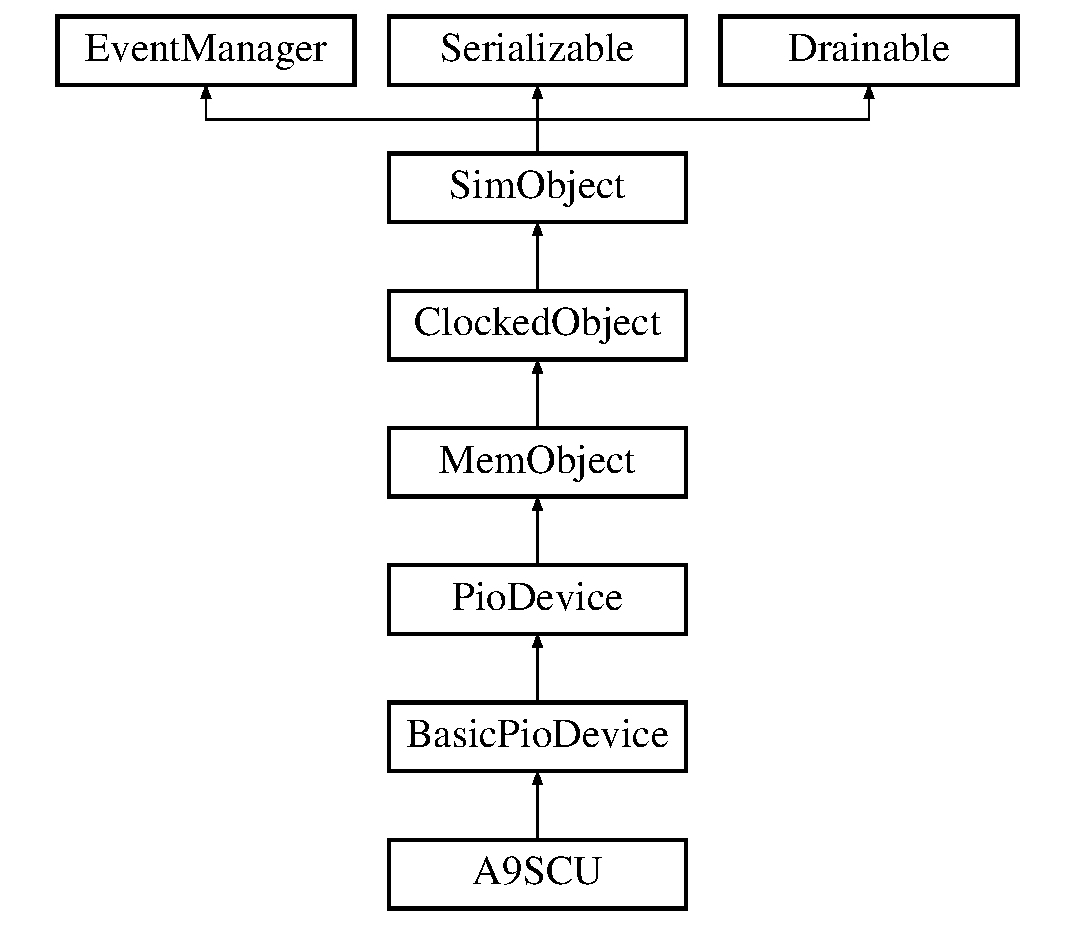
\includegraphics[height=7cm]{classA9SCU}
\end{center}
\end{figure}
\subsection*{Public 型}
\begin{DoxyCompactItemize}
\item 
typedef A9SCUParams \hyperlink{classA9SCU_a6264a26c977c4e8d51cb6b3d6cd3a842}{Params}
\end{DoxyCompactItemize}
\subsection*{Public メソッド}
\begin{DoxyCompactItemize}
\item 
\hyperlink{classA9SCU_aafe83320aca70b23aeacd2370cc7c905}{A9SCU} (\hyperlink{classA9SCU_a6264a26c977c4e8d51cb6b3d6cd3a842}{Params} $\ast$p)
\item 
virtual \hyperlink{base_2types_8hh_a5c8ed81b7d238c9083e1037ba6d61643}{Tick} \hyperlink{classA9SCU_a613ec7d5e1ec64f8d21fec78ae8e568e}{read} (\hyperlink{classPacket}{PacketPtr} pkt)
\item 
virtual \hyperlink{base_2types_8hh_a5c8ed81b7d238c9083e1037ba6d61643}{Tick} \hyperlink{classA9SCU_a4cefab464e72b5dd42c003a0a4341802}{write} (\hyperlink{classPacket}{PacketPtr} pkt)
\end{DoxyCompactItemize}
\subsection*{Protected 型}
\begin{DoxyCompactItemize}
\item 
enum \{ \hyperlink{classA9SCU_a394b3903fbf00ba2b6243f60689a5a5fa472675dc9774d12a861cde09d5f590e2}{Control} =  0x00, 
\hyperlink{classA9SCU_a394b3903fbf00ba2b6243f60689a5a5fa5c9e6911f4248ff02074469a6b247156}{Config} =  0x04
 \}
\end{DoxyCompactItemize}


\subsection{型定義}
\hypertarget{classA9SCU_a6264a26c977c4e8d51cb6b3d6cd3a842}{
\index{A9SCU@{A9SCU}!Params@{Params}}
\index{Params@{Params}!A9SCU@{A9SCU}}
\subsubsection[{Params}]{\setlength{\rightskip}{0pt plus 5cm}typedef A9SCUParams {\bf Params}}}
\label{classA9SCU_a6264a26c977c4e8d51cb6b3d6cd3a842}


\hyperlink{classBasicPioDevice_a2845515ac6467f10540747053c8a0449}{BasicPioDevice}を再定義しています。

\subsection{列挙型}
\hypertarget{classA9SCU_a394b3903fbf00ba2b6243f60689a5a5f}{
\subsubsection[{"@42}]{\setlength{\rightskip}{0pt plus 5cm}anonymous enum\hspace{0.3cm}{\ttfamily  \mbox{[}protected\mbox{]}}}}
\label{classA9SCU_a394b3903fbf00ba2b6243f60689a5a5f}
\begin{Desc}
\item[列挙型の値: ]\par
\begin{description}
\index{Control@{Control}!A9SCU@{A9SCU}}\index{A9SCU@{A9SCU}!Control@{Control}}\item[{\em 
\hypertarget{classA9SCU_a394b3903fbf00ba2b6243f60689a5a5fa472675dc9774d12a861cde09d5f590e2}{
Control}
\label{classA9SCU_a394b3903fbf00ba2b6243f60689a5a5fa472675dc9774d12a861cde09d5f590e2}
}]\index{Config@{Config}!A9SCU@{A9SCU}}\index{A9SCU@{A9SCU}!Config@{Config}}\item[{\em 
\hypertarget{classA9SCU_a394b3903fbf00ba2b6243f60689a5a5fa5c9e6911f4248ff02074469a6b247156}{
Config}
\label{classA9SCU_a394b3903fbf00ba2b6243f60689a5a5fa5c9e6911f4248ff02074469a6b247156}
}]\end{description}
\end{Desc}




\begin{DoxyCode}
53          {
54         Control     = 0x00,
55         Config      = 0x04,
56     };
\end{DoxyCode}


\subsection{コンストラクタとデストラクタ}
\hypertarget{classA9SCU_aafe83320aca70b23aeacd2370cc7c905}{
\index{A9SCU@{A9SCU}!A9SCU@{A9SCU}}
\index{A9SCU@{A9SCU}!A9SCU@{A9SCU}}
\subsubsection[{A9SCU}]{\setlength{\rightskip}{0pt plus 5cm}{\bf A9SCU} ({\bf Params} $\ast$ {\em p})}}
\label{classA9SCU_aafe83320aca70b23aeacd2370cc7c905}
The constructor for \hyperlink{classRealView}{RealView} just registers itself with the MMU. 
\begin{DoxyParams}{引数}
\item[{\em p}]params structure \end{DoxyParams}



\begin{DoxyCode}
48     : BasicPioDevice(p, 0x60)
49 {
50 }
\end{DoxyCode}


\subsection{関数}
\hypertarget{classA9SCU_a613ec7d5e1ec64f8d21fec78ae8e568e}{
\index{A9SCU@{A9SCU}!read@{read}}
\index{read@{read}!A9SCU@{A9SCU}}
\subsubsection[{read}]{\setlength{\rightskip}{0pt plus 5cm}{\bf Tick} read ({\bf PacketPtr} {\em pkt})\hspace{0.3cm}{\ttfamily  \mbox{[}virtual\mbox{]}}}}
\label{classA9SCU_a613ec7d5e1ec64f8d21fec78ae8e568e}
Handle a read to the device 
\begin{DoxyParams}{引数}
\item[{\em pkt}]The memory request. \item[{\em data}]Where to put the data. \end{DoxyParams}


\hyperlink{classPioDevice_a842312590432036092c422c87a442358}{PioDevice}を実装しています。


\begin{DoxyCode}
54 {
55     assert(pkt->getAddr() >= pioAddr && pkt->getAddr() < pioAddr + pioSize);
56     assert(pkt->getSize() == 4);
57     Addr daddr = pkt->getAddr() - pioAddr;
58     pkt->allocate();
59 
60     switch(daddr) {
61       case Control:
62         pkt->set(1); // SCU already enabled
63         break;
64       case Config:
65         /* Without making a completely new SCU, we can use the core count field
66          * as 4 bits and inform the OS of up to 16 CPUs.  Although the core
67          * count is technically bits [1:0] only, bits [3:2] are SBZ for future
68          * expansion like this.
69          */
70         if (sys->numContexts() > 4) {
71             warn_once("A9SCU with >4 CPUs is unsupported\n");
72             if (sys->numContexts() > 15)
73                 fatal("Too many CPUs (%d) for A9SCU!\n", sys->numContexts());
74         }
75         int smp_bits, core_cnt;
76         smp_bits = power(2,sys->numContexts()) - 1;
77         core_cnt = sys->numContexts() - 1;
78         pkt->set(smp_bits << 4 | core_cnt);
79         break;
80       default:
81         // Only configuration register is implemented
82         panic("Tried to read SCU at offset %#x\n", daddr);
83         break;
84     }
85     pkt->makeAtomicResponse();
86     return pioDelay;
87 
88 }
\end{DoxyCode}
\hypertarget{classA9SCU_a4cefab464e72b5dd42c003a0a4341802}{
\index{A9SCU@{A9SCU}!write@{write}}
\index{write@{write}!A9SCU@{A9SCU}}
\subsubsection[{write}]{\setlength{\rightskip}{0pt plus 5cm}{\bf Tick} write ({\bf PacketPtr} {\em pkt})\hspace{0.3cm}{\ttfamily  \mbox{[}virtual\mbox{]}}}}
\label{classA9SCU_a4cefab464e72b5dd42c003a0a4341802}
All writes are panic. 
\begin{DoxyParams}{引数}
\item[{\em pkt}]The memory request. \item[{\em data}]the data \end{DoxyParams}


\hyperlink{classPioDevice_afe8371668d023bb2516b286e5e399b6f}{PioDevice}を実装しています。


\begin{DoxyCode}
92 {
93     assert(pkt->getAddr() >= pioAddr && pkt->getAddr() < pioAddr + pioSize);
94 
95     Addr daddr = pkt->getAddr() - pioAddr;
96     switch (daddr) {
97       default:
98         // Nothing implemented at this point
99         panic("Tried to write SCU at offset %#x\n", daddr);
100         break;
101     }
102     pkt->makeAtomicResponse();
103     return pioDelay;
104 }
\end{DoxyCode}


このクラスの説明は次のファイルから生成されました:\begin{DoxyCompactItemize}
\item 
dev/arm/\hyperlink{a9scu_8hh}{a9scu.hh}\item 
dev/arm/\hyperlink{a9scu_8cc}{a9scu.cc}\end{DoxyCompactItemize}

\hypertarget{classRealView_1_1A9SCU}{
\section{クラス A9SCU}
\label{classRealView_1_1A9SCU}\index{RealView::A9SCU@{RealView::A9SCU}}
}
A9SCUに対する継承グラフ:\begin{figure}[H]
\begin{center}
\leavevmode
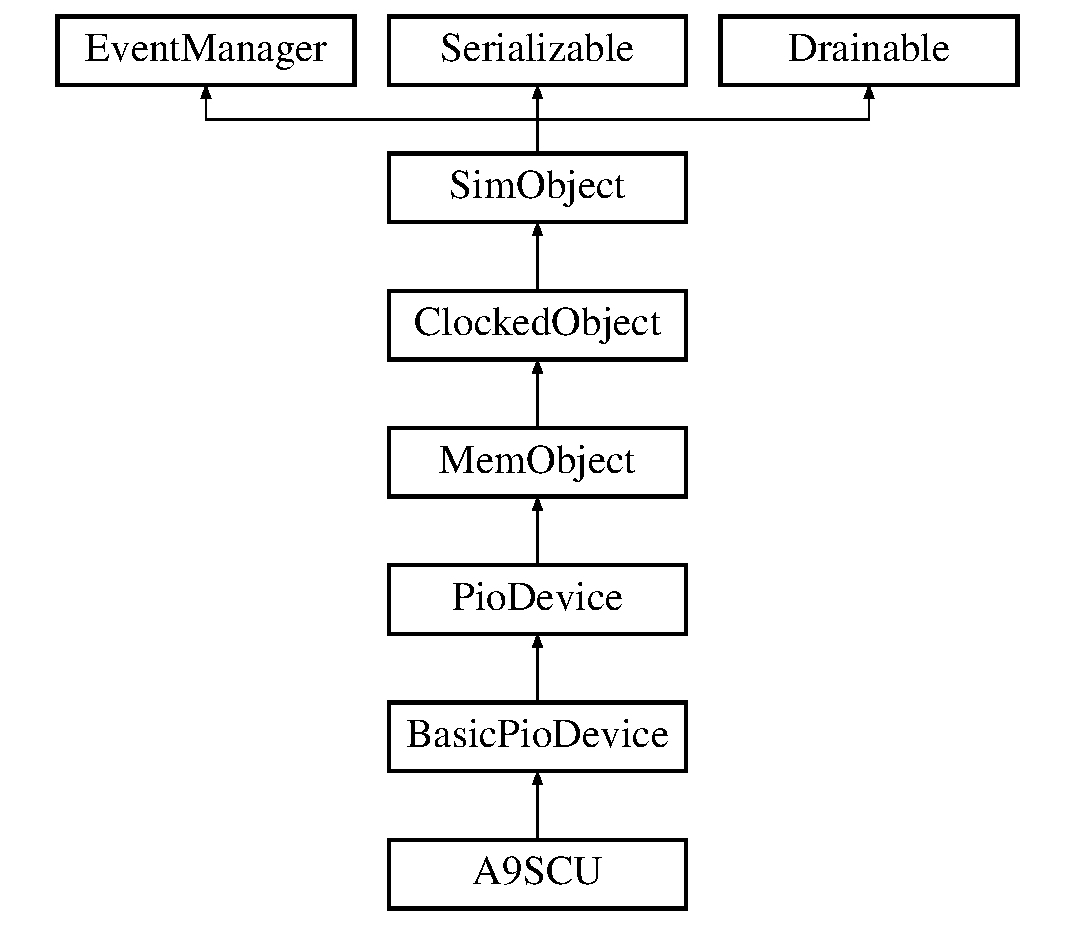
\includegraphics[height=7cm]{classRealView_1_1A9SCU}
\end{center}
\end{figure}
\subsection*{Static Public 変数}
\begin{DoxyCompactItemize}
\item 
string \hyperlink{classRealView_1_1A9SCU_acce15679d830831b0bbe8ebc2a60b2ca}{type} = '\hyperlink{classRealView_1_1A9SCU}{A9SCU}'
\item 
string \hyperlink{classRealView_1_1A9SCU_a17da7064bc5c518791f0c891eff05fda}{cxx\_\-header} = \char`\"{}dev/arm/a9scu.hh\char`\"{}
\end{DoxyCompactItemize}


\subsection{変数}
\hypertarget{classRealView_1_1A9SCU_a17da7064bc5c518791f0c891eff05fda}{
\index{RealView::A9SCU@{RealView::A9SCU}!cxx\_\-header@{cxx\_\-header}}
\index{cxx\_\-header@{cxx\_\-header}!RealView::A9SCU@{RealView::A9SCU}}
\subsubsection[{cxx\_\-header}]{\setlength{\rightskip}{0pt plus 5cm}string {\bf cxx\_\-header} = \char`\"{}dev/arm/a9scu.hh\char`\"{}\hspace{0.3cm}{\ttfamily  \mbox{[}static\mbox{]}}}}
\label{classRealView_1_1A9SCU_a17da7064bc5c518791f0c891eff05fda}
\hypertarget{classRealView_1_1A9SCU_acce15679d830831b0bbe8ebc2a60b2ca}{
\index{RealView::A9SCU@{RealView::A9SCU}!type@{type}}
\index{type@{type}!RealView::A9SCU@{RealView::A9SCU}}
\subsubsection[{type}]{\setlength{\rightskip}{0pt plus 5cm}string {\bf type} = '{\bf A9SCU}'\hspace{0.3cm}{\ttfamily  \mbox{[}static\mbox{]}}}}
\label{classRealView_1_1A9SCU_acce15679d830831b0bbe8ebc2a60b2ca}


このクラスの説明は次のファイルから生成されました:\begin{DoxyCompactItemize}
\item 
dev/arm/\hyperlink{RealView_8py}{RealView.py}\end{DoxyCompactItemize}

\hypertarget{classArmISA_1_1AbortFault}{
\section{クラス テンプレート AbortFault$<$ T $>$}
\label{classArmISA_1_1AbortFault}\index{ArmISA::AbortFault@{ArmISA::AbortFault}}
}


{\ttfamily \#include $<$faults.hh$>$}AbortFault$<$ T $>$に対する継承グラフ:\begin{figure}[H]
\begin{center}
\leavevmode
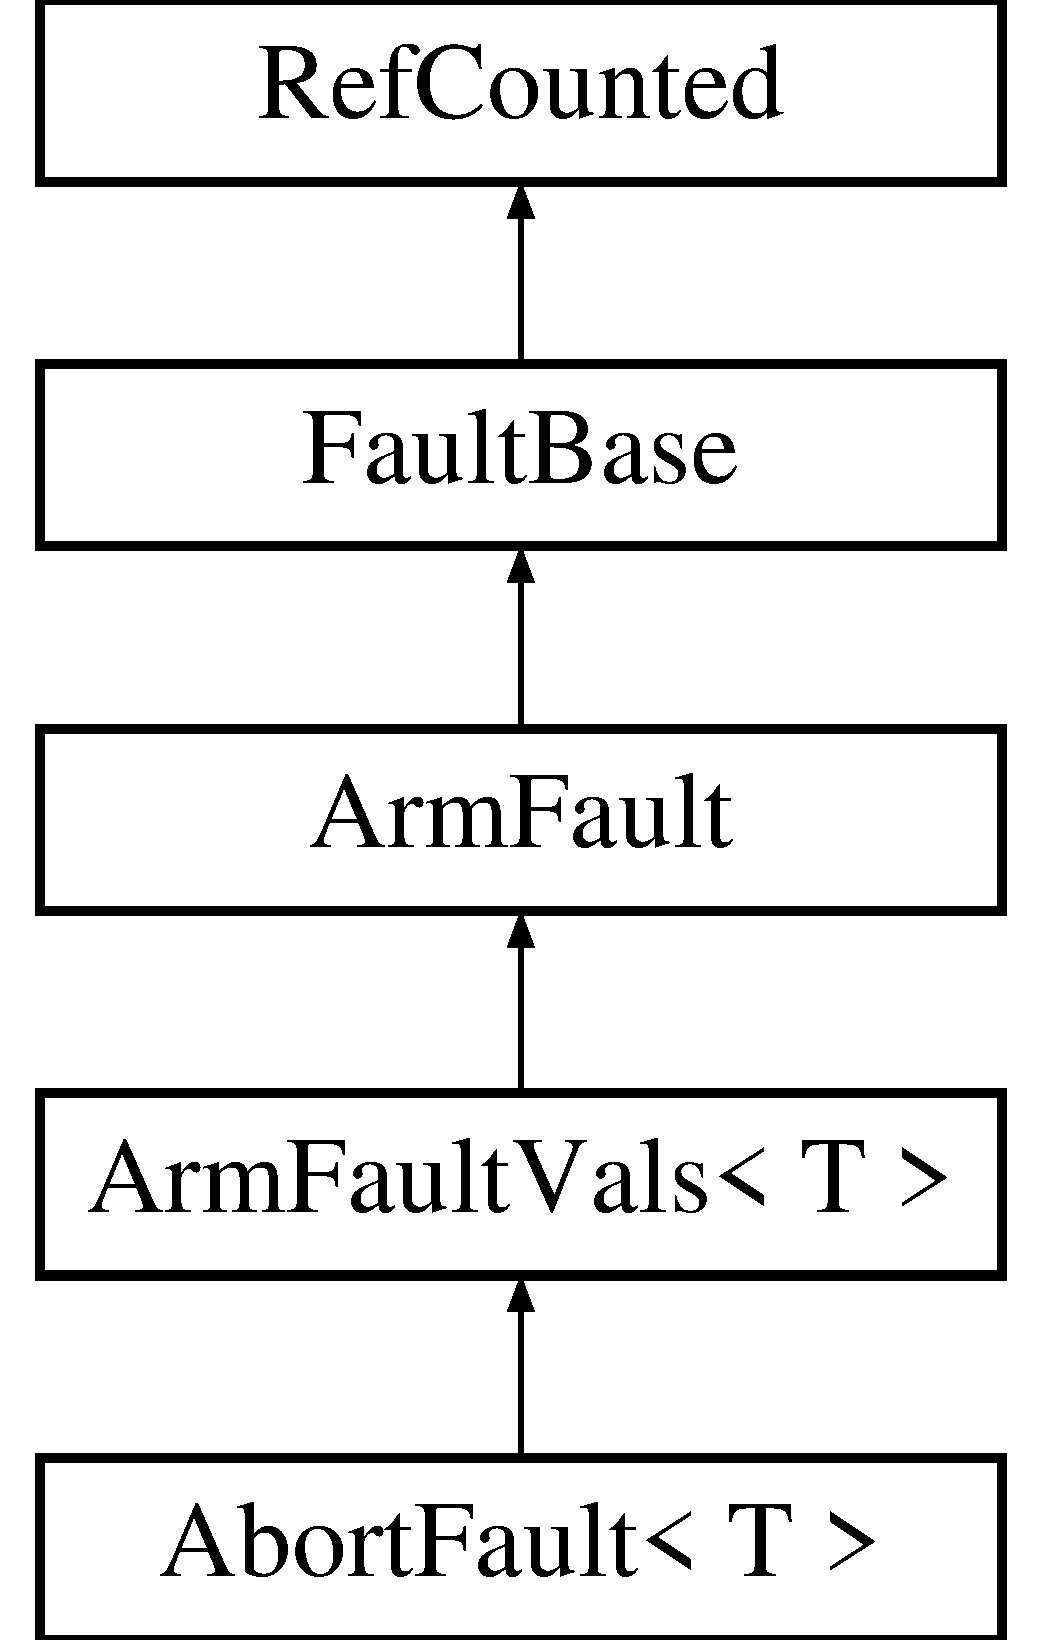
\includegraphics[height=5cm]{classArmISA_1_1AbortFault}
\end{center}
\end{figure}
\subsection*{Public メソッド}
\begin{DoxyCompactItemize}
\item 
\hyperlink{classArmISA_1_1AbortFault_a68effcc3ba0f9938e7571ad7dc83ffcf}{AbortFault} (\hyperlink{classm5_1_1params_1_1Addr}{Addr} \_\-faultAddr, bool \_\-write, \hyperlink{structArmISA_1_1TlbEntry_a0595b41cfb7d03f18438f9c355a3469d}{TlbEntry::DomainType} \_\-domain, uint8\_\-t \_\-source, bool \_\-stage2, \hyperlink{classArmISA_1_1ArmFault_ad78237d6390becbe8bdf9e73979c56ae}{ArmFault::TranMethod} \_\-tranMethod=ArmFault::UnknownTran)
\item 
void \hyperlink{classArmISA_1_1AbortFault_a2bd783b42262278d41157d428e1f8d6f}{invoke} (\hyperlink{classThreadContext}{ThreadContext} $\ast$\hyperlink{namespaceArmISA_a5aff829af55e65b802d83dfcef4e9dd0}{tc}, \hyperlink{classRefCountingPtr}{StaticInstPtr} inst=\hyperlink{classStaticInst_aa793d9793af735f09096369fb17567b6}{StaticInst::nullStaticInstPtr})
\item 
FSR \hyperlink{classArmISA_1_1AbortFault_abae0f5c90ba0a6f56bc8df45dbd5861b}{getFsr} (\hyperlink{classThreadContext}{ThreadContext} $\ast$\hyperlink{namespaceArmISA_a5aff829af55e65b802d83dfcef4e9dd0}{tc})
\item 
bool \hyperlink{classArmISA_1_1AbortFault_a92a741baab278ed029d84b0fe979e1b8}{abortDisable} (\hyperlink{classThreadContext}{ThreadContext} $\ast$\hyperlink{namespaceArmISA_a5aff829af55e65b802d83dfcef4e9dd0}{tc})
\item 
\hyperlink{Type_8hh_a435d1572bf3f880d55459d9805097f62}{uint32\_\-t} \hyperlink{classArmISA_1_1AbortFault_a54f4d33ac162a95fd5b3830cf7fab8ff}{iss} () const 
\item 
bool \hyperlink{classArmISA_1_1AbortFault_abb0e34fd2d22460e7779f419601dc6dc}{isStage2} () const 
\item 
void \hyperlink{classArmISA_1_1AbortFault_a1534ab135f3f8a49ad6274389bf77b51}{annotate} (\hyperlink{classArmISA_1_1ArmFault_a955305710181a260a9ee0b419a6027fb}{ArmFault::AnnotationIDs} id, uint64\_\-t val)
\item 
bool \hyperlink{classArmISA_1_1AbortFault_a3839d4e20c8314337d02889689f3c57e}{isMMUFault} () const 
\end{DoxyCompactItemize}
\subsection*{Protected 変数}
\begin{DoxyCompactItemize}
\item 
\hyperlink{classm5_1_1params_1_1Addr}{Addr} \hyperlink{classArmISA_1_1AbortFault_a39e9eff111c8c7d4acfecc9d3bbd29d4}{faultAddr}
\item 
\hyperlink{classm5_1_1params_1_1Addr}{Addr} \hyperlink{classArmISA_1_1AbortFault_a6d8ab6ddd3da67e07350b2c3ff6c0d80}{OVAddr}
\item 
bool \hyperlink{classArmISA_1_1AbortFault_ab4d8d1259f524270d625ab8933700d27}{write}
\item 
\hyperlink{structArmISA_1_1TlbEntry_a0595b41cfb7d03f18438f9c355a3469d}{TlbEntry::DomainType} \hyperlink{classArmISA_1_1AbortFault_a8f425ac9ed99f5604dcca4b072c88718}{domain}
\item 
uint8\_\-t \hyperlink{classArmISA_1_1AbortFault_a36a99c772ae64e186f5264a662834eef}{source}
\item 
uint8\_\-t \hyperlink{classArmISA_1_1AbortFault_ada7b52f73921c795a241ffd6e381fc69}{srcEncoded}
\item 
bool \hyperlink{classArmISA_1_1AbortFault_a29056d47d3f3a94a388d6f9ba707ef0e}{stage2}
\item 
bool \hyperlink{classArmISA_1_1AbortFault_ad135724e922a94add62100a64854ae84}{s1ptw}
\item 
\hyperlink{classArmISA_1_1ArmFault_ad78237d6390becbe8bdf9e73979c56ae}{ArmFault::TranMethod} \hyperlink{classArmISA_1_1AbortFault_a8f7a9c6fc85261a8c7ffb21d5afeed24}{tranMethod}
\end{DoxyCompactItemize}
\subsubsection*{template$<$class T$>$ class ArmISA::AbortFault$<$ T $>$}



\subsection{コンストラクタとデストラクタ}
\hypertarget{classArmISA_1_1AbortFault_a68effcc3ba0f9938e7571ad7dc83ffcf}{
\index{ArmISA::AbortFault@{ArmISA::AbortFault}!AbortFault@{AbortFault}}
\index{AbortFault@{AbortFault}!ArmISA::AbortFault@{ArmISA::AbortFault}}
\subsubsection[{AbortFault}]{\setlength{\rightskip}{0pt plus 5cm}{\bf AbortFault} ({\bf Addr} {\em \_\-faultAddr}, \/  bool {\em \_\-write}, \/  {\bf TlbEntry::DomainType} {\em \_\-domain}, \/  uint8\_\-t {\em \_\-source}, \/  bool {\em \_\-stage2}, \/  {\bf ArmFault::TranMethod} {\em \_\-tranMethod} = {\ttfamily ArmFault::UnknownTran})\hspace{0.3cm}{\ttfamily  \mbox{[}inline\mbox{]}}}}
\label{classArmISA_1_1AbortFault_a68effcc3ba0f9938e7571ad7dc83ffcf}



\begin{DoxyCode}
399                                                                                  
        :
400         faultAddr(_faultAddr), write(_write), domain(_domain), source(_source),
401         stage2(_stage2), s1ptw(false), tranMethod(_tranMethod)
402     {}

\end{DoxyCode}


\subsection{関数}
\hypertarget{classArmISA_1_1AbortFault_a92a741baab278ed029d84b0fe979e1b8}{
\index{ArmISA::AbortFault@{ArmISA::AbortFault}!abortDisable@{abortDisable}}
\index{abortDisable@{abortDisable}!ArmISA::AbortFault@{ArmISA::AbortFault}}
\subsubsection[{abortDisable}]{\setlength{\rightskip}{0pt plus 5cm}bool abortDisable ({\bf ThreadContext} $\ast$ {\em tc})\hspace{0.3cm}{\ttfamily  \mbox{[}inline, virtual\mbox{]}}}}
\label{classArmISA_1_1AbortFault_a92a741baab278ed029d84b0fe979e1b8}


\hyperlink{classArmISA_1_1ArmFaultVals_a1f1a5b662b9a505415dd5ef1f52892f3}{ArmFaultVals$<$ T $>$}を再定義しています。


\begin{DoxyCode}
1004 {
1005     if (ArmSystem::haveSecurity(tc)) {
1006         SCR scr = tc->readMiscRegNoEffect(MISCREG_SCR);
1007         return (!scr.ns || scr.aw);
1008     }
1009     return true;
1010 }
\end{DoxyCode}
\hypertarget{classArmISA_1_1AbortFault_a1534ab135f3f8a49ad6274389bf77b51}{
\index{ArmISA::AbortFault@{ArmISA::AbortFault}!annotate@{annotate}}
\index{annotate@{annotate}!ArmISA::AbortFault@{ArmISA::AbortFault}}
\subsubsection[{annotate}]{\setlength{\rightskip}{0pt plus 5cm}void annotate ({\bf ArmFault::AnnotationIDs} {\em id}, \/  uint64\_\-t {\em val})\hspace{0.3cm}{\ttfamily  \mbox{[}inline, virtual\mbox{]}}}}
\label{classArmISA_1_1AbortFault_a1534ab135f3f8a49ad6274389bf77b51}


\hyperlink{classArmISA_1_1ArmFault_a1711e0fd9d5fa3eaa8e62cc821ef850d}{ArmFault}を再定義しています。

\hyperlink{classArmISA_1_1DataAbort_a284956f8d8ec0f18434d857ae44c6a6c}{DataAbort}で再定義されています。


\begin{DoxyCode}
1015 {
1016     switch (id)
1017     {
1018       case ArmFault::S1PTW:
1019         s1ptw = val;
1020         break;
1021       case ArmFault::OVA:
1022         OVAddr = val;
1023         break;
1024 
1025       // Just ignore unknown ID's
1026       default:
1027         break;
1028     }
1029 }
\end{DoxyCode}
\hypertarget{classArmISA_1_1AbortFault_abae0f5c90ba0a6f56bc8df45dbd5861b}{
\index{ArmISA::AbortFault@{ArmISA::AbortFault}!getFsr@{getFsr}}
\index{getFsr@{getFsr}!ArmISA::AbortFault@{ArmISA::AbortFault}}
\subsubsection[{getFsr}]{\setlength{\rightskip}{0pt plus 5cm}FSR getFsr ({\bf ThreadContext} $\ast$ {\em tc})\hspace{0.3cm}{\ttfamily  \mbox{[}inline, virtual\mbox{]}}}}
\label{classArmISA_1_1AbortFault_abae0f5c90ba0a6f56bc8df45dbd5861b}


\hyperlink{classArmISA_1_1ArmFault_a48f7b7354d7dcf9850a65f9f433c4871}{ArmFault}を再定義しています。


\begin{DoxyCode}
973 {
974     FSR fsr = 0;
975 
976     if (((CPSR) tc->readMiscRegNoEffect(MISCREG_CPSR)).width) {
977         // AArch32
978         assert(tranMethod != ArmFault::UnknownTran);
979         if (tranMethod == ArmFault::LpaeTran) {
980             srcEncoded = ArmFault::longDescFaultSources[source];
981             fsr.status = srcEncoded;
982             fsr.lpae   = 1;
983         } else {
984             srcEncoded = ArmFault::shortDescFaultSources[source];
985             fsr.fsLow  = bits(srcEncoded, 3, 0);
986             fsr.fsHigh = bits(srcEncoded, 4);
987             fsr.domain = static_cast<uint8_t>(domain);
988         }
989         fsr.wnr = (write ? 1 : 0);
990         fsr.ext = 0;
991     } else {
992         // AArch64
993         srcEncoded = ArmFault::aarch64FaultSources[source];
994     }
995     if (srcEncoded == ArmFault::FaultSourceInvalid) {
996         panic("Invalid fault source\n");
997     }
998     return fsr;
999 }
\end{DoxyCode}
\hypertarget{classArmISA_1_1AbortFault_a2bd783b42262278d41157d428e1f8d6f}{
\index{ArmISA::AbortFault@{ArmISA::AbortFault}!invoke@{invoke}}
\index{invoke@{invoke}!ArmISA::AbortFault@{ArmISA::AbortFault}}
\subsubsection[{invoke}]{\setlength{\rightskip}{0pt plus 5cm}void invoke ({\bf ThreadContext} $\ast$ {\em tc}, \/  {\bf StaticInstPtr} {\em inst} = {\ttfamily {\bf StaticInst::nullStaticInstPtr}})\hspace{0.3cm}{\ttfamily  \mbox{[}inline, virtual\mbox{]}}}}
\label{classArmISA_1_1AbortFault_a2bd783b42262278d41157d428e1f8d6f}


\hyperlink{classArmISA_1_1ArmFault_a2bd783b42262278d41157d428e1f8d6f}{ArmFault}を再定義しています。

\hyperlink{classArmISA_1_1VirtualDataAbort_a38260dc6f5fb9598eaf95d8696e3efe8}{VirtualDataAbort}で再定義されています。


\begin{DoxyCode}
917 {
918     if (tranMethod == ArmFault::UnknownTran) {
919         tranMethod = longDescFormatInUse(tc) ? ArmFault::LpaeTran
920                                              : ArmFault::VmsaTran;
921 
922         if ((tranMethod == ArmFault::VmsaTran) && this->routeToMonitor(tc)) {
923             // See ARM ARM B3-1416
924             bool override_LPAE = false;
925             TTBCR ttbcr_s = tc->readMiscReg(MISCREG_TTBCR_S);
926             TTBCR M5_VAR_USED ttbcr_ns = tc->readMiscReg(MISCREG_TTBCR_NS);
927             if (ttbcr_s.eae) {
928                 override_LPAE = true;
929             } else {
930                 // Unimplemented code option, not seen in testing.  May need
931                 // extension according to the manual exceprt above.
932                 DPRINTF(Faults, "Warning: Incomplete translation method "
933                         "override detected.\n");
934             }
935             if (override_LPAE)
936                 tranMethod = ArmFault::LpaeTran;
937         }
938     }
939 
940     if (source == ArmFault::AsynchronousExternalAbort) {
941         tc->getCpuPtr()->clearInterrupt(INT_ABT, 0);
942     }
943     // Get effective fault source encoding
944     CPSR cpsr = tc->readMiscReg(MISCREG_CPSR);
945     FSR  fsr  = getFsr(tc);
946 
947     // source must be determined BEFORE invoking generic routines which will
948     // try to set hsr etc. and are based upon source!
949     ArmFaultVals<T>::invoke(tc, inst);
950 
951     if (cpsr.width) {  // AArch32
952         if (cpsr.mode == MODE_HYP) {
953             tc->setMiscReg(T::HFarIndex, faultAddr);
954         } else if (stage2) {
955             tc->setMiscReg(MISCREG_HPFAR, (faultAddr >> 8) & ~0xf);
956             tc->setMiscReg(T::HFarIndex,  OVAddr);
957         } else {
958             tc->setMiscReg(T::FsrIndex, fsr);
959             tc->setMiscReg(T::FarIndex, faultAddr);
960         }
961         DPRINTF(Faults, "Abort Fault source=%#x fsr=%#x faultAddr=%#x "\
962                 "tranMethod=%#x\n", source, fsr, faultAddr, tranMethod);
963     } else {  // AArch64
964         // Set the FAR register.  Nothing else to do if we are in AArch64 state
965         // because the syndrome register has already been set inside invoke64()
966         tc->setMiscReg(AbortFault<T>::getFaultAddrReg64(), faultAddr);
967     }
968 }
\end{DoxyCode}
\hypertarget{classArmISA_1_1AbortFault_a3839d4e20c8314337d02889689f3c57e}{
\index{ArmISA::AbortFault@{ArmISA::AbortFault}!isMMUFault@{isMMUFault}}
\index{isMMUFault@{isMMUFault}!ArmISA::AbortFault@{ArmISA::AbortFault}}
\subsubsection[{isMMUFault}]{\setlength{\rightskip}{0pt plus 5cm}bool isMMUFault () const\hspace{0.3cm}{\ttfamily  \mbox{[}inline\mbox{]}}}}
\label{classArmISA_1_1AbortFault_a3839d4e20c8314337d02889689f3c57e}



\begin{DoxyCode}
1046 {
1047     // NOTE: Not relying on LL information being aligned to lowest bits here
1048     return
1049          (source == ArmFault::AlignmentFault)     ||
1050         ((source >= ArmFault::TranslationLL) &&
1051          (source <  ArmFault::TranslationLL + 4)) ||
1052         ((source >= ArmFault::AccessFlagLL) &&
1053          (source <  ArmFault::AccessFlagLL + 4))  ||
1054         ((source >= ArmFault::DomainLL) &&
1055          (source <  ArmFault::DomainLL + 4))      ||
1056         ((source >= ArmFault::PermissionLL) &&
1057          (source <  ArmFault::PermissionLL + 4));
1058 }
\end{DoxyCode}
\hypertarget{classArmISA_1_1AbortFault_a54f4d33ac162a95fd5b3830cf7fab8ff}{
\index{ArmISA::AbortFault@{ArmISA::AbortFault}!iss@{iss}}
\index{iss@{iss}!ArmISA::AbortFault@{ArmISA::AbortFault}}
\subsubsection[{iss}]{\setlength{\rightskip}{0pt plus 5cm}{\bf uint32\_\-t} iss () const\hspace{0.3cm}{\ttfamily  \mbox{[}inline, virtual\mbox{]}}}}
\label{classArmISA_1_1AbortFault_a54f4d33ac162a95fd5b3830cf7fab8ff}


\hyperlink{classArmISA_1_1ArmFaultVals_a1049bf31f8df10c66994603055cf531d}{ArmFaultVals$<$ T $>$}を再定義しています。

\hyperlink{classArmISA_1_1DataAbort_a54f4d33ac162a95fd5b3830cf7fab8ff}{DataAbort}で再定義されています。


\begin{DoxyCode}
1034 {
1035     uint32_t val;
1036 
1037     val  = srcEncoded & 0x3F;
1038     val |= write << 6;
1039     val |= s1ptw << 7;
1040     return (val);
1041 }
\end{DoxyCode}
\hypertarget{classArmISA_1_1AbortFault_abb0e34fd2d22460e7779f419601dc6dc}{
\index{ArmISA::AbortFault@{ArmISA::AbortFault}!isStage2@{isStage2}}
\index{isStage2@{isStage2}!ArmISA::AbortFault@{ArmISA::AbortFault}}
\subsubsection[{isStage2}]{\setlength{\rightskip}{0pt plus 5cm}bool isStage2 () const\hspace{0.3cm}{\ttfamily  \mbox{[}inline, virtual\mbox{]}}}}
\label{classArmISA_1_1AbortFault_abb0e34fd2d22460e7779f419601dc6dc}


\hyperlink{classArmISA_1_1ArmFault_a61bc59380024a05bdcbb39fb27e0293d}{ArmFault}を再定義しています。


\begin{DoxyCode}
410 { return stage2; }
\end{DoxyCode}


\subsection{変数}
\hypertarget{classArmISA_1_1AbortFault_a8f425ac9ed99f5604dcca4b072c88718}{
\index{ArmISA::AbortFault@{ArmISA::AbortFault}!domain@{domain}}
\index{domain@{domain}!ArmISA::AbortFault@{ArmISA::AbortFault}}
\subsubsection[{domain}]{\setlength{\rightskip}{0pt plus 5cm}{\bf TlbEntry::DomainType} {\bf domain}\hspace{0.3cm}{\ttfamily  \mbox{[}protected\mbox{]}}}}
\label{classArmISA_1_1AbortFault_a8f425ac9ed99f5604dcca4b072c88718}
\hypertarget{classArmISA_1_1AbortFault_a39e9eff111c8c7d4acfecc9d3bbd29d4}{
\index{ArmISA::AbortFault@{ArmISA::AbortFault}!faultAddr@{faultAddr}}
\index{faultAddr@{faultAddr}!ArmISA::AbortFault@{ArmISA::AbortFault}}
\subsubsection[{faultAddr}]{\setlength{\rightskip}{0pt plus 5cm}{\bf Addr} {\bf faultAddr}\hspace{0.3cm}{\ttfamily  \mbox{[}protected\mbox{]}}}}
\label{classArmISA_1_1AbortFault_a39e9eff111c8c7d4acfecc9d3bbd29d4}
The virtual address the fault occured at. If 2 stages of translation are being used then this is the intermediate physical address that is the starting point for the second stage of translation. \hypertarget{classArmISA_1_1AbortFault_a6d8ab6ddd3da67e07350b2c3ff6c0d80}{
\index{ArmISA::AbortFault@{ArmISA::AbortFault}!OVAddr@{OVAddr}}
\index{OVAddr@{OVAddr}!ArmISA::AbortFault@{ArmISA::AbortFault}}
\subsubsection[{OVAddr}]{\setlength{\rightskip}{0pt plus 5cm}{\bf Addr} {\bf OVAddr}\hspace{0.3cm}{\ttfamily  \mbox{[}protected\mbox{]}}}}
\label{classArmISA_1_1AbortFault_a6d8ab6ddd3da67e07350b2c3ff6c0d80}
Original virtual address. If the fault was generated on the second stage of translation then this variable stores the virtual address used in the original stage 1 translation. \hypertarget{classArmISA_1_1AbortFault_ad135724e922a94add62100a64854ae84}{
\index{ArmISA::AbortFault@{ArmISA::AbortFault}!s1ptw@{s1ptw}}
\index{s1ptw@{s1ptw}!ArmISA::AbortFault@{ArmISA::AbortFault}}
\subsubsection[{s1ptw}]{\setlength{\rightskip}{0pt plus 5cm}bool {\bf s1ptw}\hspace{0.3cm}{\ttfamily  \mbox{[}protected\mbox{]}}}}
\label{classArmISA_1_1AbortFault_ad135724e922a94add62100a64854ae84}
\hypertarget{classArmISA_1_1AbortFault_a36a99c772ae64e186f5264a662834eef}{
\index{ArmISA::AbortFault@{ArmISA::AbortFault}!source@{source}}
\index{source@{source}!ArmISA::AbortFault@{ArmISA::AbortFault}}
\subsubsection[{source}]{\setlength{\rightskip}{0pt plus 5cm}uint8\_\-t {\bf source}\hspace{0.3cm}{\ttfamily  \mbox{[}protected\mbox{]}}}}
\label{classArmISA_1_1AbortFault_a36a99c772ae64e186f5264a662834eef}
\hypertarget{classArmISA_1_1AbortFault_ada7b52f73921c795a241ffd6e381fc69}{
\index{ArmISA::AbortFault@{ArmISA::AbortFault}!srcEncoded@{srcEncoded}}
\index{srcEncoded@{srcEncoded}!ArmISA::AbortFault@{ArmISA::AbortFault}}
\subsubsection[{srcEncoded}]{\setlength{\rightskip}{0pt plus 5cm}uint8\_\-t {\bf srcEncoded}\hspace{0.3cm}{\ttfamily  \mbox{[}protected\mbox{]}}}}
\label{classArmISA_1_1AbortFault_ada7b52f73921c795a241ffd6e381fc69}
\hypertarget{classArmISA_1_1AbortFault_a29056d47d3f3a94a388d6f9ba707ef0e}{
\index{ArmISA::AbortFault@{ArmISA::AbortFault}!stage2@{stage2}}
\index{stage2@{stage2}!ArmISA::AbortFault@{ArmISA::AbortFault}}
\subsubsection[{stage2}]{\setlength{\rightskip}{0pt plus 5cm}bool {\bf stage2}\hspace{0.3cm}{\ttfamily  \mbox{[}protected\mbox{]}}}}
\label{classArmISA_1_1AbortFault_a29056d47d3f3a94a388d6f9ba707ef0e}
\hypertarget{classArmISA_1_1AbortFault_a8f7a9c6fc85261a8c7ffb21d5afeed24}{
\index{ArmISA::AbortFault@{ArmISA::AbortFault}!tranMethod@{tranMethod}}
\index{tranMethod@{tranMethod}!ArmISA::AbortFault@{ArmISA::AbortFault}}
\subsubsection[{tranMethod}]{\setlength{\rightskip}{0pt plus 5cm}{\bf ArmFault::TranMethod} {\bf tranMethod}\hspace{0.3cm}{\ttfamily  \mbox{[}protected\mbox{]}}}}
\label{classArmISA_1_1AbortFault_a8f7a9c6fc85261a8c7ffb21d5afeed24}
\hypertarget{classArmISA_1_1AbortFault_ab4d8d1259f524270d625ab8933700d27}{
\index{ArmISA::AbortFault@{ArmISA::AbortFault}!write@{write}}
\index{write@{write}!ArmISA::AbortFault@{ArmISA::AbortFault}}
\subsubsection[{write}]{\setlength{\rightskip}{0pt plus 5cm}bool {\bf write}\hspace{0.3cm}{\ttfamily  \mbox{[}protected\mbox{]}}}}
\label{classArmISA_1_1AbortFault_ab4d8d1259f524270d625ab8933700d27}


このクラスの説明は次のファイルから生成されました:\begin{DoxyCompactItemize}
\item 
arch/arm/\hyperlink{arch_2arm_2faults_8hh}{faults.hh}\item 
arch/arm/\hyperlink{arch_2arm_2faults_8cc}{faults.cc}\end{DoxyCompactItemize}

\hypertarget{classAbstractBloomFilter}{
\section{クラス AbstractBloomFilter}
\label{classAbstractBloomFilter}\index{AbstractBloomFilter@{AbstractBloomFilter}}
}


{\ttfamily \#include $<$AbstractBloomFilter.hh$>$}AbstractBloomFilterに対する継承グラフ:\begin{figure}[H]
\begin{center}
\leavevmode
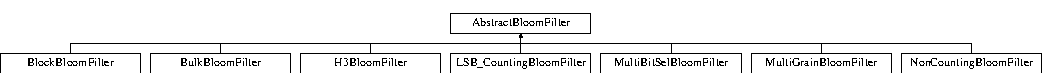
\includegraphics[height=0.981595cm]{classAbstractBloomFilter}
\end{center}
\end{figure}
\subsection*{Public メソッド}
\begin{DoxyCompactItemize}
\item 
virtual \hyperlink{classAbstractBloomFilter_a750758d99727e6a06111be87c6b62cfa}{$\sim$AbstractBloomFilter} ()
\item 
virtual void \hyperlink{classAbstractBloomFilter_a5eeb94d22b8366d1b68d0614384802fe}{clear} ()=0
\item 
virtual void \hyperlink{classAbstractBloomFilter_af795f7fdeff0174e914ed1d792ffe4ff}{increment} (const \hyperlink{classAddress}{Address} \&addr)=0
\item 
virtual void \hyperlink{classAbstractBloomFilter_aa387151f4ab03c6cd497d4385e34c21a}{decrement} (const \hyperlink{classAddress}{Address} \&addr)=0
\item 
virtual void \hyperlink{classAbstractBloomFilter_accf3024e7bc583662b4dee2e25ae484a}{merge} (\hyperlink{classAbstractBloomFilter}{AbstractBloomFilter} $\ast$other\_\-filter)=0
\item 
virtual void \hyperlink{classAbstractBloomFilter_a54e1262ae5f60efeb8714d0556b3c32e}{set} (const \hyperlink{classAddress}{Address} \&addr)=0
\item 
virtual void \hyperlink{classAbstractBloomFilter_a0a35d1c7bad19fe9362068a0d319ec5f}{unset} (const \hyperlink{classAddress}{Address} \&addr)=0
\item 
virtual bool \hyperlink{classAbstractBloomFilter_aa1b69d102655f8c5879b3df95eb205dc}{isSet} (const \hyperlink{classAddress}{Address} \&addr)=0
\item 
virtual int \hyperlink{classAbstractBloomFilter_ab6253919ea6ff1b2c17506742b34147d}{getCount} (const \hyperlink{classAddress}{Address} \&addr)=0
\item 
virtual int \hyperlink{classAbstractBloomFilter_a25ea5e1ef3d4911226f37649b6efed22}{getTotalCount} ()=0
\item 
virtual void \hyperlink{classAbstractBloomFilter_a3ea5f7af5db62cc24f4e40df9ea5c971}{print} (std::ostream \&out) const =0
\item 
virtual int \hyperlink{classAbstractBloomFilter_a4dd174ae24a8237d41cf0b02c78b896d}{getIndex} (const \hyperlink{classAddress}{Address} \&addr)=0
\item 
virtual int \hyperlink{classAbstractBloomFilter_a6c0e9a098f0f210aa42eb2f1553804eb}{readBit} (const int index)=0
\item 
virtual void \hyperlink{classAbstractBloomFilter_a961813caf7bb3aece26914ac43c6293f}{writeBit} (const int index, const int value)=0
\end{DoxyCompactItemize}


\subsection{コンストラクタとデストラクタ}
\hypertarget{classAbstractBloomFilter_a750758d99727e6a06111be87c6b62cfa}{
\index{AbstractBloomFilter@{AbstractBloomFilter}!$\sim$AbstractBloomFilter@{$\sim$AbstractBloomFilter}}
\index{$\sim$AbstractBloomFilter@{$\sim$AbstractBloomFilter}!AbstractBloomFilter@{AbstractBloomFilter}}
\subsubsection[{$\sim$AbstractBloomFilter}]{\setlength{\rightskip}{0pt plus 5cm}virtual $\sim${\bf AbstractBloomFilter} ()\hspace{0.3cm}{\ttfamily  \mbox{[}inline, virtual\mbox{]}}}}
\label{classAbstractBloomFilter_a750758d99727e6a06111be87c6b62cfa}



\begin{DoxyCode}
39 {};
\end{DoxyCode}


\subsection{関数}
\hypertarget{classAbstractBloomFilter_a5eeb94d22b8366d1b68d0614384802fe}{
\index{AbstractBloomFilter@{AbstractBloomFilter}!clear@{clear}}
\index{clear@{clear}!AbstractBloomFilter@{AbstractBloomFilter}}
\subsubsection[{clear}]{\setlength{\rightskip}{0pt plus 5cm}virtual void clear ()\hspace{0.3cm}{\ttfamily  \mbox{[}pure virtual\mbox{]}}}}
\label{classAbstractBloomFilter_a5eeb94d22b8366d1b68d0614384802fe}


\hyperlink{classBlockBloomFilter_ac8bb3912a3ce86b15842e79d0b421204}{BlockBloomFilter}, \hyperlink{classBulkBloomFilter_ac8bb3912a3ce86b15842e79d0b421204}{BulkBloomFilter}, \hyperlink{classH3BloomFilter_ac8bb3912a3ce86b15842e79d0b421204}{H3BloomFilter}, \hyperlink{classLSB__CountingBloomFilter_ac8bb3912a3ce86b15842e79d0b421204}{LSB\_\-CountingBloomFilter}, \hyperlink{classMultiBitSelBloomFilter_ac8bb3912a3ce86b15842e79d0b421204}{MultiBitSelBloomFilter}, \hyperlink{classMultiGrainBloomFilter_ac8bb3912a3ce86b15842e79d0b421204}{MultiGrainBloomFilter}, と \hyperlink{classNonCountingBloomFilter_ac8bb3912a3ce86b15842e79d0b421204}{NonCountingBloomFilter}で実装されています。\hypertarget{classAbstractBloomFilter_aa387151f4ab03c6cd497d4385e34c21a}{
\index{AbstractBloomFilter@{AbstractBloomFilter}!decrement@{decrement}}
\index{decrement@{decrement}!AbstractBloomFilter@{AbstractBloomFilter}}
\subsubsection[{decrement}]{\setlength{\rightskip}{0pt plus 5cm}virtual void decrement (const {\bf Address} \& {\em addr})\hspace{0.3cm}{\ttfamily  \mbox{[}pure virtual\mbox{]}}}}
\label{classAbstractBloomFilter_aa387151f4ab03c6cd497d4385e34c21a}


\hyperlink{classBlockBloomFilter_addb6b805abb8328082a24926f2bf8c84}{BlockBloomFilter}, \hyperlink{classBulkBloomFilter_addb6b805abb8328082a24926f2bf8c84}{BulkBloomFilter}, \hyperlink{classH3BloomFilter_addb6b805abb8328082a24926f2bf8c84}{H3BloomFilter}, \hyperlink{classLSB__CountingBloomFilter_addb6b805abb8328082a24926f2bf8c84}{LSB\_\-CountingBloomFilter}, \hyperlink{classMultiBitSelBloomFilter_addb6b805abb8328082a24926f2bf8c84}{MultiBitSelBloomFilter}, \hyperlink{classMultiGrainBloomFilter_addb6b805abb8328082a24926f2bf8c84}{MultiGrainBloomFilter}, と \hyperlink{classNonCountingBloomFilter_addb6b805abb8328082a24926f2bf8c84}{NonCountingBloomFilter}で実装されています。\hypertarget{classAbstractBloomFilter_ab6253919ea6ff1b2c17506742b34147d}{
\index{AbstractBloomFilter@{AbstractBloomFilter}!getCount@{getCount}}
\index{getCount@{getCount}!AbstractBloomFilter@{AbstractBloomFilter}}
\subsubsection[{getCount}]{\setlength{\rightskip}{0pt plus 5cm}virtual int getCount (const {\bf Address} \& {\em addr})\hspace{0.3cm}{\ttfamily  \mbox{[}pure virtual\mbox{]}}}}
\label{classAbstractBloomFilter_ab6253919ea6ff1b2c17506742b34147d}


\hyperlink{classBlockBloomFilter_abb722634d5846105b673e9496df8d062}{BlockBloomFilter}, \hyperlink{classBulkBloomFilter_abb722634d5846105b673e9496df8d062}{BulkBloomFilter}, \hyperlink{classH3BloomFilter_abb722634d5846105b673e9496df8d062}{H3BloomFilter}, \hyperlink{classLSB__CountingBloomFilter_abb722634d5846105b673e9496df8d062}{LSB\_\-CountingBloomFilter}, \hyperlink{classMultiBitSelBloomFilter_abb722634d5846105b673e9496df8d062}{MultiBitSelBloomFilter}, \hyperlink{classMultiGrainBloomFilter_abb722634d5846105b673e9496df8d062}{MultiGrainBloomFilter}, と \hyperlink{classNonCountingBloomFilter_abb722634d5846105b673e9496df8d062}{NonCountingBloomFilter}で実装されています。\hypertarget{classAbstractBloomFilter_a4dd174ae24a8237d41cf0b02c78b896d}{
\index{AbstractBloomFilter@{AbstractBloomFilter}!getIndex@{getIndex}}
\index{getIndex@{getIndex}!AbstractBloomFilter@{AbstractBloomFilter}}
\subsubsection[{getIndex}]{\setlength{\rightskip}{0pt plus 5cm}virtual int getIndex (const {\bf Address} \& {\em addr})\hspace{0.3cm}{\ttfamily  \mbox{[}pure virtual\mbox{]}}}}
\label{classAbstractBloomFilter_a4dd174ae24a8237d41cf0b02c78b896d}


\hyperlink{classBlockBloomFilter_a19f42f6f2fc3501021b768f0df8108b2}{BlockBloomFilter}, \hyperlink{classBulkBloomFilter_a19f42f6f2fc3501021b768f0df8108b2}{BulkBloomFilter}, \hyperlink{classH3BloomFilter_a19f42f6f2fc3501021b768f0df8108b2}{H3BloomFilter}, \hyperlink{classLSB__CountingBloomFilter_a19f42f6f2fc3501021b768f0df8108b2}{LSB\_\-CountingBloomFilter}, \hyperlink{classMultiBitSelBloomFilter_a19f42f6f2fc3501021b768f0df8108b2}{MultiBitSelBloomFilter}, \hyperlink{classMultiGrainBloomFilter_a19f42f6f2fc3501021b768f0df8108b2}{MultiGrainBloomFilter}, と \hyperlink{classNonCountingBloomFilter_a19f42f6f2fc3501021b768f0df8108b2}{NonCountingBloomFilter}で実装されています。\hypertarget{classAbstractBloomFilter_a25ea5e1ef3d4911226f37649b6efed22}{
\index{AbstractBloomFilter@{AbstractBloomFilter}!getTotalCount@{getTotalCount}}
\index{getTotalCount@{getTotalCount}!AbstractBloomFilter@{AbstractBloomFilter}}
\subsubsection[{getTotalCount}]{\setlength{\rightskip}{0pt plus 5cm}virtual int getTotalCount ()\hspace{0.3cm}{\ttfamily  \mbox{[}pure virtual\mbox{]}}}}
\label{classAbstractBloomFilter_a25ea5e1ef3d4911226f37649b6efed22}


\hyperlink{classBlockBloomFilter_a97f66183ea41a7c123bab9dd5313a74a}{BlockBloomFilter}, \hyperlink{classBulkBloomFilter_a97f66183ea41a7c123bab9dd5313a74a}{BulkBloomFilter}, \hyperlink{classH3BloomFilter_a97f66183ea41a7c123bab9dd5313a74a}{H3BloomFilter}, \hyperlink{classLSB__CountingBloomFilter_a97f66183ea41a7c123bab9dd5313a74a}{LSB\_\-CountingBloomFilter}, \hyperlink{classMultiBitSelBloomFilter_a97f66183ea41a7c123bab9dd5313a74a}{MultiBitSelBloomFilter}, \hyperlink{classMultiGrainBloomFilter_a97f66183ea41a7c123bab9dd5313a74a}{MultiGrainBloomFilter}, と \hyperlink{classNonCountingBloomFilter_a97f66183ea41a7c123bab9dd5313a74a}{NonCountingBloomFilter}で実装されています。\hypertarget{classAbstractBloomFilter_af795f7fdeff0174e914ed1d792ffe4ff}{
\index{AbstractBloomFilter@{AbstractBloomFilter}!increment@{increment}}
\index{increment@{increment}!AbstractBloomFilter@{AbstractBloomFilter}}
\subsubsection[{increment}]{\setlength{\rightskip}{0pt plus 5cm}virtual void increment (const {\bf Address} \& {\em addr})\hspace{0.3cm}{\ttfamily  \mbox{[}pure virtual\mbox{]}}}}
\label{classAbstractBloomFilter_af795f7fdeff0174e914ed1d792ffe4ff}


\hyperlink{classBlockBloomFilter_a3e860ad851b771ac3b6eeb1716eb56bc}{BlockBloomFilter}, \hyperlink{classBulkBloomFilter_a3e860ad851b771ac3b6eeb1716eb56bc}{BulkBloomFilter}, \hyperlink{classH3BloomFilter_a3e860ad851b771ac3b6eeb1716eb56bc}{H3BloomFilter}, \hyperlink{classLSB__CountingBloomFilter_a3e860ad851b771ac3b6eeb1716eb56bc}{LSB\_\-CountingBloomFilter}, \hyperlink{classMultiBitSelBloomFilter_a3e860ad851b771ac3b6eeb1716eb56bc}{MultiBitSelBloomFilter}, \hyperlink{classMultiGrainBloomFilter_a3e860ad851b771ac3b6eeb1716eb56bc}{MultiGrainBloomFilter}, と \hyperlink{classNonCountingBloomFilter_a3e860ad851b771ac3b6eeb1716eb56bc}{NonCountingBloomFilter}で実装されています。\hypertarget{classAbstractBloomFilter_aa1b69d102655f8c5879b3df95eb205dc}{
\index{AbstractBloomFilter@{AbstractBloomFilter}!isSet@{isSet}}
\index{isSet@{isSet}!AbstractBloomFilter@{AbstractBloomFilter}}
\subsubsection[{isSet}]{\setlength{\rightskip}{0pt plus 5cm}virtual bool isSet (const {\bf Address} \& {\em addr})\hspace{0.3cm}{\ttfamily  \mbox{[}pure virtual\mbox{]}}}}
\label{classAbstractBloomFilter_aa1b69d102655f8c5879b3df95eb205dc}


\hyperlink{classBlockBloomFilter_a4200ee289c3d941a4b209c4788f8087c}{BlockBloomFilter}, \hyperlink{classBulkBloomFilter_a4200ee289c3d941a4b209c4788f8087c}{BulkBloomFilter}, \hyperlink{classH3BloomFilter_a4200ee289c3d941a4b209c4788f8087c}{H3BloomFilter}, \hyperlink{classLSB__CountingBloomFilter_a4200ee289c3d941a4b209c4788f8087c}{LSB\_\-CountingBloomFilter}, \hyperlink{classMultiBitSelBloomFilter_a4200ee289c3d941a4b209c4788f8087c}{MultiBitSelBloomFilter}, \hyperlink{classMultiGrainBloomFilter_a4200ee289c3d941a4b209c4788f8087c}{MultiGrainBloomFilter}, と \hyperlink{classNonCountingBloomFilter_a4200ee289c3d941a4b209c4788f8087c}{NonCountingBloomFilter}で実装されています。\hypertarget{classAbstractBloomFilter_accf3024e7bc583662b4dee2e25ae484a}{
\index{AbstractBloomFilter@{AbstractBloomFilter}!merge@{merge}}
\index{merge@{merge}!AbstractBloomFilter@{AbstractBloomFilter}}
\subsubsection[{merge}]{\setlength{\rightskip}{0pt plus 5cm}virtual void merge ({\bf AbstractBloomFilter} $\ast$ {\em other\_\-filter})\hspace{0.3cm}{\ttfamily  \mbox{[}pure virtual\mbox{]}}}}
\label{classAbstractBloomFilter_accf3024e7bc583662b4dee2e25ae484a}
\hypertarget{classAbstractBloomFilter_a3ea5f7af5db62cc24f4e40df9ea5c971}{
\index{AbstractBloomFilter@{AbstractBloomFilter}!print@{print}}
\index{print@{print}!AbstractBloomFilter@{AbstractBloomFilter}}
\subsubsection[{print}]{\setlength{\rightskip}{0pt plus 5cm}virtual void print (std::ostream \& {\em out}) const\hspace{0.3cm}{\ttfamily  \mbox{[}pure virtual\mbox{]}}}}
\label{classAbstractBloomFilter_a3ea5f7af5db62cc24f4e40df9ea5c971}


\hyperlink{classBlockBloomFilter_ac55fe386a101fbae38c716067c9966a0}{BlockBloomFilter}, \hyperlink{classBulkBloomFilter_ac55fe386a101fbae38c716067c9966a0}{BulkBloomFilter}, \hyperlink{classH3BloomFilter_ac55fe386a101fbae38c716067c9966a0}{H3BloomFilter}, \hyperlink{classLSB__CountingBloomFilter_ac55fe386a101fbae38c716067c9966a0}{LSB\_\-CountingBloomFilter}, \hyperlink{classMultiBitSelBloomFilter_ac55fe386a101fbae38c716067c9966a0}{MultiBitSelBloomFilter}, \hyperlink{classMultiGrainBloomFilter_ac55fe386a101fbae38c716067c9966a0}{MultiGrainBloomFilter}, と \hyperlink{classNonCountingBloomFilter_ac55fe386a101fbae38c716067c9966a0}{NonCountingBloomFilter}で実装されています。\hypertarget{classAbstractBloomFilter_a6c0e9a098f0f210aa42eb2f1553804eb}{
\index{AbstractBloomFilter@{AbstractBloomFilter}!readBit@{readBit}}
\index{readBit@{readBit}!AbstractBloomFilter@{AbstractBloomFilter}}
\subsubsection[{readBit}]{\setlength{\rightskip}{0pt plus 5cm}virtual int readBit (const int {\em index})\hspace{0.3cm}{\ttfamily  \mbox{[}pure virtual\mbox{]}}}}
\label{classAbstractBloomFilter_a6c0e9a098f0f210aa42eb2f1553804eb}


\hyperlink{classBlockBloomFilter_a6f8a98d0f38a8d122d4cbf87323484eb}{BlockBloomFilter}, \hyperlink{classBulkBloomFilter_a6f8a98d0f38a8d122d4cbf87323484eb}{BulkBloomFilter}, \hyperlink{classH3BloomFilter_a6f8a98d0f38a8d122d4cbf87323484eb}{H3BloomFilter}, \hyperlink{classLSB__CountingBloomFilter_a6f8a98d0f38a8d122d4cbf87323484eb}{LSB\_\-CountingBloomFilter}, \hyperlink{classMultiBitSelBloomFilter_a6f8a98d0f38a8d122d4cbf87323484eb}{MultiBitSelBloomFilter}, \hyperlink{classMultiGrainBloomFilter_a6f8a98d0f38a8d122d4cbf87323484eb}{MultiGrainBloomFilter}, と \hyperlink{classNonCountingBloomFilter_a6f8a98d0f38a8d122d4cbf87323484eb}{NonCountingBloomFilter}で実装されています。\hypertarget{classAbstractBloomFilter_a54e1262ae5f60efeb8714d0556b3c32e}{
\index{AbstractBloomFilter@{AbstractBloomFilter}!set@{set}}
\index{set@{set}!AbstractBloomFilter@{AbstractBloomFilter}}
\subsubsection[{set}]{\setlength{\rightskip}{0pt plus 5cm}virtual void set (const {\bf Address} \& {\em addr})\hspace{0.3cm}{\ttfamily  \mbox{[}pure virtual\mbox{]}}}}
\label{classAbstractBloomFilter_a54e1262ae5f60efeb8714d0556b3c32e}


\hyperlink{classBlockBloomFilter_a2b666fae2a5c2b98bc5cba8e1333bcc9}{BlockBloomFilter}, \hyperlink{classBulkBloomFilter_a2b666fae2a5c2b98bc5cba8e1333bcc9}{BulkBloomFilter}, \hyperlink{classH3BloomFilter_a2b666fae2a5c2b98bc5cba8e1333bcc9}{H3BloomFilter}, \hyperlink{classLSB__CountingBloomFilter_a2b666fae2a5c2b98bc5cba8e1333bcc9}{LSB\_\-CountingBloomFilter}, \hyperlink{classMultiBitSelBloomFilter_a2b666fae2a5c2b98bc5cba8e1333bcc9}{MultiBitSelBloomFilter}, \hyperlink{classMultiGrainBloomFilter_a2b666fae2a5c2b98bc5cba8e1333bcc9}{MultiGrainBloomFilter}, と \hyperlink{classNonCountingBloomFilter_a2b666fae2a5c2b98bc5cba8e1333bcc9}{NonCountingBloomFilter}で実装されています。\hypertarget{classAbstractBloomFilter_a0a35d1c7bad19fe9362068a0d319ec5f}{
\index{AbstractBloomFilter@{AbstractBloomFilter}!unset@{unset}}
\index{unset@{unset}!AbstractBloomFilter@{AbstractBloomFilter}}
\subsubsection[{unset}]{\setlength{\rightskip}{0pt plus 5cm}virtual void unset (const {\bf Address} \& {\em addr})\hspace{0.3cm}{\ttfamily  \mbox{[}pure virtual\mbox{]}}}}
\label{classAbstractBloomFilter_a0a35d1c7bad19fe9362068a0d319ec5f}


\hyperlink{classBlockBloomFilter_a69b772787ea61467af679e3aa5406b41}{BlockBloomFilter}, \hyperlink{classBulkBloomFilter_a69b772787ea61467af679e3aa5406b41}{BulkBloomFilter}, \hyperlink{classH3BloomFilter_a69b772787ea61467af679e3aa5406b41}{H3BloomFilter}, \hyperlink{classLSB__CountingBloomFilter_a69b772787ea61467af679e3aa5406b41}{LSB\_\-CountingBloomFilter}, \hyperlink{classMultiBitSelBloomFilter_a69b772787ea61467af679e3aa5406b41}{MultiBitSelBloomFilter}, \hyperlink{classMultiGrainBloomFilter_a69b772787ea61467af679e3aa5406b41}{MultiGrainBloomFilter}, と \hyperlink{classNonCountingBloomFilter_a69b772787ea61467af679e3aa5406b41}{NonCountingBloomFilter}で実装されています。\hypertarget{classAbstractBloomFilter_a961813caf7bb3aece26914ac43c6293f}{
\index{AbstractBloomFilter@{AbstractBloomFilter}!writeBit@{writeBit}}
\index{writeBit@{writeBit}!AbstractBloomFilter@{AbstractBloomFilter}}
\subsubsection[{writeBit}]{\setlength{\rightskip}{0pt plus 5cm}virtual void writeBit (const int {\em index}, \/  const int {\em value})\hspace{0.3cm}{\ttfamily  \mbox{[}pure virtual\mbox{]}}}}
\label{classAbstractBloomFilter_a961813caf7bb3aece26914ac43c6293f}


\hyperlink{classBlockBloomFilter_ac188318778d26b44f567c5b530598c16}{BlockBloomFilter}, \hyperlink{classBulkBloomFilter_ac188318778d26b44f567c5b530598c16}{BulkBloomFilter}, \hyperlink{classH3BloomFilter_ac188318778d26b44f567c5b530598c16}{H3BloomFilter}, \hyperlink{classLSB__CountingBloomFilter_ac188318778d26b44f567c5b530598c16}{LSB\_\-CountingBloomFilter}, \hyperlink{classMultiBitSelBloomFilter_ac188318778d26b44f567c5b530598c16}{MultiBitSelBloomFilter}, \hyperlink{classMultiGrainBloomFilter_ac188318778d26b44f567c5b530598c16}{MultiGrainBloomFilter}, と \hyperlink{classNonCountingBloomFilter_ac188318778d26b44f567c5b530598c16}{NonCountingBloomFilter}で実装されています。

このクラスの説明は次のファイルから生成されました:\begin{DoxyCompactItemize}
\item 
mem/ruby/filters/\hyperlink{AbstractBloomFilter_8hh}{AbstractBloomFilter.hh}\end{DoxyCompactItemize}

\hypertarget{classAbstractCacheEntry}{
\section{クラス AbstractCacheEntry}
\label{classAbstractCacheEntry}\index{AbstractCacheEntry@{AbstractCacheEntry}}
}


{\ttfamily \#include $<$AbstractCacheEntry.hh$>$}AbstractCacheEntryに対する継承グラフ:\begin{figure}[H]
\begin{center}
\leavevmode
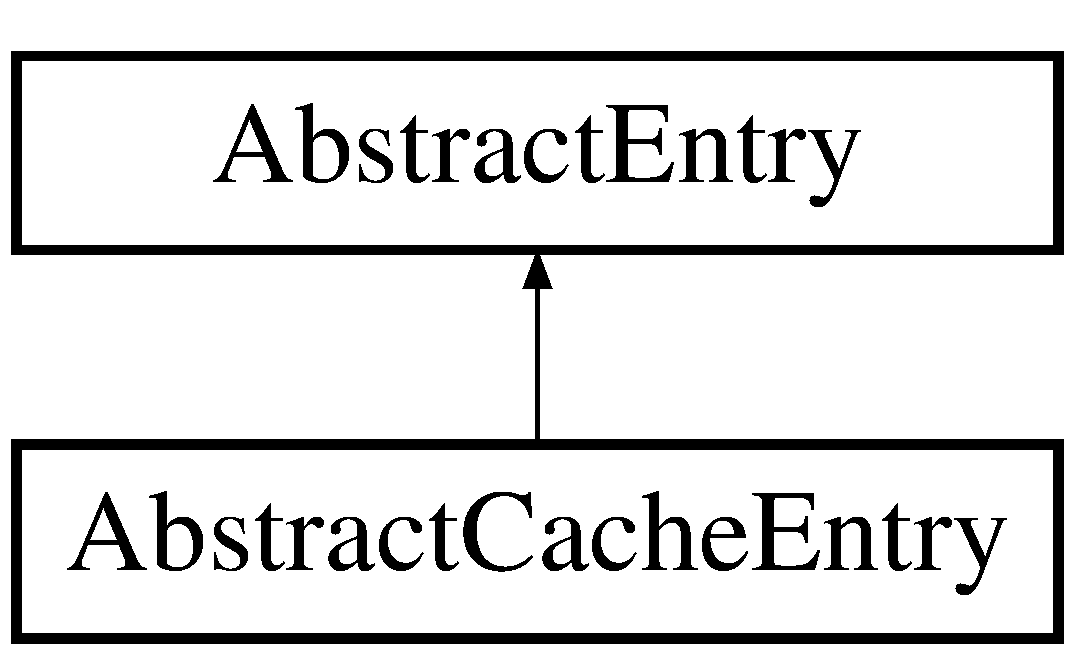
\includegraphics[height=2cm]{classAbstractCacheEntry}
\end{center}
\end{figure}
\subsection*{Public メソッド}
\begin{DoxyCompactItemize}
\item 
\hyperlink{classAbstractCacheEntry_a077d24fc90a7ce61ba745b6d64d14967}{AbstractCacheEntry} ()
\item 
virtual \hyperlink{classAbstractCacheEntry_a10ab46a60152e0b3e6668a6f1f9f52e5}{$\sim$AbstractCacheEntry} ()=0
\item 
void \hyperlink{classAbstractCacheEntry_ac3f081af818286da737aac954875dd19}{changePermission} (AccessPermission new\_\-perm)
\end{DoxyCompactItemize}
\subsection*{Public 変数}
\begin{DoxyCompactItemize}
\item 
\hyperlink{classAddress}{Address} \hyperlink{classAbstractCacheEntry_ab635563c3a8accc6501e891059954ef2}{m\_\-Address}
\item 
int \hyperlink{classAbstractCacheEntry_a512dafa8354b9b621e1c022db0800cc0}{m\_\-locked}
\end{DoxyCompactItemize}


\subsection{コンストラクタとデストラクタ}
\hypertarget{classAbstractCacheEntry_a077d24fc90a7ce61ba745b6d64d14967}{
\index{AbstractCacheEntry@{AbstractCacheEntry}!AbstractCacheEntry@{AbstractCacheEntry}}
\index{AbstractCacheEntry@{AbstractCacheEntry}!AbstractCacheEntry@{AbstractCacheEntry}}
\subsubsection[{AbstractCacheEntry}]{\setlength{\rightskip}{0pt plus 5cm}{\bf AbstractCacheEntry} ()}}
\label{classAbstractCacheEntry_a077d24fc90a7ce61ba745b6d64d14967}



\begin{DoxyCode}
32 {
33     m_Permission = AccessPermission_NotPresent;
34     m_Address.setAddress(0);
35     m_locked = -1;
36 }
\end{DoxyCode}
\hypertarget{classAbstractCacheEntry_a10ab46a60152e0b3e6668a6f1f9f52e5}{
\index{AbstractCacheEntry@{AbstractCacheEntry}!$\sim$AbstractCacheEntry@{$\sim$AbstractCacheEntry}}
\index{$\sim$AbstractCacheEntry@{$\sim$AbstractCacheEntry}!AbstractCacheEntry@{AbstractCacheEntry}}
\subsubsection[{$\sim$AbstractCacheEntry}]{\setlength{\rightskip}{0pt plus 5cm}$\sim${\bf AbstractCacheEntry} ()\hspace{0.3cm}{\ttfamily  \mbox{[}pure virtual\mbox{]}}}}
\label{classAbstractCacheEntry_a10ab46a60152e0b3e6668a6f1f9f52e5}



\begin{DoxyCode}
39 {
40 }
\end{DoxyCode}


\subsection{関数}
\hypertarget{classAbstractCacheEntry_ac3f081af818286da737aac954875dd19}{
\index{AbstractCacheEntry@{AbstractCacheEntry}!changePermission@{changePermission}}
\index{changePermission@{changePermission}!AbstractCacheEntry@{AbstractCacheEntry}}
\subsubsection[{changePermission}]{\setlength{\rightskip}{0pt plus 5cm}void changePermission (AccessPermission {\em new\_\-perm})}}
\label{classAbstractCacheEntry_ac3f081af818286da737aac954875dd19}


\hyperlink{classAbstractEntry_ac3f081af818286da737aac954875dd19}{AbstractEntry}を再定義しています。


\begin{DoxyCode}
44 {
45     AbstractEntry::changePermission(new_perm);
46     if ((new_perm == AccessPermission_Invalid) ||
47         (new_perm == AccessPermission_NotPresent)) {
48         m_locked = -1;
49     }
50 }
\end{DoxyCode}


\subsection{変数}
\hypertarget{classAbstractCacheEntry_ab635563c3a8accc6501e891059954ef2}{
\index{AbstractCacheEntry@{AbstractCacheEntry}!m\_\-Address@{m\_\-Address}}
\index{m\_\-Address@{m\_\-Address}!AbstractCacheEntry@{AbstractCacheEntry}}
\subsubsection[{m\_\-Address}]{\setlength{\rightskip}{0pt plus 5cm}{\bf Address} {\bf m\_\-Address}}}
\label{classAbstractCacheEntry_ab635563c3a8accc6501e891059954ef2}
\hypertarget{classAbstractCacheEntry_a512dafa8354b9b621e1c022db0800cc0}{
\index{AbstractCacheEntry@{AbstractCacheEntry}!m\_\-locked@{m\_\-locked}}
\index{m\_\-locked@{m\_\-locked}!AbstractCacheEntry@{AbstractCacheEntry}}
\subsubsection[{m\_\-locked}]{\setlength{\rightskip}{0pt plus 5cm}int {\bf m\_\-locked}}}
\label{classAbstractCacheEntry_a512dafa8354b9b621e1c022db0800cc0}


このクラスの説明は次のファイルから生成されました:\begin{DoxyCompactItemize}
\item 
mem/ruby/slicc\_\-interface/\hyperlink{AbstractCacheEntry_8hh}{AbstractCacheEntry.hh}\item 
mem/ruby/slicc\_\-interface/\hyperlink{AbstractCacheEntry_8cc}{AbstractCacheEntry.cc}\end{DoxyCompactItemize}

\hypertarget{classAbstractController}{
\section{クラス AbstractController}
\label{classAbstractController}\index{AbstractController@{AbstractController}}
}


{\ttfamily \#include $<$AbstractController.hh$>$}AbstractControllerに対する継承グラフ:\begin{figure}[H]
\begin{center}
\leavevmode
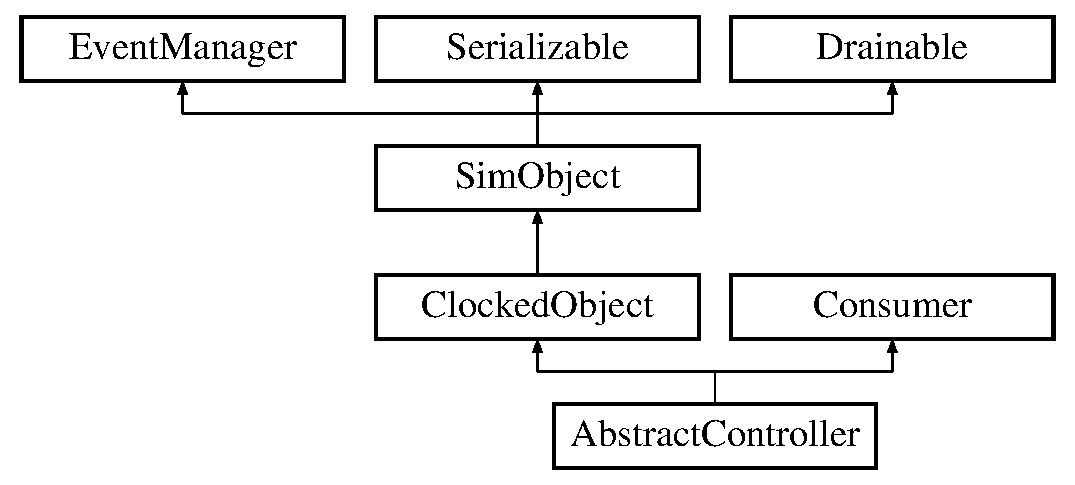
\includegraphics[height=4cm]{classAbstractController}
\end{center}
\end{figure}
\subsection*{構成}
\begin{DoxyCompactItemize}
\item 
class \hyperlink{classAbstractController_1_1StatsCallback}{StatsCallback}
\end{DoxyCompactItemize}
\subsection*{Public 型}
\begin{DoxyCompactItemize}
\item 
typedef RubyControllerParams \hyperlink{classAbstractController_a8dd24df4fce13403813bb4f7243a3b13}{Params}
\end{DoxyCompactItemize}
\subsection*{Public メソッド}
\begin{DoxyCompactItemize}
\item 
\hyperlink{classAbstractController_a59d22e188a5f6fde018cb048098296d5}{AbstractController} (const \hyperlink{classAbstractController_a8dd24df4fce13403813bb4f7243a3b13}{Params} $\ast$p)
\item 
void \hyperlink{classAbstractController_a02fd73d861ef2e4aabb38c0c9ff82947}{init} ()
\item 
const \hyperlink{classAbstractController_a8dd24df4fce13403813bb4f7243a3b13}{Params} $\ast$ \hyperlink{classAbstractController_acd3c3feb78ae7a8f88fe0f110a718dff}{params} () const 
\item 
const \hyperlink{TypeDefines_8hh_a83c14b4ae37e80071f6b3506a6c46151}{NodeID} \hyperlink{classAbstractController_a35b384df19605d0186339f088df677d5}{getVersion} () const 
\item 
const MachineType \hyperlink{classAbstractController_a7a63a33844df1ce5a3b16096dfbbe0f9}{getType} () const 
\item 
void \hyperlink{classAbstractController_a319f9c65d0c91a62be0c99b53a702e8d}{initNetworkPtr} (\hyperlink{classNetwork}{Network} $\ast$net\_\-ptr)
\item 
void \hyperlink{classAbstractController_af682f6c6bb8d16137c284112954156fb}{blockOnQueue} (\hyperlink{classAddress}{Address}, \hyperlink{classMessageBuffer}{MessageBuffer} $\ast$)
\item 
void \hyperlink{classAbstractController_a6da828f9409955e467e80f6d5290fcfd}{unblock} (\hyperlink{classAddress}{Address})
\item 
virtual \hyperlink{classMessageBuffer}{MessageBuffer} $\ast$ \hyperlink{classAbstractController_a80b4b6fca935f6914fd15ea5715e2170}{getMandatoryQueue} () const =0
\item 
virtual const std::string \hyperlink{classAbstractController_adb24cab1ca6d817bdcdef245731b8b77}{toString} () const =0
\item 
virtual AccessPermission \hyperlink{classAbstractController_ab14bc832dc06fbcb264f043d44a8915c}{getAccessPermission} (const \hyperlink{classAddress}{Address} \&addr)=0
\item 
virtual \hyperlink{classDataBlock}{DataBlock} \& \hyperlink{classAbstractController_ae014657139e530ad9d75dfd8f52302a4}{getDataBlock} (const \hyperlink{classAddress}{Address} \&addr)=0
\item 
virtual void \hyperlink{classAbstractController_a3ea5f7af5db62cc24f4e40df9ea5c971}{print} (std::ostream \&out) const =0
\item 
virtual void \hyperlink{classAbstractController_a623e3e7d1b1c725d70009f7b01a421b9}{wakeup} ()=0
\item 
virtual void \hyperlink{classAbstractController_a9820f96c5343e42ad3fcbc97b83f59d5}{resetStats} ()=0
\item 
virtual void \hyperlink{classAbstractController_a4dc637449366fcdfc4e764cdf12d9b11}{regStats} ()
\item 
virtual void \hyperlink{classAbstractController_a4ca8c1956ef762ec2219ff377a68c7ba}{recordCacheTrace} (int cntrl, \hyperlink{classCacheRecorder}{CacheRecorder} $\ast$tr)=0
\item 
virtual \hyperlink{classSequencer}{Sequencer} $\ast$ \hyperlink{classAbstractController_ada806654b26aababb417afe9bfbf66e5}{getSequencer} () const =0
\item 
virtual bool \hyperlink{classAbstractController_ab4c57c1f46545be8cb011b32d4949330}{functionalReadBuffers} (\hyperlink{classPacket}{PacketPtr} \&)=0
\item 
virtual \hyperlink{Type_8hh_a435d1572bf3f880d55459d9805097f62}{uint32\_\-t} \hyperlink{classAbstractController_a87a5fc3e2b5c5e1813ed7ed3ef1689ae}{functionalWriteBuffers} (\hyperlink{classPacket}{PacketPtr} \&)=0
\item 
virtual void \hyperlink{classAbstractController_a4498badc3fa7137b6d66736d302623ae}{enqueuePrefetch} (const \hyperlink{classAddress}{Address} \&, const RubyRequestType \&)
\begin{DoxyCompactList}\small\item\em Function for enqueuing a prefetch request. \item\end{DoxyCompactList}\item 
virtual void \hyperlink{classAbstractController_ae3089fd60541650eefd9605c2c1abc68}{collateStats} ()
\item 
\hyperlink{structMachineID}{MachineID} \hyperlink{classAbstractController_abaec6aa0c0c0f1d34472f0b3702d86c4}{getMachineID} () const 
\item 
\hyperlink{classStats_1_1Histogram}{Stats::Histogram} \& \hyperlink{classAbstractController_a8c0950c725a8898f340f7b267ff208be}{getDelayHist} ()
\item 
\hyperlink{classStats_1_1Histogram}{Stats::Histogram} \& \hyperlink{classAbstractController_a2fc801bc03037a99f6689b7d1bb4eda9}{getDelayVCHist} (\hyperlink{Type_8hh_a435d1572bf3f880d55459d9805097f62}{uint32\_\-t} index)
\item 
\hyperlink{classMessageBuffer}{MessageBuffer} $\ast$ \hyperlink{classAbstractController_a3a55ba724e099baf8906b6ba1a943b52}{getPeerQueue} (\hyperlink{Type_8hh_a435d1572bf3f880d55459d9805097f62}{uint32\_\-t} pid)
\end{DoxyCompactItemize}
\subsection*{Protected 型}
\begin{DoxyCompactItemize}
\item 
typedef \hyperlink{classstd_1_1vector}{std::vector}$<$ \hyperlink{classMessageBuffer}{MessageBuffer} $\ast$ $>$ \hyperlink{classAbstractController_a7c9a43de9f27c3319add6df9c0d2e948}{MsgVecType}
\item 
typedef std::map$<$ \hyperlink{classAddress}{Address}, \hyperlink{classstd_1_1vector}{MsgVecType} $\ast$ $>$ \hyperlink{classAbstractController_afcfa4bb0b120bb22dce11fc367b702af}{WaitingBufType}
\end{DoxyCompactItemize}
\subsection*{Protected メソッド}
\begin{DoxyCompactItemize}
\item 
void \hyperlink{classAbstractController_a8bb6029436f36f339582bda79270fa10}{profileRequest} (const std::string \&request)
\begin{DoxyCompactList}\small\item\em Profiles original cache requests including PUTs. \item\end{DoxyCompactList}\item 
void \hyperlink{classAbstractController_a6bc3835966ece2b6fb72a056f447a68e}{profileMsgDelay} (\hyperlink{Type_8hh_a435d1572bf3f880d55459d9805097f62}{uint32\_\-t} virtualNetwork, \hyperlink{classCycles}{Cycles} delay)
\begin{DoxyCompactList}\small\item\em Profiles the delay associated with messages. \item\end{DoxyCompactList}\item 
void \hyperlink{classAbstractController_a8d382287e22ac84bc108ad9ea6621603}{connectWithPeer} (\hyperlink{classAbstractController}{AbstractController} $\ast$)
\begin{DoxyCompactList}\small\item\em Function for connecting peer controllers. \item\end{DoxyCompactList}\item 
virtual void \hyperlink{classAbstractController_a9a66179697aa43bfa97cee9cf8dbad19}{getQueuesFromPeer} (\hyperlink{classAbstractController}{AbstractController} $\ast$)
\item 
void \hyperlink{classAbstractController_a4f512122c5d5042bb9da1a0d1fb4c920}{stallBuffer} (\hyperlink{classMessageBuffer}{MessageBuffer} $\ast$buf, \hyperlink{classAddress}{Address} addr)
\item 
void \hyperlink{classAbstractController_aa205de64042612c18d6104532fc72024}{wakeUpBuffers} (\hyperlink{classAddress}{Address} addr)
\item 
void \hyperlink{classAbstractController_ac01a761bbe6f761c62b6f5ff72ab1c3f}{wakeUpAllBuffers} (\hyperlink{classAddress}{Address} addr)
\item 
void \hyperlink{classAbstractController_aa595bebc4acf9a8dfec0b5a99f0b86e2}{wakeUpAllBuffers} ()
\end{DoxyCompactItemize}
\subsection*{Protected 変数}
\begin{DoxyCompactItemize}
\item 
\hyperlink{TypeDefines_8hh_a83c14b4ae37e80071f6b3506a6c46151}{NodeID} \hyperlink{classAbstractController_aa54fd03777fe9911cb24303071f918c7}{m\_\-version}
\item 
\hyperlink{structMachineID}{MachineID} \hyperlink{classAbstractController_a4d3bc5bdeb83c6982ed2341fa055ae19}{m\_\-machineID}
\item 
\hyperlink{TypeDefines_8hh_a83c14b4ae37e80071f6b3506a6c46151}{NodeID} \hyperlink{classAbstractController_a5fddc9f932bac7163c96fc4ccf27790c}{m\_\-clusterID}
\item 
\hyperlink{classNetwork}{Network} $\ast$ \hyperlink{classAbstractController_a6ffbec7c57469120487119d74fb1fae7}{m\_\-net\_\-ptr}
\item 
bool \hyperlink{classAbstractController_a0ea33ffe10dd66af8bdd7928b4d953b5}{m\_\-is\_\-blocking}
\item 
std::map$<$ \hyperlink{classAddress}{Address}, \hyperlink{classMessageBuffer}{MessageBuffer} $\ast$ $>$ \hyperlink{classAbstractController_ad9f87101fff45853a32f5fe42f9d43b0}{m\_\-block\_\-map}
\item 
\hyperlink{classAbstractController_afcfa4bb0b120bb22dce11fc367b702af}{WaitingBufType} \hyperlink{classAbstractController_a90f25dd5a7f1085002cab4e1e98f9232}{m\_\-waiting\_\-buffers}
\item 
unsigned int \hyperlink{classAbstractController_af686856d627ada54f36461fd10bc0371}{m\_\-in\_\-ports}
\item 
unsigned int \hyperlink{classAbstractController_aef85e61fde66cb7b942c755043b43520}{m\_\-cur\_\-in\_\-port}
\item 
int \hyperlink{classAbstractController_a9fe046cc3878d0da925915f0f90ab8c2}{m\_\-number\_\-of\_\-TBEs}
\item 
int \hyperlink{classAbstractController_a3fa70d035aed57776ef789fbdafa7276}{m\_\-transitions\_\-per\_\-cycle}
\item 
unsigned int \hyperlink{classAbstractController_a71fd0f20cbb3b3edc07df4aeb43b6b98}{m\_\-buffer\_\-size}
\item 
\hyperlink{classCycles}{Cycles} \hyperlink{classAbstractController_a896a9ceedfb77c22a82b490f05ae4624}{m\_\-recycle\_\-latency}
\item 
std::map$<$ \hyperlink{Type_8hh_a435d1572bf3f880d55459d9805097f62}{uint32\_\-t}, \hyperlink{classMessageBuffer}{MessageBuffer} $\ast$ $>$ \hyperlink{classAbstractController_ab2e155eabfce9e3d4b821328ecb302f9}{peerQueueMap}
\begin{DoxyCompactList}\small\item\em Map from physical network number to the \hyperlink{classMessage}{Message} \hyperlink{classBuffer}{Buffer}. \item\end{DoxyCompactList}\item 
\hyperlink{classStats_1_1Scalar}{Stats::Scalar} \hyperlink{classAbstractController_a0de33847c40bca29af78bf6c48a40e0c}{m\_\-fully\_\-busy\_\-cycles}
\item 
\hyperlink{classStats_1_1Histogram}{Stats::Histogram} \hyperlink{classAbstractController_a32315b21a536469475414901e05bfe36}{m\_\-delayHistogram}
\item 
\hyperlink{classstd_1_1vector}{std::vector}$<$ \hyperlink{classStats_1_1Histogram}{Stats::Histogram} $\ast$ $>$ \hyperlink{classAbstractController_aba317e33c2fc730b07d01be02e743bd7}{m\_\-delayVCHistogram}
\end{DoxyCompactItemize}


\subsection{型定義}
\hypertarget{classAbstractController_a7c9a43de9f27c3319add6df9c0d2e948}{
\index{AbstractController@{AbstractController}!MsgVecType@{MsgVecType}}
\index{MsgVecType@{MsgVecType}!AbstractController@{AbstractController}}
\subsubsection[{MsgVecType}]{\setlength{\rightskip}{0pt plus 5cm}typedef {\bf std::vector}$<${\bf MessageBuffer}$\ast$$>$ {\bf MsgVecType}\hspace{0.3cm}{\ttfamily  \mbox{[}protected\mbox{]}}}}
\label{classAbstractController_a7c9a43de9f27c3319add6df9c0d2e948}
\hypertarget{classAbstractController_a8dd24df4fce13403813bb4f7243a3b13}{
\index{AbstractController@{AbstractController}!Params@{Params}}
\index{Params@{Params}!AbstractController@{AbstractController}}
\subsubsection[{Params}]{\setlength{\rightskip}{0pt plus 5cm}typedef RubyControllerParams {\bf Params}}}
\label{classAbstractController_a8dd24df4fce13403813bb4f7243a3b13}


\hyperlink{classSimObject_a0f0761d2db586a23bb2a2880b8f387bb}{SimObject}を再定義しています。\hypertarget{classAbstractController_afcfa4bb0b120bb22dce11fc367b702af}{
\index{AbstractController@{AbstractController}!WaitingBufType@{WaitingBufType}}
\index{WaitingBufType@{WaitingBufType}!AbstractController@{AbstractController}}
\subsubsection[{WaitingBufType}]{\setlength{\rightskip}{0pt plus 5cm}typedef std::map$<$ {\bf Address}, {\bf MsgVecType}$\ast$ $>$ {\bf WaitingBufType}\hspace{0.3cm}{\ttfamily  \mbox{[}protected\mbox{]}}}}
\label{classAbstractController_afcfa4bb0b120bb22dce11fc367b702af}


\subsection{コンストラクタとデストラクタ}
\hypertarget{classAbstractController_a59d22e188a5f6fde018cb048098296d5}{
\index{AbstractController@{AbstractController}!AbstractController@{AbstractController}}
\index{AbstractController@{AbstractController}!AbstractController@{AbstractController}}
\subsubsection[{AbstractController}]{\setlength{\rightskip}{0pt plus 5cm}{\bf AbstractController} (const {\bf Params} $\ast$ {\em p})}}
\label{classAbstractController_a59d22e188a5f6fde018cb048098296d5}



\begin{DoxyCode}
34     : ClockedObject(p), Consumer(this)
35 {
36     m_version = p->version;
37     m_clusterID = p->cluster_id;
38 
39     m_transitions_per_cycle = p->transitions_per_cycle;
40     m_buffer_size = p->buffer_size;
41     m_recycle_latency = p->recycle_latency;
42     m_number_of_TBEs = p->number_of_TBEs;
43     m_is_blocking = false;
44 
45     if (m_version == 0) {
46         // Combine the statistics from all controllers
47         // of this particular type.
48         Stats::registerDumpCallback(new StatsCallback(this));
49     }
50 }
\end{DoxyCode}


\subsection{関数}
\hypertarget{classAbstractController_af682f6c6bb8d16137c284112954156fb}{
\index{AbstractController@{AbstractController}!blockOnQueue@{blockOnQueue}}
\index{blockOnQueue@{blockOnQueue}!AbstractController@{AbstractController}}
\subsubsection[{blockOnQueue}]{\setlength{\rightskip}{0pt plus 5cm}void blockOnQueue ({\bf Address} {\em addr}, \/  {\bf MessageBuffer} $\ast$ {\em port})}}
\label{classAbstractController_af682f6c6bb8d16137c284112954156fb}



\begin{DoxyCode}
184 {
185     m_is_blocking = true;
186     m_block_map[addr] = port;
187 }
\end{DoxyCode}
\hypertarget{classAbstractController_ae3089fd60541650eefd9605c2c1abc68}{
\index{AbstractController@{AbstractController}!collateStats@{collateStats}}
\index{collateStats@{collateStats}!AbstractController@{AbstractController}}
\subsubsection[{collateStats}]{\setlength{\rightskip}{0pt plus 5cm}virtual void collateStats ()\hspace{0.3cm}{\ttfamily  \mbox{[}inline, virtual\mbox{]}}}}
\label{classAbstractController_ae3089fd60541650eefd9605c2c1abc68}
Function for collating statistics from all the controllers of this particular type. This function should only be called from the version 0 of this controller type. 


\begin{DoxyCode}
99     {fatal("collateStats() should be overridden!");}
\end{DoxyCode}
\hypertarget{classAbstractController_a8d382287e22ac84bc108ad9ea6621603}{
\index{AbstractController@{AbstractController}!connectWithPeer@{connectWithPeer}}
\index{connectWithPeer@{connectWithPeer}!AbstractController@{AbstractController}}
\subsubsection[{connectWithPeer}]{\setlength{\rightskip}{0pt plus 5cm}void connectWithPeer ({\bf AbstractController} $\ast$ {\em c})\hspace{0.3cm}{\ttfamily  \mbox{[}protected\mbox{]}}}}
\label{classAbstractController_a8d382287e22ac84bc108ad9ea6621603}


Function for connecting peer controllers. 


\begin{DoxyCode}
93 {
94     getQueuesFromPeer(c);
95     c->getQueuesFromPeer(this);
96 }
\end{DoxyCode}
\hypertarget{classAbstractController_a4498badc3fa7137b6d66736d302623ae}{
\index{AbstractController@{AbstractController}!enqueuePrefetch@{enqueuePrefetch}}
\index{enqueuePrefetch@{enqueuePrefetch}!AbstractController@{AbstractController}}
\subsubsection[{enqueuePrefetch}]{\setlength{\rightskip}{0pt plus 5cm}virtual void enqueuePrefetch (const {\bf Address} \&, \/  const RubyRequestType \&)\hspace{0.3cm}{\ttfamily  \mbox{[}inline, virtual\mbox{]}}}}
\label{classAbstractController_a4498badc3fa7137b6d66736d302623ae}


Function for enqueuing a prefetch request. 


\begin{DoxyCode}
93     { fatal("Prefetches not implemented!");}
\end{DoxyCode}
\hypertarget{classAbstractController_ab4c57c1f46545be8cb011b32d4949330}{
\index{AbstractController@{AbstractController}!functionalReadBuffers@{functionalReadBuffers}}
\index{functionalReadBuffers@{functionalReadBuffers}!AbstractController@{AbstractController}}
\subsubsection[{functionalReadBuffers}]{\setlength{\rightskip}{0pt plus 5cm}virtual bool functionalReadBuffers ({\bf PacketPtr} \&)\hspace{0.3cm}{\ttfamily  \mbox{[}pure virtual\mbox{]}}}}
\label{classAbstractController_ab4c57c1f46545be8cb011b32d4949330}
These functions are used by ruby system to read/write the message queues that exist with in the controller. The boolean return value indicates if the read was performed successfully. \hypertarget{classAbstractController_a87a5fc3e2b5c5e1813ed7ed3ef1689ae}{
\index{AbstractController@{AbstractController}!functionalWriteBuffers@{functionalWriteBuffers}}
\index{functionalWriteBuffers@{functionalWriteBuffers}!AbstractController@{AbstractController}}
\subsubsection[{functionalWriteBuffers}]{\setlength{\rightskip}{0pt plus 5cm}virtual {\bf uint32\_\-t} functionalWriteBuffers ({\bf PacketPtr} \&)\hspace{0.3cm}{\ttfamily  \mbox{[}pure virtual\mbox{]}}}}
\label{classAbstractController_a87a5fc3e2b5c5e1813ed7ed3ef1689ae}
The return value indicates the number of messages written with the data from the packet. \hypertarget{classAbstractController_ab14bc832dc06fbcb264f043d44a8915c}{
\index{AbstractController@{AbstractController}!getAccessPermission@{getAccessPermission}}
\index{getAccessPermission@{getAccessPermission}!AbstractController@{AbstractController}}
\subsubsection[{getAccessPermission}]{\setlength{\rightskip}{0pt plus 5cm}virtual AccessPermission getAccessPermission (const {\bf Address} \& {\em addr})\hspace{0.3cm}{\ttfamily  \mbox{[}pure virtual\mbox{]}}}}
\label{classAbstractController_ab14bc832dc06fbcb264f043d44a8915c}
\hypertarget{classAbstractController_ae014657139e530ad9d75dfd8f52302a4}{
\index{AbstractController@{AbstractController}!getDataBlock@{getDataBlock}}
\index{getDataBlock@{getDataBlock}!AbstractController@{AbstractController}}
\subsubsection[{getDataBlock}]{\setlength{\rightskip}{0pt plus 5cm}virtual {\bf DataBlock}\& getDataBlock (const {\bf Address} \& {\em addr})\hspace{0.3cm}{\ttfamily  \mbox{[}pure virtual\mbox{]}}}}
\label{classAbstractController_ae014657139e530ad9d75dfd8f52302a4}
\hypertarget{classAbstractController_a8c0950c725a8898f340f7b267ff208be}{
\index{AbstractController@{AbstractController}!getDelayHist@{getDelayHist}}
\index{getDelayHist@{getDelayHist}!AbstractController@{AbstractController}}
\subsubsection[{getDelayHist}]{\setlength{\rightskip}{0pt plus 5cm}{\bf Stats::Histogram}\& getDelayHist ()\hspace{0.3cm}{\ttfamily  \mbox{[}inline\mbox{]}}}}
\label{classAbstractController_a8c0950c725a8898f340f7b267ff208be}



\begin{DoxyCode}
104 { return m_delayHistogram; }
\end{DoxyCode}
\hypertarget{classAbstractController_a2fc801bc03037a99f6689b7d1bb4eda9}{
\index{AbstractController@{AbstractController}!getDelayVCHist@{getDelayVCHist}}
\index{getDelayVCHist@{getDelayVCHist}!AbstractController@{AbstractController}}
\subsubsection[{getDelayVCHist}]{\setlength{\rightskip}{0pt plus 5cm}{\bf Stats::Histogram}\& getDelayVCHist ({\bf uint32\_\-t} {\em index})\hspace{0.3cm}{\ttfamily  \mbox{[}inline\mbox{]}}}}
\label{classAbstractController_a2fc801bc03037a99f6689b7d1bb4eda9}



\begin{DoxyCode}
106     { return *(m_delayVCHistogram[index]); }
\end{DoxyCode}
\hypertarget{classAbstractController_abaec6aa0c0c0f1d34472f0b3702d86c4}{
\index{AbstractController@{AbstractController}!getMachineID@{getMachineID}}
\index{getMachineID@{getMachineID}!AbstractController@{AbstractController}}
\subsubsection[{getMachineID}]{\setlength{\rightskip}{0pt plus 5cm}{\bf MachineID} getMachineID () const\hspace{0.3cm}{\ttfamily  \mbox{[}inline\mbox{]}}}}
\label{classAbstractController_abaec6aa0c0c0f1d34472f0b3702d86c4}



\begin{DoxyCode}
102 { return m_machineID; }
\end{DoxyCode}
\hypertarget{classAbstractController_a80b4b6fca935f6914fd15ea5715e2170}{
\index{AbstractController@{AbstractController}!getMandatoryQueue@{getMandatoryQueue}}
\index{getMandatoryQueue@{getMandatoryQueue}!AbstractController@{AbstractController}}
\subsubsection[{getMandatoryQueue}]{\setlength{\rightskip}{0pt plus 5cm}virtual {\bf MessageBuffer}$\ast$ getMandatoryQueue () const\hspace{0.3cm}{\ttfamily  \mbox{[}pure virtual\mbox{]}}}}
\label{classAbstractController_a80b4b6fca935f6914fd15ea5715e2170}
\hypertarget{classAbstractController_a3a55ba724e099baf8906b6ba1a943b52}{
\index{AbstractController@{AbstractController}!getPeerQueue@{getPeerQueue}}
\index{getPeerQueue@{getPeerQueue}!AbstractController@{AbstractController}}
\subsubsection[{getPeerQueue}]{\setlength{\rightskip}{0pt plus 5cm}{\bf MessageBuffer}$\ast$ getPeerQueue ({\bf uint32\_\-t} {\em pid})\hspace{0.3cm}{\ttfamily  \mbox{[}inline\mbox{]}}}}
\label{classAbstractController_a3a55ba724e099baf8906b6ba1a943b52}



\begin{DoxyCode}
109     {
110         std::map<uint32_t, MessageBuffer *>::iterator it =
111                                         peerQueueMap.find(pid);
112         assert(it != peerQueueMap.end());
113         return (*it).second;
114     }
\end{DoxyCode}
\hypertarget{classAbstractController_a9a66179697aa43bfa97cee9cf8dbad19}{
\index{AbstractController@{AbstractController}!getQueuesFromPeer@{getQueuesFromPeer}}
\index{getQueuesFromPeer@{getQueuesFromPeer}!AbstractController@{AbstractController}}
\subsubsection[{getQueuesFromPeer}]{\setlength{\rightskip}{0pt plus 5cm}virtual void getQueuesFromPeer ({\bf AbstractController} $\ast$)\hspace{0.3cm}{\ttfamily  \mbox{[}inline, protected, virtual\mbox{]}}}}
\label{classAbstractController_a9a66179697aa43bfa97cee9cf8dbad19}



\begin{DoxyCode}
125     { fatal("getQueuesFromPeer() should be called only if implemented!"); }
\end{DoxyCode}
\hypertarget{classAbstractController_ada806654b26aababb417afe9bfbf66e5}{
\index{AbstractController@{AbstractController}!getSequencer@{getSequencer}}
\index{getSequencer@{getSequencer}!AbstractController@{AbstractController}}
\subsubsection[{getSequencer}]{\setlength{\rightskip}{0pt plus 5cm}virtual {\bf Sequencer}$\ast$ getSequencer () const\hspace{0.3cm}{\ttfamily  \mbox{[}pure virtual\mbox{]}}}}
\label{classAbstractController_ada806654b26aababb417afe9bfbf66e5}
\hypertarget{classAbstractController_a7a63a33844df1ce5a3b16096dfbbe0f9}{
\index{AbstractController@{AbstractController}!getType@{getType}}
\index{getType@{getType}!AbstractController@{AbstractController}}
\subsubsection[{getType}]{\setlength{\rightskip}{0pt plus 5cm}const MachineType getType () const\hspace{0.3cm}{\ttfamily  \mbox{[}inline\mbox{]}}}}
\label{classAbstractController_a7a63a33844df1ce5a3b16096dfbbe0f9}



\begin{DoxyCode}
60 { return m_machineID.getType(); }
\end{DoxyCode}
\hypertarget{classAbstractController_a35b384df19605d0186339f088df677d5}{
\index{AbstractController@{AbstractController}!getVersion@{getVersion}}
\index{getVersion@{getVersion}!AbstractController@{AbstractController}}
\subsubsection[{getVersion}]{\setlength{\rightskip}{0pt plus 5cm}const {\bf NodeID} getVersion () const\hspace{0.3cm}{\ttfamily  \mbox{[}inline\mbox{]}}}}
\label{classAbstractController_a35b384df19605d0186339f088df677d5}



\begin{DoxyCode}
59 { return m_machineID.getNum(); }
\end{DoxyCode}
\hypertarget{classAbstractController_a02fd73d861ef2e4aabb38c0c9ff82947}{
\index{AbstractController@{AbstractController}!init@{init}}
\index{init@{init}!AbstractController@{AbstractController}}
\subsubsection[{init}]{\setlength{\rightskip}{0pt plus 5cm}void init ()\hspace{0.3cm}{\ttfamily  \mbox{[}virtual\mbox{]}}}}
\label{classAbstractController_a02fd73d861ef2e4aabb38c0c9ff82947}
\hyperlink{classAbstractController_a02fd73d861ef2e4aabb38c0c9ff82947}{init()} is called after all C++ SimObjects have been created and all ports are connected. Initializations that are independent of unserialization but rely on a fully instantiated and connected \hyperlink{classSimObject}{SimObject} graph should be done here. 

\hyperlink{classSimObject_a02fd73d861ef2e4aabb38c0c9ff82947}{SimObject}を再定義しています。


\begin{DoxyCode}
54 {
55     params()->ruby_system->registerAbstractController(this);
56     m_delayHistogram.init(10);
57     uint32_t size = Network::getNumberOfVirtualNetworks();
58     for (uint32_t i = 0; i < size; i++) {
59         m_delayVCHistogram.push_back(new Stats::Histogram());
60         m_delayVCHistogram[i]->init(10);
61     }
62 }
\end{DoxyCode}
\hypertarget{classAbstractController_a319f9c65d0c91a62be0c99b53a702e8d}{
\index{AbstractController@{AbstractController}!initNetworkPtr@{initNetworkPtr}}
\index{initNetworkPtr@{initNetworkPtr}!AbstractController@{AbstractController}}
\subsubsection[{initNetworkPtr}]{\setlength{\rightskip}{0pt plus 5cm}void initNetworkPtr ({\bf Network} $\ast$ {\em net\_\-ptr})\hspace{0.3cm}{\ttfamily  \mbox{[}inline\mbox{]}}}}
\label{classAbstractController_a319f9c65d0c91a62be0c99b53a702e8d}



\begin{DoxyCode}
62 { m_net_ptr = net_ptr; }
\end{DoxyCode}
\hypertarget{classAbstractController_acd3c3feb78ae7a8f88fe0f110a718dff}{
\index{AbstractController@{AbstractController}!params@{params}}
\index{params@{params}!AbstractController@{AbstractController}}
\subsubsection[{params}]{\setlength{\rightskip}{0pt plus 5cm}const {\bf Params}$\ast$ params () const\hspace{0.3cm}{\ttfamily  \mbox{[}inline\mbox{]}}}}
\label{classAbstractController_acd3c3feb78ae7a8f88fe0f110a718dff}


\hyperlink{classSimObject_acd3c3feb78ae7a8f88fe0f110a718dff}{SimObject}を再定義しています。


\begin{DoxyCode}
57 { return (const Params *)_params; }
\end{DoxyCode}
\hypertarget{classAbstractController_a3ea5f7af5db62cc24f4e40df9ea5c971}{
\index{AbstractController@{AbstractController}!print@{print}}
\index{print@{print}!AbstractController@{AbstractController}}
\subsubsection[{print}]{\setlength{\rightskip}{0pt plus 5cm}virtual void print (std::ostream \& {\em out}) const\hspace{0.3cm}{\ttfamily  \mbox{[}pure virtual\mbox{]}}}}
\label{classAbstractController_a3ea5f7af5db62cc24f4e40df9ea5c971}


\hyperlink{classConsumer_a3ea5f7af5db62cc24f4e40df9ea5c971}{Consumer}を実装しています。\hypertarget{classAbstractController_a6bc3835966ece2b6fb72a056f447a68e}{
\index{AbstractController@{AbstractController}!profileMsgDelay@{profileMsgDelay}}
\index{profileMsgDelay@{profileMsgDelay}!AbstractController@{AbstractController}}
\subsubsection[{profileMsgDelay}]{\setlength{\rightskip}{0pt plus 5cm}void profileMsgDelay ({\bf uint32\_\-t} {\em virtualNetwork}, \/  {\bf Cycles} {\em delay})\hspace{0.3cm}{\ttfamily  \mbox{[}protected\mbox{]}}}}
\label{classAbstractController_a6bc3835966ece2b6fb72a056f447a68e}


Profiles the delay associated with messages. 


\begin{DoxyCode}
85 {
86     assert(virtualNetwork < m_delayVCHistogram.size());
87     m_delayHistogram.sample(delay);
88     m_delayVCHistogram[virtualNetwork]->sample(delay);
89 }
\end{DoxyCode}
\hypertarget{classAbstractController_a8bb6029436f36f339582bda79270fa10}{
\index{AbstractController@{AbstractController}!profileRequest@{profileRequest}}
\index{profileRequest@{profileRequest}!AbstractController@{AbstractController}}
\subsubsection[{profileRequest}]{\setlength{\rightskip}{0pt plus 5cm}void profileRequest (const std::string \& {\em request})\hspace{0.3cm}{\ttfamily  \mbox{[}protected\mbox{]}}}}
\label{classAbstractController_a8bb6029436f36f339582bda79270fa10}


Profiles original cache requests including PUTs. \hypertarget{classAbstractController_a4ca8c1956ef762ec2219ff377a68c7ba}{
\index{AbstractController@{AbstractController}!recordCacheTrace@{recordCacheTrace}}
\index{recordCacheTrace@{recordCacheTrace}!AbstractController@{AbstractController}}
\subsubsection[{recordCacheTrace}]{\setlength{\rightskip}{0pt plus 5cm}virtual void recordCacheTrace (int {\em cntrl}, \/  {\bf CacheRecorder} $\ast$ {\em tr})\hspace{0.3cm}{\ttfamily  \mbox{[}pure virtual\mbox{]}}}}
\label{classAbstractController_a4ca8c1956ef762ec2219ff377a68c7ba}
\hypertarget{classAbstractController_a4dc637449366fcdfc4e764cdf12d9b11}{
\index{AbstractController@{AbstractController}!regStats@{regStats}}
\index{regStats@{regStats}!AbstractController@{AbstractController}}
\subsubsection[{regStats}]{\setlength{\rightskip}{0pt plus 5cm}void regStats ()\hspace{0.3cm}{\ttfamily  \mbox{[}virtual\mbox{]}}}}
\label{classAbstractController_a4dc637449366fcdfc4e764cdf12d9b11}
\hyperlink{classRegister}{Register} statistics for this object. 

\hyperlink{classSimObject_a4dc637449366fcdfc4e764cdf12d9b11}{SimObject}を再定義しています。


\begin{DoxyCode}
76 {
77     m_fully_busy_cycles
78         .name(name() + ".fully_busy_cycles")
79         .desc("cycles for which number of transistions == max transitions")
80         .flags(Stats::nozero);
81 }
\end{DoxyCode}
\hypertarget{classAbstractController_a9820f96c5343e42ad3fcbc97b83f59d5}{
\index{AbstractController@{AbstractController}!resetStats@{resetStats}}
\index{resetStats@{resetStats}!AbstractController@{AbstractController}}
\subsubsection[{resetStats}]{\setlength{\rightskip}{0pt plus 5cm}void resetStats ()\hspace{0.3cm}{\ttfamily  \mbox{[}pure virtual\mbox{]}}}}
\label{classAbstractController_a9820f96c5343e42ad3fcbc97b83f59d5}
Reset statistics associated with this object. 

\hyperlink{classSimObject_a65880e61108132689a1bd769b9187fb7}{SimObject}を再定義しています。


\begin{DoxyCode}
66 {
67     m_delayHistogram.reset();
68     uint32_t size = Network::getNumberOfVirtualNetworks();
69     for (uint32_t i = 0; i < size; i++) {
70         m_delayVCHistogram[i]->reset();
71     }
72 }
\end{DoxyCode}
\hypertarget{classAbstractController_a4f512122c5d5042bb9da1a0d1fb4c920}{
\index{AbstractController@{AbstractController}!stallBuffer@{stallBuffer}}
\index{stallBuffer@{stallBuffer}!AbstractController@{AbstractController}}
\subsubsection[{stallBuffer}]{\setlength{\rightskip}{0pt plus 5cm}void stallBuffer ({\bf MessageBuffer} $\ast$ {\em buf}, \/  {\bf Address} {\em addr})\hspace{0.3cm}{\ttfamily  \mbox{[}protected\mbox{]}}}}
\label{classAbstractController_a4f512122c5d5042bb9da1a0d1fb4c920}



\begin{DoxyCode}
100 {
101     if (m_waiting_buffers.count(addr) == 0) {
102         MsgVecType* msgVec = new MsgVecType;
103         msgVec->resize(m_in_ports, NULL);
104         m_waiting_buffers[addr] = msgVec;
105     }
106     (*(m_waiting_buffers[addr]))[m_cur_in_port] = buf;
107 }
\end{DoxyCode}
\hypertarget{classAbstractController_adb24cab1ca6d817bdcdef245731b8b77}{
\index{AbstractController@{AbstractController}!toString@{toString}}
\index{toString@{toString}!AbstractController@{AbstractController}}
\subsubsection[{toString}]{\setlength{\rightskip}{0pt plus 5cm}virtual const std::string toString () const\hspace{0.3cm}{\ttfamily  \mbox{[}pure virtual\mbox{]}}}}
\label{classAbstractController_adb24cab1ca6d817bdcdef245731b8b77}
\hypertarget{classAbstractController_a6da828f9409955e467e80f6d5290fcfd}{
\index{AbstractController@{AbstractController}!unblock@{unblock}}
\index{unblock@{unblock}!AbstractController@{AbstractController}}
\subsubsection[{unblock}]{\setlength{\rightskip}{0pt plus 5cm}void unblock ({\bf Address} {\em addr})}}
\label{classAbstractController_a6da828f9409955e467e80f6d5290fcfd}



\begin{DoxyCode}
191 {
192     m_block_map.erase(addr);
193     if (m_block_map.size() == 0) {
194        m_is_blocking = false;
195     }
196 }
\end{DoxyCode}
\hypertarget{classAbstractController_a623e3e7d1b1c725d70009f7b01a421b9}{
\index{AbstractController@{AbstractController}!wakeup@{wakeup}}
\index{wakeup@{wakeup}!AbstractController@{AbstractController}}
\subsubsection[{wakeup}]{\setlength{\rightskip}{0pt plus 5cm}virtual void wakeup ()\hspace{0.3cm}{\ttfamily  \mbox{[}pure virtual\mbox{]}}}}
\label{classAbstractController_a623e3e7d1b1c725d70009f7b01a421b9}


\hyperlink{classConsumer_a623e3e7d1b1c725d70009f7b01a421b9}{Consumer}を実装しています。\hypertarget{classAbstractController_aa595bebc4acf9a8dfec0b5a99f0b86e2}{
\index{AbstractController@{AbstractController}!wakeUpAllBuffers@{wakeUpAllBuffers}}
\index{wakeUpAllBuffers@{wakeUpAllBuffers}!AbstractController@{AbstractController}}
\subsubsection[{wakeUpAllBuffers}]{\setlength{\rightskip}{0pt plus 5cm}void wakeUpAllBuffers ()\hspace{0.3cm}{\ttfamily  \mbox{[}protected\mbox{]}}}}
\label{classAbstractController_aa595bebc4acf9a8dfec0b5a99f0b86e2}



\begin{DoxyCode}
151 {
152     //
153     // Wake up all possible buffers that could be waiting on any message.
154     //
155 
156     std::vector<MsgVecType*> wokeUpMsgVecs;
157 
158     if(m_waiting_buffers.size() > 0) {
159         for (WaitingBufType::iterator buf_iter = m_waiting_buffers.begin();
160              buf_iter != m_waiting_buffers.end();
161              ++buf_iter) {
162              for (MsgVecType::iterator vec_iter = buf_iter->second->begin();
163                   vec_iter != buf_iter->second->end();
164                   ++vec_iter) {
165                   if (*vec_iter != NULL) {
166                       (*vec_iter)->reanalyzeAllMessages();
167                   }
168              }
169              wokeUpMsgVecs.push_back(buf_iter->second);
170         }
171 
172         for (std::vector<MsgVecType*>::iterator wb_iter = wokeUpMsgVecs.begin();
173              wb_iter != wokeUpMsgVecs.end();
174              ++wb_iter) {
175              delete (*wb_iter);
176         }
177 
178         m_waiting_buffers.clear();
179     }
180 }
\end{DoxyCode}
\hypertarget{classAbstractController_ac01a761bbe6f761c62b6f5ff72ab1c3f}{
\index{AbstractController@{AbstractController}!wakeUpAllBuffers@{wakeUpAllBuffers}}
\index{wakeUpAllBuffers@{wakeUpAllBuffers}!AbstractController@{AbstractController}}
\subsubsection[{wakeUpAllBuffers}]{\setlength{\rightskip}{0pt plus 5cm}void wakeUpAllBuffers ({\bf Address} {\em addr})\hspace{0.3cm}{\ttfamily  \mbox{[}protected\mbox{]}}}}
\label{classAbstractController_ac01a761bbe6f761c62b6f5ff72ab1c3f}



\begin{DoxyCode}
131 {
132     if (m_waiting_buffers.count(addr) > 0) {
133         //
134         // Wake up all possible lower rank (i.e. lower priority) buffers that cou
      ld
135         // be waiting on this message.
136         //
137         for (int in_port_rank = m_in_ports - 1;
138              in_port_rank >= 0;
139              in_port_rank--) {
140             if ((*(m_waiting_buffers[addr]))[in_port_rank] != NULL) {
141                 (*(m_waiting_buffers[addr]))[in_port_rank]->reanalyzeMessages(add
      r);
142             }
143         }
144         delete m_waiting_buffers[addr];
145         m_waiting_buffers.erase(addr);
146     }
147 }
\end{DoxyCode}
\hypertarget{classAbstractController_aa205de64042612c18d6104532fc72024}{
\index{AbstractController@{AbstractController}!wakeUpBuffers@{wakeUpBuffers}}
\index{wakeUpBuffers@{wakeUpBuffers}!AbstractController@{AbstractController}}
\subsubsection[{wakeUpBuffers}]{\setlength{\rightskip}{0pt plus 5cm}void wakeUpBuffers ({\bf Address} {\em addr})\hspace{0.3cm}{\ttfamily  \mbox{[}protected\mbox{]}}}}
\label{classAbstractController_aa205de64042612c18d6104532fc72024}



\begin{DoxyCode}
111 {
112     if (m_waiting_buffers.count(addr) > 0) {
113         //
114         // Wake up all possible lower rank (i.e. lower priority) buffers that cou
      ld
115         // be waiting on this message.
116         //
117         for (int in_port_rank = m_cur_in_port - 1;
118              in_port_rank >= 0;
119              in_port_rank--) {
120             if ((*(m_waiting_buffers[addr]))[in_port_rank] != NULL) {
121                 (*(m_waiting_buffers[addr]))[in_port_rank]->reanalyzeMessages(add
      r);
122             }
123         }
124         delete m_waiting_buffers[addr];
125         m_waiting_buffers.erase(addr);
126     }
127 }
\end{DoxyCode}


\subsection{変数}
\hypertarget{classAbstractController_ad9f87101fff45853a32f5fe42f9d43b0}{
\index{AbstractController@{AbstractController}!m\_\-block\_\-map@{m\_\-block\_\-map}}
\index{m\_\-block\_\-map@{m\_\-block\_\-map}!AbstractController@{AbstractController}}
\subsubsection[{m\_\-block\_\-map}]{\setlength{\rightskip}{0pt plus 5cm}std::map$<${\bf Address}, {\bf MessageBuffer}$\ast$$>$ {\bf m\_\-block\_\-map}\hspace{0.3cm}{\ttfamily  \mbox{[}protected\mbox{]}}}}
\label{classAbstractController_ad9f87101fff45853a32f5fe42f9d43b0}
\hypertarget{classAbstractController_a71fd0f20cbb3b3edc07df4aeb43b6b98}{
\index{AbstractController@{AbstractController}!m\_\-buffer\_\-size@{m\_\-buffer\_\-size}}
\index{m\_\-buffer\_\-size@{m\_\-buffer\_\-size}!AbstractController@{AbstractController}}
\subsubsection[{m\_\-buffer\_\-size}]{\setlength{\rightskip}{0pt plus 5cm}unsigned int {\bf m\_\-buffer\_\-size}\hspace{0.3cm}{\ttfamily  \mbox{[}protected\mbox{]}}}}
\label{classAbstractController_a71fd0f20cbb3b3edc07df4aeb43b6b98}
\hypertarget{classAbstractController_a5fddc9f932bac7163c96fc4ccf27790c}{
\index{AbstractController@{AbstractController}!m\_\-clusterID@{m\_\-clusterID}}
\index{m\_\-clusterID@{m\_\-clusterID}!AbstractController@{AbstractController}}
\subsubsection[{m\_\-clusterID}]{\setlength{\rightskip}{0pt plus 5cm}{\bf NodeID} {\bf m\_\-clusterID}\hspace{0.3cm}{\ttfamily  \mbox{[}protected\mbox{]}}}}
\label{classAbstractController_a5fddc9f932bac7163c96fc4ccf27790c}
\hypertarget{classAbstractController_aef85e61fde66cb7b942c755043b43520}{
\index{AbstractController@{AbstractController}!m\_\-cur\_\-in\_\-port@{m\_\-cur\_\-in\_\-port}}
\index{m\_\-cur\_\-in\_\-port@{m\_\-cur\_\-in\_\-port}!AbstractController@{AbstractController}}
\subsubsection[{m\_\-cur\_\-in\_\-port}]{\setlength{\rightskip}{0pt plus 5cm}unsigned int {\bf m\_\-cur\_\-in\_\-port}\hspace{0.3cm}{\ttfamily  \mbox{[}protected\mbox{]}}}}
\label{classAbstractController_aef85e61fde66cb7b942c755043b43520}
\hypertarget{classAbstractController_a32315b21a536469475414901e05bfe36}{
\index{AbstractController@{AbstractController}!m\_\-delayHistogram@{m\_\-delayHistogram}}
\index{m\_\-delayHistogram@{m\_\-delayHistogram}!AbstractController@{AbstractController}}
\subsubsection[{m\_\-delayHistogram}]{\setlength{\rightskip}{0pt plus 5cm}{\bf Stats::Histogram} {\bf m\_\-delayHistogram}\hspace{0.3cm}{\ttfamily  \mbox{[}protected\mbox{]}}}}
\label{classAbstractController_a32315b21a536469475414901e05bfe36}
\hyperlink{classHistogram}{Histogram} for profiling delay for the messages this controller cares for \hypertarget{classAbstractController_aba317e33c2fc730b07d01be02e743bd7}{
\index{AbstractController@{AbstractController}!m\_\-delayVCHistogram@{m\_\-delayVCHistogram}}
\index{m\_\-delayVCHistogram@{m\_\-delayVCHistogram}!AbstractController@{AbstractController}}
\subsubsection[{m\_\-delayVCHistogram}]{\setlength{\rightskip}{0pt plus 5cm}{\bf std::vector}$<${\bf Stats::Histogram} $\ast$$>$ {\bf m\_\-delayVCHistogram}\hspace{0.3cm}{\ttfamily  \mbox{[}protected\mbox{]}}}}
\label{classAbstractController_aba317e33c2fc730b07d01be02e743bd7}
\hypertarget{classAbstractController_a0de33847c40bca29af78bf6c48a40e0c}{
\index{AbstractController@{AbstractController}!m\_\-fully\_\-busy\_\-cycles@{m\_\-fully\_\-busy\_\-cycles}}
\index{m\_\-fully\_\-busy\_\-cycles@{m\_\-fully\_\-busy\_\-cycles}!AbstractController@{AbstractController}}
\subsubsection[{m\_\-fully\_\-busy\_\-cycles}]{\setlength{\rightskip}{0pt plus 5cm}{\bf Stats::Scalar} {\bf m\_\-fully\_\-busy\_\-cycles}\hspace{0.3cm}{\ttfamily  \mbox{[}protected\mbox{]}}}}
\label{classAbstractController_a0de33847c40bca29af78bf6c48a40e0c}
Counter for the number of cycles when the transitions carried out were equal to the maximum allowed \hypertarget{classAbstractController_af686856d627ada54f36461fd10bc0371}{
\index{AbstractController@{AbstractController}!m\_\-in\_\-ports@{m\_\-in\_\-ports}}
\index{m\_\-in\_\-ports@{m\_\-in\_\-ports}!AbstractController@{AbstractController}}
\subsubsection[{m\_\-in\_\-ports}]{\setlength{\rightskip}{0pt plus 5cm}unsigned int {\bf m\_\-in\_\-ports}\hspace{0.3cm}{\ttfamily  \mbox{[}protected\mbox{]}}}}
\label{classAbstractController_af686856d627ada54f36461fd10bc0371}
\hypertarget{classAbstractController_a0ea33ffe10dd66af8bdd7928b4d953b5}{
\index{AbstractController@{AbstractController}!m\_\-is\_\-blocking@{m\_\-is\_\-blocking}}
\index{m\_\-is\_\-blocking@{m\_\-is\_\-blocking}!AbstractController@{AbstractController}}
\subsubsection[{m\_\-is\_\-blocking}]{\setlength{\rightskip}{0pt plus 5cm}bool {\bf m\_\-is\_\-blocking}\hspace{0.3cm}{\ttfamily  \mbox{[}protected\mbox{]}}}}
\label{classAbstractController_a0ea33ffe10dd66af8bdd7928b4d953b5}
\hypertarget{classAbstractController_a4d3bc5bdeb83c6982ed2341fa055ae19}{
\index{AbstractController@{AbstractController}!m\_\-machineID@{m\_\-machineID}}
\index{m\_\-machineID@{m\_\-machineID}!AbstractController@{AbstractController}}
\subsubsection[{m\_\-machineID}]{\setlength{\rightskip}{0pt plus 5cm}{\bf MachineID} {\bf m\_\-machineID}\hspace{0.3cm}{\ttfamily  \mbox{[}protected\mbox{]}}}}
\label{classAbstractController_a4d3bc5bdeb83c6982ed2341fa055ae19}
\hypertarget{classAbstractController_a6ffbec7c57469120487119d74fb1fae7}{
\index{AbstractController@{AbstractController}!m\_\-net\_\-ptr@{m\_\-net\_\-ptr}}
\index{m\_\-net\_\-ptr@{m\_\-net\_\-ptr}!AbstractController@{AbstractController}}
\subsubsection[{m\_\-net\_\-ptr}]{\setlength{\rightskip}{0pt plus 5cm}{\bf Network}$\ast$ {\bf m\_\-net\_\-ptr}\hspace{0.3cm}{\ttfamily  \mbox{[}protected\mbox{]}}}}
\label{classAbstractController_a6ffbec7c57469120487119d74fb1fae7}
\hypertarget{classAbstractController_a9fe046cc3878d0da925915f0f90ab8c2}{
\index{AbstractController@{AbstractController}!m\_\-number\_\-of\_\-TBEs@{m\_\-number\_\-of\_\-TBEs}}
\index{m\_\-number\_\-of\_\-TBEs@{m\_\-number\_\-of\_\-TBEs}!AbstractController@{AbstractController}}
\subsubsection[{m\_\-number\_\-of\_\-TBEs}]{\setlength{\rightskip}{0pt plus 5cm}int {\bf m\_\-number\_\-of\_\-TBEs}\hspace{0.3cm}{\ttfamily  \mbox{[}protected\mbox{]}}}}
\label{classAbstractController_a9fe046cc3878d0da925915f0f90ab8c2}
\hypertarget{classAbstractController_a896a9ceedfb77c22a82b490f05ae4624}{
\index{AbstractController@{AbstractController}!m\_\-recycle\_\-latency@{m\_\-recycle\_\-latency}}
\index{m\_\-recycle\_\-latency@{m\_\-recycle\_\-latency}!AbstractController@{AbstractController}}
\subsubsection[{m\_\-recycle\_\-latency}]{\setlength{\rightskip}{0pt plus 5cm}{\bf Cycles} {\bf m\_\-recycle\_\-latency}\hspace{0.3cm}{\ttfamily  \mbox{[}protected\mbox{]}}}}
\label{classAbstractController_a896a9ceedfb77c22a82b490f05ae4624}
\hypertarget{classAbstractController_a3fa70d035aed57776ef789fbdafa7276}{
\index{AbstractController@{AbstractController}!m\_\-transitions\_\-per\_\-cycle@{m\_\-transitions\_\-per\_\-cycle}}
\index{m\_\-transitions\_\-per\_\-cycle@{m\_\-transitions\_\-per\_\-cycle}!AbstractController@{AbstractController}}
\subsubsection[{m\_\-transitions\_\-per\_\-cycle}]{\setlength{\rightskip}{0pt plus 5cm}int {\bf m\_\-transitions\_\-per\_\-cycle}\hspace{0.3cm}{\ttfamily  \mbox{[}protected\mbox{]}}}}
\label{classAbstractController_a3fa70d035aed57776ef789fbdafa7276}
\hypertarget{classAbstractController_aa54fd03777fe9911cb24303071f918c7}{
\index{AbstractController@{AbstractController}!m\_\-version@{m\_\-version}}
\index{m\_\-version@{m\_\-version}!AbstractController@{AbstractController}}
\subsubsection[{m\_\-version}]{\setlength{\rightskip}{0pt plus 5cm}{\bf NodeID} {\bf m\_\-version}\hspace{0.3cm}{\ttfamily  \mbox{[}protected\mbox{]}}}}
\label{classAbstractController_aa54fd03777fe9911cb24303071f918c7}
\hypertarget{classAbstractController_a90f25dd5a7f1085002cab4e1e98f9232}{
\index{AbstractController@{AbstractController}!m\_\-waiting\_\-buffers@{m\_\-waiting\_\-buffers}}
\index{m\_\-waiting\_\-buffers@{m\_\-waiting\_\-buffers}!AbstractController@{AbstractController}}
\subsubsection[{m\_\-waiting\_\-buffers}]{\setlength{\rightskip}{0pt plus 5cm}{\bf WaitingBufType} {\bf m\_\-waiting\_\-buffers}\hspace{0.3cm}{\ttfamily  \mbox{[}protected\mbox{]}}}}
\label{classAbstractController_a90f25dd5a7f1085002cab4e1e98f9232}
\hypertarget{classAbstractController_ab2e155eabfce9e3d4b821328ecb302f9}{
\index{AbstractController@{AbstractController}!peerQueueMap@{peerQueueMap}}
\index{peerQueueMap@{peerQueueMap}!AbstractController@{AbstractController}}
\subsubsection[{peerQueueMap}]{\setlength{\rightskip}{0pt plus 5cm}std::map$<${\bf uint32\_\-t}, {\bf MessageBuffer}$\ast$$>$ {\bf peerQueueMap}\hspace{0.3cm}{\ttfamily  \mbox{[}protected\mbox{]}}}}
\label{classAbstractController_ab2e155eabfce9e3d4b821328ecb302f9}


Map from physical network number to the \hyperlink{classMessage}{Message} \hyperlink{classBuffer}{Buffer}. 

このクラスの説明は次のファイルから生成されました:\begin{DoxyCompactItemize}
\item 
mem/ruby/slicc\_\-interface/\hyperlink{AbstractController_8hh}{AbstractController.hh}\item 
mem/ruby/slicc\_\-interface/\hyperlink{AbstractController_8cc}{AbstractController.cc}\end{DoxyCompactItemize}

\hypertarget{classAbstractEntry}{
\section{クラス AbstractEntry}
\label{classAbstractEntry}\index{AbstractEntry@{AbstractEntry}}
}


{\ttfamily \#include $<$AbstractEntry.hh$>$}AbstractEntryに対する継承グラフ:\begin{figure}[H]
\begin{center}
\leavevmode
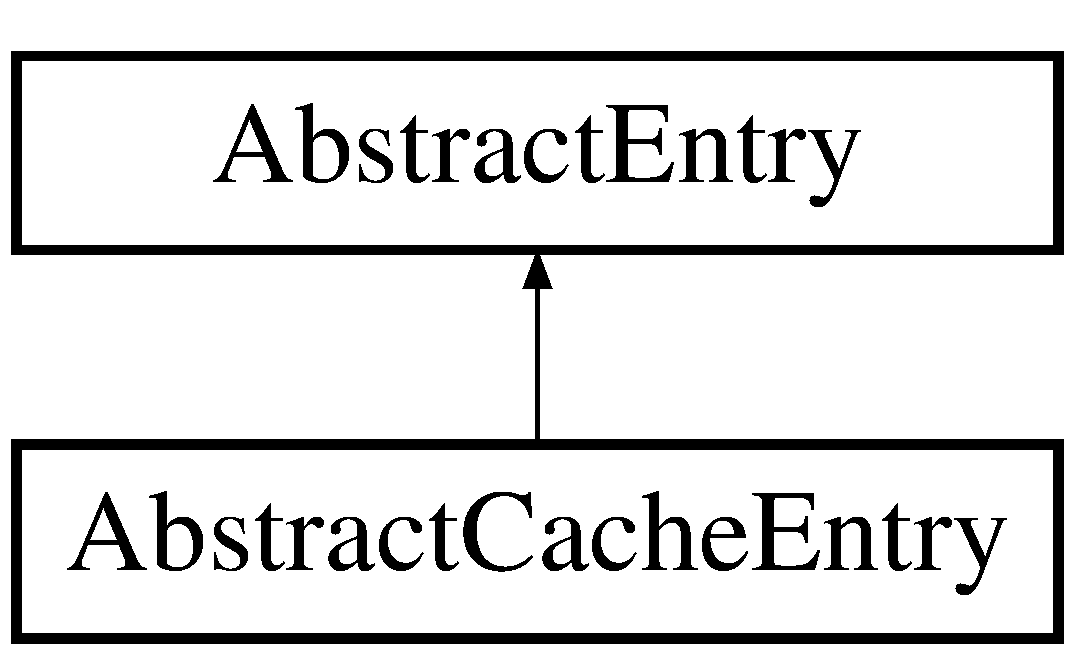
\includegraphics[height=2cm]{classAbstractEntry}
\end{center}
\end{figure}
\subsection*{Public メソッド}
\begin{DoxyCompactItemize}
\item 
\hyperlink{classAbstractEntry_ad75be01d4fce1bd2ce3e7eb247ba40a3}{AbstractEntry} ()
\item 
virtual \hyperlink{classAbstractEntry_aa17a28f91e67d9936834d333e9c29524}{$\sim$AbstractEntry} ()=0
\item 
AccessPermission \hyperlink{classAbstractEntry_aaa8d971d0265aff3209ae487837576f7}{getPermission} () const 
\item 
void \hyperlink{classAbstractEntry_ac3f081af818286da737aac954875dd19}{changePermission} (AccessPermission new\_\-perm)
\item 
virtual \hyperlink{classDataBlock}{DataBlock} \& \hyperlink{classAbstractEntry_afec4a5462c59a6427dd945c8e57d892f}{getDataBlk} ()=0
\item 
virtual void \hyperlink{classAbstractEntry_a3ea5f7af5db62cc24f4e40df9ea5c971}{print} (std::ostream \&out) const =0
\end{DoxyCompactItemize}
\subsection*{Public 変数}
\begin{DoxyCompactItemize}
\item 
AccessPermission \hyperlink{classAbstractEntry_adffb6e818a8b13110daeb2c3c13fcc50}{m\_\-Permission}
\end{DoxyCompactItemize}


\subsection{コンストラクタとデストラクタ}
\hypertarget{classAbstractEntry_ad75be01d4fce1bd2ce3e7eb247ba40a3}{
\index{AbstractEntry@{AbstractEntry}!AbstractEntry@{AbstractEntry}}
\index{AbstractEntry@{AbstractEntry}!AbstractEntry@{AbstractEntry}}
\subsubsection[{AbstractEntry}]{\setlength{\rightskip}{0pt plus 5cm}{\bf AbstractEntry} ()}}
\label{classAbstractEntry_ad75be01d4fce1bd2ce3e7eb247ba40a3}



\begin{DoxyCode}
32 {
33     m_Permission = AccessPermission_NotPresent;
34 }
\end{DoxyCode}
\hypertarget{classAbstractEntry_aa17a28f91e67d9936834d333e9c29524}{
\index{AbstractEntry@{AbstractEntry}!$\sim$AbstractEntry@{$\sim$AbstractEntry}}
\index{$\sim$AbstractEntry@{$\sim$AbstractEntry}!AbstractEntry@{AbstractEntry}}
\subsubsection[{$\sim$AbstractEntry}]{\setlength{\rightskip}{0pt plus 5cm}$\sim${\bf AbstractEntry} ()\hspace{0.3cm}{\ttfamily  \mbox{[}pure virtual\mbox{]}}}}
\label{classAbstractEntry_aa17a28f91e67d9936834d333e9c29524}



\begin{DoxyCode}
37 {
38 }
\end{DoxyCode}


\subsection{関数}
\hypertarget{classAbstractEntry_ac3f081af818286da737aac954875dd19}{
\index{AbstractEntry@{AbstractEntry}!changePermission@{changePermission}}
\index{changePermission@{changePermission}!AbstractEntry@{AbstractEntry}}
\subsubsection[{changePermission}]{\setlength{\rightskip}{0pt plus 5cm}void changePermission (AccessPermission {\em new\_\-perm})}}
\label{classAbstractEntry_ac3f081af818286da737aac954875dd19}


\hyperlink{classAbstractCacheEntry_ac3f081af818286da737aac954875dd19}{AbstractCacheEntry}で再定義されています。


\begin{DoxyCode}
48 {
49     m_Permission = new_perm;
50 }
\end{DoxyCode}
\hypertarget{classAbstractEntry_afec4a5462c59a6427dd945c8e57d892f}{
\index{AbstractEntry@{AbstractEntry}!getDataBlk@{getDataBlk}}
\index{getDataBlk@{getDataBlk}!AbstractEntry@{AbstractEntry}}
\subsubsection[{getDataBlk}]{\setlength{\rightskip}{0pt plus 5cm}virtual {\bf DataBlock}\& getDataBlk ()\hspace{0.3cm}{\ttfamily  \mbox{[}pure virtual\mbox{]}}}}
\label{classAbstractEntry_afec4a5462c59a6427dd945c8e57d892f}
\hypertarget{classAbstractEntry_aaa8d971d0265aff3209ae487837576f7}{
\index{AbstractEntry@{AbstractEntry}!getPermission@{getPermission}}
\index{getPermission@{getPermission}!AbstractEntry@{AbstractEntry}}
\subsubsection[{getPermission}]{\setlength{\rightskip}{0pt plus 5cm}AccessPermission getPermission () const}}
\label{classAbstractEntry_aaa8d971d0265aff3209ae487837576f7}



\begin{DoxyCode}
42 {
43     return m_Permission;
44 }
\end{DoxyCode}
\hypertarget{classAbstractEntry_a3ea5f7af5db62cc24f4e40df9ea5c971}{
\index{AbstractEntry@{AbstractEntry}!print@{print}}
\index{print@{print}!AbstractEntry@{AbstractEntry}}
\subsubsection[{print}]{\setlength{\rightskip}{0pt plus 5cm}virtual void print (std::ostream \& {\em out}) const\hspace{0.3cm}{\ttfamily  \mbox{[}pure virtual\mbox{]}}}}
\label{classAbstractEntry_a3ea5f7af5db62cc24f4e40df9ea5c971}


\subsection{変数}
\hypertarget{classAbstractEntry_adffb6e818a8b13110daeb2c3c13fcc50}{
\index{AbstractEntry@{AbstractEntry}!m\_\-Permission@{m\_\-Permission}}
\index{m\_\-Permission@{m\_\-Permission}!AbstractEntry@{AbstractEntry}}
\subsubsection[{m\_\-Permission}]{\setlength{\rightskip}{0pt plus 5cm}AccessPermission {\bf m\_\-Permission}}}
\label{classAbstractEntry_adffb6e818a8b13110daeb2c3c13fcc50}


このクラスの説明は次のファイルから生成されました:\begin{DoxyCompactItemize}
\item 
mem/ruby/slicc\_\-interface/\hyperlink{AbstractEntry_8hh}{AbstractEntry.hh}\item 
mem/ruby/slicc\_\-interface/\hyperlink{AbstractEntry_8cc}{AbstractEntry.cc}\end{DoxyCompactItemize}

\hypertarget{classAbstractMemory}{
\section{クラス AbstractMemory}
\label{classAbstractMemory}\index{AbstractMemory@{AbstractMemory}}
}


{\ttfamily \#include $<$abstract\_\-mem.hh$>$}AbstractMemoryに対する継承グラフ:\begin{figure}[H]
\begin{center}
\leavevmode
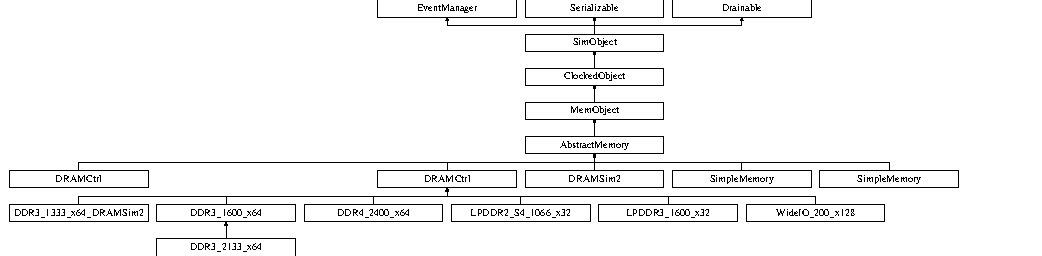
\includegraphics[height=3.44086cm]{classAbstractMemory}
\end{center}
\end{figure}
\subsection*{構成}
\begin{DoxyCompactItemize}
\item 
class \hyperlink{classAbstractMemory_1_1AbstractMemory}{AbstractMemory}
\end{DoxyCompactItemize}
\subsection*{Public 型}
\begin{DoxyCompactItemize}
\item 
typedef AbstractMemoryParams \hyperlink{classAbstractMemory_ab4fcbcbcfef78d6bc871995f8eca40eb}{Params}
\end{DoxyCompactItemize}
\subsection*{Public メソッド}
\begin{DoxyCompactItemize}
\item 
\hyperlink{classAbstractMemory_a69baeab8b9f1056447fe16519fd89923}{AbstractMemory} (const \hyperlink{classAbstractMemory_ab4fcbcbcfef78d6bc871995f8eca40eb}{Params} $\ast$p)
\item 
virtual \hyperlink{classAbstractMemory_a7cff70b609d2b2b8ac45e1fe12b7bc96}{$\sim$AbstractMemory} ()
\item 
bool \hyperlink{classAbstractMemory_ac02f2a4d7312eb91f40980adfd4e31b2}{isNull} () const 
\item 
void \hyperlink{classAbstractMemory_a2651a6edea3b7884410b1abefac8b2de}{setBackingStore} (uint8\_\-t $\ast$pmem\_\-addr)
\item 
const \hyperlink{classstd_1_1list}{std::list}$<$ \hyperlink{classLockedAddr}{LockedAddr} $>$ \& \hyperlink{classAbstractMemory_a5b569455e6a1bd8629737fa02564a9a8}{getLockedAddrList} () const 
\item 
void \hyperlink{classAbstractMemory_a41e2bc27bc88cc5c7d1d8c7a905e7cfc}{addLockedAddr} (\hyperlink{classLockedAddr}{LockedAddr} addr)
\item 
\hyperlink{classSystem}{System} $\ast$ \hyperlink{classAbstractMemory_a83984c42bc765168929779ed9a37ebe8}{system} () const 
\item 
void \hyperlink{classAbstractMemory_ad086bdc3ed123ad02169847d658bf5cb}{system} (\hyperlink{classSystem}{System} $\ast$sys)
\item 
const \hyperlink{classAbstractMemory_ab4fcbcbcfef78d6bc871995f8eca40eb}{Params} $\ast$ \hyperlink{classAbstractMemory_acd3c3feb78ae7a8f88fe0f110a718dff}{params} () const 
\item 
\hyperlink{classAddrRange}{AddrRange} \hyperlink{classAbstractMemory_aa3df62a6c92a30a0ab9247f8ec9e6e7a}{getAddrRange} () const 
\item 
uint64\_\-t \hyperlink{classAbstractMemory_a0b6868dbef44fc07f11d050eb59e5f7e}{size} () const 
\item 
\hyperlink{base_2types_8hh_af1bb03d6a4ee096394a6749f0a169232}{Addr} \hyperlink{classAbstractMemory_a85325674b7aed05d6b4e40a48563189b}{start} () const 
\item 
bool \hyperlink{classAbstractMemory_aca224861e09cf94a49088bb51bb02350}{isConfReported} () const 
\item 
bool \hyperlink{classAbstractMemory_ad89e9980a76342142d63ff15deb19497}{isInAddrMap} () const 
\item 
void \hyperlink{classAbstractMemory_aac5d96736802cb79fb2287135bcc1dff}{access} (\hyperlink{classPacket}{PacketPtr} pkt)
\item 
void \hyperlink{classAbstractMemory_ace845b5316308e12fd958fa5df09a8e8}{functionalAccess} (\hyperlink{classPacket}{PacketPtr} pkt)
\item 
virtual void \hyperlink{classAbstractMemory_a4dc637449366fcdfc4e764cdf12d9b11}{regStats} ()
\end{DoxyCompactItemize}
\subsection*{Protected メソッド}
\begin{DoxyCompactItemize}
\item 
bool \hyperlink{classAbstractMemory_af088ed7a675d24827a3300bdbc62e96a}{checkLockedAddrList} (\hyperlink{classPacket}{PacketPtr} pkt)
\item 
void \hyperlink{classAbstractMemory_ad317aec11d97a72993e653755fa1c003}{trackLoadLocked} (\hyperlink{classPacket}{PacketPtr} pkt)
\item 
bool \hyperlink{classAbstractMemory_ab1136219a28374092ad398d673bd23e0}{writeOK} (\hyperlink{classPacket}{PacketPtr} pkt)
\end{DoxyCompactItemize}
\subsection*{Protected 変数}
\begin{DoxyCompactItemize}
\item 
\hyperlink{classAddrRange}{AddrRange} \hyperlink{classAbstractMemory_a194876a072a83a9fd59dde82e5213f0d}{range}
\item 
uint8\_\-t $\ast$ \hyperlink{classAbstractMemory_a9f8ed24d8442f662831d51922e7fddd2}{pmemAddr}
\item 
bool \hyperlink{classAbstractMemory_adee792d6bf567779ea9c16640af42784}{confTableReported}
\item 
bool \hyperlink{classAbstractMemory_a7302c053380cdccd0bdf63b25f73cbc5}{inAddrMap}
\item 
\hyperlink{classstd_1_1list}{std::list}$<$ \hyperlink{classLockedAddr}{LockedAddr} $>$ \hyperlink{classAbstractMemory_af35631da2ae35079d76e07c46fe78565}{lockedAddrList}
\item 
\hyperlink{classStats_1_1Vector}{Stats::Vector} \hyperlink{classAbstractMemory_aa36971a2ea8ddd9d82832059cbc1b21f}{bytesRead}
\item 
\hyperlink{classStats_1_1Vector}{Stats::Vector} \hyperlink{classAbstractMemory_a5e52eb4a824c1fb452d77dae86dfa970}{bytesInstRead}
\item 
\hyperlink{classStats_1_1Vector}{Stats::Vector} \hyperlink{classAbstractMemory_ab89ec4a4876671ad5186d0e9c0e674ed}{bytesWritten}
\item 
\hyperlink{classStats_1_1Vector}{Stats::Vector} \hyperlink{classAbstractMemory_a27f442fbcb7bc7661412cc1d96ca51e7}{numReads}
\item 
\hyperlink{classStats_1_1Vector}{Stats::Vector} \hyperlink{classAbstractMemory_acfd6a97aa6c2de05417a7403369e71c2}{numWrites}
\item 
\hyperlink{classStats_1_1Vector}{Stats::Vector} \hyperlink{classAbstractMemory_a52bafd014022e75d82b4e0de25d3faf7}{numOther}
\item 
\hyperlink{classStats_1_1Formula}{Stats::Formula} \hyperlink{classAbstractMemory_a14a0a95f3cd104b70d5b5c19c3ee8099}{bwRead}
\item 
\hyperlink{classStats_1_1Formula}{Stats::Formula} \hyperlink{classAbstractMemory_a00512ebb77886b71a63bd1595828d592}{bwInstRead}
\item 
\hyperlink{classStats_1_1Formula}{Stats::Formula} \hyperlink{classAbstractMemory_a8077d31db9c4f4f9e78888def6de8430}{bwWrite}
\item 
\hyperlink{classStats_1_1Formula}{Stats::Formula} \hyperlink{classAbstractMemory_a678ff8c93c78d0be1884742ef8aa41e8}{bwTotal}
\item 
\hyperlink{classSystem}{System} $\ast$ \hyperlink{classAbstractMemory_a1da55f4024bf8a9b14b64054841148b8}{\_\-system}
\end{DoxyCompactItemize}
\subsection*{Private メソッド}
\begin{DoxyCompactItemize}
\item 
\hyperlink{classAbstractMemory_abe7c4ad03729f9b3dd25d3dc43361103}{AbstractMemory} (const \hyperlink{classAbstractMemory_1_1AbstractMemory}{AbstractMemory} \&)
\item 
\hyperlink{classAbstractMemory_1_1AbstractMemory}{AbstractMemory} \& \hyperlink{classAbstractMemory_a8524c3be63882adac591f591519f3a3b}{operator=} (const \hyperlink{classAbstractMemory_1_1AbstractMemory}{AbstractMemory} \&)
\end{DoxyCompactItemize}


\subsection{説明}
An abstract memory represents a contiguous block of physical memory, with an associated address range, and also provides basic functionality for reading and writing this memory without any timing information. It is a \hyperlink{classMemObject}{MemObject} since any subclass must have at least one slave port. 

\subsection{型定義}
\hypertarget{classAbstractMemory_ab4fcbcbcfef78d6bc871995f8eca40eb}{
\index{AbstractMemory@{AbstractMemory}!Params@{Params}}
\index{Params@{Params}!AbstractMemory@{AbstractMemory}}
\subsubsection[{Params}]{\setlength{\rightskip}{0pt plus 5cm}typedef AbstractMemoryParams {\bf Params}}}
\label{classAbstractMemory_ab4fcbcbcfef78d6bc871995f8eca40eb}


\hyperlink{classMemObject_a905bbc621eeec0ed08859e21c8c95412}{MemObject}を再定義しています。

\hyperlink{classDRAMSim2_ae66665a06c9d64a6ba0e56d589b74d6c}{DRAMSim2}で再定義されています。

\subsection{コンストラクタとデストラクタ}
\hypertarget{classAbstractMemory_abe7c4ad03729f9b3dd25d3dc43361103}{
\index{AbstractMemory@{AbstractMemory}!AbstractMemory@{AbstractMemory}}
\index{AbstractMemory@{AbstractMemory}!AbstractMemory@{AbstractMemory}}
\subsubsection[{AbstractMemory}]{\setlength{\rightskip}{0pt plus 5cm}{\bf AbstractMemory} (const {\bf AbstractMemory} \&)\hspace{0.3cm}{\ttfamily  \mbox{[}private\mbox{]}}}}
\label{classAbstractMemory_abe7c4ad03729f9b3dd25d3dc43361103}
\hypertarget{classAbstractMemory_a69baeab8b9f1056447fe16519fd89923}{
\index{AbstractMemory@{AbstractMemory}!AbstractMemory@{AbstractMemory}}
\index{AbstractMemory@{AbstractMemory}!AbstractMemory@{AbstractMemory}}
\subsubsection[{AbstractMemory}]{\setlength{\rightskip}{0pt plus 5cm}{\bf AbstractMemory} (const {\bf Params} $\ast$ {\em p})}}
\label{classAbstractMemory_a69baeab8b9f1056447fe16519fd89923}



\begin{DoxyCode}
57                                               :
58     MemObject(p), range(params()->range), pmemAddr(NULL),
59     confTableReported(p->conf_table_reported), inAddrMap(p->in_addr_map),
60     _system(NULL)
61 {
62     if (size() % TheISA::PageBytes != 0)
63         panic("Memory Size not divisible by page size\n");
64 }

\end{DoxyCode}
\hypertarget{classAbstractMemory_a7cff70b609d2b2b8ac45e1fe12b7bc96}{
\index{AbstractMemory@{AbstractMemory}!$\sim$AbstractMemory@{$\sim$AbstractMemory}}
\index{$\sim$AbstractMemory@{$\sim$AbstractMemory}!AbstractMemory@{AbstractMemory}}
\subsubsection[{$\sim$AbstractMemory}]{\setlength{\rightskip}{0pt plus 5cm}virtual $\sim${\bf AbstractMemory} ()\hspace{0.3cm}{\ttfamily  \mbox{[}inline, virtual\mbox{]}}}}
\label{classAbstractMemory_a7cff70b609d2b2b8ac45e1fe12b7bc96}



\begin{DoxyCode}
195 {}
\end{DoxyCode}


\subsection{関数}
\hypertarget{classAbstractMemory_aac5d96736802cb79fb2287135bcc1dff}{
\index{AbstractMemory@{AbstractMemory}!access@{access}}
\index{access@{access}!AbstractMemory@{AbstractMemory}}
\subsubsection[{access}]{\setlength{\rightskip}{0pt plus 5cm}void access ({\bf PacketPtr} {\em pkt})}}
\label{classAbstractMemory_aac5d96736802cb79fb2287135bcc1dff}
Perform an untimed memory access and update all the state (e.g. locked addresses) and statistics accordingly. The packet is turned into a response if required.


\begin{DoxyParams}{引数}
\item[{\em pkt}]\hyperlink{classPacket}{Packet} performing the access \end{DoxyParams}



\begin{DoxyCode}
317 {
318     assert(AddrRange(pkt->getAddr(),
319                      pkt->getAddr() + pkt->getSize() - 1).isSubset(range));
320 
321     if (pkt->memInhibitAsserted()) {
322         DPRINTF(MemoryAccess, "mem inhibited on 0x%x: not responding\n",
323                 pkt->getAddr());
324         return;
325     }
326 
327     uint8_t *hostAddr = pmemAddr + pkt->getAddr() - range.start();
328 
329     if (pkt->cmd == MemCmd::SwapReq) {
330         TheISA::IntReg overwrite_val;
331         bool overwrite_mem;
332         uint64_t condition_val64;
333         uint32_t condition_val32;
334 
335         if (!pmemAddr)
336             panic("Swap only works if there is real memory (i.e. null=False)");
337         assert(sizeof(TheISA::IntReg) >= pkt->getSize());
338 
339         overwrite_mem = true;
340         // keep a copy of our possible write value, and copy what is at the
341         // memory address into the packet
342         std::memcpy(&overwrite_val, pkt->getPtr<uint8_t>(), pkt->getSize());
343         std::memcpy(pkt->getPtr<uint8_t>(), hostAddr, pkt->getSize());
344 
345         if (pkt->req->isCondSwap()) {
346             if (pkt->getSize() == sizeof(uint64_t)) {
347                 condition_val64 = pkt->req->getExtraData();
348                 overwrite_mem = !std::memcmp(&condition_val64, hostAddr,
349                                              sizeof(uint64_t));
350             } else if (pkt->getSize() == sizeof(uint32_t)) {
351                 condition_val32 = (uint32_t)pkt->req->getExtraData();
352                 overwrite_mem = !std::memcmp(&condition_val32, hostAddr,
353                                              sizeof(uint32_t));
354             } else
355                 panic("Invalid size for conditional read/write\n");
356         }
357 
358         if (overwrite_mem)
359             std::memcpy(hostAddr, &overwrite_val, pkt->getSize());
360 
361         assert(!pkt->req->isInstFetch());
362         TRACE_PACKET("Read/Write");
363         numOther[pkt->req->masterId()]++;
364     } else if (pkt->isRead()) {
365         assert(!pkt->isWrite());
366         if (pkt->isLLSC()) {
367             trackLoadLocked(pkt);
368         }
369         if (pmemAddr)
370             memcpy(pkt->getPtr<uint8_t>(), hostAddr, pkt->getSize());
371         TRACE_PACKET(pkt->req->isInstFetch() ? "IFetch" : "Read");
372         numReads[pkt->req->masterId()]++;
373         bytesRead[pkt->req->masterId()] += pkt->getSize();
374         if (pkt->req->isInstFetch())
375             bytesInstRead[pkt->req->masterId()] += pkt->getSize();
376     } else if (pkt->isWrite()) {
377         if (writeOK(pkt)) {
378             if (pmemAddr) {
379                 memcpy(hostAddr, pkt->getPtr<uint8_t>(), pkt->getSize());
380                 DPRINTF(MemoryAccess, "%s wrote %x bytes to address %x\n",
381                         __func__, pkt->getSize(), pkt->getAddr());
382             }
383             assert(!pkt->req->isInstFetch());
384             TRACE_PACKET("Write");
385             numWrites[pkt->req->masterId()]++;
386             bytesWritten[pkt->req->masterId()] += pkt->getSize();
387         }
388     } else if (pkt->isInvalidate()) {
389         // no need to do anything
390     } else {
391         panic("unimplemented");
392     }
393 
394     if (pkt->needsResponse()) {
395         pkt->makeResponse();
396     }
397 }
\end{DoxyCode}
\hypertarget{classAbstractMemory_a41e2bc27bc88cc5c7d1d8c7a905e7cfc}{
\index{AbstractMemory@{AbstractMemory}!addLockedAddr@{addLockedAddr}}
\index{addLockedAddr@{addLockedAddr}!AbstractMemory@{AbstractMemory}}
\subsubsection[{addLockedAddr}]{\setlength{\rightskip}{0pt plus 5cm}void addLockedAddr ({\bf LockedAddr} {\em addr})\hspace{0.3cm}{\ttfamily  \mbox{[}inline\mbox{]}}}}
\label{classAbstractMemory_a41e2bc27bc88cc5c7d1d8c7a905e7cfc}
Add a locked address to allow for checkpointing. 


\begin{DoxyCode}
222 { lockedAddrList.push_back(addr); }
\end{DoxyCode}
\hypertarget{classAbstractMemory_af088ed7a675d24827a3300bdbc62e96a}{
\index{AbstractMemory@{AbstractMemory}!checkLockedAddrList@{checkLockedAddrList}}
\index{checkLockedAddrList@{checkLockedAddrList}!AbstractMemory@{AbstractMemory}}
\subsubsection[{checkLockedAddrList}]{\setlength{\rightskip}{0pt plus 5cm}bool checkLockedAddrList ({\bf PacketPtr} {\em pkt})\hspace{0.3cm}{\ttfamily  \mbox{[}protected\mbox{]}}}}
\label{classAbstractMemory_af088ed7a675d24827a3300bdbc62e96a}



\begin{DoxyCode}
221 {
222     Request *req = pkt->req;
223     Addr paddr = LockedAddr::mask(req->getPaddr());
224     bool isLLSC = pkt->isLLSC();
225 
226     // Initialize return value.  Non-conditional stores always
227     // succeed.  Assume conditional stores will fail until proven
228     // otherwise.
229     bool allowStore = !isLLSC;
230 
231     // Iterate over list.  Note that there could be multiple matching records,
232     // as more than one context could have done a load locked to this location.
233     // Only remove records when we succeed in finding a record for (xc, addr);
234     // then, remove all records with this address.  Failed store-conditionals do
235     // not blow unrelated reservations.
236     list<LockedAddr>::iterator i = lockedAddrList.begin();
237 
238     if (isLLSC) {
239         while (i != lockedAddrList.end()) {
240             if (i->addr == paddr && i->matchesContext(req)) {
241                 // it's a store conditional, and as far as the memory system can
242                 // tell, the requesting context's lock is still valid.
243                 DPRINTF(LLSC, "StCond success: context %d addr %#x\n",
244                         req->contextId(), paddr);
245                 allowStore = true;
246                 break;
247             }
248             // If we didn't find a match, keep searching!  Someone else may well
249             // have a reservation on this line here but we may find ours in just
250             // a little while.
251             i++;
252         }
253         req->setExtraData(allowStore ? 1 : 0);
254     }
255     // LLSCs that succeeded AND non-LLSC stores both fall into here:
256     if (allowStore) {
257         // We write address paddr.  However, there may be several entries with a
258         // reservation on this address (for other contextIds) and they must all
259         // be removed.
260         i = lockedAddrList.begin();
261         while (i != lockedAddrList.end()) {
262             if (i->addr == paddr) {
263                 DPRINTF(LLSC, "Erasing lock record: context %d addr %#x\n",
264                         i->contextId, paddr);
265                 // For ARM, a spinlock would typically include a Wait
266                 // For Event (WFE) to conserve energy. The ARMv8
267                 // architecture specifies that an event is
268                 // automatically generated when clearing the exclusive
269                 // monitor to wake up the processor in WFE.
270                 system()->getThreadContext(i->contextId)->getCpuPtr()->wakeup();
271                 i = lockedAddrList.erase(i);
272             } else {
273                 i++;
274             }
275         }
276     }
277 
278     return allowStore;
279 }
\end{DoxyCode}
\hypertarget{classAbstractMemory_ace845b5316308e12fd958fa5df09a8e8}{
\index{AbstractMemory@{AbstractMemory}!functionalAccess@{functionalAccess}}
\index{functionalAccess@{functionalAccess}!AbstractMemory@{AbstractMemory}}
\subsubsection[{functionalAccess}]{\setlength{\rightskip}{0pt plus 5cm}void functionalAccess ({\bf PacketPtr} {\em pkt})}}
\label{classAbstractMemory_ace845b5316308e12fd958fa5df09a8e8}
Perform an untimed memory read or write without changing anything but the memory itself. No stats are affected by this access. In addition to normal accesses this also facilitates print requests.


\begin{DoxyParams}{引数}
\item[{\em pkt}]\hyperlink{classPacket}{Packet} performing the access \end{DoxyParams}



\begin{DoxyCode}
401 {
402     assert(AddrRange(pkt->getAddr(),
403                      pkt->getAddr() + pkt->getSize() - 1).isSubset(range));
404 
405     uint8_t *hostAddr = pmemAddr + pkt->getAddr() - range.start();
406 
407     if (pkt->isRead()) {
408         if (pmemAddr)
409             memcpy(pkt->getPtr<uint8_t>(), hostAddr, pkt->getSize());
410         TRACE_PACKET("Read");
411         pkt->makeResponse();
412     } else if (pkt->isWrite()) {
413         if (pmemAddr)
414             memcpy(hostAddr, pkt->getPtr<uint8_t>(), pkt->getSize());
415         TRACE_PACKET("Write");
416         pkt->makeResponse();
417     } else if (pkt->isPrint()) {
418         Packet::PrintReqState *prs =
419             dynamic_cast<Packet::PrintReqState*>(pkt->senderState);
420         assert(prs);
421         // Need to call printLabels() explicitly since we're not going
422         // through printObj().
423         prs->printLabels();
424         // Right now we just print the single byte at the specified address.
425         ccprintf(prs->os, "%s%#x\n", prs->curPrefix(), *hostAddr);
426     } else {
427         panic("AbstractMemory: unimplemented functional command %s",
428               pkt->cmdString());
429     }
430 }
\end{DoxyCode}
\hypertarget{classAbstractMemory_aa3df62a6c92a30a0ab9247f8ec9e6e7a}{
\index{AbstractMemory@{AbstractMemory}!getAddrRange@{getAddrRange}}
\index{getAddrRange@{getAddrRange}!AbstractMemory@{AbstractMemory}}
\subsubsection[{getAddrRange}]{\setlength{\rightskip}{0pt plus 5cm}{\bf AddrRange} getAddrRange () const}}
\label{classAbstractMemory_aa3df62a6c92a30a0ab9247f8ec9e6e7a}
Get the address range

\begin{DoxyReturn}{戻り値}
a single contigous address range 
\end{DoxyReturn}



\begin{DoxyCode}
182 {
183     return range;
184 }
\end{DoxyCode}
\hypertarget{classAbstractMemory_a5b569455e6a1bd8629737fa02564a9a8}{
\index{AbstractMemory@{AbstractMemory}!getLockedAddrList@{getLockedAddrList}}
\index{getLockedAddrList@{getLockedAddrList}!AbstractMemory@{AbstractMemory}}
\subsubsection[{getLockedAddrList}]{\setlength{\rightskip}{0pt plus 5cm}const {\bf std::list}$<${\bf LockedAddr}$>$\& getLockedAddrList () const\hspace{0.3cm}{\ttfamily  \mbox{[}inline\mbox{]}}}}
\label{classAbstractMemory_a5b569455e6a1bd8629737fa02564a9a8}
Get the list of locked addresses to allow checkpointing. 


\begin{DoxyCode}
217     { return lockedAddrList; }
\end{DoxyCode}
\hypertarget{classAbstractMemory_aca224861e09cf94a49088bb51bb02350}{
\index{AbstractMemory@{AbstractMemory}!isConfReported@{isConfReported}}
\index{isConfReported@{isConfReported}!AbstractMemory@{AbstractMemory}}
\subsubsection[{isConfReported}]{\setlength{\rightskip}{0pt plus 5cm}bool isConfReported () const\hspace{0.3cm}{\ttfamily  \mbox{[}inline\mbox{]}}}}
\label{classAbstractMemory_aca224861e09cf94a49088bb51bb02350}
Should this memory be passed to the kernel and part of the OS physical memory layout.

\begin{DoxyReturn}{戻り値}
if this memory is reported 
\end{DoxyReturn}



\begin{DoxyCode}
270 { return confTableReported; }
\end{DoxyCode}
\hypertarget{classAbstractMemory_ad89e9980a76342142d63ff15deb19497}{
\index{AbstractMemory@{AbstractMemory}!isInAddrMap@{isInAddrMap}}
\index{isInAddrMap@{isInAddrMap}!AbstractMemory@{AbstractMemory}}
\subsubsection[{isInAddrMap}]{\setlength{\rightskip}{0pt plus 5cm}bool isInAddrMap () const\hspace{0.3cm}{\ttfamily  \mbox{[}inline\mbox{]}}}}
\label{classAbstractMemory_ad89e9980a76342142d63ff15deb19497}
Some memories are used as shadow memories or should for other reasons not be part of the global address map.

\begin{DoxyReturn}{戻り値}
if this memory is part of the address map 
\end{DoxyReturn}



\begin{DoxyCode}
278 { return inAddrMap; }
\end{DoxyCode}
\hypertarget{classAbstractMemory_ac02f2a4d7312eb91f40980adfd4e31b2}{
\index{AbstractMemory@{AbstractMemory}!isNull@{isNull}}
\index{isNull@{isNull}!AbstractMemory@{AbstractMemory}}
\subsubsection[{isNull}]{\setlength{\rightskip}{0pt plus 5cm}bool isNull () const\hspace{0.3cm}{\ttfamily  \mbox{[}inline\mbox{]}}}}
\label{classAbstractMemory_ac02f2a4d7312eb91f40980adfd4e31b2}
See if this is a null memory that should never store data and always return zero.

\begin{DoxyReturn}{戻り値}
true if null 
\end{DoxyReturn}



\begin{DoxyCode}
203 { return params()->null; }
\end{DoxyCode}
\hypertarget{classAbstractMemory_a8524c3be63882adac591f591519f3a3b}{
\index{AbstractMemory@{AbstractMemory}!operator=@{operator=}}
\index{operator=@{operator=}!AbstractMemory@{AbstractMemory}}
\subsubsection[{operator=}]{\setlength{\rightskip}{0pt plus 5cm}{\bf AbstractMemory}\& operator= (const {\bf AbstractMemory} \&)\hspace{0.3cm}{\ttfamily  \mbox{[}private\mbox{]}}}}
\label{classAbstractMemory_a8524c3be63882adac591f591519f3a3b}
\hypertarget{classAbstractMemory_acd3c3feb78ae7a8f88fe0f110a718dff}{
\index{AbstractMemory@{AbstractMemory}!params@{params}}
\index{params@{params}!AbstractMemory@{AbstractMemory}}
\subsubsection[{params}]{\setlength{\rightskip}{0pt plus 5cm}const {\bf Params}$\ast$ params () const\hspace{0.3cm}{\ttfamily  \mbox{[}inline\mbox{]}}}}
\label{classAbstractMemory_acd3c3feb78ae7a8f88fe0f110a718dff}


\hyperlink{classMemObject_acd3c3feb78ae7a8f88fe0f110a718dff}{MemObject}を再定義しています。


\begin{DoxyCode}
239     {
240         return dynamic_cast<const Params *>(_params);
241     }
\end{DoxyCode}
\hypertarget{classAbstractMemory_a4dc637449366fcdfc4e764cdf12d9b11}{
\index{AbstractMemory@{AbstractMemory}!regStats@{regStats}}
\index{regStats@{regStats}!AbstractMemory@{AbstractMemory}}
\subsubsection[{regStats}]{\setlength{\rightskip}{0pt plus 5cm}void regStats ()\hspace{0.3cm}{\ttfamily  \mbox{[}virtual\mbox{]}}}}
\label{classAbstractMemory_a4dc637449366fcdfc4e764cdf12d9b11}
\hyperlink{classRegister}{Register} Statistics 

\hyperlink{classSimObject_a4dc637449366fcdfc4e764cdf12d9b11}{SimObject}を再定義しています。

\hyperlink{classDRAMCtrl_a4dc637449366fcdfc4e764cdf12d9b11}{DRAMCtrl}で再定義されています。


\begin{DoxyCode}
74 {
75     using namespace Stats;
76 
77     assert(system());
78 
79     bytesRead
80         .init(system()->maxMasters())
81         .name(name() + ".bytes_read")
82         .desc("Number of bytes read from this memory")
83         .flags(total | nozero | nonan)
84         ;
85     for (int i = 0; i < system()->maxMasters(); i++) {
86         bytesRead.subname(i, system()->getMasterName(i));
87     }
88     bytesInstRead
89         .init(system()->maxMasters())
90         .name(name() + ".bytes_inst_read")
91         .desc("Number of instructions bytes read from this memory")
92         .flags(total | nozero | nonan)
93         ;
94     for (int i = 0; i < system()->maxMasters(); i++) {
95         bytesInstRead.subname(i, system()->getMasterName(i));
96     }
97     bytesWritten
98         .init(system()->maxMasters())
99         .name(name() + ".bytes_written")
100         .desc("Number of bytes written to this memory")
101         .flags(total | nozero | nonan)
102         ;
103     for (int i = 0; i < system()->maxMasters(); i++) {
104         bytesWritten.subname(i, system()->getMasterName(i));
105     }
106     numReads
107         .init(system()->maxMasters())
108         .name(name() + ".num_reads")
109         .desc("Number of read requests responded to by this memory")
110         .flags(total | nozero | nonan)
111         ;
112     for (int i = 0; i < system()->maxMasters(); i++) {
113         numReads.subname(i, system()->getMasterName(i));
114     }
115     numWrites
116         .init(system()->maxMasters())
117         .name(name() + ".num_writes")
118         .desc("Number of write requests responded to by this memory")
119         .flags(total | nozero | nonan)
120         ;
121     for (int i = 0; i < system()->maxMasters(); i++) {
122         numWrites.subname(i, system()->getMasterName(i));
123     }
124     numOther
125         .init(system()->maxMasters())
126         .name(name() + ".num_other")
127         .desc("Number of other requests responded to by this memory")
128         .flags(total | nozero | nonan)
129         ;
130     for (int i = 0; i < system()->maxMasters(); i++) {
131         numOther.subname(i, system()->getMasterName(i));
132     }
133     bwRead
134         .name(name() + ".bw_read")
135         .desc("Total read bandwidth from this memory (bytes/s)")
136         .precision(0)
137         .prereq(bytesRead)
138         .flags(total | nozero | nonan)
139         ;
140     for (int i = 0; i < system()->maxMasters(); i++) {
141         bwRead.subname(i, system()->getMasterName(i));
142     }
143 
144     bwInstRead
145         .name(name() + ".bw_inst_read")
146         .desc("Instruction read bandwidth from this memory (bytes/s)")
147         .precision(0)
148         .prereq(bytesInstRead)
149         .flags(total | nozero | nonan)
150         ;
151     for (int i = 0; i < system()->maxMasters(); i++) {
152         bwInstRead.subname(i, system()->getMasterName(i));
153     }
154     bwWrite
155         .name(name() + ".bw_write")
156         .desc("Write bandwidth from this memory (bytes/s)")
157         .precision(0)
158         .prereq(bytesWritten)
159         .flags(total | nozero | nonan)
160         ;
161     for (int i = 0; i < system()->maxMasters(); i++) {
162         bwWrite.subname(i, system()->getMasterName(i));
163     }
164     bwTotal
165         .name(name() + ".bw_total")
166         .desc("Total bandwidth to/from this memory (bytes/s)")
167         .precision(0)
168         .prereq(bwTotal)
169         .flags(total | nozero | nonan)
170         ;
171     for (int i = 0; i < system()->maxMasters(); i++) {
172         bwTotal.subname(i, system()->getMasterName(i));
173     }
174     bwRead = bytesRead / simSeconds;
175     bwInstRead = bytesInstRead / simSeconds;
176     bwWrite = bytesWritten / simSeconds;
177     bwTotal = (bytesRead + bytesWritten) / simSeconds;
178 }
\end{DoxyCode}
\hypertarget{classAbstractMemory_a2651a6edea3b7884410b1abefac8b2de}{
\index{AbstractMemory@{AbstractMemory}!setBackingStore@{setBackingStore}}
\index{setBackingStore@{setBackingStore}!AbstractMemory@{AbstractMemory}}
\subsubsection[{setBackingStore}]{\setlength{\rightskip}{0pt plus 5cm}void setBackingStore (uint8\_\-t $\ast$ {\em pmem\_\-addr})}}
\label{classAbstractMemory_a2651a6edea3b7884410b1abefac8b2de}
\hyperlink{classSet}{Set} the host memory backing store to be used by this memory controller.


\begin{DoxyParams}{引数}
\item[{\em pmem\_\-addr}]Pointer to a segment of host memory \end{DoxyParams}



\begin{DoxyCode}
68 {
69     pmemAddr = pmem_addr;
70 }
\end{DoxyCode}
\hypertarget{classAbstractMemory_a0b6868dbef44fc07f11d050eb59e5f7e}{
\index{AbstractMemory@{AbstractMemory}!size@{size}}
\index{size@{size}!AbstractMemory@{AbstractMemory}}
\subsubsection[{size}]{\setlength{\rightskip}{0pt plus 5cm}uint64\_\-t size () const\hspace{0.3cm}{\ttfamily  \mbox{[}inline\mbox{]}}}}
\label{classAbstractMemory_a0b6868dbef44fc07f11d050eb59e5f7e}
Get the memory size.

\begin{DoxyReturn}{戻り値}
the size of the memory 
\end{DoxyReturn}



\begin{DoxyCode}
255 { return range.size(); }
\end{DoxyCode}
\hypertarget{classAbstractMemory_a85325674b7aed05d6b4e40a48563189b}{
\index{AbstractMemory@{AbstractMemory}!start@{start}}
\index{start@{start}!AbstractMemory@{AbstractMemory}}
\subsubsection[{start}]{\setlength{\rightskip}{0pt plus 5cm}{\bf Addr} start () const\hspace{0.3cm}{\ttfamily  \mbox{[}inline\mbox{]}}}}
\label{classAbstractMemory_a85325674b7aed05d6b4e40a48563189b}
Get the start address.

\begin{DoxyReturn}{戻り値}
the start address of the memory 
\end{DoxyReturn}



\begin{DoxyCode}
262 { return range.start(); }
\end{DoxyCode}
\hypertarget{classAbstractMemory_ad086bdc3ed123ad02169847d658bf5cb}{
\index{AbstractMemory@{AbstractMemory}!system@{system}}
\index{system@{system}!AbstractMemory@{AbstractMemory}}
\subsubsection[{system}]{\setlength{\rightskip}{0pt plus 5cm}void system ({\bf System} $\ast$ {\em sys})\hspace{0.3cm}{\ttfamily  \mbox{[}inline\mbox{]}}}}
\label{classAbstractMemory_ad086bdc3ed123ad02169847d658bf5cb}
\hyperlink{classSet}{Set} the system pointer on this memory This can't be done via a python parameter because the system needs pointers to all the memories and the reverse would create a cycle in the object graph. An \hyperlink{classSimObject_a02fd73d861ef2e4aabb38c0c9ff82947}{init()} this is set. 
\begin{DoxyParams}{引数}
\item[{\em sys}]system pointer to set \end{DoxyParams}



\begin{DoxyCode}
235 { _system = sys; }
\end{DoxyCode}
\hypertarget{classAbstractMemory_a83984c42bc765168929779ed9a37ebe8}{
\index{AbstractMemory@{AbstractMemory}!system@{system}}
\index{system@{system}!AbstractMemory@{AbstractMemory}}
\subsubsection[{system}]{\setlength{\rightskip}{0pt plus 5cm}{\bf System}$\ast$ system () const\hspace{0.3cm}{\ttfamily  \mbox{[}inline\mbox{]}}}}
\label{classAbstractMemory_a83984c42bc765168929779ed9a37ebe8}
read the system pointer Implemented for completeness with the setter \begin{DoxyReturn}{戻り値}
pointer to the system object 
\end{DoxyReturn}



\begin{DoxyCode}
227 { return _system; }
\end{DoxyCode}
\hypertarget{classAbstractMemory_ad317aec11d97a72993e653755fa1c003}{
\index{AbstractMemory@{AbstractMemory}!trackLoadLocked@{trackLoadLocked}}
\index{trackLoadLocked@{trackLoadLocked}!AbstractMemory@{AbstractMemory}}
\subsubsection[{trackLoadLocked}]{\setlength{\rightskip}{0pt plus 5cm}void trackLoadLocked ({\bf PacketPtr} {\em pkt})\hspace{0.3cm}{\ttfamily  \mbox{[}protected\mbox{]}}}}
\label{classAbstractMemory_ad317aec11d97a72993e653755fa1c003}



\begin{DoxyCode}
190 {
191     Request *req = pkt->req;
192     Addr paddr = LockedAddr::mask(req->getPaddr());
193 
194     // first we check if we already have a locked addr for this
195     // xc.  Since each xc only gets one, we just update the
196     // existing record with the new address.
197     list<LockedAddr>::iterator i;
198 
199     for (i = lockedAddrList.begin(); i != lockedAddrList.end(); ++i) {
200         if (i->matchesContext(req)) {
201             DPRINTF(LLSC, "Modifying lock record: context %d addr %#x\n",
202                     req->contextId(), paddr);
203             i->addr = paddr;
204             return;
205         }
206     }
207 
208     // no record for this xc: need to allocate a new one
209     DPRINTF(LLSC, "Adding lock record: context %d addr %#x\n",
210             req->contextId(), paddr);
211     lockedAddrList.push_front(LockedAddr(req));
212 }
\end{DoxyCode}
\hypertarget{classAbstractMemory_ab1136219a28374092ad398d673bd23e0}{
\index{AbstractMemory@{AbstractMemory}!writeOK@{writeOK}}
\index{writeOK@{writeOK}!AbstractMemory@{AbstractMemory}}
\subsubsection[{writeOK}]{\setlength{\rightskip}{0pt plus 5cm}bool writeOK ({\bf PacketPtr} {\em pkt})\hspace{0.3cm}{\ttfamily  \mbox{[}inline, protected\mbox{]}}}}
\label{classAbstractMemory_ab1136219a28374092ad398d673bd23e0}



\begin{DoxyCode}
139                                 {
140         Request *req = pkt->req;
141         if (lockedAddrList.empty()) {
142             // no locked addrs: nothing to check, store_conditional fails
143             bool isLLSC = pkt->isLLSC();
144             if (isLLSC) {
145                 req->setExtraData(0);
146             }
147             return !isLLSC; // only do write if not an sc
148         } else {
149             // iterate over list...
150             return checkLockedAddrList(pkt);
151         }
152     }
\end{DoxyCode}


\subsection{変数}
\hypertarget{classAbstractMemory_a1da55f4024bf8a9b14b64054841148b8}{
\index{AbstractMemory@{AbstractMemory}!\_\-system@{\_\-system}}
\index{\_\-system@{\_\-system}!AbstractMemory@{AbstractMemory}}
\subsubsection[{\_\-system}]{\setlength{\rightskip}{0pt plus 5cm}{\bf System}$\ast$ {\bf \_\-system}\hspace{0.3cm}{\ttfamily  \mbox{[}protected\mbox{]}}}}
\label{classAbstractMemory_a1da55f4024bf8a9b14b64054841148b8}
Pointor to the \hyperlink{classSystem}{System} object. This is used for getting the number of masters in the system which is needed when registering stats \hypertarget{classAbstractMemory_a00512ebb77886b71a63bd1595828d592}{
\index{AbstractMemory@{AbstractMemory}!bwInstRead@{bwInstRead}}
\index{bwInstRead@{bwInstRead}!AbstractMemory@{AbstractMemory}}
\subsubsection[{bwInstRead}]{\setlength{\rightskip}{0pt plus 5cm}{\bf Stats::Formula} {\bf bwInstRead}\hspace{0.3cm}{\ttfamily  \mbox{[}protected\mbox{]}}}}
\label{classAbstractMemory_a00512ebb77886b71a63bd1595828d592}
Read bandwidth from this memory \hypertarget{classAbstractMemory_a14a0a95f3cd104b70d5b5c19c3ee8099}{
\index{AbstractMemory@{AbstractMemory}!bwRead@{bwRead}}
\index{bwRead@{bwRead}!AbstractMemory@{AbstractMemory}}
\subsubsection[{bwRead}]{\setlength{\rightskip}{0pt plus 5cm}{\bf Stats::Formula} {\bf bwRead}\hspace{0.3cm}{\ttfamily  \mbox{[}protected\mbox{]}}}}
\label{classAbstractMemory_a14a0a95f3cd104b70d5b5c19c3ee8099}
Read bandwidth from this memory \hypertarget{classAbstractMemory_a678ff8c93c78d0be1884742ef8aa41e8}{
\index{AbstractMemory@{AbstractMemory}!bwTotal@{bwTotal}}
\index{bwTotal@{bwTotal}!AbstractMemory@{AbstractMemory}}
\subsubsection[{bwTotal}]{\setlength{\rightskip}{0pt plus 5cm}{\bf Stats::Formula} {\bf bwTotal}\hspace{0.3cm}{\ttfamily  \mbox{[}protected\mbox{]}}}}
\label{classAbstractMemory_a678ff8c93c78d0be1884742ef8aa41e8}
Total bandwidth from this memory \hypertarget{classAbstractMemory_a8077d31db9c4f4f9e78888def6de8430}{
\index{AbstractMemory@{AbstractMemory}!bwWrite@{bwWrite}}
\index{bwWrite@{bwWrite}!AbstractMemory@{AbstractMemory}}
\subsubsection[{bwWrite}]{\setlength{\rightskip}{0pt plus 5cm}{\bf Stats::Formula} {\bf bwWrite}\hspace{0.3cm}{\ttfamily  \mbox{[}protected\mbox{]}}}}
\label{classAbstractMemory_a8077d31db9c4f4f9e78888def6de8430}
Write bandwidth from this memory \hypertarget{classAbstractMemory_a5e52eb4a824c1fb452d77dae86dfa970}{
\index{AbstractMemory@{AbstractMemory}!bytesInstRead@{bytesInstRead}}
\index{bytesInstRead@{bytesInstRead}!AbstractMemory@{AbstractMemory}}
\subsubsection[{bytesInstRead}]{\setlength{\rightskip}{0pt plus 5cm}{\bf Stats::Vector} {\bf bytesInstRead}\hspace{0.3cm}{\ttfamily  \mbox{[}protected\mbox{]}}}}
\label{classAbstractMemory_a5e52eb4a824c1fb452d77dae86dfa970}
Number of instruction bytes read from this memory \hypertarget{classAbstractMemory_aa36971a2ea8ddd9d82832059cbc1b21f}{
\index{AbstractMemory@{AbstractMemory}!bytesRead@{bytesRead}}
\index{bytesRead@{bytesRead}!AbstractMemory@{AbstractMemory}}
\subsubsection[{bytesRead}]{\setlength{\rightskip}{0pt plus 5cm}{\bf Stats::Vector} {\bf bytesRead}\hspace{0.3cm}{\ttfamily  \mbox{[}protected\mbox{]}}}}
\label{classAbstractMemory_aa36971a2ea8ddd9d82832059cbc1b21f}
Number of total bytes read from this memory \hypertarget{classAbstractMemory_ab89ec4a4876671ad5186d0e9c0e674ed}{
\index{AbstractMemory@{AbstractMemory}!bytesWritten@{bytesWritten}}
\index{bytesWritten@{bytesWritten}!AbstractMemory@{AbstractMemory}}
\subsubsection[{bytesWritten}]{\setlength{\rightskip}{0pt plus 5cm}{\bf Stats::Vector} {\bf bytesWritten}\hspace{0.3cm}{\ttfamily  \mbox{[}protected\mbox{]}}}}
\label{classAbstractMemory_ab89ec4a4876671ad5186d0e9c0e674ed}
Number of bytes written to this memory 

\hyperlink{classDRAMCtrl_a98c4533d0a7053d00f6882f984ebdaef}{DRAMCtrl}で再定義されています。\hypertarget{classAbstractMemory_adee792d6bf567779ea9c16640af42784}{
\index{AbstractMemory@{AbstractMemory}!confTableReported@{confTableReported}}
\index{confTableReported@{confTableReported}!AbstractMemory@{AbstractMemory}}
\subsubsection[{confTableReported}]{\setlength{\rightskip}{0pt plus 5cm}bool {\bf confTableReported}\hspace{0.3cm}{\ttfamily  \mbox{[}protected\mbox{]}}}}
\label{classAbstractMemory_adee792d6bf567779ea9c16640af42784}
\hypertarget{classAbstractMemory_a7302c053380cdccd0bdf63b25f73cbc5}{
\index{AbstractMemory@{AbstractMemory}!inAddrMap@{inAddrMap}}
\index{inAddrMap@{inAddrMap}!AbstractMemory@{AbstractMemory}}
\subsubsection[{inAddrMap}]{\setlength{\rightskip}{0pt plus 5cm}bool {\bf inAddrMap}\hspace{0.3cm}{\ttfamily  \mbox{[}protected\mbox{]}}}}
\label{classAbstractMemory_a7302c053380cdccd0bdf63b25f73cbc5}
\hypertarget{classAbstractMemory_af35631da2ae35079d76e07c46fe78565}{
\index{AbstractMemory@{AbstractMemory}!lockedAddrList@{lockedAddrList}}
\index{lockedAddrList@{lockedAddrList}!AbstractMemory@{AbstractMemory}}
\subsubsection[{lockedAddrList}]{\setlength{\rightskip}{0pt plus 5cm}{\bf std::list}$<${\bf LockedAddr}$>$ {\bf lockedAddrList}\hspace{0.3cm}{\ttfamily  \mbox{[}protected\mbox{]}}}}
\label{classAbstractMemory_af35631da2ae35079d76e07c46fe78565}
\hypertarget{classAbstractMemory_a52bafd014022e75d82b4e0de25d3faf7}{
\index{AbstractMemory@{AbstractMemory}!numOther@{numOther}}
\index{numOther@{numOther}!AbstractMemory@{AbstractMemory}}
\subsubsection[{numOther}]{\setlength{\rightskip}{0pt plus 5cm}{\bf Stats::Vector} {\bf numOther}\hspace{0.3cm}{\ttfamily  \mbox{[}protected\mbox{]}}}}
\label{classAbstractMemory_a52bafd014022e75d82b4e0de25d3faf7}
Number of other requests \hypertarget{classAbstractMemory_a27f442fbcb7bc7661412cc1d96ca51e7}{
\index{AbstractMemory@{AbstractMemory}!numReads@{numReads}}
\index{numReads@{numReads}!AbstractMemory@{AbstractMemory}}
\subsubsection[{numReads}]{\setlength{\rightskip}{0pt plus 5cm}{\bf Stats::Vector} {\bf numReads}\hspace{0.3cm}{\ttfamily  \mbox{[}protected\mbox{]}}}}
\label{classAbstractMemory_a27f442fbcb7bc7661412cc1d96ca51e7}
Number of read requests \hypertarget{classAbstractMemory_acfd6a97aa6c2de05417a7403369e71c2}{
\index{AbstractMemory@{AbstractMemory}!numWrites@{numWrites}}
\index{numWrites@{numWrites}!AbstractMemory@{AbstractMemory}}
\subsubsection[{numWrites}]{\setlength{\rightskip}{0pt plus 5cm}{\bf Stats::Vector} {\bf numWrites}\hspace{0.3cm}{\ttfamily  \mbox{[}protected\mbox{]}}}}
\label{classAbstractMemory_acfd6a97aa6c2de05417a7403369e71c2}
Number of write requests \hypertarget{classAbstractMemory_a9f8ed24d8442f662831d51922e7fddd2}{
\index{AbstractMemory@{AbstractMemory}!pmemAddr@{pmemAddr}}
\index{pmemAddr@{pmemAddr}!AbstractMemory@{AbstractMemory}}
\subsubsection[{pmemAddr}]{\setlength{\rightskip}{0pt plus 5cm}uint8\_\-t$\ast$ {\bf pmemAddr}\hspace{0.3cm}{\ttfamily  \mbox{[}protected\mbox{]}}}}
\label{classAbstractMemory_a9f8ed24d8442f662831d51922e7fddd2}
\hypertarget{classAbstractMemory_a194876a072a83a9fd59dde82e5213f0d}{
\index{AbstractMemory@{AbstractMemory}!range@{range}}
\index{range@{range}!AbstractMemory@{AbstractMemory}}
\subsubsection[{range}]{\setlength{\rightskip}{0pt plus 5cm}{\bf AddrRange} {\bf range}\hspace{0.3cm}{\ttfamily  \mbox{[}protected\mbox{]}}}}
\label{classAbstractMemory_a194876a072a83a9fd59dde82e5213f0d}


このクラスの説明は次のファイルから生成されました:\begin{DoxyCompactItemize}
\item 
mem/\hyperlink{abstract__mem_8hh}{abstract\_\-mem.hh}\item 
mem/\hyperlink{abstract__mem_8cc}{abstract\_\-mem.cc}\end{DoxyCompactItemize}

\hypertarget{classAbstractMemory_1_1AbstractMemory}{
\section{クラス AbstractMemory}
\label{classAbstractMemory_1_1AbstractMemory}\index{AbstractMemory::AbstractMemory@{AbstractMemory::AbstractMemory}}
}
AbstractMemoryに対する継承グラフ:\begin{figure}[H]
\begin{center}
\leavevmode
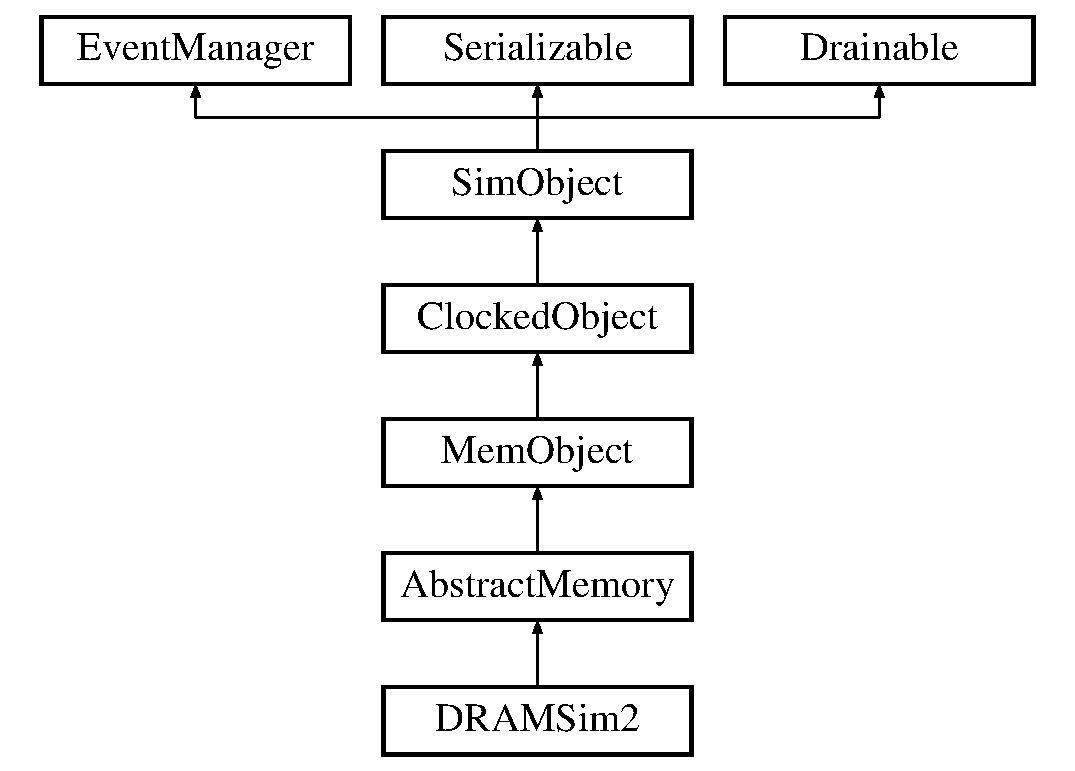
\includegraphics[height=6cm]{classAbstractMemory_1_1AbstractMemory}
\end{center}
\end{figure}
\subsection*{Static Public 変数}
\begin{DoxyCompactItemize}
\item 
string \hyperlink{classAbstractMemory_1_1AbstractMemory_acce15679d830831b0bbe8ebc2a60b2ca}{type} = '\hyperlink{classAbstractMemory_1_1AbstractMemory}{AbstractMemory}'
\item 
\hyperlink{classAbstractMemory_1_1AbstractMemory_a17fa61ac3806b481cafee5593b55e5d0}{abstract} = True
\item 
string \hyperlink{classAbstractMemory_1_1AbstractMemory_a17da7064bc5c518791f0c891eff05fda}{cxx\_\-header} = \char`\"{}mem/abstract\_\-mem.hh\char`\"{}
\item 
tuple \hyperlink{classAbstractMemory_1_1AbstractMemory_ae7aca7a468be02fee9f4e8d0af49932f}{range} = Param.AddrRange('128MB', \char`\"{}Address range (potentially interleaved)\char`\"{})
\item 
tuple \hyperlink{classAbstractMemory_1_1AbstractMemory_ab4d728107c8135f96ef3cb8c84621e90}{null} = Param.Bool(False, \char`\"{}Do not store data, always return zero\char`\"{})
\item 
tuple \hyperlink{classAbstractMemory_1_1AbstractMemory_a19b298706aab3f429aaf3d3e719613b3}{in\_\-addr\_\-map} = Param.Bool(True, \char`\"{}Memory part of the global address map\char`\"{})
\item 
tuple \hyperlink{classAbstractMemory_1_1AbstractMemory_a1d30f6c6ac50b7718dd64b8e7f9a0016}{conf\_\-table\_\-reported} = Param.Bool(True, \char`\"{}Report to configuration table\char`\"{})
\end{DoxyCompactItemize}


\subsection{変数}
\hypertarget{classAbstractMemory_1_1AbstractMemory_a17fa61ac3806b481cafee5593b55e5d0}{
\index{AbstractMemory::AbstractMemory@{AbstractMemory::AbstractMemory}!abstract@{abstract}}
\index{abstract@{abstract}!AbstractMemory::AbstractMemory@{AbstractMemory::AbstractMemory}}
\subsubsection[{abstract}]{\setlength{\rightskip}{0pt plus 5cm}{\bf abstract} = True\hspace{0.3cm}{\ttfamily  \mbox{[}static\mbox{]}}}}
\label{classAbstractMemory_1_1AbstractMemory_a17fa61ac3806b481cafee5593b55e5d0}


\hyperlink{classMemObject_1_1MemObject_a17fa61ac3806b481cafee5593b55e5d0}{MemObject}を再定義しています。\hypertarget{classAbstractMemory_1_1AbstractMemory_a1d30f6c6ac50b7718dd64b8e7f9a0016}{
\index{AbstractMemory::AbstractMemory@{AbstractMemory::AbstractMemory}!conf\_\-table\_\-reported@{conf\_\-table\_\-reported}}
\index{conf\_\-table\_\-reported@{conf\_\-table\_\-reported}!AbstractMemory::AbstractMemory@{AbstractMemory::AbstractMemory}}
\subsubsection[{conf\_\-table\_\-reported}]{\setlength{\rightskip}{0pt plus 5cm}tuple {\bf conf\_\-table\_\-reported} = Param.Bool(True, \char`\"{}Report to configuration table\char`\"{})\hspace{0.3cm}{\ttfamily  \mbox{[}static\mbox{]}}}}
\label{classAbstractMemory_1_1AbstractMemory_a1d30f6c6ac50b7718dd64b8e7f9a0016}
\hypertarget{classAbstractMemory_1_1AbstractMemory_a17da7064bc5c518791f0c891eff05fda}{
\index{AbstractMemory::AbstractMemory@{AbstractMemory::AbstractMemory}!cxx\_\-header@{cxx\_\-header}}
\index{cxx\_\-header@{cxx\_\-header}!AbstractMemory::AbstractMemory@{AbstractMemory::AbstractMemory}}
\subsubsection[{cxx\_\-header}]{\setlength{\rightskip}{0pt plus 5cm}string {\bf cxx\_\-header} = \char`\"{}mem/abstract\_\-mem.hh\char`\"{}\hspace{0.3cm}{\ttfamily  \mbox{[}static\mbox{]}}}}
\label{classAbstractMemory_1_1AbstractMemory_a17da7064bc5c518791f0c891eff05fda}


\hyperlink{classMemObject_1_1MemObject_a17da7064bc5c518791f0c891eff05fda}{MemObject}を再定義しています。

\hyperlink{classDRAMSim2_1_1DRAMSim2_a17da7064bc5c518791f0c891eff05fda}{DRAMSim2}で再定義されています。\hypertarget{classAbstractMemory_1_1AbstractMemory_a19b298706aab3f429aaf3d3e719613b3}{
\index{AbstractMemory::AbstractMemory@{AbstractMemory::AbstractMemory}!in\_\-addr\_\-map@{in\_\-addr\_\-map}}
\index{in\_\-addr\_\-map@{in\_\-addr\_\-map}!AbstractMemory::AbstractMemory@{AbstractMemory::AbstractMemory}}
\subsubsection[{in\_\-addr\_\-map}]{\setlength{\rightskip}{0pt plus 5cm}tuple {\bf in\_\-addr\_\-map} = Param.Bool(True, \char`\"{}Memory part of the global address map\char`\"{})\hspace{0.3cm}{\ttfamily  \mbox{[}static\mbox{]}}}}
\label{classAbstractMemory_1_1AbstractMemory_a19b298706aab3f429aaf3d3e719613b3}
\hypertarget{classAbstractMemory_1_1AbstractMemory_ab4d728107c8135f96ef3cb8c84621e90}{
\index{AbstractMemory::AbstractMemory@{AbstractMemory::AbstractMemory}!null@{null}}
\index{null@{null}!AbstractMemory::AbstractMemory@{AbstractMemory::AbstractMemory}}
\subsubsection[{null}]{\setlength{\rightskip}{0pt plus 5cm}tuple {\bf null} = Param.Bool(False, \char`\"{}Do not store data, always return zero\char`\"{})\hspace{0.3cm}{\ttfamily  \mbox{[}static\mbox{]}}}}
\label{classAbstractMemory_1_1AbstractMemory_ab4d728107c8135f96ef3cb8c84621e90}
\hypertarget{classAbstractMemory_1_1AbstractMemory_ae7aca7a468be02fee9f4e8d0af49932f}{
\index{AbstractMemory::AbstractMemory@{AbstractMemory::AbstractMemory}!range@{range}}
\index{range@{range}!AbstractMemory::AbstractMemory@{AbstractMemory::AbstractMemory}}
\subsubsection[{range}]{\setlength{\rightskip}{0pt plus 5cm}tuple {\bf range} = Param.AddrRange('128MB', \char`\"{}Address range (potentially interleaved)\char`\"{})\hspace{0.3cm}{\ttfamily  \mbox{[}static\mbox{]}}}}
\label{classAbstractMemory_1_1AbstractMemory_ae7aca7a468be02fee9f4e8d0af49932f}
\hypertarget{classAbstractMemory_1_1AbstractMemory_acce15679d830831b0bbe8ebc2a60b2ca}{
\index{AbstractMemory::AbstractMemory@{AbstractMemory::AbstractMemory}!type@{type}}
\index{type@{type}!AbstractMemory::AbstractMemory@{AbstractMemory::AbstractMemory}}
\subsubsection[{type}]{\setlength{\rightskip}{0pt plus 5cm}string {\bf type} = '{\bf AbstractMemory}'\hspace{0.3cm}{\ttfamily  \mbox{[}static\mbox{]}}}}
\label{classAbstractMemory_1_1AbstractMemory_acce15679d830831b0bbe8ebc2a60b2ca}


\hyperlink{classMemObject_1_1MemObject_acce15679d830831b0bbe8ebc2a60b2ca}{MemObject}を再定義しています。

\hyperlink{classDRAMSim2_1_1DRAMSim2_acce15679d830831b0bbe8ebc2a60b2ca}{DRAMSim2}で再定義されています。

このクラスの説明は次のファイルから生成されました:\begin{DoxyCompactItemize}
\item 
mem/\hyperlink{AbstractMemory_8py}{AbstractMemory.py}\end{DoxyCompactItemize}

\hypertarget{classAbstractReplacementPolicy}{
\section{クラス AbstractReplacementPolicy}
\label{classAbstractReplacementPolicy}\index{AbstractReplacementPolicy@{AbstractReplacementPolicy}}
}


{\ttfamily \#include $<$AbstractReplacementPolicy.hh$>$}AbstractReplacementPolicyに対する継承グラフ:\begin{figure}[H]
\begin{center}
\leavevmode
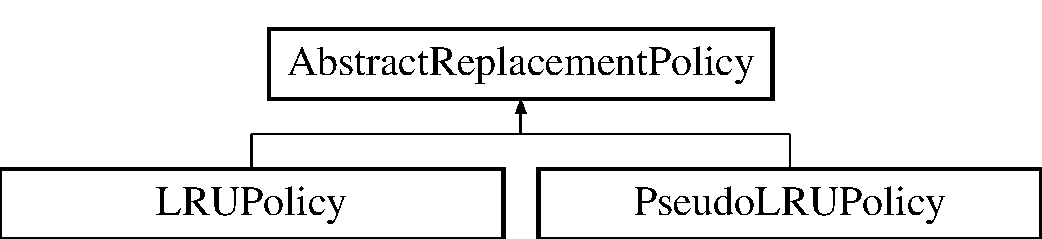
\includegraphics[height=2cm]{classAbstractReplacementPolicy}
\end{center}
\end{figure}
\subsection*{Public メソッド}
\begin{DoxyCompactItemize}
\item 
\hyperlink{classAbstractReplacementPolicy_a5a97664620a36d345954e66ae7cdbfb0}{AbstractReplacementPolicy} (\hyperlink{TypeDefines_8hh_a39642de41f3574937f399f4fab25ba18}{Index} num\_\-sets, \hyperlink{TypeDefines_8hh_a39642de41f3574937f399f4fab25ba18}{Index} assoc)
\item 
virtual \hyperlink{classAbstractReplacementPolicy_ae72a8485ba00ae76c66dd66ddebb07ff}{$\sim$AbstractReplacementPolicy} ()
\item 
virtual void \hyperlink{classAbstractReplacementPolicy_a6354174153ace07b8cef20f36b20357a}{touch} (\hyperlink{TypeDefines_8hh_a39642de41f3574937f399f4fab25ba18}{Index} set, \hyperlink{TypeDefines_8hh_a39642de41f3574937f399f4fab25ba18}{Index} way, \hyperlink{base_2types_8hh_a5c8ed81b7d238c9083e1037ba6d61643}{Tick} time)=0
\item 
virtual \hyperlink{TypeDefines_8hh_a39642de41f3574937f399f4fab25ba18}{Index} \hyperlink{classAbstractReplacementPolicy_a100bd69954d47ece014cbd697a1f8d7f}{getVictim} (\hyperlink{TypeDefines_8hh_a39642de41f3574937f399f4fab25ba18}{Index} set) const =0
\item 
\hyperlink{base_2types_8hh_a5c8ed81b7d238c9083e1037ba6d61643}{Tick} \hyperlink{classAbstractReplacementPolicy_afbe88ba793f4549f1c7ef274372433e9}{getLastAccess} (\hyperlink{TypeDefines_8hh_a39642de41f3574937f399f4fab25ba18}{Index} set, \hyperlink{TypeDefines_8hh_a39642de41f3574937f399f4fab25ba18}{Index} way)
\end{DoxyCompactItemize}
\subsection*{Protected 変数}
\begin{DoxyCompactItemize}
\item 
unsigned \hyperlink{classAbstractReplacementPolicy_a02f70f06d6633b7809066c8bd63a6a3e}{m\_\-num\_\-sets}
\item 
unsigned \hyperlink{classAbstractReplacementPolicy_a8ad9d20c98fe601aa72716ddc5b97f2d}{m\_\-assoc}
\item 
\hyperlink{base_2types_8hh_a5c8ed81b7d238c9083e1037ba6d61643}{Tick} $\ast$$\ast$ \hyperlink{classAbstractReplacementPolicy_a24a457a2854b5f62404b18272f5a3da3}{m\_\-last\_\-ref\_\-ptr}
\end{DoxyCompactItemize}


\subsection{コンストラクタとデストラクタ}
\hypertarget{classAbstractReplacementPolicy_a5a97664620a36d345954e66ae7cdbfb0}{
\index{AbstractReplacementPolicy@{AbstractReplacementPolicy}!AbstractReplacementPolicy@{AbstractReplacementPolicy}}
\index{AbstractReplacementPolicy@{AbstractReplacementPolicy}!AbstractReplacementPolicy@{AbstractReplacementPolicy}}
\subsubsection[{AbstractReplacementPolicy}]{\setlength{\rightskip}{0pt plus 5cm}{\bf AbstractReplacementPolicy} ({\bf Index} {\em num\_\-sets}, \/  {\bf Index} {\em assoc})\hspace{0.3cm}{\ttfamily  \mbox{[}inline\mbox{]}}}}
\label{classAbstractReplacementPolicy_a5a97664620a36d345954e66ae7cdbfb0}



\begin{DoxyCode}
58 {
59     m_num_sets = num_sets;
60     m_assoc = assoc;
61     m_last_ref_ptr = new Tick*[m_num_sets];
62     for(unsigned i = 0; i < m_num_sets; i++){
63         m_last_ref_ptr[i] = new Tick[m_assoc];
64         for(unsigned j = 0; j < m_assoc; j++){
65             m_last_ref_ptr[i][j] = 0;
66         }
67     }
68 }
\end{DoxyCode}
\hypertarget{classAbstractReplacementPolicy_ae72a8485ba00ae76c66dd66ddebb07ff}{
\index{AbstractReplacementPolicy@{AbstractReplacementPolicy}!$\sim$AbstractReplacementPolicy@{$\sim$AbstractReplacementPolicy}}
\index{$\sim$AbstractReplacementPolicy@{$\sim$AbstractReplacementPolicy}!AbstractReplacementPolicy@{AbstractReplacementPolicy}}
\subsubsection[{$\sim$AbstractReplacementPolicy}]{\setlength{\rightskip}{0pt plus 5cm}$\sim${\bf AbstractReplacementPolicy} ()\hspace{0.3cm}{\ttfamily  \mbox{[}inline, virtual\mbox{]}}}}
\label{classAbstractReplacementPolicy_ae72a8485ba00ae76c66dd66ddebb07ff}



\begin{DoxyCode}
72 {
73     if (m_last_ref_ptr != NULL){
74         for (unsigned i = 0; i < m_num_sets; i++){
75             if (m_last_ref_ptr[i] != NULL){
76                 delete[] m_last_ref_ptr[i];
77             }
78         }
79         delete[] m_last_ref_ptr;
80     }
81 }
\end{DoxyCode}


\subsection{関数}
\hypertarget{classAbstractReplacementPolicy_afbe88ba793f4549f1c7ef274372433e9}{
\index{AbstractReplacementPolicy@{AbstractReplacementPolicy}!getLastAccess@{getLastAccess}}
\index{getLastAccess@{getLastAccess}!AbstractReplacementPolicy@{AbstractReplacementPolicy}}
\subsubsection[{getLastAccess}]{\setlength{\rightskip}{0pt plus 5cm}{\bf Tick} getLastAccess ({\bf Index} {\em set}, \/  {\bf Index} {\em way})\hspace{0.3cm}{\ttfamily  \mbox{[}inline\mbox{]}}}}
\label{classAbstractReplacementPolicy_afbe88ba793f4549f1c7ef274372433e9}



\begin{DoxyCode}
85 {
86     return m_last_ref_ptr[set][way];
87 }
\end{DoxyCode}
\hypertarget{classAbstractReplacementPolicy_a100bd69954d47ece014cbd697a1f8d7f}{
\index{AbstractReplacementPolicy@{AbstractReplacementPolicy}!getVictim@{getVictim}}
\index{getVictim@{getVictim}!AbstractReplacementPolicy@{AbstractReplacementPolicy}}
\subsubsection[{getVictim}]{\setlength{\rightskip}{0pt plus 5cm}virtual {\bf Index} getVictim ({\bf Index} {\em set}) const\hspace{0.3cm}{\ttfamily  \mbox{[}pure virtual\mbox{]}}}}
\label{classAbstractReplacementPolicy_a100bd69954d47ece014cbd697a1f8d7f}


\hyperlink{classLRUPolicy_aad2c302009bdae8c2f86d7c4e0ed2c8f}{LRUPolicy}, と \hyperlink{classPseudoLRUPolicy_aad2c302009bdae8c2f86d7c4e0ed2c8f}{PseudoLRUPolicy}で実装されています。\hypertarget{classAbstractReplacementPolicy_a6354174153ace07b8cef20f36b20357a}{
\index{AbstractReplacementPolicy@{AbstractReplacementPolicy}!touch@{touch}}
\index{touch@{touch}!AbstractReplacementPolicy@{AbstractReplacementPolicy}}
\subsubsection[{touch}]{\setlength{\rightskip}{0pt plus 5cm}virtual void touch ({\bf Index} {\em set}, \/  {\bf Index} {\em way}, \/  {\bf Tick} {\em time})\hspace{0.3cm}{\ttfamily  \mbox{[}pure virtual\mbox{]}}}}
\label{classAbstractReplacementPolicy_a6354174153ace07b8cef20f36b20357a}


\hyperlink{classLRUPolicy_a6d3ff52feacdaba90c7c0bfbe9f7f58a}{LRUPolicy}, と \hyperlink{classPseudoLRUPolicy_a6d3ff52feacdaba90c7c0bfbe9f7f58a}{PseudoLRUPolicy}で実装されています。

\subsection{変数}
\hypertarget{classAbstractReplacementPolicy_a8ad9d20c98fe601aa72716ddc5b97f2d}{
\index{AbstractReplacementPolicy@{AbstractReplacementPolicy}!m\_\-assoc@{m\_\-assoc}}
\index{m\_\-assoc@{m\_\-assoc}!AbstractReplacementPolicy@{AbstractReplacementPolicy}}
\subsubsection[{m\_\-assoc}]{\setlength{\rightskip}{0pt plus 5cm}unsigned {\bf m\_\-assoc}\hspace{0.3cm}{\ttfamily  \mbox{[}protected\mbox{]}}}}
\label{classAbstractReplacementPolicy_a8ad9d20c98fe601aa72716ddc5b97f2d}
total number of sets \hypertarget{classAbstractReplacementPolicy_a24a457a2854b5f62404b18272f5a3da3}{
\index{AbstractReplacementPolicy@{AbstractReplacementPolicy}!m\_\-last\_\-ref\_\-ptr@{m\_\-last\_\-ref\_\-ptr}}
\index{m\_\-last\_\-ref\_\-ptr@{m\_\-last\_\-ref\_\-ptr}!AbstractReplacementPolicy@{AbstractReplacementPolicy}}
\subsubsection[{m\_\-last\_\-ref\_\-ptr}]{\setlength{\rightskip}{0pt plus 5cm}{\bf Tick}$\ast$$\ast$ {\bf m\_\-last\_\-ref\_\-ptr}\hspace{0.3cm}{\ttfamily  \mbox{[}protected\mbox{]}}}}
\label{classAbstractReplacementPolicy_a24a457a2854b5f62404b18272f5a3da3}
set associativity \hypertarget{classAbstractReplacementPolicy_a02f70f06d6633b7809066c8bd63a6a3e}{
\index{AbstractReplacementPolicy@{AbstractReplacementPolicy}!m\_\-num\_\-sets@{m\_\-num\_\-sets}}
\index{m\_\-num\_\-sets@{m\_\-num\_\-sets}!AbstractReplacementPolicy@{AbstractReplacementPolicy}}
\subsubsection[{m\_\-num\_\-sets}]{\setlength{\rightskip}{0pt plus 5cm}unsigned {\bf m\_\-num\_\-sets}\hspace{0.3cm}{\ttfamily  \mbox{[}protected\mbox{]}}}}
\label{classAbstractReplacementPolicy_a02f70f06d6633b7809066c8bd63a6a3e}


このクラスの説明は次のファイルから生成されました:\begin{DoxyCompactItemize}
\item 
mem/ruby/system/\hyperlink{AbstractReplacementPolicy_8hh}{AbstractReplacementPolicy.hh}\end{DoxyCompactItemize}

\hypertarget{structAlphaBackdoor_1_1Access}{
\section{構造体 Access}
\label{structAlphaBackdoor_1_1Access}\index{AlphaBackdoor::Access@{AlphaBackdoor::Access}}
}


{\ttfamily \#include $<$backdoor.hh$>$}Accessに対する継承グラフ:\begin{figure}[H]
\begin{center}
\leavevmode
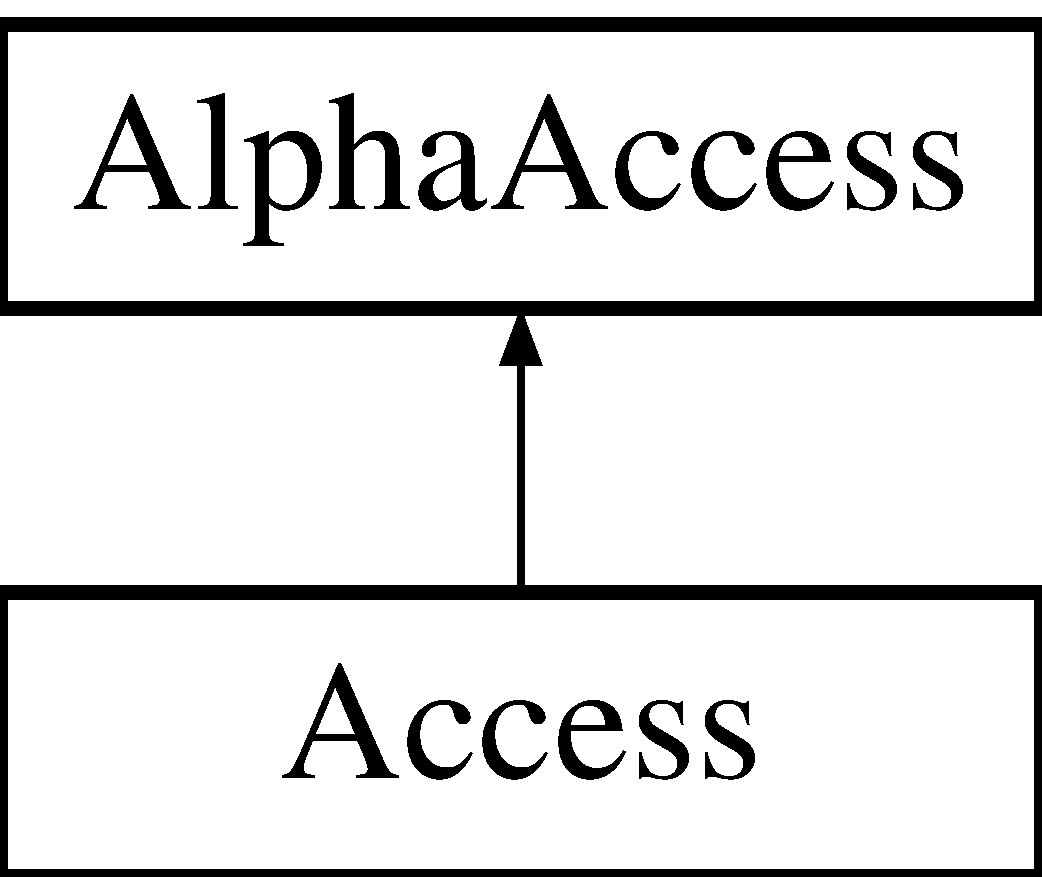
\includegraphics[height=2cm]{structAlphaBackdoor_1_1Access}
\end{center}
\end{figure}
\subsection*{Public メソッド}
\begin{DoxyCompactItemize}
\item 
void \hyperlink{structAlphaBackdoor_1_1Access_a53e036786d17361be4c7320d39c99b84}{serialize} (std::ostream \&os)
\item 
void \hyperlink{structAlphaBackdoor_1_1Access_af22e5d6d660b97db37003ac61ac4ee49}{unserialize} (\hyperlink{classCheckpoint}{Checkpoint} $\ast$cp, const std::string \&section)
\end{DoxyCompactItemize}


\subsection{関数}
\hypertarget{structAlphaBackdoor_1_1Access_a53e036786d17361be4c7320d39c99b84}{
\index{AlphaBackdoor::Access@{AlphaBackdoor::Access}!serialize@{serialize}}
\index{serialize@{serialize}!AlphaBackdoor::Access@{AlphaBackdoor::Access}}
\subsubsection[{serialize}]{\setlength{\rightskip}{0pt plus 5cm}void serialize (std::ostream \& {\em os})}}
\label{structAlphaBackdoor_1_1Access_a53e036786d17361be4c7320d39c99b84}
\hypertarget{structAlphaBackdoor_1_1Access_af22e5d6d660b97db37003ac61ac4ee49}{
\index{AlphaBackdoor::Access@{AlphaBackdoor::Access}!unserialize@{unserialize}}
\index{unserialize@{unserialize}!AlphaBackdoor::Access@{AlphaBackdoor::Access}}
\subsubsection[{unserialize}]{\setlength{\rightskip}{0pt plus 5cm}void unserialize ({\bf Checkpoint} $\ast$ {\em cp}, \/  const std::string \& {\em section})}}
\label{structAlphaBackdoor_1_1Access_af22e5d6d660b97db37003ac61ac4ee49}



\begin{DoxyCode}
279 {
280     UNSERIALIZE_SCALAR(last_offset);
281     UNSERIALIZE_SCALAR(version);
282     UNSERIALIZE_SCALAR(numCPUs);
283     UNSERIALIZE_SCALAR(mem_size);
284     UNSERIALIZE_SCALAR(cpuClock);
285     UNSERIALIZE_SCALAR(intrClockFrequency);
286     UNSERIALIZE_SCALAR(kernStart);
287     UNSERIALIZE_SCALAR(kernEnd);
288     UNSERIALIZE_SCALAR(entryPoint);
289     UNSERIALIZE_SCALAR(diskUnit);
290     UNSERIALIZE_SCALAR(diskCount);
291     UNSERIALIZE_SCALAR(diskPAddr);
292     UNSERIALIZE_SCALAR(diskBlock);
293     UNSERIALIZE_SCALAR(diskOperation);
294     UNSERIALIZE_SCALAR(outputChar);
295     UNSERIALIZE_SCALAR(inputChar);
296     UNSERIALIZE_ARRAY(cpuStack, 64);
297 }
\end{DoxyCode}


この構造体の説明は次のファイルから生成されました:\begin{DoxyCompactItemize}
\item 
dev/alpha/\hyperlink{backdoor_8hh}{backdoor.hh}\item 
dev/alpha/\hyperlink{backdoor_8cc}{backdoor.cc}\end{DoxyCompactItemize}

\hypertarget{classBankedArray_1_1AccessRecord}{
\section{クラス AccessRecord}
\label{classBankedArray_1_1AccessRecord}\index{BankedArray::AccessRecord@{BankedArray::AccessRecord}}
}
\subsection*{Public メソッド}
\begin{DoxyCompactItemize}
\item 
\hyperlink{classBankedArray_1_1AccessRecord_a1013e7a3eaa4336fe8ad1d0efd6497d1}{AccessRecord} ()
\end{DoxyCompactItemize}
\subsection*{Public 変数}
\begin{DoxyCompactItemize}
\item 
\hyperlink{TypeDefines_8hh_a39642de41f3574937f399f4fab25ba18}{Index} \hyperlink{classBankedArray_1_1AccessRecord_a6f53eba8af00fbd74cde35b7c969c63b}{idx}
\item 
\hyperlink{base_2types_8hh_a5c8ed81b7d238c9083e1037ba6d61643}{Tick} \hyperlink{classBankedArray_1_1AccessRecord_affa12ca1e67f52a12e4e229390e9fb95}{startAccess}
\item 
\hyperlink{base_2types_8hh_a5c8ed81b7d238c9083e1037ba6d61643}{Tick} \hyperlink{classBankedArray_1_1AccessRecord_aa168738fc5b3f26027b295fb7693b895}{endAccess}
\end{DoxyCompactItemize}


\subsection{コンストラクタとデストラクタ}
\hypertarget{classBankedArray_1_1AccessRecord_a1013e7a3eaa4336fe8ad1d0efd6497d1}{
\index{BankedArray::AccessRecord@{BankedArray::AccessRecord}!AccessRecord@{AccessRecord}}
\index{AccessRecord@{AccessRecord}!BankedArray::AccessRecord@{BankedArray::AccessRecord}}
\subsubsection[{AccessRecord}]{\setlength{\rightskip}{0pt plus 5cm}{\bf AccessRecord} ()\hspace{0.3cm}{\ttfamily  \mbox{[}inline\mbox{]}}}}
\label{classBankedArray_1_1AccessRecord_a1013e7a3eaa4336fe8ad1d0efd6497d1}



\begin{DoxyCode}
51 : idx(0), startAccess(0), endAccess(0) {}
\end{DoxyCode}


\subsection{変数}
\hypertarget{classBankedArray_1_1AccessRecord_aa168738fc5b3f26027b295fb7693b895}{
\index{BankedArray::AccessRecord@{BankedArray::AccessRecord}!endAccess@{endAccess}}
\index{endAccess@{endAccess}!BankedArray::AccessRecord@{BankedArray::AccessRecord}}
\subsubsection[{endAccess}]{\setlength{\rightskip}{0pt plus 5cm}{\bf Tick} {\bf endAccess}}}
\label{classBankedArray_1_1AccessRecord_aa168738fc5b3f26027b295fb7693b895}
\hypertarget{classBankedArray_1_1AccessRecord_a6f53eba8af00fbd74cde35b7c969c63b}{
\index{BankedArray::AccessRecord@{BankedArray::AccessRecord}!idx@{idx}}
\index{idx@{idx}!BankedArray::AccessRecord@{BankedArray::AccessRecord}}
\subsubsection[{idx}]{\setlength{\rightskip}{0pt plus 5cm}{\bf Index} {\bf idx}}}
\label{classBankedArray_1_1AccessRecord_a6f53eba8af00fbd74cde35b7c969c63b}
\hypertarget{classBankedArray_1_1AccessRecord_affa12ca1e67f52a12e4e229390e9fb95}{
\index{BankedArray::AccessRecord@{BankedArray::AccessRecord}!startAccess@{startAccess}}
\index{startAccess@{startAccess}!BankedArray::AccessRecord@{BankedArray::AccessRecord}}
\subsubsection[{startAccess}]{\setlength{\rightskip}{0pt plus 5cm}{\bf Tick} {\bf startAccess}}}
\label{classBankedArray_1_1AccessRecord_affa12ca1e67f52a12e4e229390e9fb95}


このクラスの説明は次のファイルから生成されました:\begin{DoxyCompactItemize}
\item 
mem/ruby/system/\hyperlink{BankedArray_8hh}{BankedArray.hh}\end{DoxyCompactItemize}

\hypertarget{classAccessTraceForAddress}{
\section{クラス AccessTraceForAddress}
\label{classAccessTraceForAddress}\index{AccessTraceForAddress@{AccessTraceForAddress}}
}


{\ttfamily \#include $<$AccessTraceForAddress.hh$>$}\subsection*{Public メソッド}
\begin{DoxyCompactItemize}
\item 
\hyperlink{classAccessTraceForAddress_a39e3c32f62a22b90aae6b635958cd33b}{AccessTraceForAddress} ()
\item 
\hyperlink{classAccessTraceForAddress_aaa716e2119d8eda1e7428c63cedd2d75}{$\sim$AccessTraceForAddress} ()
\item 
void \hyperlink{classAccessTraceForAddress_a53120b1754f27e405338f9ab6e3408cc}{setAddress} (const \hyperlink{classAddress}{Address} \&addr)
\item 
void \hyperlink{classAccessTraceForAddress_a6ef5b8f5316bc299293f80e66d246a34}{update} (RubyRequestType type, RubyAccessMode access\_\-mode, \hyperlink{TypeDefines_8hh_a83c14b4ae37e80071f6b3506a6c46151}{NodeID} cpu, bool sharing\_\-miss)
\item 
int \hyperlink{classAccessTraceForAddress_af262952019c2e5f874224855cf7fb8bd}{getTotal} () const 
\item 
int \hyperlink{classAccessTraceForAddress_a7cf842218272765ebb03269975968026}{getSharing} () const 
\item 
int \hyperlink{classAccessTraceForAddress_a85c70aea5e7b3ab23bd505f66e16cbef}{getTouchedBy} () const 
\item 
const \hyperlink{classAddress}{Address} \& \hyperlink{classAccessTraceForAddress_aca15ef966561def0b4db75a6f7e085b6}{getAddress} () const 
\item 
void \hyperlink{classAccessTraceForAddress_ae8690c0646a12dd970f77127705f1449}{addSample} (int value)
\item 
void \hyperlink{classAccessTraceForAddress_ac55fe386a101fbae38c716067c9966a0}{print} (std::ostream \&out) const 
\end{DoxyCompactItemize}
\subsection*{Static Public メソッド}
\begin{DoxyCompactItemize}
\item 
static bool \hyperlink{classAccessTraceForAddress_af4b2dcff6f65bd1bcbcc0cd9995d0d35}{less\_\-equal} (const \hyperlink{classAccessTraceForAddress}{AccessTraceForAddress} $\ast$n1, const \hyperlink{classAccessTraceForAddress}{AccessTraceForAddress} $\ast$n2)
\end{DoxyCompactItemize}
\subsection*{Private 変数}
\begin{DoxyCompactItemize}
\item 
\hyperlink{classAddress}{Address} \hyperlink{classAccessTraceForAddress_a82a0fb091bb145547996e49b5ee3dde2}{m\_\-addr}
\item 
\hyperlink{TypeDefines_8hh_a29940ae63ec06c9998bba873e25407ad}{uint64} \hyperlink{classAccessTraceForAddress_ae62f2a92a6f690a36ae0b5ced2d59436}{m\_\-loads}
\item 
\hyperlink{TypeDefines_8hh_a29940ae63ec06c9998bba873e25407ad}{uint64} \hyperlink{classAccessTraceForAddress_abcc38814f3109146f39c33101a05acfa}{m\_\-stores}
\item 
\hyperlink{TypeDefines_8hh_a29940ae63ec06c9998bba873e25407ad}{uint64} \hyperlink{classAccessTraceForAddress_a1ea551bccefc550ef504659581af39e2}{m\_\-atomics}
\item 
\hyperlink{TypeDefines_8hh_a29940ae63ec06c9998bba873e25407ad}{uint64} \hyperlink{classAccessTraceForAddress_af87f35ffb1854fd41c3a82edaf4a9ff7}{m\_\-total}
\item 
\hyperlink{TypeDefines_8hh_a29940ae63ec06c9998bba873e25407ad}{uint64} \hyperlink{classAccessTraceForAddress_a4050103e54b773a2c5905995b437c5cf}{m\_\-user}
\item 
\hyperlink{TypeDefines_8hh_a29940ae63ec06c9998bba873e25407ad}{uint64} \hyperlink{classAccessTraceForAddress_a540937c20ba2f2895bc4a5bb3aac19dd}{m\_\-sharing}
\item 
\hyperlink{classSet}{Set} \hyperlink{classAccessTraceForAddress_a4949c45d0cddbcbbefb81cc89c85cf17}{m\_\-touched\_\-by}
\item 
\hyperlink{classHistogram}{Histogram} $\ast$ \hyperlink{classAccessTraceForAddress_ab6bcc5b2b4ee7d5b76f8bb879015abcc}{m\_\-histogram\_\-ptr}
\end{DoxyCompactItemize}


\subsection{コンストラクタとデストラクタ}
\hypertarget{classAccessTraceForAddress_a39e3c32f62a22b90aae6b635958cd33b}{
\index{AccessTraceForAddress@{AccessTraceForAddress}!AccessTraceForAddress@{AccessTraceForAddress}}
\index{AccessTraceForAddress@{AccessTraceForAddress}!AccessTraceForAddress@{AccessTraceForAddress}}
\subsubsection[{AccessTraceForAddress}]{\setlength{\rightskip}{0pt plus 5cm}{\bf AccessTraceForAddress} ()\hspace{0.3cm}{\ttfamily  \mbox{[}inline\mbox{]}}}}
\label{classAccessTraceForAddress_a39e3c32f62a22b90aae6b635958cd33b}



\begin{DoxyCode}
46         : m_loads(0), m_stores(0), m_atomics(0), m_total(0), m_user(0),
47           m_sharing(0), m_histogram_ptr(NULL)
48     { }
\end{DoxyCode}
\hypertarget{classAccessTraceForAddress_aaa716e2119d8eda1e7428c63cedd2d75}{
\index{AccessTraceForAddress@{AccessTraceForAddress}!$\sim$AccessTraceForAddress@{$\sim$AccessTraceForAddress}}
\index{$\sim$AccessTraceForAddress@{$\sim$AccessTraceForAddress}!AccessTraceForAddress@{AccessTraceForAddress}}
\subsubsection[{$\sim$AccessTraceForAddress}]{\setlength{\rightskip}{0pt plus 5cm}$\sim${\bf AccessTraceForAddress} ()}}
\label{classAccessTraceForAddress_aaa716e2119d8eda1e7428c63cedd2d75}



\begin{DoxyCode}
33 {
34     if (m_histogram_ptr) {
35         delete m_histogram_ptr;
36         m_histogram_ptr = NULL;
37     }
38 }
\end{DoxyCode}


\subsection{関数}
\hypertarget{classAccessTraceForAddress_ae8690c0646a12dd970f77127705f1449}{
\index{AccessTraceForAddress@{AccessTraceForAddress}!addSample@{addSample}}
\index{addSample@{addSample}!AccessTraceForAddress@{AccessTraceForAddress}}
\subsubsection[{addSample}]{\setlength{\rightskip}{0pt plus 5cm}void addSample (int {\em value})}}
\label{classAccessTraceForAddress_ae8690c0646a12dd970f77127705f1449}



\begin{DoxyCode}
98 {
99     assert(m_total == 0);
100     if (m_histogram_ptr == NULL) {
101         m_histogram_ptr = new Histogram;
102     }
103     m_histogram_ptr->add(value);
104 }
\end{DoxyCode}
\hypertarget{classAccessTraceForAddress_aca15ef966561def0b4db75a6f7e085b6}{
\index{AccessTraceForAddress@{AccessTraceForAddress}!getAddress@{getAddress}}
\index{getAddress@{getAddress}!AccessTraceForAddress@{AccessTraceForAddress}}
\subsubsection[{getAddress}]{\setlength{\rightskip}{0pt plus 5cm}const {\bf Address}\& getAddress () const\hspace{0.3cm}{\ttfamily  \mbox{[}inline\mbox{]}}}}
\label{classAccessTraceForAddress_aca15ef966561def0b4db75a6f7e085b6}



\begin{DoxyCode}
57 { return m_addr; }
\end{DoxyCode}
\hypertarget{classAccessTraceForAddress_a7cf842218272765ebb03269975968026}{
\index{AccessTraceForAddress@{AccessTraceForAddress}!getSharing@{getSharing}}
\index{getSharing@{getSharing}!AccessTraceForAddress@{AccessTraceForAddress}}
\subsubsection[{getSharing}]{\setlength{\rightskip}{0pt plus 5cm}int getSharing () const\hspace{0.3cm}{\ttfamily  \mbox{[}inline\mbox{]}}}}
\label{classAccessTraceForAddress_a7cf842218272765ebb03269975968026}



\begin{DoxyCode}
55 { return m_sharing; }
\end{DoxyCode}
\hypertarget{classAccessTraceForAddress_af262952019c2e5f874224855cf7fb8bd}{
\index{AccessTraceForAddress@{AccessTraceForAddress}!getTotal@{getTotal}}
\index{getTotal@{getTotal}!AccessTraceForAddress@{AccessTraceForAddress}}
\subsubsection[{getTotal}]{\setlength{\rightskip}{0pt plus 5cm}int getTotal () const}}
\label{classAccessTraceForAddress_af262952019c2e5f874224855cf7fb8bd}



\begin{DoxyCode}
88 {
89     if (m_histogram_ptr == NULL) {
90         return m_total;
91     } else {
92         return m_histogram_ptr->getTotal();
93     }
94 }
\end{DoxyCode}
\hypertarget{classAccessTraceForAddress_a85c70aea5e7b3ab23bd505f66e16cbef}{
\index{AccessTraceForAddress@{AccessTraceForAddress}!getTouchedBy@{getTouchedBy}}
\index{getTouchedBy@{getTouchedBy}!AccessTraceForAddress@{AccessTraceForAddress}}
\subsubsection[{getTouchedBy}]{\setlength{\rightskip}{0pt plus 5cm}int getTouchedBy () const\hspace{0.3cm}{\ttfamily  \mbox{[}inline\mbox{]}}}}
\label{classAccessTraceForAddress_a85c70aea5e7b3ab23bd505f66e16cbef}



\begin{DoxyCode}
56 { return m_touched_by.count(); }
\end{DoxyCode}
\hypertarget{classAccessTraceForAddress_af4b2dcff6f65bd1bcbcc0cd9995d0d35}{
\index{AccessTraceForAddress@{AccessTraceForAddress}!less\_\-equal@{less\_\-equal}}
\index{less\_\-equal@{less\_\-equal}!AccessTraceForAddress@{AccessTraceForAddress}}
\subsubsection[{less\_\-equal}]{\setlength{\rightskip}{0pt plus 5cm}static bool less\_\-equal (const {\bf AccessTraceForAddress} $\ast$ {\em n1}, \/  const {\bf AccessTraceForAddress} $\ast$ {\em n2})\hspace{0.3cm}{\ttfamily  \mbox{[}inline, static\mbox{]}}}}
\label{classAccessTraceForAddress_af4b2dcff6f65bd1bcbcc0cd9995d0d35}



\begin{DoxyCode}
65     {
66         return n1->getTotal() <= n2->getTotal();
67     }
\end{DoxyCode}
\hypertarget{classAccessTraceForAddress_ac55fe386a101fbae38c716067c9966a0}{
\index{AccessTraceForAddress@{AccessTraceForAddress}!print@{print}}
\index{print@{print}!AccessTraceForAddress@{AccessTraceForAddress}}
\subsubsection[{print}]{\setlength{\rightskip}{0pt plus 5cm}void print (std::ostream \& {\em out}) const}}
\label{classAccessTraceForAddress_ac55fe386a101fbae38c716067c9966a0}



\begin{DoxyCode}
42 {
43     out << m_addr;
44 
45     if (m_histogram_ptr == NULL) {
46         out << " " << m_total;
47         out << " | " << m_loads;
48         out << " " << m_stores;
49         out << " " << m_atomics;
50         out << " | " << m_user;
51         out << " " << m_total-m_user;
52         out << " | " << m_sharing;
53         out << " | " << m_touched_by.count();
54     } else {
55         assert(m_total == 0);
56         out << " " << (*m_histogram_ptr);
57     }
58 }
\end{DoxyCode}
\hypertarget{classAccessTraceForAddress_a53120b1754f27e405338f9ab6e3408cc}{
\index{AccessTraceForAddress@{AccessTraceForAddress}!setAddress@{setAddress}}
\index{setAddress@{setAddress}!AccessTraceForAddress@{AccessTraceForAddress}}
\subsubsection[{setAddress}]{\setlength{\rightskip}{0pt plus 5cm}void setAddress (const {\bf Address} \& {\em addr})\hspace{0.3cm}{\ttfamily  \mbox{[}inline\mbox{]}}}}
\label{classAccessTraceForAddress_a53120b1754f27e405338f9ab6e3408cc}



\begin{DoxyCode}
51 { m_addr = addr; }
\end{DoxyCode}
\hypertarget{classAccessTraceForAddress_a6ef5b8f5316bc299293f80e66d246a34}{
\index{AccessTraceForAddress@{AccessTraceForAddress}!update@{update}}
\index{update@{update}!AccessTraceForAddress@{AccessTraceForAddress}}
\subsubsection[{update}]{\setlength{\rightskip}{0pt plus 5cm}void update (RubyRequestType {\em type}, \/  RubyAccessMode {\em access\_\-mode}, \/  {\bf NodeID} {\em cpu}, \/  bool {\em sharing\_\-miss})}}
\label{classAccessTraceForAddress_a6ef5b8f5316bc299293f80e66d246a34}



\begin{DoxyCode}
64 {
65     m_touched_by.add(cpu);
66     m_total++;
67     if(type == RubyRequestType_ATOMIC) {
68         m_atomics++;
69     } else if(type == RubyRequestType_LD){
70         m_loads++;
71     } else if (type == RubyRequestType_ST){
72         m_stores++;
73     } else {
74         //  ERROR_MSG("Trying to add invalid access to trace");
75     }
76 
77     if (access_mode == RubyAccessMode_User) {
78         m_user++;
79     }
80 
81     if (sharing_miss) {
82         m_sharing++;
83     }
84 }
\end{DoxyCode}


\subsection{変数}
\hypertarget{classAccessTraceForAddress_a82a0fb091bb145547996e49b5ee3dde2}{
\index{AccessTraceForAddress@{AccessTraceForAddress}!m\_\-addr@{m\_\-addr}}
\index{m\_\-addr@{m\_\-addr}!AccessTraceForAddress@{AccessTraceForAddress}}
\subsubsection[{m\_\-addr}]{\setlength{\rightskip}{0pt plus 5cm}{\bf Address} {\bf m\_\-addr}\hspace{0.3cm}{\ttfamily  \mbox{[}private\mbox{]}}}}
\label{classAccessTraceForAddress_a82a0fb091bb145547996e49b5ee3dde2}
\hypertarget{classAccessTraceForAddress_a1ea551bccefc550ef504659581af39e2}{
\index{AccessTraceForAddress@{AccessTraceForAddress}!m\_\-atomics@{m\_\-atomics}}
\index{m\_\-atomics@{m\_\-atomics}!AccessTraceForAddress@{AccessTraceForAddress}}
\subsubsection[{m\_\-atomics}]{\setlength{\rightskip}{0pt plus 5cm}{\bf uint64} {\bf m\_\-atomics}\hspace{0.3cm}{\ttfamily  \mbox{[}private\mbox{]}}}}
\label{classAccessTraceForAddress_a1ea551bccefc550ef504659581af39e2}
\hypertarget{classAccessTraceForAddress_ab6bcc5b2b4ee7d5b76f8bb879015abcc}{
\index{AccessTraceForAddress@{AccessTraceForAddress}!m\_\-histogram\_\-ptr@{m\_\-histogram\_\-ptr}}
\index{m\_\-histogram\_\-ptr@{m\_\-histogram\_\-ptr}!AccessTraceForAddress@{AccessTraceForAddress}}
\subsubsection[{m\_\-histogram\_\-ptr}]{\setlength{\rightskip}{0pt plus 5cm}{\bf Histogram}$\ast$ {\bf m\_\-histogram\_\-ptr}\hspace{0.3cm}{\ttfamily  \mbox{[}private\mbox{]}}}}
\label{classAccessTraceForAddress_ab6bcc5b2b4ee7d5b76f8bb879015abcc}
\hypertarget{classAccessTraceForAddress_ae62f2a92a6f690a36ae0b5ced2d59436}{
\index{AccessTraceForAddress@{AccessTraceForAddress}!m\_\-loads@{m\_\-loads}}
\index{m\_\-loads@{m\_\-loads}!AccessTraceForAddress@{AccessTraceForAddress}}
\subsubsection[{m\_\-loads}]{\setlength{\rightskip}{0pt plus 5cm}{\bf uint64} {\bf m\_\-loads}\hspace{0.3cm}{\ttfamily  \mbox{[}private\mbox{]}}}}
\label{classAccessTraceForAddress_ae62f2a92a6f690a36ae0b5ced2d59436}
\hypertarget{classAccessTraceForAddress_a540937c20ba2f2895bc4a5bb3aac19dd}{
\index{AccessTraceForAddress@{AccessTraceForAddress}!m\_\-sharing@{m\_\-sharing}}
\index{m\_\-sharing@{m\_\-sharing}!AccessTraceForAddress@{AccessTraceForAddress}}
\subsubsection[{m\_\-sharing}]{\setlength{\rightskip}{0pt plus 5cm}{\bf uint64} {\bf m\_\-sharing}\hspace{0.3cm}{\ttfamily  \mbox{[}private\mbox{]}}}}
\label{classAccessTraceForAddress_a540937c20ba2f2895bc4a5bb3aac19dd}
\hypertarget{classAccessTraceForAddress_abcc38814f3109146f39c33101a05acfa}{
\index{AccessTraceForAddress@{AccessTraceForAddress}!m\_\-stores@{m\_\-stores}}
\index{m\_\-stores@{m\_\-stores}!AccessTraceForAddress@{AccessTraceForAddress}}
\subsubsection[{m\_\-stores}]{\setlength{\rightskip}{0pt plus 5cm}{\bf uint64} {\bf m\_\-stores}\hspace{0.3cm}{\ttfamily  \mbox{[}private\mbox{]}}}}
\label{classAccessTraceForAddress_abcc38814f3109146f39c33101a05acfa}
\hypertarget{classAccessTraceForAddress_af87f35ffb1854fd41c3a82edaf4a9ff7}{
\index{AccessTraceForAddress@{AccessTraceForAddress}!m\_\-total@{m\_\-total}}
\index{m\_\-total@{m\_\-total}!AccessTraceForAddress@{AccessTraceForAddress}}
\subsubsection[{m\_\-total}]{\setlength{\rightskip}{0pt plus 5cm}{\bf uint64} {\bf m\_\-total}\hspace{0.3cm}{\ttfamily  \mbox{[}private\mbox{]}}}}
\label{classAccessTraceForAddress_af87f35ffb1854fd41c3a82edaf4a9ff7}
\hypertarget{classAccessTraceForAddress_a4949c45d0cddbcbbefb81cc89c85cf17}{
\index{AccessTraceForAddress@{AccessTraceForAddress}!m\_\-touched\_\-by@{m\_\-touched\_\-by}}
\index{m\_\-touched\_\-by@{m\_\-touched\_\-by}!AccessTraceForAddress@{AccessTraceForAddress}}
\subsubsection[{m\_\-touched\_\-by}]{\setlength{\rightskip}{0pt plus 5cm}{\bf Set} {\bf m\_\-touched\_\-by}\hspace{0.3cm}{\ttfamily  \mbox{[}private\mbox{]}}}}
\label{classAccessTraceForAddress_a4949c45d0cddbcbbefb81cc89c85cf17}
\hypertarget{classAccessTraceForAddress_a4050103e54b773a2c5905995b437c5cf}{
\index{AccessTraceForAddress@{AccessTraceForAddress}!m\_\-user@{m\_\-user}}
\index{m\_\-user@{m\_\-user}!AccessTraceForAddress@{AccessTraceForAddress}}
\subsubsection[{m\_\-user}]{\setlength{\rightskip}{0pt plus 5cm}{\bf uint64} {\bf m\_\-user}\hspace{0.3cm}{\ttfamily  \mbox{[}private\mbox{]}}}}
\label{classAccessTraceForAddress_a4050103e54b773a2c5905995b437c5cf}


このクラスの説明は次のファイルから生成されました:\begin{DoxyCompactItemize}
\item 
mem/ruby/profiler/\hyperlink{AccessTraceForAddress_8hh}{AccessTraceForAddress.hh}\item 
mem/ruby/profiler/\hyperlink{AccessTraceForAddress_8cc}{AccessTraceForAddress.cc}\end{DoxyCompactItemize}

\hypertarget{classslicc_1_1symbols_1_1Action_1_1Action}{
\section{クラス Action}
\label{classslicc_1_1symbols_1_1Action_1_1Action}\index{slicc::symbols::Action::Action@{slicc::symbols::Action::Action}}
}
Actionに対する継承グラフ:\begin{figure}[H]
\begin{center}
\leavevmode
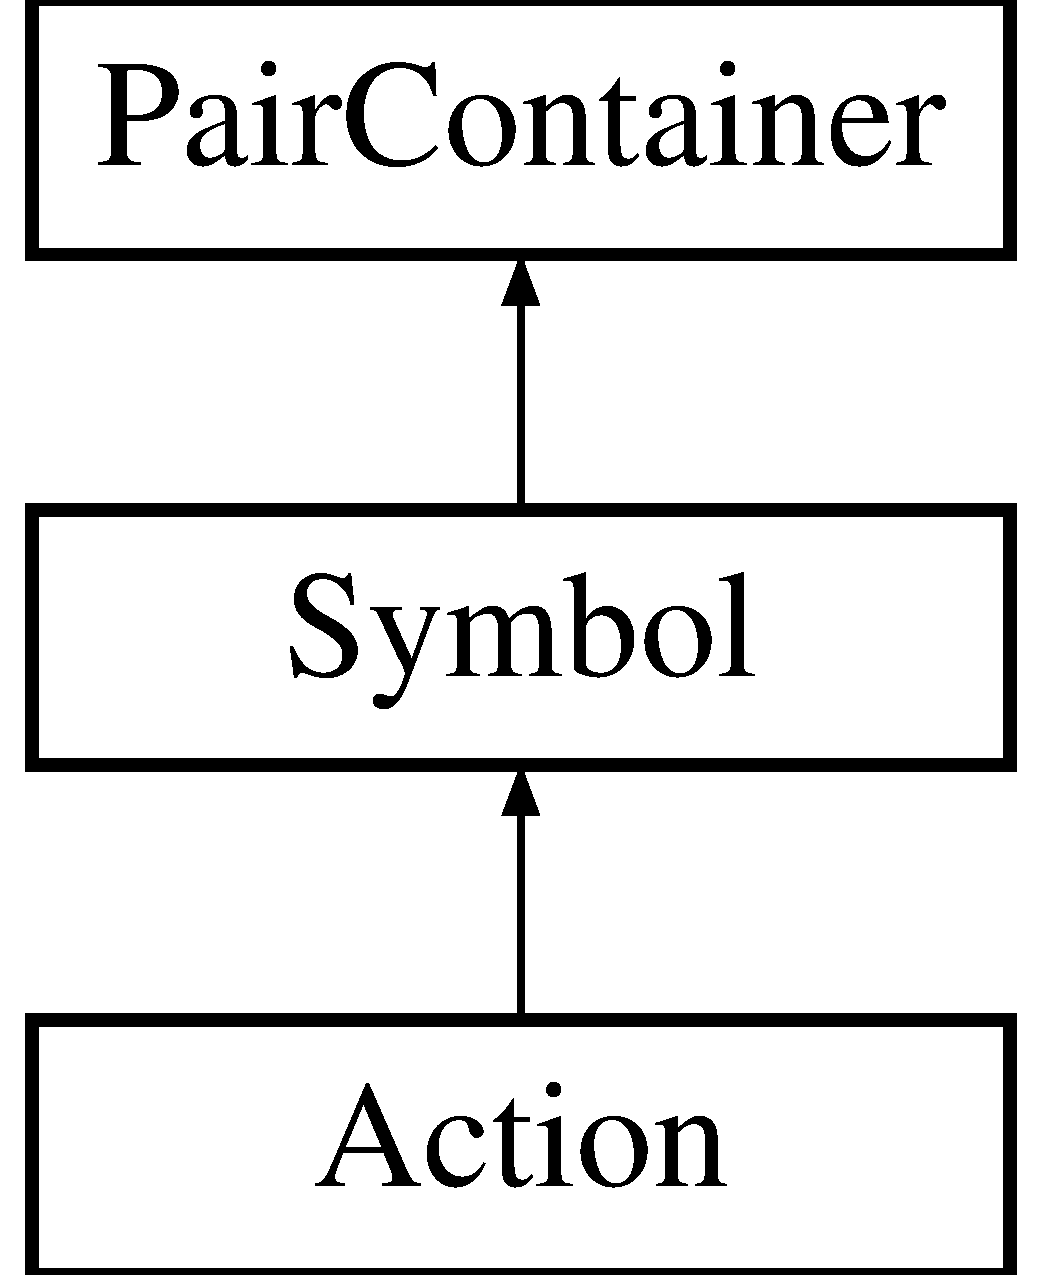
\includegraphics[height=3cm]{classslicc_1_1symbols_1_1Action_1_1Action}
\end{center}
\end{figure}
\subsection*{Public メソッド}
\begin{DoxyCompactItemize}
\item 
def \hyperlink{classslicc_1_1symbols_1_1Action_1_1Action_ac775ee34451fdfa742b318538164070e}{\_\-\_\-init\_\-\_\-}
\item 
def \hyperlink{classslicc_1_1symbols_1_1Action_1_1Action_ad8b9328939df072e4740cd9a63189744}{\_\-\_\-repr\_\-\_\-}
\end{DoxyCompactItemize}
\subsection*{Public 変数}
\begin{DoxyCompactItemize}
\item 
\hyperlink{classslicc_1_1symbols_1_1Action_1_1Action_a715e7b31400aa585643e94e0ba160aab}{resources}
\end{DoxyCompactItemize}


\subsection{関数}
\hypertarget{classslicc_1_1symbols_1_1Action_1_1Action_ac775ee34451fdfa742b318538164070e}{
\index{slicc::symbols::Action::Action@{slicc::symbols::Action::Action}!\_\-\_\-init\_\-\_\-@{\_\-\_\-init\_\-\_\-}}
\index{\_\-\_\-init\_\-\_\-@{\_\-\_\-init\_\-\_\-}!slicc::symbols::Action::Action@{slicc::symbols::Action::Action}}
\subsubsection[{\_\-\_\-init\_\-\_\-}]{\setlength{\rightskip}{0pt plus 5cm}def \_\-\_\-init\_\-\_\- ( {\em self}, \/   {\em table}, \/   {\em ident}, \/   {\em resources}, \/   {\em location}, \/   {\em pairs})}}
\label{classslicc_1_1symbols_1_1Action_1_1Action_ac775ee34451fdfa742b318538164070e}



\begin{DoxyCode}
31                                                               :
32     super(Action, self).__init__(table, ident, location, pairs)
33     self.resources = resources
34 
  def __repr__(self):
\end{DoxyCode}
\hypertarget{classslicc_1_1symbols_1_1Action_1_1Action_ad8b9328939df072e4740cd9a63189744}{
\index{slicc::symbols::Action::Action@{slicc::symbols::Action::Action}!\_\-\_\-repr\_\-\_\-@{\_\-\_\-repr\_\-\_\-}}
\index{\_\-\_\-repr\_\-\_\-@{\_\-\_\-repr\_\-\_\-}!slicc::symbols::Action::Action@{slicc::symbols::Action::Action}}
\subsubsection[{\_\-\_\-repr\_\-\_\-}]{\setlength{\rightskip}{0pt plus 5cm}def \_\-\_\-repr\_\-\_\- ( {\em self})}}
\label{classslicc_1_1symbols_1_1Action_1_1Action_ad8b9328939df072e4740cd9a63189744}


\hyperlink{classslicc_1_1symbols_1_1Symbol_1_1Symbol_ad8b9328939df072e4740cd9a63189744}{Symbol}を再定義しています。


\begin{DoxyCode}
35                     :
36     return "[Action: %s]" % self.ident
37 
__all__ = [ "Action" ]
\end{DoxyCode}


\subsection{変数}
\hypertarget{classslicc_1_1symbols_1_1Action_1_1Action_a715e7b31400aa585643e94e0ba160aab}{
\index{slicc::symbols::Action::Action@{slicc::symbols::Action::Action}!resources@{resources}}
\index{resources@{resources}!slicc::symbols::Action::Action@{slicc::symbols::Action::Action}}
\subsubsection[{resources}]{\setlength{\rightskip}{0pt plus 5cm}{\bf resources}}}
\label{classslicc_1_1symbols_1_1Action_1_1Action_a715e7b31400aa585643e94e0ba160aab}


このクラスの説明は次のファイルから生成されました:\begin{DoxyCompactItemize}
\item 
mem/slicc/symbols/\hyperlink{Action_8py}{Action.py}\end{DoxyCompactItemize}

\hypertarget{classslicc_1_1ast_1_1ActionDeclAST_1_1ActionDeclAST}{
\section{クラス ActionDeclAST}
\label{classslicc_1_1ast_1_1ActionDeclAST_1_1ActionDeclAST}\index{slicc::ast::ActionDeclAST::ActionDeclAST@{slicc::ast::ActionDeclAST::ActionDeclAST}}
}
ActionDeclASTに対する継承グラフ:\begin{figure}[H]
\begin{center}
\leavevmode
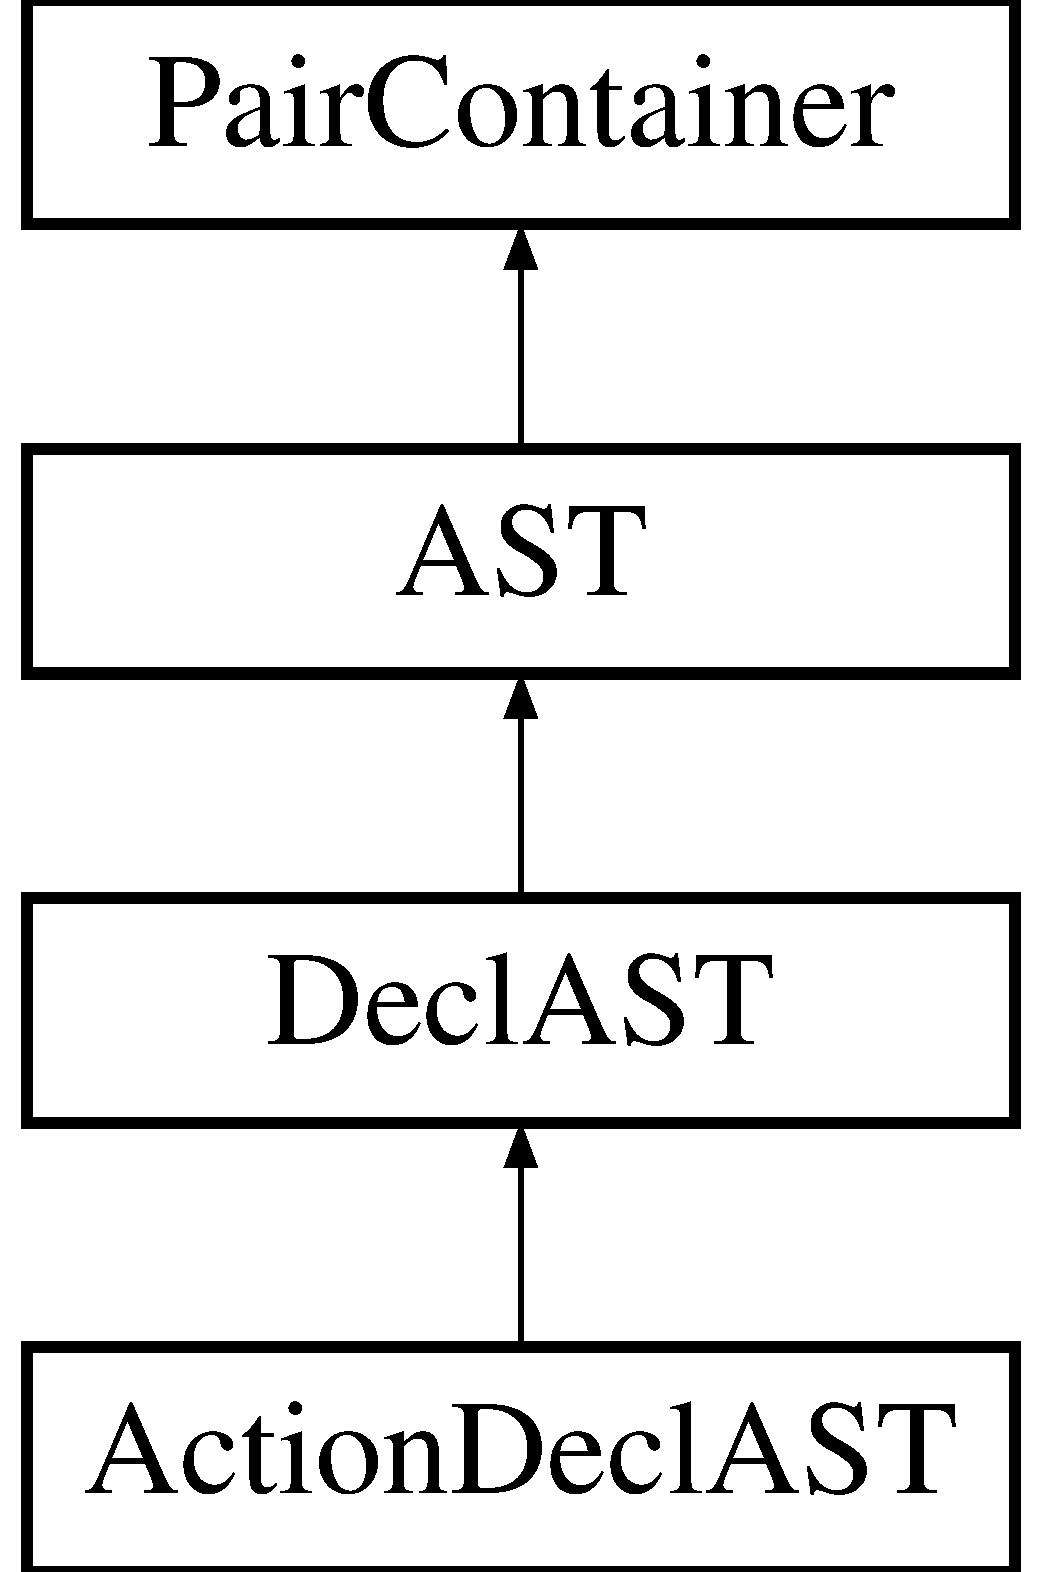
\includegraphics[height=4cm]{classslicc_1_1ast_1_1ActionDeclAST_1_1ActionDeclAST}
\end{center}
\end{figure}
\subsection*{Public メソッド}
\begin{DoxyCompactItemize}
\item 
def \hyperlink{classslicc_1_1ast_1_1ActionDeclAST_1_1ActionDeclAST_ac775ee34451fdfa742b318538164070e}{\_\-\_\-init\_\-\_\-}
\item 
def \hyperlink{classslicc_1_1ast_1_1ActionDeclAST_1_1ActionDeclAST_ad8b9328939df072e4740cd9a63189744}{\_\-\_\-repr\_\-\_\-}
\item 
def \hyperlink{classslicc_1_1ast_1_1ActionDeclAST_1_1ActionDeclAST_a4555d1cee0dccf3942ea35fe86de2e8e}{generate}
\end{DoxyCompactItemize}
\subsection*{Public 変数}
\begin{DoxyCompactItemize}
\item 
\hyperlink{classslicc_1_1ast_1_1ActionDeclAST_1_1ActionDeclAST_a2fe57e2d3d2cba9a3aeba2f629eaa78b}{ident}
\item 
\hyperlink{classslicc_1_1ast_1_1ActionDeclAST_1_1ActionDeclAST_a53a363e0fba452364cf9d6c768121237}{statement\_\-list}
\end{DoxyCompactItemize}


\subsection{関数}
\hypertarget{classslicc_1_1ast_1_1ActionDeclAST_1_1ActionDeclAST_ac775ee34451fdfa742b318538164070e}{
\index{slicc::ast::ActionDeclAST::ActionDeclAST@{slicc::ast::ActionDeclAST::ActionDeclAST}!\_\-\_\-init\_\-\_\-@{\_\-\_\-init\_\-\_\-}}
\index{\_\-\_\-init\_\-\_\-@{\_\-\_\-init\_\-\_\-}!slicc::ast::ActionDeclAST::ActionDeclAST@{slicc::ast::ActionDeclAST::ActionDeclAST}}
\subsubsection[{\_\-\_\-init\_\-\_\-}]{\setlength{\rightskip}{0pt plus 5cm}def \_\-\_\-init\_\-\_\- ( {\em self}, \/   {\em slicc}, \/   {\em ident}, \/   {\em pairs}, \/   {\em statement\_\-list})}}
\label{classslicc_1_1ast_1_1ActionDeclAST_1_1ActionDeclAST_ac775ee34451fdfa742b318538164070e}



\begin{DoxyCode}
32                                                            :
33         super(ActionDeclAST, self).__init__(slicc, pairs)
34         self.ident = ident
35         self.statement_list = statement_list
36 
    def __repr__(self):
\end{DoxyCode}
\hypertarget{classslicc_1_1ast_1_1ActionDeclAST_1_1ActionDeclAST_ad8b9328939df072e4740cd9a63189744}{
\index{slicc::ast::ActionDeclAST::ActionDeclAST@{slicc::ast::ActionDeclAST::ActionDeclAST}!\_\-\_\-repr\_\-\_\-@{\_\-\_\-repr\_\-\_\-}}
\index{\_\-\_\-repr\_\-\_\-@{\_\-\_\-repr\_\-\_\-}!slicc::ast::ActionDeclAST::ActionDeclAST@{slicc::ast::ActionDeclAST::ActionDeclAST}}
\subsubsection[{\_\-\_\-repr\_\-\_\-}]{\setlength{\rightskip}{0pt plus 5cm}def \_\-\_\-repr\_\-\_\- ( {\em self})}}
\label{classslicc_1_1ast_1_1ActionDeclAST_1_1ActionDeclAST_ad8b9328939df072e4740cd9a63189744}



\begin{DoxyCode}
37                       :
38         return "[ActionDecl: %r]" % (self.ident)
39 
    def generate(self):
\end{DoxyCode}
\hypertarget{classslicc_1_1ast_1_1ActionDeclAST_1_1ActionDeclAST_a4555d1cee0dccf3942ea35fe86de2e8e}{
\index{slicc::ast::ActionDeclAST::ActionDeclAST@{slicc::ast::ActionDeclAST::ActionDeclAST}!generate@{generate}}
\index{generate@{generate}!slicc::ast::ActionDeclAST::ActionDeclAST@{slicc::ast::ActionDeclAST::ActionDeclAST}}
\subsubsection[{generate}]{\setlength{\rightskip}{0pt plus 5cm}def generate ( {\em self})}}
\label{classslicc_1_1ast_1_1ActionDeclAST_1_1ActionDeclAST_a4555d1cee0dccf3942ea35fe86de2e8e}



\begin{DoxyCode}
40                       :
41         resources = {}
42 
43         machine = self.symtab.state_machine
44         if machine is None:
45             self.error("Action declaration not part of a machine.")
46 
47         if self.statement_list:
48             # Add new local vars
49             self.symtab.pushFrame()
50 
51             addr_type = self.symtab.find("Address", Type)
52 
53             if addr_type is None:
54                 self.error("Type 'Address' not declared.")
55 
56             var = Var(self.symtab, "address", self.location, addr_type,
57                       "addr", self.pairs)
58             self.symtab.newSymbol(var)
59 
60             if machine.TBEType != None:
61                 var = Var(self.symtab, "tbe", self.location, machine.TBEType,
62                       "m_tbe_ptr", self.pairs)
63                 self.symtab.newSymbol(var)
64 
65             if machine.EntryType != None:
66                 var = Var(self.symtab, "cache_entry", self.location,
67                           machine.EntryType, "m_cache_entry_ptr", self.pairs)
68                 self.symtab.newSymbol(var)
69 
70             # Do not allows returns in actions
71             code = self.slicc.codeFormatter()
72             self.statement_list.generate(code, None)
73             self.pairs["c_code"] = str(code)
74 
75             self.statement_list.findResources(resources)
76 
77             self.symtab.popFrame()
78 
79         action = Action(self.symtab, self.ident, resources, self.location,
80                         self.pairs)
81         machine.addAction(action)
        machine.addAction(action)
\end{DoxyCode}


\subsection{変数}
\hypertarget{classslicc_1_1ast_1_1ActionDeclAST_1_1ActionDeclAST_a2fe57e2d3d2cba9a3aeba2f629eaa78b}{
\index{slicc::ast::ActionDeclAST::ActionDeclAST@{slicc::ast::ActionDeclAST::ActionDeclAST}!ident@{ident}}
\index{ident@{ident}!slicc::ast::ActionDeclAST::ActionDeclAST@{slicc::ast::ActionDeclAST::ActionDeclAST}}
\subsubsection[{ident}]{\setlength{\rightskip}{0pt plus 5cm}{\bf ident}}}
\label{classslicc_1_1ast_1_1ActionDeclAST_1_1ActionDeclAST_a2fe57e2d3d2cba9a3aeba2f629eaa78b}
\hypertarget{classslicc_1_1ast_1_1ActionDeclAST_1_1ActionDeclAST_a53a363e0fba452364cf9d6c768121237}{
\index{slicc::ast::ActionDeclAST::ActionDeclAST@{slicc::ast::ActionDeclAST::ActionDeclAST}!statement\_\-list@{statement\_\-list}}
\index{statement\_\-list@{statement\_\-list}!slicc::ast::ActionDeclAST::ActionDeclAST@{slicc::ast::ActionDeclAST::ActionDeclAST}}
\subsubsection[{statement\_\-list}]{\setlength{\rightskip}{0pt plus 5cm}{\bf statement\_\-list}}}
\label{classslicc_1_1ast_1_1ActionDeclAST_1_1ActionDeclAST_a53a363e0fba452364cf9d6c768121237}


このクラスの説明は次のファイルから生成されました:\begin{DoxyCompactItemize}
\item 
mem/slicc/ast/\hyperlink{ActionDeclAST_8py}{ActionDeclAST.py}\end{DoxyCompactItemize}

\hypertarget{classFullO3CPU_1_1ActivateThreadEvent}{
\section{クラス ActivateThreadEvent}
\label{classFullO3CPU_1_1ActivateThreadEvent}\index{FullO3CPU::ActivateThreadEvent@{FullO3CPU::ActivateThreadEvent}}
}
ActivateThreadEventに対する継承グラフ:\begin{figure}[H]
\begin{center}
\leavevmode
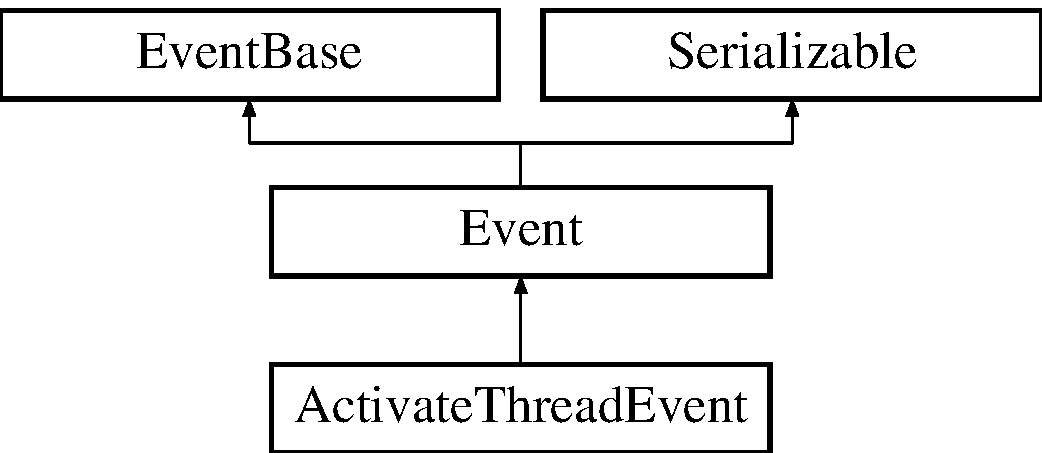
\includegraphics[height=3cm]{classFullO3CPU_1_1ActivateThreadEvent}
\end{center}
\end{figure}
\subsection*{Public メソッド}
\begin{DoxyCompactItemize}
\item 
\hyperlink{classFullO3CPU_1_1ActivateThreadEvent_a9ce281f466d06de2e43efe49b6918c14}{ActivateThreadEvent} ()
\item 
void \hyperlink{classFullO3CPU_1_1ActivateThreadEvent_a0938c51f296f212d5f6f05d174558612}{init} (int thread\_\-num, \hyperlink{classFullO3CPU}{FullO3CPU}$<$ Impl $>$ $\ast$thread\_\-cpu)
\item 
void \hyperlink{classFullO3CPU_1_1ActivateThreadEvent_a2e9c5136d19b1a95fc427e0852deab5c}{process} ()
\item 
const char $\ast$ \hyperlink{classFullO3CPU_1_1ActivateThreadEvent_a5a14fe478e2393ff51f02e9b7be27e00}{description} () const 
\end{DoxyCompactItemize}
\subsection*{Private 変数}
\begin{DoxyCompactItemize}
\item 
\hyperlink{base_2types_8hh_ab39b1a4f9dad884694c7a74ed69e6a6b}{ThreadID} \hyperlink{classFullO3CPU_1_1ActivateThreadEvent_aa508770268ee4ceaf16054b9e0be0e17}{tid}
\item 
\hyperlink{classFullO3CPU}{FullO3CPU}$<$ Impl $>$ $\ast$ \hyperlink{classFullO3CPU_1_1ActivateThreadEvent_a3a3767255bcefd2ce55f94976ab8eb99}{cpu}
\end{DoxyCompactItemize}
\subsubsection*{template$<$class Impl$>$ class FullO3CPU$<$ Impl $>$::ActivateThreadEvent}



\subsection{コンストラクタとデストラクタ}
\hypertarget{classFullO3CPU_1_1ActivateThreadEvent_a9ce281f466d06de2e43efe49b6918c14}{
\index{FullO3CPU::ActivateThreadEvent@{FullO3CPU::ActivateThreadEvent}!ActivateThreadEvent@{ActivateThreadEvent}}
\index{ActivateThreadEvent@{ActivateThreadEvent}!FullO3CPU::ActivateThreadEvent@{FullO3CPU::ActivateThreadEvent}}
\subsubsection[{ActivateThreadEvent}]{\setlength{\rightskip}{0pt plus 5cm}{\bf ActivateThreadEvent} ()\hspace{0.3cm}{\ttfamily  \mbox{[}inline\mbox{]}}}}
\label{classFullO3CPU_1_1ActivateThreadEvent_a9ce281f466d06de2e43efe49b6918c14}
Constructs the event. 


\begin{DoxyCode}
152     : Event(CPU_Switch_Pri)
153 {
154 }
\end{DoxyCode}


\subsection{関数}
\hypertarget{classFullO3CPU_1_1ActivateThreadEvent_a5a14fe478e2393ff51f02e9b7be27e00}{
\index{FullO3CPU::ActivateThreadEvent@{FullO3CPU::ActivateThreadEvent}!description@{description}}
\index{description@{description}!FullO3CPU::ActivateThreadEvent@{FullO3CPU::ActivateThreadEvent}}
\subsubsection[{description}]{\setlength{\rightskip}{0pt plus 5cm}const char $\ast$ description () const\hspace{0.3cm}{\ttfamily  \mbox{[}inline, virtual\mbox{]}}}}
\label{classFullO3CPU_1_1ActivateThreadEvent_a5a14fe478e2393ff51f02e9b7be27e00}
Returns the description of the event. 

\hyperlink{classEvent_a130ddddf003422b413e2e891b1b80e8f}{Event}を再定義しています。


\begin{DoxyCode}
175 {
176     return "FullO3CPU \"Activate Thread\"";
177 }
\end{DoxyCode}
\hypertarget{classFullO3CPU_1_1ActivateThreadEvent_a0938c51f296f212d5f6f05d174558612}{
\index{FullO3CPU::ActivateThreadEvent@{FullO3CPU::ActivateThreadEvent}!init@{init}}
\index{init@{init}!FullO3CPU::ActivateThreadEvent@{FullO3CPU::ActivateThreadEvent}}
\subsubsection[{init}]{\setlength{\rightskip}{0pt plus 5cm}void init (int {\em thread\_\-num}, \/  {\bf FullO3CPU}$<$ Impl $>$ $\ast$ {\em thread\_\-cpu})\hspace{0.3cm}{\ttfamily  \mbox{[}inline\mbox{]}}}}
\label{classFullO3CPU_1_1ActivateThreadEvent_a0938c51f296f212d5f6f05d174558612}
Initialize \hyperlink{classEvent}{Event} 


\begin{DoxyCode}
160 {
161     tid = thread_num;
162     cpu = thread_cpu;
163 }
\end{DoxyCode}
\hypertarget{classFullO3CPU_1_1ActivateThreadEvent_a2e9c5136d19b1a95fc427e0852deab5c}{
\index{FullO3CPU::ActivateThreadEvent@{FullO3CPU::ActivateThreadEvent}!process@{process}}
\index{process@{process}!FullO3CPU::ActivateThreadEvent@{FullO3CPU::ActivateThreadEvent}}
\subsubsection[{process}]{\setlength{\rightskip}{0pt plus 5cm}void process ()\hspace{0.3cm}{\ttfamily  \mbox{[}inline, virtual\mbox{]}}}}
\label{classFullO3CPU_1_1ActivateThreadEvent_a2e9c5136d19b1a95fc427e0852deab5c}
Processes the event, calling \hyperlink{classFullO3CPU_a687aa4600423bb30ecf3bb1da6cd6000}{activateThread()} on the CPU. 

\hyperlink{classEvent_a142b75b68a6291400e20fb0dd905b1c8}{Event}を実装しています。


\begin{DoxyCode}
168 {
169     cpu->activateThread(tid);
170 }
\end{DoxyCode}


\subsection{変数}
\hypertarget{classFullO3CPU_1_1ActivateThreadEvent_a3a3767255bcefd2ce55f94976ab8eb99}{
\index{FullO3CPU::ActivateThreadEvent@{FullO3CPU::ActivateThreadEvent}!cpu@{cpu}}
\index{cpu@{cpu}!FullO3CPU::ActivateThreadEvent@{FullO3CPU::ActivateThreadEvent}}
\subsubsection[{cpu}]{\setlength{\rightskip}{0pt plus 5cm}{\bf FullO3CPU}$<$Impl$>$$\ast$ {\bf cpu}\hspace{0.3cm}{\ttfamily  \mbox{[}private\mbox{]}}}}
\label{classFullO3CPU_1_1ActivateThreadEvent_a3a3767255bcefd2ce55f94976ab8eb99}
Pointer to the CPU. \hypertarget{classFullO3CPU_1_1ActivateThreadEvent_aa508770268ee4ceaf16054b9e0be0e17}{
\index{FullO3CPU::ActivateThreadEvent@{FullO3CPU::ActivateThreadEvent}!tid@{tid}}
\index{tid@{tid}!FullO3CPU::ActivateThreadEvent@{FullO3CPU::ActivateThreadEvent}}
\subsubsection[{tid}]{\setlength{\rightskip}{0pt plus 5cm}{\bf ThreadID} {\bf tid}\hspace{0.3cm}{\ttfamily  \mbox{[}private\mbox{]}}}}
\label{classFullO3CPU_1_1ActivateThreadEvent_aa508770268ee4ceaf16054b9e0be0e17}
Number of Thread to Activate 

このクラスの説明は次のファイルから生成されました:\begin{DoxyCompactItemize}
\item 
cpu/o3/\hyperlink{o3_2cpu_8hh}{cpu.hh}\item 
cpu/o3/\hyperlink{o3_2cpu_8cc}{cpu.cc}\end{DoxyCompactItemize}

\hypertarget{classActivityRecorder}{
\section{クラス ActivityRecorder}
\label{classActivityRecorder}\index{ActivityRecorder@{ActivityRecorder}}
}


{\ttfamily \#include $<$activity.hh$>$}\subsection*{Public メソッド}
\begin{DoxyCompactItemize}
\item 
\hyperlink{classActivityRecorder_aee994d49a31bd533aa152dfeb18c7b2d}{ActivityRecorder} (const std::string \&name, int num\_\-stages, int longest\_\-latency, int count)
\item 
\hyperlink{classActivityRecorder_a72527148fb233d9e5a0d887becb03458}{$\sim$ActivityRecorder} ()
\item 
void \hyperlink{classActivityRecorder_a0ea760b87a5516ee794818d5eb8c243d}{activity} ()
\item 
void \hyperlink{classActivityRecorder_a8903a4e9f3d5fb42d0faa9d53e21d85c}{advance} ()
\item 
void \hyperlink{classActivityRecorder_a9039dad8d295c41b50eba0342e6c11c0}{activateStage} (const int idx)
\item 
void \hyperlink{classActivityRecorder_a4d73bea02eaf6f93e267391592556fe7}{deactivateStage} (const int idx)
\item 
bool \hyperlink{classActivityRecorder_a918c8f58bd15e33d7d44a37109a868e4}{getStageActive} (const int idx) const 
\item 
int \hyperlink{classActivityRecorder_aabc85525e8d2526f4a909313fcb9bfa2}{getNumStages} () const 
\item 
int \hyperlink{classActivityRecorder_a24e9ead78b85428639a9e76329ecd0b7}{getActivityCount} () const 
\item 
void \hyperlink{classActivityRecorder_a562d654f23b8a293deda98e8d585973f}{setActivityCount} (int count)
\item 
bool \hyperlink{classActivityRecorder_a0cb3050c8a4f6bdb2c1f727eec8d9701}{active} ()
\item 
void \hyperlink{classActivityRecorder_ad20897c5c8bd47f5d4005989bead0e55}{reset} ()
\item 
void \hyperlink{classActivityRecorder_accd2600060dbaee3a3b41aed4034c63c}{dump} ()
\item 
void \hyperlink{classActivityRecorder_a41d45236c37b75848f4b1667a11fb50e}{validate} ()
\item 
const std::string \& \hyperlink{classActivityRecorder_a324e8c54c4c5161913681a1a52fef959}{name} () const 
\end{DoxyCompactItemize}
\subsection*{Private 変数}
\begin{DoxyCompactItemize}
\item 
std::string \hyperlink{classActivityRecorder_aaf2ed934b37cbbd236fdd1b01a5f5005}{\_\-name}
\item 
\hyperlink{classTimeBuffer}{TimeBuffer}$<$ bool $>$ \hyperlink{classActivityRecorder_a6c508a89a541285053c7b900bd730cc2}{activityBuffer}
\item 
int \hyperlink{classActivityRecorder_a20bd7fb0de8433f0f95dc50ed74bf620}{longestLatency}
\item 
int \hyperlink{classActivityRecorder_adf01a2f1e7e8ad0795ef04b3a4e6dfb6}{activityCount}
\item 
int \hyperlink{classActivityRecorder_aaf4f71ec3fd6f4e154d09cd71c2c331b}{numStages}
\item 
bool $\ast$ \hyperlink{classActivityRecorder_aebf0081a358874c1eedf8728e4a478a4}{stageActive}
\end{DoxyCompactItemize}


\subsection{説明}
\hyperlink{classActivityRecorder}{ActivityRecorder} helper class that informs the CPU if it can switch over to being idle or not. It works by having a time buffer as long as any time buffer in the CPU, and the CPU and all of its stages inform the \hyperlink{classActivityRecorder}{ActivityRecorder} when they write to any time buffer. The \hyperlink{classActivityRecorder}{ActivityRecorder} marks a 1 in the \char`\"{}0\char`\"{} slot of the time buffer any time a stage writes to a time buffer, and it advances its time buffer at the same time as all other stages. The \hyperlink{classActivityRecorder}{ActivityRecorder} also records if a stage has activity to do next cycle. The recorder keeps a count of these two. Thus any time the count is non-\/zero, there is either communication still in flight, or activity that still must be done, meaning that the CPU can not idle. If count is zero, then the CPU can safely idle as it has no more outstanding work to do. 

\subsection{コンストラクタとデストラクタ}
\hypertarget{classActivityRecorder_aee994d49a31bd533aa152dfeb18c7b2d}{
\index{ActivityRecorder@{ActivityRecorder}!ActivityRecorder@{ActivityRecorder}}
\index{ActivityRecorder@{ActivityRecorder}!ActivityRecorder@{ActivityRecorder}}
\subsubsection[{ActivityRecorder}]{\setlength{\rightskip}{0pt plus 5cm}{\bf ActivityRecorder} (const std::string \& {\em name}, \/  int {\em num\_\-stages}, \/  int {\em longest\_\-latency}, \/  int {\em count})}}
\label{classActivityRecorder_aee994d49a31bd533aa152dfeb18c7b2d}
\hypertarget{classActivityRecorder_a72527148fb233d9e5a0d887becb03458}{
\index{ActivityRecorder@{ActivityRecorder}!$\sim$ActivityRecorder@{$\sim$ActivityRecorder}}
\index{$\sim$ActivityRecorder@{$\sim$ActivityRecorder}!ActivityRecorder@{ActivityRecorder}}
\subsubsection[{$\sim$ActivityRecorder}]{\setlength{\rightskip}{0pt plus 5cm}$\sim${\bf ActivityRecorder} ()}}
\label{classActivityRecorder_a72527148fb233d9e5a0d887becb03458}



\begin{DoxyCode}
50 {
51     delete[] stageActive;
52 }
\end{DoxyCode}


\subsection{関数}
\hypertarget{classActivityRecorder_a9039dad8d295c41b50eba0342e6c11c0}{
\index{ActivityRecorder@{ActivityRecorder}!activateStage@{activateStage}}
\index{activateStage@{activateStage}!ActivityRecorder@{ActivityRecorder}}
\subsubsection[{activateStage}]{\setlength{\rightskip}{0pt plus 5cm}void activateStage (const int {\em idx})}}
\label{classActivityRecorder_a9039dad8d295c41b50eba0342e6c11c0}
Marks a stage as active. 


\begin{DoxyCode}
92 {
93     // Increment the activity count if this stage wasn't already active.
94     if (!stageActive[idx]) {
95         ++activityCount;
96 
97         stageActive[idx] = true;
98 
99         DPRINTF(Activity, "Activity: %i\n", activityCount);
100     } else {
101         DPRINTF(Activity, "Stage %i already active.\n", idx);
102     }
103 
104 //    assert(activityCount < longestLatency + numStages + 1);
105 }
\end{DoxyCode}
\hypertarget{classActivityRecorder_a0cb3050c8a4f6bdb2c1f727eec8d9701}{
\index{ActivityRecorder@{ActivityRecorder}!active@{active}}
\index{active@{active}!ActivityRecorder@{ActivityRecorder}}
\subsubsection[{active}]{\setlength{\rightskip}{0pt plus 5cm}bool active ()\hspace{0.3cm}{\ttfamily  \mbox{[}inline\mbox{]}}}}
\label{classActivityRecorder_a0cb3050c8a4f6bdb2c1f727eec8d9701}
Returns if the CPU should be active. 


\begin{DoxyCode}
90 { return activityCount; }
\end{DoxyCode}
\hypertarget{classActivityRecorder_a0ea760b87a5516ee794818d5eb8c243d}{
\index{ActivityRecorder@{ActivityRecorder}!activity@{activity}}
\index{activity@{activity}!ActivityRecorder@{ActivityRecorder}}
\subsubsection[{activity}]{\setlength{\rightskip}{0pt plus 5cm}void activity ()}}
\label{classActivityRecorder_a0ea760b87a5516ee794818d5eb8c243d}
Records that there is activity this cycle. 


\begin{DoxyCode}
56 {
57     // If we've already recorded activity for this cycle, we don't
58     // want to increment the count any more.
59     if (activityBuffer[0]) {
60         return;
61     }
62 
63     activityBuffer[0] = true;
64 
65     ++activityCount;
66 
67     DPRINTF(Activity, "Activity: %i\n", activityCount);
68 }
\end{DoxyCode}
\hypertarget{classActivityRecorder_a8903a4e9f3d5fb42d0faa9d53e21d85c}{
\index{ActivityRecorder@{ActivityRecorder}!advance@{advance}}
\index{advance@{advance}!ActivityRecorder@{ActivityRecorder}}
\subsubsection[{advance}]{\setlength{\rightskip}{0pt plus 5cm}void advance ()}}
\label{classActivityRecorder_a8903a4e9f3d5fb42d0faa9d53e21d85c}
Advances the activity buffer, decrementing the activityCount if active communication just left the time buffer, and determining if there is no activity. 


\begin{DoxyCode}
72 {
73     // If there's a 1 in the slot that is about to be erased once the
74     // time buffer advances, then decrement the activityCount.
75     if (activityBuffer[-longestLatency]) {
76         --activityCount;
77 
78         assert(activityCount >= 0);
79 
80         DPRINTF(Activity, "Activity: %i\n", activityCount);
81 
82         if (activityCount == 0) {
83             DPRINTF(Activity, "No activity left!\n");
84         }
85     }
86 
87     activityBuffer.advance();
88 }
\end{DoxyCode}
\hypertarget{classActivityRecorder_a4d73bea02eaf6f93e267391592556fe7}{
\index{ActivityRecorder@{ActivityRecorder}!deactivateStage@{deactivateStage}}
\index{deactivateStage@{deactivateStage}!ActivityRecorder@{ActivityRecorder}}
\subsubsection[{deactivateStage}]{\setlength{\rightskip}{0pt plus 5cm}void deactivateStage (const int {\em idx})}}
\label{classActivityRecorder_a4d73bea02eaf6f93e267391592556fe7}
Deactivates a stage. 


\begin{DoxyCode}
109 {
110     // Decrement the activity count if this stage was active.
111     if (stageActive[idx]) {
112         --activityCount;
113 
114         stageActive[idx] = false;
115 
116         DPRINTF(Activity, "Activity: %i\n", activityCount);
117     } else {
118         DPRINTF(Activity, "Stage %i already inactive.\n", idx);
119     }
120 
121     assert(activityCount >= 0);
122 }
\end{DoxyCode}
\hypertarget{classActivityRecorder_accd2600060dbaee3a3b41aed4034c63c}{
\index{ActivityRecorder@{ActivityRecorder}!dump@{dump}}
\index{dump@{dump}!ActivityRecorder@{ActivityRecorder}}
\subsubsection[{dump}]{\setlength{\rightskip}{0pt plus 5cm}void dump ()}}
\label{classActivityRecorder_accd2600060dbaee3a3b41aed4034c63c}
\hyperlink{namespaceDebug}{Debug} function to dump the contents of the time buffer. 


\begin{DoxyCode}
135 {
136     for (int i = 0; i <= longestLatency; ++i) {
137         cprintf("[Idx:%i %i] ", i, activityBuffer[-i]);
138     }
139 
140     cprintf("\n");
141 
142     for (int i = 0; i < numStages; ++i) {
143         cprintf("[Stage:%i %i]\n", i, stageActive[i]);
144     }
145 
146     cprintf("\n");
147 
148     cprintf("Activity count: %i\n", activityCount);
149 }
\end{DoxyCode}
\hypertarget{classActivityRecorder_a24e9ead78b85428639a9e76329ecd0b7}{
\index{ActivityRecorder@{ActivityRecorder}!getActivityCount@{getActivityCount}}
\index{getActivityCount@{getActivityCount}!ActivityRecorder@{ActivityRecorder}}
\subsubsection[{getActivityCount}]{\setlength{\rightskip}{0pt plus 5cm}int getActivityCount () const\hspace{0.3cm}{\ttfamily  \mbox{[}inline\mbox{]}}}}
\label{classActivityRecorder_a24e9ead78b85428639a9e76329ecd0b7}
Returns how many things are active within the recorder. 


\begin{DoxyCode}
81 { return activityCount; }
\end{DoxyCode}
\hypertarget{classActivityRecorder_aabc85525e8d2526f4a909313fcb9bfa2}{
\index{ActivityRecorder@{ActivityRecorder}!getNumStages@{getNumStages}}
\index{getNumStages@{getNumStages}!ActivityRecorder@{ActivityRecorder}}
\subsubsection[{getNumStages}]{\setlength{\rightskip}{0pt plus 5cm}int getNumStages () const\hspace{0.3cm}{\ttfamily  \mbox{[}inline\mbox{]}}}}
\label{classActivityRecorder_aabc85525e8d2526f4a909313fcb9bfa2}
Returns the number of stages. 


\begin{DoxyCode}
78 { return numStages; }
\end{DoxyCode}
\hypertarget{classActivityRecorder_a918c8f58bd15e33d7d44a37109a868e4}{
\index{ActivityRecorder@{ActivityRecorder}!getStageActive@{getStageActive}}
\index{getStageActive@{getStageActive}!ActivityRecorder@{ActivityRecorder}}
\subsubsection[{getStageActive}]{\setlength{\rightskip}{0pt plus 5cm}bool getStageActive (const int {\em idx}) const\hspace{0.3cm}{\ttfamily  \mbox{[}inline\mbox{]}}}}
\label{classActivityRecorder_a918c8f58bd15e33d7d44a37109a868e4}
Returns the activity status of a stage. 


\begin{DoxyCode}
75 { return stageActive[idx]; }
\end{DoxyCode}
\hypertarget{classActivityRecorder_a324e8c54c4c5161913681a1a52fef959}{
\index{ActivityRecorder@{ActivityRecorder}!name@{name}}
\index{name@{name}!ActivityRecorder@{ActivityRecorder}}
\subsubsection[{name}]{\setlength{\rightskip}{0pt plus 5cm}const std::string\& name () const\hspace{0.3cm}{\ttfamily  \mbox{[}inline\mbox{]}}}}
\label{classActivityRecorder_a324e8c54c4c5161913681a1a52fef959}



\begin{DoxyCode}
103 { return _name; }
\end{DoxyCode}
\hypertarget{classActivityRecorder_ad20897c5c8bd47f5d4005989bead0e55}{
\index{ActivityRecorder@{ActivityRecorder}!reset@{reset}}
\index{reset@{reset}!ActivityRecorder@{ActivityRecorder}}
\subsubsection[{reset}]{\setlength{\rightskip}{0pt plus 5cm}void reset ()}}
\label{classActivityRecorder_ad20897c5c8bd47f5d4005989bead0e55}
Clears the time buffer and the activity count. 


\begin{DoxyCode}
126 {
127     activityCount = 0;
128     std::memset(stageActive, 0, numStages);
129     for (int i = 0; i < longestLatency + 1; ++i)
130         activityBuffer.advance();
131 }
\end{DoxyCode}
\hypertarget{classActivityRecorder_a562d654f23b8a293deda98e8d585973f}{
\index{ActivityRecorder@{ActivityRecorder}!setActivityCount@{setActivityCount}}
\index{setActivityCount@{setActivityCount}!ActivityRecorder@{ActivityRecorder}}
\subsubsection[{setActivityCount}]{\setlength{\rightskip}{0pt plus 5cm}void setActivityCount (int {\em count})\hspace{0.3cm}{\ttfamily  \mbox{[}inline\mbox{]}}}}
\label{classActivityRecorder_a562d654f23b8a293deda98e8d585973f}
Sets the count to a starting value. Can be used to disable the idling option. 


\begin{DoxyCode}
87     { activityCount = count; }
\end{DoxyCode}
\hypertarget{classActivityRecorder_a41d45236c37b75848f4b1667a11fb50e}{
\index{ActivityRecorder@{ActivityRecorder}!validate@{validate}}
\index{validate@{validate}!ActivityRecorder@{ActivityRecorder}}
\subsubsection[{validate}]{\setlength{\rightskip}{0pt plus 5cm}void validate ()}}
\label{classActivityRecorder_a41d45236c37b75848f4b1667a11fb50e}
\hyperlink{namespaceDebug}{Debug} function to ensure that the activity count matches the contents of the time buffer. 


\begin{DoxyCode}
153 {
154     int count = 0;
155     for (int i = 0; i <= longestLatency; ++i) {
156         if (activityBuffer[-i]) {
157             count++;
158         }
159     }
160 
161     for (int i = 0; i < numStages; ++i) {
162         if (stageActive[i]) {
163             count++;
164         }
165     }
166 
167     assert(count == activityCount);
168 }
\end{DoxyCode}


\subsection{変数}
\hypertarget{classActivityRecorder_aaf2ed934b37cbbd236fdd1b01a5f5005}{
\index{ActivityRecorder@{ActivityRecorder}!\_\-name@{\_\-name}}
\index{\_\-name@{\_\-name}!ActivityRecorder@{ActivityRecorder}}
\subsubsection[{\_\-name}]{\setlength{\rightskip}{0pt plus 5cm}std::string {\bf \_\-name}\hspace{0.3cm}{\ttfamily  \mbox{[}private\mbox{]}}}}
\label{classActivityRecorder_aaf2ed934b37cbbd236fdd1b01a5f5005}
\hypertarget{classActivityRecorder_a6c508a89a541285053c7b900bd730cc2}{
\index{ActivityRecorder@{ActivityRecorder}!activityBuffer@{activityBuffer}}
\index{activityBuffer@{activityBuffer}!ActivityRecorder@{ActivityRecorder}}
\subsubsection[{activityBuffer}]{\setlength{\rightskip}{0pt plus 5cm}{\bf TimeBuffer}$<$bool$>$ {\bf activityBuffer}\hspace{0.3cm}{\ttfamily  \mbox{[}private\mbox{]}}}}
\label{classActivityRecorder_a6c508a89a541285053c7b900bd730cc2}
\hyperlink{classTime}{Time} buffer that tracks if any cycles has active communication in them. It should be as long as the longest communication latency in the system. Each time any time buffer is written, the activity buffer should also be written to. The activityBuffer is advanced along with all the other time buffers, so it should have a 1 somewhere in it only if there is active communication in a time buffer. \hypertarget{classActivityRecorder_adf01a2f1e7e8ad0795ef04b3a4e6dfb6}{
\index{ActivityRecorder@{ActivityRecorder}!activityCount@{activityCount}}
\index{activityCount@{activityCount}!ActivityRecorder@{ActivityRecorder}}
\subsubsection[{activityCount}]{\setlength{\rightskip}{0pt plus 5cm}int {\bf activityCount}\hspace{0.3cm}{\ttfamily  \mbox{[}private\mbox{]}}}}
\label{classActivityRecorder_adf01a2f1e7e8ad0795ef04b3a4e6dfb6}
Tracks how many stages and cycles of time buffer have activity. Stages increment this count when they switch to active, and decrement it when they switch to inactive. Whenever a cycle that previously had no information is written in the time buffer, this is incremented. When a cycle that had information exits the time buffer due to age, this count is decremented. When the count is 0, there is no activity in the CPU, and it can be descheduled. \hypertarget{classActivityRecorder_a20bd7fb0de8433f0f95dc50ed74bf620}{
\index{ActivityRecorder@{ActivityRecorder}!longestLatency@{longestLatency}}
\index{longestLatency@{longestLatency}!ActivityRecorder@{ActivityRecorder}}
\subsubsection[{longestLatency}]{\setlength{\rightskip}{0pt plus 5cm}int {\bf longestLatency}\hspace{0.3cm}{\ttfamily  \mbox{[}private\mbox{]}}}}
\label{classActivityRecorder_a20bd7fb0de8433f0f95dc50ed74bf620}
Longest latency time buffer in the CPU. \hypertarget{classActivityRecorder_aaf4f71ec3fd6f4e154d09cd71c2c331b}{
\index{ActivityRecorder@{ActivityRecorder}!numStages@{numStages}}
\index{numStages@{numStages}!ActivityRecorder@{ActivityRecorder}}
\subsubsection[{numStages}]{\setlength{\rightskip}{0pt plus 5cm}int {\bf numStages}\hspace{0.3cm}{\ttfamily  \mbox{[}private\mbox{]}}}}
\label{classActivityRecorder_aaf4f71ec3fd6f4e154d09cd71c2c331b}
Number of stages that can be marked as active or inactive. \hypertarget{classActivityRecorder_aebf0081a358874c1eedf8728e4a478a4}{
\index{ActivityRecorder@{ActivityRecorder}!stageActive@{stageActive}}
\index{stageActive@{stageActive}!ActivityRecorder@{ActivityRecorder}}
\subsubsection[{stageActive}]{\setlength{\rightskip}{0pt plus 5cm}bool$\ast$ {\bf stageActive}\hspace{0.3cm}{\ttfamily  \mbox{[}private\mbox{]}}}}
\label{classActivityRecorder_aebf0081a358874c1eedf8728e4a478a4}
Records which stages are active/inactive. 

このクラスの説明は次のファイルから生成されました:\begin{DoxyCompactItemize}
\item 
cpu/\hyperlink{activity_8hh}{activity.hh}\item 
cpu/\hyperlink{activity_8cc}{activity.cc}\end{DoxyCompactItemize}

\hypertarget{classm5_1_1params_1_1Addr}{
\section{クラス Addr}
\label{classm5_1_1params_1_1Addr}\index{m5::params::Addr@{m5::params::Addr}}
}
Addrに対する継承グラフ:\begin{figure}[H]
\begin{center}
\leavevmode
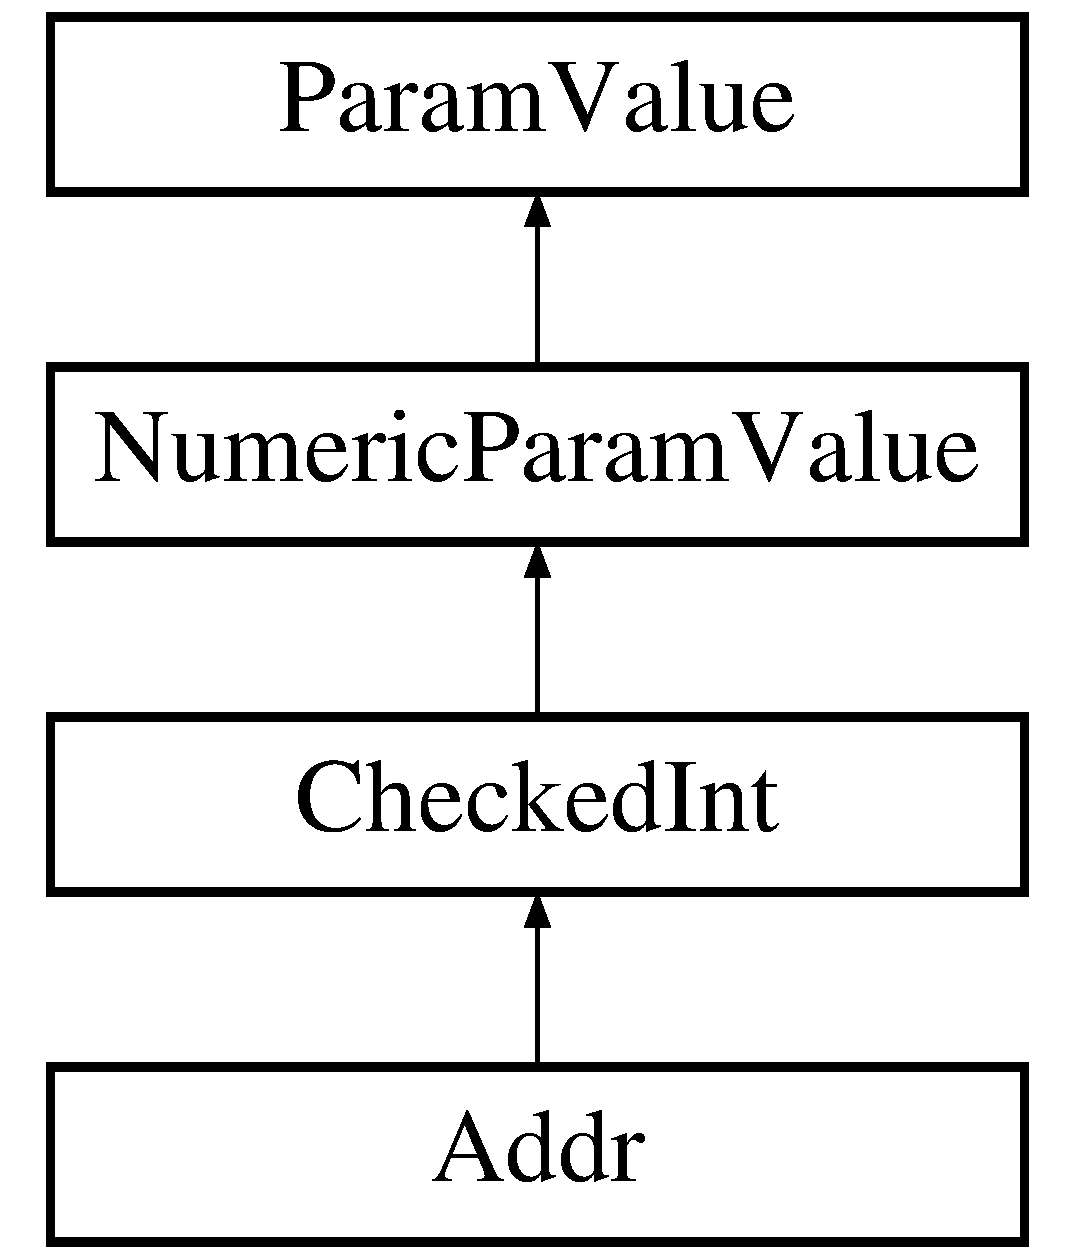
\includegraphics[height=4cm]{classm5_1_1params_1_1Addr}
\end{center}
\end{figure}
\subsection*{Public メソッド}
\begin{DoxyCompactItemize}
\item 
def \hyperlink{classm5_1_1params_1_1Addr_ac775ee34451fdfa742b318538164070e}{\_\-\_\-init\_\-\_\-}
\item 
def \hyperlink{classm5_1_1params_1_1Addr_ae92943b217d29a45ddcbbba2f7208afc}{\_\-\_\-add\_\-\_\-}
\end{DoxyCompactItemize}
\subsection*{Public 変数}
\begin{DoxyCompactItemize}
\item 
\hyperlink{classm5_1_1params_1_1Addr_afcc7a4b78ecd8fa7e713f8cfa0f51017}{value}
\end{DoxyCompactItemize}
\subsection*{Static Public 変数}
\begin{DoxyCompactItemize}
\item 
string \hyperlink{classm5_1_1params_1_1Addr_a2f1553ebb79374a68b36fdd6d8d82fc3}{cxx\_\-type} = '\hyperlink{classm5_1_1params_1_1Addr}{Addr}'
\item 
int \hyperlink{classm5_1_1params_1_1Addr_a439227feff9d7f55384e8780cfc2eb82}{size} = 64
\item 
\hyperlink{classm5_1_1params_1_1Addr_aca40206900cfc164654362fa8d4ad1e6}{unsigned} = True
\end{DoxyCompactItemize}


\subsection{関数}
\hypertarget{classm5_1_1params_1_1Addr_ae92943b217d29a45ddcbbba2f7208afc}{
\index{m5::params::Addr@{m5::params::Addr}!\_\-\_\-add\_\-\_\-@{\_\-\_\-add\_\-\_\-}}
\index{\_\-\_\-add\_\-\_\-@{\_\-\_\-add\_\-\_\-}!m5::params::Addr@{m5::params::Addr}}
\subsubsection[{\_\-\_\-add\_\-\_\-}]{\setlength{\rightskip}{0pt plus 5cm}def \_\-\_\-add\_\-\_\- ( {\em self}, \/   {\em other})}}
\label{classm5_1_1params_1_1Addr_ae92943b217d29a45ddcbbba2f7208afc}



\begin{DoxyCode}
541                             :
542         if isinstance(other, Addr):
543             return self.value + other.value
544         else:
545             return self.value + other
546 
class AddrRange(ParamValue):
\end{DoxyCode}
\hypertarget{classm5_1_1params_1_1Addr_ac775ee34451fdfa742b318538164070e}{
\index{m5::params::Addr@{m5::params::Addr}!\_\-\_\-init\_\-\_\-@{\_\-\_\-init\_\-\_\-}}
\index{\_\-\_\-init\_\-\_\-@{\_\-\_\-init\_\-\_\-}!m5::params::Addr@{m5::params::Addr}}
\subsubsection[{\_\-\_\-init\_\-\_\-}]{\setlength{\rightskip}{0pt plus 5cm}def \_\-\_\-init\_\-\_\- ( {\em self}, \/   {\em value})}}
\label{classm5_1_1params_1_1Addr_ac775ee34451fdfa742b318538164070e}


\hyperlink{classm5_1_1params_1_1CheckedInt_ac775ee34451fdfa742b318538164070e}{CheckedInt}を再定義しています。


\begin{DoxyCode}
532                              :
533         if isinstance(value, Addr):
534             self.value = value.value
535         else:
536             try:
537                 self.value = convert.toMemorySize(value)
538             except TypeError:
539                 self.value = long(value)
540         self._check()
    def __add__(self, other):
\end{DoxyCode}


\subsection{変数}
\hypertarget{classm5_1_1params_1_1Addr_a2f1553ebb79374a68b36fdd6d8d82fc3}{
\index{m5::params::Addr@{m5::params::Addr}!cxx\_\-type@{cxx\_\-type}}
\index{cxx\_\-type@{cxx\_\-type}!m5::params::Addr@{m5::params::Addr}}
\subsubsection[{cxx\_\-type}]{\setlength{\rightskip}{0pt plus 5cm}string {\bf cxx\_\-type} = '{\bf Addr}'\hspace{0.3cm}{\ttfamily  \mbox{[}static\mbox{]}}}}
\label{classm5_1_1params_1_1Addr_a2f1553ebb79374a68b36fdd6d8d82fc3}
\hypertarget{classm5_1_1params_1_1Addr_a439227feff9d7f55384e8780cfc2eb82}{
\index{m5::params::Addr@{m5::params::Addr}!size@{size}}
\index{size@{size}!m5::params::Addr@{m5::params::Addr}}
\subsubsection[{size}]{\setlength{\rightskip}{0pt plus 5cm}int {\bf size} = 64\hspace{0.3cm}{\ttfamily  \mbox{[}static\mbox{]}}}}
\label{classm5_1_1params_1_1Addr_a439227feff9d7f55384e8780cfc2eb82}
\hypertarget{classm5_1_1params_1_1Addr_aca40206900cfc164654362fa8d4ad1e6}{
\index{m5::params::Addr@{m5::params::Addr}!unsigned@{unsigned}}
\index{unsigned@{unsigned}!m5::params::Addr@{m5::params::Addr}}
\subsubsection[{unsigned}]{\setlength{\rightskip}{0pt plus 5cm}{\bf unsigned} = True\hspace{0.3cm}{\ttfamily  \mbox{[}static\mbox{]}}}}
\label{classm5_1_1params_1_1Addr_aca40206900cfc164654362fa8d4ad1e6}
\hypertarget{classm5_1_1params_1_1Addr_afcc7a4b78ecd8fa7e713f8cfa0f51017}{
\index{m5::params::Addr@{m5::params::Addr}!value@{value}}
\index{value@{value}!m5::params::Addr@{m5::params::Addr}}
\subsubsection[{value}]{\setlength{\rightskip}{0pt plus 5cm}{\bf value}}}
\label{classm5_1_1params_1_1Addr_afcc7a4b78ecd8fa7e713f8cfa0f51017}


\hyperlink{classm5_1_1params_1_1CheckedInt_afcc7a4b78ecd8fa7e713f8cfa0f51017}{CheckedInt}を再定義しています。

このクラスの説明は次のファイルから生成されました:\begin{DoxyCompactItemize}
\item 
python/m5/\hyperlink{params_8py}{params.py}\end{DoxyCompactItemize}

\hypertarget{classAddress}{
\section{クラス Address}
\label{classAddress}\index{Address@{Address}}
}


{\ttfamily \#include $<$Address.hh$>$}\subsection*{Public メソッド}
\begin{DoxyCompactItemize}
\item 
\hyperlink{classAddress_ac98de6c9250be1b4e3446d9989e058b3}{Address} ()
\item 
\hyperlink{classAddress_ab13b386b7f0bf74bab346a3f2cbde303}{Address} (\hyperlink{TypeDefines_8hh_a7901e1a365850c5ff38ec6e12b6b9ffc}{physical\_\-address\_\-t} address)
\item 
\hyperlink{classAddress_a3e2381cefd37090be9fda7e97116fe20}{Address} (const \hyperlink{classAddress}{Address} \&obj)
\item 
\hyperlink{classAddress}{Address} \& \hyperlink{classAddress_aa1132891400c01bf7857fb1cf4e55a25}{operator=} (const \hyperlink{classAddress}{Address} \&obj)
\item 
void \hyperlink{classAddress_a8febae9cef6a5c73aee5c73af61afc48}{setAddress} (\hyperlink{TypeDefines_8hh_a7901e1a365850c5ff38ec6e12b6b9ffc}{physical\_\-address\_\-t} address)
\item 
\hyperlink{TypeDefines_8hh_a7901e1a365850c5ff38ec6e12b6b9ffc}{physical\_\-address\_\-t} \hyperlink{classAddress_aa5c44fe637d09a708d70c4a689840cd0}{getAddress} () const 
\item 
\hyperlink{TypeDefines_8hh_a7901e1a365850c5ff38ec6e12b6b9ffc}{physical\_\-address\_\-t} \hyperlink{classAddress_a22669386ccc1e2491c7c46f55c37a038}{bitSelect} (unsigned int small, unsigned int big) const 
\item 
\hyperlink{TypeDefines_8hh_a7901e1a365850c5ff38ec6e12b6b9ffc}{physical\_\-address\_\-t} \hyperlink{classAddress_a3915ce6c78db893a57a516943f9796d1}{bitRemove} (unsigned int small, unsigned int big) const 
\item 
\hyperlink{TypeDefines_8hh_a7901e1a365850c5ff38ec6e12b6b9ffc}{physical\_\-address\_\-t} \hyperlink{classAddress_a9f50b73bd84b2fa8566f66416a04a1df}{maskLowOrderBits} (unsigned int number) const 
\item 
\hyperlink{TypeDefines_8hh_a7901e1a365850c5ff38ec6e12b6b9ffc}{physical\_\-address\_\-t} \hyperlink{classAddress_a81d4d297d2670a5d60ea08d23b2c7f96}{maskHighOrderBits} (unsigned int number) const 
\item 
\hyperlink{TypeDefines_8hh_a7901e1a365850c5ff38ec6e12b6b9ffc}{physical\_\-address\_\-t} \hyperlink{classAddress_a146a23f7187a79982f77b143db52835f}{shiftLowOrderBits} (unsigned int number) const 
\item 
\hyperlink{TypeDefines_8hh_a7901e1a365850c5ff38ec6e12b6b9ffc}{physical\_\-address\_\-t} \hyperlink{classAddress_a3d5e121d4366c4cba97dbb38ad2f8b00}{getLineAddress} () const 
\item 
\hyperlink{TypeDefines_8hh_a7901e1a365850c5ff38ec6e12b6b9ffc}{physical\_\-address\_\-t} \hyperlink{classAddress_a7f7b431504ce24277fd98a99a51e7865}{getOffset} () const 
\item 
void \hyperlink{classAddress_a16ec7c723f772ab7bee0af7d2e7a4305}{makeLineAddress} ()
\item 
void \hyperlink{classAddress_a9887a46e51d7ee63cc947dcdb0b29da3}{makePageAddress} ()
\item 
void \hyperlink{classAddress_a2cff729156aa38b416f0d32cea14977b}{makeNextStrideAddress} (int stride)
\item 
\hyperlink{TypeDefines_8hh_a39642de41f3574937f399f4fab25ba18}{Index} \hyperlink{classAddress_a90f2c61fd9821553b17cdf29d5a3c662}{memoryModuleIndex} () const 
\item 
void \hyperlink{classAddress_ac55fe386a101fbae38c716067c9966a0}{print} (std::ostream \&out) const 
\item 
void \hyperlink{classAddress_ad219174fdc50e934776bd97403903d00}{output} (std::ostream \&out) const 
\item 
void \hyperlink{classAddress_a62ef2ea8dd5db08546872dab6ed957ff}{input} (std::istream \&in)
\item 
void \hyperlink{classAddress_a360f28b444fb8f8ee6db216f80a54248}{setOffset} (int offset)
\end{DoxyCompactItemize}
\subsection*{Private 変数}
\begin{DoxyCompactItemize}
\item 
\hyperlink{TypeDefines_8hh_a7901e1a365850c5ff38ec6e12b6b9ffc}{physical\_\-address\_\-t} \hyperlink{classAddress_a854e037cfd8d3493a1770258559bf1b0}{m\_\-address}
\end{DoxyCompactItemize}


\subsection{コンストラクタとデストラクタ}
\hypertarget{classAddress_ac98de6c9250be1b4e3446d9989e058b3}{
\index{Address@{Address}!Address@{Address}}
\index{Address@{Address}!Address@{Address}}
\subsubsection[{Address}]{\setlength{\rightskip}{0pt plus 5cm}{\bf Address} ()\hspace{0.3cm}{\ttfamily  \mbox{[}inline\mbox{]}}}}
\label{classAddress_ac98de6c9250be1b4e3446d9989e058b3}



\begin{DoxyCode}
49         : m_address(0)
50     { }
\end{DoxyCode}
\hypertarget{classAddress_ab13b386b7f0bf74bab346a3f2cbde303}{
\index{Address@{Address}!Address@{Address}}
\index{Address@{Address}!Address@{Address}}
\subsubsection[{Address}]{\setlength{\rightskip}{0pt plus 5cm}{\bf Address} ({\bf physical\_\-address\_\-t} {\em address})\hspace{0.3cm}{\ttfamily  \mbox{[}inline, explicit\mbox{]}}}}
\label{classAddress_ab13b386b7f0bf74bab346a3f2cbde303}



\begin{DoxyCode}
54         : m_address(address)
55     { }
\end{DoxyCode}
\hypertarget{classAddress_a3e2381cefd37090be9fda7e97116fe20}{
\index{Address@{Address}!Address@{Address}}
\index{Address@{Address}!Address@{Address}}
\subsubsection[{Address}]{\setlength{\rightskip}{0pt plus 5cm}{\bf Address} (const {\bf Address} \& {\em obj})}}
\label{classAddress_a3e2381cefd37090be9fda7e97116fe20}



\begin{DoxyCode}
124 {
125     m_address = obj.m_address;
126 }
\end{DoxyCode}


\subsection{関数}
\hypertarget{classAddress_a3915ce6c78db893a57a516943f9796d1}{
\index{Address@{Address}!bitRemove@{bitRemove}}
\index{bitRemove@{bitRemove}!Address@{Address}}
\subsubsection[{bitRemove}]{\setlength{\rightskip}{0pt plus 5cm}{\bf physical\_\-address\_\-t} bitRemove (unsigned int {\em small}, \/  unsigned int {\em big}) const\hspace{0.3cm}{\ttfamily  \mbox{[}inline\mbox{]}}}}
\label{classAddress_a3915ce6c78db893a57a516943f9796d1}



\begin{DoxyCode}
147 {
148     physical_address_t mask;
149     assert(big >= small);
150 
151     if (small >= ADDRESS_WIDTH - 1) {
152         return m_address;
153     } else if (big >= ADDRESS_WIDTH - 1) {
154         mask = (physical_address_t)~0 >> small;
155         return (m_address & mask);
156     } else if (small == 0) {
157         mask = (physical_address_t)~0 << big;
158         return (m_address & mask);
159     } else {
160         mask = ~((physical_address_t)~0 << small);
161         physical_address_t lower_bits = m_address & mask;
162         mask = (physical_address_t)~0 << (big + 1);
163         physical_address_t higher_bits = m_address & mask;
164 
165         // Shift the valid high bits over the removed section
166         higher_bits = higher_bits >> (big - small + 1);
167         return (higher_bits | lower_bits);
168     }
169 }
\end{DoxyCode}
\hypertarget{classAddress_a22669386ccc1e2491c7c46f55c37a038}{
\index{Address@{Address}!bitSelect@{bitSelect}}
\index{bitSelect@{bitSelect}!Address@{Address}}
\subsubsection[{bitSelect}]{\setlength{\rightskip}{0pt plus 5cm}{\bf physical\_\-address\_\-t} bitSelect (unsigned int {\em small}, \/  unsigned int {\em big}) const\hspace{0.3cm}{\ttfamily  \mbox{[}inline\mbox{]}}}}
\label{classAddress_a22669386ccc1e2491c7c46f55c37a038}



\begin{DoxyCode}
130 {
131     physical_address_t mask;
132     assert(big >= small);
133 
134     if (big >= ADDRESS_WIDTH - 1) {
135         return (m_address >> small);
136     } else {
137         mask = ~((physical_address_t)~0 << (big + 1));
138         // FIXME - this is slow to manipulate a 64-bit number using 32-bits
139         physical_address_t partial = (m_address & mask);
140         return (partial >> small);
141     }
142 }
\end{DoxyCode}
\hypertarget{classAddress_aa5c44fe637d09a708d70c4a689840cd0}{
\index{Address@{Address}!getAddress@{getAddress}}
\index{getAddress@{getAddress}!Address@{Address}}
\subsubsection[{getAddress}]{\setlength{\rightskip}{0pt plus 5cm}{\bf physical\_\-address\_\-t} getAddress () const\hspace{0.3cm}{\ttfamily  \mbox{[}inline\mbox{]}}}}
\label{classAddress_aa5c44fe637d09a708d70c4a689840cd0}



\begin{DoxyCode}
61 {return m_address;}
\end{DoxyCode}
\hypertarget{classAddress_a3d5e121d4366c4cba97dbb38ad2f8b00}{
\index{Address@{Address}!getLineAddress@{getLineAddress}}
\index{getLineAddress@{getLineAddress}!Address@{Address}}
\subsubsection[{getLineAddress}]{\setlength{\rightskip}{0pt plus 5cm}{\bf physical\_\-address\_\-t} getLineAddress () const}}
\label{classAddress_a3d5e121d4366c4cba97dbb38ad2f8b00}



\begin{DoxyCode}
36 {
37     return bitSelect(RubySystem::getBlockSizeBits(), ADDRESS_WIDTH);
38 }
\end{DoxyCode}
\hypertarget{classAddress_a7f7b431504ce24277fd98a99a51e7865}{
\index{Address@{Address}!getOffset@{getOffset}}
\index{getOffset@{getOffset}!Address@{Address}}
\subsubsection[{getOffset}]{\setlength{\rightskip}{0pt plus 5cm}{\bf physical\_\-address\_\-t} getOffset () const}}
\label{classAddress_a7f7b431504ce24277fd98a99a51e7865}



\begin{DoxyCode}
42 {
43     return bitSelect(0, RubySystem::getBlockSizeBits() - 1);
44 }
\end{DoxyCode}
\hypertarget{classAddress_a62ef2ea8dd5db08546872dab6ed957ff}{
\index{Address@{Address}!input@{input}}
\index{input@{input}!Address@{Address}}
\subsubsection[{input}]{\setlength{\rightskip}{0pt plus 5cm}void input (std::istream \& {\em in})}}
\label{classAddress_a62ef2ea8dd5db08546872dab6ed957ff}



\begin{DoxyCode}
115 {
116     // Note: this only works with addresses in the form "ffff", not
117     // "0xffff".  This code should always be able to read in addresses
118     // written out by the above output() method.  Please don't change
119     // this without talking to Milo first.
120     in >> std::hex >> m_address >> std::dec;
121 }
\end{DoxyCode}
\hypertarget{classAddress_a16ec7c723f772ab7bee0af7d2e7a4305}{
\index{Address@{Address}!makeLineAddress@{makeLineAddress}}
\index{makeLineAddress@{makeLineAddress}!Address@{Address}}
\subsubsection[{makeLineAddress}]{\setlength{\rightskip}{0pt plus 5cm}void makeLineAddress ()}}
\label{classAddress_a16ec7c723f772ab7bee0af7d2e7a4305}



\begin{DoxyCode}
48 {
49     m_address = maskLowOrderBits(RubySystem::getBlockSizeBits());
50 }
\end{DoxyCode}
\hypertarget{classAddress_a2cff729156aa38b416f0d32cea14977b}{
\index{Address@{Address}!makeNextStrideAddress@{makeNextStrideAddress}}
\index{makeNextStrideAddress@{makeNextStrideAddress}!Address@{Address}}
\subsubsection[{makeNextStrideAddress}]{\setlength{\rightskip}{0pt plus 5cm}void makeNextStrideAddress (int {\em stride})}}
\label{classAddress_a2cff729156aa38b416f0d32cea14977b}



\begin{DoxyCode}
55 {
56     m_address = maskLowOrderBits(RubySystem::getBlockSizeBits())
57         + RubySystem::getBlockSizeBytes()*stride;
58 }
\end{DoxyCode}
\hypertarget{classAddress_a9887a46e51d7ee63cc947dcdb0b29da3}{
\index{Address@{Address}!makePageAddress@{makePageAddress}}
\index{makePageAddress@{makePageAddress}!Address@{Address}}
\subsubsection[{makePageAddress}]{\setlength{\rightskip}{0pt plus 5cm}void makePageAddress ()}}
\label{classAddress_a9887a46e51d7ee63cc947dcdb0b29da3}



\begin{DoxyCode}
141 {
142     m_address = maskLowOrderBits(TheISA::LogVMPageSize);
143 }
\end{DoxyCode}
\hypertarget{classAddress_a81d4d297d2670a5d60ea08d23b2c7f96}{
\index{Address@{Address}!maskHighOrderBits@{maskHighOrderBits}}
\index{maskHighOrderBits@{maskHighOrderBits}!Address@{Address}}
\subsubsection[{maskHighOrderBits}]{\setlength{\rightskip}{0pt plus 5cm}{\bf physical\_\-address\_\-t} maskHighOrderBits (unsigned int {\em number}) const\hspace{0.3cm}{\ttfamily  \mbox{[}inline\mbox{]}}}}
\label{classAddress_a81d4d297d2670a5d60ea08d23b2c7f96}



\begin{DoxyCode}
186 {
187     physical_address_t mask;
188 
189     if (number >= ADDRESS_WIDTH - 1) {
190         mask = ~0;
191     } else {
192         mask = (physical_address_t)~0 >> number;
193     }
194     return (m_address & mask);
195 }
\end{DoxyCode}
\hypertarget{classAddress_a9f50b73bd84b2fa8566f66416a04a1df}{
\index{Address@{Address}!maskLowOrderBits@{maskLowOrderBits}}
\index{maskLowOrderBits@{maskLowOrderBits}!Address@{Address}}
\subsubsection[{maskLowOrderBits}]{\setlength{\rightskip}{0pt plus 5cm}{\bf physical\_\-address\_\-t} maskLowOrderBits (unsigned int {\em number}) const\hspace{0.3cm}{\ttfamily  \mbox{[}inline\mbox{]}}}}
\label{classAddress_a9f50b73bd84b2fa8566f66416a04a1df}



\begin{DoxyCode}
173 {
174   physical_address_t mask;
175 
176   if (number >= ADDRESS_WIDTH - 1) {
177       mask = ~0;
178   } else {
179       mask = (physical_address_t)~0 << number;
180   }
181   return (m_address & mask);
182 }
\end{DoxyCode}
\hypertarget{classAddress_a90f2c61fd9821553b17cdf29d5a3c662}{
\index{Address@{Address}!memoryModuleIndex@{memoryModuleIndex}}
\index{memoryModuleIndex@{memoryModuleIndex}!Address@{Address}}
\subsubsection[{memoryModuleIndex}]{\setlength{\rightskip}{0pt plus 5cm}{\bf Index} memoryModuleIndex () const}}
\label{classAddress_a90f2c61fd9821553b17cdf29d5a3c662}



\begin{DoxyCode}
62 {
63     Index index =
64         bitSelect(RubySystem::getBlockSizeBits() +
65                   RubySystem::getMemorySizeBits(), ADDRESS_WIDTH);
66     assert (index >= 0);
67     return index;
68 
69     // Index indexHighPortion =
70     //     address.bitSelect(MEMORY_SIZE_BITS - 1,
71     //                       PAGE_SIZE_BITS + NUMBER_OF_MEMORY_MODULE_BITS);
72     // Index indexLowPortion =
73     //     address.bitSelect(DATA_BLOCK_BITS, PAGE_SIZE_BITS - 1);
74     //
75     // Index index = indexLowPortion |
76     //     (indexHighPortion << (PAGE_SIZE_BITS - DATA_BLOCK_BITS));
77 
78     /*
79       Round-robin mapping of addresses, at page size granularity
80 
81 ADDRESS_WIDTH    MEMORY_SIZE_BITS        PAGE_SIZE_BITS  DATA_BLOCK_BITS
82   |                    |                       |               |
83  \ /                  \ /                     \ /             \ /       0
84   -----------------------------------------------------------------------
85   |       unused        |xxxxxxxxxxxxxxx|       |xxxxxxxxxxxxxxx|       |
86   |                     |xxxxxxxxxxxxxxx|       |xxxxxxxxxxxxxxx|       |
87   -----------------------------------------------------------------------
88                         indexHighPortion         indexLowPortion
89                                         <------->
90                                NUMBER_OF_MEMORY_MODULE_BITS
91     */
92 }
\end{DoxyCode}
\hypertarget{classAddress_aa1132891400c01bf7857fb1cf4e55a25}{
\index{Address@{Address}!operator=@{operator=}}
\index{operator=@{operator=}!Address@{Address}}
\subsubsection[{operator=}]{\setlength{\rightskip}{0pt plus 5cm}{\bf Address} \& operator= (const {\bf Address} \& {\em obj})}}
\label{classAddress_aa1132891400c01bf7857fb1cf4e55a25}



\begin{DoxyCode}
130 {
131     if (this == &obj) {
132         // assert(false);
133     } else {
134         m_address = obj.m_address;
135     }
136     return *this;
137 }
\end{DoxyCode}
\hypertarget{classAddress_ad219174fdc50e934776bd97403903d00}{
\index{Address@{Address}!output@{output}}
\index{output@{output}!Address@{Address}}
\subsubsection[{output}]{\setlength{\rightskip}{0pt plus 5cm}void output (std::ostream \& {\em out}) const}}
\label{classAddress_ad219174fdc50e934776bd97403903d00}



\begin{DoxyCode}
105 {
106     // Note: this outputs addresses in the form "ffff", not "0xffff".
107     // This code should always be able to write out addresses in a
108     // format that can be read in by the below input() method.  Please
109     // don't change this without talking to Milo first.
110     out << std::hex << m_address << std::dec;
111 }
\end{DoxyCode}
\hypertarget{classAddress_ac55fe386a101fbae38c716067c9966a0}{
\index{Address@{Address}!print@{print}}
\index{print@{print}!Address@{Address}}
\subsubsection[{print}]{\setlength{\rightskip}{0pt plus 5cm}void print (std::ostream \& {\em out}) const}}
\label{classAddress_ac55fe386a101fbae38c716067c9966a0}



\begin{DoxyCode}
96 {
97     using namespace std;
98     out << "[" << hex << "0x" << m_address << "," << " line 0x"
99         << maskLowOrderBits(RubySystem::getBlockSizeBits()) << dec << "]"
100         << flush;
101 }
\end{DoxyCode}
\hypertarget{classAddress_a8febae9cef6a5c73aee5c73af61afc48}{
\index{Address@{Address}!setAddress@{setAddress}}
\index{setAddress@{setAddress}!Address@{Address}}
\subsubsection[{setAddress}]{\setlength{\rightskip}{0pt plus 5cm}void setAddress ({\bf physical\_\-address\_\-t} {\em address})\hspace{0.3cm}{\ttfamily  \mbox{[}inline\mbox{]}}}}
\label{classAddress_a8febae9cef6a5c73aee5c73af61afc48}



\begin{DoxyCode}
60 { m_address = address; }
\end{DoxyCode}
\hypertarget{classAddress_a360f28b444fb8f8ee6db216f80a54248}{
\index{Address@{Address}!setOffset@{setOffset}}
\index{setOffset@{setOffset}!Address@{Address}}
\subsubsection[{setOffset}]{\setlength{\rightskip}{0pt plus 5cm}void setOffset (int {\em offset})\hspace{0.3cm}{\ttfamily  \mbox{[}inline\mbox{]}}}}
\label{classAddress_a360f28b444fb8f8ee6db216f80a54248}



\begin{DoxyCode}
83     {
84         // first, zero out the offset bits
85         makeLineAddress();
86         m_address |= (physical_address_t) offset;
87     }
\end{DoxyCode}
\hypertarget{classAddress_a146a23f7187a79982f77b143db52835f}{
\index{Address@{Address}!shiftLowOrderBits@{shiftLowOrderBits}}
\index{shiftLowOrderBits@{shiftLowOrderBits}!Address@{Address}}
\subsubsection[{shiftLowOrderBits}]{\setlength{\rightskip}{0pt plus 5cm}{\bf physical\_\-address\_\-t} shiftLowOrderBits (unsigned int {\em number}) const\hspace{0.3cm}{\ttfamily  \mbox{[}inline\mbox{]}}}}
\label{classAddress_a146a23f7187a79982f77b143db52835f}



\begin{DoxyCode}
199 {
200     return (m_address >> number);
201 }
\end{DoxyCode}


\subsection{変数}
\hypertarget{classAddress_a854e037cfd8d3493a1770258559bf1b0}{
\index{Address@{Address}!m\_\-address@{m\_\-address}}
\index{m\_\-address@{m\_\-address}!Address@{Address}}
\subsubsection[{m\_\-address}]{\setlength{\rightskip}{0pt plus 5cm}{\bf physical\_\-address\_\-t} {\bf m\_\-address}\hspace{0.3cm}{\ttfamily  \mbox{[}private\mbox{]}}}}
\label{classAddress_a854e037cfd8d3493a1770258559bf1b0}


このクラスの説明は次のファイルから生成されました:\begin{DoxyCompactItemize}
\item 
mem/ruby/common/\hyperlink{Address_8hh}{Address.hh}\item 
mem/ruby/common/\hyperlink{Address_8cc}{Address.cc}\end{DoxyCompactItemize}

\hypertarget{classMipsISA_1_1AddressErrorFault}{
\section{クラス AddressErrorFault}
\label{classMipsISA_1_1AddressErrorFault}\index{MipsISA::AddressErrorFault@{MipsISA::AddressErrorFault}}
}


{\ttfamily \#include $<$faults.hh$>$}AddressErrorFaultに対する継承グラフ:\begin{figure}[H]
\begin{center}
\leavevmode
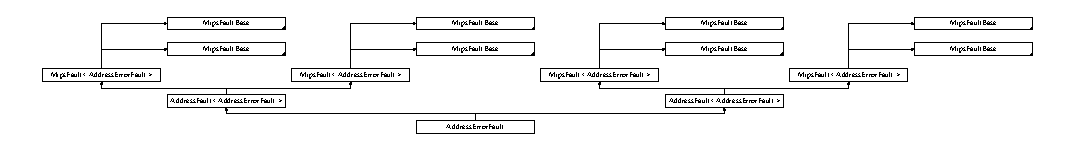
\includegraphics[height=1.5625cm]{classMipsISA_1_1AddressErrorFault}
\end{center}
\end{figure}
\subsection*{Public メソッド}
\begin{DoxyCompactItemize}
\item 
\hyperlink{classMipsISA_1_1AddressErrorFault_a63571998d6c69ae9fc079f7bded37b9d}{AddressErrorFault} (\hyperlink{classm5_1_1params_1_1Addr}{Addr} \_\-vaddr, bool \_\-store)
\item 
\hyperlink{namespaceMipsISA_abcc8a7c57cd8becefbfd621dbff5ffd4}{ExcCode} \hyperlink{classMipsISA_1_1AddressErrorFault_a1dd20a2460d7723d3eaa287b7cc07e79}{code} () const 
\item 
\hyperlink{classMipsISA_1_1AddressErrorFault_a63571998d6c69ae9fc079f7bded37b9d}{AddressErrorFault} (\hyperlink{classm5_1_1params_1_1Addr}{Addr} \_\-vaddr, bool \_\-store)
\item 
\hyperlink{namespaceMipsISA_abcc8a7c57cd8becefbfd621dbff5ffd4}{ExcCode} \hyperlink{classMipsISA_1_1AddressErrorFault_a1dd20a2460d7723d3eaa287b7cc07e79}{code} () const 
\end{DoxyCompactItemize}


\subsection{コンストラクタとデストラクタ}
\hypertarget{classMipsISA_1_1AddressErrorFault_a63571998d6c69ae9fc079f7bded37b9d}{
\index{MipsISA::AddressErrorFault@{MipsISA::AddressErrorFault}!AddressErrorFault@{AddressErrorFault}}
\index{AddressErrorFault@{AddressErrorFault}!MipsISA::AddressErrorFault@{MipsISA::AddressErrorFault}}
\subsubsection[{AddressErrorFault}]{\setlength{\rightskip}{0pt plus 5cm}{\bf AddressErrorFault} ({\bf Addr} {\em \_\-vaddr}, \/  bool {\em \_\-store})\hspace{0.3cm}{\ttfamily  \mbox{[}inline\mbox{]}}}}
\label{classMipsISA_1_1AddressErrorFault_a63571998d6c69ae9fc079f7bded37b9d}



\begin{DoxyCode}
212                                                 :
213         AddressFault<AddressErrorFault>(_vaddr, _store)
214     {}

\end{DoxyCode}
\hypertarget{classMipsISA_1_1AddressErrorFault_a63571998d6c69ae9fc079f7bded37b9d}{
\index{MipsISA::AddressErrorFault@{MipsISA::AddressErrorFault}!AddressErrorFault@{AddressErrorFault}}
\index{AddressErrorFault@{AddressErrorFault}!MipsISA::AddressErrorFault@{MipsISA::AddressErrorFault}}
\subsubsection[{AddressErrorFault}]{\setlength{\rightskip}{0pt plus 5cm}{\bf AddressErrorFault} ({\bf Addr} {\em \_\-vaddr}, \/  bool {\em \_\-store})\hspace{0.3cm}{\ttfamily  \mbox{[}inline\mbox{]}}}}
\label{classMipsISA_1_1AddressErrorFault_a63571998d6c69ae9fc079f7bded37b9d}



\begin{DoxyCode}
212                                                 :
213         AddressFault<AddressErrorFault>(_vaddr, _store)
214     {}

\end{DoxyCode}


\subsection{関数}
\hypertarget{classMipsISA_1_1AddressErrorFault_a1dd20a2460d7723d3eaa287b7cc07e79}{
\index{MipsISA::AddressErrorFault@{MipsISA::AddressErrorFault}!code@{code}}
\index{code@{code}!MipsISA::AddressErrorFault@{MipsISA::AddressErrorFault}}
\subsubsection[{code}]{\setlength{\rightskip}{0pt plus 5cm}{\bf ExcCode} code () const\hspace{0.3cm}{\ttfamily  \mbox{[}inline, virtual\mbox{]}}}}
\label{classMipsISA_1_1AddressErrorFault_a1dd20a2460d7723d3eaa287b7cc07e79}


\hyperlink{classMipsISA_1_1MipsFault_a1dd20a2460d7723d3eaa287b7cc07e79}{MipsFault$<$ AddressErrorFault $>$}を再定義しています。


\begin{DoxyCode}
218     {
219         return store ? ExcCodeAdES : ExcCodeAdEL;
220     }
\end{DoxyCode}
\hypertarget{classMipsISA_1_1AddressErrorFault_a1dd20a2460d7723d3eaa287b7cc07e79}{
\index{MipsISA::AddressErrorFault@{MipsISA::AddressErrorFault}!code@{code}}
\index{code@{code}!MipsISA::AddressErrorFault@{MipsISA::AddressErrorFault}}
\subsubsection[{code}]{\setlength{\rightskip}{0pt plus 5cm}{\bf ExcCode} code () const\hspace{0.3cm}{\ttfamily  \mbox{[}inline, virtual\mbox{]}}}}
\label{classMipsISA_1_1AddressErrorFault_a1dd20a2460d7723d3eaa287b7cc07e79}


\hyperlink{classMipsISA_1_1MipsFault_a1dd20a2460d7723d3eaa287b7cc07e79}{MipsFault$<$ AddressErrorFault $>$}を再定義しています。


\begin{DoxyCode}
218     {
219         return store ? ExcCodeAdES : ExcCodeAdEL;
220     }
\end{DoxyCode}


このクラスの説明は次のファイルから生成されました:\begin{DoxyCompactItemize}
\item 
arch/mips/\hyperlink{arch_2mips_2faults_8hh}{faults.hh}\item 
arch/miqs/\hyperlink{arch_2miqs_2faults_8hh}{faults.hh}\end{DoxyCompactItemize}

\hypertarget{classMipsISA_1_1AddressFault}{
\section{クラス テンプレート AddressFault$<$ T $>$}
\label{classMipsISA_1_1AddressFault}\index{MipsISA::AddressFault@{MipsISA::AddressFault}}
}


{\ttfamily \#include $<$faults.hh$>$}AddressFault$<$ T $>$に対する継承グラフ:\begin{figure}[H]
\begin{center}
\leavevmode
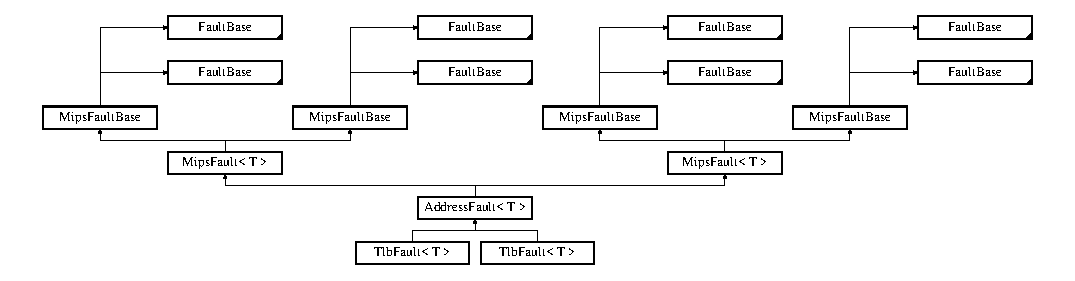
\includegraphics[height=3.33333cm]{classMipsISA_1_1AddressFault}
\end{center}
\end{figure}
\subsection*{Protected メソッド}
\begin{DoxyCompactItemize}
\item 
\hyperlink{classMipsISA_1_1AddressFault_a41d5cd77142b61159baea077490c4101}{AddressFault} (\hyperlink{classm5_1_1params_1_1Addr}{Addr} \_\-vaddr, bool \_\-store)
\item 
void \hyperlink{classMipsISA_1_1AddressFault_a2bd783b42262278d41157d428e1f8d6f}{invoke} (\hyperlink{classThreadContext}{ThreadContext} $\ast$tc, \hyperlink{classRefCountingPtr}{StaticInstPtr} inst=\hyperlink{classStaticInst_aa793d9793af735f09096369fb17567b6}{StaticInst::nullStaticInstPtr})
\item 
\hyperlink{classMipsISA_1_1AddressFault_a41d5cd77142b61159baea077490c4101}{AddressFault} (\hyperlink{classm5_1_1params_1_1Addr}{Addr} \_\-vaddr, bool \_\-store)
\item 
void \hyperlink{classMipsISA_1_1AddressFault_a2bd783b42262278d41157d428e1f8d6f}{invoke} (\hyperlink{classThreadContext}{ThreadContext} $\ast$tc, \hyperlink{classRefCountingPtr}{StaticInstPtr} inst=\hyperlink{classStaticInst_aa793d9793af735f09096369fb17567b6}{StaticInst::nullStaticInstPtr})
\end{DoxyCompactItemize}
\subsection*{Protected 変数}
\begin{DoxyCompactItemize}
\item 
\hyperlink{classm5_1_1params_1_1Addr}{Addr} \hyperlink{classMipsISA_1_1AddressFault_a9f933b300ef63eea367ca82f8da31025}{vaddr}
\item 
bool \hyperlink{classMipsISA_1_1AddressFault_a86c0e52eeb2243d66bc032096c160a0b}{store}
\end{DoxyCompactItemize}
\subsubsection*{template$<$typename T$>$ class MipsISA::AddressFault$<$ T $>$}



\subsection{コンストラクタとデストラクタ}
\hypertarget{classMipsISA_1_1AddressFault_a41d5cd77142b61159baea077490c4101}{
\index{MipsISA::AddressFault@{MipsISA::AddressFault}!AddressFault@{AddressFault}}
\index{AddressFault@{AddressFault}!MipsISA::AddressFault@{MipsISA::AddressFault}}
\subsubsection[{AddressFault}]{\setlength{\rightskip}{0pt plus 5cm}{\bf AddressFault} ({\bf Addr} {\em \_\-vaddr}, \/  bool {\em \_\-store})\hspace{0.3cm}{\ttfamily  \mbox{[}inline, protected\mbox{]}}}}
\label{classMipsISA_1_1AddressFault_a41d5cd77142b61159baea077490c4101}



\begin{DoxyCode}
196                                            : vaddr(_vaddr), store(_store)
197     {}
\end{DoxyCode}
\hypertarget{classMipsISA_1_1AddressFault_a41d5cd77142b61159baea077490c4101}{
\index{MipsISA::AddressFault@{MipsISA::AddressFault}!AddressFault@{AddressFault}}
\index{AddressFault@{AddressFault}!MipsISA::AddressFault@{MipsISA::AddressFault}}
\subsubsection[{AddressFault}]{\setlength{\rightskip}{0pt plus 5cm}{\bf AddressFault} ({\bf Addr} {\em \_\-vaddr}, \/  bool {\em \_\-store})\hspace{0.3cm}{\ttfamily  \mbox{[}inline, protected\mbox{]}}}}
\label{classMipsISA_1_1AddressFault_a41d5cd77142b61159baea077490c4101}



\begin{DoxyCode}
196                                            : vaddr(_vaddr), store(_store)
197     {}
\end{DoxyCode}


\subsection{関数}
\hypertarget{classMipsISA_1_1AddressFault_a2bd783b42262278d41157d428e1f8d6f}{
\index{MipsISA::AddressFault@{MipsISA::AddressFault}!invoke@{invoke}}
\index{invoke@{invoke}!MipsISA::AddressFault@{MipsISA::AddressFault}}
\subsubsection[{invoke}]{\setlength{\rightskip}{0pt plus 5cm}void invoke ({\bf ThreadContext} $\ast$ {\em tc}, \/  {\bf StaticInstPtr} {\em inst} = {\ttfamily {\bf StaticInst::nullStaticInstPtr}})\hspace{0.3cm}{\ttfamily  \mbox{[}inline, protected, virtual\mbox{]}}}}
\label{classMipsISA_1_1AddressFault_a2bd783b42262278d41157d428e1f8d6f}


\hyperlink{classMipsISA_1_1MipsFaultBase_a2bd783b42262278d41157d428e1f8d6f}{MipsFaultBase}を再定義しています。

\hyperlink{classMipsISA_1_1TlbFault_a2bd783b42262278d41157d428e1f8d6f}{TlbFault$<$ T $>$}, \hyperlink{classMipsISA_1_1TlbFault_a2bd783b42262278d41157d428e1f8d6f}{TlbFault$<$ T $>$}, \hyperlink{classMipsISA_1_1TlbFault_a2bd783b42262278d41157d428e1f8d6f}{TlbFault$<$ TlbRefillFault $>$}, \hyperlink{classMipsISA_1_1TlbFault_a2bd783b42262278d41157d428e1f8d6f}{TlbFault$<$ TlbRefillFault $>$}, \hyperlink{classMipsISA_1_1TlbFault_a2bd783b42262278d41157d428e1f8d6f}{TlbFault$<$ TlbModifiedFault $>$}, \hyperlink{classMipsISA_1_1TlbFault_a2bd783b42262278d41157d428e1f8d6f}{TlbFault$<$ TlbModifiedFault $>$}, \hyperlink{classMipsISA_1_1TlbFault_a2bd783b42262278d41157d428e1f8d6f}{TlbFault$<$ TlbInvalidFault $>$}, と \hyperlink{classMipsISA_1_1TlbFault_a2bd783b42262278d41157d428e1f8d6f}{TlbFault$<$ TlbInvalidFault $>$}で再定義されています。


\begin{DoxyCode}
202     {
203         MipsFault<T>::invoke(tc, inst);
204         if (FullSystem)
205             tc->setMiscRegNoEffect(MISCREG_BADVADDR, vaddr);
206     }
\end{DoxyCode}
\hypertarget{classMipsISA_1_1AddressFault_a2bd783b42262278d41157d428e1f8d6f}{
\index{MipsISA::AddressFault@{MipsISA::AddressFault}!invoke@{invoke}}
\index{invoke@{invoke}!MipsISA::AddressFault@{MipsISA::AddressFault}}
\subsubsection[{invoke}]{\setlength{\rightskip}{0pt plus 5cm}void invoke ({\bf ThreadContext} $\ast$ {\em tc}, \/  {\bf StaticInstPtr} {\em inst} = {\ttfamily {\bf StaticInst::nullStaticInstPtr}})\hspace{0.3cm}{\ttfamily  \mbox{[}inline, protected, virtual\mbox{]}}}}
\label{classMipsISA_1_1AddressFault_a2bd783b42262278d41157d428e1f8d6f}


\hyperlink{classMipsISA_1_1MipsFaultBase_a2bd783b42262278d41157d428e1f8d6f}{MipsFaultBase}を再定義しています。

\hyperlink{classMipsISA_1_1TlbFault_a2bd783b42262278d41157d428e1f8d6f}{TlbFault$<$ T $>$}, \hyperlink{classMipsISA_1_1TlbFault_a2bd783b42262278d41157d428e1f8d6f}{TlbFault$<$ T $>$}, \hyperlink{classMipsISA_1_1TlbFault_a2bd783b42262278d41157d428e1f8d6f}{TlbFault$<$ TlbRefillFault $>$}, \hyperlink{classMipsISA_1_1TlbFault_a2bd783b42262278d41157d428e1f8d6f}{TlbFault$<$ TlbRefillFault $>$}, \hyperlink{classMipsISA_1_1TlbFault_a2bd783b42262278d41157d428e1f8d6f}{TlbFault$<$ TlbModifiedFault $>$}, \hyperlink{classMipsISA_1_1TlbFault_a2bd783b42262278d41157d428e1f8d6f}{TlbFault$<$ TlbModifiedFault $>$}, \hyperlink{classMipsISA_1_1TlbFault_a2bd783b42262278d41157d428e1f8d6f}{TlbFault$<$ TlbInvalidFault $>$}, と \hyperlink{classMipsISA_1_1TlbFault_a2bd783b42262278d41157d428e1f8d6f}{TlbFault$<$ TlbInvalidFault $>$}で再定義されています。


\begin{DoxyCode}
202     {
203         MipsFault<T>::invoke(tc, inst);
204         if (FullSystem)
205             tc->setMiscRegNoEffect(MISCREG_BADVADDR, vaddr);
206     }
\end{DoxyCode}


\subsection{変数}
\hypertarget{classMipsISA_1_1AddressFault_a86c0e52eeb2243d66bc032096c160a0b}{
\index{MipsISA::AddressFault@{MipsISA::AddressFault}!store@{store}}
\index{store@{store}!MipsISA::AddressFault@{MipsISA::AddressFault}}
\subsubsection[{store}]{\setlength{\rightskip}{0pt plus 5cm}bool {\bf store}\hspace{0.3cm}{\ttfamily  \mbox{[}protected\mbox{]}}}}
\label{classMipsISA_1_1AddressFault_a86c0e52eeb2243d66bc032096c160a0b}
\hypertarget{classMipsISA_1_1AddressFault_a9f933b300ef63eea367ca82f8da31025}{
\index{MipsISA::AddressFault@{MipsISA::AddressFault}!vaddr@{vaddr}}
\index{vaddr@{vaddr}!MipsISA::AddressFault@{MipsISA::AddressFault}}
\subsubsection[{vaddr}]{\setlength{\rightskip}{0pt plus 5cm}{\bf Addr} {\bf vaddr}\hspace{0.3cm}{\ttfamily  \mbox{[}protected\mbox{]}}}}
\label{classMipsISA_1_1AddressFault_a9f933b300ef63eea367ca82f8da31025}


このクラスの説明は次のファイルから生成されました:\begin{DoxyCompactItemize}
\item 
arch/mips/\hyperlink{arch_2mips_2faults_8hh}{faults.hh}\item 
arch/miqs/\hyperlink{arch_2miqs_2faults_8hh}{faults.hh}\end{DoxyCompactItemize}

\hypertarget{classAddressProfiler}{
\section{クラス AddressProfiler}
\label{classAddressProfiler}\index{AddressProfiler@{AddressProfiler}}
}


{\ttfamily \#include $<$AddressProfiler.hh$>$}\subsection*{Public 型}
\begin{DoxyCompactItemize}
\item 
typedef m5::hash\_\-map$<$ \hyperlink{classAddress}{Address}, \hyperlink{classAccessTraceForAddress}{AccessTraceForAddress} $>$ \hyperlink{classAddressProfiler_a8a9f1225b5c1cb2d26e7cea035910b56}{AddressMap}
\end{DoxyCompactItemize}
\subsection*{Public メソッド}
\begin{DoxyCompactItemize}
\item 
\hyperlink{classAddressProfiler_af450d4ff37cb5d876e71ca5ed54b5488}{AddressProfiler} (int num\_\-of\_\-sequencers)
\item 
\hyperlink{classAddressProfiler_adc42b3cd6cc3b0daa903e7cb7f55e16f}{$\sim$AddressProfiler} ()
\item 
void \hyperlink{classAddressProfiler_a38f932a0a623730fe10783f46d243cef}{printStats} (std::ostream \&out) const 
\item 
void \hyperlink{classAddressProfiler_ac7ec7476159db4e2bb0372e30010fc9e}{clearStats} ()
\item 
void \hyperlink{classAddressProfiler_ada40ab5186eed63c4af52be6bfea3cab}{addTraceSample} (\hyperlink{classAddress}{Address} data\_\-addr, \hyperlink{classAddress}{Address} pc\_\-addr, RubyRequestType type, RubyAccessMode access\_\-mode, \hyperlink{TypeDefines_8hh_a83c14b4ae37e80071f6b3506a6c46151}{NodeID} id, bool sharing\_\-miss)
\item 
void \hyperlink{classAddressProfiler_a1c945549407c104dbbeb48debeb9b19a}{profileRetry} (const \hyperlink{classAddress}{Address} \&data\_\-addr, AccessType type, int count)
\item 
void \hyperlink{classAddressProfiler_ab606b5db14b057fe6c99b4632d2fcd79}{profileGetX} (const \hyperlink{classAddress}{Address} \&datablock, const \hyperlink{classAddress}{Address} \&PC, const \hyperlink{classSet}{Set} \&owner, const \hyperlink{classSet}{Set} \&sharers, \hyperlink{TypeDefines_8hh_a83c14b4ae37e80071f6b3506a6c46151}{NodeID} requestor)
\item 
void \hyperlink{classAddressProfiler_a79a57b3f376ac7ef7a55bf73dcff3402}{profileGetS} (const \hyperlink{classAddress}{Address} \&datablock, const \hyperlink{classAddress}{Address} \&PC, const \hyperlink{classSet}{Set} \&owner, const \hyperlink{classSet}{Set} \&sharers, \hyperlink{TypeDefines_8hh_a83c14b4ae37e80071f6b3506a6c46151}{NodeID} requestor)
\item 
void \hyperlink{classAddressProfiler_ac55fe386a101fbae38c716067c9966a0}{print} (std::ostream \&out) const 
\item 
void \hyperlink{classAddressProfiler_a7ec524009c6db09ba82f2ffc4cfff1ea}{setHotLines} (bool hot\_\-lines)
\item 
void \hyperlink{classAddressProfiler_a49ffa3641d3d22f47166dd03dcc39589}{setAllInstructions} (bool all\_\-instructions)
\item 
void \hyperlink{classAddressProfiler_a3dd3443357312bcb75580eaa508c48a4}{regStats} (const std::string \&name)
\item 
void \hyperlink{classAddressProfiler_a208669cbc0bb1d52565956ca8c690c55}{collateStats} ()
\end{DoxyCompactItemize}
\subsection*{Private メソッド}
\begin{DoxyCompactItemize}
\item 
\hyperlink{classAddressProfiler_a34e17be12a9b21c77a0705bd32e8b453}{AddressProfiler} (const \hyperlink{classAddressProfiler}{AddressProfiler} \&obj)
\item 
\hyperlink{classAddressProfiler}{AddressProfiler} \& \hyperlink{classAddressProfiler_a0473a7090f98a61e75343ebc48ae55f0}{operator=} (const \hyperlink{classAddressProfiler}{AddressProfiler} \&obj)
\end{DoxyCompactItemize}
\subsection*{Private 変数}
\begin{DoxyCompactItemize}
\item 
\hyperlink{TypeDefines_8hh_aecfc3c54bd29ad5964e1c1c3ccbf89df}{int64} \hyperlink{classAddressProfiler_a20e874443e8d69362f989878d804fde9}{m\_\-sharing\_\-miss\_\-counter}
\item 
\hyperlink{classAddressProfiler_a8a9f1225b5c1cb2d26e7cea035910b56}{AddressMap} \hyperlink{classAddressProfiler_a524d8a56b5050e28af4fa074b77ad38d}{m\_\-dataAccessTrace}
\item 
\hyperlink{classAddressProfiler_a8a9f1225b5c1cb2d26e7cea035910b56}{AddressMap} \hyperlink{classAddressProfiler_ad55da4039a01bb4b94ba1cf7423d2b0b}{m\_\-macroBlockAccessTrace}
\item 
\hyperlink{classAddressProfiler_a8a9f1225b5c1cb2d26e7cea035910b56}{AddressMap} \hyperlink{classAddressProfiler_add87ed2083e606197b3a461e240265fe}{m\_\-programCounterAccessTrace}
\item 
\hyperlink{classAddressProfiler_a8a9f1225b5c1cb2d26e7cea035910b56}{AddressMap} \hyperlink{classAddressProfiler_a5955c6c282623622af31f869827f70eb}{m\_\-retryProfileMap}
\item 
\hyperlink{classHistogram}{Histogram} \hyperlink{classAddressProfiler_ad4161c63b4a05631ec9e072cb6155c14}{m\_\-retryProfileHisto}
\item 
\hyperlink{classHistogram}{Histogram} \hyperlink{classAddressProfiler_a4d31cdef4eb6fd3bf397cfa76522688f}{m\_\-retryProfileHistoWrite}
\item 
\hyperlink{classHistogram}{Histogram} \hyperlink{classAddressProfiler_ad7a5f305526e5d643476bd8a77b31e63}{m\_\-retryProfileHistoRead}
\item 
\hyperlink{classHistogram}{Histogram} \hyperlink{classAddressProfiler_a50c23c3bc724b0e58e2702923fbd729c}{m\_\-getx\_\-sharing\_\-histogram}
\item 
\hyperlink{classHistogram}{Histogram} \hyperlink{classAddressProfiler_abad849fa15b8dabdb10a90d412691484}{m\_\-gets\_\-sharing\_\-histogram}
\item 
bool \hyperlink{classAddressProfiler_a3b63dfc643f2cf98e6d5deff9fce467e}{m\_\-hot\_\-lines}
\item 
bool \hyperlink{classAddressProfiler_a32e2ae13dc24a9bd92b83fa9e02477ff}{m\_\-all\_\-instructions}
\item 
int \hyperlink{classAddressProfiler_a7ba3ff540bbbb92208f2957cfcd9709f}{m\_\-num\_\-of\_\-sequencers}
\end{DoxyCompactItemize}


\subsection{型定義}
\hypertarget{classAddressProfiler_a8a9f1225b5c1cb2d26e7cea035910b56}{
\index{AddressProfiler@{AddressProfiler}!AddressMap@{AddressMap}}
\index{AddressMap@{AddressMap}!AddressProfiler@{AddressProfiler}}
\subsubsection[{AddressMap}]{\setlength{\rightskip}{0pt plus 5cm}typedef m5::hash\_\-map$<${\bf Address}, {\bf AccessTraceForAddress}$>$ {\bf AddressMap}}}
\label{classAddressProfiler_a8a9f1225b5c1cb2d26e7cea035910b56}


\subsection{コンストラクタとデストラクタ}
\hypertarget{classAddressProfiler_af450d4ff37cb5d876e71ca5ed54b5488}{
\index{AddressProfiler@{AddressProfiler}!AddressProfiler@{AddressProfiler}}
\index{AddressProfiler@{AddressProfiler}!AddressProfiler@{AddressProfiler}}
\subsubsection[{AddressProfiler}]{\setlength{\rightskip}{0pt plus 5cm}{\bf AddressProfiler} (int {\em num\_\-of\_\-sequencers})}}
\label{classAddressProfiler_af450d4ff37cb5d876e71ca5ed54b5488}



\begin{DoxyCode}
147 {
148     m_num_of_sequencers = num_of_sequencers;
149     clearStats();
150 }
\end{DoxyCode}
\hypertarget{classAddressProfiler_adc42b3cd6cc3b0daa903e7cb7f55e16f}{
\index{AddressProfiler@{AddressProfiler}!$\sim$AddressProfiler@{$\sim$AddressProfiler}}
\index{$\sim$AddressProfiler@{$\sim$AddressProfiler}!AddressProfiler@{AddressProfiler}}
\subsubsection[{$\sim$AddressProfiler}]{\setlength{\rightskip}{0pt plus 5cm}$\sim${\bf AddressProfiler} ()}}
\label{classAddressProfiler_adc42b3cd6cc3b0daa903e7cb7f55e16f}



\begin{DoxyCode}
153 {
154 }
\end{DoxyCode}
\hypertarget{classAddressProfiler_a34e17be12a9b21c77a0705bd32e8b453}{
\index{AddressProfiler@{AddressProfiler}!AddressProfiler@{AddressProfiler}}
\index{AddressProfiler@{AddressProfiler}!AddressProfiler@{AddressProfiler}}
\subsubsection[{AddressProfiler}]{\setlength{\rightskip}{0pt plus 5cm}{\bf AddressProfiler} (const {\bf AddressProfiler} \& {\em obj})\hspace{0.3cm}{\ttfamily  \mbox{[}private\mbox{]}}}}
\label{classAddressProfiler_a34e17be12a9b21c77a0705bd32e8b453}


\subsection{関数}
\hypertarget{classAddressProfiler_ada40ab5186eed63c4af52be6bfea3cab}{
\index{AddressProfiler@{AddressProfiler}!addTraceSample@{addTraceSample}}
\index{addTraceSample@{addTraceSample}!AddressProfiler@{AddressProfiler}}
\subsubsection[{addTraceSample}]{\setlength{\rightskip}{0pt plus 5cm}void addTraceSample ({\bf Address} {\em data\_\-addr}, \/  {\bf Address} {\em pc\_\-addr}, \/  RubyRequestType {\em type}, \/  RubyAccessMode {\em access\_\-mode}, \/  {\bf NodeID} {\em id}, \/  bool {\em sharing\_\-miss})}}
\label{classAddressProfiler_ada40ab5186eed63c4af52be6bfea3cab}



\begin{DoxyCode}
286 {
287     if (m_all_instructions) {
288         if (sharing_miss) {
289             m_sharing_miss_counter++;
290         }
291 
292         // record data address trace info
293         data_addr.makeLineAddress();
294         lookupTraceForAddress(data_addr, m_dataAccessTrace).
295             update(type, access_mode, id, sharing_miss);
296 
297         // record macro data address trace info
298 
299         // 6 for datablock, 4 to make it 16x more coarse
300         Address macro_addr(data_addr.maskLowOrderBits(10));
301         lookupTraceForAddress(macro_addr, m_macroBlockAccessTrace).
302             update(type, access_mode, id, sharing_miss);
303 
304         // record program counter address trace info
305         lookupTraceForAddress(pc_addr, m_programCounterAccessTrace).
306             update(type, access_mode, id, sharing_miss);
307     }
308 
309     if (m_all_instructions) {
310         // This code is used if the address profiler is an
311         // all-instructions profiler record program counter address
312         // trace info
313         lookupTraceForAddress(pc_addr, m_programCounterAccessTrace).
314             update(type, access_mode, id, sharing_miss);
315     }
316 }
\end{DoxyCode}
\hypertarget{classAddressProfiler_ac7ec7476159db4e2bb0372e30010fc9e}{
\index{AddressProfiler@{AddressProfiler}!clearStats@{clearStats}}
\index{clearStats@{clearStats}!AddressProfiler@{AddressProfiler}}
\subsubsection[{clearStats}]{\setlength{\rightskip}{0pt plus 5cm}void clearStats ()}}
\label{classAddressProfiler_ac7ec7476159db4e2bb0372e30010fc9e}



\begin{DoxyCode}
232 {
233     // Clear the maps
234     m_sharing_miss_counter = 0;
235     m_dataAccessTrace.clear();
236     m_macroBlockAccessTrace.clear();
237     m_programCounterAccessTrace.clear();
238     m_retryProfileMap.clear();
239     m_retryProfileHisto.clear();
240     m_retryProfileHistoRead.clear();
241     m_retryProfileHistoWrite.clear();
242     m_getx_sharing_histogram.clear();
243     m_gets_sharing_histogram.clear();
244 }
\end{DoxyCode}
\hypertarget{classAddressProfiler_a208669cbc0bb1d52565956ca8c690c55}{
\index{AddressProfiler@{AddressProfiler}!collateStats@{collateStats}}
\index{collateStats@{collateStats}!AddressProfiler@{AddressProfiler}}
\subsubsection[{collateStats}]{\setlength{\rightskip}{0pt plus 5cm}void collateStats ()\hspace{0.3cm}{\ttfamily  \mbox{[}inline\mbox{]}}}}
\label{classAddressProfiler_a208669cbc0bb1d52565956ca8c690c55}



\begin{DoxyCode}
71 {}
\end{DoxyCode}
\hypertarget{classAddressProfiler_a0473a7090f98a61e75343ebc48ae55f0}{
\index{AddressProfiler@{AddressProfiler}!operator=@{operator=}}
\index{operator=@{operator=}!AddressProfiler@{AddressProfiler}}
\subsubsection[{operator=}]{\setlength{\rightskip}{0pt plus 5cm}{\bf AddressProfiler}\& operator= (const {\bf AddressProfiler} \& {\em obj})\hspace{0.3cm}{\ttfamily  \mbox{[}private\mbox{]}}}}
\label{classAddressProfiler_a0473a7090f98a61e75343ebc48ae55f0}
\hypertarget{classAddressProfiler_ac55fe386a101fbae38c716067c9966a0}{
\index{AddressProfiler@{AddressProfiler}!print@{print}}
\index{print@{print}!AddressProfiler@{AddressProfiler}}
\subsubsection[{print}]{\setlength{\rightskip}{0pt plus 5cm}void print (std::ostream \& {\em out}) const}}
\label{classAddressProfiler_ac55fe386a101fbae38c716067c9966a0}
\hypertarget{classAddressProfiler_a38f932a0a623730fe10783f46d243cef}{
\index{AddressProfiler@{AddressProfiler}!printStats@{printStats}}
\index{printStats@{printStats}!AddressProfiler@{AddressProfiler}}
\subsubsection[{printStats}]{\setlength{\rightskip}{0pt plus 5cm}void printStats (std::ostream \& {\em out}) const}}
\label{classAddressProfiler_a38f932a0a623730fe10783f46d243cef}
\hypertarget{classAddressProfiler_a79a57b3f376ac7ef7a55bf73dcff3402}{
\index{AddressProfiler@{AddressProfiler}!profileGetS@{profileGetS}}
\index{profileGetS@{profileGetS}!AddressProfiler@{AddressProfiler}}
\subsubsection[{profileGetS}]{\setlength{\rightskip}{0pt plus 5cm}void profileGetS (const {\bf Address} \& {\em datablock}, \/  const {\bf Address} \& {\em PC}, \/  const {\bf Set} \& {\em owner}, \/  const {\bf Set} \& {\em sharers}, \/  {\bf NodeID} {\em requestor})}}
\label{classAddressProfiler_a79a57b3f376ac7ef7a55bf73dcff3402}



\begin{DoxyCode}
268 {
269     Set indirection_set;
270     indirection_set.addSet(owner);
271     indirection_set.remove(requestor);
272     int num_indirections = indirection_set.count();
273 
274     m_gets_sharing_histogram.add(num_indirections);
275     bool indirection_miss = (num_indirections > 0);
276 
277     addTraceSample(datablock, PC, RubyRequestType_LD, RubyAccessMode(0),
278                    requestor, indirection_miss);
279 }
\end{DoxyCode}
\hypertarget{classAddressProfiler_ab606b5db14b057fe6c99b4632d2fcd79}{
\index{AddressProfiler@{AddressProfiler}!profileGetX@{profileGetX}}
\index{profileGetX@{profileGetX}!AddressProfiler@{AddressProfiler}}
\subsubsection[{profileGetX}]{\setlength{\rightskip}{0pt plus 5cm}void profileGetX (const {\bf Address} \& {\em datablock}, \/  const {\bf Address} \& {\em PC}, \/  const {\bf Set} \& {\em owner}, \/  const {\bf Set} \& {\em sharers}, \/  {\bf NodeID} {\em requestor})}}
\label{classAddressProfiler_ab606b5db14b057fe6c99b4632d2fcd79}



\begin{DoxyCode}
250 {
251     Set indirection_set;
252     indirection_set.addSet(sharers);
253     indirection_set.addSet(owner);
254     indirection_set.remove(requestor);
255     int num_indirections = indirection_set.count();
256 
257     m_getx_sharing_histogram.add(num_indirections);
258     bool indirection_miss = (num_indirections > 0);
259 
260     addTraceSample(datablock, PC, RubyRequestType_ST, RubyAccessMode(0),
261                    requestor, indirection_miss);
262 }
\end{DoxyCode}
\hypertarget{classAddressProfiler_a1c945549407c104dbbeb48debeb9b19a}{
\index{AddressProfiler@{AddressProfiler}!profileRetry@{profileRetry}}
\index{profileRetry@{profileRetry}!AddressProfiler@{AddressProfiler}}
\subsubsection[{profileRetry}]{\setlength{\rightskip}{0pt plus 5cm}void profileRetry (const {\bf Address} \& {\em data\_\-addr}, \/  AccessType {\em type}, \/  int {\em count})}}
\label{classAddressProfiler_a1c945549407c104dbbeb48debeb9b19a}



\begin{DoxyCode}
321 {
322     m_retryProfileHisto.add(count);
323     if (type == AccessType_Read) {
324         m_retryProfileHistoRead.add(count);
325     } else {
326         m_retryProfileHistoWrite.add(count);
327     }
328     if (count > 1) {
329         lookupTraceForAddress(data_addr, m_retryProfileMap).addSample(count);
330     }
331 }
\end{DoxyCode}
\hypertarget{classAddressProfiler_a3dd3443357312bcb75580eaa508c48a4}{
\index{AddressProfiler@{AddressProfiler}!regStats@{regStats}}
\index{regStats@{regStats}!AddressProfiler@{AddressProfiler}}
\subsubsection[{regStats}]{\setlength{\rightskip}{0pt plus 5cm}void regStats (const std::string \& {\em name})\hspace{0.3cm}{\ttfamily  \mbox{[}inline\mbox{]}}}}
\label{classAddressProfiler_a3dd3443357312bcb75580eaa508c48a4}



\begin{DoxyCode}
70 {}
\end{DoxyCode}
\hypertarget{classAddressProfiler_a49ffa3641d3d22f47166dd03dcc39589}{
\index{AddressProfiler@{AddressProfiler}!setAllInstructions@{setAllInstructions}}
\index{setAllInstructions@{setAllInstructions}!AddressProfiler@{AddressProfiler}}
\subsubsection[{setAllInstructions}]{\setlength{\rightskip}{0pt plus 5cm}void setAllInstructions (bool {\em all\_\-instructions})}}
\label{classAddressProfiler_a49ffa3641d3d22f47166dd03dcc39589}



\begin{DoxyCode}
164 {
165     m_all_instructions = all_instructions;
166 }
\end{DoxyCode}
\hypertarget{classAddressProfiler_a7ec524009c6db09ba82f2ffc4cfff1ea}{
\index{AddressProfiler@{AddressProfiler}!setHotLines@{setHotLines}}
\index{setHotLines@{setHotLines}!AddressProfiler@{AddressProfiler}}
\subsubsection[{setHotLines}]{\setlength{\rightskip}{0pt plus 5cm}void setHotLines (bool {\em hot\_\-lines})}}
\label{classAddressProfiler_a7ec524009c6db09ba82f2ffc4cfff1ea}



\begin{DoxyCode}
158 {
159     m_hot_lines = hot_lines;
160 }
\end{DoxyCode}


\subsection{変数}
\hypertarget{classAddressProfiler_a32e2ae13dc24a9bd92b83fa9e02477ff}{
\index{AddressProfiler@{AddressProfiler}!m\_\-all\_\-instructions@{m\_\-all\_\-instructions}}
\index{m\_\-all\_\-instructions@{m\_\-all\_\-instructions}!AddressProfiler@{AddressProfiler}}
\subsubsection[{m\_\-all\_\-instructions}]{\setlength{\rightskip}{0pt plus 5cm}bool {\bf m\_\-all\_\-instructions}\hspace{0.3cm}{\ttfamily  \mbox{[}private\mbox{]}}}}
\label{classAddressProfiler_a32e2ae13dc24a9bd92b83fa9e02477ff}
\hypertarget{classAddressProfiler_a524d8a56b5050e28af4fa074b77ad38d}{
\index{AddressProfiler@{AddressProfiler}!m\_\-dataAccessTrace@{m\_\-dataAccessTrace}}
\index{m\_\-dataAccessTrace@{m\_\-dataAccessTrace}!AddressProfiler@{AddressProfiler}}
\subsubsection[{m\_\-dataAccessTrace}]{\setlength{\rightskip}{0pt plus 5cm}{\bf AddressMap} {\bf m\_\-dataAccessTrace}\hspace{0.3cm}{\ttfamily  \mbox{[}private\mbox{]}}}}
\label{classAddressProfiler_a524d8a56b5050e28af4fa074b77ad38d}
\hypertarget{classAddressProfiler_abad849fa15b8dabdb10a90d412691484}{
\index{AddressProfiler@{AddressProfiler}!m\_\-gets\_\-sharing\_\-histogram@{m\_\-gets\_\-sharing\_\-histogram}}
\index{m\_\-gets\_\-sharing\_\-histogram@{m\_\-gets\_\-sharing\_\-histogram}!AddressProfiler@{AddressProfiler}}
\subsubsection[{m\_\-gets\_\-sharing\_\-histogram}]{\setlength{\rightskip}{0pt plus 5cm}{\bf Histogram} {\bf m\_\-gets\_\-sharing\_\-histogram}\hspace{0.3cm}{\ttfamily  \mbox{[}private\mbox{]}}}}
\label{classAddressProfiler_abad849fa15b8dabdb10a90d412691484}
\hypertarget{classAddressProfiler_a50c23c3bc724b0e58e2702923fbd729c}{
\index{AddressProfiler@{AddressProfiler}!m\_\-getx\_\-sharing\_\-histogram@{m\_\-getx\_\-sharing\_\-histogram}}
\index{m\_\-getx\_\-sharing\_\-histogram@{m\_\-getx\_\-sharing\_\-histogram}!AddressProfiler@{AddressProfiler}}
\subsubsection[{m\_\-getx\_\-sharing\_\-histogram}]{\setlength{\rightskip}{0pt plus 5cm}{\bf Histogram} {\bf m\_\-getx\_\-sharing\_\-histogram}\hspace{0.3cm}{\ttfamily  \mbox{[}private\mbox{]}}}}
\label{classAddressProfiler_a50c23c3bc724b0e58e2702923fbd729c}
\hypertarget{classAddressProfiler_a3b63dfc643f2cf98e6d5deff9fce467e}{
\index{AddressProfiler@{AddressProfiler}!m\_\-hot\_\-lines@{m\_\-hot\_\-lines}}
\index{m\_\-hot\_\-lines@{m\_\-hot\_\-lines}!AddressProfiler@{AddressProfiler}}
\subsubsection[{m\_\-hot\_\-lines}]{\setlength{\rightskip}{0pt plus 5cm}bool {\bf m\_\-hot\_\-lines}\hspace{0.3cm}{\ttfamily  \mbox{[}private\mbox{]}}}}
\label{classAddressProfiler_a3b63dfc643f2cf98e6d5deff9fce467e}
\hypertarget{classAddressProfiler_ad55da4039a01bb4b94ba1cf7423d2b0b}{
\index{AddressProfiler@{AddressProfiler}!m\_\-macroBlockAccessTrace@{m\_\-macroBlockAccessTrace}}
\index{m\_\-macroBlockAccessTrace@{m\_\-macroBlockAccessTrace}!AddressProfiler@{AddressProfiler}}
\subsubsection[{m\_\-macroBlockAccessTrace}]{\setlength{\rightskip}{0pt plus 5cm}{\bf AddressMap} {\bf m\_\-macroBlockAccessTrace}\hspace{0.3cm}{\ttfamily  \mbox{[}private\mbox{]}}}}
\label{classAddressProfiler_ad55da4039a01bb4b94ba1cf7423d2b0b}
\hypertarget{classAddressProfiler_a7ba3ff540bbbb92208f2957cfcd9709f}{
\index{AddressProfiler@{AddressProfiler}!m\_\-num\_\-of\_\-sequencers@{m\_\-num\_\-of\_\-sequencers}}
\index{m\_\-num\_\-of\_\-sequencers@{m\_\-num\_\-of\_\-sequencers}!AddressProfiler@{AddressProfiler}}
\subsubsection[{m\_\-num\_\-of\_\-sequencers}]{\setlength{\rightskip}{0pt plus 5cm}int {\bf m\_\-num\_\-of\_\-sequencers}\hspace{0.3cm}{\ttfamily  \mbox{[}private\mbox{]}}}}
\label{classAddressProfiler_a7ba3ff540bbbb92208f2957cfcd9709f}
\hypertarget{classAddressProfiler_add87ed2083e606197b3a461e240265fe}{
\index{AddressProfiler@{AddressProfiler}!m\_\-programCounterAccessTrace@{m\_\-programCounterAccessTrace}}
\index{m\_\-programCounterAccessTrace@{m\_\-programCounterAccessTrace}!AddressProfiler@{AddressProfiler}}
\subsubsection[{m\_\-programCounterAccessTrace}]{\setlength{\rightskip}{0pt plus 5cm}{\bf AddressMap} {\bf m\_\-programCounterAccessTrace}\hspace{0.3cm}{\ttfamily  \mbox{[}private\mbox{]}}}}
\label{classAddressProfiler_add87ed2083e606197b3a461e240265fe}
\hypertarget{classAddressProfiler_ad4161c63b4a05631ec9e072cb6155c14}{
\index{AddressProfiler@{AddressProfiler}!m\_\-retryProfileHisto@{m\_\-retryProfileHisto}}
\index{m\_\-retryProfileHisto@{m\_\-retryProfileHisto}!AddressProfiler@{AddressProfiler}}
\subsubsection[{m\_\-retryProfileHisto}]{\setlength{\rightskip}{0pt plus 5cm}{\bf Histogram} {\bf m\_\-retryProfileHisto}\hspace{0.3cm}{\ttfamily  \mbox{[}private\mbox{]}}}}
\label{classAddressProfiler_ad4161c63b4a05631ec9e072cb6155c14}
\hypertarget{classAddressProfiler_ad7a5f305526e5d643476bd8a77b31e63}{
\index{AddressProfiler@{AddressProfiler}!m\_\-retryProfileHistoRead@{m\_\-retryProfileHistoRead}}
\index{m\_\-retryProfileHistoRead@{m\_\-retryProfileHistoRead}!AddressProfiler@{AddressProfiler}}
\subsubsection[{m\_\-retryProfileHistoRead}]{\setlength{\rightskip}{0pt plus 5cm}{\bf Histogram} {\bf m\_\-retryProfileHistoRead}\hspace{0.3cm}{\ttfamily  \mbox{[}private\mbox{]}}}}
\label{classAddressProfiler_ad7a5f305526e5d643476bd8a77b31e63}
\hypertarget{classAddressProfiler_a4d31cdef4eb6fd3bf397cfa76522688f}{
\index{AddressProfiler@{AddressProfiler}!m\_\-retryProfileHistoWrite@{m\_\-retryProfileHistoWrite}}
\index{m\_\-retryProfileHistoWrite@{m\_\-retryProfileHistoWrite}!AddressProfiler@{AddressProfiler}}
\subsubsection[{m\_\-retryProfileHistoWrite}]{\setlength{\rightskip}{0pt plus 5cm}{\bf Histogram} {\bf m\_\-retryProfileHistoWrite}\hspace{0.3cm}{\ttfamily  \mbox{[}private\mbox{]}}}}
\label{classAddressProfiler_a4d31cdef4eb6fd3bf397cfa76522688f}
\hypertarget{classAddressProfiler_a5955c6c282623622af31f869827f70eb}{
\index{AddressProfiler@{AddressProfiler}!m\_\-retryProfileMap@{m\_\-retryProfileMap}}
\index{m\_\-retryProfileMap@{m\_\-retryProfileMap}!AddressProfiler@{AddressProfiler}}
\subsubsection[{m\_\-retryProfileMap}]{\setlength{\rightskip}{0pt plus 5cm}{\bf AddressMap} {\bf m\_\-retryProfileMap}\hspace{0.3cm}{\ttfamily  \mbox{[}private\mbox{]}}}}
\label{classAddressProfiler_a5955c6c282623622af31f869827f70eb}
\hypertarget{classAddressProfiler_a20e874443e8d69362f989878d804fde9}{
\index{AddressProfiler@{AddressProfiler}!m\_\-sharing\_\-miss\_\-counter@{m\_\-sharing\_\-miss\_\-counter}}
\index{m\_\-sharing\_\-miss\_\-counter@{m\_\-sharing\_\-miss\_\-counter}!AddressProfiler@{AddressProfiler}}
\subsubsection[{m\_\-sharing\_\-miss\_\-counter}]{\setlength{\rightskip}{0pt plus 5cm}{\bf int64} {\bf m\_\-sharing\_\-miss\_\-counter}\hspace{0.3cm}{\ttfamily  \mbox{[}private\mbox{]}}}}
\label{classAddressProfiler_a20e874443e8d69362f989878d804fde9}


このクラスの説明は次のファイルから生成されました:\begin{DoxyCompactItemize}
\item 
mem/ruby/profiler/\hyperlink{AddressProfiler_8hh}{AddressProfiler.hh}\item 
mem/ruby/profiler/\hyperlink{AddressProfiler_8cc}{AddressProfiler.cc}\end{DoxyCompactItemize}

\hypertarget{classDecodeCache_1_1AddrMap}{
\section{クラス テンプレート AddrMap$<$ Value $>$}
\label{classDecodeCache_1_1AddrMap}\index{DecodeCache::AddrMap@{DecodeCache::AddrMap}}
}


A sparse map from an Addr to a Value, stored in page chunks.  


{\ttfamily \#include $<$decode\_\-cache.hh$>$}\subsection*{構成}
\begin{DoxyCompactItemize}
\item 
struct \hyperlink{structDecodeCache_1_1AddrMap_1_1CachePage}{CachePage}
\end{DoxyCompactItemize}
\subsection*{Public メソッド}
\begin{DoxyCompactItemize}
\item 
\hyperlink{classDecodeCache_1_1AddrMap_a3214943b0a8ea1081d074586e075edde}{AddrMap} ()
\begin{DoxyCompactList}\small\item\em Constructor. \item\end{DoxyCompactList}\item 
Value \& \hyperlink{classDecodeCache_1_1AddrMap_a758c7479d2ee5aa3d4f1e7584d30379a}{lookup} (\hyperlink{base_2types_8hh_af1bb03d6a4ee096394a6749f0a169232}{Addr} addr)
\end{DoxyCompactItemize}
\subsection*{Protected 型}
\begin{DoxyCompactItemize}
\item 
typedef m5::hash\_\-map$<$ \hyperlink{base_2types_8hh_af1bb03d6a4ee096394a6749f0a169232}{Addr}, \hyperlink{structDecodeCache_1_1AddrMap_1_1CachePage}{CachePage} $\ast$ $>$ \hyperlink{classDecodeCache_1_1AddrMap_a975f1d72d35f5fb84de6f419b04bf347}{PageMap}
\item 
typedef PageMap::iterator \hyperlink{classDecodeCache_1_1AddrMap_af0021638c8ab5f47787c8c1973a125b8}{PageIt}
\end{DoxyCompactItemize}
\subsection*{Protected メソッド}
\begin{DoxyCompactItemize}
\item 
void \hyperlink{classDecodeCache_1_1AddrMap_a64083eea3dfcfac02ed16f18d154f852}{update} (\hyperlink{classDecodeCache_1_1AddrMap_af0021638c8ab5f47787c8c1973a125b8}{PageIt} recentest)
\item 
\hyperlink{structDecodeCache_1_1AddrMap_1_1CachePage}{CachePage} $\ast$ \hyperlink{classDecodeCache_1_1AddrMap_a5eb5de403aecd89f1133b26ad171f51c}{getPage} (\hyperlink{base_2types_8hh_af1bb03d6a4ee096394a6749f0a169232}{Addr} addr)
\end{DoxyCompactItemize}
\subsection*{Protected 変数}
\begin{DoxyCompactItemize}
\item 
\hyperlink{classDecodeCache_1_1AddrMap_af0021638c8ab5f47787c8c1973a125b8}{PageIt} \hyperlink{classDecodeCache_1_1AddrMap_ad803f96f3c59c58b1bcf96eb322bec9e}{recent} \mbox{[}2\mbox{]}
\item 
\hyperlink{classDecodeCache_1_1AddrMap_a975f1d72d35f5fb84de6f419b04bf347}{PageMap} \hyperlink{classDecodeCache_1_1AddrMap_a4bcb45c0276447d77068a80d6def657d}{pageMap}
\end{DoxyCompactItemize}


\subsection{説明}
\subsubsection*{template$<$class Value$>$ class DecodeCache::AddrMap$<$ Value $>$}

A sparse map from an Addr to a Value, stored in page chunks. 

\subsection{型定義}
\hypertarget{classDecodeCache_1_1AddrMap_af0021638c8ab5f47787c8c1973a125b8}{
\index{DecodeCache::AddrMap@{DecodeCache::AddrMap}!PageIt@{PageIt}}
\index{PageIt@{PageIt}!DecodeCache::AddrMap@{DecodeCache::AddrMap}}
\subsubsection[{PageIt}]{\setlength{\rightskip}{0pt plus 5cm}typedef PageMap::iterator {\bf PageIt}\hspace{0.3cm}{\ttfamily  \mbox{[}protected\mbox{]}}}}
\label{classDecodeCache_1_1AddrMap_af0021638c8ab5f47787c8c1973a125b8}
\hypertarget{classDecodeCache_1_1AddrMap_a975f1d72d35f5fb84de6f419b04bf347}{
\index{DecodeCache::AddrMap@{DecodeCache::AddrMap}!PageMap@{PageMap}}
\index{PageMap@{PageMap}!DecodeCache::AddrMap@{DecodeCache::AddrMap}}
\subsubsection[{PageMap}]{\setlength{\rightskip}{0pt plus 5cm}typedef m5::hash\_\-map$<${\bf Addr}, {\bf CachePage} $\ast$$>$ {\bf PageMap}\hspace{0.3cm}{\ttfamily  \mbox{[}protected\mbox{]}}}}
\label{classDecodeCache_1_1AddrMap_a975f1d72d35f5fb84de6f419b04bf347}


\subsection{コンストラクタとデストラクタ}
\hypertarget{classDecodeCache_1_1AddrMap_a3214943b0a8ea1081d074586e075edde}{
\index{DecodeCache::AddrMap@{DecodeCache::AddrMap}!AddrMap@{AddrMap}}
\index{AddrMap@{AddrMap}!DecodeCache::AddrMap@{DecodeCache::AddrMap}}
\subsubsection[{AddrMap}]{\setlength{\rightskip}{0pt plus 5cm}{\bf AddrMap} ()\hspace{0.3cm}{\ttfamily  \mbox{[}inline\mbox{]}}}}
\label{classDecodeCache_1_1AddrMap_a3214943b0a8ea1081d074586e075edde}


Constructor. 


\begin{DoxyCode}
115     {
116         recent[0] = recent[1] = pageMap.end();
117     }
\end{DoxyCode}


\subsection{関数}
\hypertarget{classDecodeCache_1_1AddrMap_a5eb5de403aecd89f1133b26ad171f51c}{
\index{DecodeCache::AddrMap@{DecodeCache::AddrMap}!getPage@{getPage}}
\index{getPage@{getPage}!DecodeCache::AddrMap@{DecodeCache::AddrMap}}
\subsubsection[{getPage}]{\setlength{\rightskip}{0pt plus 5cm}{\bf CachePage}$\ast$ getPage ({\bf Addr} {\em addr})\hspace{0.3cm}{\ttfamily  \mbox{[}inline, protected\mbox{]}}}}
\label{classDecodeCache_1_1AddrMap_a5eb5de403aecd89f1133b26ad171f51c}
Attempt to find the CacheePage which goes with a particular address. First check the small cache of recent results, then actually look in the hash\_\-map. 
\begin{DoxyParams}{引数}
\item[{\em addr}]The address to look up. \end{DoxyParams}



\begin{DoxyCode}
82     {
83         Addr page_addr = addr & ~(TheISA::PageBytes - 1);
84 
85         // Check against recent lookups.
86         if (recent[0] != pageMap.end()) {
87             if (recent[0]->first == page_addr)
88                 return recent[0]->second;
89             if (recent[1] != pageMap.end() &&
90                     recent[1]->first == page_addr) {
91                 update(recent[1]);
92                 // recent[1] has just become recent[0].
93                 return recent[0]->second;
94             }
95         }
96 
97         // Actually look in the has_map.
98         PageIt it = pageMap.find(page_addr);
99         if (it != pageMap.end()) {
100             update(it);
101             return it->second;
102         }
103 
104         // Didn't find an existing page, so add a new one.
105         CachePage *newPage = new CachePage;
106         page_addr = page_addr & ~(TheISA::PageBytes - 1);
107         typename PageMap::value_type to_insert(page_addr, newPage);
108         update(pageMap.insert(to_insert).first);
109         return newPage;
110     }
\end{DoxyCode}
\hypertarget{classDecodeCache_1_1AddrMap_a758c7479d2ee5aa3d4f1e7584d30379a}{
\index{DecodeCache::AddrMap@{DecodeCache::AddrMap}!lookup@{lookup}}
\index{lookup@{lookup}!DecodeCache::AddrMap@{DecodeCache::AddrMap}}
\subsubsection[{lookup}]{\setlength{\rightskip}{0pt plus 5cm}Value\& lookup ({\bf Addr} {\em addr})\hspace{0.3cm}{\ttfamily  \mbox{[}inline\mbox{]}}}}
\label{classDecodeCache_1_1AddrMap_a758c7479d2ee5aa3d4f1e7584d30379a}



\begin{DoxyCode}
121     {
122         CachePage *page = getPage(addr);
123         return page->items[addr & (TheISA::PageBytes - 1)];
124     }
\end{DoxyCode}
\hypertarget{classDecodeCache_1_1AddrMap_a64083eea3dfcfac02ed16f18d154f852}{
\index{DecodeCache::AddrMap@{DecodeCache::AddrMap}!update@{update}}
\index{update@{update}!DecodeCache::AddrMap@{DecodeCache::AddrMap}}
\subsubsection[{update}]{\setlength{\rightskip}{0pt plus 5cm}void update ({\bf PageIt} {\em recentest})\hspace{0.3cm}{\ttfamily  \mbox{[}inline, protected\mbox{]}}}}
\label{classDecodeCache_1_1AddrMap_a64083eea3dfcfac02ed16f18d154f852}
Update the mini cache of recent lookups. 
\begin{DoxyParams}{引数}
\item[{\em recentest}]The most recent result; \end{DoxyParams}



\begin{DoxyCode}
71     {
72         recent[1] = recent[0];
73         recent[0] = recentest;
74     }
\end{DoxyCode}


\subsection{変数}
\hypertarget{classDecodeCache_1_1AddrMap_a4bcb45c0276447d77068a80d6def657d}{
\index{DecodeCache::AddrMap@{DecodeCache::AddrMap}!pageMap@{pageMap}}
\index{pageMap@{pageMap}!DecodeCache::AddrMap@{DecodeCache::AddrMap}}
\subsubsection[{pageMap}]{\setlength{\rightskip}{0pt plus 5cm}{\bf PageMap} {\bf pageMap}\hspace{0.3cm}{\ttfamily  \mbox{[}protected\mbox{]}}}}
\label{classDecodeCache_1_1AddrMap_a4bcb45c0276447d77068a80d6def657d}
\hypertarget{classDecodeCache_1_1AddrMap_ad803f96f3c59c58b1bcf96eb322bec9e}{
\index{DecodeCache::AddrMap@{DecodeCache::AddrMap}!recent@{recent}}
\index{recent@{recent}!DecodeCache::AddrMap@{DecodeCache::AddrMap}}
\subsubsection[{recent}]{\setlength{\rightskip}{0pt plus 5cm}{\bf PageIt} {\bf recent}\mbox{[}2\mbox{]}\hspace{0.3cm}{\ttfamily  \mbox{[}protected\mbox{]}}}}
\label{classDecodeCache_1_1AddrMap_ad803f96f3c59c58b1bcf96eb322bec9e}


このクラスの説明は次のファイルから生成されました:\begin{DoxyCompactItemize}
\item 
cpu/\hyperlink{cpu_2decode__cache_8hh}{decode\_\-cache.hh}\end{DoxyCompactItemize}

\hypertarget{classDRAMCtrl_1_1AddrMap}{
\section{クラス AddrMap}
\label{classDRAMCtrl_1_1AddrMap}\index{DRAMCtrl::AddrMap@{DRAMCtrl::AddrMap}}
}


このクラスの説明は次のファイルから生成されました:\begin{DoxyCompactItemize}
\item 
mem/\hyperlink{DRAMCtrl_8py}{DRAMCtrl.py}\end{DoxyCompactItemize}

\hypertarget{classAddrMapper}{
\section{クラス AddrMapper}
\label{classAddrMapper}\index{AddrMapper@{AddrMapper}}
}


{\ttfamily \#include $<$addr\_\-mapper.hh$>$}AddrMapperに対する継承グラフ:\begin{figure}[H]
\begin{center}
\leavevmode
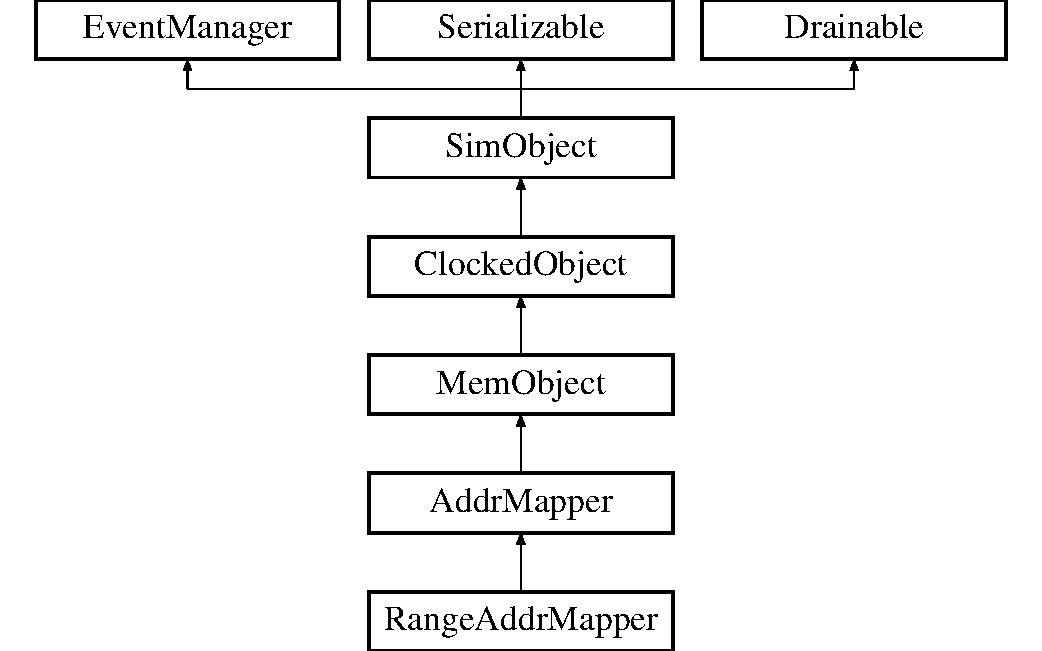
\includegraphics[height=6cm]{classAddrMapper}
\end{center}
\end{figure}
\subsection*{構成}
\begin{DoxyCompactItemize}
\item 
class \hyperlink{classAddrMapper_1_1AddrMapper}{AddrMapper}
\item 
class \hyperlink{classAddrMapper_1_1AddrMapperSenderState}{AddrMapperSenderState}
\item 
class \hyperlink{classAddrMapper_1_1MapperMasterPort}{MapperMasterPort}
\item 
class \hyperlink{classAddrMapper_1_1MapperSlavePort}{MapperSlavePort}
\item 
class \hyperlink{classAddrMapper_1_1RangeAddrMapper}{RangeAddrMapper}
\end{DoxyCompactItemize}
\subsection*{Public メソッド}
\begin{DoxyCompactItemize}
\item 
\hyperlink{classAddrMapper_a65d4ce504585c7421d5f7e6aba8ac336}{AddrMapper} (const AddrMapperParams $\ast$params)
\item 
virtual \hyperlink{classAddrMapper_a934511153fe50240d4d25a79586c4006}{$\sim$AddrMapper} ()
\item 
virtual \hyperlink{classBaseMasterPort}{BaseMasterPort} \& \hyperlink{classAddrMapper_adc4e675e51defbdd1e354dac729d0703}{getMasterPort} (const std::string \&if\_\-name, \hyperlink{base_2types_8hh_acef4d7d41cb21fdc252e20c04cd7bb8e}{PortID} idx=\hyperlink{base_2types_8hh_a65bf40f138cf863f0c5e2d8ca1144126}{InvalidPortID})
\item 
virtual \hyperlink{classBaseSlavePort}{BaseSlavePort} \& \hyperlink{classAddrMapper_ac918a145092d7514ebc6dbd952dceafb}{getSlavePort} (const std::string \&if\_\-name, \hyperlink{base_2types_8hh_acef4d7d41cb21fdc252e20c04cd7bb8e}{PortID} idx=\hyperlink{base_2types_8hh_a65bf40f138cf863f0c5e2d8ca1144126}{InvalidPortID})
\item 
virtual void \hyperlink{classAddrMapper_a02fd73d861ef2e4aabb38c0c9ff82947}{init} ()
\end{DoxyCompactItemize}
\subsection*{Protected メソッド}
\begin{DoxyCompactItemize}
\item 
virtual \hyperlink{base_2types_8hh_af1bb03d6a4ee096394a6749f0a169232}{Addr} \hyperlink{classAddrMapper_a07fe2c0e12fc8be8a245306df09f1b2d}{remapAddr} (\hyperlink{base_2types_8hh_af1bb03d6a4ee096394a6749f0a169232}{Addr} addr) const =0
\item 
void \hyperlink{classAddrMapper_aeefa907fb6d6a787e6dab90e8138ea90}{recvFunctional} (\hyperlink{classPacket}{PacketPtr} pkt)
\item 
void \hyperlink{classAddrMapper_a284dfb90c168233c9d416bc07de8fefe}{recvFunctionalSnoop} (\hyperlink{classPacket}{PacketPtr} pkt)
\item 
\hyperlink{base_2types_8hh_a5c8ed81b7d238c9083e1037ba6d61643}{Tick} \hyperlink{classAddrMapper_a5f0b4c4a94f6b0053f9d7a4eb9c2518a}{recvAtomic} (\hyperlink{classPacket}{PacketPtr} pkt)
\item 
\hyperlink{base_2types_8hh_a5c8ed81b7d238c9083e1037ba6d61643}{Tick} \hyperlink{classAddrMapper_a886d584c81ee4e398ff8069907f6e1a5}{recvAtomicSnoop} (\hyperlink{classPacket}{PacketPtr} pkt)
\item 
bool \hyperlink{classAddrMapper_a3344d9dd0f83257feab5424e761f31c6}{recvTimingReq} (\hyperlink{classPacket}{PacketPtr} pkt)
\item 
bool \hyperlink{classAddrMapper_a482dba5588f4bee43e498875a61e5e0b}{recvTimingResp} (\hyperlink{classPacket}{PacketPtr} pkt)
\item 
void \hyperlink{classAddrMapper_aff3031c56fc4947a19695c868bb8233e}{recvTimingSnoopReq} (\hyperlink{classPacket}{PacketPtr} pkt)
\item 
bool \hyperlink{classAddrMapper_a9b643d565edc21dac11ce15a560238a7}{recvTimingSnoopResp} (\hyperlink{classPacket}{PacketPtr} pkt)
\item 
virtual \hyperlink{classstd_1_1list}{AddrRangeList} \hyperlink{classAddrMapper_a6e967f8921e80748eb2be35b6b481a7e}{getAddrRanges} () const =0
\item 
bool \hyperlink{classAddrMapper_a5ce11b7a254d3cb756d94568f7cbc25d}{isSnooping} () const 
\item 
void \hyperlink{classAddrMapper_a74fc0d5bf99b08c9899269e3dd7fab6a}{recvRetryMaster} ()
\item 
void \hyperlink{classAddrMapper_a2292f62803fe220e9629886f24aae91a}{recvRetrySlave} ()
\item 
void \hyperlink{classAddrMapper_aecf310a01b533ae8700eccac2cf20480}{recvRangeChange} ()
\end{DoxyCompactItemize}
\subsection*{Protected 変数}
\begin{DoxyCompactItemize}
\item 
\hyperlink{classAddrMapper_1_1MapperMasterPort}{MapperMasterPort} \hyperlink{classAddrMapper_a36c3558566dd375b12f573c2ea62992d}{masterPort}
\item 
\hyperlink{classAddrMapper_1_1MapperSlavePort}{MapperSlavePort} \hyperlink{classAddrMapper_a2a442ca0515b14d53305139d239ce090}{slavePort}
\end{DoxyCompactItemize}


\subsection{説明}
An address mapper changes the packet addresses in going from the slave port side of the mapper to the master port side. When the slave port is queried for the address ranges, it also performs the necessary range updates. Note that snoop requests that travel from the master port (i.e. the memory side) to the slave port are currently not modified. 

\subsection{コンストラクタとデストラクタ}
\hypertarget{classAddrMapper_a65d4ce504585c7421d5f7e6aba8ac336}{
\index{AddrMapper@{AddrMapper}!AddrMapper@{AddrMapper}}
\index{AddrMapper@{AddrMapper}!AddrMapper@{AddrMapper}}
\subsubsection[{AddrMapper}]{\setlength{\rightskip}{0pt plus 5cm}{\bf AddrMapper} (const AddrMapperParams $\ast$ {\em params})}}
\label{classAddrMapper_a65d4ce504585c7421d5f7e6aba8ac336}



\begin{DoxyCode}
43     : MemObject(p),
44       masterPort(name() + "-master", *this),
45       slavePort(name() + "-slave", *this)
46 {
47 }
\end{DoxyCode}
\hypertarget{classAddrMapper_a934511153fe50240d4d25a79586c4006}{
\index{AddrMapper@{AddrMapper}!$\sim$AddrMapper@{$\sim$AddrMapper}}
\index{$\sim$AddrMapper@{$\sim$AddrMapper}!AddrMapper@{AddrMapper}}
\subsubsection[{$\sim$AddrMapper}]{\setlength{\rightskip}{0pt plus 5cm}virtual $\sim${\bf AddrMapper} ()\hspace{0.3cm}{\ttfamily  \mbox{[}inline, virtual\mbox{]}}}}
\label{classAddrMapper_a934511153fe50240d4d25a79586c4006}



\begin{DoxyCode}
63 { }
\end{DoxyCode}


\subsection{関数}
\hypertarget{classAddrMapper_a6e967f8921e80748eb2be35b6b481a7e}{
\index{AddrMapper@{AddrMapper}!getAddrRanges@{getAddrRanges}}
\index{getAddrRanges@{getAddrRanges}!AddrMapper@{AddrMapper}}
\subsubsection[{getAddrRanges}]{\setlength{\rightskip}{0pt plus 5cm}virtual {\bf AddrRangeList} getAddrRanges () const\hspace{0.3cm}{\ttfamily  \mbox{[}protected, pure virtual\mbox{]}}}}
\label{classAddrMapper_a6e967f8921e80748eb2be35b6b481a7e}


\hyperlink{classRangeAddrMapper_a36cf113d5e5e091ebddb32306c098fae}{RangeAddrMapper}で実装されています。\hypertarget{classAddrMapper_adc4e675e51defbdd1e354dac729d0703}{
\index{AddrMapper@{AddrMapper}!getMasterPort@{getMasterPort}}
\index{getMasterPort@{getMasterPort}!AddrMapper@{AddrMapper}}
\subsubsection[{getMasterPort}]{\setlength{\rightskip}{0pt plus 5cm}{\bf BaseMasterPort} \& getMasterPort (const std::string \& {\em if\_\-name}, \/  {\bf PortID} {\em idx} = {\ttfamily {\bf InvalidPortID}})\hspace{0.3cm}{\ttfamily  \mbox{[}virtual\mbox{]}}}}
\label{classAddrMapper_adc4e675e51defbdd1e354dac729d0703}
Get a master port with a given name and index. This is used at binding time and returns a reference to a protocol-\/agnostic base master port.


\begin{DoxyParams}{引数}
\item[{\em if\_\-name}]\hyperlink{classPort}{Port} name \item[{\em idx}]Index in the case of a VectorPort\end{DoxyParams}
\begin{DoxyReturn}{戻り値}
A reference to the given port 
\end{DoxyReturn}


\hyperlink{classMemObject_adc4e675e51defbdd1e354dac729d0703}{MemObject}を再定義しています。


\begin{DoxyCode}
58 {
59     if (if_name == "master") {
60         return masterPort;
61     } else {
62         return MemObject::getMasterPort(if_name, idx);
63     }
64 }
\end{DoxyCode}
\hypertarget{classAddrMapper_ac918a145092d7514ebc6dbd952dceafb}{
\index{AddrMapper@{AddrMapper}!getSlavePort@{getSlavePort}}
\index{getSlavePort@{getSlavePort}!AddrMapper@{AddrMapper}}
\subsubsection[{getSlavePort}]{\setlength{\rightskip}{0pt plus 5cm}{\bf BaseSlavePort} \& getSlavePort (const std::string \& {\em if\_\-name}, \/  {\bf PortID} {\em idx} = {\ttfamily {\bf InvalidPortID}})\hspace{0.3cm}{\ttfamily  \mbox{[}virtual\mbox{]}}}}
\label{classAddrMapper_ac918a145092d7514ebc6dbd952dceafb}
Get a slave port with a given name and index. This is used at binding time and returns a reference to a protocol-\/agnostic base master port.


\begin{DoxyParams}{引数}
\item[{\em if\_\-name}]\hyperlink{classPort}{Port} name \item[{\em idx}]Index in the case of a VectorPort\end{DoxyParams}
\begin{DoxyReturn}{戻り値}
A reference to the given port 
\end{DoxyReturn}


\hyperlink{classMemObject_ac918a145092d7514ebc6dbd952dceafb}{MemObject}を再定義しています。


\begin{DoxyCode}
68 {
69     if (if_name == "slave") {
70         return slavePort;
71     } else {
72         return MemObject::getSlavePort(if_name, idx);
73     }
74 }
\end{DoxyCode}
\hypertarget{classAddrMapper_a02fd73d861ef2e4aabb38c0c9ff82947}{
\index{AddrMapper@{AddrMapper}!init@{init}}
\index{init@{init}!AddrMapper@{AddrMapper}}
\subsubsection[{init}]{\setlength{\rightskip}{0pt plus 5cm}void init ()\hspace{0.3cm}{\ttfamily  \mbox{[}virtual\mbox{]}}}}
\label{classAddrMapper_a02fd73d861ef2e4aabb38c0c9ff82947}
\hyperlink{classAddrMapper_a02fd73d861ef2e4aabb38c0c9ff82947}{init()} is called after all C++ SimObjects have been created and all ports are connected. Initializations that are independent of unserialization but rely on a fully instantiated and connected \hyperlink{classSimObject}{SimObject} graph should be done here. 

\hyperlink{classSimObject_a02fd73d861ef2e4aabb38c0c9ff82947}{SimObject}を再定義しています。


\begin{DoxyCode}
51 {
52     if (!slavePort.isConnected() || !masterPort.isConnected())
53         fatal("Address mapper is not connected on both sides.\n");
54 }
\end{DoxyCode}
\hypertarget{classAddrMapper_a5ce11b7a254d3cb756d94568f7cbc25d}{
\index{AddrMapper@{AddrMapper}!isSnooping@{isSnooping}}
\index{isSnooping@{isSnooping}!AddrMapper@{AddrMapper}}
\subsubsection[{isSnooping}]{\setlength{\rightskip}{0pt plus 5cm}bool isSnooping () const\hspace{0.3cm}{\ttfamily  \mbox{[}protected\mbox{]}}}}
\label{classAddrMapper_a5ce11b7a254d3cb756d94568f7cbc25d}



\begin{DoxyCode}
186 {
187     if (slavePort.isSnooping())
188         fatal("AddrMapper doesn't support remapping of snooping requests\n");
189     return false;
190 }
\end{DoxyCode}
\hypertarget{classAddrMapper_a5f0b4c4a94f6b0053f9d7a4eb9c2518a}{
\index{AddrMapper@{AddrMapper}!recvAtomic@{recvAtomic}}
\index{recvAtomic@{recvAtomic}!AddrMapper@{AddrMapper}}
\subsubsection[{recvAtomic}]{\setlength{\rightskip}{0pt plus 5cm}{\bf Tick} recvAtomic ({\bf PacketPtr} {\em pkt})\hspace{0.3cm}{\ttfamily  \mbox{[}protected\mbox{]}}}}
\label{classAddrMapper_a5f0b4c4a94f6b0053f9d7a4eb9c2518a}



\begin{DoxyCode}
96 {
97     Addr orig_addr = pkt->getAddr();
98     pkt->setAddr(remapAddr(orig_addr));
99     Tick ret_tick =  masterPort.sendAtomic(pkt);
100     pkt->setAddr(orig_addr);
101     return ret_tick;
102 }
\end{DoxyCode}
\hypertarget{classAddrMapper_a886d584c81ee4e398ff8069907f6e1a5}{
\index{AddrMapper@{AddrMapper}!recvAtomicSnoop@{recvAtomicSnoop}}
\index{recvAtomicSnoop@{recvAtomicSnoop}!AddrMapper@{AddrMapper}}
\subsubsection[{recvAtomicSnoop}]{\setlength{\rightskip}{0pt plus 5cm}{\bf Tick} recvAtomicSnoop ({\bf PacketPtr} {\em pkt})\hspace{0.3cm}{\ttfamily  \mbox{[}protected\mbox{]}}}}
\label{classAddrMapper_a886d584c81ee4e398ff8069907f6e1a5}



\begin{DoxyCode}
106 {
107     Addr orig_addr = pkt->getAddr();
108     pkt->setAddr(remapAddr(orig_addr));
109     Tick ret_tick = slavePort.sendAtomicSnoop(pkt);
110     pkt->setAddr(orig_addr);
111     return ret_tick;
112 }
\end{DoxyCode}
\hypertarget{classAddrMapper_aeefa907fb6d6a787e6dab90e8138ea90}{
\index{AddrMapper@{AddrMapper}!recvFunctional@{recvFunctional}}
\index{recvFunctional@{recvFunctional}!AddrMapper@{AddrMapper}}
\subsubsection[{recvFunctional}]{\setlength{\rightskip}{0pt plus 5cm}void recvFunctional ({\bf PacketPtr} {\em pkt})\hspace{0.3cm}{\ttfamily  \mbox{[}protected\mbox{]}}}}
\label{classAddrMapper_aeefa907fb6d6a787e6dab90e8138ea90}



\begin{DoxyCode}
78 {
79     Addr orig_addr = pkt->getAddr();
80     pkt->setAddr(remapAddr(orig_addr));
81     masterPort.sendFunctional(pkt);
82     pkt->setAddr(orig_addr);
83 }
\end{DoxyCode}
\hypertarget{classAddrMapper_a284dfb90c168233c9d416bc07de8fefe}{
\index{AddrMapper@{AddrMapper}!recvFunctionalSnoop@{recvFunctionalSnoop}}
\index{recvFunctionalSnoop@{recvFunctionalSnoop}!AddrMapper@{AddrMapper}}
\subsubsection[{recvFunctionalSnoop}]{\setlength{\rightskip}{0pt plus 5cm}void recvFunctionalSnoop ({\bf PacketPtr} {\em pkt})\hspace{0.3cm}{\ttfamily  \mbox{[}protected\mbox{]}}}}
\label{classAddrMapper_a284dfb90c168233c9d416bc07de8fefe}



\begin{DoxyCode}
87 {
88     Addr orig_addr = pkt->getAddr();
89     pkt->setAddr(remapAddr(orig_addr));
90     slavePort.sendFunctionalSnoop(pkt);
91     pkt->setAddr(orig_addr);
92 }
\end{DoxyCode}
\hypertarget{classAddrMapper_aecf310a01b533ae8700eccac2cf20480}{
\index{AddrMapper@{AddrMapper}!recvRangeChange@{recvRangeChange}}
\index{recvRangeChange@{recvRangeChange}!AddrMapper@{AddrMapper}}
\subsubsection[{recvRangeChange}]{\setlength{\rightskip}{0pt plus 5cm}void recvRangeChange ()\hspace{0.3cm}{\ttfamily  \mbox{[}protected\mbox{]}}}}
\label{classAddrMapper_aecf310a01b533ae8700eccac2cf20480}



\begin{DoxyCode}
206 {
207     slavePort.sendRangeChange();
208 }
\end{DoxyCode}
\hypertarget{classAddrMapper_a74fc0d5bf99b08c9899269e3dd7fab6a}{
\index{AddrMapper@{AddrMapper}!recvRetryMaster@{recvRetryMaster}}
\index{recvRetryMaster@{recvRetryMaster}!AddrMapper@{AddrMapper}}
\subsubsection[{recvRetryMaster}]{\setlength{\rightskip}{0pt plus 5cm}void recvRetryMaster ()\hspace{0.3cm}{\ttfamily  \mbox{[}protected\mbox{]}}}}
\label{classAddrMapper_a74fc0d5bf99b08c9899269e3dd7fab6a}



\begin{DoxyCode}
194 {
195     slavePort.sendRetry();
196 }
\end{DoxyCode}
\hypertarget{classAddrMapper_a2292f62803fe220e9629886f24aae91a}{
\index{AddrMapper@{AddrMapper}!recvRetrySlave@{recvRetrySlave}}
\index{recvRetrySlave@{recvRetrySlave}!AddrMapper@{AddrMapper}}
\subsubsection[{recvRetrySlave}]{\setlength{\rightskip}{0pt plus 5cm}void recvRetrySlave ()\hspace{0.3cm}{\ttfamily  \mbox{[}protected\mbox{]}}}}
\label{classAddrMapper_a2292f62803fe220e9629886f24aae91a}



\begin{DoxyCode}
200 {
201     masterPort.sendRetry();
202 }
\end{DoxyCode}
\hypertarget{classAddrMapper_a3344d9dd0f83257feab5424e761f31c6}{
\index{AddrMapper@{AddrMapper}!recvTimingReq@{recvTimingReq}}
\index{recvTimingReq@{recvTimingReq}!AddrMapper@{AddrMapper}}
\subsubsection[{recvTimingReq}]{\setlength{\rightskip}{0pt plus 5cm}bool recvTimingReq ({\bf PacketPtr} {\em pkt})\hspace{0.3cm}{\ttfamily  \mbox{[}protected\mbox{]}}}}
\label{classAddrMapper_a3344d9dd0f83257feab5424e761f31c6}



\begin{DoxyCode}
116 {
117     Addr orig_addr = pkt->getAddr();
118     bool needsResponse = pkt->needsResponse();
119     bool memInhibitAsserted = pkt->memInhibitAsserted();
120 
121     if (needsResponse && !memInhibitAsserted) {
122         pkt->pushSenderState(new AddrMapperSenderState(orig_addr));
123     }
124 
125     pkt->setAddr(remapAddr(orig_addr));
126 
127     // Attempt to send the packet (always succeeds for inhibited
128     // packets)
129     bool successful = masterPort.sendTimingReq(pkt);
130 
131     // If not successful, restore the sender state
132     if (!successful && needsResponse) {
133         delete pkt->popSenderState();
134     }
135 
136     return successful;
137 }
\end{DoxyCode}
\hypertarget{classAddrMapper_a482dba5588f4bee43e498875a61e5e0b}{
\index{AddrMapper@{AddrMapper}!recvTimingResp@{recvTimingResp}}
\index{recvTimingResp@{recvTimingResp}!AddrMapper@{AddrMapper}}
\subsubsection[{recvTimingResp}]{\setlength{\rightskip}{0pt plus 5cm}bool recvTimingResp ({\bf PacketPtr} {\em pkt})\hspace{0.3cm}{\ttfamily  \mbox{[}protected\mbox{]}}}}
\label{classAddrMapper_a482dba5588f4bee43e498875a61e5e0b}



\begin{DoxyCode}
141 {
142     AddrMapperSenderState* receivedState =
143         dynamic_cast<AddrMapperSenderState*>(pkt->senderState);
144 
145     // Restore initial sender state
146     if (receivedState == NULL)
147         panic("AddrMapper %s got a response without sender state\n",
148               name());
149 
150     Addr remapped_addr = pkt->getAddr();
151 
152     // Restore the state and address
153     pkt->senderState = receivedState->predecessor;
154     pkt->setAddr(receivedState->origAddr);
155 
156     // Attempt to send the packet
157     bool successful = slavePort.sendTimingResp(pkt);
158 
159     // If packet successfully sent, delete the sender state, otherwise
160     // restore state
161     if (successful) {
162         delete receivedState;
163     } else {
164         // Don't delete anything and let the packet look like we did
165         // not touch it
166         pkt->senderState = receivedState;
167         pkt->setAddr(remapped_addr);
168     }
169     return successful;
170 }
\end{DoxyCode}
\hypertarget{classAddrMapper_aff3031c56fc4947a19695c868bb8233e}{
\index{AddrMapper@{AddrMapper}!recvTimingSnoopReq@{recvTimingSnoopReq}}
\index{recvTimingSnoopReq@{recvTimingSnoopReq}!AddrMapper@{AddrMapper}}
\subsubsection[{recvTimingSnoopReq}]{\setlength{\rightskip}{0pt plus 5cm}void recvTimingSnoopReq ({\bf PacketPtr} {\em pkt})\hspace{0.3cm}{\ttfamily  \mbox{[}protected\mbox{]}}}}
\label{classAddrMapper_aff3031c56fc4947a19695c868bb8233e}



\begin{DoxyCode}
174 {
175     slavePort.sendTimingSnoopReq(pkt);
176 }
\end{DoxyCode}
\hypertarget{classAddrMapper_a9b643d565edc21dac11ce15a560238a7}{
\index{AddrMapper@{AddrMapper}!recvTimingSnoopResp@{recvTimingSnoopResp}}
\index{recvTimingSnoopResp@{recvTimingSnoopResp}!AddrMapper@{AddrMapper}}
\subsubsection[{recvTimingSnoopResp}]{\setlength{\rightskip}{0pt plus 5cm}bool recvTimingSnoopResp ({\bf PacketPtr} {\em pkt})\hspace{0.3cm}{\ttfamily  \mbox{[}protected\mbox{]}}}}
\label{classAddrMapper_a9b643d565edc21dac11ce15a560238a7}



\begin{DoxyCode}
180 {
181     return masterPort.sendTimingSnoopResp(pkt);
182 }
\end{DoxyCode}
\hypertarget{classAddrMapper_a07fe2c0e12fc8be8a245306df09f1b2d}{
\index{AddrMapper@{AddrMapper}!remapAddr@{remapAddr}}
\index{remapAddr@{remapAddr}!AddrMapper@{AddrMapper}}
\subsubsection[{remapAddr}]{\setlength{\rightskip}{0pt plus 5cm}virtual {\bf Addr} remapAddr ({\bf Addr} {\em addr}) const\hspace{0.3cm}{\ttfamily  \mbox{[}protected, pure virtual\mbox{]}}}}
\label{classAddrMapper_a07fe2c0e12fc8be8a245306df09f1b2d}
This function does the actual remapping of one address to another. It is pure virtual in this case to to allow any implementation required. 
\begin{DoxyParams}{引数}
\item[{\em addr}]the address to remap \end{DoxyParams}
\begin{DoxyReturn}{戻り値}
the new address (can be unchanged) 
\end{DoxyReturn}


\hyperlink{classRangeAddrMapper_a0991da7dcb180722b611eb4a58a397a6}{RangeAddrMapper}で実装されています。

\subsection{変数}
\hypertarget{classAddrMapper_a36c3558566dd375b12f573c2ea62992d}{
\index{AddrMapper@{AddrMapper}!masterPort@{masterPort}}
\index{masterPort@{masterPort}!AddrMapper@{AddrMapper}}
\subsubsection[{masterPort}]{\setlength{\rightskip}{0pt plus 5cm}{\bf MapperMasterPort} {\bf masterPort}\hspace{0.3cm}{\ttfamily  \mbox{[}protected\mbox{]}}}}
\label{classAddrMapper_a36c3558566dd375b12f573c2ea62992d}
Instance of master port, facing the memory side \hypertarget{classAddrMapper_a2a442ca0515b14d53305139d239ce090}{
\index{AddrMapper@{AddrMapper}!slavePort@{slavePort}}
\index{slavePort@{slavePort}!AddrMapper@{AddrMapper}}
\subsubsection[{slavePort}]{\setlength{\rightskip}{0pt plus 5cm}{\bf MapperSlavePort} {\bf slavePort}\hspace{0.3cm}{\ttfamily  \mbox{[}protected\mbox{]}}}}
\label{classAddrMapper_a2a442ca0515b14d53305139d239ce090}
Instance of slave port, i.e. on the CPU side 

このクラスの説明は次のファイルから生成されました:\begin{DoxyCompactItemize}
\item 
mem/\hyperlink{addr__mapper_8hh}{addr\_\-mapper.hh}\item 
mem/\hyperlink{addr__mapper_8cc}{addr\_\-mapper.cc}\end{DoxyCompactItemize}

\hypertarget{classAddrMapper_1_1AddrMapper}{
\section{クラス AddrMapper}
\label{classAddrMapper_1_1AddrMapper}\index{AddrMapper::AddrMapper@{AddrMapper::AddrMapper}}
}
AddrMapperに対する継承グラフ:\begin{figure}[H]
\begin{center}
\leavevmode
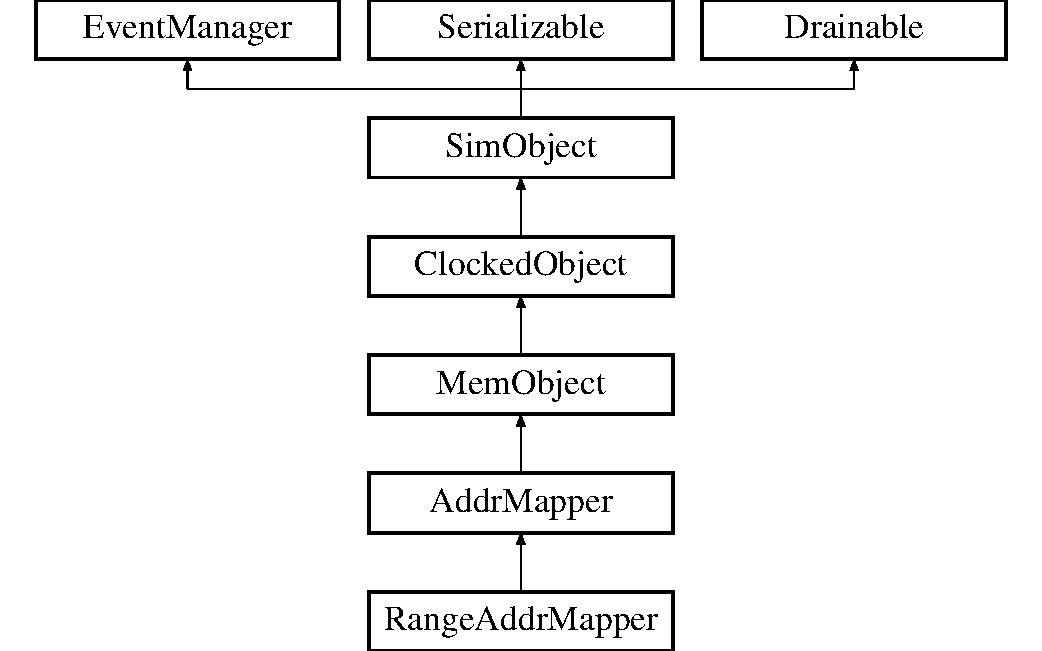
\includegraphics[height=6cm]{classAddrMapper_1_1AddrMapper}
\end{center}
\end{figure}
\subsection*{Static Public 変数}
\begin{DoxyCompactItemize}
\item 
string \hyperlink{classAddrMapper_1_1AddrMapper_acce15679d830831b0bbe8ebc2a60b2ca}{type} = '\hyperlink{classAddrMapper_1_1AddrMapper}{AddrMapper}'
\item 
string \hyperlink{classAddrMapper_1_1AddrMapper_a17da7064bc5c518791f0c891eff05fda}{cxx\_\-header} = 'mem/addr\_\-mapper.hh'
\item 
\hyperlink{classAddrMapper_1_1AddrMapper_a17fa61ac3806b481cafee5593b55e5d0}{abstract} = True
\item 
tuple \hyperlink{classAddrMapper_1_1AddrMapper_a0f74d64e6817f0f89bafc52ff3c56cbb}{master} = \hyperlink{classMasterPort}{MasterPort}(\char`\"{}Master port\char`\"{})
\item 
tuple \hyperlink{classAddrMapper_1_1AddrMapper_a9b8cb1f697e86858437a78f041478c9b}{slave} = \hyperlink{classSlavePort}{SlavePort}(\char`\"{}Slave port\char`\"{})
\end{DoxyCompactItemize}


\subsection{変数}
\hypertarget{classAddrMapper_1_1AddrMapper_a17fa61ac3806b481cafee5593b55e5d0}{
\index{AddrMapper::AddrMapper@{AddrMapper::AddrMapper}!abstract@{abstract}}
\index{abstract@{abstract}!AddrMapper::AddrMapper@{AddrMapper::AddrMapper}}
\subsubsection[{abstract}]{\setlength{\rightskip}{0pt plus 5cm}{\bf abstract} = True\hspace{0.3cm}{\ttfamily  \mbox{[}static\mbox{]}}}}
\label{classAddrMapper_1_1AddrMapper_a17fa61ac3806b481cafee5593b55e5d0}


\hyperlink{classMemObject_1_1MemObject_a17fa61ac3806b481cafee5593b55e5d0}{MemObject}を再定義しています。\hypertarget{classAddrMapper_1_1AddrMapper_a17da7064bc5c518791f0c891eff05fda}{
\index{AddrMapper::AddrMapper@{AddrMapper::AddrMapper}!cxx\_\-header@{cxx\_\-header}}
\index{cxx\_\-header@{cxx\_\-header}!AddrMapper::AddrMapper@{AddrMapper::AddrMapper}}
\subsubsection[{cxx\_\-header}]{\setlength{\rightskip}{0pt plus 5cm}string {\bf cxx\_\-header} = 'mem/addr\_\-mapper.hh'\hspace{0.3cm}{\ttfamily  \mbox{[}static\mbox{]}}}}
\label{classAddrMapper_1_1AddrMapper_a17da7064bc5c518791f0c891eff05fda}


\hyperlink{classMemObject_1_1MemObject_a17da7064bc5c518791f0c891eff05fda}{MemObject}を再定義しています。

\hyperlink{classAddrMapper_1_1RangeAddrMapper_a17da7064bc5c518791f0c891eff05fda}{RangeAddrMapper}で再定義されています。\hypertarget{classAddrMapper_1_1AddrMapper_a0f74d64e6817f0f89bafc52ff3c56cbb}{
\index{AddrMapper::AddrMapper@{AddrMapper::AddrMapper}!master@{master}}
\index{master@{master}!AddrMapper::AddrMapper@{AddrMapper::AddrMapper}}
\subsubsection[{master}]{\setlength{\rightskip}{0pt plus 5cm}tuple {\bf master} = {\bf MasterPort}(\char`\"{}Master port\char`\"{})\hspace{0.3cm}{\ttfamily  \mbox{[}static\mbox{]}}}}
\label{classAddrMapper_1_1AddrMapper_a0f74d64e6817f0f89bafc52ff3c56cbb}
\hypertarget{classAddrMapper_1_1AddrMapper_a9b8cb1f697e86858437a78f041478c9b}{
\index{AddrMapper::AddrMapper@{AddrMapper::AddrMapper}!slave@{slave}}
\index{slave@{slave}!AddrMapper::AddrMapper@{AddrMapper::AddrMapper}}
\subsubsection[{slave}]{\setlength{\rightskip}{0pt plus 5cm}tuple {\bf slave} = {\bf SlavePort}(\char`\"{}Slave port\char`\"{})\hspace{0.3cm}{\ttfamily  \mbox{[}static\mbox{]}}}}
\label{classAddrMapper_1_1AddrMapper_a9b8cb1f697e86858437a78f041478c9b}
\hypertarget{classAddrMapper_1_1AddrMapper_acce15679d830831b0bbe8ebc2a60b2ca}{
\index{AddrMapper::AddrMapper@{AddrMapper::AddrMapper}!type@{type}}
\index{type@{type}!AddrMapper::AddrMapper@{AddrMapper::AddrMapper}}
\subsubsection[{type}]{\setlength{\rightskip}{0pt plus 5cm}string {\bf type} = '{\bf AddrMapper}'\hspace{0.3cm}{\ttfamily  \mbox{[}static\mbox{]}}}}
\label{classAddrMapper_1_1AddrMapper_acce15679d830831b0bbe8ebc2a60b2ca}


\hyperlink{classMemObject_1_1MemObject_acce15679d830831b0bbe8ebc2a60b2ca}{MemObject}を再定義しています。

\hyperlink{classAddrMapper_1_1RangeAddrMapper_acce15679d830831b0bbe8ebc2a60b2ca}{RangeAddrMapper}で再定義されています。

このクラスの説明は次のファイルから生成されました:\begin{DoxyCompactItemize}
\item 
mem/\hyperlink{AddrMapper_8py}{AddrMapper.py}\end{DoxyCompactItemize}

\hypertarget{classAddrMapper_1_1AddrMapperSenderState}{
\section{クラス AddrMapperSenderState}
\label{classAddrMapper_1_1AddrMapperSenderState}\index{AddrMapper::AddrMapperSenderState@{AddrMapper::AddrMapperSenderState}}
}


{\ttfamily \#include $<$addr\_\-mapper.hh$>$}AddrMapperSenderStateに対する継承グラフ:\begin{figure}[H]
\begin{center}
\leavevmode
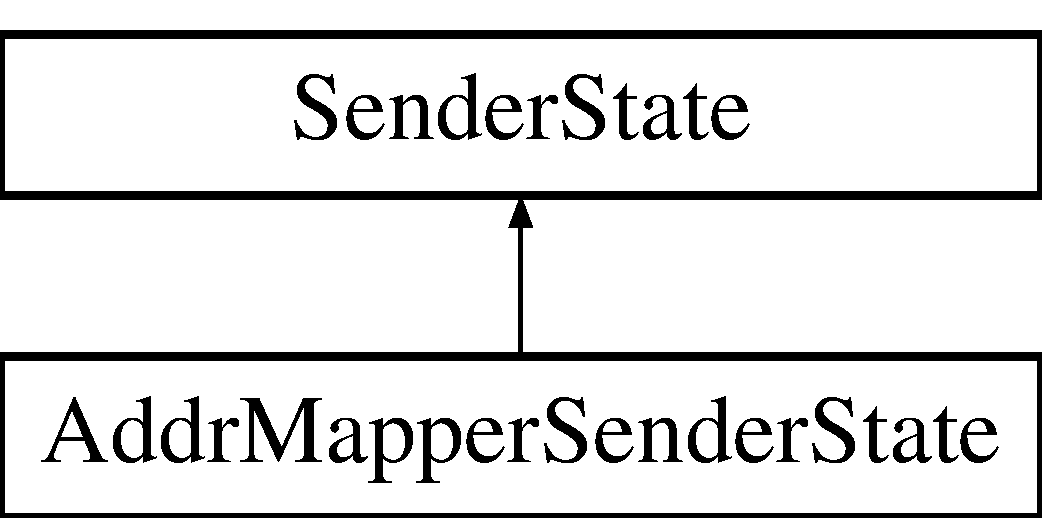
\includegraphics[height=2cm]{classAddrMapper_1_1AddrMapperSenderState}
\end{center}
\end{figure}
\subsection*{Public メソッド}
\begin{DoxyCompactItemize}
\item 
\hyperlink{classAddrMapper_1_1AddrMapperSenderState_ad4879e163df1e1cf3466269e7d12d279}{AddrMapperSenderState} (\hyperlink{base_2types_8hh_af1bb03d6a4ee096394a6749f0a169232}{Addr} \_\-origAddr)
\item 
\hyperlink{classAddrMapper_1_1AddrMapperSenderState_a2dd0b868a2e7ae54d3a56dbdb0edfa60}{$\sim$AddrMapperSenderState} ()
\end{DoxyCompactItemize}
\subsection*{Public 変数}
\begin{DoxyCompactItemize}
\item 
\hyperlink{base_2types_8hh_af1bb03d6a4ee096394a6749f0a169232}{Addr} \hyperlink{classAddrMapper_1_1AddrMapperSenderState_a5a3998c45311174a053b237993cbbfe7}{origAddr}
\end{DoxyCompactItemize}


\subsection{コンストラクタとデストラクタ}
\hypertarget{classAddrMapper_1_1AddrMapperSenderState_ad4879e163df1e1cf3466269e7d12d279}{
\index{AddrMapper::AddrMapperSenderState@{AddrMapper::AddrMapperSenderState}!AddrMapperSenderState@{AddrMapperSenderState}}
\index{AddrMapperSenderState@{AddrMapperSenderState}!AddrMapper::AddrMapperSenderState@{AddrMapper::AddrMapperSenderState}}
\subsubsection[{AddrMapperSenderState}]{\setlength{\rightskip}{0pt plus 5cm}{\bf AddrMapperSenderState} ({\bf Addr} {\em \_\-origAddr})\hspace{0.3cm}{\ttfamily  \mbox{[}inline\mbox{]}}}}
\label{classAddrMapper_1_1AddrMapperSenderState_ad4879e163df1e1cf3466269e7d12d279}
Construct a new sender state to remember the original address.


\begin{DoxyParams}{引数}
\item[{\em \_\-origAddr}]\hyperlink{classAddress}{Address} before remapping \end{DoxyParams}



\begin{DoxyCode}
94                                               : origAddr(_origAddr)
95         { }
\end{DoxyCode}
\hypertarget{classAddrMapper_1_1AddrMapperSenderState_a2dd0b868a2e7ae54d3a56dbdb0edfa60}{
\index{AddrMapper::AddrMapperSenderState@{AddrMapper::AddrMapperSenderState}!$\sim$AddrMapperSenderState@{$\sim$AddrMapperSenderState}}
\index{$\sim$AddrMapperSenderState@{$\sim$AddrMapperSenderState}!AddrMapper::AddrMapperSenderState@{AddrMapper::AddrMapperSenderState}}
\subsubsection[{$\sim$AddrMapperSenderState}]{\setlength{\rightskip}{0pt plus 5cm}$\sim${\bf AddrMapperSenderState} ()\hspace{0.3cm}{\ttfamily  \mbox{[}inline\mbox{]}}}}
\label{classAddrMapper_1_1AddrMapperSenderState_a2dd0b868a2e7ae54d3a56dbdb0edfa60}
Destructor 


\begin{DoxyCode}
98 { }
\end{DoxyCode}


\subsection{変数}
\hypertarget{classAddrMapper_1_1AddrMapperSenderState_a5a3998c45311174a053b237993cbbfe7}{
\index{AddrMapper::AddrMapperSenderState@{AddrMapper::AddrMapperSenderState}!origAddr@{origAddr}}
\index{origAddr@{origAddr}!AddrMapper::AddrMapperSenderState@{AddrMapper::AddrMapperSenderState}}
\subsubsection[{origAddr}]{\setlength{\rightskip}{0pt plus 5cm}{\bf Addr} {\bf origAddr}}}
\label{classAddrMapper_1_1AddrMapperSenderState_a5a3998c45311174a053b237993cbbfe7}
The original address the packet was destined for 

このクラスの説明は次のファイルから生成されました:\begin{DoxyCompactItemize}
\item 
mem/\hyperlink{addr__mapper_8hh}{addr\_\-mapper.hh}\end{DoxyCompactItemize}

\hypertarget{classAddrRange}{
\section{クラス AddrRange}
\label{classAddrRange}\index{AddrRange@{AddrRange}}
}


{\ttfamily \#include $<$addr\_\-range.hh$>$}\subsection*{Public メソッド}
\begin{DoxyCompactItemize}
\item 
\hyperlink{classAddrRange_a44912ab62e2b99d5550e4580da4f0bb6}{AddrRange} ()
\item 
\hyperlink{classAddrRange_a76f19b26f65154f49d9316dbe37dbde6}{AddrRange} (\hyperlink{base_2types_8hh_af1bb03d6a4ee096394a6749f0a169232}{Addr} \hyperlink{classAddrRange_a8ae30d144fb49dec55c70ef1274df68a}{\_\-start}, \hyperlink{base_2types_8hh_af1bb03d6a4ee096394a6749f0a169232}{Addr} \hyperlink{classAddrRange_a945d5a5b811e52aaf2aa2ca0b1aff5c5}{\_\-end}, uint8\_\-t \_\-intlv\_\-high\_\-bit, uint8\_\-t \_\-intlv\_\-bits, uint8\_\-t \_\-intlv\_\-match)
\item 
\hyperlink{classAddrRange_ae9e275cc2d13224e46507e52869d9fa0}{AddrRange} (\hyperlink{base_2types_8hh_af1bb03d6a4ee096394a6749f0a169232}{Addr} \hyperlink{classAddrRange_a8ae30d144fb49dec55c70ef1274df68a}{\_\-start}, \hyperlink{base_2types_8hh_af1bb03d6a4ee096394a6749f0a169232}{Addr} \hyperlink{classAddrRange_a945d5a5b811e52aaf2aa2ca0b1aff5c5}{\_\-end})
\item 
\hyperlink{classAddrRange_a3f7bd25bb87bb07a17105ecfe3a41804}{AddrRange} (const \hyperlink{classstd_1_1vector}{std::vector}$<$ \hyperlink{classAddrRange}{AddrRange} $>$ \&ranges)
\item 
bool \hyperlink{classAddrRange_a5d52a3406dc6afea475c78ce06508afa}{interleaved} () const 
\item 
uint64\_\-t \hyperlink{classAddrRange_a2eca79b1c6faa6be9254f65e6e886355}{granularity} () const 
\item 
\hyperlink{Type_8hh_a435d1572bf3f880d55459d9805097f62}{uint32\_\-t} \hyperlink{classAddrRange_a922914e9ba305472e1643f0be3b6ab01}{stripes} () const 
\item 
\hyperlink{base_2types_8hh_af1bb03d6a4ee096394a6749f0a169232}{Addr} \hyperlink{classAddrRange_ade0faa4f478bf244b35fb208d640c648}{size} () const 
\item 
bool \hyperlink{classAddrRange_a8d985300b138b6c5556ab17ed4df3b38}{valid} () const 
\item 
\hyperlink{base_2types_8hh_af1bb03d6a4ee096394a6749f0a169232}{Addr} \hyperlink{classAddrRange_a85325674b7aed05d6b4e40a48563189b}{start} () const 
\item 
std::string \hyperlink{classAddrRange_aa48c39f92bc04eded742f5310c74aafe}{to\_\-string} () const 
\item 
bool \hyperlink{classAddrRange_aa1196b9847a4edf3e67f40a7e4bf63e8}{mergesWith} (const \hyperlink{classAddrRange}{AddrRange} \&r) const 
\item 
bool \hyperlink{classAddrRange_af078c7e4b8ad8c7f3666ebb2fef613da}{intersects} (const \hyperlink{classAddrRange}{AddrRange} \&r) const 
\item 
bool \hyperlink{classAddrRange_a3d9821127a28a036fbcc96d1ba20b8e2}{isSubset} (const \hyperlink{classAddrRange}{AddrRange} \&r) const 
\item 
bool \hyperlink{classAddrRange_aa839dbf0ffc0e871a3f08f1d23d78a18}{contains} (const \hyperlink{base_2types_8hh_af1bb03d6a4ee096394a6749f0a169232}{Addr} \&a) const 
\item 
bool \hyperlink{classAddrRange_a9f850195d97cc5f161ba7e5c880facc8}{operator$<$} (const \hyperlink{classAddrRange}{AddrRange} \&r) const 
\end{DoxyCompactItemize}
\subsection*{Private 変数}
\begin{DoxyCompactItemize}
\item 
\hyperlink{base_2types_8hh_af1bb03d6a4ee096394a6749f0a169232}{Addr} \hyperlink{classAddrRange_a8ae30d144fb49dec55c70ef1274df68a}{\_\-start}
\begin{DoxyCompactList}\small\item\em Private fields for the start and end of the range. \item\end{DoxyCompactList}\item 
\hyperlink{base_2types_8hh_af1bb03d6a4ee096394a6749f0a169232}{Addr} \hyperlink{classAddrRange_a945d5a5b811e52aaf2aa2ca0b1aff5c5}{\_\-end}
\item 
uint8\_\-t \hyperlink{classAddrRange_a4160474d6dec766ee20330ae309e3998}{intlvHighBit}
\begin{DoxyCompactList}\small\item\em The high bit of the slice that is used for interleaving. \item\end{DoxyCompactList}\item 
uint8\_\-t \hyperlink{classAddrRange_a02537b213a36c9f9d57d8c79a0dfb198}{intlvBits}
\begin{DoxyCompactList}\small\item\em The number of bits used for interleaving, set to 0 to disable. \item\end{DoxyCompactList}\item 
uint8\_\-t \hyperlink{classAddrRange_a0d9068b55e0d449e9b8ec483536394a9}{intlvMatch}
\end{DoxyCompactItemize}


\subsection{コンストラクタとデストラクタ}
\hypertarget{classAddrRange_a44912ab62e2b99d5550e4580da4f0bb6}{
\index{AddrRange@{AddrRange}!AddrRange@{AddrRange}}
\index{AddrRange@{AddrRange}!AddrRange@{AddrRange}}
\subsubsection[{AddrRange}]{\setlength{\rightskip}{0pt plus 5cm}{\bf AddrRange} ()\hspace{0.3cm}{\ttfamily  \mbox{[}inline\mbox{]}}}}
\label{classAddrRange_a44912ab62e2b99d5550e4580da4f0bb6}



\begin{DoxyCode}
77         : _start(1), _end(0), intlvHighBit(0), intlvBits(0), intlvMatch(0)
78     {}
\end{DoxyCode}
\hypertarget{classAddrRange_a76f19b26f65154f49d9316dbe37dbde6}{
\index{AddrRange@{AddrRange}!AddrRange@{AddrRange}}
\index{AddrRange@{AddrRange}!AddrRange@{AddrRange}}
\subsubsection[{AddrRange}]{\setlength{\rightskip}{0pt plus 5cm}{\bf AddrRange} ({\bf Addr} {\em \_\-start}, \/  {\bf Addr} {\em \_\-end}, \/  uint8\_\-t {\em \_\-intlv\_\-high\_\-bit}, \/  uint8\_\-t {\em \_\-intlv\_\-bits}, \/  uint8\_\-t {\em \_\-intlv\_\-match})\hspace{0.3cm}{\ttfamily  \mbox{[}inline\mbox{]}}}}
\label{classAddrRange_a76f19b26f65154f49d9316dbe37dbde6}



\begin{DoxyCode}
82         : _start(_start), _end(_end), intlvHighBit(_intlv_high_bit),
83           intlvBits(_intlv_bits), intlvMatch(_intlv_match)
84     {}
\end{DoxyCode}
\hypertarget{classAddrRange_ae9e275cc2d13224e46507e52869d9fa0}{
\index{AddrRange@{AddrRange}!AddrRange@{AddrRange}}
\index{AddrRange@{AddrRange}!AddrRange@{AddrRange}}
\subsubsection[{AddrRange}]{\setlength{\rightskip}{0pt plus 5cm}{\bf AddrRange} ({\bf Addr} {\em \_\-start}, \/  {\bf Addr} {\em \_\-end})\hspace{0.3cm}{\ttfamily  \mbox{[}inline\mbox{]}}}}
\label{classAddrRange_ae9e275cc2d13224e46507e52869d9fa0}



\begin{DoxyCode}
87         : _start(_start), _end(_end), intlvHighBit(0), intlvBits(0),
88           intlvMatch(0)
89     {}
\end{DoxyCode}
\hypertarget{classAddrRange_a3f7bd25bb87bb07a17105ecfe3a41804}{
\index{AddrRange@{AddrRange}!AddrRange@{AddrRange}}
\index{AddrRange@{AddrRange}!AddrRange@{AddrRange}}
\subsubsection[{AddrRange}]{\setlength{\rightskip}{0pt plus 5cm}{\bf AddrRange} (const {\bf std::vector}$<$ {\bf AddrRange} $>$ \& {\em ranges})\hspace{0.3cm}{\ttfamily  \mbox{[}inline\mbox{]}}}}
\label{classAddrRange_a3f7bd25bb87bb07a17105ecfe3a41804}
Create an address range by merging a collection of interleaved ranges.


\begin{DoxyParams}{引数}
\item[{\em ranges}]Interleaved ranges to be merged \end{DoxyParams}



\begin{DoxyCode}
98         : _start(1), _end(0), intlvHighBit(0), intlvBits(0), intlvMatch(0)
99     {
100         if (!ranges.empty()) {
101             // get the values from the first one and check the others
102             _start = ranges.front()._start;
103             _end = ranges.front()._end;
104             intlvHighBit = ranges.front().intlvHighBit;
105             intlvBits = ranges.front().intlvBits;
106 
107             if (ranges.size() != (ULL(1) << intlvBits))
108                 fatal("Got %d ranges spanning %d interleaving bits\n",
109                       ranges.size(), intlvBits);
110 
111             uint8_t match = 0;
112             for (std::vector<AddrRange>::const_iterator r = ranges.begin();
113                  r != ranges.end(); ++r) {
114                 if (!mergesWith(*r))
115                     fatal("Can only merge ranges with the same start, end "
116                           "and interleaving bits\n");
117 
118                 if (r->intlvMatch != match)
119                     fatal("Expected interleave match %d but got %d when "
120                           "merging\n", match, r->intlvMatch);
121                 ++match;
122             }
123 
124             // our range is complete and we can turn this into a
125             // non-interleaved range
126             intlvHighBit = 0;
127             intlvBits = 0;
128         }
129     }
\end{DoxyCode}


\subsection{関数}
\hypertarget{classAddrRange_aa839dbf0ffc0e871a3f08f1d23d78a18}{
\index{AddrRange@{AddrRange}!contains@{contains}}
\index{contains@{contains}!AddrRange@{AddrRange}}
\subsubsection[{contains}]{\setlength{\rightskip}{0pt plus 5cm}bool contains (const {\bf Addr} \& {\em a}) const\hspace{0.3cm}{\ttfamily  \mbox{[}inline\mbox{]}}}}
\label{classAddrRange_aa839dbf0ffc0e871a3f08f1d23d78a18}
Determine if the range contains an address.


\begin{DoxyParams}{引数}
\item[{\em a}]\hyperlink{classAddress}{Address} to compare with \end{DoxyParams}
\begin{DoxyReturn}{戻り値}
true if the address is in the range 
\end{DoxyReturn}



\begin{DoxyCode}
260     {
261         // check if the address is in the range and if there is either
262         // no interleaving, or with interleaving also if the selected
263         // bits from the address match the interleaving value
264         return a >= _start && a <= _end &&
265             (!interleaved() ||
266              (bits(a, intlvHighBit, intlvHighBit - intlvBits + 1) ==
267               intlvMatch));
268     }
\end{DoxyCode}
\hypertarget{classAddrRange_a2eca79b1c6faa6be9254f65e6e886355}{
\index{AddrRange@{AddrRange}!granularity@{granularity}}
\index{granularity@{granularity}!AddrRange@{AddrRange}}
\subsubsection[{granularity}]{\setlength{\rightskip}{0pt plus 5cm}uint64\_\-t granularity () const\hspace{0.3cm}{\ttfamily  \mbox{[}inline\mbox{]}}}}
\label{classAddrRange_a2eca79b1c6faa6be9254f65e6e886355}
Determing the interleaving granularity of the range.

\begin{DoxyReturn}{戻り値}
The size of the regions created by the interleaving bits 
\end{DoxyReturn}



\begin{DoxyCode}
144     {
145         return ULL(1) << (intlvHighBit - intlvBits + 1);
146     }
\end{DoxyCode}
\hypertarget{classAddrRange_a5d52a3406dc6afea475c78ce06508afa}{
\index{AddrRange@{AddrRange}!interleaved@{interleaved}}
\index{interleaved@{interleaved}!AddrRange@{AddrRange}}
\subsubsection[{interleaved}]{\setlength{\rightskip}{0pt plus 5cm}bool interleaved () const\hspace{0.3cm}{\ttfamily  \mbox{[}inline\mbox{]}}}}
\label{classAddrRange_a5d52a3406dc6afea475c78ce06508afa}
Determine if the range is interleaved or not.

\begin{DoxyReturn}{戻り値}
true if interleaved 
\end{DoxyReturn}



\begin{DoxyCode}
136 { return intlvBits != 0; }
\end{DoxyCode}
\hypertarget{classAddrRange_af078c7e4b8ad8c7f3666ebb2fef613da}{
\index{AddrRange@{AddrRange}!intersects@{intersects}}
\index{intersects@{intersects}!AddrRange@{AddrRange}}
\subsubsection[{intersects}]{\setlength{\rightskip}{0pt plus 5cm}bool intersects (const {\bf AddrRange} \& {\em r}) const\hspace{0.3cm}{\ttfamily  \mbox{[}inline\mbox{]}}}}
\label{classAddrRange_af078c7e4b8ad8c7f3666ebb2fef613da}
Determine if another range intersects this one, i.e. if there is an address that is both in this range and the other range. No check is made to ensure either range is valid.


\begin{DoxyParams}{引数}
\item[{\em r}]Range to intersect with \end{DoxyParams}
\begin{DoxyReturn}{戻り値}
true if the intersection of the two ranges is not empty 
\end{DoxyReturn}



\begin{DoxyCode}
215     {
216         if (!interleaved()) {
217             return _start <= r._end && _end >= r._start;
218         }
219 
220         // the current range is interleaved, split the check up in
221         // three cases
222         if (r.size() == 1)
223             // keep it simple and check if the address is within
224             // this range
225             return contains(r.start());
226         else if (!r.interleaved())
227             // be conservative and ignore the interleaving
228             return _start <= r._end && _end >= r._start;
229         else if (mergesWith(r))
230             // restrict the check to ranges that belong to the
231             // same chunk
232             return intlvMatch == r.intlvMatch;
233         else
234             panic("Cannot test intersection of interleaved range %s\n",
235                   to_string());
236     }
\end{DoxyCode}
\hypertarget{classAddrRange_a3d9821127a28a036fbcc96d1ba20b8e2}{
\index{AddrRange@{AddrRange}!isSubset@{isSubset}}
\index{isSubset@{isSubset}!AddrRange@{AddrRange}}
\subsubsection[{isSubset}]{\setlength{\rightskip}{0pt plus 5cm}bool isSubset (const {\bf AddrRange} \& {\em r}) const\hspace{0.3cm}{\ttfamily  \mbox{[}inline\mbox{]}}}}
\label{classAddrRange_a3d9821127a28a036fbcc96d1ba20b8e2}
Determine if this range is a subset of another range, i.e. if every address in this range is also in the other range. No check is made to ensure either range is valid.


\begin{DoxyParams}{引数}
\item[{\em r}]Range to compare with \end{DoxyParams}
\begin{DoxyReturn}{戻り値}
true if the this range is a subset of the other one 
\end{DoxyReturn}



\begin{DoxyCode}
247     {
248         if (interleaved())
249             panic("Cannot test subset of interleaved range %s\n", to_string());
250         return _start >= r._start && _end <= r._end;
251     }
\end{DoxyCode}
\hypertarget{classAddrRange_aa1196b9847a4edf3e67f40a7e4bf63e8}{
\index{AddrRange@{AddrRange}!mergesWith@{mergesWith}}
\index{mergesWith@{mergesWith}!AddrRange@{AddrRange}}
\subsubsection[{mergesWith}]{\setlength{\rightskip}{0pt plus 5cm}bool mergesWith (const {\bf AddrRange} \& {\em r}) const\hspace{0.3cm}{\ttfamily  \mbox{[}inline\mbox{]}}}}
\label{classAddrRange_aa1196b9847a4edf3e67f40a7e4bf63e8}
Determine if another range merges with the current one, i.e. if they are part of the same contigous range and have the same interleaving bits.


\begin{DoxyParams}{引数}
\item[{\em r}]Range to evaluate merging with \end{DoxyParams}
\begin{DoxyReturn}{戻り値}
true if the two ranges would merge 
\end{DoxyReturn}



\begin{DoxyCode}
200     {
201         return r._start == _start && r._end == _end &&
202             r.intlvHighBit == intlvHighBit &&
203             r.intlvBits == intlvBits;
204     }
\end{DoxyCode}
\hypertarget{classAddrRange_a9f850195d97cc5f161ba7e5c880facc8}{
\index{AddrRange@{AddrRange}!operator$<$@{operator$<$}}
\index{operator$<$@{operator$<$}!AddrRange@{AddrRange}}
\subsubsection[{operator$<$}]{\setlength{\rightskip}{0pt plus 5cm}bool operator$<$ (const {\bf AddrRange} \& {\em r}) const\hspace{0.3cm}{\ttfamily  \mbox{[}inline\mbox{]}}}}
\label{classAddrRange_a9f850195d97cc5f161ba7e5c880facc8}
Keep the operators away from SWIG. Less-\/than operator used to turn an STL map into a binary search tree of non-\/overlapping address ranges.


\begin{DoxyParams}{引数}
\item[{\em r}]Range to compare with \end{DoxyParams}
\begin{DoxyReturn}{戻り値}
true if the start address is less than that of the other range 
\end{DoxyReturn}



\begin{DoxyCode}
283     {
284         if (_start != r._start)
285             return _start < r._start;
286         else
287             // for now assume that the end is also the same, and that
288             // we are looking at the same interleaving bits
289             return intlvMatch < r.intlvMatch;
290     }
\end{DoxyCode}
\hypertarget{classAddrRange_ade0faa4f478bf244b35fb208d640c648}{
\index{AddrRange@{AddrRange}!size@{size}}
\index{size@{size}!AddrRange@{AddrRange}}
\subsubsection[{size}]{\setlength{\rightskip}{0pt plus 5cm}{\bf Addr} size () const\hspace{0.3cm}{\ttfamily  \mbox{[}inline\mbox{]}}}}
\label{classAddrRange_ade0faa4f478bf244b35fb208d640c648}
Get the size of the address range. For a case where interleaving is used we make the simplifying assumption that the size is a divisible by the size of the interleaving slice. 


\begin{DoxyCode}
162     {
163         return (_end - _start + 1) >> intlvBits;
164     }
\end{DoxyCode}
\hypertarget{classAddrRange_a85325674b7aed05d6b4e40a48563189b}{
\index{AddrRange@{AddrRange}!start@{start}}
\index{start@{start}!AddrRange@{AddrRange}}
\subsubsection[{start}]{\setlength{\rightskip}{0pt plus 5cm}{\bf Addr} start () const\hspace{0.3cm}{\ttfamily  \mbox{[}inline\mbox{]}}}}
\label{classAddrRange_a85325674b7aed05d6b4e40a48563189b}
Get the start address of the range. 


\begin{DoxyCode}
174 { return _start; }
\end{DoxyCode}
\hypertarget{classAddrRange_a922914e9ba305472e1643f0be3b6ab01}{
\index{AddrRange@{AddrRange}!stripes@{stripes}}
\index{stripes@{stripes}!AddrRange@{AddrRange}}
\subsubsection[{stripes}]{\setlength{\rightskip}{0pt plus 5cm}{\bf uint32\_\-t} stripes () const\hspace{0.3cm}{\ttfamily  \mbox{[}inline\mbox{]}}}}
\label{classAddrRange_a922914e9ba305472e1643f0be3b6ab01}
Determine the number of interleaved address stripes this range is part of.

\begin{DoxyReturn}{戻り値}
The number of stripes spanned by the interleaving bits 
\end{DoxyReturn}



\begin{DoxyCode}
154 { return ULL(1) << intlvBits; }
\end{DoxyCode}
\hypertarget{classAddrRange_aa48c39f92bc04eded742f5310c74aafe}{
\index{AddrRange@{AddrRange}!to\_\-string@{to\_\-string}}
\index{to\_\-string@{to\_\-string}!AddrRange@{AddrRange}}
\subsubsection[{to\_\-string}]{\setlength{\rightskip}{0pt plus 5cm}std::string to\_\-string () const\hspace{0.3cm}{\ttfamily  \mbox{[}inline\mbox{]}}}}
\label{classAddrRange_aa48c39f92bc04eded742f5310c74aafe}
Get a string representation of the range. This could alternatively be implemented as a operator$<$$<$, but at the moment that seems like overkill. 


\begin{DoxyCode}
182     {
183         if (interleaved())
184             return csprintf("[%#llx : %#llx], [%d : %d] = %d", _start, _end,
185                             intlvHighBit, intlvHighBit - intlvBits + 1,
186                             intlvMatch);
187         else
188             return csprintf("[%#llx : %#llx]", _start, _end);
189     }
\end{DoxyCode}
\hypertarget{classAddrRange_a8d985300b138b6c5556ab17ed4df3b38}{
\index{AddrRange@{AddrRange}!valid@{valid}}
\index{valid@{valid}!AddrRange@{AddrRange}}
\subsubsection[{valid}]{\setlength{\rightskip}{0pt plus 5cm}bool valid () const\hspace{0.3cm}{\ttfamily  \mbox{[}inline\mbox{]}}}}
\label{classAddrRange_a8d985300b138b6c5556ab17ed4df3b38}
Determine if the range is valid. 


\begin{DoxyCode}
169 { return _start < _end; }
\end{DoxyCode}


\subsection{変数}
\hypertarget{classAddrRange_a945d5a5b811e52aaf2aa2ca0b1aff5c5}{
\index{AddrRange@{AddrRange}!\_\-end@{\_\-end}}
\index{\_\-end@{\_\-end}!AddrRange@{AddrRange}}
\subsubsection[{\_\-end}]{\setlength{\rightskip}{0pt plus 5cm}{\bf Addr} {\bf \_\-end}\hspace{0.3cm}{\ttfamily  \mbox{[}private\mbox{]}}}}
\label{classAddrRange_a945d5a5b811e52aaf2aa2ca0b1aff5c5}
\hypertarget{classAddrRange_a8ae30d144fb49dec55c70ef1274df68a}{
\index{AddrRange@{AddrRange}!\_\-start@{\_\-start}}
\index{\_\-start@{\_\-start}!AddrRange@{AddrRange}}
\subsubsection[{\_\-start}]{\setlength{\rightskip}{0pt plus 5cm}{\bf Addr} {\bf \_\-start}\hspace{0.3cm}{\ttfamily  \mbox{[}private\mbox{]}}}}
\label{classAddrRange_a8ae30d144fb49dec55c70ef1274df68a}


Private fields for the start and end of the range. \hypertarget{classAddrRange_a02537b213a36c9f9d57d8c79a0dfb198}{
\index{AddrRange@{AddrRange}!intlvBits@{intlvBits}}
\index{intlvBits@{intlvBits}!AddrRange@{AddrRange}}
\subsubsection[{intlvBits}]{\setlength{\rightskip}{0pt plus 5cm}uint8\_\-t {\bf intlvBits}\hspace{0.3cm}{\ttfamily  \mbox{[}private\mbox{]}}}}
\label{classAddrRange_a02537b213a36c9f9d57d8c79a0dfb198}


The number of bits used for interleaving, set to 0 to disable. \hypertarget{classAddrRange_a4160474d6dec766ee20330ae309e3998}{
\index{AddrRange@{AddrRange}!intlvHighBit@{intlvHighBit}}
\index{intlvHighBit@{intlvHighBit}!AddrRange@{AddrRange}}
\subsubsection[{intlvHighBit}]{\setlength{\rightskip}{0pt plus 5cm}uint8\_\-t {\bf intlvHighBit}\hspace{0.3cm}{\ttfamily  \mbox{[}private\mbox{]}}}}
\label{classAddrRange_a4160474d6dec766ee20330ae309e3998}


The high bit of the slice that is used for interleaving. \hypertarget{classAddrRange_a0d9068b55e0d449e9b8ec483536394a9}{
\index{AddrRange@{AddrRange}!intlvMatch@{intlvMatch}}
\index{intlvMatch@{intlvMatch}!AddrRange@{AddrRange}}
\subsubsection[{intlvMatch}]{\setlength{\rightskip}{0pt plus 5cm}uint8\_\-t {\bf intlvMatch}\hspace{0.3cm}{\ttfamily  \mbox{[}private\mbox{]}}}}
\label{classAddrRange_a0d9068b55e0d449e9b8ec483536394a9}
The value to compare the slice addr\mbox{[}high:(high -\/ bits + 1)\mbox{]} with. 

このクラスの説明は次のファイルから生成されました:\begin{DoxyCompactItemize}
\item 
base/\hyperlink{addr__range_8hh}{addr\_\-range.hh}\end{DoxyCompactItemize}

\hypertarget{classm5_1_1params_1_1AddrRange}{
\section{クラス AddrRange}
\label{classm5_1_1params_1_1AddrRange}\index{m5::params::AddrRange@{m5::params::AddrRange}}
}
AddrRangeに対する継承グラフ:\begin{figure}[H]
\begin{center}
\leavevmode
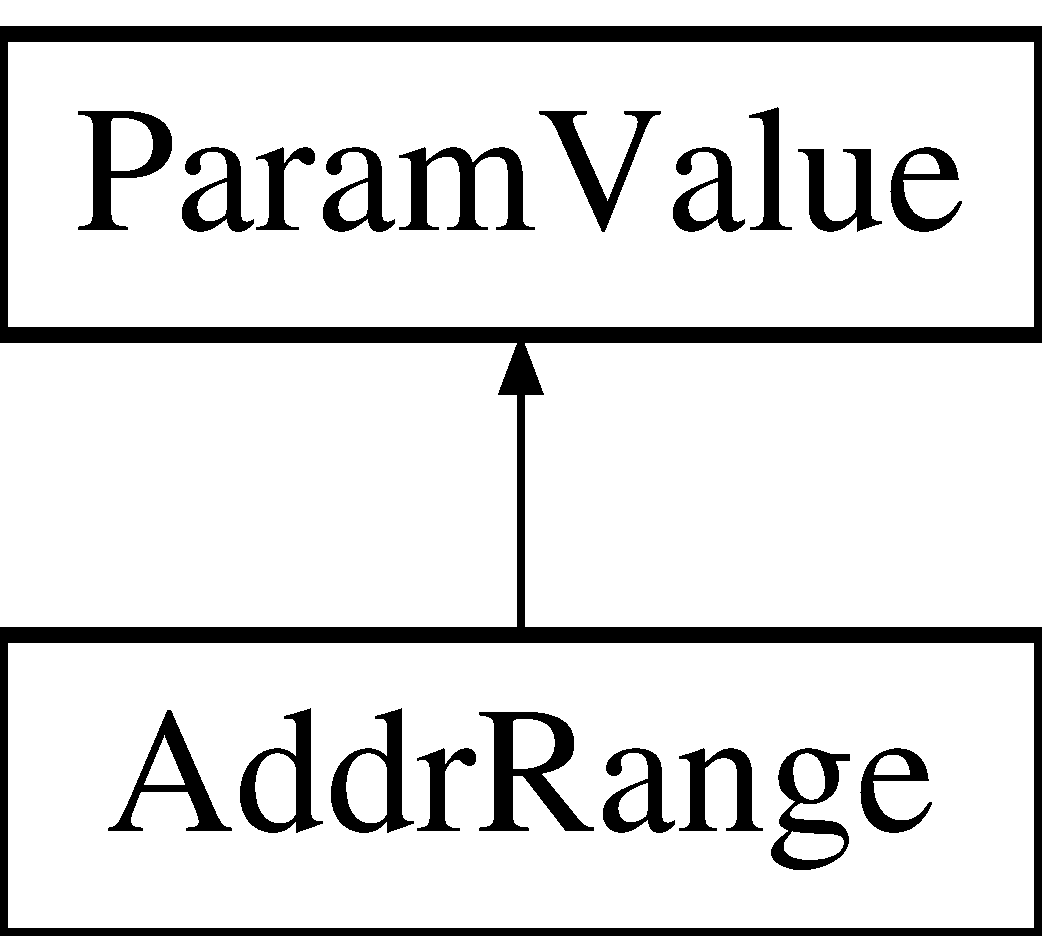
\includegraphics[height=2cm]{classm5_1_1params_1_1AddrRange}
\end{center}
\end{figure}
\subsection*{Public メソッド}
\begin{DoxyCompactItemize}
\item 
def \hyperlink{classm5_1_1params_1_1AddrRange_ac775ee34451fdfa742b318538164070e}{\_\-\_\-init\_\-\_\-}
\item 
def \hyperlink{classm5_1_1params_1_1AddrRange_aa7a4b9bc0941308e362738503137460e}{\_\-\_\-str\_\-\_\-}
\item 
def \hyperlink{classm5_1_1params_1_1AddrRange_a8e64882b52bf2db69e0ec31977c83dc4}{size}
\item 
def \hyperlink{classm5_1_1params_1_1AddrRange_a0b408a11a14bd1d770e28f71a6e14ab5}{cxx\_\-predecls}
\item 
def \hyperlink{classm5_1_1params_1_1AddrRange_ab3dbcf5716623eac67a8ccc074fa7e13}{swig\_\-predecls}
\item 
def \hyperlink{classm5_1_1params_1_1AddrRange_acc340fbd4335fa34f9d57fb454b28ed0}{getValue}
\end{DoxyCompactItemize}
\subsection*{Public 変数}
\begin{DoxyCompactItemize}
\item 
\hyperlink{classm5_1_1params_1_1AddrRange_a438082b3a41e0118681dc310c8830e14}{intlvHighBit}
\item 
\hyperlink{classm5_1_1params_1_1AddrRange_a59fb29811138277b395da051c1c9d589}{intlvBits}
\item 
\hyperlink{classm5_1_1params_1_1AddrRange_aaf62f123726dad820b8d0a2c84543e2e}{intlvMatch}
\item 
\hyperlink{classm5_1_1params_1_1AddrRange_afb358f48b1646c750fb9da6c6585be2b}{end}
\item 
\hyperlink{classm5_1_1params_1_1AddrRange_a550769bbd4e7537ff90a656f5b0c23b2}{start}
\end{DoxyCompactItemize}
\subsection*{Static Public 変数}
\begin{DoxyCompactItemize}
\item 
string \hyperlink{classm5_1_1params_1_1AddrRange_a2f1553ebb79374a68b36fdd6d8d82fc3}{cxx\_\-type} = '\hyperlink{classm5_1_1params_1_1AddrRange}{AddrRange}'
\end{DoxyCompactItemize}


\subsection{関数}
\hypertarget{classm5_1_1params_1_1AddrRange_ac775ee34451fdfa742b318538164070e}{
\index{m5::params::AddrRange@{m5::params::AddrRange}!\_\-\_\-init\_\-\_\-@{\_\-\_\-init\_\-\_\-}}
\index{\_\-\_\-init\_\-\_\-@{\_\-\_\-init\_\-\_\-}!m5::params::AddrRange@{m5::params::AddrRange}}
\subsubsection[{\_\-\_\-init\_\-\_\-}]{\setlength{\rightskip}{0pt plus 5cm}def \_\-\_\-init\_\-\_\- ( {\em self}, \/   {\em args}, \/   {\em kwargs})}}
\label{classm5_1_1params_1_1AddrRange_ac775ee34451fdfa742b318538164070e}



\begin{DoxyCode}
550                                        :
551         # Disable interleaving by default
552         self.intlvHighBit = 0
553         self.intlvBits = 0
554         self.intlvMatch = 0
555 
556         def handle_kwargs(self, kwargs):
557             # An address range needs to have an upper limit, specified
558             # either explicitly with an end, or as an offset using the
559             # size keyword.
560             if 'end' in kwargs:
561                 self.end = Addr(kwargs.pop('end'))
562             elif 'size' in kwargs:
563                 self.end = self.start + Addr(kwargs.pop('size')) - 1
564             else:
565                 raise TypeError, "Either end or size must be specified"
566 
567             # Now on to the optional bit
568             if 'intlvHighBit' in kwargs:
569                 self.intlvHighBit = int(kwargs.pop('intlvHighBit'))
570             if 'intlvBits' in kwargs:
571                 self.intlvBits = int(kwargs.pop('intlvBits'))
572             if 'intlvMatch' in kwargs:
573                 self.intlvMatch = int(kwargs.pop('intlvMatch'))
574 
575         if len(args) == 0:
576             self.start = Addr(kwargs.pop('start'))
577             handle_kwargs(self, kwargs)
578 
579         elif len(args) == 1:
580             if kwargs:
581                 self.start = Addr(args[0])
582                 handle_kwargs(self, kwargs)
583             elif isinstance(args[0], (list, tuple)):
584                 self.start = Addr(args[0][0])
585                 self.end = Addr(args[0][1])
586             else:
587                 self.start = Addr(0)
588                 self.end = Addr(args[0]) - 1
589 
590         elif len(args) == 2:
591             self.start = Addr(args[0])
592             self.end = Addr(args[1])
593         else:
594             raise TypeError, "Too many arguments specified"
595 
596         if kwargs:
597             raise TypeError, "Too many keywords: %s" % kwargs.keys()
598 
    def __str__(self):
\end{DoxyCode}
\hypertarget{classm5_1_1params_1_1AddrRange_aa7a4b9bc0941308e362738503137460e}{
\index{m5::params::AddrRange@{m5::params::AddrRange}!\_\-\_\-str\_\-\_\-@{\_\-\_\-str\_\-\_\-}}
\index{\_\-\_\-str\_\-\_\-@{\_\-\_\-str\_\-\_\-}!m5::params::AddrRange@{m5::params::AddrRange}}
\subsubsection[{\_\-\_\-str\_\-\_\-}]{\setlength{\rightskip}{0pt plus 5cm}def \_\-\_\-str\_\-\_\- ( {\em self})}}
\label{classm5_1_1params_1_1AddrRange_aa7a4b9bc0941308e362738503137460e}



\begin{DoxyCode}
599                      :
600         return '%s:%s' % (self.start, self.end)
601 
    def size(self):
\end{DoxyCode}
\hypertarget{classm5_1_1params_1_1AddrRange_a0b408a11a14bd1d770e28f71a6e14ab5}{
\index{m5::params::AddrRange@{m5::params::AddrRange}!cxx\_\-predecls@{cxx\_\-predecls}}
\index{cxx\_\-predecls@{cxx\_\-predecls}!m5::params::AddrRange@{m5::params::AddrRange}}
\subsubsection[{cxx\_\-predecls}]{\setlength{\rightskip}{0pt plus 5cm}def cxx\_\-predecls ( {\em cls}, \/   {\em code})}}
\label{classm5_1_1params_1_1AddrRange_a0b408a11a14bd1d770e28f71a6e14ab5}


\hyperlink{classm5_1_1params_1_1ParamValue_a0b408a11a14bd1d770e28f71a6e14ab5}{ParamValue}を再定義しています。


\begin{DoxyCode}
607                                :
608         Addr.cxx_predecls(code)
609         code('#include "base/addr_range.hh"')
610 
611     @classmethod
    def swig_predecls(cls, code):
\end{DoxyCode}
\hypertarget{classm5_1_1params_1_1AddrRange_acc340fbd4335fa34f9d57fb454b28ed0}{
\index{m5::params::AddrRange@{m5::params::AddrRange}!getValue@{getValue}}
\index{getValue@{getValue}!m5::params::AddrRange@{m5::params::AddrRange}}
\subsubsection[{getValue}]{\setlength{\rightskip}{0pt plus 5cm}def getValue ( {\em self})}}
\label{classm5_1_1params_1_1AddrRange_acc340fbd4335fa34f9d57fb454b28ed0}



\begin{DoxyCode}
615                       :
616         # Go from the Python class to the wrapped C++ class generated
617         # by swig
618         from m5.internal.range import AddrRange
619 
620         return AddrRange(long(self.start), long(self.end),
621                          int(self.intlvHighBit), int(self.intlvBits),
622                          int(self.intlvMatch))
623 
624 # Boolean parameter type.  Python doesn't let you subclass bool, since
625 # it doesn't want to let you create multiple instances of True and
626 # False.  Thus this is a little more complicated than String.
class Bool(ParamValue):
\end{DoxyCode}
\hypertarget{classm5_1_1params_1_1AddrRange_a8e64882b52bf2db69e0ec31977c83dc4}{
\index{m5::params::AddrRange@{m5::params::AddrRange}!size@{size}}
\index{size@{size}!m5::params::AddrRange@{m5::params::AddrRange}}
\subsubsection[{size}]{\setlength{\rightskip}{0pt plus 5cm}def size ( {\em self})}}
\label{classm5_1_1params_1_1AddrRange_a8e64882b52bf2db69e0ec31977c83dc4}



\begin{DoxyCode}
602                   :
603         # Divide the size by the size of the interleaving slice
604         return (long(self.end) - long(self.start) + 1) >> self.intlvBits
605 
606     @classmethod
    def cxx_predecls(cls, code):
\end{DoxyCode}
\hypertarget{classm5_1_1params_1_1AddrRange_ab3dbcf5716623eac67a8ccc074fa7e13}{
\index{m5::params::AddrRange@{m5::params::AddrRange}!swig\_\-predecls@{swig\_\-predecls}}
\index{swig\_\-predecls@{swig\_\-predecls}!m5::params::AddrRange@{m5::params::AddrRange}}
\subsubsection[{swig\_\-predecls}]{\setlength{\rightskip}{0pt plus 5cm}def swig\_\-predecls ( {\em cls}, \/   {\em code})}}
\label{classm5_1_1params_1_1AddrRange_ab3dbcf5716623eac67a8ccc074fa7e13}


\hyperlink{classm5_1_1params_1_1ParamValue_ab3dbcf5716623eac67a8ccc074fa7e13}{ParamValue}を再定義しています。


\begin{DoxyCode}
612                                 :
613         Addr.swig_predecls(code)
614 
    def getValue(self):
\end{DoxyCode}


\subsection{変数}
\hypertarget{classm5_1_1params_1_1AddrRange_a2f1553ebb79374a68b36fdd6d8d82fc3}{
\index{m5::params::AddrRange@{m5::params::AddrRange}!cxx\_\-type@{cxx\_\-type}}
\index{cxx\_\-type@{cxx\_\-type}!m5::params::AddrRange@{m5::params::AddrRange}}
\subsubsection[{cxx\_\-type}]{\setlength{\rightskip}{0pt plus 5cm}string {\bf cxx\_\-type} = '{\bf AddrRange}'\hspace{0.3cm}{\ttfamily  \mbox{[}static\mbox{]}}}}
\label{classm5_1_1params_1_1AddrRange_a2f1553ebb79374a68b36fdd6d8d82fc3}
\hypertarget{classm5_1_1params_1_1AddrRange_afb358f48b1646c750fb9da6c6585be2b}{
\index{m5::params::AddrRange@{m5::params::AddrRange}!end@{end}}
\index{end@{end}!m5::params::AddrRange@{m5::params::AddrRange}}
\subsubsection[{end}]{\setlength{\rightskip}{0pt plus 5cm}{\bf end}}}
\label{classm5_1_1params_1_1AddrRange_afb358f48b1646c750fb9da6c6585be2b}
\hypertarget{classm5_1_1params_1_1AddrRange_a59fb29811138277b395da051c1c9d589}{
\index{m5::params::AddrRange@{m5::params::AddrRange}!intlvBits@{intlvBits}}
\index{intlvBits@{intlvBits}!m5::params::AddrRange@{m5::params::AddrRange}}
\subsubsection[{intlvBits}]{\setlength{\rightskip}{0pt plus 5cm}{\bf intlvBits}}}
\label{classm5_1_1params_1_1AddrRange_a59fb29811138277b395da051c1c9d589}
\hypertarget{classm5_1_1params_1_1AddrRange_a438082b3a41e0118681dc310c8830e14}{
\index{m5::params::AddrRange@{m5::params::AddrRange}!intlvHighBit@{intlvHighBit}}
\index{intlvHighBit@{intlvHighBit}!m5::params::AddrRange@{m5::params::AddrRange}}
\subsubsection[{intlvHighBit}]{\setlength{\rightskip}{0pt plus 5cm}{\bf intlvHighBit}}}
\label{classm5_1_1params_1_1AddrRange_a438082b3a41e0118681dc310c8830e14}
\hypertarget{classm5_1_1params_1_1AddrRange_aaf62f123726dad820b8d0a2c84543e2e}{
\index{m5::params::AddrRange@{m5::params::AddrRange}!intlvMatch@{intlvMatch}}
\index{intlvMatch@{intlvMatch}!m5::params::AddrRange@{m5::params::AddrRange}}
\subsubsection[{intlvMatch}]{\setlength{\rightskip}{0pt plus 5cm}{\bf intlvMatch}}}
\label{classm5_1_1params_1_1AddrRange_aaf62f123726dad820b8d0a2c84543e2e}
\hypertarget{classm5_1_1params_1_1AddrRange_a550769bbd4e7537ff90a656f5b0c23b2}{
\index{m5::params::AddrRange@{m5::params::AddrRange}!start@{start}}
\index{start@{start}!m5::params::AddrRange@{m5::params::AddrRange}}
\subsubsection[{start}]{\setlength{\rightskip}{0pt plus 5cm}{\bf start}}}
\label{classm5_1_1params_1_1AddrRange_a550769bbd4e7537ff90a656f5b0c23b2}


このクラスの説明は次のファイルから生成されました:\begin{DoxyCompactItemize}
\item 
python/m5/\hyperlink{params_8py}{params.py}\end{DoxyCompactItemize}

\hypertarget{classAddrRangeMap}{
\section{クラス テンプレート AddrRangeMap$<$ V $>$}
\label{classAddrRangeMap}\index{AddrRangeMap@{AddrRangeMap}}
}


{\ttfamily \#include $<$addr\_\-range\_\-map.hh$>$}\subsection*{Public 型}
\begin{DoxyCompactItemize}
\item 
typedef RangeMap::iterator \hyperlink{classAddrRangeMap_ae61c5513b9ac04615ba7927f47c3ec69}{iterator}
\item 
typedef RangeMap::const\_\-iterator \hyperlink{classAddrRangeMap_ab049cdad9a17cf714c462bfb9f5dbb6e}{const\_\-iterator}
\end{DoxyCompactItemize}
\subsection*{Public メソッド}
\begin{DoxyCompactItemize}
\item 
\hyperlink{classAddrRangeMap_ab049cdad9a17cf714c462bfb9f5dbb6e}{const\_\-iterator} \hyperlink{classAddrRangeMap_aa89a64932a83b0166c2d0ef2c3427473}{find} (const \hyperlink{classAddrRange}{AddrRange} \&r) const 
\item 
\hyperlink{classAddrRangeMap_ab049cdad9a17cf714c462bfb9f5dbb6e}{const\_\-iterator} \hyperlink{classAddrRangeMap_accd4e7ea05da712a71b7e452d64e394f}{find} (const \hyperlink{base_2types_8hh_af1bb03d6a4ee096394a6749f0a169232}{Addr} \&r) const 
\item 
bool \hyperlink{classAddrRangeMap_a94d6423eb2588b05dd2b7522a5fd0d66}{intersect} (const \hyperlink{classAddrRange}{AddrRange} \&r) const 
\item 
\hyperlink{classAddrRangeMap_ab049cdad9a17cf714c462bfb9f5dbb6e}{const\_\-iterator} \hyperlink{classAddrRangeMap_ae464dba77c85b35e01680a92bd80b4cd}{insert} (const \hyperlink{classAddrRange}{AddrRange} \&r, const V \&d)
\item 
void \hyperlink{classAddrRangeMap_a1e39aaf15fad060923b688d4a936624b}{erase} (\hyperlink{classAddrRangeMap_ae61c5513b9ac04615ba7927f47c3ec69}{iterator} p)
\item 
void \hyperlink{classAddrRangeMap_a8645d9bde1addc5c75d4076d0f016a98}{erase} (\hyperlink{classAddrRangeMap_ae61c5513b9ac04615ba7927f47c3ec69}{iterator} p, \hyperlink{classAddrRangeMap_ae61c5513b9ac04615ba7927f47c3ec69}{iterator} q)
\item 
void \hyperlink{classAddrRangeMap_ac8bb3912a3ce86b15842e79d0b421204}{clear} ()
\item 
\hyperlink{classAddrRangeMap_ab049cdad9a17cf714c462bfb9f5dbb6e}{const\_\-iterator} \hyperlink{classAddrRangeMap_aa4b02d4f1a8500fb07a551069060709f}{begin} () const 
\item 
\hyperlink{classAddrRangeMap_ae61c5513b9ac04615ba7927f47c3ec69}{iterator} \hyperlink{classAddrRangeMap_ad69bd11391be1a1dba5c8202259664f8}{begin} ()
\item 
\hyperlink{classAddrRangeMap_ab049cdad9a17cf714c462bfb9f5dbb6e}{const\_\-iterator} \hyperlink{classAddrRangeMap_a350132543d80a1c1e5be844e6d2878ea}{end} () const 
\item 
\hyperlink{classAddrRangeMap_ae61c5513b9ac04615ba7927f47c3ec69}{iterator} \hyperlink{classAddrRangeMap_acad38d52497a975bfb6f2f6acd76631f}{end} ()
\item 
std::size\_\-t \hyperlink{classAddrRangeMap_a725e764d8ff6e3008f4494b38b7edca0}{size} () const 
\item 
bool \hyperlink{classAddrRangeMap_ac6e61de369e994009e36f344f99c15ad}{empty} () const 
\end{DoxyCompactItemize}
\subsection*{Private 型}
\begin{DoxyCompactItemize}
\item 
typedef std::map$<$ \hyperlink{classAddrRange}{AddrRange}, V $>$ \hyperlink{classAddrRangeMap_a28cfa29c62233971dbce319cd94e24ca}{RangeMap}
\end{DoxyCompactItemize}
\subsection*{Private 変数}
\begin{DoxyCompactItemize}
\item 
\hyperlink{classAddrRangeMap_a28cfa29c62233971dbce319cd94e24ca}{RangeMap} \hyperlink{classAddrRangeMap_a3a72c569864f92e88af53d780f71ceac}{tree}
\end{DoxyCompactItemize}


\subsection{説明}
\subsubsection*{template$<$typename V$>$ class AddrRangeMap$<$ V $>$}

The \hyperlink{classAddrRangeMap}{AddrRangeMap} uses an STL map to implement an interval tree for address decoding. The value stored is a template type and can be e.g. a port identifier, or a pointer. 

\subsection{型定義}
\hypertarget{classAddrRangeMap_ab049cdad9a17cf714c462bfb9f5dbb6e}{
\index{AddrRangeMap@{AddrRangeMap}!const\_\-iterator@{const\_\-iterator}}
\index{const\_\-iterator@{const\_\-iterator}!AddrRangeMap@{AddrRangeMap}}
\subsubsection[{const\_\-iterator}]{\setlength{\rightskip}{0pt plus 5cm}typedef RangeMap::const\_\-iterator {\bf const\_\-iterator}}}
\label{classAddrRangeMap_ab049cdad9a17cf714c462bfb9f5dbb6e}
\hypertarget{classAddrRangeMap_ae61c5513b9ac04615ba7927f47c3ec69}{
\index{AddrRangeMap@{AddrRangeMap}!iterator@{iterator}}
\index{iterator@{iterator}!AddrRangeMap@{AddrRangeMap}}
\subsubsection[{iterator}]{\setlength{\rightskip}{0pt plus 5cm}typedef RangeMap::iterator {\bf iterator}}}
\label{classAddrRangeMap_ae61c5513b9ac04615ba7927f47c3ec69}
\hypertarget{classAddrRangeMap_a28cfa29c62233971dbce319cd94e24ca}{
\index{AddrRangeMap@{AddrRangeMap}!RangeMap@{RangeMap}}
\index{RangeMap@{RangeMap}!AddrRangeMap@{AddrRangeMap}}
\subsubsection[{RangeMap}]{\setlength{\rightskip}{0pt plus 5cm}typedef std::map$<${\bf AddrRange}, V$>$ {\bf RangeMap}\hspace{0.3cm}{\ttfamily  \mbox{[}private\mbox{]}}}}
\label{classAddrRangeMap_a28cfa29c62233971dbce319cd94e24ca}


\subsection{関数}
\hypertarget{classAddrRangeMap_ad69bd11391be1a1dba5c8202259664f8}{
\index{AddrRangeMap@{AddrRangeMap}!begin@{begin}}
\index{begin@{begin}!AddrRangeMap@{AddrRangeMap}}
\subsubsection[{begin}]{\setlength{\rightskip}{0pt plus 5cm}{\bf iterator} begin ()\hspace{0.3cm}{\ttfamily  \mbox{[}inline\mbox{]}}}}
\label{classAddrRangeMap_ad69bd11391be1a1dba5c8202259664f8}



\begin{DoxyCode}
158     {
159         return tree.begin();
160     }
\end{DoxyCode}
\hypertarget{classAddrRangeMap_aa4b02d4f1a8500fb07a551069060709f}{
\index{AddrRangeMap@{AddrRangeMap}!begin@{begin}}
\index{begin@{begin}!AddrRangeMap@{AddrRangeMap}}
\subsubsection[{begin}]{\setlength{\rightskip}{0pt plus 5cm}{\bf const\_\-iterator} begin () const\hspace{0.3cm}{\ttfamily  \mbox{[}inline\mbox{]}}}}
\label{classAddrRangeMap_aa4b02d4f1a8500fb07a551069060709f}



\begin{DoxyCode}
152     {
153         return tree.begin();
154     }
\end{DoxyCode}
\hypertarget{classAddrRangeMap_ac8bb3912a3ce86b15842e79d0b421204}{
\index{AddrRangeMap@{AddrRangeMap}!clear@{clear}}
\index{clear@{clear}!AddrRangeMap@{AddrRangeMap}}
\subsubsection[{clear}]{\setlength{\rightskip}{0pt plus 5cm}void clear ()\hspace{0.3cm}{\ttfamily  \mbox{[}inline\mbox{]}}}}
\label{classAddrRangeMap_ac8bb3912a3ce86b15842e79d0b421204}



\begin{DoxyCode}
146     {
147         tree.erase(tree.begin(), tree.end());
148     }
\end{DoxyCode}
\hypertarget{classAddrRangeMap_ac6e61de369e994009e36f344f99c15ad}{
\index{AddrRangeMap@{AddrRangeMap}!empty@{empty}}
\index{empty@{empty}!AddrRangeMap@{AddrRangeMap}}
\subsubsection[{empty}]{\setlength{\rightskip}{0pt plus 5cm}bool empty () const\hspace{0.3cm}{\ttfamily  \mbox{[}inline\mbox{]}}}}
\label{classAddrRangeMap_ac6e61de369e994009e36f344f99c15ad}



\begin{DoxyCode}
182     {
183         return tree.empty();
184     }
\end{DoxyCode}
\hypertarget{classAddrRangeMap_acad38d52497a975bfb6f2f6acd76631f}{
\index{AddrRangeMap@{AddrRangeMap}!end@{end}}
\index{end@{end}!AddrRangeMap@{AddrRangeMap}}
\subsubsection[{end}]{\setlength{\rightskip}{0pt plus 5cm}{\bf iterator} end ()\hspace{0.3cm}{\ttfamily  \mbox{[}inline\mbox{]}}}}
\label{classAddrRangeMap_acad38d52497a975bfb6f2f6acd76631f}



\begin{DoxyCode}
170     {
171         return tree.end();
172     }
\end{DoxyCode}
\hypertarget{classAddrRangeMap_a350132543d80a1c1e5be844e6d2878ea}{
\index{AddrRangeMap@{AddrRangeMap}!end@{end}}
\index{end@{end}!AddrRangeMap@{AddrRangeMap}}
\subsubsection[{end}]{\setlength{\rightskip}{0pt plus 5cm}{\bf const\_\-iterator} end () const\hspace{0.3cm}{\ttfamily  \mbox{[}inline\mbox{]}}}}
\label{classAddrRangeMap_a350132543d80a1c1e5be844e6d2878ea}



\begin{DoxyCode}
164     {
165         return tree.end();
166     }
\end{DoxyCode}
\hypertarget{classAddrRangeMap_a8645d9bde1addc5c75d4076d0f016a98}{
\index{AddrRangeMap@{AddrRangeMap}!erase@{erase}}
\index{erase@{erase}!AddrRangeMap@{AddrRangeMap}}
\subsubsection[{erase}]{\setlength{\rightskip}{0pt plus 5cm}void erase ({\bf iterator} {\em p}, \/  {\bf iterator} {\em q})\hspace{0.3cm}{\ttfamily  \mbox{[}inline\mbox{]}}}}
\label{classAddrRangeMap_a8645d9bde1addc5c75d4076d0f016a98}



\begin{DoxyCode}
140     {
141         tree.erase(p,q);
142     }
\end{DoxyCode}
\hypertarget{classAddrRangeMap_a1e39aaf15fad060923b688d4a936624b}{
\index{AddrRangeMap@{AddrRangeMap}!erase@{erase}}
\index{erase@{erase}!AddrRangeMap@{AddrRangeMap}}
\subsubsection[{erase}]{\setlength{\rightskip}{0pt plus 5cm}void erase ({\bf iterator} {\em p})\hspace{0.3cm}{\ttfamily  \mbox{[}inline\mbox{]}}}}
\label{classAddrRangeMap_a1e39aaf15fad060923b688d4a936624b}



\begin{DoxyCode}
134     {
135         tree.erase(p);
136     }
\end{DoxyCode}
\hypertarget{classAddrRangeMap_accd4e7ea05da712a71b7e452d64e394f}{
\index{AddrRangeMap@{AddrRangeMap}!find@{find}}
\index{find@{find}!AddrRangeMap@{AddrRangeMap}}
\subsubsection[{find}]{\setlength{\rightskip}{0pt plus 5cm}{\bf const\_\-iterator} find (const {\bf Addr} \& {\em r}) const\hspace{0.3cm}{\ttfamily  \mbox{[}inline\mbox{]}}}}
\label{classAddrRangeMap_accd4e7ea05da712a71b7e452d64e394f}



\begin{DoxyCode}
113     {
114         return find(RangeSize(r, 1));
115     }
\end{DoxyCode}
\hypertarget{classAddrRangeMap_aa89a64932a83b0166c2d0ef2c3427473}{
\index{AddrRangeMap@{AddrRangeMap}!find@{find}}
\index{find@{find}!AddrRangeMap@{AddrRangeMap}}
\subsubsection[{find}]{\setlength{\rightskip}{0pt plus 5cm}{\bf const\_\-iterator} find (const {\bf AddrRange} \& {\em r}) const\hspace{0.3cm}{\ttfamily  \mbox{[}inline\mbox{]}}}}
\label{classAddrRangeMap_aa89a64932a83b0166c2d0ef2c3427473}



\begin{DoxyCode}
70     {
71         if (tree.empty())
72             return tree.end();
73 
74         const_iterator i = tree.upper_bound(r);
75 
76         if (i == tree.begin()) {
77             if (i->first.intersects(r)) {
78                 return i;
79             } else {
80                 return tree.end();
81             }
82         }
83 
84         --i;
85 
86         if (i->first.intersects(r))
87             return i;
88 
89         // if we are looking at an interleaved range, also step
90         // backwards through the ranges while we are looking at ranges
91         // that are part of the same contigous chunk
92         if (i->first.interleaved()) {
93             AddrRange orig_range = i->first;
94 
95             while (i != tree.begin() && i->first.mergesWith(orig_range)) {
96                 --i;
97                 if (i->first.intersects(r)) {
98                     return i;
99                 }
100             }
101 
102             // we could leave the loop based on reaching the first
103             // element, so we must still check for an intersection
104             if (i->first.intersects(r))
105                 return i;
106         }
107 
108         return tree.end();
109     }
\end{DoxyCode}
\hypertarget{classAddrRangeMap_ae464dba77c85b35e01680a92bd80b4cd}{
\index{AddrRangeMap@{AddrRangeMap}!insert@{insert}}
\index{insert@{insert}!AddrRangeMap@{AddrRangeMap}}
\subsubsection[{insert}]{\setlength{\rightskip}{0pt plus 5cm}{\bf const\_\-iterator} insert (const {\bf AddrRange} \& {\em r}, \/  const V \& {\em d})\hspace{0.3cm}{\ttfamily  \mbox{[}inline\mbox{]}}}}
\label{classAddrRangeMap_ae464dba77c85b35e01680a92bd80b4cd}



\begin{DoxyCode}
125     {
126         if (intersect(r))
127             return tree.end();
128 
129         return tree.insert(std::make_pair(r, d)).first;
130     }
\end{DoxyCode}
\hypertarget{classAddrRangeMap_a94d6423eb2588b05dd2b7522a5fd0d66}{
\index{AddrRangeMap@{AddrRangeMap}!intersect@{intersect}}
\index{intersect@{intersect}!AddrRangeMap@{AddrRangeMap}}
\subsubsection[{intersect}]{\setlength{\rightskip}{0pt plus 5cm}bool intersect (const {\bf AddrRange} \& {\em r}) const\hspace{0.3cm}{\ttfamily  \mbox{[}inline\mbox{]}}}}
\label{classAddrRangeMap_a94d6423eb2588b05dd2b7522a5fd0d66}



\begin{DoxyCode}
119     {
120         return find(r) != tree.end();
121     }
\end{DoxyCode}
\hypertarget{classAddrRangeMap_a725e764d8ff6e3008f4494b38b7edca0}{
\index{AddrRangeMap@{AddrRangeMap}!size@{size}}
\index{size@{size}!AddrRangeMap@{AddrRangeMap}}
\subsubsection[{size}]{\setlength{\rightskip}{0pt plus 5cm}std::size\_\-t size () const\hspace{0.3cm}{\ttfamily  \mbox{[}inline\mbox{]}}}}
\label{classAddrRangeMap_a725e764d8ff6e3008f4494b38b7edca0}



\begin{DoxyCode}
176     {
177         return tree.size();
178     }
\end{DoxyCode}


\subsection{変数}
\hypertarget{classAddrRangeMap_a3a72c569864f92e88af53d780f71ceac}{
\index{AddrRangeMap@{AddrRangeMap}!tree@{tree}}
\index{tree@{tree}!AddrRangeMap@{AddrRangeMap}}
\subsubsection[{tree}]{\setlength{\rightskip}{0pt plus 5cm}{\bf RangeMap} {\bf tree}\hspace{0.3cm}{\ttfamily  \mbox{[}private\mbox{]}}}}
\label{classAddrRangeMap_a3a72c569864f92e88af53d780f71ceac}


このクラスの説明は次のファイルから生成されました:\begin{DoxyCompactItemize}
\item 
base/\hyperlink{addr__range__map_8hh}{addr\_\-range\_\-map.hh}\end{DoxyCompactItemize}

\hypertarget{classX86ISA_1_1IntelMP_1_1AddrSpaceMapping}{
\section{クラス AddrSpaceMapping}
\label{classX86ISA_1_1IntelMP_1_1AddrSpaceMapping}\index{X86ISA::IntelMP::AddrSpaceMapping@{X86ISA::IntelMP::AddrSpaceMapping}}
}


{\ttfamily \#include $<$intelmp.hh$>$}AddrSpaceMappingに対する継承グラフ:\begin{figure}[H]
\begin{center}
\leavevmode
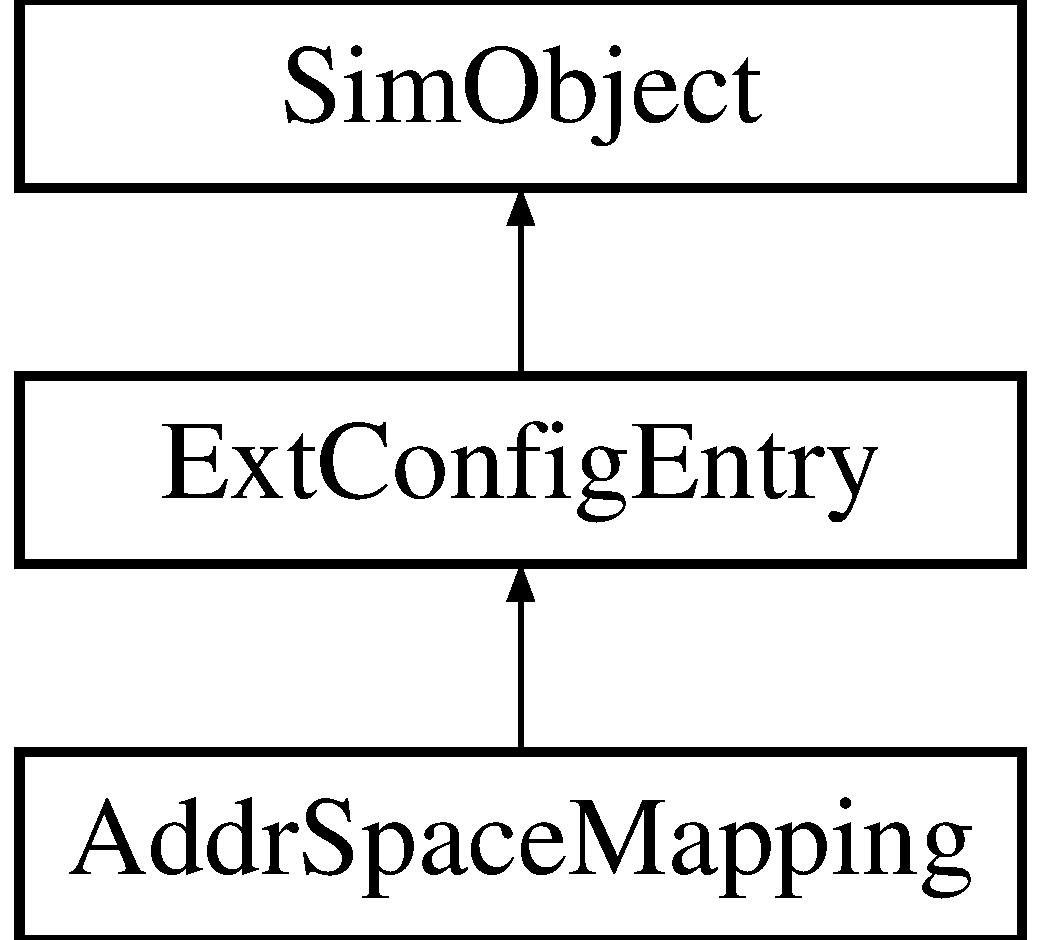
\includegraphics[height=3cm]{classX86ISA_1_1IntelMP_1_1AddrSpaceMapping}
\end{center}
\end{figure}
\subsection*{Public メソッド}
\begin{DoxyCompactItemize}
\item 
\hyperlink{base_2types_8hh_af1bb03d6a4ee096394a6749f0a169232}{Addr} \hyperlink{classX86ISA_1_1IntelMP_1_1AddrSpaceMapping_a5fffc1006b1f28bd779d83ffbe213b4f}{writeOut} (\hyperlink{classPortProxy}{PortProxy} \&proxy, \hyperlink{base_2types_8hh_af1bb03d6a4ee096394a6749f0a169232}{Addr} \hyperlink{classX86ISA_1_1IntelMP_1_1AddrSpaceMapping_a0e89cf6b9f6cd3125470b1bed2b823df}{addr}, uint8\_\-t \&checkSum)
\item 
\hyperlink{classX86ISA_1_1IntelMP_1_1AddrSpaceMapping_a95ce2e24ec2be9194be028de6be6da59}{AddrSpaceMapping} (\hyperlink{classX86ISA_1_1IntelMP_1_1AddrSpaceMapping_a1ca24332f3ea92d341d5295799303c05}{Params} $\ast$\hyperlink{namespaceX86ISA_af675c1d542a25b96e11164b80809a856}{p})
\end{DoxyCompactItemize}
\subsection*{Protected 型}
\begin{DoxyCompactItemize}
\item 
typedef X86IntelMPAddrSpaceMappingParams \hyperlink{classX86ISA_1_1IntelMP_1_1AddrSpaceMapping_a1ca24332f3ea92d341d5295799303c05}{Params}
\end{DoxyCompactItemize}
\subsection*{Protected 変数}
\begin{DoxyCompactItemize}
\item 
uint8\_\-t \hyperlink{classX86ISA_1_1IntelMP_1_1AddrSpaceMapping_ac86b1934f811ad40b20b27d29c52a5d3}{busID}
\item 
uint8\_\-t \hyperlink{classX86ISA_1_1IntelMP_1_1AddrSpaceMapping_a9f34509b1c4a58ce6c6ab2f748cc4c36}{addrType}
\item 
uint64\_\-t \hyperlink{classX86ISA_1_1IntelMP_1_1AddrSpaceMapping_a0e89cf6b9f6cd3125470b1bed2b823df}{addr}
\item 
uint64\_\-t \hyperlink{classX86ISA_1_1IntelMP_1_1AddrSpaceMapping_a97f4838e0af1607eeaa66fbe722a9b5f}{addrLength}
\end{DoxyCompactItemize}


\subsection{型定義}
\hypertarget{classX86ISA_1_1IntelMP_1_1AddrSpaceMapping_a1ca24332f3ea92d341d5295799303c05}{
\index{X86ISA::IntelMP::AddrSpaceMapping@{X86ISA::IntelMP::AddrSpaceMapping}!Params@{Params}}
\index{Params@{Params}!X86ISA::IntelMP::AddrSpaceMapping@{X86ISA::IntelMP::AddrSpaceMapping}}
\subsubsection[{Params}]{\setlength{\rightskip}{0pt plus 5cm}typedef X86IntelMPAddrSpaceMappingParams {\bf Params}\hspace{0.3cm}{\ttfamily  \mbox{[}protected\mbox{]}}}}
\label{classX86ISA_1_1IntelMP_1_1AddrSpaceMapping_a1ca24332f3ea92d341d5295799303c05}


\hyperlink{classX86ISA_1_1IntelMP_1_1ExtConfigEntry_ac05617332b889b2a33387663c048f2a9}{ExtConfigEntry}を再定義しています。

\subsection{コンストラクタとデストラクタ}
\hypertarget{classX86ISA_1_1IntelMP_1_1AddrSpaceMapping_a95ce2e24ec2be9194be028de6be6da59}{
\index{X86ISA::IntelMP::AddrSpaceMapping@{X86ISA::IntelMP::AddrSpaceMapping}!AddrSpaceMapping@{AddrSpaceMapping}}
\index{AddrSpaceMapping@{AddrSpaceMapping}!X86ISA::IntelMP::AddrSpaceMapping@{X86ISA::IntelMP::AddrSpaceMapping}}
\subsubsection[{AddrSpaceMapping}]{\setlength{\rightskip}{0pt plus 5cm}{\bf AddrSpaceMapping} ({\bf Params} $\ast$ {\em p})}}
\label{classX86ISA_1_1IntelMP_1_1AddrSpaceMapping_a95ce2e24ec2be9194be028de6be6da59}



\begin{DoxyCode}
394                                                           :
395     ExtConfigEntry(p, 128, 20),
396     busID(p->bus_id), addrType(p->address_type),
397     addr(p->address), addrLength(p->length)
398 {}

\end{DoxyCode}


\subsection{関数}
\hypertarget{classX86ISA_1_1IntelMP_1_1AddrSpaceMapping_a5fffc1006b1f28bd779d83ffbe213b4f}{
\index{X86ISA::IntelMP::AddrSpaceMapping@{X86ISA::IntelMP::AddrSpaceMapping}!writeOut@{writeOut}}
\index{writeOut@{writeOut}!X86ISA::IntelMP::AddrSpaceMapping@{X86ISA::IntelMP::AddrSpaceMapping}}
\subsubsection[{writeOut}]{\setlength{\rightskip}{0pt plus 5cm}{\bf Addr} writeOut ({\bf PortProxy} \& {\em proxy}, \/  {\bf Addr} {\em addr}, \/  uint8\_\-t \& {\em checkSum})\hspace{0.3cm}{\ttfamily  \mbox{[}virtual\mbox{]}}}}
\label{classX86ISA_1_1IntelMP_1_1AddrSpaceMapping_a5fffc1006b1f28bd779d83ffbe213b4f}


\hyperlink{classX86ISA_1_1IntelMP_1_1ExtConfigEntry_a5fffc1006b1f28bd779d83ffbe213b4f}{ExtConfigEntry}を再定義しています。


\begin{DoxyCode}
385 {
386     ExtConfigEntry::writeOut(proxy, addr, checkSum);
387     checkSum += writeOutField(proxy, addr + 2, busID);
388     checkSum += writeOutField(proxy, addr + 3, addrType);
389     checkSum += writeOutField(proxy, addr + 4, addr);
390     checkSum += writeOutField(proxy, addr + 12, addrLength);
391     return length;
392 }
\end{DoxyCode}


\subsection{変数}
\hypertarget{classX86ISA_1_1IntelMP_1_1AddrSpaceMapping_a0e89cf6b9f6cd3125470b1bed2b823df}{
\index{X86ISA::IntelMP::AddrSpaceMapping@{X86ISA::IntelMP::AddrSpaceMapping}!addr@{addr}}
\index{addr@{addr}!X86ISA::IntelMP::AddrSpaceMapping@{X86ISA::IntelMP::AddrSpaceMapping}}
\subsubsection[{addr}]{\setlength{\rightskip}{0pt plus 5cm}uint64\_\-t {\bf addr}\hspace{0.3cm}{\ttfamily  \mbox{[}protected\mbox{]}}}}
\label{classX86ISA_1_1IntelMP_1_1AddrSpaceMapping_a0e89cf6b9f6cd3125470b1bed2b823df}
\hypertarget{classX86ISA_1_1IntelMP_1_1AddrSpaceMapping_a97f4838e0af1607eeaa66fbe722a9b5f}{
\index{X86ISA::IntelMP::AddrSpaceMapping@{X86ISA::IntelMP::AddrSpaceMapping}!addrLength@{addrLength}}
\index{addrLength@{addrLength}!X86ISA::IntelMP::AddrSpaceMapping@{X86ISA::IntelMP::AddrSpaceMapping}}
\subsubsection[{addrLength}]{\setlength{\rightskip}{0pt plus 5cm}uint64\_\-t {\bf addrLength}\hspace{0.3cm}{\ttfamily  \mbox{[}protected\mbox{]}}}}
\label{classX86ISA_1_1IntelMP_1_1AddrSpaceMapping_a97f4838e0af1607eeaa66fbe722a9b5f}
\hypertarget{classX86ISA_1_1IntelMP_1_1AddrSpaceMapping_a9f34509b1c4a58ce6c6ab2f748cc4c36}{
\index{X86ISA::IntelMP::AddrSpaceMapping@{X86ISA::IntelMP::AddrSpaceMapping}!addrType@{addrType}}
\index{addrType@{addrType}!X86ISA::IntelMP::AddrSpaceMapping@{X86ISA::IntelMP::AddrSpaceMapping}}
\subsubsection[{addrType}]{\setlength{\rightskip}{0pt plus 5cm}uint8\_\-t {\bf addrType}\hspace{0.3cm}{\ttfamily  \mbox{[}protected\mbox{]}}}}
\label{classX86ISA_1_1IntelMP_1_1AddrSpaceMapping_a9f34509b1c4a58ce6c6ab2f748cc4c36}
\hypertarget{classX86ISA_1_1IntelMP_1_1AddrSpaceMapping_ac86b1934f811ad40b20b27d29c52a5d3}{
\index{X86ISA::IntelMP::AddrSpaceMapping@{X86ISA::IntelMP::AddrSpaceMapping}!busID@{busID}}
\index{busID@{busID}!X86ISA::IntelMP::AddrSpaceMapping@{X86ISA::IntelMP::AddrSpaceMapping}}
\subsubsection[{busID}]{\setlength{\rightskip}{0pt plus 5cm}uint8\_\-t {\bf busID}\hspace{0.3cm}{\ttfamily  \mbox{[}protected\mbox{]}}}}
\label{classX86ISA_1_1IntelMP_1_1AddrSpaceMapping_ac86b1934f811ad40b20b27d29c52a5d3}


このクラスの説明は次のファイルから生成されました:\begin{DoxyCompactItemize}
\item 
arch/x86/bios/\hyperlink{intelmp_8hh}{intelmp.hh}\item 
arch/x86/bios/\hyperlink{intelmp_8cc}{intelmp.cc}\end{DoxyCompactItemize}

\hypertarget{classAGENUnit}{
\section{クラス AGENUnit}
\label{classAGENUnit}\index{AGENUnit@{AGENUnit}}
}


{\ttfamily \#include $<$agen\_\-unit.hh$>$}AGENUnitに対する継承グラフ:\begin{figure}[H]
\begin{center}
\leavevmode
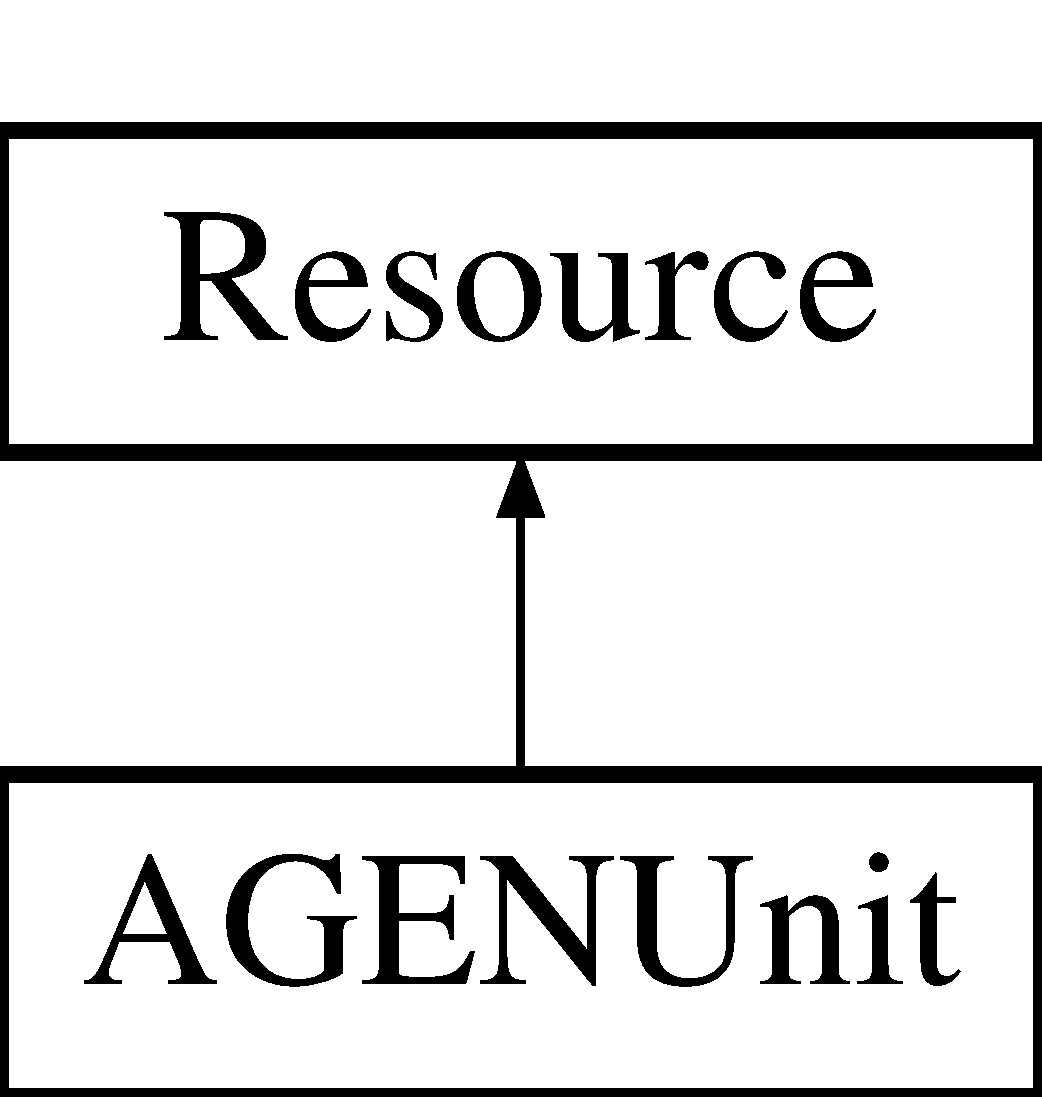
\includegraphics[height=2cm]{classAGENUnit}
\end{center}
\end{figure}
\subsection*{Public 型}
\begin{DoxyCompactItemize}
\item 
enum \hyperlink{classAGENUnit_a2afce0a47a93eee73a314d53e4890153}{Command} \{ \hyperlink{classAGENUnit_a2afce0a47a93eee73a314d53e4890153a33308417f8eb8f4e3673faee9003d120}{GenerateAddr}
 \}
\item 
typedef \hyperlink{classRefCountingPtr}{InOrderDynInst::DynInstPtr} \hyperlink{classAGENUnit_a32d1573770d3d1d96a1741ac80433e33}{DynInstPtr}
\end{DoxyCompactItemize}
\subsection*{Public メソッド}
\begin{DoxyCompactItemize}
\item 
\hyperlink{classAGENUnit_ad1527407cd4794ebff63afeb1e801999}{AGENUnit} (std::string res\_\-name, int res\_\-id, int res\_\-width, \hyperlink{classCycles}{Cycles} res\_\-latency, \hyperlink{classInOrderCPU}{InOrderCPU} $\ast$\_\-cpu, \hyperlink{namespaceThePipeline_ab62ca16eeca26566ad2422b5df4943ce}{ThePipeline::Params} $\ast$params)
\item 
virtual void \hyperlink{classAGENUnit_a7b7fff82f8c9cbdb02add1346f60bb9e}{execute} (int slot\_\-num)
\item 
void \hyperlink{classAGENUnit_a4dc637449366fcdfc4e764cdf12d9b11}{regStats} ()
\end{DoxyCompactItemize}
\subsection*{Protected 変数}
\begin{DoxyCompactItemize}
\item 
\hyperlink{classStats_1_1Scalar}{Stats::Scalar} \hyperlink{classAGENUnit_af050796f6e4377dc1312864abd020b87}{agens}
\end{DoxyCompactItemize}


\subsection{型定義}
\hypertarget{classAGENUnit_a32d1573770d3d1d96a1741ac80433e33}{
\index{AGENUnit@{AGENUnit}!DynInstPtr@{DynInstPtr}}
\index{DynInstPtr@{DynInstPtr}!AGENUnit@{AGENUnit}}
\subsubsection[{DynInstPtr}]{\setlength{\rightskip}{0pt plus 5cm}typedef {\bf InOrderDynInst::DynInstPtr} {\bf DynInstPtr}}}
\label{classAGENUnit_a32d1573770d3d1d96a1741ac80433e33}


\hyperlink{classResource_af9d0c8a46736ba6aa2d8bb94da1a5e73}{Resource}を再定義しています。

\subsection{列挙型}
\hypertarget{classAGENUnit_a2afce0a47a93eee73a314d53e4890153}{
\index{AGENUnit@{AGENUnit}!Command@{Command}}
\index{Command@{Command}!AGENUnit@{AGENUnit}}
\subsubsection[{Command}]{\setlength{\rightskip}{0pt plus 5cm}enum {\bf Command}}}
\label{classAGENUnit_a2afce0a47a93eee73a314d53e4890153}
\begin{Desc}
\item[列挙型の値: ]\par
\begin{description}
\index{GenerateAddr@{GenerateAddr}!AGENUnit@{AGENUnit}}\index{AGENUnit@{AGENUnit}!GenerateAddr@{GenerateAddr}}\item[{\em 
\hypertarget{classAGENUnit_a2afce0a47a93eee73a314d53e4890153a33308417f8eb8f4e3673faee9003d120}{
GenerateAddr}
\label{classAGENUnit_a2afce0a47a93eee73a314d53e4890153a33308417f8eb8f4e3673faee9003d120}
}]\end{description}
\end{Desc}




\begin{DoxyCode}
53                  {
54         GenerateAddr
55     };
\end{DoxyCode}


\subsection{コンストラクタとデストラクタ}
\hypertarget{classAGENUnit_ad1527407cd4794ebff63afeb1e801999}{
\index{AGENUnit@{AGENUnit}!AGENUnit@{AGENUnit}}
\index{AGENUnit@{AGENUnit}!AGENUnit@{AGENUnit}}
\subsubsection[{AGENUnit}]{\setlength{\rightskip}{0pt plus 5cm}{\bf AGENUnit} (std::string {\em res\_\-name}, \/  int {\em res\_\-id}, \/  int {\em res\_\-width}, \/  {\bf Cycles} {\em res\_\-latency}, \/  {\bf InOrderCPU} $\ast$ {\em \_\-cpu}, \/  {\bf ThePipeline::Params} $\ast$ {\em params})}}
\label{classAGENUnit_ad1527407cd4794ebff63afeb1e801999}



\begin{DoxyCode}
38     : Resource(res_name, res_id, res_width, res_latency, _cpu)
39 { }
\end{DoxyCode}


\subsection{関数}
\hypertarget{classAGENUnit_a7b7fff82f8c9cbdb02add1346f60bb9e}{
\index{AGENUnit@{AGENUnit}!execute@{execute}}
\index{execute@{execute}!AGENUnit@{AGENUnit}}
\subsubsection[{execute}]{\setlength{\rightskip}{0pt plus 5cm}void execute (int {\em slot\_\-idx})\hspace{0.3cm}{\ttfamily  \mbox{[}virtual\mbox{]}}}}
\label{classAGENUnit_a7b7fff82f8c9cbdb02add1346f60bb9e}
Execute the function of this resource. The Default is action is to do nothing. More specific models will derive from this class and define their own execute function. 

\hyperlink{classResource_a39af49c5568d1db3f53c12d7d6914c32}{Resource}を再定義しています。


\begin{DoxyCode}
53 {
54     ResourceRequest* agen_req = reqs[slot_num];
55     DynInstPtr inst = reqs[slot_num]->inst;
56 #if TRACING_ON
57     ThreadID tid = inst->readTid();
58 #endif
59     InstSeqNum seq_num = inst->seqNum;
60 
61     if (inst->fault != NoFault) {
62         DPRINTF(InOrderAGEN,
63                 "[tid:%i]: [sn:%i]: Detected %s fault @ %x. Forwarding to "
64                 "next stage.\n", tid, inst->seqNum, inst->fault->name(),
65                 inst->pcState());
66         agen_req->done();
67         return;
68     }
69 
70     switch (agen_req->cmd)
71     {
72       case GenerateAddr:
73         {
74             // Load/Store Instruction
75             if (inst->isMemRef()) {
76                 DPRINTF(InOrderAGEN,
77                         "[tid:%i] Generating Address for [sn:%i] (%s).\n",
78                         tid, seq_num, inst->staticInst->getName());
79 
80                 inst->fault = inst->calcEA();
81                 inst->setMemAddr(inst->getEA());
82 
83                 DPRINTF(InOrderAGEN,
84                     "[tid:%i] [sn:%i] Effective address calculated as: %#x\n",
85                     tid, seq_num, inst->getEA());
86 
87                 if (inst->fault == NoFault) {
88                     agen_req->done();
89                 } else {
90                     fatal("%s encountered while calculating address [sn:%i] %s",
91                           inst->fault->name(), seq_num, inst->instName());
92                 }
93 
94                 agens++;
95             } else {
96                 DPRINTF(InOrderAGEN,
97                         "[tid:] Ignoring non-memory instruction [sn:%i]\n",
98                         tid, seq_num);
99                 agen_req->done();
100             }
101         }
102         break;
103 
104       default:
105         fatal("Unrecognized command to %s", resName);
106     }
107 }
\end{DoxyCode}
\hypertarget{classAGENUnit_a4dc637449366fcdfc4e764cdf12d9b11}{
\index{AGENUnit@{AGENUnit}!regStats@{regStats}}
\index{regStats@{regStats}!AGENUnit@{AGENUnit}}
\subsubsection[{regStats}]{\setlength{\rightskip}{0pt plus 5cm}void regStats ()\hspace{0.3cm}{\ttfamily  \mbox{[}virtual\mbox{]}}}}
\label{classAGENUnit_a4dc637449366fcdfc4e764cdf12d9b11}
\hyperlink{classRegister}{Register} \hyperlink{namespaceStats}{Stats} for this resource 

\hyperlink{classResource_ac1739a9be0fbd5d96cf441cd3b2c1c78}{Resource}を再定義しています。


\begin{DoxyCode}
43 {
44     agens
45         .name(name() + ".agens")
46         .desc("Number of Address Generations");
47 
48     Resource::regStats();
49 }
\end{DoxyCode}


\subsection{変数}
\hypertarget{classAGENUnit_af050796f6e4377dc1312864abd020b87}{
\index{AGENUnit@{AGENUnit}!agens@{agens}}
\index{agens@{agens}!AGENUnit@{AGENUnit}}
\subsubsection[{agens}]{\setlength{\rightskip}{0pt plus 5cm}{\bf Stats::Scalar} {\bf agens}\hspace{0.3cm}{\ttfamily  \mbox{[}protected\mbox{]}}}}
\label{classAGENUnit_af050796f6e4377dc1312864abd020b87}


このクラスの説明は次のファイルから生成されました:\begin{DoxyCompactItemize}
\item 
cpu/inorder/resources/\hyperlink{agen__unit_8hh}{agen\_\-unit.hh}\item 
cpu/inorder/resources/\hyperlink{agen__unit_8cc}{agen\_\-unit.cc}\end{DoxyCompactItemize}

\hypertarget{classX86ISA_1_1AlignmentCheck}{
\section{クラス AlignmentCheck}
\label{classX86ISA_1_1AlignmentCheck}\index{X86ISA::AlignmentCheck@{X86ISA::AlignmentCheck}}
}


{\ttfamily \#include $<$faults.hh$>$}AlignmentCheckに対する継承グラフ:\begin{figure}[H]
\begin{center}
\leavevmode
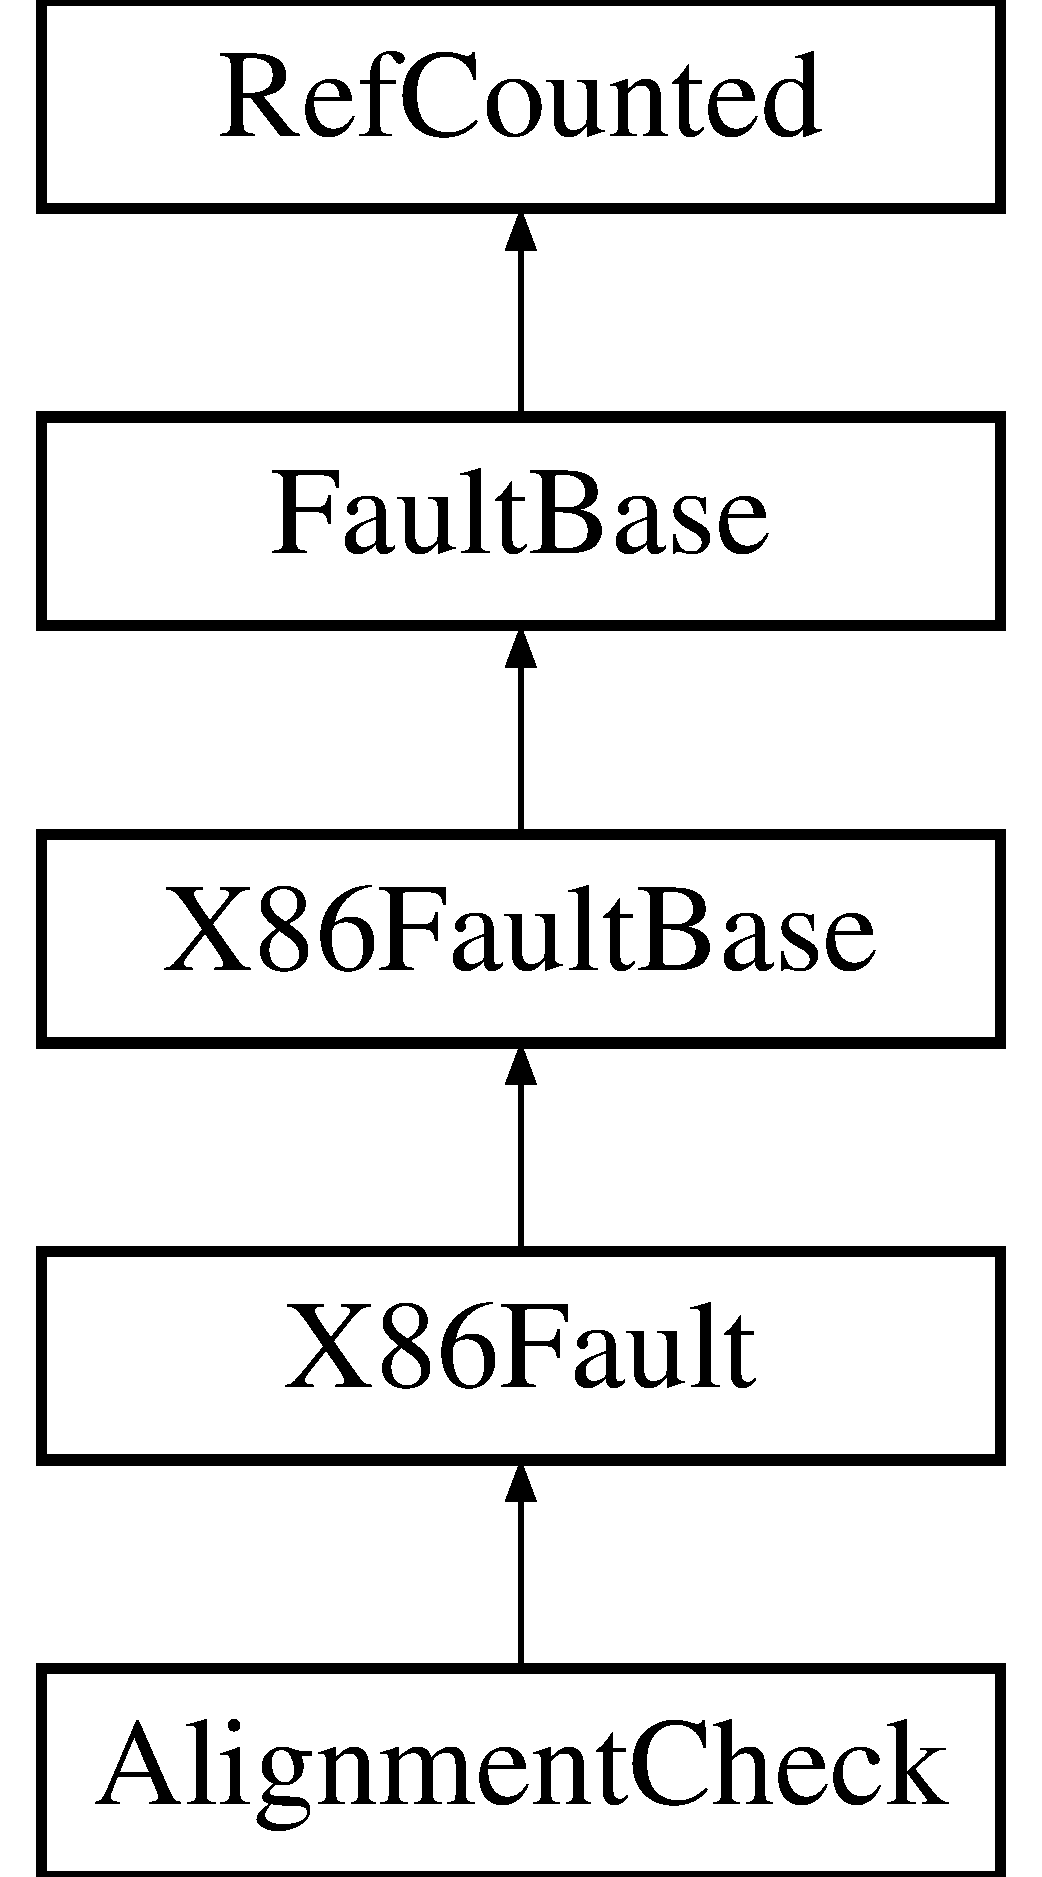
\includegraphics[height=5cm]{classX86ISA_1_1AlignmentCheck}
\end{center}
\end{figure}
\subsection*{Public メソッド}
\begin{DoxyCompactItemize}
\item 
\hyperlink{classX86ISA_1_1AlignmentCheck_a00a5d9d48172f7673fd3e44365a81fe7}{AlignmentCheck} ()
\end{DoxyCompactItemize}


\subsection{コンストラクタとデストラクタ}
\hypertarget{classX86ISA_1_1AlignmentCheck_a00a5d9d48172f7673fd3e44365a81fe7}{
\index{X86ISA::AlignmentCheck@{X86ISA::AlignmentCheck}!AlignmentCheck@{AlignmentCheck}}
\index{AlignmentCheck@{AlignmentCheck}!X86ISA::AlignmentCheck@{X86ISA::AlignmentCheck}}
\subsubsection[{AlignmentCheck}]{\setlength{\rightskip}{0pt plus 5cm}{\bf AlignmentCheck} ()\hspace{0.3cm}{\ttfamily  \mbox{[}inline\mbox{]}}}}
\label{classX86ISA_1_1AlignmentCheck_a00a5d9d48172f7673fd3e44365a81fe7}



\begin{DoxyCode}
351                          :
352             X86Fault("Alignment-Check", "#AC", 17, 0)
353         {}
    };
\end{DoxyCode}


このクラスの説明は次のファイルから生成されました:\begin{DoxyCompactItemize}
\item 
arch/x86/\hyperlink{arch_2x86_2faults_8hh}{faults.hh}\end{DoxyCompactItemize}

\hypertarget{classAlphaISA_1_1AlignmentFault}{
\section{クラス AlignmentFault}
\label{classAlphaISA_1_1AlignmentFault}\index{AlphaISA::AlignmentFault@{AlphaISA::AlignmentFault}}
}


{\ttfamily \#include $<$faults.hh$>$}AlignmentFaultに対する継承グラフ:\begin{figure}[H]
\begin{center}
\leavevmode
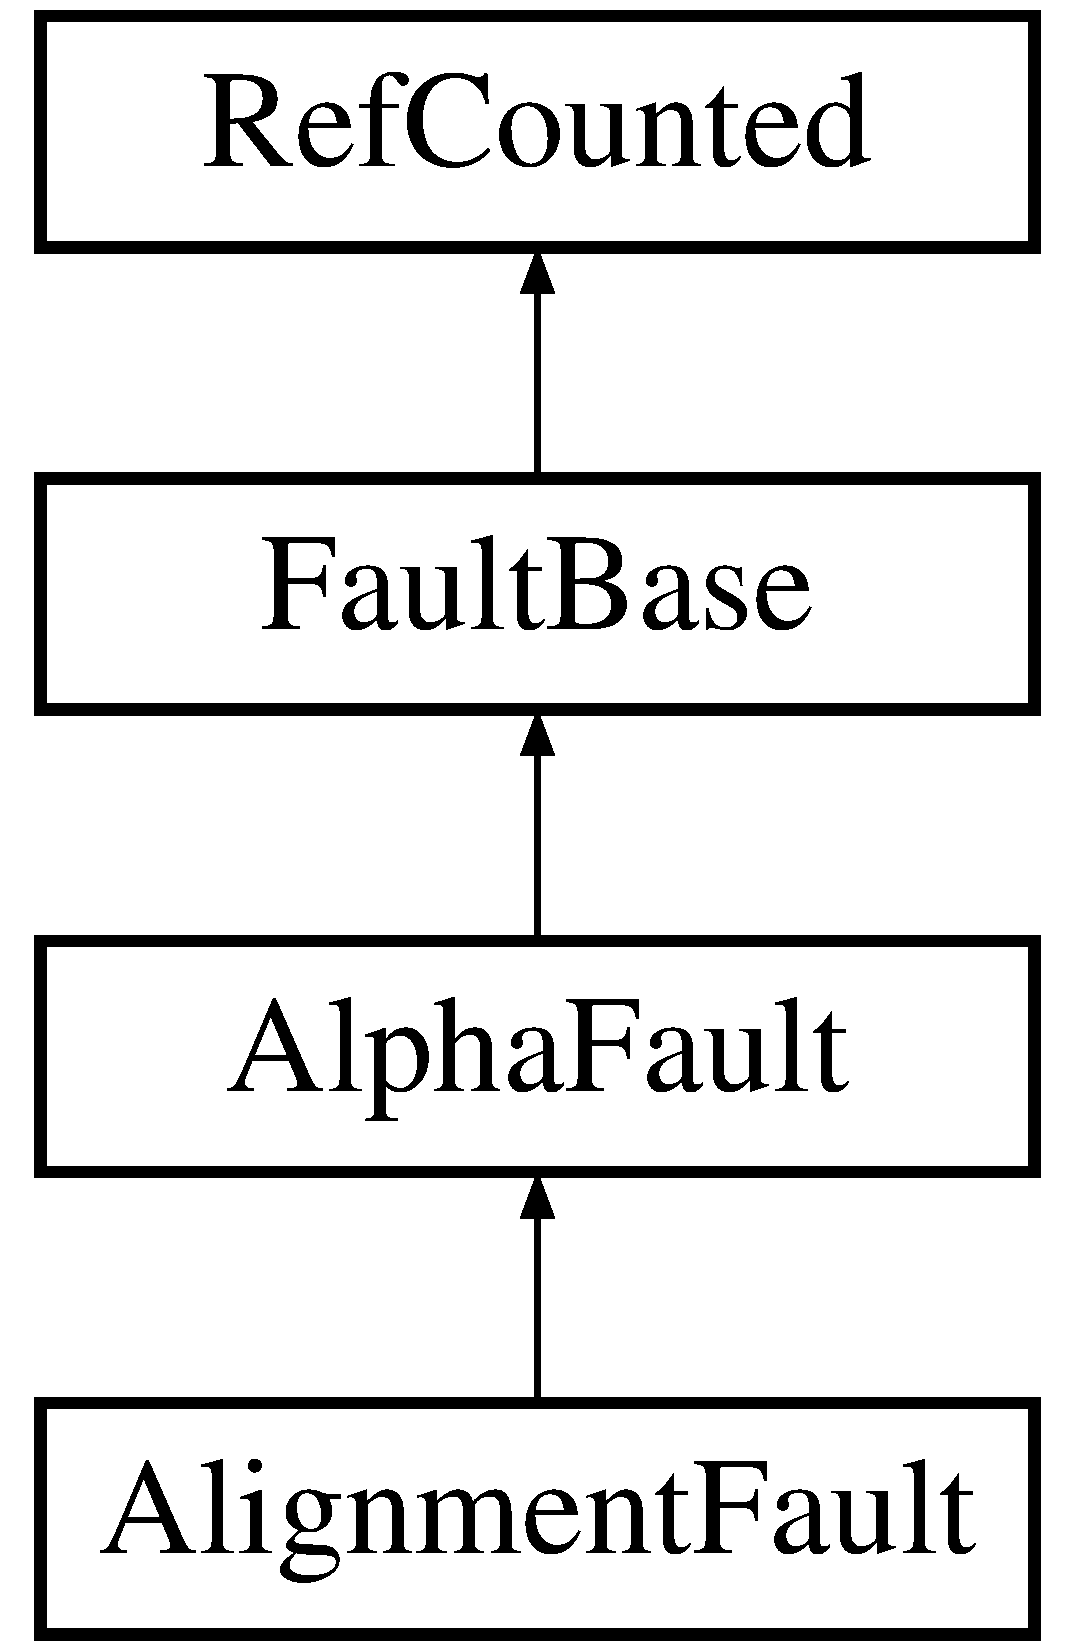
\includegraphics[height=4cm]{classAlphaISA_1_1AlignmentFault}
\end{center}
\end{figure}
\subsection*{Public メソッド}
\begin{DoxyCompactItemize}
\item 
\hyperlink{sim_2faults_8hh_abb196df64725e5c2568c900cf130d8d7}{FaultName} \hyperlink{classAlphaISA_1_1AlignmentFault_a73adb23259baf912a81683a9790a303f}{name} () const 
\item 
\hyperlink{classm5_1_1params_1_1Addr}{FaultVect} \hyperlink{classAlphaISA_1_1AlignmentFault_ae15c5d7ab0162821b93d668d0b225198}{vect} ()
\item 
\hyperlink{classStats_1_1Scalar}{FaultStat} \& \hyperlink{classAlphaISA_1_1AlignmentFault_a6c79663c761ff57265459f7e3aefaf4c}{countStat} ()
\item 
bool \hyperlink{classAlphaISA_1_1AlignmentFault_ad4aae8bc2dcbe9403effd900aca07d80}{isAlignmentFault} () const 
\end{DoxyCompactItemize}
\subsection*{Static Private 変数}
\begin{DoxyCompactItemize}
\item 
static \hyperlink{sim_2faults_8hh_abb196df64725e5c2568c900cf130d8d7}{FaultName} \hyperlink{classAlphaISA_1_1AlignmentFault_ac79073ffcd2c66a09bcd3bd3ad206019}{\_\-name} = \char`\"{}unalign\char`\"{}
\item 
static \hyperlink{classm5_1_1params_1_1Addr}{FaultVect} \hyperlink{classAlphaISA_1_1AlignmentFault_ad9e5855b9db0b2824cf6c507be4a872e}{\_\-vect} = 0x0301
\item 
static \hyperlink{classStats_1_1Scalar}{FaultStat} \hyperlink{classAlphaISA_1_1AlignmentFault_a4bff925c412f331c5aaf6a39b79619ff}{\_\-count}
\end{DoxyCompactItemize}


\subsection{関数}
\hypertarget{classAlphaISA_1_1AlignmentFault_a6c79663c761ff57265459f7e3aefaf4c}{
\index{AlphaISA::AlignmentFault@{AlphaISA::AlignmentFault}!countStat@{countStat}}
\index{countStat@{countStat}!AlphaISA::AlignmentFault@{AlphaISA::AlignmentFault}}
\subsubsection[{countStat}]{\setlength{\rightskip}{0pt plus 5cm}{\bf FaultStat}\& countStat ()\hspace{0.3cm}{\ttfamily  \mbox{[}inline, virtual\mbox{]}}}}
\label{classAlphaISA_1_1AlignmentFault_a6c79663c761ff57265459f7e3aefaf4c}


\hyperlink{classAlphaISA_1_1AlphaFault_a5d92ccd11b5cd6b04f02bd0a088b776c}{AlphaFault}を実装しています。


\begin{DoxyCode}
80 {return _count;}
\end{DoxyCode}
\hypertarget{classAlphaISA_1_1AlignmentFault_ad4aae8bc2dcbe9403effd900aca07d80}{
\index{AlphaISA::AlignmentFault@{AlphaISA::AlignmentFault}!isAlignmentFault@{isAlignmentFault}}
\index{isAlignmentFault@{isAlignmentFault}!AlphaISA::AlignmentFault@{AlphaISA::AlignmentFault}}
\subsubsection[{isAlignmentFault}]{\setlength{\rightskip}{0pt plus 5cm}bool isAlignmentFault () const\hspace{0.3cm}{\ttfamily  \mbox{[}inline\mbox{]}}}}
\label{classAlphaISA_1_1AlignmentFault_ad4aae8bc2dcbe9403effd900aca07d80}



\begin{DoxyCode}
81 {return true;}
\end{DoxyCode}
\hypertarget{classAlphaISA_1_1AlignmentFault_a73adb23259baf912a81683a9790a303f}{
\index{AlphaISA::AlignmentFault@{AlphaISA::AlignmentFault}!name@{name}}
\index{name@{name}!AlphaISA::AlignmentFault@{AlphaISA::AlignmentFault}}
\subsubsection[{name}]{\setlength{\rightskip}{0pt plus 5cm}{\bf FaultName} name () const\hspace{0.3cm}{\ttfamily  \mbox{[}inline, virtual\mbox{]}}}}
\label{classAlphaISA_1_1AlignmentFault_a73adb23259baf912a81683a9790a303f}


\hyperlink{classFaultBase_aad960357563b8b969d2dffdcc6861de7}{FaultBase}を実装しています。


\begin{DoxyCode}
78 {return _name;}
\end{DoxyCode}
\hypertarget{classAlphaISA_1_1AlignmentFault_ae15c5d7ab0162821b93d668d0b225198}{
\index{AlphaISA::AlignmentFault@{AlphaISA::AlignmentFault}!vect@{vect}}
\index{vect@{vect}!AlphaISA::AlignmentFault@{AlphaISA::AlignmentFault}}
\subsubsection[{vect}]{\setlength{\rightskip}{0pt plus 5cm}{\bf FaultVect} vect ()\hspace{0.3cm}{\ttfamily  \mbox{[}inline, virtual\mbox{]}}}}
\label{classAlphaISA_1_1AlignmentFault_ae15c5d7ab0162821b93d668d0b225198}


\hyperlink{classAlphaISA_1_1AlphaFault_ac141ef2ab527bd4d5c079ddff2e8b4aa}{AlphaFault}を実装しています。


\begin{DoxyCode}
79 {return _vect;}
\end{DoxyCode}


\subsection{変数}
\hypertarget{classAlphaISA_1_1AlignmentFault_a4bff925c412f331c5aaf6a39b79619ff}{
\index{AlphaISA::AlignmentFault@{AlphaISA::AlignmentFault}!\_\-count@{\_\-count}}
\index{\_\-count@{\_\-count}!AlphaISA::AlignmentFault@{AlphaISA::AlignmentFault}}
\subsubsection[{\_\-count}]{\setlength{\rightskip}{0pt plus 5cm}{\bf FaultStat} {\bf \_\-count}\hspace{0.3cm}{\ttfamily  \mbox{[}static, private\mbox{]}}}}
\label{classAlphaISA_1_1AlignmentFault_a4bff925c412f331c5aaf6a39b79619ff}
\hypertarget{classAlphaISA_1_1AlignmentFault_ac79073ffcd2c66a09bcd3bd3ad206019}{
\index{AlphaISA::AlignmentFault@{AlphaISA::AlignmentFault}!\_\-name@{\_\-name}}
\index{\_\-name@{\_\-name}!AlphaISA::AlignmentFault@{AlphaISA::AlignmentFault}}
\subsubsection[{\_\-name}]{\setlength{\rightskip}{0pt plus 5cm}{\bf FaultName} {\bf \_\-name} = \char`\"{}unalign\char`\"{}\hspace{0.3cm}{\ttfamily  \mbox{[}static, private\mbox{]}}}}
\label{classAlphaISA_1_1AlignmentFault_ac79073ffcd2c66a09bcd3bd3ad206019}
\hypertarget{classAlphaISA_1_1AlignmentFault_ad9e5855b9db0b2824cf6c507be4a872e}{
\index{AlphaISA::AlignmentFault@{AlphaISA::AlignmentFault}!\_\-vect@{\_\-vect}}
\index{\_\-vect@{\_\-vect}!AlphaISA::AlignmentFault@{AlphaISA::AlignmentFault}}
\subsubsection[{\_\-vect}]{\setlength{\rightskip}{0pt plus 5cm}{\bf FaultVect} {\bf \_\-vect} = 0x0301\hspace{0.3cm}{\ttfamily  \mbox{[}static, private\mbox{]}}}}
\label{classAlphaISA_1_1AlignmentFault_ad9e5855b9db0b2824cf6c507be4a872e}


このクラスの説明は次のファイルから生成されました:\begin{DoxyCompactItemize}
\item 
arch/alpha/\hyperlink{arch_2alpha_2faults_8hh}{faults.hh}\item 
arch/alpha/\hyperlink{arch_2alpha_2faults_8cc}{faults.cc}\end{DoxyCompactItemize}

\hypertarget{classPowerISA_1_1AlignmentFault}{
\section{クラス AlignmentFault}
\label{classPowerISA_1_1AlignmentFault}\index{PowerISA::AlignmentFault@{PowerISA::AlignmentFault}}
}


{\ttfamily \#include $<$faults.hh$>$}AlignmentFaultに対する継承グラフ:\begin{figure}[H]
\begin{center}
\leavevmode
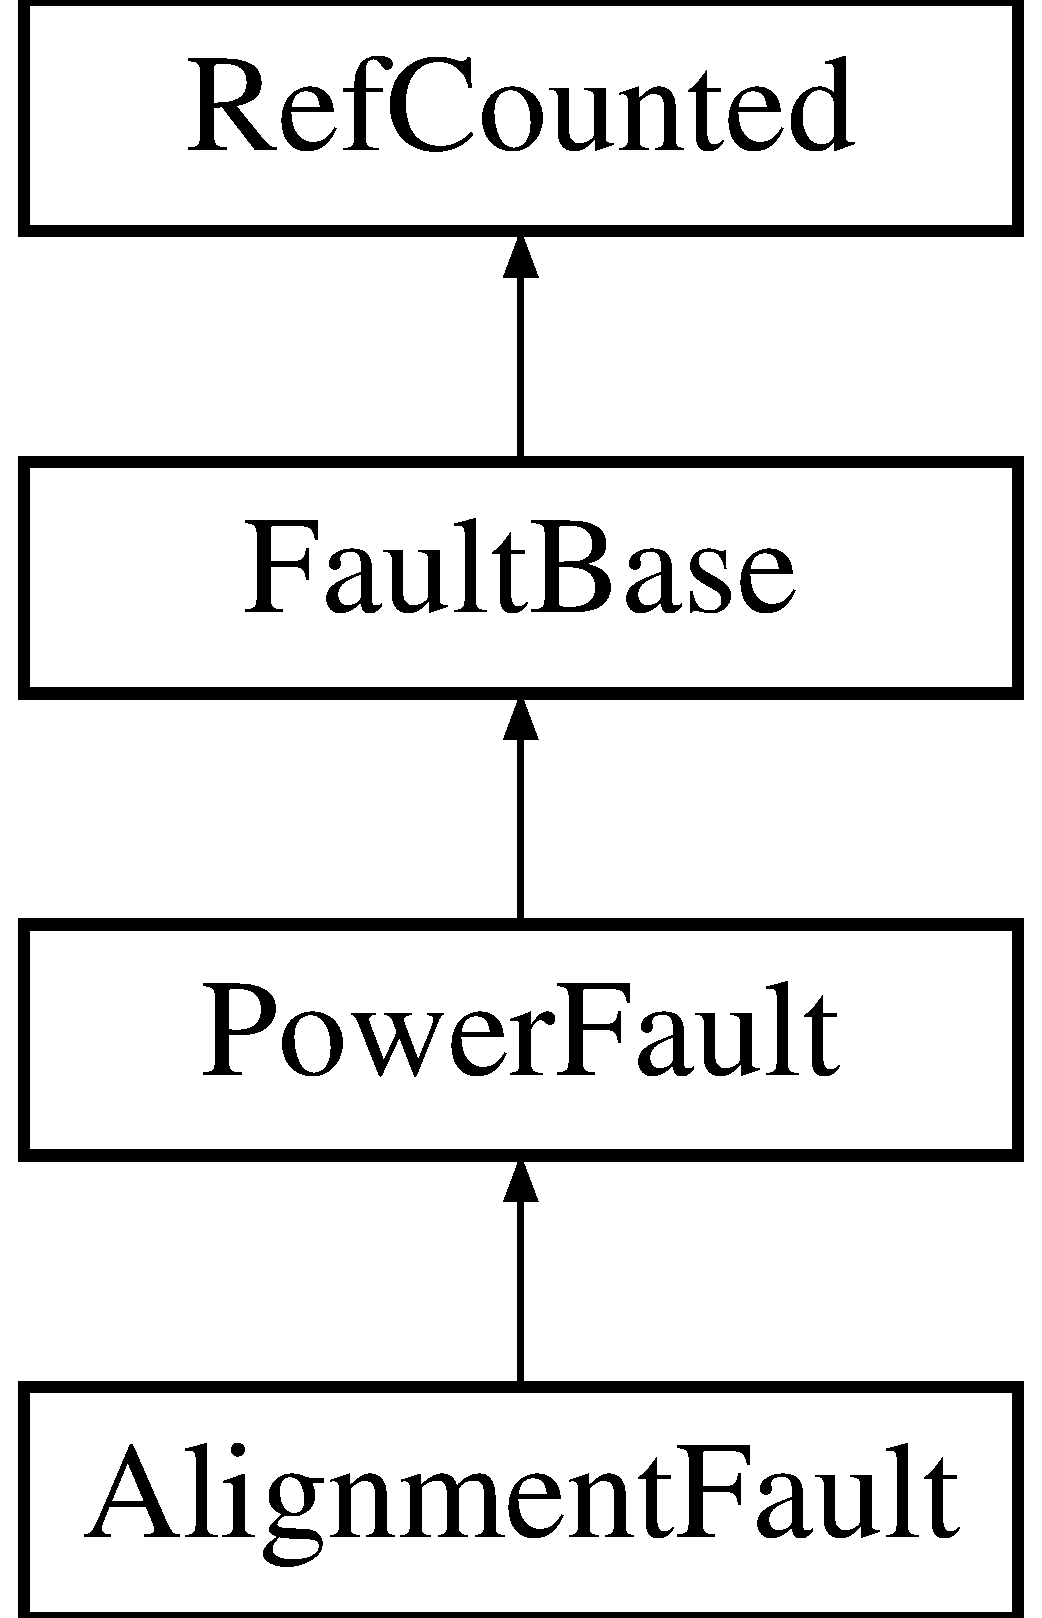
\includegraphics[height=4cm]{classPowerISA_1_1AlignmentFault}
\end{center}
\end{figure}
\subsection*{Public メソッド}
\begin{DoxyCompactItemize}
\item 
\hyperlink{classPowerISA_1_1AlignmentFault_ad9587e95e598dbe271a59244da5e43f8}{AlignmentFault} ()
\end{DoxyCompactItemize}


\subsection{コンストラクタとデストラクタ}
\hypertarget{classPowerISA_1_1AlignmentFault_ad9587e95e598dbe271a59244da5e43f8}{
\index{PowerISA::AlignmentFault@{PowerISA::AlignmentFault}!AlignmentFault@{AlignmentFault}}
\index{AlignmentFault@{AlignmentFault}!PowerISA::AlignmentFault@{PowerISA::AlignmentFault}}
\subsubsection[{AlignmentFault}]{\setlength{\rightskip}{0pt plus 5cm}{\bf AlignmentFault} ()\hspace{0.3cm}{\ttfamily  \mbox{[}inline\mbox{]}}}}
\label{classPowerISA_1_1AlignmentFault_ad9587e95e598dbe271a59244da5e43f8}



\begin{DoxyCode}
83         : PowerFault("Alignment")
84     {
85     }
\end{DoxyCode}


このクラスの説明は次のファイルから生成されました:\begin{DoxyCompactItemize}
\item 
arch/power/\hyperlink{arch_2power_2faults_8hh}{faults.hh}\end{DoxyCompactItemize}

\hypertarget{structDebug_1_1AllFlags}{
\section{構造体 AllFlags}
\label{structDebug_1_1AllFlags}\index{Debug::AllFlags@{Debug::AllFlags}}
}
AllFlagsに対する継承グラフ:\begin{figure}[H]
\begin{center}
\leavevmode
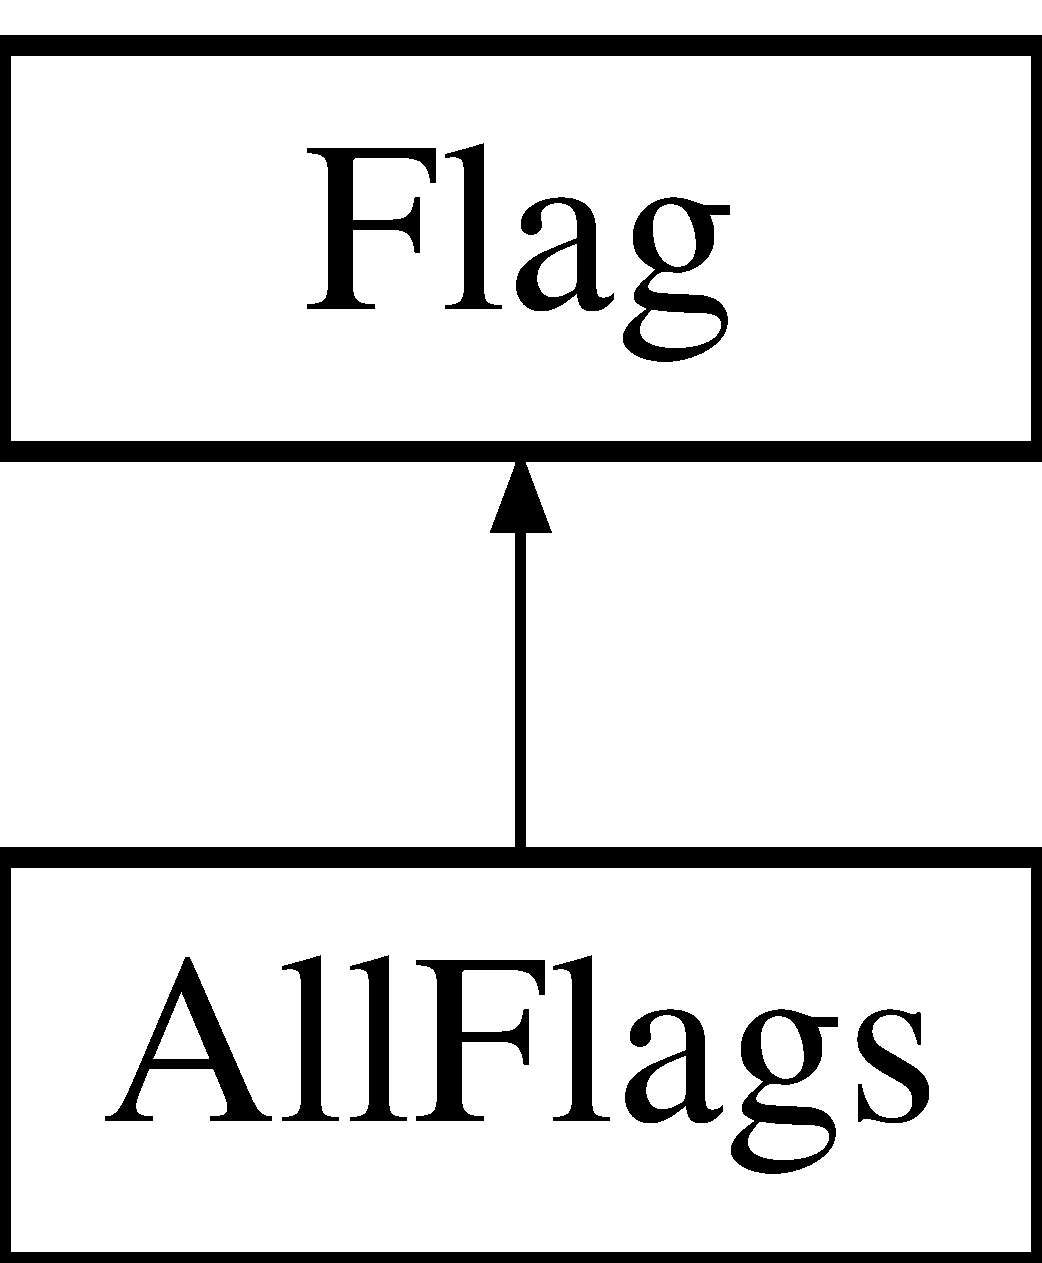
\includegraphics[height=2cm]{structDebug_1_1AllFlags}
\end{center}
\end{figure}
\subsection*{Public メソッド}
\begin{DoxyCompactItemize}
\item 
\hyperlink{structDebug_1_1AllFlags_af198ca73a3171a9151a139d163fa7678}{AllFlags} ()
\item 
void \hyperlink{structDebug_1_1AllFlags_a486f22824bd83c5308a0d70ffac6f758}{enable} ()
\item 
void \hyperlink{structDebug_1_1AllFlags_a8cfbbe53c1cf6e3054736daea3044c0f}{disable} ()
\end{DoxyCompactItemize}


\subsection{コンストラクタとデストラクタ}
\hypertarget{structDebug_1_1AllFlags_af198ca73a3171a9151a139d163fa7678}{
\index{Debug::AllFlags@{Debug::AllFlags}!AllFlags@{AllFlags}}
\index{AllFlags@{AllFlags}!Debug::AllFlags@{Debug::AllFlags}}
\subsubsection[{AllFlags}]{\setlength{\rightskip}{0pt plus 5cm}{\bf AllFlags} ()\hspace{0.3cm}{\ttfamily  \mbox{[}inline\mbox{]}}}}
\label{structDebug_1_1AllFlags_af198ca73a3171a9151a139d163fa7678}



\begin{DoxyCode}
114         : Flag("All", "All Flags")
115     {}
\end{DoxyCode}


\subsection{関数}
\hypertarget{structDebug_1_1AllFlags_a8cfbbe53c1cf6e3054736daea3044c0f}{
\index{Debug::AllFlags@{Debug::AllFlags}!disable@{disable}}
\index{disable@{disable}!Debug::AllFlags@{Debug::AllFlags}}
\subsubsection[{disable}]{\setlength{\rightskip}{0pt plus 5cm}void disable ()\hspace{0.3cm}{\ttfamily  \mbox{[}inline, virtual\mbox{]}}}}
\label{structDebug_1_1AllFlags_a8cfbbe53c1cf6e3054736daea3044c0f}


\hyperlink{classDebug_1_1Flag_ac79a817a699d8fb54e52bf6895db1b0d}{Flag}を実装しています。


\begin{DoxyCode}
129     {
130         FlagsMap::iterator i = allFlags().begin();
131         FlagsMap::iterator end = allFlags().end();
132         for (; i != end; ++i)
133             if (i->second != this)
134                 i->second->disable();
135     }
\end{DoxyCode}
\hypertarget{structDebug_1_1AllFlags_a486f22824bd83c5308a0d70ffac6f758}{
\index{Debug::AllFlags@{Debug::AllFlags}!enable@{enable}}
\index{enable@{enable}!Debug::AllFlags@{Debug::AllFlags}}
\subsubsection[{enable}]{\setlength{\rightskip}{0pt plus 5cm}void enable ()\hspace{0.3cm}{\ttfamily  \mbox{[}inline, virtual\mbox{]}}}}
\label{structDebug_1_1AllFlags_a486f22824bd83c5308a0d70ffac6f758}


\hyperlink{classDebug_1_1Flag_ad1c349e10e4417179f5eb3cb519670b5}{Flag}を実装しています。


\begin{DoxyCode}
119     {
120         FlagsMap::iterator i = allFlags().begin();
121         FlagsMap::iterator end = allFlags().end();
122         for (; i != end; ++i)
123             if (i->second != this)
124                 i->second->enable();
125     }
\end{DoxyCode}


この構造体の説明は次のファイルから生成されました:\begin{DoxyCompactItemize}
\item 
base/\hyperlink{base_2debug_8cc}{debug.cc}\end{DoxyCompactItemize}

\hypertarget{classm5_1_1debug_1_1AllFlags}{
\section{クラス AllFlags}
\label{classm5_1_1debug_1_1AllFlags}\index{m5::debug::AllFlags@{m5::debug::AllFlags}}
}


UserDict::DictMixinを継承しています。\subsection*{Public メソッド}
\begin{DoxyCompactItemize}
\item 
def \hyperlink{classm5_1_1debug_1_1AllFlags_ac775ee34451fdfa742b318538164070e}{\_\-\_\-init\_\-\_\-}
\item 
def \hyperlink{classm5_1_1debug_1_1AllFlags_a31ecdf34e79a47aea99a17eea32b7ac2}{\_\-\_\-contains\_\-\_\-}
\item 
def \hyperlink{classm5_1_1debug_1_1AllFlags_a50d766f4276c3d8fe330ac8cd344a75f}{\_\-\_\-getitem\_\-\_\-}
\item 
def \hyperlink{classm5_1_1debug_1_1AllFlags_aeb7ba70a3c91eced4f8d49ac5dc0c398}{keys}
\item 
def \hyperlink{classm5_1_1debug_1_1AllFlags_abb73a0060caeba53780d972f37623f1e}{values}
\item 
def \hyperlink{classm5_1_1debug_1_1AllFlags_a717291221885735d6870d7179083ec07}{items}
\item 
def \hyperlink{classm5_1_1debug_1_1AllFlags_a44560b0b40dfcd2069b980760783cc7b}{iterkeys}
\item 
def \hyperlink{classm5_1_1debug_1_1AllFlags_aeb6e8630a10560ad0d4b34377c790f19}{itervalues}
\item 
def \hyperlink{classm5_1_1debug_1_1AllFlags_a13d39839ad1cfd4c47f524735933c0bf}{iteritems}
\end{DoxyCompactItemize}
\subsection*{Private メソッド}
\begin{DoxyCompactItemize}
\item 
def \hyperlink{classm5_1_1debug_1_1AllFlags_a5186eac54b97bf19735a67d9652f424c}{\_\-update}
\end{DoxyCompactItemize}
\subsection*{Private 変数}
\begin{DoxyCompactItemize}
\item 
\hyperlink{classm5_1_1debug_1_1AllFlags_aeeaa0c459069671087f2e77c5b65a76e}{\_\-version}
\item 
\hyperlink{classm5_1_1debug_1_1AllFlags_a4d2dd191e958f6b142f60e7f94ce0dd0}{\_\-dict}
\end{DoxyCompactItemize}


\subsection{関数}
\hypertarget{classm5_1_1debug_1_1AllFlags_a31ecdf34e79a47aea99a17eea32b7ac2}{
\index{m5::debug::AllFlags@{m5::debug::AllFlags}!\_\-\_\-contains\_\-\_\-@{\_\-\_\-contains\_\-\_\-}}
\index{\_\-\_\-contains\_\-\_\-@{\_\-\_\-contains\_\-\_\-}!m5::debug::AllFlags@{m5::debug::AllFlags}}
\subsubsection[{\_\-\_\-contains\_\-\_\-}]{\setlength{\rightskip}{0pt plus 5cm}def \_\-\_\-contains\_\-\_\- ( {\em self}, \/   {\em item})}}
\label{classm5_1_1debug_1_1AllFlags_a31ecdf34e79a47aea99a17eea32b7ac2}



\begin{DoxyCode}
73                                 :
74         self._update()
75         return item in self._dict
76 
    def __getitem__(self, item):
\end{DoxyCode}
\hypertarget{classm5_1_1debug_1_1AllFlags_a50d766f4276c3d8fe330ac8cd344a75f}{
\index{m5::debug::AllFlags@{m5::debug::AllFlags}!\_\-\_\-getitem\_\-\_\-@{\_\-\_\-getitem\_\-\_\-}}
\index{\_\-\_\-getitem\_\-\_\-@{\_\-\_\-getitem\_\-\_\-}!m5::debug::AllFlags@{m5::debug::AllFlags}}
\subsubsection[{\_\-\_\-getitem\_\-\_\-}]{\setlength{\rightskip}{0pt plus 5cm}def \_\-\_\-getitem\_\-\_\- ( {\em self}, \/   {\em item})}}
\label{classm5_1_1debug_1_1AllFlags_a50d766f4276c3d8fe330ac8cd344a75f}



\begin{DoxyCode}
77                                :
78         self._update()
79         return self._dict[item]
80 
    def keys(self):
\end{DoxyCode}
\hypertarget{classm5_1_1debug_1_1AllFlags_ac775ee34451fdfa742b318538164070e}{
\index{m5::debug::AllFlags@{m5::debug::AllFlags}!\_\-\_\-init\_\-\_\-@{\_\-\_\-init\_\-\_\-}}
\index{\_\-\_\-init\_\-\_\-@{\_\-\_\-init\_\-\_\-}!m5::debug::AllFlags@{m5::debug::AllFlags}}
\subsubsection[{\_\-\_\-init\_\-\_\-}]{\setlength{\rightskip}{0pt plus 5cm}def \_\-\_\-init\_\-\_\- ( {\em self})}}
\label{classm5_1_1debug_1_1AllFlags_ac775ee34451fdfa742b318538164070e}



\begin{DoxyCode}
59                       :
60         self._version = -1
61         self._dict = {}
62 
    def _update(self):
\end{DoxyCode}
\hypertarget{classm5_1_1debug_1_1AllFlags_a5186eac54b97bf19735a67d9652f424c}{
\index{m5::debug::AllFlags@{m5::debug::AllFlags}!\_\-update@{\_\-update}}
\index{\_\-update@{\_\-update}!m5::debug::AllFlags@{m5::debug::AllFlags}}
\subsubsection[{\_\-update}]{\setlength{\rightskip}{0pt plus 5cm}def \_\-update ( {\em self})\hspace{0.3cm}{\ttfamily  \mbox{[}private\mbox{]}}}}
\label{classm5_1_1debug_1_1AllFlags_a5186eac54b97bf19735a67d9652f424c}



\begin{DoxyCode}
63                      :
64         current_version = internal.debug.getAllFlagsVersion()
65         if self._version == current_version:
66             return
67 
68         self._dict.clear()
69         for flag in internal.debug.getAllFlags():
70             self._dict[flag.name()] = flag
71         self._version = current_version
72 
    def __contains__(self, item):
\end{DoxyCode}
\hypertarget{classm5_1_1debug_1_1AllFlags_a717291221885735d6870d7179083ec07}{
\index{m5::debug::AllFlags@{m5::debug::AllFlags}!items@{items}}
\index{items@{items}!m5::debug::AllFlags@{m5::debug::AllFlags}}
\subsubsection[{items}]{\setlength{\rightskip}{0pt plus 5cm}def items ( {\em self})}}
\label{classm5_1_1debug_1_1AllFlags_a717291221885735d6870d7179083ec07}



\begin{DoxyCode}
89                    :
90         self._update()
91         return self._dict.items()
92 
    def iterkeys(self):
\end{DoxyCode}
\hypertarget{classm5_1_1debug_1_1AllFlags_a13d39839ad1cfd4c47f524735933c0bf}{
\index{m5::debug::AllFlags@{m5::debug::AllFlags}!iteritems@{iteritems}}
\index{iteritems@{iteritems}!m5::debug::AllFlags@{m5::debug::AllFlags}}
\subsubsection[{iteritems}]{\setlength{\rightskip}{0pt plus 5cm}def iteritems ( {\em self})}}
\label{classm5_1_1debug_1_1AllFlags_a13d39839ad1cfd4c47f524735933c0bf}



\begin{DoxyCode}
101                        :
102         self._update()
103         return self._dict.iteritems()
104 
flags = AllFlags()
\end{DoxyCode}
\hypertarget{classm5_1_1debug_1_1AllFlags_a44560b0b40dfcd2069b980760783cc7b}{
\index{m5::debug::AllFlags@{m5::debug::AllFlags}!iterkeys@{iterkeys}}
\index{iterkeys@{iterkeys}!m5::debug::AllFlags@{m5::debug::AllFlags}}
\subsubsection[{iterkeys}]{\setlength{\rightskip}{0pt plus 5cm}def iterkeys ( {\em self})}}
\label{classm5_1_1debug_1_1AllFlags_a44560b0b40dfcd2069b980760783cc7b}



\begin{DoxyCode}
93                       :
94         self._update()
95         return self._dict.iterkeys()
96 
    def itervalues(self):
\end{DoxyCode}
\hypertarget{classm5_1_1debug_1_1AllFlags_aeb6e8630a10560ad0d4b34377c790f19}{
\index{m5::debug::AllFlags@{m5::debug::AllFlags}!itervalues@{itervalues}}
\index{itervalues@{itervalues}!m5::debug::AllFlags@{m5::debug::AllFlags}}
\subsubsection[{itervalues}]{\setlength{\rightskip}{0pt plus 5cm}def itervalues ( {\em self})}}
\label{classm5_1_1debug_1_1AllFlags_aeb6e8630a10560ad0d4b34377c790f19}



\begin{DoxyCode}
97                         :
98         self._update()
99         return self._dict.itervalues()
100 
    def iteritems(self):
\end{DoxyCode}
\hypertarget{classm5_1_1debug_1_1AllFlags_aeb7ba70a3c91eced4f8d49ac5dc0c398}{
\index{m5::debug::AllFlags@{m5::debug::AllFlags}!keys@{keys}}
\index{keys@{keys}!m5::debug::AllFlags@{m5::debug::AllFlags}}
\subsubsection[{keys}]{\setlength{\rightskip}{0pt plus 5cm}def keys ( {\em self})}}
\label{classm5_1_1debug_1_1AllFlags_aeb7ba70a3c91eced4f8d49ac5dc0c398}



\begin{DoxyCode}
81                   :
82         self._update()
83         return self._dict.keys()
84 
    def values(self):
\end{DoxyCode}
\hypertarget{classm5_1_1debug_1_1AllFlags_abb73a0060caeba53780d972f37623f1e}{
\index{m5::debug::AllFlags@{m5::debug::AllFlags}!values@{values}}
\index{values@{values}!m5::debug::AllFlags@{m5::debug::AllFlags}}
\subsubsection[{values}]{\setlength{\rightskip}{0pt plus 5cm}def values ( {\em self})}}
\label{classm5_1_1debug_1_1AllFlags_abb73a0060caeba53780d972f37623f1e}



\begin{DoxyCode}
85                     :
86         self._update()
87         return self._dict.values()
88 
    def items(self):
\end{DoxyCode}


\subsection{変数}
\hypertarget{classm5_1_1debug_1_1AllFlags_a4d2dd191e958f6b142f60e7f94ce0dd0}{
\index{m5::debug::AllFlags@{m5::debug::AllFlags}!\_\-dict@{\_\-dict}}
\index{\_\-dict@{\_\-dict}!m5::debug::AllFlags@{m5::debug::AllFlags}}
\subsubsection[{\_\-dict}]{\setlength{\rightskip}{0pt plus 5cm}{\bf \_\-dict}\hspace{0.3cm}{\ttfamily  \mbox{[}private\mbox{]}}}}
\label{classm5_1_1debug_1_1AllFlags_a4d2dd191e958f6b142f60e7f94ce0dd0}
\hypertarget{classm5_1_1debug_1_1AllFlags_aeeaa0c459069671087f2e77c5b65a76e}{
\index{m5::debug::AllFlags@{m5::debug::AllFlags}!\_\-version@{\_\-version}}
\index{\_\-version@{\_\-version}!m5::debug::AllFlags@{m5::debug::AllFlags}}
\subsubsection[{\_\-version}]{\setlength{\rightskip}{0pt plus 5cm}{\bf \_\-version}\hspace{0.3cm}{\ttfamily  \mbox{[}private\mbox{]}}}}
\label{classm5_1_1debug_1_1AllFlags_aeeaa0c459069671087f2e77c5b65a76e}


このクラスの説明は次のファイルから生成されました:\begin{DoxyCompactItemize}
\item 
python/m5/\hyperlink{debug_8py}{debug.py}\end{DoxyCompactItemize}

\hypertarget{classm5_1_1proxy_1_1AllProxy}{
\section{クラス AllProxy}
\label{classm5_1_1proxy_1_1AllProxy}\index{m5::proxy::AllProxy@{m5::proxy::AllProxy}}
}
AllProxyに対する継承グラフ:\begin{figure}[H]
\begin{center}
\leavevmode
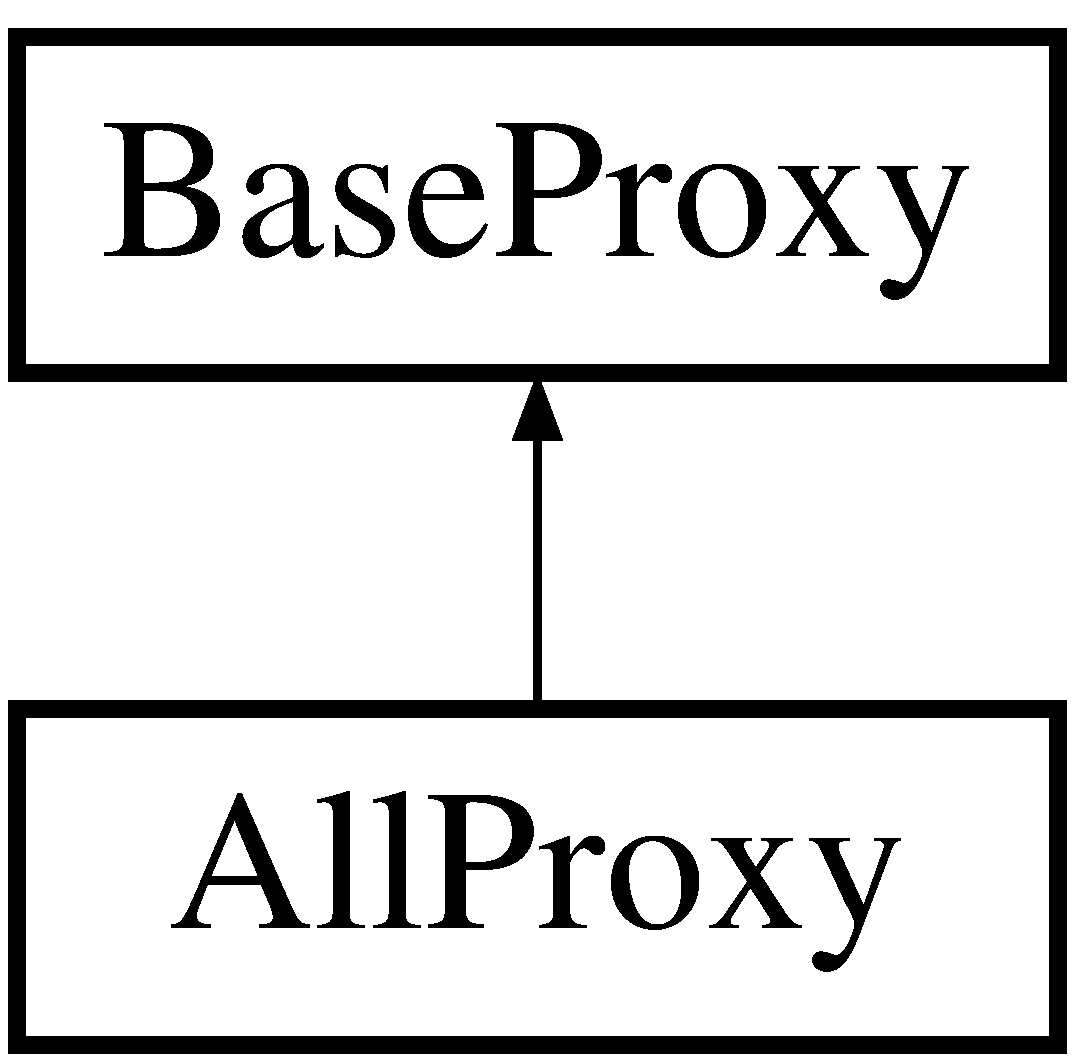
\includegraphics[height=2cm]{classm5_1_1proxy_1_1AllProxy}
\end{center}
\end{figure}
\subsection*{Public メソッド}
\begin{DoxyCompactItemize}
\item 
def \hyperlink{classm5_1_1proxy_1_1AllProxy_a01f90f57b7acd55e177611f5d0f7df23}{find}
\item 
def \hyperlink{classm5_1_1proxy_1_1AllProxy_a4767b0796ffc0da267b28b3f24776d97}{path}
\end{DoxyCompactItemize}


\subsection{関数}
\hypertarget{classm5_1_1proxy_1_1AllProxy_a01f90f57b7acd55e177611f5d0f7df23}{
\index{m5::proxy::AllProxy@{m5::proxy::AllProxy}!find@{find}}
\index{find@{find}!m5::proxy::AllProxy@{m5::proxy::AllProxy}}
\subsubsection[{find}]{\setlength{\rightskip}{0pt plus 5cm}def find ( {\em self}, \/   {\em obj})}}
\label{classm5_1_1proxy_1_1AllProxy_a01f90f57b7acd55e177611f5d0f7df23}



\begin{DoxyCode}
208                        :
209         return obj.find_all(self._pdesc.ptype)
210 
    def path(self):
\end{DoxyCode}
\hypertarget{classm5_1_1proxy_1_1AllProxy_a4767b0796ffc0da267b28b3f24776d97}{
\index{m5::proxy::AllProxy@{m5::proxy::AllProxy}!path@{path}}
\index{path@{path}!m5::proxy::AllProxy@{m5::proxy::AllProxy}}
\subsubsection[{path}]{\setlength{\rightskip}{0pt plus 5cm}def path ( {\em self})}}
\label{classm5_1_1proxy_1_1AllProxy_a4767b0796ffc0da267b28b3f24776d97}



\begin{DoxyCode}
211                   :
212         return 'all'
213 
def isproxy(obj):
\end{DoxyCode}


このクラスの説明は次のファイルから生成されました:\begin{DoxyCompactItemize}
\item 
python/m5/\hyperlink{proxy_8py}{proxy.py}\end{DoxyCompactItemize}

\hypertarget{structAlphaAccess}{
\section{構造体 AlphaAccess}
\label{structAlphaAccess}\index{AlphaAccess@{AlphaAccess}}
}


{\ttfamily \#include $<$access.h$>$}AlphaAccessに対する継承グラフ:\begin{figure}[H]
\begin{center}
\leavevmode
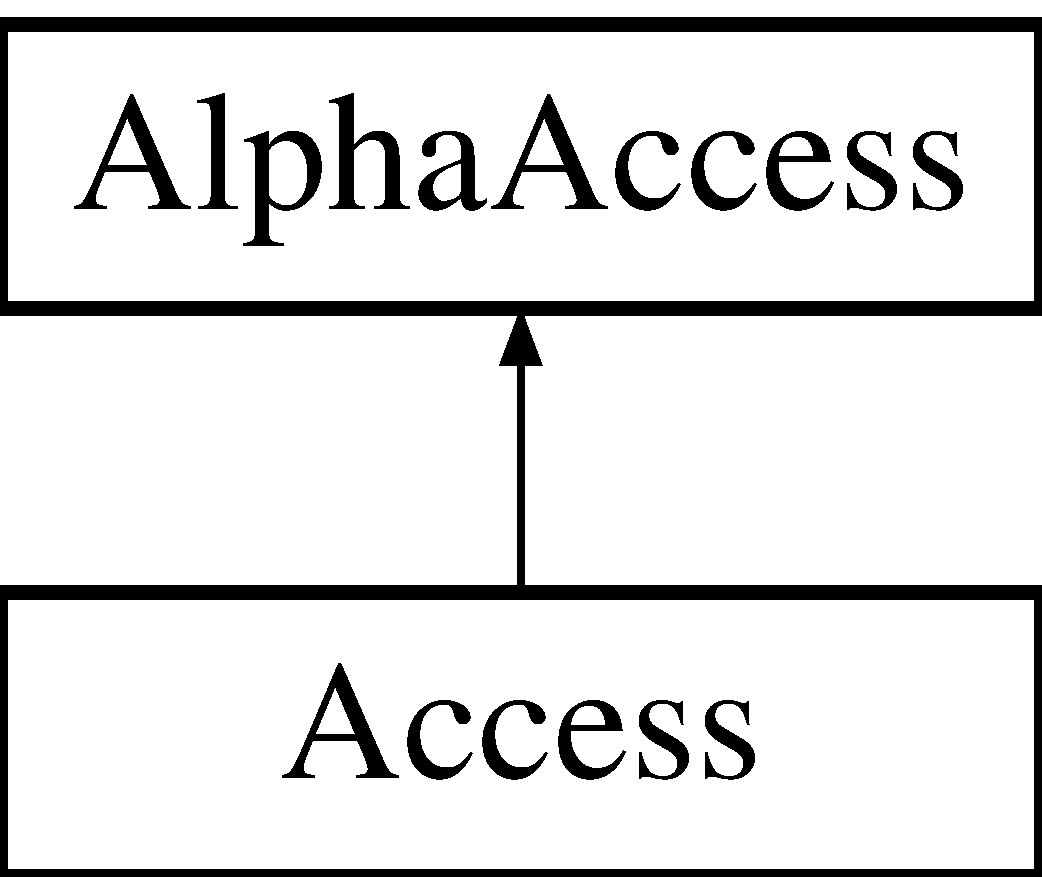
\includegraphics[height=2cm]{structAlphaAccess}
\end{center}
\end{figure}
\subsection*{Public 変数}
\begin{DoxyCompactItemize}
\item 
\hyperlink{Type_8hh_a435d1572bf3f880d55459d9805097f62}{uint32\_\-t} \hyperlink{structAlphaAccess_a589399e9f33ae0028f3868360bf5a665}{last\_\-offset}
\item 
\hyperlink{Type_8hh_a435d1572bf3f880d55459d9805097f62}{uint32\_\-t} \hyperlink{structAlphaAccess_acd99bb05ca015e7d74448acb1deba7ca}{version}
\item 
\hyperlink{Type_8hh_a435d1572bf3f880d55459d9805097f62}{uint32\_\-t} \hyperlink{structAlphaAccess_a62fe5772fdad74fda85b8510032153e0}{numCPUs}
\item 
\hyperlink{Type_8hh_a435d1572bf3f880d55459d9805097f62}{uint32\_\-t} \hyperlink{structAlphaAccess_a67afaa4123cf0004c80816f4a4622b68}{intrClockFrequency}
\item 
uint64\_\-t \hyperlink{structAlphaAccess_a1a28e6675c07a466d48206a22e992a0d}{cpuClock}
\item 
uint64\_\-t \hyperlink{structAlphaAccess_ae177731dc45fab0258bb6f72ebf37785}{mem\_\-size}
\item 
uint64\_\-t \hyperlink{structAlphaAccess_a031a9a2b7278c18413f2c17d8dd9d77c}{kernStart}
\item 
uint64\_\-t \hyperlink{structAlphaAccess_a6741af28865e38d678856e45e22a097e}{kernEnd}
\item 
uint64\_\-t \hyperlink{structAlphaAccess_a4425463a9d69b9f56bf1ac63c00d490d}{entryPoint}
\item 
uint64\_\-t \hyperlink{structAlphaAccess_a0374285e1002cc600d14cc247fd69f94}{diskUnit}
\item 
uint64\_\-t \hyperlink{structAlphaAccess_ab117d67754396b0fafd41fe5b8c9a806}{diskCount}
\item 
uint64\_\-t \hyperlink{structAlphaAccess_a95271ef36180e56020f8e5f3814ff64e}{diskPAddr}
\item 
uint64\_\-t \hyperlink{structAlphaAccess_a5faab42437acf9c9f2d137fdc52d3131}{diskBlock}
\item 
uint64\_\-t \hyperlink{structAlphaAccess_acbc96b4c47cd54efc8a5979bfb60f748}{diskOperation}
\item 
uint64\_\-t \hyperlink{structAlphaAccess_a0e8d6cc1d8754f3ca0765d5587997a57}{outputChar}
\item 
uint64\_\-t \hyperlink{structAlphaAccess_a648610dfd10a138f6e0897c45da0855c}{inputChar}
\item 
uint64\_\-t \hyperlink{structAlphaAccess_a42f441fefccfd9ff9dcc3535cccbc427}{cpuStack} \mbox{[}64\mbox{]}
\end{DoxyCompactItemize}


\subsection{変数}
\hypertarget{structAlphaAccess_a1a28e6675c07a466d48206a22e992a0d}{
\index{AlphaAccess@{AlphaAccess}!cpuClock@{cpuClock}}
\index{cpuClock@{cpuClock}!AlphaAccess@{AlphaAccess}}
\subsubsection[{cpuClock}]{\setlength{\rightskip}{0pt plus 5cm}uint64\_\-t {\bf cpuClock}}}
\label{structAlphaAccess_a1a28e6675c07a466d48206a22e992a0d}
\hypertarget{structAlphaAccess_a42f441fefccfd9ff9dcc3535cccbc427}{
\index{AlphaAccess@{AlphaAccess}!cpuStack@{cpuStack}}
\index{cpuStack@{cpuStack}!AlphaAccess@{AlphaAccess}}
\subsubsection[{cpuStack}]{\setlength{\rightskip}{0pt plus 5cm}uint64\_\-t {\bf cpuStack}\mbox{[}64\mbox{]}}}
\label{structAlphaAccess_a42f441fefccfd9ff9dcc3535cccbc427}
\hypertarget{structAlphaAccess_a5faab42437acf9c9f2d137fdc52d3131}{
\index{AlphaAccess@{AlphaAccess}!diskBlock@{diskBlock}}
\index{diskBlock@{diskBlock}!AlphaAccess@{AlphaAccess}}
\subsubsection[{diskBlock}]{\setlength{\rightskip}{0pt plus 5cm}uint64\_\-t {\bf diskBlock}}}
\label{structAlphaAccess_a5faab42437acf9c9f2d137fdc52d3131}
\hypertarget{structAlphaAccess_ab117d67754396b0fafd41fe5b8c9a806}{
\index{AlphaAccess@{AlphaAccess}!diskCount@{diskCount}}
\index{diskCount@{diskCount}!AlphaAccess@{AlphaAccess}}
\subsubsection[{diskCount}]{\setlength{\rightskip}{0pt plus 5cm}uint64\_\-t {\bf diskCount}}}
\label{structAlphaAccess_ab117d67754396b0fafd41fe5b8c9a806}
\hypertarget{structAlphaAccess_acbc96b4c47cd54efc8a5979bfb60f748}{
\index{AlphaAccess@{AlphaAccess}!diskOperation@{diskOperation}}
\index{diskOperation@{diskOperation}!AlphaAccess@{AlphaAccess}}
\subsubsection[{diskOperation}]{\setlength{\rightskip}{0pt plus 5cm}uint64\_\-t {\bf diskOperation}}}
\label{structAlphaAccess_acbc96b4c47cd54efc8a5979bfb60f748}
\hypertarget{structAlphaAccess_a95271ef36180e56020f8e5f3814ff64e}{
\index{AlphaAccess@{AlphaAccess}!diskPAddr@{diskPAddr}}
\index{diskPAddr@{diskPAddr}!AlphaAccess@{AlphaAccess}}
\subsubsection[{diskPAddr}]{\setlength{\rightskip}{0pt plus 5cm}uint64\_\-t {\bf diskPAddr}}}
\label{structAlphaAccess_a95271ef36180e56020f8e5f3814ff64e}
\hypertarget{structAlphaAccess_a0374285e1002cc600d14cc247fd69f94}{
\index{AlphaAccess@{AlphaAccess}!diskUnit@{diskUnit}}
\index{diskUnit@{diskUnit}!AlphaAccess@{AlphaAccess}}
\subsubsection[{diskUnit}]{\setlength{\rightskip}{0pt plus 5cm}uint64\_\-t {\bf diskUnit}}}
\label{structAlphaAccess_a0374285e1002cc600d14cc247fd69f94}
\hypertarget{structAlphaAccess_a4425463a9d69b9f56bf1ac63c00d490d}{
\index{AlphaAccess@{AlphaAccess}!entryPoint@{entryPoint}}
\index{entryPoint@{entryPoint}!AlphaAccess@{AlphaAccess}}
\subsubsection[{entryPoint}]{\setlength{\rightskip}{0pt plus 5cm}uint64\_\-t {\bf entryPoint}}}
\label{structAlphaAccess_a4425463a9d69b9f56bf1ac63c00d490d}
\hypertarget{structAlphaAccess_a648610dfd10a138f6e0897c45da0855c}{
\index{AlphaAccess@{AlphaAccess}!inputChar@{inputChar}}
\index{inputChar@{inputChar}!AlphaAccess@{AlphaAccess}}
\subsubsection[{inputChar}]{\setlength{\rightskip}{0pt plus 5cm}uint64\_\-t {\bf inputChar}}}
\label{structAlphaAccess_a648610dfd10a138f6e0897c45da0855c}
\hypertarget{structAlphaAccess_a67afaa4123cf0004c80816f4a4622b68}{
\index{AlphaAccess@{AlphaAccess}!intrClockFrequency@{intrClockFrequency}}
\index{intrClockFrequency@{intrClockFrequency}!AlphaAccess@{AlphaAccess}}
\subsubsection[{intrClockFrequency}]{\setlength{\rightskip}{0pt plus 5cm}{\bf uint32\_\-t} {\bf intrClockFrequency}}}
\label{structAlphaAccess_a67afaa4123cf0004c80816f4a4622b68}
\hypertarget{structAlphaAccess_a6741af28865e38d678856e45e22a097e}{
\index{AlphaAccess@{AlphaAccess}!kernEnd@{kernEnd}}
\index{kernEnd@{kernEnd}!AlphaAccess@{AlphaAccess}}
\subsubsection[{kernEnd}]{\setlength{\rightskip}{0pt plus 5cm}uint64\_\-t {\bf kernEnd}}}
\label{structAlphaAccess_a6741af28865e38d678856e45e22a097e}
\hypertarget{structAlphaAccess_a031a9a2b7278c18413f2c17d8dd9d77c}{
\index{AlphaAccess@{AlphaAccess}!kernStart@{kernStart}}
\index{kernStart@{kernStart}!AlphaAccess@{AlphaAccess}}
\subsubsection[{kernStart}]{\setlength{\rightskip}{0pt plus 5cm}uint64\_\-t {\bf kernStart}}}
\label{structAlphaAccess_a031a9a2b7278c18413f2c17d8dd9d77c}
\hypertarget{structAlphaAccess_a589399e9f33ae0028f3868360bf5a665}{
\index{AlphaAccess@{AlphaAccess}!last\_\-offset@{last\_\-offset}}
\index{last\_\-offset@{last\_\-offset}!AlphaAccess@{AlphaAccess}}
\subsubsection[{last\_\-offset}]{\setlength{\rightskip}{0pt plus 5cm}{\bf uint32\_\-t} {\bf last\_\-offset}}}
\label{structAlphaAccess_a589399e9f33ae0028f3868360bf5a665}
\hypertarget{structAlphaAccess_ae177731dc45fab0258bb6f72ebf37785}{
\index{AlphaAccess@{AlphaAccess}!mem\_\-size@{mem\_\-size}}
\index{mem\_\-size@{mem\_\-size}!AlphaAccess@{AlphaAccess}}
\subsubsection[{mem\_\-size}]{\setlength{\rightskip}{0pt plus 5cm}uint64\_\-t {\bf mem\_\-size}}}
\label{structAlphaAccess_ae177731dc45fab0258bb6f72ebf37785}
\hypertarget{structAlphaAccess_a62fe5772fdad74fda85b8510032153e0}{
\index{AlphaAccess@{AlphaAccess}!numCPUs@{numCPUs}}
\index{numCPUs@{numCPUs}!AlphaAccess@{AlphaAccess}}
\subsubsection[{numCPUs}]{\setlength{\rightskip}{0pt plus 5cm}{\bf uint32\_\-t} {\bf numCPUs}}}
\label{structAlphaAccess_a62fe5772fdad74fda85b8510032153e0}
\hypertarget{structAlphaAccess_a0e8d6cc1d8754f3ca0765d5587997a57}{
\index{AlphaAccess@{AlphaAccess}!outputChar@{outputChar}}
\index{outputChar@{outputChar}!AlphaAccess@{AlphaAccess}}
\subsubsection[{outputChar}]{\setlength{\rightskip}{0pt plus 5cm}uint64\_\-t {\bf outputChar}}}
\label{structAlphaAccess_a0e8d6cc1d8754f3ca0765d5587997a57}
\hypertarget{structAlphaAccess_acd99bb05ca015e7d74448acb1deba7ca}{
\index{AlphaAccess@{AlphaAccess}!version@{version}}
\index{version@{version}!AlphaAccess@{AlphaAccess}}
\subsubsection[{version}]{\setlength{\rightskip}{0pt plus 5cm}{\bf uint32\_\-t} {\bf version}}}
\label{structAlphaAccess_acd99bb05ca015e7d74448acb1deba7ca}


この構造体の説明は次のファイルから生成されました:\begin{DoxyCompactItemize}
\item 
dev/alpha/\hyperlink{alpha_2access_8h}{access.h}\end{DoxyCompactItemize}

\hypertarget{classAlphaBackdoor_1_1AlphaBackdoor}{
\section{クラス AlphaBackdoor}
\label{classAlphaBackdoor_1_1AlphaBackdoor}\index{AlphaBackdoor::AlphaBackdoor@{AlphaBackdoor::AlphaBackdoor}}
}
AlphaBackdoorに対する継承グラフ:\begin{figure}[H]
\begin{center}
\leavevmode
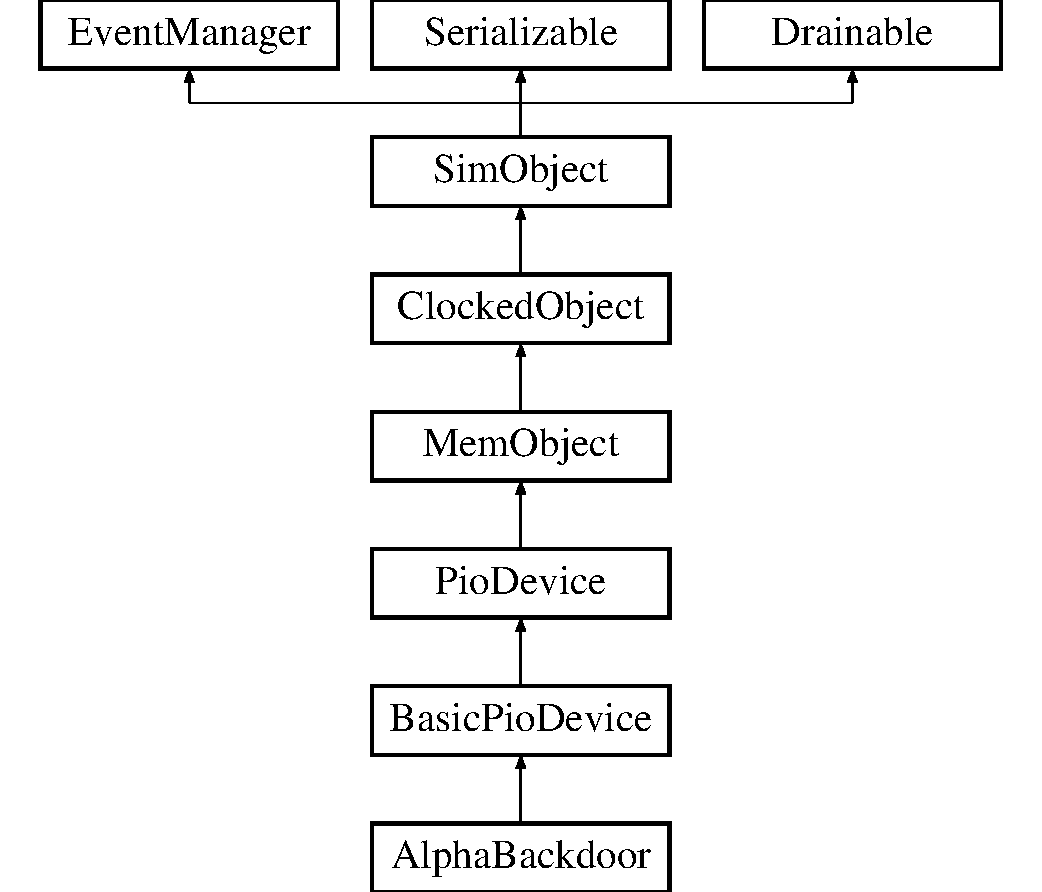
\includegraphics[height=7cm]{classAlphaBackdoor_1_1AlphaBackdoor}
\end{center}
\end{figure}
\subsection*{Static Public 変数}
\begin{DoxyCompactItemize}
\item 
string \hyperlink{classAlphaBackdoor_1_1AlphaBackdoor_acce15679d830831b0bbe8ebc2a60b2ca}{type} = '\hyperlink{classAlphaBackdoor_1_1AlphaBackdoor}{AlphaBackdoor}'
\item 
string \hyperlink{classAlphaBackdoor_1_1AlphaBackdoor_a17da7064bc5c518791f0c891eff05fda}{cxx\_\-header} = \char`\"{}dev/alpha/backdoor.hh\char`\"{}
\item 
tuple \hyperlink{classAlphaBackdoor_1_1AlphaBackdoor_a41feb23725c8f280bd96697cc0be1836}{cpu} = Param.BaseCPU(Parent.cpu\mbox{[}0\mbox{]}, \char`\"{}Processor\char`\"{})
\item 
tuple \hyperlink{classAlphaBackdoor_1_1AlphaBackdoor_a2cb8a7cfa320c243ad28a4ba142879c4}{disk} = Param.SimpleDisk(\char`\"{}Simple Disk\char`\"{})
\item 
tuple \hyperlink{classAlphaBackdoor_1_1AlphaBackdoor_a36fbd7aa3e5bc702238c8fc439330d8f}{terminal} = Param.Terminal(Parent.any, \char`\"{}The console \hyperlink{classAlphaBackdoor_ad511a78bad32e194354d8323bc23a4e3}{terminal}\char`\"{})
\item 
tuple \hyperlink{classAlphaBackdoor_1_1AlphaBackdoor_ae6d09ca44893db6cdb66d62deaa1aefd}{platform} = Param.Platform(Parent.any, \char`\"{}Platform this device is part of.\char`\"{})
\item 
tuple \hyperlink{classAlphaBackdoor_1_1AlphaBackdoor_ab737471139f5a296e5b26e8a0e1b0744}{system} = Param.AlphaSystem(Parent.any, \char`\"{}system object\char`\"{})
\end{DoxyCompactItemize}


\subsection{変数}
\hypertarget{classAlphaBackdoor_1_1AlphaBackdoor_a41feb23725c8f280bd96697cc0be1836}{
\index{AlphaBackdoor::AlphaBackdoor@{AlphaBackdoor::AlphaBackdoor}!cpu@{cpu}}
\index{cpu@{cpu}!AlphaBackdoor::AlphaBackdoor@{AlphaBackdoor::AlphaBackdoor}}
\subsubsection[{cpu}]{\setlength{\rightskip}{0pt plus 5cm}tuple {\bf cpu} = Param.BaseCPU(Parent.cpu\mbox{[}0\mbox{]}, \char`\"{}Processor\char`\"{})\hspace{0.3cm}{\ttfamily  \mbox{[}static\mbox{]}}}}
\label{classAlphaBackdoor_1_1AlphaBackdoor_a41feb23725c8f280bd96697cc0be1836}
\hypertarget{classAlphaBackdoor_1_1AlphaBackdoor_a17da7064bc5c518791f0c891eff05fda}{
\index{AlphaBackdoor::AlphaBackdoor@{AlphaBackdoor::AlphaBackdoor}!cxx\_\-header@{cxx\_\-header}}
\index{cxx\_\-header@{cxx\_\-header}!AlphaBackdoor::AlphaBackdoor@{AlphaBackdoor::AlphaBackdoor}}
\subsubsection[{cxx\_\-header}]{\setlength{\rightskip}{0pt plus 5cm}string cxx\_\-header = \char`\"{}dev/alpha/backdoor.hh\char`\"{}\hspace{0.3cm}{\ttfamily  \mbox{[}static\mbox{]}}}}
\label{classAlphaBackdoor_1_1AlphaBackdoor_a17da7064bc5c518791f0c891eff05fda}


\hyperlink{classDevice_1_1BasicPioDevice_a17da7064bc5c518791f0c891eff05fda}{BasicPioDevice}を再定義しています。\hypertarget{classAlphaBackdoor_1_1AlphaBackdoor_a2cb8a7cfa320c243ad28a4ba142879c4}{
\index{AlphaBackdoor::AlphaBackdoor@{AlphaBackdoor::AlphaBackdoor}!disk@{disk}}
\index{disk@{disk}!AlphaBackdoor::AlphaBackdoor@{AlphaBackdoor::AlphaBackdoor}}
\subsubsection[{disk}]{\setlength{\rightskip}{0pt plus 5cm}tuple {\bf disk} = Param.SimpleDisk(\char`\"{}Simple Disk\char`\"{})\hspace{0.3cm}{\ttfamily  \mbox{[}static\mbox{]}}}}
\label{classAlphaBackdoor_1_1AlphaBackdoor_a2cb8a7cfa320c243ad28a4ba142879c4}
\hypertarget{classAlphaBackdoor_1_1AlphaBackdoor_ae6d09ca44893db6cdb66d62deaa1aefd}{
\index{AlphaBackdoor::AlphaBackdoor@{AlphaBackdoor::AlphaBackdoor}!platform@{platform}}
\index{platform@{platform}!AlphaBackdoor::AlphaBackdoor@{AlphaBackdoor::AlphaBackdoor}}
\subsubsection[{platform}]{\setlength{\rightskip}{0pt plus 5cm}tuple platform = Param.Platform(Parent.any, \char`\"{}Platform this device is part of.\char`\"{})\hspace{0.3cm}{\ttfamily  \mbox{[}static\mbox{]}}}}
\label{classAlphaBackdoor_1_1AlphaBackdoor_ae6d09ca44893db6cdb66d62deaa1aefd}
\hypertarget{classAlphaBackdoor_1_1AlphaBackdoor_ab737471139f5a296e5b26e8a0e1b0744}{
\index{AlphaBackdoor::AlphaBackdoor@{AlphaBackdoor::AlphaBackdoor}!system@{system}}
\index{system@{system}!AlphaBackdoor::AlphaBackdoor@{AlphaBackdoor::AlphaBackdoor}}
\subsubsection[{system}]{\setlength{\rightskip}{0pt plus 5cm}tuple {\bf system} = Param.AlphaSystem(Parent.any, \char`\"{}system object\char`\"{})\hspace{0.3cm}{\ttfamily  \mbox{[}static\mbox{]}}}}
\label{classAlphaBackdoor_1_1AlphaBackdoor_ab737471139f5a296e5b26e8a0e1b0744}


\hyperlink{classDevice_1_1PioDevice_ab737471139f5a296e5b26e8a0e1b0744}{PioDevice}を再定義しています。\hypertarget{classAlphaBackdoor_1_1AlphaBackdoor_a36fbd7aa3e5bc702238c8fc439330d8f}{
\index{AlphaBackdoor::AlphaBackdoor@{AlphaBackdoor::AlphaBackdoor}!terminal@{terminal}}
\index{terminal@{terminal}!AlphaBackdoor::AlphaBackdoor@{AlphaBackdoor::AlphaBackdoor}}
\subsubsection[{terminal}]{\setlength{\rightskip}{0pt plus 5cm}tuple {\bf terminal} = Param.Terminal(Parent.any, \char`\"{}The console {\bf terminal}\char`\"{})\hspace{0.3cm}{\ttfamily  \mbox{[}static\mbox{]}}}}
\label{classAlphaBackdoor_1_1AlphaBackdoor_a36fbd7aa3e5bc702238c8fc439330d8f}
\hypertarget{classAlphaBackdoor_1_1AlphaBackdoor_acce15679d830831b0bbe8ebc2a60b2ca}{
\index{AlphaBackdoor::AlphaBackdoor@{AlphaBackdoor::AlphaBackdoor}!type@{type}}
\index{type@{type}!AlphaBackdoor::AlphaBackdoor@{AlphaBackdoor::AlphaBackdoor}}
\subsubsection[{type}]{\setlength{\rightskip}{0pt plus 5cm}string type = '{\bf AlphaBackdoor}'\hspace{0.3cm}{\ttfamily  \mbox{[}static\mbox{]}}}}
\label{classAlphaBackdoor_1_1AlphaBackdoor_acce15679d830831b0bbe8ebc2a60b2ca}


\hyperlink{classDevice_1_1BasicPioDevice_acce15679d830831b0bbe8ebc2a60b2ca}{BasicPioDevice}を再定義しています。

このクラスの説明は次のファイルから生成されました:\begin{DoxyCompactItemize}
\item 
dev/alpha/\hyperlink{AlphaBackdoor_8py}{AlphaBackdoor.py}\end{DoxyCompactItemize}

\hypertarget{classAlphaBackdoor}{
\section{クラス AlphaBackdoor}
\label{classAlphaBackdoor}\index{AlphaBackdoor@{AlphaBackdoor}}
}


{\ttfamily \#include $<$backdoor.hh$>$}AlphaBackdoorに対する継承グラフ:\begin{figure}[H]
\begin{center}
\leavevmode
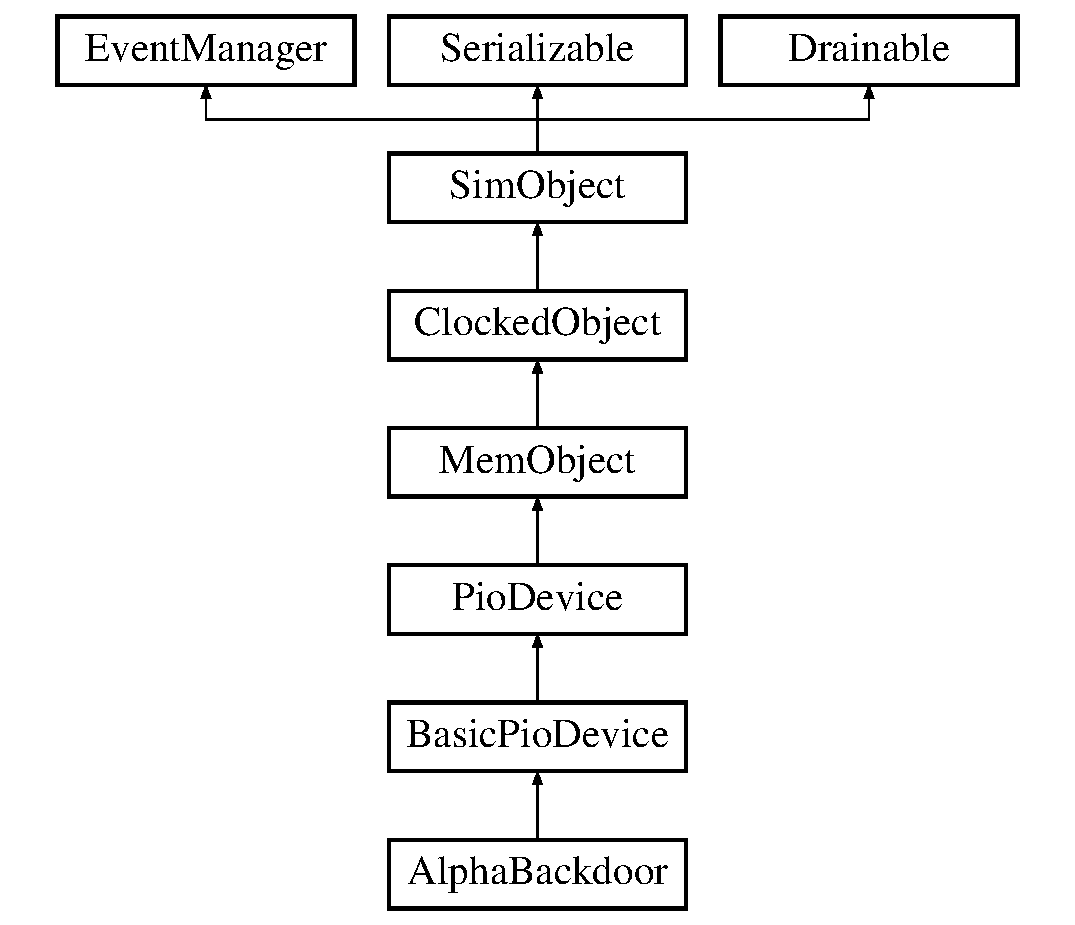
\includegraphics[height=7cm]{classAlphaBackdoor}
\end{center}
\end{figure}
\subsection*{構成}
\begin{DoxyCompactItemize}
\item 
struct \hyperlink{structAlphaBackdoor_1_1Access}{Access}
\end{DoxyCompactItemize}
\subsection*{Public 型}
\begin{DoxyCompactItemize}
\item 
typedef AlphaBackdoorParams \hyperlink{classAlphaBackdoor_a3311d1ef17b579d409e4cf342f9c696f}{Params}
\end{DoxyCompactItemize}
\subsection*{Public メソッド}
\begin{DoxyCompactItemize}
\item 
\hyperlink{classAlphaBackdoor_aa3df553820be57af9fef79cf8c933afa}{AlphaBackdoor} (const \hyperlink{classAlphaBackdoor_a3311d1ef17b579d409e4cf342f9c696f}{Params} $\ast$p)
\item 
const \hyperlink{classAlphaBackdoor_a3311d1ef17b579d409e4cf342f9c696f}{Params} $\ast$ \hyperlink{classAlphaBackdoor_acd3c3feb78ae7a8f88fe0f110a718dff}{params} () const 
\item 
virtual void \hyperlink{classAlphaBackdoor_aecc7d8debf54990ffeaaed5bac7d7d81}{startup} ()
\item 
virtual \hyperlink{classm5_1_1params_1_1Tick}{Tick} \hyperlink{classAlphaBackdoor_a613ec7d5e1ec64f8d21fec78ae8e568e}{read} (\hyperlink{classPacket}{PacketPtr} pkt)
\item 
virtual \hyperlink{classm5_1_1params_1_1Tick}{Tick} \hyperlink{classAlphaBackdoor_a4cefab464e72b5dd42c003a0a4341802}{write} (\hyperlink{classPacket}{PacketPtr} pkt)
\item 
virtual void \hyperlink{classAlphaBackdoor_ad6272f80ae37e8331e3969b3f072a801}{serialize} (std::ostream \&os)
\item 
virtual void \hyperlink{classAlphaBackdoor_af22e5d6d660b97db37003ac61ac4ee49}{unserialize} (\hyperlink{classCheckpoint}{Checkpoint} $\ast$cp, const std::string \&section)
\end{DoxyCompactItemize}
\subsection*{Protected 変数}
\begin{DoxyCompactItemize}
\item 
\begin{tabbing}
xx\=xx\=xx\=xx\=xx\=xx\=xx\=xx\=xx\=\kill
union \{\\
\>\hyperlink{structAlphaBackdoor_1_1Access}{Access} $\ast$ \hyperlink{classAlphaBackdoor_a1800e69c50cf6e59ebb8fcd881caf482}{alphaAccess}\\
\>uint8\_t $\ast$ \hyperlink{classAlphaBackdoor_ab2f889c072e672bb334695bb8a796d55}{consoleData}\\
\}; \\

\end{tabbing}\item 
\hyperlink{classSimpleDisk}{SimpleDisk} $\ast$ \hyperlink{classAlphaBackdoor_a7a34a11311e1d03257d51166e64c9a9f}{disk}
\item 
\hyperlink{classTerminal}{Terminal} $\ast$ \hyperlink{classAlphaBackdoor_ad511a78bad32e194354d8323bc23a4e3}{terminal}
\item 
\hyperlink{classAlphaSystem}{AlphaSystem} $\ast$ \hyperlink{classAlphaBackdoor_a33258b14e97cdadc0a00878bba22adda}{system}
\item 
\hyperlink{classBaseCPU}{BaseCPU} $\ast$ \hyperlink{classAlphaBackdoor_a7a31ca9fefb2fe821f29a270678912db}{cpu}
\end{DoxyCompactItemize}


\subsection{説明}
Memory mapped interface to the system console. This device represents a shared data region between the OS \hyperlink{namespaceKernel}{Kernel} and the \hyperlink{classSystem}{System} Console Backdoor.

The system console is a small standalone program that is initially run when the system boots. It contains the necessary code to access the boot disk, to read/write from the console, and to pass boot parameters to the kernel.

This version of the system console is very different from the one that would be found in a real system. Many of the functions use some sort of backdoor to get their job done. For example, reading from the boot device on a real system would require a minimal device driver to access the disk controller, but since we have a simulator here, we are able to bypass the disk controller and access the disk image directly. There are also some things like reading the kernel off the disk image into memory that are normally taken care of by the console that are now taken care of by the simulator.

These shortcuts are acceptable since the system console is primarily used doing boot before the kernel has loaded its device drivers. 

\subsection{型定義}
\hypertarget{classAlphaBackdoor_a3311d1ef17b579d409e4cf342f9c696f}{
\index{AlphaBackdoor@{AlphaBackdoor}!Params@{Params}}
\index{Params@{Params}!AlphaBackdoor@{AlphaBackdoor}}
\subsubsection[{Params}]{\setlength{\rightskip}{0pt plus 5cm}typedef AlphaBackdoorParams {\bf Params}}}
\label{classAlphaBackdoor_a3311d1ef17b579d409e4cf342f9c696f}


\hyperlink{classBasicPioDevice_a2845515ac6467f10540747053c8a0449}{BasicPioDevice}を再定義しています。

\subsection{コンストラクタとデストラクタ}
\hypertarget{classAlphaBackdoor_aa3df553820be57af9fef79cf8c933afa}{
\index{AlphaBackdoor@{AlphaBackdoor}!AlphaBackdoor@{AlphaBackdoor}}
\index{AlphaBackdoor@{AlphaBackdoor}!AlphaBackdoor@{AlphaBackdoor}}
\subsubsection[{AlphaBackdoor}]{\setlength{\rightskip}{0pt plus 5cm}{\bf AlphaBackdoor} (const {\bf Params} $\ast$ {\em p})}}
\label{classAlphaBackdoor_aa3df553820be57af9fef79cf8c933afa}



\begin{DoxyCode}
65     : BasicPioDevice(p, sizeof(struct AlphaAccess)),
66       disk(p->disk), terminal(p->terminal),
67       system(p->system), cpu(p->cpu)
68 {
69     alphaAccess = new Access();
70     alphaAccess->last_offset = pioSize - 1;
71 
72     alphaAccess->version = ALPHA_ACCESS_VERSION;
73     alphaAccess->diskUnit = 1;
74 
75     alphaAccess->diskCount = 0;
76     alphaAccess->diskPAddr = 0;
77     alphaAccess->diskBlock = 0;
78     alphaAccess->diskOperation = 0;
79     alphaAccess->outputChar = 0;
80     alphaAccess->inputChar = 0;
81     std::memset(alphaAccess->cpuStack, 0, sizeof(alphaAccess->cpuStack));
82 
83 }
\end{DoxyCode}


\subsection{関数}
\hypertarget{classAlphaBackdoor_acd3c3feb78ae7a8f88fe0f110a718dff}{
\index{AlphaBackdoor@{AlphaBackdoor}!params@{params}}
\index{params@{params}!AlphaBackdoor@{AlphaBackdoor}}
\subsubsection[{params}]{\setlength{\rightskip}{0pt plus 5cm}const {\bf Params}$\ast$ params () const\hspace{0.3cm}{\ttfamily  \mbox{[}inline\mbox{]}}}}
\label{classAlphaBackdoor_acd3c3feb78ae7a8f88fe0f110a718dff}


\hyperlink{classBasicPioDevice_acd3c3feb78ae7a8f88fe0f110a718dff}{BasicPioDevice}を再定義しています。


\begin{DoxyCode}
106     {
107         return dynamic_cast<const Params *>(_params);
108     }
\end{DoxyCode}
\hypertarget{classAlphaBackdoor_a613ec7d5e1ec64f8d21fec78ae8e568e}{
\index{AlphaBackdoor@{AlphaBackdoor}!read@{read}}
\index{read@{read}!AlphaBackdoor@{AlphaBackdoor}}
\subsubsection[{read}]{\setlength{\rightskip}{0pt plus 5cm}{\bf Tick} read ({\bf PacketPtr} {\em pkt})\hspace{0.3cm}{\ttfamily  \mbox{[}virtual\mbox{]}}}}
\label{classAlphaBackdoor_a613ec7d5e1ec64f8d21fec78ae8e568e}
memory mapped reads and writes 

XXX Do we want to push the addr munging to a bus brige or something? So the device has it's physical address and then the bridge adds on whatever machine dependent address swizzle is required?

\hyperlink{classPioDevice_a842312590432036092c422c87a442358}{PioDevice}を実装しています。


\begin{DoxyCode}
103 {
104 
110     assert(pkt->getAddr() >= pioAddr && pkt->getAddr() < pioAddr + pioSize);
111 
112     Addr daddr = pkt->getAddr() - pioAddr;
113 
114     pkt->allocate();
115     pkt->makeAtomicResponse();
116 
117     switch (pkt->getSize())
118     {
119         case sizeof(uint32_t):
120             switch (daddr)
121             {
122                 case offsetof(AlphaAccess, last_offset):
123                     pkt->set(alphaAccess->last_offset);
124                     break;
125                 case offsetof(AlphaAccess, version):
126                     pkt->set(alphaAccess->version);
127                     break;
128                 case offsetof(AlphaAccess, numCPUs):
129                     pkt->set(alphaAccess->numCPUs);
130                     break;
131                 case offsetof(AlphaAccess, intrClockFrequency):
132                     pkt->set(alphaAccess->intrClockFrequency);
133                     break;
134                 default:
135                     /* Old console code read in everyting as a 32bit int
136                      * we now break that for better error checking.
137                      */
138                   pkt->setBadAddress();
139             }
140             DPRINTF(AlphaBackdoor, "read: offset=%#x val=%#x\n", daddr,
141                     pkt->get<uint32_t>());
142             break;
143         case sizeof(uint64_t):
144             switch (daddr)
145             {
146                 case offsetof(AlphaAccess, inputChar):
147                     pkt->set(terminal->console_in());
148                     break;
149                 case offsetof(AlphaAccess, cpuClock):
150                     pkt->set(alphaAccess->cpuClock);
151                     break;
152                 case offsetof(AlphaAccess, mem_size):
153                     pkt->set(alphaAccess->mem_size);
154                     break;
155                 case offsetof(AlphaAccess, kernStart):
156                     pkt->set(alphaAccess->kernStart);
157                     break;
158                 case offsetof(AlphaAccess, kernEnd):
159                     pkt->set(alphaAccess->kernEnd);
160                     break;
161                 case offsetof(AlphaAccess, entryPoint):
162                     pkt->set(alphaAccess->entryPoint);
163                     break;
164                 case offsetof(AlphaAccess, diskUnit):
165                     pkt->set(alphaAccess->diskUnit);
166                     break;
167                 case offsetof(AlphaAccess, diskCount):
168                     pkt->set(alphaAccess->diskCount);
169                     break;
170                 case offsetof(AlphaAccess, diskPAddr):
171                     pkt->set(alphaAccess->diskPAddr);
172                     break;
173                 case offsetof(AlphaAccess, diskBlock):
174                     pkt->set(alphaAccess->diskBlock);
175                     break;
176                 case offsetof(AlphaAccess, diskOperation):
177                     pkt->set(alphaAccess->diskOperation);
178                     break;
179                 case offsetof(AlphaAccess, outputChar):
180                     pkt->set(alphaAccess->outputChar);
181                     break;
182                 default:
183                     int cpunum = (daddr - offsetof(AlphaAccess, cpuStack)) /
184                                  sizeof(alphaAccess->cpuStack[0]);
185 
186                     if (cpunum >= 0 && cpunum < 64)
187                         pkt->set(alphaAccess->cpuStack[cpunum]);
188                     else
189                         panic("Unknown 64bit access, %#x\n", daddr);
190             }
191             DPRINTF(AlphaBackdoor, "read: offset=%#x val=%#x\n", daddr,
192                     pkt->get<uint64_t>());
193             break;
194         default:
195           pkt->setBadAddress();
196     }
197     return pioDelay;
198 }
\end{DoxyCode}
\hypertarget{classAlphaBackdoor_ad6272f80ae37e8331e3969b3f072a801}{
\index{AlphaBackdoor@{AlphaBackdoor}!serialize@{serialize}}
\index{serialize@{serialize}!AlphaBackdoor@{AlphaBackdoor}}
\subsubsection[{serialize}]{\setlength{\rightskip}{0pt plus 5cm}virtual void serialize (std::ostream \& {\em os})\hspace{0.3cm}{\ttfamily  \mbox{[}virtual\mbox{]}}}}
\label{classAlphaBackdoor_ad6272f80ae37e8331e3969b3f072a801}
standard serialization routines for checkpointing 

\hyperlink{classSerializable_ad6272f80ae37e8331e3969b3f072a801}{Serializable}を再定義しています。\hypertarget{classAlphaBackdoor_aecc7d8debf54990ffeaaed5bac7d7d81}{
\index{AlphaBackdoor@{AlphaBackdoor}!startup@{startup}}
\index{startup@{startup}!AlphaBackdoor@{AlphaBackdoor}}
\subsubsection[{startup}]{\setlength{\rightskip}{0pt plus 5cm}void startup ()\hspace{0.3cm}{\ttfamily  \mbox{[}virtual\mbox{]}}}}
\label{classAlphaBackdoor_aecc7d8debf54990ffeaaed5bac7d7d81}
\hyperlink{classAlphaBackdoor_aecc7d8debf54990ffeaaed5bac7d7d81}{startup()} is the final initialization call before simulation. All state is initialized (including unserialized state, if any, such as the \hyperlink{statistics_8hh_a7acdccbf0d35ce0c159c0cdd36371b22}{curTick()} value), so this is the appropriate place to schedule initial event(s) for objects that need them. 

\hyperlink{classSimObject_aecc7d8debf54990ffeaaed5bac7d7d81}{SimObject}を再定義しています。


\begin{DoxyCode}
87 {
88     system->setAlphaAccess(pioAddr);
89     alphaAccess->numCPUs = system->numContexts();
90     alphaAccess->kernStart = system->getKernelStart();
91     alphaAccess->kernEnd = system->getKernelEnd();
92     alphaAccess->entryPoint = system->getKernelEntry();
93     alphaAccess->mem_size = system->memSize();
94     alphaAccess->cpuClock = cpu->frequency() / 1000000; // In MHz
95     Tsunami *tsunami = dynamic_cast<Tsunami *>(params()->platform);
96     if (!tsunami)
97         fatal("Platform is not Tsunami.\n");
98     alphaAccess->intrClockFrequency = tsunami->io->frequency();
99 }
\end{DoxyCode}
\hypertarget{classAlphaBackdoor_af22e5d6d660b97db37003ac61ac4ee49}{
\index{AlphaBackdoor@{AlphaBackdoor}!unserialize@{unserialize}}
\index{unserialize@{unserialize}!AlphaBackdoor@{AlphaBackdoor}}
\subsubsection[{unserialize}]{\setlength{\rightskip}{0pt plus 5cm}void unserialize ({\bf Checkpoint} $\ast$ {\em cp}, \/  const std::string \& {\em section})\hspace{0.3cm}{\ttfamily  \mbox{[}virtual\mbox{]}}}}
\label{classAlphaBackdoor_af22e5d6d660b97db37003ac61ac4ee49}


\hyperlink{classSerializable_af100c4e9feabf3cd918619c88c718387}{Serializable}を再定義しています。


\begin{DoxyCode}
307 {
308     alphaAccess->unserialize(cp, section);
309 }
\end{DoxyCode}
\hypertarget{classAlphaBackdoor_a4cefab464e72b5dd42c003a0a4341802}{
\index{AlphaBackdoor@{AlphaBackdoor}!write@{write}}
\index{write@{write}!AlphaBackdoor@{AlphaBackdoor}}
\subsubsection[{write}]{\setlength{\rightskip}{0pt plus 5cm}{\bf Tick} write ({\bf PacketPtr} {\em pkt})\hspace{0.3cm}{\ttfamily  \mbox{[}virtual\mbox{]}}}}
\label{classAlphaBackdoor_a4cefab464e72b5dd42c003a0a4341802}
Pure virtual function that the device must implement. Called when a write command is recieved by the port. 
\begin{DoxyParams}{引数}
\item[{\em pkt}]\hyperlink{classPacket}{Packet} describing this request \end{DoxyParams}
\begin{DoxyReturn}{戻り値}
number of ticks it took to complete 
\end{DoxyReturn}


\hyperlink{classPioDevice_afe8371668d023bb2516b286e5e399b6f}{PioDevice}を実装しています。


\begin{DoxyCode}
202 {
203     assert(pkt->getAddr() >= pioAddr && pkt->getAddr() < pioAddr + pioSize);
204     Addr daddr = pkt->getAddr() - pioAddr;
205 
206     uint64_t val = pkt->get<uint64_t>();
207     assert(pkt->getSize() == sizeof(uint64_t));
208 
209     switch (daddr) {
210       case offsetof(AlphaAccess, diskUnit):
211         alphaAccess->diskUnit = val;
212         break;
213 
214       case offsetof(AlphaAccess, diskCount):
215         alphaAccess->diskCount = val;
216         break;
217 
218       case offsetof(AlphaAccess, diskPAddr):
219         alphaAccess->diskPAddr = val;
220         break;
221 
222       case offsetof(AlphaAccess, diskBlock):
223         alphaAccess->diskBlock = val;
224         break;
225 
226       case offsetof(AlphaAccess, diskOperation):
227         if (val == 0x13)
228             disk->read(alphaAccess->diskPAddr, alphaAccess->diskBlock,
229                        alphaAccess->diskCount);
230         else
231             panic("Invalid disk operation!");
232 
233         break;
234 
235       case offsetof(AlphaAccess, outputChar):
236         terminal->out((char)(val & 0xff));
237         break;
238 
239       default:
240         int cpunum = (daddr - offsetof(AlphaAccess, cpuStack)) /
241                      sizeof(alphaAccess->cpuStack[0]);
242         inform("Launching CPU %d @ %d", cpunum, curTick());
243         assert(val > 0 && "Must not access primary cpu");
244         if (cpunum >= 0 && cpunum < 64)
245             alphaAccess->cpuStack[cpunum] = val;
246         else
247             panic("Unknown 64bit access, %#x\n", daddr);
248     }
249 
250     pkt->makeAtomicResponse();
251 
252     return pioDelay;
253 }
\end{DoxyCode}


\subsection{変数}
\hypertarget{classAlphaBackdoor_a41932bd9bc77001bc6e7dc163b180f9e}{
\subsubsection[{"@41}]{\setlength{\rightskip}{0pt plus 5cm}union \{ ... \} \hspace{0.3cm}{\ttfamily  \mbox{[}protected\mbox{]}}}}
\label{classAlphaBackdoor_a41932bd9bc77001bc6e7dc163b180f9e}
\hypertarget{classAlphaBackdoor_a1800e69c50cf6e59ebb8fcd881caf482}{
\index{AlphaBackdoor@{AlphaBackdoor}!alphaAccess@{alphaAccess}}
\index{alphaAccess@{alphaAccess}!AlphaBackdoor@{AlphaBackdoor}}
\subsubsection[{alphaAccess}]{\setlength{\rightskip}{0pt plus 5cm}{\bf Access}$\ast$ {\bf alphaAccess}}}
\label{classAlphaBackdoor_a1800e69c50cf6e59ebb8fcd881caf482}
\hypertarget{classAlphaBackdoor_ab2f889c072e672bb334695bb8a796d55}{
\index{AlphaBackdoor@{AlphaBackdoor}!consoleData@{consoleData}}
\index{consoleData@{consoleData}!AlphaBackdoor@{AlphaBackdoor}}
\subsubsection[{consoleData}]{\setlength{\rightskip}{0pt plus 5cm}uint8\_\-t$\ast$ {\bf consoleData}}}
\label{classAlphaBackdoor_ab2f889c072e672bb334695bb8a796d55}
\hypertarget{classAlphaBackdoor_a7a31ca9fefb2fe821f29a270678912db}{
\index{AlphaBackdoor@{AlphaBackdoor}!cpu@{cpu}}
\index{cpu@{cpu}!AlphaBackdoor@{AlphaBackdoor}}
\subsubsection[{cpu}]{\setlength{\rightskip}{0pt plus 5cm}{\bf BaseCPU}$\ast$ {\bf cpu}\hspace{0.3cm}{\ttfamily  \mbox{[}protected\mbox{]}}}}
\label{classAlphaBackdoor_a7a31ca9fefb2fe821f29a270678912db}
a pointer to the CPU boot cpu \hypertarget{classAlphaBackdoor_a7a34a11311e1d03257d51166e64c9a9f}{
\index{AlphaBackdoor@{AlphaBackdoor}!disk@{disk}}
\index{disk@{disk}!AlphaBackdoor@{AlphaBackdoor}}
\subsubsection[{disk}]{\setlength{\rightskip}{0pt plus 5cm}{\bf SimpleDisk}$\ast$ {\bf disk}\hspace{0.3cm}{\ttfamily  \mbox{[}protected\mbox{]}}}}
\label{classAlphaBackdoor_a7a34a11311e1d03257d51166e64c9a9f}
the disk must be accessed from the console \hypertarget{classAlphaBackdoor_a33258b14e97cdadc0a00878bba22adda}{
\index{AlphaBackdoor@{AlphaBackdoor}!system@{system}}
\index{system@{system}!AlphaBackdoor@{AlphaBackdoor}}
\subsubsection[{system}]{\setlength{\rightskip}{0pt plus 5cm}{\bf AlphaSystem}$\ast$ {\bf system}\hspace{0.3cm}{\ttfamily  \mbox{[}protected\mbox{]}}}}
\label{classAlphaBackdoor_a33258b14e97cdadc0a00878bba22adda}
a pointer to the system we are running in \hypertarget{classAlphaBackdoor_ad511a78bad32e194354d8323bc23a4e3}{
\index{AlphaBackdoor@{AlphaBackdoor}!terminal@{terminal}}
\index{terminal@{terminal}!AlphaBackdoor@{AlphaBackdoor}}
\subsubsection[{terminal}]{\setlength{\rightskip}{0pt plus 5cm}{\bf Terminal}$\ast$ {\bf terminal}\hspace{0.3cm}{\ttfamily  \mbox{[}protected\mbox{]}}}}
\label{classAlphaBackdoor_ad511a78bad32e194354d8323bc23a4e3}
the system console (the terminal) is accessable from the console 

このクラスの説明は次のファイルから生成されました:\begin{DoxyCompactItemize}
\item 
dev/alpha/\hyperlink{backdoor_8hh}{backdoor.hh}\item 
dev/alpha/\hyperlink{backdoor_8cc}{backdoor.cc}\end{DoxyCompactItemize}

\hypertarget{classAlphaTLB_1_1AlphaDTB}{
\section{クラス AlphaDTB}
\label{classAlphaTLB_1_1AlphaDTB}\index{AlphaTLB::AlphaDTB@{AlphaTLB::AlphaDTB}}
}
AlphaDTBに対する継承グラフ:\begin{figure}[H]
\begin{center}
\leavevmode
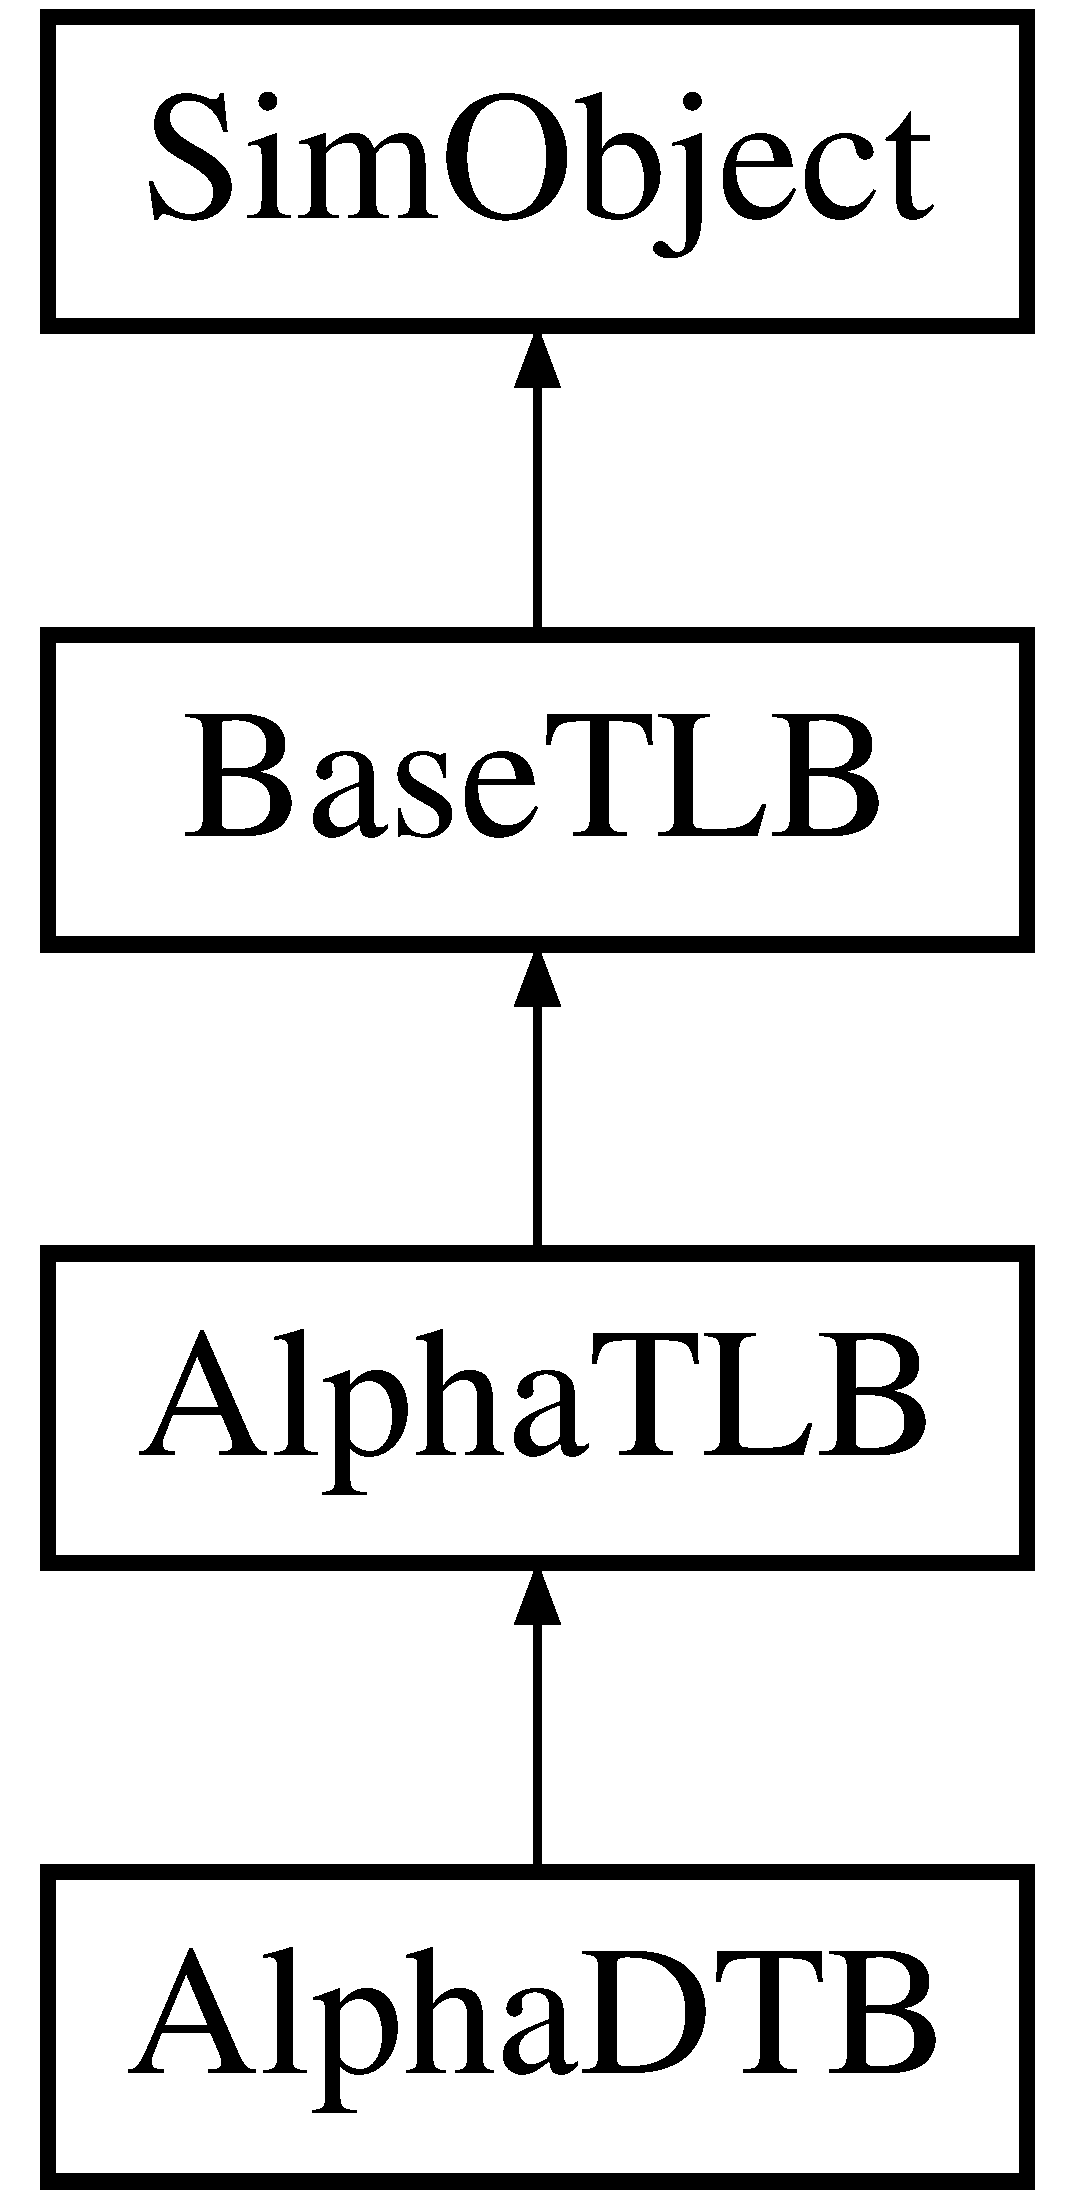
\includegraphics[height=4cm]{classAlphaTLB_1_1AlphaDTB}
\end{center}
\end{figure}
\subsection*{Static Public 変数}
\begin{DoxyCompactItemize}
\item 
int \hyperlink{classAlphaTLB_1_1AlphaDTB_a439227feff9d7f55384e8780cfc2eb82}{size} = 64
\end{DoxyCompactItemize}


\subsection{変数}
\hypertarget{classAlphaTLB_1_1AlphaDTB_a439227feff9d7f55384e8780cfc2eb82}{
\index{AlphaTLB::AlphaDTB@{AlphaTLB::AlphaDTB}!size@{size}}
\index{size@{size}!AlphaTLB::AlphaDTB@{AlphaTLB::AlphaDTB}}
\subsubsection[{size}]{\setlength{\rightskip}{0pt plus 5cm}int {\bf size} = 64\hspace{0.3cm}{\ttfamily  \mbox{[}static\mbox{]}}}}
\label{classAlphaTLB_1_1AlphaDTB_a439227feff9d7f55384e8780cfc2eb82}


\hyperlink{classAlphaTLB_1_1AlphaTLB_a377e5da8df1f89c5468c8b8cd07eac89}{AlphaTLB}を再定義しています。

このクラスの説明は次のファイルから生成されました:\begin{DoxyCompactItemize}
\item 
arch/alpha/\hyperlink{AlphaTLB_8py}{AlphaTLB.py}\end{DoxyCompactItemize}

\hypertarget{classAlphaISA_1_1AlphaFault}{
\section{クラス AlphaFault}
\label{classAlphaISA_1_1AlphaFault}\index{AlphaISA::AlphaFault@{AlphaISA::AlphaFault}}
}


{\ttfamily \#include $<$faults.hh$>$}AlphaFaultに対する継承グラフ:\begin{figure}[H]
\begin{center}
\leavevmode
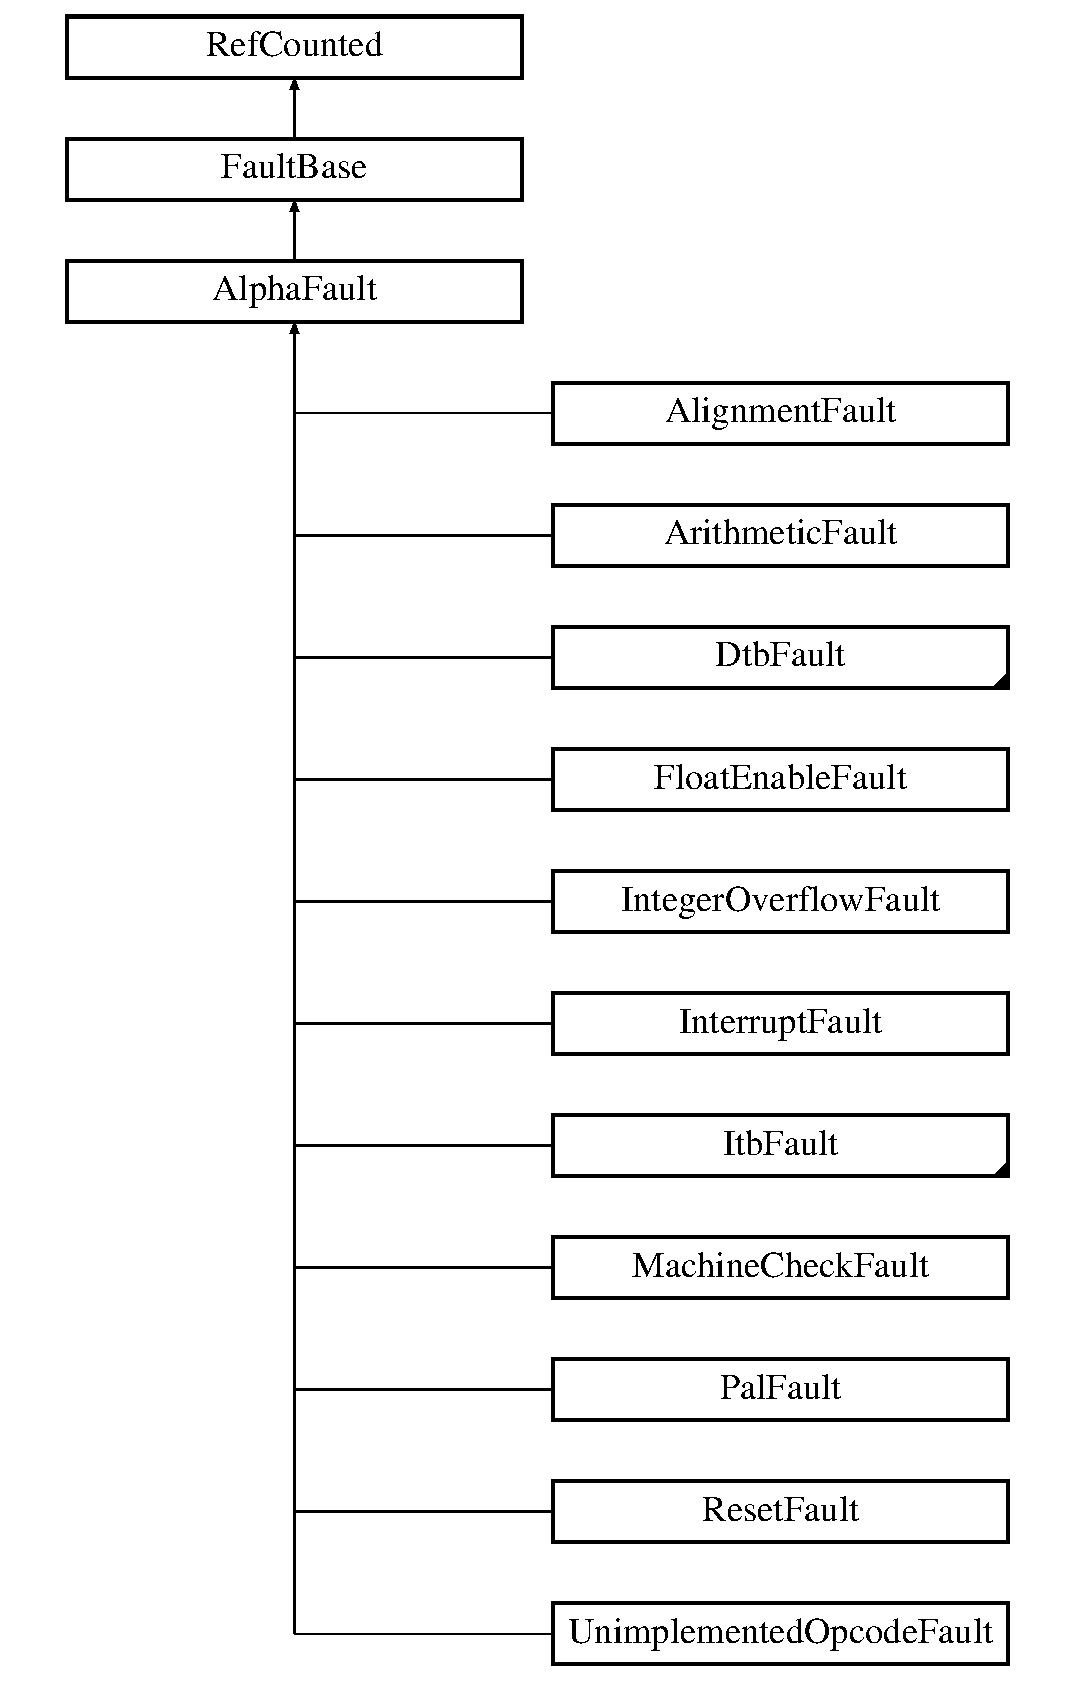
\includegraphics[height=12cm]{classAlphaISA_1_1AlphaFault}
\end{center}
\end{figure}
\subsection*{Public メソッド}
\begin{DoxyCompactItemize}
\item 
void \hyperlink{classAlphaISA_1_1AlphaFault_a2bd783b42262278d41157d428e1f8d6f}{invoke} (\hyperlink{classThreadContext}{ThreadContext} $\ast$tc, \hyperlink{classRefCountingPtr}{StaticInstPtr} inst=\hyperlink{classStaticInst_aa793d9793af735f09096369fb17567b6}{StaticInst::nullStaticInstPtr})
\item 
virtual \hyperlink{classm5_1_1params_1_1Addr}{FaultVect} \hyperlink{classAlphaISA_1_1AlphaFault_ac141ef2ab527bd4d5c079ddff2e8b4aa}{vect} ()=0
\item 
virtual \hyperlink{classStats_1_1Scalar}{FaultStat} \& \hyperlink{classAlphaISA_1_1AlphaFault_a5d92ccd11b5cd6b04f02bd0a088b776c}{countStat} ()=0
\end{DoxyCompactItemize}
\subsection*{Protected メソッド}
\begin{DoxyCompactItemize}
\item 
virtual bool \hyperlink{classAlphaISA_1_1AlphaFault_a5d44c6b9ce6041b3e9235e8d978156cb}{skipFaultingInstruction} ()
\item 
virtual bool \hyperlink{classAlphaISA_1_1AlphaFault_a5187b0d322a9546c3eb0ce51f3268f4e}{setRestartAddress} ()
\end{DoxyCompactItemize}


\subsection{関数}
\hypertarget{classAlphaISA_1_1AlphaFault_a5d92ccd11b5cd6b04f02bd0a088b776c}{
\index{AlphaISA::AlphaFault@{AlphaISA::AlphaFault}!countStat@{countStat}}
\index{countStat@{countStat}!AlphaISA::AlphaFault@{AlphaISA::AlphaFault}}
\subsubsection[{countStat}]{\setlength{\rightskip}{0pt plus 5cm}virtual {\bf FaultStat}\& countStat ()\hspace{0.3cm}{\ttfamily  \mbox{[}pure virtual\mbox{]}}}}
\label{classAlphaISA_1_1AlphaFault_a5d92ccd11b5cd6b04f02bd0a088b776c}


\hyperlink{classAlphaISA_1_1MachineCheckFault_a6c79663c761ff57265459f7e3aefaf4c}{MachineCheckFault}, \hyperlink{classAlphaISA_1_1AlignmentFault_a6c79663c761ff57265459f7e3aefaf4c}{AlignmentFault}, \hyperlink{classAlphaISA_1_1ResetFault_a6c79663c761ff57265459f7e3aefaf4c}{ResetFault}, \hyperlink{classAlphaISA_1_1ArithmeticFault_a6c79663c761ff57265459f7e3aefaf4c}{ArithmeticFault}, \hyperlink{classAlphaISA_1_1InterruptFault_a6c79663c761ff57265459f7e3aefaf4c}{InterruptFault}, \hyperlink{classAlphaISA_1_1DtbFault_a4b643982263b390349238a6711216763}{DtbFault}, \hyperlink{classAlphaISA_1_1NDtbMissFault_a6c79663c761ff57265459f7e3aefaf4c}{NDtbMissFault}, \hyperlink{classAlphaISA_1_1PDtbMissFault_a6c79663c761ff57265459f7e3aefaf4c}{PDtbMissFault}, \hyperlink{classAlphaISA_1_1DtbPageFault_a6c79663c761ff57265459f7e3aefaf4c}{DtbPageFault}, \hyperlink{classAlphaISA_1_1DtbAcvFault_a6c79663c761ff57265459f7e3aefaf4c}{DtbAcvFault}, \hyperlink{classAlphaISA_1_1DtbAlignmentFault_a6c79663c761ff57265459f7e3aefaf4c}{DtbAlignmentFault}, \hyperlink{classAlphaISA_1_1ItbFault_a4b643982263b390349238a6711216763}{ItbFault}, \hyperlink{classAlphaISA_1_1ItbPageFault_a6c79663c761ff57265459f7e3aefaf4c}{ItbPageFault}, \hyperlink{classAlphaISA_1_1ItbAcvFault_a6c79663c761ff57265459f7e3aefaf4c}{ItbAcvFault}, \hyperlink{classAlphaISA_1_1UnimplementedOpcodeFault_a6c79663c761ff57265459f7e3aefaf4c}{UnimplementedOpcodeFault}, \hyperlink{classAlphaISA_1_1FloatEnableFault_a6c79663c761ff57265459f7e3aefaf4c}{FloatEnableFault}, \hyperlink{classAlphaISA_1_1PalFault_a6c79663c761ff57265459f7e3aefaf4c}{PalFault}, と \hyperlink{classAlphaISA_1_1IntegerOverflowFault_a6c79663c761ff57265459f7e3aefaf4c}{IntegerOverflowFault}で実装されています。\hypertarget{classAlphaISA_1_1AlphaFault_a2bd783b42262278d41157d428e1f8d6f}{
\index{AlphaISA::AlphaFault@{AlphaISA::AlphaFault}!invoke@{invoke}}
\index{invoke@{invoke}!AlphaISA::AlphaFault@{AlphaISA::AlphaFault}}
\subsubsection[{invoke}]{\setlength{\rightskip}{0pt plus 5cm}void invoke ({\bf ThreadContext} $\ast$ {\em tc}, \/  {\bf StaticInstPtr} {\em inst} = {\ttfamily {\bf StaticInst::nullStaticInstPtr}})\hspace{0.3cm}{\ttfamily  \mbox{[}virtual\mbox{]}}}}
\label{classAlphaISA_1_1AlphaFault_a2bd783b42262278d41157d428e1f8d6f}


\hyperlink{classFaultBase_a2bd783b42262278d41157d428e1f8d6f}{FaultBase}を再定義しています。

\hyperlink{classAlphaISA_1_1ArithmeticFault_a2bd783b42262278d41157d428e1f8d6f}{ArithmeticFault}, \hyperlink{classAlphaISA_1_1DtbFault_a2bd783b42262278d41157d428e1f8d6f}{DtbFault}, \hyperlink{classAlphaISA_1_1NDtbMissFault_a2bd783b42262278d41157d428e1f8d6f}{NDtbMissFault}, \hyperlink{classAlphaISA_1_1ItbFault_a2bd783b42262278d41157d428e1f8d6f}{ItbFault}, と \hyperlink{classAlphaISA_1_1ItbPageFault_a2bd783b42262278d41157d428e1f8d6f}{ItbPageFault}で再定義されています。


\begin{DoxyCode}
110 {
111     FaultBase::invoke(tc);
112     if (!FullSystem)
113         return;
114     countStat()++;
115 
116     PCState pc = tc->pcState();
117 
118     // exception restart address
119     if (setRestartAddress() || !(pc.pc() & 0x3))
120         tc->setMiscRegNoEffect(IPR_EXC_ADDR, pc.pc());
121 
122     if (skipFaultingInstruction()) {
123         // traps...  skip faulting instruction.
124         tc->setMiscRegNoEffect(IPR_EXC_ADDR,
125                    tc->readMiscRegNoEffect(IPR_EXC_ADDR) + 4);
126     }
127 
128     pc.set(tc->readMiscRegNoEffect(IPR_PAL_BASE) + vect());
129     tc->pcState(pc);
130 }
\end{DoxyCode}
\hypertarget{classAlphaISA_1_1AlphaFault_a5187b0d322a9546c3eb0ce51f3268f4e}{
\index{AlphaISA::AlphaFault@{AlphaISA::AlphaFault}!setRestartAddress@{setRestartAddress}}
\index{setRestartAddress@{setRestartAddress}!AlphaISA::AlphaFault@{AlphaISA::AlphaFault}}
\subsubsection[{setRestartAddress}]{\setlength{\rightskip}{0pt plus 5cm}virtual bool setRestartAddress ()\hspace{0.3cm}{\ttfamily  \mbox{[}inline, protected, virtual\mbox{]}}}}
\label{classAlphaISA_1_1AlphaFault_a5187b0d322a9546c3eb0ce51f3268f4e}


\hyperlink{classAlphaISA_1_1InterruptFault_a92cd7f56a5213322fd8b3d1dbe9a7136}{InterruptFault}で再定義されています。


\begin{DoxyCode}
49 {return true;}
\end{DoxyCode}
\hypertarget{classAlphaISA_1_1AlphaFault_a5d44c6b9ce6041b3e9235e8d978156cb}{
\index{AlphaISA::AlphaFault@{AlphaISA::AlphaFault}!skipFaultingInstruction@{skipFaultingInstruction}}
\index{skipFaultingInstruction@{skipFaultingInstruction}!AlphaISA::AlphaFault@{AlphaISA::AlphaFault}}
\subsubsection[{skipFaultingInstruction}]{\setlength{\rightskip}{0pt plus 5cm}virtual bool skipFaultingInstruction ()\hspace{0.3cm}{\ttfamily  \mbox{[}inline, protected, virtual\mbox{]}}}}
\label{classAlphaISA_1_1AlphaFault_a5d44c6b9ce6041b3e9235e8d978156cb}


\hyperlink{classAlphaISA_1_1ArithmeticFault_a4dca22d2e3f19609672fe85bb5e28b56}{ArithmeticFault}, と \hyperlink{classAlphaISA_1_1PalFault_a4dca22d2e3f19609672fe85bb5e28b56}{PalFault}で再定義されています。


\begin{DoxyCode}
48 {return false;}
\end{DoxyCode}
\hypertarget{classAlphaISA_1_1AlphaFault_ac141ef2ab527bd4d5c079ddff2e8b4aa}{
\index{AlphaISA::AlphaFault@{AlphaISA::AlphaFault}!vect@{vect}}
\index{vect@{vect}!AlphaISA::AlphaFault@{AlphaISA::AlphaFault}}
\subsubsection[{vect}]{\setlength{\rightskip}{0pt plus 5cm}virtual {\bf FaultVect} vect ()\hspace{0.3cm}{\ttfamily  \mbox{[}pure virtual\mbox{]}}}}
\label{classAlphaISA_1_1AlphaFault_ac141ef2ab527bd4d5c079ddff2e8b4aa}


\hyperlink{classAlphaISA_1_1MachineCheckFault_ae15c5d7ab0162821b93d668d0b225198}{MachineCheckFault}, \hyperlink{classAlphaISA_1_1AlignmentFault_ae15c5d7ab0162821b93d668d0b225198}{AlignmentFault}, \hyperlink{classAlphaISA_1_1ResetFault_ae15c5d7ab0162821b93d668d0b225198}{ResetFault}, \hyperlink{classAlphaISA_1_1ArithmeticFault_ae15c5d7ab0162821b93d668d0b225198}{ArithmeticFault}, \hyperlink{classAlphaISA_1_1InterruptFault_ae15c5d7ab0162821b93d668d0b225198}{InterruptFault}, \hyperlink{classAlphaISA_1_1DtbFault_ae7a41506fab06a3c1e392f5286f14c66}{DtbFault}, \hyperlink{classAlphaISA_1_1NDtbMissFault_ae15c5d7ab0162821b93d668d0b225198}{NDtbMissFault}, \hyperlink{classAlphaISA_1_1PDtbMissFault_ae15c5d7ab0162821b93d668d0b225198}{PDtbMissFault}, \hyperlink{classAlphaISA_1_1DtbPageFault_ae15c5d7ab0162821b93d668d0b225198}{DtbPageFault}, \hyperlink{classAlphaISA_1_1DtbAcvFault_ae15c5d7ab0162821b93d668d0b225198}{DtbAcvFault}, \hyperlink{classAlphaISA_1_1DtbAlignmentFault_ae15c5d7ab0162821b93d668d0b225198}{DtbAlignmentFault}, \hyperlink{classAlphaISA_1_1ItbFault_ae7a41506fab06a3c1e392f5286f14c66}{ItbFault}, \hyperlink{classAlphaISA_1_1ItbPageFault_ae15c5d7ab0162821b93d668d0b225198}{ItbPageFault}, \hyperlink{classAlphaISA_1_1ItbAcvFault_ae15c5d7ab0162821b93d668d0b225198}{ItbAcvFault}, \hyperlink{classAlphaISA_1_1UnimplementedOpcodeFault_ae15c5d7ab0162821b93d668d0b225198}{UnimplementedOpcodeFault}, \hyperlink{classAlphaISA_1_1FloatEnableFault_ae15c5d7ab0162821b93d668d0b225198}{FloatEnableFault}, \hyperlink{classAlphaISA_1_1PalFault_ae15c5d7ab0162821b93d668d0b225198}{PalFault}, と \hyperlink{classAlphaISA_1_1IntegerOverflowFault_ae15c5d7ab0162821b93d668d0b225198}{IntegerOverflowFault}で実装されています。

このクラスの説明は次のファイルから生成されました:\begin{DoxyCompactItemize}
\item 
arch/alpha/\hyperlink{arch_2alpha_2faults_8hh}{faults.hh}\item 
arch/alpha/\hyperlink{arch_2alpha_2faults_8cc}{faults.cc}\end{DoxyCompactItemize}

\hypertarget{classAlphaInterrupts_1_1AlphaInterrupts}{
\section{クラス AlphaInterrupts}
\label{classAlphaInterrupts_1_1AlphaInterrupts}\index{AlphaInterrupts::AlphaInterrupts@{AlphaInterrupts::AlphaInterrupts}}
}
AlphaInterruptsに対する継承グラフ:\begin{figure}[H]
\begin{center}
\leavevmode
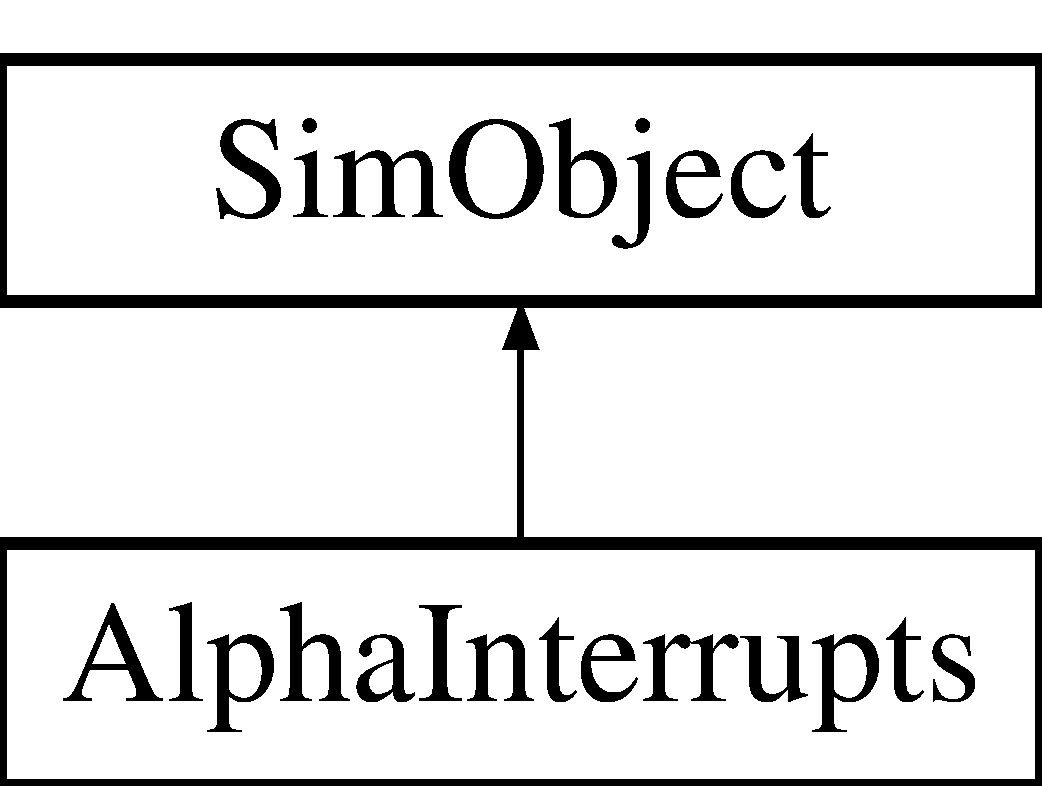
\includegraphics[height=2cm]{classAlphaInterrupts_1_1AlphaInterrupts}
\end{center}
\end{figure}
\subsection*{Static Public 変数}
\begin{DoxyCompactItemize}
\item 
string \hyperlink{classAlphaInterrupts_1_1AlphaInterrupts_acce15679d830831b0bbe8ebc2a60b2ca}{type} = '\hyperlink{classAlphaInterrupts_1_1AlphaInterrupts}{AlphaInterrupts}'
\item 
string \hyperlink{classAlphaInterrupts_1_1AlphaInterrupts_a58cd55cd4023648e138237cfc0822ae3}{cxx\_\-class} = '\hyperlink{classAlphaISA_1_1Interrupts}{AlphaISA::Interrupts}'
\item 
string \hyperlink{classAlphaInterrupts_1_1AlphaInterrupts_a17da7064bc5c518791f0c891eff05fda}{cxx\_\-header} = \char`\"{}arch/alpha/interrupts.hh\char`\"{}
\end{DoxyCompactItemize}


\subsection{変数}
\hypertarget{classAlphaInterrupts_1_1AlphaInterrupts_a58cd55cd4023648e138237cfc0822ae3}{
\index{AlphaInterrupts::AlphaInterrupts@{AlphaInterrupts::AlphaInterrupts}!cxx\_\-class@{cxx\_\-class}}
\index{cxx\_\-class@{cxx\_\-class}!AlphaInterrupts::AlphaInterrupts@{AlphaInterrupts::AlphaInterrupts}}
\subsubsection[{cxx\_\-class}]{\setlength{\rightskip}{0pt plus 5cm}string {\bf cxx\_\-class} = '{\bf AlphaISA::Interrupts}'\hspace{0.3cm}{\ttfamily  \mbox{[}static\mbox{]}}}}
\label{classAlphaInterrupts_1_1AlphaInterrupts_a58cd55cd4023648e138237cfc0822ae3}
\hypertarget{classAlphaInterrupts_1_1AlphaInterrupts_a17da7064bc5c518791f0c891eff05fda}{
\index{AlphaInterrupts::AlphaInterrupts@{AlphaInterrupts::AlphaInterrupts}!cxx\_\-header@{cxx\_\-header}}
\index{cxx\_\-header@{cxx\_\-header}!AlphaInterrupts::AlphaInterrupts@{AlphaInterrupts::AlphaInterrupts}}
\subsubsection[{cxx\_\-header}]{\setlength{\rightskip}{0pt plus 5cm}string {\bf cxx\_\-header} = \char`\"{}arch/alpha/interrupts.hh\char`\"{}\hspace{0.3cm}{\ttfamily  \mbox{[}static\mbox{]}}}}
\label{classAlphaInterrupts_1_1AlphaInterrupts_a17da7064bc5c518791f0c891eff05fda}


\hyperlink{classm5_1_1SimObject_1_1SimObject_a17da7064bc5c518791f0c891eff05fda}{SimObject}を再定義しています。\hypertarget{classAlphaInterrupts_1_1AlphaInterrupts_acce15679d830831b0bbe8ebc2a60b2ca}{
\index{AlphaInterrupts::AlphaInterrupts@{AlphaInterrupts::AlphaInterrupts}!type@{type}}
\index{type@{type}!AlphaInterrupts::AlphaInterrupts@{AlphaInterrupts::AlphaInterrupts}}
\subsubsection[{type}]{\setlength{\rightskip}{0pt plus 5cm}string {\bf type} = '{\bf AlphaInterrupts}'\hspace{0.3cm}{\ttfamily  \mbox{[}static\mbox{]}}}}
\label{classAlphaInterrupts_1_1AlphaInterrupts_acce15679d830831b0bbe8ebc2a60b2ca}


\hyperlink{classm5_1_1SimObject_1_1SimObject_acce15679d830831b0bbe8ebc2a60b2ca}{SimObject}を再定義しています。

このクラスの説明は次のファイルから生成されました:\begin{DoxyCompactItemize}
\item 
arch/alpha/\hyperlink{AlphaInterrupts_8py}{AlphaInterrupts.py}\end{DoxyCompactItemize}

\hypertarget{classAlphaISA_1_1AlphaISA}{
\section{クラス AlphaISA}
\label{classAlphaISA_1_1AlphaISA}\index{AlphaISA::AlphaISA@{AlphaISA::AlphaISA}}
}
AlphaISAに対する継承グラフ:\begin{figure}[H]
\begin{center}
\leavevmode
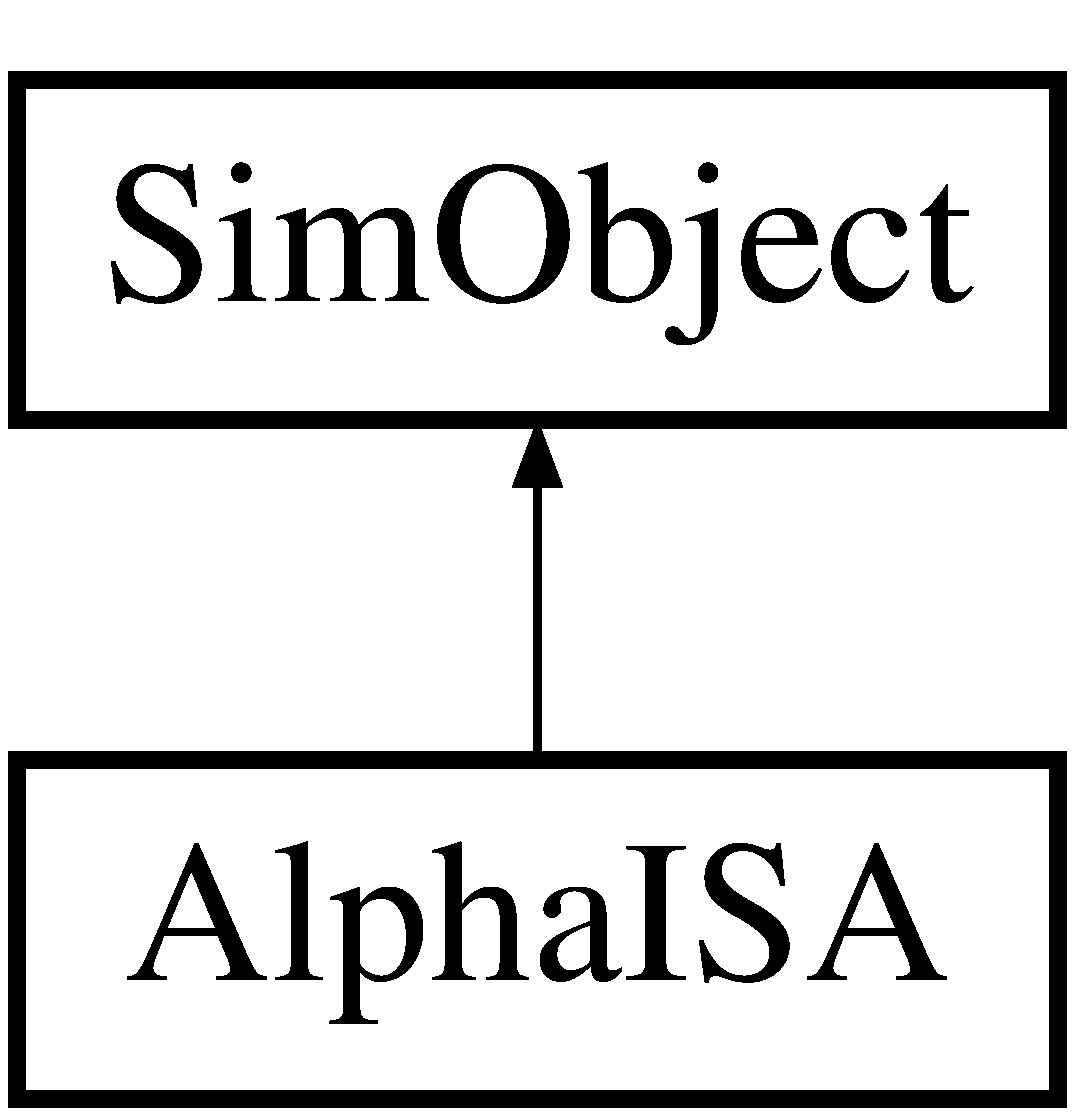
\includegraphics[height=2cm]{classAlphaISA_1_1AlphaISA}
\end{center}
\end{figure}
\subsection*{Static Public 変数}
\begin{DoxyCompactItemize}
\item 
string \hyperlink{classAlphaISA_1_1AlphaISA_acce15679d830831b0bbe8ebc2a60b2ca}{type} = '\hyperlink{classAlphaISA_1_1AlphaISA}{AlphaISA}'
\item 
string \hyperlink{classAlphaISA_1_1AlphaISA_a58cd55cd4023648e138237cfc0822ae3}{cxx\_\-class} = '\hyperlink{classAlphaISA_1_1ISA}{AlphaISA::ISA}'
\item 
string \hyperlink{classAlphaISA_1_1AlphaISA_a17da7064bc5c518791f0c891eff05fda}{cxx\_\-header} = \char`\"{}arch/alpha/isa.hh\char`\"{}
\item 
tuple \hyperlink{classAlphaISA_1_1AlphaISA_ab737471139f5a296e5b26e8a0e1b0744}{system} = Param.System(Parent.any, \char`\"{}System this \hyperlink{classAlphaISA_1_1ISA}{ISA} object belongs to\char`\"{})
\end{DoxyCompactItemize}


\subsection{変数}
\hypertarget{classAlphaISA_1_1AlphaISA_a58cd55cd4023648e138237cfc0822ae3}{
\index{AlphaISA::AlphaISA@{AlphaISA::AlphaISA}!cxx\_\-class@{cxx\_\-class}}
\index{cxx\_\-class@{cxx\_\-class}!AlphaISA::AlphaISA@{AlphaISA::AlphaISA}}
\subsubsection[{cxx\_\-class}]{\setlength{\rightskip}{0pt plus 5cm}string {\bf cxx\_\-class} = '{\bf AlphaISA::ISA}'\hspace{0.3cm}{\ttfamily  \mbox{[}static\mbox{]}}}}
\label{classAlphaISA_1_1AlphaISA_a58cd55cd4023648e138237cfc0822ae3}
\hypertarget{classAlphaISA_1_1AlphaISA_a17da7064bc5c518791f0c891eff05fda}{
\index{AlphaISA::AlphaISA@{AlphaISA::AlphaISA}!cxx\_\-header@{cxx\_\-header}}
\index{cxx\_\-header@{cxx\_\-header}!AlphaISA::AlphaISA@{AlphaISA::AlphaISA}}
\subsubsection[{cxx\_\-header}]{\setlength{\rightskip}{0pt plus 5cm}string {\bf cxx\_\-header} = \char`\"{}arch/alpha/isa.hh\char`\"{}\hspace{0.3cm}{\ttfamily  \mbox{[}static\mbox{]}}}}
\label{classAlphaISA_1_1AlphaISA_a17da7064bc5c518791f0c891eff05fda}


\hyperlink{classm5_1_1SimObject_1_1SimObject_a17da7064bc5c518791f0c891eff05fda}{SimObject}を再定義しています。\hypertarget{classAlphaISA_1_1AlphaISA_ab737471139f5a296e5b26e8a0e1b0744}{
\index{AlphaISA::AlphaISA@{AlphaISA::AlphaISA}!system@{system}}
\index{system@{system}!AlphaISA::AlphaISA@{AlphaISA::AlphaISA}}
\subsubsection[{system}]{\setlength{\rightskip}{0pt plus 5cm}tuple {\bf system} = Param.System(Parent.any, \char`\"{}System this {\bf ISA} object belongs to\char`\"{})\hspace{0.3cm}{\ttfamily  \mbox{[}static\mbox{]}}}}
\label{classAlphaISA_1_1AlphaISA_ab737471139f5a296e5b26e8a0e1b0744}
\hypertarget{classAlphaISA_1_1AlphaISA_acce15679d830831b0bbe8ebc2a60b2ca}{
\index{AlphaISA::AlphaISA@{AlphaISA::AlphaISA}!type@{type}}
\index{type@{type}!AlphaISA::AlphaISA@{AlphaISA::AlphaISA}}
\subsubsection[{type}]{\setlength{\rightskip}{0pt plus 5cm}string {\bf type} = '{\bf AlphaISA}'\hspace{0.3cm}{\ttfamily  \mbox{[}static\mbox{]}}}}
\label{classAlphaISA_1_1AlphaISA_acce15679d830831b0bbe8ebc2a60b2ca}


\hyperlink{classm5_1_1SimObject_1_1SimObject_acce15679d830831b0bbe8ebc2a60b2ca}{SimObject}を再定義しています。

このクラスの説明は次のファイルから生成されました:\begin{DoxyCompactItemize}
\item 
arch/alpha/\hyperlink{AlphaISA_8py}{AlphaISA.py}\end{DoxyCompactItemize}

\hypertarget{classAlphaTLB_1_1AlphaITB}{
\section{クラス AlphaITB}
\label{classAlphaTLB_1_1AlphaITB}\index{AlphaTLB::AlphaITB@{AlphaTLB::AlphaITB}}
}
AlphaITBに対する継承グラフ:\begin{figure}[H]
\begin{center}
\leavevmode
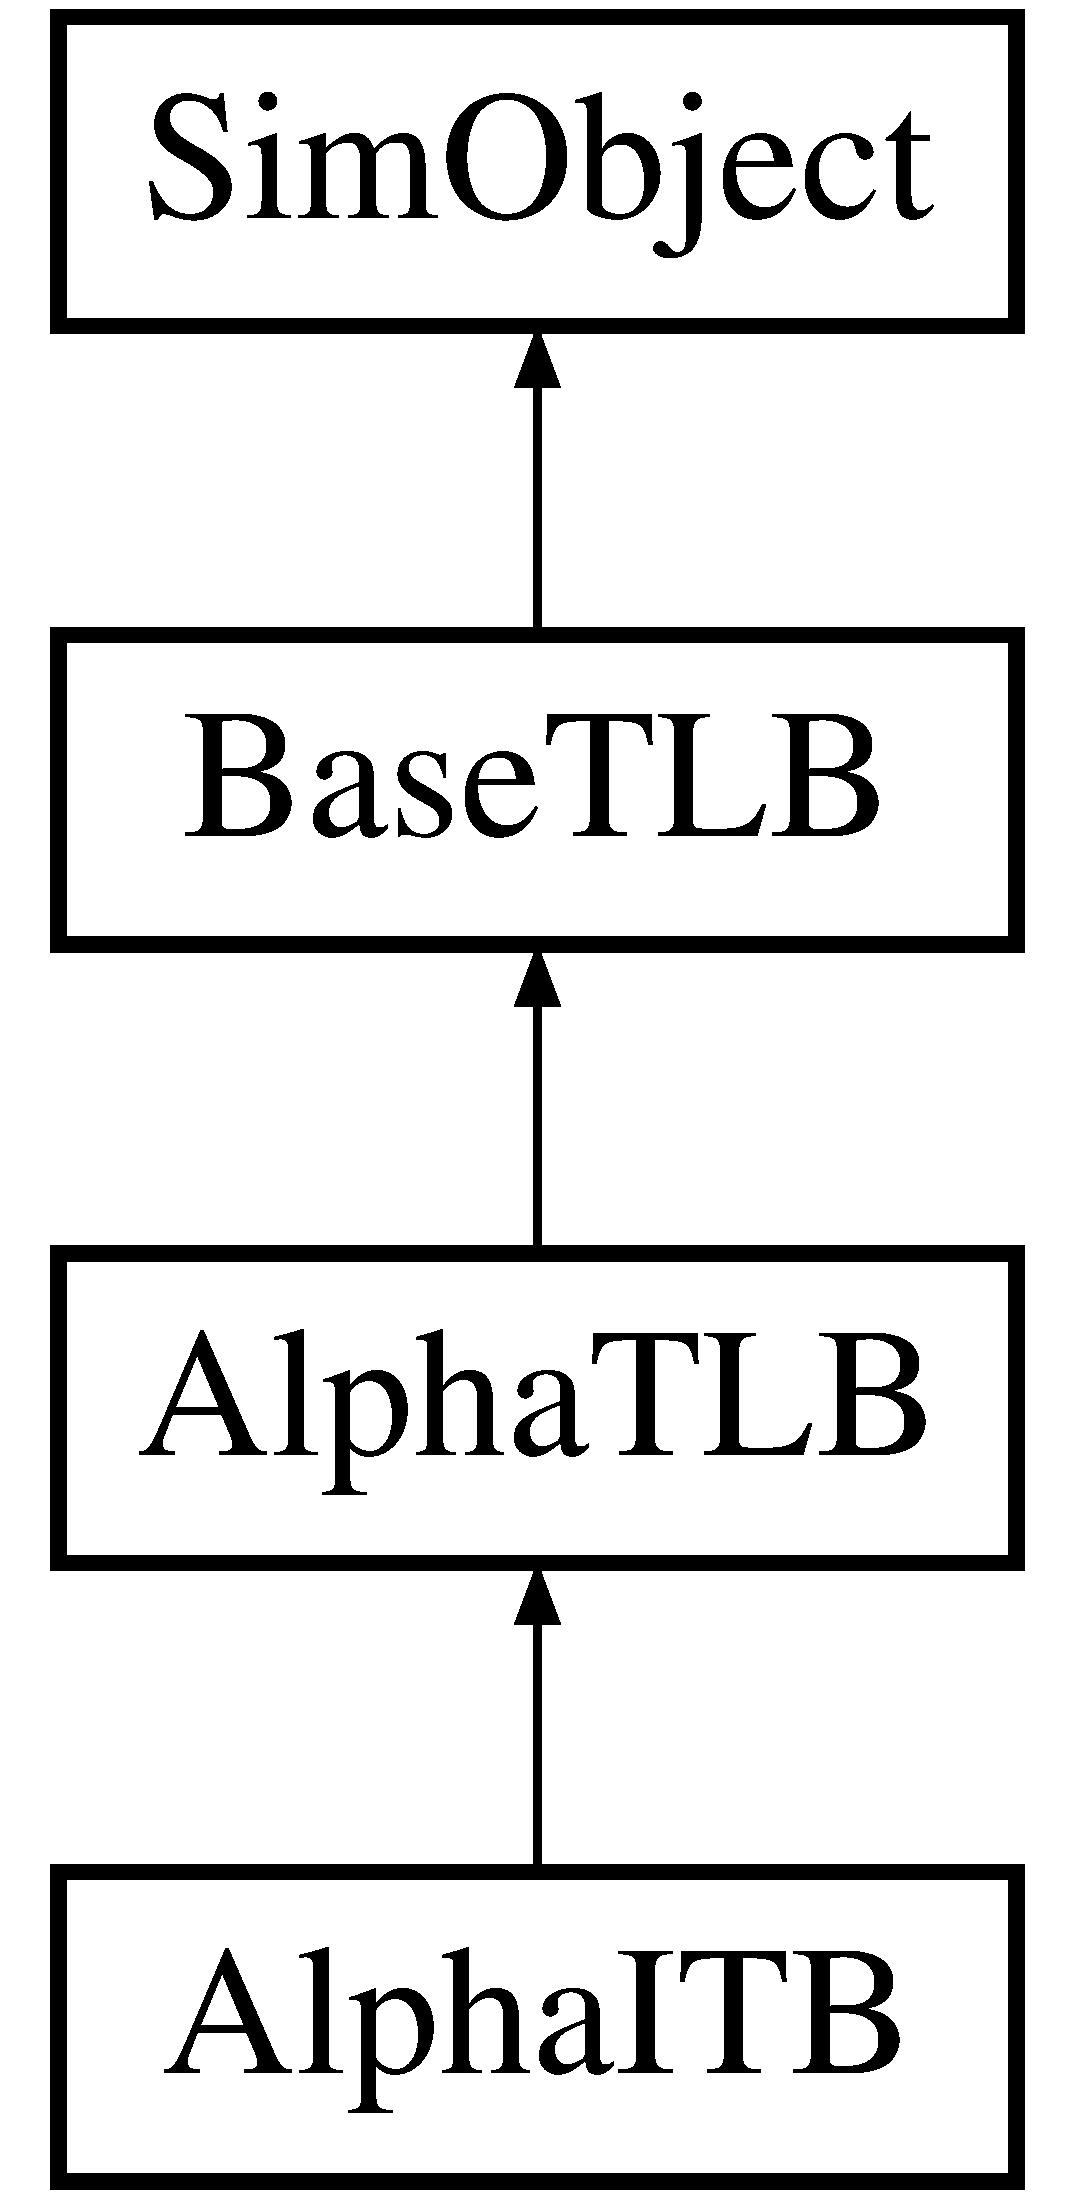
\includegraphics[height=4cm]{classAlphaTLB_1_1AlphaITB}
\end{center}
\end{figure}
\subsection*{Static Public 変数}
\begin{DoxyCompactItemize}
\item 
int \hyperlink{classAlphaTLB_1_1AlphaITB_a439227feff9d7f55384e8780cfc2eb82}{size} = 48
\end{DoxyCompactItemize}


\subsection{変数}
\hypertarget{classAlphaTLB_1_1AlphaITB_a439227feff9d7f55384e8780cfc2eb82}{
\index{AlphaTLB::AlphaITB@{AlphaTLB::AlphaITB}!size@{size}}
\index{size@{size}!AlphaTLB::AlphaITB@{AlphaTLB::AlphaITB}}
\subsubsection[{size}]{\setlength{\rightskip}{0pt plus 5cm}int {\bf size} = 48\hspace{0.3cm}{\ttfamily  \mbox{[}static\mbox{]}}}}
\label{classAlphaTLB_1_1AlphaITB_a439227feff9d7f55384e8780cfc2eb82}


\hyperlink{classAlphaTLB_1_1AlphaTLB_a377e5da8df1f89c5468c8b8cd07eac89}{AlphaTLB}を再定義しています。

このクラスの説明は次のファイルから生成されました:\begin{DoxyCompactItemize}
\item 
arch/alpha/\hyperlink{AlphaTLB_8py}{AlphaTLB.py}\end{DoxyCompactItemize}

\hypertarget{classAlphaLinux}{
\section{クラス AlphaLinux}
\label{classAlphaLinux}\index{AlphaLinux@{AlphaLinux}}
}


{\ttfamily \#include $<$linux.hh$>$}AlphaLinuxに対する継承グラフ:\begin{figure}[H]
\begin{center}
\leavevmode
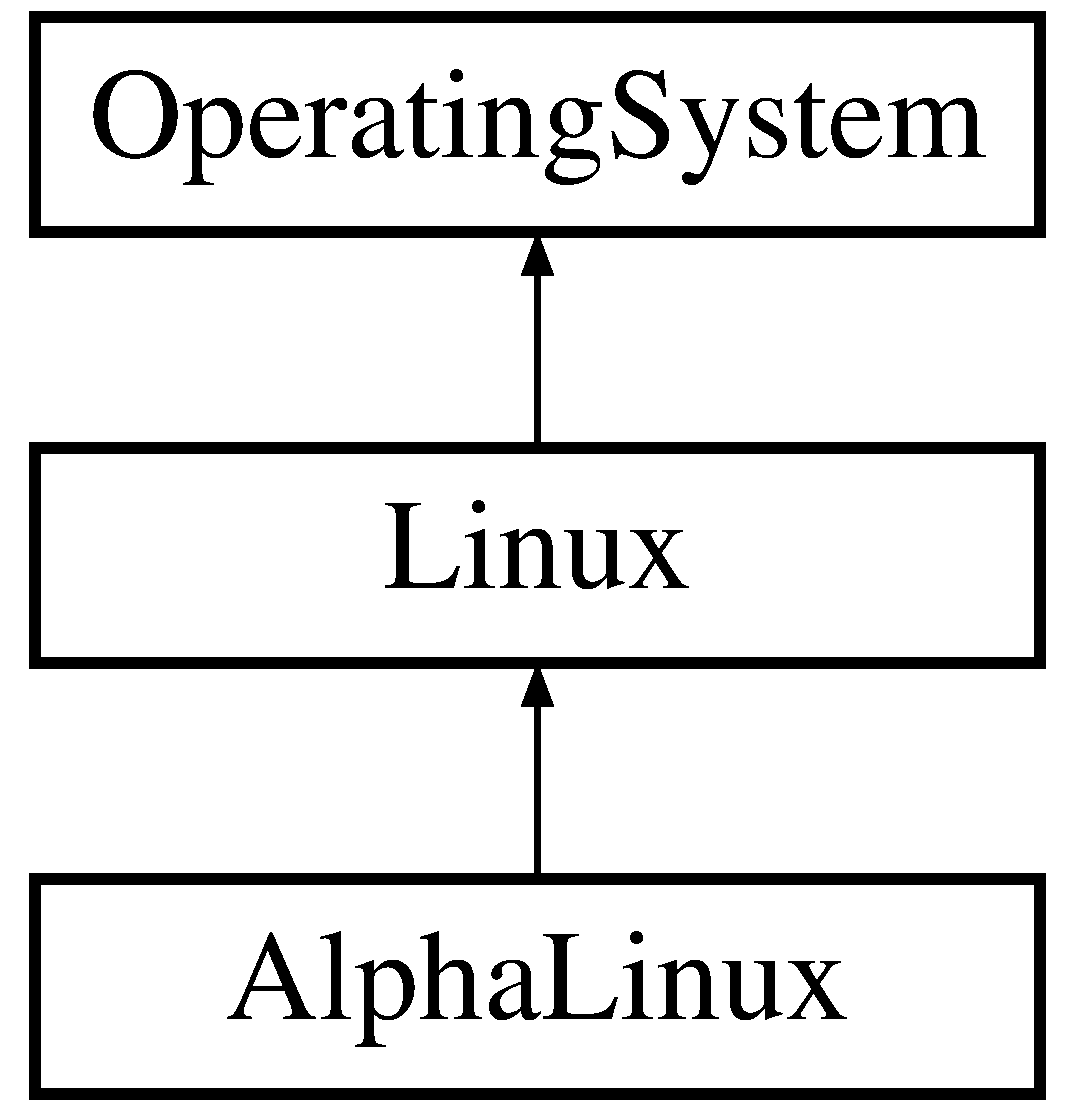
\includegraphics[height=3cm]{classAlphaLinux}
\end{center}
\end{figure}
\subsection*{構成}
\begin{DoxyCompactItemize}
\item 
struct \hyperlink{structAlphaLinux_1_1tgt__sysinfo}{tgt\_\-sysinfo}
\end{DoxyCompactItemize}
\subsection*{Static Public メソッド}
\begin{DoxyCompactItemize}
\item 
static bool \hyperlink{classAlphaLinux_ab20bdd4422ecf6e1736a5587be296b3f}{isTtyReq} (unsigned req)
\end{DoxyCompactItemize}
\subsection*{Static Public 変数}
\begin{DoxyCompactItemize}
\item 
static \hyperlink{structOpenFlagTransTable}{OpenFlagTransTable} \hyperlink{classAlphaLinux_ab1db5a531609b99b262cc849ea24765a}{openFlagTable} \mbox{[}$\,$\mbox{]}
\item 
static const int \hyperlink{classAlphaLinux_ad85b9918c8f2c8739537a002dc1dc526}{NUM\_\-OPEN\_\-FLAGS}
\begin{DoxyCompactList}\small\item\em Number of entries in openFlagTable\mbox{[}\mbox{]}. \item\end{DoxyCompactList}\item 
static const unsigned \hyperlink{classAlphaLinux_a0bbc267200567dd98250b99b6085a499}{TGT\_\-MAP\_\-ANONYMOUS} = 0x10
\begin{DoxyCompactList}\small\item\em For mmap(). \item\end{DoxyCompactList}\item 
static const unsigned \hyperlink{classAlphaLinux_a0124e421d7846143bca15728b7a53e14}{TGT\_\-MAP\_\-FIXED} = 0x100
\item 
static const int \hyperlink{classAlphaLinux_a02a979126f2aa34bcdfdc6ab92207d3b}{TBL\_\-SYSINFO} = 12
\begin{DoxyCompactList}\small\item\em For table(). \item\end{DoxyCompactList}\item 
static const unsigned \hyperlink{classAlphaLinux_af16b609dcc51ebef365e8258e28d777c}{TGT\_\-RLIMIT\_\-NPROC} = 8
\begin{DoxyCompactList}\small\item\em \hyperlink{classResource}{Resource} constants for getrlimit() (overide some generics). \item\end{DoxyCompactList}\item 
static const unsigned \hyperlink{classAlphaLinux_a6e372e5f43e2da816e9bbf5088d89c21}{TGT\_\-RLIMIT\_\-AS} = 7
\item 
static const unsigned \hyperlink{classAlphaLinux_a7eca1a56bf2a00dce74320c95a0b176e}{TGT\_\-RLIMIT\_\-NOFILE} = 6
\item 
static const unsigned \hyperlink{classAlphaLinux_acfa2b204cbb5bca2fbc2c1f15649aca2}{TGT\_\-RLIMIT\_\-MEMLOCK} = 9
\item 
static const unsigned \hyperlink{classAlphaLinux_aefc7de6c39dd68b971f1fe2c797acd04}{TGT\_\-EAGAIN} = 35
\item 
static const unsigned \hyperlink{classAlphaLinux_ad8327bcce81f6ea29f92e6422808bbdd}{TGT\_\-EWOULDBLOCK} = \hyperlink{classAlphaLinux_aefc7de6c39dd68b971f1fe2c797acd04}{TGT\_\-EAGAIN}
\end{DoxyCompactItemize}
\begin{Indent}{\bf }\par
{\em \label{_amgrpd41d8cd98f00b204e9800998ecf8427e}
 }\begin{DoxyCompactItemize}
\item 
static const int \hyperlink{classAlphaLinux_ad266b23a0ae07d1833e18bae651f3411}{TGT\_\-O\_\-RDONLY} = 00000000
\begin{DoxyCompactList}\small\item\em open(2) flag values. \item\end{DoxyCompactList}\item 
static const int \hyperlink{classAlphaLinux_a6156c069cefe05ce3cce033b2e0c2de2}{TGT\_\-O\_\-WRONLY} = 00000001
\begin{DoxyCompactList}\small\item\em O\_\-WRONLY. \item\end{DoxyCompactList}\item 
static const int \hyperlink{classAlphaLinux_ac6fa9ecf5d2f3314f197698f1099e2ac}{TGT\_\-O\_\-RDWR} = 00000002
\begin{DoxyCompactList}\small\item\em O\_\-RDWR. \item\end{DoxyCompactList}\item 
static const int \hyperlink{classAlphaLinux_a0ea5420b4c9b45ba342a266fb77ac942}{TGT\_\-O\_\-NONBLOCK} = 00000004
\begin{DoxyCompactList}\small\item\em O\_\-NONBLOCK. \item\end{DoxyCompactList}\item 
static const int \hyperlink{classAlphaLinux_af11adc5404ea3780a5ce2829cc3710b7}{TGT\_\-O\_\-APPEND} = 00000010
\begin{DoxyCompactList}\small\item\em O\_\-APPEND. \item\end{DoxyCompactList}\item 
static const int \hyperlink{classAlphaLinux_aec02e04ca367e6c3f4b46e4edc12efac}{TGT\_\-O\_\-CREAT} = 00001000
\begin{DoxyCompactList}\small\item\em O\_\-CREAT. \item\end{DoxyCompactList}\item 
static const int \hyperlink{classAlphaLinux_a4f892ee6e1424a2becd859b0bef1f18b}{TGT\_\-O\_\-TRUNC} = 00002000
\begin{DoxyCompactList}\small\item\em O\_\-TRUNC. \item\end{DoxyCompactList}\item 
static const int \hyperlink{classAlphaLinux_a10d5d118d15b51ebdd4b16dc78342d1d}{TGT\_\-O\_\-EXCL} = 00004000
\begin{DoxyCompactList}\small\item\em O\_\-EXCL. \item\end{DoxyCompactList}\item 
static const int \hyperlink{classAlphaLinux_adfd4240281579e5f60c5e22c601225d8}{TGT\_\-O\_\-NOCTTY} = 00010000
\begin{DoxyCompactList}\small\item\em O\_\-NOCTTY. \item\end{DoxyCompactList}\item 
static const int \hyperlink{classAlphaLinux_abf43ab05d2a5b6b8113952160d8565db}{TGT\_\-O\_\-SYNC} = 00040000
\begin{DoxyCompactList}\small\item\em O\_\-SYNC. \item\end{DoxyCompactList}\item 
static const int \hyperlink{classAlphaLinux_a83feaef06c27596d44d489ec51e197fd}{TGT\_\-O\_\-DRD} = 00100000
\begin{DoxyCompactList}\small\item\em O\_\-DRD. \item\end{DoxyCompactList}\item 
static const int \hyperlink{classAlphaLinux_a0a80dc00bd46d433f1ff0d38da2f5ded}{TGT\_\-O\_\-DIRECTIO} = 00200000
\begin{DoxyCompactList}\small\item\em O\_\-DIRECTIO. \item\end{DoxyCompactList}\item 
static const int \hyperlink{classAlphaLinux_ab30a547e309825ec5f9c5d11a6da543c}{TGT\_\-O\_\-CACHE} = 00400000
\begin{DoxyCompactList}\small\item\em O\_\-CACHE. \item\end{DoxyCompactList}\item 
static const int \hyperlink{classAlphaLinux_ac8d84ac6abb2d868443e4559bed55ebe}{TGT\_\-O\_\-DSYNC} = 02000000
\begin{DoxyCompactList}\small\item\em O\_\-DSYNC. \item\end{DoxyCompactList}\item 
static const int \hyperlink{classAlphaLinux_a1b4245158ffbfdc36ae7d6e666ffc261}{TGT\_\-O\_\-RSYNC} = 04000000
\begin{DoxyCompactList}\small\item\em O\_\-RSYNC. \item\end{DoxyCompactList}\item 
static const unsigned \hyperlink{classAlphaLinux_ac2412600f242b3062b887ef0ec4b4908}{GSI\_\-PLATFORM\_\-NAME} = 103
\begin{DoxyCompactList}\small\item\em For getsysinfo(). \item\end{DoxyCompactList}\item 
static const unsigned \hyperlink{classAlphaLinux_ad89f91e0925845385f177d93e4ef7985}{GSI\_\-CPU\_\-INFO} = 59
\begin{DoxyCompactList}\small\item\em CPU information. \item\end{DoxyCompactList}\item 
static const unsigned \hyperlink{classAlphaLinux_a3048b7c97d8a7e86854cdb73520560d0}{GSI\_\-PROC\_\-TYPE} = 60
\begin{DoxyCompactList}\small\item\em get proc\_\-type \item\end{DoxyCompactList}\item 
static const unsigned \hyperlink{classAlphaLinux_a14ed8f49156face38fb0dee35125148d}{GSI\_\-MAX\_\-CPU} = 30
\begin{DoxyCompactList}\small\item\em max \# CPUs on machine \item\end{DoxyCompactList}\item 
static const unsigned \hyperlink{classAlphaLinux_a4df912c77419619f6f242873f65b0045}{GSI\_\-CPUS\_\-IN\_\-BOX} = 55
\begin{DoxyCompactList}\small\item\em number of CPUs in system \item\end{DoxyCompactList}\item 
static const unsigned \hyperlink{classAlphaLinux_a2c859016d59653914527bcd85a154da4}{GSI\_\-PHYSMEM} = 19
\begin{DoxyCompactList}\small\item\em Physical memory in KB. \item\end{DoxyCompactList}\item 
static const unsigned \hyperlink{classAlphaLinux_a26c255cf18ca324c7c09a629e9e2a4f0}{GSI\_\-CLK\_\-TCK} = 42
\begin{DoxyCompactList}\small\item\em clock freq in Hz \item\end{DoxyCompactList}\item 
static const unsigned \hyperlink{classAlphaLinux_a8e5f505720dffbfd8b8bd0ed4d95cdb1}{GSI\_\-IEEE\_\-FP\_\-CONTROL} = 45
\item 
static const unsigned \hyperlink{classAlphaLinux_a4dea1885b08c38c78286ecd5ffd5488d}{SSI\_\-IEEE\_\-FP\_\-CONTROL} = 14
\begin{DoxyCompactList}\small\item\em For setsysinfo(). \item\end{DoxyCompactList}\item 
static const unsigned \hyperlink{classAlphaLinux_a90fcc56bd4aa74a5d86c87bfeae77625}{TGT\_\-TIOCGETP} = 0x40067408
\begin{DoxyCompactList}\small\item\em ioctl() command codes. \item\end{DoxyCompactList}\item 
static const unsigned \hyperlink{classAlphaLinux_a194059e48b091a80833c40b500e70bec}{TGT\_\-TIOCSETP} = 0x80067409
\item 
static const unsigned \hyperlink{classAlphaLinux_a6783bea53088dc89157c39a9a7c71988}{TGT\_\-TIOCSETN} = 0x8006740a
\item 
static const unsigned \hyperlink{classAlphaLinux_a98595955a801e37d1d5be450c203afe5}{TGT\_\-TIOCSETC} = 0x80067411
\item 
static const unsigned \hyperlink{classAlphaLinux_ad4f95fbdb4f52f68481c247267675007}{TGT\_\-TIOCGETC} = 0x40067412
\item 
static const unsigned \hyperlink{classAlphaLinux_a1def346ff527c8efccfd52463f3b5dc1}{TGT\_\-FIONREAD} = 0x4004667f
\item 
static const unsigned \hyperlink{classAlphaLinux_a50e5d880569ec2cb9a2f3d4aaa55cc64}{TGT\_\-TCGETS} = 0x402c7413
\begin{DoxyCompactList}\small\item\em ioctl() command codes. \item\end{DoxyCompactList}\item 
static const unsigned \hyperlink{classAlphaLinux_a804fc265279c5dbd78e0f95da998b267}{TGT\_\-TCGETA} = 0x40127417
\item 
static const unsigned \hyperlink{classAlphaLinux_a96e06e042526ea5e89c4e8a020636c52}{TGT\_\-TCSETAW} = 0x80147419
\end{DoxyCompactItemize}
\end{Indent}


\subsection{関数}
\hypertarget{classAlphaLinux_ab20bdd4422ecf6e1736a5587be296b3f}{
\index{AlphaLinux@{AlphaLinux}!isTtyReq@{isTtyReq}}
\index{isTtyReq@{isTtyReq}!AlphaLinux@{AlphaLinux}}
\subsubsection[{isTtyReq}]{\setlength{\rightskip}{0pt plus 5cm}static bool isTtyReq (unsigned {\em req})\hspace{0.3cm}{\ttfamily  \mbox{[}inline, static\mbox{]}}}}
\label{classAlphaLinux_ab20bdd4422ecf6e1736a5587be296b3f}
Return true for the ioctl codes for which we return ENOTTY without$\ast$ printing a warning, since we know that ENOTTY is the correct thing to return (and not just a sign that we don't recognize the ioctl code. 

\hyperlink{classLinux_ab20bdd4422ecf6e1736a5587be296b3f}{Linux}を再定義しています。


\begin{DoxyCode}
106     {
107         switch (req) {
108           case TGT_TIOCGETP:
109           case TGT_TIOCSETP:
110           case TGT_TIOCSETN:
111           case TGT_TIOCSETC:
112           case TGT_TIOCGETC:
113           case TGT_TCGETS:
114           case TGT_TCGETA:
115           case TGT_TCSETAW:
116             return true;
117           default:
118             return false;
119         }
120     }
\end{DoxyCode}


\subsection{変数}
\hypertarget{classAlphaLinux_a26c255cf18ca324c7c09a629e9e2a4f0}{
\index{AlphaLinux@{AlphaLinux}!GSI\_\-CLK\_\-TCK@{GSI\_\-CLK\_\-TCK}}
\index{GSI\_\-CLK\_\-TCK@{GSI\_\-CLK\_\-TCK}!AlphaLinux@{AlphaLinux}}
\subsubsection[{GSI\_\-CLK\_\-TCK}]{\setlength{\rightskip}{0pt plus 5cm}const unsigned {\bf GSI\_\-CLK\_\-TCK} = 42\hspace{0.3cm}{\ttfamily  \mbox{[}static\mbox{]}}}}
\label{classAlphaLinux_a26c255cf18ca324c7c09a629e9e2a4f0}


clock freq in Hz \hypertarget{classAlphaLinux_ad89f91e0925845385f177d93e4ef7985}{
\index{AlphaLinux@{AlphaLinux}!GSI\_\-CPU\_\-INFO@{GSI\_\-CPU\_\-INFO}}
\index{GSI\_\-CPU\_\-INFO@{GSI\_\-CPU\_\-INFO}!AlphaLinux@{AlphaLinux}}
\subsubsection[{GSI\_\-CPU\_\-INFO}]{\setlength{\rightskip}{0pt plus 5cm}const unsigned {\bf GSI\_\-CPU\_\-INFO} = 59\hspace{0.3cm}{\ttfamily  \mbox{[}static\mbox{]}}}}
\label{classAlphaLinux_ad89f91e0925845385f177d93e4ef7985}


CPU information. \hypertarget{classAlphaLinux_a4df912c77419619f6f242873f65b0045}{
\index{AlphaLinux@{AlphaLinux}!GSI\_\-CPUS\_\-IN\_\-BOX@{GSI\_\-CPUS\_\-IN\_\-BOX}}
\index{GSI\_\-CPUS\_\-IN\_\-BOX@{GSI\_\-CPUS\_\-IN\_\-BOX}!AlphaLinux@{AlphaLinux}}
\subsubsection[{GSI\_\-CPUS\_\-IN\_\-BOX}]{\setlength{\rightskip}{0pt plus 5cm}const unsigned {\bf GSI\_\-CPUS\_\-IN\_\-BOX} = 55\hspace{0.3cm}{\ttfamily  \mbox{[}static\mbox{]}}}}
\label{classAlphaLinux_a4df912c77419619f6f242873f65b0045}


number of CPUs in system \hypertarget{classAlphaLinux_a8e5f505720dffbfd8b8bd0ed4d95cdb1}{
\index{AlphaLinux@{AlphaLinux}!GSI\_\-IEEE\_\-FP\_\-CONTROL@{GSI\_\-IEEE\_\-FP\_\-CONTROL}}
\index{GSI\_\-IEEE\_\-FP\_\-CONTROL@{GSI\_\-IEEE\_\-FP\_\-CONTROL}!AlphaLinux@{AlphaLinux}}
\subsubsection[{GSI\_\-IEEE\_\-FP\_\-CONTROL}]{\setlength{\rightskip}{0pt plus 5cm}const unsigned {\bf GSI\_\-IEEE\_\-FP\_\-CONTROL} = 45\hspace{0.3cm}{\ttfamily  \mbox{[}static\mbox{]}}}}
\label{classAlphaLinux_a8e5f505720dffbfd8b8bd0ed4d95cdb1}
\hypertarget{classAlphaLinux_a14ed8f49156face38fb0dee35125148d}{
\index{AlphaLinux@{AlphaLinux}!GSI\_\-MAX\_\-CPU@{GSI\_\-MAX\_\-CPU}}
\index{GSI\_\-MAX\_\-CPU@{GSI\_\-MAX\_\-CPU}!AlphaLinux@{AlphaLinux}}
\subsubsection[{GSI\_\-MAX\_\-CPU}]{\setlength{\rightskip}{0pt plus 5cm}const unsigned {\bf GSI\_\-MAX\_\-CPU} = 30\hspace{0.3cm}{\ttfamily  \mbox{[}static\mbox{]}}}}
\label{classAlphaLinux_a14ed8f49156face38fb0dee35125148d}


max \# CPUs on machine \hypertarget{classAlphaLinux_a2c859016d59653914527bcd85a154da4}{
\index{AlphaLinux@{AlphaLinux}!GSI\_\-PHYSMEM@{GSI\_\-PHYSMEM}}
\index{GSI\_\-PHYSMEM@{GSI\_\-PHYSMEM}!AlphaLinux@{AlphaLinux}}
\subsubsection[{GSI\_\-PHYSMEM}]{\setlength{\rightskip}{0pt plus 5cm}const unsigned {\bf GSI\_\-PHYSMEM} = 19\hspace{0.3cm}{\ttfamily  \mbox{[}static\mbox{]}}}}
\label{classAlphaLinux_a2c859016d59653914527bcd85a154da4}


Physical memory in KB. \hypertarget{classAlphaLinux_ac2412600f242b3062b887ef0ec4b4908}{
\index{AlphaLinux@{AlphaLinux}!GSI\_\-PLATFORM\_\-NAME@{GSI\_\-PLATFORM\_\-NAME}}
\index{GSI\_\-PLATFORM\_\-NAME@{GSI\_\-PLATFORM\_\-NAME}!AlphaLinux@{AlphaLinux}}
\subsubsection[{GSI\_\-PLATFORM\_\-NAME}]{\setlength{\rightskip}{0pt plus 5cm}const unsigned {\bf GSI\_\-PLATFORM\_\-NAME} = 103\hspace{0.3cm}{\ttfamily  \mbox{[}static\mbox{]}}}}
\label{classAlphaLinux_ac2412600f242b3062b887ef0ec4b4908}


For getsysinfo(). platform name as string \hypertarget{classAlphaLinux_a3048b7c97d8a7e86854cdb73520560d0}{
\index{AlphaLinux@{AlphaLinux}!GSI\_\-PROC\_\-TYPE@{GSI\_\-PROC\_\-TYPE}}
\index{GSI\_\-PROC\_\-TYPE@{GSI\_\-PROC\_\-TYPE}!AlphaLinux@{AlphaLinux}}
\subsubsection[{GSI\_\-PROC\_\-TYPE}]{\setlength{\rightskip}{0pt plus 5cm}const unsigned {\bf GSI\_\-PROC\_\-TYPE} = 60\hspace{0.3cm}{\ttfamily  \mbox{[}static\mbox{]}}}}
\label{classAlphaLinux_a3048b7c97d8a7e86854cdb73520560d0}


get proc\_\-type \hypertarget{classAlphaLinux_ad85b9918c8f2c8739537a002dc1dc526}{
\index{AlphaLinux@{AlphaLinux}!NUM\_\-OPEN\_\-FLAGS@{NUM\_\-OPEN\_\-FLAGS}}
\index{NUM\_\-OPEN\_\-FLAGS@{NUM\_\-OPEN\_\-FLAGS}!AlphaLinux@{AlphaLinux}}
\subsubsection[{NUM\_\-OPEN\_\-FLAGS}]{\setlength{\rightskip}{0pt plus 5cm}const int {\bf NUM\_\-OPEN\_\-FLAGS}\hspace{0.3cm}{\ttfamily  \mbox{[}static\mbox{]}}}}
\label{classAlphaLinux_ad85b9918c8f2c8739537a002dc1dc526}
{\bfseries 初期値:}
\begin{DoxyCode}

    (sizeof(AlphaLinux::openFlagTable)/sizeof(AlphaLinux::openFlagTable[0]))
\end{DoxyCode}


Number of entries in openFlagTable\mbox{[}\mbox{]}. \hypertarget{classAlphaLinux_ab1db5a531609b99b262cc849ea24765a}{
\index{AlphaLinux@{AlphaLinux}!openFlagTable@{openFlagTable}}
\index{openFlagTable@{openFlagTable}!AlphaLinux@{AlphaLinux}}
\subsubsection[{openFlagTable}]{\setlength{\rightskip}{0pt plus 5cm}{\bf OpenFlagTransTable} {\bf openFlagTable}\hspace{0.3cm}{\ttfamily  \mbox{[}static\mbox{]}}}}
\label{classAlphaLinux_ab1db5a531609b99b262cc849ea24765a}
This table maps the target open() flags to the corresponding host open() flags. \hypertarget{classAlphaLinux_a4dea1885b08c38c78286ecd5ffd5488d}{
\index{AlphaLinux@{AlphaLinux}!SSI\_\-IEEE\_\-FP\_\-CONTROL@{SSI\_\-IEEE\_\-FP\_\-CONTROL}}
\index{SSI\_\-IEEE\_\-FP\_\-CONTROL@{SSI\_\-IEEE\_\-FP\_\-CONTROL}!AlphaLinux@{AlphaLinux}}
\subsubsection[{SSI\_\-IEEE\_\-FP\_\-CONTROL}]{\setlength{\rightskip}{0pt plus 5cm}const unsigned {\bf SSI\_\-IEEE\_\-FP\_\-CONTROL} = 14\hspace{0.3cm}{\ttfamily  \mbox{[}static\mbox{]}}}}
\label{classAlphaLinux_a4dea1885b08c38c78286ecd5ffd5488d}


For setsysinfo(). ieee\_\-set\_\-fp\_\-control() \hypertarget{classAlphaLinux_a02a979126f2aa34bcdfdc6ab92207d3b}{
\index{AlphaLinux@{AlphaLinux}!TBL\_\-SYSINFO@{TBL\_\-SYSINFO}}
\index{TBL\_\-SYSINFO@{TBL\_\-SYSINFO}!AlphaLinux@{AlphaLinux}}
\subsubsection[{TBL\_\-SYSINFO}]{\setlength{\rightskip}{0pt plus 5cm}const int {\bf TBL\_\-SYSINFO} = 12\hspace{0.3cm}{\ttfamily  \mbox{[}static\mbox{]}}}}
\label{classAlphaLinux_a02a979126f2aa34bcdfdc6ab92207d3b}


For table(). \hypertarget{classAlphaLinux_aefc7de6c39dd68b971f1fe2c797acd04}{
\index{AlphaLinux@{AlphaLinux}!TGT\_\-EAGAIN@{TGT\_\-EAGAIN}}
\index{TGT\_\-EAGAIN@{TGT\_\-EAGAIN}!AlphaLinux@{AlphaLinux}}
\subsubsection[{TGT\_\-EAGAIN}]{\setlength{\rightskip}{0pt plus 5cm}const unsigned {\bf TGT\_\-EAGAIN} = 35\hspace{0.3cm}{\ttfamily  \mbox{[}static\mbox{]}}}}
\label{classAlphaLinux_aefc7de6c39dd68b971f1fe2c797acd04}


\hyperlink{classLinux_aefc7de6c39dd68b971f1fe2c797acd04}{Linux}を再定義しています。\hypertarget{classAlphaLinux_ad8327bcce81f6ea29f92e6422808bbdd}{
\index{AlphaLinux@{AlphaLinux}!TGT\_\-EWOULDBLOCK@{TGT\_\-EWOULDBLOCK}}
\index{TGT\_\-EWOULDBLOCK@{TGT\_\-EWOULDBLOCK}!AlphaLinux@{AlphaLinux}}
\subsubsection[{TGT\_\-EWOULDBLOCK}]{\setlength{\rightskip}{0pt plus 5cm}const unsigned {\bf TGT\_\-EWOULDBLOCK} = {\bf TGT\_\-EAGAIN}\hspace{0.3cm}{\ttfamily  \mbox{[}static\mbox{]}}}}
\label{classAlphaLinux_ad8327bcce81f6ea29f92e6422808bbdd}


\hyperlink{classLinux_ad8327bcce81f6ea29f92e6422808bbdd}{Linux}を再定義しています。\hypertarget{classAlphaLinux_a1def346ff527c8efccfd52463f3b5dc1}{
\index{AlphaLinux@{AlphaLinux}!TGT\_\-FIONREAD@{TGT\_\-FIONREAD}}
\index{TGT\_\-FIONREAD@{TGT\_\-FIONREAD}!AlphaLinux@{AlphaLinux}}
\subsubsection[{TGT\_\-FIONREAD}]{\setlength{\rightskip}{0pt plus 5cm}const unsigned {\bf TGT\_\-FIONREAD} = 0x4004667f\hspace{0.3cm}{\ttfamily  \mbox{[}static\mbox{]}}}}
\label{classAlphaLinux_a1def346ff527c8efccfd52463f3b5dc1}


\hyperlink{classLinux_a1def346ff527c8efccfd52463f3b5dc1}{Linux}を再定義しています。\hypertarget{classAlphaLinux_a0bbc267200567dd98250b99b6085a499}{
\index{AlphaLinux@{AlphaLinux}!TGT\_\-MAP\_\-ANONYMOUS@{TGT\_\-MAP\_\-ANONYMOUS}}
\index{TGT\_\-MAP\_\-ANONYMOUS@{TGT\_\-MAP\_\-ANONYMOUS}!AlphaLinux@{AlphaLinux}}
\subsubsection[{TGT\_\-MAP\_\-ANONYMOUS}]{\setlength{\rightskip}{0pt plus 5cm}const unsigned {\bf TGT\_\-MAP\_\-ANONYMOUS} = 0x10\hspace{0.3cm}{\ttfamily  \mbox{[}static\mbox{]}}}}
\label{classAlphaLinux_a0bbc267200567dd98250b99b6085a499}


For mmap(). \hypertarget{classAlphaLinux_a0124e421d7846143bca15728b7a53e14}{
\index{AlphaLinux@{AlphaLinux}!TGT\_\-MAP\_\-FIXED@{TGT\_\-MAP\_\-FIXED}}
\index{TGT\_\-MAP\_\-FIXED@{TGT\_\-MAP\_\-FIXED}!AlphaLinux@{AlphaLinux}}
\subsubsection[{TGT\_\-MAP\_\-FIXED}]{\setlength{\rightskip}{0pt plus 5cm}const unsigned {\bf TGT\_\-MAP\_\-FIXED} = 0x100\hspace{0.3cm}{\ttfamily  \mbox{[}static\mbox{]}}}}
\label{classAlphaLinux_a0124e421d7846143bca15728b7a53e14}
\hypertarget{classAlphaLinux_af11adc5404ea3780a5ce2829cc3710b7}{
\index{AlphaLinux@{AlphaLinux}!TGT\_\-O\_\-APPEND@{TGT\_\-O\_\-APPEND}}
\index{TGT\_\-O\_\-APPEND@{TGT\_\-O\_\-APPEND}!AlphaLinux@{AlphaLinux}}
\subsubsection[{TGT\_\-O\_\-APPEND}]{\setlength{\rightskip}{0pt plus 5cm}const int {\bf TGT\_\-O\_\-APPEND} = 00000010\hspace{0.3cm}{\ttfamily  \mbox{[}static\mbox{]}}}}
\label{classAlphaLinux_af11adc5404ea3780a5ce2829cc3710b7}


O\_\-APPEND. \hypertarget{classAlphaLinux_ab30a547e309825ec5f9c5d11a6da543c}{
\index{AlphaLinux@{AlphaLinux}!TGT\_\-O\_\-CACHE@{TGT\_\-O\_\-CACHE}}
\index{TGT\_\-O\_\-CACHE@{TGT\_\-O\_\-CACHE}!AlphaLinux@{AlphaLinux}}
\subsubsection[{TGT\_\-O\_\-CACHE}]{\setlength{\rightskip}{0pt plus 5cm}const int {\bf TGT\_\-O\_\-CACHE} = 00400000\hspace{0.3cm}{\ttfamily  \mbox{[}static\mbox{]}}}}
\label{classAlphaLinux_ab30a547e309825ec5f9c5d11a6da543c}


O\_\-CACHE. \hypertarget{classAlphaLinux_aec02e04ca367e6c3f4b46e4edc12efac}{
\index{AlphaLinux@{AlphaLinux}!TGT\_\-O\_\-CREAT@{TGT\_\-O\_\-CREAT}}
\index{TGT\_\-O\_\-CREAT@{TGT\_\-O\_\-CREAT}!AlphaLinux@{AlphaLinux}}
\subsubsection[{TGT\_\-O\_\-CREAT}]{\setlength{\rightskip}{0pt plus 5cm}const int {\bf TGT\_\-O\_\-CREAT} = 00001000\hspace{0.3cm}{\ttfamily  \mbox{[}static\mbox{]}}}}
\label{classAlphaLinux_aec02e04ca367e6c3f4b46e4edc12efac}


O\_\-CREAT. \hypertarget{classAlphaLinux_a0a80dc00bd46d433f1ff0d38da2f5ded}{
\index{AlphaLinux@{AlphaLinux}!TGT\_\-O\_\-DIRECTIO@{TGT\_\-O\_\-DIRECTIO}}
\index{TGT\_\-O\_\-DIRECTIO@{TGT\_\-O\_\-DIRECTIO}!AlphaLinux@{AlphaLinux}}
\subsubsection[{TGT\_\-O\_\-DIRECTIO}]{\setlength{\rightskip}{0pt plus 5cm}const int {\bf TGT\_\-O\_\-DIRECTIO} = 00200000\hspace{0.3cm}{\ttfamily  \mbox{[}static\mbox{]}}}}
\label{classAlphaLinux_a0a80dc00bd46d433f1ff0d38da2f5ded}


O\_\-DIRECTIO. \hypertarget{classAlphaLinux_a83feaef06c27596d44d489ec51e197fd}{
\index{AlphaLinux@{AlphaLinux}!TGT\_\-O\_\-DRD@{TGT\_\-O\_\-DRD}}
\index{TGT\_\-O\_\-DRD@{TGT\_\-O\_\-DRD}!AlphaLinux@{AlphaLinux}}
\subsubsection[{TGT\_\-O\_\-DRD}]{\setlength{\rightskip}{0pt plus 5cm}const int {\bf TGT\_\-O\_\-DRD} = 00100000\hspace{0.3cm}{\ttfamily  \mbox{[}static\mbox{]}}}}
\label{classAlphaLinux_a83feaef06c27596d44d489ec51e197fd}


O\_\-DRD. \hypertarget{classAlphaLinux_ac8d84ac6abb2d868443e4559bed55ebe}{
\index{AlphaLinux@{AlphaLinux}!TGT\_\-O\_\-DSYNC@{TGT\_\-O\_\-DSYNC}}
\index{TGT\_\-O\_\-DSYNC@{TGT\_\-O\_\-DSYNC}!AlphaLinux@{AlphaLinux}}
\subsubsection[{TGT\_\-O\_\-DSYNC}]{\setlength{\rightskip}{0pt plus 5cm}const int {\bf TGT\_\-O\_\-DSYNC} = 02000000\hspace{0.3cm}{\ttfamily  \mbox{[}static\mbox{]}}}}
\label{classAlphaLinux_ac8d84ac6abb2d868443e4559bed55ebe}


O\_\-DSYNC. \hypertarget{classAlphaLinux_a10d5d118d15b51ebdd4b16dc78342d1d}{
\index{AlphaLinux@{AlphaLinux}!TGT\_\-O\_\-EXCL@{TGT\_\-O\_\-EXCL}}
\index{TGT\_\-O\_\-EXCL@{TGT\_\-O\_\-EXCL}!AlphaLinux@{AlphaLinux}}
\subsubsection[{TGT\_\-O\_\-EXCL}]{\setlength{\rightskip}{0pt plus 5cm}const int {\bf TGT\_\-O\_\-EXCL} = 00004000\hspace{0.3cm}{\ttfamily  \mbox{[}static\mbox{]}}}}
\label{classAlphaLinux_a10d5d118d15b51ebdd4b16dc78342d1d}


O\_\-EXCL. \hypertarget{classAlphaLinux_adfd4240281579e5f60c5e22c601225d8}{
\index{AlphaLinux@{AlphaLinux}!TGT\_\-O\_\-NOCTTY@{TGT\_\-O\_\-NOCTTY}}
\index{TGT\_\-O\_\-NOCTTY@{TGT\_\-O\_\-NOCTTY}!AlphaLinux@{AlphaLinux}}
\subsubsection[{TGT\_\-O\_\-NOCTTY}]{\setlength{\rightskip}{0pt plus 5cm}const int {\bf TGT\_\-O\_\-NOCTTY} = 00010000\hspace{0.3cm}{\ttfamily  \mbox{[}static\mbox{]}}}}
\label{classAlphaLinux_adfd4240281579e5f60c5e22c601225d8}


O\_\-NOCTTY. \hypertarget{classAlphaLinux_a0ea5420b4c9b45ba342a266fb77ac942}{
\index{AlphaLinux@{AlphaLinux}!TGT\_\-O\_\-NONBLOCK@{TGT\_\-O\_\-NONBLOCK}}
\index{TGT\_\-O\_\-NONBLOCK@{TGT\_\-O\_\-NONBLOCK}!AlphaLinux@{AlphaLinux}}
\subsubsection[{TGT\_\-O\_\-NONBLOCK}]{\setlength{\rightskip}{0pt plus 5cm}const int {\bf TGT\_\-O\_\-NONBLOCK} = 00000004\hspace{0.3cm}{\ttfamily  \mbox{[}static\mbox{]}}}}
\label{classAlphaLinux_a0ea5420b4c9b45ba342a266fb77ac942}


O\_\-NONBLOCK. \hypertarget{classAlphaLinux_ad266b23a0ae07d1833e18bae651f3411}{
\index{AlphaLinux@{AlphaLinux}!TGT\_\-O\_\-RDONLY@{TGT\_\-O\_\-RDONLY}}
\index{TGT\_\-O\_\-RDONLY@{TGT\_\-O\_\-RDONLY}!AlphaLinux@{AlphaLinux}}
\subsubsection[{TGT\_\-O\_\-RDONLY}]{\setlength{\rightskip}{0pt plus 5cm}const int {\bf TGT\_\-O\_\-RDONLY} = 00000000\hspace{0.3cm}{\ttfamily  \mbox{[}static\mbox{]}}}}
\label{classAlphaLinux_ad266b23a0ae07d1833e18bae651f3411}


open(2) flag values. O\_\-RDONLY \hypertarget{classAlphaLinux_ac6fa9ecf5d2f3314f197698f1099e2ac}{
\index{AlphaLinux@{AlphaLinux}!TGT\_\-O\_\-RDWR@{TGT\_\-O\_\-RDWR}}
\index{TGT\_\-O\_\-RDWR@{TGT\_\-O\_\-RDWR}!AlphaLinux@{AlphaLinux}}
\subsubsection[{TGT\_\-O\_\-RDWR}]{\setlength{\rightskip}{0pt plus 5cm}const int {\bf TGT\_\-O\_\-RDWR} = 00000002\hspace{0.3cm}{\ttfamily  \mbox{[}static\mbox{]}}}}
\label{classAlphaLinux_ac6fa9ecf5d2f3314f197698f1099e2ac}


O\_\-RDWR. \hypertarget{classAlphaLinux_a1b4245158ffbfdc36ae7d6e666ffc261}{
\index{AlphaLinux@{AlphaLinux}!TGT\_\-O\_\-RSYNC@{TGT\_\-O\_\-RSYNC}}
\index{TGT\_\-O\_\-RSYNC@{TGT\_\-O\_\-RSYNC}!AlphaLinux@{AlphaLinux}}
\subsubsection[{TGT\_\-O\_\-RSYNC}]{\setlength{\rightskip}{0pt plus 5cm}const int {\bf TGT\_\-O\_\-RSYNC} = 04000000\hspace{0.3cm}{\ttfamily  \mbox{[}static\mbox{]}}}}
\label{classAlphaLinux_a1b4245158ffbfdc36ae7d6e666ffc261}


O\_\-RSYNC. \hypertarget{classAlphaLinux_abf43ab05d2a5b6b8113952160d8565db}{
\index{AlphaLinux@{AlphaLinux}!TGT\_\-O\_\-SYNC@{TGT\_\-O\_\-SYNC}}
\index{TGT\_\-O\_\-SYNC@{TGT\_\-O\_\-SYNC}!AlphaLinux@{AlphaLinux}}
\subsubsection[{TGT\_\-O\_\-SYNC}]{\setlength{\rightskip}{0pt plus 5cm}const int {\bf TGT\_\-O\_\-SYNC} = 00040000\hspace{0.3cm}{\ttfamily  \mbox{[}static\mbox{]}}}}
\label{classAlphaLinux_abf43ab05d2a5b6b8113952160d8565db}


O\_\-SYNC. \hypertarget{classAlphaLinux_a4f892ee6e1424a2becd859b0bef1f18b}{
\index{AlphaLinux@{AlphaLinux}!TGT\_\-O\_\-TRUNC@{TGT\_\-O\_\-TRUNC}}
\index{TGT\_\-O\_\-TRUNC@{TGT\_\-O\_\-TRUNC}!AlphaLinux@{AlphaLinux}}
\subsubsection[{TGT\_\-O\_\-TRUNC}]{\setlength{\rightskip}{0pt plus 5cm}const int {\bf TGT\_\-O\_\-TRUNC} = 00002000\hspace{0.3cm}{\ttfamily  \mbox{[}static\mbox{]}}}}
\label{classAlphaLinux_a4f892ee6e1424a2becd859b0bef1f18b}


O\_\-TRUNC. \hypertarget{classAlphaLinux_a6156c069cefe05ce3cce033b2e0c2de2}{
\index{AlphaLinux@{AlphaLinux}!TGT\_\-O\_\-WRONLY@{TGT\_\-O\_\-WRONLY}}
\index{TGT\_\-O\_\-WRONLY@{TGT\_\-O\_\-WRONLY}!AlphaLinux@{AlphaLinux}}
\subsubsection[{TGT\_\-O\_\-WRONLY}]{\setlength{\rightskip}{0pt plus 5cm}const int {\bf TGT\_\-O\_\-WRONLY} = 00000001\hspace{0.3cm}{\ttfamily  \mbox{[}static\mbox{]}}}}
\label{classAlphaLinux_a6156c069cefe05ce3cce033b2e0c2de2}


O\_\-WRONLY. \hypertarget{classAlphaLinux_a6e372e5f43e2da816e9bbf5088d89c21}{
\index{AlphaLinux@{AlphaLinux}!TGT\_\-RLIMIT\_\-AS@{TGT\_\-RLIMIT\_\-AS}}
\index{TGT\_\-RLIMIT\_\-AS@{TGT\_\-RLIMIT\_\-AS}!AlphaLinux@{AlphaLinux}}
\subsubsection[{TGT\_\-RLIMIT\_\-AS}]{\setlength{\rightskip}{0pt plus 5cm}const unsigned {\bf TGT\_\-RLIMIT\_\-AS} = 7\hspace{0.3cm}{\ttfamily  \mbox{[}static\mbox{]}}}}
\label{classAlphaLinux_a6e372e5f43e2da816e9bbf5088d89c21}


\hyperlink{classLinux_a6e372e5f43e2da816e9bbf5088d89c21}{Linux}を再定義しています。\hypertarget{classAlphaLinux_acfa2b204cbb5bca2fbc2c1f15649aca2}{
\index{AlphaLinux@{AlphaLinux}!TGT\_\-RLIMIT\_\-MEMLOCK@{TGT\_\-RLIMIT\_\-MEMLOCK}}
\index{TGT\_\-RLIMIT\_\-MEMLOCK@{TGT\_\-RLIMIT\_\-MEMLOCK}!AlphaLinux@{AlphaLinux}}
\subsubsection[{TGT\_\-RLIMIT\_\-MEMLOCK}]{\setlength{\rightskip}{0pt plus 5cm}const unsigned {\bf TGT\_\-RLIMIT\_\-MEMLOCK} = 9\hspace{0.3cm}{\ttfamily  \mbox{[}static\mbox{]}}}}
\label{classAlphaLinux_acfa2b204cbb5bca2fbc2c1f15649aca2}


\hyperlink{classLinux_acfa2b204cbb5bca2fbc2c1f15649aca2}{Linux}を再定義しています。\hypertarget{classAlphaLinux_a7eca1a56bf2a00dce74320c95a0b176e}{
\index{AlphaLinux@{AlphaLinux}!TGT\_\-RLIMIT\_\-NOFILE@{TGT\_\-RLIMIT\_\-NOFILE}}
\index{TGT\_\-RLIMIT\_\-NOFILE@{TGT\_\-RLIMIT\_\-NOFILE}!AlphaLinux@{AlphaLinux}}
\subsubsection[{TGT\_\-RLIMIT\_\-NOFILE}]{\setlength{\rightskip}{0pt plus 5cm}const unsigned {\bf TGT\_\-RLIMIT\_\-NOFILE} = 6\hspace{0.3cm}{\ttfamily  \mbox{[}static\mbox{]}}}}
\label{classAlphaLinux_a7eca1a56bf2a00dce74320c95a0b176e}


\hyperlink{classLinux_a7eca1a56bf2a00dce74320c95a0b176e}{Linux}を再定義しています。\hypertarget{classAlphaLinux_af16b609dcc51ebef365e8258e28d777c}{
\index{AlphaLinux@{AlphaLinux}!TGT\_\-RLIMIT\_\-NPROC@{TGT\_\-RLIMIT\_\-NPROC}}
\index{TGT\_\-RLIMIT\_\-NPROC@{TGT\_\-RLIMIT\_\-NPROC}!AlphaLinux@{AlphaLinux}}
\subsubsection[{TGT\_\-RLIMIT\_\-NPROC}]{\setlength{\rightskip}{0pt plus 5cm}const unsigned {\bf TGT\_\-RLIMIT\_\-NPROC} = 8\hspace{0.3cm}{\ttfamily  \mbox{[}static\mbox{]}}}}
\label{classAlphaLinux_af16b609dcc51ebef365e8258e28d777c}


\hyperlink{classResource}{Resource} constants for getrlimit() (overide some generics). 

\hyperlink{classLinux_af16b609dcc51ebef365e8258e28d777c}{Linux}を再定義しています。\hypertarget{classAlphaLinux_a804fc265279c5dbd78e0f95da998b267}{
\index{AlphaLinux@{AlphaLinux}!TGT\_\-TCGETA@{TGT\_\-TCGETA}}
\index{TGT\_\-TCGETA@{TGT\_\-TCGETA}!AlphaLinux@{AlphaLinux}}
\subsubsection[{TGT\_\-TCGETA}]{\setlength{\rightskip}{0pt plus 5cm}const unsigned {\bf TGT\_\-TCGETA} = 0x40127417\hspace{0.3cm}{\ttfamily  \mbox{[}static\mbox{]}}}}
\label{classAlphaLinux_a804fc265279c5dbd78e0f95da998b267}


\hyperlink{classLinux_a804fc265279c5dbd78e0f95da998b267}{Linux}を再定義しています。\hypertarget{classAlphaLinux_a50e5d880569ec2cb9a2f3d4aaa55cc64}{
\index{AlphaLinux@{AlphaLinux}!TGT\_\-TCGETS@{TGT\_\-TCGETS}}
\index{TGT\_\-TCGETS@{TGT\_\-TCGETS}!AlphaLinux@{AlphaLinux}}
\subsubsection[{TGT\_\-TCGETS}]{\setlength{\rightskip}{0pt plus 5cm}const unsigned {\bf TGT\_\-TCGETS} = 0x402c7413\hspace{0.3cm}{\ttfamily  \mbox{[}static\mbox{]}}}}
\label{classAlphaLinux_a50e5d880569ec2cb9a2f3d4aaa55cc64}


ioctl() command codes. 

\hyperlink{classLinux_a50e5d880569ec2cb9a2f3d4aaa55cc64}{Linux}を再定義しています。\hypertarget{classAlphaLinux_a96e06e042526ea5e89c4e8a020636c52}{
\index{AlphaLinux@{AlphaLinux}!TGT\_\-TCSETAW@{TGT\_\-TCSETAW}}
\index{TGT\_\-TCSETAW@{TGT\_\-TCSETAW}!AlphaLinux@{AlphaLinux}}
\subsubsection[{TGT\_\-TCSETAW}]{\setlength{\rightskip}{0pt plus 5cm}const unsigned {\bf TGT\_\-TCSETAW} = 0x80147419\hspace{0.3cm}{\ttfamily  \mbox{[}static\mbox{]}}}}
\label{classAlphaLinux_a96e06e042526ea5e89c4e8a020636c52}


\hyperlink{classLinux_a96e06e042526ea5e89c4e8a020636c52}{Linux}を再定義しています。\hypertarget{classAlphaLinux_ad4f95fbdb4f52f68481c247267675007}{
\index{AlphaLinux@{AlphaLinux}!TGT\_\-TIOCGETC@{TGT\_\-TIOCGETC}}
\index{TGT\_\-TIOCGETC@{TGT\_\-TIOCGETC}!AlphaLinux@{AlphaLinux}}
\subsubsection[{TGT\_\-TIOCGETC}]{\setlength{\rightskip}{0pt plus 5cm}const unsigned {\bf TGT\_\-TIOCGETC} = 0x40067412\hspace{0.3cm}{\ttfamily  \mbox{[}static\mbox{]}}}}
\label{classAlphaLinux_ad4f95fbdb4f52f68481c247267675007}
\hypertarget{classAlphaLinux_a90fcc56bd4aa74a5d86c87bfeae77625}{
\index{AlphaLinux@{AlphaLinux}!TGT\_\-TIOCGETP@{TGT\_\-TIOCGETP}}
\index{TGT\_\-TIOCGETP@{TGT\_\-TIOCGETP}!AlphaLinux@{AlphaLinux}}
\subsubsection[{TGT\_\-TIOCGETP}]{\setlength{\rightskip}{0pt plus 5cm}const unsigned {\bf TGT\_\-TIOCGETP} = 0x40067408\hspace{0.3cm}{\ttfamily  \mbox{[}static\mbox{]}}}}
\label{classAlphaLinux_a90fcc56bd4aa74a5d86c87bfeae77625}


ioctl() command codes. \hypertarget{classAlphaLinux_a98595955a801e37d1d5be450c203afe5}{
\index{AlphaLinux@{AlphaLinux}!TGT\_\-TIOCSETC@{TGT\_\-TIOCSETC}}
\index{TGT\_\-TIOCSETC@{TGT\_\-TIOCSETC}!AlphaLinux@{AlphaLinux}}
\subsubsection[{TGT\_\-TIOCSETC}]{\setlength{\rightskip}{0pt plus 5cm}const unsigned {\bf TGT\_\-TIOCSETC} = 0x80067411\hspace{0.3cm}{\ttfamily  \mbox{[}static\mbox{]}}}}
\label{classAlphaLinux_a98595955a801e37d1d5be450c203afe5}
\hypertarget{classAlphaLinux_a6783bea53088dc89157c39a9a7c71988}{
\index{AlphaLinux@{AlphaLinux}!TGT\_\-TIOCSETN@{TGT\_\-TIOCSETN}}
\index{TGT\_\-TIOCSETN@{TGT\_\-TIOCSETN}!AlphaLinux@{AlphaLinux}}
\subsubsection[{TGT\_\-TIOCSETN}]{\setlength{\rightskip}{0pt plus 5cm}const unsigned {\bf TGT\_\-TIOCSETN} = 0x8006740a\hspace{0.3cm}{\ttfamily  \mbox{[}static\mbox{]}}}}
\label{classAlphaLinux_a6783bea53088dc89157c39a9a7c71988}
\hypertarget{classAlphaLinux_a194059e48b091a80833c40b500e70bec}{
\index{AlphaLinux@{AlphaLinux}!TGT\_\-TIOCSETP@{TGT\_\-TIOCSETP}}
\index{TGT\_\-TIOCSETP@{TGT\_\-TIOCSETP}!AlphaLinux@{AlphaLinux}}
\subsubsection[{TGT\_\-TIOCSETP}]{\setlength{\rightskip}{0pt plus 5cm}const unsigned {\bf TGT\_\-TIOCSETP} = 0x80067409\hspace{0.3cm}{\ttfamily  \mbox{[}static\mbox{]}}}}
\label{classAlphaLinux_a194059e48b091a80833c40b500e70bec}


このクラスの説明は次のファイルから生成されました:\begin{DoxyCompactItemize}
\item 
arch/alpha/linux/\hyperlink{arch_2alpha_2linux_2linux_8hh}{linux.hh}\item 
arch/alpha/linux/\hyperlink{arch_2alpha_2linux_2linux_8cc}{linux.cc}\end{DoxyCompactItemize}

\hypertarget{classAlphaISA_1_1AlphaLinuxProcess}{
\section{クラス AlphaLinuxProcess}
\label{classAlphaISA_1_1AlphaLinuxProcess}\index{AlphaISA::AlphaLinuxProcess@{AlphaISA::AlphaLinuxProcess}}
}


A process with emulated Alpha/Linux syscalls.  


{\ttfamily \#include $<$process.hh$>$}AlphaLinuxProcessに対する継承グラフ:\begin{figure}[H]
\begin{center}
\leavevmode
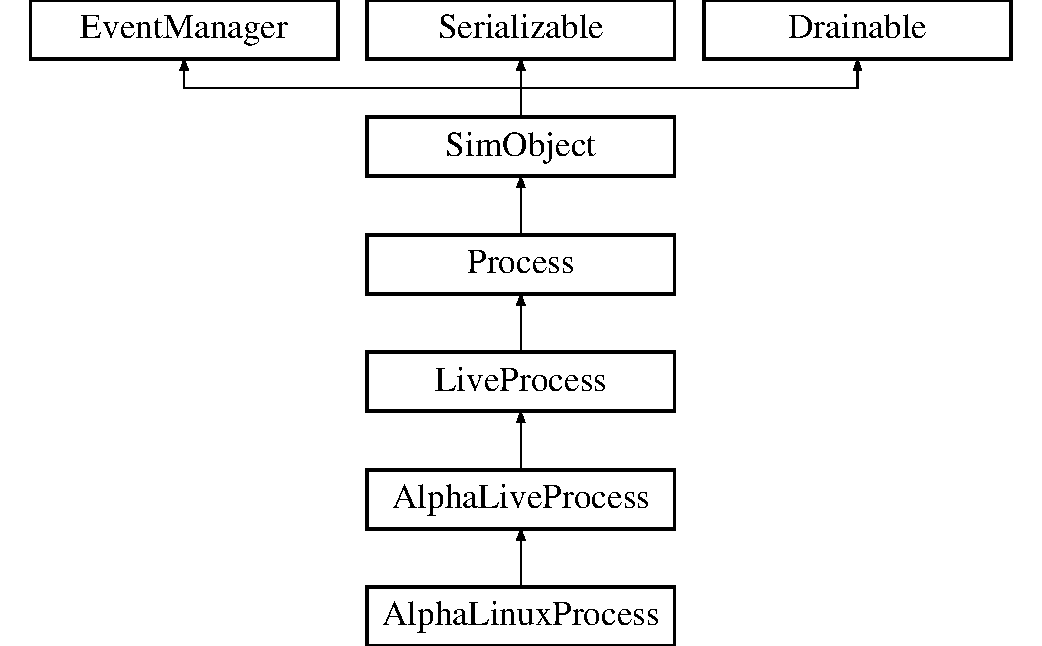
\includegraphics[height=6cm]{classAlphaISA_1_1AlphaLinuxProcess}
\end{center}
\end{figure}
\subsection*{Public メソッド}
\begin{DoxyCompactItemize}
\item 
\hyperlink{classAlphaISA_1_1AlphaLinuxProcess_aa748382496fdd00b4d1cff0ef1afa8bc}{AlphaLinuxProcess} (LiveProcessParams $\ast$params, \hyperlink{classObjectFile}{ObjectFile} $\ast$\hyperlink{classLiveProcess_ab6cfcfa7903c66267b3e0351c3caa809}{objFile})
\begin{DoxyCompactList}\small\item\em Constructor. \item\end{DoxyCompactList}\item 
virtual \hyperlink{classSyscallDesc}{SyscallDesc} $\ast$ \hyperlink{classAlphaISA_1_1AlphaLinuxProcess_aebbff609a7235342925445690acf5ee8}{getDesc} (int callnum)
\end{DoxyCompactItemize}
\subsection*{Public 変数}
\begin{DoxyCompactItemize}
\item 
const int \hyperlink{classAlphaISA_1_1AlphaLinuxProcess_a9534988905c6f5c8c57c4b6a7b179fea}{Num\_\-Syscall\_\-Descs}
\end{DoxyCompactItemize}
\subsection*{Static Public 変数}
\begin{DoxyCompactItemize}
\item 
static \hyperlink{classSyscallDesc}{SyscallDesc} \hyperlink{classAlphaISA_1_1AlphaLinuxProcess_a08d67a94820b75842e07f030e548372e}{syscallDescs} \mbox{[}$\,$\mbox{]}
\begin{DoxyCompactList}\small\item\em Array of syscall descriptors, indexed by call number. \item\end{DoxyCompactList}\end{DoxyCompactItemize}


\subsection{説明}
A process with emulated Alpha/Linux syscalls. 

\subsection{コンストラクタとデストラクタ}
\hypertarget{classAlphaISA_1_1AlphaLinuxProcess_aa748382496fdd00b4d1cff0ef1afa8bc}{
\index{AlphaISA::AlphaLinuxProcess@{AlphaISA::AlphaLinuxProcess}!AlphaLinuxProcess@{AlphaLinuxProcess}}
\index{AlphaLinuxProcess@{AlphaLinuxProcess}!AlphaISA::AlphaLinuxProcess@{AlphaISA::AlphaLinuxProcess}}
\subsubsection[{AlphaLinuxProcess}]{\setlength{\rightskip}{0pt plus 5cm}{\bf AlphaLinuxProcess} (LiveProcessParams $\ast$ {\em params}, \/  {\bf ObjectFile} $\ast$ {\em objFile})}}
\label{classAlphaISA_1_1AlphaLinuxProcess_aa748382496fdd00b4d1cff0ef1afa8bc}


Constructor. 


\begin{DoxyCode}
575     : AlphaLiveProcess(params, objFile),
576      Num_Syscall_Descs(sizeof(syscallDescs) / sizeof(SyscallDesc))
577 {
578     //init_regs->intRegFile[0] = 0;
579 }
\end{DoxyCode}


\subsection{関数}
\hypertarget{classAlphaISA_1_1AlphaLinuxProcess_aebbff609a7235342925445690acf5ee8}{
\index{AlphaISA::AlphaLinuxProcess@{AlphaISA::AlphaLinuxProcess}!getDesc@{getDesc}}
\index{getDesc@{getDesc}!AlphaISA::AlphaLinuxProcess@{AlphaISA::AlphaLinuxProcess}}
\subsubsection[{getDesc}]{\setlength{\rightskip}{0pt plus 5cm}{\bf SyscallDesc} $\ast$ getDesc (int {\em callnum})\hspace{0.3cm}{\ttfamily  \mbox{[}virtual\mbox{]}}}}
\label{classAlphaISA_1_1AlphaLinuxProcess_aebbff609a7235342925445690acf5ee8}


\hyperlink{classLiveProcess_a478f396f8895ef7728d26866a00121d7}{LiveProcess}を実装しています。


\begin{DoxyCode}
585 {
586     if (callnum < 0 || callnum >= Num_Syscall_Descs)
587         return NULL;
588     return &syscallDescs[callnum];
589 }
\end{DoxyCode}


\subsection{変数}
\hypertarget{classAlphaISA_1_1AlphaLinuxProcess_a9534988905c6f5c8c57c4b6a7b179fea}{
\index{AlphaISA::AlphaLinuxProcess@{AlphaISA::AlphaLinuxProcess}!Num\_\-Syscall\_\-Descs@{Num\_\-Syscall\_\-Descs}}
\index{Num\_\-Syscall\_\-Descs@{Num\_\-Syscall\_\-Descs}!AlphaISA::AlphaLinuxProcess@{AlphaISA::AlphaLinuxProcess}}
\subsubsection[{Num\_\-Syscall\_\-Descs}]{\setlength{\rightskip}{0pt plus 5cm}const int {\bf Num\_\-Syscall\_\-Descs}}}
\label{classAlphaISA_1_1AlphaLinuxProcess_a9534988905c6f5c8c57c4b6a7b179fea}
\hypertarget{classAlphaISA_1_1AlphaLinuxProcess_a08d67a94820b75842e07f030e548372e}{
\index{AlphaISA::AlphaLinuxProcess@{AlphaISA::AlphaLinuxProcess}!syscallDescs@{syscallDescs}}
\index{syscallDescs@{syscallDescs}!AlphaISA::AlphaLinuxProcess@{AlphaISA::AlphaLinuxProcess}}
\subsubsection[{syscallDescs}]{\setlength{\rightskip}{0pt plus 5cm}{\bf SyscallDesc} {\bf syscallDescs}\hspace{0.3cm}{\ttfamily  \mbox{[}static\mbox{]}}}}
\label{classAlphaISA_1_1AlphaLinuxProcess_a08d67a94820b75842e07f030e548372e}


Array of syscall descriptors, indexed by call number. 

このクラスの説明は次のファイルから生成されました:\begin{DoxyCompactItemize}
\item 
arch/alpha/linux/\hyperlink{arch_2alpha_2linux_2process_8hh}{process.hh}\item 
arch/alpha/linux/\hyperlink{arch_2alpha_2linux_2process_8cc}{process.cc}\end{DoxyCompactItemize}

\hypertarget{classAlphaLiveProcess}{
\section{クラス AlphaLiveProcess}
\label{classAlphaLiveProcess}\index{AlphaLiveProcess@{AlphaLiveProcess}}
}


{\ttfamily \#include $<$process.hh$>$}AlphaLiveProcessに対する継承グラフ:\begin{figure}[H]
\begin{center}
\leavevmode
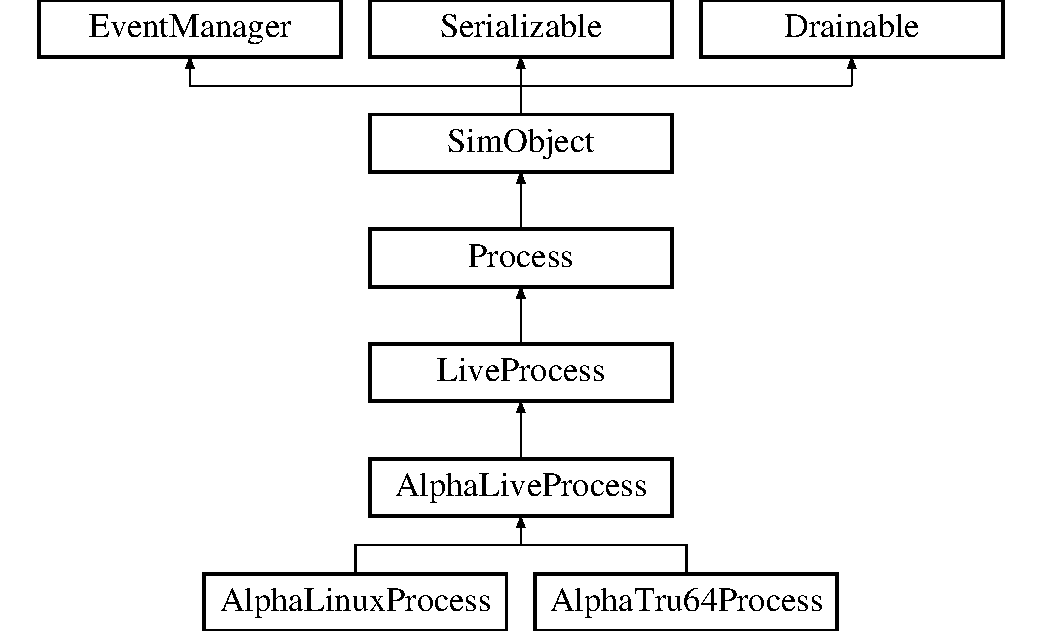
\includegraphics[height=6cm]{classAlphaLiveProcess}
\end{center}
\end{figure}
\subsection*{Public メソッド}
\begin{DoxyCompactItemize}
\item 
\hyperlink{namespaceAlphaISA_a0e080577527fb3e9685399f75b5caf15}{AlphaISA::IntReg} \hyperlink{classAlphaLiveProcess_afcdc0ffa30f2ddff7b435be15da7a6af}{getSyscallArg} (\hyperlink{classThreadContext}{ThreadContext} $\ast$tc, int \&i)
\item 
void \hyperlink{classAlphaLiveProcess_aeaf2b415297449d001c053d7d0d95586}{setSyscallArg} (\hyperlink{classThreadContext}{ThreadContext} $\ast$tc, int i, \hyperlink{namespaceAlphaISA_a0e080577527fb3e9685399f75b5caf15}{AlphaISA::IntReg} val)
\item 
void \hyperlink{classAlphaLiveProcess_aaefd02663c1eae206b851290d9276a5e}{setSyscallReturn} (\hyperlink{classThreadContext}{ThreadContext} $\ast$tc, \hyperlink{classSyscallReturn}{SyscallReturn} return\_\-value)
\end{DoxyCompactItemize}
\subsection*{Protected メソッド}
\begin{DoxyCompactItemize}
\item 
\hyperlink{classAlphaLiveProcess_a01ab49d1a6d4c484cd4818c2ec4c7a1c}{AlphaLiveProcess} (LiveProcessParams $\ast$params, \hyperlink{classObjectFile}{ObjectFile} $\ast$\hyperlink{classLiveProcess_ab6cfcfa7903c66267b3e0351c3caa809}{objFile})
\item 
void \hyperlink{classAlphaLiveProcess_a0c3e6eb311ceff72035b11f2a5e0f186}{loadState} (\hyperlink{classCheckpoint}{Checkpoint} $\ast$cp)
\item 
void \hyperlink{classAlphaLiveProcess_a3c34ea9b29f410748d4435a667484924}{initState} ()
\item 
void \hyperlink{classAlphaLiveProcess_a60e5314ffeede1e51c6bcb2cf606ca92}{argsInit} (int intSize, int pageSize)
\end{DoxyCompactItemize}
\subsection*{Private メソッド}
\begin{DoxyCompactItemize}
\item 
void \hyperlink{classAlphaLiveProcess_a53a76c20b309afae10d511cf9fa8beb0}{setupASNReg} ()
\end{DoxyCompactItemize}


\subsection{コンストラクタとデストラクタ}
\hypertarget{classAlphaLiveProcess_a01ab49d1a6d4c484cd4818c2ec4c7a1c}{
\index{AlphaLiveProcess@{AlphaLiveProcess}!AlphaLiveProcess@{AlphaLiveProcess}}
\index{AlphaLiveProcess@{AlphaLiveProcess}!AlphaLiveProcess@{AlphaLiveProcess}}
\subsubsection[{AlphaLiveProcess}]{\setlength{\rightskip}{0pt plus 5cm}{\bf AlphaLiveProcess} (LiveProcessParams $\ast$ {\em params}, \/  {\bf ObjectFile} $\ast$ {\em objFile})\hspace{0.3cm}{\ttfamily  \mbox{[}protected\mbox{]}}}}
\label{classAlphaLiveProcess_a01ab49d1a6d4c484cd4818c2ec4c7a1c}



\begin{DoxyCode}
49     : LiveProcess(params, objFile)
50 {
51     brk_point = objFile->dataBase() + objFile->dataSize() + objFile->bssSize();
52     brk_point = roundUp(brk_point, VMPageSize);
53 
54     // Set up stack.  On Alpha, stack goes below text section.  This
55     // code should get moved to some architecture-specific spot.
56     stack_base = objFile->textBase() - (409600+4096);
57 
58     // Set up region for mmaps.  Tru64 seems to start just above 0 and
59     // grow up from there.
60     mmap_start = mmap_end = 0x10000;
61 
62     // Set pointer for next thread stack.  Reserve 8M for main stack.
63     next_thread_stack_base = stack_base - (8 * 1024 * 1024);
64 
65 }
\end{DoxyCode}


\subsection{関数}
\hypertarget{classAlphaLiveProcess_a60e5314ffeede1e51c6bcb2cf606ca92}{
\index{AlphaLiveProcess@{AlphaLiveProcess}!argsInit@{argsInit}}
\index{argsInit@{argsInit}!AlphaLiveProcess@{AlphaLiveProcess}}
\subsubsection[{argsInit}]{\setlength{\rightskip}{0pt plus 5cm}void argsInit (int {\em intSize}, \/  int {\em pageSize})\hspace{0.3cm}{\ttfamily  \mbox{[}protected\mbox{]}}}}
\label{classAlphaLiveProcess_a60e5314ffeede1e51c6bcb2cf606ca92}



\begin{DoxyCode}
69 {
70     objFile->loadSections(initVirtMem);
71 
72     typedef AuxVector<uint64_t> auxv_t;
73     std::vector<auxv_t>  auxv;
74 
75     ElfObject * elfObject = dynamic_cast<ElfObject *>(objFile);
76     if(elfObject)
77     {
78         // modern glibc uses a bunch of auxiliary vectors to set up 
79         // TLS as well as do a bunch of other stuff
80         // these vectors go on the bottom of the stack, below argc/argv/envp
81         // pointers but above actual arg strings
82         // I don't have all the ones glibc looks at here, but so far it doesn't
83         // seem to be a problem.
84         // check out _dl_aux_init() in glibc/elf/dl-support.c for details
85         // --Lisa
86         auxv.push_back(auxv_t(M5_AT_PAGESZ, AlphaISA::VMPageSize));
87         auxv.push_back(auxv_t(M5_AT_CLKTCK, 100));
88         auxv.push_back(auxv_t(M5_AT_PHDR, elfObject->programHeaderTable()));
89         DPRINTF(Loader, "auxv at PHDR %08p\n", elfObject->programHeaderTable());
90         auxv.push_back(auxv_t(M5_AT_PHNUM, elfObject->programHeaderCount()));
91         auxv.push_back(auxv_t(M5_AT_ENTRY, objFile->entryPoint()));
92         auxv.push_back(auxv_t(M5_AT_UID, uid()));
93         auxv.push_back(auxv_t(M5_AT_EUID, euid()));
94         auxv.push_back(auxv_t(M5_AT_GID, gid()));
95         auxv.push_back(auxv_t(M5_AT_EGID, egid()));
96 
97     }
98 
99     // Calculate how much space we need for arg & env & auxv arrays.
100     int argv_array_size = intSize * (argv.size() + 1);
101     int envp_array_size = intSize * (envp.size() + 1);
102     int auxv_array_size = intSize * 2 * (auxv.size() + 1);
103 
104     int arg_data_size = 0;
105     for (vector<string>::size_type i = 0; i < argv.size(); ++i) {
106         arg_data_size += argv[i].size() + 1;
107     }
108     int env_data_size = 0;
109     for (vector<string>::size_type i = 0; i < envp.size(); ++i) {
110         env_data_size += envp[i].size() + 1;
111     }
112 
113     int space_needed =
114         argv_array_size + 
115         envp_array_size + 
116         auxv_array_size +
117         arg_data_size + 
118         env_data_size;
119 
120     if (space_needed < 32*1024)
121         space_needed = 32*1024;
122 
123     // set bottom of stack
124     stack_min = stack_base - space_needed;
125     // align it
126     stack_min = roundDown(stack_min, pageSize);
127     stack_size = stack_base - stack_min;
128     // map memory
129     allocateMem(stack_min, roundUp(stack_size, pageSize));
130 
131     // map out initial stack contents
132     Addr argv_array_base = stack_min + intSize; // room for argc
133     Addr envp_array_base = argv_array_base + argv_array_size;
134     Addr auxv_array_base = envp_array_base + envp_array_size;
135     Addr arg_data_base = auxv_array_base + auxv_array_size;
136     Addr env_data_base = arg_data_base + arg_data_size;
137 
138     // write contents to stack
139     uint64_t argc = argv.size();
140     if (intSize == 8)
141         argc = htog((uint64_t)argc);
142     else if (intSize == 4)
143         argc = htog((uint32_t)argc);
144     else
145         panic("Unknown int size");
146 
147     initVirtMem.writeBlob(stack_min, (uint8_t*)&argc, intSize);
148 
149     copyStringArray(argv, argv_array_base, arg_data_base, initVirtMem);
150     copyStringArray(envp, envp_array_base, env_data_base, initVirtMem);
151 
152     //Copy the aux stuff
153     for (vector<auxv_t>::size_type x = 0; x < auxv.size(); x++) {
154         initVirtMem.writeBlob(auxv_array_base + x * 2 * intSize,
155                 (uint8_t*)&(auxv[x].a_type), intSize);
156         initVirtMem.writeBlob(auxv_array_base + (x * 2 + 1) * intSize,
157                 (uint8_t*)&(auxv[x].a_val), intSize);
158     }
159 
160     ThreadContext *tc = system->getThreadContext(contextIds[0]);
161 
162     setSyscallArg(tc, 0, argc);
163     setSyscallArg(tc, 1, argv_array_base);
164     tc->setIntReg(StackPointerReg, stack_min);
165 
166     tc->pcState(objFile->entryPoint());
167 }
\end{DoxyCode}
\hypertarget{classAlphaLiveProcess_afcdc0ffa30f2ddff7b435be15da7a6af}{
\index{AlphaLiveProcess@{AlphaLiveProcess}!getSyscallArg@{getSyscallArg}}
\index{getSyscallArg@{getSyscallArg}!AlphaLiveProcess@{AlphaLiveProcess}}
\subsubsection[{getSyscallArg}]{\setlength{\rightskip}{0pt plus 5cm}{\bf AlphaISA::IntReg} getSyscallArg ({\bf ThreadContext} $\ast$ {\em tc}, \/  int \& {\em i})\hspace{0.3cm}{\ttfamily  \mbox{[}virtual\mbox{]}}}}
\label{classAlphaLiveProcess_afcdc0ffa30f2ddff7b435be15da7a6af}


\hyperlink{classLiveProcess_aa001ff57ec460026facb89ba19c7bf96}{LiveProcess}を実装しています。


\begin{DoxyCode}
209 {
210     assert(i < 6);
211     return tc->readIntReg(FirstArgumentReg + i++);
212 }
\end{DoxyCode}
\hypertarget{classAlphaLiveProcess_a3c34ea9b29f410748d4435a667484924}{
\index{AlphaLiveProcess@{AlphaLiveProcess}!initState@{initState}}
\index{initState@{initState}!AlphaLiveProcess@{AlphaLiveProcess}}
\subsubsection[{initState}]{\setlength{\rightskip}{0pt plus 5cm}void initState ()\hspace{0.3cm}{\ttfamily  \mbox{[}protected, virtual\mbox{]}}}}
\label{classAlphaLiveProcess_a3c34ea9b29f410748d4435a667484924}
\hyperlink{classAlphaLiveProcess_a3c34ea9b29f410748d4435a667484924}{initState()} is called on each \hyperlink{classSimObject}{SimObject} when $\ast$not$\ast$ restoring from a checkpoint. This provides a hook for state initializations that are only required for a \char`\"{}cold start\char`\"{}. 

\hyperlink{classProcess_a3c34ea9b29f410748d4435a667484924}{Process}を再定義しています。


\begin{DoxyCode}
189 {
190     // need to set up ASN before further initialization since init
191     // will involve writing to virtual memory addresses
192     setupASNReg();
193 
194     LiveProcess::initState();
195 
196     argsInit(MachineBytes, VMPageSize);
197 
198     ThreadContext *tc = system->getThreadContext(contextIds[0]);
199     tc->setIntReg(GlobalPointerReg, objFile->globalPointer());
200     //Operate in user mode
201     tc->setMiscRegNoEffect(IPR_ICM, mode_user << 3);
202     tc->setMiscRegNoEffect(IPR_DTB_CM, mode_user << 3);
203     //No super page mapping
204     tc->setMiscRegNoEffect(IPR_MCSR, 0);
205 }
\end{DoxyCode}
\hypertarget{classAlphaLiveProcess_a0c3e6eb311ceff72035b11f2a5e0f186}{
\index{AlphaLiveProcess@{AlphaLiveProcess}!loadState@{loadState}}
\index{loadState@{loadState}!AlphaLiveProcess@{AlphaLiveProcess}}
\subsubsection[{loadState}]{\setlength{\rightskip}{0pt plus 5cm}void loadState ({\bf Checkpoint} $\ast$ {\em cp})\hspace{0.3cm}{\ttfamily  \mbox{[}protected, virtual\mbox{]}}}}
\label{classAlphaLiveProcess_a0c3e6eb311ceff72035b11f2a5e0f186}
\hyperlink{classAlphaLiveProcess_a0c3e6eb311ceff72035b11f2a5e0f186}{loadState()} is called on each \hyperlink{classSimObject}{SimObject} when restoring from a checkpoint. The default implementation simply calls \hyperlink{classProcess_af22e5d6d660b97db37003ac61ac4ee49}{unserialize()} if there is a corresponding section in the checkpoint. However, objects can override \hyperlink{classAlphaLiveProcess_a0c3e6eb311ceff72035b11f2a5e0f186}{loadState()} to get other behaviors, e.g., doing other programmed initializations after \hyperlink{classProcess_af22e5d6d660b97db37003ac61ac4ee49}{unserialize()}, or complaining if no checkpoint section is found.


\begin{DoxyParams}{引数}
\item[{\em \hyperlink{namespacecp}{cp}}]\hyperlink{classCheckpoint}{Checkpoint} to restore the state from. \end{DoxyParams}


\hyperlink{classSimObject_a0c3e6eb311ceff72035b11f2a5e0f186}{SimObject}を再定義しています。


\begin{DoxyCode}
179 {
180     LiveProcess::loadState(cp);
181     // need to set up ASN after unserialization since M5_pid value may
182     // come from checkpoint
183     setupASNReg();
184 }
\end{DoxyCode}
\hypertarget{classAlphaLiveProcess_aeaf2b415297449d001c053d7d0d95586}{
\index{AlphaLiveProcess@{AlphaLiveProcess}!setSyscallArg@{setSyscallArg}}
\index{setSyscallArg@{setSyscallArg}!AlphaLiveProcess@{AlphaLiveProcess}}
\subsubsection[{setSyscallArg}]{\setlength{\rightskip}{0pt plus 5cm}void setSyscallArg ({\bf ThreadContext} $\ast$ {\em tc}, \/  int {\em i}, \/  {\bf AlphaISA::IntReg} {\em val})}}
\label{classAlphaLiveProcess_aeaf2b415297449d001c053d7d0d95586}



\begin{DoxyCode}
217 {
218     assert(i < 6);
219     tc->setIntReg(FirstArgumentReg + i, val);
220 }
\end{DoxyCode}
\hypertarget{classAlphaLiveProcess_aaefd02663c1eae206b851290d9276a5e}{
\index{AlphaLiveProcess@{AlphaLiveProcess}!setSyscallReturn@{setSyscallReturn}}
\index{setSyscallReturn@{setSyscallReturn}!AlphaLiveProcess@{AlphaLiveProcess}}
\subsubsection[{setSyscallReturn}]{\setlength{\rightskip}{0pt plus 5cm}void setSyscallReturn ({\bf ThreadContext} $\ast$ {\em tc}, \/  {\bf SyscallReturn} {\em return\_\-value})\hspace{0.3cm}{\ttfamily  \mbox{[}virtual\mbox{]}}}}
\label{classAlphaLiveProcess_aaefd02663c1eae206b851290d9276a5e}


\hyperlink{classLiveProcess_a5955e790542b86589b9fd75df24ec2d3}{LiveProcess}を実装しています。


\begin{DoxyCode}
224 {
225     // check for error condition.  Alpha syscall convention is to
226     // indicate success/failure in reg a3 (r19) and put the
227     // return value itself in the standard return value reg (v0).
228     if (sysret.successful()) {
229         // no error
230         tc->setIntReg(SyscallSuccessReg, 0);
231         tc->setIntReg(ReturnValueReg, sysret.returnValue());
232     } else {
233         // got an error, return details
234         tc->setIntReg(SyscallSuccessReg, (IntReg)-1);
235         tc->setIntReg(ReturnValueReg, sysret.errnoValue());
236     }
237 }
\end{DoxyCode}
\hypertarget{classAlphaLiveProcess_a53a76c20b309afae10d511cf9fa8beb0}{
\index{AlphaLiveProcess@{AlphaLiveProcess}!setupASNReg@{setupASNReg}}
\index{setupASNReg@{setupASNReg}!AlphaLiveProcess@{AlphaLiveProcess}}
\subsubsection[{setupASNReg}]{\setlength{\rightskip}{0pt plus 5cm}void setupASNReg ()\hspace{0.3cm}{\ttfamily  \mbox{[}private\mbox{]}}}}
\label{classAlphaLiveProcess_a53a76c20b309afae10d511cf9fa8beb0}



\begin{DoxyCode}
171 {
172     ThreadContext *tc = system->getThreadContext(contextIds[0]);
173     tc->setMiscRegNoEffect(IPR_DTB_ASN, M5_pid << 57);
174 }
\end{DoxyCode}


このクラスの説明は次のファイルから生成されました:\begin{DoxyCompactItemize}
\item 
arch/alpha/\hyperlink{arch_2alpha_2process_8hh}{process.hh}\item 
arch/alpha/\hyperlink{arch_2alpha_2process_8cc}{process.cc}\end{DoxyCompactItemize}

\hypertarget{classAlphaSystem_1_1AlphaSystem}{
\section{クラス AlphaSystem}
\label{classAlphaSystem_1_1AlphaSystem}\index{AlphaSystem::AlphaSystem@{AlphaSystem::AlphaSystem}}
}
AlphaSystemに対する継承グラフ:\begin{figure}[H]
\begin{center}
\leavevmode
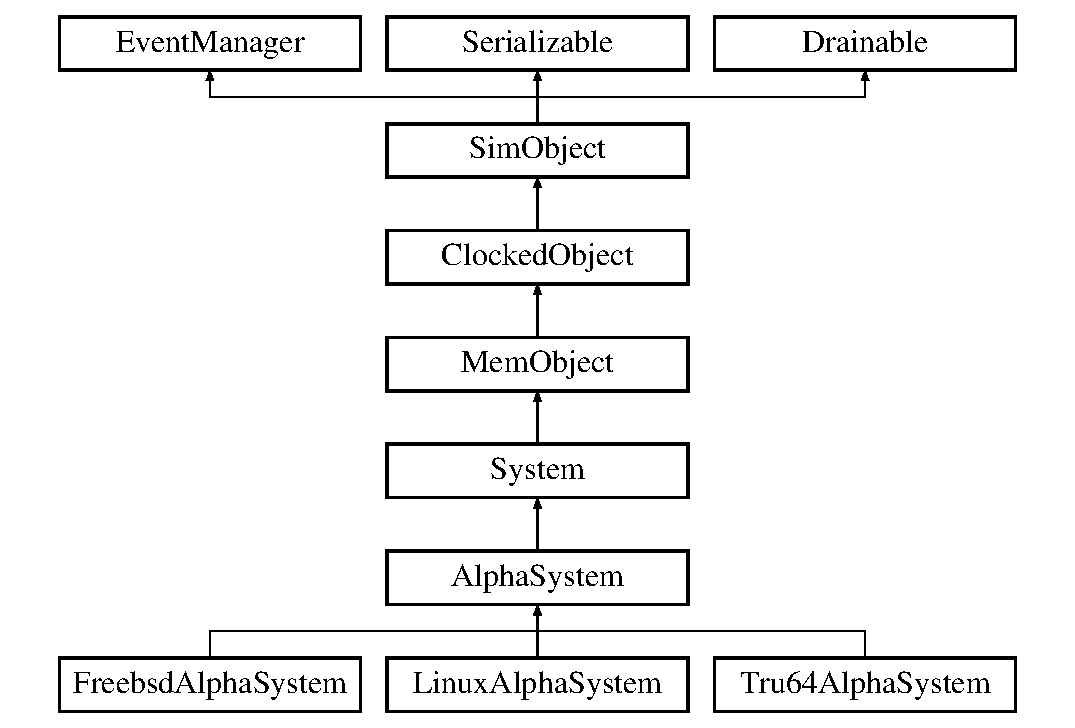
\includegraphics[height=7cm]{classAlphaSystem_1_1AlphaSystem}
\end{center}
\end{figure}
\subsection*{Static Public 変数}
\begin{DoxyCompactItemize}
\item 
string \hyperlink{classAlphaSystem_1_1AlphaSystem_acce15679d830831b0bbe8ebc2a60b2ca}{type} = '\hyperlink{classAlphaSystem_1_1AlphaSystem}{AlphaSystem}'
\item 
string \hyperlink{classAlphaSystem_1_1AlphaSystem_a17da7064bc5c518791f0c891eff05fda}{cxx\_\-header} = \char`\"{}arch/alpha/system.hh\char`\"{}
\item 
tuple \hyperlink{classAlphaSystem_1_1AlphaSystem_a9359679c7dbb7d6922387b94caf2c292}{console} = Param.String(\char`\"{}file that contains the \hyperlink{classAlphaSystem_ac1fd76adeba49aea2ab70e0cba58d9d0}{console} code\char`\"{})
\item 
tuple \hyperlink{classAlphaSystem_1_1AlphaSystem_a7fa215a0a8f10398c16257e0c8534514}{pal} = Param.String(\char`\"{}file that contains palcode\char`\"{})
\item 
tuple \hyperlink{classAlphaSystem_1_1AlphaSystem_af401252d15d9cecde29d1fdcbaba250d}{system\_\-type} = Param.UInt64(\char`\"{}Type of system we are emulating\char`\"{})
\item 
tuple \hyperlink{classAlphaSystem_1_1AlphaSystem_a0f86e3835b8bf2135faf7b1bab968494}{system\_\-rev} = Param.UInt64(\char`\"{}Revision of system we are emulating\char`\"{})
\item 
int \hyperlink{classAlphaSystem_1_1AlphaSystem_abd9c5cc6b7da624a69344d571bab1038}{load\_\-addr\_\-mask} = 0xffffffffff
\end{DoxyCompactItemize}


\subsection{変数}
\hypertarget{classAlphaSystem_1_1AlphaSystem_a9359679c7dbb7d6922387b94caf2c292}{
\index{AlphaSystem::AlphaSystem@{AlphaSystem::AlphaSystem}!console@{console}}
\index{console@{console}!AlphaSystem::AlphaSystem@{AlphaSystem::AlphaSystem}}
\subsubsection[{console}]{\setlength{\rightskip}{0pt plus 5cm}tuple {\bf console} = Param.String(\char`\"{}file that contains the {\bf console} code\char`\"{})\hspace{0.3cm}{\ttfamily  \mbox{[}static\mbox{]}}}}
\label{classAlphaSystem_1_1AlphaSystem_a9359679c7dbb7d6922387b94caf2c292}
\hypertarget{classAlphaSystem_1_1AlphaSystem_a17da7064bc5c518791f0c891eff05fda}{
\index{AlphaSystem::AlphaSystem@{AlphaSystem::AlphaSystem}!cxx\_\-header@{cxx\_\-header}}
\index{cxx\_\-header@{cxx\_\-header}!AlphaSystem::AlphaSystem@{AlphaSystem::AlphaSystem}}
\subsubsection[{cxx\_\-header}]{\setlength{\rightskip}{0pt plus 5cm}string cxx\_\-header = \char`\"{}arch/alpha/system.hh\char`\"{}\hspace{0.3cm}{\ttfamily  \mbox{[}static\mbox{]}}}}
\label{classAlphaSystem_1_1AlphaSystem_a17da7064bc5c518791f0c891eff05fda}


\hyperlink{classSystem_1_1System_a17da7064bc5c518791f0c891eff05fda}{System}を再定義しています。

\hyperlink{classAlphaSystem_1_1LinuxAlphaSystem_a17da7064bc5c518791f0c891eff05fda}{LinuxAlphaSystem}, \hyperlink{classAlphaSystem_1_1FreebsdAlphaSystem_a17da7064bc5c518791f0c891eff05fda}{FreebsdAlphaSystem}, と \hyperlink{classAlphaSystem_1_1Tru64AlphaSystem_a17da7064bc5c518791f0c891eff05fda}{Tru64AlphaSystem}で再定義されています。\hypertarget{classAlphaSystem_1_1AlphaSystem_abd9c5cc6b7da624a69344d571bab1038}{
\index{AlphaSystem::AlphaSystem@{AlphaSystem::AlphaSystem}!load\_\-addr\_\-mask@{load\_\-addr\_\-mask}}
\index{load\_\-addr\_\-mask@{load\_\-addr\_\-mask}!AlphaSystem::AlphaSystem@{AlphaSystem::AlphaSystem}}
\subsubsection[{load\_\-addr\_\-mask}]{\setlength{\rightskip}{0pt plus 5cm}int load\_\-addr\_\-mask = 0xffffffffff\hspace{0.3cm}{\ttfamily  \mbox{[}static\mbox{]}}}}
\label{classAlphaSystem_1_1AlphaSystem_abd9c5cc6b7da624a69344d571bab1038}


\hyperlink{classSystem_1_1System_ae97427a4073448718c4d7c3df3b53143}{System}を再定義しています。\hypertarget{classAlphaSystem_1_1AlphaSystem_a7fa215a0a8f10398c16257e0c8534514}{
\index{AlphaSystem::AlphaSystem@{AlphaSystem::AlphaSystem}!pal@{pal}}
\index{pal@{pal}!AlphaSystem::AlphaSystem@{AlphaSystem::AlphaSystem}}
\subsubsection[{pal}]{\setlength{\rightskip}{0pt plus 5cm}tuple {\bf pal} = Param.String(\char`\"{}file that contains palcode\char`\"{})\hspace{0.3cm}{\ttfamily  \mbox{[}static\mbox{]}}}}
\label{classAlphaSystem_1_1AlphaSystem_a7fa215a0a8f10398c16257e0c8534514}
\hypertarget{classAlphaSystem_1_1AlphaSystem_a0f86e3835b8bf2135faf7b1bab968494}{
\index{AlphaSystem::AlphaSystem@{AlphaSystem::AlphaSystem}!system\_\-rev@{system\_\-rev}}
\index{system\_\-rev@{system\_\-rev}!AlphaSystem::AlphaSystem@{AlphaSystem::AlphaSystem}}
\subsubsection[{system\_\-rev}]{\setlength{\rightskip}{0pt plus 5cm}tuple system\_\-rev = Param.UInt64(\char`\"{}Revision of system we are emulating\char`\"{})\hspace{0.3cm}{\ttfamily  \mbox{[}static\mbox{]}}}}
\label{classAlphaSystem_1_1AlphaSystem_a0f86e3835b8bf2135faf7b1bab968494}


\hyperlink{classAlphaSystem_1_1LinuxAlphaSystem_a261e4081ddd1f0823eccc0f042086c27}{LinuxAlphaSystem}, \hyperlink{classAlphaSystem_1_1FreebsdAlphaSystem_a261e4081ddd1f0823eccc0f042086c27}{FreebsdAlphaSystem}, と \hyperlink{classAlphaSystem_1_1Tru64AlphaSystem_a261e4081ddd1f0823eccc0f042086c27}{Tru64AlphaSystem}で再定義されています。\hypertarget{classAlphaSystem_1_1AlphaSystem_af401252d15d9cecde29d1fdcbaba250d}{
\index{AlphaSystem::AlphaSystem@{AlphaSystem::AlphaSystem}!system\_\-type@{system\_\-type}}
\index{system\_\-type@{system\_\-type}!AlphaSystem::AlphaSystem@{AlphaSystem::AlphaSystem}}
\subsubsection[{system\_\-type}]{\setlength{\rightskip}{0pt plus 5cm}tuple system\_\-type = Param.UInt64(\char`\"{}Type of system we are emulating\char`\"{})\hspace{0.3cm}{\ttfamily  \mbox{[}static\mbox{]}}}}
\label{classAlphaSystem_1_1AlphaSystem_af401252d15d9cecde29d1fdcbaba250d}


\hyperlink{classAlphaSystem_1_1LinuxAlphaSystem_acfe3506cfe10e05a2cb2c2973dc5dad2}{LinuxAlphaSystem}, \hyperlink{classAlphaSystem_1_1FreebsdAlphaSystem_acfe3506cfe10e05a2cb2c2973dc5dad2}{FreebsdAlphaSystem}, と \hyperlink{classAlphaSystem_1_1Tru64AlphaSystem_acfe3506cfe10e05a2cb2c2973dc5dad2}{Tru64AlphaSystem}で再定義されています。\hypertarget{classAlphaSystem_1_1AlphaSystem_acce15679d830831b0bbe8ebc2a60b2ca}{
\index{AlphaSystem::AlphaSystem@{AlphaSystem::AlphaSystem}!type@{type}}
\index{type@{type}!AlphaSystem::AlphaSystem@{AlphaSystem::AlphaSystem}}
\subsubsection[{type}]{\setlength{\rightskip}{0pt plus 5cm}string type = '{\bf AlphaSystem}'\hspace{0.3cm}{\ttfamily  \mbox{[}static\mbox{]}}}}
\label{classAlphaSystem_1_1AlphaSystem_acce15679d830831b0bbe8ebc2a60b2ca}


\hyperlink{classSystem_1_1System_acce15679d830831b0bbe8ebc2a60b2ca}{System}を再定義しています。

\hyperlink{classAlphaSystem_1_1LinuxAlphaSystem_acce15679d830831b0bbe8ebc2a60b2ca}{LinuxAlphaSystem}, \hyperlink{classAlphaSystem_1_1FreebsdAlphaSystem_acce15679d830831b0bbe8ebc2a60b2ca}{FreebsdAlphaSystem}, と \hyperlink{classAlphaSystem_1_1Tru64AlphaSystem_acce15679d830831b0bbe8ebc2a60b2ca}{Tru64AlphaSystem}で再定義されています。

このクラスの説明は次のファイルから生成されました:\begin{DoxyCompactItemize}
\item 
arch/alpha/\hyperlink{AlphaSystem_8py}{AlphaSystem.py}\end{DoxyCompactItemize}

\hypertarget{classAlphaSystem}{
\section{クラス AlphaSystem}
\label{classAlphaSystem}\index{AlphaSystem@{AlphaSystem}}
}


{\ttfamily \#include $<$system.hh$>$}AlphaSystemに対する継承グラフ:\begin{figure}[H]
\begin{center}
\leavevmode
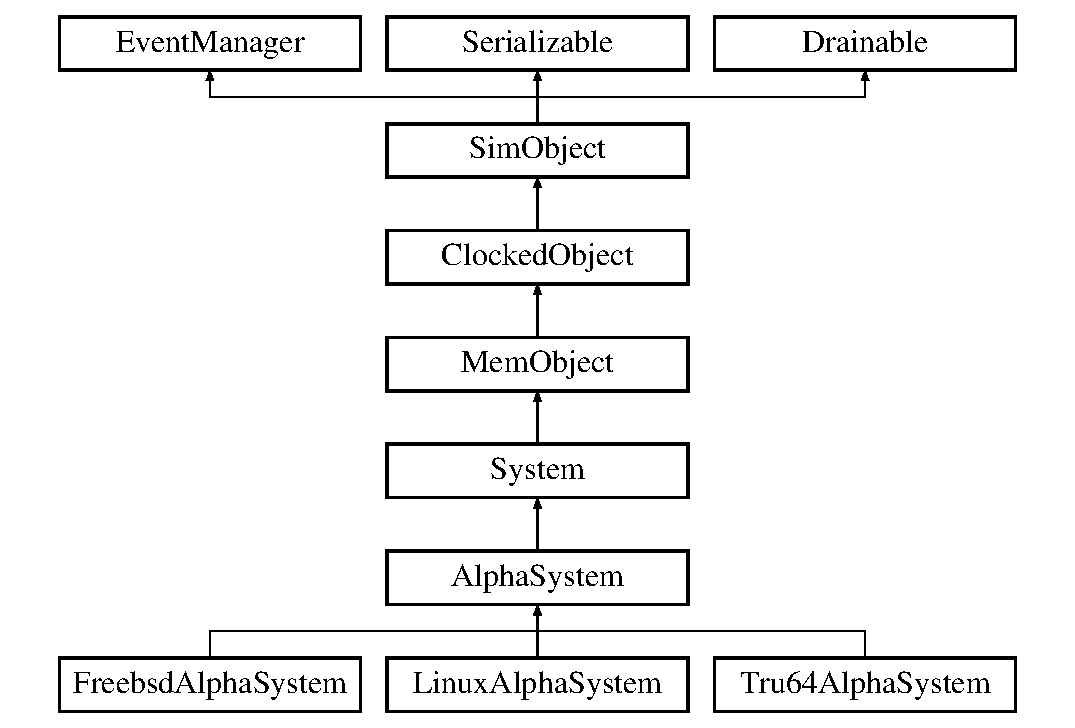
\includegraphics[height=7cm]{classAlphaSystem}
\end{center}
\end{figure}
\subsection*{Public 型}
\begin{DoxyCompactItemize}
\item 
typedef AlphaSystemParams \hyperlink{classAlphaSystem_a2af24d7a564ee2ca81332fb46406cbe5}{Params}
\end{DoxyCompactItemize}
\subsection*{Public メソッド}
\begin{DoxyCompactItemize}
\item 
\hyperlink{classAlphaSystem_a941905a366151e2723f8e98ffd40cadb}{AlphaSystem} (\hyperlink{classAlphaSystem_a2af24d7a564ee2ca81332fb46406cbe5}{Params} $\ast$p)
\item 
\hyperlink{classAlphaSystem_a95eeeeee39ef2bc37d8fc8ffc3b1cdbe}{$\sim$AlphaSystem} ()
\item 
virtual void \hyperlink{classAlphaSystem_a3c34ea9b29f410748d4435a667484924}{initState} ()
\item 
virtual void \hyperlink{classAlphaSystem_a4a3f2000b7188750d8fc90aa204fbfd9}{serializeSymtab} (std::ostream \&os)
\item 
virtual void \hyperlink{classAlphaSystem_a183b92b9eac0994f5d446702e995132a}{unserializeSymtab} (\hyperlink{classCheckpoint}{Checkpoint} $\ast$cp, const std::string \&section)
\item 
virtual void \hyperlink{classAlphaSystem_aecc7d8debf54990ffeaaed5bac7d7d81}{startup} ()
\item 
void \hyperlink{classAlphaSystem_a67fd461df8578f316a9be1cc3e5d70ec}{setAlphaAccess} (\hyperlink{classm5_1_1params_1_1Addr}{Addr} access)
\item 
void \hyperlink{classAlphaSystem_a5b06e992598acbcaa976da1a60396d27}{setIntrFreq} (\hyperlink{base_2types_8hh_a5c8ed81b7d238c9083e1037ba6d61643}{Tick} freq)
\end{DoxyCompactItemize}
\subsection*{Public 変数}
\begin{DoxyCompactItemize}
\item 
\hyperlink{classSymbolTable}{SymbolTable} $\ast$ \hyperlink{classAlphaSystem_a112883d2eb9b5a5c79f3717e73a15dbb}{consoleSymtab}
\item 
\hyperlink{classSymbolTable}{SymbolTable} $\ast$ \hyperlink{classAlphaSystem_a884de17d5e1c6df4f2784b07e868750e}{palSymtab}
\item 
\hyperlink{classObjectFile}{ObjectFile} $\ast$ \hyperlink{classAlphaSystem_ac1fd76adeba49aea2ab70e0cba58d9d0}{console}
\item 
\hyperlink{classObjectFile}{ObjectFile} $\ast$ \hyperlink{classAlphaSystem_a12ab7425ba24138640ac20cb79fad014}{pal}
\item 
\hyperlink{classBreakPCEvent}{BreakPCEvent} $\ast$ \hyperlink{classAlphaSystem_a0266101e4c5bb3cef386e47221ba7f83}{consolePanicEvent}
\end{DoxyCompactItemize}
\subsection*{Protected メソッド}
\begin{DoxyCompactItemize}
\item 
const \hyperlink{classAlphaSystem_a2af24d7a564ee2ca81332fb46406cbe5}{Params} $\ast$ \hyperlink{classAlphaSystem_acd3c3feb78ae7a8f88fe0f110a718dff}{params} () const 
\item 
virtual void \hyperlink{classAlphaSystem_ae36115f702dd2f9ead5df8d632632cf7}{setupFuncEvents} ()
\item 
{\footnotesize template$<$class T $>$ }\\T $\ast$ \hyperlink{classAlphaSystem_aa8018ca1a248feeeefa3a4180d432490}{addPalFuncEvent} (const char $\ast$lbl)
\item 
{\footnotesize template$<$class T $>$ }\\T $\ast$ \hyperlink{classAlphaSystem_a144f0e3cc56a01c7425853cc5ad44021}{addConsoleFuncEvent} (const char $\ast$lbl)
\item 
virtual \hyperlink{classm5_1_1params_1_1Addr}{Addr} \hyperlink{classAlphaSystem_ac72b76fe05499c31c7091ec5a56c0d52}{fixFuncEventAddr} (\hyperlink{classm5_1_1params_1_1Addr}{Addr} addr)
\end{DoxyCompactItemize}
\subsection*{Protected 変数}
\begin{DoxyCompactItemize}
\item 
\hyperlink{base_2types_8hh_a5c8ed81b7d238c9083e1037ba6d61643}{Tick} \hyperlink{classAlphaSystem_a59830ff46622983eb3156d848aedd301}{intrFreq}
\item 
\hyperlink{classFSTranslatingPortProxy}{FSTranslatingPortProxy} \hyperlink{classAlphaSystem_a211e585d20649018ca8f1d7464b19db8}{virtProxy}
\end{DoxyCompactItemize}


\subsection{型定義}
\hypertarget{classAlphaSystem_a2af24d7a564ee2ca81332fb46406cbe5}{
\index{AlphaSystem@{AlphaSystem}!Params@{Params}}
\index{Params@{Params}!AlphaSystem@{AlphaSystem}}
\subsubsection[{Params}]{\setlength{\rightskip}{0pt plus 5cm}typedef AlphaSystemParams {\bf Params}}}
\label{classAlphaSystem_a2af24d7a564ee2ca81332fb46406cbe5}


\hyperlink{classSystem_a5f461be6222ce76bffcb70f27d820c56}{System}を再定義しています。

\hyperlink{classFreebsdAlphaSystem_a0cee38b7e957f9f434ee078d80b94d1b}{FreebsdAlphaSystem}, \hyperlink{classLinuxAlphaSystem_a0d8e2379ed014b6039c45eb98c24fed4}{LinuxAlphaSystem}, と \hyperlink{classTru64AlphaSystem_a653e3d38e55079cc093cc4945c1ac3d1}{Tru64AlphaSystem}で再定義されています。

\subsection{コンストラクタとデストラクタ}
\hypertarget{classAlphaSystem_a941905a366151e2723f8e98ffd40cadb}{
\index{AlphaSystem@{AlphaSystem}!AlphaSystem@{AlphaSystem}}
\index{AlphaSystem@{AlphaSystem}!AlphaSystem@{AlphaSystem}}
\subsubsection[{AlphaSystem}]{\setlength{\rightskip}{0pt plus 5cm}{\bf AlphaSystem} ({\bf Params} $\ast$ {\em p})}}
\label{classAlphaSystem_a941905a366151e2723f8e98ffd40cadb}


Load the pal, and console code into memory


\begin{DoxyCode}
48     : System(p), intrFreq(0), virtProxy(getSystemPort(), p->cache_line_size)
49 {
50     consoleSymtab = new SymbolTable;
51     palSymtab = new SymbolTable;
52 
53 
57     // Load Console Code
58     console = createObjectFile(params()->console);
59     if (console == NULL)
60         fatal("Could not load console file %s", params()->console);
61 
62     // Load pal file
63     pal = createObjectFile(params()->pal);
64     if (pal == NULL)
65         fatal("Could not load PALcode file %s", params()->pal);
66 
67     // load symbols
68     if (!console->loadGlobalSymbols(consoleSymtab))
69         panic("could not load console symbols\n");
70 
71     if (!pal->loadGlobalSymbols(palSymtab))
72         panic("could not load pal symbols\n");
73 
74     if (!pal->loadLocalSymbols(palSymtab))
75         panic("could not load pal symbols\n");
76 
77     if (!console->loadGlobalSymbols(debugSymbolTable))
78         panic("could not load console symbols\n");
79 
80     if (!pal->loadGlobalSymbols(debugSymbolTable))
81         panic("could not load pal symbols\n");
82 
83     if (!pal->loadLocalSymbols(debugSymbolTable))
84         panic("could not load pal symbols\n");
85 
86 
87 }
\end{DoxyCode}
\hypertarget{classAlphaSystem_a95eeeeee39ef2bc37d8fc8ffc3b1cdbe}{
\index{AlphaSystem@{AlphaSystem}!$\sim$AlphaSystem@{$\sim$AlphaSystem}}
\index{$\sim$AlphaSystem@{$\sim$AlphaSystem}!AlphaSystem@{AlphaSystem}}
\subsubsection[{$\sim$AlphaSystem}]{\setlength{\rightskip}{0pt plus 5cm}$\sim${\bf AlphaSystem} ()}}
\label{classAlphaSystem_a95eeeeee39ef2bc37d8fc8ffc3b1cdbe}



\begin{DoxyCode}
90 {
91     delete consoleSymtab;
92     delete console;
93     delete pal;
94 #ifdef DEBUG
95     delete consolePanicEvent;
96 #endif
97 }
\end{DoxyCode}


\subsection{関数}
\hypertarget{classAlphaSystem_a144f0e3cc56a01c7425853cc5ad44021}{
\index{AlphaSystem@{AlphaSystem}!addConsoleFuncEvent@{addConsoleFuncEvent}}
\index{addConsoleFuncEvent@{addConsoleFuncEvent}!AlphaSystem@{AlphaSystem}}
\subsubsection[{addConsoleFuncEvent}]{\setlength{\rightskip}{0pt plus 5cm}T$\ast$ addConsoleFuncEvent (const char $\ast$ {\em lbl})\hspace{0.3cm}{\ttfamily  \mbox{[}inline, protected\mbox{]}}}}
\label{classAlphaSystem_a144f0e3cc56a01c7425853cc5ad44021}
Add a function-\/based event to the console code. 


\begin{DoxyCode}
120     {
121         return addFuncEvent<T>(consoleSymtab, lbl);
122     }
\end{DoxyCode}
\hypertarget{classAlphaSystem_aa8018ca1a248feeeefa3a4180d432490}{
\index{AlphaSystem@{AlphaSystem}!addPalFuncEvent@{addPalFuncEvent}}
\index{addPalFuncEvent@{addPalFuncEvent}!AlphaSystem@{AlphaSystem}}
\subsubsection[{addPalFuncEvent}]{\setlength{\rightskip}{0pt plus 5cm}T$\ast$ addPalFuncEvent (const char $\ast$ {\em lbl})\hspace{0.3cm}{\ttfamily  \mbox{[}inline, protected\mbox{]}}}}
\label{classAlphaSystem_aa8018ca1a248feeeefa3a4180d432490}
Add a function-\/based event to PALcode. 


\begin{DoxyCode}
112     {
113         return addFuncEvent<T>(palSymtab, lbl);
114     }
\end{DoxyCode}
\hypertarget{classAlphaSystem_ac72b76fe05499c31c7091ec5a56c0d52}{
\index{AlphaSystem@{AlphaSystem}!fixFuncEventAddr@{fixFuncEventAddr}}
\index{fixFuncEventAddr@{fixFuncEventAddr}!AlphaSystem@{AlphaSystem}}
\subsubsection[{fixFuncEventAddr}]{\setlength{\rightskip}{0pt plus 5cm}{\bf Addr} fixFuncEventAddr ({\bf Addr} {\em addr})\hspace{0.3cm}{\ttfamily  \mbox{[}protected, virtual\mbox{]}}}}
\label{classAlphaSystem_ac72b76fe05499c31c7091ec5a56c0d52}
This function fixes up addresses that are used to match PCs for hooking simulator events on to target function executions.

Alpha binaries may have multiple global offset table (GOT) sections. A function that uses the GOT starts with a two-\/instruction prolog which sets the global pointer (gp == r29) to the appropriate GOT section. The proper gp value is calculated based on the function address, which must be passed by the caller in the procedure value register (pv aka t12 == r27). This sequence looks like the following:

opcode Ra Rb offset ldah gp,X(pv) 09 29 27 X lda gp,Y(gp) 08 29 29 Y

for some constant offsets X and Y. The catch is that the linker (or maybe even the compiler, I'm not sure) may recognize that the caller and callee are using the same GOT section, making this prolog redundant, and modify the call target to skip these instructions. If we check for execution of the first instruction of a function (the one the symbol points to) to detect when to skip it, we'll miss all these modified calls. It might work to unconditionally check for the third instruction, but not all functions have this prolog, and there's some chance that those first two instructions could have undesired consequences. So we do the Right Thing and pattern-\/match the first two instructions of the function to decide where to patch.

Eventually this code should be moved into an ISA-\/specific file. 

\hyperlink{classSystem_aff94f650c5eef23b8dc350ea755bdef4}{System}を再定義しています。


\begin{DoxyCode}
188 {
189     // mask for just the opcode, Ra, and Rb fields (not the offset)
190     const uint32_t inst_mask = 0xffff0000;
191     // ldah gp,X(pv): opcode 9, Ra = 29, Rb = 27
192     const uint32_t gp_ldah_pattern = (9 << 26) | (29 << 21) | (27 << 16);
193     // lda  gp,Y(gp): opcode 8, Ra = 29, rb = 29
194     const uint32_t gp_lda_pattern  = (8 << 26) | (29 << 21) | (29 << 16);
195 
196     uint32_t i1 = virtProxy.read<uint32_t>(addr);
197     uint32_t i2 = virtProxy.read<uint32_t>(addr + sizeof(MachInst));
198 
199     if ((i1 & inst_mask) == gp_ldah_pattern &&
200         (i2 & inst_mask) == gp_lda_pattern) {
201         Addr new_addr = addr + 2 * sizeof(MachInst);
202         DPRINTF(Loader, "fixFuncEventAddr: %p -> %p", addr, new_addr);
203         return new_addr;
204     } else {
205         return addr;
206     }
207 }
\end{DoxyCode}
\hypertarget{classAlphaSystem_a3c34ea9b29f410748d4435a667484924}{
\index{AlphaSystem@{AlphaSystem}!initState@{initState}}
\index{initState@{initState}!AlphaSystem@{AlphaSystem}}
\subsubsection[{initState}]{\setlength{\rightskip}{0pt plus 5cm}void initState ()\hspace{0.3cm}{\ttfamily  \mbox{[}virtual\mbox{]}}}}
\label{classAlphaSystem_a3c34ea9b29f410748d4435a667484924}
Initialise the state of the system. 

Copy the osflags (kernel arguments) into the consoles memory. (Presently \hyperlink{classLinux}{Linux} does not use the console service routine to get these command line arguments, but \hyperlink{classTru64}{Tru64} and others do.)

\hyperlink{classSet}{Set} the hardware reset parameter block system type and revision information to \hyperlink{classTsunami}{Tsunami}.

\hyperlink{classSystem_a3c34ea9b29f410748d4435a667484924}{System}を再定義しています。

\hyperlink{classLinuxAlphaSystem_a3c34ea9b29f410748d4435a667484924}{LinuxAlphaSystem}で再定義されています。


\begin{DoxyCode}
101 {
102      Addr addr = 0;
103 
104     // Moved from the constructor to here since it relies on the
105     // address map being resolved in the interconnect
106 
107     // Call the initialisation of the super class
108     System::initState();
109 
110     // Load program sections into memory
111     pal->loadSections(physProxy, loadAddrMask);
112     console->loadSections(physProxy, loadAddrMask);
113 
120     if (consoleSymtab->findAddress("env_booted_osflags", addr)) {
121         virtProxy.writeBlob(addr, (uint8_t*)params()->boot_osflags.c_str(),
122                             strlen(params()->boot_osflags.c_str()));
123     }
124 
129     if (consoleSymtab->findAddress("m5_rpb", addr)) {
130         uint64_t data;
131         data = htog(params()->system_type);
132         virtProxy.write(addr+0x50, data);
133         data = htog(params()->system_rev);
134         virtProxy.write(addr+0x58, data);
135     } else
136         panic("could not find hwrpb\n");
137 }
\end{DoxyCode}
\hypertarget{classAlphaSystem_acd3c3feb78ae7a8f88fe0f110a718dff}{
\index{AlphaSystem@{AlphaSystem}!params@{params}}
\index{params@{params}!AlphaSystem@{AlphaSystem}}
\subsubsection[{params}]{\setlength{\rightskip}{0pt plus 5cm}const {\bf Params}$\ast$ params () const\hspace{0.3cm}{\ttfamily  \mbox{[}inline, protected\mbox{]}}}}
\label{classAlphaSystem_acd3c3feb78ae7a8f88fe0f110a718dff}


\hyperlink{classSystem_acd3c3feb78ae7a8f88fe0f110a718dff}{System}を再定義しています。

\hyperlink{classLinuxAlphaSystem_acd3c3feb78ae7a8f88fe0f110a718dff}{LinuxAlphaSystem}で再定義されています。


\begin{DoxyCode}
100 { return (const Params *)_params; }
\end{DoxyCode}
\hypertarget{classAlphaSystem_a4a3f2000b7188750d8fc90aa204fbfd9}{
\index{AlphaSystem@{AlphaSystem}!serializeSymtab@{serializeSymtab}}
\index{serializeSymtab@{serializeSymtab}!AlphaSystem@{AlphaSystem}}
\subsubsection[{serializeSymtab}]{\setlength{\rightskip}{0pt plus 5cm}void serializeSymtab (std::ostream \& {\em os})\hspace{0.3cm}{\ttfamily  \mbox{[}virtual\mbox{]}}}}
\label{classAlphaSystem_a4a3f2000b7188750d8fc90aa204fbfd9}
Serialization stuff 

\hyperlink{classSystem_a4a6e514fbf1ef35f9a914680884cedef}{System}を再定義しています。


\begin{DoxyCode}
222 {
223     consoleSymtab->serialize("console_symtab", os);
224     palSymtab->serialize("pal_symtab", os);
225 }
\end{DoxyCode}
\hypertarget{classAlphaSystem_a67fd461df8578f316a9be1cc3e5d70ec}{
\index{AlphaSystem@{AlphaSystem}!setAlphaAccess@{setAlphaAccess}}
\index{setAlphaAccess@{setAlphaAccess}!AlphaSystem@{AlphaSystem}}
\subsubsection[{setAlphaAccess}]{\setlength{\rightskip}{0pt plus 5cm}void setAlphaAccess ({\bf Addr} {\em access})}}
\label{classAlphaSystem_a67fd461df8578f316a9be1cc3e5d70ec}
\hyperlink{classSet}{Set} the m5AlphaAccess pointer in the console 


\begin{DoxyCode}
211 {
212     Addr addr = 0;
213     if (consoleSymtab->findAddress("m5AlphaAccess", addr)) {
214         virtProxy.write(addr, htog(Phys2K0Seg(access)));
215     } else {
216         panic("could not find m5AlphaAccess\n");
217     }
218 }
\end{DoxyCode}
\hypertarget{classAlphaSystem_a5b06e992598acbcaa976da1a60396d27}{
\index{AlphaSystem@{AlphaSystem}!setIntrFreq@{setIntrFreq}}
\index{setIntrFreq@{setIntrFreq}!AlphaSystem@{AlphaSystem}}
\subsubsection[{setIntrFreq}]{\setlength{\rightskip}{0pt plus 5cm}void setIntrFreq ({\bf Tick} {\em freq})\hspace{0.3cm}{\ttfamily  \mbox{[}inline\mbox{]}}}}
\label{classAlphaSystem_a5b06e992598acbcaa976da1a60396d27}



\begin{DoxyCode}
127 { intrFreq = freq; }
\end{DoxyCode}
\hypertarget{classAlphaSystem_ae36115f702dd2f9ead5df8d632632cf7}{
\index{AlphaSystem@{AlphaSystem}!setupFuncEvents@{setupFuncEvents}}
\index{setupFuncEvents@{setupFuncEvents}!AlphaSystem@{AlphaSystem}}
\subsubsection[{setupFuncEvents}]{\setlength{\rightskip}{0pt plus 5cm}void setupFuncEvents ()\hspace{0.3cm}{\ttfamily  \mbox{[}protected, virtual\mbox{]}}}}
\label{classAlphaSystem_ae36115f702dd2f9ead5df8d632632cf7}
Setup all the function events. Must be done after \hyperlink{classSystem_a02fd73d861ef2e4aabb38c0c9ff82947}{init()} for Alpha since fixFuncEvent() requires a function port 

\hyperlink{classLinuxAlphaSystem_ae36115f702dd2f9ead5df8d632632cf7}{LinuxAlphaSystem}で再定義されています。


\begin{DoxyCode}
149 {
150 #ifndef NDEBUG
151     consolePanicEvent = addConsoleFuncEvent<BreakPCEvent>("panic");
152 #endif
153 }
\end{DoxyCode}
\hypertarget{classAlphaSystem_aecc7d8debf54990ffeaaed5bac7d7d81}{
\index{AlphaSystem@{AlphaSystem}!startup@{startup}}
\index{startup@{startup}!AlphaSystem@{AlphaSystem}}
\subsubsection[{startup}]{\setlength{\rightskip}{0pt plus 5cm}void startup ()\hspace{0.3cm}{\ttfamily  \mbox{[}virtual\mbox{]}}}}
\label{classAlphaSystem_aecc7d8debf54990ffeaaed5bac7d7d81}
Override \hyperlink{classAlphaSystem_aecc7d8debf54990ffeaaed5bac7d7d81}{startup()} to provide a path to call \hyperlink{classAlphaSystem_ae36115f702dd2f9ead5df8d632632cf7}{setupFuncEvents()} 

\hyperlink{classSimObject_aecc7d8debf54990ffeaaed5bac7d7d81}{SimObject}を再定義しています。


\begin{DoxyCode}
141 {
142     // Setup all the function events now that we have a system and a symbol
143     // table
144     setupFuncEvents();
145 }
\end{DoxyCode}
\hypertarget{classAlphaSystem_a183b92b9eac0994f5d446702e995132a}{
\index{AlphaSystem@{AlphaSystem}!unserializeSymtab@{unserializeSymtab}}
\index{unserializeSymtab@{unserializeSymtab}!AlphaSystem@{AlphaSystem}}
\subsubsection[{unserializeSymtab}]{\setlength{\rightskip}{0pt plus 5cm}void unserializeSymtab ({\bf Checkpoint} $\ast$ {\em cp}, \/  const std::string \& {\em section})\hspace{0.3cm}{\ttfamily  \mbox{[}virtual\mbox{]}}}}
\label{classAlphaSystem_a183b92b9eac0994f5d446702e995132a}
If needed, unserialize additional symbol table entries for a specific subclass of this system.


\begin{DoxyParams}{引数}
\item[{\em \hyperlink{namespacecp}{cp}}]checkpoint to unserialize from \item[{\em section}]relevant section in the checkpoint \end{DoxyParams}


\hyperlink{classSystem_a3536a2e47acf307ec65515712f0e2b2d}{System}を再定義しています。


\begin{DoxyCode}
229 {
230     consoleSymtab->unserialize("console_symtab", cp, section);
231     palSymtab->unserialize("pal_symtab", cp, section);
232 }
\end{DoxyCode}


\subsection{変数}
\hypertarget{classAlphaSystem_ac1fd76adeba49aea2ab70e0cba58d9d0}{
\index{AlphaSystem@{AlphaSystem}!console@{console}}
\index{console@{console}!AlphaSystem@{AlphaSystem}}
\subsubsection[{console}]{\setlength{\rightskip}{0pt plus 5cm}{\bf ObjectFile}$\ast$ {\bf console}}}
\label{classAlphaSystem_ac1fd76adeba49aea2ab70e0cba58d9d0}
Object pointer for the console code \hypertarget{classAlphaSystem_a0266101e4c5bb3cef386e47221ba7f83}{
\index{AlphaSystem@{AlphaSystem}!consolePanicEvent@{consolePanicEvent}}
\index{consolePanicEvent@{consolePanicEvent}!AlphaSystem@{AlphaSystem}}
\subsubsection[{consolePanicEvent}]{\setlength{\rightskip}{0pt plus 5cm}{\bf BreakPCEvent}$\ast$ {\bf consolePanicEvent}}}
\label{classAlphaSystem_a0266101e4c5bb3cef386e47221ba7f83}
\hyperlink{classEvent}{Event} to halt the simulator if the console calls \hyperlink{base_2misc_8hh_a1445e207e36c97ff84c54b47288cea19}{panic()} \hypertarget{classAlphaSystem_a112883d2eb9b5a5c79f3717e73a15dbb}{
\index{AlphaSystem@{AlphaSystem}!consoleSymtab@{consoleSymtab}}
\index{consoleSymtab@{consoleSymtab}!AlphaSystem@{AlphaSystem}}
\subsubsection[{consoleSymtab}]{\setlength{\rightskip}{0pt plus 5cm}{\bf SymbolTable}$\ast$ {\bf consoleSymtab}}}
\label{classAlphaSystem_a112883d2eb9b5a5c79f3717e73a15dbb}
console symbol table \hypertarget{classAlphaSystem_a59830ff46622983eb3156d848aedd301}{
\index{AlphaSystem@{AlphaSystem}!intrFreq@{intrFreq}}
\index{intrFreq@{intrFreq}!AlphaSystem@{AlphaSystem}}
\subsubsection[{intrFreq}]{\setlength{\rightskip}{0pt plus 5cm}{\bf Tick} {\bf intrFreq}\hspace{0.3cm}{\ttfamily  \mbox{[}protected\mbox{]}}}}
\label{classAlphaSystem_a59830ff46622983eb3156d848aedd301}
\hypertarget{classAlphaSystem_a12ab7425ba24138640ac20cb79fad014}{
\index{AlphaSystem@{AlphaSystem}!pal@{pal}}
\index{pal@{pal}!AlphaSystem@{AlphaSystem}}
\subsubsection[{pal}]{\setlength{\rightskip}{0pt plus 5cm}{\bf ObjectFile}$\ast$ {\bf pal}}}
\label{classAlphaSystem_a12ab7425ba24138640ac20cb79fad014}
Object pointer for the \hyperlink{structPAL}{PAL} code \hypertarget{classAlphaSystem_a884de17d5e1c6df4f2784b07e868750e}{
\index{AlphaSystem@{AlphaSystem}!palSymtab@{palSymtab}}
\index{palSymtab@{palSymtab}!AlphaSystem@{AlphaSystem}}
\subsubsection[{palSymtab}]{\setlength{\rightskip}{0pt plus 5cm}{\bf SymbolTable}$\ast$ {\bf palSymtab}}}
\label{classAlphaSystem_a884de17d5e1c6df4f2784b07e868750e}
pal symbol table \hypertarget{classAlphaSystem_a211e585d20649018ca8f1d7464b19db8}{
\index{AlphaSystem@{AlphaSystem}!virtProxy@{virtProxy}}
\index{virtProxy@{virtProxy}!AlphaSystem@{AlphaSystem}}
\subsubsection[{virtProxy}]{\setlength{\rightskip}{0pt plus 5cm}{\bf FSTranslatingPortProxy} {\bf virtProxy}\hspace{0.3cm}{\ttfamily  \mbox{[}protected\mbox{]}}}}
\label{classAlphaSystem_a211e585d20649018ca8f1d7464b19db8}
Proxy used to copy arguments directly into kernel memory. 

このクラスの説明は次のファイルから生成されました:\begin{DoxyCompactItemize}
\item 
arch/alpha/\hyperlink{arch_2alpha_2system_8hh}{system.hh}\item 
arch/alpha/\hyperlink{arch_2alpha_2system_8cc}{system.cc}\end{DoxyCompactItemize}

\hypertarget{classAlphaTLB_1_1AlphaTLB}{
\section{クラス AlphaTLB}
\label{classAlphaTLB_1_1AlphaTLB}\index{AlphaTLB::AlphaTLB@{AlphaTLB::AlphaTLB}}
}
AlphaTLBに対する継承グラフ:\begin{figure}[H]
\begin{center}
\leavevmode
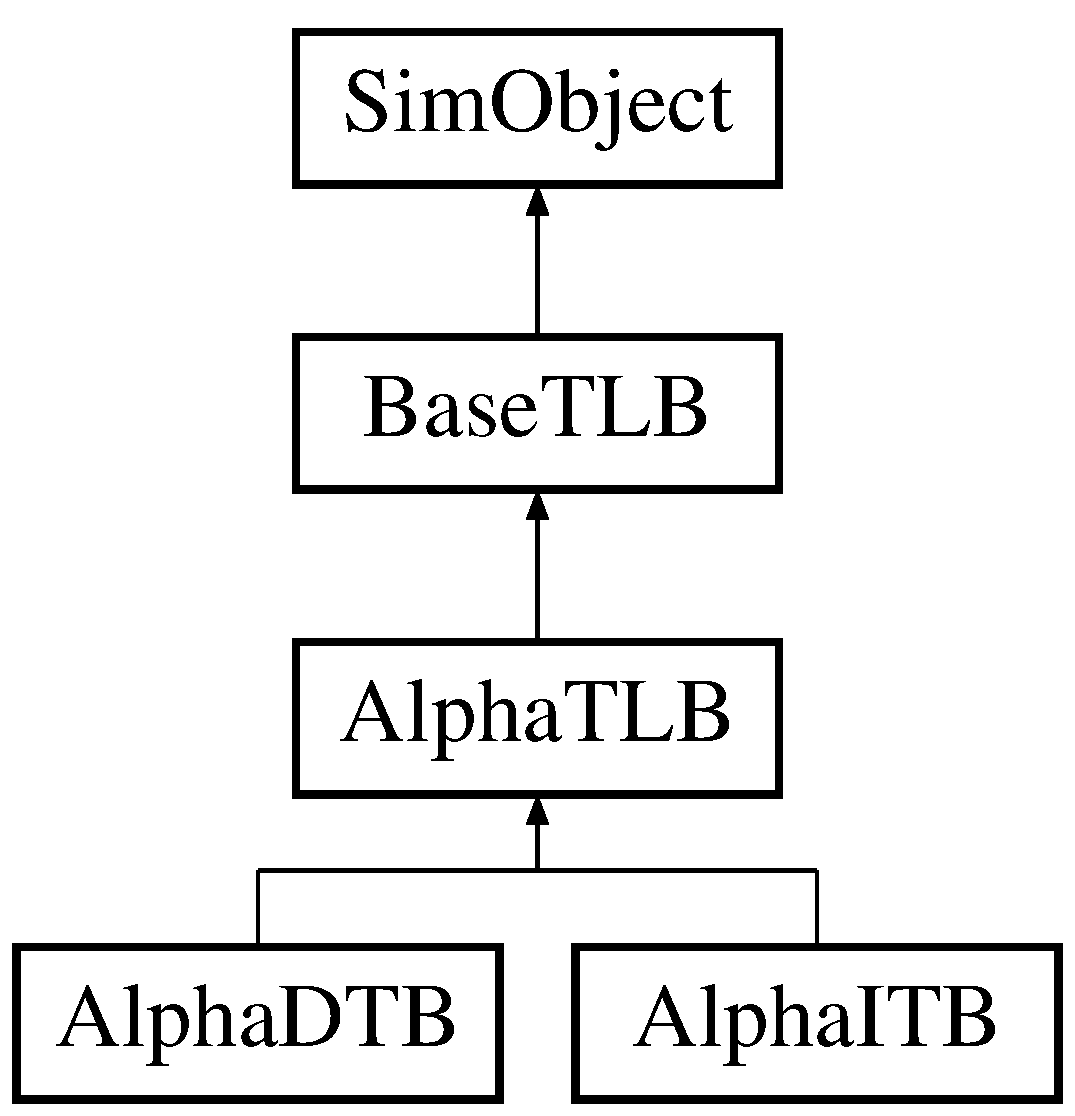
\includegraphics[height=4cm]{classAlphaTLB_1_1AlphaTLB}
\end{center}
\end{figure}
\subsection*{Static Public 変数}
\begin{DoxyCompactItemize}
\item 
string \hyperlink{classAlphaTLB_1_1AlphaTLB_acce15679d830831b0bbe8ebc2a60b2ca}{type} = '\hyperlink{classAlphaTLB_1_1AlphaTLB}{AlphaTLB}'
\item 
string \hyperlink{classAlphaTLB_1_1AlphaTLB_a58cd55cd4023648e138237cfc0822ae3}{cxx\_\-class} = '\hyperlink{classAlphaISA_1_1TLB}{AlphaISA::TLB}'
\item 
string \hyperlink{classAlphaTLB_1_1AlphaTLB_a17da7064bc5c518791f0c891eff05fda}{cxx\_\-header} = \char`\"{}arch/alpha/tlb.hh\char`\"{}
\item 
tuple \hyperlink{classAlphaTLB_1_1AlphaTLB_a377e5da8df1f89c5468c8b8cd07eac89}{size} = Param.Int(\char`\"{}TLB \hyperlink{classAlphaTLB_1_1AlphaTLB_a377e5da8df1f89c5468c8b8cd07eac89}{size}\char`\"{})
\end{DoxyCompactItemize}


\subsection{変数}
\hypertarget{classAlphaTLB_1_1AlphaTLB_a58cd55cd4023648e138237cfc0822ae3}{
\index{AlphaTLB::AlphaTLB@{AlphaTLB::AlphaTLB}!cxx\_\-class@{cxx\_\-class}}
\index{cxx\_\-class@{cxx\_\-class}!AlphaTLB::AlphaTLB@{AlphaTLB::AlphaTLB}}
\subsubsection[{cxx\_\-class}]{\setlength{\rightskip}{0pt plus 5cm}string {\bf cxx\_\-class} = '{\bf AlphaISA::TLB}'\hspace{0.3cm}{\ttfamily  \mbox{[}static\mbox{]}}}}
\label{classAlphaTLB_1_1AlphaTLB_a58cd55cd4023648e138237cfc0822ae3}
\hypertarget{classAlphaTLB_1_1AlphaTLB_a17da7064bc5c518791f0c891eff05fda}{
\index{AlphaTLB::AlphaTLB@{AlphaTLB::AlphaTLB}!cxx\_\-header@{cxx\_\-header}}
\index{cxx\_\-header@{cxx\_\-header}!AlphaTLB::AlphaTLB@{AlphaTLB::AlphaTLB}}
\subsubsection[{cxx\_\-header}]{\setlength{\rightskip}{0pt plus 5cm}string {\bf cxx\_\-header} = \char`\"{}arch/alpha/tlb.hh\char`\"{}\hspace{0.3cm}{\ttfamily  \mbox{[}static\mbox{]}}}}
\label{classAlphaTLB_1_1AlphaTLB_a17da7064bc5c518791f0c891eff05fda}


\hyperlink{classBaseTLB_1_1BaseTLB_a17da7064bc5c518791f0c891eff05fda}{BaseTLB}を再定義しています。\hypertarget{classAlphaTLB_1_1AlphaTLB_a377e5da8df1f89c5468c8b8cd07eac89}{
\index{AlphaTLB::AlphaTLB@{AlphaTLB::AlphaTLB}!size@{size}}
\index{size@{size}!AlphaTLB::AlphaTLB@{AlphaTLB::AlphaTLB}}
\subsubsection[{size}]{\setlength{\rightskip}{0pt plus 5cm}tuple {\bf size} = Param.Int(\char`\"{}TLB {\bf size}\char`\"{})\hspace{0.3cm}{\ttfamily  \mbox{[}static\mbox{]}}}}
\label{classAlphaTLB_1_1AlphaTLB_a377e5da8df1f89c5468c8b8cd07eac89}


\hyperlink{classAlphaTLB_1_1AlphaDTB_a439227feff9d7f55384e8780cfc2eb82}{AlphaDTB}, と \hyperlink{classAlphaTLB_1_1AlphaITB_a439227feff9d7f55384e8780cfc2eb82}{AlphaITB}で再定義されています。\hypertarget{classAlphaTLB_1_1AlphaTLB_acce15679d830831b0bbe8ebc2a60b2ca}{
\index{AlphaTLB::AlphaTLB@{AlphaTLB::AlphaTLB}!type@{type}}
\index{type@{type}!AlphaTLB::AlphaTLB@{AlphaTLB::AlphaTLB}}
\subsubsection[{type}]{\setlength{\rightskip}{0pt plus 5cm}string {\bf type} = '{\bf AlphaTLB}'\hspace{0.3cm}{\ttfamily  \mbox{[}static\mbox{]}}}}
\label{classAlphaTLB_1_1AlphaTLB_acce15679d830831b0bbe8ebc2a60b2ca}


\hyperlink{classBaseTLB_1_1BaseTLB_acce15679d830831b0bbe8ebc2a60b2ca}{BaseTLB}を再定義しています。

このクラスの説明は次のファイルから生成されました:\begin{DoxyCompactItemize}
\item 
arch/alpha/\hyperlink{AlphaTLB_8py}{AlphaTLB.py}\end{DoxyCompactItemize}

\hypertarget{classAlphaTru64}{
\section{クラス AlphaTru64}
\label{classAlphaTru64}\index{AlphaTru64@{AlphaTru64}}
}


{\ttfamily \#include $<$tru64.hh$>$}AlphaTru64に対する継承グラフ:\begin{figure}[H]
\begin{center}
\leavevmode
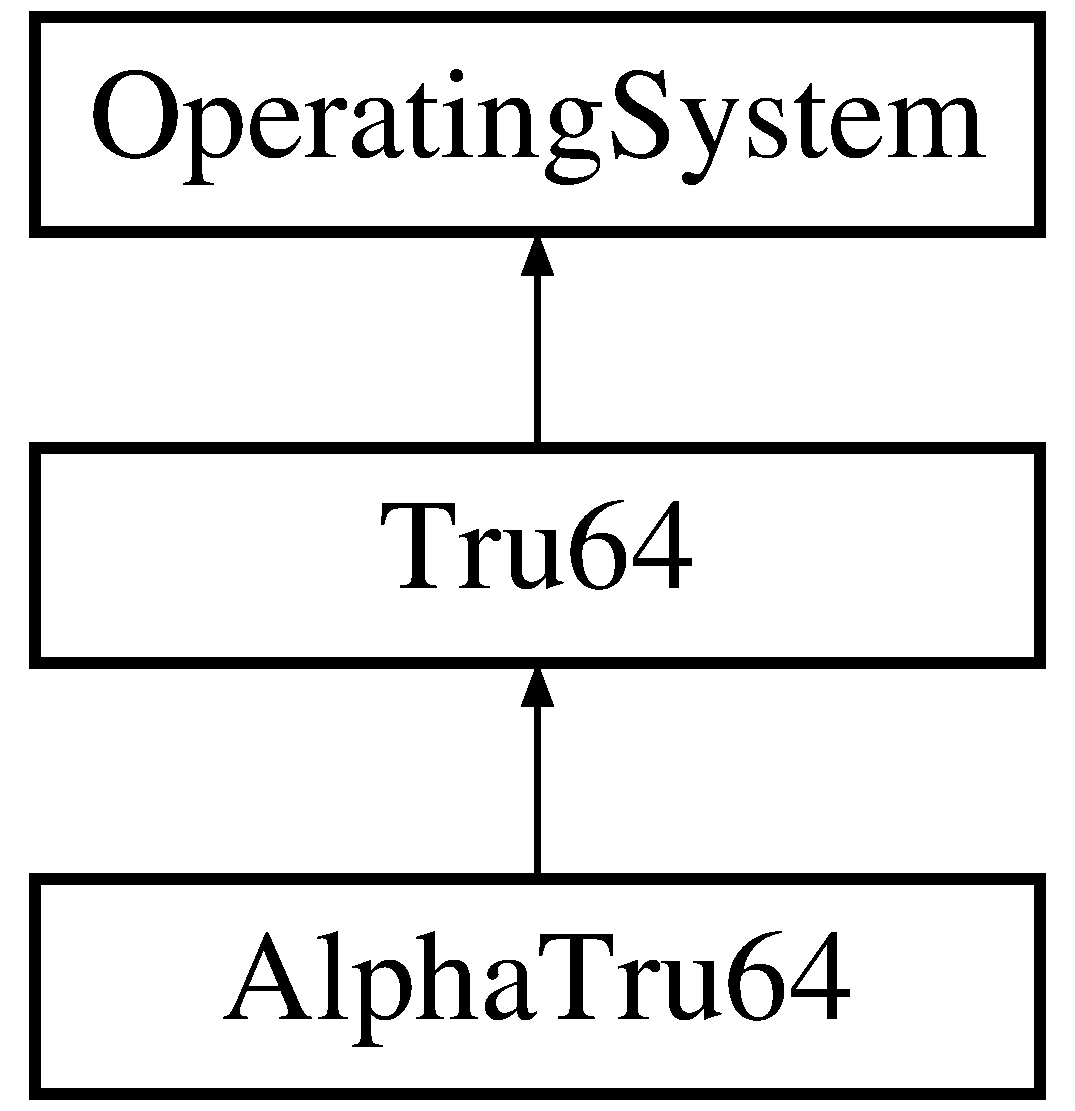
\includegraphics[height=3cm]{classAlphaTru64}
\end{center}
\end{figure}
\subsection*{Public 型}
\begin{DoxyCompactItemize}
\item 
enum \hyperlink{classAlphaTru64_a599454267926920de3bd5a488bda3e03}{rlimit\_\-resources} \{ \par
\hyperlink{classAlphaTru64_a599454267926920de3bd5a488bda3e03ad2d72256a0d172755a5984018f2afad8}{TGT\_\-RLIMIT\_\-CPU} =  0, 
\hyperlink{classAlphaTru64_a599454267926920de3bd5a488bda3e03ae0f07966ad956cd9e702fb01a4f3a9a1}{TGT\_\-RLIMIT\_\-FSIZE} =  1, 
\hyperlink{classAlphaTru64_a599454267926920de3bd5a488bda3e03abcf6a52c98bdfad0832696b231de99a2}{TGT\_\-RLIMIT\_\-DATA} =  2, 
\hyperlink{classAlphaTru64_a599454267926920de3bd5a488bda3e03a08e62a1dfe173892d7a251c73a8a3f6a}{TGT\_\-RLIMIT\_\-STACK} =  3, 
\par
\hyperlink{classAlphaTru64_a599454267926920de3bd5a488bda3e03a89e77f710c8de2c5d30f835b6f9ecff4}{TGT\_\-RLIMIT\_\-CORE} =  4, 
\hyperlink{classAlphaTru64_a599454267926920de3bd5a488bda3e03af8c89e70a7d4ff9e8854599d3a168529}{TGT\_\-RLIMIT\_\-RSS} =  5, 
\hyperlink{classAlphaTru64_a599454267926920de3bd5a488bda3e03af2a76cff253996593d8c22981696e110}{TGT\_\-RLIMIT\_\-NOFILE} =  6, 
\hyperlink{classAlphaTru64_a599454267926920de3bd5a488bda3e03a3f118b58936b90cf8382d441ef567c39}{TGT\_\-RLIMIT\_\-AS} =  7, 
\par
\hyperlink{classAlphaTru64_a599454267926920de3bd5a488bda3e03a3c2043afa66b0d70c66cbbbb6800b97f}{TGT\_\-RLIMIT\_\-VMEM} =  7, 
\hyperlink{classAlphaTru64_a599454267926920de3bd5a488bda3e03af653a805832a388dbc3548d5d06150cb}{TGT\_\-RLIMIT\_\-NPROC} =  8, 
\hyperlink{classAlphaTru64_a599454267926920de3bd5a488bda3e03a1c5dcb48959f77f93f7c104f76b4b88d}{TGT\_\-RLIMIT\_\-MEMLOCK} =  9, 
\hyperlink{classAlphaTru64_a599454267926920de3bd5a488bda3e03aabd123e8e2b5b10d6a26e053b938a3e6}{TGT\_\-RLIMIT\_\-LOCKS} =  10
 \}
\begin{DoxyCompactList}\small\item\em \hyperlink{classResource}{Resource} enumeration for getrlimit(). \item\end{DoxyCompactList}\end{DoxyCompactItemize}
\subsection*{Static Public メソッド}
\begin{DoxyCompactItemize}
\item 
static bool \hyperlink{classAlphaTru64_ab20bdd4422ecf6e1736a5587be296b3f}{isTtyReq} (unsigned req)
\end{DoxyCompactItemize}
\subsection*{Static Public 変数}
\begin{DoxyCompactItemize}
\item 
static \hyperlink{structOpenFlagTransTable}{OpenFlagTransTable} \hyperlink{classAlphaTru64_ab1db5a531609b99b262cc849ea24765a}{openFlagTable} \mbox{[}$\,$\mbox{]}
\item 
static const int \hyperlink{classAlphaTru64_ad85b9918c8f2c8739537a002dc1dc526}{NUM\_\-OPEN\_\-FLAGS}
\begin{DoxyCompactList}\small\item\em Number of entries in openFlagTable\mbox{[}\mbox{]}. \item\end{DoxyCompactList}\item 
static const unsigned \hyperlink{classAlphaTru64_a0bbc267200567dd98250b99b6085a499}{TGT\_\-MAP\_\-ANONYMOUS} = 0x10
\begin{DoxyCompactList}\small\item\em For mmap(). \item\end{DoxyCompactList}\item 
static const unsigned \hyperlink{classAlphaTru64_a0124e421d7846143bca15728b7a53e14}{TGT\_\-MAP\_\-FIXED} = 0x100
\end{DoxyCompactItemize}
\begin{Indent}{\bf }\par
{\em \label{_amgrpd41d8cd98f00b204e9800998ecf8427e}
 }\begin{DoxyCompactItemize}
\item 
static const int \hyperlink{classAlphaTru64_ad266b23a0ae07d1833e18bae651f3411}{TGT\_\-O\_\-RDONLY} = 00000000
\begin{DoxyCompactList}\small\item\em open(2) flag values. \item\end{DoxyCompactList}\item 
static const int \hyperlink{classAlphaTru64_a6156c069cefe05ce3cce033b2e0c2de2}{TGT\_\-O\_\-WRONLY} = 00000001
\begin{DoxyCompactList}\small\item\em O\_\-WRONLY. \item\end{DoxyCompactList}\item 
static const int \hyperlink{classAlphaTru64_ac6fa9ecf5d2f3314f197698f1099e2ac}{TGT\_\-O\_\-RDWR} = 00000002
\begin{DoxyCompactList}\small\item\em O\_\-RDWR. \item\end{DoxyCompactList}\item 
static const int \hyperlink{classAlphaTru64_a0ea5420b4c9b45ba342a266fb77ac942}{TGT\_\-O\_\-NONBLOCK} = 00000004
\begin{DoxyCompactList}\small\item\em O\_\-NONBLOCK. \item\end{DoxyCompactList}\item 
static const int \hyperlink{classAlphaTru64_af11adc5404ea3780a5ce2829cc3710b7}{TGT\_\-O\_\-APPEND} = 00000010
\begin{DoxyCompactList}\small\item\em O\_\-APPEND. \item\end{DoxyCompactList}\item 
static const int \hyperlink{classAlphaTru64_aec02e04ca367e6c3f4b46e4edc12efac}{TGT\_\-O\_\-CREAT} = 00001000
\begin{DoxyCompactList}\small\item\em O\_\-CREAT. \item\end{DoxyCompactList}\item 
static const int \hyperlink{classAlphaTru64_a4f892ee6e1424a2becd859b0bef1f18b}{TGT\_\-O\_\-TRUNC} = 00002000
\begin{DoxyCompactList}\small\item\em O\_\-TRUNC. \item\end{DoxyCompactList}\item 
static const int \hyperlink{classAlphaTru64_a10d5d118d15b51ebdd4b16dc78342d1d}{TGT\_\-O\_\-EXCL} = 00004000
\begin{DoxyCompactList}\small\item\em O\_\-EXCL. \item\end{DoxyCompactList}\item 
static const int \hyperlink{classAlphaTru64_adfd4240281579e5f60c5e22c601225d8}{TGT\_\-O\_\-NOCTTY} = 00010000
\begin{DoxyCompactList}\small\item\em O\_\-NOCTTY. \item\end{DoxyCompactList}\item 
static const int \hyperlink{classAlphaTru64_abf43ab05d2a5b6b8113952160d8565db}{TGT\_\-O\_\-SYNC} = 00040000
\begin{DoxyCompactList}\small\item\em O\_\-SYNC. \item\end{DoxyCompactList}\item 
static const int \hyperlink{classAlphaTru64_a83feaef06c27596d44d489ec51e197fd}{TGT\_\-O\_\-DRD} = 00100000
\begin{DoxyCompactList}\small\item\em O\_\-DRD. \item\end{DoxyCompactList}\item 
static const int \hyperlink{classAlphaTru64_a0a80dc00bd46d433f1ff0d38da2f5ded}{TGT\_\-O\_\-DIRECTIO} = 00200000
\begin{DoxyCompactList}\small\item\em O\_\-DIRECTIO. \item\end{DoxyCompactList}\item 
static const int \hyperlink{classAlphaTru64_ab30a547e309825ec5f9c5d11a6da543c}{TGT\_\-O\_\-CACHE} = 00400000
\begin{DoxyCompactList}\small\item\em O\_\-CACHE. \item\end{DoxyCompactList}\item 
static const int \hyperlink{classAlphaTru64_ac8d84ac6abb2d868443e4559bed55ebe}{TGT\_\-O\_\-DSYNC} = 02000000
\begin{DoxyCompactList}\small\item\em O\_\-DSYNC. \item\end{DoxyCompactList}\item 
static const int \hyperlink{classAlphaTru64_a1b4245158ffbfdc36ae7d6e666ffc261}{TGT\_\-O\_\-RSYNC} = 04000000
\begin{DoxyCompactList}\small\item\em O\_\-RSYNC. \item\end{DoxyCompactList}\item 
static const unsigned \hyperlink{classAlphaTru64_ac2412600f242b3062b887ef0ec4b4908}{GSI\_\-PLATFORM\_\-NAME} = 103
\begin{DoxyCompactList}\small\item\em For getsysinfo(). \item\end{DoxyCompactList}\item 
static const unsigned \hyperlink{classAlphaTru64_ad89f91e0925845385f177d93e4ef7985}{GSI\_\-CPU\_\-INFO} = 59
\begin{DoxyCompactList}\small\item\em CPU information. \item\end{DoxyCompactList}\item 
static const unsigned \hyperlink{classAlphaTru64_a3048b7c97d8a7e86854cdb73520560d0}{GSI\_\-PROC\_\-TYPE} = 60
\begin{DoxyCompactList}\small\item\em get proc\_\-type \item\end{DoxyCompactList}\item 
static const unsigned \hyperlink{classAlphaTru64_a14ed8f49156face38fb0dee35125148d}{GSI\_\-MAX\_\-CPU} = 30
\begin{DoxyCompactList}\small\item\em max \# CPUs on machine \item\end{DoxyCompactList}\item 
static const unsigned \hyperlink{classAlphaTru64_a4df912c77419619f6f242873f65b0045}{GSI\_\-CPUS\_\-IN\_\-BOX} = 55
\begin{DoxyCompactList}\small\item\em number of CPUs in system \item\end{DoxyCompactList}\item 
static const unsigned \hyperlink{classAlphaTru64_a2c859016d59653914527bcd85a154da4}{GSI\_\-PHYSMEM} = 19
\begin{DoxyCompactList}\small\item\em Physical memory in KB. \item\end{DoxyCompactList}\item 
static const unsigned \hyperlink{classAlphaTru64_a26c255cf18ca324c7c09a629e9e2a4f0}{GSI\_\-CLK\_\-TCK} = 42
\begin{DoxyCompactList}\small\item\em clock freq in Hz \item\end{DoxyCompactList}\item 
static const int \hyperlink{classAlphaTru64_af35ba23c7e13a2929bc932a00b2f5c91}{TGT\_\-RUSAGE\_\-THREAD} = 1
\begin{DoxyCompactList}\small\item\em For getrusage(). \item\end{DoxyCompactList}\item 
static const int \hyperlink{classAlphaTru64_a9e303b6c52672934210e6db497f0da88}{TGT\_\-RUSAGE\_\-SELF} = 0
\item 
static const int \hyperlink{classAlphaTru64_a9a340e7463be441b8aeb8ea0a109e1bc}{TGT\_\-RUSAGE\_\-CHILDREN} = -\/1
\item 
static const unsigned \hyperlink{classAlphaTru64_a4dea1885b08c38c78286ecd5ffd5488d}{SSI\_\-IEEE\_\-FP\_\-CONTROL} = 14
\begin{DoxyCompactList}\small\item\em For setsysinfo(). \item\end{DoxyCompactList}\item 
static const unsigned \hyperlink{classAlphaTru64_a90fcc56bd4aa74a5d86c87bfeae77625}{TGT\_\-TIOCGETP} = 0x40067408
\begin{DoxyCompactList}\small\item\em ioctl() command codes. \item\end{DoxyCompactList}\item 
static const unsigned \hyperlink{classAlphaTru64_a194059e48b091a80833c40b500e70bec}{TGT\_\-TIOCSETP} = 0x80067409
\item 
static const unsigned \hyperlink{classAlphaTru64_a6783bea53088dc89157c39a9a7c71988}{TGT\_\-TIOCSETN} = 0x8006740a
\item 
static const unsigned \hyperlink{classAlphaTru64_a98595955a801e37d1d5be450c203afe5}{TGT\_\-TIOCSETC} = 0x80067411
\item 
static const unsigned \hyperlink{classAlphaTru64_ad4f95fbdb4f52f68481c247267675007}{TGT\_\-TIOCGETC} = 0x40067412
\item 
static const unsigned \hyperlink{classAlphaTru64_a1def346ff527c8efccfd52463f3b5dc1}{TGT\_\-FIONREAD} = 0x4004667f
\item 
static const unsigned \hyperlink{classAlphaTru64_a0b4908f73bde5fcd2ce5ea35f6c3786f}{TGT\_\-TIOCISATTY} = 0x2000745e
\item 
static const unsigned \hyperlink{classAlphaTru64_a50e5d880569ec2cb9a2f3d4aaa55cc64}{TGT\_\-TCGETS} = 0x402c7413
\item 
static const unsigned \hyperlink{classAlphaTru64_a804fc265279c5dbd78e0f95da998b267}{TGT\_\-TCGETA} = 0x40127417
\item 
static const unsigned \hyperlink{classAlphaTru64_a96e06e042526ea5e89c4e8a020636c52}{TGT\_\-TCSETAW} = 0x80147419
\item 
static const int \hyperlink{classAlphaTru64_a02a979126f2aa34bcdfdc6ab92207d3b}{TBL\_\-SYSINFO} = 12
\begin{DoxyCompactList}\small\item\em For table(). \item\end{DoxyCompactList}\end{DoxyCompactItemize}
\end{Indent}


\subsection{列挙型}
\hypertarget{classAlphaTru64_a599454267926920de3bd5a488bda3e03}{
\index{AlphaTru64@{AlphaTru64}!rlimit\_\-resources@{rlimit\_\-resources}}
\index{rlimit\_\-resources@{rlimit\_\-resources}!AlphaTru64@{AlphaTru64}}
\subsubsection[{rlimit\_\-resources}]{\setlength{\rightskip}{0pt plus 5cm}enum {\bf rlimit\_\-resources}}}
\label{classAlphaTru64_a599454267926920de3bd5a488bda3e03}


\hyperlink{classResource}{Resource} enumeration for getrlimit(). \begin{Desc}
\item[列挙型の値: ]\par
\begin{description}
\index{TGT\_\-RLIMIT\_\-CPU@{TGT\_\-RLIMIT\_\-CPU}!AlphaTru64@{AlphaTru64}}\index{AlphaTru64@{AlphaTru64}!TGT\_\-RLIMIT\_\-CPU@{TGT\_\-RLIMIT\_\-CPU}}\item[{\em 
\hypertarget{classAlphaTru64_a599454267926920de3bd5a488bda3e03ad2d72256a0d172755a5984018f2afad8}{
TGT\_\-RLIMIT\_\-CPU}
\label{classAlphaTru64_a599454267926920de3bd5a488bda3e03ad2d72256a0d172755a5984018f2afad8}
}]\index{TGT\_\-RLIMIT\_\-FSIZE@{TGT\_\-RLIMIT\_\-FSIZE}!AlphaTru64@{AlphaTru64}}\index{AlphaTru64@{AlphaTru64}!TGT\_\-RLIMIT\_\-FSIZE@{TGT\_\-RLIMIT\_\-FSIZE}}\item[{\em 
\hypertarget{classAlphaTru64_a599454267926920de3bd5a488bda3e03ae0f07966ad956cd9e702fb01a4f3a9a1}{
TGT\_\-RLIMIT\_\-FSIZE}
\label{classAlphaTru64_a599454267926920de3bd5a488bda3e03ae0f07966ad956cd9e702fb01a4f3a9a1}
}]\index{TGT\_\-RLIMIT\_\-DATA@{TGT\_\-RLIMIT\_\-DATA}!AlphaTru64@{AlphaTru64}}\index{AlphaTru64@{AlphaTru64}!TGT\_\-RLIMIT\_\-DATA@{TGT\_\-RLIMIT\_\-DATA}}\item[{\em 
\hypertarget{classAlphaTru64_a599454267926920de3bd5a488bda3e03abcf6a52c98bdfad0832696b231de99a2}{
TGT\_\-RLIMIT\_\-DATA}
\label{classAlphaTru64_a599454267926920de3bd5a488bda3e03abcf6a52c98bdfad0832696b231de99a2}
}]\index{TGT\_\-RLIMIT\_\-STACK@{TGT\_\-RLIMIT\_\-STACK}!AlphaTru64@{AlphaTru64}}\index{AlphaTru64@{AlphaTru64}!TGT\_\-RLIMIT\_\-STACK@{TGT\_\-RLIMIT\_\-STACK}}\item[{\em 
\hypertarget{classAlphaTru64_a599454267926920de3bd5a488bda3e03a08e62a1dfe173892d7a251c73a8a3f6a}{
TGT\_\-RLIMIT\_\-STACK}
\label{classAlphaTru64_a599454267926920de3bd5a488bda3e03a08e62a1dfe173892d7a251c73a8a3f6a}
}]\index{TGT\_\-RLIMIT\_\-CORE@{TGT\_\-RLIMIT\_\-CORE}!AlphaTru64@{AlphaTru64}}\index{AlphaTru64@{AlphaTru64}!TGT\_\-RLIMIT\_\-CORE@{TGT\_\-RLIMIT\_\-CORE}}\item[{\em 
\hypertarget{classAlphaTru64_a599454267926920de3bd5a488bda3e03a89e77f710c8de2c5d30f835b6f9ecff4}{
TGT\_\-RLIMIT\_\-CORE}
\label{classAlphaTru64_a599454267926920de3bd5a488bda3e03a89e77f710c8de2c5d30f835b6f9ecff4}
}]\index{TGT\_\-RLIMIT\_\-RSS@{TGT\_\-RLIMIT\_\-RSS}!AlphaTru64@{AlphaTru64}}\index{AlphaTru64@{AlphaTru64}!TGT\_\-RLIMIT\_\-RSS@{TGT\_\-RLIMIT\_\-RSS}}\item[{\em 
\hypertarget{classAlphaTru64_a599454267926920de3bd5a488bda3e03af8c89e70a7d4ff9e8854599d3a168529}{
TGT\_\-RLIMIT\_\-RSS}
\label{classAlphaTru64_a599454267926920de3bd5a488bda3e03af8c89e70a7d4ff9e8854599d3a168529}
}]\index{TGT\_\-RLIMIT\_\-NOFILE@{TGT\_\-RLIMIT\_\-NOFILE}!AlphaTru64@{AlphaTru64}}\index{AlphaTru64@{AlphaTru64}!TGT\_\-RLIMIT\_\-NOFILE@{TGT\_\-RLIMIT\_\-NOFILE}}\item[{\em 
\hypertarget{classAlphaTru64_a599454267926920de3bd5a488bda3e03af2a76cff253996593d8c22981696e110}{
TGT\_\-RLIMIT\_\-NOFILE}
\label{classAlphaTru64_a599454267926920de3bd5a488bda3e03af2a76cff253996593d8c22981696e110}
}]\index{TGT\_\-RLIMIT\_\-AS@{TGT\_\-RLIMIT\_\-AS}!AlphaTru64@{AlphaTru64}}\index{AlphaTru64@{AlphaTru64}!TGT\_\-RLIMIT\_\-AS@{TGT\_\-RLIMIT\_\-AS}}\item[{\em 
\hypertarget{classAlphaTru64_a599454267926920de3bd5a488bda3e03a3f118b58936b90cf8382d441ef567c39}{
TGT\_\-RLIMIT\_\-AS}
\label{classAlphaTru64_a599454267926920de3bd5a488bda3e03a3f118b58936b90cf8382d441ef567c39}
}]\index{TGT\_\-RLIMIT\_\-VMEM@{TGT\_\-RLIMIT\_\-VMEM}!AlphaTru64@{AlphaTru64}}\index{AlphaTru64@{AlphaTru64}!TGT\_\-RLIMIT\_\-VMEM@{TGT\_\-RLIMIT\_\-VMEM}}\item[{\em 
\hypertarget{classAlphaTru64_a599454267926920de3bd5a488bda3e03a3c2043afa66b0d70c66cbbbb6800b97f}{
TGT\_\-RLIMIT\_\-VMEM}
\label{classAlphaTru64_a599454267926920de3bd5a488bda3e03a3c2043afa66b0d70c66cbbbb6800b97f}
}]\index{TGT\_\-RLIMIT\_\-NPROC@{TGT\_\-RLIMIT\_\-NPROC}!AlphaTru64@{AlphaTru64}}\index{AlphaTru64@{AlphaTru64}!TGT\_\-RLIMIT\_\-NPROC@{TGT\_\-RLIMIT\_\-NPROC}}\item[{\em 
\hypertarget{classAlphaTru64_a599454267926920de3bd5a488bda3e03af653a805832a388dbc3548d5d06150cb}{
TGT\_\-RLIMIT\_\-NPROC}
\label{classAlphaTru64_a599454267926920de3bd5a488bda3e03af653a805832a388dbc3548d5d06150cb}
}]\index{TGT\_\-RLIMIT\_\-MEMLOCK@{TGT\_\-RLIMIT\_\-MEMLOCK}!AlphaTru64@{AlphaTru64}}\index{AlphaTru64@{AlphaTru64}!TGT\_\-RLIMIT\_\-MEMLOCK@{TGT\_\-RLIMIT\_\-MEMLOCK}}\item[{\em 
\hypertarget{classAlphaTru64_a599454267926920de3bd5a488bda3e03a1c5dcb48959f77f93f7c104f76b4b88d}{
TGT\_\-RLIMIT\_\-MEMLOCK}
\label{classAlphaTru64_a599454267926920de3bd5a488bda3e03a1c5dcb48959f77f93f7c104f76b4b88d}
}]\index{TGT\_\-RLIMIT\_\-LOCKS@{TGT\_\-RLIMIT\_\-LOCKS}!AlphaTru64@{AlphaTru64}}\index{AlphaTru64@{AlphaTru64}!TGT\_\-RLIMIT\_\-LOCKS@{TGT\_\-RLIMIT\_\-LOCKS}}\item[{\em 
\hypertarget{classAlphaTru64_a599454267926920de3bd5a488bda3e03aabd123e8e2b5b10d6a26e053b938a3e6}{
TGT\_\-RLIMIT\_\-LOCKS}
\label{classAlphaTru64_a599454267926920de3bd5a488bda3e03aabd123e8e2b5b10d6a26e053b938a3e6}
}]\end{description}
\end{Desc}




\begin{DoxyCode}
132                           {
133         TGT_RLIMIT_CPU = 0,
134         TGT_RLIMIT_FSIZE = 1,
135         TGT_RLIMIT_DATA = 2,
136         TGT_RLIMIT_STACK = 3,
137         TGT_RLIMIT_CORE = 4,
138         TGT_RLIMIT_RSS = 5,
139         TGT_RLIMIT_NOFILE = 6,
140         TGT_RLIMIT_AS = 7,
141         TGT_RLIMIT_VMEM = 7,
142         TGT_RLIMIT_NPROC = 8,
143         TGT_RLIMIT_MEMLOCK = 9,
144         TGT_RLIMIT_LOCKS = 10
145     };
\end{DoxyCode}


\subsection{関数}
\hypertarget{classAlphaTru64_ab20bdd4422ecf6e1736a5587be296b3f}{
\index{AlphaTru64@{AlphaTru64}!isTtyReq@{isTtyReq}}
\index{isTtyReq@{isTtyReq}!AlphaTru64@{AlphaTru64}}
\subsubsection[{isTtyReq}]{\setlength{\rightskip}{0pt plus 5cm}static bool isTtyReq (unsigned {\em req})\hspace{0.3cm}{\ttfamily  \mbox{[}inline, static\mbox{]}}}}
\label{classAlphaTru64_ab20bdd4422ecf6e1736a5587be296b3f}



\begin{DoxyCode}
108     {
109         switch (req) {
110           case TGT_TIOCGETP:
111           case TGT_TIOCSETP:
112           case TGT_TIOCSETN:
113           case TGT_TIOCSETC:
114           case TGT_TIOCGETC:
115           case TGT_FIONREAD:
116           case TGT_TIOCISATTY:
117           case TGT_TCGETS:
118           case TGT_TCGETA:
119           case TGT_TCSETAW:
120             return true;
121           default:
122             return false;
123         }
124     }
\end{DoxyCode}


\subsection{変数}
\hypertarget{classAlphaTru64_a26c255cf18ca324c7c09a629e9e2a4f0}{
\index{AlphaTru64@{AlphaTru64}!GSI\_\-CLK\_\-TCK@{GSI\_\-CLK\_\-TCK}}
\index{GSI\_\-CLK\_\-TCK@{GSI\_\-CLK\_\-TCK}!AlphaTru64@{AlphaTru64}}
\subsubsection[{GSI\_\-CLK\_\-TCK}]{\setlength{\rightskip}{0pt plus 5cm}const unsigned {\bf GSI\_\-CLK\_\-TCK} = 42\hspace{0.3cm}{\ttfamily  \mbox{[}static\mbox{]}}}}
\label{classAlphaTru64_a26c255cf18ca324c7c09a629e9e2a4f0}


clock freq in Hz \hypertarget{classAlphaTru64_ad89f91e0925845385f177d93e4ef7985}{
\index{AlphaTru64@{AlphaTru64}!GSI\_\-CPU\_\-INFO@{GSI\_\-CPU\_\-INFO}}
\index{GSI\_\-CPU\_\-INFO@{GSI\_\-CPU\_\-INFO}!AlphaTru64@{AlphaTru64}}
\subsubsection[{GSI\_\-CPU\_\-INFO}]{\setlength{\rightskip}{0pt plus 5cm}const unsigned {\bf GSI\_\-CPU\_\-INFO} = 59\hspace{0.3cm}{\ttfamily  \mbox{[}static\mbox{]}}}}
\label{classAlphaTru64_ad89f91e0925845385f177d93e4ef7985}


CPU information. \hypertarget{classAlphaTru64_a4df912c77419619f6f242873f65b0045}{
\index{AlphaTru64@{AlphaTru64}!GSI\_\-CPUS\_\-IN\_\-BOX@{GSI\_\-CPUS\_\-IN\_\-BOX}}
\index{GSI\_\-CPUS\_\-IN\_\-BOX@{GSI\_\-CPUS\_\-IN\_\-BOX}!AlphaTru64@{AlphaTru64}}
\subsubsection[{GSI\_\-CPUS\_\-IN\_\-BOX}]{\setlength{\rightskip}{0pt plus 5cm}const unsigned {\bf GSI\_\-CPUS\_\-IN\_\-BOX} = 55\hspace{0.3cm}{\ttfamily  \mbox{[}static\mbox{]}}}}
\label{classAlphaTru64_a4df912c77419619f6f242873f65b0045}


number of CPUs in system \hypertarget{classAlphaTru64_a14ed8f49156face38fb0dee35125148d}{
\index{AlphaTru64@{AlphaTru64}!GSI\_\-MAX\_\-CPU@{GSI\_\-MAX\_\-CPU}}
\index{GSI\_\-MAX\_\-CPU@{GSI\_\-MAX\_\-CPU}!AlphaTru64@{AlphaTru64}}
\subsubsection[{GSI\_\-MAX\_\-CPU}]{\setlength{\rightskip}{0pt plus 5cm}const unsigned {\bf GSI\_\-MAX\_\-CPU} = 30\hspace{0.3cm}{\ttfamily  \mbox{[}static\mbox{]}}}}
\label{classAlphaTru64_a14ed8f49156face38fb0dee35125148d}


max \# CPUs on machine \hypertarget{classAlphaTru64_a2c859016d59653914527bcd85a154da4}{
\index{AlphaTru64@{AlphaTru64}!GSI\_\-PHYSMEM@{GSI\_\-PHYSMEM}}
\index{GSI\_\-PHYSMEM@{GSI\_\-PHYSMEM}!AlphaTru64@{AlphaTru64}}
\subsubsection[{GSI\_\-PHYSMEM}]{\setlength{\rightskip}{0pt plus 5cm}const unsigned {\bf GSI\_\-PHYSMEM} = 19\hspace{0.3cm}{\ttfamily  \mbox{[}static\mbox{]}}}}
\label{classAlphaTru64_a2c859016d59653914527bcd85a154da4}


Physical memory in KB. \hypertarget{classAlphaTru64_ac2412600f242b3062b887ef0ec4b4908}{
\index{AlphaTru64@{AlphaTru64}!GSI\_\-PLATFORM\_\-NAME@{GSI\_\-PLATFORM\_\-NAME}}
\index{GSI\_\-PLATFORM\_\-NAME@{GSI\_\-PLATFORM\_\-NAME}!AlphaTru64@{AlphaTru64}}
\subsubsection[{GSI\_\-PLATFORM\_\-NAME}]{\setlength{\rightskip}{0pt plus 5cm}const unsigned {\bf GSI\_\-PLATFORM\_\-NAME} = 103\hspace{0.3cm}{\ttfamily  \mbox{[}static\mbox{]}}}}
\label{classAlphaTru64_ac2412600f242b3062b887ef0ec4b4908}


For getsysinfo(). platform name string \hypertarget{classAlphaTru64_a3048b7c97d8a7e86854cdb73520560d0}{
\index{AlphaTru64@{AlphaTru64}!GSI\_\-PROC\_\-TYPE@{GSI\_\-PROC\_\-TYPE}}
\index{GSI\_\-PROC\_\-TYPE@{GSI\_\-PROC\_\-TYPE}!AlphaTru64@{AlphaTru64}}
\subsubsection[{GSI\_\-PROC\_\-TYPE}]{\setlength{\rightskip}{0pt plus 5cm}const unsigned {\bf GSI\_\-PROC\_\-TYPE} = 60\hspace{0.3cm}{\ttfamily  \mbox{[}static\mbox{]}}}}
\label{classAlphaTru64_a3048b7c97d8a7e86854cdb73520560d0}


get proc\_\-type \hypertarget{classAlphaTru64_ad85b9918c8f2c8739537a002dc1dc526}{
\index{AlphaTru64@{AlphaTru64}!NUM\_\-OPEN\_\-FLAGS@{NUM\_\-OPEN\_\-FLAGS}}
\index{NUM\_\-OPEN\_\-FLAGS@{NUM\_\-OPEN\_\-FLAGS}!AlphaTru64@{AlphaTru64}}
\subsubsection[{NUM\_\-OPEN\_\-FLAGS}]{\setlength{\rightskip}{0pt plus 5cm}const int {\bf NUM\_\-OPEN\_\-FLAGS}\hspace{0.3cm}{\ttfamily  \mbox{[}static\mbox{]}}}}
\label{classAlphaTru64_ad85b9918c8f2c8739537a002dc1dc526}
{\bfseries 初期値:}
\begin{DoxyCode}

        (sizeof(AlphaTru64::openFlagTable)/sizeof(AlphaTru64::openFlagTable[0]))
\end{DoxyCode}


Number of entries in openFlagTable\mbox{[}\mbox{]}. \hypertarget{classAlphaTru64_ab1db5a531609b99b262cc849ea24765a}{
\index{AlphaTru64@{AlphaTru64}!openFlagTable@{openFlagTable}}
\index{openFlagTable@{openFlagTable}!AlphaTru64@{AlphaTru64}}
\subsubsection[{openFlagTable}]{\setlength{\rightskip}{0pt plus 5cm}{\bf OpenFlagTransTable} {\bf openFlagTable}\hspace{0.3cm}{\ttfamily  \mbox{[}static\mbox{]}}}}
\label{classAlphaTru64_ab1db5a531609b99b262cc849ea24765a}
This table maps the target open() flags to the corresponding host open() flags. \hypertarget{classAlphaTru64_a4dea1885b08c38c78286ecd5ffd5488d}{
\index{AlphaTru64@{AlphaTru64}!SSI\_\-IEEE\_\-FP\_\-CONTROL@{SSI\_\-IEEE\_\-FP\_\-CONTROL}}
\index{SSI\_\-IEEE\_\-FP\_\-CONTROL@{SSI\_\-IEEE\_\-FP\_\-CONTROL}!AlphaTru64@{AlphaTru64}}
\subsubsection[{SSI\_\-IEEE\_\-FP\_\-CONTROL}]{\setlength{\rightskip}{0pt plus 5cm}const unsigned {\bf SSI\_\-IEEE\_\-FP\_\-CONTROL} = 14\hspace{0.3cm}{\ttfamily  \mbox{[}static\mbox{]}}}}
\label{classAlphaTru64_a4dea1885b08c38c78286ecd5ffd5488d}


For setsysinfo(). ieee\_\-set\_\-fp\_\-control() \hypertarget{classAlphaTru64_a02a979126f2aa34bcdfdc6ab92207d3b}{
\index{AlphaTru64@{AlphaTru64}!TBL\_\-SYSINFO@{TBL\_\-SYSINFO}}
\index{TBL\_\-SYSINFO@{TBL\_\-SYSINFO}!AlphaTru64@{AlphaTru64}}
\subsubsection[{TBL\_\-SYSINFO}]{\setlength{\rightskip}{0pt plus 5cm}const int {\bf TBL\_\-SYSINFO} = 12\hspace{0.3cm}{\ttfamily  \mbox{[}static\mbox{]}}}}
\label{classAlphaTru64_a02a979126f2aa34bcdfdc6ab92207d3b}


For table(). \hypertarget{classAlphaTru64_a1def346ff527c8efccfd52463f3b5dc1}{
\index{AlphaTru64@{AlphaTru64}!TGT\_\-FIONREAD@{TGT\_\-FIONREAD}}
\index{TGT\_\-FIONREAD@{TGT\_\-FIONREAD}!AlphaTru64@{AlphaTru64}}
\subsubsection[{TGT\_\-FIONREAD}]{\setlength{\rightskip}{0pt plus 5cm}const unsigned {\bf TGT\_\-FIONREAD} = 0x4004667f\hspace{0.3cm}{\ttfamily  \mbox{[}static\mbox{]}}}}
\label{classAlphaTru64_a1def346ff527c8efccfd52463f3b5dc1}
\hypertarget{classAlphaTru64_a0bbc267200567dd98250b99b6085a499}{
\index{AlphaTru64@{AlphaTru64}!TGT\_\-MAP\_\-ANONYMOUS@{TGT\_\-MAP\_\-ANONYMOUS}}
\index{TGT\_\-MAP\_\-ANONYMOUS@{TGT\_\-MAP\_\-ANONYMOUS}!AlphaTru64@{AlphaTru64}}
\subsubsection[{TGT\_\-MAP\_\-ANONYMOUS}]{\setlength{\rightskip}{0pt plus 5cm}const unsigned {\bf TGT\_\-MAP\_\-ANONYMOUS} = 0x10\hspace{0.3cm}{\ttfamily  \mbox{[}static\mbox{]}}}}
\label{classAlphaTru64_a0bbc267200567dd98250b99b6085a499}


For mmap(). \hypertarget{classAlphaTru64_a0124e421d7846143bca15728b7a53e14}{
\index{AlphaTru64@{AlphaTru64}!TGT\_\-MAP\_\-FIXED@{TGT\_\-MAP\_\-FIXED}}
\index{TGT\_\-MAP\_\-FIXED@{TGT\_\-MAP\_\-FIXED}!AlphaTru64@{AlphaTru64}}
\subsubsection[{TGT\_\-MAP\_\-FIXED}]{\setlength{\rightskip}{0pt plus 5cm}const unsigned {\bf TGT\_\-MAP\_\-FIXED} = 0x100\hspace{0.3cm}{\ttfamily  \mbox{[}static\mbox{]}}}}
\label{classAlphaTru64_a0124e421d7846143bca15728b7a53e14}
\hypertarget{classAlphaTru64_af11adc5404ea3780a5ce2829cc3710b7}{
\index{AlphaTru64@{AlphaTru64}!TGT\_\-O\_\-APPEND@{TGT\_\-O\_\-APPEND}}
\index{TGT\_\-O\_\-APPEND@{TGT\_\-O\_\-APPEND}!AlphaTru64@{AlphaTru64}}
\subsubsection[{TGT\_\-O\_\-APPEND}]{\setlength{\rightskip}{0pt plus 5cm}const int {\bf TGT\_\-O\_\-APPEND} = 00000010\hspace{0.3cm}{\ttfamily  \mbox{[}static\mbox{]}}}}
\label{classAlphaTru64_af11adc5404ea3780a5ce2829cc3710b7}


O\_\-APPEND. \hypertarget{classAlphaTru64_ab30a547e309825ec5f9c5d11a6da543c}{
\index{AlphaTru64@{AlphaTru64}!TGT\_\-O\_\-CACHE@{TGT\_\-O\_\-CACHE}}
\index{TGT\_\-O\_\-CACHE@{TGT\_\-O\_\-CACHE}!AlphaTru64@{AlphaTru64}}
\subsubsection[{TGT\_\-O\_\-CACHE}]{\setlength{\rightskip}{0pt plus 5cm}const int {\bf TGT\_\-O\_\-CACHE} = 00400000\hspace{0.3cm}{\ttfamily  \mbox{[}static\mbox{]}}}}
\label{classAlphaTru64_ab30a547e309825ec5f9c5d11a6da543c}


O\_\-CACHE. \hypertarget{classAlphaTru64_aec02e04ca367e6c3f4b46e4edc12efac}{
\index{AlphaTru64@{AlphaTru64}!TGT\_\-O\_\-CREAT@{TGT\_\-O\_\-CREAT}}
\index{TGT\_\-O\_\-CREAT@{TGT\_\-O\_\-CREAT}!AlphaTru64@{AlphaTru64}}
\subsubsection[{TGT\_\-O\_\-CREAT}]{\setlength{\rightskip}{0pt plus 5cm}const int {\bf TGT\_\-O\_\-CREAT} = 00001000\hspace{0.3cm}{\ttfamily  \mbox{[}static\mbox{]}}}}
\label{classAlphaTru64_aec02e04ca367e6c3f4b46e4edc12efac}


O\_\-CREAT. \hypertarget{classAlphaTru64_a0a80dc00bd46d433f1ff0d38da2f5ded}{
\index{AlphaTru64@{AlphaTru64}!TGT\_\-O\_\-DIRECTIO@{TGT\_\-O\_\-DIRECTIO}}
\index{TGT\_\-O\_\-DIRECTIO@{TGT\_\-O\_\-DIRECTIO}!AlphaTru64@{AlphaTru64}}
\subsubsection[{TGT\_\-O\_\-DIRECTIO}]{\setlength{\rightskip}{0pt plus 5cm}const int {\bf TGT\_\-O\_\-DIRECTIO} = 00200000\hspace{0.3cm}{\ttfamily  \mbox{[}static\mbox{]}}}}
\label{classAlphaTru64_a0a80dc00bd46d433f1ff0d38da2f5ded}


O\_\-DIRECTIO. \hypertarget{classAlphaTru64_a83feaef06c27596d44d489ec51e197fd}{
\index{AlphaTru64@{AlphaTru64}!TGT\_\-O\_\-DRD@{TGT\_\-O\_\-DRD}}
\index{TGT\_\-O\_\-DRD@{TGT\_\-O\_\-DRD}!AlphaTru64@{AlphaTru64}}
\subsubsection[{TGT\_\-O\_\-DRD}]{\setlength{\rightskip}{0pt plus 5cm}const int {\bf TGT\_\-O\_\-DRD} = 00100000\hspace{0.3cm}{\ttfamily  \mbox{[}static\mbox{]}}}}
\label{classAlphaTru64_a83feaef06c27596d44d489ec51e197fd}


O\_\-DRD. \hypertarget{classAlphaTru64_ac8d84ac6abb2d868443e4559bed55ebe}{
\index{AlphaTru64@{AlphaTru64}!TGT\_\-O\_\-DSYNC@{TGT\_\-O\_\-DSYNC}}
\index{TGT\_\-O\_\-DSYNC@{TGT\_\-O\_\-DSYNC}!AlphaTru64@{AlphaTru64}}
\subsubsection[{TGT\_\-O\_\-DSYNC}]{\setlength{\rightskip}{0pt plus 5cm}const int {\bf TGT\_\-O\_\-DSYNC} = 02000000\hspace{0.3cm}{\ttfamily  \mbox{[}static\mbox{]}}}}
\label{classAlphaTru64_ac8d84ac6abb2d868443e4559bed55ebe}


O\_\-DSYNC. \hypertarget{classAlphaTru64_a10d5d118d15b51ebdd4b16dc78342d1d}{
\index{AlphaTru64@{AlphaTru64}!TGT\_\-O\_\-EXCL@{TGT\_\-O\_\-EXCL}}
\index{TGT\_\-O\_\-EXCL@{TGT\_\-O\_\-EXCL}!AlphaTru64@{AlphaTru64}}
\subsubsection[{TGT\_\-O\_\-EXCL}]{\setlength{\rightskip}{0pt plus 5cm}const int {\bf TGT\_\-O\_\-EXCL} = 00004000\hspace{0.3cm}{\ttfamily  \mbox{[}static\mbox{]}}}}
\label{classAlphaTru64_a10d5d118d15b51ebdd4b16dc78342d1d}


O\_\-EXCL. \hypertarget{classAlphaTru64_adfd4240281579e5f60c5e22c601225d8}{
\index{AlphaTru64@{AlphaTru64}!TGT\_\-O\_\-NOCTTY@{TGT\_\-O\_\-NOCTTY}}
\index{TGT\_\-O\_\-NOCTTY@{TGT\_\-O\_\-NOCTTY}!AlphaTru64@{AlphaTru64}}
\subsubsection[{TGT\_\-O\_\-NOCTTY}]{\setlength{\rightskip}{0pt plus 5cm}const int {\bf TGT\_\-O\_\-NOCTTY} = 00010000\hspace{0.3cm}{\ttfamily  \mbox{[}static\mbox{]}}}}
\label{classAlphaTru64_adfd4240281579e5f60c5e22c601225d8}


O\_\-NOCTTY. \hypertarget{classAlphaTru64_a0ea5420b4c9b45ba342a266fb77ac942}{
\index{AlphaTru64@{AlphaTru64}!TGT\_\-O\_\-NONBLOCK@{TGT\_\-O\_\-NONBLOCK}}
\index{TGT\_\-O\_\-NONBLOCK@{TGT\_\-O\_\-NONBLOCK}!AlphaTru64@{AlphaTru64}}
\subsubsection[{TGT\_\-O\_\-NONBLOCK}]{\setlength{\rightskip}{0pt plus 5cm}const int {\bf TGT\_\-O\_\-NONBLOCK} = 00000004\hspace{0.3cm}{\ttfamily  \mbox{[}static\mbox{]}}}}
\label{classAlphaTru64_a0ea5420b4c9b45ba342a266fb77ac942}


O\_\-NONBLOCK. \hypertarget{classAlphaTru64_ad266b23a0ae07d1833e18bae651f3411}{
\index{AlphaTru64@{AlphaTru64}!TGT\_\-O\_\-RDONLY@{TGT\_\-O\_\-RDONLY}}
\index{TGT\_\-O\_\-RDONLY@{TGT\_\-O\_\-RDONLY}!AlphaTru64@{AlphaTru64}}
\subsubsection[{TGT\_\-O\_\-RDONLY}]{\setlength{\rightskip}{0pt plus 5cm}const int {\bf TGT\_\-O\_\-RDONLY} = 00000000\hspace{0.3cm}{\ttfamily  \mbox{[}static\mbox{]}}}}
\label{classAlphaTru64_ad266b23a0ae07d1833e18bae651f3411}


open(2) flag values. O\_\-RDONLY \hypertarget{classAlphaTru64_ac6fa9ecf5d2f3314f197698f1099e2ac}{
\index{AlphaTru64@{AlphaTru64}!TGT\_\-O\_\-RDWR@{TGT\_\-O\_\-RDWR}}
\index{TGT\_\-O\_\-RDWR@{TGT\_\-O\_\-RDWR}!AlphaTru64@{AlphaTru64}}
\subsubsection[{TGT\_\-O\_\-RDWR}]{\setlength{\rightskip}{0pt plus 5cm}const int {\bf TGT\_\-O\_\-RDWR} = 00000002\hspace{0.3cm}{\ttfamily  \mbox{[}static\mbox{]}}}}
\label{classAlphaTru64_ac6fa9ecf5d2f3314f197698f1099e2ac}


O\_\-RDWR. \hypertarget{classAlphaTru64_a1b4245158ffbfdc36ae7d6e666ffc261}{
\index{AlphaTru64@{AlphaTru64}!TGT\_\-O\_\-RSYNC@{TGT\_\-O\_\-RSYNC}}
\index{TGT\_\-O\_\-RSYNC@{TGT\_\-O\_\-RSYNC}!AlphaTru64@{AlphaTru64}}
\subsubsection[{TGT\_\-O\_\-RSYNC}]{\setlength{\rightskip}{0pt plus 5cm}const int {\bf TGT\_\-O\_\-RSYNC} = 04000000\hspace{0.3cm}{\ttfamily  \mbox{[}static\mbox{]}}}}
\label{classAlphaTru64_a1b4245158ffbfdc36ae7d6e666ffc261}


O\_\-RSYNC. \hypertarget{classAlphaTru64_abf43ab05d2a5b6b8113952160d8565db}{
\index{AlphaTru64@{AlphaTru64}!TGT\_\-O\_\-SYNC@{TGT\_\-O\_\-SYNC}}
\index{TGT\_\-O\_\-SYNC@{TGT\_\-O\_\-SYNC}!AlphaTru64@{AlphaTru64}}
\subsubsection[{TGT\_\-O\_\-SYNC}]{\setlength{\rightskip}{0pt plus 5cm}const int {\bf TGT\_\-O\_\-SYNC} = 00040000\hspace{0.3cm}{\ttfamily  \mbox{[}static\mbox{]}}}}
\label{classAlphaTru64_abf43ab05d2a5b6b8113952160d8565db}


O\_\-SYNC. \hypertarget{classAlphaTru64_a4f892ee6e1424a2becd859b0bef1f18b}{
\index{AlphaTru64@{AlphaTru64}!TGT\_\-O\_\-TRUNC@{TGT\_\-O\_\-TRUNC}}
\index{TGT\_\-O\_\-TRUNC@{TGT\_\-O\_\-TRUNC}!AlphaTru64@{AlphaTru64}}
\subsubsection[{TGT\_\-O\_\-TRUNC}]{\setlength{\rightskip}{0pt plus 5cm}const int {\bf TGT\_\-O\_\-TRUNC} = 00002000\hspace{0.3cm}{\ttfamily  \mbox{[}static\mbox{]}}}}
\label{classAlphaTru64_a4f892ee6e1424a2becd859b0bef1f18b}


O\_\-TRUNC. \hypertarget{classAlphaTru64_a6156c069cefe05ce3cce033b2e0c2de2}{
\index{AlphaTru64@{AlphaTru64}!TGT\_\-O\_\-WRONLY@{TGT\_\-O\_\-WRONLY}}
\index{TGT\_\-O\_\-WRONLY@{TGT\_\-O\_\-WRONLY}!AlphaTru64@{AlphaTru64}}
\subsubsection[{TGT\_\-O\_\-WRONLY}]{\setlength{\rightskip}{0pt plus 5cm}const int {\bf TGT\_\-O\_\-WRONLY} = 00000001\hspace{0.3cm}{\ttfamily  \mbox{[}static\mbox{]}}}}
\label{classAlphaTru64_a6156c069cefe05ce3cce033b2e0c2de2}


O\_\-WRONLY. \hypertarget{classAlphaTru64_a9a340e7463be441b8aeb8ea0a109e1bc}{
\index{AlphaTru64@{AlphaTru64}!TGT\_\-RUSAGE\_\-CHILDREN@{TGT\_\-RUSAGE\_\-CHILDREN}}
\index{TGT\_\-RUSAGE\_\-CHILDREN@{TGT\_\-RUSAGE\_\-CHILDREN}!AlphaTru64@{AlphaTru64}}
\subsubsection[{TGT\_\-RUSAGE\_\-CHILDREN}]{\setlength{\rightskip}{0pt plus 5cm}const int {\bf TGT\_\-RUSAGE\_\-CHILDREN} = -\/1\hspace{0.3cm}{\ttfamily  \mbox{[}static\mbox{]}}}}
\label{classAlphaTru64_a9a340e7463be441b8aeb8ea0a109e1bc}
\hypertarget{classAlphaTru64_a9e303b6c52672934210e6db497f0da88}{
\index{AlphaTru64@{AlphaTru64}!TGT\_\-RUSAGE\_\-SELF@{TGT\_\-RUSAGE\_\-SELF}}
\index{TGT\_\-RUSAGE\_\-SELF@{TGT\_\-RUSAGE\_\-SELF}!AlphaTru64@{AlphaTru64}}
\subsubsection[{TGT\_\-RUSAGE\_\-SELF}]{\setlength{\rightskip}{0pt plus 5cm}const int {\bf TGT\_\-RUSAGE\_\-SELF} = 0\hspace{0.3cm}{\ttfamily  \mbox{[}static\mbox{]}}}}
\label{classAlphaTru64_a9e303b6c52672934210e6db497f0da88}
\hypertarget{classAlphaTru64_af35ba23c7e13a2929bc932a00b2f5c91}{
\index{AlphaTru64@{AlphaTru64}!TGT\_\-RUSAGE\_\-THREAD@{TGT\_\-RUSAGE\_\-THREAD}}
\index{TGT\_\-RUSAGE\_\-THREAD@{TGT\_\-RUSAGE\_\-THREAD}!AlphaTru64@{AlphaTru64}}
\subsubsection[{TGT\_\-RUSAGE\_\-THREAD}]{\setlength{\rightskip}{0pt plus 5cm}const int {\bf TGT\_\-RUSAGE\_\-THREAD} = 1\hspace{0.3cm}{\ttfamily  \mbox{[}static\mbox{]}}}}
\label{classAlphaTru64_af35ba23c7e13a2929bc932a00b2f5c91}


For getrusage(). \hypertarget{classAlphaTru64_a804fc265279c5dbd78e0f95da998b267}{
\index{AlphaTru64@{AlphaTru64}!TGT\_\-TCGETA@{TGT\_\-TCGETA}}
\index{TGT\_\-TCGETA@{TGT\_\-TCGETA}!AlphaTru64@{AlphaTru64}}
\subsubsection[{TGT\_\-TCGETA}]{\setlength{\rightskip}{0pt plus 5cm}const unsigned {\bf TGT\_\-TCGETA} = 0x40127417\hspace{0.3cm}{\ttfamily  \mbox{[}static\mbox{]}}}}
\label{classAlphaTru64_a804fc265279c5dbd78e0f95da998b267}
\hypertarget{classAlphaTru64_a50e5d880569ec2cb9a2f3d4aaa55cc64}{
\index{AlphaTru64@{AlphaTru64}!TGT\_\-TCGETS@{TGT\_\-TCGETS}}
\index{TGT\_\-TCGETS@{TGT\_\-TCGETS}!AlphaTru64@{AlphaTru64}}
\subsubsection[{TGT\_\-TCGETS}]{\setlength{\rightskip}{0pt plus 5cm}const unsigned {\bf TGT\_\-TCGETS} = 0x402c7413\hspace{0.3cm}{\ttfamily  \mbox{[}static\mbox{]}}}}
\label{classAlphaTru64_a50e5d880569ec2cb9a2f3d4aaa55cc64}
\hypertarget{classAlphaTru64_a96e06e042526ea5e89c4e8a020636c52}{
\index{AlphaTru64@{AlphaTru64}!TGT\_\-TCSETAW@{TGT\_\-TCSETAW}}
\index{TGT\_\-TCSETAW@{TGT\_\-TCSETAW}!AlphaTru64@{AlphaTru64}}
\subsubsection[{TGT\_\-TCSETAW}]{\setlength{\rightskip}{0pt plus 5cm}const unsigned {\bf TGT\_\-TCSETAW} = 0x80147419\hspace{0.3cm}{\ttfamily  \mbox{[}static\mbox{]}}}}
\label{classAlphaTru64_a96e06e042526ea5e89c4e8a020636c52}
\hypertarget{classAlphaTru64_ad4f95fbdb4f52f68481c247267675007}{
\index{AlphaTru64@{AlphaTru64}!TGT\_\-TIOCGETC@{TGT\_\-TIOCGETC}}
\index{TGT\_\-TIOCGETC@{TGT\_\-TIOCGETC}!AlphaTru64@{AlphaTru64}}
\subsubsection[{TGT\_\-TIOCGETC}]{\setlength{\rightskip}{0pt plus 5cm}const unsigned {\bf TGT\_\-TIOCGETC} = 0x40067412\hspace{0.3cm}{\ttfamily  \mbox{[}static\mbox{]}}}}
\label{classAlphaTru64_ad4f95fbdb4f52f68481c247267675007}
\hypertarget{classAlphaTru64_a90fcc56bd4aa74a5d86c87bfeae77625}{
\index{AlphaTru64@{AlphaTru64}!TGT\_\-TIOCGETP@{TGT\_\-TIOCGETP}}
\index{TGT\_\-TIOCGETP@{TGT\_\-TIOCGETP}!AlphaTru64@{AlphaTru64}}
\subsubsection[{TGT\_\-TIOCGETP}]{\setlength{\rightskip}{0pt plus 5cm}const unsigned {\bf TGT\_\-TIOCGETP} = 0x40067408\hspace{0.3cm}{\ttfamily  \mbox{[}static\mbox{]}}}}
\label{classAlphaTru64_a90fcc56bd4aa74a5d86c87bfeae77625}


ioctl() command codes. \hypertarget{classAlphaTru64_a0b4908f73bde5fcd2ce5ea35f6c3786f}{
\index{AlphaTru64@{AlphaTru64}!TGT\_\-TIOCISATTY@{TGT\_\-TIOCISATTY}}
\index{TGT\_\-TIOCISATTY@{TGT\_\-TIOCISATTY}!AlphaTru64@{AlphaTru64}}
\subsubsection[{TGT\_\-TIOCISATTY}]{\setlength{\rightskip}{0pt plus 5cm}const unsigned {\bf TGT\_\-TIOCISATTY} = 0x2000745e\hspace{0.3cm}{\ttfamily  \mbox{[}static\mbox{]}}}}
\label{classAlphaTru64_a0b4908f73bde5fcd2ce5ea35f6c3786f}
\hypertarget{classAlphaTru64_a98595955a801e37d1d5be450c203afe5}{
\index{AlphaTru64@{AlphaTru64}!TGT\_\-TIOCSETC@{TGT\_\-TIOCSETC}}
\index{TGT\_\-TIOCSETC@{TGT\_\-TIOCSETC}!AlphaTru64@{AlphaTru64}}
\subsubsection[{TGT\_\-TIOCSETC}]{\setlength{\rightskip}{0pt plus 5cm}const unsigned {\bf TGT\_\-TIOCSETC} = 0x80067411\hspace{0.3cm}{\ttfamily  \mbox{[}static\mbox{]}}}}
\label{classAlphaTru64_a98595955a801e37d1d5be450c203afe5}
\hypertarget{classAlphaTru64_a6783bea53088dc89157c39a9a7c71988}{
\index{AlphaTru64@{AlphaTru64}!TGT\_\-TIOCSETN@{TGT\_\-TIOCSETN}}
\index{TGT\_\-TIOCSETN@{TGT\_\-TIOCSETN}!AlphaTru64@{AlphaTru64}}
\subsubsection[{TGT\_\-TIOCSETN}]{\setlength{\rightskip}{0pt plus 5cm}const unsigned {\bf TGT\_\-TIOCSETN} = 0x8006740a\hspace{0.3cm}{\ttfamily  \mbox{[}static\mbox{]}}}}
\label{classAlphaTru64_a6783bea53088dc89157c39a9a7c71988}
\hypertarget{classAlphaTru64_a194059e48b091a80833c40b500e70bec}{
\index{AlphaTru64@{AlphaTru64}!TGT\_\-TIOCSETP@{TGT\_\-TIOCSETP}}
\index{TGT\_\-TIOCSETP@{TGT\_\-TIOCSETP}!AlphaTru64@{AlphaTru64}}
\subsubsection[{TGT\_\-TIOCSETP}]{\setlength{\rightskip}{0pt plus 5cm}const unsigned {\bf TGT\_\-TIOCSETP} = 0x80067409\hspace{0.3cm}{\ttfamily  \mbox{[}static\mbox{]}}}}
\label{classAlphaTru64_a194059e48b091a80833c40b500e70bec}


このクラスの説明は次のファイルから生成されました:\begin{DoxyCompactItemize}
\item 
arch/alpha/tru64/\hyperlink{arch_2alpha_2tru64_2tru64_8hh}{tru64.hh}\item 
arch/alpha/tru64/\hyperlink{tru64_8cc}{tru64.cc}\end{DoxyCompactItemize}

\hypertarget{classAlphaISA_1_1AlphaTru64Process}{
\section{クラス AlphaTru64Process}
\label{classAlphaISA_1_1AlphaTru64Process}\index{AlphaISA::AlphaTru64Process@{AlphaISA::AlphaTru64Process}}
}


A process with emulated Alpha \hyperlink{classTru64}{Tru64} syscalls.  


{\ttfamily \#include $<$process.hh$>$}AlphaTru64Processに対する継承グラフ:\begin{figure}[H]
\begin{center}
\leavevmode
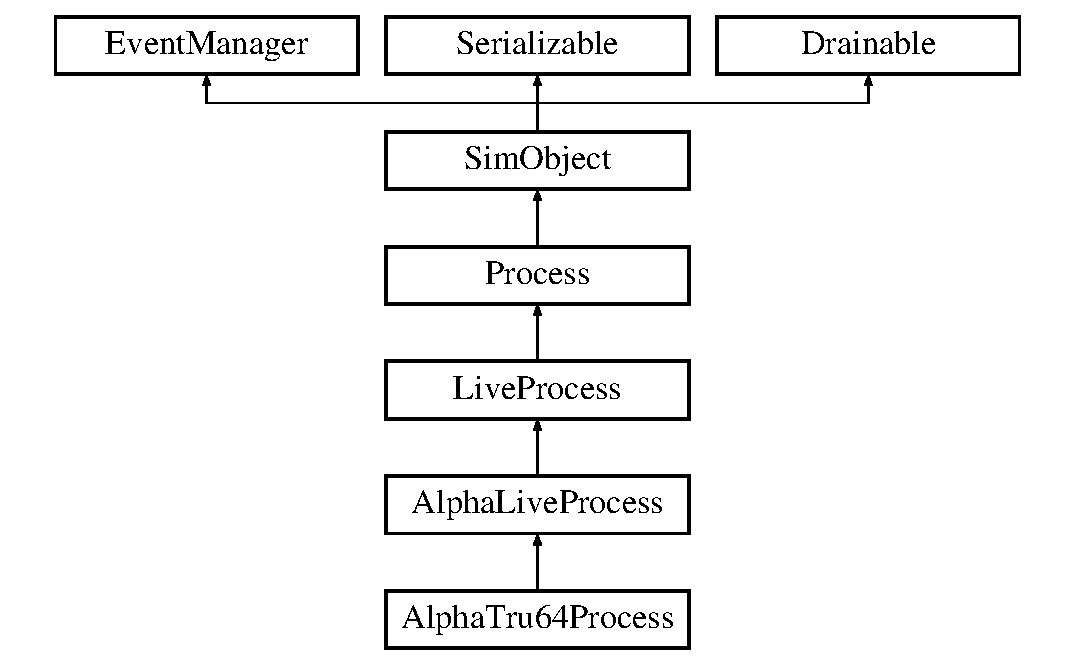
\includegraphics[height=6cm]{classAlphaISA_1_1AlphaTru64Process}
\end{center}
\end{figure}
\subsection*{Public メソッド}
\begin{DoxyCompactItemize}
\item 
\hyperlink{classAlphaISA_1_1AlphaTru64Process_ab52e01bd8111d3d5aff45bdf7027d869}{AlphaTru64Process} (LiveProcessParams $\ast$params, \hyperlink{classObjectFile}{ObjectFile} $\ast$\hyperlink{classLiveProcess_ab6cfcfa7903c66267b3e0351c3caa809}{objFile})
\begin{DoxyCompactList}\small\item\em Constructor. \item\end{DoxyCompactList}\item 
virtual \hyperlink{classSyscallDesc}{SyscallDesc} $\ast$ \hyperlink{classAlphaISA_1_1AlphaTru64Process_aebbff609a7235342925445690acf5ee8}{getDesc} (int callnum)
\end{DoxyCompactItemize}
\subsection*{Public 変数}
\begin{DoxyCompactItemize}
\item 
const int \hyperlink{classAlphaISA_1_1AlphaTru64Process_a9534988905c6f5c8c57c4b6a7b179fea}{Num\_\-Syscall\_\-Descs}
\item 
const int \hyperlink{classAlphaISA_1_1AlphaTru64Process_a268ff6f294759681a7cbaa847d129e15}{Num\_\-Mach\_\-Syscall\_\-Descs}
\end{DoxyCompactItemize}
\subsection*{Static Public 変数}
\begin{DoxyCompactItemize}
\item 
static \hyperlink{classSyscallDesc}{SyscallDesc} \hyperlink{classAlphaISA_1_1AlphaTru64Process_a08d67a94820b75842e07f030e548372e}{syscallDescs} \mbox{[}$\,$\mbox{]}
\begin{DoxyCompactList}\small\item\em Array of syscall descriptors, indexed by call number. \item\end{DoxyCompactList}\item 
static \hyperlink{classSyscallDesc}{SyscallDesc} \hyperlink{classAlphaISA_1_1AlphaTru64Process_ab029b90db3c7a2d9f927271d535727c1}{machSyscallDescs} \mbox{[}$\,$\mbox{]}
\begin{DoxyCompactList}\small\item\em Array of mach syscall descriptors, indexed by call number. \item\end{DoxyCompactList}\end{DoxyCompactItemize}


\subsection{説明}
A process with emulated Alpha \hyperlink{classTru64}{Tru64} syscalls. 

\subsection{コンストラクタとデストラクタ}
\hypertarget{classAlphaISA_1_1AlphaTru64Process_ab52e01bd8111d3d5aff45bdf7027d869}{
\index{AlphaISA::AlphaTru64Process@{AlphaISA::AlphaTru64Process}!AlphaTru64Process@{AlphaTru64Process}}
\index{AlphaTru64Process@{AlphaTru64Process}!AlphaISA::AlphaTru64Process@{AlphaISA::AlphaTru64Process}}
\subsubsection[{AlphaTru64Process}]{\setlength{\rightskip}{0pt plus 5cm}{\bf AlphaTru64Process} (LiveProcessParams $\ast$ {\em params}, \/  {\bf ObjectFile} $\ast$ {\em objFile})}}
\label{classAlphaISA_1_1AlphaTru64Process_ab52e01bd8111d3d5aff45bdf7027d869}


Constructor. 


\begin{DoxyCode}
580     : AlphaLiveProcess(params, objFile),
581       Num_Syscall_Descs(sizeof(syscallDescs) / sizeof(SyscallDesc)),
582       Num_Mach_Syscall_Descs(sizeof(machSyscallDescs) / sizeof(SyscallDesc))
583 {
584 }
\end{DoxyCode}


\subsection{関数}
\hypertarget{classAlphaISA_1_1AlphaTru64Process_aebbff609a7235342925445690acf5ee8}{
\index{AlphaISA::AlphaTru64Process@{AlphaISA::AlphaTru64Process}!getDesc@{getDesc}}
\index{getDesc@{getDesc}!AlphaISA::AlphaTru64Process@{AlphaISA::AlphaTru64Process}}
\subsubsection[{getDesc}]{\setlength{\rightskip}{0pt plus 5cm}{\bf SyscallDesc} $\ast$ getDesc (int {\em callnum})\hspace{0.3cm}{\ttfamily  \mbox{[}virtual\mbox{]}}}}
\label{classAlphaISA_1_1AlphaTru64Process_aebbff609a7235342925445690acf5ee8}


\hyperlink{classLiveProcess_a478f396f8895ef7728d26866a00121d7}{LiveProcess}を実装しています。


\begin{DoxyCode}
568 {
569     if (callnum < -Num_Mach_Syscall_Descs || callnum > Num_Syscall_Descs)
570         return NULL;
571 
572     if (callnum < 0)
573         return &machSyscallDescs[-callnum];
574     else
575         return &syscallDescs[callnum];
576 }
\end{DoxyCode}


\subsection{変数}
\hypertarget{classAlphaISA_1_1AlphaTru64Process_ab029b90db3c7a2d9f927271d535727c1}{
\index{AlphaISA::AlphaTru64Process@{AlphaISA::AlphaTru64Process}!machSyscallDescs@{machSyscallDescs}}
\index{machSyscallDescs@{machSyscallDescs}!AlphaISA::AlphaTru64Process@{AlphaISA::AlphaTru64Process}}
\subsubsection[{machSyscallDescs}]{\setlength{\rightskip}{0pt plus 5cm}{\bf SyscallDesc} {\bf machSyscallDescs}\hspace{0.3cm}{\ttfamily  \mbox{[}static\mbox{]}}}}
\label{classAlphaISA_1_1AlphaTru64Process_ab029b90db3c7a2d9f927271d535727c1}


Array of mach syscall descriptors, indexed by call number. \hypertarget{classAlphaISA_1_1AlphaTru64Process_a268ff6f294759681a7cbaa847d129e15}{
\index{AlphaISA::AlphaTru64Process@{AlphaISA::AlphaTru64Process}!Num\_\-Mach\_\-Syscall\_\-Descs@{Num\_\-Mach\_\-Syscall\_\-Descs}}
\index{Num\_\-Mach\_\-Syscall\_\-Descs@{Num\_\-Mach\_\-Syscall\_\-Descs}!AlphaISA::AlphaTru64Process@{AlphaISA::AlphaTru64Process}}
\subsubsection[{Num\_\-Mach\_\-Syscall\_\-Descs}]{\setlength{\rightskip}{0pt plus 5cm}const int {\bf Num\_\-Mach\_\-Syscall\_\-Descs}}}
\label{classAlphaISA_1_1AlphaTru64Process_a268ff6f294759681a7cbaa847d129e15}
\hypertarget{classAlphaISA_1_1AlphaTru64Process_a9534988905c6f5c8c57c4b6a7b179fea}{
\index{AlphaISA::AlphaTru64Process@{AlphaISA::AlphaTru64Process}!Num\_\-Syscall\_\-Descs@{Num\_\-Syscall\_\-Descs}}
\index{Num\_\-Syscall\_\-Descs@{Num\_\-Syscall\_\-Descs}!AlphaISA::AlphaTru64Process@{AlphaISA::AlphaTru64Process}}
\subsubsection[{Num\_\-Syscall\_\-Descs}]{\setlength{\rightskip}{0pt plus 5cm}const int {\bf Num\_\-Syscall\_\-Descs}}}
\label{classAlphaISA_1_1AlphaTru64Process_a9534988905c6f5c8c57c4b6a7b179fea}
\hypertarget{classAlphaISA_1_1AlphaTru64Process_a08d67a94820b75842e07f030e548372e}{
\index{AlphaISA::AlphaTru64Process@{AlphaISA::AlphaTru64Process}!syscallDescs@{syscallDescs}}
\index{syscallDescs@{syscallDescs}!AlphaISA::AlphaTru64Process@{AlphaISA::AlphaTru64Process}}
\subsubsection[{syscallDescs}]{\setlength{\rightskip}{0pt plus 5cm}{\bf SyscallDesc} {\bf syscallDescs}\hspace{0.3cm}{\ttfamily  \mbox{[}static\mbox{]}}}}
\label{classAlphaISA_1_1AlphaTru64Process_a08d67a94820b75842e07f030e548372e}


Array of syscall descriptors, indexed by call number. 

このクラスの説明は次のファイルから生成されました:\begin{DoxyCompactItemize}
\item 
arch/alpha/tru64/\hyperlink{arch_2alpha_2tru64_2process_8hh}{process.hh}\item 
arch/alpha/tru64/\hyperlink{arch_2alpha_2tru64_2process_8cc}{process.cc}\end{DoxyCompactItemize}

\hypertarget{classAmbaDevice}{
\section{クラス AmbaDevice}
\label{classAmbaDevice}\index{AmbaDevice@{AmbaDevice}}
}


{\ttfamily \#include $<$amba\_\-device.hh$>$}AmbaDeviceに対する継承グラフ:\begin{figure}[H]
\begin{center}
\leavevmode
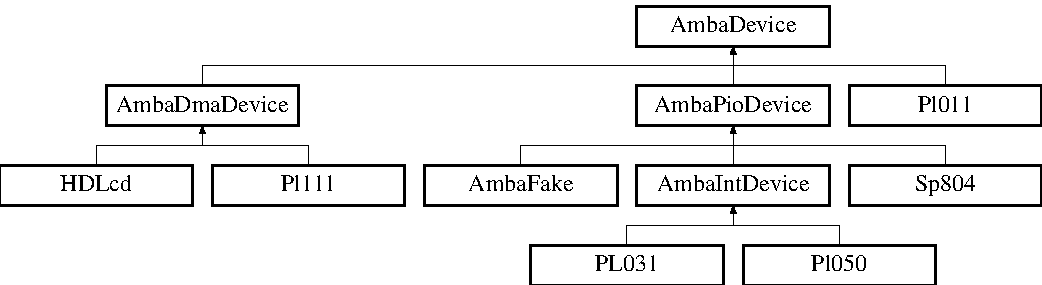
\includegraphics[height=3.82906cm]{classAmbaDevice}
\end{center}
\end{figure}
\subsection*{Protected メソッド}
\begin{DoxyCompactItemize}
\item 
bool \hyperlink{classAmbaDevice_a071939342677d0c85870b8f65d8f7639}{readId} (\hyperlink{classPacket}{PacketPtr} pkt, uint64\_\-t amba\_\-id, \hyperlink{base_2types_8hh_af1bb03d6a4ee096394a6749f0a169232}{Addr} pio\_\-addr)
\end{DoxyCompactItemize}
\subsection*{Static Protected 変数}
\begin{DoxyCompactItemize}
\item 
static const int \hyperlink{classAmbaDevice_a2ef71e98174278bd1964330103e718fd}{AMBA\_\-PER\_\-ID0} = 0xFE0
\item 
static const int \hyperlink{classAmbaDevice_a0b1e80bd6a1a75a77ce15e635f4ce202}{AMBA\_\-PER\_\-ID1} = 0xFE4
\item 
static const int \hyperlink{classAmbaDevice_a8a256ec5e875dd4a35b512e1e8b543da}{AMBA\_\-PER\_\-ID2} = 0xFE8
\item 
static const int \hyperlink{classAmbaDevice_a8f88e72f8e921732c961755c7e97c852}{AMBA\_\-PER\_\-ID3} = 0xFEC
\item 
static const int \hyperlink{classAmbaDevice_a749a0c336bf3249b928dd9b6bb8cd75f}{AMBA\_\-CEL\_\-ID0} = 0xFF0
\item 
static const int \hyperlink{classAmbaDevice_a9e920cb98d58a4845d818c7f7cfd7370}{AMBA\_\-CEL\_\-ID1} = 0xFF4
\item 
static const int \hyperlink{classAmbaDevice_ae1396143a7fd241c2758b69cbae097e3}{AMBA\_\-CEL\_\-ID2} = 0xFF8
\item 
static const int \hyperlink{classAmbaDevice_aed8b9f80686a3bd7cdafc05556bb3bbc}{AMBA\_\-CEL\_\-ID3} = 0xFFC
\end{DoxyCompactItemize}


\subsection{関数}
\hypertarget{classAmbaDevice_a071939342677d0c85870b8f65d8f7639}{
\index{AmbaDevice@{AmbaDevice}!readId@{readId}}
\index{readId@{readId}!AmbaDevice@{AmbaDevice}}
\subsubsection[{readId}]{\setlength{\rightskip}{0pt plus 5cm}bool readId ({\bf PacketPtr} {\em pkt}, \/  uint64\_\-t {\em amba\_\-id}, \/  {\bf Addr} {\em pio\_\-addr})\hspace{0.3cm}{\ttfamily  \mbox{[}protected\mbox{]}}}}
\label{classAmbaDevice_a071939342677d0c85870b8f65d8f7639}



\begin{DoxyCode}
74 {
75     Addr daddr = pkt->getAddr() - pio_addr;
76     if (daddr < AMBA_PER_ID0 || daddr > AMBA_CEL_ID3)
77         return false;
78 
79     pkt->allocate();
80 
81     int byte = (daddr - AMBA_PER_ID0) << 1;
82     // Too noisy right now
83     DPRINTF(AMBA, "Returning %#x for offset %#x(%d)\n",
84             (amba_id >> byte) & 0xFF,
85             pkt->getAddr() - pio_addr, byte);
86     assert(pkt->getSize() == 4);
87     pkt->set<uint32_t>((amba_id >> byte) & 0xFF);
88     return true;
89 }
\end{DoxyCode}


\subsection{変数}
\hypertarget{classAmbaDevice_a749a0c336bf3249b928dd9b6bb8cd75f}{
\index{AmbaDevice@{AmbaDevice}!AMBA\_\-CEL\_\-ID0@{AMBA\_\-CEL\_\-ID0}}
\index{AMBA\_\-CEL\_\-ID0@{AMBA\_\-CEL\_\-ID0}!AmbaDevice@{AmbaDevice}}
\subsubsection[{AMBA\_\-CEL\_\-ID0}]{\setlength{\rightskip}{0pt plus 5cm}const int {\bf AMBA\_\-CEL\_\-ID0} = 0xFF0\hspace{0.3cm}{\ttfamily  \mbox{[}static, protected\mbox{]}}}}
\label{classAmbaDevice_a749a0c336bf3249b928dd9b6bb8cd75f}
\hypertarget{classAmbaDevice_a9e920cb98d58a4845d818c7f7cfd7370}{
\index{AmbaDevice@{AmbaDevice}!AMBA\_\-CEL\_\-ID1@{AMBA\_\-CEL\_\-ID1}}
\index{AMBA\_\-CEL\_\-ID1@{AMBA\_\-CEL\_\-ID1}!AmbaDevice@{AmbaDevice}}
\subsubsection[{AMBA\_\-CEL\_\-ID1}]{\setlength{\rightskip}{0pt plus 5cm}const int {\bf AMBA\_\-CEL\_\-ID1} = 0xFF4\hspace{0.3cm}{\ttfamily  \mbox{[}static, protected\mbox{]}}}}
\label{classAmbaDevice_a9e920cb98d58a4845d818c7f7cfd7370}
\hypertarget{classAmbaDevice_ae1396143a7fd241c2758b69cbae097e3}{
\index{AmbaDevice@{AmbaDevice}!AMBA\_\-CEL\_\-ID2@{AMBA\_\-CEL\_\-ID2}}
\index{AMBA\_\-CEL\_\-ID2@{AMBA\_\-CEL\_\-ID2}!AmbaDevice@{AmbaDevice}}
\subsubsection[{AMBA\_\-CEL\_\-ID2}]{\setlength{\rightskip}{0pt plus 5cm}const int {\bf AMBA\_\-CEL\_\-ID2} = 0xFF8\hspace{0.3cm}{\ttfamily  \mbox{[}static, protected\mbox{]}}}}
\label{classAmbaDevice_ae1396143a7fd241c2758b69cbae097e3}
\hypertarget{classAmbaDevice_aed8b9f80686a3bd7cdafc05556bb3bbc}{
\index{AmbaDevice@{AmbaDevice}!AMBA\_\-CEL\_\-ID3@{AMBA\_\-CEL\_\-ID3}}
\index{AMBA\_\-CEL\_\-ID3@{AMBA\_\-CEL\_\-ID3}!AmbaDevice@{AmbaDevice}}
\subsubsection[{AMBA\_\-CEL\_\-ID3}]{\setlength{\rightskip}{0pt plus 5cm}const int {\bf AMBA\_\-CEL\_\-ID3} = 0xFFC\hspace{0.3cm}{\ttfamily  \mbox{[}static, protected\mbox{]}}}}
\label{classAmbaDevice_aed8b9f80686a3bd7cdafc05556bb3bbc}
\hypertarget{classAmbaDevice_a2ef71e98174278bd1964330103e718fd}{
\index{AmbaDevice@{AmbaDevice}!AMBA\_\-PER\_\-ID0@{AMBA\_\-PER\_\-ID0}}
\index{AMBA\_\-PER\_\-ID0@{AMBA\_\-PER\_\-ID0}!AmbaDevice@{AmbaDevice}}
\subsubsection[{AMBA\_\-PER\_\-ID0}]{\setlength{\rightskip}{0pt plus 5cm}const int {\bf AMBA\_\-PER\_\-ID0} = 0xFE0\hspace{0.3cm}{\ttfamily  \mbox{[}static, protected\mbox{]}}}}
\label{classAmbaDevice_a2ef71e98174278bd1964330103e718fd}
\hypertarget{classAmbaDevice_a0b1e80bd6a1a75a77ce15e635f4ce202}{
\index{AmbaDevice@{AmbaDevice}!AMBA\_\-PER\_\-ID1@{AMBA\_\-PER\_\-ID1}}
\index{AMBA\_\-PER\_\-ID1@{AMBA\_\-PER\_\-ID1}!AmbaDevice@{AmbaDevice}}
\subsubsection[{AMBA\_\-PER\_\-ID1}]{\setlength{\rightskip}{0pt plus 5cm}const int {\bf AMBA\_\-PER\_\-ID1} = 0xFE4\hspace{0.3cm}{\ttfamily  \mbox{[}static, protected\mbox{]}}}}
\label{classAmbaDevice_a0b1e80bd6a1a75a77ce15e635f4ce202}
\hypertarget{classAmbaDevice_a8a256ec5e875dd4a35b512e1e8b543da}{
\index{AmbaDevice@{AmbaDevice}!AMBA\_\-PER\_\-ID2@{AMBA\_\-PER\_\-ID2}}
\index{AMBA\_\-PER\_\-ID2@{AMBA\_\-PER\_\-ID2}!AmbaDevice@{AmbaDevice}}
\subsubsection[{AMBA\_\-PER\_\-ID2}]{\setlength{\rightskip}{0pt plus 5cm}const int {\bf AMBA\_\-PER\_\-ID2} = 0xFE8\hspace{0.3cm}{\ttfamily  \mbox{[}static, protected\mbox{]}}}}
\label{classAmbaDevice_a8a256ec5e875dd4a35b512e1e8b543da}
\hypertarget{classAmbaDevice_a8f88e72f8e921732c961755c7e97c852}{
\index{AmbaDevice@{AmbaDevice}!AMBA\_\-PER\_\-ID3@{AMBA\_\-PER\_\-ID3}}
\index{AMBA\_\-PER\_\-ID3@{AMBA\_\-PER\_\-ID3}!AmbaDevice@{AmbaDevice}}
\subsubsection[{AMBA\_\-PER\_\-ID3}]{\setlength{\rightskip}{0pt plus 5cm}const int {\bf AMBA\_\-PER\_\-ID3} = 0xFEC\hspace{0.3cm}{\ttfamily  \mbox{[}static, protected\mbox{]}}}}
\label{classAmbaDevice_a8f88e72f8e921732c961755c7e97c852}


このクラスの説明は次のファイルから生成されました:\begin{DoxyCompactItemize}
\item 
dev/arm/\hyperlink{amba__device_8hh}{amba\_\-device.hh}\item 
dev/arm/\hyperlink{amba__device_8cc}{amba\_\-device.cc}\end{DoxyCompactItemize}

\hypertarget{classAmbaDmaDevice}{
\section{クラス AmbaDmaDevice}
\label{classAmbaDmaDevice}\index{AmbaDmaDevice@{AmbaDmaDevice}}
}


{\ttfamily \#include $<$amba\_\-device.hh$>$}AmbaDmaDeviceに対する継承グラフ:\begin{figure}[H]
\begin{center}
\leavevmode
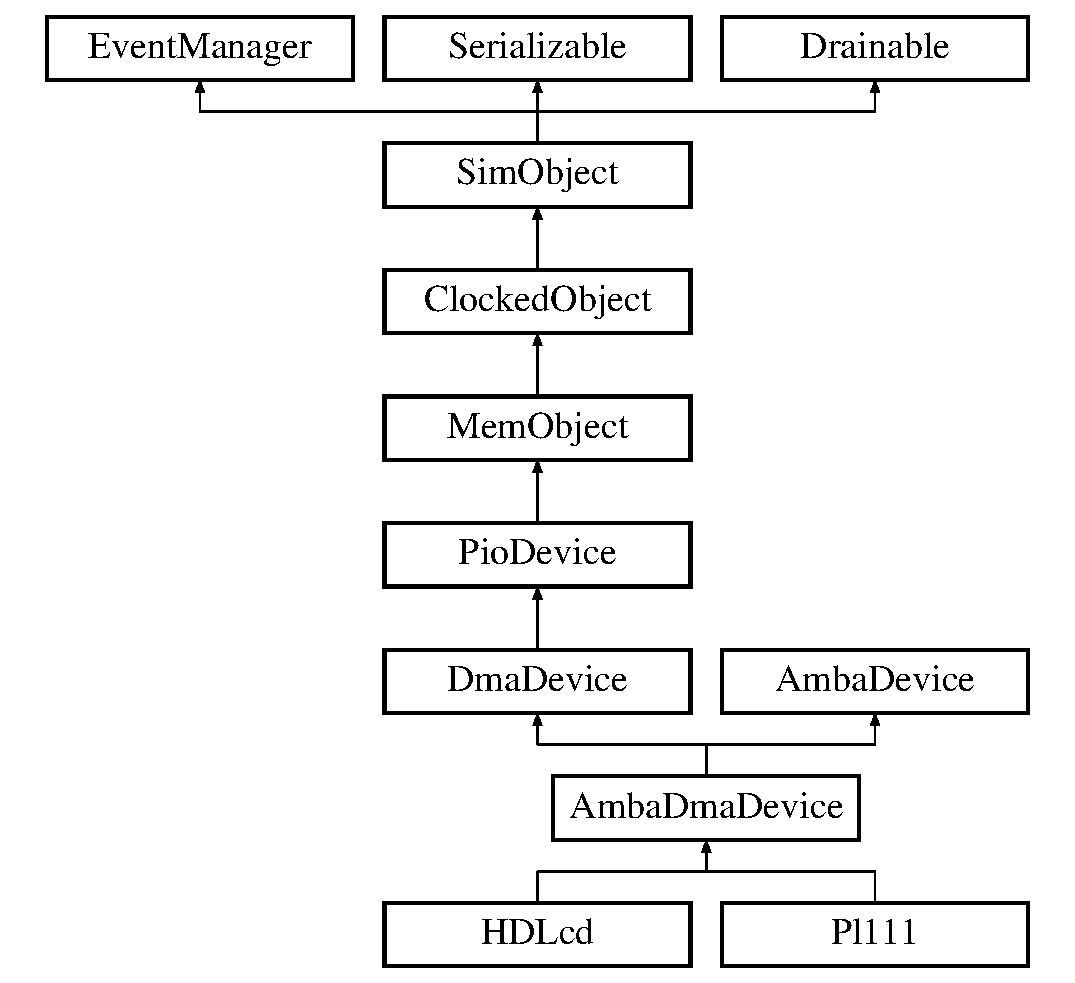
\includegraphics[height=8cm]{classAmbaDmaDevice}
\end{center}
\end{figure}
\subsection*{Public 型}
\begin{DoxyCompactItemize}
\item 
typedef AmbaDmaDeviceParams \hyperlink{classAmbaDmaDevice_ab612ceb7381438552927b7ed0aed5099}{Params}
\end{DoxyCompactItemize}
\subsection*{Public メソッド}
\begin{DoxyCompactItemize}
\item 
\hyperlink{classAmbaDmaDevice_a5dc78ee7b28b4b3effe7e28b09e6db48}{AmbaDmaDevice} (const \hyperlink{classAmbaDmaDevice_ab612ceb7381438552927b7ed0aed5099}{Params} $\ast$p)
\end{DoxyCompactItemize}
\subsection*{Protected 変数}
\begin{DoxyCompactItemize}
\item 
uint64\_\-t \hyperlink{classAmbaDmaDevice_a3201bf99dce0ba0bb6a5fd367f3dd76e}{ambaId}
\item 
\hyperlink{base_2types_8hh_af1bb03d6a4ee096394a6749f0a169232}{Addr} \hyperlink{classAmbaDmaDevice_afa7a5450c2bc6f73bc056050c9177193}{pioAddr}
\item 
\hyperlink{base_2types_8hh_af1bb03d6a4ee096394a6749f0a169232}{Addr} \hyperlink{classAmbaDmaDevice_a390529fe683187c290621e1822e0d5d1}{pioSize}
\item 
\hyperlink{base_2types_8hh_a5c8ed81b7d238c9083e1037ba6d61643}{Tick} \hyperlink{classAmbaDmaDevice_ac8e969635a78ab9ab123904ccca434cc}{pioDelay}
\item 
int \hyperlink{classAmbaDmaDevice_a9bd4d49b818d8cf1a6dee0576d2ff039}{intNum}
\item 
\hyperlink{classBaseGic}{BaseGic} $\ast$ \hyperlink{classAmbaDmaDevice_a2e2266dca56928f63667e994933169ee}{gic}
\end{DoxyCompactItemize}


\subsection{型定義}
\hypertarget{classAmbaDmaDevice_ab612ceb7381438552927b7ed0aed5099}{
\index{AmbaDmaDevice@{AmbaDmaDevice}!Params@{Params}}
\index{Params@{Params}!AmbaDmaDevice@{AmbaDmaDevice}}
\subsubsection[{Params}]{\setlength{\rightskip}{0pt plus 5cm}typedef AmbaDmaDeviceParams {\bf Params}}}
\label{classAmbaDmaDevice_ab612ceb7381438552927b7ed0aed5099}


\hyperlink{classDmaDevice_aea7daf6105ab956443385f5f5a9b88c5}{DmaDevice}を再定義しています。

\hyperlink{classHDLcd_a31ccb03af3b5962a67bed42eca6ce2f0}{HDLcd}, と \hyperlink{classPl111_a98df8e62be26dfc2009a7e53d5d0841d}{Pl111}で再定義されています。

\subsection{コンストラクタとデストラクタ}
\hypertarget{classAmbaDmaDevice_a5dc78ee7b28b4b3effe7e28b09e6db48}{
\index{AmbaDmaDevice@{AmbaDmaDevice}!AmbaDmaDevice@{AmbaDmaDevice}}
\index{AmbaDmaDevice@{AmbaDmaDevice}!AmbaDmaDevice@{AmbaDmaDevice}}
\subsubsection[{AmbaDmaDevice}]{\setlength{\rightskip}{0pt plus 5cm}{\bf AmbaDmaDevice} (const {\bf Params} $\ast$ {\em p})}}
\label{classAmbaDmaDevice_a5dc78ee7b28b4b3effe7e28b09e6db48}



\begin{DoxyCode}
66     : DmaDevice(p), ambaId(AmbaVendor | p->amba_id),
67       pioAddr(p->pio_addr), pioSize(0),
68       pioDelay(p->pio_latency),intNum(p->int_num), gic(p->gic)
69 {
70 }
\end{DoxyCode}


\subsection{変数}
\hypertarget{classAmbaDmaDevice_a3201bf99dce0ba0bb6a5fd367f3dd76e}{
\index{AmbaDmaDevice@{AmbaDmaDevice}!ambaId@{ambaId}}
\index{ambaId@{ambaId}!AmbaDmaDevice@{AmbaDmaDevice}}
\subsubsection[{ambaId}]{\setlength{\rightskip}{0pt plus 5cm}uint64\_\-t {\bf ambaId}\hspace{0.3cm}{\ttfamily  \mbox{[}protected\mbox{]}}}}
\label{classAmbaDmaDevice_a3201bf99dce0ba0bb6a5fd367f3dd76e}
\hypertarget{classAmbaDmaDevice_a2e2266dca56928f63667e994933169ee}{
\index{AmbaDmaDevice@{AmbaDmaDevice}!gic@{gic}}
\index{gic@{gic}!AmbaDmaDevice@{AmbaDmaDevice}}
\subsubsection[{gic}]{\setlength{\rightskip}{0pt plus 5cm}{\bf BaseGic}$\ast$ {\bf gic}\hspace{0.3cm}{\ttfamily  \mbox{[}protected\mbox{]}}}}
\label{classAmbaDmaDevice_a2e2266dca56928f63667e994933169ee}
\hypertarget{classAmbaDmaDevice_a9bd4d49b818d8cf1a6dee0576d2ff039}{
\index{AmbaDmaDevice@{AmbaDmaDevice}!intNum@{intNum}}
\index{intNum@{intNum}!AmbaDmaDevice@{AmbaDmaDevice}}
\subsubsection[{intNum}]{\setlength{\rightskip}{0pt plus 5cm}int {\bf intNum}\hspace{0.3cm}{\ttfamily  \mbox{[}protected\mbox{]}}}}
\label{classAmbaDmaDevice_a9bd4d49b818d8cf1a6dee0576d2ff039}
\hypertarget{classAmbaDmaDevice_afa7a5450c2bc6f73bc056050c9177193}{
\index{AmbaDmaDevice@{AmbaDmaDevice}!pioAddr@{pioAddr}}
\index{pioAddr@{pioAddr}!AmbaDmaDevice@{AmbaDmaDevice}}
\subsubsection[{pioAddr}]{\setlength{\rightskip}{0pt plus 5cm}{\bf Addr} {\bf pioAddr}\hspace{0.3cm}{\ttfamily  \mbox{[}protected\mbox{]}}}}
\label{classAmbaDmaDevice_afa7a5450c2bc6f73bc056050c9177193}
\hypertarget{classAmbaDmaDevice_ac8e969635a78ab9ab123904ccca434cc}{
\index{AmbaDmaDevice@{AmbaDmaDevice}!pioDelay@{pioDelay}}
\index{pioDelay@{pioDelay}!AmbaDmaDevice@{AmbaDmaDevice}}
\subsubsection[{pioDelay}]{\setlength{\rightskip}{0pt plus 5cm}{\bf Tick} {\bf pioDelay}\hspace{0.3cm}{\ttfamily  \mbox{[}protected\mbox{]}}}}
\label{classAmbaDmaDevice_ac8e969635a78ab9ab123904ccca434cc}
\hypertarget{classAmbaDmaDevice_a390529fe683187c290621e1822e0d5d1}{
\index{AmbaDmaDevice@{AmbaDmaDevice}!pioSize@{pioSize}}
\index{pioSize@{pioSize}!AmbaDmaDevice@{AmbaDmaDevice}}
\subsubsection[{pioSize}]{\setlength{\rightskip}{0pt plus 5cm}{\bf Addr} {\bf pioSize}\hspace{0.3cm}{\ttfamily  \mbox{[}protected\mbox{]}}}}
\label{classAmbaDmaDevice_a390529fe683187c290621e1822e0d5d1}


このクラスの説明は次のファイルから生成されました:\begin{DoxyCompactItemize}
\item 
dev/arm/\hyperlink{amba__device_8hh}{amba\_\-device.hh}\item 
dev/arm/\hyperlink{amba__device_8cc}{amba\_\-device.cc}\end{DoxyCompactItemize}

\hypertarget{classRealView_1_1AmbaDmaDevice}{
\section{クラス AmbaDmaDevice}
\label{classRealView_1_1AmbaDmaDevice}\index{RealView::AmbaDmaDevice@{RealView::AmbaDmaDevice}}
}
AmbaDmaDeviceに対する継承グラフ:\begin{figure}[H]
\begin{center}
\leavevmode
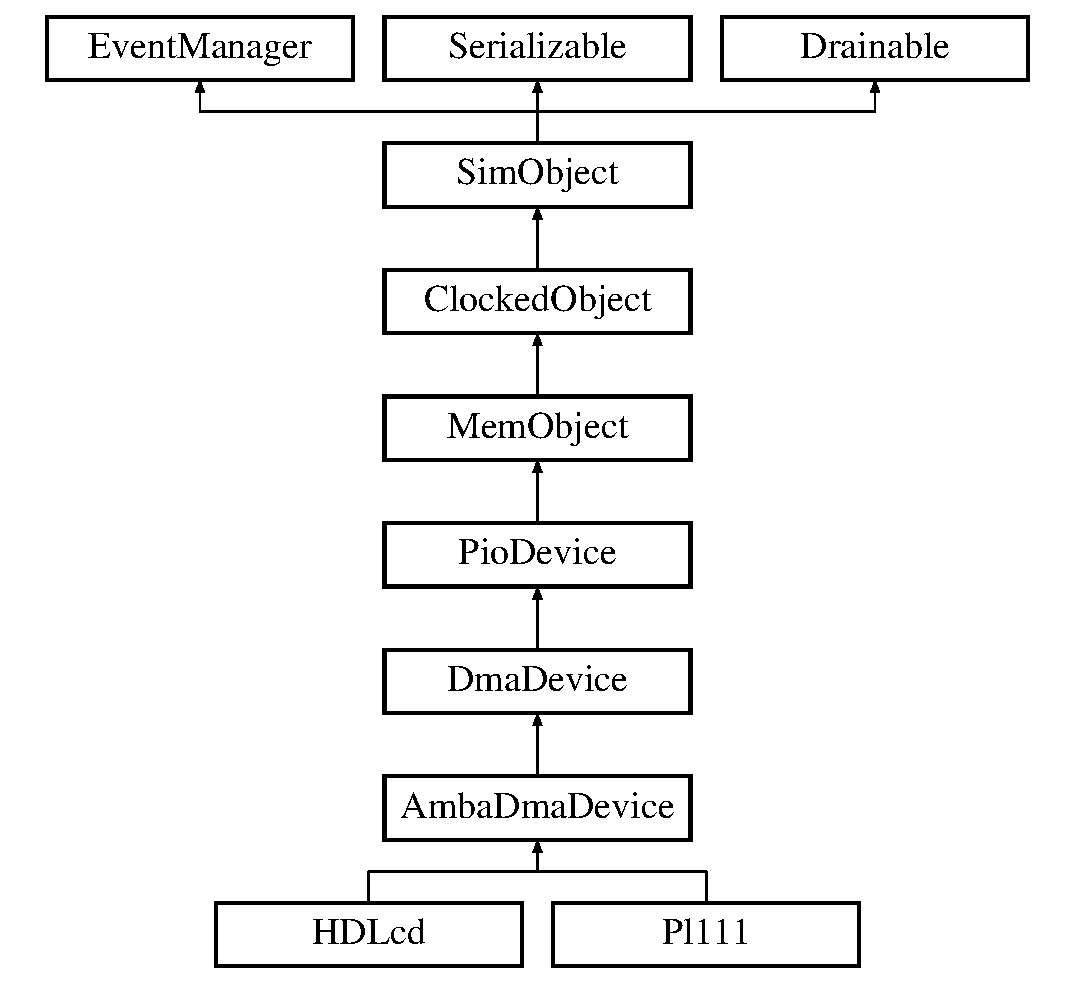
\includegraphics[height=8cm]{classRealView_1_1AmbaDmaDevice}
\end{center}
\end{figure}
\subsection*{Static Public 変数}
\begin{DoxyCompactItemize}
\item 
string \hyperlink{classRealView_1_1AmbaDmaDevice_acce15679d830831b0bbe8ebc2a60b2ca}{type} = '\hyperlink{classRealView_1_1AmbaDmaDevice}{AmbaDmaDevice}'
\item 
\hyperlink{classRealView_1_1AmbaDmaDevice_a17fa61ac3806b481cafee5593b55e5d0}{abstract} = True
\item 
string \hyperlink{classRealView_1_1AmbaDmaDevice_a17da7064bc5c518791f0c891eff05fda}{cxx\_\-header} = \char`\"{}dev/arm/amba\_\-device.hh\char`\"{}
\item 
tuple \hyperlink{classRealView_1_1AmbaDmaDevice_aac8239d62c5a04a05fcc71d4ac63fdb4}{pio\_\-addr} = \hyperlink{base_2types_8hh_af1bb03d6a4ee096394a6749f0a169232}{Param.Addr}(\char`\"{}Address for AMBA slave interface\char`\"{})
\item 
tuple \hyperlink{classRealView_1_1AmbaDmaDevice_ac3f272675842a6662ce8782e10fdba39}{pio\_\-latency} = Param.Latency(\char`\"{}10ns\char`\"{}, \char`\"{}Time between action and write/read result by AMBA DMA Device\char`\"{})
\item 
tuple \hyperlink{classRealView_1_1AmbaDmaDevice_a40243beb62d217c3a9e35801ae739fd0}{gic} = Param.BaseGic(Parent.any, \char`\"{}Gic to use for interrupting\char`\"{})
\item 
tuple \hyperlink{classRealView_1_1AmbaDmaDevice_a65fded6db751c1b9aa7168b29056e819}{int\_\-num} = Param.UInt32(\char`\"{}Interrupt number that connects to GIC\char`\"{})
\item 
tuple \hyperlink{classRealView_1_1AmbaDmaDevice_ad9d2b9e37de5c1c7c10219fc1b834599}{amba\_\-id} = Param.UInt32(\char`\"{}ID of AMBA device for kernel detection\char`\"{})
\end{DoxyCompactItemize}


\subsection{変数}
\hypertarget{classRealView_1_1AmbaDmaDevice_a17fa61ac3806b481cafee5593b55e5d0}{
\index{RealView::AmbaDmaDevice@{RealView::AmbaDmaDevice}!abstract@{abstract}}
\index{abstract@{abstract}!RealView::AmbaDmaDevice@{RealView::AmbaDmaDevice}}
\subsubsection[{abstract}]{\setlength{\rightskip}{0pt plus 5cm}{\bf abstract} = True\hspace{0.3cm}{\ttfamily  \mbox{[}static\mbox{]}}}}
\label{classRealView_1_1AmbaDmaDevice_a17fa61ac3806b481cafee5593b55e5d0}
\hypertarget{classRealView_1_1AmbaDmaDevice_ad9d2b9e37de5c1c7c10219fc1b834599}{
\index{RealView::AmbaDmaDevice@{RealView::AmbaDmaDevice}!amba\_\-id@{amba\_\-id}}
\index{amba\_\-id@{amba\_\-id}!RealView::AmbaDmaDevice@{RealView::AmbaDmaDevice}}
\subsubsection[{amba\_\-id}]{\setlength{\rightskip}{0pt plus 5cm}tuple {\bf amba\_\-id} = Param.UInt32(\char`\"{}ID of AMBA device for kernel detection\char`\"{})\hspace{0.3cm}{\ttfamily  \mbox{[}static\mbox{]}}}}
\label{classRealView_1_1AmbaDmaDevice_ad9d2b9e37de5c1c7c10219fc1b834599}


\hyperlink{classRealView_1_1Pl111_a38d7b9edfe6f0eea7a54e7e4f6253f3a}{Pl111}, と \hyperlink{classRealView_1_1HDLcd_a38d7b9edfe6f0eea7a54e7e4f6253f3a}{HDLcd}で再定義されています。\hypertarget{classRealView_1_1AmbaDmaDevice_a17da7064bc5c518791f0c891eff05fda}{
\index{RealView::AmbaDmaDevice@{RealView::AmbaDmaDevice}!cxx\_\-header@{cxx\_\-header}}
\index{cxx\_\-header@{cxx\_\-header}!RealView::AmbaDmaDevice@{RealView::AmbaDmaDevice}}
\subsubsection[{cxx\_\-header}]{\setlength{\rightskip}{0pt plus 5cm}string {\bf cxx\_\-header} = \char`\"{}dev/arm/amba\_\-device.hh\char`\"{}\hspace{0.3cm}{\ttfamily  \mbox{[}static\mbox{]}}}}
\label{classRealView_1_1AmbaDmaDevice_a17da7064bc5c518791f0c891eff05fda}


\hyperlink{classRealView_1_1Pl111_a17da7064bc5c518791f0c891eff05fda}{Pl111}, と \hyperlink{classRealView_1_1HDLcd_a17da7064bc5c518791f0c891eff05fda}{HDLcd}で再定義されています。\hypertarget{classRealView_1_1AmbaDmaDevice_a40243beb62d217c3a9e35801ae739fd0}{
\index{RealView::AmbaDmaDevice@{RealView::AmbaDmaDevice}!gic@{gic}}
\index{gic@{gic}!RealView::AmbaDmaDevice@{RealView::AmbaDmaDevice}}
\subsubsection[{gic}]{\setlength{\rightskip}{0pt plus 5cm}tuple {\bf gic} = Param.BaseGic(Parent.any, \char`\"{}Gic to use for interrupting\char`\"{})\hspace{0.3cm}{\ttfamily  \mbox{[}static\mbox{]}}}}
\label{classRealView_1_1AmbaDmaDevice_a40243beb62d217c3a9e35801ae739fd0}
\hypertarget{classRealView_1_1AmbaDmaDevice_a65fded6db751c1b9aa7168b29056e819}{
\index{RealView::AmbaDmaDevice@{RealView::AmbaDmaDevice}!int\_\-num@{int\_\-num}}
\index{int\_\-num@{int\_\-num}!RealView::AmbaDmaDevice@{RealView::AmbaDmaDevice}}
\subsubsection[{int\_\-num}]{\setlength{\rightskip}{0pt plus 5cm}tuple {\bf int\_\-num} = Param.UInt32(\char`\"{}Interrupt number that connects to GIC\char`\"{})\hspace{0.3cm}{\ttfamily  \mbox{[}static\mbox{]}}}}
\label{classRealView_1_1AmbaDmaDevice_a65fded6db751c1b9aa7168b29056e819}
\hypertarget{classRealView_1_1AmbaDmaDevice_aac8239d62c5a04a05fcc71d4ac63fdb4}{
\index{RealView::AmbaDmaDevice@{RealView::AmbaDmaDevice}!pio\_\-addr@{pio\_\-addr}}
\index{pio\_\-addr@{pio\_\-addr}!RealView::AmbaDmaDevice@{RealView::AmbaDmaDevice}}
\subsubsection[{pio\_\-addr}]{\setlength{\rightskip}{0pt plus 5cm}tuple {\bf pio\_\-addr} = {\bf Param.Addr}(\char`\"{}Address for AMBA slave interface\char`\"{})\hspace{0.3cm}{\ttfamily  \mbox{[}static\mbox{]}}}}
\label{classRealView_1_1AmbaDmaDevice_aac8239d62c5a04a05fcc71d4ac63fdb4}
\hypertarget{classRealView_1_1AmbaDmaDevice_ac3f272675842a6662ce8782e10fdba39}{
\index{RealView::AmbaDmaDevice@{RealView::AmbaDmaDevice}!pio\_\-latency@{pio\_\-latency}}
\index{pio\_\-latency@{pio\_\-latency}!RealView::AmbaDmaDevice@{RealView::AmbaDmaDevice}}
\subsubsection[{pio\_\-latency}]{\setlength{\rightskip}{0pt plus 5cm}tuple {\bf pio\_\-latency} = Param.Latency(\char`\"{}10ns\char`\"{}, \char`\"{}Time between action and write/read result by AMBA DMA Device\char`\"{})\hspace{0.3cm}{\ttfamily  \mbox{[}static\mbox{]}}}}
\label{classRealView_1_1AmbaDmaDevice_ac3f272675842a6662ce8782e10fdba39}
\hypertarget{classRealView_1_1AmbaDmaDevice_acce15679d830831b0bbe8ebc2a60b2ca}{
\index{RealView::AmbaDmaDevice@{RealView::AmbaDmaDevice}!type@{type}}
\index{type@{type}!RealView::AmbaDmaDevice@{RealView::AmbaDmaDevice}}
\subsubsection[{type}]{\setlength{\rightskip}{0pt plus 5cm}string {\bf type} = '{\bf AmbaDmaDevice}'\hspace{0.3cm}{\ttfamily  \mbox{[}static\mbox{]}}}}
\label{classRealView_1_1AmbaDmaDevice_acce15679d830831b0bbe8ebc2a60b2ca}


\hyperlink{classRealView_1_1Pl111_acce15679d830831b0bbe8ebc2a60b2ca}{Pl111}, と \hyperlink{classRealView_1_1HDLcd_acce15679d830831b0bbe8ebc2a60b2ca}{HDLcd}で再定義されています。

このクラスの説明は次のファイルから生成されました:\begin{DoxyCompactItemize}
\item 
dev/arm/\hyperlink{RealView_8py}{RealView.py}\end{DoxyCompactItemize}

\hypertarget{classAmbaFake}{
\section{クラス AmbaFake}
\label{classAmbaFake}\index{AmbaFake@{AmbaFake}}
}


{\ttfamily \#include $<$amba\_\-fake.hh$>$}AmbaFakeに対する継承グラフ:\begin{figure}[H]
\begin{center}
\leavevmode
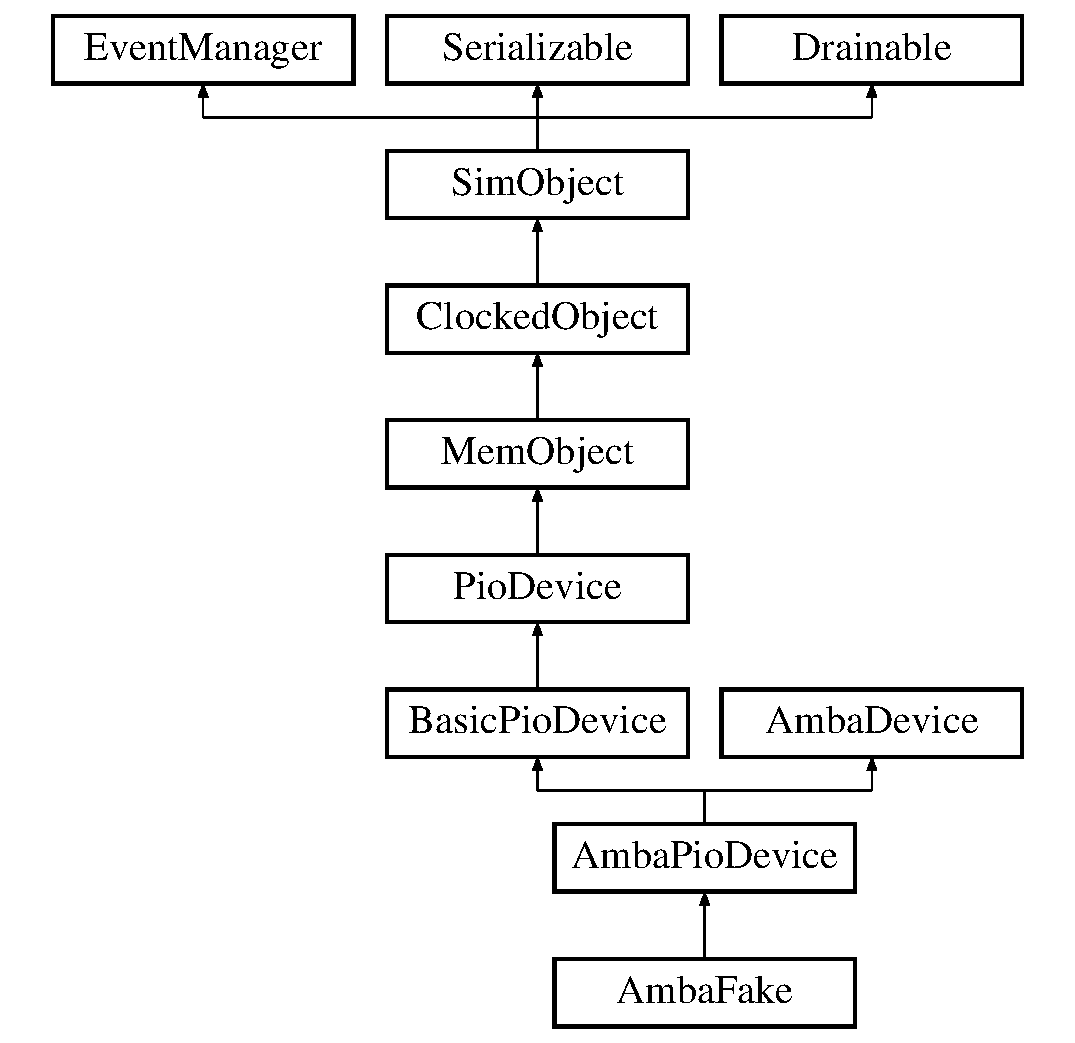
\includegraphics[height=8cm]{classAmbaFake}
\end{center}
\end{figure}
\subsection*{Public 型}
\begin{DoxyCompactItemize}
\item 
typedef AmbaFakeParams \hyperlink{classAmbaFake_af81895617462b041d86cd650bb1e27d3}{Params}
\end{DoxyCompactItemize}
\subsection*{Public メソッド}
\begin{DoxyCompactItemize}
\item 
const \hyperlink{classAmbaFake_af81895617462b041d86cd650bb1e27d3}{Params} $\ast$ \hyperlink{classAmbaFake_acd3c3feb78ae7a8f88fe0f110a718dff}{params} () const 
\item 
\hyperlink{classAmbaFake_a208b0127a0e255b708ddd1296d0ff092}{AmbaFake} (const \hyperlink{classAmbaFake_af81895617462b041d86cd650bb1e27d3}{Params} $\ast$p)
\item 
virtual \hyperlink{base_2types_8hh_a5c8ed81b7d238c9083e1037ba6d61643}{Tick} \hyperlink{classAmbaFake_a613ec7d5e1ec64f8d21fec78ae8e568e}{read} (\hyperlink{classPacket}{PacketPtr} pkt)
\item 
virtual \hyperlink{base_2types_8hh_a5c8ed81b7d238c9083e1037ba6d61643}{Tick} \hyperlink{classAmbaFake_a4cefab464e72b5dd42c003a0a4341802}{write} (\hyperlink{classPacket}{PacketPtr} pkt)
\end{DoxyCompactItemize}


\subsection{型定義}
\hypertarget{classAmbaFake_af81895617462b041d86cd650bb1e27d3}{
\index{AmbaFake@{AmbaFake}!Params@{Params}}
\index{Params@{Params}!AmbaFake@{AmbaFake}}
\subsubsection[{Params}]{\setlength{\rightskip}{0pt plus 5cm}typedef AmbaFakeParams {\bf Params}}}
\label{classAmbaFake_af81895617462b041d86cd650bb1e27d3}


\hyperlink{classAmbaPioDevice_ab091a3a8ffa1f3152ec35e30d1b384d5}{AmbaPioDevice}を再定義しています。

\subsection{コンストラクタとデストラクタ}
\hypertarget{classAmbaFake_a208b0127a0e255b708ddd1296d0ff092}{
\index{AmbaFake@{AmbaFake}!AmbaFake@{AmbaFake}}
\index{AmbaFake@{AmbaFake}!AmbaFake@{AmbaFake}}
\subsubsection[{AmbaFake}]{\setlength{\rightskip}{0pt plus 5cm}{\bf AmbaFake} (const {\bf Params} $\ast$ {\em p})}}
\label{classAmbaFake_a208b0127a0e255b708ddd1296d0ff092}



\begin{DoxyCode}
50     : AmbaPioDevice(p, 0xfff)
51 {
52 }
\end{DoxyCode}


\subsection{関数}
\hypertarget{classAmbaFake_acd3c3feb78ae7a8f88fe0f110a718dff}{
\index{AmbaFake@{AmbaFake}!params@{params}}
\index{params@{params}!AmbaFake@{AmbaFake}}
\subsubsection[{params}]{\setlength{\rightskip}{0pt plus 5cm}const {\bf Params}$\ast$ params () const\hspace{0.3cm}{\ttfamily  \mbox{[}inline\mbox{]}}}}
\label{classAmbaFake_acd3c3feb78ae7a8f88fe0f110a718dff}


\hyperlink{classBasicPioDevice_acd3c3feb78ae7a8f88fe0f110a718dff}{BasicPioDevice}を再定義しています。


\begin{DoxyCode}
63     {
64         return dynamic_cast<const Params *>(_params);
65     }
\end{DoxyCode}
\hypertarget{classAmbaFake_a613ec7d5e1ec64f8d21fec78ae8e568e}{
\index{AmbaFake@{AmbaFake}!read@{read}}
\index{read@{read}!AmbaFake@{AmbaFake}}
\subsubsection[{read}]{\setlength{\rightskip}{0pt plus 5cm}{\bf Tick} read ({\bf PacketPtr} {\em pkt})\hspace{0.3cm}{\ttfamily  \mbox{[}virtual\mbox{]}}}}
\label{classAmbaFake_a613ec7d5e1ec64f8d21fec78ae8e568e}
Pure virtual function that the device must implement. Called when a read command is recieved by the port. 
\begin{DoxyParams}{引数}
\item[{\em pkt}]\hyperlink{classPacket}{Packet} describing this request \end{DoxyParams}
\begin{DoxyReturn}{戻り値}
number of ticks it took to complete 
\end{DoxyReturn}


\hyperlink{classPioDevice_a842312590432036092c422c87a442358}{PioDevice}を実装しています。


\begin{DoxyCode}
56 {
57     assert(pkt->getAddr() >= pioAddr && pkt->getAddr() < pioAddr + pioSize);
58 
59     Addr daddr = pkt->getAddr() - pioAddr;
60     pkt->allocate();
61 
62     DPRINTF(AMBA, " read register %#x\n", daddr);
63 
64     pkt->set<uint32_t>(0);
65     if (!readId(pkt, ambaId, pioAddr) && !params()->ignore_access)
66         panic("Tried to read AmbaFake at offset %#x that doesn't exist\n", daddr)
      ;
67 
68     pkt->makeAtomicResponse();
69     return pioDelay;
70 }
\end{DoxyCode}
\hypertarget{classAmbaFake_a4cefab464e72b5dd42c003a0a4341802}{
\index{AmbaFake@{AmbaFake}!write@{write}}
\index{write@{write}!AmbaFake@{AmbaFake}}
\subsubsection[{write}]{\setlength{\rightskip}{0pt plus 5cm}{\bf Tick} write ({\bf PacketPtr} {\em pkt})\hspace{0.3cm}{\ttfamily  \mbox{[}virtual\mbox{]}}}}
\label{classAmbaFake_a4cefab464e72b5dd42c003a0a4341802}
Pure virtual function that the device must implement. Called when a write command is recieved by the port. 
\begin{DoxyParams}{引数}
\item[{\em pkt}]\hyperlink{classPacket}{Packet} describing this request \end{DoxyParams}
\begin{DoxyReturn}{戻り値}
number of ticks it took to complete 
\end{DoxyReturn}


\hyperlink{classPioDevice_afe8371668d023bb2516b286e5e399b6f}{PioDevice}を実装しています。


\begin{DoxyCode}
74 {
75 
76     Addr daddr = pkt->getAddr() - pioAddr;
77     pkt->allocate();
78 
79     if (!params()->ignore_access)
80         panic("Tried to write AmbaFake at offset %#x that doesn't exist\n", daddr
      );
81 
82     pkt->makeAtomicResponse();
83     return pioDelay;
84 }
\end{DoxyCode}


このクラスの説明は次のファイルから生成されました:\begin{DoxyCompactItemize}
\item 
dev/arm/\hyperlink{amba__fake_8hh}{amba\_\-fake.hh}\item 
dev/arm/\hyperlink{amba__fake_8cc}{amba\_\-fake.cc}\end{DoxyCompactItemize}

\hypertarget{classRealView_1_1AmbaFake}{
\section{クラス AmbaFake}
\label{classRealView_1_1AmbaFake}\index{RealView::AmbaFake@{RealView::AmbaFake}}
}
AmbaFakeに対する継承グラフ:\begin{figure}[H]
\begin{center}
\leavevmode
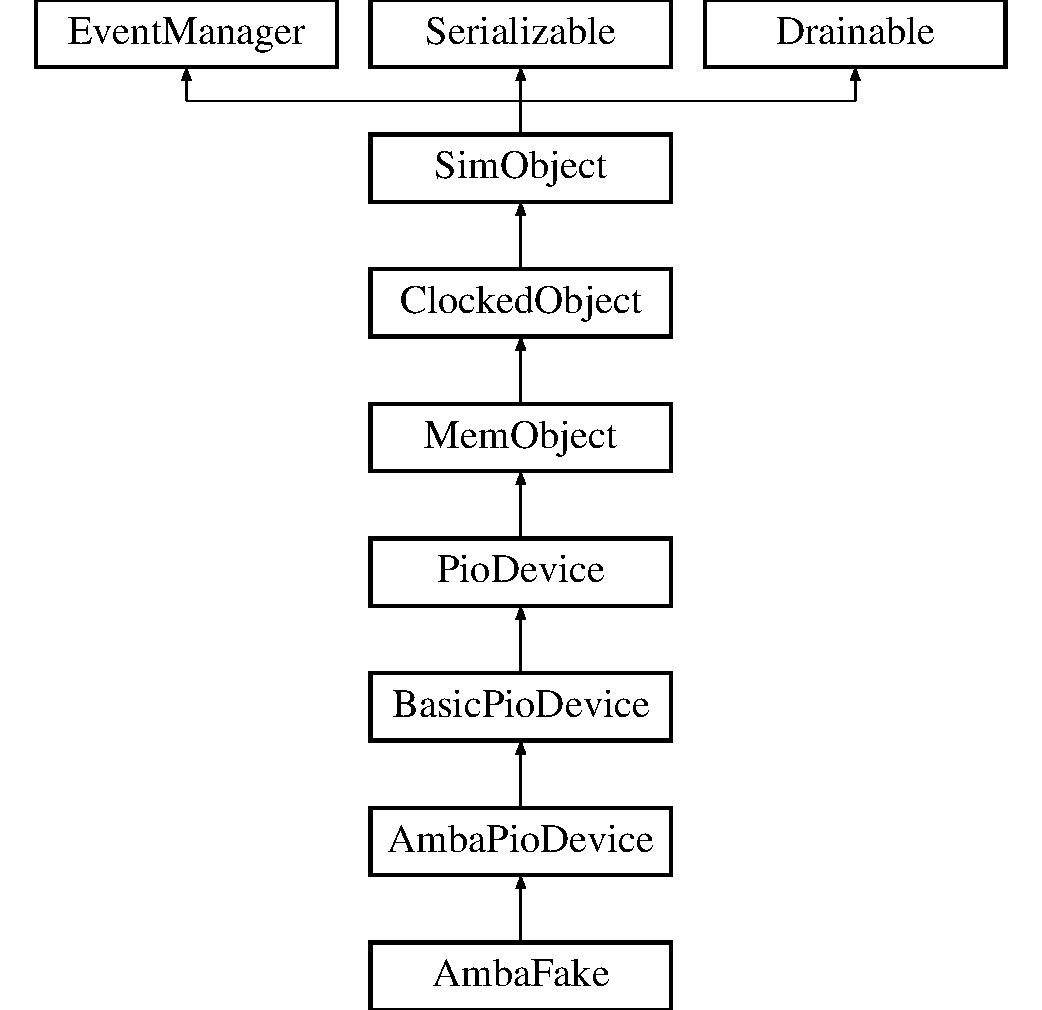
\includegraphics[height=8cm]{classRealView_1_1AmbaFake}
\end{center}
\end{figure}
\subsection*{Static Public 変数}
\begin{DoxyCompactItemize}
\item 
string \hyperlink{classRealView_1_1AmbaFake_acce15679d830831b0bbe8ebc2a60b2ca}{type} = '\hyperlink{classRealView_1_1AmbaFake}{AmbaFake}'
\item 
string \hyperlink{classRealView_1_1AmbaFake_a17da7064bc5c518791f0c891eff05fda}{cxx\_\-header} = \char`\"{}dev/arm/amba\_\-fake.hh\char`\"{}
\item 
tuple \hyperlink{classRealView_1_1AmbaFake_ab89da802f45f5d38c00fb81d62e65abb}{ignore\_\-access} = Param.Bool(False, \char`\"{}Ignore reads/writes to this device, (e.g. \hyperlink{classIsaFake}{IsaFake} + AMBA)\char`\"{})
\item 
int \hyperlink{classRealView_1_1AmbaFake_a38d7b9edfe6f0eea7a54e7e4f6253f3a}{amba\_\-id} = 0
\end{DoxyCompactItemize}


\subsection{変数}
\hypertarget{classRealView_1_1AmbaFake_a38d7b9edfe6f0eea7a54e7e4f6253f3a}{
\index{RealView::AmbaFake@{RealView::AmbaFake}!amba\_\-id@{amba\_\-id}}
\index{amba\_\-id@{amba\_\-id}!RealView::AmbaFake@{RealView::AmbaFake}}
\subsubsection[{amba\_\-id}]{\setlength{\rightskip}{0pt plus 5cm}int {\bf amba\_\-id} = 0\hspace{0.3cm}{\ttfamily  \mbox{[}static\mbox{]}}}}
\label{classRealView_1_1AmbaFake_a38d7b9edfe6f0eea7a54e7e4f6253f3a}


\hyperlink{classRealView_1_1AmbaPioDevice_ad9d2b9e37de5c1c7c10219fc1b834599}{AmbaPioDevice}を再定義しています。\hypertarget{classRealView_1_1AmbaFake_a17da7064bc5c518791f0c891eff05fda}{
\index{RealView::AmbaFake@{RealView::AmbaFake}!cxx\_\-header@{cxx\_\-header}}
\index{cxx\_\-header@{cxx\_\-header}!RealView::AmbaFake@{RealView::AmbaFake}}
\subsubsection[{cxx\_\-header}]{\setlength{\rightskip}{0pt plus 5cm}string {\bf cxx\_\-header} = \char`\"{}dev/arm/amba\_\-fake.hh\char`\"{}\hspace{0.3cm}{\ttfamily  \mbox{[}static\mbox{]}}}}
\label{classRealView_1_1AmbaFake_a17da7064bc5c518791f0c891eff05fda}


\hyperlink{classRealView_1_1AmbaPioDevice_a17da7064bc5c518791f0c891eff05fda}{AmbaPioDevice}を再定義しています。\hypertarget{classRealView_1_1AmbaFake_ab89da802f45f5d38c00fb81d62e65abb}{
\index{RealView::AmbaFake@{RealView::AmbaFake}!ignore\_\-access@{ignore\_\-access}}
\index{ignore\_\-access@{ignore\_\-access}!RealView::AmbaFake@{RealView::AmbaFake}}
\subsubsection[{ignore\_\-access}]{\setlength{\rightskip}{0pt plus 5cm}tuple {\bf ignore\_\-access} = Param.Bool(False, \char`\"{}Ignore reads/writes to this device, (e.g. {\bf IsaFake} + AMBA)\char`\"{})\hspace{0.3cm}{\ttfamily  \mbox{[}static\mbox{]}}}}
\label{classRealView_1_1AmbaFake_ab89da802f45f5d38c00fb81d62e65abb}
\hypertarget{classRealView_1_1AmbaFake_acce15679d830831b0bbe8ebc2a60b2ca}{
\index{RealView::AmbaFake@{RealView::AmbaFake}!type@{type}}
\index{type@{type}!RealView::AmbaFake@{RealView::AmbaFake}}
\subsubsection[{type}]{\setlength{\rightskip}{0pt plus 5cm}string {\bf type} = '{\bf AmbaFake}'\hspace{0.3cm}{\ttfamily  \mbox{[}static\mbox{]}}}}
\label{classRealView_1_1AmbaFake_acce15679d830831b0bbe8ebc2a60b2ca}


\hyperlink{classRealView_1_1AmbaPioDevice_acce15679d830831b0bbe8ebc2a60b2ca}{AmbaPioDevice}を再定義しています。

このクラスの説明は次のファイルから生成されました:\begin{DoxyCompactItemize}
\item 
dev/arm/\hyperlink{RealView_8py}{RealView.py}\end{DoxyCompactItemize}

\hypertarget{classAmbaIntDevice}{
\section{クラス AmbaIntDevice}
\label{classAmbaIntDevice}\index{AmbaIntDevice@{AmbaIntDevice}}
}


{\ttfamily \#include $<$amba\_\-device.hh$>$}AmbaIntDeviceに対する継承グラフ:\begin{figure}[H]
\begin{center}
\leavevmode
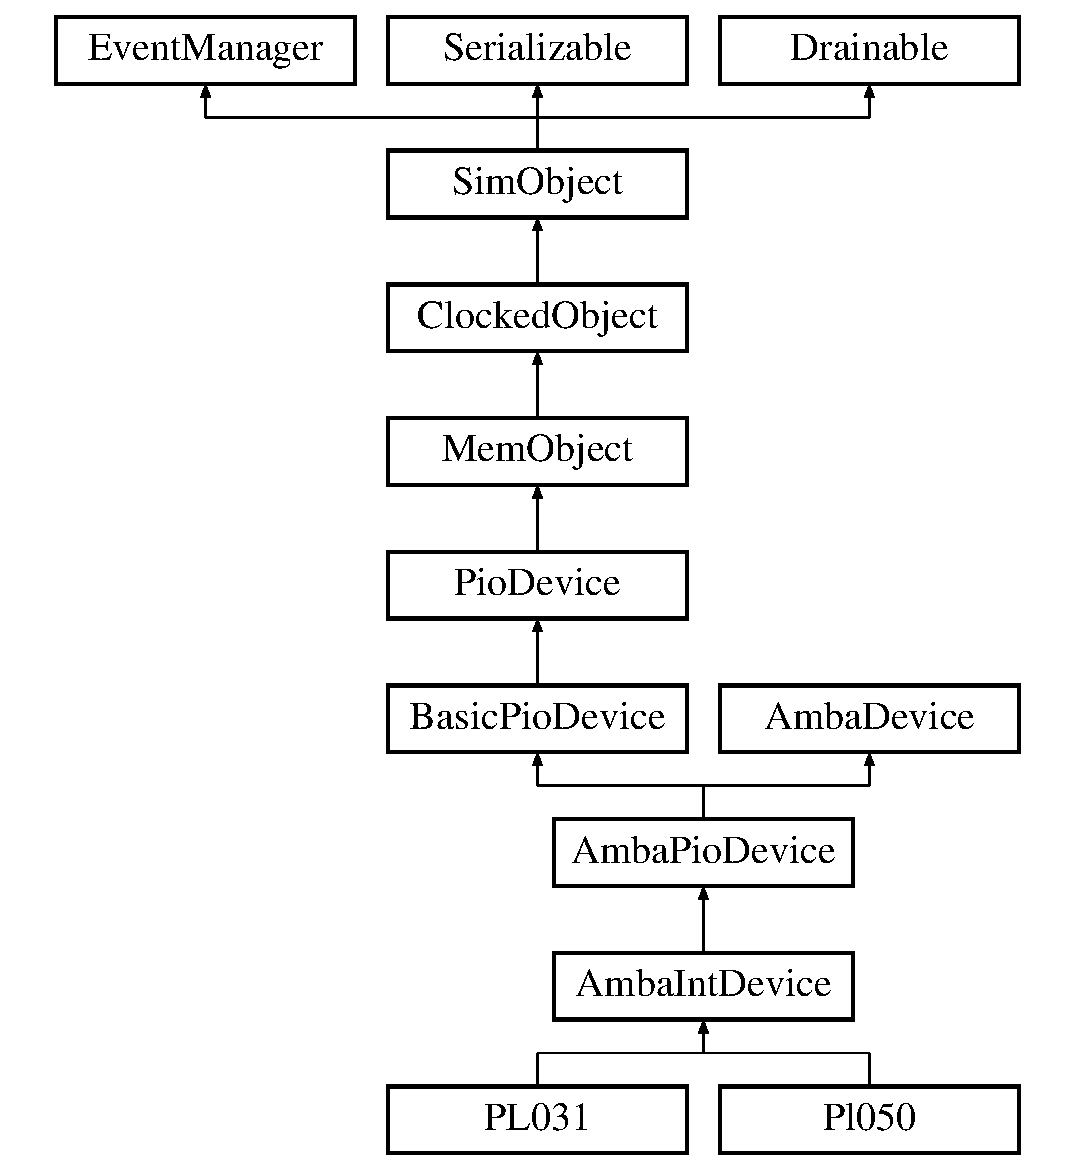
\includegraphics[height=9cm]{classAmbaIntDevice}
\end{center}
\end{figure}
\subsection*{Public 型}
\begin{DoxyCompactItemize}
\item 
typedef AmbaIntDeviceParams \hyperlink{classAmbaIntDevice_aa70660260d212b343768d91a298c80de}{Params}
\end{DoxyCompactItemize}
\subsection*{Public メソッド}
\begin{DoxyCompactItemize}
\item 
\hyperlink{classAmbaIntDevice_adef94b04b9c62ec3a1f26f4d201cbaf5}{AmbaIntDevice} (const \hyperlink{classAmbaIntDevice_aa70660260d212b343768d91a298c80de}{Params} $\ast$p, \hyperlink{base_2types_8hh_af1bb03d6a4ee096394a6749f0a169232}{Addr} pio\_\-size)
\end{DoxyCompactItemize}
\subsection*{Protected 変数}
\begin{DoxyCompactItemize}
\item 
int \hyperlink{classAmbaIntDevice_a9bd4d49b818d8cf1a6dee0576d2ff039}{intNum}
\item 
\hyperlink{classBaseGic}{BaseGic} $\ast$ \hyperlink{classAmbaIntDevice_a2e2266dca56928f63667e994933169ee}{gic}
\item 
\hyperlink{base_2types_8hh_a5c8ed81b7d238c9083e1037ba6d61643}{Tick} \hyperlink{classAmbaIntDevice_a0dad0b6dbada03eb5daf9c1ed859d62e}{intDelay}
\end{DoxyCompactItemize}


\subsection{型定義}
\hypertarget{classAmbaIntDevice_aa70660260d212b343768d91a298c80de}{
\index{AmbaIntDevice@{AmbaIntDevice}!Params@{Params}}
\index{Params@{Params}!AmbaIntDevice@{AmbaIntDevice}}
\subsubsection[{Params}]{\setlength{\rightskip}{0pt plus 5cm}typedef AmbaIntDeviceParams {\bf Params}}}
\label{classAmbaIntDevice_aa70660260d212b343768d91a298c80de}


\hyperlink{classAmbaPioDevice_ab091a3a8ffa1f3152ec35e30d1b384d5}{AmbaPioDevice}を再定義しています。

\hyperlink{classPl050_a12cd0d18c639c998ce04efabfca4d619}{Pl050}, と \hyperlink{classPL031_acd44fa02a8cc03d321b406d70faea0d8}{PL031}で再定義されています。

\subsection{コンストラクタとデストラクタ}
\hypertarget{classAmbaIntDevice_adef94b04b9c62ec3a1f26f4d201cbaf5}{
\index{AmbaIntDevice@{AmbaIntDevice}!AmbaIntDevice@{AmbaIntDevice}}
\index{AmbaIntDevice@{AmbaIntDevice}!AmbaIntDevice@{AmbaIntDevice}}
\subsubsection[{AmbaIntDevice}]{\setlength{\rightskip}{0pt plus 5cm}{\bf AmbaIntDevice} (const {\bf Params} $\ast$ {\em p}, \/  {\bf Addr} {\em pio\_\-size})}}
\label{classAmbaIntDevice_adef94b04b9c62ec3a1f26f4d201cbaf5}



\begin{DoxyCode}
58     : AmbaPioDevice(p, pio_size),
59       intNum(p->int_num), gic(p->gic), intDelay(p->int_delay)
60 {
61 }
\end{DoxyCode}


\subsection{変数}
\hypertarget{classAmbaIntDevice_a2e2266dca56928f63667e994933169ee}{
\index{AmbaIntDevice@{AmbaIntDevice}!gic@{gic}}
\index{gic@{gic}!AmbaIntDevice@{AmbaIntDevice}}
\subsubsection[{gic}]{\setlength{\rightskip}{0pt plus 5cm}{\bf BaseGic}$\ast$ {\bf gic}\hspace{0.3cm}{\ttfamily  \mbox{[}protected\mbox{]}}}}
\label{classAmbaIntDevice_a2e2266dca56928f63667e994933169ee}
\hypertarget{classAmbaIntDevice_a0dad0b6dbada03eb5daf9c1ed859d62e}{
\index{AmbaIntDevice@{AmbaIntDevice}!intDelay@{intDelay}}
\index{intDelay@{intDelay}!AmbaIntDevice@{AmbaIntDevice}}
\subsubsection[{intDelay}]{\setlength{\rightskip}{0pt plus 5cm}{\bf Tick} {\bf intDelay}\hspace{0.3cm}{\ttfamily  \mbox{[}protected\mbox{]}}}}
\label{classAmbaIntDevice_a0dad0b6dbada03eb5daf9c1ed859d62e}
\hypertarget{classAmbaIntDevice_a9bd4d49b818d8cf1a6dee0576d2ff039}{
\index{AmbaIntDevice@{AmbaIntDevice}!intNum@{intNum}}
\index{intNum@{intNum}!AmbaIntDevice@{AmbaIntDevice}}
\subsubsection[{intNum}]{\setlength{\rightskip}{0pt plus 5cm}int {\bf intNum}\hspace{0.3cm}{\ttfamily  \mbox{[}protected\mbox{]}}}}
\label{classAmbaIntDevice_a9bd4d49b818d8cf1a6dee0576d2ff039}


このクラスの説明は次のファイルから生成されました:\begin{DoxyCompactItemize}
\item 
dev/arm/\hyperlink{amba__device_8hh}{amba\_\-device.hh}\item 
dev/arm/\hyperlink{amba__device_8cc}{amba\_\-device.cc}\end{DoxyCompactItemize}

\hypertarget{classRealView_1_1AmbaIntDevice}{
\section{クラス AmbaIntDevice}
\label{classRealView_1_1AmbaIntDevice}\index{RealView::AmbaIntDevice@{RealView::AmbaIntDevice}}
}
AmbaIntDeviceに対する継承グラフ:\begin{figure}[H]
\begin{center}
\leavevmode
\includegraphics[height=9cm]{classRealView_1_1AmbaIntDevice}
\end{center}
\end{figure}
\subsection*{Static Public 変数}
\begin{DoxyCompactItemize}
\item 
string \hyperlink{classRealView_1_1AmbaIntDevice_acce15679d830831b0bbe8ebc2a60b2ca}{type} = '\hyperlink{classRealView_1_1AmbaIntDevice}{AmbaIntDevice}'
\item 
\hyperlink{classRealView_1_1AmbaIntDevice_a17fa61ac3806b481cafee5593b55e5d0}{abstract} = True
\item 
string \hyperlink{classRealView_1_1AmbaIntDevice_a17da7064bc5c518791f0c891eff05fda}{cxx\_\-header} = \char`\"{}dev/arm/amba\_\-device.hh\char`\"{}
\item 
tuple \hyperlink{classRealView_1_1AmbaIntDevice_a40243beb62d217c3a9e35801ae739fd0}{gic} = Param.BaseGic(Parent.any, \char`\"{}Gic to use for interrupting\char`\"{})
\item 
tuple \hyperlink{classRealView_1_1AmbaIntDevice_a65fded6db751c1b9aa7168b29056e819}{int\_\-num} = Param.UInt32(\char`\"{}Interrupt number that connects to GIC\char`\"{})
\item 
tuple \hyperlink{classRealView_1_1AmbaIntDevice_a849551e71f91ca939d22d4c083f4c731}{int\_\-delay}
\end{DoxyCompactItemize}


\subsection{変数}
\hypertarget{classRealView_1_1AmbaIntDevice_a17fa61ac3806b481cafee5593b55e5d0}{
\index{RealView::AmbaIntDevice@{RealView::AmbaIntDevice}!abstract@{abstract}}
\index{abstract@{abstract}!RealView::AmbaIntDevice@{RealView::AmbaIntDevice}}
\subsubsection[{abstract}]{\setlength{\rightskip}{0pt plus 5cm}{\bf abstract} = True\hspace{0.3cm}{\ttfamily  \mbox{[}static\mbox{]}}}}
\label{classRealView_1_1AmbaIntDevice_a17fa61ac3806b481cafee5593b55e5d0}


\hyperlink{classRealView_1_1AmbaPioDevice_a17fa61ac3806b481cafee5593b55e5d0}{AmbaPioDevice}を再定義しています。\hypertarget{classRealView_1_1AmbaIntDevice_a17da7064bc5c518791f0c891eff05fda}{
\index{RealView::AmbaIntDevice@{RealView::AmbaIntDevice}!cxx\_\-header@{cxx\_\-header}}
\index{cxx\_\-header@{cxx\_\-header}!RealView::AmbaIntDevice@{RealView::AmbaIntDevice}}
\subsubsection[{cxx\_\-header}]{\setlength{\rightskip}{0pt plus 5cm}string {\bf cxx\_\-header} = \char`\"{}dev/arm/amba\_\-device.hh\char`\"{}\hspace{0.3cm}{\ttfamily  \mbox{[}static\mbox{]}}}}
\label{classRealView_1_1AmbaIntDevice_a17da7064bc5c518791f0c891eff05fda}


\hyperlink{classRealView_1_1AmbaPioDevice_a17da7064bc5c518791f0c891eff05fda}{AmbaPioDevice}を再定義しています。

\hyperlink{classRealView_1_1PL031_a17da7064bc5c518791f0c891eff05fda}{PL031}, と \hyperlink{classRealView_1_1Pl050_a17da7064bc5c518791f0c891eff05fda}{Pl050}で再定義されています。\hypertarget{classRealView_1_1AmbaIntDevice_a40243beb62d217c3a9e35801ae739fd0}{
\index{RealView::AmbaIntDevice@{RealView::AmbaIntDevice}!gic@{gic}}
\index{gic@{gic}!RealView::AmbaIntDevice@{RealView::AmbaIntDevice}}
\subsubsection[{gic}]{\setlength{\rightskip}{0pt plus 5cm}tuple {\bf gic} = Param.BaseGic(Parent.any, \char`\"{}Gic to use for interrupting\char`\"{})\hspace{0.3cm}{\ttfamily  \mbox{[}static\mbox{]}}}}
\label{classRealView_1_1AmbaIntDevice_a40243beb62d217c3a9e35801ae739fd0}
\hypertarget{classRealView_1_1AmbaIntDevice_a849551e71f91ca939d22d4c083f4c731}{
\index{RealView::AmbaIntDevice@{RealView::AmbaIntDevice}!int\_\-delay@{int\_\-delay}}
\index{int\_\-delay@{int\_\-delay}!RealView::AmbaIntDevice@{RealView::AmbaIntDevice}}
\subsubsection[{int\_\-delay}]{\setlength{\rightskip}{0pt plus 5cm}tuple {\bf int\_\-delay}\hspace{0.3cm}{\ttfamily  \mbox{[}static\mbox{]}}}}
\label{classRealView_1_1AmbaIntDevice_a849551e71f91ca939d22d4c083f4c731}
{\bfseries 初期値:}
\begin{DoxyCode}
Param.Latency("100ns",
            "Time between action and interrupt generation by device")
\end{DoxyCode}


\hyperlink{classRealView_1_1Pl050_a143e0c2b2724ac7fcad9543c09b949ef}{Pl050}で再定義されています。\hypertarget{classRealView_1_1AmbaIntDevice_a65fded6db751c1b9aa7168b29056e819}{
\index{RealView::AmbaIntDevice@{RealView::AmbaIntDevice}!int\_\-num@{int\_\-num}}
\index{int\_\-num@{int\_\-num}!RealView::AmbaIntDevice@{RealView::AmbaIntDevice}}
\subsubsection[{int\_\-num}]{\setlength{\rightskip}{0pt plus 5cm}tuple {\bf int\_\-num} = Param.UInt32(\char`\"{}Interrupt number that connects to GIC\char`\"{})\hspace{0.3cm}{\ttfamily  \mbox{[}static\mbox{]}}}}
\label{classRealView_1_1AmbaIntDevice_a65fded6db751c1b9aa7168b29056e819}
\hypertarget{classRealView_1_1AmbaIntDevice_acce15679d830831b0bbe8ebc2a60b2ca}{
\index{RealView::AmbaIntDevice@{RealView::AmbaIntDevice}!type@{type}}
\index{type@{type}!RealView::AmbaIntDevice@{RealView::AmbaIntDevice}}
\subsubsection[{type}]{\setlength{\rightskip}{0pt plus 5cm}string {\bf type} = '{\bf AmbaIntDevice}'\hspace{0.3cm}{\ttfamily  \mbox{[}static\mbox{]}}}}
\label{classRealView_1_1AmbaIntDevice_acce15679d830831b0bbe8ebc2a60b2ca}


\hyperlink{classRealView_1_1AmbaPioDevice_acce15679d830831b0bbe8ebc2a60b2ca}{AmbaPioDevice}を再定義しています。

\hyperlink{classRealView_1_1PL031_acce15679d830831b0bbe8ebc2a60b2ca}{PL031}, と \hyperlink{classRealView_1_1Pl050_acce15679d830831b0bbe8ebc2a60b2ca}{Pl050}で再定義されています。

このクラスの説明は次のファイルから生成されました:\begin{DoxyCompactItemize}
\item 
dev/arm/\hyperlink{RealView_8py}{RealView.py}\end{DoxyCompactItemize}

\hypertarget{classAmbaPioDevice}{
\section{クラス AmbaPioDevice}
\label{classAmbaPioDevice}\index{AmbaPioDevice@{AmbaPioDevice}}
}


{\ttfamily \#include $<$amba\_\-device.hh$>$}AmbaPioDeviceに対する継承グラフ:\begin{figure}[H]
\begin{center}
\leavevmode
\includegraphics[height=9cm]{classAmbaPioDevice}
\end{center}
\end{figure}
\subsection*{Public 型}
\begin{DoxyCompactItemize}
\item 
typedef AmbaPioDeviceParams \hyperlink{classAmbaPioDevice_ab091a3a8ffa1f3152ec35e30d1b384d5}{Params}
\end{DoxyCompactItemize}
\subsection*{Public メソッド}
\begin{DoxyCompactItemize}
\item 
\hyperlink{classAmbaPioDevice_a4d233593026e483123ea04aaa7fe8daf}{AmbaPioDevice} (const \hyperlink{classAmbaPioDevice_ab091a3a8ffa1f3152ec35e30d1b384d5}{Params} $\ast$p, \hyperlink{base_2types_8hh_af1bb03d6a4ee096394a6749f0a169232}{Addr} pio\_\-size)
\end{DoxyCompactItemize}
\subsection*{Protected 変数}
\begin{DoxyCompactItemize}
\item 
uint64\_\-t \hyperlink{classAmbaPioDevice_a3201bf99dce0ba0bb6a5fd367f3dd76e}{ambaId}
\end{DoxyCompactItemize}


\subsection{型定義}
\hypertarget{classAmbaPioDevice_ab091a3a8ffa1f3152ec35e30d1b384d5}{
\index{AmbaPioDevice@{AmbaPioDevice}!Params@{Params}}
\index{Params@{Params}!AmbaPioDevice@{AmbaPioDevice}}
\subsubsection[{Params}]{\setlength{\rightskip}{0pt plus 5cm}typedef AmbaPioDeviceParams {\bf Params}}}
\label{classAmbaPioDevice_ab091a3a8ffa1f3152ec35e30d1b384d5}


\hyperlink{classBasicPioDevice_a2845515ac6467f10540747053c8a0449}{BasicPioDevice}を再定義しています。

\hyperlink{classAmbaIntDevice_aa70660260d212b343768d91a298c80de}{AmbaIntDevice}, \hyperlink{classAmbaFake_af81895617462b041d86cd650bb1e27d3}{AmbaFake}, \hyperlink{classPl050_a12cd0d18c639c998ce04efabfca4d619}{Pl050}, \hyperlink{classPL031_acd44fa02a8cc03d321b406d70faea0d8}{PL031}, と \hyperlink{classSp804_af822827c8c9baefc6aafbdc713bc2b8d}{Sp804}で再定義されています。

\subsection{コンストラクタとデストラクタ}
\hypertarget{classAmbaPioDevice_a4d233593026e483123ea04aaa7fe8daf}{
\index{AmbaPioDevice@{AmbaPioDevice}!AmbaPioDevice@{AmbaPioDevice}}
\index{AmbaPioDevice@{AmbaPioDevice}!AmbaPioDevice@{AmbaPioDevice}}
\subsubsection[{AmbaPioDevice}]{\setlength{\rightskip}{0pt plus 5cm}{\bf AmbaPioDevice} (const {\bf Params} $\ast$ {\em p}, \/  {\bf Addr} {\em pio\_\-size})}}
\label{classAmbaPioDevice_a4d233593026e483123ea04aaa7fe8daf}



\begin{DoxyCode}
53     : BasicPioDevice(p, pio_size), ambaId(AmbaVendor | p->amba_id)
54 {
55 }
\end{DoxyCode}


\subsection{変数}
\hypertarget{classAmbaPioDevice_a3201bf99dce0ba0bb6a5fd367f3dd76e}{
\index{AmbaPioDevice@{AmbaPioDevice}!ambaId@{ambaId}}
\index{ambaId@{ambaId}!AmbaPioDevice@{AmbaPioDevice}}
\subsubsection[{ambaId}]{\setlength{\rightskip}{0pt plus 5cm}uint64\_\-t {\bf ambaId}\hspace{0.3cm}{\ttfamily  \mbox{[}protected\mbox{]}}}}
\label{classAmbaPioDevice_a3201bf99dce0ba0bb6a5fd367f3dd76e}


このクラスの説明は次のファイルから生成されました:\begin{DoxyCompactItemize}
\item 
dev/arm/\hyperlink{amba__device_8hh}{amba\_\-device.hh}\item 
dev/arm/\hyperlink{amba__device_8cc}{amba\_\-device.cc}\end{DoxyCompactItemize}

\hypertarget{classRealView_1_1AmbaPioDevice}{
\section{クラス AmbaPioDevice}
\label{classRealView_1_1AmbaPioDevice}\index{RealView::AmbaPioDevice@{RealView::AmbaPioDevice}}
}
AmbaPioDeviceに対する継承グラフ:\begin{figure}[H]
\begin{center}
\leavevmode
\includegraphics[height=9cm]{classRealView_1_1AmbaPioDevice}
\end{center}
\end{figure}
\subsection*{Static Public 変数}
\begin{DoxyCompactItemize}
\item 
string \hyperlink{classRealView_1_1AmbaPioDevice_acce15679d830831b0bbe8ebc2a60b2ca}{type} = '\hyperlink{classRealView_1_1AmbaPioDevice}{AmbaPioDevice}'
\item 
\hyperlink{classRealView_1_1AmbaPioDevice_a17fa61ac3806b481cafee5593b55e5d0}{abstract} = True
\item 
string \hyperlink{classRealView_1_1AmbaPioDevice_a17da7064bc5c518791f0c891eff05fda}{cxx\_\-header} = \char`\"{}dev/arm/amba\_\-device.hh\char`\"{}
\item 
tuple \hyperlink{classRealView_1_1AmbaPioDevice_ad9d2b9e37de5c1c7c10219fc1b834599}{amba\_\-id} = Param.UInt32(\char`\"{}ID of AMBA device for kernel detection\char`\"{})
\end{DoxyCompactItemize}


\subsection{変数}
\hypertarget{classRealView_1_1AmbaPioDevice_a17fa61ac3806b481cafee5593b55e5d0}{
\index{RealView::AmbaPioDevice@{RealView::AmbaPioDevice}!abstract@{abstract}}
\index{abstract@{abstract}!RealView::AmbaPioDevice@{RealView::AmbaPioDevice}}
\subsubsection[{abstract}]{\setlength{\rightskip}{0pt plus 5cm}{\bf abstract} = True\hspace{0.3cm}{\ttfamily  \mbox{[}static\mbox{]}}}}
\label{classRealView_1_1AmbaPioDevice_a17fa61ac3806b481cafee5593b55e5d0}


\hyperlink{classRealView_1_1AmbaIntDevice_a17fa61ac3806b481cafee5593b55e5d0}{AmbaIntDevice}で再定義されています。\hypertarget{classRealView_1_1AmbaPioDevice_ad9d2b9e37de5c1c7c10219fc1b834599}{
\index{RealView::AmbaPioDevice@{RealView::AmbaPioDevice}!amba\_\-id@{amba\_\-id}}
\index{amba\_\-id@{amba\_\-id}!RealView::AmbaPioDevice@{RealView::AmbaPioDevice}}
\subsubsection[{amba\_\-id}]{\setlength{\rightskip}{0pt plus 5cm}tuple {\bf amba\_\-id} = Param.UInt32(\char`\"{}ID of AMBA device for kernel detection\char`\"{})\hspace{0.3cm}{\ttfamily  \mbox{[}static\mbox{]}}}}
\label{classRealView_1_1AmbaPioDevice_ad9d2b9e37de5c1c7c10219fc1b834599}


\hyperlink{classRealView_1_1AmbaFake_a38d7b9edfe6f0eea7a54e7e4f6253f3a}{AmbaFake}, \hyperlink{classRealView_1_1Sp804_a38d7b9edfe6f0eea7a54e7e4f6253f3a}{Sp804}, \hyperlink{classRealView_1_1PL031_a38d7b9edfe6f0eea7a54e7e4f6253f3a}{PL031}, と \hyperlink{classRealView_1_1Pl050_a38d7b9edfe6f0eea7a54e7e4f6253f3a}{Pl050}で再定義されています。\hypertarget{classRealView_1_1AmbaPioDevice_a17da7064bc5c518791f0c891eff05fda}{
\index{RealView::AmbaPioDevice@{RealView::AmbaPioDevice}!cxx\_\-header@{cxx\_\-header}}
\index{cxx\_\-header@{cxx\_\-header}!RealView::AmbaPioDevice@{RealView::AmbaPioDevice}}
\subsubsection[{cxx\_\-header}]{\setlength{\rightskip}{0pt plus 5cm}string {\bf cxx\_\-header} = \char`\"{}dev/arm/amba\_\-device.hh\char`\"{}\hspace{0.3cm}{\ttfamily  \mbox{[}static\mbox{]}}}}
\label{classRealView_1_1AmbaPioDevice_a17da7064bc5c518791f0c891eff05fda}


\hyperlink{classRealView_1_1AmbaIntDevice_a17da7064bc5c518791f0c891eff05fda}{AmbaIntDevice}, \hyperlink{classRealView_1_1AmbaFake_a17da7064bc5c518791f0c891eff05fda}{AmbaFake}, \hyperlink{classRealView_1_1Sp804_a17da7064bc5c518791f0c891eff05fda}{Sp804}, \hyperlink{classRealView_1_1PL031_a17da7064bc5c518791f0c891eff05fda}{PL031}, と \hyperlink{classRealView_1_1Pl050_a17da7064bc5c518791f0c891eff05fda}{Pl050}で再定義されています。\hypertarget{classRealView_1_1AmbaPioDevice_acce15679d830831b0bbe8ebc2a60b2ca}{
\index{RealView::AmbaPioDevice@{RealView::AmbaPioDevice}!type@{type}}
\index{type@{type}!RealView::AmbaPioDevice@{RealView::AmbaPioDevice}}
\subsubsection[{type}]{\setlength{\rightskip}{0pt plus 5cm}string {\bf type} = '{\bf AmbaPioDevice}'\hspace{0.3cm}{\ttfamily  \mbox{[}static\mbox{]}}}}
\label{classRealView_1_1AmbaPioDevice_acce15679d830831b0bbe8ebc2a60b2ca}


\hyperlink{classRealView_1_1AmbaIntDevice_acce15679d830831b0bbe8ebc2a60b2ca}{AmbaIntDevice}, \hyperlink{classRealView_1_1AmbaFake_acce15679d830831b0bbe8ebc2a60b2ca}{AmbaFake}, \hyperlink{classRealView_1_1Sp804_acce15679d830831b0bbe8ebc2a60b2ca}{Sp804}, \hyperlink{classRealView_1_1PL031_acce15679d830831b0bbe8ebc2a60b2ca}{PL031}, と \hyperlink{classRealView_1_1Pl050_acce15679d830831b0bbe8ebc2a60b2ca}{Pl050}で再定義されています。

このクラスの説明は次のファイルから生成されました:\begin{DoxyCompactItemize}
\item 
dev/arm/\hyperlink{RealView_8py}{RealView.py}\end{DoxyCompactItemize}

\hypertarget{classAmpUnit}{
\section{クラス AmpUnit}
\label{classAmpUnit}\index{AmpUnit@{AmpUnit}}
}


{\ttfamily \#include $<$AmpUnit.hh$>$}\subsection*{Public 型}
\begin{DoxyCompactItemize}
\item 
enum \hyperlink{classAmpUnit_a79e8a1b9fa3eb04d605362bcbdcdc925}{AmpModel} \{ \hyperlink{classAmpUnit_a79e8a1b9fa3eb04d605362bcbdcdc925abab57b6e2c553e4d983f415a1f4ea75b}{NO\_\-MODEL} =  0, 
\hyperlink{classAmpUnit_a79e8a1b9fa3eb04d605362bcbdcdc925acfdc2a079ad70330760f90ae0a0f3040}{GENERIC\_\-AMP}
 \}
\end{DoxyCompactItemize}
\subsection*{Public メソッド}
\begin{DoxyCompactItemize}
\item 
\hyperlink{classAmpUnit_abf9c738c7913c61c54b5231167346f60}{AmpUnit} (const string \&amp\_\-model\_\-str\_\-, const \hyperlink{classTechParameter}{TechParameter} $\ast$tech\_\-param\_\-ptr\_\-)
\item 
\hyperlink{classAmpUnit_a25a24f130a488c02b0d4b6a3a5194bfe}{$\sim$AmpUnit} ()
\item 
double \hyperlink{classAmpUnit_a8c117ce84adebfaff93405744dc25fde}{get\_\-e\_\-access} () const 
\end{DoxyCompactItemize}
\subsection*{Private メソッド}
\begin{DoxyCompactItemize}
\item 
void \hyperlink{classAmpUnit_a02fd73d861ef2e4aabb38c0c9ff82947}{init} ()
\end{DoxyCompactItemize}
\subsection*{Private 変数}
\begin{DoxyCompactItemize}
\item 
\hyperlink{classAmpUnit_a79e8a1b9fa3eb04d605362bcbdcdc925}{AmpModel} \hyperlink{classAmpUnit_a9fdd47f0eac1fb8b364a356153c995ba}{m\_\-amp\_\-model}
\item 
const \hyperlink{classTechParameter}{TechParameter} $\ast$ \hyperlink{classAmpUnit_a11d1644aa2bfe0e16783dface6fadf13}{m\_\-tech\_\-param\_\-ptr}
\item 
double \hyperlink{classAmpUnit_aacef533a11a0322d1c0a20cd7e9b49ea}{m\_\-e\_\-access}
\end{DoxyCompactItemize}


\subsection{列挙型}
\hypertarget{classAmpUnit_a79e8a1b9fa3eb04d605362bcbdcdc925}{
\index{AmpUnit@{AmpUnit}!AmpModel@{AmpModel}}
\index{AmpModel@{AmpModel}!AmpUnit@{AmpUnit}}
\subsubsection[{AmpModel}]{\setlength{\rightskip}{0pt plus 5cm}enum {\bf AmpModel}}}
\label{classAmpUnit_a79e8a1b9fa3eb04d605362bcbdcdc925}
\begin{Desc}
\item[列挙型の値: ]\par
\begin{description}
\index{NO\_\-MODEL@{NO\_\-MODEL}!AmpUnit@{AmpUnit}}\index{AmpUnit@{AmpUnit}!NO\_\-MODEL@{NO\_\-MODEL}}\item[{\em 
\hypertarget{classAmpUnit_a79e8a1b9fa3eb04d605362bcbdcdc925abab57b6e2c553e4d983f415a1f4ea75b}{
NO\_\-MODEL}
\label{classAmpUnit_a79e8a1b9fa3eb04d605362bcbdcdc925abab57b6e2c553e4d983f415a1f4ea75b}
}]\index{GENERIC\_\-AMP@{GENERIC\_\-AMP}!AmpUnit@{AmpUnit}}\index{AmpUnit@{AmpUnit}!GENERIC\_\-AMP@{GENERIC\_\-AMP}}\item[{\em 
\hypertarget{classAmpUnit_a79e8a1b9fa3eb04d605362bcbdcdc925acfdc2a079ad70330760f90ae0a0f3040}{
GENERIC\_\-AMP}
\label{classAmpUnit_a79e8a1b9fa3eb04d605362bcbdcdc925acfdc2a079ad70330760f90ae0a0f3040}
}]\end{description}
\end{Desc}




\begin{DoxyCode}
47     {
48       NO_MODEL = 0,
49       GENERIC_AMP
50     };
\end{DoxyCode}


\subsection{コンストラクタとデストラクタ}
\hypertarget{classAmpUnit_abf9c738c7913c61c54b5231167346f60}{
\index{AmpUnit@{AmpUnit}!AmpUnit@{AmpUnit}}
\index{AmpUnit@{AmpUnit}!AmpUnit@{AmpUnit}}
\subsubsection[{AmpUnit}]{\setlength{\rightskip}{0pt plus 5cm}{\bf AmpUnit} (const string \& {\em amp\_\-model\_\-str\_\-}, \/  const {\bf TechParameter} $\ast$ {\em tech\_\-param\_\-ptr\_\-})}}
\label{classAmpUnit_abf9c738c7913c61c54b5231167346f60}



\begin{DoxyCode}
43 {
44     if (amp_model_str_.compare("GENERIC_AMP") == 0)
45     {
46         m_amp_model = GENERIC_AMP;
47     }
48     else
49     {
50         m_amp_model = NO_MODEL;
51     }
52 
53     if (m_amp_model != NO_MODEL)
54     {
55         m_tech_param_ptr = tech_param_ptr_;
56 
57         init();
58     }
59 }
\end{DoxyCode}
\hypertarget{classAmpUnit_a25a24f130a488c02b0d4b6a3a5194bfe}{
\index{AmpUnit@{AmpUnit}!$\sim$AmpUnit@{$\sim$AmpUnit}}
\index{$\sim$AmpUnit@{$\sim$AmpUnit}!AmpUnit@{AmpUnit}}
\subsubsection[{$\sim$AmpUnit}]{\setlength{\rightskip}{0pt plus 5cm}$\sim${\bf AmpUnit} ()}}
\label{classAmpUnit_a25a24f130a488c02b0d4b6a3a5194bfe}



\begin{DoxyCode}
62 {}
\end{DoxyCode}


\subsection{関数}
\hypertarget{classAmpUnit_a8c117ce84adebfaff93405744dc25fde}{
\index{AmpUnit@{AmpUnit}!get\_\-e\_\-access@{get\_\-e\_\-access}}
\index{get\_\-e\_\-access@{get\_\-e\_\-access}!AmpUnit@{AmpUnit}}
\subsubsection[{get\_\-e\_\-access}]{\setlength{\rightskip}{0pt plus 5cm}double get\_\-e\_\-access () const\hspace{0.3cm}{\ttfamily  \mbox{[}inline\mbox{]}}}}
\label{classAmpUnit_a8c117ce84adebfaff93405744dc25fde}



\begin{DoxyCode}
60 { return m_e_access; }
\end{DoxyCode}
\hypertarget{classAmpUnit_a02fd73d861ef2e4aabb38c0c9ff82947}{
\index{AmpUnit@{AmpUnit}!init@{init}}
\index{init@{init}!AmpUnit@{AmpUnit}}
\subsubsection[{init}]{\setlength{\rightskip}{0pt plus 5cm}void init ()\hspace{0.3cm}{\ttfamily  \mbox{[}private\mbox{]}}}}
\label{classAmpUnit_a02fd73d861ef2e4aabb38c0c9ff82947}



\begin{DoxyCode}
65 {
66     double vdd = m_tech_param_ptr->get_vdd();
67     double period = m_tech_param_ptr->get_period();
68     double amp_Idsat = m_tech_param_ptr->get_amp_idsat();
69 
70     m_e_access = (vdd / 8.0 * period * amp_Idsat);
71     return;
72 }
\end{DoxyCode}


\subsection{変数}
\hypertarget{classAmpUnit_a9fdd47f0eac1fb8b364a356153c995ba}{
\index{AmpUnit@{AmpUnit}!m\_\-amp\_\-model@{m\_\-amp\_\-model}}
\index{m\_\-amp\_\-model@{m\_\-amp\_\-model}!AmpUnit@{AmpUnit}}
\subsubsection[{m\_\-amp\_\-model}]{\setlength{\rightskip}{0pt plus 5cm}{\bf AmpModel} {\bf m\_\-amp\_\-model}\hspace{0.3cm}{\ttfamily  \mbox{[}private\mbox{]}}}}
\label{classAmpUnit_a9fdd47f0eac1fb8b364a356153c995ba}
\hypertarget{classAmpUnit_aacef533a11a0322d1c0a20cd7e9b49ea}{
\index{AmpUnit@{AmpUnit}!m\_\-e\_\-access@{m\_\-e\_\-access}}
\index{m\_\-e\_\-access@{m\_\-e\_\-access}!AmpUnit@{AmpUnit}}
\subsubsection[{m\_\-e\_\-access}]{\setlength{\rightskip}{0pt plus 5cm}double {\bf m\_\-e\_\-access}\hspace{0.3cm}{\ttfamily  \mbox{[}private\mbox{]}}}}
\label{classAmpUnit_aacef533a11a0322d1c0a20cd7e9b49ea}
\hypertarget{classAmpUnit_a11d1644aa2bfe0e16783dface6fadf13}{
\index{AmpUnit@{AmpUnit}!m\_\-tech\_\-param\_\-ptr@{m\_\-tech\_\-param\_\-ptr}}
\index{m\_\-tech\_\-param\_\-ptr@{m\_\-tech\_\-param\_\-ptr}!AmpUnit@{AmpUnit}}
\subsubsection[{m\_\-tech\_\-param\_\-ptr}]{\setlength{\rightskip}{0pt plus 5cm}const {\bf TechParameter}$\ast$ {\bf m\_\-tech\_\-param\_\-ptr}\hspace{0.3cm}{\ttfamily  \mbox{[}private\mbox{]}}}}
\label{classAmpUnit_a11d1644aa2bfe0e16783dface6fadf13}


このクラスの説明は次のファイルから生成されました:\begin{DoxyCompactItemize}
\item 
mem/ruby/network/orion/Buffer/\hyperlink{AmpUnit_8hh}{AmpUnit.hh}\item 
mem/ruby/network/orion/Buffer/\hyperlink{AmpUnit_8cc}{AmpUnit.cc}\end{DoxyCompactItemize}

\hypertarget{classAnnotateDumpCallback}{
\section{クラス AnnotateDumpCallback}
\label{classAnnotateDumpCallback}\index{AnnotateDumpCallback@{AnnotateDumpCallback}}
}
AnnotateDumpCallbackに対する継承グラフ:\begin{figure}[H]
\begin{center}
\leavevmode
\includegraphics[height=2cm]{classAnnotateDumpCallback}
\end{center}
\end{figure}
\subsection*{Public メソッド}
\begin{DoxyCompactItemize}
\item 
virtual void \hyperlink{classAnnotateDumpCallback_a2e9c5136d19b1a95fc427e0852deab5c}{process} ()
\item 
\hyperlink{classAnnotateDumpCallback_aab30b6fea3c0d23dc9935fda6156d8e1}{AnnotateDumpCallback} (\hyperlink{classCPA}{CPA} $\ast$\_\-cpa)
\end{DoxyCompactItemize}
\subsection*{Private 変数}
\begin{DoxyCompactItemize}
\item 
\hyperlink{classCPA}{CPA} $\ast$ \hyperlink{classAnnotateDumpCallback_ad3738d2e08f4ea21f1c3721f2492c9c2}{cpa}
\end{DoxyCompactItemize}


\subsection{コンストラクタとデストラクタ}
\hypertarget{classAnnotateDumpCallback_aab30b6fea3c0d23dc9935fda6156d8e1}{
\index{AnnotateDumpCallback@{AnnotateDumpCallback}!AnnotateDumpCallback@{AnnotateDumpCallback}}
\index{AnnotateDumpCallback@{AnnotateDumpCallback}!AnnotateDumpCallback@{AnnotateDumpCallback}}
\subsubsection[{AnnotateDumpCallback}]{\setlength{\rightskip}{0pt plus 5cm}{\bf AnnotateDumpCallback} ({\bf CPA} $\ast$ {\em \_\-cpa})\hspace{0.3cm}{\ttfamily  \mbox{[}inline\mbox{]}}}}
\label{classAnnotateDumpCallback_aab30b6fea3c0d23dc9935fda6156d8e1}



\begin{DoxyCode}
90         : cpa(_cpa)
91     {}
\end{DoxyCode}


\subsection{関数}
\hypertarget{classAnnotateDumpCallback_a2e9c5136d19b1a95fc427e0852deab5c}{
\index{AnnotateDumpCallback@{AnnotateDumpCallback}!process@{process}}
\index{process@{process}!AnnotateDumpCallback@{AnnotateDumpCallback}}
\subsubsection[{process}]{\setlength{\rightskip}{0pt plus 5cm}void process ()\hspace{0.3cm}{\ttfamily  \mbox{[}virtual\mbox{]}}}}
\label{classAnnotateDumpCallback_a2e9c5136d19b1a95fc427e0852deab5c}
virtual process function that is invoked when the callback queue is executed. 

\hyperlink{classCallback_a142b75b68a6291400e20fb0dd905b1c8}{Callback}を実装しています。


\begin{DoxyCode}
96 {
97     cpa->dump(true);
98     cpa->dumpKey();
99 }
\end{DoxyCode}


\subsection{変数}
\hypertarget{classAnnotateDumpCallback_ad3738d2e08f4ea21f1c3721f2492c9c2}{
\index{AnnotateDumpCallback@{AnnotateDumpCallback}!cpa@{cpa}}
\index{cpa@{cpa}!AnnotateDumpCallback@{AnnotateDumpCallback}}
\subsubsection[{cpa}]{\setlength{\rightskip}{0pt plus 5cm}{\bf CPA}$\ast$ {\bf cpa}\hspace{0.3cm}{\ttfamily  \mbox{[}private\mbox{]}}}}
\label{classAnnotateDumpCallback_ad3738d2e08f4ea21f1c3721f2492c9c2}


このクラスの説明は次のファイルから生成されました:\begin{DoxyCompactItemize}
\item 
base/\hyperlink{cp__annotate_8cc}{cp\_\-annotate.cc}\end{DoxyCompactItemize}

\hypertarget{structVarArgs_1_1Any}{
\section{構造体 テンプレート Any$<$ T, RECV $>$}
\label{structVarArgs_1_1Any}\index{VarArgs::Any@{VarArgs::Any}}
}


{\ttfamily \#include $<$varargs.hh$>$}Any$<$ T, RECV $>$に対する継承グラフ:\begin{figure}[H]
\begin{center}
\leavevmode
\includegraphics[height=3cm]{structVarArgs_1_1Any}
\end{center}
\end{figure}
\subsection*{Public メソッド}
\begin{DoxyCompactItemize}
\item 
\hyperlink{structVarArgs_1_1Any_acea1ee772a023641fa06878543094e6d}{Any} (const T \&arg)
\item 
virtual void \hyperlink{structVarArgs_1_1Any_ab9c3a36cee779f61ec3d8d4d3db17f87}{add\_\-arg} (RECV \&receiver) const 
\end{DoxyCompactItemize}
\subsection*{Public 変数}
\begin{DoxyCompactItemize}
\item 
const T \& \hyperlink{structVarArgs_1_1Any_a1d0f3ec673f49f5eb4a58d64ae70fb5e}{argument}
\end{DoxyCompactItemize}
\subsubsection*{template$<$typename T, class RECV$>$ struct VarArgs::Any$<$ T, RECV $>$}



\subsection{コンストラクタとデストラクタ}
\hypertarget{structVarArgs_1_1Any_acea1ee772a023641fa06878543094e6d}{
\index{VarArgs::Any@{VarArgs::Any}!Any@{Any}}
\index{Any@{Any}!VarArgs::Any@{VarArgs::Any}}
\subsubsection[{Any}]{\setlength{\rightskip}{0pt plus 5cm}{\bf Any} (const T \& {\em arg})\hspace{0.3cm}{\ttfamily  \mbox{[}inline\mbox{]}}}}
\label{structVarArgs_1_1Any_acea1ee772a023641fa06878543094e6d}



\begin{DoxyCode}
141 : argument(arg) {}
\end{DoxyCode}


\subsection{関数}
\hypertarget{structVarArgs_1_1Any_ab9c3a36cee779f61ec3d8d4d3db17f87}{
\index{VarArgs::Any@{VarArgs::Any}!add\_\-arg@{add\_\-arg}}
\index{add\_\-arg@{add\_\-arg}!VarArgs::Any@{VarArgs::Any}}
\subsubsection[{add\_\-arg}]{\setlength{\rightskip}{0pt plus 5cm}virtual void add\_\-arg (RECV \& {\em receiver}) const\hspace{0.3cm}{\ttfamily  \mbox{[}inline, virtual\mbox{]}}}}
\label{structVarArgs_1_1Any_ab9c3a36cee779f61ec3d8d4d3db17f87}


\hyperlink{structVarArgs_1_1Base_ab6d5cea89e524f1ebe6ae84147552b0c}{Base$<$ RECV $>$}を実装しています。


\begin{DoxyCode}
145     {
146         receiver.add_arg(argument);
147     }
\end{DoxyCode}


\subsection{変数}
\hypertarget{structVarArgs_1_1Any_a1d0f3ec673f49f5eb4a58d64ae70fb5e}{
\index{VarArgs::Any@{VarArgs::Any}!argument@{argument}}
\index{argument@{argument}!VarArgs::Any@{VarArgs::Any}}
\subsubsection[{argument}]{\setlength{\rightskip}{0pt plus 5cm}const T\& {\bf argument}}}
\label{structVarArgs_1_1Any_a1d0f3ec673f49f5eb4a58d64ae70fb5e}


この構造体の説明は次のファイルから生成されました:\begin{DoxyCompactItemize}
\item 
base/\hyperlink{varargs_8hh}{varargs.hh}\end{DoxyCompactItemize}

\hypertarget{structVarArgs_1_1Any_3_01T_01_5_00_01RECV_01_4}{
\section{構造体 テンプレート Any$<$ T $\ast$, RECV $>$}
\label{structVarArgs_1_1Any_3_01T_01_5_00_01RECV_01_4}\index{VarArgs::Any$<$ T $\ast$, RECV $>$@{VarArgs::Any$<$ T $\ast$, RECV $>$}}
}


{\ttfamily \#include $<$varargs.hh$>$}Any$<$ T $\ast$, RECV $>$に対する継承グラフ:\begin{figure}[H]
\begin{center}
\leavevmode
\includegraphics[height=3cm]{structVarArgs_1_1Any_3_01T_01_5_00_01RECV_01_4}
\end{center}
\end{figure}
\subsection*{Public メソッド}
\begin{DoxyCompactItemize}
\item 
\hyperlink{structVarArgs_1_1Any_3_01T_01_5_00_01RECV_01_4_a091fcc02dc3b751d9aa12b299a74802d}{Any} (const T $\ast$arg)
\item 
virtual void \hyperlink{structVarArgs_1_1Any_3_01T_01_5_00_01RECV_01_4_ab9c3a36cee779f61ec3d8d4d3db17f87}{add\_\-arg} (RECV \&receiver) const 
\end{DoxyCompactItemize}
\subsection*{Public 変数}
\begin{DoxyCompactItemize}
\item 
const T $\ast$ \hyperlink{structVarArgs_1_1Any_3_01T_01_5_00_01RECV_01_4_ac498d12221934e767f11d95a9a0ca7a9}{argument}
\end{DoxyCompactItemize}
\subsubsection*{template$<$typename T, class RECV$>$ struct VarArgs::Any$<$ T $\ast$, RECV $>$}



\subsection{コンストラクタとデストラクタ}
\hypertarget{structVarArgs_1_1Any_3_01T_01_5_00_01RECV_01_4_a091fcc02dc3b751d9aa12b299a74802d}{
\index{VarArgs::Any$<$ T $\ast$, RECV $>$@{VarArgs::Any$<$ T $\ast$, RECV $>$}!Any@{Any}}
\index{Any@{Any}!VarArgs::Any< T *, RECV >@{VarArgs::Any$<$ T $\ast$, RECV $>$}}
\subsubsection[{Any}]{\setlength{\rightskip}{0pt plus 5cm}{\bf Any} (const T $\ast$ {\em arg})\hspace{0.3cm}{\ttfamily  \mbox{[}inline\mbox{]}}}}
\label{structVarArgs_1_1Any_3_01T_01_5_00_01RECV_01_4_a091fcc02dc3b751d9aa12b299a74802d}



\begin{DoxyCode}
155 : argument(arg) {}
\end{DoxyCode}


\subsection{関数}
\hypertarget{structVarArgs_1_1Any_3_01T_01_5_00_01RECV_01_4_ab9c3a36cee779f61ec3d8d4d3db17f87}{
\index{VarArgs::Any$<$ T $\ast$, RECV $>$@{VarArgs::Any$<$ T $\ast$, RECV $>$}!add\_\-arg@{add\_\-arg}}
\index{add\_\-arg@{add\_\-arg}!VarArgs::Any< T *, RECV >@{VarArgs::Any$<$ T $\ast$, RECV $>$}}
\subsubsection[{add\_\-arg}]{\setlength{\rightskip}{0pt plus 5cm}virtual void add\_\-arg (RECV \& {\em receiver}) const\hspace{0.3cm}{\ttfamily  \mbox{[}inline, virtual\mbox{]}}}}
\label{structVarArgs_1_1Any_3_01T_01_5_00_01RECV_01_4_ab9c3a36cee779f61ec3d8d4d3db17f87}


\hyperlink{structVarArgs_1_1Base_ab6d5cea89e524f1ebe6ae84147552b0c}{Base$<$ RECV $>$}を実装しています。


\begin{DoxyCode}
159     {
160         receiver.add_arg(argument);
161     }
\end{DoxyCode}


\subsection{変数}
\hypertarget{structVarArgs_1_1Any_3_01T_01_5_00_01RECV_01_4_ac498d12221934e767f11d95a9a0ca7a9}{
\index{VarArgs::Any$<$ T $\ast$, RECV $>$@{VarArgs::Any$<$ T $\ast$, RECV $>$}!argument@{argument}}
\index{argument@{argument}!VarArgs::Any< T *, RECV >@{VarArgs::Any$<$ T $\ast$, RECV $>$}}
\subsubsection[{argument}]{\setlength{\rightskip}{0pt plus 5cm}const T$\ast$ {\bf argument}}}
\label{structVarArgs_1_1Any_3_01T_01_5_00_01RECV_01_4_ac498d12221934e767f11d95a9a0ca7a9}


この構造体の説明は次のファイルから生成されました:\begin{DoxyCompactItemize}
\item 
base/\hyperlink{varargs_8hh}{varargs.hh}\end{DoxyCompactItemize}

\hypertarget{classm5_1_1proxy_1_1AnyProxy}{
\section{クラス AnyProxy}
\label{classm5_1_1proxy_1_1AnyProxy}\index{m5::proxy::AnyProxy@{m5::proxy::AnyProxy}}
}
AnyProxyに対する継承グラフ:\begin{figure}[H]
\begin{center}
\leavevmode
\includegraphics[height=2cm]{classm5_1_1proxy_1_1AnyProxy}
\end{center}
\end{figure}
\subsection*{Public メソッド}
\begin{DoxyCompactItemize}
\item 
def \hyperlink{classm5_1_1proxy_1_1AnyProxy_a01f90f57b7acd55e177611f5d0f7df23}{find}
\item 
def \hyperlink{classm5_1_1proxy_1_1AnyProxy_a4767b0796ffc0da267b28b3f24776d97}{path}
\end{DoxyCompactItemize}


\subsection{関数}
\hypertarget{classm5_1_1proxy_1_1AnyProxy_a01f90f57b7acd55e177611f5d0f7df23}{
\index{m5::proxy::AnyProxy@{m5::proxy::AnyProxy}!find@{find}}
\index{find@{find}!m5::proxy::AnyProxy@{m5::proxy::AnyProxy}}
\subsubsection[{find}]{\setlength{\rightskip}{0pt plus 5cm}def find ( {\em self}, \/   {\em obj})}}
\label{classm5_1_1proxy_1_1AnyProxy_a01f90f57b7acd55e177611f5d0f7df23}



\begin{DoxyCode}
199                        :
200         return obj.find_any(self._pdesc.ptype)
201 
    def path(self):
\end{DoxyCode}
\hypertarget{classm5_1_1proxy_1_1AnyProxy_a4767b0796ffc0da267b28b3f24776d97}{
\index{m5::proxy::AnyProxy@{m5::proxy::AnyProxy}!path@{path}}
\index{path@{path}!m5::proxy::AnyProxy@{m5::proxy::AnyProxy}}
\subsubsection[{path}]{\setlength{\rightskip}{0pt plus 5cm}def path ( {\em self})}}
\label{classm5_1_1proxy_1_1AnyProxy_a4767b0796ffc0da267b28b3f24776d97}



\begin{DoxyCode}
202                   :
203         return 'any'
204 
205 # The AllProxy traverses the entire sub-tree (not only the children)
206 # and adds all objects of a specific type
class AllProxy(BaseProxy):
\end{DoxyCode}


このクラスの説明は次のファイルから生成されました:\begin{DoxyCompactItemize}
\item 
python/m5/\hyperlink{proxy_8py}{proxy.py}\end{DoxyCompactItemize}

\hypertarget{unionArmISA_1_1AnyReg}{
\section{共用体 AnyReg}
\label{unionArmISA_1_1AnyReg}\index{ArmISA::AnyReg@{ArmISA::AnyReg}}
}


{\ttfamily \#include $<$registers.hh$>$}\subsection*{Public 変数}
\begin{DoxyCompactItemize}
\item 
\hyperlink{namespaceArmISA_a0e080577527fb3e9685399f75b5caf15}{IntReg} \hyperlink{unionArmISA_1_1AnyReg_a95ddd97e75712a86f53c43636e713a94}{intreg}
\item 
\hyperlink{namespaceArmISA_a449d6bb660f5ca613cf359f05d81a20f}{FloatReg} \hyperlink{unionArmISA_1_1AnyReg_a9154b30def3ee5315e8660e1a491c681}{fpreg}
\item 
\hyperlink{namespaceArmISA_aa16539aa6584fd12f7d6fa868f75b4de}{MiscReg} \hyperlink{unionArmISA_1_1AnyReg_ae69c08de24012a3af86f0f33249f321d}{ctrlreg}
\end{DoxyCompactItemize}


\subsection{変数}
\hypertarget{unionArmISA_1_1AnyReg_ae69c08de24012a3af86f0f33249f321d}{
\index{ArmISA::AnyReg@{ArmISA::AnyReg}!ctrlreg@{ctrlreg}}
\index{ctrlreg@{ctrlreg}!ArmISA::AnyReg@{ArmISA::AnyReg}}
\subsubsection[{ctrlreg}]{\setlength{\rightskip}{0pt plus 5cm}{\bf MiscReg} {\bf ctrlreg}}}
\label{unionArmISA_1_1AnyReg_ae69c08de24012a3af86f0f33249f321d}
\hypertarget{unionArmISA_1_1AnyReg_a9154b30def3ee5315e8660e1a491c681}{
\index{ArmISA::AnyReg@{ArmISA::AnyReg}!fpreg@{fpreg}}
\index{fpreg@{fpreg}!ArmISA::AnyReg@{ArmISA::AnyReg}}
\subsubsection[{fpreg}]{\setlength{\rightskip}{0pt plus 5cm}{\bf FloatReg} {\bf fpreg}}}
\label{unionArmISA_1_1AnyReg_a9154b30def3ee5315e8660e1a491c681}
\hypertarget{unionArmISA_1_1AnyReg_a95ddd97e75712a86f53c43636e713a94}{
\index{ArmISA::AnyReg@{ArmISA::AnyReg}!intreg@{intreg}}
\index{intreg@{intreg}!ArmISA::AnyReg@{ArmISA::AnyReg}}
\subsubsection[{intreg}]{\setlength{\rightskip}{0pt plus 5cm}{\bf IntReg} {\bf intreg}}}
\label{unionArmISA_1_1AnyReg_a95ddd97e75712a86f53c43636e713a94}


この共用体の説明は次のファイルから生成されました:\begin{DoxyCompactItemize}
\item 
arch/arm/\hyperlink{arm_2registers_8hh}{registers.hh}\end{DoxyCompactItemize}

\hypertarget{unionX86ISA_1_1AnyReg}{
\section{共用体 AnyReg}
\label{unionX86ISA_1_1AnyReg}\index{X86ISA::AnyReg@{X86ISA::AnyReg}}
}


{\ttfamily \#include $<$registers.hh$>$}\subsection*{Public 変数}
\begin{DoxyCompactItemize}
\item 
\hyperlink{namespaceX86ISA_a0e080577527fb3e9685399f75b5caf15}{IntReg} \hyperlink{unionX86ISA_1_1AnyReg_a5889511f36b8bd7e83c3336195dff8a4}{intReg}
\item 
\hyperlink{namespaceX86ISA_a06fae4f187c7c94b8b0046dd6802be48}{FloatReg} \hyperlink{unionX86ISA_1_1AnyReg_aca694db7faba0589c540d76f181f7068}{fpReg}
\item 
\hyperlink{namespaceX86ISA_aaefa29979e267ea80ed6b82756284354}{CCReg} \hyperlink{unionX86ISA_1_1AnyReg_aabc908271213f14969b032b383032f9c}{ccReg}
\item 
\hyperlink{namespaceX86ISA_aa16539aa6584fd12f7d6fa868f75b4de}{MiscReg} \hyperlink{unionX86ISA_1_1AnyReg_acba32419a0324334387e4359d47f595c}{ctrlReg}
\end{DoxyCompactItemize}


\subsection{変数}
\hypertarget{unionX86ISA_1_1AnyReg_aabc908271213f14969b032b383032f9c}{
\index{X86ISA::AnyReg@{X86ISA::AnyReg}!ccReg@{ccReg}}
\index{ccReg@{ccReg}!X86ISA::AnyReg@{X86ISA::AnyReg}}
\subsubsection[{ccReg}]{\setlength{\rightskip}{0pt plus 5cm}{\bf CCReg} {\bf ccReg}}}
\label{unionX86ISA_1_1AnyReg_aabc908271213f14969b032b383032f9c}
\hypertarget{unionX86ISA_1_1AnyReg_acba32419a0324334387e4359d47f595c}{
\index{X86ISA::AnyReg@{X86ISA::AnyReg}!ctrlReg@{ctrlReg}}
\index{ctrlReg@{ctrlReg}!X86ISA::AnyReg@{X86ISA::AnyReg}}
\subsubsection[{ctrlReg}]{\setlength{\rightskip}{0pt plus 5cm}{\bf MiscReg} {\bf ctrlReg}}}
\label{unionX86ISA_1_1AnyReg_acba32419a0324334387e4359d47f595c}
\hypertarget{unionX86ISA_1_1AnyReg_aca694db7faba0589c540d76f181f7068}{
\index{X86ISA::AnyReg@{X86ISA::AnyReg}!fpReg@{fpReg}}
\index{fpReg@{fpReg}!X86ISA::AnyReg@{X86ISA::AnyReg}}
\subsubsection[{fpReg}]{\setlength{\rightskip}{0pt plus 5cm}{\bf FloatReg} {\bf fpReg}}}
\label{unionX86ISA_1_1AnyReg_aca694db7faba0589c540d76f181f7068}
\hypertarget{unionX86ISA_1_1AnyReg_a5889511f36b8bd7e83c3336195dff8a4}{
\index{X86ISA::AnyReg@{X86ISA::AnyReg}!intReg@{intReg}}
\index{intReg@{intReg}!X86ISA::AnyReg@{X86ISA::AnyReg}}
\subsubsection[{intReg}]{\setlength{\rightskip}{0pt plus 5cm}{\bf IntReg} {\bf intReg}}}
\label{unionX86ISA_1_1AnyReg_a5889511f36b8bd7e83c3336195dff8a4}


この共用体の説明は次のファイルから生成されました:\begin{DoxyCompactItemize}
\item 
arch/x86/\hyperlink{x86_2registers_8hh}{registers.hh}\end{DoxyCompactItemize}

\hypertarget{unionMipsISA_1_1AnyReg}{
\section{共用体 AnyReg}
\label{unionMipsISA_1_1AnyReg}\index{MipsISA::AnyReg@{MipsISA::AnyReg}}
}


{\ttfamily \#include $<$registers.hh$>$}\subsection*{Public 変数}
\begin{DoxyCompactItemize}
\item 
\hyperlink{namespaceMipsISA_adf027691dfdcdef6002693b1e033700d}{IntReg} \hyperlink{unionMipsISA_1_1AnyReg_a95ddd97e75712a86f53c43636e713a94}{intreg}
\item 
\hyperlink{namespaceMipsISA_a449d6bb660f5ca613cf359f05d81a20f}{FloatReg} \hyperlink{unionMipsISA_1_1AnyReg_a9154b30def3ee5315e8660e1a491c681}{fpreg}
\item 
\hyperlink{namespaceMipsISA_aa16539aa6584fd12f7d6fa868f75b4de}{MiscReg} \hyperlink{unionMipsISA_1_1AnyReg_ae69c08de24012a3af86f0f33249f321d}{ctrlreg}
\end{DoxyCompactItemize}


\subsection{変数}
\hypertarget{unionMipsISA_1_1AnyReg_ae69c08de24012a3af86f0f33249f321d}{
\index{MipsISA::AnyReg@{MipsISA::AnyReg}!ctrlreg@{ctrlreg}}
\index{ctrlreg@{ctrlreg}!MipsISA::AnyReg@{MipsISA::AnyReg}}
\subsubsection[{ctrlreg}]{\setlength{\rightskip}{0pt plus 5cm}{\bf MiscReg} {\bf ctrlreg}}}
\label{unionMipsISA_1_1AnyReg_ae69c08de24012a3af86f0f33249f321d}
\hypertarget{unionMipsISA_1_1AnyReg_a9154b30def3ee5315e8660e1a491c681}{
\index{MipsISA::AnyReg@{MipsISA::AnyReg}!fpreg@{fpreg}}
\index{fpreg@{fpreg}!MipsISA::AnyReg@{MipsISA::AnyReg}}
\subsubsection[{fpreg}]{\setlength{\rightskip}{0pt plus 5cm}{\bf FloatReg} {\bf fpreg}}}
\label{unionMipsISA_1_1AnyReg_a9154b30def3ee5315e8660e1a491c681}
\hypertarget{unionMipsISA_1_1AnyReg_a95ddd97e75712a86f53c43636e713a94}{
\index{MipsISA::AnyReg@{MipsISA::AnyReg}!intreg@{intreg}}
\index{intreg@{intreg}!MipsISA::AnyReg@{MipsISA::AnyReg}}
\subsubsection[{intreg}]{\setlength{\rightskip}{0pt plus 5cm}{\bf IntReg} {\bf intreg}}}
\label{unionMipsISA_1_1AnyReg_a95ddd97e75712a86f53c43636e713a94}


この共用体の説明は次のファイルから生成されました:\begin{DoxyCompactItemize}
\item 
arch/mips/\hyperlink{mips_2registers_8hh}{registers.hh}\item 
arch/miqs/\hyperlink{miqs_2registers_8hh}{registers.hh}\end{DoxyCompactItemize}

\hypertarget{unionAlphaISA_1_1AnyReg}{
\section{共用体 AnyReg}
\label{unionAlphaISA_1_1AnyReg}\index{AlphaISA::AnyReg@{AlphaISA::AnyReg}}
}


{\ttfamily \#include $<$registers.hh$>$}\subsection*{Public 変数}
\begin{DoxyCompactItemize}
\item 
\hyperlink{namespaceAlphaISA_a0e080577527fb3e9685399f75b5caf15}{IntReg} \hyperlink{unionAlphaISA_1_1AnyReg_a95ddd97e75712a86f53c43636e713a94}{intreg}
\item 
\hyperlink{namespaceAlphaISA_a06fae4f187c7c94b8b0046dd6802be48}{FloatReg} \hyperlink{unionAlphaISA_1_1AnyReg_a9154b30def3ee5315e8660e1a491c681}{fpreg}
\item 
\hyperlink{namespaceAlphaISA_aa16539aa6584fd12f7d6fa868f75b4de}{MiscReg} \hyperlink{unionAlphaISA_1_1AnyReg_ae69c08de24012a3af86f0f33249f321d}{ctrlreg}
\end{DoxyCompactItemize}


\subsection{変数}
\hypertarget{unionAlphaISA_1_1AnyReg_ae69c08de24012a3af86f0f33249f321d}{
\index{AlphaISA::AnyReg@{AlphaISA::AnyReg}!ctrlreg@{ctrlreg}}
\index{ctrlreg@{ctrlreg}!AlphaISA::AnyReg@{AlphaISA::AnyReg}}
\subsubsection[{ctrlreg}]{\setlength{\rightskip}{0pt plus 5cm}{\bf MiscReg} {\bf ctrlreg}}}
\label{unionAlphaISA_1_1AnyReg_ae69c08de24012a3af86f0f33249f321d}
\hypertarget{unionAlphaISA_1_1AnyReg_a9154b30def3ee5315e8660e1a491c681}{
\index{AlphaISA::AnyReg@{AlphaISA::AnyReg}!fpreg@{fpreg}}
\index{fpreg@{fpreg}!AlphaISA::AnyReg@{AlphaISA::AnyReg}}
\subsubsection[{fpreg}]{\setlength{\rightskip}{0pt plus 5cm}{\bf FloatReg} {\bf fpreg}}}
\label{unionAlphaISA_1_1AnyReg_a9154b30def3ee5315e8660e1a491c681}
\hypertarget{unionAlphaISA_1_1AnyReg_a95ddd97e75712a86f53c43636e713a94}{
\index{AlphaISA::AnyReg@{AlphaISA::AnyReg}!intreg@{intreg}}
\index{intreg@{intreg}!AlphaISA::AnyReg@{AlphaISA::AnyReg}}
\subsubsection[{intreg}]{\setlength{\rightskip}{0pt plus 5cm}{\bf IntReg} {\bf intreg}}}
\label{unionAlphaISA_1_1AnyReg_a95ddd97e75712a86f53c43636e713a94}


この共用体の説明は次のファイルから生成されました:\begin{DoxyCompactItemize}
\item 
arch/alpha/\hyperlink{alpha_2registers_8hh}{registers.hh}\end{DoxyCompactItemize}

\hypertarget{unionPowerISA_1_1AnyReg}{
\section{共用体 AnyReg}
\label{unionPowerISA_1_1AnyReg}\index{PowerISA::AnyReg@{PowerISA::AnyReg}}
}


{\ttfamily \#include $<$registers.hh$>$}\subsection*{Public 変数}
\begin{DoxyCompactItemize}
\item 
\hyperlink{namespacePowerISA_a0e080577527fb3e9685399f75b5caf15}{IntReg} \hyperlink{unionPowerISA_1_1AnyReg_a95ddd97e75712a86f53c43636e713a94}{intreg}
\item 
\hyperlink{namespacePowerISA_a06fae4f187c7c94b8b0046dd6802be48}{FloatReg} \hyperlink{unionPowerISA_1_1AnyReg_a9154b30def3ee5315e8660e1a491c681}{fpreg}
\item 
\hyperlink{namespacePowerISA_aa16539aa6584fd12f7d6fa868f75b4de}{MiscReg} \hyperlink{unionPowerISA_1_1AnyReg_ae69c08de24012a3af86f0f33249f321d}{ctrlreg}
\end{DoxyCompactItemize}


\subsection{変数}
\hypertarget{unionPowerISA_1_1AnyReg_ae69c08de24012a3af86f0f33249f321d}{
\index{PowerISA::AnyReg@{PowerISA::AnyReg}!ctrlreg@{ctrlreg}}
\index{ctrlreg@{ctrlreg}!PowerISA::AnyReg@{PowerISA::AnyReg}}
\subsubsection[{ctrlreg}]{\setlength{\rightskip}{0pt plus 5cm}{\bf MiscReg} {\bf ctrlreg}}}
\label{unionPowerISA_1_1AnyReg_ae69c08de24012a3af86f0f33249f321d}
\hypertarget{unionPowerISA_1_1AnyReg_a9154b30def3ee5315e8660e1a491c681}{
\index{PowerISA::AnyReg@{PowerISA::AnyReg}!fpreg@{fpreg}}
\index{fpreg@{fpreg}!PowerISA::AnyReg@{PowerISA::AnyReg}}
\subsubsection[{fpreg}]{\setlength{\rightskip}{0pt plus 5cm}{\bf FloatReg} {\bf fpreg}}}
\label{unionPowerISA_1_1AnyReg_a9154b30def3ee5315e8660e1a491c681}
\hypertarget{unionPowerISA_1_1AnyReg_a95ddd97e75712a86f53c43636e713a94}{
\index{PowerISA::AnyReg@{PowerISA::AnyReg}!intreg@{intreg}}
\index{intreg@{intreg}!PowerISA::AnyReg@{PowerISA::AnyReg}}
\subsubsection[{intreg}]{\setlength{\rightskip}{0pt plus 5cm}{\bf IntReg} {\bf intreg}}}
\label{unionPowerISA_1_1AnyReg_a95ddd97e75712a86f53c43636e713a94}


この共用体の説明は次のファイルから生成されました:\begin{DoxyCompactItemize}
\item 
arch/power/\hyperlink{power_2registers_8hh}{registers.hh}\end{DoxyCompactItemize}

\hypertarget{unionSparcISA_1_1AnyReg}{
\section{共用体 AnyReg}
\label{unionSparcISA_1_1AnyReg}\index{SparcISA::AnyReg@{SparcISA::AnyReg}}
}


{\ttfamily \#include $<$registers.hh$>$}\subsection*{Public 変数}
\begin{DoxyCompactItemize}
\item 
\hyperlink{namespaceSparcISA_a0e080577527fb3e9685399f75b5caf15}{IntReg} \hyperlink{unionSparcISA_1_1AnyReg_a5889511f36b8bd7e83c3336195dff8a4}{intReg}
\item 
\hyperlink{namespaceSparcISA_a449d6bb660f5ca613cf359f05d81a20f}{FloatReg} \hyperlink{unionSparcISA_1_1AnyReg_a9154b30def3ee5315e8660e1a491c681}{fpreg}
\item 
\hyperlink{namespaceSparcISA_aa16539aa6584fd12f7d6fa868f75b4de}{MiscReg} \hyperlink{unionSparcISA_1_1AnyReg_ae69c08de24012a3af86f0f33249f321d}{ctrlreg}
\end{DoxyCompactItemize}


\subsection{変数}
\hypertarget{unionSparcISA_1_1AnyReg_ae69c08de24012a3af86f0f33249f321d}{
\index{SparcISA::AnyReg@{SparcISA::AnyReg}!ctrlreg@{ctrlreg}}
\index{ctrlreg@{ctrlreg}!SparcISA::AnyReg@{SparcISA::AnyReg}}
\subsubsection[{ctrlreg}]{\setlength{\rightskip}{0pt plus 5cm}{\bf MiscReg} {\bf ctrlreg}}}
\label{unionSparcISA_1_1AnyReg_ae69c08de24012a3af86f0f33249f321d}
\hypertarget{unionSparcISA_1_1AnyReg_a9154b30def3ee5315e8660e1a491c681}{
\index{SparcISA::AnyReg@{SparcISA::AnyReg}!fpreg@{fpreg}}
\index{fpreg@{fpreg}!SparcISA::AnyReg@{SparcISA::AnyReg}}
\subsubsection[{fpreg}]{\setlength{\rightskip}{0pt plus 5cm}{\bf FloatReg} {\bf fpreg}}}
\label{unionSparcISA_1_1AnyReg_a9154b30def3ee5315e8660e1a491c681}
\hypertarget{unionSparcISA_1_1AnyReg_a5889511f36b8bd7e83c3336195dff8a4}{
\index{SparcISA::AnyReg@{SparcISA::AnyReg}!intReg@{intReg}}
\index{intReg@{intReg}!SparcISA::AnyReg@{SparcISA::AnyReg}}
\subsubsection[{intReg}]{\setlength{\rightskip}{0pt plus 5cm}{\bf IntReg} {\bf intReg}}}
\label{unionSparcISA_1_1AnyReg_a5889511f36b8bd7e83c3336195dff8a4}


この共用体の説明は次のファイルから生成されました:\begin{DoxyCompactItemize}
\item 
arch/sparc/\hyperlink{sparc_2registers_8hh}{registers.hh}\end{DoxyCompactItemize}

\hypertarget{structaout__exechdr}{
\section{構造体 aout\_\-exechdr}
\label{structaout__exechdr}\index{aout\_\-exechdr@{aout\_\-exechdr}}
}


{\ttfamily \#include $<$aout\_\-machdep.h$>$}\subsection*{Public 変数}
\begin{DoxyCompactItemize}
\item 
uint16\_\-t \hyperlink{structaout__exechdr_a8c61e64b8675498cee79c59d3f8131e2}{magic}
\begin{DoxyCompactList}\small\item\em magic number \item\end{DoxyCompactList}\item 
uint16\_\-t \hyperlink{structaout__exechdr_a13649f90a560cfdf9c2ec241beaa866c}{vstamp}
\begin{DoxyCompactList}\small\item\em version stamp? \item\end{DoxyCompactList}\item 
uint16\_\-t \hyperlink{structaout__exechdr_a4821bde2c206ea0508c21735f751df63}{bldrev}
\begin{DoxyCompactList}\small\item\em ??? \item\end{DoxyCompactList}\item 
uint16\_\-t \hyperlink{structaout__exechdr_aa81abd61e68b84aa0d2833dc1b9a94bf}{padcell}
\begin{DoxyCompactList}\small\item\em padding \item\end{DoxyCompactList}\item 
uint64\_\-t \hyperlink{structaout__exechdr_aae926eba3aa14c71c8c7ca5960ea49e3}{tsize}
\begin{DoxyCompactList}\small\item\em text segment size \item\end{DoxyCompactList}\item 
uint64\_\-t \hyperlink{structaout__exechdr_a81b22f2ab2aff1692dcf9284be80bc2c}{dsize}
\begin{DoxyCompactList}\small\item\em data segment size \item\end{DoxyCompactList}\item 
uint64\_\-t \hyperlink{structaout__exechdr_a3ab66d1b84a53d94cc37a352e2a6f924}{bsize}
\begin{DoxyCompactList}\small\item\em bss segment size \item\end{DoxyCompactList}\item 
uint64\_\-t \hyperlink{structaout__exechdr_a6aac0a1a7d70f8270f9bb1222445f370}{entry}
\begin{DoxyCompactList}\small\item\em entry point \item\end{DoxyCompactList}\item 
uint64\_\-t \hyperlink{structaout__exechdr_aa4eac899ae38f54555678e2254964222}{text\_\-start}
\begin{DoxyCompactList}\small\item\em text base address \item\end{DoxyCompactList}\item 
uint64\_\-t \hyperlink{structaout__exechdr_a5d7a0219354cefea542b0ea6263b2813}{data\_\-start}
\begin{DoxyCompactList}\small\item\em data base address \item\end{DoxyCompactList}\item 
uint64\_\-t \hyperlink{structaout__exechdr_ab48b1f7afd2111d3a58e3cd8fb2a93ed}{bss\_\-start}
\begin{DoxyCompactList}\small\item\em bss base address \item\end{DoxyCompactList}\item 
\hyperlink{Type_8hh_a435d1572bf3f880d55459d9805097f62}{uint32\_\-t} \hyperlink{structaout__exechdr_aaec57878eb2220f39252dd48feff6b8f}{gprmask}
\begin{DoxyCompactList}\small\item\em GPR mask (unused, AFAIK). \item\end{DoxyCompactList}\item 
\hyperlink{Type_8hh_a435d1572bf3f880d55459d9805097f62}{uint32\_\-t} \hyperlink{structaout__exechdr_a71bb59ada12703a7cbd02f6c1934667d}{fprmask}
\begin{DoxyCompactList}\small\item\em FPR mask (unused, AFAIK). \item\end{DoxyCompactList}\item 
uint64\_\-t \hyperlink{structaout__exechdr_ab2598f968dfeda7859c42fd430face96}{gp\_\-value}
\begin{DoxyCompactList}\small\item\em global pointer reg value \item\end{DoxyCompactList}\end{DoxyCompactItemize}


\subsection{説明}
Funky Alpha 64-\/bit a.out header used for \hyperlink{structPAL}{PAL} code. 

\subsection{変数}
\hypertarget{structaout__exechdr_a4821bde2c206ea0508c21735f751df63}{
\index{aout\_\-exechdr@{aout\_\-exechdr}!bldrev@{bldrev}}
\index{bldrev@{bldrev}!aout_exechdr@{aout\_\-exechdr}}
\subsubsection[{bldrev}]{\setlength{\rightskip}{0pt plus 5cm}uint16\_\-t {\bf bldrev}}}
\label{structaout__exechdr_a4821bde2c206ea0508c21735f751df63}


??? \hypertarget{structaout__exechdr_a3ab66d1b84a53d94cc37a352e2a6f924}{
\index{aout\_\-exechdr@{aout\_\-exechdr}!bsize@{bsize}}
\index{bsize@{bsize}!aout_exechdr@{aout\_\-exechdr}}
\subsubsection[{bsize}]{\setlength{\rightskip}{0pt plus 5cm}uint64\_\-t {\bf bsize}}}
\label{structaout__exechdr_a3ab66d1b84a53d94cc37a352e2a6f924}


bss segment size \hypertarget{structaout__exechdr_ab48b1f7afd2111d3a58e3cd8fb2a93ed}{
\index{aout\_\-exechdr@{aout\_\-exechdr}!bss\_\-start@{bss\_\-start}}
\index{bss\_\-start@{bss\_\-start}!aout_exechdr@{aout\_\-exechdr}}
\subsubsection[{bss\_\-start}]{\setlength{\rightskip}{0pt plus 5cm}uint64\_\-t {\bf bss\_\-start}}}
\label{structaout__exechdr_ab48b1f7afd2111d3a58e3cd8fb2a93ed}


bss base address \hypertarget{structaout__exechdr_a5d7a0219354cefea542b0ea6263b2813}{
\index{aout\_\-exechdr@{aout\_\-exechdr}!data\_\-start@{data\_\-start}}
\index{data\_\-start@{data\_\-start}!aout_exechdr@{aout\_\-exechdr}}
\subsubsection[{data\_\-start}]{\setlength{\rightskip}{0pt plus 5cm}uint64\_\-t {\bf data\_\-start}}}
\label{structaout__exechdr_a5d7a0219354cefea542b0ea6263b2813}


data base address \hypertarget{structaout__exechdr_a81b22f2ab2aff1692dcf9284be80bc2c}{
\index{aout\_\-exechdr@{aout\_\-exechdr}!dsize@{dsize}}
\index{dsize@{dsize}!aout_exechdr@{aout\_\-exechdr}}
\subsubsection[{dsize}]{\setlength{\rightskip}{0pt plus 5cm}uint64\_\-t {\bf dsize}}}
\label{structaout__exechdr_a81b22f2ab2aff1692dcf9284be80bc2c}


data segment size \hypertarget{structaout__exechdr_a6aac0a1a7d70f8270f9bb1222445f370}{
\index{aout\_\-exechdr@{aout\_\-exechdr}!entry@{entry}}
\index{entry@{entry}!aout_exechdr@{aout\_\-exechdr}}
\subsubsection[{entry}]{\setlength{\rightskip}{0pt plus 5cm}uint64\_\-t {\bf entry}}}
\label{structaout__exechdr_a6aac0a1a7d70f8270f9bb1222445f370}


entry point \hypertarget{structaout__exechdr_a71bb59ada12703a7cbd02f6c1934667d}{
\index{aout\_\-exechdr@{aout\_\-exechdr}!fprmask@{fprmask}}
\index{fprmask@{fprmask}!aout_exechdr@{aout\_\-exechdr}}
\subsubsection[{fprmask}]{\setlength{\rightskip}{0pt plus 5cm}{\bf uint32\_\-t} {\bf fprmask}}}
\label{structaout__exechdr_a71bb59ada12703a7cbd02f6c1934667d}


FPR mask (unused, AFAIK). \hypertarget{structaout__exechdr_ab2598f968dfeda7859c42fd430face96}{
\index{aout\_\-exechdr@{aout\_\-exechdr}!gp\_\-value@{gp\_\-value}}
\index{gp\_\-value@{gp\_\-value}!aout_exechdr@{aout\_\-exechdr}}
\subsubsection[{gp\_\-value}]{\setlength{\rightskip}{0pt plus 5cm}uint64\_\-t {\bf gp\_\-value}}}
\label{structaout__exechdr_ab2598f968dfeda7859c42fd430face96}


global pointer reg value \hypertarget{structaout__exechdr_aaec57878eb2220f39252dd48feff6b8f}{
\index{aout\_\-exechdr@{aout\_\-exechdr}!gprmask@{gprmask}}
\index{gprmask@{gprmask}!aout_exechdr@{aout\_\-exechdr}}
\subsubsection[{gprmask}]{\setlength{\rightskip}{0pt plus 5cm}{\bf uint32\_\-t} {\bf gprmask}}}
\label{structaout__exechdr_aaec57878eb2220f39252dd48feff6b8f}


GPR mask (unused, AFAIK). \hypertarget{structaout__exechdr_a8c61e64b8675498cee79c59d3f8131e2}{
\index{aout\_\-exechdr@{aout\_\-exechdr}!magic@{magic}}
\index{magic@{magic}!aout_exechdr@{aout\_\-exechdr}}
\subsubsection[{magic}]{\setlength{\rightskip}{0pt plus 5cm}uint16\_\-t {\bf magic}}}
\label{structaout__exechdr_a8c61e64b8675498cee79c59d3f8131e2}


magic number \hypertarget{structaout__exechdr_aa81abd61e68b84aa0d2833dc1b9a94bf}{
\index{aout\_\-exechdr@{aout\_\-exechdr}!padcell@{padcell}}
\index{padcell@{padcell}!aout_exechdr@{aout\_\-exechdr}}
\subsubsection[{padcell}]{\setlength{\rightskip}{0pt plus 5cm}uint16\_\-t {\bf padcell}}}
\label{structaout__exechdr_aa81abd61e68b84aa0d2833dc1b9a94bf}


padding \hypertarget{structaout__exechdr_aa4eac899ae38f54555678e2254964222}{
\index{aout\_\-exechdr@{aout\_\-exechdr}!text\_\-start@{text\_\-start}}
\index{text\_\-start@{text\_\-start}!aout_exechdr@{aout\_\-exechdr}}
\subsubsection[{text\_\-start}]{\setlength{\rightskip}{0pt plus 5cm}uint64\_\-t {\bf text\_\-start}}}
\label{structaout__exechdr_aa4eac899ae38f54555678e2254964222}


text base address \hypertarget{structaout__exechdr_aae926eba3aa14c71c8c7ca5960ea49e3}{
\index{aout\_\-exechdr@{aout\_\-exechdr}!tsize@{tsize}}
\index{tsize@{tsize}!aout_exechdr@{aout\_\-exechdr}}
\subsubsection[{tsize}]{\setlength{\rightskip}{0pt plus 5cm}uint64\_\-t {\bf tsize}}}
\label{structaout__exechdr_aae926eba3aa14c71c8c7ca5960ea49e3}


text segment size \hypertarget{structaout__exechdr_a13649f90a560cfdf9c2ec241beaa866c}{
\index{aout\_\-exechdr@{aout\_\-exechdr}!vstamp@{vstamp}}
\index{vstamp@{vstamp}!aout_exechdr@{aout\_\-exechdr}}
\subsubsection[{vstamp}]{\setlength{\rightskip}{0pt plus 5cm}uint16\_\-t {\bf vstamp}}}
\label{structaout__exechdr_a13649f90a560cfdf9c2ec241beaa866c}


version stamp? 

この構造体の説明は次のファイルから生成されました:\begin{DoxyCompactItemize}
\item 
arch/alpha/\hyperlink{aout__machdep_8h}{aout\_\-machdep.h}\end{DoxyCompactItemize}

\hypertarget{classAoutObject}{
\section{クラス AoutObject}
\label{classAoutObject}\index{AoutObject@{AoutObject}}
}


{\ttfamily \#include $<$aout\_\-object.hh$>$}AoutObjectに対する継承グラフ:\begin{figure}[H]
\begin{center}
\leavevmode
\includegraphics[height=2cm]{classAoutObject}
\end{center}
\end{figure}
\subsection*{Public メソッド}
\begin{DoxyCompactItemize}
\item 
virtual \hyperlink{classAoutObject_a7062369914ccdd09ee239a41c0d42c9a}{$\sim$AoutObject} ()
\item 
virtual bool \hyperlink{classAoutObject_a1de102f86bbb53d20455d9e78be53935}{loadGlobalSymbols} (SymbolTable $\ast$symtab, \hyperlink{base_2types_8hh_af1bb03d6a4ee096394a6749f0a169232}{Addr} addrMask=std::numeric\_\-limits$<$ \hyperlink{base_2types_8hh_af1bb03d6a4ee096394a6749f0a169232}{Addr} $>$::max())
\item 
virtual bool \hyperlink{classAoutObject_aab9393b89c15838ac1b842e642f981bb}{loadLocalSymbols} (SymbolTable $\ast$symtab, \hyperlink{base_2types_8hh_af1bb03d6a4ee096394a6749f0a169232}{Addr} addrMask=std::numeric\_\-limits$<$ \hyperlink{base_2types_8hh_af1bb03d6a4ee096394a6749f0a169232}{Addr} $>$::max())
\end{DoxyCompactItemize}
\subsection*{Static Public メソッド}
\begin{DoxyCompactItemize}
\item 
static \hyperlink{classObjectFile}{ObjectFile} $\ast$ \hyperlink{classAoutObject_af96c4ced69d653731f78ba9d9006e251}{tryFile} (const std::string \&fname, int fd, size\_\-t \hyperlink{classObjectFile_a7360b55975153b822efc5217b7734e6a}{len}, uint8\_\-t $\ast$\hyperlink{classObjectFile_abbae3bd152e2d64768026e03593e64f3}{data})
\end{DoxyCompactItemize}
\subsection*{Protected メソッド}
\begin{DoxyCompactItemize}
\item 
\hyperlink{classAoutObject_a6fd834371548242e30ba0a8af5e3a527}{AoutObject} (const std::string \&\_\-filename, int \_\-fd, size\_\-t \_\-len, uint8\_\-t $\ast$\_\-data, \hyperlink{classObjectFile_a0ac03ab06a859320a9072002bdf3aa0f}{Arch} \_\-arch, \hyperlink{classObjectFile_aafc438343baf22e5884dde40c41331e8}{OpSys} \_\-opSys)
\end{DoxyCompactItemize}
\subsection*{Protected 変数}
\begin{DoxyCompactItemize}
\item 
\hyperlink{structaout__exechdr}{aout\_\-exechdr} $\ast$ \hyperlink{classAoutObject_a786112463f52f34ed17a1cb92de0b500}{execHdr}
\end{DoxyCompactItemize}


\subsection{コンストラクタとデストラクタ}
\hypertarget{classAoutObject_a6fd834371548242e30ba0a8af5e3a527}{
\index{AoutObject@{AoutObject}!AoutObject@{AoutObject}}
\index{AoutObject@{AoutObject}!AoutObject@{AoutObject}}
\subsubsection[{AoutObject}]{\setlength{\rightskip}{0pt plus 5cm}{\bf AoutObject} (const std::string \& {\em \_\-filename}, \/  int {\em \_\-fd}, \/  size\_\-t {\em \_\-len}, \/  uint8\_\-t $\ast$ {\em \_\-data}, \/  {\bf Arch} {\em \_\-arch}, \/  {\bf OpSys} {\em \_\-opSys})\hspace{0.3cm}{\ttfamily  \mbox{[}protected\mbox{]}}}}
\label{classAoutObject_a6fd834371548242e30ba0a8af5e3a527}
\hypertarget{classAoutObject_a7062369914ccdd09ee239a41c0d42c9a}{
\index{AoutObject@{AoutObject}!$\sim$AoutObject@{$\sim$AoutObject}}
\index{$\sim$AoutObject@{$\sim$AoutObject}!AoutObject@{AoutObject}}
\subsubsection[{$\sim$AoutObject}]{\setlength{\rightskip}{0pt plus 5cm}virtual $\sim${\bf AoutObject} ()\hspace{0.3cm}{\ttfamily  \mbox{[}inline, virtual\mbox{]}}}}
\label{classAoutObject_a7062369914ccdd09ee239a41c0d42c9a}



\begin{DoxyCode}
49 {}
\end{DoxyCode}


\subsection{関数}
\hypertarget{classAoutObject_a1de102f86bbb53d20455d9e78be53935}{
\index{AoutObject@{AoutObject}!loadGlobalSymbols@{loadGlobalSymbols}}
\index{loadGlobalSymbols@{loadGlobalSymbols}!AoutObject@{AoutObject}}
\subsubsection[{loadGlobalSymbols}]{\setlength{\rightskip}{0pt plus 5cm}bool loadGlobalSymbols (SymbolTable $\ast$ {\em symtab}, \/  {\bf Addr} {\em addrMask} = {\ttfamily std::numeric\_\-limits$<${\bf Addr}$>$::max()})\hspace{0.3cm}{\ttfamily  \mbox{[}virtual\mbox{]}}}}
\label{classAoutObject_a1de102f86bbb53d20455d9e78be53935}


\hyperlink{classObjectFile_abd8b86c98494f055ba7e0babbd55f4a0}{ObjectFile}を実装しています。


\begin{DoxyCode}
84 {
85     // a.out symbols not supported yet
86     return false;
87 }
\end{DoxyCode}
\hypertarget{classAoutObject_aab9393b89c15838ac1b842e642f981bb}{
\index{AoutObject@{AoutObject}!loadLocalSymbols@{loadLocalSymbols}}
\index{loadLocalSymbols@{loadLocalSymbols}!AoutObject@{AoutObject}}
\subsubsection[{loadLocalSymbols}]{\setlength{\rightskip}{0pt plus 5cm}bool loadLocalSymbols (SymbolTable $\ast$ {\em symtab}, \/  {\bf Addr} {\em addrMask} = {\ttfamily std::numeric\_\-limits$<${\bf Addr}$>$::max()})\hspace{0.3cm}{\ttfamily  \mbox{[}virtual\mbox{]}}}}
\label{classAoutObject_aab9393b89c15838ac1b842e642f981bb}


\hyperlink{classObjectFile_a15e7fbacc339ac9a4d50e4aa36591339}{ObjectFile}を実装しています。


\begin{DoxyCode}
91 {
92     // a.out symbols not supported yet
93     return false;
94 }
\end{DoxyCode}
\hypertarget{classAoutObject_af96c4ced69d653731f78ba9d9006e251}{
\index{AoutObject@{AoutObject}!tryFile@{tryFile}}
\index{tryFile@{tryFile}!AoutObject@{AoutObject}}
\subsubsection[{tryFile}]{\setlength{\rightskip}{0pt plus 5cm}static {\bf ObjectFile}$\ast$ tryFile (const std::string \& {\em fname}, \/  int {\em fd}, \/  size\_\-t {\em len}, \/  uint8\_\-t $\ast$ {\em data})\hspace{0.3cm}{\ttfamily  \mbox{[}static\mbox{]}}}}
\label{classAoutObject_af96c4ced69d653731f78ba9d9006e251}


\subsection{変数}
\hypertarget{classAoutObject_a786112463f52f34ed17a1cb92de0b500}{
\index{AoutObject@{AoutObject}!execHdr@{execHdr}}
\index{execHdr@{execHdr}!AoutObject@{AoutObject}}
\subsubsection[{execHdr}]{\setlength{\rightskip}{0pt plus 5cm}{\bf aout\_\-exechdr}$\ast$ {\bf execHdr}\hspace{0.3cm}{\ttfamily  \mbox{[}protected\mbox{]}}}}
\label{classAoutObject_a786112463f52f34ed17a1cb92de0b500}


このクラスの説明は次のファイルから生成されました:\begin{DoxyCompactItemize}
\item 
base/loader/\hyperlink{aout__object_8hh}{aout\_\-object.hh}\item 
base/loader/\hyperlink{aout__object_8cc}{aout\_\-object.cc}\end{DoxyCompactItemize}

\hypertarget{classArbiter}{
\section{クラス Arbiter}
\label{classArbiter}\index{Arbiter@{Arbiter}}
}


{\ttfamily \#include $<$Arbiter.hh$>$}Arbiterに対する継承グラフ:\begin{figure}[H]
\begin{center}
\leavevmode
\includegraphics[height=2cm]{classArbiter}
\end{center}
\end{figure}
\subsection*{Public 型}
\begin{DoxyCompactItemize}
\item 
enum \hyperlink{classArbiter_a7c7da240d2e3c4e80b6a4ff22a3a2ce5}{ArbiterModel} \{ \hyperlink{classArbiter_a7c7da240d2e3c4e80b6a4ff22a3a2ce5abab57b6e2c553e4d983f415a1f4ea75b}{NO\_\-MODEL} =  0, 
\hyperlink{classArbiter_a7c7da240d2e3c4e80b6a4ff22a3a2ce5a28977651d2b351b14aa831cdbf1f24ff}{RR\_\-ARBITER}, 
\hyperlink{classArbiter_a7c7da240d2e3c4e80b6a4ff22a3a2ce5a0fd7b312f9fc53fbcb70f2d09bdf82a4}{MATRIX\_\-ARBITER}
 \}
\end{DoxyCompactItemize}
\subsection*{Public メソッド}
\begin{DoxyCompactItemize}
\item 
\hyperlink{classArbiter_a84a0961d527c230288a18b2a3ea80f24}{Arbiter} (const \hyperlink{classArbiter_a7c7da240d2e3c4e80b6a4ff22a3a2ce5}{ArbiterModel} arb\_\-model\_\-, const \hyperlink{Type_8hh_a435d1572bf3f880d55459d9805097f62}{uint32\_\-t} req\_\-width\_\-, const double len\_\-in\_\-wire\_\-, const \hyperlink{classTechParameter}{TechParameter} $\ast$tech\_\-param\_\-ptr\_\-)
\item 
virtual \hyperlink{classArbiter_aaae2c33d2f343df7d91f433cdcc6cba8}{$\sim$Arbiter} ()=0
\item 
virtual double \hyperlink{classArbiter_a11ad46c0a5f20df98190b479117a7dee}{calc\_\-dynamic\_\-energy} (double num\_\-req\_\-, bool is\_\-max\_\-) const =0
\item 
double \hyperlink{classArbiter_aeb5933543cfdeb1668baed5ce7c68351}{get\_\-static\_\-power} () const 
\end{DoxyCompactItemize}
\subsection*{Static Public メソッド}
\begin{DoxyCompactItemize}
\item 
static \hyperlink{classArbiter}{Arbiter} $\ast$ \hyperlink{classArbiter_a6482e81df871b0da383d2a5b4018fe62}{create\_\-arbiter} (const string \&arb\_\-model\_\-str\_\-, const string \&ff\_\-model\_\-str\_\-, \hyperlink{Type_8hh_a435d1572bf3f880d55459d9805097f62}{uint32\_\-t} req\_\-width\_\-, double len\_\-in\_\-wire\_\-, const \hyperlink{classTechParameter}{TechParameter} $\ast$tech\_\-param\_\-ptr\_\-)
\end{DoxyCompactItemize}
\subsection*{Protected 変数}
\begin{DoxyCompactItemize}
\item 
\hyperlink{classArbiter_a7c7da240d2e3c4e80b6a4ff22a3a2ce5}{ArbiterModel} \hyperlink{classArbiter_af64818aa60298e65f9b72a0a5663a7db}{m\_\-arb\_\-model}
\item 
\hyperlink{Type_8hh_a435d1572bf3f880d55459d9805097f62}{uint32\_\-t} \hyperlink{classArbiter_ab685e23a6185c3ad52cd5184aa3dbb01}{m\_\-req\_\-width}
\item 
double \hyperlink{classArbiter_aff2fda531349c91521ef8a9ae4fdabb7}{m\_\-len\_\-in\_\-wire}
\item 
const \hyperlink{classTechParameter}{TechParameter} $\ast$ \hyperlink{classArbiter_a11d1644aa2bfe0e16783dface6fadf13}{m\_\-tech\_\-param\_\-ptr}
\item 
\hyperlink{classFlipFlop}{FlipFlop} $\ast$ \hyperlink{classArbiter_a66dbdf17fa219f98da06b917f5a85354}{m\_\-ff\_\-ptr}
\item 
double \hyperlink{classArbiter_ab549eef755fac286910fdeb870312842}{m\_\-e\_\-chg\_\-req}
\item 
double \hyperlink{classArbiter_a69f85c812906bd8ac6e8f44698c2df4a}{m\_\-e\_\-chg\_\-grant}
\item 
double \hyperlink{classArbiter_a16f0c9e5942378eab4d83da3c61aba7f}{m\_\-i\_\-static}
\end{DoxyCompactItemize}


\subsection{列挙型}
\hypertarget{classArbiter_a7c7da240d2e3c4e80b6a4ff22a3a2ce5}{
\index{Arbiter@{Arbiter}!ArbiterModel@{ArbiterModel}}
\index{ArbiterModel@{ArbiterModel}!Arbiter@{Arbiter}}
\subsubsection[{ArbiterModel}]{\setlength{\rightskip}{0pt plus 5cm}enum {\bf ArbiterModel}}}
\label{classArbiter_a7c7da240d2e3c4e80b6a4ff22a3a2ce5}
\begin{Desc}
\item[列挙型の値: ]\par
\begin{description}
\index{NO\_\-MODEL@{NO\_\-MODEL}!Arbiter@{Arbiter}}\index{Arbiter@{Arbiter}!NO\_\-MODEL@{NO\_\-MODEL}}\item[{\em 
\hypertarget{classArbiter_a7c7da240d2e3c4e80b6a4ff22a3a2ce5abab57b6e2c553e4d983f415a1f4ea75b}{
NO\_\-MODEL}
\label{classArbiter_a7c7da240d2e3c4e80b6a4ff22a3a2ce5abab57b6e2c553e4d983f415a1f4ea75b}
}]\index{RR\_\-ARBITER@{RR\_\-ARBITER}!Arbiter@{Arbiter}}\index{Arbiter@{Arbiter}!RR\_\-ARBITER@{RR\_\-ARBITER}}\item[{\em 
\hypertarget{classArbiter_a7c7da240d2e3c4e80b6a4ff22a3a2ce5a28977651d2b351b14aa831cdbf1f24ff}{
RR\_\-ARBITER}
\label{classArbiter_a7c7da240d2e3c4e80b6a4ff22a3a2ce5a28977651d2b351b14aa831cdbf1f24ff}
}]\index{MATRIX\_\-ARBITER@{MATRIX\_\-ARBITER}!Arbiter@{Arbiter}}\index{Arbiter@{Arbiter}!MATRIX\_\-ARBITER@{MATRIX\_\-ARBITER}}\item[{\em 
\hypertarget{classArbiter_a7c7da240d2e3c4e80b6a4ff22a3a2ce5a0fd7b312f9fc53fbcb70f2d09bdf82a4}{
MATRIX\_\-ARBITER}
\label{classArbiter_a7c7da240d2e3c4e80b6a4ff22a3a2ce5a0fd7b312f9fc53fbcb70f2d09bdf82a4}
}]\end{description}
\end{Desc}




\begin{DoxyCode}
48     {
49       NO_MODEL = 0,
50       RR_ARBITER,
51       MATRIX_ARBITER
52     };
\end{DoxyCode}


\subsection{コンストラクタとデストラクタ}
\hypertarget{classArbiter_a84a0961d527c230288a18b2a3ea80f24}{
\index{Arbiter@{Arbiter}!Arbiter@{Arbiter}}
\index{Arbiter@{Arbiter}!Arbiter@{Arbiter}}
\subsubsection[{Arbiter}]{\setlength{\rightskip}{0pt plus 5cm}{\bf Arbiter} (const {\bf ArbiterModel} {\em arb\_\-model\_\-}, \/  const {\bf uint32\_\-t} {\em req\_\-width\_\-}, \/  const double {\em len\_\-in\_\-wire\_\-}, \/  const {\bf TechParameter} $\ast$ {\em tech\_\-param\_\-ptr\_\-})}}
\label{classArbiter_a84a0961d527c230288a18b2a3ea80f24}



\begin{DoxyCode}
50 {
51     assert(req_width_ == req_width_);
52     assert(len_in_wire_ == len_in_wire_);
53 
54     m_arb_model = arb_model_;
55     m_req_width = req_width_;
56     m_len_in_wire = len_in_wire_;
57     m_tech_param_ptr = tech_param_ptr_;
58 }
\end{DoxyCode}
\hypertarget{classArbiter_aaae2c33d2f343df7d91f433cdcc6cba8}{
\index{Arbiter@{Arbiter}!$\sim$Arbiter@{$\sim$Arbiter}}
\index{$\sim$Arbiter@{$\sim$Arbiter}!Arbiter@{Arbiter}}
\subsubsection[{$\sim$Arbiter}]{\setlength{\rightskip}{0pt plus 5cm}$\sim${\bf Arbiter} ()\hspace{0.3cm}{\ttfamily  \mbox{[}pure virtual\mbox{]}}}}
\label{classArbiter_aaae2c33d2f343df7d91f433cdcc6cba8}



\begin{DoxyCode}
61 {}
\end{DoxyCode}


\subsection{関数}
\hypertarget{classArbiter_a11ad46c0a5f20df98190b479117a7dee}{
\index{Arbiter@{Arbiter}!calc\_\-dynamic\_\-energy@{calc\_\-dynamic\_\-energy}}
\index{calc\_\-dynamic\_\-energy@{calc\_\-dynamic\_\-energy}!Arbiter@{Arbiter}}
\subsubsection[{calc\_\-dynamic\_\-energy}]{\setlength{\rightskip}{0pt plus 5cm}virtual double calc\_\-dynamic\_\-energy (double {\em num\_\-req\_\-}, \/  bool {\em is\_\-max\_\-}) const\hspace{0.3cm}{\ttfamily  \mbox{[}pure virtual\mbox{]}}}}
\label{classArbiter_a11ad46c0a5f20df98190b479117a7dee}


\hyperlink{classMatrixArbiter_adf7ecbfcfee50be4847889bf0bc725b1}{MatrixArbiter}, と \hyperlink{classRRArbiter_adf7ecbfcfee50be4847889bf0bc725b1}{RRArbiter}で実装されています。\hypertarget{classArbiter_a6482e81df871b0da383d2a5b4018fe62}{
\index{Arbiter@{Arbiter}!create\_\-arbiter@{create\_\-arbiter}}
\index{create\_\-arbiter@{create\_\-arbiter}!Arbiter@{Arbiter}}
\subsubsection[{create\_\-arbiter}]{\setlength{\rightskip}{0pt plus 5cm}{\bf Arbiter} $\ast$ create\_\-arbiter (const string \& {\em arb\_\-model\_\-str\_\-}, \/  const string \& {\em ff\_\-model\_\-str\_\-}, \/  {\bf uint32\_\-t} {\em req\_\-width\_\-}, \/  double {\em len\_\-in\_\-wire\_\-}, \/  const {\bf TechParameter} $\ast$ {\em tech\_\-param\_\-ptr\_\-})\hspace{0.3cm}{\ttfamily  \mbox{[}static\mbox{]}}}}
\label{classArbiter_a6482e81df871b0da383d2a5b4018fe62}



\begin{DoxyCode}
78 {
79     if (arb_model_str_ == string("RR_ARBITER")) {
80 
81         return new RRArbiter(ff_model_str_, req_width_, 
82                              len_in_wire_, tech_param_ptr_);
83 
84     } else if (arb_model_str_ == string("MATRIX_ARBITER")) {
85 
86         return new MatrixArbiter(ff_model_str_, req_width_, 
87                                  len_in_wire_, tech_param_ptr_);
88 
89     } else {
90         cerr << "WARNING: No Arbiter model" << endl;
91         return (Arbiter*)NULL;
92     }
93 }
\end{DoxyCode}
\hypertarget{classArbiter_aeb5933543cfdeb1668baed5ce7c68351}{
\index{Arbiter@{Arbiter}!get\_\-static\_\-power@{get\_\-static\_\-power}}
\index{get\_\-static\_\-power@{get\_\-static\_\-power}!Arbiter@{Arbiter}}
\subsubsection[{get\_\-static\_\-power}]{\setlength{\rightskip}{0pt plus 5cm}double get\_\-static\_\-power () const}}
\label{classArbiter_aeb5933543cfdeb1668baed5ce7c68351}



\begin{DoxyCode}
65 {
66     double vdd = m_tech_param_ptr->get_vdd();
67     double SCALE_S = m_tech_param_ptr->get_SCALE_S();
68 
69     return m_i_static*vdd*SCALE_S;
70 }
\end{DoxyCode}


\subsection{変数}
\hypertarget{classArbiter_af64818aa60298e65f9b72a0a5663a7db}{
\index{Arbiter@{Arbiter}!m\_\-arb\_\-model@{m\_\-arb\_\-model}}
\index{m\_\-arb\_\-model@{m\_\-arb\_\-model}!Arbiter@{Arbiter}}
\subsubsection[{m\_\-arb\_\-model}]{\setlength{\rightskip}{0pt plus 5cm}{\bf ArbiterModel} {\bf m\_\-arb\_\-model}\hspace{0.3cm}{\ttfamily  \mbox{[}protected\mbox{]}}}}
\label{classArbiter_af64818aa60298e65f9b72a0a5663a7db}
\hypertarget{classArbiter_a69f85c812906bd8ac6e8f44698c2df4a}{
\index{Arbiter@{Arbiter}!m\_\-e\_\-chg\_\-grant@{m\_\-e\_\-chg\_\-grant}}
\index{m\_\-e\_\-chg\_\-grant@{m\_\-e\_\-chg\_\-grant}!Arbiter@{Arbiter}}
\subsubsection[{m\_\-e\_\-chg\_\-grant}]{\setlength{\rightskip}{0pt plus 5cm}double {\bf m\_\-e\_\-chg\_\-grant}\hspace{0.3cm}{\ttfamily  \mbox{[}protected\mbox{]}}}}
\label{classArbiter_a69f85c812906bd8ac6e8f44698c2df4a}
\hypertarget{classArbiter_ab549eef755fac286910fdeb870312842}{
\index{Arbiter@{Arbiter}!m\_\-e\_\-chg\_\-req@{m\_\-e\_\-chg\_\-req}}
\index{m\_\-e\_\-chg\_\-req@{m\_\-e\_\-chg\_\-req}!Arbiter@{Arbiter}}
\subsubsection[{m\_\-e\_\-chg\_\-req}]{\setlength{\rightskip}{0pt plus 5cm}double {\bf m\_\-e\_\-chg\_\-req}\hspace{0.3cm}{\ttfamily  \mbox{[}protected\mbox{]}}}}
\label{classArbiter_ab549eef755fac286910fdeb870312842}
\hypertarget{classArbiter_a66dbdf17fa219f98da06b917f5a85354}{
\index{Arbiter@{Arbiter}!m\_\-ff\_\-ptr@{m\_\-ff\_\-ptr}}
\index{m\_\-ff\_\-ptr@{m\_\-ff\_\-ptr}!Arbiter@{Arbiter}}
\subsubsection[{m\_\-ff\_\-ptr}]{\setlength{\rightskip}{0pt plus 5cm}{\bf FlipFlop}$\ast$ {\bf m\_\-ff\_\-ptr}\hspace{0.3cm}{\ttfamily  \mbox{[}protected\mbox{]}}}}
\label{classArbiter_a66dbdf17fa219f98da06b917f5a85354}
\hypertarget{classArbiter_a16f0c9e5942378eab4d83da3c61aba7f}{
\index{Arbiter@{Arbiter}!m\_\-i\_\-static@{m\_\-i\_\-static}}
\index{m\_\-i\_\-static@{m\_\-i\_\-static}!Arbiter@{Arbiter}}
\subsubsection[{m\_\-i\_\-static}]{\setlength{\rightskip}{0pt plus 5cm}double {\bf m\_\-i\_\-static}\hspace{0.3cm}{\ttfamily  \mbox{[}protected\mbox{]}}}}
\label{classArbiter_a16f0c9e5942378eab4d83da3c61aba7f}
\hypertarget{classArbiter_aff2fda531349c91521ef8a9ae4fdabb7}{
\index{Arbiter@{Arbiter}!m\_\-len\_\-in\_\-wire@{m\_\-len\_\-in\_\-wire}}
\index{m\_\-len\_\-in\_\-wire@{m\_\-len\_\-in\_\-wire}!Arbiter@{Arbiter}}
\subsubsection[{m\_\-len\_\-in\_\-wire}]{\setlength{\rightskip}{0pt plus 5cm}double {\bf m\_\-len\_\-in\_\-wire}\hspace{0.3cm}{\ttfamily  \mbox{[}protected\mbox{]}}}}
\label{classArbiter_aff2fda531349c91521ef8a9ae4fdabb7}
\hypertarget{classArbiter_ab685e23a6185c3ad52cd5184aa3dbb01}{
\index{Arbiter@{Arbiter}!m\_\-req\_\-width@{m\_\-req\_\-width}}
\index{m\_\-req\_\-width@{m\_\-req\_\-width}!Arbiter@{Arbiter}}
\subsubsection[{m\_\-req\_\-width}]{\setlength{\rightskip}{0pt plus 5cm}{\bf uint32\_\-t} {\bf m\_\-req\_\-width}\hspace{0.3cm}{\ttfamily  \mbox{[}protected\mbox{]}}}}
\label{classArbiter_ab685e23a6185c3ad52cd5184aa3dbb01}
\hypertarget{classArbiter_a11d1644aa2bfe0e16783dface6fadf13}{
\index{Arbiter@{Arbiter}!m\_\-tech\_\-param\_\-ptr@{m\_\-tech\_\-param\_\-ptr}}
\index{m\_\-tech\_\-param\_\-ptr@{m\_\-tech\_\-param\_\-ptr}!Arbiter@{Arbiter}}
\subsubsection[{m\_\-tech\_\-param\_\-ptr}]{\setlength{\rightskip}{0pt plus 5cm}const {\bf TechParameter}$\ast$ {\bf m\_\-tech\_\-param\_\-ptr}\hspace{0.3cm}{\ttfamily  \mbox{[}protected\mbox{]}}}}
\label{classArbiter_a11d1644aa2bfe0e16783dface6fadf13}


このクラスの説明は次のファイルから生成されました:\begin{DoxyCompactItemize}
\item 
mem/ruby/network/orion/Allocator/\hyperlink{Arbiter_8hh}{Arbiter.hh}\item 
mem/ruby/network/orion/Allocator/\hyperlink{Arbiter_8cc}{Arbiter.cc}\end{DoxyCompactItemize}

\hypertarget{classGenericTimer_1_1ArchTimer}{
\section{クラス ArchTimer}
\label{classGenericTimer_1_1ArchTimer}\index{GenericTimer::ArchTimer@{GenericTimer::ArchTimer}}
}


Per-\/CPU architected timer.  


{\ttfamily \#include $<$generic\_\-timer.hh$>$}\subsection*{Public メソッド}
\begin{DoxyCompactItemize}
\item 
\hyperlink{classGenericTimer_1_1ArchTimer_a8b96adab98c203cf9238b92cd1376ef5}{ArchTimer} ()
\begin{DoxyCompactList}\small\item\em Ctor. \item\end{DoxyCompactList}\item 
std::string \hyperlink{classGenericTimer_1_1ArchTimer_a37627d5d5bba7f4a8690c71c2ab3cb07}{name} () const 
\begin{DoxyCompactList}\small\item\em Returns the timer name. \item\end{DoxyCompactList}\item 
uint64\_\-t \hyperlink{classGenericTimer_1_1ArchTimer_a695f6515c1ffd9033de3acdde32f5bce}{compareValue} () const 
\begin{DoxyCompactList}\small\item\em Returns the CompareValue view of the timer. \item\end{DoxyCompactList}\item 
void \hyperlink{classGenericTimer_1_1ArchTimer_aa636bac63879171a06c4b39782c84e66}{setCompareValue} (uint64\_\-t val)
\begin{DoxyCompactList}\small\item\em Sets the CompareValue view of the timer. \item\end{DoxyCompactList}\item 
\hyperlink{Type_8hh_a435d1572bf3f880d55459d9805097f62}{uint32\_\-t} \hyperlink{classGenericTimer_1_1ArchTimer_a5bd6c4174ad5bdcd52b55f1da765218e}{timerValue} () const 
\begin{DoxyCompactList}\small\item\em Returns the TimerValue view of the timer. \item\end{DoxyCompactList}\item 
void \hyperlink{classGenericTimer_1_1ArchTimer_ac19d12d53a8aa1e9296dde6d4755c854}{setTimerValue} (\hyperlink{Type_8hh_a435d1572bf3f880d55459d9805097f62}{uint32\_\-t} val)
\begin{DoxyCompactList}\small\item\em Sets the TimerValue view of the timer. \item\end{DoxyCompactList}\item 
\hyperlink{Type_8hh_a435d1572bf3f880d55459d9805097f62}{uint32\_\-t} \hyperlink{classGenericTimer_1_1ArchTimer_a75c980484dfd57725a2378d0958f046c}{control} () const 
\begin{DoxyCompactList}\small\item\em Sets the control register. \item\end{DoxyCompactList}\item 
void \hyperlink{classGenericTimer_1_1ArchTimer_ab57ae80f8d45e22d44bd70e5e4655c1c}{setControl} (\hyperlink{Type_8hh_a435d1572bf3f880d55459d9805097f62}{uint32\_\-t} val)
\item 
virtual void \hyperlink{classGenericTimer_1_1ArchTimer_a53e036786d17361be4c7320d39c99b84}{serialize} (std::ostream \&os)
\item 
virtual void \hyperlink{classGenericTimer_1_1ArchTimer_af22e5d6d660b97db37003ac61ac4ee49}{unserialize} (\hyperlink{classCheckpoint}{Checkpoint} $\ast$cp, const std::string \&section)
\end{DoxyCompactItemize}
\subsection*{Protected メソッド}
\begin{DoxyCompactItemize}
\item 
\hyperlink{classGenericTimer_1_1ArchTimer_a34ca41431610ed97a96ebaee72938bf4}{BitUnion32} (ArchTimerCtrl) Bitfield$<$ 0 $>$ enable
\begin{DoxyCompactList}\small\item\em Control register. \item\end{DoxyCompactList}\item 
void \hyperlink{classGenericTimer_1_1ArchTimer_acc4e0298c1061147051688ef6dd627de}{counterLimitReached} ()
\begin{DoxyCompactList}\small\item\em Called when the upcounter reaches the programmed value. \item\end{DoxyCompactList}\item 
uint64\_\-t \hyperlink{classGenericTimer_1_1ArchTimer_afeb6e6524af1f7d73d5233438369a5ae}{counterValue} () const 
\begin{DoxyCompactList}\small\item\em Returns the value of the counter which this timer relies on. \item\end{DoxyCompactList}\end{DoxyCompactItemize}
\subsection*{Protected 変数}
\begin{DoxyCompactItemize}
\item 
Bitfield$<$ 1 $>$ \hyperlink{classGenericTimer_1_1ArchTimer_ad52539c365dfb10b7ee0d2bdc178c2d8}{imask}
\item 
Bitfield$<$ 2 $>$ \hyperlink{classGenericTimer_1_1ArchTimer_a8bbee8ee464bb7f6275e9f06c6e279fe}{istatus}
\item 
EndBitUnion(ArchTimerCtrl) std \hyperlink{classGenericTimer}{GenericTimer} $\ast$ \hyperlink{classGenericTimer_1_1ArchTimer_a4de0833faa175ea06f056c4661ddba69}{\_\-parent}
\begin{DoxyCompactList}\small\item\em Name of this timer. \item\end{DoxyCompactList}\item 
\hyperlink{classGenericTimer_1_1SystemCounter}{SystemCounter} $\ast$ \hyperlink{classGenericTimer_1_1ArchTimer_a20843f1c5d7b269ec4cd9f246d83e932}{\_\-counter}
\begin{DoxyCompactList}\small\item\em Pointer to the global system counter. \item\end{DoxyCompactList}\item 
int \hyperlink{classGenericTimer_1_1ArchTimer_ada4874eb9ccf0bd190c82504cb7f00dc}{\_\-cpuNum}
\begin{DoxyCompactList}\small\item\em ID of the CPU this timer is attached to. \item\end{DoxyCompactList}\item 
int \hyperlink{classGenericTimer_1_1ArchTimer_a898e65f2e5a34e6e211acb79ab3aaae2}{\_\-intNum}
\begin{DoxyCompactList}\small\item\em ID of the interrupt to be triggered. \item\end{DoxyCompactList}\item 
ArchTimerCtrl \hyperlink{classGenericTimer_1_1ArchTimer_ac5f2bc920c716e4c333635c6acc3e928}{\_\-control}
\begin{DoxyCompactList}\small\item\em Cached value of the control register (\{CNTP/CNTHP/CNTV\}\_\-CTL). \item\end{DoxyCompactList}\item 
uint64\_\-t \hyperlink{classGenericTimer_1_1ArchTimer_aabfe56278c393b1a362bf291f2d5fa1b}{\_\-counterLimit}
\begin{DoxyCompactList}\small\item\em Programmed limit value for the upcounter (\{CNTP/CNTHP/CNTV\}\_\-CVAL). \item\end{DoxyCompactList}\item 
\hyperlink{classEventWrapper}{EventWrapper}$<$ \hyperlink{classGenericTimer_1_1ArchTimer}{ArchTimer},\&ArchTimer::counterLimitReached $>$ \hyperlink{classGenericTimer_1_1ArchTimer_af3d9b927e7a4e847638d2703b3e9053c}{\_\-counterLimitReachedEvent}
\end{DoxyCompactItemize}
\subsection*{フレンド}
\begin{DoxyCompactItemize}
\item 
class \hyperlink{classGenericTimer_1_1ArchTimer_a2ee40beffc6dffc416498927895820e7}{GenericTimer}
\end{DoxyCompactItemize}


\subsection{説明}
Per-\/CPU architected timer. 

\subsection{コンストラクタとデストラクタ}
\hypertarget{classGenericTimer_1_1ArchTimer_a8b96adab98c203cf9238b92cd1376ef5}{
\index{GenericTimer::ArchTimer@{GenericTimer::ArchTimer}!ArchTimer@{ArchTimer}}
\index{ArchTimer@{ArchTimer}!GenericTimer::ArchTimer@{GenericTimer::ArchTimer}}
\subsubsection[{ArchTimer}]{\setlength{\rightskip}{0pt plus 5cm}{\bf ArchTimer} ()\hspace{0.3cm}{\ttfamily  \mbox{[}inline\mbox{]}}}}
\label{classGenericTimer_1_1ArchTimer_a8b96adab98c203cf9238b92cd1376ef5}


Ctor. 


\begin{DoxyCode}
140             : _control(0), _counterLimit(0), _counterLimitReachedEvent(this)
141         {}
\end{DoxyCode}


\subsection{関数}
\hypertarget{classGenericTimer_1_1ArchTimer_a34ca41431610ed97a96ebaee72938bf4}{
\index{GenericTimer::ArchTimer@{GenericTimer::ArchTimer}!BitUnion32@{BitUnion32}}
\index{BitUnion32@{BitUnion32}!GenericTimer::ArchTimer@{GenericTimer::ArchTimer}}
\subsubsection[{BitUnion32}]{\setlength{\rightskip}{0pt plus 5cm}BitUnion32 (ArchTimerCtrl)\hspace{0.3cm}{\ttfamily  \mbox{[}protected\mbox{]}}}}
\label{classGenericTimer_1_1ArchTimer_a34ca41431610ed97a96ebaee72938bf4}


Control register. \hypertarget{classGenericTimer_1_1ArchTimer_a695f6515c1ffd9033de3acdde32f5bce}{
\index{GenericTimer::ArchTimer@{GenericTimer::ArchTimer}!compareValue@{compareValue}}
\index{compareValue@{compareValue}!GenericTimer::ArchTimer@{GenericTimer::ArchTimer}}
\subsubsection[{compareValue}]{\setlength{\rightskip}{0pt plus 5cm}uint64\_\-t compareValue () const\hspace{0.3cm}{\ttfamily  \mbox{[}inline\mbox{]}}}}
\label{classGenericTimer_1_1ArchTimer_a695f6515c1ffd9033de3acdde32f5bce}


Returns the CompareValue view of the timer. 


\begin{DoxyCode}
147 { return _counterLimit; }
\end{DoxyCode}
\hypertarget{classGenericTimer_1_1ArchTimer_a75c980484dfd57725a2378d0958f046c}{
\index{GenericTimer::ArchTimer@{GenericTimer::ArchTimer}!control@{control}}
\index{control@{control}!GenericTimer::ArchTimer@{GenericTimer::ArchTimer}}
\subsubsection[{control}]{\setlength{\rightskip}{0pt plus 5cm}{\bf uint32\_\-t} control () const\hspace{0.3cm}{\ttfamily  \mbox{[}inline\mbox{]}}}}
\label{classGenericTimer_1_1ArchTimer_a75c980484dfd57725a2378d0958f046c}


Sets the control register. 


\begin{DoxyCode}
157 { return _control; }
\end{DoxyCode}
\hypertarget{classGenericTimer_1_1ArchTimer_acc4e0298c1061147051688ef6dd627de}{
\index{GenericTimer::ArchTimer@{GenericTimer::ArchTimer}!counterLimitReached@{counterLimitReached}}
\index{counterLimitReached@{counterLimitReached}!GenericTimer::ArchTimer@{GenericTimer::ArchTimer}}
\subsubsection[{counterLimitReached}]{\setlength{\rightskip}{0pt plus 5cm}void counterLimitReached ()\hspace{0.3cm}{\ttfamily  \mbox{[}protected\mbox{]}}}}
\label{classGenericTimer_1_1ArchTimer_acc4e0298c1061147051688ef6dd627de}


Called when the upcounter reaches the programmed value. 


\begin{DoxyCode}
77 {
78     _control.istatus = 1;
79 
80     if (!_control.enable)
81         return;
82 
83     // DPRINTF(Timer, "Counter limit reached\n");
84 
85     if (!_control.imask) {
86         // DPRINTF(Timer, "Causing interrupt\n");
87         _parent->_gic->sendPPInt(_intNum, _cpuNum);
88     }
89 }
\end{DoxyCode}
\hypertarget{classGenericTimer_1_1ArchTimer_afeb6e6524af1f7d73d5233438369a5ae}{
\index{GenericTimer::ArchTimer@{GenericTimer::ArchTimer}!counterValue@{counterValue}}
\index{counterValue@{counterValue}!GenericTimer::ArchTimer@{GenericTimer::ArchTimer}}
\subsubsection[{counterValue}]{\setlength{\rightskip}{0pt plus 5cm}uint64\_\-t counterValue () const\hspace{0.3cm}{\ttfamily  \mbox{[}inline, protected\mbox{]}}}}
\label{classGenericTimer_1_1ArchTimer_afeb6e6524af1f7d73d5233438369a5ae}


Returns the value of the counter which this timer relies on. 


\begin{DoxyCode}
135 { return _counter->value(); }
\end{DoxyCode}
\hypertarget{classGenericTimer_1_1ArchTimer_a37627d5d5bba7f4a8690c71c2ab3cb07}{
\index{GenericTimer::ArchTimer@{GenericTimer::ArchTimer}!name@{name}}
\index{name@{name}!GenericTimer::ArchTimer@{GenericTimer::ArchTimer}}
\subsubsection[{name}]{\setlength{\rightskip}{0pt plus 5cm}std::string name () const\hspace{0.3cm}{\ttfamily  \mbox{[}inline\mbox{]}}}}
\label{classGenericTimer_1_1ArchTimer_a37627d5d5bba7f4a8690c71c2ab3cb07}


Returns the timer name. 


\begin{DoxyCode}
144 { return _name; }
\end{DoxyCode}
\hypertarget{classGenericTimer_1_1ArchTimer_a53e036786d17361be4c7320d39c99b84}{
\index{GenericTimer::ArchTimer@{GenericTimer::ArchTimer}!serialize@{serialize}}
\index{serialize@{serialize}!GenericTimer::ArchTimer@{GenericTimer::ArchTimer}}
\subsubsection[{serialize}]{\setlength{\rightskip}{0pt plus 5cm}void serialize (std::ostream \& {\em os})\hspace{0.3cm}{\ttfamily  \mbox{[}virtual\mbox{]}}}}
\label{classGenericTimer_1_1ArchTimer_a53e036786d17361be4c7320d39c99b84}



\begin{DoxyCode}
132 {
133     SERIALIZE_SCALAR(_cpuNum);
134     SERIALIZE_SCALAR(_intNum);
135     uint32_t control_serial = _control;
136     SERIALIZE_SCALAR(control_serial);
137     SERIALIZE_SCALAR(_counterLimit);
138     bool event_scheduled = _counterLimitReachedEvent.scheduled();
139     SERIALIZE_SCALAR(event_scheduled);
140     Tick event_time;
141     if (event_scheduled) {
142         event_time = _counterLimitReachedEvent.when();
143         SERIALIZE_SCALAR(event_time);
144     }
145 }
\end{DoxyCode}
\hypertarget{classGenericTimer_1_1ArchTimer_aa636bac63879171a06c4b39782c84e66}{
\index{GenericTimer::ArchTimer@{GenericTimer::ArchTimer}!setCompareValue@{setCompareValue}}
\index{setCompareValue@{setCompareValue}!GenericTimer::ArchTimer@{GenericTimer::ArchTimer}}
\subsubsection[{setCompareValue}]{\setlength{\rightskip}{0pt plus 5cm}void setCompareValue (uint64\_\-t {\em val})}}
\label{classGenericTimer_1_1ArchTimer_aa636bac63879171a06c4b39782c84e66}


Sets the CompareValue view of the timer. 


\begin{DoxyCode}
93 {
94     _counterLimit = val;
95     if (_counterLimitReachedEvent.scheduled())
96         _parent->deschedule(_counterLimitReachedEvent);
97     if (counterValue() >= _counterLimit) {
98         counterLimitReached();
99     } else {
100         _control.istatus = 0;
101         _parent->schedule(_counterLimitReachedEvent,
102              curTick() + (_counterLimit - counterValue()) * _counter->period());
103     }
104 }
\end{DoxyCode}
\hypertarget{classGenericTimer_1_1ArchTimer_ab57ae80f8d45e22d44bd70e5e4655c1c}{
\index{GenericTimer::ArchTimer@{GenericTimer::ArchTimer}!setControl@{setControl}}
\index{setControl@{setControl}!GenericTimer::ArchTimer@{GenericTimer::ArchTimer}}
\subsubsection[{setControl}]{\setlength{\rightskip}{0pt plus 5cm}void setControl ({\bf uint32\_\-t} {\em val})}}
\label{classGenericTimer_1_1ArchTimer_ab57ae80f8d45e22d44bd70e5e4655c1c}



\begin{DoxyCode}
114 {
115     ArchTimerCtrl new_ctl = val;
116     if ((new_ctl.enable && !new_ctl.imask) &&
117         !(_control.enable && !_control.imask)) {
118         // Re-evalute the timer condition
119         if (_counterLimit >= counterValue()) {
120             _control.istatus = 1;
121 
122             DPRINTF(Timer, "Causing interrupt in control\n");
123             //_parent->_gic->sendPPInt(_intNum, _cpuNum);
124         }
125     }
126     _control.enable = new_ctl.enable;
127     _control.imask = new_ctl.imask;
128 }
\end{DoxyCode}
\hypertarget{classGenericTimer_1_1ArchTimer_ac19d12d53a8aa1e9296dde6d4755c854}{
\index{GenericTimer::ArchTimer@{GenericTimer::ArchTimer}!setTimerValue@{setTimerValue}}
\index{setTimerValue@{setTimerValue}!GenericTimer::ArchTimer@{GenericTimer::ArchTimer}}
\subsubsection[{setTimerValue}]{\setlength{\rightskip}{0pt plus 5cm}void setTimerValue ({\bf uint32\_\-t} {\em val})}}
\label{classGenericTimer_1_1ArchTimer_ac19d12d53a8aa1e9296dde6d4755c854}


Sets the TimerValue view of the timer. 


\begin{DoxyCode}
108 {
109     setCompareValue(counterValue() + sext<32>(val));
110 }
\end{DoxyCode}
\hypertarget{classGenericTimer_1_1ArchTimer_a5bd6c4174ad5bdcd52b55f1da765218e}{
\index{GenericTimer::ArchTimer@{GenericTimer::ArchTimer}!timerValue@{timerValue}}
\index{timerValue@{timerValue}!GenericTimer::ArchTimer@{GenericTimer::ArchTimer}}
\subsubsection[{timerValue}]{\setlength{\rightskip}{0pt plus 5cm}{\bf uint32\_\-t} timerValue () const\hspace{0.3cm}{\ttfamily  \mbox{[}inline\mbox{]}}}}
\label{classGenericTimer_1_1ArchTimer_a5bd6c4174ad5bdcd52b55f1da765218e}


Returns the TimerValue view of the timer. 


\begin{DoxyCode}
152 { return _counterLimit - counterValue(); }
\end{DoxyCode}
\hypertarget{classGenericTimer_1_1ArchTimer_af22e5d6d660b97db37003ac61ac4ee49}{
\index{GenericTimer::ArchTimer@{GenericTimer::ArchTimer}!unserialize@{unserialize}}
\index{unserialize@{unserialize}!GenericTimer::ArchTimer@{GenericTimer::ArchTimer}}
\subsubsection[{unserialize}]{\setlength{\rightskip}{0pt plus 5cm}void unserialize ({\bf Checkpoint} $\ast$ {\em cp}, \/  const std::string \& {\em section})\hspace{0.3cm}{\ttfamily  \mbox{[}virtual\mbox{]}}}}
\label{classGenericTimer_1_1ArchTimer_af22e5d6d660b97db37003ac61ac4ee49}



\begin{DoxyCode}
149 {
150     UNSERIALIZE_SCALAR(_cpuNum);
151     UNSERIALIZE_SCALAR(_intNum);
152     uint32_t control_serial;
153     UNSERIALIZE_SCALAR(control_serial);
154     _control = control_serial;
155     bool event_scheduled;
156     UNSERIALIZE_SCALAR(event_scheduled);
157     Tick event_time;
158     if (event_scheduled) {
159         UNSERIALIZE_SCALAR(event_time);
160         _parent->schedule(_counterLimitReachedEvent, event_time);
161     }
162 }
\end{DoxyCode}


\subsection{フレンドと関連する関数}
\hypertarget{classGenericTimer_1_1ArchTimer_a2ee40beffc6dffc416498927895820e7}{
\index{GenericTimer::ArchTimer@{GenericTimer::ArchTimer}!GenericTimer@{GenericTimer}}
\index{GenericTimer@{GenericTimer}!GenericTimer::ArchTimer@{GenericTimer::ArchTimer}}
\subsubsection[{GenericTimer}]{\setlength{\rightskip}{0pt plus 5cm}friend class {\bf GenericTimer}\hspace{0.3cm}{\ttfamily  \mbox{[}friend\mbox{]}}}}
\label{classGenericTimer_1_1ArchTimer_a2ee40beffc6dffc416498927895820e7}


\subsection{変数}
\hypertarget{classGenericTimer_1_1ArchTimer_ac5f2bc920c716e4c333635c6acc3e928}{
\index{GenericTimer::ArchTimer@{GenericTimer::ArchTimer}!\_\-control@{\_\-control}}
\index{\_\-control@{\_\-control}!GenericTimer::ArchTimer@{GenericTimer::ArchTimer}}
\subsubsection[{\_\-control}]{\setlength{\rightskip}{0pt plus 5cm}ArchTimerCtrl {\bf \_\-control}\hspace{0.3cm}{\ttfamily  \mbox{[}protected\mbox{]}}}}
\label{classGenericTimer_1_1ArchTimer_ac5f2bc920c716e4c333635c6acc3e928}


Cached value of the control register (\{CNTP/CNTHP/CNTV\}\_\-CTL). \hypertarget{classGenericTimer_1_1ArchTimer_a20843f1c5d7b269ec4cd9f246d83e932}{
\index{GenericTimer::ArchTimer@{GenericTimer::ArchTimer}!\_\-counter@{\_\-counter}}
\index{\_\-counter@{\_\-counter}!GenericTimer::ArchTimer@{GenericTimer::ArchTimer}}
\subsubsection[{\_\-counter}]{\setlength{\rightskip}{0pt plus 5cm}{\bf SystemCounter}$\ast$ {\bf \_\-counter}\hspace{0.3cm}{\ttfamily  \mbox{[}protected\mbox{]}}}}
\label{classGenericTimer_1_1ArchTimer_a20843f1c5d7b269ec4cd9f246d83e932}


Pointer to the global system counter. \hypertarget{classGenericTimer_1_1ArchTimer_aabfe56278c393b1a362bf291f2d5fa1b}{
\index{GenericTimer::ArchTimer@{GenericTimer::ArchTimer}!\_\-counterLimit@{\_\-counterLimit}}
\index{\_\-counterLimit@{\_\-counterLimit}!GenericTimer::ArchTimer@{GenericTimer::ArchTimer}}
\subsubsection[{\_\-counterLimit}]{\setlength{\rightskip}{0pt plus 5cm}uint64\_\-t {\bf \_\-counterLimit}\hspace{0.3cm}{\ttfamily  \mbox{[}protected\mbox{]}}}}
\label{classGenericTimer_1_1ArchTimer_aabfe56278c393b1a362bf291f2d5fa1b}


Programmed limit value for the upcounter (\{CNTP/CNTHP/CNTV\}\_\-CVAL). \hypertarget{classGenericTimer_1_1ArchTimer_af3d9b927e7a4e847638d2703b3e9053c}{
\index{GenericTimer::ArchTimer@{GenericTimer::ArchTimer}!\_\-counterLimitReachedEvent@{\_\-counterLimitReachedEvent}}
\index{\_\-counterLimitReachedEvent@{\_\-counterLimitReachedEvent}!GenericTimer::ArchTimer@{GenericTimer::ArchTimer}}
\subsubsection[{\_\-counterLimitReachedEvent}]{\setlength{\rightskip}{0pt plus 5cm}{\bf EventWrapper}$<${\bf ArchTimer}, \&ArchTimer::counterLimitReached$>$ {\bf \_\-counterLimitReachedEvent}\hspace{0.3cm}{\ttfamily  \mbox{[}protected\mbox{]}}}}
\label{classGenericTimer_1_1ArchTimer_af3d9b927e7a4e847638d2703b3e9053c}
\hypertarget{classGenericTimer_1_1ArchTimer_ada4874eb9ccf0bd190c82504cb7f00dc}{
\index{GenericTimer::ArchTimer@{GenericTimer::ArchTimer}!\_\-cpuNum@{\_\-cpuNum}}
\index{\_\-cpuNum@{\_\-cpuNum}!GenericTimer::ArchTimer@{GenericTimer::ArchTimer}}
\subsubsection[{\_\-cpuNum}]{\setlength{\rightskip}{0pt plus 5cm}int {\bf \_\-cpuNum}\hspace{0.3cm}{\ttfamily  \mbox{[}protected\mbox{]}}}}
\label{classGenericTimer_1_1ArchTimer_ada4874eb9ccf0bd190c82504cb7f00dc}


ID of the CPU this timer is attached to. \hypertarget{classGenericTimer_1_1ArchTimer_a898e65f2e5a34e6e211acb79ab3aaae2}{
\index{GenericTimer::ArchTimer@{GenericTimer::ArchTimer}!\_\-intNum@{\_\-intNum}}
\index{\_\-intNum@{\_\-intNum}!GenericTimer::ArchTimer@{GenericTimer::ArchTimer}}
\subsubsection[{\_\-intNum}]{\setlength{\rightskip}{0pt plus 5cm}int {\bf \_\-intNum}\hspace{0.3cm}{\ttfamily  \mbox{[}protected\mbox{]}}}}
\label{classGenericTimer_1_1ArchTimer_a898e65f2e5a34e6e211acb79ab3aaae2}


ID of the interrupt to be triggered. \hypertarget{classGenericTimer_1_1ArchTimer_a4de0833faa175ea06f056c4661ddba69}{
\index{GenericTimer::ArchTimer@{GenericTimer::ArchTimer}!\_\-parent@{\_\-parent}}
\index{\_\-parent@{\_\-parent}!GenericTimer::ArchTimer@{GenericTimer::ArchTimer}}
\subsubsection[{\_\-parent}]{\setlength{\rightskip}{0pt plus 5cm}EndBitUnion (ArchTimerCtrl) std {\bf GenericTimer}$\ast$ {\bf \_\-parent}\hspace{0.3cm}{\ttfamily  \mbox{[}protected\mbox{]}}}}
\label{classGenericTimer_1_1ArchTimer_a4de0833faa175ea06f056c4661ddba69}


Name of this timer. Pointer to parent class. \hypertarget{classGenericTimer_1_1ArchTimer_ad52539c365dfb10b7ee0d2bdc178c2d8}{
\index{GenericTimer::ArchTimer@{GenericTimer::ArchTimer}!imask@{imask}}
\index{imask@{imask}!GenericTimer::ArchTimer@{GenericTimer::ArchTimer}}
\subsubsection[{imask}]{\setlength{\rightskip}{0pt plus 5cm}Bitfield$<$1$>$ {\bf imask}\hspace{0.3cm}{\ttfamily  \mbox{[}protected\mbox{]}}}}
\label{classGenericTimer_1_1ArchTimer_ad52539c365dfb10b7ee0d2bdc178c2d8}
\hypertarget{classGenericTimer_1_1ArchTimer_a8bbee8ee464bb7f6275e9f06c6e279fe}{
\index{GenericTimer::ArchTimer@{GenericTimer::ArchTimer}!istatus@{istatus}}
\index{istatus@{istatus}!GenericTimer::ArchTimer@{GenericTimer::ArchTimer}}
\subsubsection[{istatus}]{\setlength{\rightskip}{0pt plus 5cm}Bitfield$<$2$>$ {\bf istatus}\hspace{0.3cm}{\ttfamily  \mbox{[}protected\mbox{]}}}}
\label{classGenericTimer_1_1ArchTimer_a8bbee8ee464bb7f6275e9f06c6e279fe}


このクラスの説明は次のファイルから生成されました:\begin{DoxyCompactItemize}
\item 
dev/arm/\hyperlink{generic__timer_8hh}{generic\_\-timer.hh}\item 
dev/arm/\hyperlink{generic__timer_8cc}{generic\_\-timer.cc}\end{DoxyCompactItemize}

\hypertarget{structVarArgs_1_1Argument}{
\section{構造体 テンプレート Argument$<$ RECV $>$}
\label{structVarArgs_1_1Argument}\index{VarArgs::Argument@{VarArgs::Argument}}
}


{\ttfamily \#include $<$varargs.hh$>$}Argument$<$ RECV $>$に対する継承グラフ:\begin{figure}[H]
\begin{center}
\leavevmode
\includegraphics[height=2cm]{structVarArgs_1_1Argument}
\end{center}
\end{figure}
\subsection*{Public 型}
\begin{DoxyCompactItemize}
\item 
typedef \hyperlink{classRefCountingPtr}{RefCountingPtr}$<$ \hyperlink{structVarArgs_1_1Base}{VarArgs::Base}$<$ RECV $>$ $>$ \hyperlink{structVarArgs_1_1Argument_ade0d195165b441ade8d9d192eb0623b8}{Base}
\end{DoxyCompactItemize}
\subsection*{Public メソッド}
\begin{DoxyCompactItemize}
\item 
\hyperlink{structVarArgs_1_1Argument_aedc8c00f523413f83bf6652cbd05bf30}{Argument} ()
\item 
\hyperlink{structVarArgs_1_1Argument_ab9a66e116a24e629db197d6df650b5fc}{Argument} (const \hyperlink{structVarArgs_1_1Null}{Null} \&null)
\item 
{\footnotesize template$<$typename T $>$ }\\\hyperlink{structVarArgs_1_1Argument_aa927dd000603438388aea5018bc34253}{Argument} (const T \&arg)
\item 
{\footnotesize template$<$typename T $>$ }\\\hyperlink{structVarArgs_1_1Argument_abb9eddb942cbe7d2852e3b4f87d5a984}{Argument} (const T $\ast$arg)
\item 
void \hyperlink{structVarArgs_1_1Argument_a98ba5fcf8063dec1f05833d6eba61854}{add\_\-arg} (RECV \&receiver) const 
\end{DoxyCompactItemize}
\subsubsection*{template$<$class RECV$>$ struct VarArgs::Argument$<$ RECV $>$}



\subsection{型定義}
\hypertarget{structVarArgs_1_1Argument_ade0d195165b441ade8d9d192eb0623b8}{
\index{VarArgs::Argument@{VarArgs::Argument}!Base@{Base}}
\index{Base@{Base}!VarArgs::Argument@{VarArgs::Argument}}
\subsubsection[{Base}]{\setlength{\rightskip}{0pt plus 5cm}typedef {\bf RefCountingPtr}$<${\bf VarArgs::Base}$<$RECV$>$ $>$ {\bf Base}}}
\label{structVarArgs_1_1Argument_ade0d195165b441ade8d9d192eb0623b8}


\subsection{コンストラクタとデストラクタ}
\hypertarget{structVarArgs_1_1Argument_aedc8c00f523413f83bf6652cbd05bf30}{
\index{VarArgs::Argument@{VarArgs::Argument}!Argument@{Argument}}
\index{Argument@{Argument}!VarArgs::Argument@{VarArgs::Argument}}
\subsubsection[{Argument}]{\setlength{\rightskip}{0pt plus 5cm}{\bf Argument} ()\hspace{0.3cm}{\ttfamily  \mbox{[}inline\mbox{]}}}}
\label{structVarArgs_1_1Argument_aedc8c00f523413f83bf6652cbd05bf30}



\begin{DoxyCode}
169 { }
\end{DoxyCode}
\hypertarget{structVarArgs_1_1Argument_ab9a66e116a24e629db197d6df650b5fc}{
\index{VarArgs::Argument@{VarArgs::Argument}!Argument@{Argument}}
\index{Argument@{Argument}!VarArgs::Argument@{VarArgs::Argument}}
\subsubsection[{Argument}]{\setlength{\rightskip}{0pt plus 5cm}{\bf Argument} (const {\bf Null} \& {\em null})\hspace{0.3cm}{\ttfamily  \mbox{[}inline\mbox{]}}}}
\label{structVarArgs_1_1Argument_ab9a66e116a24e629db197d6df650b5fc}



\begin{DoxyCode}
170 { }
\end{DoxyCode}
\hypertarget{structVarArgs_1_1Argument_aa927dd000603438388aea5018bc34253}{
\index{VarArgs::Argument@{VarArgs::Argument}!Argument@{Argument}}
\index{Argument@{Argument}!VarArgs::Argument@{VarArgs::Argument}}
\subsubsection[{Argument}]{\setlength{\rightskip}{0pt plus 5cm}{\bf Argument} (const T \& {\em arg})\hspace{0.3cm}{\ttfamily  \mbox{[}inline\mbox{]}}}}
\label{structVarArgs_1_1Argument_aa927dd000603438388aea5018bc34253}



\begin{DoxyCode}
172 : Base(new Any<T, RECV>(arg)) { }
\end{DoxyCode}
\hypertarget{structVarArgs_1_1Argument_abb9eddb942cbe7d2852e3b4f87d5a984}{
\index{VarArgs::Argument@{VarArgs::Argument}!Argument@{Argument}}
\index{Argument@{Argument}!VarArgs::Argument@{VarArgs::Argument}}
\subsubsection[{Argument}]{\setlength{\rightskip}{0pt plus 5cm}{\bf Argument} (const T $\ast$ {\em arg})\hspace{0.3cm}{\ttfamily  \mbox{[}inline\mbox{]}}}}
\label{structVarArgs_1_1Argument_abb9eddb942cbe7d2852e3b4f87d5a984}



\begin{DoxyCode}
174 : Base(new Any<T *, RECV>(arg)) { }
\end{DoxyCode}


\subsection{関数}
\hypertarget{structVarArgs_1_1Argument_a98ba5fcf8063dec1f05833d6eba61854}{
\index{VarArgs::Argument@{VarArgs::Argument}!add\_\-arg@{add\_\-arg}}
\index{add\_\-arg@{add\_\-arg}!VarArgs::Argument@{VarArgs::Argument}}
\subsubsection[{add\_\-arg}]{\setlength{\rightskip}{0pt plus 5cm}void add\_\-arg (RECV \& {\em receiver}) const\hspace{0.3cm}{\ttfamily  \mbox{[}inline\mbox{]}}}}
\label{structVarArgs_1_1Argument_a98ba5fcf8063dec1f05833d6eba61854}



\begin{DoxyCode}
178     {
179         if (this->data)
180             this->data->add_arg(receiver);
181     }
\end{DoxyCode}


この構造体の説明は次のファイルから生成されました:\begin{DoxyCompactItemize}
\item 
base/\hyperlink{varargs_8hh}{varargs.hh}\end{DoxyCompactItemize}

\hypertarget{classArguments}{
\section{クラス Arguments}
\label{classArguments}\index{Arguments@{Arguments}}
}


{\ttfamily \#include $<$arguments.hh$>$}\subsection*{構成}
\begin{DoxyCompactItemize}
\item 
class \hyperlink{classArguments_1_1Data}{Data}
\end{DoxyCompactItemize}
\subsection*{Public メソッド}
\begin{DoxyCompactItemize}
\item 
\hyperlink{classArguments_a55f2456ddc19c77f4a61be8f602eaa49}{Arguments} (\hyperlink{classThreadContext}{ThreadContext} $\ast$ctx, int n=0)
\item 
\hyperlink{classArguments_a0eea816ed3db85f5b50b6d378dd1ace0}{Arguments} (const \hyperlink{classArguments}{Arguments} \&args)
\item 
\hyperlink{classArguments_a9a08f8f7637c56dac7715c06a8470a1f}{$\sim$Arguments} ()
\item 
\hyperlink{classThreadContext}{ThreadContext} $\ast$ \hyperlink{classArguments_a9010d7ea2c6add6308ebc3e34917ff00}{getThreadContext} () const 
\item 
const \hyperlink{classArguments}{Arguments} \& \hyperlink{classArguments_ae286709bbff703528eab0c4d4ce745c1}{operator=} (const \hyperlink{classArguments}{Arguments} \&args)
\item 
bool \hyperlink{classArguments_acc67790b71a4b793f60cb9b4c56e7355}{operator!} ()
\item 
\hyperlink{classArguments}{Arguments} \& \hyperlink{classArguments_aad546de7e6f8d7dd08ef30ff0d636c5b}{operator++} ()
\item 
\hyperlink{classArguments}{Arguments} \hyperlink{classArguments_a89b47778ded0b48b91cb2025d36d8068}{operator++} (int)
\item 
\hyperlink{classArguments}{Arguments} \& \hyperlink{classArguments_a13cd604ebb2ebefe1bb500cc9d88e5b8}{operator-\/-\/} ()
\item 
\hyperlink{classArguments}{Arguments} \hyperlink{classArguments_a48c3f69cad8d94dfd870884c988e1c38}{operator-\/-\/} (int)
\item 
const \hyperlink{classArguments}{Arguments} \& \hyperlink{classArguments_af0541e490df70f1796521b3b8eaf28d3}{operator+=} (int index)
\item 
const \hyperlink{classArguments}{Arguments} \& \hyperlink{classArguments_a55202bb4daa309e3bdf0d4f488f0b61b}{operator-\/=} (int index)
\item 
\hyperlink{classArguments}{Arguments} \hyperlink{classArguments_a008beadd17c801428c1c7cd90ce1ce49}{operator\mbox{[}$\,$\mbox{]}} (int index)
\item 
{\footnotesize template$<$class T $>$ }\\\hyperlink{classArguments_a4b15b6419d4ff99730ee9df795b90f61}{operator T} ()
\item 
{\footnotesize template$<$class T $>$ }\\\hyperlink{classArguments_a4e20322854ce5d78776cdaf1a87aacd9}{operator T $\ast$} ()
\item 
\hyperlink{classArguments_a2c2bebb89803c6d54e0fe24f41f24924}{operator char $\ast$} ()
\end{DoxyCompactItemize}
\subsection*{Protected メソッド}
\begin{DoxyCompactItemize}
\item 
uint64\_\-t \hyperlink{classArguments_a02bee508af9a5d0695592b77fce0eda4}{getArg} (uint16\_\-t size=(uint16\_\-t)(-\/1), bool fp=false)
\end{DoxyCompactItemize}
\subsection*{Protected 変数}
\begin{DoxyCompactItemize}
\item 
\hyperlink{classThreadContext}{ThreadContext} $\ast$ \hyperlink{classArguments_a4455a4759e69e5ebe68ae7298cbcc37d}{tc}
\item 
int \hyperlink{classArguments_a7106e2abc437ad981830d14176d15f09}{number}
\item 
\hyperlink{classRefCountingPtr}{RefCountingPtr}$<$ \hyperlink{classArguments_1_1Data}{Data} $>$ \hyperlink{classArguments_a8621be0cca1e69cde818d4136fd6d104}{data}
\end{DoxyCompactItemize}


\subsection{コンストラクタとデストラクタ}
\hypertarget{classArguments_a55f2456ddc19c77f4a61be8f602eaa49}{
\index{Arguments@{Arguments}!Arguments@{Arguments}}
\index{Arguments@{Arguments}!Arguments@{Arguments}}
\subsubsection[{Arguments}]{\setlength{\rightskip}{0pt plus 5cm}{\bf Arguments} ({\bf ThreadContext} $\ast$ {\em ctx}, \/  int {\em n} = {\ttfamily 0})\hspace{0.3cm}{\ttfamily  \mbox{[}inline\mbox{]}}}}
\label{classArguments_a55f2456ddc19c77f4a61be8f602eaa49}



\begin{DoxyCode}
67         : tc(ctx), number(n), data(NULL)
68         { assert(number >= 0); data = new Data;}
\end{DoxyCode}
\hypertarget{classArguments_a0eea816ed3db85f5b50b6d378dd1ace0}{
\index{Arguments@{Arguments}!Arguments@{Arguments}}
\index{Arguments@{Arguments}!Arguments@{Arguments}}
\subsubsection[{Arguments}]{\setlength{\rightskip}{0pt plus 5cm}{\bf Arguments} (const {\bf Arguments} \& {\em args})\hspace{0.3cm}{\ttfamily  \mbox{[}inline\mbox{]}}}}
\label{classArguments_a0eea816ed3db85f5b50b6d378dd1ace0}



\begin{DoxyCode}
70         : tc(args.tc), number(args.number), data(args.data) {}
\end{DoxyCode}
\hypertarget{classArguments_a9a08f8f7637c56dac7715c06a8470a1f}{
\index{Arguments@{Arguments}!$\sim$Arguments@{$\sim$Arguments}}
\index{$\sim$Arguments@{$\sim$Arguments}!Arguments@{Arguments}}
\subsubsection[{$\sim$Arguments}]{\setlength{\rightskip}{0pt plus 5cm}$\sim${\bf Arguments} ()\hspace{0.3cm}{\ttfamily  \mbox{[}inline\mbox{]}}}}
\label{classArguments_a9a08f8f7637c56dac7715c06a8470a1f}



\begin{DoxyCode}
71 {}
\end{DoxyCode}


\subsection{関数}
\hypertarget{classArguments_a02bee508af9a5d0695592b77fce0eda4}{
\index{Arguments@{Arguments}!getArg@{getArg}}
\index{getArg@{getArg}!Arguments@{Arguments}}
\subsubsection[{getArg}]{\setlength{\rightskip}{0pt plus 5cm}uint64\_\-t getArg (uint16\_\-t {\em size} = {\ttfamily (uint16\_\-t)(-\/1)}, \/  bool {\em fp} = {\ttfamily false})\hspace{0.3cm}{\ttfamily  \mbox{[}protected\mbox{]}}}}
\label{classArguments_a02bee508af9a5d0695592b77fce0eda4}



\begin{DoxyCode}
54 {
55     return TheISA::getArgument(tc, number, size, fp);
56 }
\end{DoxyCode}
\hypertarget{classArguments_a9010d7ea2c6add6308ebc3e34917ff00}{
\index{Arguments@{Arguments}!getThreadContext@{getThreadContext}}
\index{getThreadContext@{getThreadContext}!Arguments@{Arguments}}
\subsubsection[{getThreadContext}]{\setlength{\rightskip}{0pt plus 5cm}{\bf ThreadContext}$\ast$ getThreadContext () const\hspace{0.3cm}{\ttfamily  \mbox{[}inline\mbox{]}}}}
\label{classArguments_a9010d7ea2c6add6308ebc3e34917ff00}



\begin{DoxyCode}
73 { return tc; }
\end{DoxyCode}
\hypertarget{classArguments_a2c2bebb89803c6d54e0fe24f41f24924}{
\index{Arguments@{Arguments}!operator char $\ast$@{operator char $\ast$}}
\index{operator char $\ast$@{operator char $\ast$}!Arguments@{Arguments}}
\subsubsection[{operator char $\ast$}]{\setlength{\rightskip}{0pt plus 5cm}operator char $\ast$ ()\hspace{0.3cm}{\ttfamily  \mbox{[}inline\mbox{]}}}}
\label{classArguments_a2c2bebb89803c6d54e0fe24f41f24924}



\begin{DoxyCode}
143                       {
144         char *buf = data->alloc(2048);
145         CopyStringOut(tc, buf, getArg(), 2048);
146         return buf;
147     }
\end{DoxyCode}
\hypertarget{classArguments_a4b15b6419d4ff99730ee9df795b90f61}{
\index{Arguments@{Arguments}!operator T@{operator T}}
\index{operator T@{operator T}!Arguments@{Arguments}}
\subsubsection[{operator T}]{\setlength{\rightskip}{0pt plus 5cm}operator T ()\hspace{0.3cm}{\ttfamily  \mbox{[}inline\mbox{]}}}}
\label{classArguments_a4b15b6419d4ff99730ee9df795b90f61}



\begin{DoxyCode}
130                  {
131         assert(sizeof(T) <= sizeof(uint64_t));
132         T d = static_cast<T>(getArg(sizeof(T)));
133         return d;
134     }
\end{DoxyCode}
\hypertarget{classArguments_a4e20322854ce5d78776cdaf1a87aacd9}{
\index{Arguments@{Arguments}!operator T $\ast$@{operator T $\ast$}}
\index{operator T $\ast$@{operator T $\ast$}!Arguments@{Arguments}}
\subsubsection[{operator T $\ast$}]{\setlength{\rightskip}{0pt plus 5cm}operator T $\ast$ ()\hspace{0.3cm}{\ttfamily  \mbox{[}inline\mbox{]}}}}
\label{classArguments_a4e20322854ce5d78776cdaf1a87aacd9}



\begin{DoxyCode}
137                    {
138         T *buf = (T *)data->alloc(sizeof(T));
139         CopyOut(tc, buf, getArg(sizeof(T)), sizeof(T));
140         return buf;
141     }
\end{DoxyCode}
\hypertarget{classArguments_acc67790b71a4b793f60cb9b4c56e7355}{
\index{Arguments@{Arguments}!operator!@{operator!}}
\index{operator!@{operator!}!Arguments@{Arguments}}
\subsubsection[{operator!}]{\setlength{\rightskip}{0pt plus 5cm}bool operator! ()\hspace{0.3cm}{\ttfamily  \mbox{[}inline\mbox{]}}}}
\label{classArguments_acc67790b71a4b793f60cb9b4c56e7355}



\begin{DoxyCode}
83                      {
84         return getArg() == 0;
85     }
\end{DoxyCode}
\hypertarget{classArguments_a89b47778ded0b48b91cb2025d36d8068}{
\index{Arguments@{Arguments}!operator++@{operator++}}
\index{operator++@{operator++}!Arguments@{Arguments}}
\subsubsection[{operator++}]{\setlength{\rightskip}{0pt plus 5cm}{\bf Arguments} operator++ (int)\hspace{0.3cm}{\ttfamily  \mbox{[}inline\mbox{]}}}}
\label{classArguments_a89b47778ded0b48b91cb2025d36d8068}



\begin{DoxyCode}
93                               {
94         Arguments args = *this;
95         ++number;
96         assert(number >= 0);
97         return args;
98     }
\end{DoxyCode}
\hypertarget{classArguments_aad546de7e6f8d7dd08ef30ff0d636c5b}{
\index{Arguments@{Arguments}!operator++@{operator++}}
\index{operator++@{operator++}!Arguments@{Arguments}}
\subsubsection[{operator++}]{\setlength{\rightskip}{0pt plus 5cm}{\bf Arguments}\& operator++ ()\hspace{0.3cm}{\ttfamily  \mbox{[}inline\mbox{]}}}}
\label{classArguments_aad546de7e6f8d7dd08ef30ff0d636c5b}



\begin{DoxyCode}
87                             {
88         ++number;
89         assert(number >= 0);
90         return *this;
91     }
\end{DoxyCode}
\hypertarget{classArguments_af0541e490df70f1796521b3b8eaf28d3}{
\index{Arguments@{Arguments}!operator+=@{operator+=}}
\index{operator+=@{operator+=}!Arguments@{Arguments}}
\subsubsection[{operator+=}]{\setlength{\rightskip}{0pt plus 5cm}const {\bf Arguments}\& operator+= (int {\em index})\hspace{0.3cm}{\ttfamily  \mbox{[}inline\mbox{]}}}}
\label{classArguments_af0541e490df70f1796521b3b8eaf28d3}



\begin{DoxyCode}
113                                            {
114         number += index;
115         assert(number >= 0);
116         return *this;
117     }
\end{DoxyCode}
\hypertarget{classArguments_a48c3f69cad8d94dfd870884c988e1c38}{
\index{Arguments@{Arguments}!operator-\/-\/@{operator-\/-\/}}
\index{operator-\/-\/@{operator-\/-\/}!Arguments@{Arguments}}
\subsubsection[{operator-\/-\/}]{\setlength{\rightskip}{0pt plus 5cm}{\bf Arguments} operator-\/-\/ (int)\hspace{0.3cm}{\ttfamily  \mbox{[}inline\mbox{]}}}}
\label{classArguments_a48c3f69cad8d94dfd870884c988e1c38}



\begin{DoxyCode}
106                               {
107         Arguments args = *this;
108         --number;
109         assert(number >= 0);
110         return args;
111     }
\end{DoxyCode}
\hypertarget{classArguments_a13cd604ebb2ebefe1bb500cc9d88e5b8}{
\index{Arguments@{Arguments}!operator-\/-\/@{operator-\/-\/}}
\index{operator-\/-\/@{operator-\/-\/}!Arguments@{Arguments}}
\subsubsection[{operator-\/-\/}]{\setlength{\rightskip}{0pt plus 5cm}{\bf Arguments}\& operator-\/-\/ ()\hspace{0.3cm}{\ttfamily  \mbox{[}inline\mbox{]}}}}
\label{classArguments_a13cd604ebb2ebefe1bb500cc9d88e5b8}



\begin{DoxyCode}
100                             {
101         --number;
102         assert(number >= 0);
103         return *this;
104     }
\end{DoxyCode}
\hypertarget{classArguments_a55202bb4daa309e3bdf0d4f488f0b61b}{
\index{Arguments@{Arguments}!operator-\/=@{operator-\/=}}
\index{operator-\/=@{operator-\/=}!Arguments@{Arguments}}
\subsubsection[{operator-\/=}]{\setlength{\rightskip}{0pt plus 5cm}const {\bf Arguments}\& operator-\/= (int {\em index})\hspace{0.3cm}{\ttfamily  \mbox{[}inline\mbox{]}}}}
\label{classArguments_a55202bb4daa309e3bdf0d4f488f0b61b}



\begin{DoxyCode}
119                                            {
120         number -= index;
121         assert(number >= 0);
122         return *this;
123     }
\end{DoxyCode}
\hypertarget{classArguments_ae286709bbff703528eab0c4d4ce745c1}{
\index{Arguments@{Arguments}!operator=@{operator=}}
\index{operator=@{operator=}!Arguments@{Arguments}}
\subsubsection[{operator=}]{\setlength{\rightskip}{0pt plus 5cm}const {\bf Arguments}\& operator= (const {\bf Arguments} \& {\em args})\hspace{0.3cm}{\ttfamily  \mbox{[}inline\mbox{]}}}}
\label{classArguments_ae286709bbff703528eab0c4d4ce745c1}



\begin{DoxyCode}
75                                                       {
76         tc = args.tc;
77         number = args.number;
78         data = args.data;
79         return *this;
80     }
\end{DoxyCode}
\hypertarget{classArguments_a008beadd17c801428c1c7cd90ce1ce49}{
\index{Arguments@{Arguments}!operator\mbox{[}\mbox{]}@{operator[]}}
\index{operator\mbox{[}\mbox{]}@{operator[]}!Arguments@{Arguments}}
\subsubsection[{operator[]}]{\setlength{\rightskip}{0pt plus 5cm}{\bf Arguments} operator\mbox{[}$\,$\mbox{]} (int {\em index})\hspace{0.3cm}{\ttfamily  \mbox{[}inline\mbox{]}}}}
\label{classArguments_a008beadd17c801428c1c7cd90ce1ce49}



\begin{DoxyCode}
125                                     {
126         return Arguments(tc, index);
127     }
\end{DoxyCode}


\subsection{変数}
\hypertarget{classArguments_a8621be0cca1e69cde818d4136fd6d104}{
\index{Arguments@{Arguments}!data@{data}}
\index{data@{data}!Arguments@{Arguments}}
\subsubsection[{data}]{\setlength{\rightskip}{0pt plus 5cm}{\bf RefCountingPtr}$<${\bf Data}$>$ {\bf data}\hspace{0.3cm}{\ttfamily  \mbox{[}protected\mbox{]}}}}
\label{classArguments_a8621be0cca1e69cde818d4136fd6d104}
\hypertarget{classArguments_a7106e2abc437ad981830d14176d15f09}{
\index{Arguments@{Arguments}!number@{number}}
\index{number@{number}!Arguments@{Arguments}}
\subsubsection[{number}]{\setlength{\rightskip}{0pt plus 5cm}int {\bf number}\hspace{0.3cm}{\ttfamily  \mbox{[}protected\mbox{]}}}}
\label{classArguments_a7106e2abc437ad981830d14176d15f09}
\hypertarget{classArguments_a4455a4759e69e5ebe68ae7298cbcc37d}{
\index{Arguments@{Arguments}!tc@{tc}}
\index{tc@{tc}!Arguments@{Arguments}}
\subsubsection[{tc}]{\setlength{\rightskip}{0pt plus 5cm}{\bf ThreadContext}$\ast$ {\bf tc}\hspace{0.3cm}{\ttfamily  \mbox{[}protected\mbox{]}}}}
\label{classArguments_a4455a4759e69e5ebe68ae7298cbcc37d}


このクラスの説明は次のファイルから生成されました:\begin{DoxyCompactItemize}
\item 
sim/\hyperlink{arguments_8hh}{arguments.hh}\item 
sim/\hyperlink{arguments_8cc}{arguments.cc}\end{DoxyCompactItemize}

\hypertarget{classAlphaISA_1_1ArithmeticFault}{
\section{クラス ArithmeticFault}
\label{classAlphaISA_1_1ArithmeticFault}\index{AlphaISA::ArithmeticFault@{AlphaISA::ArithmeticFault}}
}


{\ttfamily \#include $<$faults.hh$>$}ArithmeticFaultに対する継承グラフ:\begin{figure}[H]
\begin{center}
\leavevmode
\includegraphics[height=4cm]{classAlphaISA_1_1ArithmeticFault}
\end{center}
\end{figure}
\subsection*{Public メソッド}
\begin{DoxyCompactItemize}
\item 
\hyperlink{sim_2faults_8hh_abb196df64725e5c2568c900cf130d8d7}{FaultName} \hyperlink{classAlphaISA_1_1ArithmeticFault_a73adb23259baf912a81683a9790a303f}{name} () const 
\item 
\hyperlink{classm5_1_1params_1_1Addr}{FaultVect} \hyperlink{classAlphaISA_1_1ArithmeticFault_ae15c5d7ab0162821b93d668d0b225198}{vect} ()
\item 
\hyperlink{classStats_1_1Scalar}{FaultStat} \& \hyperlink{classAlphaISA_1_1ArithmeticFault_a6c79663c761ff57265459f7e3aefaf4c}{countStat} ()
\item 
void \hyperlink{classAlphaISA_1_1ArithmeticFault_a2bd783b42262278d41157d428e1f8d6f}{invoke} (\hyperlink{classThreadContext}{ThreadContext} $\ast$tc, \hyperlink{classRefCountingPtr}{StaticInstPtr} inst=\hyperlink{classStaticInst_aa793d9793af735f09096369fb17567b6}{StaticInst::nullStaticInstPtr})
\end{DoxyCompactItemize}
\subsection*{Protected メソッド}
\begin{DoxyCompactItemize}
\item 
bool \hyperlink{classAlphaISA_1_1ArithmeticFault_a4dca22d2e3f19609672fe85bb5e28b56}{skipFaultingInstruction} ()
\end{DoxyCompactItemize}
\subsection*{Static Private 変数}
\begin{DoxyCompactItemize}
\item 
static \hyperlink{sim_2faults_8hh_abb196df64725e5c2568c900cf130d8d7}{FaultName} \hyperlink{classAlphaISA_1_1ArithmeticFault_ac79073ffcd2c66a09bcd3bd3ad206019}{\_\-name} = \char`\"{}arith\char`\"{}
\item 
static \hyperlink{classm5_1_1params_1_1Addr}{FaultVect} \hyperlink{classAlphaISA_1_1ArithmeticFault_ad9e5855b9db0b2824cf6c507be4a872e}{\_\-vect} = 0x0501
\item 
static \hyperlink{classStats_1_1Scalar}{FaultStat} \hyperlink{classAlphaISA_1_1ArithmeticFault_a4bff925c412f331c5aaf6a39b79619ff}{\_\-count}
\end{DoxyCompactItemize}


\subsection{関数}
\hypertarget{classAlphaISA_1_1ArithmeticFault_a6c79663c761ff57265459f7e3aefaf4c}{
\index{AlphaISA::ArithmeticFault@{AlphaISA::ArithmeticFault}!countStat@{countStat}}
\index{countStat@{countStat}!AlphaISA::ArithmeticFault@{AlphaISA::ArithmeticFault}}
\subsubsection[{countStat}]{\setlength{\rightskip}{0pt plus 5cm}{\bf FaultStat}\& countStat ()\hspace{0.3cm}{\ttfamily  \mbox{[}inline, virtual\mbox{]}}}}
\label{classAlphaISA_1_1ArithmeticFault_a6c79663c761ff57265459f7e3aefaf4c}


\hyperlink{classAlphaISA_1_1AlphaFault_a5d92ccd11b5cd6b04f02bd0a088b776c}{AlphaFault}を実装しています。


\begin{DoxyCode}
110 {return _count;}
\end{DoxyCode}
\hypertarget{classAlphaISA_1_1ArithmeticFault_a2bd783b42262278d41157d428e1f8d6f}{
\index{AlphaISA::ArithmeticFault@{AlphaISA::ArithmeticFault}!invoke@{invoke}}
\index{invoke@{invoke}!AlphaISA::ArithmeticFault@{AlphaISA::ArithmeticFault}}
\subsubsection[{invoke}]{\setlength{\rightskip}{0pt plus 5cm}void invoke ({\bf ThreadContext} $\ast$ {\em tc}, \/  {\bf StaticInstPtr} {\em inst} = {\ttfamily {\bf StaticInst::nullStaticInstPtr}})\hspace{0.3cm}{\ttfamily  \mbox{[}virtual\mbox{]}}}}
\label{classAlphaISA_1_1ArithmeticFault_a2bd783b42262278d41157d428e1f8d6f}


\hyperlink{classAlphaISA_1_1AlphaFault_a2bd783b42262278d41157d428e1f8d6f}{AlphaFault}を再定義しています。


\begin{DoxyCode}
134 {
135     FaultBase::invoke(tc);
136     if (!FullSystem)
137         return;
138     panic("Arithmetic traps are unimplemented!");
139 }
\end{DoxyCode}
\hypertarget{classAlphaISA_1_1ArithmeticFault_a73adb23259baf912a81683a9790a303f}{
\index{AlphaISA::ArithmeticFault@{AlphaISA::ArithmeticFault}!name@{name}}
\index{name@{name}!AlphaISA::ArithmeticFault@{AlphaISA::ArithmeticFault}}
\subsubsection[{name}]{\setlength{\rightskip}{0pt plus 5cm}{\bf FaultName} name () const\hspace{0.3cm}{\ttfamily  \mbox{[}inline, virtual\mbox{]}}}}
\label{classAlphaISA_1_1ArithmeticFault_a73adb23259baf912a81683a9790a303f}


\hyperlink{classFaultBase_aad960357563b8b969d2dffdcc6861de7}{FaultBase}を実装しています。


\begin{DoxyCode}
108 {return _name;}
\end{DoxyCode}
\hypertarget{classAlphaISA_1_1ArithmeticFault_a4dca22d2e3f19609672fe85bb5e28b56}{
\index{AlphaISA::ArithmeticFault@{AlphaISA::ArithmeticFault}!skipFaultingInstruction@{skipFaultingInstruction}}
\index{skipFaultingInstruction@{skipFaultingInstruction}!AlphaISA::ArithmeticFault@{AlphaISA::ArithmeticFault}}
\subsubsection[{skipFaultingInstruction}]{\setlength{\rightskip}{0pt plus 5cm}bool skipFaultingInstruction ()\hspace{0.3cm}{\ttfamily  \mbox{[}inline, protected, virtual\mbox{]}}}}
\label{classAlphaISA_1_1ArithmeticFault_a4dca22d2e3f19609672fe85bb5e28b56}


\hyperlink{classAlphaISA_1_1AlphaFault_a5d44c6b9ce6041b3e9235e8d978156cb}{AlphaFault}を再定義しています。


\begin{DoxyCode}
105 {return true;}
\end{DoxyCode}
\hypertarget{classAlphaISA_1_1ArithmeticFault_ae15c5d7ab0162821b93d668d0b225198}{
\index{AlphaISA::ArithmeticFault@{AlphaISA::ArithmeticFault}!vect@{vect}}
\index{vect@{vect}!AlphaISA::ArithmeticFault@{AlphaISA::ArithmeticFault}}
\subsubsection[{vect}]{\setlength{\rightskip}{0pt plus 5cm}{\bf FaultVect} vect ()\hspace{0.3cm}{\ttfamily  \mbox{[}inline, virtual\mbox{]}}}}
\label{classAlphaISA_1_1ArithmeticFault_ae15c5d7ab0162821b93d668d0b225198}


\hyperlink{classAlphaISA_1_1AlphaFault_ac141ef2ab527bd4d5c079ddff2e8b4aa}{AlphaFault}を実装しています。


\begin{DoxyCode}
109 {return _vect;}
\end{DoxyCode}


\subsection{変数}
\hypertarget{classAlphaISA_1_1ArithmeticFault_a4bff925c412f331c5aaf6a39b79619ff}{
\index{AlphaISA::ArithmeticFault@{AlphaISA::ArithmeticFault}!\_\-count@{\_\-count}}
\index{\_\-count@{\_\-count}!AlphaISA::ArithmeticFault@{AlphaISA::ArithmeticFault}}
\subsubsection[{\_\-count}]{\setlength{\rightskip}{0pt plus 5cm}{\bf FaultStat} {\bf \_\-count}\hspace{0.3cm}{\ttfamily  \mbox{[}static, private\mbox{]}}}}
\label{classAlphaISA_1_1ArithmeticFault_a4bff925c412f331c5aaf6a39b79619ff}
\hypertarget{classAlphaISA_1_1ArithmeticFault_ac79073ffcd2c66a09bcd3bd3ad206019}{
\index{AlphaISA::ArithmeticFault@{AlphaISA::ArithmeticFault}!\_\-name@{\_\-name}}
\index{\_\-name@{\_\-name}!AlphaISA::ArithmeticFault@{AlphaISA::ArithmeticFault}}
\subsubsection[{\_\-name}]{\setlength{\rightskip}{0pt plus 5cm}{\bf FaultName} {\bf \_\-name} = \char`\"{}arith\char`\"{}\hspace{0.3cm}{\ttfamily  \mbox{[}static, private\mbox{]}}}}
\label{classAlphaISA_1_1ArithmeticFault_ac79073ffcd2c66a09bcd3bd3ad206019}
\hypertarget{classAlphaISA_1_1ArithmeticFault_ad9e5855b9db0b2824cf6c507be4a872e}{
\index{AlphaISA::ArithmeticFault@{AlphaISA::ArithmeticFault}!\_\-vect@{\_\-vect}}
\index{\_\-vect@{\_\-vect}!AlphaISA::ArithmeticFault@{AlphaISA::ArithmeticFault}}
\subsubsection[{\_\-vect}]{\setlength{\rightskip}{0pt plus 5cm}{\bf FaultVect} {\bf \_\-vect} = 0x0501\hspace{0.3cm}{\ttfamily  \mbox{[}static, private\mbox{]}}}}
\label{classAlphaISA_1_1ArithmeticFault_ad9e5855b9db0b2824cf6c507be4a872e}


このクラスの説明は次のファイルから生成されました:\begin{DoxyCompactItemize}
\item 
arch/alpha/\hyperlink{arch_2alpha_2faults_8hh}{faults.hh}\item 
arch/alpha/\hyperlink{arch_2alpha_2faults_8cc}{faults.cc}\end{DoxyCompactItemize}

\hypertarget{classArmISA_1_1ArmFault}{
\section{クラス ArmFault}
\label{classArmISA_1_1ArmFault}\index{ArmISA::ArmFault@{ArmISA::ArmFault}}
}


{\ttfamily \#include $<$faults.hh$>$}ArmFaultに対する継承グラフ:\begin{figure}[H]
\begin{center}
\leavevmode
\includegraphics[height=12cm]{classArmISA_1_1ArmFault}
\end{center}
\end{figure}
\subsection*{構成}
\begin{DoxyCompactItemize}
\item 
struct \hyperlink{structArmISA_1_1ArmFault_1_1FaultVals}{FaultVals}
\end{DoxyCompactItemize}
\subsection*{Public 型}
\begin{DoxyCompactItemize}
\item 
enum \hyperlink{classArmISA_1_1ArmFault_a8771a605c5b916759188c3a191bb6202}{FaultSource} \{ \par
\hyperlink{classArmISA_1_1ArmFault_a8771a605c5b916759188c3a191bb6202a25751bcd8ec8d06a081be3218e856cc6}{AlignmentFault} =  0, 
\hyperlink{classArmISA_1_1ArmFault_a8771a605c5b916759188c3a191bb6202ad88fb6665c995c4aff3aac33695f436a}{InstructionCacheMaintenance}, 
\hyperlink{classArmISA_1_1ArmFault_a8771a605c5b916759188c3a191bb6202a2c9696f3e45f34637be8769e3f076f0c}{SynchExtAbtOnTranslTableWalkLL}, 
\hyperlink{classArmISA_1_1ArmFault_a8771a605c5b916759188c3a191bb6202a73f8efcb2cc36f81d5c33df5f1c9bd53}{SynchPtyErrOnTranslTableWalkLL} =  SynchExtAbtOnTranslTableWalkLL + 4, 
\par
\hyperlink{classArmISA_1_1ArmFault_a8771a605c5b916759188c3a191bb6202a36a8d822dd25492d60c859de5400455b}{TranslationLL} =  SynchPtyErrOnTranslTableWalkLL + 4, 
\hyperlink{classArmISA_1_1ArmFault_a8771a605c5b916759188c3a191bb6202a86a18fce3ed059dd524ccc7f8f337137}{AccessFlagLL} =  TranslationLL + 4, 
\hyperlink{classArmISA_1_1ArmFault_a8771a605c5b916759188c3a191bb6202a1b3eba46a3fdb576e660783538300d71}{DomainLL} =  AccessFlagLL + 4, 
\hyperlink{classArmISA_1_1ArmFault_a8771a605c5b916759188c3a191bb6202ac0886edcd2e7ae9ce6ce4161ca336205}{PermissionLL} =  DomainLL + 4, 
\par
\hyperlink{classArmISA_1_1ArmFault_a8771a605c5b916759188c3a191bb6202aadff4677cc8ab6ed2e52256c271e955b}{DebugEvent} =  PermissionLL + 4, 
\hyperlink{classArmISA_1_1ArmFault_a8771a605c5b916759188c3a191bb6202a9ea09f3eaeef5031d42156ce4cacdde3}{SynchronousExternalAbort}, 
\hyperlink{classArmISA_1_1ArmFault_a8771a605c5b916759188c3a191bb6202a644cdad9d0e40d88fd4760d5b9f122df}{TLBConflictAbort}, 
\hyperlink{classArmISA_1_1ArmFault_a8771a605c5b916759188c3a191bb6202a03582e93d4e784024e9dc0194f0ec975}{SynchPtyErrOnMemoryAccess}, 
\par
\hyperlink{classArmISA_1_1ArmFault_a8771a605c5b916759188c3a191bb6202ae9b68ca2d47d74817b5024c649c0c18c}{AsynchronousExternalAbort}, 
\hyperlink{classArmISA_1_1ArmFault_a8771a605c5b916759188c3a191bb6202aa632f13a72a303d4b5e2fc5ff134c4a5}{AsynchPtyErrOnMemoryAccess}, 
\hyperlink{classArmISA_1_1ArmFault_a8771a605c5b916759188c3a191bb6202ad3e0e83e6ccbaae6110e0312eb6a5280}{AddressSizeLL}, 
\hyperlink{classArmISA_1_1ArmFault_a8771a605c5b916759188c3a191bb6202a8fb140b2bbd4a06aff962a234cab140a}{PrefetchTLBMiss} =  AddressSizeLL + 4, 
\par
\hyperlink{classArmISA_1_1ArmFault_a8771a605c5b916759188c3a191bb6202a85b18a63875108da23e40b72d28ebcdb}{PrefetchUncacheable}, 
\hyperlink{classArmISA_1_1ArmFault_a8771a605c5b916759188c3a191bb6202aa18f7941ba185ca82851870dd047183f}{NumFaultSources}, 
\hyperlink{classArmISA_1_1ArmFault_a8771a605c5b916759188c3a191bb6202a43b7840df03cb93f888c5fd0eec6dbc0}{FaultSourceInvalid} =  0xff
 \}
\item 
enum \hyperlink{classArmISA_1_1ArmFault_a955305710181a260a9ee0b419a6027fb}{AnnotationIDs} \{ \par
\hyperlink{classArmISA_1_1ArmFault_a955305710181a260a9ee0b419a6027fbacb00f3857a36a02714ddb93ed59761cc}{S1PTW}, 
\hyperlink{classArmISA_1_1ArmFault_a955305710181a260a9ee0b419a6027fba5968d80312a62d0fbd34222451882770}{OVA}, 
\hyperlink{classArmISA_1_1ArmFault_a955305710181a260a9ee0b419a6027fbabcf7b189035aefa211bcbcb6ab85512f}{SAS}, 
\hyperlink{classArmISA_1_1ArmFault_a955305710181a260a9ee0b419a6027fba403b03371fd04961f31f99b254cf8e57}{SSE}, 
\par
\hyperlink{classArmISA_1_1ArmFault_a955305710181a260a9ee0b419a6027fbabc58ebf93594dd8d4888dbb8f40277d7}{SRT}, 
\hyperlink{classArmISA_1_1ArmFault_a955305710181a260a9ee0b419a6027fba96bc3519848ec2ba618228bca917088d}{SF}, 
\hyperlink{classArmISA_1_1ArmFault_a955305710181a260a9ee0b419a6027fbaaa54e8220a1a7dbfd4cf3843b1b04422}{AR}
 \}
\item 
enum \hyperlink{classArmISA_1_1ArmFault_ad78237d6390becbe8bdf9e73979c56ae}{TranMethod} \{ \hyperlink{classArmISA_1_1ArmFault_ad78237d6390becbe8bdf9e73979c56aea307d48bbc198c224e04bf57415c05dcd}{LpaeTran}, 
\hyperlink{classArmISA_1_1ArmFault_ad78237d6390becbe8bdf9e73979c56aeabfef4fbb52d72e0c89f660f2d501a488}{VmsaTran}, 
\hyperlink{classArmISA_1_1ArmFault_ad78237d6390becbe8bdf9e73979c56aeae6c1c0c9ccfea433b47dcf88c8cea24e}{UnknownTran}
 \}
\end{DoxyCompactItemize}
\subsection*{Public メソッド}
\begin{DoxyCompactItemize}
\item 
\hyperlink{classArmISA_1_1ArmFault_a0b41a5f87b01c7e5df6f1b05d86d506e}{ArmFault} (ExtMachInst \_\-machInst=0, \hyperlink{Type_8hh_a435d1572bf3f880d55459d9805097f62}{uint32\_\-t} \_\-iss=0)
\item 
\hyperlink{namespaceArmISA_a1e522017e015d4c7efd6b2360143aa67}{MiscRegIndex} \hyperlink{classArmISA_1_1ArmFault_afe3b3e62aed4e08eb41a2b458fa78b5f}{getSyndromeReg64} () const 
\item 
\hyperlink{namespaceArmISA_a1e522017e015d4c7efd6b2360143aa67}{MiscRegIndex} \hyperlink{classArmISA_1_1ArmFault_a2d53b5dbdfef7129f082792e84b2a732}{getFaultAddrReg64} () const 
\item 
void \hyperlink{classArmISA_1_1ArmFault_a2bd783b42262278d41157d428e1f8d6f}{invoke} (\hyperlink{classThreadContext}{ThreadContext} $\ast$\hyperlink{namespaceArmISA_a5aff829af55e65b802d83dfcef4e9dd0}{tc}, \hyperlink{classRefCountingPtr}{StaticInstPtr} inst=\hyperlink{classStaticInst_aa793d9793af735f09096369fb17567b6}{StaticInst::nullStaticInstPtr})
\item 
void \hyperlink{classArmISA_1_1ArmFault_aaf4d069b2d2cce997ddb00514554ac02}{invoke64} (\hyperlink{classThreadContext}{ThreadContext} $\ast$\hyperlink{namespaceArmISA_a5aff829af55e65b802d83dfcef4e9dd0}{tc}, \hyperlink{classRefCountingPtr}{StaticInstPtr} inst=\hyperlink{classStaticInst_aa793d9793af735f09096369fb17567b6}{StaticInst::nullStaticInstPtr})
\item 
virtual void \hyperlink{classArmISA_1_1ArmFault_a1711e0fd9d5fa3eaa8e62cc821ef850d}{annotate} (\hyperlink{classArmISA_1_1ArmFault_a955305710181a260a9ee0b419a6027fb}{AnnotationIDs} id, uint64\_\-t val)
\item 
virtual \hyperlink{classStats_1_1Scalar}{FaultStat} \& \hyperlink{classArmISA_1_1ArmFault_a5d92ccd11b5cd6b04f02bd0a088b776c}{countStat} ()=0
\item 
virtual \hyperlink{classm5_1_1params_1_1Addr}{FaultOffset} \hyperlink{classArmISA_1_1ArmFault_abd70b2c2ab6d989305cd72d37594cf70}{offset} (\hyperlink{classThreadContext}{ThreadContext} $\ast$\hyperlink{namespaceArmISA_a5aff829af55e65b802d83dfcef4e9dd0}{tc})=0
\item 
virtual \hyperlink{classm5_1_1params_1_1Addr}{FaultOffset} \hyperlink{classArmISA_1_1ArmFault_aa7f9ab8b5a2e4da88efdfcb60c8d2574}{offset64} ()=0
\item 
virtual \hyperlink{namespaceArmISA_ae306b3353ed3d62bb2e6de130b3c9eaa}{OperatingMode} \hyperlink{classArmISA_1_1ArmFault_a245c0940c93d0130b3efaf4e1d8ad542}{nextMode} ()=0
\item 
virtual bool \hyperlink{classArmISA_1_1ArmFault_af62e0649938431df8cfab96f0e3fb0a1}{routeToMonitor} (\hyperlink{classThreadContext}{ThreadContext} $\ast$\hyperlink{namespaceArmISA_a5aff829af55e65b802d83dfcef4e9dd0}{tc}) const =0
\item 
virtual bool \hyperlink{classArmISA_1_1ArmFault_a6fa7b734487c2a8da04a28ace414a355}{routeToHyp} (\hyperlink{classThreadContext}{ThreadContext} $\ast$\hyperlink{namespaceArmISA_a5aff829af55e65b802d83dfcef4e9dd0}{tc}) const 
\item 
virtual uint8\_\-t \hyperlink{classArmISA_1_1ArmFault_a62f88e7446d881692b70a4c53a66709e}{armPcOffset} (bool isHyp)=0
\item 
virtual uint8\_\-t \hyperlink{classArmISA_1_1ArmFault_a5622623cc4ac5dfcc5b2c78c41997ce4}{thumbPcOffset} (bool isHyp)=0
\item 
virtual uint8\_\-t \hyperlink{classArmISA_1_1ArmFault_ac6225f20625dd9cd1d2ff5a5813ccb56}{armPcElrOffset} ()=0
\item 
virtual uint8\_\-t \hyperlink{classArmISA_1_1ArmFault_a846a83fa30036c124fe623647dd70c5d}{thumbPcElrOffset} ()=0
\item 
virtual bool \hyperlink{classArmISA_1_1ArmFault_a159a2321e7b2cdb89571d6bb04064c4a}{abortDisable} (\hyperlink{classThreadContext}{ThreadContext} $\ast$\hyperlink{namespaceArmISA_a5aff829af55e65b802d83dfcef4e9dd0}{tc})=0
\item 
virtual bool \hyperlink{classArmISA_1_1ArmFault_a90898a2c4e92e85e6cdecddc2d82a621}{fiqDisable} (\hyperlink{classThreadContext}{ThreadContext} $\ast$\hyperlink{namespaceArmISA_a5aff829af55e65b802d83dfcef4e9dd0}{tc})=0
\item 
virtual \hyperlink{namespaceArmISA_a04034d12009cf36227f4d2abff3331a2}{ExceptionClass} \hyperlink{classArmISA_1_1ArmFault_ab1ac230a4768ca0e080718a7382ecc18}{ec} (\hyperlink{classThreadContext}{ThreadContext} $\ast$\hyperlink{namespaceArmISA_a5aff829af55e65b802d83dfcef4e9dd0}{tc}) const =0
\item 
virtual \hyperlink{Type_8hh_a435d1572bf3f880d55459d9805097f62}{uint32\_\-t} \hyperlink{classArmISA_1_1ArmFault_a12a2298da9af24c62275dac1cf76a888}{iss} () const =0
\item 
virtual bool \hyperlink{classArmISA_1_1ArmFault_a61bc59380024a05bdcbb39fb27e0293d}{isStage2} () const 
\item 
virtual FSR \hyperlink{classArmISA_1_1ArmFault_a48f7b7354d7dcf9850a65f9f433c4871}{getFsr} (\hyperlink{classThreadContext}{ThreadContext} $\ast$\hyperlink{namespaceArmISA_a5aff829af55e65b802d83dfcef4e9dd0}{tc})
\item 
virtual void \hyperlink{classArmISA_1_1ArmFault_a618b248f8f365d00661d7663152848d6}{setSyndrome} (\hyperlink{classThreadContext}{ThreadContext} $\ast$\hyperlink{namespaceArmISA_a5aff829af55e65b802d83dfcef4e9dd0}{tc}, \hyperlink{namespaceArmISA_a1e522017e015d4c7efd6b2360143aa67}{MiscRegIndex} syndrome\_\-reg)
\end{DoxyCompactItemize}
\subsection*{Static Public 変数}
\begin{DoxyCompactItemize}
\item 
static uint8\_\-t \hyperlink{classArmISA_1_1ArmFault_a9d1adbbd4c90a71fbe8e091316ddad20}{shortDescFaultSources} \mbox{[}NumFaultSources\mbox{]}
\item 
static uint8\_\-t \hyperlink{classArmISA_1_1ArmFault_af8144bca69405c504518999a068fe715}{longDescFaultSources} \mbox{[}NumFaultSources\mbox{]}
\item 
static uint8\_\-t \hyperlink{classArmISA_1_1ArmFault_a9717d5a209bf4c9a1c0641374bba08d6}{aarch64FaultSources} \mbox{[}NumFaultSources\mbox{]}
\begin{DoxyCompactList}\small\item\em Encodings of the fault sources in AArch64 state. \item\end{DoxyCompactList}\end{DoxyCompactItemize}
\subsection*{Protected メソッド}
\begin{DoxyCompactItemize}
\item 
\hyperlink{classm5_1_1params_1_1Addr}{Addr} \hyperlink{classArmISA_1_1ArmFault_a27f212dcc968f825450c87cfbc39eb37}{getVector} (\hyperlink{classThreadContext}{ThreadContext} $\ast$\hyperlink{namespaceArmISA_a5aff829af55e65b802d83dfcef4e9dd0}{tc})
\item 
\hyperlink{classm5_1_1params_1_1Addr}{Addr} \hyperlink{classArmISA_1_1ArmFault_add9243269fc0ab1dca2ea804c7fa2600}{getVector64} (\hyperlink{classThreadContext}{ThreadContext} $\ast$\hyperlink{namespaceArmISA_a5aff829af55e65b802d83dfcef4e9dd0}{tc})
\end{DoxyCompactItemize}
\subsection*{Protected 変数}
\begin{DoxyCompactItemize}
\item 
ExtMachInst \hyperlink{classArmISA_1_1ArmFault_a4a11fa8755d51be93a88861302a9378d}{machInst}
\item 
\hyperlink{Type_8hh_a435d1572bf3f880d55459d9805097f62}{uint32\_\-t} \hyperlink{classArmISA_1_1ArmFault_a0fb00c9c002f515a36a15727a2687638}{issRaw}
\item 
bool \hyperlink{classArmISA_1_1ArmFault_a51103adca623d16f7da6931f9d183a56}{from64}
\item 
bool \hyperlink{classArmISA_1_1ArmFault_ab1a8b3123513ec016e7c11c08df5fe80}{to64}
\item 
\hyperlink{namespaceArmISA_a16588a7a92eb985c3341b7f706c81dd5}{ExceptionLevel} \hyperlink{classArmISA_1_1ArmFault_a00c8974825a99478bde412e8fe507330}{fromEL}
\item 
\hyperlink{namespaceArmISA_a16588a7a92eb985c3341b7f706c81dd5}{ExceptionLevel} \hyperlink{classArmISA_1_1ArmFault_aa9dc1b3121ecbc002306990c12748cf3}{toEL}
\item 
\hyperlink{namespaceArmISA_ae306b3353ed3d62bb2e6de130b3c9eaa}{OperatingMode} \hyperlink{classArmISA_1_1ArmFault_ac6653d6bb19baf0040626de12091e8f5}{fromMode}
\end{DoxyCompactItemize}


\subsection{列挙型}
\hypertarget{classArmISA_1_1ArmFault_a955305710181a260a9ee0b419a6027fb}{
\index{ArmISA::ArmFault@{ArmISA::ArmFault}!AnnotationIDs@{AnnotationIDs}}
\index{AnnotationIDs@{AnnotationIDs}!ArmISA::ArmFault@{ArmISA::ArmFault}}
\subsubsection[{AnnotationIDs}]{\setlength{\rightskip}{0pt plus 5cm}enum {\bf AnnotationIDs}}}
\label{classArmISA_1_1ArmFault_a955305710181a260a9ee0b419a6027fb}
\begin{Desc}
\item[列挙型の値: ]\par
\begin{description}
\index{S1PTW@{S1PTW}!ArmISA::ArmFault@{ArmISA::ArmFault}}\index{ArmISA::ArmFault@{ArmISA::ArmFault}!S1PTW@{S1PTW}}\item[{\em 
\hypertarget{classArmISA_1_1ArmFault_a955305710181a260a9ee0b419a6027fbacb00f3857a36a02714ddb93ed59761cc}{
S1PTW}
\label{classArmISA_1_1ArmFault_a955305710181a260a9ee0b419a6027fbacb00f3857a36a02714ddb93ed59761cc}
}]\index{OVA@{OVA}!ArmISA::ArmFault@{ArmISA::ArmFault}}\index{ArmISA::ArmFault@{ArmISA::ArmFault}!OVA@{OVA}}\item[{\em 
\hypertarget{classArmISA_1_1ArmFault_a955305710181a260a9ee0b419a6027fba5968d80312a62d0fbd34222451882770}{
OVA}
\label{classArmISA_1_1ArmFault_a955305710181a260a9ee0b419a6027fba5968d80312a62d0fbd34222451882770}
}]\index{SAS@{SAS}!ArmISA::ArmFault@{ArmISA::ArmFault}}\index{ArmISA::ArmFault@{ArmISA::ArmFault}!SAS@{SAS}}\item[{\em 
\hypertarget{classArmISA_1_1ArmFault_a955305710181a260a9ee0b419a6027fbabcf7b189035aefa211bcbcb6ab85512f}{
SAS}
\label{classArmISA_1_1ArmFault_a955305710181a260a9ee0b419a6027fbabcf7b189035aefa211bcbcb6ab85512f}
}]\index{SSE@{SSE}!ArmISA::ArmFault@{ArmISA::ArmFault}}\index{ArmISA::ArmFault@{ArmISA::ArmFault}!SSE@{SSE}}\item[{\em 
\hypertarget{classArmISA_1_1ArmFault_a955305710181a260a9ee0b419a6027fba403b03371fd04961f31f99b254cf8e57}{
SSE}
\label{classArmISA_1_1ArmFault_a955305710181a260a9ee0b419a6027fba403b03371fd04961f31f99b254cf8e57}
}]\index{SRT@{SRT}!ArmISA::ArmFault@{ArmISA::ArmFault}}\index{ArmISA::ArmFault@{ArmISA::ArmFault}!SRT@{SRT}}\item[{\em 
\hypertarget{classArmISA_1_1ArmFault_a955305710181a260a9ee0b419a6027fbabc58ebf93594dd8d4888dbb8f40277d7}{
SRT}
\label{classArmISA_1_1ArmFault_a955305710181a260a9ee0b419a6027fbabc58ebf93594dd8d4888dbb8f40277d7}
}]\index{SF@{SF}!ArmISA::ArmFault@{ArmISA::ArmFault}}\index{ArmISA::ArmFault@{ArmISA::ArmFault}!SF@{SF}}\item[{\em 
\hypertarget{classArmISA_1_1ArmFault_a955305710181a260a9ee0b419a6027fba96bc3519848ec2ba618228bca917088d}{
SF}
\label{classArmISA_1_1ArmFault_a955305710181a260a9ee0b419a6027fba96bc3519848ec2ba618228bca917088d}
}]\index{AR@{AR}!ArmISA::ArmFault@{ArmISA::ArmFault}}\index{ArmISA::ArmFault@{ArmISA::ArmFault}!AR@{AR}}\item[{\em 
\hypertarget{classArmISA_1_1ArmFault_a955305710181a260a9ee0b419a6027fbaaa54e8220a1a7dbfd4cf3843b1b04422}{
AR}
\label{classArmISA_1_1ArmFault_a955305710181a260a9ee0b419a6027fbaaa54e8220a1a7dbfd4cf3843b1b04422}
}]\end{description}
\end{Desc}




\begin{DoxyCode}
122     {
123         S1PTW, // DataAbort, PrefetchAbort: Stage 1 Page Table Walk,
124         OVA,   // DataAbort, PrefetchAbort: stage 1 Virtual Address for stage 2 f
      aults
125         SAS,   // DataAbort: Syndrome Access Size
126         SSE,   // DataAbort: Syndrome Sign Extend
127         SRT,   // DataAbort: Syndrome Register Transfer
128 
129         // AArch64 only
130         SF,    // DataAbort: width of the accessed register is SixtyFour
131         AR     // DataAbort: Acquire/Release semantics
132     };
\end{DoxyCode}
\hypertarget{classArmISA_1_1ArmFault_a8771a605c5b916759188c3a191bb6202}{
\index{ArmISA::ArmFault@{ArmISA::ArmFault}!FaultSource@{FaultSource}}
\index{FaultSource@{FaultSource}!ArmISA::ArmFault@{ArmISA::ArmFault}}
\subsubsection[{FaultSource}]{\setlength{\rightskip}{0pt plus 5cm}enum {\bf FaultSource}}}
\label{classArmISA_1_1ArmFault_a8771a605c5b916759188c3a191bb6202}
Generic fault source enums used to index into \{short/long/aarch64\}DescFaultSources\mbox{[}\mbox{]} to get the actual encodings based on the current register width state and the translation table format in use \begin{Desc}
\item[列挙型の値: ]\par
\begin{description}
\index{AlignmentFault@{AlignmentFault}!ArmISA::ArmFault@{ArmISA::ArmFault}}\index{ArmISA::ArmFault@{ArmISA::ArmFault}!AlignmentFault@{AlignmentFault}}\item[{\em 
\hypertarget{classArmISA_1_1ArmFault_a8771a605c5b916759188c3a191bb6202a25751bcd8ec8d06a081be3218e856cc6}{
AlignmentFault}
\label{classArmISA_1_1ArmFault_a8771a605c5b916759188c3a191bb6202a25751bcd8ec8d06a081be3218e856cc6}
}]\index{InstructionCacheMaintenance@{InstructionCacheMaintenance}!ArmISA::ArmFault@{ArmISA::ArmFault}}\index{ArmISA::ArmFault@{ArmISA::ArmFault}!InstructionCacheMaintenance@{InstructionCacheMaintenance}}\item[{\em 
\hypertarget{classArmISA_1_1ArmFault_a8771a605c5b916759188c3a191bb6202ad88fb6665c995c4aff3aac33695f436a}{
InstructionCacheMaintenance}
\label{classArmISA_1_1ArmFault_a8771a605c5b916759188c3a191bb6202ad88fb6665c995c4aff3aac33695f436a}
}]\index{SynchExtAbtOnTranslTableWalkLL@{SynchExtAbtOnTranslTableWalkLL}!ArmISA::ArmFault@{ArmISA::ArmFault}}\index{ArmISA::ArmFault@{ArmISA::ArmFault}!SynchExtAbtOnTranslTableWalkLL@{SynchExtAbtOnTranslTableWalkLL}}\item[{\em 
\hypertarget{classArmISA_1_1ArmFault_a8771a605c5b916759188c3a191bb6202a2c9696f3e45f34637be8769e3f076f0c}{
SynchExtAbtOnTranslTableWalkLL}
\label{classArmISA_1_1ArmFault_a8771a605c5b916759188c3a191bb6202a2c9696f3e45f34637be8769e3f076f0c}
}]\index{SynchPtyErrOnTranslTableWalkLL@{SynchPtyErrOnTranslTableWalkLL}!ArmISA::ArmFault@{ArmISA::ArmFault}}\index{ArmISA::ArmFault@{ArmISA::ArmFault}!SynchPtyErrOnTranslTableWalkLL@{SynchPtyErrOnTranslTableWalkLL}}\item[{\em 
\hypertarget{classArmISA_1_1ArmFault_a8771a605c5b916759188c3a191bb6202a73f8efcb2cc36f81d5c33df5f1c9bd53}{
SynchPtyErrOnTranslTableWalkLL}
\label{classArmISA_1_1ArmFault_a8771a605c5b916759188c3a191bb6202a73f8efcb2cc36f81d5c33df5f1c9bd53}
}]\index{TranslationLL@{TranslationLL}!ArmISA::ArmFault@{ArmISA::ArmFault}}\index{ArmISA::ArmFault@{ArmISA::ArmFault}!TranslationLL@{TranslationLL}}\item[{\em 
\hypertarget{classArmISA_1_1ArmFault_a8771a605c5b916759188c3a191bb6202a36a8d822dd25492d60c859de5400455b}{
TranslationLL}
\label{classArmISA_1_1ArmFault_a8771a605c5b916759188c3a191bb6202a36a8d822dd25492d60c859de5400455b}
}]\index{AccessFlagLL@{AccessFlagLL}!ArmISA::ArmFault@{ArmISA::ArmFault}}\index{ArmISA::ArmFault@{ArmISA::ArmFault}!AccessFlagLL@{AccessFlagLL}}\item[{\em 
\hypertarget{classArmISA_1_1ArmFault_a8771a605c5b916759188c3a191bb6202a86a18fce3ed059dd524ccc7f8f337137}{
AccessFlagLL}
\label{classArmISA_1_1ArmFault_a8771a605c5b916759188c3a191bb6202a86a18fce3ed059dd524ccc7f8f337137}
}]\index{DomainLL@{DomainLL}!ArmISA::ArmFault@{ArmISA::ArmFault}}\index{ArmISA::ArmFault@{ArmISA::ArmFault}!DomainLL@{DomainLL}}\item[{\em 
\hypertarget{classArmISA_1_1ArmFault_a8771a605c5b916759188c3a191bb6202a1b3eba46a3fdb576e660783538300d71}{
DomainLL}
\label{classArmISA_1_1ArmFault_a8771a605c5b916759188c3a191bb6202a1b3eba46a3fdb576e660783538300d71}
}]\index{PermissionLL@{PermissionLL}!ArmISA::ArmFault@{ArmISA::ArmFault}}\index{ArmISA::ArmFault@{ArmISA::ArmFault}!PermissionLL@{PermissionLL}}\item[{\em 
\hypertarget{classArmISA_1_1ArmFault_a8771a605c5b916759188c3a191bb6202ac0886edcd2e7ae9ce6ce4161ca336205}{
PermissionLL}
\label{classArmISA_1_1ArmFault_a8771a605c5b916759188c3a191bb6202ac0886edcd2e7ae9ce6ce4161ca336205}
}]\index{DebugEvent@{DebugEvent}!ArmISA::ArmFault@{ArmISA::ArmFault}}\index{ArmISA::ArmFault@{ArmISA::ArmFault}!DebugEvent@{DebugEvent}}\item[{\em 
\hypertarget{classArmISA_1_1ArmFault_a8771a605c5b916759188c3a191bb6202aadff4677cc8ab6ed2e52256c271e955b}{
DebugEvent}
\label{classArmISA_1_1ArmFault_a8771a605c5b916759188c3a191bb6202aadff4677cc8ab6ed2e52256c271e955b}
}]\index{SynchronousExternalAbort@{SynchronousExternalAbort}!ArmISA::ArmFault@{ArmISA::ArmFault}}\index{ArmISA::ArmFault@{ArmISA::ArmFault}!SynchronousExternalAbort@{SynchronousExternalAbort}}\item[{\em 
\hypertarget{classArmISA_1_1ArmFault_a8771a605c5b916759188c3a191bb6202a9ea09f3eaeef5031d42156ce4cacdde3}{
SynchronousExternalAbort}
\label{classArmISA_1_1ArmFault_a8771a605c5b916759188c3a191bb6202a9ea09f3eaeef5031d42156ce4cacdde3}
}]\index{TLBConflictAbort@{TLBConflictAbort}!ArmISA::ArmFault@{ArmISA::ArmFault}}\index{ArmISA::ArmFault@{ArmISA::ArmFault}!TLBConflictAbort@{TLBConflictAbort}}\item[{\em 
\hypertarget{classArmISA_1_1ArmFault_a8771a605c5b916759188c3a191bb6202a644cdad9d0e40d88fd4760d5b9f122df}{
TLBConflictAbort}
\label{classArmISA_1_1ArmFault_a8771a605c5b916759188c3a191bb6202a644cdad9d0e40d88fd4760d5b9f122df}
}]\index{SynchPtyErrOnMemoryAccess@{SynchPtyErrOnMemoryAccess}!ArmISA::ArmFault@{ArmISA::ArmFault}}\index{ArmISA::ArmFault@{ArmISA::ArmFault}!SynchPtyErrOnMemoryAccess@{SynchPtyErrOnMemoryAccess}}\item[{\em 
\hypertarget{classArmISA_1_1ArmFault_a8771a605c5b916759188c3a191bb6202a03582e93d4e784024e9dc0194f0ec975}{
SynchPtyErrOnMemoryAccess}
\label{classArmISA_1_1ArmFault_a8771a605c5b916759188c3a191bb6202a03582e93d4e784024e9dc0194f0ec975}
}]\index{AsynchronousExternalAbort@{AsynchronousExternalAbort}!ArmISA::ArmFault@{ArmISA::ArmFault}}\index{ArmISA::ArmFault@{ArmISA::ArmFault}!AsynchronousExternalAbort@{AsynchronousExternalAbort}}\item[{\em 
\hypertarget{classArmISA_1_1ArmFault_a8771a605c5b916759188c3a191bb6202ae9b68ca2d47d74817b5024c649c0c18c}{
AsynchronousExternalAbort}
\label{classArmISA_1_1ArmFault_a8771a605c5b916759188c3a191bb6202ae9b68ca2d47d74817b5024c649c0c18c}
}]\index{AsynchPtyErrOnMemoryAccess@{AsynchPtyErrOnMemoryAccess}!ArmISA::ArmFault@{ArmISA::ArmFault}}\index{ArmISA::ArmFault@{ArmISA::ArmFault}!AsynchPtyErrOnMemoryAccess@{AsynchPtyErrOnMemoryAccess}}\item[{\em 
\hypertarget{classArmISA_1_1ArmFault_a8771a605c5b916759188c3a191bb6202aa632f13a72a303d4b5e2fc5ff134c4a5}{
AsynchPtyErrOnMemoryAccess}
\label{classArmISA_1_1ArmFault_a8771a605c5b916759188c3a191bb6202aa632f13a72a303d4b5e2fc5ff134c4a5}
}]\index{AddressSizeLL@{AddressSizeLL}!ArmISA::ArmFault@{ArmISA::ArmFault}}\index{ArmISA::ArmFault@{ArmISA::ArmFault}!AddressSizeLL@{AddressSizeLL}}\item[{\em 
\hypertarget{classArmISA_1_1ArmFault_a8771a605c5b916759188c3a191bb6202ad3e0e83e6ccbaae6110e0312eb6a5280}{
AddressSizeLL}
\label{classArmISA_1_1ArmFault_a8771a605c5b916759188c3a191bb6202ad3e0e83e6ccbaae6110e0312eb6a5280}
}]\index{PrefetchTLBMiss@{PrefetchTLBMiss}!ArmISA::ArmFault@{ArmISA::ArmFault}}\index{ArmISA::ArmFault@{ArmISA::ArmFault}!PrefetchTLBMiss@{PrefetchTLBMiss}}\item[{\em 
\hypertarget{classArmISA_1_1ArmFault_a8771a605c5b916759188c3a191bb6202a8fb140b2bbd4a06aff962a234cab140a}{
PrefetchTLBMiss}
\label{classArmISA_1_1ArmFault_a8771a605c5b916759188c3a191bb6202a8fb140b2bbd4a06aff962a234cab140a}
}]\index{PrefetchUncacheable@{PrefetchUncacheable}!ArmISA::ArmFault@{ArmISA::ArmFault}}\index{ArmISA::ArmFault@{ArmISA::ArmFault}!PrefetchUncacheable@{PrefetchUncacheable}}\item[{\em 
\hypertarget{classArmISA_1_1ArmFault_a8771a605c5b916759188c3a191bb6202a85b18a63875108da23e40b72d28ebcdb}{
PrefetchUncacheable}
\label{classArmISA_1_1ArmFault_a8771a605c5b916759188c3a191bb6202a85b18a63875108da23e40b72d28ebcdb}
}]\index{NumFaultSources@{NumFaultSources}!ArmISA::ArmFault@{ArmISA::ArmFault}}\index{ArmISA::ArmFault@{ArmISA::ArmFault}!NumFaultSources@{NumFaultSources}}\item[{\em 
\hypertarget{classArmISA_1_1ArmFault_a8771a605c5b916759188c3a191bb6202aa18f7941ba185ca82851870dd047183f}{
NumFaultSources}
\label{classArmISA_1_1ArmFault_a8771a605c5b916759188c3a191bb6202aa18f7941ba185ca82851870dd047183f}
}]\index{FaultSourceInvalid@{FaultSourceInvalid}!ArmISA::ArmFault@{ArmISA::ArmFault}}\index{ArmISA::ArmFault@{ArmISA::ArmFault}!FaultSourceInvalid@{FaultSourceInvalid}}\item[{\em 
\hypertarget{classArmISA_1_1ArmFault_a8771a605c5b916759188c3a191bb6202a43b7840df03cb93f888c5fd0eec6dbc0}{
FaultSourceInvalid}
\label{classArmISA_1_1ArmFault_a8771a605c5b916759188c3a191bb6202a43b7840df03cb93f888c5fd0eec6dbc0}
}]\end{description}
\end{Desc}




\begin{DoxyCode}
85     {
86         AlignmentFault = 0,
87         InstructionCacheMaintenance,  // Short-desc. format only
88         SynchExtAbtOnTranslTableWalkLL,
89         SynchPtyErrOnTranslTableWalkLL = SynchExtAbtOnTranslTableWalkLL + 4,
90         TranslationLL = SynchPtyErrOnTranslTableWalkLL + 4,
91         AccessFlagLL = TranslationLL + 4,
92         DomainLL = AccessFlagLL + 4,
93         PermissionLL = DomainLL + 4,
94         DebugEvent = PermissionLL + 4,
95         SynchronousExternalAbort,
96         TLBConflictAbort,  // Requires LPAE
97         SynchPtyErrOnMemoryAccess,
98         AsynchronousExternalAbort,
99         AsynchPtyErrOnMemoryAccess,
100         AddressSizeLL,  // AArch64 only
101 
102         // Not real faults. These are faults to allow the translation function
103         // to inform the memory access function not to proceed for a prefetch
104         // that misses in the TLB or that targets an uncacheable address
105         PrefetchTLBMiss = AddressSizeLL + 4,
106         PrefetchUncacheable,
107 
108         NumFaultSources,
109         FaultSourceInvalid = 0xff
110     };
\end{DoxyCode}
\hypertarget{classArmISA_1_1ArmFault_ad78237d6390becbe8bdf9e73979c56ae}{
\index{ArmISA::ArmFault@{ArmISA::ArmFault}!TranMethod@{TranMethod}}
\index{TranMethod@{TranMethod}!ArmISA::ArmFault@{ArmISA::ArmFault}}
\subsubsection[{TranMethod}]{\setlength{\rightskip}{0pt plus 5cm}enum {\bf TranMethod}}}
\label{classArmISA_1_1ArmFault_ad78237d6390becbe8bdf9e73979c56ae}
\begin{Desc}
\item[列挙型の値: ]\par
\begin{description}
\index{LpaeTran@{LpaeTran}!ArmISA::ArmFault@{ArmISA::ArmFault}}\index{ArmISA::ArmFault@{ArmISA::ArmFault}!LpaeTran@{LpaeTran}}\item[{\em 
\hypertarget{classArmISA_1_1ArmFault_ad78237d6390becbe8bdf9e73979c56aea307d48bbc198c224e04bf57415c05dcd}{
LpaeTran}
\label{classArmISA_1_1ArmFault_ad78237d6390becbe8bdf9e73979c56aea307d48bbc198c224e04bf57415c05dcd}
}]\index{VmsaTran@{VmsaTran}!ArmISA::ArmFault@{ArmISA::ArmFault}}\index{ArmISA::ArmFault@{ArmISA::ArmFault}!VmsaTran@{VmsaTran}}\item[{\em 
\hypertarget{classArmISA_1_1ArmFault_ad78237d6390becbe8bdf9e73979c56aeabfef4fbb52d72e0c89f660f2d501a488}{
VmsaTran}
\label{classArmISA_1_1ArmFault_ad78237d6390becbe8bdf9e73979c56aeabfef4fbb52d72e0c89f660f2d501a488}
}]\index{UnknownTran@{UnknownTran}!ArmISA::ArmFault@{ArmISA::ArmFault}}\index{ArmISA::ArmFault@{ArmISA::ArmFault}!UnknownTran@{UnknownTran}}\item[{\em 
\hypertarget{classArmISA_1_1ArmFault_ad78237d6390becbe8bdf9e73979c56aeae6c1c0c9ccfea433b47dcf88c8cea24e}{
UnknownTran}
\label{classArmISA_1_1ArmFault_ad78237d6390becbe8bdf9e73979c56aeae6c1c0c9ccfea433b47dcf88c8cea24e}
}]\end{description}
\end{Desc}




\begin{DoxyCode}
135     {
136         LpaeTran,
137         VmsaTran,
138         UnknownTran
139     };
\end{DoxyCode}


\subsection{コンストラクタとデストラクタ}
\hypertarget{classArmISA_1_1ArmFault_a0b41a5f87b01c7e5df6f1b05d86d506e}{
\index{ArmISA::ArmFault@{ArmISA::ArmFault}!ArmFault@{ArmFault}}
\index{ArmFault@{ArmFault}!ArmISA::ArmFault@{ArmISA::ArmFault}}
\subsubsection[{ArmFault}]{\setlength{\rightskip}{0pt plus 5cm}{\bf ArmFault} (ExtMachInst {\em \_\-machInst} = {\ttfamily 0}, \/  {\bf uint32\_\-t} {\em \_\-iss} = {\ttfamily 0})\hspace{0.3cm}{\ttfamily  \mbox{[}inline\mbox{]}}}}
\label{classArmISA_1_1ArmFault_a0b41a5f87b01c7e5df6f1b05d86d506e}



\begin{DoxyCode}
174                                                            :
175         machInst(_machInst), issRaw(_iss), from64(false), to64(false) {}

\end{DoxyCode}


\subsection{関数}
\hypertarget{classArmISA_1_1ArmFault_a159a2321e7b2cdb89571d6bb04064c4a}{
\index{ArmISA::ArmFault@{ArmISA::ArmFault}!abortDisable@{abortDisable}}
\index{abortDisable@{abortDisable}!ArmISA::ArmFault@{ArmISA::ArmFault}}
\subsubsection[{abortDisable}]{\setlength{\rightskip}{0pt plus 5cm}virtual bool abortDisable ({\bf ThreadContext} $\ast$ {\em tc})\hspace{0.3cm}{\ttfamily  \mbox{[}pure virtual\mbox{]}}}}
\label{classArmISA_1_1ArmFault_a159a2321e7b2cdb89571d6bb04064c4a}


\hyperlink{classArmISA_1_1ArmFaultVals_a1f1a5b662b9a505415dd5ef1f52892f3}{ArmFaultVals$<$ T $>$}, \hyperlink{classArmISA_1_1AbortFault_a92a741baab278ed029d84b0fe979e1b8}{AbortFault$<$ T $>$}, \hyperlink{classArmISA_1_1Interrupt_a92a741baab278ed029d84b0fe979e1b8}{Interrupt}, \hyperlink{classArmISA_1_1FastInterrupt_a92a741baab278ed029d84b0fe979e1b8}{FastInterrupt}, \hyperlink{classArmISA_1_1ArmFaultVals_a1f1a5b662b9a505415dd5ef1f52892f3}{ArmFaultVals$<$ VirtualDataAbort $>$}, \hyperlink{classArmISA_1_1ArmFaultVals_a1f1a5b662b9a505415dd5ef1f52892f3}{ArmFaultVals$<$ PrefetchAbort $>$}, \hyperlink{classArmISA_1_1ArmFaultVals_a1f1a5b662b9a505415dd5ef1f52892f3}{ArmFaultVals$<$ Interrupt $>$}, \hyperlink{classArmISA_1_1ArmFaultVals_a1f1a5b662b9a505415dd5ef1f52892f3}{ArmFaultVals$<$ SupervisorCall $>$}, \hyperlink{classArmISA_1_1ArmFaultVals_a1f1a5b662b9a505415dd5ef1f52892f3}{ArmFaultVals$<$ IllegalInstSetStateFault $>$}, \hyperlink{classArmISA_1_1ArmFaultVals_a1f1a5b662b9a505415dd5ef1f52892f3}{ArmFaultVals$<$ HypervisorCall $>$}, \hyperlink{classArmISA_1_1ArmFaultVals_a1f1a5b662b9a505415dd5ef1f52892f3}{ArmFaultVals$<$ Reset $>$}, \hyperlink{classArmISA_1_1ArmFaultVals_a1f1a5b662b9a505415dd5ef1f52892f3}{ArmFaultVals$<$ FlushPipe $>$}, \hyperlink{classArmISA_1_1ArmFaultVals_a1f1a5b662b9a505415dd5ef1f52892f3}{ArmFaultVals$<$ UndefinedInstruction $>$}, \hyperlink{classArmISA_1_1ArmFaultVals_a1f1a5b662b9a505415dd5ef1f52892f3}{ArmFaultVals$<$ HypervisorTrap $>$}, \hyperlink{classArmISA_1_1ArmFaultVals_a1f1a5b662b9a505415dd5ef1f52892f3}{ArmFaultVals$<$ VirtualFastInterrupt $>$}, \hyperlink{classArmISA_1_1ArmFaultVals_a1f1a5b662b9a505415dd5ef1f52892f3}{ArmFaultVals$<$ DataAbort $>$}, \hyperlink{classArmISA_1_1ArmFaultVals_a1f1a5b662b9a505415dd5ef1f52892f3}{ArmFaultVals$<$ PCAlignmentFault $>$}, \hyperlink{classArmISA_1_1ArmFaultVals_a1f1a5b662b9a505415dd5ef1f52892f3}{ArmFaultVals$<$ SupervisorTrap $>$}, \hyperlink{classArmISA_1_1ArmFaultVals_a1f1a5b662b9a505415dd5ef1f52892f3}{ArmFaultVals$<$ SecureMonitorCall $>$}, \hyperlink{classArmISA_1_1ArmFaultVals_a1f1a5b662b9a505415dd5ef1f52892f3}{ArmFaultVals$<$ SecureMonitorTrap $>$}, \hyperlink{classArmISA_1_1ArmFaultVals_a1f1a5b662b9a505415dd5ef1f52892f3}{ArmFaultVals$<$ SPAlignmentFault $>$}, \hyperlink{classArmISA_1_1ArmFaultVals_a1f1a5b662b9a505415dd5ef1f52892f3}{ArmFaultVals$<$ VirtualInterrupt $>$}, \hyperlink{classArmISA_1_1ArmFaultVals_a1f1a5b662b9a505415dd5ef1f52892f3}{ArmFaultVals$<$ SystemError $>$}, \hyperlink{classArmISA_1_1ArmFaultVals_a1f1a5b662b9a505415dd5ef1f52892f3}{ArmFaultVals$<$ ArmSev $>$}, \hyperlink{classArmISA_1_1ArmFaultVals_a1f1a5b662b9a505415dd5ef1f52892f3}{ArmFaultVals$<$ FastInterrupt $>$}, \hyperlink{classArmISA_1_1AbortFault_a92a741baab278ed029d84b0fe979e1b8}{AbortFault$<$ VirtualDataAbort $>$}, \hyperlink{classArmISA_1_1AbortFault_a92a741baab278ed029d84b0fe979e1b8}{AbortFault$<$ PrefetchAbort $>$}, と \hyperlink{classArmISA_1_1AbortFault_a92a741baab278ed029d84b0fe979e1b8}{AbortFault$<$ DataAbort $>$}で実装されています。\hypertarget{classArmISA_1_1ArmFault_a1711e0fd9d5fa3eaa8e62cc821ef850d}{
\index{ArmISA::ArmFault@{ArmISA::ArmFault}!annotate@{annotate}}
\index{annotate@{annotate}!ArmISA::ArmFault@{ArmISA::ArmFault}}
\subsubsection[{annotate}]{\setlength{\rightskip}{0pt plus 5cm}virtual void annotate ({\bf AnnotationIDs} {\em id}, \/  uint64\_\-t {\em val})\hspace{0.3cm}{\ttfamily  \mbox{[}inline, virtual\mbox{]}}}}
\label{classArmISA_1_1ArmFault_a1711e0fd9d5fa3eaa8e62cc821ef850d}


\hyperlink{classArmISA_1_1AbortFault_a1534ab135f3f8a49ad6274389bf77b51}{AbortFault$<$ T $>$}, \hyperlink{classArmISA_1_1DataAbort_a284956f8d8ec0f18434d857ae44c6a6c}{DataAbort}, \hyperlink{classArmISA_1_1AbortFault_a1534ab135f3f8a49ad6274389bf77b51}{AbortFault$<$ VirtualDataAbort $>$}, \hyperlink{classArmISA_1_1AbortFault_a1534ab135f3f8a49ad6274389bf77b51}{AbortFault$<$ PrefetchAbort $>$}, と \hyperlink{classArmISA_1_1AbortFault_a1534ab135f3f8a49ad6274389bf77b51}{AbortFault$<$ DataAbort $>$}で再定義されています。


\begin{DoxyCode}
188 {}
\end{DoxyCode}
\hypertarget{classArmISA_1_1ArmFault_ac6225f20625dd9cd1d2ff5a5813ccb56}{
\index{ArmISA::ArmFault@{ArmISA::ArmFault}!armPcElrOffset@{armPcElrOffset}}
\index{armPcElrOffset@{armPcElrOffset}!ArmISA::ArmFault@{ArmISA::ArmFault}}
\subsubsection[{armPcElrOffset}]{\setlength{\rightskip}{0pt plus 5cm}virtual uint8\_\-t armPcElrOffset ()\hspace{0.3cm}{\ttfamily  \mbox{[}pure virtual\mbox{]}}}}
\label{classArmISA_1_1ArmFault_ac6225f20625dd9cd1d2ff5a5813ccb56}


\hyperlink{classArmISA_1_1ArmFaultVals_a951709b498aaf37b7361af330f767def}{ArmFaultVals$<$ T $>$}, \hyperlink{classArmISA_1_1ArmFaultVals_a951709b498aaf37b7361af330f767def}{ArmFaultVals$<$ VirtualDataAbort $>$}, \hyperlink{classArmISA_1_1ArmFaultVals_a951709b498aaf37b7361af330f767def}{ArmFaultVals$<$ PrefetchAbort $>$}, \hyperlink{classArmISA_1_1ArmFaultVals_a951709b498aaf37b7361af330f767def}{ArmFaultVals$<$ Interrupt $>$}, \hyperlink{classArmISA_1_1ArmFaultVals_a951709b498aaf37b7361af330f767def}{ArmFaultVals$<$ SupervisorCall $>$}, \hyperlink{classArmISA_1_1ArmFaultVals_a951709b498aaf37b7361af330f767def}{ArmFaultVals$<$ IllegalInstSetStateFault $>$}, \hyperlink{classArmISA_1_1ArmFaultVals_a951709b498aaf37b7361af330f767def}{ArmFaultVals$<$ HypervisorCall $>$}, \hyperlink{classArmISA_1_1ArmFaultVals_a951709b498aaf37b7361af330f767def}{ArmFaultVals$<$ Reset $>$}, \hyperlink{classArmISA_1_1ArmFaultVals_a951709b498aaf37b7361af330f767def}{ArmFaultVals$<$ FlushPipe $>$}, \hyperlink{classArmISA_1_1ArmFaultVals_a951709b498aaf37b7361af330f767def}{ArmFaultVals$<$ UndefinedInstruction $>$}, \hyperlink{classArmISA_1_1ArmFaultVals_a951709b498aaf37b7361af330f767def}{ArmFaultVals$<$ HypervisorTrap $>$}, \hyperlink{classArmISA_1_1ArmFaultVals_a951709b498aaf37b7361af330f767def}{ArmFaultVals$<$ VirtualFastInterrupt $>$}, \hyperlink{classArmISA_1_1ArmFaultVals_a951709b498aaf37b7361af330f767def}{ArmFaultVals$<$ DataAbort $>$}, \hyperlink{classArmISA_1_1ArmFaultVals_a951709b498aaf37b7361af330f767def}{ArmFaultVals$<$ PCAlignmentFault $>$}, \hyperlink{classArmISA_1_1ArmFaultVals_a951709b498aaf37b7361af330f767def}{ArmFaultVals$<$ SupervisorTrap $>$}, \hyperlink{classArmISA_1_1ArmFaultVals_a951709b498aaf37b7361af330f767def}{ArmFaultVals$<$ SecureMonitorCall $>$}, \hyperlink{classArmISA_1_1ArmFaultVals_a951709b498aaf37b7361af330f767def}{ArmFaultVals$<$ SecureMonitorTrap $>$}, \hyperlink{classArmISA_1_1ArmFaultVals_a951709b498aaf37b7361af330f767def}{ArmFaultVals$<$ SPAlignmentFault $>$}, \hyperlink{classArmISA_1_1ArmFaultVals_a951709b498aaf37b7361af330f767def}{ArmFaultVals$<$ VirtualInterrupt $>$}, \hyperlink{classArmISA_1_1ArmFaultVals_a951709b498aaf37b7361af330f767def}{ArmFaultVals$<$ SystemError $>$}, \hyperlink{classArmISA_1_1ArmFaultVals_a951709b498aaf37b7361af330f767def}{ArmFaultVals$<$ ArmSev $>$}, と \hyperlink{classArmISA_1_1ArmFaultVals_a951709b498aaf37b7361af330f767def}{ArmFaultVals$<$ FastInterrupt $>$}で実装されています。\hypertarget{classArmISA_1_1ArmFault_a62f88e7446d881692b70a4c53a66709e}{
\index{ArmISA::ArmFault@{ArmISA::ArmFault}!armPcOffset@{armPcOffset}}
\index{armPcOffset@{armPcOffset}!ArmISA::ArmFault@{ArmISA::ArmFault}}
\subsubsection[{armPcOffset}]{\setlength{\rightskip}{0pt plus 5cm}virtual uint8\_\-t armPcOffset (bool {\em isHyp})\hspace{0.3cm}{\ttfamily  \mbox{[}pure virtual\mbox{]}}}}
\label{classArmISA_1_1ArmFault_a62f88e7446d881692b70a4c53a66709e}


\hyperlink{classArmISA_1_1ArmFaultVals_a3a08a20ac78186f405db46f8b3373e2f}{ArmFaultVals$<$ T $>$}, \hyperlink{classArmISA_1_1ArmFaultVals_a3a08a20ac78186f405db46f8b3373e2f}{ArmFaultVals$<$ VirtualDataAbort $>$}, \hyperlink{classArmISA_1_1ArmFaultVals_a3a08a20ac78186f405db46f8b3373e2f}{ArmFaultVals$<$ PrefetchAbort $>$}, \hyperlink{classArmISA_1_1ArmFaultVals_a3a08a20ac78186f405db46f8b3373e2f}{ArmFaultVals$<$ Interrupt $>$}, \hyperlink{classArmISA_1_1ArmFaultVals_a3a08a20ac78186f405db46f8b3373e2f}{ArmFaultVals$<$ SupervisorCall $>$}, \hyperlink{classArmISA_1_1ArmFaultVals_a3a08a20ac78186f405db46f8b3373e2f}{ArmFaultVals$<$ IllegalInstSetStateFault $>$}, \hyperlink{classArmISA_1_1ArmFaultVals_a3a08a20ac78186f405db46f8b3373e2f}{ArmFaultVals$<$ HypervisorCall $>$}, \hyperlink{classArmISA_1_1ArmFaultVals_a3a08a20ac78186f405db46f8b3373e2f}{ArmFaultVals$<$ Reset $>$}, \hyperlink{classArmISA_1_1ArmFaultVals_a3a08a20ac78186f405db46f8b3373e2f}{ArmFaultVals$<$ FlushPipe $>$}, \hyperlink{classArmISA_1_1ArmFaultVals_a3a08a20ac78186f405db46f8b3373e2f}{ArmFaultVals$<$ UndefinedInstruction $>$}, \hyperlink{classArmISA_1_1ArmFaultVals_a3a08a20ac78186f405db46f8b3373e2f}{ArmFaultVals$<$ HypervisorTrap $>$}, \hyperlink{classArmISA_1_1ArmFaultVals_a3a08a20ac78186f405db46f8b3373e2f}{ArmFaultVals$<$ VirtualFastInterrupt $>$}, \hyperlink{classArmISA_1_1ArmFaultVals_a3a08a20ac78186f405db46f8b3373e2f}{ArmFaultVals$<$ DataAbort $>$}, \hyperlink{classArmISA_1_1ArmFaultVals_a3a08a20ac78186f405db46f8b3373e2f}{ArmFaultVals$<$ PCAlignmentFault $>$}, \hyperlink{classArmISA_1_1ArmFaultVals_a3a08a20ac78186f405db46f8b3373e2f}{ArmFaultVals$<$ SupervisorTrap $>$}, \hyperlink{classArmISA_1_1ArmFaultVals_a3a08a20ac78186f405db46f8b3373e2f}{ArmFaultVals$<$ SecureMonitorCall $>$}, \hyperlink{classArmISA_1_1ArmFaultVals_a3a08a20ac78186f405db46f8b3373e2f}{ArmFaultVals$<$ SecureMonitorTrap $>$}, \hyperlink{classArmISA_1_1ArmFaultVals_a3a08a20ac78186f405db46f8b3373e2f}{ArmFaultVals$<$ SPAlignmentFault $>$}, \hyperlink{classArmISA_1_1ArmFaultVals_a3a08a20ac78186f405db46f8b3373e2f}{ArmFaultVals$<$ VirtualInterrupt $>$}, \hyperlink{classArmISA_1_1ArmFaultVals_a3a08a20ac78186f405db46f8b3373e2f}{ArmFaultVals$<$ SystemError $>$}, \hyperlink{classArmISA_1_1ArmFaultVals_a3a08a20ac78186f405db46f8b3373e2f}{ArmFaultVals$<$ ArmSev $>$}, と \hyperlink{classArmISA_1_1ArmFaultVals_a3a08a20ac78186f405db46f8b3373e2f}{ArmFaultVals$<$ FastInterrupt $>$}で実装されています。\hypertarget{classArmISA_1_1ArmFault_a5d92ccd11b5cd6b04f02bd0a088b776c}{
\index{ArmISA::ArmFault@{ArmISA::ArmFault}!countStat@{countStat}}
\index{countStat@{countStat}!ArmISA::ArmFault@{ArmISA::ArmFault}}
\subsubsection[{countStat}]{\setlength{\rightskip}{0pt plus 5cm}virtual {\bf FaultStat}\& countStat ()\hspace{0.3cm}{\ttfamily  \mbox{[}pure virtual\mbox{]}}}}
\label{classArmISA_1_1ArmFault_a5d92ccd11b5cd6b04f02bd0a088b776c}


\hyperlink{classArmISA_1_1ArmFaultVals_a6c79663c761ff57265459f7e3aefaf4c}{ArmFaultVals$<$ T $>$}, \hyperlink{classArmISA_1_1ArmFaultVals_a6c79663c761ff57265459f7e3aefaf4c}{ArmFaultVals$<$ VirtualDataAbort $>$}, \hyperlink{classArmISA_1_1ArmFaultVals_a6c79663c761ff57265459f7e3aefaf4c}{ArmFaultVals$<$ PrefetchAbort $>$}, \hyperlink{classArmISA_1_1ArmFaultVals_a6c79663c761ff57265459f7e3aefaf4c}{ArmFaultVals$<$ Interrupt $>$}, \hyperlink{classArmISA_1_1ArmFaultVals_a6c79663c761ff57265459f7e3aefaf4c}{ArmFaultVals$<$ SupervisorCall $>$}, \hyperlink{classArmISA_1_1ArmFaultVals_a6c79663c761ff57265459f7e3aefaf4c}{ArmFaultVals$<$ IllegalInstSetStateFault $>$}, \hyperlink{classArmISA_1_1ArmFaultVals_a6c79663c761ff57265459f7e3aefaf4c}{ArmFaultVals$<$ HypervisorCall $>$}, \hyperlink{classArmISA_1_1ArmFaultVals_a6c79663c761ff57265459f7e3aefaf4c}{ArmFaultVals$<$ Reset $>$}, \hyperlink{classArmISA_1_1ArmFaultVals_a6c79663c761ff57265459f7e3aefaf4c}{ArmFaultVals$<$ FlushPipe $>$}, \hyperlink{classArmISA_1_1ArmFaultVals_a6c79663c761ff57265459f7e3aefaf4c}{ArmFaultVals$<$ UndefinedInstruction $>$}, \hyperlink{classArmISA_1_1ArmFaultVals_a6c79663c761ff57265459f7e3aefaf4c}{ArmFaultVals$<$ HypervisorTrap $>$}, \hyperlink{classArmISA_1_1ArmFaultVals_a6c79663c761ff57265459f7e3aefaf4c}{ArmFaultVals$<$ VirtualFastInterrupt $>$}, \hyperlink{classArmISA_1_1ArmFaultVals_a6c79663c761ff57265459f7e3aefaf4c}{ArmFaultVals$<$ DataAbort $>$}, \hyperlink{classArmISA_1_1ArmFaultVals_a6c79663c761ff57265459f7e3aefaf4c}{ArmFaultVals$<$ PCAlignmentFault $>$}, \hyperlink{classArmISA_1_1ArmFaultVals_a6c79663c761ff57265459f7e3aefaf4c}{ArmFaultVals$<$ SupervisorTrap $>$}, \hyperlink{classArmISA_1_1ArmFaultVals_a6c79663c761ff57265459f7e3aefaf4c}{ArmFaultVals$<$ SecureMonitorCall $>$}, \hyperlink{classArmISA_1_1ArmFaultVals_a6c79663c761ff57265459f7e3aefaf4c}{ArmFaultVals$<$ SecureMonitorTrap $>$}, \hyperlink{classArmISA_1_1ArmFaultVals_a6c79663c761ff57265459f7e3aefaf4c}{ArmFaultVals$<$ SPAlignmentFault $>$}, \hyperlink{classArmISA_1_1ArmFaultVals_a6c79663c761ff57265459f7e3aefaf4c}{ArmFaultVals$<$ VirtualInterrupt $>$}, \hyperlink{classArmISA_1_1ArmFaultVals_a6c79663c761ff57265459f7e3aefaf4c}{ArmFaultVals$<$ SystemError $>$}, \hyperlink{classArmISA_1_1ArmFaultVals_a6c79663c761ff57265459f7e3aefaf4c}{ArmFaultVals$<$ ArmSev $>$}, と \hyperlink{classArmISA_1_1ArmFaultVals_a6c79663c761ff57265459f7e3aefaf4c}{ArmFaultVals$<$ FastInterrupt $>$}で実装されています。\hypertarget{classArmISA_1_1ArmFault_ab1ac230a4768ca0e080718a7382ecc18}{
\index{ArmISA::ArmFault@{ArmISA::ArmFault}!ec@{ec}}
\index{ec@{ec}!ArmISA::ArmFault@{ArmISA::ArmFault}}
\subsubsection[{ec}]{\setlength{\rightskip}{0pt plus 5cm}virtual {\bf ExceptionClass} ec ({\bf ThreadContext} $\ast$ {\em tc}) const\hspace{0.3cm}{\ttfamily  \mbox{[}pure virtual\mbox{]}}}}
\label{classArmISA_1_1ArmFault_ab1ac230a4768ca0e080718a7382ecc18}


\hyperlink{classArmISA_1_1ArmFaultVals_aa4dd5fb47a1253dbe17e692e905a8c7c}{ArmFaultVals$<$ T $>$}, \hyperlink{classArmISA_1_1UndefinedInstruction_aefab73b22a74d7c48b8a23230906d7cd}{UndefinedInstruction}, \hyperlink{classArmISA_1_1SupervisorCall_aefab73b22a74d7c48b8a23230906d7cd}{SupervisorCall}, \hyperlink{classArmISA_1_1SecureMonitorCall_aefab73b22a74d7c48b8a23230906d7cd}{SecureMonitorCall}, \hyperlink{classArmISA_1_1SupervisorTrap_aefab73b22a74d7c48b8a23230906d7cd}{SupervisorTrap}, \hyperlink{classArmISA_1_1SecureMonitorTrap_aefab73b22a74d7c48b8a23230906d7cd}{SecureMonitorTrap}, \hyperlink{classArmISA_1_1HypervisorTrap_aefab73b22a74d7c48b8a23230906d7cd}{HypervisorTrap}, \hyperlink{classArmISA_1_1PrefetchAbort_aefab73b22a74d7c48b8a23230906d7cd}{PrefetchAbort}, \hyperlink{classArmISA_1_1DataAbort_aefab73b22a74d7c48b8a23230906d7cd}{DataAbort}, \hyperlink{classArmISA_1_1ArmFaultVals_aa4dd5fb47a1253dbe17e692e905a8c7c}{ArmFaultVals$<$ VirtualDataAbort $>$}, \hyperlink{classArmISA_1_1ArmFaultVals_aa4dd5fb47a1253dbe17e692e905a8c7c}{ArmFaultVals$<$ PrefetchAbort $>$}, \hyperlink{classArmISA_1_1ArmFaultVals_aa4dd5fb47a1253dbe17e692e905a8c7c}{ArmFaultVals$<$ Interrupt $>$}, \hyperlink{classArmISA_1_1ArmFaultVals_aa4dd5fb47a1253dbe17e692e905a8c7c}{ArmFaultVals$<$ SupervisorCall $>$}, \hyperlink{classArmISA_1_1ArmFaultVals_aa4dd5fb47a1253dbe17e692e905a8c7c}{ArmFaultVals$<$ IllegalInstSetStateFault $>$}, \hyperlink{classArmISA_1_1ArmFaultVals_aa4dd5fb47a1253dbe17e692e905a8c7c}{ArmFaultVals$<$ HypervisorCall $>$}, \hyperlink{classArmISA_1_1ArmFaultVals_aa4dd5fb47a1253dbe17e692e905a8c7c}{ArmFaultVals$<$ Reset $>$}, \hyperlink{classArmISA_1_1ArmFaultVals_aa4dd5fb47a1253dbe17e692e905a8c7c}{ArmFaultVals$<$ FlushPipe $>$}, \hyperlink{classArmISA_1_1ArmFaultVals_aa4dd5fb47a1253dbe17e692e905a8c7c}{ArmFaultVals$<$ UndefinedInstruction $>$}, \hyperlink{classArmISA_1_1ArmFaultVals_aa4dd5fb47a1253dbe17e692e905a8c7c}{ArmFaultVals$<$ HypervisorTrap $>$}, \hyperlink{classArmISA_1_1ArmFaultVals_aa4dd5fb47a1253dbe17e692e905a8c7c}{ArmFaultVals$<$ VirtualFastInterrupt $>$}, \hyperlink{classArmISA_1_1ArmFaultVals_aa4dd5fb47a1253dbe17e692e905a8c7c}{ArmFaultVals$<$ DataAbort $>$}, \hyperlink{classArmISA_1_1ArmFaultVals_aa4dd5fb47a1253dbe17e692e905a8c7c}{ArmFaultVals$<$ PCAlignmentFault $>$}, \hyperlink{classArmISA_1_1ArmFaultVals_aa4dd5fb47a1253dbe17e692e905a8c7c}{ArmFaultVals$<$ SupervisorTrap $>$}, \hyperlink{classArmISA_1_1ArmFaultVals_aa4dd5fb47a1253dbe17e692e905a8c7c}{ArmFaultVals$<$ SecureMonitorCall $>$}, \hyperlink{classArmISA_1_1ArmFaultVals_aa4dd5fb47a1253dbe17e692e905a8c7c}{ArmFaultVals$<$ SecureMonitorTrap $>$}, \hyperlink{classArmISA_1_1ArmFaultVals_aa4dd5fb47a1253dbe17e692e905a8c7c}{ArmFaultVals$<$ SPAlignmentFault $>$}, \hyperlink{classArmISA_1_1ArmFaultVals_aa4dd5fb47a1253dbe17e692e905a8c7c}{ArmFaultVals$<$ VirtualInterrupt $>$}, \hyperlink{classArmISA_1_1ArmFaultVals_aa4dd5fb47a1253dbe17e692e905a8c7c}{ArmFaultVals$<$ SystemError $>$}, \hyperlink{classArmISA_1_1ArmFaultVals_aa4dd5fb47a1253dbe17e692e905a8c7c}{ArmFaultVals$<$ ArmSev $>$}, と \hyperlink{classArmISA_1_1ArmFaultVals_aa4dd5fb47a1253dbe17e692e905a8c7c}{ArmFaultVals$<$ FastInterrupt $>$}で実装されています。\hypertarget{classArmISA_1_1ArmFault_a90898a2c4e92e85e6cdecddc2d82a621}{
\index{ArmISA::ArmFault@{ArmISA::ArmFault}!fiqDisable@{fiqDisable}}
\index{fiqDisable@{fiqDisable}!ArmISA::ArmFault@{ArmISA::ArmFault}}
\subsubsection[{fiqDisable}]{\setlength{\rightskip}{0pt plus 5cm}virtual bool fiqDisable ({\bf ThreadContext} $\ast$ {\em tc})\hspace{0.3cm}{\ttfamily  \mbox{[}pure virtual\mbox{]}}}}
\label{classArmISA_1_1ArmFault_a90898a2c4e92e85e6cdecddc2d82a621}


\hyperlink{classArmISA_1_1ArmFaultVals_a554b3d306d50e92e5d8102124be41fe7}{ArmFaultVals$<$ T $>$}, \hyperlink{classArmISA_1_1FastInterrupt_a5f03475ae417a13eb48c2593f9f5b5a6}{FastInterrupt}, \hyperlink{classArmISA_1_1ArmFaultVals_a554b3d306d50e92e5d8102124be41fe7}{ArmFaultVals$<$ VirtualDataAbort $>$}, \hyperlink{classArmISA_1_1ArmFaultVals_a554b3d306d50e92e5d8102124be41fe7}{ArmFaultVals$<$ PrefetchAbort $>$}, \hyperlink{classArmISA_1_1ArmFaultVals_a554b3d306d50e92e5d8102124be41fe7}{ArmFaultVals$<$ Interrupt $>$}, \hyperlink{classArmISA_1_1ArmFaultVals_a554b3d306d50e92e5d8102124be41fe7}{ArmFaultVals$<$ SupervisorCall $>$}, \hyperlink{classArmISA_1_1ArmFaultVals_a554b3d306d50e92e5d8102124be41fe7}{ArmFaultVals$<$ IllegalInstSetStateFault $>$}, \hyperlink{classArmISA_1_1ArmFaultVals_a554b3d306d50e92e5d8102124be41fe7}{ArmFaultVals$<$ HypervisorCall $>$}, \hyperlink{classArmISA_1_1ArmFaultVals_a554b3d306d50e92e5d8102124be41fe7}{ArmFaultVals$<$ Reset $>$}, \hyperlink{classArmISA_1_1ArmFaultVals_a554b3d306d50e92e5d8102124be41fe7}{ArmFaultVals$<$ FlushPipe $>$}, \hyperlink{classArmISA_1_1ArmFaultVals_a554b3d306d50e92e5d8102124be41fe7}{ArmFaultVals$<$ UndefinedInstruction $>$}, \hyperlink{classArmISA_1_1ArmFaultVals_a554b3d306d50e92e5d8102124be41fe7}{ArmFaultVals$<$ HypervisorTrap $>$}, \hyperlink{classArmISA_1_1ArmFaultVals_a554b3d306d50e92e5d8102124be41fe7}{ArmFaultVals$<$ VirtualFastInterrupt $>$}, \hyperlink{classArmISA_1_1ArmFaultVals_a554b3d306d50e92e5d8102124be41fe7}{ArmFaultVals$<$ DataAbort $>$}, \hyperlink{classArmISA_1_1ArmFaultVals_a554b3d306d50e92e5d8102124be41fe7}{ArmFaultVals$<$ PCAlignmentFault $>$}, \hyperlink{classArmISA_1_1ArmFaultVals_a554b3d306d50e92e5d8102124be41fe7}{ArmFaultVals$<$ SupervisorTrap $>$}, \hyperlink{classArmISA_1_1ArmFaultVals_a554b3d306d50e92e5d8102124be41fe7}{ArmFaultVals$<$ SecureMonitorCall $>$}, \hyperlink{classArmISA_1_1ArmFaultVals_a554b3d306d50e92e5d8102124be41fe7}{ArmFaultVals$<$ SecureMonitorTrap $>$}, \hyperlink{classArmISA_1_1ArmFaultVals_a554b3d306d50e92e5d8102124be41fe7}{ArmFaultVals$<$ SPAlignmentFault $>$}, \hyperlink{classArmISA_1_1ArmFaultVals_a554b3d306d50e92e5d8102124be41fe7}{ArmFaultVals$<$ VirtualInterrupt $>$}, \hyperlink{classArmISA_1_1ArmFaultVals_a554b3d306d50e92e5d8102124be41fe7}{ArmFaultVals$<$ SystemError $>$}, \hyperlink{classArmISA_1_1ArmFaultVals_a554b3d306d50e92e5d8102124be41fe7}{ArmFaultVals$<$ ArmSev $>$}, と \hyperlink{classArmISA_1_1ArmFaultVals_a554b3d306d50e92e5d8102124be41fe7}{ArmFaultVals$<$ FastInterrupt $>$}で実装されています。\hypertarget{classArmISA_1_1ArmFault_a2d53b5dbdfef7129f082792e84b2a732}{
\index{ArmISA::ArmFault@{ArmISA::ArmFault}!getFaultAddrReg64@{getFaultAddrReg64}}
\index{getFaultAddrReg64@{getFaultAddrReg64}!ArmISA::ArmFault@{ArmISA::ArmFault}}
\subsubsection[{getFaultAddrReg64}]{\setlength{\rightskip}{0pt plus 5cm}{\bf MiscRegIndex} getFaultAddrReg64 () const}}
\label{classArmISA_1_1ArmFault_a2d53b5dbdfef7129f082792e84b2a732}



\begin{DoxyCode}
374 {
375     switch (toEL) {
376       case EL1:
377         return MISCREG_FAR_EL1;
378       case EL2:
379         return MISCREG_FAR_EL2;
380       case EL3:
381         return MISCREG_FAR_EL3;
382       default:
383         panic("Invalid exception level");
384         break;
385     }
386 }
\end{DoxyCode}
\hypertarget{classArmISA_1_1ArmFault_a48f7b7354d7dcf9850a65f9f433c4871}{
\index{ArmISA::ArmFault@{ArmISA::ArmFault}!getFsr@{getFsr}}
\index{getFsr@{getFsr}!ArmISA::ArmFault@{ArmISA::ArmFault}}
\subsubsection[{getFsr}]{\setlength{\rightskip}{0pt plus 5cm}virtual FSR getFsr ({\bf ThreadContext} $\ast$ {\em tc})\hspace{0.3cm}{\ttfamily  \mbox{[}inline, virtual\mbox{]}}}}
\label{classArmISA_1_1ArmFault_a48f7b7354d7dcf9850a65f9f433c4871}


\hyperlink{classArmISA_1_1AbortFault_abae0f5c90ba0a6f56bc8df45dbd5861b}{AbortFault$<$ T $>$}, \hyperlink{classArmISA_1_1AbortFault_abae0f5c90ba0a6f56bc8df45dbd5861b}{AbortFault$<$ VirtualDataAbort $>$}, \hyperlink{classArmISA_1_1AbortFault_abae0f5c90ba0a6f56bc8df45dbd5861b}{AbortFault$<$ PrefetchAbort $>$}, と \hyperlink{classArmISA_1_1AbortFault_abae0f5c90ba0a6f56bc8df45dbd5861b}{AbortFault$<$ DataAbort $>$}で再定義されています。


\begin{DoxyCode}
204 { return 0; }
\end{DoxyCode}
\hypertarget{classArmISA_1_1ArmFault_afe3b3e62aed4e08eb41a2b458fa78b5f}{
\index{ArmISA::ArmFault@{ArmISA::ArmFault}!getSyndromeReg64@{getSyndromeReg64}}
\index{getSyndromeReg64@{getSyndromeReg64}!ArmISA::ArmFault@{ArmISA::ArmFault}}
\subsubsection[{getSyndromeReg64}]{\setlength{\rightskip}{0pt plus 5cm}{\bf MiscRegIndex} getSyndromeReg64 () const}}
\label{classArmISA_1_1ArmFault_afe3b3e62aed4e08eb41a2b458fa78b5f}



\begin{DoxyCode}
358 {
359     switch (toEL) {
360       case EL1:
361         return MISCREG_ESR_EL1;
362       case EL2:
363         return MISCREG_ESR_EL2;
364       case EL3:
365         return MISCREG_ESR_EL3;
366       default:
367         panic("Invalid exception level");
368         break;
369     }
370 }
\end{DoxyCode}
\hypertarget{classArmISA_1_1ArmFault_a27f212dcc968f825450c87cfbc39eb37}{
\index{ArmISA::ArmFault@{ArmISA::ArmFault}!getVector@{getVector}}
\index{getVector@{getVector}!ArmISA::ArmFault@{ArmISA::ArmFault}}
\subsubsection[{getVector}]{\setlength{\rightskip}{0pt plus 5cm}{\bf Addr} getVector ({\bf ThreadContext} $\ast$ {\em tc})\hspace{0.3cm}{\ttfamily  \mbox{[}protected\mbox{]}}}}
\label{classArmISA_1_1ArmFault_a27f212dcc968f825450c87cfbc39eb37}



\begin{DoxyCode}
298 {
299     Addr base;
300 
301     // ARM ARM issue C B1.8.1
302     bool haveSecurity = ArmSystem::haveSecurity(tc);
303 
304     // panic if SCTLR.VE because I have no idea what to do with vectored
305     // interrupts
306     SCTLR sctlr = tc->readMiscReg(MISCREG_SCTLR);
307     assert(!sctlr.ve);
308     // Check for invalid modes
309     CPSR cpsr = tc->readMiscRegNoEffect(MISCREG_CPSR);
310     assert(haveSecurity                      || cpsr.mode != MODE_MON);
311     assert(ArmSystem::haveVirtualization(tc) || cpsr.mode != MODE_HYP);
312 
313     switch (cpsr.mode)
314     {
315       case MODE_MON:
316         base = tc->readMiscReg(MISCREG_MVBAR);
317         break;
318       case MODE_HYP:
319         base = tc->readMiscReg(MISCREG_HVBAR);
320         break;
321       default:
322         if (sctlr.v) {
323             base = HighVecs;
324         } else {
325             base = haveSecurity ? tc->readMiscReg(MISCREG_VBAR) : 0;
326         }
327         break;
328     }
329     return base + offset(tc);
330 }
\end{DoxyCode}
\hypertarget{classArmISA_1_1ArmFault_add9243269fc0ab1dca2ea804c7fa2600}{
\index{ArmISA::ArmFault@{ArmISA::ArmFault}!getVector64@{getVector64}}
\index{getVector64@{getVector64}!ArmISA::ArmFault@{ArmISA::ArmFault}}
\subsubsection[{getVector64}]{\setlength{\rightskip}{0pt plus 5cm}{\bf Addr} getVector64 ({\bf ThreadContext} $\ast$ {\em tc})\hspace{0.3cm}{\ttfamily  \mbox{[}protected\mbox{]}}}}
\label{classArmISA_1_1ArmFault_add9243269fc0ab1dca2ea804c7fa2600}



\begin{DoxyCode}
334 {
335     Addr vbar;
336     switch (toEL) {
337       case EL3:
338         assert(ArmSystem::haveSecurity(tc));
339         vbar = tc->readMiscReg(MISCREG_VBAR_EL3);
340         break;
341       // @todo: uncomment this to enable Virtualization
342       // case EL2:
343       //   assert(ArmSystem::haveVirtualization(tc));
344       //   vbar = tc->readMiscReg(MISCREG_VBAR_EL2);
345       //   break;
346       case EL1:
347         vbar = tc->readMiscReg(MISCREG_VBAR_EL1);
348         break;
349       default:
350         panic("Invalid target exception level");
351         break;
352     }
353     return vbar + offset64();
354 }
\end{DoxyCode}
\hypertarget{classArmISA_1_1ArmFault_a2bd783b42262278d41157d428e1f8d6f}{
\index{ArmISA::ArmFault@{ArmISA::ArmFault}!invoke@{invoke}}
\index{invoke@{invoke}!ArmISA::ArmFault@{ArmISA::ArmFault}}
\subsubsection[{invoke}]{\setlength{\rightskip}{0pt plus 5cm}void invoke ({\bf ThreadContext} $\ast$ {\em tc}, \/  {\bf StaticInstPtr} {\em inst} = {\ttfamily {\bf StaticInst::nullStaticInstPtr}})\hspace{0.3cm}{\ttfamily  \mbox{[}virtual\mbox{]}}}}
\label{classArmISA_1_1ArmFault_a2bd783b42262278d41157d428e1f8d6f}


\hyperlink{classFaultBase_a2bd783b42262278d41157d428e1f8d6f}{FaultBase}を再定義しています。

\hyperlink{classArmISA_1_1Reset_a2bd783b42262278d41157d428e1f8d6f}{Reset}, \hyperlink{classArmISA_1_1UndefinedInstruction_a2bd783b42262278d41157d428e1f8d6f}{UndefinedInstruction}, \hyperlink{classArmISA_1_1SupervisorCall_a2bd783b42262278d41157d428e1f8d6f}{SupervisorCall}, \hyperlink{classArmISA_1_1SecureMonitorCall_a2bd783b42262278d41157d428e1f8d6f}{SecureMonitorCall}, \hyperlink{classArmISA_1_1AbortFault_a2bd783b42262278d41157d428e1f8d6f}{AbortFault$<$ T $>$}, \hyperlink{classArmISA_1_1VirtualDataAbort_a38260dc6f5fb9598eaf95d8696e3efe8}{VirtualDataAbort}, \hyperlink{classArmISA_1_1PCAlignmentFault_a2bd783b42262278d41157d428e1f8d6f}{PCAlignmentFault}, \hyperlink{classArmISA_1_1SystemError_a2bd783b42262278d41157d428e1f8d6f}{SystemError}, \hyperlink{classArmISA_1_1FlushPipe_a2bd783b42262278d41157d428e1f8d6f}{FlushPipe}, \hyperlink{classArmISA_1_1ArmSev_a2bd783b42262278d41157d428e1f8d6f}{ArmSev}, \hyperlink{classArmISA_1_1AbortFault_a2bd783b42262278d41157d428e1f8d6f}{AbortFault$<$ VirtualDataAbort $>$}, \hyperlink{classArmISA_1_1AbortFault_a2bd783b42262278d41157d428e1f8d6f}{AbortFault$<$ PrefetchAbort $>$}, と \hyperlink{classArmISA_1_1AbortFault_a2bd783b42262278d41157d428e1f8d6f}{AbortFault$<$ DataAbort $>$}で再定義されています。


\begin{DoxyCode}
430 {
431     CPSR cpsr = tc->readMiscReg(MISCREG_CPSR);
432 
433     if (ArmSystem::highestELIs64(tc)) {  // ARMv8
434         // Determine source exception level and mode
435         fromMode = (OperatingMode) (uint8_t) cpsr.mode;
436         fromEL = opModeToEL(fromMode);
437         if (opModeIs64(fromMode))
438             from64 = true;
439 
440         // Determine target exception level
441         if (ArmSystem::haveSecurity(tc) && routeToMonitor(tc))
442             toEL = EL3;
443         else
444             toEL = opModeToEL(nextMode());
445         if (fromEL > toEL)
446             toEL = fromEL;
447 
448         if (toEL == ArmSystem::highestEL(tc) || ELIs64(tc, toEL)) {
449             // Invoke exception handler in AArch64 state
450             to64 = true;
451             invoke64(tc, inst);
452             return;
453         }
454     }
455 
456     // ARMv7 (ARM ARM issue C B1.9)
457 
458     bool have_security       = ArmSystem::haveSecurity(tc);
459     bool have_virtualization = ArmSystem::haveVirtualization(tc);
460 
461     FaultBase::invoke(tc);
462     if (!FullSystem)
463         return;
464     countStat()++;
465 
466     SCTLR sctlr = tc->readMiscReg(MISCREG_SCTLR);
467     SCR scr = tc->readMiscReg(MISCREG_SCR);
468     CPSR saved_cpsr = tc->readMiscReg(MISCREG_CPSR);
469     saved_cpsr.nz = tc->readIntReg(INTREG_CONDCODES_NZ);
470     saved_cpsr.c = tc->readIntReg(INTREG_CONDCODES_C);
471     saved_cpsr.v = tc->readIntReg(INTREG_CONDCODES_V);
472     saved_cpsr.ge = tc->readIntReg(INTREG_CONDCODES_GE);
473 
474     Addr curPc M5_VAR_USED = tc->pcState().pc();
475     ITSTATE it = tc->pcState().itstate();
476     saved_cpsr.it2 = it.top6;
477     saved_cpsr.it1 = it.bottom2;
478 
479     // if we have a valid instruction then use it to annotate this fault with
480     // extra information. This is used to generate the correct fault syndrome
481     // information
482     if (inst) {
483         ArmStaticInst *armInst = reinterpret_cast<ArmStaticInst *>(inst.get());
484         armInst->annotateFault(this);
485     }
486 
487     if (have_security && routeToMonitor(tc))
488         cpsr.mode = MODE_MON;
489     else if (have_virtualization && routeToHyp(tc))
490         cpsr.mode = MODE_HYP;
491     else
492         cpsr.mode = nextMode();
493 
494     // Ensure Secure state if initially in Monitor mode
495     if (have_security && saved_cpsr.mode == MODE_MON) {
496         SCR scr = tc->readMiscRegNoEffect(MISCREG_SCR);
497         if (scr.ns) {
498             scr.ns = 0;
499             tc->setMiscRegNoEffect(MISCREG_SCR, scr);
500         }
501     }
502 
503     // some bits are set differently if we have been routed to hyp mode
504     if (cpsr.mode == MODE_HYP) {
505         SCTLR hsctlr = tc->readMiscReg(MISCREG_HSCTLR);
506         cpsr.t = hsctlr.te;
507         cpsr.e = hsctlr.ee;
508         if (!scr.ea)  {cpsr.a = 1;}
509         if (!scr.fiq) {cpsr.f = 1;}
510         if (!scr.irq) {cpsr.i = 1;}
511     } else if (cpsr.mode == MODE_MON) {
512         // Special case handling when entering monitor mode
513         cpsr.t = sctlr.te;
514         cpsr.e = sctlr.ee;
515         cpsr.a = 1;
516         cpsr.f = 1;
517         cpsr.i = 1;
518     } else {
519         cpsr.t = sctlr.te;
520         cpsr.e = sctlr.ee;
521 
522         // The *Disable functions are virtual and different per fault
523         cpsr.a = cpsr.a | abortDisable(tc);
524         cpsr.f = cpsr.f | fiqDisable(tc);
525         cpsr.i = 1;
526     }
527     cpsr.it1 = cpsr.it2 = 0;
528     cpsr.j = 0;
529     tc->setMiscReg(MISCREG_CPSR, cpsr);
530 
531     // Make sure mailbox sets to one always
532     tc->setMiscReg(MISCREG_SEV_MAILBOX, 1);
533 
534     // Clear the exclusive monitor
535     tc->setMiscReg(MISCREG_LOCKFLAG, 0);
536 
537     if (cpsr.mode == MODE_HYP) {
538         tc->setMiscReg(MISCREG_ELR_HYP, curPc +
539                 (saved_cpsr.t ? thumbPcOffset(true)  : armPcOffset(true)));
540     } else {
541         tc->setIntReg(INTREG_LR, curPc +
542                 (saved_cpsr.t ? thumbPcOffset(false) : armPcOffset(false)));
543     }
544 
545     switch (cpsr.mode) {
546       case MODE_FIQ:
547         tc->setMiscReg(MISCREG_SPSR_FIQ, saved_cpsr);
548         break;
549       case MODE_IRQ:
550         tc->setMiscReg(MISCREG_SPSR_IRQ, saved_cpsr);
551         break;
552       case MODE_SVC:
553         tc->setMiscReg(MISCREG_SPSR_SVC, saved_cpsr);
554         break;
555       case MODE_MON:
556         assert(have_security);
557         tc->setMiscReg(MISCREG_SPSR_MON, saved_cpsr);
558         break;
559       case MODE_ABORT:
560         tc->setMiscReg(MISCREG_SPSR_ABT, saved_cpsr);
561         break;
562       case MODE_UNDEFINED:
563         tc->setMiscReg(MISCREG_SPSR_UND, saved_cpsr);
564         if (ec(tc) != EC_UNKNOWN)
565             setSyndrome(tc, MISCREG_HSR);
566         break;
567       case MODE_HYP:
568         assert(have_virtualization);
569         tc->setMiscReg(MISCREG_SPSR_HYP, saved_cpsr);
570         setSyndrome(tc, MISCREG_HSR);
571         break;
572       default:
573         panic("unknown Mode\n");
574     }
575 
576     Addr newPc = getVector(tc);
577     DPRINTF(Faults, "Invoking Fault:%s cpsr:%#x PC:%#x lr:%#x newVec: %#x\n",
578             name(), cpsr, curPc, tc->readIntReg(INTREG_LR), newPc);
579     PCState pc(newPc);
580     pc.thumb(cpsr.t);
581     pc.nextThumb(pc.thumb());
582     pc.jazelle(cpsr.j);
583     pc.nextJazelle(pc.jazelle());
584     pc.aarch64(!cpsr.width);
585     pc.nextAArch64(!cpsr.width);
586     tc->pcState(pc);
587 }
\end{DoxyCode}
\hypertarget{classArmISA_1_1ArmFault_aaf4d069b2d2cce997ddb00514554ac02}{
\index{ArmISA::ArmFault@{ArmISA::ArmFault}!invoke64@{invoke64}}
\index{invoke64@{invoke64}!ArmISA::ArmFault@{ArmISA::ArmFault}}
\subsubsection[{invoke64}]{\setlength{\rightskip}{0pt plus 5cm}void invoke64 ({\bf ThreadContext} $\ast$ {\em tc}, \/  {\bf StaticInstPtr} {\em inst} = {\ttfamily {\bf StaticInst::nullStaticInstPtr}})}}
\label{classArmISA_1_1ArmFault_aaf4d069b2d2cce997ddb00514554ac02}



\begin{DoxyCode}
591 {
592     // Determine actual misc. register indices for ELR_ELx and SPSR_ELx
593     MiscRegIndex elr_idx, spsr_idx;
594     switch (toEL) {
595       case EL1:
596         elr_idx = MISCREG_ELR_EL1;
597         spsr_idx = MISCREG_SPSR_EL1;
598         break;
599       // @todo: uncomment this to enable Virtualization
600       // case EL2:
601       //   assert(ArmSystem::haveVirtualization());
602       //   elr_idx = MISCREG_ELR_EL2;
603       //   spsr_idx = MISCREG_SPSR_EL2;
604       //   break;
605       case EL3:
606         assert(ArmSystem::haveSecurity(tc));
607         elr_idx = MISCREG_ELR_EL3;
608         spsr_idx = MISCREG_SPSR_EL3;
609         break;
610       default:
611         panic("Invalid target exception level");
612         break;
613     }
614 
615     // Save process state into SPSR_ELx
616     CPSR cpsr = tc->readMiscReg(MISCREG_CPSR);
617     CPSR spsr = cpsr;
618     spsr.nz = tc->readIntReg(INTREG_CONDCODES_NZ);
619     spsr.c = tc->readIntReg(INTREG_CONDCODES_C);
620     spsr.v = tc->readIntReg(INTREG_CONDCODES_V);
621     if (from64) {
622         // Force some bitfields to 0
623         spsr.q = 0;
624         spsr.it1 = 0;
625         spsr.j = 0;
626         spsr.res0_23_22 = 0;
627         spsr.ge = 0;
628         spsr.it2 = 0;
629         spsr.t = 0;
630     } else {
631         spsr.ge = tc->readIntReg(INTREG_CONDCODES_GE);
632         ITSTATE it = tc->pcState().itstate();
633         spsr.it2 = it.top6;
634         spsr.it1 = it.bottom2;
635         // Force some bitfields to 0
636         spsr.res0_23_22 = 0;
637         spsr.ss = 0;
638     }
639     tc->setMiscReg(spsr_idx, spsr);
640 
641     // Save preferred return address into ELR_ELx
642     Addr curr_pc = tc->pcState().pc();
643     Addr ret_addr = curr_pc;
644     if (from64)
645         ret_addr += armPcElrOffset();
646     else
647         ret_addr += spsr.t ? thumbPcElrOffset() : armPcElrOffset();
648     tc->setMiscReg(elr_idx, ret_addr);
649 
650     // Update process state
651     OperatingMode64 mode = 0;
652     mode.spX = 1;
653     mode.el = toEL;
654     mode.width = 0;
655     cpsr.mode = mode;
656     cpsr.daif = 0xf;
657     cpsr.il = 0;
658     cpsr.ss = 0;
659     tc->setMiscReg(MISCREG_CPSR, cpsr);
660 
661     // Set PC to start of exception handler
662     Addr new_pc = purifyTaggedAddr(getVector64(tc), tc, toEL);
663     DPRINTF(Faults, "Invoking Fault (AArch64 target EL):%s cpsr:%#x PC:%#x "
664             "elr:%#x newVec: %#x\n", name(), cpsr, curr_pc, ret_addr, new_pc);
665     PCState pc(new_pc);
666     pc.aarch64(!cpsr.width);
667     pc.nextAArch64(!cpsr.width);
668     tc->pcState(pc);
669 
670     // If we have a valid instruction then use it to annotate this fault with
671     // extra information. This is used to generate the correct fault syndrome
672     // information
673     if (inst)
674         reinterpret_cast<ArmStaticInst *>(inst.get())->annotateFault(this);
675     // Save exception syndrome
676     if ((nextMode() != MODE_IRQ) && (nextMode() != MODE_FIQ))
677         setSyndrome(tc, getSyndromeReg64());
678 }
\end{DoxyCode}
\hypertarget{classArmISA_1_1ArmFault_a12a2298da9af24c62275dac1cf76a888}{
\index{ArmISA::ArmFault@{ArmISA::ArmFault}!iss@{iss}}
\index{iss@{iss}!ArmISA::ArmFault@{ArmISA::ArmFault}}
\subsubsection[{iss}]{\setlength{\rightskip}{0pt plus 5cm}virtual {\bf uint32\_\-t} iss () const\hspace{0.3cm}{\ttfamily  \mbox{[}pure virtual\mbox{]}}}}
\label{classArmISA_1_1ArmFault_a12a2298da9af24c62275dac1cf76a888}


\hyperlink{classArmISA_1_1ArmFaultVals_a1049bf31f8df10c66994603055cf531d}{ArmFaultVals$<$ T $>$}, \hyperlink{classArmISA_1_1UndefinedInstruction_a54f4d33ac162a95fd5b3830cf7fab8ff}{UndefinedInstruction}, \hyperlink{classArmISA_1_1SupervisorCall_a54f4d33ac162a95fd5b3830cf7fab8ff}{SupervisorCall}, \hyperlink{classArmISA_1_1SecureMonitorCall_a54f4d33ac162a95fd5b3830cf7fab8ff}{SecureMonitorCall}, \hyperlink{classArmISA_1_1AbortFault_a54f4d33ac162a95fd5b3830cf7fab8ff}{AbortFault$<$ T $>$}, \hyperlink{classArmISA_1_1DataAbort_a54f4d33ac162a95fd5b3830cf7fab8ff}{DataAbort}, \hyperlink{classArmISA_1_1ArmFaultVals_a1049bf31f8df10c66994603055cf531d}{ArmFaultVals$<$ VirtualDataAbort $>$}, \hyperlink{classArmISA_1_1ArmFaultVals_a1049bf31f8df10c66994603055cf531d}{ArmFaultVals$<$ PrefetchAbort $>$}, \hyperlink{classArmISA_1_1ArmFaultVals_a1049bf31f8df10c66994603055cf531d}{ArmFaultVals$<$ Interrupt $>$}, \hyperlink{classArmISA_1_1ArmFaultVals_a1049bf31f8df10c66994603055cf531d}{ArmFaultVals$<$ SupervisorCall $>$}, \hyperlink{classArmISA_1_1ArmFaultVals_a1049bf31f8df10c66994603055cf531d}{ArmFaultVals$<$ IllegalInstSetStateFault $>$}, \hyperlink{classArmISA_1_1ArmFaultVals_a1049bf31f8df10c66994603055cf531d}{ArmFaultVals$<$ HypervisorCall $>$}, \hyperlink{classArmISA_1_1ArmFaultVals_a1049bf31f8df10c66994603055cf531d}{ArmFaultVals$<$ Reset $>$}, \hyperlink{classArmISA_1_1ArmFaultVals_a1049bf31f8df10c66994603055cf531d}{ArmFaultVals$<$ FlushPipe $>$}, \hyperlink{classArmISA_1_1ArmFaultVals_a1049bf31f8df10c66994603055cf531d}{ArmFaultVals$<$ UndefinedInstruction $>$}, \hyperlink{classArmISA_1_1ArmFaultVals_a1049bf31f8df10c66994603055cf531d}{ArmFaultVals$<$ HypervisorTrap $>$}, \hyperlink{classArmISA_1_1ArmFaultVals_a1049bf31f8df10c66994603055cf531d}{ArmFaultVals$<$ VirtualFastInterrupt $>$}, \hyperlink{classArmISA_1_1ArmFaultVals_a1049bf31f8df10c66994603055cf531d}{ArmFaultVals$<$ DataAbort $>$}, \hyperlink{classArmISA_1_1ArmFaultVals_a1049bf31f8df10c66994603055cf531d}{ArmFaultVals$<$ PCAlignmentFault $>$}, \hyperlink{classArmISA_1_1ArmFaultVals_a1049bf31f8df10c66994603055cf531d}{ArmFaultVals$<$ SupervisorTrap $>$}, \hyperlink{classArmISA_1_1ArmFaultVals_a1049bf31f8df10c66994603055cf531d}{ArmFaultVals$<$ SecureMonitorCall $>$}, \hyperlink{classArmISA_1_1ArmFaultVals_a1049bf31f8df10c66994603055cf531d}{ArmFaultVals$<$ SecureMonitorTrap $>$}, \hyperlink{classArmISA_1_1ArmFaultVals_a1049bf31f8df10c66994603055cf531d}{ArmFaultVals$<$ SPAlignmentFault $>$}, \hyperlink{classArmISA_1_1ArmFaultVals_a1049bf31f8df10c66994603055cf531d}{ArmFaultVals$<$ VirtualInterrupt $>$}, \hyperlink{classArmISA_1_1ArmFaultVals_a1049bf31f8df10c66994603055cf531d}{ArmFaultVals$<$ SystemError $>$}, \hyperlink{classArmISA_1_1ArmFaultVals_a1049bf31f8df10c66994603055cf531d}{ArmFaultVals$<$ ArmSev $>$}, \hyperlink{classArmISA_1_1ArmFaultVals_a1049bf31f8df10c66994603055cf531d}{ArmFaultVals$<$ FastInterrupt $>$}, \hyperlink{classArmISA_1_1AbortFault_a54f4d33ac162a95fd5b3830cf7fab8ff}{AbortFault$<$ VirtualDataAbort $>$}, \hyperlink{classArmISA_1_1AbortFault_a54f4d33ac162a95fd5b3830cf7fab8ff}{AbortFault$<$ PrefetchAbort $>$}, と \hyperlink{classArmISA_1_1AbortFault_a54f4d33ac162a95fd5b3830cf7fab8ff}{AbortFault$<$ DataAbort $>$}で実装されています。\hypertarget{classArmISA_1_1ArmFault_a61bc59380024a05bdcbb39fb27e0293d}{
\index{ArmISA::ArmFault@{ArmISA::ArmFault}!isStage2@{isStage2}}
\index{isStage2@{isStage2}!ArmISA::ArmFault@{ArmISA::ArmFault}}
\subsubsection[{isStage2}]{\setlength{\rightskip}{0pt plus 5cm}virtual bool isStage2 () const\hspace{0.3cm}{\ttfamily  \mbox{[}inline, virtual\mbox{]}}}}
\label{classArmISA_1_1ArmFault_a61bc59380024a05bdcbb39fb27e0293d}


\hyperlink{classArmISA_1_1AbortFault_abb0e34fd2d22460e7779f419601dc6dc}{AbortFault$<$ T $>$}, \hyperlink{classArmISA_1_1AbortFault_abb0e34fd2d22460e7779f419601dc6dc}{AbortFault$<$ VirtualDataAbort $>$}, \hyperlink{classArmISA_1_1AbortFault_abb0e34fd2d22460e7779f419601dc6dc}{AbortFault$<$ PrefetchAbort $>$}, と \hyperlink{classArmISA_1_1AbortFault_abb0e34fd2d22460e7779f419601dc6dc}{AbortFault$<$ DataAbort $>$}で再定義されています。


\begin{DoxyCode}
203 { return false; }
\end{DoxyCode}
\hypertarget{classArmISA_1_1ArmFault_a245c0940c93d0130b3efaf4e1d8ad542}{
\index{ArmISA::ArmFault@{ArmISA::ArmFault}!nextMode@{nextMode}}
\index{nextMode@{nextMode}!ArmISA::ArmFault@{ArmISA::ArmFault}}
\subsubsection[{nextMode}]{\setlength{\rightskip}{0pt plus 5cm}virtual {\bf OperatingMode} nextMode ()\hspace{0.3cm}{\ttfamily  \mbox{[}pure virtual\mbox{]}}}}
\label{classArmISA_1_1ArmFault_a245c0940c93d0130b3efaf4e1d8ad542}


\hyperlink{classArmISA_1_1ArmFaultVals_a5bddc2d174b417a7f918e873cd12ba2a}{ArmFaultVals$<$ T $>$}, \hyperlink{classArmISA_1_1ArmFaultVals_a5bddc2d174b417a7f918e873cd12ba2a}{ArmFaultVals$<$ VirtualDataAbort $>$}, \hyperlink{classArmISA_1_1ArmFaultVals_a5bddc2d174b417a7f918e873cd12ba2a}{ArmFaultVals$<$ PrefetchAbort $>$}, \hyperlink{classArmISA_1_1ArmFaultVals_a5bddc2d174b417a7f918e873cd12ba2a}{ArmFaultVals$<$ Interrupt $>$}, \hyperlink{classArmISA_1_1ArmFaultVals_a5bddc2d174b417a7f918e873cd12ba2a}{ArmFaultVals$<$ SupervisorCall $>$}, \hyperlink{classArmISA_1_1ArmFaultVals_a5bddc2d174b417a7f918e873cd12ba2a}{ArmFaultVals$<$ IllegalInstSetStateFault $>$}, \hyperlink{classArmISA_1_1ArmFaultVals_a5bddc2d174b417a7f918e873cd12ba2a}{ArmFaultVals$<$ HypervisorCall $>$}, \hyperlink{classArmISA_1_1ArmFaultVals_a5bddc2d174b417a7f918e873cd12ba2a}{ArmFaultVals$<$ Reset $>$}, \hyperlink{classArmISA_1_1ArmFaultVals_a5bddc2d174b417a7f918e873cd12ba2a}{ArmFaultVals$<$ FlushPipe $>$}, \hyperlink{classArmISA_1_1ArmFaultVals_a5bddc2d174b417a7f918e873cd12ba2a}{ArmFaultVals$<$ UndefinedInstruction $>$}, \hyperlink{classArmISA_1_1ArmFaultVals_a5bddc2d174b417a7f918e873cd12ba2a}{ArmFaultVals$<$ HypervisorTrap $>$}, \hyperlink{classArmISA_1_1ArmFaultVals_a5bddc2d174b417a7f918e873cd12ba2a}{ArmFaultVals$<$ VirtualFastInterrupt $>$}, \hyperlink{classArmISA_1_1ArmFaultVals_a5bddc2d174b417a7f918e873cd12ba2a}{ArmFaultVals$<$ DataAbort $>$}, \hyperlink{classArmISA_1_1ArmFaultVals_a5bddc2d174b417a7f918e873cd12ba2a}{ArmFaultVals$<$ PCAlignmentFault $>$}, \hyperlink{classArmISA_1_1ArmFaultVals_a5bddc2d174b417a7f918e873cd12ba2a}{ArmFaultVals$<$ SupervisorTrap $>$}, \hyperlink{classArmISA_1_1ArmFaultVals_a5bddc2d174b417a7f918e873cd12ba2a}{ArmFaultVals$<$ SecureMonitorCall $>$}, \hyperlink{classArmISA_1_1ArmFaultVals_a5bddc2d174b417a7f918e873cd12ba2a}{ArmFaultVals$<$ SecureMonitorTrap $>$}, \hyperlink{classArmISA_1_1ArmFaultVals_a5bddc2d174b417a7f918e873cd12ba2a}{ArmFaultVals$<$ SPAlignmentFault $>$}, \hyperlink{classArmISA_1_1ArmFaultVals_a5bddc2d174b417a7f918e873cd12ba2a}{ArmFaultVals$<$ VirtualInterrupt $>$}, \hyperlink{classArmISA_1_1ArmFaultVals_a5bddc2d174b417a7f918e873cd12ba2a}{ArmFaultVals$<$ SystemError $>$}, \hyperlink{classArmISA_1_1ArmFaultVals_a5bddc2d174b417a7f918e873cd12ba2a}{ArmFaultVals$<$ ArmSev $>$}, と \hyperlink{classArmISA_1_1ArmFaultVals_a5bddc2d174b417a7f918e873cd12ba2a}{ArmFaultVals$<$ FastInterrupt $>$}で実装されています。\hypertarget{classArmISA_1_1ArmFault_abd70b2c2ab6d989305cd72d37594cf70}{
\index{ArmISA::ArmFault@{ArmISA::ArmFault}!offset@{offset}}
\index{offset@{offset}!ArmISA::ArmFault@{ArmISA::ArmFault}}
\subsubsection[{offset}]{\setlength{\rightskip}{0pt plus 5cm}virtual {\bf FaultOffset} offset ({\bf ThreadContext} $\ast$ {\em tc})\hspace{0.3cm}{\ttfamily  \mbox{[}pure virtual\mbox{]}}}}
\label{classArmISA_1_1ArmFault_abd70b2c2ab6d989305cd72d37594cf70}


\hyperlink{classArmISA_1_1ArmFaultVals_abc6884c0ca3ffb06e3507e320c0d5089}{ArmFaultVals$<$ T $>$}, \hyperlink{classArmISA_1_1ArmFaultVals_abc6884c0ca3ffb06e3507e320c0d5089}{ArmFaultVals$<$ VirtualDataAbort $>$}, \hyperlink{classArmISA_1_1ArmFaultVals_abc6884c0ca3ffb06e3507e320c0d5089}{ArmFaultVals$<$ PrefetchAbort $>$}, \hyperlink{classArmISA_1_1ArmFaultVals_abc6884c0ca3ffb06e3507e320c0d5089}{ArmFaultVals$<$ Interrupt $>$}, \hyperlink{classArmISA_1_1ArmFaultVals_abc6884c0ca3ffb06e3507e320c0d5089}{ArmFaultVals$<$ SupervisorCall $>$}, \hyperlink{classArmISA_1_1ArmFaultVals_abc6884c0ca3ffb06e3507e320c0d5089}{ArmFaultVals$<$ IllegalInstSetStateFault $>$}, \hyperlink{classArmISA_1_1ArmFaultVals_abc6884c0ca3ffb06e3507e320c0d5089}{ArmFaultVals$<$ HypervisorCall $>$}, \hyperlink{classArmISA_1_1ArmFaultVals_abc6884c0ca3ffb06e3507e320c0d5089}{ArmFaultVals$<$ Reset $>$}, \hyperlink{classArmISA_1_1ArmFaultVals_abc6884c0ca3ffb06e3507e320c0d5089}{ArmFaultVals$<$ FlushPipe $>$}, \hyperlink{classArmISA_1_1ArmFaultVals_abc6884c0ca3ffb06e3507e320c0d5089}{ArmFaultVals$<$ UndefinedInstruction $>$}, \hyperlink{classArmISA_1_1ArmFaultVals_abc6884c0ca3ffb06e3507e320c0d5089}{ArmFaultVals$<$ HypervisorTrap $>$}, \hyperlink{classArmISA_1_1ArmFaultVals_abc6884c0ca3ffb06e3507e320c0d5089}{ArmFaultVals$<$ VirtualFastInterrupt $>$}, \hyperlink{classArmISA_1_1ArmFaultVals_abc6884c0ca3ffb06e3507e320c0d5089}{ArmFaultVals$<$ DataAbort $>$}, \hyperlink{classArmISA_1_1ArmFaultVals_abc6884c0ca3ffb06e3507e320c0d5089}{ArmFaultVals$<$ PCAlignmentFault $>$}, \hyperlink{classArmISA_1_1ArmFaultVals_abc6884c0ca3ffb06e3507e320c0d5089}{ArmFaultVals$<$ SupervisorTrap $>$}, \hyperlink{classArmISA_1_1ArmFaultVals_abc6884c0ca3ffb06e3507e320c0d5089}{ArmFaultVals$<$ SecureMonitorCall $>$}, \hyperlink{classArmISA_1_1ArmFaultVals_abc6884c0ca3ffb06e3507e320c0d5089}{ArmFaultVals$<$ SecureMonitorTrap $>$}, \hyperlink{classArmISA_1_1ArmFaultVals_abc6884c0ca3ffb06e3507e320c0d5089}{ArmFaultVals$<$ SPAlignmentFault $>$}, \hyperlink{classArmISA_1_1ArmFaultVals_abc6884c0ca3ffb06e3507e320c0d5089}{ArmFaultVals$<$ VirtualInterrupt $>$}, \hyperlink{classArmISA_1_1ArmFaultVals_abc6884c0ca3ffb06e3507e320c0d5089}{ArmFaultVals$<$ SystemError $>$}, \hyperlink{classArmISA_1_1ArmFaultVals_abc6884c0ca3ffb06e3507e320c0d5089}{ArmFaultVals$<$ ArmSev $>$}, と \hyperlink{classArmISA_1_1ArmFaultVals_abc6884c0ca3ffb06e3507e320c0d5089}{ArmFaultVals$<$ FastInterrupt $>$}で実装されています。\hypertarget{classArmISA_1_1ArmFault_aa7f9ab8b5a2e4da88efdfcb60c8d2574}{
\index{ArmISA::ArmFault@{ArmISA::ArmFault}!offset64@{offset64}}
\index{offset64@{offset64}!ArmISA::ArmFault@{ArmISA::ArmFault}}
\subsubsection[{offset64}]{\setlength{\rightskip}{0pt plus 5cm}virtual {\bf FaultOffset} offset64 ()\hspace{0.3cm}{\ttfamily  \mbox{[}pure virtual\mbox{]}}}}
\label{classArmISA_1_1ArmFault_aa7f9ab8b5a2e4da88efdfcb60c8d2574}


\hyperlink{classArmISA_1_1ArmFaultVals_a81e30246c00f10182deda977ba385832}{ArmFaultVals$<$ T $>$}, \hyperlink{classArmISA_1_1ArmFaultVals_a81e30246c00f10182deda977ba385832}{ArmFaultVals$<$ VirtualDataAbort $>$}, \hyperlink{classArmISA_1_1ArmFaultVals_a81e30246c00f10182deda977ba385832}{ArmFaultVals$<$ PrefetchAbort $>$}, \hyperlink{classArmISA_1_1ArmFaultVals_a81e30246c00f10182deda977ba385832}{ArmFaultVals$<$ Interrupt $>$}, \hyperlink{classArmISA_1_1ArmFaultVals_a81e30246c00f10182deda977ba385832}{ArmFaultVals$<$ SupervisorCall $>$}, \hyperlink{classArmISA_1_1ArmFaultVals_a81e30246c00f10182deda977ba385832}{ArmFaultVals$<$ IllegalInstSetStateFault $>$}, \hyperlink{classArmISA_1_1ArmFaultVals_a81e30246c00f10182deda977ba385832}{ArmFaultVals$<$ HypervisorCall $>$}, \hyperlink{classArmISA_1_1ArmFaultVals_a81e30246c00f10182deda977ba385832}{ArmFaultVals$<$ Reset $>$}, \hyperlink{classArmISA_1_1ArmFaultVals_a81e30246c00f10182deda977ba385832}{ArmFaultVals$<$ FlushPipe $>$}, \hyperlink{classArmISA_1_1ArmFaultVals_a81e30246c00f10182deda977ba385832}{ArmFaultVals$<$ UndefinedInstruction $>$}, \hyperlink{classArmISA_1_1ArmFaultVals_a81e30246c00f10182deda977ba385832}{ArmFaultVals$<$ HypervisorTrap $>$}, \hyperlink{classArmISA_1_1ArmFaultVals_a81e30246c00f10182deda977ba385832}{ArmFaultVals$<$ VirtualFastInterrupt $>$}, \hyperlink{classArmISA_1_1ArmFaultVals_a81e30246c00f10182deda977ba385832}{ArmFaultVals$<$ DataAbort $>$}, \hyperlink{classArmISA_1_1ArmFaultVals_a81e30246c00f10182deda977ba385832}{ArmFaultVals$<$ PCAlignmentFault $>$}, \hyperlink{classArmISA_1_1ArmFaultVals_a81e30246c00f10182deda977ba385832}{ArmFaultVals$<$ SupervisorTrap $>$}, \hyperlink{classArmISA_1_1ArmFaultVals_a81e30246c00f10182deda977ba385832}{ArmFaultVals$<$ SecureMonitorCall $>$}, \hyperlink{classArmISA_1_1ArmFaultVals_a81e30246c00f10182deda977ba385832}{ArmFaultVals$<$ SecureMonitorTrap $>$}, \hyperlink{classArmISA_1_1ArmFaultVals_a81e30246c00f10182deda977ba385832}{ArmFaultVals$<$ SPAlignmentFault $>$}, \hyperlink{classArmISA_1_1ArmFaultVals_a81e30246c00f10182deda977ba385832}{ArmFaultVals$<$ VirtualInterrupt $>$}, \hyperlink{classArmISA_1_1ArmFaultVals_a81e30246c00f10182deda977ba385832}{ArmFaultVals$<$ SystemError $>$}, \hyperlink{classArmISA_1_1ArmFaultVals_a81e30246c00f10182deda977ba385832}{ArmFaultVals$<$ ArmSev $>$}, と \hyperlink{classArmISA_1_1ArmFaultVals_a81e30246c00f10182deda977ba385832}{ArmFaultVals$<$ FastInterrupt $>$}で実装されています。\hypertarget{classArmISA_1_1ArmFault_a6fa7b734487c2a8da04a28ace414a355}{
\index{ArmISA::ArmFault@{ArmISA::ArmFault}!routeToHyp@{routeToHyp}}
\index{routeToHyp@{routeToHyp}!ArmISA::ArmFault@{ArmISA::ArmFault}}
\subsubsection[{routeToHyp}]{\setlength{\rightskip}{0pt plus 5cm}virtual bool routeToHyp ({\bf ThreadContext} $\ast$ {\em tc}) const\hspace{0.3cm}{\ttfamily  \mbox{[}inline, virtual\mbox{]}}}}
\label{classArmISA_1_1ArmFault_a6fa7b734487c2a8da04a28ace414a355}


\hyperlink{classArmISA_1_1UndefinedInstruction_a16facd13ba8e6d15d2b865882c379d5f}{UndefinedInstruction}, \hyperlink{classArmISA_1_1SupervisorCall_a16facd13ba8e6d15d2b865882c379d5f}{SupervisorCall}, \hyperlink{classArmISA_1_1PrefetchAbort_a16facd13ba8e6d15d2b865882c379d5f}{PrefetchAbort}, \hyperlink{classArmISA_1_1DataAbort_a16facd13ba8e6d15d2b865882c379d5f}{DataAbort}, \hyperlink{classArmISA_1_1Interrupt_a16facd13ba8e6d15d2b865882c379d5f}{Interrupt}, \hyperlink{classArmISA_1_1FastInterrupt_a16facd13ba8e6d15d2b865882c379d5f}{FastInterrupt}, と \hyperlink{classArmISA_1_1SystemError_a16facd13ba8e6d15d2b865882c379d5f}{SystemError}で再定義されています。


\begin{DoxyCode}
194 { return false; }
\end{DoxyCode}
\hypertarget{classArmISA_1_1ArmFault_af62e0649938431df8cfab96f0e3fb0a1}{
\index{ArmISA::ArmFault@{ArmISA::ArmFault}!routeToMonitor@{routeToMonitor}}
\index{routeToMonitor@{routeToMonitor}!ArmISA::ArmFault@{ArmISA::ArmFault}}
\subsubsection[{routeToMonitor}]{\setlength{\rightskip}{0pt plus 5cm}virtual bool routeToMonitor ({\bf ThreadContext} $\ast$ {\em tc}) const\hspace{0.3cm}{\ttfamily  \mbox{[}pure virtual\mbox{]}}}}
\label{classArmISA_1_1ArmFault_af62e0649938431df8cfab96f0e3fb0a1}


\hyperlink{classArmISA_1_1ArmFaultVals_a9a0a467b98f43890c1d89d1d59a5923c}{ArmFaultVals$<$ T $>$}, \hyperlink{classArmISA_1_1PrefetchAbort_afd7a21fdb010230ad53094254739dde8}{PrefetchAbort}, \hyperlink{classArmISA_1_1DataAbort_afd7a21fdb010230ad53094254739dde8}{DataAbort}, \hyperlink{classArmISA_1_1Interrupt_afd7a21fdb010230ad53094254739dde8}{Interrupt}, \hyperlink{classArmISA_1_1FastInterrupt_afd7a21fdb010230ad53094254739dde8}{FastInterrupt}, \hyperlink{classArmISA_1_1SystemError_afd7a21fdb010230ad53094254739dde8}{SystemError}, \hyperlink{classArmISA_1_1ArmFaultVals_a9a0a467b98f43890c1d89d1d59a5923c}{ArmFaultVals$<$ VirtualDataAbort $>$}, \hyperlink{classArmISA_1_1ArmFaultVals_a9a0a467b98f43890c1d89d1d59a5923c}{ArmFaultVals$<$ PrefetchAbort $>$}, \hyperlink{classArmISA_1_1ArmFaultVals_a9a0a467b98f43890c1d89d1d59a5923c}{ArmFaultVals$<$ Interrupt $>$}, \hyperlink{classArmISA_1_1ArmFaultVals_a9a0a467b98f43890c1d89d1d59a5923c}{ArmFaultVals$<$ SupervisorCall $>$}, \hyperlink{classArmISA_1_1ArmFaultVals_a9a0a467b98f43890c1d89d1d59a5923c}{ArmFaultVals$<$ IllegalInstSetStateFault $>$}, \hyperlink{classArmISA_1_1ArmFaultVals_a9a0a467b98f43890c1d89d1d59a5923c}{ArmFaultVals$<$ HypervisorCall $>$}, \hyperlink{classArmISA_1_1ArmFaultVals_a9a0a467b98f43890c1d89d1d59a5923c}{ArmFaultVals$<$ Reset $>$}, \hyperlink{classArmISA_1_1ArmFaultVals_a9a0a467b98f43890c1d89d1d59a5923c}{ArmFaultVals$<$ FlushPipe $>$}, \hyperlink{classArmISA_1_1ArmFaultVals_a9a0a467b98f43890c1d89d1d59a5923c}{ArmFaultVals$<$ UndefinedInstruction $>$}, \hyperlink{classArmISA_1_1ArmFaultVals_a9a0a467b98f43890c1d89d1d59a5923c}{ArmFaultVals$<$ HypervisorTrap $>$}, \hyperlink{classArmISA_1_1ArmFaultVals_a9a0a467b98f43890c1d89d1d59a5923c}{ArmFaultVals$<$ VirtualFastInterrupt $>$}, \hyperlink{classArmISA_1_1ArmFaultVals_a9a0a467b98f43890c1d89d1d59a5923c}{ArmFaultVals$<$ DataAbort $>$}, \hyperlink{classArmISA_1_1ArmFaultVals_a9a0a467b98f43890c1d89d1d59a5923c}{ArmFaultVals$<$ PCAlignmentFault $>$}, \hyperlink{classArmISA_1_1ArmFaultVals_a9a0a467b98f43890c1d89d1d59a5923c}{ArmFaultVals$<$ SupervisorTrap $>$}, \hyperlink{classArmISA_1_1ArmFaultVals_a9a0a467b98f43890c1d89d1d59a5923c}{ArmFaultVals$<$ SecureMonitorCall $>$}, \hyperlink{classArmISA_1_1ArmFaultVals_a9a0a467b98f43890c1d89d1d59a5923c}{ArmFaultVals$<$ SecureMonitorTrap $>$}, \hyperlink{classArmISA_1_1ArmFaultVals_a9a0a467b98f43890c1d89d1d59a5923c}{ArmFaultVals$<$ SPAlignmentFault $>$}, \hyperlink{classArmISA_1_1ArmFaultVals_a9a0a467b98f43890c1d89d1d59a5923c}{ArmFaultVals$<$ VirtualInterrupt $>$}, \hyperlink{classArmISA_1_1ArmFaultVals_a9a0a467b98f43890c1d89d1d59a5923c}{ArmFaultVals$<$ SystemError $>$}, \hyperlink{classArmISA_1_1ArmFaultVals_a9a0a467b98f43890c1d89d1d59a5923c}{ArmFaultVals$<$ ArmSev $>$}, と \hyperlink{classArmISA_1_1ArmFaultVals_a9a0a467b98f43890c1d89d1d59a5923c}{ArmFaultVals$<$ FastInterrupt $>$}で実装されています。\hypertarget{classArmISA_1_1ArmFault_a618b248f8f365d00661d7663152848d6}{
\index{ArmISA::ArmFault@{ArmISA::ArmFault}!setSyndrome@{setSyndrome}}
\index{setSyndrome@{setSyndrome}!ArmISA::ArmFault@{ArmISA::ArmFault}}
\subsubsection[{setSyndrome}]{\setlength{\rightskip}{0pt plus 5cm}void setSyndrome ({\bf ThreadContext} $\ast$ {\em tc}, \/  {\bf MiscRegIndex} {\em syndrome\_\-reg})\hspace{0.3cm}{\ttfamily  \mbox{[}virtual\mbox{]}}}}
\label{classArmISA_1_1ArmFault_a618b248f8f365d00661d7663152848d6}



\begin{DoxyCode}
390 {
391     uint32_t value;
392     uint32_t exc_class = (uint32_t) ec(tc);
393     uint32_t issVal = iss();
394     assert(!from64 || ArmSystem::highestELIs64(tc));
395 
396     value = exc_class << 26;
397 
398     // HSR.IL not valid for Prefetch Aborts (0x20, 0x21) and Data Aborts (0x24,
399     // 0x25) for which the ISS information is not valid (ARMv7).
400     // @todo: ARMv8 revises AArch32 functionality: when HSR.IL is not
401     // valid it is treated as RES1.
402     if (to64) {
403         value |= 1 << 25;
404     } else if ((bits(exc_class, 5, 3) != 4) ||
405                (bits(exc_class, 2) && bits(issVal, 24))) {
406         if (!machInst.thumb || machInst.bigThumb)
407             value |= 1 << 25;
408     }
409     // Condition code valid for EC[5:4] nonzero
410     if (!from64 && ((bits(exc_class, 5, 4) == 0) &&
411                     (bits(exc_class, 3, 0) != 0))) {
412         if (!machInst.thumb) {
413             uint32_t      cond;
414             ConditionCode condCode = (ConditionCode) (uint32_t) machInst.condCode
      ;
415             // If its on unconditional instruction report with a cond code of
416             // 0xE, ie the unconditional code
417             cond  = (condCode == COND_UC) ? COND_AL : condCode;
418             value |= cond << 20;
419             value |= 1    << 24;
420         }
421         value |= bits(issVal, 19, 0);
422     } else {
423         value |= issVal;
424     }
425     tc->setMiscReg(syndrome_reg, value);
426 }
\end{DoxyCode}
\hypertarget{classArmISA_1_1ArmFault_a846a83fa30036c124fe623647dd70c5d}{
\index{ArmISA::ArmFault@{ArmISA::ArmFault}!thumbPcElrOffset@{thumbPcElrOffset}}
\index{thumbPcElrOffset@{thumbPcElrOffset}!ArmISA::ArmFault@{ArmISA::ArmFault}}
\subsubsection[{thumbPcElrOffset}]{\setlength{\rightskip}{0pt plus 5cm}virtual uint8\_\-t thumbPcElrOffset ()\hspace{0.3cm}{\ttfamily  \mbox{[}pure virtual\mbox{]}}}}
\label{classArmISA_1_1ArmFault_a846a83fa30036c124fe623647dd70c5d}


\hyperlink{classArmISA_1_1ArmFaultVals_a75dbff4cd777bfd8db18b862970689e2}{ArmFaultVals$<$ T $>$}, \hyperlink{classArmISA_1_1ArmFaultVals_a75dbff4cd777bfd8db18b862970689e2}{ArmFaultVals$<$ VirtualDataAbort $>$}, \hyperlink{classArmISA_1_1ArmFaultVals_a75dbff4cd777bfd8db18b862970689e2}{ArmFaultVals$<$ PrefetchAbort $>$}, \hyperlink{classArmISA_1_1ArmFaultVals_a75dbff4cd777bfd8db18b862970689e2}{ArmFaultVals$<$ Interrupt $>$}, \hyperlink{classArmISA_1_1ArmFaultVals_a75dbff4cd777bfd8db18b862970689e2}{ArmFaultVals$<$ SupervisorCall $>$}, \hyperlink{classArmISA_1_1ArmFaultVals_a75dbff4cd777bfd8db18b862970689e2}{ArmFaultVals$<$ IllegalInstSetStateFault $>$}, \hyperlink{classArmISA_1_1ArmFaultVals_a75dbff4cd777bfd8db18b862970689e2}{ArmFaultVals$<$ HypervisorCall $>$}, \hyperlink{classArmISA_1_1ArmFaultVals_a75dbff4cd777bfd8db18b862970689e2}{ArmFaultVals$<$ Reset $>$}, \hyperlink{classArmISA_1_1ArmFaultVals_a75dbff4cd777bfd8db18b862970689e2}{ArmFaultVals$<$ FlushPipe $>$}, \hyperlink{classArmISA_1_1ArmFaultVals_a75dbff4cd777bfd8db18b862970689e2}{ArmFaultVals$<$ UndefinedInstruction $>$}, \hyperlink{classArmISA_1_1ArmFaultVals_a75dbff4cd777bfd8db18b862970689e2}{ArmFaultVals$<$ HypervisorTrap $>$}, \hyperlink{classArmISA_1_1ArmFaultVals_a75dbff4cd777bfd8db18b862970689e2}{ArmFaultVals$<$ VirtualFastInterrupt $>$}, \hyperlink{classArmISA_1_1ArmFaultVals_a75dbff4cd777bfd8db18b862970689e2}{ArmFaultVals$<$ DataAbort $>$}, \hyperlink{classArmISA_1_1ArmFaultVals_a75dbff4cd777bfd8db18b862970689e2}{ArmFaultVals$<$ PCAlignmentFault $>$}, \hyperlink{classArmISA_1_1ArmFaultVals_a75dbff4cd777bfd8db18b862970689e2}{ArmFaultVals$<$ SupervisorTrap $>$}, \hyperlink{classArmISA_1_1ArmFaultVals_a75dbff4cd777bfd8db18b862970689e2}{ArmFaultVals$<$ SecureMonitorCall $>$}, \hyperlink{classArmISA_1_1ArmFaultVals_a75dbff4cd777bfd8db18b862970689e2}{ArmFaultVals$<$ SecureMonitorTrap $>$}, \hyperlink{classArmISA_1_1ArmFaultVals_a75dbff4cd777bfd8db18b862970689e2}{ArmFaultVals$<$ SPAlignmentFault $>$}, \hyperlink{classArmISA_1_1ArmFaultVals_a75dbff4cd777bfd8db18b862970689e2}{ArmFaultVals$<$ VirtualInterrupt $>$}, \hyperlink{classArmISA_1_1ArmFaultVals_a75dbff4cd777bfd8db18b862970689e2}{ArmFaultVals$<$ SystemError $>$}, \hyperlink{classArmISA_1_1ArmFaultVals_a75dbff4cd777bfd8db18b862970689e2}{ArmFaultVals$<$ ArmSev $>$}, と \hyperlink{classArmISA_1_1ArmFaultVals_a75dbff4cd777bfd8db18b862970689e2}{ArmFaultVals$<$ FastInterrupt $>$}で実装されています。\hypertarget{classArmISA_1_1ArmFault_a5622623cc4ac5dfcc5b2c78c41997ce4}{
\index{ArmISA::ArmFault@{ArmISA::ArmFault}!thumbPcOffset@{thumbPcOffset}}
\index{thumbPcOffset@{thumbPcOffset}!ArmISA::ArmFault@{ArmISA::ArmFault}}
\subsubsection[{thumbPcOffset}]{\setlength{\rightskip}{0pt plus 5cm}virtual uint8\_\-t thumbPcOffset (bool {\em isHyp})\hspace{0.3cm}{\ttfamily  \mbox{[}pure virtual\mbox{]}}}}
\label{classArmISA_1_1ArmFault_a5622623cc4ac5dfcc5b2c78c41997ce4}


\hyperlink{classArmISA_1_1ArmFaultVals_ad8a859e85912fae683d889d24bedfe08}{ArmFaultVals$<$ T $>$}, \hyperlink{classArmISA_1_1ArmFaultVals_ad8a859e85912fae683d889d24bedfe08}{ArmFaultVals$<$ VirtualDataAbort $>$}, \hyperlink{classArmISA_1_1ArmFaultVals_ad8a859e85912fae683d889d24bedfe08}{ArmFaultVals$<$ PrefetchAbort $>$}, \hyperlink{classArmISA_1_1ArmFaultVals_ad8a859e85912fae683d889d24bedfe08}{ArmFaultVals$<$ Interrupt $>$}, \hyperlink{classArmISA_1_1ArmFaultVals_ad8a859e85912fae683d889d24bedfe08}{ArmFaultVals$<$ SupervisorCall $>$}, \hyperlink{classArmISA_1_1ArmFaultVals_ad8a859e85912fae683d889d24bedfe08}{ArmFaultVals$<$ IllegalInstSetStateFault $>$}, \hyperlink{classArmISA_1_1ArmFaultVals_ad8a859e85912fae683d889d24bedfe08}{ArmFaultVals$<$ HypervisorCall $>$}, \hyperlink{classArmISA_1_1ArmFaultVals_ad8a859e85912fae683d889d24bedfe08}{ArmFaultVals$<$ Reset $>$}, \hyperlink{classArmISA_1_1ArmFaultVals_ad8a859e85912fae683d889d24bedfe08}{ArmFaultVals$<$ FlushPipe $>$}, \hyperlink{classArmISA_1_1ArmFaultVals_ad8a859e85912fae683d889d24bedfe08}{ArmFaultVals$<$ UndefinedInstruction $>$}, \hyperlink{classArmISA_1_1ArmFaultVals_ad8a859e85912fae683d889d24bedfe08}{ArmFaultVals$<$ HypervisorTrap $>$}, \hyperlink{classArmISA_1_1ArmFaultVals_ad8a859e85912fae683d889d24bedfe08}{ArmFaultVals$<$ VirtualFastInterrupt $>$}, \hyperlink{classArmISA_1_1ArmFaultVals_ad8a859e85912fae683d889d24bedfe08}{ArmFaultVals$<$ DataAbort $>$}, \hyperlink{classArmISA_1_1ArmFaultVals_ad8a859e85912fae683d889d24bedfe08}{ArmFaultVals$<$ PCAlignmentFault $>$}, \hyperlink{classArmISA_1_1ArmFaultVals_ad8a859e85912fae683d889d24bedfe08}{ArmFaultVals$<$ SupervisorTrap $>$}, \hyperlink{classArmISA_1_1ArmFaultVals_ad8a859e85912fae683d889d24bedfe08}{ArmFaultVals$<$ SecureMonitorCall $>$}, \hyperlink{classArmISA_1_1ArmFaultVals_ad8a859e85912fae683d889d24bedfe08}{ArmFaultVals$<$ SecureMonitorTrap $>$}, \hyperlink{classArmISA_1_1ArmFaultVals_ad8a859e85912fae683d889d24bedfe08}{ArmFaultVals$<$ SPAlignmentFault $>$}, \hyperlink{classArmISA_1_1ArmFaultVals_ad8a859e85912fae683d889d24bedfe08}{ArmFaultVals$<$ VirtualInterrupt $>$}, \hyperlink{classArmISA_1_1ArmFaultVals_ad8a859e85912fae683d889d24bedfe08}{ArmFaultVals$<$ SystemError $>$}, \hyperlink{classArmISA_1_1ArmFaultVals_ad8a859e85912fae683d889d24bedfe08}{ArmFaultVals$<$ ArmSev $>$}, と \hyperlink{classArmISA_1_1ArmFaultVals_ad8a859e85912fae683d889d24bedfe08}{ArmFaultVals$<$ FastInterrupt $>$}で実装されています。

\subsection{変数}
\hypertarget{classArmISA_1_1ArmFault_a9717d5a209bf4c9a1c0641374bba08d6}{
\index{ArmISA::ArmFault@{ArmISA::ArmFault}!aarch64FaultSources@{aarch64FaultSources}}
\index{aarch64FaultSources@{aarch64FaultSources}!ArmISA::ArmFault@{ArmISA::ArmFault}}
\subsubsection[{aarch64FaultSources}]{\setlength{\rightskip}{0pt plus 5cm}uint8\_\-t {\bf aarch64FaultSources}\hspace{0.3cm}{\ttfamily  \mbox{[}static\mbox{]}}}}
\label{classArmISA_1_1ArmFault_a9717d5a209bf4c9a1c0641374bba08d6}


Encodings of the fault sources in AArch64 state. \hypertarget{classArmISA_1_1ArmFault_a51103adca623d16f7da6931f9d183a56}{
\index{ArmISA::ArmFault@{ArmISA::ArmFault}!from64@{from64}}
\index{from64@{from64}!ArmISA::ArmFault@{ArmISA::ArmFault}}
\subsubsection[{from64}]{\setlength{\rightskip}{0pt plus 5cm}bool {\bf from64}\hspace{0.3cm}{\ttfamily  \mbox{[}protected\mbox{]}}}}
\label{classArmISA_1_1ArmFault_a51103adca623d16f7da6931f9d183a56}
\hypertarget{classArmISA_1_1ArmFault_a00c8974825a99478bde412e8fe507330}{
\index{ArmISA::ArmFault@{ArmISA::ArmFault}!fromEL@{fromEL}}
\index{fromEL@{fromEL}!ArmISA::ArmFault@{ArmISA::ArmFault}}
\subsubsection[{fromEL}]{\setlength{\rightskip}{0pt plus 5cm}{\bf ExceptionLevel} {\bf fromEL}\hspace{0.3cm}{\ttfamily  \mbox{[}protected\mbox{]}}}}
\label{classArmISA_1_1ArmFault_a00c8974825a99478bde412e8fe507330}
\hypertarget{classArmISA_1_1ArmFault_ac6653d6bb19baf0040626de12091e8f5}{
\index{ArmISA::ArmFault@{ArmISA::ArmFault}!fromMode@{fromMode}}
\index{fromMode@{fromMode}!ArmISA::ArmFault@{ArmISA::ArmFault}}
\subsubsection[{fromMode}]{\setlength{\rightskip}{0pt plus 5cm}{\bf OperatingMode} {\bf fromMode}\hspace{0.3cm}{\ttfamily  \mbox{[}protected\mbox{]}}}}
\label{classArmISA_1_1ArmFault_ac6653d6bb19baf0040626de12091e8f5}
\hypertarget{classArmISA_1_1ArmFault_a0fb00c9c002f515a36a15727a2687638}{
\index{ArmISA::ArmFault@{ArmISA::ArmFault}!issRaw@{issRaw}}
\index{issRaw@{issRaw}!ArmISA::ArmFault@{ArmISA::ArmFault}}
\subsubsection[{issRaw}]{\setlength{\rightskip}{0pt plus 5cm}{\bf uint32\_\-t} {\bf issRaw}\hspace{0.3cm}{\ttfamily  \mbox{[}protected\mbox{]}}}}
\label{classArmISA_1_1ArmFault_a0fb00c9c002f515a36a15727a2687638}
\hypertarget{classArmISA_1_1ArmFault_af8144bca69405c504518999a068fe715}{
\index{ArmISA::ArmFault@{ArmISA::ArmFault}!longDescFaultSources@{longDescFaultSources}}
\index{longDescFaultSources@{longDescFaultSources}!ArmISA::ArmFault@{ArmISA::ArmFault}}
\subsubsection[{longDescFaultSources}]{\setlength{\rightskip}{0pt plus 5cm}uint8\_\-t {\bf longDescFaultSources}\hspace{0.3cm}{\ttfamily  \mbox{[}static\mbox{]}}}}
\label{classArmISA_1_1ArmFault_af8144bca69405c504518999a068fe715}
Encodings of the fault sources when the long-\/desc. translation table format is in use (ARM ARM Issue C B3.13.3) \hypertarget{classArmISA_1_1ArmFault_a4a11fa8755d51be93a88861302a9378d}{
\index{ArmISA::ArmFault@{ArmISA::ArmFault}!machInst@{machInst}}
\index{machInst@{machInst}!ArmISA::ArmFault@{ArmISA::ArmFault}}
\subsubsection[{machInst}]{\setlength{\rightskip}{0pt plus 5cm}ExtMachInst {\bf machInst}\hspace{0.3cm}{\ttfamily  \mbox{[}protected\mbox{]}}}}
\label{classArmISA_1_1ArmFault_a4a11fa8755d51be93a88861302a9378d}


\hyperlink{classArmISA_1_1SupervisorTrap_a4a11fa8755d51be93a88861302a9378d}{SupervisorTrap}, \hyperlink{classArmISA_1_1SecureMonitorTrap_a4a11fa8755d51be93a88861302a9378d}{SecureMonitorTrap}, と \hyperlink{classArmISA_1_1HypervisorTrap_a4a11fa8755d51be93a88861302a9378d}{HypervisorTrap}で再定義されています。\hypertarget{classArmISA_1_1ArmFault_a9d1adbbd4c90a71fbe8e091316ddad20}{
\index{ArmISA::ArmFault@{ArmISA::ArmFault}!shortDescFaultSources@{shortDescFaultSources}}
\index{shortDescFaultSources@{shortDescFaultSources}!ArmISA::ArmFault@{ArmISA::ArmFault}}
\subsubsection[{shortDescFaultSources}]{\setlength{\rightskip}{0pt plus 5cm}uint8\_\-t {\bf shortDescFaultSources}\hspace{0.3cm}{\ttfamily  \mbox{[}static\mbox{]}}}}
\label{classArmISA_1_1ArmFault_a9d1adbbd4c90a71fbe8e091316ddad20}
Encodings of the fault sources when the short-\/desc. translation table format is in use (ARM ARM Issue C B3.13.3) \hypertarget{classArmISA_1_1ArmFault_ab1a8b3123513ec016e7c11c08df5fe80}{
\index{ArmISA::ArmFault@{ArmISA::ArmFault}!to64@{to64}}
\index{to64@{to64}!ArmISA::ArmFault@{ArmISA::ArmFault}}
\subsubsection[{to64}]{\setlength{\rightskip}{0pt plus 5cm}bool {\bf to64}\hspace{0.3cm}{\ttfamily  \mbox{[}protected\mbox{]}}}}
\label{classArmISA_1_1ArmFault_ab1a8b3123513ec016e7c11c08df5fe80}
\hypertarget{classArmISA_1_1ArmFault_aa9dc1b3121ecbc002306990c12748cf3}{
\index{ArmISA::ArmFault@{ArmISA::ArmFault}!toEL@{toEL}}
\index{toEL@{toEL}!ArmISA::ArmFault@{ArmISA::ArmFault}}
\subsubsection[{toEL}]{\setlength{\rightskip}{0pt plus 5cm}{\bf ExceptionLevel} {\bf toEL}\hspace{0.3cm}{\ttfamily  \mbox{[}protected\mbox{]}}}}
\label{classArmISA_1_1ArmFault_aa9dc1b3121ecbc002306990c12748cf3}


このクラスの説明は次のファイルから生成されました:\begin{DoxyCompactItemize}
\item 
arch/arm/\hyperlink{arch_2arm_2faults_8hh}{faults.hh}\item 
arch/arm/\hyperlink{arch_2arm_2faults_8cc}{faults.cc}\end{DoxyCompactItemize}

\hypertarget{classArmISA_1_1ArmFaultVals}{
\section{クラス テンプレート ArmFaultVals$<$ T $>$}
\label{classArmISA_1_1ArmFaultVals}\index{ArmISA::ArmFaultVals@{ArmISA::ArmFaultVals}}
}


{\ttfamily \#include $<$faults.hh$>$}ArmFaultVals$<$ T $>$に対する継承グラフ:\begin{figure}[H]
\begin{center}
\leavevmode
\includegraphics[height=5cm]{classArmISA_1_1ArmFaultVals}
\end{center}
\end{figure}
\subsection*{Public メソッド}
\begin{DoxyCompactItemize}
\item 
\hyperlink{classArmISA_1_1ArmFaultVals_a76dcdcf4411aec99e3180cf1dda1e388}{ArmFaultVals} (ExtMachInst \_\-machInst=0, \hyperlink{Type_8hh_a435d1572bf3f880d55459d9805097f62}{uint32\_\-t} \_\-iss=0)
\item 
\hyperlink{sim_2faults_8hh_abb196df64725e5c2568c900cf130d8d7}{FaultName} \hyperlink{classArmISA_1_1ArmFaultVals_a73adb23259baf912a81683a9790a303f}{name} () const 
\item 
\hyperlink{classStats_1_1Scalar}{FaultStat} \& \hyperlink{classArmISA_1_1ArmFaultVals_a6c79663c761ff57265459f7e3aefaf4c}{countStat} ()
\item 
\hyperlink{classm5_1_1params_1_1Addr}{FaultOffset} \hyperlink{classArmISA_1_1ArmFaultVals_abc6884c0ca3ffb06e3507e320c0d5089}{offset} (\hyperlink{classThreadContext}{ThreadContext} $\ast$\hyperlink{namespaceArmISA_a5aff829af55e65b802d83dfcef4e9dd0}{tc})
\item 
\hyperlink{classm5_1_1params_1_1Addr}{FaultOffset} \hyperlink{classArmISA_1_1ArmFaultVals_a81e30246c00f10182deda977ba385832}{offset64} ()
\item 
\hyperlink{namespaceArmISA_ae306b3353ed3d62bb2e6de130b3c9eaa}{OperatingMode} \hyperlink{classArmISA_1_1ArmFaultVals_a5bddc2d174b417a7f918e873cd12ba2a}{nextMode} ()
\item 
virtual bool \hyperlink{classArmISA_1_1ArmFaultVals_a9a0a467b98f43890c1d89d1d59a5923c}{routeToMonitor} (\hyperlink{classThreadContext}{ThreadContext} $\ast$\hyperlink{namespaceArmISA_a5aff829af55e65b802d83dfcef4e9dd0}{tc}) const 
\item 
uint8\_\-t \hyperlink{classArmISA_1_1ArmFaultVals_a3a08a20ac78186f405db46f8b3373e2f}{armPcOffset} (bool isHyp)
\item 
uint8\_\-t \hyperlink{classArmISA_1_1ArmFaultVals_ad8a859e85912fae683d889d24bedfe08}{thumbPcOffset} (bool isHyp)
\item 
uint8\_\-t \hyperlink{classArmISA_1_1ArmFaultVals_a951709b498aaf37b7361af330f767def}{armPcElrOffset} ()
\item 
uint8\_\-t \hyperlink{classArmISA_1_1ArmFaultVals_a75dbff4cd777bfd8db18b862970689e2}{thumbPcElrOffset} ()
\item 
virtual bool \hyperlink{classArmISA_1_1ArmFaultVals_a1f1a5b662b9a505415dd5ef1f52892f3}{abortDisable} (\hyperlink{classThreadContext}{ThreadContext} $\ast$\hyperlink{namespaceArmISA_a5aff829af55e65b802d83dfcef4e9dd0}{tc})
\item 
virtual bool \hyperlink{classArmISA_1_1ArmFaultVals_a554b3d306d50e92e5d8102124be41fe7}{fiqDisable} (\hyperlink{classThreadContext}{ThreadContext} $\ast$\hyperlink{namespaceArmISA_a5aff829af55e65b802d83dfcef4e9dd0}{tc})
\item 
virtual \hyperlink{namespaceArmISA_a04034d12009cf36227f4d2abff3331a2}{ExceptionClass} \hyperlink{classArmISA_1_1ArmFaultVals_aa4dd5fb47a1253dbe17e692e905a8c7c}{ec} (\hyperlink{classThreadContext}{ThreadContext} $\ast$\hyperlink{namespaceArmISA_a5aff829af55e65b802d83dfcef4e9dd0}{tc}) const 
\item 
virtual \hyperlink{Type_8hh_a435d1572bf3f880d55459d9805097f62}{uint32\_\-t} \hyperlink{classArmISA_1_1ArmFaultVals_a1049bf31f8df10c66994603055cf531d}{iss} () const 
\item 
{\footnotesize template$<$$>$ }\\\hyperlink{structArmISA_1_1ArmFault_1_1FaultVals}{ArmFault::FaultVals} \hyperlink{classArmISA_1_1ArmFaultVals_a7b40df863f325ba499b5fa5a34ad8f9d}{vals}
\item 
{\footnotesize template$<$$>$ }\\\hyperlink{structArmISA_1_1ArmFault_1_1FaultVals}{ArmFault::FaultVals} \hyperlink{classArmISA_1_1ArmFaultVals_a7b40df863f325ba499b5fa5a34ad8f9d}{vals}
\item 
{\footnotesize template$<$$>$ }\\\hyperlink{structArmISA_1_1ArmFault_1_1FaultVals}{ArmFault::FaultVals} \hyperlink{classArmISA_1_1ArmFaultVals_a7b40df863f325ba499b5fa5a34ad8f9d}{vals}
\item 
{\footnotesize template$<$$>$ }\\\hyperlink{structArmISA_1_1ArmFault_1_1FaultVals}{ArmFault::FaultVals} \hyperlink{classArmISA_1_1ArmFaultVals_a7b40df863f325ba499b5fa5a34ad8f9d}{vals}
\item 
{\footnotesize template$<$$>$ }\\\hyperlink{structArmISA_1_1ArmFault_1_1FaultVals}{ArmFault::FaultVals} \hyperlink{classArmISA_1_1ArmFaultVals_a7b40df863f325ba499b5fa5a34ad8f9d}{vals}
\item 
{\footnotesize template$<$$>$ }\\\hyperlink{structArmISA_1_1ArmFault_1_1FaultVals}{ArmFault::FaultVals} \hyperlink{classArmISA_1_1ArmFaultVals_a7b40df863f325ba499b5fa5a34ad8f9d}{vals}
\item 
{\footnotesize template$<$$>$ }\\\hyperlink{structArmISA_1_1ArmFault_1_1FaultVals}{ArmFault::FaultVals} \hyperlink{classArmISA_1_1ArmFaultVals_a7b40df863f325ba499b5fa5a34ad8f9d}{vals}
\item 
{\footnotesize template$<$$>$ }\\\hyperlink{structArmISA_1_1ArmFault_1_1FaultVals}{ArmFault::FaultVals} \hyperlink{classArmISA_1_1ArmFaultVals_a7b40df863f325ba499b5fa5a34ad8f9d}{vals}
\item 
{\footnotesize template$<$$>$ }\\\hyperlink{structArmISA_1_1ArmFault_1_1FaultVals}{ArmFault::FaultVals} \hyperlink{classArmISA_1_1ArmFaultVals_a7b40df863f325ba499b5fa5a34ad8f9d}{vals}
\item 
{\footnotesize template$<$$>$ }\\\hyperlink{structArmISA_1_1ArmFault_1_1FaultVals}{ArmFault::FaultVals} \hyperlink{classArmISA_1_1ArmFaultVals_a7b40df863f325ba499b5fa5a34ad8f9d}{vals}
\item 
{\footnotesize template$<$$>$ }\\\hyperlink{structArmISA_1_1ArmFault_1_1FaultVals}{ArmFault::FaultVals} \hyperlink{classArmISA_1_1ArmFaultVals_a7b40df863f325ba499b5fa5a34ad8f9d}{vals}
\item 
{\footnotesize template$<$$>$ }\\\hyperlink{structArmISA_1_1ArmFault_1_1FaultVals}{ArmFault::FaultVals} \hyperlink{classArmISA_1_1ArmFaultVals_a7b40df863f325ba499b5fa5a34ad8f9d}{vals}
\item 
{\footnotesize template$<$$>$ }\\\hyperlink{structArmISA_1_1ArmFault_1_1FaultVals}{ArmFault::FaultVals} \hyperlink{classArmISA_1_1ArmFaultVals_a7b40df863f325ba499b5fa5a34ad8f9d}{vals}
\item 
{\footnotesize template$<$$>$ }\\\hyperlink{structArmISA_1_1ArmFault_1_1FaultVals}{ArmFault::FaultVals} \hyperlink{classArmISA_1_1ArmFaultVals_a7b40df863f325ba499b5fa5a34ad8f9d}{vals}
\item 
{\footnotesize template$<$$>$ }\\\hyperlink{structArmISA_1_1ArmFault_1_1FaultVals}{ArmFault::FaultVals} \hyperlink{classArmISA_1_1ArmFaultVals_a7b40df863f325ba499b5fa5a34ad8f9d}{vals}
\item 
{\footnotesize template$<$$>$ }\\\hyperlink{structArmISA_1_1ArmFault_1_1FaultVals}{ArmFault::FaultVals} \hyperlink{classArmISA_1_1ArmFaultVals_a7b40df863f325ba499b5fa5a34ad8f9d}{vals}
\item 
{\footnotesize template$<$$>$ }\\\hyperlink{structArmISA_1_1ArmFault_1_1FaultVals}{ArmFault::FaultVals} \hyperlink{classArmISA_1_1ArmFaultVals_a7b40df863f325ba499b5fa5a34ad8f9d}{vals}
\item 
{\footnotesize template$<$$>$ }\\\hyperlink{structArmISA_1_1ArmFault_1_1FaultVals}{ArmFault::FaultVals} \hyperlink{classArmISA_1_1ArmFaultVals_a7b40df863f325ba499b5fa5a34ad8f9d}{vals}
\item 
{\footnotesize template$<$$>$ }\\\hyperlink{structArmISA_1_1ArmFault_1_1FaultVals}{ArmFault::FaultVals} \hyperlink{classArmISA_1_1ArmFaultVals_a7b40df863f325ba499b5fa5a34ad8f9d}{vals}
\item 
{\footnotesize template$<$$>$ }\\\hyperlink{structArmISA_1_1ArmFault_1_1FaultVals}{ArmFault::FaultVals} \hyperlink{classArmISA_1_1ArmFaultVals_a7b40df863f325ba499b5fa5a34ad8f9d}{vals}
\item 
{\footnotesize template$<$$>$ }\\\hyperlink{structArmISA_1_1ArmFault_1_1FaultVals}{ArmFault::FaultVals} \hyperlink{classArmISA_1_1ArmFaultVals_a7b40df863f325ba499b5fa5a34ad8f9d}{vals}
\end{DoxyCompactItemize}
\subsection*{Static Protected 変数}
\begin{DoxyCompactItemize}
\item 
static \hyperlink{structArmISA_1_1ArmFault_1_1FaultVals}{FaultVals} \hyperlink{classArmISA_1_1ArmFaultVals_a8b3c2006cfd550d551232a82b397bbca}{vals}
\end{DoxyCompactItemize}
\subsubsection*{template$<$typename T$>$ class ArmISA::ArmFaultVals$<$ T $>$}



\subsection{コンストラクタとデストラクタ}
\hypertarget{classArmISA_1_1ArmFaultVals_a76dcdcf4411aec99e3180cf1dda1e388}{
\index{ArmISA::ArmFaultVals@{ArmISA::ArmFaultVals}!ArmFaultVals@{ArmFaultVals}}
\index{ArmFaultVals@{ArmFaultVals}!ArmISA::ArmFaultVals@{ArmISA::ArmFaultVals}}
\subsubsection[{ArmFaultVals}]{\setlength{\rightskip}{0pt plus 5cm}{\bf ArmFaultVals} (ExtMachInst {\em \_\-machInst} = {\ttfamily 0}, \/  {\bf uint32\_\-t} {\em \_\-iss} = {\ttfamily 0})\hspace{0.3cm}{\ttfamily  \mbox{[}inline\mbox{]}}}}
\label{classArmISA_1_1ArmFaultVals_a76dcdcf4411aec99e3180cf1dda1e388}


\subsection{関数}
\hypertarget{classArmISA_1_1ArmFaultVals_a1f1a5b662b9a505415dd5ef1f52892f3}{
\index{ArmISA::ArmFaultVals@{ArmISA::ArmFaultVals}!abortDisable@{abortDisable}}
\index{abortDisable@{abortDisable}!ArmISA::ArmFaultVals@{ArmISA::ArmFaultVals}}
\subsubsection[{abortDisable}]{\setlength{\rightskip}{0pt plus 5cm}virtual bool abortDisable ({\bf ThreadContext} $\ast$ {\em tc})\hspace{0.3cm}{\ttfamily  \mbox{[}inline, virtual\mbox{]}}}}
\label{classArmISA_1_1ArmFaultVals_a1f1a5b662b9a505415dd5ef1f52892f3}


\hyperlink{classArmISA_1_1ArmFault_a159a2321e7b2cdb89571d6bb04064c4a}{ArmFault}を実装しています。

\hyperlink{classArmISA_1_1AbortFault_a92a741baab278ed029d84b0fe979e1b8}{AbortFault$<$ T $>$}, \hyperlink{classArmISA_1_1Interrupt_a92a741baab278ed029d84b0fe979e1b8}{Interrupt}, \hyperlink{classArmISA_1_1FastInterrupt_a92a741baab278ed029d84b0fe979e1b8}{FastInterrupt}, \hyperlink{classArmISA_1_1AbortFault_a92a741baab278ed029d84b0fe979e1b8}{AbortFault$<$ VirtualDataAbort $>$}, \hyperlink{classArmISA_1_1AbortFault_a92a741baab278ed029d84b0fe979e1b8}{AbortFault$<$ PrefetchAbort $>$}, と \hyperlink{classArmISA_1_1AbortFault_a92a741baab278ed029d84b0fe979e1b8}{AbortFault$<$ DataAbort $>$}で再定義されています。


\begin{DoxyCode}
243 { return vals.abortDisable; }
\end{DoxyCode}
\hypertarget{classArmISA_1_1ArmFaultVals_a951709b498aaf37b7361af330f767def}{
\index{ArmISA::ArmFaultVals@{ArmISA::ArmFaultVals}!armPcElrOffset@{armPcElrOffset}}
\index{armPcElrOffset@{armPcElrOffset}!ArmISA::ArmFaultVals@{ArmISA::ArmFaultVals}}
\subsubsection[{armPcElrOffset}]{\setlength{\rightskip}{0pt plus 5cm}uint8\_\-t armPcElrOffset ()\hspace{0.3cm}{\ttfamily  \mbox{[}inline, virtual\mbox{]}}}}
\label{classArmISA_1_1ArmFaultVals_a951709b498aaf37b7361af330f767def}


\hyperlink{classArmISA_1_1ArmFault_ac6225f20625dd9cd1d2ff5a5813ccb56}{ArmFault}を実装しています。


\begin{DoxyCode}
241 { return vals.armPcElrOffset; }
\end{DoxyCode}
\hypertarget{classArmISA_1_1ArmFaultVals_a3a08a20ac78186f405db46f8b3373e2f}{
\index{ArmISA::ArmFaultVals@{ArmISA::ArmFaultVals}!armPcOffset@{armPcOffset}}
\index{armPcOffset@{armPcOffset}!ArmISA::ArmFaultVals@{ArmISA::ArmFaultVals}}
\subsubsection[{armPcOffset}]{\setlength{\rightskip}{0pt plus 5cm}uint8\_\-t armPcOffset (bool {\em isHyp})\hspace{0.3cm}{\ttfamily  \mbox{[}inline, virtual\mbox{]}}}}
\label{classArmISA_1_1ArmFaultVals_a3a08a20ac78186f405db46f8b3373e2f}


\hyperlink{classArmISA_1_1ArmFault_a62f88e7446d881692b70a4c53a66709e}{ArmFault}を実装しています。


\begin{DoxyCode}
237                                       { return isHyp ? vals.armPcElrOffset
238                                                      : vals.armPcOffset; }
\end{DoxyCode}
\hypertarget{classArmISA_1_1ArmFaultVals_a6c79663c761ff57265459f7e3aefaf4c}{
\index{ArmISA::ArmFaultVals@{ArmISA::ArmFaultVals}!countStat@{countStat}}
\index{countStat@{countStat}!ArmISA::ArmFaultVals@{ArmISA::ArmFaultVals}}
\subsubsection[{countStat}]{\setlength{\rightskip}{0pt plus 5cm}{\bf FaultStat}\& countStat ()\hspace{0.3cm}{\ttfamily  \mbox{[}inline, virtual\mbox{]}}}}
\label{classArmISA_1_1ArmFaultVals_a6c79663c761ff57265459f7e3aefaf4c}


\hyperlink{classArmISA_1_1ArmFault_a5d92ccd11b5cd6b04f02bd0a088b776c}{ArmFault}を実装しています。


\begin{DoxyCode}
218 { return vals.count; }
\end{DoxyCode}
\hypertarget{classArmISA_1_1ArmFaultVals_aa4dd5fb47a1253dbe17e692e905a8c7c}{
\index{ArmISA::ArmFaultVals@{ArmISA::ArmFaultVals}!ec@{ec}}
\index{ec@{ec}!ArmISA::ArmFaultVals@{ArmISA::ArmFaultVals}}
\subsubsection[{ec}]{\setlength{\rightskip}{0pt plus 5cm}virtual {\bf ExceptionClass} ec ({\bf ThreadContext} $\ast$ {\em tc}) const\hspace{0.3cm}{\ttfamily  \mbox{[}inline, virtual\mbox{]}}}}
\label{classArmISA_1_1ArmFaultVals_aa4dd5fb47a1253dbe17e692e905a8c7c}


\hyperlink{classArmISA_1_1ArmFault_ab1ac230a4768ca0e080718a7382ecc18}{ArmFault}を実装しています。

\hyperlink{classArmISA_1_1UndefinedInstruction_aefab73b22a74d7c48b8a23230906d7cd}{UndefinedInstruction}, \hyperlink{classArmISA_1_1SupervisorCall_aefab73b22a74d7c48b8a23230906d7cd}{SupervisorCall}, \hyperlink{classArmISA_1_1SecureMonitorCall_aefab73b22a74d7c48b8a23230906d7cd}{SecureMonitorCall}, \hyperlink{classArmISA_1_1SupervisorTrap_aefab73b22a74d7c48b8a23230906d7cd}{SupervisorTrap}, \hyperlink{classArmISA_1_1SecureMonitorTrap_aefab73b22a74d7c48b8a23230906d7cd}{SecureMonitorTrap}, \hyperlink{classArmISA_1_1HypervisorTrap_aefab73b22a74d7c48b8a23230906d7cd}{HypervisorTrap}, \hyperlink{classArmISA_1_1PrefetchAbort_aefab73b22a74d7c48b8a23230906d7cd}{PrefetchAbort}, と \hyperlink{classArmISA_1_1DataAbort_aefab73b22a74d7c48b8a23230906d7cd}{DataAbort}で再定義されています。


\begin{DoxyCode}
245 { return vals.ec; }
\end{DoxyCode}
\hypertarget{classArmISA_1_1ArmFaultVals_a554b3d306d50e92e5d8102124be41fe7}{
\index{ArmISA::ArmFaultVals@{ArmISA::ArmFaultVals}!fiqDisable@{fiqDisable}}
\index{fiqDisable@{fiqDisable}!ArmISA::ArmFaultVals@{ArmISA::ArmFaultVals}}
\subsubsection[{fiqDisable}]{\setlength{\rightskip}{0pt plus 5cm}virtual bool fiqDisable ({\bf ThreadContext} $\ast$ {\em tc})\hspace{0.3cm}{\ttfamily  \mbox{[}inline, virtual\mbox{]}}}}
\label{classArmISA_1_1ArmFaultVals_a554b3d306d50e92e5d8102124be41fe7}


\hyperlink{classArmISA_1_1ArmFault_a90898a2c4e92e85e6cdecddc2d82a621}{ArmFault}を実装しています。

\hyperlink{classArmISA_1_1FastInterrupt_a5f03475ae417a13eb48c2593f9f5b5a6}{FastInterrupt}で再定義されています。


\begin{DoxyCode}
244 { return vals.fiqDisable; }
\end{DoxyCode}
\hypertarget{classArmISA_1_1ArmFaultVals_a1049bf31f8df10c66994603055cf531d}{
\index{ArmISA::ArmFaultVals@{ArmISA::ArmFaultVals}!iss@{iss}}
\index{iss@{iss}!ArmISA::ArmFaultVals@{ArmISA::ArmFaultVals}}
\subsubsection[{iss}]{\setlength{\rightskip}{0pt plus 5cm}virtual {\bf uint32\_\-t} iss () const\hspace{0.3cm}{\ttfamily  \mbox{[}inline, virtual\mbox{]}}}}
\label{classArmISA_1_1ArmFaultVals_a1049bf31f8df10c66994603055cf531d}


\hyperlink{classArmISA_1_1ArmFault_a12a2298da9af24c62275dac1cf76a888}{ArmFault}を実装しています。

\hyperlink{classArmISA_1_1UndefinedInstruction_a54f4d33ac162a95fd5b3830cf7fab8ff}{UndefinedInstruction}, \hyperlink{classArmISA_1_1SupervisorCall_a54f4d33ac162a95fd5b3830cf7fab8ff}{SupervisorCall}, \hyperlink{classArmISA_1_1SecureMonitorCall_a54f4d33ac162a95fd5b3830cf7fab8ff}{SecureMonitorCall}, \hyperlink{classArmISA_1_1AbortFault_a54f4d33ac162a95fd5b3830cf7fab8ff}{AbortFault$<$ T $>$}, \hyperlink{classArmISA_1_1DataAbort_a54f4d33ac162a95fd5b3830cf7fab8ff}{DataAbort}, \hyperlink{classArmISA_1_1AbortFault_a54f4d33ac162a95fd5b3830cf7fab8ff}{AbortFault$<$ VirtualDataAbort $>$}, \hyperlink{classArmISA_1_1AbortFault_a54f4d33ac162a95fd5b3830cf7fab8ff}{AbortFault$<$ PrefetchAbort $>$}, と \hyperlink{classArmISA_1_1AbortFault_a54f4d33ac162a95fd5b3830cf7fab8ff}{AbortFault$<$ DataAbort $>$}で再定義されています。


\begin{DoxyCode}
246 { return issRaw; }
\end{DoxyCode}
\hypertarget{classArmISA_1_1ArmFaultVals_a73adb23259baf912a81683a9790a303f}{
\index{ArmISA::ArmFaultVals@{ArmISA::ArmFaultVals}!name@{name}}
\index{name@{name}!ArmISA::ArmFaultVals@{ArmISA::ArmFaultVals}}
\subsubsection[{name}]{\setlength{\rightskip}{0pt plus 5cm}{\bf FaultName} name () const\hspace{0.3cm}{\ttfamily  \mbox{[}inline, virtual\mbox{]}}}}
\label{classArmISA_1_1ArmFaultVals_a73adb23259baf912a81683a9790a303f}


\hyperlink{classFaultBase_aad960357563b8b969d2dffdcc6861de7}{FaultBase}を実装しています。


\begin{DoxyCode}
217 { return vals.name; }
\end{DoxyCode}
\hypertarget{classArmISA_1_1ArmFaultVals_a5bddc2d174b417a7f918e873cd12ba2a}{
\index{ArmISA::ArmFaultVals@{ArmISA::ArmFaultVals}!nextMode@{nextMode}}
\index{nextMode@{nextMode}!ArmISA::ArmFaultVals@{ArmISA::ArmFaultVals}}
\subsubsection[{nextMode}]{\setlength{\rightskip}{0pt plus 5cm}{\bf OperatingMode} nextMode ()\hspace{0.3cm}{\ttfamily  \mbox{[}inline, virtual\mbox{]}}}}
\label{classArmISA_1_1ArmFaultVals_a5bddc2d174b417a7f918e873cd12ba2a}


\hyperlink{classArmISA_1_1ArmFault_a245c0940c93d0130b3efaf4e1d8ad542}{ArmFault}を実装しています。


\begin{DoxyCode}
235 { return vals.nextMode; }
\end{DoxyCode}
\hypertarget{classArmISA_1_1ArmFaultVals_abc6884c0ca3ffb06e3507e320c0d5089}{
\index{ArmISA::ArmFaultVals@{ArmISA::ArmFaultVals}!offset@{offset}}
\index{offset@{offset}!ArmISA::ArmFaultVals@{ArmISA::ArmFaultVals}}
\subsubsection[{offset}]{\setlength{\rightskip}{0pt plus 5cm}{\bf FaultOffset} offset ({\bf ThreadContext} $\ast$ {\em tc})\hspace{0.3cm}{\ttfamily  \mbox{[}inline, virtual\mbox{]}}}}
\label{classArmISA_1_1ArmFaultVals_abc6884c0ca3ffb06e3507e320c0d5089}


\hyperlink{classArmISA_1_1ArmFault_abd70b2c2ab6d989305cd72d37594cf70}{ArmFault}を実装しています。


\begin{DoxyCode}
854 {
855     bool isHypTrap = false;
856 
857     // Normally we just use the exception vector from the table at the top if
858     // this file, however if this exception has caused a transition to hype
859     // mode, and its an exception type that would only do this if it has been
860     // trapped then we use the hyp trap vector instead of the normal vector
861     if (vals.hypTrappable) {
862         CPSR cpsr = tc->readMiscReg(MISCREG_CPSR);
863         if (cpsr.mode == MODE_HYP) {
864             CPSR spsr = tc->readMiscReg(MISCREG_SPSR_HYP);
865             isHypTrap = spsr.mode != MODE_HYP;
866         }
867     }
868     return isHypTrap ? 0x14 : vals.offset;
869 }
\end{DoxyCode}
\hypertarget{classArmISA_1_1ArmFaultVals_a81e30246c00f10182deda977ba385832}{
\index{ArmISA::ArmFaultVals@{ArmISA::ArmFaultVals}!offset64@{offset64}}
\index{offset64@{offset64}!ArmISA::ArmFaultVals@{ArmISA::ArmFaultVals}}
\subsubsection[{offset64}]{\setlength{\rightskip}{0pt plus 5cm}{\bf FaultOffset} offset64 ()\hspace{0.3cm}{\ttfamily  \mbox{[}inline, virtual\mbox{]}}}}
\label{classArmISA_1_1ArmFaultVals_a81e30246c00f10182deda977ba385832}


\hyperlink{classArmISA_1_1ArmFault_aa7f9ab8b5a2e4da88efdfcb60c8d2574}{ArmFault}を実装しています。


\begin{DoxyCode}
223     {
224         if (toEL == fromEL) {
225             if (opModeIsT(fromMode))
226                 return vals.currELTOffset;
227             return vals.currELHOffset;
228         } else {
229             if (from64)
230                 return vals.lowerEL64Offset;
231             return vals.lowerEL32Offset;
232         }
233     }
\end{DoxyCode}
\hypertarget{classArmISA_1_1ArmFaultVals_a9a0a467b98f43890c1d89d1d59a5923c}{
\index{ArmISA::ArmFaultVals@{ArmISA::ArmFaultVals}!routeToMonitor@{routeToMonitor}}
\index{routeToMonitor@{routeToMonitor}!ArmISA::ArmFaultVals@{ArmISA::ArmFaultVals}}
\subsubsection[{routeToMonitor}]{\setlength{\rightskip}{0pt plus 5cm}virtual bool routeToMonitor ({\bf ThreadContext} $\ast$ {\em tc}) const\hspace{0.3cm}{\ttfamily  \mbox{[}inline, virtual\mbox{]}}}}
\label{classArmISA_1_1ArmFaultVals_a9a0a467b98f43890c1d89d1d59a5923c}


\hyperlink{classArmISA_1_1ArmFault_af62e0649938431df8cfab96f0e3fb0a1}{ArmFault}を実装しています。

\hyperlink{classArmISA_1_1PrefetchAbort_afd7a21fdb010230ad53094254739dde8}{PrefetchAbort}, \hyperlink{classArmISA_1_1DataAbort_afd7a21fdb010230ad53094254739dde8}{DataAbort}, \hyperlink{classArmISA_1_1Interrupt_afd7a21fdb010230ad53094254739dde8}{Interrupt}, \hyperlink{classArmISA_1_1FastInterrupt_afd7a21fdb010230ad53094254739dde8}{FastInterrupt}, と \hyperlink{classArmISA_1_1SystemError_afd7a21fdb010230ad53094254739dde8}{SystemError}で再定義されています。


\begin{DoxyCode}
236 { return false; }
\end{DoxyCode}
\hypertarget{classArmISA_1_1ArmFaultVals_a75dbff4cd777bfd8db18b862970689e2}{
\index{ArmISA::ArmFaultVals@{ArmISA::ArmFaultVals}!thumbPcElrOffset@{thumbPcElrOffset}}
\index{thumbPcElrOffset@{thumbPcElrOffset}!ArmISA::ArmFaultVals@{ArmISA::ArmFaultVals}}
\subsubsection[{thumbPcElrOffset}]{\setlength{\rightskip}{0pt plus 5cm}uint8\_\-t thumbPcElrOffset ()\hspace{0.3cm}{\ttfamily  \mbox{[}inline, virtual\mbox{]}}}}
\label{classArmISA_1_1ArmFaultVals_a75dbff4cd777bfd8db18b862970689e2}


\hyperlink{classArmISA_1_1ArmFault_a846a83fa30036c124fe623647dd70c5d}{ArmFault}を実装しています。


\begin{DoxyCode}
242 { return vals.thumbPcElrOffset; }
\end{DoxyCode}
\hypertarget{classArmISA_1_1ArmFaultVals_ad8a859e85912fae683d889d24bedfe08}{
\index{ArmISA::ArmFaultVals@{ArmISA::ArmFaultVals}!thumbPcOffset@{thumbPcOffset}}
\index{thumbPcOffset@{thumbPcOffset}!ArmISA::ArmFaultVals@{ArmISA::ArmFaultVals}}
\subsubsection[{thumbPcOffset}]{\setlength{\rightskip}{0pt plus 5cm}uint8\_\-t thumbPcOffset (bool {\em isHyp})\hspace{0.3cm}{\ttfamily  \mbox{[}inline, virtual\mbox{]}}}}
\label{classArmISA_1_1ArmFaultVals_ad8a859e85912fae683d889d24bedfe08}


\hyperlink{classArmISA_1_1ArmFault_a5622623cc4ac5dfcc5b2c78c41997ce4}{ArmFault}を実装しています。


\begin{DoxyCode}
239                                       { return isHyp ? vals.thumbPcElrOffset
240                                                      : vals.thumbPcOffset; }
\end{DoxyCode}
\hypertarget{classArmISA_1_1ArmFaultVals_a7b40df863f325ba499b5fa5a34ad8f9d}{
\index{ArmISA::ArmFaultVals@{ArmISA::ArmFaultVals}!vals@{vals}}
\index{vals@{vals}!ArmISA::ArmFaultVals@{ArmISA::ArmFaultVals}}
\subsubsection[{vals}]{\setlength{\rightskip}{0pt plus 5cm}{\bf ArmFault::FaultVals} {\bf vals} ()\hspace{0.3cm}{\ttfamily  \mbox{[}inline\mbox{]}}}}
\label{classArmISA_1_1ArmFaultVals_a7b40df863f325ba499b5fa5a34ad8f9d}
\hypertarget{classArmISA_1_1ArmFaultVals_a7b40df863f325ba499b5fa5a34ad8f9d}{
\index{ArmISA::ArmFaultVals@{ArmISA::ArmFaultVals}!vals@{vals}}
\index{vals@{vals}!ArmISA::ArmFaultVals@{ArmISA::ArmFaultVals}}
\subsubsection[{vals}]{\setlength{\rightskip}{0pt plus 5cm}{\bf ArmFault::FaultVals} {\bf vals} ()\hspace{0.3cm}{\ttfamily  \mbox{[}inline\mbox{]}}}}
\label{classArmISA_1_1ArmFaultVals_a7b40df863f325ba499b5fa5a34ad8f9d}
\hypertarget{classArmISA_1_1ArmFaultVals_a7b40df863f325ba499b5fa5a34ad8f9d}{
\index{ArmISA::ArmFaultVals@{ArmISA::ArmFaultVals}!vals@{vals}}
\index{vals@{vals}!ArmISA::ArmFaultVals@{ArmISA::ArmFaultVals}}
\subsubsection[{vals}]{\setlength{\rightskip}{0pt plus 5cm}{\bf ArmFault::FaultVals} {\bf vals} ()\hspace{0.3cm}{\ttfamily  \mbox{[}inline\mbox{]}}}}
\label{classArmISA_1_1ArmFaultVals_a7b40df863f325ba499b5fa5a34ad8f9d}
\hypertarget{classArmISA_1_1ArmFaultVals_a7b40df863f325ba499b5fa5a34ad8f9d}{
\index{ArmISA::ArmFaultVals@{ArmISA::ArmFaultVals}!vals@{vals}}
\index{vals@{vals}!ArmISA::ArmFaultVals@{ArmISA::ArmFaultVals}}
\subsubsection[{vals}]{\setlength{\rightskip}{0pt plus 5cm}{\bf ArmFault::FaultVals} {\bf vals} ()\hspace{0.3cm}{\ttfamily  \mbox{[}inline\mbox{]}}}}
\label{classArmISA_1_1ArmFaultVals_a7b40df863f325ba499b5fa5a34ad8f9d}
\hypertarget{classArmISA_1_1ArmFaultVals_a7b40df863f325ba499b5fa5a34ad8f9d}{
\index{ArmISA::ArmFaultVals@{ArmISA::ArmFaultVals}!vals@{vals}}
\index{vals@{vals}!ArmISA::ArmFaultVals@{ArmISA::ArmFaultVals}}
\subsubsection[{vals}]{\setlength{\rightskip}{0pt plus 5cm}{\bf ArmFault::FaultVals} {\bf vals} ()\hspace{0.3cm}{\ttfamily  \mbox{[}inline\mbox{]}}}}
\label{classArmISA_1_1ArmFaultVals_a7b40df863f325ba499b5fa5a34ad8f9d}
\hypertarget{classArmISA_1_1ArmFaultVals_a7b40df863f325ba499b5fa5a34ad8f9d}{
\index{ArmISA::ArmFaultVals@{ArmISA::ArmFaultVals}!vals@{vals}}
\index{vals@{vals}!ArmISA::ArmFaultVals@{ArmISA::ArmFaultVals}}
\subsubsection[{vals}]{\setlength{\rightskip}{0pt plus 5cm}{\bf ArmFault::FaultVals} {\bf vals} ()\hspace{0.3cm}{\ttfamily  \mbox{[}inline\mbox{]}}}}
\label{classArmISA_1_1ArmFaultVals_a7b40df863f325ba499b5fa5a34ad8f9d}
\hypertarget{classArmISA_1_1ArmFaultVals_a7b40df863f325ba499b5fa5a34ad8f9d}{
\index{ArmISA::ArmFaultVals@{ArmISA::ArmFaultVals}!vals@{vals}}
\index{vals@{vals}!ArmISA::ArmFaultVals@{ArmISA::ArmFaultVals}}
\subsubsection[{vals}]{\setlength{\rightskip}{0pt plus 5cm}{\bf ArmFault::FaultVals} {\bf vals} ()\hspace{0.3cm}{\ttfamily  \mbox{[}inline\mbox{]}}}}
\label{classArmISA_1_1ArmFaultVals_a7b40df863f325ba499b5fa5a34ad8f9d}
\hypertarget{classArmISA_1_1ArmFaultVals_a7b40df863f325ba499b5fa5a34ad8f9d}{
\index{ArmISA::ArmFaultVals@{ArmISA::ArmFaultVals}!vals@{vals}}
\index{vals@{vals}!ArmISA::ArmFaultVals@{ArmISA::ArmFaultVals}}
\subsubsection[{vals}]{\setlength{\rightskip}{0pt plus 5cm}{\bf ArmFault::FaultVals} {\bf vals} ()\hspace{0.3cm}{\ttfamily  \mbox{[}inline\mbox{]}}}}
\label{classArmISA_1_1ArmFaultVals_a7b40df863f325ba499b5fa5a34ad8f9d}
\hypertarget{classArmISA_1_1ArmFaultVals_a7b40df863f325ba499b5fa5a34ad8f9d}{
\index{ArmISA::ArmFaultVals@{ArmISA::ArmFaultVals}!vals@{vals}}
\index{vals@{vals}!ArmISA::ArmFaultVals@{ArmISA::ArmFaultVals}}
\subsubsection[{vals}]{\setlength{\rightskip}{0pt plus 5cm}{\bf ArmFault::FaultVals} {\bf vals} ()\hspace{0.3cm}{\ttfamily  \mbox{[}inline\mbox{]}}}}
\label{classArmISA_1_1ArmFaultVals_a7b40df863f325ba499b5fa5a34ad8f9d}
\hypertarget{classArmISA_1_1ArmFaultVals_a7b40df863f325ba499b5fa5a34ad8f9d}{
\index{ArmISA::ArmFaultVals@{ArmISA::ArmFaultVals}!vals@{vals}}
\index{vals@{vals}!ArmISA::ArmFaultVals@{ArmISA::ArmFaultVals}}
\subsubsection[{vals}]{\setlength{\rightskip}{0pt plus 5cm}{\bf ArmFault::FaultVals} {\bf vals} ()\hspace{0.3cm}{\ttfamily  \mbox{[}inline\mbox{]}}}}
\label{classArmISA_1_1ArmFaultVals_a7b40df863f325ba499b5fa5a34ad8f9d}
\hypertarget{classArmISA_1_1ArmFaultVals_a7b40df863f325ba499b5fa5a34ad8f9d}{
\index{ArmISA::ArmFaultVals@{ArmISA::ArmFaultVals}!vals@{vals}}
\index{vals@{vals}!ArmISA::ArmFaultVals@{ArmISA::ArmFaultVals}}
\subsubsection[{vals}]{\setlength{\rightskip}{0pt plus 5cm}{\bf ArmFault::FaultVals} {\bf vals} ()\hspace{0.3cm}{\ttfamily  \mbox{[}inline\mbox{]}}}}
\label{classArmISA_1_1ArmFaultVals_a7b40df863f325ba499b5fa5a34ad8f9d}
\hypertarget{classArmISA_1_1ArmFaultVals_a7b40df863f325ba499b5fa5a34ad8f9d}{
\index{ArmISA::ArmFaultVals@{ArmISA::ArmFaultVals}!vals@{vals}}
\index{vals@{vals}!ArmISA::ArmFaultVals@{ArmISA::ArmFaultVals}}
\subsubsection[{vals}]{\setlength{\rightskip}{0pt plus 5cm}{\bf ArmFault::FaultVals} {\bf vals} ()\hspace{0.3cm}{\ttfamily  \mbox{[}inline\mbox{]}}}}
\label{classArmISA_1_1ArmFaultVals_a7b40df863f325ba499b5fa5a34ad8f9d}
\hypertarget{classArmISA_1_1ArmFaultVals_a7b40df863f325ba499b5fa5a34ad8f9d}{
\index{ArmISA::ArmFaultVals@{ArmISA::ArmFaultVals}!vals@{vals}}
\index{vals@{vals}!ArmISA::ArmFaultVals@{ArmISA::ArmFaultVals}}
\subsubsection[{vals}]{\setlength{\rightskip}{0pt plus 5cm}{\bf ArmFault::FaultVals} {\bf vals} ()\hspace{0.3cm}{\ttfamily  \mbox{[}inline\mbox{]}}}}
\label{classArmISA_1_1ArmFaultVals_a7b40df863f325ba499b5fa5a34ad8f9d}
\hypertarget{classArmISA_1_1ArmFaultVals_a7b40df863f325ba499b5fa5a34ad8f9d}{
\index{ArmISA::ArmFaultVals@{ArmISA::ArmFaultVals}!vals@{vals}}
\index{vals@{vals}!ArmISA::ArmFaultVals@{ArmISA::ArmFaultVals}}
\subsubsection[{vals}]{\setlength{\rightskip}{0pt plus 5cm}{\bf ArmFault::FaultVals} {\bf vals} ()\hspace{0.3cm}{\ttfamily  \mbox{[}inline\mbox{]}}}}
\label{classArmISA_1_1ArmFaultVals_a7b40df863f325ba499b5fa5a34ad8f9d}
\hypertarget{classArmISA_1_1ArmFaultVals_a7b40df863f325ba499b5fa5a34ad8f9d}{
\index{ArmISA::ArmFaultVals@{ArmISA::ArmFaultVals}!vals@{vals}}
\index{vals@{vals}!ArmISA::ArmFaultVals@{ArmISA::ArmFaultVals}}
\subsubsection[{vals}]{\setlength{\rightskip}{0pt plus 5cm}{\bf ArmFault::FaultVals} {\bf vals} ()\hspace{0.3cm}{\ttfamily  \mbox{[}inline\mbox{]}}}}
\label{classArmISA_1_1ArmFaultVals_a7b40df863f325ba499b5fa5a34ad8f9d}
\hypertarget{classArmISA_1_1ArmFaultVals_a7b40df863f325ba499b5fa5a34ad8f9d}{
\index{ArmISA::ArmFaultVals@{ArmISA::ArmFaultVals}!vals@{vals}}
\index{vals@{vals}!ArmISA::ArmFaultVals@{ArmISA::ArmFaultVals}}
\subsubsection[{vals}]{\setlength{\rightskip}{0pt plus 5cm}{\bf ArmFault::FaultVals} {\bf vals} ()\hspace{0.3cm}{\ttfamily  \mbox{[}inline\mbox{]}}}}
\label{classArmISA_1_1ArmFaultVals_a7b40df863f325ba499b5fa5a34ad8f9d}
\hypertarget{classArmISA_1_1ArmFaultVals_a7b40df863f325ba499b5fa5a34ad8f9d}{
\index{ArmISA::ArmFaultVals@{ArmISA::ArmFaultVals}!vals@{vals}}
\index{vals@{vals}!ArmISA::ArmFaultVals@{ArmISA::ArmFaultVals}}
\subsubsection[{vals}]{\setlength{\rightskip}{0pt plus 5cm}{\bf ArmFault::FaultVals} {\bf vals} ()\hspace{0.3cm}{\ttfamily  \mbox{[}inline\mbox{]}}}}
\label{classArmISA_1_1ArmFaultVals_a7b40df863f325ba499b5fa5a34ad8f9d}
\hypertarget{classArmISA_1_1ArmFaultVals_a7b40df863f325ba499b5fa5a34ad8f9d}{
\index{ArmISA::ArmFaultVals@{ArmISA::ArmFaultVals}!vals@{vals}}
\index{vals@{vals}!ArmISA::ArmFaultVals@{ArmISA::ArmFaultVals}}
\subsubsection[{vals}]{\setlength{\rightskip}{0pt plus 5cm}{\bf ArmFault::FaultVals} {\bf vals} ()\hspace{0.3cm}{\ttfamily  \mbox{[}inline\mbox{]}}}}
\label{classArmISA_1_1ArmFaultVals_a7b40df863f325ba499b5fa5a34ad8f9d}
\hypertarget{classArmISA_1_1ArmFaultVals_a7b40df863f325ba499b5fa5a34ad8f9d}{
\index{ArmISA::ArmFaultVals@{ArmISA::ArmFaultVals}!vals@{vals}}
\index{vals@{vals}!ArmISA::ArmFaultVals@{ArmISA::ArmFaultVals}}
\subsubsection[{vals}]{\setlength{\rightskip}{0pt plus 5cm}{\bf ArmFault::FaultVals} {\bf vals} ()\hspace{0.3cm}{\ttfamily  \mbox{[}inline\mbox{]}}}}
\label{classArmISA_1_1ArmFaultVals_a7b40df863f325ba499b5fa5a34ad8f9d}
\hypertarget{classArmISA_1_1ArmFaultVals_a7b40df863f325ba499b5fa5a34ad8f9d}{
\index{ArmISA::ArmFaultVals@{ArmISA::ArmFaultVals}!vals@{vals}}
\index{vals@{vals}!ArmISA::ArmFaultVals@{ArmISA::ArmFaultVals}}
\subsubsection[{vals}]{\setlength{\rightskip}{0pt plus 5cm}{\bf ArmFault::FaultVals} {\bf vals} ()\hspace{0.3cm}{\ttfamily  \mbox{[}inline\mbox{]}}}}
\label{classArmISA_1_1ArmFaultVals_a7b40df863f325ba499b5fa5a34ad8f9d}
\hypertarget{classArmISA_1_1ArmFaultVals_a7b40df863f325ba499b5fa5a34ad8f9d}{
\index{ArmISA::ArmFaultVals@{ArmISA::ArmFaultVals}!vals@{vals}}
\index{vals@{vals}!ArmISA::ArmFaultVals@{ArmISA::ArmFaultVals}}
\subsubsection[{vals}]{\setlength{\rightskip}{0pt plus 5cm}{\bf ArmFault::FaultVals} {\bf vals} ()\hspace{0.3cm}{\ttfamily  \mbox{[}inline\mbox{]}}}}
\label{classArmISA_1_1ArmFaultVals_a7b40df863f325ba499b5fa5a34ad8f9d}


\subsection{変数}
\hypertarget{classArmISA_1_1ArmFaultVals_a8b3c2006cfd550d551232a82b397bbca}{
\index{ArmISA::ArmFaultVals@{ArmISA::ArmFaultVals}!vals@{vals}}
\index{vals@{vals}!ArmISA::ArmFaultVals@{ArmISA::ArmFaultVals}}
\subsubsection[{vals}]{\setlength{\rightskip}{0pt plus 5cm}{\bf FaultVals} {\bf vals}\hspace{0.3cm}{\ttfamily  \mbox{[}static, protected\mbox{]}}}}
\label{classArmISA_1_1ArmFaultVals_a8b3c2006cfd550d551232a82b397bbca}


このクラスの説明は次のファイルから生成されました:\begin{DoxyCompactItemize}
\item 
arch/arm/\hyperlink{arch_2arm_2faults_8hh}{faults.hh}\item 
arch/arm/\hyperlink{arch_2arm_2faults_8cc}{faults.cc}\end{DoxyCompactItemize}

\hypertarget{classArmInterrupts_1_1ArmInterrupts}{
\section{クラス ArmInterrupts}
\label{classArmInterrupts_1_1ArmInterrupts}\index{ArmInterrupts::ArmInterrupts@{ArmInterrupts::ArmInterrupts}}
}
ArmInterruptsに対する継承グラフ:\begin{figure}[H]
\begin{center}
\leavevmode
\includegraphics[height=2cm]{classArmInterrupts_1_1ArmInterrupts}
\end{center}
\end{figure}
\subsection*{Static Public 変数}
\begin{DoxyCompactItemize}
\item 
string \hyperlink{classArmInterrupts_1_1ArmInterrupts_acce15679d830831b0bbe8ebc2a60b2ca}{type} = '\hyperlink{classArmInterrupts_1_1ArmInterrupts}{ArmInterrupts}'
\item 
string \hyperlink{classArmInterrupts_1_1ArmInterrupts_a58cd55cd4023648e138237cfc0822ae3}{cxx\_\-class} = '\hyperlink{classArmISA_1_1Interrupts}{ArmISA::Interrupts}'
\item 
string \hyperlink{classArmInterrupts_1_1ArmInterrupts_a17da7064bc5c518791f0c891eff05fda}{cxx\_\-header} = \char`\"{}arch/arm/interrupts.hh\char`\"{}
\end{DoxyCompactItemize}


\subsection{変数}
\hypertarget{classArmInterrupts_1_1ArmInterrupts_a58cd55cd4023648e138237cfc0822ae3}{
\index{ArmInterrupts::ArmInterrupts@{ArmInterrupts::ArmInterrupts}!cxx\_\-class@{cxx\_\-class}}
\index{cxx\_\-class@{cxx\_\-class}!ArmInterrupts::ArmInterrupts@{ArmInterrupts::ArmInterrupts}}
\subsubsection[{cxx\_\-class}]{\setlength{\rightskip}{0pt plus 5cm}string {\bf cxx\_\-class} = '{\bf ArmISA::Interrupts}'\hspace{0.3cm}{\ttfamily  \mbox{[}static\mbox{]}}}}
\label{classArmInterrupts_1_1ArmInterrupts_a58cd55cd4023648e138237cfc0822ae3}
\hypertarget{classArmInterrupts_1_1ArmInterrupts_a17da7064bc5c518791f0c891eff05fda}{
\index{ArmInterrupts::ArmInterrupts@{ArmInterrupts::ArmInterrupts}!cxx\_\-header@{cxx\_\-header}}
\index{cxx\_\-header@{cxx\_\-header}!ArmInterrupts::ArmInterrupts@{ArmInterrupts::ArmInterrupts}}
\subsubsection[{cxx\_\-header}]{\setlength{\rightskip}{0pt plus 5cm}string {\bf cxx\_\-header} = \char`\"{}arch/arm/interrupts.hh\char`\"{}\hspace{0.3cm}{\ttfamily  \mbox{[}static\mbox{]}}}}
\label{classArmInterrupts_1_1ArmInterrupts_a17da7064bc5c518791f0c891eff05fda}


\hyperlink{classm5_1_1SimObject_1_1SimObject_a17da7064bc5c518791f0c891eff05fda}{SimObject}を再定義しています。\hypertarget{classArmInterrupts_1_1ArmInterrupts_acce15679d830831b0bbe8ebc2a60b2ca}{
\index{ArmInterrupts::ArmInterrupts@{ArmInterrupts::ArmInterrupts}!type@{type}}
\index{type@{type}!ArmInterrupts::ArmInterrupts@{ArmInterrupts::ArmInterrupts}}
\subsubsection[{type}]{\setlength{\rightskip}{0pt plus 5cm}string {\bf type} = '{\bf ArmInterrupts}'\hspace{0.3cm}{\ttfamily  \mbox{[}static\mbox{]}}}}
\label{classArmInterrupts_1_1ArmInterrupts_acce15679d830831b0bbe8ebc2a60b2ca}


\hyperlink{classm5_1_1SimObject_1_1SimObject_acce15679d830831b0bbe8ebc2a60b2ca}{SimObject}を再定義しています。

このクラスの説明は次のファイルから生成されました:\begin{DoxyCompactItemize}
\item 
arch/arm/\hyperlink{ArmInterrupts_8py}{ArmInterrupts.py}\end{DoxyCompactItemize}

\hypertarget{classArmISA_1_1ArmISA}{
\section{クラス ArmISA}
\label{classArmISA_1_1ArmISA}\index{ArmISA::ArmISA@{ArmISA::ArmISA}}
}
ArmISAに対する継承グラフ:\begin{figure}[H]
\begin{center}
\leavevmode
\includegraphics[height=2cm]{classArmISA_1_1ArmISA}
\end{center}
\end{figure}
\subsection*{Static Public 変数}
\begin{DoxyCompactItemize}
\item 
string \hyperlink{classArmISA_1_1ArmISA_acce15679d830831b0bbe8ebc2a60b2ca}{type} = '\hyperlink{classArmISA_1_1ArmISA}{ArmISA}'
\item 
string \hyperlink{classArmISA_1_1ArmISA_a58cd55cd4023648e138237cfc0822ae3}{cxx\_\-class} = '\hyperlink{structArmISA_1_1ISA}{ArmISA::ISA}'
\item 
string \hyperlink{classArmISA_1_1ArmISA_a17da7064bc5c518791f0c891eff05fda}{cxx\_\-header} = \char`\"{}arch/arm/isa.hh\char`\"{}
\item 
tuple \hyperlink{classArmISA_1_1ArmISA_ab737471139f5a296e5b26e8a0e1b0744}{system} = Param.System(Parent.any, \char`\"{}System this \hyperlink{structArmISA_1_1ISA}{ISA} object belongs to\char`\"{})
\item 
tuple \hyperlink{classArmISA_1_1ArmISA_aeca52158cd161ac79fce3c4406d54fbc}{midr} = Param.UInt32(0x410fc0f0, \char`\"{}MIDR value\char`\"{})
\item 
tuple \hyperlink{classArmISA_1_1ArmISA_a248253e22ef8371f8e6f6ae8b2288818}{id\_\-pfr0} = Param.UInt32(0x00000031, \char`\"{}Processor Feature Register 0\char`\"{})
\item 
tuple \hyperlink{classArmISA_1_1ArmISA_a9243b12125ce93324070204d251b3750}{id\_\-pfr1} = Param.UInt32(0x00001011, \char`\"{}Processor Feature Register 1\char`\"{})
\item 
tuple \hyperlink{classArmISA_1_1ArmISA_a259cbe1f754166bd544c3abb11a0c192}{id\_\-mmfr0} = Param.UInt32(0x10201103, \char`\"{}Memory Model Feature Register 0\char`\"{})
\item 
tuple \hyperlink{classArmISA_1_1ArmISA_af523e23e8a95af113d87f846bd3ee2f3}{id\_\-mmfr1} = Param.UInt32(0x00000000, \char`\"{}Memory Model Feature Register 1\char`\"{})
\item 
tuple \hyperlink{classArmISA_1_1ArmISA_a22cf325de7eec913aa7572d0108a5676}{id\_\-mmfr2} = Param.UInt32(0x01230000, \char`\"{}Memory Model Feature Register 2\char`\"{})
\item 
tuple \hyperlink{classArmISA_1_1ArmISA_ac28ffe28e49db9d8b607d2c143f1b61b}{id\_\-mmfr3} = Param.UInt32(0x02102211, \char`\"{}Memory Model Feature Register 3\char`\"{})
\item 
tuple \hyperlink{classArmISA_1_1ArmISA_aa8f6b6f5dfeb7e39605c16828ecf8632}{id\_\-isar0} = Param.UInt32(0x02101111, \char`\"{}Instruction Set Attribute Register 0\char`\"{})
\item 
tuple \hyperlink{classArmISA_1_1ArmISA_abd2f8799402edf75efe951f1cbbe46a7}{id\_\-isar1} = Param.UInt32(0x02112111, \char`\"{}Instruction Set Attribute Register 1\char`\"{})
\item 
tuple \hyperlink{classArmISA_1_1ArmISA_ae11a7345ff321d9862ad5d191c1b0c00}{id\_\-isar2} = Param.UInt32(0x21232141, \char`\"{}Instruction Set Attribute Register 2\char`\"{})
\item 
tuple \hyperlink{classArmISA_1_1ArmISA_a1c4b03d3168741e37bc59081afabfb0a}{id\_\-isar3} = Param.UInt32(0x01112131, \char`\"{}Instruction Set Attribute Register 3\char`\"{})
\item 
tuple \hyperlink{classArmISA_1_1ArmISA_af5e1d9cbcd845b027407c0fabeb71203}{id\_\-isar4} = Param.UInt32(0x10010142, \char`\"{}Instruction Set Attribute Register 4\char`\"{})
\item 
tuple \hyperlink{classArmISA_1_1ArmISA_a0d892492ba35f791899a6163154520b7}{id\_\-isar5} = Param.UInt32(0x00000000, \char`\"{}Instruction Set Attribute Register 5\char`\"{})
\item 
tuple \hyperlink{classArmISA_1_1ArmISA_a343b37c88080e59b99f27bbba4952cbd}{fpsid} = Param.UInt32(0x410430a0, \char`\"{}Floating-\/point System ID Register\char`\"{})
\item 
tuple \hyperlink{classArmISA_1_1ArmISA_a8a05160e092e263032d299855aff693a}{id\_\-aa64afr0\_\-el1}
\item 
tuple \hyperlink{classArmISA_1_1ArmISA_aad93eed9a0c27e7c2eee4d3466dc70d9}{id\_\-aa64afr1\_\-el1}
\item 
tuple \hyperlink{classArmISA_1_1ArmISA_a2acdc720c9a09cc3d721207930c48216}{id\_\-aa64dfr0\_\-el1}
\item 
tuple \hyperlink{classArmISA_1_1ArmISA_a4e541a138caa99addfa97b61770450ab}{id\_\-aa64dfr1\_\-el1}
\item 
tuple \hyperlink{classArmISA_1_1ArmISA_a4d97d046da9986f95c22a914629decdd}{id\_\-aa64isar0\_\-el1}
\item 
tuple \hyperlink{classArmISA_1_1ArmISA_af6b7dfad4c11bc8baa25694d43bfd3e5}{id\_\-aa64isar1\_\-el1}
\item 
tuple \hyperlink{classArmISA_1_1ArmISA_a9b9694e4a3282d096698500d588e8bbf}{id\_\-aa64mmfr0\_\-el1}
\item 
tuple \hyperlink{classArmISA_1_1ArmISA_a9d4cea762de219858576fe1aead51b89}{id\_\-aa64mmfr1\_\-el1}
\item 
tuple \hyperlink{classArmISA_1_1ArmISA_a97479937aaafcc7638ff69bdb8ef3bf5}{id\_\-aa64pfr0\_\-el1}
\item 
tuple \hyperlink{classArmISA_1_1ArmISA_ac5dbfd243326cded368de7fd0651226d}{id\_\-aa64pfr1\_\-el1}
\end{DoxyCompactItemize}


\subsection{変数}
\hypertarget{classArmISA_1_1ArmISA_a58cd55cd4023648e138237cfc0822ae3}{
\index{ArmISA::ArmISA@{ArmISA::ArmISA}!cxx\_\-class@{cxx\_\-class}}
\index{cxx\_\-class@{cxx\_\-class}!ArmISA::ArmISA@{ArmISA::ArmISA}}
\subsubsection[{cxx\_\-class}]{\setlength{\rightskip}{0pt plus 5cm}string {\bf cxx\_\-class} = '{\bf ArmISA::ISA}'\hspace{0.3cm}{\ttfamily  \mbox{[}static\mbox{]}}}}
\label{classArmISA_1_1ArmISA_a58cd55cd4023648e138237cfc0822ae3}
\hypertarget{classArmISA_1_1ArmISA_a17da7064bc5c518791f0c891eff05fda}{
\index{ArmISA::ArmISA@{ArmISA::ArmISA}!cxx\_\-header@{cxx\_\-header}}
\index{cxx\_\-header@{cxx\_\-header}!ArmISA::ArmISA@{ArmISA::ArmISA}}
\subsubsection[{cxx\_\-header}]{\setlength{\rightskip}{0pt plus 5cm}string {\bf cxx\_\-header} = \char`\"{}arch/arm/isa.hh\char`\"{}\hspace{0.3cm}{\ttfamily  \mbox{[}static\mbox{]}}}}
\label{classArmISA_1_1ArmISA_a17da7064bc5c518791f0c891eff05fda}


\hyperlink{classm5_1_1SimObject_1_1SimObject_a17da7064bc5c518791f0c891eff05fda}{SimObject}を再定義しています。\hypertarget{classArmISA_1_1ArmISA_a343b37c88080e59b99f27bbba4952cbd}{
\index{ArmISA::ArmISA@{ArmISA::ArmISA}!fpsid@{fpsid}}
\index{fpsid@{fpsid}!ArmISA::ArmISA@{ArmISA::ArmISA}}
\subsubsection[{fpsid}]{\setlength{\rightskip}{0pt plus 5cm}tuple {\bf fpsid} = Param.UInt32(0x410430a0, \char`\"{}Floating-\/point System ID Register\char`\"{})\hspace{0.3cm}{\ttfamily  \mbox{[}static\mbox{]}}}}
\label{classArmISA_1_1ArmISA_a343b37c88080e59b99f27bbba4952cbd}
\hypertarget{classArmISA_1_1ArmISA_a8a05160e092e263032d299855aff693a}{
\index{ArmISA::ArmISA@{ArmISA::ArmISA}!id\_\-aa64afr0\_\-el1@{id\_\-aa64afr0\_\-el1}}
\index{id\_\-aa64afr0\_\-el1@{id\_\-aa64afr0\_\-el1}!ArmISA::ArmISA@{ArmISA::ArmISA}}
\subsubsection[{id\_\-aa64afr0\_\-el1}]{\setlength{\rightskip}{0pt plus 5cm}tuple {\bf id\_\-aa64afr0\_\-el1}\hspace{0.3cm}{\ttfamily  \mbox{[}static\mbox{]}}}}
\label{classArmISA_1_1ArmISA_a8a05160e092e263032d299855aff693a}
{\bfseries 初期値:}
\begin{DoxyCode}
Param.UInt64(0x0000000000000000,
        "AArch64 Auxiliary Feature Register 0")
\end{DoxyCode}
\hypertarget{classArmISA_1_1ArmISA_aad93eed9a0c27e7c2eee4d3466dc70d9}{
\index{ArmISA::ArmISA@{ArmISA::ArmISA}!id\_\-aa64afr1\_\-el1@{id\_\-aa64afr1\_\-el1}}
\index{id\_\-aa64afr1\_\-el1@{id\_\-aa64afr1\_\-el1}!ArmISA::ArmISA@{ArmISA::ArmISA}}
\subsubsection[{id\_\-aa64afr1\_\-el1}]{\setlength{\rightskip}{0pt plus 5cm}tuple {\bf id\_\-aa64afr1\_\-el1}\hspace{0.3cm}{\ttfamily  \mbox{[}static\mbox{]}}}}
\label{classArmISA_1_1ArmISA_aad93eed9a0c27e7c2eee4d3466dc70d9}
{\bfseries 初期値:}
\begin{DoxyCode}
Param.UInt64(0x0000000000000000,
        "AArch64 Auxiliary Feature Register 1")
\end{DoxyCode}
\hypertarget{classArmISA_1_1ArmISA_a2acdc720c9a09cc3d721207930c48216}{
\index{ArmISA::ArmISA@{ArmISA::ArmISA}!id\_\-aa64dfr0\_\-el1@{id\_\-aa64dfr0\_\-el1}}
\index{id\_\-aa64dfr0\_\-el1@{id\_\-aa64dfr0\_\-el1}!ArmISA::ArmISA@{ArmISA::ArmISA}}
\subsubsection[{id\_\-aa64dfr0\_\-el1}]{\setlength{\rightskip}{0pt plus 5cm}tuple {\bf id\_\-aa64dfr0\_\-el1}\hspace{0.3cm}{\ttfamily  \mbox{[}static\mbox{]}}}}
\label{classArmISA_1_1ArmISA_a2acdc720c9a09cc3d721207930c48216}
{\bfseries 初期値:}
\begin{DoxyCode}
Param.UInt64(0x0000000000101006,
        "AArch64 Debug Feature Register 0")
\end{DoxyCode}
\hypertarget{classArmISA_1_1ArmISA_a4e541a138caa99addfa97b61770450ab}{
\index{ArmISA::ArmISA@{ArmISA::ArmISA}!id\_\-aa64dfr1\_\-el1@{id\_\-aa64dfr1\_\-el1}}
\index{id\_\-aa64dfr1\_\-el1@{id\_\-aa64dfr1\_\-el1}!ArmISA::ArmISA@{ArmISA::ArmISA}}
\subsubsection[{id\_\-aa64dfr1\_\-el1}]{\setlength{\rightskip}{0pt plus 5cm}tuple {\bf id\_\-aa64dfr1\_\-el1}\hspace{0.3cm}{\ttfamily  \mbox{[}static\mbox{]}}}}
\label{classArmISA_1_1ArmISA_a4e541a138caa99addfa97b61770450ab}
{\bfseries 初期値:}
\begin{DoxyCode}
Param.UInt64(0x0000000000000000,
        "AArch64 Debug Feature Register 1")
\end{DoxyCode}
\hypertarget{classArmISA_1_1ArmISA_a4d97d046da9986f95c22a914629decdd}{
\index{ArmISA::ArmISA@{ArmISA::ArmISA}!id\_\-aa64isar0\_\-el1@{id\_\-aa64isar0\_\-el1}}
\index{id\_\-aa64isar0\_\-el1@{id\_\-aa64isar0\_\-el1}!ArmISA::ArmISA@{ArmISA::ArmISA}}
\subsubsection[{id\_\-aa64isar0\_\-el1}]{\setlength{\rightskip}{0pt plus 5cm}tuple {\bf id\_\-aa64isar0\_\-el1}\hspace{0.3cm}{\ttfamily  \mbox{[}static\mbox{]}}}}
\label{classArmISA_1_1ArmISA_a4d97d046da9986f95c22a914629decdd}
{\bfseries 初期値:}
\begin{DoxyCode}
Param.UInt64(0x0000000000000000,
        "AArch64 Instruction Set Attribute Register 0")
\end{DoxyCode}
\hypertarget{classArmISA_1_1ArmISA_af6b7dfad4c11bc8baa25694d43bfd3e5}{
\index{ArmISA::ArmISA@{ArmISA::ArmISA}!id\_\-aa64isar1\_\-el1@{id\_\-aa64isar1\_\-el1}}
\index{id\_\-aa64isar1\_\-el1@{id\_\-aa64isar1\_\-el1}!ArmISA::ArmISA@{ArmISA::ArmISA}}
\subsubsection[{id\_\-aa64isar1\_\-el1}]{\setlength{\rightskip}{0pt plus 5cm}tuple {\bf id\_\-aa64isar1\_\-el1}\hspace{0.3cm}{\ttfamily  \mbox{[}static\mbox{]}}}}
\label{classArmISA_1_1ArmISA_af6b7dfad4c11bc8baa25694d43bfd3e5}
{\bfseries 初期値:}
\begin{DoxyCode}
Param.UInt64(0x0000000000000000,
        "AArch64 Instruction Set Attribute Register 1")
\end{DoxyCode}
\hypertarget{classArmISA_1_1ArmISA_a9b9694e4a3282d096698500d588e8bbf}{
\index{ArmISA::ArmISA@{ArmISA::ArmISA}!id\_\-aa64mmfr0\_\-el1@{id\_\-aa64mmfr0\_\-el1}}
\index{id\_\-aa64mmfr0\_\-el1@{id\_\-aa64mmfr0\_\-el1}!ArmISA::ArmISA@{ArmISA::ArmISA}}
\subsubsection[{id\_\-aa64mmfr0\_\-el1}]{\setlength{\rightskip}{0pt plus 5cm}tuple {\bf id\_\-aa64mmfr0\_\-el1}\hspace{0.3cm}{\ttfamily  \mbox{[}static\mbox{]}}}}
\label{classArmISA_1_1ArmISA_a9b9694e4a3282d096698500d588e8bbf}
{\bfseries 初期値:}
\begin{DoxyCode}
Param.UInt64(0x0000000000f00002,
        "AArch64 Memory Model Feature Register 0")
\end{DoxyCode}
\hypertarget{classArmISA_1_1ArmISA_a9d4cea762de219858576fe1aead51b89}{
\index{ArmISA::ArmISA@{ArmISA::ArmISA}!id\_\-aa64mmfr1\_\-el1@{id\_\-aa64mmfr1\_\-el1}}
\index{id\_\-aa64mmfr1\_\-el1@{id\_\-aa64mmfr1\_\-el1}!ArmISA::ArmISA@{ArmISA::ArmISA}}
\subsubsection[{id\_\-aa64mmfr1\_\-el1}]{\setlength{\rightskip}{0pt plus 5cm}tuple {\bf id\_\-aa64mmfr1\_\-el1}\hspace{0.3cm}{\ttfamily  \mbox{[}static\mbox{]}}}}
\label{classArmISA_1_1ArmISA_a9d4cea762de219858576fe1aead51b89}
{\bfseries 初期値:}
\begin{DoxyCode}
Param.UInt64(0x0000000000000000,
        "AArch64 Memory Model Feature Register 1")
\end{DoxyCode}
\hypertarget{classArmISA_1_1ArmISA_a97479937aaafcc7638ff69bdb8ef3bf5}{
\index{ArmISA::ArmISA@{ArmISA::ArmISA}!id\_\-aa64pfr0\_\-el1@{id\_\-aa64pfr0\_\-el1}}
\index{id\_\-aa64pfr0\_\-el1@{id\_\-aa64pfr0\_\-el1}!ArmISA::ArmISA@{ArmISA::ArmISA}}
\subsubsection[{id\_\-aa64pfr0\_\-el1}]{\setlength{\rightskip}{0pt plus 5cm}tuple {\bf id\_\-aa64pfr0\_\-el1}\hspace{0.3cm}{\ttfamily  \mbox{[}static\mbox{]}}}}
\label{classArmISA_1_1ArmISA_a97479937aaafcc7638ff69bdb8ef3bf5}
{\bfseries 初期値:}
\begin{DoxyCode}
Param.UInt64(0x0000000000000011,
        "AArch64 Processor Feature Register 0")
\end{DoxyCode}
\hypertarget{classArmISA_1_1ArmISA_ac5dbfd243326cded368de7fd0651226d}{
\index{ArmISA::ArmISA@{ArmISA::ArmISA}!id\_\-aa64pfr1\_\-el1@{id\_\-aa64pfr1\_\-el1}}
\index{id\_\-aa64pfr1\_\-el1@{id\_\-aa64pfr1\_\-el1}!ArmISA::ArmISA@{ArmISA::ArmISA}}
\subsubsection[{id\_\-aa64pfr1\_\-el1}]{\setlength{\rightskip}{0pt plus 5cm}tuple {\bf id\_\-aa64pfr1\_\-el1}\hspace{0.3cm}{\ttfamily  \mbox{[}static\mbox{]}}}}
\label{classArmISA_1_1ArmISA_ac5dbfd243326cded368de7fd0651226d}
{\bfseries 初期値:}
\begin{DoxyCode}
Param.UInt64(0x0000000000000000,
        "AArch64 Processor Feature Register 1")
\end{DoxyCode}
\hypertarget{classArmISA_1_1ArmISA_aa8f6b6f5dfeb7e39605c16828ecf8632}{
\index{ArmISA::ArmISA@{ArmISA::ArmISA}!id\_\-isar0@{id\_\-isar0}}
\index{id\_\-isar0@{id\_\-isar0}!ArmISA::ArmISA@{ArmISA::ArmISA}}
\subsubsection[{id\_\-isar0}]{\setlength{\rightskip}{0pt plus 5cm}tuple {\bf id\_\-isar0} = Param.UInt32(0x02101111, \char`\"{}Instruction Set Attribute Register 0\char`\"{})\hspace{0.3cm}{\ttfamily  \mbox{[}static\mbox{]}}}}
\label{classArmISA_1_1ArmISA_aa8f6b6f5dfeb7e39605c16828ecf8632}
\hypertarget{classArmISA_1_1ArmISA_abd2f8799402edf75efe951f1cbbe46a7}{
\index{ArmISA::ArmISA@{ArmISA::ArmISA}!id\_\-isar1@{id\_\-isar1}}
\index{id\_\-isar1@{id\_\-isar1}!ArmISA::ArmISA@{ArmISA::ArmISA}}
\subsubsection[{id\_\-isar1}]{\setlength{\rightskip}{0pt plus 5cm}tuple {\bf id\_\-isar1} = Param.UInt32(0x02112111, \char`\"{}Instruction Set Attribute Register 1\char`\"{})\hspace{0.3cm}{\ttfamily  \mbox{[}static\mbox{]}}}}
\label{classArmISA_1_1ArmISA_abd2f8799402edf75efe951f1cbbe46a7}
\hypertarget{classArmISA_1_1ArmISA_ae11a7345ff321d9862ad5d191c1b0c00}{
\index{ArmISA::ArmISA@{ArmISA::ArmISA}!id\_\-isar2@{id\_\-isar2}}
\index{id\_\-isar2@{id\_\-isar2}!ArmISA::ArmISA@{ArmISA::ArmISA}}
\subsubsection[{id\_\-isar2}]{\setlength{\rightskip}{0pt plus 5cm}tuple {\bf id\_\-isar2} = Param.UInt32(0x21232141, \char`\"{}Instruction Set Attribute Register 2\char`\"{})\hspace{0.3cm}{\ttfamily  \mbox{[}static\mbox{]}}}}
\label{classArmISA_1_1ArmISA_ae11a7345ff321d9862ad5d191c1b0c00}
\hypertarget{classArmISA_1_1ArmISA_a1c4b03d3168741e37bc59081afabfb0a}{
\index{ArmISA::ArmISA@{ArmISA::ArmISA}!id\_\-isar3@{id\_\-isar3}}
\index{id\_\-isar3@{id\_\-isar3}!ArmISA::ArmISA@{ArmISA::ArmISA}}
\subsubsection[{id\_\-isar3}]{\setlength{\rightskip}{0pt plus 5cm}tuple {\bf id\_\-isar3} = Param.UInt32(0x01112131, \char`\"{}Instruction Set Attribute Register 3\char`\"{})\hspace{0.3cm}{\ttfamily  \mbox{[}static\mbox{]}}}}
\label{classArmISA_1_1ArmISA_a1c4b03d3168741e37bc59081afabfb0a}
\hypertarget{classArmISA_1_1ArmISA_af5e1d9cbcd845b027407c0fabeb71203}{
\index{ArmISA::ArmISA@{ArmISA::ArmISA}!id\_\-isar4@{id\_\-isar4}}
\index{id\_\-isar4@{id\_\-isar4}!ArmISA::ArmISA@{ArmISA::ArmISA}}
\subsubsection[{id\_\-isar4}]{\setlength{\rightskip}{0pt plus 5cm}tuple {\bf id\_\-isar4} = Param.UInt32(0x10010142, \char`\"{}Instruction Set Attribute Register 4\char`\"{})\hspace{0.3cm}{\ttfamily  \mbox{[}static\mbox{]}}}}
\label{classArmISA_1_1ArmISA_af5e1d9cbcd845b027407c0fabeb71203}
\hypertarget{classArmISA_1_1ArmISA_a0d892492ba35f791899a6163154520b7}{
\index{ArmISA::ArmISA@{ArmISA::ArmISA}!id\_\-isar5@{id\_\-isar5}}
\index{id\_\-isar5@{id\_\-isar5}!ArmISA::ArmISA@{ArmISA::ArmISA}}
\subsubsection[{id\_\-isar5}]{\setlength{\rightskip}{0pt plus 5cm}tuple {\bf id\_\-isar5} = Param.UInt32(0x00000000, \char`\"{}Instruction Set Attribute Register 5\char`\"{})\hspace{0.3cm}{\ttfamily  \mbox{[}static\mbox{]}}}}
\label{classArmISA_1_1ArmISA_a0d892492ba35f791899a6163154520b7}
\hypertarget{classArmISA_1_1ArmISA_a259cbe1f754166bd544c3abb11a0c192}{
\index{ArmISA::ArmISA@{ArmISA::ArmISA}!id\_\-mmfr0@{id\_\-mmfr0}}
\index{id\_\-mmfr0@{id\_\-mmfr0}!ArmISA::ArmISA@{ArmISA::ArmISA}}
\subsubsection[{id\_\-mmfr0}]{\setlength{\rightskip}{0pt plus 5cm}tuple {\bf id\_\-mmfr0} = Param.UInt32(0x10201103, \char`\"{}Memory Model Feature Register 0\char`\"{})\hspace{0.3cm}{\ttfamily  \mbox{[}static\mbox{]}}}}
\label{classArmISA_1_1ArmISA_a259cbe1f754166bd544c3abb11a0c192}
\hypertarget{classArmISA_1_1ArmISA_af523e23e8a95af113d87f846bd3ee2f3}{
\index{ArmISA::ArmISA@{ArmISA::ArmISA}!id\_\-mmfr1@{id\_\-mmfr1}}
\index{id\_\-mmfr1@{id\_\-mmfr1}!ArmISA::ArmISA@{ArmISA::ArmISA}}
\subsubsection[{id\_\-mmfr1}]{\setlength{\rightskip}{0pt plus 5cm}tuple {\bf id\_\-mmfr1} = Param.UInt32(0x00000000, \char`\"{}Memory Model Feature Register 1\char`\"{})\hspace{0.3cm}{\ttfamily  \mbox{[}static\mbox{]}}}}
\label{classArmISA_1_1ArmISA_af523e23e8a95af113d87f846bd3ee2f3}
\hypertarget{classArmISA_1_1ArmISA_a22cf325de7eec913aa7572d0108a5676}{
\index{ArmISA::ArmISA@{ArmISA::ArmISA}!id\_\-mmfr2@{id\_\-mmfr2}}
\index{id\_\-mmfr2@{id\_\-mmfr2}!ArmISA::ArmISA@{ArmISA::ArmISA}}
\subsubsection[{id\_\-mmfr2}]{\setlength{\rightskip}{0pt plus 5cm}tuple {\bf id\_\-mmfr2} = Param.UInt32(0x01230000, \char`\"{}Memory Model Feature Register 2\char`\"{})\hspace{0.3cm}{\ttfamily  \mbox{[}static\mbox{]}}}}
\label{classArmISA_1_1ArmISA_a22cf325de7eec913aa7572d0108a5676}
\hypertarget{classArmISA_1_1ArmISA_ac28ffe28e49db9d8b607d2c143f1b61b}{
\index{ArmISA::ArmISA@{ArmISA::ArmISA}!id\_\-mmfr3@{id\_\-mmfr3}}
\index{id\_\-mmfr3@{id\_\-mmfr3}!ArmISA::ArmISA@{ArmISA::ArmISA}}
\subsubsection[{id\_\-mmfr3}]{\setlength{\rightskip}{0pt plus 5cm}tuple {\bf id\_\-mmfr3} = Param.UInt32(0x02102211, \char`\"{}Memory Model Feature Register 3\char`\"{})\hspace{0.3cm}{\ttfamily  \mbox{[}static\mbox{]}}}}
\label{classArmISA_1_1ArmISA_ac28ffe28e49db9d8b607d2c143f1b61b}
\hypertarget{classArmISA_1_1ArmISA_a248253e22ef8371f8e6f6ae8b2288818}{
\index{ArmISA::ArmISA@{ArmISA::ArmISA}!id\_\-pfr0@{id\_\-pfr0}}
\index{id\_\-pfr0@{id\_\-pfr0}!ArmISA::ArmISA@{ArmISA::ArmISA}}
\subsubsection[{id\_\-pfr0}]{\setlength{\rightskip}{0pt plus 5cm}tuple {\bf id\_\-pfr0} = Param.UInt32(0x00000031, \char`\"{}Processor Feature Register 0\char`\"{})\hspace{0.3cm}{\ttfamily  \mbox{[}static\mbox{]}}}}
\label{classArmISA_1_1ArmISA_a248253e22ef8371f8e6f6ae8b2288818}
\hypertarget{classArmISA_1_1ArmISA_a9243b12125ce93324070204d251b3750}{
\index{ArmISA::ArmISA@{ArmISA::ArmISA}!id\_\-pfr1@{id\_\-pfr1}}
\index{id\_\-pfr1@{id\_\-pfr1}!ArmISA::ArmISA@{ArmISA::ArmISA}}
\subsubsection[{id\_\-pfr1}]{\setlength{\rightskip}{0pt plus 5cm}tuple {\bf id\_\-pfr1} = Param.UInt32(0x00001011, \char`\"{}Processor Feature Register 1\char`\"{})\hspace{0.3cm}{\ttfamily  \mbox{[}static\mbox{]}}}}
\label{classArmISA_1_1ArmISA_a9243b12125ce93324070204d251b3750}
\hypertarget{classArmISA_1_1ArmISA_aeca52158cd161ac79fce3c4406d54fbc}{
\index{ArmISA::ArmISA@{ArmISA::ArmISA}!midr@{midr}}
\index{midr@{midr}!ArmISA::ArmISA@{ArmISA::ArmISA}}
\subsubsection[{midr}]{\setlength{\rightskip}{0pt plus 5cm}tuple {\bf midr} = Param.UInt32(0x410fc0f0, \char`\"{}MIDR value\char`\"{})\hspace{0.3cm}{\ttfamily  \mbox{[}static\mbox{]}}}}
\label{classArmISA_1_1ArmISA_aeca52158cd161ac79fce3c4406d54fbc}
\hypertarget{classArmISA_1_1ArmISA_ab737471139f5a296e5b26e8a0e1b0744}{
\index{ArmISA::ArmISA@{ArmISA::ArmISA}!system@{system}}
\index{system@{system}!ArmISA::ArmISA@{ArmISA::ArmISA}}
\subsubsection[{system}]{\setlength{\rightskip}{0pt plus 5cm}tuple {\bf system} = Param.System(Parent.any, \char`\"{}System this {\bf ISA} object belongs to\char`\"{})\hspace{0.3cm}{\ttfamily  \mbox{[}static\mbox{]}}}}
\label{classArmISA_1_1ArmISA_ab737471139f5a296e5b26e8a0e1b0744}
\hypertarget{classArmISA_1_1ArmISA_acce15679d830831b0bbe8ebc2a60b2ca}{
\index{ArmISA::ArmISA@{ArmISA::ArmISA}!type@{type}}
\index{type@{type}!ArmISA::ArmISA@{ArmISA::ArmISA}}
\subsubsection[{type}]{\setlength{\rightskip}{0pt plus 5cm}string {\bf type} = '{\bf ArmISA}'\hspace{0.3cm}{\ttfamily  \mbox{[}static\mbox{]}}}}
\label{classArmISA_1_1ArmISA_acce15679d830831b0bbe8ebc2a60b2ca}


\hyperlink{classm5_1_1SimObject_1_1SimObject_acce15679d830831b0bbe8ebc2a60b2ca}{SimObject}を再定義しています。

このクラスの説明は次のファイルから生成されました:\begin{DoxyCompactItemize}
\item 
arch/arm/\hyperlink{ArmISA_8py}{ArmISA.py}\end{DoxyCompactItemize}

\hypertarget{classArmKvmCPU}{
\section{クラス ArmKvmCPU}
\label{classArmKvmCPU}\index{ArmKvmCPU@{ArmKvmCPU}}
}


{\ttfamily \#include $<$arm\_\-cpu.hh$>$}ArmKvmCPUに対する継承グラフ:\begin{figure}[H]
\begin{center}
\leavevmode
\includegraphics[height=3cm]{classArmKvmCPU}
\end{center}
\end{figure}
\subsection*{構成}
\begin{DoxyCompactItemize}
\item 
class \hyperlink{classArmKvmCPU_1_1ArmKvmCPU}{ArmKvmCPU}
\item 
struct \hyperlink{structArmKvmCPU_1_1KvmCoreMiscRegInfo}{KvmCoreMiscRegInfo}
\item 
struct \hyperlink{structArmKvmCPU_1_1KvmIntRegInfo}{KvmIntRegInfo}
\end{DoxyCompactItemize}
\subsection*{Public メソッド}
\begin{DoxyCompactItemize}
\item 
\hyperlink{classArmKvmCPU_ab1eb352efa2b1da33f37cf592ffb2b00}{ArmKvmCPU} (ArmKvmCPUParams $\ast$params)
\item 
virtual \hyperlink{classArmKvmCPU_a5a7b2abd8e0f6124ff58343a788dfc1d}{$\sim$ArmKvmCPU} ()
\item 
void \hyperlink{classArmKvmCPU_aecc7d8debf54990ffeaaed5bac7d7d81}{startup} ()
\item 
void \hyperlink{classArmKvmCPU_accd2600060dbaee3a3b41aed4034c63c}{dump} ()
\end{DoxyCompactItemize}
\subsection*{Protected 型}
\begin{DoxyCompactItemize}
\item 
typedef \hyperlink{classstd_1_1vector}{std::vector}$<$ uint64\_\-t $>$ \hyperlink{classArmKvmCPU_acba61563c19ad813c8026d8746e8bded}{RegIndexVector}
\end{DoxyCompactItemize}
\subsection*{Protected メソッド}
\begin{DoxyCompactItemize}
\item 
\hyperlink{base_2types_8hh_a5c8ed81b7d238c9083e1037ba6d61643}{Tick} \hyperlink{classArmKvmCPU_aed3dbd0c0bf26d82ee56367a3f350506}{kvmRun} (\hyperlink{base_2types_8hh_a5c8ed81b7d238c9083e1037ba6d61643}{Tick} ticks)
\item 
void \hyperlink{classArmKvmCPU_a93c6e8c82dfb63c7039f0cbf064fae5d}{updateKvmState} ()
\item 
void \hyperlink{classArmKvmCPU_adbd5e38eae7c8c3021f2c4f430b399fd}{updateThreadContext} ()
\item 
\hyperlink{base_2types_8hh_a5c8ed81b7d238c9083e1037ba6d61643}{Tick} \hyperlink{classArmKvmCPU_ac0b773030a2340b7bdac78ccc7227449}{onKvmExitHypercall} ()
\item 
const \hyperlink{classstd_1_1vector}{RegIndexVector} \& \hyperlink{classArmKvmCPU_ae852422eea452a5cdcf96e300ec91cc7}{getRegList} () const 
\item 
void \hyperlink{classArmKvmCPU_a2b5088861eb66dc69fc8dc2f39f6174e}{kvmArmVCpuInit} (\hyperlink{Type_8hh_a435d1572bf3f880d55459d9805097f62}{uint32\_\-t} target)
\item 
void \hyperlink{classArmKvmCPU_a019059b30bdbbd0e5b4a2e41794f5e57}{kvmArmVCpuInit} (const struct kvm\_\-vcpu\_\-init \&init)
\item 
\hyperlink{namespaceArmISA_a1e522017e015d4c7efd6b2360143aa67}{ArmISA::MiscRegIndex} \hyperlink{classArmKvmCPU_a9b185ea78411f18604ed826462d010d7}{decodeCoProcReg} (uint64\_\-t id) const 
\item 
\hyperlink{namespaceArmISA_a1e522017e015d4c7efd6b2360143aa67}{ArmISA::MiscRegIndex} \hyperlink{classArmKvmCPU_acf6fe05c1274f3c7d8d6b452f193522b}{decodeVFPCtrlReg} (uint64\_\-t id) const 
\item 
bool \hyperlink{classArmKvmCPU_a901923fcf22651d3f67b8c4e0874868f}{isInvariantReg} (uint64\_\-t id)
\end{DoxyCompactItemize}
\subsection*{Static Protected 変数}
\begin{DoxyCompactItemize}
\item 
static \hyperlink{structArmKvmCPU_1_1KvmIntRegInfo}{KvmIntRegInfo} \hyperlink{classArmKvmCPU_a610b9b2e17374a59cb14ab6e1b7c3dd0}{kvmIntRegs} \mbox{[}$\,$\mbox{]}
\item 
static \hyperlink{structArmKvmCPU_1_1KvmCoreMiscRegInfo}{KvmCoreMiscRegInfo} \hyperlink{classArmKvmCPU_a7f2a34be5f2a6e8b6812657f935461cf}{kvmCoreMiscRegs} \mbox{[}$\,$\mbox{]}
\end{DoxyCompactItemize}
\subsection*{Private メソッド}
\begin{DoxyCompactItemize}
\item 
bool \hyperlink{classArmKvmCPU_a8a90fa6e1883cd37fc5cd411a56331a7}{getRegList} (struct kvm\_\-reg\_\-list \&regs) const 
\item 
void \hyperlink{classArmKvmCPU_a54d58f77f2887428772599f7ddd8652e}{dumpKvmStateCore} ()
\item 
void \hyperlink{classArmKvmCPU_a7e82213fbf8527640f993114c92f97eb}{dumpKvmStateMisc} ()
\item 
void \hyperlink{classArmKvmCPU_a07eee5a82f9b81c1959175281ed1e12e}{dumpKvmStateCoProc} (uint64\_\-t id)
\item 
void \hyperlink{classArmKvmCPU_a3d102e15d4e84df462b8c31ec2f7ee0c}{dumpKvmStateVFP} (uint64\_\-t id)
\item 
void \hyperlink{classArmKvmCPU_ad705a24136d19a3497a77e57888e2111}{updateKvmStateCore} ()
\item 
void \hyperlink{classArmKvmCPU_a322cf85c38b68e9d2b62700eb61797f9}{updateKvmStateMisc} ()
\item 
void \hyperlink{classArmKvmCPU_a2647fd1f3839c4716dcec7ccfb567c33}{updateKvmStateCoProc} (uint64\_\-t id, bool show\_\-warnings)
\item 
void \hyperlink{classArmKvmCPU_ad423a1f901d535a33ee19130f1892350}{updateKvmStateVFP} (uint64\_\-t id, bool show\_\-warnings)
\item 
void \hyperlink{classArmKvmCPU_a72bbd13b32502607c6297268cace4868}{updateTCStateCore} ()
\item 
void \hyperlink{classArmKvmCPU_aa29d443c292712c817d1464fba8943d7}{updateTCStateMisc} ()
\item 
void \hyperlink{classArmKvmCPU_a398ea9eff7b6848bc2c92fe43999011d}{updateTCStateCoProc} (uint64\_\-t id, bool show\_\-warnings)
\item 
void \hyperlink{classArmKvmCPU_a94714d5528a5c80d1e0f9fe250514a07}{updateTCStateVFP} (uint64\_\-t id, bool show\_\-warnings)
\end{DoxyCompactItemize}
\subsection*{Private 変数}
\begin{DoxyCompactItemize}
\item 
bool \hyperlink{classArmKvmCPU_af61d21c5b06aff9f758f797b2c8d422f}{irqAsserted}
\item 
bool \hyperlink{classArmKvmCPU_a980f87872f421bd8c54c0f347ad8bfcc}{fiqAsserted}
\item 
\hyperlink{classstd_1_1vector}{RegIndexVector} \hyperlink{classArmKvmCPU_ada25a9ee0667e58ed655eec2be09b133}{\_\-regIndexList}
\end{DoxyCompactItemize}
\subsection*{Static Private 変数}
\begin{DoxyCompactItemize}
\item 
static const std::set$<$ uint64\_\-t $>$ \hyperlink{classArmKvmCPU_a0183ebe7a406948461e8b808c5a3677d}{invariant\_\-regs}
\end{DoxyCompactItemize}


\subsection{説明}
ARM implementation of a KVM-\/based hardware virtualized CPU. Architecture specific limitations: $\ast$ LPAE is currently not supported by gem5. We therefore panic if LPAE is enabled when returning to gem5. $\ast$ The co-\/processor based interface to the architected timer is unsupported. We can't support this due to limitations in the KVM API on ARM. $\ast$ M5 ops are currently not supported. This requires either a kernel hack or a memory mapped device that handles the guest$<$-\/$>$\hyperlink{namespacem5}{m5} interface. 

\subsection{型定義}
\hypertarget{classArmKvmCPU_acba61563c19ad813c8026d8746e8bded}{
\index{ArmKvmCPU@{ArmKvmCPU}!RegIndexVector@{RegIndexVector}}
\index{RegIndexVector@{RegIndexVector}!ArmKvmCPU@{ArmKvmCPU}}
\subsubsection[{RegIndexVector}]{\setlength{\rightskip}{0pt plus 5cm}typedef {\bf std::vector}$<$uint64\_\-t$>$ {\bf RegIndexVector}\hspace{0.3cm}{\ttfamily  \mbox{[}protected\mbox{]}}}}
\label{classArmKvmCPU_acba61563c19ad813c8026d8746e8bded}


\subsection{コンストラクタとデストラクタ}
\hypertarget{classArmKvmCPU_ab1eb352efa2b1da33f37cf592ffb2b00}{
\index{ArmKvmCPU@{ArmKvmCPU}!ArmKvmCPU@{ArmKvmCPU}}
\index{ArmKvmCPU@{ArmKvmCPU}!ArmKvmCPU@{ArmKvmCPU}}
\subsubsection[{ArmKvmCPU}]{\setlength{\rightskip}{0pt plus 5cm}{\bf ArmKvmCPU} (ArmKvmCPUParams $\ast$ {\em params})}}
\label{classArmKvmCPU_ab1eb352efa2b1da33f37cf592ffb2b00}



\begin{DoxyCode}
245     : BaseKvmCPU(params),
246       irqAsserted(false), fiqAsserted(false)
247 {
248 }
\end{DoxyCode}
\hypertarget{classArmKvmCPU_a5a7b2abd8e0f6124ff58343a788dfc1d}{
\index{ArmKvmCPU@{ArmKvmCPU}!$\sim$ArmKvmCPU@{$\sim$ArmKvmCPU}}
\index{$\sim$ArmKvmCPU@{$\sim$ArmKvmCPU}!ArmKvmCPU@{ArmKvmCPU}}
\subsubsection[{$\sim$ArmKvmCPU}]{\setlength{\rightskip}{0pt plus 5cm}$\sim${\bf ArmKvmCPU} ()\hspace{0.3cm}{\ttfamily  \mbox{[}virtual\mbox{]}}}}
\label{classArmKvmCPU_a5a7b2abd8e0f6124ff58343a788dfc1d}



\begin{DoxyCode}
251 {
252 }
\end{DoxyCode}


\subsection{関数}
\hypertarget{classArmKvmCPU_a9b185ea78411f18604ed826462d010d7}{
\index{ArmKvmCPU@{ArmKvmCPU}!decodeCoProcReg@{decodeCoProcReg}}
\index{decodeCoProcReg@{decodeCoProcReg}!ArmKvmCPU@{ArmKvmCPU}}
\subsubsection[{decodeCoProcReg}]{\setlength{\rightskip}{0pt plus 5cm}{\bf MiscRegIndex} decodeCoProcReg (uint64\_\-t {\em id}) const\hspace{0.3cm}{\ttfamily  \mbox{[}protected\mbox{]}}}}
\label{classArmKvmCPU_a9b185ea78411f18604ed826462d010d7}



\begin{DoxyCode}
376 {
377     const unsigned cp(REG_CP(id));
378     const bool is_reg32(REG_IS_32BIT(id));
379     const bool is_reg64(REG_IS_64BIT(id));
380 
381     // CP numbers larger than 15 are reserved for KVM extensions
382     if (cp > 15)
383         return NUM_MISCREGS;
384 
385     const unsigned crm(REG_CRM(id));
386     const unsigned crn(REG_CRN(id));
387     const unsigned opc1(REG_OPC1(id));
388     const unsigned opc2(REG_OPC2(id));
389 
390     if (is_reg32) {
391         switch (cp) {
392           case 14:
393             return decodeCP14Reg(crn, opc1, crm, opc2);
394 
395           case 15:
396             return decodeCP15Reg(crn, opc1, crm, opc2);
397 
398           default:
399             return NUM_MISCREGS;
400         }
401     } else if(is_reg64) {
402         return NUM_MISCREGS;
403     } else {
404         warn("Unhandled register length, register (0x%x) ignored.\n");
405         return NUM_MISCREGS;
406     }
407 }
\end{DoxyCode}
\hypertarget{classArmKvmCPU_acf6fe05c1274f3c7d8d6b452f193522b}{
\index{ArmKvmCPU@{ArmKvmCPU}!decodeVFPCtrlReg@{decodeVFPCtrlReg}}
\index{decodeVFPCtrlReg@{decodeVFPCtrlReg}!ArmKvmCPU@{ArmKvmCPU}}
\subsubsection[{decodeVFPCtrlReg}]{\setlength{\rightskip}{0pt plus 5cm}{\bf ArmISA::MiscRegIndex} decodeVFPCtrlReg (uint64\_\-t {\em id}) const\hspace{0.3cm}{\ttfamily  \mbox{[}protected\mbox{]}}}}
\label{classArmKvmCPU_acf6fe05c1274f3c7d8d6b452f193522b}



\begin{DoxyCode}
411 {
412     if (!REG_IS_ARM(id) || !REG_IS_VFP(id) || !REG_IS_VFP_CTRL(id))
413         return NUM_MISCREGS;
414 
415     const unsigned vfp_reg(REG_VFP_REG(id));
416     switch (vfp_reg) {
417       case KVM_REG_ARM_VFP_FPSID: return MISCREG_FPSID;
418       case KVM_REG_ARM_VFP_FPSCR: return MISCREG_FPSCR;
419       case KVM_REG_ARM_VFP_MVFR0: return MISCREG_MVFR0;
420       case KVM_REG_ARM_VFP_MVFR1: return MISCREG_MVFR1;
421       case KVM_REG_ARM_VFP_FPEXC: return MISCREG_FPEXC;
422 
423       case KVM_REG_ARM_VFP_FPINST:
424       case KVM_REG_ARM_VFP_FPINST2:
425         warn_once("KVM: FPINST not implemented.\n");
426         return NUM_MISCREGS;
427 
428       default:
429         return NUM_MISCREGS;
430     }
431 }
\end{DoxyCode}
\hypertarget{classArmKvmCPU_accd2600060dbaee3a3b41aed4034c63c}{
\index{ArmKvmCPU@{ArmKvmCPU}!dump@{dump}}
\index{dump@{dump}!ArmKvmCPU@{ArmKvmCPU}}
\subsubsection[{dump}]{\setlength{\rightskip}{0pt plus 5cm}void dump ()\hspace{0.3cm}{\ttfamily  \mbox{[}virtual\mbox{]}}}}
\label{classArmKvmCPU_accd2600060dbaee3a3b41aed4034c63c}
Dump the internal state to the terminal. 

\hyperlink{classBaseKvmCPU_accd2600060dbaee3a3b41aed4034c63c}{BaseKvmCPU}を再定義しています。


\begin{DoxyCode}
291 {
292     dumpKvmStateCore();
293     dumpKvmStateMisc();
294 }
\end{DoxyCode}
\hypertarget{classArmKvmCPU_a07eee5a82f9b81c1959175281ed1e12e}{
\index{ArmKvmCPU@{ArmKvmCPU}!dumpKvmStateCoProc@{dumpKvmStateCoProc}}
\index{dumpKvmStateCoProc@{dumpKvmStateCoProc}!ArmKvmCPU@{ArmKvmCPU}}
\subsubsection[{dumpKvmStateCoProc}]{\setlength{\rightskip}{0pt plus 5cm}void dumpKvmStateCoProc (uint64\_\-t {\em id})\hspace{0.3cm}{\ttfamily  \mbox{[}private\mbox{]}}}}
\label{classArmKvmCPU_a07eee5a82f9b81c1959175281ed1e12e}



\begin{DoxyCode}
523 {
524     assert(REG_IS_ARM(id));
525     assert(REG_CP(id) <= 15);
526 
527     if (REG_IS_32BIT(id)) {
528         // 32-bit co-proc registers
529         MiscRegIndex idx(decodeCoProcReg(id));
530         uint32_t value(getOneRegU32(id));
531 
532         if (idx != NUM_MISCREGS &&
533             !(idx >= MISCREG_CP15_UNIMP_START && idx < MISCREG_CP15_END)) {
534             const char *name(miscRegName[idx]);
535             const unsigned m5_ne(tc->readMiscRegNoEffect(idx));
536             const unsigned m5_e(tc->readMiscReg(idx));
537             inform("CP%i: [CRn: c%i opc1: %.2i CRm: c%i opc2: %i inv: %i]: "
538                    "[%s]: 0x%x/0x%x\n",
539                    REG_CP(id), REG_CRN(id), REG_OPC1(id), REG_CRM(id),
540                    REG_OPC2(id), isInvariantReg(id),
541                    name, value, m5_e);
542             if (m5_e != m5_ne) {
543                 inform("readMiscReg: %x, readMiscRegNoEffect: %x\n",
544                        m5_e, m5_ne);
545             }
546         } else {
547             const char *name(idx != NUM_MISCREGS ? miscRegName[idx] : "-");
548             inform("CP%i: [CRn: c%i opc1: %.2i CRm: c%i opc2: %i inv: %i]: [%s]: 
      "
549                    "0x%x\n",
550                    REG_CP(id), REG_CRN(id), REG_OPC1(id), REG_CRM(id),
551                    REG_OPC2(id), isInvariantReg(id), name, value);
552         }
553     } else {
554         inform("CP%i: [CRn: c%i opc1: %.2i CRm: c%i opc2: %i inv: %i "
555                "len: 0x%x]: %s\n",
556                REG_CP(id), REG_CRN(id), REG_OPC1(id), REG_CRM(id),
557                REG_OPC2(id), isInvariantReg(id),
558                EXTRACT_FIELD(id, KVM_REG_SIZE_MASK, KVM_REG_SIZE_SHIFT),
559                getAndFormatOneReg(id));
560     }
561 }
\end{DoxyCode}
\hypertarget{classArmKvmCPU_a54d58f77f2887428772599f7ddd8652e}{
\index{ArmKvmCPU@{ArmKvmCPU}!dumpKvmStateCore@{dumpKvmStateCore}}
\index{dumpKvmStateCore@{dumpKvmStateCore}!ArmKvmCPU@{ArmKvmCPU}}
\subsubsection[{dumpKvmStateCore}]{\setlength{\rightskip}{0pt plus 5cm}void dumpKvmStateCore ()\hspace{0.3cm}{\ttfamily  \mbox{[}private\mbox{]}}}}
\label{classArmKvmCPU_a54d58f77f2887428772599f7ddd8652e}



\begin{DoxyCode}
462 {
463     /* Print core registers */
464     uint32_t pc(getOneRegU32(REG_CORE32(usr_regs.ARM_pc)));
465     inform("PC: 0x%x\n", pc);
466 
467     for (const KvmIntRegInfo *ri(kvmIntRegs);
468          ri->idx != NUM_INTREGS; ++ri) {
469 
470         uint32_t value(getOneRegU32(ri->id));
471         inform("%s: 0x%x\n", ri->name, value);
472     }
473 
474     for (const KvmCoreMiscRegInfo *ri(kvmCoreMiscRegs);
475          ri->idx != NUM_MISCREGS; ++ri) {
476 
477         uint32_t value(getOneRegU32(ri->id));
478         inform("%s: 0x%x\n", miscRegName[ri->idx], value);
479     }
480 }
\end{DoxyCode}
\hypertarget{classArmKvmCPU_a7e82213fbf8527640f993114c92f97eb}{
\index{ArmKvmCPU@{ArmKvmCPU}!dumpKvmStateMisc@{dumpKvmStateMisc}}
\index{dumpKvmStateMisc@{dumpKvmStateMisc}!ArmKvmCPU@{ArmKvmCPU}}
\subsubsection[{dumpKvmStateMisc}]{\setlength{\rightskip}{0pt plus 5cm}void dumpKvmStateMisc ()\hspace{0.3cm}{\ttfamily  \mbox{[}private\mbox{]}}}}
\label{classArmKvmCPU_a7e82213fbf8527640f993114c92f97eb}



\begin{DoxyCode}
484 {
485     /* Print co-processor registers */
486     const RegIndexVector &reg_ids(getRegList());;
487     for (RegIndexVector::const_iterator it(reg_ids.begin());
488          it != reg_ids.end(); ++it) {
489         uint64_t id(*it);
490 
491         if (REG_IS_ARM(id) && REG_CP(id) <= 15) {
492             dumpKvmStateCoProc(id);
493         } else if (REG_IS_ARM(id) && REG_IS_VFP(id)) {
494             dumpKvmStateVFP(id);
495         } else if (REG_IS_ARM(id) && REG_IS_DEMUX(id)) {
496             switch (id & KVM_REG_ARM_DEMUX_ID_MASK) {
497               case KVM_REG_ARM_DEMUX_ID_CCSIDR:
498                 inform("CCSIDR [0x%x]: %s\n",
499                        EXTRACT_FIELD(id,
500                                      KVM_REG_ARM_DEMUX_VAL_MASK,
501                                      KVM_REG_ARM_DEMUX_VAL_SHIFT),
502                        getAndFormatOneReg(id));
503                 break;
504               default:
505                 inform("DEMUX [0x%x, 0x%x]: %s\n",
506                        EXTRACT_FIELD(id,
507                                      KVM_REG_ARM_DEMUX_ID_MASK,
508                                      KVM_REG_ARM_DEMUX_ID_SHIFT),
509                        EXTRACT_FIELD(id,
510                                      KVM_REG_ARM_DEMUX_VAL_MASK,
511                                      KVM_REG_ARM_DEMUX_VAL_SHIFT),
512                        getAndFormatOneReg(id));
513                 break;
514             }
515         } else if (!REG_IS_CORE(id)) {
516             inform("0x%x: %s\n", id, getAndFormatOneReg(id));
517         }
518     }
519 }
\end{DoxyCode}
\hypertarget{classArmKvmCPU_a3d102e15d4e84df462b8c31ec2f7ee0c}{
\index{ArmKvmCPU@{ArmKvmCPU}!dumpKvmStateVFP@{dumpKvmStateVFP}}
\index{dumpKvmStateVFP@{dumpKvmStateVFP}!ArmKvmCPU@{ArmKvmCPU}}
\subsubsection[{dumpKvmStateVFP}]{\setlength{\rightskip}{0pt plus 5cm}void dumpKvmStateVFP (uint64\_\-t {\em id})\hspace{0.3cm}{\ttfamily  \mbox{[}private\mbox{]}}}}
\label{classArmKvmCPU_a3d102e15d4e84df462b8c31ec2f7ee0c}



\begin{DoxyCode}
565 {
566     assert(REG_IS_ARM(id));
567     assert(REG_IS_VFP(id));
568 
569     if (REG_IS_VFP_REG(id)) {
570         const unsigned idx(id & KVM_REG_ARM_VFP_MASK);
571         inform("VFP reg %i: %s", idx, getAndFormatOneReg(id));
572     } else if (REG_IS_VFP_CTRL(id)) {
573         MiscRegIndex idx(decodeVFPCtrlReg(id));
574         if (idx != NUM_MISCREGS) {
575             inform("VFP [%s]: %s", miscRegName[idx], getAndFormatOneReg(id));
576         } else {
577             inform("VFP [0x%x]: %s", id, getAndFormatOneReg(id));
578         }
579     } else {
580         inform("VFP [0x%x]: %s", id, getAndFormatOneReg(id));
581     }
582 }
\end{DoxyCode}
\hypertarget{classArmKvmCPU_a8a90fa6e1883cd37fc5cd411a56331a7}{
\index{ArmKvmCPU@{ArmKvmCPU}!getRegList@{getRegList}}
\index{getRegList@{getRegList}!ArmKvmCPU@{ArmKvmCPU}}
\subsubsection[{getRegList}]{\setlength{\rightskip}{0pt plus 5cm}bool getRegList (struct kvm\_\-reg\_\-list \& {\em regs}) const\hspace{0.3cm}{\ttfamily  \mbox{[}private\mbox{]}}}}
\label{classArmKvmCPU_a8a90fa6e1883cd37fc5cd411a56331a7}
Get a list of registers supported by \hyperlink{classBaseKvmCPU_ab5a47c64ebf5a4de2539c6f71f7acc51}{getOneReg()} and \hyperlink{classBaseKvmCPU_ad96695f9596f808056054f3c2026b818}{setOneReg()}.

\begin{DoxyReturn}{戻り値}
False if the number of elements allocated in the list is too small to hold the complete register list (the required value is written into n in this case). True on success. 
\end{DoxyReturn}



\begin{DoxyCode}
447 {
448     if (ioctl(KVM_GET_REG_LIST, (void *)&regs) == -1) {
449         if (errno == E2BIG) {
450             return false;
451         } else {
452             panic("KVM: Failed to get vCPU register list (errno: %i)\n",
453                   errno);
454         }
455     } else {
456         return true;
457     }
458 }
\end{DoxyCode}
\hypertarget{classArmKvmCPU_ae852422eea452a5cdcf96e300ec91cc7}{
\index{ArmKvmCPU@{ArmKvmCPU}!getRegList@{getRegList}}
\index{getRegList@{getRegList}!ArmKvmCPU@{ArmKvmCPU}}
\subsubsection[{getRegList}]{\setlength{\rightskip}{0pt plus 5cm}const {\bf ArmKvmCPU::RegIndexVector} \& getRegList () const\hspace{0.3cm}{\ttfamily  \mbox{[}protected\mbox{]}}}}
\label{classArmKvmCPU_ae852422eea452a5cdcf96e300ec91cc7}
Get a list of registers supported by \hyperlink{classBaseKvmCPU_ab5a47c64ebf5a4de2539c6f71f7acc51}{getOneReg()} and \hyperlink{classBaseKvmCPU_ad96695f9596f808056054f3c2026b818}{setOneReg()}. 


\begin{DoxyCode}
336 {
337     if (_regIndexList.size() == 0) {
338         std::unique_ptr<struct kvm_reg_list> regs;
339         uint64_t i(1);
340 
341         do {
342             i <<= 1;
343             regs.reset((struct kvm_reg_list *)
344                        operator new(sizeof(struct kvm_reg_list) +
345                                     i * sizeof(uint64_t)));
346             regs->n = i;
347         } while (!getRegList(*regs));
348         _regIndexList.assign(regs->reg,
349                              regs->reg + regs->n);
350     }
351 
352     return _regIndexList;
353 }
\end{DoxyCode}
\hypertarget{classArmKvmCPU_a901923fcf22651d3f67b8c4e0874868f}{
\index{ArmKvmCPU@{ArmKvmCPU}!isInvariantReg@{isInvariantReg}}
\index{isInvariantReg@{isInvariantReg}!ArmKvmCPU@{ArmKvmCPU}}
\subsubsection[{isInvariantReg}]{\setlength{\rightskip}{0pt plus 5cm}bool isInvariantReg (uint64\_\-t {\em id})\hspace{0.3cm}{\ttfamily  \mbox{[}protected\mbox{]}}}}
\label{classArmKvmCPU_a901923fcf22651d3f67b8c4e0874868f}
Determine if a register is invariant.

Some registers must have the same value in both the host and the guest. Such registers are referred to as \char`\"{}invariant\char`\"{} registers in KVM. This is a restriction imposed by KVM as having different values in ID registers (e.g., the cache identification registers) would confuse the guest kernel. 


\begin{DoxyCode}
435 {
436     /* Mask away the value field from multiplexed registers, we assume
437      * that entire groups of multiplexed registers can be treated as
438      * invariant. */
439     if (REG_IS_ARM(id) && REG_IS_DEMUX(id))
440         id &= ~KVM_REG_ARM_DEMUX_VAL_MASK;
441 
442     return invariant_regs.find(id) != invariant_regs.end();
443 }
\end{DoxyCode}
\hypertarget{classArmKvmCPU_a019059b30bdbbd0e5b4a2e41794f5e57}{
\index{ArmKvmCPU@{ArmKvmCPU}!kvmArmVCpuInit@{kvmArmVCpuInit}}
\index{kvmArmVCpuInit@{kvmArmVCpuInit}!ArmKvmCPU@{ArmKvmCPU}}
\subsubsection[{kvmArmVCpuInit}]{\setlength{\rightskip}{0pt plus 5cm}void kvmArmVCpuInit (const struct kvm\_\-vcpu\_\-init \& {\em init})\hspace{0.3cm}{\ttfamily  \mbox{[}protected\mbox{]}}}}
\label{classArmKvmCPU_a019059b30bdbbd0e5b4a2e41794f5e57}



\begin{DoxyCode}
369 {
370     if (ioctl(KVM_ARM_VCPU_INIT, (void *)&init) == -1)
371         panic("KVM: Failed to initialize vCPU\n");
372 }
\end{DoxyCode}
\hypertarget{classArmKvmCPU_a2b5088861eb66dc69fc8dc2f39f6174e}{
\index{ArmKvmCPU@{ArmKvmCPU}!kvmArmVCpuInit@{kvmArmVCpuInit}}
\index{kvmArmVCpuInit@{kvmArmVCpuInit}!ArmKvmCPU@{ArmKvmCPU}}
\subsubsection[{kvmArmVCpuInit}]{\setlength{\rightskip}{0pt plus 5cm}void kvmArmVCpuInit ({\bf uint32\_\-t} {\em target})\hspace{0.3cm}{\ttfamily  \mbox{[}protected\mbox{]}}}}
\label{classArmKvmCPU_a2b5088861eb66dc69fc8dc2f39f6174e}



\begin{DoxyCode}
357 {
358     struct kvm_vcpu_init init;
359 
360     memset(&init, 0, sizeof(init));
361 
362     init.target = target;
363 
364     kvmArmVCpuInit(init);
365 }
\end{DoxyCode}
\hypertarget{classArmKvmCPU_aed3dbd0c0bf26d82ee56367a3f350506}{
\index{ArmKvmCPU@{ArmKvmCPU}!kvmRun@{kvmRun}}
\index{kvmRun@{kvmRun}!ArmKvmCPU@{ArmKvmCPU}}
\subsubsection[{kvmRun}]{\setlength{\rightskip}{0pt plus 5cm}{\bf Tick} kvmRun ({\bf Tick} {\em ticks})\hspace{0.3cm}{\ttfamily  \mbox{[}protected, virtual\mbox{]}}}}
\label{classArmKvmCPU_aed3dbd0c0bf26d82ee56367a3f350506}
\hyperlink{classRequest}{Request} KVM to run the guest for a given number of ticks. The method returns the approximate number of ticks executed.

\begin{DoxyNote}{覚え書き}
The returned number of ticks can be both larger or smaller than the requested number of ticks. A smaller number can, for example, occur when the guest executes MMIO. A larger number is typically due to performance counter inaccuracies.

This method is virtual in order to allow implementations to check for architecture specific events (e.g., interrupts) before entering the VM.

It is the response of the caller (normally \hyperlink{classBaseKvmCPU_a873dd91783f9efb4a590aded1f70d6b0}{tick()}) to make sure that the KVM state is synchronized and that the TC is invalidated after entering KVM.

This method does not normally cause any state transitions. However, if it may suspend the CPU by suspending the thread, which leads to a transition to the Idle state. In such a case, kvm {\itshape must not\/} be entered.
\end{DoxyNote}

\begin{DoxyParams}{引数}
\item[{\em ticks}]Number of ticks to execute, set to 0 to exit immediately after finishing pending operations. \end{DoxyParams}
\begin{DoxyReturn}{戻り値}
Number of ticks executed (see note) 
\end{DoxyReturn}


\hyperlink{classBaseKvmCPU_aed3dbd0c0bf26d82ee56367a3f350506}{BaseKvmCPU}を再定義しています。


\begin{DoxyCode}
271 {
272     bool simFIQ(interrupts->checkRaw(INT_FIQ));
273     bool simIRQ(interrupts->checkRaw(INT_IRQ));
274 
275     if (fiqAsserted != simFIQ) {
276         fiqAsserted = simFIQ;
277         DPRINTF(KvmInt, "KVM: Update FIQ state: %i\n", simFIQ);
278         vm.setIRQLine(INTERRUPT_VCPU_FIQ(vcpuID), simFIQ);
279     }
280     if (irqAsserted != simIRQ) {
281         irqAsserted = simIRQ;
282         DPRINTF(KvmInt, "KVM: Update IRQ state: %i\n", simIRQ);
283         vm.setIRQLine(INTERRUPT_VCPU_IRQ(vcpuID), simIRQ);
284     }
285 
286     return BaseKvmCPU::kvmRun(ticks);
287 }
\end{DoxyCode}
\hypertarget{classArmKvmCPU_ac0b773030a2340b7bdac78ccc7227449}{
\index{ArmKvmCPU@{ArmKvmCPU}!onKvmExitHypercall@{onKvmExitHypercall}}
\index{onKvmExitHypercall@{onKvmExitHypercall}!ArmKvmCPU@{ArmKvmCPU}}
\subsubsection[{onKvmExitHypercall}]{\setlength{\rightskip}{0pt plus 5cm}{\bf Tick} onKvmExitHypercall ()\hspace{0.3cm}{\ttfamily  \mbox{[}protected\mbox{]}}}}
\label{classArmKvmCPU_ac0b773030a2340b7bdac78ccc7227449}



\begin{DoxyCode}
316 {
317     ThreadContext *tc(getContext(0));
318     const uint32_t reg_ip(tc->readIntRegFlat(INTREG_R12));
319     const uint8_t func((reg_ip >> 8) & 0xFF);
320     const uint8_t subfunc(reg_ip & 0xFF);
321 
322     DPRINTF(Kvm, "KVM Hypercall: 0x%x/0x%x\n", func, subfunc);
323     const uint64_t ret(PseudoInst::pseudoInst(getContext(0), func, subfunc));
324 
325     // Just set the return value using the KVM API instead of messing
326     // with the context. We could have used the context, but that
327     // would have required us to request a full context sync.
328     setOneReg(REG_CORE32(usr_regs.ARM_r0), ret & 0xFFFFFFFF);
329     setOneReg(REG_CORE32(usr_regs.ARM_r1), (ret >> 32) & 0xFFFFFFFF);
330 
331     return 0;
332 }
\end{DoxyCode}
\hypertarget{classArmKvmCPU_aecc7d8debf54990ffeaaed5bac7d7d81}{
\index{ArmKvmCPU@{ArmKvmCPU}!startup@{startup}}
\index{startup@{startup}!ArmKvmCPU@{ArmKvmCPU}}
\subsubsection[{startup}]{\setlength{\rightskip}{0pt plus 5cm}void startup ()}}
\label{classArmKvmCPU_aecc7d8debf54990ffeaaed5bac7d7d81}


\hyperlink{classBaseKvmCPU_aecc7d8debf54990ffeaaed5bac7d7d81}{BaseKvmCPU}を再定義しています。


\begin{DoxyCode}
256 {
257     BaseKvmCPU::startup();
258 
259     /* TODO: This needs to be moved when we start to support VMs with
260      * multiple threads since kvmArmVCpuInit requires that all CPUs in
261      * the VM have been created.
262      */
263     /* TODO: The CPU type needs to be configurable once KVM on ARM
264      * starts to support more CPUs.
265      */
266     kvmArmVCpuInit(KVM_ARM_TARGET_CORTEX_A15);
267 }
\end{DoxyCode}
\hypertarget{classArmKvmCPU_a93c6e8c82dfb63c7039f0cbf064fae5d}{
\index{ArmKvmCPU@{ArmKvmCPU}!updateKvmState@{updateKvmState}}
\index{updateKvmState@{updateKvmState}!ArmKvmCPU@{ArmKvmCPU}}
\subsubsection[{updateKvmState}]{\setlength{\rightskip}{0pt plus 5cm}void updateKvmState ()\hspace{0.3cm}{\ttfamily  \mbox{[}protected, virtual\mbox{]}}}}
\label{classArmKvmCPU_a93c6e8c82dfb63c7039f0cbf064fae5d}
Update the KVM state from the current thread context

The base CPU calls this method before starting the guest CPU when the contextDirty flag is set. The architecture dependent CPU implementation is expected to update all guest state (registers, special registers, and FPU state). 

\hyperlink{classBaseKvmCPU_a48817be7bf03ef44cc5114ecf4df9b27}{BaseKvmCPU}を実装しています。


\begin{DoxyCode}
298 {
299     DPRINTF(KvmContext, "Updating KVM state...\n");
300 
301     updateKvmStateCore();
302     updateKvmStateMisc();
303 }
\end{DoxyCode}
\hypertarget{classArmKvmCPU_a2647fd1f3839c4716dcec7ccfb567c33}{
\index{ArmKvmCPU@{ArmKvmCPU}!updateKvmStateCoProc@{updateKvmStateCoProc}}
\index{updateKvmStateCoProc@{updateKvmStateCoProc}!ArmKvmCPU@{ArmKvmCPU}}
\subsubsection[{updateKvmStateCoProc}]{\setlength{\rightskip}{0pt plus 5cm}void updateKvmStateCoProc (uint64\_\-t {\em id}, \/  bool {\em show\_\-warnings})\hspace{0.3cm}{\ttfamily  \mbox{[}private\mbox{]}}}}
\label{classArmKvmCPU_a2647fd1f3839c4716dcec7ccfb567c33}



\begin{DoxyCode}
650 {
651     MiscRegIndex reg(decodeCoProcReg(id));
652 
653     assert(REG_IS_ARM(id));
654     assert(REG_CP(id) <= 15);
655 
656     if (id == KVM_REG64_TTBR0 || id == KVM_REG64_TTBR1) {
657         // HACK HACK HACK: Workaround for 64-bit TTBRx
658         reg = (id == KVM_REG64_TTBR0 ? MISCREG_TTBR0 : MISCREG_TTBR1);
659         if (show_warnings)
660             hack("KVM: 64-bit TTBBRx workaround\n");
661     }
662 
663     if (reg == NUM_MISCREGS) {
664         if (show_warnings) {
665             warn("KVM: Ignoring unknown KVM co-processor register (0x%.8x):\n",
666                  id);
667             warn("\t0x%x: [CP: %i 64: %i CRn: c%i opc1: %.2i CRm: c%i"
668                  " opc2: %i]\n",
669                  id, REG_CP(id), REG_IS_64BIT(id), REG_CRN(id),
670                  REG_OPC1(id), REG_CRM(id), REG_OPC2(id));
671         }
672     } else if (reg >= MISCREG_CP15_UNIMP_START && reg < MISCREG_CP15_END) {
673         if (show_warnings)
674             warn("KVM: Co-processor reg. %s not implemented by gem5.\n",
675                  miscRegName[reg]);
676     } else {
677         setOneReg(id, tc->readMiscRegNoEffect(reg));
678     }
679 }
\end{DoxyCode}
\hypertarget{classArmKvmCPU_ad705a24136d19a3497a77e57888e2111}{
\index{ArmKvmCPU@{ArmKvmCPU}!updateKvmStateCore@{updateKvmStateCore}}
\index{updateKvmStateCore@{updateKvmStateCore}!ArmKvmCPU@{ArmKvmCPU}}
\subsubsection[{updateKvmStateCore}]{\setlength{\rightskip}{0pt plus 5cm}void updateKvmStateCore ()\hspace{0.3cm}{\ttfamily  \mbox{[}private\mbox{]}}}}
\label{classArmKvmCPU_ad705a24136d19a3497a77e57888e2111}



\begin{DoxyCode}
586 {
587     for (const KvmIntRegInfo *ri(kvmIntRegs);
588          ri->idx != NUM_INTREGS; ++ri) {
589 
590         uint64_t value(tc->readIntRegFlat(ri->idx));
591         DPRINTF(KvmContext, "kvm(%s) := 0x%x\n", ri->name, value);
592         setOneReg(ri->id, value);
593     }
594 
595     DPRINTF(KvmContext, "kvm(PC) := 0x%x\n", tc->instAddr());
596     setOneReg(REG_CORE32(usr_regs.ARM_pc), tc->instAddr());
597 
598     for (const KvmCoreMiscRegInfo *ri(kvmCoreMiscRegs);
599          ri->idx != NUM_MISCREGS; ++ri) {
600 
601         uint64_t value(tc->readMiscReg(ri->idx));
602         DPRINTF(KvmContext, "kvm(%s) := 0x%x\n", ri->name, value);
603         setOneReg(ri->id, value);
604     }
605 
606     if (DTRACE(KvmContext))
607         dumpKvmStateCore();
608 }
\end{DoxyCode}
\hypertarget{classArmKvmCPU_a322cf85c38b68e9d2b62700eb61797f9}{
\index{ArmKvmCPU@{ArmKvmCPU}!updateKvmStateMisc@{updateKvmStateMisc}}
\index{updateKvmStateMisc@{updateKvmStateMisc}!ArmKvmCPU@{ArmKvmCPU}}
\subsubsection[{updateKvmStateMisc}]{\setlength{\rightskip}{0pt plus 5cm}void updateKvmStateMisc ()\hspace{0.3cm}{\ttfamily  \mbox{[}private\mbox{]}}}}
\label{classArmKvmCPU_a322cf85c38b68e9d2b62700eb61797f9}



\begin{DoxyCode}
612 {
613     static bool warned(false); // We can't use warn_once since we want
614                                // to show /all/ registers
615 
616     const RegIndexVector &regs(getRegList());
617 
618     for (RegIndexVector::const_iterator it(regs.begin());
619          it != regs.end();
620          ++it) {
621 
622         if (!REG_IS_ARM(*it)) {
623             if (!warned)
624                 warn("Skipping non-ARM register: 0x%x\n", *it);
625         } else if (isInvariantReg(*it)) {
626             DPRINTF(Kvm, "Skipping invariant register: 0x%x\n", *it);
627         } else if (REG_IS_CORE(*it)) {
628             // Core registers are handled in updateKvmStateCore
629             continue;
630         } else if (REG_CP(*it) <= 15) {
631             updateKvmStateCoProc(*it, !warned);
632         } else if (REG_IS_VFP(*it)) {
633             updateKvmStateVFP(*it, !warned);
634         } else {
635             if (!warned) {
636                 warn("Skipping register with unknown CP (%i) id: 0x%x\n",
637                      REG_CP(*it), *it);
638             }
639         }
640 
641     }
642 
643     warned = true;
644     if (DTRACE(KvmContext))
645         dumpKvmStateMisc();
646 }
\end{DoxyCode}
\hypertarget{classArmKvmCPU_ad423a1f901d535a33ee19130f1892350}{
\index{ArmKvmCPU@{ArmKvmCPU}!updateKvmStateVFP@{updateKvmStateVFP}}
\index{updateKvmStateVFP@{updateKvmStateVFP}!ArmKvmCPU@{ArmKvmCPU}}
\subsubsection[{updateKvmStateVFP}]{\setlength{\rightskip}{0pt plus 5cm}void updateKvmStateVFP (uint64\_\-t {\em id}, \/  bool {\em show\_\-warnings})\hspace{0.3cm}{\ttfamily  \mbox{[}private\mbox{]}}}}
\label{classArmKvmCPU_ad423a1f901d535a33ee19130f1892350}



\begin{DoxyCode}
684 {
685     assert(REG_IS_ARM(id));
686     assert(REG_IS_VFP(id));
687 
688     if (REG_IS_VFP_REG(id)) {
689         if (!REG_IS_64BIT(id)) {
690             if (show_warnings)
691                 warn("Unexpected VFP register length (reg: 0x%x).\n", id);
692             return;
693         }
694         const unsigned idx(id & KVM_REG_ARM_VFP_MASK);
695         const unsigned idx_base(idx << 1);
696         const unsigned idx_hi(idx_base + 1);
697         const unsigned idx_lo(idx_base + 0);
698         uint64_t value(
699             ((uint64_t)tc->readFloatRegBitsFlat(idx_hi) << 32) |
700             tc->readFloatRegBitsFlat(idx_lo));
701 
702         setOneReg(id, value);
703     } else if (REG_IS_VFP_CTRL(id)) {
704         MiscRegIndex idx(decodeVFPCtrlReg(id));
705         if (idx == NUM_MISCREGS) {
706             if (show_warnings)
707                 warn("Unhandled VFP control register: 0x%x\n", id);
708             return;
709         }
710         if (!REG_IS_32BIT(id)) {
711             if (show_warnings)
712                 warn("Ignoring VFP control register (%s) with "
713                      "unexpected size.\n",
714                      miscRegName[idx]);
715             return;
716         }
717         setOneReg(id, (uint32_t)tc->readMiscReg(idx));
718     } else {
719         if (show_warnings)
720             warn("Unhandled VFP register: 0x%x\n", id);
721     }
722 }
\end{DoxyCode}
\hypertarget{classArmKvmCPU_a398ea9eff7b6848bc2c92fe43999011d}{
\index{ArmKvmCPU@{ArmKvmCPU}!updateTCStateCoProc@{updateTCStateCoProc}}
\index{updateTCStateCoProc@{updateTCStateCoProc}!ArmKvmCPU@{ArmKvmCPU}}
\subsubsection[{updateTCStateCoProc}]{\setlength{\rightskip}{0pt plus 5cm}void updateTCStateCoProc (uint64\_\-t {\em id}, \/  bool {\em show\_\-warnings})\hspace{0.3cm}{\ttfamily  \mbox{[}private\mbox{]}}}}
\label{classArmKvmCPU_a398ea9eff7b6848bc2c92fe43999011d}



\begin{DoxyCode}
789 {
790     MiscRegIndex reg(decodeCoProcReg(id));
791 
792     assert(REG_IS_ARM(id));
793     assert(REG_CP(id) <= 15);
794 
795     if (id == KVM_REG64_TTBR0 || id == KVM_REG64_TTBR1) {
796         // HACK HACK HACK: We don't currently support 64-bit TTBR0/TTBR1
797         hack_once("KVM: 64-bit TTBRx workaround\n");
798         tc->setMiscRegNoEffect(
799             id == KVM_REG64_TTBR0 ? MISCREG_TTBR0 : MISCREG_TTBR1,
800             (uint32_t)(getOneRegU64(id) & 0xFFFFFFFF));
801     } else if (reg == MISCREG_TTBCR) {
802         uint32_t value(getOneRegU64(id));
803         if (value & 0x80000000)
804             panic("KVM: Guest tried to enable LPAE.\n");
805         tc->setMiscRegNoEffect(reg, value);
806     } else if (reg == NUM_MISCREGS) {
807         if (show_warnings) {
808             warn("KVM: Ignoring unknown KVM co-processor register:\n", id);
809             warn("\t0x%x: [CP: %i 64: %i CRn: c%i opc1: %.2i CRm: c%i"
810                  " opc2: %i]\n",
811                  id, REG_CP(id), REG_IS_64BIT(id), REG_CRN(id),
812                  REG_OPC1(id), REG_CRM(id), REG_OPC2(id));
813         }
814     } else if (reg >= MISCREG_CP15_UNIMP_START && reg < MISCREG_CP15_END) {
815         if (show_warnings)
816             warn_once("KVM: Co-processor reg. %s not implemented by gem5.\n",
817                       miscRegName[reg]);
818     } else {
819         tc->setMiscRegNoEffect(reg, getOneRegU32(id));
820     }
821 }
\end{DoxyCode}
\hypertarget{classArmKvmCPU_a72bbd13b32502607c6297268cace4868}{
\index{ArmKvmCPU@{ArmKvmCPU}!updateTCStateCore@{updateTCStateCore}}
\index{updateTCStateCore@{updateTCStateCore}!ArmKvmCPU@{ArmKvmCPU}}
\subsubsection[{updateTCStateCore}]{\setlength{\rightskip}{0pt plus 5cm}void updateTCStateCore ()\hspace{0.3cm}{\ttfamily  \mbox{[}private\mbox{]}}}}
\label{classArmKvmCPU_a72bbd13b32502607c6297268cace4868}



\begin{DoxyCode}
726 {
727     for (const KvmIntRegInfo *ri(kvmIntRegs);
728          ri->idx != NUM_INTREGS; ++ri) {
729 
730         tc->setIntRegFlat(ri->idx, getOneRegU32(ri->id));
731     }
732 
733     for (const KvmCoreMiscRegInfo *ri(kvmCoreMiscRegs);
734          ri->idx != NUM_MISCREGS; ++ri) {
735 
736         tc->setMiscRegNoEffect(ri->idx, getOneRegU32(ri->id));
737     }
738 
739     /* We want the simulator to execute all side-effects of the CPSR
740      * update since this updates PC state and register maps.
741      */
742     tc->setMiscReg(MISCREG_CPSR, tc->readMiscRegNoEffect(MISCREG_CPSR));
743 
744     // We update the PC state after we have updated the CPSR the
745     // contents of the CPSR affects how the npc is updated.
746     PCState pc(tc->pcState());
747     pc.set(getOneRegU32(REG_CORE32(usr_regs.ARM_pc)));
748     tc->pcState(pc);
749 
750     if (DTRACE(KvmContext))
751         dumpKvmStateCore();
752 }
\end{DoxyCode}
\hypertarget{classArmKvmCPU_aa29d443c292712c817d1464fba8943d7}{
\index{ArmKvmCPU@{ArmKvmCPU}!updateTCStateMisc@{updateTCStateMisc}}
\index{updateTCStateMisc@{updateTCStateMisc}!ArmKvmCPU@{ArmKvmCPU}}
\subsubsection[{updateTCStateMisc}]{\setlength{\rightskip}{0pt plus 5cm}void updateTCStateMisc ()\hspace{0.3cm}{\ttfamily  \mbox{[}private\mbox{]}}}}
\label{classArmKvmCPU_aa29d443c292712c817d1464fba8943d7}



\begin{DoxyCode}
756 {
757     static bool warned(false); // We can't use warn_once since we want
758                                // to show /all/ registers
759 
760     const RegIndexVector &reg_ids(getRegList());;
761     for (RegIndexVector::const_iterator it(reg_ids.begin());
762          it != reg_ids.end(); ++it) {
763 
764         if (!REG_IS_ARM(*it)) {
765             if (!warned)
766                 warn("Skipping non-ARM register: 0x%x\n", *it);
767         } else if (REG_IS_CORE(*it)) {
768             // Core registers are handled in updateKvmStateCore
769         } else if (REG_CP(*it) <= 15) {
770             updateTCStateCoProc(*it, !warned);
771         } else if (REG_IS_VFP(*it)) {
772             updateTCStateVFP(*it, !warned);
773         } else {
774             if (!warned) {
775                 warn("Skipping register with unknown CP (%i) id: 0x%x\n",
776                      REG_CP(*it), *it);
777             }
778         }
779     }
780 
781     warned = true;
782 
783     if (DTRACE(KvmContext))
784         dumpKvmStateMisc();
785 }
\end{DoxyCode}
\hypertarget{classArmKvmCPU_a94714d5528a5c80d1e0f9fe250514a07}{
\index{ArmKvmCPU@{ArmKvmCPU}!updateTCStateVFP@{updateTCStateVFP}}
\index{updateTCStateVFP@{updateTCStateVFP}!ArmKvmCPU@{ArmKvmCPU}}
\subsubsection[{updateTCStateVFP}]{\setlength{\rightskip}{0pt plus 5cm}void updateTCStateVFP (uint64\_\-t {\em id}, \/  bool {\em show\_\-warnings})\hspace{0.3cm}{\ttfamily  \mbox{[}private\mbox{]}}}}
\label{classArmKvmCPU_a94714d5528a5c80d1e0f9fe250514a07}



\begin{DoxyCode}
825 {
826     assert(REG_IS_ARM(id));
827     assert(REG_IS_VFP(id));
828 
829     if (REG_IS_VFP_REG(id)) {
830         if (!REG_IS_64BIT(id)) {
831             if (show_warnings)
832                 warn("Unexpected VFP register length (reg: 0x%x).\n", id);
833             return;
834         }
835         const unsigned idx(id & KVM_REG_ARM_VFP_MASK);
836         const unsigned idx_base(idx << 1);
837         const unsigned idx_hi(idx_base + 1);
838         const unsigned idx_lo(idx_base + 0);
839         uint64_t value(getOneRegU64(id));
840 
841         tc->setFloatRegBitsFlat(idx_hi, (value >> 32) & 0xFFFFFFFF);
842         tc->setFloatRegBitsFlat(idx_lo, value & 0xFFFFFFFF);
843     } else if (REG_IS_VFP_CTRL(id)) {
844         MiscRegIndex idx(decodeVFPCtrlReg(id));
845         if (idx == NUM_MISCREGS) {
846             if (show_warnings)
847                 warn("Unhandled VFP control register: 0x%x\n", id);
848             return;
849         }
850         if (!REG_IS_32BIT(id)) {
851             if (show_warnings)
852                 warn("Ignoring VFP control register (%s) with "
853                      "unexpected size.\n",
854                      miscRegName[idx]);
855             return;
856         }
857         tc->setMiscReg(idx, getOneRegU64(id));
858     } else {
859         if (show_warnings)
860             warn("Unhandled VFP register: 0x%x\n", id);
861     }
862 }
\end{DoxyCode}
\hypertarget{classArmKvmCPU_adbd5e38eae7c8c3021f2c4f430b399fd}{
\index{ArmKvmCPU@{ArmKvmCPU}!updateThreadContext@{updateThreadContext}}
\index{updateThreadContext@{updateThreadContext}!ArmKvmCPU@{ArmKvmCPU}}
\subsubsection[{updateThreadContext}]{\setlength{\rightskip}{0pt plus 5cm}void updateThreadContext ()\hspace{0.3cm}{\ttfamily  \mbox{[}protected, virtual\mbox{]}}}}
\label{classArmKvmCPU_adbd5e38eae7c8c3021f2c4f430b399fd}
Update the current thread context with the KVM state

The base CPU after the guest updates any of the KVM state. In practice, this happens after kvmRun is called. The architecture dependent code is expected to read the state of the guest CPU and update gem5's thread state. 

\hyperlink{classBaseKvmCPU_ac47bfb587580ca76050e0c9bc753c10d}{BaseKvmCPU}を実装しています。


\begin{DoxyCode}
307 {
308     DPRINTF(KvmContext, "Updating gem5 state...\n");
309 
310     updateTCStateCore();
311     updateTCStateMisc();
312 }
\end{DoxyCode}


\subsection{変数}
\hypertarget{classArmKvmCPU_ada25a9ee0667e58ed655eec2be09b133}{
\index{ArmKvmCPU@{ArmKvmCPU}!\_\-regIndexList@{\_\-regIndexList}}
\index{\_\-regIndexList@{\_\-regIndexList}!ArmKvmCPU@{ArmKvmCPU}}
\subsubsection[{\_\-regIndexList}]{\setlength{\rightskip}{0pt plus 5cm}{\bf RegIndexVector} {\bf \_\-regIndexList}\hspace{0.3cm}{\ttfamily  \mbox{[}mutable, private\mbox{]}}}}
\label{classArmKvmCPU_ada25a9ee0667e58ed655eec2be09b133}
Cached copy of the list of co-\/processor registers supported by KVM \hypertarget{classArmKvmCPU_a980f87872f421bd8c54c0f347ad8bfcc}{
\index{ArmKvmCPU@{ArmKvmCPU}!fiqAsserted@{fiqAsserted}}
\index{fiqAsserted@{fiqAsserted}!ArmKvmCPU@{ArmKvmCPU}}
\subsubsection[{fiqAsserted}]{\setlength{\rightskip}{0pt plus 5cm}bool {\bf fiqAsserted}\hspace{0.3cm}{\ttfamily  \mbox{[}private\mbox{]}}}}
\label{classArmKvmCPU_a980f87872f421bd8c54c0f347ad8bfcc}
Cached state of the FIQ line \hypertarget{classArmKvmCPU_a0183ebe7a406948461e8b808c5a3677d}{
\index{ArmKvmCPU@{ArmKvmCPU}!invariant\_\-regs@{invariant\_\-regs}}
\index{invariant\_\-regs@{invariant\_\-regs}!ArmKvmCPU@{ArmKvmCPU}}
\subsubsection[{invariant\_\-regs}]{\setlength{\rightskip}{0pt plus 5cm}const std::set$<$ uint64\_\-t $>$ {\bf invariant\_\-regs}\hspace{0.3cm}{\ttfamily  \mbox{[}static, private\mbox{]}}}}
\label{classArmKvmCPU_a0183ebe7a406948461e8b808c5a3677d}
List of co-\/processor registers that KVM requires to be identical on both the host and the guest. KVM does not allow writes to these registers. \hypertarget{classArmKvmCPU_af61d21c5b06aff9f758f797b2c8d422f}{
\index{ArmKvmCPU@{ArmKvmCPU}!irqAsserted@{irqAsserted}}
\index{irqAsserted@{irqAsserted}!ArmKvmCPU@{ArmKvmCPU}}
\subsubsection[{irqAsserted}]{\setlength{\rightskip}{0pt plus 5cm}bool {\bf irqAsserted}\hspace{0.3cm}{\ttfamily  \mbox{[}private\mbox{]}}}}
\label{classArmKvmCPU_af61d21c5b06aff9f758f797b2c8d422f}
Cached state of the IRQ line \hypertarget{classArmKvmCPU_a7f2a34be5f2a6e8b6812657f935461cf}{
\index{ArmKvmCPU@{ArmKvmCPU}!kvmCoreMiscRegs@{kvmCoreMiscRegs}}
\index{kvmCoreMiscRegs@{kvmCoreMiscRegs}!ArmKvmCPU@{ArmKvmCPU}}
\subsubsection[{kvmCoreMiscRegs}]{\setlength{\rightskip}{0pt plus 5cm}{\bf ArmKvmCPU::KvmCoreMiscRegInfo} {\bf kvmCoreMiscRegs}\hspace{0.3cm}{\ttfamily  \mbox{[}static, protected\mbox{]}}}}
\label{classArmKvmCPU_a7f2a34be5f2a6e8b6812657f935461cf}
{\bfseries 初期値:}
\begin{DoxyCode}
 {
    { REG_CORE32(usr_regs.ARM_cpsr), MISCREG_CPSR, "CPSR" },
    { REG_CORE32(svc_regs[2]), MISCREG_SPSR_SVC, "SPSR(SVC)" },
    { REG_CORE32(abt_regs[2]), MISCREG_SPSR_ABT, "SPSR(ABT)" },
    { REG_CORE32(und_regs[2]), MISCREG_SPSR_UND, "SPSR(UND)" },
    { REG_CORE32(irq_regs[2]), MISCREG_SPSR_IRQ, "SPSR(IRQ)" },
    { REG_CORE32(fiq_regs[2]), MISCREG_SPSR_FIQ, "SPSR(FIQ)" },
    { 0, NUM_MISCREGS }
}
\end{DoxyCode}
\hypertarget{classArmKvmCPU_a610b9b2e17374a59cb14ab6e1b7c3dd0}{
\index{ArmKvmCPU@{ArmKvmCPU}!kvmIntRegs@{kvmIntRegs}}
\index{kvmIntRegs@{kvmIntRegs}!ArmKvmCPU@{ArmKvmCPU}}
\subsubsection[{kvmIntRegs}]{\setlength{\rightskip}{0pt plus 5cm}{\bf ArmKvmCPU::KvmIntRegInfo} {\bf kvmIntRegs}\hspace{0.3cm}{\ttfamily  \mbox{[}static, protected\mbox{]}}}}
\label{classArmKvmCPU_a610b9b2e17374a59cb14ab6e1b7c3dd0}


このクラスの説明は次のファイルから生成されました:\begin{DoxyCompactItemize}
\item 
cpu/kvm/\hyperlink{arm__cpu_8hh}{arm\_\-cpu.hh}\item 
cpu/kvm/\hyperlink{arm__cpu_8cc}{arm\_\-cpu.cc}\end{DoxyCompactItemize}

\hypertarget{classArmKvmCPU_1_1ArmKvmCPU}{
\section{クラス ArmKvmCPU}
\label{classArmKvmCPU_1_1ArmKvmCPU}\index{ArmKvmCPU::ArmKvmCPU@{ArmKvmCPU::ArmKvmCPU}}
}
ArmKvmCPUに対する継承グラフ:\begin{figure}[H]
\begin{center}
\leavevmode
\includegraphics[height=3cm]{classArmKvmCPU_1_1ArmKvmCPU}
\end{center}
\end{figure}
\subsection*{Static Public 変数}
\begin{DoxyCompactItemize}
\item 
string \hyperlink{classArmKvmCPU_1_1ArmKvmCPU_acce15679d830831b0bbe8ebc2a60b2ca}{type} = '\hyperlink{classArmKvmCPU_1_1ArmKvmCPU}{ArmKvmCPU}'
\item 
string \hyperlink{classArmKvmCPU_1_1ArmKvmCPU_a17da7064bc5c518791f0c891eff05fda}{cxx\_\-header} = \char`\"{}cpu/kvm/arm\_\-cpu.hh\char`\"{}
\end{DoxyCompactItemize}


\subsection{変数}
\hypertarget{classArmKvmCPU_1_1ArmKvmCPU_a17da7064bc5c518791f0c891eff05fda}{
\index{ArmKvmCPU::ArmKvmCPU@{ArmKvmCPU::ArmKvmCPU}!cxx\_\-header@{cxx\_\-header}}
\index{cxx\_\-header@{cxx\_\-header}!ArmKvmCPU::ArmKvmCPU@{ArmKvmCPU::ArmKvmCPU}}
\subsubsection[{cxx\_\-header}]{\setlength{\rightskip}{0pt plus 5cm}string {\bf cxx\_\-header} = \char`\"{}cpu/kvm/arm\_\-cpu.hh\char`\"{}\hspace{0.3cm}{\ttfamily  \mbox{[}static\mbox{]}}}}
\label{classArmKvmCPU_1_1ArmKvmCPU_a17da7064bc5c518791f0c891eff05fda}
\hypertarget{classArmKvmCPU_1_1ArmKvmCPU_acce15679d830831b0bbe8ebc2a60b2ca}{
\index{ArmKvmCPU::ArmKvmCPU@{ArmKvmCPU::ArmKvmCPU}!type@{type}}
\index{type@{type}!ArmKvmCPU::ArmKvmCPU@{ArmKvmCPU::ArmKvmCPU}}
\subsubsection[{type}]{\setlength{\rightskip}{0pt plus 5cm}string {\bf type} = '{\bf ArmKvmCPU}'\hspace{0.3cm}{\ttfamily  \mbox{[}static\mbox{]}}}}
\label{classArmKvmCPU_1_1ArmKvmCPU_acce15679d830831b0bbe8ebc2a60b2ca}


このクラスの説明は次のファイルから生成されました:\begin{DoxyCompactItemize}
\item 
cpu/kvm/\hyperlink{ArmKvmCPU_8py}{ArmKvmCPU.py}\end{DoxyCompactItemize}

\hypertarget{classArmLinux32}{
\section{クラス ArmLinux32}
\label{classArmLinux32}\index{ArmLinux32@{ArmLinux32}}
}


{\ttfamily \#include $<$linux.hh$>$}ArmLinux32に対する継承グラフ:\begin{figure}[H]
\begin{center}
\leavevmode
\includegraphics[height=3cm]{classArmLinux32}
\end{center}
\end{figure}
\subsection*{構成}
\begin{DoxyCompactItemize}
\item 
struct \hyperlink{structArmLinux32_1_1rlimit}{rlimit}
\begin{DoxyCompactList}\small\item\em Limit struct for getrlimit/setrlimit. \item\end{DoxyCompactList}\item 
struct \hyperlink{structArmLinux32_1_1rusage}{rusage}
\begin{DoxyCompactList}\small\item\em For getrusage(). \item\end{DoxyCompactList}\item 
struct \hyperlink{structArmLinux32_1_1tgt__iovec}{tgt\_\-iovec}
\item 
struct \hyperlink{structArmLinux32_1_1tgt__stat}{tgt\_\-stat}
\item 
struct \hyperlink{structArmLinux32_1_1tgt__stat64}{tgt\_\-stat64}
\item 
struct \hyperlink{structArmLinux32_1_1tgt__sysinfo}{tgt\_\-sysinfo}
\item 
struct \hyperlink{structArmLinux32_1_1timeval}{timeval}
\begin{DoxyCompactList}\small\item\em For gettimeofday(). \item\end{DoxyCompactList}\item 
struct \hyperlink{structArmLinux32_1_1tms}{tms}
\begin{DoxyCompactList}\small\item\em For times(). \item\end{DoxyCompactList}\end{DoxyCompactItemize}
\subsection*{Static Public 変数}
\begin{DoxyCompactItemize}
\item 
static \hyperlink{structOpenFlagTransTable}{OpenFlagTransTable} \hyperlink{classArmLinux32_ab1db5a531609b99b262cc849ea24765a}{openFlagTable} \mbox{[}$\,$\mbox{]}
\item 
static const int \hyperlink{classArmLinux32_ad85b9918c8f2c8739537a002dc1dc526}{NUM\_\-OPEN\_\-FLAGS}
\begin{DoxyCompactList}\small\item\em Number of entries in openFlagTable\mbox{[}\mbox{]}. \item\end{DoxyCompactList}\item 
static const unsigned \hyperlink{classArmLinux32_a0bbc267200567dd98250b99b6085a499}{TGT\_\-MAP\_\-ANONYMOUS} = 0x20
\begin{DoxyCompactList}\small\item\em For mmap(). \item\end{DoxyCompactList}\item 
static const unsigned \hyperlink{classArmLinux32_a0124e421d7846143bca15728b7a53e14}{TGT\_\-MAP\_\-FIXED} = 0x10
\item 
static const int \hyperlink{classArmLinux32_a02a979126f2aa34bcdfdc6ab92207d3b}{TBL\_\-SYSINFO} = 12
\begin{DoxyCompactList}\small\item\em For table(). \item\end{DoxyCompactList}\end{DoxyCompactItemize}
\label{_amgrpd41d8cd98f00b204e9800998ecf8427e}
 \begin{DoxyCompactItemize}
\item 
typedef \hyperlink{Type_8hh_a435d1572bf3f880d55459d9805097f62}{uint32\_\-t} \hyperlink{classArmLinux32_a29d85914ddff32967d85ada69854206d}{size\_\-t}
\begin{DoxyCompactList}\small\item\em Basic ARM \hyperlink{classLinux}{Linux} types. \item\end{DoxyCompactList}\item 
typedef \hyperlink{Type_8hh_a435d1572bf3f880d55459d9805097f62}{uint32\_\-t} \hyperlink{classArmLinux32_aac46e03c2018bada012333c31f41df12}{off\_\-t}
\item 
typedef int32\_\-t \hyperlink{classArmLinux32_a9c837e14046ebcf4099bb559bd6637ca}{time\_\-t}
\item 
typedef int32\_\-t \hyperlink{classArmLinux32_af9bbc36b03eced2f192e46d55e703b58}{clock\_\-t}
\item 
static const int \hyperlink{classArmLinux32_ad266b23a0ae07d1833e18bae651f3411}{TGT\_\-O\_\-RDONLY} = 00000000
\begin{DoxyCompactList}\small\item\em open(2) flag values. \item\end{DoxyCompactList}\item 
static const int \hyperlink{classArmLinux32_a6156c069cefe05ce3cce033b2e0c2de2}{TGT\_\-O\_\-WRONLY} = 00000001
\begin{DoxyCompactList}\small\item\em O\_\-WRONLY. \item\end{DoxyCompactList}\item 
static const int \hyperlink{classArmLinux32_ac6fa9ecf5d2f3314f197698f1099e2ac}{TGT\_\-O\_\-RDWR} = 00000002
\begin{DoxyCompactList}\small\item\em O\_\-RDWR. \item\end{DoxyCompactList}\item 
static const int \hyperlink{classArmLinux32_aec02e04ca367e6c3f4b46e4edc12efac}{TGT\_\-O\_\-CREAT} = 00000100
\begin{DoxyCompactList}\small\item\em O\_\-CREAT. \item\end{DoxyCompactList}\item 
static const int \hyperlink{classArmLinux32_a10d5d118d15b51ebdd4b16dc78342d1d}{TGT\_\-O\_\-EXCL} = 00000200
\begin{DoxyCompactList}\small\item\em O\_\-EXCL. \item\end{DoxyCompactList}\item 
static const int \hyperlink{classArmLinux32_adfd4240281579e5f60c5e22c601225d8}{TGT\_\-O\_\-NOCTTY} = 00000400
\begin{DoxyCompactList}\small\item\em O\_\-NOCTTY. \item\end{DoxyCompactList}\item 
static const int \hyperlink{classArmLinux32_a4f892ee6e1424a2becd859b0bef1f18b}{TGT\_\-O\_\-TRUNC} = 00001000
\begin{DoxyCompactList}\small\item\em O\_\-TRUNC. \item\end{DoxyCompactList}\item 
static const int \hyperlink{classArmLinux32_af11adc5404ea3780a5ce2829cc3710b7}{TGT\_\-O\_\-APPEND} = 00002000
\begin{DoxyCompactList}\small\item\em O\_\-APPEND. \item\end{DoxyCompactList}\item 
static const int \hyperlink{classArmLinux32_a0ea5420b4c9b45ba342a266fb77ac942}{TGT\_\-O\_\-NONBLOCK} = 00004000
\begin{DoxyCompactList}\small\item\em O\_\-NONBLOCK. \item\end{DoxyCompactList}\item 
static const int \hyperlink{classArmLinux32_abf43ab05d2a5b6b8113952160d8565db}{TGT\_\-O\_\-SYNC} = 00010000
\begin{DoxyCompactList}\small\item\em O\_\-SYNC. \item\end{DoxyCompactList}\item 
static const int \hyperlink{classArmLinux32_ab23d73086673a1279fc508b68fc47191}{TGT\_\-FASYNC} = 00020000
\begin{DoxyCompactList}\small\item\em FASYNC. \item\end{DoxyCompactList}\item 
static const int \hyperlink{classArmLinux32_ae5d685a6a2ee8c6fe0ede370f0bec588}{TGT\_\-O\_\-DIRECT} = 00040000
\begin{DoxyCompactList}\small\item\em O\_\-DIRECT. \item\end{DoxyCompactList}\item 
static const int \hyperlink{classArmLinux32_a9600e092a6309f94d92129ce5f85b945}{TGT\_\-O\_\-LARGEFILE} = 00100000
\begin{DoxyCompactList}\small\item\em O\_\-LARGEFILE. \item\end{DoxyCompactList}\item 
static const int \hyperlink{classArmLinux32_a1f10d158ad65ad6389078ba44629788a}{TGT\_\-O\_\-DIRECTORY} = 00200000
\begin{DoxyCompactList}\small\item\em O\_\-DIRECTORY. \item\end{DoxyCompactList}\item 
static const int \hyperlink{classArmLinux32_a9c27f68ab31ddfdd3e35800ea1f02a89}{TGT\_\-O\_\-NOFOLLOW} = 00400000
\begin{DoxyCompactList}\small\item\em O\_\-NOFOLLOW. \item\end{DoxyCompactList}\item 
static const int \hyperlink{classArmLinux32_a0ee8b0c23c2babc48e978e872b03c82c}{TGT\_\-O\_\-NOATIME} = 01000000
\begin{DoxyCompactList}\small\item\em O\_\-NOATIME. \item\end{DoxyCompactList}\item 
static const int \hyperlink{classArmLinux32_a34aa7ec867a12296e12a851c47fb56d4}{TGT\_\-O\_\-CLOEXEC} = 02000000
\begin{DoxyCompactList}\small\item\em O\_\-NOATIME. \item\end{DoxyCompactList}\end{DoxyCompactItemize}


\subsection{型定義}
\hypertarget{classArmLinux32_af9bbc36b03eced2f192e46d55e703b58}{
\index{ArmLinux32@{ArmLinux32}!clock\_\-t@{clock\_\-t}}
\index{clock\_\-t@{clock\_\-t}!ArmLinux32@{ArmLinux32}}
\subsubsection[{clock\_\-t}]{\setlength{\rightskip}{0pt plus 5cm}typedef int32\_\-t {\bf clock\_\-t}}}
\label{classArmLinux32_af9bbc36b03eced2f192e46d55e703b58}


\hyperlink{classLinux_a0001c50514d27f51d408e051dc803ad4}{Linux}を再定義しています。\hypertarget{classArmLinux32_aac46e03c2018bada012333c31f41df12}{
\index{ArmLinux32@{ArmLinux32}!off\_\-t@{off\_\-t}}
\index{off\_\-t@{off\_\-t}!ArmLinux32@{ArmLinux32}}
\subsubsection[{off\_\-t}]{\setlength{\rightskip}{0pt plus 5cm}typedef {\bf uint32\_\-t} {\bf off\_\-t}}}
\label{classArmLinux32_aac46e03c2018bada012333c31f41df12}


\hyperlink{classLinux_a2cb84cf5f02a29b7e8f237ff151a9225}{Linux}を再定義しています。\hypertarget{classArmLinux32_a29d85914ddff32967d85ada69854206d}{
\index{ArmLinux32@{ArmLinux32}!size\_\-t@{size\_\-t}}
\index{size\_\-t@{size\_\-t}!ArmLinux32@{ArmLinux32}}
\subsubsection[{size\_\-t}]{\setlength{\rightskip}{0pt plus 5cm}typedef {\bf uint32\_\-t} {\bf size\_\-t}}}
\label{classArmLinux32_a29d85914ddff32967d85ada69854206d}


Basic ARM \hyperlink{classLinux}{Linux} types. 

\hyperlink{classLinux_a186ea1339bffb378854987065835afe3}{Linux}を再定義しています。\hypertarget{classArmLinux32_a9c837e14046ebcf4099bb559bd6637ca}{
\index{ArmLinux32@{ArmLinux32}!time\_\-t@{time\_\-t}}
\index{time\_\-t@{time\_\-t}!ArmLinux32@{ArmLinux32}}
\subsubsection[{time\_\-t}]{\setlength{\rightskip}{0pt plus 5cm}typedef int32\_\-t {\bf time\_\-t}}}
\label{classArmLinux32_a9c837e14046ebcf4099bb559bd6637ca}


\hyperlink{classLinux_a7f5991675a84025dc7c24754a9b257c0}{Linux}を再定義しています。

\subsection{変数}
\hypertarget{classArmLinux32_ad85b9918c8f2c8739537a002dc1dc526}{
\index{ArmLinux32@{ArmLinux32}!NUM\_\-OPEN\_\-FLAGS@{NUM\_\-OPEN\_\-FLAGS}}
\index{NUM\_\-OPEN\_\-FLAGS@{NUM\_\-OPEN\_\-FLAGS}!ArmLinux32@{ArmLinux32}}
\subsubsection[{NUM\_\-OPEN\_\-FLAGS}]{\setlength{\rightskip}{0pt plus 5cm}const int {\bf NUM\_\-OPEN\_\-FLAGS}\hspace{0.3cm}{\ttfamily  \mbox{[}static\mbox{]}}}}
\label{classArmLinux32_ad85b9918c8f2c8739537a002dc1dc526}
{\bfseries 初期値:}
\begin{DoxyCode}
 sizeof(ArmLinux32::openFlagTable) /
                                       sizeof(ArmLinux32::openFlagTable[0])
\end{DoxyCode}


Number of entries in openFlagTable\mbox{[}\mbox{]}. \hypertarget{classArmLinux32_ab1db5a531609b99b262cc849ea24765a}{
\index{ArmLinux32@{ArmLinux32}!openFlagTable@{openFlagTable}}
\index{openFlagTable@{openFlagTable}!ArmLinux32@{ArmLinux32}}
\subsubsection[{openFlagTable}]{\setlength{\rightskip}{0pt plus 5cm}{\bf OpenFlagTransTable} {\bf openFlagTable}\hspace{0.3cm}{\ttfamily  \mbox{[}static\mbox{]}}}}
\label{classArmLinux32_ab1db5a531609b99b262cc849ea24765a}
This table maps the target open() flags to the corresponding host open() flags. \hypertarget{classArmLinux32_a02a979126f2aa34bcdfdc6ab92207d3b}{
\index{ArmLinux32@{ArmLinux32}!TBL\_\-SYSINFO@{TBL\_\-SYSINFO}}
\index{TBL\_\-SYSINFO@{TBL\_\-SYSINFO}!ArmLinux32@{ArmLinux32}}
\subsubsection[{TBL\_\-SYSINFO}]{\setlength{\rightskip}{0pt plus 5cm}const int {\bf TBL\_\-SYSINFO} = 12\hspace{0.3cm}{\ttfamily  \mbox{[}static\mbox{]}}}}
\label{classArmLinux32_a02a979126f2aa34bcdfdc6ab92207d3b}


For table(). \hypertarget{classArmLinux32_ab23d73086673a1279fc508b68fc47191}{
\index{ArmLinux32@{ArmLinux32}!TGT\_\-FASYNC@{TGT\_\-FASYNC}}
\index{TGT\_\-FASYNC@{TGT\_\-FASYNC}!ArmLinux32@{ArmLinux32}}
\subsubsection[{TGT\_\-FASYNC}]{\setlength{\rightskip}{0pt plus 5cm}const int {\bf TGT\_\-FASYNC} = 00020000\hspace{0.3cm}{\ttfamily  \mbox{[}static\mbox{]}}}}
\label{classArmLinux32_ab23d73086673a1279fc508b68fc47191}


FASYNC. \hypertarget{classArmLinux32_a0bbc267200567dd98250b99b6085a499}{
\index{ArmLinux32@{ArmLinux32}!TGT\_\-MAP\_\-ANONYMOUS@{TGT\_\-MAP\_\-ANONYMOUS}}
\index{TGT\_\-MAP\_\-ANONYMOUS@{TGT\_\-MAP\_\-ANONYMOUS}!ArmLinux32@{ArmLinux32}}
\subsubsection[{TGT\_\-MAP\_\-ANONYMOUS}]{\setlength{\rightskip}{0pt plus 5cm}const unsigned {\bf TGT\_\-MAP\_\-ANONYMOUS} = 0x20\hspace{0.3cm}{\ttfamily  \mbox{[}static\mbox{]}}}}
\label{classArmLinux32_a0bbc267200567dd98250b99b6085a499}


For mmap(). \hypertarget{classArmLinux32_a0124e421d7846143bca15728b7a53e14}{
\index{ArmLinux32@{ArmLinux32}!TGT\_\-MAP\_\-FIXED@{TGT\_\-MAP\_\-FIXED}}
\index{TGT\_\-MAP\_\-FIXED@{TGT\_\-MAP\_\-FIXED}!ArmLinux32@{ArmLinux32}}
\subsubsection[{TGT\_\-MAP\_\-FIXED}]{\setlength{\rightskip}{0pt plus 5cm}const unsigned {\bf TGT\_\-MAP\_\-FIXED} = 0x10\hspace{0.3cm}{\ttfamily  \mbox{[}static\mbox{]}}}}
\label{classArmLinux32_a0124e421d7846143bca15728b7a53e14}
\hypertarget{classArmLinux32_af11adc5404ea3780a5ce2829cc3710b7}{
\index{ArmLinux32@{ArmLinux32}!TGT\_\-O\_\-APPEND@{TGT\_\-O\_\-APPEND}}
\index{TGT\_\-O\_\-APPEND@{TGT\_\-O\_\-APPEND}!ArmLinux32@{ArmLinux32}}
\subsubsection[{TGT\_\-O\_\-APPEND}]{\setlength{\rightskip}{0pt plus 5cm}const int {\bf TGT\_\-O\_\-APPEND} = 00002000\hspace{0.3cm}{\ttfamily  \mbox{[}static\mbox{]}}}}
\label{classArmLinux32_af11adc5404ea3780a5ce2829cc3710b7}


O\_\-APPEND. \hypertarget{classArmLinux32_a34aa7ec867a12296e12a851c47fb56d4}{
\index{ArmLinux32@{ArmLinux32}!TGT\_\-O\_\-CLOEXEC@{TGT\_\-O\_\-CLOEXEC}}
\index{TGT\_\-O\_\-CLOEXEC@{TGT\_\-O\_\-CLOEXEC}!ArmLinux32@{ArmLinux32}}
\subsubsection[{TGT\_\-O\_\-CLOEXEC}]{\setlength{\rightskip}{0pt plus 5cm}const int {\bf TGT\_\-O\_\-CLOEXEC} = 02000000\hspace{0.3cm}{\ttfamily  \mbox{[}static\mbox{]}}}}
\label{classArmLinux32_a34aa7ec867a12296e12a851c47fb56d4}


O\_\-NOATIME. \hypertarget{classArmLinux32_aec02e04ca367e6c3f4b46e4edc12efac}{
\index{ArmLinux32@{ArmLinux32}!TGT\_\-O\_\-CREAT@{TGT\_\-O\_\-CREAT}}
\index{TGT\_\-O\_\-CREAT@{TGT\_\-O\_\-CREAT}!ArmLinux32@{ArmLinux32}}
\subsubsection[{TGT\_\-O\_\-CREAT}]{\setlength{\rightskip}{0pt plus 5cm}const int {\bf TGT\_\-O\_\-CREAT} = 00000100\hspace{0.3cm}{\ttfamily  \mbox{[}static\mbox{]}}}}
\label{classArmLinux32_aec02e04ca367e6c3f4b46e4edc12efac}


O\_\-CREAT. \hypertarget{classArmLinux32_ae5d685a6a2ee8c6fe0ede370f0bec588}{
\index{ArmLinux32@{ArmLinux32}!TGT\_\-O\_\-DIRECT@{TGT\_\-O\_\-DIRECT}}
\index{TGT\_\-O\_\-DIRECT@{TGT\_\-O\_\-DIRECT}!ArmLinux32@{ArmLinux32}}
\subsubsection[{TGT\_\-O\_\-DIRECT}]{\setlength{\rightskip}{0pt plus 5cm}const int {\bf TGT\_\-O\_\-DIRECT} = 00040000\hspace{0.3cm}{\ttfamily  \mbox{[}static\mbox{]}}}}
\label{classArmLinux32_ae5d685a6a2ee8c6fe0ede370f0bec588}


O\_\-DIRECT. \hypertarget{classArmLinux32_a1f10d158ad65ad6389078ba44629788a}{
\index{ArmLinux32@{ArmLinux32}!TGT\_\-O\_\-DIRECTORY@{TGT\_\-O\_\-DIRECTORY}}
\index{TGT\_\-O\_\-DIRECTORY@{TGT\_\-O\_\-DIRECTORY}!ArmLinux32@{ArmLinux32}}
\subsubsection[{TGT\_\-O\_\-DIRECTORY}]{\setlength{\rightskip}{0pt plus 5cm}const int {\bf TGT\_\-O\_\-DIRECTORY} = 00200000\hspace{0.3cm}{\ttfamily  \mbox{[}static\mbox{]}}}}
\label{classArmLinux32_a1f10d158ad65ad6389078ba44629788a}


O\_\-DIRECTORY. \hypertarget{classArmLinux32_a10d5d118d15b51ebdd4b16dc78342d1d}{
\index{ArmLinux32@{ArmLinux32}!TGT\_\-O\_\-EXCL@{TGT\_\-O\_\-EXCL}}
\index{TGT\_\-O\_\-EXCL@{TGT\_\-O\_\-EXCL}!ArmLinux32@{ArmLinux32}}
\subsubsection[{TGT\_\-O\_\-EXCL}]{\setlength{\rightskip}{0pt plus 5cm}const int {\bf TGT\_\-O\_\-EXCL} = 00000200\hspace{0.3cm}{\ttfamily  \mbox{[}static\mbox{]}}}}
\label{classArmLinux32_a10d5d118d15b51ebdd4b16dc78342d1d}


O\_\-EXCL. \hypertarget{classArmLinux32_a9600e092a6309f94d92129ce5f85b945}{
\index{ArmLinux32@{ArmLinux32}!TGT\_\-O\_\-LARGEFILE@{TGT\_\-O\_\-LARGEFILE}}
\index{TGT\_\-O\_\-LARGEFILE@{TGT\_\-O\_\-LARGEFILE}!ArmLinux32@{ArmLinux32}}
\subsubsection[{TGT\_\-O\_\-LARGEFILE}]{\setlength{\rightskip}{0pt plus 5cm}const int {\bf TGT\_\-O\_\-LARGEFILE} = 00100000\hspace{0.3cm}{\ttfamily  \mbox{[}static\mbox{]}}}}
\label{classArmLinux32_a9600e092a6309f94d92129ce5f85b945}


O\_\-LARGEFILE. \hypertarget{classArmLinux32_a0ee8b0c23c2babc48e978e872b03c82c}{
\index{ArmLinux32@{ArmLinux32}!TGT\_\-O\_\-NOATIME@{TGT\_\-O\_\-NOATIME}}
\index{TGT\_\-O\_\-NOATIME@{TGT\_\-O\_\-NOATIME}!ArmLinux32@{ArmLinux32}}
\subsubsection[{TGT\_\-O\_\-NOATIME}]{\setlength{\rightskip}{0pt plus 5cm}const int {\bf TGT\_\-O\_\-NOATIME} = 01000000\hspace{0.3cm}{\ttfamily  \mbox{[}static\mbox{]}}}}
\label{classArmLinux32_a0ee8b0c23c2babc48e978e872b03c82c}


O\_\-NOATIME. \hypertarget{classArmLinux32_adfd4240281579e5f60c5e22c601225d8}{
\index{ArmLinux32@{ArmLinux32}!TGT\_\-O\_\-NOCTTY@{TGT\_\-O\_\-NOCTTY}}
\index{TGT\_\-O\_\-NOCTTY@{TGT\_\-O\_\-NOCTTY}!ArmLinux32@{ArmLinux32}}
\subsubsection[{TGT\_\-O\_\-NOCTTY}]{\setlength{\rightskip}{0pt plus 5cm}const int {\bf TGT\_\-O\_\-NOCTTY} = 00000400\hspace{0.3cm}{\ttfamily  \mbox{[}static\mbox{]}}}}
\label{classArmLinux32_adfd4240281579e5f60c5e22c601225d8}


O\_\-NOCTTY. \hypertarget{classArmLinux32_a9c27f68ab31ddfdd3e35800ea1f02a89}{
\index{ArmLinux32@{ArmLinux32}!TGT\_\-O\_\-NOFOLLOW@{TGT\_\-O\_\-NOFOLLOW}}
\index{TGT\_\-O\_\-NOFOLLOW@{TGT\_\-O\_\-NOFOLLOW}!ArmLinux32@{ArmLinux32}}
\subsubsection[{TGT\_\-O\_\-NOFOLLOW}]{\setlength{\rightskip}{0pt plus 5cm}const int {\bf TGT\_\-O\_\-NOFOLLOW} = 00400000\hspace{0.3cm}{\ttfamily  \mbox{[}static\mbox{]}}}}
\label{classArmLinux32_a9c27f68ab31ddfdd3e35800ea1f02a89}


O\_\-NOFOLLOW. \hypertarget{classArmLinux32_a0ea5420b4c9b45ba342a266fb77ac942}{
\index{ArmLinux32@{ArmLinux32}!TGT\_\-O\_\-NONBLOCK@{TGT\_\-O\_\-NONBLOCK}}
\index{TGT\_\-O\_\-NONBLOCK@{TGT\_\-O\_\-NONBLOCK}!ArmLinux32@{ArmLinux32}}
\subsubsection[{TGT\_\-O\_\-NONBLOCK}]{\setlength{\rightskip}{0pt plus 5cm}const int {\bf TGT\_\-O\_\-NONBLOCK} = 00004000\hspace{0.3cm}{\ttfamily  \mbox{[}static\mbox{]}}}}
\label{classArmLinux32_a0ea5420b4c9b45ba342a266fb77ac942}


O\_\-NONBLOCK. \hypertarget{classArmLinux32_ad266b23a0ae07d1833e18bae651f3411}{
\index{ArmLinux32@{ArmLinux32}!TGT\_\-O\_\-RDONLY@{TGT\_\-O\_\-RDONLY}}
\index{TGT\_\-O\_\-RDONLY@{TGT\_\-O\_\-RDONLY}!ArmLinux32@{ArmLinux32}}
\subsubsection[{TGT\_\-O\_\-RDONLY}]{\setlength{\rightskip}{0pt plus 5cm}const int {\bf TGT\_\-O\_\-RDONLY} = 00000000\hspace{0.3cm}{\ttfamily  \mbox{[}static\mbox{]}}}}
\label{classArmLinux32_ad266b23a0ae07d1833e18bae651f3411}


open(2) flag values. O\_\-RDONLY \hypertarget{classArmLinux32_ac6fa9ecf5d2f3314f197698f1099e2ac}{
\index{ArmLinux32@{ArmLinux32}!TGT\_\-O\_\-RDWR@{TGT\_\-O\_\-RDWR}}
\index{TGT\_\-O\_\-RDWR@{TGT\_\-O\_\-RDWR}!ArmLinux32@{ArmLinux32}}
\subsubsection[{TGT\_\-O\_\-RDWR}]{\setlength{\rightskip}{0pt plus 5cm}const int {\bf TGT\_\-O\_\-RDWR} = 00000002\hspace{0.3cm}{\ttfamily  \mbox{[}static\mbox{]}}}}
\label{classArmLinux32_ac6fa9ecf5d2f3314f197698f1099e2ac}


O\_\-RDWR. \hypertarget{classArmLinux32_abf43ab05d2a5b6b8113952160d8565db}{
\index{ArmLinux32@{ArmLinux32}!TGT\_\-O\_\-SYNC@{TGT\_\-O\_\-SYNC}}
\index{TGT\_\-O\_\-SYNC@{TGT\_\-O\_\-SYNC}!ArmLinux32@{ArmLinux32}}
\subsubsection[{TGT\_\-O\_\-SYNC}]{\setlength{\rightskip}{0pt plus 5cm}const int {\bf TGT\_\-O\_\-SYNC} = 00010000\hspace{0.3cm}{\ttfamily  \mbox{[}static\mbox{]}}}}
\label{classArmLinux32_abf43ab05d2a5b6b8113952160d8565db}


O\_\-SYNC. \hypertarget{classArmLinux32_a4f892ee6e1424a2becd859b0bef1f18b}{
\index{ArmLinux32@{ArmLinux32}!TGT\_\-O\_\-TRUNC@{TGT\_\-O\_\-TRUNC}}
\index{TGT\_\-O\_\-TRUNC@{TGT\_\-O\_\-TRUNC}!ArmLinux32@{ArmLinux32}}
\subsubsection[{TGT\_\-O\_\-TRUNC}]{\setlength{\rightskip}{0pt plus 5cm}const int {\bf TGT\_\-O\_\-TRUNC} = 00001000\hspace{0.3cm}{\ttfamily  \mbox{[}static\mbox{]}}}}
\label{classArmLinux32_a4f892ee6e1424a2becd859b0bef1f18b}


O\_\-TRUNC. \hypertarget{classArmLinux32_a6156c069cefe05ce3cce033b2e0c2de2}{
\index{ArmLinux32@{ArmLinux32}!TGT\_\-O\_\-WRONLY@{TGT\_\-O\_\-WRONLY}}
\index{TGT\_\-O\_\-WRONLY@{TGT\_\-O\_\-WRONLY}!ArmLinux32@{ArmLinux32}}
\subsubsection[{TGT\_\-O\_\-WRONLY}]{\setlength{\rightskip}{0pt plus 5cm}const int {\bf TGT\_\-O\_\-WRONLY} = 00000001\hspace{0.3cm}{\ttfamily  \mbox{[}static\mbox{]}}}}
\label{classArmLinux32_a6156c069cefe05ce3cce033b2e0c2de2}


O\_\-WRONLY. 

このクラスの説明は次のファイルから生成されました:\begin{DoxyCompactItemize}
\item 
arch/arm/linux/\hyperlink{arch_2arm_2linux_2linux_8hh}{linux.hh}\item 
arch/arm/linux/\hyperlink{arch_2arm_2linux_2linux_8cc}{linux.cc}\end{DoxyCompactItemize}

\hypertarget{classArmLinux64}{
\section{クラス ArmLinux64}
\label{classArmLinux64}\index{ArmLinux64@{ArmLinux64}}
}


{\ttfamily \#include $<$linux.hh$>$}ArmLinux64に対する継承グラフ:\begin{figure}[H]
\begin{center}
\leavevmode
\includegraphics[height=3cm]{classArmLinux64}
\end{center}
\end{figure}
\subsection*{構成}
\begin{DoxyCompactItemize}
\item 
struct \hyperlink{structArmLinux64_1_1rlimit}{rlimit}
\begin{DoxyCompactList}\small\item\em Limit struct for getrlimit/setrlimit. \item\end{DoxyCompactList}\item 
struct \hyperlink{structArmLinux64_1_1rusage}{rusage}
\begin{DoxyCompactList}\small\item\em For getrusage(). \item\end{DoxyCompactList}\item 
struct \hyperlink{structArmLinux64_1_1tgt__iovec}{tgt\_\-iovec}
\item 
struct \hyperlink{structArmLinux64_1_1tgt__stat}{tgt\_\-stat}
\item 
struct \hyperlink{structArmLinux64_1_1tgt__stat64}{tgt\_\-stat64}
\item 
struct \hyperlink{structArmLinux64_1_1tgt__sysinfo}{tgt\_\-sysinfo}
\item 
struct \hyperlink{structArmLinux64_1_1timeval}{timeval}
\begin{DoxyCompactList}\small\item\em For gettimeofday(). \item\end{DoxyCompactList}\item 
struct \hyperlink{structArmLinux64_1_1tms}{tms}
\begin{DoxyCompactList}\small\item\em For times(). \item\end{DoxyCompactList}\end{DoxyCompactItemize}
\subsection*{Public 型}
\begin{DoxyCompactItemize}
\item 
enum \hyperlink{classArmLinux64_a599454267926920de3bd5a488bda3e03}{rlimit\_\-resources} \{ \par
\hyperlink{classArmLinux64_a599454267926920de3bd5a488bda3e03ad2d72256a0d172755a5984018f2afad8}{TGT\_\-RLIMIT\_\-CPU} =  0, 
\hyperlink{classArmLinux64_a599454267926920de3bd5a488bda3e03ae0f07966ad956cd9e702fb01a4f3a9a1}{TGT\_\-RLIMIT\_\-FSIZE} =  1, 
\hyperlink{classArmLinux64_a599454267926920de3bd5a488bda3e03abcf6a52c98bdfad0832696b231de99a2}{TGT\_\-RLIMIT\_\-DATA} =  2, 
\hyperlink{classArmLinux64_a599454267926920de3bd5a488bda3e03a08e62a1dfe173892d7a251c73a8a3f6a}{TGT\_\-RLIMIT\_\-STACK} =  3, 
\par
\hyperlink{classArmLinux64_a599454267926920de3bd5a488bda3e03a89e77f710c8de2c5d30f835b6f9ecff4}{TGT\_\-RLIMIT\_\-CORE} =  4, 
\hyperlink{classArmLinux64_a599454267926920de3bd5a488bda3e03af8c89e70a7d4ff9e8854599d3a168529}{TGT\_\-RLIMIT\_\-RSS} =  5, 
\hyperlink{classArmLinux64_a599454267926920de3bd5a488bda3e03af653a805832a388dbc3548d5d06150cb}{TGT\_\-RLIMIT\_\-NPROC} =  6, 
\hyperlink{classArmLinux64_a599454267926920de3bd5a488bda3e03af2a76cff253996593d8c22981696e110}{TGT\_\-RLIMIT\_\-NOFILE} =  7, 
\par
\hyperlink{classArmLinux64_a599454267926920de3bd5a488bda3e03a1c5dcb48959f77f93f7c104f76b4b88d}{TGT\_\-RLIMIT\_\-MEMLOCK} =  8, 
\hyperlink{classArmLinux64_a599454267926920de3bd5a488bda3e03a3f118b58936b90cf8382d441ef567c39}{TGT\_\-RLIMIT\_\-AS} =  9, 
\hyperlink{classArmLinux64_a599454267926920de3bd5a488bda3e03aabd123e8e2b5b10d6a26e053b938a3e6}{TGT\_\-RLIMIT\_\-LOCKS} =  10
 \}
\begin{DoxyCompactList}\small\item\em \hyperlink{classResource}{Resource} enumeration for getrlimit(). \item\end{DoxyCompactList}\end{DoxyCompactItemize}
\subsection*{Static Public 変数}
\begin{DoxyCompactItemize}
\item 
static \hyperlink{structOpenFlagTransTable}{OpenFlagTransTable} \hyperlink{classArmLinux64_ab1db5a531609b99b262cc849ea24765a}{openFlagTable} \mbox{[}$\,$\mbox{]}
\item 
static const int \hyperlink{classArmLinux64_ad85b9918c8f2c8739537a002dc1dc526}{NUM\_\-OPEN\_\-FLAGS}
\begin{DoxyCompactList}\small\item\em Number of entries in openFlagTable\mbox{[}\mbox{]}. \item\end{DoxyCompactList}\item 
static const unsigned \hyperlink{classArmLinux64_a0bbc267200567dd98250b99b6085a499}{TGT\_\-MAP\_\-ANONYMOUS} = 0x20
\begin{DoxyCompactList}\small\item\em For mmap(). \item\end{DoxyCompactList}\item 
static const unsigned \hyperlink{classArmLinux64_a0124e421d7846143bca15728b7a53e14}{TGT\_\-MAP\_\-FIXED} = 0x10
\item 
static const int \hyperlink{classArmLinux64_a02a979126f2aa34bcdfdc6ab92207d3b}{TBL\_\-SYSINFO} = 12
\begin{DoxyCompactList}\small\item\em For table(). \item\end{DoxyCompactList}\end{DoxyCompactItemize}
\label{_amgrpd41d8cd98f00b204e9800998ecf8427e}
 \begin{DoxyCompactItemize}
\item 
typedef uint64\_\-t \hyperlink{classArmLinux64_a186ea1339bffb378854987065835afe3}{size\_\-t}
\begin{DoxyCompactList}\small\item\em Basic ARM \hyperlink{classLinux}{Linux} types. \item\end{DoxyCompactList}\item 
typedef uint64\_\-t \hyperlink{classArmLinux64_a2cb84cf5f02a29b7e8f237ff151a9225}{off\_\-t}
\item 
typedef int64\_\-t \hyperlink{classArmLinux64_a7f5991675a84025dc7c24754a9b257c0}{time\_\-t}
\item 
typedef int64\_\-t \hyperlink{classArmLinux64_a0001c50514d27f51d408e051dc803ad4}{clock\_\-t}
\item 
static const int \hyperlink{classArmLinux64_ad266b23a0ae07d1833e18bae651f3411}{TGT\_\-O\_\-RDONLY} = 00000000
\begin{DoxyCompactList}\small\item\em open(2) flag values. \item\end{DoxyCompactList}\item 
static const int \hyperlink{classArmLinux64_a6156c069cefe05ce3cce033b2e0c2de2}{TGT\_\-O\_\-WRONLY} = 00000001
\begin{DoxyCompactList}\small\item\em O\_\-WRONLY. \item\end{DoxyCompactList}\item 
static const int \hyperlink{classArmLinux64_ac6fa9ecf5d2f3314f197698f1099e2ac}{TGT\_\-O\_\-RDWR} = 00000002
\begin{DoxyCompactList}\small\item\em O\_\-RDWR. \item\end{DoxyCompactList}\item 
static const int \hyperlink{classArmLinux64_aec02e04ca367e6c3f4b46e4edc12efac}{TGT\_\-O\_\-CREAT} = 00000100
\begin{DoxyCompactList}\small\item\em O\_\-CREAT. \item\end{DoxyCompactList}\item 
static const int \hyperlink{classArmLinux64_a10d5d118d15b51ebdd4b16dc78342d1d}{TGT\_\-O\_\-EXCL} = 00000200
\begin{DoxyCompactList}\small\item\em O\_\-EXCL. \item\end{DoxyCompactList}\item 
static const int \hyperlink{classArmLinux64_adfd4240281579e5f60c5e22c601225d8}{TGT\_\-O\_\-NOCTTY} = 00000400
\begin{DoxyCompactList}\small\item\em O\_\-NOCTTY. \item\end{DoxyCompactList}\item 
static const int \hyperlink{classArmLinux64_a4f892ee6e1424a2becd859b0bef1f18b}{TGT\_\-O\_\-TRUNC} = 00001000
\begin{DoxyCompactList}\small\item\em O\_\-TRUNC. \item\end{DoxyCompactList}\item 
static const int \hyperlink{classArmLinux64_af11adc5404ea3780a5ce2829cc3710b7}{TGT\_\-O\_\-APPEND} = 00002000
\begin{DoxyCompactList}\small\item\em O\_\-APPEND. \item\end{DoxyCompactList}\item 
static const int \hyperlink{classArmLinux64_a0ea5420b4c9b45ba342a266fb77ac942}{TGT\_\-O\_\-NONBLOCK} = 00004000
\begin{DoxyCompactList}\small\item\em O\_\-NONBLOCK. \item\end{DoxyCompactList}\item 
static const int \hyperlink{classArmLinux64_abf43ab05d2a5b6b8113952160d8565db}{TGT\_\-O\_\-SYNC} = 00010000
\begin{DoxyCompactList}\small\item\em O\_\-SYNC. \item\end{DoxyCompactList}\item 
static const int \hyperlink{classArmLinux64_ab23d73086673a1279fc508b68fc47191}{TGT\_\-FASYNC} = 00020000
\begin{DoxyCompactList}\small\item\em FASYNC. \item\end{DoxyCompactList}\item 
static const int \hyperlink{classArmLinux64_ae5d685a6a2ee8c6fe0ede370f0bec588}{TGT\_\-O\_\-DIRECT} = 00040000
\begin{DoxyCompactList}\small\item\em O\_\-DIRECT. \item\end{DoxyCompactList}\item 
static const int \hyperlink{classArmLinux64_a9600e092a6309f94d92129ce5f85b945}{TGT\_\-O\_\-LARGEFILE} = 00100000
\begin{DoxyCompactList}\small\item\em O\_\-LARGEFILE. \item\end{DoxyCompactList}\item 
static const int \hyperlink{classArmLinux64_a1f10d158ad65ad6389078ba44629788a}{TGT\_\-O\_\-DIRECTORY} = 00200000
\begin{DoxyCompactList}\small\item\em O\_\-DIRECTORY. \item\end{DoxyCompactList}\item 
static const int \hyperlink{classArmLinux64_a9c27f68ab31ddfdd3e35800ea1f02a89}{TGT\_\-O\_\-NOFOLLOW} = 00400000
\begin{DoxyCompactList}\small\item\em O\_\-NOFOLLOW. \item\end{DoxyCompactList}\item 
static const int \hyperlink{classArmLinux64_a0ee8b0c23c2babc48e978e872b03c82c}{TGT\_\-O\_\-NOATIME} = 01000000
\begin{DoxyCompactList}\small\item\em O\_\-NOATIME. \item\end{DoxyCompactList}\item 
static const int \hyperlink{classArmLinux64_a34aa7ec867a12296e12a851c47fb56d4}{TGT\_\-O\_\-CLOEXEC} = 02000000
\begin{DoxyCompactList}\small\item\em O\_\-NOATIME. \item\end{DoxyCompactList}\item 
static const int \hyperlink{classArmLinux64_a9e303b6c52672934210e6db497f0da88}{TGT\_\-RUSAGE\_\-SELF} = 0
\begin{DoxyCompactList}\small\item\em For getrusage(). \item\end{DoxyCompactList}\item 
static const int \hyperlink{classArmLinux64_a9a340e7463be441b8aeb8ea0a109e1bc}{TGT\_\-RUSAGE\_\-CHILDREN} = -\/1
\item 
static const int \hyperlink{classArmLinux64_af555fb2e49227259e6f6a78e2f6996e4}{TGT\_\-RUSAGE\_\-BOTH} = -\/2
\item 
static const unsigned \hyperlink{classArmLinux64_a7ab31748d0ee4ff17de14aff6476785d}{TIOCGETP\_\-} = 0x5401
\begin{DoxyCompactList}\small\item\em ioctl() command codes. \item\end{DoxyCompactList}\item 
static const unsigned \hyperlink{classArmLinux64_a5d98a22b7e576eab9eb1b411fcb7b63a}{TIOCSETP\_\-} = 0x80067409
\item 
static const unsigned \hyperlink{classArmLinux64_a3a5429d636a6a5c2b15d98808bdd1413}{TIOCSETN\_\-} = 0x8006740a
\item 
static const unsigned \hyperlink{classArmLinux64_a22e252d8cd6a0b19c915466d0da5edea}{TIOCSETC\_\-} = 0x80067411
\item 
static const unsigned \hyperlink{classArmLinux64_aad5ef7742595f935f5d33b46238c8b90}{TIOCGETC\_\-} = 0x40067412
\item 
static const unsigned \hyperlink{classArmLinux64_a79036fcad746cd14c507991b1745526c}{FIONREAD\_\-} = 0x4004667f
\item 
static const unsigned \hyperlink{classArmLinux64_a2957a5262d4c98a0048b38a33c7094db}{TIOCISATTY\_\-} = 0x2000745e
\item 
static const unsigned \hyperlink{classArmLinux64_a5beed2064338286f4e02590b76b2ffde}{TIOCGETS\_\-} = 0x402c7413
\item 
static const unsigned \hyperlink{classArmLinux64_a5e6352f7b3493d60efab0e811b9f23be}{TIOCGETA\_\-} = 0x5405
\item 
static const unsigned \hyperlink{classArmLinux64_a81c076b60e8728fd6d28a5ea28b6731e}{TCSETAW\_\-} = 0x5407
\end{DoxyCompactItemize}


\subsection{型定義}
\hypertarget{classArmLinux64_a0001c50514d27f51d408e051dc803ad4}{
\index{ArmLinux64@{ArmLinux64}!clock\_\-t@{clock\_\-t}}
\index{clock\_\-t@{clock\_\-t}!ArmLinux64@{ArmLinux64}}
\subsubsection[{clock\_\-t}]{\setlength{\rightskip}{0pt plus 5cm}typedef int64\_\-t {\bf clock\_\-t}}}
\label{classArmLinux64_a0001c50514d27f51d408e051dc803ad4}


\hyperlink{classLinux_a0001c50514d27f51d408e051dc803ad4}{Linux}を再定義しています。\hypertarget{classArmLinux64_a2cb84cf5f02a29b7e8f237ff151a9225}{
\index{ArmLinux64@{ArmLinux64}!off\_\-t@{off\_\-t}}
\index{off\_\-t@{off\_\-t}!ArmLinux64@{ArmLinux64}}
\subsubsection[{off\_\-t}]{\setlength{\rightskip}{0pt plus 5cm}typedef uint64\_\-t {\bf off\_\-t}}}
\label{classArmLinux64_a2cb84cf5f02a29b7e8f237ff151a9225}


\hyperlink{classLinux_a2cb84cf5f02a29b7e8f237ff151a9225}{Linux}を再定義しています。\hypertarget{classArmLinux64_a186ea1339bffb378854987065835afe3}{
\index{ArmLinux64@{ArmLinux64}!size\_\-t@{size\_\-t}}
\index{size\_\-t@{size\_\-t}!ArmLinux64@{ArmLinux64}}
\subsubsection[{size\_\-t}]{\setlength{\rightskip}{0pt plus 5cm}typedef uint64\_\-t {\bf size\_\-t}}}
\label{classArmLinux64_a186ea1339bffb378854987065835afe3}


Basic ARM \hyperlink{classLinux}{Linux} types. 

\hyperlink{classLinux_a186ea1339bffb378854987065835afe3}{Linux}を再定義しています。\hypertarget{classArmLinux64_a7f5991675a84025dc7c24754a9b257c0}{
\index{ArmLinux64@{ArmLinux64}!time\_\-t@{time\_\-t}}
\index{time\_\-t@{time\_\-t}!ArmLinux64@{ArmLinux64}}
\subsubsection[{time\_\-t}]{\setlength{\rightskip}{0pt plus 5cm}typedef int64\_\-t {\bf time\_\-t}}}
\label{classArmLinux64_a7f5991675a84025dc7c24754a9b257c0}


\hyperlink{classLinux_a7f5991675a84025dc7c24754a9b257c0}{Linux}を再定義しています。

\subsection{列挙型}
\hypertarget{classArmLinux64_a599454267926920de3bd5a488bda3e03}{
\index{ArmLinux64@{ArmLinux64}!rlimit\_\-resources@{rlimit\_\-resources}}
\index{rlimit\_\-resources@{rlimit\_\-resources}!ArmLinux64@{ArmLinux64}}
\subsubsection[{rlimit\_\-resources}]{\setlength{\rightskip}{0pt plus 5cm}enum {\bf rlimit\_\-resources}}}
\label{classArmLinux64_a599454267926920de3bd5a488bda3e03}


\hyperlink{classResource}{Resource} enumeration for getrlimit(). \begin{Desc}
\item[列挙型の値: ]\par
\begin{description}
\index{TGT\_\-RLIMIT\_\-CPU@{TGT\_\-RLIMIT\_\-CPU}!ArmLinux64@{ArmLinux64}}\index{ArmLinux64@{ArmLinux64}!TGT\_\-RLIMIT\_\-CPU@{TGT\_\-RLIMIT\_\-CPU}}\item[{\em 
\hypertarget{classArmLinux64_a599454267926920de3bd5a488bda3e03ad2d72256a0d172755a5984018f2afad8}{
TGT\_\-RLIMIT\_\-CPU}
\label{classArmLinux64_a599454267926920de3bd5a488bda3e03ad2d72256a0d172755a5984018f2afad8}
}]\hyperlink{classResource}{Resource} constants for getrlimit(). \index{TGT\_\-RLIMIT\_\-FSIZE@{TGT\_\-RLIMIT\_\-FSIZE}!ArmLinux64@{ArmLinux64}}\index{ArmLinux64@{ArmLinux64}!TGT\_\-RLIMIT\_\-FSIZE@{TGT\_\-RLIMIT\_\-FSIZE}}\item[{\em 
\hypertarget{classArmLinux64_a599454267926920de3bd5a488bda3e03ae0f07966ad956cd9e702fb01a4f3a9a1}{
TGT\_\-RLIMIT\_\-FSIZE}
\label{classArmLinux64_a599454267926920de3bd5a488bda3e03ae0f07966ad956cd9e702fb01a4f3a9a1}
}]\index{TGT\_\-RLIMIT\_\-DATA@{TGT\_\-RLIMIT\_\-DATA}!ArmLinux64@{ArmLinux64}}\index{ArmLinux64@{ArmLinux64}!TGT\_\-RLIMIT\_\-DATA@{TGT\_\-RLIMIT\_\-DATA}}\item[{\em 
\hypertarget{classArmLinux64_a599454267926920de3bd5a488bda3e03abcf6a52c98bdfad0832696b231de99a2}{
TGT\_\-RLIMIT\_\-DATA}
\label{classArmLinux64_a599454267926920de3bd5a488bda3e03abcf6a52c98bdfad0832696b231de99a2}
}]\index{TGT\_\-RLIMIT\_\-STACK@{TGT\_\-RLIMIT\_\-STACK}!ArmLinux64@{ArmLinux64}}\index{ArmLinux64@{ArmLinux64}!TGT\_\-RLIMIT\_\-STACK@{TGT\_\-RLIMIT\_\-STACK}}\item[{\em 
\hypertarget{classArmLinux64_a599454267926920de3bd5a488bda3e03a08e62a1dfe173892d7a251c73a8a3f6a}{
TGT\_\-RLIMIT\_\-STACK}
\label{classArmLinux64_a599454267926920de3bd5a488bda3e03a08e62a1dfe173892d7a251c73a8a3f6a}
}]\index{TGT\_\-RLIMIT\_\-CORE@{TGT\_\-RLIMIT\_\-CORE}!ArmLinux64@{ArmLinux64}}\index{ArmLinux64@{ArmLinux64}!TGT\_\-RLIMIT\_\-CORE@{TGT\_\-RLIMIT\_\-CORE}}\item[{\em 
\hypertarget{classArmLinux64_a599454267926920de3bd5a488bda3e03a89e77f710c8de2c5d30f835b6f9ecff4}{
TGT\_\-RLIMIT\_\-CORE}
\label{classArmLinux64_a599454267926920de3bd5a488bda3e03a89e77f710c8de2c5d30f835b6f9ecff4}
}]\index{TGT\_\-RLIMIT\_\-RSS@{TGT\_\-RLIMIT\_\-RSS}!ArmLinux64@{ArmLinux64}}\index{ArmLinux64@{ArmLinux64}!TGT\_\-RLIMIT\_\-RSS@{TGT\_\-RLIMIT\_\-RSS}}\item[{\em 
\hypertarget{classArmLinux64_a599454267926920de3bd5a488bda3e03af8c89e70a7d4ff9e8854599d3a168529}{
TGT\_\-RLIMIT\_\-RSS}
\label{classArmLinux64_a599454267926920de3bd5a488bda3e03af8c89e70a7d4ff9e8854599d3a168529}
}]\index{TGT\_\-RLIMIT\_\-NPROC@{TGT\_\-RLIMIT\_\-NPROC}!ArmLinux64@{ArmLinux64}}\index{ArmLinux64@{ArmLinux64}!TGT\_\-RLIMIT\_\-NPROC@{TGT\_\-RLIMIT\_\-NPROC}}\item[{\em 
\hypertarget{classArmLinux64_a599454267926920de3bd5a488bda3e03af653a805832a388dbc3548d5d06150cb}{
TGT\_\-RLIMIT\_\-NPROC}
\label{classArmLinux64_a599454267926920de3bd5a488bda3e03af653a805832a388dbc3548d5d06150cb}
}]\index{TGT\_\-RLIMIT\_\-NOFILE@{TGT\_\-RLIMIT\_\-NOFILE}!ArmLinux64@{ArmLinux64}}\index{ArmLinux64@{ArmLinux64}!TGT\_\-RLIMIT\_\-NOFILE@{TGT\_\-RLIMIT\_\-NOFILE}}\item[{\em 
\hypertarget{classArmLinux64_a599454267926920de3bd5a488bda3e03af2a76cff253996593d8c22981696e110}{
TGT\_\-RLIMIT\_\-NOFILE}
\label{classArmLinux64_a599454267926920de3bd5a488bda3e03af2a76cff253996593d8c22981696e110}
}]\index{TGT\_\-RLIMIT\_\-MEMLOCK@{TGT\_\-RLIMIT\_\-MEMLOCK}!ArmLinux64@{ArmLinux64}}\index{ArmLinux64@{ArmLinux64}!TGT\_\-RLIMIT\_\-MEMLOCK@{TGT\_\-RLIMIT\_\-MEMLOCK}}\item[{\em 
\hypertarget{classArmLinux64_a599454267926920de3bd5a488bda3e03a1c5dcb48959f77f93f7c104f76b4b88d}{
TGT\_\-RLIMIT\_\-MEMLOCK}
\label{classArmLinux64_a599454267926920de3bd5a488bda3e03a1c5dcb48959f77f93f7c104f76b4b88d}
}]\index{TGT\_\-RLIMIT\_\-AS@{TGT\_\-RLIMIT\_\-AS}!ArmLinux64@{ArmLinux64}}\index{ArmLinux64@{ArmLinux64}!TGT\_\-RLIMIT\_\-AS@{TGT\_\-RLIMIT\_\-AS}}\item[{\em 
\hypertarget{classArmLinux64_a599454267926920de3bd5a488bda3e03a3f118b58936b90cf8382d441ef567c39}{
TGT\_\-RLIMIT\_\-AS}
\label{classArmLinux64_a599454267926920de3bd5a488bda3e03a3f118b58936b90cf8382d441ef567c39}
}]\index{TGT\_\-RLIMIT\_\-LOCKS@{TGT\_\-RLIMIT\_\-LOCKS}!ArmLinux64@{ArmLinux64}}\index{ArmLinux64@{ArmLinux64}!TGT\_\-RLIMIT\_\-LOCKS@{TGT\_\-RLIMIT\_\-LOCKS}}\item[{\em 
\hypertarget{classArmLinux64_a599454267926920de3bd5a488bda3e03aabd123e8e2b5b10d6a26e053b938a3e6}{
TGT\_\-RLIMIT\_\-LOCKS}
\label{classArmLinux64_a599454267926920de3bd5a488bda3e03aabd123e8e2b5b10d6a26e053b938a3e6}
}]\end{description}
\end{Desc}




\begin{DoxyCode}
274                           {
275         TGT_RLIMIT_CPU = 0,
276         TGT_RLIMIT_FSIZE = 1,
277         TGT_RLIMIT_DATA = 2,
278         TGT_RLIMIT_STACK = 3,
279         TGT_RLIMIT_CORE = 4,
280         TGT_RLIMIT_RSS = 5,
281         TGT_RLIMIT_NPROC = 6,
282         TGT_RLIMIT_NOFILE = 7,
283         TGT_RLIMIT_MEMLOCK = 8,
284         TGT_RLIMIT_AS = 9,
285         TGT_RLIMIT_LOCKS = 10
286     };
\end{DoxyCode}


\subsection{変数}
\hypertarget{classArmLinux64_a79036fcad746cd14c507991b1745526c}{
\index{ArmLinux64@{ArmLinux64}!FIONREAD\_\-@{FIONREAD\_\-}}
\index{FIONREAD\_\-@{FIONREAD\_\-}!ArmLinux64@{ArmLinux64}}
\subsubsection[{FIONREAD\_\-}]{\setlength{\rightskip}{0pt plus 5cm}const unsigned {\bf FIONREAD\_\-} = 0x4004667f\hspace{0.3cm}{\ttfamily  \mbox{[}static\mbox{]}}}}
\label{classArmLinux64_a79036fcad746cd14c507991b1745526c}
\hypertarget{classArmLinux64_ad85b9918c8f2c8739537a002dc1dc526}{
\index{ArmLinux64@{ArmLinux64}!NUM\_\-OPEN\_\-FLAGS@{NUM\_\-OPEN\_\-FLAGS}}
\index{NUM\_\-OPEN\_\-FLAGS@{NUM\_\-OPEN\_\-FLAGS}!ArmLinux64@{ArmLinux64}}
\subsubsection[{NUM\_\-OPEN\_\-FLAGS}]{\setlength{\rightskip}{0pt plus 5cm}const int {\bf NUM\_\-OPEN\_\-FLAGS}\hspace{0.3cm}{\ttfamily  \mbox{[}static\mbox{]}}}}
\label{classArmLinux64_ad85b9918c8f2c8739537a002dc1dc526}
{\bfseries 初期値:}
\begin{DoxyCode}
 sizeof(ArmLinux64::openFlagTable) /
                                       sizeof(ArmLinux64::openFlagTable[0])
\end{DoxyCode}


Number of entries in openFlagTable\mbox{[}\mbox{]}. \hypertarget{classArmLinux64_ab1db5a531609b99b262cc849ea24765a}{
\index{ArmLinux64@{ArmLinux64}!openFlagTable@{openFlagTable}}
\index{openFlagTable@{openFlagTable}!ArmLinux64@{ArmLinux64}}
\subsubsection[{openFlagTable}]{\setlength{\rightskip}{0pt plus 5cm}{\bf OpenFlagTransTable} {\bf openFlagTable}\hspace{0.3cm}{\ttfamily  \mbox{[}static\mbox{]}}}}
\label{classArmLinux64_ab1db5a531609b99b262cc849ea24765a}
This table maps the target open() flags to the corresponding host open() flags. \hypertarget{classArmLinux64_a02a979126f2aa34bcdfdc6ab92207d3b}{
\index{ArmLinux64@{ArmLinux64}!TBL\_\-SYSINFO@{TBL\_\-SYSINFO}}
\index{TBL\_\-SYSINFO@{TBL\_\-SYSINFO}!ArmLinux64@{ArmLinux64}}
\subsubsection[{TBL\_\-SYSINFO}]{\setlength{\rightskip}{0pt plus 5cm}const int {\bf TBL\_\-SYSINFO} = 12\hspace{0.3cm}{\ttfamily  \mbox{[}static\mbox{]}}}}
\label{classArmLinux64_a02a979126f2aa34bcdfdc6ab92207d3b}


For table(). \hypertarget{classArmLinux64_a81c076b60e8728fd6d28a5ea28b6731e}{
\index{ArmLinux64@{ArmLinux64}!TCSETAW\_\-@{TCSETAW\_\-}}
\index{TCSETAW\_\-@{TCSETAW\_\-}!ArmLinux64@{ArmLinux64}}
\subsubsection[{TCSETAW\_\-}]{\setlength{\rightskip}{0pt plus 5cm}const unsigned {\bf TCSETAW\_\-} = 0x5407\hspace{0.3cm}{\ttfamily  \mbox{[}static\mbox{]}}}}
\label{classArmLinux64_a81c076b60e8728fd6d28a5ea28b6731e}
\hypertarget{classArmLinux64_ab23d73086673a1279fc508b68fc47191}{
\index{ArmLinux64@{ArmLinux64}!TGT\_\-FASYNC@{TGT\_\-FASYNC}}
\index{TGT\_\-FASYNC@{TGT\_\-FASYNC}!ArmLinux64@{ArmLinux64}}
\subsubsection[{TGT\_\-FASYNC}]{\setlength{\rightskip}{0pt plus 5cm}const int {\bf TGT\_\-FASYNC} = 00020000\hspace{0.3cm}{\ttfamily  \mbox{[}static\mbox{]}}}}
\label{classArmLinux64_ab23d73086673a1279fc508b68fc47191}


FASYNC. \hypertarget{classArmLinux64_a0bbc267200567dd98250b99b6085a499}{
\index{ArmLinux64@{ArmLinux64}!TGT\_\-MAP\_\-ANONYMOUS@{TGT\_\-MAP\_\-ANONYMOUS}}
\index{TGT\_\-MAP\_\-ANONYMOUS@{TGT\_\-MAP\_\-ANONYMOUS}!ArmLinux64@{ArmLinux64}}
\subsubsection[{TGT\_\-MAP\_\-ANONYMOUS}]{\setlength{\rightskip}{0pt plus 5cm}const unsigned {\bf TGT\_\-MAP\_\-ANONYMOUS} = 0x20\hspace{0.3cm}{\ttfamily  \mbox{[}static\mbox{]}}}}
\label{classArmLinux64_a0bbc267200567dd98250b99b6085a499}


For mmap(). \hypertarget{classArmLinux64_a0124e421d7846143bca15728b7a53e14}{
\index{ArmLinux64@{ArmLinux64}!TGT\_\-MAP\_\-FIXED@{TGT\_\-MAP\_\-FIXED}}
\index{TGT\_\-MAP\_\-FIXED@{TGT\_\-MAP\_\-FIXED}!ArmLinux64@{ArmLinux64}}
\subsubsection[{TGT\_\-MAP\_\-FIXED}]{\setlength{\rightskip}{0pt plus 5cm}const unsigned {\bf TGT\_\-MAP\_\-FIXED} = 0x10\hspace{0.3cm}{\ttfamily  \mbox{[}static\mbox{]}}}}
\label{classArmLinux64_a0124e421d7846143bca15728b7a53e14}
\hypertarget{classArmLinux64_af11adc5404ea3780a5ce2829cc3710b7}{
\index{ArmLinux64@{ArmLinux64}!TGT\_\-O\_\-APPEND@{TGT\_\-O\_\-APPEND}}
\index{TGT\_\-O\_\-APPEND@{TGT\_\-O\_\-APPEND}!ArmLinux64@{ArmLinux64}}
\subsubsection[{TGT\_\-O\_\-APPEND}]{\setlength{\rightskip}{0pt plus 5cm}const int {\bf TGT\_\-O\_\-APPEND} = 00002000\hspace{0.3cm}{\ttfamily  \mbox{[}static\mbox{]}}}}
\label{classArmLinux64_af11adc5404ea3780a5ce2829cc3710b7}


O\_\-APPEND. \hypertarget{classArmLinux64_a34aa7ec867a12296e12a851c47fb56d4}{
\index{ArmLinux64@{ArmLinux64}!TGT\_\-O\_\-CLOEXEC@{TGT\_\-O\_\-CLOEXEC}}
\index{TGT\_\-O\_\-CLOEXEC@{TGT\_\-O\_\-CLOEXEC}!ArmLinux64@{ArmLinux64}}
\subsubsection[{TGT\_\-O\_\-CLOEXEC}]{\setlength{\rightskip}{0pt plus 5cm}const int {\bf TGT\_\-O\_\-CLOEXEC} = 02000000\hspace{0.3cm}{\ttfamily  \mbox{[}static\mbox{]}}}}
\label{classArmLinux64_a34aa7ec867a12296e12a851c47fb56d4}


O\_\-NOATIME. \hypertarget{classArmLinux64_aec02e04ca367e6c3f4b46e4edc12efac}{
\index{ArmLinux64@{ArmLinux64}!TGT\_\-O\_\-CREAT@{TGT\_\-O\_\-CREAT}}
\index{TGT\_\-O\_\-CREAT@{TGT\_\-O\_\-CREAT}!ArmLinux64@{ArmLinux64}}
\subsubsection[{TGT\_\-O\_\-CREAT}]{\setlength{\rightskip}{0pt plus 5cm}const int {\bf TGT\_\-O\_\-CREAT} = 00000100\hspace{0.3cm}{\ttfamily  \mbox{[}static\mbox{]}}}}
\label{classArmLinux64_aec02e04ca367e6c3f4b46e4edc12efac}


O\_\-CREAT. \hypertarget{classArmLinux64_ae5d685a6a2ee8c6fe0ede370f0bec588}{
\index{ArmLinux64@{ArmLinux64}!TGT\_\-O\_\-DIRECT@{TGT\_\-O\_\-DIRECT}}
\index{TGT\_\-O\_\-DIRECT@{TGT\_\-O\_\-DIRECT}!ArmLinux64@{ArmLinux64}}
\subsubsection[{TGT\_\-O\_\-DIRECT}]{\setlength{\rightskip}{0pt plus 5cm}const int {\bf TGT\_\-O\_\-DIRECT} = 00040000\hspace{0.3cm}{\ttfamily  \mbox{[}static\mbox{]}}}}
\label{classArmLinux64_ae5d685a6a2ee8c6fe0ede370f0bec588}


O\_\-DIRECT. \hypertarget{classArmLinux64_a1f10d158ad65ad6389078ba44629788a}{
\index{ArmLinux64@{ArmLinux64}!TGT\_\-O\_\-DIRECTORY@{TGT\_\-O\_\-DIRECTORY}}
\index{TGT\_\-O\_\-DIRECTORY@{TGT\_\-O\_\-DIRECTORY}!ArmLinux64@{ArmLinux64}}
\subsubsection[{TGT\_\-O\_\-DIRECTORY}]{\setlength{\rightskip}{0pt plus 5cm}const int {\bf TGT\_\-O\_\-DIRECTORY} = 00200000\hspace{0.3cm}{\ttfamily  \mbox{[}static\mbox{]}}}}
\label{classArmLinux64_a1f10d158ad65ad6389078ba44629788a}


O\_\-DIRECTORY. \hypertarget{classArmLinux64_a10d5d118d15b51ebdd4b16dc78342d1d}{
\index{ArmLinux64@{ArmLinux64}!TGT\_\-O\_\-EXCL@{TGT\_\-O\_\-EXCL}}
\index{TGT\_\-O\_\-EXCL@{TGT\_\-O\_\-EXCL}!ArmLinux64@{ArmLinux64}}
\subsubsection[{TGT\_\-O\_\-EXCL}]{\setlength{\rightskip}{0pt plus 5cm}const int {\bf TGT\_\-O\_\-EXCL} = 00000200\hspace{0.3cm}{\ttfamily  \mbox{[}static\mbox{]}}}}
\label{classArmLinux64_a10d5d118d15b51ebdd4b16dc78342d1d}


O\_\-EXCL. \hypertarget{classArmLinux64_a9600e092a6309f94d92129ce5f85b945}{
\index{ArmLinux64@{ArmLinux64}!TGT\_\-O\_\-LARGEFILE@{TGT\_\-O\_\-LARGEFILE}}
\index{TGT\_\-O\_\-LARGEFILE@{TGT\_\-O\_\-LARGEFILE}!ArmLinux64@{ArmLinux64}}
\subsubsection[{TGT\_\-O\_\-LARGEFILE}]{\setlength{\rightskip}{0pt plus 5cm}const int {\bf TGT\_\-O\_\-LARGEFILE} = 00100000\hspace{0.3cm}{\ttfamily  \mbox{[}static\mbox{]}}}}
\label{classArmLinux64_a9600e092a6309f94d92129ce5f85b945}


O\_\-LARGEFILE. \hypertarget{classArmLinux64_a0ee8b0c23c2babc48e978e872b03c82c}{
\index{ArmLinux64@{ArmLinux64}!TGT\_\-O\_\-NOATIME@{TGT\_\-O\_\-NOATIME}}
\index{TGT\_\-O\_\-NOATIME@{TGT\_\-O\_\-NOATIME}!ArmLinux64@{ArmLinux64}}
\subsubsection[{TGT\_\-O\_\-NOATIME}]{\setlength{\rightskip}{0pt plus 5cm}const int {\bf TGT\_\-O\_\-NOATIME} = 01000000\hspace{0.3cm}{\ttfamily  \mbox{[}static\mbox{]}}}}
\label{classArmLinux64_a0ee8b0c23c2babc48e978e872b03c82c}


O\_\-NOATIME. \hypertarget{classArmLinux64_adfd4240281579e5f60c5e22c601225d8}{
\index{ArmLinux64@{ArmLinux64}!TGT\_\-O\_\-NOCTTY@{TGT\_\-O\_\-NOCTTY}}
\index{TGT\_\-O\_\-NOCTTY@{TGT\_\-O\_\-NOCTTY}!ArmLinux64@{ArmLinux64}}
\subsubsection[{TGT\_\-O\_\-NOCTTY}]{\setlength{\rightskip}{0pt plus 5cm}const int {\bf TGT\_\-O\_\-NOCTTY} = 00000400\hspace{0.3cm}{\ttfamily  \mbox{[}static\mbox{]}}}}
\label{classArmLinux64_adfd4240281579e5f60c5e22c601225d8}


O\_\-NOCTTY. \hypertarget{classArmLinux64_a9c27f68ab31ddfdd3e35800ea1f02a89}{
\index{ArmLinux64@{ArmLinux64}!TGT\_\-O\_\-NOFOLLOW@{TGT\_\-O\_\-NOFOLLOW}}
\index{TGT\_\-O\_\-NOFOLLOW@{TGT\_\-O\_\-NOFOLLOW}!ArmLinux64@{ArmLinux64}}
\subsubsection[{TGT\_\-O\_\-NOFOLLOW}]{\setlength{\rightskip}{0pt plus 5cm}const int {\bf TGT\_\-O\_\-NOFOLLOW} = 00400000\hspace{0.3cm}{\ttfamily  \mbox{[}static\mbox{]}}}}
\label{classArmLinux64_a9c27f68ab31ddfdd3e35800ea1f02a89}


O\_\-NOFOLLOW. \hypertarget{classArmLinux64_a0ea5420b4c9b45ba342a266fb77ac942}{
\index{ArmLinux64@{ArmLinux64}!TGT\_\-O\_\-NONBLOCK@{TGT\_\-O\_\-NONBLOCK}}
\index{TGT\_\-O\_\-NONBLOCK@{TGT\_\-O\_\-NONBLOCK}!ArmLinux64@{ArmLinux64}}
\subsubsection[{TGT\_\-O\_\-NONBLOCK}]{\setlength{\rightskip}{0pt plus 5cm}const int {\bf TGT\_\-O\_\-NONBLOCK} = 00004000\hspace{0.3cm}{\ttfamily  \mbox{[}static\mbox{]}}}}
\label{classArmLinux64_a0ea5420b4c9b45ba342a266fb77ac942}


O\_\-NONBLOCK. \hypertarget{classArmLinux64_ad266b23a0ae07d1833e18bae651f3411}{
\index{ArmLinux64@{ArmLinux64}!TGT\_\-O\_\-RDONLY@{TGT\_\-O\_\-RDONLY}}
\index{TGT\_\-O\_\-RDONLY@{TGT\_\-O\_\-RDONLY}!ArmLinux64@{ArmLinux64}}
\subsubsection[{TGT\_\-O\_\-RDONLY}]{\setlength{\rightskip}{0pt plus 5cm}const int {\bf TGT\_\-O\_\-RDONLY} = 00000000\hspace{0.3cm}{\ttfamily  \mbox{[}static\mbox{]}}}}
\label{classArmLinux64_ad266b23a0ae07d1833e18bae651f3411}


open(2) flag values. O\_\-RDONLY \hypertarget{classArmLinux64_ac6fa9ecf5d2f3314f197698f1099e2ac}{
\index{ArmLinux64@{ArmLinux64}!TGT\_\-O\_\-RDWR@{TGT\_\-O\_\-RDWR}}
\index{TGT\_\-O\_\-RDWR@{TGT\_\-O\_\-RDWR}!ArmLinux64@{ArmLinux64}}
\subsubsection[{TGT\_\-O\_\-RDWR}]{\setlength{\rightskip}{0pt plus 5cm}const int {\bf TGT\_\-O\_\-RDWR} = 00000002\hspace{0.3cm}{\ttfamily  \mbox{[}static\mbox{]}}}}
\label{classArmLinux64_ac6fa9ecf5d2f3314f197698f1099e2ac}


O\_\-RDWR. \hypertarget{classArmLinux64_abf43ab05d2a5b6b8113952160d8565db}{
\index{ArmLinux64@{ArmLinux64}!TGT\_\-O\_\-SYNC@{TGT\_\-O\_\-SYNC}}
\index{TGT\_\-O\_\-SYNC@{TGT\_\-O\_\-SYNC}!ArmLinux64@{ArmLinux64}}
\subsubsection[{TGT\_\-O\_\-SYNC}]{\setlength{\rightskip}{0pt plus 5cm}const int {\bf TGT\_\-O\_\-SYNC} = 00010000\hspace{0.3cm}{\ttfamily  \mbox{[}static\mbox{]}}}}
\label{classArmLinux64_abf43ab05d2a5b6b8113952160d8565db}


O\_\-SYNC. \hypertarget{classArmLinux64_a4f892ee6e1424a2becd859b0bef1f18b}{
\index{ArmLinux64@{ArmLinux64}!TGT\_\-O\_\-TRUNC@{TGT\_\-O\_\-TRUNC}}
\index{TGT\_\-O\_\-TRUNC@{TGT\_\-O\_\-TRUNC}!ArmLinux64@{ArmLinux64}}
\subsubsection[{TGT\_\-O\_\-TRUNC}]{\setlength{\rightskip}{0pt plus 5cm}const int {\bf TGT\_\-O\_\-TRUNC} = 00001000\hspace{0.3cm}{\ttfamily  \mbox{[}static\mbox{]}}}}
\label{classArmLinux64_a4f892ee6e1424a2becd859b0bef1f18b}


O\_\-TRUNC. \hypertarget{classArmLinux64_a6156c069cefe05ce3cce033b2e0c2de2}{
\index{ArmLinux64@{ArmLinux64}!TGT\_\-O\_\-WRONLY@{TGT\_\-O\_\-WRONLY}}
\index{TGT\_\-O\_\-WRONLY@{TGT\_\-O\_\-WRONLY}!ArmLinux64@{ArmLinux64}}
\subsubsection[{TGT\_\-O\_\-WRONLY}]{\setlength{\rightskip}{0pt plus 5cm}const int {\bf TGT\_\-O\_\-WRONLY} = 00000001\hspace{0.3cm}{\ttfamily  \mbox{[}static\mbox{]}}}}
\label{classArmLinux64_a6156c069cefe05ce3cce033b2e0c2de2}


O\_\-WRONLY. \hypertarget{classArmLinux64_af555fb2e49227259e6f6a78e2f6996e4}{
\index{ArmLinux64@{ArmLinux64}!TGT\_\-RUSAGE\_\-BOTH@{TGT\_\-RUSAGE\_\-BOTH}}
\index{TGT\_\-RUSAGE\_\-BOTH@{TGT\_\-RUSAGE\_\-BOTH}!ArmLinux64@{ArmLinux64}}
\subsubsection[{TGT\_\-RUSAGE\_\-BOTH}]{\setlength{\rightskip}{0pt plus 5cm}const int {\bf TGT\_\-RUSAGE\_\-BOTH} = -\/2\hspace{0.3cm}{\ttfamily  \mbox{[}static\mbox{]}}}}
\label{classArmLinux64_af555fb2e49227259e6f6a78e2f6996e4}


\hyperlink{classLinux_af555fb2e49227259e6f6a78e2f6996e4}{Linux}を再定義しています。\hypertarget{classArmLinux64_a9a340e7463be441b8aeb8ea0a109e1bc}{
\index{ArmLinux64@{ArmLinux64}!TGT\_\-RUSAGE\_\-CHILDREN@{TGT\_\-RUSAGE\_\-CHILDREN}}
\index{TGT\_\-RUSAGE\_\-CHILDREN@{TGT\_\-RUSAGE\_\-CHILDREN}!ArmLinux64@{ArmLinux64}}
\subsubsection[{TGT\_\-RUSAGE\_\-CHILDREN}]{\setlength{\rightskip}{0pt plus 5cm}const int {\bf TGT\_\-RUSAGE\_\-CHILDREN} = -\/1\hspace{0.3cm}{\ttfamily  \mbox{[}static\mbox{]}}}}
\label{classArmLinux64_a9a340e7463be441b8aeb8ea0a109e1bc}


\hyperlink{classLinux_a9a340e7463be441b8aeb8ea0a109e1bc}{Linux}を再定義しています。\hypertarget{classArmLinux64_a9e303b6c52672934210e6db497f0da88}{
\index{ArmLinux64@{ArmLinux64}!TGT\_\-RUSAGE\_\-SELF@{TGT\_\-RUSAGE\_\-SELF}}
\index{TGT\_\-RUSAGE\_\-SELF@{TGT\_\-RUSAGE\_\-SELF}!ArmLinux64@{ArmLinux64}}
\subsubsection[{TGT\_\-RUSAGE\_\-SELF}]{\setlength{\rightskip}{0pt plus 5cm}const int {\bf TGT\_\-RUSAGE\_\-SELF} = 0\hspace{0.3cm}{\ttfamily  \mbox{[}static\mbox{]}}}}
\label{classArmLinux64_a9e303b6c52672934210e6db497f0da88}


For getrusage(). 

\hyperlink{classLinux_a9e303b6c52672934210e6db497f0da88}{Linux}を再定義しています。\hypertarget{classArmLinux64_a5e6352f7b3493d60efab0e811b9f23be}{
\index{ArmLinux64@{ArmLinux64}!TIOCGETA\_\-@{TIOCGETA\_\-}}
\index{TIOCGETA\_\-@{TIOCGETA\_\-}!ArmLinux64@{ArmLinux64}}
\subsubsection[{TIOCGETA\_\-}]{\setlength{\rightskip}{0pt plus 5cm}const unsigned {\bf TIOCGETA\_\-} = 0x5405\hspace{0.3cm}{\ttfamily  \mbox{[}static\mbox{]}}}}
\label{classArmLinux64_a5e6352f7b3493d60efab0e811b9f23be}
\hypertarget{classArmLinux64_aad5ef7742595f935f5d33b46238c8b90}{
\index{ArmLinux64@{ArmLinux64}!TIOCGETC\_\-@{TIOCGETC\_\-}}
\index{TIOCGETC\_\-@{TIOCGETC\_\-}!ArmLinux64@{ArmLinux64}}
\subsubsection[{TIOCGETC\_\-}]{\setlength{\rightskip}{0pt plus 5cm}const unsigned {\bf TIOCGETC\_\-} = 0x40067412\hspace{0.3cm}{\ttfamily  \mbox{[}static\mbox{]}}}}
\label{classArmLinux64_aad5ef7742595f935f5d33b46238c8b90}
\hypertarget{classArmLinux64_a7ab31748d0ee4ff17de14aff6476785d}{
\index{ArmLinux64@{ArmLinux64}!TIOCGETP\_\-@{TIOCGETP\_\-}}
\index{TIOCGETP\_\-@{TIOCGETP\_\-}!ArmLinux64@{ArmLinux64}}
\subsubsection[{TIOCGETP\_\-}]{\setlength{\rightskip}{0pt plus 5cm}const unsigned {\bf TIOCGETP\_\-} = 0x5401\hspace{0.3cm}{\ttfamily  \mbox{[}static\mbox{]}}}}
\label{classArmLinux64_a7ab31748d0ee4ff17de14aff6476785d}


ioctl() command codes. \hypertarget{classArmLinux64_a5beed2064338286f4e02590b76b2ffde}{
\index{ArmLinux64@{ArmLinux64}!TIOCGETS\_\-@{TIOCGETS\_\-}}
\index{TIOCGETS\_\-@{TIOCGETS\_\-}!ArmLinux64@{ArmLinux64}}
\subsubsection[{TIOCGETS\_\-}]{\setlength{\rightskip}{0pt plus 5cm}const unsigned {\bf TIOCGETS\_\-} = 0x402c7413\hspace{0.3cm}{\ttfamily  \mbox{[}static\mbox{]}}}}
\label{classArmLinux64_a5beed2064338286f4e02590b76b2ffde}
\hypertarget{classArmLinux64_a2957a5262d4c98a0048b38a33c7094db}{
\index{ArmLinux64@{ArmLinux64}!TIOCISATTY\_\-@{TIOCISATTY\_\-}}
\index{TIOCISATTY\_\-@{TIOCISATTY\_\-}!ArmLinux64@{ArmLinux64}}
\subsubsection[{TIOCISATTY\_\-}]{\setlength{\rightskip}{0pt plus 5cm}const unsigned {\bf TIOCISATTY\_\-} = 0x2000745e\hspace{0.3cm}{\ttfamily  \mbox{[}static\mbox{]}}}}
\label{classArmLinux64_a2957a5262d4c98a0048b38a33c7094db}
\hypertarget{classArmLinux64_a22e252d8cd6a0b19c915466d0da5edea}{
\index{ArmLinux64@{ArmLinux64}!TIOCSETC\_\-@{TIOCSETC\_\-}}
\index{TIOCSETC\_\-@{TIOCSETC\_\-}!ArmLinux64@{ArmLinux64}}
\subsubsection[{TIOCSETC\_\-}]{\setlength{\rightskip}{0pt plus 5cm}const unsigned {\bf TIOCSETC\_\-} = 0x80067411\hspace{0.3cm}{\ttfamily  \mbox{[}static\mbox{]}}}}
\label{classArmLinux64_a22e252d8cd6a0b19c915466d0da5edea}
\hypertarget{classArmLinux64_a3a5429d636a6a5c2b15d98808bdd1413}{
\index{ArmLinux64@{ArmLinux64}!TIOCSETN\_\-@{TIOCSETN\_\-}}
\index{TIOCSETN\_\-@{TIOCSETN\_\-}!ArmLinux64@{ArmLinux64}}
\subsubsection[{TIOCSETN\_\-}]{\setlength{\rightskip}{0pt plus 5cm}const unsigned {\bf TIOCSETN\_\-} = 0x8006740a\hspace{0.3cm}{\ttfamily  \mbox{[}static\mbox{]}}}}
\label{classArmLinux64_a3a5429d636a6a5c2b15d98808bdd1413}
\hypertarget{classArmLinux64_a5d98a22b7e576eab9eb1b411fcb7b63a}{
\index{ArmLinux64@{ArmLinux64}!TIOCSETP\_\-@{TIOCSETP\_\-}}
\index{TIOCSETP\_\-@{TIOCSETP\_\-}!ArmLinux64@{ArmLinux64}}
\subsubsection[{TIOCSETP\_\-}]{\setlength{\rightskip}{0pt plus 5cm}const unsigned {\bf TIOCSETP\_\-} = 0x80067409\hspace{0.3cm}{\ttfamily  \mbox{[}static\mbox{]}}}}
\label{classArmLinux64_a5d98a22b7e576eab9eb1b411fcb7b63a}


このクラスの説明は次のファイルから生成されました:\begin{DoxyCompactItemize}
\item 
arch/arm/linux/\hyperlink{arch_2arm_2linux_2linux_8hh}{linux.hh}\item 
arch/arm/linux/\hyperlink{arch_2arm_2linux_2linux_8cc}{linux.cc}\end{DoxyCompactItemize}

\hypertarget{classArmLinuxProcess32}{
\section{クラス ArmLinuxProcess32}
\label{classArmLinuxProcess32}\index{ArmLinuxProcess32@{ArmLinuxProcess32}}
}


A process with emulated Arm/Linux syscalls.  


{\ttfamily \#include $<$process.hh$>$}ArmLinuxProcess32に対する継承グラフ:\begin{figure}[H]
\begin{center}
\leavevmode
\includegraphics[height=7cm]{classArmLinuxProcess32}
\end{center}
\end{figure}
\subsection*{Public メソッド}
\begin{DoxyCompactItemize}
\item 
\hyperlink{classArmLinuxProcess32_a9ee1b5be9a1dc6fb85f2980dda11a967}{ArmLinuxProcess32} (LiveProcessParams $\ast$params, \hyperlink{classObjectFile}{ObjectFile} $\ast$\hyperlink{classLiveProcess_ab6cfcfa7903c66267b3e0351c3caa809}{objFile}, \hyperlink{classObjectFile_a0ac03ab06a859320a9072002bdf3aa0f}{ObjectFile::Arch} \_\-arch)
\item 
void \hyperlink{classArmLinuxProcess32_a3c34ea9b29f410748d4435a667484924}{initState} ()
\item 
\hyperlink{classSyscallDesc}{SyscallDesc} $\ast$ \hyperlink{classArmLinuxProcess32_aebbff609a7235342925445690acf5ee8}{getDesc} (int callnum)
\end{DoxyCompactItemize}
\subsection*{Static Public 変数}
\begin{DoxyCompactItemize}
\item 
static const \hyperlink{base_2types_8hh_af1bb03d6a4ee096394a6749f0a169232}{Addr} \hyperlink{classArmLinuxProcess32_adf050b09797e4c45baae408354f3ee1c}{commPage} = 0xffff0000
\begin{DoxyCompactList}\small\item\em A page to hold \char`\"{}kernel\char`\"{} provided functions. The name might be wrong. \item\end{DoxyCompactList}\end{DoxyCompactItemize}


\subsection{説明}
A process with emulated Arm/Linux syscalls. 

\subsection{コンストラクタとデストラクタ}
\hypertarget{classArmLinuxProcess32_a9ee1b5be9a1dc6fb85f2980dda11a967}{
\index{ArmLinuxProcess32@{ArmLinuxProcess32}!ArmLinuxProcess32@{ArmLinuxProcess32}}
\index{ArmLinuxProcess32@{ArmLinuxProcess32}!ArmLinuxProcess32@{ArmLinuxProcess32}}
\subsubsection[{ArmLinuxProcess32}]{\setlength{\rightskip}{0pt plus 5cm}{\bf ArmLinuxProcess32} (LiveProcessParams $\ast$ {\em params}, \/  {\bf ObjectFile} $\ast$ {\em objFile}, \/  {\bf ObjectFile::Arch} {\em \_\-arch})}}
\label{classArmLinuxProcess32_a9ee1b5be9a1dc6fb85f2980dda11a967}



\begin{DoxyCode}
1592     : ArmLiveProcess32(params, objFile, _arch)
1593 {
1594     SyscallTable table;
1595 
1596     table.descs = syscallDescs32;
1597     table.size = sizeof(syscallDescs32) / sizeof(SyscallDesc);
1598     table.base = 0;
1599     syscallTables.push_back(table);
1600     table.base = 0x900000;
1601     syscallTables.push_back(table);
1602 
1603     table.descs = privSyscallDescs32;
1604     table.size = sizeof(privSyscallDescs32) / sizeof(SyscallDesc);
1605     table.base = 0xf0001;
1606     syscallTables.push_back(table);
1607 }
\end{DoxyCode}


\subsection{関数}
\hypertarget{classArmLinuxProcess32_aebbff609a7235342925445690acf5ee8}{
\index{ArmLinuxProcess32@{ArmLinuxProcess32}!getDesc@{getDesc}}
\index{getDesc@{getDesc}!ArmLinuxProcess32@{ArmLinuxProcess32}}
\subsubsection[{getDesc}]{\setlength{\rightskip}{0pt plus 5cm}{\bf SyscallDesc} $\ast$ getDesc (int {\em callnum})\hspace{0.3cm}{\ttfamily  \mbox{[}virtual\mbox{]}}}}
\label{classArmLinuxProcess32_aebbff609a7235342925445690acf5ee8}


\hyperlink{classLiveProcess_a478f396f8895ef7728d26866a00121d7}{LiveProcess}を実装しています。


\begin{DoxyCode}
1655 {
1656     return getLinuxDesc(callnum);
1657 }
\end{DoxyCode}
\hypertarget{classArmLinuxProcess32_a3c34ea9b29f410748d4435a667484924}{
\index{ArmLinuxProcess32@{ArmLinuxProcess32}!initState@{initState}}
\index{initState@{initState}!ArmLinuxProcess32@{ArmLinuxProcess32}}
\subsubsection[{initState}]{\setlength{\rightskip}{0pt plus 5cm}void initState ()\hspace{0.3cm}{\ttfamily  \mbox{[}virtual\mbox{]}}}}
\label{classArmLinuxProcess32_a3c34ea9b29f410748d4435a667484924}
\hyperlink{classArmLinuxProcess32_a3c34ea9b29f410748d4435a667484924}{initState()} is called on each \hyperlink{classSimObject}{SimObject} when $\ast$not$\ast$ restoring from a checkpoint. This provides a hook for state initializations that are only required for a \char`\"{}cold start\char`\"{}. 

\hyperlink{classArmLiveProcess32_a3c34ea9b29f410748d4435a667484924}{ArmLiveProcess32}を再定義しています。


\begin{DoxyCode}
1667 {
1668     ArmLiveProcess32::initState();
1669     allocateMem(commPage, PageBytes);
1670     ThreadContext *tc = system->getThreadContext(contextIds[0]);
1671 
1672     uint8_t swiNeg1[] = {
1673         0xff, 0xff, 0xff, 0xef  // swi -1
1674     };
1675 
1676     // Fill this page with swi -1 so we'll no if we land in it somewhere.
1677     for (Addr addr = 0; addr < PageBytes; addr += sizeof(swiNeg1)) {
1678         tc->getMemProxy().writeBlob(commPage + addr,
1679                                     swiNeg1, sizeof(swiNeg1));
1680     }
1681 
1682     uint8_t memory_barrier[] =
1683     {
1684         0x5f, 0xf0, 0x7f, 0xf5, // dmb
1685         0x0e, 0xf0, 0xa0, 0xe1  // return
1686     };
1687     tc->getMemProxy().writeBlob(commPage + 0x0fa0, memory_barrier,
1688                                 sizeof(memory_barrier));
1689 
1690     uint8_t cmpxchg[] =
1691     {
1692         0x9f, 0x3f, 0x92, 0xe1,  // ldrex    r3, [r2]
1693         0x00, 0x30, 0x53, 0xe0,  // subs     r3, r3, r0
1694         0x91, 0x3f, 0x82, 0x01,  // strexeq  r3, r1, [r2]
1695         0x01, 0x00, 0x33, 0x03,  // teqeq    r3, #1
1696         0xfa, 0xff, 0xff, 0x0a,  // beq 1b
1697         0x00, 0x00, 0x73, 0xe2,  // rsbs r0, r3, #0
1698         0x5f, 0xf0, 0x7f, 0xf5,  // dmb
1699         0x0e, 0xf0, 0xa0, 0xe1   // return
1700     };
1701     tc->getMemProxy().writeBlob(commPage + 0x0fc0, cmpxchg, sizeof(cmpxchg));
1702 
1703     uint8_t get_tls[] =
1704     {
1705                                 // read user read-only thread id register
1706         0x70, 0x0f, 0x1d, 0xee, // mrc p15, 0, r0, c13, c0, 3
1707         0x0e, 0xf0, 0xa0, 0xe1  // return
1708     };
1709     tc->getMemProxy().writeBlob(commPage + 0x0fe0, get_tls, sizeof(get_tls));
1710 }
\end{DoxyCode}


\subsection{変数}
\hypertarget{classArmLinuxProcess32_adf050b09797e4c45baae408354f3ee1c}{
\index{ArmLinuxProcess32@{ArmLinuxProcess32}!commPage@{commPage}}
\index{commPage@{commPage}!ArmLinuxProcess32@{ArmLinuxProcess32}}
\subsubsection[{commPage}]{\setlength{\rightskip}{0pt plus 5cm}const {\bf Addr} {\bf commPage} = 0xffff0000\hspace{0.3cm}{\ttfamily  \mbox{[}static\mbox{]}}}}
\label{classArmLinuxProcess32_adf050b09797e4c45baae408354f3ee1c}


A page to hold \char`\"{}kernel\char`\"{} provided functions. The name might be wrong. 

このクラスの説明は次のファイルから生成されました:\begin{DoxyCompactItemize}
\item 
arch/arm/linux/\hyperlink{arch_2arm_2linux_2process_8hh}{process.hh}\item 
arch/arm/linux/\hyperlink{arch_2arm_2linux_2process_8cc}{process.cc}\end{DoxyCompactItemize}

\hypertarget{classArmLinuxProcess64}{
\section{クラス ArmLinuxProcess64}
\label{classArmLinuxProcess64}\index{ArmLinuxProcess64@{ArmLinuxProcess64}}
}


A process with emulated Arm/Linux syscalls.  


{\ttfamily \#include $<$process.hh$>$}ArmLinuxProcess64に対する継承グラフ:\begin{figure}[H]
\begin{center}
\leavevmode
\includegraphics[height=7cm]{classArmLinuxProcess64}
\end{center}
\end{figure}
\subsection*{Public メソッド}
\begin{DoxyCompactItemize}
\item 
\hyperlink{classArmLinuxProcess64_ad3971523367f3ae2de449cbf4d43521e}{ArmLinuxProcess64} (LiveProcessParams $\ast$params, \hyperlink{classObjectFile}{ObjectFile} $\ast$\hyperlink{classLiveProcess_ab6cfcfa7903c66267b3e0351c3caa809}{objFile}, \hyperlink{classObjectFile_a0ac03ab06a859320a9072002bdf3aa0f}{ObjectFile::Arch} \_\-arch)
\item 
void \hyperlink{classArmLinuxProcess64_a3c34ea9b29f410748d4435a667484924}{initState} ()
\item 
\hyperlink{classSyscallDesc}{SyscallDesc} $\ast$ \hyperlink{classArmLinuxProcess64_aebbff609a7235342925445690acf5ee8}{getDesc} (int callnum)
\end{DoxyCompactItemize}


\subsection{説明}
A process with emulated Arm/Linux syscalls. 

\subsection{コンストラクタとデストラクタ}
\hypertarget{classArmLinuxProcess64_ad3971523367f3ae2de449cbf4d43521e}{
\index{ArmLinuxProcess64@{ArmLinuxProcess64}!ArmLinuxProcess64@{ArmLinuxProcess64}}
\index{ArmLinuxProcess64@{ArmLinuxProcess64}!ArmLinuxProcess64@{ArmLinuxProcess64}}
\subsubsection[{ArmLinuxProcess64}]{\setlength{\rightskip}{0pt plus 5cm}{\bf ArmLinuxProcess64} (LiveProcessParams $\ast$ {\em params}, \/  {\bf ObjectFile} $\ast$ {\em objFile}, \/  {\bf ObjectFile::Arch} {\em \_\-arch})}}
\label{classArmLinuxProcess64_ad3971523367f3ae2de449cbf4d43521e}



\begin{DoxyCode}
1611     : ArmLiveProcess64(params, objFile, _arch)
1612 {
1613     SyscallTable table;
1614 
1615     table.descs = syscallDescs64;
1616     table.size = sizeof(syscallDescs64) / sizeof(SyscallDesc);
1617     table.base = 0;
1618     syscallTables.push_back(table);
1619     table.base = 0x900000;
1620     syscallTables.push_back(table);
1621 
1622     table.descs = privSyscallDescs64;
1623     table.size = sizeof(privSyscallDescs64) / sizeof(SyscallDesc);
1624     table.base = 0x1001;
1625     syscallTables.push_back(table);
1626 }
\end{DoxyCode}


\subsection{関数}
\hypertarget{classArmLinuxProcess64_aebbff609a7235342925445690acf5ee8}{
\index{ArmLinuxProcess64@{ArmLinuxProcess64}!getDesc@{getDesc}}
\index{getDesc@{getDesc}!ArmLinuxProcess64@{ArmLinuxProcess64}}
\subsubsection[{getDesc}]{\setlength{\rightskip}{0pt plus 5cm}{\bf SyscallDesc} $\ast$ getDesc (int {\em callnum})\hspace{0.3cm}{\ttfamily  \mbox{[}virtual\mbox{]}}}}
\label{classArmLinuxProcess64_aebbff609a7235342925445690acf5ee8}


\hyperlink{classLiveProcess_a478f396f8895ef7728d26866a00121d7}{LiveProcess}を実装しています。


\begin{DoxyCode}
1661 {
1662     return getLinuxDesc(callnum);
1663 }
\end{DoxyCode}
\hypertarget{classArmLinuxProcess64_a3c34ea9b29f410748d4435a667484924}{
\index{ArmLinuxProcess64@{ArmLinuxProcess64}!initState@{initState}}
\index{initState@{initState}!ArmLinuxProcess64@{ArmLinuxProcess64}}
\subsubsection[{initState}]{\setlength{\rightskip}{0pt plus 5cm}void initState ()\hspace{0.3cm}{\ttfamily  \mbox{[}virtual\mbox{]}}}}
\label{classArmLinuxProcess64_a3c34ea9b29f410748d4435a667484924}
\hyperlink{classArmLinuxProcess64_a3c34ea9b29f410748d4435a667484924}{initState()} is called on each \hyperlink{classSimObject}{SimObject} when $\ast$not$\ast$ restoring from a checkpoint. This provides a hook for state initializations that are only required for a \char`\"{}cold start\char`\"{}. 

\hyperlink{classArmLiveProcess64_a3c34ea9b29f410748d4435a667484924}{ArmLiveProcess64}を再定義しています。


\begin{DoxyCode}
1714 {
1715     ArmLiveProcess64::initState();
1716     // The 64 bit equivalent of the comm page would be set up here.
1717 }
\end{DoxyCode}


このクラスの説明は次のファイルから生成されました:\begin{DoxyCompactItemize}
\item 
arch/arm/linux/\hyperlink{arch_2arm_2linux_2process_8hh}{process.hh}\item 
arch/arm/linux/\hyperlink{arch_2arm_2linux_2process_8cc}{process.cc}\end{DoxyCompactItemize}

\hypertarget{classArmLinuxProcessBits}{
\section{クラス ArmLinuxProcessBits}
\label{classArmLinuxProcessBits}\index{ArmLinuxProcessBits@{ArmLinuxProcessBits}}
}


{\ttfamily \#include $<$process.hh$>$}ArmLinuxProcessBitsに対する継承グラフ:\begin{figure}[H]
\begin{center}
\leavevmode
\includegraphics[height=2cm]{classArmLinuxProcessBits}
\end{center}
\end{figure}
\subsection*{構成}
\begin{DoxyCompactItemize}
\item 
struct \hyperlink{structArmLinuxProcessBits_1_1SyscallTable}{SyscallTable}
\end{DoxyCompactItemize}
\subsection*{Protected メソッド}
\begin{DoxyCompactItemize}
\item 
\hyperlink{classSyscallDesc}{SyscallDesc} $\ast$ \hyperlink{classArmLinuxProcessBits_aab44167d5fe3af4a32c5a6a796719df1}{getLinuxDesc} (int callnum)
\end{DoxyCompactItemize}
\subsection*{Protected 変数}
\begin{DoxyCompactItemize}
\item 
\hyperlink{classstd_1_1vector}{std::vector}$<$ \hyperlink{structArmLinuxProcessBits_1_1SyscallTable}{SyscallTable} $>$ \hyperlink{classArmLinuxProcessBits_a68edae7aeb855e305134f67b1a47a98d}{syscallTables}
\end{DoxyCompactItemize}


\subsection{関数}
\hypertarget{classArmLinuxProcessBits_aab44167d5fe3af4a32c5a6a796719df1}{
\index{ArmLinuxProcessBits@{ArmLinuxProcessBits}!getLinuxDesc@{getLinuxDesc}}
\index{getLinuxDesc@{getLinuxDesc}!ArmLinuxProcessBits@{ArmLinuxProcessBits}}
\subsubsection[{getLinuxDesc}]{\setlength{\rightskip}{0pt plus 5cm}{\bf SyscallDesc} $\ast$ getLinuxDesc (int {\em callnum})\hspace{0.3cm}{\ttfamily  \mbox{[}protected\mbox{]}}}}
\label{classArmLinuxProcessBits_aab44167d5fe3af4a32c5a6a796719df1}



\begin{DoxyCode}
1632 {
1633     // Angel SWI syscalls are unsupported in this release
1634     if (callnum == 0x123456)
1635         panic("Attempt to execute an ANGEL_SWI system call (newlib-related)");
1636     for (unsigned i = 0; i < syscallTables.size(); i++) {
1637         SyscallDesc *desc = syscallTables[i].getDesc(callnum);
1638         if (desc)
1639             return desc;
1640     }
1641     return NULL;
1642 }
\end{DoxyCode}


\subsection{変数}
\hypertarget{classArmLinuxProcessBits_a68edae7aeb855e305134f67b1a47a98d}{
\index{ArmLinuxProcessBits@{ArmLinuxProcessBits}!syscallTables@{syscallTables}}
\index{syscallTables@{syscallTables}!ArmLinuxProcessBits@{ArmLinuxProcessBits}}
\subsubsection[{syscallTables}]{\setlength{\rightskip}{0pt plus 5cm}{\bf std::vector}$<${\bf SyscallTable}$>$ {\bf syscallTables}\hspace{0.3cm}{\ttfamily  \mbox{[}protected\mbox{]}}}}
\label{classArmLinuxProcessBits_a68edae7aeb855e305134f67b1a47a98d}


このクラスの説明は次のファイルから生成されました:\begin{DoxyCompactItemize}
\item 
arch/arm/linux/\hyperlink{arch_2arm_2linux_2process_8hh}{process.hh}\item 
arch/arm/linux/\hyperlink{arch_2arm_2linux_2process_8cc}{process.cc}\end{DoxyCompactItemize}

\hypertarget{classArmLiveProcess}{
\section{クラス ArmLiveProcess}
\label{classArmLiveProcess}\index{ArmLiveProcess@{ArmLiveProcess}}
}


{\ttfamily \#include $<$process.hh$>$}ArmLiveProcessに対する継承グラフ:\begin{figure}[H]
\begin{center}
\leavevmode
\includegraphics[height=7cm]{classArmLiveProcess}
\end{center}
\end{figure}
\subsection*{Protected メソッド}
\begin{DoxyCompactItemize}
\item 
\hyperlink{classArmLiveProcess_a905a4ab86fb0bcc4d972b63b79939dad}{ArmLiveProcess} (LiveProcessParams $\ast$params, \hyperlink{classObjectFile}{ObjectFile} $\ast$\hyperlink{classLiveProcess_ab6cfcfa7903c66267b3e0351c3caa809}{objFile}, \hyperlink{classObjectFile_a0ac03ab06a859320a9072002bdf3aa0f}{ObjectFile::Arch} \_\-arch)
\item 
{\footnotesize template$<$class IntType $>$ }\\void \hyperlink{classArmLiveProcess_a5dfec1d2426044bb04b75e1d2ba37b71}{argsInit} (int pageSize, \hyperlink{namespaceArmISA_ae64680ba9fb526106829d6bf92fc791b}{ArmISA::IntRegIndex} spIndex)
\end{DoxyCompactItemize}
\subsection*{Protected 変数}
\begin{DoxyCompactItemize}
\item 
\hyperlink{classObjectFile_a0ac03ab06a859320a9072002bdf3aa0f}{ObjectFile::Arch} \hyperlink{classArmLiveProcess_abf93aa1dd69df35e2a50f63d5a5d4c40}{arch}
\end{DoxyCompactItemize}


\subsection{コンストラクタとデストラクタ}
\hypertarget{classArmLiveProcess_a905a4ab86fb0bcc4d972b63b79939dad}{
\index{ArmLiveProcess@{ArmLiveProcess}!ArmLiveProcess@{ArmLiveProcess}}
\index{ArmLiveProcess@{ArmLiveProcess}!ArmLiveProcess@{ArmLiveProcess}}
\subsubsection[{ArmLiveProcess}]{\setlength{\rightskip}{0pt plus 5cm}{\bf ArmLiveProcess} (LiveProcessParams $\ast$ {\em params}, \/  {\bf ObjectFile} $\ast$ {\em objFile}, \/  {\bf ObjectFile::Arch} {\em \_\-arch})\hspace{0.3cm}{\ttfamily  \mbox{[}protected\mbox{]}}}}
\label{classArmLiveProcess_a905a4ab86fb0bcc4d972b63b79939dad}



\begin{DoxyCode}
62     : LiveProcess(params, objFile), arch(_arch)
63 {
64 }
\end{DoxyCode}


\subsection{関数}
\hypertarget{classArmLiveProcess_a5dfec1d2426044bb04b75e1d2ba37b71}{
\index{ArmLiveProcess@{ArmLiveProcess}!argsInit@{argsInit}}
\index{argsInit@{argsInit}!ArmLiveProcess@{ArmLiveProcess}}
\subsubsection[{argsInit}]{\setlength{\rightskip}{0pt plus 5cm}void argsInit (int {\em pageSize}, \/  {\bf ArmISA::IntRegIndex} {\em spIndex})\hspace{0.3cm}{\ttfamily  \mbox{[}inline, protected\mbox{]}}}}
\label{classArmLiveProcess_a5dfec1d2426044bb04b75e1d2ba37b71}



\begin{DoxyCode}
144 {
145     int intSize = sizeof(IntType);
146 
147     typedef AuxVector<IntType> auxv_t;
148     std::vector<auxv_t> auxv;
149 
150     string filename;
151     if (argv.size() < 1)
152         filename = "";
153     else
154         filename = argv[0];
155 
156     //We want 16 byte alignment
157     uint64_t align = 16;
158 
159     // load object file into target memory
160     objFile->loadSections(initVirtMem);
161 
162     enum ArmCpuFeature {
163         Arm_Swp = 1 << 0,
164         Arm_Half = 1 << 1,
165         Arm_Thumb = 1 << 2,
166         Arm_26Bit = 1 << 3,
167         Arm_FastMult = 1 << 4,
168         Arm_Fpa = 1 << 5,
169         Arm_Vfp = 1 << 6,
170         Arm_Edsp = 1 << 7,
171         Arm_Java = 1 << 8,
172         Arm_Iwmmxt = 1 << 9,
173         Arm_Crunch = 1 << 10,
174         Arm_ThumbEE = 1 << 11,
175         Arm_Neon = 1 << 12,
176         Arm_Vfpv3 = 1 << 13,
177         Arm_Vfpv3d16 = 1 << 14
178     };
179 
180     //Setup the auxilliary vectors. These will already have endian conversion.
181     //Auxilliary vectors are loaded only for elf formatted executables.
182     ElfObject * elfObject = dynamic_cast<ElfObject *>(objFile);
183     if (elfObject) {
184         IntType features =
185             Arm_Swp |
186             Arm_Half |
187             Arm_Thumb |
188 //            Arm_26Bit |
189             Arm_FastMult |
190 //            Arm_Fpa |
191             Arm_Vfp |
192             Arm_Edsp |
193 //            Arm_Java |
194 //            Arm_Iwmmxt |
195 //            Arm_Crunch |
196             Arm_ThumbEE |
197             Arm_Neon |
198             Arm_Vfpv3 |
199             Arm_Vfpv3d16 |
200             0;
201 
202         //Bits which describe the system hardware capabilities
203         //XXX Figure out what these should be
204         auxv.push_back(auxv_t(M5_AT_HWCAP, features));
205         //The system page size
206         auxv.push_back(auxv_t(M5_AT_PAGESZ, ArmISA::VMPageSize));
207         //Frequency at which times() increments
208         auxv.push_back(auxv_t(M5_AT_CLKTCK, 0x64));
209         // For statically linked executables, this is the virtual address of the
210         // program header tables if they appear in the executable image
211         auxv.push_back(auxv_t(M5_AT_PHDR, elfObject->programHeaderTable()));
212         // This is the size of a program header entry from the elf file.
213         auxv.push_back(auxv_t(M5_AT_PHENT, elfObject->programHeaderSize()));
214         // This is the number of program headers from the original elf file.
215         auxv.push_back(auxv_t(M5_AT_PHNUM, elfObject->programHeaderCount()));
216         //This is the address of the elf "interpreter", It should be set
217         //to 0 for regular executables. It should be something else
218         //(not sure what) for dynamic libraries.
219         auxv.push_back(auxv_t(M5_AT_BASE, 0));
220 
221         //XXX Figure out what this should be.
222         auxv.push_back(auxv_t(M5_AT_FLAGS, 0));
223         //The entry point to the program
224         auxv.push_back(auxv_t(M5_AT_ENTRY, objFile->entryPoint()));
225         //Different user and group IDs
226         auxv.push_back(auxv_t(M5_AT_UID, uid()));
227         auxv.push_back(auxv_t(M5_AT_EUID, euid()));
228         auxv.push_back(auxv_t(M5_AT_GID, gid()));
229         auxv.push_back(auxv_t(M5_AT_EGID, egid()));
230         //Whether to enable "secure mode" in the executable
231         auxv.push_back(auxv_t(M5_AT_SECURE, 0));
232 
233         // Pointer to 16 bytes of random data
234         auxv.push_back(auxv_t(M5_AT_RANDOM, 0));
235 
236         //The filename of the program
237         auxv.push_back(auxv_t(M5_AT_EXECFN, 0));
238         //The string "v71" -- ARM v7 architecture
239         auxv.push_back(auxv_t(M5_AT_PLATFORM, 0));
240     }
241 
242     //Figure out how big the initial stack nedes to be
243 
244     // A sentry NULL void pointer at the top of the stack.
245     int sentry_size = intSize;
246 
247     string platform = "v71";
248     int platform_size = platform.size() + 1;
249 
250     // Bytes for AT_RANDOM above, we'll just keep them 0
251     int aux_random_size = 16; // as per the specification
252 
253     // The aux vectors are put on the stack in two groups. The first group are
254     // the vectors that are generated as the elf is loaded. The second group
255     // are the ones that were computed ahead of time and include the platform
256     // string.
257     int aux_data_size = filename.size() + 1;
258 
259     int env_data_size = 0;
260     for (int i = 0; i < envp.size(); ++i) {
261         env_data_size += envp[i].size() + 1;
262     }
263     int arg_data_size = 0;
264     for (int i = 0; i < argv.size(); ++i) {
265         arg_data_size += argv[i].size() + 1;
266     }
267 
268     int info_block_size =
269         sentry_size + env_data_size + arg_data_size +
270         aux_data_size + platform_size + aux_random_size;
271 
272     //Each auxilliary vector is two 4 byte words
273     int aux_array_size = intSize * 2 * (auxv.size() + 1);
274 
275     int envp_array_size = intSize * (envp.size() + 1);
276     int argv_array_size = intSize * (argv.size() + 1);
277 
278     int argc_size = intSize;
279 
280     //Figure out the size of the contents of the actual initial frame
281     int frame_size =
282         info_block_size +
283         aux_array_size +
284         envp_array_size +
285         argv_array_size +
286         argc_size;
287 
288     //There needs to be padding after the auxiliary vector data so that the
289     //very bottom of the stack is aligned properly.
290     int partial_size = frame_size;
291     int aligned_partial_size = roundUp(partial_size, align);
292     int aux_padding = aligned_partial_size - partial_size;
293 
294     int space_needed = frame_size + aux_padding;
295 
296     stack_min = stack_base - space_needed;
297     stack_min = roundDown(stack_min, align);
298     stack_size = stack_base - stack_min;
299 
300     // map memory
301     allocateMem(roundDown(stack_min, pageSize), roundUp(stack_size, pageSize));
302 
303     // map out initial stack contents
304     IntType sentry_base = stack_base - sentry_size;
305     IntType aux_data_base = sentry_base - aux_data_size;
306     IntType env_data_base = aux_data_base - env_data_size;
307     IntType arg_data_base = env_data_base - arg_data_size;
308     IntType platform_base = arg_data_base - platform_size;
309     IntType aux_random_base = platform_base - aux_random_size;
310     IntType auxv_array_base = aux_random_base - aux_array_size - aux_padding;
311     IntType envp_array_base = auxv_array_base - envp_array_size;
312     IntType argv_array_base = envp_array_base - argv_array_size;
313     IntType argc_base = argv_array_base - argc_size;
314 
315     DPRINTF(Stack, "The addresses of items on the initial stack:\n");
316     DPRINTF(Stack, "0x%x - aux data\n", aux_data_base);
317     DPRINTF(Stack, "0x%x - env data\n", env_data_base);
318     DPRINTF(Stack, "0x%x - arg data\n", arg_data_base);
319     DPRINTF(Stack, "0x%x - random data\n", aux_random_base);
320     DPRINTF(Stack, "0x%x - platform base\n", platform_base);
321     DPRINTF(Stack, "0x%x - auxv array\n", auxv_array_base);
322     DPRINTF(Stack, "0x%x - envp array\n", envp_array_base);
323     DPRINTF(Stack, "0x%x - argv array\n", argv_array_base);
324     DPRINTF(Stack, "0x%x - argc \n", argc_base);
325     DPRINTF(Stack, "0x%x - stack min\n", stack_min);
326 
327     // write contents to stack
328 
329     // figure out argc
330     IntType argc = argv.size();
331     IntType guestArgc = ArmISA::htog(argc);
332 
333     //Write out the sentry void *
334     IntType sentry_NULL = 0;
335     initVirtMem.writeBlob(sentry_base,
336             (uint8_t*)&sentry_NULL, sentry_size);
337 
338     //Fix up the aux vectors which point to other data
339     for (int i = auxv.size() - 1; i >= 0; i--) {
340         if (auxv[i].a_type == M5_AT_PLATFORM) {
341             auxv[i].a_val = platform_base;
342             initVirtMem.writeString(platform_base, platform.c_str());
343         } else if (auxv[i].a_type == M5_AT_EXECFN) {
344             auxv[i].a_val = aux_data_base;
345             initVirtMem.writeString(aux_data_base, filename.c_str());
346         } else if (auxv[i].a_type == M5_AT_RANDOM) {
347             auxv[i].a_val = aux_random_base;
348             // Just leave the value 0, we don't want randomness
349         }
350     }
351 
352     //Copy the aux stuff
353     for (int x = 0; x < auxv.size(); x++) {
354         initVirtMem.writeBlob(auxv_array_base + x * 2 * intSize,
355                 (uint8_t*)&(auxv[x].a_type), intSize);
356         initVirtMem.writeBlob(auxv_array_base + (x * 2 + 1) * intSize,
357                 (uint8_t*)&(auxv[x].a_val), intSize);
358     }
359     //Write out the terminating zeroed auxilliary vector
360     const uint64_t zero = 0;
361     initVirtMem.writeBlob(auxv_array_base + 2 * intSize * auxv.size(),
362             (uint8_t*)&zero, 2 * intSize);
363 
364     copyStringArray(envp, envp_array_base, env_data_base, initVirtMem);
365     copyStringArray(argv, argv_array_base, arg_data_base, initVirtMem);
366 
367     initVirtMem.writeBlob(argc_base, (uint8_t*)&guestArgc, intSize);
368 
369     ThreadContext *tc = system->getThreadContext(contextIds[0]);
370     //Set the stack pointer register
371     tc->setIntReg(spIndex, stack_min);
372     //A pointer to a function to run when the program exits. We'll set this
373     //to zero explicitly to make sure this isn't used.
374     tc->setIntReg(ArgumentReg0, 0);
375     //Set argument regs 1 and 2 to argv[0] and envp[0] respectively
376     if (argv.size() > 0) {
377         tc->setIntReg(ArgumentReg1, arg_data_base + arg_data_size -
378                                     argv[argv.size() - 1].size() - 1);
379     } else {
380         tc->setIntReg(ArgumentReg1, 0);
381     }
382     if (envp.size() > 0) {
383         tc->setIntReg(ArgumentReg2, env_data_base + env_data_size -
384                                     envp[envp.size() - 1].size() - 1);
385     } else {
386         tc->setIntReg(ArgumentReg2, 0);
387     }
388 
389     PCState pc;
390     pc.thumb(arch == ObjectFile::Thumb);
391     pc.nextThumb(pc.thumb());
392     pc.aarch64(arch == ObjectFile::Arm64);
393     pc.nextAArch64(pc.aarch64());
394     pc.set(objFile->entryPoint() & ~mask(1));
395     tc->pcState(pc);
396 
397     //Align the "stack_min" to a page boundary.
398     stack_min = roundDown(stack_min, pageSize);
399 }
\end{DoxyCode}


\subsection{変数}
\hypertarget{classArmLiveProcess_abf93aa1dd69df35e2a50f63d5a5d4c40}{
\index{ArmLiveProcess@{ArmLiveProcess}!arch@{arch}}
\index{arch@{arch}!ArmLiveProcess@{ArmLiveProcess}}
\subsubsection[{arch}]{\setlength{\rightskip}{0pt plus 5cm}{\bf ObjectFile::Arch} {\bf arch}\hspace{0.3cm}{\ttfamily  \mbox{[}protected\mbox{]}}}}
\label{classArmLiveProcess_abf93aa1dd69df35e2a50f63d5a5d4c40}


\hyperlink{classArmLiveProcess32_abf93aa1dd69df35e2a50f63d5a5d4c40}{ArmLiveProcess32}, と \hyperlink{classArmLiveProcess64_abf93aa1dd69df35e2a50f63d5a5d4c40}{ArmLiveProcess64}で再定義されています。

このクラスの説明は次のファイルから生成されました:\begin{DoxyCompactItemize}
\item 
arch/arm/\hyperlink{arch_2arm_2process_8hh}{process.hh}\item 
arch/arm/\hyperlink{arch_2arm_2process_8cc}{process.cc}\end{DoxyCompactItemize}

\hypertarget{classArmLiveProcess32}{
\section{クラス ArmLiveProcess32}
\label{classArmLiveProcess32}\index{ArmLiveProcess32@{ArmLiveProcess32}}
}


{\ttfamily \#include $<$process.hh$>$}ArmLiveProcess32に対する継承グラフ:\begin{figure}[H]
\begin{center}
\leavevmode
\includegraphics[height=7cm]{classArmLiveProcess32}
\end{center}
\end{figure}
\subsection*{Public メソッド}
\begin{DoxyCompactItemize}
\item 
\hyperlink{namespaceArmISA_a0e080577527fb3e9685399f75b5caf15}{ArmISA::IntReg} \hyperlink{classArmLiveProcess32_a52c7542cca5e7218361e5d1baf236cb2}{getSyscallArg} (\hyperlink{classThreadContext}{ThreadContext} $\ast$tc, int \&i, int width)
\item 
\hyperlink{namespaceArmISA_a0e080577527fb3e9685399f75b5caf15}{ArmISA::IntReg} \hyperlink{classArmLiveProcess32_acd6c1a25855e6ca42789dd97c86a17ac}{getSyscallArg} (\hyperlink{classThreadContext}{ThreadContext} $\ast$tc, int \&i)
\item 
void \hyperlink{classArmLiveProcess32_addce5483f248b617812cb55b7e58ffd0}{setSyscallArg} (\hyperlink{classThreadContext}{ThreadContext} $\ast$tc, int i, \hyperlink{namespaceArmISA_a0e080577527fb3e9685399f75b5caf15}{ArmISA::IntReg} val)
\item 
void \hyperlink{classArmLiveProcess32_aaefd02663c1eae206b851290d9276a5e}{setSyscallReturn} (\hyperlink{classThreadContext}{ThreadContext} $\ast$tc, \hyperlink{classSyscallReturn}{SyscallReturn} return\_\-value)
\end{DoxyCompactItemize}
\subsection*{Protected メソッド}
\begin{DoxyCompactItemize}
\item 
\hyperlink{classArmLiveProcess32_a9135eba958dcc24c1dfefbf8642c4df3}{ArmLiveProcess32} (LiveProcessParams $\ast$params, \hyperlink{classObjectFile}{ObjectFile} $\ast$\hyperlink{classLiveProcess_ab6cfcfa7903c66267b3e0351c3caa809}{objFile}, \hyperlink{classObjectFile_a0ac03ab06a859320a9072002bdf3aa0f}{ObjectFile::Arch} \_\-arch)
\item 
void \hyperlink{classArmLiveProcess32_a3c34ea9b29f410748d4435a667484924}{initState} ()
\end{DoxyCompactItemize}
\subsection*{Protected 変数}
\begin{DoxyCompactItemize}
\item 
\hyperlink{classObjectFile_a0ac03ab06a859320a9072002bdf3aa0f}{ObjectFile::Arch} \hyperlink{classArmLiveProcess32_abf93aa1dd69df35e2a50f63d5a5d4c40}{arch}
\end{DoxyCompactItemize}


\subsection{コンストラクタとデストラクタ}
\hypertarget{classArmLiveProcess32_a9135eba958dcc24c1dfefbf8642c4df3}{
\index{ArmLiveProcess32@{ArmLiveProcess32}!ArmLiveProcess32@{ArmLiveProcess32}}
\index{ArmLiveProcess32@{ArmLiveProcess32}!ArmLiveProcess32@{ArmLiveProcess32}}
\subsubsection[{ArmLiveProcess32}]{\setlength{\rightskip}{0pt plus 5cm}{\bf ArmLiveProcess32} (LiveProcessParams $\ast$ {\em params}, \/  {\bf ObjectFile} $\ast$ {\em objFile}, \/  {\bf ObjectFile::Arch} {\em \_\-arch})\hspace{0.3cm}{\ttfamily  \mbox{[}protected\mbox{]}}}}
\label{classArmLiveProcess32_a9135eba958dcc24c1dfefbf8642c4df3}



\begin{DoxyCode}
68     : ArmLiveProcess(params, objFile, _arch)
69 {
70     stack_base = 0xbf000000L;
71 
72     // Set pointer for next thread stack.  Reserve 8M for main stack.
73     next_thread_stack_base = stack_base - (8 * 1024 * 1024);
74 
75     // Set up break point (Top of Heap)
76     brk_point = objFile->dataBase() + objFile->dataSize() + objFile->bssSize();
77     brk_point = roundUp(brk_point, VMPageSize);
78 
79     // Set up region for mmaps. For now, start at bottom of kuseg space.
80     mmap_start = mmap_end = 0x40000000L;
81 }
\end{DoxyCode}


\subsection{関数}
\hypertarget{classArmLiveProcess32_acd6c1a25855e6ca42789dd97c86a17ac}{
\index{ArmLiveProcess32@{ArmLiveProcess32}!getSyscallArg@{getSyscallArg}}
\index{getSyscallArg@{getSyscallArg}!ArmLiveProcess32@{ArmLiveProcess32}}
\subsubsection[{getSyscallArg}]{\setlength{\rightskip}{0pt plus 5cm}{\bf ArmISA::IntReg} getSyscallArg ({\bf ThreadContext} $\ast$ {\em tc}, \/  int \& {\em i})\hspace{0.3cm}{\ttfamily  \mbox{[}virtual\mbox{]}}}}
\label{classArmLiveProcess32_acd6c1a25855e6ca42789dd97c86a17ac}


\hyperlink{classLiveProcess_aa001ff57ec460026facb89ba19c7bf96}{LiveProcess}を実装しています。


\begin{DoxyCode}
403 {
404     assert(i < 6);
405     return tc->readIntReg(ArgumentReg0 + i++);
406 }
\end{DoxyCode}
\hypertarget{classArmLiveProcess32_a52c7542cca5e7218361e5d1baf236cb2}{
\index{ArmLiveProcess32@{ArmLiveProcess32}!getSyscallArg@{getSyscallArg}}
\index{getSyscallArg@{getSyscallArg}!ArmLiveProcess32@{ArmLiveProcess32}}
\subsubsection[{getSyscallArg}]{\setlength{\rightskip}{0pt plus 5cm}{\bf ArmISA::IntReg} getSyscallArg ({\bf ThreadContext} $\ast$ {\em tc}, \/  int \& {\em i}, \/  int {\em width})\hspace{0.3cm}{\ttfamily  \mbox{[}virtual\mbox{]}}}}
\label{classArmLiveProcess32_a52c7542cca5e7218361e5d1baf236cb2}


\hyperlink{classLiveProcess_a383f46521b8667b58a1275f2a3e2fda1}{LiveProcess}を再定義しています。


\begin{DoxyCode}
417 {
418     assert(width == 32 || width == 64);
419     if (width == 32)
420         return getSyscallArg(tc, i);
421 
422     // 64 bit arguments are passed starting in an even register
423     if (i % 2 != 0)
424        i++;
425 
426     // Registers r0-r6 can be used
427     assert(i < 5);
428     uint64_t val;
429     val = tc->readIntReg(ArgumentReg0 + i++);
430     val |= ((uint64_t)tc->readIntReg(ArgumentReg0 + i++) << 32);
431     return val;
432 }
\end{DoxyCode}
\hypertarget{classArmLiveProcess32_a3c34ea9b29f410748d4435a667484924}{
\index{ArmLiveProcess32@{ArmLiveProcess32}!initState@{initState}}
\index{initState@{initState}!ArmLiveProcess32@{ArmLiveProcess32}}
\subsubsection[{initState}]{\setlength{\rightskip}{0pt plus 5cm}void initState ()\hspace{0.3cm}{\ttfamily  \mbox{[}protected, virtual\mbox{]}}}}
\label{classArmLiveProcess32_a3c34ea9b29f410748d4435a667484924}
\hyperlink{classArmLiveProcess32_a3c34ea9b29f410748d4435a667484924}{initState()} is called on each \hyperlink{classSimObject}{SimObject} when $\ast$not$\ast$ restoring from a checkpoint. This provides a hook for state initializations that are only required for a \char`\"{}cold start\char`\"{}. 

\hyperlink{classProcess_a3c34ea9b29f410748d4435a667484924}{Process}を再定義しています。

\hyperlink{classArmLinuxProcess32_a3c34ea9b29f410748d4435a667484924}{ArmLinuxProcess32}で再定義されています。


\begin{DoxyCode}
102 {
103     LiveProcess::initState();
104     argsInit<uint32_t>(VMPageSize, INTREG_SP);
105     for (int i = 0; i < contextIds.size(); i++) {
106         ThreadContext * tc = system->getThreadContext(contextIds[i]);
107         CPACR cpacr = tc->readMiscReg(MISCREG_CPACR);
108         // Enable the floating point coprocessors.
109         cpacr.cp10 = 0x3;
110         cpacr.cp11 = 0x3;
111         tc->setMiscReg(MISCREG_CPACR, cpacr);
112         // Generically enable floating point support.
113         FPEXC fpexc = tc->readMiscReg(MISCREG_FPEXC);
114         fpexc.en = 1;
115         tc->setMiscReg(MISCREG_FPEXC, fpexc);
116     }
117 }
\end{DoxyCode}
\hypertarget{classArmLiveProcess32_addce5483f248b617812cb55b7e58ffd0}{
\index{ArmLiveProcess32@{ArmLiveProcess32}!setSyscallArg@{setSyscallArg}}
\index{setSyscallArg@{setSyscallArg}!ArmLiveProcess32@{ArmLiveProcess32}}
\subsubsection[{setSyscallArg}]{\setlength{\rightskip}{0pt plus 5cm}void setSyscallArg ({\bf ThreadContext} $\ast$ {\em tc}, \/  int {\em i}, \/  {\bf ArmISA::IntReg} {\em val})}}
\label{classArmLiveProcess32_addce5483f248b617812cb55b7e58ffd0}



\begin{DoxyCode}
443 {
444     assert(i < 6);
445     tc->setIntReg(ArgumentReg0 + i, val);
446 }
\end{DoxyCode}
\hypertarget{classArmLiveProcess32_aaefd02663c1eae206b851290d9276a5e}{
\index{ArmLiveProcess32@{ArmLiveProcess32}!setSyscallReturn@{setSyscallReturn}}
\index{setSyscallReturn@{setSyscallReturn}!ArmLiveProcess32@{ArmLiveProcess32}}
\subsubsection[{setSyscallReturn}]{\setlength{\rightskip}{0pt plus 5cm}void setSyscallReturn ({\bf ThreadContext} $\ast$ {\em tc}, \/  {\bf SyscallReturn} {\em return\_\-value})\hspace{0.3cm}{\ttfamily  \mbox{[}virtual\mbox{]}}}}
\label{classArmLiveProcess32_aaefd02663c1eae206b851290d9276a5e}


\hyperlink{classLiveProcess_a5955e790542b86589b9fd75df24ec2d3}{LiveProcess}を実装しています。


\begin{DoxyCode}
458 {
459     tc->setIntReg(ReturnValueReg, sysret.encodedValue());
460 }
\end{DoxyCode}


\subsection{変数}
\hypertarget{classArmLiveProcess32_abf93aa1dd69df35e2a50f63d5a5d4c40}{
\index{ArmLiveProcess32@{ArmLiveProcess32}!arch@{arch}}
\index{arch@{arch}!ArmLiveProcess32@{ArmLiveProcess32}}
\subsubsection[{arch}]{\setlength{\rightskip}{0pt plus 5cm}{\bf ObjectFile::Arch} {\bf arch}\hspace{0.3cm}{\ttfamily  \mbox{[}protected\mbox{]}}}}
\label{classArmLiveProcess32_abf93aa1dd69df35e2a50f63d5a5d4c40}


\hyperlink{classArmLiveProcess_abf93aa1dd69df35e2a50f63d5a5d4c40}{ArmLiveProcess}を再定義しています。

このクラスの説明は次のファイルから生成されました:\begin{DoxyCompactItemize}
\item 
arch/arm/\hyperlink{arch_2arm_2process_8hh}{process.hh}\item 
arch/arm/\hyperlink{arch_2arm_2process_8cc}{process.cc}\end{DoxyCompactItemize}

\hypertarget{classArmLiveProcess64}{
\section{クラス ArmLiveProcess64}
\label{classArmLiveProcess64}\index{ArmLiveProcess64@{ArmLiveProcess64}}
}


{\ttfamily \#include $<$process.hh$>$}ArmLiveProcess64に対する継承グラフ:\begin{figure}[H]
\begin{center}
\leavevmode
\includegraphics[height=7cm]{classArmLiveProcess64}
\end{center}
\end{figure}
\subsection*{Public メソッド}
\begin{DoxyCompactItemize}
\item 
\hyperlink{namespaceArmISA_a0e080577527fb3e9685399f75b5caf15}{ArmISA::IntReg} \hyperlink{classArmLiveProcess64_a52c7542cca5e7218361e5d1baf236cb2}{getSyscallArg} (\hyperlink{classThreadContext}{ThreadContext} $\ast$tc, int \&i, int width)
\item 
\hyperlink{namespaceArmISA_a0e080577527fb3e9685399f75b5caf15}{ArmISA::IntReg} \hyperlink{classArmLiveProcess64_acd6c1a25855e6ca42789dd97c86a17ac}{getSyscallArg} (\hyperlink{classThreadContext}{ThreadContext} $\ast$tc, int \&i)
\item 
void \hyperlink{classArmLiveProcess64_addce5483f248b617812cb55b7e58ffd0}{setSyscallArg} (\hyperlink{classThreadContext}{ThreadContext} $\ast$tc, int i, \hyperlink{namespaceArmISA_a0e080577527fb3e9685399f75b5caf15}{ArmISA::IntReg} val)
\item 
void \hyperlink{classArmLiveProcess64_aaefd02663c1eae206b851290d9276a5e}{setSyscallReturn} (\hyperlink{classThreadContext}{ThreadContext} $\ast$tc, \hyperlink{classSyscallReturn}{SyscallReturn} return\_\-value)
\end{DoxyCompactItemize}
\subsection*{Protected メソッド}
\begin{DoxyCompactItemize}
\item 
\hyperlink{classArmLiveProcess64_a0c3bab75fec600b830ee82eac964c03b}{ArmLiveProcess64} (LiveProcessParams $\ast$params, \hyperlink{classObjectFile}{ObjectFile} $\ast$\hyperlink{classLiveProcess_ab6cfcfa7903c66267b3e0351c3caa809}{objFile}, \hyperlink{classObjectFile_a0ac03ab06a859320a9072002bdf3aa0f}{ObjectFile::Arch} \_\-arch)
\item 
void \hyperlink{classArmLiveProcess64_a3c34ea9b29f410748d4435a667484924}{initState} ()
\end{DoxyCompactItemize}
\subsection*{Protected 変数}
\begin{DoxyCompactItemize}
\item 
\hyperlink{classObjectFile_a0ac03ab06a859320a9072002bdf3aa0f}{ObjectFile::Arch} \hyperlink{classArmLiveProcess64_abf93aa1dd69df35e2a50f63d5a5d4c40}{arch}
\end{DoxyCompactItemize}


\subsection{コンストラクタとデストラクタ}
\hypertarget{classArmLiveProcess64_a0c3bab75fec600b830ee82eac964c03b}{
\index{ArmLiveProcess64@{ArmLiveProcess64}!ArmLiveProcess64@{ArmLiveProcess64}}
\index{ArmLiveProcess64@{ArmLiveProcess64}!ArmLiveProcess64@{ArmLiveProcess64}}
\subsubsection[{ArmLiveProcess64}]{\setlength{\rightskip}{0pt plus 5cm}{\bf ArmLiveProcess64} (LiveProcessParams $\ast$ {\em params}, \/  {\bf ObjectFile} $\ast$ {\em objFile}, \/  {\bf ObjectFile::Arch} {\em \_\-arch})\hspace{0.3cm}{\ttfamily  \mbox{[}protected\mbox{]}}}}
\label{classArmLiveProcess64_a0c3bab75fec600b830ee82eac964c03b}



\begin{DoxyCode}
85     : ArmLiveProcess(params, objFile, _arch)
86 {
87     stack_base = 0x7fffff0000L;
88 
89     // Set pointer for next thread stack.  Reserve 8M for main stack.
90     next_thread_stack_base = stack_base - (8 * 1024 * 1024);
91 
92     // Set up break point (Top of Heap)
93     brk_point = objFile->dataBase() + objFile->dataSize() + objFile->bssSize();
94     brk_point = roundUp(brk_point, VMPageSize);
95 
96     // Set up region for mmaps. For now, start at bottom of kuseg space.
97     mmap_start = mmap_end = 0x4000000000L;
98 }
\end{DoxyCode}


\subsection{関数}
\hypertarget{classArmLiveProcess64_acd6c1a25855e6ca42789dd97c86a17ac}{
\index{ArmLiveProcess64@{ArmLiveProcess64}!getSyscallArg@{getSyscallArg}}
\index{getSyscallArg@{getSyscallArg}!ArmLiveProcess64@{ArmLiveProcess64}}
\subsubsection[{getSyscallArg}]{\setlength{\rightskip}{0pt plus 5cm}{\bf ArmISA::IntReg} getSyscallArg ({\bf ThreadContext} $\ast$ {\em tc}, \/  int \& {\em i})\hspace{0.3cm}{\ttfamily  \mbox{[}virtual\mbox{]}}}}
\label{classArmLiveProcess64_acd6c1a25855e6ca42789dd97c86a17ac}


\hyperlink{classLiveProcess_aa001ff57ec460026facb89ba19c7bf96}{LiveProcess}を実装しています。


\begin{DoxyCode}
410 {
411     assert(i < 8);
412     return tc->readIntReg(ArgumentReg0 + i++);
413 }
\end{DoxyCode}
\hypertarget{classArmLiveProcess64_a52c7542cca5e7218361e5d1baf236cb2}{
\index{ArmLiveProcess64@{ArmLiveProcess64}!getSyscallArg@{getSyscallArg}}
\index{getSyscallArg@{getSyscallArg}!ArmLiveProcess64@{ArmLiveProcess64}}
\subsubsection[{getSyscallArg}]{\setlength{\rightskip}{0pt plus 5cm}{\bf ArmISA::IntReg} getSyscallArg ({\bf ThreadContext} $\ast$ {\em tc}, \/  int \& {\em i}, \/  int {\em width})\hspace{0.3cm}{\ttfamily  \mbox{[}virtual\mbox{]}}}}
\label{classArmLiveProcess64_a52c7542cca5e7218361e5d1baf236cb2}


\hyperlink{classLiveProcess_a383f46521b8667b58a1275f2a3e2fda1}{LiveProcess}を再定義しています。


\begin{DoxyCode}
436 {
437     return getSyscallArg(tc, i);
438 }
\end{DoxyCode}
\hypertarget{classArmLiveProcess64_a3c34ea9b29f410748d4435a667484924}{
\index{ArmLiveProcess64@{ArmLiveProcess64}!initState@{initState}}
\index{initState@{initState}!ArmLiveProcess64@{ArmLiveProcess64}}
\subsubsection[{initState}]{\setlength{\rightskip}{0pt plus 5cm}void initState ()\hspace{0.3cm}{\ttfamily  \mbox{[}protected, virtual\mbox{]}}}}
\label{classArmLiveProcess64_a3c34ea9b29f410748d4435a667484924}
\hyperlink{classArmLiveProcess64_a3c34ea9b29f410748d4435a667484924}{initState()} is called on each \hyperlink{classSimObject}{SimObject} when $\ast$not$\ast$ restoring from a checkpoint. This provides a hook for state initializations that are only required for a \char`\"{}cold start\char`\"{}. 

\hyperlink{classProcess_a3c34ea9b29f410748d4435a667484924}{Process}を再定義しています。

\hyperlink{classArmLinuxProcess64_a3c34ea9b29f410748d4435a667484924}{ArmLinuxProcess64}で再定義されています。


\begin{DoxyCode}
121 {
122     LiveProcess::initState();
123     argsInit<uint64_t>(VMPageSize, INTREG_SP0);
124     for (int i = 0; i < contextIds.size(); i++) {
125         ThreadContext * tc = system->getThreadContext(contextIds[i]);
126         CPSR cpsr = tc->readMiscReg(MISCREG_CPSR);
127         cpsr.mode = MODE_EL0T;
128         tc->setMiscReg(MISCREG_CPSR, cpsr);
129         CPACR cpacr = tc->readMiscReg(MISCREG_CPACR_EL1);
130         // Enable the floating point coprocessors.
131         cpacr.cp10 = 0x3;
132         cpacr.cp11 = 0x3;
133         tc->setMiscReg(MISCREG_CPACR_EL1, cpacr);
134         // Generically enable floating point support.
135         FPEXC fpexc = tc->readMiscReg(MISCREG_FPEXC);
136         fpexc.en = 1;
137         tc->setMiscReg(MISCREG_FPEXC, fpexc);
138     }
139 }
\end{DoxyCode}
\hypertarget{classArmLiveProcess64_addce5483f248b617812cb55b7e58ffd0}{
\index{ArmLiveProcess64@{ArmLiveProcess64}!setSyscallArg@{setSyscallArg}}
\index{setSyscallArg@{setSyscallArg}!ArmLiveProcess64@{ArmLiveProcess64}}
\subsubsection[{setSyscallArg}]{\setlength{\rightskip}{0pt plus 5cm}void setSyscallArg ({\bf ThreadContext} $\ast$ {\em tc}, \/  int {\em i}, \/  {\bf ArmISA::IntReg} {\em val})}}
\label{classArmLiveProcess64_addce5483f248b617812cb55b7e58ffd0}



\begin{DoxyCode}
451 {
452     assert(i < 8);
453     tc->setIntReg(ArgumentReg0 + i, val);
454 }
\end{DoxyCode}
\hypertarget{classArmLiveProcess64_aaefd02663c1eae206b851290d9276a5e}{
\index{ArmLiveProcess64@{ArmLiveProcess64}!setSyscallReturn@{setSyscallReturn}}
\index{setSyscallReturn@{setSyscallReturn}!ArmLiveProcess64@{ArmLiveProcess64}}
\subsubsection[{setSyscallReturn}]{\setlength{\rightskip}{0pt plus 5cm}void setSyscallReturn ({\bf ThreadContext} $\ast$ {\em tc}, \/  {\bf SyscallReturn} {\em return\_\-value})\hspace{0.3cm}{\ttfamily  \mbox{[}virtual\mbox{]}}}}
\label{classArmLiveProcess64_aaefd02663c1eae206b851290d9276a5e}


\hyperlink{classLiveProcess_a5955e790542b86589b9fd75df24ec2d3}{LiveProcess}を実装しています。


\begin{DoxyCode}
464 {
465     tc->setIntReg(ReturnValueReg, sysret.encodedValue());
466 }
\end{DoxyCode}


\subsection{変数}
\hypertarget{classArmLiveProcess64_abf93aa1dd69df35e2a50f63d5a5d4c40}{
\index{ArmLiveProcess64@{ArmLiveProcess64}!arch@{arch}}
\index{arch@{arch}!ArmLiveProcess64@{ArmLiveProcess64}}
\subsubsection[{arch}]{\setlength{\rightskip}{0pt plus 5cm}{\bf ObjectFile::Arch} {\bf arch}\hspace{0.3cm}{\ttfamily  \mbox{[}protected\mbox{]}}}}
\label{classArmLiveProcess64_abf93aa1dd69df35e2a50f63d5a5d4c40}


\hyperlink{classArmLiveProcess_abf93aa1dd69df35e2a50f63d5a5d4c40}{ArmLiveProcess}を再定義しています。

このクラスの説明は次のファイルから生成されました:\begin{DoxyCompactItemize}
\item 
arch/arm/\hyperlink{arch_2arm_2process_8hh}{process.hh}\item 
arch/arm/\hyperlink{arch_2arm_2process_8cc}{process.cc}\end{DoxyCompactItemize}

\hypertarget{classArmSystem_1_1ArmMachineType}{
\section{クラス ArmMachineType}
\label{classArmSystem_1_1ArmMachineType}\index{ArmSystem::ArmMachineType@{ArmSystem::ArmMachineType}}
}
ArmMachineTypeに対する継承グラフ:\begin{figure}[H]
\begin{center}
\leavevmode
\includegraphics[height=3cm]{classArmSystem_1_1ArmMachineType}
\end{center}
\end{figure}
\subsection*{Static Public 変数}
\begin{DoxyCompactItemize}
\item 
dictionary \hyperlink{classArmSystem_1_1ArmMachineType_aca70ca58dda85cf4fe7a0737ec18e004}{map}
\end{DoxyCompactItemize}


\subsection{変数}
\hypertarget{classArmSystem_1_1ArmMachineType_aca70ca58dda85cf4fe7a0737ec18e004}{
\index{ArmSystem::ArmMachineType@{ArmSystem::ArmMachineType}!map@{map}}
\index{map@{map}!ArmSystem::ArmMachineType@{ArmSystem::ArmMachineType}}
\subsubsection[{map}]{\setlength{\rightskip}{0pt plus 5cm}dictionary map\hspace{0.3cm}{\ttfamily  \mbox{[}static\mbox{]}}}}
\label{classArmSystem_1_1ArmMachineType_aca70ca58dda85cf4fe7a0737ec18e004}
{\bfseries 初期値:}
\begin{DoxyCode}
{'RealView_EB' : 827,
           'RealView_PBX' : 1901,
           'VExpress_ELT' : 2272,
           'VExpress_CA9' : 2272,
           'VExpress_EMM' : 2272,
           'VExpress_EMM64' : 2272}
\end{DoxyCode}


このクラスの説明は次のファイルから生成されました:\begin{DoxyCompactItemize}
\item 
arch/arm/\hyperlink{ArmSystem_8py}{ArmSystem.py}\end{DoxyCompactItemize}

\hypertarget{classTrace_1_1ArmNativeTrace}{
\section{クラス ArmNativeTrace}
\label{classTrace_1_1ArmNativeTrace}\index{Trace::ArmNativeTrace@{Trace::ArmNativeTrace}}
}


{\ttfamily \#include $<$nativetrace.hh$>$}ArmNativeTraceに対する継承グラフ:\begin{figure}[H]
\begin{center}
\leavevmode
\includegraphics[height=6cm]{classTrace_1_1ArmNativeTrace}
\end{center}
\end{figure}
\subsection*{構成}
\begin{DoxyCompactItemize}
\item 
struct \hyperlink{structTrace_1_1ArmNativeTrace_1_1ThreadState}{ThreadState}
\end{DoxyCompactItemize}
\subsection*{Public 型}
\begin{DoxyCompactItemize}
\item 
enum \hyperlink{classTrace_1_1ArmNativeTrace_a2c309f64131cbfdae6d95e6591f208e6}{StateID} \{ \par
\hyperlink{classTrace_1_1ArmNativeTrace_a2c309f64131cbfdae6d95e6591f208e6a4600554d478ed8f7292103a63018d8fa}{STATE\_\-R0}, 
\hyperlink{classTrace_1_1ArmNativeTrace_a2c309f64131cbfdae6d95e6591f208e6ac0f5c69931038f17a77f7812e2004a77}{STATE\_\-R1}, 
\hyperlink{classTrace_1_1ArmNativeTrace_a2c309f64131cbfdae6d95e6591f208e6a9db7df98d31af434476456b7ccb0b39e}{STATE\_\-R2}, 
\hyperlink{classTrace_1_1ArmNativeTrace_a2c309f64131cbfdae6d95e6591f208e6a9e84acba9de9844adfa8f4eba077ee03}{STATE\_\-R3}, 
\par
\hyperlink{classTrace_1_1ArmNativeTrace_a2c309f64131cbfdae6d95e6591f208e6a4670711b3322664f7cbb03a880fbbb6b}{STATE\_\-R4}, 
\hyperlink{classTrace_1_1ArmNativeTrace_a2c309f64131cbfdae6d95e6591f208e6a6106f506f17c55ec03a1feac584bb919}{STATE\_\-R5}, 
\hyperlink{classTrace_1_1ArmNativeTrace_a2c309f64131cbfdae6d95e6591f208e6a703b7e515594928379a094d84288df0f}{STATE\_\-R6}, 
\hyperlink{classTrace_1_1ArmNativeTrace_a2c309f64131cbfdae6d95e6591f208e6a6e9ffb30b6fd8a9af8f090973348f2f1}{STATE\_\-R7}, 
\par
\hyperlink{classTrace_1_1ArmNativeTrace_a2c309f64131cbfdae6d95e6591f208e6a045099ee34adb273cc4a21753057629f}{STATE\_\-R8}, 
\hyperlink{classTrace_1_1ArmNativeTrace_a2c309f64131cbfdae6d95e6591f208e6a3cd9fae0dab7d5b882eacf0a2475426d}{STATE\_\-R9}, 
\hyperlink{classTrace_1_1ArmNativeTrace_a2c309f64131cbfdae6d95e6591f208e6ac809f0f2c04a25d0722875ff73d04134}{STATE\_\-R10}, 
\hyperlink{classTrace_1_1ArmNativeTrace_a2c309f64131cbfdae6d95e6591f208e6a572d96f65952cb8e11304037d7a9099d}{STATE\_\-R11}, 
\par
\hyperlink{classTrace_1_1ArmNativeTrace_a2c309f64131cbfdae6d95e6591f208e6abd3cde2aca8cf05be61fa67ee133d741}{STATE\_\-FP} =  STATE\_\-R11, 
\hyperlink{classTrace_1_1ArmNativeTrace_a2c309f64131cbfdae6d95e6591f208e6ace60d7234f601fc266bdf36886f323c4}{STATE\_\-R12}, 
\hyperlink{classTrace_1_1ArmNativeTrace_a2c309f64131cbfdae6d95e6591f208e6ac2d16a7be3e6e95c80ab19153124f92e}{STATE\_\-R13}, 
\hyperlink{classTrace_1_1ArmNativeTrace_a2c309f64131cbfdae6d95e6591f208e6a0e9b5a18e1f6a7fe0481675d3644aead}{STATE\_\-SP} =  STATE\_\-R13, 
\par
\hyperlink{classTrace_1_1ArmNativeTrace_a2c309f64131cbfdae6d95e6591f208e6ae23327df206710c61a16a8a47afd42f4}{STATE\_\-R14}, 
\hyperlink{classTrace_1_1ArmNativeTrace_a2c309f64131cbfdae6d95e6591f208e6a36e7dbc7e266d1d64ca324aebdf9388f}{STATE\_\-LR} =  STATE\_\-R14, 
\hyperlink{classTrace_1_1ArmNativeTrace_a2c309f64131cbfdae6d95e6591f208e6a9fa4d3950957820637e796efae179833}{STATE\_\-R15}, 
\hyperlink{classTrace_1_1ArmNativeTrace_a2c309f64131cbfdae6d95e6591f208e6a39bd85f1bf372a80a8e9662b1d045861}{STATE\_\-PC} =  STATE\_\-R15, 
\par
\hyperlink{classTrace_1_1ArmNativeTrace_a2c309f64131cbfdae6d95e6591f208e6aec31382b8889733cd73306c186fec080}{STATE\_\-CPSR}, 
\hyperlink{classTrace_1_1ArmNativeTrace_a2c309f64131cbfdae6d95e6591f208e6ad92df5661b53e71bf9442322495f33ee}{STATE\_\-F0}, 
\hyperlink{classTrace_1_1ArmNativeTrace_a2c309f64131cbfdae6d95e6591f208e6a353f04d39d1765934a2f58222e8eae0d}{STATE\_\-F1}, 
\hyperlink{classTrace_1_1ArmNativeTrace_a2c309f64131cbfdae6d95e6591f208e6a9ad924055472c24c0d3043dc70ffb2ff}{STATE\_\-F2}, 
\par
\hyperlink{classTrace_1_1ArmNativeTrace_a2c309f64131cbfdae6d95e6591f208e6aa3a3e57a3b2a99c38fe8d5e16e6c2405}{STATE\_\-F3}, 
\hyperlink{classTrace_1_1ArmNativeTrace_a2c309f64131cbfdae6d95e6591f208e6a1e5c09a334fd3584f4afaff284c8f60f}{STATE\_\-F4}, 
\hyperlink{classTrace_1_1ArmNativeTrace_a2c309f64131cbfdae6d95e6591f208e6ac0db207ef05fc8c0d7f44fef7093eff8}{STATE\_\-F5}, 
\hyperlink{classTrace_1_1ArmNativeTrace_a2c309f64131cbfdae6d95e6591f208e6a2eaf1f595dfac98028a352f2eb15b935}{STATE\_\-F6}, 
\par
\hyperlink{classTrace_1_1ArmNativeTrace_a2c309f64131cbfdae6d95e6591f208e6aa1daae341458e0a32663136256fa019c}{STATE\_\-F7}, 
\hyperlink{classTrace_1_1ArmNativeTrace_a2c309f64131cbfdae6d95e6591f208e6a5de80b464e2d9dcc8f8841b483c46b90}{STATE\_\-F8}, 
\hyperlink{classTrace_1_1ArmNativeTrace_a2c309f64131cbfdae6d95e6591f208e6abf7dbbdb9baba38d771885e26dc575ed}{STATE\_\-F9}, 
\hyperlink{classTrace_1_1ArmNativeTrace_a2c309f64131cbfdae6d95e6591f208e6a132849fcf74ddd750819301b979f959c}{STATE\_\-F10}, 
\par
\hyperlink{classTrace_1_1ArmNativeTrace_a2c309f64131cbfdae6d95e6591f208e6a8e3a00df4c393dd09018d184aa55284a}{STATE\_\-F11}, 
\hyperlink{classTrace_1_1ArmNativeTrace_a2c309f64131cbfdae6d95e6591f208e6a4d8a635f69c9285f119e8722f7c10295}{STATE\_\-F12}, 
\hyperlink{classTrace_1_1ArmNativeTrace_a2c309f64131cbfdae6d95e6591f208e6a171718cfd5b45e0a385d784934d5da4b}{STATE\_\-F13}, 
\hyperlink{classTrace_1_1ArmNativeTrace_a2c309f64131cbfdae6d95e6591f208e6a77e415b2cf0c4361e0dedd900671369b}{STATE\_\-F14}, 
\par
\hyperlink{classTrace_1_1ArmNativeTrace_a2c309f64131cbfdae6d95e6591f208e6aa4f5e76698f5b0cd75b8405eebdd1b93}{STATE\_\-F15}, 
\hyperlink{classTrace_1_1ArmNativeTrace_a2c309f64131cbfdae6d95e6591f208e6a221d5352322a1e7178facada231284f6}{STATE\_\-F16}, 
\hyperlink{classTrace_1_1ArmNativeTrace_a2c309f64131cbfdae6d95e6591f208e6a2594197affbc765968bd622772e34bdc}{STATE\_\-F17}, 
\hyperlink{classTrace_1_1ArmNativeTrace_a2c309f64131cbfdae6d95e6591f208e6a5d465d056621c4a5a09b363eeb2cf5e7}{STATE\_\-F18}, 
\par
\hyperlink{classTrace_1_1ArmNativeTrace_a2c309f64131cbfdae6d95e6591f208e6a66954dc894d2f5a75231e0309d329a4f}{STATE\_\-F19}, 
\hyperlink{classTrace_1_1ArmNativeTrace_a2c309f64131cbfdae6d95e6591f208e6ad4de262e0782666c7fbb1c646224883d}{STATE\_\-F20}, 
\hyperlink{classTrace_1_1ArmNativeTrace_a2c309f64131cbfdae6d95e6591f208e6a3c5a980af5b4d851f7883a35496d28f4}{STATE\_\-F21}, 
\hyperlink{classTrace_1_1ArmNativeTrace_a2c309f64131cbfdae6d95e6591f208e6a9dfde39db2760812845ae6a61390fd22}{STATE\_\-F22}, 
\par
\hyperlink{classTrace_1_1ArmNativeTrace_a2c309f64131cbfdae6d95e6591f208e6aa06397813606eba8e3b924af5cafc140}{STATE\_\-F23}, 
\hyperlink{classTrace_1_1ArmNativeTrace_a2c309f64131cbfdae6d95e6591f208e6a190357f9c84feee859b81ca69a6b0f44}{STATE\_\-F24}, 
\hyperlink{classTrace_1_1ArmNativeTrace_a2c309f64131cbfdae6d95e6591f208e6a5ec42c9b0ac6208c036e9b093ff9acb7}{STATE\_\-F25}, 
\hyperlink{classTrace_1_1ArmNativeTrace_a2c309f64131cbfdae6d95e6591f208e6ac8b5ccac9627bcccd081cb317f369a20}{STATE\_\-F26}, 
\par
\hyperlink{classTrace_1_1ArmNativeTrace_a2c309f64131cbfdae6d95e6591f208e6aebd3296f2825710ee5f01b227f75afcd}{STATE\_\-F27}, 
\hyperlink{classTrace_1_1ArmNativeTrace_a2c309f64131cbfdae6d95e6591f208e6a1fa85e93ee5a9cba84976f4a69ae0649}{STATE\_\-F28}, 
\hyperlink{classTrace_1_1ArmNativeTrace_a2c309f64131cbfdae6d95e6591f208e6a05a9c1e5b23d9789852327a5dd3040b0}{STATE\_\-F29}, 
\hyperlink{classTrace_1_1ArmNativeTrace_a2c309f64131cbfdae6d95e6591f208e6a941074d37888eac016ea16818b327f8d}{STATE\_\-F30}, 
\par
\hyperlink{classTrace_1_1ArmNativeTrace_a2c309f64131cbfdae6d95e6591f208e6afaa303f9917b95614e3e95df9928b31e}{STATE\_\-F31}, 
\hyperlink{classTrace_1_1ArmNativeTrace_a2c309f64131cbfdae6d95e6591f208e6ad9eb06fbf6c60bac2afcd3966f4401e9}{STATE\_\-FPSCR}, 
\hyperlink{classTrace_1_1ArmNativeTrace_a2c309f64131cbfdae6d95e6591f208e6acfb033a83d85a60eaca325544f3634c2}{STATE\_\-NUMVALS}
 \}
\item 
typedef ArmNativeTraceParams \hyperlink{classTrace_1_1ArmNativeTrace_a7c28c46dd6590e680f44a6066c34caf5}{Params}
\end{DoxyCompactItemize}
\subsection*{Public メソッド}
\begin{DoxyCompactItemize}
\item 
const \hyperlink{classTrace_1_1ArmNativeTrace_a7c28c46dd6590e680f44a6066c34caf5}{Params} $\ast$ \hyperlink{classTrace_1_1ArmNativeTrace_acd3c3feb78ae7a8f88fe0f110a718dff}{params} () const 
\item 
\hyperlink{classTrace_1_1ArmNativeTrace_a6699da1dc0472e2f7ce1251437768491}{ArmNativeTrace} (const \hyperlink{classTrace_1_1ArmNativeTrace_a7c28c46dd6590e680f44a6066c34caf5}{Params} $\ast$p)
\item 
void \hyperlink{classTrace_1_1ArmNativeTrace_a826e1279dfa7dd9ce6760a2e6efe4116}{check} (\hyperlink{classTrace_1_1NativeTraceRecord}{NativeTraceRecord} $\ast$record)
\end{DoxyCompactItemize}
\subsection*{Protected 変数}
\begin{DoxyCompactItemize}
\item 
\hyperlink{structTrace_1_1ArmNativeTrace_1_1ThreadState}{ThreadState} \hyperlink{classTrace_1_1ArmNativeTrace_a9b1e159170b558aeaa3694f2183d4d68}{nState}
\item 
\hyperlink{structTrace_1_1ArmNativeTrace_1_1ThreadState}{ThreadState} \hyperlink{classTrace_1_1ArmNativeTrace_a72f1181d2c4bc9244a9bea747b68881f}{mState}
\item 
bool \hyperlink{classTrace_1_1ArmNativeTrace_a6fa1bc6237b1cf2fae7eadeb1daafe32}{stopOnPCError}
\end{DoxyCompactItemize}


\subsection{型定義}
\hypertarget{classTrace_1_1ArmNativeTrace_a7c28c46dd6590e680f44a6066c34caf5}{
\index{Trace::ArmNativeTrace@{Trace::ArmNativeTrace}!Params@{Params}}
\index{Params@{Params}!Trace::ArmNativeTrace@{Trace::ArmNativeTrace}}
\subsubsection[{Params}]{\setlength{\rightskip}{0pt plus 5cm}typedef ArmNativeTraceParams {\bf Params}}}
\label{classTrace_1_1ArmNativeTrace_a7c28c46dd6590e680f44a6066c34caf5}


\hyperlink{classTrace_1_1ExeTracer_a6680098765037131737b022c9fa9252e}{ExeTracer}を再定義しています。

\subsection{列挙型}
\hypertarget{classTrace_1_1ArmNativeTrace_a2c309f64131cbfdae6d95e6591f208e6}{
\index{Trace::ArmNativeTrace@{Trace::ArmNativeTrace}!StateID@{StateID}}
\index{StateID@{StateID}!Trace::ArmNativeTrace@{Trace::ArmNativeTrace}}
\subsubsection[{StateID}]{\setlength{\rightskip}{0pt plus 5cm}enum {\bf StateID}}}
\label{classTrace_1_1ArmNativeTrace_a2c309f64131cbfdae6d95e6591f208e6}
\begin{Desc}
\item[列挙型の値: ]\par
\begin{description}
\index{STATE\_\-R0@{STATE\_\-R0}!Trace::ArmNativeTrace@{Trace::ArmNativeTrace}}\index{Trace::ArmNativeTrace@{Trace::ArmNativeTrace}!STATE\_\-R0@{STATE\_\-R0}}\item[{\em 
\hypertarget{classTrace_1_1ArmNativeTrace_a2c309f64131cbfdae6d95e6591f208e6a4600554d478ed8f7292103a63018d8fa}{
STATE\_\-R0}
\label{classTrace_1_1ArmNativeTrace_a2c309f64131cbfdae6d95e6591f208e6a4600554d478ed8f7292103a63018d8fa}
}]\index{STATE\_\-R1@{STATE\_\-R1}!Trace::ArmNativeTrace@{Trace::ArmNativeTrace}}\index{Trace::ArmNativeTrace@{Trace::ArmNativeTrace}!STATE\_\-R1@{STATE\_\-R1}}\item[{\em 
\hypertarget{classTrace_1_1ArmNativeTrace_a2c309f64131cbfdae6d95e6591f208e6ac0f5c69931038f17a77f7812e2004a77}{
STATE\_\-R1}
\label{classTrace_1_1ArmNativeTrace_a2c309f64131cbfdae6d95e6591f208e6ac0f5c69931038f17a77f7812e2004a77}
}]\index{STATE\_\-R2@{STATE\_\-R2}!Trace::ArmNativeTrace@{Trace::ArmNativeTrace}}\index{Trace::ArmNativeTrace@{Trace::ArmNativeTrace}!STATE\_\-R2@{STATE\_\-R2}}\item[{\em 
\hypertarget{classTrace_1_1ArmNativeTrace_a2c309f64131cbfdae6d95e6591f208e6a9db7df98d31af434476456b7ccb0b39e}{
STATE\_\-R2}
\label{classTrace_1_1ArmNativeTrace_a2c309f64131cbfdae6d95e6591f208e6a9db7df98d31af434476456b7ccb0b39e}
}]\index{STATE\_\-R3@{STATE\_\-R3}!Trace::ArmNativeTrace@{Trace::ArmNativeTrace}}\index{Trace::ArmNativeTrace@{Trace::ArmNativeTrace}!STATE\_\-R3@{STATE\_\-R3}}\item[{\em 
\hypertarget{classTrace_1_1ArmNativeTrace_a2c309f64131cbfdae6d95e6591f208e6a9e84acba9de9844adfa8f4eba077ee03}{
STATE\_\-R3}
\label{classTrace_1_1ArmNativeTrace_a2c309f64131cbfdae6d95e6591f208e6a9e84acba9de9844adfa8f4eba077ee03}
}]\index{STATE\_\-R4@{STATE\_\-R4}!Trace::ArmNativeTrace@{Trace::ArmNativeTrace}}\index{Trace::ArmNativeTrace@{Trace::ArmNativeTrace}!STATE\_\-R4@{STATE\_\-R4}}\item[{\em 
\hypertarget{classTrace_1_1ArmNativeTrace_a2c309f64131cbfdae6d95e6591f208e6a4670711b3322664f7cbb03a880fbbb6b}{
STATE\_\-R4}
\label{classTrace_1_1ArmNativeTrace_a2c309f64131cbfdae6d95e6591f208e6a4670711b3322664f7cbb03a880fbbb6b}
}]\index{STATE\_\-R5@{STATE\_\-R5}!Trace::ArmNativeTrace@{Trace::ArmNativeTrace}}\index{Trace::ArmNativeTrace@{Trace::ArmNativeTrace}!STATE\_\-R5@{STATE\_\-R5}}\item[{\em 
\hypertarget{classTrace_1_1ArmNativeTrace_a2c309f64131cbfdae6d95e6591f208e6a6106f506f17c55ec03a1feac584bb919}{
STATE\_\-R5}
\label{classTrace_1_1ArmNativeTrace_a2c309f64131cbfdae6d95e6591f208e6a6106f506f17c55ec03a1feac584bb919}
}]\index{STATE\_\-R6@{STATE\_\-R6}!Trace::ArmNativeTrace@{Trace::ArmNativeTrace}}\index{Trace::ArmNativeTrace@{Trace::ArmNativeTrace}!STATE\_\-R6@{STATE\_\-R6}}\item[{\em 
\hypertarget{classTrace_1_1ArmNativeTrace_a2c309f64131cbfdae6d95e6591f208e6a703b7e515594928379a094d84288df0f}{
STATE\_\-R6}
\label{classTrace_1_1ArmNativeTrace_a2c309f64131cbfdae6d95e6591f208e6a703b7e515594928379a094d84288df0f}
}]\index{STATE\_\-R7@{STATE\_\-R7}!Trace::ArmNativeTrace@{Trace::ArmNativeTrace}}\index{Trace::ArmNativeTrace@{Trace::ArmNativeTrace}!STATE\_\-R7@{STATE\_\-R7}}\item[{\em 
\hypertarget{classTrace_1_1ArmNativeTrace_a2c309f64131cbfdae6d95e6591f208e6a6e9ffb30b6fd8a9af8f090973348f2f1}{
STATE\_\-R7}
\label{classTrace_1_1ArmNativeTrace_a2c309f64131cbfdae6d95e6591f208e6a6e9ffb30b6fd8a9af8f090973348f2f1}
}]\index{STATE\_\-R8@{STATE\_\-R8}!Trace::ArmNativeTrace@{Trace::ArmNativeTrace}}\index{Trace::ArmNativeTrace@{Trace::ArmNativeTrace}!STATE\_\-R8@{STATE\_\-R8}}\item[{\em 
\hypertarget{classTrace_1_1ArmNativeTrace_a2c309f64131cbfdae6d95e6591f208e6a045099ee34adb273cc4a21753057629f}{
STATE\_\-R8}
\label{classTrace_1_1ArmNativeTrace_a2c309f64131cbfdae6d95e6591f208e6a045099ee34adb273cc4a21753057629f}
}]\index{STATE\_\-R9@{STATE\_\-R9}!Trace::ArmNativeTrace@{Trace::ArmNativeTrace}}\index{Trace::ArmNativeTrace@{Trace::ArmNativeTrace}!STATE\_\-R9@{STATE\_\-R9}}\item[{\em 
\hypertarget{classTrace_1_1ArmNativeTrace_a2c309f64131cbfdae6d95e6591f208e6a3cd9fae0dab7d5b882eacf0a2475426d}{
STATE\_\-R9}
\label{classTrace_1_1ArmNativeTrace_a2c309f64131cbfdae6d95e6591f208e6a3cd9fae0dab7d5b882eacf0a2475426d}
}]\index{STATE\_\-R10@{STATE\_\-R10}!Trace::ArmNativeTrace@{Trace::ArmNativeTrace}}\index{Trace::ArmNativeTrace@{Trace::ArmNativeTrace}!STATE\_\-R10@{STATE\_\-R10}}\item[{\em 
\hypertarget{classTrace_1_1ArmNativeTrace_a2c309f64131cbfdae6d95e6591f208e6ac809f0f2c04a25d0722875ff73d04134}{
STATE\_\-R10}
\label{classTrace_1_1ArmNativeTrace_a2c309f64131cbfdae6d95e6591f208e6ac809f0f2c04a25d0722875ff73d04134}
}]\index{STATE\_\-R11@{STATE\_\-R11}!Trace::ArmNativeTrace@{Trace::ArmNativeTrace}}\index{Trace::ArmNativeTrace@{Trace::ArmNativeTrace}!STATE\_\-R11@{STATE\_\-R11}}\item[{\em 
\hypertarget{classTrace_1_1ArmNativeTrace_a2c309f64131cbfdae6d95e6591f208e6a572d96f65952cb8e11304037d7a9099d}{
STATE\_\-R11}
\label{classTrace_1_1ArmNativeTrace_a2c309f64131cbfdae6d95e6591f208e6a572d96f65952cb8e11304037d7a9099d}
}]\index{STATE\_\-FP@{STATE\_\-FP}!Trace::ArmNativeTrace@{Trace::ArmNativeTrace}}\index{Trace::ArmNativeTrace@{Trace::ArmNativeTrace}!STATE\_\-FP@{STATE\_\-FP}}\item[{\em 
\hypertarget{classTrace_1_1ArmNativeTrace_a2c309f64131cbfdae6d95e6591f208e6abd3cde2aca8cf05be61fa67ee133d741}{
STATE\_\-FP}
\label{classTrace_1_1ArmNativeTrace_a2c309f64131cbfdae6d95e6591f208e6abd3cde2aca8cf05be61fa67ee133d741}
}]\index{STATE\_\-R12@{STATE\_\-R12}!Trace::ArmNativeTrace@{Trace::ArmNativeTrace}}\index{Trace::ArmNativeTrace@{Trace::ArmNativeTrace}!STATE\_\-R12@{STATE\_\-R12}}\item[{\em 
\hypertarget{classTrace_1_1ArmNativeTrace_a2c309f64131cbfdae6d95e6591f208e6ace60d7234f601fc266bdf36886f323c4}{
STATE\_\-R12}
\label{classTrace_1_1ArmNativeTrace_a2c309f64131cbfdae6d95e6591f208e6ace60d7234f601fc266bdf36886f323c4}
}]\index{STATE\_\-R13@{STATE\_\-R13}!Trace::ArmNativeTrace@{Trace::ArmNativeTrace}}\index{Trace::ArmNativeTrace@{Trace::ArmNativeTrace}!STATE\_\-R13@{STATE\_\-R13}}\item[{\em 
\hypertarget{classTrace_1_1ArmNativeTrace_a2c309f64131cbfdae6d95e6591f208e6ac2d16a7be3e6e95c80ab19153124f92e}{
STATE\_\-R13}
\label{classTrace_1_1ArmNativeTrace_a2c309f64131cbfdae6d95e6591f208e6ac2d16a7be3e6e95c80ab19153124f92e}
}]\index{STATE\_\-SP@{STATE\_\-SP}!Trace::ArmNativeTrace@{Trace::ArmNativeTrace}}\index{Trace::ArmNativeTrace@{Trace::ArmNativeTrace}!STATE\_\-SP@{STATE\_\-SP}}\item[{\em 
\hypertarget{classTrace_1_1ArmNativeTrace_a2c309f64131cbfdae6d95e6591f208e6a0e9b5a18e1f6a7fe0481675d3644aead}{
STATE\_\-SP}
\label{classTrace_1_1ArmNativeTrace_a2c309f64131cbfdae6d95e6591f208e6a0e9b5a18e1f6a7fe0481675d3644aead}
}]\index{STATE\_\-R14@{STATE\_\-R14}!Trace::ArmNativeTrace@{Trace::ArmNativeTrace}}\index{Trace::ArmNativeTrace@{Trace::ArmNativeTrace}!STATE\_\-R14@{STATE\_\-R14}}\item[{\em 
\hypertarget{classTrace_1_1ArmNativeTrace_a2c309f64131cbfdae6d95e6591f208e6ae23327df206710c61a16a8a47afd42f4}{
STATE\_\-R14}
\label{classTrace_1_1ArmNativeTrace_a2c309f64131cbfdae6d95e6591f208e6ae23327df206710c61a16a8a47afd42f4}
}]\index{STATE\_\-LR@{STATE\_\-LR}!Trace::ArmNativeTrace@{Trace::ArmNativeTrace}}\index{Trace::ArmNativeTrace@{Trace::ArmNativeTrace}!STATE\_\-LR@{STATE\_\-LR}}\item[{\em 
\hypertarget{classTrace_1_1ArmNativeTrace_a2c309f64131cbfdae6d95e6591f208e6a36e7dbc7e266d1d64ca324aebdf9388f}{
STATE\_\-LR}
\label{classTrace_1_1ArmNativeTrace_a2c309f64131cbfdae6d95e6591f208e6a36e7dbc7e266d1d64ca324aebdf9388f}
}]\index{STATE\_\-R15@{STATE\_\-R15}!Trace::ArmNativeTrace@{Trace::ArmNativeTrace}}\index{Trace::ArmNativeTrace@{Trace::ArmNativeTrace}!STATE\_\-R15@{STATE\_\-R15}}\item[{\em 
\hypertarget{classTrace_1_1ArmNativeTrace_a2c309f64131cbfdae6d95e6591f208e6a9fa4d3950957820637e796efae179833}{
STATE\_\-R15}
\label{classTrace_1_1ArmNativeTrace_a2c309f64131cbfdae6d95e6591f208e6a9fa4d3950957820637e796efae179833}
}]\index{STATE\_\-PC@{STATE\_\-PC}!Trace::ArmNativeTrace@{Trace::ArmNativeTrace}}\index{Trace::ArmNativeTrace@{Trace::ArmNativeTrace}!STATE\_\-PC@{STATE\_\-PC}}\item[{\em 
\hypertarget{classTrace_1_1ArmNativeTrace_a2c309f64131cbfdae6d95e6591f208e6a39bd85f1bf372a80a8e9662b1d045861}{
STATE\_\-PC}
\label{classTrace_1_1ArmNativeTrace_a2c309f64131cbfdae6d95e6591f208e6a39bd85f1bf372a80a8e9662b1d045861}
}]\index{STATE\_\-CPSR@{STATE\_\-CPSR}!Trace::ArmNativeTrace@{Trace::ArmNativeTrace}}\index{Trace::ArmNativeTrace@{Trace::ArmNativeTrace}!STATE\_\-CPSR@{STATE\_\-CPSR}}\item[{\em 
\hypertarget{classTrace_1_1ArmNativeTrace_a2c309f64131cbfdae6d95e6591f208e6aec31382b8889733cd73306c186fec080}{
STATE\_\-CPSR}
\label{classTrace_1_1ArmNativeTrace_a2c309f64131cbfdae6d95e6591f208e6aec31382b8889733cd73306c186fec080}
}]\index{STATE\_\-F0@{STATE\_\-F0}!Trace::ArmNativeTrace@{Trace::ArmNativeTrace}}\index{Trace::ArmNativeTrace@{Trace::ArmNativeTrace}!STATE\_\-F0@{STATE\_\-F0}}\item[{\em 
\hypertarget{classTrace_1_1ArmNativeTrace_a2c309f64131cbfdae6d95e6591f208e6ad92df5661b53e71bf9442322495f33ee}{
STATE\_\-F0}
\label{classTrace_1_1ArmNativeTrace_a2c309f64131cbfdae6d95e6591f208e6ad92df5661b53e71bf9442322495f33ee}
}]\index{STATE\_\-F1@{STATE\_\-F1}!Trace::ArmNativeTrace@{Trace::ArmNativeTrace}}\index{Trace::ArmNativeTrace@{Trace::ArmNativeTrace}!STATE\_\-F1@{STATE\_\-F1}}\item[{\em 
\hypertarget{classTrace_1_1ArmNativeTrace_a2c309f64131cbfdae6d95e6591f208e6a353f04d39d1765934a2f58222e8eae0d}{
STATE\_\-F1}
\label{classTrace_1_1ArmNativeTrace_a2c309f64131cbfdae6d95e6591f208e6a353f04d39d1765934a2f58222e8eae0d}
}]\index{STATE\_\-F2@{STATE\_\-F2}!Trace::ArmNativeTrace@{Trace::ArmNativeTrace}}\index{Trace::ArmNativeTrace@{Trace::ArmNativeTrace}!STATE\_\-F2@{STATE\_\-F2}}\item[{\em 
\hypertarget{classTrace_1_1ArmNativeTrace_a2c309f64131cbfdae6d95e6591f208e6a9ad924055472c24c0d3043dc70ffb2ff}{
STATE\_\-F2}
\label{classTrace_1_1ArmNativeTrace_a2c309f64131cbfdae6d95e6591f208e6a9ad924055472c24c0d3043dc70ffb2ff}
}]\index{STATE\_\-F3@{STATE\_\-F3}!Trace::ArmNativeTrace@{Trace::ArmNativeTrace}}\index{Trace::ArmNativeTrace@{Trace::ArmNativeTrace}!STATE\_\-F3@{STATE\_\-F3}}\item[{\em 
\hypertarget{classTrace_1_1ArmNativeTrace_a2c309f64131cbfdae6d95e6591f208e6aa3a3e57a3b2a99c38fe8d5e16e6c2405}{
STATE\_\-F3}
\label{classTrace_1_1ArmNativeTrace_a2c309f64131cbfdae6d95e6591f208e6aa3a3e57a3b2a99c38fe8d5e16e6c2405}
}]\index{STATE\_\-F4@{STATE\_\-F4}!Trace::ArmNativeTrace@{Trace::ArmNativeTrace}}\index{Trace::ArmNativeTrace@{Trace::ArmNativeTrace}!STATE\_\-F4@{STATE\_\-F4}}\item[{\em 
\hypertarget{classTrace_1_1ArmNativeTrace_a2c309f64131cbfdae6d95e6591f208e6a1e5c09a334fd3584f4afaff284c8f60f}{
STATE\_\-F4}
\label{classTrace_1_1ArmNativeTrace_a2c309f64131cbfdae6d95e6591f208e6a1e5c09a334fd3584f4afaff284c8f60f}
}]\index{STATE\_\-F5@{STATE\_\-F5}!Trace::ArmNativeTrace@{Trace::ArmNativeTrace}}\index{Trace::ArmNativeTrace@{Trace::ArmNativeTrace}!STATE\_\-F5@{STATE\_\-F5}}\item[{\em 
\hypertarget{classTrace_1_1ArmNativeTrace_a2c309f64131cbfdae6d95e6591f208e6ac0db207ef05fc8c0d7f44fef7093eff8}{
STATE\_\-F5}
\label{classTrace_1_1ArmNativeTrace_a2c309f64131cbfdae6d95e6591f208e6ac0db207ef05fc8c0d7f44fef7093eff8}
}]\index{STATE\_\-F6@{STATE\_\-F6}!Trace::ArmNativeTrace@{Trace::ArmNativeTrace}}\index{Trace::ArmNativeTrace@{Trace::ArmNativeTrace}!STATE\_\-F6@{STATE\_\-F6}}\item[{\em 
\hypertarget{classTrace_1_1ArmNativeTrace_a2c309f64131cbfdae6d95e6591f208e6a2eaf1f595dfac98028a352f2eb15b935}{
STATE\_\-F6}
\label{classTrace_1_1ArmNativeTrace_a2c309f64131cbfdae6d95e6591f208e6a2eaf1f595dfac98028a352f2eb15b935}
}]\index{STATE\_\-F7@{STATE\_\-F7}!Trace::ArmNativeTrace@{Trace::ArmNativeTrace}}\index{Trace::ArmNativeTrace@{Trace::ArmNativeTrace}!STATE\_\-F7@{STATE\_\-F7}}\item[{\em 
\hypertarget{classTrace_1_1ArmNativeTrace_a2c309f64131cbfdae6d95e6591f208e6aa1daae341458e0a32663136256fa019c}{
STATE\_\-F7}
\label{classTrace_1_1ArmNativeTrace_a2c309f64131cbfdae6d95e6591f208e6aa1daae341458e0a32663136256fa019c}
}]\index{STATE\_\-F8@{STATE\_\-F8}!Trace::ArmNativeTrace@{Trace::ArmNativeTrace}}\index{Trace::ArmNativeTrace@{Trace::ArmNativeTrace}!STATE\_\-F8@{STATE\_\-F8}}\item[{\em 
\hypertarget{classTrace_1_1ArmNativeTrace_a2c309f64131cbfdae6d95e6591f208e6a5de80b464e2d9dcc8f8841b483c46b90}{
STATE\_\-F8}
\label{classTrace_1_1ArmNativeTrace_a2c309f64131cbfdae6d95e6591f208e6a5de80b464e2d9dcc8f8841b483c46b90}
}]\index{STATE\_\-F9@{STATE\_\-F9}!Trace::ArmNativeTrace@{Trace::ArmNativeTrace}}\index{Trace::ArmNativeTrace@{Trace::ArmNativeTrace}!STATE\_\-F9@{STATE\_\-F9}}\item[{\em 
\hypertarget{classTrace_1_1ArmNativeTrace_a2c309f64131cbfdae6d95e6591f208e6abf7dbbdb9baba38d771885e26dc575ed}{
STATE\_\-F9}
\label{classTrace_1_1ArmNativeTrace_a2c309f64131cbfdae6d95e6591f208e6abf7dbbdb9baba38d771885e26dc575ed}
}]\index{STATE\_\-F10@{STATE\_\-F10}!Trace::ArmNativeTrace@{Trace::ArmNativeTrace}}\index{Trace::ArmNativeTrace@{Trace::ArmNativeTrace}!STATE\_\-F10@{STATE\_\-F10}}\item[{\em 
\hypertarget{classTrace_1_1ArmNativeTrace_a2c309f64131cbfdae6d95e6591f208e6a132849fcf74ddd750819301b979f959c}{
STATE\_\-F10}
\label{classTrace_1_1ArmNativeTrace_a2c309f64131cbfdae6d95e6591f208e6a132849fcf74ddd750819301b979f959c}
}]\index{STATE\_\-F11@{STATE\_\-F11}!Trace::ArmNativeTrace@{Trace::ArmNativeTrace}}\index{Trace::ArmNativeTrace@{Trace::ArmNativeTrace}!STATE\_\-F11@{STATE\_\-F11}}\item[{\em 
\hypertarget{classTrace_1_1ArmNativeTrace_a2c309f64131cbfdae6d95e6591f208e6a8e3a00df4c393dd09018d184aa55284a}{
STATE\_\-F11}
\label{classTrace_1_1ArmNativeTrace_a2c309f64131cbfdae6d95e6591f208e6a8e3a00df4c393dd09018d184aa55284a}
}]\index{STATE\_\-F12@{STATE\_\-F12}!Trace::ArmNativeTrace@{Trace::ArmNativeTrace}}\index{Trace::ArmNativeTrace@{Trace::ArmNativeTrace}!STATE\_\-F12@{STATE\_\-F12}}\item[{\em 
\hypertarget{classTrace_1_1ArmNativeTrace_a2c309f64131cbfdae6d95e6591f208e6a4d8a635f69c9285f119e8722f7c10295}{
STATE\_\-F12}
\label{classTrace_1_1ArmNativeTrace_a2c309f64131cbfdae6d95e6591f208e6a4d8a635f69c9285f119e8722f7c10295}
}]\index{STATE\_\-F13@{STATE\_\-F13}!Trace::ArmNativeTrace@{Trace::ArmNativeTrace}}\index{Trace::ArmNativeTrace@{Trace::ArmNativeTrace}!STATE\_\-F13@{STATE\_\-F13}}\item[{\em 
\hypertarget{classTrace_1_1ArmNativeTrace_a2c309f64131cbfdae6d95e6591f208e6a171718cfd5b45e0a385d784934d5da4b}{
STATE\_\-F13}
\label{classTrace_1_1ArmNativeTrace_a2c309f64131cbfdae6d95e6591f208e6a171718cfd5b45e0a385d784934d5da4b}
}]\index{STATE\_\-F14@{STATE\_\-F14}!Trace::ArmNativeTrace@{Trace::ArmNativeTrace}}\index{Trace::ArmNativeTrace@{Trace::ArmNativeTrace}!STATE\_\-F14@{STATE\_\-F14}}\item[{\em 
\hypertarget{classTrace_1_1ArmNativeTrace_a2c309f64131cbfdae6d95e6591f208e6a77e415b2cf0c4361e0dedd900671369b}{
STATE\_\-F14}
\label{classTrace_1_1ArmNativeTrace_a2c309f64131cbfdae6d95e6591f208e6a77e415b2cf0c4361e0dedd900671369b}
}]\index{STATE\_\-F15@{STATE\_\-F15}!Trace::ArmNativeTrace@{Trace::ArmNativeTrace}}\index{Trace::ArmNativeTrace@{Trace::ArmNativeTrace}!STATE\_\-F15@{STATE\_\-F15}}\item[{\em 
\hypertarget{classTrace_1_1ArmNativeTrace_a2c309f64131cbfdae6d95e6591f208e6aa4f5e76698f5b0cd75b8405eebdd1b93}{
STATE\_\-F15}
\label{classTrace_1_1ArmNativeTrace_a2c309f64131cbfdae6d95e6591f208e6aa4f5e76698f5b0cd75b8405eebdd1b93}
}]\index{STATE\_\-F16@{STATE\_\-F16}!Trace::ArmNativeTrace@{Trace::ArmNativeTrace}}\index{Trace::ArmNativeTrace@{Trace::ArmNativeTrace}!STATE\_\-F16@{STATE\_\-F16}}\item[{\em 
\hypertarget{classTrace_1_1ArmNativeTrace_a2c309f64131cbfdae6d95e6591f208e6a221d5352322a1e7178facada231284f6}{
STATE\_\-F16}
\label{classTrace_1_1ArmNativeTrace_a2c309f64131cbfdae6d95e6591f208e6a221d5352322a1e7178facada231284f6}
}]\index{STATE\_\-F17@{STATE\_\-F17}!Trace::ArmNativeTrace@{Trace::ArmNativeTrace}}\index{Trace::ArmNativeTrace@{Trace::ArmNativeTrace}!STATE\_\-F17@{STATE\_\-F17}}\item[{\em 
\hypertarget{classTrace_1_1ArmNativeTrace_a2c309f64131cbfdae6d95e6591f208e6a2594197affbc765968bd622772e34bdc}{
STATE\_\-F17}
\label{classTrace_1_1ArmNativeTrace_a2c309f64131cbfdae6d95e6591f208e6a2594197affbc765968bd622772e34bdc}
}]\index{STATE\_\-F18@{STATE\_\-F18}!Trace::ArmNativeTrace@{Trace::ArmNativeTrace}}\index{Trace::ArmNativeTrace@{Trace::ArmNativeTrace}!STATE\_\-F18@{STATE\_\-F18}}\item[{\em 
\hypertarget{classTrace_1_1ArmNativeTrace_a2c309f64131cbfdae6d95e6591f208e6a5d465d056621c4a5a09b363eeb2cf5e7}{
STATE\_\-F18}
\label{classTrace_1_1ArmNativeTrace_a2c309f64131cbfdae6d95e6591f208e6a5d465d056621c4a5a09b363eeb2cf5e7}
}]\index{STATE\_\-F19@{STATE\_\-F19}!Trace::ArmNativeTrace@{Trace::ArmNativeTrace}}\index{Trace::ArmNativeTrace@{Trace::ArmNativeTrace}!STATE\_\-F19@{STATE\_\-F19}}\item[{\em 
\hypertarget{classTrace_1_1ArmNativeTrace_a2c309f64131cbfdae6d95e6591f208e6a66954dc894d2f5a75231e0309d329a4f}{
STATE\_\-F19}
\label{classTrace_1_1ArmNativeTrace_a2c309f64131cbfdae6d95e6591f208e6a66954dc894d2f5a75231e0309d329a4f}
}]\index{STATE\_\-F20@{STATE\_\-F20}!Trace::ArmNativeTrace@{Trace::ArmNativeTrace}}\index{Trace::ArmNativeTrace@{Trace::ArmNativeTrace}!STATE\_\-F20@{STATE\_\-F20}}\item[{\em 
\hypertarget{classTrace_1_1ArmNativeTrace_a2c309f64131cbfdae6d95e6591f208e6ad4de262e0782666c7fbb1c646224883d}{
STATE\_\-F20}
\label{classTrace_1_1ArmNativeTrace_a2c309f64131cbfdae6d95e6591f208e6ad4de262e0782666c7fbb1c646224883d}
}]\index{STATE\_\-F21@{STATE\_\-F21}!Trace::ArmNativeTrace@{Trace::ArmNativeTrace}}\index{Trace::ArmNativeTrace@{Trace::ArmNativeTrace}!STATE\_\-F21@{STATE\_\-F21}}\item[{\em 
\hypertarget{classTrace_1_1ArmNativeTrace_a2c309f64131cbfdae6d95e6591f208e6a3c5a980af5b4d851f7883a35496d28f4}{
STATE\_\-F21}
\label{classTrace_1_1ArmNativeTrace_a2c309f64131cbfdae6d95e6591f208e6a3c5a980af5b4d851f7883a35496d28f4}
}]\index{STATE\_\-F22@{STATE\_\-F22}!Trace::ArmNativeTrace@{Trace::ArmNativeTrace}}\index{Trace::ArmNativeTrace@{Trace::ArmNativeTrace}!STATE\_\-F22@{STATE\_\-F22}}\item[{\em 
\hypertarget{classTrace_1_1ArmNativeTrace_a2c309f64131cbfdae6d95e6591f208e6a9dfde39db2760812845ae6a61390fd22}{
STATE\_\-F22}
\label{classTrace_1_1ArmNativeTrace_a2c309f64131cbfdae6d95e6591f208e6a9dfde39db2760812845ae6a61390fd22}
}]\index{STATE\_\-F23@{STATE\_\-F23}!Trace::ArmNativeTrace@{Trace::ArmNativeTrace}}\index{Trace::ArmNativeTrace@{Trace::ArmNativeTrace}!STATE\_\-F23@{STATE\_\-F23}}\item[{\em 
\hypertarget{classTrace_1_1ArmNativeTrace_a2c309f64131cbfdae6d95e6591f208e6aa06397813606eba8e3b924af5cafc140}{
STATE\_\-F23}
\label{classTrace_1_1ArmNativeTrace_a2c309f64131cbfdae6d95e6591f208e6aa06397813606eba8e3b924af5cafc140}
}]\index{STATE\_\-F24@{STATE\_\-F24}!Trace::ArmNativeTrace@{Trace::ArmNativeTrace}}\index{Trace::ArmNativeTrace@{Trace::ArmNativeTrace}!STATE\_\-F24@{STATE\_\-F24}}\item[{\em 
\hypertarget{classTrace_1_1ArmNativeTrace_a2c309f64131cbfdae6d95e6591f208e6a190357f9c84feee859b81ca69a6b0f44}{
STATE\_\-F24}
\label{classTrace_1_1ArmNativeTrace_a2c309f64131cbfdae6d95e6591f208e6a190357f9c84feee859b81ca69a6b0f44}
}]\index{STATE\_\-F25@{STATE\_\-F25}!Trace::ArmNativeTrace@{Trace::ArmNativeTrace}}\index{Trace::ArmNativeTrace@{Trace::ArmNativeTrace}!STATE\_\-F25@{STATE\_\-F25}}\item[{\em 
\hypertarget{classTrace_1_1ArmNativeTrace_a2c309f64131cbfdae6d95e6591f208e6a5ec42c9b0ac6208c036e9b093ff9acb7}{
STATE\_\-F25}
\label{classTrace_1_1ArmNativeTrace_a2c309f64131cbfdae6d95e6591f208e6a5ec42c9b0ac6208c036e9b093ff9acb7}
}]\index{STATE\_\-F26@{STATE\_\-F26}!Trace::ArmNativeTrace@{Trace::ArmNativeTrace}}\index{Trace::ArmNativeTrace@{Trace::ArmNativeTrace}!STATE\_\-F26@{STATE\_\-F26}}\item[{\em 
\hypertarget{classTrace_1_1ArmNativeTrace_a2c309f64131cbfdae6d95e6591f208e6ac8b5ccac9627bcccd081cb317f369a20}{
STATE\_\-F26}
\label{classTrace_1_1ArmNativeTrace_a2c309f64131cbfdae6d95e6591f208e6ac8b5ccac9627bcccd081cb317f369a20}
}]\index{STATE\_\-F27@{STATE\_\-F27}!Trace::ArmNativeTrace@{Trace::ArmNativeTrace}}\index{Trace::ArmNativeTrace@{Trace::ArmNativeTrace}!STATE\_\-F27@{STATE\_\-F27}}\item[{\em 
\hypertarget{classTrace_1_1ArmNativeTrace_a2c309f64131cbfdae6d95e6591f208e6aebd3296f2825710ee5f01b227f75afcd}{
STATE\_\-F27}
\label{classTrace_1_1ArmNativeTrace_a2c309f64131cbfdae6d95e6591f208e6aebd3296f2825710ee5f01b227f75afcd}
}]\index{STATE\_\-F28@{STATE\_\-F28}!Trace::ArmNativeTrace@{Trace::ArmNativeTrace}}\index{Trace::ArmNativeTrace@{Trace::ArmNativeTrace}!STATE\_\-F28@{STATE\_\-F28}}\item[{\em 
\hypertarget{classTrace_1_1ArmNativeTrace_a2c309f64131cbfdae6d95e6591f208e6a1fa85e93ee5a9cba84976f4a69ae0649}{
STATE\_\-F28}
\label{classTrace_1_1ArmNativeTrace_a2c309f64131cbfdae6d95e6591f208e6a1fa85e93ee5a9cba84976f4a69ae0649}
}]\index{STATE\_\-F29@{STATE\_\-F29}!Trace::ArmNativeTrace@{Trace::ArmNativeTrace}}\index{Trace::ArmNativeTrace@{Trace::ArmNativeTrace}!STATE\_\-F29@{STATE\_\-F29}}\item[{\em 
\hypertarget{classTrace_1_1ArmNativeTrace_a2c309f64131cbfdae6d95e6591f208e6a05a9c1e5b23d9789852327a5dd3040b0}{
STATE\_\-F29}
\label{classTrace_1_1ArmNativeTrace_a2c309f64131cbfdae6d95e6591f208e6a05a9c1e5b23d9789852327a5dd3040b0}
}]\index{STATE\_\-F30@{STATE\_\-F30}!Trace::ArmNativeTrace@{Trace::ArmNativeTrace}}\index{Trace::ArmNativeTrace@{Trace::ArmNativeTrace}!STATE\_\-F30@{STATE\_\-F30}}\item[{\em 
\hypertarget{classTrace_1_1ArmNativeTrace_a2c309f64131cbfdae6d95e6591f208e6a941074d37888eac016ea16818b327f8d}{
STATE\_\-F30}
\label{classTrace_1_1ArmNativeTrace_a2c309f64131cbfdae6d95e6591f208e6a941074d37888eac016ea16818b327f8d}
}]\index{STATE\_\-F31@{STATE\_\-F31}!Trace::ArmNativeTrace@{Trace::ArmNativeTrace}}\index{Trace::ArmNativeTrace@{Trace::ArmNativeTrace}!STATE\_\-F31@{STATE\_\-F31}}\item[{\em 
\hypertarget{classTrace_1_1ArmNativeTrace_a2c309f64131cbfdae6d95e6591f208e6afaa303f9917b95614e3e95df9928b31e}{
STATE\_\-F31}
\label{classTrace_1_1ArmNativeTrace_a2c309f64131cbfdae6d95e6591f208e6afaa303f9917b95614e3e95df9928b31e}
}]\index{STATE\_\-FPSCR@{STATE\_\-FPSCR}!Trace::ArmNativeTrace@{Trace::ArmNativeTrace}}\index{Trace::ArmNativeTrace@{Trace::ArmNativeTrace}!STATE\_\-FPSCR@{STATE\_\-FPSCR}}\item[{\em 
\hypertarget{classTrace_1_1ArmNativeTrace_a2c309f64131cbfdae6d95e6591f208e6ad9eb06fbf6c60bac2afcd3966f4401e9}{
STATE\_\-FPSCR}
\label{classTrace_1_1ArmNativeTrace_a2c309f64131cbfdae6d95e6591f208e6ad9eb06fbf6c60bac2afcd3966f4401e9}
}]\index{STATE\_\-NUMVALS@{STATE\_\-NUMVALS}!Trace::ArmNativeTrace@{Trace::ArmNativeTrace}}\index{Trace::ArmNativeTrace@{Trace::ArmNativeTrace}!STATE\_\-NUMVALS@{STATE\_\-NUMVALS}}\item[{\em 
\hypertarget{classTrace_1_1ArmNativeTrace_a2c309f64131cbfdae6d95e6591f208e6acfb033a83d85a60eaca325544f3634c2}{
STATE\_\-NUMVALS}
\label{classTrace_1_1ArmNativeTrace_a2c309f64131cbfdae6d95e6591f208e6acfb033a83d85a60eaca325544f3634c2}
}]\end{description}
\end{Desc}




\begin{DoxyCode}
43                  {
44         STATE_R0,
45         STATE_R1,
46         STATE_R2,
47         STATE_R3,
48         STATE_R4,
49         STATE_R5,
50         STATE_R6,
51         STATE_R7,
52         STATE_R8,
53         STATE_R9,
54         STATE_R10,
55         STATE_R11,
56         STATE_FP = STATE_R11,
57         STATE_R12,
58         STATE_R13,
59         STATE_SP = STATE_R13,
60         STATE_R14,
61         STATE_LR = STATE_R14,
62         STATE_R15,
63         STATE_PC = STATE_R15,
64         STATE_CPSR,
65         STATE_F0, STATE_F1, STATE_F2, STATE_F3, STATE_F4, STATE_F5, STATE_F6,
66         STATE_F7, STATE_F8, STATE_F9, STATE_F10, STATE_F11, STATE_F12,
67         STATE_F13, STATE_F14, STATE_F15, STATE_F16, STATE_F17, STATE_F18,
68         STATE_F19, STATE_F20, STATE_F21, STATE_F22, STATE_F23, STATE_F24,
69         STATE_F25, STATE_F26, STATE_F27, STATE_F28, STATE_F29, STATE_F30,
70         STATE_F31, STATE_FPSCR,
71         STATE_NUMVALS
72     };
\end{DoxyCode}


\subsection{コンストラクタとデストラクタ}
\hypertarget{classTrace_1_1ArmNativeTrace_a6699da1dc0472e2f7ce1251437768491}{
\index{Trace::ArmNativeTrace@{Trace::ArmNativeTrace}!ArmNativeTrace@{ArmNativeTrace}}
\index{ArmNativeTrace@{ArmNativeTrace}!Trace::ArmNativeTrace@{Trace::ArmNativeTrace}}
\subsubsection[{ArmNativeTrace}]{\setlength{\rightskip}{0pt plus 5cm}{\bf ArmNativeTrace} (const {\bf Params} $\ast$ {\em p})\hspace{0.3cm}{\ttfamily  \mbox{[}inline\mbox{]}}}}
\label{classTrace_1_1ArmNativeTrace_a6699da1dc0472e2f7ce1251437768491}



\begin{DoxyCode}
109                                     :
110         NativeTrace(p), stopOnPCError(p->stop_on_pc_error)
111     {}

\end{DoxyCode}


\subsection{関数}
\hypertarget{classTrace_1_1ArmNativeTrace_a826e1279dfa7dd9ce6760a2e6efe4116}{
\index{Trace::ArmNativeTrace@{Trace::ArmNativeTrace}!check@{check}}
\index{check@{check}!Trace::ArmNativeTrace@{Trace::ArmNativeTrace}}
\subsubsection[{check}]{\setlength{\rightskip}{0pt plus 5cm}void check ({\bf NativeTraceRecord} $\ast$ {\em record})\hspace{0.3cm}{\ttfamily  \mbox{[}virtual\mbox{]}}}}
\label{classTrace_1_1ArmNativeTrace_a826e1279dfa7dd9ce6760a2e6efe4116}


\hyperlink{classTrace_1_1NativeTrace_adb484644aa43b4370d31b6a7286b0dd1}{NativeTrace}を実装しています。


\begin{DoxyCode}
138 {
139     ThreadContext *tc = record->getThread();
140     // This area is read only on the target. It can't stop there to tell us
141     // what's going on, so we should skip over anything there also.
142     if (tc->nextInstAddr() > 0xffff0000)
143         return;
144     nState.update(this);
145     mState.update(tc);
146 
147     // If a syscall just happened native trace needs another tick
148     if ((mState.oldState[STATE_PC] == nState.oldState[STATE_PC]) &&
149             (mState.newState[STATE_PC] - 4 == nState.newState[STATE_PC])) {
150             DPRINTF(ExecRegDelta, "Advancing to match PCs after syscall\n");
151             nState.update(this);
152 
153     }
154 
155     bool errorFound = false;
156     // Regular int regs
157     for (int i = 0; i < STATE_NUMVALS; i++) {
158         if (nState.changed[i] || mState.changed[i]) {
159             bool oldMatch = (mState.oldState[i] == nState.oldState[i]);
160             bool newMatch = (mState.newState[i] == nState.newState[i]);
161             if (oldMatch && newMatch) {
162                 // The more things change, the more they stay the same.
163                 continue;
164             }
165 
166             errorFound = true;
167 
168 #ifndef NDEBUG
169             const char *vergence = "  ";
170             if (oldMatch && !newMatch) {
171                 vergence = "<>";
172             } else if (!oldMatch && newMatch) {
173                 vergence = "><";
174             }
175 
176             if (!nState.changed[i]) {
177                 DPRINTF(ExecRegDelta, "%s [%5s] "\
178                                       "Native:         %#010x         "\
179                                       "M5:     %#010x => %#010x\n",
180                                       vergence, regNames[i],
181                                       nState.newState[i],
182                                       mState.oldState[i], mState.newState[i]);
183             } else if (!mState.changed[i]) {
184                 DPRINTF(ExecRegDelta, "%s [%5s] "\
185                                       "Native: %#010x => %#010x "\
186                                       "M5:             %#010x        \n",
187                                       vergence, regNames[i],
188                                       nState.oldState[i], nState.newState[i],
189                                       mState.newState[i]);
190             } else {
191                 DPRINTF(ExecRegDelta, "%s [%5s] "\
192                                       "Native: %#010x => %#010x "\
193                                       "M5:     %#010x => %#010x\n",
194                                       vergence, regNames[i],
195                                       nState.oldState[i], nState.newState[i],
196                                       mState.oldState[i], mState.newState[i]);
197             }
198 #endif
199         }
200     }
201     if (errorFound) {
202         StaticInstPtr inst = record->getStaticInst();
203         assert(inst);
204         bool ran = true;
205         if (inst->isMicroop()) {
206             ran = false;
207             inst = record->getMacroStaticInst();
208         }
209         assert(inst);
210         record->traceInst(inst, ran);
211 
212         bool pcError = (mState.newState[STATE_PC] !=
213                         nState.newState[STATE_PC]);
214         if (stopOnPCError && pcError)
215             panic("Native trace detected an error in control flow!");
216     }
217 }
\end{DoxyCode}
\hypertarget{classTrace_1_1ArmNativeTrace_acd3c3feb78ae7a8f88fe0f110a718dff}{
\index{Trace::ArmNativeTrace@{Trace::ArmNativeTrace}!params@{params}}
\index{params@{params}!Trace::ArmNativeTrace@{Trace::ArmNativeTrace}}
\subsubsection[{params}]{\setlength{\rightskip}{0pt plus 5cm}const {\bf Params}$\ast$ params () const\hspace{0.3cm}{\ttfamily  \mbox{[}inline\mbox{]}}}}
\label{classTrace_1_1ArmNativeTrace_acd3c3feb78ae7a8f88fe0f110a718dff}


\hyperlink{classSimObject_acd3c3feb78ae7a8f88fe0f110a718dff}{SimObject}を再定義しています。


\begin{DoxyCode}
105     {
106         return dynamic_cast<const Params *>(_params);
107     }
\end{DoxyCode}


\subsection{変数}
\hypertarget{classTrace_1_1ArmNativeTrace_a72f1181d2c4bc9244a9bea747b68881f}{
\index{Trace::ArmNativeTrace@{Trace::ArmNativeTrace}!mState@{mState}}
\index{mState@{mState}!Trace::ArmNativeTrace@{Trace::ArmNativeTrace}}
\subsubsection[{mState}]{\setlength{\rightskip}{0pt plus 5cm}{\bf ThreadState} {\bf mState}\hspace{0.3cm}{\ttfamily  \mbox{[}protected\mbox{]}}}}
\label{classTrace_1_1ArmNativeTrace_a72f1181d2c4bc9244a9bea747b68881f}
\hypertarget{classTrace_1_1ArmNativeTrace_a9b1e159170b558aeaa3694f2183d4d68}{
\index{Trace::ArmNativeTrace@{Trace::ArmNativeTrace}!nState@{nState}}
\index{nState@{nState}!Trace::ArmNativeTrace@{Trace::ArmNativeTrace}}
\subsubsection[{nState}]{\setlength{\rightskip}{0pt plus 5cm}{\bf ThreadState} {\bf nState}\hspace{0.3cm}{\ttfamily  \mbox{[}protected\mbox{]}}}}
\label{classTrace_1_1ArmNativeTrace_a9b1e159170b558aeaa3694f2183d4d68}
\hypertarget{classTrace_1_1ArmNativeTrace_a6fa1bc6237b1cf2fae7eadeb1daafe32}{
\index{Trace::ArmNativeTrace@{Trace::ArmNativeTrace}!stopOnPCError@{stopOnPCError}}
\index{stopOnPCError@{stopOnPCError}!Trace::ArmNativeTrace@{Trace::ArmNativeTrace}}
\subsubsection[{stopOnPCError}]{\setlength{\rightskip}{0pt plus 5cm}bool {\bf stopOnPCError}\hspace{0.3cm}{\ttfamily  \mbox{[}protected\mbox{]}}}}
\label{classTrace_1_1ArmNativeTrace_a6fa1bc6237b1cf2fae7eadeb1daafe32}


このクラスの説明は次のファイルから生成されました:\begin{DoxyCompactItemize}
\item 
arch/arm/\hyperlink{arch_2arm_2nativetrace_8hh}{nativetrace.hh}\item 
arch/arm/\hyperlink{arch_2arm_2nativetrace_8cc}{nativetrace.cc}\end{DoxyCompactItemize}

\hypertarget{classArmNativeTrace_1_1ArmNativeTrace}{
\section{クラス ArmNativeTrace}
\label{classArmNativeTrace_1_1ArmNativeTrace}\index{ArmNativeTrace::ArmNativeTrace@{ArmNativeTrace::ArmNativeTrace}}
}
ArmNativeTraceに対する継承グラフ:\begin{figure}[H]
\begin{center}
\leavevmode
\includegraphics[height=5cm]{classArmNativeTrace_1_1ArmNativeTrace}
\end{center}
\end{figure}
\subsection*{Static Public 変数}
\begin{DoxyCompactItemize}
\item 
string \hyperlink{classArmNativeTrace_1_1ArmNativeTrace_acce15679d830831b0bbe8ebc2a60b2ca}{type} = '\hyperlink{classArmNativeTrace_1_1ArmNativeTrace}{ArmNativeTrace}'
\item 
string \hyperlink{classArmNativeTrace_1_1ArmNativeTrace_a58cd55cd4023648e138237cfc0822ae3}{cxx\_\-class} = '\hyperlink{classTrace_1_1ArmNativeTrace}{Trace::ArmNativeTrace}'
\item 
string \hyperlink{classArmNativeTrace_1_1ArmNativeTrace_a17da7064bc5c518791f0c891eff05fda}{cxx\_\-header} = \char`\"{}arch/arm/nativetrace.hh\char`\"{}
\item 
tuple \hyperlink{classArmNativeTrace_1_1ArmNativeTrace_a537ebf35caf142e3300d5be26feb06f9}{stop\_\-on\_\-pc\_\-error}
\end{DoxyCompactItemize}


\subsection{変数}
\hypertarget{classArmNativeTrace_1_1ArmNativeTrace_a58cd55cd4023648e138237cfc0822ae3}{
\index{ArmNativeTrace::ArmNativeTrace@{ArmNativeTrace::ArmNativeTrace}!cxx\_\-class@{cxx\_\-class}}
\index{cxx\_\-class@{cxx\_\-class}!ArmNativeTrace::ArmNativeTrace@{ArmNativeTrace::ArmNativeTrace}}
\subsubsection[{cxx\_\-class}]{\setlength{\rightskip}{0pt plus 5cm}string {\bf cxx\_\-class} = '{\bf Trace::ArmNativeTrace}'\hspace{0.3cm}{\ttfamily  \mbox{[}static\mbox{]}}}}
\label{classArmNativeTrace_1_1ArmNativeTrace_a58cd55cd4023648e138237cfc0822ae3}


\hyperlink{classNativeTrace_1_1NativeTrace_a58cd55cd4023648e138237cfc0822ae3}{NativeTrace}を再定義しています。\hypertarget{classArmNativeTrace_1_1ArmNativeTrace_a17da7064bc5c518791f0c891eff05fda}{
\index{ArmNativeTrace::ArmNativeTrace@{ArmNativeTrace::ArmNativeTrace}!cxx\_\-header@{cxx\_\-header}}
\index{cxx\_\-header@{cxx\_\-header}!ArmNativeTrace::ArmNativeTrace@{ArmNativeTrace::ArmNativeTrace}}
\subsubsection[{cxx\_\-header}]{\setlength{\rightskip}{0pt plus 5cm}string {\bf cxx\_\-header} = \char`\"{}arch/arm/nativetrace.hh\char`\"{}\hspace{0.3cm}{\ttfamily  \mbox{[}static\mbox{]}}}}
\label{classArmNativeTrace_1_1ArmNativeTrace_a17da7064bc5c518791f0c891eff05fda}


\hyperlink{classNativeTrace_1_1NativeTrace_a17da7064bc5c518791f0c891eff05fda}{NativeTrace}を再定義しています。\hypertarget{classArmNativeTrace_1_1ArmNativeTrace_a537ebf35caf142e3300d5be26feb06f9}{
\index{ArmNativeTrace::ArmNativeTrace@{ArmNativeTrace::ArmNativeTrace}!stop\_\-on\_\-pc\_\-error@{stop\_\-on\_\-pc\_\-error}}
\index{stop\_\-on\_\-pc\_\-error@{stop\_\-on\_\-pc\_\-error}!ArmNativeTrace::ArmNativeTrace@{ArmNativeTrace::ArmNativeTrace}}
\subsubsection[{stop\_\-on\_\-pc\_\-error}]{\setlength{\rightskip}{0pt plus 5cm}tuple {\bf stop\_\-on\_\-pc\_\-error}\hspace{0.3cm}{\ttfamily  \mbox{[}static\mbox{]}}}}
\label{classArmNativeTrace_1_1ArmNativeTrace_a537ebf35caf142e3300d5be26feb06f9}
{\bfseries 初期値:}
\begin{DoxyCode}
Param.Bool(True,
            "Stop M5 if it and statetrace's pcs are different")
\end{DoxyCode}
\hypertarget{classArmNativeTrace_1_1ArmNativeTrace_acce15679d830831b0bbe8ebc2a60b2ca}{
\index{ArmNativeTrace::ArmNativeTrace@{ArmNativeTrace::ArmNativeTrace}!type@{type}}
\index{type@{type}!ArmNativeTrace::ArmNativeTrace@{ArmNativeTrace::ArmNativeTrace}}
\subsubsection[{type}]{\setlength{\rightskip}{0pt plus 5cm}string {\bf type} = '{\bf ArmNativeTrace}'\hspace{0.3cm}{\ttfamily  \mbox{[}static\mbox{]}}}}
\label{classArmNativeTrace_1_1ArmNativeTrace_acce15679d830831b0bbe8ebc2a60b2ca}


\hyperlink{classNativeTrace_1_1NativeTrace_acce15679d830831b0bbe8ebc2a60b2ca}{NativeTrace}を再定義しています。

このクラスの説明は次のファイルから生成されました:\begin{DoxyCompactItemize}
\item 
arch/arm/\hyperlink{ArmNativeTrace_8py}{ArmNativeTrace.py}\end{DoxyCompactItemize}

\hypertarget{classArmISA_1_1ArmSev}{
\section{クラス ArmSev}
\label{classArmISA_1_1ArmSev}\index{ArmISA::ArmSev@{ArmISA::ArmSev}}
}


{\ttfamily \#include $<$faults.hh$>$}ArmSevに対する継承グラフ:\begin{figure}[H]
\begin{center}
\leavevmode
\includegraphics[height=5cm]{classArmISA_1_1ArmSev}
\end{center}
\end{figure}
\subsection*{Public メソッド}
\begin{DoxyCompactItemize}
\item 
\hyperlink{classArmISA_1_1ArmSev_a66acfa8195a707c7d4bb7c9d91e099d8}{ArmSev} ()
\item 
void \hyperlink{classArmISA_1_1ArmSev_a2bd783b42262278d41157d428e1f8d6f}{invoke} (\hyperlink{classThreadContext}{ThreadContext} $\ast$\hyperlink{namespaceArmISA_a5aff829af55e65b802d83dfcef4e9dd0}{tc}, \hyperlink{classRefCountingPtr}{StaticInstPtr} inst=\hyperlink{classStaticInst_aa793d9793af735f09096369fb17567b6}{StaticInst::nullStaticInstPtr})
\end{DoxyCompactItemize}


\subsection{コンストラクタとデストラクタ}
\hypertarget{classArmISA_1_1ArmSev_a66acfa8195a707c7d4bb7c9d91e099d8}{
\index{ArmISA::ArmSev@{ArmISA::ArmSev}!ArmSev@{ArmSev}}
\index{ArmSev@{ArmSev}!ArmISA::ArmSev@{ArmISA::ArmSev}}
\subsubsection[{ArmSev}]{\setlength{\rightskip}{0pt plus 5cm}{\bf ArmSev} ()\hspace{0.3cm}{\ttfamily  \mbox{[}inline\mbox{]}}}}
\label{classArmISA_1_1ArmSev_a66acfa8195a707c7d4bb7c9d91e099d8}



\begin{DoxyCode}
552 {}
\end{DoxyCode}


\subsection{関数}
\hypertarget{classArmISA_1_1ArmSev_a2bd783b42262278d41157d428e1f8d6f}{
\index{ArmISA::ArmSev@{ArmISA::ArmSev}!invoke@{invoke}}
\index{invoke@{invoke}!ArmISA::ArmSev@{ArmISA::ArmSev}}
\subsubsection[{invoke}]{\setlength{\rightskip}{0pt plus 5cm}void invoke ({\bf ThreadContext} $\ast$ {\em tc}, \/  {\bf StaticInstPtr} {\em inst} = {\ttfamily {\bf StaticInst::nullStaticInstPtr}})\hspace{0.3cm}{\ttfamily  \mbox{[}virtual\mbox{]}}}}
\label{classArmISA_1_1ArmSev_a2bd783b42262278d41157d428e1f8d6f}


\hyperlink{classArmISA_1_1ArmFault_a2bd783b42262278d41157d428e1f8d6f}{ArmFault}を再定義しています。


\begin{DoxyCode}
1398                                                     {
1399     DPRINTF(Faults, "Invoking ArmSev Fault\n");
1400     if (!FullSystem)
1401         return;
1402 
1403     // Set sev_mailbox to 1, clear the pending interrupt from remote
1404     // SEV execution and let pipeline continue as pcState is still
1405     // valid.
1406     tc->setMiscReg(MISCREG_SEV_MAILBOX, 1);
1407     tc->getCpuPtr()->clearInterrupt(INT_SEV, 0);
1408 }
\end{DoxyCode}


このクラスの説明は次のファイルから生成されました:\begin{DoxyCompactItemize}
\item 
arch/arm/\hyperlink{arch_2arm_2faults_8hh}{faults.hh}\item 
arch/arm/\hyperlink{arch_2arm_2faults_8cc}{faults.cc}\end{DoxyCompactItemize}

\hypertarget{classArmTLB_1_1ArmStage2DMMU}{
\section{クラス ArmStage2DMMU}
\label{classArmTLB_1_1ArmStage2DMMU}\index{ArmTLB::ArmStage2DMMU@{ArmTLB::ArmStage2DMMU}}
}
ArmStage2DMMUに対する継承グラフ:\begin{figure}[H]
\begin{center}
\leavevmode
\includegraphics[height=3cm]{classArmTLB_1_1ArmStage2DMMU}
\end{center}
\end{figure}
\subsection*{Static Public 変数}
\begin{DoxyCompactItemize}
\item 
\hyperlink{classArmTLB_1_1ArmStage2DMMU_aca6615da7b6b14e4b80293f21e77790c}{tlb} = Parent.dtb
\item 
tuple \hyperlink{classArmTLB_1_1ArmStage2DMMU_a9909fd406bc2a10a29e8593c7fccf8b4}{stage2\_\-tlb} = \hyperlink{classArmTLB_1_1ArmStage2TLB}{ArmStage2TLB}(walker = \hyperlink{classArmTLB_1_1ArmStage2TableWalker}{ArmStage2TableWalker}())
\end{DoxyCompactItemize}


\subsection{変数}
\hypertarget{classArmTLB_1_1ArmStage2DMMU_a9909fd406bc2a10a29e8593c7fccf8b4}{
\index{ArmTLB::ArmStage2DMMU@{ArmTLB::ArmStage2DMMU}!stage2\_\-tlb@{stage2\_\-tlb}}
\index{stage2\_\-tlb@{stage2\_\-tlb}!ArmTLB::ArmStage2DMMU@{ArmTLB::ArmStage2DMMU}}
\subsubsection[{stage2\_\-tlb}]{\setlength{\rightskip}{0pt plus 5cm}tuple {\bf stage2\_\-tlb} = {\bf ArmStage2TLB}(walker = {\bf ArmStage2TableWalker}())\hspace{0.3cm}{\ttfamily  \mbox{[}static\mbox{]}}}}
\label{classArmTLB_1_1ArmStage2DMMU_a9909fd406bc2a10a29e8593c7fccf8b4}


\hyperlink{classArmTLB_1_1ArmStage2MMU_a9909fd406bc2a10a29e8593c7fccf8b4}{ArmStage2MMU}を再定義しています。\hypertarget{classArmTLB_1_1ArmStage2DMMU_aca6615da7b6b14e4b80293f21e77790c}{
\index{ArmTLB::ArmStage2DMMU@{ArmTLB::ArmStage2DMMU}!tlb@{tlb}}
\index{tlb@{tlb}!ArmTLB::ArmStage2DMMU@{ArmTLB::ArmStage2DMMU}}
\subsubsection[{tlb}]{\setlength{\rightskip}{0pt plus 5cm}{\bf tlb} = Parent.dtb\hspace{0.3cm}{\ttfamily  \mbox{[}static\mbox{]}}}}
\label{classArmTLB_1_1ArmStage2DMMU_aca6615da7b6b14e4b80293f21e77790c}


\hyperlink{classArmTLB_1_1ArmStage2MMU_abccbff0f41ec90da875f4c4782845f8c}{ArmStage2MMU}を再定義しています。

このクラスの説明は次のファイルから生成されました:\begin{DoxyCompactItemize}
\item 
arch/arm/\hyperlink{ArmTLB_8py}{ArmTLB.py}\end{DoxyCompactItemize}

\hypertarget{classArmTLB_1_1ArmStage2IMMU}{
\section{クラス ArmStage2IMMU}
\label{classArmTLB_1_1ArmStage2IMMU}\index{ArmTLB::ArmStage2IMMU@{ArmTLB::ArmStage2IMMU}}
}
ArmStage2IMMUに対する継承グラフ:\begin{figure}[H]
\begin{center}
\leavevmode
\includegraphics[height=3cm]{classArmTLB_1_1ArmStage2IMMU}
\end{center}
\end{figure}
\subsection*{Static Public 変数}
\begin{DoxyCompactItemize}
\item 
\hyperlink{classArmTLB_1_1ArmStage2IMMU_aca6615da7b6b14e4b80293f21e77790c}{tlb} = Parent.itb
\item 
tuple \hyperlink{classArmTLB_1_1ArmStage2IMMU_a9909fd406bc2a10a29e8593c7fccf8b4}{stage2\_\-tlb} = \hyperlink{classArmTLB_1_1ArmStage2TLB}{ArmStage2TLB}(walker = \hyperlink{classArmTLB_1_1ArmStage2TableWalker}{ArmStage2TableWalker}())
\end{DoxyCompactItemize}


\subsection{変数}
\hypertarget{classArmTLB_1_1ArmStage2IMMU_a9909fd406bc2a10a29e8593c7fccf8b4}{
\index{ArmTLB::ArmStage2IMMU@{ArmTLB::ArmStage2IMMU}!stage2\_\-tlb@{stage2\_\-tlb}}
\index{stage2\_\-tlb@{stage2\_\-tlb}!ArmTLB::ArmStage2IMMU@{ArmTLB::ArmStage2IMMU}}
\subsubsection[{stage2\_\-tlb}]{\setlength{\rightskip}{0pt plus 5cm}tuple {\bf stage2\_\-tlb} = {\bf ArmStage2TLB}(walker = {\bf ArmStage2TableWalker}())\hspace{0.3cm}{\ttfamily  \mbox{[}static\mbox{]}}}}
\label{classArmTLB_1_1ArmStage2IMMU_a9909fd406bc2a10a29e8593c7fccf8b4}


\hyperlink{classArmTLB_1_1ArmStage2MMU_a9909fd406bc2a10a29e8593c7fccf8b4}{ArmStage2MMU}を再定義しています。\hypertarget{classArmTLB_1_1ArmStage2IMMU_aca6615da7b6b14e4b80293f21e77790c}{
\index{ArmTLB::ArmStage2IMMU@{ArmTLB::ArmStage2IMMU}!tlb@{tlb}}
\index{tlb@{tlb}!ArmTLB::ArmStage2IMMU@{ArmTLB::ArmStage2IMMU}}
\subsubsection[{tlb}]{\setlength{\rightskip}{0pt plus 5cm}{\bf tlb} = Parent.itb\hspace{0.3cm}{\ttfamily  \mbox{[}static\mbox{]}}}}
\label{classArmTLB_1_1ArmStage2IMMU_aca6615da7b6b14e4b80293f21e77790c}


\hyperlink{classArmTLB_1_1ArmStage2MMU_abccbff0f41ec90da875f4c4782845f8c}{ArmStage2MMU}を再定義しています。

このクラスの説明は次のファイルから生成されました:\begin{DoxyCompactItemize}
\item 
arch/arm/\hyperlink{ArmTLB_8py}{ArmTLB.py}\end{DoxyCompactItemize}

\hypertarget{classArmTLB_1_1ArmStage2MMU}{
\section{クラス ArmStage2MMU}
\label{classArmTLB_1_1ArmStage2MMU}\index{ArmTLB::ArmStage2MMU@{ArmTLB::ArmStage2MMU}}
}
ArmStage2MMUに対する継承グラフ:\begin{figure}[H]
\begin{center}
\leavevmode
\includegraphics[height=3cm]{classArmTLB_1_1ArmStage2MMU}
\end{center}
\end{figure}
\subsection*{Static Public 変数}
\begin{DoxyCompactItemize}
\item 
string \hyperlink{classArmTLB_1_1ArmStage2MMU_acce15679d830831b0bbe8ebc2a60b2ca}{type} = '\hyperlink{classArmTLB_1_1ArmStage2MMU}{ArmStage2MMU}'
\item 
string \hyperlink{classArmTLB_1_1ArmStage2MMU_a58cd55cd4023648e138237cfc0822ae3}{cxx\_\-class} = '\hyperlink{classArmISA_1_1Stage2MMU}{ArmISA::Stage2MMU}'
\item 
string \hyperlink{classArmTLB_1_1ArmStage2MMU_a17da7064bc5c518791f0c891eff05fda}{cxx\_\-header} = 'arch/arm/stage2\_\-mmu.hh'
\item 
tuple \hyperlink{classArmTLB_1_1ArmStage2MMU_abccbff0f41ec90da875f4c4782845f8c}{tlb} = Param.ArmTLB(\char`\"{}Stage 1 TLB\char`\"{})
\item 
tuple \hyperlink{classArmTLB_1_1ArmStage2MMU_a9909fd406bc2a10a29e8593c7fccf8b4}{stage2\_\-tlb} = Param.ArmTLB(\char`\"{}Stage 2 TLB\char`\"{})
\end{DoxyCompactItemize}


\subsection{変数}
\hypertarget{classArmTLB_1_1ArmStage2MMU_a58cd55cd4023648e138237cfc0822ae3}{
\index{ArmTLB::ArmStage2MMU@{ArmTLB::ArmStage2MMU}!cxx\_\-class@{cxx\_\-class}}
\index{cxx\_\-class@{cxx\_\-class}!ArmTLB::ArmStage2MMU@{ArmTLB::ArmStage2MMU}}
\subsubsection[{cxx\_\-class}]{\setlength{\rightskip}{0pt plus 5cm}string {\bf cxx\_\-class} = '{\bf ArmISA::Stage2MMU}'\hspace{0.3cm}{\ttfamily  \mbox{[}static\mbox{]}}}}
\label{classArmTLB_1_1ArmStage2MMU_a58cd55cd4023648e138237cfc0822ae3}
\hypertarget{classArmTLB_1_1ArmStage2MMU_a17da7064bc5c518791f0c891eff05fda}{
\index{ArmTLB::ArmStage2MMU@{ArmTLB::ArmStage2MMU}!cxx\_\-header@{cxx\_\-header}}
\index{cxx\_\-header@{cxx\_\-header}!ArmTLB::ArmStage2MMU@{ArmTLB::ArmStage2MMU}}
\subsubsection[{cxx\_\-header}]{\setlength{\rightskip}{0pt plus 5cm}string {\bf cxx\_\-header} = 'arch/arm/stage2\_\-mmu.hh'\hspace{0.3cm}{\ttfamily  \mbox{[}static\mbox{]}}}}
\label{classArmTLB_1_1ArmStage2MMU_a17da7064bc5c518791f0c891eff05fda}


\hyperlink{classm5_1_1SimObject_1_1SimObject_a17da7064bc5c518791f0c891eff05fda}{SimObject}を再定義しています。\hypertarget{classArmTLB_1_1ArmStage2MMU_a9909fd406bc2a10a29e8593c7fccf8b4}{
\index{ArmTLB::ArmStage2MMU@{ArmTLB::ArmStage2MMU}!stage2\_\-tlb@{stage2\_\-tlb}}
\index{stage2\_\-tlb@{stage2\_\-tlb}!ArmTLB::ArmStage2MMU@{ArmTLB::ArmStage2MMU}}
\subsubsection[{stage2\_\-tlb}]{\setlength{\rightskip}{0pt plus 5cm}tuple {\bf stage2\_\-tlb} = Param.ArmTLB(\char`\"{}Stage 2 TLB\char`\"{})\hspace{0.3cm}{\ttfamily  \mbox{[}static\mbox{]}}}}
\label{classArmTLB_1_1ArmStage2MMU_a9909fd406bc2a10a29e8593c7fccf8b4}


\hyperlink{classArmTLB_1_1ArmStage2IMMU_a9909fd406bc2a10a29e8593c7fccf8b4}{ArmStage2IMMU}, と \hyperlink{classArmTLB_1_1ArmStage2DMMU_a9909fd406bc2a10a29e8593c7fccf8b4}{ArmStage2DMMU}で再定義されています。\hypertarget{classArmTLB_1_1ArmStage2MMU_abccbff0f41ec90da875f4c4782845f8c}{
\index{ArmTLB::ArmStage2MMU@{ArmTLB::ArmStage2MMU}!tlb@{tlb}}
\index{tlb@{tlb}!ArmTLB::ArmStage2MMU@{ArmTLB::ArmStage2MMU}}
\subsubsection[{tlb}]{\setlength{\rightskip}{0pt plus 5cm}tuple {\bf tlb} = Param.ArmTLB(\char`\"{}Stage 1 TLB\char`\"{})\hspace{0.3cm}{\ttfamily  \mbox{[}static\mbox{]}}}}
\label{classArmTLB_1_1ArmStage2MMU_abccbff0f41ec90da875f4c4782845f8c}


\hyperlink{classArmTLB_1_1ArmStage2IMMU_aca6615da7b6b14e4b80293f21e77790c}{ArmStage2IMMU}, と \hyperlink{classArmTLB_1_1ArmStage2DMMU_aca6615da7b6b14e4b80293f21e77790c}{ArmStage2DMMU}で再定義されています。\hypertarget{classArmTLB_1_1ArmStage2MMU_acce15679d830831b0bbe8ebc2a60b2ca}{
\index{ArmTLB::ArmStage2MMU@{ArmTLB::ArmStage2MMU}!type@{type}}
\index{type@{type}!ArmTLB::ArmStage2MMU@{ArmTLB::ArmStage2MMU}}
\subsubsection[{type}]{\setlength{\rightskip}{0pt plus 5cm}string {\bf type} = '{\bf ArmStage2MMU}'\hspace{0.3cm}{\ttfamily  \mbox{[}static\mbox{]}}}}
\label{classArmTLB_1_1ArmStage2MMU_acce15679d830831b0bbe8ebc2a60b2ca}


\hyperlink{classm5_1_1SimObject_1_1SimObject_acce15679d830831b0bbe8ebc2a60b2ca}{SimObject}を再定義しています。

このクラスの説明は次のファイルから生成されました:\begin{DoxyCompactItemize}
\item 
arch/arm/\hyperlink{ArmTLB_8py}{ArmTLB.py}\end{DoxyCompactItemize}

\hypertarget{classArmTLB_1_1ArmStage2TableWalker}{
\section{クラス ArmStage2TableWalker}
\label{classArmTLB_1_1ArmStage2TableWalker}\index{ArmTLB::ArmStage2TableWalker@{ArmTLB::ArmStage2TableWalker}}
}
ArmStage2TableWalkerに対する継承グラフ:\begin{figure}[H]
\begin{center}
\leavevmode
\includegraphics[height=6cm]{classArmTLB_1_1ArmStage2TableWalker}
\end{center}
\end{figure}
\subsection*{Static Public 変数}
\begin{DoxyCompactItemize}
\item 
\hyperlink{classArmTLB_1_1ArmStage2TableWalker_ae8e57fdf256a1e5df80b0c5ab8a52336}{is\_\-stage2} = True
\end{DoxyCompactItemize}


\subsection{変数}
\hypertarget{classArmTLB_1_1ArmStage2TableWalker_ae8e57fdf256a1e5df80b0c5ab8a52336}{
\index{ArmTLB::ArmStage2TableWalker@{ArmTLB::ArmStage2TableWalker}!is\_\-stage2@{is\_\-stage2}}
\index{is\_\-stage2@{is\_\-stage2}!ArmTLB::ArmStage2TableWalker@{ArmTLB::ArmStage2TableWalker}}
\subsubsection[{is\_\-stage2}]{\setlength{\rightskip}{0pt plus 5cm}{\bf is\_\-stage2} = True\hspace{0.3cm}{\ttfamily  \mbox{[}static\mbox{]}}}}
\label{classArmTLB_1_1ArmStage2TableWalker_ae8e57fdf256a1e5df80b0c5ab8a52336}


\hyperlink{classArmTLB_1_1ArmTableWalker_a79c1ca5c107632a64c9583c96fbcc282}{ArmTableWalker}を再定義しています。

このクラスの説明は次のファイルから生成されました:\begin{DoxyCompactItemize}
\item 
arch/arm/\hyperlink{ArmTLB_8py}{ArmTLB.py}\end{DoxyCompactItemize}

\hypertarget{classArmTLB_1_1ArmStage2TLB}{
\section{クラス ArmStage2TLB}
\label{classArmTLB_1_1ArmStage2TLB}\index{ArmTLB::ArmStage2TLB@{ArmTLB::ArmStage2TLB}}
}
ArmStage2TLBに対する継承グラフ:\begin{figure}[H]
\begin{center}
\leavevmode
\includegraphics[height=3cm]{classArmTLB_1_1ArmStage2TLB}
\end{center}
\end{figure}
\subsection*{Static Public 変数}
\begin{DoxyCompactItemize}
\item 
int \hyperlink{classArmTLB_1_1ArmStage2TLB_a439227feff9d7f55384e8780cfc2eb82}{size} = 32
\item 
tuple \hyperlink{classArmTLB_1_1ArmStage2TLB_a38c6e2cd4db9b456da7637543e59ccbe}{walker} = \hyperlink{classArmTLB_1_1ArmStage2TableWalker}{ArmStage2TableWalker}()
\item 
\hyperlink{classArmTLB_1_1ArmStage2TLB_ae8e57fdf256a1e5df80b0c5ab8a52336}{is\_\-stage2} = True
\end{DoxyCompactItemize}


\subsection{変数}
\hypertarget{classArmTLB_1_1ArmStage2TLB_ae8e57fdf256a1e5df80b0c5ab8a52336}{
\index{ArmTLB::ArmStage2TLB@{ArmTLB::ArmStage2TLB}!is\_\-stage2@{is\_\-stage2}}
\index{is\_\-stage2@{is\_\-stage2}!ArmTLB::ArmStage2TLB@{ArmTLB::ArmStage2TLB}}
\subsubsection[{is\_\-stage2}]{\setlength{\rightskip}{0pt plus 5cm}{\bf is\_\-stage2} = True\hspace{0.3cm}{\ttfamily  \mbox{[}static\mbox{]}}}}
\label{classArmTLB_1_1ArmStage2TLB_ae8e57fdf256a1e5df80b0c5ab8a52336}


\hyperlink{classArmTLB_1_1ArmTLB_a79c1ca5c107632a64c9583c96fbcc282}{ArmTLB}を再定義しています。\hypertarget{classArmTLB_1_1ArmStage2TLB_a439227feff9d7f55384e8780cfc2eb82}{
\index{ArmTLB::ArmStage2TLB@{ArmTLB::ArmStage2TLB}!size@{size}}
\index{size@{size}!ArmTLB::ArmStage2TLB@{ArmTLB::ArmStage2TLB}}
\subsubsection[{size}]{\setlength{\rightskip}{0pt plus 5cm}int {\bf size} = 32\hspace{0.3cm}{\ttfamily  \mbox{[}static\mbox{]}}}}
\label{classArmTLB_1_1ArmStage2TLB_a439227feff9d7f55384e8780cfc2eb82}


\hyperlink{classArmTLB_1_1ArmTLB_a377e5da8df1f89c5468c8b8cd07eac89}{ArmTLB}を再定義しています。\hypertarget{classArmTLB_1_1ArmStage2TLB_a38c6e2cd4db9b456da7637543e59ccbe}{
\index{ArmTLB::ArmStage2TLB@{ArmTLB::ArmStage2TLB}!walker@{walker}}
\index{walker@{walker}!ArmTLB::ArmStage2TLB@{ArmTLB::ArmStage2TLB}}
\subsubsection[{walker}]{\setlength{\rightskip}{0pt plus 5cm}tuple {\bf walker} = {\bf ArmStage2TableWalker}()\hspace{0.3cm}{\ttfamily  \mbox{[}static\mbox{]}}}}
\label{classArmTLB_1_1ArmStage2TLB_a38c6e2cd4db9b456da7637543e59ccbe}


\hyperlink{classArmTLB_1_1ArmTLB_a38c6e2cd4db9b456da7637543e59ccbe}{ArmTLB}を再定義しています。

このクラスの説明は次のファイルから生成されました:\begin{DoxyCompactItemize}
\item 
arch/arm/\hyperlink{ArmTLB_8py}{ArmTLB.py}\end{DoxyCompactItemize}

\hypertarget{classArmISA_1_1ArmStaticInst}{
\section{クラス ArmStaticInst}
\label{classArmISA_1_1ArmStaticInst}\index{ArmISA::ArmStaticInst@{ArmISA::ArmStaticInst}}
}


{\ttfamily \#include $<$static\_\-inst.hh$>$}ArmStaticInstに対する継承グラフ:\begin{figure}[H]
\begin{center}
\leavevmode
\includegraphics[height=12cm]{classArmISA_1_1ArmStaticInst}
\end{center}
\end{figure}
\subsection*{Public メソッド}
\begin{DoxyCompactItemize}
\item 
virtual void \hyperlink{classArmISA_1_1ArmStaticInst_afdc526dcb5bdd123d904d20430a4e4eb}{annotateFault} (\hyperlink{classArmISA_1_1ArmFault}{ArmFault} $\ast$fault)
\end{DoxyCompactItemize}
\subsection*{Protected メソッド}
\begin{DoxyCompactItemize}
\item 
int32\_\-t \hyperlink{classArmISA_1_1ArmStaticInst_a3bf2cda24ceeea2d93bb03f88ddeec19}{shift\_\-rm\_\-imm} (\hyperlink{Type_8hh_a435d1572bf3f880d55459d9805097f62}{uint32\_\-t} base, \hyperlink{Type_8hh_a435d1572bf3f880d55459d9805097f62}{uint32\_\-t} shamt, \hyperlink{Type_8hh_a435d1572bf3f880d55459d9805097f62}{uint32\_\-t} type, \hyperlink{Type_8hh_a435d1572bf3f880d55459d9805097f62}{uint32\_\-t} cfval) const 
\item 
int32\_\-t \hyperlink{classArmISA_1_1ArmStaticInst_a9c90a343b88f159bcb263bd2457848a5}{shift\_\-rm\_\-rs} (\hyperlink{Type_8hh_a435d1572bf3f880d55459d9805097f62}{uint32\_\-t} base, \hyperlink{Type_8hh_a435d1572bf3f880d55459d9805097f62}{uint32\_\-t} shamt, \hyperlink{Type_8hh_a435d1572bf3f880d55459d9805097f62}{uint32\_\-t} type, \hyperlink{Type_8hh_a435d1572bf3f880d55459d9805097f62}{uint32\_\-t} cfval) const 
\item 
bool \hyperlink{classArmISA_1_1ArmStaticInst_a0d5e73a81869e11788298814fcdbc6d5}{shift\_\-carry\_\-imm} (\hyperlink{Type_8hh_a435d1572bf3f880d55459d9805097f62}{uint32\_\-t} base, \hyperlink{Type_8hh_a435d1572bf3f880d55459d9805097f62}{uint32\_\-t} shamt, \hyperlink{Type_8hh_a435d1572bf3f880d55459d9805097f62}{uint32\_\-t} type, \hyperlink{Type_8hh_a435d1572bf3f880d55459d9805097f62}{uint32\_\-t} cfval) const 
\item 
bool \hyperlink{classArmISA_1_1ArmStaticInst_a75fefade18d7fe86d23af0c7944eab6b}{shift\_\-carry\_\-rs} (\hyperlink{Type_8hh_a435d1572bf3f880d55459d9805097f62}{uint32\_\-t} base, \hyperlink{Type_8hh_a435d1572bf3f880d55459d9805097f62}{uint32\_\-t} shamt, \hyperlink{Type_8hh_a435d1572bf3f880d55459d9805097f62}{uint32\_\-t} type, \hyperlink{Type_8hh_a435d1572bf3f880d55459d9805097f62}{uint32\_\-t} cfval) const 
\item 
int64\_\-t \hyperlink{classArmISA_1_1ArmStaticInst_ab15bd99705b24d9b8d647aba628ee562}{shiftReg64} (uint64\_\-t base, uint64\_\-t shiftAmt, \hyperlink{namespaceArmISA_a209d79feaaef0aa2f54ae62e53ee90de}{ArmShiftType} type, uint8\_\-t \hyperlink{namespaceArmISA_a0da89c280130b84ae26405a901396428}{width}) const 
\item 
int64\_\-t \hyperlink{classArmISA_1_1ArmStaticInst_a1a939bcc6d227f5720f0069eabf42516}{extendReg64} (uint64\_\-t base, \hyperlink{namespaceArmISA_a4420842b5673543552a3aba317c69dbb}{ArmExtendType} type, uint64\_\-t shiftAmt, uint8\_\-t \hyperlink{namespaceArmISA_a0da89c280130b84ae26405a901396428}{width}) const 
\item 
\hyperlink{classArmISA_1_1ArmStaticInst_a996483aaded98afb7f4306959a94f118}{ArmStaticInst} (const char $\ast$mnem, \hyperlink{classStaticInst_a5605d4fc727eae9e595325c90c0ec108}{ExtMachInst} \_\-machInst, OpClass \_\-\_\-opClass)
\item 
void \hyperlink{classArmISA_1_1ArmStaticInst_a48f52fc281b71e29aa8733caf36546fa}{printReg} (std::ostream \&os, int reg) const 
\item 
void \hyperlink{classArmISA_1_1ArmStaticInst_a88eea7239477478ffadf11474ea8454f}{printMnemonic} (std::ostream \&os, const std::string \&suffix=\char`\"{}\char`\"{}, bool withPred=true, bool withCond64=false, \hyperlink{namespaceArmISA_ab8f08e777c4753720cff841f81da8e06}{ConditionCode} cond64=COND\_\-UC) const 
\item 
void \hyperlink{classArmISA_1_1ArmStaticInst_ae7bcb973c05eaba610f0c9bcd5a613d7}{printTarget} (std::ostream \&os, \hyperlink{classm5_1_1params_1_1Addr}{Addr} target, const SymbolTable $\ast$symtab) const 
\item 
void \hyperlink{classArmISA_1_1ArmStaticInst_a5406949b89d21af62d6d0208837130f4}{printCondition} (std::ostream \&os, unsigned code, bool noImplicit=false) const 
\item 
void \hyperlink{classArmISA_1_1ArmStaticInst_a2e070f27c98b230d26db666f40256594}{printMemSymbol} (std::ostream \&os, const SymbolTable $\ast$symtab, const std::string \&prefix, const \hyperlink{classm5_1_1params_1_1Addr}{Addr} addr, const std::string \&suffix) const 
\item 
void \hyperlink{classArmISA_1_1ArmStaticInst_aadac34271bfa06cdbf005536896b4a63}{printShiftOperand} (std::ostream \&os, \hyperlink{namespaceArmISA_ae64680ba9fb526106829d6bf92fc791b}{IntRegIndex} \hyperlink{namespaceArmISA_ad546c2cf2168cf2d8ac21b2a9f485e82}{rm}, bool immShift, \hyperlink{Type_8hh_a435d1572bf3f880d55459d9805097f62}{uint32\_\-t} shiftAmt, \hyperlink{namespaceArmISA_ae64680ba9fb526106829d6bf92fc791b}{IntRegIndex} \hyperlink{namespaceArmISA_acf2b1073855b77fc0cddb61c70ec5391}{rs}, \hyperlink{namespaceArmISA_a209d79feaaef0aa2f54ae62e53ee90de}{ArmShiftType} type) const 
\item 
void \hyperlink{classArmISA_1_1ArmStaticInst_a911f1c2066f7df1b82ea71902f97e6d0}{printExtendOperand} (bool firstOperand, std::ostream \&os, \hyperlink{namespaceArmISA_ae64680ba9fb526106829d6bf92fc791b}{IntRegIndex} \hyperlink{namespaceArmISA_ad546c2cf2168cf2d8ac21b2a9f485e82}{rm}, \hyperlink{namespaceArmISA_a4420842b5673543552a3aba317c69dbb}{ArmExtendType} type, int64\_\-t shiftAmt) const 
\item 
void \hyperlink{classArmISA_1_1ArmStaticInst_a4acc01aec616addcddc2958cff18ec04}{printDataInst} (std::ostream \&os, bool withImm) const 
\item 
void \hyperlink{classArmISA_1_1ArmStaticInst_a8ffe4c63f924a39c3916afb0cb24aad0}{printDataInst} (std::ostream \&os, bool withImm, bool immShift, bool \hyperlink{namespaceArmISA_afaeb18e17f862d8fcb76dfb68a18854f}{s}, \hyperlink{namespaceArmISA_ae64680ba9fb526106829d6bf92fc791b}{IntRegIndex} \hyperlink{namespaceArmISA_a7108a0a03f819a683bb745ab6e02179d}{rd}, \hyperlink{namespaceArmISA_ae64680ba9fb526106829d6bf92fc791b}{IntRegIndex} \hyperlink{namespaceArmISA_adf8c6c579ad8729095a637a4f2181211}{rn}, \hyperlink{namespaceArmISA_ae64680ba9fb526106829d6bf92fc791b}{IntRegIndex} \hyperlink{namespaceArmISA_ad546c2cf2168cf2d8ac21b2a9f485e82}{rm}, \hyperlink{namespaceArmISA_ae64680ba9fb526106829d6bf92fc791b}{IntRegIndex} \hyperlink{namespaceArmISA_acf2b1073855b77fc0cddb61c70ec5391}{rs}, \hyperlink{Type_8hh_a435d1572bf3f880d55459d9805097f62}{uint32\_\-t} shiftAmt, \hyperlink{namespaceArmISA_a209d79feaaef0aa2f54ae62e53ee90de}{ArmShiftType} type, \hyperlink{Type_8hh_a435d1572bf3f880d55459d9805097f62}{uint32\_\-t} \hyperlink{namespaceArmISA_a2308526fcc9af84548a72f9ba3102ec1}{imm}) const 
\item 
void \hyperlink{classArmISA_1_1ArmStaticInst_af04cd01429462d48e635f3e01ced6257}{advancePC} (PCState \&pcState) const 
\item 
std::string \hyperlink{classArmISA_1_1ArmStaticInst_a95d323a22a5f07e14d6b4c9385a91896}{generateDisassembly} (\hyperlink{classm5_1_1params_1_1Addr}{Addr} pc, const SymbolTable $\ast$symtab) const 
\item 
\hyperlink{classRefCountingPtr}{Fault} \hyperlink{classArmISA_1_1ArmStaticInst_a620f503b160038dbe4b15bada1adb0c9}{disabledFault} () const 
\end{DoxyCompactItemize}
\subsection*{Static Protected メソッド}
\begin{DoxyCompactItemize}
\item 
{\footnotesize template$<$int width$>$ }\\static bool \hyperlink{classArmISA_1_1ArmStaticInst_ac89dee160ae86de9876da96a1df9ca67}{saturateOp} (int32\_\-t \&res, int64\_\-t op1, int64\_\-t op2, bool sub=false)
\item 
static bool \hyperlink{classArmISA_1_1ArmStaticInst_acd2842ccffb92bb276c016c87155bc67}{satInt} (int32\_\-t \&res, int64\_\-t op, int \hyperlink{namespaceArmISA_a0da89c280130b84ae26405a901396428}{width})
\item 
{\footnotesize template$<$int width$>$ }\\static bool \hyperlink{classArmISA_1_1ArmStaticInst_a588c48bae73d27c932022c7738612e28}{uSaturateOp} (\hyperlink{Type_8hh_a435d1572bf3f880d55459d9805097f62}{uint32\_\-t} \&res, int64\_\-t op1, int64\_\-t op2, bool sub=false)
\item 
static bool \hyperlink{classArmISA_1_1ArmStaticInst_a1836673d51155a1d5792744da88eb51b}{uSatInt} (int32\_\-t \&res, int64\_\-t op, int \hyperlink{namespaceArmISA_a0da89c280130b84ae26405a901396428}{width})
\item 
static \hyperlink{Type_8hh_a435d1572bf3f880d55459d9805097f62}{uint32\_\-t} \hyperlink{classArmISA_1_1ArmStaticInst_a26cbe697c83efb76534cf501020a9e8c}{cpsrWriteByInstr} (CPSR \hyperlink{namespaceArmISA_ad377bf9b9c48f8cf3e8e918e0847b1fe}{cpsr}, \hyperlink{Type_8hh_a435d1572bf3f880d55459d9805097f62}{uint32\_\-t} val, SCR \hyperlink{namespaceArmISA_ace0bf26677706ecff809bd4c76d33c8c}{scr}, NSACR nsacr, uint8\_\-t byteMask, bool affectState, bool \hyperlink{namespaceArmISA_a5c0063e75cc368c01fa3a96930b13593}{nmfi}, \hyperlink{classThreadContext}{ThreadContext} $\ast$\hyperlink{namespaceArmISA_a5aff829af55e65b802d83dfcef4e9dd0}{tc})
\item 
static \hyperlink{Type_8hh_a435d1572bf3f880d55459d9805097f62}{uint32\_\-t} \hyperlink{classArmISA_1_1ArmStaticInst_a2fd5209011bb73f8cccbb7c3ff60a553}{spsrWriteByInstr} (\hyperlink{Type_8hh_a435d1572bf3f880d55459d9805097f62}{uint32\_\-t} spsr, \hyperlink{Type_8hh_a435d1572bf3f880d55459d9805097f62}{uint32\_\-t} val, uint8\_\-t byteMask, bool affectState)
\item 
{\footnotesize template$<$class XC $>$ }\\static \hyperlink{classm5_1_1params_1_1Addr}{Addr} \hyperlink{classArmISA_1_1ArmStaticInst_a8895f5e6ea72acdc881a4a2811d8061d}{readPC} (XC $\ast$xc)
\item 
{\footnotesize template$<$class XC $>$ }\\static void \hyperlink{classArmISA_1_1ArmStaticInst_a8a008e37d143524d0c3aba6e7c835f44}{setNextPC} (XC $\ast$xc, \hyperlink{classm5_1_1params_1_1Addr}{Addr} val)
\item 
{\footnotesize template$<$class T $>$ }\\static T \hyperlink{classArmISA_1_1ArmStaticInst_acf3e010f3f922cce3330ad7e69133c5f}{cSwap} (T val, bool big)
\item 
{\footnotesize template$<$class T , class E $>$ }\\static T \hyperlink{classArmISA_1_1ArmStaticInst_acf3e010f3f922cce3330ad7e69133c5f}{cSwap} (T val, bool big)
\item 
{\footnotesize template$<$class XC $>$ }\\static void \hyperlink{classArmISA_1_1ArmStaticInst_a7ef87b5f37a06b7143d275af2ab6444a}{setIWNextPC} (XC $\ast$xc, \hyperlink{classm5_1_1params_1_1Addr}{Addr} val)
\item 
{\footnotesize template$<$class XC $>$ }\\static void \hyperlink{classArmISA_1_1ArmStaticInst_a9345b4f7094d39b12eed323ddc30a6bf}{setAIWNextPC} (XC $\ast$xc, \hyperlink{classm5_1_1params_1_1Addr}{Addr} val)
\end{DoxyCompactItemize}
\subsection*{Protected 変数}
\begin{DoxyCompactItemize}
\item 
bool \hyperlink{classArmISA_1_1ArmStaticInst_a52c06c8a54293998f3e1f71cdbd916f7}{aarch64}
\item 
uint8\_\-t \hyperlink{classArmISA_1_1ArmStaticInst_a2a06976c0a3797444170f251f34bd40a}{intWidth}
\end{DoxyCompactItemize}


\subsection{コンストラクタとデストラクタ}
\hypertarget{classArmISA_1_1ArmStaticInst_a996483aaded98afb7f4306959a94f118}{
\index{ArmISA::ArmStaticInst@{ArmISA::ArmStaticInst}!ArmStaticInst@{ArmStaticInst}}
\index{ArmStaticInst@{ArmStaticInst}!ArmISA::ArmStaticInst@{ArmISA::ArmStaticInst}}
\subsubsection[{ArmStaticInst}]{\setlength{\rightskip}{0pt plus 5cm}{\bf ArmStaticInst} (const char $\ast$ {\em mnem}, \/  {\bf ExtMachInst} {\em \_\-machInst}, \/  OpClass {\em \_\-\_\-opClass})\hspace{0.3cm}{\ttfamily  \mbox{[}inline, protected\mbox{]}}}}
\label{classArmISA_1_1ArmStaticInst_a996483aaded98afb7f4306959a94f118}



\begin{DoxyCode}
145         : StaticInst(mnem, _machInst, __opClass)
146     {
147         aarch64 = machInst.aarch64;
148         if (bits(machInst, 28, 24) == 0x10)
149             intWidth = 64;  // Force 64-bit width for ADR/ADRP
150         else
151             intWidth = (aarch64 && bits(machInst, 31)) ? 64 : 32;
152     }
\end{DoxyCode}


\subsection{関数}
\hypertarget{classArmISA_1_1ArmStaticInst_af04cd01429462d48e635f3e01ced6257}{
\index{ArmISA::ArmStaticInst@{ArmISA::ArmStaticInst}!advancePC@{advancePC}}
\index{advancePC@{advancePC}!ArmISA::ArmStaticInst@{ArmISA::ArmStaticInst}}
\subsubsection[{advancePC}]{\setlength{\rightskip}{0pt plus 5cm}void advancePC (PCState \& {\em pcState}) const\hspace{0.3cm}{\ttfamily  \mbox{[}inline, protected\mbox{]}}}}
\label{classArmISA_1_1ArmStaticInst_af04cd01429462d48e635f3e01ced6257}


\hyperlink{classArmISA_1_1MicroOp_af04cd01429462d48e635f3e01ced6257}{MicroOp}, \hyperlink{classArmISA_1_1MicroOpX_af04cd01429462d48e635f3e01ced6257}{MicroOpX}, \hyperlink{classArmISA_1_1MightBeMicro_af04cd01429462d48e635f3e01ced6257}{MightBeMicro}, \hyperlink{classArmISA_1_1MightBeMicro64_af04cd01429462d48e635f3e01ced6257}{MightBeMicro64}, \hyperlink{classArmISA_1_1PredMicroop_af04cd01429462d48e635f3e01ced6257}{PredMicroop}, と \hyperlink{classArmISA_1_1FpOp_af04cd01429462d48e635f3e01ced6257}{FpOp}で再定義されています。


\begin{DoxyCode}
185     {
186         pcState.advance();
187     }
\end{DoxyCode}
\hypertarget{classArmISA_1_1ArmStaticInst_afdc526dcb5bdd123d904d20430a4e4eb}{
\index{ArmISA::ArmStaticInst@{ArmISA::ArmStaticInst}!annotateFault@{annotateFault}}
\index{annotateFault@{annotateFault}!ArmISA::ArmStaticInst@{ArmISA::ArmStaticInst}}
\subsubsection[{annotateFault}]{\setlength{\rightskip}{0pt plus 5cm}virtual void annotateFault ({\bf ArmFault} $\ast$ {\em fault})\hspace{0.3cm}{\ttfamily  \mbox{[}inline, virtual\mbox{]}}}}
\label{classArmISA_1_1ArmStaticInst_afdc526dcb5bdd123d904d20430a4e4eb}



\begin{DoxyCode}
365 {}
\end{DoxyCode}
\hypertarget{classArmISA_1_1ArmStaticInst_a26cbe697c83efb76534cf501020a9e8c}{
\index{ArmISA::ArmStaticInst@{ArmISA::ArmStaticInst}!cpsrWriteByInstr@{cpsrWriteByInstr}}
\index{cpsrWriteByInstr@{cpsrWriteByInstr}!ArmISA::ArmStaticInst@{ArmISA::ArmStaticInst}}
\subsubsection[{cpsrWriteByInstr}]{\setlength{\rightskip}{0pt plus 5cm}static {\bf uint32\_\-t} cpsrWriteByInstr (CPSR {\em cpsr}, \/  {\bf uint32\_\-t} {\em val}, \/  SCR {\em scr}, \/  NSACR {\em nsacr}, \/  uint8\_\-t {\em byteMask}, \/  bool {\em affectState}, \/  bool {\em nmfi}, \/  {\bf ThreadContext} $\ast$ {\em tc})\hspace{0.3cm}{\ttfamily  \mbox{[}inline, static, protected\mbox{]}}}}
\label{classArmISA_1_1ArmStaticInst_a26cbe697c83efb76534cf501020a9e8c}



\begin{DoxyCode}
194     {
195         bool privileged   = (cpsr.mode != MODE_USER);
196         bool haveVirt     = ArmSystem::haveVirtualization(tc);
197         bool haveSecurity = ArmSystem::haveSecurity(tc);
198         bool isSecure     = inSecureState(scr, cpsr) || !haveSecurity;
199 
200         uint32_t bitMask = 0;
201 
202         if (bits(byteMask, 3)) {
203             unsigned lowIdx = affectState ? 24 : 27;
204             bitMask = bitMask | mask(31, lowIdx);
205         }
206         if (bits(byteMask, 2)) {
207             bitMask = bitMask | mask(19, 16);
208         }
209         if (bits(byteMask, 1)) {
210             unsigned highIdx = affectState ? 15 : 9;
211             unsigned lowIdx = (privileged && (isSecure || scr.aw || haveVirt))
212                             ? 8 : 9;
213             bitMask = bitMask | mask(highIdx, lowIdx);
214         }
215         if (bits(byteMask, 0)) {
216             if (privileged) {
217                 bitMask |= 1 << 7;
218                 if ( (!nmfi || !((val >> 6) & 0x1)) &&
219                      (isSecure || scr.fw || haveVirt) ) {
220                     bitMask |= 1 << 6;
221                 }
222                 // Now check the new mode is allowed
223                 OperatingMode newMode = (OperatingMode) (val & mask(5));
224                 OperatingMode oldMode = (OperatingMode)(uint32_t)cpsr.mode;
225                 if (!badMode(newMode)) {
226                     bool validModeChange = true;
227                     // Check for attempts to enter modes only permitted in
228                     // Secure state from Non-secure state. These are Monitor
229                     // mode ('10110'), and FIQ mode ('10001') if the Security
230                     // Extensions have reserved it.
231                     if (!isSecure && newMode == MODE_MON)
232                         validModeChange = false;
233                     if (!isSecure && newMode == MODE_FIQ && nsacr.rfr == '1')
234                         validModeChange = false;
235                     // There is no Hyp mode ('11010') in Secure state, so that
236                     // is UNPREDICTABLE
237                     if (scr.ns == '0' && newMode == MODE_HYP)
238                         validModeChange = false;
239                     // Cannot move into Hyp mode directly from a Non-secure
240                     // PL1 mode
241                     if (!isSecure && oldMode != MODE_HYP && newMode == MODE_HYP)
242                         validModeChange = false;
243                     // Cannot move out of Hyp mode with this function except
244                     // on an exception return
245                     if (oldMode == MODE_HYP && newMode != MODE_HYP && !affectStat
      e)
246                         validModeChange = false;
247                     // Must not change to 64 bit when running in 32 bit mode
248                     if (!opModeIs64(oldMode) && opModeIs64(newMode))
249                         validModeChange = false;
250 
251                     // If we passed all of the above then set the bit mask to
252                     // copy the mode accross
253                     if (validModeChange) {
254                         bitMask = bitMask | mask(5);
255                     } else {
256                         warn_once("Illegal change to CPSR mode attempted\n");
257                     }
258                 } else {
259                     warn_once("Ignoring write of bad mode to CPSR.\n");
260                 }
261             }
262             if (affectState)
263                 bitMask = bitMask | (1 << 5);
264         }
265 
266         return ((uint32_t)cpsr & ~bitMask) | (val & bitMask);
267     }
\end{DoxyCode}
\hypertarget{classArmISA_1_1ArmStaticInst_acf3e010f3f922cce3330ad7e69133c5f}{
\index{ArmISA::ArmStaticInst@{ArmISA::ArmStaticInst}!cSwap@{cSwap}}
\index{cSwap@{cSwap}!ArmISA::ArmStaticInst@{ArmISA::ArmStaticInst}}
\subsubsection[{cSwap}]{\setlength{\rightskip}{0pt plus 5cm}static T cSwap (T {\em val}, \/  bool {\em big})\hspace{0.3cm}{\ttfamily  \mbox{[}inline, static, protected\mbox{]}}}}
\label{classArmISA_1_1ArmStaticInst_acf3e010f3f922cce3330ad7e69133c5f}



\begin{DoxyCode}
317     {
318         const unsigned count = sizeof(T) / sizeof(E);
319         union {
320             T tVal;
321             E eVals[count];
322         } conv;
323         conv.tVal = htog(val);
324         if (big) {
325             for (unsigned i = 0; i < count; i++) {
326                 conv.eVals[i] = gtobe(conv.eVals[i]);
327             }
328         } else {
329             for (unsigned i = 0; i < count; i++) {
330                 conv.eVals[i] = gtole(conv.eVals[i]);
331             }
332         }
333         return gtoh(conv.tVal);
334     }
\end{DoxyCode}
\hypertarget{classArmISA_1_1ArmStaticInst_acf3e010f3f922cce3330ad7e69133c5f}{
\index{ArmISA::ArmStaticInst@{ArmISA::ArmStaticInst}!cSwap@{cSwap}}
\index{cSwap@{cSwap}!ArmISA::ArmStaticInst@{ArmISA::ArmStaticInst}}
\subsubsection[{cSwap}]{\setlength{\rightskip}{0pt plus 5cm}static T cSwap (T {\em val}, \/  bool {\em big})\hspace{0.3cm}{\ttfamily  \mbox{[}inline, static, protected\mbox{]}}}}
\label{classArmISA_1_1ArmStaticInst_acf3e010f3f922cce3330ad7e69133c5f}



\begin{DoxyCode}
306     {
307         if (big) {
308             return gtobe(val);
309         } else {
310             return gtole(val);
311         }
312     }
\end{DoxyCode}
\hypertarget{classArmISA_1_1ArmStaticInst_a620f503b160038dbe4b15bada1adb0c9}{
\index{ArmISA::ArmStaticInst@{ArmISA::ArmStaticInst}!disabledFault@{disabledFault}}
\index{disabledFault@{disabledFault}!ArmISA::ArmStaticInst@{ArmISA::ArmStaticInst}}
\subsubsection[{disabledFault}]{\setlength{\rightskip}{0pt plus 5cm}{\bf Fault} disabledFault () const\hspace{0.3cm}{\ttfamily  \mbox{[}inline, protected\mbox{]}}}}
\label{classArmISA_1_1ArmStaticInst_a620f503b160038dbe4b15bada1adb0c9}



\begin{DoxyCode}
359     {
360         return new UndefinedInstruction(machInst, false, mnemonic, true);
361     }
\end{DoxyCode}
\hypertarget{classArmISA_1_1ArmStaticInst_a1a939bcc6d227f5720f0069eabf42516}{
\index{ArmISA::ArmStaticInst@{ArmISA::ArmStaticInst}!extendReg64@{extendReg64}}
\index{extendReg64@{extendReg64}!ArmISA::ArmStaticInst@{ArmISA::ArmStaticInst}}
\subsubsection[{extendReg64}]{\setlength{\rightskip}{0pt plus 5cm}int64\_\-t extendReg64 (uint64\_\-t {\em base}, \/  {\bf ArmExtendType} {\em type}, \/  uint64\_\-t {\em shiftAmt}, \/  uint8\_\-t {\em width}) const\hspace{0.3cm}{\ttfamily  \mbox{[}protected\mbox{]}}}}
\label{classArmISA_1_1ArmStaticInst_a1a939bcc6d227f5720f0069eabf42516}



\begin{DoxyCode}
131 {
132     bool sign_extend = false;
133     int len = 0;
134     switch (type) {
135       case UXTB:
136         len = 8;
137         break;
138       case UXTH:
139         len = 16;
140         break;
141       case UXTW:
142         len = 32;
143         break;
144       case UXTX:
145         len = 64;
146         break;
147       case SXTB:
148         len = 8;
149         sign_extend = true;
150         break;
151       case SXTH:
152         len = 16;
153         sign_extend = true;
154         break;
155       case SXTW:
156         len = 32;
157         sign_extend = true;
158         break;
159       case SXTX:
160         len = 64;
161         sign_extend = true;
162         break;
163     }
164     len = len <= width - shiftAmt ? len : width - shiftAmt;
165     uint64_t tmp = (uint64_t) bits(base, len - 1, 0) << shiftAmt;
166     if (sign_extend) {
167         int sign_bit = bits(tmp, len + shiftAmt - 1);
168         tmp = sign_bit ? (tmp | ~mask(len + shiftAmt)) : tmp;
169     }
170     return tmp & mask(width);
171 }
\end{DoxyCode}
\hypertarget{classArmISA_1_1ArmStaticInst_a95d323a22a5f07e14d6b4c9385a91896}{
\index{ArmISA::ArmStaticInst@{ArmISA::ArmStaticInst}!generateDisassembly@{generateDisassembly}}
\index{generateDisassembly@{generateDisassembly}!ArmISA::ArmStaticInst@{ArmISA::ArmStaticInst}}
\subsubsection[{generateDisassembly}]{\setlength{\rightskip}{0pt plus 5cm}std::string generateDisassembly ({\bf Addr} {\em pc}, \/  const SymbolTable $\ast$ {\em symtab}) const\hspace{0.3cm}{\ttfamily  \mbox{[}protected\mbox{]}}}}
\label{classArmISA_1_1ArmStaticInst_a95d323a22a5f07e14d6b4c9385a91896}


\hyperlink{classArmISA_1_1BranchImm64_a95d323a22a5f07e14d6b4c9385a91896}{BranchImm64}, \hyperlink{classArmISA_1_1BranchImmCond64_a95d323a22a5f07e14d6b4c9385a91896}{BranchImmCond64}, \hyperlink{classArmISA_1_1BranchReg64_a95d323a22a5f07e14d6b4c9385a91896}{BranchReg64}, \hyperlink{classArmISA_1_1BranchRet64_a95d323a22a5f07e14d6b4c9385a91896}{BranchRet64}, \hyperlink{classArmISA_1_1BranchEret64_a95d323a22a5f07e14d6b4c9385a91896}{BranchEret64}, \hyperlink{classArmISA_1_1BranchImmReg64_a95d323a22a5f07e14d6b4c9385a91896}{BranchImmReg64}, \hyperlink{classArmISA_1_1BranchImmImmReg64_a95d323a22a5f07e14d6b4c9385a91896}{BranchImmImmReg64}, \hyperlink{classArmISA_1_1DataXImmOp_a95d323a22a5f07e14d6b4c9385a91896}{DataXImmOp}, \hyperlink{classArmISA_1_1DataXImmOnlyOp_a95d323a22a5f07e14d6b4c9385a91896}{DataXImmOnlyOp}, \hyperlink{classArmISA_1_1DataXSRegOp_a95d323a22a5f07e14d6b4c9385a91896}{DataXSRegOp}, \hyperlink{classArmISA_1_1DataXERegOp_a95d323a22a5f07e14d6b4c9385a91896}{DataXERegOp}, \hyperlink{classArmISA_1_1DataX1RegOp_a95d323a22a5f07e14d6b4c9385a91896}{DataX1RegOp}, \hyperlink{classArmISA_1_1DataX1RegImmOp_a95d323a22a5f07e14d6b4c9385a91896}{DataX1RegImmOp}, \hyperlink{classArmISA_1_1DataX1Reg2ImmOp_a95d323a22a5f07e14d6b4c9385a91896}{DataX1Reg2ImmOp}, \hyperlink{classArmISA_1_1DataX2RegOp_a95d323a22a5f07e14d6b4c9385a91896}{DataX2RegOp}, \hyperlink{classArmISA_1_1DataX2RegImmOp_a95d323a22a5f07e14d6b4c9385a91896}{DataX2RegImmOp}, \hyperlink{classArmISA_1_1DataX3RegOp_a95d323a22a5f07e14d6b4c9385a91896}{DataX3RegOp}, \hyperlink{classArmISA_1_1DataXCondCompImmOp_a95d323a22a5f07e14d6b4c9385a91896}{DataXCondCompImmOp}, \hyperlink{classArmISA_1_1DataXCondCompRegOp_a95d323a22a5f07e14d6b4c9385a91896}{DataXCondCompRegOp}, \hyperlink{classArmISA_1_1DataXCondSelOp_a95d323a22a5f07e14d6b4c9385a91896}{DataXCondSelOp}, \hyperlink{classArmISA_1_1MicroSetPCCPSR_a95d323a22a5f07e14d6b4c9385a91896}{MicroSetPCCPSR}, \hyperlink{classArmISA_1_1MicroIntMov_a95d323a22a5f07e14d6b4c9385a91896}{MicroIntMov}, \hyperlink{classArmISA_1_1MicroIntImmOp_a95d323a22a5f07e14d6b4c9385a91896}{MicroIntImmOp}, \hyperlink{classArmISA_1_1MicroIntImmXOp_a95d323a22a5f07e14d6b4c9385a91896}{MicroIntImmXOp}, \hyperlink{classArmISA_1_1MicroIntOp_a95d323a22a5f07e14d6b4c9385a91896}{MicroIntOp}, \hyperlink{classArmISA_1_1MicroIntRegXOp_a95d323a22a5f07e14d6b4c9385a91896}{MicroIntRegXOp}, \hyperlink{classArmISA_1_1MicroMemOp_a95d323a22a5f07e14d6b4c9385a91896}{MicroMemOp}, \hyperlink{classArmISA_1_1Swap_a3134956ec18bb095818e06eb988f6c55}{Swap}, \hyperlink{classArmISA_1_1RfeOp_a3134956ec18bb095818e06eb988f6c55}{RfeOp}, \hyperlink{classArmISA_1_1SrsOp_a3134956ec18bb095818e06eb988f6c55}{SrsOp}, \hyperlink{classArmISA_1_1SysDC64_a95d323a22a5f07e14d6b4c9385a91896}{SysDC64}, \hyperlink{classArmISA_1_1MemoryImm64_a95d323a22a5f07e14d6b4c9385a91896}{MemoryImm64}, \hyperlink{classArmISA_1_1MemoryDImm64_a95d323a22a5f07e14d6b4c9385a91896}{MemoryDImm64}, \hyperlink{classArmISA_1_1MemoryDImmEx64_a95d323a22a5f07e14d6b4c9385a91896}{MemoryDImmEx64}, \hyperlink{classArmISA_1_1MemoryPreIndex64_a95d323a22a5f07e14d6b4c9385a91896}{MemoryPreIndex64}, \hyperlink{classArmISA_1_1MemoryPostIndex64_a95d323a22a5f07e14d6b4c9385a91896}{MemoryPostIndex64}, \hyperlink{classArmISA_1_1MemoryReg64_a95d323a22a5f07e14d6b4c9385a91896}{MemoryReg64}, \hyperlink{classArmISA_1_1MemoryRaw64_a95d323a22a5f07e14d6b4c9385a91896}{MemoryRaw64}, \hyperlink{classArmISA_1_1MemoryEx64_a95d323a22a5f07e14d6b4c9385a91896}{MemoryEx64}, \hyperlink{classArmISA_1_1MemoryLiteral64_a95d323a22a5f07e14d6b4c9385a91896}{MemoryLiteral64}, \hyperlink{classArmISA_1_1PredImmOp_a95d323a22a5f07e14d6b4c9385a91896}{PredImmOp}, \hyperlink{classArmISA_1_1PredIntOp_a95d323a22a5f07e14d6b4c9385a91896}{PredIntOp}, \hyperlink{classArmISA_1_1DataImmOp_a95d323a22a5f07e14d6b4c9385a91896}{DataImmOp}, \hyperlink{classArmISA_1_1DataRegOp_a95d323a22a5f07e14d6b4c9385a91896}{DataRegOp}, \hyperlink{classArmISA_1_1DataRegRegOp_a95d323a22a5f07e14d6b4c9385a91896}{DataRegRegOp}, \hyperlink{classArmISA_1_1PredMacroOp_a95d323a22a5f07e14d6b4c9385a91896}{PredMacroOp}, \hyperlink{classArmISA_1_1FpCondCompRegOp_a95d323a22a5f07e14d6b4c9385a91896}{FpCondCompRegOp}, \hyperlink{classArmISA_1_1FpCondSelOp_a95d323a22a5f07e14d6b4c9385a91896}{FpCondSelOp}, \hyperlink{classArmISA_1_1FpRegRegOp_a95d323a22a5f07e14d6b4c9385a91896}{FpRegRegOp}, \hyperlink{classArmISA_1_1FpRegImmOp_a95d323a22a5f07e14d6b4c9385a91896}{FpRegImmOp}, \hyperlink{classArmISA_1_1FpRegRegImmOp_a95d323a22a5f07e14d6b4c9385a91896}{FpRegRegImmOp}, \hyperlink{classArmISA_1_1FpRegRegRegOp_a95d323a22a5f07e14d6b4c9385a91896}{FpRegRegRegOp}, \hyperlink{classArmISA_1_1FpRegRegRegRegOp_a95d323a22a5f07e14d6b4c9385a91896}{FpRegRegRegRegOp}, と \hyperlink{classArmISA_1_1FpRegRegRegImmOp_a95d323a22a5f07e14d6b4c9385a91896}{FpRegRegRegImmOp}で再定義されています。


\begin{DoxyCode}
592 {
593     std::stringstream ss;
594     printMnemonic(ss);
595     return ss.str();
596 }
\end{DoxyCode}
\hypertarget{classArmISA_1_1ArmStaticInst_a5406949b89d21af62d6d0208837130f4}{
\index{ArmISA::ArmStaticInst@{ArmISA::ArmStaticInst}!printCondition@{printCondition}}
\index{printCondition@{printCondition}!ArmISA::ArmStaticInst@{ArmISA::ArmStaticInst}}
\subsubsection[{printCondition}]{\setlength{\rightskip}{0pt plus 5cm}void printCondition (std::ostream \& {\em os}, \/  unsigned {\em code}, \/  bool {\em noImplicit} = {\ttfamily false}) const\hspace{0.3cm}{\ttfamily  \mbox{[}protected\mbox{]}}}}
\label{classArmISA_1_1ArmStaticInst_a5406949b89d21af62d6d0208837130f4}



\begin{DoxyCode}
385 {
386     switch (code) {
387       case COND_EQ:
388         os << "eq";
389         break;
390       case COND_NE:
391         os << "ne";
392         break;
393       case COND_CS:
394         os << "cs";
395         break;
396       case COND_CC:
397         os << "cc";
398         break;
399       case COND_MI:
400         os << "mi";
401         break;
402       case COND_PL:
403         os << "pl";
404         break;
405       case COND_VS:
406         os << "vs";
407         break;
408       case COND_VC:
409         os << "vc";
410         break;
411       case COND_HI:
412         os << "hi";
413         break;
414       case COND_LS:
415         os << "ls";
416         break;
417       case COND_GE:
418         os << "ge";
419         break;
420       case COND_LT:
421         os << "lt";
422         break;
423       case COND_GT:
424         os << "gt";
425         break;
426       case COND_LE:
427         os << "le";
428         break;
429       case COND_AL:
430         // This one is implicit.
431         if (noImplicit)
432             os << "al";
433         break;
434       case COND_UC:
435         // Unconditional.
436         if (noImplicit)
437             os << "uc";
438         break;
439       default:
440         panic("Unrecognized condition code %d.\n", code);
441     }
442 }
\end{DoxyCode}
\hypertarget{classArmISA_1_1ArmStaticInst_a8ffe4c63f924a39c3916afb0cb24aad0}{
\index{ArmISA::ArmStaticInst@{ArmISA::ArmStaticInst}!printDataInst@{printDataInst}}
\index{printDataInst@{printDataInst}!ArmISA::ArmStaticInst@{ArmISA::ArmStaticInst}}
\subsubsection[{printDataInst}]{\setlength{\rightskip}{0pt plus 5cm}void printDataInst (std::ostream \& {\em os}, \/  bool {\em withImm}, \/  bool {\em immShift}, \/  bool {\em s}, \/  {\bf IntRegIndex} {\em rd}, \/  {\bf IntRegIndex} {\em rn}, \/  {\bf IntRegIndex} {\em rm}, \/  {\bf IntRegIndex} {\em rs}, \/  {\bf uint32\_\-t} {\em shiftAmt}, \/  {\bf ArmShiftType} {\em type}, \/  {\bf uint32\_\-t} {\em imm}) const\hspace{0.3cm}{\ttfamily  \mbox{[}protected\mbox{]}}}}
\label{classArmISA_1_1ArmStaticInst_a8ffe4c63f924a39c3916afb0cb24aad0}



\begin{DoxyCode}
562 {
563     printMnemonic(os, s ? "s" : "");
564     bool firstOp = true;
565 
566     // Destination
567     if (rd != INTREG_ZERO) {
568         firstOp = false;
569         printReg(os, rd);
570     }
571 
572     // Source 1.
573     if (rn != INTREG_ZERO) {
574         if (!firstOp)
575             os << ", ";
576         firstOp = false;
577         printReg(os, rn);
578     }
579 
580     if (!firstOp)
581         os << ", ";
582     if (withImm) {
583         ccprintf(os, "#%d", imm);
584     } else {
585         printShiftOperand(os, rm, immShift, shiftAmt, rs, type);
586     }
587 }
\end{DoxyCode}
\hypertarget{classArmISA_1_1ArmStaticInst_a4acc01aec616addcddc2958cff18ec04}{
\index{ArmISA::ArmStaticInst@{ArmISA::ArmStaticInst}!printDataInst@{printDataInst}}
\index{printDataInst@{printDataInst}!ArmISA::ArmStaticInst@{ArmISA::ArmStaticInst}}
\subsubsection[{printDataInst}]{\setlength{\rightskip}{0pt plus 5cm}void printDataInst (std::ostream \& {\em os}, \/  bool {\em withImm}) const\hspace{0.3cm}{\ttfamily  \mbox{[}protected\mbox{]}}}}
\label{classArmISA_1_1ArmStaticInst_a4acc01aec616addcddc2958cff18ec04}
\hypertarget{classArmISA_1_1ArmStaticInst_a911f1c2066f7df1b82ea71902f97e6d0}{
\index{ArmISA::ArmStaticInst@{ArmISA::ArmStaticInst}!printExtendOperand@{printExtendOperand}}
\index{printExtendOperand@{printExtendOperand}!ArmISA::ArmStaticInst@{ArmISA::ArmStaticInst}}
\subsubsection[{printExtendOperand}]{\setlength{\rightskip}{0pt plus 5cm}void printExtendOperand (bool {\em firstOperand}, \/  std::ostream \& {\em os}, \/  {\bf IntRegIndex} {\em rm}, \/  {\bf ArmExtendType} {\em type}, \/  int64\_\-t {\em shiftAmt}) const\hspace{0.3cm}{\ttfamily  \mbox{[}protected\mbox{]}}}}
\label{classArmISA_1_1ArmStaticInst_a911f1c2066f7df1b82ea71902f97e6d0}



\begin{DoxyCode}
529 {
530     if (!firstOperand)
531         ccprintf(os, ", ");
532     printReg(os, rm);
533     if (type == UXTX && shiftAmt == 0)
534         return;
535     switch (type) {
536       case UXTB: ccprintf(os, ", UXTB");
537         break;
538       case UXTH: ccprintf(os, ", UXTH");
539         break;
540       case UXTW: ccprintf(os, ", UXTW");
541         break;
542       case UXTX: ccprintf(os, ", LSL");
543         break;
544       case SXTB: ccprintf(os, ", SXTB");
545         break;
546       case SXTH: ccprintf(os, ", SXTH");
547         break;
548       case SXTW: ccprintf(os, ", SXTW");
549         break;
550       case SXTX: ccprintf(os, ", SXTW");
551         break;
552     }
553     if (type == UXTX || shiftAmt)
554         ccprintf(os, " #%d", shiftAmt);
555 }
\end{DoxyCode}
\hypertarget{classArmISA_1_1ArmStaticInst_a2e070f27c98b230d26db666f40256594}{
\index{ArmISA::ArmStaticInst@{ArmISA::ArmStaticInst}!printMemSymbol@{printMemSymbol}}
\index{printMemSymbol@{printMemSymbol}!ArmISA::ArmStaticInst@{ArmISA::ArmStaticInst}}
\subsubsection[{printMemSymbol}]{\setlength{\rightskip}{0pt plus 5cm}void printMemSymbol (std::ostream \& {\em os}, \/  const SymbolTable $\ast$ {\em symtab}, \/  const std::string \& {\em prefix}, \/  const {\bf Addr} {\em addr}, \/  const std::string \& {\em suffix}) const\hspace{0.3cm}{\ttfamily  \mbox{[}protected\mbox{]}}}}
\label{classArmISA_1_1ArmStaticInst_a2e070f27c98b230d26db666f40256594}



\begin{DoxyCode}
450 {
451     Addr symbolAddr;
452     std::string symbol;
453     if (symtab && symtab->findNearestSymbol(addr, symbol, symbolAddr)) {
454         ccprintf(os, "%s%s", prefix, symbol);
455         if (symbolAddr != addr)
456             ccprintf(os, "+%d", addr - symbolAddr);
457         ccprintf(os, suffix);
458     }
459 }
\end{DoxyCode}
\hypertarget{classArmISA_1_1ArmStaticInst_a88eea7239477478ffadf11474ea8454f}{
\index{ArmISA::ArmStaticInst@{ArmISA::ArmStaticInst}!printMnemonic@{printMnemonic}}
\index{printMnemonic@{printMnemonic}!ArmISA::ArmStaticInst@{ArmISA::ArmStaticInst}}
\subsubsection[{printMnemonic}]{\setlength{\rightskip}{0pt plus 5cm}void printMnemonic (std::ostream \& {\em os}, \/  const std::string \& {\em suffix} = {\ttfamily \char`\"{}\char`\"{}}, \/  bool {\em withPred} = {\ttfamily true}, \/  bool {\em withCond64} = {\ttfamily false}, \/  {\bf ConditionCode} {\em cond64} = {\ttfamily COND\_\-UC}) const\hspace{0.3cm}{\ttfamily  \mbox{[}protected\mbox{]}}}}
\label{classArmISA_1_1ArmStaticInst_a88eea7239477478ffadf11474ea8454f}



\begin{DoxyCode}
348 {
349     os << "  " << mnemonic;
350     if (withPred && !aarch64) {
351         printCondition(os, machInst.condCode);
352         os << suffix;
353     } else if (withCond64) {
354         os << ".";
355         printCondition(os, cond64);
356         os << suffix;
357     }
358     if (machInst.bigThumb)
359         os << ".w";
360     os << "   ";
361 }
\end{DoxyCode}
\hypertarget{classArmISA_1_1ArmStaticInst_a48f52fc281b71e29aa8733caf36546fa}{
\index{ArmISA::ArmStaticInst@{ArmISA::ArmStaticInst}!printReg@{printReg}}
\index{printReg@{printReg}!ArmISA::ArmStaticInst@{ArmISA::ArmStaticInst}}
\subsubsection[{printReg}]{\setlength{\rightskip}{0pt plus 5cm}void printReg (std::ostream \& {\em os}, \/  int {\em reg}) const\hspace{0.3cm}{\ttfamily  \mbox{[}protected\mbox{]}}}}
\label{classArmISA_1_1ArmStaticInst_a48f52fc281b71e29aa8733caf36546fa}
Print a register name for disassembly given the unique dependence tag number (FP or int). 


\begin{DoxyCode}
296 {
297     RegIndex rel_reg;
298 
299     switch (regIdxToClass(reg, &rel_reg)) {
300       case IntRegClass:
301         if (aarch64) {
302             if (reg == INTREG_UREG0)
303                 ccprintf(os, "ureg0");
304             else if (reg == INTREG_SPX)
305                ccprintf(os, "%s%s", (intWidth == 32) ? "w" : "", "sp");
306             else if (reg == INTREG_X31)
307                 ccprintf(os, "%szr", (intWidth == 32) ? "w" : "x");
308             else
309                 ccprintf(os, "%s%d", (intWidth == 32) ? "w" : "x", reg);
310         } else {
311             switch (rel_reg) {
312               case PCReg:
313                 ccprintf(os, "pc");
314                 break;
315               case StackPointerReg:
316                 ccprintf(os, "sp");
317                 break;
318               case FramePointerReg:
319                 ccprintf(os, "fp");
320                 break;
321               case ReturnAddressReg:
322                 ccprintf(os, "lr");
323                 break;
324               default:
325                 ccprintf(os, "r%d", reg);
326                 break;
327             }
328         }
329         break;
330       case FloatRegClass:
331         ccprintf(os, "f%d", rel_reg);
332         break;
333       case MiscRegClass:
334         assert(rel_reg < NUM_MISCREGS);
335         ccprintf(os, "%s", ArmISA::miscRegName[rel_reg]);
336         break;
337       case CCRegClass:
338         panic("printReg: CCRegClass but ARM has no CC regs\n");
339     }
340 }
\end{DoxyCode}
\hypertarget{classArmISA_1_1ArmStaticInst_aadac34271bfa06cdbf005536896b4a63}{
\index{ArmISA::ArmStaticInst@{ArmISA::ArmStaticInst}!printShiftOperand@{printShiftOperand}}
\index{printShiftOperand@{printShiftOperand}!ArmISA::ArmStaticInst@{ArmISA::ArmStaticInst}}
\subsubsection[{printShiftOperand}]{\setlength{\rightskip}{0pt plus 5cm}void printShiftOperand (std::ostream \& {\em os}, \/  {\bf IntRegIndex} {\em rm}, \/  bool {\em immShift}, \/  {\bf uint32\_\-t} {\em shiftAmt}, \/  {\bf IntRegIndex} {\em rs}, \/  {\bf ArmShiftType} {\em type}) const\hspace{0.3cm}{\ttfamily  \mbox{[}protected\mbox{]}}}}
\label{classArmISA_1_1ArmStaticInst_aadac34271bfa06cdbf005536896b4a63}



\begin{DoxyCode}
468 {
469     bool firstOp = false;
470 
471     if (rm != INTREG_ZERO) {
472         printReg(os, rm);
473     }
474 
475     bool done = false;
476 
477     if ((type == LSR || type == ASR) && immShift && shiftAmt == 0)
478         shiftAmt = 32;
479 
480     switch (type) {
481       case LSL:
482         if (immShift && shiftAmt == 0) {
483             done = true;
484             break;
485         }
486         if (!firstOp)
487             os << ", ";
488         os << "LSL";
489         break;
490       case LSR:
491         if (!firstOp)
492             os << ", ";
493         os << "LSR";
494         break;
495       case ASR:
496         if (!firstOp)
497             os << ", ";
498         os << "ASR";
499         break;
500       case ROR:
501         if (immShift && shiftAmt == 0) {
502             if (!firstOp)
503                 os << ", ";
504             os << "RRX";
505             done = true;
506             break;
507         }
508         if (!firstOp)
509             os << ", ";
510         os << "ROR";
511         break;
512       default:
513         panic("Tried to disassemble unrecognized shift type.\n");
514     }
515     if (!done) {
516         if (!firstOp)
517             os << " ";
518         if (immShift)
519             os << "#" << shiftAmt;
520         else
521             printReg(os, rs);
522     }
523 }
\end{DoxyCode}
\hypertarget{classArmISA_1_1ArmStaticInst_ae7bcb973c05eaba610f0c9bcd5a613d7}{
\index{ArmISA::ArmStaticInst@{ArmISA::ArmStaticInst}!printTarget@{printTarget}}
\index{printTarget@{printTarget}!ArmISA::ArmStaticInst@{ArmISA::ArmStaticInst}}
\subsubsection[{printTarget}]{\setlength{\rightskip}{0pt plus 5cm}void printTarget (std::ostream \& {\em os}, \/  {\bf Addr} {\em target}, \/  const SymbolTable $\ast$ {\em symtab}) const\hspace{0.3cm}{\ttfamily  \mbox{[}protected\mbox{]}}}}
\label{classArmISA_1_1ArmStaticInst_ae7bcb973c05eaba610f0c9bcd5a613d7}



\begin{DoxyCode}
366 {
367     Addr symbolAddr;
368     std::string symbol;
369 
370     if (symtab && symtab->findNearestSymbol(target, symbol, symbolAddr)) {
371         ccprintf(os, "<%s", symbol);
372         if (symbolAddr != target)
373             ccprintf(os, "+%d>", target - symbolAddr);
374         else
375             ccprintf(os, ">");
376     } else {
377         ccprintf(os, "%#x", target);
378     }
379 }
\end{DoxyCode}
\hypertarget{classArmISA_1_1ArmStaticInst_a8895f5e6ea72acdc881a4a2811d8061d}{
\index{ArmISA::ArmStaticInst@{ArmISA::ArmStaticInst}!readPC@{readPC}}
\index{readPC@{readPC}!ArmISA::ArmStaticInst@{ArmISA::ArmStaticInst}}
\subsubsection[{readPC}]{\setlength{\rightskip}{0pt plus 5cm}static {\bf Addr} readPC (XC $\ast$ {\em xc})\hspace{0.3cm}{\ttfamily  \mbox{[}inline, static, protected\mbox{]}}}}
\label{classArmISA_1_1ArmStaticInst_a8895f5e6ea72acdc881a4a2811d8061d}



\begin{DoxyCode}
290     {
291         return xc->pcState().instPC();
292     }
\end{DoxyCode}
\hypertarget{classArmISA_1_1ArmStaticInst_acd2842ccffb92bb276c016c87155bc67}{
\index{ArmISA::ArmStaticInst@{ArmISA::ArmStaticInst}!satInt@{satInt}}
\index{satInt@{satInt}!ArmISA::ArmStaticInst@{ArmISA::ArmStaticInst}}
\subsubsection[{satInt}]{\setlength{\rightskip}{0pt plus 5cm}static bool satInt (int32\_\-t \& {\em res}, \/  int64\_\-t {\em op}, \/  int {\em width})\hspace{0.3cm}{\ttfamily  \mbox{[}inline, static, protected\mbox{]}}}}
\label{classArmISA_1_1ArmStaticInst_acd2842ccffb92bb276c016c87155bc67}



\begin{DoxyCode}
96     {
97         width--;
98         if (op >= (LL(1) << width)) {
99             res = (LL(1) << width) - 1;
100             return true;
101         } else if (op < -(LL(1) << width)) {
102             res = -(LL(1) << width);
103             return true;
104         } else {
105             res = op;
106             return false;
107         }
108     }
\end{DoxyCode}
\hypertarget{classArmISA_1_1ArmStaticInst_ac89dee160ae86de9876da96a1df9ca67}{
\index{ArmISA::ArmStaticInst@{ArmISA::ArmStaticInst}!saturateOp@{saturateOp}}
\index{saturateOp@{saturateOp}!ArmISA::ArmStaticInst@{ArmISA::ArmStaticInst}}
\subsubsection[{saturateOp}]{\setlength{\rightskip}{0pt plus 5cm}static bool saturateOp (int32\_\-t \& {\em res}, \/  int64\_\-t {\em op1}, \/  int64\_\-t {\em op2}, \/  bool {\em sub} = {\ttfamily false})\hspace{0.3cm}{\ttfamily  \mbox{[}inline, static, protected\mbox{]}}}}
\label{classArmISA_1_1ArmStaticInst_ac89dee160ae86de9876da96a1df9ca67}



\begin{DoxyCode}
80     {
81         int64_t midRes = sub ? (op1 - op2) : (op1 + op2);
82         if (bits(midRes, width) != bits(midRes, width - 1)) {
83             if (midRes > 0)
84                 res = (LL(1) << (width - 1)) - 1;
85             else
86                 res = -(LL(1) << (width - 1));
87             return true;
88         } else {
89             res = midRes;
90             return false;
91         }
92     }
\end{DoxyCode}
\hypertarget{classArmISA_1_1ArmStaticInst_a9345b4f7094d39b12eed323ddc30a6bf}{
\index{ArmISA::ArmStaticInst@{ArmISA::ArmStaticInst}!setAIWNextPC@{setAIWNextPC}}
\index{setAIWNextPC@{setAIWNextPC}!ArmISA::ArmStaticInst@{ArmISA::ArmStaticInst}}
\subsubsection[{setAIWNextPC}]{\setlength{\rightskip}{0pt plus 5cm}static void setAIWNextPC (XC $\ast$ {\em xc}, \/  {\bf Addr} {\em val})\hspace{0.3cm}{\ttfamily  \mbox{[}inline, static, protected\mbox{]}}}}
\label{classArmISA_1_1ArmStaticInst_a9345b4f7094d39b12eed323ddc30a6bf}



\begin{DoxyCode}
351     {
352         PCState pc = xc->pcState();
353         pc.instAIWNPC(val);
354         xc->pcState(pc);
355     }
\end{DoxyCode}
\hypertarget{classArmISA_1_1ArmStaticInst_a7ef87b5f37a06b7143d275af2ab6444a}{
\index{ArmISA::ArmStaticInst@{ArmISA::ArmStaticInst}!setIWNextPC@{setIWNextPC}}
\index{setIWNextPC@{setIWNextPC}!ArmISA::ArmStaticInst@{ArmISA::ArmStaticInst}}
\subsubsection[{setIWNextPC}]{\setlength{\rightskip}{0pt plus 5cm}static void setIWNextPC (XC $\ast$ {\em xc}, \/  {\bf Addr} {\em val})\hspace{0.3cm}{\ttfamily  \mbox{[}inline, static, protected\mbox{]}}}}
\label{classArmISA_1_1ArmStaticInst_a7ef87b5f37a06b7143d275af2ab6444a}



\begin{DoxyCode}
340     {
341         PCState pc = xc->pcState();
342         pc.instIWNPC(val);
343         xc->pcState(pc);
344     }
\end{DoxyCode}
\hypertarget{classArmISA_1_1ArmStaticInst_a8a008e37d143524d0c3aba6e7c835f44}{
\index{ArmISA::ArmStaticInst@{ArmISA::ArmStaticInst}!setNextPC@{setNextPC}}
\index{setNextPC@{setNextPC}!ArmISA::ArmStaticInst@{ArmISA::ArmStaticInst}}
\subsubsection[{setNextPC}]{\setlength{\rightskip}{0pt plus 5cm}static void setNextPC (XC $\ast$ {\em xc}, \/  {\bf Addr} {\em val})\hspace{0.3cm}{\ttfamily  \mbox{[}inline, static, protected\mbox{]}}}}
\label{classArmISA_1_1ArmStaticInst_a8a008e37d143524d0c3aba6e7c835f44}



\begin{DoxyCode}
297     {
298         PCState pc = xc->pcState();
299         pc.instNPC(val);
300         xc->pcState(pc);
301     }
\end{DoxyCode}
\hypertarget{classArmISA_1_1ArmStaticInst_a0d5e73a81869e11788298814fcdbc6d5}{
\index{ArmISA::ArmStaticInst@{ArmISA::ArmStaticInst}!shift\_\-carry\_\-imm@{shift\_\-carry\_\-imm}}
\index{shift\_\-carry\_\-imm@{shift\_\-carry\_\-imm}!ArmISA::ArmStaticInst@{ArmISA::ArmStaticInst}}
\subsubsection[{shift\_\-carry\_\-imm}]{\setlength{\rightskip}{0pt plus 5cm}bool shift\_\-carry\_\-imm ({\bf uint32\_\-t} {\em base}, \/  {\bf uint32\_\-t} {\em shamt}, \/  {\bf uint32\_\-t} {\em type}, \/  {\bf uint32\_\-t} {\em cfval}) const\hspace{0.3cm}{\ttfamily  \mbox{[}protected\mbox{]}}}}
\label{classArmISA_1_1ArmStaticInst_a0d5e73a81869e11788298814fcdbc6d5}



\begin{DoxyCode}
217 {
218     enum ArmShiftType shiftType;
219     shiftType = (enum ArmShiftType) type;
220 
221     switch (shiftType)
222     {
223       case LSL:
224         if (shamt == 0)
225             return cfval;
226         else
227             return (base >> (32 - shamt)) & 1;
228       case LSR:
229         if (shamt == 0)
230             return (base >> 31);
231         else
232             return (base >> (shamt - 1)) & 1;
233       case ASR:
234         if (shamt == 0)
235             return (base >> 31);
236         else
237             return (base >> (shamt - 1)) & 1;
238       case ROR:
239         shamt = shamt & 0x1f;
240         if (shamt == 0)
241             return (base & 1); // RRX
242         else
243             return (base >> (shamt - 1)) & 1;
244       default:
245         ccprintf(std::cerr, "Unhandled shift type\n");
246         exit(1);
247         break;
248     }
249     return 0;
250 }
\end{DoxyCode}
\hypertarget{classArmISA_1_1ArmStaticInst_a75fefade18d7fe86d23af0c7944eab6b}{
\index{ArmISA::ArmStaticInst@{ArmISA::ArmStaticInst}!shift\_\-carry\_\-rs@{shift\_\-carry\_\-rs}}
\index{shift\_\-carry\_\-rs@{shift\_\-carry\_\-rs}!ArmISA::ArmStaticInst@{ArmISA::ArmStaticInst}}
\subsubsection[{shift\_\-carry\_\-rs}]{\setlength{\rightskip}{0pt plus 5cm}bool shift\_\-carry\_\-rs ({\bf uint32\_\-t} {\em base}, \/  {\bf uint32\_\-t} {\em shamt}, \/  {\bf uint32\_\-t} {\em type}, \/  {\bf uint32\_\-t} {\em cfval}) const\hspace{0.3cm}{\ttfamily  \mbox{[}protected\mbox{]}}}}
\label{classArmISA_1_1ArmStaticInst_a75fefade18d7fe86d23af0c7944eab6b}



\begin{DoxyCode}
257 {
258     enum ArmShiftType shiftType;
259     shiftType = (enum ArmShiftType) type;
260 
261     if (shamt == 0)
262         return cfval;
263 
264     switch (shiftType)
265     {
266       case LSL:
267         if (shamt > 32)
268             return 0;
269         else
270             return (base >> (32 - shamt)) & 1;
271       case LSR:
272         if (shamt > 32)
273             return 0;
274         else
275             return (base >> (shamt - 1)) & 1;
276       case ASR:
277         if (shamt > 32)
278             shamt = 32;
279         return (base >> (shamt - 1)) & 1;
280       case ROR:
281         shamt = shamt & 0x1f;
282         if (shamt == 0)
283             shamt = 32;
284         return (base >> (shamt - 1)) & 1;
285       default:
286         ccprintf(std::cerr, "Unhandled shift type\n");
287         exit(1);
288         break;
289     }
290     return 0;
291 }
\end{DoxyCode}
\hypertarget{classArmISA_1_1ArmStaticInst_a3bf2cda24ceeea2d93bb03f88ddeec19}{
\index{ArmISA::ArmStaticInst@{ArmISA::ArmStaticInst}!shift\_\-rm\_\-imm@{shift\_\-rm\_\-imm}}
\index{shift\_\-rm\_\-imm@{shift\_\-rm\_\-imm}!ArmISA::ArmStaticInst@{ArmISA::ArmStaticInst}}
\subsubsection[{shift\_\-rm\_\-imm}]{\setlength{\rightskip}{0pt plus 5cm}int32\_\-t shift\_\-rm\_\-imm ({\bf uint32\_\-t} {\em base}, \/  {\bf uint32\_\-t} {\em shamt}, \/  {\bf uint32\_\-t} {\em type}, \/  {\bf uint32\_\-t} {\em cfval}) const\hspace{0.3cm}{\ttfamily  \mbox{[}protected\mbox{]}}}}
\label{classArmISA_1_1ArmStaticInst_a3bf2cda24ceeea2d93bb03f88ddeec19}



\begin{DoxyCode}
57 {
58     assert(shamt < 32);
59     ArmShiftType shiftType;
60     shiftType = (ArmShiftType)type;
61 
62     switch (shiftType)
63     {
64       case LSL:
65         return base << shamt;
66       case LSR:
67         if (shamt == 0)
68             return 0;
69         else
70             return base >> shamt;
71       case ASR:
72         if (shamt == 0)
73             return (base >> 31) | -((base & (1 << 31)) >> 31);
74         else
75             return (base >> shamt) | -((base & (1 << 31)) >> shamt);
76       case ROR:
77         if (shamt == 0)
78             return (cfval << 31) | (base >> 1); // RRX
79         else
80             return (base << (32 - shamt)) | (base >> shamt);
81       default:
82         ccprintf(std::cerr, "Unhandled shift type\n");
83         exit(1);
84         break;
85     }
86     return 0;
87 }
\end{DoxyCode}
\hypertarget{classArmISA_1_1ArmStaticInst_a9c90a343b88f159bcb263bd2457848a5}{
\index{ArmISA::ArmStaticInst@{ArmISA::ArmStaticInst}!shift\_\-rm\_\-rs@{shift\_\-rm\_\-rs}}
\index{shift\_\-rm\_\-rs@{shift\_\-rm\_\-rs}!ArmISA::ArmStaticInst@{ArmISA::ArmStaticInst}}
\subsubsection[{shift\_\-rm\_\-rs}]{\setlength{\rightskip}{0pt plus 5cm}int32\_\-t shift\_\-rm\_\-rs ({\bf uint32\_\-t} {\em base}, \/  {\bf uint32\_\-t} {\em shamt}, \/  {\bf uint32\_\-t} {\em type}, \/  {\bf uint32\_\-t} {\em cfval}) const\hspace{0.3cm}{\ttfamily  \mbox{[}protected\mbox{]}}}}
\label{classArmISA_1_1ArmStaticInst_a9c90a343b88f159bcb263bd2457848a5}



\begin{DoxyCode}
177 {
178     enum ArmShiftType shiftType;
179     shiftType = (enum ArmShiftType) type;
180 
181     switch (shiftType)
182     {
183       case LSL:
184         if (shamt >= 32)
185             return 0;
186         else
187             return base << shamt;
188       case LSR:
189         if (shamt >= 32)
190             return 0;
191         else
192             return base >> shamt;
193       case ASR:
194         if (shamt >= 32)
195             return (base >> 31) | -((base & (1 << 31)) >> 31);
196         else
197             return (base >> shamt) | -((base & (1 << 31)) >> shamt);
198       case ROR:
199         shamt = shamt & 0x1f;
200         if (shamt == 0)
201             return base;
202         else
203             return (base << (32 - shamt)) | (base >> shamt);
204       default:
205         ccprintf(std::cerr, "Unhandled shift type\n");
206         exit(1);
207         break;
208     }
209     return 0;
210 }
\end{DoxyCode}
\hypertarget{classArmISA_1_1ArmStaticInst_ab15bd99705b24d9b8d647aba628ee562}{
\index{ArmISA::ArmStaticInst@{ArmISA::ArmStaticInst}!shiftReg64@{shiftReg64}}
\index{shiftReg64@{shiftReg64}!ArmISA::ArmStaticInst@{ArmISA::ArmStaticInst}}
\subsubsection[{shiftReg64}]{\setlength{\rightskip}{0pt plus 5cm}int64\_\-t shiftReg64 (uint64\_\-t {\em base}, \/  uint64\_\-t {\em shiftAmt}, \/  {\bf ArmShiftType} {\em type}, \/  uint8\_\-t {\em width}) const\hspace{0.3cm}{\ttfamily  \mbox{[}protected\mbox{]}}}}
\label{classArmISA_1_1ArmStaticInst_ab15bd99705b24d9b8d647aba628ee562}



\begin{DoxyCode}
92 {
93     shiftAmt = shiftAmt % width;
94     ArmShiftType shiftType;
95     shiftType = (ArmShiftType)type;
96 
97     switch (shiftType)
98     {
99       case LSL:
100         return base << shiftAmt;
101       case LSR:
102         if (shiftAmt == 0)
103             return base;
104         else
105             return (base & mask(width)) >> shiftAmt;
106       case ASR:
107         if (shiftAmt == 0) {
108             return base;
109         } else {
110             int sign_bit = bits(base, intWidth - 1);
111             base >>= shiftAmt;
112             base = sign_bit ? (base | ~mask(intWidth - shiftAmt)) : base;
113             return base & mask(intWidth);
114         }
115       case ROR:
116         if (shiftAmt == 0)
117             return base;
118         else
119             return (base << (width - shiftAmt)) | (base >> shiftAmt);
120       default:
121         ccprintf(std::cerr, "Unhandled shift type\n");
122         exit(1);
123         break;
124     }
125     return 0;
126 }
\end{DoxyCode}
\hypertarget{classArmISA_1_1ArmStaticInst_a2fd5209011bb73f8cccbb7c3ff60a553}{
\index{ArmISA::ArmStaticInst@{ArmISA::ArmStaticInst}!spsrWriteByInstr@{spsrWriteByInstr}}
\index{spsrWriteByInstr@{spsrWriteByInstr}!ArmISA::ArmStaticInst@{ArmISA::ArmStaticInst}}
\subsubsection[{spsrWriteByInstr}]{\setlength{\rightskip}{0pt plus 5cm}static {\bf uint32\_\-t} spsrWriteByInstr ({\bf uint32\_\-t} {\em spsr}, \/  {\bf uint32\_\-t} {\em val}, \/  uint8\_\-t {\em byteMask}, \/  bool {\em affectState})\hspace{0.3cm}{\ttfamily  \mbox{[}inline, static, protected\mbox{]}}}}
\label{classArmISA_1_1ArmStaticInst_a2fd5209011bb73f8cccbb7c3ff60a553}



\begin{DoxyCode}
272     {
273         uint32_t bitMask = 0;
274 
275         if (bits(byteMask, 3))
276             bitMask = bitMask | mask(31, 24);
277         if (bits(byteMask, 2))
278             bitMask = bitMask | mask(19, 16);
279         if (bits(byteMask, 1))
280             bitMask = bitMask | mask(15, 8);
281         if (bits(byteMask, 0))
282             bitMask = bitMask | mask(7, 0);
283 
284         return ((spsr & ~bitMask) | (val & bitMask));
285     }
\end{DoxyCode}
\hypertarget{classArmISA_1_1ArmStaticInst_a1836673d51155a1d5792744da88eb51b}{
\index{ArmISA::ArmStaticInst@{ArmISA::ArmStaticInst}!uSatInt@{uSatInt}}
\index{uSatInt@{uSatInt}!ArmISA::ArmStaticInst@{ArmISA::ArmStaticInst}}
\subsubsection[{uSatInt}]{\setlength{\rightskip}{0pt plus 5cm}static bool uSatInt (int32\_\-t \& {\em res}, \/  int64\_\-t {\em op}, \/  int {\em width})\hspace{0.3cm}{\ttfamily  \mbox{[}inline, static, protected\mbox{]}}}}
\label{classArmISA_1_1ArmStaticInst_a1836673d51155a1d5792744da88eb51b}



\begin{DoxyCode}
129     {
130         if (op >= (LL(1) << width)) {
131             res = (LL(1) << width) - 1;
132             return true;
133         } else if (op < 0) {
134             res = 0;
135             return true;
136         } else {
137             res = op;
138             return false;
139         }
140     }
\end{DoxyCode}
\hypertarget{classArmISA_1_1ArmStaticInst_a588c48bae73d27c932022c7738612e28}{
\index{ArmISA::ArmStaticInst@{ArmISA::ArmStaticInst}!uSaturateOp@{uSaturateOp}}
\index{uSaturateOp@{uSaturateOp}!ArmISA::ArmStaticInst@{ArmISA::ArmStaticInst}}
\subsubsection[{uSaturateOp}]{\setlength{\rightskip}{0pt plus 5cm}static bool uSaturateOp ({\bf uint32\_\-t} \& {\em res}, \/  int64\_\-t {\em op1}, \/  int64\_\-t {\em op2}, \/  bool {\em sub} = {\ttfamily false})\hspace{0.3cm}{\ttfamily  \mbox{[}inline, static, protected\mbox{]}}}}
\label{classArmISA_1_1ArmStaticInst_a588c48bae73d27c932022c7738612e28}



\begin{DoxyCode}
113     {
114         int64_t midRes = sub ? (op1 - op2) : (op1 + op2);
115         if (midRes >= (LL(1) << width)) {
116             res = (LL(1) << width) - 1;
117             return true;
118         } else if (midRes < 0) {
119             res = 0;
120             return true;
121         } else {
122             res = midRes;
123             return false;
124         }
125     }
\end{DoxyCode}


\subsection{変数}
\hypertarget{classArmISA_1_1ArmStaticInst_a52c06c8a54293998f3e1f71cdbd916f7}{
\index{ArmISA::ArmStaticInst@{ArmISA::ArmStaticInst}!aarch64@{aarch64}}
\index{aarch64@{aarch64}!ArmISA::ArmStaticInst@{ArmISA::ArmStaticInst}}
\subsubsection[{aarch64}]{\setlength{\rightskip}{0pt plus 5cm}bool {\bf aarch64}\hspace{0.3cm}{\ttfamily  \mbox{[}protected\mbox{]}}}}
\label{classArmISA_1_1ArmStaticInst_a52c06c8a54293998f3e1f71cdbd916f7}
\hypertarget{classArmISA_1_1ArmStaticInst_a2a06976c0a3797444170f251f34bd40a}{
\index{ArmISA::ArmStaticInst@{ArmISA::ArmStaticInst}!intWidth@{intWidth}}
\index{intWidth@{intWidth}!ArmISA::ArmStaticInst@{ArmISA::ArmStaticInst}}
\subsubsection[{intWidth}]{\setlength{\rightskip}{0pt plus 5cm}uint8\_\-t {\bf intWidth}\hspace{0.3cm}{\ttfamily  \mbox{[}protected\mbox{]}}}}
\label{classArmISA_1_1ArmStaticInst_a2a06976c0a3797444170f251f34bd40a}


このクラスの説明は次のファイルから生成されました:\begin{DoxyCompactItemize}
\item 
arch/arm/insts/\hyperlink{arch_2arm_2insts_2static__inst_8hh}{static\_\-inst.hh}\item 
arch/arm/insts/\hyperlink{arch_2arm_2insts_2static__inst_8cc}{static\_\-inst.cc}\end{DoxyCompactItemize}

\hypertarget{classArmSystem}{
\section{クラス ArmSystem}
\label{classArmSystem}\index{ArmSystem@{ArmSystem}}
}


{\ttfamily \#include $<$system.hh$>$}ArmSystemに対する継承グラフ:\begin{figure}[H]
\begin{center}
\leavevmode
\includegraphics[height=7cm]{classArmSystem}
\end{center}
\end{figure}
\subsection*{Public 型}
\begin{DoxyCompactItemize}
\item 
typedef ArmSystemParams \hyperlink{classArmSystem_a8ae84e66b34bac08937a6bad4412ba5d}{Params}
\end{DoxyCompactItemize}
\subsection*{Public メソッド}
\begin{DoxyCompactItemize}
\item 
const \hyperlink{classArmSystem_a8ae84e66b34bac08937a6bad4412ba5d}{Params} $\ast$ \hyperlink{classArmSystem_acd3c3feb78ae7a8f88fe0f110a718dff}{params} () const 
\item 
\hyperlink{classArmSystem_a770423e6e1a1f3470611eeebb5499e52}{ArmSystem} (\hyperlink{classArmSystem_a8ae84e66b34bac08937a6bad4412ba5d}{Params} $\ast$p)
\item 
\hyperlink{classArmSystem_a644c41d726bc3006918069971ed37c89}{$\sim$ArmSystem} ()
\item 
virtual void \hyperlink{classArmSystem_a3c34ea9b29f410748d4435a667484924}{initState} ()
\item 
virtual bool \hyperlink{classArmSystem_aa3d376f8ebebf8bc40b44b3ef359cf3d}{adderBootUncacheable} (\hyperlink{base_2types_8hh_af1bb03d6a4ee096394a6749f0a169232}{Addr} a)
\item 
virtual \hyperlink{base_2types_8hh_af1bb03d6a4ee096394a6749f0a169232}{Addr} \hyperlink{classArmSystem_aff94f650c5eef23b8dc350ea755bdef4}{fixFuncEventAddr} (\hyperlink{base_2types_8hh_af1bb03d6a4ee096394a6749f0a169232}{Addr} addr)
\item 
bool \hyperlink{classArmSystem_ae08900555a461016d6648524cba6e74c}{haveSecurity} () const 
\item 
bool \hyperlink{classArmSystem_a39b5e5d6cff3c8f5a248143a702d8f1a}{haveLPAE} () const 
\item 
bool \hyperlink{classArmSystem_afef641e959fe33dee8702b9bb5e1b9e4}{haveVirtualization} () const 
\item 
bool \hyperlink{classArmSystem_aecff777f050f73e02052a0a3691e0303}{haveGenericTimer} () const 
\item 
void \hyperlink{classArmSystem_a8d0ae73d8ff6797f8b38801bffd82454}{setGenericTimer} (\hyperlink{classGenericTimer}{GenericTimer} $\ast$generic\_\-timer)
\item 
\hyperlink{classGenericTimer_1_1SystemCounter}{GenericTimer::SystemCounter} $\ast$ \hyperlink{classArmSystem_af76ffe466ccc286510b4747521fabcfe}{getSystemCounter} () const 
\item 
\hyperlink{classGenericTimer_1_1ArchTimer}{GenericTimer::ArchTimer} $\ast$ \hyperlink{classArmSystem_af8bdff642693841d42bfdb92c78729a3}{getArchTimer} (int cpu\_\-id) const 
\item 
bool \hyperlink{classArmSystem_a87a962080af194d9996167c494c30ff1}{highestELIs64} () const 
\item 
ExceptionLevel \hyperlink{classArmSystem_ac97823fdad4c16dec297e6e92887ba5f}{highestEL} () const 
\item 
\hyperlink{base_2types_8hh_af1bb03d6a4ee096394a6749f0a169232}{Addr} \hyperlink{classArmSystem_ab3ee6a4f5ccf871a1ec729401efa6df4}{resetAddr64} () const 
\item 
bool \hyperlink{classArmSystem_a47958664a46869f3fb4f9b043da32be5}{haveLargeAsid64} () const 
\item 
uint8\_\-t \hyperlink{classArmSystem_a4ab7e9eea0ca7202f2f83655f5dd1571}{physAddrRange64} () const 
\item 
uint8\_\-t \hyperlink{classArmSystem_aecc15d8d848b1cee0bbe7dac86d01ec1}{physAddrRange} () const 
\item 
\hyperlink{base_2types_8hh_af1bb03d6a4ee096394a6749f0a169232}{Addr} \hyperlink{classArmSystem_a09d9a6ae0ebdd88ccfccc513e2157aef}{physAddrMask} () const 
\end{DoxyCompactItemize}
\subsection*{Static Public メソッド}
\begin{DoxyCompactItemize}
\item 
static bool \hyperlink{classArmSystem_abe179837e5b071fc8f9d6896bd7ff1e6}{haveSecurity} (\hyperlink{classThreadContext}{ThreadContext} $\ast$tc)
\item 
static bool \hyperlink{classArmSystem_a1f64894290af14b147eda414e6588005}{haveVirtualization} (\hyperlink{classThreadContext}{ThreadContext} $\ast$tc)
\item 
static bool \hyperlink{classArmSystem_aaab5472ead2be1873fa192e1f196b78b}{haveLPAE} (\hyperlink{classThreadContext}{ThreadContext} $\ast$tc)
\item 
static bool \hyperlink{classArmSystem_a94d9b71637c8e790ebb6124498fd1252}{highestELIs64} (\hyperlink{classThreadContext}{ThreadContext} $\ast$tc)
\item 
static ExceptionLevel \hyperlink{classArmSystem_afc4618ef69b2b5acf5723126b73ef1ac}{highestEL} (\hyperlink{classThreadContext}{ThreadContext} $\ast$tc)
\item 
static \hyperlink{base_2types_8hh_af1bb03d6a4ee096394a6749f0a169232}{Addr} \hyperlink{classArmSystem_a04b1e5b5c4e565e6250ef5a38537205a}{resetAddr64} (\hyperlink{classThreadContext}{ThreadContext} $\ast$tc)
\item 
static uint8\_\-t \hyperlink{classArmSystem_aa5d9f7bf62fd42274745654e63b0fbf8}{physAddrRange} (\hyperlink{classThreadContext}{ThreadContext} $\ast$tc)
\item 
static \hyperlink{base_2types_8hh_af1bb03d6a4ee096394a6749f0a169232}{Addr} \hyperlink{classArmSystem_a9b41efe55e6e2a1ee6f8a44325c8213e}{physAddrMask} (\hyperlink{classThreadContext}{ThreadContext} $\ast$tc)
\item 
static bool \hyperlink{classArmSystem_a7a86a1f7da253ac26a3bc9891e49e6cf}{haveLargeAsid64} (\hyperlink{classThreadContext}{ThreadContext} $\ast$tc)
\end{DoxyCompactItemize}
\subsection*{Public 変数}
\begin{DoxyCompactItemize}
\item 
bool \hyperlink{classArmSystem_a872f015757d394b551ccf79cfb2c7979}{multiProc}
\end{DoxyCompactItemize}
\subsection*{Protected 変数}
\begin{DoxyCompactItemize}
\item 
Linux::DebugPrintkEvent $\ast$ \hyperlink{classArmSystem_aedceac66468548dd7c74a37cb968a83b}{debugPrintkEvent}
\item 
\hyperlink{classObjectFile}{ObjectFile} $\ast$ \hyperlink{classArmSystem_ac52aedcc0c513ce741fac3ea80c9b0d1}{bootldr}
\item 
const bool \hyperlink{classArmSystem_afc4f86a45efbe233466dde9b89cf3fd5}{\_\-haveSecurity}
\item 
const bool \hyperlink{classArmSystem_a1215984ae18da163f0042f3e1fc64403}{\_\-haveLPAE}
\item 
const bool \hyperlink{classArmSystem_a24146119795922982380e6b02b898a37}{\_\-haveVirtualization}
\item 
const bool \hyperlink{classArmSystem_aca3aa280f7b7c05a9b554608cfaf4418}{\_\-haveGenericTimer}
\item 
\hyperlink{classGenericTimer}{GenericTimer} $\ast$ \hyperlink{classArmSystem_a5402fcff3a17875626c3a32694fa7303}{\_\-genericTimer}
\item 
bool \hyperlink{classArmSystem_a34da8e2d4b4cf578fc6f605d89aec207}{\_\-highestELIs64}
\item 
const \hyperlink{base_2types_8hh_af1bb03d6a4ee096394a6749f0a169232}{Addr} \hyperlink{classArmSystem_a44d32244f9a93e43785fd25bf729ec55}{\_\-resetAddr64}
\item 
const uint8\_\-t \hyperlink{classArmSystem_aca8ae8dd2646e41f8b1e1db3bf8153e3}{\_\-physAddrRange64}
\item 
const bool \hyperlink{classArmSystem_aa8ec26eb0cbc124e0b9f5338b476ebfa}{\_\-haveLargeAsid64}
\end{DoxyCompactItemize}


\subsection{型定義}
\hypertarget{classArmSystem_a8ae84e66b34bac08937a6bad4412ba5d}{
\index{ArmSystem@{ArmSystem}!Params@{Params}}
\index{Params@{Params}!ArmSystem@{ArmSystem}}
\subsubsection[{Params}]{\setlength{\rightskip}{0pt plus 5cm}typedef ArmSystemParams {\bf Params}}}
\label{classArmSystem_a8ae84e66b34bac08937a6bad4412ba5d}


\hyperlink{classSystem_a5f461be6222ce76bffcb70f27d820c56}{System}を再定義しています。

\hyperlink{classLinuxArmSystem_ae0ebf28024a7bb607cc65e59c8faa9d5}{LinuxArmSystem}で再定義されています。

\subsection{コンストラクタとデストラクタ}
\hypertarget{classArmSystem_a770423e6e1a1f3470611eeebb5499e52}{
\index{ArmSystem@{ArmSystem}!ArmSystem@{ArmSystem}}
\index{ArmSystem@{ArmSystem}!ArmSystem@{ArmSystem}}
\subsubsection[{ArmSystem}]{\setlength{\rightskip}{0pt plus 5cm}{\bf ArmSystem} ({\bf Params} $\ast$ {\em p})}}
\label{classArmSystem_a770423e6e1a1f3470611eeebb5499e52}



\begin{DoxyCode}
57     : System(p), bootldr(NULL), _haveSecurity(p->have_security),
58       _haveLPAE(p->have_lpae),
59       _haveVirtualization(p->have_virtualization),
60       _haveGenericTimer(p->have_generic_timer),
61       _highestELIs64(p->highest_el_is_64),
62       _resetAddr64(p->reset_addr_64),
63       _physAddrRange64(p->phys_addr_range_64),
64       _haveLargeAsid64(p->have_large_asid_64),
65       multiProc(p->multi_proc)
66 {
67     // Check if the physical address range is valid
68     if (_highestELIs64 && (
69             _physAddrRange64 < 32 ||
70             _physAddrRange64 > 48 ||
71             (_physAddrRange64 % 4 != 0 && _physAddrRange64 != 42))) {
72         fatal("Invalid physical address range (%d)\n", _physAddrRange64);
73     }
74 
75     if (p->boot_loader != "") {
76         bootldr = createObjectFile(p->boot_loader);
77 
78         if (!bootldr)
79             fatal("Could not read bootloader: %s\n", p->boot_loader);
80 
81         if ((bootldr->getArch() == ObjectFile::Arm64) && !_highestELIs64) {
82             warn("Highest ARM exception-level set to AArch32 but bootloader "
83                   "is for AArch64. Assuming you wanted these to match.\n");
84             _highestELIs64 = true;
85         } else if ((bootldr->getArch() == ObjectFile::Arm) && _highestELIs64) {
86             warn("Highest ARM exception-level set to AArch64 but bootloader "
87                   "is for AArch32. Assuming you wanted these to match.\n");
88             _highestELIs64 = false;
89         }
90 
91         bootldr->loadGlobalSymbols(debugSymbolTable);
92 
93     }
94     debugPrintkEvent = addKernelFuncEvent<DebugPrintkEvent>("dprintk");
95 }
\end{DoxyCode}
\hypertarget{classArmSystem_a644c41d726bc3006918069971ed37c89}{
\index{ArmSystem@{ArmSystem}!$\sim$ArmSystem@{$\sim$ArmSystem}}
\index{$\sim$ArmSystem@{$\sim$ArmSystem}!ArmSystem@{ArmSystem}}
\subsubsection[{$\sim$ArmSystem}]{\setlength{\rightskip}{0pt plus 5cm}$\sim${\bf ArmSystem} ()}}
\label{classArmSystem_a644c41d726bc3006918069971ed37c89}



\begin{DoxyCode}
184 {
185     if (debugPrintkEvent)
186         delete debugPrintkEvent;
187 }
\end{DoxyCode}


\subsection{関数}
\hypertarget{classArmSystem_aa3d376f8ebebf8bc40b44b3ef359cf3d}{
\index{ArmSystem@{ArmSystem}!adderBootUncacheable@{adderBootUncacheable}}
\index{adderBootUncacheable@{adderBootUncacheable}!ArmSystem@{ArmSystem}}
\subsubsection[{adderBootUncacheable}]{\setlength{\rightskip}{0pt plus 5cm}virtual bool adderBootUncacheable ({\bf Addr} {\em a})\hspace{0.3cm}{\ttfamily  \mbox{[}inline, virtual\mbox{]}}}}
\label{classArmSystem_aa3d376f8ebebf8bc40b44b3ef359cf3d}
\hyperlink{classCheck}{Check} if an address should be uncacheable until all caches are enabled. This exits because coherence on some addresses at boot is maintained via sw coherence until the caches are enbaled. Since we don't support sw coherence operations in gem5, this is a method that allows a system type to designate certain addresses that should remain uncachebale for a while. 

\hyperlink{classLinuxArmSystem_ac081da131af9bc2b37f4c4d7d99eaff1}{LinuxArmSystem}で再定義されています。


\begin{DoxyCode}
142 { return false; }
\end{DoxyCode}
\hypertarget{classArmSystem_aff94f650c5eef23b8dc350ea755bdef4}{
\index{ArmSystem@{ArmSystem}!fixFuncEventAddr@{fixFuncEventAddr}}
\index{fixFuncEventAddr@{fixFuncEventAddr}!ArmSystem@{ArmSystem}}
\subsubsection[{fixFuncEventAddr}]{\setlength{\rightskip}{0pt plus 5cm}virtual {\bf Addr} fixFuncEventAddr ({\bf Addr} {\em addr})\hspace{0.3cm}{\ttfamily  \mbox{[}inline, virtual\mbox{]}}}}
\label{classArmSystem_aff94f650c5eef23b8dc350ea755bdef4}
Fix up an address used to match PCs for hooking simulator events on to target function executions. See comment in system.cc for details. 

\hyperlink{classSystem_aff94f650c5eef23b8dc350ea755bdef4}{System}を再定義しています。


\begin{DoxyCode}
145     {
146         // Remove the low bit that thumb symbols have set
147         // but that aren't actually odd aligned
148         if (addr & 0x1)
149             return addr & ~1;
150         return addr;
151     }
\end{DoxyCode}
\hypertarget{classArmSystem_af8bdff642693841d42bfdb92c78729a3}{
\index{ArmSystem@{ArmSystem}!getArchTimer@{getArchTimer}}
\index{getArchTimer@{getArchTimer}!ArmSystem@{ArmSystem}}
\subsubsection[{getArchTimer}]{\setlength{\rightskip}{0pt plus 5cm}{\bf GenericTimer::ArchTimer} $\ast$ getArchTimer (int {\em cpu\_\-id}) const}}
\label{classArmSystem_af8bdff642693841d42bfdb92c78729a3}
Returns a pointer to the appropriate architected timer. 


\begin{DoxyCode}
155 {
156     if (_genericTimer) {
157         return _genericTimer->getArchTimer(cpu_id);
158     }
159     return NULL;
160 }
\end{DoxyCode}
\hypertarget{classArmSystem_af76ffe466ccc286510b4747521fabcfe}{
\index{ArmSystem@{ArmSystem}!getSystemCounter@{getSystemCounter}}
\index{getSystemCounter@{getSystemCounter}!ArmSystem@{ArmSystem}}
\subsubsection[{getSystemCounter}]{\setlength{\rightskip}{0pt plus 5cm}{\bf GenericTimer::SystemCounter} $\ast$ getSystemCounter () const}}
\label{classArmSystem_af76ffe466ccc286510b4747521fabcfe}
Returns a pointer to the system counter. 


\begin{DoxyCode}
164 {
165     if (_genericTimer) {
166         return _genericTimer->getSystemCounter();
167     }
168     return NULL;
169 }
\end{DoxyCode}
\hypertarget{classArmSystem_aecff777f050f73e02052a0a3691e0303}{
\index{ArmSystem@{ArmSystem}!haveGenericTimer@{haveGenericTimer}}
\index{haveGenericTimer@{haveGenericTimer}!ArmSystem@{ArmSystem}}
\subsubsection[{haveGenericTimer}]{\setlength{\rightskip}{0pt plus 5cm}bool haveGenericTimer () const\hspace{0.3cm}{\ttfamily  \mbox{[}inline\mbox{]}}}}
\label{classArmSystem_aecff777f050f73e02052a0a3691e0303}
Returns true if this system implements the Generic Timer extension. 


\begin{DoxyCode}
169 { return _haveGenericTimer; }
\end{DoxyCode}
\hypertarget{classArmSystem_a7a86a1f7da253ac26a3bc9891e49e6cf}{
\index{ArmSystem@{ArmSystem}!haveLargeAsid64@{haveLargeAsid64}}
\index{haveLargeAsid64@{haveLargeAsid64}!ArmSystem@{ArmSystem}}
\subsubsection[{haveLargeAsid64}]{\setlength{\rightskip}{0pt plus 5cm}bool haveLargeAsid64 ({\bf ThreadContext} $\ast$ {\em tc})\hspace{0.3cm}{\ttfamily  \mbox{[}static\mbox{]}}}}
\label{classArmSystem_a7a86a1f7da253ac26a3bc9891e49e6cf}
Returns true if ASID is 16 bits for the system of a specific thread context while in AArch64 (ARMv8) 


\begin{DoxyCode}
243 {
244     return dynamic_cast<ArmSystem *>(tc->getSystemPtr())->haveLargeAsid64();
245 }
\end{DoxyCode}
\hypertarget{classArmSystem_a47958664a46869f3fb4f9b043da32be5}{
\index{ArmSystem@{ArmSystem}!haveLargeAsid64@{haveLargeAsid64}}
\index{haveLargeAsid64@{haveLargeAsid64}!ArmSystem@{ArmSystem}}
\subsubsection[{haveLargeAsid64}]{\setlength{\rightskip}{0pt plus 5cm}bool haveLargeAsid64 () const\hspace{0.3cm}{\ttfamily  \mbox{[}inline\mbox{]}}}}
\label{classArmSystem_a47958664a46869f3fb4f9b043da32be5}
Returns true if ASID is 16 bits in AArch64 (ARMv8) 


\begin{DoxyCode}
203 { return _haveLargeAsid64; }
\end{DoxyCode}
\hypertarget{classArmSystem_aaab5472ead2be1873fa192e1f196b78b}{
\index{ArmSystem@{ArmSystem}!haveLPAE@{haveLPAE}}
\index{haveLPAE@{haveLPAE}!ArmSystem@{ArmSystem}}
\subsubsection[{haveLPAE}]{\setlength{\rightskip}{0pt plus 5cm}bool haveLPAE ({\bf ThreadContext} $\ast$ {\em tc})\hspace{0.3cm}{\ttfamily  \mbox{[}static\mbox{]}}}}
\label{classArmSystem_aaab5472ead2be1873fa192e1f196b78b}
Returns true if the system of a specific thread context implements the Large Physical \hyperlink{classAddress}{Address} Extension 


\begin{DoxyCode}
191 {
192     if (!FullSystem)
193         return false;
194 
195     ArmSystem *a_sys = dynamic_cast<ArmSystem *>(tc->getSystemPtr());
196     assert(a_sys);
197     return a_sys->haveLPAE();
198 }
\end{DoxyCode}
\hypertarget{classArmSystem_a39b5e5d6cff3c8f5a248143a702d8f1a}{
\index{ArmSystem@{ArmSystem}!haveLPAE@{haveLPAE}}
\index{haveLPAE@{haveLPAE}!ArmSystem@{ArmSystem}}
\subsubsection[{haveLPAE}]{\setlength{\rightskip}{0pt plus 5cm}bool haveLPAE () const\hspace{0.3cm}{\ttfamily  \mbox{[}inline\mbox{]}}}}
\label{classArmSystem_a39b5e5d6cff3c8f5a248143a702d8f1a}
Returns true if this system implements the Large Physical \hyperlink{classAddress}{Address} Extension 


\begin{DoxyCode}
161 { return _haveLPAE; }
\end{DoxyCode}
\hypertarget{classArmSystem_abe179837e5b071fc8f9d6896bd7ff1e6}{
\index{ArmSystem@{ArmSystem}!haveSecurity@{haveSecurity}}
\index{haveSecurity@{haveSecurity}!ArmSystem@{ArmSystem}}
\subsubsection[{haveSecurity}]{\setlength{\rightskip}{0pt plus 5cm}bool haveSecurity ({\bf ThreadContext} $\ast$ {\em tc})\hspace{0.3cm}{\ttfamily  \mbox{[}static\mbox{]}}}}
\label{classArmSystem_abe179837e5b071fc8f9d6896bd7ff1e6}
Returns true if the system of a specific thread context implements the Security Extensions 


\begin{DoxyCode}
173 {
174     if (!FullSystem)
175         return false;
176 
177     ArmSystem *a_sys = dynamic_cast<ArmSystem *>(tc->getSystemPtr());
178     assert(a_sys);
179     return a_sys->haveSecurity();
180 }
\end{DoxyCode}
\hypertarget{classArmSystem_ae08900555a461016d6648524cba6e74c}{
\index{ArmSystem@{ArmSystem}!haveSecurity@{haveSecurity}}
\index{haveSecurity@{haveSecurity}!ArmSystem@{ArmSystem}}
\subsubsection[{haveSecurity}]{\setlength{\rightskip}{0pt plus 5cm}bool haveSecurity () const\hspace{0.3cm}{\ttfamily  \mbox{[}inline\mbox{]}}}}
\label{classArmSystem_ae08900555a461016d6648524cba6e74c}
Returns true if this system implements the Security Extensions 


\begin{DoxyCode}
157 { return _haveSecurity; }
\end{DoxyCode}
\hypertarget{classArmSystem_a1f64894290af14b147eda414e6588005}{
\index{ArmSystem@{ArmSystem}!haveVirtualization@{haveVirtualization}}
\index{haveVirtualization@{haveVirtualization}!ArmSystem@{ArmSystem}}
\subsubsection[{haveVirtualization}]{\setlength{\rightskip}{0pt plus 5cm}bool haveVirtualization ({\bf ThreadContext} $\ast$ {\em tc})\hspace{0.3cm}{\ttfamily  \mbox{[}static\mbox{]}}}}
\label{classArmSystem_a1f64894290af14b147eda414e6588005}
Returns true if the system of a specific thread context implements the virtualization Extensions 


\begin{DoxyCode}
202 {
203     if (!FullSystem)
204         return false;
205 
206     ArmSystem *a_sys = dynamic_cast<ArmSystem *>(tc->getSystemPtr());
207     assert(a_sys);
208     return a_sys->haveVirtualization();
209 }
\end{DoxyCode}
\hypertarget{classArmSystem_afef641e959fe33dee8702b9bb5e1b9e4}{
\index{ArmSystem@{ArmSystem}!haveVirtualization@{haveVirtualization}}
\index{haveVirtualization@{haveVirtualization}!ArmSystem@{ArmSystem}}
\subsubsection[{haveVirtualization}]{\setlength{\rightskip}{0pt plus 5cm}bool haveVirtualization () const\hspace{0.3cm}{\ttfamily  \mbox{[}inline\mbox{]}}}}
\label{classArmSystem_afef641e959fe33dee8702b9bb5e1b9e4}
Returns true if this system implements the virtualization Extensions 


\begin{DoxyCode}
166 { return _haveVirtualization; }
\end{DoxyCode}
\hypertarget{classArmSystem_afc4618ef69b2b5acf5723126b73ef1ac}{
\index{ArmSystem@{ArmSystem}!highestEL@{highestEL}}
\index{highestEL@{highestEL}!ArmSystem@{ArmSystem}}
\subsubsection[{highestEL}]{\setlength{\rightskip}{0pt plus 5cm}ExceptionLevel highestEL ({\bf ThreadContext} $\ast$ {\em tc})\hspace{0.3cm}{\ttfamily  \mbox{[}static\mbox{]}}}}
\label{classArmSystem_afc4618ef69b2b5acf5723126b73ef1ac}
Returns the highest implemented exception level for the system of a specific thread context 


\begin{DoxyCode}
219 {
220     return dynamic_cast<ArmSystem *>(tc->getSystemPtr())->highestEL();
221 }
\end{DoxyCode}
\hypertarget{classArmSystem_ac97823fdad4c16dec297e6e92887ba5f}{
\index{ArmSystem@{ArmSystem}!highestEL@{highestEL}}
\index{highestEL@{highestEL}!ArmSystem@{ArmSystem}}
\subsubsection[{highestEL}]{\setlength{\rightskip}{0pt plus 5cm}ExceptionLevel highestEL () const\hspace{0.3cm}{\ttfamily  \mbox{[}inline\mbox{]}}}}
\label{classArmSystem_ac97823fdad4c16dec297e6e92887ba5f}
Returns the highest implemented exception level 


\begin{DoxyCode}
189     {
190         if (_haveSecurity)
191             return EL3;
192         // @todo: uncomment this to enable Virtualization
193         // if (_haveVirtualization)
194         //     return EL2;
195         return EL1;
196     }
\end{DoxyCode}
\hypertarget{classArmSystem_a94d9b71637c8e790ebb6124498fd1252}{
\index{ArmSystem@{ArmSystem}!highestELIs64@{highestELIs64}}
\index{highestELIs64@{highestELIs64}!ArmSystem@{ArmSystem}}
\subsubsection[{highestELIs64}]{\setlength{\rightskip}{0pt plus 5cm}bool highestELIs64 ({\bf ThreadContext} $\ast$ {\em tc})\hspace{0.3cm}{\ttfamily  \mbox{[}static\mbox{]}}}}
\label{classArmSystem_a94d9b71637c8e790ebb6124498fd1252}
Returns true if the register width of the highest implemented exception level for the system of a specific thread context is 64 bits (ARMv8) 


\begin{DoxyCode}
213 {
214     return dynamic_cast<ArmSystem *>(tc->getSystemPtr())->highestELIs64();
215 }
\end{DoxyCode}
\hypertarget{classArmSystem_a87a962080af194d9996167c494c30ff1}{
\index{ArmSystem@{ArmSystem}!highestELIs64@{highestELIs64}}
\index{highestELIs64@{highestELIs64}!ArmSystem@{ArmSystem}}
\subsubsection[{highestELIs64}]{\setlength{\rightskip}{0pt plus 5cm}bool highestELIs64 () const\hspace{0.3cm}{\ttfamily  \mbox{[}inline\mbox{]}}}}
\label{classArmSystem_a87a962080af194d9996167c494c30ff1}
Returns true if the register width of the highest implemented exception level is 64 bits (ARMv8) 


\begin{DoxyCode}
185 { return _highestELIs64; }
\end{DoxyCode}
\hypertarget{classArmSystem_a3c34ea9b29f410748d4435a667484924}{
\index{ArmSystem@{ArmSystem}!initState@{initState}}
\index{initState@{initState}!ArmSystem@{ArmSystem}}
\subsubsection[{initState}]{\setlength{\rightskip}{0pt plus 5cm}void initState ()\hspace{0.3cm}{\ttfamily  \mbox{[}virtual\mbox{]}}}}
\label{classArmSystem_a3c34ea9b29f410748d4435a667484924}
Initialise the system 

\hyperlink{classSystem_a3c34ea9b29f410748d4435a667484924}{System}を再定義しています。

\hyperlink{classLinuxArmSystem_a3c34ea9b29f410748d4435a667484924}{LinuxArmSystem}で再定義されています。


\begin{DoxyCode}
99 {
100     // Moved from the constructor to here since it relies on the
101     // address map being resolved in the interconnect
102 
103     // Call the initialisation of the super class
104     System::initState();
105 
106     const Params* p = params();
107 
108     if (bootldr) {
109         bootldr->loadSections(physProxy);
110 
111         uint8_t jump_to_bl_32[] =
112         {
113             0x07, 0xf0, 0xa0, 0xe1  // branch to r7 in aarch32
114         };
115 
116         uint8_t jump_to_bl_64[] =
117         {
118             0xe0, 0x00, 0x1f, 0xd6  // instruction "br x7" in aarch64
119         };
120 
121         // write the jump to branch table into address 0
122         if (!_highestELIs64)
123             physProxy.writeBlob(0x0, jump_to_bl_32, sizeof(jump_to_bl_32));
124         else
125             physProxy.writeBlob(0x0, jump_to_bl_64, sizeof(jump_to_bl_64));
126 
127         inform("Using bootloader at address %#x\n", bootldr->entryPoint());
128 
129         // Put the address of the boot loader into r7 so we know
130         // where to branch to after the reset fault
131         // All other values needed by the boot loader to know what to do
132         if (!p->gic_cpu_addr || !p->flags_addr)
133             fatal("gic_cpu_addr && flags_addr must be set with bootloader\n");
134 
135         for (int i = 0; i < threadContexts.size(); i++) {
136             if (!_highestELIs64)
137                 threadContexts[i]->setIntReg(3, (kernelEntry & loadAddrMask) +
138                         loadAddrOffset);
139             threadContexts[i]->setIntReg(4, params()->gic_cpu_addr);
140             threadContexts[i]->setIntReg(5, params()->flags_addr);
141             threadContexts[i]->setIntReg(7, bootldr->entryPoint());
142         }
143         inform("Using kernel entry physical address at %#x\n",
144                (kernelEntry & loadAddrMask) + loadAddrOffset);
145     } else {
146         // Set the initial PC to be at start of the kernel code
147         if (!_highestELIs64)
148             threadContexts[0]->pcState((kernelEntry & loadAddrMask) +
149                     loadAddrOffset);
150     }
151 }
\end{DoxyCode}
\hypertarget{classArmSystem_acd3c3feb78ae7a8f88fe0f110a718dff}{
\index{ArmSystem@{ArmSystem}!params@{params}}
\index{params@{params}!ArmSystem@{ArmSystem}}
\subsubsection[{params}]{\setlength{\rightskip}{0pt plus 5cm}const {\bf Params}$\ast$ params () const\hspace{0.3cm}{\ttfamily  \mbox{[}inline\mbox{]}}}}
\label{classArmSystem_acd3c3feb78ae7a8f88fe0f110a718dff}


\hyperlink{classSystem_acd3c3feb78ae7a8f88fe0f110a718dff}{System}を再定義しています。

\hyperlink{classLinuxArmSystem_acd3c3feb78ae7a8f88fe0f110a718dff}{LinuxArmSystem}で再定義されています。


\begin{DoxyCode}
123     {
124         return dynamic_cast<const Params *>(_params);
125     }
\end{DoxyCode}
\hypertarget{classArmSystem_a9b41efe55e6e2a1ee6f8a44325c8213e}{
\index{ArmSystem@{ArmSystem}!physAddrMask@{physAddrMask}}
\index{physAddrMask@{physAddrMask}!ArmSystem@{ArmSystem}}
\subsubsection[{physAddrMask}]{\setlength{\rightskip}{0pt plus 5cm}{\bf Addr} physAddrMask ({\bf ThreadContext} $\ast$ {\em tc})\hspace{0.3cm}{\ttfamily  \mbox{[}static\mbox{]}}}}
\label{classArmSystem_a9b41efe55e6e2a1ee6f8a44325c8213e}
Returns the physical address mask for the system of a specific thread context 


\begin{DoxyCode}
237 {
238     return dynamic_cast<ArmSystem *>(tc->getSystemPtr())->physAddrMask();
239 }
\end{DoxyCode}
\hypertarget{classArmSystem_a09d9a6ae0ebdd88ccfccc513e2157aef}{
\index{ArmSystem@{ArmSystem}!physAddrMask@{physAddrMask}}
\index{physAddrMask@{physAddrMask}!ArmSystem@{ArmSystem}}
\subsubsection[{physAddrMask}]{\setlength{\rightskip}{0pt plus 5cm}{\bf Addr} physAddrMask () const\hspace{0.3cm}{\ttfamily  \mbox{[}inline\mbox{]}}}}
\label{classArmSystem_a09d9a6ae0ebdd88ccfccc513e2157aef}
Returns the physical address mask 


\begin{DoxyCode}
221     {
222         return mask(physAddrRange());
223     }
\end{DoxyCode}
\hypertarget{classArmSystem_aa5d9f7bf62fd42274745654e63b0fbf8}{
\index{ArmSystem@{ArmSystem}!physAddrRange@{physAddrRange}}
\index{physAddrRange@{physAddrRange}!ArmSystem@{ArmSystem}}
\subsubsection[{physAddrRange}]{\setlength{\rightskip}{0pt plus 5cm}uint8\_\-t physAddrRange ({\bf ThreadContext} $\ast$ {\em tc})\hspace{0.3cm}{\ttfamily  \mbox{[}static\mbox{]}}}}
\label{classArmSystem_aa5d9f7bf62fd42274745654e63b0fbf8}
Returns the supported physical address range in bits for the system of a specific thread context 


\begin{DoxyCode}
231 {
232     return dynamic_cast<ArmSystem *>(tc->getSystemPtr())->physAddrRange();
233 }
\end{DoxyCode}
\hypertarget{classArmSystem_aecc15d8d848b1cee0bbe7dac86d01ec1}{
\index{ArmSystem@{ArmSystem}!physAddrRange@{physAddrRange}}
\index{physAddrRange@{physAddrRange}!ArmSystem@{ArmSystem}}
\subsubsection[{physAddrRange}]{\setlength{\rightskip}{0pt plus 5cm}uint8\_\-t physAddrRange () const\hspace{0.3cm}{\ttfamily  \mbox{[}inline\mbox{]}}}}
\label{classArmSystem_aecc15d8d848b1cee0bbe7dac86d01ec1}
Returns the supported physical address range in bits 


\begin{DoxyCode}
211     {
212         if (_highestELIs64)
213             return _physAddrRange64;
214         if (_haveLPAE)
215             return 40;
216         return 32;
217     }
\end{DoxyCode}
\hypertarget{classArmSystem_a4ab7e9eea0ca7202f2f83655f5dd1571}{
\index{ArmSystem@{ArmSystem}!physAddrRange64@{physAddrRange64}}
\index{physAddrRange64@{physAddrRange64}!ArmSystem@{ArmSystem}}
\subsubsection[{physAddrRange64}]{\setlength{\rightskip}{0pt plus 5cm}uint8\_\-t physAddrRange64 () const\hspace{0.3cm}{\ttfamily  \mbox{[}inline\mbox{]}}}}
\label{classArmSystem_a4ab7e9eea0ca7202f2f83655f5dd1571}
Returns the supported physical address range in bits if the highest implemented exception level is 64 bits (ARMv8) 


\begin{DoxyCode}
207 { return _physAddrRange64; }
\end{DoxyCode}
\hypertarget{classArmSystem_a04b1e5b5c4e565e6250ef5a38537205a}{
\index{ArmSystem@{ArmSystem}!resetAddr64@{resetAddr64}}
\index{resetAddr64@{resetAddr64}!ArmSystem@{ArmSystem}}
\subsubsection[{resetAddr64}]{\setlength{\rightskip}{0pt plus 5cm}{\bf Addr} resetAddr64 ({\bf ThreadContext} $\ast$ {\em tc})\hspace{0.3cm}{\ttfamily  \mbox{[}static\mbox{]}}}}
\label{classArmSystem_a04b1e5b5c4e565e6250ef5a38537205a}
Returns the reset address if the highest implemented exception level for the system of a specific thread context is 64 bits (ARMv8) 


\begin{DoxyCode}
225 {
226     return dynamic_cast<ArmSystem *>(tc->getSystemPtr())->resetAddr64();
227 }
\end{DoxyCode}
\hypertarget{classArmSystem_ab3ee6a4f5ccf871a1ec729401efa6df4}{
\index{ArmSystem@{ArmSystem}!resetAddr64@{resetAddr64}}
\index{resetAddr64@{resetAddr64}!ArmSystem@{ArmSystem}}
\subsubsection[{resetAddr64}]{\setlength{\rightskip}{0pt plus 5cm}{\bf Addr} resetAddr64 () const\hspace{0.3cm}{\ttfamily  \mbox{[}inline\mbox{]}}}}
\label{classArmSystem_ab3ee6a4f5ccf871a1ec729401efa6df4}
Returns the reset address if the highest implemented exception level is 64 bits (ARMv8) 


\begin{DoxyCode}
200 { return _resetAddr64; }
\end{DoxyCode}
\hypertarget{classArmSystem_a8d0ae73d8ff6797f8b38801bffd82454}{
\index{ArmSystem@{ArmSystem}!setGenericTimer@{setGenericTimer}}
\index{setGenericTimer@{setGenericTimer}!ArmSystem@{ArmSystem}}
\subsubsection[{setGenericTimer}]{\setlength{\rightskip}{0pt plus 5cm}void setGenericTimer ({\bf GenericTimer} $\ast$ {\em generic\_\-timer})\hspace{0.3cm}{\ttfamily  \mbox{[}inline\mbox{]}}}}
\label{classArmSystem_a8d0ae73d8ff6797f8b38801bffd82454}
Sets the pointer to the Generic Timer. 


\begin{DoxyCode}
173     {
174         _genericTimer = generic_timer;
175     }
\end{DoxyCode}


\subsection{変数}
\hypertarget{classArmSystem_a5402fcff3a17875626c3a32694fa7303}{
\index{ArmSystem@{ArmSystem}!\_\-genericTimer@{\_\-genericTimer}}
\index{\_\-genericTimer@{\_\-genericTimer}!ArmSystem@{ArmSystem}}
\subsubsection[{\_\-genericTimer}]{\setlength{\rightskip}{0pt plus 5cm}{\bf GenericTimer}$\ast$ {\bf \_\-genericTimer}\hspace{0.3cm}{\ttfamily  \mbox{[}protected\mbox{]}}}}
\label{classArmSystem_a5402fcff3a17875626c3a32694fa7303}
Pointer to the Generic Timer wrapper. \hypertarget{classArmSystem_aca3aa280f7b7c05a9b554608cfaf4418}{
\index{ArmSystem@{ArmSystem}!\_\-haveGenericTimer@{\_\-haveGenericTimer}}
\index{\_\-haveGenericTimer@{\_\-haveGenericTimer}!ArmSystem@{ArmSystem}}
\subsubsection[{\_\-haveGenericTimer}]{\setlength{\rightskip}{0pt plus 5cm}const bool {\bf \_\-haveGenericTimer}\hspace{0.3cm}{\ttfamily  \mbox{[}protected\mbox{]}}}}
\label{classArmSystem_aca3aa280f7b7c05a9b554608cfaf4418}
True if this system implements the Generic Timer extension \hypertarget{classArmSystem_aa8ec26eb0cbc124e0b9f5338b476ebfa}{
\index{ArmSystem@{ArmSystem}!\_\-haveLargeAsid64@{\_\-haveLargeAsid64}}
\index{\_\-haveLargeAsid64@{\_\-haveLargeAsid64}!ArmSystem@{ArmSystem}}
\subsubsection[{\_\-haveLargeAsid64}]{\setlength{\rightskip}{0pt plus 5cm}const bool {\bf \_\-haveLargeAsid64}\hspace{0.3cm}{\ttfamily  \mbox{[}protected\mbox{]}}}}
\label{classArmSystem_aa8ec26eb0cbc124e0b9f5338b476ebfa}
True if ASID is 16 bits in AArch64 (ARMv8) \hypertarget{classArmSystem_a1215984ae18da163f0042f3e1fc64403}{
\index{ArmSystem@{ArmSystem}!\_\-haveLPAE@{\_\-haveLPAE}}
\index{\_\-haveLPAE@{\_\-haveLPAE}!ArmSystem@{ArmSystem}}
\subsubsection[{\_\-haveLPAE}]{\setlength{\rightskip}{0pt plus 5cm}const bool {\bf \_\-haveLPAE}\hspace{0.3cm}{\ttfamily  \mbox{[}protected\mbox{]}}}}
\label{classArmSystem_a1215984ae18da163f0042f3e1fc64403}
True if this system implements the Large Physical \hyperlink{classAddress}{Address} Extension \hypertarget{classArmSystem_afc4f86a45efbe233466dde9b89cf3fd5}{
\index{ArmSystem@{ArmSystem}!\_\-haveSecurity@{\_\-haveSecurity}}
\index{\_\-haveSecurity@{\_\-haveSecurity}!ArmSystem@{ArmSystem}}
\subsubsection[{\_\-haveSecurity}]{\setlength{\rightskip}{0pt plus 5cm}const bool {\bf \_\-haveSecurity}\hspace{0.3cm}{\ttfamily  \mbox{[}protected\mbox{]}}}}
\label{classArmSystem_afc4f86a45efbe233466dde9b89cf3fd5}
True if this system implements the Security Extensions \hypertarget{classArmSystem_a24146119795922982380e6b02b898a37}{
\index{ArmSystem@{ArmSystem}!\_\-haveVirtualization@{\_\-haveVirtualization}}
\index{\_\-haveVirtualization@{\_\-haveVirtualization}!ArmSystem@{ArmSystem}}
\subsubsection[{\_\-haveVirtualization}]{\setlength{\rightskip}{0pt plus 5cm}const bool {\bf \_\-haveVirtualization}\hspace{0.3cm}{\ttfamily  \mbox{[}protected\mbox{]}}}}
\label{classArmSystem_a24146119795922982380e6b02b898a37}
True if this system implements the virtualization Extensions \hypertarget{classArmSystem_a34da8e2d4b4cf578fc6f605d89aec207}{
\index{ArmSystem@{ArmSystem}!\_\-highestELIs64@{\_\-highestELIs64}}
\index{\_\-highestELIs64@{\_\-highestELIs64}!ArmSystem@{ArmSystem}}
\subsubsection[{\_\-highestELIs64}]{\setlength{\rightskip}{0pt plus 5cm}bool {\bf \_\-highestELIs64}\hspace{0.3cm}{\ttfamily  \mbox{[}protected\mbox{]}}}}
\label{classArmSystem_a34da8e2d4b4cf578fc6f605d89aec207}
True if the register width of the highest implemented exception level is 64 bits (ARMv8) \hypertarget{classArmSystem_aca8ae8dd2646e41f8b1e1db3bf8153e3}{
\index{ArmSystem@{ArmSystem}!\_\-physAddrRange64@{\_\-physAddrRange64}}
\index{\_\-physAddrRange64@{\_\-physAddrRange64}!ArmSystem@{ArmSystem}}
\subsubsection[{\_\-physAddrRange64}]{\setlength{\rightskip}{0pt plus 5cm}const uint8\_\-t {\bf \_\-physAddrRange64}\hspace{0.3cm}{\ttfamily  \mbox{[}protected\mbox{]}}}}
\label{classArmSystem_aca8ae8dd2646e41f8b1e1db3bf8153e3}
Supported physical address range in bits if the highest implemented exception level is 64 bits (ARMv8) \hypertarget{classArmSystem_a44d32244f9a93e43785fd25bf729ec55}{
\index{ArmSystem@{ArmSystem}!\_\-resetAddr64@{\_\-resetAddr64}}
\index{\_\-resetAddr64@{\_\-resetAddr64}!ArmSystem@{ArmSystem}}
\subsubsection[{\_\-resetAddr64}]{\setlength{\rightskip}{0pt plus 5cm}const {\bf Addr} {\bf \_\-resetAddr64}\hspace{0.3cm}{\ttfamily  \mbox{[}protected\mbox{]}}}}
\label{classArmSystem_a44d32244f9a93e43785fd25bf729ec55}
Reset address if the highest implemented exception level is 64 bits (ARMv8) \hypertarget{classArmSystem_ac52aedcc0c513ce741fac3ea80c9b0d1}{
\index{ArmSystem@{ArmSystem}!bootldr@{bootldr}}
\index{bootldr@{bootldr}!ArmSystem@{ArmSystem}}
\subsubsection[{bootldr}]{\setlength{\rightskip}{0pt plus 5cm}{\bf ObjectFile}$\ast$ {\bf bootldr}\hspace{0.3cm}{\ttfamily  \mbox{[}protected\mbox{]}}}}
\label{classArmSystem_ac52aedcc0c513ce741fac3ea80c9b0d1}
Pointer to the bootloader object \hypertarget{classArmSystem_aedceac66468548dd7c74a37cb968a83b}{
\index{ArmSystem@{ArmSystem}!debugPrintkEvent@{debugPrintkEvent}}
\index{debugPrintkEvent@{debugPrintkEvent}!ArmSystem@{ArmSystem}}
\subsubsection[{debugPrintkEvent}]{\setlength{\rightskip}{0pt plus 5cm}Linux::DebugPrintkEvent$\ast$ {\bf debugPrintkEvent}\hspace{0.3cm}{\ttfamily  \mbox{[}protected\mbox{]}}}}
\label{classArmSystem_aedceac66468548dd7c74a37cb968a83b}
PC based event to skip the dprink() call and emulate its functionality \hypertarget{classArmSystem_a872f015757d394b551ccf79cfb2c7979}{
\index{ArmSystem@{ArmSystem}!multiProc@{multiProc}}
\index{multiProc@{multiProc}!ArmSystem@{ArmSystem}}
\subsubsection[{multiProc}]{\setlength{\rightskip}{0pt plus 5cm}bool {\bf multiProc}}}
\label{classArmSystem_a872f015757d394b551ccf79cfb2c7979}
true if this a multiprocessor system 

このクラスの説明は次のファイルから生成されました:\begin{DoxyCompactItemize}
\item 
arch/arm/\hyperlink{arch_2arm_2system_8hh}{system.hh}\item 
arch/arm/\hyperlink{arch_2arm_2system_8cc}{system.cc}\end{DoxyCompactItemize}

\hypertarget{classArmSystem_1_1ArmSystem}{
\section{クラス ArmSystem}
\label{classArmSystem_1_1ArmSystem}\index{ArmSystem::ArmSystem@{ArmSystem::ArmSystem}}
}
ArmSystemに対する継承グラフ:\begin{figure}[H]
\begin{center}
\leavevmode
\includegraphics[height=7cm]{classArmSystem_1_1ArmSystem}
\end{center}
\end{figure}
\subsection*{Static Public 変数}
\begin{DoxyCompactItemize}
\item 
string \hyperlink{classArmSystem_1_1ArmSystem_acce15679d830831b0bbe8ebc2a60b2ca}{type} = '\hyperlink{classArmSystem_1_1ArmSystem}{ArmSystem}'
\item 
string \hyperlink{classArmSystem_1_1ArmSystem_a17da7064bc5c518791f0c891eff05fda}{cxx\_\-header} = \char`\"{}arch/arm/system.hh\char`\"{}
\item 
int \hyperlink{classArmSystem_1_1ArmSystem_abd9c5cc6b7da624a69344d571bab1038}{load\_\-addr\_\-mask} = 0xffffffff
\item 
tuple \hyperlink{classArmSystem_1_1ArmSystem_a406eef435fa7bd49bc7c48deba06068a}{multi\_\-proc} = Param.Bool(True, \char`\"{}Multiprocessor system?\char`\"{})
\item 
tuple \hyperlink{classArmSystem_1_1ArmSystem_a241024b500742afa82dcb8edf653cd4c}{boot\_\-loader} = Param.String(\char`\"{}\char`\"{}, \char`\"{}File that contains the boot loader code if any\char`\"{})
\item 
tuple \hyperlink{classArmSystem_1_1ArmSystem_af795cc7110a0a7211a9b262851de4a36}{gic\_\-cpu\_\-addr} = \hyperlink{base_2types_8hh_af1bb03d6a4ee096394a6749f0a169232}{Param.Addr}(0, \char`\"{}Addres of the GIC CPU interface\char`\"{})
\item 
tuple \hyperlink{classArmSystem_1_1ArmSystem_a4cede061071acf32525d725eea7f8436}{flags\_\-addr} = \hyperlink{base_2types_8hh_af1bb03d6a4ee096394a6749f0a169232}{Param.Addr}(0, \char`\"{}Address of the flags register for MP booting\char`\"{})
\item 
tuple \hyperlink{classArmSystem_1_1ArmSystem_a6978e1e6ec4cd09819bff5ea47e48f73}{have\_\-security}
\item 
tuple \hyperlink{classArmSystem_1_1ArmSystem_af99d2b8d0234cd2104e8e2cd8a592d7f}{have\_\-virtualization}
\item 
tuple \hyperlink{classArmSystem_1_1ArmSystem_a2761f8fe489eb1f50380273e54f85b04}{have\_\-lpae} = Param.Bool(False, \char`\"{}True if LPAE is implemented\char`\"{})
\item 
tuple \hyperlink{classArmSystem_1_1ArmSystem_a305b42a51f701d2a5f6e3724d33ee37b}{have\_\-generic\_\-timer}
\item 
tuple \hyperlink{classArmSystem_1_1ArmSystem_a4be10756962c1bcc437a2110f0c0fe80}{highest\_\-el\_\-is\_\-64}
\item 
tuple \hyperlink{classArmSystem_1_1ArmSystem_a35ec37e4cfef612ea6ab758b446c80de}{reset\_\-addr\_\-64}
\item 
tuple \hyperlink{classArmSystem_1_1ArmSystem_a5d15b93d3810eb55745bb4d63895a4e6}{phys\_\-addr\_\-range\_\-64}
\item 
tuple \hyperlink{classArmSystem_1_1ArmSystem_a82887e1e3de3c3e0d28910b1604ab61a}{have\_\-large\_\-asid\_\-64}
\end{DoxyCompactItemize}


\subsection{変数}
\hypertarget{classArmSystem_1_1ArmSystem_a241024b500742afa82dcb8edf653cd4c}{
\index{ArmSystem::ArmSystem@{ArmSystem::ArmSystem}!boot\_\-loader@{boot\_\-loader}}
\index{boot\_\-loader@{boot\_\-loader}!ArmSystem::ArmSystem@{ArmSystem::ArmSystem}}
\subsubsection[{boot\_\-loader}]{\setlength{\rightskip}{0pt plus 5cm}tuple boot\_\-loader = Param.String(\char`\"{}\char`\"{}, \char`\"{}File that contains the boot loader code if any\char`\"{})\hspace{0.3cm}{\ttfamily  \mbox{[}static\mbox{]}}}}
\label{classArmSystem_1_1ArmSystem_a241024b500742afa82dcb8edf653cd4c}
\hypertarget{classArmSystem_1_1ArmSystem_a17da7064bc5c518791f0c891eff05fda}{
\index{ArmSystem::ArmSystem@{ArmSystem::ArmSystem}!cxx\_\-header@{cxx\_\-header}}
\index{cxx\_\-header@{cxx\_\-header}!ArmSystem::ArmSystem@{ArmSystem::ArmSystem}}
\subsubsection[{cxx\_\-header}]{\setlength{\rightskip}{0pt plus 5cm}string cxx\_\-header = \char`\"{}arch/arm/system.hh\char`\"{}\hspace{0.3cm}{\ttfamily  \mbox{[}static\mbox{]}}}}
\label{classArmSystem_1_1ArmSystem_a17da7064bc5c518791f0c891eff05fda}


\hyperlink{classSystem_1_1System_a17da7064bc5c518791f0c891eff05fda}{System}を再定義しています。

\hyperlink{classArmSystem_1_1LinuxArmSystem_a17da7064bc5c518791f0c891eff05fda}{LinuxArmSystem}で再定義されています。\hypertarget{classArmSystem_1_1ArmSystem_a4cede061071acf32525d725eea7f8436}{
\index{ArmSystem::ArmSystem@{ArmSystem::ArmSystem}!flags\_\-addr@{flags\_\-addr}}
\index{flags\_\-addr@{flags\_\-addr}!ArmSystem::ArmSystem@{ArmSystem::ArmSystem}}
\subsubsection[{flags\_\-addr}]{\setlength{\rightskip}{0pt plus 5cm}tuple flags\_\-addr = {\bf Param.Addr}(0, \char`\"{}Address of the flags register for MP booting\char`\"{})\hspace{0.3cm}{\ttfamily  \mbox{[}static\mbox{]}}}}
\label{classArmSystem_1_1ArmSystem_a4cede061071acf32525d725eea7f8436}
\hypertarget{classArmSystem_1_1ArmSystem_af795cc7110a0a7211a9b262851de4a36}{
\index{ArmSystem::ArmSystem@{ArmSystem::ArmSystem}!gic\_\-cpu\_\-addr@{gic\_\-cpu\_\-addr}}
\index{gic\_\-cpu\_\-addr@{gic\_\-cpu\_\-addr}!ArmSystem::ArmSystem@{ArmSystem::ArmSystem}}
\subsubsection[{gic\_\-cpu\_\-addr}]{\setlength{\rightskip}{0pt plus 5cm}tuple gic\_\-cpu\_\-addr = {\bf Param.Addr}(0, \char`\"{}Addres of the GIC CPU interface\char`\"{})\hspace{0.3cm}{\ttfamily  \mbox{[}static\mbox{]}}}}
\label{classArmSystem_1_1ArmSystem_af795cc7110a0a7211a9b262851de4a36}
\hypertarget{classArmSystem_1_1ArmSystem_a305b42a51f701d2a5f6e3724d33ee37b}{
\index{ArmSystem::ArmSystem@{ArmSystem::ArmSystem}!have\_\-generic\_\-timer@{have\_\-generic\_\-timer}}
\index{have\_\-generic\_\-timer@{have\_\-generic\_\-timer}!ArmSystem::ArmSystem@{ArmSystem::ArmSystem}}
\subsubsection[{have\_\-generic\_\-timer}]{\setlength{\rightskip}{0pt plus 5cm}tuple have\_\-generic\_\-timer\hspace{0.3cm}{\ttfamily  \mbox{[}static\mbox{]}}}}
\label{classArmSystem_1_1ArmSystem_a305b42a51f701d2a5f6e3724d33ee37b}
{\bfseries 初期値:}
\begin{DoxyCode}
Param.Bool(False,
        "True if the Generic Timer extension is implemented")
\end{DoxyCode}
\hypertarget{classArmSystem_1_1ArmSystem_a82887e1e3de3c3e0d28910b1604ab61a}{
\index{ArmSystem::ArmSystem@{ArmSystem::ArmSystem}!have\_\-large\_\-asid\_\-64@{have\_\-large\_\-asid\_\-64}}
\index{have\_\-large\_\-asid\_\-64@{have\_\-large\_\-asid\_\-64}!ArmSystem::ArmSystem@{ArmSystem::ArmSystem}}
\subsubsection[{have\_\-large\_\-asid\_\-64}]{\setlength{\rightskip}{0pt plus 5cm}tuple have\_\-large\_\-asid\_\-64\hspace{0.3cm}{\ttfamily  \mbox{[}static\mbox{]}}}}
\label{classArmSystem_1_1ArmSystem_a82887e1e3de3c3e0d28910b1604ab61a}
{\bfseries 初期値:}
\begin{DoxyCode}
Param.Bool(False,
        "True if ASID is 16 bits in AArch64 (ARMv8)")
\end{DoxyCode}
\hypertarget{classArmSystem_1_1ArmSystem_a2761f8fe489eb1f50380273e54f85b04}{
\index{ArmSystem::ArmSystem@{ArmSystem::ArmSystem}!have\_\-lpae@{have\_\-lpae}}
\index{have\_\-lpae@{have\_\-lpae}!ArmSystem::ArmSystem@{ArmSystem::ArmSystem}}
\subsubsection[{have\_\-lpae}]{\setlength{\rightskip}{0pt plus 5cm}tuple have\_\-lpae = Param.Bool(False, \char`\"{}True if LPAE is implemented\char`\"{})\hspace{0.3cm}{\ttfamily  \mbox{[}static\mbox{]}}}}
\label{classArmSystem_1_1ArmSystem_a2761f8fe489eb1f50380273e54f85b04}
\hypertarget{classArmSystem_1_1ArmSystem_a6978e1e6ec4cd09819bff5ea47e48f73}{
\index{ArmSystem::ArmSystem@{ArmSystem::ArmSystem}!have\_\-security@{have\_\-security}}
\index{have\_\-security@{have\_\-security}!ArmSystem::ArmSystem@{ArmSystem::ArmSystem}}
\subsubsection[{have\_\-security}]{\setlength{\rightskip}{0pt plus 5cm}tuple have\_\-security\hspace{0.3cm}{\ttfamily  \mbox{[}static\mbox{]}}}}
\label{classArmSystem_1_1ArmSystem_a6978e1e6ec4cd09819bff5ea47e48f73}
{\bfseries 初期値:}
\begin{DoxyCode}
Param.Bool(False,
        "True if Security Extensions are implemented")
\end{DoxyCode}
\hypertarget{classArmSystem_1_1ArmSystem_af99d2b8d0234cd2104e8e2cd8a592d7f}{
\index{ArmSystem::ArmSystem@{ArmSystem::ArmSystem}!have\_\-virtualization@{have\_\-virtualization}}
\index{have\_\-virtualization@{have\_\-virtualization}!ArmSystem::ArmSystem@{ArmSystem::ArmSystem}}
\subsubsection[{have\_\-virtualization}]{\setlength{\rightskip}{0pt plus 5cm}tuple have\_\-virtualization\hspace{0.3cm}{\ttfamily  \mbox{[}static\mbox{]}}}}
\label{classArmSystem_1_1ArmSystem_af99d2b8d0234cd2104e8e2cd8a592d7f}
{\bfseries 初期値:}
\begin{DoxyCode}
Param.Bool(False,
        "True if Virtualization Extensions are implemented")
\end{DoxyCode}
\hypertarget{classArmSystem_1_1ArmSystem_a4be10756962c1bcc437a2110f0c0fe80}{
\index{ArmSystem::ArmSystem@{ArmSystem::ArmSystem}!highest\_\-el\_\-is\_\-64@{highest\_\-el\_\-is\_\-64}}
\index{highest\_\-el\_\-is\_\-64@{highest\_\-el\_\-is\_\-64}!ArmSystem::ArmSystem@{ArmSystem::ArmSystem}}
\subsubsection[{highest\_\-el\_\-is\_\-64}]{\setlength{\rightskip}{0pt plus 5cm}tuple highest\_\-el\_\-is\_\-64\hspace{0.3cm}{\ttfamily  \mbox{[}static\mbox{]}}}}
\label{classArmSystem_1_1ArmSystem_a4be10756962c1bcc437a2110f0c0fe80}
{\bfseries 初期値:}
\begin{DoxyCode}
Param.Bool(False,
        "True if the register width of the highest implemented exception level "
        "is 64 bits (ARMv8)")
\end{DoxyCode}
\hypertarget{classArmSystem_1_1ArmSystem_abd9c5cc6b7da624a69344d571bab1038}{
\index{ArmSystem::ArmSystem@{ArmSystem::ArmSystem}!load\_\-addr\_\-mask@{load\_\-addr\_\-mask}}
\index{load\_\-addr\_\-mask@{load\_\-addr\_\-mask}!ArmSystem::ArmSystem@{ArmSystem::ArmSystem}}
\subsubsection[{load\_\-addr\_\-mask}]{\setlength{\rightskip}{0pt plus 5cm}int load\_\-addr\_\-mask = 0xffffffff\hspace{0.3cm}{\ttfamily  \mbox{[}static\mbox{]}}}}
\label{classArmSystem_1_1ArmSystem_abd9c5cc6b7da624a69344d571bab1038}


\hyperlink{classSystem_1_1System_ae97427a4073448718c4d7c3df3b53143}{System}を再定義しています。

\hyperlink{classArmSystem_1_1LinuxArmSystem_abd9c5cc6b7da624a69344d571bab1038}{LinuxArmSystem}で再定義されています。\hypertarget{classArmSystem_1_1ArmSystem_a406eef435fa7bd49bc7c48deba06068a}{
\index{ArmSystem::ArmSystem@{ArmSystem::ArmSystem}!multi\_\-proc@{multi\_\-proc}}
\index{multi\_\-proc@{multi\_\-proc}!ArmSystem::ArmSystem@{ArmSystem::ArmSystem}}
\subsubsection[{multi\_\-proc}]{\setlength{\rightskip}{0pt plus 5cm}tuple multi\_\-proc = Param.Bool(True, \char`\"{}Multiprocessor system?\char`\"{})\hspace{0.3cm}{\ttfamily  \mbox{[}static\mbox{]}}}}
\label{classArmSystem_1_1ArmSystem_a406eef435fa7bd49bc7c48deba06068a}
\hypertarget{classArmSystem_1_1ArmSystem_a5d15b93d3810eb55745bb4d63895a4e6}{
\index{ArmSystem::ArmSystem@{ArmSystem::ArmSystem}!phys\_\-addr\_\-range\_\-64@{phys\_\-addr\_\-range\_\-64}}
\index{phys\_\-addr\_\-range\_\-64@{phys\_\-addr\_\-range\_\-64}!ArmSystem::ArmSystem@{ArmSystem::ArmSystem}}
\subsubsection[{phys\_\-addr\_\-range\_\-64}]{\setlength{\rightskip}{0pt plus 5cm}tuple phys\_\-addr\_\-range\_\-64\hspace{0.3cm}{\ttfamily  \mbox{[}static\mbox{]}}}}
\label{classArmSystem_1_1ArmSystem_a5d15b93d3810eb55745bb4d63895a4e6}
{\bfseries 初期値:}
\begin{DoxyCode}
Param.UInt8(40,
        "Supported physical address range in bits when using AArch64 (ARMv8)")
\end{DoxyCode}
\hypertarget{classArmSystem_1_1ArmSystem_a35ec37e4cfef612ea6ab758b446c80de}{
\index{ArmSystem::ArmSystem@{ArmSystem::ArmSystem}!reset\_\-addr\_\-64@{reset\_\-addr\_\-64}}
\index{reset\_\-addr\_\-64@{reset\_\-addr\_\-64}!ArmSystem::ArmSystem@{ArmSystem::ArmSystem}}
\subsubsection[{reset\_\-addr\_\-64}]{\setlength{\rightskip}{0pt plus 5cm}tuple reset\_\-addr\_\-64\hspace{0.3cm}{\ttfamily  \mbox{[}static\mbox{]}}}}
\label{classArmSystem_1_1ArmSystem_a35ec37e4cfef612ea6ab758b446c80de}
{\bfseries 初期値:}
\begin{DoxyCode}
Param.UInt64(0x0,
        "Reset address if the highest implemented exception level is 64 bits "
        "(ARMv8)")
\end{DoxyCode}
\hypertarget{classArmSystem_1_1ArmSystem_acce15679d830831b0bbe8ebc2a60b2ca}{
\index{ArmSystem::ArmSystem@{ArmSystem::ArmSystem}!type@{type}}
\index{type@{type}!ArmSystem::ArmSystem@{ArmSystem::ArmSystem}}
\subsubsection[{type}]{\setlength{\rightskip}{0pt plus 5cm}string type = '{\bf ArmSystem}'\hspace{0.3cm}{\ttfamily  \mbox{[}static\mbox{]}}}}
\label{classArmSystem_1_1ArmSystem_acce15679d830831b0bbe8ebc2a60b2ca}


\hyperlink{classSystem_1_1System_acce15679d830831b0bbe8ebc2a60b2ca}{System}を再定義しています。

\hyperlink{classArmSystem_1_1LinuxArmSystem_acce15679d830831b0bbe8ebc2a60b2ca}{LinuxArmSystem}で再定義されています。

このクラスの説明は次のファイルから生成されました:\begin{DoxyCompactItemize}
\item 
arch/arm/\hyperlink{ArmSystem_8py}{ArmSystem.py}\end{DoxyCompactItemize}

\hypertarget{classArmTLB_1_1ArmTableWalker}{
\section{クラス ArmTableWalker}
\label{classArmTLB_1_1ArmTableWalker}\index{ArmTLB::ArmTableWalker@{ArmTLB::ArmTableWalker}}
}
ArmTableWalkerに対する継承グラフ:\begin{figure}[H]
\begin{center}
\leavevmode
\includegraphics[height=6cm]{classArmTLB_1_1ArmTableWalker}
\end{center}
\end{figure}
\subsection*{Static Public 変数}
\begin{DoxyCompactItemize}
\item 
string \hyperlink{classArmTLB_1_1ArmTableWalker_acce15679d830831b0bbe8ebc2a60b2ca}{type} = '\hyperlink{classArmTLB_1_1ArmTableWalker}{ArmTableWalker}'
\item 
string \hyperlink{classArmTLB_1_1ArmTableWalker_a58cd55cd4023648e138237cfc0822ae3}{cxx\_\-class} = '\hyperlink{classArmISA_1_1TableWalker}{ArmISA::TableWalker}'
\item 
string \hyperlink{classArmTLB_1_1ArmTableWalker_a17da7064bc5c518791f0c891eff05fda}{cxx\_\-header} = \char`\"{}arch/arm/table\_\-walker.hh\char`\"{}
\item 
tuple \hyperlink{classArmTLB_1_1ArmTableWalker_a79c1ca5c107632a64c9583c96fbcc282}{is\_\-stage2} = Param.Bool(False, \char`\"{}Is this object for stage 2 translation?\char`\"{})
\item 
tuple \hyperlink{classArmTLB_1_1ArmTableWalker_a1aadf525515ecfcf662c2aa51a503763}{port} = \hyperlink{classm5_1_1params_1_1MasterPort}{MasterPort}(\char`\"{}Port for TableWalker to do walk the translation with\char`\"{})
\item 
tuple \hyperlink{classArmTLB_1_1ArmTableWalker_a1f27497e90bf86cc0b513e5c086c9e19}{sys} = Param.System(Parent.any, \char`\"{}system object parameter\char`\"{})
\item 
tuple \hyperlink{classArmTLB_1_1ArmTableWalker_a6fedb4107249699f51b624cf7677475c}{num\_\-squash\_\-per\_\-cycle}
\end{DoxyCompactItemize}


\subsection{変数}
\hypertarget{classArmTLB_1_1ArmTableWalker_a58cd55cd4023648e138237cfc0822ae3}{
\index{ArmTLB::ArmTableWalker@{ArmTLB::ArmTableWalker}!cxx\_\-class@{cxx\_\-class}}
\index{cxx\_\-class@{cxx\_\-class}!ArmTLB::ArmTableWalker@{ArmTLB::ArmTableWalker}}
\subsubsection[{cxx\_\-class}]{\setlength{\rightskip}{0pt plus 5cm}string {\bf cxx\_\-class} = '{\bf ArmISA::TableWalker}'\hspace{0.3cm}{\ttfamily  \mbox{[}static\mbox{]}}}}
\label{classArmTLB_1_1ArmTableWalker_a58cd55cd4023648e138237cfc0822ae3}
\hypertarget{classArmTLB_1_1ArmTableWalker_a17da7064bc5c518791f0c891eff05fda}{
\index{ArmTLB::ArmTableWalker@{ArmTLB::ArmTableWalker}!cxx\_\-header@{cxx\_\-header}}
\index{cxx\_\-header@{cxx\_\-header}!ArmTLB::ArmTableWalker@{ArmTLB::ArmTableWalker}}
\subsubsection[{cxx\_\-header}]{\setlength{\rightskip}{0pt plus 5cm}string {\bf cxx\_\-header} = \char`\"{}arch/arm/table\_\-walker.hh\char`\"{}\hspace{0.3cm}{\ttfamily  \mbox{[}static\mbox{]}}}}
\label{classArmTLB_1_1ArmTableWalker_a17da7064bc5c518791f0c891eff05fda}


\hyperlink{classMemObject_1_1MemObject_a17da7064bc5c518791f0c891eff05fda}{MemObject}を再定義しています。\hypertarget{classArmTLB_1_1ArmTableWalker_a79c1ca5c107632a64c9583c96fbcc282}{
\index{ArmTLB::ArmTableWalker@{ArmTLB::ArmTableWalker}!is\_\-stage2@{is\_\-stage2}}
\index{is\_\-stage2@{is\_\-stage2}!ArmTLB::ArmTableWalker@{ArmTLB::ArmTableWalker}}
\subsubsection[{is\_\-stage2}]{\setlength{\rightskip}{0pt plus 5cm}tuple {\bf is\_\-stage2} = Param.Bool(False, \char`\"{}Is this object for stage 2 translation?\char`\"{})\hspace{0.3cm}{\ttfamily  \mbox{[}static\mbox{]}}}}
\label{classArmTLB_1_1ArmTableWalker_a79c1ca5c107632a64c9583c96fbcc282}


\hyperlink{classArmTLB_1_1ArmStage2TableWalker_ae8e57fdf256a1e5df80b0c5ab8a52336}{ArmStage2TableWalker}で再定義されています。\hypertarget{classArmTLB_1_1ArmTableWalker_a6fedb4107249699f51b624cf7677475c}{
\index{ArmTLB::ArmTableWalker@{ArmTLB::ArmTableWalker}!num\_\-squash\_\-per\_\-cycle@{num\_\-squash\_\-per\_\-cycle}}
\index{num\_\-squash\_\-per\_\-cycle@{num\_\-squash\_\-per\_\-cycle}!ArmTLB::ArmTableWalker@{ArmTLB::ArmTableWalker}}
\subsubsection[{num\_\-squash\_\-per\_\-cycle}]{\setlength{\rightskip}{0pt plus 5cm}tuple {\bf num\_\-squash\_\-per\_\-cycle}\hspace{0.3cm}{\ttfamily  \mbox{[}static\mbox{]}}}}
\label{classArmTLB_1_1ArmTableWalker_a6fedb4107249699f51b624cf7677475c}
{\bfseries 初期値:}
\begin{DoxyCode}
Param.Unsigned(2,
            "Number of outstanding walks that can be squashed per cycle")
\end{DoxyCode}
\hypertarget{classArmTLB_1_1ArmTableWalker_a1aadf525515ecfcf662c2aa51a503763}{
\index{ArmTLB::ArmTableWalker@{ArmTLB::ArmTableWalker}!port@{port}}
\index{port@{port}!ArmTLB::ArmTableWalker@{ArmTLB::ArmTableWalker}}
\subsubsection[{port}]{\setlength{\rightskip}{0pt plus 5cm}tuple {\bf port} = {\bf MasterPort}(\char`\"{}Port for TableWalker to do walk the translation with\char`\"{})\hspace{0.3cm}{\ttfamily  \mbox{[}static\mbox{]}}}}
\label{classArmTLB_1_1ArmTableWalker_a1aadf525515ecfcf662c2aa51a503763}
\hypertarget{classArmTLB_1_1ArmTableWalker_a1f27497e90bf86cc0b513e5c086c9e19}{
\index{ArmTLB::ArmTableWalker@{ArmTLB::ArmTableWalker}!sys@{sys}}
\index{sys@{sys}!ArmTLB::ArmTableWalker@{ArmTLB::ArmTableWalker}}
\subsubsection[{sys}]{\setlength{\rightskip}{0pt plus 5cm}tuple {\bf sys} = Param.System(Parent.any, \char`\"{}system object parameter\char`\"{})\hspace{0.3cm}{\ttfamily  \mbox{[}static\mbox{]}}}}
\label{classArmTLB_1_1ArmTableWalker_a1f27497e90bf86cc0b513e5c086c9e19}
\hypertarget{classArmTLB_1_1ArmTableWalker_acce15679d830831b0bbe8ebc2a60b2ca}{
\index{ArmTLB::ArmTableWalker@{ArmTLB::ArmTableWalker}!type@{type}}
\index{type@{type}!ArmTLB::ArmTableWalker@{ArmTLB::ArmTableWalker}}
\subsubsection[{type}]{\setlength{\rightskip}{0pt plus 5cm}string {\bf type} = '{\bf ArmTableWalker}'\hspace{0.3cm}{\ttfamily  \mbox{[}static\mbox{]}}}}
\label{classArmTLB_1_1ArmTableWalker_acce15679d830831b0bbe8ebc2a60b2ca}


\hyperlink{classMemObject_1_1MemObject_acce15679d830831b0bbe8ebc2a60b2ca}{MemObject}を再定義しています。

このクラスの説明は次のファイルから生成されました:\begin{DoxyCompactItemize}
\item 
arch/arm/\hyperlink{ArmTLB_8py}{ArmTLB.py}\end{DoxyCompactItemize}

\hypertarget{classArmTLB_1_1ArmTLB}{
\section{クラス ArmTLB}
\label{classArmTLB_1_1ArmTLB}\index{ArmTLB::ArmTLB@{ArmTLB::ArmTLB}}
}
ArmTLBに対する継承グラフ:\begin{figure}[H]
\begin{center}
\leavevmode
\includegraphics[height=3cm]{classArmTLB_1_1ArmTLB}
\end{center}
\end{figure}
\subsection*{Static Public 変数}
\begin{DoxyCompactItemize}
\item 
string \hyperlink{classArmTLB_1_1ArmTLB_acce15679d830831b0bbe8ebc2a60b2ca}{type} = '\hyperlink{classArmTLB_1_1ArmTLB}{ArmTLB}'
\item 
string \hyperlink{classArmTLB_1_1ArmTLB_a58cd55cd4023648e138237cfc0822ae3}{cxx\_\-class} = '\hyperlink{classArmISA_1_1TLB}{ArmISA::TLB}'
\item 
string \hyperlink{classArmTLB_1_1ArmTLB_a17da7064bc5c518791f0c891eff05fda}{cxx\_\-header} = \char`\"{}arch/arm/tlb.hh\char`\"{}
\item 
tuple \hyperlink{classArmTLB_1_1ArmTLB_a377e5da8df1f89c5468c8b8cd07eac89}{size} = Param.Int(64, \char`\"{}TLB \hyperlink{classArmTLB_1_1ArmTLB_a377e5da8df1f89c5468c8b8cd07eac89}{size}\char`\"{})
\item 
tuple \hyperlink{classArmTLB_1_1ArmTLB_a38c6e2cd4db9b456da7637543e59ccbe}{walker} = Param.ArmTableWalker(\hyperlink{classArmTLB_1_1ArmTableWalker}{ArmTableWalker}(), \char`\"{}HW Table \hyperlink{classArmTLB_1_1ArmTLB_a38c6e2cd4db9b456da7637543e59ccbe}{walker}\char`\"{})
\item 
tuple \hyperlink{classArmTLB_1_1ArmTLB_a79c1ca5c107632a64c9583c96fbcc282}{is\_\-stage2} = Param.Bool(False, \char`\"{}Is this a stage 2 TLB?\char`\"{})
\end{DoxyCompactItemize}


\subsection{変数}
\hypertarget{classArmTLB_1_1ArmTLB_a58cd55cd4023648e138237cfc0822ae3}{
\index{ArmTLB::ArmTLB@{ArmTLB::ArmTLB}!cxx\_\-class@{cxx\_\-class}}
\index{cxx\_\-class@{cxx\_\-class}!ArmTLB::ArmTLB@{ArmTLB::ArmTLB}}
\subsubsection[{cxx\_\-class}]{\setlength{\rightskip}{0pt plus 5cm}string {\bf cxx\_\-class} = '{\bf ArmISA::TLB}'\hspace{0.3cm}{\ttfamily  \mbox{[}static\mbox{]}}}}
\label{classArmTLB_1_1ArmTLB_a58cd55cd4023648e138237cfc0822ae3}
\hypertarget{classArmTLB_1_1ArmTLB_a17da7064bc5c518791f0c891eff05fda}{
\index{ArmTLB::ArmTLB@{ArmTLB::ArmTLB}!cxx\_\-header@{cxx\_\-header}}
\index{cxx\_\-header@{cxx\_\-header}!ArmTLB::ArmTLB@{ArmTLB::ArmTLB}}
\subsubsection[{cxx\_\-header}]{\setlength{\rightskip}{0pt plus 5cm}string {\bf cxx\_\-header} = \char`\"{}arch/arm/tlb.hh\char`\"{}\hspace{0.3cm}{\ttfamily  \mbox{[}static\mbox{]}}}}
\label{classArmTLB_1_1ArmTLB_a17da7064bc5c518791f0c891eff05fda}


\hyperlink{classm5_1_1SimObject_1_1SimObject_a17da7064bc5c518791f0c891eff05fda}{SimObject}を再定義しています。\hypertarget{classArmTLB_1_1ArmTLB_a79c1ca5c107632a64c9583c96fbcc282}{
\index{ArmTLB::ArmTLB@{ArmTLB::ArmTLB}!is\_\-stage2@{is\_\-stage2}}
\index{is\_\-stage2@{is\_\-stage2}!ArmTLB::ArmTLB@{ArmTLB::ArmTLB}}
\subsubsection[{is\_\-stage2}]{\setlength{\rightskip}{0pt plus 5cm}tuple {\bf is\_\-stage2} = Param.Bool(False, \char`\"{}Is this a stage 2 TLB?\char`\"{})\hspace{0.3cm}{\ttfamily  \mbox{[}static\mbox{]}}}}
\label{classArmTLB_1_1ArmTLB_a79c1ca5c107632a64c9583c96fbcc282}


\hyperlink{classArmTLB_1_1ArmStage2TLB_ae8e57fdf256a1e5df80b0c5ab8a52336}{ArmStage2TLB}で再定義されています。\hypertarget{classArmTLB_1_1ArmTLB_a377e5da8df1f89c5468c8b8cd07eac89}{
\index{ArmTLB::ArmTLB@{ArmTLB::ArmTLB}!size@{size}}
\index{size@{size}!ArmTLB::ArmTLB@{ArmTLB::ArmTLB}}
\subsubsection[{size}]{\setlength{\rightskip}{0pt plus 5cm}tuple {\bf size} = Param.Int(64, \char`\"{}TLB {\bf size}\char`\"{})\hspace{0.3cm}{\ttfamily  \mbox{[}static\mbox{]}}}}
\label{classArmTLB_1_1ArmTLB_a377e5da8df1f89c5468c8b8cd07eac89}


\hyperlink{classArmTLB_1_1ArmStage2TLB_a439227feff9d7f55384e8780cfc2eb82}{ArmStage2TLB}で再定義されています。\hypertarget{classArmTLB_1_1ArmTLB_acce15679d830831b0bbe8ebc2a60b2ca}{
\index{ArmTLB::ArmTLB@{ArmTLB::ArmTLB}!type@{type}}
\index{type@{type}!ArmTLB::ArmTLB@{ArmTLB::ArmTLB}}
\subsubsection[{type}]{\setlength{\rightskip}{0pt plus 5cm}string {\bf type} = '{\bf ArmTLB}'\hspace{0.3cm}{\ttfamily  \mbox{[}static\mbox{]}}}}
\label{classArmTLB_1_1ArmTLB_acce15679d830831b0bbe8ebc2a60b2ca}


\hyperlink{classm5_1_1SimObject_1_1SimObject_acce15679d830831b0bbe8ebc2a60b2ca}{SimObject}を再定義しています。\hypertarget{classArmTLB_1_1ArmTLB_a38c6e2cd4db9b456da7637543e59ccbe}{
\index{ArmTLB::ArmTLB@{ArmTLB::ArmTLB}!walker@{walker}}
\index{walker@{walker}!ArmTLB::ArmTLB@{ArmTLB::ArmTLB}}
\subsubsection[{walker}]{\setlength{\rightskip}{0pt plus 5cm}tuple {\bf walker} = Param.ArmTableWalker({\bf ArmTableWalker}(), \char`\"{}HW Table {\bf walker}\char`\"{})\hspace{0.3cm}{\ttfamily  \mbox{[}static\mbox{]}}}}
\label{classArmTLB_1_1ArmTLB_a38c6e2cd4db9b456da7637543e59ccbe}


\hyperlink{classArmTLB_1_1ArmStage2TLB_a38c6e2cd4db9b456da7637543e59ccbe}{ArmStage2TLB}で再定義されています。

このクラスの説明は次のファイルから生成されました:\begin{DoxyCompactItemize}
\item 
arch/arm/\hyperlink{ArmTLB_8py}{ArmTLB.py}\end{DoxyCompactItemize}

\hypertarget{classslicc_1_1ast_1_1AssignStatementAST_1_1AssignStatementAST}{
\section{クラス AssignStatementAST}
\label{classslicc_1_1ast_1_1AssignStatementAST_1_1AssignStatementAST}\index{slicc::ast::AssignStatementAST::AssignStatementAST@{slicc::ast::AssignStatementAST::AssignStatementAST}}
}
AssignStatementASTに対する継承グラフ:\begin{figure}[H]
\begin{center}
\leavevmode
\includegraphics[height=4cm]{classslicc_1_1ast_1_1AssignStatementAST_1_1AssignStatementAST}
\end{center}
\end{figure}
\subsection*{Public メソッド}
\begin{DoxyCompactItemize}
\item 
def \hyperlink{classslicc_1_1ast_1_1AssignStatementAST_1_1AssignStatementAST_ac775ee34451fdfa742b318538164070e}{\_\-\_\-init\_\-\_\-}
\item 
def \hyperlink{classslicc_1_1ast_1_1AssignStatementAST_1_1AssignStatementAST_ad8b9328939df072e4740cd9a63189744}{\_\-\_\-repr\_\-\_\-}
\item 
def \hyperlink{classslicc_1_1ast_1_1AssignStatementAST_1_1AssignStatementAST_a4555d1cee0dccf3942ea35fe86de2e8e}{generate}
\end{DoxyCompactItemize}
\subsection*{Public 変数}
\begin{DoxyCompactItemize}
\item 
\hyperlink{classslicc_1_1ast_1_1AssignStatementAST_1_1AssignStatementAST_af43d83cd4aeaf409d4cb5cffc2995eda}{lvalue}
\item 
\hyperlink{classslicc_1_1ast_1_1AssignStatementAST_1_1AssignStatementAST_a40a265204241bcb473955e194173909e}{rvalue}
\end{DoxyCompactItemize}


\subsection{関数}
\hypertarget{classslicc_1_1ast_1_1AssignStatementAST_1_1AssignStatementAST_ac775ee34451fdfa742b318538164070e}{
\index{slicc::ast::AssignStatementAST::AssignStatementAST@{slicc::ast::AssignStatementAST::AssignStatementAST}!\_\-\_\-init\_\-\_\-@{\_\-\_\-init\_\-\_\-}}
\index{\_\-\_\-init\_\-\_\-@{\_\-\_\-init\_\-\_\-}!slicc::ast::AssignStatementAST::AssignStatementAST@{slicc::ast::AssignStatementAST::AssignStatementAST}}
\subsubsection[{\_\-\_\-init\_\-\_\-}]{\setlength{\rightskip}{0pt plus 5cm}def \_\-\_\-init\_\-\_\- ( {\em self}, \/   {\em slicc}, \/   {\em lvalue}, \/   {\em rvalue})}}
\label{classslicc_1_1ast_1_1AssignStatementAST_1_1AssignStatementAST_ac775ee34451fdfa742b318538164070e}



\begin{DoxyCode}
31                                              :
32         super(AssignStatementAST, self).__init__(slicc)
33         self.lvalue = lvalue
34         self.rvalue = rvalue
35 
    def __repr__(self):
\end{DoxyCode}
\hypertarget{classslicc_1_1ast_1_1AssignStatementAST_1_1AssignStatementAST_ad8b9328939df072e4740cd9a63189744}{
\index{slicc::ast::AssignStatementAST::AssignStatementAST@{slicc::ast::AssignStatementAST::AssignStatementAST}!\_\-\_\-repr\_\-\_\-@{\_\-\_\-repr\_\-\_\-}}
\index{\_\-\_\-repr\_\-\_\-@{\_\-\_\-repr\_\-\_\-}!slicc::ast::AssignStatementAST::AssignStatementAST@{slicc::ast::AssignStatementAST::AssignStatementAST}}
\subsubsection[{\_\-\_\-repr\_\-\_\-}]{\setlength{\rightskip}{0pt plus 5cm}def \_\-\_\-repr\_\-\_\- ( {\em self})}}
\label{classslicc_1_1ast_1_1AssignStatementAST_1_1AssignStatementAST_ad8b9328939df072e4740cd9a63189744}



\begin{DoxyCode}
36                       :
37         return "[AssignStatementAST: %r := %r]" % (self.lvalue, self.rvalue)
38 
    def generate(self, code, return_type):
\end{DoxyCode}
\hypertarget{classslicc_1_1ast_1_1AssignStatementAST_1_1AssignStatementAST_a4555d1cee0dccf3942ea35fe86de2e8e}{
\index{slicc::ast::AssignStatementAST::AssignStatementAST@{slicc::ast::AssignStatementAST::AssignStatementAST}!generate@{generate}}
\index{generate@{generate}!slicc::ast::AssignStatementAST::AssignStatementAST@{slicc::ast::AssignStatementAST::AssignStatementAST}}
\subsubsection[{generate}]{\setlength{\rightskip}{0pt plus 5cm}def generate ( {\em self}, \/   {\em code}, \/   {\em return\_\-type})}}
\label{classslicc_1_1ast_1_1AssignStatementAST_1_1AssignStatementAST_a4555d1cee0dccf3942ea35fe86de2e8e}



\begin{DoxyCode}
39                                          :
40         lcode = self.slicc.codeFormatter()
41         rcode = self.slicc.codeFormatter()
42 
43         ltype = self.lvalue.generate(lcode)
44         rtype = self.rvalue.generate(rcode)
45 
46         code("$lcode = $rcode;")
47 
48         if not (ltype == rtype or (ltype.isInterface and ltype['interface'] == rt
      ype.ident)):
49             # FIXME - beckmann
50             # the following if statement is a hack to allow NetDest
51             # objects to be assigned to Sets this allows for the
52             # previous NetworkMessage Destiantion 'Set class' to
53             # migrate to the new NetworkMessage Destiantion 'NetDest
54             # class'
55             if str(ltype) != "NetDest" and str(rtype) != "Set":
56                 self.error("Assignment type mismatch '%s' and '%s'",
57                            ltype, rtype)
                           ltype, rtype)
\end{DoxyCode}


\subsection{変数}
\hypertarget{classslicc_1_1ast_1_1AssignStatementAST_1_1AssignStatementAST_af43d83cd4aeaf409d4cb5cffc2995eda}{
\index{slicc::ast::AssignStatementAST::AssignStatementAST@{slicc::ast::AssignStatementAST::AssignStatementAST}!lvalue@{lvalue}}
\index{lvalue@{lvalue}!slicc::ast::AssignStatementAST::AssignStatementAST@{slicc::ast::AssignStatementAST::AssignStatementAST}}
\subsubsection[{lvalue}]{\setlength{\rightskip}{0pt plus 5cm}{\bf lvalue}}}
\label{classslicc_1_1ast_1_1AssignStatementAST_1_1AssignStatementAST_af43d83cd4aeaf409d4cb5cffc2995eda}
\hypertarget{classslicc_1_1ast_1_1AssignStatementAST_1_1AssignStatementAST_a40a265204241bcb473955e194173909e}{
\index{slicc::ast::AssignStatementAST::AssignStatementAST@{slicc::ast::AssignStatementAST::AssignStatementAST}!rvalue@{rvalue}}
\index{rvalue@{rvalue}!slicc::ast::AssignStatementAST::AssignStatementAST@{slicc::ast::AssignStatementAST::AssignStatementAST}}
\subsubsection[{rvalue}]{\setlength{\rightskip}{0pt plus 5cm}{\bf rvalue}}}
\label{classslicc_1_1ast_1_1AssignStatementAST_1_1AssignStatementAST_a40a265204241bcb473955e194173909e}


このクラスの説明は次のファイルから生成されました:\begin{DoxyCompactItemize}
\item 
mem/slicc/ast/\hyperlink{AssignStatementAST_8py}{AssignStatementAST.py}\end{DoxyCompactItemize}

\hypertarget{classslicc_1_1ast_1_1AST_1_1AST}{
\section{クラス AST}
\label{classslicc_1_1ast_1_1AST_1_1AST}\index{slicc::ast::AST::AST@{slicc::ast::AST::AST}}
}
ASTに対する継承グラフ:\begin{figure}[H]
\begin{center}
\leavevmode
\includegraphics[height=12cm]{classslicc_1_1ast_1_1AST_1_1AST}
\end{center}
\end{figure}
\subsection*{Public メソッド}
\begin{DoxyCompactItemize}
\item 
def \hyperlink{classslicc_1_1ast_1_1AST_1_1AST_ac775ee34451fdfa742b318538164070e}{\_\-\_\-init\_\-\_\-}
\item 
def \hyperlink{classslicc_1_1ast_1_1AST_1_1AST_a2e24520edc67d58047aa1afbee945477}{symtab}
\item 
def \hyperlink{classslicc_1_1ast_1_1AST_1_1AST_ac4db0fc2cd33768643738f7f9d8bec5e}{state\_\-machine}
\item 
def \hyperlink{classslicc_1_1ast_1_1AST_1_1AST_ac1fc7cd7c75bbbeb7fcd0ada8bf86b81}{warning}
\item 
def \hyperlink{classslicc_1_1ast_1_1AST_1_1AST_a3133d4a0dde10b6ebe257e3db716a3e0}{error}
\item 
def \hyperlink{classslicc_1_1ast_1_1AST_1_1AST_ad3142f583b5f49478c9e2f319e9f7267}{embedError}
\end{DoxyCompactItemize}
\subsection*{Public 変数}
\begin{DoxyCompactItemize}
\item 
\hyperlink{classslicc_1_1ast_1_1AST_1_1AST_af640ba17d962addde6088eeefb07aad9}{slicc}
\item 
\hyperlink{classslicc_1_1ast_1_1AST_1_1AST_a5f269c22e6d9d32b0b0ad7e6166854df}{location}
\item 
\hyperlink{classslicc_1_1ast_1_1AST_1_1AST_a8b16b1e1994f9c318702b801bd3b8420}{pairs}
\end{DoxyCompactItemize}


\subsection{関数}
\hypertarget{classslicc_1_1ast_1_1AST_1_1AST_ac775ee34451fdfa742b318538164070e}{
\index{slicc::ast::AST::AST@{slicc::ast::AST::AST}!\_\-\_\-init\_\-\_\-@{\_\-\_\-init\_\-\_\-}}
\index{\_\-\_\-init\_\-\_\-@{\_\-\_\-init\_\-\_\-}!slicc::ast::AST::AST@{slicc::ast::AST::AST}}
\subsubsection[{\_\-\_\-init\_\-\_\-}]{\setlength{\rightskip}{0pt plus 5cm}def \_\-\_\-init\_\-\_\- ( {\em self}, \/   {\em slicc}, \/   {\em pairs} = {\ttfamily None})}}
\label{classslicc_1_1ast_1_1AST_1_1AST_ac775ee34451fdfa742b318538164070e}


\hyperlink{classslicc_1_1ast_1_1CheckAllocateStatementAST_1_1CheckAllocateStatementAST_ac775ee34451fdfa742b318538164070e}{CheckAllocateStatementAST}, \hyperlink{classslicc_1_1ast_1_1DeclAST_1_1DeclAST_ac775ee34451fdfa742b318538164070e}{DeclAST}, \hyperlink{classslicc_1_1ast_1_1DeclListAST_1_1DeclListAST_ac775ee34451fdfa742b318538164070e}{DeclListAST}, \hyperlink{classslicc_1_1ast_1_1ExprStatementAST_1_1ExprStatementAST_ac775ee34451fdfa742b318538164070e}{ExprStatementAST}, \hyperlink{classslicc_1_1ast_1_1NewExprAST_1_1NewExprAST_ac775ee34451fdfa742b318538164070e}{NewExprAST}, \hyperlink{classslicc_1_1ast_1_1ReturnStatementAST_1_1ReturnStatementAST_ac775ee34451fdfa742b318538164070e}{ReturnStatementAST}, \hyperlink{classslicc_1_1ast_1_1StatementAST_1_1StatementAST_ac775ee34451fdfa742b318538164070e}{StatementAST}, \hyperlink{classslicc_1_1ast_1_1StatementListAST_1_1StatementListAST_ac775ee34451fdfa742b318538164070e}{StatementListAST}, \hyperlink{classslicc_1_1ast_1_1TypeAST_1_1TypeAST_ac775ee34451fdfa742b318538164070e}{TypeAST}, \hyperlink{classslicc_1_1ast_1_1TypeFieldAST_1_1TypeFieldAST_ac775ee34451fdfa742b318538164070e}{TypeFieldAST}, と \hyperlink{classslicc_1_1ast_1_1VarExprAST_1_1VarExprAST_ac775ee34451fdfa742b318538164070e}{VarExprAST}で再定義されています。


\begin{DoxyCode}
31                                          :
32         self.slicc = slicc
33         self.location = slicc.currentLocation()
34         self.pairs = {}
35         if pairs:
36             self.pairs.update(getattr(pairs, "pairs", pairs))
37 
38     @property
    def symtab(self):
\end{DoxyCode}
\hypertarget{classslicc_1_1ast_1_1AST_1_1AST_ad3142f583b5f49478c9e2f319e9f7267}{
\index{slicc::ast::AST::AST@{slicc::ast::AST::AST}!embedError@{embedError}}
\index{embedError@{embedError}!slicc::ast::AST::AST@{slicc::ast::AST::AST}}
\subsubsection[{embedError}]{\setlength{\rightskip}{0pt plus 5cm}def embedError ( {\em self}, \/   {\em message}, \/   {\em args})}}
\label{classslicc_1_1ast_1_1AST_1_1AST_ad3142f583b5f49478c9e2f319e9f7267}



\begin{DoxyCode}
52                                         :
53         if args:
54             message = message % args
55         code = self.slicc.codeFormatter()
56         code('''
57 panic("Runtime Error at ${{self.location}}: %s.\\n", $message);
58 ''')
59         return code
        return code
\end{DoxyCode}
\hypertarget{classslicc_1_1ast_1_1AST_1_1AST_a3133d4a0dde10b6ebe257e3db716a3e0}{
\index{slicc::ast::AST::AST@{slicc::ast::AST::AST}!error@{error}}
\index{error@{error}!slicc::ast::AST::AST@{slicc::ast::AST::AST}}
\subsubsection[{error}]{\setlength{\rightskip}{0pt plus 5cm}def error ( {\em self}, \/   {\em message}, \/   {\em args})}}
\label{classslicc_1_1ast_1_1AST_1_1AST_a3133d4a0dde10b6ebe257e3db716a3e0}



\begin{DoxyCode}
49                                    :
50         self.location.error(message, *args)
51 
    def embedError(self, message, *args):
\end{DoxyCode}
\hypertarget{classslicc_1_1ast_1_1AST_1_1AST_ac4db0fc2cd33768643738f7f9d8bec5e}{
\index{slicc::ast::AST::AST@{slicc::ast::AST::AST}!state\_\-machine@{state\_\-machine}}
\index{state\_\-machine@{state\_\-machine}!slicc::ast::AST::AST@{slicc::ast::AST::AST}}
\subsubsection[{state\_\-machine}]{\setlength{\rightskip}{0pt plus 5cm}def state\_\-machine ( {\em self})}}
\label{classslicc_1_1ast_1_1AST_1_1AST_ac4db0fc2cd33768643738f7f9d8bec5e}



\begin{DoxyCode}
43                            :
44         return self.slicc.symtab.state_machine
45 
    def warning(self, message, *args):
\end{DoxyCode}
\hypertarget{classslicc_1_1ast_1_1AST_1_1AST_a2e24520edc67d58047aa1afbee945477}{
\index{slicc::ast::AST::AST@{slicc::ast::AST::AST}!symtab@{symtab}}
\index{symtab@{symtab}!slicc::ast::AST::AST@{slicc::ast::AST::AST}}
\subsubsection[{symtab}]{\setlength{\rightskip}{0pt plus 5cm}def symtab ( {\em self})}}
\label{classslicc_1_1ast_1_1AST_1_1AST_a2e24520edc67d58047aa1afbee945477}



\begin{DoxyCode}
39                     :
40         return self.slicc.symtab
41 
42     @property
    def state_machine(self):
\end{DoxyCode}
\hypertarget{classslicc_1_1ast_1_1AST_1_1AST_ac1fc7cd7c75bbbeb7fcd0ada8bf86b81}{
\index{slicc::ast::AST::AST@{slicc::ast::AST::AST}!warning@{warning}}
\index{warning@{warning}!slicc::ast::AST::AST@{slicc::ast::AST::AST}}
\subsubsection[{warning}]{\setlength{\rightskip}{0pt plus 5cm}def warning ( {\em self}, \/   {\em message}, \/   {\em args})}}
\label{classslicc_1_1ast_1_1AST_1_1AST_ac1fc7cd7c75bbbeb7fcd0ada8bf86b81}



\begin{DoxyCode}
46                                      :
47         self.location.warning(message, *args)
48 
    def error(self, message, *args):
\end{DoxyCode}


\subsection{変数}
\hypertarget{classslicc_1_1ast_1_1AST_1_1AST_a5f269c22e6d9d32b0b0ad7e6166854df}{
\index{slicc::ast::AST::AST@{slicc::ast::AST::AST}!location@{location}}
\index{location@{location}!slicc::ast::AST::AST@{slicc::ast::AST::AST}}
\subsubsection[{location}]{\setlength{\rightskip}{0pt plus 5cm}{\bf location}}}
\label{classslicc_1_1ast_1_1AST_1_1AST_a5f269c22e6d9d32b0b0ad7e6166854df}
\hypertarget{classslicc_1_1ast_1_1AST_1_1AST_a8b16b1e1994f9c318702b801bd3b8420}{
\index{slicc::ast::AST::AST@{slicc::ast::AST::AST}!pairs@{pairs}}
\index{pairs@{pairs}!slicc::ast::AST::AST@{slicc::ast::AST::AST}}
\subsubsection[{pairs}]{\setlength{\rightskip}{0pt plus 5cm}{\bf pairs}}}
\label{classslicc_1_1ast_1_1AST_1_1AST_a8b16b1e1994f9c318702b801bd3b8420}


\hyperlink{classslicc_1_1util_1_1PairContainer_a8b16b1e1994f9c318702b801bd3b8420}{PairContainer}を再定義しています。\hypertarget{classslicc_1_1ast_1_1AST_1_1AST_af640ba17d962addde6088eeefb07aad9}{
\index{slicc::ast::AST::AST@{slicc::ast::AST::AST}!slicc@{slicc}}
\index{slicc@{slicc}!slicc::ast::AST::AST@{slicc::ast::AST::AST}}
\subsubsection[{slicc}]{\setlength{\rightskip}{0pt plus 5cm}{\bf slicc}}}
\label{classslicc_1_1ast_1_1AST_1_1AST_af640ba17d962addde6088eeefb07aad9}


このクラスの説明は次のファイルから生成されました:\begin{DoxyCompactItemize}
\item 
mem/slicc/ast/\hyperlink{AST_8py}{AST.py}\end{DoxyCompactItemize}

\hypertarget{classAtagCmdline}{
\section{クラス AtagCmdline}
\label{classAtagCmdline}\index{AtagCmdline@{AtagCmdline}}
}


{\ttfamily \#include $<$atag.hh$>$}AtagCmdlineに対する継承グラフ:\begin{figure}[H]
\begin{center}
\leavevmode
\includegraphics[height=2cm]{classAtagCmdline}
\end{center}
\end{figure}
\subsection*{Public メソッド}
\begin{DoxyCompactItemize}
\item 
\hyperlink{Type_8hh_a435d1572bf3f880d55459d9805097f62}{uint32\_\-t} \hyperlink{classAtagCmdline_afe29fbb80b1d2765e37e98c6d259ea52}{tag} ()
\item 
void \hyperlink{classAtagCmdline_ae151a0716df5ef8d2f9f327b5a10106d}{cmdline} (const std::string \&s)
\item 
\hyperlink{classAtagCmdline_af454650ca50ff5107c18842acdda486b}{AtagCmdline} ()
\end{DoxyCompactItemize}
\subsection*{Static Public 変数}
\begin{DoxyCompactItemize}
\item 
static const \hyperlink{Type_8hh_a435d1572bf3f880d55459d9805097f62}{uint32\_\-t} \hyperlink{classAtagCmdline_a7ecea14dd0f3277e19580d4509fafdba}{Size} = 3
\end{DoxyCompactItemize}


\subsection{コンストラクタとデストラクタ}
\hypertarget{classAtagCmdline_af454650ca50ff5107c18842acdda486b}{
\index{AtagCmdline@{AtagCmdline}!AtagCmdline@{AtagCmdline}}
\index{AtagCmdline@{AtagCmdline}!AtagCmdline@{AtagCmdline}}
\subsubsection[{AtagCmdline}]{\setlength{\rightskip}{0pt plus 5cm}{\bf AtagCmdline} ()\hspace{0.3cm}{\ttfamily  \mbox{[}inline\mbox{]}}}}
\label{classAtagCmdline_af454650ca50ff5107c18842acdda486b}



\begin{DoxyCode}
166         : AtagHeader(Size)
167     {}
\end{DoxyCode}


\subsection{関数}
\hypertarget{classAtagCmdline_ae151a0716df5ef8d2f9f327b5a10106d}{
\index{AtagCmdline@{AtagCmdline}!cmdline@{cmdline}}
\index{cmdline@{cmdline}!AtagCmdline@{AtagCmdline}}
\subsubsection[{cmdline}]{\setlength{\rightskip}{0pt plus 5cm}void cmdline (const std::string \& {\em s})\hspace{0.3cm}{\ttfamily  \mbox{[}inline\mbox{]}}}}
\label{classAtagCmdline_ae151a0716df5ef8d2f9f327b5a10106d}



\begin{DoxyCode}
150     {
151         // Add one for null terminator
152         int len = s.length() + 1;
153 
154         // 2 + ceiling(len/4)
155         _size = 2 + ((len + 3) >> 2);
156 
157         delete[] storage;
158         storage = new uint32_t[size()];
159         // Initialize the last byte of memory here beacuse it might be slightly
160         // longer than needed and mis-speculation of the NULL in the O3 CPU can
161         // change stats ever so slightly when that happens.
162         storage[size() - 1] = 0;
163         strcpy((char*)&storage[2] , s.c_str());
164     }
\end{DoxyCode}
\hypertarget{classAtagCmdline_afe29fbb80b1d2765e37e98c6d259ea52}{
\index{AtagCmdline@{AtagCmdline}!tag@{tag}}
\index{tag@{tag}!AtagCmdline@{AtagCmdline}}
\subsubsection[{tag}]{\setlength{\rightskip}{0pt plus 5cm}{\bf uint32\_\-t} tag ()\hspace{0.3cm}{\ttfamily  \mbox{[}inline, virtual\mbox{]}}}}
\label{classAtagCmdline_afe29fbb80b1d2765e37e98c6d259ea52}
Tag (normally starts with 'T''A' and 16 bits of number 

\hyperlink{classAtagHeader_adad80b4c3e973afddab9e70f05faecd9}{AtagHeader}を実装しています。


\begin{DoxyCode}
147 { return CmdTag; }
\end{DoxyCode}


\subsection{変数}
\hypertarget{classAtagCmdline_a7ecea14dd0f3277e19580d4509fafdba}{
\index{AtagCmdline@{AtagCmdline}!Size@{Size}}
\index{Size@{Size}!AtagCmdline@{AtagCmdline}}
\subsubsection[{Size}]{\setlength{\rightskip}{0pt plus 5cm}const {\bf uint32\_\-t} {\bf Size} = 3\hspace{0.3cm}{\ttfamily  \mbox{[}static\mbox{]}}}}
\label{classAtagCmdline_a7ecea14dd0f3277e19580d4509fafdba}


このクラスの説明は次のファイルから生成されました:\begin{DoxyCompactItemize}
\item 
arch/arm/linux/\hyperlink{atag_8hh}{atag.hh}\end{DoxyCompactItemize}

\hypertarget{classAtagCore}{
\section{クラス AtagCore}
\label{classAtagCore}\index{AtagCore@{AtagCore}}
}


{\ttfamily \#include $<$atag.hh$>$}AtagCoreに対する継承グラフ:\begin{figure}[H]
\begin{center}
\leavevmode
\includegraphics[height=2cm]{classAtagCore}
\end{center}
\end{figure}
\subsection*{Public メソッド}
\begin{DoxyCompactItemize}
\item 
\hyperlink{Type_8hh_a435d1572bf3f880d55459d9805097f62}{uint32\_\-t} \hyperlink{classAtagCore_afe29fbb80b1d2765e37e98c6d259ea52}{tag} ()
\item 
void \hyperlink{classAtagCore_a9194d847dbae195ee96ef3fb62cac560}{flags} (\hyperlink{Type_8hh_a435d1572bf3f880d55459d9805097f62}{uint32\_\-t} i)
\item 
void \hyperlink{classAtagCore_a0514c636f3ed15e3c9d0d975271b516b}{pagesize} (\hyperlink{Type_8hh_a435d1572bf3f880d55459d9805097f62}{uint32\_\-t} i)
\item 
void \hyperlink{classAtagCore_af4d4fe4fbce50b7557161db8885f1fd1}{rootdev} (\hyperlink{Type_8hh_a435d1572bf3f880d55459d9805097f62}{uint32\_\-t} i)
\item 
\hyperlink{classAtagCore_aa17521239ade4990532d2ff6da15f5af}{AtagCore} ()
\end{DoxyCompactItemize}
\subsection*{Static Public 変数}
\begin{DoxyCompactItemize}
\item 
static const \hyperlink{Type_8hh_a435d1572bf3f880d55459d9805097f62}{uint32\_\-t} \hyperlink{classAtagCore_a7ecea14dd0f3277e19580d4509fafdba}{Size} = 5
\end{DoxyCompactItemize}


\subsection{コンストラクタとデストラクタ}
\hypertarget{classAtagCore_aa17521239ade4990532d2ff6da15f5af}{
\index{AtagCore@{AtagCore}!AtagCore@{AtagCore}}
\index{AtagCore@{AtagCore}!AtagCore@{AtagCore}}
\subsubsection[{AtagCore}]{\setlength{\rightskip}{0pt plus 5cm}{\bf AtagCore} ()\hspace{0.3cm}{\ttfamily  \mbox{[}inline\mbox{]}}}}
\label{classAtagCore_aa17521239ade4990532d2ff6da15f5af}



\begin{DoxyCode}
101         : AtagHeader(Size)
102     {}
\end{DoxyCode}


\subsection{関数}
\hypertarget{classAtagCore_a9194d847dbae195ee96ef3fb62cac560}{
\index{AtagCore@{AtagCore}!flags@{flags}}
\index{flags@{flags}!AtagCore@{AtagCore}}
\subsubsection[{flags}]{\setlength{\rightskip}{0pt plus 5cm}void flags ({\bf uint32\_\-t} {\em i})\hspace{0.3cm}{\ttfamily  \mbox{[}inline\mbox{]}}}}
\label{classAtagCore_a9194d847dbae195ee96ef3fb62cac560}



\begin{DoxyCode}
97 { storage[2] = i; }
\end{DoxyCode}
\hypertarget{classAtagCore_a0514c636f3ed15e3c9d0d975271b516b}{
\index{AtagCore@{AtagCore}!pagesize@{pagesize}}
\index{pagesize@{pagesize}!AtagCore@{AtagCore}}
\subsubsection[{pagesize}]{\setlength{\rightskip}{0pt plus 5cm}void pagesize ({\bf uint32\_\-t} {\em i})\hspace{0.3cm}{\ttfamily  \mbox{[}inline\mbox{]}}}}
\label{classAtagCore_a0514c636f3ed15e3c9d0d975271b516b}



\begin{DoxyCode}
98 { storage[3] = i; }
\end{DoxyCode}
\hypertarget{classAtagCore_af4d4fe4fbce50b7557161db8885f1fd1}{
\index{AtagCore@{AtagCore}!rootdev@{rootdev}}
\index{rootdev@{rootdev}!AtagCore@{AtagCore}}
\subsubsection[{rootdev}]{\setlength{\rightskip}{0pt plus 5cm}void rootdev ({\bf uint32\_\-t} {\em i})\hspace{0.3cm}{\ttfamily  \mbox{[}inline\mbox{]}}}}
\label{classAtagCore_af4d4fe4fbce50b7557161db8885f1fd1}



\begin{DoxyCode}
99 { storage[4] = i; }
\end{DoxyCode}
\hypertarget{classAtagCore_afe29fbb80b1d2765e37e98c6d259ea52}{
\index{AtagCore@{AtagCore}!tag@{tag}}
\index{tag@{tag}!AtagCore@{AtagCore}}
\subsubsection[{tag}]{\setlength{\rightskip}{0pt plus 5cm}{\bf uint32\_\-t} tag ()\hspace{0.3cm}{\ttfamily  \mbox{[}inline, virtual\mbox{]}}}}
\label{classAtagCore_afe29fbb80b1d2765e37e98c6d259ea52}
Tag (normally starts with 'T''A' and 16 bits of number 

\hyperlink{classAtagHeader_adad80b4c3e973afddab9e70f05faecd9}{AtagHeader}を実装しています。


\begin{DoxyCode}
95 { return CoreTag; }
\end{DoxyCode}


\subsection{変数}
\hypertarget{classAtagCore_a7ecea14dd0f3277e19580d4509fafdba}{
\index{AtagCore@{AtagCore}!Size@{Size}}
\index{Size@{Size}!AtagCore@{AtagCore}}
\subsubsection[{Size}]{\setlength{\rightskip}{0pt plus 5cm}const {\bf uint32\_\-t} {\bf Size} = 5\hspace{0.3cm}{\ttfamily  \mbox{[}static\mbox{]}}}}
\label{classAtagCore_a7ecea14dd0f3277e19580d4509fafdba}


このクラスの説明は次のファイルから生成されました:\begin{DoxyCompactItemize}
\item 
arch/arm/linux/\hyperlink{atag_8hh}{atag.hh}\end{DoxyCompactItemize}

\hypertarget{classAtagHeader}{
\section{クラス AtagHeader}
\label{classAtagHeader}\index{AtagHeader@{AtagHeader}}
}


{\ttfamily \#include $<$atag.hh$>$}AtagHeaderに対する継承グラフ:\begin{figure}[H]
\begin{center}
\leavevmode
\includegraphics[height=2cm]{classAtagHeader}
\end{center}
\end{figure}
\subsection*{Public メソッド}
\begin{DoxyCompactItemize}
\item 
virtual \hyperlink{Type_8hh_a435d1572bf3f880d55459d9805097f62}{uint32\_\-t} \hyperlink{classAtagHeader_adad80b4c3e973afddab9e70f05faecd9}{tag} ()=0
\item 
virtual bool \hyperlink{classAtagHeader_a4af1ca4124e0ed6600fa7b8093eba309}{null} ()
\item 
\hyperlink{Type_8hh_a435d1572bf3f880d55459d9805097f62}{uint32\_\-t} \hyperlink{classAtagHeader_a213614ba4a6ad67fa2743a987609ca18}{size} () const 
\item 
\hyperlink{classAtagHeader_a156b78cd4f417d8c5d8f86931e29cdc1}{AtagHeader} (\hyperlink{Type_8hh_a435d1572bf3f880d55459d9805097f62}{uint32\_\-t} s)
\item 
virtual \hyperlink{classAtagHeader_ada4038ad574b03e7c1616d1b36374be4}{$\sim$AtagHeader} ()
\item 
\hyperlink{Type_8hh_a435d1572bf3f880d55459d9805097f62}{uint32\_\-t} \hyperlink{classAtagHeader_a685d2cec993b872c6370a1ee5c101dd0}{copyOut} (uint8\_\-t $\ast$p)
\end{DoxyCompactItemize}
\subsection*{Protected 変数}
\begin{DoxyCompactItemize}
\item 
\hyperlink{Type_8hh_a435d1572bf3f880d55459d9805097f62}{uint32\_\-t} $\ast$ \hyperlink{classAtagHeader_aec920815533132a07190032464816a9d}{storage}
\item 
\hyperlink{Type_8hh_a435d1572bf3f880d55459d9805097f62}{uint32\_\-t} \hyperlink{classAtagHeader_a6648b5bbe7815b247a1ba6f03e1daac0}{\_\-size}
\end{DoxyCompactItemize}


\subsection{コンストラクタとデストラクタ}
\hypertarget{classAtagHeader_a156b78cd4f417d8c5d8f86931e29cdc1}{
\index{AtagHeader@{AtagHeader}!AtagHeader@{AtagHeader}}
\index{AtagHeader@{AtagHeader}!AtagHeader@{AtagHeader}}
\subsubsection[{AtagHeader}]{\setlength{\rightskip}{0pt plus 5cm}{\bf AtagHeader} ({\bf uint32\_\-t} {\em s})\hspace{0.3cm}{\ttfamily  \mbox{[}inline\mbox{]}}}}
\label{classAtagHeader_a156b78cd4f417d8c5d8f86931e29cdc1}



\begin{DoxyCode}
72         : _size(s)
73     {
74         storage = new uint32_t[size()];
75     }
\end{DoxyCode}
\hypertarget{classAtagHeader_ada4038ad574b03e7c1616d1b36374be4}{
\index{AtagHeader@{AtagHeader}!$\sim$AtagHeader@{$\sim$AtagHeader}}
\index{$\sim$AtagHeader@{$\sim$AtagHeader}!AtagHeader@{AtagHeader}}
\subsubsection[{$\sim$AtagHeader}]{\setlength{\rightskip}{0pt plus 5cm}virtual $\sim${\bf AtagHeader} ()\hspace{0.3cm}{\ttfamily  \mbox{[}inline, virtual\mbox{]}}}}
\label{classAtagHeader_ada4038ad574b03e7c1616d1b36374be4}



\begin{DoxyCode}
78     {
79         delete[] storage;
80     }
\end{DoxyCode}


\subsection{関数}
\hypertarget{classAtagHeader_a685d2cec993b872c6370a1ee5c101dd0}{
\index{AtagHeader@{AtagHeader}!copyOut@{copyOut}}
\index{copyOut@{copyOut}!AtagHeader@{AtagHeader}}
\subsubsection[{copyOut}]{\setlength{\rightskip}{0pt plus 5cm}{\bf uint32\_\-t} copyOut (uint8\_\-t $\ast$ {\em p})\hspace{0.3cm}{\ttfamily  \mbox{[}inline\mbox{]}}}}
\label{classAtagHeader_a685d2cec993b872c6370a1ee5c101dd0}



\begin{DoxyCode}
83     {
84         storage[0] = null() ? 0 : size();
85         storage[1] = tag();
86         memcpy(p, storage, size() << 2);
87         return size() << 2;
88     }
\end{DoxyCode}
\hypertarget{classAtagHeader_a4af1ca4124e0ed6600fa7b8093eba309}{
\index{AtagHeader@{AtagHeader}!null@{null}}
\index{null@{null}!AtagHeader@{AtagHeader}}
\subsubsection[{null}]{\setlength{\rightskip}{0pt plus 5cm}virtual bool null ()\hspace{0.3cm}{\ttfamily  \mbox{[}inline, virtual\mbox{]}}}}
\label{classAtagHeader_a4af1ca4124e0ed6600fa7b8093eba309}
If the header should be 0 size 

\hyperlink{classAtagNone_a4af1ca4124e0ed6600fa7b8093eba309}{AtagNone}で再定義されています。


\begin{DoxyCode}
67 { return false; }
\end{DoxyCode}
\hypertarget{classAtagHeader_a213614ba4a6ad67fa2743a987609ca18}{
\index{AtagHeader@{AtagHeader}!size@{size}}
\index{size@{size}!AtagHeader@{AtagHeader}}
\subsubsection[{size}]{\setlength{\rightskip}{0pt plus 5cm}{\bf uint32\_\-t} size () const\hspace{0.3cm}{\ttfamily  \mbox{[}inline\mbox{]}}}}
\label{classAtagHeader_a213614ba4a6ad67fa2743a987609ca18}



\begin{DoxyCode}
69 { return _size; }
\end{DoxyCode}
\hypertarget{classAtagHeader_adad80b4c3e973afddab9e70f05faecd9}{
\index{AtagHeader@{AtagHeader}!tag@{tag}}
\index{tag@{tag}!AtagHeader@{AtagHeader}}
\subsubsection[{tag}]{\setlength{\rightskip}{0pt plus 5cm}virtual {\bf uint32\_\-t} tag ()\hspace{0.3cm}{\ttfamily  \mbox{[}pure virtual\mbox{]}}}}
\label{classAtagHeader_adad80b4c3e973afddab9e70f05faecd9}
Tag (normally starts with 'T''A' and 16 bits of number 

\hyperlink{classAtagCore_afe29fbb80b1d2765e37e98c6d259ea52}{AtagCore}, \hyperlink{classAtagMem_afe29fbb80b1d2765e37e98c6d259ea52}{AtagMem}, \hyperlink{classAtagRev_afe29fbb80b1d2765e37e98c6d259ea52}{AtagRev}, \hyperlink{classAtagSerial_afe29fbb80b1d2765e37e98c6d259ea52}{AtagSerial}, \hyperlink{classAtagCmdline_afe29fbb80b1d2765e37e98c6d259ea52}{AtagCmdline}, と \hyperlink{classAtagNone_afe29fbb80b1d2765e37e98c6d259ea52}{AtagNone}で実装されています。

\subsection{変数}
\hypertarget{classAtagHeader_a6648b5bbe7815b247a1ba6f03e1daac0}{
\index{AtagHeader@{AtagHeader}!\_\-size@{\_\-size}}
\index{\_\-size@{\_\-size}!AtagHeader@{AtagHeader}}
\subsubsection[{\_\-size}]{\setlength{\rightskip}{0pt plus 5cm}{\bf uint32\_\-t} {\bf \_\-size}\hspace{0.3cm}{\ttfamily  \mbox{[}protected\mbox{]}}}}
\label{classAtagHeader_a6648b5bbe7815b247a1ba6f03e1daac0}
\hypertarget{classAtagHeader_aec920815533132a07190032464816a9d}{
\index{AtagHeader@{AtagHeader}!storage@{storage}}
\index{storage@{storage}!AtagHeader@{AtagHeader}}
\subsubsection[{storage}]{\setlength{\rightskip}{0pt plus 5cm}{\bf uint32\_\-t}$\ast$ {\bf storage}\hspace{0.3cm}{\ttfamily  \mbox{[}protected\mbox{]}}}}
\label{classAtagHeader_aec920815533132a07190032464816a9d}


このクラスの説明は次のファイルから生成されました:\begin{DoxyCompactItemize}
\item 
arch/arm/linux/\hyperlink{atag_8hh}{atag.hh}\end{DoxyCompactItemize}

\hypertarget{classAtagMem}{
\section{クラス AtagMem}
\label{classAtagMem}\index{AtagMem@{AtagMem}}
}


{\ttfamily \#include $<$atag.hh$>$}AtagMemに対する継承グラフ:\begin{figure}[H]
\begin{center}
\leavevmode
\includegraphics[height=2cm]{classAtagMem}
\end{center}
\end{figure}
\subsection*{Public メソッド}
\begin{DoxyCompactItemize}
\item 
\hyperlink{Type_8hh_a435d1572bf3f880d55459d9805097f62}{uint32\_\-t} \hyperlink{classAtagMem_afe29fbb80b1d2765e37e98c6d259ea52}{tag} ()
\item 
void \hyperlink{classAtagMem_a90062018f5fdfc088eec2f2de8e85aa2}{memSize} (\hyperlink{Type_8hh_a435d1572bf3f880d55459d9805097f62}{uint32\_\-t} i)
\item 
void \hyperlink{classAtagMem_a1cac14faf981166796e6deb5c3d2dbdc}{memStart} (\hyperlink{Type_8hh_a435d1572bf3f880d55459d9805097f62}{uint32\_\-t} i)
\item 
\hyperlink{classAtagMem_a232435fb9e747c601952cbed54f48040}{AtagMem} ()
\end{DoxyCompactItemize}
\subsection*{Static Public 変数}
\begin{DoxyCompactItemize}
\item 
static const \hyperlink{Type_8hh_a435d1572bf3f880d55459d9805097f62}{uint32\_\-t} \hyperlink{classAtagMem_a7ecea14dd0f3277e19580d4509fafdba}{Size} = 4
\end{DoxyCompactItemize}


\subsection{コンストラクタとデストラクタ}
\hypertarget{classAtagMem_a232435fb9e747c601952cbed54f48040}{
\index{AtagMem@{AtagMem}!AtagMem@{AtagMem}}
\index{AtagMem@{AtagMem}!AtagMem@{AtagMem}}
\subsubsection[{AtagMem}]{\setlength{\rightskip}{0pt plus 5cm}{\bf AtagMem} ()\hspace{0.3cm}{\ttfamily  \mbox{[}inline\mbox{]}}}}
\label{classAtagMem_a232435fb9e747c601952cbed54f48040}



\begin{DoxyCode}
114         : AtagHeader(Size)
115     {}
\end{DoxyCode}


\subsection{関数}
\hypertarget{classAtagMem_a90062018f5fdfc088eec2f2de8e85aa2}{
\index{AtagMem@{AtagMem}!memSize@{memSize}}
\index{memSize@{memSize}!AtagMem@{AtagMem}}
\subsubsection[{memSize}]{\setlength{\rightskip}{0pt plus 5cm}void memSize ({\bf uint32\_\-t} {\em i})\hspace{0.3cm}{\ttfamily  \mbox{[}inline\mbox{]}}}}
\label{classAtagMem_a90062018f5fdfc088eec2f2de8e85aa2}



\begin{DoxyCode}
111 { storage[2] = i; }
\end{DoxyCode}
\hypertarget{classAtagMem_a1cac14faf981166796e6deb5c3d2dbdc}{
\index{AtagMem@{AtagMem}!memStart@{memStart}}
\index{memStart@{memStart}!AtagMem@{AtagMem}}
\subsubsection[{memStart}]{\setlength{\rightskip}{0pt plus 5cm}void memStart ({\bf uint32\_\-t} {\em i})\hspace{0.3cm}{\ttfamily  \mbox{[}inline\mbox{]}}}}
\label{classAtagMem_a1cac14faf981166796e6deb5c3d2dbdc}



\begin{DoxyCode}
112 { storage[3] = i; }
\end{DoxyCode}
\hypertarget{classAtagMem_afe29fbb80b1d2765e37e98c6d259ea52}{
\index{AtagMem@{AtagMem}!tag@{tag}}
\index{tag@{tag}!AtagMem@{AtagMem}}
\subsubsection[{tag}]{\setlength{\rightskip}{0pt plus 5cm}{\bf uint32\_\-t} tag ()\hspace{0.3cm}{\ttfamily  \mbox{[}inline, virtual\mbox{]}}}}
\label{classAtagMem_afe29fbb80b1d2765e37e98c6d259ea52}
Tag (normally starts with 'T''A' and 16 bits of number 

\hyperlink{classAtagHeader_adad80b4c3e973afddab9e70f05faecd9}{AtagHeader}を実装しています。


\begin{DoxyCode}
109 { return MemTag; }
\end{DoxyCode}


\subsection{変数}
\hypertarget{classAtagMem_a7ecea14dd0f3277e19580d4509fafdba}{
\index{AtagMem@{AtagMem}!Size@{Size}}
\index{Size@{Size}!AtagMem@{AtagMem}}
\subsubsection[{Size}]{\setlength{\rightskip}{0pt plus 5cm}const {\bf uint32\_\-t} {\bf Size} = 4\hspace{0.3cm}{\ttfamily  \mbox{[}static\mbox{]}}}}
\label{classAtagMem_a7ecea14dd0f3277e19580d4509fafdba}


このクラスの説明は次のファイルから生成されました:\begin{DoxyCompactItemize}
\item 
arch/arm/linux/\hyperlink{atag_8hh}{atag.hh}\end{DoxyCompactItemize}

\hypertarget{classAtagNone}{
\section{クラス AtagNone}
\label{classAtagNone}\index{AtagNone@{AtagNone}}
}


{\ttfamily \#include $<$atag.hh$>$}AtagNoneに対する継承グラフ:\begin{figure}[H]
\begin{center}
\leavevmode
\includegraphics[height=2cm]{classAtagNone}
\end{center}
\end{figure}
\subsection*{Public メソッド}
\begin{DoxyCompactItemize}
\item 
virtual bool \hyperlink{classAtagNone_a4af1ca4124e0ed6600fa7b8093eba309}{null} ()
\item 
\hyperlink{Type_8hh_a435d1572bf3f880d55459d9805097f62}{uint32\_\-t} \hyperlink{classAtagNone_afe29fbb80b1d2765e37e98c6d259ea52}{tag} ()
\item 
\hyperlink{classAtagNone_a28872c29aff8263f2f09de332c20ac96}{AtagNone} ()
\end{DoxyCompactItemize}
\subsection*{Static Public 変数}
\begin{DoxyCompactItemize}
\item 
static const \hyperlink{Type_8hh_a435d1572bf3f880d55459d9805097f62}{uint32\_\-t} \hyperlink{classAtagNone_a7ecea14dd0f3277e19580d4509fafdba}{Size} = 2
\end{DoxyCompactItemize}


\subsection{コンストラクタとデストラクタ}
\hypertarget{classAtagNone_a28872c29aff8263f2f09de332c20ac96}{
\index{AtagNone@{AtagNone}!AtagNone@{AtagNone}}
\index{AtagNone@{AtagNone}!AtagNone@{AtagNone}}
\subsubsection[{AtagNone}]{\setlength{\rightskip}{0pt plus 5cm}{\bf AtagNone} ()\hspace{0.3cm}{\ttfamily  \mbox{[}inline\mbox{]}}}}
\label{classAtagNone_a28872c29aff8263f2f09de332c20ac96}



\begin{DoxyCode}
177         : AtagHeader(Size)
178     {}
\end{DoxyCode}


\subsection{関数}
\hypertarget{classAtagNone_a4af1ca4124e0ed6600fa7b8093eba309}{
\index{AtagNone@{AtagNone}!null@{null}}
\index{null@{null}!AtagNone@{AtagNone}}
\subsubsection[{null}]{\setlength{\rightskip}{0pt plus 5cm}virtual bool null ()\hspace{0.3cm}{\ttfamily  \mbox{[}inline, virtual\mbox{]}}}}
\label{classAtagNone_a4af1ca4124e0ed6600fa7b8093eba309}
If the header should be 0 size 

\hyperlink{classAtagHeader_a4af1ca4124e0ed6600fa7b8093eba309}{AtagHeader}を再定義しています。


\begin{DoxyCode}
174 { return true; }
\end{DoxyCode}
\hypertarget{classAtagNone_afe29fbb80b1d2765e37e98c6d259ea52}{
\index{AtagNone@{AtagNone}!tag@{tag}}
\index{tag@{tag}!AtagNone@{AtagNone}}
\subsubsection[{tag}]{\setlength{\rightskip}{0pt plus 5cm}{\bf uint32\_\-t} tag ()\hspace{0.3cm}{\ttfamily  \mbox{[}inline, virtual\mbox{]}}}}
\label{classAtagNone_afe29fbb80b1d2765e37e98c6d259ea52}
Tag (normally starts with 'T''A' and 16 bits of number 

\hyperlink{classAtagHeader_adad80b4c3e973afddab9e70f05faecd9}{AtagHeader}を実装しています。


\begin{DoxyCode}
175 { return NoneTag; }
\end{DoxyCode}


\subsection{変数}
\hypertarget{classAtagNone_a7ecea14dd0f3277e19580d4509fafdba}{
\index{AtagNone@{AtagNone}!Size@{Size}}
\index{Size@{Size}!AtagNone@{AtagNone}}
\subsubsection[{Size}]{\setlength{\rightskip}{0pt plus 5cm}const {\bf uint32\_\-t} {\bf Size} = 2\hspace{0.3cm}{\ttfamily  \mbox{[}static\mbox{]}}}}
\label{classAtagNone_a7ecea14dd0f3277e19580d4509fafdba}


このクラスの説明は次のファイルから生成されました:\begin{DoxyCompactItemize}
\item 
arch/arm/linux/\hyperlink{atag_8hh}{atag.hh}\end{DoxyCompactItemize}

\hypertarget{classAtagRev}{
\section{クラス AtagRev}
\label{classAtagRev}\index{AtagRev@{AtagRev}}
}


{\ttfamily \#include $<$atag.hh$>$}AtagRevに対する継承グラフ:\begin{figure}[H]
\begin{center}
\leavevmode
\includegraphics[height=2cm]{classAtagRev}
\end{center}
\end{figure}
\subsection*{Public メソッド}
\begin{DoxyCompactItemize}
\item 
\hyperlink{Type_8hh_a435d1572bf3f880d55459d9805097f62}{uint32\_\-t} \hyperlink{classAtagRev_afe29fbb80b1d2765e37e98c6d259ea52}{tag} ()
\item 
void \hyperlink{classAtagRev_aabdf2f80aa3b23597642f98b1b83eeba}{rev} (\hyperlink{Type_8hh_a435d1572bf3f880d55459d9805097f62}{uint32\_\-t} i)
\item 
\hyperlink{classAtagRev_ac1bb9e7f0b3553ba3e4872162f98ab51}{AtagRev} ()
\end{DoxyCompactItemize}
\subsection*{Static Public 変数}
\begin{DoxyCompactItemize}
\item 
static const \hyperlink{Type_8hh_a435d1572bf3f880d55459d9805097f62}{uint32\_\-t} \hyperlink{classAtagRev_a7ecea14dd0f3277e19580d4509fafdba}{Size} = 3
\end{DoxyCompactItemize}


\subsection{コンストラクタとデストラクタ}
\hypertarget{classAtagRev_ac1bb9e7f0b3553ba3e4872162f98ab51}{
\index{AtagRev@{AtagRev}!AtagRev@{AtagRev}}
\index{AtagRev@{AtagRev}!AtagRev@{AtagRev}}
\subsubsection[{AtagRev}]{\setlength{\rightskip}{0pt plus 5cm}{\bf AtagRev} ()\hspace{0.3cm}{\ttfamily  \mbox{[}inline\mbox{]}}}}
\label{classAtagRev_ac1bb9e7f0b3553ba3e4872162f98ab51}



\begin{DoxyCode}
126         : AtagHeader(Size)
127     {}
\end{DoxyCode}


\subsection{関数}
\hypertarget{classAtagRev_aabdf2f80aa3b23597642f98b1b83eeba}{
\index{AtagRev@{AtagRev}!rev@{rev}}
\index{rev@{rev}!AtagRev@{AtagRev}}
\subsubsection[{rev}]{\setlength{\rightskip}{0pt plus 5cm}void rev ({\bf uint32\_\-t} {\em i})\hspace{0.3cm}{\ttfamily  \mbox{[}inline\mbox{]}}}}
\label{classAtagRev_aabdf2f80aa3b23597642f98b1b83eeba}



\begin{DoxyCode}
124 { storage[2] = i; }
\end{DoxyCode}
\hypertarget{classAtagRev_afe29fbb80b1d2765e37e98c6d259ea52}{
\index{AtagRev@{AtagRev}!tag@{tag}}
\index{tag@{tag}!AtagRev@{AtagRev}}
\subsubsection[{tag}]{\setlength{\rightskip}{0pt plus 5cm}{\bf uint32\_\-t} tag ()\hspace{0.3cm}{\ttfamily  \mbox{[}inline, virtual\mbox{]}}}}
\label{classAtagRev_afe29fbb80b1d2765e37e98c6d259ea52}
Tag (normally starts with 'T''A' and 16 bits of number 

\hyperlink{classAtagHeader_adad80b4c3e973afddab9e70f05faecd9}{AtagHeader}を実装しています。


\begin{DoxyCode}
122 { return RevTag; }
\end{DoxyCode}


\subsection{変数}
\hypertarget{classAtagRev_a7ecea14dd0f3277e19580d4509fafdba}{
\index{AtagRev@{AtagRev}!Size@{Size}}
\index{Size@{Size}!AtagRev@{AtagRev}}
\subsubsection[{Size}]{\setlength{\rightskip}{0pt plus 5cm}const {\bf uint32\_\-t} {\bf Size} = 3\hspace{0.3cm}{\ttfamily  \mbox{[}static\mbox{]}}}}
\label{classAtagRev_a7ecea14dd0f3277e19580d4509fafdba}


このクラスの説明は次のファイルから生成されました:\begin{DoxyCompactItemize}
\item 
arch/arm/linux/\hyperlink{atag_8hh}{atag.hh}\end{DoxyCompactItemize}

\hypertarget{classAtagSerial}{
\section{クラス AtagSerial}
\label{classAtagSerial}\index{AtagSerial@{AtagSerial}}
}


{\ttfamily \#include $<$atag.hh$>$}AtagSerialに対する継承グラフ:\begin{figure}[H]
\begin{center}
\leavevmode
\includegraphics[height=2cm]{classAtagSerial}
\end{center}
\end{figure}
\subsection*{Public メソッド}
\begin{DoxyCompactItemize}
\item 
\hyperlink{Type_8hh_a435d1572bf3f880d55459d9805097f62}{uint32\_\-t} \hyperlink{classAtagSerial_afe29fbb80b1d2765e37e98c6d259ea52}{tag} ()
\item 
void \hyperlink{classAtagSerial_a02ff72ae6f344cd5693c2db7911e05e7}{sn} (uint64\_\-t i)
\item 
\hyperlink{classAtagSerial_af5c6304e46d6fb7c9632fb991729943b}{AtagSerial} ()
\end{DoxyCompactItemize}
\subsection*{Static Public 変数}
\begin{DoxyCompactItemize}
\item 
static const \hyperlink{Type_8hh_a435d1572bf3f880d55459d9805097f62}{uint32\_\-t} \hyperlink{classAtagSerial_a7ecea14dd0f3277e19580d4509fafdba}{Size} = 4
\end{DoxyCompactItemize}


\subsection{コンストラクタとデストラクタ}
\hypertarget{classAtagSerial_af5c6304e46d6fb7c9632fb991729943b}{
\index{AtagSerial@{AtagSerial}!AtagSerial@{AtagSerial}}
\index{AtagSerial@{AtagSerial}!AtagSerial@{AtagSerial}}
\subsubsection[{AtagSerial}]{\setlength{\rightskip}{0pt plus 5cm}{\bf AtagSerial} ()\hspace{0.3cm}{\ttfamily  \mbox{[}inline\mbox{]}}}}
\label{classAtagSerial_af5c6304e46d6fb7c9632fb991729943b}



\begin{DoxyCode}
139         : AtagHeader(Size)
140     {}
\end{DoxyCode}


\subsection{関数}
\hypertarget{classAtagSerial_a02ff72ae6f344cd5693c2db7911e05e7}{
\index{AtagSerial@{AtagSerial}!sn@{sn}}
\index{sn@{sn}!AtagSerial@{AtagSerial}}
\subsubsection[{sn}]{\setlength{\rightskip}{0pt plus 5cm}void sn (uint64\_\-t {\em i})\hspace{0.3cm}{\ttfamily  \mbox{[}inline\mbox{]}}}}
\label{classAtagSerial_a02ff72ae6f344cd5693c2db7911e05e7}



\begin{DoxyCode}
137 { storage[2] = (uint32_t)i; storage[3] = i >> 32; }
\end{DoxyCode}
\hypertarget{classAtagSerial_afe29fbb80b1d2765e37e98c6d259ea52}{
\index{AtagSerial@{AtagSerial}!tag@{tag}}
\index{tag@{tag}!AtagSerial@{AtagSerial}}
\subsubsection[{tag}]{\setlength{\rightskip}{0pt plus 5cm}{\bf uint32\_\-t} tag ()\hspace{0.3cm}{\ttfamily  \mbox{[}inline, virtual\mbox{]}}}}
\label{classAtagSerial_afe29fbb80b1d2765e37e98c6d259ea52}
Tag (normally starts with 'T''A' and 16 bits of number 

\hyperlink{classAtagHeader_adad80b4c3e973afddab9e70f05faecd9}{AtagHeader}を実装しています。


\begin{DoxyCode}
135 { return SerialTag; }
\end{DoxyCode}


\subsection{変数}
\hypertarget{classAtagSerial_a7ecea14dd0f3277e19580d4509fafdba}{
\index{AtagSerial@{AtagSerial}!Size@{Size}}
\index{Size@{Size}!AtagSerial@{AtagSerial}}
\subsubsection[{Size}]{\setlength{\rightskip}{0pt plus 5cm}const {\bf uint32\_\-t} {\bf Size} = 4\hspace{0.3cm}{\ttfamily  \mbox{[}static\mbox{]}}}}
\label{classAtagSerial_a7ecea14dd0f3277e19580d4509fafdba}


このクラスの説明は次のファイルから生成されました:\begin{DoxyCompactItemize}
\item 
arch/arm/linux/\hyperlink{atag_8hh}{atag.hh}\end{DoxyCompactItemize}

\hypertarget{structataparams}{
\section{構造体 ataparams}
\label{structataparams}\index{ataparams@{ataparams}}
}


{\ttfamily \#include $<$ide\_\-atareg.h$>$}\subsection*{Public 変数}
\begin{DoxyCompactItemize}
\item 
uint16\_\-t \hyperlink{structataparams_ac0e880942c383a19ad861d923319f78a}{atap\_\-config}
\item 
uint16\_\-t \hyperlink{structataparams_a7abbec036cc95d2afd40700411da1d34}{atap\_\-cylinders}
\item 
uint16\_\-t \hyperlink{structataparams_a2df08b894af326c0b17abc1bc54097f3}{\_\-\_\-reserved1}
\item 
uint16\_\-t \hyperlink{structataparams_a32f5c3fe0fedd30e7430fd78eb347750}{atap\_\-heads}
\item 
uint16\_\-t \hyperlink{structataparams_a3415456fc362679eae9bf575e090aba4}{\_\-\_\-retired1} \mbox{[}2\mbox{]}
\item 
uint16\_\-t \hyperlink{structataparams_aea2e9a1373bc2e48360c489b6a980f73}{atap\_\-sectors}
\item 
uint16\_\-t \hyperlink{structataparams_a0b34079696b0cd01b57438e45c86a66d}{\_\-\_\-retired2} \mbox{[}3\mbox{]}
\item 
uint8\_\-t \hyperlink{structataparams_a36ca7978b41d5cd5dd9dae079fb42b27}{atap\_\-serial} \mbox{[}20\mbox{]}
\item 
uint16\_\-t \hyperlink{structataparams_ab1a42b0e2c2cdc1b1387e753c7e6cb19}{\_\-\_\-retired3} \mbox{[}2\mbox{]}
\item 
uint16\_\-t \hyperlink{structataparams_ada567c8d580774d8dbc4af322c07ab8d}{\_\-\_\-obsolete1}
\item 
uint8\_\-t \hyperlink{structataparams_a3f32f91678264ba9c34def1c14203400}{atap\_\-revision} \mbox{[}8\mbox{]}
\item 
uint8\_\-t \hyperlink{structataparams_a00e967bbcc15120c0e7b6ad5defd6383}{atap\_\-model} \mbox{[}40\mbox{]}
\item 
uint16\_\-t \hyperlink{structataparams_a31d9f08382d53e4d5e0aaf60715d53fe}{atap\_\-multi}
\item 
uint16\_\-t \hyperlink{structataparams_a012b1dd83bc900d831da16a829adb238}{\_\-\_\-reserved2}
\item 
uint8\_\-t \hyperlink{structataparams_a39ed493fed8549cd9684fa60ba94aeea}{atap\_\-vendor}
\item 
uint8\_\-t \hyperlink{structataparams_a1d272658b0bdb751e3fd307d62882f56}{atap\_\-capabilities1}
\item 
uint16\_\-t \hyperlink{structataparams_a14ecf759c688e530e225f5f83bb7e967}{atap\_\-capabilities2}
\item 
uint8\_\-t \hyperlink{structataparams_a3250be28b5c8489218eac638bd81fe9a}{\_\-\_\-junk2}
\item 
uint8\_\-t \hyperlink{structataparams_a2ba9479b590bdd0792bd5e2d47dbc19a}{atap\_\-oldpiotiming}
\item 
uint8\_\-t \hyperlink{structataparams_ac9f75b265f5a0b55616eaf2c2e0d0d8b}{\_\-\_\-junk3}
\item 
uint8\_\-t \hyperlink{structataparams_abfee06591f9d66ed3e19e397fd6b5907}{atap\_\-olddmatiming}
\item 
uint16\_\-t \hyperlink{structataparams_a889f469aeaa5b91b11f78d93a47c02ba}{atap\_\-extensions}
\item 
uint16\_\-t \hyperlink{structataparams_a452e93e87ba31e12b375301505825e8e}{atap\_\-curcylinders}
\item 
uint16\_\-t \hyperlink{structataparams_ae2f1b267da3bf34e5e0133e38748b239}{atap\_\-curheads}
\item 
uint16\_\-t \hyperlink{structataparams_a05851dd84a0e3ff5ebe79b08cc3dc0c6}{atap\_\-cursectors}
\item 
uint16\_\-t \hyperlink{structataparams_acfb03d619c4a09486cfa9efaa6c79374}{atap\_\-curcapacity} \mbox{[}2\mbox{]}
\item 
uint8\_\-t \hyperlink{structataparams_a4f5de807f00c4eb57cdc18c202397aa3}{atap\_\-curmulti}
\item 
uint8\_\-t \hyperlink{structataparams_adff1e9e9584894e80c012f70e6340635}{atap\_\-curmulti\_\-valid}
\item 
\hyperlink{Type_8hh_a435d1572bf3f880d55459d9805097f62}{uint32\_\-t} \hyperlink{structataparams_a0ec3c731f44748c9a0bfd19db9003af6}{atap\_\-capacity}
\item 
uint16\_\-t \hyperlink{structataparams_a8649aa1aa1e670a7293c1cfca6def78a}{\_\-\_\-retired4}
\item 
uint8\_\-t \hyperlink{structataparams_a1d90f926499b28f5a5148e6e9102af0d}{atap\_\-dmamode\_\-supp}
\item 
uint8\_\-t \hyperlink{structataparams_aa64b1c1fce4a17043e30785327eabc51}{atap\_\-dmamode\_\-act}
\item 
uint8\_\-t \hyperlink{structataparams_a279fd18bfea282fe3c4d7beb6e0be4ef}{atap\_\-piomode\_\-supp}
\item 
uint8\_\-t \hyperlink{structataparams_a3cad51451a572fc89a1d4058ca46329e}{\_\-\_\-junk4}
\item 
uint16\_\-t \hyperlink{structataparams_a15c23ad3783b2c0356eb71a25f090dff}{atap\_\-dmatiming\_\-mimi}
\item 
uint16\_\-t \hyperlink{structataparams_a0392a70b8337e19c16f1e6e0b2c0cc8f}{atap\_\-dmatiming\_\-recom}
\item 
uint16\_\-t \hyperlink{structataparams_a10a025e80edd1bd058798dff3bedd346}{atap\_\-piotiming}
\item 
uint16\_\-t \hyperlink{structataparams_a132929b65071d57ba761744aaa41bfbe}{atap\_\-piotiming\_\-iordy}
\item 
uint16\_\-t \hyperlink{structataparams_affab34cd772b580f19597e34bdc2eddc}{\_\-\_\-reserved3} \mbox{[}2\mbox{]}
\item 
uint16\_\-t \hyperlink{structataparams_ac8d9e5af033138b1816e43d99f97a54e}{atap\_\-pkt\_\-br}
\item 
uint16\_\-t \hyperlink{structataparams_ae0f2a5046a4316b37a94937273b9424c}{atap\_\-pkt\_\-bsyclr}
\item 
uint16\_\-t \hyperlink{structataparams_a5d0b68a6fcc753d7ca207ccc1e782391}{\_\-\_\-reserved4} \mbox{[}2\mbox{]}
\item 
uint16\_\-t \hyperlink{structataparams_ad02f1a387fe92b9db42e06c192828e31}{atap\_\-queuedepth}
\item 
uint16\_\-t \hyperlink{structataparams_a47b0b929da7602f654da1c813ccac604}{atap\_\-sata\_\-caps}
\item 
uint16\_\-t \hyperlink{structataparams_af15662549df5c2da002e9ced7db81c49}{atap\_\-sata\_\-reserved}
\item 
uint16\_\-t \hyperlink{structataparams_a52d170c3a23765b4cdbdbde0e89350e0}{atap\_\-sata\_\-features\_\-supp}
\item 
uint16\_\-t \hyperlink{structataparams_a96594aab635764e0dee59ab8f802f906}{atap\_\-sata\_\-features\_\-en}
\item 
uint16\_\-t \hyperlink{structataparams_ae28c5731e91bd1eb31e5ac3fc993ff09}{atap\_\-ata\_\-major}
\item 
uint16\_\-t \hyperlink{structataparams_a93fe0aaf83692043cce5670d88ca3b77}{atap\_\-ata\_\-minor}
\item 
uint16\_\-t \hyperlink{structataparams_a9739abfd4bfb38c403686f177e49c695}{atap\_\-cmd\_\-set1}
\item 
uint16\_\-t \hyperlink{structataparams_a31b1a594d5772b22d8f2a2dab301b361}{atap\_\-cmd\_\-set2}
\item 
uint16\_\-t \hyperlink{structataparams_ab70abba1ac7343ede074b831a8bfcbe2}{atap\_\-cmd\_\-ext}
\item 
uint16\_\-t \hyperlink{structataparams_a9b54acc5406975bf0df4508e4c9ac6f7}{atap\_\-cmd1\_\-en}
\item 
uint16\_\-t \hyperlink{structataparams_a61a18978f96b635f8fe077b7990297d6}{atap\_\-cmd2\_\-en}
\item 
uint16\_\-t \hyperlink{structataparams_a985f873f16a5c96ca418eed23cb97c7a}{atap\_\-cmd\_\-def}
\item 
uint8\_\-t \hyperlink{structataparams_a50f15151b8e9e897f18e693c9f1d2e43}{atap\_\-udmamode\_\-supp}
\item 
uint8\_\-t \hyperlink{structataparams_a5774eaa4ffc2f87ed698c2386a23903a}{atap\_\-udmamode\_\-act}
\item 
uint16\_\-t \hyperlink{structataparams_afad2611c0b5c3000e0b66f3e849a3d95}{atap\_\-seu\_\-time}
\item 
uint16\_\-t \hyperlink{structataparams_a381d694329ee8b671198aee642813e10}{atap\_\-eseu\_\-time}
\item 
uint16\_\-t \hyperlink{structataparams_a0329123f3f4d1ab02c011c488ac2a8f7}{atap\_\-apm\_\-val}
\item 
uint16\_\-t \hyperlink{structataparams_abc12ecd49ac95b92b80a26ee19b0905f}{atap\_\-mpasswd\_\-rev}
\item 
uint16\_\-t \hyperlink{structataparams_aeae5b21453e8911f9501e724fe87c973}{atap\_\-hwreset\_\-res}
\item 
uint8\_\-t \hyperlink{structataparams_a186fc5cda299f5db2caa32533bf66152}{atap\_\-acoustic\_\-val}
\item 
uint8\_\-t \hyperlink{structataparams_aa2522161a1d4f2b8541447bcbfb83193}{atap\_\-acoustic\_\-def}
\item 
uint16\_\-t \hyperlink{structataparams_acd422c41ebd7919a6d8f6dc3a0256c70}{\_\-\_\-reserved6} \mbox{[}5\mbox{]}
\item 
uint16\_\-t \hyperlink{structataparams_a57faa79563073874cb15df727d4417eb}{atap\_\-max\_\-lba} \mbox{[}4\mbox{]}
\item 
uint16\_\-t \hyperlink{structataparams_a26d5387e4f7b71fb8a18c96deaae7485}{\_\-\_\-reserved7} \mbox{[}23\mbox{]}
\item 
uint16\_\-t \hyperlink{structataparams_aa8469068118b635653205ab343552c7c}{atap\_\-rmsn\_\-supp}
\item 
uint16\_\-t \hyperlink{structataparams_ae9b71956ed8e0d729b045daad31595e3}{atap\_\-sec\_\-st}
\item 
uint16\_\-t \hyperlink{structataparams_a03dedd3b1349555b37033ff082885e53}{\_\-\_\-reserved8} \mbox{[}31\mbox{]}
\item 
uint16\_\-t \hyperlink{structataparams_aac87e4551b768f795cf1214ce34c66b6}{atap\_\-cfa\_\-power}
\item 
uint16\_\-t \hyperlink{structataparams_a733f737022c08321c9d6e063cf47b66b}{\_\-\_\-reserved9} \mbox{[}15\mbox{]}
\item 
uint8\_\-t \hyperlink{structataparams_a01051e9e39485c8a979cddd2628e58d3}{atap\_\-media\_\-serial} \mbox{[}60\mbox{]}
\item 
uint16\_\-t \hyperlink{structataparams_aac77efaabc8abdcd6d8407f65d174c2e}{\_\-\_\-reserved10} \mbox{[}49\mbox{]}
\item 
uint8\_\-t \hyperlink{structataparams_ac23d146c48d943a085e1952a951bd7ee}{atap\_\-signature}
\item 
uint8\_\-t \hyperlink{structataparams_a94f586b0b58e65280ec19f1500f57579}{atap\_\-checksum}
\end{DoxyCompactItemize}


\subsection{変数}
\hypertarget{structataparams_a3250be28b5c8489218eac638bd81fe9a}{
\index{ataparams@{ataparams}!\_\-\_\-junk2@{\_\-\_\-junk2}}
\index{\_\-\_\-junk2@{\_\-\_\-junk2}!ataparams@{ataparams}}
\subsubsection[{\_\-\_\-junk2}]{\setlength{\rightskip}{0pt plus 5cm}uint8\_\-t {\bf \_\-\_\-junk2}}}
\label{structataparams_a3250be28b5c8489218eac638bd81fe9a}
\hypertarget{structataparams_ac9f75b265f5a0b55616eaf2c2e0d0d8b}{
\index{ataparams@{ataparams}!\_\-\_\-junk3@{\_\-\_\-junk3}}
\index{\_\-\_\-junk3@{\_\-\_\-junk3}!ataparams@{ataparams}}
\subsubsection[{\_\-\_\-junk3}]{\setlength{\rightskip}{0pt plus 5cm}uint8\_\-t {\bf \_\-\_\-junk3}}}
\label{structataparams_ac9f75b265f5a0b55616eaf2c2e0d0d8b}
\hypertarget{structataparams_a3cad51451a572fc89a1d4058ca46329e}{
\index{ataparams@{ataparams}!\_\-\_\-junk4@{\_\-\_\-junk4}}
\index{\_\-\_\-junk4@{\_\-\_\-junk4}!ataparams@{ataparams}}
\subsubsection[{\_\-\_\-junk4}]{\setlength{\rightskip}{0pt plus 5cm}uint8\_\-t {\bf \_\-\_\-junk4}}}
\label{structataparams_a3cad51451a572fc89a1d4058ca46329e}
\hypertarget{structataparams_ada567c8d580774d8dbc4af322c07ab8d}{
\index{ataparams@{ataparams}!\_\-\_\-obsolete1@{\_\-\_\-obsolete1}}
\index{\_\-\_\-obsolete1@{\_\-\_\-obsolete1}!ataparams@{ataparams}}
\subsubsection[{\_\-\_\-obsolete1}]{\setlength{\rightskip}{0pt plus 5cm}uint16\_\-t {\bf \_\-\_\-obsolete1}}}
\label{structataparams_ada567c8d580774d8dbc4af322c07ab8d}
\hypertarget{structataparams_a2df08b894af326c0b17abc1bc54097f3}{
\index{ataparams@{ataparams}!\_\-\_\-reserved1@{\_\-\_\-reserved1}}
\index{\_\-\_\-reserved1@{\_\-\_\-reserved1}!ataparams@{ataparams}}
\subsubsection[{\_\-\_\-reserved1}]{\setlength{\rightskip}{0pt plus 5cm}uint16\_\-t {\bf \_\-\_\-reserved1}}}
\label{structataparams_a2df08b894af326c0b17abc1bc54097f3}
\hypertarget{structataparams_aac77efaabc8abdcd6d8407f65d174c2e}{
\index{ataparams@{ataparams}!\_\-\_\-reserved10@{\_\-\_\-reserved10}}
\index{\_\-\_\-reserved10@{\_\-\_\-reserved10}!ataparams@{ataparams}}
\subsubsection[{\_\-\_\-reserved10}]{\setlength{\rightskip}{0pt plus 5cm}uint16\_\-t {\bf \_\-\_\-reserved10}\mbox{[}49\mbox{]}}}
\label{structataparams_aac77efaabc8abdcd6d8407f65d174c2e}
\hypertarget{structataparams_a012b1dd83bc900d831da16a829adb238}{
\index{ataparams@{ataparams}!\_\-\_\-reserved2@{\_\-\_\-reserved2}}
\index{\_\-\_\-reserved2@{\_\-\_\-reserved2}!ataparams@{ataparams}}
\subsubsection[{\_\-\_\-reserved2}]{\setlength{\rightskip}{0pt plus 5cm}uint16\_\-t {\bf \_\-\_\-reserved2}}}
\label{structataparams_a012b1dd83bc900d831da16a829adb238}
\hypertarget{structataparams_affab34cd772b580f19597e34bdc2eddc}{
\index{ataparams@{ataparams}!\_\-\_\-reserved3@{\_\-\_\-reserved3}}
\index{\_\-\_\-reserved3@{\_\-\_\-reserved3}!ataparams@{ataparams}}
\subsubsection[{\_\-\_\-reserved3}]{\setlength{\rightskip}{0pt plus 5cm}uint16\_\-t {\bf \_\-\_\-reserved3}\mbox{[}2\mbox{]}}}
\label{structataparams_affab34cd772b580f19597e34bdc2eddc}
\hypertarget{structataparams_a5d0b68a6fcc753d7ca207ccc1e782391}{
\index{ataparams@{ataparams}!\_\-\_\-reserved4@{\_\-\_\-reserved4}}
\index{\_\-\_\-reserved4@{\_\-\_\-reserved4}!ataparams@{ataparams}}
\subsubsection[{\_\-\_\-reserved4}]{\setlength{\rightskip}{0pt plus 5cm}uint16\_\-t {\bf \_\-\_\-reserved4}\mbox{[}2\mbox{]}}}
\label{structataparams_a5d0b68a6fcc753d7ca207ccc1e782391}
\hypertarget{structataparams_acd422c41ebd7919a6d8f6dc3a0256c70}{
\index{ataparams@{ataparams}!\_\-\_\-reserved6@{\_\-\_\-reserved6}}
\index{\_\-\_\-reserved6@{\_\-\_\-reserved6}!ataparams@{ataparams}}
\subsubsection[{\_\-\_\-reserved6}]{\setlength{\rightskip}{0pt plus 5cm}uint16\_\-t {\bf \_\-\_\-reserved6}\mbox{[}5\mbox{]}}}
\label{structataparams_acd422c41ebd7919a6d8f6dc3a0256c70}
\hypertarget{structataparams_a26d5387e4f7b71fb8a18c96deaae7485}{
\index{ataparams@{ataparams}!\_\-\_\-reserved7@{\_\-\_\-reserved7}}
\index{\_\-\_\-reserved7@{\_\-\_\-reserved7}!ataparams@{ataparams}}
\subsubsection[{\_\-\_\-reserved7}]{\setlength{\rightskip}{0pt plus 5cm}uint16\_\-t {\bf \_\-\_\-reserved7}\mbox{[}23\mbox{]}}}
\label{structataparams_a26d5387e4f7b71fb8a18c96deaae7485}
\hypertarget{structataparams_a03dedd3b1349555b37033ff082885e53}{
\index{ataparams@{ataparams}!\_\-\_\-reserved8@{\_\-\_\-reserved8}}
\index{\_\-\_\-reserved8@{\_\-\_\-reserved8}!ataparams@{ataparams}}
\subsubsection[{\_\-\_\-reserved8}]{\setlength{\rightskip}{0pt plus 5cm}uint16\_\-t {\bf \_\-\_\-reserved8}\mbox{[}31\mbox{]}}}
\label{structataparams_a03dedd3b1349555b37033ff082885e53}
\hypertarget{structataparams_a733f737022c08321c9d6e063cf47b66b}{
\index{ataparams@{ataparams}!\_\-\_\-reserved9@{\_\-\_\-reserved9}}
\index{\_\-\_\-reserved9@{\_\-\_\-reserved9}!ataparams@{ataparams}}
\subsubsection[{\_\-\_\-reserved9}]{\setlength{\rightskip}{0pt plus 5cm}uint16\_\-t {\bf \_\-\_\-reserved9}\mbox{[}15\mbox{]}}}
\label{structataparams_a733f737022c08321c9d6e063cf47b66b}
\hypertarget{structataparams_a3415456fc362679eae9bf575e090aba4}{
\index{ataparams@{ataparams}!\_\-\_\-retired1@{\_\-\_\-retired1}}
\index{\_\-\_\-retired1@{\_\-\_\-retired1}!ataparams@{ataparams}}
\subsubsection[{\_\-\_\-retired1}]{\setlength{\rightskip}{0pt plus 5cm}uint16\_\-t {\bf \_\-\_\-retired1}\mbox{[}2\mbox{]}}}
\label{structataparams_a3415456fc362679eae9bf575e090aba4}
\hypertarget{structataparams_a0b34079696b0cd01b57438e45c86a66d}{
\index{ataparams@{ataparams}!\_\-\_\-retired2@{\_\-\_\-retired2}}
\index{\_\-\_\-retired2@{\_\-\_\-retired2}!ataparams@{ataparams}}
\subsubsection[{\_\-\_\-retired2}]{\setlength{\rightskip}{0pt plus 5cm}uint16\_\-t {\bf \_\-\_\-retired2}\mbox{[}3\mbox{]}}}
\label{structataparams_a0b34079696b0cd01b57438e45c86a66d}
\hypertarget{structataparams_ab1a42b0e2c2cdc1b1387e753c7e6cb19}{
\index{ataparams@{ataparams}!\_\-\_\-retired3@{\_\-\_\-retired3}}
\index{\_\-\_\-retired3@{\_\-\_\-retired3}!ataparams@{ataparams}}
\subsubsection[{\_\-\_\-retired3}]{\setlength{\rightskip}{0pt plus 5cm}uint16\_\-t {\bf \_\-\_\-retired3}\mbox{[}2\mbox{]}}}
\label{structataparams_ab1a42b0e2c2cdc1b1387e753c7e6cb19}
\hypertarget{structataparams_a8649aa1aa1e670a7293c1cfca6def78a}{
\index{ataparams@{ataparams}!\_\-\_\-retired4@{\_\-\_\-retired4}}
\index{\_\-\_\-retired4@{\_\-\_\-retired4}!ataparams@{ataparams}}
\subsubsection[{\_\-\_\-retired4}]{\setlength{\rightskip}{0pt plus 5cm}uint16\_\-t {\bf \_\-\_\-retired4}}}
\label{structataparams_a8649aa1aa1e670a7293c1cfca6def78a}
\hypertarget{structataparams_aa2522161a1d4f2b8541447bcbfb83193}{
\index{ataparams@{ataparams}!atap\_\-acoustic\_\-def@{atap\_\-acoustic\_\-def}}
\index{atap\_\-acoustic\_\-def@{atap\_\-acoustic\_\-def}!ataparams@{ataparams}}
\subsubsection[{atap\_\-acoustic\_\-def}]{\setlength{\rightskip}{0pt plus 5cm}uint8\_\-t {\bf atap\_\-acoustic\_\-def}}}
\label{structataparams_aa2522161a1d4f2b8541447bcbfb83193}
\hypertarget{structataparams_a186fc5cda299f5db2caa32533bf66152}{
\index{ataparams@{ataparams}!atap\_\-acoustic\_\-val@{atap\_\-acoustic\_\-val}}
\index{atap\_\-acoustic\_\-val@{atap\_\-acoustic\_\-val}!ataparams@{ataparams}}
\subsubsection[{atap\_\-acoustic\_\-val}]{\setlength{\rightskip}{0pt plus 5cm}uint8\_\-t {\bf atap\_\-acoustic\_\-val}}}
\label{structataparams_a186fc5cda299f5db2caa32533bf66152}
\hypertarget{structataparams_a0329123f3f4d1ab02c011c488ac2a8f7}{
\index{ataparams@{ataparams}!atap\_\-apm\_\-val@{atap\_\-apm\_\-val}}
\index{atap\_\-apm\_\-val@{atap\_\-apm\_\-val}!ataparams@{ataparams}}
\subsubsection[{atap\_\-apm\_\-val}]{\setlength{\rightskip}{0pt plus 5cm}uint16\_\-t {\bf atap\_\-apm\_\-val}}}
\label{structataparams_a0329123f3f4d1ab02c011c488ac2a8f7}
\hypertarget{structataparams_ae28c5731e91bd1eb31e5ac3fc993ff09}{
\index{ataparams@{ataparams}!atap\_\-ata\_\-major@{atap\_\-ata\_\-major}}
\index{atap\_\-ata\_\-major@{atap\_\-ata\_\-major}!ataparams@{ataparams}}
\subsubsection[{atap\_\-ata\_\-major}]{\setlength{\rightskip}{0pt plus 5cm}uint16\_\-t {\bf atap\_\-ata\_\-major}}}
\label{structataparams_ae28c5731e91bd1eb31e5ac3fc993ff09}
\hypertarget{structataparams_a93fe0aaf83692043cce5670d88ca3b77}{
\index{ataparams@{ataparams}!atap\_\-ata\_\-minor@{atap\_\-ata\_\-minor}}
\index{atap\_\-ata\_\-minor@{atap\_\-ata\_\-minor}!ataparams@{ataparams}}
\subsubsection[{atap\_\-ata\_\-minor}]{\setlength{\rightskip}{0pt plus 5cm}uint16\_\-t {\bf atap\_\-ata\_\-minor}}}
\label{structataparams_a93fe0aaf83692043cce5670d88ca3b77}
\hypertarget{structataparams_a1d272658b0bdb751e3fd307d62882f56}{
\index{ataparams@{ataparams}!atap\_\-capabilities1@{atap\_\-capabilities1}}
\index{atap\_\-capabilities1@{atap\_\-capabilities1}!ataparams@{ataparams}}
\subsubsection[{atap\_\-capabilities1}]{\setlength{\rightskip}{0pt plus 5cm}uint8\_\-t {\bf atap\_\-capabilities1}}}
\label{structataparams_a1d272658b0bdb751e3fd307d62882f56}
\hypertarget{structataparams_a14ecf759c688e530e225f5f83bb7e967}{
\index{ataparams@{ataparams}!atap\_\-capabilities2@{atap\_\-capabilities2}}
\index{atap\_\-capabilities2@{atap\_\-capabilities2}!ataparams@{ataparams}}
\subsubsection[{atap\_\-capabilities2}]{\setlength{\rightskip}{0pt plus 5cm}uint16\_\-t {\bf atap\_\-capabilities2}}}
\label{structataparams_a14ecf759c688e530e225f5f83bb7e967}
\hypertarget{structataparams_a0ec3c731f44748c9a0bfd19db9003af6}{
\index{ataparams@{ataparams}!atap\_\-capacity@{atap\_\-capacity}}
\index{atap\_\-capacity@{atap\_\-capacity}!ataparams@{ataparams}}
\subsubsection[{atap\_\-capacity}]{\setlength{\rightskip}{0pt plus 5cm}{\bf uint32\_\-t} {\bf atap\_\-capacity}}}
\label{structataparams_a0ec3c731f44748c9a0bfd19db9003af6}
\hypertarget{structataparams_aac87e4551b768f795cf1214ce34c66b6}{
\index{ataparams@{ataparams}!atap\_\-cfa\_\-power@{atap\_\-cfa\_\-power}}
\index{atap\_\-cfa\_\-power@{atap\_\-cfa\_\-power}!ataparams@{ataparams}}
\subsubsection[{atap\_\-cfa\_\-power}]{\setlength{\rightskip}{0pt plus 5cm}uint16\_\-t {\bf atap\_\-cfa\_\-power}}}
\label{structataparams_aac87e4551b768f795cf1214ce34c66b6}
\hypertarget{structataparams_a94f586b0b58e65280ec19f1500f57579}{
\index{ataparams@{ataparams}!atap\_\-checksum@{atap\_\-checksum}}
\index{atap\_\-checksum@{atap\_\-checksum}!ataparams@{ataparams}}
\subsubsection[{atap\_\-checksum}]{\setlength{\rightskip}{0pt plus 5cm}uint8\_\-t {\bf atap\_\-checksum}}}
\label{structataparams_a94f586b0b58e65280ec19f1500f57579}
\hypertarget{structataparams_a9b54acc5406975bf0df4508e4c9ac6f7}{
\index{ataparams@{ataparams}!atap\_\-cmd1\_\-en@{atap\_\-cmd1\_\-en}}
\index{atap\_\-cmd1\_\-en@{atap\_\-cmd1\_\-en}!ataparams@{ataparams}}
\subsubsection[{atap\_\-cmd1\_\-en}]{\setlength{\rightskip}{0pt plus 5cm}uint16\_\-t {\bf atap\_\-cmd1\_\-en}}}
\label{structataparams_a9b54acc5406975bf0df4508e4c9ac6f7}
\hypertarget{structataparams_a61a18978f96b635f8fe077b7990297d6}{
\index{ataparams@{ataparams}!atap\_\-cmd2\_\-en@{atap\_\-cmd2\_\-en}}
\index{atap\_\-cmd2\_\-en@{atap\_\-cmd2\_\-en}!ataparams@{ataparams}}
\subsubsection[{atap\_\-cmd2\_\-en}]{\setlength{\rightskip}{0pt plus 5cm}uint16\_\-t {\bf atap\_\-cmd2\_\-en}}}
\label{structataparams_a61a18978f96b635f8fe077b7990297d6}
\hypertarget{structataparams_a985f873f16a5c96ca418eed23cb97c7a}{
\index{ataparams@{ataparams}!atap\_\-cmd\_\-def@{atap\_\-cmd\_\-def}}
\index{atap\_\-cmd\_\-def@{atap\_\-cmd\_\-def}!ataparams@{ataparams}}
\subsubsection[{atap\_\-cmd\_\-def}]{\setlength{\rightskip}{0pt plus 5cm}uint16\_\-t {\bf atap\_\-cmd\_\-def}}}
\label{structataparams_a985f873f16a5c96ca418eed23cb97c7a}
\hypertarget{structataparams_ab70abba1ac7343ede074b831a8bfcbe2}{
\index{ataparams@{ataparams}!atap\_\-cmd\_\-ext@{atap\_\-cmd\_\-ext}}
\index{atap\_\-cmd\_\-ext@{atap\_\-cmd\_\-ext}!ataparams@{ataparams}}
\subsubsection[{atap\_\-cmd\_\-ext}]{\setlength{\rightskip}{0pt plus 5cm}uint16\_\-t {\bf atap\_\-cmd\_\-ext}}}
\label{structataparams_ab70abba1ac7343ede074b831a8bfcbe2}
\hypertarget{structataparams_a9739abfd4bfb38c403686f177e49c695}{
\index{ataparams@{ataparams}!atap\_\-cmd\_\-set1@{atap\_\-cmd\_\-set1}}
\index{atap\_\-cmd\_\-set1@{atap\_\-cmd\_\-set1}!ataparams@{ataparams}}
\subsubsection[{atap\_\-cmd\_\-set1}]{\setlength{\rightskip}{0pt plus 5cm}uint16\_\-t {\bf atap\_\-cmd\_\-set1}}}
\label{structataparams_a9739abfd4bfb38c403686f177e49c695}
\hypertarget{structataparams_a31b1a594d5772b22d8f2a2dab301b361}{
\index{ataparams@{ataparams}!atap\_\-cmd\_\-set2@{atap\_\-cmd\_\-set2}}
\index{atap\_\-cmd\_\-set2@{atap\_\-cmd\_\-set2}!ataparams@{ataparams}}
\subsubsection[{atap\_\-cmd\_\-set2}]{\setlength{\rightskip}{0pt plus 5cm}uint16\_\-t {\bf atap\_\-cmd\_\-set2}}}
\label{structataparams_a31b1a594d5772b22d8f2a2dab301b361}
\hypertarget{structataparams_ac0e880942c383a19ad861d923319f78a}{
\index{ataparams@{ataparams}!atap\_\-config@{atap\_\-config}}
\index{atap\_\-config@{atap\_\-config}!ataparams@{ataparams}}
\subsubsection[{atap\_\-config}]{\setlength{\rightskip}{0pt plus 5cm}uint16\_\-t {\bf atap\_\-config}}}
\label{structataparams_ac0e880942c383a19ad861d923319f78a}
\hypertarget{structataparams_acfb03d619c4a09486cfa9efaa6c79374}{
\index{ataparams@{ataparams}!atap\_\-curcapacity@{atap\_\-curcapacity}}
\index{atap\_\-curcapacity@{atap\_\-curcapacity}!ataparams@{ataparams}}
\subsubsection[{atap\_\-curcapacity}]{\setlength{\rightskip}{0pt plus 5cm}uint16\_\-t {\bf atap\_\-curcapacity}\mbox{[}2\mbox{]}}}
\label{structataparams_acfb03d619c4a09486cfa9efaa6c79374}
\hypertarget{structataparams_a452e93e87ba31e12b375301505825e8e}{
\index{ataparams@{ataparams}!atap\_\-curcylinders@{atap\_\-curcylinders}}
\index{atap\_\-curcylinders@{atap\_\-curcylinders}!ataparams@{ataparams}}
\subsubsection[{atap\_\-curcylinders}]{\setlength{\rightskip}{0pt plus 5cm}uint16\_\-t {\bf atap\_\-curcylinders}}}
\label{structataparams_a452e93e87ba31e12b375301505825e8e}
\hypertarget{structataparams_ae2f1b267da3bf34e5e0133e38748b239}{
\index{ataparams@{ataparams}!atap\_\-curheads@{atap\_\-curheads}}
\index{atap\_\-curheads@{atap\_\-curheads}!ataparams@{ataparams}}
\subsubsection[{atap\_\-curheads}]{\setlength{\rightskip}{0pt plus 5cm}uint16\_\-t {\bf atap\_\-curheads}}}
\label{structataparams_ae2f1b267da3bf34e5e0133e38748b239}
\hypertarget{structataparams_a4f5de807f00c4eb57cdc18c202397aa3}{
\index{ataparams@{ataparams}!atap\_\-curmulti@{atap\_\-curmulti}}
\index{atap\_\-curmulti@{atap\_\-curmulti}!ataparams@{ataparams}}
\subsubsection[{atap\_\-curmulti}]{\setlength{\rightskip}{0pt plus 5cm}uint8\_\-t {\bf atap\_\-curmulti}}}
\label{structataparams_a4f5de807f00c4eb57cdc18c202397aa3}
\hypertarget{structataparams_adff1e9e9584894e80c012f70e6340635}{
\index{ataparams@{ataparams}!atap\_\-curmulti\_\-valid@{atap\_\-curmulti\_\-valid}}
\index{atap\_\-curmulti\_\-valid@{atap\_\-curmulti\_\-valid}!ataparams@{ataparams}}
\subsubsection[{atap\_\-curmulti\_\-valid}]{\setlength{\rightskip}{0pt plus 5cm}uint8\_\-t {\bf atap\_\-curmulti\_\-valid}}}
\label{structataparams_adff1e9e9584894e80c012f70e6340635}
\hypertarget{structataparams_a05851dd84a0e3ff5ebe79b08cc3dc0c6}{
\index{ataparams@{ataparams}!atap\_\-cursectors@{atap\_\-cursectors}}
\index{atap\_\-cursectors@{atap\_\-cursectors}!ataparams@{ataparams}}
\subsubsection[{atap\_\-cursectors}]{\setlength{\rightskip}{0pt plus 5cm}uint16\_\-t {\bf atap\_\-cursectors}}}
\label{structataparams_a05851dd84a0e3ff5ebe79b08cc3dc0c6}
\hypertarget{structataparams_a7abbec036cc95d2afd40700411da1d34}{
\index{ataparams@{ataparams}!atap\_\-cylinders@{atap\_\-cylinders}}
\index{atap\_\-cylinders@{atap\_\-cylinders}!ataparams@{ataparams}}
\subsubsection[{atap\_\-cylinders}]{\setlength{\rightskip}{0pt plus 5cm}uint16\_\-t {\bf atap\_\-cylinders}}}
\label{structataparams_a7abbec036cc95d2afd40700411da1d34}
\hypertarget{structataparams_aa64b1c1fce4a17043e30785327eabc51}{
\index{ataparams@{ataparams}!atap\_\-dmamode\_\-act@{atap\_\-dmamode\_\-act}}
\index{atap\_\-dmamode\_\-act@{atap\_\-dmamode\_\-act}!ataparams@{ataparams}}
\subsubsection[{atap\_\-dmamode\_\-act}]{\setlength{\rightskip}{0pt plus 5cm}uint8\_\-t {\bf atap\_\-dmamode\_\-act}}}
\label{structataparams_aa64b1c1fce4a17043e30785327eabc51}
\hypertarget{structataparams_a1d90f926499b28f5a5148e6e9102af0d}{
\index{ataparams@{ataparams}!atap\_\-dmamode\_\-supp@{atap\_\-dmamode\_\-supp}}
\index{atap\_\-dmamode\_\-supp@{atap\_\-dmamode\_\-supp}!ataparams@{ataparams}}
\subsubsection[{atap\_\-dmamode\_\-supp}]{\setlength{\rightskip}{0pt plus 5cm}uint8\_\-t {\bf atap\_\-dmamode\_\-supp}}}
\label{structataparams_a1d90f926499b28f5a5148e6e9102af0d}
\hypertarget{structataparams_a15c23ad3783b2c0356eb71a25f090dff}{
\index{ataparams@{ataparams}!atap\_\-dmatiming\_\-mimi@{atap\_\-dmatiming\_\-mimi}}
\index{atap\_\-dmatiming\_\-mimi@{atap\_\-dmatiming\_\-mimi}!ataparams@{ataparams}}
\subsubsection[{atap\_\-dmatiming\_\-mimi}]{\setlength{\rightskip}{0pt plus 5cm}uint16\_\-t {\bf atap\_\-dmatiming\_\-mimi}}}
\label{structataparams_a15c23ad3783b2c0356eb71a25f090dff}
\hypertarget{structataparams_a0392a70b8337e19c16f1e6e0b2c0cc8f}{
\index{ataparams@{ataparams}!atap\_\-dmatiming\_\-recom@{atap\_\-dmatiming\_\-recom}}
\index{atap\_\-dmatiming\_\-recom@{atap\_\-dmatiming\_\-recom}!ataparams@{ataparams}}
\subsubsection[{atap\_\-dmatiming\_\-recom}]{\setlength{\rightskip}{0pt plus 5cm}uint16\_\-t {\bf atap\_\-dmatiming\_\-recom}}}
\label{structataparams_a0392a70b8337e19c16f1e6e0b2c0cc8f}
\hypertarget{structataparams_a381d694329ee8b671198aee642813e10}{
\index{ataparams@{ataparams}!atap\_\-eseu\_\-time@{atap\_\-eseu\_\-time}}
\index{atap\_\-eseu\_\-time@{atap\_\-eseu\_\-time}!ataparams@{ataparams}}
\subsubsection[{atap\_\-eseu\_\-time}]{\setlength{\rightskip}{0pt plus 5cm}uint16\_\-t {\bf atap\_\-eseu\_\-time}}}
\label{structataparams_a381d694329ee8b671198aee642813e10}
\hypertarget{structataparams_a889f469aeaa5b91b11f78d93a47c02ba}{
\index{ataparams@{ataparams}!atap\_\-extensions@{atap\_\-extensions}}
\index{atap\_\-extensions@{atap\_\-extensions}!ataparams@{ataparams}}
\subsubsection[{atap\_\-extensions}]{\setlength{\rightskip}{0pt plus 5cm}uint16\_\-t {\bf atap\_\-extensions}}}
\label{structataparams_a889f469aeaa5b91b11f78d93a47c02ba}
\hypertarget{structataparams_a32f5c3fe0fedd30e7430fd78eb347750}{
\index{ataparams@{ataparams}!atap\_\-heads@{atap\_\-heads}}
\index{atap\_\-heads@{atap\_\-heads}!ataparams@{ataparams}}
\subsubsection[{atap\_\-heads}]{\setlength{\rightskip}{0pt plus 5cm}uint16\_\-t {\bf atap\_\-heads}}}
\label{structataparams_a32f5c3fe0fedd30e7430fd78eb347750}
\hypertarget{structataparams_aeae5b21453e8911f9501e724fe87c973}{
\index{ataparams@{ataparams}!atap\_\-hwreset\_\-res@{atap\_\-hwreset\_\-res}}
\index{atap\_\-hwreset\_\-res@{atap\_\-hwreset\_\-res}!ataparams@{ataparams}}
\subsubsection[{atap\_\-hwreset\_\-res}]{\setlength{\rightskip}{0pt plus 5cm}uint16\_\-t {\bf atap\_\-hwreset\_\-res}}}
\label{structataparams_aeae5b21453e8911f9501e724fe87c973}
\hypertarget{structataparams_a57faa79563073874cb15df727d4417eb}{
\index{ataparams@{ataparams}!atap\_\-max\_\-lba@{atap\_\-max\_\-lba}}
\index{atap\_\-max\_\-lba@{atap\_\-max\_\-lba}!ataparams@{ataparams}}
\subsubsection[{atap\_\-max\_\-lba}]{\setlength{\rightskip}{0pt plus 5cm}uint16\_\-t {\bf atap\_\-max\_\-lba}\mbox{[}4\mbox{]}}}
\label{structataparams_a57faa79563073874cb15df727d4417eb}
\hypertarget{structataparams_a01051e9e39485c8a979cddd2628e58d3}{
\index{ataparams@{ataparams}!atap\_\-media\_\-serial@{atap\_\-media\_\-serial}}
\index{atap\_\-media\_\-serial@{atap\_\-media\_\-serial}!ataparams@{ataparams}}
\subsubsection[{atap\_\-media\_\-serial}]{\setlength{\rightskip}{0pt plus 5cm}uint8\_\-t {\bf atap\_\-media\_\-serial}\mbox{[}60\mbox{]}}}
\label{structataparams_a01051e9e39485c8a979cddd2628e58d3}
\hypertarget{structataparams_a00e967bbcc15120c0e7b6ad5defd6383}{
\index{ataparams@{ataparams}!atap\_\-model@{atap\_\-model}}
\index{atap\_\-model@{atap\_\-model}!ataparams@{ataparams}}
\subsubsection[{atap\_\-model}]{\setlength{\rightskip}{0pt plus 5cm}uint8\_\-t {\bf atap\_\-model}\mbox{[}40\mbox{]}}}
\label{structataparams_a00e967bbcc15120c0e7b6ad5defd6383}
\hypertarget{structataparams_abc12ecd49ac95b92b80a26ee19b0905f}{
\index{ataparams@{ataparams}!atap\_\-mpasswd\_\-rev@{atap\_\-mpasswd\_\-rev}}
\index{atap\_\-mpasswd\_\-rev@{atap\_\-mpasswd\_\-rev}!ataparams@{ataparams}}
\subsubsection[{atap\_\-mpasswd\_\-rev}]{\setlength{\rightskip}{0pt plus 5cm}uint16\_\-t {\bf atap\_\-mpasswd\_\-rev}}}
\label{structataparams_abc12ecd49ac95b92b80a26ee19b0905f}
\hypertarget{structataparams_a31d9f08382d53e4d5e0aaf60715d53fe}{
\index{ataparams@{ataparams}!atap\_\-multi@{atap\_\-multi}}
\index{atap\_\-multi@{atap\_\-multi}!ataparams@{ataparams}}
\subsubsection[{atap\_\-multi}]{\setlength{\rightskip}{0pt plus 5cm}uint16\_\-t {\bf atap\_\-multi}}}
\label{structataparams_a31d9f08382d53e4d5e0aaf60715d53fe}
\hypertarget{structataparams_abfee06591f9d66ed3e19e397fd6b5907}{
\index{ataparams@{ataparams}!atap\_\-olddmatiming@{atap\_\-olddmatiming}}
\index{atap\_\-olddmatiming@{atap\_\-olddmatiming}!ataparams@{ataparams}}
\subsubsection[{atap\_\-olddmatiming}]{\setlength{\rightskip}{0pt plus 5cm}uint8\_\-t {\bf atap\_\-olddmatiming}}}
\label{structataparams_abfee06591f9d66ed3e19e397fd6b5907}
\hypertarget{structataparams_a2ba9479b590bdd0792bd5e2d47dbc19a}{
\index{ataparams@{ataparams}!atap\_\-oldpiotiming@{atap\_\-oldpiotiming}}
\index{atap\_\-oldpiotiming@{atap\_\-oldpiotiming}!ataparams@{ataparams}}
\subsubsection[{atap\_\-oldpiotiming}]{\setlength{\rightskip}{0pt plus 5cm}uint8\_\-t {\bf atap\_\-oldpiotiming}}}
\label{structataparams_a2ba9479b590bdd0792bd5e2d47dbc19a}
\hypertarget{structataparams_a279fd18bfea282fe3c4d7beb6e0be4ef}{
\index{ataparams@{ataparams}!atap\_\-piomode\_\-supp@{atap\_\-piomode\_\-supp}}
\index{atap\_\-piomode\_\-supp@{atap\_\-piomode\_\-supp}!ataparams@{ataparams}}
\subsubsection[{atap\_\-piomode\_\-supp}]{\setlength{\rightskip}{0pt plus 5cm}uint8\_\-t {\bf atap\_\-piomode\_\-supp}}}
\label{structataparams_a279fd18bfea282fe3c4d7beb6e0be4ef}
\hypertarget{structataparams_a10a025e80edd1bd058798dff3bedd346}{
\index{ataparams@{ataparams}!atap\_\-piotiming@{atap\_\-piotiming}}
\index{atap\_\-piotiming@{atap\_\-piotiming}!ataparams@{ataparams}}
\subsubsection[{atap\_\-piotiming}]{\setlength{\rightskip}{0pt plus 5cm}uint16\_\-t {\bf atap\_\-piotiming}}}
\label{structataparams_a10a025e80edd1bd058798dff3bedd346}
\hypertarget{structataparams_a132929b65071d57ba761744aaa41bfbe}{
\index{ataparams@{ataparams}!atap\_\-piotiming\_\-iordy@{atap\_\-piotiming\_\-iordy}}
\index{atap\_\-piotiming\_\-iordy@{atap\_\-piotiming\_\-iordy}!ataparams@{ataparams}}
\subsubsection[{atap\_\-piotiming\_\-iordy}]{\setlength{\rightskip}{0pt plus 5cm}uint16\_\-t {\bf atap\_\-piotiming\_\-iordy}}}
\label{structataparams_a132929b65071d57ba761744aaa41bfbe}
\hypertarget{structataparams_ac8d9e5af033138b1816e43d99f97a54e}{
\index{ataparams@{ataparams}!atap\_\-pkt\_\-br@{atap\_\-pkt\_\-br}}
\index{atap\_\-pkt\_\-br@{atap\_\-pkt\_\-br}!ataparams@{ataparams}}
\subsubsection[{atap\_\-pkt\_\-br}]{\setlength{\rightskip}{0pt plus 5cm}uint16\_\-t {\bf atap\_\-pkt\_\-br}}}
\label{structataparams_ac8d9e5af033138b1816e43d99f97a54e}
\hypertarget{structataparams_ae0f2a5046a4316b37a94937273b9424c}{
\index{ataparams@{ataparams}!atap\_\-pkt\_\-bsyclr@{atap\_\-pkt\_\-bsyclr}}
\index{atap\_\-pkt\_\-bsyclr@{atap\_\-pkt\_\-bsyclr}!ataparams@{ataparams}}
\subsubsection[{atap\_\-pkt\_\-bsyclr}]{\setlength{\rightskip}{0pt plus 5cm}uint16\_\-t {\bf atap\_\-pkt\_\-bsyclr}}}
\label{structataparams_ae0f2a5046a4316b37a94937273b9424c}
\hypertarget{structataparams_ad02f1a387fe92b9db42e06c192828e31}{
\index{ataparams@{ataparams}!atap\_\-queuedepth@{atap\_\-queuedepth}}
\index{atap\_\-queuedepth@{atap\_\-queuedepth}!ataparams@{ataparams}}
\subsubsection[{atap\_\-queuedepth}]{\setlength{\rightskip}{0pt plus 5cm}uint16\_\-t {\bf atap\_\-queuedepth}}}
\label{structataparams_ad02f1a387fe92b9db42e06c192828e31}
\hypertarget{structataparams_a3f32f91678264ba9c34def1c14203400}{
\index{ataparams@{ataparams}!atap\_\-revision@{atap\_\-revision}}
\index{atap\_\-revision@{atap\_\-revision}!ataparams@{ataparams}}
\subsubsection[{atap\_\-revision}]{\setlength{\rightskip}{0pt plus 5cm}uint8\_\-t {\bf atap\_\-revision}\mbox{[}8\mbox{]}}}
\label{structataparams_a3f32f91678264ba9c34def1c14203400}
\hypertarget{structataparams_aa8469068118b635653205ab343552c7c}{
\index{ataparams@{ataparams}!atap\_\-rmsn\_\-supp@{atap\_\-rmsn\_\-supp}}
\index{atap\_\-rmsn\_\-supp@{atap\_\-rmsn\_\-supp}!ataparams@{ataparams}}
\subsubsection[{atap\_\-rmsn\_\-supp}]{\setlength{\rightskip}{0pt plus 5cm}uint16\_\-t {\bf atap\_\-rmsn\_\-supp}}}
\label{structataparams_aa8469068118b635653205ab343552c7c}
\hypertarget{structataparams_a47b0b929da7602f654da1c813ccac604}{
\index{ataparams@{ataparams}!atap\_\-sata\_\-caps@{atap\_\-sata\_\-caps}}
\index{atap\_\-sata\_\-caps@{atap\_\-sata\_\-caps}!ataparams@{ataparams}}
\subsubsection[{atap\_\-sata\_\-caps}]{\setlength{\rightskip}{0pt plus 5cm}uint16\_\-t {\bf atap\_\-sata\_\-caps}}}
\label{structataparams_a47b0b929da7602f654da1c813ccac604}
\hypertarget{structataparams_a96594aab635764e0dee59ab8f802f906}{
\index{ataparams@{ataparams}!atap\_\-sata\_\-features\_\-en@{atap\_\-sata\_\-features\_\-en}}
\index{atap\_\-sata\_\-features\_\-en@{atap\_\-sata\_\-features\_\-en}!ataparams@{ataparams}}
\subsubsection[{atap\_\-sata\_\-features\_\-en}]{\setlength{\rightskip}{0pt plus 5cm}uint16\_\-t {\bf atap\_\-sata\_\-features\_\-en}}}
\label{structataparams_a96594aab635764e0dee59ab8f802f906}
\hypertarget{structataparams_a52d170c3a23765b4cdbdbde0e89350e0}{
\index{ataparams@{ataparams}!atap\_\-sata\_\-features\_\-supp@{atap\_\-sata\_\-features\_\-supp}}
\index{atap\_\-sata\_\-features\_\-supp@{atap\_\-sata\_\-features\_\-supp}!ataparams@{ataparams}}
\subsubsection[{atap\_\-sata\_\-features\_\-supp}]{\setlength{\rightskip}{0pt plus 5cm}uint16\_\-t {\bf atap\_\-sata\_\-features\_\-supp}}}
\label{structataparams_a52d170c3a23765b4cdbdbde0e89350e0}
\hypertarget{structataparams_af15662549df5c2da002e9ced7db81c49}{
\index{ataparams@{ataparams}!atap\_\-sata\_\-reserved@{atap\_\-sata\_\-reserved}}
\index{atap\_\-sata\_\-reserved@{atap\_\-sata\_\-reserved}!ataparams@{ataparams}}
\subsubsection[{atap\_\-sata\_\-reserved}]{\setlength{\rightskip}{0pt plus 5cm}uint16\_\-t {\bf atap\_\-sata\_\-reserved}}}
\label{structataparams_af15662549df5c2da002e9ced7db81c49}
\hypertarget{structataparams_ae9b71956ed8e0d729b045daad31595e3}{
\index{ataparams@{ataparams}!atap\_\-sec\_\-st@{atap\_\-sec\_\-st}}
\index{atap\_\-sec\_\-st@{atap\_\-sec\_\-st}!ataparams@{ataparams}}
\subsubsection[{atap\_\-sec\_\-st}]{\setlength{\rightskip}{0pt plus 5cm}uint16\_\-t {\bf atap\_\-sec\_\-st}}}
\label{structataparams_ae9b71956ed8e0d729b045daad31595e3}
\hypertarget{structataparams_aea2e9a1373bc2e48360c489b6a980f73}{
\index{ataparams@{ataparams}!atap\_\-sectors@{atap\_\-sectors}}
\index{atap\_\-sectors@{atap\_\-sectors}!ataparams@{ataparams}}
\subsubsection[{atap\_\-sectors}]{\setlength{\rightskip}{0pt plus 5cm}uint16\_\-t {\bf atap\_\-sectors}}}
\label{structataparams_aea2e9a1373bc2e48360c489b6a980f73}
\hypertarget{structataparams_a36ca7978b41d5cd5dd9dae079fb42b27}{
\index{ataparams@{ataparams}!atap\_\-serial@{atap\_\-serial}}
\index{atap\_\-serial@{atap\_\-serial}!ataparams@{ataparams}}
\subsubsection[{atap\_\-serial}]{\setlength{\rightskip}{0pt plus 5cm}uint8\_\-t {\bf atap\_\-serial}\mbox{[}20\mbox{]}}}
\label{structataparams_a36ca7978b41d5cd5dd9dae079fb42b27}
\hypertarget{structataparams_afad2611c0b5c3000e0b66f3e849a3d95}{
\index{ataparams@{ataparams}!atap\_\-seu\_\-time@{atap\_\-seu\_\-time}}
\index{atap\_\-seu\_\-time@{atap\_\-seu\_\-time}!ataparams@{ataparams}}
\subsubsection[{atap\_\-seu\_\-time}]{\setlength{\rightskip}{0pt plus 5cm}uint16\_\-t {\bf atap\_\-seu\_\-time}}}
\label{structataparams_afad2611c0b5c3000e0b66f3e849a3d95}
\hypertarget{structataparams_ac23d146c48d943a085e1952a951bd7ee}{
\index{ataparams@{ataparams}!atap\_\-signature@{atap\_\-signature}}
\index{atap\_\-signature@{atap\_\-signature}!ataparams@{ataparams}}
\subsubsection[{atap\_\-signature}]{\setlength{\rightskip}{0pt plus 5cm}uint8\_\-t {\bf atap\_\-signature}}}
\label{structataparams_ac23d146c48d943a085e1952a951bd7ee}
\hypertarget{structataparams_a5774eaa4ffc2f87ed698c2386a23903a}{
\index{ataparams@{ataparams}!atap\_\-udmamode\_\-act@{atap\_\-udmamode\_\-act}}
\index{atap\_\-udmamode\_\-act@{atap\_\-udmamode\_\-act}!ataparams@{ataparams}}
\subsubsection[{atap\_\-udmamode\_\-act}]{\setlength{\rightskip}{0pt plus 5cm}uint8\_\-t {\bf atap\_\-udmamode\_\-act}}}
\label{structataparams_a5774eaa4ffc2f87ed698c2386a23903a}
\hypertarget{structataparams_a50f15151b8e9e897f18e693c9f1d2e43}{
\index{ataparams@{ataparams}!atap\_\-udmamode\_\-supp@{atap\_\-udmamode\_\-supp}}
\index{atap\_\-udmamode\_\-supp@{atap\_\-udmamode\_\-supp}!ataparams@{ataparams}}
\subsubsection[{atap\_\-udmamode\_\-supp}]{\setlength{\rightskip}{0pt plus 5cm}uint8\_\-t {\bf atap\_\-udmamode\_\-supp}}}
\label{structataparams_a50f15151b8e9e897f18e693c9f1d2e43}
\hypertarget{structataparams_a39ed493fed8549cd9684fa60ba94aeea}{
\index{ataparams@{ataparams}!atap\_\-vendor@{atap\_\-vendor}}
\index{atap\_\-vendor@{atap\_\-vendor}!ataparams@{ataparams}}
\subsubsection[{atap\_\-vendor}]{\setlength{\rightskip}{0pt plus 5cm}uint8\_\-t {\bf atap\_\-vendor}}}
\label{structataparams_a39ed493fed8549cd9684fa60ba94aeea}


この構造体の説明は次のファイルから生成されました:\begin{DoxyCompactItemize}
\item 
dev/\hyperlink{ide__atareg_8h}{ide\_\-atareg.h}\end{DoxyCompactItemize}

\hypertarget{classAtomicSimpleCPU_1_1AtomicCPUDPort}{
\section{クラス AtomicCPUDPort}
\label{classAtomicSimpleCPU_1_1AtomicCPUDPort}\index{AtomicSimpleCPU::AtomicCPUDPort@{AtomicSimpleCPU::AtomicCPUDPort}}
}
AtomicCPUDPortに対する継承グラフ:\begin{figure}[H]
\begin{center}
\leavevmode
\includegraphics[height=5cm]{classAtomicSimpleCPU_1_1AtomicCPUDPort}
\end{center}
\end{figure}
\subsection*{Public メソッド}
\begin{DoxyCompactItemize}
\item 
\hyperlink{classAtomicSimpleCPU_1_1AtomicCPUDPort_a92cd757612aceef75cb77f72bed7ec83}{AtomicCPUDPort} (const std::string \&\_\-name, \hyperlink{classBaseSimpleCPU_1_1BaseSimpleCPU}{BaseSimpleCPU} $\ast$\_\-cpu)
\item 
bool \hyperlink{classAtomicSimpleCPU_1_1AtomicCPUDPort_a5ce11b7a254d3cb756d94568f7cbc25d}{isSnooping} () const 
\end{DoxyCompactItemize}
\subsection*{Public 変数}
\begin{DoxyCompactItemize}
\item 
\hyperlink{base_2types_8hh_af1bb03d6a4ee096394a6749f0a169232}{Addr} \hyperlink{classAtomicSimpleCPU_1_1AtomicCPUDPort_af4264b12b32db39099b579e1ed670312}{cacheBlockMask}
\end{DoxyCompactItemize}
\subsection*{Protected メソッド}
\begin{DoxyCompactItemize}
\item 
virtual \hyperlink{base_2types_8hh_a5c8ed81b7d238c9083e1037ba6d61643}{Tick} \hyperlink{classAtomicSimpleCPU_1_1AtomicCPUDPort_a886d584c81ee4e398ff8069907f6e1a5}{recvAtomicSnoop} (\hyperlink{classPacket}{PacketPtr} pkt)
\item 
virtual void \hyperlink{classAtomicSimpleCPU_1_1AtomicCPUDPort_a284dfb90c168233c9d416bc07de8fefe}{recvFunctionalSnoop} (\hyperlink{classPacket}{PacketPtr} pkt)
\end{DoxyCompactItemize}
\subsection*{Protected 変数}
\begin{DoxyCompactItemize}
\item 
\hyperlink{classBaseSimpleCPU_1_1BaseSimpleCPU}{BaseSimpleCPU} $\ast$ \hyperlink{classAtomicSimpleCPU_1_1AtomicCPUDPort_a9b015cabe76f0632445ecc63fa883163}{cpu}
\end{DoxyCompactItemize}


\subsection{コンストラクタとデストラクタ}
\hypertarget{classAtomicSimpleCPU_1_1AtomicCPUDPort_a92cd757612aceef75cb77f72bed7ec83}{
\index{AtomicSimpleCPU::AtomicCPUDPort@{AtomicSimpleCPU::AtomicCPUDPort}!AtomicCPUDPort@{AtomicCPUDPort}}
\index{AtomicCPUDPort@{AtomicCPUDPort}!AtomicSimpleCPU::AtomicCPUDPort@{AtomicSimpleCPU::AtomicCPUDPort}}
\subsubsection[{AtomicCPUDPort}]{\setlength{\rightskip}{0pt plus 5cm}{\bf AtomicCPUDPort} (const std::string \& {\em \_\-name}, \/  {\bf BaseSimpleCPU} $\ast$ {\em \_\-cpu})\hspace{0.3cm}{\ttfamily  \mbox{[}inline\mbox{]}}}}
\label{classAtomicSimpleCPU_1_1AtomicCPUDPort_a92cd757612aceef75cb77f72bed7ec83}



\begin{DoxyCode}
176             : AtomicCPUPort(_name, _cpu), cpu(_cpu)
177         {
178             cacheBlockMask = ~(cpu->cacheLineSize() - 1);
179         }
\end{DoxyCode}


\subsection{関数}
\hypertarget{classAtomicSimpleCPU_1_1AtomicCPUDPort_a5ce11b7a254d3cb756d94568f7cbc25d}{
\index{AtomicSimpleCPU::AtomicCPUDPort@{AtomicSimpleCPU::AtomicCPUDPort}!isSnooping@{isSnooping}}
\index{isSnooping@{isSnooping}!AtomicSimpleCPU::AtomicCPUDPort@{AtomicSimpleCPU::AtomicCPUDPort}}
\subsubsection[{isSnooping}]{\setlength{\rightskip}{0pt plus 5cm}bool isSnooping () const\hspace{0.3cm}{\ttfamily  \mbox{[}inline, virtual\mbox{]}}}}
\label{classAtomicSimpleCPU_1_1AtomicCPUDPort_a5ce11b7a254d3cb756d94568f7cbc25d}
Determine if this master port is snooping or not. The default implementation returns false and thus tells the neighbour we are not snooping. Any master port that wants to receive snoop requests (e.g. a cache connected to a bus) has to override this function.

\begin{DoxyReturn}{戻り値}
true if the port should be considered a snooper 
\end{DoxyReturn}


\hyperlink{classMasterPort_a32602a6a3c3d66a639455036d6c08dd6}{MasterPort}を再定義しています。


\begin{DoxyCode}
181 { return true; }
\end{DoxyCode}
\hypertarget{classAtomicSimpleCPU_1_1AtomicCPUDPort_a886d584c81ee4e398ff8069907f6e1a5}{
\index{AtomicSimpleCPU::AtomicCPUDPort@{AtomicSimpleCPU::AtomicCPUDPort}!recvAtomicSnoop@{recvAtomicSnoop}}
\index{recvAtomicSnoop@{recvAtomicSnoop}!AtomicSimpleCPU::AtomicCPUDPort@{AtomicSimpleCPU::AtomicCPUDPort}}
\subsubsection[{recvAtomicSnoop}]{\setlength{\rightskip}{0pt plus 5cm}{\bf Tick} recvAtomicSnoop ({\bf PacketPtr} {\em pkt})\hspace{0.3cm}{\ttfamily  \mbox{[}protected, virtual\mbox{]}}}}
\label{classAtomicSimpleCPU_1_1AtomicCPUDPort_a886d584c81ee4e398ff8069907f6e1a5}
Receive an atomic snoop request packet from the slave port. 

\hyperlink{classAtomicSimpleCPU_1_1AtomicCPUPort_ae1160d8f94f042aba1dc9a07a72e1e82}{AtomicCPUPort}を再定義しています。


\begin{DoxyCode}
283 {
284     DPRINTF(SimpleCPU, "received snoop pkt for addr:%#x %s\n", pkt->getAddr(),
285             pkt->cmdString());
286 
287     // if snoop invalidates, release any associated locks
288     if (pkt->isInvalidate()) {
289         DPRINTF(SimpleCPU, "received invalidation for addr:%#x\n",
290                 pkt->getAddr());
291         TheISA::handleLockedSnoop(cpu->thread, pkt, cacheBlockMask);
292     }
293 
294     return 0;
295 }
\end{DoxyCode}
\hypertarget{classAtomicSimpleCPU_1_1AtomicCPUDPort_a284dfb90c168233c9d416bc07de8fefe}{
\index{AtomicSimpleCPU::AtomicCPUDPort@{AtomicSimpleCPU::AtomicCPUDPort}!recvFunctionalSnoop@{recvFunctionalSnoop}}
\index{recvFunctionalSnoop@{recvFunctionalSnoop}!AtomicSimpleCPU::AtomicCPUDPort@{AtomicSimpleCPU::AtomicCPUDPort}}
\subsubsection[{recvFunctionalSnoop}]{\setlength{\rightskip}{0pt plus 5cm}void recvFunctionalSnoop ({\bf PacketPtr} {\em pkt})\hspace{0.3cm}{\ttfamily  \mbox{[}protected, virtual\mbox{]}}}}
\label{classAtomicSimpleCPU_1_1AtomicCPUDPort_a284dfb90c168233c9d416bc07de8fefe}
Receive a functional snoop request packet from the slave port. 

\hyperlink{classMasterPort_af5b15bc08781cf0ba6190efc37d5b67e}{MasterPort}を再定義しています。


\begin{DoxyCode}
299 {
300     DPRINTF(SimpleCPU, "received snoop pkt for addr:%#x %s\n", pkt->getAddr(),
301             pkt->cmdString());
302 
303     // if snoop invalidates, release any associated locks
304     if (pkt->isInvalidate()) {
305         DPRINTF(SimpleCPU, "received invalidation for addr:%#x\n",
306                 pkt->getAddr());
307         TheISA::handleLockedSnoop(cpu->thread, pkt, cacheBlockMask);
308     }
309 }
\end{DoxyCode}


\subsection{変数}
\hypertarget{classAtomicSimpleCPU_1_1AtomicCPUDPort_af4264b12b32db39099b579e1ed670312}{
\index{AtomicSimpleCPU::AtomicCPUDPort@{AtomicSimpleCPU::AtomicCPUDPort}!cacheBlockMask@{cacheBlockMask}}
\index{cacheBlockMask@{cacheBlockMask}!AtomicSimpleCPU::AtomicCPUDPort@{AtomicSimpleCPU::AtomicCPUDPort}}
\subsubsection[{cacheBlockMask}]{\setlength{\rightskip}{0pt plus 5cm}{\bf Addr} {\bf cacheBlockMask}}}
\label{classAtomicSimpleCPU_1_1AtomicCPUDPort_af4264b12b32db39099b579e1ed670312}
\hypertarget{classAtomicSimpleCPU_1_1AtomicCPUDPort_a9b015cabe76f0632445ecc63fa883163}{
\index{AtomicSimpleCPU::AtomicCPUDPort@{AtomicSimpleCPU::AtomicCPUDPort}!cpu@{cpu}}
\index{cpu@{cpu}!AtomicSimpleCPU::AtomicCPUDPort@{AtomicSimpleCPU::AtomicCPUDPort}}
\subsubsection[{cpu}]{\setlength{\rightskip}{0pt plus 5cm}{\bf BaseSimpleCPU}$\ast$ {\bf cpu}\hspace{0.3cm}{\ttfamily  \mbox{[}protected\mbox{]}}}}
\label{classAtomicSimpleCPU_1_1AtomicCPUDPort_a9b015cabe76f0632445ecc63fa883163}


このクラスの説明は次のファイルから生成されました:\begin{DoxyCompactItemize}
\item 
cpu/simple/\hyperlink{atomic_8hh}{atomic.hh}\item 
cpu/simple/\hyperlink{atomic_8cc}{atomic.cc}\end{DoxyCompactItemize}

\hypertarget{classAtomicSimpleCPU_1_1AtomicCPUPort}{
\section{クラス AtomicCPUPort}
\label{classAtomicSimpleCPU_1_1AtomicCPUPort}\index{AtomicSimpleCPU::AtomicCPUPort@{AtomicSimpleCPU::AtomicCPUPort}}
}
AtomicCPUPortに対する継承グラフ:\begin{figure}[H]
\begin{center}
\leavevmode
\includegraphics[height=5cm]{classAtomicSimpleCPU_1_1AtomicCPUPort}
\end{center}
\end{figure}
\subsection*{Public メソッド}
\begin{DoxyCompactItemize}
\item 
\hyperlink{classAtomicSimpleCPU_1_1AtomicCPUPort_ab7510fb4487981ef766c2183a23534df}{AtomicCPUPort} (const std::string \&\_\-name, \hyperlink{classBaseSimpleCPU_1_1BaseSimpleCPU}{BaseSimpleCPU} $\ast$\_\-cpu)
\end{DoxyCompactItemize}
\subsection*{Protected メソッド}
\begin{DoxyCompactItemize}
\item 
virtual \hyperlink{base_2types_8hh_a5c8ed81b7d238c9083e1037ba6d61643}{Tick} \hyperlink{classAtomicSimpleCPU_1_1AtomicCPUPort_ae1160d8f94f042aba1dc9a07a72e1e82}{recvAtomicSnoop} (\hyperlink{classPacket}{PacketPtr} pkt)
\item 
bool \hyperlink{classAtomicSimpleCPU_1_1AtomicCPUPort_a482dba5588f4bee43e498875a61e5e0b}{recvTimingResp} (\hyperlink{classPacket}{PacketPtr} pkt)
\item 
void \hyperlink{classAtomicSimpleCPU_1_1AtomicCPUPort_a29cb5a4f98063ce6e9210eacbdb35298}{recvRetry} ()
\end{DoxyCompactItemize}


\subsection{説明}
An \hyperlink{classAtomicSimpleCPU_1_1AtomicCPUPort}{AtomicCPUPort} overrides the default behaviour of the recvAtomicSnoop and ignores the packet instead of panicking. It also provides an implementation for the purely virtual timing functions and panics on either of these. 

\subsection{コンストラクタとデストラクタ}
\hypertarget{classAtomicSimpleCPU_1_1AtomicCPUPort_ab7510fb4487981ef766c2183a23534df}{
\index{AtomicSimpleCPU::AtomicCPUPort@{AtomicSimpleCPU::AtomicCPUPort}!AtomicCPUPort@{AtomicCPUPort}}
\index{AtomicCPUPort@{AtomicCPUPort}!AtomicSimpleCPU::AtomicCPUPort@{AtomicSimpleCPU::AtomicCPUPort}}
\subsubsection[{AtomicCPUPort}]{\setlength{\rightskip}{0pt plus 5cm}{\bf AtomicCPUPort} (const std::string \& {\em \_\-name}, \/  {\bf BaseSimpleCPU} $\ast$ {\em \_\-cpu})\hspace{0.3cm}{\ttfamily  \mbox{[}inline\mbox{]}}}}
\label{classAtomicSimpleCPU_1_1AtomicCPUPort_ab7510fb4487981ef766c2183a23534df}



\begin{DoxyCode}
151             : MasterPort(_name, _cpu)
152         { }
\end{DoxyCode}


\subsection{関数}
\hypertarget{classAtomicSimpleCPU_1_1AtomicCPUPort_ae1160d8f94f042aba1dc9a07a72e1e82}{
\index{AtomicSimpleCPU::AtomicCPUPort@{AtomicSimpleCPU::AtomicCPUPort}!recvAtomicSnoop@{recvAtomicSnoop}}
\index{recvAtomicSnoop@{recvAtomicSnoop}!AtomicSimpleCPU::AtomicCPUPort@{AtomicSimpleCPU::AtomicCPUPort}}
\subsubsection[{recvAtomicSnoop}]{\setlength{\rightskip}{0pt plus 5cm}virtual {\bf Tick} recvAtomicSnoop ({\bf PacketPtr} {\em pkt})\hspace{0.3cm}{\ttfamily  \mbox{[}inline, protected, virtual\mbox{]}}}}
\label{classAtomicSimpleCPU_1_1AtomicCPUPort_ae1160d8f94f042aba1dc9a07a72e1e82}
Receive an atomic snoop request packet from the slave port. 

\hyperlink{classMasterPort_ae1160d8f94f042aba1dc9a07a72e1e82}{MasterPort}を再定義しています。

\hyperlink{classAtomicSimpleCPU_1_1AtomicCPUDPort_a886d584c81ee4e398ff8069907f6e1a5}{AtomicCPUDPort}で再定義されています。


\begin{DoxyCode}
155 { return 0; }
\end{DoxyCode}
\hypertarget{classAtomicSimpleCPU_1_1AtomicCPUPort_a29cb5a4f98063ce6e9210eacbdb35298}{
\index{AtomicSimpleCPU::AtomicCPUPort@{AtomicSimpleCPU::AtomicCPUPort}!recvRetry@{recvRetry}}
\index{recvRetry@{recvRetry}!AtomicSimpleCPU::AtomicCPUPort@{AtomicSimpleCPU::AtomicCPUPort}}
\subsubsection[{recvRetry}]{\setlength{\rightskip}{0pt plus 5cm}void recvRetry ()\hspace{0.3cm}{\ttfamily  \mbox{[}inline, protected, virtual\mbox{]}}}}
\label{classAtomicSimpleCPU_1_1AtomicCPUPort_a29cb5a4f98063ce6e9210eacbdb35298}
Called by the slave port if sendTimingReq or sendTimingSnoopResp was called on this master port (causing recvTimingReq and recvTimingSnoopResp to be called on the slave port) and was unsuccesful. 

\hyperlink{classMasterPort_ac1ccc3bcf7ebabb20b57fab99b2be5b0}{MasterPort}を実装しています。


\begin{DoxyCode}
164         {
165             panic("Atomic CPU doesn't expect recvRetry!\n");
166         }
\end{DoxyCode}
\hypertarget{classAtomicSimpleCPU_1_1AtomicCPUPort_a482dba5588f4bee43e498875a61e5e0b}{
\index{AtomicSimpleCPU::AtomicCPUPort@{AtomicSimpleCPU::AtomicCPUPort}!recvTimingResp@{recvTimingResp}}
\index{recvTimingResp@{recvTimingResp}!AtomicSimpleCPU::AtomicCPUPort@{AtomicSimpleCPU::AtomicCPUPort}}
\subsubsection[{recvTimingResp}]{\setlength{\rightskip}{0pt plus 5cm}bool recvTimingResp ({\bf PacketPtr} {\em pkt})\hspace{0.3cm}{\ttfamily  \mbox{[}inline, protected, virtual\mbox{]}}}}
\label{classAtomicSimpleCPU_1_1AtomicCPUPort_a482dba5588f4bee43e498875a61e5e0b}
Receive a timing response from the slave port. 

\hyperlink{classMasterPort_abd323548d6c93f8b0543f1fe3a86ca35}{MasterPort}を実装しています。


\begin{DoxyCode}
158         {
159             panic("Atomic CPU doesn't expect recvTimingResp!\n");
160             return true;
161         }
\end{DoxyCode}


このクラスの説明は次のファイルから生成されました:\begin{DoxyCompactItemize}
\item 
cpu/simple/\hyperlink{atomic_8hh}{atomic.hh}\end{DoxyCompactItemize}

\hypertarget{classAtomicSimpleCPU}{
\section{クラス AtomicSimpleCPU}
\label{classAtomicSimpleCPU}\index{AtomicSimpleCPU@{AtomicSimpleCPU}}
}


{\ttfamily \#include $<$atomic.hh$>$}AtomicSimpleCPUに対する継承グラフ:\begin{figure}[H]
\begin{center}
\leavevmode
\includegraphics[height=3cm]{classAtomicSimpleCPU}
\end{center}
\end{figure}
\subsection*{構成}
\begin{DoxyCompactItemize}
\item 
class \hyperlink{classAtomicSimpleCPU_1_1AtomicCPUDPort}{AtomicCPUDPort}
\item 
class \hyperlink{classAtomicSimpleCPU_1_1AtomicCPUPort}{AtomicCPUPort}
\item 
class \hyperlink{classAtomicSimpleCPU_1_1AtomicSimpleCPU}{AtomicSimpleCPU}
\item 
struct \hyperlink{structAtomicSimpleCPU_1_1BBInfo}{BBInfo}
\item 
struct \hyperlink{structAtomicSimpleCPU_1_1TickEvent}{TickEvent}
\end{DoxyCompactItemize}
\subsection*{Public メソッド}
\begin{DoxyCompactItemize}
\item 
\hyperlink{classAtomicSimpleCPU_ad25e81d46bd9fe8b4f176b129a012bc6}{AtomicSimpleCPU} (AtomicSimpleCPUParams $\ast$params)
\item 
virtual \hyperlink{classAtomicSimpleCPU_a0c1821e85cf304f5a090c51f3460d577}{$\sim$AtomicSimpleCPU} ()
\item 
virtual void \hyperlink{classAtomicSimpleCPU_a02fd73d861ef2e4aabb38c0c9ff82947}{init} ()
\item 
unsigned int \hyperlink{classAtomicSimpleCPU_a4e932bfc8aa6dfb998b8496a0f04ace3}{drain} (\hyperlink{classDrainManager}{DrainManager} $\ast$\hyperlink{classAtomicSimpleCPU_af9ba920f669cbe0f18c71846715d690a}{drain\_\-manager})
\item 
void \hyperlink{classAtomicSimpleCPU_a8f020d3237536fe007fc488c4125c5d8}{drainResume} ()
\item 
void \hyperlink{classAtomicSimpleCPU_a05f299b443f8cc73a93d61572edc0218}{switchOut} ()
\item 
void \hyperlink{classAtomicSimpleCPU_ac82d2b8d331b2e8e6854a95d2917dfa2}{takeOverFrom} (\hyperlink{classBaseCPU_1_1BaseCPU}{BaseCPU} $\ast$oldCPU)
\item 
void \hyperlink{classAtomicSimpleCPU_ae2e1ccebe596a180f8105d57f9a93645}{verifyMemoryMode} () const 
\item 
virtual void \hyperlink{classAtomicSimpleCPU_ad7a501b28bdbe8b3e708cd1ef69ac191}{activateContext} (\hyperlink{base_2types_8hh_ab39b1a4f9dad884694c7a74ed69e6a6b}{ThreadID} thread\_\-num, \hyperlink{classCycles}{Cycles} delay)
\item 
virtual void \hyperlink{classAtomicSimpleCPU_a1dad4c4d2c3df4ef367e14fcc973ce74}{suspendContext} (\hyperlink{base_2types_8hh_ab39b1a4f9dad884694c7a74ed69e6a6b}{ThreadID} thread\_\-num)
\item 
\hyperlink{classRefCountingPtr}{Fault} \hyperlink{classAtomicSimpleCPU_a66191b2d8a45050b7df3c3efa7bb07c6}{readMem} (\hyperlink{base_2types_8hh_af1bb03d6a4ee096394a6749f0a169232}{Addr} addr, uint8\_\-t $\ast$data, unsigned size, unsigned flags)
\item 
\hyperlink{classRefCountingPtr}{Fault} \hyperlink{classAtomicSimpleCPU_ad46c5edeb1ee9b60445f3e26364e2c5e}{writeMem} (uint8\_\-t $\ast$data, unsigned size, \hyperlink{base_2types_8hh_af1bb03d6a4ee096394a6749f0a169232}{Addr} addr, unsigned flags, uint64\_\-t $\ast$res)
\item 
void \hyperlink{classAtomicSimpleCPU_a88aa41e2693dd0091afae2604eba9bed}{printAddr} (\hyperlink{base_2types_8hh_af1bb03d6a4ee096394a6749f0a169232}{Addr} a)
\end{DoxyCompactItemize}
\subsection*{Protected メソッド}
\begin{DoxyCompactItemize}
\item 
virtual \hyperlink{classMasterPort}{MasterPort} \& \hyperlink{classAtomicSimpleCPU_aeea6b55ae1c4be53c21dbee434b221d4}{getDataPort} ()
\item 
virtual \hyperlink{classMasterPort}{MasterPort} \& \hyperlink{classAtomicSimpleCPU_a40da530cb5dd380fd7fc0d786e94d5eb}{getInstPort} ()
\end{DoxyCompactItemize}
\subsection*{Private メソッド}
\begin{DoxyCompactItemize}
\item 
void \hyperlink{classAtomicSimpleCPU_a873dd91783f9efb4a590aded1f70d6b0}{tick} ()
\item 
bool \hyperlink{classAtomicSimpleCPU_ac166e5bc3ddf730beb1282cf821096ae}{isDrained} ()
\item 
bool \hyperlink{classAtomicSimpleCPU_abfea8f75a7a7480716801affeebbe87b}{tryCompleteDrain} ()
\item 
void \hyperlink{classAtomicSimpleCPU_aa51e4d7f169cd8e8b2e144fdcfd36f33}{profileSimPoint} ()
\end{DoxyCompactItemize}
\subsection*{Private 変数}
\begin{DoxyCompactItemize}
\item 
\hyperlink{structAtomicSimpleCPU_1_1TickEvent}{TickEvent} \hyperlink{classAtomicSimpleCPU_aa36b8e894416f0ec98f701ab08f2ac22}{tickEvent}
\item 
const int \hyperlink{classAtomicSimpleCPU_a837aabdd54757cb86d0f66387511753f}{width}
\item 
bool \hyperlink{classAtomicSimpleCPU_a18a0f1e6c3d21c252b14ea6ae162e2ff}{locked}
\item 
const bool \hyperlink{classAtomicSimpleCPU_aab46afe7eb154b233d2ba1886a4b399f}{simulate\_\-data\_\-stalls}
\item 
const bool \hyperlink{classAtomicSimpleCPU_ac5ff523d495df7133594dec7894aacc7}{simulate\_\-inst\_\-stalls}
\item 
\hyperlink{classDrainManager}{DrainManager} $\ast$ \hyperlink{classAtomicSimpleCPU_af9ba920f669cbe0f18c71846715d690a}{drain\_\-manager}
\item 
\hyperlink{classAtomicSimpleCPU_1_1AtomicCPUPort}{AtomicCPUPort} \hyperlink{classAtomicSimpleCPU_a35e511691227100effd63e8a7fc12989}{icachePort}
\item 
\hyperlink{classAtomicSimpleCPU_1_1AtomicCPUDPort}{AtomicCPUDPort} \hyperlink{classAtomicSimpleCPU_ab6b7665b418b12dc80b485e66d23ed19}{dcachePort}
\item 
bool \hyperlink{classAtomicSimpleCPU_a66f9c88f6fa05c882787a7e98a7101f5}{fastmem}
\item 
\hyperlink{classRequest}{Request} \hyperlink{classAtomicSimpleCPU_a64ba0dde58d6c2c1c5e24a0b3e3b506f}{ifetch\_\-req}
\item 
\hyperlink{classRequest}{Request} \hyperlink{classAtomicSimpleCPU_a836513db061d14f39d79751c40fa9951}{data\_\-read\_\-req}
\item 
\hyperlink{classRequest}{Request} \hyperlink{classAtomicSimpleCPU_af2cc98a9d486d932d85c4513a4670ca8}{data\_\-write\_\-req}
\item 
bool \hyperlink{classAtomicSimpleCPU_a40a30a05f8e2b8b4c62c0ee0a019686a}{dcache\_\-access}
\item 
\hyperlink{base_2types_8hh_a5c8ed81b7d238c9083e1037ba6d61643}{Tick} \hyperlink{classAtomicSimpleCPU_a08f04a43a6d731e966308aaeece77208}{dcache\_\-latency}
\end{DoxyCompactItemize}
\begin{Indent}{\bf }\par
{\em \label{_amgrpd41d8cd98f00b204e9800998ecf8427e}
 }\begin{DoxyCompactItemize}
\item 
const bool \hyperlink{classAtomicSimpleCPU_a556c6eb1f8f869ee7d0802381701c49f}{simpoint}
\item 
const uint64\_\-t \hyperlink{classAtomicSimpleCPU_afa2df438a2925349299948892f519ea2}{intervalSize}
\item 
uint64\_\-t \hyperlink{classAtomicSimpleCPU_a4ba2ebd08d9a7f8efe072ed006f2ba56}{intervalCount}
\item 
uint64\_\-t \hyperlink{classAtomicSimpleCPU_a0c93f234d5028e73f388f7e730db728f}{intervalDrift}
\item 
std::ostream $\ast$ \hyperlink{classAtomicSimpleCPU_a77497fabc62f774e824e9b57974e0301}{simpointStream}
\item 
m5::hash\_\-map$<$ \hyperlink{classstd_1_1pair}{BasicBlockRange}, \hyperlink{structAtomicSimpleCPU_1_1BBInfo}{BBInfo} $>$ \hyperlink{classAtomicSimpleCPU_a06bfab070d35f298897393f7ee6e066c}{bbMap}
\item 
\hyperlink{classstd_1_1pair}{BasicBlockRange} \hyperlink{classAtomicSimpleCPU_aa13454a445c3711abe528bdd288a953c}{currentBBV}
\item 
uint64\_\-t \hyperlink{classAtomicSimpleCPU_a375bb98c835fcacb306ec154ac3c7f85}{currentBBVInstCount}
\end{DoxyCompactItemize}
\end{Indent}


\subsection{コンストラクタとデストラクタ}
\hypertarget{classAtomicSimpleCPU_ad25e81d46bd9fe8b4f176b129a012bc6}{
\index{AtomicSimpleCPU@{AtomicSimpleCPU}!AtomicSimpleCPU@{AtomicSimpleCPU}}
\index{AtomicSimpleCPU@{AtomicSimpleCPU}!AtomicSimpleCPU@{AtomicSimpleCPU}}
\subsubsection[{AtomicSimpleCPU}]{\setlength{\rightskip}{0pt plus 5cm}{\bf AtomicSimpleCPU} (AtomicSimpleCPUParams $\ast$ {\em params})}}
\label{classAtomicSimpleCPU_ad25e81d46bd9fe8b4f176b129a012bc6}



\begin{DoxyCode}
107     : BaseSimpleCPU(p), tickEvent(this), width(p->width), locked(false),
108       simulate_data_stalls(p->simulate_data_stalls),
109       simulate_inst_stalls(p->simulate_inst_stalls),
110       drain_manager(NULL),
111       icachePort(name() + ".icache_port", this),
112       dcachePort(name() + ".dcache_port", this),
113       fastmem(p->fastmem),
114       simpoint(p->simpoint_profile),
115       intervalSize(p->simpoint_interval),
116       intervalCount(0),
117       intervalDrift(0),
118       simpointStream(NULL),
119       currentBBV(0, 0),
120       currentBBVInstCount(0)
121 {
122     _status = Idle;
123 
124     if (simpoint) {
125         simpointStream = simout.create(p->simpoint_profile_file, false);
126     }
127 }
\end{DoxyCode}
\hypertarget{classAtomicSimpleCPU_a0c1821e85cf304f5a090c51f3460d577}{
\index{AtomicSimpleCPU@{AtomicSimpleCPU}!$\sim$AtomicSimpleCPU@{$\sim$AtomicSimpleCPU}}
\index{$\sim$AtomicSimpleCPU@{$\sim$AtomicSimpleCPU}!AtomicSimpleCPU@{AtomicSimpleCPU}}
\subsubsection[{$\sim$AtomicSimpleCPU}]{\setlength{\rightskip}{0pt plus 5cm}$\sim${\bf AtomicSimpleCPU} ()\hspace{0.3cm}{\ttfamily  \mbox{[}virtual\mbox{]}}}}
\label{classAtomicSimpleCPU_a0c1821e85cf304f5a090c51f3460d577}



\begin{DoxyCode}
131 {
132     if (tickEvent.scheduled()) {
133         deschedule(tickEvent);
134     }
135     if (simpointStream) {
136         simout.close(simpointStream);
137     }
138 }
\end{DoxyCode}


\subsection{関数}
\hypertarget{classAtomicSimpleCPU_ad7a501b28bdbe8b3e708cd1ef69ac191}{
\index{AtomicSimpleCPU@{AtomicSimpleCPU}!activateContext@{activateContext}}
\index{activateContext@{activateContext}!AtomicSimpleCPU@{AtomicSimpleCPU}}
\subsubsection[{activateContext}]{\setlength{\rightskip}{0pt plus 5cm}void activateContext ({\bf ThreadID} {\em thread\_\-num}, \/  {\bf Cycles} {\em delay})\hspace{0.3cm}{\ttfamily  \mbox{[}virtual\mbox{]}}}}
\label{classAtomicSimpleCPU_ad7a501b28bdbe8b3e708cd1ef69ac191}



\begin{DoxyCode}
240 {
241     DPRINTF(SimpleCPU, "ActivateContext %d (%d cycles)\n", thread_num, delay);
242 
243     assert(thread_num == 0);
244     assert(thread);
245 
246     assert(_status == Idle);
247     assert(!tickEvent.scheduled());
248 
249     notIdleFraction = 1;
250     numCycles += ticksToCycles(thread->lastActivate - thread->lastSuspend);
251 
252     //Make sure ticks are still on multiples of cycles
253     schedule(tickEvent, clockEdge(delay));
254     _status = BaseSimpleCPU::Running;
255 }
\end{DoxyCode}
\hypertarget{classAtomicSimpleCPU_a4e932bfc8aa6dfb998b8496a0f04ace3}{
\index{AtomicSimpleCPU@{AtomicSimpleCPU}!drain@{drain}}
\index{drain@{drain}!AtomicSimpleCPU@{AtomicSimpleCPU}}
\subsubsection[{drain}]{\setlength{\rightskip}{0pt plus 5cm}unsigned int drain ({\bf DrainManager} $\ast$ {\em drain\_\-manager})}}
\label{classAtomicSimpleCPU_a4e932bfc8aa6dfb998b8496a0f04ace3}



\begin{DoxyCode}
142 {
143     assert(!drain_manager);
144     if (switchedOut())
145         return 0;
146 
147     if (!isDrained()) {
148         DPRINTF(Drain, "Requesting drain: %s\n", pcState());
149         drain_manager = dm;
150         return 1;
151     } else {
152         if (tickEvent.scheduled())
153             deschedule(tickEvent);
154 
155         DPRINTF(Drain, "Not executing microcode, no need to drain.\n");
156         return 0;
157     }
158 }
\end{DoxyCode}
\hypertarget{classAtomicSimpleCPU_a8f020d3237536fe007fc488c4125c5d8}{
\index{AtomicSimpleCPU@{AtomicSimpleCPU}!drainResume@{drainResume}}
\index{drainResume@{drainResume}!AtomicSimpleCPU@{AtomicSimpleCPU}}
\subsubsection[{drainResume}]{\setlength{\rightskip}{0pt plus 5cm}void drainResume ()}}
\label{classAtomicSimpleCPU_a8f020d3237536fe007fc488c4125c5d8}



\begin{DoxyCode}
162 {
163     assert(!tickEvent.scheduled());
164     assert(!drain_manager);
165     if (switchedOut())
166         return;
167 
168     DPRINTF(SimpleCPU, "Resume\n");
169     verifyMemoryMode();
170 
171     assert(!threadContexts.empty());
172     if (threadContexts.size() > 1)
173         fatal("The atomic CPU only supports one thread.\n");
174 
175     if (thread->status() == ThreadContext::Active) {
176         schedule(tickEvent, nextCycle());
177         _status = BaseSimpleCPU::Running;
178         notIdleFraction = 1;
179     } else {
180         _status = BaseSimpleCPU::Idle;
181         notIdleFraction = 0;
182     }
183 
184     system->totalNumInsts = 0;
185 }
\end{DoxyCode}
\hypertarget{classAtomicSimpleCPU_aeea6b55ae1c4be53c21dbee434b221d4}{
\index{AtomicSimpleCPU@{AtomicSimpleCPU}!getDataPort@{getDataPort}}
\index{getDataPort@{getDataPort}!AtomicSimpleCPU@{AtomicSimpleCPU}}
\subsubsection[{getDataPort}]{\setlength{\rightskip}{0pt plus 5cm}virtual {\bf MasterPort}\& getDataPort ()\hspace{0.3cm}{\ttfamily  \mbox{[}inline, protected, virtual\mbox{]}}}}
\label{classAtomicSimpleCPU_aeea6b55ae1c4be53c21dbee434b221d4}
End of data structures for SimPoints BBV generation Return a reference to the data port. 


\begin{DoxyCode}
250 { return dcachePort; }
\end{DoxyCode}
\hypertarget{classAtomicSimpleCPU_a40da530cb5dd380fd7fc0d786e94d5eb}{
\index{AtomicSimpleCPU@{AtomicSimpleCPU}!getInstPort@{getInstPort}}
\index{getInstPort@{getInstPort}!AtomicSimpleCPU@{AtomicSimpleCPU}}
\subsubsection[{getInstPort}]{\setlength{\rightskip}{0pt plus 5cm}virtual {\bf MasterPort}\& getInstPort ()\hspace{0.3cm}{\ttfamily  \mbox{[}inline, protected, virtual\mbox{]}}}}
\label{classAtomicSimpleCPU_a40da530cb5dd380fd7fc0d786e94d5eb}
Return a reference to the instruction port. 


\begin{DoxyCode}
253 { return icachePort; }
\end{DoxyCode}
\hypertarget{classAtomicSimpleCPU_a02fd73d861ef2e4aabb38c0c9ff82947}{
\index{AtomicSimpleCPU@{AtomicSimpleCPU}!init@{init}}
\index{init@{init}!AtomicSimpleCPU@{AtomicSimpleCPU}}
\subsubsection[{init}]{\setlength{\rightskip}{0pt plus 5cm}void init ()\hspace{0.3cm}{\ttfamily  \mbox{[}virtual\mbox{]}}}}
\label{classAtomicSimpleCPU_a02fd73d861ef2e4aabb38c0c9ff82947}



\begin{DoxyCode}
85 {
86     BaseCPU::init();
87 
88     // Initialise the ThreadContext's memory proxies
89     tcBase()->initMemProxies(tcBase());
90 
91     if (FullSystem && !params()->switched_out) {
92         ThreadID size = threadContexts.size();
93         for (ThreadID i = 0; i < size; ++i) {
94             ThreadContext *tc = threadContexts[i];
95             // initialize CPU, including PC
96             TheISA::initCPU(tc, tc->contextId());
97         }
98     }
99 
100     // Atomic doesn't do MT right now, so contextId == threadId
101     ifetch_req.setThreadContext(_cpuId, 0); // Add thread ID if we add MT
102     data_read_req.setThreadContext(_cpuId, 0); // Add thread ID here too
103     data_write_req.setThreadContext(_cpuId, 0); // Add thread ID here too
104 }
\end{DoxyCode}
\hypertarget{classAtomicSimpleCPU_ac166e5bc3ddf730beb1282cf821096ae}{
\index{AtomicSimpleCPU@{AtomicSimpleCPU}!isDrained@{isDrained}}
\index{isDrained@{isDrained}!AtomicSimpleCPU@{AtomicSimpleCPU}}
\subsubsection[{isDrained}]{\setlength{\rightskip}{0pt plus 5cm}bool isDrained ()\hspace{0.3cm}{\ttfamily  \mbox{[}inline, private\mbox{]}}}}
\label{classAtomicSimpleCPU_ac166e5bc3ddf730beb1282cf821096ae}
\hyperlink{classCheck}{Check} if a system is in a drained state.

We need to drain if: 
\begin{DoxyItemize}
\item We are in the middle of a microcode sequence as some CPUs (e.g., HW accelerated CPUs) can't be started in the middle of a gem5 microcode sequence.


\item The CPU is in a LLSC region. This shouldn't normally happen as these are executed atomically within a single \hyperlink{classAtomicSimpleCPU_a873dd91783f9efb4a590aded1f70d6b0}{tick()} call. The only way this can happen at the moment is if there is an event in the PC event queue that affects the CPU state while it is in an LLSC region.


\item Stay at PC is true. 
\end{DoxyItemize}


\begin{DoxyCode}
126                      {
127         return microPC() == 0 &&
128             !locked &&
129             !stayAtPC;
130     }
\end{DoxyCode}
\hypertarget{classAtomicSimpleCPU_a88aa41e2693dd0091afae2604eba9bed}{
\index{AtomicSimpleCPU@{AtomicSimpleCPU}!printAddr@{printAddr}}
\index{printAddr@{printAddr}!AtomicSimpleCPU@{AtomicSimpleCPU}}
\subsubsection[{printAddr}]{\setlength{\rightskip}{0pt plus 5cm}void printAddr ({\bf Addr} {\em a})}}
\label{classAtomicSimpleCPU_a88aa41e2693dd0091afae2604eba9bed}
Print state of address in memory system via PrintReq (for debugging). 


\begin{DoxyCode}
636 {
637     dcachePort.printAddr(a);
638 }
\end{DoxyCode}
\hypertarget{classAtomicSimpleCPU_aa51e4d7f169cd8e8b2e144fdcfd36f33}{
\index{AtomicSimpleCPU@{AtomicSimpleCPU}!profileSimPoint@{profileSimPoint}}
\index{profileSimPoint@{profileSimPoint}!AtomicSimpleCPU@{AtomicSimpleCPU}}
\subsubsection[{profileSimPoint}]{\setlength{\rightskip}{0pt plus 5cm}void profileSimPoint ()\hspace{0.3cm}{\ttfamily  \mbox{[}private\mbox{]}}}}
\label{classAtomicSimpleCPU_aa51e4d7f169cd8e8b2e144fdcfd36f33}
Profile basic blocks for SimPoints. Called at every macro inst to increment basic block inst counts and to profile block if end of block. 


\begin{DoxyCode}
642 {
643     if (!currentBBVInstCount)
644         currentBBV.first = thread->pcState().instAddr();
645 
646     ++intervalCount;
647     ++currentBBVInstCount;
648 
649     // If inst is control inst, assume end of basic block.
650     if (curStaticInst->isControl()) {
651         currentBBV.second = thread->pcState().instAddr();
652 
653         auto map_itr = bbMap.find(currentBBV);
654         if (map_itr == bbMap.end()){
655             // If a new (previously unseen) basic block is found,
656             // add a new unique id, record num of insts and insert into bbMap.
657             BBInfo info;
658             info.id = bbMap.size() + 1;
659             info.insts = currentBBVInstCount;
660             info.count = currentBBVInstCount;
661             bbMap.insert(std::make_pair(currentBBV, info));
662         } else {
663             // If basic block is seen before, just increment the count by the
664             // number of insts in basic block.
665             BBInfo& info = map_itr->second;
666             info.count += currentBBVInstCount;
667         }
668         currentBBVInstCount = 0;
669 
670         // Reached end of interval if the sum of the current inst count
671         // (intervalCount) and the excessive inst count from the previous
672         // interval (intervalDrift) is greater than/equal to the interval size.
673         if (intervalCount + intervalDrift >= intervalSize) {
674             // summarize interval and display BBV info
675             std::vector<pair<uint64_t, uint64_t> > counts;
676             for (auto map_itr = bbMap.begin(); map_itr != bbMap.end();
677                     ++map_itr) {
678                 BBInfo& info = map_itr->second;
679                 if (info.count != 0) {
680                     counts.push_back(std::make_pair(info.id, info.count));
681                     info.count = 0;
682                 }
683             }
684             std::sort(counts.begin(), counts.end());
685 
686             // Print output BBV info
687             *simpointStream << "T";
688             for (auto cnt_itr = counts.begin(); cnt_itr != counts.end();
689                     ++cnt_itr) {
690                 *simpointStream << ":" << cnt_itr->first
691                                 << ":" << cnt_itr->second << " ";
692             }
693             *simpointStream << "\n";
694 
695             intervalDrift = (intervalCount + intervalDrift) - intervalSize;
696             intervalCount = 0;
697         }
698     }
699 }
\end{DoxyCode}
\hypertarget{classAtomicSimpleCPU_a66191b2d8a45050b7df3c3efa7bb07c6}{
\index{AtomicSimpleCPU@{AtomicSimpleCPU}!readMem@{readMem}}
\index{readMem@{readMem}!AtomicSimpleCPU@{AtomicSimpleCPU}}
\subsubsection[{readMem}]{\setlength{\rightskip}{0pt plus 5cm}{\bf Fault} readMem ({\bf Addr} {\em addr}, \/  uint8\_\-t $\ast$ {\em data}, \/  unsigned {\em size}, \/  unsigned {\em flags})}}
\label{classAtomicSimpleCPU_a66191b2d8a45050b7df3c3efa7bb07c6}



\begin{DoxyCode}
314 {
315     // use the CPU's statically allocated read request and packet objects
316     Request *req = &data_read_req;
317 
318     if (traceData) {
319         traceData->setAddr(addr);
320     }
321 
322     //The size of the data we're trying to read.
323     int fullSize = size;
324 
325     //The address of the second part of this access if it needs to be split
326     //across a cache line boundary.
327     Addr secondAddr = roundDown(addr + size - 1, cacheLineSize());
328 
329     if (secondAddr > addr)
330         size = secondAddr - addr;
331 
332     dcache_latency = 0;
333 
334     req->taskId(taskId());
335     while (1) {
336         req->setVirt(0, addr, size, flags, dataMasterId(), thread->pcState().inst
      Addr());
337 
338         // translate to physical address
339         Fault fault = thread->dtb->translateAtomic(req, tc, BaseTLB::Read);
340 
341         // Now do the access.
342         if (fault == NoFault && !req->getFlags().isSet(Request::NO_ACCESS)) {
343             Packet pkt = Packet(req,
344                                 req->isLLSC() ? MemCmd::LoadLockedReq :
345                                 MemCmd::ReadReq);
346 
347             //@@@copy ?
348             pkt.dataStatic(data);
349 
350             if (req->isMmappedIpr())
351                 dcache_latency += TheISA::handleIprRead(thread->getTC(), &pkt);
352             else {
353                 if (fastmem && system->isMemAddr(pkt.getAddr()))
354                     system->getPhysMem().access(&pkt);
355                 else
356                     dcache_latency += dcachePort.sendAtomic(&pkt);
357             }
358             dcache_access = true;
359 
360             assert(!pkt.isError());
361 
362             if (req->isLLSC()) {
363                 TheISA::handleLockedRead(thread, req);
364             }
365         }
366 
367         //If there's a fault, return it
368         if (fault != NoFault) {
369             if (req->isPrefetch()) {
370                 return NoFault;
371             } else {
372                 return fault;
373             }
374         }
375 
376         //If we don't need to access a second cache line, stop now.
377         if (secondAddr <= addr)
378         {
379             if (req->isLocked() && fault == NoFault) {
380                 assert(!locked);
381                 locked = true;
382             }
383             return fault;
384         }
385 
386         /*
387          * Set up for accessing the second cache line.
388          */
389 
390         //Move the pointer we're reading into to the correct location.
391         data += size;
392         //Adjust the size to get the remaining bytes.
393         size = addr + fullSize - secondAddr;
394         //And access the right address.
395         addr = secondAddr;
396     }
397 }
\end{DoxyCode}
\hypertarget{classAtomicSimpleCPU_a1dad4c4d2c3df4ef367e14fcc973ce74}{
\index{AtomicSimpleCPU@{AtomicSimpleCPU}!suspendContext@{suspendContext}}
\index{suspendContext@{suspendContext}!AtomicSimpleCPU@{AtomicSimpleCPU}}
\subsubsection[{suspendContext}]{\setlength{\rightskip}{0pt plus 5cm}void suspendContext ({\bf ThreadID} {\em thread\_\-num})\hspace{0.3cm}{\ttfamily  \mbox{[}virtual\mbox{]}}}}
\label{classAtomicSimpleCPU_a1dad4c4d2c3df4ef367e14fcc973ce74}



\begin{DoxyCode}
260 {
261     DPRINTF(SimpleCPU, "SuspendContext %d\n", thread_num);
262 
263     assert(thread_num == 0);
264     assert(thread);
265 
266     if (_status == Idle)
267         return;
268 
269     assert(_status == BaseSimpleCPU::Running);
270 
271     // tick event may not be scheduled if this gets called from inside
272     // an instruction's execution, e.g. "quiesce"
273     if (tickEvent.scheduled())
274         deschedule(tickEvent);
275 
276     notIdleFraction = 0;
277     _status = Idle;
278 }
\end{DoxyCode}
\hypertarget{classAtomicSimpleCPU_a05f299b443f8cc73a93d61572edc0218}{
\index{AtomicSimpleCPU@{AtomicSimpleCPU}!switchOut@{switchOut}}
\index{switchOut@{switchOut}!AtomicSimpleCPU@{AtomicSimpleCPU}}
\subsubsection[{switchOut}]{\setlength{\rightskip}{0pt plus 5cm}void switchOut ()}}
\label{classAtomicSimpleCPU_a05f299b443f8cc73a93d61572edc0218}



\begin{DoxyCode}
207 {
208     BaseSimpleCPU::switchOut();
209 
210     assert(!tickEvent.scheduled());
211     assert(_status == BaseSimpleCPU::Running || _status == Idle);
212     assert(isDrained());
213 }
\end{DoxyCode}
\hypertarget{classAtomicSimpleCPU_ac82d2b8d331b2e8e6854a95d2917dfa2}{
\index{AtomicSimpleCPU@{AtomicSimpleCPU}!takeOverFrom@{takeOverFrom}}
\index{takeOverFrom@{takeOverFrom}!AtomicSimpleCPU@{AtomicSimpleCPU}}
\subsubsection[{takeOverFrom}]{\setlength{\rightskip}{0pt plus 5cm}void takeOverFrom ({\bf BaseCPU} $\ast$ {\em oldCPU})}}
\label{classAtomicSimpleCPU_ac82d2b8d331b2e8e6854a95d2917dfa2}



\begin{DoxyCode}
218 {
219     BaseSimpleCPU::takeOverFrom(oldCPU);
220 
221     // The tick event should have been descheduled by drain()
222     assert(!tickEvent.scheduled());
223 
224     ifetch_req.setThreadContext(_cpuId, 0); // Add thread ID if we add MT
225     data_read_req.setThreadContext(_cpuId, 0); // Add thread ID here too
226     data_write_req.setThreadContext(_cpuId, 0); // Add thread ID here too
227 }
\end{DoxyCode}
\hypertarget{classAtomicSimpleCPU_a873dd91783f9efb4a590aded1f70d6b0}{
\index{AtomicSimpleCPU@{AtomicSimpleCPU}!tick@{tick}}
\index{tick@{tick}!AtomicSimpleCPU@{AtomicSimpleCPU}}
\subsubsection[{tick}]{\setlength{\rightskip}{0pt plus 5cm}void tick ()\hspace{0.3cm}{\ttfamily  \mbox{[}private\mbox{]}}}}
\label{classAtomicSimpleCPU_a873dd91783f9efb4a590aded1f70d6b0}



\begin{DoxyCode}
514 {
515     DPRINTF(SimpleCPU, "Tick\n");
516 
517     Tick latency = 0;
518 
519     for (int i = 0; i < width || locked; ++i) {
520         numCycles++;
521 
522         if (!curStaticInst || !curStaticInst->isDelayedCommit())
523             checkForInterrupts();
524 
525         checkPcEventQueue();
526         // We must have just got suspended by a PC event
527         if (_status == Idle) {
528             tryCompleteDrain();
529             return;
530         }
531 
532         Fault fault = NoFault;
533 
534         TheISA::PCState pcState = thread->pcState();
535 
536         bool needToFetch = !isRomMicroPC(pcState.microPC()) &&
537                            !curMacroStaticInst;
538         if (needToFetch) {
539             ifetch_req.taskId(taskId());
540             setupFetchRequest(&ifetch_req);
541             fault = thread->itb->translateAtomic(&ifetch_req, tc,
542                                                  BaseTLB::Execute);
543         }
544 
545         if (fault == NoFault) {
546             Tick icache_latency = 0;
547             bool icache_access = false;
548             dcache_access = false; // assume no dcache access
549 
550             if (needToFetch) {
551                 // This is commented out because the decoder would act like
552                 // a tiny cache otherwise. It wouldn't be flushed when needed
553                 // like the I cache. It should be flushed, and when that works
554                 // this code should be uncommented.
555                 //Fetch more instruction memory if necessary
556                 //if(decoder.needMoreBytes())
557                 //{
558                     icache_access = true;
559                     Packet ifetch_pkt = Packet(&ifetch_req, MemCmd::ReadReq);
560                     ifetch_pkt.dataStatic(&inst);
561 
562                     if (fastmem && system->isMemAddr(ifetch_pkt.getAddr()))
563                         system->getPhysMem().access(&ifetch_pkt);
564                     else
565                         icache_latency = icachePort.sendAtomic(&ifetch_pkt);
566 
567                     assert(!ifetch_pkt.isError());
568 
569                     // ifetch_req is initialized to read the instruction directly
      
570                     // into the CPU object's inst field.
571                 //}
572             }
573 
574             preExecute();
575 
576             if (curStaticInst) {
577                 fault = curStaticInst->execute(this, traceData);
578 
579                 // keep an instruction count
580                 if (fault == NoFault)
581                     countInst();
582                 else if (traceData && !DTRACE(ExecFaulting)) {
583                     delete traceData;
584                     traceData = NULL;
585                 }
586 
587                 postExecute();
588             }
589 
590             // @todo remove me after debugging with legion done
591             if (curStaticInst && (!curStaticInst->isMicroop() ||
592                         curStaticInst->isFirstMicroop()))
593                 instCnt++;
594 
595             // profile for SimPoints if enabled and macro inst is finished
596             if (simpoint && curStaticInst && (fault == NoFault) &&
597                     (!curStaticInst->isMicroop() ||
598                      curStaticInst->isLastMicroop())) {
599                 profileSimPoint();
600             }
601 
602             Tick stall_ticks = 0;
603             if (simulate_inst_stalls && icache_access)
604                 stall_ticks += icache_latency;
605 
606             if (simulate_data_stalls && dcache_access)
607                 stall_ticks += dcache_latency;
608 
609             if (stall_ticks) {
610                 // the atomic cpu does its accounting in ticks, so
611                 // keep counting in ticks but round to the clock
612                 // period
613                 latency += divCeil(stall_ticks, clockPeriod()) *
614                     clockPeriod();
615             }
616 
617         }
618         if(fault != NoFault || !stayAtPC)
619             advancePC(fault);
620     }
621 
622     if (tryCompleteDrain())
623         return;
624 
625     // instruction takes at least one cycle
626     if (latency < clockPeriod())
627         latency = clockPeriod();
628 
629     if (_status != Idle)
630         schedule(tickEvent, curTick() + latency);
631 }
\end{DoxyCode}
\hypertarget{classAtomicSimpleCPU_abfea8f75a7a7480716801affeebbe87b}{
\index{AtomicSimpleCPU@{AtomicSimpleCPU}!tryCompleteDrain@{tryCompleteDrain}}
\index{tryCompleteDrain@{tryCompleteDrain}!AtomicSimpleCPU@{AtomicSimpleCPU}}
\subsubsection[{tryCompleteDrain}]{\setlength{\rightskip}{0pt plus 5cm}bool tryCompleteDrain ()\hspace{0.3cm}{\ttfamily  \mbox{[}private\mbox{]}}}}
\label{classAtomicSimpleCPU_abfea8f75a7a7480716801affeebbe87b}
Try to complete a drain request.

\begin{DoxyReturn}{戻り値}
true if the CPU is drained, false otherwise. 
\end{DoxyReturn}



\begin{DoxyCode}
189 {
190     if (!drain_manager)
191         return false;
192 
193     DPRINTF(Drain, "tryCompleteDrain: %s\n", pcState());
194     if (!isDrained())
195         return false;
196 
197     DPRINTF(Drain, "CPU done draining, processing drain event\n");
198     drain_manager->signalDrainDone();
199     drain_manager = NULL;
200 
201     return true;
202 }
\end{DoxyCode}
\hypertarget{classAtomicSimpleCPU_ae2e1ccebe596a180f8105d57f9a93645}{
\index{AtomicSimpleCPU@{AtomicSimpleCPU}!verifyMemoryMode@{verifyMemoryMode}}
\index{verifyMemoryMode@{verifyMemoryMode}!AtomicSimpleCPU@{AtomicSimpleCPU}}
\subsubsection[{verifyMemoryMode}]{\setlength{\rightskip}{0pt plus 5cm}void verifyMemoryMode () const}}
\label{classAtomicSimpleCPU_ae2e1ccebe596a180f8105d57f9a93645}



\begin{DoxyCode}
231 {
232     if (!system->isAtomicMode()) {
233         fatal("The atomic CPU requires the memory system to be in "
234               "'atomic' mode.\n");
235     }
236 }
\end{DoxyCode}
\hypertarget{classAtomicSimpleCPU_ad46c5edeb1ee9b60445f3e26364e2c5e}{
\index{AtomicSimpleCPU@{AtomicSimpleCPU}!writeMem@{writeMem}}
\index{writeMem@{writeMem}!AtomicSimpleCPU@{AtomicSimpleCPU}}
\subsubsection[{writeMem}]{\setlength{\rightskip}{0pt plus 5cm}{\bf Fault} writeMem (uint8\_\-t $\ast$ {\em data}, \/  unsigned {\em size}, \/  {\bf Addr} {\em addr}, \/  unsigned {\em flags}, \/  uint64\_\-t $\ast$ {\em res})}}
\label{classAtomicSimpleCPU_ad46c5edeb1ee9b60445f3e26364e2c5e}



\begin{DoxyCode}
403 {
404 
405     static uint8_t zero_array[64] = {};
406 
407     if (data == NULL) {
408         assert(size <= 64);
409         assert(flags & Request::CACHE_BLOCK_ZERO);
410         // This must be a cache block cleaning request
411         data = zero_array;
412     }
413 
414     // use the CPU's statically allocated write request and packet objects
415     Request *req = &data_write_req;
416 
417     if (traceData) {
418         traceData->setAddr(addr);
419     }
420 
421     //The size of the data we're trying to read.
422     int fullSize = size;
423 
424     //The address of the second part of this access if it needs to be split
425     //across a cache line boundary.
426     Addr secondAddr = roundDown(addr + size - 1, cacheLineSize());
427 
428     if(secondAddr > addr)
429         size = secondAddr - addr;
430 
431     dcache_latency = 0;
432 
433     req->taskId(taskId());
434     while(1) {
435         req->setVirt(0, addr, size, flags, dataMasterId(), thread->pcState().inst
      Addr());
436 
437         // translate to physical address
438         Fault fault = thread->dtb->translateAtomic(req, tc, BaseTLB::Write);
439 
440         // Now do the access.
441         if (fault == NoFault) {
442             MemCmd cmd = MemCmd::WriteReq; // default
443             bool do_access = true;  // flag to suppress cache access
444 
445             if (req->isLLSC()) {
446                 cmd = MemCmd::StoreCondReq;
447                 do_access = TheISA::handleLockedWrite(thread, req, dcachePort.
      cacheBlockMask);
448             } else if (req->isSwap()) {
449                 cmd = MemCmd::SwapReq;
450                 if (req->isCondSwap()) {
451                     assert(res);
452                     req->setExtraData(*res);
453                 }
454             }
455 
456             if (do_access && !req->getFlags().isSet(Request::NO_ACCESS)) {
457                 Packet pkt = Packet(req, cmd);
458                 pkt.dataStatic(data);
459 
460                 if (req->isMmappedIpr()) {
461                     dcache_latency +=
462                         TheISA::handleIprWrite(thread->getTC(), &pkt);
463                 } else {
464                     if (fastmem && system->isMemAddr(pkt.getAddr()))
465                         system->getPhysMem().access(&pkt);
466                     else
467                         dcache_latency += dcachePort.sendAtomic(&pkt);
468                 }
469                 dcache_access = true;
470                 assert(!pkt.isError());
471 
472                 if (req->isSwap()) {
473                     assert(res);
474                     memcpy(res, pkt.getPtr<uint8_t>(), fullSize);
475                 }
476             }
477 
478             if (res && !req->isSwap()) {
479                 *res = req->getExtraData();
480             }
481         }
482 
483         //If there's a fault or we don't need to access a second cache line,
484         //stop now.
485         if (fault != NoFault || secondAddr <= addr)
486         {
487             if (req->isLocked() && fault == NoFault) {
488                 assert(locked);
489                 locked = false;
490             }
491             if (fault != NoFault && req->isPrefetch()) {
492                 return NoFault;
493             } else {
494                 return fault;
495             }
496         }
497 
498         /*
499          * Set up for accessing the second cache line.
500          */
501 
502         //Move the pointer we're reading into to the correct location.
503         data += size;
504         //Adjust the size to get the remaining bytes.
505         size = addr + fullSize - secondAddr;
506         //And access the right address.
507         addr = secondAddr;
508     }
509 }
\end{DoxyCode}


\subsection{変数}
\hypertarget{classAtomicSimpleCPU_a06bfab070d35f298897393f7ee6e066c}{
\index{AtomicSimpleCPU@{AtomicSimpleCPU}!bbMap@{bbMap}}
\index{bbMap@{bbMap}!AtomicSimpleCPU@{AtomicSimpleCPU}}
\subsubsection[{bbMap}]{\setlength{\rightskip}{0pt plus 5cm}m5::hash\_\-map$<${\bf BasicBlockRange}, {\bf BBInfo}$>$ {\bf bbMap}\hspace{0.3cm}{\ttfamily  \mbox{[}private\mbox{]}}}}
\label{classAtomicSimpleCPU_a06bfab070d35f298897393f7ee6e066c}
Hash table containing all previously seen basic blocks \hypertarget{classAtomicSimpleCPU_aa13454a445c3711abe528bdd288a953c}{
\index{AtomicSimpleCPU@{AtomicSimpleCPU}!currentBBV@{currentBBV}}
\index{currentBBV@{currentBBV}!AtomicSimpleCPU@{AtomicSimpleCPU}}
\subsubsection[{currentBBV}]{\setlength{\rightskip}{0pt plus 5cm}{\bf BasicBlockRange} {\bf currentBBV}\hspace{0.3cm}{\ttfamily  \mbox{[}private\mbox{]}}}}
\label{classAtomicSimpleCPU_aa13454a445c3711abe528bdd288a953c}
Currently executing basic block \hypertarget{classAtomicSimpleCPU_a375bb98c835fcacb306ec154ac3c7f85}{
\index{AtomicSimpleCPU@{AtomicSimpleCPU}!currentBBVInstCount@{currentBBVInstCount}}
\index{currentBBVInstCount@{currentBBVInstCount}!AtomicSimpleCPU@{AtomicSimpleCPU}}
\subsubsection[{currentBBVInstCount}]{\setlength{\rightskip}{0pt plus 5cm}uint64\_\-t {\bf currentBBVInstCount}\hspace{0.3cm}{\ttfamily  \mbox{[}private\mbox{]}}}}
\label{classAtomicSimpleCPU_a375bb98c835fcacb306ec154ac3c7f85}
inst count in current basic block \hypertarget{classAtomicSimpleCPU_a836513db061d14f39d79751c40fa9951}{
\index{AtomicSimpleCPU@{AtomicSimpleCPU}!data\_\-read\_\-req@{data\_\-read\_\-req}}
\index{data\_\-read\_\-req@{data\_\-read\_\-req}!AtomicSimpleCPU@{AtomicSimpleCPU}}
\subsubsection[{data\_\-read\_\-req}]{\setlength{\rightskip}{0pt plus 5cm}{\bf Request} {\bf data\_\-read\_\-req}\hspace{0.3cm}{\ttfamily  \mbox{[}private\mbox{]}}}}
\label{classAtomicSimpleCPU_a836513db061d14f39d79751c40fa9951}
\hypertarget{classAtomicSimpleCPU_af2cc98a9d486d932d85c4513a4670ca8}{
\index{AtomicSimpleCPU@{AtomicSimpleCPU}!data\_\-write\_\-req@{data\_\-write\_\-req}}
\index{data\_\-write\_\-req@{data\_\-write\_\-req}!AtomicSimpleCPU@{AtomicSimpleCPU}}
\subsubsection[{data\_\-write\_\-req}]{\setlength{\rightskip}{0pt plus 5cm}{\bf Request} {\bf data\_\-write\_\-req}\hspace{0.3cm}{\ttfamily  \mbox{[}private\mbox{]}}}}
\label{classAtomicSimpleCPU_af2cc98a9d486d932d85c4513a4670ca8}
\hypertarget{classAtomicSimpleCPU_a40a30a05f8e2b8b4c62c0ee0a019686a}{
\index{AtomicSimpleCPU@{AtomicSimpleCPU}!dcache\_\-access@{dcache\_\-access}}
\index{dcache\_\-access@{dcache\_\-access}!AtomicSimpleCPU@{AtomicSimpleCPU}}
\subsubsection[{dcache\_\-access}]{\setlength{\rightskip}{0pt plus 5cm}bool {\bf dcache\_\-access}\hspace{0.3cm}{\ttfamily  \mbox{[}private\mbox{]}}}}
\label{classAtomicSimpleCPU_a40a30a05f8e2b8b4c62c0ee0a019686a}
\hypertarget{classAtomicSimpleCPU_a08f04a43a6d731e966308aaeece77208}{
\index{AtomicSimpleCPU@{AtomicSimpleCPU}!dcache\_\-latency@{dcache\_\-latency}}
\index{dcache\_\-latency@{dcache\_\-latency}!AtomicSimpleCPU@{AtomicSimpleCPU}}
\subsubsection[{dcache\_\-latency}]{\setlength{\rightskip}{0pt plus 5cm}{\bf Tick} {\bf dcache\_\-latency}\hspace{0.3cm}{\ttfamily  \mbox{[}private\mbox{]}}}}
\label{classAtomicSimpleCPU_a08f04a43a6d731e966308aaeece77208}
\hypertarget{classAtomicSimpleCPU_ab6b7665b418b12dc80b485e66d23ed19}{
\index{AtomicSimpleCPU@{AtomicSimpleCPU}!dcachePort@{dcachePort}}
\index{dcachePort@{dcachePort}!AtomicSimpleCPU@{AtomicSimpleCPU}}
\subsubsection[{dcachePort}]{\setlength{\rightskip}{0pt plus 5cm}{\bf AtomicCPUDPort} {\bf dcachePort}\hspace{0.3cm}{\ttfamily  \mbox{[}private\mbox{]}}}}
\label{classAtomicSimpleCPU_ab6b7665b418b12dc80b485e66d23ed19}
\hypertarget{classAtomicSimpleCPU_af9ba920f669cbe0f18c71846715d690a}{
\index{AtomicSimpleCPU@{AtomicSimpleCPU}!drain\_\-manager@{drain\_\-manager}}
\index{drain\_\-manager@{drain\_\-manager}!AtomicSimpleCPU@{AtomicSimpleCPU}}
\subsubsection[{drain\_\-manager}]{\setlength{\rightskip}{0pt plus 5cm}{\bf DrainManager}$\ast$ {\bf drain\_\-manager}\hspace{0.3cm}{\ttfamily  \mbox{[}private\mbox{]}}}}
\label{classAtomicSimpleCPU_af9ba920f669cbe0f18c71846715d690a}
Drain manager to use when signaling drain completion

This pointer is non-\/NULL when draining and NULL otherwise. \hypertarget{classAtomicSimpleCPU_a66f9c88f6fa05c882787a7e98a7101f5}{
\index{AtomicSimpleCPU@{AtomicSimpleCPU}!fastmem@{fastmem}}
\index{fastmem@{fastmem}!AtomicSimpleCPU@{AtomicSimpleCPU}}
\subsubsection[{fastmem}]{\setlength{\rightskip}{0pt plus 5cm}bool {\bf fastmem}\hspace{0.3cm}{\ttfamily  \mbox{[}private\mbox{]}}}}
\label{classAtomicSimpleCPU_a66f9c88f6fa05c882787a7e98a7101f5}
\hypertarget{classAtomicSimpleCPU_a35e511691227100effd63e8a7fc12989}{
\index{AtomicSimpleCPU@{AtomicSimpleCPU}!icachePort@{icachePort}}
\index{icachePort@{icachePort}!AtomicSimpleCPU@{AtomicSimpleCPU}}
\subsubsection[{icachePort}]{\setlength{\rightskip}{0pt plus 5cm}{\bf AtomicCPUPort} {\bf icachePort}\hspace{0.3cm}{\ttfamily  \mbox{[}private\mbox{]}}}}
\label{classAtomicSimpleCPU_a35e511691227100effd63e8a7fc12989}
\hypertarget{classAtomicSimpleCPU_a64ba0dde58d6c2c1c5e24a0b3e3b506f}{
\index{AtomicSimpleCPU@{AtomicSimpleCPU}!ifetch\_\-req@{ifetch\_\-req}}
\index{ifetch\_\-req@{ifetch\_\-req}!AtomicSimpleCPU@{AtomicSimpleCPU}}
\subsubsection[{ifetch\_\-req}]{\setlength{\rightskip}{0pt plus 5cm}{\bf Request} {\bf ifetch\_\-req}\hspace{0.3cm}{\ttfamily  \mbox{[}private\mbox{]}}}}
\label{classAtomicSimpleCPU_a64ba0dde58d6c2c1c5e24a0b3e3b506f}
\hypertarget{classAtomicSimpleCPU_a4ba2ebd08d9a7f8efe072ed006f2ba56}{
\index{AtomicSimpleCPU@{AtomicSimpleCPU}!intervalCount@{intervalCount}}
\index{intervalCount@{intervalCount}!AtomicSimpleCPU@{AtomicSimpleCPU}}
\subsubsection[{intervalCount}]{\setlength{\rightskip}{0pt plus 5cm}uint64\_\-t {\bf intervalCount}\hspace{0.3cm}{\ttfamily  \mbox{[}private\mbox{]}}}}
\label{classAtomicSimpleCPU_a4ba2ebd08d9a7f8efe072ed006f2ba56}
Inst count in current basic block \hypertarget{classAtomicSimpleCPU_a0c93f234d5028e73f388f7e730db728f}{
\index{AtomicSimpleCPU@{AtomicSimpleCPU}!intervalDrift@{intervalDrift}}
\index{intervalDrift@{intervalDrift}!AtomicSimpleCPU@{AtomicSimpleCPU}}
\subsubsection[{intervalDrift}]{\setlength{\rightskip}{0pt plus 5cm}uint64\_\-t {\bf intervalDrift}\hspace{0.3cm}{\ttfamily  \mbox{[}private\mbox{]}}}}
\label{classAtomicSimpleCPU_a0c93f234d5028e73f388f7e730db728f}
Excess inst count from previous interval \hypertarget{classAtomicSimpleCPU_afa2df438a2925349299948892f519ea2}{
\index{AtomicSimpleCPU@{AtomicSimpleCPU}!intervalSize@{intervalSize}}
\index{intervalSize@{intervalSize}!AtomicSimpleCPU@{AtomicSimpleCPU}}
\subsubsection[{intervalSize}]{\setlength{\rightskip}{0pt plus 5cm}const uint64\_\-t {\bf intervalSize}\hspace{0.3cm}{\ttfamily  \mbox{[}private\mbox{]}}}}
\label{classAtomicSimpleCPU_afa2df438a2925349299948892f519ea2}
SimPoint profiling interval size in instructions \hypertarget{classAtomicSimpleCPU_a18a0f1e6c3d21c252b14ea6ae162e2ff}{
\index{AtomicSimpleCPU@{AtomicSimpleCPU}!locked@{locked}}
\index{locked@{locked}!AtomicSimpleCPU@{AtomicSimpleCPU}}
\subsubsection[{locked}]{\setlength{\rightskip}{0pt plus 5cm}bool {\bf locked}\hspace{0.3cm}{\ttfamily  \mbox{[}private\mbox{]}}}}
\label{classAtomicSimpleCPU_a18a0f1e6c3d21c252b14ea6ae162e2ff}
\hypertarget{classAtomicSimpleCPU_a556c6eb1f8f869ee7d0802381701c49f}{
\index{AtomicSimpleCPU@{AtomicSimpleCPU}!simpoint@{simpoint}}
\index{simpoint@{simpoint}!AtomicSimpleCPU@{AtomicSimpleCPU}}
\subsubsection[{simpoint}]{\setlength{\rightskip}{0pt plus 5cm}const bool {\bf simpoint}\hspace{0.3cm}{\ttfamily  \mbox{[}private\mbox{]}}}}
\label{classAtomicSimpleCPU_a556c6eb1f8f869ee7d0802381701c49f}
Data structures for SimPoints BBV generation Whether SimPoint BBV profiling is enabled \hypertarget{classAtomicSimpleCPU_a77497fabc62f774e824e9b57974e0301}{
\index{AtomicSimpleCPU@{AtomicSimpleCPU}!simpointStream@{simpointStream}}
\index{simpointStream@{simpointStream}!AtomicSimpleCPU@{AtomicSimpleCPU}}
\subsubsection[{simpointStream}]{\setlength{\rightskip}{0pt plus 5cm}std::ostream$\ast$ {\bf simpointStream}\hspace{0.3cm}{\ttfamily  \mbox{[}private\mbox{]}}}}
\label{classAtomicSimpleCPU_a77497fabc62f774e824e9b57974e0301}
Pointer to SimPoint BBV output stream \hypertarget{classAtomicSimpleCPU_aab46afe7eb154b233d2ba1886a4b399f}{
\index{AtomicSimpleCPU@{AtomicSimpleCPU}!simulate\_\-data\_\-stalls@{simulate\_\-data\_\-stalls}}
\index{simulate\_\-data\_\-stalls@{simulate\_\-data\_\-stalls}!AtomicSimpleCPU@{AtomicSimpleCPU}}
\subsubsection[{simulate\_\-data\_\-stalls}]{\setlength{\rightskip}{0pt plus 5cm}const bool {\bf simulate\_\-data\_\-stalls}\hspace{0.3cm}{\ttfamily  \mbox{[}private\mbox{]}}}}
\label{classAtomicSimpleCPU_aab46afe7eb154b233d2ba1886a4b399f}
\hypertarget{classAtomicSimpleCPU_ac5ff523d495df7133594dec7894aacc7}{
\index{AtomicSimpleCPU@{AtomicSimpleCPU}!simulate\_\-inst\_\-stalls@{simulate\_\-inst\_\-stalls}}
\index{simulate\_\-inst\_\-stalls@{simulate\_\-inst\_\-stalls}!AtomicSimpleCPU@{AtomicSimpleCPU}}
\subsubsection[{simulate\_\-inst\_\-stalls}]{\setlength{\rightskip}{0pt plus 5cm}const bool {\bf simulate\_\-inst\_\-stalls}\hspace{0.3cm}{\ttfamily  \mbox{[}private\mbox{]}}}}
\label{classAtomicSimpleCPU_ac5ff523d495df7133594dec7894aacc7}
\hypertarget{classAtomicSimpleCPU_aa36b8e894416f0ec98f701ab08f2ac22}{
\index{AtomicSimpleCPU@{AtomicSimpleCPU}!tickEvent@{tickEvent}}
\index{tickEvent@{tickEvent}!AtomicSimpleCPU@{AtomicSimpleCPU}}
\subsubsection[{tickEvent}]{\setlength{\rightskip}{0pt plus 5cm}{\bf TickEvent} {\bf tickEvent}\hspace{0.3cm}{\ttfamily  \mbox{[}private\mbox{]}}}}
\label{classAtomicSimpleCPU_aa36b8e894416f0ec98f701ab08f2ac22}
\hypertarget{classAtomicSimpleCPU_a837aabdd54757cb86d0f66387511753f}{
\index{AtomicSimpleCPU@{AtomicSimpleCPU}!width@{width}}
\index{width@{width}!AtomicSimpleCPU@{AtomicSimpleCPU}}
\subsubsection[{width}]{\setlength{\rightskip}{0pt plus 5cm}const int {\bf width}\hspace{0.3cm}{\ttfamily  \mbox{[}private\mbox{]}}}}
\label{classAtomicSimpleCPU_a837aabdd54757cb86d0f66387511753f}


このクラスの説明は次のファイルから生成されました:\begin{DoxyCompactItemize}
\item 
cpu/simple/\hyperlink{atomic_8hh}{atomic.hh}\item 
cpu/simple/\hyperlink{atomic_8cc}{atomic.cc}\end{DoxyCompactItemize}

\hypertarget{classAtomicSimpleCPU_1_1AtomicSimpleCPU}{
\section{クラス AtomicSimpleCPU}
\label{classAtomicSimpleCPU_1_1AtomicSimpleCPU}\index{AtomicSimpleCPU::AtomicSimpleCPU@{AtomicSimpleCPU::AtomicSimpleCPU}}
}
AtomicSimpleCPUに対する継承グラフ:\begin{figure}[H]
\begin{center}
\leavevmode
\includegraphics[height=7cm]{classAtomicSimpleCPU_1_1AtomicSimpleCPU}
\end{center}
\end{figure}
\subsection*{Public メソッド}
\begin{DoxyCompactItemize}
\item 
def \hyperlink{classAtomicSimpleCPU_1_1AtomicSimpleCPU_a53d73a2f804df6a1dcabb22052d09773}{memory\_\-mode}
\item 
def \hyperlink{classAtomicSimpleCPU_1_1AtomicSimpleCPU_aa201537acf29724056129b8efad43371}{support\_\-take\_\-over}
\end{DoxyCompactItemize}
\subsection*{Static Public 変数}
\begin{DoxyCompactItemize}
\item 
string \hyperlink{classAtomicSimpleCPU_1_1AtomicSimpleCPU_acce15679d830831b0bbe8ebc2a60b2ca}{type} = '\hyperlink{classAtomicSimpleCPU_1_1AtomicSimpleCPU}{AtomicSimpleCPU}'
\item 
string \hyperlink{classAtomicSimpleCPU_1_1AtomicSimpleCPU_a17da7064bc5c518791f0c891eff05fda}{cxx\_\-header} = \char`\"{}cpu/simple/atomic.hh\char`\"{}
\item 
tuple \hyperlink{classAtomicSimpleCPU_1_1AtomicSimpleCPU_a397bb3beea7b21f074bc75e1e71f132f}{width} = Param.Int(1, \char`\"{}CPU \hyperlink{classAtomicSimpleCPU_1_1AtomicSimpleCPU_a397bb3beea7b21f074bc75e1e71f132f}{width}\char`\"{})
\item 
tuple \hyperlink{classAtomicSimpleCPU_1_1AtomicSimpleCPU_a0ceb727c82a4dbf09a1d93010bde8419}{simulate\_\-data\_\-stalls} = Param.Bool(False, \char`\"{}Simulate \hyperlink{classBaseCPU_a14fe98d2073e51d9684da721ccee155d}{dcache} stall cycles\char`\"{})
\item 
tuple \hyperlink{classAtomicSimpleCPU_1_1AtomicSimpleCPU_a737869f6a14bf7548e535343572146f3}{simulate\_\-inst\_\-stalls} = Param.Bool(False, \char`\"{}Simulate \hyperlink{classBaseCPU_a6a2f1113123f35e7b40563253458e1bc}{icache} stall cycles\char`\"{})
\item 
tuple \hyperlink{classAtomicSimpleCPU_1_1AtomicSimpleCPU_ad79207d0fee050d6bbab51940ecf5af4}{fastmem} = Param.Bool(False, \char`\"{}Access memory directly\char`\"{})
\item 
tuple \hyperlink{classAtomicSimpleCPU_1_1AtomicSimpleCPU_adf636be6d74dd1575256658761a69c35}{simpoint\_\-profile} = Param.Bool(False, \char`\"{}Generate SimPoint BBVs\char`\"{})
\item 
tuple \hyperlink{classAtomicSimpleCPU_1_1AtomicSimpleCPU_a5337086882522ee045e8a0d0399f5ce0}{simpoint\_\-interval} = Param.UInt64(100000000, \char`\"{}SimPoint Interval Size (insts)\char`\"{})
\item 
tuple \hyperlink{classAtomicSimpleCPU_1_1AtomicSimpleCPU_ae342ee94ddfeda5ab3d190d419aeb920}{simpoint\_\-profile\_\-file} = Param.String(\char`\"{}simpoint.bb.gz\char`\"{}, \char`\"{}SimPoint BBV file\char`\"{})
\end{DoxyCompactItemize}


\subsection{説明}
\begin{DoxyVerb}Simple CPU model executing a configurable number of
instructions per cycle. This model uses the simplified 'atomic'
memory mode.\end{DoxyVerb}
 

\subsection{関数}
\hypertarget{classAtomicSimpleCPU_1_1AtomicSimpleCPU_a53d73a2f804df6a1dcabb22052d09773}{
\index{AtomicSimpleCPU::AtomicSimpleCPU@{AtomicSimpleCPU::AtomicSimpleCPU}!memory\_\-mode@{memory\_\-mode}}
\index{memory\_\-mode@{memory\_\-mode}!AtomicSimpleCPU::AtomicSimpleCPU@{AtomicSimpleCPU::AtomicSimpleCPU}}
\subsubsection[{memory\_\-mode}]{\setlength{\rightskip}{0pt plus 5cm}def memory\_\-mode ( {\em cls})}}
\label{classAtomicSimpleCPU_1_1AtomicSimpleCPU_a53d73a2f804df6a1dcabb22052d09773}
\begin{DoxyVerb}Which memory mode does this CPU require?\end{DoxyVerb}
 

\hyperlink{classBaseCPU_1_1BaseCPU_a53d73a2f804df6a1dcabb22052d09773}{BaseCPU}を再定義しています。


\begin{DoxyCode}
53                         :
54         return 'atomic'
55 
56     @classmethod
    def support_take_over(cls):
\end{DoxyCode}
\hypertarget{classAtomicSimpleCPU_1_1AtomicSimpleCPU_aa201537acf29724056129b8efad43371}{
\index{AtomicSimpleCPU::AtomicSimpleCPU@{AtomicSimpleCPU::AtomicSimpleCPU}!support\_\-take\_\-over@{support\_\-take\_\-over}}
\index{support\_\-take\_\-over@{support\_\-take\_\-over}!AtomicSimpleCPU::AtomicSimpleCPU@{AtomicSimpleCPU::AtomicSimpleCPU}}
\subsubsection[{support\_\-take\_\-over}]{\setlength{\rightskip}{0pt plus 5cm}def support\_\-take\_\-over ( {\em cls})}}
\label{classAtomicSimpleCPU_1_1AtomicSimpleCPU_aa201537acf29724056129b8efad43371}
\begin{DoxyVerb}Does the CPU model support CPU takeOverFrom?\end{DoxyVerb}
 

\hyperlink{classBaseCPU_1_1BaseCPU_aa201537acf29724056129b8efad43371}{BaseCPU}を再定義しています。


\begin{DoxyCode}
57                               :
58         return True
59 
    width = Param.Int(1, "CPU width")
\end{DoxyCode}


\subsection{変数}
\hypertarget{classAtomicSimpleCPU_1_1AtomicSimpleCPU_a17da7064bc5c518791f0c891eff05fda}{
\index{AtomicSimpleCPU::AtomicSimpleCPU@{AtomicSimpleCPU::AtomicSimpleCPU}!cxx\_\-header@{cxx\_\-header}}
\index{cxx\_\-header@{cxx\_\-header}!AtomicSimpleCPU::AtomicSimpleCPU@{AtomicSimpleCPU::AtomicSimpleCPU}}
\subsubsection[{cxx\_\-header}]{\setlength{\rightskip}{0pt plus 5cm}string {\bf cxx\_\-header} = \char`\"{}cpu/simple/atomic.hh\char`\"{}\hspace{0.3cm}{\ttfamily  \mbox{[}static\mbox{]}}}}
\label{classAtomicSimpleCPU_1_1AtomicSimpleCPU_a17da7064bc5c518791f0c891eff05fda}


\hyperlink{classBaseSimpleCPU_1_1BaseSimpleCPU_a17da7064bc5c518791f0c891eff05fda}{BaseSimpleCPU}を再定義しています。\hypertarget{classAtomicSimpleCPU_1_1AtomicSimpleCPU_ad79207d0fee050d6bbab51940ecf5af4}{
\index{AtomicSimpleCPU::AtomicSimpleCPU@{AtomicSimpleCPU::AtomicSimpleCPU}!fastmem@{fastmem}}
\index{fastmem@{fastmem}!AtomicSimpleCPU::AtomicSimpleCPU@{AtomicSimpleCPU::AtomicSimpleCPU}}
\subsubsection[{fastmem}]{\setlength{\rightskip}{0pt plus 5cm}tuple {\bf fastmem} = Param.Bool(False, \char`\"{}Access memory directly\char`\"{})\hspace{0.3cm}{\ttfamily  \mbox{[}static\mbox{]}}}}
\label{classAtomicSimpleCPU_1_1AtomicSimpleCPU_ad79207d0fee050d6bbab51940ecf5af4}
\hypertarget{classAtomicSimpleCPU_1_1AtomicSimpleCPU_a5337086882522ee045e8a0d0399f5ce0}{
\index{AtomicSimpleCPU::AtomicSimpleCPU@{AtomicSimpleCPU::AtomicSimpleCPU}!simpoint\_\-interval@{simpoint\_\-interval}}
\index{simpoint\_\-interval@{simpoint\_\-interval}!AtomicSimpleCPU::AtomicSimpleCPU@{AtomicSimpleCPU::AtomicSimpleCPU}}
\subsubsection[{simpoint\_\-interval}]{\setlength{\rightskip}{0pt plus 5cm}tuple {\bf simpoint\_\-interval} = Param.UInt64(100000000, \char`\"{}SimPoint Interval Size (insts)\char`\"{})\hspace{0.3cm}{\ttfamily  \mbox{[}static\mbox{]}}}}
\label{classAtomicSimpleCPU_1_1AtomicSimpleCPU_a5337086882522ee045e8a0d0399f5ce0}
\hypertarget{classAtomicSimpleCPU_1_1AtomicSimpleCPU_adf636be6d74dd1575256658761a69c35}{
\index{AtomicSimpleCPU::AtomicSimpleCPU@{AtomicSimpleCPU::AtomicSimpleCPU}!simpoint\_\-profile@{simpoint\_\-profile}}
\index{simpoint\_\-profile@{simpoint\_\-profile}!AtomicSimpleCPU::AtomicSimpleCPU@{AtomicSimpleCPU::AtomicSimpleCPU}}
\subsubsection[{simpoint\_\-profile}]{\setlength{\rightskip}{0pt plus 5cm}tuple {\bf simpoint\_\-profile} = Param.Bool(False, \char`\"{}Generate SimPoint BBVs\char`\"{})\hspace{0.3cm}{\ttfamily  \mbox{[}static\mbox{]}}}}
\label{classAtomicSimpleCPU_1_1AtomicSimpleCPU_adf636be6d74dd1575256658761a69c35}
\hypertarget{classAtomicSimpleCPU_1_1AtomicSimpleCPU_ae342ee94ddfeda5ab3d190d419aeb920}{
\index{AtomicSimpleCPU::AtomicSimpleCPU@{AtomicSimpleCPU::AtomicSimpleCPU}!simpoint\_\-profile\_\-file@{simpoint\_\-profile\_\-file}}
\index{simpoint\_\-profile\_\-file@{simpoint\_\-profile\_\-file}!AtomicSimpleCPU::AtomicSimpleCPU@{AtomicSimpleCPU::AtomicSimpleCPU}}
\subsubsection[{simpoint\_\-profile\_\-file}]{\setlength{\rightskip}{0pt plus 5cm}tuple {\bf simpoint\_\-profile\_\-file} = Param.String(\char`\"{}simpoint.bb.gz\char`\"{}, \char`\"{}SimPoint BBV file\char`\"{})\hspace{0.3cm}{\ttfamily  \mbox{[}static\mbox{]}}}}
\label{classAtomicSimpleCPU_1_1AtomicSimpleCPU_ae342ee94ddfeda5ab3d190d419aeb920}
\hypertarget{classAtomicSimpleCPU_1_1AtomicSimpleCPU_a0ceb727c82a4dbf09a1d93010bde8419}{
\index{AtomicSimpleCPU::AtomicSimpleCPU@{AtomicSimpleCPU::AtomicSimpleCPU}!simulate\_\-data\_\-stalls@{simulate\_\-data\_\-stalls}}
\index{simulate\_\-data\_\-stalls@{simulate\_\-data\_\-stalls}!AtomicSimpleCPU::AtomicSimpleCPU@{AtomicSimpleCPU::AtomicSimpleCPU}}
\subsubsection[{simulate\_\-data\_\-stalls}]{\setlength{\rightskip}{0pt plus 5cm}tuple {\bf simulate\_\-data\_\-stalls} = Param.Bool(False, \char`\"{}Simulate {\bf dcache} stall cycles\char`\"{})\hspace{0.3cm}{\ttfamily  \mbox{[}static\mbox{]}}}}
\label{classAtomicSimpleCPU_1_1AtomicSimpleCPU_a0ceb727c82a4dbf09a1d93010bde8419}
\hypertarget{classAtomicSimpleCPU_1_1AtomicSimpleCPU_a737869f6a14bf7548e535343572146f3}{
\index{AtomicSimpleCPU::AtomicSimpleCPU@{AtomicSimpleCPU::AtomicSimpleCPU}!simulate\_\-inst\_\-stalls@{simulate\_\-inst\_\-stalls}}
\index{simulate\_\-inst\_\-stalls@{simulate\_\-inst\_\-stalls}!AtomicSimpleCPU::AtomicSimpleCPU@{AtomicSimpleCPU::AtomicSimpleCPU}}
\subsubsection[{simulate\_\-inst\_\-stalls}]{\setlength{\rightskip}{0pt plus 5cm}tuple {\bf simulate\_\-inst\_\-stalls} = Param.Bool(False, \char`\"{}Simulate {\bf icache} stall cycles\char`\"{})\hspace{0.3cm}{\ttfamily  \mbox{[}static\mbox{]}}}}
\label{classAtomicSimpleCPU_1_1AtomicSimpleCPU_a737869f6a14bf7548e535343572146f3}
\hypertarget{classAtomicSimpleCPU_1_1AtomicSimpleCPU_acce15679d830831b0bbe8ebc2a60b2ca}{
\index{AtomicSimpleCPU::AtomicSimpleCPU@{AtomicSimpleCPU::AtomicSimpleCPU}!type@{type}}
\index{type@{type}!AtomicSimpleCPU::AtomicSimpleCPU@{AtomicSimpleCPU::AtomicSimpleCPU}}
\subsubsection[{type}]{\setlength{\rightskip}{0pt plus 5cm}string {\bf type} = '{\bf AtomicSimpleCPU}'\hspace{0.3cm}{\ttfamily  \mbox{[}static\mbox{]}}}}
\label{classAtomicSimpleCPU_1_1AtomicSimpleCPU_acce15679d830831b0bbe8ebc2a60b2ca}


\hyperlink{classBaseSimpleCPU_1_1BaseSimpleCPU_acce15679d830831b0bbe8ebc2a60b2ca}{BaseSimpleCPU}を再定義しています。\hypertarget{classAtomicSimpleCPU_1_1AtomicSimpleCPU_a397bb3beea7b21f074bc75e1e71f132f}{
\index{AtomicSimpleCPU::AtomicSimpleCPU@{AtomicSimpleCPU::AtomicSimpleCPU}!width@{width}}
\index{width@{width}!AtomicSimpleCPU::AtomicSimpleCPU@{AtomicSimpleCPU::AtomicSimpleCPU}}
\subsubsection[{width}]{\setlength{\rightskip}{0pt plus 5cm}tuple {\bf width} = Param.Int(1, \char`\"{}CPU {\bf width}\char`\"{})\hspace{0.3cm}{\ttfamily  \mbox{[}static\mbox{]}}}}
\label{classAtomicSimpleCPU_1_1AtomicSimpleCPU_a397bb3beea7b21f074bc75e1e71f132f}


このクラスの説明は次のファイルから生成されました:\begin{DoxyCompactItemize}
\item 
cpu/simple/\hyperlink{AtomicSimpleCPU_8py}{AtomicSimpleCPU.py}\end{DoxyCompactItemize}

\hypertarget{classm5_1_1util_1_1attrdict_1_1attrdict}{
\section{クラス attrdict}
\label{classm5_1_1util_1_1attrdict_1_1attrdict}\index{m5::util::attrdict::attrdict@{m5::util::attrdict::attrdict}}
}
attrdictに対する継承グラフ:\begin{figure}[H]
\begin{center}
\leavevmode
\includegraphics[height=2cm]{classm5_1_1util_1_1attrdict_1_1attrdict}
\end{center}
\end{figure}
\subsection*{Public メソッド}
\begin{DoxyCompactItemize}
\item 
def \hyperlink{classm5_1_1util_1_1attrdict_1_1attrdict_a0a990b3ec3889d40889daca9ee5e4695}{\_\-\_\-getattr\_\-\_\-}
\item 
def \hyperlink{classm5_1_1util_1_1attrdict_1_1attrdict_a6287b7a16286568d5442b6e2e90215b5}{\_\-\_\-setattr\_\-\_\-}
\item 
def \hyperlink{classm5_1_1util_1_1attrdict_1_1attrdict_a83e04d6bd123100dc03d474fd47b2e7a}{\_\-\_\-delattr\_\-\_\-}
\item 
def \hyperlink{classm5_1_1util_1_1attrdict_1_1attrdict_a8a97f085cdc730415d3a782b40a3c31e}{\_\-\_\-getstate\_\-\_\-}
\item 
def \hyperlink{classm5_1_1util_1_1attrdict_1_1attrdict_a2157e3c1b2bcbbc208f96575e0b2029f}{\_\-\_\-setstate\_\-\_\-}
\end{DoxyCompactItemize}


\subsection{説明}
\begin{DoxyVerb}Wrap dict, so you can use attribute access to get/set elements\end{DoxyVerb}
 

\subsection{関数}
\hypertarget{classm5_1_1util_1_1attrdict_1_1attrdict_a83e04d6bd123100dc03d474fd47b2e7a}{
\index{m5::util::attrdict::attrdict@{m5::util::attrdict::attrdict}!\_\-\_\-delattr\_\-\_\-@{\_\-\_\-delattr\_\-\_\-}}
\index{\_\-\_\-delattr\_\-\_\-@{\_\-\_\-delattr\_\-\_\-}!m5::util::attrdict::attrdict@{m5::util::attrdict::attrdict}}
\subsubsection[{\_\-\_\-delattr\_\-\_\-}]{\setlength{\rightskip}{0pt plus 5cm}def \_\-\_\-delattr\_\-\_\- ( {\em self}, \/   {\em attr})}}
\label{classm5_1_1util_1_1attrdict_1_1attrdict_a83e04d6bd123100dc03d474fd47b2e7a}



\begin{DoxyCode}
43                                :
44         if attr in self:
45             return self.__delitem__(attr)
46         return super(attrdict, self).__delattr__(attr)
47 
    def __getstate__(self):
\end{DoxyCode}
\hypertarget{classm5_1_1util_1_1attrdict_1_1attrdict_a0a990b3ec3889d40889daca9ee5e4695}{
\index{m5::util::attrdict::attrdict@{m5::util::attrdict::attrdict}!\_\-\_\-getattr\_\-\_\-@{\_\-\_\-getattr\_\-\_\-}}
\index{\_\-\_\-getattr\_\-\_\-@{\_\-\_\-getattr\_\-\_\-}!m5::util::attrdict::attrdict@{m5::util::attrdict::attrdict}}
\subsubsection[{\_\-\_\-getattr\_\-\_\-}]{\setlength{\rightskip}{0pt plus 5cm}def \_\-\_\-getattr\_\-\_\- ( {\em self}, \/   {\em attr})}}
\label{classm5_1_1util_1_1attrdict_1_1attrdict_a0a990b3ec3889d40889daca9ee5e4695}


\hyperlink{classm5_1_1util_1_1attrdict_1_1multiattrdict_a0a990b3ec3889d40889daca9ee5e4695}{multiattrdict}, と \hyperlink{classm5_1_1util_1_1attrdict_1_1optiondict_a0a990b3ec3889d40889daca9ee5e4695}{optiondict}で再定義されています。


\begin{DoxyCode}
33                                :
34         if attr in self:
35             return self.__getitem__(attr)
36         return super(attrdict, self).__getattribute__(attr)
37 
    def __setattr__(self, attr, value):
\end{DoxyCode}
\hypertarget{classm5_1_1util_1_1attrdict_1_1attrdict_a8a97f085cdc730415d3a782b40a3c31e}{
\index{m5::util::attrdict::attrdict@{m5::util::attrdict::attrdict}!\_\-\_\-getstate\_\-\_\-@{\_\-\_\-getstate\_\-\_\-}}
\index{\_\-\_\-getstate\_\-\_\-@{\_\-\_\-getstate\_\-\_\-}!m5::util::attrdict::attrdict@{m5::util::attrdict::attrdict}}
\subsubsection[{\_\-\_\-getstate\_\-\_\-}]{\setlength{\rightskip}{0pt plus 5cm}def \_\-\_\-getstate\_\-\_\- ( {\em self})}}
\label{classm5_1_1util_1_1attrdict_1_1attrdict_a8a97f085cdc730415d3a782b40a3c31e}



\begin{DoxyCode}
48                           :
49         return dict(self)
50 
    def __setstate__(self, state):
\end{DoxyCode}
\hypertarget{classm5_1_1util_1_1attrdict_1_1attrdict_a6287b7a16286568d5442b6e2e90215b5}{
\index{m5::util::attrdict::attrdict@{m5::util::attrdict::attrdict}!\_\-\_\-setattr\_\-\_\-@{\_\-\_\-setattr\_\-\_\-}}
\index{\_\-\_\-setattr\_\-\_\-@{\_\-\_\-setattr\_\-\_\-}!m5::util::attrdict::attrdict@{m5::util::attrdict::attrdict}}
\subsubsection[{\_\-\_\-setattr\_\-\_\-}]{\setlength{\rightskip}{0pt plus 5cm}def \_\-\_\-setattr\_\-\_\- ( {\em self}, \/   {\em attr}, \/   {\em value})}}
\label{classm5_1_1util_1_1attrdict_1_1attrdict_a6287b7a16286568d5442b6e2e90215b5}



\begin{DoxyCode}
38                                       :
39         if attr in dir(self) or attr.startswith('_'):
40             return super(attrdict, self).__setattr__(attr, value)
41         return self.__setitem__(attr, value)
42 
    def __delattr__(self, attr):
\end{DoxyCode}
\hypertarget{classm5_1_1util_1_1attrdict_1_1attrdict_a2157e3c1b2bcbbc208f96575e0b2029f}{
\index{m5::util::attrdict::attrdict@{m5::util::attrdict::attrdict}!\_\-\_\-setstate\_\-\_\-@{\_\-\_\-setstate\_\-\_\-}}
\index{\_\-\_\-setstate\_\-\_\-@{\_\-\_\-setstate\_\-\_\-}!m5::util::attrdict::attrdict@{m5::util::attrdict::attrdict}}
\subsubsection[{\_\-\_\-setstate\_\-\_\-}]{\setlength{\rightskip}{0pt plus 5cm}def \_\-\_\-setstate\_\-\_\- ( {\em self}, \/   {\em state})}}
\label{classm5_1_1util_1_1attrdict_1_1attrdict_a2157e3c1b2bcbbc208f96575e0b2029f}



\begin{DoxyCode}
51                                  :
52         self.update(state)
53 
class multiattrdict(attrdict):
\end{DoxyCode}


このクラスの説明は次のファイルから生成されました:\begin{DoxyCompactItemize}
\item 
python/m5/util/\hyperlink{attrdict_8py}{attrdict.py}\end{DoxyCompactItemize}

\hypertarget{classm5_1_1proxy_1_1AttrProxy}{
\section{クラス AttrProxy}
\label{classm5_1_1proxy_1_1AttrProxy}\index{m5::proxy::AttrProxy@{m5::proxy::AttrProxy}}
}
AttrProxyに対する継承グラフ:\begin{figure}[H]
\begin{center}
\leavevmode
\includegraphics[height=2cm]{classm5_1_1proxy_1_1AttrProxy}
\end{center}
\end{figure}
\subsection*{Public メソッド}
\begin{DoxyCompactItemize}
\item 
def \hyperlink{classm5_1_1proxy_1_1AttrProxy_ac775ee34451fdfa742b318538164070e}{\_\-\_\-init\_\-\_\-}
\item 
def \hyperlink{classm5_1_1proxy_1_1AttrProxy_a0a990b3ec3889d40889daca9ee5e4695}{\_\-\_\-getattr\_\-\_\-}
\item 
def \hyperlink{classm5_1_1proxy_1_1AttrProxy_a50d766f4276c3d8fe330ac8cd344a75f}{\_\-\_\-getitem\_\-\_\-}
\item 
def \hyperlink{classm5_1_1proxy_1_1AttrProxy_a01f90f57b7acd55e177611f5d0f7df23}{find}
\item 
def \hyperlink{classm5_1_1proxy_1_1AttrProxy_a4767b0796ffc0da267b28b3f24776d97}{path}
\end{DoxyCompactItemize}
\subsection*{Private 変数}
\begin{DoxyCompactItemize}
\item 
\hyperlink{classm5_1_1proxy_1_1AttrProxy_a8fca0cfe191c0b36632b933c3aa441bc}{\_\-attr}
\item 
\hyperlink{classm5_1_1proxy_1_1AttrProxy_ad97bd5ae13fbf9dea9008849efa0b5be}{\_\-modifiers}
\end{DoxyCompactItemize}


\subsection{関数}
\hypertarget{classm5_1_1proxy_1_1AttrProxy_a0a990b3ec3889d40889daca9ee5e4695}{
\index{m5::proxy::AttrProxy@{m5::proxy::AttrProxy}!\_\-\_\-getattr\_\-\_\-@{\_\-\_\-getattr\_\-\_\-}}
\index{\_\-\_\-getattr\_\-\_\-@{\_\-\_\-getattr\_\-\_\-}!m5::proxy::AttrProxy@{m5::proxy::AttrProxy}}
\subsubsection[{\_\-\_\-getattr\_\-\_\-}]{\setlength{\rightskip}{0pt plus 5cm}def \_\-\_\-getattr\_\-\_\- ( {\em self}, \/   {\em attr})}}
\label{classm5_1_1proxy_1_1AttrProxy_a0a990b3ec3889d40889daca9ee5e4695}



\begin{DoxyCode}
135                                :
136         # python uses __bases__ internally for inheritance
137         if attr.startswith('_'):
138             return super(AttrProxy, self).__getattr__(self, attr)
139         if hasattr(self, '_pdesc'):
140             raise AttributeError, "Attribute reference on bound proxy"
141         # Return a copy of self rather than modifying self in place
142         # since self could be an indirect reference via a variable or
143         # parameter
144         new_self = copy.deepcopy(self)
145         new_self._modifiers.append(attr)
146         return new_self
147 
148     # support indexing on proxies (e.g., Self.cpu[0])
    def __getitem__(self, key):
\end{DoxyCode}
\hypertarget{classm5_1_1proxy_1_1AttrProxy_a50d766f4276c3d8fe330ac8cd344a75f}{
\index{m5::proxy::AttrProxy@{m5::proxy::AttrProxy}!\_\-\_\-getitem\_\-\_\-@{\_\-\_\-getitem\_\-\_\-}}
\index{\_\-\_\-getitem\_\-\_\-@{\_\-\_\-getitem\_\-\_\-}!m5::proxy::AttrProxy@{m5::proxy::AttrProxy}}
\subsubsection[{\_\-\_\-getitem\_\-\_\-}]{\setlength{\rightskip}{0pt plus 5cm}def \_\-\_\-getitem\_\-\_\- ( {\em self}, \/   {\em key})}}
\label{classm5_1_1proxy_1_1AttrProxy_a50d766f4276c3d8fe330ac8cd344a75f}



\begin{DoxyCode}
149                               :
150         if not isinstance(key, int):
151             raise TypeError, "Proxy object requires integer index"
152         if hasattr(self, '_pdesc'):
153             raise AttributeError, "Index operation on bound proxy"
154         new_self = copy.deepcopy(self)
155         new_self._modifiers.append(key)
156         return new_self
157 
    def find(self, obj):
\end{DoxyCode}
\hypertarget{classm5_1_1proxy_1_1AttrProxy_ac775ee34451fdfa742b318538164070e}{
\index{m5::proxy::AttrProxy@{m5::proxy::AttrProxy}!\_\-\_\-init\_\-\_\-@{\_\-\_\-init\_\-\_\-}}
\index{\_\-\_\-init\_\-\_\-@{\_\-\_\-init\_\-\_\-}!m5::proxy::AttrProxy@{m5::proxy::AttrProxy}}
\subsubsection[{\_\-\_\-init\_\-\_\-}]{\setlength{\rightskip}{0pt plus 5cm}def \_\-\_\-init\_\-\_\- ( {\em self}, \/   {\em search\_\-self}, \/   {\em search\_\-up}, \/   {\em attr})}}
\label{classm5_1_1proxy_1_1AttrProxy_ac775ee34451fdfa742b318538164070e}



\begin{DoxyCode}
130                                                     :
131         super(AttrProxy, self).__init__(search_self, search_up)
132         self._attr = attr
133         self._modifiers = []
134 
    def __getattr__(self, attr):
\end{DoxyCode}
\hypertarget{classm5_1_1proxy_1_1AttrProxy_a01f90f57b7acd55e177611f5d0f7df23}{
\index{m5::proxy::AttrProxy@{m5::proxy::AttrProxy}!find@{find}}
\index{find@{find}!m5::proxy::AttrProxy@{m5::proxy::AttrProxy}}
\subsubsection[{find}]{\setlength{\rightskip}{0pt plus 5cm}def find ( {\em self}, \/   {\em obj})}}
\label{classm5_1_1proxy_1_1AttrProxy_a01f90f57b7acd55e177611f5d0f7df23}



\begin{DoxyCode}
158                        :
159         try:
160             val = getattr(obj, self._attr)
161             visited = False
162             if hasattr(val, '_visited'):
163                 visited = getattr(val, '_visited')
164 
165             if not visited:
166                 # for any additional unproxying to be done, pass the
167                 # current, rather than the original object so that proxy
168                 # has the right context
169                 obj = val
170             else:
171                 return None, False
172         except:
173             return None, False
174         while isproxy(val):
175             val = val.unproxy(obj)
176         for m in self._modifiers:
177             if isinstance(m, str):
178                 val = getattr(val, m)
179             elif isinstance(m, int):
180                 val = val[m]
181             else:
182                 assert("Item must be string or integer")
183             while isproxy(val):
184                 val = val.unproxy(obj)
185         return val, True
186 
    def path(self):
\end{DoxyCode}
\hypertarget{classm5_1_1proxy_1_1AttrProxy_a4767b0796ffc0da267b28b3f24776d97}{
\index{m5::proxy::AttrProxy@{m5::proxy::AttrProxy}!path@{path}}
\index{path@{path}!m5::proxy::AttrProxy@{m5::proxy::AttrProxy}}
\subsubsection[{path}]{\setlength{\rightskip}{0pt plus 5cm}def path ( {\em self})}}
\label{classm5_1_1proxy_1_1AttrProxy_a4767b0796ffc0da267b28b3f24776d97}



\begin{DoxyCode}
187                   :
188         p = self._attr
189         for m in self._modifiers:
190             if isinstance(m, str):
191                 p += '.%s' % m
192             elif isinstance(m, int):
193                 p += '[%d]' % m
194             else:
195                 assert("Item must be string or integer")
196         return p
197 
class AnyProxy(BaseProxy):
\end{DoxyCode}


\subsection{変数}
\hypertarget{classm5_1_1proxy_1_1AttrProxy_a8fca0cfe191c0b36632b933c3aa441bc}{
\index{m5::proxy::AttrProxy@{m5::proxy::AttrProxy}!\_\-attr@{\_\-attr}}
\index{\_\-attr@{\_\-attr}!m5::proxy::AttrProxy@{m5::proxy::AttrProxy}}
\subsubsection[{\_\-attr}]{\setlength{\rightskip}{0pt plus 5cm}{\bf \_\-attr}\hspace{0.3cm}{\ttfamily  \mbox{[}private\mbox{]}}}}
\label{classm5_1_1proxy_1_1AttrProxy_a8fca0cfe191c0b36632b933c3aa441bc}
\hypertarget{classm5_1_1proxy_1_1AttrProxy_ad97bd5ae13fbf9dea9008849efa0b5be}{
\index{m5::proxy::AttrProxy@{m5::proxy::AttrProxy}!\_\-modifiers@{\_\-modifiers}}
\index{\_\-modifiers@{\_\-modifiers}!m5::proxy::AttrProxy@{m5::proxy::AttrProxy}}
\subsubsection[{\_\-modifiers}]{\setlength{\rightskip}{0pt plus 5cm}{\bf \_\-modifiers}\hspace{0.3cm}{\ttfamily  \mbox{[}private\mbox{]}}}}
\label{classm5_1_1proxy_1_1AttrProxy_ad97bd5ae13fbf9dea9008849efa0b5be}


このクラスの説明は次のファイルから生成されました:\begin{DoxyCompactItemize}
\item 
python/m5/\hyperlink{proxy_8py}{proxy.py}\end{DoxyCompactItemize}

\hypertarget{unionAUXU}{
\section{共用体 AUXU}
\label{unionAUXU}\index{AUXU@{AUXU}}
}


{\ttfamily \#include $<$coff\_\-sym.h$>$}\subsection*{Public 変数}
\begin{DoxyCompactItemize}
\item 
\hyperlink{structTIR}{TIR} \hyperlink{unionAUXU_a548accea0e00f2b327dc98585a2add5b}{ti}
\item 
\hyperlink{structRNDXR}{RNDXR} \hyperlink{unionAUXU_a5922441bb6d02af2cb6d840862a40226}{rndx}
\item 
\hyperlink{ecoff__machdep_8h_a484fbe8ab04f62e9ac2341a8275f3c35}{coff\_\-int} \hyperlink{unionAUXU_af1d3fd41e6f4f96368e3fb0a461d4e3f}{dnLow}
\item 
\hyperlink{ecoff__machdep_8h_a484fbe8ab04f62e9ac2341a8275f3c35}{coff\_\-int} \hyperlink{unionAUXU_a5fe9b969210378a09487c8206a22d821}{dnHigh}
\item 
\hyperlink{ecoff__machdep_8h_a484fbe8ab04f62e9ac2341a8275f3c35}{coff\_\-int} \hyperlink{unionAUXU_a5b41af4e0a780cc1f8537a1f5f9b1eba}{isym}
\item 
\hyperlink{ecoff__machdep_8h_a484fbe8ab04f62e9ac2341a8275f3c35}{coff\_\-int} \hyperlink{unionAUXU_afbddcadc409c0ae593b2d7e4d5a368de}{iss}
\item 
\hyperlink{ecoff__machdep_8h_a484fbe8ab04f62e9ac2341a8275f3c35}{coff\_\-int} \hyperlink{unionAUXU_ad70eff56a66904a167767e8fcad8623c}{width}
\item 
\hyperlink{ecoff__machdep_8h_a484fbe8ab04f62e9ac2341a8275f3c35}{coff\_\-int} \hyperlink{unionAUXU_ad7e795ec47cfbfb276fbdb29c91a21f5}{count}
\end{DoxyCompactItemize}


\subsection{変数}
\hypertarget{unionAUXU_ad7e795ec47cfbfb276fbdb29c91a21f5}{
\index{AUXU@{AUXU}!count@{count}}
\index{count@{count}!AUXU@{AUXU}}
\subsubsection[{count}]{\setlength{\rightskip}{0pt plus 5cm}{\bf coff\_\-int} {\bf count}}}
\label{unionAUXU_ad7e795ec47cfbfb276fbdb29c91a21f5}
\hypertarget{unionAUXU_a5fe9b969210378a09487c8206a22d821}{
\index{AUXU@{AUXU}!dnHigh@{dnHigh}}
\index{dnHigh@{dnHigh}!AUXU@{AUXU}}
\subsubsection[{dnHigh}]{\setlength{\rightskip}{0pt plus 5cm}{\bf coff\_\-int} {\bf dnHigh}}}
\label{unionAUXU_a5fe9b969210378a09487c8206a22d821}
\hypertarget{unionAUXU_af1d3fd41e6f4f96368e3fb0a461d4e3f}{
\index{AUXU@{AUXU}!dnLow@{dnLow}}
\index{dnLow@{dnLow}!AUXU@{AUXU}}
\subsubsection[{dnLow}]{\setlength{\rightskip}{0pt plus 5cm}{\bf coff\_\-int} {\bf dnLow}}}
\label{unionAUXU_af1d3fd41e6f4f96368e3fb0a461d4e3f}
\hypertarget{unionAUXU_afbddcadc409c0ae593b2d7e4d5a368de}{
\index{AUXU@{AUXU}!iss@{iss}}
\index{iss@{iss}!AUXU@{AUXU}}
\subsubsection[{iss}]{\setlength{\rightskip}{0pt plus 5cm}{\bf coff\_\-int} {\bf iss}}}
\label{unionAUXU_afbddcadc409c0ae593b2d7e4d5a368de}
\hypertarget{unionAUXU_a5b41af4e0a780cc1f8537a1f5f9b1eba}{
\index{AUXU@{AUXU}!isym@{isym}}
\index{isym@{isym}!AUXU@{AUXU}}
\subsubsection[{isym}]{\setlength{\rightskip}{0pt plus 5cm}{\bf coff\_\-int} {\bf isym}}}
\label{unionAUXU_a5b41af4e0a780cc1f8537a1f5f9b1eba}
\hypertarget{unionAUXU_a5922441bb6d02af2cb6d840862a40226}{
\index{AUXU@{AUXU}!rndx@{rndx}}
\index{rndx@{rndx}!AUXU@{AUXU}}
\subsubsection[{rndx}]{\setlength{\rightskip}{0pt plus 5cm}{\bf RNDXR} {\bf rndx}}}
\label{unionAUXU_a5922441bb6d02af2cb6d840862a40226}
\hypertarget{unionAUXU_a548accea0e00f2b327dc98585a2add5b}{
\index{AUXU@{AUXU}!ti@{ti}}
\index{ti@{ti}!AUXU@{AUXU}}
\subsubsection[{ti}]{\setlength{\rightskip}{0pt plus 5cm}{\bf TIR} {\bf ti}}}
\label{unionAUXU_a548accea0e00f2b327dc98585a2add5b}
\hypertarget{unionAUXU_ad70eff56a66904a167767e8fcad8623c}{
\index{AUXU@{AUXU}!width@{width}}
\index{width@{width}!AUXU@{AUXU}}
\subsubsection[{width}]{\setlength{\rightskip}{0pt plus 5cm}{\bf coff\_\-int} {\bf width}}}
\label{unionAUXU_ad70eff56a66904a167767e8fcad8623c}


この共用体の説明は次のファイルから生成されました:\begin{DoxyCompactItemize}
\item 
base/loader/\hyperlink{coff__sym_8h}{coff\_\-sym.h}\end{DoxyCompactItemize}

\hypertarget{structAuxVector}{
\section{構造体 テンプレート AuxVector$<$ IntType $>$}
\label{structAuxVector}\index{AuxVector@{AuxVector}}
}


{\ttfamily \#include $<$process.hh$>$}\subsection*{Public メソッド}
\begin{DoxyCompactItemize}
\item 
\hyperlink{structAuxVector_af1cd9c349ae0b291d98048cb753dbfcc}{AuxVector} ()
\item 
\hyperlink{structAuxVector_ad823c76cc9104660814ba71a8ce43db1}{AuxVector} (IntType type, IntType val)
\end{DoxyCompactItemize}
\subsection*{Public 変数}
\begin{DoxyCompactItemize}
\item 
IntType \hyperlink{structAuxVector_a4b056bc811e2d0991534ddd1c5f34331}{a\_\-type}
\item 
IntType \hyperlink{structAuxVector_a107121929143b17dedbc4fb74a7af245}{a\_\-val}
\end{DoxyCompactItemize}
\subsubsection*{template$<$class IntType$>$ struct AuxVector$<$ IntType $>$}



\subsection{コンストラクタとデストラクタ}
\hypertarget{structAuxVector_af1cd9c349ae0b291d98048cb753dbfcc}{
\index{AuxVector@{AuxVector}!AuxVector@{AuxVector}}
\index{AuxVector@{AuxVector}!AuxVector@{AuxVector}}
\subsubsection[{AuxVector}]{\setlength{\rightskip}{0pt plus 5cm}{\bf AuxVector} ()\hspace{0.3cm}{\ttfamily  \mbox{[}inline\mbox{]}}}}
\label{structAuxVector_af1cd9c349ae0b291d98048cb753dbfcc}



\begin{DoxyCode}
60     {}
\end{DoxyCode}
\hypertarget{structAuxVector_ad823c76cc9104660814ba71a8ce43db1}{
\index{AuxVector@{AuxVector}!AuxVector@{AuxVector}}
\index{AuxVector@{AuxVector}!AuxVector@{AuxVector}}
\subsubsection[{AuxVector}]{\setlength{\rightskip}{0pt plus 5cm}{\bf AuxVector} (IntType {\em type}, \/  IntType {\em val})\hspace{0.3cm}{\ttfamily  \mbox{[}inline\mbox{]}}}}
\label{structAuxVector_ad823c76cc9104660814ba71a8ce43db1}



\begin{DoxyCode}
95 {
96     a_type = TheISA::htog(type);
97     a_val = TheISA::htog(val);
98 }
\end{DoxyCode}


\subsection{変数}
\hypertarget{structAuxVector_a4b056bc811e2d0991534ddd1c5f34331}{
\index{AuxVector@{AuxVector}!a\_\-type@{a\_\-type}}
\index{a\_\-type@{a\_\-type}!AuxVector@{AuxVector}}
\subsubsection[{a\_\-type}]{\setlength{\rightskip}{0pt plus 5cm}IntType {\bf a\_\-type}}}
\label{structAuxVector_a4b056bc811e2d0991534ddd1c5f34331}
\hypertarget{structAuxVector_a107121929143b17dedbc4fb74a7af245}{
\index{AuxVector@{AuxVector}!a\_\-val@{a\_\-val}}
\index{a\_\-val@{a\_\-val}!AuxVector@{AuxVector}}
\subsubsection[{a\_\-val}]{\setlength{\rightskip}{0pt plus 5cm}IntType {\bf a\_\-val}}}
\label{structAuxVector_a107121929143b17dedbc4fb74a7af245}


この構造体の説明は次のファイルから生成されました:\begin{DoxyCompactItemize}
\item 
sim/\hyperlink{sim_2process_8hh}{process.hh}\item 
sim/\hyperlink{sim_2process_8cc}{process.cc}\end{DoxyCompactItemize}

\hypertarget{classStats_1_1Average}{
\section{クラス Average}
\label{classStats_1_1Average}\index{Stats::Average@{Stats::Average}}
}


{\ttfamily \#include $<$statistics.hh$>$}Averageに対する継承グラフ:\begin{figure}[H]
\begin{center}
\leavevmode
\includegraphics[height=4cm]{classStats_1_1Average}
\end{center}
\end{figure}


\subsection{説明}
A stat that calculates the per tick average of a value. \begin{DoxySeeAlso}{参照}
Stat, \hyperlink{classStats_1_1ScalarBase}{ScalarBase}, \hyperlink{classStats_1_1AvgStor}{AvgStor} 
\end{DoxySeeAlso}


このクラスの説明は次のファイルから生成されました:\begin{DoxyCompactItemize}
\item 
base/\hyperlink{statistics_8hh}{statistics.hh}\end{DoxyCompactItemize}

\hypertarget{classStats_1_1AverageDeviation}{
\section{クラス AverageDeviation}
\label{classStats_1_1AverageDeviation}\index{Stats::AverageDeviation@{Stats::AverageDeviation}}
}


{\ttfamily \#include $<$statistics.hh$>$}AverageDeviationに対する継承グラフ:\begin{figure}[H]
\begin{center}
\leavevmode
\includegraphics[height=4cm]{classStats_1_1AverageDeviation}
\end{center}
\end{figure}
\subsection*{Public メソッド}
\begin{DoxyCompactItemize}
\item 
\hyperlink{classStats_1_1AverageDeviation_a4adc4487eb40b9037050e6c203af8e09}{AverageDeviation} ()
\end{DoxyCompactItemize}


\subsection{説明}
Calculates the per tick mean and variance of the samples. \begin{DoxySeeAlso}{参照}
\hyperlink{classStats_1_1DistBase}{DistBase}, \hyperlink{classStats_1_1AvgSampleStor}{AvgSampleStor} 
\end{DoxySeeAlso}


\subsection{コンストラクタとデストラクタ}
\hypertarget{classStats_1_1AverageDeviation_a4adc4487eb40b9037050e6c203af8e09}{
\index{Stats::AverageDeviation@{Stats::AverageDeviation}!AverageDeviation@{AverageDeviation}}
\index{AverageDeviation@{AverageDeviation}!Stats::AverageDeviation@{Stats::AverageDeviation}}
\subsubsection[{AverageDeviation}]{\setlength{\rightskip}{0pt plus 5cm}{\bf AverageDeviation} ()\hspace{0.3cm}{\ttfamily  \mbox{[}inline\mbox{]}}}}
\label{classStats_1_1AverageDeviation_a4adc4487eb40b9037050e6c203af8e09}
Construct and initialize this distribution. 


\begin{DoxyCode}
2581     {
2582         AvgSampleStor::Params *params = new AvgSampleStor::Params;
2583         this->doInit();
2584         this->setParams(params);
2585     }
\end{DoxyCode}


このクラスの説明は次のファイルから生成されました:\begin{DoxyCompactItemize}
\item 
base/\hyperlink{statistics_8hh}{statistics.hh}\end{DoxyCompactItemize}

\hypertarget{classStats_1_1AverageVector}{
\section{クラス AverageVector}
\label{classStats_1_1AverageVector}\index{Stats::AverageVector@{Stats::AverageVector}}
}


{\ttfamily \#include $<$statistics.hh$>$}AverageVectorに対する継承グラフ:\begin{figure}[H]
\begin{center}
\leavevmode
\includegraphics[height=5cm]{classStats_1_1AverageVector}
\end{center}
\end{figure}


\subsection{説明}
A vector of \hyperlink{classStats_1_1Average}{Average} stats. \begin{DoxySeeAlso}{参照}
Stat, \hyperlink{classStats_1_1VectorBase}{VectorBase}, \hyperlink{classStats_1_1AvgStor}{AvgStor} 
\end{DoxySeeAlso}


このクラスの説明は次のファイルから生成されました:\begin{DoxyCompactItemize}
\item 
base/\hyperlink{statistics_8hh}{statistics.hh}\end{DoxyCompactItemize}

\hypertarget{classStats_1_1AvgSampleStor}{
\section{クラス AvgSampleStor}
\label{classStats_1_1AvgSampleStor}\index{Stats::AvgSampleStor@{Stats::AvgSampleStor}}
}


{\ttfamily \#include $<$statistics.hh$>$}\subsection*{構成}
\begin{DoxyCompactItemize}
\item 
struct \hyperlink{structStats_1_1AvgSampleStor_1_1Params}{Params}
\end{DoxyCompactItemize}
\subsection*{Public メソッド}
\begin{DoxyCompactItemize}
\item 
\hyperlink{classStats_1_1AvgSampleStor_a77c6cc4f1040b08cf4704c20f1c1cf43}{AvgSampleStor} (\hyperlink{classStats_1_1Info}{Info} $\ast$info)
\item 
void \hyperlink{classStats_1_1AvgSampleStor_a57fea70de4ed8fee9ec9e9d9cca6f9fa}{sample} (\hyperlink{namespaceStats_ac35128c026c72bb36af9cea00774e8a6}{Counter} val, int number)
\item 
\hyperlink{namespaceStats_ada51e68d31936547d3729c82daf6b7c6}{size\_\-type} \hyperlink{classStats_1_1AvgSampleStor_a503ab01f6c0142145d3434f6924714e7}{size} () const 
\item 
bool \hyperlink{classStats_1_1AvgSampleStor_a4e72b01b727d3165e75cba84eb507491}{zero} () const 
\item 
void \hyperlink{classStats_1_1AvgSampleStor_a2e5e3cd36b4a3d6ab774aed4e3fcd641}{prepare} (\hyperlink{classStats_1_1Info}{Info} $\ast$info, \hyperlink{structStats_1_1DistData}{DistData} \&data)
\item 
void \hyperlink{classStats_1_1AvgSampleStor_a10d9d71be6e0d2194999bb5dd5280e2d}{reset} (\hyperlink{classStats_1_1Info}{Info} $\ast$info)
\end{DoxyCompactItemize}
\subsection*{Private 変数}
\begin{DoxyCompactItemize}
\item 
\hyperlink{namespaceStats_ac35128c026c72bb36af9cea00774e8a6}{Counter} \hyperlink{classStats_1_1AvgSampleStor_ab5b201cce7e10c48f62b71605e75707e}{sum}
\item 
\hyperlink{namespaceStats_ac35128c026c72bb36af9cea00774e8a6}{Counter} \hyperlink{classStats_1_1AvgSampleStor_a0c02ec1e072d692448ce4429a78e3675}{squares}
\end{DoxyCompactItemize}


\subsection{説明}
Templatized storage for distribution that calculates per tick mean and variance. 

\subsection{コンストラクタとデストラクタ}
\hypertarget{classStats_1_1AvgSampleStor_a77c6cc4f1040b08cf4704c20f1c1cf43}{
\index{Stats::AvgSampleStor@{Stats::AvgSampleStor}!AvgSampleStor@{AvgSampleStor}}
\index{AvgSampleStor@{AvgSampleStor}!Stats::AvgSampleStor@{Stats::AvgSampleStor}}
\subsubsection[{AvgSampleStor}]{\setlength{\rightskip}{0pt plus 5cm}{\bf AvgSampleStor} ({\bf Info} $\ast$ {\em info})\hspace{0.3cm}{\ttfamily  \mbox{[}inline\mbox{]}}}}
\label{classStats_1_1AvgSampleStor_a77c6cc4f1040b08cf4704c20f1c1cf43}
Create and initialize this storage. 


\begin{DoxyCode}
1745         : sum(Counter()), squares(Counter())
1746     {}
\end{DoxyCode}


\subsection{関数}
\hypertarget{classStats_1_1AvgSampleStor_a2e5e3cd36b4a3d6ab774aed4e3fcd641}{
\index{Stats::AvgSampleStor@{Stats::AvgSampleStor}!prepare@{prepare}}
\index{prepare@{prepare}!Stats::AvgSampleStor@{Stats::AvgSampleStor}}
\subsubsection[{prepare}]{\setlength{\rightskip}{0pt plus 5cm}void prepare ({\bf Info} $\ast$ {\em info}, \/  {\bf DistData} \& {\em data})\hspace{0.3cm}{\ttfamily  \mbox{[}inline\mbox{]}}}}
\label{classStats_1_1AvgSampleStor_a2e5e3cd36b4a3d6ab774aed4e3fcd641}



\begin{DoxyCode}
1776     {
1777         const Params *params = safe_cast<const Params *>(info->storageParams);
1778 
1779         assert(params->type == Deviation);
1780         data.type = params->type;
1781         data.sum = sum;
1782         data.squares = squares;
1783         data.samples = curTick();
1784     }
\end{DoxyCode}
\hypertarget{classStats_1_1AvgSampleStor_a10d9d71be6e0d2194999bb5dd5280e2d}{
\index{Stats::AvgSampleStor@{Stats::AvgSampleStor}!reset@{reset}}
\index{reset@{reset}!Stats::AvgSampleStor@{Stats::AvgSampleStor}}
\subsubsection[{reset}]{\setlength{\rightskip}{0pt plus 5cm}void reset ({\bf Info} $\ast$ {\em info})\hspace{0.3cm}{\ttfamily  \mbox{[}inline\mbox{]}}}}
\label{classStats_1_1AvgSampleStor_a10d9d71be6e0d2194999bb5dd5280e2d}
Reset stat value to default 


\begin{DoxyCode}
1791     {
1792         sum = Counter();
1793         squares = Counter();
1794     }
\end{DoxyCode}
\hypertarget{classStats_1_1AvgSampleStor_a57fea70de4ed8fee9ec9e9d9cca6f9fa}{
\index{Stats::AvgSampleStor@{Stats::AvgSampleStor}!sample@{sample}}
\index{sample@{sample}!Stats::AvgSampleStor@{Stats::AvgSampleStor}}
\subsubsection[{sample}]{\setlength{\rightskip}{0pt plus 5cm}void sample ({\bf Counter} {\em val}, \/  int {\em number})\hspace{0.3cm}{\ttfamily  \mbox{[}inline\mbox{]}}}}
\label{classStats_1_1AvgSampleStor_a57fea70de4ed8fee9ec9e9d9cca6f9fa}
Add a value to the distribution for the given number of times. Update the running sum and sum of squares. 
\begin{DoxyParams}{引数}
\item[{\em val}]The value to add. \item[{\em number}]The number of times to add the value. \end{DoxyParams}



\begin{DoxyCode}
1756     {
1757         Counter value = val * number;
1758         sum += value;
1759         squares += value * value;
1760     }
\end{DoxyCode}
\hypertarget{classStats_1_1AvgSampleStor_a503ab01f6c0142145d3434f6924714e7}{
\index{Stats::AvgSampleStor@{Stats::AvgSampleStor}!size@{size}}
\index{size@{size}!Stats::AvgSampleStor@{Stats::AvgSampleStor}}
\subsubsection[{size}]{\setlength{\rightskip}{0pt plus 5cm}{\bf size\_\-type} size () const\hspace{0.3cm}{\ttfamily  \mbox{[}inline\mbox{]}}}}
\label{classStats_1_1AvgSampleStor_a503ab01f6c0142145d3434f6924714e7}
Return the number of entries, in this case 1. \begin{DoxyReturn}{戻り値}
1. 
\end{DoxyReturn}



\begin{DoxyCode}
1766 { return 1; }
\end{DoxyCode}
\hypertarget{classStats_1_1AvgSampleStor_a4e72b01b727d3165e75cba84eb507491}{
\index{Stats::AvgSampleStor@{Stats::AvgSampleStor}!zero@{zero}}
\index{zero@{zero}!Stats::AvgSampleStor@{Stats::AvgSampleStor}}
\subsubsection[{zero}]{\setlength{\rightskip}{0pt plus 5cm}bool zero () const\hspace{0.3cm}{\ttfamily  \mbox{[}inline\mbox{]}}}}
\label{classStats_1_1AvgSampleStor_a4e72b01b727d3165e75cba84eb507491}
Return true if no samples have been added. \begin{DoxyReturn}{戻り値}
True if the sum is zero. 
\end{DoxyReturn}



\begin{DoxyCode}
1772 { return sum == Counter(); }
\end{DoxyCode}


\subsection{変数}
\hypertarget{classStats_1_1AvgSampleStor_a0c02ec1e072d692448ce4429a78e3675}{
\index{Stats::AvgSampleStor@{Stats::AvgSampleStor}!squares@{squares}}
\index{squares@{squares}!Stats::AvgSampleStor@{Stats::AvgSampleStor}}
\subsubsection[{squares}]{\setlength{\rightskip}{0pt plus 5cm}{\bf Counter} {\bf squares}\hspace{0.3cm}{\ttfamily  \mbox{[}private\mbox{]}}}}
\label{classStats_1_1AvgSampleStor_a0c02ec1e072d692448ce4429a78e3675}
Current sum of squares. \hypertarget{classStats_1_1AvgSampleStor_ab5b201cce7e10c48f62b71605e75707e}{
\index{Stats::AvgSampleStor@{Stats::AvgSampleStor}!sum@{sum}}
\index{sum@{sum}!Stats::AvgSampleStor@{Stats::AvgSampleStor}}
\subsubsection[{sum}]{\setlength{\rightskip}{0pt plus 5cm}{\bf Counter} {\bf sum}\hspace{0.3cm}{\ttfamily  \mbox{[}private\mbox{]}}}}
\label{classStats_1_1AvgSampleStor_ab5b201cce7e10c48f62b71605e75707e}
Current total. 

このクラスの説明は次のファイルから生成されました:\begin{DoxyCompactItemize}
\item 
base/\hyperlink{statistics_8hh}{statistics.hh}\end{DoxyCompactItemize}

\hypertarget{classStats_1_1AvgStor}{
\section{クラス AvgStor}
\label{classStats_1_1AvgStor}\index{Stats::AvgStor@{Stats::AvgStor}}
}


{\ttfamily \#include $<$statistics.hh$>$}\subsection*{構成}
\begin{DoxyCompactItemize}
\item 
struct \hyperlink{structStats_1_1AvgStor_1_1Params}{Params}
\end{DoxyCompactItemize}
\subsection*{Public メソッド}
\begin{DoxyCompactItemize}
\item 
\hyperlink{classStats_1_1AvgStor_aff27955b5798abace5a5f0aef2421772}{AvgStor} (\hyperlink{classStats_1_1Info}{Info} $\ast$info)
\item 
void \hyperlink{classStats_1_1AvgStor_a7687ba04921eb09ab374fb40c4e1eb9d}{set} (\hyperlink{namespaceStats_ac35128c026c72bb36af9cea00774e8a6}{Counter} val)
\item 
void \hyperlink{classStats_1_1AvgStor_a8e52de5dde7b3cab8328c91dbbb1f229}{inc} (\hyperlink{namespaceStats_ac35128c026c72bb36af9cea00774e8a6}{Counter} val)
\item 
void \hyperlink{classStats_1_1AvgStor_a89d7b0cf8f0932a96f6728d61d5818b1}{dec} (\hyperlink{namespaceStats_ac35128c026c72bb36af9cea00774e8a6}{Counter} val)
\item 
\hyperlink{namespaceStats_ac35128c026c72bb36af9cea00774e8a6}{Counter} \hyperlink{classStats_1_1AvgStor_aa9e486cb7eb0ad44f5f89923594b68a4}{value} () const 
\item 
\hyperlink{namespaceStats_ad874d2cfd4b4a29ebd480bb2e67f20ae}{Result} \hyperlink{classStats_1_1AvgStor_ae050da86c3d8e8a677a0bdeb7971e1e3}{result} () const 
\item 
bool \hyperlink{classStats_1_1AvgStor_a4e72b01b727d3165e75cba84eb507491}{zero} () const 
\item 
void \hyperlink{classStats_1_1AvgStor_a496667796a30696e960f80f4e3d69e69}{prepare} (\hyperlink{classStats_1_1Info}{Info} $\ast$info)
\item 
void \hyperlink{classStats_1_1AvgStor_a10d9d71be6e0d2194999bb5dd5280e2d}{reset} (\hyperlink{classStats_1_1Info}{Info} $\ast$info)
\end{DoxyCompactItemize}
\subsection*{Private 変数}
\begin{DoxyCompactItemize}
\item 
\hyperlink{namespaceStats_ac35128c026c72bb36af9cea00774e8a6}{Counter} \hyperlink{classStats_1_1AvgStor_a8ffc13ee1adbc256e2b14f5ffd475e46}{current}
\item 
\hyperlink{base_2types_8hh_a5c8ed81b7d238c9083e1037ba6d61643}{Tick} \hyperlink{classStats_1_1AvgStor_a996b16fe37ded6fe6672ce165837dcda}{lastReset}
\item 
\hyperlink{namespaceStats_ad874d2cfd4b4a29ebd480bb2e67f20ae}{Result} \hyperlink{classStats_1_1AvgStor_a7e957a9c5865c112db82214b368136e6}{total}
\item 
\hyperlink{base_2types_8hh_a5c8ed81b7d238c9083e1037ba6d61643}{Tick} \hyperlink{classStats_1_1AvgStor_ab8f820db3f03367136bd4f90c3e777ae}{last}
\end{DoxyCompactItemize}


\subsection{説明}
Templatized storage and interface to a per-\/tick average stat. This keeps a current count and updates a total (count $\ast$ ticks) when this count changes. This allows the quick calculation of a per tick count of the item being watched. This is good for keeping track of residencies in structures among other things. 

\subsection{コンストラクタとデストラクタ}
\hypertarget{classStats_1_1AvgStor_aff27955b5798abace5a5f0aef2421772}{
\index{Stats::AvgStor@{Stats::AvgStor}!AvgStor@{AvgStor}}
\index{AvgStor@{AvgStor}!Stats::AvgStor@{Stats::AvgStor}}
\subsubsection[{AvgStor}]{\setlength{\rightskip}{0pt plus 5cm}{\bf AvgStor} ({\bf Info} $\ast$ {\em info})\hspace{0.3cm}{\ttfamily  \mbox{[}inline\mbox{]}}}}
\label{classStats_1_1AvgStor_aff27955b5798abace5a5f0aef2421772}
Build and initializes this stat storage. 


\begin{DoxyCode}
549         : current(0), lastReset(0), total(0), last(0)
550     { }
\end{DoxyCode}


\subsection{関数}
\hypertarget{classStats_1_1AvgStor_a89d7b0cf8f0932a96f6728d61d5818b1}{
\index{Stats::AvgStor@{Stats::AvgStor}!dec@{dec}}
\index{dec@{dec}!Stats::AvgStor@{Stats::AvgStor}}
\subsubsection[{dec}]{\setlength{\rightskip}{0pt plus 5cm}void dec ({\bf Counter} {\em val})\hspace{0.3cm}{\ttfamily  \mbox{[}inline\mbox{]}}}}
\label{classStats_1_1AvgStor_a89d7b0cf8f0932a96f6728d61d5818b1}
Deccrement the current count by the provided value, calls set. 
\begin{DoxyParams}{引数}
\item[{\em val}]The amount to decrement. \end{DoxyParams}



\begin{DoxyCode}
575 { set(current - val); }
\end{DoxyCode}
\hypertarget{classStats_1_1AvgStor_a8e52de5dde7b3cab8328c91dbbb1f229}{
\index{Stats::AvgStor@{Stats::AvgStor}!inc@{inc}}
\index{inc@{inc}!Stats::AvgStor@{Stats::AvgStor}}
\subsubsection[{inc}]{\setlength{\rightskip}{0pt plus 5cm}void inc ({\bf Counter} {\em val})\hspace{0.3cm}{\ttfamily  \mbox{[}inline\mbox{]}}}}
\label{classStats_1_1AvgStor_a8e52de5dde7b3cab8328c91dbbb1f229}
Increment the current count by the provided value, calls set. 
\begin{DoxyParams}{引数}
\item[{\em val}]The amount to increment. \end{DoxyParams}



\begin{DoxyCode}
569 { set(current + val); }
\end{DoxyCode}
\hypertarget{classStats_1_1AvgStor_a496667796a30696e960f80f4e3d69e69}{
\index{Stats::AvgStor@{Stats::AvgStor}!prepare@{prepare}}
\index{prepare@{prepare}!Stats::AvgStor@{Stats::AvgStor}}
\subsubsection[{prepare}]{\setlength{\rightskip}{0pt plus 5cm}void prepare ({\bf Info} $\ast$ {\em info})\hspace{0.3cm}{\ttfamily  \mbox{[}inline\mbox{]}}}}
\label{classStats_1_1AvgStor_a496667796a30696e960f80f4e3d69e69}
Prepare stat data for dumping or serialization 


\begin{DoxyCode}
604     {
605         total += current * (curTick() - last);
606         last = curTick();
607     }
\end{DoxyCode}
\hypertarget{classStats_1_1AvgStor_a10d9d71be6e0d2194999bb5dd5280e2d}{
\index{Stats::AvgStor@{Stats::AvgStor}!reset@{reset}}
\index{reset@{reset}!Stats::AvgStor@{Stats::AvgStor}}
\subsubsection[{reset}]{\setlength{\rightskip}{0pt plus 5cm}void reset ({\bf Info} $\ast$ {\em info})\hspace{0.3cm}{\ttfamily  \mbox{[}inline\mbox{]}}}}
\label{classStats_1_1AvgStor_a10d9d71be6e0d2194999bb5dd5280e2d}
Reset stat value to default 


\begin{DoxyCode}
614     {
615         total = 0.0;
616         last = curTick();
617         lastReset = curTick();
618     }
\end{DoxyCode}
\hypertarget{classStats_1_1AvgStor_ae050da86c3d8e8a677a0bdeb7971e1e3}{
\index{Stats::AvgStor@{Stats::AvgStor}!result@{result}}
\index{result@{result}!Stats::AvgStor@{Stats::AvgStor}}
\subsubsection[{result}]{\setlength{\rightskip}{0pt plus 5cm}{\bf Result} result () const\hspace{0.3cm}{\ttfamily  \mbox{[}inline\mbox{]}}}}
\label{classStats_1_1AvgStor_ae050da86c3d8e8a677a0bdeb7971e1e3}
Return the current average. \begin{DoxyReturn}{戻り値}
The current average. 
\end{DoxyReturn}



\begin{DoxyCode}
589     {
590         assert(last == curTick());
591         return (Result)(total + current) / (Result)(curTick() - lastReset + 1);
592     }
\end{DoxyCode}
\hypertarget{classStats_1_1AvgStor_a7687ba04921eb09ab374fb40c4e1eb9d}{
\index{Stats::AvgStor@{Stats::AvgStor}!set@{set}}
\index{set@{set}!Stats::AvgStor@{Stats::AvgStor}}
\subsubsection[{set}]{\setlength{\rightskip}{0pt plus 5cm}void set ({\bf Counter} {\em val})\hspace{0.3cm}{\ttfamily  \mbox{[}inline\mbox{]}}}}
\label{classStats_1_1AvgStor_a7687ba04921eb09ab374fb40c4e1eb9d}
\hyperlink{classSet}{Set} the current count to the one provided, update the total and last set values. 
\begin{DoxyParams}{引数}
\item[{\em val}]The new count. \end{DoxyParams}



\begin{DoxyCode}
559     {
560         total += current * (curTick() - last);
561         last = curTick();
562         current = val;
563     }
\end{DoxyCode}
\hypertarget{classStats_1_1AvgStor_aa9e486cb7eb0ad44f5f89923594b68a4}{
\index{Stats::AvgStor@{Stats::AvgStor}!value@{value}}
\index{value@{value}!Stats::AvgStor@{Stats::AvgStor}}
\subsubsection[{value}]{\setlength{\rightskip}{0pt plus 5cm}{\bf Counter} value () const\hspace{0.3cm}{\ttfamily  \mbox{[}inline\mbox{]}}}}
\label{classStats_1_1AvgStor_aa9e486cb7eb0ad44f5f89923594b68a4}
Return the current count. \begin{DoxyReturn}{戻り値}
The current count. 
\end{DoxyReturn}



\begin{DoxyCode}
581 { return current; }
\end{DoxyCode}
\hypertarget{classStats_1_1AvgStor_a4e72b01b727d3165e75cba84eb507491}{
\index{Stats::AvgStor@{Stats::AvgStor}!zero@{zero}}
\index{zero@{zero}!Stats::AvgStor@{Stats::AvgStor}}
\subsubsection[{zero}]{\setlength{\rightskip}{0pt plus 5cm}bool zero () const\hspace{0.3cm}{\ttfamily  \mbox{[}inline\mbox{]}}}}
\label{classStats_1_1AvgStor_a4e72b01b727d3165e75cba84eb507491}
\begin{DoxyReturn}{戻り値}
true if zero value 
\end{DoxyReturn}



\begin{DoxyCode}
597 { return total == 0.0; }
\end{DoxyCode}


\subsection{変数}
\hypertarget{classStats_1_1AvgStor_a8ffc13ee1adbc256e2b14f5ffd475e46}{
\index{Stats::AvgStor@{Stats::AvgStor}!current@{current}}
\index{current@{current}!Stats::AvgStor@{Stats::AvgStor}}
\subsubsection[{current}]{\setlength{\rightskip}{0pt plus 5cm}{\bf Counter} {\bf current}\hspace{0.3cm}{\ttfamily  \mbox{[}private\mbox{]}}}}
\label{classStats_1_1AvgStor_a8ffc13ee1adbc256e2b14f5ffd475e46}
The current count. \hypertarget{classStats_1_1AvgStor_ab8f820db3f03367136bd4f90c3e777ae}{
\index{Stats::AvgStor@{Stats::AvgStor}!last@{last}}
\index{last@{last}!Stats::AvgStor@{Stats::AvgStor}}
\subsubsection[{last}]{\setlength{\rightskip}{0pt plus 5cm}{\bf Tick} {\bf last}\hspace{0.3cm}{\ttfamily  \mbox{[}mutable, private\mbox{]}}}}
\label{classStats_1_1AvgStor_ab8f820db3f03367136bd4f90c3e777ae}
The tick that current last changed. \hypertarget{classStats_1_1AvgStor_a996b16fe37ded6fe6672ce165837dcda}{
\index{Stats::AvgStor@{Stats::AvgStor}!lastReset@{lastReset}}
\index{lastReset@{lastReset}!Stats::AvgStor@{Stats::AvgStor}}
\subsubsection[{lastReset}]{\setlength{\rightskip}{0pt plus 5cm}{\bf Tick} {\bf lastReset}\hspace{0.3cm}{\ttfamily  \mbox{[}private\mbox{]}}}}
\label{classStats_1_1AvgStor_a996b16fe37ded6fe6672ce165837dcda}
The tick of the last reset \hypertarget{classStats_1_1AvgStor_a7e957a9c5865c112db82214b368136e6}{
\index{Stats::AvgStor@{Stats::AvgStor}!total@{total}}
\index{total@{total}!Stats::AvgStor@{Stats::AvgStor}}
\subsubsection[{total}]{\setlength{\rightskip}{0pt plus 5cm}{\bf Result} {\bf total}\hspace{0.3cm}{\ttfamily  \mbox{[}mutable, private\mbox{]}}}}
\label{classStats_1_1AvgStor_a7e957a9c5865c112db82214b368136e6}
The total count for all tick. 

このクラスの説明は次のファイルから生成されました:\begin{DoxyCompactItemize}
\item 
base/\hyperlink{statistics_8hh}{statistics.hh}\end{DoxyCompactItemize}

\hypertarget{classBackEnd}{
\section{クラス テンプレート BackEnd$<$ Impl $>$}
\label{classBackEnd}\index{BackEnd@{BackEnd}}
}


{\ttfamily \#include $<$back\_\-end.hh$>$}\subsection*{構成}
\begin{DoxyCompactItemize}
\item 
class \hyperlink{classBackEnd_1_1DCacheCompletionEvent}{DCacheCompletionEvent}
\item 
class \hyperlink{classBackEnd_1_1InstQueue}{InstQueue}
\item 
class \hyperlink{classBackEnd_1_1LdWritebackEvent}{LdWritebackEvent}
\item 
struct \hyperlink{structBackEnd_1_1SizeStruct}{SizeStruct}
\end{DoxyCompactItemize}
\subsection*{Public 型}
\begin{DoxyCompactItemize}
\item 
enum \hyperlink{classBackEnd_a67a0db04d321a74b7e7fcfd3f1a3f70b}{Status} \{ \par
\hyperlink{classBackEnd_a67a0db04d321a74b7e7fcfd3f1a3f70ba2f5f2c4a8c4f4f0519d503dcdfbf55cb}{Running}, 
\hyperlink{classBackEnd_a67a0db04d321a74b7e7fcfd3f1a3f70bad3fa9ae9431d6cb1772f9d9df48cab19}{Idle}, 
\hyperlink{classBackEnd_a67a0db04d321a74b7e7fcfd3f1a3f70ba4ba5ae5815b190bd652669e2fdea5ed7}{DcacheMissStall}, 
\hyperlink{classBackEnd_a67a0db04d321a74b7e7fcfd3f1a3f70ba1eb81f4540c1c4b90839b08ae63c5d7f}{DcacheMissComplete}, 
\par
\hyperlink{classBackEnd_a67a0db04d321a74b7e7fcfd3f1a3f70ba9463ee9b8700258a1019b4b9d2d77a30}{Blocked}
 \}
\item 
typedef \hyperlink{structOzoneThreadState}{OzoneThreadState}$<$ Impl $>$ \hyperlink{classBackEnd_a9311aca87e8229ec3f7a7422ccbc9fbe}{Thread}
\item 
typedef Impl::Params \hyperlink{classBackEnd_a818e103eae798a24a06a0a34631849ea}{Params}
\item 
typedef Impl::DynInst \hyperlink{classBackEnd_ab741745c86a14c765b999c11167636d9}{DynInst}
\item 
typedef Impl::DynInstPtr \hyperlink{classBackEnd_a028ce10889c5f6450239d9e9a7347976}{DynInstPtr}
\item 
typedef Impl::FullCPU \hyperlink{classBackEnd_a90ba84e54618cc07f2e8f05e046cb5ce}{FullCPU}
\item 
typedef Impl::FrontEnd \hyperlink{classBackEnd_abe8e1d8243582d5024a1076f6091d9fe}{FrontEnd}
\item 
typedef Impl::FullCPU::CommStruct \hyperlink{classBackEnd_a82fb3c7183ba777a05c510ab2fbcfb82}{CommStruct}
\item 
typedef \hyperlink{structBackEnd_1_1SizeStruct}{SizeStruct} \hyperlink{classBackEnd_a99d236038ce57aa3ef78858228c5f972}{DispatchToIssue}
\item 
typedef \hyperlink{structBackEnd_1_1SizeStruct}{SizeStruct} \hyperlink{classBackEnd_a5badfe54e71b8fccb3d371013a8eef73}{IssueToExec}
\item 
typedef \hyperlink{structBackEnd_1_1SizeStruct}{SizeStruct} \hyperlink{classBackEnd_a91ea582041466725b4b17ce19f98685f}{ExecToCommit}
\item 
typedef \hyperlink{structBackEnd_1_1SizeStruct}{SizeStruct} \hyperlink{classBackEnd_a20d1fb15b536d49c687dee42d95c1a87}{Writeback}
\end{DoxyCompactItemize}
\subsection*{Public メソッド}
\begin{DoxyCompactItemize}
\item 
\hyperlink{classBackEnd_a8698a618ba78dbd457f2cee79a739588}{BackEnd} (\hyperlink{classBackEnd_a818e103eae798a24a06a0a34631849ea}{Params} $\ast$params)
\item 
std::string \hyperlink{classBackEnd_a37627d5d5bba7f4a8690c71c2ab3cb07}{name} () const 
\item 
void \hyperlink{classBackEnd_a4dc637449366fcdfc4e764cdf12d9b11}{regStats} ()
\item 
void \hyperlink{classBackEnd_ad491c9766121fc19aa77fd0723e7641d}{setCPU} (\hyperlink{classBackEnd_a90ba84e54618cc07f2e8f05e046cb5ce}{FullCPU} $\ast$cpu\_\-ptr)
\item 
void \hyperlink{classBackEnd_a122009fa2730cee3898ac945227da8eb}{setFrontEnd} (\hyperlink{classFrontEnd}{FrontEnd} $\ast$front\_\-end\_\-ptr)
\item 
void \hyperlink{classBackEnd_ac6ccaaea6ac518cab92f71723b5a739e}{setTC} (\hyperlink{classThreadContext}{ThreadContext} $\ast$tc\_\-ptr)
\item 
void \hyperlink{classBackEnd_a850bea4a9b9f631e7b6a4c7dc92f662a}{setThreadState} (\hyperlink{structOzoneThreadState}{Thread} $\ast$thread\_\-ptr)
\item 
void \hyperlink{classBackEnd_aeabdb9f0aae07df67c3029f8fddb2693}{setCommBuffer} (\hyperlink{classTimeBuffer}{TimeBuffer}$<$ \hyperlink{classBackEnd_a82fb3c7183ba777a05c510ab2fbcfb82}{CommStruct} $>$ $\ast$\_\-comm)
\item 
void \hyperlink{classBackEnd_a873dd91783f9efb4a590aded1f70d6b0}{tick} ()
\item 
void \hyperlink{classBackEnd_a3c68c455d9207edd23ae3bcb7971e653}{squash} ()
\item 
void \hyperlink{classBackEnd_a24cd8db837a73b879041bf33da7b2064}{squashFromTC} ()
\item 
{\footnotesize template$<$class T $>$ }\\\hyperlink{classRefCountingPtr}{Fault} \hyperlink{classBackEnd_a0747777ac998dabdc20fa0c554d378d3}{read} (\hyperlink{classRequest}{RequestPtr} req, T \&data, int load\_\-idx)
\item 
{\footnotesize template$<$class T $>$ }\\\hyperlink{classRefCountingPtr}{Fault} \hyperlink{classBackEnd_abbf7bcc93511421a1787650a43e2642a}{write} (\hyperlink{classRequest}{RequestPtr} req, T \&data, int store\_\-idx)
\item 
\hyperlink{base_2types_8hh_af1bb03d6a4ee096394a6749f0a169232}{Addr} \hyperlink{classBackEnd_aa28f3fe58fde4b038a92b9f87a40cb10}{readCommitPC} ()
\item 
bool \hyperlink{classBackEnd_a5c38df1621043861ada4dd0939509869}{robEmpty} ()
\item 
bool \hyperlink{classBackEnd_a3e70330939fdfc4dbc2f60c1a660584d}{isFull} ()
\item 
bool \hyperlink{classBackEnd_ae6ec007d68382eb124ed25bc90ae9c17}{isBlocked} ()
\item 
void \hyperlink{classBackEnd_aa9c46f45f491ef90a936c7e2b95f20aa}{rescheduleMemInst} (\hyperlink{classBackEnd_a028ce10889c5f6450239d9e9a7347976}{DynInstPtr} \&inst)
\item 
void \hyperlink{classBackEnd_ae165df775b4de9e9430228c7f04c2bc9}{replayMemInst} (\hyperlink{classBackEnd_a028ce10889c5f6450239d9e9a7347976}{DynInstPtr} \&inst)
\item 
void \hyperlink{classBackEnd_a2212f511dc1886c073cf7ff1665f5c87}{completeMemInst} (\hyperlink{classBackEnd_a028ce10889c5f6450239d9e9a7347976}{DynInstPtr} \&inst)
\item 
void \hyperlink{classBackEnd_a71dcc69e5b01fa12b8ccd2dccdcc9917}{fetchFault} (\hyperlink{classRefCountingPtr}{Fault} \&fault)
\item 
void \hyperlink{classBackEnd_a80587b4fe043bbe1995536cb3b361588}{dumpInsts} ()
\end{DoxyCompactItemize}
\subsection*{Public 変数}
\begin{DoxyCompactItemize}
\item 
\hyperlink{classTimeBuffer}{TimeBuffer}$<$ \hyperlink{structBackEnd_1_1SizeStruct}{DispatchToIssue} $>$ \hyperlink{classBackEnd_ae446eaddd47d5f227ed00af24aaefe68}{d2i}
\item 
\hyperlink{classTimeBuffer}{TimeBuffer}$<$ \hyperlink{structBackEnd_1_1SizeStruct}{DispatchToIssue} $>$::wire \hyperlink{classBackEnd_ace1cd34be1eca99cb8c1d3a30e32fcbe}{instsToDispatch}
\item 
\hyperlink{classTimeBuffer}{TimeBuffer}$<$ \hyperlink{structBackEnd_1_1SizeStruct}{IssueToExec} $>$ \hyperlink{classBackEnd_a055203b013ada25d70a2a2c8b2364455}{i2e}
\item 
\hyperlink{classTimeBuffer}{TimeBuffer}$<$ \hyperlink{structBackEnd_1_1SizeStruct}{IssueToExec} $>$::wire \hyperlink{classBackEnd_a45c3ddf2275eab2326190578f1fcbee2}{instsToExecute}
\item 
\hyperlink{classTimeBuffer}{TimeBuffer}$<$ \hyperlink{structBackEnd_1_1SizeStruct}{ExecToCommit} $>$ \hyperlink{classBackEnd_a114248f83077c8e99f4f4aa0236aafeb}{e2c}
\item 
\hyperlink{classTimeBuffer}{TimeBuffer}$<$ \hyperlink{structBackEnd_1_1SizeStruct}{Writeback} $>$ \hyperlink{classBackEnd_a2647e2052851a9122ac4ce89b84d77b5}{numInstsToWB}
\item 
\hyperlink{classTimeBuffer}{TimeBuffer}$<$ \hyperlink{classBackEnd_a82fb3c7183ba777a05c510ab2fbcfb82}{CommStruct} $>$ $\ast$ \hyperlink{classBackEnd_a282f2307a986f183b83e887756561687}{comm}
\item 
\hyperlink{classTimeBuffer}{TimeBuffer}$<$ \hyperlink{classBackEnd_a82fb3c7183ba777a05c510ab2fbcfb82}{CommStruct} $>$::wire \hyperlink{classBackEnd_acf56450a952ce19a7cc68c86f0334c0c}{toIEW}
\item 
\hyperlink{classTimeBuffer}{TimeBuffer}$<$ \hyperlink{classBackEnd_a82fb3c7183ba777a05c510ab2fbcfb82}{CommStruct} $>$::wire \hyperlink{classBackEnd_a77bf6c956edddf1d551d5371ff72162e}{fromCommit}
\item 
bool \hyperlink{classBackEnd_ae3369c2288f4867553aaca811229bd3c}{tcSquash}
\item 
\hyperlink{base_2types_8hh_af1bb03d6a4ee096394a6749f0a169232}{Addr} \hyperlink{classBackEnd_af043d6103c5f173871f527899c41d2d2}{commitPC}
\item 
\hyperlink{classBackEnd_a90ba84e54618cc07f2e8f05e046cb5ce}{FullCPU} $\ast$ \hyperlink{classBackEnd_a766385c2941cd46525f4d9dff90200a2}{cpu}
\item 
\hyperlink{classFrontEnd}{FrontEnd} $\ast$ \hyperlink{classBackEnd_a67c762418bb2017cb2dce5a0c94f0788}{frontEnd}
\item 
\hyperlink{classThreadContext}{ThreadContext} $\ast$ \hyperlink{classBackEnd_a4455a4759e69e5ebe68ae7298cbcc37d}{tc}
\item 
\hyperlink{structOzoneThreadState}{Thread} $\ast$ \hyperlink{classBackEnd_a743989b66f3b52f1eda2a8498a93da0b}{thread}
\item 
\hyperlink{classBackEnd_a67a0db04d321a74b7e7fcfd3f1a3f70b}{Status} \hyperlink{classBackEnd_ae29aa2d4ae440022daaed1107eb306b3}{status}
\item 
\hyperlink{classBackEnd_a67a0db04d321a74b7e7fcfd3f1a3f70b}{Status} \hyperlink{classBackEnd_a245e3bace7ab490110304d56450aba64}{dispatchStatus}
\item 
\hyperlink{base_2types_8hh_ae1475755791765b8e6f6a8bb091e273e}{Counter} \hyperlink{classBackEnd_a344acde4f72898017365be79fd18a323}{funcExeInst}
\item 
\hyperlink{classRenameTable}{RenameTable}$<$ Impl $>$ \hyperlink{classBackEnd_adbf41f9b1f8e58747002bd5f65f2ded9}{commitRenameTable}
\item 
\hyperlink{classRenameTable}{RenameTable}$<$ Impl $>$ \hyperlink{classBackEnd_af8d3f859e7c0dd9408ba99de6f415616}{renameTable}
\end{DoxyCompactItemize}
\subsection*{Private 型}
\begin{DoxyCompactItemize}
\item 
typedef Impl::LdstQueue \hyperlink{classBackEnd_a4c90230ea80fdcedea6e4fb9b43009cd}{LdstQueue}
\item 
typedef \hyperlink{classstd_1_1list}{std::list}$<$ \hyperlink{classBackEnd_a028ce10889c5f6450239d9e9a7347976}{DynInstPtr} $>$::iterator \hyperlink{classBackEnd_a4da46d72d68fcd5bfe65dc701c358379}{InstListIt}
\end{DoxyCompactItemize}
\subsection*{Private メソッド}
\begin{DoxyCompactItemize}
\item 
void \hyperlink{classBackEnd_a1107d388cfcea92a9043608346ce98f0}{updateStructures} ()
\item 
void \hyperlink{classBackEnd_ac3f94deccc87588d728716efc4dd7ce8}{dispatchInsts} ()
\item 
void \hyperlink{classBackEnd_a3a69629e2b050560eb983bdedffc30ba}{dispatchStall} ()
\item 
void \hyperlink{classBackEnd_aee5c9997a61eb30564062dcdbda8c246}{checkDispatchStatus} ()
\item 
void \hyperlink{classBackEnd_a3694e72427d3a616808797f9343d1fc4}{scheduleReadyInsts} ()
\item 
void \hyperlink{classBackEnd_a2d00e30d66a56e4667e28df302c98ac0}{executeInsts} ()
\item 
void \hyperlink{classBackEnd_ac8b85fbfdf330d000c094a9d1886d264}{commitInsts} ()
\item 
void \hyperlink{classBackEnd_a2c7b6d036b77d997f9c6f718ddf0be7d}{addToIQ} (\hyperlink{classBackEnd_a028ce10889c5f6450239d9e9a7347976}{DynInstPtr} \&inst)
\item 
void \hyperlink{classBackEnd_a1b9c2184abc4f4e7a00285130f39bf26}{addToLSQ} (\hyperlink{classBackEnd_a028ce10889c5f6450239d9e9a7347976}{DynInstPtr} \&inst)
\item 
void \hyperlink{classBackEnd_a720e9865ffa6e84b756f5ec1d1a24d94}{instToCommit} (\hyperlink{classBackEnd_a028ce10889c5f6450239d9e9a7347976}{DynInstPtr} \&inst)
\item 
void \hyperlink{classBackEnd_a5e9a203f943b3a8a243ddc6d2a0a240d}{writebackInsts} ()
\item 
bool \hyperlink{classBackEnd_a300f33ed45badc3c856983b1b7469955}{commitInst} (int inst\_\-num)
\item 
void \hyperlink{classBackEnd_adc9b67ce59b0b2e930cfaf6361ce42c5}{squash} (const \hyperlink{inst__seq_8hh_a258d93d98edaedee089435c19ea2ea2e}{InstSeqNum} \&sn)
\item 
void \hyperlink{classBackEnd_a05c89a1532adb13cc0632fc3bb600add}{squashDueToBranch} (\hyperlink{classBackEnd_a028ce10889c5f6450239d9e9a7347976}{DynInstPtr} \&inst)
\item 
void \hyperlink{classBackEnd_a5fcf443dc6ada1ab1936df923c3205d2}{squashDueToMemBlocked} (\hyperlink{classBackEnd_a028ce10889c5f6450239d9e9a7347976}{DynInstPtr} \&inst)
\item 
void \hyperlink{classBackEnd_a132db67a5c42af856da64e347e8284d8}{updateExeInstStats} (\hyperlink{classBackEnd_a028ce10889c5f6450239d9e9a7347976}{DynInstPtr} \&inst)
\item 
void \hyperlink{classBackEnd_a5bbf266cb0cc97eed138c8fe0d2d76b6}{updateComInstStats} (\hyperlink{classBackEnd_a028ce10889c5f6450239d9e9a7347976}{DynInstPtr} \&inst)
\end{DoxyCompactItemize}
\subsection*{Private 変数}
\begin{DoxyCompactItemize}
\item 
\hyperlink{classBackEnd_1_1InstQueue}{InstQueue} \hyperlink{classBackEnd_a9f8da5ee0decabae62161ec4c1738952}{IQ}
\item 
\hyperlink{classBackEnd_a4c90230ea80fdcedea6e4fb9b43009cd}{LdstQueue} \hyperlink{classBackEnd_a2d033f80e55d1123d747d40f026042aa}{LSQ}
\item 
\hyperlink{classBackEnd_1_1DCacheCompletionEvent}{DCacheCompletionEvent} \hyperlink{classBackEnd_a08f9ddeb55a0840fc2f9d8f4c5e7a9fc}{cacheCompletionEvent}
\item 
MemInterface $\ast$ \hyperlink{classBackEnd_a22dc8294eecb144fbdd951d2e32e9330}{dcacheInterface}
\item 
\hyperlink{classRequest}{Request} $\ast$ \hyperlink{classBackEnd_aeb76c16c8ed66ba50e2c29989814616d}{memReq}
\item 
int \hyperlink{classBackEnd_a2474a5474cbff19523a51eb1de01cda4}{width}
\item 
int \hyperlink{classBackEnd_aa304d4c426ea2bba52be0a3c0b9811e3}{dispatchWidth}
\item 
int \hyperlink{classBackEnd_a10a1f0f6ff8acbb26f4c308a502c6141}{numDispatchEntries}
\item 
int \hyperlink{classBackEnd_a32343e1e9e56c17bb868f861f9b8927d}{dispatchSize}
\item 
int \hyperlink{classBackEnd_a171bac1210be84c8811563ab35209fce}{issueWidth}
\item 
int \hyperlink{classBackEnd_a20d3086e6bcdc826d99143ac7c9b23a4}{wbWidth}
\item 
int \hyperlink{classBackEnd_a328db48cdab1c2a18d8432b647e2785b}{commitWidth}
\item 
unsigned \hyperlink{classBackEnd_a5fa0799bf5569437190dd1eda1d62b7b}{wbNumInst}
\item 
unsigned \hyperlink{classBackEnd_ad2c7b2687f864f2b7359eb393276996f}{wbCycle}
\item 
int \hyperlink{classBackEnd_ae40678133a160367f2207f07975ca0f3}{numROBEntries}
\item 
int \hyperlink{classBackEnd_a358c879c68910efe5300c4515df35b6c}{numInsts}
\item 
bool \hyperlink{classBackEnd_a2aafb6fc593b04986eeed845923a8953}{squashPending}
\item 
\hyperlink{inst__seq_8hh_a258d93d98edaedee089435c19ea2ea2e}{InstSeqNum} \hyperlink{classBackEnd_a34292b1418c46ca63c892e7826510d77}{squashSeqNum}
\item 
\hyperlink{base_2types_8hh_af1bb03d6a4ee096394a6749f0a169232}{Addr} \hyperlink{classBackEnd_aabe0c73b4678ef858d3363c9bed18906}{squashNextPC}
\item 
\hyperlink{classRefCountingPtr}{Fault} \hyperlink{classBackEnd_a21a86a2f5f30b0f512909bdc8b2aae53}{faultFromFetch}
\item 
\hyperlink{classstd_1_1list}{std::list}$<$ \hyperlink{classBackEnd_a028ce10889c5f6450239d9e9a7347976}{DynInstPtr} $>$ \hyperlink{classBackEnd_ae10a391d02ce1ef67ee13cd82b7d46e5}{instList}
\item 
\hyperlink{classstd_1_1list}{std::list}$<$ \hyperlink{classBackEnd_a028ce10889c5f6450239d9e9a7347976}{DynInstPtr} $>$ \hyperlink{classBackEnd_a1e13c801cafc8d7e052b2f999c89ad85}{dispatch}
\item 
\hyperlink{classstd_1_1list}{std::list}$<$ \hyperlink{classBackEnd_a028ce10889c5f6450239d9e9a7347976}{DynInstPtr} $>$ \hyperlink{classBackEnd_ae4b76f4612be07d13b349e13ee9dfa16}{writeback}
\item 
int \hyperlink{classBackEnd_a9c5bf07170b5d91cfb44d4bfd0517128}{latency}
\item 
int \hyperlink{classBackEnd_a440f8cda1481977c324a827c7c9f1e24}{squashLatency}
\item 
bool \hyperlink{classBackEnd_a319e9530b28153883e886be5b9c573eb}{exactFullStall}
\item 
bool \hyperlink{classBackEnd_aa40219506ff80e4e8c5a9a3b1205b282}{fetchRedirect} \mbox{[}Impl::MaxThreads\mbox{]}
\item 
\hyperlink{classStats_1_1Vector}{Stats::Vector} \hyperlink{classBackEnd_a6480145c05acc370598e816e2e8cf879}{rob\_\-cap\_\-events}
\item 
\hyperlink{classStats_1_1Vector}{Stats::Vector} \hyperlink{classBackEnd_a0eb2b00bb6b4dfa3e98d7a3c5c425c50}{rob\_\-cap\_\-inst\_\-count}
\item 
\hyperlink{classStats_1_1Vector}{Stats::Vector} \hyperlink{classBackEnd_a94526617722efa24b56a33ac2e91a53d}{iq\_\-cap\_\-events}
\item 
\hyperlink{classStats_1_1Vector}{Stats::Vector} \hyperlink{classBackEnd_ab013e91b819cbfbaeb30f620eeb9af63}{iq\_\-cap\_\-inst\_\-count}
\item 
\hyperlink{classStats_1_1Vector}{Stats::Vector} \hyperlink{classBackEnd_afdd7841e13784687ccb7c432189dca2f}{exe\_\-inst}
\item 
\hyperlink{classStats_1_1Vector}{Stats::Vector} \hyperlink{classBackEnd_a7d82b30a9bc5daa8a508aad6120df60a}{exe\_\-swp}
\item 
\hyperlink{classStats_1_1Vector}{Stats::Vector} \hyperlink{classBackEnd_a16327b5e9165d27dc47c0bf44238cd74}{exe\_\-nop}
\item 
\hyperlink{classStats_1_1Vector}{Stats::Vector} \hyperlink{classBackEnd_a9c0474dab97b001394a40aed972f827a}{exe\_\-refs}
\item 
\hyperlink{classStats_1_1Vector}{Stats::Vector} \hyperlink{classBackEnd_a07f469c547d380cda882b5ca10fc8813}{exe\_\-loads}
\item 
\hyperlink{classStats_1_1Vector}{Stats::Vector} \hyperlink{classBackEnd_a2bffb8fee3fa396523a2b86dba12a606}{exe\_\-branches}
\item 
\hyperlink{classStats_1_1Vector}{Stats::Vector} \hyperlink{classBackEnd_ad98215aa24a0390cc2ba2234f272cb17}{issued\_\-ops}
\item 
\hyperlink{classStats_1_1Vector}{Stats::Vector} \hyperlink{classBackEnd_afcc98cdfa47d5d6cfd8818f91dde0eb5}{lsq\_\-forw\_\-loads}
\item 
\hyperlink{classStats_1_1Vector}{Stats::Vector} \hyperlink{classBackEnd_a032ab6d2dd14a8ccff4d407c7ff2a3d9}{inv\_\-addr\_\-loads}
\item 
\hyperlink{classStats_1_1Vector}{Stats::Vector} \hyperlink{classBackEnd_a3814f636ed4028691262652be79c7091}{inv\_\-addr\_\-swpfs}
\item 
\hyperlink{classStats_1_1Vector}{Stats::Vector} \hyperlink{classBackEnd_afdabbae5f4752ae636610a296ce040e6}{lsq\_\-blocked\_\-loads}
\item 
\hyperlink{classStats_1_1Scalar}{Stats::Scalar} \hyperlink{classBackEnd_abf96f4acba126fbcf919829a1125954c}{lsqInversion}
\item 
\hyperlink{classStats_1_1Vector}{Stats::Vector} \hyperlink{classBackEnd_aef7967289461e66d515723da65e1f9f7}{n\_\-issued\_\-dist}
\item 
\hyperlink{classStats_1_1VectorDistribution}{Stats::VectorDistribution} \hyperlink{classBackEnd_acbff26ed63b17948662f090985d17d32}{issue\_\-delay\_\-dist}
\item 
\hyperlink{classStats_1_1VectorDistribution}{Stats::VectorDistribution} \hyperlink{classBackEnd_a6737d38b89983fe331764c5c0edfbe12}{queue\_\-res\_\-dist}
\item 
\hyperlink{classStats_1_1Vector}{Stats::Vector} \hyperlink{classBackEnd_a1b89675ac5b779ab9ead5ae5d3550189}{writeback\_\-count}
\item 
\hyperlink{classStats_1_1Vector}{Stats::Vector} \hyperlink{classBackEnd_a47652a48ae1beac314831c224e026f24}{producer\_\-inst}
\item 
\hyperlink{classStats_1_1Vector}{Stats::Vector} \hyperlink{classBackEnd_a5242b9d95c9537000e64dee2e5ac42cf}{consumer\_\-inst}
\item 
\hyperlink{classStats_1_1Vector}{Stats::Vector} \hyperlink{classBackEnd_adf6ccbeee5b1388f198d050e098df8d5}{wb\_\-penalized}
\item 
\hyperlink{classStats_1_1Formula}{Stats::Formula} \hyperlink{classBackEnd_ae3e32acce8acd38434b6efd36ea6198e}{wb\_\-rate}
\item 
\hyperlink{classStats_1_1Formula}{Stats::Formula} \hyperlink{classBackEnd_ac715c98888746617df195a858e4a13a4}{wb\_\-fanout}
\item 
\hyperlink{classStats_1_1Formula}{Stats::Formula} \hyperlink{classBackEnd_a3f801d7a68c69a6b19ef993fcbad1453}{wb\_\-penalized\_\-rate}
\item 
\hyperlink{classStats_1_1Vector}{Stats::Vector} \hyperlink{classBackEnd_a3f56571c523bf46f2fe976188ad1e50c}{stat\_\-com\_\-inst}
\item 
\hyperlink{classStats_1_1Vector}{Stats::Vector} \hyperlink{classBackEnd_a2c3ec644af0af2970d0066b987427b46}{stat\_\-com\_\-swp}
\item 
\hyperlink{classStats_1_1Vector}{Stats::Vector} \hyperlink{classBackEnd_a541fdbe722e4ddbdcca7994625162235}{stat\_\-com\_\-refs}
\item 
\hyperlink{classStats_1_1Vector}{Stats::Vector} \hyperlink{classBackEnd_a998922e22a0a08c55cf2f5ed99ad79cc}{stat\_\-com\_\-loads}
\item 
\hyperlink{classStats_1_1Vector}{Stats::Vector} \hyperlink{classBackEnd_a2e29921a3b4c4ffb52ceef970898e906}{stat\_\-com\_\-membars}
\item 
\hyperlink{classStats_1_1Vector}{Stats::Vector} \hyperlink{classBackEnd_a3368cb0b59cef9b4542f17661835022f}{stat\_\-com\_\-branches}
\item 
\hyperlink{classStats_1_1Distribution}{Stats::Distribution} \hyperlink{classBackEnd_adef6c140c8c63175c52b3bc6501f9d1c}{n\_\-committed\_\-dist}
\item 
\hyperlink{classStats_1_1Scalar}{Stats::Scalar} \hyperlink{classBackEnd_accdcc276eadba243157fb68d08dd5cda}{commit\_\-eligible\_\-samples}
\item 
\hyperlink{classStats_1_1Vector}{Stats::Vector} \hyperlink{classBackEnd_a3dd8a34217d79ba678222441cf275502}{commit\_\-eligible}
\item 
\hyperlink{classStats_1_1Scalar}{Stats::Scalar} \hyperlink{classBackEnd_ac41e5b42959e2f75c51c9fec633e2491}{ROB\_\-fcount}
\item 
\hyperlink{classStats_1_1Formula}{Stats::Formula} \hyperlink{classBackEnd_a4e4aad30eb153b8d15da02cf33e57e9c}{ROB\_\-full\_\-rate}
\item 
\hyperlink{classStats_1_1Vector}{Stats::Vector} \hyperlink{classBackEnd_a4ccaf3f968ca2c525ff6934f5dc202a4}{ROB\_\-count}
\item 
\hyperlink{classStats_1_1Formula}{Stats::Formula} \hyperlink{classBackEnd_ac6bfab47ea686c39b71e475aec8b07ca}{ROB\_\-occ\_\-rate}
\item 
\hyperlink{classStats_1_1VectorDistribution}{Stats::VectorDistribution} \hyperlink{classBackEnd_ace261e0da7b5ca53fcfc3a27782418c4}{ROB\_\-occ\_\-dist}
\end{DoxyCompactItemize}
\subsection*{フレンド}
\begin{DoxyCompactItemize}
\item 
class \hyperlink{classBackEnd_a27227be5511e316f17702a3a99fb0b98}{DCacheCompletionEvent}
\end{DoxyCompactItemize}
\subsubsection*{template$<$class Impl$>$ class BackEnd$<$ Impl $>$}



\subsection{型定義}
\hypertarget{classBackEnd_a82fb3c7183ba777a05c510ab2fbcfb82}{
\index{BackEnd@{BackEnd}!CommStruct@{CommStruct}}
\index{CommStruct@{CommStruct}!BackEnd@{BackEnd}}
\subsubsection[{CommStruct}]{\setlength{\rightskip}{0pt plus 5cm}typedef Impl::FullCPU::CommStruct {\bf CommStruct}}}
\label{classBackEnd_a82fb3c7183ba777a05c510ab2fbcfb82}
\hypertarget{classBackEnd_a99d236038ce57aa3ef78858228c5f972}{
\index{BackEnd@{BackEnd}!DispatchToIssue@{DispatchToIssue}}
\index{DispatchToIssue@{DispatchToIssue}!BackEnd@{BackEnd}}
\subsubsection[{DispatchToIssue}]{\setlength{\rightskip}{0pt plus 5cm}typedef {\bf SizeStruct} {\bf DispatchToIssue}}}
\label{classBackEnd_a99d236038ce57aa3ef78858228c5f972}
\hypertarget{classBackEnd_ab741745c86a14c765b999c11167636d9}{
\index{BackEnd@{BackEnd}!DynInst@{DynInst}}
\index{DynInst@{DynInst}!BackEnd@{BackEnd}}
\subsubsection[{DynInst}]{\setlength{\rightskip}{0pt plus 5cm}typedef Impl::DynInst {\bf DynInst}}}
\label{classBackEnd_ab741745c86a14c765b999c11167636d9}
\hypertarget{classBackEnd_a028ce10889c5f6450239d9e9a7347976}{
\index{BackEnd@{BackEnd}!DynInstPtr@{DynInstPtr}}
\index{DynInstPtr@{DynInstPtr}!BackEnd@{BackEnd}}
\subsubsection[{DynInstPtr}]{\setlength{\rightskip}{0pt plus 5cm}typedef Impl::DynInstPtr {\bf DynInstPtr}}}
\label{classBackEnd_a028ce10889c5f6450239d9e9a7347976}
\hypertarget{classBackEnd_a91ea582041466725b4b17ce19f98685f}{
\index{BackEnd@{BackEnd}!ExecToCommit@{ExecToCommit}}
\index{ExecToCommit@{ExecToCommit}!BackEnd@{BackEnd}}
\subsubsection[{ExecToCommit}]{\setlength{\rightskip}{0pt plus 5cm}typedef {\bf SizeStruct} {\bf ExecToCommit}}}
\label{classBackEnd_a91ea582041466725b4b17ce19f98685f}
\hypertarget{classBackEnd_abe8e1d8243582d5024a1076f6091d9fe}{
\index{BackEnd@{BackEnd}!FrontEnd@{FrontEnd}}
\index{FrontEnd@{FrontEnd}!BackEnd@{BackEnd}}
\subsubsection[{FrontEnd}]{\setlength{\rightskip}{0pt plus 5cm}typedef Impl::FrontEnd {\bf FrontEnd}}}
\label{classBackEnd_abe8e1d8243582d5024a1076f6091d9fe}
\hypertarget{classBackEnd_a90ba84e54618cc07f2e8f05e046cb5ce}{
\index{BackEnd@{BackEnd}!FullCPU@{FullCPU}}
\index{FullCPU@{FullCPU}!BackEnd@{BackEnd}}
\subsubsection[{FullCPU}]{\setlength{\rightskip}{0pt plus 5cm}typedef Impl::FullCPU {\bf FullCPU}}}
\label{classBackEnd_a90ba84e54618cc07f2e8f05e046cb5ce}
\hypertarget{classBackEnd_a4da46d72d68fcd5bfe65dc701c358379}{
\index{BackEnd@{BackEnd}!InstListIt@{InstListIt}}
\index{InstListIt@{InstListIt}!BackEnd@{BackEnd}}
\subsubsection[{InstListIt}]{\setlength{\rightskip}{0pt plus 5cm}typedef {\bf std::list}$<${\bf DynInstPtr}$>$::iterator {\bf InstListIt}\hspace{0.3cm}{\ttfamily  \mbox{[}private\mbox{]}}}}
\label{classBackEnd_a4da46d72d68fcd5bfe65dc701c358379}
\hypertarget{classBackEnd_a5badfe54e71b8fccb3d371013a8eef73}{
\index{BackEnd@{BackEnd}!IssueToExec@{IssueToExec}}
\index{IssueToExec@{IssueToExec}!BackEnd@{BackEnd}}
\subsubsection[{IssueToExec}]{\setlength{\rightskip}{0pt plus 5cm}typedef {\bf SizeStruct} {\bf IssueToExec}}}
\label{classBackEnd_a5badfe54e71b8fccb3d371013a8eef73}
\hypertarget{classBackEnd_a4c90230ea80fdcedea6e4fb9b43009cd}{
\index{BackEnd@{BackEnd}!LdstQueue@{LdstQueue}}
\index{LdstQueue@{LdstQueue}!BackEnd@{BackEnd}}
\subsubsection[{LdstQueue}]{\setlength{\rightskip}{0pt plus 5cm}typedef Impl::LdstQueue {\bf LdstQueue}\hspace{0.3cm}{\ttfamily  \mbox{[}private\mbox{]}}}}
\label{classBackEnd_a4c90230ea80fdcedea6e4fb9b43009cd}
\hypertarget{classBackEnd_a818e103eae798a24a06a0a34631849ea}{
\index{BackEnd@{BackEnd}!Params@{Params}}
\index{Params@{Params}!BackEnd@{BackEnd}}
\subsubsection[{Params}]{\setlength{\rightskip}{0pt plus 5cm}typedef Impl::Params {\bf Params}}}
\label{classBackEnd_a818e103eae798a24a06a0a34631849ea}
\hypertarget{classBackEnd_a9311aca87e8229ec3f7a7422ccbc9fbe}{
\index{BackEnd@{BackEnd}!Thread@{Thread}}
\index{Thread@{Thread}!BackEnd@{BackEnd}}
\subsubsection[{Thread}]{\setlength{\rightskip}{0pt plus 5cm}typedef {\bf OzoneThreadState}$<$Impl$>$ {\bf Thread}}}
\label{classBackEnd_a9311aca87e8229ec3f7a7422ccbc9fbe}
\hypertarget{classBackEnd_a20d1fb15b536d49c687dee42d95c1a87}{
\index{BackEnd@{BackEnd}!Writeback@{Writeback}}
\index{Writeback@{Writeback}!BackEnd@{BackEnd}}
\subsubsection[{Writeback}]{\setlength{\rightskip}{0pt plus 5cm}typedef {\bf SizeStruct} {\bf Writeback}}}
\label{classBackEnd_a20d1fb15b536d49c687dee42d95c1a87}


\subsection{列挙型}
\hypertarget{classBackEnd_a67a0db04d321a74b7e7fcfd3f1a3f70b}{
\index{BackEnd@{BackEnd}!Status@{Status}}
\index{Status@{Status}!BackEnd@{BackEnd}}
\subsubsection[{Status}]{\setlength{\rightskip}{0pt plus 5cm}enum {\bf Status}}}
\label{classBackEnd_a67a0db04d321a74b7e7fcfd3f1a3f70b}
\begin{Desc}
\item[列挙型の値: ]\par
\begin{description}
\index{Running@{Running}!BackEnd@{BackEnd}}\index{BackEnd@{BackEnd}!Running@{Running}}\item[{\em 
\hypertarget{classBackEnd_a67a0db04d321a74b7e7fcfd3f1a3f70ba2f5f2c4a8c4f4f0519d503dcdfbf55cb}{
Running}
\label{classBackEnd_a67a0db04d321a74b7e7fcfd3f1a3f70ba2f5f2c4a8c4f4f0519d503dcdfbf55cb}
}]\index{Idle@{Idle}!BackEnd@{BackEnd}}\index{BackEnd@{BackEnd}!Idle@{Idle}}\item[{\em 
\hypertarget{classBackEnd_a67a0db04d321a74b7e7fcfd3f1a3f70bad3fa9ae9431d6cb1772f9d9df48cab19}{
Idle}
\label{classBackEnd_a67a0db04d321a74b7e7fcfd3f1a3f70bad3fa9ae9431d6cb1772f9d9df48cab19}
}]\index{DcacheMissStall@{DcacheMissStall}!BackEnd@{BackEnd}}\index{BackEnd@{BackEnd}!DcacheMissStall@{DcacheMissStall}}\item[{\em 
\hypertarget{classBackEnd_a67a0db04d321a74b7e7fcfd3f1a3f70ba4ba5ae5815b190bd652669e2fdea5ed7}{
DcacheMissStall}
\label{classBackEnd_a67a0db04d321a74b7e7fcfd3f1a3f70ba4ba5ae5815b190bd652669e2fdea5ed7}
}]\index{DcacheMissComplete@{DcacheMissComplete}!BackEnd@{BackEnd}}\index{BackEnd@{BackEnd}!DcacheMissComplete@{DcacheMissComplete}}\item[{\em 
\hypertarget{classBackEnd_a67a0db04d321a74b7e7fcfd3f1a3f70ba1eb81f4540c1c4b90839b08ae63c5d7f}{
DcacheMissComplete}
\label{classBackEnd_a67a0db04d321a74b7e7fcfd3f1a3f70ba1eb81f4540c1c4b90839b08ae63c5d7f}
}]\index{Blocked@{Blocked}!BackEnd@{BackEnd}}\index{BackEnd@{BackEnd}!Blocked@{Blocked}}\item[{\em 
\hypertarget{classBackEnd_a67a0db04d321a74b7e7fcfd3f1a3f70ba9463ee9b8700258a1019b4b9d2d77a30}{
Blocked}
\label{classBackEnd_a67a0db04d321a74b7e7fcfd3f1a3f70ba9463ee9b8700258a1019b4b9d2d77a30}
}]\end{description}
\end{Desc}




\begin{DoxyCode}
276                 {
277         Running,
278         Idle,
279         DcacheMissStall,
280         DcacheMissComplete,
281         Blocked
282     };
\end{DoxyCode}


\subsection{コンストラクタとデストラクタ}
\hypertarget{classBackEnd_a8698a618ba78dbd457f2cee79a739588}{
\index{BackEnd@{BackEnd}!BackEnd@{BackEnd}}
\index{BackEnd@{BackEnd}!BackEnd@{BackEnd}}
\subsubsection[{BackEnd}]{\setlength{\rightskip}{0pt plus 5cm}{\bf BackEnd} ({\bf Params} $\ast$ {\em params})\hspace{0.3cm}{\ttfamily  \mbox{[}inline\mbox{]}}}}
\label{classBackEnd_a8698a618ba78dbd457f2cee79a739588}



\begin{DoxyCode}
614     : d2i(5, 5), i2e(5, 5), e2c(5, 5), numInstsToWB(5, 5),
615       xcSquash(false), IQ(params),
616       cacheCompletionEvent(this), width(params->backEndWidth),
617       exactFullStall(true)
618 {
619     numROBEntries = params->numROBEntries;
620     numInsts = 0;
621     numDispatchEntries = 32;
622     IQ.setBE(this);
623     LSQ.setBE(this);
624 
625     // Setup IQ and LSQ with their parameters here.
626     instsToDispatch = d2i.getWire(-1);
627 
628     instsToExecute = i2e.getWire(-1);
629 
630     IQ.setIssueExecQueue(&i2e);
631 
632     dispatchWidth = params->dispatchWidth ? params->dispatchWidth : width;
633     issueWidth = params->issueWidth ? params->issueWidth : width;
634     wbWidth = params->wbWidth ? params->wbWidth : width;
635     commitWidth = params->commitWidth ? params->commitWidth : width;
636 
637     LSQ.init(params, params->LQEntries, params->SQEntries, 0);
638 
639     dispatchStatus = Running;
640 }
\end{DoxyCode}


\subsection{関数}
\hypertarget{classBackEnd_a2c7b6d036b77d997f9c6f718ddf0be7d}{
\index{BackEnd@{BackEnd}!addToIQ@{addToIQ}}
\index{addToIQ@{addToIQ}!BackEnd@{BackEnd}}
\subsubsection[{addToIQ}]{\setlength{\rightskip}{0pt plus 5cm}void addToIQ ({\bf DynInstPtr} \& {\em inst})\hspace{0.3cm}{\ttfamily  \mbox{[}inline, private\mbox{]}}}}
\label{classBackEnd_a2c7b6d036b77d997f9c6f718ddf0be7d}



\begin{DoxyCode}
1031 {
1032     // Do anything IQ specific here?
1033     IQ.insert(inst);
1034 }
\end{DoxyCode}
\hypertarget{classBackEnd_a1b9c2184abc4f4e7a00285130f39bf26}{
\index{BackEnd@{BackEnd}!addToLSQ@{addToLSQ}}
\index{addToLSQ@{addToLSQ}!BackEnd@{BackEnd}}
\subsubsection[{addToLSQ}]{\setlength{\rightskip}{0pt plus 5cm}void addToLSQ ({\bf DynInstPtr} \& {\em inst})\hspace{0.3cm}{\ttfamily  \mbox{[}inline, private\mbox{]}}}}
\label{classBackEnd_a1b9c2184abc4f4e7a00285130f39bf26}



\begin{DoxyCode}
1039 {
1040     // Do anything LSQ specific here?
1041     LSQ.insert(inst);
1042 }
\end{DoxyCode}
\hypertarget{classBackEnd_aee5c9997a61eb30564062dcdbda8c246}{
\index{BackEnd@{BackEnd}!checkDispatchStatus@{checkDispatchStatus}}
\index{checkDispatchStatus@{checkDispatchStatus}!BackEnd@{BackEnd}}
\subsubsection[{checkDispatchStatus}]{\setlength{\rightskip}{0pt plus 5cm}void checkDispatchStatus ()\hspace{0.3cm}{\ttfamily  \mbox{[}inline, private\mbox{]}}}}
\label{classBackEnd_aee5c9997a61eb30564062dcdbda8c246}



\begin{DoxyCode}
1170 {
1171     DPRINTF(BE, "Checking dispatch status\n");
1172     assert(dispatchStatus == Blocked);
1173     if (!IQ.isFull() && !LSQ.isFull() && !isFull()) {
1174         DPRINTF(BE, "Dispatch no longer blocked\n");
1175         dispatchStatus = Running;
1176         dispatchInsts();
1177     }
1178 }
\end{DoxyCode}
\hypertarget{classBackEnd_a300f33ed45badc3c856983b1b7469955}{
\index{BackEnd@{BackEnd}!commitInst@{commitInst}}
\index{commitInst@{commitInst}!BackEnd@{BackEnd}}
\subsubsection[{commitInst}]{\setlength{\rightskip}{0pt plus 5cm}bool commitInst (int {\em inst\_\-num})\hspace{0.3cm}{\ttfamily  \mbox{[}inline, private\mbox{]}}}}
\label{classBackEnd_a300f33ed45badc3c856983b1b7469955}



\begin{DoxyCode}
1441 {
1442     // Read instruction from the head of the ROB
1443     DynInstPtr inst = instList.front();
1444 
1445     // Make sure instruction is valid
1446     assert(inst);
1447 
1448     if (!inst->readyToCommit())
1449         return false;
1450 
1451     DPRINTF(BE, "Trying to commit instruction [sn:%lli] PC:%#x\n",
1452             inst->seqNum, inst->readPC());
1453 
1454     // If the instruction is not executed yet, then it is a non-speculative
1455     // or store inst.  Signal backwards that it should be executed.
1456     if (!inst->isExecuted()) {
1457         // Keep this number correct.  We have not yet actually executed
1458         // and committed this instruction.
1459 //        thread->funcExeInst--;
1460 
1461         if (inst->isNonSpeculative()) {
1462             // Hack to make sure syscalls aren't executed until all stores
1463             // write back their data.  This direct communication shouldn't
1464             // be used for anything other than this.
1465             if (inst_num > 0 || LSQ.hasStoresToWB()) {
1466                 DPRINTF(BE, "Waiting for all stores to writeback.\n");
1467                 return false;
1468             }
1469 
1470             DPRINTF(BE, "Encountered a store or non-speculative "
1471                     "instruction at the head of the ROB, PC %#x.\n",
1472                     inst->readPC());
1473 
1474             // Send back the non-speculative instruction's sequence number.
1475             toIEW->nonSpecSeqNum = inst->seqNum;
1476 
1477             // Change the instruction so it won't try to commit again until
1478             // it is executed.
1479             inst->clearCanCommit();
1480 
1481 //            ++commitNonSpecStalls;
1482 
1483             return false;
1484         } else if (inst->isLoad()) {
1485             DPRINTF(BE, "[sn:%lli]: Uncached load, PC %#x.\n",
1486                     inst->seqNum, inst->readPC());
1487 
1488             // Send back the non-speculative instruction's sequence
1489             // number.  Maybe just tell the lsq to re-execute the load.
1490             toIEW->nonSpecSeqNum = inst->seqNum;
1491             toIEW->uncached = true;
1492             toIEW->lqIdx = inst->lqIdx;
1493 
1494             inst->clearCanCommit();
1495 
1496             return false;
1497         } else {
1498             panic("Trying to commit un-executed instruction "
1499                   "of unknown type!\n");
1500         }
1501     }
1502 
1503     // Now check if it's one of the special trap or barrier or
1504     // serializing instructions.
1505     if (inst->isThreadSync())
1506     {
1507         // Not handled for now.
1508         panic("Barrier instructions are not handled yet.\n");
1509     }
1510 
1511     // Check if the instruction caused a fault.  If so, trap.
1512     Fault inst_fault = inst->getFault();
1513 
1514     if (inst_fault != NoFault) {
1515         if (!inst->isNop()) {
1516             DPRINTF(BE, "Inst [sn:%lli] PC %#x has a fault\n",
1517                     inst->seqNum, inst->readPC());
1518 
1519 //            assert(!thread->noSquashFromTC);
1520 
1521 //            thread->noSquashFromTC = true;
1522 
1523             // Consider holding onto the trap and waiting until the trap event
1524             // happens for this to be executed.
1525             inst_fault->invoke(thread->getXCProxy());
1526 
1527             // Exit state update mode to avoid accidental updating.
1528 //            thread->noSquashFromTC = false;
1529 
1530 //            commitStatus = TrapPending;
1531 
1532             // Generate trap squash event.
1533 //            generateTrapEvent();
1534 
1535             return false;
1536         }
1537     }
1538 
1539     if (inst->isControl()) {
1540 //        ++commitCommittedBranches;
1541     }
1542 
1543     int freed_regs = 0;
1544 
1545     for (int i = 0; i < inst->numDestRegs(); ++i) {
1546         DPRINTF(BE, "Commit rename map setting register %i to [sn:%lli]\n",
1547                 (int)inst->destRegIdx(i), inst->seqNum);
1548         thread->renameTable[inst->destRegIdx(i)] = inst;
1549         ++freed_regs;
1550     }
1551 
1552     if (inst->traceData) {
1553         inst->traceData->finalize();
1554         inst->traceData = NULL;
1555     }
1556 
1557     inst->clearDependents();
1558 
1559     frontEnd->addFreeRegs(freed_regs);
1560 
1561     instList.pop_front();
1562 
1563     --numInsts;
1564     cpu->numInst++;
1565     thread->numInsts++;
1566     ++thread->funcExeInst;
1567     thread->PC = inst->readNextPC();
1568     updateComInstStats(inst);
1569 
1570     // Write the done sequence number here.
1571     toIEW->doneSeqNum = inst->seqNum;
1572 
1573     int count = 0;
1574     Addr oldpc;
1575     do {
1576         if (count == 0)
1577             assert(!thread->noSquashFromTC && !thread->trapPending);
1578         oldpc = thread->readPC();
1579         cpu->system->pcEventQueue.service(
1580             thread->getXCProxy());
1581         count++;
1582     } while (oldpc != thread->readPC());
1583     if (count > 1) {
1584         DPRINTF(BE, "PC skip function event, stopping commit\n");
1585 //        completed_last_inst = false;
1586 //        squashPending = true;
1587         return false;
1588     }
1589     return true;
1590 }
\end{DoxyCode}
\hypertarget{classBackEnd_ac8b85fbfdf330d000c094a9d1886d264}{
\index{BackEnd@{BackEnd}!commitInsts@{commitInsts}}
\index{commitInsts@{commitInsts}!BackEnd@{BackEnd}}
\subsubsection[{commitInsts}]{\setlength{\rightskip}{0pt plus 5cm}void commitInsts ()\hspace{0.3cm}{\ttfamily  \mbox{[}inline, private\mbox{]}}}}
\label{classBackEnd_ac8b85fbfdf330d000c094a9d1886d264}



\begin{DoxyCode}
1595 {
1596     int commit_width = commitWidth ? commitWidth : width;
1597 
1598     // Not sure this should be a loop or not.
1599     int inst_num = 0;
1600     while (!instList.empty() && inst_num < commit_width) {
1601         if (instList.front()->isSquashed()) {
1602             panic("No squashed insts should still be on the list!");
1603             instList.front()->clearDependents();
1604             instList.pop_front();
1605             continue;
1606         }
1607 
1608         if (!commitInst(inst_num++)) {
1609             break;
1610         }
1611     }
1612     n_committed_dist.sample(inst_num);
1613 }
\end{DoxyCode}
\hypertarget{classBackEnd_a2212f511dc1886c073cf7ff1665f5c87}{
\index{BackEnd@{BackEnd}!completeMemInst@{completeMemInst}}
\index{completeMemInst@{completeMemInst}!BackEnd@{BackEnd}}
\subsubsection[{completeMemInst}]{\setlength{\rightskip}{0pt plus 5cm}void completeMemInst ({\bf DynInstPtr} \& {\em inst})\hspace{0.3cm}{\ttfamily  \mbox{[}inline\mbox{]}}}}
\label{classBackEnd_a2212f511dc1886c073cf7ff1665f5c87}
Completes memory instruction. 


\begin{DoxyCode}
244     { IQ.completeMemInst(inst); }
\end{DoxyCode}
\hypertarget{classBackEnd_ac3f94deccc87588d728716efc4dd7ce8}{
\index{BackEnd@{BackEnd}!dispatchInsts@{dispatchInsts}}
\index{dispatchInsts@{dispatchInsts}!BackEnd@{BackEnd}}
\subsubsection[{dispatchInsts}]{\setlength{\rightskip}{0pt plus 5cm}void dispatchInsts ()\hspace{0.3cm}{\ttfamily  \mbox{[}inline, private\mbox{]}}}}
\label{classBackEnd_ac3f94deccc87588d728716efc4dd7ce8}



\begin{DoxyCode}
1047 {
1048     DPRINTF(BE, "Trying to dispatch instructions.\n");
1049 
1050     // Pull instructions out of the front end.
1051     int disp_width = dispatchWidth ? dispatchWidth : width;
1052 
1053     // Could model dispatching time, but in general 1 cycle is probably
1054     // good enough.
1055 
1056     if (dispatchSize < numDispatchEntries) {
1057         for (int i = 0; i < disp_width; i++) {
1058             // Get instructions
1059             DynInstPtr inst = frontEnd->getInst();
1060 
1061             if (!inst) {
1062                 // No more instructions to get
1063                 break;
1064             }
1065 
1066             DPRINTF(BE, "Processing instruction [sn:%lli] PC:%#x\n",
1067                     inst->seqNum, inst->readPC());
1068 
1069             for (int i = 0; i < inst->numDestRegs(); ++i)
1070                 renameTable[inst->destRegIdx(i)] = inst;
1071 
1072             // Add to queue to be dispatched.
1073             dispatch.push_back(inst);
1074 
1075             d2i[0].size++;
1076             ++dispatchSize;
1077         }
1078     }
1079 
1080     assert(dispatch.size() < 64);
1081 
1082     for (int i = 0; i < instsToDispatch->size; ++i) {
1083         assert(!dispatch.empty());
1084         // Get instruction from front of time buffer
1085         DynInstPtr inst = dispatch.front();
1086         dispatch.pop_front();
1087         --dispatchSize;
1088 
1089         if (inst->isSquashed())
1090             continue;
1091 
1092         ++numInsts;
1093         instList.push_back(inst);
1094 
1095         DPRINTF(BE, "Dispatching instruction [sn:%lli] PC:%#x\n",
1096                 inst->seqNum, inst->readPC());
1097 
1098         addToIQ(inst);
1099 
1100         if (inst->isMemRef()) {
1101             addToLSQ(inst);
1102         }
1103 
1104         if (inst->isNonSpeculative()) {
1105             inst->setCanCommit();
1106         }
1107 
1108         // Check if IQ or LSQ is full.  If so we'll need to break and stop
1109         // removing instructions.  Also update the number of insts to remove
1110         // from the queue.
1111         if (exactFullStall) {
1112             bool stall = false;
1113             if (IQ.isFull()) {
1114                 DPRINTF(BE, "IQ is full!\n");
1115                 stall = true;
1116             } else if (LSQ.isFull()) {
1117                 DPRINTF(BE, "LSQ is full!\n");
1118                 stall = true;
1119             } else if (isFull()) {
1120                 DPRINTF(BE, "ROB is full!\n");
1121                 stall = true;
1122                 ROB_fcount++;
1123             }
1124             if (stall) {
1125                 instsToDispatch->size-= i+1;
1126                 dispatchStall();
1127                 return;
1128             }
1129         }
1130     }
1131 
1132     // Check if IQ or LSQ is full.  If so we'll need to break and stop
1133     // removing instructions.  Also update the number of insts to remove
1134     // from the queue.  Check here if we don't care about exact stall
1135     // conditions.
1136 
1137     bool stall = false;
1138     if (IQ.isFull()) {
1139         DPRINTF(BE, "IQ is full!\n");
1140         stall = true;
1141     } else if (LSQ.isFull()) {
1142         DPRINTF(BE, "LSQ is full!\n");
1143         stall = true;
1144     } else if (isFull()) {
1145         DPRINTF(BE, "ROB is full!\n");
1146         stall = true;
1147         ROB_fcount++;
1148     }
1149     if (stall) {
1150         d2i.advance();
1151         dispatchStall();
1152         return;
1153     }
1154 }
\end{DoxyCode}
\hypertarget{classBackEnd_a3a69629e2b050560eb983bdedffc30ba}{
\index{BackEnd@{BackEnd}!dispatchStall@{dispatchStall}}
\index{dispatchStall@{dispatchStall}!BackEnd@{BackEnd}}
\subsubsection[{dispatchStall}]{\setlength{\rightskip}{0pt plus 5cm}void dispatchStall ()\hspace{0.3cm}{\ttfamily  \mbox{[}inline, private\mbox{]}}}}
\label{classBackEnd_a3a69629e2b050560eb983bdedffc30ba}



\begin{DoxyCode}
1159 {
1160     dispatchStatus = Blocked;
1161     if (!cpu->decoupledFrontEnd) {
1162         // Tell front end to stall here through a timebuffer, or just tell
1163         // it directly.
1164     }
1165 }
\end{DoxyCode}
\hypertarget{classBackEnd_a80587b4fe043bbe1995536cb3b361588}{
\index{BackEnd@{BackEnd}!dumpInsts@{dumpInsts}}
\index{dumpInsts@{dumpInsts}!BackEnd@{BackEnd}}
\subsubsection[{dumpInsts}]{\setlength{\rightskip}{0pt plus 5cm}void dumpInsts ()\hspace{0.3cm}{\ttfamily  \mbox{[}inline\mbox{]}}}}
\label{classBackEnd_a80587b4fe043bbe1995536cb3b361588}



\begin{DoxyCode}
1797 {
1798     int num = 0;
1799     int valid_num = 0;
1800 
1801     InstListIt inst_list_it = instList.begin();
1802 
1803     cprintf("Inst list size: %i\n", instList.size());
1804 
1805     while (inst_list_it != instList.end())
1806     {
1807         cprintf("Instruction:%i\n",
1808                 num);
1809         if (!(*inst_list_it)->isSquashed()) {
1810             if (!(*inst_list_it)->isIssued()) {
1811                 ++valid_num;
1812                 cprintf("Count:%i\n", valid_num);
1813             } else if ((*inst_list_it)->isMemRef() &&
1814                        !(*inst_list_it)->memOpDone) {
1815                 // Loads that have not been marked as executed still count
1816                 // towards the total instructions.
1817                 ++valid_num;
1818                 cprintf("Count:%i\n", valid_num);
1819             }
1820         }
1821 
1822         cprintf("PC:%#x\n[sn:%lli]\n[tid:%i]\n"
1823                 "Issued:%i\nSquashed:%i\n",
1824                 (*inst_list_it)->readPC(),
1825                 (*inst_list_it)->seqNum,
1826                 (*inst_list_it)->threadNumber,
1827                 (*inst_list_it)->isIssued(),
1828                 (*inst_list_it)->isSquashed());
1829 
1830         if ((*inst_list_it)->isMemRef()) {
1831             cprintf("MemOpDone:%i\n", (*inst_list_it)->memOpDone);
1832         }
1833 
1834         cprintf("\n");
1835 
1836         inst_list_it++;
1837         ++num;
1838     }
1839 
1840     cprintf("Dispatch list size: %i\n", dispatch.size());
1841 
1842     inst_list_it = dispatch.begin();
1843 
1844     while (inst_list_it != dispatch.end())
1845     {
1846         cprintf("Instruction:%i\n",
1847                 num);
1848         if (!(*inst_list_it)->isSquashed()) {
1849             if (!(*inst_list_it)->isIssued()) {
1850                 ++valid_num;
1851                 cprintf("Count:%i\n", valid_num);
1852             } else if ((*inst_list_it)->isMemRef() &&
1853                        !(*inst_list_it)->memOpDone) {
1854                 // Loads that have not been marked as executed still count
1855                 // towards the total instructions.
1856                 ++valid_num;
1857                 cprintf("Count:%i\n", valid_num);
1858             }
1859         }
1860 
1861         cprintf("PC:%#x\n[sn:%lli]\n[tid:%i]\n"
1862                 "Issued:%i\nSquashed:%i\n",
1863                 (*inst_list_it)->readPC(),
1864                 (*inst_list_it)->seqNum,
1865                 (*inst_list_it)->threadNumber,
1866                 (*inst_list_it)->isIssued(),
1867                 (*inst_list_it)->isSquashed());
1868 
1869         if ((*inst_list_it)->isMemRef()) {
1870             cprintf("MemOpDone:%i\n", (*inst_list_it)->memOpDone);
1871         }
1872 
1873         cprintf("\n");
1874 
1875         inst_list_it++;
1876         ++num;
1877     }
1878 
1879     cprintf("Writeback list size: %i\n", writeback.size());
1880 
1881     inst_list_it = writeback.begin();
1882 
1883     while (inst_list_it != writeback.end())
1884     {
1885         cprintf("Instruction:%i\n",
1886                 num);
1887         if (!(*inst_list_it)->isSquashed()) {
1888             if (!(*inst_list_it)->isIssued()) {
1889                 ++valid_num;
1890                 cprintf("Count:%i\n", valid_num);
1891             } else if ((*inst_list_it)->isMemRef() &&
1892                        !(*inst_list_it)->memOpDone) {
1893                 // Loads that have not been marked as executed still count
1894                 // towards the total instructions.
1895                 ++valid_num;
1896                 cprintf("Count:%i\n", valid_num);
1897             }
1898         }
1899 
1900         cprintf("PC:%#x\n[sn:%lli]\n[tid:%i]\n"
1901                 "Issued:%i\nSquashed:%i\n",
1902                 (*inst_list_it)->readPC(),
1903                 (*inst_list_it)->seqNum,
1904                 (*inst_list_it)->threadNumber,
1905                 (*inst_list_it)->isIssued(),
1906                 (*inst_list_it)->isSquashed());
1907 
1908         if ((*inst_list_it)->isMemRef()) {
1909             cprintf("MemOpDone:%i\n", (*inst_list_it)->memOpDone);
1910         }
1911 
1912         cprintf("\n");
1913 
1914         inst_list_it++;
1915         ++num;
1916     }
1917 }
\end{DoxyCode}
\hypertarget{classBackEnd_a2d00e30d66a56e4667e28df302c98ac0}{
\index{BackEnd@{BackEnd}!executeInsts@{executeInsts}}
\index{executeInsts@{executeInsts}!BackEnd@{BackEnd}}
\subsubsection[{executeInsts}]{\setlength{\rightskip}{0pt plus 5cm}void executeInsts ()\hspace{0.3cm}{\ttfamily  \mbox{[}inline, private\mbox{]}}}}
\label{classBackEnd_a2d00e30d66a56e4667e28df302c98ac0}



\begin{DoxyCode}
1196 {
1197     int insts_to_execute = instsToExecute->size;
1198 
1199     issued_ops[0]+= insts_to_execute;
1200     n_issued_dist[insts_to_execute]++;
1201 
1202     DPRINTF(BE, "Trying to execute %i instructions\n", insts_to_execute);
1203 
1204     fetchRedirect[0] = false;
1205 
1206     while (insts_to_execute > 0) {
1207         // Get ready instruction from the IQ (or queue coming out of IQ)
1208         // Execute the ready instruction.
1209         // Wakeup any dependents if it's done.
1210         DynInstPtr inst = IQ.getReadyInst();
1211 
1212         DPRINTF(BE, "Executing inst [sn:%lli] PC: %#x\n",
1213                 inst->seqNum, inst->readPC());
1214 
1215         ++funcExeInst;
1216 
1217         // Check if the instruction is squashed; if so then skip it
1218         // and don't count it towards the FU usage.
1219         if (inst->isSquashed()) {
1220             DPRINTF(BE, "Execute: Instruction was squashed.\n");
1221 
1222             // Not sure how to handle this plus the method of sending # of
1223             // instructions to use.  Probably will just have to count it
1224             // towards the bandwidth usage, but not the FU usage.
1225             --insts_to_execute;
1226 
1227             // Consider this instruction executed so that commit can go
1228             // ahead and retire the instruction.
1229             inst->setExecuted();
1230 
1231             // Not sure if I should set this here or just let commit try to
1232             // commit any squashed instructions.  I like the latter a bit more.
1233             inst->setCanCommit();
1234 
1235 //            ++iewExecSquashedInsts;
1236 
1237             continue;
1238         }
1239 
1240         Fault fault = NoFault;
1241 
1242         // Execute instruction.
1243         // Note that if the instruction faults, it will be handled
1244         // at the commit stage.
1245         if (inst->isMemRef() &&
1246             (!inst->isDataPrefetch() && !inst->isInstPrefetch())) {
1247             DPRINTF(BE, "Execute: Initiating access for memory "
1248                     "reference.\n");
1249 
1250             // Tell the LDSTQ to execute this instruction (if it is a load).
1251             if (inst->isLoad()) {
1252                 // Loads will mark themselves as executed, and their writeback
1253                 // event adds the instruction to the queue to commit
1254                 fault = LSQ.executeLoad(inst);
1255 
1256 //                ++iewExecLoadInsts;
1257             } else if (inst->isStore()) {
1258                 LSQ.executeStore(inst);
1259 
1260 //                ++iewExecStoreInsts;
1261 
1262                 if (!(inst->req->isLLSC())) {
1263                     inst->setExecuted();
1264 
1265                     instToCommit(inst);
1266                 }
1267                 // Store conditionals will mark themselves as executed, and
1268                 // their writeback event will add the instruction to the queue
1269                 // to commit.
1270             } else {
1271                 panic("Unexpected memory type!\n");
1272             }
1273 
1274         } else {
1275             inst->execute();
1276 
1277 //            ++iewExecutedInsts;
1278 
1279             inst->setExecuted();
1280 
1281             instToCommit(inst);
1282         }
1283 
1284         updateExeInstStats(inst);
1285 
1286         // Probably should have some sort of function for this.
1287         // More general question of how to handle squashes?  Have some sort of
1288         // squash unit that controls it?  Probably...
1289         // Check if branch was correct.  This check happens after the
1290         // instruction is added to the queue because even if the branch
1291         // is mispredicted, the branch instruction itself is still valid.
1292         // Only handle this if there hasn't already been something that
1293         // redirects fetch in this group of instructions.
1294 
1295         // This probably needs to prioritize the redirects if a different
1296         // scheduler is used.  Currently the scheduler schedules the oldest
1297         // instruction first, so the branch resolution order will be correct.
1298         ThreadID tid = inst->threadNumber;
1299 
1300         if (!fetchRedirect[tid]) {
1301 
1302             if (inst->mispredicted()) {
1303                 fetchRedirect[tid] = true;
1304 
1305                 DPRINTF(BE, "Execute: Branch mispredict detected.\n");
1306                 DPRINTF(BE, "Execute: Redirecting fetch to PC: %#x.\n",
1307                         inst->nextPC);
1308 
1309                 // If incorrect, then signal the ROB that it must be squashed.
1310                 squashDueToBranch(inst);
1311 
1312                 if (inst->predTaken()) {
1313 //                    predictedTakenIncorrect++;
1314                 } else {
1315 //                    predictedNotTakenIncorrect++;
1316                 }
1317             } else if (LSQ.violation()) {
1318                 fetchRedirect[tid] = true;
1319 
1320                 // Get the DynInst that caused the violation.  Note that this
1321                 // clears the violation signal.
1322                 DynInstPtr violator;
1323                 violator = LSQ.getMemDepViolator();
1324 
1325                 DPRINTF(BE, "LDSTQ detected a violation.  Violator PC: "
1326                         "%#x, inst PC: %#x.  Addr is: %#x.\n",
1327                         violator->readPC(), inst->readPC(), inst->physEffAddr);
1328 
1329                 // Tell the instruction queue that a violation has occured.
1330 //                IQ.violation(inst, violator);
1331 
1332                 // Squash.
1333 //                squashDueToMemOrder(inst,tid);
1334                 squashDueToBranch(inst);
1335 
1336 //                ++memOrderViolationEvents;
1337             } else if (LSQ.loadBlocked()) {
1338                 fetchRedirect[tid] = true;
1339 
1340                 DPRINTF(BE, "Load operation couldn't execute because the "
1341                         "memory system is blocked.  PC: %#x [sn:%lli]\n",
1342                         inst->readPC(), inst->seqNum);
1343 
1344                 squashDueToMemBlocked(inst);
1345             }
1346         }
1347 
1348 //        instList.pop_front();
1349 
1350         --insts_to_execute;
1351 
1352         // keep an instruction count
1353         thread->numInst++;
1354         thread->numInsts++;
1355     }
1356 
1357     assert(insts_to_execute >= 0);
1358 }
\end{DoxyCode}
\hypertarget{classBackEnd_a71dcc69e5b01fa12b8ccd2dccdcc9917}{
\index{BackEnd@{BackEnd}!fetchFault@{fetchFault}}
\index{fetchFault@{fetchFault}!BackEnd@{BackEnd}}
\subsubsection[{fetchFault}]{\setlength{\rightskip}{0pt plus 5cm}void fetchFault ({\bf Fault} \& {\em fault})\hspace{0.3cm}{\ttfamily  \mbox{[}inline\mbox{]}}}}
\label{classBackEnd_a71dcc69e5b01fa12b8ccd2dccdcc9917}



\begin{DoxyCode}
1724 {
1725     faultFromFetch = fault;
1726 }
\end{DoxyCode}
\hypertarget{classBackEnd_a720e9865ffa6e84b756f5ec1d1a24d94}{
\index{BackEnd@{BackEnd}!instToCommit@{instToCommit}}
\index{instToCommit@{instToCommit}!BackEnd@{BackEnd}}
\subsubsection[{instToCommit}]{\setlength{\rightskip}{0pt plus 5cm}void instToCommit ({\bf DynInstPtr} \& {\em inst})\hspace{0.3cm}{\ttfamily  \mbox{[}inline, private\mbox{]}}}}
\label{classBackEnd_a720e9865ffa6e84b756f5ec1d1a24d94}



\begin{DoxyCode}
1363 {
1364     int wb_width = wbWidth;
1365     // First check the time slot that this instruction will write
1366     // to.  If there are free write ports at the time, then go ahead
1367     // and write the instruction to that time.  If there are not,
1368     // keep looking back to see where's the first time there's a
1369     // free slot.  What happens if you run out of free spaces?
1370     // For now naively assume that all instructions take one cycle.
1371     // Otherwise would have to look into the time buffer based on the
1372     // latency of the instruction.
1373 
1374     DPRINTF(BE, "Sending instructions to commit [sn:%lli] PC %#x.\n",
1375             inst->seqNum, inst->readPC());
1376 
1377     while (numInstsToWB[wbCycle].size >= wb_width) {
1378         ++wbCycle;
1379 
1380         assert(wbCycle < 5);
1381     }
1382 
1383     // Add finished instruction to queue to commit.
1384     writeback.push_back(inst);
1385     numInstsToWB[wbCycle].size++;
1386 
1387     if (wbCycle)
1388         wb_penalized[0]++;
1389 }
\end{DoxyCode}
\hypertarget{classBackEnd_ae6ec007d68382eb124ed25bc90ae9c17}{
\index{BackEnd@{BackEnd}!isBlocked@{isBlocked}}
\index{isBlocked@{isBlocked}!BackEnd@{BackEnd}}
\subsubsection[{isBlocked}]{\setlength{\rightskip}{0pt plus 5cm}bool isBlocked ()\hspace{0.3cm}{\ttfamily  \mbox{[}inline\mbox{]}}}}
\label{classBackEnd_ae6ec007d68382eb124ed25bc90ae9c17}



\begin{DoxyCode}
230 { return status == Blocked || dispatchStatus == Blocked; }
\end{DoxyCode}
\hypertarget{classBackEnd_a3e70330939fdfc4dbc2f60c1a660584d}{
\index{BackEnd@{BackEnd}!isFull@{isFull}}
\index{isFull@{isFull}!BackEnd@{BackEnd}}
\subsubsection[{isFull}]{\setlength{\rightskip}{0pt plus 5cm}bool isFull ()\hspace{0.3cm}{\ttfamily  \mbox{[}inline\mbox{]}}}}
\label{classBackEnd_a3e70330939fdfc4dbc2f60c1a660584d}



\begin{DoxyCode}
229 { return numInsts >= numROBEntries; }
\end{DoxyCode}
\hypertarget{classBackEnd_a37627d5d5bba7f4a8690c71c2ab3cb07}{
\index{BackEnd@{BackEnd}!name@{name}}
\index{name@{name}!BackEnd@{BackEnd}}
\subsubsection[{name}]{\setlength{\rightskip}{0pt plus 5cm}std::string name () const\hspace{0.3cm}{\ttfamily  \mbox{[}inline\mbox{]}}}}
\label{classBackEnd_a37627d5d5bba7f4a8690c71c2ab3cb07}



\begin{DoxyCode}
645 {
646     return cpu->name() + ".backend";
647 }
\end{DoxyCode}
\hypertarget{classBackEnd_a0747777ac998dabdc20fa0c554d378d3}{
\index{BackEnd@{BackEnd}!read@{read}}
\index{read@{read}!BackEnd@{BackEnd}}
\subsubsection[{read}]{\setlength{\rightskip}{0pt plus 5cm}{\bf Fault} read ({\bf RequestPtr} {\em req}, \/  T \& {\em data}, \/  int {\em load\_\-idx})\hspace{0.3cm}{\ttfamily  \mbox{[}inline\mbox{]}}}}
\label{classBackEnd_a0747777ac998dabdc20fa0c554d378d3}



\begin{DoxyCode}
461 {
462 /*    memReq->reset(addr, sizeof(T), flags);
463 
464     // translate to physical address
465     Fault fault = cpu->translateDataReadReq(memReq);
466 
467     // if we have a cache, do cache access too
468     if (fault == NoFault && dcacheInterface) {
469         memReq->cmd = Read;
470         memReq->completionEvent = NULL;
471         memReq->time = curTick();
472         memReq->flags &= ~INST_READ;
473         MemAccessResult result = dcacheInterface->access(memReq);
474 
475         // Ugly hack to get an event scheduled *only* if the access is
476         // a miss.  We really should add first-class support for this
477         // at some point.
478         if (result != MA_HIT && dcacheInterface->doEvents()) {
479             // Fix this hack for keeping funcExeInst correct with loads that
480             // are executed twice.
481             --funcExeInst;
482 
483             memReq->completionEvent = &cacheCompletionEvent;
484             lastDcacheStall = curTick();
485 //          unscheduleTickEvent();
486 //          status = DcacheMissStall;
487             DPRINTF(OzoneCPU, "Dcache miss stall!\n");
488         } else {
489             // do functional access
490             fault = thread->mem->read(memReq, data);
491 
492         }
493     }
494 */
495     return LSQ.read(req, data, load_idx);
496 }
\end{DoxyCode}
\hypertarget{classBackEnd_aa28f3fe58fde4b038a92b9f87a40cb10}{
\index{BackEnd@{BackEnd}!readCommitPC@{readCommitPC}}
\index{readCommitPC@{readCommitPC}!BackEnd@{BackEnd}}
\subsubsection[{readCommitPC}]{\setlength{\rightskip}{0pt plus 5cm}{\bf Addr} readCommitPC ()\hspace{0.3cm}{\ttfamily  \mbox{[}inline\mbox{]}}}}
\label{classBackEnd_aa28f3fe58fde4b038a92b9f87a40cb10}



\begin{DoxyCode}
223 { return commitPC; }
\end{DoxyCode}
\hypertarget{classBackEnd_a4dc637449366fcdfc4e764cdf12d9b11}{
\index{BackEnd@{BackEnd}!regStats@{regStats}}
\index{regStats@{regStats}!BackEnd@{BackEnd}}
\subsubsection[{regStats}]{\setlength{\rightskip}{0pt plus 5cm}void regStats ()\hspace{0.3cm}{\ttfamily  \mbox{[}inline\mbox{]}}}}
\label{classBackEnd_a4dc637449366fcdfc4e764cdf12d9b11}



\begin{DoxyCode}
652 {
653     using namespace Stats;
654     rob_cap_events
655         .init(cpu->numThreads)
656         .name(name() + ".ROB:cap_events")
657         .desc("number of cycles where ROB cap was active")
658         .flags(total)
659         ;
660 
661     rob_cap_inst_count
662         .init(cpu->numThreads)
663         .name(name() + ".ROB:cap_inst")
664         .desc("number of instructions held up by ROB cap")
665         .flags(total)
666         ;
667 
668     iq_cap_events
669         .init(cpu->numThreads)
670         .name(name() +".IQ:cap_events" )
671         .desc("number of cycles where IQ cap was active")
672         .flags(total)
673         ;
674 
675     iq_cap_inst_count
676         .init(cpu->numThreads)
677         .name(name() + ".IQ:cap_inst")
678         .desc("number of instructions held up by IQ cap")
679         .flags(total)
680         ;
681 
682 
683     exe_inst
684         .init(cpu->numThreads)
685         .name(name() + ".ISSUE:count")
686         .desc("number of insts issued")
687         .flags(total)
688         ;
689 
690     exe_swp
691         .init(cpu->numThreads)
692         .name(name() + ".ISSUE:swp")
693         .desc("number of swp insts issued")
694         .flags(total)
695         ;
696 
697     exe_nop
698         .init(cpu->numThreads)
699         .name(name() + ".ISSUE:nop")
700         .desc("number of nop insts issued")
701         .flags(total)
702         ;
703 
704     exe_refs
705         .init(cpu->numThreads)
706         .name(name() + ".ISSUE:refs")
707         .desc("number of memory reference insts issued")
708         .flags(total)
709         ;
710 
711     exe_loads
712         .init(cpu->numThreads)
713         .name(name() + ".ISSUE:loads")
714         .desc("number of load insts issued")
715         .flags(total)
716         ;
717 
718     exe_branches
719         .init(cpu->numThreads)
720         .name(name() + ".ISSUE:branches")
721         .desc("Number of branches issued")
722         .flags(total)
723         ;
724 
725     issued_ops
726         .init(cpu->numThreads)
727         .name(name() + ".ISSUE:op_count")
728         .desc("number of insts issued")
729         .flags(total)
730         ;
731 
732 /*
733     for (int i=0; i<Num_OpClasses; ++i) {
734         stringstream subname;
735         subname << opClassStrings[i] << "_delay";
736         issue_delay_dist.subname(i, subname.str());
737     }
738 */
739     //
740     //  Other stats
741     //
742     lsq_forw_loads
743         .init(cpu->numThreads)
744         .name(name() + ".LSQ:forw_loads")
745         .desc("number of loads forwarded via LSQ")
746         .flags(total)
747         ;
748 
749     inv_addr_loads
750         .init(cpu->numThreads)
751         .name(name() + ".ISSUE:addr_loads")
752         .desc("number of invalid-address loads")
753         .flags(total)
754         ;
755 
756     inv_addr_swpfs
757         .init(cpu->numThreads)
758         .name(name() + ".ISSUE:addr_swpfs")
759         .desc("number of invalid-address SW prefetches")
760         .flags(total)
761         ;
762 
763     lsq_blocked_loads
764         .init(cpu->numThreads)
765         .name(name() + ".LSQ:blocked_loads")
766         .desc("number of ready loads not issued due to memory disambiguation")
767         .flags(total)
768         ;
769 
770     lsqInversion
771         .name(name() + ".ISSUE:lsq_invert")
772         .desc("Number of times LSQ instruction issued early")
773         ;
774 
775     n_issued_dist
776         .init(issueWidth + 1)
777         .name(name() + ".ISSUE:issued_per_cycle")
778         .desc("Number of insts issued each cycle")
779         .flags(total | pdf | dist)
780         ;
781     issue_delay_dist
782         .init(Num_OpClasses,0,99,2)
783         .name(name() + ".ISSUE:")
784         .desc("cycles from operands ready to issue")
785         .flags(pdf | cdf)
786         ;
787 
788     queue_res_dist
789         .init(Num_OpClasses, 0, 99, 2)
790         .name(name() + ".IQ:residence:")
791         .desc("cycles from dispatch to issue")
792         .flags(total | pdf | cdf )
793         ;
794     for (int i = 0; i < Num_OpClasses; ++i) {
795         queue_res_dist.subname(i, opClassStrings[i]);
796     }
797 
798     writeback_count
799         .init(cpu->numThreads)
800         .name(name() + ".WB:count")
801         .desc("cumulative count of insts written-back")
802         .flags(total)
803         ;
804 
805     producer_inst
806         .init(cpu->numThreads)
807         .name(name() + ".WB:producers")
808         .desc("num instructions producing a value")
809         .flags(total)
810         ;
811 
812     consumer_inst
813         .init(cpu->numThreads)
814         .name(name() + ".WB:consumers")
815         .desc("num instructions consuming a value")
816         .flags(total)
817         ;
818 
819     wb_penalized
820         .init(cpu->numThreads)
821         .name(name() + ".WB:penalized")
822         .desc("number of instrctions required to write to 'other' IQ")
823         .flags(total)
824         ;
825 
826 
827     wb_penalized_rate
828         .name(name() + ".WB:penalized_rate")
829         .desc ("fraction of instructions written-back that wrote to 'other' IQ")
830         .flags(total)
831         ;
832 
833     wb_penalized_rate = wb_penalized / writeback_count;
834 
835     wb_fanout
836         .name(name() + ".WB:fanout")
837         .desc("average fanout of values written-back")
838         .flags(total)
839         ;
840 
841     wb_fanout = producer_inst / consumer_inst;
842 
843     wb_rate
844         .name(name() + ".WB:rate")
845         .desc("insts written-back per cycle")
846         .flags(total)
847         ;
848     wb_rate = writeback_count / cpu->numCycles;
849 
850     stat_com_inst
851         .init(cpu->numThreads)
852         .name(name() + ".COM:count")
853         .desc("Number of instructions committed")
854         .flags(total)
855         ;
856 
857     stat_com_swp
858         .init(cpu->numThreads)
859         .name(name() + ".COM:swp_count")
860         .desc("Number of s/w prefetches committed")
861         .flags(total)
862         ;
863 
864     stat_com_refs
865         .init(cpu->numThreads)
866         .name(name() +  ".COM:refs")
867         .desc("Number of memory references committed")
868         .flags(total)
869         ;
870 
871     stat_com_loads
872         .init(cpu->numThreads)
873         .name(name() +  ".COM:loads")
874         .desc("Number of loads committed")
875         .flags(total)
876         ;
877 
878     stat_com_membars
879         .init(cpu->numThreads)
880         .name(name() +  ".COM:membars")
881         .desc("Number of memory barriers committed")
882         .flags(total)
883         ;
884 
885     stat_com_branches
886         .init(cpu->numThreads)
887         .name(name() + ".COM:branches")
888         .desc("Number of branches committed")
889         .flags(total)
890         ;
891     n_committed_dist
892         .init(0,commitWidth,1)
893         .name(name() + ".COM:committed_per_cycle")
894         .desc("Number of insts commited each cycle")
895         .flags(pdf)
896         ;
897 
898     //
899     //  Commit-Eligible instructions...
900     //
901     //  -> The number of instructions eligible to commit in those
902     //  cycles where we reached our commit BW limit (less the number
903     //  actually committed)
904     //
905     //  -> The average value is computed over ALL CYCLES... not just
906     //  the BW limited cycles
907     //
908     //  -> The standard deviation is computed only over cycles where
909     //  we reached the BW limit
910     //
911     commit_eligible
912         .init(cpu->numThreads)
913         .name(name() + ".COM:bw_limited")
914         .desc("number of insts not committed due to BW limits")
915         .flags(total)
916         ;
917 
918     commit_eligible_samples
919         .name(name() + ".COM:bw_lim_events")
920         .desc("number cycles where commit BW limit reached")
921         ;
922 
923     ROB_fcount
924         .name(name() + ".ROB:full_count")
925         .desc("number of cycles where ROB was full")
926         ;
927 
928     ROB_count
929         .init(cpu->numThreads)
930         .name(name() + ".ROB:occupancy")
931         .desc(name() + ".ROB occupancy (cumulative)")
932         .flags(total)
933         ;
934 
935     ROB_full_rate
936         .name(name() + ".ROB:full_rate")
937         .desc("ROB full per cycle")
938         ;
939     ROB_full_rate = ROB_fcount / cpu->numCycles;
940 
941     ROB_occ_rate
942         .name(name() + ".ROB:occ_rate")
943         .desc("ROB occupancy rate")
944         .flags(total)
945         ;
946     ROB_occ_rate = ROB_count / cpu->numCycles;
947 
948     ROB_occ_dist
949         .init(cpu->numThreads, 0, numROBEntries, 2)
950         .name(name() + ".ROB:occ_dist")
951         .desc("ROB Occupancy per cycle")
952         .flags(total | cdf)
953         ;
954 
955     IQ.regStats();
956 }
\end{DoxyCode}
\hypertarget{classBackEnd_ae165df775b4de9e9430228c7f04c2bc9}{
\index{BackEnd@{BackEnd}!replayMemInst@{replayMemInst}}
\index{replayMemInst@{replayMemInst}!BackEnd@{BackEnd}}
\subsubsection[{replayMemInst}]{\setlength{\rightskip}{0pt plus 5cm}void replayMemInst ({\bf DynInstPtr} \& {\em inst})\hspace{0.3cm}{\ttfamily  \mbox{[}inline\mbox{]}}}}
\label{classBackEnd_ae165df775b4de9e9430228c7f04c2bc9}
Re-\/executes all rescheduled memory instructions. 


\begin{DoxyCode}
240     { IQ.replayMemInst(inst); }
\end{DoxyCode}
\hypertarget{classBackEnd_aa9c46f45f491ef90a936c7e2b95f20aa}{
\index{BackEnd@{BackEnd}!rescheduleMemInst@{rescheduleMemInst}}
\index{rescheduleMemInst@{rescheduleMemInst}!BackEnd@{BackEnd}}
\subsubsection[{rescheduleMemInst}]{\setlength{\rightskip}{0pt plus 5cm}void rescheduleMemInst ({\bf DynInstPtr} \& {\em inst})\hspace{0.3cm}{\ttfamily  \mbox{[}inline\mbox{]}}}}
\label{classBackEnd_aa9c46f45f491ef90a936c7e2b95f20aa}
Tells memory dependence unit that a memory instruction needs to be rescheduled. It will re-\/execute once \hyperlink{classBackEnd_ae165df775b4de9e9430228c7f04c2bc9}{replayMemInst()} is called. 


\begin{DoxyCode}
236     { IQ.rescheduleMemInst(inst); }
\end{DoxyCode}
\hypertarget{classBackEnd_a5c38df1621043861ada4dd0939509869}{
\index{BackEnd@{BackEnd}!robEmpty@{robEmpty}}
\index{robEmpty@{robEmpty}!BackEnd@{BackEnd}}
\subsubsection[{robEmpty}]{\setlength{\rightskip}{0pt plus 5cm}bool robEmpty ()\hspace{0.3cm}{\ttfamily  \mbox{[}inline\mbox{]}}}}
\label{classBackEnd_a5c38df1621043861ada4dd0939509869}



\begin{DoxyCode}
227 { return instList.empty(); }
\end{DoxyCode}
\hypertarget{classBackEnd_a3694e72427d3a616808797f9343d1fc4}{
\index{BackEnd@{BackEnd}!scheduleReadyInsts@{scheduleReadyInsts}}
\index{scheduleReadyInsts@{scheduleReadyInsts}!BackEnd@{BackEnd}}
\subsubsection[{scheduleReadyInsts}]{\setlength{\rightskip}{0pt plus 5cm}void scheduleReadyInsts ()\hspace{0.3cm}{\ttfamily  \mbox{[}inline, private\mbox{]}}}}
\label{classBackEnd_a3694e72427d3a616808797f9343d1fc4}



\begin{DoxyCode}
1183 {
1184     // Tell IQ to put any ready instructions into the instruction list.
1185     // Probably want to have a list of DynInstPtrs returned here.  Then I
1186     // can choose to either put them into a time buffer to simulate
1187     // IQ scheduling time, or hand them directly off to the next stage.
1188     // Do you ever want to directly hand it off to the next stage?
1189     DPRINTF(BE, "Trying to schedule ready instructions\n");
1190     IQ.scheduleReadyInsts();
1191 }
\end{DoxyCode}
\hypertarget{classBackEnd_aeabdb9f0aae07df67c3029f8fddb2693}{
\index{BackEnd@{BackEnd}!setCommBuffer@{setCommBuffer}}
\index{setCommBuffer@{setCommBuffer}!BackEnd@{BackEnd}}
\subsubsection[{setCommBuffer}]{\setlength{\rightskip}{0pt plus 5cm}void setCommBuffer ({\bf TimeBuffer}$<$ {\bf CommStruct} $>$ $\ast$ {\em \_\-comm})\hspace{0.3cm}{\ttfamily  \mbox{[}inline\mbox{]}}}}
\label{classBackEnd_aeabdb9f0aae07df67c3029f8fddb2693}



\begin{DoxyCode}
961 {
962     comm = _comm;
963     toIEW = comm->getWire(0);
964     fromCommit = comm->getWire(-1);
965 }
\end{DoxyCode}
\hypertarget{classBackEnd_ad491c9766121fc19aa77fd0723e7641d}{
\index{BackEnd@{BackEnd}!setCPU@{setCPU}}
\index{setCPU@{setCPU}!BackEnd@{BackEnd}}
\subsubsection[{setCPU}]{\setlength{\rightskip}{0pt plus 5cm}void setCPU ({\bf FullCPU} $\ast$ {\em cpu\_\-ptr})\hspace{0.3cm}{\ttfamily  \mbox{[}inline\mbox{]}}}}
\label{classBackEnd_ad491c9766121fc19aa77fd0723e7641d}



\begin{DoxyCode}
199     { cpu = cpu_ptr; }
\end{DoxyCode}
\hypertarget{classBackEnd_a122009fa2730cee3898ac945227da8eb}{
\index{BackEnd@{BackEnd}!setFrontEnd@{setFrontEnd}}
\index{setFrontEnd@{setFrontEnd}!BackEnd@{BackEnd}}
\subsubsection[{setFrontEnd}]{\setlength{\rightskip}{0pt plus 5cm}void setFrontEnd ({\bf FrontEnd} $\ast$ {\em front\_\-end\_\-ptr})\hspace{0.3cm}{\ttfamily  \mbox{[}inline\mbox{]}}}}
\label{classBackEnd_a122009fa2730cee3898ac945227da8eb}



\begin{DoxyCode}
202     { frontEnd = front_end_ptr; }
\end{DoxyCode}
\hypertarget{classBackEnd_ac6ccaaea6ac518cab92f71723b5a739e}{
\index{BackEnd@{BackEnd}!setTC@{setTC}}
\index{setTC@{setTC}!BackEnd@{BackEnd}}
\subsubsection[{setTC}]{\setlength{\rightskip}{0pt plus 5cm}void setTC ({\bf ThreadContext} $\ast$ {\em tc\_\-ptr})\hspace{0.3cm}{\ttfamily  \mbox{[}inline\mbox{]}}}}
\label{classBackEnd_ac6ccaaea6ac518cab92f71723b5a739e}



\begin{DoxyCode}
205     { tc = tc_ptr; }
\end{DoxyCode}
\hypertarget{classBackEnd_a850bea4a9b9f631e7b6a4c7dc92f662a}{
\index{BackEnd@{BackEnd}!setThreadState@{setThreadState}}
\index{setThreadState@{setThreadState}!BackEnd@{BackEnd}}
\subsubsection[{setThreadState}]{\setlength{\rightskip}{0pt plus 5cm}void setThreadState ({\bf Thread} $\ast$ {\em thread\_\-ptr})\hspace{0.3cm}{\ttfamily  \mbox{[}inline\mbox{]}}}}
\label{classBackEnd_a850bea4a9b9f631e7b6a4c7dc92f662a}



\begin{DoxyCode}
208     { thread = thread_ptr; }
\end{DoxyCode}
\hypertarget{classBackEnd_adc9b67ce59b0b2e930cfaf6361ce42c5}{
\index{BackEnd@{BackEnd}!squash@{squash}}
\index{squash@{squash}!BackEnd@{BackEnd}}
\subsubsection[{squash}]{\setlength{\rightskip}{0pt plus 5cm}void squash (const {\bf InstSeqNum} \& {\em sn})\hspace{0.3cm}{\ttfamily  \mbox{[}inline, private\mbox{]}}}}
\label{classBackEnd_adc9b67ce59b0b2e930cfaf6361ce42c5}



\begin{DoxyCode}
1618 {
1619     IQ.squash(sn);
1620     LSQ.squash(sn);
1621 
1622     int freed_regs = 0;
1623     InstListIt dispatch_end = dispatch.end();
1624     InstListIt insts_it = dispatch.end();
1625     insts_it--;
1626 
1627     while (insts_it != dispatch_end && (*insts_it)->seqNum > sn)
1628     {
1629         if ((*insts_it)->isSquashed()) {
1630             --insts_it;
1631             continue;
1632         }
1633         DPRINTF(BE, "Squashing instruction on dispatch list PC %#x, [sn:%lli].\n"
      ,
1634                 (*insts_it)->readPC(),
1635                 (*insts_it)->seqNum);
1636 
1637         // Mark the instruction as squashed, and ready to commit so that
1638         // it can drain out of the pipeline.
1639         (*insts_it)->setSquashed();
1640 
1641         (*insts_it)->setCanCommit();
1642 
1643         // Be careful with IPRs and such here
1644         for (int i = 0; i < (*insts_it)->numDestRegs(); ++i) {
1645             DynInstPtr prev_dest = (*insts_it)->getPrevDestInst(i);
1646             DPRINTF(BE, "Commit rename map setting register %i to [sn:%lli]\n",
1647                     (int)(*insts_it)->destRegIdx(i), prev_dest);
1648             renameTable[(*insts_it)->destRegIdx(i)] = prev_dest;
1649             ++freed_regs;
1650         }
1651 
1652         (*insts_it)->clearDependents();
1653 
1654         --insts_it;
1655     }
1656 
1657     insts_it = instList.end();
1658     insts_it--;
1659 
1660     while (!instList.empty() && (*insts_it)->seqNum > sn)
1661     {
1662         if ((*insts_it)->isSquashed()) {
1663             --insts_it;
1664             continue;
1665         }
1666         DPRINTF(BE, "Squashing instruction on inst list PC %#x, [sn:%lli].\n",
1667                 (*insts_it)->readPC(),
1668                 (*insts_it)->seqNum);
1669 
1670         // Mark the instruction as squashed, and ready to commit so that
1671         // it can drain out of the pipeline.
1672         (*insts_it)->setSquashed();
1673 
1674         (*insts_it)->setCanCommit();
1675 
1676         for (int i = 0; i < (*insts_it)->numDestRegs(); ++i) {
1677             DynInstPtr prev_dest = (*insts_it)->getPrevDestInst(i);
1678             DPRINTF(BE, "Commit rename map setting register %i to [sn:%lli]\n",
1679                     (int)(*insts_it)->destRegIdx(i), prev_dest);
1680             renameTable[(*insts_it)->destRegIdx(i)] = prev_dest;
1681             ++freed_regs;
1682         }
1683 
1684         (*insts_it)->clearDependents();
1685 
1686         instList.erase(insts_it--);
1687         --numInsts;
1688     }
1689 
1690     frontEnd->addFreeRegs(freed_regs);
1691 }
\end{DoxyCode}
\hypertarget{classBackEnd_a3c68c455d9207edd23ae3bcb7971e653}{
\index{BackEnd@{BackEnd}!squash@{squash}}
\index{squash@{squash}!BackEnd@{BackEnd}}
\subsubsection[{squash}]{\setlength{\rightskip}{0pt plus 5cm}void squash ()}}
\label{classBackEnd_a3c68c455d9207edd23ae3bcb7971e653}
\hypertarget{classBackEnd_a05c89a1532adb13cc0632fc3bb600add}{
\index{BackEnd@{BackEnd}!squashDueToBranch@{squashDueToBranch}}
\index{squashDueToBranch@{squashDueToBranch}!BackEnd@{BackEnd}}
\subsubsection[{squashDueToBranch}]{\setlength{\rightskip}{0pt plus 5cm}void squashDueToBranch ({\bf DynInstPtr} \& {\em inst})\hspace{0.3cm}{\ttfamily  \mbox{[}inline, private\mbox{]}}}}
\label{classBackEnd_a05c89a1532adb13cc0632fc3bb600add}



\begin{DoxyCode}
1703 {
1704     // Update the branch predictor state I guess
1705     squash(inst->seqNum);
1706     frontEnd->squash(inst->seqNum, inst->readNextPC(),
1707                      true, inst->mispredicted());
1708 }
\end{DoxyCode}
\hypertarget{classBackEnd_a5fcf443dc6ada1ab1936df923c3205d2}{
\index{BackEnd@{BackEnd}!squashDueToMemBlocked@{squashDueToMemBlocked}}
\index{squashDueToMemBlocked@{squashDueToMemBlocked}!BackEnd@{BackEnd}}
\subsubsection[{squashDueToMemBlocked}]{\setlength{\rightskip}{0pt plus 5cm}void squashDueToMemBlocked ({\bf DynInstPtr} \& {\em inst})\hspace{0.3cm}{\ttfamily  \mbox{[}inline, private\mbox{]}}}}
\label{classBackEnd_a5fcf443dc6ada1ab1936df923c3205d2}



\begin{DoxyCode}
1713 {
1714     DPRINTF(IEW, "Memory blocked, squashing load and younger insts, "
1715             "PC: %#x [sn:%i].\n", inst->readPC(), inst->seqNum);
1716 
1717     squash(inst->seqNum - 1);
1718     frontEnd->squash(inst->seqNum - 1, inst->readPC());
1719 }
\end{DoxyCode}
\hypertarget{classBackEnd_a24cd8db837a73b879041bf33da7b2064}{
\index{BackEnd@{BackEnd}!squashFromTC@{squashFromTC}}
\index{squashFromTC@{squashFromTC}!BackEnd@{BackEnd}}
\subsubsection[{squashFromTC}]{\setlength{\rightskip}{0pt plus 5cm}void squashFromTC ()}}
\label{classBackEnd_a24cd8db837a73b879041bf33da7b2064}
\hypertarget{classBackEnd_a873dd91783f9efb4a590aded1f70d6b0}{
\index{BackEnd@{BackEnd}!tick@{tick}}
\index{tick@{tick}!BackEnd@{BackEnd}}
\subsubsection[{tick}]{\setlength{\rightskip}{0pt plus 5cm}void tick ()\hspace{0.3cm}{\ttfamily  \mbox{[}inline\mbox{]}}}}
\label{classBackEnd_a873dd91783f9efb4a590aded1f70d6b0}



\begin{DoxyCode}
970 {
971     DPRINTF(BE, "Ticking back end\n");
972 
973     ROB_count[0]+= numInsts;
974 
975     wbCycle = 0;
976 
977     if (xcSquash) {
978         squashFromXC();
979     }
980 
981     // Read in any done instruction information and update the IQ or LSQ.
982     updateStructures();
983 
984     if (dispatchStatus != Blocked) {
985         d2i.advance();
986         dispatchInsts();
987     } else {
988         checkDispatchStatus();
989     }
990 
991     i2e.advance();
992     scheduleReadyInsts();
993 
994     e2c.advance();
995     executeInsts();
996 
997     numInstsToWB.advance();
998     writebackInsts();
999 
1000     commitInsts();
1001 
1002     DPRINTF(BE, "IQ entries in use: %i, ROB entries in use: %i, LSQ loads: %i, LS
      Q stores: %i\n",
1003             IQ.numInsts, numInsts, LSQ.numLoads(), LSQ.numStores());
1004 
1005     assert(numInsts == instList.size());
1006 }
\end{DoxyCode}
\hypertarget{classBackEnd_a5bbf266cb0cc97eed138c8fe0d2d76b6}{
\index{BackEnd@{BackEnd}!updateComInstStats@{updateComInstStats}}
\index{updateComInstStats@{updateComInstStats}!BackEnd@{BackEnd}}
\subsubsection[{updateComInstStats}]{\setlength{\rightskip}{0pt plus 5cm}void updateComInstStats ({\bf DynInstPtr} \& {\em inst})\hspace{0.3cm}{\ttfamily  \mbox{[}inline, private\mbox{]}}}}
\label{classBackEnd_a5bbf266cb0cc97eed138c8fe0d2d76b6}



\begin{DoxyCode}
1756 {
1757     ThreadID tid = inst->threadNumber;
1758 
1759     //
1760     //  Pick off the software prefetches
1761     //
1762 #ifdef TARGET_ALPHA
1763     if (inst->isDataPrefetch()) {
1764         stat_com_swp[tid]++;
1765     } else {
1766         stat_com_inst[tid]++;
1767     }
1768 #else
1769     stat_com_inst[tid]++;
1770 #endif
1771 
1772     //
1773     //  Control Instructions
1774     //
1775     if (inst->isControl())
1776         stat_com_branches[tid]++;
1777 
1778     //
1779     //  Memory references
1780     //
1781     if (inst->isMemRef()) {
1782         stat_com_refs[tid]++;
1783 
1784         if (inst->isLoad()) {
1785             stat_com_loads[tid]++;
1786         }
1787     }
1788 
1789     if (inst->isMemBarrier()) {
1790         stat_com_membars[tid]++;
1791     }
1792 }
\end{DoxyCode}
\hypertarget{classBackEnd_a132db67a5c42af856da64e347e8284d8}{
\index{BackEnd@{BackEnd}!updateExeInstStats@{updateExeInstStats}}
\index{updateExeInstStats@{updateExeInstStats}!BackEnd@{BackEnd}}
\subsubsection[{updateExeInstStats}]{\setlength{\rightskip}{0pt plus 5cm}void updateExeInstStats ({\bf DynInstPtr} \& {\em inst})\hspace{0.3cm}{\ttfamily  \mbox{[}inline, private\mbox{]}}}}
\label{classBackEnd_a132db67a5c42af856da64e347e8284d8}



\begin{DoxyCode}
1731 {
1732     ThreadID tid = inst->threadNumber;
1733 
1734     exe_inst[tid]++;
1735 
1736     //
1737     //  Control operations
1738     //
1739     if (inst->isControl())
1740         exe_branches[tid]++;
1741 
1742     //
1743     //  Memory operations
1744     //
1745     if (inst->isMemRef()) {
1746         exe_refs[tid]++;
1747 
1748         if (inst->isLoad())
1749             exe_loads[tid]++;
1750     }
1751 }
\end{DoxyCode}
\hypertarget{classBackEnd_a1107d388cfcea92a9043608346ce98f0}{
\index{BackEnd@{BackEnd}!updateStructures@{updateStructures}}
\index{updateStructures@{updateStructures}!BackEnd@{BackEnd}}
\subsubsection[{updateStructures}]{\setlength{\rightskip}{0pt plus 5cm}void updateStructures ()\hspace{0.3cm}{\ttfamily  \mbox{[}inline, private\mbox{]}}}}
\label{classBackEnd_a1107d388cfcea92a9043608346ce98f0}



\begin{DoxyCode}
1011 {
1012     if (fromCommit->doneSeqNum) {
1013         IQ.commit(fromCommit->doneSeqNum);
1014         LSQ.commitLoads(fromCommit->doneSeqNum);
1015         LSQ.commitStores(fromCommit->doneSeqNum);
1016     }
1017 
1018     if (fromCommit->nonSpecSeqNum) {
1019         if (fromCommit->uncached) {
1020             LSQ.executeLoad(fromCommit->lqIdx);
1021         } else {
1022             IQ.scheduleNonSpec(
1023                 fromCommit->nonSpecSeqNum);
1024         }
1025     }
1026 }
\end{DoxyCode}
\hypertarget{classBackEnd_abbf7bcc93511421a1787650a43e2642a}{
\index{BackEnd@{BackEnd}!write@{write}}
\index{write@{write}!BackEnd@{BackEnd}}
\subsubsection[{write}]{\setlength{\rightskip}{0pt plus 5cm}{\bf Fault} write ({\bf RequestPtr} {\em req}, \/  T \& {\em data}, \/  int {\em store\_\-idx})\hspace{0.3cm}{\ttfamily  \mbox{[}inline\mbox{]}}}}
\label{classBackEnd_abbf7bcc93511421a1787650a43e2642a}



\begin{DoxyCode}
502 {
503 /*
504     memReq->reset(addr, sizeof(T), flags);
505 
506     // translate to physical address
507     Fault fault = cpu->translateDataWriteReq(memReq);
508 
509     if (fault == NoFault && dcacheInterface) {
510         memReq->cmd = Write;
511         memcpy(memReq->data,(uint8_t *)&data,memReq->size);
512         memReq->completionEvent = NULL;
513         memReq->time = curTick();
514         memReq->flags &= ~INST_READ;
515         MemAccessResult result = dcacheInterface->access(memReq);
516 
517         // Ugly hack to get an event scheduled *only* if the access is
518         // a miss.  We really should add first-class support for this
519         // at some point.
520         if (result != MA_HIT && dcacheInterface->doEvents()) {
521             memReq->completionEvent = &cacheCompletionEvent;
522             lastDcacheStall = curTick();
523 //          unscheduleTickEvent();
524 //          status = DcacheMissStall;
525             DPRINTF(OzoneCPU, "Dcache miss stall!\n");
526         }
527     }
528 
529     if (res && (fault == NoFault))
530         *res = memReq->result;
531         */
532     return LSQ.write(req, data, store_idx);
533 }
\end{DoxyCode}
\hypertarget{classBackEnd_a5e9a203f943b3a8a243ddc6d2a0a240d}{
\index{BackEnd@{BackEnd}!writebackInsts@{writebackInsts}}
\index{writebackInsts@{writebackInsts}!BackEnd@{BackEnd}}
\subsubsection[{writebackInsts}]{\setlength{\rightskip}{0pt plus 5cm}void writebackInsts ()\hspace{0.3cm}{\ttfamily  \mbox{[}inline, private\mbox{]}}}}
\label{classBackEnd_a5e9a203f943b3a8a243ddc6d2a0a240d}



\begin{DoxyCode}
1394 {
1395     int wb_width = wbWidth;
1396     // Using this method I'm not quite sure how to prevent an
1397     // instruction from waking its own dependents multiple times,
1398     // without the guarantee that commit always has enough bandwidth
1399     // to accept all instructions being written back.  This guarantee
1400     // might not be too unrealistic.
1401     InstListIt wb_inst_it = writeback.begin();
1402     InstListIt wb_end_it = writeback.end();
1403     int inst_num = 0;
1404     int consumer_insts = 0;
1405 
1406     for (; inst_num < wb_width &&
1407              wb_inst_it != wb_end_it; inst_num++) {
1408         DynInstPtr inst = (*wb_inst_it);
1409 
1410         // Some instructions will be sent to commit without having
1411         // executed because they need commit to handle them.
1412         // E.g. Uncached loads have not actually executed when they
1413         // are first sent to commit.  Instead commit must tell the LSQ
1414         // when it's ready to execute the uncached load.
1415         if (!inst->isSquashed()) {
1416             DPRINTF(BE, "Writing back instruction [sn:%lli] PC %#x.\n",
1417                     inst->seqNum, inst->readPC());
1418 
1419             inst->setCanCommit();
1420             inst->setResultReady();
1421 
1422             if (inst->isExecuted()) {
1423                 int dependents = IQ.wakeDependents(inst);
1424                 if (dependents) {
1425                     producer_inst[0]++;
1426                     consumer_insts+= dependents;
1427                 }
1428             }
1429         }
1430 
1431         writeback.erase(wb_inst_it++);
1432     }
1433     LSQ.writebackStores();
1434     consumer_inst[0]+= consumer_insts;
1435     writeback_count[0]+= inst_num;
1436 }
\end{DoxyCode}


\subsection{フレンドと関連する関数}
\hypertarget{classBackEnd_a27227be5511e316f17702a3a99fb0b98}{
\index{BackEnd@{BackEnd}!DCacheCompletionEvent@{DCacheCompletionEvent}}
\index{DCacheCompletionEvent@{DCacheCompletionEvent}!BackEnd@{BackEnd}}
\subsubsection[{DCacheCompletionEvent}]{\setlength{\rightskip}{0pt plus 5cm}friend class {\bf DCacheCompletionEvent}\hspace{0.3cm}{\ttfamily  \mbox{[}friend\mbox{]}}}}
\label{classBackEnd_a27227be5511e316f17702a3a99fb0b98}


\subsection{変数}
\hypertarget{classBackEnd_a08f9ddeb55a0840fc2f9d8f4c5e7a9fc}{
\index{BackEnd@{BackEnd}!cacheCompletionEvent@{cacheCompletionEvent}}
\index{cacheCompletionEvent@{cacheCompletionEvent}!BackEnd@{BackEnd}}
\subsubsection[{cacheCompletionEvent}]{\setlength{\rightskip}{0pt plus 5cm}{\bf DCacheCompletionEvent} {\bf cacheCompletionEvent}\hspace{0.3cm}{\ttfamily  \mbox{[}private\mbox{]}}}}
\label{classBackEnd_a08f9ddeb55a0840fc2f9d8f4c5e7a9fc}
\hypertarget{classBackEnd_a282f2307a986f183b83e887756561687}{
\index{BackEnd@{BackEnd}!comm@{comm}}
\index{comm@{comm}!BackEnd@{BackEnd}}
\subsubsection[{comm}]{\setlength{\rightskip}{0pt plus 5cm}{\bf TimeBuffer}$<${\bf CommStruct}$>$$\ast$ {\bf comm}}}
\label{classBackEnd_a282f2307a986f183b83e887756561687}
\hypertarget{classBackEnd_a3dd8a34217d79ba678222441cf275502}{
\index{BackEnd@{BackEnd}!commit\_\-eligible@{commit\_\-eligible}}
\index{commit\_\-eligible@{commit\_\-eligible}!BackEnd@{BackEnd}}
\subsubsection[{commit\_\-eligible}]{\setlength{\rightskip}{0pt plus 5cm}{\bf Stats::Vector} {\bf commit\_\-eligible}\hspace{0.3cm}{\ttfamily  \mbox{[}private\mbox{]}}}}
\label{classBackEnd_a3dd8a34217d79ba678222441cf275502}
\hypertarget{classBackEnd_accdcc276eadba243157fb68d08dd5cda}{
\index{BackEnd@{BackEnd}!commit\_\-eligible\_\-samples@{commit\_\-eligible\_\-samples}}
\index{commit\_\-eligible\_\-samples@{commit\_\-eligible\_\-samples}!BackEnd@{BackEnd}}
\subsubsection[{commit\_\-eligible\_\-samples}]{\setlength{\rightskip}{0pt plus 5cm}{\bf Stats::Scalar} {\bf commit\_\-eligible\_\-samples}\hspace{0.3cm}{\ttfamily  \mbox{[}private\mbox{]}}}}
\label{classBackEnd_accdcc276eadba243157fb68d08dd5cda}
\hypertarget{classBackEnd_af043d6103c5f173871f527899c41d2d2}{
\index{BackEnd@{BackEnd}!commitPC@{commitPC}}
\index{commitPC@{commitPC}!BackEnd@{BackEnd}}
\subsubsection[{commitPC}]{\setlength{\rightskip}{0pt plus 5cm}{\bf Addr} {\bf commitPC}}}
\label{classBackEnd_af043d6103c5f173871f527899c41d2d2}
\hypertarget{classBackEnd_adbf41f9b1f8e58747002bd5f65f2ded9}{
\index{BackEnd@{BackEnd}!commitRenameTable@{commitRenameTable}}
\index{commitRenameTable@{commitRenameTable}!BackEnd@{BackEnd}}
\subsubsection[{commitRenameTable}]{\setlength{\rightskip}{0pt plus 5cm}{\bf RenameTable}$<$Impl$>$ {\bf commitRenameTable}}}
\label{classBackEnd_adbf41f9b1f8e58747002bd5f65f2ded9}
\hypertarget{classBackEnd_a328db48cdab1c2a18d8432b647e2785b}{
\index{BackEnd@{BackEnd}!commitWidth@{commitWidth}}
\index{commitWidth@{commitWidth}!BackEnd@{BackEnd}}
\subsubsection[{commitWidth}]{\setlength{\rightskip}{0pt plus 5cm}int {\bf commitWidth}\hspace{0.3cm}{\ttfamily  \mbox{[}private\mbox{]}}}}
\label{classBackEnd_a328db48cdab1c2a18d8432b647e2785b}
\hypertarget{classBackEnd_a5242b9d95c9537000e64dee2e5ac42cf}{
\index{BackEnd@{BackEnd}!consumer\_\-inst@{consumer\_\-inst}}
\index{consumer\_\-inst@{consumer\_\-inst}!BackEnd@{BackEnd}}
\subsubsection[{consumer\_\-inst}]{\setlength{\rightskip}{0pt plus 5cm}{\bf Stats::Vector} {\bf consumer\_\-inst}\hspace{0.3cm}{\ttfamily  \mbox{[}private\mbox{]}}}}
\label{classBackEnd_a5242b9d95c9537000e64dee2e5ac42cf}
\hypertarget{classBackEnd_a766385c2941cd46525f4d9dff90200a2}{
\index{BackEnd@{BackEnd}!cpu@{cpu}}
\index{cpu@{cpu}!BackEnd@{BackEnd}}
\subsubsection[{cpu}]{\setlength{\rightskip}{0pt plus 5cm}{\bf FullCPU}$\ast$ {\bf cpu}}}
\label{classBackEnd_a766385c2941cd46525f4d9dff90200a2}
\hypertarget{classBackEnd_ae446eaddd47d5f227ed00af24aaefe68}{
\index{BackEnd@{BackEnd}!d2i@{d2i}}
\index{d2i@{d2i}!BackEnd@{BackEnd}}
\subsubsection[{d2i}]{\setlength{\rightskip}{0pt plus 5cm}{\bf TimeBuffer}$<${\bf DispatchToIssue}$>$ {\bf d2i}}}
\label{classBackEnd_ae446eaddd47d5f227ed00af24aaefe68}
\hypertarget{classBackEnd_a22dc8294eecb144fbdd951d2e32e9330}{
\index{BackEnd@{BackEnd}!dcacheInterface@{dcacheInterface}}
\index{dcacheInterface@{dcacheInterface}!BackEnd@{BackEnd}}
\subsubsection[{dcacheInterface}]{\setlength{\rightskip}{0pt plus 5cm}MemInterface$\ast$ {\bf dcacheInterface}\hspace{0.3cm}{\ttfamily  \mbox{[}private\mbox{]}}}}
\label{classBackEnd_a22dc8294eecb144fbdd951d2e32e9330}
\hypertarget{classBackEnd_a1e13c801cafc8d7e052b2f999c89ad85}{
\index{BackEnd@{BackEnd}!dispatch@{dispatch}}
\index{dispatch@{dispatch}!BackEnd@{BackEnd}}
\subsubsection[{dispatch}]{\setlength{\rightskip}{0pt plus 5cm}{\bf std::list}$<${\bf DynInstPtr}$>$ {\bf dispatch}\hspace{0.3cm}{\ttfamily  \mbox{[}private\mbox{]}}}}
\label{classBackEnd_a1e13c801cafc8d7e052b2f999c89ad85}
\hypertarget{classBackEnd_a32343e1e9e56c17bb868f861f9b8927d}{
\index{BackEnd@{BackEnd}!dispatchSize@{dispatchSize}}
\index{dispatchSize@{dispatchSize}!BackEnd@{BackEnd}}
\subsubsection[{dispatchSize}]{\setlength{\rightskip}{0pt plus 5cm}int {\bf dispatchSize}\hspace{0.3cm}{\ttfamily  \mbox{[}private\mbox{]}}}}
\label{classBackEnd_a32343e1e9e56c17bb868f861f9b8927d}
\hypertarget{classBackEnd_a245e3bace7ab490110304d56450aba64}{
\index{BackEnd@{BackEnd}!dispatchStatus@{dispatchStatus}}
\index{dispatchStatus@{dispatchStatus}!BackEnd@{BackEnd}}
\subsubsection[{dispatchStatus}]{\setlength{\rightskip}{0pt plus 5cm}{\bf Status} {\bf dispatchStatus}}}
\label{classBackEnd_a245e3bace7ab490110304d56450aba64}
\hypertarget{classBackEnd_aa304d4c426ea2bba52be0a3c0b9811e3}{
\index{BackEnd@{BackEnd}!dispatchWidth@{dispatchWidth}}
\index{dispatchWidth@{dispatchWidth}!BackEnd@{BackEnd}}
\subsubsection[{dispatchWidth}]{\setlength{\rightskip}{0pt plus 5cm}int {\bf dispatchWidth}\hspace{0.3cm}{\ttfamily  \mbox{[}private\mbox{]}}}}
\label{classBackEnd_aa304d4c426ea2bba52be0a3c0b9811e3}
\hypertarget{classBackEnd_a114248f83077c8e99f4f4aa0236aafeb}{
\index{BackEnd@{BackEnd}!e2c@{e2c}}
\index{e2c@{e2c}!BackEnd@{BackEnd}}
\subsubsection[{e2c}]{\setlength{\rightskip}{0pt plus 5cm}{\bf TimeBuffer}$<${\bf ExecToCommit}$>$ {\bf e2c}}}
\label{classBackEnd_a114248f83077c8e99f4f4aa0236aafeb}
\hypertarget{classBackEnd_a319e9530b28153883e886be5b9c573eb}{
\index{BackEnd@{BackEnd}!exactFullStall@{exactFullStall}}
\index{exactFullStall@{exactFullStall}!BackEnd@{BackEnd}}
\subsubsection[{exactFullStall}]{\setlength{\rightskip}{0pt plus 5cm}bool {\bf exactFullStall}\hspace{0.3cm}{\ttfamily  \mbox{[}private\mbox{]}}}}
\label{classBackEnd_a319e9530b28153883e886be5b9c573eb}
\hypertarget{classBackEnd_a2bffb8fee3fa396523a2b86dba12a606}{
\index{BackEnd@{BackEnd}!exe\_\-branches@{exe\_\-branches}}
\index{exe\_\-branches@{exe\_\-branches}!BackEnd@{BackEnd}}
\subsubsection[{exe\_\-branches}]{\setlength{\rightskip}{0pt plus 5cm}{\bf Stats::Vector} {\bf exe\_\-branches}\hspace{0.3cm}{\ttfamily  \mbox{[}private\mbox{]}}}}
\label{classBackEnd_a2bffb8fee3fa396523a2b86dba12a606}
\hypertarget{classBackEnd_afdd7841e13784687ccb7c432189dca2f}{
\index{BackEnd@{BackEnd}!exe\_\-inst@{exe\_\-inst}}
\index{exe\_\-inst@{exe\_\-inst}!BackEnd@{BackEnd}}
\subsubsection[{exe\_\-inst}]{\setlength{\rightskip}{0pt plus 5cm}{\bf Stats::Vector} {\bf exe\_\-inst}\hspace{0.3cm}{\ttfamily  \mbox{[}private\mbox{]}}}}
\label{classBackEnd_afdd7841e13784687ccb7c432189dca2f}
\hypertarget{classBackEnd_a07f469c547d380cda882b5ca10fc8813}{
\index{BackEnd@{BackEnd}!exe\_\-loads@{exe\_\-loads}}
\index{exe\_\-loads@{exe\_\-loads}!BackEnd@{BackEnd}}
\subsubsection[{exe\_\-loads}]{\setlength{\rightskip}{0pt plus 5cm}{\bf Stats::Vector} {\bf exe\_\-loads}\hspace{0.3cm}{\ttfamily  \mbox{[}private\mbox{]}}}}
\label{classBackEnd_a07f469c547d380cda882b5ca10fc8813}
\hypertarget{classBackEnd_a16327b5e9165d27dc47c0bf44238cd74}{
\index{BackEnd@{BackEnd}!exe\_\-nop@{exe\_\-nop}}
\index{exe\_\-nop@{exe\_\-nop}!BackEnd@{BackEnd}}
\subsubsection[{exe\_\-nop}]{\setlength{\rightskip}{0pt plus 5cm}{\bf Stats::Vector} {\bf exe\_\-nop}\hspace{0.3cm}{\ttfamily  \mbox{[}private\mbox{]}}}}
\label{classBackEnd_a16327b5e9165d27dc47c0bf44238cd74}
\hypertarget{classBackEnd_a9c0474dab97b001394a40aed972f827a}{
\index{BackEnd@{BackEnd}!exe\_\-refs@{exe\_\-refs}}
\index{exe\_\-refs@{exe\_\-refs}!BackEnd@{BackEnd}}
\subsubsection[{exe\_\-refs}]{\setlength{\rightskip}{0pt plus 5cm}{\bf Stats::Vector} {\bf exe\_\-refs}\hspace{0.3cm}{\ttfamily  \mbox{[}private\mbox{]}}}}
\label{classBackEnd_a9c0474dab97b001394a40aed972f827a}
\hypertarget{classBackEnd_a7d82b30a9bc5daa8a508aad6120df60a}{
\index{BackEnd@{BackEnd}!exe\_\-swp@{exe\_\-swp}}
\index{exe\_\-swp@{exe\_\-swp}!BackEnd@{BackEnd}}
\subsubsection[{exe\_\-swp}]{\setlength{\rightskip}{0pt plus 5cm}{\bf Stats::Vector} {\bf exe\_\-swp}\hspace{0.3cm}{\ttfamily  \mbox{[}private\mbox{]}}}}
\label{classBackEnd_a7d82b30a9bc5daa8a508aad6120df60a}
\hypertarget{classBackEnd_a21a86a2f5f30b0f512909bdc8b2aae53}{
\index{BackEnd@{BackEnd}!faultFromFetch@{faultFromFetch}}
\index{faultFromFetch@{faultFromFetch}!BackEnd@{BackEnd}}
\subsubsection[{faultFromFetch}]{\setlength{\rightskip}{0pt plus 5cm}{\bf Fault} {\bf faultFromFetch}\hspace{0.3cm}{\ttfamily  \mbox{[}private\mbox{]}}}}
\label{classBackEnd_a21a86a2f5f30b0f512909bdc8b2aae53}
\hypertarget{classBackEnd_aa40219506ff80e4e8c5a9a3b1205b282}{
\index{BackEnd@{BackEnd}!fetchRedirect@{fetchRedirect}}
\index{fetchRedirect@{fetchRedirect}!BackEnd@{BackEnd}}
\subsubsection[{fetchRedirect}]{\setlength{\rightskip}{0pt plus 5cm}bool {\bf fetchRedirect}\mbox{[}Impl::MaxThreads\mbox{]}\hspace{0.3cm}{\ttfamily  \mbox{[}private\mbox{]}}}}
\label{classBackEnd_aa40219506ff80e4e8c5a9a3b1205b282}
\hypertarget{classBackEnd_a77bf6c956edddf1d551d5371ff72162e}{
\index{BackEnd@{BackEnd}!fromCommit@{fromCommit}}
\index{fromCommit@{fromCommit}!BackEnd@{BackEnd}}
\subsubsection[{fromCommit}]{\setlength{\rightskip}{0pt plus 5cm}{\bf TimeBuffer}$<${\bf CommStruct}$>$::wire {\bf fromCommit}}}
\label{classBackEnd_a77bf6c956edddf1d551d5371ff72162e}
\hypertarget{classBackEnd_a67c762418bb2017cb2dce5a0c94f0788}{
\index{BackEnd@{BackEnd}!frontEnd@{frontEnd}}
\index{frontEnd@{frontEnd}!BackEnd@{BackEnd}}
\subsubsection[{frontEnd}]{\setlength{\rightskip}{0pt plus 5cm}{\bf FrontEnd}$\ast$ {\bf frontEnd}}}
\label{classBackEnd_a67c762418bb2017cb2dce5a0c94f0788}
\hypertarget{classBackEnd_a344acde4f72898017365be79fd18a323}{
\index{BackEnd@{BackEnd}!funcExeInst@{funcExeInst}}
\index{funcExeInst@{funcExeInst}!BackEnd@{BackEnd}}
\subsubsection[{funcExeInst}]{\setlength{\rightskip}{0pt plus 5cm}{\bf Counter} {\bf funcExeInst}}}
\label{classBackEnd_a344acde4f72898017365be79fd18a323}
\hypertarget{classBackEnd_a055203b013ada25d70a2a2c8b2364455}{
\index{BackEnd@{BackEnd}!i2e@{i2e}}
\index{i2e@{i2e}!BackEnd@{BackEnd}}
\subsubsection[{i2e}]{\setlength{\rightskip}{0pt plus 5cm}{\bf TimeBuffer}$<${\bf IssueToExec}$>$ {\bf i2e}}}
\label{classBackEnd_a055203b013ada25d70a2a2c8b2364455}
\hypertarget{classBackEnd_ae10a391d02ce1ef67ee13cd82b7d46e5}{
\index{BackEnd@{BackEnd}!instList@{instList}}
\index{instList@{instList}!BackEnd@{BackEnd}}
\subsubsection[{instList}]{\setlength{\rightskip}{0pt plus 5cm}{\bf std::list}$<${\bf DynInstPtr}$>$ {\bf instList}\hspace{0.3cm}{\ttfamily  \mbox{[}private\mbox{]}}}}
\label{classBackEnd_ae10a391d02ce1ef67ee13cd82b7d46e5}
\hypertarget{classBackEnd_ace1cd34be1eca99cb8c1d3a30e32fcbe}{
\index{BackEnd@{BackEnd}!instsToDispatch@{instsToDispatch}}
\index{instsToDispatch@{instsToDispatch}!BackEnd@{BackEnd}}
\subsubsection[{instsToDispatch}]{\setlength{\rightskip}{0pt plus 5cm}{\bf TimeBuffer}$<${\bf DispatchToIssue}$>$::wire {\bf instsToDispatch}}}
\label{classBackEnd_ace1cd34be1eca99cb8c1d3a30e32fcbe}
\hypertarget{classBackEnd_a45c3ddf2275eab2326190578f1fcbee2}{
\index{BackEnd@{BackEnd}!instsToExecute@{instsToExecute}}
\index{instsToExecute@{instsToExecute}!BackEnd@{BackEnd}}
\subsubsection[{instsToExecute}]{\setlength{\rightskip}{0pt plus 5cm}{\bf TimeBuffer}$<${\bf IssueToExec}$>$::wire {\bf instsToExecute}}}
\label{classBackEnd_a45c3ddf2275eab2326190578f1fcbee2}
\hypertarget{classBackEnd_a032ab6d2dd14a8ccff4d407c7ff2a3d9}{
\index{BackEnd@{BackEnd}!inv\_\-addr\_\-loads@{inv\_\-addr\_\-loads}}
\index{inv\_\-addr\_\-loads@{inv\_\-addr\_\-loads}!BackEnd@{BackEnd}}
\subsubsection[{inv\_\-addr\_\-loads}]{\setlength{\rightskip}{0pt plus 5cm}{\bf Stats::Vector} {\bf inv\_\-addr\_\-loads}\hspace{0.3cm}{\ttfamily  \mbox{[}private\mbox{]}}}}
\label{classBackEnd_a032ab6d2dd14a8ccff4d407c7ff2a3d9}
\hypertarget{classBackEnd_a3814f636ed4028691262652be79c7091}{
\index{BackEnd@{BackEnd}!inv\_\-addr\_\-swpfs@{inv\_\-addr\_\-swpfs}}
\index{inv\_\-addr\_\-swpfs@{inv\_\-addr\_\-swpfs}!BackEnd@{BackEnd}}
\subsubsection[{inv\_\-addr\_\-swpfs}]{\setlength{\rightskip}{0pt plus 5cm}{\bf Stats::Vector} {\bf inv\_\-addr\_\-swpfs}\hspace{0.3cm}{\ttfamily  \mbox{[}private\mbox{]}}}}
\label{classBackEnd_a3814f636ed4028691262652be79c7091}
\hypertarget{classBackEnd_a9f8da5ee0decabae62161ec4c1738952}{
\index{BackEnd@{BackEnd}!IQ@{IQ}}
\index{IQ@{IQ}!BackEnd@{BackEnd}}
\subsubsection[{IQ}]{\setlength{\rightskip}{0pt plus 5cm}{\bf InstQueue} {\bf IQ}\hspace{0.3cm}{\ttfamily  \mbox{[}private\mbox{]}}}}
\label{classBackEnd_a9f8da5ee0decabae62161ec4c1738952}
\hypertarget{classBackEnd_a94526617722efa24b56a33ac2e91a53d}{
\index{BackEnd@{BackEnd}!iq\_\-cap\_\-events@{iq\_\-cap\_\-events}}
\index{iq\_\-cap\_\-events@{iq\_\-cap\_\-events}!BackEnd@{BackEnd}}
\subsubsection[{iq\_\-cap\_\-events}]{\setlength{\rightskip}{0pt plus 5cm}{\bf Stats::Vector} {\bf iq\_\-cap\_\-events}\hspace{0.3cm}{\ttfamily  \mbox{[}private\mbox{]}}}}
\label{classBackEnd_a94526617722efa24b56a33ac2e91a53d}
\hypertarget{classBackEnd_ab013e91b819cbfbaeb30f620eeb9af63}{
\index{BackEnd@{BackEnd}!iq\_\-cap\_\-inst\_\-count@{iq\_\-cap\_\-inst\_\-count}}
\index{iq\_\-cap\_\-inst\_\-count@{iq\_\-cap\_\-inst\_\-count}!BackEnd@{BackEnd}}
\subsubsection[{iq\_\-cap\_\-inst\_\-count}]{\setlength{\rightskip}{0pt plus 5cm}{\bf Stats::Vector} {\bf iq\_\-cap\_\-inst\_\-count}\hspace{0.3cm}{\ttfamily  \mbox{[}private\mbox{]}}}}
\label{classBackEnd_ab013e91b819cbfbaeb30f620eeb9af63}
\hypertarget{classBackEnd_acbff26ed63b17948662f090985d17d32}{
\index{BackEnd@{BackEnd}!issue\_\-delay\_\-dist@{issue\_\-delay\_\-dist}}
\index{issue\_\-delay\_\-dist@{issue\_\-delay\_\-dist}!BackEnd@{BackEnd}}
\subsubsection[{issue\_\-delay\_\-dist}]{\setlength{\rightskip}{0pt plus 5cm}{\bf Stats::VectorDistribution} {\bf issue\_\-delay\_\-dist}\hspace{0.3cm}{\ttfamily  \mbox{[}private\mbox{]}}}}
\label{classBackEnd_acbff26ed63b17948662f090985d17d32}
\hypertarget{classBackEnd_ad98215aa24a0390cc2ba2234f272cb17}{
\index{BackEnd@{BackEnd}!issued\_\-ops@{issued\_\-ops}}
\index{issued\_\-ops@{issued\_\-ops}!BackEnd@{BackEnd}}
\subsubsection[{issued\_\-ops}]{\setlength{\rightskip}{0pt plus 5cm}{\bf Stats::Vector} {\bf issued\_\-ops}\hspace{0.3cm}{\ttfamily  \mbox{[}private\mbox{]}}}}
\label{classBackEnd_ad98215aa24a0390cc2ba2234f272cb17}
\hypertarget{classBackEnd_a171bac1210be84c8811563ab35209fce}{
\index{BackEnd@{BackEnd}!issueWidth@{issueWidth}}
\index{issueWidth@{issueWidth}!BackEnd@{BackEnd}}
\subsubsection[{issueWidth}]{\setlength{\rightskip}{0pt plus 5cm}int {\bf issueWidth}\hspace{0.3cm}{\ttfamily  \mbox{[}private\mbox{]}}}}
\label{classBackEnd_a171bac1210be84c8811563ab35209fce}
\hypertarget{classBackEnd_a9c5bf07170b5d91cfb44d4bfd0517128}{
\index{BackEnd@{BackEnd}!latency@{latency}}
\index{latency@{latency}!BackEnd@{BackEnd}}
\subsubsection[{latency}]{\setlength{\rightskip}{0pt plus 5cm}int {\bf latency}\hspace{0.3cm}{\ttfamily  \mbox{[}private\mbox{]}}}}
\label{classBackEnd_a9c5bf07170b5d91cfb44d4bfd0517128}
\hypertarget{classBackEnd_a2d033f80e55d1123d747d40f026042aa}{
\index{BackEnd@{BackEnd}!LSQ@{LSQ}}
\index{LSQ@{LSQ}!BackEnd@{BackEnd}}
\subsubsection[{LSQ}]{\setlength{\rightskip}{0pt plus 5cm}{\bf LdstQueue} {\bf LSQ}\hspace{0.3cm}{\ttfamily  \mbox{[}private\mbox{]}}}}
\label{classBackEnd_a2d033f80e55d1123d747d40f026042aa}
\hypertarget{classBackEnd_afdabbae5f4752ae636610a296ce040e6}{
\index{BackEnd@{BackEnd}!lsq\_\-blocked\_\-loads@{lsq\_\-blocked\_\-loads}}
\index{lsq\_\-blocked\_\-loads@{lsq\_\-blocked\_\-loads}!BackEnd@{BackEnd}}
\subsubsection[{lsq\_\-blocked\_\-loads}]{\setlength{\rightskip}{0pt plus 5cm}{\bf Stats::Vector} {\bf lsq\_\-blocked\_\-loads}\hspace{0.3cm}{\ttfamily  \mbox{[}private\mbox{]}}}}
\label{classBackEnd_afdabbae5f4752ae636610a296ce040e6}
\hypertarget{classBackEnd_afcc98cdfa47d5d6cfd8818f91dde0eb5}{
\index{BackEnd@{BackEnd}!lsq\_\-forw\_\-loads@{lsq\_\-forw\_\-loads}}
\index{lsq\_\-forw\_\-loads@{lsq\_\-forw\_\-loads}!BackEnd@{BackEnd}}
\subsubsection[{lsq\_\-forw\_\-loads}]{\setlength{\rightskip}{0pt plus 5cm}{\bf Stats::Vector} {\bf lsq\_\-forw\_\-loads}\hspace{0.3cm}{\ttfamily  \mbox{[}private\mbox{]}}}}
\label{classBackEnd_afcc98cdfa47d5d6cfd8818f91dde0eb5}
\hypertarget{classBackEnd_abf96f4acba126fbcf919829a1125954c}{
\index{BackEnd@{BackEnd}!lsqInversion@{lsqInversion}}
\index{lsqInversion@{lsqInversion}!BackEnd@{BackEnd}}
\subsubsection[{lsqInversion}]{\setlength{\rightskip}{0pt plus 5cm}{\bf Stats::Scalar} {\bf lsqInversion}\hspace{0.3cm}{\ttfamily  \mbox{[}private\mbox{]}}}}
\label{classBackEnd_abf96f4acba126fbcf919829a1125954c}
\hypertarget{classBackEnd_aeb76c16c8ed66ba50e2c29989814616d}{
\index{BackEnd@{BackEnd}!memReq@{memReq}}
\index{memReq@{memReq}!BackEnd@{BackEnd}}
\subsubsection[{memReq}]{\setlength{\rightskip}{0pt plus 5cm}{\bf Request}$\ast$ {\bf memReq}\hspace{0.3cm}{\ttfamily  \mbox{[}private\mbox{]}}}}
\label{classBackEnd_aeb76c16c8ed66ba50e2c29989814616d}
\hypertarget{classBackEnd_adef6c140c8c63175c52b3bc6501f9d1c}{
\index{BackEnd@{BackEnd}!n\_\-committed\_\-dist@{n\_\-committed\_\-dist}}
\index{n\_\-committed\_\-dist@{n\_\-committed\_\-dist}!BackEnd@{BackEnd}}
\subsubsection[{n\_\-committed\_\-dist}]{\setlength{\rightskip}{0pt plus 5cm}{\bf Stats::Distribution} {\bf n\_\-committed\_\-dist}\hspace{0.3cm}{\ttfamily  \mbox{[}private\mbox{]}}}}
\label{classBackEnd_adef6c140c8c63175c52b3bc6501f9d1c}
\hypertarget{classBackEnd_aef7967289461e66d515723da65e1f9f7}{
\index{BackEnd@{BackEnd}!n\_\-issued\_\-dist@{n\_\-issued\_\-dist}}
\index{n\_\-issued\_\-dist@{n\_\-issued\_\-dist}!BackEnd@{BackEnd}}
\subsubsection[{n\_\-issued\_\-dist}]{\setlength{\rightskip}{0pt plus 5cm}{\bf Stats::Vector} {\bf n\_\-issued\_\-dist}\hspace{0.3cm}{\ttfamily  \mbox{[}private\mbox{]}}}}
\label{classBackEnd_aef7967289461e66d515723da65e1f9f7}
\hypertarget{classBackEnd_a10a1f0f6ff8acbb26f4c308a502c6141}{
\index{BackEnd@{BackEnd}!numDispatchEntries@{numDispatchEntries}}
\index{numDispatchEntries@{numDispatchEntries}!BackEnd@{BackEnd}}
\subsubsection[{numDispatchEntries}]{\setlength{\rightskip}{0pt plus 5cm}int {\bf numDispatchEntries}\hspace{0.3cm}{\ttfamily  \mbox{[}private\mbox{]}}}}
\label{classBackEnd_a10a1f0f6ff8acbb26f4c308a502c6141}
\hypertarget{classBackEnd_a358c879c68910efe5300c4515df35b6c}{
\index{BackEnd@{BackEnd}!numInsts@{numInsts}}
\index{numInsts@{numInsts}!BackEnd@{BackEnd}}
\subsubsection[{numInsts}]{\setlength{\rightskip}{0pt plus 5cm}int {\bf numInsts}\hspace{0.3cm}{\ttfamily  \mbox{[}private\mbox{]}}}}
\label{classBackEnd_a358c879c68910efe5300c4515df35b6c}
\hypertarget{classBackEnd_a2647e2052851a9122ac4ce89b84d77b5}{
\index{BackEnd@{BackEnd}!numInstsToWB@{numInstsToWB}}
\index{numInstsToWB@{numInstsToWB}!BackEnd@{BackEnd}}
\subsubsection[{numInstsToWB}]{\setlength{\rightskip}{0pt plus 5cm}{\bf TimeBuffer}$<${\bf Writeback}$>$ {\bf numInstsToWB}}}
\label{classBackEnd_a2647e2052851a9122ac4ce89b84d77b5}
\hypertarget{classBackEnd_ae40678133a160367f2207f07975ca0f3}{
\index{BackEnd@{BackEnd}!numROBEntries@{numROBEntries}}
\index{numROBEntries@{numROBEntries}!BackEnd@{BackEnd}}
\subsubsection[{numROBEntries}]{\setlength{\rightskip}{0pt plus 5cm}int {\bf numROBEntries}\hspace{0.3cm}{\ttfamily  \mbox{[}private\mbox{]}}}}
\label{classBackEnd_ae40678133a160367f2207f07975ca0f3}
\hypertarget{classBackEnd_a47652a48ae1beac314831c224e026f24}{
\index{BackEnd@{BackEnd}!producer\_\-inst@{producer\_\-inst}}
\index{producer\_\-inst@{producer\_\-inst}!BackEnd@{BackEnd}}
\subsubsection[{producer\_\-inst}]{\setlength{\rightskip}{0pt plus 5cm}{\bf Stats::Vector} {\bf producer\_\-inst}\hspace{0.3cm}{\ttfamily  \mbox{[}private\mbox{]}}}}
\label{classBackEnd_a47652a48ae1beac314831c224e026f24}
\hypertarget{classBackEnd_a6737d38b89983fe331764c5c0edfbe12}{
\index{BackEnd@{BackEnd}!queue\_\-res\_\-dist@{queue\_\-res\_\-dist}}
\index{queue\_\-res\_\-dist@{queue\_\-res\_\-dist}!BackEnd@{BackEnd}}
\subsubsection[{queue\_\-res\_\-dist}]{\setlength{\rightskip}{0pt plus 5cm}{\bf Stats::VectorDistribution} {\bf queue\_\-res\_\-dist}\hspace{0.3cm}{\ttfamily  \mbox{[}private\mbox{]}}}}
\label{classBackEnd_a6737d38b89983fe331764c5c0edfbe12}
\hypertarget{classBackEnd_af8d3f859e7c0dd9408ba99de6f415616}{
\index{BackEnd@{BackEnd}!renameTable@{renameTable}}
\index{renameTable@{renameTable}!BackEnd@{BackEnd}}
\subsubsection[{renameTable}]{\setlength{\rightskip}{0pt plus 5cm}{\bf RenameTable}$<$Impl$>$ {\bf renameTable}}}
\label{classBackEnd_af8d3f859e7c0dd9408ba99de6f415616}
\hypertarget{classBackEnd_a6480145c05acc370598e816e2e8cf879}{
\index{BackEnd@{BackEnd}!rob\_\-cap\_\-events@{rob\_\-cap\_\-events}}
\index{rob\_\-cap\_\-events@{rob\_\-cap\_\-events}!BackEnd@{BackEnd}}
\subsubsection[{rob\_\-cap\_\-events}]{\setlength{\rightskip}{0pt plus 5cm}{\bf Stats::Vector} {\bf rob\_\-cap\_\-events}\hspace{0.3cm}{\ttfamily  \mbox{[}private\mbox{]}}}}
\label{classBackEnd_a6480145c05acc370598e816e2e8cf879}
\hypertarget{classBackEnd_a0eb2b00bb6b4dfa3e98d7a3c5c425c50}{
\index{BackEnd@{BackEnd}!rob\_\-cap\_\-inst\_\-count@{rob\_\-cap\_\-inst\_\-count}}
\index{rob\_\-cap\_\-inst\_\-count@{rob\_\-cap\_\-inst\_\-count}!BackEnd@{BackEnd}}
\subsubsection[{rob\_\-cap\_\-inst\_\-count}]{\setlength{\rightskip}{0pt plus 5cm}{\bf Stats::Vector} {\bf rob\_\-cap\_\-inst\_\-count}\hspace{0.3cm}{\ttfamily  \mbox{[}private\mbox{]}}}}
\label{classBackEnd_a0eb2b00bb6b4dfa3e98d7a3c5c425c50}
\hypertarget{classBackEnd_a4ccaf3f968ca2c525ff6934f5dc202a4}{
\index{BackEnd@{BackEnd}!ROB\_\-count@{ROB\_\-count}}
\index{ROB\_\-count@{ROB\_\-count}!BackEnd@{BackEnd}}
\subsubsection[{ROB\_\-count}]{\setlength{\rightskip}{0pt plus 5cm}{\bf Stats::Vector} {\bf ROB\_\-count}\hspace{0.3cm}{\ttfamily  \mbox{[}private\mbox{]}}}}
\label{classBackEnd_a4ccaf3f968ca2c525ff6934f5dc202a4}
\hypertarget{classBackEnd_ac41e5b42959e2f75c51c9fec633e2491}{
\index{BackEnd@{BackEnd}!ROB\_\-fcount@{ROB\_\-fcount}}
\index{ROB\_\-fcount@{ROB\_\-fcount}!BackEnd@{BackEnd}}
\subsubsection[{ROB\_\-fcount}]{\setlength{\rightskip}{0pt plus 5cm}{\bf Stats::Scalar} {\bf ROB\_\-fcount}\hspace{0.3cm}{\ttfamily  \mbox{[}private\mbox{]}}}}
\label{classBackEnd_ac41e5b42959e2f75c51c9fec633e2491}
\hypertarget{classBackEnd_a4e4aad30eb153b8d15da02cf33e57e9c}{
\index{BackEnd@{BackEnd}!ROB\_\-full\_\-rate@{ROB\_\-full\_\-rate}}
\index{ROB\_\-full\_\-rate@{ROB\_\-full\_\-rate}!BackEnd@{BackEnd}}
\subsubsection[{ROB\_\-full\_\-rate}]{\setlength{\rightskip}{0pt plus 5cm}{\bf Stats::Formula} {\bf ROB\_\-full\_\-rate}\hspace{0.3cm}{\ttfamily  \mbox{[}private\mbox{]}}}}
\label{classBackEnd_a4e4aad30eb153b8d15da02cf33e57e9c}
\hypertarget{classBackEnd_ace261e0da7b5ca53fcfc3a27782418c4}{
\index{BackEnd@{BackEnd}!ROB\_\-occ\_\-dist@{ROB\_\-occ\_\-dist}}
\index{ROB\_\-occ\_\-dist@{ROB\_\-occ\_\-dist}!BackEnd@{BackEnd}}
\subsubsection[{ROB\_\-occ\_\-dist}]{\setlength{\rightskip}{0pt plus 5cm}{\bf Stats::VectorDistribution} {\bf ROB\_\-occ\_\-dist}\hspace{0.3cm}{\ttfamily  \mbox{[}private\mbox{]}}}}
\label{classBackEnd_ace261e0da7b5ca53fcfc3a27782418c4}
\hypertarget{classBackEnd_ac6bfab47ea686c39b71e475aec8b07ca}{
\index{BackEnd@{BackEnd}!ROB\_\-occ\_\-rate@{ROB\_\-occ\_\-rate}}
\index{ROB\_\-occ\_\-rate@{ROB\_\-occ\_\-rate}!BackEnd@{BackEnd}}
\subsubsection[{ROB\_\-occ\_\-rate}]{\setlength{\rightskip}{0pt plus 5cm}{\bf Stats::Formula} {\bf ROB\_\-occ\_\-rate}\hspace{0.3cm}{\ttfamily  \mbox{[}private\mbox{]}}}}
\label{classBackEnd_ac6bfab47ea686c39b71e475aec8b07ca}
\hypertarget{classBackEnd_a440f8cda1481977c324a827c7c9f1e24}{
\index{BackEnd@{BackEnd}!squashLatency@{squashLatency}}
\index{squashLatency@{squashLatency}!BackEnd@{BackEnd}}
\subsubsection[{squashLatency}]{\setlength{\rightskip}{0pt plus 5cm}int {\bf squashLatency}\hspace{0.3cm}{\ttfamily  \mbox{[}private\mbox{]}}}}
\label{classBackEnd_a440f8cda1481977c324a827c7c9f1e24}
\hypertarget{classBackEnd_aabe0c73b4678ef858d3363c9bed18906}{
\index{BackEnd@{BackEnd}!squashNextPC@{squashNextPC}}
\index{squashNextPC@{squashNextPC}!BackEnd@{BackEnd}}
\subsubsection[{squashNextPC}]{\setlength{\rightskip}{0pt plus 5cm}{\bf Addr} {\bf squashNextPC}\hspace{0.3cm}{\ttfamily  \mbox{[}private\mbox{]}}}}
\label{classBackEnd_aabe0c73b4678ef858d3363c9bed18906}
\hypertarget{classBackEnd_a2aafb6fc593b04986eeed845923a8953}{
\index{BackEnd@{BackEnd}!squashPending@{squashPending}}
\index{squashPending@{squashPending}!BackEnd@{BackEnd}}
\subsubsection[{squashPending}]{\setlength{\rightskip}{0pt plus 5cm}bool {\bf squashPending}\hspace{0.3cm}{\ttfamily  \mbox{[}private\mbox{]}}}}
\label{classBackEnd_a2aafb6fc593b04986eeed845923a8953}
\hypertarget{classBackEnd_a34292b1418c46ca63c892e7826510d77}{
\index{BackEnd@{BackEnd}!squashSeqNum@{squashSeqNum}}
\index{squashSeqNum@{squashSeqNum}!BackEnd@{BackEnd}}
\subsubsection[{squashSeqNum}]{\setlength{\rightskip}{0pt plus 5cm}{\bf InstSeqNum} {\bf squashSeqNum}\hspace{0.3cm}{\ttfamily  \mbox{[}private\mbox{]}}}}
\label{classBackEnd_a34292b1418c46ca63c892e7826510d77}
\hypertarget{classBackEnd_a3368cb0b59cef9b4542f17661835022f}{
\index{BackEnd@{BackEnd}!stat\_\-com\_\-branches@{stat\_\-com\_\-branches}}
\index{stat\_\-com\_\-branches@{stat\_\-com\_\-branches}!BackEnd@{BackEnd}}
\subsubsection[{stat\_\-com\_\-branches}]{\setlength{\rightskip}{0pt plus 5cm}{\bf Stats::Vector} {\bf stat\_\-com\_\-branches}\hspace{0.3cm}{\ttfamily  \mbox{[}private\mbox{]}}}}
\label{classBackEnd_a3368cb0b59cef9b4542f17661835022f}
\hypertarget{classBackEnd_a3f56571c523bf46f2fe976188ad1e50c}{
\index{BackEnd@{BackEnd}!stat\_\-com\_\-inst@{stat\_\-com\_\-inst}}
\index{stat\_\-com\_\-inst@{stat\_\-com\_\-inst}!BackEnd@{BackEnd}}
\subsubsection[{stat\_\-com\_\-inst}]{\setlength{\rightskip}{0pt plus 5cm}{\bf Stats::Vector} {\bf stat\_\-com\_\-inst}\hspace{0.3cm}{\ttfamily  \mbox{[}private\mbox{]}}}}
\label{classBackEnd_a3f56571c523bf46f2fe976188ad1e50c}
\hypertarget{classBackEnd_a998922e22a0a08c55cf2f5ed99ad79cc}{
\index{BackEnd@{BackEnd}!stat\_\-com\_\-loads@{stat\_\-com\_\-loads}}
\index{stat\_\-com\_\-loads@{stat\_\-com\_\-loads}!BackEnd@{BackEnd}}
\subsubsection[{stat\_\-com\_\-loads}]{\setlength{\rightskip}{0pt plus 5cm}{\bf Stats::Vector} {\bf stat\_\-com\_\-loads}\hspace{0.3cm}{\ttfamily  \mbox{[}private\mbox{]}}}}
\label{classBackEnd_a998922e22a0a08c55cf2f5ed99ad79cc}
\hypertarget{classBackEnd_a2e29921a3b4c4ffb52ceef970898e906}{
\index{BackEnd@{BackEnd}!stat\_\-com\_\-membars@{stat\_\-com\_\-membars}}
\index{stat\_\-com\_\-membars@{stat\_\-com\_\-membars}!BackEnd@{BackEnd}}
\subsubsection[{stat\_\-com\_\-membars}]{\setlength{\rightskip}{0pt plus 5cm}{\bf Stats::Vector} {\bf stat\_\-com\_\-membars}\hspace{0.3cm}{\ttfamily  \mbox{[}private\mbox{]}}}}
\label{classBackEnd_a2e29921a3b4c4ffb52ceef970898e906}
\hypertarget{classBackEnd_a541fdbe722e4ddbdcca7994625162235}{
\index{BackEnd@{BackEnd}!stat\_\-com\_\-refs@{stat\_\-com\_\-refs}}
\index{stat\_\-com\_\-refs@{stat\_\-com\_\-refs}!BackEnd@{BackEnd}}
\subsubsection[{stat\_\-com\_\-refs}]{\setlength{\rightskip}{0pt plus 5cm}{\bf Stats::Vector} {\bf stat\_\-com\_\-refs}\hspace{0.3cm}{\ttfamily  \mbox{[}private\mbox{]}}}}
\label{classBackEnd_a541fdbe722e4ddbdcca7994625162235}
\hypertarget{classBackEnd_a2c3ec644af0af2970d0066b987427b46}{
\index{BackEnd@{BackEnd}!stat\_\-com\_\-swp@{stat\_\-com\_\-swp}}
\index{stat\_\-com\_\-swp@{stat\_\-com\_\-swp}!BackEnd@{BackEnd}}
\subsubsection[{stat\_\-com\_\-swp}]{\setlength{\rightskip}{0pt plus 5cm}{\bf Stats::Vector} {\bf stat\_\-com\_\-swp}\hspace{0.3cm}{\ttfamily  \mbox{[}private\mbox{]}}}}
\label{classBackEnd_a2c3ec644af0af2970d0066b987427b46}
\hypertarget{classBackEnd_ae29aa2d4ae440022daaed1107eb306b3}{
\index{BackEnd@{BackEnd}!status@{status}}
\index{status@{status}!BackEnd@{BackEnd}}
\subsubsection[{status}]{\setlength{\rightskip}{0pt plus 5cm}{\bf Status} {\bf status}}}
\label{classBackEnd_ae29aa2d4ae440022daaed1107eb306b3}
\hypertarget{classBackEnd_a4455a4759e69e5ebe68ae7298cbcc37d}{
\index{BackEnd@{BackEnd}!tc@{tc}}
\index{tc@{tc}!BackEnd@{BackEnd}}
\subsubsection[{tc}]{\setlength{\rightskip}{0pt plus 5cm}{\bf ThreadContext}$\ast$ {\bf tc}}}
\label{classBackEnd_a4455a4759e69e5ebe68ae7298cbcc37d}
\hypertarget{classBackEnd_ae3369c2288f4867553aaca811229bd3c}{
\index{BackEnd@{BackEnd}!tcSquash@{tcSquash}}
\index{tcSquash@{tcSquash}!BackEnd@{BackEnd}}
\subsubsection[{tcSquash}]{\setlength{\rightskip}{0pt plus 5cm}bool {\bf tcSquash}}}
\label{classBackEnd_ae3369c2288f4867553aaca811229bd3c}
\hypertarget{classBackEnd_a743989b66f3b52f1eda2a8498a93da0b}{
\index{BackEnd@{BackEnd}!thread@{thread}}
\index{thread@{thread}!BackEnd@{BackEnd}}
\subsubsection[{thread}]{\setlength{\rightskip}{0pt plus 5cm}{\bf Thread}$\ast$ {\bf thread}}}
\label{classBackEnd_a743989b66f3b52f1eda2a8498a93da0b}
\hypertarget{classBackEnd_acf56450a952ce19a7cc68c86f0334c0c}{
\index{BackEnd@{BackEnd}!toIEW@{toIEW}}
\index{toIEW@{toIEW}!BackEnd@{BackEnd}}
\subsubsection[{toIEW}]{\setlength{\rightskip}{0pt plus 5cm}{\bf TimeBuffer}$<${\bf CommStruct}$>$::wire {\bf toIEW}}}
\label{classBackEnd_acf56450a952ce19a7cc68c86f0334c0c}
\hypertarget{classBackEnd_ac715c98888746617df195a858e4a13a4}{
\index{BackEnd@{BackEnd}!wb\_\-fanout@{wb\_\-fanout}}
\index{wb\_\-fanout@{wb\_\-fanout}!BackEnd@{BackEnd}}
\subsubsection[{wb\_\-fanout}]{\setlength{\rightskip}{0pt plus 5cm}{\bf Stats::Formula} {\bf wb\_\-fanout}\hspace{0.3cm}{\ttfamily  \mbox{[}private\mbox{]}}}}
\label{classBackEnd_ac715c98888746617df195a858e4a13a4}
\hypertarget{classBackEnd_adf6ccbeee5b1388f198d050e098df8d5}{
\index{BackEnd@{BackEnd}!wb\_\-penalized@{wb\_\-penalized}}
\index{wb\_\-penalized@{wb\_\-penalized}!BackEnd@{BackEnd}}
\subsubsection[{wb\_\-penalized}]{\setlength{\rightskip}{0pt plus 5cm}{\bf Stats::Vector} {\bf wb\_\-penalized}\hspace{0.3cm}{\ttfamily  \mbox{[}private\mbox{]}}}}
\label{classBackEnd_adf6ccbeee5b1388f198d050e098df8d5}
\hypertarget{classBackEnd_a3f801d7a68c69a6b19ef993fcbad1453}{
\index{BackEnd@{BackEnd}!wb\_\-penalized\_\-rate@{wb\_\-penalized\_\-rate}}
\index{wb\_\-penalized\_\-rate@{wb\_\-penalized\_\-rate}!BackEnd@{BackEnd}}
\subsubsection[{wb\_\-penalized\_\-rate}]{\setlength{\rightskip}{0pt plus 5cm}{\bf Stats::Formula} {\bf wb\_\-penalized\_\-rate}\hspace{0.3cm}{\ttfamily  \mbox{[}private\mbox{]}}}}
\label{classBackEnd_a3f801d7a68c69a6b19ef993fcbad1453}
\hypertarget{classBackEnd_ae3e32acce8acd38434b6efd36ea6198e}{
\index{BackEnd@{BackEnd}!wb\_\-rate@{wb\_\-rate}}
\index{wb\_\-rate@{wb\_\-rate}!BackEnd@{BackEnd}}
\subsubsection[{wb\_\-rate}]{\setlength{\rightskip}{0pt plus 5cm}{\bf Stats::Formula} {\bf wb\_\-rate}\hspace{0.3cm}{\ttfamily  \mbox{[}private\mbox{]}}}}
\label{classBackEnd_ae3e32acce8acd38434b6efd36ea6198e}
\hypertarget{classBackEnd_ad2c7b2687f864f2b7359eb393276996f}{
\index{BackEnd@{BackEnd}!wbCycle@{wbCycle}}
\index{wbCycle@{wbCycle}!BackEnd@{BackEnd}}
\subsubsection[{wbCycle}]{\setlength{\rightskip}{0pt plus 5cm}unsigned {\bf wbCycle}\hspace{0.3cm}{\ttfamily  \mbox{[}private\mbox{]}}}}
\label{classBackEnd_ad2c7b2687f864f2b7359eb393276996f}
Cycle number within the queue of instructions being written back. Used in case there are too many instructions writing back at the current cycle and writesbacks need to be scheduled for the future. See comments in \hyperlink{classBackEnd_a720e9865ffa6e84b756f5ec1d1a24d94}{instToCommit()}. \hypertarget{classBackEnd_a5fa0799bf5569437190dd1eda1d62b7b}{
\index{BackEnd@{BackEnd}!wbNumInst@{wbNumInst}}
\index{wbNumInst@{wbNumInst}!BackEnd@{BackEnd}}
\subsubsection[{wbNumInst}]{\setlength{\rightskip}{0pt plus 5cm}unsigned {\bf wbNumInst}\hspace{0.3cm}{\ttfamily  \mbox{[}private\mbox{]}}}}
\label{classBackEnd_a5fa0799bf5569437190dd1eda1d62b7b}
Index into queue of instructions being written back. \hypertarget{classBackEnd_a20d3086e6bcdc826d99143ac7c9b23a4}{
\index{BackEnd@{BackEnd}!wbWidth@{wbWidth}}
\index{wbWidth@{wbWidth}!BackEnd@{BackEnd}}
\subsubsection[{wbWidth}]{\setlength{\rightskip}{0pt plus 5cm}int {\bf wbWidth}\hspace{0.3cm}{\ttfamily  \mbox{[}private\mbox{]}}}}
\label{classBackEnd_a20d3086e6bcdc826d99143ac7c9b23a4}
\hypertarget{classBackEnd_a2474a5474cbff19523a51eb1de01cda4}{
\index{BackEnd@{BackEnd}!width@{width}}
\index{width@{width}!BackEnd@{BackEnd}}
\subsubsection[{width}]{\setlength{\rightskip}{0pt plus 5cm}int {\bf width}\hspace{0.3cm}{\ttfamily  \mbox{[}private\mbox{]}}}}
\label{classBackEnd_a2474a5474cbff19523a51eb1de01cda4}
\hypertarget{classBackEnd_ae4b76f4612be07d13b349e13ee9dfa16}{
\index{BackEnd@{BackEnd}!writeback@{writeback}}
\index{writeback@{writeback}!BackEnd@{BackEnd}}
\subsubsection[{writeback}]{\setlength{\rightskip}{0pt plus 5cm}{\bf std::list}$<${\bf DynInstPtr}$>$ {\bf writeback}\hspace{0.3cm}{\ttfamily  \mbox{[}private\mbox{]}}}}
\label{classBackEnd_ae4b76f4612be07d13b349e13ee9dfa16}
\hypertarget{classBackEnd_a1b89675ac5b779ab9ead5ae5d3550189}{
\index{BackEnd@{BackEnd}!writeback\_\-count@{writeback\_\-count}}
\index{writeback\_\-count@{writeback\_\-count}!BackEnd@{BackEnd}}
\subsubsection[{writeback\_\-count}]{\setlength{\rightskip}{0pt plus 5cm}{\bf Stats::Vector} {\bf writeback\_\-count}\hspace{0.3cm}{\ttfamily  \mbox{[}private\mbox{]}}}}
\label{classBackEnd_a1b89675ac5b779ab9ead5ae5d3550189}


このクラスの説明は次のファイルから生成されました:\begin{DoxyCompactItemize}
\item 
cpu/ozone/\hyperlink{back__end_8hh}{back\_\-end.hh}\item 
cpu/ozone/\hyperlink{back__end__impl_8hh}{back\_\-end\_\-impl.hh}\end{DoxyCompactItemize}

\hypertarget{classDevice_1_1BadAddr}{
\section{クラス BadAddr}
\label{classDevice_1_1BadAddr}\index{Device::BadAddr@{Device::BadAddr}}
}
BadAddrに対する継承グラフ:\begin{figure}[H]
\begin{center}
\leavevmode
\includegraphics[height=8cm]{classDevice_1_1BadAddr}
\end{center}
\end{figure}
\subsection*{Static Public 変数}
\begin{DoxyCompactItemize}
\item 
int \hyperlink{classDevice_1_1BadAddr_a659450bdbf05cdba8edf24c47df67671}{pio\_\-addr} = 0
\item 
tuple \hyperlink{classDevice_1_1BadAddr_afe050af66b0ed365423418f0163f2e10}{ret\_\-bad\_\-addr} = Param.Bool(True, \char`\"{}Return pkt status bad address on access\char`\"{})
\end{DoxyCompactItemize}


\subsection{変数}
\hypertarget{classDevice_1_1BadAddr_a659450bdbf05cdba8edf24c47df67671}{
\index{Device::BadAddr@{Device::BadAddr}!pio\_\-addr@{pio\_\-addr}}
\index{pio\_\-addr@{pio\_\-addr}!Device::BadAddr@{Device::BadAddr}}
\subsubsection[{pio\_\-addr}]{\setlength{\rightskip}{0pt plus 5cm}int {\bf pio\_\-addr} = 0\hspace{0.3cm}{\ttfamily  \mbox{[}static\mbox{]}}}}
\label{classDevice_1_1BadAddr_a659450bdbf05cdba8edf24c47df67671}


\hyperlink{classDevice_1_1BasicPioDevice_aac8239d62c5a04a05fcc71d4ac63fdb4}{BasicPioDevice}を再定義しています。\hypertarget{classDevice_1_1BadAddr_afe050af66b0ed365423418f0163f2e10}{
\index{Device::BadAddr@{Device::BadAddr}!ret\_\-bad\_\-addr@{ret\_\-bad\_\-addr}}
\index{ret\_\-bad\_\-addr@{ret\_\-bad\_\-addr}!Device::BadAddr@{Device::BadAddr}}
\subsubsection[{ret\_\-bad\_\-addr}]{\setlength{\rightskip}{0pt plus 5cm}tuple {\bf ret\_\-bad\_\-addr} = Param.Bool(True, \char`\"{}Return pkt status bad address on access\char`\"{})\hspace{0.3cm}{\ttfamily  \mbox{[}static\mbox{]}}}}
\label{classDevice_1_1BadAddr_afe050af66b0ed365423418f0163f2e10}


\hyperlink{classDevice_1_1IsaFake_afe050af66b0ed365423418f0163f2e10}{IsaFake}を再定義しています。

このクラスの説明は次のファイルから生成されました:\begin{DoxyCompactItemize}
\item 
dev/\hyperlink{Device_8py}{Device.py}\end{DoxyCompactItemize}

\hypertarget{classBadAddrEvent}{
\section{クラス BadAddrEvent}
\label{classBadAddrEvent}\index{BadAddrEvent@{BadAddrEvent}}
}


{\ttfamily \#include $<$tru64\_\-events.hh$>$}BadAddrEventに対する継承グラフ:\begin{figure}[H]
\begin{center}
\leavevmode
\includegraphics[height=3cm]{classBadAddrEvent}
\end{center}
\end{figure}
\subsection*{Public メソッド}
\begin{DoxyCompactItemize}
\item 
\hyperlink{classBadAddrEvent_a6fa14ad6f10a0146f46120b72c5cd500}{BadAddrEvent} (\hyperlink{classPCEventQueue}{PCEventQueue} $\ast$q, const std::string \&desc, \hyperlink{base_2types_8hh_af1bb03d6a4ee096394a6749f0a169232}{Addr} addr)
\item 
virtual void \hyperlink{classBadAddrEvent_ad66a9d5ec7cfe597b848a17c0df5cc28}{process} (\hyperlink{classThreadContext}{ThreadContext} $\ast$tc)
\end{DoxyCompactItemize}


\subsection{コンストラクタとデストラクタ}
\hypertarget{classBadAddrEvent_a6fa14ad6f10a0146f46120b72c5cd500}{
\index{BadAddrEvent@{BadAddrEvent}!BadAddrEvent@{BadAddrEvent}}
\index{BadAddrEvent@{BadAddrEvent}!BadAddrEvent@{BadAddrEvent}}
\subsubsection[{BadAddrEvent}]{\setlength{\rightskip}{0pt plus 5cm}{\bf BadAddrEvent} ({\bf PCEventQueue} $\ast$ {\em q}, \/  const std::string \& {\em desc}, \/  {\bf Addr} {\em addr})\hspace{0.3cm}{\ttfamily  \mbox{[}inline\mbox{]}}}}
\label{classBadAddrEvent_a6fa14ad6f10a0146f46120b72c5cd500}



\begin{DoxyCode}
46         : SkipFuncEvent(q, desc, addr) {}
\end{DoxyCode}


\subsection{関数}
\hypertarget{classBadAddrEvent_ad66a9d5ec7cfe597b848a17c0df5cc28}{
\index{BadAddrEvent@{BadAddrEvent}!process@{process}}
\index{process@{process}!BadAddrEvent@{BadAddrEvent}}
\subsubsection[{process}]{\setlength{\rightskip}{0pt plus 5cm}void process ({\bf ThreadContext} $\ast$ {\em tc})\hspace{0.3cm}{\ttfamily  \mbox{[}virtual\mbox{]}}}}
\label{classBadAddrEvent_ad66a9d5ec7cfe597b848a17c0df5cc28}


\hyperlink{classSkipFuncEvent_ad66a9d5ec7cfe597b848a17c0df5cc28}{SkipFuncEvent}を再定義しています。


\begin{DoxyCode}
53 {
54     // The following gross hack is the equivalent function to the
55     // annotation for vmunix::badaddr in:
56     // simos/simulation/apps/tcl/osf/tlaser.tcl
57 
58     uint64_t a0 = tc->readIntReg(16);
59 
60     AddrRangeIter iter;
61     bool found = false;
62 
63     MasterPort &dataPort = tc->getCpuPtr()->getDataPort();
64 
65     // get the address ranges of the connected slave port
66     AddrRangeList resp = dataPort.getAddrRanges();
67     for (iter = resp.begin(); iter != resp.end(); iter++) {
68         if (iter->contains(K0Seg2Phys(a0) & PAddrImplMask))
69             found = true;
70     }
71 
72     if (!IsK0Seg(a0) || found ) {
73 
74         DPRINTF(BADADDR, "badaddr arg=%#x bad\n", a0);
75         tc->setIntReg(ReturnValueReg, 0x1);
76         SkipFuncEvent::process(tc);
77     } else {
78         DPRINTF(BADADDR, "badaddr arg=%#x good\n", a0);
79     }
80 }
\end{DoxyCode}


このクラスの説明は次のファイルから生成されました:\begin{DoxyCompactItemize}
\item 
kern/tru64/\hyperlink{tru64__events_8hh}{tru64\_\-events.hh}\item 
kern/tru64/\hyperlink{tru64__events_8cc}{tru64\_\-events.cc}\end{DoxyCompactItemize}

\hypertarget{classBadDevice}{
\section{クラス BadDevice}
\label{classBadDevice}\index{BadDevice@{BadDevice}}
}


{\ttfamily \#include $<$baddev.hh$>$}BadDeviceに対する継承グラフ:\begin{figure}[H]
\begin{center}
\leavevmode
\includegraphics[height=7cm]{classBadDevice}
\end{center}
\end{figure}
\subsection*{構成}
\begin{DoxyCompactItemize}
\item 
class \hyperlink{classBadDevice_1_1BadDevice}{BadDevice}
\end{DoxyCompactItemize}
\subsection*{Public 型}
\begin{DoxyCompactItemize}
\item 
typedef BadDeviceParams \hyperlink{classBadDevice_af753d1777865d13ff644f3ce8b944d6b}{Params}
\end{DoxyCompactItemize}
\subsection*{Public メソッド}
\begin{DoxyCompactItemize}
\item 
\hyperlink{classBadDevice_a53ea8f590f0b05fb193659b62cfa4b80}{BadDevice} (\hyperlink{classBadDevice_af753d1777865d13ff644f3ce8b944d6b}{Params} $\ast$p)
\item 
virtual \hyperlink{base_2types_8hh_a5c8ed81b7d238c9083e1037ba6d61643}{Tick} \hyperlink{classBadDevice_a613ec7d5e1ec64f8d21fec78ae8e568e}{read} (\hyperlink{classPacket}{PacketPtr} pkt)
\item 
virtual \hyperlink{base_2types_8hh_a5c8ed81b7d238c9083e1037ba6d61643}{Tick} \hyperlink{classBadDevice_a4cefab464e72b5dd42c003a0a4341802}{write} (\hyperlink{classPacket}{PacketPtr} pkt)
\end{DoxyCompactItemize}
\subsection*{Protected メソッド}
\begin{DoxyCompactItemize}
\item 
const \hyperlink{classBadDevice_af753d1777865d13ff644f3ce8b944d6b}{Params} $\ast$ \hyperlink{classBadDevice_acd3c3feb78ae7a8f88fe0f110a718dff}{params} () const 
\end{DoxyCompactItemize}
\subsection*{Private 変数}
\begin{DoxyCompactItemize}
\item 
std::string \hyperlink{classBadDevice_aa18b4566b08001962567d1424ad61b8c}{devname}
\end{DoxyCompactItemize}


\subsection{説明}
\hyperlink{classBadDevice}{BadDevice} This device just panics when accessed. It is supposed to warn the user that the kernel they are running has unsupported options (i.e. frame buffer) 

\subsection{型定義}
\hypertarget{classBadDevice_af753d1777865d13ff644f3ce8b944d6b}{
\index{BadDevice@{BadDevice}!Params@{Params}}
\index{Params@{Params}!BadDevice@{BadDevice}}
\subsubsection[{Params}]{\setlength{\rightskip}{0pt plus 5cm}typedef BadDeviceParams {\bf Params}}}
\label{classBadDevice_af753d1777865d13ff644f3ce8b944d6b}


\hyperlink{classBasicPioDevice_a2845515ac6467f10540747053c8a0449}{BasicPioDevice}を再定義しています。

\subsection{コンストラクタとデストラクタ}
\hypertarget{classBadDevice_a53ea8f590f0b05fb193659b62cfa4b80}{
\index{BadDevice@{BadDevice}!BadDevice@{BadDevice}}
\index{BadDevice@{BadDevice}!BadDevice@{BadDevice}}
\subsubsection[{BadDevice}]{\setlength{\rightskip}{0pt plus 5cm}{\bf BadDevice} ({\bf Params} $\ast$ {\em p})}}
\label{classBadDevice_a53ea8f590f0b05fb193659b62cfa4b80}
Constructor for the Baddev Class. 
\begin{DoxyParams}{引数}
\item[{\em p}]object parameters \item[{\em a}]base address of the write \end{DoxyParams}



\begin{DoxyCode}
45     : BasicPioDevice(p, 0x10), devname(p->devicename)
46 {
47 }
\end{DoxyCode}


\subsection{関数}
\hypertarget{classBadDevice_acd3c3feb78ae7a8f88fe0f110a718dff}{
\index{BadDevice@{BadDevice}!params@{params}}
\index{params@{params}!BadDevice@{BadDevice}}
\subsubsection[{params}]{\setlength{\rightskip}{0pt plus 5cm}const {\bf Params}$\ast$ params () const\hspace{0.3cm}{\ttfamily  \mbox{[}inline, protected\mbox{]}}}}
\label{classBadDevice_acd3c3feb78ae7a8f88fe0f110a718dff}


\hyperlink{classBasicPioDevice_acd3c3feb78ae7a8f88fe0f110a718dff}{BasicPioDevice}を再定義しています。


\begin{DoxyCode}
59     {
60         return dynamic_cast<const Params *>(_params);
61     }
\end{DoxyCode}
\hypertarget{classBadDevice_a613ec7d5e1ec64f8d21fec78ae8e568e}{
\index{BadDevice@{BadDevice}!read@{read}}
\index{read@{read}!BadDevice@{BadDevice}}
\subsubsection[{read}]{\setlength{\rightskip}{0pt plus 5cm}{\bf Tick} read ({\bf PacketPtr} {\em pkt})\hspace{0.3cm}{\ttfamily  \mbox{[}virtual\mbox{]}}}}
\label{classBadDevice_a613ec7d5e1ec64f8d21fec78ae8e568e}
Pure virtual function that the device must implement. Called when a read command is recieved by the port. 
\begin{DoxyParams}{引数}
\item[{\em pkt}]\hyperlink{classPacket}{Packet} describing this request \end{DoxyParams}
\begin{DoxyReturn}{戻り値}
number of ticks it took to complete 
\end{DoxyReturn}


\hyperlink{classPioDevice_a842312590432036092c422c87a442358}{PioDevice}を実装しています。


\begin{DoxyCode}
51 {
52     panic("Device %s not imlpmented\n", devname);
53     M5_DUMMY_RETURN
54 }
\end{DoxyCode}
\hypertarget{classBadDevice_a4cefab464e72b5dd42c003a0a4341802}{
\index{BadDevice@{BadDevice}!write@{write}}
\index{write@{write}!BadDevice@{BadDevice}}
\subsubsection[{write}]{\setlength{\rightskip}{0pt plus 5cm}{\bf Tick} write ({\bf PacketPtr} {\em pkt})\hspace{0.3cm}{\ttfamily  \mbox{[}virtual\mbox{]}}}}
\label{classBadDevice_a4cefab464e72b5dd42c003a0a4341802}
Pure virtual function that the device must implement. Called when a write command is recieved by the port. 
\begin{DoxyParams}{引数}
\item[{\em pkt}]\hyperlink{classPacket}{Packet} describing this request \end{DoxyParams}
\begin{DoxyReturn}{戻り値}
number of ticks it took to complete 
\end{DoxyReturn}


\hyperlink{classPioDevice_afe8371668d023bb2516b286e5e399b6f}{PioDevice}を実装しています。


\begin{DoxyCode}
58 {
59     panic("Device %s not imlpmented\n", devname);
60     M5_DUMMY_RETURN
61 }
\end{DoxyCode}


\subsection{変数}
\hypertarget{classBadDevice_aa18b4566b08001962567d1424ad61b8c}{
\index{BadDevice@{BadDevice}!devname@{devname}}
\index{devname@{devname}!BadDevice@{BadDevice}}
\subsubsection[{devname}]{\setlength{\rightskip}{0pt plus 5cm}std::string {\bf devname}\hspace{0.3cm}{\ttfamily  \mbox{[}private\mbox{]}}}}
\label{classBadDevice_aa18b4566b08001962567d1424ad61b8c}


このクラスの説明は次のファイルから生成されました:\begin{DoxyCompactItemize}
\item 
dev/\hyperlink{baddev_8hh}{baddev.hh}\item 
dev/\hyperlink{baddev_8cc}{baddev.cc}\end{DoxyCompactItemize}

\hypertarget{classBadDevice_1_1BadDevice}{
\section{クラス BadDevice}
\label{classBadDevice_1_1BadDevice}\index{BadDevice::BadDevice@{BadDevice::BadDevice}}
}
BadDeviceに対する継承グラフ:\begin{figure}[H]
\begin{center}
\leavevmode
\includegraphics[height=7cm]{classBadDevice_1_1BadDevice}
\end{center}
\end{figure}
\subsection*{Static Public 変数}
\begin{DoxyCompactItemize}
\item 
string \hyperlink{classBadDevice_1_1BadDevice_acce15679d830831b0bbe8ebc2a60b2ca}{type} = '\hyperlink{classBadDevice_1_1BadDevice}{BadDevice}'
\item 
string \hyperlink{classBadDevice_1_1BadDevice_a17da7064bc5c518791f0c891eff05fda}{cxx\_\-header} = \char`\"{}dev/baddev.hh\char`\"{}
\item 
tuple \hyperlink{classBadDevice_1_1BadDevice_af7bdc8f0c2d972fc118fe96c89525de6}{devicename} = Param.String(\char`\"{}Name of device to error on\char`\"{})
\end{DoxyCompactItemize}


\subsection{変数}
\hypertarget{classBadDevice_1_1BadDevice_a17da7064bc5c518791f0c891eff05fda}{
\index{BadDevice::BadDevice@{BadDevice::BadDevice}!cxx\_\-header@{cxx\_\-header}}
\index{cxx\_\-header@{cxx\_\-header}!BadDevice::BadDevice@{BadDevice::BadDevice}}
\subsubsection[{cxx\_\-header}]{\setlength{\rightskip}{0pt plus 5cm}string {\bf cxx\_\-header} = \char`\"{}dev/baddev.hh\char`\"{}\hspace{0.3cm}{\ttfamily  \mbox{[}static\mbox{]}}}}
\label{classBadDevice_1_1BadDevice_a17da7064bc5c518791f0c891eff05fda}
\hypertarget{classBadDevice_1_1BadDevice_af7bdc8f0c2d972fc118fe96c89525de6}{
\index{BadDevice::BadDevice@{BadDevice::BadDevice}!devicename@{devicename}}
\index{devicename@{devicename}!BadDevice::BadDevice@{BadDevice::BadDevice}}
\subsubsection[{devicename}]{\setlength{\rightskip}{0pt plus 5cm}tuple {\bf devicename} = Param.String(\char`\"{}Name of device to error on\char`\"{})\hspace{0.3cm}{\ttfamily  \mbox{[}static\mbox{]}}}}
\label{classBadDevice_1_1BadDevice_af7bdc8f0c2d972fc118fe96c89525de6}
\hypertarget{classBadDevice_1_1BadDevice_acce15679d830831b0bbe8ebc2a60b2ca}{
\index{BadDevice::BadDevice@{BadDevice::BadDevice}!type@{type}}
\index{type@{type}!BadDevice::BadDevice@{BadDevice::BadDevice}}
\subsubsection[{type}]{\setlength{\rightskip}{0pt plus 5cm}string {\bf type} = '{\bf BadDevice}'\hspace{0.3cm}{\ttfamily  \mbox{[}static\mbox{]}}}}
\label{classBadDevice_1_1BadDevice_acce15679d830831b0bbe8ebc2a60b2ca}


このクラスの説明は次のファイルから生成されました:\begin{DoxyCompactItemize}
\item 
dev/\hyperlink{BadDevice_8py}{BadDevice.py}\end{DoxyCompactItemize}

\hypertarget{classmicro__asm__test_1_1Bah}{
\section{クラス Bah}
\label{classmicro__asm__test_1_1Bah}\index{micro\_\-asm\_\-test::Bah@{micro\_\-asm\_\-test::Bah}}
}
\subsection*{Public メソッド}
\begin{DoxyCompactItemize}
\item 
def \hyperlink{classmicro__asm__test_1_1Bah_ac775ee34451fdfa742b318538164070e}{\_\-\_\-init\_\-\_\-}
\end{DoxyCompactItemize}
\subsection*{Public 変数}
\begin{DoxyCompactItemize}
\item 
\hyperlink{classmicro__asm__test_1_1Bah_aaf1ad8da0f374cbd19a0a177d5280477}{mnemonic}
\end{DoxyCompactItemize}


\subsection{関数}
\hypertarget{classmicro__asm__test_1_1Bah_ac775ee34451fdfa742b318538164070e}{
\index{micro\_\-asm\_\-test::Bah@{micro\_\-asm\_\-test::Bah}!\_\-\_\-init\_\-\_\-@{\_\-\_\-init\_\-\_\-}}
\index{\_\-\_\-init\_\-\_\-@{\_\-\_\-init\_\-\_\-}!micro_asm_test::Bah@{micro\_\-asm\_\-test::Bah}}
\subsubsection[{\_\-\_\-init\_\-\_\-}]{\setlength{\rightskip}{0pt plus 5cm}def \_\-\_\-init\_\-\_\- ( {\em self})}}
\label{classmicro__asm__test_1_1Bah_ac775ee34451fdfa742b318538164070e}



\begin{DoxyCode}
32                       :
33         self.mnemonic = "bah"
34 
class Bah_Tweaked(object):
\end{DoxyCode}


\subsection{変数}
\hypertarget{classmicro__asm__test_1_1Bah_aaf1ad8da0f374cbd19a0a177d5280477}{
\index{micro\_\-asm\_\-test::Bah@{micro\_\-asm\_\-test::Bah}!mnemonic@{mnemonic}}
\index{mnemonic@{mnemonic}!micro_asm_test::Bah@{micro\_\-asm\_\-test::Bah}}
\subsubsection[{mnemonic}]{\setlength{\rightskip}{0pt plus 5cm}{\bf mnemonic}}}
\label{classmicro__asm__test_1_1Bah_aaf1ad8da0f374cbd19a0a177d5280477}


このクラスの説明は次のファイルから生成されました:\begin{DoxyCompactItemize}
\item 
arch/\hyperlink{micro__asm__test_8py}{micro\_\-asm\_\-test.py}\end{DoxyCompactItemize}

\hypertarget{classmicro__asm__test_1_1Bah__Tweaked}{
\section{クラス Bah\_\-Tweaked}
\label{classmicro__asm__test_1_1Bah__Tweaked}\index{micro\_\-asm\_\-test::Bah\_\-Tweaked@{micro\_\-asm\_\-test::Bah\_\-Tweaked}}
}
\subsection*{Public メソッド}
\begin{DoxyCompactItemize}
\item 
def \hyperlink{classmicro__asm__test_1_1Bah__Tweaked_ac775ee34451fdfa742b318538164070e}{\_\-\_\-init\_\-\_\-}
\end{DoxyCompactItemize}
\subsection*{Public 変数}
\begin{DoxyCompactItemize}
\item 
\hyperlink{classmicro__asm__test_1_1Bah__Tweaked_aaf1ad8da0f374cbd19a0a177d5280477}{mnemonic}
\end{DoxyCompactItemize}


\subsection{関数}
\hypertarget{classmicro__asm__test_1_1Bah__Tweaked_ac775ee34451fdfa742b318538164070e}{
\index{micro\_\-asm\_\-test::Bah\_\-Tweaked@{micro\_\-asm\_\-test::Bah\_\-Tweaked}!\_\-\_\-init\_\-\_\-@{\_\-\_\-init\_\-\_\-}}
\index{\_\-\_\-init\_\-\_\-@{\_\-\_\-init\_\-\_\-}!micro_asm_test::Bah_Tweaked@{micro\_\-asm\_\-test::Bah\_\-Tweaked}}
\subsubsection[{\_\-\_\-init\_\-\_\-}]{\setlength{\rightskip}{0pt plus 5cm}def \_\-\_\-init\_\-\_\- ( {\em self})}}
\label{classmicro__asm__test_1_1Bah__Tweaked_ac775ee34451fdfa742b318538164070e}



\begin{DoxyCode}
36                       :
37         self.mnemonic = "bah_tweaked"
38 
class Hoop(object):
\end{DoxyCode}


\subsection{変数}
\hypertarget{classmicro__asm__test_1_1Bah__Tweaked_aaf1ad8da0f374cbd19a0a177d5280477}{
\index{micro\_\-asm\_\-test::Bah\_\-Tweaked@{micro\_\-asm\_\-test::Bah\_\-Tweaked}!mnemonic@{mnemonic}}
\index{mnemonic@{mnemonic}!micro_asm_test::Bah_Tweaked@{micro\_\-asm\_\-test::Bah\_\-Tweaked}}
\subsubsection[{mnemonic}]{\setlength{\rightskip}{0pt plus 5cm}{\bf mnemonic}}}
\label{classmicro__asm__test_1_1Bah__Tweaked_aaf1ad8da0f374cbd19a0a177d5280477}


このクラスの説明は次のファイルから生成されました:\begin{DoxyCompactItemize}
\item 
arch/\hyperlink{micro__asm__test_8py}{micro\_\-asm\_\-test.py}\end{DoxyCompactItemize}

\hypertarget{classDRAMCtrl_1_1Bank}{
\section{クラス Bank}
\label{classDRAMCtrl_1_1Bank}\index{DRAMCtrl::Bank@{DRAMCtrl::Bank}}
}
\subsection*{Public メソッド}
\begin{DoxyCompactItemize}
\item 
\hyperlink{classDRAMCtrl_1_1Bank_a271cedab6e0be527fb734df530225686}{Bank} ()
\end{DoxyCompactItemize}
\subsection*{Public 変数}
\begin{DoxyCompactItemize}
\item 
\hyperlink{Type_8hh_a435d1572bf3f880d55459d9805097f62}{uint32\_\-t} \hyperlink{classDRAMCtrl_1_1Bank_a1c7dd95b87279d92d9a9bbcfed850ddf}{openRow}
\item 
\hyperlink{base_2types_8hh_a5c8ed81b7d238c9083e1037ba6d61643}{Tick} \hyperlink{classDRAMCtrl_1_1Bank_a7427bdcfd6e622f1dcef902e3151f822}{colAllowedAt}
\item 
\hyperlink{base_2types_8hh_a5c8ed81b7d238c9083e1037ba6d61643}{Tick} \hyperlink{classDRAMCtrl_1_1Bank_a6b5a4430002d443a4554dbe50d754a4b}{preAllowedAt}
\item 
\hyperlink{base_2types_8hh_a5c8ed81b7d238c9083e1037ba6d61643}{Tick} \hyperlink{classDRAMCtrl_1_1Bank_aed744bd1f16791b6a50c73f78d86a63f}{actAllowedAt}
\item 
\hyperlink{Type_8hh_a435d1572bf3f880d55459d9805097f62}{uint32\_\-t} \hyperlink{classDRAMCtrl_1_1Bank_a92cca9826301cce285e011714476dbbb}{rowAccesses}
\item 
\hyperlink{Type_8hh_a435d1572bf3f880d55459d9805097f62}{uint32\_\-t} \hyperlink{classDRAMCtrl_1_1Bank_a9e3845d35a835259678291e0f5db84b9}{bytesAccessed}
\end{DoxyCompactItemize}
\subsection*{Static Public 変数}
\begin{DoxyCompactItemize}
\item 
static const \hyperlink{Type_8hh_a435d1572bf3f880d55459d9805097f62}{uint32\_\-t} \hyperlink{classDRAMCtrl_1_1Bank_a4c1f8277dd32c2b530a7acc4969310f1}{NO\_\-ROW} = -\/1
\end{DoxyCompactItemize}


\subsection{説明}
A basic class to track the bank state, i.e. what row is currently open (if any), when is the bank free to accept a new column (read/write) command, when can it be precharged, and when can it be activated.

The bank also keeps track of how many bytes have been accessed in the open row since it was opened. 

\subsection{コンストラクタとデストラクタ}
\hypertarget{classDRAMCtrl_1_1Bank_a271cedab6e0be527fb734df530225686}{
\index{DRAMCtrl::Bank@{DRAMCtrl::Bank}!Bank@{Bank}}
\index{Bank@{Bank}!DRAMCtrl::Bank@{DRAMCtrl::Bank}}
\subsubsection[{Bank}]{\setlength{\rightskip}{0pt plus 5cm}{\bf Bank} ()\hspace{0.3cm}{\ttfamily  \mbox{[}inline\mbox{]}}}}
\label{classDRAMCtrl_1_1Bank_a271cedab6e0be527fb734df530225686}



\begin{DoxyCode}
165                :
166             openRow(NO_ROW), colAllowedAt(0), preAllowedAt(0), actAllowedAt(0),
167             rowAccesses(0), bytesAccessed(0)
168         { }
    };
\end{DoxyCode}


\subsection{変数}
\hypertarget{classDRAMCtrl_1_1Bank_aed744bd1f16791b6a50c73f78d86a63f}{
\index{DRAMCtrl::Bank@{DRAMCtrl::Bank}!actAllowedAt@{actAllowedAt}}
\index{actAllowedAt@{actAllowedAt}!DRAMCtrl::Bank@{DRAMCtrl::Bank}}
\subsubsection[{actAllowedAt}]{\setlength{\rightskip}{0pt plus 5cm}{\bf Tick} {\bf actAllowedAt}}}
\label{classDRAMCtrl_1_1Bank_aed744bd1f16791b6a50c73f78d86a63f}
\hypertarget{classDRAMCtrl_1_1Bank_a9e3845d35a835259678291e0f5db84b9}{
\index{DRAMCtrl::Bank@{DRAMCtrl::Bank}!bytesAccessed@{bytesAccessed}}
\index{bytesAccessed@{bytesAccessed}!DRAMCtrl::Bank@{DRAMCtrl::Bank}}
\subsubsection[{bytesAccessed}]{\setlength{\rightskip}{0pt plus 5cm}{\bf uint32\_\-t} {\bf bytesAccessed}}}
\label{classDRAMCtrl_1_1Bank_a9e3845d35a835259678291e0f5db84b9}
\hypertarget{classDRAMCtrl_1_1Bank_a7427bdcfd6e622f1dcef902e3151f822}{
\index{DRAMCtrl::Bank@{DRAMCtrl::Bank}!colAllowedAt@{colAllowedAt}}
\index{colAllowedAt@{colAllowedAt}!DRAMCtrl::Bank@{DRAMCtrl::Bank}}
\subsubsection[{colAllowedAt}]{\setlength{\rightskip}{0pt plus 5cm}{\bf Tick} {\bf colAllowedAt}}}
\label{classDRAMCtrl_1_1Bank_a7427bdcfd6e622f1dcef902e3151f822}
\hypertarget{classDRAMCtrl_1_1Bank_a4c1f8277dd32c2b530a7acc4969310f1}{
\index{DRAMCtrl::Bank@{DRAMCtrl::Bank}!NO\_\-ROW@{NO\_\-ROW}}
\index{NO\_\-ROW@{NO\_\-ROW}!DRAMCtrl::Bank@{DRAMCtrl::Bank}}
\subsubsection[{NO\_\-ROW}]{\setlength{\rightskip}{0pt plus 5cm}const {\bf uint32\_\-t} {\bf NO\_\-ROW} = -\/1\hspace{0.3cm}{\ttfamily  \mbox{[}static\mbox{]}}}}
\label{classDRAMCtrl_1_1Bank_a4c1f8277dd32c2b530a7acc4969310f1}
\hypertarget{classDRAMCtrl_1_1Bank_a1c7dd95b87279d92d9a9bbcfed850ddf}{
\index{DRAMCtrl::Bank@{DRAMCtrl::Bank}!openRow@{openRow}}
\index{openRow@{openRow}!DRAMCtrl::Bank@{DRAMCtrl::Bank}}
\subsubsection[{openRow}]{\setlength{\rightskip}{0pt plus 5cm}{\bf uint32\_\-t} {\bf openRow}}}
\label{classDRAMCtrl_1_1Bank_a1c7dd95b87279d92d9a9bbcfed850ddf}
\hypertarget{classDRAMCtrl_1_1Bank_a6b5a4430002d443a4554dbe50d754a4b}{
\index{DRAMCtrl::Bank@{DRAMCtrl::Bank}!preAllowedAt@{preAllowedAt}}
\index{preAllowedAt@{preAllowedAt}!DRAMCtrl::Bank@{DRAMCtrl::Bank}}
\subsubsection[{preAllowedAt}]{\setlength{\rightskip}{0pt plus 5cm}{\bf Tick} {\bf preAllowedAt}}}
\label{classDRAMCtrl_1_1Bank_a6b5a4430002d443a4554dbe50d754a4b}
\hypertarget{classDRAMCtrl_1_1Bank_a92cca9826301cce285e011714476dbbb}{
\index{DRAMCtrl::Bank@{DRAMCtrl::Bank}!rowAccesses@{rowAccesses}}
\index{rowAccesses@{rowAccesses}!DRAMCtrl::Bank@{DRAMCtrl::Bank}}
\subsubsection[{rowAccesses}]{\setlength{\rightskip}{0pt plus 5cm}{\bf uint32\_\-t} {\bf rowAccesses}}}
\label{classDRAMCtrl_1_1Bank_a92cca9826301cce285e011714476dbbb}


このクラスの説明は次のファイルから生成されました:\begin{DoxyCompactItemize}
\item 
mem/\hyperlink{dram__ctrl_8hh}{dram\_\-ctrl.hh}\end{DoxyCompactItemize}

\hypertarget{classBankedArray}{
\section{クラス BankedArray}
\label{classBankedArray}\index{BankedArray@{BankedArray}}
}


{\ttfamily \#include $<$BankedArray.hh$>$}\subsection*{構成}
\begin{DoxyCompactItemize}
\item 
class \hyperlink{classBankedArray_1_1AccessRecord}{AccessRecord}
\end{DoxyCompactItemize}
\subsection*{Public メソッド}
\begin{DoxyCompactItemize}
\item 
\hyperlink{classBankedArray_acc56123dfcfdbbbee495007c8f90d8a3}{BankedArray} (unsigned int \hyperlink{classBankedArray_af3bc5dde442d2943c967e6a619b651db}{banks}, \hyperlink{classCycles}{Cycles} \hyperlink{classBankedArray_a22569642d188db2401013daf3c1aaf80}{accessLatency}, unsigned int \hyperlink{classBankedArray_aaf805bffe08ab5ee80012f43977189b7}{startIndexBit})
\item 
bool \hyperlink{classBankedArray_aaa85fb1f3c3aa637e08af3002b00111d}{tryAccess} (\hyperlink{TypeDefines_8hh_a39642de41f3574937f399f4fab25ba18}{Index} idx)
\end{DoxyCompactItemize}
\subsection*{Private メソッド}
\begin{DoxyCompactItemize}
\item 
unsigned int \hyperlink{classBankedArray_aab452493f7e91865f85df9ff3fe64bbc}{mapIndexToBank} (\hyperlink{TypeDefines_8hh_a39642de41f3574937f399f4fab25ba18}{Index} idx)
\end{DoxyCompactItemize}
\subsection*{Private 変数}
\begin{DoxyCompactItemize}
\item 
unsigned int \hyperlink{classBankedArray_af3bc5dde442d2943c967e6a619b651db}{banks}
\item 
\hyperlink{classCycles}{Cycles} \hyperlink{classBankedArray_a22569642d188db2401013daf3c1aaf80}{accessLatency}
\item 
unsigned int \hyperlink{classBankedArray_a2061a8d117a013455257a1ac4159052a}{bankBits}
\item 
unsigned int \hyperlink{classBankedArray_aaf805bffe08ab5ee80012f43977189b7}{startIndexBit}
\item 
\hyperlink{classstd_1_1vector}{std::vector}$<$ \hyperlink{classBankedArray_1_1AccessRecord}{AccessRecord} $>$ \hyperlink{classBankedArray_a26ac330c6dbf83377648d992382927a4}{busyBanks}
\end{DoxyCompactItemize}


\subsection{コンストラクタとデストラクタ}
\hypertarget{classBankedArray_acc56123dfcfdbbbee495007c8f90d8a3}{
\index{BankedArray@{BankedArray}!BankedArray@{BankedArray}}
\index{BankedArray@{BankedArray}!BankedArray@{BankedArray}}
\subsubsection[{BankedArray}]{\setlength{\rightskip}{0pt plus 5cm}{\bf BankedArray} (unsigned int {\em banks}, \/  {\bf Cycles} {\em accessLatency}, \/  unsigned int {\em startIndexBit})}}
\label{classBankedArray_acc56123dfcfdbbbee495007c8f90d8a3}



\begin{DoxyCode}
38 {
39     this->banks = banks;
40     this->accessLatency = accessLatency;
41     this->startIndexBit = startIndexBit;
42 
43     if (banks != 0) {
44         bankBits = floorLog2(banks);
45     }
46 
47     busyBanks.resize(banks);
48 }
\end{DoxyCode}


\subsection{関数}
\hypertarget{classBankedArray_aab452493f7e91865f85df9ff3fe64bbc}{
\index{BankedArray@{BankedArray}!mapIndexToBank@{mapIndexToBank}}
\index{mapIndexToBank@{mapIndexToBank}!BankedArray@{BankedArray}}
\subsubsection[{mapIndexToBank}]{\setlength{\rightskip}{0pt plus 5cm}unsigned int mapIndexToBank ({\bf Index} {\em idx})\hspace{0.3cm}{\ttfamily  \mbox{[}private\mbox{]}}}}
\label{classBankedArray_aab452493f7e91865f85df9ff3fe64bbc}



\begin{DoxyCode}
80 {
81     if (banks == 1) {
82         return 0;
83     }
84     return idx % banks;
85 }
\end{DoxyCode}
\hypertarget{classBankedArray_aaa85fb1f3c3aa637e08af3002b00111d}{
\index{BankedArray@{BankedArray}!tryAccess@{tryAccess}}
\index{tryAccess@{tryAccess}!BankedArray@{BankedArray}}
\subsubsection[{tryAccess}]{\setlength{\rightskip}{0pt plus 5cm}bool tryAccess ({\bf Index} {\em idx})}}
\label{classBankedArray_aaa85fb1f3c3aa637e08af3002b00111d}



\begin{DoxyCode}
52 {
53     if (accessLatency == 0)
54         return true;
55 
56     unsigned int bank = mapIndexToBank(idx);
57     assert(bank < banks);
58 
59     if (busyBanks[bank].endAccess >= curTick()) {
60         if (!(busyBanks[bank].startAccess == curTick() &&
61             busyBanks[bank].idx == idx)) {
62             return false;
63         } else {
64             // We tried to allocate resources twice
65             // in the same cycle for the same addr
66             return true;
67         }
68     }
69 
70     busyBanks[bank].idx = idx;
71     busyBanks[bank].startAccess = curTick();
72     busyBanks[bank].endAccess = curTick() +
73         (accessLatency-1) * g_system_ptr->clockPeriod();
74 
75     return true;
76 }
\end{DoxyCode}


\subsection{変数}
\hypertarget{classBankedArray_a22569642d188db2401013daf3c1aaf80}{
\index{BankedArray@{BankedArray}!accessLatency@{accessLatency}}
\index{accessLatency@{accessLatency}!BankedArray@{BankedArray}}
\subsubsection[{accessLatency}]{\setlength{\rightskip}{0pt plus 5cm}{\bf Cycles} {\bf accessLatency}\hspace{0.3cm}{\ttfamily  \mbox{[}private\mbox{]}}}}
\label{classBankedArray_a22569642d188db2401013daf3c1aaf80}
\hypertarget{classBankedArray_a2061a8d117a013455257a1ac4159052a}{
\index{BankedArray@{BankedArray}!bankBits@{bankBits}}
\index{bankBits@{bankBits}!BankedArray@{BankedArray}}
\subsubsection[{bankBits}]{\setlength{\rightskip}{0pt plus 5cm}unsigned int {\bf bankBits}\hspace{0.3cm}{\ttfamily  \mbox{[}private\mbox{]}}}}
\label{classBankedArray_a2061a8d117a013455257a1ac4159052a}
\hypertarget{classBankedArray_af3bc5dde442d2943c967e6a619b651db}{
\index{BankedArray@{BankedArray}!banks@{banks}}
\index{banks@{banks}!BankedArray@{BankedArray}}
\subsubsection[{banks}]{\setlength{\rightskip}{0pt plus 5cm}unsigned int {\bf banks}\hspace{0.3cm}{\ttfamily  \mbox{[}private\mbox{]}}}}
\label{classBankedArray_af3bc5dde442d2943c967e6a619b651db}
\hypertarget{classBankedArray_a26ac330c6dbf83377648d992382927a4}{
\index{BankedArray@{BankedArray}!busyBanks@{busyBanks}}
\index{busyBanks@{busyBanks}!BankedArray@{BankedArray}}
\subsubsection[{busyBanks}]{\setlength{\rightskip}{0pt plus 5cm}{\bf std::vector}$<${\bf AccessRecord}$>$ {\bf busyBanks}\hspace{0.3cm}{\ttfamily  \mbox{[}private\mbox{]}}}}
\label{classBankedArray_a26ac330c6dbf83377648d992382927a4}
\hypertarget{classBankedArray_aaf805bffe08ab5ee80012f43977189b7}{
\index{BankedArray@{BankedArray}!startIndexBit@{startIndexBit}}
\index{startIndexBit@{startIndexBit}!BankedArray@{BankedArray}}
\subsubsection[{startIndexBit}]{\setlength{\rightskip}{0pt plus 5cm}unsigned int {\bf startIndexBit}\hspace{0.3cm}{\ttfamily  \mbox{[}private\mbox{]}}}}
\label{classBankedArray_aaf805bffe08ab5ee80012f43977189b7}


このクラスの説明は次のファイルから生成されました:\begin{DoxyCompactItemize}
\item 
mem/ruby/system/\hyperlink{BankedArray_8hh}{BankedArray.hh}\item 
mem/ruby/system/\hyperlink{BankedArray_8cc}{BankedArray.cc}\end{DoxyCompactItemize}

\hypertarget{classBareIronMipsSystem}{
\section{クラス BareIronMipsSystem}
\label{classBareIronMipsSystem}\index{BareIronMipsSystem@{BareIronMipsSystem}}
}


{\ttfamily \#include $<$system.hh$>$}BareIronMipsSystemに対する継承グラフ:\begin{figure}[H]
\begin{center}
\leavevmode
\includegraphics[height=4.80392cm]{classBareIronMipsSystem}
\end{center}
\end{figure}
\subsection*{Public メソッド}
\begin{DoxyCompactItemize}
\item 
\hyperlink{classBareIronMipsSystem_a213e0c64cf8e02084aa021bb7b9a6462}{BareIronMipsSystem} (\hyperlink{classMipsSystem_acf01be080284e8262bc1ff41fbd1710c}{Params} $\ast$p)
\item 
\hyperlink{classBareIronMipsSystem_aa8cc64ec6f555ee5cf4286851071e0c0}{$\sim$BareIronMipsSystem} ()
\end{DoxyCompactItemize}
\subsection*{Static Public 変数}
\begin{DoxyCompactItemize}
\item 
static const int \hyperlink{classBareIronMipsSystem_a40cf7cde1351c066dee545df2832e4c7}{CommandLineSize} = 256
\end{DoxyCompactItemize}


\subsection{説明}
This class contains linux specific system code (Loading, Events). It points to objects that are the system binaries to load and patches them appropriately to work in simulator. 

\subsection{コンストラクタとデストラクタ}
\hypertarget{classBareIronMipsSystem_a213e0c64cf8e02084aa021bb7b9a6462}{
\index{BareIronMipsSystem@{BareIronMipsSystem}!BareIronMipsSystem@{BareIronMipsSystem}}
\index{BareIronMipsSystem@{BareIronMipsSystem}!BareIronMipsSystem@{BareIronMipsSystem}}
\subsubsection[{BareIronMipsSystem}]{\setlength{\rightskip}{0pt plus 5cm}{\bf BareIronMipsSystem} ({\bf Params} $\ast$ {\em p})}}
\label{classBareIronMipsSystem_a213e0c64cf8e02084aa021bb7b9a6462}



\begin{DoxyCode}
35     : MipsSystem(p)
36 { }
\end{DoxyCode}
\hypertarget{classBareIronMipsSystem_aa8cc64ec6f555ee5cf4286851071e0c0}{
\index{BareIronMipsSystem@{BareIronMipsSystem}!$\sim$BareIronMipsSystem@{$\sim$BareIronMipsSystem}}
\index{$\sim$BareIronMipsSystem@{$\sim$BareIronMipsSystem}!BareIronMipsSystem@{BareIronMipsSystem}}
\subsubsection[{$\sim$BareIronMipsSystem}]{\setlength{\rightskip}{0pt plus 5cm}$\sim${\bf BareIronMipsSystem} ()}}
\label{classBareIronMipsSystem_aa8cc64ec6f555ee5cf4286851071e0c0}



\begin{DoxyCode}
39 { }
\end{DoxyCode}


\subsection{変数}
\hypertarget{classBareIronMipsSystem_a40cf7cde1351c066dee545df2832e4c7}{
\index{BareIronMipsSystem@{BareIronMipsSystem}!CommandLineSize@{CommandLineSize}}
\index{CommandLineSize@{CommandLineSize}!BareIronMipsSystem@{BareIronMipsSystem}}
\subsubsection[{CommandLineSize}]{\setlength{\rightskip}{0pt plus 5cm}const int {\bf CommandLineSize} = 256\hspace{0.3cm}{\ttfamily  \mbox{[}static\mbox{]}}}}
\label{classBareIronMipsSystem_a40cf7cde1351c066dee545df2832e4c7}


このクラスの説明は次のファイルから生成されました:\begin{DoxyCompactItemize}
\item 
arch/mips/bare\_\-iron/\hyperlink{arch_2mips_2bare__iron_2system_8hh}{system.hh}\item 
arch/mips/bare\_\-iron/\hyperlink{arch_2mips_2bare__iron_2system_8cc}{system.cc}\end{DoxyCompactItemize}

\hypertarget{classMipsSystem_1_1BareIronMipsSystem}{
\section{クラス BareIronMipsSystem}
\label{classMipsSystem_1_1BareIronMipsSystem}\index{MipsSystem::BareIronMipsSystem@{MipsSystem::BareIronMipsSystem}}
}
BareIronMipsSystemに対する継承グラフ:\begin{figure}[H]
\begin{center}
\leavevmode
\includegraphics[height=7cm]{classMipsSystem_1_1BareIronMipsSystem}
\end{center}
\end{figure}
\subsection*{Static Public 変数}
\begin{DoxyCompactItemize}
\item 
string \hyperlink{classMipsSystem_1_1BareIronMipsSystem_acce15679d830831b0bbe8ebc2a60b2ca}{type} = '\hyperlink{classMipsSystem_1_1BareIronMipsSystem}{BareIronMipsSystem}'
\item 
string \hyperlink{classMipsSystem_1_1BareIronMipsSystem_a17da7064bc5c518791f0c891eff05fda}{cxx\_\-header} = 'arch/mips/bare\_\-iron/system.hh'
\item 
\hyperlink{classMipsSystem_1_1BareIronMipsSystem_a600ac10fe4fa7eb6168fcdf31a513b95}{bare\_\-iron} = True
\item 
int \hyperlink{classMipsSystem_1_1BareIronMipsSystem_acfe3506cfe10e05a2cb2c2973dc5dad2}{system\_\-type} = 34
\item 
int \hyperlink{classMipsSystem_1_1BareIronMipsSystem_a261e4081ddd1f0823eccc0f042086c27}{system\_\-rev} = 1
\item 
tuple \hyperlink{classMipsSystem_1_1BareIronMipsSystem_a646616e47eba70e20cb5c35443d7bf4a}{hex\_\-file\_\-name} = Param.String('test.hex',\char`\"{}hex file that contains \mbox{[}address,data\mbox{]} pairs\char`\"{})
\end{DoxyCompactItemize}


\subsection{変数}
\hypertarget{classMipsSystem_1_1BareIronMipsSystem_a600ac10fe4fa7eb6168fcdf31a513b95}{
\index{MipsSystem::BareIronMipsSystem@{MipsSystem::BareIronMipsSystem}!bare\_\-iron@{bare\_\-iron}}
\index{bare\_\-iron@{bare\_\-iron}!MipsSystem::BareIronMipsSystem@{MipsSystem::BareIronMipsSystem}}
\subsubsection[{bare\_\-iron}]{\setlength{\rightskip}{0pt plus 5cm}bare\_\-iron = True\hspace{0.3cm}{\ttfamily  \mbox{[}static\mbox{]}}}}
\label{classMipsSystem_1_1BareIronMipsSystem_a600ac10fe4fa7eb6168fcdf31a513b95}


\hyperlink{classMipsSystem_1_1MipsSystem_a6e15ba3272e38d8deffaf29ebfd4bf58}{MipsSystem}を再定義しています。\hypertarget{classMipsSystem_1_1BareIronMipsSystem_a17da7064bc5c518791f0c891eff05fda}{
\index{MipsSystem::BareIronMipsSystem@{MipsSystem::BareIronMipsSystem}!cxx\_\-header@{cxx\_\-header}}
\index{cxx\_\-header@{cxx\_\-header}!MipsSystem::BareIronMipsSystem@{MipsSystem::BareIronMipsSystem}}
\subsubsection[{cxx\_\-header}]{\setlength{\rightskip}{0pt plus 5cm}string cxx\_\-header = 'arch/mips/bare\_\-iron/system.hh'\hspace{0.3cm}{\ttfamily  \mbox{[}static\mbox{]}}}}
\label{classMipsSystem_1_1BareIronMipsSystem_a17da7064bc5c518791f0c891eff05fda}


\hyperlink{classMipsSystem_1_1MipsSystem_a17da7064bc5c518791f0c891eff05fda}{MipsSystem}を再定義しています。\hypertarget{classMipsSystem_1_1BareIronMipsSystem_a646616e47eba70e20cb5c35443d7bf4a}{
\index{MipsSystem::BareIronMipsSystem@{MipsSystem::BareIronMipsSystem}!hex\_\-file\_\-name@{hex\_\-file\_\-name}}
\index{hex\_\-file\_\-name@{hex\_\-file\_\-name}!MipsSystem::BareIronMipsSystem@{MipsSystem::BareIronMipsSystem}}
\subsubsection[{hex\_\-file\_\-name}]{\setlength{\rightskip}{0pt plus 5cm}tuple hex\_\-file\_\-name = Param.String('test.hex',\char`\"{}hex file that contains \mbox{[}address,data\mbox{]} pairs\char`\"{})\hspace{0.3cm}{\ttfamily  \mbox{[}static\mbox{]}}}}
\label{classMipsSystem_1_1BareIronMipsSystem_a646616e47eba70e20cb5c35443d7bf4a}


\hyperlink{classMipsSystem_1_1MipsSystem_a646616e47eba70e20cb5c35443d7bf4a}{MipsSystem}を再定義しています。\hypertarget{classMipsSystem_1_1BareIronMipsSystem_a261e4081ddd1f0823eccc0f042086c27}{
\index{MipsSystem::BareIronMipsSystem@{MipsSystem::BareIronMipsSystem}!system\_\-rev@{system\_\-rev}}
\index{system\_\-rev@{system\_\-rev}!MipsSystem::BareIronMipsSystem@{MipsSystem::BareIronMipsSystem}}
\subsubsection[{system\_\-rev}]{\setlength{\rightskip}{0pt plus 5cm}int system\_\-rev = 1\hspace{0.3cm}{\ttfamily  \mbox{[}static\mbox{]}}}}
\label{classMipsSystem_1_1BareIronMipsSystem_a261e4081ddd1f0823eccc0f042086c27}


\hyperlink{classMipsSystem_1_1MipsSystem_a0f86e3835b8bf2135faf7b1bab968494}{MipsSystem}を再定義しています。\hypertarget{classMipsSystem_1_1BareIronMipsSystem_acfe3506cfe10e05a2cb2c2973dc5dad2}{
\index{MipsSystem::BareIronMipsSystem@{MipsSystem::BareIronMipsSystem}!system\_\-type@{system\_\-type}}
\index{system\_\-type@{system\_\-type}!MipsSystem::BareIronMipsSystem@{MipsSystem::BareIronMipsSystem}}
\subsubsection[{system\_\-type}]{\setlength{\rightskip}{0pt plus 5cm}int system\_\-type = 34\hspace{0.3cm}{\ttfamily  \mbox{[}static\mbox{]}}}}
\label{classMipsSystem_1_1BareIronMipsSystem_acfe3506cfe10e05a2cb2c2973dc5dad2}


\hyperlink{classMipsSystem_1_1MipsSystem_af401252d15d9cecde29d1fdcbaba250d}{MipsSystem}を再定義しています。\hypertarget{classMipsSystem_1_1BareIronMipsSystem_acce15679d830831b0bbe8ebc2a60b2ca}{
\index{MipsSystem::BareIronMipsSystem@{MipsSystem::BareIronMipsSystem}!type@{type}}
\index{type@{type}!MipsSystem::BareIronMipsSystem@{MipsSystem::BareIronMipsSystem}}
\subsubsection[{type}]{\setlength{\rightskip}{0pt plus 5cm}string type = '{\bf BareIronMipsSystem}'\hspace{0.3cm}{\ttfamily  \mbox{[}static\mbox{]}}}}
\label{classMipsSystem_1_1BareIronMipsSystem_acce15679d830831b0bbe8ebc2a60b2ca}


\hyperlink{classMipsSystem_1_1MipsSystem_acce15679d830831b0bbe8ebc2a60b2ca}{MipsSystem}を再定義しています。

このクラスの説明は次のファイルから生成されました:\begin{DoxyCompactItemize}
\item 
arch/mips/\hyperlink{MipsSystem_8py}{MipsSystem.py}\end{DoxyCompactItemize}

\hypertarget{classBarrier}{
\section{クラス Barrier}
\label{classBarrier}\index{Barrier@{Barrier}}
}


{\ttfamily \#include $<$barrier.hh$>$}\subsection*{Public メソッド}
\begin{DoxyCompactItemize}
\item 
\hyperlink{classBarrier_ab11eb47d1338adc267b8ccb093d33197}{Barrier} (unsigned \_\-numWaiting)
\item 
bool \hyperlink{classBarrier_ab86f338cf229c8dd15d854493ff43ff6}{wait} ()
\end{DoxyCompactItemize}
\subsection*{Private 変数}
\begin{DoxyCompactItemize}
\item 
std::mutex \hyperlink{classBarrier_a40dd1fa204ad5ba9ae7880f21ba810e1}{bMutex}
\begin{DoxyCompactList}\small\item\em Mutex to protect access to numLeft and generation. \item\end{DoxyCompactList}\item 
std::condition\_\-variable \hyperlink{classBarrier_ae060431453d3ba5ae5334759419545a1}{bCond}
\begin{DoxyCompactList}\small\item\em Condition variable for waiting on barrier. \item\end{DoxyCompactList}\item 
unsigned \hyperlink{classBarrier_a2fc1e8c1c5053f7cd70d3797d8ddbb1f}{numWaiting}
\begin{DoxyCompactList}\small\item\em Number of threads we should be waiting for before completing the barrier. \item\end{DoxyCompactList}\item 
unsigned \hyperlink{classBarrier_a9db7eb9a8410fd508ad6dc871cdc8a47}{generation}
\begin{DoxyCompactList}\small\item\em Generation of this barrier. \item\end{DoxyCompactList}\item 
unsigned \hyperlink{classBarrier_a29f3fa2b3a19d46d1524bfaa351ceeab}{numLeft}
\begin{DoxyCompactList}\small\item\em Number of threads remaining for the current generation. \item\end{DoxyCompactList}\end{DoxyCompactItemize}


\subsection{コンストラクタとデストラクタ}
\hypertarget{classBarrier_ab11eb47d1338adc267b8ccb093d33197}{
\index{Barrier@{Barrier}!Barrier@{Barrier}}
\index{Barrier@{Barrier}!Barrier@{Barrier}}
\subsubsection[{Barrier}]{\setlength{\rightskip}{0pt plus 5cm}{\bf Barrier} (unsigned {\em \_\-numWaiting})\hspace{0.3cm}{\ttfamily  \mbox{[}inline\mbox{]}}}}
\label{classBarrier_ab11eb47d1338adc267b8ccb093d33197}



\begin{DoxyCode}
61         : numWaiting(_numWaiting), generation(0), numLeft(_numWaiting)
62     {}
\end{DoxyCode}


\subsection{関数}
\hypertarget{classBarrier_ab86f338cf229c8dd15d854493ff43ff6}{
\index{Barrier@{Barrier}!wait@{wait}}
\index{wait@{wait}!Barrier@{Barrier}}
\subsubsection[{wait}]{\setlength{\rightskip}{0pt plus 5cm}bool wait ()\hspace{0.3cm}{\ttfamily  \mbox{[}inline\mbox{]}}}}
\label{classBarrier_ab86f338cf229c8dd15d854493ff43ff6}



\begin{DoxyCode}
66     {
67         std::unique_lock<std::mutex> lock(bMutex);
68         unsigned int gen = generation;
69 
70         if (--numLeft == 0) {
71             generation++;
72             numLeft = numWaiting;
73             bCond.notify_all();
74             return true;
75         }
76         while (gen == generation)
77             bCond.wait(lock);
78         return false;
79     }
\end{DoxyCode}


\subsection{変数}
\hypertarget{classBarrier_ae060431453d3ba5ae5334759419545a1}{
\index{Barrier@{Barrier}!bCond@{bCond}}
\index{bCond@{bCond}!Barrier@{Barrier}}
\subsubsection[{bCond}]{\setlength{\rightskip}{0pt plus 5cm}std::condition\_\-variable {\bf bCond}\hspace{0.3cm}{\ttfamily  \mbox{[}private\mbox{]}}}}
\label{classBarrier_ae060431453d3ba5ae5334759419545a1}


Condition variable for waiting on barrier. \hypertarget{classBarrier_a40dd1fa204ad5ba9ae7880f21ba810e1}{
\index{Barrier@{Barrier}!bMutex@{bMutex}}
\index{bMutex@{bMutex}!Barrier@{Barrier}}
\subsubsection[{bMutex}]{\setlength{\rightskip}{0pt plus 5cm}std::mutex {\bf bMutex}\hspace{0.3cm}{\ttfamily  \mbox{[}private\mbox{]}}}}
\label{classBarrier_a40dd1fa204ad5ba9ae7880f21ba810e1}


Mutex to protect access to numLeft and generation. \hypertarget{classBarrier_a9db7eb9a8410fd508ad6dc871cdc8a47}{
\index{Barrier@{Barrier}!generation@{generation}}
\index{generation@{generation}!Barrier@{Barrier}}
\subsubsection[{generation}]{\setlength{\rightskip}{0pt plus 5cm}unsigned {\bf generation}\hspace{0.3cm}{\ttfamily  \mbox{[}private\mbox{]}}}}
\label{classBarrier_a9db7eb9a8410fd508ad6dc871cdc8a47}


Generation of this barrier. \hypertarget{classBarrier_a29f3fa2b3a19d46d1524bfaa351ceeab}{
\index{Barrier@{Barrier}!numLeft@{numLeft}}
\index{numLeft@{numLeft}!Barrier@{Barrier}}
\subsubsection[{numLeft}]{\setlength{\rightskip}{0pt plus 5cm}unsigned {\bf numLeft}\hspace{0.3cm}{\ttfamily  \mbox{[}private\mbox{]}}}}
\label{classBarrier_a29f3fa2b3a19d46d1524bfaa351ceeab}


Number of threads remaining for the current generation. \hypertarget{classBarrier_a2fc1e8c1c5053f7cd70d3797d8ddbb1f}{
\index{Barrier@{Barrier}!numWaiting@{numWaiting}}
\index{numWaiting@{numWaiting}!Barrier@{Barrier}}
\subsubsection[{numWaiting}]{\setlength{\rightskip}{0pt plus 5cm}unsigned {\bf numWaiting}\hspace{0.3cm}{\ttfamily  \mbox{[}private\mbox{]}}}}
\label{classBarrier_a2fc1e8c1c5053f7cd70d3797d8ddbb1f}


Number of threads we should be waiting for before completing the barrier. 

このクラスの説明は次のファイルから生成されました:\begin{DoxyCompactItemize}
\item 
base/\hyperlink{barrier_8hh}{barrier.hh}\end{DoxyCompactItemize}

\hypertarget{classGlobalEvent_1_1BarrierEvent}{
\section{クラス BarrierEvent}
\label{classGlobalEvent_1_1BarrierEvent}\index{GlobalEvent::BarrierEvent@{GlobalEvent::BarrierEvent}}
}


{\ttfamily \#include $<$global\_\-event.hh$>$}BarrierEventに対する継承グラフ:\begin{figure}[H]
\begin{center}
\leavevmode
\includegraphics[height=4cm]{classGlobalEvent_1_1BarrierEvent}
\end{center}
\end{figure}
\subsection*{Public メソッド}
\begin{DoxyCompactItemize}
\item 
void \hyperlink{classGlobalEvent_1_1BarrierEvent_a2e9c5136d19b1a95fc427e0852deab5c}{process} ()
\item 
\hyperlink{classGlobalEvent_1_1BarrierEvent_a6ebac12bc5ce36b50ab0dcb9bbb73235}{BarrierEvent} (\hyperlink{classBaseGlobalEventTemplate}{Base} $\ast$global\_\-event, \hyperlink{classEventBase_a6d92f7ee8144a5911ed46d85a89a4934}{Priority} p, \hyperlink{classFlags}{Flags} f)
\end{DoxyCompactItemize}


\subsection{コンストラクタとデストラクタ}
\hypertarget{classGlobalEvent_1_1BarrierEvent_a6ebac12bc5ce36b50ab0dcb9bbb73235}{
\index{GlobalEvent::BarrierEvent@{GlobalEvent::BarrierEvent}!BarrierEvent@{BarrierEvent}}
\index{BarrierEvent@{BarrierEvent}!GlobalEvent::BarrierEvent@{GlobalEvent::BarrierEvent}}
\subsubsection[{BarrierEvent}]{\setlength{\rightskip}{0pt plus 5cm}{\bf BarrierEvent} ({\bf Base} $\ast$ {\em global\_\-event}, \/  {\bf Priority} {\em p}, \/  {\bf Flags} {\em f})\hspace{0.3cm}{\ttfamily  \mbox{[}inline\mbox{]}}}}
\label{classGlobalEvent_1_1BarrierEvent_a6ebac12bc5ce36b50ab0dcb9bbb73235}



\begin{DoxyCode}
185             : Base::BarrierEvent(global_event, p, f)
186         { }
\end{DoxyCode}


\subsection{関数}
\hypertarget{classGlobalEvent_1_1BarrierEvent_a2e9c5136d19b1a95fc427e0852deab5c}{
\index{GlobalEvent::BarrierEvent@{GlobalEvent::BarrierEvent}!process@{process}}
\index{process@{process}!GlobalEvent::BarrierEvent@{GlobalEvent::BarrierEvent}}
\subsubsection[{process}]{\setlength{\rightskip}{0pt plus 5cm}void process ()\hspace{0.3cm}{\ttfamily  \mbox{[}virtual\mbox{]}}}}
\label{classGlobalEvent_1_1BarrierEvent_a2e9c5136d19b1a95fc427e0852deab5c}


\hyperlink{classEvent_a142b75b68a6291400e20fb0dd905b1c8}{Event}を実装しています。


\begin{DoxyCode}
128 {
129     // wait for all queues to arrive at barrier, then process event
130     if (globalBarrier()) {
131         _globalEvent->process();
132     }
133 
134     // second barrier to force all queues to wait for event processing
135     // to finish before continuing
136     globalBarrier();
137 }
\end{DoxyCode}


このクラスの説明は次のファイルから生成されました:\begin{DoxyCompactItemize}
\item 
sim/\hyperlink{global__event_8hh}{global\_\-event.hh}\item 
sim/\hyperlink{global__event_8cc}{global\_\-event.cc}\end{DoxyCompactItemize}

\hypertarget{classGlobalSyncEvent_1_1BarrierEvent}{
\section{クラス BarrierEvent}
\label{classGlobalSyncEvent_1_1BarrierEvent}\index{GlobalSyncEvent::BarrierEvent@{GlobalSyncEvent::BarrierEvent}}
}


{\ttfamily \#include $<$global\_\-event.hh$>$}BarrierEventに対する継承グラフ:\begin{figure}[H]
\begin{center}
\leavevmode
\includegraphics[height=4cm]{classGlobalSyncEvent_1_1BarrierEvent}
\end{center}
\end{figure}
\subsection*{Public メソッド}
\begin{DoxyCompactItemize}
\item 
void \hyperlink{classGlobalSyncEvent_1_1BarrierEvent_a2e9c5136d19b1a95fc427e0852deab5c}{process} ()
\item 
\hyperlink{classGlobalSyncEvent_1_1BarrierEvent_a6ebac12bc5ce36b50ab0dcb9bbb73235}{BarrierEvent} (\hyperlink{classBaseGlobalEventTemplate}{Base} $\ast$global\_\-event, \hyperlink{classEventBase_a6d92f7ee8144a5911ed46d85a89a4934}{Priority} p, \hyperlink{classFlags}{Flags} f)
\end{DoxyCompactItemize}


\subsection{コンストラクタとデストラクタ}
\hypertarget{classGlobalSyncEvent_1_1BarrierEvent_a6ebac12bc5ce36b50ab0dcb9bbb73235}{
\index{GlobalSyncEvent::BarrierEvent@{GlobalSyncEvent::BarrierEvent}!BarrierEvent@{BarrierEvent}}
\index{BarrierEvent@{BarrierEvent}!GlobalSyncEvent::BarrierEvent@{GlobalSyncEvent::BarrierEvent}}
\subsubsection[{BarrierEvent}]{\setlength{\rightskip}{0pt plus 5cm}{\bf BarrierEvent} ({\bf Base} $\ast$ {\em global\_\-event}, \/  {\bf Priority} {\em p}, \/  {\bf Flags} {\em f})\hspace{0.3cm}{\ttfamily  \mbox{[}inline\mbox{]}}}}
\label{classGlobalSyncEvent_1_1BarrierEvent_a6ebac12bc5ce36b50ab0dcb9bbb73235}



\begin{DoxyCode}
217             : Base::BarrierEvent(global_event, p, f)
218         { }
\end{DoxyCode}


\subsection{関数}
\hypertarget{classGlobalSyncEvent_1_1BarrierEvent_a2e9c5136d19b1a95fc427e0852deab5c}{
\index{GlobalSyncEvent::BarrierEvent@{GlobalSyncEvent::BarrierEvent}!process@{process}}
\index{process@{process}!GlobalSyncEvent::BarrierEvent@{GlobalSyncEvent::BarrierEvent}}
\subsubsection[{process}]{\setlength{\rightskip}{0pt plus 5cm}void process ()\hspace{0.3cm}{\ttfamily  \mbox{[}virtual\mbox{]}}}}
\label{classGlobalSyncEvent_1_1BarrierEvent_a2e9c5136d19b1a95fc427e0852deab5c}


\hyperlink{classEvent_a142b75b68a6291400e20fb0dd905b1c8}{Event}を実装しています。


\begin{DoxyCode}
142 {
143     // wait for all queues to arrive at barrier, then process event
144     if (globalBarrier()) {
145         _globalEvent->process();
146     }
147 
148     // second barrier to force all queues to wait for event processing
149     // to finish before continuing
150     globalBarrier();
151     curEventQueue()->handleAsyncInsertions();
152 }
\end{DoxyCode}


このクラスの説明は次のファイルから生成されました:\begin{DoxyCompactItemize}
\item 
sim/\hyperlink{global__event_8hh}{global\_\-event.hh}\item 
sim/\hyperlink{global__event_8cc}{global\_\-event.cc}\end{DoxyCompactItemize}

\hypertarget{classBaseGlobalEvent_1_1BarrierEvent}{
\section{クラス BarrierEvent}
\label{classBaseGlobalEvent_1_1BarrierEvent}\index{BaseGlobalEvent::BarrierEvent@{BaseGlobalEvent::BarrierEvent}}
}


{\ttfamily \#include $<$global\_\-event.hh$>$}BarrierEventに対する継承グラフ:\begin{figure}[H]
\begin{center}
\leavevmode
\includegraphics[height=4cm]{classBaseGlobalEvent_1_1BarrierEvent}
\end{center}
\end{figure}
\subsection*{Public メソッド}
\begin{DoxyCompactItemize}
\item 
virtual \hyperlink{classBaseGlobalEvent}{BaseGlobalEvent} $\ast$ \hyperlink{classBaseGlobalEvent_1_1BarrierEvent_a22afab66586c2982ac7548fba9e6835b}{globalEvent} ()
\end{DoxyCompactItemize}
\subsection*{Protected メソッド}
\begin{DoxyCompactItemize}
\item 
\hyperlink{classBaseGlobalEvent_1_1BarrierEvent_a9b16536f17a949fbf1c0c96ae5f7e427}{BarrierEvent} (\hyperlink{classBaseGlobalEvent}{BaseGlobalEvent} $\ast$global\_\-event, \hyperlink{classEventBase_a6d92f7ee8144a5911ed46d85a89a4934}{Priority} p, \hyperlink{classFlags}{Flags} f)
\item 
\hyperlink{classBaseGlobalEvent_1_1BarrierEvent_afe56c60259093b6c1ee131062e18789f}{$\sim$BarrierEvent} ()
\item 
bool \hyperlink{classBaseGlobalEvent_1_1BarrierEvent_a32c5ab78a77d98e32aba77e992493b71}{globalBarrier} ()
\end{DoxyCompactItemize}
\subsection*{Protected 変数}
\begin{DoxyCompactItemize}
\item 
\hyperlink{classBaseGlobalEvent}{BaseGlobalEvent} $\ast$ \hyperlink{classBaseGlobalEvent_1_1BarrierEvent_ac2b463c3aa6e837d82bc03a267c8e4eb}{\_\-globalEvent}
\end{DoxyCompactItemize}
\subsection*{フレンド}
\begin{DoxyCompactItemize}
\item 
class \hyperlink{classBaseGlobalEvent_1_1BarrierEvent_abb0ec5ec7e3cd370f8ee27b8cdd5a8d3}{BaseGlobalEvent}
\end{DoxyCompactItemize}


\subsection{説明}
The base class for the local events that will synchronize threads to perform the global event. This class is abstract, since it derives from the abstract \hyperlink{classEvent}{Event} class but still does not define the required \hyperlink{classEvent_a142b75b68a6291400e20fb0dd905b1c8}{process()} method. 

\subsection{コンストラクタとデストラクタ}
\hypertarget{classBaseGlobalEvent_1_1BarrierEvent_a9b16536f17a949fbf1c0c96ae5f7e427}{
\index{BaseGlobalEvent::BarrierEvent@{BaseGlobalEvent::BarrierEvent}!BarrierEvent@{BarrierEvent}}
\index{BarrierEvent@{BarrierEvent}!BaseGlobalEvent::BarrierEvent@{BaseGlobalEvent::BarrierEvent}}
\subsubsection[{BarrierEvent}]{\setlength{\rightskip}{0pt plus 5cm}{\bf BarrierEvent} ({\bf BaseGlobalEvent} $\ast$ {\em global\_\-event}, \/  {\bf Priority} {\em p}, \/  {\bf Flags} {\em f})\hspace{0.3cm}{\ttfamily  \mbox{[}inline, protected\mbox{]}}}}
\label{classBaseGlobalEvent_1_1BarrierEvent_a9b16536f17a949fbf1c0c96ae5f7e427}



\begin{DoxyCode}
84             : Event(p, f), _globalEvent(global_event)
85         {
86         }
\end{DoxyCode}
\hypertarget{classBaseGlobalEvent_1_1BarrierEvent_afe56c60259093b6c1ee131062e18789f}{
\index{BaseGlobalEvent::BarrierEvent@{BaseGlobalEvent::BarrierEvent}!$\sim$BarrierEvent@{$\sim$BarrierEvent}}
\index{$\sim$BarrierEvent@{$\sim$BarrierEvent}!BaseGlobalEvent::BarrierEvent@{BaseGlobalEvent::BarrierEvent}}
\subsubsection[{$\sim$BarrierEvent}]{\setlength{\rightskip}{0pt plus 5cm}$\sim${\bf BarrierEvent} ()\hspace{0.3cm}{\ttfamily  \mbox{[}protected\mbox{]}}}}
\label{classBaseGlobalEvent_1_1BarrierEvent_afe56c60259093b6c1ee131062e18789f}



\begin{DoxyCode}
113 {
114     // if AutoDelete is set, local events will get deleted in event
115     // loop, but we need to delete GlobalEvent object too... so let
116     // the local event in slot 0 do it
117     if (isFlagSet(AutoDelete) && _globalEvent->barrierEvent[0] == this) {
118         // set backpointer to NULL so that global event knows not to
119         // turn around and recursively delete local events
120         _globalEvent->barrierEvent[0] = NULL;
121         delete _globalEvent;
122     }
123 }
\end{DoxyCode}


\subsection{関数}
\hypertarget{classBaseGlobalEvent_1_1BarrierEvent_a32c5ab78a77d98e32aba77e992493b71}{
\index{BaseGlobalEvent::BarrierEvent@{BaseGlobalEvent::BarrierEvent}!globalBarrier@{globalBarrier}}
\index{globalBarrier@{globalBarrier}!BaseGlobalEvent::BarrierEvent@{BaseGlobalEvent::BarrierEvent}}
\subsubsection[{globalBarrier}]{\setlength{\rightskip}{0pt plus 5cm}bool globalBarrier ()\hspace{0.3cm}{\ttfamily  \mbox{[}inline, protected\mbox{]}}}}
\label{classBaseGlobalEvent_1_1BarrierEvent_a32c5ab78a77d98e32aba77e992493b71}



\begin{DoxyCode}
93         {
94             // This method will be called from the process() method in
95             // the local barrier events
96             // (GlobalSyncEvent::BarrierEvent).  The local event
97             // queues are always locked when servicing events (calling
98             // the process() method), which means that it will be
99             // locked when entering this method. We need to unlock it
100             // while waiting on the barrier to prevent deadlocks if
101             // another thread wants to lock the event queue.
102             EventQueue::ScopedRelease release(curEventQueue());
103             return _globalEvent->barrier->wait();
104         }
\end{DoxyCode}
\hypertarget{classBaseGlobalEvent_1_1BarrierEvent_a22afab66586c2982ac7548fba9e6835b}{
\index{BaseGlobalEvent::BarrierEvent@{BaseGlobalEvent::BarrierEvent}!globalEvent@{globalEvent}}
\index{globalEvent@{globalEvent}!BaseGlobalEvent::BarrierEvent@{BaseGlobalEvent::BarrierEvent}}
\subsubsection[{globalEvent}]{\setlength{\rightskip}{0pt plus 5cm}virtual {\bf BaseGlobalEvent}$\ast$ globalEvent ()\hspace{0.3cm}{\ttfamily  \mbox{[}inline, virtual\mbox{]}}}}
\label{classBaseGlobalEvent_1_1BarrierEvent_a22afab66586c2982ac7548fba9e6835b}
If this is part of a \hyperlink{classGlobalEvent}{GlobalEvent}, return the pointer to the Global \hyperlink{classEvent}{Event}. By default, there is no \hyperlink{classGlobalEvent}{GlobalEvent}, so return NULL. (Overridden in \hyperlink{classGlobalEvent_1_1BarrierEvent}{GlobalEvent::BarrierEvent}.) 

\hyperlink{classEvent_a22afab66586c2982ac7548fba9e6835b}{Event}を再定義しています。


\begin{DoxyCode}
107 { return _globalEvent; }
\end{DoxyCode}


\subsection{フレンドと関連する関数}
\hypertarget{classBaseGlobalEvent_1_1BarrierEvent_abb0ec5ec7e3cd370f8ee27b8cdd5a8d3}{
\index{BaseGlobalEvent::BarrierEvent@{BaseGlobalEvent::BarrierEvent}!BaseGlobalEvent@{BaseGlobalEvent}}
\index{BaseGlobalEvent@{BaseGlobalEvent}!BaseGlobalEvent::BarrierEvent@{BaseGlobalEvent::BarrierEvent}}
\subsubsection[{BaseGlobalEvent}]{\setlength{\rightskip}{0pt plus 5cm}friend class {\bf BaseGlobalEvent}\hspace{0.3cm}{\ttfamily  \mbox{[}friend\mbox{]}}}}
\label{classBaseGlobalEvent_1_1BarrierEvent_abb0ec5ec7e3cd370f8ee27b8cdd5a8d3}


\subsection{変数}
\hypertarget{classBaseGlobalEvent_1_1BarrierEvent_ac2b463c3aa6e837d82bc03a267c8e4eb}{
\index{BaseGlobalEvent::BarrierEvent@{BaseGlobalEvent::BarrierEvent}!\_\-globalEvent@{\_\-globalEvent}}
\index{\_\-globalEvent@{\_\-globalEvent}!BaseGlobalEvent::BarrierEvent@{BaseGlobalEvent::BarrierEvent}}
\subsubsection[{\_\-globalEvent}]{\setlength{\rightskip}{0pt plus 5cm}{\bf BaseGlobalEvent}$\ast$ {\bf \_\-globalEvent}\hspace{0.3cm}{\ttfamily  \mbox{[}protected\mbox{]}}}}
\label{classBaseGlobalEvent_1_1BarrierEvent_ac2b463c3aa6e837d82bc03a267c8e4eb}


このクラスの説明は次のファイルから生成されました:\begin{DoxyCompactItemize}
\item 
sim/\hyperlink{global__event_8hh}{global\_\-event.hh}\item 
sim/\hyperlink{global__event_8cc}{global\_\-event.cc}\end{DoxyCompactItemize}

\hypertarget{classSinic_1_1Base}{
\section{クラス Base}
\label{classSinic_1_1Base}\index{Sinic::Base@{Sinic::Base}}
}


{\ttfamily \#include $<$sinic.hh$>$}Baseに対する継承グラフ:\begin{figure}[H]
\begin{center}
\leavevmode
\includegraphics[height=11cm]{classSinic_1_1Base}
\end{center}
\end{figure}
\subsection*{Public 型}
\begin{DoxyCompactItemize}
\item 
typedef SinicParams \hyperlink{classSinic_1_1Base_ae32fbee6dea75ffbb01b7d869c7bedad}{Params}
\end{DoxyCompactItemize}
\subsection*{Public メソッド}
\begin{DoxyCompactItemize}
\item 
virtual void \hyperlink{classSinic_1_1Base_a53e036786d17361be4c7320d39c99b84}{serialize} (std::ostream \&os)
\item 
virtual void \hyperlink{classSinic_1_1Base_af22e5d6d660b97db37003ac61ac4ee49}{unserialize} (\hyperlink{classCheckpoint}{Checkpoint} $\ast$cp, const std::string \&section)
\item 
const \hyperlink{classSinic_1_1Base_ae32fbee6dea75ffbb01b7d869c7bedad}{Params} $\ast$ \hyperlink{classSinic_1_1Base_acd3c3feb78ae7a8f88fe0f110a718dff}{params} () const 
\item 
\hyperlink{classSinic_1_1Base_ae02136eda3d063396056b352cc26f7e6}{Base} (const \hyperlink{classSinic_1_1Base_ae32fbee6dea75ffbb01b7d869c7bedad}{Params} $\ast$p)
\end{DoxyCompactItemize}
\subsection*{Protected 型}
\begin{DoxyCompactItemize}
\item 
typedef \hyperlink{classEventWrapper}{EventWrapper}$<$ \hyperlink{classSinic_1_1Base}{Base},\&Base::cpuInterrupt $>$ \hyperlink{classSinic_1_1Base_a09f9d93e16b939356647836884f8f47f}{IntrEvent}
\end{DoxyCompactItemize}
\subsection*{Protected メソッド}
\begin{DoxyCompactItemize}
\item 
void \hyperlink{classSinic_1_1Base_af1fc872917f4ac5efa0d55c5c139bc9a}{cpuIntrPost} (\hyperlink{base_2types_8hh_a5c8ed81b7d238c9083e1037ba6d61643}{Tick} when)
\item 
void \hyperlink{classSinic_1_1Base_a6191ac616bb71f81aeb9a72898f5207f}{cpuInterrupt} ()
\item 
void \hyperlink{classSinic_1_1Base_ab1873826f52c78bed89f2ee53382a4c2}{cpuIntrClear} ()
\item 
bool \hyperlink{classSinic_1_1Base_a8f53e358ba260670dbc7296b35482316}{cpuIntrPending} () const 
\item 
void \hyperlink{classSinic_1_1Base_aa1dc801f063bc87ddb1cf8c618ec692e}{cpuIntrAck} ()
\end{DoxyCompactItemize}
\subsection*{Protected 変数}
\begin{DoxyCompactItemize}
\item 
bool \hyperlink{classSinic_1_1Base_a62cd12a758780749d1ed0ec4d4cfbe71}{rxEnable}
\item 
bool \hyperlink{classSinic_1_1Base_a950ab5d638f497b596eacdbf60bcb3f0}{txEnable}
\item 
\hyperlink{base_2types_8hh_a5c8ed81b7d238c9083e1037ba6d61643}{Tick} \hyperlink{classSinic_1_1Base_a2c0cc3d9993d1f77cdb0902bc5e257a9}{intrDelay}
\item 
\hyperlink{base_2types_8hh_a5c8ed81b7d238c9083e1037ba6d61643}{Tick} \hyperlink{classSinic_1_1Base_ad967cc729c22843df7961315b2fdab72}{intrTick}
\item 
bool \hyperlink{classSinic_1_1Base_a8bac804ce4074a5297817a10e2a11110}{cpuIntrEnable}
\item 
bool \hyperlink{classSinic_1_1Base_aa3e6b7b45f86d3fcd5565d6c960dbfa7}{cpuPendingIntr}
\item 
\hyperlink{classEventWrapper}{IntrEvent} $\ast$ \hyperlink{classSinic_1_1Base_a3839fcc574c7379ba7ec297aba0396e2}{intrEvent}
\item 
\hyperlink{classSinic_1_1Interface}{Interface} $\ast$ \hyperlink{classSinic_1_1Base_a98d75f7466a1c032c9ba46044c3ad05e}{interface}
\end{DoxyCompactItemize}
\subsection*{フレンド}
\begin{DoxyCompactItemize}
\item 
void \hyperlink{classSinic_1_1Base_ae03991571cb7e9ffd0046e10275338fb}{IntrEvent::process} ()
\end{DoxyCompactItemize}


\subsection{型定義}
\hypertarget{classSinic_1_1Base_a09f9d93e16b939356647836884f8f47f}{
\index{Sinic::Base@{Sinic::Base}!IntrEvent@{IntrEvent}}
\index{IntrEvent@{IntrEvent}!Sinic::Base@{Sinic::Base}}
\subsubsection[{IntrEvent}]{\setlength{\rightskip}{0pt plus 5cm}typedef {\bf EventWrapper}$<${\bf Base}, \&Base::cpuInterrupt$>$ {\bf IntrEvent}\hspace{0.3cm}{\ttfamily  \mbox{[}protected\mbox{]}}}}
\label{classSinic_1_1Base_a09f9d93e16b939356647836884f8f47f}
\hypertarget{classSinic_1_1Base_ae32fbee6dea75ffbb01b7d869c7bedad}{
\index{Sinic::Base@{Sinic::Base}!Params@{Params}}
\index{Params@{Params}!Sinic::Base@{Sinic::Base}}
\subsubsection[{Params}]{\setlength{\rightskip}{0pt plus 5cm}typedef SinicParams {\bf Params}}}
\label{classSinic_1_1Base_ae32fbee6dea75ffbb01b7d869c7bedad}
Construction/Destruction/Parameters 

\hyperlink{classEtherDevice_afcf43c7944288000e850f783bdd66b9d}{EtherDevice}を再定義しています。

\subsection{コンストラクタとデストラクタ}
\hypertarget{classSinic_1_1Base_ae02136eda3d063396056b352cc26f7e6}{
\index{Sinic::Base@{Sinic::Base}!Base@{Base}}
\index{Base@{Base}!Sinic::Base@{Sinic::Base}}
\subsubsection[{Base}]{\setlength{\rightskip}{0pt plus 5cm}{\bf Base} (const {\bf Params} $\ast$ {\em p})}}
\label{classSinic_1_1Base_ae02136eda3d063396056b352cc26f7e6}



\begin{DoxyCode}
81     : EtherDevBase(p), rxEnable(false), txEnable(false),
82       intrDelay(p->intr_delay), intrTick(0), cpuIntrEnable(false),
83       cpuPendingIntr(false), intrEvent(0), interface(NULL)
84 {
85 }
\end{DoxyCode}


\subsection{関数}
\hypertarget{classSinic_1_1Base_a6191ac616bb71f81aeb9a72898f5207f}{
\index{Sinic::Base@{Sinic::Base}!cpuInterrupt@{cpuInterrupt}}
\index{cpuInterrupt@{cpuInterrupt}!Sinic::Base@{Sinic::Base}}
\subsubsection[{cpuInterrupt}]{\setlength{\rightskip}{0pt plus 5cm}void cpuInterrupt ()\hspace{0.3cm}{\ttfamily  \mbox{[}protected\mbox{]}}}}
\label{classSinic_1_1Base_a6191ac616bb71f81aeb9a72898f5207f}



\begin{DoxyCode}
545 {
546     assert(intrTick == curTick());
547 
548     // Whether or not there's a pending interrupt, we don't care about
549     // it anymore
550     intrEvent = 0;
551     intrTick = 0;
552 
553     // Don't send an interrupt if there's already one
554     if (cpuPendingIntr) {
555         DPRINTF(EthernetIntr,
556                 "would send an interrupt now, but there's already pending\n");
557     } else {
558         // Send interrupt
559         cpuPendingIntr = true;
560 
561         DPRINTF(EthernetIntr, "posting interrupt\n");
562         intrPost();
563     }
564 }
\end{DoxyCode}
\hypertarget{classSinic_1_1Base_aa1dc801f063bc87ddb1cf8c618ec692e}{
\index{Sinic::Base@{Sinic::Base}!cpuIntrAck@{cpuIntrAck}}
\index{cpuIntrAck@{cpuIntrAck}!Sinic::Base@{Sinic::Base}}
\subsubsection[{cpuIntrAck}]{\setlength{\rightskip}{0pt plus 5cm}void cpuIntrAck ()\hspace{0.3cm}{\ttfamily  \mbox{[}inline, protected\mbox{]}}}}
\label{classSinic_1_1Base_aa1dc801f063bc87ddb1cf8c618ec692e}



\begin{DoxyCode}
70 { cpuIntrClear(); }
\end{DoxyCode}
\hypertarget{classSinic_1_1Base_ab1873826f52c78bed89f2ee53382a4c2}{
\index{Sinic::Base@{Sinic::Base}!cpuIntrClear@{cpuIntrClear}}
\index{cpuIntrClear@{cpuIntrClear}!Sinic::Base@{Sinic::Base}}
\subsubsection[{cpuIntrClear}]{\setlength{\rightskip}{0pt plus 5cm}void cpuIntrClear ()\hspace{0.3cm}{\ttfamily  \mbox{[}protected\mbox{]}}}}
\label{classSinic_1_1Base_ab1873826f52c78bed89f2ee53382a4c2}



\begin{DoxyCode}
568 {
569     if (!cpuPendingIntr)
570         return;
571 
572     if (intrEvent) {
573         intrEvent->squash();
574         intrEvent = 0;
575     }
576 
577     intrTick = 0;
578 
579     cpuPendingIntr = false;
580 
581     DPRINTF(EthernetIntr, "clearing cchip interrupt\n");
582     intrClear();
583 }
\end{DoxyCode}
\hypertarget{classSinic_1_1Base_a8f53e358ba260670dbc7296b35482316}{
\index{Sinic::Base@{Sinic::Base}!cpuIntrPending@{cpuIntrPending}}
\index{cpuIntrPending@{cpuIntrPending}!Sinic::Base@{Sinic::Base}}
\subsubsection[{cpuIntrPending}]{\setlength{\rightskip}{0pt plus 5cm}bool cpuIntrPending () const\hspace{0.3cm}{\ttfamily  \mbox{[}protected\mbox{]}}}}
\label{classSinic_1_1Base_a8f53e358ba260670dbc7296b35482316}



\begin{DoxyCode}
587 { return cpuPendingIntr; }
\end{DoxyCode}
\hypertarget{classSinic_1_1Base_af1fc872917f4ac5efa0d55c5c139bc9a}{
\index{Sinic::Base@{Sinic::Base}!cpuIntrPost@{cpuIntrPost}}
\index{cpuIntrPost@{cpuIntrPost}!Sinic::Base@{Sinic::Base}}
\subsubsection[{cpuIntrPost}]{\setlength{\rightskip}{0pt plus 5cm}void cpuIntrPost ({\bf Tick} {\em when})\hspace{0.3cm}{\ttfamily  \mbox{[}protected\mbox{]}}}}
\label{classSinic_1_1Base_af1fc872917f4ac5efa0d55c5c139bc9a}


\begin{Desc}
\item[\hyperlink{todo__todo000070}{TODO}]this warning should be removed and the intrTick code should be fixed. \end{Desc}



\begin{DoxyCode}
504 {
505     // If the interrupt you want to post is later than an interrupt
506     // already scheduled, just let it post in the coming one and don't
507     // schedule another.
508     // HOWEVER, must be sure that the scheduled intrTick is in the
509     // future (this was formerly the source of a bug)
514     assert(when >= curTick());
515     assert(intrTick >= curTick() || intrTick == 0);
516     if (!cpuIntrEnable) {
517         DPRINTF(EthernetIntr, "interrupts not enabled.\n",
518                 intrTick);
519         return;
520     }
521 
522     if (when > intrTick && intrTick != 0) {
523         DPRINTF(EthernetIntr, "don't need to schedule event...intrTick=%d\n",
524                 intrTick);
525         return;
526     }
527 
528     intrTick = when;
529     if (intrTick < curTick()) {
530         Debug::breakpoint();
531         intrTick = curTick();
532     }
533 
534     DPRINTF(EthernetIntr, "going to schedule an interrupt for intrTick=%d\n",
535             intrTick);
536 
537     if (intrEvent)
538         intrEvent->squash();
539     intrEvent = new IntrEvent(this, true);
540     schedule(intrEvent, intrTick);
541 }
\end{DoxyCode}
\hypertarget{classSinic_1_1Base_acd3c3feb78ae7a8f88fe0f110a718dff}{
\index{Sinic::Base@{Sinic::Base}!params@{params}}
\index{params@{params}!Sinic::Base@{Sinic::Base}}
\subsubsection[{params}]{\setlength{\rightskip}{0pt plus 5cm}const {\bf Params}$\ast$ params () const\hspace{0.3cm}{\ttfamily  \mbox{[}inline\mbox{]}}}}
\label{classSinic_1_1Base_acd3c3feb78ae7a8f88fe0f110a718dff}


\hyperlink{classEtherDevBase_a24c177ef5d1124c3ff3e68a7e53532cf}{EtherDevBase}を再定義しています。


\begin{DoxyCode}
84 { return (const Params *)_params; }
\end{DoxyCode}
\hypertarget{classSinic_1_1Base_a53e036786d17361be4c7320d39c99b84}{
\index{Sinic::Base@{Sinic::Base}!serialize@{serialize}}
\index{serialize@{serialize}!Sinic::Base@{Sinic::Base}}
\subsubsection[{serialize}]{\setlength{\rightskip}{0pt plus 5cm}void serialize (std::ostream \& {\em os})\hspace{0.3cm}{\ttfamily  \mbox{[}virtual\mbox{]}}}}
\label{classSinic_1_1Base_a53e036786d17361be4c7320d39c99b84}
Serialization stuff 

\hyperlink{classPciDevice_a53e036786d17361be4c7320d39c99b84}{PciDevice}を再定義しています。

\hyperlink{classSinic_1_1Device_a53e036786d17361be4c7320d39c99b84}{Device}で再定義されています。


\begin{DoxyCode}
1265 {
1266     // Serialize the PciDevice base class
1267     PciDevice::serialize(os);
1268 
1269     SERIALIZE_SCALAR(rxEnable);
1270     SERIALIZE_SCALAR(txEnable);
1271     SERIALIZE_SCALAR(cpuIntrEnable);
1272 
1273     /*
1274      * Keep track of pending interrupt status.
1275      */
1276     SERIALIZE_SCALAR(intrTick);
1277     SERIALIZE_SCALAR(cpuPendingIntr);
1278     Tick intrEventTick = 0;
1279     if (intrEvent)
1280         intrEventTick = intrEvent->when();
1281     SERIALIZE_SCALAR(intrEventTick);
1282 }
\end{DoxyCode}
\hypertarget{classSinic_1_1Base_af22e5d6d660b97db37003ac61ac4ee49}{
\index{Sinic::Base@{Sinic::Base}!unserialize@{unserialize}}
\index{unserialize@{unserialize}!Sinic::Base@{Sinic::Base}}
\subsubsection[{unserialize}]{\setlength{\rightskip}{0pt plus 5cm}void unserialize ({\bf Checkpoint} $\ast$ {\em cp}, \/  const std::string \& {\em section})\hspace{0.3cm}{\ttfamily  \mbox{[}virtual\mbox{]}}}}
\label{classSinic_1_1Base_af22e5d6d660b97db37003ac61ac4ee49}
Reconstruct the state of this object from a checkpoint. 
\begin{DoxyParams}{引数}
\item[{\em \hyperlink{namespacecp}{cp}}]The checkpoint use. \item[{\em section}]The section name of this object \end{DoxyParams}


\hyperlink{classPciDevice_af22e5d6d660b97db37003ac61ac4ee49}{PciDevice}を再定義しています。

\hyperlink{classSinic_1_1Device_af22e5d6d660b97db37003ac61ac4ee49}{Device}で再定義されています。


\begin{DoxyCode}
1286 {
1287     // Unserialize the PciDevice base class
1288     PciDevice::unserialize(cp, section);
1289 
1290     UNSERIALIZE_SCALAR(rxEnable);
1291     UNSERIALIZE_SCALAR(txEnable);
1292     UNSERIALIZE_SCALAR(cpuIntrEnable);
1293 
1294     /*
1295      * Keep track of pending interrupt status.
1296      */
1297     UNSERIALIZE_SCALAR(intrTick);
1298     UNSERIALIZE_SCALAR(cpuPendingIntr);
1299     Tick intrEventTick;
1300     UNSERIALIZE_SCALAR(intrEventTick);
1301     if (intrEventTick) {
1302         intrEvent = new IntrEvent(this, true);
1303         schedule(intrEvent, intrEventTick);
1304     }
1305 }
\end{DoxyCode}


\subsection{フレンドと関連する関数}
\hypertarget{classSinic_1_1Base_ae03991571cb7e9ffd0046e10275338fb}{
\index{Sinic::Base@{Sinic::Base}!IntrEvent::process@{IntrEvent::process}}
\index{IntrEvent::process@{IntrEvent::process}!Sinic::Base@{Sinic::Base}}
\subsubsection[{IntrEvent::process}]{\setlength{\rightskip}{0pt plus 5cm}void IntrEvent::process ()\hspace{0.3cm}{\ttfamily  \mbox{[}friend\mbox{]}}}}
\label{classSinic_1_1Base_ae03991571cb7e9ffd0046e10275338fb}


\subsection{変数}
\hypertarget{classSinic_1_1Base_a8bac804ce4074a5297817a10e2a11110}{
\index{Sinic::Base@{Sinic::Base}!cpuIntrEnable@{cpuIntrEnable}}
\index{cpuIntrEnable@{cpuIntrEnable}!Sinic::Base@{Sinic::Base}}
\subsubsection[{cpuIntrEnable}]{\setlength{\rightskip}{0pt plus 5cm}bool {\bf cpuIntrEnable}\hspace{0.3cm}{\ttfamily  \mbox{[}protected\mbox{]}}}}
\label{classSinic_1_1Base_a8bac804ce4074a5297817a10e2a11110}
\hypertarget{classSinic_1_1Base_aa3e6b7b45f86d3fcd5565d6c960dbfa7}{
\index{Sinic::Base@{Sinic::Base}!cpuPendingIntr@{cpuPendingIntr}}
\index{cpuPendingIntr@{cpuPendingIntr}!Sinic::Base@{Sinic::Base}}
\subsubsection[{cpuPendingIntr}]{\setlength{\rightskip}{0pt plus 5cm}bool {\bf cpuPendingIntr}\hspace{0.3cm}{\ttfamily  \mbox{[}protected\mbox{]}}}}
\label{classSinic_1_1Base_aa3e6b7b45f86d3fcd5565d6c960dbfa7}
\hypertarget{classSinic_1_1Base_a98d75f7466a1c032c9ba46044c3ad05e}{
\index{Sinic::Base@{Sinic::Base}!interface@{interface}}
\index{interface@{interface}!Sinic::Base@{Sinic::Base}}
\subsubsection[{interface}]{\setlength{\rightskip}{0pt plus 5cm}{\bf Interface}$\ast$ {\bf interface}\hspace{0.3cm}{\ttfamily  \mbox{[}protected\mbox{]}}}}
\label{classSinic_1_1Base_a98d75f7466a1c032c9ba46044c3ad05e}
\hypertarget{classSinic_1_1Base_a2c0cc3d9993d1f77cdb0902bc5e257a9}{
\index{Sinic::Base@{Sinic::Base}!intrDelay@{intrDelay}}
\index{intrDelay@{intrDelay}!Sinic::Base@{Sinic::Base}}
\subsubsection[{intrDelay}]{\setlength{\rightskip}{0pt plus 5cm}{\bf Tick} {\bf intrDelay}\hspace{0.3cm}{\ttfamily  \mbox{[}protected\mbox{]}}}}
\label{classSinic_1_1Base_a2c0cc3d9993d1f77cdb0902bc5e257a9}
\hypertarget{classSinic_1_1Base_a3839fcc574c7379ba7ec297aba0396e2}{
\index{Sinic::Base@{Sinic::Base}!intrEvent@{intrEvent}}
\index{intrEvent@{intrEvent}!Sinic::Base@{Sinic::Base}}
\subsubsection[{intrEvent}]{\setlength{\rightskip}{0pt plus 5cm}{\bf IntrEvent}$\ast$ {\bf intrEvent}\hspace{0.3cm}{\ttfamily  \mbox{[}protected\mbox{]}}}}
\label{classSinic_1_1Base_a3839fcc574c7379ba7ec297aba0396e2}
\hypertarget{classSinic_1_1Base_ad967cc729c22843df7961315b2fdab72}{
\index{Sinic::Base@{Sinic::Base}!intrTick@{intrTick}}
\index{intrTick@{intrTick}!Sinic::Base@{Sinic::Base}}
\subsubsection[{intrTick}]{\setlength{\rightskip}{0pt plus 5cm}{\bf Tick} {\bf intrTick}\hspace{0.3cm}{\ttfamily  \mbox{[}protected\mbox{]}}}}
\label{classSinic_1_1Base_ad967cc729c22843df7961315b2fdab72}
\hypertarget{classSinic_1_1Base_a62cd12a758780749d1ed0ec4d4cfbe71}{
\index{Sinic::Base@{Sinic::Base}!rxEnable@{rxEnable}}
\index{rxEnable@{rxEnable}!Sinic::Base@{Sinic::Base}}
\subsubsection[{rxEnable}]{\setlength{\rightskip}{0pt plus 5cm}bool {\bf rxEnable}\hspace{0.3cm}{\ttfamily  \mbox{[}protected\mbox{]}}}}
\label{classSinic_1_1Base_a62cd12a758780749d1ed0ec4d4cfbe71}
\hypertarget{classSinic_1_1Base_a950ab5d638f497b596eacdbf60bcb3f0}{
\index{Sinic::Base@{Sinic::Base}!txEnable@{txEnable}}
\index{txEnable@{txEnable}!Sinic::Base@{Sinic::Base}}
\subsubsection[{txEnable}]{\setlength{\rightskip}{0pt plus 5cm}bool {\bf txEnable}\hspace{0.3cm}{\ttfamily  \mbox{[}protected\mbox{]}}}}
\label{classSinic_1_1Base_a950ab5d638f497b596eacdbf60bcb3f0}


このクラスの説明は次のファイルから生成されました:\begin{DoxyCompactItemize}
\item 
dev/\hyperlink{sinic_8hh}{sinic.hh}\item 
dev/\hyperlink{sinic_8cc}{sinic.cc}\end{DoxyCompactItemize}

\hypertarget{structVarArgs_1_1Base}{
\section{構造体 テンプレート Base$<$ RECV $>$}
\label{structVarArgs_1_1Base}\index{VarArgs::Base@{VarArgs::Base}}
}


{\ttfamily \#include $<$varargs.hh$>$}Base$<$ RECV $>$に対する継承グラフ:\begin{figure}[H]
\begin{center}
\leavevmode
\includegraphics[height=3cm]{structVarArgs_1_1Base}
\end{center}
\end{figure}
\subsection*{Public メソッド}
\begin{DoxyCompactItemize}
\item 
virtual void \hyperlink{structVarArgs_1_1Base_ab6d5cea89e524f1ebe6ae84147552b0c}{add\_\-arg} (RECV \&receiver) const =0
\end{DoxyCompactItemize}
\subsubsection*{template$<$class RECV$>$ struct VarArgs::Base$<$ RECV $>$}



\subsection{関数}
\hypertarget{structVarArgs_1_1Base_ab6d5cea89e524f1ebe6ae84147552b0c}{
\index{VarArgs::Base@{VarArgs::Base}!add\_\-arg@{add\_\-arg}}
\index{add\_\-arg@{add\_\-arg}!VarArgs::Base@{VarArgs::Base}}
\subsubsection[{add\_\-arg}]{\setlength{\rightskip}{0pt plus 5cm}virtual void add\_\-arg (RECV \& {\em receiver}) const\hspace{0.3cm}{\ttfamily  \mbox{[}pure virtual\mbox{]}}}}
\label{structVarArgs_1_1Base_ab6d5cea89e524f1ebe6ae84147552b0c}


\hyperlink{structVarArgs_1_1Any_ab9c3a36cee779f61ec3d8d4d3db17f87}{Any$<$ T, RECV $>$}, と \hyperlink{structVarArgs_1_1Any_3_01T_01_5_00_01RECV_01_4_ab9c3a36cee779f61ec3d8d4d3db17f87}{Any$<$ T $\ast$, RECV $>$}で実装されています。

この構造体の説明は次のファイルから生成されました:\begin{DoxyCompactItemize}
\item 
base/\hyperlink{varargs_8hh}{varargs.hh}\end{DoxyCompactItemize}

\hypertarget{classBaseBufferArg}{
\section{クラス BaseBufferArg}
\label{classBaseBufferArg}\index{BaseBufferArg@{BaseBufferArg}}
}


{\ttfamily \#include $<$syscall\_\-emul.hh$>$}BaseBufferArgに対する継承グラフ:\begin{figure}[H]
\begin{center}
\leavevmode
\includegraphics[height=2cm]{classBaseBufferArg}
\end{center}
\end{figure}
\subsection*{Public メソッド}
\begin{DoxyCompactItemize}
\item 
\hyperlink{classBaseBufferArg_a4c9d2832c9c1eb28f96dcc3cf2e3e5bc}{BaseBufferArg} (\hyperlink{base_2types_8hh_af1bb03d6a4ee096394a6749f0a169232}{Addr} \_\-addr, int \_\-size)
\item 
virtual \hyperlink{classBaseBufferArg_a217d9ef0236c3a53d5b8abc75b40f2b5}{$\sim$BaseBufferArg} ()
\item 
virtual bool \hyperlink{classBaseBufferArg_a857fbf24e9b55ad1f3d566d9c7768b93}{copyIn} (\hyperlink{classSETranslatingPortProxy}{SETranslatingPortProxy} \&memproxy)
\item 
virtual bool \hyperlink{classBaseBufferArg_ac23dfde74cedabe689c1380678b66622}{copyOut} (\hyperlink{classSETranslatingPortProxy}{SETranslatingPortProxy} \&memproxy)
\end{DoxyCompactItemize}
\subsection*{Protected 変数}
\begin{DoxyCompactItemize}
\item 
\hyperlink{base_2types_8hh_af1bb03d6a4ee096394a6749f0a169232}{Addr} \hyperlink{classBaseBufferArg_a0bb77b4ba61e408313e1118250f9278c}{addr}
\item 
int \hyperlink{classBaseBufferArg_a439227feff9d7f55384e8780cfc2eb82}{size}
\item 
uint8\_\-t $\ast$ \hyperlink{classBaseBufferArg_a2c8fa4078c67cc4cdb4c1819c127e42f}{bufPtr}
\end{DoxyCompactItemize}


\subsection{コンストラクタとデストラクタ}
\hypertarget{classBaseBufferArg_a4c9d2832c9c1eb28f96dcc3cf2e3e5bc}{
\index{BaseBufferArg@{BaseBufferArg}!BaseBufferArg@{BaseBufferArg}}
\index{BaseBufferArg@{BaseBufferArg}!BaseBufferArg@{BaseBufferArg}}
\subsubsection[{BaseBufferArg}]{\setlength{\rightskip}{0pt plus 5cm}{\bf BaseBufferArg} ({\bf Addr} {\em \_\-addr}, \/  int {\em \_\-size})\hspace{0.3cm}{\ttfamily  \mbox{[}inline\mbox{]}}}}
\label{classBaseBufferArg_a4c9d2832c9c1eb28f96dcc3cf2e3e5bc}



\begin{DoxyCode}
123                                          : addr(_addr), size(_size)
124     {
125         bufPtr = new uint8_t[size];
126         // clear out buffer: in case we only partially populate this,
127         // and then do a copyOut(), we want to make sure we don't
128         // introduce any random junk into the simulated address space
129         memset(bufPtr, 0, size);
130     }
\end{DoxyCode}
\hypertarget{classBaseBufferArg_a217d9ef0236c3a53d5b8abc75b40f2b5}{
\index{BaseBufferArg@{BaseBufferArg}!$\sim$BaseBufferArg@{$\sim$BaseBufferArg}}
\index{$\sim$BaseBufferArg@{$\sim$BaseBufferArg}!BaseBufferArg@{BaseBufferArg}}
\subsubsection[{$\sim$BaseBufferArg}]{\setlength{\rightskip}{0pt plus 5cm}virtual $\sim${\bf BaseBufferArg} ()\hspace{0.3cm}{\ttfamily  \mbox{[}inline, virtual\mbox{]}}}}
\label{classBaseBufferArg_a217d9ef0236c3a53d5b8abc75b40f2b5}



\begin{DoxyCode}
132 { delete [] bufPtr; }
\end{DoxyCode}


\subsection{関数}
\hypertarget{classBaseBufferArg_a857fbf24e9b55ad1f3d566d9c7768b93}{
\index{BaseBufferArg@{BaseBufferArg}!copyIn@{copyIn}}
\index{copyIn@{copyIn}!BaseBufferArg@{BaseBufferArg}}
\subsubsection[{copyIn}]{\setlength{\rightskip}{0pt plus 5cm}virtual bool copyIn ({\bf SETranslatingPortProxy} \& {\em memproxy})\hspace{0.3cm}{\ttfamily  \mbox{[}inline, virtual\mbox{]}}}}
\label{classBaseBufferArg_a857fbf24e9b55ad1f3d566d9c7768b93}



\begin{DoxyCode}
138     {
139         memproxy.readBlob(addr, bufPtr, size);
140         return true;    // no EFAULT detection for now
141     }
\end{DoxyCode}
\hypertarget{classBaseBufferArg_ac23dfde74cedabe689c1380678b66622}{
\index{BaseBufferArg@{BaseBufferArg}!copyOut@{copyOut}}
\index{copyOut@{copyOut}!BaseBufferArg@{BaseBufferArg}}
\subsubsection[{copyOut}]{\setlength{\rightskip}{0pt plus 5cm}virtual bool copyOut ({\bf SETranslatingPortProxy} \& {\em memproxy})\hspace{0.3cm}{\ttfamily  \mbox{[}inline, virtual\mbox{]}}}}
\label{classBaseBufferArg_ac23dfde74cedabe689c1380678b66622}



\begin{DoxyCode}
147     {
148         memproxy.writeBlob(addr, bufPtr, size);
149         return true;    // no EFAULT detection for now
150     }
\end{DoxyCode}


\subsection{変数}
\hypertarget{classBaseBufferArg_a0bb77b4ba61e408313e1118250f9278c}{
\index{BaseBufferArg@{BaseBufferArg}!addr@{addr}}
\index{addr@{addr}!BaseBufferArg@{BaseBufferArg}}
\subsubsection[{addr}]{\setlength{\rightskip}{0pt plus 5cm}{\bf Addr} {\bf addr}\hspace{0.3cm}{\ttfamily  \mbox{[}protected\mbox{]}}}}
\label{classBaseBufferArg_a0bb77b4ba61e408313e1118250f9278c}
\hypertarget{classBaseBufferArg_a2c8fa4078c67cc4cdb4c1819c127e42f}{
\index{BaseBufferArg@{BaseBufferArg}!bufPtr@{bufPtr}}
\index{bufPtr@{bufPtr}!BaseBufferArg@{BaseBufferArg}}
\subsubsection[{bufPtr}]{\setlength{\rightskip}{0pt plus 5cm}uint8\_\-t$\ast$ {\bf bufPtr}\hspace{0.3cm}{\ttfamily  \mbox{[}protected\mbox{]}}}}
\label{classBaseBufferArg_a2c8fa4078c67cc4cdb4c1819c127e42f}
\hypertarget{classBaseBufferArg_a439227feff9d7f55384e8780cfc2eb82}{
\index{BaseBufferArg@{BaseBufferArg}!size@{size}}
\index{size@{size}!BaseBufferArg@{BaseBufferArg}}
\subsubsection[{size}]{\setlength{\rightskip}{0pt plus 5cm}int {\bf size}\hspace{0.3cm}{\ttfamily  \mbox{[}protected\mbox{]}}}}
\label{classBaseBufferArg_a439227feff9d7f55384e8780cfc2eb82}


このクラスの説明は次のファイルから生成されました:\begin{DoxyCompactItemize}
\item 
sim/\hyperlink{syscall__emul_8hh}{syscall\_\-emul.hh}\end{DoxyCompactItemize}

\hypertarget{classBaseBus}{
\section{クラス BaseBus}
\label{classBaseBus}\index{BaseBus@{BaseBus}}
}


{\ttfamily \#include $<$bus.hh$>$}BaseBusに対する継承グラフ:\begin{figure}[H]
\begin{center}
\leavevmode
\includegraphics[height=6cm]{classBaseBus}
\end{center}
\end{figure}
\subsection*{構成}
\begin{DoxyCompactItemize}
\item 
class \hyperlink{classBaseBus_1_1Layer}{Layer}
\item 
struct \hyperlink{structBaseBus_1_1PortCache}{PortCache}
\end{DoxyCompactItemize}
\subsection*{Public メソッド}
\begin{DoxyCompactItemize}
\item 
virtual void \hyperlink{classBaseBus_a02fd73d861ef2e4aabb38c0c9ff82947}{init} ()
\item 
\hyperlink{classBaseMasterPort}{BaseMasterPort} \& \hyperlink{classBaseBus_adc4e675e51defbdd1e354dac729d0703}{getMasterPort} (const std::string \&if\_\-name, \hyperlink{base_2types_8hh_acef4d7d41cb21fdc252e20c04cd7bb8e}{PortID} idx=\hyperlink{base_2types_8hh_a65bf40f138cf863f0c5e2d8ca1144126}{InvalidPortID})
\item 
\hyperlink{classBaseSlavePort}{BaseSlavePort} \& \hyperlink{classBaseBus_ac918a145092d7514ebc6dbd952dceafb}{getSlavePort} (const std::string \&if\_\-name, \hyperlink{base_2types_8hh_acef4d7d41cb21fdc252e20c04cd7bb8e}{PortID} idx=\hyperlink{base_2types_8hh_a65bf40f138cf863f0c5e2d8ca1144126}{InvalidPortID})
\item 
virtual unsigned int \hyperlink{classBaseBus_ac8c1510f7e1591e75a5c79b4b873f6b4}{drain} (\hyperlink{classDrainManager}{DrainManager} $\ast$dm)=0
\item 
virtual void \hyperlink{classBaseBus_a4dc637449366fcdfc4e764cdf12d9b11}{regStats} ()
\end{DoxyCompactItemize}
\subsection*{Protected 型}
\begin{DoxyCompactItemize}
\item 
typedef \hyperlink{classAddrRangeMap}{AddrRangeMap}$<$ \hyperlink{base_2types_8hh_acef4d7d41cb21fdc252e20c04cd7bb8e}{PortID} $>$::iterator \hyperlink{classBaseBus_adedf751dd92daa01137db6149c004ea7}{PortMapIter}
\item 
typedef \hyperlink{classAddrRangeMap}{AddrRangeMap}$<$ \hyperlink{base_2types_8hh_acef4d7d41cb21fdc252e20c04cd7bb8e}{PortID} $>$::const\_\-iterator \hyperlink{classBaseBus_ad31cae2c5a87fd020ee036a5d94c7420}{PortMapConstIter}
\item 
typedef \hyperlink{classstd_1_1vector}{std::vector}$<$ \hyperlink{classSlavePort}{SlavePort} $\ast$ $>$::iterator \hyperlink{classBaseBus_a2b00f9fc9ba7e236c9757ea764cda19d}{SlavePortIter}
\item 
typedef \hyperlink{classstd_1_1vector}{std::vector}$<$ \hyperlink{classMasterPort}{MasterPort} $\ast$ $>$::iterator \hyperlink{classBaseBus_a44e87d907bdab92a2169caddd28979f9}{MasterPortIter}
\item 
typedef \hyperlink{classstd_1_1vector}{std::vector}$<$ \hyperlink{classSlavePort}{SlavePort} $\ast$ $>$::const\_\-iterator \hyperlink{classBaseBus_a4cfbb26aa06c3132b77227f45f39e224}{SlavePortConstIter}
\item 
typedef \hyperlink{classstd_1_1vector}{std::vector}$<$ \hyperlink{classMasterPort}{MasterPort} $\ast$ $>$::const\_\-iterator \hyperlink{classBaseBus_a19db300fe0038b9addfe69a31ef83b3d}{MasterPortConstIter}
\end{DoxyCompactItemize}
\subsection*{Protected メソッド}
\begin{DoxyCompactItemize}
\item 
void \hyperlink{classBaseBus_a85a99f51d8fef63034675b40df7eea7e}{recvRangeChange} (\hyperlink{base_2types_8hh_acef4d7d41cb21fdc252e20c04cd7bb8e}{PortID} master\_\-port\_\-id)
\item 
\hyperlink{base_2types_8hh_acef4d7d41cb21fdc252e20c04cd7bb8e}{PortID} \hyperlink{classBaseBus_a16872a256ea6eae168abc47d498841cb}{findPort} (\hyperlink{base_2types_8hh_af1bb03d6a4ee096394a6749f0a169232}{Addr} addr)
\item 
\hyperlink{base_2types_8hh_acef4d7d41cb21fdc252e20c04cd7bb8e}{PortID} \hyperlink{classBaseBus_a3ec7557ff2dd8a9390bbf310b3352ce2}{checkPortCache} (\hyperlink{base_2types_8hh_af1bb03d6a4ee096394a6749f0a169232}{Addr} addr) const 
\item 
void \hyperlink{classBaseBus_a3b429b2b5fe74236299bcb556d2308e7}{updatePortCache} (short id, const \hyperlink{classAddrRange}{AddrRange} \&range)
\item 
void \hyperlink{classBaseBus_a2b259c34a080563d0e03d5a1fec2cd7a}{clearPortCache} ()
\item 
\hyperlink{classstd_1_1list}{AddrRangeList} \hyperlink{classBaseBus_a36cf113d5e5e091ebddb32306c098fae}{getAddrRanges} () const 
\item 
void \hyperlink{classBaseBus_a0e69bf0fe1b87ac59689c3807a942ee7}{calcPacketTiming} (\hyperlink{classPacket}{PacketPtr} pkt)
\item 
\hyperlink{classBaseBus_aafbb881b411bf8ecd7696a6b6c9fbf5c}{BaseBus} (const BaseBusParams $\ast$p)
\item 
virtual \hyperlink{classBaseBus_a4c37180f5639002a5c75b2c1ec3c3ab4}{$\sim$BaseBus} ()
\end{DoxyCompactItemize}
\subsection*{Protected 変数}
\begin{DoxyCompactItemize}
\item 
const \hyperlink{classCycles}{Cycles} \hyperlink{classBaseBus_ab9c87c91aa592a3542152117cdb99c9b}{headerCycles}
\item 
const \hyperlink{Type_8hh_a435d1572bf3f880d55459d9805097f62}{uint32\_\-t} \hyperlink{classBaseBus_a4c2292bdfd51cf112bcde1ad3fa55ac4}{width}
\item 
\hyperlink{classAddrRangeMap}{AddrRangeMap}$<$ \hyperlink{base_2types_8hh_acef4d7d41cb21fdc252e20c04cd7bb8e}{PortID} $>$ \hyperlink{classBaseBus_a81c901d8c13bd997dee7a12453bb29e9}{portMap}
\item 
\hyperlink{classstd_1_1list}{AddrRangeList} \hyperlink{classBaseBus_ae980bda7663fbe15e79dd75a91d8448c}{busRanges}
\item 
\hyperlink{classAddrRange}{AddrRange} \hyperlink{classBaseBus_aacb632304c6d3351600303116de8870d}{defaultRange}
\item 
\hyperlink{structBaseBus_1_1PortCache}{PortCache} \hyperlink{classBaseBus_ab8fed472717f8738191c2977c81e530b}{portCache} \mbox{[}3\mbox{]}
\item 
\hyperlink{classstd_1_1vector}{std::vector}$<$ bool $>$ \hyperlink{classBaseBus_ace0f90dcdbf1c53391c0971acc0269ec}{gotAddrRanges}
\item 
bool \hyperlink{classBaseBus_a0c924502f5e6c095ac7dcbdaf3e177a4}{gotAllAddrRanges}
\item 
\hyperlink{classstd_1_1vector}{std::vector}$<$ \hyperlink{classSlavePort}{SlavePort} $\ast$ $>$ \hyperlink{classBaseBus_a9f084bf86a306772d84ad52e839cce97}{slavePorts}
\item 
\hyperlink{classstd_1_1vector}{std::vector}$<$ \hyperlink{classMasterPort}{MasterPort} $\ast$ $>$ \hyperlink{classBaseBus_a0f7b2e1619b03085b0a28bb3216cd562}{masterPorts}
\item 
\hyperlink{base_2types_8hh_acef4d7d41cb21fdc252e20c04cd7bb8e}{PortID} \hyperlink{classBaseBus_a769e7b27ddafebcc1228757f2c9ec1ba}{defaultPortID}
\item 
const bool \hyperlink{classBaseBus_a1b0312e896847e0ef8bbad93fa73dc4c}{useDefaultRange}
\item 
\hyperlink{classStats_1_1Formula}{Stats::Formula} \hyperlink{classBaseBus_ac7ddaff47c2ff8945ba85797af602673}{throughput}
\item 
\hyperlink{classStats_1_1Vector}{Stats::Vector} \hyperlink{classBaseBus_a3eb88cd36449bb56229422858d34194d}{transDist}
\item 
\hyperlink{classStats_1_1Vector2d}{Stats::Vector2d} \hyperlink{classBaseBus_a1444e1d672a8bfe518b9c3d05412985a}{pktCount}
\item 
\hyperlink{classStats_1_1Vector2d}{Stats::Vector2d} \hyperlink{classBaseBus_a1b2222f1cfbd8c191ad8d1099fd24848}{totPktSize}
\end{DoxyCompactItemize}


\subsection{説明}
The base bus contains the common elements of the non-\/coherent and coherent bus. It is an abstract class that does not have any of the functionality relating to the actual reception and transmission of packets, as this is left for the subclasses.

The \hyperlink{classBaseBus}{BaseBus} is responsible for the basic flow control (busy or not), the administration of retries, and the address decoding. 

\subsection{型定義}
\hypertarget{classBaseBus_a19db300fe0038b9addfe69a31ef83b3d}{
\index{BaseBus@{BaseBus}!MasterPortConstIter@{MasterPortConstIter}}
\index{MasterPortConstIter@{MasterPortConstIter}!BaseBus@{BaseBus}}
\subsubsection[{MasterPortConstIter}]{\setlength{\rightskip}{0pt plus 5cm}typedef {\bf std::vector}$<${\bf MasterPort}$\ast$$>$::const\_\-iterator {\bf MasterPortConstIter}\hspace{0.3cm}{\ttfamily  \mbox{[}protected\mbox{]}}}}
\label{classBaseBus_a19db300fe0038b9addfe69a31ef83b3d}
\hypertarget{classBaseBus_a44e87d907bdab92a2169caddd28979f9}{
\index{BaseBus@{BaseBus}!MasterPortIter@{MasterPortIter}}
\index{MasterPortIter@{MasterPortIter}!BaseBus@{BaseBus}}
\subsubsection[{MasterPortIter}]{\setlength{\rightskip}{0pt plus 5cm}typedef {\bf std::vector}$<${\bf MasterPort}$\ast$$>$::iterator {\bf MasterPortIter}\hspace{0.3cm}{\ttfamily  \mbox{[}protected\mbox{]}}}}
\label{classBaseBus_a44e87d907bdab92a2169caddd28979f9}
\hypertarget{classBaseBus_ad31cae2c5a87fd020ee036a5d94c7420}{
\index{BaseBus@{BaseBus}!PortMapConstIter@{PortMapConstIter}}
\index{PortMapConstIter@{PortMapConstIter}!BaseBus@{BaseBus}}
\subsubsection[{PortMapConstIter}]{\setlength{\rightskip}{0pt plus 5cm}typedef {\bf AddrRangeMap}$<${\bf PortID}$>$::const\_\-iterator {\bf PortMapConstIter}\hspace{0.3cm}{\ttfamily  \mbox{[}protected\mbox{]}}}}
\label{classBaseBus_ad31cae2c5a87fd020ee036a5d94c7420}
\hypertarget{classBaseBus_adedf751dd92daa01137db6149c004ea7}{
\index{BaseBus@{BaseBus}!PortMapIter@{PortMapIter}}
\index{PortMapIter@{PortMapIter}!BaseBus@{BaseBus}}
\subsubsection[{PortMapIter}]{\setlength{\rightskip}{0pt plus 5cm}typedef {\bf AddrRangeMap}$<${\bf PortID}$>$::iterator {\bf PortMapIter}\hspace{0.3cm}{\ttfamily  \mbox{[}protected\mbox{]}}}}
\label{classBaseBus_adedf751dd92daa01137db6149c004ea7}
\hypertarget{classBaseBus_a4cfbb26aa06c3132b77227f45f39e224}{
\index{BaseBus@{BaseBus}!SlavePortConstIter@{SlavePortConstIter}}
\index{SlavePortConstIter@{SlavePortConstIter}!BaseBus@{BaseBus}}
\subsubsection[{SlavePortConstIter}]{\setlength{\rightskip}{0pt plus 5cm}typedef {\bf std::vector}$<${\bf SlavePort}$\ast$$>$::const\_\-iterator {\bf SlavePortConstIter}\hspace{0.3cm}{\ttfamily  \mbox{[}protected\mbox{]}}}}
\label{classBaseBus_a4cfbb26aa06c3132b77227f45f39e224}
\hypertarget{classBaseBus_a2b00f9fc9ba7e236c9757ea764cda19d}{
\index{BaseBus@{BaseBus}!SlavePortIter@{SlavePortIter}}
\index{SlavePortIter@{SlavePortIter}!BaseBus@{BaseBus}}
\subsubsection[{SlavePortIter}]{\setlength{\rightskip}{0pt plus 5cm}typedef {\bf std::vector}$<${\bf SlavePort}$\ast$$>$::iterator {\bf SlavePortIter}\hspace{0.3cm}{\ttfamily  \mbox{[}protected\mbox{]}}}}
\label{classBaseBus_a2b00f9fc9ba7e236c9757ea764cda19d}
Convenience typedefs. 

\subsection{コンストラクタとデストラクタ}
\hypertarget{classBaseBus_aafbb881b411bf8ecd7696a6b6c9fbf5c}{
\index{BaseBus@{BaseBus}!BaseBus@{BaseBus}}
\index{BaseBus@{BaseBus}!BaseBus@{BaseBus}}
\subsubsection[{BaseBus}]{\setlength{\rightskip}{0pt plus 5cm}{\bf BaseBus} (const BaseBusParams $\ast$ {\em p})\hspace{0.3cm}{\ttfamily  \mbox{[}protected\mbox{]}}}}
\label{classBaseBus_aafbb881b411bf8ecd7696a6b6c9fbf5c}



\begin{DoxyCode}
58     : MemObject(p),
59       headerCycles(p->header_cycles), width(p->width),
60       gotAddrRanges(p->port_default_connection_count +
61                           p->port_master_connection_count, false),
62       gotAllAddrRanges(false), defaultPortID(InvalidPortID),
63       useDefaultRange(p->use_default_range)
64 {}
\end{DoxyCode}
\hypertarget{classBaseBus_a4c37180f5639002a5c75b2c1ec3c3ab4}{
\index{BaseBus@{BaseBus}!$\sim$BaseBus@{$\sim$BaseBus}}
\index{$\sim$BaseBus@{$\sim$BaseBus}!BaseBus@{BaseBus}}
\subsubsection[{$\sim$BaseBus}]{\setlength{\rightskip}{0pt plus 5cm}$\sim${\bf BaseBus} ()\hspace{0.3cm}{\ttfamily  \mbox{[}protected, virtual\mbox{]}}}}
\label{classBaseBus_a4c37180f5639002a5c75b2c1ec3c3ab4}



\begin{DoxyCode}
67 {
68     for (MasterPortIter m = masterPorts.begin(); m != masterPorts.end();
69          ++m) {
70         delete *m;
71     }
72 
73     for (SlavePortIter s = slavePorts.begin(); s != slavePorts.end();
74          ++s) {
75         delete *s;
76     }
77 }
\end{DoxyCode}


\subsection{関数}
\hypertarget{classBaseBus_a0e69bf0fe1b87ac59689c3807a942ee7}{
\index{BaseBus@{BaseBus}!calcPacketTiming@{calcPacketTiming}}
\index{calcPacketTiming@{calcPacketTiming}!BaseBus@{BaseBus}}
\subsubsection[{calcPacketTiming}]{\setlength{\rightskip}{0pt plus 5cm}void calcPacketTiming ({\bf PacketPtr} {\em pkt})\hspace{0.3cm}{\ttfamily  \mbox{[}protected\mbox{]}}}}
\label{classBaseBus_a0e69bf0fe1b87ac59689c3807a942ee7}
Calculate the timing parameters for the packet. Updates the busFirstWordDelay and busLastWordDelay fields of the packet object with the relative number of ticks required to transmit the header and the first word, and the last word, respectively. 


\begin{DoxyCode}
110 {
111     // the bus will be called at a time that is not necessarily
112     // coinciding with its own clock, so start by determining how long
113     // until the next clock edge (could be zero)
114     Tick offset = clockEdge() - curTick();
115 
116     // determine how many cycles are needed to send the data
117     unsigned dataCycles = pkt->hasData() ? divCeil(pkt->getSize(), width) : 0;
118 
119     // before setting the bus delay fields of the packet, ensure that
120     // the delay from any previous bus has been accounted for
121     if (pkt->busFirstWordDelay != 0 || pkt->busLastWordDelay != 0)
122         panic("Packet %s already has bus delay (%d, %d) that should be "
123               "accounted for.\n", pkt->cmdString(), pkt->busFirstWordDelay,
124               pkt->busLastWordDelay);
125 
126     // The first word will be delivered on the cycle after the header.
127     pkt->busFirstWordDelay = (headerCycles + 1) * clockPeriod() + offset;
128 
129     // Note that currently busLastWordDelay can be smaller than
130     // busFirstWordDelay if the packet has no data
131     pkt->busLastWordDelay = (headerCycles + dataCycles) * clockPeriod() +
132         offset;
133 }
\end{DoxyCode}
\hypertarget{classBaseBus_a3ec7557ff2dd8a9390bbf310b3352ce2}{
\index{BaseBus@{BaseBus}!checkPortCache@{checkPortCache}}
\index{checkPortCache@{checkPortCache}!BaseBus@{BaseBus}}
\subsubsection[{checkPortCache}]{\setlength{\rightskip}{0pt plus 5cm}{\bf PortID} checkPortCache ({\bf Addr} {\em addr}) const\hspace{0.3cm}{\ttfamily  \mbox{[}inline, protected\mbox{]}}}}
\label{classBaseBus_a3ec7557ff2dd8a9390bbf310b3352ce2}



\begin{DoxyCode}
296                                                   {
297         if (portCache[0].valid && portCache[0].range.contains(addr)) {
298             return portCache[0].id;
299         }
300         if (portCache[1].valid && portCache[1].range.contains(addr)) {
301             return portCache[1].id;
302         }
303         if (portCache[2].valid && portCache[2].range.contains(addr)) {
304             return portCache[2].id;
305         }
306 
307         return InvalidPortID;
308     }
\end{DoxyCode}
\hypertarget{classBaseBus_a2b259c34a080563d0e03d5a1fec2cd7a}{
\index{BaseBus@{BaseBus}!clearPortCache@{clearPortCache}}
\index{clearPortCache@{clearPortCache}!BaseBus@{BaseBus}}
\subsubsection[{clearPortCache}]{\setlength{\rightskip}{0pt plus 5cm}void clearPortCache ()\hspace{0.3cm}{\ttfamily  \mbox{[}inline, protected\mbox{]}}}}
\label{classBaseBus_a2b259c34a080563d0e03d5a1fec2cd7a}



\begin{DoxyCode}
326                                  {
327         portCache[2].valid = false;
328         portCache[1].valid = false;
329         portCache[0].valid = false;
330     }
\end{DoxyCode}
\hypertarget{classBaseBus_ac8c1510f7e1591e75a5c79b4b873f6b4}{
\index{BaseBus@{BaseBus}!drain@{drain}}
\index{drain@{drain}!BaseBus@{BaseBus}}
\subsubsection[{drain}]{\setlength{\rightskip}{0pt plus 5cm}virtual unsigned int drain ({\bf DrainManager} $\ast$ {\em drainManger})\hspace{0.3cm}{\ttfamily  \mbox{[}pure virtual\mbox{]}}}}
\label{classBaseBus_ac8c1510f7e1591e75a5c79b4b873f6b4}
Provide a default implementation of the drain interface that simply returns 0 (draining completed) and sets the drain state to Drained. 

\hyperlink{classSimObject_a6bf479c521c7c3eb473822d953275b26}{SimObject}を再定義しています。

\hyperlink{classCoherentBus_aa8a18d230dba7a674ac8a0b4f35bc36a}{CoherentBus}, と \hyperlink{classNoncoherentBus_aa8a18d230dba7a674ac8a0b4f35bc36a}{NoncoherentBus}で実装されています。\hypertarget{classBaseBus_a16872a256ea6eae168abc47d498841cb}{
\index{BaseBus@{BaseBus}!findPort@{findPort}}
\index{findPort@{findPort}!BaseBus@{BaseBus}}
\subsubsection[{findPort}]{\setlength{\rightskip}{0pt plus 5cm}{\bf PortID} findPort ({\bf Addr} {\em addr})\hspace{0.3cm}{\ttfamily  \mbox{[}protected\mbox{]}}}}
\label{classBaseBus_a16872a256ea6eae168abc47d498841cb}
Find which port connected to this bus (if any) should be given a packet with this address. 
\begin{DoxyParams}{引数}
\item[{\em addr}]\hyperlink{classAddress}{Address} to find port for. \end{DoxyParams}
\begin{DoxyReturn}{戻り値}
id of port that the packet should be sent out of. 
\end{DoxyReturn}



\begin{DoxyCode}
319 {
320     // we should never see any address lookups before we've got the
321     // ranges of all connected slave modules
322     assert(gotAllAddrRanges);
323 
324     // Check the cache
325     PortID dest_id = checkPortCache(addr);
326     if (dest_id != InvalidPortID)
327         return dest_id;
328 
329     // Check the address map interval tree
330     PortMapConstIter i = portMap.find(addr);
331     if (i != portMap.end()) {
332         dest_id = i->second;
333         updatePortCache(dest_id, i->first);
334         return dest_id;
335     }
336 
337     // Check if this matches the default range
338     if (useDefaultRange) {
339         if (defaultRange.contains(addr)) {
340             DPRINTF(BusAddrRanges, "  found addr %#llx on default\n",
341                     addr);
342             return defaultPortID;
343         }
344     } else if (defaultPortID != InvalidPortID) {
345         DPRINTF(BusAddrRanges, "Unable to find destination for addr %#llx, "
346                 "will use default port\n", addr);
347         return defaultPortID;
348     }
349 
350     // we should use the range for the default port and it did not
351     // match, or the default port is not set
352     fatal("Unable to find destination for addr %#llx on bus %s\n", addr,
353           name());
354 }
\end{DoxyCode}
\hypertarget{classBaseBus_a36cf113d5e5e091ebddb32306c098fae}{
\index{BaseBus@{BaseBus}!getAddrRanges@{getAddrRanges}}
\index{getAddrRanges@{getAddrRanges}!BaseBus@{BaseBus}}
\subsubsection[{getAddrRanges}]{\setlength{\rightskip}{0pt plus 5cm}{\bf AddrRangeList} getAddrRanges () const\hspace{0.3cm}{\ttfamily  \mbox{[}protected\mbox{]}}}}
\label{classBaseBus_a36cf113d5e5e091ebddb32306c098fae}
Return the address ranges the bus is responsible for.

\begin{DoxyReturn}{戻り値}
a list of non-\/overlapping address ranges 
\end{DoxyReturn}



\begin{DoxyCode}
522 {
523     // we should never be asked without first having sent a range
524     // change, and the latter is only done once we have all the ranges
525     // of the connected devices
526     assert(gotAllAddrRanges);
527 
528     // at the moment, this never happens, as there are no cycles in
529     // the range queries and no devices on the master side of a bus
530     // (CPU, cache, bridge etc) actually care about the ranges of the
531     // ports they are connected to
532 
533     DPRINTF(BusAddrRanges, "Received address range request\n");
534 
535     return busRanges;
536 }
\end{DoxyCode}
\hypertarget{classBaseBus_adc4e675e51defbdd1e354dac729d0703}{
\index{BaseBus@{BaseBus}!getMasterPort@{getMasterPort}}
\index{getMasterPort@{getMasterPort}!BaseBus@{BaseBus}}
\subsubsection[{getMasterPort}]{\setlength{\rightskip}{0pt plus 5cm}{\bf BaseMasterPort} \& getMasterPort (const std::string \& {\em if\_\-name}, \/  {\bf PortID} {\em idx} = {\ttfamily {\bf InvalidPortID}})\hspace{0.3cm}{\ttfamily  \mbox{[}virtual\mbox{]}}}}
\label{classBaseBus_adc4e675e51defbdd1e354dac729d0703}
A function used to return the port associated with this bus object. 

\hyperlink{classMemObject_adc4e675e51defbdd1e354dac729d0703}{MemObject}を再定義しています。


\begin{DoxyCode}
86 {
87     if (if_name == "master" && idx < masterPorts.size()) {
88         // the master port index translates directly to the vector position
89         return *masterPorts[idx];
90     } else  if (if_name == "default") {
91         return *masterPorts[defaultPortID];
92     } else {
93         return MemObject::getMasterPort(if_name, idx);
94     }
95 }
\end{DoxyCode}
\hypertarget{classBaseBus_ac918a145092d7514ebc6dbd952dceafb}{
\index{BaseBus@{BaseBus}!getSlavePort@{getSlavePort}}
\index{getSlavePort@{getSlavePort}!BaseBus@{BaseBus}}
\subsubsection[{getSlavePort}]{\setlength{\rightskip}{0pt plus 5cm}{\bf BaseSlavePort} \& getSlavePort (const std::string \& {\em if\_\-name}, \/  {\bf PortID} {\em idx} = {\ttfamily {\bf InvalidPortID}})\hspace{0.3cm}{\ttfamily  \mbox{[}virtual\mbox{]}}}}
\label{classBaseBus_ac918a145092d7514ebc6dbd952dceafb}
Get a slave port with a given name and index. This is used at binding time and returns a reference to a protocol-\/agnostic base master port.


\begin{DoxyParams}{引数}
\item[{\em if\_\-name}]\hyperlink{classPort}{Port} name \item[{\em idx}]Index in the case of a VectorPort\end{DoxyParams}
\begin{DoxyReturn}{戻り値}
A reference to the given port 
\end{DoxyReturn}


\hyperlink{classMemObject_ac918a145092d7514ebc6dbd952dceafb}{MemObject}を再定義しています。


\begin{DoxyCode}
99 {
100     if (if_name == "slave" && idx < slavePorts.size()) {
101         // the slave port index translates directly to the vector position
102         return *slavePorts[idx];
103     } else {
104         return MemObject::getSlavePort(if_name, idx);
105     }
106 }
\end{DoxyCode}
\hypertarget{classBaseBus_a02fd73d861ef2e4aabb38c0c9ff82947}{
\index{BaseBus@{BaseBus}!init@{init}}
\index{init@{init}!BaseBus@{BaseBus}}
\subsubsection[{init}]{\setlength{\rightskip}{0pt plus 5cm}void init ()\hspace{0.3cm}{\ttfamily  \mbox{[}virtual\mbox{]}}}}
\label{classBaseBus_a02fd73d861ef2e4aabb38c0c9ff82947}
\hyperlink{classBaseBus_a02fd73d861ef2e4aabb38c0c9ff82947}{init()} is called after all C++ SimObjects have been created and all ports are connected. Initializations that are independent of unserialization but rely on a fully instantiated and connected \hyperlink{classSimObject}{SimObject} graph should be done here. 

\hyperlink{classSimObject_a02fd73d861ef2e4aabb38c0c9ff82947}{SimObject}を再定義しています。

\hyperlink{classCoherentBus_a02fd73d861ef2e4aabb38c0c9ff82947}{CoherentBus}で再定義されています。


\begin{DoxyCode}
81 {
82 }
\end{DoxyCode}
\hypertarget{classBaseBus_a85a99f51d8fef63034675b40df7eea7e}{
\index{BaseBus@{BaseBus}!recvRangeChange@{recvRangeChange}}
\index{recvRangeChange@{recvRangeChange}!BaseBus@{BaseBus}}
\subsubsection[{recvRangeChange}]{\setlength{\rightskip}{0pt plus 5cm}void recvRangeChange ({\bf PortID} {\em master\_\-port\_\-id})\hspace{0.3cm}{\ttfamily  \mbox{[}protected\mbox{]}}}}
\label{classBaseBus_a85a99f51d8fef63034675b40df7eea7e}
Function called by the port when the bus is recieving a range change.


\begin{DoxyParams}{引数}
\item[{\em master\_\-port\_\-id}]id of the port that received the change\end{DoxyParams}
Function called by the port when the bus is receiving a range change. 


\begin{DoxyCode}
359 {
360     DPRINTF(BusAddrRanges, "Received range change from slave port %s\n",
361             masterPorts[master_port_id]->getSlavePort().name());
362 
363     // remember that we got a range from this master port and thus the
364     // connected slave module
365     gotAddrRanges[master_port_id] = true;
366 
367     // update the global flag
368     if (!gotAllAddrRanges) {
369         // take a logical AND of all the ports and see if we got
370         // ranges from everyone
371         gotAllAddrRanges = true;
372         std::vector<bool>::const_iterator r = gotAddrRanges.begin();
373         while (gotAllAddrRanges &&  r != gotAddrRanges.end()) {
374             gotAllAddrRanges &= *r++;
375         }
376         if (gotAllAddrRanges)
377             DPRINTF(BusAddrRanges, "Got address ranges from all slaves\n");
378     }
379 
380     // note that we could get the range from the default port at any
381     // point in time, and we cannot assume that the default range is
382     // set before the other ones are, so we do additional checks once
383     // all ranges are provided
384     if (master_port_id == defaultPortID) {
385         // only update if we are indeed checking ranges for the
386         // default port since the port might not have a valid range
387         // otherwise
388         if (useDefaultRange) {
389             AddrRangeList ranges = masterPorts[master_port_id]->getAddrRanges();
390 
391             if (ranges.size() != 1)
392                 fatal("Bus %s may only have a single default range",
393                       name());
394 
395             defaultRange = ranges.front();
396         }
397     } else {
398         // the ports are allowed to update their address ranges
399         // dynamically, so remove any existing entries
400         if (gotAddrRanges[master_port_id]) {
401             for (PortMapIter p = portMap.begin(); p != portMap.end(); ) {
402                 if (p->second == master_port_id)
403                     // erasing invalidates the iterator, so advance it
404                     // before the deletion takes place
405                     portMap.erase(p++);
406                 else
407                     p++;
408             }
409         }
410 
411         AddrRangeList ranges = masterPorts[master_port_id]->getAddrRanges();
412 
413         for (AddrRangeConstIter r = ranges.begin(); r != ranges.end(); ++r) {
414             DPRINTF(BusAddrRanges, "Adding range %s for id %d\n",
415                     r->to_string(), master_port_id);
416             if (portMap.insert(*r, master_port_id) == portMap.end()) {
417                 PortID conflict_id = portMap.find(*r)->second;
418                 fatal("%s has two ports with same range:\n\t%s\n\t%s\n",
419                       name(),
420                       masterPorts[master_port_id]->getSlavePort().name(),
421                       masterPorts[conflict_id]->getSlavePort().name());
422             }
423         }
424     }
425 
426     // if we have received ranges from all our neighbouring slave
427     // modules, go ahead and tell our connected master modules in
428     // turn, this effectively assumes a tree structure of the system
429     if (gotAllAddrRanges) {
430         DPRINTF(BusAddrRanges, "Aggregating bus ranges\n");
431         busRanges.clear();
432 
433         // start out with the default range
434         if (useDefaultRange) {
435             if (!gotAddrRanges[defaultPortID])
436                 fatal("Bus %s uses default range, but none provided",
437                       name());
438 
439             busRanges.push_back(defaultRange);
440             DPRINTF(BusAddrRanges, "-- Adding default %s\n",
441                     defaultRange.to_string());
442         }
443 
444         // merge all interleaved ranges and add any range that is not
445         // a subset of the default range
446         std::vector<AddrRange> intlv_ranges;
447         for (AddrRangeMap<PortID>::const_iterator r = portMap.begin();
448              r != portMap.end(); ++r) {
449             // if the range is interleaved then save it for now
450             if (r->first.interleaved()) {
451                 // if we already got interleaved ranges that are not
452                 // part of the same range, then first do a merge
453                 // before we add the new one
454                 if (!intlv_ranges.empty() &&
455                     !intlv_ranges.back().mergesWith(r->first)) {
456                     DPRINTF(BusAddrRanges, "-- Merging range from %d ranges\n",
457                             intlv_ranges.size());
458                     AddrRange merged_range(intlv_ranges);
459                     // next decide if we keep the merged range or not
460                     if (!(useDefaultRange &&
461                           merged_range.isSubset(defaultRange))) {
462                         busRanges.push_back(merged_range);
463                         DPRINTF(BusAddrRanges, "-- Adding merged range %s\n",
464                                 merged_range.to_string());
465                     }
466                     intlv_ranges.clear();
467                 }
468                 intlv_ranges.push_back(r->first);
469             } else {
470                 // keep the current range if not a subset of the default
471                 if (!(useDefaultRange &&
472                       r->first.isSubset(defaultRange))) {
473                     busRanges.push_back(r->first);
474                     DPRINTF(BusAddrRanges, "-- Adding range %s\n",
475                             r->first.to_string());
476                 }
477             }
478         }
479 
480         // if there is still interleaved ranges waiting to be merged,
481         // go ahead and do it
482         if (!intlv_ranges.empty()) {
483             DPRINTF(BusAddrRanges, "-- Merging range from %d ranges\n",
484                     intlv_ranges.size());
485             AddrRange merged_range(intlv_ranges);
486             if (!(useDefaultRange && merged_range.isSubset(defaultRange))) {
487                 busRanges.push_back(merged_range);
488                 DPRINTF(BusAddrRanges, "-- Adding merged range %s\n",
489                         merged_range.to_string());
490             }
491         }
492 
493         // also check that no range partially overlaps with the
494         // default range, this has to be done after all ranges are set
495         // as there are no guarantees for when the default range is
496         // update with respect to the other ones
497         if (useDefaultRange) {
498             for (AddrRangeConstIter r = busRanges.begin();
499                  r != busRanges.end(); ++r) {
500                 // see if the new range is partially
501                 // overlapping the default range
502                 if (r->intersects(defaultRange) &&
503                     !r->isSubset(defaultRange))
504                     fatal("Range %s intersects the "                    \
505                           "default range of %s but is not a "           \
506                           "subset\n", r->to_string(), name());
507             }
508         }
509 
510         // tell all our neighbouring master ports that our address
511         // ranges have changed
512         for (SlavePortConstIter s = slavePorts.begin(); s != slavePorts.end();
513              ++s)
514             (*s)->sendRangeChange();
515     }
516 
517     clearPortCache();
518 }
\end{DoxyCode}
\hypertarget{classBaseBus_a4dc637449366fcdfc4e764cdf12d9b11}{
\index{BaseBus@{BaseBus}!regStats@{regStats}}
\index{regStats@{regStats}!BaseBus@{BaseBus}}
\subsubsection[{regStats}]{\setlength{\rightskip}{0pt plus 5cm}void regStats ()\hspace{0.3cm}{\ttfamily  \mbox{[}virtual\mbox{]}}}}
\label{classBaseBus_a4dc637449366fcdfc4e764cdf12d9b11}
\hyperlink{classRegister}{Register} statistics for this object. 

\hyperlink{classSimObject_a4dc637449366fcdfc4e764cdf12d9b11}{SimObject}を再定義しています。

\hyperlink{classCoherentBus_a4dc637449366fcdfc4e764cdf12d9b11}{CoherentBus}, と \hyperlink{classNoncoherentBus_a4dc637449366fcdfc4e764cdf12d9b11}{NoncoherentBus}で再定義されています。


\begin{DoxyCode}
540 {
541     using namespace Stats;
542 
543     transDist
544         .init(MemCmd::NUM_MEM_CMDS)
545         .name(name() + ".trans_dist")
546         .desc("Transaction distribution")
547         .flags(nozero);
548 
549     // get the string representation of the commands
550     for (int i = 0; i < MemCmd::NUM_MEM_CMDS; i++) {
551         MemCmd cmd(i);
552         const std::string &cstr = cmd.toString();
553         transDist.subname(i, cstr);
554     }
555 
556     pktCount
557         .init(slavePorts.size(), masterPorts.size())
558         .name(name() + ".pkt_count")
559         .desc("Packet count per connected master and slave (bytes)")
560         .flags(total | nozero | nonan);
561 
562     totPktSize
563         .init(slavePorts.size(), masterPorts.size())
564         .name(name() + ".tot_pkt_size")
565         .desc("Cumulative packet size per connected master and slave (bytes)")
566         .flags(total | nozero | nonan);
567 
568     // both the packet count and total size are two-dimensional
569     // vectors, indexed by slave port id and master port id, thus the
570     // neighbouring master and slave, they do not differentiate what
571     // came from the master and was forwarded to the slave (requests
572     // and snoop responses) and what came from the slave and was
573     // forwarded to the master (responses and snoop requests)
574     for (int i = 0; i < slavePorts.size(); i++) {
575         pktCount.subname(i, slavePorts[i]->getMasterPort().name());
576         totPktSize.subname(i, slavePorts[i]->getMasterPort().name());
577         for (int j = 0; j < masterPorts.size(); j++) {
578             pktCount.ysubname(j, masterPorts[j]->getSlavePort().name());
579             totPktSize.ysubname(j, masterPorts[j]->getSlavePort().name());
580         }
581     }
582 }
\end{DoxyCode}
\hypertarget{classBaseBus_a3b429b2b5fe74236299bcb556d2308e7}{
\index{BaseBus@{BaseBus}!updatePortCache@{updatePortCache}}
\index{updatePortCache@{updatePortCache}!BaseBus@{BaseBus}}
\subsubsection[{updatePortCache}]{\setlength{\rightskip}{0pt plus 5cm}void updatePortCache (short {\em id}, \/  const {\bf AddrRange} \& {\em range})\hspace{0.3cm}{\ttfamily  \mbox{[}inline, protected\mbox{]}}}}
\label{classBaseBus_a3b429b2b5fe74236299bcb556d2308e7}



\begin{DoxyCode}
311                                                                   {
312         portCache[2].valid = portCache[1].valid;
313         portCache[2].id    = portCache[1].id;
314         portCache[2].range = portCache[1].range;
315 
316         portCache[1].valid = portCache[0].valid;
317         portCache[1].id    = portCache[0].id;
318         portCache[1].range = portCache[0].range;
319 
320         portCache[0].valid = true;
321         portCache[0].id    = id;
322         portCache[0].range = range;
323     }
\end{DoxyCode}


\subsection{変数}
\hypertarget{classBaseBus_ae980bda7663fbe15e79dd75a91d8448c}{
\index{BaseBus@{BaseBus}!busRanges@{busRanges}}
\index{busRanges@{busRanges}!BaseBus@{BaseBus}}
\subsubsection[{busRanges}]{\setlength{\rightskip}{0pt plus 5cm}{\bf AddrRangeList} {\bf busRanges}\hspace{0.3cm}{\ttfamily  \mbox{[}protected\mbox{]}}}}
\label{classBaseBus_ae980bda7663fbe15e79dd75a91d8448c}
all contigous ranges seen by this bus \hypertarget{classBaseBus_a769e7b27ddafebcc1228757f2c9ec1ba}{
\index{BaseBus@{BaseBus}!defaultPortID@{defaultPortID}}
\index{defaultPortID@{defaultPortID}!BaseBus@{BaseBus}}
\subsubsection[{defaultPortID}]{\setlength{\rightskip}{0pt plus 5cm}{\bf PortID} {\bf defaultPortID}\hspace{0.3cm}{\ttfamily  \mbox{[}protected\mbox{]}}}}
\label{classBaseBus_a769e7b27ddafebcc1228757f2c9ec1ba}
\hyperlink{classPort}{Port} that handles requests that don't match any of the interfaces. \hypertarget{classBaseBus_aacb632304c6d3351600303116de8870d}{
\index{BaseBus@{BaseBus}!defaultRange@{defaultRange}}
\index{defaultRange@{defaultRange}!BaseBus@{BaseBus}}
\subsubsection[{defaultRange}]{\setlength{\rightskip}{0pt plus 5cm}{\bf AddrRange} {\bf defaultRange}\hspace{0.3cm}{\ttfamily  \mbox{[}protected\mbox{]}}}}
\label{classBaseBus_aacb632304c6d3351600303116de8870d}
\hypertarget{classBaseBus_ace0f90dcdbf1c53391c0971acc0269ec}{
\index{BaseBus@{BaseBus}!gotAddrRanges@{gotAddrRanges}}
\index{gotAddrRanges@{gotAddrRanges}!BaseBus@{BaseBus}}
\subsubsection[{gotAddrRanges}]{\setlength{\rightskip}{0pt plus 5cm}{\bf std::vector}$<$bool$>$ {\bf gotAddrRanges}\hspace{0.3cm}{\ttfamily  \mbox{[}protected\mbox{]}}}}
\label{classBaseBus_ace0f90dcdbf1c53391c0971acc0269ec}
Remember for each of the master ports of the bus if we got an address range from the connected slave. For convenience, also keep track of if we got ranges from all the slave modules or not. \hypertarget{classBaseBus_a0c924502f5e6c095ac7dcbdaf3e177a4}{
\index{BaseBus@{BaseBus}!gotAllAddrRanges@{gotAllAddrRanges}}
\index{gotAllAddrRanges@{gotAllAddrRanges}!BaseBus@{BaseBus}}
\subsubsection[{gotAllAddrRanges}]{\setlength{\rightskip}{0pt plus 5cm}bool {\bf gotAllAddrRanges}\hspace{0.3cm}{\ttfamily  \mbox{[}protected\mbox{]}}}}
\label{classBaseBus_a0c924502f5e6c095ac7dcbdaf3e177a4}
\hypertarget{classBaseBus_ab9c87c91aa592a3542152117cdb99c9b}{
\index{BaseBus@{BaseBus}!headerCycles@{headerCycles}}
\index{headerCycles@{headerCycles}!BaseBus@{BaseBus}}
\subsubsection[{headerCycles}]{\setlength{\rightskip}{0pt plus 5cm}const {\bf Cycles} {\bf headerCycles}\hspace{0.3cm}{\ttfamily  \mbox{[}protected\mbox{]}}}}
\label{classBaseBus_ab9c87c91aa592a3542152117cdb99c9b}
cycles of overhead per transaction \hypertarget{classBaseBus_a0f7b2e1619b03085b0a28bb3216cd562}{
\index{BaseBus@{BaseBus}!masterPorts@{masterPorts}}
\index{masterPorts@{masterPorts}!BaseBus@{BaseBus}}
\subsubsection[{masterPorts}]{\setlength{\rightskip}{0pt plus 5cm}{\bf std::vector}$<${\bf MasterPort}$\ast$$>$ {\bf masterPorts}\hspace{0.3cm}{\ttfamily  \mbox{[}protected\mbox{]}}}}
\label{classBaseBus_a0f7b2e1619b03085b0a28bb3216cd562}
\hypertarget{classBaseBus_a1444e1d672a8bfe518b9c3d05412985a}{
\index{BaseBus@{BaseBus}!pktCount@{pktCount}}
\index{pktCount@{pktCount}!BaseBus@{BaseBus}}
\subsubsection[{pktCount}]{\setlength{\rightskip}{0pt plus 5cm}{\bf Stats::Vector2d} {\bf pktCount}\hspace{0.3cm}{\ttfamily  \mbox{[}protected\mbox{]}}}}
\label{classBaseBus_a1444e1d672a8bfe518b9c3d05412985a}
\hypertarget{classBaseBus_ab8fed472717f8738191c2977c81e530b}{
\index{BaseBus@{BaseBus}!portCache@{portCache}}
\index{portCache@{portCache}!BaseBus@{BaseBus}}
\subsubsection[{portCache}]{\setlength{\rightskip}{0pt plus 5cm}{\bf PortCache} {\bf portCache}\mbox{[}3\mbox{]}\hspace{0.3cm}{\ttfamily  \mbox{[}protected\mbox{]}}}}
\label{classBaseBus_ab8fed472717f8738191c2977c81e530b}
\hypertarget{classBaseBus_a81c901d8c13bd997dee7a12453bb29e9}{
\index{BaseBus@{BaseBus}!portMap@{portMap}}
\index{portMap@{portMap}!BaseBus@{BaseBus}}
\subsubsection[{portMap}]{\setlength{\rightskip}{0pt plus 5cm}{\bf AddrRangeMap}$<${\bf PortID}$>$ {\bf portMap}\hspace{0.3cm}{\ttfamily  \mbox{[}protected\mbox{]}}}}
\label{classBaseBus_a81c901d8c13bd997dee7a12453bb29e9}
\hypertarget{classBaseBus_a9f084bf86a306772d84ad52e839cce97}{
\index{BaseBus@{BaseBus}!slavePorts@{slavePorts}}
\index{slavePorts@{slavePorts}!BaseBus@{BaseBus}}
\subsubsection[{slavePorts}]{\setlength{\rightskip}{0pt plus 5cm}{\bf std::vector}$<${\bf SlavePort}$\ast$$>$ {\bf slavePorts}\hspace{0.3cm}{\ttfamily  \mbox{[}protected\mbox{]}}}}
\label{classBaseBus_a9f084bf86a306772d84ad52e839cce97}
The master and slave ports of the bus \hypertarget{classBaseBus_ac7ddaff47c2ff8945ba85797af602673}{
\index{BaseBus@{BaseBus}!throughput@{throughput}}
\index{throughput@{throughput}!BaseBus@{BaseBus}}
\subsubsection[{throughput}]{\setlength{\rightskip}{0pt plus 5cm}{\bf Stats::Formula} {\bf throughput}\hspace{0.3cm}{\ttfamily  \mbox{[}protected\mbox{]}}}}
\label{classBaseBus_ac7ddaff47c2ff8945ba85797af602673}
\hyperlink{namespaceStats}{Stats} for transaction distribution and data passing through the bus. The transaction distribution is globally counting different types of commands. The packet count and total packet size are two-\/dimensional vectors that are indexed by the bus slave port and master port id (thus the neighbouring master and neighbouring slave), summing up both directions (request and response). \hypertarget{classBaseBus_a1b2222f1cfbd8c191ad8d1099fd24848}{
\index{BaseBus@{BaseBus}!totPktSize@{totPktSize}}
\index{totPktSize@{totPktSize}!BaseBus@{BaseBus}}
\subsubsection[{totPktSize}]{\setlength{\rightskip}{0pt plus 5cm}{\bf Stats::Vector2d} {\bf totPktSize}\hspace{0.3cm}{\ttfamily  \mbox{[}protected\mbox{]}}}}
\label{classBaseBus_a1b2222f1cfbd8c191ad8d1099fd24848}
\hypertarget{classBaseBus_a3eb88cd36449bb56229422858d34194d}{
\index{BaseBus@{BaseBus}!transDist@{transDist}}
\index{transDist@{transDist}!BaseBus@{BaseBus}}
\subsubsection[{transDist}]{\setlength{\rightskip}{0pt plus 5cm}{\bf Stats::Vector} {\bf transDist}\hspace{0.3cm}{\ttfamily  \mbox{[}protected\mbox{]}}}}
\label{classBaseBus_a3eb88cd36449bb56229422858d34194d}
\hypertarget{classBaseBus_a1b0312e896847e0ef8bbad93fa73dc4c}{
\index{BaseBus@{BaseBus}!useDefaultRange@{useDefaultRange}}
\index{useDefaultRange@{useDefaultRange}!BaseBus@{BaseBus}}
\subsubsection[{useDefaultRange}]{\setlength{\rightskip}{0pt plus 5cm}const bool {\bf useDefaultRange}\hspace{0.3cm}{\ttfamily  \mbox{[}protected\mbox{]}}}}
\label{classBaseBus_a1b0312e896847e0ef8bbad93fa73dc4c}
If true, use address range provided by default device. Any address not handled by another port and not in default device's range will cause a fatal error. If false, just send all addresses not handled by another port to default device. \hypertarget{classBaseBus_a4c2292bdfd51cf112bcde1ad3fa55ac4}{
\index{BaseBus@{BaseBus}!width@{width}}
\index{width@{width}!BaseBus@{BaseBus}}
\subsubsection[{width}]{\setlength{\rightskip}{0pt plus 5cm}const {\bf uint32\_\-t} {\bf width}\hspace{0.3cm}{\ttfamily  \mbox{[}protected\mbox{]}}}}
\label{classBaseBus_a4c2292bdfd51cf112bcde1ad3fa55ac4}
the width of the bus in bytes 

このクラスの説明は次のファイルから生成されました:\begin{DoxyCompactItemize}
\item 
mem/\hyperlink{bus_8hh}{bus.hh}\item 
mem/\hyperlink{bus_8cc}{bus.cc}\end{DoxyCompactItemize}

\hypertarget{classBus_1_1BaseBus}{
\section{クラス BaseBus}
\label{classBus_1_1BaseBus}\index{Bus::BaseBus@{Bus::BaseBus}}
}
BaseBusに対する継承グラフ:\begin{figure}[H]
\begin{center}
\leavevmode
\includegraphics[height=6cm]{classBus_1_1BaseBus}
\end{center}
\end{figure}
\subsection*{Static Public 変数}
\begin{DoxyCompactItemize}
\item 
string \hyperlink{classBus_1_1BaseBus_acce15679d830831b0bbe8ebc2a60b2ca}{type} = '\hyperlink{classBus_1_1BaseBus}{BaseBus}'
\item 
\hyperlink{classBus_1_1BaseBus_a17fa61ac3806b481cafee5593b55e5d0}{abstract} = True
\item 
string \hyperlink{classBus_1_1BaseBus_a17da7064bc5c518791f0c891eff05fda}{cxx\_\-header} = \char`\"{}mem/bus.hh\char`\"{}
\item 
tuple \hyperlink{classBus_1_1BaseBus_a9b8cb1f697e86858437a78f041478c9b}{slave} = \hyperlink{classm5_1_1params_1_1VectorSlavePort}{VectorSlavePort}(\char`\"{}vector port for connecting masters\char`\"{})
\item 
tuple \hyperlink{classBus_1_1BaseBus_a0f74d64e6817f0f89bafc52ff3c56cbb}{master} = \hyperlink{classm5_1_1params_1_1VectorMasterPort}{VectorMasterPort}(\char`\"{}vector port for connecting slaves\char`\"{})
\item 
tuple \hyperlink{classBus_1_1BaseBus_a955befffdaffa7d3695a8a6730cb058e}{header\_\-cycles} = Param.Cycles(1, \char`\"{}cycles of overhead per transaction\char`\"{})
\item 
tuple \hyperlink{classBus_1_1BaseBus_a397bb3beea7b21f074bc75e1e71f132f}{width} = Param.Unsigned(16, \char`\"{}bus \hyperlink{classBus_1_1BaseBus_a397bb3beea7b21f074bc75e1e71f132f}{width} (bytes)\char`\"{})
\item 
tuple \hyperlink{classBus_1_1BaseBus_a3abc3c22bdb6b98ef48db57a33e92331}{default} = \hyperlink{classm5_1_1params_1_1MasterPort}{MasterPort}(\char`\"{}Port for connecting an optional \hyperlink{classBus_1_1BaseBus_a3abc3c22bdb6b98ef48db57a33e92331}{default} \hyperlink{classBus_1_1BaseBus_a9b8cb1f697e86858437a78f041478c9b}{slave}\char`\"{})
\item 
tuple \hyperlink{classBus_1_1BaseBus_a8268ad9a1e448ea77532ff46923f34b4}{use\_\-default\_\-range}
\end{DoxyCompactItemize}


\subsection{変数}
\hypertarget{classBus_1_1BaseBus_a17fa61ac3806b481cafee5593b55e5d0}{
\index{Bus::BaseBus@{Bus::BaseBus}!abstract@{abstract}}
\index{abstract@{abstract}!Bus::BaseBus@{Bus::BaseBus}}
\subsubsection[{abstract}]{\setlength{\rightskip}{0pt plus 5cm}{\bf abstract} = True\hspace{0.3cm}{\ttfamily  \mbox{[}static\mbox{]}}}}
\label{classBus_1_1BaseBus_a17fa61ac3806b481cafee5593b55e5d0}


\hyperlink{classMemObject_1_1MemObject_a17fa61ac3806b481cafee5593b55e5d0}{MemObject}を再定義しています。\hypertarget{classBus_1_1BaseBus_a17da7064bc5c518791f0c891eff05fda}{
\index{Bus::BaseBus@{Bus::BaseBus}!cxx\_\-header@{cxx\_\-header}}
\index{cxx\_\-header@{cxx\_\-header}!Bus::BaseBus@{Bus::BaseBus}}
\subsubsection[{cxx\_\-header}]{\setlength{\rightskip}{0pt plus 5cm}string {\bf cxx\_\-header} = \char`\"{}mem/bus.hh\char`\"{}\hspace{0.3cm}{\ttfamily  \mbox{[}static\mbox{]}}}}
\label{classBus_1_1BaseBus_a17da7064bc5c518791f0c891eff05fda}


\hyperlink{classMemObject_1_1MemObject_a17da7064bc5c518791f0c891eff05fda}{MemObject}を再定義しています。

\hyperlink{classBus_1_1NoncoherentBus_a17da7064bc5c518791f0c891eff05fda}{NoncoherentBus}, と \hyperlink{classBus_1_1CoherentBus_a17da7064bc5c518791f0c891eff05fda}{CoherentBus}で再定義されています。\hypertarget{classBus_1_1BaseBus_a3abc3c22bdb6b98ef48db57a33e92331}{
\index{Bus::BaseBus@{Bus::BaseBus}!default@{default}}
\index{default@{default}!Bus::BaseBus@{Bus::BaseBus}}
\subsubsection[{default}]{\setlength{\rightskip}{0pt plus 5cm}tuple {\bf default} = {\bf MasterPort}(\char`\"{}Port for connecting an optional {\bf default} {\bf slave}\char`\"{})\hspace{0.3cm}{\ttfamily  \mbox{[}static\mbox{]}}}}
\label{classBus_1_1BaseBus_a3abc3c22bdb6b98ef48db57a33e92331}
\hypertarget{classBus_1_1BaseBus_a955befffdaffa7d3695a8a6730cb058e}{
\index{Bus::BaseBus@{Bus::BaseBus}!header\_\-cycles@{header\_\-cycles}}
\index{header\_\-cycles@{header\_\-cycles}!Bus::BaseBus@{Bus::BaseBus}}
\subsubsection[{header\_\-cycles}]{\setlength{\rightskip}{0pt plus 5cm}tuple {\bf header\_\-cycles} = Param.Cycles(1, \char`\"{}cycles of overhead per transaction\char`\"{})\hspace{0.3cm}{\ttfamily  \mbox{[}static\mbox{]}}}}
\label{classBus_1_1BaseBus_a955befffdaffa7d3695a8a6730cb058e}
\hypertarget{classBus_1_1BaseBus_a0f74d64e6817f0f89bafc52ff3c56cbb}{
\index{Bus::BaseBus@{Bus::BaseBus}!master@{master}}
\index{master@{master}!Bus::BaseBus@{Bus::BaseBus}}
\subsubsection[{master}]{\setlength{\rightskip}{0pt plus 5cm}tuple {\bf master} = {\bf VectorMasterPort}(\char`\"{}vector port for connecting slaves\char`\"{})\hspace{0.3cm}{\ttfamily  \mbox{[}static\mbox{]}}}}
\label{classBus_1_1BaseBus_a0f74d64e6817f0f89bafc52ff3c56cbb}
\hypertarget{classBus_1_1BaseBus_a9b8cb1f697e86858437a78f041478c9b}{
\index{Bus::BaseBus@{Bus::BaseBus}!slave@{slave}}
\index{slave@{slave}!Bus::BaseBus@{Bus::BaseBus}}
\subsubsection[{slave}]{\setlength{\rightskip}{0pt plus 5cm}tuple {\bf slave} = {\bf VectorSlavePort}(\char`\"{}vector port for connecting masters\char`\"{})\hspace{0.3cm}{\ttfamily  \mbox{[}static\mbox{]}}}}
\label{classBus_1_1BaseBus_a9b8cb1f697e86858437a78f041478c9b}
\hypertarget{classBus_1_1BaseBus_acce15679d830831b0bbe8ebc2a60b2ca}{
\index{Bus::BaseBus@{Bus::BaseBus}!type@{type}}
\index{type@{type}!Bus::BaseBus@{Bus::BaseBus}}
\subsubsection[{type}]{\setlength{\rightskip}{0pt plus 5cm}string {\bf type} = '{\bf BaseBus}'\hspace{0.3cm}{\ttfamily  \mbox{[}static\mbox{]}}}}
\label{classBus_1_1BaseBus_acce15679d830831b0bbe8ebc2a60b2ca}


\hyperlink{classMemObject_1_1MemObject_acce15679d830831b0bbe8ebc2a60b2ca}{MemObject}を再定義しています。

\hyperlink{classBus_1_1NoncoherentBus_acce15679d830831b0bbe8ebc2a60b2ca}{NoncoherentBus}, と \hyperlink{classBus_1_1CoherentBus_acce15679d830831b0bbe8ebc2a60b2ca}{CoherentBus}で再定義されています。\hypertarget{classBus_1_1BaseBus_a8268ad9a1e448ea77532ff46923f34b4}{
\index{Bus::BaseBus@{Bus::BaseBus}!use\_\-default\_\-range@{use\_\-default\_\-range}}
\index{use\_\-default\_\-range@{use\_\-default\_\-range}!Bus::BaseBus@{Bus::BaseBus}}
\subsubsection[{use\_\-default\_\-range}]{\setlength{\rightskip}{0pt plus 5cm}tuple {\bf use\_\-default\_\-range}\hspace{0.3cm}{\ttfamily  \mbox{[}static\mbox{]}}}}
\label{classBus_1_1BaseBus_a8268ad9a1e448ea77532ff46923f34b4}
{\bfseries 初期値:}
\begin{DoxyCode}
Param.Bool(False, "Perform address mapping for " \
                                       "the default port")
\end{DoxyCode}
\hypertarget{classBus_1_1BaseBus_a397bb3beea7b21f074bc75e1e71f132f}{
\index{Bus::BaseBus@{Bus::BaseBus}!width@{width}}
\index{width@{width}!Bus::BaseBus@{Bus::BaseBus}}
\subsubsection[{width}]{\setlength{\rightskip}{0pt plus 5cm}tuple {\bf width} = Param.Unsigned(16, \char`\"{}bus {\bf width} (bytes)\char`\"{})\hspace{0.3cm}{\ttfamily  \mbox{[}static\mbox{]}}}}
\label{classBus_1_1BaseBus_a397bb3beea7b21f074bc75e1e71f132f}


このクラスの説明は次のファイルから生成されました:\begin{DoxyCompactItemize}
\item 
mem/\hyperlink{Bus_8py}{Bus.py}\end{DoxyCompactItemize}

\hypertarget{classBaseCache}{
\section{クラス BaseCache}
\label{classBaseCache}\index{BaseCache@{BaseCache}}
}


{\ttfamily \#include $<$base.hh$>$}BaseCacheに対する継承グラフ:\begin{figure}[H]
\begin{center}
\leavevmode
\includegraphics[height=6cm]{classBaseCache}
\end{center}
\end{figure}
\subsection*{構成}
\begin{DoxyCompactItemize}
\item 
class \hyperlink{classBaseCache_1_1BaseCache}{BaseCache}
\item 
class \hyperlink{classBaseCache_1_1CacheMasterPort}{CacheMasterPort}
\item 
class \hyperlink{classBaseCache_1_1CacheSlavePort}{CacheSlavePort}
\end{DoxyCompactItemize}
\subsection*{Public 型}
\begin{DoxyCompactItemize}
\item 
enum \hyperlink{classBaseCache_a98297f294858ead7eafd19af93e64c6d}{BlockedCause} \{ \hyperlink{classBaseCache_a98297f294858ead7eafd19af93e64c6dab669a177c35c6b5166465c9e93eb71e7}{Blocked\_\-NoMSHRs} =  MSHRQueue\_\-MSHRs, 
\hyperlink{classBaseCache_a98297f294858ead7eafd19af93e64c6da1e332cbac57efe6b49ce9a0ab5e3f0de}{Blocked\_\-NoWBBuffers} =  MSHRQueue\_\-WriteBuffer, 
\hyperlink{classBaseCache_a98297f294858ead7eafd19af93e64c6da2e0db8e863cb5a0c10b73be89a535323}{Blocked\_\-NoTargets}, 
\hyperlink{classBaseCache_a98297f294858ead7eafd19af93e64c6da444545819cad907e5fafbf1c940a3f3f}{NUM\_\-BLOCKED\_\-CAUSES}
 \}
\item 
enum \hyperlink{classBaseCache_a8ca466a3028d5dd05a9f31798a0115b8}{RequestCause} \{ \hyperlink{classBaseCache_a8ca466a3028d5dd05a9f31798a0115b8a28d46d22a1bfda7d140d0496e9cb399b}{Request\_\-MSHR} =  MSHRQueue\_\-MSHRs, 
\hyperlink{classBaseCache_a8ca466a3028d5dd05a9f31798a0115b8a2c4aab170dcb384c7424ee1e77411d24}{Request\_\-WB} =  MSHRQueue\_\-WriteBuffer, 
\hyperlink{classBaseCache_a8ca466a3028d5dd05a9f31798a0115b8ad591c96d60dbceaf75076c496d695d14}{Request\_\-PF}, 
\hyperlink{classBaseCache_a8ca466a3028d5dd05a9f31798a0115b8a836f2b395337a49406bc6709a8a2ff3a}{NUM\_\-REQUEST\_\-CAUSES}
 \}
\item 
typedef BaseCacheParams \hyperlink{classBaseCache_a23c1728f4d2cabb1996560194937d427}{Params}
\end{DoxyCompactItemize}
\subsection*{Public メソッド}
\begin{DoxyCompactItemize}
\item 
virtual void \hyperlink{classBaseCache_a4dc637449366fcdfc4e764cdf12d9b11}{regStats} ()
\item 
\hyperlink{classBaseCache_a6c1d60cbb9ab660c557bca8bfb40d768}{BaseCache} (const \hyperlink{classBaseCache_a23c1728f4d2cabb1996560194937d427}{Params} $\ast$p)
\item 
\hyperlink{classBaseCache_a9864fcb9f5632b2c250c18a2f6b9ac46}{$\sim$BaseCache} ()
\item 
virtual void \hyperlink{classBaseCache_a02fd73d861ef2e4aabb38c0c9ff82947}{init} ()
\item 
virtual \hyperlink{classBaseMasterPort}{BaseMasterPort} \& \hyperlink{classBaseCache_adc4e675e51defbdd1e354dac729d0703}{getMasterPort} (const std::string \&if\_\-name, \hyperlink{base_2types_8hh_acef4d7d41cb21fdc252e20c04cd7bb8e}{PortID} idx=\hyperlink{base_2types_8hh_a65bf40f138cf863f0c5e2d8ca1144126}{InvalidPortID})
\item 
virtual \hyperlink{classBaseSlavePort}{BaseSlavePort} \& \hyperlink{classBaseCache_ac918a145092d7514ebc6dbd952dceafb}{getSlavePort} (const std::string \&if\_\-name, \hyperlink{base_2types_8hh_acef4d7d41cb21fdc252e20c04cd7bb8e}{PortID} idx=\hyperlink{base_2types_8hh_a65bf40f138cf863f0c5e2d8ca1144126}{InvalidPortID})
\item 
unsigned \hyperlink{classBaseCache_a38301abe4b3689f8ac7de5c13a046234}{getBlockSize} () const 
\item 
\hyperlink{base_2types_8hh_af1bb03d6a4ee096394a6749f0a169232}{Addr} \hyperlink{classBaseCache_a676df8321350e810fc857d99cdcebc22}{blockAlign} (\hyperlink{base_2types_8hh_af1bb03d6a4ee096394a6749f0a169232}{Addr} addr) const 
\item 
const \hyperlink{classstd_1_1list}{AddrRangeList} \& \hyperlink{classBaseCache_a030a5d76880e3d3187c9f46971525d09}{getAddrRanges} () const 
\item 
\hyperlink{classMSHR}{MSHR} $\ast$ \hyperlink{classBaseCache_ac37432bbe5fab7cdf422ee29acf155f2}{allocateMissBuffer} (\hyperlink{classPacket}{PacketPtr} pkt, \hyperlink{base_2types_8hh_a5c8ed81b7d238c9083e1037ba6d61643}{Tick} time, bool requestBus)
\item 
\hyperlink{classMSHR}{MSHR} $\ast$ \hyperlink{classBaseCache_a3f81ca9ba6f7294f930eca229838edc6}{allocateWriteBuffer} (\hyperlink{classPacket}{PacketPtr} pkt, \hyperlink{base_2types_8hh_a5c8ed81b7d238c9083e1037ba6d61643}{Tick} time, bool requestBus)
\item 
\hyperlink{classMSHR}{MSHR} $\ast$ \hyperlink{classBaseCache_a8dfb4bae0c201cd12ca22dd159740541}{allocateUncachedReadBuffer} (\hyperlink{classPacket}{PacketPtr} pkt, \hyperlink{base_2types_8hh_a5c8ed81b7d238c9083e1037ba6d61643}{Tick} time, bool requestBus)
\item 
bool \hyperlink{classBaseCache_a798c4be15789e723465215258f41c29b}{isBlocked} () const 
\item 
void \hyperlink{classBaseCache_a79de24f2f3eda2cc3ac13f600d171bc0}{setBlocked} (\hyperlink{classBaseCache_a98297f294858ead7eafd19af93e64c6d}{BlockedCause} cause)
\item 
void \hyperlink{classBaseCache_a78948a7bd2b849859bfc6fee2fc3d070}{clearBlocked} (\hyperlink{classBaseCache_a98297f294858ead7eafd19af93e64c6d}{BlockedCause} cause)
\item 
void \hyperlink{classBaseCache_af0bf3b9e90ffddfd7762af4c5fd5247b}{requestMemSideBus} (\hyperlink{classBaseCache_a8ca466a3028d5dd05a9f31798a0115b8}{RequestCause} cause, \hyperlink{base_2types_8hh_a5c8ed81b7d238c9083e1037ba6d61643}{Tick} time)
\item 
void \hyperlink{classBaseCache_a7eb041ca3a51fe243525b95dea36f813}{deassertMemSideBusRequest} (\hyperlink{classBaseCache_a8ca466a3028d5dd05a9f31798a0115b8}{RequestCause} cause)
\item 
virtual unsigned int \hyperlink{classBaseCache_aa8a18d230dba7a674ac8a0b4f35bc36a}{drain} (\hyperlink{classDrainManager}{DrainManager} $\ast$dm)
\item 
virtual bool \hyperlink{classBaseCache_a2ac85ef6d4c6f16111c1da31c2363aa7}{inCache} (\hyperlink{base_2types_8hh_af1bb03d6a4ee096394a6749f0a169232}{Addr} addr, bool is\_\-secure) const =0
\item 
virtual bool \hyperlink{classBaseCache_abb47bf01a0bb0aa1c4e3d60fc2ca8175}{inMissQueue} (\hyperlink{base_2types_8hh_af1bb03d6a4ee096394a6749f0a169232}{Addr} addr, bool is\_\-secure) const =0
\item 
void \hyperlink{classBaseCache_a998427ec80c26469aae228b0d6bd9bd0}{incMissCount} (\hyperlink{classPacket}{PacketPtr} pkt)
\item 
void \hyperlink{classBaseCache_a5d0c42b459c95506252f8916dc4abc9c}{incHitCount} (\hyperlink{classPacket}{PacketPtr} pkt)
\end{DoxyCompactItemize}
\subsection*{Public 変数}
\begin{DoxyCompactItemize}
\item 
\hyperlink{classSystem}{System} $\ast$ \hyperlink{classBaseCache_af27ccd765f13a4b7bd119dc7579e2746}{system}
\item 
\hyperlink{classStats_1_1Vector}{Stats::Vector} \hyperlink{group__CacheStatistics_gad6a8ff96d397437943d0a35012008e84}{hits} \mbox{[}MemCmd::NUM\_\-MEM\_\-CMDS\mbox{]}
\item 
\hyperlink{classStats_1_1Formula}{Stats::Formula} \hyperlink{group__CacheStatistics_gafc2d55cfff6a5b55a9c19bf5c7b13729}{demandHits}
\item 
\hyperlink{classStats_1_1Formula}{Stats::Formula} \hyperlink{group__CacheStatistics_gaa4d78014f29a4bc534e1d71a1ada3bb8}{overallHits}
\item 
\hyperlink{classStats_1_1Vector}{Stats::Vector} \hyperlink{group__CacheStatistics_gaef820137ee3e0d7ce5895019f76e1ad7}{misses} \mbox{[}MemCmd::NUM\_\-MEM\_\-CMDS\mbox{]}
\item 
\hyperlink{classStats_1_1Formula}{Stats::Formula} \hyperlink{group__CacheStatistics_gab0c200c0250a66f1e1d8a257d3f9f313}{demandMisses}
\item 
\hyperlink{classStats_1_1Formula}{Stats::Formula} \hyperlink{group__CacheStatistics_ga15889ae23e7332b01de9bc31e05a21e5}{overallMisses}
\item 
\hyperlink{classStats_1_1Vector}{Stats::Vector} \hyperlink{group__CacheStatistics_gaf96751c776ee651f3284e22686b8978a}{missLatency} \mbox{[}MemCmd::NUM\_\-MEM\_\-CMDS\mbox{]}
\item 
\hyperlink{classStats_1_1Formula}{Stats::Formula} \hyperlink{group__CacheStatistics_gaef1ab5073e901bd4df644ff0780fc668}{demandMissLatency}
\item 
\hyperlink{classStats_1_1Formula}{Stats::Formula} \hyperlink{group__CacheStatistics_ga7d70913fe3dbd532369b977f9a28446c}{overallMissLatency}
\item 
\hyperlink{classStats_1_1Formula}{Stats::Formula} \hyperlink{group__CacheStatistics_gaa45ed75982de310df369d8bfa4b8896f}{accesses} \mbox{[}MemCmd::NUM\_\-MEM\_\-CMDS\mbox{]}
\item 
\hyperlink{classStats_1_1Formula}{Stats::Formula} \hyperlink{group__CacheStatistics_gae4b2f837d0d9919fe4ce7389922a001d}{demandAccesses}
\item 
\hyperlink{classStats_1_1Formula}{Stats::Formula} \hyperlink{group__CacheStatistics_ga84cca53e5e12d55fe025a3a22bd77a28}{overallAccesses}
\item 
\hyperlink{classStats_1_1Formula}{Stats::Formula} \hyperlink{group__CacheStatistics_gabe84abb4bee43d594923487ba5e013c1}{missRate} \mbox{[}MemCmd::NUM\_\-MEM\_\-CMDS\mbox{]}
\item 
\hyperlink{classStats_1_1Formula}{Stats::Formula} \hyperlink{group__CacheStatistics_ga58de8cb7b3151d13ca30115eee7cd475}{demandMissRate}
\item 
\hyperlink{classStats_1_1Formula}{Stats::Formula} \hyperlink{group__CacheStatistics_ga61b6b530510b172ca4c2774dd939debf}{overallMissRate}
\item 
\hyperlink{classStats_1_1Formula}{Stats::Formula} \hyperlink{group__CacheStatistics_ga964a436d0a0ae4006fe5a8b418058e44}{avgMissLatency} \mbox{[}MemCmd::NUM\_\-MEM\_\-CMDS\mbox{]}
\item 
\hyperlink{classStats_1_1Formula}{Stats::Formula} \hyperlink{group__CacheStatistics_ga4a5f08d40501e08ed841c65206fc7757}{demandAvgMissLatency}
\item 
\hyperlink{classStats_1_1Formula}{Stats::Formula} \hyperlink{group__CacheStatistics_ga1246f7d24c92b2c043128804bb772c53}{overallAvgMissLatency}
\item 
\hyperlink{classStats_1_1Vector}{Stats::Vector} \hyperlink{group__CacheStatistics_ga4acd5af734aeaacf375fb724164623a2}{blocked\_\-cycles}
\item 
\hyperlink{classStats_1_1Vector}{Stats::Vector} \hyperlink{group__CacheStatistics_ga7868c651a1ef44806d546d9a018835cc}{blocked\_\-causes}
\item 
\hyperlink{classStats_1_1Formula}{Stats::Formula} \hyperlink{group__CacheStatistics_ga61f8d4c8d21aa6b9347cb04bd401d05f}{avg\_\-blocked}
\item 
\hyperlink{classStats_1_1Scalar}{Stats::Scalar} \hyperlink{group__CacheStatistics_gaaa4a7e9f5dcb48cc5a53ac2335e934b3}{fastWrites}
\item 
\hyperlink{classStats_1_1Scalar}{Stats::Scalar} \hyperlink{group__CacheStatistics_ga733d9eeafaa8c6f179cf5ed460e36ce0}{cacheCopies}
\item 
\hyperlink{classStats_1_1Vector}{Stats::Vector} \hyperlink{group__CacheStatistics_gace2b37e760e47862f243e4b03c05ef5e}{writebacks}
\item 
\hyperlink{classStats_1_1Vector}{Stats::Vector} \hyperlink{group__CacheStatistics_ga92faf658f75559bd75a8839d4de1f8a9}{mshr\_\-hits} \mbox{[}MemCmd::NUM\_\-MEM\_\-CMDS\mbox{]}
\item 
\hyperlink{classStats_1_1Formula}{Stats::Formula} \hyperlink{group__CacheStatistics_gaf118fca77a3f5d6f217fcee58c71fec2}{demandMshrHits}
\item 
\hyperlink{classStats_1_1Formula}{Stats::Formula} \hyperlink{group__CacheStatistics_ga0fb9f1f22aa968d550eef9c03997ac18}{overallMshrHits}
\item 
\hyperlink{classStats_1_1Vector}{Stats::Vector} \hyperlink{group__CacheStatistics_gaececf7d3c236db3a8f26999e5330a7f8}{mshr\_\-misses} \mbox{[}MemCmd::NUM\_\-MEM\_\-CMDS\mbox{]}
\item 
\hyperlink{classStats_1_1Formula}{Stats::Formula} \hyperlink{group__CacheStatistics_ga378613cfcd9d1eb93a478cdfd5cfe47f}{demandMshrMisses}
\item 
\hyperlink{classStats_1_1Formula}{Stats::Formula} \hyperlink{group__CacheStatistics_ga89bdc1747e7c539c145e1721f92e9077}{overallMshrMisses}
\item 
\hyperlink{classStats_1_1Vector}{Stats::Vector} \hyperlink{group__CacheStatistics_gafef11db68765de904faaf296082e02e3}{mshr\_\-uncacheable} \mbox{[}MemCmd::NUM\_\-MEM\_\-CMDS\mbox{]}
\item 
\hyperlink{classStats_1_1Formula}{Stats::Formula} \hyperlink{group__CacheStatistics_gac79654a6d31745d642afc7a53b5ea638}{overallMshrUncacheable}
\item 
\hyperlink{classStats_1_1Vector}{Stats::Vector} \hyperlink{group__CacheStatistics_gacfad5551221a8363918fd4b484112695}{mshr\_\-miss\_\-latency} \mbox{[}MemCmd::NUM\_\-MEM\_\-CMDS\mbox{]}
\item 
\hyperlink{classStats_1_1Formula}{Stats::Formula} \hyperlink{group__CacheStatistics_ga9bba866a0a6f9d08968ea7793e1718d3}{demandMshrMissLatency}
\item 
\hyperlink{classStats_1_1Formula}{Stats::Formula} \hyperlink{group__CacheStatistics_ga54ac605e36884492867f19da4de6b8d3}{overallMshrMissLatency}
\item 
\hyperlink{classStats_1_1Vector}{Stats::Vector} \hyperlink{group__CacheStatistics_ga7dd6d70b9cba9493a783a2aceadb23b1}{mshr\_\-uncacheable\_\-lat} \mbox{[}MemCmd::NUM\_\-MEM\_\-CMDS\mbox{]}
\item 
\hyperlink{classStats_1_1Formula}{Stats::Formula} \hyperlink{group__CacheStatistics_ga860805a5426cb057583a0a1eb7dd9c4c}{overallMshrUncacheableLatency}
\item 
\hyperlink{classStats_1_1Formula}{Stats::Formula} \hyperlink{group__CacheStatistics_ga2e5641462c14394bea8a57328586ab08}{mshrMissRate} \mbox{[}MemCmd::NUM\_\-MEM\_\-CMDS\mbox{]}
\item 
\hyperlink{classStats_1_1Formula}{Stats::Formula} \hyperlink{group__CacheStatistics_gab2368c54094c318b31b50fd594422e7d}{demandMshrMissRate}
\item 
\hyperlink{classStats_1_1Formula}{Stats::Formula} \hyperlink{group__CacheStatistics_ga041b1609c62fdc738bc7f66172ee5c7d}{overallMshrMissRate}
\item 
\hyperlink{classStats_1_1Formula}{Stats::Formula} \hyperlink{group__CacheStatistics_gabab885accb53d71c843ad12bc0a928e7}{avgMshrMissLatency} \mbox{[}MemCmd::NUM\_\-MEM\_\-CMDS\mbox{]}
\item 
\hyperlink{classStats_1_1Formula}{Stats::Formula} \hyperlink{group__CacheStatistics_ga0fba53068815c749879bd3ec5aed871f}{demandAvgMshrMissLatency}
\item 
\hyperlink{classStats_1_1Formula}{Stats::Formula} \hyperlink{group__CacheStatistics_gabb74e2451414ec42c24792cdea6a6060}{overallAvgMshrMissLatency}
\item 
\hyperlink{classStats_1_1Formula}{Stats::Formula} \hyperlink{group__CacheStatistics_gaf6ebe7e4d284c4f93fd2ec80828e0e82}{avgMshrUncacheableLatency} \mbox{[}MemCmd::NUM\_\-MEM\_\-CMDS\mbox{]}
\item 
\hyperlink{classStats_1_1Formula}{Stats::Formula} \hyperlink{group__CacheStatistics_gaabd47c5862f5963ede65d408a3776412}{overallAvgMshrUncacheableLatency}
\item 
\hyperlink{classStats_1_1Vector}{Stats::Vector} \hyperlink{group__CacheStatistics_gab4ea8c6f8941356804bb9de4885a7ff4}{mshr\_\-cap\_\-events}
\item 
\hyperlink{classStats_1_1Vector}{Stats::Vector} \hyperlink{group__CacheStatistics_ga673f963f100608daf064537a4dde7ec7}{soft\_\-prefetch\_\-mshr\_\-full}
\item 
\hyperlink{classStats_1_1Scalar}{Stats::Scalar} \hyperlink{group__CacheStatistics_ga031ceb1999386dd8e6f8e9355942d9eb}{mshr\_\-no\_\-allocate\_\-misses}
\end{DoxyCompactItemize}
\subsection*{Protected メソッド}
\begin{DoxyCompactItemize}
\item 
\hyperlink{classMSHR}{MSHR} $\ast$ \hyperlink{classBaseCache_a2183a3718ac71defa0314e7030c4bfe5}{allocateBufferInternal} (\hyperlink{classMSHRQueue}{MSHRQueue} $\ast$mq, \hyperlink{base_2types_8hh_af1bb03d6a4ee096394a6749f0a169232}{Addr} addr, int size, \hyperlink{classPacket}{PacketPtr} pkt, \hyperlink{base_2types_8hh_a5c8ed81b7d238c9083e1037ba6d61643}{Tick} time, bool requestBus)
\item 
void \hyperlink{classBaseCache_a08042a551e2a1bcdd036c84d277bc89f}{markInServiceInternal} (\hyperlink{classMSHR}{MSHR} $\ast$mshr, \hyperlink{classPacket}{PacketPtr} pkt)
\item 
virtual void \hyperlink{classBaseCache_afd3c83f1883488031612de6c47fcaabb}{memWriteback} ()=0
\item 
virtual void \hyperlink{classBaseCache_aeb9356f940fbf8410f41920ee1d5864d}{memInvalidate} ()=0
\item 
virtual bool \hyperlink{classBaseCache_a373dc1334f26db2ba94e827f3c9adc83}{isDirty} () const =0
\end{DoxyCompactItemize}
\subsection*{Protected 変数}
\begin{DoxyCompactItemize}
\item 
\hyperlink{classBaseCache_1_1CacheSlavePort}{CacheSlavePort} $\ast$ \hyperlink{classBaseCache_a14913ffff181227d085f25a95e6ada42}{cpuSidePort}
\item 
\hyperlink{classBaseCache_1_1CacheMasterPort}{CacheMasterPort} $\ast$ \hyperlink{classBaseCache_af29f0c640654a651bf26558b4b39623b}{memSidePort}
\item 
\hyperlink{classMSHRQueue}{MSHRQueue} \hyperlink{classBaseCache_aa73933a75144caca7a7d3d77cf285c23}{mshrQueue}
\item 
\hyperlink{classMSHRQueue}{MSHRQueue} \hyperlink{classBaseCache_ad44ec41bd8517224df8584b5e7fbe372}{writeBuffer}
\item 
const unsigned \hyperlink{classBaseCache_a87b03496724866a3daf3e8ebeb831290}{blkSize}
\item 
const \hyperlink{classCycles}{Cycles} \hyperlink{classBaseCache_a4075fdc5720f8f0f57c379c396e74718}{hitLatency}
\item 
const \hyperlink{classCycles}{Cycles} \hyperlink{classBaseCache_ab3672589b3ea30e547b2a30f50d814eb}{responseLatency}
\item 
const int \hyperlink{classBaseCache_a3c2d74d5455e7b8ccefd3edb38c291de}{numTarget}
\item 
const bool \hyperlink{classBaseCache_ac8d6ebb7f62e1afe78ddc7c774316d66}{forwardSnoops}
\item 
const bool \hyperlink{classBaseCache_a9d8582d06c3d2f59711d1bbf7d383df3}{isTopLevel}
\item 
uint8\_\-t \hyperlink{classBaseCache_a1618f82ecde158c73f229ae4cc0f6f8b}{blocked}
\item 
uint64\_\-t \hyperlink{classBaseCache_ab26c49bd3bef351f3658df29505d78dd}{order}
\item 
\hyperlink{classCycles}{Cycles} \hyperlink{classBaseCache_ae1148c48e3f5a892c0576b7e10eec8d0}{blockedCycle}
\item 
\hyperlink{classMSHR}{MSHR} $\ast$ \hyperlink{classBaseCache_ae429d09cb5301f34a7eb7e6c765d4441}{noTargetMSHR}
\item 
\hyperlink{base_2types_8hh_ae1475755791765b8e6f6a8bb091e273e}{Counter} \hyperlink{classBaseCache_aec6f1d9f27ecfada36c359137b578352}{missCount}
\item 
const \hyperlink{classstd_1_1list}{AddrRangeList} \hyperlink{classBaseCache_aad23e5e7311cbfb1189b674238254c39}{addrRanges}
\end{DoxyCompactItemize}
\subsection*{Private 型}
\begin{DoxyCompactItemize}
\item 
enum \hyperlink{classBaseCache_a044898b3a082229405ecc19b5b26b144}{MSHRQueueIndex} \{ \hyperlink{classBaseCache_a044898b3a082229405ecc19b5b26b144ada8ec99f45021e0596a1bd0e9dfecfc2}{MSHRQueue\_\-MSHRs}, 
\hyperlink{classBaseCache_a044898b3a082229405ecc19b5b26b144a0eb759fee101138752a64fb5932353f7}{MSHRQueue\_\-WriteBuffer}
 \}
\end{DoxyCompactItemize}


\subsection{説明}
A basic cache interface. Implements some common functions for speed. 

\subsection{型定義}
\hypertarget{classBaseCache_a23c1728f4d2cabb1996560194937d427}{
\index{BaseCache@{BaseCache}!Params@{Params}}
\index{Params@{Params}!BaseCache@{BaseCache}}
\subsubsection[{Params}]{\setlength{\rightskip}{0pt plus 5cm}typedef BaseCacheParams {\bf Params}}}
\label{classBaseCache_a23c1728f4d2cabb1996560194937d427}


\hyperlink{classMemObject_a905bbc621eeec0ed08859e21c8c95412}{MemObject}を再定義しています。

\subsection{列挙型}
\hypertarget{classBaseCache_a98297f294858ead7eafd19af93e64c6d}{
\index{BaseCache@{BaseCache}!BlockedCause@{BlockedCause}}
\index{BlockedCause@{BlockedCause}!BaseCache@{BaseCache}}
\subsubsection[{BlockedCause}]{\setlength{\rightskip}{0pt plus 5cm}enum {\bf BlockedCause}}}
\label{classBaseCache_a98297f294858ead7eafd19af93e64c6d}
Reasons for caches to be blocked. \begin{Desc}
\item[列挙型の値: ]\par
\begin{description}
\index{Blocked\_\-NoMSHRs@{Blocked\_\-NoMSHRs}!BaseCache@{BaseCache}}\index{BaseCache@{BaseCache}!Blocked\_\-NoMSHRs@{Blocked\_\-NoMSHRs}}\item[{\em 
\hypertarget{classBaseCache_a98297f294858ead7eafd19af93e64c6dab669a177c35c6b5166465c9e93eb71e7}{
Blocked\_\-NoMSHRs}
\label{classBaseCache_a98297f294858ead7eafd19af93e64c6dab669a177c35c6b5166465c9e93eb71e7}
}]\index{Blocked\_\-NoWBBuffers@{Blocked\_\-NoWBBuffers}!BaseCache@{BaseCache}}\index{BaseCache@{BaseCache}!Blocked\_\-NoWBBuffers@{Blocked\_\-NoWBBuffers}}\item[{\em 
\hypertarget{classBaseCache_a98297f294858ead7eafd19af93e64c6da1e332cbac57efe6b49ce9a0ab5e3f0de}{
Blocked\_\-NoWBBuffers}
\label{classBaseCache_a98297f294858ead7eafd19af93e64c6da1e332cbac57efe6b49ce9a0ab5e3f0de}
}]\index{Blocked\_\-NoTargets@{Blocked\_\-NoTargets}!BaseCache@{BaseCache}}\index{BaseCache@{BaseCache}!Blocked\_\-NoTargets@{Blocked\_\-NoTargets}}\item[{\em 
\hypertarget{classBaseCache_a98297f294858ead7eafd19af93e64c6da2e0db8e863cb5a0c10b73be89a535323}{
Blocked\_\-NoTargets}
\label{classBaseCache_a98297f294858ead7eafd19af93e64c6da2e0db8e863cb5a0c10b73be89a535323}
}]\index{NUM\_\-BLOCKED\_\-CAUSES@{NUM\_\-BLOCKED\_\-CAUSES}!BaseCache@{BaseCache}}\index{BaseCache@{BaseCache}!NUM\_\-BLOCKED\_\-CAUSES@{NUM\_\-BLOCKED\_\-CAUSES}}\item[{\em 
\hypertarget{classBaseCache_a98297f294858ead7eafd19af93e64c6da444545819cad907e5fafbf1c940a3f3f}{
NUM\_\-BLOCKED\_\-CAUSES}
\label{classBaseCache_a98297f294858ead7eafd19af93e64c6da444545819cad907e5fafbf1c940a3f3f}
}]\end{description}
\end{Desc}




\begin{DoxyCode}
93                       {
94         Blocked_NoMSHRs = MSHRQueue_MSHRs,
95         Blocked_NoWBBuffers = MSHRQueue_WriteBuffer,
96         Blocked_NoTargets,
97         NUM_BLOCKED_CAUSES
98     };
\end{DoxyCode}
\hypertarget{classBaseCache_a044898b3a082229405ecc19b5b26b144}{
\index{BaseCache@{BaseCache}!MSHRQueueIndex@{MSHRQueueIndex}}
\index{MSHRQueueIndex@{MSHRQueueIndex}!BaseCache@{BaseCache}}
\subsubsection[{MSHRQueueIndex}]{\setlength{\rightskip}{0pt plus 5cm}enum {\bf MSHRQueueIndex}\hspace{0.3cm}{\ttfamily  \mbox{[}private\mbox{]}}}}
\label{classBaseCache_a044898b3a082229405ecc19b5b26b144}
Indexes to enumerate the \hyperlink{classMSHR}{MSHR} queues. \begin{Desc}
\item[列挙型の値: ]\par
\begin{description}
\index{MSHRQueue\_\-MSHRs@{MSHRQueue\_\-MSHRs}!BaseCache@{BaseCache}}\index{BaseCache@{BaseCache}!MSHRQueue\_\-MSHRs@{MSHRQueue\_\-MSHRs}}\item[{\em 
\hypertarget{classBaseCache_a044898b3a082229405ecc19b5b26b144ada8ec99f45021e0596a1bd0e9dfecfc2}{
MSHRQueue\_\-MSHRs}
\label{classBaseCache_a044898b3a082229405ecc19b5b26b144ada8ec99f45021e0596a1bd0e9dfecfc2}
}]\index{MSHRQueue\_\-WriteBuffer@{MSHRQueue\_\-WriteBuffer}!BaseCache@{BaseCache}}\index{BaseCache@{BaseCache}!MSHRQueue\_\-WriteBuffer@{MSHRQueue\_\-WriteBuffer}}\item[{\em 
\hypertarget{classBaseCache_a044898b3a082229405ecc19b5b26b144a0eb759fee101138752a64fb5932353f7}{
MSHRQueue\_\-WriteBuffer}
\label{classBaseCache_a044898b3a082229405ecc19b5b26b144a0eb759fee101138752a64fb5932353f7}
}]\end{description}
\end{Desc}




\begin{DoxyCode}
84                         {
85         MSHRQueue_MSHRs,
86         MSHRQueue_WriteBuffer
87     };
\end{DoxyCode}
\hypertarget{classBaseCache_a8ca466a3028d5dd05a9f31798a0115b8}{
\index{BaseCache@{BaseCache}!RequestCause@{RequestCause}}
\index{RequestCause@{RequestCause}!BaseCache@{BaseCache}}
\subsubsection[{RequestCause}]{\setlength{\rightskip}{0pt plus 5cm}enum {\bf RequestCause}}}
\label{classBaseCache_a8ca466a3028d5dd05a9f31798a0115b8}
Reasons for cache to request a bus. \begin{Desc}
\item[列挙型の値: ]\par
\begin{description}
\index{Request\_\-MSHR@{Request\_\-MSHR}!BaseCache@{BaseCache}}\index{BaseCache@{BaseCache}!Request\_\-MSHR@{Request\_\-MSHR}}\item[{\em 
\hypertarget{classBaseCache_a8ca466a3028d5dd05a9f31798a0115b8a28d46d22a1bfda7d140d0496e9cb399b}{
Request\_\-MSHR}
\label{classBaseCache_a8ca466a3028d5dd05a9f31798a0115b8a28d46d22a1bfda7d140d0496e9cb399b}
}]\index{Request\_\-WB@{Request\_\-WB}!BaseCache@{BaseCache}}\index{BaseCache@{BaseCache}!Request\_\-WB@{Request\_\-WB}}\item[{\em 
\hypertarget{classBaseCache_a8ca466a3028d5dd05a9f31798a0115b8a2c4aab170dcb384c7424ee1e77411d24}{
Request\_\-WB}
\label{classBaseCache_a8ca466a3028d5dd05a9f31798a0115b8a2c4aab170dcb384c7424ee1e77411d24}
}]\index{Request\_\-PF@{Request\_\-PF}!BaseCache@{BaseCache}}\index{BaseCache@{BaseCache}!Request\_\-PF@{Request\_\-PF}}\item[{\em 
\hypertarget{classBaseCache_a8ca466a3028d5dd05a9f31798a0115b8ad591c96d60dbceaf75076c496d695d14}{
Request\_\-PF}
\label{classBaseCache_a8ca466a3028d5dd05a9f31798a0115b8ad591c96d60dbceaf75076c496d695d14}
}]\index{NUM\_\-REQUEST\_\-CAUSES@{NUM\_\-REQUEST\_\-CAUSES}!BaseCache@{BaseCache}}\index{BaseCache@{BaseCache}!NUM\_\-REQUEST\_\-CAUSES@{NUM\_\-REQUEST\_\-CAUSES}}\item[{\em 
\hypertarget{classBaseCache_a8ca466a3028d5dd05a9f31798a0115b8a836f2b395337a49406bc6709a8a2ff3a}{
NUM\_\-REQUEST\_\-CAUSES}
\label{classBaseCache_a8ca466a3028d5dd05a9f31798a0115b8a836f2b395337a49406bc6709a8a2ff3a}
}]\end{description}
\end{Desc}




\begin{DoxyCode}
103                       {
104         Request_MSHR = MSHRQueue_MSHRs,
105         Request_WB = MSHRQueue_WriteBuffer,
106         Request_PF,
107         NUM_REQUEST_CAUSES
108     };
\end{DoxyCode}


\subsection{コンストラクタとデストラクタ}
\hypertarget{classBaseCache_a6c1d60cbb9ab660c557bca8bfb40d768}{
\index{BaseCache@{BaseCache}!BaseCache@{BaseCache}}
\index{BaseCache@{BaseCache}!BaseCache@{BaseCache}}
\subsubsection[{BaseCache}]{\setlength{\rightskip}{0pt plus 5cm}{\bf BaseCache} (const {\bf Params} $\ast$ {\em p})}}
\label{classBaseCache_a6c1d60cbb9ab660c557bca8bfb40d768}



\begin{DoxyCode}
68     : MemObject(p),
69       mshrQueue("MSHRs", p->mshrs, 4, MSHRQueue_MSHRs),
70       writeBuffer("write buffer", p->write_buffers, p->mshrs+1000,
71                   MSHRQueue_WriteBuffer),
72       blkSize(p->system->cacheLineSize()),
73       hitLatency(p->hit_latency),
74       responseLatency(p->response_latency),
75       numTarget(p->tgts_per_mshr),
76       forwardSnoops(p->forward_snoops),
77       isTopLevel(p->is_top_level),
78       blocked(0),
79       noTargetMSHR(NULL),
80       missCount(p->max_miss_count),
81       addrRanges(p->addr_ranges.begin(), p->addr_ranges.end()),
82       system(p->system)
83 {
84 }
\end{DoxyCode}
\hypertarget{classBaseCache_a9864fcb9f5632b2c250c18a2f6b9ac46}{
\index{BaseCache@{BaseCache}!$\sim$BaseCache@{$\sim$BaseCache}}
\index{$\sim$BaseCache@{$\sim$BaseCache}!BaseCache@{BaseCache}}
\subsubsection[{$\sim$BaseCache}]{\setlength{\rightskip}{0pt plus 5cm}$\sim${\bf BaseCache} ()\hspace{0.3cm}{\ttfamily  \mbox{[}inline\mbox{]}}}}
\label{classBaseCache_a9864fcb9f5632b2c250c18a2f6b9ac46}



\begin{DoxyCode}
445 {}
\end{DoxyCode}


\subsection{関数}
\hypertarget{classBaseCache_a2183a3718ac71defa0314e7030c4bfe5}{
\index{BaseCache@{BaseCache}!allocateBufferInternal@{allocateBufferInternal}}
\index{allocateBufferInternal@{allocateBufferInternal}!BaseCache@{BaseCache}}
\subsubsection[{allocateBufferInternal}]{\setlength{\rightskip}{0pt plus 5cm}{\bf MSHR}$\ast$ allocateBufferInternal ({\bf MSHRQueue} $\ast$ {\em mq}, \/  {\bf Addr} {\em addr}, \/  int {\em size}, \/  {\bf PacketPtr} {\em pkt}, \/  {\bf Tick} {\em time}, \/  bool {\em requestBus})\hspace{0.3cm}{\ttfamily  \mbox{[}inline, protected\mbox{]}}}}
\label{classBaseCache_a2183a3718ac71defa0314e7030c4bfe5}



\begin{DoxyCode}
202     {
203         MSHR *mshr = mq->allocate(addr, size, pkt, time, order++);
204 
205         if (mq->isFull()) {
206             setBlocked((BlockedCause)mq->index);
207         }
208 
209         if (requestBus) {
210             requestMemSideBus((RequestCause)mq->index, time);
211         }
212 
213         return mshr;
214     }
\end{DoxyCode}
\hypertarget{classBaseCache_ac37432bbe5fab7cdf422ee29acf155f2}{
\index{BaseCache@{BaseCache}!allocateMissBuffer@{allocateMissBuffer}}
\index{allocateMissBuffer@{allocateMissBuffer}!BaseCache@{BaseCache}}
\subsubsection[{allocateMissBuffer}]{\setlength{\rightskip}{0pt plus 5cm}{\bf MSHR}$\ast$ allocateMissBuffer ({\bf PacketPtr} {\em pkt}, \/  {\bf Tick} {\em time}, \/  bool {\em requestBus})\hspace{0.3cm}{\ttfamily  \mbox{[}inline\mbox{]}}}}
\label{classBaseCache_ac37432bbe5fab7cdf422ee29acf155f2}



\begin{DoxyCode}
471     {
472         assert(!pkt->req->isUncacheable());
473         return allocateBufferInternal(&mshrQueue,
474                                       blockAlign(pkt->getAddr()), blkSize,
475                                       pkt, time, requestBus);
476     }
\end{DoxyCode}
\hypertarget{classBaseCache_a8dfb4bae0c201cd12ca22dd159740541}{
\index{BaseCache@{BaseCache}!allocateUncachedReadBuffer@{allocateUncachedReadBuffer}}
\index{allocateUncachedReadBuffer@{allocateUncachedReadBuffer}!BaseCache@{BaseCache}}
\subsubsection[{allocateUncachedReadBuffer}]{\setlength{\rightskip}{0pt plus 5cm}{\bf MSHR}$\ast$ allocateUncachedReadBuffer ({\bf PacketPtr} {\em pkt}, \/  {\bf Tick} {\em time}, \/  bool {\em requestBus})\hspace{0.3cm}{\ttfamily  \mbox{[}inline\mbox{]}}}}
\label{classBaseCache_a8dfb4bae0c201cd12ca22dd159740541}



\begin{DoxyCode}
487     {
488         assert(pkt->req->isUncacheable());
489         assert(pkt->isRead());
490         return allocateBufferInternal(&mshrQueue,
491                                       pkt->getAddr(), pkt->getSize(),
492                                       pkt, time, requestBus);
493     }
\end{DoxyCode}
\hypertarget{classBaseCache_a3f81ca9ba6f7294f930eca229838edc6}{
\index{BaseCache@{BaseCache}!allocateWriteBuffer@{allocateWriteBuffer}}
\index{allocateWriteBuffer@{allocateWriteBuffer}!BaseCache@{BaseCache}}
\subsubsection[{allocateWriteBuffer}]{\setlength{\rightskip}{0pt plus 5cm}{\bf MSHR}$\ast$ allocateWriteBuffer ({\bf PacketPtr} {\em pkt}, \/  {\bf Tick} {\em time}, \/  bool {\em requestBus})\hspace{0.3cm}{\ttfamily  \mbox{[}inline\mbox{]}}}}
\label{classBaseCache_a3f81ca9ba6f7294f930eca229838edc6}



\begin{DoxyCode}
479     {
480         assert(pkt->isWrite() && !pkt->isRead());
481         return allocateBufferInternal(&writeBuffer,
482                                       pkt->getAddr(), pkt->getSize(),
483                                       pkt, time, requestBus);
484     }
\end{DoxyCode}
\hypertarget{classBaseCache_a676df8321350e810fc857d99cdcebc22}{
\index{BaseCache@{BaseCache}!blockAlign@{blockAlign}}
\index{blockAlign@{blockAlign}!BaseCache@{BaseCache}}
\subsubsection[{blockAlign}]{\setlength{\rightskip}{0pt plus 5cm}{\bf Addr} blockAlign ({\bf Addr} {\em addr}) const\hspace{0.3cm}{\ttfamily  \mbox{[}inline\mbox{]}}}}
\label{classBaseCache_a676df8321350e810fc857d99cdcebc22}



\begin{DoxyCode}
465 { return (addr & ~(Addr(blkSize - 1))); }
\end{DoxyCode}
\hypertarget{classBaseCache_a78948a7bd2b849859bfc6fee2fc3d070}{
\index{BaseCache@{BaseCache}!clearBlocked@{clearBlocked}}
\index{clearBlocked@{clearBlocked}!BaseCache@{BaseCache}}
\subsubsection[{clearBlocked}]{\setlength{\rightskip}{0pt plus 5cm}void clearBlocked ({\bf BlockedCause} {\em cause})\hspace{0.3cm}{\ttfamily  \mbox{[}inline\mbox{]}}}}
\label{classBaseCache_a78948a7bd2b849859bfc6fee2fc3d070}
Marks the cache as unblocked for the given cause. This also clears the blocked flags in the appropriate interfaces. 
\begin{DoxyParams}{引数}
\item[{\em cause}]The newly unblocked cause. \end{DoxyParams}
\begin{DoxyWarning}{警告}
Calling this function can cause a blocked request on the bus to access the cache. The cache must be in a state to handle that request. 
\end{DoxyWarning}



\begin{DoxyCode}
528     {
529         uint8_t flag = 1 << cause;
530         blocked &= ~flag;
531         DPRINTF(Cache,"Unblocking for cause %d, mask=%d\n", cause, blocked);
532         if (blocked == 0) {
533             blocked_cycles[cause] += curCycle() - blockedCycle;
534             cpuSidePort->clearBlocked();
535         }
536     }
\end{DoxyCode}
\hypertarget{classBaseCache_a7eb041ca3a51fe243525b95dea36f813}{
\index{BaseCache@{BaseCache}!deassertMemSideBusRequest@{deassertMemSideBusRequest}}
\index{deassertMemSideBusRequest@{deassertMemSideBusRequest}!BaseCache@{BaseCache}}
\subsubsection[{deassertMemSideBusRequest}]{\setlength{\rightskip}{0pt plus 5cm}void deassertMemSideBusRequest ({\bf RequestCause} {\em cause})\hspace{0.3cm}{\ttfamily  \mbox{[}inline\mbox{]}}}}
\label{classBaseCache_a7eb041ca3a51fe243525b95dea36f813}
Clear the master bus request for the given cause. 
\begin{DoxyParams}{引数}
\item[{\em cause}]The request reason to clear. \end{DoxyParams}



\begin{DoxyCode}
553     {
554         // Obsolete... we no longer signal bus requests explicitly so
555         // we can't deassert them.  Leaving this in as a no-op since
556         // the prefetcher calls it to indicate that it no longer wants
557         // to request a prefetch, and someday that might be
558         // interesting again.
559     }
\end{DoxyCode}
\hypertarget{classBaseCache_aa8a18d230dba7a674ac8a0b4f35bc36a}{
\index{BaseCache@{BaseCache}!drain@{drain}}
\index{drain@{drain}!BaseCache@{BaseCache}}
\subsubsection[{drain}]{\setlength{\rightskip}{0pt plus 5cm}unsigned int drain ({\bf DrainManager} $\ast$ {\em drainManger})\hspace{0.3cm}{\ttfamily  \mbox{[}virtual\mbox{]}}}}
\label{classBaseCache_aa8a18d230dba7a674ac8a0b4f35bc36a}
Provide a default implementation of the drain interface that simply returns 0 (draining completed) and sets the drain state to Drained. 

\hyperlink{classSimObject_a6bf479c521c7c3eb473822d953275b26}{SimObject}を再定義しています。


\begin{DoxyCode}
756 {
757     int count = memSidePort->drain(dm) + cpuSidePort->drain(dm) +
758         mshrQueue.drain(dm) + writeBuffer.drain(dm);
759 
760     // Set status
761     if (count != 0) {
762         setDrainState(Drainable::Draining);
763         DPRINTF(Drain, "Cache not drained\n");
764         return count;
765     }
766 
767     setDrainState(Drainable::Drained);
768     return 0;
769 }
\end{DoxyCode}
\hypertarget{classBaseCache_a030a5d76880e3d3187c9f46971525d09}{
\index{BaseCache@{BaseCache}!getAddrRanges@{getAddrRanges}}
\index{getAddrRanges@{getAddrRanges}!BaseCache@{BaseCache}}
\subsubsection[{getAddrRanges}]{\setlength{\rightskip}{0pt plus 5cm}const {\bf AddrRangeList}\& getAddrRanges () const\hspace{0.3cm}{\ttfamily  \mbox{[}inline\mbox{]}}}}
\label{classBaseCache_a030a5d76880e3d3187c9f46971525d09}



\begin{DoxyCode}
468 { return addrRanges; }
\end{DoxyCode}
\hypertarget{classBaseCache_a38301abe4b3689f8ac7de5c13a046234}{
\index{BaseCache@{BaseCache}!getBlockSize@{getBlockSize}}
\index{getBlockSize@{getBlockSize}!BaseCache@{BaseCache}}
\subsubsection[{getBlockSize}]{\setlength{\rightskip}{0pt plus 5cm}unsigned getBlockSize () const\hspace{0.3cm}{\ttfamily  \mbox{[}inline\mbox{]}}}}
\label{classBaseCache_a38301abe4b3689f8ac7de5c13a046234}
Query block size of a cache. \begin{DoxyReturn}{戻り値}
The block size 
\end{DoxyReturn}



\begin{DoxyCode}
460     {
461         return blkSize;
462     }
\end{DoxyCode}
\hypertarget{classBaseCache_adc4e675e51defbdd1e354dac729d0703}{
\index{BaseCache@{BaseCache}!getMasterPort@{getMasterPort}}
\index{getMasterPort@{getMasterPort}!BaseCache@{BaseCache}}
\subsubsection[{getMasterPort}]{\setlength{\rightskip}{0pt plus 5cm}{\bf BaseMasterPort} \& getMasterPort (const std::string \& {\em if\_\-name}, \/  {\bf PortID} {\em idx} = {\ttfamily {\bf InvalidPortID}})\hspace{0.3cm}{\ttfamily  \mbox{[}virtual\mbox{]}}}}
\label{classBaseCache_adc4e675e51defbdd1e354dac729d0703}
Get a master port with a given name and index. This is used at binding time and returns a reference to a protocol-\/agnostic base master port.


\begin{DoxyParams}{引数}
\item[{\em if\_\-name}]\hyperlink{classPort}{Port} name \item[{\em idx}]Index in the case of a VectorPort\end{DoxyParams}
\begin{DoxyReturn}{戻り値}
A reference to the given port 
\end{DoxyReturn}


\hyperlink{classMemObject_adc4e675e51defbdd1e354dac729d0703}{MemObject}を再定義しています。


\begin{DoxyCode}
126 {
127     if (if_name == "mem_side") {
128         return *memSidePort;
129     }  else {
130         return MemObject::getMasterPort(if_name, idx);
131     }
132 }
\end{DoxyCode}
\hypertarget{classBaseCache_ac918a145092d7514ebc6dbd952dceafb}{
\index{BaseCache@{BaseCache}!getSlavePort@{getSlavePort}}
\index{getSlavePort@{getSlavePort}!BaseCache@{BaseCache}}
\subsubsection[{getSlavePort}]{\setlength{\rightskip}{0pt plus 5cm}{\bf BaseSlavePort} \& getSlavePort (const std::string \& {\em if\_\-name}, \/  {\bf PortID} {\em idx} = {\ttfamily {\bf InvalidPortID}})\hspace{0.3cm}{\ttfamily  \mbox{[}virtual\mbox{]}}}}
\label{classBaseCache_ac918a145092d7514ebc6dbd952dceafb}
Get a slave port with a given name and index. This is used at binding time and returns a reference to a protocol-\/agnostic base master port.


\begin{DoxyParams}{引数}
\item[{\em if\_\-name}]\hyperlink{classPort}{Port} name \item[{\em idx}]Index in the case of a VectorPort\end{DoxyParams}
\begin{DoxyReturn}{戻り値}
A reference to the given port 
\end{DoxyReturn}


\hyperlink{classMemObject_ac918a145092d7514ebc6dbd952dceafb}{MemObject}を再定義しています。


\begin{DoxyCode}
136 {
137     if (if_name == "cpu_side") {
138         return *cpuSidePort;
139     } else {
140         return MemObject::getSlavePort(if_name, idx);
141     }
142 }
\end{DoxyCode}
\hypertarget{classBaseCache_a2ac85ef6d4c6f16111c1da31c2363aa7}{
\index{BaseCache@{BaseCache}!inCache@{inCache}}
\index{inCache@{inCache}!BaseCache@{BaseCache}}
\subsubsection[{inCache}]{\setlength{\rightskip}{0pt plus 5cm}virtual bool inCache ({\bf Addr} {\em addr}, \/  bool {\em is\_\-secure}) const\hspace{0.3cm}{\ttfamily  \mbox{[}pure virtual\mbox{]}}}}
\label{classBaseCache_a2ac85ef6d4c6f16111c1da31c2363aa7}


\hyperlink{classCache_a2a9a72a19c7910262542bc96de2488fb}{Cache$<$ TagStore $>$}で実装されています。\hypertarget{classBaseCache_a5d0c42b459c95506252f8916dc4abc9c}{
\index{BaseCache@{BaseCache}!incHitCount@{incHitCount}}
\index{incHitCount@{incHitCount}!BaseCache@{BaseCache}}
\subsubsection[{incHitCount}]{\setlength{\rightskip}{0pt plus 5cm}void incHitCount ({\bf PacketPtr} {\em pkt})\hspace{0.3cm}{\ttfamily  \mbox{[}inline\mbox{]}}}}
\label{classBaseCache_a5d0c42b459c95506252f8916dc4abc9c}



\begin{DoxyCode}
579     {
580         assert(pkt->req->masterId() < system->maxMasters());
581         hits[pkt->cmdToIndex()][pkt->req->masterId()]++;
582 
583     }
\end{DoxyCode}
\hypertarget{classBaseCache_a998427ec80c26469aae228b0d6bd9bd0}{
\index{BaseCache@{BaseCache}!incMissCount@{incMissCount}}
\index{incMissCount@{incMissCount}!BaseCache@{BaseCache}}
\subsubsection[{incMissCount}]{\setlength{\rightskip}{0pt plus 5cm}void incMissCount ({\bf PacketPtr} {\em pkt})\hspace{0.3cm}{\ttfamily  \mbox{[}inline\mbox{]}}}}
\label{classBaseCache_a998427ec80c26469aae228b0d6bd9bd0}



\begin{DoxyCode}
568     {
569         assert(pkt->req->masterId() < system->maxMasters());
570         misses[pkt->cmdToIndex()][pkt->req->masterId()]++;
571         pkt->req->incAccessDepth();
572         if (missCount) {
573             --missCount;
574             if (missCount == 0)
575                 exitSimLoop("A cache reached the maximum miss count");
576         }
577     }
\end{DoxyCode}
\hypertarget{classBaseCache_a02fd73d861ef2e4aabb38c0c9ff82947}{
\index{BaseCache@{BaseCache}!init@{init}}
\index{init@{init}!BaseCache@{BaseCache}}
\subsubsection[{init}]{\setlength{\rightskip}{0pt plus 5cm}void init ()\hspace{0.3cm}{\ttfamily  \mbox{[}virtual\mbox{]}}}}
\label{classBaseCache_a02fd73d861ef2e4aabb38c0c9ff82947}
\hyperlink{classBaseCache_a02fd73d861ef2e4aabb38c0c9ff82947}{init()} is called after all C++ SimObjects have been created and all ports are connected. Initializations that are independent of unserialization but rely on a fully instantiated and connected \hyperlink{classSimObject}{SimObject} graph should be done here. 

\hyperlink{classSimObject_a02fd73d861ef2e4aabb38c0c9ff82947}{SimObject}を再定義しています。


\begin{DoxyCode}
118 {
119     if (!cpuSidePort->isConnected() || !memSidePort->isConnected())
120         fatal("Cache ports on %s are not connected\n", name());
121     cpuSidePort->sendRangeChange();
122 }
\end{DoxyCode}
\hypertarget{classBaseCache_abb47bf01a0bb0aa1c4e3d60fc2ca8175}{
\index{BaseCache@{BaseCache}!inMissQueue@{inMissQueue}}
\index{inMissQueue@{inMissQueue}!BaseCache@{BaseCache}}
\subsubsection[{inMissQueue}]{\setlength{\rightskip}{0pt plus 5cm}virtual bool inMissQueue ({\bf Addr} {\em addr}, \/  bool {\em is\_\-secure}) const\hspace{0.3cm}{\ttfamily  \mbox{[}pure virtual\mbox{]}}}}
\label{classBaseCache_abb47bf01a0bb0aa1c4e3d60fc2ca8175}


\hyperlink{classCache_a01f08168ad1a2fee8ccff0f562da70de}{Cache$<$ TagStore $>$}で実装されています。\hypertarget{classBaseCache_a798c4be15789e723465215258f41c29b}{
\index{BaseCache@{BaseCache}!isBlocked@{isBlocked}}
\index{isBlocked@{isBlocked}!BaseCache@{BaseCache}}
\subsubsection[{isBlocked}]{\setlength{\rightskip}{0pt plus 5cm}bool isBlocked () const\hspace{0.3cm}{\ttfamily  \mbox{[}inline\mbox{]}}}}
\label{classBaseCache_a798c4be15789e723465215258f41c29b}
Returns true if the cache is blocked for accesses. 


\begin{DoxyCode}
499     {
500         return blocked != 0;
501     }
\end{DoxyCode}
\hypertarget{classBaseCache_a373dc1334f26db2ba94e827f3c9adc83}{
\index{BaseCache@{BaseCache}!isDirty@{isDirty}}
\index{isDirty@{isDirty}!BaseCache@{BaseCache}}
\subsubsection[{isDirty}]{\setlength{\rightskip}{0pt plus 5cm}virtual bool isDirty () const\hspace{0.3cm}{\ttfamily  \mbox{[}protected, pure virtual\mbox{]}}}}
\label{classBaseCache_a373dc1334f26db2ba94e827f3c9adc83}
Determine if there are any dirty blocks in the cache.

\begin{DoxyReturn}{戻り値}
true if at least one block is dirty, false otherwise. 
\end{DoxyReturn}


\hyperlink{classCache_ad66f409af3c387e166ff7ee95169b7b6}{Cache$<$ TagStore $>$}で実装されています。\hypertarget{classBaseCache_a08042a551e2a1bcdd036c84d277bc89f}{
\index{BaseCache@{BaseCache}!markInServiceInternal@{markInServiceInternal}}
\index{markInServiceInternal@{markInServiceInternal}!BaseCache@{BaseCache}}
\subsubsection[{markInServiceInternal}]{\setlength{\rightskip}{0pt plus 5cm}void markInServiceInternal ({\bf MSHR} $\ast$ {\em mshr}, \/  {\bf PacketPtr} {\em pkt})\hspace{0.3cm}{\ttfamily  \mbox{[}inline, protected\mbox{]}}}}
\label{classBaseCache_a08042a551e2a1bcdd036c84d277bc89f}



\begin{DoxyCode}
217     {
218         MSHRQueue *mq = mshr->queue;
219         bool wasFull = mq->isFull();
220         mq->markInService(mshr, pkt);
221         if (wasFull && !mq->isFull()) {
222             clearBlocked((BlockedCause)mq->index);
223         }
224     }
\end{DoxyCode}
\hypertarget{classBaseCache_aeb9356f940fbf8410f41920ee1d5864d}{
\index{BaseCache@{BaseCache}!memInvalidate@{memInvalidate}}
\index{memInvalidate@{memInvalidate}!BaseCache@{BaseCache}}
\subsubsection[{memInvalidate}]{\setlength{\rightskip}{0pt plus 5cm}virtual void memInvalidate ()\hspace{0.3cm}{\ttfamily  \mbox{[}protected, pure virtual\mbox{]}}}}
\label{classBaseCache_aeb9356f940fbf8410f41920ee1d5864d}
Invalidates all blocks in the cache.

Dirty cache lines will not be written back to memory. Make sure to call functionalWriteback() first if you want the to write them to memory. 

\hyperlink{classDrainable_a7f243f736712f56d8dd50cd21c77b9d1}{Drainable}を再定義しています。

\hyperlink{classCache_afea64b0aa579c17485db54c6a5c2ede3}{Cache$<$ TagStore $>$}で実装されています。\hypertarget{classBaseCache_afd3c83f1883488031612de6c47fcaabb}{
\index{BaseCache@{BaseCache}!memWriteback@{memWriteback}}
\index{memWriteback@{memWriteback}!BaseCache@{BaseCache}}
\subsubsection[{memWriteback}]{\setlength{\rightskip}{0pt plus 5cm}virtual void memWriteback ()\hspace{0.3cm}{\ttfamily  \mbox{[}protected, pure virtual\mbox{]}}}}
\label{classBaseCache_afd3c83f1883488031612de6c47fcaabb}
Write back dirty blocks in the cache using functional accesses. 

\hyperlink{classDrainable_aaec8b1741246cef384bc2743ce21cc34}{Drainable}を再定義しています。

\hyperlink{classCache_a381272ae5c2cc173adb59cd67a76b458}{Cache$<$ TagStore $>$}で実装されています。\hypertarget{classBaseCache_a4dc637449366fcdfc4e764cdf12d9b11}{
\index{BaseCache@{BaseCache}!regStats@{regStats}}
\index{regStats@{regStats}!BaseCache@{BaseCache}}
\subsubsection[{regStats}]{\setlength{\rightskip}{0pt plus 5cm}void regStats ()\hspace{0.3cm}{\ttfamily  \mbox{[}virtual\mbox{]}}}}
\label{classBaseCache_a4dc637449366fcdfc4e764cdf12d9b11}
\hyperlink{classRegister}{Register} stats for this object. 

\hyperlink{classSimObject_a4dc637449366fcdfc4e764cdf12d9b11}{SimObject}を再定義しています。

\hyperlink{classCache_a4dc637449366fcdfc4e764cdf12d9b11}{Cache$<$ TagStore $>$}で再定義されています。


\begin{DoxyCode}
146 {
147     using namespace Stats;
148 
149     // Hit statistics
150     for (int access_idx = 0; access_idx < MemCmd::NUM_MEM_CMDS; ++access_idx) {
151         MemCmd cmd(access_idx);
152         const string &cstr = cmd.toString();
153 
154         hits[access_idx]
155             .init(system->maxMasters())
156             .name(name() + "." + cstr + "_hits")
157             .desc("number of " + cstr + " hits")
158             .flags(total | nozero | nonan)
159             ;
160         for (int i = 0; i < system->maxMasters(); i++) {
161             hits[access_idx].subname(i, system->getMasterName(i));
162         }
163     }
164 
165 // These macros make it easier to sum the right subset of commands and
166 // to change the subset of commands that are considered "demand" vs
167 // "non-demand"
168 #define SUM_DEMAND(s) \
169     (s[MemCmd::ReadReq] + s[MemCmd::WriteReq] + s[MemCmd::ReadExReq])
170 
171 // should writebacks be included here?  prior code was inconsistent...
172 #define SUM_NON_DEMAND(s) \
173     (s[MemCmd::SoftPFReq] + s[MemCmd::HardPFReq])
174 
175     demandHits
176         .name(name() + ".demand_hits")
177         .desc("number of demand (read+write) hits")
178         .flags(total | nozero | nonan)
179         ;
180     demandHits = SUM_DEMAND(hits);
181     for (int i = 0; i < system->maxMasters(); i++) {
182         demandHits.subname(i, system->getMasterName(i));
183     }
184 
185     overallHits
186         .name(name() + ".overall_hits")
187         .desc("number of overall hits")
188         .flags(total | nozero | nonan)
189         ;
190     overallHits = demandHits + SUM_NON_DEMAND(hits);
191     for (int i = 0; i < system->maxMasters(); i++) {
192         overallHits.subname(i, system->getMasterName(i));
193     }
194 
195     // Miss statistics
196     for (int access_idx = 0; access_idx < MemCmd::NUM_MEM_CMDS; ++access_idx) {
197         MemCmd cmd(access_idx);
198         const string &cstr = cmd.toString();
199 
200         misses[access_idx]
201             .init(system->maxMasters())
202             .name(name() + "." + cstr + "_misses")
203             .desc("number of " + cstr + " misses")
204             .flags(total | nozero | nonan)
205             ;
206         for (int i = 0; i < system->maxMasters(); i++) {
207             misses[access_idx].subname(i, system->getMasterName(i));
208         }
209     }
210 
211     demandMisses
212         .name(name() + ".demand_misses")
213         .desc("number of demand (read+write) misses")
214         .flags(total | nozero | nonan)
215         ;
216     demandMisses = SUM_DEMAND(misses);
217     for (int i = 0; i < system->maxMasters(); i++) {
218         demandMisses.subname(i, system->getMasterName(i));
219     }
220 
221     overallMisses
222         .name(name() + ".overall_misses")
223         .desc("number of overall misses")
224         .flags(total | nozero | nonan)
225         ;
226     overallMisses = demandMisses + SUM_NON_DEMAND(misses);
227     for (int i = 0; i < system->maxMasters(); i++) {
228         overallMisses.subname(i, system->getMasterName(i));
229     }
230 
231     // Miss latency statistics
232     for (int access_idx = 0; access_idx < MemCmd::NUM_MEM_CMDS; ++access_idx) {
233         MemCmd cmd(access_idx);
234         const string &cstr = cmd.toString();
235 
236         missLatency[access_idx]
237             .init(system->maxMasters())
238             .name(name() + "." + cstr + "_miss_latency")
239             .desc("number of " + cstr + " miss cycles")
240             .flags(total | nozero | nonan)
241             ;
242         for (int i = 0; i < system->maxMasters(); i++) {
243             missLatency[access_idx].subname(i, system->getMasterName(i));
244         }
245     }
246 
247     demandMissLatency
248         .name(name() + ".demand_miss_latency")
249         .desc("number of demand (read+write) miss cycles")
250         .flags(total | nozero | nonan)
251         ;
252     demandMissLatency = SUM_DEMAND(missLatency);
253     for (int i = 0; i < system->maxMasters(); i++) {
254         demandMissLatency.subname(i, system->getMasterName(i));
255     }
256 
257     overallMissLatency
258         .name(name() + ".overall_miss_latency")
259         .desc("number of overall miss cycles")
260         .flags(total | nozero | nonan)
261         ;
262     overallMissLatency = demandMissLatency + SUM_NON_DEMAND(missLatency);
263     for (int i = 0; i < system->maxMasters(); i++) {
264         overallMissLatency.subname(i, system->getMasterName(i));
265     }
266 
267     // access formulas
268     for (int access_idx = 0; access_idx < MemCmd::NUM_MEM_CMDS; ++access_idx) {
269         MemCmd cmd(access_idx);
270         const string &cstr = cmd.toString();
271 
272         accesses[access_idx]
273             .name(name() + "." + cstr + "_accesses")
274             .desc("number of " + cstr + " accesses(hits+misses)")
275             .flags(total | nozero | nonan)
276             ;
277         accesses[access_idx] = hits[access_idx] + misses[access_idx];
278 
279         for (int i = 0; i < system->maxMasters(); i++) {
280             accesses[access_idx].subname(i, system->getMasterName(i));
281         }
282     }
283 
284     demandAccesses
285         .name(name() + ".demand_accesses")
286         .desc("number of demand (read+write) accesses")
287         .flags(total | nozero | nonan)
288         ;
289     demandAccesses = demandHits + demandMisses;
290     for (int i = 0; i < system->maxMasters(); i++) {
291         demandAccesses.subname(i, system->getMasterName(i));
292     }
293 
294     overallAccesses
295         .name(name() + ".overall_accesses")
296         .desc("number of overall (read+write) accesses")
297         .flags(total | nozero | nonan)
298         ;
299     overallAccesses = overallHits + overallMisses;
300     for (int i = 0; i < system->maxMasters(); i++) {
301         overallAccesses.subname(i, system->getMasterName(i));
302     }
303 
304     // miss rate formulas
305     for (int access_idx = 0; access_idx < MemCmd::NUM_MEM_CMDS; ++access_idx) {
306         MemCmd cmd(access_idx);
307         const string &cstr = cmd.toString();
308 
309         missRate[access_idx]
310             .name(name() + "." + cstr + "_miss_rate")
311             .desc("miss rate for " + cstr + " accesses")
312             .flags(total | nozero | nonan)
313             ;
314         missRate[access_idx] = misses[access_idx] / accesses[access_idx];
315 
316         for (int i = 0; i < system->maxMasters(); i++) {
317             missRate[access_idx].subname(i, system->getMasterName(i));
318         }
319     }
320 
321     demandMissRate
322         .name(name() + ".demand_miss_rate")
323         .desc("miss rate for demand accesses")
324         .flags(total | nozero | nonan)
325         ;
326     demandMissRate = demandMisses / demandAccesses;
327     for (int i = 0; i < system->maxMasters(); i++) {
328         demandMissRate.subname(i, system->getMasterName(i));
329     }
330 
331     overallMissRate
332         .name(name() + ".overall_miss_rate")
333         .desc("miss rate for overall accesses")
334         .flags(total | nozero | nonan)
335         ;
336     overallMissRate = overallMisses / overallAccesses;
337     for (int i = 0; i < system->maxMasters(); i++) {
338         overallMissRate.subname(i, system->getMasterName(i));
339     }
340 
341     // miss latency formulas
342     for (int access_idx = 0; access_idx < MemCmd::NUM_MEM_CMDS; ++access_idx) {
343         MemCmd cmd(access_idx);
344         const string &cstr = cmd.toString();
345 
346         avgMissLatency[access_idx]
347             .name(name() + "." + cstr + "_avg_miss_latency")
348             .desc("average " + cstr + " miss latency")
349             .flags(total | nozero | nonan)
350             ;
351         avgMissLatency[access_idx] =
352             missLatency[access_idx] / misses[access_idx];
353 
354         for (int i = 0; i < system->maxMasters(); i++) {
355             avgMissLatency[access_idx].subname(i, system->getMasterName(i));
356         }
357     }
358 
359     demandAvgMissLatency
360         .name(name() + ".demand_avg_miss_latency")
361         .desc("average overall miss latency")
362         .flags(total | nozero | nonan)
363         ;
364     demandAvgMissLatency = demandMissLatency / demandMisses;
365     for (int i = 0; i < system->maxMasters(); i++) {
366         demandAvgMissLatency.subname(i, system->getMasterName(i));
367     }
368 
369     overallAvgMissLatency
370         .name(name() + ".overall_avg_miss_latency")
371         .desc("average overall miss latency")
372         .flags(total | nozero | nonan)
373         ;
374     overallAvgMissLatency = overallMissLatency / overallMisses;
375     for (int i = 0; i < system->maxMasters(); i++) {
376         overallAvgMissLatency.subname(i, system->getMasterName(i));
377     }
378 
379     blocked_cycles.init(NUM_BLOCKED_CAUSES);
380     blocked_cycles
381         .name(name() + ".blocked_cycles")
382         .desc("number of cycles access was blocked")
383         .subname(Blocked_NoMSHRs, "no_mshrs")
384         .subname(Blocked_NoTargets, "no_targets")
385         ;
386 
387 
388     blocked_causes.init(NUM_BLOCKED_CAUSES);
389     blocked_causes
390         .name(name() + ".blocked")
391         .desc("number of cycles access was blocked")
392         .subname(Blocked_NoMSHRs, "no_mshrs")
393         .subname(Blocked_NoTargets, "no_targets")
394         ;
395 
396     avg_blocked
397         .name(name() + ".avg_blocked_cycles")
398         .desc("average number of cycles each access was blocked")
399         .subname(Blocked_NoMSHRs, "no_mshrs")
400         .subname(Blocked_NoTargets, "no_targets")
401         ;
402 
403     avg_blocked = blocked_cycles / blocked_causes;
404 
405     fastWrites
406         .name(name() + ".fast_writes")
407         .desc("number of fast writes performed")
408         ;
409 
410     cacheCopies
411         .name(name() + ".cache_copies")
412         .desc("number of cache copies performed")
413         ;
414 
415     writebacks
416         .init(system->maxMasters())
417         .name(name() + ".writebacks")
418         .desc("number of writebacks")
419         .flags(total | nozero | nonan)
420         ;
421     for (int i = 0; i < system->maxMasters(); i++) {
422         writebacks.subname(i, system->getMasterName(i));
423     }
424 
425     // MSHR statistics
426     // MSHR hit statistics
427     for (int access_idx = 0; access_idx < MemCmd::NUM_MEM_CMDS; ++access_idx) {
428         MemCmd cmd(access_idx);
429         const string &cstr = cmd.toString();
430 
431         mshr_hits[access_idx]
432             .init(system->maxMasters())
433             .name(name() + "." + cstr + "_mshr_hits")
434             .desc("number of " + cstr + " MSHR hits")
435             .flags(total | nozero | nonan)
436             ;
437         for (int i = 0; i < system->maxMasters(); i++) {
438             mshr_hits[access_idx].subname(i, system->getMasterName(i));
439         }
440     }
441 
442     demandMshrHits
443         .name(name() + ".demand_mshr_hits")
444         .desc("number of demand (read+write) MSHR hits")
445         .flags(total | nozero | nonan)
446         ;
447     demandMshrHits = SUM_DEMAND(mshr_hits);
448     for (int i = 0; i < system->maxMasters(); i++) {
449         demandMshrHits.subname(i, system->getMasterName(i));
450     }
451 
452     overallMshrHits
453         .name(name() + ".overall_mshr_hits")
454         .desc("number of overall MSHR hits")
455         .flags(total | nozero | nonan)
456         ;
457     overallMshrHits = demandMshrHits + SUM_NON_DEMAND(mshr_hits);
458     for (int i = 0; i < system->maxMasters(); i++) {
459         overallMshrHits.subname(i, system->getMasterName(i));
460     }
461 
462     // MSHR miss statistics
463     for (int access_idx = 0; access_idx < MemCmd::NUM_MEM_CMDS; ++access_idx) {
464         MemCmd cmd(access_idx);
465         const string &cstr = cmd.toString();
466 
467         mshr_misses[access_idx]
468             .init(system->maxMasters())
469             .name(name() + "." + cstr + "_mshr_misses")
470             .desc("number of " + cstr + " MSHR misses")
471             .flags(total | nozero | nonan)
472             ;
473         for (int i = 0; i < system->maxMasters(); i++) {
474             mshr_misses[access_idx].subname(i, system->getMasterName(i));
475         }
476     }
477 
478     demandMshrMisses
479         .name(name() + ".demand_mshr_misses")
480         .desc("number of demand (read+write) MSHR misses")
481         .flags(total | nozero | nonan)
482         ;
483     demandMshrMisses = SUM_DEMAND(mshr_misses);
484     for (int i = 0; i < system->maxMasters(); i++) {
485         demandMshrMisses.subname(i, system->getMasterName(i));
486     }
487 
488     overallMshrMisses
489         .name(name() + ".overall_mshr_misses")
490         .desc("number of overall MSHR misses")
491         .flags(total | nozero | nonan)
492         ;
493     overallMshrMisses = demandMshrMisses + SUM_NON_DEMAND(mshr_misses);
494     for (int i = 0; i < system->maxMasters(); i++) {
495         overallMshrMisses.subname(i, system->getMasterName(i));
496     }
497 
498     // MSHR miss latency statistics
499     for (int access_idx = 0; access_idx < MemCmd::NUM_MEM_CMDS; ++access_idx) {
500         MemCmd cmd(access_idx);
501         const string &cstr = cmd.toString();
502 
503         mshr_miss_latency[access_idx]
504             .init(system->maxMasters())
505             .name(name() + "." + cstr + "_mshr_miss_latency")
506             .desc("number of " + cstr + " MSHR miss cycles")
507             .flags(total | nozero | nonan)
508             ;
509         for (int i = 0; i < system->maxMasters(); i++) {
510             mshr_miss_latency[access_idx].subname(i, system->getMasterName(i));
511         }
512     }
513 
514     demandMshrMissLatency
515         .name(name() + ".demand_mshr_miss_latency")
516         .desc("number of demand (read+write) MSHR miss cycles")
517         .flags(total | nozero | nonan)
518         ;
519     demandMshrMissLatency = SUM_DEMAND(mshr_miss_latency);
520     for (int i = 0; i < system->maxMasters(); i++) {
521         demandMshrMissLatency.subname(i, system->getMasterName(i));
522     }
523 
524     overallMshrMissLatency
525         .name(name() + ".overall_mshr_miss_latency")
526         .desc("number of overall MSHR miss cycles")
527         .flags(total | nozero | nonan)
528         ;
529     overallMshrMissLatency =
530         demandMshrMissLatency + SUM_NON_DEMAND(mshr_miss_latency);
531     for (int i = 0; i < system->maxMasters(); i++) {
532         overallMshrMissLatency.subname(i, system->getMasterName(i));
533     }
534 
535     // MSHR uncacheable statistics
536     for (int access_idx = 0; access_idx < MemCmd::NUM_MEM_CMDS; ++access_idx) {
537         MemCmd cmd(access_idx);
538         const string &cstr = cmd.toString();
539 
540         mshr_uncacheable[access_idx]
541             .init(system->maxMasters())
542             .name(name() + "." + cstr + "_mshr_uncacheable")
543             .desc("number of " + cstr + " MSHR uncacheable")
544             .flags(total | nozero | nonan)
545             ;
546         for (int i = 0; i < system->maxMasters(); i++) {
547             mshr_uncacheable[access_idx].subname(i, system->getMasterName(i));
548         }
549     }
550 
551     overallMshrUncacheable
552         .name(name() + ".overall_mshr_uncacheable_misses")
553         .desc("number of overall MSHR uncacheable misses")
554         .flags(total | nozero | nonan)
555         ;
556     overallMshrUncacheable =
557         SUM_DEMAND(mshr_uncacheable) + SUM_NON_DEMAND(mshr_uncacheable);
558     for (int i = 0; i < system->maxMasters(); i++) {
559         overallMshrUncacheable.subname(i, system->getMasterName(i));
560     }
561 
562     // MSHR miss latency statistics
563     for (int access_idx = 0; access_idx < MemCmd::NUM_MEM_CMDS; ++access_idx) {
564         MemCmd cmd(access_idx);
565         const string &cstr = cmd.toString();
566 
567         mshr_uncacheable_lat[access_idx]
568             .init(system->maxMasters())
569             .name(name() + "." + cstr + "_mshr_uncacheable_latency")
570             .desc("number of " + cstr + " MSHR uncacheable cycles")
571             .flags(total | nozero | nonan)
572             ;
573         for (int i = 0; i < system->maxMasters(); i++) {
574             mshr_uncacheable_lat[access_idx].subname(i, system->getMasterName(i))
      ;
575         }
576     }
577 
578     overallMshrUncacheableLatency
579         .name(name() + ".overall_mshr_uncacheable_latency")
580         .desc("number of overall MSHR uncacheable cycles")
581         .flags(total | nozero | nonan)
582         ;
583     overallMshrUncacheableLatency =
584         SUM_DEMAND(mshr_uncacheable_lat) +
585         SUM_NON_DEMAND(mshr_uncacheable_lat);
586     for (int i = 0; i < system->maxMasters(); i++) {
587         overallMshrUncacheableLatency.subname(i, system->getMasterName(i));
588     }
589 
590 #if 0
591     // MSHR access formulas
592     for (int access_idx = 0; access_idx < MemCmd::NUM_MEM_CMDS; ++access_idx) {
593         MemCmd cmd(access_idx);
594         const string &cstr = cmd.toString();
595 
596         mshrAccesses[access_idx]
597             .name(name() + "." + cstr + "_mshr_accesses")
598             .desc("number of " + cstr + " mshr accesses(hits+misses)")
599             .flags(total | nozero | nonan)
600             ;
601         mshrAccesses[access_idx] =
602             mshr_hits[access_idx] + mshr_misses[access_idx]
603             + mshr_uncacheable[access_idx];
604     }
605 
606     demandMshrAccesses
607         .name(name() + ".demand_mshr_accesses")
608         .desc("number of demand (read+write) mshr accesses")
609         .flags(total | nozero | nonan)
610         ;
611     demandMshrAccesses = demandMshrHits + demandMshrMisses;
612 
613     overallMshrAccesses
614         .name(name() + ".overall_mshr_accesses")
615         .desc("number of overall (read+write) mshr accesses")
616         .flags(total | nozero | nonan)
617         ;
618     overallMshrAccesses = overallMshrHits + overallMshrMisses
619         + overallMshrUncacheable;
620 #endif
621 
622     // MSHR miss rate formulas
623     for (int access_idx = 0; access_idx < MemCmd::NUM_MEM_CMDS; ++access_idx) {
624         MemCmd cmd(access_idx);
625         const string &cstr = cmd.toString();
626 
627         mshrMissRate[access_idx]
628             .name(name() + "." + cstr + "_mshr_miss_rate")
629             .desc("mshr miss rate for " + cstr + " accesses")
630             .flags(total | nozero | nonan)
631             ;
632         mshrMissRate[access_idx] =
633             mshr_misses[access_idx] / accesses[access_idx];
634 
635         for (int i = 0; i < system->maxMasters(); i++) {
636             mshrMissRate[access_idx].subname(i, system->getMasterName(i));
637         }
638     }
639 
640     demandMshrMissRate
641         .name(name() + ".demand_mshr_miss_rate")
642         .desc("mshr miss rate for demand accesses")
643         .flags(total | nozero | nonan)
644         ;
645     demandMshrMissRate = demandMshrMisses / demandAccesses;
646     for (int i = 0; i < system->maxMasters(); i++) {
647         demandMshrMissRate.subname(i, system->getMasterName(i));
648     }
649 
650     overallMshrMissRate
651         .name(name() + ".overall_mshr_miss_rate")
652         .desc("mshr miss rate for overall accesses")
653         .flags(total | nozero | nonan)
654         ;
655     overallMshrMissRate = overallMshrMisses / overallAccesses;
656     for (int i = 0; i < system->maxMasters(); i++) {
657         overallMshrMissRate.subname(i, system->getMasterName(i));
658     }
659 
660     // mshrMiss latency formulas
661     for (int access_idx = 0; access_idx < MemCmd::NUM_MEM_CMDS; ++access_idx) {
662         MemCmd cmd(access_idx);
663         const string &cstr = cmd.toString();
664 
665         avgMshrMissLatency[access_idx]
666             .name(name() + "." + cstr + "_avg_mshr_miss_latency")
667             .desc("average " + cstr + " mshr miss latency")
668             .flags(total | nozero | nonan)
669             ;
670         avgMshrMissLatency[access_idx] =
671             mshr_miss_latency[access_idx] / mshr_misses[access_idx];
672 
673         for (int i = 0; i < system->maxMasters(); i++) {
674             avgMshrMissLatency[access_idx].subname(i, system->getMasterName(i));
675         }
676     }
677 
678     demandAvgMshrMissLatency
679         .name(name() + ".demand_avg_mshr_miss_latency")
680         .desc("average overall mshr miss latency")
681         .flags(total | nozero | nonan)
682         ;
683     demandAvgMshrMissLatency = demandMshrMissLatency / demandMshrMisses;
684     for (int i = 0; i < system->maxMasters(); i++) {
685         demandAvgMshrMissLatency.subname(i, system->getMasterName(i));
686     }
687 
688     overallAvgMshrMissLatency
689         .name(name() + ".overall_avg_mshr_miss_latency")
690         .desc("average overall mshr miss latency")
691         .flags(total | nozero | nonan)
692         ;
693     overallAvgMshrMissLatency = overallMshrMissLatency / overallMshrMisses;
694     for (int i = 0; i < system->maxMasters(); i++) {
695         overallAvgMshrMissLatency.subname(i, system->getMasterName(i));
696     }
697 
698     // mshrUncacheable latency formulas
699     for (int access_idx = 0; access_idx < MemCmd::NUM_MEM_CMDS; ++access_idx) {
700         MemCmd cmd(access_idx);
701         const string &cstr = cmd.toString();
702 
703         avgMshrUncacheableLatency[access_idx]
704             .name(name() + "." + cstr + "_avg_mshr_uncacheable_latency")
705             .desc("average " + cstr + " mshr uncacheable latency")
706             .flags(total | nozero | nonan)
707             ;
708         avgMshrUncacheableLatency[access_idx] =
709             mshr_uncacheable_lat[access_idx] / mshr_uncacheable[access_idx];
710 
711         for (int i = 0; i < system->maxMasters(); i++) {
712             avgMshrUncacheableLatency[access_idx].subname(i, system->
      getMasterName(i));
713         }
714     }
715 
716     overallAvgMshrUncacheableLatency
717         .name(name() + ".overall_avg_mshr_uncacheable_latency")
718         .desc("average overall mshr uncacheable latency")
719         .flags(total | nozero | nonan)
720         ;
721     overallAvgMshrUncacheableLatency = overallMshrUncacheableLatency / overallMsh
      rUncacheable;
722     for (int i = 0; i < system->maxMasters(); i++) {
723         overallAvgMshrUncacheableLatency.subname(i, system->getMasterName(i));
724     }
725 
726     mshr_cap_events
727         .init(system->maxMasters())
728         .name(name() + ".mshr_cap_events")
729         .desc("number of times MSHR cap was activated")
730         .flags(total | nozero | nonan)
731         ;
732     for (int i = 0; i < system->maxMasters(); i++) {
733         mshr_cap_events.subname(i, system->getMasterName(i));
734     }
735 
736     //software prefetching stats
737     soft_prefetch_mshr_full
738         .init(system->maxMasters())
739         .name(name() + ".soft_prefetch_mshr_full")
740         .desc("number of mshr full events for SW prefetching instrutions")
741         .flags(total | nozero | nonan)
742         ;
743     for (int i = 0; i < system->maxMasters(); i++) {
744         soft_prefetch_mshr_full.subname(i, system->getMasterName(i));
745     }
746 
747     mshr_no_allocate_misses
748         .name(name() +".no_allocate_misses")
749         .desc("Number of misses that were no-allocate")
750         ;
751 
752 }
\end{DoxyCode}
\hypertarget{classBaseCache_af0bf3b9e90ffddfd7762af4c5fd5247b}{
\index{BaseCache@{BaseCache}!requestMemSideBus@{requestMemSideBus}}
\index{requestMemSideBus@{requestMemSideBus}!BaseCache@{BaseCache}}
\subsubsection[{requestMemSideBus}]{\setlength{\rightskip}{0pt plus 5cm}void requestMemSideBus ({\bf RequestCause} {\em cause}, \/  {\bf Tick} {\em time})\hspace{0.3cm}{\ttfamily  \mbox{[}inline\mbox{]}}}}
\label{classBaseCache_af0bf3b9e90ffddfd7762af4c5fd5247b}
\hyperlink{classRequest}{Request} the master bus for the given cause and time. 
\begin{DoxyParams}{引数}
\item[{\em cause}]The reason for the request. \item[{\em time}]The time to make the request. \end{DoxyParams}



\begin{DoxyCode}
544     {
545         memSidePort->requestBus(cause, time);
546     }
\end{DoxyCode}
\hypertarget{classBaseCache_a79de24f2f3eda2cc3ac13f600d171bc0}{
\index{BaseCache@{BaseCache}!setBlocked@{setBlocked}}
\index{setBlocked@{setBlocked}!BaseCache@{BaseCache}}
\subsubsection[{setBlocked}]{\setlength{\rightskip}{0pt plus 5cm}void setBlocked ({\bf BlockedCause} {\em cause})\hspace{0.3cm}{\ttfamily  \mbox{[}inline\mbox{]}}}}
\label{classBaseCache_a79de24f2f3eda2cc3ac13f600d171bc0}
Marks the access path of the cache as blocked for the given cause. This also sets the blocked flag in the slave interface. 
\begin{DoxyParams}{引数}
\item[{\em cause}]The reason for the cache blocking. \end{DoxyParams}



\begin{DoxyCode}
509     {
510         uint8_t flag = 1 << cause;
511         if (blocked == 0) {
512             blocked_causes[cause]++;
513             blockedCycle = curCycle();
514             cpuSidePort->setBlocked();
515         }
516         blocked |= flag;
517         DPRINTF(Cache,"Blocking for cause %d, mask=%d\n", cause, blocked);
518     }
\end{DoxyCode}


\subsection{変数}
\hypertarget{classBaseCache_aad23e5e7311cbfb1189b674238254c39}{
\index{BaseCache@{BaseCache}!addrRanges@{addrRanges}}
\index{addrRanges@{addrRanges}!BaseCache@{BaseCache}}
\subsubsection[{addrRanges}]{\setlength{\rightskip}{0pt plus 5cm}const {\bf AddrRangeList} {\bf addrRanges}\hspace{0.3cm}{\ttfamily  \mbox{[}protected\mbox{]}}}}
\label{classBaseCache_aad23e5e7311cbfb1189b674238254c39}
The address range to which the cache responds on the CPU side. Normally this is all possible memory addresses. \hypertarget{classBaseCache_a87b03496724866a3daf3e8ebeb831290}{
\index{BaseCache@{BaseCache}!blkSize@{blkSize}}
\index{blkSize@{blkSize}!BaseCache@{BaseCache}}
\subsubsection[{blkSize}]{\setlength{\rightskip}{0pt plus 5cm}const unsigned {\bf blkSize}\hspace{0.3cm}{\ttfamily  \mbox{[}protected\mbox{]}}}}
\label{classBaseCache_a87b03496724866a3daf3e8ebeb831290}
Block size of this cache \hypertarget{classBaseCache_a1618f82ecde158c73f229ae4cc0f6f8b}{
\index{BaseCache@{BaseCache}!blocked@{blocked}}
\index{blocked@{blocked}!BaseCache@{BaseCache}}
\subsubsection[{blocked}]{\setlength{\rightskip}{0pt plus 5cm}uint8\_\-t {\bf blocked}\hspace{0.3cm}{\ttfamily  \mbox{[}protected\mbox{]}}}}
\label{classBaseCache_a1618f82ecde158c73f229ae4cc0f6f8b}
Bit vector of the blocking reasons for the access path. \begin{DoxySeeAlso}{参照}
\hyperlink{classBaseCache_a98297f294858ead7eafd19af93e64c6d}{BlockedCause} 
\end{DoxySeeAlso}
\hypertarget{classBaseCache_ae1148c48e3f5a892c0576b7e10eec8d0}{
\index{BaseCache@{BaseCache}!blockedCycle@{blockedCycle}}
\index{blockedCycle@{blockedCycle}!BaseCache@{BaseCache}}
\subsubsection[{blockedCycle}]{\setlength{\rightskip}{0pt plus 5cm}{\bf Cycles} {\bf blockedCycle}\hspace{0.3cm}{\ttfamily  \mbox{[}protected\mbox{]}}}}
\label{classBaseCache_ae1148c48e3f5a892c0576b7e10eec8d0}
Stores time the cache blocked for statistics. \hypertarget{classBaseCache_a14913ffff181227d085f25a95e6ada42}{
\index{BaseCache@{BaseCache}!cpuSidePort@{cpuSidePort}}
\index{cpuSidePort@{cpuSidePort}!BaseCache@{BaseCache}}
\subsubsection[{cpuSidePort}]{\setlength{\rightskip}{0pt plus 5cm}{\bf CacheSlavePort}$\ast$ {\bf cpuSidePort}\hspace{0.3cm}{\ttfamily  \mbox{[}protected\mbox{]}}}}
\label{classBaseCache_a14913ffff181227d085f25a95e6ada42}
\hypertarget{classBaseCache_ac8d6ebb7f62e1afe78ddc7c774316d66}{
\index{BaseCache@{BaseCache}!forwardSnoops@{forwardSnoops}}
\index{forwardSnoops@{forwardSnoops}!BaseCache@{BaseCache}}
\subsubsection[{forwardSnoops}]{\setlength{\rightskip}{0pt plus 5cm}const bool {\bf forwardSnoops}\hspace{0.3cm}{\ttfamily  \mbox{[}protected\mbox{]}}}}
\label{classBaseCache_ac8d6ebb7f62e1afe78ddc7c774316d66}
Do we forward snoops from mem side port through to cpu side port? \hypertarget{classBaseCache_a4075fdc5720f8f0f57c379c396e74718}{
\index{BaseCache@{BaseCache}!hitLatency@{hitLatency}}
\index{hitLatency@{hitLatency}!BaseCache@{BaseCache}}
\subsubsection[{hitLatency}]{\setlength{\rightskip}{0pt plus 5cm}const {\bf Cycles} {\bf hitLatency}\hspace{0.3cm}{\ttfamily  \mbox{[}protected\mbox{]}}}}
\label{classBaseCache_a4075fdc5720f8f0f57c379c396e74718}
The latency of a hit in this device. \hypertarget{classBaseCache_a9d8582d06c3d2f59711d1bbf7d383df3}{
\index{BaseCache@{BaseCache}!isTopLevel@{isTopLevel}}
\index{isTopLevel@{isTopLevel}!BaseCache@{BaseCache}}
\subsubsection[{isTopLevel}]{\setlength{\rightskip}{0pt plus 5cm}const bool {\bf isTopLevel}\hspace{0.3cm}{\ttfamily  \mbox{[}protected\mbox{]}}}}
\label{classBaseCache_a9d8582d06c3d2f59711d1bbf7d383df3}
Is this cache a toplevel cache (e.g. L1, I/O cache). If so we should never try to forward ownership and similar optimizations to the cpu side \hypertarget{classBaseCache_af29f0c640654a651bf26558b4b39623b}{
\index{BaseCache@{BaseCache}!memSidePort@{memSidePort}}
\index{memSidePort@{memSidePort}!BaseCache@{BaseCache}}
\subsubsection[{memSidePort}]{\setlength{\rightskip}{0pt plus 5cm}{\bf CacheMasterPort}$\ast$ {\bf memSidePort}\hspace{0.3cm}{\ttfamily  \mbox{[}protected\mbox{]}}}}
\label{classBaseCache_af29f0c640654a651bf26558b4b39623b}
\hypertarget{classBaseCache_aec6f1d9f27ecfada36c359137b578352}{
\index{BaseCache@{BaseCache}!missCount@{missCount}}
\index{missCount@{missCount}!BaseCache@{BaseCache}}
\subsubsection[{missCount}]{\setlength{\rightskip}{0pt plus 5cm}{\bf Counter} {\bf missCount}\hspace{0.3cm}{\ttfamily  \mbox{[}protected\mbox{]}}}}
\label{classBaseCache_aec6f1d9f27ecfada36c359137b578352}
The number of misses to trigger an exit event. \hypertarget{classBaseCache_aa73933a75144caca7a7d3d77cf285c23}{
\index{BaseCache@{BaseCache}!mshrQueue@{mshrQueue}}
\index{mshrQueue@{mshrQueue}!BaseCache@{BaseCache}}
\subsubsection[{mshrQueue}]{\setlength{\rightskip}{0pt plus 5cm}{\bf MSHRQueue} {\bf mshrQueue}\hspace{0.3cm}{\ttfamily  \mbox{[}protected\mbox{]}}}}
\label{classBaseCache_aa73933a75144caca7a7d3d77cf285c23}
Miss status registers \hypertarget{classBaseCache_ae429d09cb5301f34a7eb7e6c765d4441}{
\index{BaseCache@{BaseCache}!noTargetMSHR@{noTargetMSHR}}
\index{noTargetMSHR@{noTargetMSHR}!BaseCache@{BaseCache}}
\subsubsection[{noTargetMSHR}]{\setlength{\rightskip}{0pt plus 5cm}{\bf MSHR}$\ast$ {\bf noTargetMSHR}\hspace{0.3cm}{\ttfamily  \mbox{[}protected\mbox{]}}}}
\label{classBaseCache_ae429d09cb5301f34a7eb7e6c765d4441}
Pointer to the \hyperlink{classMSHR}{MSHR} that has no targets. \hypertarget{classBaseCache_a3c2d74d5455e7b8ccefd3edb38c291de}{
\index{BaseCache@{BaseCache}!numTarget@{numTarget}}
\index{numTarget@{numTarget}!BaseCache@{BaseCache}}
\subsubsection[{numTarget}]{\setlength{\rightskip}{0pt plus 5cm}const int {\bf numTarget}\hspace{0.3cm}{\ttfamily  \mbox{[}protected\mbox{]}}}}
\label{classBaseCache_a3c2d74d5455e7b8ccefd3edb38c291de}
The number of targets for each \hyperlink{classMSHR}{MSHR}. \hypertarget{classBaseCache_ab26c49bd3bef351f3658df29505d78dd}{
\index{BaseCache@{BaseCache}!order@{order}}
\index{order@{order}!BaseCache@{BaseCache}}
\subsubsection[{order}]{\setlength{\rightskip}{0pt plus 5cm}uint64\_\-t {\bf order}\hspace{0.3cm}{\ttfamily  \mbox{[}protected\mbox{]}}}}
\label{classBaseCache_ab26c49bd3bef351f3658df29505d78dd}
Increasing order number assigned to each incoming request. \hypertarget{classBaseCache_ab3672589b3ea30e547b2a30f50d814eb}{
\index{BaseCache@{BaseCache}!responseLatency@{responseLatency}}
\index{responseLatency@{responseLatency}!BaseCache@{BaseCache}}
\subsubsection[{responseLatency}]{\setlength{\rightskip}{0pt plus 5cm}const {\bf Cycles} {\bf responseLatency}\hspace{0.3cm}{\ttfamily  \mbox{[}protected\mbox{]}}}}
\label{classBaseCache_ab3672589b3ea30e547b2a30f50d814eb}
The latency of sending reponse to its upper level cache/core on a linefill. In most contemporary processors, the return path on a cache miss is much quicker that the hit latency. The responseLatency parameter tries to capture this latency. \hypertarget{classBaseCache_af27ccd765f13a4b7bd119dc7579e2746}{
\index{BaseCache@{BaseCache}!system@{system}}
\index{system@{system}!BaseCache@{BaseCache}}
\subsubsection[{system}]{\setlength{\rightskip}{0pt plus 5cm}{\bf System}$\ast$ {\bf system}}}
\label{classBaseCache_af27ccd765f13a4b7bd119dc7579e2746}
\hyperlink{classSystem}{System} we are currently operating in. \hypertarget{classBaseCache_ad44ec41bd8517224df8584b5e7fbe372}{
\index{BaseCache@{BaseCache}!writeBuffer@{writeBuffer}}
\index{writeBuffer@{writeBuffer}!BaseCache@{BaseCache}}
\subsubsection[{writeBuffer}]{\setlength{\rightskip}{0pt plus 5cm}{\bf MSHRQueue} {\bf writeBuffer}\hspace{0.3cm}{\ttfamily  \mbox{[}protected\mbox{]}}}}
\label{classBaseCache_ad44ec41bd8517224df8584b5e7fbe372}
Write/writeback buffer 

このクラスの説明は次のファイルから生成されました:\begin{DoxyCompactItemize}
\item 
mem/cache/\hyperlink{mem_2cache_2base_8hh}{base.hh}\item 
mem/cache/\hyperlink{mem_2cache_2base_8cc}{base.cc}\end{DoxyCompactItemize}

\hypertarget{classBaseCache_1_1BaseCache}{
\section{クラス BaseCache}
\label{classBaseCache_1_1BaseCache}\index{BaseCache::BaseCache@{BaseCache::BaseCache}}
}
BaseCacheに対する継承グラフ:\begin{figure}[H]
\begin{center}
\leavevmode
\includegraphics[height=5cm]{classBaseCache_1_1BaseCache}
\end{center}
\end{figure}
\subsection*{Static Public 変数}
\begin{DoxyCompactItemize}
\item 
string \hyperlink{classBaseCache_1_1BaseCache_acce15679d830831b0bbe8ebc2a60b2ca}{type} = '\hyperlink{classBaseCache_1_1BaseCache}{BaseCache}'
\item 
string \hyperlink{classBaseCache_1_1BaseCache_a17da7064bc5c518791f0c891eff05fda}{cxx\_\-header} = \char`\"{}mem/cache/base.hh\char`\"{}
\item 
tuple \hyperlink{classBaseCache_1_1BaseCache_a19c16ab1fbe2e2d958dbfd7213149cfc}{assoc} = Param.Int(\char`\"{}associativity\char`\"{})
\item 
tuple \hyperlink{classBaseCache_1_1BaseCache_a436a0fbcd55f5b33c39cb0e4b6898d0e}{hit\_\-latency} = Param.Cycles(\char`\"{}The hit latency for this cache\char`\"{})
\item 
tuple \hyperlink{classBaseCache_1_1BaseCache_a429316ef45dd1f50afd6893d69df14ff}{response\_\-latency}
\item 
tuple \hyperlink{classBaseCache_1_1BaseCache_a51e99500c857b9a43def7df123f04211}{max\_\-miss\_\-count}
\item 
tuple \hyperlink{classBaseCache_1_1BaseCache_a9654d86897b3fa84b4ce812f955467a5}{mshrs} = Param.Int(\char`\"{}number of MSHRs (max outstanding requests)\char`\"{})
\item 
tuple \hyperlink{classBaseCache_1_1BaseCache_a377e5da8df1f89c5468c8b8cd07eac89}{size} = Param.MemorySize(\char`\"{}capacity in bytes\char`\"{})
\item 
tuple \hyperlink{classBaseCache_1_1BaseCache_a76c2c133c0ca2454e00f406cd8368eeb}{forward\_\-snoops}
\item 
tuple \hyperlink{classBaseCache_1_1BaseCache_ad7fc27036bf98b9b662ad9992833b458}{is\_\-top\_\-level} = Param.Bool(False, \char`\"{}Is this cache at the top level (e.g. L1)\char`\"{})
\item 
tuple \hyperlink{classBaseCache_1_1BaseCache_ad5c12e446f263e196690cea7686311e6}{tgts\_\-per\_\-mshr} = Param.Int(\char`\"{}max number of \hyperlink{group__CacheStatistics_gaa45ed75982de310df369d8bfa4b8896f}{accesses} per \hyperlink{classMSHR}{MSHR}\char`\"{})
\item 
tuple \hyperlink{classBaseCache_1_1BaseCache_a113d3ca0f38b0118d2e0c606bc1d742d}{two\_\-queue}
\item 
tuple \hyperlink{classBaseCache_1_1BaseCache_a890200fe0ea63598dec56b553da3bfb1}{write\_\-buffers} = Param.Int(8, \char`\"{}number of write buffers\char`\"{})
\item 
tuple \hyperlink{classBaseCache_1_1BaseCache_a53a99d890ac829666ac272f59ceabdff}{prefetch\_\-on\_\-access}
\item 
tuple \hyperlink{classBaseCache_1_1BaseCache_a7fc8a097fde225fa0218465029ad22d5}{prefetcher} = Param.BasePrefetcher(NULL,\char`\"{}Prefetcher attached to cache\char`\"{})
\item 
tuple \hyperlink{classBaseCache_1_1BaseCache_aba2a6f360ad513aac2a909e979db565c}{cpu\_\-side} = \hyperlink{classSlavePort}{SlavePort}(\char`\"{}Port on side closer to CPU\char`\"{})
\item 
tuple \hyperlink{classBaseCache_1_1BaseCache_a4753243a6eb570c8aca99d06979cddee}{mem\_\-side} = \hyperlink{classMasterPort}{MasterPort}(\char`\"{}Port on side closer to MEM\char`\"{})
\item 
tuple \hyperlink{classBaseCache_1_1BaseCache_aa330ef4ab6a08f4d5d28427274cd4f68}{addr\_\-ranges} = VectorParam.AddrRange(\mbox{[}AllMemory\mbox{]}, \char`\"{}The address range for the CPU-\/side port\char`\"{})
\item 
tuple \hyperlink{classBaseCache_1_1BaseCache_ab737471139f5a296e5b26e8a0e1b0744}{system} = Param.System(Parent.any, \char`\"{}System we belong to\char`\"{})
\item 
tuple \hyperlink{classBaseCache_1_1BaseCache_a0545f3dc4d67873176d4d70d4618e078}{sequential\_\-access}
\item 
tuple \hyperlink{classBaseCache_1_1BaseCache_ae056df42c3ab581ce6db9f061a5695f0}{tags} = Param.BaseTags(\hyperlink{classLRU}{LRU}(), \char`\"{}Tag Store for \hyperlink{classLRU}{LRU} caches\char`\"{})
\end{DoxyCompactItemize}


\subsection{変数}
\hypertarget{classBaseCache_1_1BaseCache_aa330ef4ab6a08f4d5d28427274cd4f68}{
\index{BaseCache::BaseCache@{BaseCache::BaseCache}!addr\_\-ranges@{addr\_\-ranges}}
\index{addr\_\-ranges@{addr\_\-ranges}!BaseCache::BaseCache@{BaseCache::BaseCache}}
\subsubsection[{addr\_\-ranges}]{\setlength{\rightskip}{0pt plus 5cm}tuple {\bf addr\_\-ranges} = VectorParam.AddrRange(\mbox{[}AllMemory\mbox{]}, \char`\"{}The address range for the CPU-\/side port\char`\"{})\hspace{0.3cm}{\ttfamily  \mbox{[}static\mbox{]}}}}
\label{classBaseCache_1_1BaseCache_aa330ef4ab6a08f4d5d28427274cd4f68}
\hypertarget{classBaseCache_1_1BaseCache_a19c16ab1fbe2e2d958dbfd7213149cfc}{
\index{BaseCache::BaseCache@{BaseCache::BaseCache}!assoc@{assoc}}
\index{assoc@{assoc}!BaseCache::BaseCache@{BaseCache::BaseCache}}
\subsubsection[{assoc}]{\setlength{\rightskip}{0pt plus 5cm}tuple {\bf assoc} = Param.Int(\char`\"{}associativity\char`\"{})\hspace{0.3cm}{\ttfamily  \mbox{[}static\mbox{]}}}}
\label{classBaseCache_1_1BaseCache_a19c16ab1fbe2e2d958dbfd7213149cfc}
\hypertarget{classBaseCache_1_1BaseCache_aba2a6f360ad513aac2a909e979db565c}{
\index{BaseCache::BaseCache@{BaseCache::BaseCache}!cpu\_\-side@{cpu\_\-side}}
\index{cpu\_\-side@{cpu\_\-side}!BaseCache::BaseCache@{BaseCache::BaseCache}}
\subsubsection[{cpu\_\-side}]{\setlength{\rightskip}{0pt plus 5cm}tuple {\bf cpu\_\-side} = {\bf SlavePort}(\char`\"{}Port on side closer to CPU\char`\"{})\hspace{0.3cm}{\ttfamily  \mbox{[}static\mbox{]}}}}
\label{classBaseCache_1_1BaseCache_aba2a6f360ad513aac2a909e979db565c}
\hypertarget{classBaseCache_1_1BaseCache_a17da7064bc5c518791f0c891eff05fda}{
\index{BaseCache::BaseCache@{BaseCache::BaseCache}!cxx\_\-header@{cxx\_\-header}}
\index{cxx\_\-header@{cxx\_\-header}!BaseCache::BaseCache@{BaseCache::BaseCache}}
\subsubsection[{cxx\_\-header}]{\setlength{\rightskip}{0pt plus 5cm}string {\bf cxx\_\-header} = \char`\"{}mem/cache/base.hh\char`\"{}\hspace{0.3cm}{\ttfamily  \mbox{[}static\mbox{]}}}}
\label{classBaseCache_1_1BaseCache_a17da7064bc5c518791f0c891eff05fda}


\hyperlink{classMemObject_1_1MemObject_a17da7064bc5c518791f0c891eff05fda}{MemObject}を再定義しています。\hypertarget{classBaseCache_1_1BaseCache_a76c2c133c0ca2454e00f406cd8368eeb}{
\index{BaseCache::BaseCache@{BaseCache::BaseCache}!forward\_\-snoops@{forward\_\-snoops}}
\index{forward\_\-snoops@{forward\_\-snoops}!BaseCache::BaseCache@{BaseCache::BaseCache}}
\subsubsection[{forward\_\-snoops}]{\setlength{\rightskip}{0pt plus 5cm}tuple {\bf forward\_\-snoops}\hspace{0.3cm}{\ttfamily  \mbox{[}static\mbox{]}}}}
\label{classBaseCache_1_1BaseCache_a76c2c133c0ca2454e00f406cd8368eeb}
{\bfseries 初期値:}
\begin{DoxyCode}
Param.Bool(True,
        "forward snoops from mem side to cpu side")
\end{DoxyCode}
\hypertarget{classBaseCache_1_1BaseCache_a436a0fbcd55f5b33c39cb0e4b6898d0e}{
\index{BaseCache::BaseCache@{BaseCache::BaseCache}!hit\_\-latency@{hit\_\-latency}}
\index{hit\_\-latency@{hit\_\-latency}!BaseCache::BaseCache@{BaseCache::BaseCache}}
\subsubsection[{hit\_\-latency}]{\setlength{\rightskip}{0pt plus 5cm}tuple {\bf hit\_\-latency} = Param.Cycles(\char`\"{}The hit latency for this cache\char`\"{})\hspace{0.3cm}{\ttfamily  \mbox{[}static\mbox{]}}}}
\label{classBaseCache_1_1BaseCache_a436a0fbcd55f5b33c39cb0e4b6898d0e}
\hypertarget{classBaseCache_1_1BaseCache_ad7fc27036bf98b9b662ad9992833b458}{
\index{BaseCache::BaseCache@{BaseCache::BaseCache}!is\_\-top\_\-level@{is\_\-top\_\-level}}
\index{is\_\-top\_\-level@{is\_\-top\_\-level}!BaseCache::BaseCache@{BaseCache::BaseCache}}
\subsubsection[{is\_\-top\_\-level}]{\setlength{\rightskip}{0pt plus 5cm}tuple {\bf is\_\-top\_\-level} = Param.Bool(False, \char`\"{}Is this cache at the top level (e.g. L1)\char`\"{})\hspace{0.3cm}{\ttfamily  \mbox{[}static\mbox{]}}}}
\label{classBaseCache_1_1BaseCache_ad7fc27036bf98b9b662ad9992833b458}
\hypertarget{classBaseCache_1_1BaseCache_a51e99500c857b9a43def7df123f04211}{
\index{BaseCache::BaseCache@{BaseCache::BaseCache}!max\_\-miss\_\-count@{max\_\-miss\_\-count}}
\index{max\_\-miss\_\-count@{max\_\-miss\_\-count}!BaseCache::BaseCache@{BaseCache::BaseCache}}
\subsubsection[{max\_\-miss\_\-count}]{\setlength{\rightskip}{0pt plus 5cm}tuple {\bf max\_\-miss\_\-count}\hspace{0.3cm}{\ttfamily  \mbox{[}static\mbox{]}}}}
\label{classBaseCache_1_1BaseCache_a51e99500c857b9a43def7df123f04211}
{\bfseries 初期値:}
\begin{DoxyCode}
Param.Counter(0,
        "number of misses to handle before calling exit")
\end{DoxyCode}
\hypertarget{classBaseCache_1_1BaseCache_a4753243a6eb570c8aca99d06979cddee}{
\index{BaseCache::BaseCache@{BaseCache::BaseCache}!mem\_\-side@{mem\_\-side}}
\index{mem\_\-side@{mem\_\-side}!BaseCache::BaseCache@{BaseCache::BaseCache}}
\subsubsection[{mem\_\-side}]{\setlength{\rightskip}{0pt plus 5cm}tuple {\bf mem\_\-side} = {\bf MasterPort}(\char`\"{}Port on side closer to MEM\char`\"{})\hspace{0.3cm}{\ttfamily  \mbox{[}static\mbox{]}}}}
\label{classBaseCache_1_1BaseCache_a4753243a6eb570c8aca99d06979cddee}
\hypertarget{classBaseCache_1_1BaseCache_a9654d86897b3fa84b4ce812f955467a5}{
\index{BaseCache::BaseCache@{BaseCache::BaseCache}!mshrs@{mshrs}}
\index{mshrs@{mshrs}!BaseCache::BaseCache@{BaseCache::BaseCache}}
\subsubsection[{mshrs}]{\setlength{\rightskip}{0pt plus 5cm}tuple {\bf mshrs} = Param.Int(\char`\"{}number of MSHRs (max outstanding requests)\char`\"{})\hspace{0.3cm}{\ttfamily  \mbox{[}static\mbox{]}}}}
\label{classBaseCache_1_1BaseCache_a9654d86897b3fa84b4ce812f955467a5}
\hypertarget{classBaseCache_1_1BaseCache_a53a99d890ac829666ac272f59ceabdff}{
\index{BaseCache::BaseCache@{BaseCache::BaseCache}!prefetch\_\-on\_\-access@{prefetch\_\-on\_\-access}}
\index{prefetch\_\-on\_\-access@{prefetch\_\-on\_\-access}!BaseCache::BaseCache@{BaseCache::BaseCache}}
\subsubsection[{prefetch\_\-on\_\-access}]{\setlength{\rightskip}{0pt plus 5cm}tuple {\bf prefetch\_\-on\_\-access}\hspace{0.3cm}{\ttfamily  \mbox{[}static\mbox{]}}}}
\label{classBaseCache_1_1BaseCache_a53a99d890ac829666ac272f59ceabdff}
{\bfseries 初期値:}
\begin{DoxyCode}
Param.Bool(False,
         "notify the hardware prefetcher on every access (not just misses)")
\end{DoxyCode}
\hypertarget{classBaseCache_1_1BaseCache_a7fc8a097fde225fa0218465029ad22d5}{
\index{BaseCache::BaseCache@{BaseCache::BaseCache}!prefetcher@{prefetcher}}
\index{prefetcher@{prefetcher}!BaseCache::BaseCache@{BaseCache::BaseCache}}
\subsubsection[{prefetcher}]{\setlength{\rightskip}{0pt plus 5cm}tuple {\bf prefetcher} = Param.BasePrefetcher(NULL,\char`\"{}Prefetcher attached to cache\char`\"{})\hspace{0.3cm}{\ttfamily  \mbox{[}static\mbox{]}}}}
\label{classBaseCache_1_1BaseCache_a7fc8a097fde225fa0218465029ad22d5}
\hypertarget{classBaseCache_1_1BaseCache_a429316ef45dd1f50afd6893d69df14ff}{
\index{BaseCache::BaseCache@{BaseCache::BaseCache}!response\_\-latency@{response\_\-latency}}
\index{response\_\-latency@{response\_\-latency}!BaseCache::BaseCache@{BaseCache::BaseCache}}
\subsubsection[{response\_\-latency}]{\setlength{\rightskip}{0pt plus 5cm}tuple {\bf response\_\-latency}\hspace{0.3cm}{\ttfamily  \mbox{[}static\mbox{]}}}}
\label{classBaseCache_1_1BaseCache_a429316ef45dd1f50afd6893d69df14ff}
{\bfseries 初期値:}
\begin{DoxyCode}
Param.Cycles(
            "Additional cache latency for the return path to core on a miss")
\end{DoxyCode}
\hypertarget{classBaseCache_1_1BaseCache_a0545f3dc4d67873176d4d70d4618e078}{
\index{BaseCache::BaseCache@{BaseCache::BaseCache}!sequential\_\-access@{sequential\_\-access}}
\index{sequential\_\-access@{sequential\_\-access}!BaseCache::BaseCache@{BaseCache::BaseCache}}
\subsubsection[{sequential\_\-access}]{\setlength{\rightskip}{0pt plus 5cm}tuple {\bf sequential\_\-access}\hspace{0.3cm}{\ttfamily  \mbox{[}static\mbox{]}}}}
\label{classBaseCache_1_1BaseCache_a0545f3dc4d67873176d4d70d4618e078}
{\bfseries 初期値:}
\begin{DoxyCode}
Param.Bool(False,
        "Whether to access tags and data sequentially")
\end{DoxyCode}
\hypertarget{classBaseCache_1_1BaseCache_a377e5da8df1f89c5468c8b8cd07eac89}{
\index{BaseCache::BaseCache@{BaseCache::BaseCache}!size@{size}}
\index{size@{size}!BaseCache::BaseCache@{BaseCache::BaseCache}}
\subsubsection[{size}]{\setlength{\rightskip}{0pt plus 5cm}tuple {\bf size} = Param.MemorySize(\char`\"{}capacity in bytes\char`\"{})\hspace{0.3cm}{\ttfamily  \mbox{[}static\mbox{]}}}}
\label{classBaseCache_1_1BaseCache_a377e5da8df1f89c5468c8b8cd07eac89}
\hypertarget{classBaseCache_1_1BaseCache_ab737471139f5a296e5b26e8a0e1b0744}{
\index{BaseCache::BaseCache@{BaseCache::BaseCache}!system@{system}}
\index{system@{system}!BaseCache::BaseCache@{BaseCache::BaseCache}}
\subsubsection[{system}]{\setlength{\rightskip}{0pt plus 5cm}tuple {\bf system} = Param.System(Parent.any, \char`\"{}System we belong to\char`\"{})\hspace{0.3cm}{\ttfamily  \mbox{[}static\mbox{]}}}}
\label{classBaseCache_1_1BaseCache_ab737471139f5a296e5b26e8a0e1b0744}
\hypertarget{classBaseCache_1_1BaseCache_ae056df42c3ab581ce6db9f061a5695f0}{
\index{BaseCache::BaseCache@{BaseCache::BaseCache}!tags@{tags}}
\index{tags@{tags}!BaseCache::BaseCache@{BaseCache::BaseCache}}
\subsubsection[{tags}]{\setlength{\rightskip}{0pt plus 5cm}tuple {\bf tags} = Param.BaseTags({\bf LRU}(), \char`\"{}Tag Store for {\bf LRU} caches\char`\"{})\hspace{0.3cm}{\ttfamily  \mbox{[}static\mbox{]}}}}
\label{classBaseCache_1_1BaseCache_ae056df42c3ab581ce6db9f061a5695f0}
\hypertarget{classBaseCache_1_1BaseCache_ad5c12e446f263e196690cea7686311e6}{
\index{BaseCache::BaseCache@{BaseCache::BaseCache}!tgts\_\-per\_\-mshr@{tgts\_\-per\_\-mshr}}
\index{tgts\_\-per\_\-mshr@{tgts\_\-per\_\-mshr}!BaseCache::BaseCache@{BaseCache::BaseCache}}
\subsubsection[{tgts\_\-per\_\-mshr}]{\setlength{\rightskip}{0pt plus 5cm}tuple {\bf tgts\_\-per\_\-mshr} = Param.Int(\char`\"{}max number of {\bf accesses} per {\bf MSHR}\char`\"{})\hspace{0.3cm}{\ttfamily  \mbox{[}static\mbox{]}}}}
\label{classBaseCache_1_1BaseCache_ad5c12e446f263e196690cea7686311e6}
\hypertarget{classBaseCache_1_1BaseCache_a113d3ca0f38b0118d2e0c606bc1d742d}{
\index{BaseCache::BaseCache@{BaseCache::BaseCache}!two\_\-queue@{two\_\-queue}}
\index{two\_\-queue@{two\_\-queue}!BaseCache::BaseCache@{BaseCache::BaseCache}}
\subsubsection[{two\_\-queue}]{\setlength{\rightskip}{0pt plus 5cm}tuple {\bf two\_\-queue}\hspace{0.3cm}{\ttfamily  \mbox{[}static\mbox{]}}}}
\label{classBaseCache_1_1BaseCache_a113d3ca0f38b0118d2e0c606bc1d742d}
{\bfseries 初期値:}
\begin{DoxyCode}
Param.Bool(False,
        "whether the lifo should have two queue replacement")
\end{DoxyCode}
\hypertarget{classBaseCache_1_1BaseCache_acce15679d830831b0bbe8ebc2a60b2ca}{
\index{BaseCache::BaseCache@{BaseCache::BaseCache}!type@{type}}
\index{type@{type}!BaseCache::BaseCache@{BaseCache::BaseCache}}
\subsubsection[{type}]{\setlength{\rightskip}{0pt plus 5cm}string {\bf type} = '{\bf BaseCache}'\hspace{0.3cm}{\ttfamily  \mbox{[}static\mbox{]}}}}
\label{classBaseCache_1_1BaseCache_acce15679d830831b0bbe8ebc2a60b2ca}


\hyperlink{classMemObject_1_1MemObject_acce15679d830831b0bbe8ebc2a60b2ca}{MemObject}を再定義しています。\hypertarget{classBaseCache_1_1BaseCache_a890200fe0ea63598dec56b553da3bfb1}{
\index{BaseCache::BaseCache@{BaseCache::BaseCache}!write\_\-buffers@{write\_\-buffers}}
\index{write\_\-buffers@{write\_\-buffers}!BaseCache::BaseCache@{BaseCache::BaseCache}}
\subsubsection[{write\_\-buffers}]{\setlength{\rightskip}{0pt plus 5cm}tuple {\bf write\_\-buffers} = Param.Int(8, \char`\"{}number of write buffers\char`\"{})\hspace{0.3cm}{\ttfamily  \mbox{[}static\mbox{]}}}}
\label{classBaseCache_1_1BaseCache_a890200fe0ea63598dec56b553da3bfb1}


このクラスの説明は次のファイルから生成されました:\begin{DoxyCompactItemize}
\item 
mem/cache/\hyperlink{BaseCache_8py}{BaseCache.py}\end{DoxyCompactItemize}

\hypertarget{classX86ISA_1_1IntelMP_1_1BaseConfigEntry}{
\section{クラス BaseConfigEntry}
\label{classX86ISA_1_1IntelMP_1_1BaseConfigEntry}\index{X86ISA::IntelMP::BaseConfigEntry@{X86ISA::IntelMP::BaseConfigEntry}}
}


{\ttfamily \#include $<$intelmp.hh$>$}BaseConfigEntryに対する継承グラフ:\begin{figure}[H]
\begin{center}
\leavevmode
\includegraphics[height=4cm]{classX86ISA_1_1IntelMP_1_1BaseConfigEntry}
\end{center}
\end{figure}
\subsection*{Public メソッド}
\begin{DoxyCompactItemize}
\item 
virtual \hyperlink{base_2types_8hh_af1bb03d6a4ee096394a6749f0a169232}{Addr} \hyperlink{classX86ISA_1_1IntelMP_1_1BaseConfigEntry_a5fffc1006b1f28bd779d83ffbe213b4f}{writeOut} (\hyperlink{classPortProxy}{PortProxy} \&proxy, \hyperlink{base_2types_8hh_af1bb03d6a4ee096394a6749f0a169232}{Addr} \hyperlink{namespaceX86ISA_ab705917f60c5566f9ce56a93f798b2e2}{addr}, uint8\_\-t \&checkSum)
\item 
\hyperlink{classX86ISA_1_1IntelMP_1_1BaseConfigEntry_a94ebdf4167f2bdf065904a1f008add9a}{BaseConfigEntry} (\hyperlink{classX86ISA_1_1IntelMP_1_1BaseConfigEntry_a94814126eb2e681fbf4837ed24d18616}{Params} $\ast$\hyperlink{namespaceX86ISA_af675c1d542a25b96e11164b80809a856}{p}, uint8\_\-t \_\-type)
\end{DoxyCompactItemize}
\subsection*{Protected 型}
\begin{DoxyCompactItemize}
\item 
typedef X86IntelMPBaseConfigEntryParams \hyperlink{classX86ISA_1_1IntelMP_1_1BaseConfigEntry_a94814126eb2e681fbf4837ed24d18616}{Params}
\end{DoxyCompactItemize}
\subsection*{Protected 変数}
\begin{DoxyCompactItemize}
\item 
uint8\_\-t \hyperlink{classX86ISA_1_1IntelMP_1_1BaseConfigEntry_a1d127017fb298b889f4ba24752d08b8e}{type}
\end{DoxyCompactItemize}


\subsection{型定義}
\hypertarget{classX86ISA_1_1IntelMP_1_1BaseConfigEntry_a94814126eb2e681fbf4837ed24d18616}{
\index{X86ISA::IntelMP::BaseConfigEntry@{X86ISA::IntelMP::BaseConfigEntry}!Params@{Params}}
\index{Params@{Params}!X86ISA::IntelMP::BaseConfigEntry@{X86ISA::IntelMP::BaseConfigEntry}}
\subsubsection[{Params}]{\setlength{\rightskip}{0pt plus 5cm}typedef X86IntelMPBaseConfigEntryParams {\bf Params}\hspace{0.3cm}{\ttfamily  \mbox{[}protected\mbox{]}}}}
\label{classX86ISA_1_1IntelMP_1_1BaseConfigEntry_a94814126eb2e681fbf4837ed24d18616}


\hyperlink{classX86ISA_1_1IntelMP_1_1Processor_a7e3febf745d41a8475b39c400cec69a8}{Processor}, \hyperlink{classX86ISA_1_1IntelMP_1_1Bus_a0c1ed39fdce2958466a8b166c2b32c27}{Bus}, \hyperlink{classX86ISA_1_1IntelMP_1_1IOAPIC_a438b479c81decb727ac32c221cdb909f}{IOAPIC}, \hyperlink{classX86ISA_1_1IntelMP_1_1IOIntAssignment_a1daa68f47cbaf83ea77c5f815d373bdf}{IOIntAssignment}, と \hyperlink{classX86ISA_1_1IntelMP_1_1LocalIntAssignment_a90695805b2535036d63fbf5101dc4849}{LocalIntAssignment}で再定義されています。

\subsection{コンストラクタとデストラクタ}
\hypertarget{classX86ISA_1_1IntelMP_1_1BaseConfigEntry_a94ebdf4167f2bdf065904a1f008add9a}{
\index{X86ISA::IntelMP::BaseConfigEntry@{X86ISA::IntelMP::BaseConfigEntry}!BaseConfigEntry@{BaseConfigEntry}}
\index{BaseConfigEntry@{BaseConfigEntry}!X86ISA::IntelMP::BaseConfigEntry@{X86ISA::IntelMP::BaseConfigEntry}}
\subsubsection[{BaseConfigEntry}]{\setlength{\rightskip}{0pt plus 5cm}{\bf BaseConfigEntry} ({\bf Params} $\ast$ {\em p}, \/  uint8\_\-t {\em \_\-type})}}
\label{classX86ISA_1_1IntelMP_1_1BaseConfigEntry_a94ebdf4167f2bdf065904a1f008add9a}



\begin{DoxyCode}
169                                                                        :
170     SimObject(p), type(_type)
171 {}

\end{DoxyCode}


\subsection{関数}
\hypertarget{classX86ISA_1_1IntelMP_1_1BaseConfigEntry_a5fffc1006b1f28bd779d83ffbe213b4f}{
\index{X86ISA::IntelMP::BaseConfigEntry@{X86ISA::IntelMP::BaseConfigEntry}!writeOut@{writeOut}}
\index{writeOut@{writeOut}!X86ISA::IntelMP::BaseConfigEntry@{X86ISA::IntelMP::BaseConfigEntry}}
\subsubsection[{writeOut}]{\setlength{\rightskip}{0pt plus 5cm}{\bf Addr} writeOut ({\bf PortProxy} \& {\em proxy}, \/  {\bf Addr} {\em addr}, \/  uint8\_\-t \& {\em checkSum})\hspace{0.3cm}{\ttfamily  \mbox{[}virtual\mbox{]}}}}
\label{classX86ISA_1_1IntelMP_1_1BaseConfigEntry_a5fffc1006b1f28bd779d83ffbe213b4f}


\hyperlink{classX86ISA_1_1IntelMP_1_1Processor_a5fffc1006b1f28bd779d83ffbe213b4f}{Processor}, \hyperlink{classX86ISA_1_1IntelMP_1_1Bus_a5fffc1006b1f28bd779d83ffbe213b4f}{Bus}, \hyperlink{classX86ISA_1_1IntelMP_1_1IOAPIC_a5fffc1006b1f28bd779d83ffbe213b4f}{IOAPIC}, と \hyperlink{classX86ISA_1_1IntelMP_1_1IntAssignment_a5fffc1006b1f28bd779d83ffbe213b4f}{IntAssignment}で再定義されています。


\begin{DoxyCode}
163 {
164     proxy.writeBlob(addr, &type, 1);
165     checkSum += type;
166     return 1;
167 }
\end{DoxyCode}


\subsection{変数}
\hypertarget{classX86ISA_1_1IntelMP_1_1BaseConfigEntry_a1d127017fb298b889f4ba24752d08b8e}{
\index{X86ISA::IntelMP::BaseConfigEntry@{X86ISA::IntelMP::BaseConfigEntry}!type@{type}}
\index{type@{type}!X86ISA::IntelMP::BaseConfigEntry@{X86ISA::IntelMP::BaseConfigEntry}}
\subsubsection[{type}]{\setlength{\rightskip}{0pt plus 5cm}uint8\_\-t {\bf type}\hspace{0.3cm}{\ttfamily  \mbox{[}protected\mbox{]}}}}
\label{classX86ISA_1_1IntelMP_1_1BaseConfigEntry_a1d127017fb298b889f4ba24752d08b8e}


\hyperlink{classm5_1_1SimObject_1_1SimObject_acce15679d830831b0bbe8ebc2a60b2ca}{SimObject}を再定義しています。

このクラスの説明は次のファイルから生成されました:\begin{DoxyCompactItemize}
\item 
arch/x86/bios/\hyperlink{intelmp_8hh}{intelmp.hh}\item 
arch/x86/bios/\hyperlink{intelmp_8cc}{intelmp.cc}\end{DoxyCompactItemize}

\hypertarget{classBaseCPU}{
\section{クラス BaseCPU}
\label{classBaseCPU}\index{BaseCPU@{BaseCPU}}
}


{\ttfamily \#include $<$cpu\_\-dummy.hh$>$}BaseCPUに対する継承グラフ:\begin{figure}[H]
\begin{center}
\leavevmode
\includegraphics[height=12cm]{classBaseCPU}
\end{center}
\end{figure}
\subsection*{構成}
\begin{DoxyCompactItemize}
\item 
class \hyperlink{classBaseCPU_1_1BaseCPU}{BaseCPU}
\end{DoxyCompactItemize}
\subsection*{Static Public メソッド}
\begin{DoxyCompactItemize}
\item 
static int \hyperlink{classBaseCPU_a3dc27039752f525298c687220bcf26c2}{numSimulatedInsts} ()
\item 
static int \hyperlink{classBaseCPU_a24f07c8c3ace9a4eaf5679ae790106ea}{numSimulatedOps} ()
\item 
static void \hyperlink{classBaseCPU_a75101f8aee74078c8c3c1d1f3617f7cc}{wakeup} ()
\end{DoxyCompactItemize}
\subsection*{Public 変数}
\begin{DoxyCompactItemize}
\item 
tuple \hyperlink{classBaseCPU_aaed212049a9dd45ea37d46403a76713a}{default\_\-tracer} = ExeTracer()
\begin{DoxyCompactList}\small\item\em chose ISA section decide import file \item\end{DoxyCompactList}\item 
\hyperlink{classBaseCPU_a7834205597f6fdfa3801594ba899afcb}{isa\_\-class} = AlphaISA
\item 
tuple \hyperlink{classBaseCPU_ab737471139f5a296e5b26e8a0e1b0744}{system} = Param.System(Parent.any, \char`\"{}system object\char`\"{})
\begin{DoxyCompactList}\small\item\em initialize section \item\end{DoxyCompactList}\item 
tuple \hyperlink{classBaseCPU_a367f5d07843a54b9454fa6f733fd6d50}{cpu\_\-id} = Param.Int(-\/1, \char`\"{}CPU identifier\char`\"{})
\item 
tuple \hyperlink{classBaseCPU_a15fdecad084e8c7e04ac559e4636c87d}{socket\_\-id} = Param.Unsigned(0, \char`\"{}Physical Socket identifier\char`\"{})
\item 
tuple \hyperlink{classBaseCPU_aac03a586f9fcb28bcbe8c3721888fa93}{numThreads} = Param.Unsigned(1, \char`\"{}number of HW thread contexts\char`\"{})
\item 
tuple \hyperlink{classBaseCPU_ac5000747a59175f68c1efa108516eb16}{function\_\-trace} = Param.Bool(False, \char`\"{}Enable function trace\char`\"{})
\item 
tuple \hyperlink{classBaseCPU_ad9ee026563aba78102ce184249738572}{function\_\-trace\_\-start} = \hyperlink{base_2types_8hh_a5c8ed81b7d238c9083e1037ba6d61643}{Param.Tick}(0, \char`\"{}Tick to start function trace\char`\"{})
\item 
tuple \hyperlink{classBaseCPU_ad79de7771e2fdfe4aa9ba3d4f7e6972c}{checker} = Param.BaseCPU(NULL, \char`\"{}checker CPU\char`\"{})
\item 
tuple \hyperlink{classBaseCPU_a6f7595c08ddf31d6a8646b0e14b28c46}{do\_\-checkpoint\_\-insts}
\item 
tuple \hyperlink{classBaseCPU_a110e001546710f99adde87d1746e9c49}{do\_\-statistics\_\-insts}
\item 
tuple \hyperlink{classBaseCPU_a02161747f06d401b8553ce7a53854005}{profile} = Param.Latency('0ns', \char`\"{}trace the kernel stack\char`\"{})
\item 
tuple \hyperlink{classBaseCPU_aa517e445b968db5f6e09649460450220}{do\_\-quiesce} = Param.Bool(True, \char`\"{}enable quiesce instructions\char`\"{})
\item 
tuple \hyperlink{classBaseCPU_a73d872f4e6fdf59531004dac33e2cd93}{workload} = VectorParam.Process(\mbox{[}$\,$\mbox{]}, \char`\"{}processes to run\char`\"{})
\item 
tuple \hyperlink{classBaseCPU_a6be3ef152e982fb57e224c4a32a431b7}{dtb} = Param.SparcTLB(SparcTLB(), \char`\"{}Data TLB\char`\"{})
\begin{DoxyCompactList}\small\item\em choose inline that I chose dtb,itb is Data and Instructino TLB. \item\end{DoxyCompactList}\item 
tuple \hyperlink{classBaseCPU_a05093b507c1f741f2150103b12ac7056}{itb} = Param.SparcTLB(SparcTLB(), \char`\"{}Instruction TLB\char`\"{})
\item 
tuple \hyperlink{classBaseCPU_abb9c3a7eae9af33c74d2c7da98a171bd}{interrupts}
\item 
tuple \hyperlink{classBaseCPU_a6d1804c8bb7cb5ff7f700541100052c4}{isa} = VectorParam.SparcISA(\mbox{[} \hyperlink{classBaseCPU_a7834205597f6fdfa3801594ba899afcb}{isa\_\-class}() \mbox{]}, \char`\"{}ISA instance\char`\"{})
\item 
tuple \hyperlink{classBaseCPU_a3efa5b96277fd1a9947fc495f93d81aa}{istage2\_\-mmu} = Param.ArmStage2MMU(ArmStage2IMMU(), \char`\"{}Stage 2 trans\char`\"{})
\item 
tuple \hyperlink{classBaseCPU_a75d388d574fc0e0122be1d7167cba0d3}{dstage2\_\-mmu} = Param.ArmStage2MMU(ArmStage2DMMU(), \char`\"{}Stage 2 trans\char`\"{})
\item 
tuple \hyperlink{classBaseCPU_a2d5c6392dac36249566c6dd1ab1629cd}{UnifiedTLB} = Param.Bool(True, \char`\"{}Is this a Unified TLB?\char`\"{})
\item 
tuple \hyperlink{classBaseCPU_a5baeef1affeb41d3e04f0d3450d48f0c}{max\_\-insts\_\-all\_\-threads}
\item 
tuple \hyperlink{classBaseCPU_afa4e8faf201b5d5e4da394405ee84805}{max\_\-insts\_\-any\_\-thread}
\item 
tuple \hyperlink{classBaseCPU_a30fe1902651549f6e2fe15e9e1431614}{simpoint\_\-start\_\-insts}
\item 
tuple \hyperlink{classBaseCPU_a1ae95047fbaf997fcce9b1fce56e33c8}{max\_\-loads\_\-all\_\-threads}
\item 
tuple \hyperlink{classBaseCPU_af0e664a8b890f123dd471b9d8f16aa69}{max\_\-loads\_\-any\_\-thread}
\item 
tuple \hyperlink{classBaseCPU_a1446cbc3c813038b4583bfa7ee8cab43}{progress\_\-interval}
\item 
tuple \hyperlink{classBaseCPU_a121f751814e1a758b12f22303623a3f2}{switched\_\-out}
\item 
tuple \hyperlink{classBaseCPU_a7deba7e62c47a4cf4b9f5516fad8b175}{tracer} = Param.InstTracer(\hyperlink{classBaseCPU_aaed212049a9dd45ea37d46403a76713a}{default\_\-tracer}, \char`\"{}Instruction \hyperlink{classBaseCPU_a7deba7e62c47a4cf4b9f5516fad8b175}{tracer}\char`\"{})
\item 
tuple \hyperlink{classBaseCPU_ada744b98d4371502b5cb7c4f036f1344}{icache\_\-port} = \hyperlink{classMasterPort}{MasterPort}(\char`\"{}Instruction \hyperlink{classPort}{Port}\char`\"{})
\item 
tuple \hyperlink{classBaseCPU_a9c199cadc0aca1c84868beea5d4402e7}{dcache\_\-port} = \hyperlink{classMasterPort}{MasterPort}(\char`\"{}Data \hyperlink{classPort}{Port}\char`\"{})
\item 
\hyperlink{classBaseCPU_afb28c1e93e4392feb92bba3a13860de6}{interrupts}
\item 
\hyperlink{classBaseCPU_a91279baac0a912d72511088f03022a74}{apic\_\-clk\_\-domain}
\item 
\hyperlink{classBaseCPU_a6a2f1113123f35e7b40563253458e1bc}{icache}
\item 
\hyperlink{classBaseCPU_a14fe98d2073e51d9684da721ccee155d}{dcache}
\item 
\hyperlink{classBaseCPU_ae92a283dea4788c5640b1c3714fc358f}{icache\_\-port}
\item 
\hyperlink{classBaseCPU_adc175e76d2117b4ce568744b06f0b7f3}{dcache\_\-port}
\item 
\hyperlink{classBaseCPU_a37c8156fb7e91e4bb9bc8beeb4333d40}{itb\_\-walker\_\-cache}
\item 
\hyperlink{classBaseCPU_a62486d185ddea16fa00d4d02f5c39c98}{dtb\_\-walker\_\-cache}
\item 
\hyperlink{classBaseCPU_ac92952e9e23988d0e47b6c41632f9795}{itb\_\-walker\_\-cache\_\-bus}
\item 
\hyperlink{classBaseCPU_a59d7ecff5cf16aa1030de804e2ce2933}{dtb\_\-walker\_\-cache\_\-bus}
\item 
\hyperlink{classBaseCPU_a93e5e48e5669646bc5b83b93fafe6a22}{toL2Bus}
\item 
\hyperlink{classBaseCPU_a9d82c31af4135d722ed9d50479787e9a}{l2cache}
\item 
\hyperlink{classBaseCPU_a39929ad490826f819b29d55d6a5f1fb3}{isa}
\end{DoxyCompactItemize}
\subsection*{Private 変数}
\begin{DoxyCompactItemize}
\item 
list \hyperlink{classBaseCPU_a57e86fee16346e0c872def95c935bfea}{\_\-cached\_\-ports} = \mbox{[}'\hyperlink{classBaseCPU_ada744b98d4371502b5cb7c4f036f1344}{icache\_\-port}', '\hyperlink{classBaseCPU_a9c199cadc0aca1c84868beea5d4402e7}{dcache\_\-port}'\mbox{]}
\item 
list \hyperlink{classBaseCPU_a84566b9e98570dae181d316412668254}{\_\-uncached\_\-slave\_\-ports} = \mbox{[}$\,$\mbox{]}
\begin{DoxyCompactList}\small\item\em I use MIPS. \item\end{DoxyCompactList}\item 
list \hyperlink{classBaseCPU_aa1ea0760d8eaf6d9205060618f4ba032}{\_\-uncached\_\-master\_\-ports} = \mbox{[}$\,$\mbox{]}
\item 
\hyperlink{classBaseCPU_a466be9cc0cce279e1a60edb036677ef9}{\_\-cached\_\-ports}
\end{DoxyCompactItemize}


\subsection{関数}
\hypertarget{classBaseCPU_a3dc27039752f525298c687220bcf26c2}{
\index{BaseCPU@{BaseCPU}!numSimulatedInsts@{numSimulatedInsts}}
\index{numSimulatedInsts@{numSimulatedInsts}!BaseCPU@{BaseCPU}}
\subsubsection[{numSimulatedInsts}]{\setlength{\rightskip}{0pt plus 5cm}static int numSimulatedInsts ()\hspace{0.3cm}{\ttfamily  \mbox{[}inline, static\mbox{]}}}}
\label{classBaseCPU_a3dc27039752f525298c687220bcf26c2}



\begin{DoxyCode}
48 { return 0; }
\end{DoxyCode}
\hypertarget{classBaseCPU_a24f07c8c3ace9a4eaf5679ae790106ea}{
\index{BaseCPU@{BaseCPU}!numSimulatedOps@{numSimulatedOps}}
\index{numSimulatedOps@{numSimulatedOps}!BaseCPU@{BaseCPU}}
\subsubsection[{numSimulatedOps}]{\setlength{\rightskip}{0pt plus 5cm}static int numSimulatedOps ()\hspace{0.3cm}{\ttfamily  \mbox{[}inline, static\mbox{]}}}}
\label{classBaseCPU_a24f07c8c3ace9a4eaf5679ae790106ea}



\begin{DoxyCode}
49 { return 0; }
\end{DoxyCode}
\hypertarget{classBaseCPU_a75101f8aee74078c8c3c1d1f3617f7cc}{
\index{BaseCPU@{BaseCPU}!wakeup@{wakeup}}
\index{wakeup@{wakeup}!BaseCPU@{BaseCPU}}
\subsubsection[{wakeup}]{\setlength{\rightskip}{0pt plus 5cm}static void wakeup ()\hspace{0.3cm}{\ttfamily  \mbox{[}inline, static\mbox{]}}}}
\label{classBaseCPU_a75101f8aee74078c8c3c1d1f3617f7cc}


\hyperlink{classCheckerCPU_ae674290a26ecbd622c5160e38e8a4fe9}{CheckerCPU}, \hyperlink{classInOrderCPU_ae674290a26ecbd622c5160e38e8a4fe9}{InOrderCPU}, \hyperlink{classBaseKvmCPU_ae674290a26ecbd622c5160e38e8a4fe9}{BaseKvmCPU}, \hyperlink{classFullO3CPU_ae674290a26ecbd622c5160e38e8a4fe9}{FullO3CPU$<$ Impl $>$}, \hyperlink{classOzoneCPU_ae674290a26ecbd622c5160e38e8a4fe9}{OzoneCPU$<$ Impl $>$}, \hyperlink{classBaseSimpleCPU_ae674290a26ecbd622c5160e38e8a4fe9}{BaseSimpleCPU}, \hyperlink{classFullO3CPU_ae674290a26ecbd622c5160e38e8a4fe9}{FullO3CPU$<$ O3CPUImpl $>$}, \hyperlink{classOzoneCPU_ae674290a26ecbd622c5160e38e8a4fe9}{OzoneCPU$<$ OzoneImpl $>$}, と \hyperlink{classOzoneCPU_ae674290a26ecbd622c5160e38e8a4fe9}{OzoneCPU$<$ SimpleImpl $>$}で再定義されています。


\begin{DoxyCode}
50 { ; }
\end{DoxyCode}


\subsection{変数}
\hypertarget{classBaseCPU_a466be9cc0cce279e1a60edb036677ef9}{
\index{BaseCPU@{BaseCPU}!\_\-cached\_\-ports@{\_\-cached\_\-ports}}
\index{\_\-cached\_\-ports@{\_\-cached\_\-ports}!BaseCPU@{BaseCPU}}
\subsubsection[{\_\-cached\_\-ports}]{\setlength{\rightskip}{0pt plus 5cm}{\bf \_\-cached\_\-ports}\hspace{0.3cm}{\ttfamily  \mbox{[}private\mbox{]}}}}
\label{classBaseCPU_a466be9cc0cce279e1a60edb036677ef9}
\hypertarget{classBaseCPU_a57e86fee16346e0c872def95c935bfea}{
\index{BaseCPU@{BaseCPU}!\_\-cached\_\-ports@{\_\-cached\_\-ports}}
\index{\_\-cached\_\-ports@{\_\-cached\_\-ports}!BaseCPU@{BaseCPU}}
\subsubsection[{\_\-cached\_\-ports}]{\setlength{\rightskip}{0pt plus 5cm}list {\bf \_\-cached\_\-ports} = \mbox{[}'{\bf icache\_\-port}', '{\bf dcache\_\-port}'\mbox{]}\hspace{0.3cm}{\ttfamily  \mbox{[}private\mbox{]}}}}
\label{classBaseCPU_a57e86fee16346e0c872def95c935bfea}
\hypertarget{classBaseCPU_aa1ea0760d8eaf6d9205060618f4ba032}{
\index{BaseCPU@{BaseCPU}!\_\-uncached\_\-master\_\-ports@{\_\-uncached\_\-master\_\-ports}}
\index{\_\-uncached\_\-master\_\-ports@{\_\-uncached\_\-master\_\-ports}!BaseCPU@{BaseCPU}}
\subsubsection[{\_\-uncached\_\-master\_\-ports}]{\setlength{\rightskip}{0pt plus 5cm}list {\bf \_\-uncached\_\-master\_\-ports} = \mbox{[}$\,$\mbox{]}\hspace{0.3cm}{\ttfamily  \mbox{[}private\mbox{]}}}}
\label{classBaseCPU_aa1ea0760d8eaf6d9205060618f4ba032}
\hypertarget{classBaseCPU_a84566b9e98570dae181d316412668254}{
\index{BaseCPU@{BaseCPU}!\_\-uncached\_\-slave\_\-ports@{\_\-uncached\_\-slave\_\-ports}}
\index{\_\-uncached\_\-slave\_\-ports@{\_\-uncached\_\-slave\_\-ports}!BaseCPU@{BaseCPU}}
\subsubsection[{\_\-uncached\_\-slave\_\-ports}]{\setlength{\rightskip}{0pt plus 5cm}list {\bf \_\-uncached\_\-slave\_\-ports} = \mbox{[}$\,$\mbox{]}\hspace{0.3cm}{\ttfamily  \mbox{[}private\mbox{]}}}}
\label{classBaseCPU_a84566b9e98570dae181d316412668254}


I use MIPS. kannkeinai \hypertarget{classBaseCPU_a91279baac0a912d72511088f03022a74}{
\index{BaseCPU@{BaseCPU}!apic\_\-clk\_\-domain@{apic\_\-clk\_\-domain}}
\index{apic\_\-clk\_\-domain@{apic\_\-clk\_\-domain}!BaseCPU@{BaseCPU}}
\subsubsection[{apic\_\-clk\_\-domain}]{\setlength{\rightskip}{0pt plus 5cm}{\bf apic\_\-clk\_\-domain}}}
\label{classBaseCPU_a91279baac0a912d72511088f03022a74}
\hypertarget{classBaseCPU_ad79de7771e2fdfe4aa9ba3d4f7e6972c}{
\index{BaseCPU@{BaseCPU}!checker@{checker}}
\index{checker@{checker}!BaseCPU@{BaseCPU}}
\subsubsection[{checker}]{\setlength{\rightskip}{0pt plus 5cm}tuple {\bf checker} = Param.BaseCPU(NULL, \char`\"{}checker CPU\char`\"{})}}
\label{classBaseCPU_ad79de7771e2fdfe4aa9ba3d4f7e6972c}


\hyperlink{classFullO3CPU_a85ab02c76c80bbfce7b3ce7981c55f68}{FullO3CPU$<$ Impl $>$}, \hyperlink{classOzoneCPU_af07b45c0b87d6672f4066d2c189013f9}{OzoneCPU$<$ Impl $>$}, \hyperlink{classBaseSimpleCPU_aaa7fb8cd1a26ae3d37471b17ac031f73}{BaseSimpleCPU}, \hyperlink{classFullO3CPU_a85ab02c76c80bbfce7b3ce7981c55f68}{FullO3CPU$<$ O3CPUImpl $>$}, \hyperlink{classOzoneCPU_af07b45c0b87d6672f4066d2c189013f9}{OzoneCPU$<$ OzoneImpl $>$}, と \hyperlink{classOzoneCPU_af07b45c0b87d6672f4066d2c189013f9}{OzoneCPU$<$ SimpleImpl $>$}で再定義されています。\hypertarget{classBaseCPU_a367f5d07843a54b9454fa6f733fd6d50}{
\index{BaseCPU@{BaseCPU}!cpu\_\-id@{cpu\_\-id}}
\index{cpu\_\-id@{cpu\_\-id}!BaseCPU@{BaseCPU}}
\subsubsection[{cpu\_\-id}]{\setlength{\rightskip}{0pt plus 5cm}tuple {\bf cpu\_\-id} = Param.Int(-\/1, \char`\"{}CPU identifier\char`\"{})}}
\label{classBaseCPU_a367f5d07843a54b9454fa6f733fd6d50}


\hyperlink{classInOrderCPU_af34f33b8a6a96ac6ee8b68b7ecd34ba9}{InOrderCPU}で再定義されています。\hypertarget{classBaseCPU_a14fe98d2073e51d9684da721ccee155d}{
\index{BaseCPU@{BaseCPU}!dcache@{dcache}}
\index{dcache@{dcache}!BaseCPU@{BaseCPU}}
\subsubsection[{dcache}]{\setlength{\rightskip}{0pt plus 5cm}{\bf dcache}}}
\label{classBaseCPU_a14fe98d2073e51d9684da721ccee155d}
\hypertarget{classBaseCPU_adc175e76d2117b4ce568744b06f0b7f3}{
\index{BaseCPU@{BaseCPU}!dcache\_\-port@{dcache\_\-port}}
\index{dcache\_\-port@{dcache\_\-port}!BaseCPU@{BaseCPU}}
\subsubsection[{dcache\_\-port}]{\setlength{\rightskip}{0pt plus 5cm}{\bf dcache\_\-port}}}
\label{classBaseCPU_adc175e76d2117b4ce568744b06f0b7f3}
\hypertarget{classBaseCPU_a9c199cadc0aca1c84868beea5d4402e7}{
\index{BaseCPU@{BaseCPU}!dcache\_\-port@{dcache\_\-port}}
\index{dcache\_\-port@{dcache\_\-port}!BaseCPU@{BaseCPU}}
\subsubsection[{dcache\_\-port}]{\setlength{\rightskip}{0pt plus 5cm}tuple {\bf dcache\_\-port} = {\bf MasterPort}(\char`\"{}Data {\bf Port}\char`\"{})}}
\label{classBaseCPU_a9c199cadc0aca1c84868beea5d4402e7}
\hypertarget{classBaseCPU_aaed212049a9dd45ea37d46403a76713a}{
\index{BaseCPU@{BaseCPU}!default\_\-tracer@{default\_\-tracer}}
\index{default\_\-tracer@{default\_\-tracer}!BaseCPU@{BaseCPU}}
\subsubsection[{default\_\-tracer}]{\setlength{\rightskip}{0pt plus 5cm}tuple {\bf default\_\-tracer} = ExeTracer()}}
\label{classBaseCPU_aaed212049a9dd45ea37d46403a76713a}


chose ISA section decide import file \hypertarget{classBaseCPU_a6f7595c08ddf31d6a8646b0e14b28c46}{
\index{BaseCPU@{BaseCPU}!do\_\-checkpoint\_\-insts@{do\_\-checkpoint\_\-insts}}
\index{do\_\-checkpoint\_\-insts@{do\_\-checkpoint\_\-insts}!BaseCPU@{BaseCPU}}
\subsubsection[{do\_\-checkpoint\_\-insts}]{\setlength{\rightskip}{0pt plus 5cm}tuple {\bf do\_\-checkpoint\_\-insts}}}
\label{classBaseCPU_a6f7595c08ddf31d6a8646b0e14b28c46}
{\bfseries 初期値:}
\begin{DoxyCode}
Param.Bool(True,
        "enable checkpoint pseudo instructions")
\end{DoxyCode}
\hypertarget{classBaseCPU_aa517e445b968db5f6e09649460450220}{
\index{BaseCPU@{BaseCPU}!do\_\-quiesce@{do\_\-quiesce}}
\index{do\_\-quiesce@{do\_\-quiesce}!BaseCPU@{BaseCPU}}
\subsubsection[{do\_\-quiesce}]{\setlength{\rightskip}{0pt plus 5cm}tuple {\bf do\_\-quiesce} = Param.Bool(True, \char`\"{}enable quiesce instructions\char`\"{})}}
\label{classBaseCPU_aa517e445b968db5f6e09649460450220}
\hypertarget{classBaseCPU_a110e001546710f99adde87d1746e9c49}{
\index{BaseCPU@{BaseCPU}!do\_\-statistics\_\-insts@{do\_\-statistics\_\-insts}}
\index{do\_\-statistics\_\-insts@{do\_\-statistics\_\-insts}!BaseCPU@{BaseCPU}}
\subsubsection[{do\_\-statistics\_\-insts}]{\setlength{\rightskip}{0pt plus 5cm}tuple {\bf do\_\-statistics\_\-insts}}}
\label{classBaseCPU_a110e001546710f99adde87d1746e9c49}
{\bfseries 初期値:}
\begin{DoxyCode}
Param.Bool(True,
        "enable statistics pseudo instructions")
\end{DoxyCode}
\hypertarget{classBaseCPU_a75d388d574fc0e0122be1d7167cba0d3}{
\index{BaseCPU@{BaseCPU}!dstage2\_\-mmu@{dstage2\_\-mmu}}
\index{dstage2\_\-mmu@{dstage2\_\-mmu}!BaseCPU@{BaseCPU}}
\subsubsection[{dstage2\_\-mmu}]{\setlength{\rightskip}{0pt plus 5cm}tuple {\bf dstage2\_\-mmu} = Param.ArmStage2MMU(ArmStage2DMMU(), \char`\"{}Stage 2 trans\char`\"{})}}
\label{classBaseCPU_a75d388d574fc0e0122be1d7167cba0d3}
\hypertarget{classBaseCPU_a6be3ef152e982fb57e224c4a32a431b7}{
\index{BaseCPU@{BaseCPU}!dtb@{dtb}}
\index{dtb@{dtb}!BaseCPU@{BaseCPU}}
\subsubsection[{dtb}]{\setlength{\rightskip}{0pt plus 5cm}tuple {\bf dtb} = Param.SparcTLB(SparcTLB(), \char`\"{}Data TLB\char`\"{})}}
\label{classBaseCPU_a6be3ef152e982fb57e224c4a32a431b7}


choose inline that I chose dtb,itb is Data and Instructino TLB. 

\hyperlink{classCheckerCPU_ad2fd039621f87592c4b344d4f8948e78}{CheckerCPU}, \hyperlink{classFullO3CPU_ad2fd039621f87592c4b344d4f8948e78}{FullO3CPU$<$ Impl $>$}, \hyperlink{classOzoneCPU_ad2fd039621f87592c4b344d4f8948e78}{OzoneCPU$<$ Impl $>$}, \hyperlink{classFullO3CPU_ad2fd039621f87592c4b344d4f8948e78}{FullO3CPU$<$ O3CPUImpl $>$}, \hyperlink{classOzoneCPU_ad2fd039621f87592c4b344d4f8948e78}{OzoneCPU$<$ OzoneImpl $>$}, と \hyperlink{classOzoneCPU_ad2fd039621f87592c4b344d4f8948e78}{OzoneCPU$<$ SimpleImpl $>$}で再定義されています。\hypertarget{classBaseCPU_a62486d185ddea16fa00d4d02f5c39c98}{
\index{BaseCPU@{BaseCPU}!dtb\_\-walker\_\-cache@{dtb\_\-walker\_\-cache}}
\index{dtb\_\-walker\_\-cache@{dtb\_\-walker\_\-cache}!BaseCPU@{BaseCPU}}
\subsubsection[{dtb\_\-walker\_\-cache}]{\setlength{\rightskip}{0pt plus 5cm}{\bf dtb\_\-walker\_\-cache}}}
\label{classBaseCPU_a62486d185ddea16fa00d4d02f5c39c98}
\hypertarget{classBaseCPU_a59d7ecff5cf16aa1030de804e2ce2933}{
\index{BaseCPU@{BaseCPU}!dtb\_\-walker\_\-cache\_\-bus@{dtb\_\-walker\_\-cache\_\-bus}}
\index{dtb\_\-walker\_\-cache\_\-bus@{dtb\_\-walker\_\-cache\_\-bus}!BaseCPU@{BaseCPU}}
\subsubsection[{dtb\_\-walker\_\-cache\_\-bus}]{\setlength{\rightskip}{0pt plus 5cm}{\bf dtb\_\-walker\_\-cache\_\-bus}}}
\label{classBaseCPU_a59d7ecff5cf16aa1030de804e2ce2933}
\hypertarget{classBaseCPU_ac5000747a59175f68c1efa108516eb16}{
\index{BaseCPU@{BaseCPU}!function\_\-trace@{function\_\-trace}}
\index{function\_\-trace@{function\_\-trace}!BaseCPU@{BaseCPU}}
\subsubsection[{function\_\-trace}]{\setlength{\rightskip}{0pt plus 5cm}tuple {\bf function\_\-trace} = Param.Bool(False, \char`\"{}Enable function trace\char`\"{})}}
\label{classBaseCPU_ac5000747a59175f68c1efa108516eb16}
\hypertarget{classBaseCPU_ad9ee026563aba78102ce184249738572}{
\index{BaseCPU@{BaseCPU}!function\_\-trace\_\-start@{function\_\-trace\_\-start}}
\index{function\_\-trace\_\-start@{function\_\-trace\_\-start}!BaseCPU@{BaseCPU}}
\subsubsection[{function\_\-trace\_\-start}]{\setlength{\rightskip}{0pt plus 5cm}tuple {\bf function\_\-trace\_\-start} = {\bf Param.Tick}(0, \char`\"{}Tick to start function trace\char`\"{})}}
\label{classBaseCPU_ad9ee026563aba78102ce184249738572}
\hypertarget{classBaseCPU_a6a2f1113123f35e7b40563253458e1bc}{
\index{BaseCPU@{BaseCPU}!icache@{icache}}
\index{icache@{icache}!BaseCPU@{BaseCPU}}
\subsubsection[{icache}]{\setlength{\rightskip}{0pt plus 5cm}{\bf icache}}}
\label{classBaseCPU_a6a2f1113123f35e7b40563253458e1bc}
\hypertarget{classBaseCPU_ae92a283dea4788c5640b1c3714fc358f}{
\index{BaseCPU@{BaseCPU}!icache\_\-port@{icache\_\-port}}
\index{icache\_\-port@{icache\_\-port}!BaseCPU@{BaseCPU}}
\subsubsection[{icache\_\-port}]{\setlength{\rightskip}{0pt plus 5cm}{\bf icache\_\-port}}}
\label{classBaseCPU_ae92a283dea4788c5640b1c3714fc358f}
\hypertarget{classBaseCPU_ada744b98d4371502b5cb7c4f036f1344}{
\index{BaseCPU@{BaseCPU}!icache\_\-port@{icache\_\-port}}
\index{icache\_\-port@{icache\_\-port}!BaseCPU@{BaseCPU}}
\subsubsection[{icache\_\-port}]{\setlength{\rightskip}{0pt plus 5cm}tuple {\bf icache\_\-port} = {\bf MasterPort}(\char`\"{}Instruction {\bf Port}\char`\"{})}}
\label{classBaseCPU_ada744b98d4371502b5cb7c4f036f1344}
\hypertarget{classBaseCPU_afb28c1e93e4392feb92bba3a13860de6}{
\index{BaseCPU@{BaseCPU}!interrupts@{interrupts}}
\index{interrupts@{interrupts}!BaseCPU@{BaseCPU}}
\subsubsection[{interrupts}]{\setlength{\rightskip}{0pt plus 5cm}{\bf interrupts}}}
\label{classBaseCPU_afb28c1e93e4392feb92bba3a13860de6}
\hypertarget{classBaseCPU_abb9c3a7eae9af33c74d2c7da98a171bd}{
\index{BaseCPU@{BaseCPU}!interrupts@{interrupts}}
\index{interrupts@{interrupts}!BaseCPU@{BaseCPU}}
\subsubsection[{interrupts}]{\setlength{\rightskip}{0pt plus 5cm}tuple {\bf interrupts}}}
\label{classBaseCPU_abb9c3a7eae9af33c74d2c7da98a171bd}
{\bfseries 初期値:}
\begin{DoxyCode}
Param.SparcInterrupts(
                NULL, "Interrupt Controller")
\end{DoxyCode}
\hypertarget{classBaseCPU_a39929ad490826f819b29d55d6a5f1fb3}{
\index{BaseCPU@{BaseCPU}!isa@{isa}}
\index{isa@{isa}!BaseCPU@{BaseCPU}}
\subsubsection[{isa}]{\setlength{\rightskip}{0pt plus 5cm}{\bf isa}}}
\label{classBaseCPU_a39929ad490826f819b29d55d6a5f1fb3}


\hyperlink{classInOrderCPU_aa0d8dc5e214b94342d1f730e4e34ae82}{InOrderCPU}, \hyperlink{classFullO3CPU_aa0d8dc5e214b94342d1f730e4e34ae82}{FullO3CPU$<$ Impl $>$}, と \hyperlink{classFullO3CPU_aa0d8dc5e214b94342d1f730e4e34ae82}{FullO3CPU$<$ O3CPUImpl $>$}で再定義されています。\hypertarget{classBaseCPU_a6d1804c8bb7cb5ff7f700541100052c4}{
\index{BaseCPU@{BaseCPU}!isa@{isa}}
\index{isa@{isa}!BaseCPU@{BaseCPU}}
\subsubsection[{isa}]{\setlength{\rightskip}{0pt plus 5cm}tuple {\bf isa} = VectorParam.SparcISA(\mbox{[} {\bf isa\_\-class}() \mbox{]}, \char`\"{}ISA instance\char`\"{})}}
\label{classBaseCPU_a6d1804c8bb7cb5ff7f700541100052c4}


\hyperlink{classInOrderCPU_aa0d8dc5e214b94342d1f730e4e34ae82}{InOrderCPU}, \hyperlink{classFullO3CPU_aa0d8dc5e214b94342d1f730e4e34ae82}{FullO3CPU$<$ Impl $>$}, と \hyperlink{classFullO3CPU_aa0d8dc5e214b94342d1f730e4e34ae82}{FullO3CPU$<$ O3CPUImpl $>$}で再定義されています。\hypertarget{classBaseCPU_a7834205597f6fdfa3801594ba899afcb}{
\index{BaseCPU@{BaseCPU}!isa\_\-class@{isa\_\-class}}
\index{isa\_\-class@{isa\_\-class}!BaseCPU@{BaseCPU}}
\subsubsection[{isa\_\-class}]{\setlength{\rightskip}{0pt plus 5cm}{\bf isa\_\-class} = AlphaISA}}
\label{classBaseCPU_a7834205597f6fdfa3801594ba899afcb}
\hypertarget{classBaseCPU_a3efa5b96277fd1a9947fc495f93d81aa}{
\index{BaseCPU@{BaseCPU}!istage2\_\-mmu@{istage2\_\-mmu}}
\index{istage2\_\-mmu@{istage2\_\-mmu}!BaseCPU@{BaseCPU}}
\subsubsection[{istage2\_\-mmu}]{\setlength{\rightskip}{0pt plus 5cm}tuple {\bf istage2\_\-mmu} = Param.ArmStage2MMU(ArmStage2IMMU(), \char`\"{}Stage 2 trans\char`\"{})}}
\label{classBaseCPU_a3efa5b96277fd1a9947fc495f93d81aa}
\hypertarget{classBaseCPU_a05093b507c1f741f2150103b12ac7056}{
\index{BaseCPU@{BaseCPU}!itb@{itb}}
\index{itb@{itb}!BaseCPU@{BaseCPU}}
\subsubsection[{itb}]{\setlength{\rightskip}{0pt plus 5cm}tuple {\bf itb} = Param.SparcTLB(SparcTLB(), \char`\"{}Instruction TLB\char`\"{})}}
\label{classBaseCPU_a05093b507c1f741f2150103b12ac7056}


\hyperlink{classCheckerCPU_abcb37ddc11515555d8484702697bc4bb}{CheckerCPU}, \hyperlink{classFullO3CPU_abcb37ddc11515555d8484702697bc4bb}{FullO3CPU$<$ Impl $>$}, \hyperlink{classOzoneCPU_abcb37ddc11515555d8484702697bc4bb}{OzoneCPU$<$ Impl $>$}, \hyperlink{classFullO3CPU_abcb37ddc11515555d8484702697bc4bb}{FullO3CPU$<$ O3CPUImpl $>$}, \hyperlink{classOzoneCPU_abcb37ddc11515555d8484702697bc4bb}{OzoneCPU$<$ OzoneImpl $>$}, と \hyperlink{classOzoneCPU_abcb37ddc11515555d8484702697bc4bb}{OzoneCPU$<$ SimpleImpl $>$}で再定義されています。\hypertarget{classBaseCPU_a37c8156fb7e91e4bb9bc8beeb4333d40}{
\index{BaseCPU@{BaseCPU}!itb\_\-walker\_\-cache@{itb\_\-walker\_\-cache}}
\index{itb\_\-walker\_\-cache@{itb\_\-walker\_\-cache}!BaseCPU@{BaseCPU}}
\subsubsection[{itb\_\-walker\_\-cache}]{\setlength{\rightskip}{0pt plus 5cm}{\bf itb\_\-walker\_\-cache}}}
\label{classBaseCPU_a37c8156fb7e91e4bb9bc8beeb4333d40}
\hypertarget{classBaseCPU_ac92952e9e23988d0e47b6c41632f9795}{
\index{BaseCPU@{BaseCPU}!itb\_\-walker\_\-cache\_\-bus@{itb\_\-walker\_\-cache\_\-bus}}
\index{itb\_\-walker\_\-cache\_\-bus@{itb\_\-walker\_\-cache\_\-bus}!BaseCPU@{BaseCPU}}
\subsubsection[{itb\_\-walker\_\-cache\_\-bus}]{\setlength{\rightskip}{0pt plus 5cm}{\bf itb\_\-walker\_\-cache\_\-bus}}}
\label{classBaseCPU_ac92952e9e23988d0e47b6c41632f9795}
\hypertarget{classBaseCPU_a9d82c31af4135d722ed9d50479787e9a}{
\index{BaseCPU@{BaseCPU}!l2cache@{l2cache}}
\index{l2cache@{l2cache}!BaseCPU@{BaseCPU}}
\subsubsection[{l2cache}]{\setlength{\rightskip}{0pt plus 5cm}{\bf l2cache}}}
\label{classBaseCPU_a9d82c31af4135d722ed9d50479787e9a}
\hypertarget{classBaseCPU_a5baeef1affeb41d3e04f0d3450d48f0c}{
\index{BaseCPU@{BaseCPU}!max\_\-insts\_\-all\_\-threads@{max\_\-insts\_\-all\_\-threads}}
\index{max\_\-insts\_\-all\_\-threads@{max\_\-insts\_\-all\_\-threads}!BaseCPU@{BaseCPU}}
\subsubsection[{max\_\-insts\_\-all\_\-threads}]{\setlength{\rightskip}{0pt plus 5cm}tuple {\bf max\_\-insts\_\-all\_\-threads}}}
\label{classBaseCPU_a5baeef1affeb41d3e04f0d3450d48f0c}
{\bfseries 初期値:}
\begin{DoxyCode}
Param.Counter(0,
        "terminate when all threads have reached this inst count")
\end{DoxyCode}
\hypertarget{classBaseCPU_afa4e8faf201b5d5e4da394405ee84805}{
\index{BaseCPU@{BaseCPU}!max\_\-insts\_\-any\_\-thread@{max\_\-insts\_\-any\_\-thread}}
\index{max\_\-insts\_\-any\_\-thread@{max\_\-insts\_\-any\_\-thread}!BaseCPU@{BaseCPU}}
\subsubsection[{max\_\-insts\_\-any\_\-thread}]{\setlength{\rightskip}{0pt plus 5cm}tuple {\bf max\_\-insts\_\-any\_\-thread}}}
\label{classBaseCPU_afa4e8faf201b5d5e4da394405ee84805}
{\bfseries 初期値:}
\begin{DoxyCode}
Param.Counter(0,
        "terminate when any thread reaches this inst count")
\end{DoxyCode}
\hypertarget{classBaseCPU_a1ae95047fbaf997fcce9b1fce56e33c8}{
\index{BaseCPU@{BaseCPU}!max\_\-loads\_\-all\_\-threads@{max\_\-loads\_\-all\_\-threads}}
\index{max\_\-loads\_\-all\_\-threads@{max\_\-loads\_\-all\_\-threads}!BaseCPU@{BaseCPU}}
\subsubsection[{max\_\-loads\_\-all\_\-threads}]{\setlength{\rightskip}{0pt plus 5cm}tuple {\bf max\_\-loads\_\-all\_\-threads}}}
\label{classBaseCPU_a1ae95047fbaf997fcce9b1fce56e33c8}
{\bfseries 初期値:}
\begin{DoxyCode}
Param.Counter(0,
        "terminate when all threads have reached this load count")
\end{DoxyCode}
\hypertarget{classBaseCPU_af0e664a8b890f123dd471b9d8f16aa69}{
\index{BaseCPU@{BaseCPU}!max\_\-loads\_\-any\_\-thread@{max\_\-loads\_\-any\_\-thread}}
\index{max\_\-loads\_\-any\_\-thread@{max\_\-loads\_\-any\_\-thread}!BaseCPU@{BaseCPU}}
\subsubsection[{max\_\-loads\_\-any\_\-thread}]{\setlength{\rightskip}{0pt plus 5cm}tuple {\bf max\_\-loads\_\-any\_\-thread}}}
\label{classBaseCPU_af0e664a8b890f123dd471b9d8f16aa69}
{\bfseries 初期値:}
\begin{DoxyCode}
Param.Counter(0,
        "terminate when any thread reaches this load count")
\end{DoxyCode}
\hypertarget{classBaseCPU_aac03a586f9fcb28bcbe8c3721888fa93}{
\index{BaseCPU@{BaseCPU}!numThreads@{numThreads}}
\index{numThreads@{numThreads}!BaseCPU@{BaseCPU}}
\subsubsection[{numThreads}]{\setlength{\rightskip}{0pt plus 5cm}tuple {\bf numThreads} = Param.Unsigned(1, \char`\"{}number of HW thread contexts\char`\"{})}}
\label{classBaseCPU_aac03a586f9fcb28bcbe8c3721888fa93}


\hyperlink{classOzoneCPU_1_1DerivOzoneCPU_aac03a586f9fcb28bcbe8c3721888fa93}{DerivOzoneCPU}, と \hyperlink{classSimpleOzoneCPU_1_1SimpleOzoneCPU_aac03a586f9fcb28bcbe8c3721888fa93}{SimpleOzoneCPU}で再定義されています。\hypertarget{classBaseCPU_a02161747f06d401b8553ce7a53854005}{
\index{BaseCPU@{BaseCPU}!profile@{profile}}
\index{profile@{profile}!BaseCPU@{BaseCPU}}
\subsubsection[{profile}]{\setlength{\rightskip}{0pt plus 5cm}tuple {\bf profile} = Param.Latency('0ns', \char`\"{}trace the kernel stack\char`\"{})}}
\label{classBaseCPU_a02161747f06d401b8553ce7a53854005}
\hypertarget{classBaseCPU_a1446cbc3c813038b4583bfa7ee8cab43}{
\index{BaseCPU@{BaseCPU}!progress\_\-interval@{progress\_\-interval}}
\index{progress\_\-interval@{progress\_\-interval}!BaseCPU@{BaseCPU}}
\subsubsection[{progress\_\-interval}]{\setlength{\rightskip}{0pt plus 5cm}tuple {\bf progress\_\-interval}}}
\label{classBaseCPU_a1446cbc3c813038b4583bfa7ee8cab43}
{\bfseries 初期値:}
\begin{DoxyCode}
Param.Frequency('0Hz',
        "frequency to print out the progress message")
\end{DoxyCode}
\hypertarget{classBaseCPU_a30fe1902651549f6e2fe15e9e1431614}{
\index{BaseCPU@{BaseCPU}!simpoint\_\-start\_\-insts@{simpoint\_\-start\_\-insts}}
\index{simpoint\_\-start\_\-insts@{simpoint\_\-start\_\-insts}!BaseCPU@{BaseCPU}}
\subsubsection[{simpoint\_\-start\_\-insts}]{\setlength{\rightskip}{0pt plus 5cm}tuple {\bf simpoint\_\-start\_\-insts}}}
\label{classBaseCPU_a30fe1902651549f6e2fe15e9e1431614}
{\bfseries 初期値:}
\begin{DoxyCode}
VectorParam.Counter([],
        "starting instruction counts of simpoints")
\end{DoxyCode}
\hypertarget{classBaseCPU_a15fdecad084e8c7e04ac559e4636c87d}{
\index{BaseCPU@{BaseCPU}!socket\_\-id@{socket\_\-id}}
\index{socket\_\-id@{socket\_\-id}!BaseCPU@{BaseCPU}}
\subsubsection[{socket\_\-id}]{\setlength{\rightskip}{0pt plus 5cm}tuple {\bf socket\_\-id} = Param.Unsigned(0, \char`\"{}Physical Socket identifier\char`\"{})}}
\label{classBaseCPU_a15fdecad084e8c7e04ac559e4636c87d}
\hypertarget{classBaseCPU_a121f751814e1a758b12f22303623a3f2}{
\index{BaseCPU@{BaseCPU}!switched\_\-out@{switched\_\-out}}
\index{switched\_\-out@{switched\_\-out}!BaseCPU@{BaseCPU}}
\subsubsection[{switched\_\-out}]{\setlength{\rightskip}{0pt plus 5cm}tuple {\bf switched\_\-out}}}
\label{classBaseCPU_a121f751814e1a758b12f22303623a3f2}
{\bfseries 初期値:}
\begin{DoxyCode}
Param.Bool(False,
        "Leave the CPU switched out after startup (used when switching " \
        "between CPU models)")
\end{DoxyCode}
\hypertarget{classBaseCPU_ab737471139f5a296e5b26e8a0e1b0744}{
\index{BaseCPU@{BaseCPU}!system@{system}}
\index{system@{system}!BaseCPU@{BaseCPU}}
\subsubsection[{system}]{\setlength{\rightskip}{0pt plus 5cm}tuple {\bf system} = Param.System(Parent.any, \char`\"{}system object\char`\"{})}}
\label{classBaseCPU_ab737471139f5a296e5b26e8a0e1b0744}


initialize section 

\hyperlink{classInOrderCPU_af27ccd765f13a4b7bd119dc7579e2746}{InOrderCPU}, \hyperlink{classFullO3CPU_af27ccd765f13a4b7bd119dc7579e2746}{FullO3CPU$<$ Impl $>$}, \hyperlink{classOzoneCPU_af27ccd765f13a4b7bd119dc7579e2746}{OzoneCPU$<$ Impl $>$}, \hyperlink{classFullO3CPU_af27ccd765f13a4b7bd119dc7579e2746}{FullO3CPU$<$ O3CPUImpl $>$}, \hyperlink{classOzoneCPU_af27ccd765f13a4b7bd119dc7579e2746}{OzoneCPU$<$ OzoneImpl $>$}, と \hyperlink{classOzoneCPU_af27ccd765f13a4b7bd119dc7579e2746}{OzoneCPU$<$ SimpleImpl $>$}で再定義されています。\hypertarget{classBaseCPU_a93e5e48e5669646bc5b83b93fafe6a22}{
\index{BaseCPU@{BaseCPU}!toL2Bus@{toL2Bus}}
\index{toL2Bus@{toL2Bus}!BaseCPU@{BaseCPU}}
\subsubsection[{toL2Bus}]{\setlength{\rightskip}{0pt plus 5cm}{\bf toL2Bus}}}
\label{classBaseCPU_a93e5e48e5669646bc5b83b93fafe6a22}
\hypertarget{classBaseCPU_a7deba7e62c47a4cf4b9f5516fad8b175}{
\index{BaseCPU@{BaseCPU}!tracer@{tracer}}
\index{tracer@{tracer}!BaseCPU@{BaseCPU}}
\subsubsection[{tracer}]{\setlength{\rightskip}{0pt plus 5cm}tuple {\bf tracer} = Param.InstTracer({\bf default\_\-tracer}, \char`\"{}Instruction {\bf tracer}\char`\"{})}}
\label{classBaseCPU_a7deba7e62c47a4cf4b9f5516fad8b175}
\hypertarget{classBaseCPU_a2d5c6392dac36249566c6dd1ab1629cd}{
\index{BaseCPU@{BaseCPU}!UnifiedTLB@{UnifiedTLB}}
\index{UnifiedTLB@{UnifiedTLB}!BaseCPU@{BaseCPU}}
\subsubsection[{UnifiedTLB}]{\setlength{\rightskip}{0pt plus 5cm}tuple {\bf UnifiedTLB} = Param.Bool(True, \char`\"{}Is this a Unified TLB?\char`\"{})}}
\label{classBaseCPU_a2d5c6392dac36249566c6dd1ab1629cd}
\hypertarget{classBaseCPU_a73d872f4e6fdf59531004dac33e2cd93}{
\index{BaseCPU@{BaseCPU}!workload@{workload}}
\index{workload@{workload}!BaseCPU@{BaseCPU}}
\subsubsection[{workload}]{\setlength{\rightskip}{0pt plus 5cm}tuple {\bf workload} = VectorParam.Process(\mbox{[}$\,$\mbox{]}, \char`\"{}processes to run\char`\"{})}}
\label{classBaseCPU_a73d872f4e6fdf59531004dac33e2cd93}


\hyperlink{classCheckerCPU_a9b2cb3a230c37a5bb09eca1375e1a5bf}{CheckerCPU}で再定義されています。

このクラスの説明は次のファイルから生成されました:\begin{DoxyCompactItemize}
\item 
arch/null/\hyperlink{cpu__dummy_8hh}{cpu\_\-dummy.hh}\item 
cpu/\hyperlink{BaseCPU_8py}{BaseCPU.py}\end{DoxyCompactItemize}

\hypertarget{classBaseCPU_1_1BaseCPU}{
\section{クラス BaseCPU}
\label{classBaseCPU_1_1BaseCPU}\index{BaseCPU::BaseCPU@{BaseCPU::BaseCPU}}
}
BaseCPUに対する継承グラフ:\begin{figure}[H]
\begin{center}
\leavevmode
\includegraphics[height=5.44444cm]{classBaseCPU_1_1BaseCPU}
\end{center}
\end{figure}
\subsection*{Public メソッド}
\begin{DoxyCompactItemize}
\item 
def \hyperlink{classBaseCPU_1_1BaseCPU_ab373c5eaef9a7b80491a097389260f4a}{export\_\-methods}
\item 
def \hyperlink{classBaseCPU_1_1BaseCPU_a53d73a2f804df6a1dcabb22052d09773}{memory\_\-mode}
\item 
def \hyperlink{classBaseCPU_1_1BaseCPU_afcb2c5440cbf782e304bdb958eadf744}{require\_\-caches}
\item 
def \hyperlink{classBaseCPU_1_1BaseCPU_aa201537acf29724056129b8efad43371}{support\_\-take\_\-over}
\item 
def \hyperlink{classBaseCPU_1_1BaseCPU_ab5272c636861eb61b25aa639a46cfb77}{takeOverFrom}
\end{DoxyCompactItemize}
\subsection*{Static Public 変数}
\begin{DoxyCompactItemize}
\item 
string \hyperlink{classBaseCPU_1_1BaseCPU_acce15679d830831b0bbe8ebc2a60b2ca}{type} = '\hyperlink{classBaseCPU_1_1BaseCPU}{BaseCPU}'
\item 
\hyperlink{classBaseCPU_1_1BaseCPU_a17fa61ac3806b481cafee5593b55e5d0}{abstract} = True
\item 
string \hyperlink{classBaseCPU_1_1BaseCPU_a17da7064bc5c518791f0c891eff05fda}{cxx\_\-header} = \char`\"{}cpu/base.hh\char`\"{}
\end{DoxyCompactItemize}


\subsection{関数}
\hypertarget{classBaseCPU_1_1BaseCPU_ab373c5eaef9a7b80491a097389260f4a}{
\index{BaseCPU::BaseCPU@{BaseCPU::BaseCPU}!export\_\-methods@{export\_\-methods}}
\index{export\_\-methods@{export\_\-methods}!BaseCPU::BaseCPU@{BaseCPU::BaseCPU}}
\subsubsection[{export\_\-methods}]{\setlength{\rightskip}{0pt plus 5cm}def export\_\-methods ( {\em cls}, \/   {\em code})}}
\label{classBaseCPU_1_1BaseCPU_ab373c5eaef9a7b80491a097389260f4a}



\begin{DoxyCode}
99                                  :
100         code('''
101     void switchOut();
102     void takeOverFrom(BaseCPU *cpu);
103     bool switchedOut();
104     void flushTLBs();
105     Counter totalInsts();
106     void scheduleInstStop(ThreadID tid, Counter insts, const char *cause);
107     void scheduleLoadStop(ThreadID tid, Counter loads, const char *cause);
108 ''')
109 
110     @classmethod
    def memory_mode(cls):
\end{DoxyCode}
\hypertarget{classBaseCPU_1_1BaseCPU_a53d73a2f804df6a1dcabb22052d09773}{
\index{BaseCPU::BaseCPU@{BaseCPU::BaseCPU}!memory\_\-mode@{memory\_\-mode}}
\index{memory\_\-mode@{memory\_\-mode}!BaseCPU::BaseCPU@{BaseCPU::BaseCPU}}
\subsubsection[{memory\_\-mode}]{\setlength{\rightskip}{0pt plus 5cm}def memory\_\-mode ( {\em cls})}}
\label{classBaseCPU_1_1BaseCPU_a53d73a2f804df6a1dcabb22052d09773}
\begin{DoxyVerb}Which memory mode does this CPU require?\end{DoxyVerb}
 

\hyperlink{classO3CPU_1_1DerivO3CPU_a53d73a2f804df6a1dcabb22052d09773}{DerivO3CPU}, \hyperlink{classAtomicSimpleCPU_1_1AtomicSimpleCPU_a53d73a2f804df6a1dcabb22052d09773}{AtomicSimpleCPU}, と \hyperlink{classTimingSimpleCPU_1_1TimingSimpleCPU_a53d73a2f804df6a1dcabb22052d09773}{TimingSimpleCPU}で再定義されています。


\begin{DoxyCode}
111                         :
112         """Which memory mode does this CPU require?"""
113         return 'invalid'
114 
115     @classmethod
    def require_caches(cls):
\end{DoxyCode}
\hypertarget{classBaseCPU_1_1BaseCPU_afcb2c5440cbf782e304bdb958eadf744}{
\index{BaseCPU::BaseCPU@{BaseCPU::BaseCPU}!require\_\-caches@{require\_\-caches}}
\index{require\_\-caches@{require\_\-caches}!BaseCPU::BaseCPU@{BaseCPU::BaseCPU}}
\subsubsection[{require\_\-caches}]{\setlength{\rightskip}{0pt plus 5cm}def require\_\-caches ( {\em cls})}}
\label{classBaseCPU_1_1BaseCPU_afcb2c5440cbf782e304bdb958eadf744}
\begin{DoxyVerb}Does the CPU model require caches?

Some CPU models might make assumptions that require them to
have caches.
\end{DoxyVerb}
 

\hyperlink{classO3CPU_1_1DerivO3CPU_afcb2c5440cbf782e304bdb958eadf744}{DerivO3CPU}で再定義されています。


\begin{DoxyCode}
116                            :
117         """Does the CPU model require caches?
118 
119         Some CPU models might make assumptions that require them to
120         have caches.
121         """
122         return False
123 
124     @classmethod
    def support_take_over(cls):
\end{DoxyCode}
\hypertarget{classBaseCPU_1_1BaseCPU_aa201537acf29724056129b8efad43371}{
\index{BaseCPU::BaseCPU@{BaseCPU::BaseCPU}!support\_\-take\_\-over@{support\_\-take\_\-over}}
\index{support\_\-take\_\-over@{support\_\-take\_\-over}!BaseCPU::BaseCPU@{BaseCPU::BaseCPU}}
\subsubsection[{support\_\-take\_\-over}]{\setlength{\rightskip}{0pt plus 5cm}def support\_\-take\_\-over ( {\em cls})}}
\label{classBaseCPU_1_1BaseCPU_aa201537acf29724056129b8efad43371}
\begin{DoxyVerb}Does the CPU model support CPU takeOverFrom?\end{DoxyVerb}
 

\hyperlink{classO3CPU_1_1DerivO3CPU_aa201537acf29724056129b8efad43371}{DerivO3CPU}, \hyperlink{classAtomicSimpleCPU_1_1AtomicSimpleCPU_aa201537acf29724056129b8efad43371}{AtomicSimpleCPU}, と \hyperlink{classTimingSimpleCPU_1_1TimingSimpleCPU_aa201537acf29724056129b8efad43371}{TimingSimpleCPU}で再定義されています。


\begin{DoxyCode}
125                               :
126         """Does the CPU model support CPU takeOverFrom?"""
127         return False
128 
    def takeOverFrom(self, old_cpu):
\end{DoxyCode}
\hypertarget{classBaseCPU_1_1BaseCPU_ab5272c636861eb61b25aa639a46cfb77}{
\index{BaseCPU::BaseCPU@{BaseCPU::BaseCPU}!takeOverFrom@{takeOverFrom}}
\index{takeOverFrom@{takeOverFrom}!BaseCPU::BaseCPU@{BaseCPU::BaseCPU}}
\subsubsection[{takeOverFrom}]{\setlength{\rightskip}{0pt plus 5cm}def takeOverFrom ( {\em self}, \/   {\em old\_\-cpu})}}
\label{classBaseCPU_1_1BaseCPU_ab5272c636861eb61b25aa639a46cfb77}



\begin{DoxyCode}
129                                    :
130         self._ccObject.takeOverFrom(old_cpu._ccObject)
131 
##
\end{DoxyCode}


\subsection{変数}
\hypertarget{classBaseCPU_1_1BaseCPU_a17fa61ac3806b481cafee5593b55e5d0}{
\index{BaseCPU::BaseCPU@{BaseCPU::BaseCPU}!abstract@{abstract}}
\index{abstract@{abstract}!BaseCPU::BaseCPU@{BaseCPU::BaseCPU}}
\subsubsection[{abstract}]{\setlength{\rightskip}{0pt plus 5cm}{\bf abstract} = True\hspace{0.3cm}{\ttfamily  \mbox{[}static\mbox{]}}}}
\label{classBaseCPU_1_1BaseCPU_a17fa61ac3806b481cafee5593b55e5d0}


\hyperlink{classCheckerCPU_1_1CheckerCPU_a17fa61ac3806b481cafee5593b55e5d0}{CheckerCPU}, と \hyperlink{classBaseSimpleCPU_1_1BaseSimpleCPU_a17fa61ac3806b481cafee5593b55e5d0}{BaseSimpleCPU}で再定義されています。\hypertarget{classBaseCPU_1_1BaseCPU_a17da7064bc5c518791f0c891eff05fda}{
\index{BaseCPU::BaseCPU@{BaseCPU::BaseCPU}!cxx\_\-header@{cxx\_\-header}}
\index{cxx\_\-header@{cxx\_\-header}!BaseCPU::BaseCPU@{BaseCPU::BaseCPU}}
\subsubsection[{cxx\_\-header}]{\setlength{\rightskip}{0pt plus 5cm}string {\bf cxx\_\-header} = \char`\"{}cpu/base.hh\char`\"{}\hspace{0.3cm}{\ttfamily  \mbox{[}static\mbox{]}}}}
\label{classBaseCPU_1_1BaseCPU_a17da7064bc5c518791f0c891eff05fda}


\hyperlink{classCheckerCPU_1_1CheckerCPU_a17da7064bc5c518791f0c891eff05fda}{CheckerCPU}, \hyperlink{classDummyChecker_1_1DummyChecker_a17da7064bc5c518791f0c891eff05fda}{DummyChecker}, \hyperlink{classO3Checker_1_1O3Checker_a17da7064bc5c518791f0c891eff05fda}{O3Checker}, \hyperlink{classO3CPU_1_1DerivO3CPU_a17da7064bc5c518791f0c891eff05fda}{DerivO3CPU}, \hyperlink{classAtomicSimpleCPU_1_1AtomicSimpleCPU_a17da7064bc5c518791f0c891eff05fda}{AtomicSimpleCPU}, \hyperlink{classBaseSimpleCPU_1_1BaseSimpleCPU_a17da7064bc5c518791f0c891eff05fda}{BaseSimpleCPU}, と \hyperlink{classTimingSimpleCPU_1_1TimingSimpleCPU_a17da7064bc5c518791f0c891eff05fda}{TimingSimpleCPU}で再定義されています。\hypertarget{classBaseCPU_1_1BaseCPU_acce15679d830831b0bbe8ebc2a60b2ca}{
\index{BaseCPU::BaseCPU@{BaseCPU::BaseCPU}!type@{type}}
\index{type@{type}!BaseCPU::BaseCPU@{BaseCPU::BaseCPU}}
\subsubsection[{type}]{\setlength{\rightskip}{0pt plus 5cm}string {\bf type} = '{\bf BaseCPU}'\hspace{0.3cm}{\ttfamily  \mbox{[}static\mbox{]}}}}
\label{classBaseCPU_1_1BaseCPU_acce15679d830831b0bbe8ebc2a60b2ca}


\hyperlink{classCheckerCPU_1_1CheckerCPU_acce15679d830831b0bbe8ebc2a60b2ca}{CheckerCPU}, \hyperlink{classDummyChecker_1_1DummyChecker_acce15679d830831b0bbe8ebc2a60b2ca}{DummyChecker}, \hyperlink{classO3Checker_1_1O3Checker_acce15679d830831b0bbe8ebc2a60b2ca}{O3Checker}, \hyperlink{classO3CPU_1_1DerivO3CPU_acce15679d830831b0bbe8ebc2a60b2ca}{DerivO3CPU}, \hyperlink{classAtomicSimpleCPU_1_1AtomicSimpleCPU_acce15679d830831b0bbe8ebc2a60b2ca}{AtomicSimpleCPU}, \hyperlink{classBaseSimpleCPU_1_1BaseSimpleCPU_acce15679d830831b0bbe8ebc2a60b2ca}{BaseSimpleCPU}, と \hyperlink{classTimingSimpleCPU_1_1TimingSimpleCPU_acce15679d830831b0bbe8ebc2a60b2ca}{TimingSimpleCPU}で再定義されています。

このクラスの説明は次のファイルから生成されました:\begin{DoxyCompactItemize}
\item 
cpu/\hyperlink{BaseCPU_8py}{BaseCPU.py}\end{DoxyCompactItemize}

\hypertarget{classBaseDynInst}{
\section{クラス テンプレート BaseDynInst$<$ Impl $>$}
\label{classBaseDynInst}\index{BaseDynInst@{BaseDynInst}}
}


{\ttfamily \#include $<$base\_\-dyn\_\-inst.hh$>$}BaseDynInst$<$ Impl $>$に対する継承グラフ:\begin{figure}[H]
\begin{center}
\leavevmode
\includegraphics[height=3cm]{classBaseDynInst}
\end{center}
\end{figure}
\subsection*{構成}
\begin{DoxyCompactItemize}
\item 
union \hyperlink{unionBaseDynInst_1_1Result}{Result}
\end{DoxyCompactItemize}
\subsection*{Public 型}
\begin{DoxyCompactItemize}
\item 
enum \{ \hyperlink{classBaseDynInst_ae4d5251432e1a9e6803c0240cc492e18a17b78fe104e3bf28fca535a040514084}{MaxInstSrcRegs} =  TheISA::MaxInstSrcRegs, 
\hyperlink{classBaseDynInst_ae4d5251432e1a9e6803c0240cc492e18a6a2e9b17a83d01eb4ee6bbdd739be9eb}{MaxInstDestRegs} =  TheISA::MaxInstDestRegs
 \}
\item 
typedef Impl::CPUType \hyperlink{classBaseDynInst_a9792f311b2805cbefb8cb15c1c4a4cf5}{ImplCPU}
\item 
typedef ImplCPU::ImplState \hyperlink{classBaseDynInst_a767a9d57347239b1c904738bbd7796fa}{ImplState}
\item 
typedef TheISA::RegIndex \hyperlink{classBaseDynInst_a36d25e03e43fa3bb4c5482cbefe5e0fb}{RegIndex}
\item 
typedef TheISA::IntReg \hyperlink{classBaseDynInst_a1355cb78d031430d4d70eb5080267604}{IntReg}
\item 
typedef TheISA::FloatReg \hyperlink{classBaseDynInst_a75484259f1855aabc8d74c6eb1cfe186}{FloatReg}
\item 
typedef Impl::DynInstPtr \hyperlink{classBaseDynInst_a028ce10889c5f6450239d9e9a7347976}{DynInstPtr}
\item 
typedef \hyperlink{classRefCountingPtr}{RefCountingPtr}$<$ \hyperlink{classBaseDynInst}{BaseDynInst}$<$ Impl $>$ $>$ \hyperlink{classBaseDynInst_ab1bbb895c1fee69912972ee66ed93c18}{BaseDynInstPtr}
\item 
typedef \hyperlink{classstd_1_1list}{std::list}$<$ \hyperlink{classBaseDynInst_a028ce10889c5f6450239d9e9a7347976}{DynInstPtr} $>$::iterator \hyperlink{classBaseDynInst_a184cb829e22cc656acb41864f68f51ea}{ListIt}
\end{DoxyCompactItemize}
\subsection*{Public メソッド}
\begin{DoxyCompactItemize}
\item 
\hyperlink{classBaseCPU}{BaseCPU} $\ast$ \hyperlink{classBaseDynInst_a4f35ce7d5cb2ec57504bc2c2bc03c879}{getCpuPtr} ()
\item 
void \hyperlink{classBaseDynInst_a2873e4a3f13a6eced648f00776dde834}{recordResult} (bool f)
\item 
bool \hyperlink{classBaseDynInst_a3e8dc2f81466d2399695ce78aba506da}{effAddrValid} () const 
\item 
bool \hyperlink{classBaseDynInst_ab5d452060f2b5236af48329f3b21b250}{memOpDone} () const 
\item 
void \hyperlink{classBaseDynInst_a8febf5a926e063e10aed0215d0a0fcaf}{memOpDone} (bool f)
\item 
void \hyperlink{classBaseDynInst_a2d698ff909513b48a1263f8a5440e067}{demapPage} (\hyperlink{base_2types_8hh_af1bb03d6a4ee096394a6749f0a169232}{Addr} vaddr, uint64\_\-t asn)
\item 
void \hyperlink{classBaseDynInst_ac8a36d45a839b07f50b73f1eee119615}{demapInstPage} (\hyperlink{base_2types_8hh_af1bb03d6a4ee096394a6749f0a169232}{Addr} vaddr, uint64\_\-t asn)
\item 
void \hyperlink{classBaseDynInst_a26789603cc94992d18f8ddedfff96acf}{demapDataPage} (\hyperlink{base_2types_8hh_af1bb03d6a4ee096394a6749f0a169232}{Addr} vaddr, uint64\_\-t asn)
\item 
\hyperlink{classRefCountingPtr}{Fault} \hyperlink{classBaseDynInst_a66191b2d8a45050b7df3c3efa7bb07c6}{readMem} (\hyperlink{base_2types_8hh_af1bb03d6a4ee096394a6749f0a169232}{Addr} addr, uint8\_\-t $\ast$data, unsigned size, unsigned flags)
\item 
\hyperlink{classRefCountingPtr}{Fault} \hyperlink{classBaseDynInst_ad46c5edeb1ee9b60445f3e26364e2c5e}{writeMem} (uint8\_\-t $\ast$data, unsigned size, \hyperlink{base_2types_8hh_af1bb03d6a4ee096394a6749f0a169232}{Addr} addr, unsigned flags, uint64\_\-t $\ast$res)
\item 
void \hyperlink{classBaseDynInst_aa1b0c0798d6520eb2c1bf3334cee01c5}{splitRequest} (\hyperlink{classRequest}{RequestPtr} req, \hyperlink{classRequest}{RequestPtr} \&sreqLow, \hyperlink{classRequest}{RequestPtr} \&sreqHigh)
\item 
void \hyperlink{classBaseDynInst_ae5c08b83b54ab954feb02df3e206c1f0}{initiateTranslation} (\hyperlink{classRequest}{RequestPtr} req, \hyperlink{classRequest}{RequestPtr} sreqLow, \hyperlink{classRequest}{RequestPtr} sreqHigh, uint64\_\-t $\ast$res, \hyperlink{classBaseTLB_a46c8a310cf4c094f8c80e1cb8dc1f911}{BaseTLB::Mode} mode)
\item 
void \hyperlink{classBaseDynInst_a36c2a28eca3086b67fc7168a37367e98}{finishTranslation} (\hyperlink{classWholeTranslationState}{WholeTranslationState} $\ast$state)
\item 
bool \hyperlink{classBaseDynInst_ac97dc97e71471789910132e3a3ce0949}{translationStarted} () const 
\item 
void \hyperlink{classBaseDynInst_a68a56d88dcbcb5d039c94d7891edcbf7}{translationStarted} (bool f)
\item 
bool \hyperlink{classBaseDynInst_acb5aa3bab9bbe5a26aeaab77f3abe4be}{translationCompleted} () const 
\item 
void \hyperlink{classBaseDynInst_a650f554d6709582f30768a90e1b665cb}{translationCompleted} (bool f)
\item 
bool \hyperlink{classBaseDynInst_afa40abf76b073fc08641ac2b8a9f96cd}{possibleLoadViolation} () const 
\item 
void \hyperlink{classBaseDynInst_a7734c4cb05e0d0855b9cc931cfbf0166}{possibleLoadViolation} (bool f)
\item 
bool \hyperlink{classBaseDynInst_a58f775b4d0db28ea4537417ee746ba89}{hitExternalSnoop} () const 
\item 
void \hyperlink{classBaseDynInst_a75605c294a03028c695549f020222b2e}{hitExternalSnoop} (bool f)
\item 
bool \hyperlink{classBaseDynInst_a7fd0fd6367bf06758cdba245730318a4}{isTranslationDelayed} () const 
\item 
\hyperlink{o3_2comm_8hh_a5ec29599c4bc29a3054c451674969e7b}{PhysRegIndex} \hyperlink{classBaseDynInst_ab7e10290401d7350e965a28388ad29d8}{renamedDestRegIdx} (int idx) const 
\item 
\hyperlink{o3_2comm_8hh_a5ec29599c4bc29a3054c451674969e7b}{PhysRegIndex} \hyperlink{classBaseDynInst_a77110024c396fae8eb7cc90446c05100}{renamedSrcRegIdx} (int idx) const 
\item 
TheISA::RegIndex \hyperlink{classBaseDynInst_ae669db55c176447543f27f35c1cd3ae5}{flattenedDestRegIdx} (int idx) const 
\item 
\hyperlink{o3_2comm_8hh_a5ec29599c4bc29a3054c451674969e7b}{PhysRegIndex} \hyperlink{classBaseDynInst_a0e34129e87398c9ff1f764e577b7b79f}{prevDestRegIdx} (int idx) const 
\item 
void \hyperlink{classBaseDynInst_a9ae02d3c598d15a5c835ab7d4e647ce1}{renameDestReg} (int idx, \hyperlink{o3_2comm_8hh_a5ec29599c4bc29a3054c451674969e7b}{PhysRegIndex} renamed\_\-dest, \hyperlink{o3_2comm_8hh_a5ec29599c4bc29a3054c451674969e7b}{PhysRegIndex} previous\_\-rename)
\item 
void \hyperlink{classBaseDynInst_af3d4e52aa8ea0b526cd9f78f67127f36}{renameSrcReg} (int idx, \hyperlink{o3_2comm_8hh_a5ec29599c4bc29a3054c451674969e7b}{PhysRegIndex} renamed\_\-src)
\item 
void \hyperlink{classBaseDynInst_aa63107f986e5c741f58413c6643298fb}{flattenDestReg} (int idx, TheISA::RegIndex flattened\_\-dest)
\item 
\hyperlink{classBaseDynInst_a840565bb821f30293af92f0db4ddb28a}{BaseDynInst} (\hyperlink{classRefCountingPtr}{StaticInstPtr} \hyperlink{classBaseDynInst_a6799d48af805bf0bd72441e882589a6a}{staticInst}, \hyperlink{classRefCountingPtr}{StaticInstPtr} \hyperlink{classBaseDynInst_a239d33ed2aa6ba1b897533642aa107a2}{macroop}, TheISA::PCState \hyperlink{classBaseDynInst_ad3585c83b0eac985107aa5a86e43e1b4}{pc}, TheISA::PCState \hyperlink{classBaseDynInst_aebd0b135745958ac2bdfe9deeeb60d9f}{predPC}, \hyperlink{inst__seq_8hh_a258d93d98edaedee089435c19ea2ea2e}{InstSeqNum} seq\_\-num, \hyperlink{classBaseDynInst_a9792f311b2805cbefb8cb15c1c4a4cf5}{ImplCPU} $\ast$\hyperlink{classBaseDynInst_af0927cfb92eca43bfa3bfd5ce19af308}{cpu})
\item 
\hyperlink{classBaseDynInst_a7ebce8e9adfcd43b1e8b3a58f235d289}{BaseDynInst} (\hyperlink{classRefCountingPtr}{StaticInstPtr} \hyperlink{classBaseDynInst_a6799d48af805bf0bd72441e882589a6a}{staticInst}, \hyperlink{classRefCountingPtr}{StaticInstPtr} \hyperlink{classBaseDynInst_a239d33ed2aa6ba1b897533642aa107a2}{macroop})
\item 
\hyperlink{classBaseDynInst_af446a3befb983b87ef04566ad283c371}{$\sim$BaseDynInst} ()
\item 
void \hyperlink{classBaseDynInst_accd2600060dbaee3a3b41aed4034c63c}{dump} ()
\item 
void \hyperlink{classBaseDynInst_a5d337b0f151368459d1a95a6470f18ca}{dump} (std::string \&outstring)
\item 
int \hyperlink{classBaseDynInst_a1e2d18ebf4e21f2416c21a8b072e2c7b}{cpuId} () const 
\item 
\hyperlink{Type_8hh_a435d1572bf3f880d55459d9805097f62}{uint32\_\-t} \hyperlink{classBaseDynInst_a1ff97b43199001357718671a4d922d12}{socketId} () const 
\item 
\hyperlink{request_8hh_ac366b729262fd8e7cbd3283da6f775cf}{MasterID} \hyperlink{classBaseDynInst_aef8c47228ab905833941bc0e1918c871}{masterId} () const 
\item 
int \hyperlink{classBaseDynInst_a651d5d14e7a4e95ebe6d7f5b8ee5a107}{contextId} () const 
\item 
\hyperlink{classRefCountingPtr}{Fault} \hyperlink{classBaseDynInst_a1ac977937b0a3cf64e58ba7141e4cc11}{getFault} () const 
\item 
bool \hyperlink{classBaseDynInst_a9a56f3bdfd0d5b331356265c62556516}{doneTargCalc} ()
\item 
void \hyperlink{classBaseDynInst_af3e113981ea1684fcf025086404d5f01}{setPredTarg} (const TheISA::PCState \&\_\-predPC)
\item 
const TheISA::PCState \& \hyperlink{classBaseDynInst_a88bba628e3f9c53e98e85412e59e44fe}{readPredTarg} ()
\item 
\hyperlink{base_2types_8hh_af1bb03d6a4ee096394a6749f0a169232}{Addr} \hyperlink{classBaseDynInst_aaf7104129d287861faf7fe235f4116e7}{predInstAddr} ()
\item 
\hyperlink{base_2types_8hh_af1bb03d6a4ee096394a6749f0a169232}{Addr} \hyperlink{classBaseDynInst_aabf159b9ae9ff5a404a04ef091d1f2d1}{predNextInstAddr} ()
\item 
\hyperlink{base_2types_8hh_af1bb03d6a4ee096394a6749f0a169232}{Addr} \hyperlink{classBaseDynInst_acc3cf1eeb9bc53f3e6660fbceea961ee}{predMicroPC} ()
\item 
bool \hyperlink{classBaseDynInst_acb2c4a00f6648221dac645d267f5e766}{readPredTaken} ()
\item 
void \hyperlink{classBaseDynInst_a62ee27d8bfd75838ea10c9dc8f97babc}{setPredTaken} (bool predicted\_\-taken)
\item 
bool \hyperlink{classBaseDynInst_a821a18b4aa4e70533b1df605037062cd}{mispredicted} ()
\item 
bool \hyperlink{classBaseDynInst_a45dbb9ace4c729e7bb701ce535fb1667}{isNop} () const 
\item 
bool \hyperlink{classBaseDynInst_a9b0f2cd082a656c4b5f369b5362c2f5b}{isMemRef} () const 
\item 
bool \hyperlink{classBaseDynInst_afef57d32aae2e0d962889f6e0537bf31}{isLoad} () const 
\item 
bool \hyperlink{classBaseDynInst_a75d02c30242181ed8a68f61087c2242d}{isStore} () const 
\item 
bool \hyperlink{classBaseDynInst_a7023ade89206ed967e6af7397cb744f8}{isStoreConditional} () const 
\item 
bool \hyperlink{classBaseDynInst_ab7deedfb63be4690f506acd0444dde3a}{isInstPrefetch} () const 
\item 
bool \hyperlink{classBaseDynInst_abe301c4b09b8eb65bc2203905b1abf53}{isDataPrefetch} () const 
\item 
bool \hyperlink{classBaseDynInst_a06625615adfaf28305767ac42b1ef0a4}{isInteger} () const 
\item 
bool \hyperlink{classBaseDynInst_a58024ee3f69c53c47ec5b315b78a7302}{isFloating} () const 
\item 
bool \hyperlink{classBaseDynInst_a2ff117edfab9c8486802c441ac331086}{isControl} () const 
\item 
bool \hyperlink{classBaseDynInst_aa2317a020504e552097abb001847f74c}{isCall} () const 
\item 
bool \hyperlink{classBaseDynInst_a56f87bc75115f1dcea77803b01f40d2c}{isReturn} () const 
\item 
bool \hyperlink{classBaseDynInst_ac218ba4230a8cd92999948288a54e14f}{isDirectCtrl} () const 
\item 
bool \hyperlink{classBaseDynInst_a5dfa427a48589c4c910416a67808510f}{isIndirectCtrl} () const 
\item 
bool \hyperlink{classBaseDynInst_a941920262acf4437e241c7600b3007ff}{isCondCtrl} () const 
\item 
bool \hyperlink{classBaseDynInst_af53002b2f11733681e8552aa6805a706}{isUncondCtrl} () const 
\item 
bool \hyperlink{classBaseDynInst_a50a12c82ee75e53f92c0852ae3ea71e8}{isCondDelaySlot} () const 
\item 
bool \hyperlink{classBaseDynInst_ae1376a5b7bbe66f8bcf8b3517802c85f}{isThreadSync} () const 
\item 
bool \hyperlink{classBaseDynInst_a0b876c794e1ed62f664670215da8793f}{isSerializing} () const 
\item 
bool \hyperlink{classBaseDynInst_aa350b74ea660b6821bd37cd139bd917b}{isSerializeBefore} () const 
\item 
bool \hyperlink{classBaseDynInst_a4d1c24871e03e495a1841ea16d11a68f}{isSerializeAfter} () const 
\item 
bool \hyperlink{classBaseDynInst_a11c92e1c9e4b69f9cb64a9794f1fef4c}{isSquashAfter} () const 
\item 
bool \hyperlink{classBaseDynInst_a8bcffaf6f3c61001c56f6199a3221221}{isMemBarrier} () const 
\item 
bool \hyperlink{classBaseDynInst_aadc753a9e3a0d5bb33b6551fb3ad5f7e}{isWriteBarrier} () const 
\item 
bool \hyperlink{classBaseDynInst_af032774c8da8aea2d9d84d5f3f211a7f}{isNonSpeculative} () const 
\item 
bool \hyperlink{classBaseDynInst_adc9467e7b34e8dff3964c85b66bb1b93}{isQuiesce} () const 
\item 
bool \hyperlink{classBaseDynInst_aa201775c9e5befb0bf84cdd7b24519b3}{isIprAccess} () const 
\item 
bool \hyperlink{classBaseDynInst_ae9cbcc655cf8d63153d0c3f8bbf59841}{isUnverifiable} () const 
\item 
bool \hyperlink{classBaseDynInst_afa3ec9c6fc7c50b26c6811c3bf1bb5f0}{isSyscall} () const 
\item 
bool \hyperlink{classBaseDynInst_a1f7c99c1d36381c9aff41f00261d06df}{isMacroop} () const 
\item 
bool \hyperlink{classBaseDynInst_a19f74cdac8afa870418c056c72645187}{isMicroop} () const 
\item 
bool \hyperlink{classBaseDynInst_aebb2ebf9a7a910fcd247833ab88843b3}{isDelayedCommit} () const 
\item 
bool \hyperlink{classBaseDynInst_ac600348c1afe65d9299c9635d6ea5773}{isLastMicroop} () const 
\item 
bool \hyperlink{classBaseDynInst_a937b23736e22f67d6b168c0c029deec4}{isFirstMicroop} () const 
\item 
bool \hyperlink{classBaseDynInst_a369f5792a76744815dbb1bcba6e25618}{isMicroBranch} () const 
\item 
void \hyperlink{classBaseDynInst_a820fdb5f79e789fc8efffb15f1995695}{setSerializeBefore} ()
\item 
void \hyperlink{classBaseDynInst_a09b692cf6e7b00c1160248452fa24d4b}{clearSerializeBefore} ()
\item 
bool \hyperlink{classBaseDynInst_a4df2bcaf5414d6db99fb8a5b0aba708a}{isTempSerializeBefore} ()
\item 
void \hyperlink{classBaseDynInst_a3e4776abfedcc80df8c826a7f3c3efd3}{setSerializeAfter} ()
\item 
void \hyperlink{classBaseDynInst_abe42baa87e7660df60248deec78f8d5a}{clearSerializeAfter} ()
\item 
bool \hyperlink{classBaseDynInst_a8d1ad9904dbbde344554070bfaaab86f}{isTempSerializeAfter} ()
\item 
void \hyperlink{classBaseDynInst_ad115419b3ec6552a9db93ba349c73285}{setSerializeHandled} ()
\item 
bool \hyperlink{classBaseDynInst_a33db384950219c3c71206fbb2c7d8025}{isSerializeHandled} ()
\item 
OpClass \hyperlink{classBaseDynInst_aa4919f97cae20d4d82391c1fc6d5fda6}{opClass} () const 
\item 
TheISA::PCState \hyperlink{classBaseDynInst_a066dfcf24b065ae319cc2d27aa4eb09c}{branchTarget} () const 
\item 
int8\_\-t \hyperlink{classBaseDynInst_a3902ecc708a6f28e94ee9aa975692915}{numSrcRegs} () const 
\item 
int8\_\-t \hyperlink{classBaseDynInst_ab7e23352b3d45a982dfeb799030f87d0}{numDestRegs} () const 
\item 
int8\_\-t \hyperlink{classBaseDynInst_a7ec0ad00d322ae83bc5fae443ef04323}{numFPDestRegs} () const 
\item 
int8\_\-t \hyperlink{classBaseDynInst_a3935410f8201e0afd0f8e459f838b463}{numIntDestRegs} () const 
\item 
\hyperlink{classBaseDynInst_a36d25e03e43fa3bb4c5482cbefe5e0fb}{RegIndex} \hyperlink{classBaseDynInst_ae5a1a6d72f40f715253b91e32b3caad2}{destRegIdx} (int i) const 
\item 
\hyperlink{classBaseDynInst_a36d25e03e43fa3bb4c5482cbefe5e0fb}{RegIndex} \hyperlink{classBaseDynInst_a9353aea3dfe673b88a4a96163d58759f}{srcRegIdx} (int i) const 
\item 
{\footnotesize template$<$class T $>$ }\\void \hyperlink{classBaseDynInst_a8d4a144e868da0550434bd5ec9969982}{popResult} (T \&t)
\item 
{\footnotesize template$<$class T $>$ }\\void \hyperlink{classBaseDynInst_a87e2b2758379a95a212458692938e787}{readResult} (T \&t)
\item 
{\footnotesize template$<$class T $>$ }\\void \hyperlink{classBaseDynInst_accfdfc918ee73975e86b08cf8a528479}{setResult} (T t)
\item 
void \hyperlink{classBaseDynInst_a654e99f2be7cd298378462ce9651bb44}{setIntRegOperand} (const \hyperlink{classStaticInst}{StaticInst} $\ast$si, int idx, uint64\_\-t val)
\item 
void \hyperlink{classBaseDynInst_afeb2b876cf6b29215cf9d6d56ba8863b}{setCCRegOperand} (const \hyperlink{classStaticInst}{StaticInst} $\ast$si, int idx, uint64\_\-t val)
\item 
void \hyperlink{classBaseDynInst_a2cce6f570bd24e9b78535c5f3bf3746f}{setFloatRegOperand} (const \hyperlink{classStaticInst}{StaticInst} $\ast$si, int idx, \hyperlink{classBaseDynInst_a75484259f1855aabc8d74c6eb1cfe186}{FloatReg} val, int width)
\item 
void \hyperlink{classBaseDynInst_addc8b4b6511725bf8ff48bd09ef22892}{setFloatRegOperand} (const \hyperlink{classStaticInst}{StaticInst} $\ast$si, int idx, \hyperlink{classBaseDynInst_a75484259f1855aabc8d74c6eb1cfe186}{FloatReg} val)
\item 
void \hyperlink{classBaseDynInst_ad3fddac379ba976d902adbf2786afbda}{setFloatRegOperandBits} (const \hyperlink{classStaticInst}{StaticInst} $\ast$si, int idx, uint64\_\-t val, int width)
\item 
void \hyperlink{classBaseDynInst_acede5db0b5bbd5e03f6fb096c7ccf1b6}{setFloatRegOperandBits} (const \hyperlink{classStaticInst}{StaticInst} $\ast$si, int idx, uint64\_\-t val)
\item 
void \hyperlink{classBaseDynInst_acd6444fdff2557922a35895eccab2d0f}{markSrcRegReady} ()
\item 
void \hyperlink{classBaseDynInst_a20a741d6245dcbf24bb3bc167946e1ec}{markSrcRegReady} (\hyperlink{classBaseDynInst_a36d25e03e43fa3bb4c5482cbefe5e0fb}{RegIndex} src\_\-idx)
\item 
bool \hyperlink{classBaseDynInst_ad09a59cb16b4b96a42398b3bcd23cd2b}{isReadySrcRegIdx} (int idx) const 
\item 
void \hyperlink{classBaseDynInst_a3241c8bad3d5ddb517721b999a4e3670}{setCompleted} ()
\item 
bool \hyperlink{classBaseDynInst_a9065f06f69273b51a799acff12d2c4c7}{isCompleted} () const 
\item 
void \hyperlink{classBaseDynInst_a142437d4d0962c5b61960661f5141891}{setResultReady} ()
\item 
bool \hyperlink{classBaseDynInst_aa494f3355348eb3a97ce809b6361e195}{isResultReady} () const 
\item 
void \hyperlink{classBaseDynInst_a2531049d5481976af68c8586015f0047}{setCanIssue} ()
\item 
bool \hyperlink{classBaseDynInst_a29fcc55658982386428d8035e438589f}{readyToIssue} () const 
\item 
void \hyperlink{classBaseDynInst_aad2d885accd9c810610076b4837a1d49}{clearCanIssue} ()
\item 
void \hyperlink{classBaseDynInst_a04eb3fc23b5c2e74dc6d12afc25f0198}{setIssued} ()
\item 
bool \hyperlink{classBaseDynInst_a1b4092ba688a1efd54c934a31dd1fd3e}{isIssued} () const 
\item 
void \hyperlink{classBaseDynInst_ae6e7d08fe9e92022d54514af18b5b36a}{clearIssued} ()
\item 
void \hyperlink{classBaseDynInst_a22145fd061c0a41a9b7d3c8b499269a9}{setExecuted} ()
\item 
bool \hyperlink{classBaseDynInst_a25d5f6d24c54820fbd19eb0e4e59dcac}{isExecuted} () const 
\item 
void \hyperlink{classBaseDynInst_a0cbc886f9978503b587b4d7a7e3db728}{setCanCommit} ()
\item 
void \hyperlink{classBaseDynInst_ad22bc2d91297685b76dc15215666883d}{clearCanCommit} ()
\item 
bool \hyperlink{classBaseDynInst_a0bfca6b2400cf8496f4e685668839861}{readyToCommit} () const 
\item 
void \hyperlink{classBaseDynInst_adef575a8b55171e005db4954a44e5caf}{setAtCommit} ()
\item 
bool \hyperlink{classBaseDynInst_a8b514343a000efa2bf568c4f964cb8b1}{isAtCommit} ()
\item 
void \hyperlink{classBaseDynInst_a101a00eca65e94adc1377989d88a3c99}{setCommitted} ()
\item 
bool \hyperlink{classBaseDynInst_a9cc760f9838c39bfb3112cdbfb468cf3}{isCommitted} () const 
\item 
void \hyperlink{classBaseDynInst_abfa7b30b342b5ef70b7e060b305a2f94}{setSquashed} ()
\item 
bool \hyperlink{classBaseDynInst_add8df091bd836cf92c6987990d130b83}{isSquashed} () const 
\item 
void \hyperlink{classBaseDynInst_a453f140409e14d608c78d1ed1e72fef7}{setInIQ} ()
\item 
void \hyperlink{classBaseDynInst_a0a7b38cc3c0a8ae3147bfbf3e29838ee}{clearInIQ} ()
\item 
bool \hyperlink{classBaseDynInst_a2edaf88f1e5d97e6785e1f17819bed40}{isInIQ} () const 
\item 
void \hyperlink{classBaseDynInst_ac9182e42b15715aae67ae9997da25082}{setSquashedInIQ} ()
\item 
bool \hyperlink{classBaseDynInst_aa2983ad327b9f2045350cc639d6e23bd}{isSquashedInIQ} () const 
\item 
void \hyperlink{classBaseDynInst_adba79e6ab3a1d6a3cc4157241830b086}{setInLSQ} ()
\item 
void \hyperlink{classBaseDynInst_a464c336cf798d9eec1f4bd8daf601fa5}{removeInLSQ} ()
\item 
bool \hyperlink{classBaseDynInst_ab1c7907423921c684177bb65bde913c2}{isInLSQ} () const 
\item 
void \hyperlink{classBaseDynInst_a1d30846da1d1b390304ec1092751c8e0}{setSquashedInLSQ} ()
\item 
bool \hyperlink{classBaseDynInst_a103500ce68cd17d86796ff2d6ecf1445}{isSquashedInLSQ} () const 
\item 
void \hyperlink{classBaseDynInst_a530dfc5f62fd422d1f4cc0e66074504e}{setInROB} ()
\item 
void \hyperlink{classBaseDynInst_a41c8d6d7d42f2e72d1ffc2f1e731cae3}{clearInROB} ()
\item 
bool \hyperlink{classBaseDynInst_adc220257dd64e1af706d033eb74c9150}{isInROB} () const 
\item 
void \hyperlink{classBaseDynInst_a27471486b9fc6c5983f728e15c3dd6c9}{setSquashedInROB} ()
\item 
bool \hyperlink{classBaseDynInst_a3409062a85a322689611ea0f77b0532e}{isSquashedInROB} () const 
\item 
const TheISA::PCState \hyperlink{classBaseDynInst_a50cdfb6f4ba5ad01abb9ae5b777d7182}{pcState} () const 
\item 
const void \hyperlink{classBaseDynInst_af074e0233f7b4c7bb80ca26182833bf6}{pcState} (const TheISA::PCState \&val)
\item 
const \hyperlink{base_2types_8hh_af1bb03d6a4ee096394a6749f0a169232}{Addr} \hyperlink{classBaseDynInst_a85879d46d0c22de560215747a6d083af}{instAddr} () const 
\item 
const \hyperlink{base_2types_8hh_af1bb03d6a4ee096394a6749f0a169232}{Addr} \hyperlink{classBaseDynInst_ab8d2b7c268f277488b0f62e209e93f36}{nextInstAddr} () const 
\item 
const \hyperlink{base_2types_8hh_af1bb03d6a4ee096394a6749f0a169232}{Addr} \hyperlink{classBaseDynInst_a2a36b9c5ead1c8f50bde6b401d18b1b3}{microPC} () const 
\item 
bool \hyperlink{classBaseDynInst_a254cecc48d457ea298b08a8bb009f9cf}{readPredicate} ()
\item 
void \hyperlink{classBaseDynInst_a137a8c6cced89c2ff8387900439436b4}{setPredicate} (bool val)
\item 
void \hyperlink{classBaseDynInst_a0038e061ac1af4a45f8d301673483cd0}{setASID} (short addr\_\-space\_\-id)
\item 
void \hyperlink{classBaseDynInst_ad1c2ae5b668e7024fd2b0f956aefaa4e}{setTid} (\hyperlink{base_2types_8hh_ab39b1a4f9dad884694c7a74ed69e6a6b}{ThreadID} tid)
\item 
void \hyperlink{classBaseDynInst_a65bbd70cc4e254a52befad10cc6a6f9a}{setThreadState} (\hyperlink{classBaseDynInst_a767a9d57347239b1c904738bbd7796fa}{ImplState} $\ast$state)
\item 
\hyperlink{classThreadContext}{ThreadContext} $\ast$ \hyperlink{classBaseDynInst_ad33756f3e96ee445dca8d69b1dd8709c}{tcBase} ()
\item 
void \hyperlink{classBaseDynInst_addd147868ea9ed46b5c943b0eaa57544}{setEA} (\hyperlink{base_2types_8hh_af1bb03d6a4ee096394a6749f0a169232}{Addr} \&ea)
\item 
const \hyperlink{base_2types_8hh_af1bb03d6a4ee096394a6749f0a169232}{Addr} \& \hyperlink{classBaseDynInst_a6fd9d852d5780eb802b4d2520e58747b}{getEA} () const 
\item 
bool \hyperlink{classBaseDynInst_a2f1c9119ee950f8afc730ea9d6e92d84}{doneEACalc} ()
\item 
bool \hyperlink{classBaseDynInst_ae3a07556a5b5d8248cbfb1c99561340d}{eaSrcsReady} ()
\item 
bool \hyperlink{classBaseDynInst_a21fc1eb6d0621763c50b19a1c0d25ca1}{uncacheable} ()
\item 
bool \hyperlink{classBaseDynInst_ad04e6525dc209abe51106ce7fde57576}{hasRequest} ()
\item 
\hyperlink{classBaseDynInst_a184cb829e22cc656acb41864f68f51ea}{ListIt} \& \hyperlink{classBaseDynInst_a3dc054e66fce6c154e88f4c1ecc868d2}{getInstListIt} ()
\item 
void \hyperlink{classBaseDynInst_aeb6ae2640509c7f45f53c03d92f8f920}{setInstListIt} (\hyperlink{classBaseDynInst_a184cb829e22cc656acb41864f68f51ea}{ListIt} \_\-instListIt)
\item 
unsigned \hyperlink{classBaseDynInst_a25b995a791e41965e088d8bf3f2bf859}{readStCondFailures} ()
\item 
void \hyperlink{classBaseDynInst_abbe779fa43c72cd485ddb736ab17ff61}{setStCondFailures} (unsigned sc\_\-failures)
\item 
{\footnotesize template$<$$>$ }\\int \hyperlink{classBaseDynInst_a19e374b98940ff65bd4d9d17f198738c}{instcount}
\end{DoxyCompactItemize}
\subsection*{Public 変数}
\begin{DoxyCompactItemize}
\item 
\hyperlink{inst__seq_8hh_a258d93d98edaedee089435c19ea2ea2e}{InstSeqNum} \hyperlink{classBaseDynInst_af9da73f56d2d0e7fd5009b70c4cf3542}{seqNum}
\item 
\hyperlink{classRefCountingPtr}{StaticInstPtr} \hyperlink{classBaseDynInst_a6799d48af805bf0bd72441e882589a6a}{staticInst}
\item 
\hyperlink{classBaseDynInst_a9792f311b2805cbefb8cb15c1c4a4cf5}{ImplCPU} $\ast$ \hyperlink{classBaseDynInst_af0927cfb92eca43bfa3bfd5ce19af308}{cpu}
\item 
\hyperlink{classBaseDynInst_a767a9d57347239b1c904738bbd7796fa}{ImplState} $\ast$ \hyperlink{classBaseDynInst_a56eb59d7a0af96e35683462934d6d13e}{thread}
\item 
\hyperlink{classRefCountingPtr}{Fault} \hyperlink{classBaseDynInst_a68714ceb74c60ea7ef5dec335bb6c5d7}{fault}
\item 
\hyperlink{classTrace_1_1InstRecord}{Trace::InstRecord} $\ast$ \hyperlink{classBaseDynInst_acbcf6d90551f8d3a598a70caae74d1ef}{traceData}
\item 
\hyperlink{base_2types_8hh_ab39b1a4f9dad884694c7a74ed69e6a6b}{ThreadID} \hyperlink{classBaseDynInst_a892bd80aa2abe0b9cbfdf510d2111772}{threadNumber}
\item 
\hyperlink{classBaseDynInst_a184cb829e22cc656acb41864f68f51ea}{ListIt} \hyperlink{classBaseDynInst_ae774064514a3dc6a8d932c1fb975d37f}{instListIt}
\item 
TheISA::PCState \hyperlink{classBaseDynInst_aebd0b135745958ac2bdfe9deeeb60d9f}{predPC}
\item 
\hyperlink{classRefCountingPtr}{StaticInstPtr} \hyperlink{classBaseDynInst_a239d33ed2aa6ba1b897533642aa107a2}{macroop}
\item 
uint8\_\-t \hyperlink{classBaseDynInst_a98d0c5a64298b2b2d1bb8e99124b0963}{readyRegs}
\item 
\hyperlink{base_2types_8hh_af1bb03d6a4ee096394a6749f0a169232}{Addr} \hyperlink{classBaseDynInst_a1097c58b547d58e4544cbf31fa68a390}{effAddr}
\item 
\hyperlink{base_2types_8hh_af1bb03d6a4ee096394a6749f0a169232}{Addr} \hyperlink{classBaseDynInst_a159ce173047bae421effda8028f07d68}{physEffAddr}
\item 
unsigned \hyperlink{classBaseDynInst_aba29e5174ccb47ac17cc2ff228a8e2af}{memReqFlags}
\item 
short \hyperlink{classBaseDynInst_a03f3e3cd7500e78001075b53eab05a53}{asid}
\item 
uint8\_\-t \hyperlink{classBaseDynInst_ad52a4366d1b850793e6d979a7459cab4}{effSize}
\item 
uint8\_\-t $\ast$ \hyperlink{classBaseDynInst_a9c9a186aff5eddf449916952b8398116}{memData}
\item 
int16\_\-t \hyperlink{classBaseDynInst_a543896e8c656ce7cce978a1ec4d29afe}{lqIdx}
\item 
int16\_\-t \hyperlink{classBaseDynInst_a9f5a94c5a008c1580f89d38e425a6528}{sqIdx}
\item 
\hyperlink{classRequest}{RequestPtr} \hyperlink{classBaseDynInst_a59b330383a8be2eaba12ac79b9d28dc2}{savedReq}
\item 
\hyperlink{classRequest}{RequestPtr} \hyperlink{classBaseDynInst_a092c24fc1b01745b4611ef36265f778a}{savedSreqLow}
\item 
\hyperlink{classRequest}{RequestPtr} \hyperlink{classBaseDynInst_a0e8cac1ccea0f0428cb39947673bc31c}{savedSreqHigh}
\item 
\hyperlink{classRequest}{RequestPtr} \hyperlink{classBaseDynInst_a7a7e19d3ca6f10eed7c88a377c4cb971}{reqToVerify}
\end{DoxyCompactItemize}
\subsection*{Protected 型}
\begin{DoxyCompactItemize}
\item 
enum \hyperlink{classBaseDynInst_a67a0db04d321a74b7e7fcfd3f1a3f70b}{Status} \{ \par
\hyperlink{classBaseDynInst_a67a0db04d321a74b7e7fcfd3f1a3f70ba033d0b5f3300c89e5a30cc93340ac374}{IqEntry}, 
\hyperlink{classBaseDynInst_a67a0db04d321a74b7e7fcfd3f1a3f70babff9c146554fea1156e224a3f1a41b78}{RobEntry}, 
\hyperlink{classBaseDynInst_a67a0db04d321a74b7e7fcfd3f1a3f70ba910a740b0dabb8ab7b61f540d4efc7ef}{LsqEntry}, 
\hyperlink{classBaseDynInst_a67a0db04d321a74b7e7fcfd3f1a3f70baf47f90c31ee3cdaa28b81ecf57b72ce9}{Completed}, 
\par
\hyperlink{classBaseDynInst_a67a0db04d321a74b7e7fcfd3f1a3f70ba1317b2302eefb284e81392ff97d7fbfc}{ResultReady}, 
\hyperlink{classBaseDynInst_a67a0db04d321a74b7e7fcfd3f1a3f70ba5920c582de2a56a0934db60ae9f17f90}{CanIssue}, 
\hyperlink{classBaseDynInst_a67a0db04d321a74b7e7fcfd3f1a3f70ba9857002704a7c967f40ad09425a609fb}{Issued}, 
\hyperlink{classBaseDynInst_a67a0db04d321a74b7e7fcfd3f1a3f70ba64ac477648aa4bfdfdcfb81b9232e073}{Executed}, 
\par
\hyperlink{classBaseDynInst_a67a0db04d321a74b7e7fcfd3f1a3f70ba3f73dd3b188316a28f6f49a756dd0f08}{CanCommit}, 
\hyperlink{classBaseDynInst_a67a0db04d321a74b7e7fcfd3f1a3f70ba98db15e644d921e4619fa954c33440db}{AtCommit}, 
\hyperlink{classBaseDynInst_a67a0db04d321a74b7e7fcfd3f1a3f70baa2fbad5a13016997291f98c11c254035}{Committed}, 
\hyperlink{classBaseDynInst_a67a0db04d321a74b7e7fcfd3f1a3f70ba173c3733642a8b921708ca664a078c6b}{Squashed}, 
\par
\hyperlink{classBaseDynInst_a67a0db04d321a74b7e7fcfd3f1a3f70ba80733653b968f232fdf73b8eab7fff86}{SquashedInIQ}, 
\hyperlink{classBaseDynInst_a67a0db04d321a74b7e7fcfd3f1a3f70bad72c434c6c580a5f20e5f3b659de09d6}{SquashedInLSQ}, 
\hyperlink{classBaseDynInst_a67a0db04d321a74b7e7fcfd3f1a3f70bad76f955270c2e46b6df438a043fc84cc}{SquashedInROB}, 
\hyperlink{classBaseDynInst_a67a0db04d321a74b7e7fcfd3f1a3f70ba9c362affef98d47542b10870213f38b0}{RecoverInst}, 
\par
\hyperlink{classBaseDynInst_a67a0db04d321a74b7e7fcfd3f1a3f70babe0a1c80170ca464e1ffe07cf27c8790}{BlockingInst}, 
\hyperlink{classBaseDynInst_a67a0db04d321a74b7e7fcfd3f1a3f70baa4ae9ccc1d686d1f743d77664c209c7c}{ThreadsyncWait}, 
\hyperlink{classBaseDynInst_a67a0db04d321a74b7e7fcfd3f1a3f70ba6fccc334c05c6f43f90dc60238f6c39e}{SerializeBefore}, 
\hyperlink{classBaseDynInst_a67a0db04d321a74b7e7fcfd3f1a3f70bab11834485756e0e9b84886d7d014a08f}{SerializeAfter}, 
\par
\hyperlink{classBaseDynInst_a67a0db04d321a74b7e7fcfd3f1a3f70ba5dcfe61e192f9f6a72bc7ff9c5cd8a2b}{SerializeHandled}, 
\hyperlink{classBaseDynInst_a67a0db04d321a74b7e7fcfd3f1a3f70bab37ed3bea9670ef9797b74ea37aed2f3}{NumStatus}
 \}
\item 
enum \hyperlink{classBaseDynInst_aa705cf7e79a21c2352b00ffe20cd295f}{Flags} \{ \par
\hyperlink{classBaseDynInst_aa705cf7e79a21c2352b00ffe20cd295fa7422b78b8b761d2a5b4e0a89009557dc}{TranslationStarted}, 
\hyperlink{classBaseDynInst_aa705cf7e79a21c2352b00ffe20cd295fa52194c718e80ba78894183e950d2fe66}{TranslationCompleted}, 
\hyperlink{classBaseDynInst_aa705cf7e79a21c2352b00ffe20cd295fa69b40810eb73b6324c949f37e6083131}{PossibleLoadViolation}, 
\hyperlink{classBaseDynInst_aa705cf7e79a21c2352b00ffe20cd295fa914c83de922f543f7fc36c7a57a7254c}{HitExternalSnoop}, 
\par
\hyperlink{classBaseDynInst_aa705cf7e79a21c2352b00ffe20cd295fa18215c6f3e211fc0797fc8319a3b7dba}{EffAddrValid}, 
\hyperlink{classBaseDynInst_aa705cf7e79a21c2352b00ffe20cd295fa5a7ffa46df69da4492bfa380bb56eba6}{RecordResult}, 
\hyperlink{classBaseDynInst_aa705cf7e79a21c2352b00ffe20cd295faf3f0ec77fa58b6268327a87170b3b204}{Predicate}, 
\hyperlink{classBaseDynInst_aa705cf7e79a21c2352b00ffe20cd295fa598c9294d31a04169908391fe1e3f8f7}{PredTaken}, 
\par
\hyperlink{classBaseDynInst_aa705cf7e79a21c2352b00ffe20cd295fab6d9bd536d2399d9e48ceac11630df4d}{EACalcDone}, 
\hyperlink{classBaseDynInst_aa705cf7e79a21c2352b00ffe20cd295fa935a229fd307ffc1a80933386891c427}{IsUncacheable}, 
\hyperlink{classBaseDynInst_aa705cf7e79a21c2352b00ffe20cd295fa451547c16dc99e77c8e8a0aeb05c9447}{ReqMade}, 
\hyperlink{classBaseDynInst_aa705cf7e79a21c2352b00ffe20cd295faba7f7685e9e9b5a2d0ea9c18b8ac47ae}{MemOpDone}, 
\par
\hyperlink{classBaseDynInst_aa705cf7e79a21c2352b00ffe20cd295fafbf407084a11db7294b9f44e44fe7bb8}{MaxFlags}
 \}
\end{DoxyCompactItemize}
\subsection*{Protected 変数}
\begin{DoxyCompactItemize}
\item 
std::queue$<$ \hyperlink{unionBaseDynInst_1_1Result}{Result} $>$ \hyperlink{classBaseDynInst_a4ed9dfc2276eac05ce2f8a65849c2bf8}{instResult}
\item 
TheISA::PCState \hyperlink{classBaseDynInst_ad3585c83b0eac985107aa5a86e43e1b4}{pc}
\item 
std::bitset$<$ MaxFlags $>$ \hyperlink{classBaseDynInst_a4bc909cbac3face1caf422952afdd400}{instFlags}
\item 
std::bitset$<$ NumStatus $>$ \hyperlink{classBaseDynInst_aa3a3e4b13899ec096589e2e0c76f25bc}{status}
\item 
std::bitset$<$ MaxInstSrcRegs $>$ \hyperlink{classBaseDynInst_a78a797b8c24ad873d0cbe5f52487b02f}{\_\-readySrcRegIdx}
\item 
TheISA::RegIndex \hyperlink{classBaseDynInst_a44085d1f8566ca30fef0c6787999c79b}{\_\-flatDestRegIdx} \mbox{[}TheISA::MaxInstDestRegs\mbox{]}
\item 
\hyperlink{o3_2comm_8hh_a5ec29599c4bc29a3054c451674969e7b}{PhysRegIndex} \hyperlink{classBaseDynInst_a1536987a8d6f8490fc850b9cc95a9eb9}{\_\-destRegIdx} \mbox{[}TheISA::MaxInstDestRegs\mbox{]}
\item 
\hyperlink{o3_2comm_8hh_a5ec29599c4bc29a3054c451674969e7b}{PhysRegIndex} \hyperlink{classBaseDynInst_a648b3ab7be47d79ef8eb06b5f5238e92}{\_\-srcRegIdx} \mbox{[}TheISA::MaxInstSrcRegs\mbox{]}
\item 
\hyperlink{o3_2comm_8hh_a5ec29599c4bc29a3054c451674969e7b}{PhysRegIndex} \hyperlink{classBaseDynInst_a32bf6cb0ac0bfb27a8b60945ca3c3603}{\_\-prevDestRegIdx} \mbox{[}TheISA::MaxInstDestRegs\mbox{]}
\end{DoxyCompactItemize}
\subsection*{Private メソッド}
\begin{DoxyCompactItemize}
\item 
void \hyperlink{classBaseDynInst_a1b19937d8cca25bf52a51ae7de67ea94}{initVars} ()
\end{DoxyCompactItemize}
\subsection*{Private 変数}
\begin{DoxyCompactItemize}
\item 
\hyperlink{base_2types_8hh_af1bb03d6a4ee096394a6749f0a169232}{Addr} \hyperlink{classBaseDynInst_aaa54d2440fad0984a0a8edbcade8c26f}{instEffAddr}
\end{DoxyCompactItemize}
\subsubsection*{template$<$class Impl$>$ class BaseDynInst$<$ Impl $>$}



\subsection{型定義}
\hypertarget{classBaseDynInst_ab1bbb895c1fee69912972ee66ed93c18}{
\index{BaseDynInst@{BaseDynInst}!BaseDynInstPtr@{BaseDynInstPtr}}
\index{BaseDynInstPtr@{BaseDynInstPtr}!BaseDynInst@{BaseDynInst}}
\subsubsection[{BaseDynInstPtr}]{\setlength{\rightskip}{0pt plus 5cm}typedef {\bf RefCountingPtr}$<${\bf BaseDynInst}$<$Impl$>$ $>$ {\bf BaseDynInstPtr}}}
\label{classBaseDynInst_ab1bbb895c1fee69912972ee66ed93c18}
\hypertarget{classBaseDynInst_a028ce10889c5f6450239d9e9a7347976}{
\index{BaseDynInst@{BaseDynInst}!DynInstPtr@{DynInstPtr}}
\index{DynInstPtr@{DynInstPtr}!BaseDynInst@{BaseDynInst}}
\subsubsection[{DynInstPtr}]{\setlength{\rightskip}{0pt plus 5cm}typedef Impl::DynInstPtr {\bf DynInstPtr}}}
\label{classBaseDynInst_a028ce10889c5f6450239d9e9a7347976}


\hyperlink{classOzoneDynInst_a028ce10889c5f6450239d9e9a7347976}{OzoneDynInst$<$ Impl $>$}, と \hyperlink{classOzoneDynInst_a028ce10889c5f6450239d9e9a7347976}{OzoneDynInst$<$ OzoneImpl $>$}で再定義されています。\hypertarget{classBaseDynInst_a75484259f1855aabc8d74c6eb1cfe186}{
\index{BaseDynInst@{BaseDynInst}!FloatReg@{FloatReg}}
\index{FloatReg@{FloatReg}!BaseDynInst@{BaseDynInst}}
\subsubsection[{FloatReg}]{\setlength{\rightskip}{0pt plus 5cm}typedef TheISA::FloatReg {\bf FloatReg}}}
\label{classBaseDynInst_a75484259f1855aabc8d74c6eb1cfe186}


\hyperlink{classBaseO3DynInst_a75484259f1855aabc8d74c6eb1cfe186}{BaseO3DynInst$<$ Impl $>$}, \hyperlink{classOzoneDynInst_a75484259f1855aabc8d74c6eb1cfe186}{OzoneDynInst$<$ Impl $>$}, と \hyperlink{classOzoneDynInst_a75484259f1855aabc8d74c6eb1cfe186}{OzoneDynInst$<$ OzoneImpl $>$}で再定義されています。\hypertarget{classBaseDynInst_a9792f311b2805cbefb8cb15c1c4a4cf5}{
\index{BaseDynInst@{BaseDynInst}!ImplCPU@{ImplCPU}}
\index{ImplCPU@{ImplCPU}!BaseDynInst@{BaseDynInst}}
\subsubsection[{ImplCPU}]{\setlength{\rightskip}{0pt plus 5cm}typedef Impl::CPUType {\bf ImplCPU}}}
\label{classBaseDynInst_a9792f311b2805cbefb8cb15c1c4a4cf5}
\hypertarget{classBaseDynInst_a767a9d57347239b1c904738bbd7796fa}{
\index{BaseDynInst@{BaseDynInst}!ImplState@{ImplState}}
\index{ImplState@{ImplState}!BaseDynInst@{BaseDynInst}}
\subsubsection[{ImplState}]{\setlength{\rightskip}{0pt plus 5cm}typedef ImplCPU::ImplState {\bf ImplState}}}
\label{classBaseDynInst_a767a9d57347239b1c904738bbd7796fa}


\hyperlink{classOzoneDynInst_af74382499244d5cf3961ff5eaf314518}{OzoneDynInst$<$ Impl $>$}, と \hyperlink{classOzoneDynInst_af74382499244d5cf3961ff5eaf314518}{OzoneDynInst$<$ OzoneImpl $>$}で再定義されています。\hypertarget{classBaseDynInst_a1355cb78d031430d4d70eb5080267604}{
\index{BaseDynInst@{BaseDynInst}!IntReg@{IntReg}}
\index{IntReg@{IntReg}!BaseDynInst@{BaseDynInst}}
\subsubsection[{IntReg}]{\setlength{\rightskip}{0pt plus 5cm}typedef TheISA::IntReg {\bf IntReg}}}
\label{classBaseDynInst_a1355cb78d031430d4d70eb5080267604}


\hyperlink{classBaseO3DynInst_a1355cb78d031430d4d70eb5080267604}{BaseO3DynInst$<$ Impl $>$}で再定義されています。\hypertarget{classBaseDynInst_a184cb829e22cc656acb41864f68f51ea}{
\index{BaseDynInst@{BaseDynInst}!ListIt@{ListIt}}
\index{ListIt@{ListIt}!BaseDynInst@{BaseDynInst}}
\subsubsection[{ListIt}]{\setlength{\rightskip}{0pt plus 5cm}typedef {\bf std::list}$<${\bf DynInstPtr}$>$::iterator {\bf ListIt}}}
\label{classBaseDynInst_a184cb829e22cc656acb41864f68f51ea}


\hyperlink{classOzoneDynInst_a184cb829e22cc656acb41864f68f51ea}{OzoneDynInst$<$ Impl $>$}, と \hyperlink{classOzoneDynInst_a184cb829e22cc656acb41864f68f51ea}{OzoneDynInst$<$ OzoneImpl $>$}で再定義されています。\hypertarget{classBaseDynInst_a36d25e03e43fa3bb4c5482cbefe5e0fb}{
\index{BaseDynInst@{BaseDynInst}!RegIndex@{RegIndex}}
\index{RegIndex@{RegIndex}!BaseDynInst@{BaseDynInst}}
\subsubsection[{RegIndex}]{\setlength{\rightskip}{0pt plus 5cm}typedef TheISA::RegIndex {\bf RegIndex}}}
\label{classBaseDynInst_a36d25e03e43fa3bb4c5482cbefe5e0fb}


\hyperlink{classBaseO3DynInst_a36d25e03e43fa3bb4c5482cbefe5e0fb}{BaseO3DynInst$<$ Impl $>$}で再定義されています。

\subsection{列挙型}
\hypertarget{classBaseDynInst_ae4d5251432e1a9e6803c0240cc492e18}{
\subsubsection[{"@25}]{\setlength{\rightskip}{0pt plus 5cm}anonymous enum}}
\label{classBaseDynInst_ae4d5251432e1a9e6803c0240cc492e18}
\begin{Desc}
\item[列挙型の値: ]\par
\begin{description}
\index{MaxInstSrcRegs@{MaxInstSrcRegs}!BaseDynInst@{BaseDynInst}}\index{BaseDynInst@{BaseDynInst}!MaxInstSrcRegs@{MaxInstSrcRegs}}\item[{\em 
\hypertarget{classBaseDynInst_ae4d5251432e1a9e6803c0240cc492e18a17b78fe104e3bf28fca535a040514084}{
MaxInstSrcRegs}
\label{classBaseDynInst_ae4d5251432e1a9e6803c0240cc492e18a17b78fe104e3bf28fca535a040514084}
}]\index{MaxInstDestRegs@{MaxInstDestRegs}!BaseDynInst@{BaseDynInst}}\index{BaseDynInst@{BaseDynInst}!MaxInstDestRegs@{MaxInstDestRegs}}\item[{\em 
\hypertarget{classBaseDynInst_ae4d5251432e1a9e6803c0240cc492e18a6a2e9b17a83d01eb4ee6bbdd739be9eb}{
MaxInstDestRegs}
\label{classBaseDynInst_ae4d5251432e1a9e6803c0240cc492e18a6a2e9b17a83d01eb4ee6bbdd739be9eb}
}]Max source regs. \end{description}
\end{Desc}




\begin{DoxyCode}
98          {
99         MaxInstSrcRegs = TheISA::MaxInstSrcRegs,        
100         MaxInstDestRegs = TheISA::MaxInstDestRegs       
101     };
\end{DoxyCode}
\hypertarget{classBaseDynInst_aa705cf7e79a21c2352b00ffe20cd295f}{
\index{BaseDynInst@{BaseDynInst}!Flags@{Flags}}
\index{Flags@{Flags}!BaseDynInst@{BaseDynInst}}
\subsubsection[{Flags}]{\setlength{\rightskip}{0pt plus 5cm}enum {\bf Flags}\hspace{0.3cm}{\ttfamily  \mbox{[}protected\mbox{]}}}}
\label{classBaseDynInst_aa705cf7e79a21c2352b00ffe20cd295f}
\begin{Desc}
\item[列挙型の値: ]\par
\begin{description}
\index{TranslationStarted@{TranslationStarted}!BaseDynInst@{BaseDynInst}}\index{BaseDynInst@{BaseDynInst}!TranslationStarted@{TranslationStarted}}\item[{\em 
\hypertarget{classBaseDynInst_aa705cf7e79a21c2352b00ffe20cd295fa7422b78b8b761d2a5b4e0a89009557dc}{
TranslationStarted}
\label{classBaseDynInst_aa705cf7e79a21c2352b00ffe20cd295fa7422b78b8b761d2a5b4e0a89009557dc}
}]\index{TranslationCompleted@{TranslationCompleted}!BaseDynInst@{BaseDynInst}}\index{BaseDynInst@{BaseDynInst}!TranslationCompleted@{TranslationCompleted}}\item[{\em 
\hypertarget{classBaseDynInst_aa705cf7e79a21c2352b00ffe20cd295fa52194c718e80ba78894183e950d2fe66}{
TranslationCompleted}
\label{classBaseDynInst_aa705cf7e79a21c2352b00ffe20cd295fa52194c718e80ba78894183e950d2fe66}
}]\index{PossibleLoadViolation@{PossibleLoadViolation}!BaseDynInst@{BaseDynInst}}\index{BaseDynInst@{BaseDynInst}!PossibleLoadViolation@{PossibleLoadViolation}}\item[{\em 
\hypertarget{classBaseDynInst_aa705cf7e79a21c2352b00ffe20cd295fa69b40810eb73b6324c949f37e6083131}{
PossibleLoadViolation}
\label{classBaseDynInst_aa705cf7e79a21c2352b00ffe20cd295fa69b40810eb73b6324c949f37e6083131}
}]\index{HitExternalSnoop@{HitExternalSnoop}!BaseDynInst@{BaseDynInst}}\index{BaseDynInst@{BaseDynInst}!HitExternalSnoop@{HitExternalSnoop}}\item[{\em 
\hypertarget{classBaseDynInst_aa705cf7e79a21c2352b00ffe20cd295fa914c83de922f543f7fc36c7a57a7254c}{
HitExternalSnoop}
\label{classBaseDynInst_aa705cf7e79a21c2352b00ffe20cd295fa914c83de922f543f7fc36c7a57a7254c}
}]\index{EffAddrValid@{EffAddrValid}!BaseDynInst@{BaseDynInst}}\index{BaseDynInst@{BaseDynInst}!EffAddrValid@{EffAddrValid}}\item[{\em 
\hypertarget{classBaseDynInst_aa705cf7e79a21c2352b00ffe20cd295fa18215c6f3e211fc0797fc8319a3b7dba}{
EffAddrValid}
\label{classBaseDynInst_aa705cf7e79a21c2352b00ffe20cd295fa18215c6f3e211fc0797fc8319a3b7dba}
}]\index{RecordResult@{RecordResult}!BaseDynInst@{BaseDynInst}}\index{BaseDynInst@{BaseDynInst}!RecordResult@{RecordResult}}\item[{\em 
\hypertarget{classBaseDynInst_aa705cf7e79a21c2352b00ffe20cd295fa5a7ffa46df69da4492bfa380bb56eba6}{
RecordResult}
\label{classBaseDynInst_aa705cf7e79a21c2352b00ffe20cd295fa5a7ffa46df69da4492bfa380bb56eba6}
}]\index{Predicate@{Predicate}!BaseDynInst@{BaseDynInst}}\index{BaseDynInst@{BaseDynInst}!Predicate@{Predicate}}\item[{\em 
\hypertarget{classBaseDynInst_aa705cf7e79a21c2352b00ffe20cd295faf3f0ec77fa58b6268327a87170b3b204}{
Predicate}
\label{classBaseDynInst_aa705cf7e79a21c2352b00ffe20cd295faf3f0ec77fa58b6268327a87170b3b204}
}]\index{PredTaken@{PredTaken}!BaseDynInst@{BaseDynInst}}\index{BaseDynInst@{BaseDynInst}!PredTaken@{PredTaken}}\item[{\em 
\hypertarget{classBaseDynInst_aa705cf7e79a21c2352b00ffe20cd295fa598c9294d31a04169908391fe1e3f8f7}{
PredTaken}
\label{classBaseDynInst_aa705cf7e79a21c2352b00ffe20cd295fa598c9294d31a04169908391fe1e3f8f7}
}]\index{EACalcDone@{EACalcDone}!BaseDynInst@{BaseDynInst}}\index{BaseDynInst@{BaseDynInst}!EACalcDone@{EACalcDone}}\item[{\em 
\hypertarget{classBaseDynInst_aa705cf7e79a21c2352b00ffe20cd295fab6d9bd536d2399d9e48ceac11630df4d}{
EACalcDone}
\label{classBaseDynInst_aa705cf7e79a21c2352b00ffe20cd295fab6d9bd536d2399d9e48ceac11630df4d}
}]Whether or not the effective address calculation is completed. \begin{Desc}
\item[\hyperlink{todo__todo000016}{TODO}]: Consider if this is necessary or not. \end{Desc}
\index{IsUncacheable@{IsUncacheable}!BaseDynInst@{BaseDynInst}}\index{BaseDynInst@{BaseDynInst}!IsUncacheable@{IsUncacheable}}\item[{\em 
\hypertarget{classBaseDynInst_aa705cf7e79a21c2352b00ffe20cd295fa935a229fd307ffc1a80933386891c427}{
IsUncacheable}
\label{classBaseDynInst_aa705cf7e79a21c2352b00ffe20cd295fa935a229fd307ffc1a80933386891c427}
}]\index{ReqMade@{ReqMade}!BaseDynInst@{BaseDynInst}}\index{BaseDynInst@{BaseDynInst}!ReqMade@{ReqMade}}\item[{\em 
\hypertarget{classBaseDynInst_aa705cf7e79a21c2352b00ffe20cd295fa451547c16dc99e77c8e8a0aeb05c9447}{
ReqMade}
\label{classBaseDynInst_aa705cf7e79a21c2352b00ffe20cd295fa451547c16dc99e77c8e8a0aeb05c9447}
}]\index{MemOpDone@{MemOpDone}!BaseDynInst@{BaseDynInst}}\index{BaseDynInst@{BaseDynInst}!MemOpDone@{MemOpDone}}\item[{\em 
\hypertarget{classBaseDynInst_aa705cf7e79a21c2352b00ffe20cd295faba7f7685e9e9b5a2d0ea9c18b8ac47ae}{
MemOpDone}
\label{classBaseDynInst_aa705cf7e79a21c2352b00ffe20cd295faba7f7685e9e9b5a2d0ea9c18b8ac47ae}
}]\index{MaxFlags@{MaxFlags}!BaseDynInst@{BaseDynInst}}\index{BaseDynInst@{BaseDynInst}!MaxFlags@{MaxFlags}}\item[{\em 
\hypertarget{classBaseDynInst_aa705cf7e79a21c2352b00ffe20cd295fafbf407084a11db7294b9f44e44fe7bb8}{
MaxFlags}
\label{classBaseDynInst_aa705cf7e79a21c2352b00ffe20cd295fafbf407084a11db7294b9f44e44fe7bb8}
}]\end{description}
\end{Desc}




\begin{DoxyCode}
139                {
140         TranslationStarted,
141         TranslationCompleted,
142         PossibleLoadViolation,
143         HitExternalSnoop,
144         EffAddrValid,
145         RecordResult,
146         Predicate,
147         PredTaken,
151         EACalcDone,
152         IsUncacheable,
153         ReqMade,
154         MemOpDone,
155         MaxFlags
156     };
\end{DoxyCode}
\hypertarget{classBaseDynInst_a67a0db04d321a74b7e7fcfd3f1a3f70b}{
\index{BaseDynInst@{BaseDynInst}!Status@{Status}}
\index{Status@{Status}!BaseDynInst@{BaseDynInst}}
\subsubsection[{Status}]{\setlength{\rightskip}{0pt plus 5cm}enum {\bf Status}\hspace{0.3cm}{\ttfamily  \mbox{[}protected\mbox{]}}}}
\label{classBaseDynInst_a67a0db04d321a74b7e7fcfd3f1a3f70b}
\begin{Desc}
\item[列挙型の値: ]\par
\begin{description}
\index{IqEntry@{IqEntry}!BaseDynInst@{BaseDynInst}}\index{BaseDynInst@{BaseDynInst}!IqEntry@{IqEntry}}\item[{\em 
\hypertarget{classBaseDynInst_a67a0db04d321a74b7e7fcfd3f1a3f70ba033d0b5f3300c89e5a30cc93340ac374}{
IqEntry}
\label{classBaseDynInst_a67a0db04d321a74b7e7fcfd3f1a3f70ba033d0b5f3300c89e5a30cc93340ac374}
}]\index{RobEntry@{RobEntry}!BaseDynInst@{BaseDynInst}}\index{BaseDynInst@{BaseDynInst}!RobEntry@{RobEntry}}\item[{\em 
\hypertarget{classBaseDynInst_a67a0db04d321a74b7e7fcfd3f1a3f70babff9c146554fea1156e224a3f1a41b78}{
RobEntry}
\label{classBaseDynInst_a67a0db04d321a74b7e7fcfd3f1a3f70babff9c146554fea1156e224a3f1a41b78}
}]Instruction is in the IQ. \index{LsqEntry@{LsqEntry}!BaseDynInst@{BaseDynInst}}\index{BaseDynInst@{BaseDynInst}!LsqEntry@{LsqEntry}}\item[{\em 
\hypertarget{classBaseDynInst_a67a0db04d321a74b7e7fcfd3f1a3f70ba910a740b0dabb8ab7b61f540d4efc7ef}{
LsqEntry}
\label{classBaseDynInst_a67a0db04d321a74b7e7fcfd3f1a3f70ba910a740b0dabb8ab7b61f540d4efc7ef}
}]Instruction is in the \hyperlink{classROB}{ROB}. \index{Completed@{Completed}!BaseDynInst@{BaseDynInst}}\index{BaseDynInst@{BaseDynInst}!Completed@{Completed}}\item[{\em 
\hypertarget{classBaseDynInst_a67a0db04d321a74b7e7fcfd3f1a3f70baf47f90c31ee3cdaa28b81ecf57b72ce9}{
Completed}
\label{classBaseDynInst_a67a0db04d321a74b7e7fcfd3f1a3f70baf47f90c31ee3cdaa28b81ecf57b72ce9}
}]Instruction is in the \hyperlink{classLSQ}{LSQ}. \index{ResultReady@{ResultReady}!BaseDynInst@{BaseDynInst}}\index{BaseDynInst@{BaseDynInst}!ResultReady@{ResultReady}}\item[{\em 
\hypertarget{classBaseDynInst_a67a0db04d321a74b7e7fcfd3f1a3f70ba1317b2302eefb284e81392ff97d7fbfc}{
ResultReady}
\label{classBaseDynInst_a67a0db04d321a74b7e7fcfd3f1a3f70ba1317b2302eefb284e81392ff97d7fbfc}
}]Instruction has completed. \index{CanIssue@{CanIssue}!BaseDynInst@{BaseDynInst}}\index{BaseDynInst@{BaseDynInst}!CanIssue@{CanIssue}}\item[{\em 
\hypertarget{classBaseDynInst_a67a0db04d321a74b7e7fcfd3f1a3f70ba5920c582de2a56a0934db60ae9f17f90}{
CanIssue}
\label{classBaseDynInst_a67a0db04d321a74b7e7fcfd3f1a3f70ba5920c582de2a56a0934db60ae9f17f90}
}]Instruction has its result. \index{Issued@{Issued}!BaseDynInst@{BaseDynInst}}\index{BaseDynInst@{BaseDynInst}!Issued@{Issued}}\item[{\em 
\hypertarget{classBaseDynInst_a67a0db04d321a74b7e7fcfd3f1a3f70ba9857002704a7c967f40ad09425a609fb}{
Issued}
\label{classBaseDynInst_a67a0db04d321a74b7e7fcfd3f1a3f70ba9857002704a7c967f40ad09425a609fb}
}]Instruction can issue and execute. \index{Executed@{Executed}!BaseDynInst@{BaseDynInst}}\index{BaseDynInst@{BaseDynInst}!Executed@{Executed}}\item[{\em 
\hypertarget{classBaseDynInst_a67a0db04d321a74b7e7fcfd3f1a3f70ba64ac477648aa4bfdfdcfb81b9232e073}{
Executed}
\label{classBaseDynInst_a67a0db04d321a74b7e7fcfd3f1a3f70ba64ac477648aa4bfdfdcfb81b9232e073}
}]Instruction has issued. \index{CanCommit@{CanCommit}!BaseDynInst@{BaseDynInst}}\index{BaseDynInst@{BaseDynInst}!CanCommit@{CanCommit}}\item[{\em 
\hypertarget{classBaseDynInst_a67a0db04d321a74b7e7fcfd3f1a3f70ba3f73dd3b188316a28f6f49a756dd0f08}{
CanCommit}
\label{classBaseDynInst_a67a0db04d321a74b7e7fcfd3f1a3f70ba3f73dd3b188316a28f6f49a756dd0f08}
}]Instruction has executed. \index{AtCommit@{AtCommit}!BaseDynInst@{BaseDynInst}}\index{BaseDynInst@{BaseDynInst}!AtCommit@{AtCommit}}\item[{\em 
\hypertarget{classBaseDynInst_a67a0db04d321a74b7e7fcfd3f1a3f70ba98db15e644d921e4619fa954c33440db}{
AtCommit}
\label{classBaseDynInst_a67a0db04d321a74b7e7fcfd3f1a3f70ba98db15e644d921e4619fa954c33440db}
}]Instruction can commit. \index{Committed@{Committed}!BaseDynInst@{BaseDynInst}}\index{BaseDynInst@{BaseDynInst}!Committed@{Committed}}\item[{\em 
\hypertarget{classBaseDynInst_a67a0db04d321a74b7e7fcfd3f1a3f70baa2fbad5a13016997291f98c11c254035}{
Committed}
\label{classBaseDynInst_a67a0db04d321a74b7e7fcfd3f1a3f70baa2fbad5a13016997291f98c11c254035}
}]Instruction has reached commit. \index{Squashed@{Squashed}!BaseDynInst@{BaseDynInst}}\index{BaseDynInst@{BaseDynInst}!Squashed@{Squashed}}\item[{\em 
\hypertarget{classBaseDynInst_a67a0db04d321a74b7e7fcfd3f1a3f70ba173c3733642a8b921708ca664a078c6b}{
Squashed}
\label{classBaseDynInst_a67a0db04d321a74b7e7fcfd3f1a3f70ba173c3733642a8b921708ca664a078c6b}
}]Instruction has committed. \index{SquashedInIQ@{SquashedInIQ}!BaseDynInst@{BaseDynInst}}\index{BaseDynInst@{BaseDynInst}!SquashedInIQ@{SquashedInIQ}}\item[{\em 
\hypertarget{classBaseDynInst_a67a0db04d321a74b7e7fcfd3f1a3f70ba80733653b968f232fdf73b8eab7fff86}{
SquashedInIQ}
\label{classBaseDynInst_a67a0db04d321a74b7e7fcfd3f1a3f70ba80733653b968f232fdf73b8eab7fff86}
}]Instruction is squashed. \index{SquashedInLSQ@{SquashedInLSQ}!BaseDynInst@{BaseDynInst}}\index{BaseDynInst@{BaseDynInst}!SquashedInLSQ@{SquashedInLSQ}}\item[{\em 
\hypertarget{classBaseDynInst_a67a0db04d321a74b7e7fcfd3f1a3f70bad72c434c6c580a5f20e5f3b659de09d6}{
SquashedInLSQ}
\label{classBaseDynInst_a67a0db04d321a74b7e7fcfd3f1a3f70bad72c434c6c580a5f20e5f3b659de09d6}
}]Instruction is squashed in the IQ. \index{SquashedInROB@{SquashedInROB}!BaseDynInst@{BaseDynInst}}\index{BaseDynInst@{BaseDynInst}!SquashedInROB@{SquashedInROB}}\item[{\em 
\hypertarget{classBaseDynInst_a67a0db04d321a74b7e7fcfd3f1a3f70bad76f955270c2e46b6df438a043fc84cc}{
SquashedInROB}
\label{classBaseDynInst_a67a0db04d321a74b7e7fcfd3f1a3f70bad76f955270c2e46b6df438a043fc84cc}
}]Instruction is squashed in the \hyperlink{classLSQ}{LSQ}. \index{RecoverInst@{RecoverInst}!BaseDynInst@{BaseDynInst}}\index{BaseDynInst@{BaseDynInst}!RecoverInst@{RecoverInst}}\item[{\em 
\hypertarget{classBaseDynInst_a67a0db04d321a74b7e7fcfd3f1a3f70ba9c362affef98d47542b10870213f38b0}{
RecoverInst}
\label{classBaseDynInst_a67a0db04d321a74b7e7fcfd3f1a3f70ba9c362affef98d47542b10870213f38b0}
}]Instruction is squashed in the \hyperlink{classROB}{ROB}. \index{BlockingInst@{BlockingInst}!BaseDynInst@{BaseDynInst}}\index{BaseDynInst@{BaseDynInst}!BlockingInst@{BlockingInst}}\item[{\em 
\hypertarget{classBaseDynInst_a67a0db04d321a74b7e7fcfd3f1a3f70babe0a1c80170ca464e1ffe07cf27c8790}{
BlockingInst}
\label{classBaseDynInst_a67a0db04d321a74b7e7fcfd3f1a3f70babe0a1c80170ca464e1ffe07cf27c8790}
}]Is a recover instruction. \index{ThreadsyncWait@{ThreadsyncWait}!BaseDynInst@{BaseDynInst}}\index{BaseDynInst@{BaseDynInst}!ThreadsyncWait@{ThreadsyncWait}}\item[{\em 
\hypertarget{classBaseDynInst_a67a0db04d321a74b7e7fcfd3f1a3f70baa4ae9ccc1d686d1f743d77664c209c7c}{
ThreadsyncWait}
\label{classBaseDynInst_a67a0db04d321a74b7e7fcfd3f1a3f70baa4ae9ccc1d686d1f743d77664c209c7c}
}]Is a blocking instruction. \index{SerializeBefore@{SerializeBefore}!BaseDynInst@{BaseDynInst}}\index{BaseDynInst@{BaseDynInst}!SerializeBefore@{SerializeBefore}}\item[{\em 
\hypertarget{classBaseDynInst_a67a0db04d321a74b7e7fcfd3f1a3f70ba6fccc334c05c6f43f90dc60238f6c39e}{
SerializeBefore}
\label{classBaseDynInst_a67a0db04d321a74b7e7fcfd3f1a3f70ba6fccc334c05c6f43f90dc60238f6c39e}
}]Is a thread synchronization instruction. \index{SerializeAfter@{SerializeAfter}!BaseDynInst@{BaseDynInst}}\index{BaseDynInst@{BaseDynInst}!SerializeAfter@{SerializeAfter}}\item[{\em 
\hypertarget{classBaseDynInst_a67a0db04d321a74b7e7fcfd3f1a3f70bab11834485756e0e9b84886d7d014a08f}{
SerializeAfter}
\label{classBaseDynInst_a67a0db04d321a74b7e7fcfd3f1a3f70bab11834485756e0e9b84886d7d014a08f}
}]Needs to serialize on instructions ahead of it \index{SerializeHandled@{SerializeHandled}!BaseDynInst@{BaseDynInst}}\index{BaseDynInst@{BaseDynInst}!SerializeHandled@{SerializeHandled}}\item[{\em 
\hypertarget{classBaseDynInst_a67a0db04d321a74b7e7fcfd3f1a3f70ba5dcfe61e192f9f6a72bc7ff9c5cd8a2b}{
SerializeHandled}
\label{classBaseDynInst_a67a0db04d321a74b7e7fcfd3f1a3f70ba5dcfe61e192f9f6a72bc7ff9c5cd8a2b}
}]Needs to serialize instructions behind it. \index{NumStatus@{NumStatus}!BaseDynInst@{BaseDynInst}}\index{BaseDynInst@{BaseDynInst}!NumStatus@{NumStatus}}\item[{\em 
\hypertarget{classBaseDynInst_a67a0db04d321a74b7e7fcfd3f1a3f70bab37ed3bea9670ef9797b74ea37aed2f3}{
NumStatus}
\label{classBaseDynInst_a67a0db04d321a74b7e7fcfd3f1a3f70bab37ed3bea9670ef9797b74ea37aed2f3}
}]Serialization has been handled. \end{description}
\end{Desc}




\begin{DoxyCode}
113                 {
114         IqEntry,                 
115         RobEntry,                
116         LsqEntry,                
117         Completed,               
118         ResultReady,             
119         CanIssue,                
120         Issued,                  
121         Executed,                
122         CanCommit,               
123         AtCommit,                
124         Committed,               
125         Squashed,                
126         SquashedInIQ,            
127         SquashedInLSQ,           
128         SquashedInROB,           
129         RecoverInst,             
130         BlockingInst,            
131         ThreadsyncWait,          
132         SerializeBefore,         
133 
134         SerializeAfter,          
135         SerializeHandled,        
136         NumStatus
137     };
\end{DoxyCode}


\subsection{コンストラクタとデストラクタ}
\hypertarget{classBaseDynInst_a840565bb821f30293af92f0db4ddb28a}{
\index{BaseDynInst@{BaseDynInst}!BaseDynInst@{BaseDynInst}}
\index{BaseDynInst@{BaseDynInst}!BaseDynInst@{BaseDynInst}}
\subsubsection[{BaseDynInst}]{\setlength{\rightskip}{0pt plus 5cm}{\bf BaseDynInst} ({\bf StaticInstPtr} {\em staticInst}, \/  {\bf StaticInstPtr} {\em macroop}, \/  TheISA::PCState {\em pc}, \/  TheISA::PCState {\em predPC}, \/  {\bf InstSeqNum} {\em seq\_\-num}, \/  {\bf ImplCPU} $\ast$ {\em cpu})\hspace{0.3cm}{\ttfamily  \mbox{[}inline\mbox{]}}}}
\label{classBaseDynInst_a840565bb821f30293af92f0db4ddb28a}
\hyperlink{classBaseDynInst}{BaseDynInst} constructor given a binary instruction. 
\begin{DoxyParams}{引数}
\item[{\em staticInst}]A StaticInstPtr to the underlying instruction. \item[{\em pc}]The PC state for the instruction. \item[{\em predPC}]The predicted next PC state for the instruction. \item[{\em seq\_\-num}]The sequence number of the instruction. \item[{\em cpu}]Pointer to the instruction's CPU. \end{DoxyParams}



\begin{DoxyCode}
66   : staticInst(_staticInst), cpu(cpu), traceData(NULL), macroop(_macroop)
67 {
68     seqNum = seq_num;
69 
70     pc = _pc;
71     predPC = _predPC;
72 
73     initVars();
74 }
\end{DoxyCode}
\hypertarget{classBaseDynInst_a7ebce8e9adfcd43b1e8b3a58f235d289}{
\index{BaseDynInst@{BaseDynInst}!BaseDynInst@{BaseDynInst}}
\index{BaseDynInst@{BaseDynInst}!BaseDynInst@{BaseDynInst}}
\subsubsection[{BaseDynInst}]{\setlength{\rightskip}{0pt plus 5cm}{\bf BaseDynInst} ({\bf StaticInstPtr} {\em staticInst}, \/  {\bf StaticInstPtr} {\em macroop})\hspace{0.3cm}{\ttfamily  \mbox{[}inline\mbox{]}}}}
\label{classBaseDynInst_a7ebce8e9adfcd43b1e8b3a58f235d289}
\hyperlink{classBaseDynInst}{BaseDynInst} constructor given a \hyperlink{classStaticInst}{StaticInst} pointer. 
\begin{DoxyParams}{引数}
\item[{\em \_\-staticInst}]The \hyperlink{classStaticInst}{StaticInst} for this \hyperlink{classBaseDynInst}{BaseDynInst}. \end{DoxyParams}



\begin{DoxyCode}
79     : staticInst(_staticInst), traceData(NULL), macroop(_macroop)
80 {
81     seqNum = 0;
82     initVars();
83 }
\end{DoxyCode}
\hypertarget{classBaseDynInst_af446a3befb983b87ef04566ad283c371}{
\index{BaseDynInst@{BaseDynInst}!$\sim$BaseDynInst@{$\sim$BaseDynInst}}
\index{$\sim$BaseDynInst@{$\sim$BaseDynInst}!BaseDynInst@{BaseDynInst}}
\subsubsection[{$\sim$BaseDynInst}]{\setlength{\rightskip}{0pt plus 5cm}$\sim${\bf BaseDynInst} ()\hspace{0.3cm}{\ttfamily  \mbox{[}inline\mbox{]}}}}
\label{classBaseDynInst_af446a3befb983b87ef04566ad283c371}
\hyperlink{classBaseDynInst}{BaseDynInst} destructor. 


\begin{DoxyCode}
138 {
139     if (memData) {
140         delete [] memData;
141     }
142 
143     if (traceData) {
144         delete traceData;
145     }
146 
147     fault = NoFault;
148 
149 #ifndef NDEBUG
150     --cpu->instcount;
151 
152     DPRINTF(DynInst,
153         "DynInst: [sn:%lli] Instruction destroyed. Instcount for %s = %i\n",
154         seqNum, cpu->name(), cpu->instcount);
155 #endif
156 #ifdef DEBUG
157     cpu->snList.erase(seqNum);
158 #endif
159 
160     if (reqToVerify)
161         delete reqToVerify;
162 }
\end{DoxyCode}


\subsection{関数}
\hypertarget{classBaseDynInst_a066dfcf24b065ae319cc2d27aa4eb09c}{
\index{BaseDynInst@{BaseDynInst}!branchTarget@{branchTarget}}
\index{branchTarget@{branchTarget}!BaseDynInst@{BaseDynInst}}
\subsubsection[{branchTarget}]{\setlength{\rightskip}{0pt plus 5cm}TheISA::PCState branchTarget () const\hspace{0.3cm}{\ttfamily  \mbox{[}inline\mbox{]}}}}
\label{classBaseDynInst_a066dfcf24b065ae319cc2d27aa4eb09c}
Returns the branch target address. 


\begin{DoxyCode}
593     { return staticInst->branchTarget(pc); }
\end{DoxyCode}
\hypertarget{classBaseDynInst_ad22bc2d91297685b76dc15215666883d}{
\index{BaseDynInst@{BaseDynInst}!clearCanCommit@{clearCanCommit}}
\index{clearCanCommit@{clearCanCommit}!BaseDynInst@{BaseDynInst}}
\subsubsection[{clearCanCommit}]{\setlength{\rightskip}{0pt plus 5cm}void clearCanCommit ()\hspace{0.3cm}{\ttfamily  \mbox{[}inline\mbox{]}}}}
\label{classBaseDynInst_ad22bc2d91297685b76dc15215666883d}
Clears this instruction as being ready to commit. 


\begin{DoxyCode}
734 { status.reset(CanCommit); }
\end{DoxyCode}
\hypertarget{classBaseDynInst_aad2d885accd9c810610076b4837a1d49}{
\index{BaseDynInst@{BaseDynInst}!clearCanIssue@{clearCanIssue}}
\index{clearCanIssue@{clearCanIssue}!BaseDynInst@{BaseDynInst}}
\subsubsection[{clearCanIssue}]{\setlength{\rightskip}{0pt plus 5cm}void clearCanIssue ()\hspace{0.3cm}{\ttfamily  \mbox{[}inline\mbox{]}}}}
\label{classBaseDynInst_aad2d885accd9c810610076b4837a1d49}
Clears this instruction being able to issue. 


\begin{DoxyCode}
713 { status.reset(CanIssue); }
\end{DoxyCode}
\hypertarget{classBaseDynInst_a0a7b38cc3c0a8ae3147bfbf3e29838ee}{
\index{BaseDynInst@{BaseDynInst}!clearInIQ@{clearInIQ}}
\index{clearInIQ@{clearInIQ}!BaseDynInst@{BaseDynInst}}
\subsubsection[{clearInIQ}]{\setlength{\rightskip}{0pt plus 5cm}void clearInIQ ()\hspace{0.3cm}{\ttfamily  \mbox{[}inline\mbox{]}}}}
\label{classBaseDynInst_a0a7b38cc3c0a8ae3147bfbf3e29838ee}
Sets this instruction as a entry the IQ. 


\begin{DoxyCode}
761 { status.reset(IqEntry); }
\end{DoxyCode}
\hypertarget{classBaseDynInst_a41c8d6d7d42f2e72d1ffc2f1e731cae3}{
\index{BaseDynInst@{BaseDynInst}!clearInROB@{clearInROB}}
\index{clearInROB@{clearInROB}!BaseDynInst@{BaseDynInst}}
\subsubsection[{clearInROB}]{\setlength{\rightskip}{0pt plus 5cm}void clearInROB ()\hspace{0.3cm}{\ttfamily  \mbox{[}inline\mbox{]}}}}
\label{classBaseDynInst_a41c8d6d7d42f2e72d1ffc2f1e731cae3}
Sets this instruction as a entry the \hyperlink{classROB}{ROB}. 


\begin{DoxyCode}
797 { status.reset(RobEntry); }
\end{DoxyCode}
\hypertarget{classBaseDynInst_ae6e7d08fe9e92022d54514af18b5b36a}{
\index{BaseDynInst@{BaseDynInst}!clearIssued@{clearIssued}}
\index{clearIssued@{clearIssued}!BaseDynInst@{BaseDynInst}}
\subsubsection[{clearIssued}]{\setlength{\rightskip}{0pt plus 5cm}void clearIssued ()\hspace{0.3cm}{\ttfamily  \mbox{[}inline\mbox{]}}}}
\label{classBaseDynInst_ae6e7d08fe9e92022d54514af18b5b36a}
Clears this instruction as being issued. 


\begin{DoxyCode}
722 { status.reset(Issued); }
\end{DoxyCode}
\hypertarget{classBaseDynInst_abe42baa87e7660df60248deec78f8d5a}{
\index{BaseDynInst@{BaseDynInst}!clearSerializeAfter@{clearSerializeAfter}}
\index{clearSerializeAfter@{clearSerializeAfter}!BaseDynInst@{BaseDynInst}}
\subsubsection[{clearSerializeAfter}]{\setlength{\rightskip}{0pt plus 5cm}void clearSerializeAfter ()\hspace{0.3cm}{\ttfamily  \mbox{[}inline\mbox{]}}}}
\label{classBaseDynInst_abe42baa87e7660df60248deec78f8d5a}
Clears the serializeAfter part of this instruction. 


\begin{DoxyCode}
571 { status.reset(SerializeAfter); }
\end{DoxyCode}
\hypertarget{classBaseDynInst_a09b692cf6e7b00c1160248452fa24d4b}{
\index{BaseDynInst@{BaseDynInst}!clearSerializeBefore@{clearSerializeBefore}}
\index{clearSerializeBefore@{clearSerializeBefore}!BaseDynInst@{BaseDynInst}}
\subsubsection[{clearSerializeBefore}]{\setlength{\rightskip}{0pt plus 5cm}void clearSerializeBefore ()\hspace{0.3cm}{\ttfamily  \mbox{[}inline\mbox{]}}}}
\label{classBaseDynInst_a09b692cf6e7b00c1160248452fa24d4b}
Clears the serializeBefore part of this instruction. 


\begin{DoxyCode}
562 { status.reset(SerializeBefore); }
\end{DoxyCode}
\hypertarget{classBaseDynInst_a651d5d14e7a4e95ebe6d7f5b8ee5a107}{
\index{BaseDynInst@{BaseDynInst}!contextId@{contextId}}
\index{contextId@{contextId}!BaseDynInst@{BaseDynInst}}
\subsubsection[{contextId}]{\setlength{\rightskip}{0pt plus 5cm}int contextId () const\hspace{0.3cm}{\ttfamily  \mbox{[}inline\mbox{]}}}}
\label{classBaseDynInst_a651d5d14e7a4e95ebe6d7f5b8ee5a107}
Read this context's system-\/wide ID 


\begin{DoxyCode}
468 { return thread->contextId(); }
\end{DoxyCode}
\hypertarget{classBaseDynInst_a1e2d18ebf4e21f2416c21a8b072e2c7b}{
\index{BaseDynInst@{BaseDynInst}!cpuId@{cpuId}}
\index{cpuId@{cpuId}!BaseDynInst@{BaseDynInst}}
\subsubsection[{cpuId}]{\setlength{\rightskip}{0pt plus 5cm}int cpuId () const\hspace{0.3cm}{\ttfamily  \mbox{[}inline\mbox{]}}}}
\label{classBaseDynInst_a1e2d18ebf4e21f2416c21a8b072e2c7b}
Read this CPU's ID. 


\begin{DoxyCode}
459 { return cpu->cpuId(); }
\end{DoxyCode}
\hypertarget{classBaseDynInst_a26789603cc94992d18f8ddedfff96acf}{
\index{BaseDynInst@{BaseDynInst}!demapDataPage@{demapDataPage}}
\index{demapDataPage@{demapDataPage}!BaseDynInst@{BaseDynInst}}
\subsubsection[{demapDataPage}]{\setlength{\rightskip}{0pt plus 5cm}void demapDataPage ({\bf Addr} {\em vaddr}, \/  uint64\_\-t {\em asn})\hspace{0.3cm}{\ttfamily  \mbox{[}inline\mbox{]}}}}
\label{classBaseDynInst_a26789603cc94992d18f8ddedfff96acf}



\begin{DoxyCode}
311     {
312         cpu->demapPage(vaddr, asn);
313     }
\end{DoxyCode}
\hypertarget{classBaseDynInst_ac8a36d45a839b07f50b73f1eee119615}{
\index{BaseDynInst@{BaseDynInst}!demapInstPage@{demapInstPage}}
\index{demapInstPage@{demapInstPage}!BaseDynInst@{BaseDynInst}}
\subsubsection[{demapInstPage}]{\setlength{\rightskip}{0pt plus 5cm}void demapInstPage ({\bf Addr} {\em vaddr}, \/  uint64\_\-t {\em asn})\hspace{0.3cm}{\ttfamily  \mbox{[}inline\mbox{]}}}}
\label{classBaseDynInst_ac8a36d45a839b07f50b73f1eee119615}



\begin{DoxyCode}
307     {
308         cpu->demapPage(vaddr, asn);
309     }
\end{DoxyCode}
\hypertarget{classBaseDynInst_a2d698ff909513b48a1263f8a5440e067}{
\index{BaseDynInst@{BaseDynInst}!demapPage@{demapPage}}
\index{demapPage@{demapPage}!BaseDynInst@{BaseDynInst}}
\subsubsection[{demapPage}]{\setlength{\rightskip}{0pt plus 5cm}void demapPage ({\bf Addr} {\em vaddr}, \/  uint64\_\-t {\em asn})\hspace{0.3cm}{\ttfamily  \mbox{[}inline\mbox{]}}}}
\label{classBaseDynInst_a2d698ff909513b48a1263f8a5440e067}



\begin{DoxyCode}
303     {
304         cpu->demapPage(vaddr, asn);
305     }
\end{DoxyCode}
\hypertarget{classBaseDynInst_ae5a1a6d72f40f715253b91e32b3caad2}{
\index{BaseDynInst@{BaseDynInst}!destRegIdx@{destRegIdx}}
\index{destRegIdx@{destRegIdx}!BaseDynInst@{BaseDynInst}}
\subsubsection[{destRegIdx}]{\setlength{\rightskip}{0pt plus 5cm}{\bf RegIndex} destRegIdx (int {\em i}) const\hspace{0.3cm}{\ttfamily  \mbox{[}inline\mbox{]}}}}
\label{classBaseDynInst_ae5a1a6d72f40f715253b91e32b3caad2}
Returns the logical register index of the i'th destination register. 


\begin{DoxyCode}
607 { return staticInst->destRegIdx(i); }
\end{DoxyCode}
\hypertarget{classBaseDynInst_a2f1c9119ee950f8afc730ea9d6e92d84}{
\index{BaseDynInst@{BaseDynInst}!doneEACalc@{doneEACalc}}
\index{doneEACalc@{doneEACalc}!BaseDynInst@{BaseDynInst}}
\subsubsection[{doneEACalc}]{\setlength{\rightskip}{0pt plus 5cm}bool doneEACalc ()\hspace{0.3cm}{\ttfamily  \mbox{[}inline\mbox{]}}}}
\label{classBaseDynInst_a2f1c9119ee950f8afc730ea9d6e92d84}
Returns whether or not the eff. addr. calculation has been completed. 


\begin{DoxyCode}
857 { return instFlags[EACalcDone]; }
\end{DoxyCode}
\hypertarget{classBaseDynInst_a9a56f3bdfd0d5b331356265c62556516}{
\index{BaseDynInst@{BaseDynInst}!doneTargCalc@{doneTargCalc}}
\index{doneTargCalc@{doneTargCalc}!BaseDynInst@{BaseDynInst}}
\subsubsection[{doneTargCalc}]{\setlength{\rightskip}{0pt plus 5cm}bool doneTargCalc ()\hspace{0.3cm}{\ttfamily  \mbox{[}inline\mbox{]}}}}
\label{classBaseDynInst_a9a56f3bdfd0d5b331356265c62556516}
Checks whether or not this instruction has had its branch target calculated yet. For now it is not utilized and is hacked to be always false. \begin{Desc}
\item[\hyperlink{todo__todo000015}{TODO}]: Actually use this instruction. \end{Desc}



\begin{DoxyCode}
478 { return false; }
\end{DoxyCode}
\hypertarget{classBaseDynInst_a5d337b0f151368459d1a95a6470f18ca}{
\index{BaseDynInst@{BaseDynInst}!dump@{dump}}
\index{dump@{dump}!BaseDynInst@{BaseDynInst}}
\subsubsection[{dump}]{\setlength{\rightskip}{0pt plus 5cm}void dump (std::string \& {\em outstring})\hspace{0.3cm}{\ttfamily  \mbox{[}inline\mbox{]}}}}
\label{classBaseDynInst_a5d337b0f151368459d1a95a6470f18ca}
Dumps out contents of this \hyperlink{classBaseDynInst}{BaseDynInst} into given string. 


\begin{DoxyCode}
192 {
193     std::ostringstream s;
194     s << "T" << threadNumber << " : 0x" << pc.instAddr() << " "
195       << staticInst->disassemble(pc.instAddr());
196 
197     outstring = s.str();
198 }
\end{DoxyCode}
\hypertarget{classBaseDynInst_accd2600060dbaee3a3b41aed4034c63c}{
\index{BaseDynInst@{BaseDynInst}!dump@{dump}}
\index{dump@{dump}!BaseDynInst@{BaseDynInst}}
\subsubsection[{dump}]{\setlength{\rightskip}{0pt plus 5cm}void dump ()\hspace{0.3cm}{\ttfamily  \mbox{[}inline\mbox{]}}}}
\label{classBaseDynInst_accd2600060dbaee3a3b41aed4034c63c}
Dumps out contents of this \hyperlink{classBaseDynInst}{BaseDynInst}. 


\begin{DoxyCode}
183 {
184     cprintf("T%d : %#08d `", threadNumber, pc.instAddr());
185     std::cout << staticInst->disassemble(pc.instAddr());
186     cprintf("'\n");
187 }
\end{DoxyCode}
\hypertarget{classBaseDynInst_ae3a07556a5b5d8248cbfb1c99561340d}{
\index{BaseDynInst@{BaseDynInst}!eaSrcsReady@{eaSrcsReady}}
\index{eaSrcsReady@{eaSrcsReady}!BaseDynInst@{BaseDynInst}}
\subsubsection[{eaSrcsReady}]{\setlength{\rightskip}{0pt plus 5cm}bool eaSrcsReady ()\hspace{0.3cm}{\ttfamily  \mbox{[}inline\mbox{]}}}}
\label{classBaseDynInst_ae3a07556a5b5d8248cbfb1c99561340d}
Returns whether or not the eff. addr. source registers are ready. 

\hyperlink{classOzoneDynInst_ae3a07556a5b5d8248cbfb1c99561340d}{OzoneDynInst$<$ Impl $>$}, と \hyperlink{classOzoneDynInst_ae3a07556a5b5d8248cbfb1c99561340d}{OzoneDynInst$<$ OzoneImpl $>$}で再定義されています。


\begin{DoxyCode}
223 {
224     // For now I am assuming that src registers 1..n-1 are the ones that the
225     // EA calc depends on.  (i.e. src reg 0 is the source of the data to be
226     // stored)
227 
228     for (int i = 1; i < numSrcRegs(); ++i) {
229         if (!_readySrcRegIdx[i])
230             return false;
231     }
232 
233     return true;
234 }
\end{DoxyCode}
\hypertarget{classBaseDynInst_a3e8dc2f81466d2399695ce78aba506da}{
\index{BaseDynInst@{BaseDynInst}!effAddrValid@{effAddrValid}}
\index{effAddrValid@{effAddrValid}!BaseDynInst@{BaseDynInst}}
\subsubsection[{effAddrValid}]{\setlength{\rightskip}{0pt plus 5cm}bool effAddrValid () const\hspace{0.3cm}{\ttfamily  \mbox{[}inline\mbox{]}}}}
\label{classBaseDynInst_a3e8dc2f81466d2399695ce78aba506da}
Is the effective virtual address valid. 


\begin{DoxyCode}
289 { return instFlags[EffAddrValid]; }
\end{DoxyCode}
\hypertarget{classBaseDynInst_a36c2a28eca3086b67fc7168a37367e98}{
\index{BaseDynInst@{BaseDynInst}!finishTranslation@{finishTranslation}}
\index{finishTranslation@{finishTranslation}!BaseDynInst@{BaseDynInst}}
\subsubsection[{finishTranslation}]{\setlength{\rightskip}{0pt plus 5cm}void finishTranslation ({\bf WholeTranslationState} $\ast$ {\em state})\hspace{0.3cm}{\ttfamily  \mbox{[}inline\mbox{]}}}}
\label{classBaseDynInst_a36c2a28eca3086b67fc7168a37367e98}
Finish a DTB address translation. 


\begin{DoxyCode}
1072 {
1073     fault = state->getFault();
1074 
1075     instFlags[IsUncacheable] = state->isUncacheable();
1076 
1077     if (fault == NoFault) {
1078         physEffAddr = state->getPaddr();
1079         memReqFlags = state->getFlags();
1080 
1081         if (state->mainReq->isCondSwap()) {
1082             assert(state->res);
1083             state->mainReq->setExtraData(*state->res);
1084         }
1085 
1086     } else {
1087         state->deleteReqs();
1088     }
1089     delete state;
1090 
1091     translationCompleted(true);
1092 }
\end{DoxyCode}
\hypertarget{classBaseDynInst_aa63107f986e5c741f58413c6643298fb}{
\index{BaseDynInst@{BaseDynInst}!flattenDestReg@{flattenDestReg}}
\index{flattenDestReg@{flattenDestReg}!BaseDynInst@{BaseDynInst}}
\subsubsection[{flattenDestReg}]{\setlength{\rightskip}{0pt plus 5cm}void flattenDestReg (int {\em idx}, \/  TheISA::RegIndex {\em flattened\_\-dest})\hspace{0.3cm}{\ttfamily  \mbox{[}inline\mbox{]}}}}
\label{classBaseDynInst_aa63107f986e5c741f58413c6643298fb}
Flattens a destination architectural register index into a logical index. 


\begin{DoxyCode}
425     {
426         _flatDestRegIdx[idx] = flattened_dest;
427     }
\end{DoxyCode}
\hypertarget{classBaseDynInst_ae669db55c176447543f27f35c1cd3ae5}{
\index{BaseDynInst@{BaseDynInst}!flattenedDestRegIdx@{flattenedDestRegIdx}}
\index{flattenedDestRegIdx@{flattenedDestRegIdx}!BaseDynInst@{BaseDynInst}}
\subsubsection[{flattenedDestRegIdx}]{\setlength{\rightskip}{0pt plus 5cm}TheISA::RegIndex flattenedDestRegIdx (int {\em idx}) const\hspace{0.3cm}{\ttfamily  \mbox{[}inline\mbox{]}}}}
\label{classBaseDynInst_ae669db55c176447543f27f35c1cd3ae5}
Returns the flattened register index of the i'th destination register. 


\begin{DoxyCode}
389     {
390         return _flatDestRegIdx[idx];
391     }
\end{DoxyCode}
\hypertarget{classBaseDynInst_a4f35ce7d5cb2ec57504bc2c2bc03c879}{
\index{BaseDynInst@{BaseDynInst}!getCpuPtr@{getCpuPtr}}
\index{getCpuPtr@{getCpuPtr}!BaseDynInst@{BaseDynInst}}
\subsubsection[{getCpuPtr}]{\setlength{\rightskip}{0pt plus 5cm}{\bf BaseCPU}$\ast$ getCpuPtr ()\hspace{0.3cm}{\ttfamily  \mbox{[}inline\mbox{]}}}}
\label{classBaseDynInst_a4f35ce7d5cb2ec57504bc2c2bc03c879}



\begin{DoxyCode}
168 { return cpu; }
\end{DoxyCode}
\hypertarget{classBaseDynInst_a6fd9d852d5780eb802b4d2520e58747b}{
\index{BaseDynInst@{BaseDynInst}!getEA@{getEA}}
\index{getEA@{getEA}!BaseDynInst@{BaseDynInst}}
\subsubsection[{getEA}]{\setlength{\rightskip}{0pt plus 5cm}const {\bf Addr}\& getEA () const\hspace{0.3cm}{\ttfamily  \mbox{[}inline\mbox{]}}}}
\label{classBaseDynInst_a6fd9d852d5780eb802b4d2520e58747b}
Returns the effective address. 


\begin{DoxyCode}
854 { return instEffAddr; }
\end{DoxyCode}
\hypertarget{classBaseDynInst_a1ac977937b0a3cf64e58ba7141e4cc11}{
\index{BaseDynInst@{BaseDynInst}!getFault@{getFault}}
\index{getFault@{getFault}!BaseDynInst@{BaseDynInst}}
\subsubsection[{getFault}]{\setlength{\rightskip}{0pt plus 5cm}{\bf Fault} getFault () const\hspace{0.3cm}{\ttfamily  \mbox{[}inline\mbox{]}}}}
\label{classBaseDynInst_a1ac977937b0a3cf64e58ba7141e4cc11}
Returns the fault type. 


\begin{DoxyCode}
471 { return fault; }
\end{DoxyCode}
\hypertarget{classBaseDynInst_a3dc054e66fce6c154e88f4c1ecc868d2}{
\index{BaseDynInst@{BaseDynInst}!getInstListIt@{getInstListIt}}
\index{getInstListIt@{getInstListIt}!BaseDynInst@{BaseDynInst}}
\subsubsection[{getInstListIt}]{\setlength{\rightskip}{0pt plus 5cm}{\bf ListIt}\& getInstListIt ()\hspace{0.3cm}{\ttfamily  \mbox{[}inline\mbox{]}}}}
\label{classBaseDynInst_a3dc054e66fce6c154e88f4c1ecc868d2}
Returns iterator to this instruction in the list of all \hyperlink{namespaceinsts}{insts}. 


\begin{DoxyCode}
869 { return instListIt; }
\end{DoxyCode}
\hypertarget{classBaseDynInst_ad04e6525dc209abe51106ce7fde57576}{
\index{BaseDynInst@{BaseDynInst}!hasRequest@{hasRequest}}
\index{hasRequest@{hasRequest}!BaseDynInst@{BaseDynInst}}
\subsubsection[{hasRequest}]{\setlength{\rightskip}{0pt plus 5cm}bool hasRequest ()\hspace{0.3cm}{\ttfamily  \mbox{[}inline\mbox{]}}}}
\label{classBaseDynInst_ad04e6525dc209abe51106ce7fde57576}
Has this instruction generated a memory request. 


\begin{DoxyCode}
866 { return instFlags[ReqMade]; }
\end{DoxyCode}
\hypertarget{classBaseDynInst_a75605c294a03028c695549f020222b2e}{
\index{BaseDynInst@{BaseDynInst}!hitExternalSnoop@{hitExternalSnoop}}
\index{hitExternalSnoop@{hitExternalSnoop}!BaseDynInst@{BaseDynInst}}
\subsubsection[{hitExternalSnoop}]{\setlength{\rightskip}{0pt plus 5cm}void hitExternalSnoop (bool {\em f})\hspace{0.3cm}{\ttfamily  \mbox{[}inline\mbox{]}}}}
\label{classBaseDynInst_a75605c294a03028c695549f020222b2e}



\begin{DoxyCode}
354 { instFlags[HitExternalSnoop] = f; }
\end{DoxyCode}
\hypertarget{classBaseDynInst_a58f775b4d0db28ea4537417ee746ba89}{
\index{BaseDynInst@{BaseDynInst}!hitExternalSnoop@{hitExternalSnoop}}
\index{hitExternalSnoop@{hitExternalSnoop}!BaseDynInst@{BaseDynInst}}
\subsubsection[{hitExternalSnoop}]{\setlength{\rightskip}{0pt plus 5cm}bool hitExternalSnoop () const\hspace{0.3cm}{\ttfamily  \mbox{[}inline\mbox{]}}}}
\label{classBaseDynInst_a58f775b4d0db28ea4537417ee746ba89}
True if the address hit a external snoop while sitting in the \hyperlink{classLSQ}{LSQ}. If this is true and a older instruction sees it, this instruction must reexecute 


\begin{DoxyCode}
353 { return instFlags[HitExternalSnoop]; }
\end{DoxyCode}
\hypertarget{classBaseDynInst_ae5c08b83b54ab954feb02df3e206c1f0}{
\index{BaseDynInst@{BaseDynInst}!initiateTranslation@{initiateTranslation}}
\index{initiateTranslation@{initiateTranslation}!BaseDynInst@{BaseDynInst}}
\subsubsection[{initiateTranslation}]{\setlength{\rightskip}{0pt plus 5cm}void initiateTranslation ({\bf RequestPtr} {\em req}, \/  {\bf RequestPtr} {\em sreqLow}, \/  {\bf RequestPtr} {\em sreqHigh}, \/  uint64\_\-t $\ast$ {\em res}, \/  {\bf BaseTLB::Mode} {\em mode})\hspace{0.3cm}{\ttfamily  \mbox{[}inline\mbox{]}}}}
\label{classBaseDynInst_ae5c08b83b54ab954feb02df3e206c1f0}
Initiate a DTB address translation. 


\begin{DoxyCode}
1016 {
1017     translationStarted(true);
1018 
1019     if (!TheISA::HasUnalignedMemAcc || sreqLow == NULL) {
1020         WholeTranslationState *state =
1021             new WholeTranslationState(req, NULL, res, mode);
1022 
1023         // One translation if the request isn't split.
1024         DataTranslation<BaseDynInstPtr> *trans =
1025             new DataTranslation<BaseDynInstPtr>(this, state);
1026 
1027         cpu->dtb->translateTiming(req, thread->getTC(), trans, mode);
1028 
1029         if (!translationCompleted()) {
1030             // The translation isn't yet complete, so we can't possibly have a
1031             // fault. Overwrite any existing fault we might have from a previous
1032             // execution of this instruction (e.g. an uncachable load that
1033             // couldn't execute because it wasn't at the head of the ROB).
1034             fault = NoFault;
1035 
1036             // Save memory requests.
1037             savedReq = state->mainReq;
1038             savedSreqLow = state->sreqLow;
1039             savedSreqHigh = state->sreqHigh;
1040         }
1041     } else {
1042         WholeTranslationState *state =
1043             new WholeTranslationState(req, sreqLow, sreqHigh, NULL, res, mode);
1044 
1045         // Two translations when the request is split.
1046         DataTranslation<BaseDynInstPtr> *stransLow =
1047             new DataTranslation<BaseDynInstPtr>(this, state, 0);
1048         DataTranslation<BaseDynInstPtr> *stransHigh =
1049             new DataTranslation<BaseDynInstPtr>(this, state, 1);
1050 
1051         cpu->dtb->translateTiming(sreqLow, thread->getTC(), stransLow, mode);
1052         cpu->dtb->translateTiming(sreqHigh, thread->getTC(), stransHigh, mode);
1053 
1054         if (!translationCompleted()) {
1055             // The translation isn't yet complete, so we can't possibly have a
1056             // fault. Overwrite any existing fault we might have from a previous
1057             // execution of this instruction (e.g. an uncachable load that
1058             // couldn't execute because it wasn't at the head of the ROB).
1059             fault = NoFault;
1060 
1061             // Save memory requests.
1062             savedReq = state->mainReq;
1063             savedSreqLow = state->sreqLow;
1064             savedSreqHigh = state->sreqHigh;
1065         }
1066     }
1067 }
\end{DoxyCode}
\hypertarget{classBaseDynInst_a1b19937d8cca25bf52a51ae7de67ea94}{
\index{BaseDynInst@{BaseDynInst}!initVars@{initVars}}
\index{initVars@{initVars}!BaseDynInst@{BaseDynInst}}
\subsubsection[{initVars}]{\setlength{\rightskip}{0pt plus 5cm}void initVars ()\hspace{0.3cm}{\ttfamily  \mbox{[}inline, private\mbox{]}}}}
\label{classBaseDynInst_a1b19937d8cca25bf52a51ae7de67ea94}
Function to initialize variables in the constructors. 

\hyperlink{classBaseO3DynInst_a1b19937d8cca25bf52a51ae7de67ea94}{BaseO3DynInst$<$ Impl $>$}で再定義されています。


\begin{DoxyCode}
88 {
89     memData = NULL;
90     effAddr = 0;
91     physEffAddr = 0;
92     readyRegs = 0;
93     memReqFlags = 0;
94 
95     status.reset();
96 
97     instFlags.reset();
98     instFlags[RecordResult] = true;
99     instFlags[Predicate] = true;
100 
101     lqIdx = -1;
102     sqIdx = -1;
103 
104     // Eventually make this a parameter.
105     threadNumber = 0;
106 
107     // Also make this a parameter, or perhaps get it from xc or cpu.
108     asid = 0;
109 
110     // Initialize the fault to be NoFault.
111     fault = NoFault;
112 
113 #ifndef NDEBUG
114     ++cpu->instcount;
115 
116     if (cpu->instcount > 1500) {
117 #ifdef DEBUG
118         cpu->dumpInsts();
119         dumpSNList();
120 #endif
121         assert(cpu->instcount <= 1500);
122     }
123 
124     DPRINTF(DynInst,
125         "DynInst: [sn:%lli] Instruction created. Instcount for %s = %i\n",
126         seqNum, cpu->name(), cpu->instcount);
127 #endif
128 
129 #ifdef DEBUG
130     cpu->snList.insert(seqNum);
131 #endif
132 
133     reqToVerify = NULL;
134 }
\end{DoxyCode}
\hypertarget{classBaseDynInst_a85879d46d0c22de560215747a6d083af}{
\index{BaseDynInst@{BaseDynInst}!instAddr@{instAddr}}
\index{instAddr@{instAddr}!BaseDynInst@{BaseDynInst}}
\subsubsection[{instAddr}]{\setlength{\rightskip}{0pt plus 5cm}const {\bf Addr} instAddr () const\hspace{0.3cm}{\ttfamily  \mbox{[}inline\mbox{]}}}}
\label{classBaseDynInst_a85879d46d0c22de560215747a6d083af}
Read the PC of this instruction. 


\begin{DoxyCode}
815 { return pc.instAddr(); }
\end{DoxyCode}
\hypertarget{classBaseDynInst_a19e374b98940ff65bd4d9d17f198738c}{
\index{BaseDynInst@{BaseDynInst}!instcount@{instcount}}
\index{instcount@{instcount}!BaseDynInst@{BaseDynInst}}
\subsubsection[{instcount}]{\setlength{\rightskip}{0pt plus 5cm}int instcount ()\hspace{0.3cm}{\ttfamily  \mbox{[}inline\mbox{]}}}}
\label{classBaseDynInst_a19e374b98940ff65bd4d9d17f198738c}
\hypertarget{classBaseDynInst_a8b514343a000efa2bf568c4f964cb8b1}{
\index{BaseDynInst@{BaseDynInst}!isAtCommit@{isAtCommit}}
\index{isAtCommit@{isAtCommit}!BaseDynInst@{BaseDynInst}}
\subsubsection[{isAtCommit}]{\setlength{\rightskip}{0pt plus 5cm}bool isAtCommit ()\hspace{0.3cm}{\ttfamily  \mbox{[}inline\mbox{]}}}}
\label{classBaseDynInst_a8b514343a000efa2bf568c4f964cb8b1}



\begin{DoxyCode}
741 { return status[AtCommit]; }
\end{DoxyCode}
\hypertarget{classBaseDynInst_aa2317a020504e552097abb001847f74c}{
\index{BaseDynInst@{BaseDynInst}!isCall@{isCall}}
\index{isCall@{isCall}!BaseDynInst@{BaseDynInst}}
\subsubsection[{isCall}]{\setlength{\rightskip}{0pt plus 5cm}bool isCall () const\hspace{0.3cm}{\ttfamily  \mbox{[}inline\mbox{]}}}}
\label{classBaseDynInst_aa2317a020504e552097abb001847f74c}



\begin{DoxyCode}
530 { return staticInst->isCall(); }
\end{DoxyCode}
\hypertarget{classBaseDynInst_a9cc760f9838c39bfb3112cdbfb468cf3}{
\index{BaseDynInst@{BaseDynInst}!isCommitted@{isCommitted}}
\index{isCommitted@{isCommitted}!BaseDynInst@{BaseDynInst}}
\subsubsection[{isCommitted}]{\setlength{\rightskip}{0pt plus 5cm}bool isCommitted () const\hspace{0.3cm}{\ttfamily  \mbox{[}inline\mbox{]}}}}
\label{classBaseDynInst_a9cc760f9838c39bfb3112cdbfb468cf3}
Returns whether or not this instruction is committed. 


\begin{DoxyCode}
747 { return status[Committed]; }
\end{DoxyCode}
\hypertarget{classBaseDynInst_a9065f06f69273b51a799acff12d2c4c7}{
\index{BaseDynInst@{BaseDynInst}!isCompleted@{isCompleted}}
\index{isCompleted@{isCompleted}!BaseDynInst@{BaseDynInst}}
\subsubsection[{isCompleted}]{\setlength{\rightskip}{0pt plus 5cm}bool isCompleted () const\hspace{0.3cm}{\ttfamily  \mbox{[}inline\mbox{]}}}}
\label{classBaseDynInst_a9065f06f69273b51a799acff12d2c4c7}
Returns whether or not this instruction is completed. 


\begin{DoxyCode}
698 { return status[Completed]; }
\end{DoxyCode}
\hypertarget{classBaseDynInst_a941920262acf4437e241c7600b3007ff}{
\index{BaseDynInst@{BaseDynInst}!isCondCtrl@{isCondCtrl}}
\index{isCondCtrl@{isCondCtrl}!BaseDynInst@{BaseDynInst}}
\subsubsection[{isCondCtrl}]{\setlength{\rightskip}{0pt plus 5cm}bool isCondCtrl () const\hspace{0.3cm}{\ttfamily  \mbox{[}inline\mbox{]}}}}
\label{classBaseDynInst_a941920262acf4437e241c7600b3007ff}



\begin{DoxyCode}
534 { return staticInst->isCondCtrl(); }
\end{DoxyCode}
\hypertarget{classBaseDynInst_a50a12c82ee75e53f92c0852ae3ea71e8}{
\index{BaseDynInst@{BaseDynInst}!isCondDelaySlot@{isCondDelaySlot}}
\index{isCondDelaySlot@{isCondDelaySlot}!BaseDynInst@{BaseDynInst}}
\subsubsection[{isCondDelaySlot}]{\setlength{\rightskip}{0pt plus 5cm}bool isCondDelaySlot () const\hspace{0.3cm}{\ttfamily  \mbox{[}inline\mbox{]}}}}
\label{classBaseDynInst_a50a12c82ee75e53f92c0852ae3ea71e8}



\begin{DoxyCode}
536 { return staticInst->isCondDelaySlot(); }
\end{DoxyCode}
\hypertarget{classBaseDynInst_a2ff117edfab9c8486802c441ac331086}{
\index{BaseDynInst@{BaseDynInst}!isControl@{isControl}}
\index{isControl@{isControl}!BaseDynInst@{BaseDynInst}}
\subsubsection[{isControl}]{\setlength{\rightskip}{0pt plus 5cm}bool isControl () const\hspace{0.3cm}{\ttfamily  \mbox{[}inline\mbox{]}}}}
\label{classBaseDynInst_a2ff117edfab9c8486802c441ac331086}



\begin{DoxyCode}
529 { return staticInst->isControl(); }
\end{DoxyCode}
\hypertarget{classBaseDynInst_abe301c4b09b8eb65bc2203905b1abf53}{
\index{BaseDynInst@{BaseDynInst}!isDataPrefetch@{isDataPrefetch}}
\index{isDataPrefetch@{isDataPrefetch}!BaseDynInst@{BaseDynInst}}
\subsubsection[{isDataPrefetch}]{\setlength{\rightskip}{0pt plus 5cm}bool isDataPrefetch () const\hspace{0.3cm}{\ttfamily  \mbox{[}inline\mbox{]}}}}
\label{classBaseDynInst_abe301c4b09b8eb65bc2203905b1abf53}



\begin{DoxyCode}
526 { return staticInst->isDataPrefetch(); }
\end{DoxyCode}
\hypertarget{classBaseDynInst_aebb2ebf9a7a910fcd247833ab88843b3}{
\index{BaseDynInst@{BaseDynInst}!isDelayedCommit@{isDelayedCommit}}
\index{isDelayedCommit@{isDelayedCommit}!BaseDynInst@{BaseDynInst}}
\subsubsection[{isDelayedCommit}]{\setlength{\rightskip}{0pt plus 5cm}bool isDelayedCommit () const\hspace{0.3cm}{\ttfamily  \mbox{[}inline\mbox{]}}}}
\label{classBaseDynInst_aebb2ebf9a7a910fcd247833ab88843b3}



\begin{DoxyCode}
553 { return staticInst->isDelayedCommit(); }
\end{DoxyCode}
\hypertarget{classBaseDynInst_ac218ba4230a8cd92999948288a54e14f}{
\index{BaseDynInst@{BaseDynInst}!isDirectCtrl@{isDirectCtrl}}
\index{isDirectCtrl@{isDirectCtrl}!BaseDynInst@{BaseDynInst}}
\subsubsection[{isDirectCtrl}]{\setlength{\rightskip}{0pt plus 5cm}bool isDirectCtrl () const\hspace{0.3cm}{\ttfamily  \mbox{[}inline\mbox{]}}}}
\label{classBaseDynInst_ac218ba4230a8cd92999948288a54e14f}



\begin{DoxyCode}
532 { return staticInst->isDirectCtrl(); }
\end{DoxyCode}
\hypertarget{classBaseDynInst_a25d5f6d24c54820fbd19eb0e4e59dcac}{
\index{BaseDynInst@{BaseDynInst}!isExecuted@{isExecuted}}
\index{isExecuted@{isExecuted}!BaseDynInst@{BaseDynInst}}
\subsubsection[{isExecuted}]{\setlength{\rightskip}{0pt plus 5cm}bool isExecuted () const\hspace{0.3cm}{\ttfamily  \mbox{[}inline\mbox{]}}}}
\label{classBaseDynInst_a25d5f6d24c54820fbd19eb0e4e59dcac}
Returns whether or not this instruction has executed. 


\begin{DoxyCode}
728 { return status[Executed]; }
\end{DoxyCode}
\hypertarget{classBaseDynInst_a937b23736e22f67d6b168c0c029deec4}{
\index{BaseDynInst@{BaseDynInst}!isFirstMicroop@{isFirstMicroop}}
\index{isFirstMicroop@{isFirstMicroop}!BaseDynInst@{BaseDynInst}}
\subsubsection[{isFirstMicroop}]{\setlength{\rightskip}{0pt plus 5cm}bool isFirstMicroop () const\hspace{0.3cm}{\ttfamily  \mbox{[}inline\mbox{]}}}}
\label{classBaseDynInst_a937b23736e22f67d6b168c0c029deec4}



\begin{DoxyCode}
555 { return staticInst->isFirstMicroop(); }
\end{DoxyCode}
\hypertarget{classBaseDynInst_a58024ee3f69c53c47ec5b315b78a7302}{
\index{BaseDynInst@{BaseDynInst}!isFloating@{isFloating}}
\index{isFloating@{isFloating}!BaseDynInst@{BaseDynInst}}
\subsubsection[{isFloating}]{\setlength{\rightskip}{0pt plus 5cm}bool isFloating () const\hspace{0.3cm}{\ttfamily  \mbox{[}inline\mbox{]}}}}
\label{classBaseDynInst_a58024ee3f69c53c47ec5b315b78a7302}



\begin{DoxyCode}
528 { return staticInst->isFloating(); }
\end{DoxyCode}
\hypertarget{classBaseDynInst_a5dfa427a48589c4c910416a67808510f}{
\index{BaseDynInst@{BaseDynInst}!isIndirectCtrl@{isIndirectCtrl}}
\index{isIndirectCtrl@{isIndirectCtrl}!BaseDynInst@{BaseDynInst}}
\subsubsection[{isIndirectCtrl}]{\setlength{\rightskip}{0pt plus 5cm}bool isIndirectCtrl () const\hspace{0.3cm}{\ttfamily  \mbox{[}inline\mbox{]}}}}
\label{classBaseDynInst_a5dfa427a48589c4c910416a67808510f}



\begin{DoxyCode}
533 { return staticInst->isIndirectCtrl(); }
\end{DoxyCode}
\hypertarget{classBaseDynInst_a2edaf88f1e5d97e6785e1f17819bed40}{
\index{BaseDynInst@{BaseDynInst}!isInIQ@{isInIQ}}
\index{isInIQ@{isInIQ}!BaseDynInst@{BaseDynInst}}
\subsubsection[{isInIQ}]{\setlength{\rightskip}{0pt plus 5cm}bool isInIQ () const\hspace{0.3cm}{\ttfamily  \mbox{[}inline\mbox{]}}}}
\label{classBaseDynInst_a2edaf88f1e5d97e6785e1f17819bed40}
Returns whether or not this instruction has issued. 


\begin{DoxyCode}
764 { return status[IqEntry]; }
\end{DoxyCode}
\hypertarget{classBaseDynInst_ab1c7907423921c684177bb65bde913c2}{
\index{BaseDynInst@{BaseDynInst}!isInLSQ@{isInLSQ}}
\index{isInLSQ@{isInLSQ}!BaseDynInst@{BaseDynInst}}
\subsubsection[{isInLSQ}]{\setlength{\rightskip}{0pt plus 5cm}bool isInLSQ () const\hspace{0.3cm}{\ttfamily  \mbox{[}inline\mbox{]}}}}
\label{classBaseDynInst_ab1c7907423921c684177bb65bde913c2}
Returns whether or not this instruction is in the \hyperlink{classLSQ}{LSQ}. 


\begin{DoxyCode}
782 { return status[LsqEntry]; }
\end{DoxyCode}
\hypertarget{classBaseDynInst_adc220257dd64e1af706d033eb74c9150}{
\index{BaseDynInst@{BaseDynInst}!isInROB@{isInROB}}
\index{isInROB@{isInROB}!BaseDynInst@{BaseDynInst}}
\subsubsection[{isInROB}]{\setlength{\rightskip}{0pt plus 5cm}bool isInROB () const\hspace{0.3cm}{\ttfamily  \mbox{[}inline\mbox{]}}}}
\label{classBaseDynInst_adc220257dd64e1af706d033eb74c9150}
Returns whether or not this instruction is in the \hyperlink{classROB}{ROB}. 


\begin{DoxyCode}
800 { return status[RobEntry]; }
\end{DoxyCode}
\hypertarget{classBaseDynInst_ab7deedfb63be4690f506acd0444dde3a}{
\index{BaseDynInst@{BaseDynInst}!isInstPrefetch@{isInstPrefetch}}
\index{isInstPrefetch@{isInstPrefetch}!BaseDynInst@{BaseDynInst}}
\subsubsection[{isInstPrefetch}]{\setlength{\rightskip}{0pt plus 5cm}bool isInstPrefetch () const\hspace{0.3cm}{\ttfamily  \mbox{[}inline\mbox{]}}}}
\label{classBaseDynInst_ab7deedfb63be4690f506acd0444dde3a}



\begin{DoxyCode}
525 { return staticInst->isInstPrefetch(); }
\end{DoxyCode}
\hypertarget{classBaseDynInst_a06625615adfaf28305767ac42b1ef0a4}{
\index{BaseDynInst@{BaseDynInst}!isInteger@{isInteger}}
\index{isInteger@{isInteger}!BaseDynInst@{BaseDynInst}}
\subsubsection[{isInteger}]{\setlength{\rightskip}{0pt plus 5cm}bool isInteger () const\hspace{0.3cm}{\ttfamily  \mbox{[}inline\mbox{]}}}}
\label{classBaseDynInst_a06625615adfaf28305767ac42b1ef0a4}



\begin{DoxyCode}
527 { return staticInst->isInteger(); }
\end{DoxyCode}
\hypertarget{classBaseDynInst_aa201775c9e5befb0bf84cdd7b24519b3}{
\index{BaseDynInst@{BaseDynInst}!isIprAccess@{isIprAccess}}
\index{isIprAccess@{isIprAccess}!BaseDynInst@{BaseDynInst}}
\subsubsection[{isIprAccess}]{\setlength{\rightskip}{0pt plus 5cm}bool isIprAccess () const\hspace{0.3cm}{\ttfamily  \mbox{[}inline\mbox{]}}}}
\label{classBaseDynInst_aa201775c9e5befb0bf84cdd7b24519b3}



\begin{DoxyCode}
548 { return staticInst->isIprAccess(); }
\end{DoxyCode}
\hypertarget{classBaseDynInst_a1b4092ba688a1efd54c934a31dd1fd3e}{
\index{BaseDynInst@{BaseDynInst}!isIssued@{isIssued}}
\index{isIssued@{isIssued}!BaseDynInst@{BaseDynInst}}
\subsubsection[{isIssued}]{\setlength{\rightskip}{0pt plus 5cm}bool isIssued () const\hspace{0.3cm}{\ttfamily  \mbox{[}inline\mbox{]}}}}
\label{classBaseDynInst_a1b4092ba688a1efd54c934a31dd1fd3e}
Returns whether or not this instruction has issued. 


\begin{DoxyCode}
719 { return status[Issued]; }
\end{DoxyCode}
\hypertarget{classBaseDynInst_ac600348c1afe65d9299c9635d6ea5773}{
\index{BaseDynInst@{BaseDynInst}!isLastMicroop@{isLastMicroop}}
\index{isLastMicroop@{isLastMicroop}!BaseDynInst@{BaseDynInst}}
\subsubsection[{isLastMicroop}]{\setlength{\rightskip}{0pt plus 5cm}bool isLastMicroop () const\hspace{0.3cm}{\ttfamily  \mbox{[}inline\mbox{]}}}}
\label{classBaseDynInst_ac600348c1afe65d9299c9635d6ea5773}



\begin{DoxyCode}
554 { return staticInst->isLastMicroop(); }
\end{DoxyCode}
\hypertarget{classBaseDynInst_afef57d32aae2e0d962889f6e0537bf31}{
\index{BaseDynInst@{BaseDynInst}!isLoad@{isLoad}}
\index{isLoad@{isLoad}!BaseDynInst@{BaseDynInst}}
\subsubsection[{isLoad}]{\setlength{\rightskip}{0pt plus 5cm}bool isLoad () const\hspace{0.3cm}{\ttfamily  \mbox{[}inline\mbox{]}}}}
\label{classBaseDynInst_afef57d32aae2e0d962889f6e0537bf31}



\begin{DoxyCode}
521 { return staticInst->isLoad(); }
\end{DoxyCode}
\hypertarget{classBaseDynInst_a1f7c99c1d36381c9aff41f00261d06df}{
\index{BaseDynInst@{BaseDynInst}!isMacroop@{isMacroop}}
\index{isMacroop@{isMacroop}!BaseDynInst@{BaseDynInst}}
\subsubsection[{isMacroop}]{\setlength{\rightskip}{0pt plus 5cm}bool isMacroop () const\hspace{0.3cm}{\ttfamily  \mbox{[}inline\mbox{]}}}}
\label{classBaseDynInst_a1f7c99c1d36381c9aff41f00261d06df}



\begin{DoxyCode}
551 { return staticInst->isMacroop(); }
\end{DoxyCode}
\hypertarget{classBaseDynInst_a8bcffaf6f3c61001c56f6199a3221221}{
\index{BaseDynInst@{BaseDynInst}!isMemBarrier@{isMemBarrier}}
\index{isMemBarrier@{isMemBarrier}!BaseDynInst@{BaseDynInst}}
\subsubsection[{isMemBarrier}]{\setlength{\rightskip}{0pt plus 5cm}bool isMemBarrier () const\hspace{0.3cm}{\ttfamily  \mbox{[}inline\mbox{]}}}}
\label{classBaseDynInst_a8bcffaf6f3c61001c56f6199a3221221}



\begin{DoxyCode}
544 { return staticInst->isMemBarrier(); }
\end{DoxyCode}
\hypertarget{classBaseDynInst_a9b0f2cd082a656c4b5f369b5362c2f5b}{
\index{BaseDynInst@{BaseDynInst}!isMemRef@{isMemRef}}
\index{isMemRef@{isMemRef}!BaseDynInst@{BaseDynInst}}
\subsubsection[{isMemRef}]{\setlength{\rightskip}{0pt plus 5cm}bool isMemRef () const\hspace{0.3cm}{\ttfamily  \mbox{[}inline\mbox{]}}}}
\label{classBaseDynInst_a9b0f2cd082a656c4b5f369b5362c2f5b}



\begin{DoxyCode}
520 { return staticInst->isMemRef(); }
\end{DoxyCode}
\hypertarget{classBaseDynInst_a369f5792a76744815dbb1bcba6e25618}{
\index{BaseDynInst@{BaseDynInst}!isMicroBranch@{isMicroBranch}}
\index{isMicroBranch@{isMicroBranch}!BaseDynInst@{BaseDynInst}}
\subsubsection[{isMicroBranch}]{\setlength{\rightskip}{0pt plus 5cm}bool isMicroBranch () const\hspace{0.3cm}{\ttfamily  \mbox{[}inline\mbox{]}}}}
\label{classBaseDynInst_a369f5792a76744815dbb1bcba6e25618}



\begin{DoxyCode}
556 { return staticInst->isMicroBranch(); }
\end{DoxyCode}
\hypertarget{classBaseDynInst_a19f74cdac8afa870418c056c72645187}{
\index{BaseDynInst@{BaseDynInst}!isMicroop@{isMicroop}}
\index{isMicroop@{isMicroop}!BaseDynInst@{BaseDynInst}}
\subsubsection[{isMicroop}]{\setlength{\rightskip}{0pt plus 5cm}bool isMicroop () const\hspace{0.3cm}{\ttfamily  \mbox{[}inline\mbox{]}}}}
\label{classBaseDynInst_a19f74cdac8afa870418c056c72645187}



\begin{DoxyCode}
552 { return staticInst->isMicroop(); }
\end{DoxyCode}
\hypertarget{classBaseDynInst_af032774c8da8aea2d9d84d5f3f211a7f}{
\index{BaseDynInst@{BaseDynInst}!isNonSpeculative@{isNonSpeculative}}
\index{isNonSpeculative@{isNonSpeculative}!BaseDynInst@{BaseDynInst}}
\subsubsection[{isNonSpeculative}]{\setlength{\rightskip}{0pt plus 5cm}bool isNonSpeculative () const\hspace{0.3cm}{\ttfamily  \mbox{[}inline\mbox{]}}}}
\label{classBaseDynInst_af032774c8da8aea2d9d84d5f3f211a7f}



\begin{DoxyCode}
546 { return staticInst->isNonSpeculative(); }
\end{DoxyCode}
\hypertarget{classBaseDynInst_a45dbb9ace4c729e7bb701ce535fb1667}{
\index{BaseDynInst@{BaseDynInst}!isNop@{isNop}}
\index{isNop@{isNop}!BaseDynInst@{BaseDynInst}}
\subsubsection[{isNop}]{\setlength{\rightskip}{0pt plus 5cm}bool isNop () const\hspace{0.3cm}{\ttfamily  \mbox{[}inline\mbox{]}}}}
\label{classBaseDynInst_a45dbb9ace4c729e7bb701ce535fb1667}



\begin{DoxyCode}
519 { return staticInst->isNop(); }
\end{DoxyCode}
\hypertarget{classBaseDynInst_adc9467e7b34e8dff3964c85b66bb1b93}{
\index{BaseDynInst@{BaseDynInst}!isQuiesce@{isQuiesce}}
\index{isQuiesce@{isQuiesce}!BaseDynInst@{BaseDynInst}}
\subsubsection[{isQuiesce}]{\setlength{\rightskip}{0pt plus 5cm}bool isQuiesce () const\hspace{0.3cm}{\ttfamily  \mbox{[}inline\mbox{]}}}}
\label{classBaseDynInst_adc9467e7b34e8dff3964c85b66bb1b93}



\begin{DoxyCode}
547 { return staticInst->isQuiesce(); }
\end{DoxyCode}
\hypertarget{classBaseDynInst_ad09a59cb16b4b96a42398b3bcd23cd2b}{
\index{BaseDynInst@{BaseDynInst}!isReadySrcRegIdx@{isReadySrcRegIdx}}
\index{isReadySrcRegIdx@{isReadySrcRegIdx}!BaseDynInst@{BaseDynInst}}
\subsubsection[{isReadySrcRegIdx}]{\setlength{\rightskip}{0pt plus 5cm}bool isReadySrcRegIdx (int {\em idx}) const\hspace{0.3cm}{\ttfamily  \mbox{[}inline\mbox{]}}}}
\label{classBaseDynInst_ad09a59cb16b4b96a42398b3bcd23cd2b}
Returns if a source register is ready. 


\begin{DoxyCode}
690     {
691         return this->_readySrcRegIdx[idx];
692     }
\end{DoxyCode}
\hypertarget{classBaseDynInst_aa494f3355348eb3a97ce809b6361e195}{
\index{BaseDynInst@{BaseDynInst}!isResultReady@{isResultReady}}
\index{isResultReady@{isResultReady}!BaseDynInst@{BaseDynInst}}
\subsubsection[{isResultReady}]{\setlength{\rightskip}{0pt plus 5cm}bool isResultReady () const\hspace{0.3cm}{\ttfamily  \mbox{[}inline\mbox{]}}}}
\label{classBaseDynInst_aa494f3355348eb3a97ce809b6361e195}
Returns whether or not the result is ready. 


\begin{DoxyCode}
704 { return status[ResultReady]; }
\end{DoxyCode}
\hypertarget{classBaseDynInst_a56f87bc75115f1dcea77803b01f40d2c}{
\index{BaseDynInst@{BaseDynInst}!isReturn@{isReturn}}
\index{isReturn@{isReturn}!BaseDynInst@{BaseDynInst}}
\subsubsection[{isReturn}]{\setlength{\rightskip}{0pt plus 5cm}bool isReturn () const\hspace{0.3cm}{\ttfamily  \mbox{[}inline\mbox{]}}}}
\label{classBaseDynInst_a56f87bc75115f1dcea77803b01f40d2c}



\begin{DoxyCode}
531 { return staticInst->isReturn(); }
\end{DoxyCode}
\hypertarget{classBaseDynInst_a4d1c24871e03e495a1841ea16d11a68f}{
\index{BaseDynInst@{BaseDynInst}!isSerializeAfter@{isSerializeAfter}}
\index{isSerializeAfter@{isSerializeAfter}!BaseDynInst@{BaseDynInst}}
\subsubsection[{isSerializeAfter}]{\setlength{\rightskip}{0pt plus 5cm}bool isSerializeAfter () const\hspace{0.3cm}{\ttfamily  \mbox{[}inline\mbox{]}}}}
\label{classBaseDynInst_a4d1c24871e03e495a1841ea16d11a68f}



\begin{DoxyCode}
542     { return staticInst->isSerializeAfter() || status[SerializeAfter]; }
\end{DoxyCode}
\hypertarget{classBaseDynInst_aa350b74ea660b6821bd37cd139bd917b}{
\index{BaseDynInst@{BaseDynInst}!isSerializeBefore@{isSerializeBefore}}
\index{isSerializeBefore@{isSerializeBefore}!BaseDynInst@{BaseDynInst}}
\subsubsection[{isSerializeBefore}]{\setlength{\rightskip}{0pt plus 5cm}bool isSerializeBefore () const\hspace{0.3cm}{\ttfamily  \mbox{[}inline\mbox{]}}}}
\label{classBaseDynInst_aa350b74ea660b6821bd37cd139bd917b}



\begin{DoxyCode}
540     { return staticInst->isSerializeBefore() || status[SerializeBefore]; }
\end{DoxyCode}
\hypertarget{classBaseDynInst_a33db384950219c3c71206fbb2c7d8025}{
\index{BaseDynInst@{BaseDynInst}!isSerializeHandled@{isSerializeHandled}}
\index{isSerializeHandled@{isSerializeHandled}!BaseDynInst@{BaseDynInst}}
\subsubsection[{isSerializeHandled}]{\setlength{\rightskip}{0pt plus 5cm}bool isSerializeHandled ()\hspace{0.3cm}{\ttfamily  \mbox{[}inline\mbox{]}}}}
\label{classBaseDynInst_a33db384950219c3c71206fbb2c7d8025}
Checks if the serialization part of this instruction has been handled. This does not apply to the temporary serializing state; it only applies to this instruction's own permanent serializing state. 


\begin{DoxyCode}
584 { return status[SerializeHandled]; }
\end{DoxyCode}
\hypertarget{classBaseDynInst_a0b876c794e1ed62f664670215da8793f}{
\index{BaseDynInst@{BaseDynInst}!isSerializing@{isSerializing}}
\index{isSerializing@{isSerializing}!BaseDynInst@{BaseDynInst}}
\subsubsection[{isSerializing}]{\setlength{\rightskip}{0pt plus 5cm}bool isSerializing () const\hspace{0.3cm}{\ttfamily  \mbox{[}inline\mbox{]}}}}
\label{classBaseDynInst_a0b876c794e1ed62f664670215da8793f}



\begin{DoxyCode}
538 { return staticInst->isSerializing(); }
\end{DoxyCode}
\hypertarget{classBaseDynInst_a11c92e1c9e4b69f9cb64a9794f1fef4c}{
\index{BaseDynInst@{BaseDynInst}!isSquashAfter@{isSquashAfter}}
\index{isSquashAfter@{isSquashAfter}!BaseDynInst@{BaseDynInst}}
\subsubsection[{isSquashAfter}]{\setlength{\rightskip}{0pt plus 5cm}bool isSquashAfter () const\hspace{0.3cm}{\ttfamily  \mbox{[}inline\mbox{]}}}}
\label{classBaseDynInst_a11c92e1c9e4b69f9cb64a9794f1fef4c}



\begin{DoxyCode}
543 { return staticInst->isSquashAfter(); }
\end{DoxyCode}
\hypertarget{classBaseDynInst_add8df091bd836cf92c6987990d130b83}{
\index{BaseDynInst@{BaseDynInst}!isSquashed@{isSquashed}}
\index{isSquashed@{isSquashed}!BaseDynInst@{BaseDynInst}}
\subsubsection[{isSquashed}]{\setlength{\rightskip}{0pt plus 5cm}bool isSquashed () const\hspace{0.3cm}{\ttfamily  \mbox{[}inline\mbox{]}}}}
\label{classBaseDynInst_add8df091bd836cf92c6987990d130b83}
Returns whether or not this instruction is squashed. 


\begin{DoxyCode}
753 { return status[Squashed]; }
\end{DoxyCode}
\hypertarget{classBaseDynInst_aa2983ad327b9f2045350cc639d6e23bd}{
\index{BaseDynInst@{BaseDynInst}!isSquashedInIQ@{isSquashedInIQ}}
\index{isSquashedInIQ@{isSquashedInIQ}!BaseDynInst@{BaseDynInst}}
\subsubsection[{isSquashedInIQ}]{\setlength{\rightskip}{0pt plus 5cm}bool isSquashedInIQ () const\hspace{0.3cm}{\ttfamily  \mbox{[}inline\mbox{]}}}}
\label{classBaseDynInst_aa2983ad327b9f2045350cc639d6e23bd}
Returns whether or not this instruction is squashed in the IQ. 


\begin{DoxyCode}
770 { return status[SquashedInIQ]; }
\end{DoxyCode}
\hypertarget{classBaseDynInst_a103500ce68cd17d86796ff2d6ecf1445}{
\index{BaseDynInst@{BaseDynInst}!isSquashedInLSQ@{isSquashedInLSQ}}
\index{isSquashedInLSQ@{isSquashedInLSQ}!BaseDynInst@{BaseDynInst}}
\subsubsection[{isSquashedInLSQ}]{\setlength{\rightskip}{0pt plus 5cm}bool isSquashedInLSQ () const\hspace{0.3cm}{\ttfamily  \mbox{[}inline\mbox{]}}}}
\label{classBaseDynInst_a103500ce68cd17d86796ff2d6ecf1445}
Returns whether or not this instruction is squashed in the \hyperlink{classLSQ}{LSQ}. 


\begin{DoxyCode}
788 { return status[SquashedInLSQ]; }
\end{DoxyCode}
\hypertarget{classBaseDynInst_a3409062a85a322689611ea0f77b0532e}{
\index{BaseDynInst@{BaseDynInst}!isSquashedInROB@{isSquashedInROB}}
\index{isSquashedInROB@{isSquashedInROB}!BaseDynInst@{BaseDynInst}}
\subsubsection[{isSquashedInROB}]{\setlength{\rightskip}{0pt plus 5cm}bool isSquashedInROB () const\hspace{0.3cm}{\ttfamily  \mbox{[}inline\mbox{]}}}}
\label{classBaseDynInst_a3409062a85a322689611ea0f77b0532e}
Returns whether or not this instruction is squashed in the \hyperlink{classROB}{ROB}. 


\begin{DoxyCode}
806 { return status[SquashedInROB]; }
\end{DoxyCode}
\hypertarget{classBaseDynInst_a75d02c30242181ed8a68f61087c2242d}{
\index{BaseDynInst@{BaseDynInst}!isStore@{isStore}}
\index{isStore@{isStore}!BaseDynInst@{BaseDynInst}}
\subsubsection[{isStore}]{\setlength{\rightskip}{0pt plus 5cm}bool isStore () const\hspace{0.3cm}{\ttfamily  \mbox{[}inline\mbox{]}}}}
\label{classBaseDynInst_a75d02c30242181ed8a68f61087c2242d}



\begin{DoxyCode}
522 { return staticInst->isStore(); }
\end{DoxyCode}
\hypertarget{classBaseDynInst_a7023ade89206ed967e6af7397cb744f8}{
\index{BaseDynInst@{BaseDynInst}!isStoreConditional@{isStoreConditional}}
\index{isStoreConditional@{isStoreConditional}!BaseDynInst@{BaseDynInst}}
\subsubsection[{isStoreConditional}]{\setlength{\rightskip}{0pt plus 5cm}bool isStoreConditional () const\hspace{0.3cm}{\ttfamily  \mbox{[}inline\mbox{]}}}}
\label{classBaseDynInst_a7023ade89206ed967e6af7397cb744f8}



\begin{DoxyCode}
524     { return staticInst->isStoreConditional(); }
\end{DoxyCode}
\hypertarget{classBaseDynInst_afa3ec9c6fc7c50b26c6811c3bf1bb5f0}{
\index{BaseDynInst@{BaseDynInst}!isSyscall@{isSyscall}}
\index{isSyscall@{isSyscall}!BaseDynInst@{BaseDynInst}}
\subsubsection[{isSyscall}]{\setlength{\rightskip}{0pt plus 5cm}bool isSyscall () const\hspace{0.3cm}{\ttfamily  \mbox{[}inline\mbox{]}}}}
\label{classBaseDynInst_afa3ec9c6fc7c50b26c6811c3bf1bb5f0}



\begin{DoxyCode}
550 { return staticInst->isSyscall(); }
\end{DoxyCode}
\hypertarget{classBaseDynInst_a8d1ad9904dbbde344554070bfaaab86f}{
\index{BaseDynInst@{BaseDynInst}!isTempSerializeAfter@{isTempSerializeAfter}}
\index{isTempSerializeAfter@{isTempSerializeAfter}!BaseDynInst@{BaseDynInst}}
\subsubsection[{isTempSerializeAfter}]{\setlength{\rightskip}{0pt plus 5cm}bool isTempSerializeAfter ()\hspace{0.3cm}{\ttfamily  \mbox{[}inline\mbox{]}}}}
\label{classBaseDynInst_a8d1ad9904dbbde344554070bfaaab86f}
Checks if this serializeAfter is only temporarily set. 


\begin{DoxyCode}
574 { return status[SerializeAfter]; }
\end{DoxyCode}
\hypertarget{classBaseDynInst_a4df2bcaf5414d6db99fb8a5b0aba708a}{
\index{BaseDynInst@{BaseDynInst}!isTempSerializeBefore@{isTempSerializeBefore}}
\index{isTempSerializeBefore@{isTempSerializeBefore}!BaseDynInst@{BaseDynInst}}
\subsubsection[{isTempSerializeBefore}]{\setlength{\rightskip}{0pt plus 5cm}bool isTempSerializeBefore ()\hspace{0.3cm}{\ttfamily  \mbox{[}inline\mbox{]}}}}
\label{classBaseDynInst_a4df2bcaf5414d6db99fb8a5b0aba708a}
Checks if this serializeBefore is only temporarily set. 


\begin{DoxyCode}
565 { return status[SerializeBefore]; }
\end{DoxyCode}
\hypertarget{classBaseDynInst_ae1376a5b7bbe66f8bcf8b3517802c85f}{
\index{BaseDynInst@{BaseDynInst}!isThreadSync@{isThreadSync}}
\index{isThreadSync@{isThreadSync}!BaseDynInst@{BaseDynInst}}
\subsubsection[{isThreadSync}]{\setlength{\rightskip}{0pt plus 5cm}bool isThreadSync () const\hspace{0.3cm}{\ttfamily  \mbox{[}inline\mbox{]}}}}
\label{classBaseDynInst_ae1376a5b7bbe66f8bcf8b3517802c85f}



\begin{DoxyCode}
537 { return staticInst->isThreadSync(); }
\end{DoxyCode}
\hypertarget{classBaseDynInst_a7fd0fd6367bf06758cdba245730318a4}{
\index{BaseDynInst@{BaseDynInst}!isTranslationDelayed@{isTranslationDelayed}}
\index{isTranslationDelayed@{isTranslationDelayed}!BaseDynInst@{BaseDynInst}}
\subsubsection[{isTranslationDelayed}]{\setlength{\rightskip}{0pt plus 5cm}bool isTranslationDelayed () const\hspace{0.3cm}{\ttfamily  \mbox{[}inline\mbox{]}}}}
\label{classBaseDynInst_a7fd0fd6367bf06758cdba245730318a4}
Returns true if the DTB address translation is being delayed due to a hw page table walk. 


\begin{DoxyCode}
361     {
362         return (translationStarted() && !translationCompleted());
363     }
\end{DoxyCode}
\hypertarget{classBaseDynInst_af53002b2f11733681e8552aa6805a706}{
\index{BaseDynInst@{BaseDynInst}!isUncondCtrl@{isUncondCtrl}}
\index{isUncondCtrl@{isUncondCtrl}!BaseDynInst@{BaseDynInst}}
\subsubsection[{isUncondCtrl}]{\setlength{\rightskip}{0pt plus 5cm}bool isUncondCtrl () const\hspace{0.3cm}{\ttfamily  \mbox{[}inline\mbox{]}}}}
\label{classBaseDynInst_af53002b2f11733681e8552aa6805a706}



\begin{DoxyCode}
535 { return staticInst->isUncondCtrl(); }
\end{DoxyCode}
\hypertarget{classBaseDynInst_ae9cbcc655cf8d63153d0c3f8bbf59841}{
\index{BaseDynInst@{BaseDynInst}!isUnverifiable@{isUnverifiable}}
\index{isUnverifiable@{isUnverifiable}!BaseDynInst@{BaseDynInst}}
\subsubsection[{isUnverifiable}]{\setlength{\rightskip}{0pt plus 5cm}bool isUnverifiable () const\hspace{0.3cm}{\ttfamily  \mbox{[}inline\mbox{]}}}}
\label{classBaseDynInst_ae9cbcc655cf8d63153d0c3f8bbf59841}



\begin{DoxyCode}
549 { return staticInst->isUnverifiable(); }
\end{DoxyCode}
\hypertarget{classBaseDynInst_aadc753a9e3a0d5bb33b6551fb3ad5f7e}{
\index{BaseDynInst@{BaseDynInst}!isWriteBarrier@{isWriteBarrier}}
\index{isWriteBarrier@{isWriteBarrier}!BaseDynInst@{BaseDynInst}}
\subsubsection[{isWriteBarrier}]{\setlength{\rightskip}{0pt plus 5cm}bool isWriteBarrier () const\hspace{0.3cm}{\ttfamily  \mbox{[}inline\mbox{]}}}}
\label{classBaseDynInst_aadc753a9e3a0d5bb33b6551fb3ad5f7e}



\begin{DoxyCode}
545 { return staticInst->isWriteBarrier(); }
\end{DoxyCode}
\hypertarget{classBaseDynInst_a20a741d6245dcbf24bb3bc167946e1ec}{
\index{BaseDynInst@{BaseDynInst}!markSrcRegReady@{markSrcRegReady}}
\index{markSrcRegReady@{markSrcRegReady}!BaseDynInst@{BaseDynInst}}
\subsubsection[{markSrcRegReady}]{\setlength{\rightskip}{0pt plus 5cm}void markSrcRegReady ({\bf RegIndex} {\em src\_\-idx})\hspace{0.3cm}{\ttfamily  \mbox{[}inline\mbox{]}}}}
\label{classBaseDynInst_a20a741d6245dcbf24bb3bc167946e1ec}
Marks a specific register as ready. 


\begin{DoxyCode}
214 {
215     _readySrcRegIdx[src_idx] = true;
216 
217     markSrcRegReady();
218 }
\end{DoxyCode}
\hypertarget{classBaseDynInst_acd6444fdff2557922a35895eccab2d0f}{
\index{BaseDynInst@{BaseDynInst}!markSrcRegReady@{markSrcRegReady}}
\index{markSrcRegReady@{markSrcRegReady}!BaseDynInst@{BaseDynInst}}
\subsubsection[{markSrcRegReady}]{\setlength{\rightskip}{0pt plus 5cm}void markSrcRegReady ()\hspace{0.3cm}{\ttfamily  \mbox{[}inline\mbox{]}}}}
\label{classBaseDynInst_acd6444fdff2557922a35895eccab2d0f}
Records that one of the source registers is ready. 


\begin{DoxyCode}
203 {
204     DPRINTF(IQ, "[sn:%lli] has %d ready out of %d sources. RTI %d)\n",
205             seqNum, readyRegs+1, numSrcRegs(), readyToIssue());
206     if (++readyRegs == numSrcRegs()) {
207         setCanIssue();
208     }
209 }
\end{DoxyCode}
\hypertarget{classBaseDynInst_aef8c47228ab905833941bc0e1918c871}{
\index{BaseDynInst@{BaseDynInst}!masterId@{masterId}}
\index{masterId@{masterId}!BaseDynInst@{BaseDynInst}}
\subsubsection[{masterId}]{\setlength{\rightskip}{0pt plus 5cm}{\bf MasterID} masterId () const\hspace{0.3cm}{\ttfamily  \mbox{[}inline\mbox{]}}}}
\label{classBaseDynInst_aef8c47228ab905833941bc0e1918c871}
Read this CPU's data requestor ID 


\begin{DoxyCode}
465 { return cpu->dataMasterId(); }
\end{DoxyCode}
\hypertarget{classBaseDynInst_a8febf5a926e063e10aed0215d0a0fcaf}{
\index{BaseDynInst@{BaseDynInst}!memOpDone@{memOpDone}}
\index{memOpDone@{memOpDone}!BaseDynInst@{BaseDynInst}}
\subsubsection[{memOpDone}]{\setlength{\rightskip}{0pt plus 5cm}void memOpDone (bool {\em f})\hspace{0.3cm}{\ttfamily  \mbox{[}inline\mbox{]}}}}
\label{classBaseDynInst_a8febf5a926e063e10aed0215d0a0fcaf}



\begin{DoxyCode}
293 { instFlags[MemOpDone] = f; }
\end{DoxyCode}
\hypertarget{classBaseDynInst_ab5d452060f2b5236af48329f3b21b250}{
\index{BaseDynInst@{BaseDynInst}!memOpDone@{memOpDone}}
\index{memOpDone@{memOpDone}!BaseDynInst@{BaseDynInst}}
\subsubsection[{memOpDone}]{\setlength{\rightskip}{0pt plus 5cm}bool memOpDone () const\hspace{0.3cm}{\ttfamily  \mbox{[}inline\mbox{]}}}}
\label{classBaseDynInst_ab5d452060f2b5236af48329f3b21b250}
Whether or not the memory operation is done. 


\begin{DoxyCode}
292 { return instFlags[MemOpDone]; }
\end{DoxyCode}
\hypertarget{classBaseDynInst_a2a36b9c5ead1c8f50bde6b401d18b1b3}{
\index{BaseDynInst@{BaseDynInst}!microPC@{microPC}}
\index{microPC@{microPC}!BaseDynInst@{BaseDynInst}}
\subsubsection[{microPC}]{\setlength{\rightskip}{0pt plus 5cm}const {\bf Addr} microPC () const\hspace{0.3cm}{\ttfamily  \mbox{[}inline\mbox{]}}}}
\label{classBaseDynInst_a2a36b9c5ead1c8f50bde6b401d18b1b3}
Read the micro PC of this instruction. 


\begin{DoxyCode}
821 { return pc.microPC(); }
\end{DoxyCode}
\hypertarget{classBaseDynInst_a821a18b4aa4e70533b1df605037062cd}{
\index{BaseDynInst@{BaseDynInst}!mispredicted@{mispredicted}}
\index{mispredicted@{mispredicted}!BaseDynInst@{BaseDynInst}}
\subsubsection[{mispredicted}]{\setlength{\rightskip}{0pt plus 5cm}bool mispredicted ()\hspace{0.3cm}{\ttfamily  \mbox{[}inline\mbox{]}}}}
\label{classBaseDynInst_a821a18b4aa4e70533b1df605037062cd}
Returns whether the instruction mispredicted. 


\begin{DoxyCode}
510     {
511         TheISA::PCState tempPC = pc;
512         TheISA::advancePC(tempPC, staticInst);
513         return !(tempPC == predPC);
514     }
\end{DoxyCode}
\hypertarget{classBaseDynInst_ab8d2b7c268f277488b0f62e209e93f36}{
\index{BaseDynInst@{BaseDynInst}!nextInstAddr@{nextInstAddr}}
\index{nextInstAddr@{nextInstAddr}!BaseDynInst@{BaseDynInst}}
\subsubsection[{nextInstAddr}]{\setlength{\rightskip}{0pt plus 5cm}const {\bf Addr} nextInstAddr () const\hspace{0.3cm}{\ttfamily  \mbox{[}inline\mbox{]}}}}
\label{classBaseDynInst_ab8d2b7c268f277488b0f62e209e93f36}
Read the PC of the next instruction. 


\begin{DoxyCode}
818 { return pc.nextInstAddr(); }
\end{DoxyCode}
\hypertarget{classBaseDynInst_ab7e23352b3d45a982dfeb799030f87d0}{
\index{BaseDynInst@{BaseDynInst}!numDestRegs@{numDestRegs}}
\index{numDestRegs@{numDestRegs}!BaseDynInst@{BaseDynInst}}
\subsubsection[{numDestRegs}]{\setlength{\rightskip}{0pt plus 5cm}int8\_\-t numDestRegs () const\hspace{0.3cm}{\ttfamily  \mbox{[}inline\mbox{]}}}}
\label{classBaseDynInst_ab7e23352b3d45a982dfeb799030f87d0}
Returns the number of destination registers. 


\begin{DoxyCode}
599 { return staticInst->numDestRegs(); }
\end{DoxyCode}
\hypertarget{classBaseDynInst_a7ec0ad00d322ae83bc5fae443ef04323}{
\index{BaseDynInst@{BaseDynInst}!numFPDestRegs@{numFPDestRegs}}
\index{numFPDestRegs@{numFPDestRegs}!BaseDynInst@{BaseDynInst}}
\subsubsection[{numFPDestRegs}]{\setlength{\rightskip}{0pt plus 5cm}int8\_\-t numFPDestRegs () const\hspace{0.3cm}{\ttfamily  \mbox{[}inline\mbox{]}}}}
\label{classBaseDynInst_a7ec0ad00d322ae83bc5fae443ef04323}



\begin{DoxyCode}
603 { return staticInst->numFPDestRegs(); }
\end{DoxyCode}
\hypertarget{classBaseDynInst_a3935410f8201e0afd0f8e459f838b463}{
\index{BaseDynInst@{BaseDynInst}!numIntDestRegs@{numIntDestRegs}}
\index{numIntDestRegs@{numIntDestRegs}!BaseDynInst@{BaseDynInst}}
\subsubsection[{numIntDestRegs}]{\setlength{\rightskip}{0pt plus 5cm}int8\_\-t numIntDestRegs () const\hspace{0.3cm}{\ttfamily  \mbox{[}inline\mbox{]}}}}
\label{classBaseDynInst_a3935410f8201e0afd0f8e459f838b463}



\begin{DoxyCode}
604 { return staticInst->numIntDestRegs(); }
\end{DoxyCode}
\hypertarget{classBaseDynInst_a3902ecc708a6f28e94ee9aa975692915}{
\index{BaseDynInst@{BaseDynInst}!numSrcRegs@{numSrcRegs}}
\index{numSrcRegs@{numSrcRegs}!BaseDynInst@{BaseDynInst}}
\subsubsection[{numSrcRegs}]{\setlength{\rightskip}{0pt plus 5cm}int8\_\-t numSrcRegs () const\hspace{0.3cm}{\ttfamily  \mbox{[}inline\mbox{]}}}}
\label{classBaseDynInst_a3902ecc708a6f28e94ee9aa975692915}
Returns the number of source registers. 


\begin{DoxyCode}
596 { return staticInst->numSrcRegs(); }
\end{DoxyCode}
\hypertarget{classBaseDynInst_aa4919f97cae20d4d82391c1fc6d5fda6}{
\index{BaseDynInst@{BaseDynInst}!opClass@{opClass}}
\index{opClass@{opClass}!BaseDynInst@{BaseDynInst}}
\subsubsection[{opClass}]{\setlength{\rightskip}{0pt plus 5cm}OpClass opClass () const\hspace{0.3cm}{\ttfamily  \mbox{[}inline\mbox{]}}}}
\label{classBaseDynInst_aa4919f97cae20d4d82391c1fc6d5fda6}
Returns the opclass of this instruction. 


\begin{DoxyCode}
589 { return staticInst->opClass(); }
\end{DoxyCode}
\hypertarget{classBaseDynInst_af074e0233f7b4c7bb80ca26182833bf6}{
\index{BaseDynInst@{BaseDynInst}!pcState@{pcState}}
\index{pcState@{pcState}!BaseDynInst@{BaseDynInst}}
\subsubsection[{pcState}]{\setlength{\rightskip}{0pt plus 5cm}const void pcState (const TheISA::PCState \& {\em val})\hspace{0.3cm}{\ttfamily  \mbox{[}inline\mbox{]}}}}
\label{classBaseDynInst_af074e0233f7b4c7bb80ca26182833bf6}
\hyperlink{classSet}{Set} the PC state of this instruction. 


\begin{DoxyCode}
812 { pc = val; }
\end{DoxyCode}
\hypertarget{classBaseDynInst_a50cdfb6f4ba5ad01abb9ae5b777d7182}{
\index{BaseDynInst@{BaseDynInst}!pcState@{pcState}}
\index{pcState@{pcState}!BaseDynInst@{BaseDynInst}}
\subsubsection[{pcState}]{\setlength{\rightskip}{0pt plus 5cm}const TheISA::PCState pcState () const\hspace{0.3cm}{\ttfamily  \mbox{[}inline\mbox{]}}}}
\label{classBaseDynInst_a50cdfb6f4ba5ad01abb9ae5b777d7182}
Read the PC state of this instruction. 


\begin{DoxyCode}
809 { return pc; }
\end{DoxyCode}
\hypertarget{classBaseDynInst_a8d4a144e868da0550434bd5ec9969982}{
\index{BaseDynInst@{BaseDynInst}!popResult@{popResult}}
\index{popResult@{popResult}!BaseDynInst@{BaseDynInst}}
\subsubsection[{popResult}]{\setlength{\rightskip}{0pt plus 5cm}void popResult (T \& {\em t})\hspace{0.3cm}{\ttfamily  \mbox{[}inline\mbox{]}}}}
\label{classBaseDynInst_a8d4a144e868da0550434bd5ec9969982}
Pops a result off the instResult queue 


\begin{DoxyCode}
615     {
616         if (!instResult.empty()) {
617             instResult.front().get(t);
618             instResult.pop();
619         }
620     }
\end{DoxyCode}
\hypertarget{classBaseDynInst_a7734c4cb05e0d0855b9cc931cfbf0166}{
\index{BaseDynInst@{BaseDynInst}!possibleLoadViolation@{possibleLoadViolation}}
\index{possibleLoadViolation@{possibleLoadViolation}!BaseDynInst@{BaseDynInst}}
\subsubsection[{possibleLoadViolation}]{\setlength{\rightskip}{0pt plus 5cm}void possibleLoadViolation (bool {\em f})\hspace{0.3cm}{\ttfamily  \mbox{[}inline\mbox{]}}}}
\label{classBaseDynInst_a7734c4cb05e0d0855b9cc931cfbf0166}



\begin{DoxyCode}
347 { instFlags[PossibleLoadViolation] = f; }
\end{DoxyCode}
\hypertarget{classBaseDynInst_afa40abf76b073fc08641ac2b8a9f96cd}{
\index{BaseDynInst@{BaseDynInst}!possibleLoadViolation@{possibleLoadViolation}}
\index{possibleLoadViolation@{possibleLoadViolation}!BaseDynInst@{BaseDynInst}}
\subsubsection[{possibleLoadViolation}]{\setlength{\rightskip}{0pt plus 5cm}bool possibleLoadViolation () const\hspace{0.3cm}{\ttfamily  \mbox{[}inline\mbox{]}}}}
\label{classBaseDynInst_afa40abf76b073fc08641ac2b8a9f96cd}
True if this address was found to match a previous load and they issued out of order. If that happend, then it's only a problem if an incoming snoop invalidate modifies the line, in which case we need to squash. If nothing modified the line the order doesn't matter. 


\begin{DoxyCode}
346 { return instFlags[PossibleLoadViolation]; }
\end{DoxyCode}
\hypertarget{classBaseDynInst_aaf7104129d287861faf7fe235f4116e7}{
\index{BaseDynInst@{BaseDynInst}!predInstAddr@{predInstAddr}}
\index{predInstAddr@{predInstAddr}!BaseDynInst@{BaseDynInst}}
\subsubsection[{predInstAddr}]{\setlength{\rightskip}{0pt plus 5cm}{\bf Addr} predInstAddr ()\hspace{0.3cm}{\ttfamily  \mbox{[}inline\mbox{]}}}}
\label{classBaseDynInst_aaf7104129d287861faf7fe235f4116e7}
Returns the predicted PC immediately after the branch. 


\begin{DoxyCode}
489 { return predPC.instAddr(); }
\end{DoxyCode}
\hypertarget{classBaseDynInst_acc3cf1eeb9bc53f3e6660fbceea961ee}{
\index{BaseDynInst@{BaseDynInst}!predMicroPC@{predMicroPC}}
\index{predMicroPC@{predMicroPC}!BaseDynInst@{BaseDynInst}}
\subsubsection[{predMicroPC}]{\setlength{\rightskip}{0pt plus 5cm}{\bf Addr} predMicroPC ()\hspace{0.3cm}{\ttfamily  \mbox{[}inline\mbox{]}}}}
\label{classBaseDynInst_acc3cf1eeb9bc53f3e6660fbceea961ee}
Returns the predicted micro PC after the branch 


\begin{DoxyCode}
495 { return predPC.microPC(); }
\end{DoxyCode}
\hypertarget{classBaseDynInst_aabf159b9ae9ff5a404a04ef091d1f2d1}{
\index{BaseDynInst@{BaseDynInst}!predNextInstAddr@{predNextInstAddr}}
\index{predNextInstAddr@{predNextInstAddr}!BaseDynInst@{BaseDynInst}}
\subsubsection[{predNextInstAddr}]{\setlength{\rightskip}{0pt plus 5cm}{\bf Addr} predNextInstAddr ()\hspace{0.3cm}{\ttfamily  \mbox{[}inline\mbox{]}}}}
\label{classBaseDynInst_aabf159b9ae9ff5a404a04ef091d1f2d1}
Returns the predicted PC two instructions after the branch 


\begin{DoxyCode}
492 { return predPC.nextInstAddr(); }
\end{DoxyCode}
\hypertarget{classBaseDynInst_a0e34129e87398c9ff1f764e577b7b79f}{
\index{BaseDynInst@{BaseDynInst}!prevDestRegIdx@{prevDestRegIdx}}
\index{prevDestRegIdx@{prevDestRegIdx}!BaseDynInst@{BaseDynInst}}
\subsubsection[{prevDestRegIdx}]{\setlength{\rightskip}{0pt plus 5cm}{\bf PhysRegIndex} prevDestRegIdx (int {\em idx}) const\hspace{0.3cm}{\ttfamily  \mbox{[}inline\mbox{]}}}}
\label{classBaseDynInst_a0e34129e87398c9ff1f764e577b7b79f}
Returns the physical register index of the previous physical register that remapped to the same logical register index. 


\begin{DoxyCode}
397     {
398         return _prevDestRegIdx[idx];
399     }
\end{DoxyCode}
\hypertarget{classBaseDynInst_a66191b2d8a45050b7df3c3efa7bb07c6}{
\index{BaseDynInst@{BaseDynInst}!readMem@{readMem}}
\index{readMem@{readMem}!BaseDynInst@{BaseDynInst}}
\subsubsection[{readMem}]{\setlength{\rightskip}{0pt plus 5cm}{\bf Fault} readMem ({\bf Addr} {\em addr}, \/  uint8\_\-t $\ast$ {\em data}, \/  unsigned {\em size}, \/  unsigned {\em flags})\hspace{0.3cm}{\ttfamily  \mbox{[}inline\mbox{]}}}}
\label{classBaseDynInst_a66191b2d8a45050b7df3c3efa7bb07c6}



\begin{DoxyCode}
888 {
889     instFlags[ReqMade] = true;
890     Request *req = NULL;
891     Request *sreqLow = NULL;
892     Request *sreqHigh = NULL;
893 
894     if (instFlags[ReqMade] && translationStarted()) {
895         req = savedReq;
896         sreqLow = savedSreqLow;
897         sreqHigh = savedSreqHigh;
898     } else {
899         req = new Request(asid, addr, size, flags, masterId(), this->pc.instAddr(
      ),
900                           thread->contextId(), threadNumber);
901 
902         req->taskId(cpu->taskId());
903 
904         // Only split the request if the ISA supports unaligned accesses.
905         if (TheISA::HasUnalignedMemAcc) {
906             splitRequest(req, sreqLow, sreqHigh);
907         }
908         initiateTranslation(req, sreqLow, sreqHigh, NULL, BaseTLB::Read);
909     }
910 
911     if (translationCompleted()) {
912         if (fault == NoFault) {
913             effAddr = req->getVaddr();
914             effSize = size;
915             instFlags[EffAddrValid] = true;
916 
917             if (cpu->checker) {
918                 if (reqToVerify != NULL) {
919                     delete reqToVerify;
920                 }
921                 reqToVerify = new Request(*req);
922             }
923             fault = cpu->read(req, sreqLow, sreqHigh, data, lqIdx);
924         } else {
925             // Commit will have to clean up whatever happened.  Set this
926             // instruction as executed.
927             this->setExecuted();
928         }
929 
930         if (fault != NoFault) {
931             // Return a fixed value to keep simulation deterministic even
932             // along misspeculated paths.
933             if (data)
934                 bzero(data, size);
935         }
936     }
937 
938     if (traceData) {
939         traceData->setAddr(addr);
940     }
941 
942     return fault;
943 }
\end{DoxyCode}
\hypertarget{classBaseDynInst_a254cecc48d457ea298b08a8bb009f9cf}{
\index{BaseDynInst@{BaseDynInst}!readPredicate@{readPredicate}}
\index{readPredicate@{readPredicate}!BaseDynInst@{BaseDynInst}}
\subsubsection[{readPredicate}]{\setlength{\rightskip}{0pt plus 5cm}bool readPredicate ()\hspace{0.3cm}{\ttfamily  \mbox{[}inline\mbox{]}}}}
\label{classBaseDynInst_a254cecc48d457ea298b08a8bb009f9cf}



\begin{DoxyCode}
824     {
825         return instFlags[Predicate];
826     }
\end{DoxyCode}
\hypertarget{classBaseDynInst_acb2c4a00f6648221dac645d267f5e766}{
\index{BaseDynInst@{BaseDynInst}!readPredTaken@{readPredTaken}}
\index{readPredTaken@{readPredTaken}!BaseDynInst@{BaseDynInst}}
\subsubsection[{readPredTaken}]{\setlength{\rightskip}{0pt plus 5cm}bool readPredTaken ()\hspace{0.3cm}{\ttfamily  \mbox{[}inline\mbox{]}}}}
\label{classBaseDynInst_acb2c4a00f6648221dac645d267f5e766}
Returns whether the instruction was predicted taken or not. 


\begin{DoxyCode}
499     {
500         return instFlags[PredTaken];
501     }
\end{DoxyCode}
\hypertarget{classBaseDynInst_a88bba628e3f9c53e98e85412e59e44fe}{
\index{BaseDynInst@{BaseDynInst}!readPredTarg@{readPredTarg}}
\index{readPredTarg@{readPredTarg}!BaseDynInst@{BaseDynInst}}
\subsubsection[{readPredTarg}]{\setlength{\rightskip}{0pt plus 5cm}const TheISA::PCState\& readPredTarg ()\hspace{0.3cm}{\ttfamily  \mbox{[}inline\mbox{]}}}}
\label{classBaseDynInst_a88bba628e3f9c53e98e85412e59e44fe}



\begin{DoxyCode}
486 { return predPC; }
\end{DoxyCode}
\hypertarget{classBaseDynInst_a87e2b2758379a95a212458692938e787}{
\index{BaseDynInst@{BaseDynInst}!readResult@{readResult}}
\index{readResult@{readResult}!BaseDynInst@{BaseDynInst}}
\subsubsection[{readResult}]{\setlength{\rightskip}{0pt plus 5cm}void readResult (T \& {\em t})\hspace{0.3cm}{\ttfamily  \mbox{[}inline\mbox{]}}}}
\label{classBaseDynInst_a87e2b2758379a95a212458692938e787}
Read the most recent result stored by this instruction 


\begin{DoxyCode}
625     {
626         instResult.back().get(t);
627     }
\end{DoxyCode}
\hypertarget{classBaseDynInst_a25b995a791e41965e088d8bf3f2bf859}{
\index{BaseDynInst@{BaseDynInst}!readStCondFailures@{readStCondFailures}}
\index{readStCondFailures@{readStCondFailures}!BaseDynInst@{BaseDynInst}}
\subsubsection[{readStCondFailures}]{\setlength{\rightskip}{0pt plus 5cm}unsigned readStCondFailures ()\hspace{0.3cm}{\ttfamily  \mbox{[}inline\mbox{]}}}}
\label{classBaseDynInst_a25b995a791e41965e088d8bf3f2bf859}
Returns the number of consecutive store conditional failures. 


\begin{DoxyCode}
877     { return thread->storeCondFailures; }
\end{DoxyCode}
\hypertarget{classBaseDynInst_a0bfca6b2400cf8496f4e685668839861}{
\index{BaseDynInst@{BaseDynInst}!readyToCommit@{readyToCommit}}
\index{readyToCommit@{readyToCommit}!BaseDynInst@{BaseDynInst}}
\subsubsection[{readyToCommit}]{\setlength{\rightskip}{0pt plus 5cm}bool readyToCommit () const\hspace{0.3cm}{\ttfamily  \mbox{[}inline\mbox{]}}}}
\label{classBaseDynInst_a0bfca6b2400cf8496f4e685668839861}
Returns whether or not this instruction is ready to commit. 


\begin{DoxyCode}
737 { return status[CanCommit]; }
\end{DoxyCode}
\hypertarget{classBaseDynInst_a29fcc55658982386428d8035e438589f}{
\index{BaseDynInst@{BaseDynInst}!readyToIssue@{readyToIssue}}
\index{readyToIssue@{readyToIssue}!BaseDynInst@{BaseDynInst}}
\subsubsection[{readyToIssue}]{\setlength{\rightskip}{0pt plus 5cm}bool readyToIssue () const\hspace{0.3cm}{\ttfamily  \mbox{[}inline\mbox{]}}}}
\label{classBaseDynInst_a29fcc55658982386428d8035e438589f}
Returns whether or not this instruction is ready to issue. 


\begin{DoxyCode}
710 { return status[CanIssue]; }
\end{DoxyCode}
\hypertarget{classBaseDynInst_a2873e4a3f13a6eced648f00776dde834}{
\index{BaseDynInst@{BaseDynInst}!recordResult@{recordResult}}
\index{recordResult@{recordResult}!BaseDynInst@{BaseDynInst}}
\subsubsection[{recordResult}]{\setlength{\rightskip}{0pt plus 5cm}void recordResult (bool {\em f})\hspace{0.3cm}{\ttfamily  \mbox{[}inline\mbox{]}}}}
\label{classBaseDynInst_a2873e4a3f13a6eced648f00776dde834}
Records changes to result? 


\begin{DoxyCode}
286 { instFlags[RecordResult] = f; }
\end{DoxyCode}
\hypertarget{classBaseDynInst_a464c336cf798d9eec1f4bd8daf601fa5}{
\index{BaseDynInst@{BaseDynInst}!removeInLSQ@{removeInLSQ}}
\index{removeInLSQ@{removeInLSQ}!BaseDynInst@{BaseDynInst}}
\subsubsection[{removeInLSQ}]{\setlength{\rightskip}{0pt plus 5cm}void removeInLSQ ()\hspace{0.3cm}{\ttfamily  \mbox{[}inline\mbox{]}}}}
\label{classBaseDynInst_a464c336cf798d9eec1f4bd8daf601fa5}
Sets this instruction as a entry the \hyperlink{classLSQ}{LSQ}. 


\begin{DoxyCode}
779 { status.reset(LsqEntry); }
\end{DoxyCode}
\hypertarget{classBaseDynInst_ab7e10290401d7350e965a28388ad29d8}{
\index{BaseDynInst@{BaseDynInst}!renamedDestRegIdx@{renamedDestRegIdx}}
\index{renamedDestRegIdx@{renamedDestRegIdx}!BaseDynInst@{BaseDynInst}}
\subsubsection[{renamedDestRegIdx}]{\setlength{\rightskip}{0pt plus 5cm}{\bf PhysRegIndex} renamedDestRegIdx (int {\em idx}) const\hspace{0.3cm}{\ttfamily  \mbox{[}inline\mbox{]}}}}
\label{classBaseDynInst_ab7e10290401d7350e965a28388ad29d8}
Returns the physical register index of the i'th destination register. 


\begin{DoxyCode}
374     {
375         return _destRegIdx[idx];
376     }
\end{DoxyCode}
\hypertarget{classBaseDynInst_a9ae02d3c598d15a5c835ab7d4e647ce1}{
\index{BaseDynInst@{BaseDynInst}!renameDestReg@{renameDestReg}}
\index{renameDestReg@{renameDestReg}!BaseDynInst@{BaseDynInst}}
\subsubsection[{renameDestReg}]{\setlength{\rightskip}{0pt plus 5cm}void renameDestReg (int {\em idx}, \/  {\bf PhysRegIndex} {\em renamed\_\-dest}, \/  {\bf PhysRegIndex} {\em previous\_\-rename})\hspace{0.3cm}{\ttfamily  \mbox{[}inline\mbox{]}}}}
\label{classBaseDynInst_a9ae02d3c598d15a5c835ab7d4e647ce1}
Renames a destination register to a physical register. Also records the previous physical register that the logical register mapped to. 


\begin{DoxyCode}
407     {
408         _destRegIdx[idx] = renamed_dest;
409         _prevDestRegIdx[idx] = previous_rename;
410     }
\end{DoxyCode}
\hypertarget{classBaseDynInst_a77110024c396fae8eb7cc90446c05100}{
\index{BaseDynInst@{BaseDynInst}!renamedSrcRegIdx@{renamedSrcRegIdx}}
\index{renamedSrcRegIdx@{renamedSrcRegIdx}!BaseDynInst@{BaseDynInst}}
\subsubsection[{renamedSrcRegIdx}]{\setlength{\rightskip}{0pt plus 5cm}{\bf PhysRegIndex} renamedSrcRegIdx (int {\em idx}) const\hspace{0.3cm}{\ttfamily  \mbox{[}inline\mbox{]}}}}
\label{classBaseDynInst_a77110024c396fae8eb7cc90446c05100}
Returns the physical register index of the i'th source register. 


\begin{DoxyCode}
380     {
381         assert(TheISA::MaxInstSrcRegs > idx);
382         return _srcRegIdx[idx];
383     }
\end{DoxyCode}
\hypertarget{classBaseDynInst_af3d4e52aa8ea0b526cd9f78f67127f36}{
\index{BaseDynInst@{BaseDynInst}!renameSrcReg@{renameSrcReg}}
\index{renameSrcReg@{renameSrcReg}!BaseDynInst@{BaseDynInst}}
\subsubsection[{renameSrcReg}]{\setlength{\rightskip}{0pt plus 5cm}void renameSrcReg (int {\em idx}, \/  {\bf PhysRegIndex} {\em renamed\_\-src})\hspace{0.3cm}{\ttfamily  \mbox{[}inline\mbox{]}}}}
\label{classBaseDynInst_af3d4e52aa8ea0b526cd9f78f67127f36}
Renames a source logical register to the physical register which has/will produce that logical register's result. \begin{Desc}
\item[\hyperlink{todo__todo000014}{TODO}]: add in whether or not the source register is ready. \end{Desc}



\begin{DoxyCode}
417     {
418         _srcRegIdx[idx] = renamed_src;
419     }
\end{DoxyCode}
\hypertarget{classBaseDynInst_a0038e061ac1af4a45f8d301673483cd0}{
\index{BaseDynInst@{BaseDynInst}!setASID@{setASID}}
\index{setASID@{setASID}!BaseDynInst@{BaseDynInst}}
\subsubsection[{setASID}]{\setlength{\rightskip}{0pt plus 5cm}void setASID (short {\em addr\_\-space\_\-id})\hspace{0.3cm}{\ttfamily  \mbox{[}inline\mbox{]}}}}
\label{classBaseDynInst_a0038e061ac1af4a45f8d301673483cd0}
Sets the ASID. 


\begin{DoxyCode}
838 { asid = addr_space_id; }
\end{DoxyCode}
\hypertarget{classBaseDynInst_adef575a8b55171e005db4954a44e5caf}{
\index{BaseDynInst@{BaseDynInst}!setAtCommit@{setAtCommit}}
\index{setAtCommit@{setAtCommit}!BaseDynInst@{BaseDynInst}}
\subsubsection[{setAtCommit}]{\setlength{\rightskip}{0pt plus 5cm}void setAtCommit ()\hspace{0.3cm}{\ttfamily  \mbox{[}inline\mbox{]}}}}
\label{classBaseDynInst_adef575a8b55171e005db4954a44e5caf}



\begin{DoxyCode}
739 { status.set(AtCommit); }
\end{DoxyCode}
\hypertarget{classBaseDynInst_a0cbc886f9978503b587b4d7a7e3db728}{
\index{BaseDynInst@{BaseDynInst}!setCanCommit@{setCanCommit}}
\index{setCanCommit@{setCanCommit}!BaseDynInst@{BaseDynInst}}
\subsubsection[{setCanCommit}]{\setlength{\rightskip}{0pt plus 5cm}void setCanCommit ()\hspace{0.3cm}{\ttfamily  \mbox{[}inline\mbox{]}}}}
\label{classBaseDynInst_a0cbc886f9978503b587b4d7a7e3db728}
Sets this instruction as ready to commit. 


\begin{DoxyCode}
731 { status.set(CanCommit); }
\end{DoxyCode}
\hypertarget{classBaseDynInst_a2531049d5481976af68c8586015f0047}{
\index{BaseDynInst@{BaseDynInst}!setCanIssue@{setCanIssue}}
\index{setCanIssue@{setCanIssue}!BaseDynInst@{BaseDynInst}}
\subsubsection[{setCanIssue}]{\setlength{\rightskip}{0pt plus 5cm}void setCanIssue ()\hspace{0.3cm}{\ttfamily  \mbox{[}inline\mbox{]}}}}
\label{classBaseDynInst_a2531049d5481976af68c8586015f0047}
Sets this instruction as ready to issue. 


\begin{DoxyCode}
707 { status.set(CanIssue); }
\end{DoxyCode}
\hypertarget{classBaseDynInst_afeb2b876cf6b29215cf9d6d56ba8863b}{
\index{BaseDynInst@{BaseDynInst}!setCCRegOperand@{setCCRegOperand}}
\index{setCCRegOperand@{setCCRegOperand}!BaseDynInst@{BaseDynInst}}
\subsubsection[{setCCRegOperand}]{\setlength{\rightskip}{0pt plus 5cm}void setCCRegOperand (const {\bf StaticInst} $\ast$ {\em si}, \/  int {\em idx}, \/  uint64\_\-t {\em val})\hspace{0.3cm}{\ttfamily  \mbox{[}inline\mbox{]}}}}
\label{classBaseDynInst_afeb2b876cf6b29215cf9d6d56ba8863b}
Records a CC register being set to a value. 

\hyperlink{classBaseO3DynInst_afeb2b876cf6b29215cf9d6d56ba8863b}{BaseO3DynInst$<$ Impl $>$}で再定義されています。


\begin{DoxyCode}
648     {
649         setResult<uint64_t>(val);
650     }
\end{DoxyCode}
\hypertarget{classBaseDynInst_a101a00eca65e94adc1377989d88a3c99}{
\index{BaseDynInst@{BaseDynInst}!setCommitted@{setCommitted}}
\index{setCommitted@{setCommitted}!BaseDynInst@{BaseDynInst}}
\subsubsection[{setCommitted}]{\setlength{\rightskip}{0pt plus 5cm}void setCommitted ()\hspace{0.3cm}{\ttfamily  \mbox{[}inline\mbox{]}}}}
\label{classBaseDynInst_a101a00eca65e94adc1377989d88a3c99}
Sets this instruction as committed. 


\begin{DoxyCode}
744 { status.set(Committed); }
\end{DoxyCode}
\hypertarget{classBaseDynInst_a3241c8bad3d5ddb517721b999a4e3670}{
\index{BaseDynInst@{BaseDynInst}!setCompleted@{setCompleted}}
\index{setCompleted@{setCompleted}!BaseDynInst@{BaseDynInst}}
\subsubsection[{setCompleted}]{\setlength{\rightskip}{0pt plus 5cm}void setCompleted ()\hspace{0.3cm}{\ttfamily  \mbox{[}inline\mbox{]}}}}
\label{classBaseDynInst_a3241c8bad3d5ddb517721b999a4e3670}
Sets this instruction as completed. 


\begin{DoxyCode}
695 { status.set(Completed); }
\end{DoxyCode}
\hypertarget{classBaseDynInst_addd147868ea9ed46b5c943b0eaa57544}{
\index{BaseDynInst@{BaseDynInst}!setEA@{setEA}}
\index{setEA@{setEA}!BaseDynInst@{BaseDynInst}}
\subsubsection[{setEA}]{\setlength{\rightskip}{0pt plus 5cm}void setEA ({\bf Addr} \& {\em ea})\hspace{0.3cm}{\ttfamily  \mbox{[}inline\mbox{]}}}}
\label{classBaseDynInst_addd147868ea9ed46b5c943b0eaa57544}
Sets the effective address. 


\begin{DoxyCode}
851 { instEffAddr = ea; instFlags[EACalcDone] = true; }
\end{DoxyCode}
\hypertarget{classBaseDynInst_a22145fd061c0a41a9b7d3c8b499269a9}{
\index{BaseDynInst@{BaseDynInst}!setExecuted@{setExecuted}}
\index{setExecuted@{setExecuted}!BaseDynInst@{BaseDynInst}}
\subsubsection[{setExecuted}]{\setlength{\rightskip}{0pt plus 5cm}void setExecuted ()\hspace{0.3cm}{\ttfamily  \mbox{[}inline\mbox{]}}}}
\label{classBaseDynInst_a22145fd061c0a41a9b7d3c8b499269a9}
Sets this instruction as executed. 


\begin{DoxyCode}
725 { status.set(Executed); }
\end{DoxyCode}
\hypertarget{classBaseDynInst_addc8b4b6511725bf8ff48bd09ef22892}{
\index{BaseDynInst@{BaseDynInst}!setFloatRegOperand@{setFloatRegOperand}}
\index{setFloatRegOperand@{setFloatRegOperand}!BaseDynInst@{BaseDynInst}}
\subsubsection[{setFloatRegOperand}]{\setlength{\rightskip}{0pt plus 5cm}void setFloatRegOperand (const {\bf StaticInst} $\ast$ {\em si}, \/  int {\em idx}, \/  {\bf FloatReg} {\em val})\hspace{0.3cm}{\ttfamily  \mbox{[}inline\mbox{]}}}}
\label{classBaseDynInst_addc8b4b6511725bf8ff48bd09ef22892}
Records an fp register being set to a value. 

\hyperlink{classBaseO3DynInst_addc8b4b6511725bf8ff48bd09ef22892}{BaseO3DynInst$<$ Impl $>$}, \hyperlink{classOzoneDynInst_addc8b4b6511725bf8ff48bd09ef22892}{OzoneDynInst$<$ Impl $>$}, と \hyperlink{classOzoneDynInst_addc8b4b6511725bf8ff48bd09ef22892}{OzoneDynInst$<$ OzoneImpl $>$}で再定義されています。


\begin{DoxyCode}
665     {
666         setResult<double>(val);
667     }
\end{DoxyCode}
\hypertarget{classBaseDynInst_a2cce6f570bd24e9b78535c5f3bf3746f}{
\index{BaseDynInst@{BaseDynInst}!setFloatRegOperand@{setFloatRegOperand}}
\index{setFloatRegOperand@{setFloatRegOperand}!BaseDynInst@{BaseDynInst}}
\subsubsection[{setFloatRegOperand}]{\setlength{\rightskip}{0pt plus 5cm}void setFloatRegOperand (const {\bf StaticInst} $\ast$ {\em si}, \/  int {\em idx}, \/  {\bf FloatReg} {\em val}, \/  int {\em width})\hspace{0.3cm}{\ttfamily  \mbox{[}inline\mbox{]}}}}
\label{classBaseDynInst_a2cce6f570bd24e9b78535c5f3bf3746f}
Records an fp register being set to a value. 


\begin{DoxyCode}
655     {
656         if (width == 32 || width == 64) {
657             setResult<double>(val);
658         } else {
659             panic("Unsupported width!");
660         }
661     }
\end{DoxyCode}
\hypertarget{classBaseDynInst_acede5db0b5bbd5e03f6fb096c7ccf1b6}{
\index{BaseDynInst@{BaseDynInst}!setFloatRegOperandBits@{setFloatRegOperandBits}}
\index{setFloatRegOperandBits@{setFloatRegOperandBits}!BaseDynInst@{BaseDynInst}}
\subsubsection[{setFloatRegOperandBits}]{\setlength{\rightskip}{0pt plus 5cm}void setFloatRegOperandBits (const {\bf StaticInst} $\ast$ {\em si}, \/  int {\em idx}, \/  uint64\_\-t {\em val})\hspace{0.3cm}{\ttfamily  \mbox{[}inline\mbox{]}}}}
\label{classBaseDynInst_acede5db0b5bbd5e03f6fb096c7ccf1b6}
Records an fp register being set to an integer value. 


\begin{DoxyCode}
678     {
679         setResult<uint64_t>(val);
680     }
\end{DoxyCode}
\hypertarget{classBaseDynInst_ad3fddac379ba976d902adbf2786afbda}{
\index{BaseDynInst@{BaseDynInst}!setFloatRegOperandBits@{setFloatRegOperandBits}}
\index{setFloatRegOperandBits@{setFloatRegOperandBits}!BaseDynInst@{BaseDynInst}}
\subsubsection[{setFloatRegOperandBits}]{\setlength{\rightskip}{0pt plus 5cm}void setFloatRegOperandBits (const {\bf StaticInst} $\ast$ {\em si}, \/  int {\em idx}, \/  uint64\_\-t {\em val}, \/  int {\em width})\hspace{0.3cm}{\ttfamily  \mbox{[}inline\mbox{]}}}}
\label{classBaseDynInst_ad3fddac379ba976d902adbf2786afbda}
Records an fp register being set to an integer value. 


\begin{DoxyCode}
672     {
673         setResult<uint64_t>(val);
674     }
\end{DoxyCode}
\hypertarget{classBaseDynInst_a453f140409e14d608c78d1ed1e72fef7}{
\index{BaseDynInst@{BaseDynInst}!setInIQ@{setInIQ}}
\index{setInIQ@{setInIQ}!BaseDynInst@{BaseDynInst}}
\subsubsection[{setInIQ}]{\setlength{\rightskip}{0pt plus 5cm}void setInIQ ()\hspace{0.3cm}{\ttfamily  \mbox{[}inline\mbox{]}}}}
\label{classBaseDynInst_a453f140409e14d608c78d1ed1e72fef7}
Sets this instruction as a entry the IQ. 


\begin{DoxyCode}
758 { status.set(IqEntry); }
\end{DoxyCode}
\hypertarget{classBaseDynInst_adba79e6ab3a1d6a3cc4157241830b086}{
\index{BaseDynInst@{BaseDynInst}!setInLSQ@{setInLSQ}}
\index{setInLSQ@{setInLSQ}!BaseDynInst@{BaseDynInst}}
\subsubsection[{setInLSQ}]{\setlength{\rightskip}{0pt plus 5cm}void setInLSQ ()\hspace{0.3cm}{\ttfamily  \mbox{[}inline\mbox{]}}}}
\label{classBaseDynInst_adba79e6ab3a1d6a3cc4157241830b086}
Sets this instruction as a entry the \hyperlink{classLSQ}{LSQ}. 


\begin{DoxyCode}
776 { status.set(LsqEntry); }
\end{DoxyCode}
\hypertarget{classBaseDynInst_a530dfc5f62fd422d1f4cc0e66074504e}{
\index{BaseDynInst@{BaseDynInst}!setInROB@{setInROB}}
\index{setInROB@{setInROB}!BaseDynInst@{BaseDynInst}}
\subsubsection[{setInROB}]{\setlength{\rightskip}{0pt plus 5cm}void setInROB ()\hspace{0.3cm}{\ttfamily  \mbox{[}inline\mbox{]}}}}
\label{classBaseDynInst_a530dfc5f62fd422d1f4cc0e66074504e}
Sets this instruction as a entry the \hyperlink{classROB}{ROB}. 


\begin{DoxyCode}
794 { status.set(RobEntry); }
\end{DoxyCode}
\hypertarget{classBaseDynInst_aeb6ae2640509c7f45f53c03d92f8f920}{
\index{BaseDynInst@{BaseDynInst}!setInstListIt@{setInstListIt}}
\index{setInstListIt@{setInstListIt}!BaseDynInst@{BaseDynInst}}
\subsubsection[{setInstListIt}]{\setlength{\rightskip}{0pt plus 5cm}void setInstListIt ({\bf ListIt} {\em \_\-instListIt})\hspace{0.3cm}{\ttfamily  \mbox{[}inline\mbox{]}}}}
\label{classBaseDynInst_aeb6ae2640509c7f45f53c03d92f8f920}
Sets iterator for this instruction in the list of all \hyperlink{namespaceinsts}{insts}. 


\begin{DoxyCode}
872 { instListIt = _instListIt; }
\end{DoxyCode}
\hypertarget{classBaseDynInst_a654e99f2be7cd298378462ce9651bb44}{
\index{BaseDynInst@{BaseDynInst}!setIntRegOperand@{setIntRegOperand}}
\index{setIntRegOperand@{setIntRegOperand}!BaseDynInst@{BaseDynInst}}
\subsubsection[{setIntRegOperand}]{\setlength{\rightskip}{0pt plus 5cm}void setIntRegOperand (const {\bf StaticInst} $\ast$ {\em si}, \/  int {\em idx}, \/  uint64\_\-t {\em val})\hspace{0.3cm}{\ttfamily  \mbox{[}inline\mbox{]}}}}
\label{classBaseDynInst_a654e99f2be7cd298378462ce9651bb44}
Records an integer register being set to a value. 

\hyperlink{classBaseO3DynInst_a654e99f2be7cd298378462ce9651bb44}{BaseO3DynInst$<$ Impl $>$}, \hyperlink{classOzoneDynInst_a654e99f2be7cd298378462ce9651bb44}{OzoneDynInst$<$ Impl $>$}, と \hyperlink{classOzoneDynInst_a654e99f2be7cd298378462ce9651bb44}{OzoneDynInst$<$ OzoneImpl $>$}で再定義されています。


\begin{DoxyCode}
642     {
643         setResult<uint64_t>(val);
644     }
\end{DoxyCode}
\hypertarget{classBaseDynInst_a04eb3fc23b5c2e74dc6d12afc25f0198}{
\index{BaseDynInst@{BaseDynInst}!setIssued@{setIssued}}
\index{setIssued@{setIssued}!BaseDynInst@{BaseDynInst}}
\subsubsection[{setIssued}]{\setlength{\rightskip}{0pt plus 5cm}void setIssued ()\hspace{0.3cm}{\ttfamily  \mbox{[}inline\mbox{]}}}}
\label{classBaseDynInst_a04eb3fc23b5c2e74dc6d12afc25f0198}
Sets this instruction as issued from the IQ. 


\begin{DoxyCode}
716 { status.set(Issued); }
\end{DoxyCode}
\hypertarget{classBaseDynInst_a137a8c6cced89c2ff8387900439436b4}{
\index{BaseDynInst@{BaseDynInst}!setPredicate@{setPredicate}}
\index{setPredicate@{setPredicate}!BaseDynInst@{BaseDynInst}}
\subsubsection[{setPredicate}]{\setlength{\rightskip}{0pt plus 5cm}void setPredicate (bool {\em val})\hspace{0.3cm}{\ttfamily  \mbox{[}inline\mbox{]}}}}
\label{classBaseDynInst_a137a8c6cced89c2ff8387900439436b4}



\begin{DoxyCode}
829     {
830         instFlags[Predicate] = val;
831 
832         if (traceData) {
833             traceData->setPredicate(val);
834         }
835     }
\end{DoxyCode}
\hypertarget{classBaseDynInst_a62ee27d8bfd75838ea10c9dc8f97babc}{
\index{BaseDynInst@{BaseDynInst}!setPredTaken@{setPredTaken}}
\index{setPredTaken@{setPredTaken}!BaseDynInst@{BaseDynInst}}
\subsubsection[{setPredTaken}]{\setlength{\rightskip}{0pt plus 5cm}void setPredTaken (bool {\em predicted\_\-taken})\hspace{0.3cm}{\ttfamily  \mbox{[}inline\mbox{]}}}}
\label{classBaseDynInst_a62ee27d8bfd75838ea10c9dc8f97babc}



\begin{DoxyCode}
504     {
505         instFlags[PredTaken] = predicted_taken;
506     }
\end{DoxyCode}
\hypertarget{classBaseDynInst_af3e113981ea1684fcf025086404d5f01}{
\index{BaseDynInst@{BaseDynInst}!setPredTarg@{setPredTarg}}
\index{setPredTarg@{setPredTarg}!BaseDynInst@{BaseDynInst}}
\subsubsection[{setPredTarg}]{\setlength{\rightskip}{0pt plus 5cm}void setPredTarg (const TheISA::PCState \& {\em \_\-predPC})\hspace{0.3cm}{\ttfamily  \mbox{[}inline\mbox{]}}}}
\label{classBaseDynInst_af3e113981ea1684fcf025086404d5f01}
\hyperlink{classSet}{Set} the predicted target of this current instruction. 


\begin{DoxyCode}
482     {
483         predPC = _predPC;
484     }
\end{DoxyCode}
\hypertarget{classBaseDynInst_accfdfc918ee73975e86b08cf8a528479}{
\index{BaseDynInst@{BaseDynInst}!setResult@{setResult}}
\index{setResult@{setResult}!BaseDynInst@{BaseDynInst}}
\subsubsection[{setResult}]{\setlength{\rightskip}{0pt plus 5cm}void setResult (T {\em t})\hspace{0.3cm}{\ttfamily  \mbox{[}inline\mbox{]}}}}
\label{classBaseDynInst_accfdfc918ee73975e86b08cf8a528479}
Pushes a result onto the instResult queue 


\begin{DoxyCode}
632     {
633         if (instFlags[RecordResult]) {
634             Result instRes;
635             instRes.set(t);
636             instResult.push(instRes);
637         }
638     }
\end{DoxyCode}
\hypertarget{classBaseDynInst_a142437d4d0962c5b61960661f5141891}{
\index{BaseDynInst@{BaseDynInst}!setResultReady@{setResultReady}}
\index{setResultReady@{setResultReady}!BaseDynInst@{BaseDynInst}}
\subsubsection[{setResultReady}]{\setlength{\rightskip}{0pt plus 5cm}void setResultReady ()\hspace{0.3cm}{\ttfamily  \mbox{[}inline\mbox{]}}}}
\label{classBaseDynInst_a142437d4d0962c5b61960661f5141891}
Marks the result as ready. 


\begin{DoxyCode}
701 { status.set(ResultReady); }
\end{DoxyCode}
\hypertarget{classBaseDynInst_a3e4776abfedcc80df8c826a7f3c3efd3}{
\index{BaseDynInst@{BaseDynInst}!setSerializeAfter@{setSerializeAfter}}
\index{setSerializeAfter@{setSerializeAfter}!BaseDynInst@{BaseDynInst}}
\subsubsection[{setSerializeAfter}]{\setlength{\rightskip}{0pt plus 5cm}void setSerializeAfter ()\hspace{0.3cm}{\ttfamily  \mbox{[}inline\mbox{]}}}}
\label{classBaseDynInst_a3e4776abfedcc80df8c826a7f3c3efd3}
Temporarily sets this instruction as a serialize after instruction. 


\begin{DoxyCode}
568 { status.set(SerializeAfter); }
\end{DoxyCode}
\hypertarget{classBaseDynInst_a820fdb5f79e789fc8efffb15f1995695}{
\index{BaseDynInst@{BaseDynInst}!setSerializeBefore@{setSerializeBefore}}
\index{setSerializeBefore@{setSerializeBefore}!BaseDynInst@{BaseDynInst}}
\subsubsection[{setSerializeBefore}]{\setlength{\rightskip}{0pt plus 5cm}void setSerializeBefore ()\hspace{0.3cm}{\ttfamily  \mbox{[}inline\mbox{]}}}}
\label{classBaseDynInst_a820fdb5f79e789fc8efffb15f1995695}
Temporarily sets this instruction as a serialize before instruction. 


\begin{DoxyCode}
559 { status.set(SerializeBefore); }
\end{DoxyCode}
\hypertarget{classBaseDynInst_ad115419b3ec6552a9db93ba349c73285}{
\index{BaseDynInst@{BaseDynInst}!setSerializeHandled@{setSerializeHandled}}
\index{setSerializeHandled@{setSerializeHandled}!BaseDynInst@{BaseDynInst}}
\subsubsection[{setSerializeHandled}]{\setlength{\rightskip}{0pt plus 5cm}void setSerializeHandled ()\hspace{0.3cm}{\ttfamily  \mbox{[}inline\mbox{]}}}}
\label{classBaseDynInst_ad115419b3ec6552a9db93ba349c73285}
Sets the serialization part of this instruction as handled. 


\begin{DoxyCode}
577 { status.set(SerializeHandled); }
\end{DoxyCode}
\hypertarget{classBaseDynInst_abfa7b30b342b5ef70b7e060b305a2f94}{
\index{BaseDynInst@{BaseDynInst}!setSquashed@{setSquashed}}
\index{setSquashed@{setSquashed}!BaseDynInst@{BaseDynInst}}
\subsubsection[{setSquashed}]{\setlength{\rightskip}{0pt plus 5cm}void setSquashed ()\hspace{0.3cm}{\ttfamily  \mbox{[}inline\mbox{]}}}}
\label{classBaseDynInst_abfa7b30b342b5ef70b7e060b305a2f94}
Sets this instruction as squashed. 


\begin{DoxyCode}
750 { status.set(Squashed); }
\end{DoxyCode}
\hypertarget{classBaseDynInst_ac9182e42b15715aae67ae9997da25082}{
\index{BaseDynInst@{BaseDynInst}!setSquashedInIQ@{setSquashedInIQ}}
\index{setSquashedInIQ@{setSquashedInIQ}!BaseDynInst@{BaseDynInst}}
\subsubsection[{setSquashedInIQ}]{\setlength{\rightskip}{0pt plus 5cm}void setSquashedInIQ ()\hspace{0.3cm}{\ttfamily  \mbox{[}inline\mbox{]}}}}
\label{classBaseDynInst_ac9182e42b15715aae67ae9997da25082}
Sets this instruction as squashed in the IQ. 


\begin{DoxyCode}
767 { status.set(SquashedInIQ); status.set(Squashed);}
\end{DoxyCode}
\hypertarget{classBaseDynInst_a1d30846da1d1b390304ec1092751c8e0}{
\index{BaseDynInst@{BaseDynInst}!setSquashedInLSQ@{setSquashedInLSQ}}
\index{setSquashedInLSQ@{setSquashedInLSQ}!BaseDynInst@{BaseDynInst}}
\subsubsection[{setSquashedInLSQ}]{\setlength{\rightskip}{0pt plus 5cm}void setSquashedInLSQ ()\hspace{0.3cm}{\ttfamily  \mbox{[}inline\mbox{]}}}}
\label{classBaseDynInst_a1d30846da1d1b390304ec1092751c8e0}
Sets this instruction as squashed in the \hyperlink{classLSQ}{LSQ}. 


\begin{DoxyCode}
785 { status.set(SquashedInLSQ);}
\end{DoxyCode}
\hypertarget{classBaseDynInst_a27471486b9fc6c5983f728e15c3dd6c9}{
\index{BaseDynInst@{BaseDynInst}!setSquashedInROB@{setSquashedInROB}}
\index{setSquashedInROB@{setSquashedInROB}!BaseDynInst@{BaseDynInst}}
\subsubsection[{setSquashedInROB}]{\setlength{\rightskip}{0pt plus 5cm}void setSquashedInROB ()\hspace{0.3cm}{\ttfamily  \mbox{[}inline\mbox{]}}}}
\label{classBaseDynInst_a27471486b9fc6c5983f728e15c3dd6c9}
Sets this instruction as squashed in the \hyperlink{classROB}{ROB}. 


\begin{DoxyCode}
803 { status.set(SquashedInROB); }
\end{DoxyCode}
\hypertarget{classBaseDynInst_abbe779fa43c72cd485ddb736ab17ff61}{
\index{BaseDynInst@{BaseDynInst}!setStCondFailures@{setStCondFailures}}
\index{setStCondFailures@{setStCondFailures}!BaseDynInst@{BaseDynInst}}
\subsubsection[{setStCondFailures}]{\setlength{\rightskip}{0pt plus 5cm}void setStCondFailures (unsigned {\em sc\_\-failures})\hspace{0.3cm}{\ttfamily  \mbox{[}inline\mbox{]}}}}
\label{classBaseDynInst_abbe779fa43c72cd485ddb736ab17ff61}
Sets the number of consecutive store conditional failures. 


\begin{DoxyCode}
881     { thread->storeCondFailures = sc_failures; }
\end{DoxyCode}
\hypertarget{classBaseDynInst_a65bbd70cc4e254a52befad10cc6a6f9a}{
\index{BaseDynInst@{BaseDynInst}!setThreadState@{setThreadState}}
\index{setThreadState@{setThreadState}!BaseDynInst@{BaseDynInst}}
\subsubsection[{setThreadState}]{\setlength{\rightskip}{0pt plus 5cm}void setThreadState ({\bf ImplState} $\ast$ {\em state})\hspace{0.3cm}{\ttfamily  \mbox{[}inline\mbox{]}}}}
\label{classBaseDynInst_a65bbd70cc4e254a52befad10cc6a6f9a}
Sets the pointer to the thread state. 


\begin{DoxyCode}
844 { thread = state; }
\end{DoxyCode}
\hypertarget{classBaseDynInst_ad1c2ae5b668e7024fd2b0f956aefaa4e}{
\index{BaseDynInst@{BaseDynInst}!setTid@{setTid}}
\index{setTid@{setTid}!BaseDynInst@{BaseDynInst}}
\subsubsection[{setTid}]{\setlength{\rightskip}{0pt plus 5cm}void setTid ({\bf ThreadID} {\em tid})\hspace{0.3cm}{\ttfamily  \mbox{[}inline\mbox{]}}}}
\label{classBaseDynInst_ad1c2ae5b668e7024fd2b0f956aefaa4e}
Sets the thread id. 


\begin{DoxyCode}
841 { threadNumber = tid; }
\end{DoxyCode}
\hypertarget{classBaseDynInst_a1ff97b43199001357718671a4d922d12}{
\index{BaseDynInst@{BaseDynInst}!socketId@{socketId}}
\index{socketId@{socketId}!BaseDynInst@{BaseDynInst}}
\subsubsection[{socketId}]{\setlength{\rightskip}{0pt plus 5cm}{\bf uint32\_\-t} socketId () const\hspace{0.3cm}{\ttfamily  \mbox{[}inline\mbox{]}}}}
\label{classBaseDynInst_a1ff97b43199001357718671a4d922d12}
Read this CPU's Socket ID. 


\begin{DoxyCode}
462 { return cpu->socketId(); }
\end{DoxyCode}
\hypertarget{classBaseDynInst_aa1b0c0798d6520eb2c1bf3334cee01c5}{
\index{BaseDynInst@{BaseDynInst}!splitRequest@{splitRequest}}
\index{splitRequest@{splitRequest}!BaseDynInst@{BaseDynInst}}
\subsubsection[{splitRequest}]{\setlength{\rightskip}{0pt plus 5cm}void splitRequest ({\bf RequestPtr} {\em req}, \/  {\bf RequestPtr} \& {\em sreqLow}, \/  {\bf RequestPtr} \& {\em sreqHigh})\hspace{0.3cm}{\ttfamily  \mbox{[}inline\mbox{]}}}}
\label{classBaseDynInst_aa1b0c0798d6520eb2c1bf3334cee01c5}
Splits a request in two if it crosses a dcache block. 


\begin{DoxyCode}
998 {
999     // Check to see if the request crosses the next level block boundary.
1000     unsigned block_size = cpu->cacheLineSize();
1001     Addr addr = req->getVaddr();
1002     Addr split_addr = roundDown(addr + req->getSize() - 1, block_size);
1003     assert(split_addr <= addr || split_addr - addr < block_size);
1004 
1005     // Spans two blocks.
1006     if (split_addr > addr) {
1007         req->splitOnVaddr(split_addr, sreqLow, sreqHigh);
1008     }
1009 }
\end{DoxyCode}
\hypertarget{classBaseDynInst_a9353aea3dfe673b88a4a96163d58759f}{
\index{BaseDynInst@{BaseDynInst}!srcRegIdx@{srcRegIdx}}
\index{srcRegIdx@{srcRegIdx}!BaseDynInst@{BaseDynInst}}
\subsubsection[{srcRegIdx}]{\setlength{\rightskip}{0pt plus 5cm}{\bf RegIndex} srcRegIdx (int {\em i}) const\hspace{0.3cm}{\ttfamily  \mbox{[}inline\mbox{]}}}}
\label{classBaseDynInst_a9353aea3dfe673b88a4a96163d58759f}
Returns the logical register index of the i'th source register. 


\begin{DoxyCode}
610 { return staticInst->srcRegIdx(i); }
\end{DoxyCode}
\hypertarget{classBaseDynInst_ad33756f3e96ee445dca8d69b1dd8709c}{
\index{BaseDynInst@{BaseDynInst}!tcBase@{tcBase}}
\index{tcBase@{tcBase}!BaseDynInst@{BaseDynInst}}
\subsubsection[{tcBase}]{\setlength{\rightskip}{0pt plus 5cm}{\bf ThreadContext}$\ast$ tcBase ()\hspace{0.3cm}{\ttfamily  \mbox{[}inline\mbox{]}}}}
\label{classBaseDynInst_ad33756f3e96ee445dca8d69b1dd8709c}
Returns the thread context. 


\begin{DoxyCode}
847 { return thread->getTC(); }
\end{DoxyCode}
\hypertarget{classBaseDynInst_a650f554d6709582f30768a90e1b665cb}{
\index{BaseDynInst@{BaseDynInst}!translationCompleted@{translationCompleted}}
\index{translationCompleted@{translationCompleted}!BaseDynInst@{BaseDynInst}}
\subsubsection[{translationCompleted}]{\setlength{\rightskip}{0pt plus 5cm}void translationCompleted (bool {\em f})\hspace{0.3cm}{\ttfamily  \mbox{[}inline\mbox{]}}}}
\label{classBaseDynInst_a650f554d6709582f30768a90e1b665cb}



\begin{DoxyCode}
339 { instFlags[TranslationCompleted] = f; }
\end{DoxyCode}
\hypertarget{classBaseDynInst_acb5aa3bab9bbe5a26aeaab77f3abe4be}{
\index{BaseDynInst@{BaseDynInst}!translationCompleted@{translationCompleted}}
\index{translationCompleted@{translationCompleted}!BaseDynInst@{BaseDynInst}}
\subsubsection[{translationCompleted}]{\setlength{\rightskip}{0pt plus 5cm}bool translationCompleted () const\hspace{0.3cm}{\ttfamily  \mbox{[}inline\mbox{]}}}}
\label{classBaseDynInst_acb5aa3bab9bbe5a26aeaab77f3abe4be}
True if the DTB address translation has completed. 


\begin{DoxyCode}
338 { return instFlags[TranslationCompleted]; }
\end{DoxyCode}
\hypertarget{classBaseDynInst_a68a56d88dcbcb5d039c94d7891edcbf7}{
\index{BaseDynInst@{BaseDynInst}!translationStarted@{translationStarted}}
\index{translationStarted@{translationStarted}!BaseDynInst@{BaseDynInst}}
\subsubsection[{translationStarted}]{\setlength{\rightskip}{0pt plus 5cm}void translationStarted (bool {\em f})\hspace{0.3cm}{\ttfamily  \mbox{[}inline\mbox{]}}}}
\label{classBaseDynInst_a68a56d88dcbcb5d039c94d7891edcbf7}



\begin{DoxyCode}
335 { instFlags[TranslationStarted] = f; }
\end{DoxyCode}
\hypertarget{classBaseDynInst_ac97dc97e71471789910132e3a3ce0949}{
\index{BaseDynInst@{BaseDynInst}!translationStarted@{translationStarted}}
\index{translationStarted@{translationStarted}!BaseDynInst@{BaseDynInst}}
\subsubsection[{translationStarted}]{\setlength{\rightskip}{0pt plus 5cm}bool translationStarted () const\hspace{0.3cm}{\ttfamily  \mbox{[}inline\mbox{]}}}}
\label{classBaseDynInst_ac97dc97e71471789910132e3a3ce0949}
True if the DTB address translation has started. 


\begin{DoxyCode}
334 { return instFlags[TranslationStarted]; }
\end{DoxyCode}
\hypertarget{classBaseDynInst_a21fc1eb6d0621763c50b19a1c0d25ca1}{
\index{BaseDynInst@{BaseDynInst}!uncacheable@{uncacheable}}
\index{uncacheable@{uncacheable}!BaseDynInst@{BaseDynInst}}
\subsubsection[{uncacheable}]{\setlength{\rightskip}{0pt plus 5cm}bool uncacheable ()\hspace{0.3cm}{\ttfamily  \mbox{[}inline\mbox{]}}}}
\label{classBaseDynInst_a21fc1eb6d0621763c50b19a1c0d25ca1}
Is this instruction's memory access uncacheable. 


\begin{DoxyCode}
863 { return instFlags[IsUncacheable]; }
\end{DoxyCode}
\hypertarget{classBaseDynInst_ad46c5edeb1ee9b60445f3e26364e2c5e}{
\index{BaseDynInst@{BaseDynInst}!writeMem@{writeMem}}
\index{writeMem@{writeMem}!BaseDynInst@{BaseDynInst}}
\subsubsection[{writeMem}]{\setlength{\rightskip}{0pt plus 5cm}{\bf Fault} writeMem (uint8\_\-t $\ast$ {\em data}, \/  unsigned {\em size}, \/  {\bf Addr} {\em addr}, \/  unsigned {\em flags}, \/  uint64\_\-t $\ast$ {\em res})\hspace{0.3cm}{\ttfamily  \mbox{[}inline\mbox{]}}}}
\label{classBaseDynInst_ad46c5edeb1ee9b60445f3e26364e2c5e}



\begin{DoxyCode}
950 {
951     if (traceData) {
952         traceData->setAddr(addr);
953     }
954 
955     instFlags[ReqMade] = true;
956     Request *req = NULL;
957     Request *sreqLow = NULL;
958     Request *sreqHigh = NULL;
959 
960     if (instFlags[ReqMade] && translationStarted()) {
961         req = savedReq;
962         sreqLow = savedSreqLow;
963         sreqHigh = savedSreqHigh;
964     } else {
965         req = new Request(asid, addr, size, flags, masterId(), this->pc.instAddr(
      ),
966                           thread->contextId(), threadNumber);
967 
968         req->taskId(cpu->taskId());
969 
970         // Only split the request if the ISA supports unaligned accesses.
971         if (TheISA::HasUnalignedMemAcc) {
972             splitRequest(req, sreqLow, sreqHigh);
973         }
974         initiateTranslation(req, sreqLow, sreqHigh, res, BaseTLB::Write);
975     }
976 
977     if (fault == NoFault && translationCompleted()) {
978         effAddr = req->getVaddr();
979         effSize = size;
980         instFlags[EffAddrValid] = true;
981 
982         if (cpu->checker) {
983             if (reqToVerify != NULL) {
984                 delete reqToVerify;
985             }
986             reqToVerify = new Request(*req);
987         }
988         fault = cpu->write(req, sreqLow, sreqHigh, data, sqIdx);
989     }
990 
991     return fault;
992 }
\end{DoxyCode}


\subsection{変数}
\hypertarget{classBaseDynInst_a1536987a8d6f8490fc850b9cc95a9eb9}{
\index{BaseDynInst@{BaseDynInst}!\_\-destRegIdx@{\_\-destRegIdx}}
\index{\_\-destRegIdx@{\_\-destRegIdx}!BaseDynInst@{BaseDynInst}}
\subsubsection[{\_\-destRegIdx}]{\setlength{\rightskip}{0pt plus 5cm}{\bf PhysRegIndex} {\bf \_\-destRegIdx}\mbox{[}TheISA::MaxInstDestRegs\mbox{]}\hspace{0.3cm}{\ttfamily  \mbox{[}protected\mbox{]}}}}
\label{classBaseDynInst_a1536987a8d6f8490fc850b9cc95a9eb9}
Physical register index of the destination registers of this instruction. \hypertarget{classBaseDynInst_a44085d1f8566ca30fef0c6787999c79b}{
\index{BaseDynInst@{BaseDynInst}!\_\-flatDestRegIdx@{\_\-flatDestRegIdx}}
\index{\_\-flatDestRegIdx@{\_\-flatDestRegIdx}!BaseDynInst@{BaseDynInst}}
\subsubsection[{\_\-flatDestRegIdx}]{\setlength{\rightskip}{0pt plus 5cm}TheISA::RegIndex {\bf \_\-flatDestRegIdx}\mbox{[}TheISA::MaxInstDestRegs\mbox{]}\hspace{0.3cm}{\ttfamily  \mbox{[}protected\mbox{]}}}}
\label{classBaseDynInst_a44085d1f8566ca30fef0c6787999c79b}
Flattened register index of the destination registers of this instruction. \hypertarget{classBaseDynInst_a32bf6cb0ac0bfb27a8b60945ca3c3603}{
\index{BaseDynInst@{BaseDynInst}!\_\-prevDestRegIdx@{\_\-prevDestRegIdx}}
\index{\_\-prevDestRegIdx@{\_\-prevDestRegIdx}!BaseDynInst@{BaseDynInst}}
\subsubsection[{\_\-prevDestRegIdx}]{\setlength{\rightskip}{0pt plus 5cm}{\bf PhysRegIndex} {\bf \_\-prevDestRegIdx}\mbox{[}TheISA::MaxInstDestRegs\mbox{]}\hspace{0.3cm}{\ttfamily  \mbox{[}protected\mbox{]}}}}
\label{classBaseDynInst_a32bf6cb0ac0bfb27a8b60945ca3c3603}
Physical register index of the previous producers of the architected destinations. \hypertarget{classBaseDynInst_a78a797b8c24ad873d0cbe5f52487b02f}{
\index{BaseDynInst@{BaseDynInst}!\_\-readySrcRegIdx@{\_\-readySrcRegIdx}}
\index{\_\-readySrcRegIdx@{\_\-readySrcRegIdx}!BaseDynInst@{BaseDynInst}}
\subsubsection[{\_\-readySrcRegIdx}]{\setlength{\rightskip}{0pt plus 5cm}std::bitset$<$MaxInstSrcRegs$>$ {\bf \_\-readySrcRegIdx}\hspace{0.3cm}{\ttfamily  \mbox{[}protected\mbox{]}}}}
\label{classBaseDynInst_a78a797b8c24ad873d0cbe5f52487b02f}
Whether or not the source register is ready. \begin{Desc}
\item[\hyperlink{todo__todo000012}{TODO}]: Not sure this should be here vs the derived class. \end{Desc}
\hypertarget{classBaseDynInst_a648b3ab7be47d79ef8eb06b5f5238e92}{
\index{BaseDynInst@{BaseDynInst}!\_\-srcRegIdx@{\_\-srcRegIdx}}
\index{\_\-srcRegIdx@{\_\-srcRegIdx}!BaseDynInst@{BaseDynInst}}
\subsubsection[{\_\-srcRegIdx}]{\setlength{\rightskip}{0pt plus 5cm}{\bf PhysRegIndex} {\bf \_\-srcRegIdx}\mbox{[}TheISA::MaxInstSrcRegs\mbox{]}\hspace{0.3cm}{\ttfamily  \mbox{[}protected\mbox{]}}}}
\label{classBaseDynInst_a648b3ab7be47d79ef8eb06b5f5238e92}
Physical register index of the source registers of this instruction. \hypertarget{classBaseDynInst_a03f3e3cd7500e78001075b53eab05a53}{
\index{BaseDynInst@{BaseDynInst}!asid@{asid}}
\index{asid@{asid}!BaseDynInst@{BaseDynInst}}
\subsubsection[{asid}]{\setlength{\rightskip}{0pt plus 5cm}short {\bf asid}}}
\label{classBaseDynInst_a03f3e3cd7500e78001075b53eab05a53}
data address space ID, for loads \& stores. \hypertarget{classBaseDynInst_af0927cfb92eca43bfa3bfd5ce19af308}{
\index{BaseDynInst@{BaseDynInst}!cpu@{cpu}}
\index{cpu@{cpu}!BaseDynInst@{BaseDynInst}}
\subsubsection[{cpu}]{\setlength{\rightskip}{0pt plus 5cm}{\bf ImplCPU}$\ast$ {\bf cpu}}}
\label{classBaseDynInst_af0927cfb92eca43bfa3bfd5ce19af308}
Pointer to the Impl's CPU object. \hypertarget{classBaseDynInst_a1097c58b547d58e4544cbf31fa68a390}{
\index{BaseDynInst@{BaseDynInst}!effAddr@{effAddr}}
\index{effAddr@{effAddr}!BaseDynInst@{BaseDynInst}}
\subsubsection[{effAddr}]{\setlength{\rightskip}{0pt plus 5cm}{\bf Addr} {\bf effAddr}}}
\label{classBaseDynInst_a1097c58b547d58e4544cbf31fa68a390}
The effective virtual address (lds \& stores only). \hypertarget{classBaseDynInst_ad52a4366d1b850793e6d979a7459cab4}{
\index{BaseDynInst@{BaseDynInst}!effSize@{effSize}}
\index{effSize@{effSize}!BaseDynInst@{BaseDynInst}}
\subsubsection[{effSize}]{\setlength{\rightskip}{0pt plus 5cm}uint8\_\-t {\bf effSize}}}
\label{classBaseDynInst_ad52a4366d1b850793e6d979a7459cab4}
The size of the request \hypertarget{classBaseDynInst_a68714ceb74c60ea7ef5dec335bb6c5d7}{
\index{BaseDynInst@{BaseDynInst}!fault@{fault}}
\index{fault@{fault}!BaseDynInst@{BaseDynInst}}
\subsubsection[{fault}]{\setlength{\rightskip}{0pt plus 5cm}{\bf Fault} {\bf fault}}}
\label{classBaseDynInst_a68714ceb74c60ea7ef5dec335bb6c5d7}
The kind of fault this instruction has generated. \hypertarget{classBaseDynInst_aaa54d2440fad0984a0a8edbcade8c26f}{
\index{BaseDynInst@{BaseDynInst}!instEffAddr@{instEffAddr}}
\index{instEffAddr@{instEffAddr}!BaseDynInst@{BaseDynInst}}
\subsubsection[{instEffAddr}]{\setlength{\rightskip}{0pt plus 5cm}{\bf Addr} {\bf instEffAddr}\hspace{0.3cm}{\ttfamily  \mbox{[}private\mbox{]}}}}
\label{classBaseDynInst_aaa54d2440fad0984a0a8edbcade8c26f}
Instruction effective address. \begin{Desc}
\item[\hyperlink{todo__todo000013}{TODO}]: Consider if this is necessary or not. \end{Desc}
\hypertarget{classBaseDynInst_a4bc909cbac3face1caf422952afdd400}{
\index{BaseDynInst@{BaseDynInst}!instFlags@{instFlags}}
\index{instFlags@{instFlags}!BaseDynInst@{BaseDynInst}}
\subsubsection[{instFlags}]{\setlength{\rightskip}{0pt plus 5cm}std::bitset$<$MaxFlags$>$ {\bf instFlags}\hspace{0.3cm}{\ttfamily  \mbox{[}protected\mbox{]}}}}
\label{classBaseDynInst_a4bc909cbac3face1caf422952afdd400}
\hypertarget{classBaseDynInst_ae774064514a3dc6a8d932c1fb975d37f}{
\index{BaseDynInst@{BaseDynInst}!instListIt@{instListIt}}
\index{instListIt@{instListIt}!BaseDynInst@{BaseDynInst}}
\subsubsection[{instListIt}]{\setlength{\rightskip}{0pt plus 5cm}{\bf ListIt} {\bf instListIt}}}
\label{classBaseDynInst_ae774064514a3dc6a8d932c1fb975d37f}
Iterator pointing to this \hyperlink{classBaseDynInst}{BaseDynInst} in the list of all \hyperlink{namespaceinsts}{insts}. \hypertarget{classBaseDynInst_a4ed9dfc2276eac05ce2f8a65849c2bf8}{
\index{BaseDynInst@{BaseDynInst}!instResult@{instResult}}
\index{instResult@{instResult}!BaseDynInst@{BaseDynInst}}
\subsubsection[{instResult}]{\setlength{\rightskip}{0pt plus 5cm}std::queue$<${\bf Result}$>$ {\bf instResult}\hspace{0.3cm}{\ttfamily  \mbox{[}protected\mbox{]}}}}
\label{classBaseDynInst_a4ed9dfc2276eac05ce2f8a65849c2bf8}
The result of the instruction; assumes an instruction can have many destination registers. \hypertarget{classBaseDynInst_a543896e8c656ce7cce978a1ec4d29afe}{
\index{BaseDynInst@{BaseDynInst}!lqIdx@{lqIdx}}
\index{lqIdx@{lqIdx}!BaseDynInst@{BaseDynInst}}
\subsubsection[{lqIdx}]{\setlength{\rightskip}{0pt plus 5cm}int16\_\-t {\bf lqIdx}}}
\label{classBaseDynInst_a543896e8c656ce7cce978a1ec4d29afe}
Load queue index. \hypertarget{classBaseDynInst_a239d33ed2aa6ba1b897533642aa107a2}{
\index{BaseDynInst@{BaseDynInst}!macroop@{macroop}}
\index{macroop@{macroop}!BaseDynInst@{BaseDynInst}}
\subsubsection[{macroop}]{\setlength{\rightskip}{0pt plus 5cm}{\bf StaticInstPtr} {\bf macroop}}}
\label{classBaseDynInst_a239d33ed2aa6ba1b897533642aa107a2}
The Macroop if one exists \hypertarget{classBaseDynInst_a9c9a186aff5eddf449916952b8398116}{
\index{BaseDynInst@{BaseDynInst}!memData@{memData}}
\index{memData@{memData}!BaseDynInst@{BaseDynInst}}
\subsubsection[{memData}]{\setlength{\rightskip}{0pt plus 5cm}uint8\_\-t$\ast$ {\bf memData}}}
\label{classBaseDynInst_a9c9a186aff5eddf449916952b8398116}
Pointer to the data for the memory access. \hypertarget{classBaseDynInst_aba29e5174ccb47ac17cc2ff228a8e2af}{
\index{BaseDynInst@{BaseDynInst}!memReqFlags@{memReqFlags}}
\index{memReqFlags@{memReqFlags}!BaseDynInst@{BaseDynInst}}
\subsubsection[{memReqFlags}]{\setlength{\rightskip}{0pt plus 5cm}unsigned {\bf memReqFlags}}}
\label{classBaseDynInst_aba29e5174ccb47ac17cc2ff228a8e2af}
The memory request flags (from translation). \hypertarget{classBaseDynInst_ad3585c83b0eac985107aa5a86e43e1b4}{
\index{BaseDynInst@{BaseDynInst}!pc@{pc}}
\index{pc@{pc}!BaseDynInst@{BaseDynInst}}
\subsubsection[{pc}]{\setlength{\rightskip}{0pt plus 5cm}TheISA::PCState {\bf pc}\hspace{0.3cm}{\ttfamily  \mbox{[}protected\mbox{]}}}}
\label{classBaseDynInst_ad3585c83b0eac985107aa5a86e43e1b4}
PC state for this instruction. \hypertarget{classBaseDynInst_a159ce173047bae421effda8028f07d68}{
\index{BaseDynInst@{BaseDynInst}!physEffAddr@{physEffAddr}}
\index{physEffAddr@{physEffAddr}!BaseDynInst@{BaseDynInst}}
\subsubsection[{physEffAddr}]{\setlength{\rightskip}{0pt plus 5cm}{\bf Addr} {\bf physEffAddr}}}
\label{classBaseDynInst_a159ce173047bae421effda8028f07d68}
The effective physical address. \hypertarget{classBaseDynInst_aebd0b135745958ac2bdfe9deeeb60d9f}{
\index{BaseDynInst@{BaseDynInst}!predPC@{predPC}}
\index{predPC@{predPC}!BaseDynInst@{BaseDynInst}}
\subsubsection[{predPC}]{\setlength{\rightskip}{0pt plus 5cm}TheISA::PCState {\bf predPC}}}
\label{classBaseDynInst_aebd0b135745958ac2bdfe9deeeb60d9f}
Predicted PC state after this instruction. \hypertarget{classBaseDynInst_a98d0c5a64298b2b2d1bb8e99124b0963}{
\index{BaseDynInst@{BaseDynInst}!readyRegs@{readyRegs}}
\index{readyRegs@{readyRegs}!BaseDynInst@{BaseDynInst}}
\subsubsection[{readyRegs}]{\setlength{\rightskip}{0pt plus 5cm}uint8\_\-t {\bf readyRegs}}}
\label{classBaseDynInst_a98d0c5a64298b2b2d1bb8e99124b0963}
How many source registers are ready. \hypertarget{classBaseDynInst_a7a7e19d3ca6f10eed7c88a377c4cb971}{
\index{BaseDynInst@{BaseDynInst}!reqToVerify@{reqToVerify}}
\index{reqToVerify@{reqToVerify}!BaseDynInst@{BaseDynInst}}
\subsubsection[{reqToVerify}]{\setlength{\rightskip}{0pt plus 5cm}{\bf RequestPtr} {\bf reqToVerify}}}
\label{classBaseDynInst_a7a7e19d3ca6f10eed7c88a377c4cb971}
\hypertarget{classBaseDynInst_a59b330383a8be2eaba12ac79b9d28dc2}{
\index{BaseDynInst@{BaseDynInst}!savedReq@{savedReq}}
\index{savedReq@{savedReq}!BaseDynInst@{BaseDynInst}}
\subsubsection[{savedReq}]{\setlength{\rightskip}{0pt plus 5cm}{\bf RequestPtr} {\bf savedReq}}}
\label{classBaseDynInst_a59b330383a8be2eaba12ac79b9d28dc2}
Saved memory requests (needed when the DTB address translation is delayed due to a hw page table walk). \hypertarget{classBaseDynInst_a0e8cac1ccea0f0428cb39947673bc31c}{
\index{BaseDynInst@{BaseDynInst}!savedSreqHigh@{savedSreqHigh}}
\index{savedSreqHigh@{savedSreqHigh}!BaseDynInst@{BaseDynInst}}
\subsubsection[{savedSreqHigh}]{\setlength{\rightskip}{0pt plus 5cm}{\bf RequestPtr} {\bf savedSreqHigh}}}
\label{classBaseDynInst_a0e8cac1ccea0f0428cb39947673bc31c}
\hypertarget{classBaseDynInst_a092c24fc1b01745b4611ef36265f778a}{
\index{BaseDynInst@{BaseDynInst}!savedSreqLow@{savedSreqLow}}
\index{savedSreqLow@{savedSreqLow}!BaseDynInst@{BaseDynInst}}
\subsubsection[{savedSreqLow}]{\setlength{\rightskip}{0pt plus 5cm}{\bf RequestPtr} {\bf savedSreqLow}}}
\label{classBaseDynInst_a092c24fc1b01745b4611ef36265f778a}
\hypertarget{classBaseDynInst_af9da73f56d2d0e7fd5009b70c4cf3542}{
\index{BaseDynInst@{BaseDynInst}!seqNum@{seqNum}}
\index{seqNum@{seqNum}!BaseDynInst@{BaseDynInst}}
\subsubsection[{seqNum}]{\setlength{\rightskip}{0pt plus 5cm}{\bf InstSeqNum} {\bf seqNum}}}
\label{classBaseDynInst_af9da73f56d2d0e7fd5009b70c4cf3542}
The sequence number of the instruction. \hypertarget{classBaseDynInst_a9f5a94c5a008c1580f89d38e425a6528}{
\index{BaseDynInst@{BaseDynInst}!sqIdx@{sqIdx}}
\index{sqIdx@{sqIdx}!BaseDynInst@{BaseDynInst}}
\subsubsection[{sqIdx}]{\setlength{\rightskip}{0pt plus 5cm}int16\_\-t {\bf sqIdx}}}
\label{classBaseDynInst_a9f5a94c5a008c1580f89d38e425a6528}
Store queue index. \hypertarget{classBaseDynInst_a6799d48af805bf0bd72441e882589a6a}{
\index{BaseDynInst@{BaseDynInst}!staticInst@{staticInst}}
\index{staticInst@{staticInst}!BaseDynInst@{BaseDynInst}}
\subsubsection[{staticInst}]{\setlength{\rightskip}{0pt plus 5cm}{\bf StaticInstPtr} {\bf staticInst}}}
\label{classBaseDynInst_a6799d48af805bf0bd72441e882589a6a}
The \hyperlink{classStaticInst}{StaticInst} used by this \hyperlink{classBaseDynInst}{BaseDynInst}. \hypertarget{classBaseDynInst_aa3a3e4b13899ec096589e2e0c76f25bc}{
\index{BaseDynInst@{BaseDynInst}!status@{status}}
\index{status@{status}!BaseDynInst@{BaseDynInst}}
\subsubsection[{status}]{\setlength{\rightskip}{0pt plus 5cm}std::bitset$<$NumStatus$>$ {\bf status}\hspace{0.3cm}{\ttfamily  \mbox{[}protected\mbox{]}}}}
\label{classBaseDynInst_aa3a3e4b13899ec096589e2e0c76f25bc}
The status of this \hyperlink{classBaseDynInst}{BaseDynInst}. Several bits can be set. \hypertarget{classBaseDynInst_a56eb59d7a0af96e35683462934d6d13e}{
\index{BaseDynInst@{BaseDynInst}!thread@{thread}}
\index{thread@{thread}!BaseDynInst@{BaseDynInst}}
\subsubsection[{thread}]{\setlength{\rightskip}{0pt plus 5cm}{\bf ImplState}$\ast$ {\bf thread}}}
\label{classBaseDynInst_a56eb59d7a0af96e35683462934d6d13e}
Pointer to the thread state. \hypertarget{classBaseDynInst_a892bd80aa2abe0b9cbfdf510d2111772}{
\index{BaseDynInst@{BaseDynInst}!threadNumber@{threadNumber}}
\index{threadNumber@{threadNumber}!BaseDynInst@{BaseDynInst}}
\subsubsection[{threadNumber}]{\setlength{\rightskip}{0pt plus 5cm}{\bf ThreadID} {\bf threadNumber}}}
\label{classBaseDynInst_a892bd80aa2abe0b9cbfdf510d2111772}
The thread this instruction is from. \hypertarget{classBaseDynInst_acbcf6d90551f8d3a598a70caae74d1ef}{
\index{BaseDynInst@{BaseDynInst}!traceData@{traceData}}
\index{traceData@{traceData}!BaseDynInst@{BaseDynInst}}
\subsubsection[{traceData}]{\setlength{\rightskip}{0pt plus 5cm}{\bf Trace::InstRecord}$\ast$ {\bf traceData}}}
\label{classBaseDynInst_acbcf6d90551f8d3a598a70caae74d1ef}
InstRecord that tracks this instructions. 

このクラスの説明は次のファイルから生成されました:\begin{DoxyCompactItemize}
\item 
cpu/\hyperlink{base__dyn__inst_8hh}{base\_\-dyn\_\-inst.hh}\item 
cpu/\hyperlink{base__dyn__inst__impl_8hh}{base\_\-dyn\_\-inst\_\-impl.hh}\end{DoxyCompactItemize}

\hypertarget{classBaseGarnetNetwork}{
\section{クラス BaseGarnetNetwork}
\label{classBaseGarnetNetwork}\index{BaseGarnetNetwork@{BaseGarnetNetwork}}
}


{\ttfamily \#include $<$BaseGarnetNetwork.hh$>$}BaseGarnetNetworkに対する継承グラフ:\begin{figure}[H]
\begin{center}
\leavevmode
\includegraphics[height=6cm]{classBaseGarnetNetwork}
\end{center}
\end{figure}
\subsection*{構成}
\begin{DoxyCompactItemize}
\item 
class \hyperlink{classBaseGarnetNetwork_1_1BaseGarnetNetwork}{BaseGarnetNetwork}
\end{DoxyCompactItemize}
\subsection*{Public 型}
\begin{DoxyCompactItemize}
\item 
typedef BaseGarnetNetworkParams \hyperlink{classBaseGarnetNetwork_a9b387eae2084a167c00ec5550159a245}{Params}
\end{DoxyCompactItemize}
\subsection*{Public メソッド}
\begin{DoxyCompactItemize}
\item 
\hyperlink{classBaseGarnetNetwork_a20ea3960928fe0defff95bb03efc435f}{BaseGarnetNetwork} (const \hyperlink{classBaseGarnetNetwork_a9b387eae2084a167c00ec5550159a245}{Params} $\ast$p)
\item 
void \hyperlink{classBaseGarnetNetwork_a02fd73d861ef2e4aabb38c0c9ff82947}{init} ()
\item 
int \hyperlink{classBaseGarnetNetwork_a78fde0f587d4c7fd379f85526a09a952}{getNiFlitSize} ()
\item 
int \hyperlink{classBaseGarnetNetwork_a08e15022aa1b80764b8f355c5bfe01f9}{getVCsPerVnet} ()
\item 
bool \hyperlink{classBaseGarnetNetwork_a1dc6b2b6c8275ad36b74beff43e89390}{isFaultModelEnabled} ()
\item 
void \hyperlink{classBaseGarnetNetwork_a0bc8941f77cccd0dfbf786e6a09c8861}{increment\_\-injected\_\-flits} (int vnet)
\item 
void \hyperlink{classBaseGarnetNetwork_a2afd334f1237424acf847d5ddb7a2a95}{increment\_\-received\_\-flits} (int vnet)
\item 
void \hyperlink{classBaseGarnetNetwork_a5fce9a1760010c8fdd6f09dea941b8ee}{increment\_\-network\_\-latency} (\hyperlink{classCycles}{Cycles} latency, int vnet)
\item 
void \hyperlink{classBaseGarnetNetwork_a9ecb65d46da0a615d77f2cbffe203304}{increment\_\-queueing\_\-latency} (\hyperlink{classCycles}{Cycles} latency, int vnet)
\item 
\hyperlink{classMessageBuffer}{MessageBuffer} $\ast$ \hyperlink{classBaseGarnetNetwork_a19d1e55629eb66ec0e248558198f327a}{getToNetQueue} (\hyperlink{TypeDefines_8hh_a83c14b4ae37e80071f6b3506a6c46151}{NodeID} id, bool ordered, int network\_\-num, std::string vnet\_\-type)
\item 
\hyperlink{classMessageBuffer}{MessageBuffer} $\ast$ \hyperlink{classBaseGarnetNetwork_a95cf297000502b35bd0666d6b034b9bf}{getFromNetQueue} (\hyperlink{TypeDefines_8hh_a83c14b4ae37e80071f6b3506a6c46151}{NodeID} id, bool ordered, int network\_\-num, std::string vnet\_\-type)
\item 
bool \hyperlink{classBaseGarnetNetwork_a52d31485b47857b8e7eb4a89efdf56a6}{isVNetOrdered} (int vnet)
\item 
bool \hyperlink{classBaseGarnetNetwork_adf94d17da461ce5960923fec76cf70b5}{validVirtualNetwork} (int vnet)
\item 
virtual void \hyperlink{classBaseGarnetNetwork_a17adbaf838763d6fd04e9dbf53536b15}{checkNetworkAllocation} (\hyperlink{TypeDefines_8hh_a83c14b4ae37e80071f6b3506a6c46151}{NodeID} id, bool ordered, int network\_\-num, std::string vnet\_\-type)=0
\item 
virtual void \hyperlink{classBaseGarnetNetwork_a4dc637449366fcdfc4e764cdf12d9b11}{regStats} ()
\item 
virtual void \hyperlink{classBaseGarnetNetwork_ae3089fd60541650eefd9605c2c1abc68}{collateStats} ()
\end{DoxyCompactItemize}
\subsection*{Public 変数}
\begin{DoxyCompactItemize}
\item 
\hyperlink{classFaultModel}{FaultModel} $\ast$ \hyperlink{classBaseGarnetNetwork_abe30d3477a2645a8c875e35df4f89ba5}{fault\_\-model}
\end{DoxyCompactItemize}
\subsection*{Protected 変数}
\begin{DoxyCompactItemize}
\item 
int \hyperlink{classBaseGarnetNetwork_adab4d118df65ce10575cd726c3e764a9}{m\_\-ni\_\-flit\_\-size}
\item 
int \hyperlink{classBaseGarnetNetwork_af81627216f0e6599e8536f1aeee22abc}{m\_\-vcs\_\-per\_\-vnet}
\item 
bool \hyperlink{classBaseGarnetNetwork_a20eb28857d226eacec54dd9520fad18d}{m\_\-enable\_\-fault\_\-model}
\item 
\hyperlink{classStats_1_1Vector}{Stats::Vector} \hyperlink{classBaseGarnetNetwork_a172f90227ab341f8dc77ad9a10f46a82}{m\_\-flits\_\-received}
\item 
\hyperlink{classStats_1_1Vector}{Stats::Vector} \hyperlink{classBaseGarnetNetwork_affed0f1ee8c2bb0119bdb5b3f8796ec9}{m\_\-flits\_\-injected}
\item 
\hyperlink{classStats_1_1Vector}{Stats::Vector} \hyperlink{classBaseGarnetNetwork_a3989af812ad8dfdd0f08f6bd4a7550bc}{m\_\-network\_\-latency}
\item 
\hyperlink{classStats_1_1Vector}{Stats::Vector} \hyperlink{classBaseGarnetNetwork_a1038a746216e1aea3308b50c4b3120ed}{m\_\-queueing\_\-latency}
\item 
\hyperlink{classStats_1_1Formula}{Stats::Formula} \hyperlink{classBaseGarnetNetwork_a19df7c42a3e9d50d529b6144601b44d0}{m\_\-avg\_\-vnet\_\-latency}
\item 
\hyperlink{classStats_1_1Formula}{Stats::Formula} \hyperlink{classBaseGarnetNetwork_a6f79c9a1fdb2e07aaab27e7d2b379eef}{m\_\-avg\_\-vqueue\_\-latency}
\item 
\hyperlink{classStats_1_1Formula}{Stats::Formula} \hyperlink{classBaseGarnetNetwork_a54ab8ed8e54c5af45aa5c76804e9f9d4}{m\_\-avg\_\-network\_\-latency}
\item 
\hyperlink{classStats_1_1Formula}{Stats::Formula} \hyperlink{classBaseGarnetNetwork_afa184a7235219e14850cb9ce27ad6598}{m\_\-avg\_\-queueing\_\-latency}
\item 
\hyperlink{classStats_1_1Formula}{Stats::Formula} \hyperlink{classBaseGarnetNetwork_ad495773f32ac01393cc5b7dd9754fac9}{m\_\-avg\_\-latency}
\end{DoxyCompactItemize}


\subsection{型定義}
\hypertarget{classBaseGarnetNetwork_a9b387eae2084a167c00ec5550159a245}{
\index{BaseGarnetNetwork@{BaseGarnetNetwork}!Params@{Params}}
\index{Params@{Params}!BaseGarnetNetwork@{BaseGarnetNetwork}}
\subsubsection[{Params}]{\setlength{\rightskip}{0pt plus 5cm}typedef BaseGarnetNetworkParams {\bf Params}}}
\label{classBaseGarnetNetwork_a9b387eae2084a167c00ec5550159a245}


\hyperlink{classNetwork_a5ebe6802acb5e6e05b54303c1004f080}{Network}を再定義しています。

\hyperlink{classGarnetNetwork__d_aa723bef17ce7ec9b7c3ad12002aef3bb}{GarnetNetwork\_\-d}, と \hyperlink{classGarnetNetwork_af1f02e00eac1bf3521780f99a28259a5}{GarnetNetwork}で再定義されています。

\subsection{コンストラクタとデストラクタ}
\hypertarget{classBaseGarnetNetwork_a20ea3960928fe0defff95bb03efc435f}{
\index{BaseGarnetNetwork@{BaseGarnetNetwork}!BaseGarnetNetwork@{BaseGarnetNetwork}}
\index{BaseGarnetNetwork@{BaseGarnetNetwork}!BaseGarnetNetwork@{BaseGarnetNetwork}}
\subsubsection[{BaseGarnetNetwork}]{\setlength{\rightskip}{0pt plus 5cm}{\bf BaseGarnetNetwork} (const {\bf Params} $\ast$ {\em p})}}
\label{classBaseGarnetNetwork_a20ea3960928fe0defff95bb03efc435f}



\begin{DoxyCode}
37     : Network(p)
38 {
39     m_ni_flit_size = p->ni_flit_size;
40     m_vcs_per_vnet = p->vcs_per_vnet;
41     m_enable_fault_model = p->enable_fault_model;
42     if (m_enable_fault_model)
43         fault_model = p->fault_model;
44 
45     // Currently Garnet only supports uniform bandwidth for all
46     // links and network interfaces.
47     for (std::vector<BasicExtLink*>::const_iterator i = p->ext_links.begin();
48          i != p->ext_links.end(); ++i) {
49         BasicExtLink* ext_link = (*i);
50         if (ext_link->params()->bandwidth_factor != m_ni_flit_size) {
51             fatal("Garnet only supports uniform bw across all links and NIs\n");
52         }
53     }
54     for (std::vector<BasicIntLink*>::const_iterator i =  p->int_links.begin();
55          i != p->int_links.end(); ++i) {
56         BasicIntLink* int_link = (*i);
57         if (int_link->params()->bandwidth_factor != m_ni_flit_size) {
58             fatal("Garnet only supports uniform bw across all links and NIs\n");
59         }
60     }
61 
62     // Allocate to and from queues
63 
64     // Queues that are getting messages from protocol
65     m_toNetQueues.resize(m_nodes);
66 
67     // Queues that are feeding the protocol
68     m_fromNetQueues.resize(m_nodes);
69 
70     m_in_use.resize(m_virtual_networks);
71     m_ordered.resize(m_virtual_networks);
72     for (int i = 0; i < m_virtual_networks; i++) {
73         m_in_use[i] = false;
74         m_ordered[i] = false;
75     }
76 
77     for (int node = 0; node < m_nodes; node++) {
78         // Setting number of virtual message buffers per Network Queue
79         m_toNetQueues[node].resize(m_virtual_networks);
80         m_fromNetQueues[node].resize(m_virtual_networks);
81 
82         // Instantiating the Message Buffers that
83         // interact with the coherence protocol
84         for (int j = 0; j < m_virtual_networks; j++) {
85             m_toNetQueues[node][j] = new MessageBuffer();
86             m_fromNetQueues[node][j] = new MessageBuffer();
87         }
88     }
89 }
\end{DoxyCode}


\subsection{関数}
\hypertarget{classBaseGarnetNetwork_a17adbaf838763d6fd04e9dbf53536b15}{
\index{BaseGarnetNetwork@{BaseGarnetNetwork}!checkNetworkAllocation@{checkNetworkAllocation}}
\index{checkNetworkAllocation@{checkNetworkAllocation}!BaseGarnetNetwork@{BaseGarnetNetwork}}
\subsubsection[{checkNetworkAllocation}]{\setlength{\rightskip}{0pt plus 5cm}virtual void checkNetworkAllocation ({\bf NodeID} {\em id}, \/  bool {\em ordered}, \/  int {\em network\_\-num}, \/  std::string {\em vnet\_\-type})\hspace{0.3cm}{\ttfamily  \mbox{[}pure virtual\mbox{]}}}}
\label{classBaseGarnetNetwork_a17adbaf838763d6fd04e9dbf53536b15}


\hyperlink{classGarnetNetwork__d_ad98444c4b69e4656dd10dc4ea3ad80dd}{GarnetNetwork\_\-d}, と \hyperlink{classGarnetNetwork_ad98444c4b69e4656dd10dc4ea3ad80dd}{GarnetNetwork}で実装されています。\hypertarget{classBaseGarnetNetwork_ae3089fd60541650eefd9605c2c1abc68}{
\index{BaseGarnetNetwork@{BaseGarnetNetwork}!collateStats@{collateStats}}
\index{collateStats@{collateStats}!BaseGarnetNetwork@{BaseGarnetNetwork}}
\subsubsection[{collateStats}]{\setlength{\rightskip}{0pt plus 5cm}virtual void collateStats ()\hspace{0.3cm}{\ttfamily  \mbox{[}inline, virtual\mbox{]}}}}
\label{classBaseGarnetNetwork_ae3089fd60541650eefd9605c2c1abc68}


\hyperlink{classNetwork_ab6b1b00ea63b4d41ec52e154052d47ee}{Network}を実装しています。

\hyperlink{classGarnetNetwork__d_a208669cbc0bb1d52565956ca8c690c55}{GarnetNetwork\_\-d}, と \hyperlink{classGarnetNetwork_a208669cbc0bb1d52565956ca8c690c55}{GarnetNetwork}で再定義されています。


\begin{DoxyCode}
84 {}
\end{DoxyCode}
\hypertarget{classBaseGarnetNetwork_a95cf297000502b35bd0666d6b034b9bf}{
\index{BaseGarnetNetwork@{BaseGarnetNetwork}!getFromNetQueue@{getFromNetQueue}}
\index{getFromNetQueue@{getFromNetQueue}!BaseGarnetNetwork@{BaseGarnetNetwork}}
\subsubsection[{getFromNetQueue}]{\setlength{\rightskip}{0pt plus 5cm}{\bf MessageBuffer}$\ast$ getFromNetQueue ({\bf NodeID} {\em id}, \/  bool {\em ordered}, \/  int {\em network\_\-num}, \/  std::string {\em vnet\_\-type})\hspace{0.3cm}{\ttfamily  \mbox{[}virtual\mbox{]}}}}
\label{classBaseGarnetNetwork_a95cf297000502b35bd0666d6b034b9bf}


\hyperlink{classNetwork_a28233bfa034d11609e66d504bce62359}{Network}を実装しています。\hypertarget{classBaseGarnetNetwork_a78fde0f587d4c7fd379f85526a09a952}{
\index{BaseGarnetNetwork@{BaseGarnetNetwork}!getNiFlitSize@{getNiFlitSize}}
\index{getNiFlitSize@{getNiFlitSize}!BaseGarnetNetwork@{BaseGarnetNetwork}}
\subsubsection[{getNiFlitSize}]{\setlength{\rightskip}{0pt plus 5cm}int getNiFlitSize ()\hspace{0.3cm}{\ttfamily  \mbox{[}inline\mbox{]}}}}
\label{classBaseGarnetNetwork_a78fde0f587d4c7fd379f85526a09a952}



\begin{DoxyCode}
51 {return m_ni_flit_size; }
\end{DoxyCode}
\hypertarget{classBaseGarnetNetwork_a19d1e55629eb66ec0e248558198f327a}{
\index{BaseGarnetNetwork@{BaseGarnetNetwork}!getToNetQueue@{getToNetQueue}}
\index{getToNetQueue@{getToNetQueue}!BaseGarnetNetwork@{BaseGarnetNetwork}}
\subsubsection[{getToNetQueue}]{\setlength{\rightskip}{0pt plus 5cm}{\bf MessageBuffer}$\ast$ getToNetQueue ({\bf NodeID} {\em id}, \/  bool {\em ordered}, \/  int {\em network\_\-num}, \/  std::string {\em vnet\_\-type})\hspace{0.3cm}{\ttfamily  \mbox{[}virtual\mbox{]}}}}
\label{classBaseGarnetNetwork_a19d1e55629eb66ec0e248558198f327a}


\hyperlink{classNetwork_aeb27c17e088f115f8b5e3366c9ef8415}{Network}を実装しています。\hypertarget{classBaseGarnetNetwork_a08e15022aa1b80764b8f355c5bfe01f9}{
\index{BaseGarnetNetwork@{BaseGarnetNetwork}!getVCsPerVnet@{getVCsPerVnet}}
\index{getVCsPerVnet@{getVCsPerVnet}!BaseGarnetNetwork@{BaseGarnetNetwork}}
\subsubsection[{getVCsPerVnet}]{\setlength{\rightskip}{0pt plus 5cm}int getVCsPerVnet ()\hspace{0.3cm}{\ttfamily  \mbox{[}inline\mbox{]}}}}
\label{classBaseGarnetNetwork_a08e15022aa1b80764b8f355c5bfe01f9}



\begin{DoxyCode}
52 {return m_vcs_per_vnet; }
\end{DoxyCode}
\hypertarget{classBaseGarnetNetwork_a0bc8941f77cccd0dfbf786e6a09c8861}{
\index{BaseGarnetNetwork@{BaseGarnetNetwork}!increment\_\-injected\_\-flits@{increment\_\-injected\_\-flits}}
\index{increment\_\-injected\_\-flits@{increment\_\-injected\_\-flits}!BaseGarnetNetwork@{BaseGarnetNetwork}}
\subsubsection[{increment\_\-injected\_\-flits}]{\setlength{\rightskip}{0pt plus 5cm}void increment\_\-injected\_\-flits (int {\em vnet})\hspace{0.3cm}{\ttfamily  \mbox{[}inline\mbox{]}}}}
\label{classBaseGarnetNetwork_a0bc8941f77cccd0dfbf786e6a09c8861}



\begin{DoxyCode}
56 { m_flits_injected[vnet]++; }
\end{DoxyCode}
\hypertarget{classBaseGarnetNetwork_a5fce9a1760010c8fdd6f09dea941b8ee}{
\index{BaseGarnetNetwork@{BaseGarnetNetwork}!increment\_\-network\_\-latency@{increment\_\-network\_\-latency}}
\index{increment\_\-network\_\-latency@{increment\_\-network\_\-latency}!BaseGarnetNetwork@{BaseGarnetNetwork}}
\subsubsection[{increment\_\-network\_\-latency}]{\setlength{\rightskip}{0pt plus 5cm}void increment\_\-network\_\-latency ({\bf Cycles} {\em latency}, \/  int {\em vnet})\hspace{0.3cm}{\ttfamily  \mbox{[}inline\mbox{]}}}}
\label{classBaseGarnetNetwork_a5fce9a1760010c8fdd6f09dea941b8ee}



\begin{DoxyCode}
61     {
62         m_network_latency[vnet] += latency;
63     }
\end{DoxyCode}
\hypertarget{classBaseGarnetNetwork_a9ecb65d46da0a615d77f2cbffe203304}{
\index{BaseGarnetNetwork@{BaseGarnetNetwork}!increment\_\-queueing\_\-latency@{increment\_\-queueing\_\-latency}}
\index{increment\_\-queueing\_\-latency@{increment\_\-queueing\_\-latency}!BaseGarnetNetwork@{BaseGarnetNetwork}}
\subsubsection[{increment\_\-queueing\_\-latency}]{\setlength{\rightskip}{0pt plus 5cm}void increment\_\-queueing\_\-latency ({\bf Cycles} {\em latency}, \/  int {\em vnet})\hspace{0.3cm}{\ttfamily  \mbox{[}inline\mbox{]}}}}
\label{classBaseGarnetNetwork_a9ecb65d46da0a615d77f2cbffe203304}



\begin{DoxyCode}
67     {
68         m_queueing_latency[vnet] += latency;
69     }
\end{DoxyCode}
\hypertarget{classBaseGarnetNetwork_a2afd334f1237424acf847d5ddb7a2a95}{
\index{BaseGarnetNetwork@{BaseGarnetNetwork}!increment\_\-received\_\-flits@{increment\_\-received\_\-flits}}
\index{increment\_\-received\_\-flits@{increment\_\-received\_\-flits}!BaseGarnetNetwork@{BaseGarnetNetwork}}
\subsubsection[{increment\_\-received\_\-flits}]{\setlength{\rightskip}{0pt plus 5cm}void increment\_\-received\_\-flits (int {\em vnet})\hspace{0.3cm}{\ttfamily  \mbox{[}inline\mbox{]}}}}
\label{classBaseGarnetNetwork_a2afd334f1237424acf847d5ddb7a2a95}



\begin{DoxyCode}
57 { m_flits_received[vnet]++; }
\end{DoxyCode}
\hypertarget{classBaseGarnetNetwork_a02fd73d861ef2e4aabb38c0c9ff82947}{
\index{BaseGarnetNetwork@{BaseGarnetNetwork}!init@{init}}
\index{init@{init}!BaseGarnetNetwork@{BaseGarnetNetwork}}
\subsubsection[{init}]{\setlength{\rightskip}{0pt plus 5cm}void init ()\hspace{0.3cm}{\ttfamily  \mbox{[}virtual\mbox{]}}}}
\label{classBaseGarnetNetwork_a02fd73d861ef2e4aabb38c0c9ff82947}
\hyperlink{classBaseGarnetNetwork_a02fd73d861ef2e4aabb38c0c9ff82947}{init()} is called after all C++ SimObjects have been created and all ports are connected. Initializations that are independent of unserialization but rely on a fully instantiated and connected \hyperlink{classSimObject}{SimObject} graph should be done here. 

\hyperlink{classNetwork_a02fd73d861ef2e4aabb38c0c9ff82947}{Network}を再定義しています。

\hyperlink{classGarnetNetwork__d_a02fd73d861ef2e4aabb38c0c9ff82947}{GarnetNetwork\_\-d}, と \hyperlink{classGarnetNetwork_a02fd73d861ef2e4aabb38c0c9ff82947}{GarnetNetwork}で再定義されています。


\begin{DoxyCode}
93 {
94     Network::init();
95 }
\end{DoxyCode}
\hypertarget{classBaseGarnetNetwork_a1dc6b2b6c8275ad36b74beff43e89390}{
\index{BaseGarnetNetwork@{BaseGarnetNetwork}!isFaultModelEnabled@{isFaultModelEnabled}}
\index{isFaultModelEnabled@{isFaultModelEnabled}!BaseGarnetNetwork@{BaseGarnetNetwork}}
\subsubsection[{isFaultModelEnabled}]{\setlength{\rightskip}{0pt plus 5cm}bool isFaultModelEnabled ()\hspace{0.3cm}{\ttfamily  \mbox{[}inline\mbox{]}}}}
\label{classBaseGarnetNetwork_a1dc6b2b6c8275ad36b74beff43e89390}



\begin{DoxyCode}
53 {return m_enable_fault_model;}
\end{DoxyCode}
\hypertarget{classBaseGarnetNetwork_a52d31485b47857b8e7eb4a89efdf56a6}{
\index{BaseGarnetNetwork@{BaseGarnetNetwork}!isVNetOrdered@{isVNetOrdered}}
\index{isVNetOrdered@{isVNetOrdered}!BaseGarnetNetwork@{BaseGarnetNetwork}}
\subsubsection[{isVNetOrdered}]{\setlength{\rightskip}{0pt plus 5cm}bool isVNetOrdered (int {\em vnet})\hspace{0.3cm}{\ttfamily  \mbox{[}inline\mbox{]}}}}
\label{classBaseGarnetNetwork_a52d31485b47857b8e7eb4a89efdf56a6}



\begin{DoxyCode}
78 { return m_ordered[vnet]; }
\end{DoxyCode}
\hypertarget{classBaseGarnetNetwork_a4dc637449366fcdfc4e764cdf12d9b11}{
\index{BaseGarnetNetwork@{BaseGarnetNetwork}!regStats@{regStats}}
\index{regStats@{regStats}!BaseGarnetNetwork@{BaseGarnetNetwork}}
\subsubsection[{regStats}]{\setlength{\rightskip}{0pt plus 5cm}void regStats ()\hspace{0.3cm}{\ttfamily  \mbox{[}virtual\mbox{]}}}}
\label{classBaseGarnetNetwork_a4dc637449366fcdfc4e764cdf12d9b11}
\hyperlink{classRegister}{Register} statistics for this object. 

\hyperlink{classSimObject_a4dc637449366fcdfc4e764cdf12d9b11}{SimObject}を再定義しています。

\hyperlink{classGarnetNetwork__d_a4dc637449366fcdfc4e764cdf12d9b11}{GarnetNetwork\_\-d}, と \hyperlink{classGarnetNetwork_a4dc637449366fcdfc4e764cdf12d9b11}{GarnetNetwork}で再定義されています。


\begin{DoxyCode}
115 {
116     m_flits_received
117         .init(m_virtual_networks)
118         .name(name() + ".flits_received")
119         .flags(Stats::pdf | Stats::total | Stats::nozero | Stats::oneline)
120         ;
121 
122     m_flits_injected
123         .init(m_virtual_networks)
124         .name(name() + ".flits_injected")
125         .flags(Stats::pdf | Stats::total | Stats::nozero | Stats::oneline)
126         ;
127 
128     m_network_latency
129         .init(m_virtual_networks)
130         .name(name() + ".network_latency")
131         .flags(Stats::oneline)
132         ;
133 
134     m_queueing_latency
135         .init(m_virtual_networks)
136         .name(name() + ".queueing_latency")
137         .flags(Stats::oneline)
138         ;
139 
140     for (int i = 0; i < m_virtual_networks; i++) {
141         m_flits_received.subname(i, csprintf("vnet-%i", i));
142         m_flits_injected.subname(i, csprintf("vnet-%i", i));
143         m_network_latency.subname(i, csprintf("vnet-%i", i));
144         m_queueing_latency.subname(i, csprintf("vnet-%i", i));
145     }
146 
147     m_avg_vnet_latency
148         .name(name() + ".average_vnet_latency")
149         .flags(Stats::oneline);
150     m_avg_vnet_latency = m_network_latency / m_flits_received;
151 
152     m_avg_vqueue_latency
153         .name(name() + ".average_vqueue_latency")
154         .flags(Stats::oneline);
155     m_avg_vqueue_latency = m_queueing_latency / m_flits_received;
156 
157     m_avg_network_latency.name(name() + ".average_network_latency");
158     m_avg_network_latency = sum(m_network_latency) / sum(m_flits_received);
159 
160     m_avg_queueing_latency.name(name() + ".average_queueing_latency");
161     m_avg_queueing_latency = sum(m_queueing_latency) / sum(m_flits_received);
162 
163     m_avg_latency.name(name() + ".average_latency");
164     m_avg_latency = m_avg_network_latency + m_avg_queueing_latency;
165 }
\end{DoxyCode}
\hypertarget{classBaseGarnetNetwork_adf94d17da461ce5960923fec76cf70b5}{
\index{BaseGarnetNetwork@{BaseGarnetNetwork}!validVirtualNetwork@{validVirtualNetwork}}
\index{validVirtualNetwork@{validVirtualNetwork}!BaseGarnetNetwork@{BaseGarnetNetwork}}
\subsubsection[{validVirtualNetwork}]{\setlength{\rightskip}{0pt plus 5cm}bool validVirtualNetwork (int {\em vnet})\hspace{0.3cm}{\ttfamily  \mbox{[}inline\mbox{]}}}}
\label{classBaseGarnetNetwork_adf94d17da461ce5960923fec76cf70b5}



\begin{DoxyCode}
79 { return m_in_use[vnet]; }
\end{DoxyCode}


\subsection{変数}
\hypertarget{classBaseGarnetNetwork_abe30d3477a2645a8c875e35df4f89ba5}{
\index{BaseGarnetNetwork@{BaseGarnetNetwork}!fault\_\-model@{fault\_\-model}}
\index{fault\_\-model@{fault\_\-model}!BaseGarnetNetwork@{BaseGarnetNetwork}}
\subsubsection[{fault\_\-model}]{\setlength{\rightskip}{0pt plus 5cm}{\bf FaultModel}$\ast$ {\bf fault\_\-model}}}
\label{classBaseGarnetNetwork_abe30d3477a2645a8c875e35df4f89ba5}
\hypertarget{classBaseGarnetNetwork_ad495773f32ac01393cc5b7dd9754fac9}{
\index{BaseGarnetNetwork@{BaseGarnetNetwork}!m\_\-avg\_\-latency@{m\_\-avg\_\-latency}}
\index{m\_\-avg\_\-latency@{m\_\-avg\_\-latency}!BaseGarnetNetwork@{BaseGarnetNetwork}}
\subsubsection[{m\_\-avg\_\-latency}]{\setlength{\rightskip}{0pt plus 5cm}{\bf Stats::Formula} {\bf m\_\-avg\_\-latency}\hspace{0.3cm}{\ttfamily  \mbox{[}protected\mbox{]}}}}
\label{classBaseGarnetNetwork_ad495773f32ac01393cc5b7dd9754fac9}
\hypertarget{classBaseGarnetNetwork_a54ab8ed8e54c5af45aa5c76804e9f9d4}{
\index{BaseGarnetNetwork@{BaseGarnetNetwork}!m\_\-avg\_\-network\_\-latency@{m\_\-avg\_\-network\_\-latency}}
\index{m\_\-avg\_\-network\_\-latency@{m\_\-avg\_\-network\_\-latency}!BaseGarnetNetwork@{BaseGarnetNetwork}}
\subsubsection[{m\_\-avg\_\-network\_\-latency}]{\setlength{\rightskip}{0pt plus 5cm}{\bf Stats::Formula} {\bf m\_\-avg\_\-network\_\-latency}\hspace{0.3cm}{\ttfamily  \mbox{[}protected\mbox{]}}}}
\label{classBaseGarnetNetwork_a54ab8ed8e54c5af45aa5c76804e9f9d4}
\hypertarget{classBaseGarnetNetwork_afa184a7235219e14850cb9ce27ad6598}{
\index{BaseGarnetNetwork@{BaseGarnetNetwork}!m\_\-avg\_\-queueing\_\-latency@{m\_\-avg\_\-queueing\_\-latency}}
\index{m\_\-avg\_\-queueing\_\-latency@{m\_\-avg\_\-queueing\_\-latency}!BaseGarnetNetwork@{BaseGarnetNetwork}}
\subsubsection[{m\_\-avg\_\-queueing\_\-latency}]{\setlength{\rightskip}{0pt plus 5cm}{\bf Stats::Formula} {\bf m\_\-avg\_\-queueing\_\-latency}\hspace{0.3cm}{\ttfamily  \mbox{[}protected\mbox{]}}}}
\label{classBaseGarnetNetwork_afa184a7235219e14850cb9ce27ad6598}
\hypertarget{classBaseGarnetNetwork_a19df7c42a3e9d50d529b6144601b44d0}{
\index{BaseGarnetNetwork@{BaseGarnetNetwork}!m\_\-avg\_\-vnet\_\-latency@{m\_\-avg\_\-vnet\_\-latency}}
\index{m\_\-avg\_\-vnet\_\-latency@{m\_\-avg\_\-vnet\_\-latency}!BaseGarnetNetwork@{BaseGarnetNetwork}}
\subsubsection[{m\_\-avg\_\-vnet\_\-latency}]{\setlength{\rightskip}{0pt plus 5cm}{\bf Stats::Formula} {\bf m\_\-avg\_\-vnet\_\-latency}\hspace{0.3cm}{\ttfamily  \mbox{[}protected\mbox{]}}}}
\label{classBaseGarnetNetwork_a19df7c42a3e9d50d529b6144601b44d0}
\hypertarget{classBaseGarnetNetwork_a6f79c9a1fdb2e07aaab27e7d2b379eef}{
\index{BaseGarnetNetwork@{BaseGarnetNetwork}!m\_\-avg\_\-vqueue\_\-latency@{m\_\-avg\_\-vqueue\_\-latency}}
\index{m\_\-avg\_\-vqueue\_\-latency@{m\_\-avg\_\-vqueue\_\-latency}!BaseGarnetNetwork@{BaseGarnetNetwork}}
\subsubsection[{m\_\-avg\_\-vqueue\_\-latency}]{\setlength{\rightskip}{0pt plus 5cm}{\bf Stats::Formula} {\bf m\_\-avg\_\-vqueue\_\-latency}\hspace{0.3cm}{\ttfamily  \mbox{[}protected\mbox{]}}}}
\label{classBaseGarnetNetwork_a6f79c9a1fdb2e07aaab27e7d2b379eef}
\hypertarget{classBaseGarnetNetwork_a20eb28857d226eacec54dd9520fad18d}{
\index{BaseGarnetNetwork@{BaseGarnetNetwork}!m\_\-enable\_\-fault\_\-model@{m\_\-enable\_\-fault\_\-model}}
\index{m\_\-enable\_\-fault\_\-model@{m\_\-enable\_\-fault\_\-model}!BaseGarnetNetwork@{BaseGarnetNetwork}}
\subsubsection[{m\_\-enable\_\-fault\_\-model}]{\setlength{\rightskip}{0pt plus 5cm}bool {\bf m\_\-enable\_\-fault\_\-model}\hspace{0.3cm}{\ttfamily  \mbox{[}protected\mbox{]}}}}
\label{classBaseGarnetNetwork_a20eb28857d226eacec54dd9520fad18d}
\hypertarget{classBaseGarnetNetwork_affed0f1ee8c2bb0119bdb5b3f8796ec9}{
\index{BaseGarnetNetwork@{BaseGarnetNetwork}!m\_\-flits\_\-injected@{m\_\-flits\_\-injected}}
\index{m\_\-flits\_\-injected@{m\_\-flits\_\-injected}!BaseGarnetNetwork@{BaseGarnetNetwork}}
\subsubsection[{m\_\-flits\_\-injected}]{\setlength{\rightskip}{0pt plus 5cm}{\bf Stats::Vector} {\bf m\_\-flits\_\-injected}\hspace{0.3cm}{\ttfamily  \mbox{[}protected\mbox{]}}}}
\label{classBaseGarnetNetwork_affed0f1ee8c2bb0119bdb5b3f8796ec9}
\hypertarget{classBaseGarnetNetwork_a172f90227ab341f8dc77ad9a10f46a82}{
\index{BaseGarnetNetwork@{BaseGarnetNetwork}!m\_\-flits\_\-received@{m\_\-flits\_\-received}}
\index{m\_\-flits\_\-received@{m\_\-flits\_\-received}!BaseGarnetNetwork@{BaseGarnetNetwork}}
\subsubsection[{m\_\-flits\_\-received}]{\setlength{\rightskip}{0pt plus 5cm}{\bf Stats::Vector} {\bf m\_\-flits\_\-received}\hspace{0.3cm}{\ttfamily  \mbox{[}protected\mbox{]}}}}
\label{classBaseGarnetNetwork_a172f90227ab341f8dc77ad9a10f46a82}
\hypertarget{classBaseGarnetNetwork_a3989af812ad8dfdd0f08f6bd4a7550bc}{
\index{BaseGarnetNetwork@{BaseGarnetNetwork}!m\_\-network\_\-latency@{m\_\-network\_\-latency}}
\index{m\_\-network\_\-latency@{m\_\-network\_\-latency}!BaseGarnetNetwork@{BaseGarnetNetwork}}
\subsubsection[{m\_\-network\_\-latency}]{\setlength{\rightskip}{0pt plus 5cm}{\bf Stats::Vector} {\bf m\_\-network\_\-latency}\hspace{0.3cm}{\ttfamily  \mbox{[}protected\mbox{]}}}}
\label{classBaseGarnetNetwork_a3989af812ad8dfdd0f08f6bd4a7550bc}
\hypertarget{classBaseGarnetNetwork_adab4d118df65ce10575cd726c3e764a9}{
\index{BaseGarnetNetwork@{BaseGarnetNetwork}!m\_\-ni\_\-flit\_\-size@{m\_\-ni\_\-flit\_\-size}}
\index{m\_\-ni\_\-flit\_\-size@{m\_\-ni\_\-flit\_\-size}!BaseGarnetNetwork@{BaseGarnetNetwork}}
\subsubsection[{m\_\-ni\_\-flit\_\-size}]{\setlength{\rightskip}{0pt plus 5cm}int {\bf m\_\-ni\_\-flit\_\-size}\hspace{0.3cm}{\ttfamily  \mbox{[}protected\mbox{]}}}}
\label{classBaseGarnetNetwork_adab4d118df65ce10575cd726c3e764a9}
\hypertarget{classBaseGarnetNetwork_a1038a746216e1aea3308b50c4b3120ed}{
\index{BaseGarnetNetwork@{BaseGarnetNetwork}!m\_\-queueing\_\-latency@{m\_\-queueing\_\-latency}}
\index{m\_\-queueing\_\-latency@{m\_\-queueing\_\-latency}!BaseGarnetNetwork@{BaseGarnetNetwork}}
\subsubsection[{m\_\-queueing\_\-latency}]{\setlength{\rightskip}{0pt plus 5cm}{\bf Stats::Vector} {\bf m\_\-queueing\_\-latency}\hspace{0.3cm}{\ttfamily  \mbox{[}protected\mbox{]}}}}
\label{classBaseGarnetNetwork_a1038a746216e1aea3308b50c4b3120ed}
\hypertarget{classBaseGarnetNetwork_af81627216f0e6599e8536f1aeee22abc}{
\index{BaseGarnetNetwork@{BaseGarnetNetwork}!m\_\-vcs\_\-per\_\-vnet@{m\_\-vcs\_\-per\_\-vnet}}
\index{m\_\-vcs\_\-per\_\-vnet@{m\_\-vcs\_\-per\_\-vnet}!BaseGarnetNetwork@{BaseGarnetNetwork}}
\subsubsection[{m\_\-vcs\_\-per\_\-vnet}]{\setlength{\rightskip}{0pt plus 5cm}int {\bf m\_\-vcs\_\-per\_\-vnet}\hspace{0.3cm}{\ttfamily  \mbox{[}protected\mbox{]}}}}
\label{classBaseGarnetNetwork_af81627216f0e6599e8536f1aeee22abc}


このクラスの説明は次のファイルから生成されました:\begin{DoxyCompactItemize}
\item 
mem/ruby/network/garnet/\hyperlink{BaseGarnetNetwork_8hh}{BaseGarnetNetwork.hh}\item 
mem/ruby/network/garnet/\hyperlink{BaseGarnetNetwork_8cc}{BaseGarnetNetwork.cc}\end{DoxyCompactItemize}

\hypertarget{classBaseGarnetNetwork_1_1BaseGarnetNetwork}{
\section{クラス BaseGarnetNetwork}
\label{classBaseGarnetNetwork_1_1BaseGarnetNetwork}\index{BaseGarnetNetwork::BaseGarnetNetwork@{BaseGarnetNetwork::BaseGarnetNetwork}}
}
BaseGarnetNetworkに対する継承グラフ:\begin{figure}[H]
\begin{center}
\leavevmode
\includegraphics[height=2cm]{classBaseGarnetNetwork_1_1BaseGarnetNetwork}
\end{center}
\end{figure}
\subsection*{Static Public 変数}
\begin{DoxyCompactItemize}
\item 
string \hyperlink{classBaseGarnetNetwork_1_1BaseGarnetNetwork_acce15679d830831b0bbe8ebc2a60b2ca}{type} = '\hyperlink{classBaseGarnetNetwork_1_1BaseGarnetNetwork}{BaseGarnetNetwork}'
\item 
string \hyperlink{classBaseGarnetNetwork_1_1BaseGarnetNetwork_a17da7064bc5c518791f0c891eff05fda}{cxx\_\-header} = \char`\"{}mem/ruby/network/garnet/BaseGarnetNetwork.hh\char`\"{}
\item 
\hyperlink{classBaseGarnetNetwork_1_1BaseGarnetNetwork_a17fa61ac3806b481cafee5593b55e5d0}{abstract} = True
\item 
tuple \hyperlink{classBaseGarnetNetwork_1_1BaseGarnetNetwork_a0b76d8599630f795ff97703fe84ff7d9}{ni\_\-flit\_\-size} = Param.Int(16, \char`\"{}network interface \hyperlink{classflit}{flit} size in bytes\char`\"{})
\item 
tuple \hyperlink{classBaseGarnetNetwork_1_1BaseGarnetNetwork_a2bb2221cda9b94b6a0c2944d8a12f31e}{vcs\_\-per\_\-vnet} = Param.Int(4, \char`\"{}virtual channels per virtual network\char`\"{})
\item 
tuple \hyperlink{classBaseGarnetNetwork_1_1BaseGarnetNetwork_acad5e3407be72b05938ce07227ebd49c}{enable\_\-fault\_\-model} = Param.Bool(False, \char`\"{}enable network fault model\char`\"{})
\item 
tuple \hyperlink{classBaseGarnetNetwork_1_1BaseGarnetNetwork_a4d201916fdd647cf79775edd2612adce}{fault\_\-model} = Param.FaultModel(NULL, \char`\"{}network fault model\char`\"{})
\end{DoxyCompactItemize}


\subsection{変数}
\hypertarget{classBaseGarnetNetwork_1_1BaseGarnetNetwork_a17fa61ac3806b481cafee5593b55e5d0}{
\index{BaseGarnetNetwork::BaseGarnetNetwork@{BaseGarnetNetwork::BaseGarnetNetwork}!abstract@{abstract}}
\index{abstract@{abstract}!BaseGarnetNetwork::BaseGarnetNetwork@{BaseGarnetNetwork::BaseGarnetNetwork}}
\subsubsection[{abstract}]{\setlength{\rightskip}{0pt plus 5cm}{\bf abstract} = True\hspace{0.3cm}{\ttfamily  \mbox{[}static\mbox{]}}}}
\label{classBaseGarnetNetwork_1_1BaseGarnetNetwork_a17fa61ac3806b481cafee5593b55e5d0}
\hypertarget{classBaseGarnetNetwork_1_1BaseGarnetNetwork_a17da7064bc5c518791f0c891eff05fda}{
\index{BaseGarnetNetwork::BaseGarnetNetwork@{BaseGarnetNetwork::BaseGarnetNetwork}!cxx\_\-header@{cxx\_\-header}}
\index{cxx\_\-header@{cxx\_\-header}!BaseGarnetNetwork::BaseGarnetNetwork@{BaseGarnetNetwork::BaseGarnetNetwork}}
\subsubsection[{cxx\_\-header}]{\setlength{\rightskip}{0pt plus 5cm}string {\bf cxx\_\-header} = \char`\"{}mem/ruby/network/garnet/BaseGarnetNetwork.hh\char`\"{}\hspace{0.3cm}{\ttfamily  \mbox{[}static\mbox{]}}}}
\label{classBaseGarnetNetwork_1_1BaseGarnetNetwork_a17da7064bc5c518791f0c891eff05fda}


\hyperlink{classGarnetNetwork_1_1GarnetNetwork_a17da7064bc5c518791f0c891eff05fda}{GarnetNetwork}で再定義されています。\hypertarget{classBaseGarnetNetwork_1_1BaseGarnetNetwork_acad5e3407be72b05938ce07227ebd49c}{
\index{BaseGarnetNetwork::BaseGarnetNetwork@{BaseGarnetNetwork::BaseGarnetNetwork}!enable\_\-fault\_\-model@{enable\_\-fault\_\-model}}
\index{enable\_\-fault\_\-model@{enable\_\-fault\_\-model}!BaseGarnetNetwork::BaseGarnetNetwork@{BaseGarnetNetwork::BaseGarnetNetwork}}
\subsubsection[{enable\_\-fault\_\-model}]{\setlength{\rightskip}{0pt plus 5cm}tuple {\bf enable\_\-fault\_\-model} = Param.Bool(False, \char`\"{}enable network fault model\char`\"{})\hspace{0.3cm}{\ttfamily  \mbox{[}static\mbox{]}}}}
\label{classBaseGarnetNetwork_1_1BaseGarnetNetwork_acad5e3407be72b05938ce07227ebd49c}
\hypertarget{classBaseGarnetNetwork_1_1BaseGarnetNetwork_a4d201916fdd647cf79775edd2612adce}{
\index{BaseGarnetNetwork::BaseGarnetNetwork@{BaseGarnetNetwork::BaseGarnetNetwork}!fault\_\-model@{fault\_\-model}}
\index{fault\_\-model@{fault\_\-model}!BaseGarnetNetwork::BaseGarnetNetwork@{BaseGarnetNetwork::BaseGarnetNetwork}}
\subsubsection[{fault\_\-model}]{\setlength{\rightskip}{0pt plus 5cm}tuple {\bf fault\_\-model} = Param.FaultModel(NULL, \char`\"{}network fault model\char`\"{})\hspace{0.3cm}{\ttfamily  \mbox{[}static\mbox{]}}}}
\label{classBaseGarnetNetwork_1_1BaseGarnetNetwork_a4d201916fdd647cf79775edd2612adce}
\hypertarget{classBaseGarnetNetwork_1_1BaseGarnetNetwork_a0b76d8599630f795ff97703fe84ff7d9}{
\index{BaseGarnetNetwork::BaseGarnetNetwork@{BaseGarnetNetwork::BaseGarnetNetwork}!ni\_\-flit\_\-size@{ni\_\-flit\_\-size}}
\index{ni\_\-flit\_\-size@{ni\_\-flit\_\-size}!BaseGarnetNetwork::BaseGarnetNetwork@{BaseGarnetNetwork::BaseGarnetNetwork}}
\subsubsection[{ni\_\-flit\_\-size}]{\setlength{\rightskip}{0pt plus 5cm}tuple {\bf ni\_\-flit\_\-size} = Param.Int(16, \char`\"{}network interface {\bf flit} size in bytes\char`\"{})\hspace{0.3cm}{\ttfamily  \mbox{[}static\mbox{]}}}}
\label{classBaseGarnetNetwork_1_1BaseGarnetNetwork_a0b76d8599630f795ff97703fe84ff7d9}
\hypertarget{classBaseGarnetNetwork_1_1BaseGarnetNetwork_acce15679d830831b0bbe8ebc2a60b2ca}{
\index{BaseGarnetNetwork::BaseGarnetNetwork@{BaseGarnetNetwork::BaseGarnetNetwork}!type@{type}}
\index{type@{type}!BaseGarnetNetwork::BaseGarnetNetwork@{BaseGarnetNetwork::BaseGarnetNetwork}}
\subsubsection[{type}]{\setlength{\rightskip}{0pt plus 5cm}string {\bf type} = '{\bf BaseGarnetNetwork}'\hspace{0.3cm}{\ttfamily  \mbox{[}static\mbox{]}}}}
\label{classBaseGarnetNetwork_1_1BaseGarnetNetwork_acce15679d830831b0bbe8ebc2a60b2ca}


\hyperlink{classGarnetNetwork_1_1GarnetNetwork_acce15679d830831b0bbe8ebc2a60b2ca}{GarnetNetwork}で再定義されています。\hypertarget{classBaseGarnetNetwork_1_1BaseGarnetNetwork_a2bb2221cda9b94b6a0c2944d8a12f31e}{
\index{BaseGarnetNetwork::BaseGarnetNetwork@{BaseGarnetNetwork::BaseGarnetNetwork}!vcs\_\-per\_\-vnet@{vcs\_\-per\_\-vnet}}
\index{vcs\_\-per\_\-vnet@{vcs\_\-per\_\-vnet}!BaseGarnetNetwork::BaseGarnetNetwork@{BaseGarnetNetwork::BaseGarnetNetwork}}
\subsubsection[{vcs\_\-per\_\-vnet}]{\setlength{\rightskip}{0pt plus 5cm}tuple {\bf vcs\_\-per\_\-vnet} = Param.Int(4, \char`\"{}virtual channels per virtual network\char`\"{})\hspace{0.3cm}{\ttfamily  \mbox{[}static\mbox{]}}}}
\label{classBaseGarnetNetwork_1_1BaseGarnetNetwork_a2bb2221cda9b94b6a0c2944d8a12f31e}


このクラスの説明は次のファイルから生成されました:\begin{DoxyCompactItemize}
\item 
mem/ruby/network/garnet/\hyperlink{BaseGarnetNetwork_8py}{BaseGarnetNetwork.py}\end{DoxyCompactItemize}

\hypertarget{classBaseGen}{
\section{クラス BaseGen}
\label{classBaseGen}\index{BaseGen@{BaseGen}}
}


{\ttfamily \#include $<$generators.hh$>$}BaseGenに対する継承グラフ:\begin{figure}[H]
\begin{center}
\leavevmode
\includegraphics[height=3cm]{classBaseGen}
\end{center}
\end{figure}
\subsection*{Public メソッド}
\begin{DoxyCompactItemize}
\item 
\hyperlink{classBaseGen_ac9104baf1e55a6b796dbe3d08d9b348c}{BaseGen} (const std::string \&\hyperlink{classBaseGen_a1b003dc5cfce1a4d8f9a0c4b9b589045}{\_\-name}, \hyperlink{request_8hh_ac366b729262fd8e7cbd3283da6f775cf}{MasterID} master\_\-id, \hyperlink{base_2types_8hh_a5c8ed81b7d238c9083e1037ba6d61643}{Tick} \_\-duration)
\item 
virtual \hyperlink{classBaseGen_a5b9bfeec43cf896304459480991317b4}{$\sim$BaseGen} ()
\item 
std::string \hyperlink{classBaseGen_a37627d5d5bba7f4a8690c71c2ab3cb07}{name} () const 
\item 
virtual void \hyperlink{classBaseGen_ac51895063c53dfbc0f47a01940a3aa05}{enter} ()=0
\item 
virtual \hyperlink{classPacket}{PacketPtr} \hyperlink{classBaseGen_a6cdb7c977e91dfc33aeea10a3dfcefed}{getNextPacket} ()=0
\item 
virtual void \hyperlink{classBaseGen_acbd8338aaa3340f10faecd6d2f759324}{exit} ()
\item 
virtual \hyperlink{base_2types_8hh_a5c8ed81b7d238c9083e1037ba6d61643}{Tick} \hyperlink{classBaseGen_abee7e4d35054bbc37e9332bbd17f4a69}{nextPacketTick} (bool elastic, \hyperlink{base_2types_8hh_a5c8ed81b7d238c9083e1037ba6d61643}{Tick} delay) const =0
\end{DoxyCompactItemize}
\subsection*{Public 変数}
\begin{DoxyCompactItemize}
\item 
const \hyperlink{base_2types_8hh_a5c8ed81b7d238c9083e1037ba6d61643}{Tick} \hyperlink{classBaseGen_a8868e82db2ec9f48892f03bd5c3ae0e1}{duration}
\end{DoxyCompactItemize}
\subsection*{Protected メソッド}
\begin{DoxyCompactItemize}
\item 
\hyperlink{classPacket}{PacketPtr} \hyperlink{classBaseGen_ae4f945239fa7bde755f55122f661f467}{getPacket} (\hyperlink{base_2types_8hh_af1bb03d6a4ee096394a6749f0a169232}{Addr} addr, unsigned size, const \hyperlink{classMemCmd}{MemCmd} \&cmd, \hyperlink{classRequest_a2da503161d95c65aea559dbabcf570aa}{Request::FlagsType} flags=0)
\end{DoxyCompactItemize}
\subsection*{Protected 変数}
\begin{DoxyCompactItemize}
\item 
const std::string \hyperlink{classBaseGen_a1b003dc5cfce1a4d8f9a0c4b9b589045}{\_\-name}
\item 
const \hyperlink{request_8hh_ac366b729262fd8e7cbd3283da6f775cf}{MasterID} \hyperlink{classBaseGen_ac8d391dc05bee23af38946b9b3f80674}{masterID}
\end{DoxyCompactItemize}


\subsection{説明}
Base class for all generators, with the shared functionality and virtual functions for entering, executing and leaving the generator. 

\subsection{コンストラクタとデストラクタ}
\hypertarget{classBaseGen_ac9104baf1e55a6b796dbe3d08d9b348c}{
\index{BaseGen@{BaseGen}!BaseGen@{BaseGen}}
\index{BaseGen@{BaseGen}!BaseGen@{BaseGen}}
\subsubsection[{BaseGen}]{\setlength{\rightskip}{0pt plus 5cm}{\bf BaseGen} (const std::string \& {\em \_\-name}, \/  {\bf MasterID} {\em master\_\-id}, \/  {\bf Tick} {\em \_\-duration})}}
\label{classBaseGen_ac9104baf1e55a6b796dbe3d08d9b348c}
Create a base generator.


\begin{DoxyParams}{引数}
\item[{\em \_\-name}]Name to use for status and debug \item[{\em master\_\-id}]MasterID set on each request \item[{\em \_\-duration}]duration of this state before transitioning \end{DoxyParams}



\begin{DoxyCode}
50     : _name(_name), masterID(master_id), duration(_duration)
51 {
52 }
\end{DoxyCode}
\hypertarget{classBaseGen_a5b9bfeec43cf896304459480991317b4}{
\index{BaseGen@{BaseGen}!$\sim$BaseGen@{$\sim$BaseGen}}
\index{$\sim$BaseGen@{$\sim$BaseGen}!BaseGen@{BaseGen}}
\subsubsection[{$\sim$BaseGen}]{\setlength{\rightskip}{0pt plus 5cm}virtual $\sim${\bf BaseGen} ()\hspace{0.3cm}{\ttfamily  \mbox{[}inline, virtual\mbox{]}}}}
\label{classBaseGen_a5b9bfeec43cf896304459480991317b4}



\begin{DoxyCode}
99 { }
\end{DoxyCode}


\subsection{関数}
\hypertarget{classBaseGen_ac51895063c53dfbc0f47a01940a3aa05}{
\index{BaseGen@{BaseGen}!enter@{enter}}
\index{enter@{enter}!BaseGen@{BaseGen}}
\subsubsection[{enter}]{\setlength{\rightskip}{0pt plus 5cm}virtual void enter ()\hspace{0.3cm}{\ttfamily  \mbox{[}pure virtual\mbox{]}}}}
\label{classBaseGen_ac51895063c53dfbc0f47a01940a3aa05}
Enter this generator state. 

\hyperlink{classIdleGen_a2759dad6560aaf485b16356d7142d69d}{IdleGen}, \hyperlink{classLinearGen_a2759dad6560aaf485b16356d7142d69d}{LinearGen}, \hyperlink{classRandomGen_a2759dad6560aaf485b16356d7142d69d}{RandomGen}, と \hyperlink{classTraceGen_a2759dad6560aaf485b16356d7142d69d}{TraceGen}で実装されています。\hypertarget{classBaseGen_acbd8338aaa3340f10faecd6d2f759324}{
\index{BaseGen@{BaseGen}!exit@{exit}}
\index{exit@{exit}!BaseGen@{BaseGen}}
\subsubsection[{exit}]{\setlength{\rightskip}{0pt plus 5cm}virtual void exit ()\hspace{0.3cm}{\ttfamily  \mbox{[}inline, virtual\mbox{]}}}}
\label{classBaseGen_acbd8338aaa3340f10faecd6d2f759324}
Exit this generator state. By default do nothing. 

\hyperlink{classTraceGen_a358d2e2397ca11ccd17553e3c40e7901}{TraceGen}で再定義されています。


\begin{DoxyCode}
123 { };
\end{DoxyCode}
\hypertarget{classBaseGen_a6cdb7c977e91dfc33aeea10a3dfcefed}{
\index{BaseGen@{BaseGen}!getNextPacket@{getNextPacket}}
\index{getNextPacket@{getNextPacket}!BaseGen@{BaseGen}}
\subsubsection[{getNextPacket}]{\setlength{\rightskip}{0pt plus 5cm}virtual {\bf PacketPtr} getNextPacket ()\hspace{0.3cm}{\ttfamily  \mbox{[}pure virtual\mbox{]}}}}
\label{classBaseGen_a6cdb7c977e91dfc33aeea10a3dfcefed}
Get the next generated packet.

\begin{DoxyReturn}{戻り値}
A packet to be sent at the current tick 
\end{DoxyReturn}


\hyperlink{classIdleGen_a938aa9841a9a62a776afbd0768af5379}{IdleGen}, \hyperlink{classLinearGen_a938aa9841a9a62a776afbd0768af5379}{LinearGen}, \hyperlink{classRandomGen_a938aa9841a9a62a776afbd0768af5379}{RandomGen}, \hyperlink{classDramGen_a938aa9841a9a62a776afbd0768af5379}{DramGen}, と \hyperlink{classTraceGen_a938aa9841a9a62a776afbd0768af5379}{TraceGen}で実装されています。\hypertarget{classBaseGen_ae4f945239fa7bde755f55122f661f467}{
\index{BaseGen@{BaseGen}!getPacket@{getPacket}}
\index{getPacket@{getPacket}!BaseGen@{BaseGen}}
\subsubsection[{getPacket}]{\setlength{\rightskip}{0pt plus 5cm}{\bf PacketPtr} getPacket ({\bf Addr} {\em addr}, \/  unsigned {\em size}, \/  const {\bf MemCmd} \& {\em cmd}, \/  {\bf Request::FlagsType} {\em flags} = {\ttfamily 0})\hspace{0.3cm}{\ttfamily  \mbox{[}protected\mbox{]}}}}
\label{classBaseGen_ae4f945239fa7bde755f55122f661f467}
Generate a new request and associated packet


\begin{DoxyParams}{引数}
\item[{\em addr}]Physical address to use \item[{\em size}]Size of the request \item[{\em cmd}]Memory command to send \item[{\em flags}]Optional request flags \end{DoxyParams}



\begin{DoxyCode}
57 {
58     // Create new request
59     Request *req = new Request(addr, size, flags, masterID);
60 
61     // Embed it in a packet
62     PacketPtr pkt = new Packet(req, cmd);
63 
64     uint8_t* pkt_data = new uint8_t[req->getSize()];
65     pkt->dataDynamicArray(pkt_data);
66 
67     if (cmd.isWrite()) {
68         memset(pkt_data, 0xA, req->getSize());
69     }
70 
71     return pkt;
72 }
\end{DoxyCode}
\hypertarget{classBaseGen_a37627d5d5bba7f4a8690c71c2ab3cb07}{
\index{BaseGen@{BaseGen}!name@{name}}
\index{name@{name}!BaseGen@{BaseGen}}
\subsubsection[{name}]{\setlength{\rightskip}{0pt plus 5cm}std::string name () const\hspace{0.3cm}{\ttfamily  \mbox{[}inline\mbox{]}}}}
\label{classBaseGen_a37627d5d5bba7f4a8690c71c2ab3cb07}
Get the name, useful for DPRINTFs.

\begin{DoxyReturn}{戻り値}
the given name 
\end{DoxyReturn}



\begin{DoxyCode}
106 { return _name; }
\end{DoxyCode}
\hypertarget{classBaseGen_abee7e4d35054bbc37e9332bbd17f4a69}{
\index{BaseGen@{BaseGen}!nextPacketTick@{nextPacketTick}}
\index{nextPacketTick@{nextPacketTick}!BaseGen@{BaseGen}}
\subsubsection[{nextPacketTick}]{\setlength{\rightskip}{0pt plus 5cm}virtual {\bf Tick} nextPacketTick (bool {\em elastic}, \/  {\bf Tick} {\em delay}) const\hspace{0.3cm}{\ttfamily  \mbox{[}pure virtual\mbox{]}}}}
\label{classBaseGen_abee7e4d35054bbc37e9332bbd17f4a69}
Determine the tick when the next packet is available. MaxTick means that there will not be any further packets in the current activation cycle of the generator.


\begin{DoxyParams}{引数}
\item[{\em elastic}]should the injection respond to flow control or not \item[{\em delay}]time the previous packet spent waiting \end{DoxyParams}
\begin{DoxyReturn}{戻り値}
next tick when a packet is available 
\end{DoxyReturn}


\hyperlink{classIdleGen_a65f805b54c24ac3ce0a37716de3e8abc}{IdleGen}, \hyperlink{classLinearGen_a65f805b54c24ac3ce0a37716de3e8abc}{LinearGen}, \hyperlink{classRandomGen_a65f805b54c24ac3ce0a37716de3e8abc}{RandomGen}, と \hyperlink{classTraceGen_a65f805b54c24ac3ce0a37716de3e8abc}{TraceGen}で実装されています。

\subsection{変数}
\hypertarget{classBaseGen_a1b003dc5cfce1a4d8f9a0c4b9b589045}{
\index{BaseGen@{BaseGen}!\_\-name@{\_\-name}}
\index{\_\-name@{\_\-name}!BaseGen@{BaseGen}}
\subsubsection[{\_\-name}]{\setlength{\rightskip}{0pt plus 5cm}const std::string {\bf \_\-name}\hspace{0.3cm}{\ttfamily  \mbox{[}protected\mbox{]}}}}
\label{classBaseGen_a1b003dc5cfce1a4d8f9a0c4b9b589045}
Name to use for status and debug printing \hypertarget{classBaseGen_a8868e82db2ec9f48892f03bd5c3ae0e1}{
\index{BaseGen@{BaseGen}!duration@{duration}}
\index{duration@{duration}!BaseGen@{BaseGen}}
\subsubsection[{duration}]{\setlength{\rightskip}{0pt plus 5cm}const {\bf Tick} {\bf duration}}}
\label{classBaseGen_a8868e82db2ec9f48892f03bd5c3ae0e1}
\hyperlink{classTime}{Time} to spend in this state \hypertarget{classBaseGen_ac8d391dc05bee23af38946b9b3f80674}{
\index{BaseGen@{BaseGen}!masterID@{masterID}}
\index{masterID@{masterID}!BaseGen@{BaseGen}}
\subsubsection[{masterID}]{\setlength{\rightskip}{0pt plus 5cm}const {\bf MasterID} {\bf masterID}\hspace{0.3cm}{\ttfamily  \mbox{[}protected\mbox{]}}}}
\label{classBaseGen_ac8d391dc05bee23af38946b9b3f80674}
The MasterID used for generating requests 

このクラスの説明は次のファイルから生成されました:\begin{DoxyCompactItemize}
\item 
cpu/testers/traffic\_\-gen/\hyperlink{generators_8hh}{generators.hh}\item 
cpu/testers/traffic\_\-gen/\hyperlink{generators_8cc}{generators.cc}\end{DoxyCompactItemize}

\hypertarget{classBaseGic}{
\section{クラス BaseGic}
\label{classBaseGic}\index{BaseGic@{BaseGic}}
}


{\ttfamily \#include $<$base\_\-gic.hh$>$}BaseGicに対する継承グラフ:\begin{figure}[H]
\begin{center}
\leavevmode
\includegraphics[height=7cm]{classBaseGic}
\end{center}
\end{figure}
\subsection*{Public 型}
\begin{DoxyCompactItemize}
\item 
typedef struct BaseGicParams \hyperlink{classBaseGic_aacf2140b95fc8c326a11f01521f5018d}{Params}
\end{DoxyCompactItemize}
\subsection*{Public メソッド}
\begin{DoxyCompactItemize}
\item 
\hyperlink{classBaseGic_a99b5d5275b2233fb5e7a41c6f2f73b61}{BaseGic} (const \hyperlink{classBaseGic_aacf2140b95fc8c326a11f01521f5018d}{Params} $\ast$p)
\item 
virtual \hyperlink{classBaseGic_a8dfc74b03784d7a41971842bced51615}{$\sim$BaseGic} ()
\item 
const \hyperlink{classBaseGic_aacf2140b95fc8c326a11f01521f5018d}{Params} $\ast$ \hyperlink{classBaseGic_ad80365b3b51c15f44416b1b835b23570}{params} () const 
\item 
virtual void \hyperlink{classBaseGic_ad6b2cb6b9a108c3852cb5a88126e5320}{sendInt} (\hyperlink{Type_8hh_a435d1572bf3f880d55459d9805097f62}{uint32\_\-t} num)=0
\item 
virtual void \hyperlink{classBaseGic_a89cc9c4f60c3456dca807a71da1e04a8}{sendPPInt} (\hyperlink{Type_8hh_a435d1572bf3f880d55459d9805097f62}{uint32\_\-t} num, \hyperlink{Type_8hh_a435d1572bf3f880d55459d9805097f62}{uint32\_\-t} cpu)=0
\item 
virtual void \hyperlink{classBaseGic_ad6b86158511bccf53411efea34fb8b9a}{clearPPInt} (\hyperlink{Type_8hh_a435d1572bf3f880d55459d9805097f62}{uint32\_\-t} num, \hyperlink{Type_8hh_a435d1572bf3f880d55459d9805097f62}{uint32\_\-t} cpu)=0
\item 
virtual void \hyperlink{classBaseGic_a969450946c91b2daf6aa8ab1a60aa8c2}{clearInt} (\hyperlink{Type_8hh_a435d1572bf3f880d55459d9805097f62}{uint32\_\-t} num)=0
\end{DoxyCompactItemize}
\subsection*{Protected 変数}
\begin{DoxyCompactItemize}
\item 
\hyperlink{classPlatform}{Platform} $\ast$ \hyperlink{classBaseGic_a75b48f1787959a4617f2a599d7c09aab}{platform}
\end{DoxyCompactItemize}


\subsection{型定義}
\hypertarget{classBaseGic_aacf2140b95fc8c326a11f01521f5018d}{
\index{BaseGic@{BaseGic}!Params@{Params}}
\index{Params@{Params}!BaseGic@{BaseGic}}
\subsubsection[{Params}]{\setlength{\rightskip}{0pt plus 5cm}typedef struct BaseGicParams {\bf Params}\hspace{0.3cm}{\ttfamily  \mbox{[}read\mbox{]}}}}
\label{classBaseGic_aacf2140b95fc8c326a11f01521f5018d}


\hyperlink{classPioDevice_a9cdbda5b5cc24147ce82b7d07bf03cd1}{PioDevice}を再定義しています。

\hyperlink{classPl390_a1ac197c7f5e1a7b8d7178444a1474e45}{Pl390}で再定義されています。

\subsection{コンストラクタとデストラクタ}
\hypertarget{classBaseGic_a99b5d5275b2233fb5e7a41c6f2f73b61}{
\index{BaseGic@{BaseGic}!BaseGic@{BaseGic}}
\index{BaseGic@{BaseGic}!BaseGic@{BaseGic}}
\subsubsection[{BaseGic}]{\setlength{\rightskip}{0pt plus 5cm}{\bf BaseGic} (const {\bf Params} $\ast$ {\em p})}}
\label{classBaseGic_a99b5d5275b2233fb5e7a41c6f2f73b61}



\begin{DoxyCode}
45         : PioDevice(p),
46           platform(p->platform)
47 {
48 }
\end{DoxyCode}
\hypertarget{classBaseGic_a8dfc74b03784d7a41971842bced51615}{
\index{BaseGic@{BaseGic}!$\sim$BaseGic@{$\sim$BaseGic}}
\index{$\sim$BaseGic@{$\sim$BaseGic}!BaseGic@{BaseGic}}
\subsubsection[{$\sim$BaseGic}]{\setlength{\rightskip}{0pt plus 5cm}$\sim${\bf BaseGic} ()\hspace{0.3cm}{\ttfamily  \mbox{[}virtual\mbox{]}}}}
\label{classBaseGic_a8dfc74b03784d7a41971842bced51615}



\begin{DoxyCode}
51 {
52 }
\end{DoxyCode}


\subsection{関数}
\hypertarget{classBaseGic_a969450946c91b2daf6aa8ab1a60aa8c2}{
\index{BaseGic@{BaseGic}!clearInt@{clearInt}}
\index{clearInt@{clearInt}!BaseGic@{BaseGic}}
\subsubsection[{clearInt}]{\setlength{\rightskip}{0pt plus 5cm}virtual void clearInt ({\bf uint32\_\-t} {\em num})\hspace{0.3cm}{\ttfamily  \mbox{[}pure virtual\mbox{]}}}}
\label{classBaseGic_a969450946c91b2daf6aa8ab1a60aa8c2}
Clear an interrupt from a device that is connected to the GIC.

Depending on the configuration, the GIC may de-\/assert it's CPU line.


\begin{DoxyParams}{引数}
\item[{\em num}]number of interrupt to send \end{DoxyParams}


\hyperlink{classPl390_a43d165dfc36b3fd1a965f2dc34eb1eda}{Pl390}で実装されています。\hypertarget{classBaseGic_ad6b86158511bccf53411efea34fb8b9a}{
\index{BaseGic@{BaseGic}!clearPPInt@{clearPPInt}}
\index{clearPPInt@{clearPPInt}!BaseGic@{BaseGic}}
\subsubsection[{clearPPInt}]{\setlength{\rightskip}{0pt plus 5cm}virtual void clearPPInt ({\bf uint32\_\-t} {\em num}, \/  {\bf uint32\_\-t} {\em cpu})\hspace{0.3cm}{\ttfamily  \mbox{[}pure virtual\mbox{]}}}}
\label{classBaseGic_ad6b86158511bccf53411efea34fb8b9a}


\hyperlink{classPl390_a48c1db2ce97470c7d34ee199564c2929}{Pl390}で実装されています。\hypertarget{classBaseGic_ad80365b3b51c15f44416b1b835b23570}{
\index{BaseGic@{BaseGic}!params@{params}}
\index{params@{params}!BaseGic@{BaseGic}}
\subsubsection[{params}]{\setlength{\rightskip}{0pt plus 5cm}const {\bf BaseGic::Params} $\ast$ params () const}}
\label{classBaseGic_ad80365b3b51c15f44416b1b835b23570}


\hyperlink{classPioDevice_acd3c3feb78ae7a8f88fe0f110a718dff}{PioDevice}を再定義しています。

\hyperlink{classPl390_acd3c3feb78ae7a8f88fe0f110a718dff}{Pl390}で再定義されています。


\begin{DoxyCode}
56 {
57     return dynamic_cast<const Params *>(_params);
58 }
\end{DoxyCode}
\hypertarget{classBaseGic_ad6b2cb6b9a108c3852cb5a88126e5320}{
\index{BaseGic@{BaseGic}!sendInt@{sendInt}}
\index{sendInt@{sendInt}!BaseGic@{BaseGic}}
\subsubsection[{sendInt}]{\setlength{\rightskip}{0pt plus 5cm}virtual void sendInt ({\bf uint32\_\-t} {\em num})\hspace{0.3cm}{\ttfamily  \mbox{[}pure virtual\mbox{]}}}}
\label{classBaseGic_ad6b2cb6b9a108c3852cb5a88126e5320}
Post an interrupt from a device that is connected to the GIC.

Depending on the configuration, the GIC will pass this interrupt on through to a CPU.


\begin{DoxyParams}{引数}
\item[{\em num}]number of interrupt to send \end{DoxyParams}


\hyperlink{classPl390_afbcaff37cd3cabac35c8fa0154de991f}{Pl390}で実装されています。\hypertarget{classBaseGic_a89cc9c4f60c3456dca807a71da1e04a8}{
\index{BaseGic@{BaseGic}!sendPPInt@{sendPPInt}}
\index{sendPPInt@{sendPPInt}!BaseGic@{BaseGic}}
\subsubsection[{sendPPInt}]{\setlength{\rightskip}{0pt plus 5cm}virtual void sendPPInt ({\bf uint32\_\-t} {\em num}, \/  {\bf uint32\_\-t} {\em cpu})\hspace{0.3cm}{\ttfamily  \mbox{[}pure virtual\mbox{]}}}}
\label{classBaseGic_a89cc9c4f60c3456dca807a71da1e04a8}
Interface call for private peripheral interrupts.


\begin{DoxyParams}{引数}
\item[{\em num}]number of interrupt to send \item[{\em cpu}]CPU to forward interrupt to \end{DoxyParams}


\hyperlink{classPl390_a4780a1058316daff7b2c8f980c681101}{Pl390}で実装されています。

\subsection{変数}
\hypertarget{classBaseGic_a75b48f1787959a4617f2a599d7c09aab}{
\index{BaseGic@{BaseGic}!platform@{platform}}
\index{platform@{platform}!BaseGic@{BaseGic}}
\subsubsection[{platform}]{\setlength{\rightskip}{0pt plus 5cm}{\bf Platform}$\ast$ {\bf platform}\hspace{0.3cm}{\ttfamily  \mbox{[}protected\mbox{]}}}}
\label{classBaseGic_a75b48f1787959a4617f2a599d7c09aab}
\hyperlink{classPlatform}{Platform} this GIC belongs to. 

このクラスの説明は次のファイルから生成されました:\begin{DoxyCompactItemize}
\item 
dev/arm/\hyperlink{base__gic_8hh}{base\_\-gic.hh}\item 
dev/arm/\hyperlink{base__gic_8cc}{base\_\-gic.cc}\end{DoxyCompactItemize}

\hypertarget{classGic_1_1BaseGic}{
\section{クラス BaseGic}
\label{classGic_1_1BaseGic}\index{Gic::BaseGic@{Gic::BaseGic}}
}
BaseGicに対する継承グラフ:\begin{figure}[H]
\begin{center}
\leavevmode
\includegraphics[height=7cm]{classGic_1_1BaseGic}
\end{center}
\end{figure}
\subsection*{Static Public 変数}
\begin{DoxyCompactItemize}
\item 
string \hyperlink{classGic_1_1BaseGic_acce15679d830831b0bbe8ebc2a60b2ca}{type} = '\hyperlink{classGic_1_1BaseGic}{BaseGic}'
\item 
\hyperlink{classGic_1_1BaseGic_a17fa61ac3806b481cafee5593b55e5d0}{abstract} = True
\item 
string \hyperlink{classGic_1_1BaseGic_a17da7064bc5c518791f0c891eff05fda}{cxx\_\-header} = \char`\"{}dev/arm/base\_\-gic.hh\char`\"{}
\item 
tuple \hyperlink{classGic_1_1BaseGic_ae6d09ca44893db6cdb66d62deaa1aefd}{platform} = Param.Platform(Parent.any, \char`\"{}Platform this device is part of.\char`\"{})
\end{DoxyCompactItemize}


\subsection{変数}
\hypertarget{classGic_1_1BaseGic_a17fa61ac3806b481cafee5593b55e5d0}{
\index{Gic::BaseGic@{Gic::BaseGic}!abstract@{abstract}}
\index{abstract@{abstract}!Gic::BaseGic@{Gic::BaseGic}}
\subsubsection[{abstract}]{\setlength{\rightskip}{0pt plus 5cm}{\bf abstract} = True\hspace{0.3cm}{\ttfamily  \mbox{[}static\mbox{]}}}}
\label{classGic_1_1BaseGic_a17fa61ac3806b481cafee5593b55e5d0}


\hyperlink{classDevice_1_1PioDevice_a17fa61ac3806b481cafee5593b55e5d0}{PioDevice}を再定義しています。\hypertarget{classGic_1_1BaseGic_a17da7064bc5c518791f0c891eff05fda}{
\index{Gic::BaseGic@{Gic::BaseGic}!cxx\_\-header@{cxx\_\-header}}
\index{cxx\_\-header@{cxx\_\-header}!Gic::BaseGic@{Gic::BaseGic}}
\subsubsection[{cxx\_\-header}]{\setlength{\rightskip}{0pt plus 5cm}string {\bf cxx\_\-header} = \char`\"{}dev/arm/base\_\-gic.hh\char`\"{}\hspace{0.3cm}{\ttfamily  \mbox{[}static\mbox{]}}}}
\label{classGic_1_1BaseGic_a17da7064bc5c518791f0c891eff05fda}


\hyperlink{classDevice_1_1PioDevice_a17da7064bc5c518791f0c891eff05fda}{PioDevice}を再定義しています。

\hyperlink{classGic_1_1Pl390_a17da7064bc5c518791f0c891eff05fda}{Pl390}で再定義されています。\hypertarget{classGic_1_1BaseGic_ae6d09ca44893db6cdb66d62deaa1aefd}{
\index{Gic::BaseGic@{Gic::BaseGic}!platform@{platform}}
\index{platform@{platform}!Gic::BaseGic@{Gic::BaseGic}}
\subsubsection[{platform}]{\setlength{\rightskip}{0pt plus 5cm}tuple {\bf platform} = Param.Platform(Parent.any, \char`\"{}Platform this device is part of.\char`\"{})\hspace{0.3cm}{\ttfamily  \mbox{[}static\mbox{]}}}}
\label{classGic_1_1BaseGic_ae6d09ca44893db6cdb66d62deaa1aefd}
\hypertarget{classGic_1_1BaseGic_acce15679d830831b0bbe8ebc2a60b2ca}{
\index{Gic::BaseGic@{Gic::BaseGic}!type@{type}}
\index{type@{type}!Gic::BaseGic@{Gic::BaseGic}}
\subsubsection[{type}]{\setlength{\rightskip}{0pt plus 5cm}string {\bf type} = '{\bf BaseGic}'\hspace{0.3cm}{\ttfamily  \mbox{[}static\mbox{]}}}}
\label{classGic_1_1BaseGic_acce15679d830831b0bbe8ebc2a60b2ca}


\hyperlink{classDevice_1_1PioDevice_acce15679d830831b0bbe8ebc2a60b2ca}{PioDevice}を再定義しています。

\hyperlink{classGic_1_1Pl390_acce15679d830831b0bbe8ebc2a60b2ca}{Pl390}で再定義されています。

このクラスの説明は次のファイルから生成されました:\begin{DoxyCompactItemize}
\item 
dev/arm/\hyperlink{Gic_8py}{Gic.py}\end{DoxyCompactItemize}

\hypertarget{classBaseGlobalEvent}{
\section{クラス BaseGlobalEvent}
\label{classBaseGlobalEvent}\index{BaseGlobalEvent@{BaseGlobalEvent}}
}


{\ttfamily \#include $<$global\_\-event.hh$>$}BaseGlobalEventに対する継承グラフ:\begin{figure}[H]
\begin{center}
\leavevmode
\includegraphics[height=3.25203cm]{classBaseGlobalEvent}
\end{center}
\end{figure}
\subsection*{構成}
\begin{DoxyCompactItemize}
\item 
class \hyperlink{classBaseGlobalEvent_1_1BarrierEvent}{BarrierEvent}
\end{DoxyCompactItemize}
\subsection*{Public メソッド}
\begin{DoxyCompactItemize}
\item 
\hyperlink{classBaseGlobalEvent_adb528c92040920c5f2c51468230da763}{BaseGlobalEvent} (\hyperlink{classEventBase_a6d92f7ee8144a5911ed46d85a89a4934}{Priority} p, \hyperlink{classFlags}{Flags} f)
\item 
virtual \hyperlink{classBaseGlobalEvent_aedd3366fd398048fa2ac79e1a5d7b297}{$\sim$BaseGlobalEvent} ()
\item 
virtual void \hyperlink{classBaseGlobalEvent_a142b75b68a6291400e20fb0dd905b1c8}{process} ()=0
\item 
virtual const char $\ast$ \hyperlink{classBaseGlobalEvent_aaf0ee88413e805ebda5569f5c13d847f}{description} () const =0
\item 
void \hyperlink{classBaseGlobalEvent_a5220ca6f213232cef86e6fba80ba9a70}{schedule} (\hyperlink{base_2types_8hh_a5c8ed81b7d238c9083e1037ba6d61643}{Tick} when)
\item 
bool \hyperlink{classBaseGlobalEvent_a9cd69a6b10cb037550943f177a0da688}{scheduled} () const 
\item 
\hyperlink{base_2types_8hh_a5c8ed81b7d238c9083e1037ba6d61643}{Tick} \hyperlink{classBaseGlobalEvent_a1883243a0117678c5695f2435dcabbdc}{when} () const 
\item 
void \hyperlink{classBaseGlobalEvent_a210ef248fbe7c0e13a3497711c2a5e0f}{deschedule} ()
\item 
void \hyperlink{classBaseGlobalEvent_afe2a0f92341ee6efef34e3d8eeea299d}{reschedule} (\hyperlink{base_2types_8hh_a5c8ed81b7d238c9083e1037ba6d61643}{Tick} when)
\end{DoxyCompactItemize}
\subsection*{Protected 変数}
\begin{DoxyCompactItemize}
\item 
\hyperlink{classBarrier}{Barrier} $\ast$ \hyperlink{classBaseGlobalEvent_aa7d3601dfe4f1448143811e57bd9ca46}{barrier}
\item 
\hyperlink{classstd_1_1vector}{std::vector}$<$ \hyperlink{classBaseGlobalEvent_1_1BarrierEvent}{BarrierEvent} $\ast$ $>$ \hyperlink{classBaseGlobalEvent_a40d3227f068698be5d711619183aedb5}{barrierEvent}
\begin{DoxyCompactList}\small\item\em The individual local event instances (one per thread/event queue). \item\end{DoxyCompactList}\end{DoxyCompactItemize}
\subsection*{Static Private 変数}
\begin{DoxyCompactItemize}
\item 
static std::mutex \hyperlink{classBaseGlobalEvent_ab8876bd0359e5a02d1d6abe4b489c9cc}{globalQMutex}
\end{DoxyCompactItemize}


\subsection{説明}
Common base class for \hyperlink{classGlobalEvent}{GlobalEvent} and \hyperlink{classGlobalSyncEvent}{GlobalSyncEvent}. 

\subsection{コンストラクタとデストラクタ}
\hypertarget{classBaseGlobalEvent_adb528c92040920c5f2c51468230da763}{
\index{BaseGlobalEvent@{BaseGlobalEvent}!BaseGlobalEvent@{BaseGlobalEvent}}
\index{BaseGlobalEvent@{BaseGlobalEvent}!BaseGlobalEvent@{BaseGlobalEvent}}
\subsubsection[{BaseGlobalEvent}]{\setlength{\rightskip}{0pt plus 5cm}{\bf BaseGlobalEvent} ({\bf Priority} {\em p}, \/  {\bf Flags} {\em f})}}
\label{classBaseGlobalEvent_adb528c92040920c5f2c51468230da763}



\begin{DoxyCode}
37 {
38     barrierEvent.resize(numMainEventQueues);
39     barrier = new Barrier(numMainEventQueues);
40 }
\end{DoxyCode}
\hypertarget{classBaseGlobalEvent_aedd3366fd398048fa2ac79e1a5d7b297}{
\index{BaseGlobalEvent@{BaseGlobalEvent}!$\sim$BaseGlobalEvent@{$\sim$BaseGlobalEvent}}
\index{$\sim$BaseGlobalEvent@{$\sim$BaseGlobalEvent}!BaseGlobalEvent@{BaseGlobalEvent}}
\subsubsection[{$\sim$BaseGlobalEvent}]{\setlength{\rightskip}{0pt plus 5cm}$\sim${\bf BaseGlobalEvent} ()\hspace{0.3cm}{\ttfamily  \mbox{[}virtual\mbox{]}}}}
\label{classBaseGlobalEvent_aedd3366fd398048fa2ac79e1a5d7b297}



\begin{DoxyCode}
44 {
45     // see GlobalEvent::BarrierEvent::~BarrierEvent() comments
46     if (barrierEvent[0] != NULL) {
47         for (int i = 0; i < numMainEventQueues; ++i)
48             delete barrierEvent[i];
49     }
50 }
\end{DoxyCode}


\subsection{関数}
\hypertarget{classBaseGlobalEvent_a210ef248fbe7c0e13a3497711c2a5e0f}{
\index{BaseGlobalEvent@{BaseGlobalEvent}!deschedule@{deschedule}}
\index{deschedule@{deschedule}!BaseGlobalEvent@{BaseGlobalEvent}}
\subsubsection[{deschedule}]{\setlength{\rightskip}{0pt plus 5cm}void deschedule ()}}
\label{classBaseGlobalEvent_a210ef248fbe7c0e13a3497711c2a5e0f}



\begin{DoxyCode}
85 {
86     EventQueue *q = curEventQueue();
87     for (uint32_t i = 0; i < numMainEventQueues; ++i) {
88         if (barrierEvent[i]->scheduled()) {
89             curEventQueue(mainEventQueue[i]);
90             mainEventQueue[i]->deschedule(barrierEvent[i]);
91         }
92     }
93 
94     curEventQueue(q);
95 }
\end{DoxyCode}
\hypertarget{classBaseGlobalEvent_aaf0ee88413e805ebda5569f5c13d847f}{
\index{BaseGlobalEvent@{BaseGlobalEvent}!description@{description}}
\index{description@{description}!BaseGlobalEvent@{BaseGlobalEvent}}
\subsubsection[{description}]{\setlength{\rightskip}{0pt plus 5cm}virtual const char$\ast$ description () const\hspace{0.3cm}{\ttfamily  \mbox{[}pure virtual\mbox{]}}}}
\label{classBaseGlobalEvent_aaf0ee88413e805ebda5569f5c13d847f}


\hyperlink{structDebugBreakEvent_a5a14fe478e2393ff51f02e9b7be27e00}{DebugBreakEvent}, \hyperlink{classGlobalSyncEvent_a5a14fe478e2393ff51f02e9b7be27e00}{GlobalSyncEvent}, \hyperlink{classGlobalSimLoopExitEvent_a5a14fe478e2393ff51f02e9b7be27e00}{GlobalSimLoopExitEvent}, と \hyperlink{classStats_1_1StatEvent_a2bd90422eece9190794479e08092a252}{StatEvent}で実装されています。\hypertarget{classBaseGlobalEvent_a142b75b68a6291400e20fb0dd905b1c8}{
\index{BaseGlobalEvent@{BaseGlobalEvent}!process@{process}}
\index{process@{process}!BaseGlobalEvent@{BaseGlobalEvent}}
\subsubsection[{process}]{\setlength{\rightskip}{0pt plus 5cm}virtual void process ()\hspace{0.3cm}{\ttfamily  \mbox{[}pure virtual\mbox{]}}}}
\label{classBaseGlobalEvent_a142b75b68a6291400e20fb0dd905b1c8}


\hyperlink{structDebugBreakEvent_a2e9c5136d19b1a95fc427e0852deab5c}{DebugBreakEvent}, \hyperlink{classGlobalEvent_a142b75b68a6291400e20fb0dd905b1c8}{GlobalEvent}, \hyperlink{classGlobalSyncEvent_a2e9c5136d19b1a95fc427e0852deab5c}{GlobalSyncEvent}, \hyperlink{classGlobalSimLoopExitEvent_a2e9c5136d19b1a95fc427e0852deab5c}{GlobalSimLoopExitEvent}, と \hyperlink{classStats_1_1StatEvent_a6780fc1879338e1ff38faf7279ec6a0b}{StatEvent}で実装されています。\hypertarget{classBaseGlobalEvent_afe2a0f92341ee6efef34e3d8eeea299d}{
\index{BaseGlobalEvent@{BaseGlobalEvent}!reschedule@{reschedule}}
\index{reschedule@{reschedule}!BaseGlobalEvent@{BaseGlobalEvent}}
\subsubsection[{reschedule}]{\setlength{\rightskip}{0pt plus 5cm}void reschedule ({\bf Tick} {\em when})}}
\label{classBaseGlobalEvent_afe2a0f92341ee6efef34e3d8eeea299d}



\begin{DoxyCode}
98 {
99     // Read the comment in the schedule() function above.
100     globalQMutex.lock();
101 
102     for (uint32_t i = 0; i < numMainEventQueues; ++i) {
103         if (barrierEvent[i]->scheduled())
104             mainEventQueue[i]->reschedule(barrierEvent[i], when);
105         else
106             mainEventQueue[i]->schedule(barrierEvent[i], when, true);
107     }
108 
109     globalQMutex.unlock();
110 }
\end{DoxyCode}
\hypertarget{classBaseGlobalEvent_a5220ca6f213232cef86e6fba80ba9a70}{
\index{BaseGlobalEvent@{BaseGlobalEvent}!schedule@{schedule}}
\index{schedule@{schedule}!BaseGlobalEvent@{BaseGlobalEvent}}
\subsubsection[{schedule}]{\setlength{\rightskip}{0pt plus 5cm}void schedule ({\bf Tick} {\em when})}}
\label{classBaseGlobalEvent_a5220ca6f213232cef86e6fba80ba9a70}



\begin{DoxyCode}
54 {
55     // This function is scheduling a global event, which actually is a
56     // set of local events, one event on each eventq. Global events need
57     // to have a total order. A thread cannot start executing events that
58     // follow a global event till all other threads have executed that global
59     // event as well. If global events were not in a total order, a deadlock
60     // would occur for there will be two threads who would be waiting for
61     // each other to execute the global events they themselves have executed.
62     //
63     // To ensure this total order, we do two things.
64     // First, before scheduling any global event, a thread needs to acquire
65     // the lock globalQMutex. This ensures that only one thread can schedule
66     // global events at any given time.
67     // Second, the local events corresponding to a global event are always
68     // first inserted in to the asyncq, irrespective of whether or not the
69     // thread scheduling the event owns the eventq on which the event is
70     // being scheduled. Thus global events have the same order in the asyncq
71     // of each thread. When they are inserted in the actual eventq, the
72     // comparators in the Event class ensure that the total order is
73     // maintained.
74 
75     globalQMutex.lock();
76 
77     for (int i = 0; i < numMainEventQueues; ++i) {
78         mainEventQueue[i]->schedule(barrierEvent[i], when, true);
79     }
80 
81     globalQMutex.unlock();
82 }
\end{DoxyCode}
\hypertarget{classBaseGlobalEvent_a9cd69a6b10cb037550943f177a0da688}{
\index{BaseGlobalEvent@{BaseGlobalEvent}!scheduled@{scheduled}}
\index{scheduled@{scheduled}!BaseGlobalEvent@{BaseGlobalEvent}}
\subsubsection[{scheduled}]{\setlength{\rightskip}{0pt plus 5cm}bool scheduled () const\hspace{0.3cm}{\ttfamily  \mbox{[}inline\mbox{]}}}}
\label{classBaseGlobalEvent_a9cd69a6b10cb037550943f177a0da688}



\begin{DoxyCode}
129     {
130         bool sched = false;
131         for (uint32_t i = 0; i < numMainEventQueues; ++i) {
132             sched = sched || barrierEvent[i]->scheduled();
133         }
134 
135         return sched;
136     }
\end{DoxyCode}
\hypertarget{classBaseGlobalEvent_a1883243a0117678c5695f2435dcabbdc}{
\index{BaseGlobalEvent@{BaseGlobalEvent}!when@{when}}
\index{when@{when}!BaseGlobalEvent@{BaseGlobalEvent}}
\subsubsection[{when}]{\setlength{\rightskip}{0pt plus 5cm}{\bf Tick} when () const\hspace{0.3cm}{\ttfamily  \mbox{[}inline\mbox{]}}}}
\label{classBaseGlobalEvent_a1883243a0117678c5695f2435dcabbdc}



\begin{DoxyCode}
139     {
140         assert(numMainEventQueues > 0);
141         return barrierEvent[0]->when();
142     }
\end{DoxyCode}


\subsection{変数}
\hypertarget{classBaseGlobalEvent_aa7d3601dfe4f1448143811e57bd9ca46}{
\index{BaseGlobalEvent@{BaseGlobalEvent}!barrier@{barrier}}
\index{barrier@{barrier}!BaseGlobalEvent@{BaseGlobalEvent}}
\subsubsection[{barrier}]{\setlength{\rightskip}{0pt plus 5cm}{\bf Barrier}$\ast$ {\bf barrier}\hspace{0.3cm}{\ttfamily  \mbox{[}protected\mbox{]}}}}
\label{classBaseGlobalEvent_aa7d3601dfe4f1448143811e57bd9ca46}
The barrier that all threads wait on before performing the global event. \hypertarget{classBaseGlobalEvent_a40d3227f068698be5d711619183aedb5}{
\index{BaseGlobalEvent@{BaseGlobalEvent}!barrierEvent@{barrierEvent}}
\index{barrierEvent@{barrierEvent}!BaseGlobalEvent@{BaseGlobalEvent}}
\subsubsection[{barrierEvent}]{\setlength{\rightskip}{0pt plus 5cm}{\bf std::vector}$<${\bf BarrierEvent} $\ast$$>$ {\bf barrierEvent}\hspace{0.3cm}{\ttfamily  \mbox{[}protected\mbox{]}}}}
\label{classBaseGlobalEvent_a40d3227f068698be5d711619183aedb5}


The individual local event instances (one per thread/event queue). \hypertarget{classBaseGlobalEvent_ab8876bd0359e5a02d1d6abe4b489c9cc}{
\index{BaseGlobalEvent@{BaseGlobalEvent}!globalQMutex@{globalQMutex}}
\index{globalQMutex@{globalQMutex}!BaseGlobalEvent@{BaseGlobalEvent}}
\subsubsection[{globalQMutex}]{\setlength{\rightskip}{0pt plus 5cm}std::mutex {\bf globalQMutex}\hspace{0.3cm}{\ttfamily  \mbox{[}static, private\mbox{]}}}}
\label{classBaseGlobalEvent_ab8876bd0359e5a02d1d6abe4b489c9cc}
Mutex variable for providing exculsive right to schedule global events. This is necessary so that a total order can be maintained amongst the global events. Without ensuring the total order, it is possible that threads execute global events in different orders, which can result in a deadlock. 

このクラスの説明は次のファイルから生成されました:\begin{DoxyCompactItemize}
\item 
sim/\hyperlink{global__event_8hh}{global\_\-event.hh}\item 
sim/\hyperlink{global__event_8cc}{global\_\-event.cc}\end{DoxyCompactItemize}

\hypertarget{classBaseGlobalEventTemplate}{
\section{クラス テンプレート BaseGlobalEventTemplate$<$ Derived $>$}
\label{classBaseGlobalEventTemplate}\index{BaseGlobalEventTemplate@{BaseGlobalEventTemplate}}
}


{\ttfamily \#include $<$global\_\-event.hh$>$}BaseGlobalEventTemplate$<$ Derived $>$に対する継承グラフ:\begin{figure}[H]
\begin{center}
\leavevmode
\includegraphics[height=3cm]{classBaseGlobalEventTemplate}
\end{center}
\end{figure}
\subsection*{Protected メソッド}
\begin{DoxyCompactItemize}
\item 
\hyperlink{classBaseGlobalEventTemplate_ad16b63ab345fafbe85063ef44dd46a9a}{BaseGlobalEventTemplate} (\hyperlink{classEventBase_a6d92f7ee8144a5911ed46d85a89a4934}{Priority} p, \hyperlink{classFlags}{Flags} f)
\end{DoxyCompactItemize}


\subsection{説明}
\subsubsection*{template$<$class Derived$>$ class BaseGlobalEventTemplate$<$ Derived $>$}

Funky intermediate class to support CRTP so that we can have a common constructor to create the local events, even though the types of the local events are defined in the derived classes. 

\subsection{コンストラクタとデストラクタ}
\hypertarget{classBaseGlobalEventTemplate_ad16b63ab345fafbe85063ef44dd46a9a}{
\index{BaseGlobalEventTemplate@{BaseGlobalEventTemplate}!BaseGlobalEventTemplate@{BaseGlobalEventTemplate}}
\index{BaseGlobalEventTemplate@{BaseGlobalEventTemplate}!BaseGlobalEventTemplate@{BaseGlobalEventTemplate}}
\subsubsection[{BaseGlobalEventTemplate}]{\setlength{\rightskip}{0pt plus 5cm}{\bf BaseGlobalEventTemplate} ({\bf Priority} {\em p}, \/  {\bf Flags} {\em f})\hspace{0.3cm}{\ttfamily  \mbox{[}inline, protected\mbox{]}}}}
\label{classBaseGlobalEventTemplate_ad16b63ab345fafbe85063ef44dd46a9a}



\begin{DoxyCode}
159         : BaseGlobalEvent(p, f)
160     {
161         for (int i = 0; i < numMainEventQueues; ++i)
162             barrierEvent[i] = new typename Derived::BarrierEvent(this, p, f);
163     }
\end{DoxyCode}


このクラスの説明は次のファイルから生成されました:\begin{DoxyCompactItemize}
\item 
sim/\hyperlink{global__event_8hh}{global\_\-event.hh}\end{DoxyCompactItemize}

\hypertarget{classBaseKvmCPU}{
\section{クラス BaseKvmCPU}
\label{classBaseKvmCPU}\index{BaseKvmCPU@{BaseKvmCPU}}
}


{\ttfamily \#include $<$base.hh$>$}BaseKvmCPUに対する継承グラフ:\begin{figure}[H]
\begin{center}
\leavevmode
\includegraphics[height=3cm]{classBaseKvmCPU}
\end{center}
\end{figure}
\subsection*{構成}
\begin{DoxyCompactItemize}
\item 
class \hyperlink{classBaseKvmCPU_1_1BaseKvmCPU}{BaseKvmCPU}
\item 
class \hyperlink{classBaseKvmCPU_1_1KVMCpuPort}{KVMCpuPort}
\item 
struct \hyperlink{structBaseKvmCPU_1_1TickEvent}{TickEvent}
\end{DoxyCompactItemize}
\subsection*{Public メソッド}
\begin{DoxyCompactItemize}
\item 
\hyperlink{classBaseKvmCPU_a9eb0b030bd0367a335c97b465d98f01c}{BaseKvmCPU} (BaseKvmCPUParams $\ast$params)
\item 
virtual \hyperlink{classBaseKvmCPU_abd186de5de7d9b8e90d2c1f08daf1ecd}{$\sim$BaseKvmCPU} ()
\item 
void \hyperlink{classBaseKvmCPU_a02fd73d861ef2e4aabb38c0c9ff82947}{init} ()
\item 
void \hyperlink{classBaseKvmCPU_aecc7d8debf54990ffeaaed5bac7d7d81}{startup} ()
\item 
void \hyperlink{classBaseKvmCPU_a4dc637449366fcdfc4e764cdf12d9b11}{regStats} ()
\item 
void \hyperlink{classBaseKvmCPU_a688ca491f5419c29fb81f8235ba1dc13}{serializeThread} (std::ostream \&os, \hyperlink{base_2types_8hh_ab39b1a4f9dad884694c7a74ed69e6a6b}{ThreadID} tid)
\item 
void \hyperlink{classBaseKvmCPU_a5122e6d6fdbdb3cb9ba72ae970f00a9e}{unserializeThread} (\hyperlink{classCheckpoint}{Checkpoint} $\ast$cp, const std::string \&section, \hyperlink{base_2types_8hh_ab39b1a4f9dad884694c7a74ed69e6a6b}{ThreadID} tid)
\item 
unsigned int \hyperlink{classBaseKvmCPU_aa8a18d230dba7a674ac8a0b4f35bc36a}{drain} (\hyperlink{classDrainManager}{DrainManager} $\ast$dm)
\item 
void \hyperlink{classBaseKvmCPU_a8f020d3237536fe007fc488c4125c5d8}{drainResume} ()
\item 
void \hyperlink{classBaseKvmCPU_a05f299b443f8cc73a93d61572edc0218}{switchOut} ()
\item 
void \hyperlink{classBaseKvmCPU_a6ab19fbe58a682743f9e652e9777fdac}{takeOverFrom} (\hyperlink{classBaseCPU_1_1BaseCPU}{BaseCPU} $\ast$cpu)
\item 
void \hyperlink{classBaseKvmCPU_ae2e1ccebe596a180f8105d57f9a93645}{verifyMemoryMode} () const 
\item 
\hyperlink{classMasterPort}{MasterPort} \& \hyperlink{classBaseKvmCPU_a041a57fcad534c1bed3702a0f8f3a6b1}{getDataPort} ()
\item 
\hyperlink{classMasterPort}{MasterPort} \& \hyperlink{classBaseKvmCPU_ab8ce6baf7cb0aaaf4ca346896a86fa03}{getInstPort} ()
\item 
void \hyperlink{classBaseKvmCPU_ae674290a26ecbd622c5160e38e8a4fe9}{wakeup} ()
\item 
void \hyperlink{classBaseKvmCPU_ad7a501b28bdbe8b3e708cd1ef69ac191}{activateContext} (\hyperlink{base_2types_8hh_ab39b1a4f9dad884694c7a74ed69e6a6b}{ThreadID} thread\_\-num, \hyperlink{classCycles}{Cycles} delay)
\item 
void \hyperlink{classBaseKvmCPU_a1dad4c4d2c3df4ef367e14fcc973ce74}{suspendContext} (\hyperlink{base_2types_8hh_ab39b1a4f9dad884694c7a74ed69e6a6b}{ThreadID} thread\_\-num)
\item 
void \hyperlink{classBaseKvmCPU_a49259982c98a7959f39b77db5069fea0}{deallocateContext} (\hyperlink{base_2types_8hh_ab39b1a4f9dad884694c7a74ed69e6a6b}{ThreadID} thread\_\-num)
\item 
void \hyperlink{classBaseKvmCPU_ab39525f324a8a93139e17327f6ccde10}{haltContext} (\hyperlink{base_2types_8hh_ab39b1a4f9dad884694c7a74ed69e6a6b}{ThreadID} thread\_\-num)
\item 
\hyperlink{classThreadContext}{ThreadContext} $\ast$ \hyperlink{classBaseKvmCPU_a2199ea70043ddde97c86e49a656b7ba9}{getContext} (int tn)
\item 
\hyperlink{base_2types_8hh_ae1475755791765b8e6f6a8bb091e273e}{Counter} \hyperlink{classBaseKvmCPU_a7e01d94bb5a6e15fa8c94bcdf276115d}{totalInsts} () const 
\item 
\hyperlink{base_2types_8hh_ae1475755791765b8e6f6a8bb091e273e}{Counter} \hyperlink{classBaseKvmCPU_a76fa5df6827aaa8fc26deebad97d9e78}{totalOps} () const 
\item 
virtual void \hyperlink{classBaseKvmCPU_accd2600060dbaee3a3b41aed4034c63c}{dump} ()
\item 
void \hyperlink{classBaseKvmCPU_ae984a01dc23c52800f5fe28344f59b81}{kick} () const 
\end{DoxyCompactItemize}
\subsection*{Public 変数}
\begin{DoxyCompactItemize}
\item 
\hyperlink{classSimpleThread}{SimpleThread} $\ast$ \hyperlink{classBaseKvmCPU_af9572fa907cd21b54cb14bd626010d39}{thread}
\item 
\hyperlink{classThreadContext}{ThreadContext} $\ast$ \hyperlink{classBaseKvmCPU_a4455a4759e69e5ebe68ae7298cbcc37d}{tc}
\item 
\hyperlink{classKvmVM}{KvmVM} \& \hyperlink{classBaseKvmCPU_a6b8ecd9ec419f0cbe3c1047be643fe08}{vm}
\item 
\hyperlink{base_2types_8hh_ae1475755791765b8e6f6a8bb091e273e}{Counter} \hyperlink{classBaseKvmCPU_a4a8e80967bf91692eb1703752a8203b3}{ctrInsts}
\end{DoxyCompactItemize}
\subsection*{Protected 型}
\begin{DoxyCompactItemize}
\item 
enum \hyperlink{classBaseKvmCPU_a67a0db04d321a74b7e7fcfd3f1a3f70b}{Status} \{ \hyperlink{classBaseKvmCPU_a67a0db04d321a74b7e7fcfd3f1a3f70bad3fa9ae9431d6cb1772f9d9df48cab19}{Idle}, 
\hyperlink{classBaseKvmCPU_a67a0db04d321a74b7e7fcfd3f1a3f70ba2f5f2c4a8c4f4f0519d503dcdfbf55cb}{Running}, 
\hyperlink{classBaseKvmCPU_a67a0db04d321a74b7e7fcfd3f1a3f70ba30f0df86d1d54bb5ea7ee293977f73df}{RunningService}, 
\hyperlink{classBaseKvmCPU_a67a0db04d321a74b7e7fcfd3f1a3f70ba8d38f5f3c8c186646364b893e12e6ae0}{RunningServiceCompletion}
 \}
\end{DoxyCompactItemize}
\subsection*{Protected メソッド}
\begin{DoxyCompactItemize}
\item 
void \hyperlink{classBaseKvmCPU_a873dd91783f9efb4a590aded1f70d6b0}{tick} ()
\item 
virtual uint64\_\-t \hyperlink{classBaseKvmCPU_abcad2a22057ba48360b17b978f694b48}{getHostCycles} () const 
\item 
virtual \hyperlink{base_2types_8hh_a5c8ed81b7d238c9083e1037ba6d61643}{Tick} \hyperlink{classBaseKvmCPU_aed3dbd0c0bf26d82ee56367a3f350506}{kvmRun} (\hyperlink{base_2types_8hh_a5c8ed81b7d238c9083e1037ba6d61643}{Tick} ticks)
\item 
virtual \hyperlink{base_2types_8hh_a5c8ed81b7d238c9083e1037ba6d61643}{Tick} \hyperlink{classBaseKvmCPU_a405afc17ad0dee3b816012ce909b2b6f}{kvmRunDrain} ()
\item 
struct kvm\_\-run $\ast$ \hyperlink{classBaseKvmCPU_ae544593d8bd3763ec6cf4cc7d0fd614b}{getKvmRunState} ()
\item 
uint8\_\-t $\ast$ \hyperlink{classBaseKvmCPU_a0e5c1a55b7cce45487f5778ee272acdf}{getGuestData} (uint64\_\-t offset) const 
\item 
void \hyperlink{group__KvmInterrupts_gabc700469cba2d4bba666902e552e7c2e}{kvmNonMaskableInterrupt} ()
\item 
void \hyperlink{group__KvmInterrupts_ga16b8f95e3f70098952604e6b8a121679}{kvmInterrupt} (const struct kvm\_\-interrupt \&interrupt)
\item 
std::string \hyperlink{classBaseKvmCPU_af080be5963a74cfafcfc1db16f294f1a}{getAndFormatOneReg} (uint64\_\-t id) const 
\item 
virtual bool \hyperlink{classBaseKvmCPU_a4ee4cbdc5d3315fd8016b44d3e77abd5}{archIsDrained} () const 
\item 
\hyperlink{base_2types_8hh_a5c8ed81b7d238c9083e1037ba6d61643}{Tick} \hyperlink{classBaseKvmCPU_a1a68601eed760a2ebbe974e685901b60}{doMMIOAccess} (\hyperlink{base_2types_8hh_af1bb03d6a4ee096394a6749f0a169232}{Addr} paddr, void $\ast$data, int size, bool write)
\item 
int \hyperlink{group__KvmIoctl_ga106fe09b5e87d6c14884f8ffff7b338a}{ioctl} (int request, long p1) const 
\item 
int \hyperlink{group__KvmIoctl_ga89db87cb31fe2ba732de8fa68c8bd1f1}{ioctl} (int request, void $\ast$p1) const 
\item 
int \hyperlink{group__KvmIoctl_ga32cd3b0742689c29c9ab9e3e03feb5f2}{ioctl} (int request) const 
\end{DoxyCompactItemize}
\subsection*{Protected 変数}
\begin{DoxyCompactItemize}
\item 
\hyperlink{classBaseKvmCPU_a67a0db04d321a74b7e7fcfd3f1a3f70b}{Status} \hyperlink{classBaseKvmCPU_a6cdf6e6db875a442f3ab6db542bd2bb5}{\_\-status}
\item 
\hyperlink{classBaseKvmCPU_1_1KVMCpuPort}{KVMCpuPort} \hyperlink{classBaseKvmCPU_a3f709bd88ed61bca6788f8cc3cda97cb}{dataPort}
\item 
\hyperlink{classBaseKvmCPU_1_1KVMCpuPort}{KVMCpuPort} \hyperlink{classBaseKvmCPU_a3d1157769fdf1f3b9566f70b9e7c30ea}{instPort}
\item 
\hyperlink{classRequest}{Request} \hyperlink{classBaseKvmCPU_a22caf021a7ece8d92e5ab612191b1b57}{mmio\_\-req}
\item 
bool \hyperlink{classBaseKvmCPU_a8d712456c8dd8a9842aa40a69dbc27dd}{threadContextDirty}
\item 
bool \hyperlink{classBaseKvmCPU_a32fdccc14987171c2381947096c363f1}{kvmStateDirty}
\item 
const long \hyperlink{classBaseKvmCPU_ac52bdf6886dcfd53068633de9ed83184}{vcpuID}
\item 
pthread\_\-t \hyperlink{classBaseKvmCPU_a8a181f878f7db2579a3a67dd2d8c5902}{vcpuThread}
\end{DoxyCompactItemize}
\subsection*{Private メソッド}
\begin{DoxyCompactItemize}
\item 
\hyperlink{base_2types_8hh_a5c8ed81b7d238c9083e1037ba6d61643}{Tick} \hyperlink{classBaseKvmCPU_a2858df681aa95b652e3d371d56def5a3}{flushCoalescedMMIO} ()
\item 
void \hyperlink{classBaseKvmCPU_acae9fda1e38c2cd8a3d7c8659a4a66fa}{setupSignalHandler} ()
\item 
bool \hyperlink{classBaseKvmCPU_a8e9cbc5cd93017313960f88c346493ee}{discardPendingSignal} (int signum) const 
\item 
void \hyperlink{classBaseKvmCPU_abc1464ae4d17eb8f6ea86c6bb5f68532}{startupThread} ()
\item 
bool \hyperlink{classBaseKvmCPU_a250ca18dfc0316e340eaa2ec45d73c3e}{tryDrain} ()
\item 
void \hyperlink{classBaseKvmCPU_a745968f1246564028e5b3fd8dde0548d}{ioctlRun} ()
\item 
void \hyperlink{classBaseKvmCPU_a10bd071dda7c87970b3595b2d3c5408e}{setupInstStop} ()
\end{DoxyCompactItemize}
\subsection*{Private 変数}
\begin{DoxyCompactItemize}
\item 
int \hyperlink{classBaseKvmCPU_a6b91f8b5649b80e8424cebfa3047e1d0}{vcpuFD}
\item 
int \hyperlink{classBaseKvmCPU_a0915679bdc25b2c015f15996f6d4ff6d}{vcpuMMapSize}
\item 
struct kvm\_\-run $\ast$ \hyperlink{classBaseKvmCPU_ab174cc060c981cfd21406dc3797c8c6b}{\_\-kvmRun}
\item 
struct kvm\_\-coalesced\_\-mmio\_\-ring $\ast$ \hyperlink{classBaseKvmCPU_ad4e1bcd3f032d2921aa97aec1fc7a45c}{mmioRing}
\item 
const long \hyperlink{classBaseKvmCPU_a8386a4766759aabc32038300820a64aa}{pageSize}
\item 
\hyperlink{structBaseKvmCPU_1_1TickEvent}{TickEvent} \hyperlink{classBaseKvmCPU_aa36b8e894416f0ec98f701ab08f2ac22}{tickEvent}
\item 
std::unique\_\-ptr$<$ \hyperlink{classBaseKvmTimer}{BaseKvmTimer} $>$ \hyperlink{classBaseKvmCPU_a28c546a9aa908313559ed074632a0c37}{runTimer}
\item 
float \hyperlink{classBaseKvmCPU_a0ef366aa4bbbcdc2f7eeb7fcd3962dde}{hostFactor}
\item 
\hyperlink{classDrainManager}{DrainManager} $\ast$ \hyperlink{classBaseKvmCPU_a329b71fb934a93312ca0aacbf5a3f982}{drainManager}
\end{DoxyCompactItemize}
\label{_amgrpd41d8cd98f00b204e9800998ecf8427e}
 \begin{DoxyCompactItemize}
\item 
\hyperlink{classStats_1_1Scalar}{Stats::Scalar} \hyperlink{classBaseKvmCPU_a302bf9a6fd3b54c46eb3e2bfb18a320e}{numInsts}
\item 
\hyperlink{classStats_1_1Scalar}{Stats::Scalar} \hyperlink{classBaseKvmCPU_a6184fcde9e075404315cd7c343054d30}{numVMExits}
\item 
\hyperlink{classStats_1_1Scalar}{Stats::Scalar} \hyperlink{classBaseKvmCPU_a8ef83ba51e6ab5f5db813c16e3cebb1d}{numVMHalfEntries}
\item 
\hyperlink{classStats_1_1Scalar}{Stats::Scalar} \hyperlink{classBaseKvmCPU_a6cdcd551476b4e8234d5bfd987218d88}{numExitSignal}
\item 
\hyperlink{classStats_1_1Scalar}{Stats::Scalar} \hyperlink{classBaseKvmCPU_a4030a87068a8b133f5efabfc19f7542d}{numMMIO}
\item 
\hyperlink{classStats_1_1Scalar}{Stats::Scalar} \hyperlink{classBaseKvmCPU_a99a92abe3f29c3d0f59af4e384a8fe7f}{numCoalescedMMIO}
\item 
\hyperlink{classStats_1_1Scalar}{Stats::Scalar} \hyperlink{classBaseKvmCPU_ae3a09de1034e0294f5df0ce66d876727}{numIO}
\item 
\hyperlink{classStats_1_1Scalar}{Stats::Scalar} \hyperlink{classBaseKvmCPU_a65e906b9e123036deb6bc8922ce53e96}{numHalt}
\item 
\hyperlink{classStats_1_1Scalar}{Stats::Scalar} \hyperlink{classBaseKvmCPU_a5ff214621d200e4672d581b12832886a}{numInterrupts}
\item 
\hyperlink{classStats_1_1Scalar}{Stats::Scalar} \hyperlink{classBaseKvmCPU_a230908c23db440bfcee954fb8d72f269}{numHypercalls}
\item 
uint64\_\-t \hyperlink{classBaseKvmCPU_a9b8c93980540464141f0989b8258295b}{activeInstPeriod}
\item 
\hyperlink{classPerfKvmCounter}{PerfKvmCounter} \hyperlink{classBaseKvmCPU_a496c1c0ab30aeafdeeeede34db1edf45}{hwCycles}
\item 
\hyperlink{classPerfKvmCounter}{PerfKvmCounter} \hyperlink{classBaseKvmCPU_ab3360069d449c748e7b9efe5f6d427e9}{hwInstructions}
\item 
bool \hyperlink{classBaseKvmCPU_a569365e1361250361be1c3f703a52914}{perfControlledByTimer}
\item 
void \hyperlink{classBaseKvmCPU_a422ac5896dab3bae0379fa65831e3778}{getRegisters} (struct kvm\_\-regs \&regs) const 
\item 
void \hyperlink{classBaseKvmCPU_a104d34588afdf9e14607bad09f01bd53}{setRegisters} (const struct kvm\_\-regs \&regs)
\item 
void \hyperlink{classBaseKvmCPU_a5b5f3c0a541efb9b8567a5e835421c15}{getSpecialRegisters} (struct kvm\_\-sregs \&regs) const 
\item 
void \hyperlink{classBaseKvmCPU_aefaac43fa62903f42a68a637083d5f09}{setSpecialRegisters} (const struct kvm\_\-sregs \&regs)
\item 
void \hyperlink{classBaseKvmCPU_a9fdafd736b7b9ef041b6c3e4768a61d6}{getFPUState} (struct kvm\_\-fpu \&state) const 
\item 
void \hyperlink{classBaseKvmCPU_a31b5d1e73edb46a17fa0a8ddd29e7604}{setFPUState} (const struct kvm\_\-fpu \&state)
\item 
void \hyperlink{classBaseKvmCPU_ad96695f9596f808056054f3c2026b818}{setOneReg} (uint64\_\-t id, const void $\ast$addr)
\item 
void \hyperlink{classBaseKvmCPU_a0f8ff23affd5f22fc47c4d00e6d24979}{setOneReg} (uint64\_\-t id, uint64\_\-t value)
\item 
void \hyperlink{classBaseKvmCPU_ab70d563942fa831d4de5da7d94ba8064}{setOneReg} (uint64\_\-t id, \hyperlink{Type_8hh_a435d1572bf3f880d55459d9805097f62}{uint32\_\-t} value)
\item 
void \hyperlink{classBaseKvmCPU_ab5a47c64ebf5a4de2539c6f71f7acc51}{getOneReg} (uint64\_\-t id, void $\ast$addr) const 
\item 
uint64\_\-t \hyperlink{classBaseKvmCPU_a803c633f6b9fc380a376a5a6d2ca17ee}{getOneRegU64} (uint64\_\-t id) const 
\item 
\hyperlink{Type_8hh_a435d1572bf3f880d55459d9805097f62}{uint32\_\-t} \hyperlink{classBaseKvmCPU_abb51d3ccd07e153be4d5982c324a95bc}{getOneRegU32} (uint64\_\-t id) const 
\item 
virtual void \hyperlink{classBaseKvmCPU_a48817be7bf03ef44cc5114ecf4df9b27}{updateKvmState} ()=0
\item 
virtual void \hyperlink{classBaseKvmCPU_ac47bfb587580ca76050e0c9bc753c10d}{updateThreadContext} ()=0
\item 
void \hyperlink{classBaseKvmCPU_a5d4ee3823af24f9210efb370a4c8ce93}{syncThreadContext} ()
\item 
void \hyperlink{classBaseKvmCPU_a8633407bfc3732fef1f78ef60345873d}{syncKvmState} ()
\item 
virtual \hyperlink{base_2types_8hh_a5c8ed81b7d238c9083e1037ba6d61643}{Tick} \hyperlink{classBaseKvmCPU_ab7dc26d4e02dbccc343942dd7a3ed7d8}{handleKvmExit} ()
\item 
virtual \hyperlink{base_2types_8hh_a5c8ed81b7d238c9083e1037ba6d61643}{Tick} \hyperlink{classBaseKvmCPU_a404fbd80d6676724d026a932b2258dc7}{handleKvmExitIO} ()
\item 
virtual \hyperlink{base_2types_8hh_a5c8ed81b7d238c9083e1037ba6d61643}{Tick} \hyperlink{classBaseKvmCPU_a32523a85b6259326f71aea298ae96ff6}{handleKvmExitHypercall} ()
\item 
virtual \hyperlink{base_2types_8hh_a5c8ed81b7d238c9083e1037ba6d61643}{Tick} \hyperlink{classBaseKvmCPU_a405e34c9d079e8823ac2a1ca0e816a47}{handleKvmExitIRQWindowOpen} ()
\item 
virtual \hyperlink{base_2types_8hh_a5c8ed81b7d238c9083e1037ba6d61643}{Tick} \hyperlink{classBaseKvmCPU_a00e63a4b01cf730bba2c42ef852b0876}{handleKvmExitUnknown} ()
\item 
virtual \hyperlink{base_2types_8hh_a5c8ed81b7d238c9083e1037ba6d61643}{Tick} \hyperlink{classBaseKvmCPU_a9e36bfbe1df222d0ceeaa2f83ad8fa2b}{handleKvmExitException} ()
\item 
virtual \hyperlink{base_2types_8hh_a5c8ed81b7d238c9083e1037ba6d61643}{Tick} \hyperlink{classBaseKvmCPU_a0dfcd253bad58e13a071f638d6638b1e}{handleKvmExitFailEntry} ()
\item 
void \hyperlink{classBaseKvmCPU_a76bff52136628a5be57e6d1ea8ff5370}{setSignalMask} (const sigset\_\-t $\ast$mask)
\item 
void \hyperlink{classBaseKvmCPU_a9a2709df130ee7a63e53f9d65a0ebb36}{setupCounters} ()
\item 
void \hyperlink{classBaseKvmCPU_a807cad1db3257b823ffdb698c1e62a9a}{setupInstCounter} (uint64\_\-t period=0)
\end{DoxyCompactItemize}


\subsection{説明}
Base class for KVM based CPU models

All architecture specific KVM implementation should inherit from this class. The most basic CPU models only need to override the \hyperlink{classBaseKvmCPU_a48817be7bf03ef44cc5114ecf4df9b27}{updateKvmState()} and \hyperlink{classBaseKvmCPU_ac47bfb587580ca76050e0c9bc753c10d}{updateThreadContext()} methods to implement state synchronization between gem5 and KVM.

The architecture specific implementation is also responsible for delivering interrupts into the VM. This is typically done by overriding \hyperlink{classBaseKvmCPU_a873dd91783f9efb4a590aded1f70d6b0}{tick()} and checking the thread context before entering into the VM. In order to deliver an interrupt, the implementation then calls \hyperlink{group__KvmInterrupts_ga5037b917c47fff611ecdd5b547655284}{KvmVM::setIRQLine()} or \hyperlink{group__KvmInterrupts_ga16b8f95e3f70098952604e6b8a121679}{BaseKvmCPU::kvmInterrupt()} depending on the specifics of the underlying hardware/drivers. 

\subsection{列挙型}
\hypertarget{classBaseKvmCPU_a67a0db04d321a74b7e7fcfd3f1a3f70b}{
\index{BaseKvmCPU@{BaseKvmCPU}!Status@{Status}}
\index{Status@{Status}!BaseKvmCPU@{BaseKvmCPU}}
\subsubsection[{Status}]{\setlength{\rightskip}{0pt plus 5cm}enum {\bf Status}\hspace{0.3cm}{\ttfamily  \mbox{[}protected\mbox{]}}}}
\label{classBaseKvmCPU_a67a0db04d321a74b7e7fcfd3f1a3f70b}
\begin{center}

\begin{DoxyImageNoCaption}
  \mbox{\includegraphics{inline_dotgraph_1}}
\end{DoxyImageNoCaption}
\end{center}
 \begin{Desc}
\item[列挙型の値: ]\par
\begin{description}
\index{Idle@{Idle}!BaseKvmCPU@{BaseKvmCPU}}\index{BaseKvmCPU@{BaseKvmCPU}!Idle@{Idle}}\item[{\em 
\hypertarget{classBaseKvmCPU_a67a0db04d321a74b7e7fcfd3f1a3f70bad3fa9ae9431d6cb1772f9d9df48cab19}{
Idle}
\label{classBaseKvmCPU_a67a0db04d321a74b7e7fcfd3f1a3f70bad3fa9ae9431d6cb1772f9d9df48cab19}
}]Context not scheduled in KVM.

The CPU generally enters this state when the guest execute an instruction that halts the CPU (e.g., WFI on ARM or HLT on X86) if KVM traps this instruction. Ticks are not scheduled in this state.

\begin{DoxySeeAlso}{参照}
\hyperlink{classBaseKvmCPU_a1dad4c4d2c3df4ef367e14fcc973ce74}{suspendContext()} 
\end{DoxySeeAlso}
\index{Running@{Running}!BaseKvmCPU@{BaseKvmCPU}}\index{BaseKvmCPU@{BaseKvmCPU}!Running@{Running}}\item[{\em 
\hypertarget{classBaseKvmCPU_a67a0db04d321a74b7e7fcfd3f1a3f70ba2f5f2c4a8c4f4f0519d503dcdfbf55cb}{
Running}
\label{classBaseKvmCPU_a67a0db04d321a74b7e7fcfd3f1a3f70ba2f5f2c4a8c4f4f0519d503dcdfbf55cb}
}]Running normally.

This is the normal run state of the CPU. KVM will be entered next time \hyperlink{classBaseKvmCPU_a873dd91783f9efb4a590aded1f70d6b0}{tick()} is called. \index{RunningService@{RunningService}!BaseKvmCPU@{BaseKvmCPU}}\index{BaseKvmCPU@{BaseKvmCPU}!RunningService@{RunningService}}\item[{\em 
\hypertarget{classBaseKvmCPU_a67a0db04d321a74b7e7fcfd3f1a3f70ba30f0df86d1d54bb5ea7ee293977f73df}{
RunningService}
\label{classBaseKvmCPU_a67a0db04d321a74b7e7fcfd3f1a3f70ba30f0df86d1d54bb5ea7ee293977f73df}
}]Requiring service at the beginning of the next cycle.

The virtual machine has exited and requires service, \hyperlink{classBaseKvmCPU_a873dd91783f9efb4a590aded1f70d6b0}{tick()} will call \hyperlink{classBaseKvmCPU_ab7dc26d4e02dbccc343942dd7a3ed7d8}{handleKvmExit()} on the next cycle. The next state after running service is determined in \hyperlink{classBaseKvmCPU_ab7dc26d4e02dbccc343942dd7a3ed7d8}{handleKvmExit()} and depends on what kind of service the guest requested: 
\begin{DoxyItemize}
\item IO/MMIO: RunningServiceCompletion 
\item Halt: Idle 
\item Others: Running 
\end{DoxyItemize}\index{RunningServiceCompletion@{RunningServiceCompletion}!BaseKvmCPU@{BaseKvmCPU}}\index{BaseKvmCPU@{BaseKvmCPU}!RunningServiceCompletion@{RunningServiceCompletion}}\item[{\em 
\hypertarget{classBaseKvmCPU_a67a0db04d321a74b7e7fcfd3f1a3f70ba8d38f5f3c8c186646364b893e12e6ae0}{
RunningServiceCompletion}
\label{classBaseKvmCPU_a67a0db04d321a74b7e7fcfd3f1a3f70ba8d38f5f3c8c186646364b893e12e6ae0}
}]Service completion in progress.

The VM has requested service that requires KVM to be entered once in order to get to a consistent state. This happens in \hyperlink{classBaseKvmCPU_ab7dc26d4e02dbccc343942dd7a3ed7d8}{handleKvmExit()} or one of its friends after IO exits. After executing \hyperlink{classBaseKvmCPU_a873dd91783f9efb4a590aded1f70d6b0}{tick()}, the CPU will transition into the Running or RunningService state. \end{description}
\end{Desc}




\begin{DoxyCode}
169                 {
179         Idle,
185         Running,
198         RunningService,
207         RunningServiceCompletion,
208     };
\end{DoxyCode}


\subsection{コンストラクタとデストラクタ}
\hypertarget{classBaseKvmCPU_a9eb0b030bd0367a335c97b465d98f01c}{
\index{BaseKvmCPU@{BaseKvmCPU}!BaseKvmCPU@{BaseKvmCPU}}
\index{BaseKvmCPU@{BaseKvmCPU}!BaseKvmCPU@{BaseKvmCPU}}
\subsubsection[{BaseKvmCPU}]{\setlength{\rightskip}{0pt plus 5cm}{\bf BaseKvmCPU} (BaseKvmCPUParams $\ast$ {\em params})}}
\label{classBaseKvmCPU_a9eb0b030bd0367a335c97b465d98f01c}



\begin{DoxyCode}
67     : BaseCPU(params),
68       vm(*params->kvmVM),
69       _status(Idle),
70       dataPort(name() + ".dcache_port", this),
71       instPort(name() + ".icache_port", this),
72       threadContextDirty(true),
73       kvmStateDirty(false),
74       vcpuID(vm.allocVCPUID()), vcpuFD(-1), vcpuMMapSize(0),
75       _kvmRun(NULL), mmioRing(NULL),
76       pageSize(sysconf(_SC_PAGE_SIZE)),
77       tickEvent(*this),
78       activeInstPeriod(0),
79       perfControlledByTimer(params->usePerfOverflow),
80       hostFactor(params->hostFactor),
81       drainManager(NULL),
82       ctrInsts(0)
83 {
84     if (pageSize == -1)
85         panic("KVM: Failed to determine host page size (%i)\n",
86               errno);
87 
88     thread = new SimpleThread(this, 0, params->system,
89                               params->itb, params->dtb, params->isa[0]);
90     thread->setStatus(ThreadContext::Halted);
91     tc = thread->getTC();
92     threadContexts.push_back(tc);
93 }
\end{DoxyCode}
\hypertarget{classBaseKvmCPU_abd186de5de7d9b8e90d2c1f08daf1ecd}{
\index{BaseKvmCPU@{BaseKvmCPU}!$\sim$BaseKvmCPU@{$\sim$BaseKvmCPU}}
\index{$\sim$BaseKvmCPU@{$\sim$BaseKvmCPU}!BaseKvmCPU@{BaseKvmCPU}}
\subsubsection[{$\sim$BaseKvmCPU}]{\setlength{\rightskip}{0pt plus 5cm}$\sim${\bf BaseKvmCPU} ()\hspace{0.3cm}{\ttfamily  \mbox{[}virtual\mbox{]}}}}
\label{classBaseKvmCPU_abd186de5de7d9b8e90d2c1f08daf1ecd}



\begin{DoxyCode}
96 {
97     if (_kvmRun)
98         munmap(_kvmRun, vcpuMMapSize);
99     close(vcpuFD);
100 }
\end{DoxyCode}


\subsection{関数}
\hypertarget{classBaseKvmCPU_ad7a501b28bdbe8b3e708cd1ef69ac191}{
\index{BaseKvmCPU@{BaseKvmCPU}!activateContext@{activateContext}}
\index{activateContext@{activateContext}!BaseKvmCPU@{BaseKvmCPU}}
\subsubsection[{activateContext}]{\setlength{\rightskip}{0pt plus 5cm}void activateContext ({\bf ThreadID} {\em thread\_\-num}, \/  {\bf Cycles} {\em delay})}}
\label{classBaseKvmCPU_ad7a501b28bdbe8b3e708cd1ef69ac191}



\begin{DoxyCode}
434 {
435     DPRINTF(Kvm, "ActivateContext %d (%d cycles)\n", thread_num, delay);
436 
437     assert(thread_num == 0);
438     assert(thread);
439 
440     assert(_status == Idle);
441     assert(!tickEvent.scheduled());
442 
443     numCycles += ticksToCycles(thread->lastActivate - thread->lastSuspend);
444 
445     schedule(tickEvent, clockEdge(delay));
446     _status = Running;
447 }
\end{DoxyCode}
\hypertarget{classBaseKvmCPU_a4ee4cbdc5d3315fd8016b44d3e77abd5}{
\index{BaseKvmCPU@{BaseKvmCPU}!archIsDrained@{archIsDrained}}
\index{archIsDrained@{archIsDrained}!BaseKvmCPU@{BaseKvmCPU}}
\subsubsection[{archIsDrained}]{\setlength{\rightskip}{0pt plus 5cm}virtual bool archIsDrained () const\hspace{0.3cm}{\ttfamily  \mbox{[}inline, protected, virtual\mbox{]}}}}
\label{classBaseKvmCPU_a4ee4cbdc5d3315fd8016b44d3e77abd5}
Is the architecture specific code in a state that prevents draining?

This method should return false if there are any pending events in the guest vCPU that won't be carried over to the gem5 state and thus will prevent correct checkpointing or CPU handover. It might, for example, check for pending interrupts that have been passed to the vCPU but not acknowledged by the OS. Architecures implementing this method {\itshape must\/} override \hyperlink{classBaseKvmCPU_a405afc17ad0dee3b816012ce909b2b6f}{kvmRunDrain()}.

\begin{DoxySeeAlso}{参照}
\hyperlink{classBaseKvmCPU_a405afc17ad0dee3b816012ce909b2b6f}{BaseKvmCPU::kvmRunDrain()}
\end{DoxySeeAlso}
\begin{DoxyReturn}{戻り値}
true if the vCPU is drained, false otherwise. 
\end{DoxyReturn}


\hyperlink{classX86KvmCPU_a1d97c7e0665d576bb463335078bb02ec}{X86KvmCPU}で再定義されています。


\begin{DoxyCode}
493 { return true; }
\end{DoxyCode}
\hypertarget{classBaseKvmCPU_a49259982c98a7959f39b77db5069fea0}{
\index{BaseKvmCPU@{BaseKvmCPU}!deallocateContext@{deallocateContext}}
\index{deallocateContext@{deallocateContext}!BaseKvmCPU@{BaseKvmCPU}}
\subsubsection[{deallocateContext}]{\setlength{\rightskip}{0pt plus 5cm}void deallocateContext ({\bf ThreadID} {\em thread\_\-num})}}
\label{classBaseKvmCPU_a49259982c98a7959f39b77db5069fea0}



\begin{DoxyCode}
475 {
476     // for now, these are equivalent
477     suspendContext(thread_num);
478 }
\end{DoxyCode}
\hypertarget{classBaseKvmCPU_a8e9cbc5cd93017313960f88c346493ee}{
\index{BaseKvmCPU@{BaseKvmCPU}!discardPendingSignal@{discardPendingSignal}}
\index{discardPendingSignal@{discardPendingSignal}!BaseKvmCPU@{BaseKvmCPU}}
\subsubsection[{discardPendingSignal}]{\setlength{\rightskip}{0pt plus 5cm}bool discardPendingSignal (int {\em signum}) const\hspace{0.3cm}{\ttfamily  \mbox{[}private\mbox{]}}}}
\label{classBaseKvmCPU_a8e9cbc5cd93017313960f88c346493ee}
Discard a (potentially) pending signal.


\begin{DoxyParams}{引数}
\item[{\em signum}]Signal to discard \end{DoxyParams}
\begin{DoxyReturn}{戻り値}
true if the signal was pending, false otherwise. 
\end{DoxyReturn}



\begin{DoxyCode}
1128 {
1129     int discardedSignal;
1130 
1131     // Setting the timeout to zero causes sigtimedwait to return
1132     // immediately.
1133     struct timespec timeout;
1134     timeout.tv_sec = 0;
1135     timeout.tv_nsec = 0;
1136 
1137     sigset_t sigset;
1138     sigemptyset(&sigset);
1139     sigaddset(&sigset, signum);
1140 
1141     do {
1142         discardedSignal = sigtimedwait(&sigset, NULL, &timeout);
1143     } while (discardedSignal == -1 && errno == EINTR);
1144 
1145     if (discardedSignal == signum)
1146         return true;
1147     else if (discardedSignal == -1 && errno == EAGAIN)
1148         return false;
1149     else
1150         panic("Unexpected return value from sigtimedwait: %i (errno: %i)\n",
1151               discardedSignal, errno);
1152 }
\end{DoxyCode}
\hypertarget{classBaseKvmCPU_a1a68601eed760a2ebbe974e685901b60}{
\index{BaseKvmCPU@{BaseKvmCPU}!doMMIOAccess@{doMMIOAccess}}
\index{doMMIOAccess@{doMMIOAccess}!BaseKvmCPU@{BaseKvmCPU}}
\subsubsection[{doMMIOAccess}]{\setlength{\rightskip}{0pt plus 5cm}{\bf Tick} doMMIOAccess ({\bf Addr} {\em paddr}, \/  void $\ast$ {\em data}, \/  int {\em size}, \/  bool {\em write})\hspace{0.3cm}{\ttfamily  \mbox{[}protected\mbox{]}}}}
\label{classBaseKvmCPU_a1a68601eed760a2ebbe974e685901b60}
Inject a memory mapped IO request into gem5


\begin{DoxyParams}{引数}
\item[{\em paddr}]Physical address \item[{\em data}]Pointer to the source/destination buffer \item[{\em size}]Memory access size \item[{\em write}]True if write, False if read \end{DoxyParams}
\begin{DoxyReturn}{戻り値}
Number of ticks spent servicing the memory access 
\end{DoxyReturn}



\begin{DoxyCode}
988 {
989     ThreadContext *tc(thread->getTC());
990     syncThreadContext();
991 
992     mmio_req.setPhys(paddr, size, Request::UNCACHEABLE, dataMasterId());
993     // Some architectures do need to massage physical addresses a bit
994     // before they are inserted into the memory system. This enables
995     // APIC accesses on x86 and m5ops where supported through a MMIO
996     // interface.
997     BaseTLB::Mode tlb_mode(write ? BaseTLB::Write : BaseTLB::Read);
998     Fault fault(tc->getDTBPtr()->finalizePhysical(&mmio_req, tc, tlb_mode));
999     if (fault != NoFault)
1000         warn("Finalization of MMIO address failed: %s\n", fault->name());
1001 
1002 
1003     const MemCmd cmd(write ? MemCmd::WriteReq : MemCmd::ReadReq);
1004     Packet pkt(&mmio_req, cmd);
1005     pkt.dataStatic(data);
1006 
1007     if (mmio_req.isMmappedIpr()) {
1008         // We currently assume that there is no need to migrate to a
1009         // different event queue when doing IPRs. Currently, IPRs are
1010         // only used for m5ops, so it should be a valid assumption.
1011         const Cycles ipr_delay(write ?
1012                              TheISA::handleIprWrite(tc, &pkt) :
1013                              TheISA::handleIprRead(tc, &pkt));
1014         return clockPeriod() * ipr_delay;
1015     } else {
1016         // Temporarily lock and migrate to the event queue of the
1017         // VM. This queue is assumed to "own" all devices we need to
1018         // access if running in multi-core mode.
1019         EventQueue::ScopedMigration migrate(vm.eventQueue());
1020 
1021         return dataPort.sendAtomic(&pkt);
1022     }
1023 }
\end{DoxyCode}
\hypertarget{classBaseKvmCPU_aa8a18d230dba7a674ac8a0b4f35bc36a}{
\index{BaseKvmCPU@{BaseKvmCPU}!drain@{drain}}
\index{drain@{drain}!BaseKvmCPU@{BaseKvmCPU}}
\subsubsection[{drain}]{\setlength{\rightskip}{0pt plus 5cm}unsigned int drain ({\bf DrainManager} $\ast$ {\em dm})}}
\label{classBaseKvmCPU_aa8a18d230dba7a674ac8a0b4f35bc36a}


FALLTHROUGH 


\begin{DoxyCode}
284 {
285     if (switchedOut())
286         return 0;
287 
288     DPRINTF(Drain, "BaseKvmCPU::drain\n");
289     switch (_status) {
290       case Running:
291         // The base KVM code is normally ready when it is in the
292         // Running state, but the architecture specific code might be
293         // of a different opinion. This may happen when the CPU been
294         // notified of an event that hasn't been accepted by the vCPU
295         // yet.
296         if (!archIsDrained()) {
297             drainManager = dm;
298             return 1;
299         }
300 
301         // The state of the CPU is consistent, so we don't need to do
302         // anything special to drain it. We simply de-schedule the
303         // tick event and enter the Idle state to prevent nasty things
304         // like MMIOs from happening.
305         if (tickEvent.scheduled())
306             deschedule(tickEvent);
307         _status = Idle;
308 
310       case Idle:
311         // Idle, no need to drain
312         assert(!tickEvent.scheduled());
313 
314         // Sync the thread context here since we'll need it when we
315         // switch CPUs or checkpoint the CPU.
316         syncThreadContext();
317 
318         return 0;
319 
320       case RunningServiceCompletion:
321         // The CPU has just requested a service that was handled in
322         // the RunningService state, but the results have still not
323         // been reported to the CPU. Now, we /could/ probably just
324         // update the register state ourselves instead of letting KVM
325         // handle it, but that would be tricky. Instead, we enter KVM
326         // and let it do its stuff.
327         drainManager = dm;
328 
329         DPRINTF(Drain, "KVM CPU is waiting for service completion, "
330                 "requesting drain.\n");
331         return 1;
332 
333       case RunningService:
334         // We need to drain since the CPU is waiting for service (e.g., MMIOs)
335         drainManager = dm;
336 
337         DPRINTF(Drain, "KVM CPU is waiting for service, requesting drain.\n");
338         return 1;
339 
340       default:
341         panic("KVM: Unhandled CPU state in drain()\n");
342         return 0;
343     }
344 }
\end{DoxyCode}
\hypertarget{classBaseKvmCPU_a8f020d3237536fe007fc488c4125c5d8}{
\index{BaseKvmCPU@{BaseKvmCPU}!drainResume@{drainResume}}
\index{drainResume@{drainResume}!BaseKvmCPU@{BaseKvmCPU}}
\subsubsection[{drainResume}]{\setlength{\rightskip}{0pt plus 5cm}void drainResume ()}}
\label{classBaseKvmCPU_a8f020d3237536fe007fc488c4125c5d8}



\begin{DoxyCode}
348 {
349     assert(!tickEvent.scheduled());
350 
351     // We might have been switched out. In that case, we don't need to
352     // do anything.
353     if (switchedOut())
354         return;
355 
356     DPRINTF(Kvm, "drainResume\n");
357     verifyMemoryMode();
358 
359     // The tick event is de-scheduled as a part of the draining
360     // process. Re-schedule it if the thread context is active.
361     if (tc->status() == ThreadContext::Active) {
362         schedule(tickEvent, nextCycle());
363         _status = Running;
364     } else {
365         _status = Idle;
366     }
367 }
\end{DoxyCode}
\hypertarget{classBaseKvmCPU_accd2600060dbaee3a3b41aed4034c63c}{
\index{BaseKvmCPU@{BaseKvmCPU}!dump@{dump}}
\index{dump@{dump}!BaseKvmCPU@{BaseKvmCPU}}
\subsubsection[{dump}]{\setlength{\rightskip}{0pt plus 5cm}void dump ()\hspace{0.3cm}{\ttfamily  \mbox{[}virtual\mbox{]}}}}
\label{classBaseKvmCPU_accd2600060dbaee3a3b41aed4034c63c}
Dump the internal state to the terminal. 

\hyperlink{classArmKvmCPU_accd2600060dbaee3a3b41aed4034c63c}{ArmKvmCPU}, と \hyperlink{classX86KvmCPU_accd2600060dbaee3a3b41aed4034c63c}{X86KvmCPU}で再定義されています。


\begin{DoxyCode}
511 {
512     inform("State dumping not implemented.");
513 }
\end{DoxyCode}
\hypertarget{classBaseKvmCPU_a2858df681aa95b652e3d371d56def5a3}{
\index{BaseKvmCPU@{BaseKvmCPU}!flushCoalescedMMIO@{flushCoalescedMMIO}}
\index{flushCoalescedMMIO@{flushCoalescedMMIO}!BaseKvmCPU@{BaseKvmCPU}}
\subsubsection[{flushCoalescedMMIO}]{\setlength{\rightskip}{0pt plus 5cm}{\bf Tick} flushCoalescedMMIO ()\hspace{0.3cm}{\ttfamily  \mbox{[}private\mbox{]}}}}
\label{classBaseKvmCPU_a2858df681aa95b652e3d371d56def5a3}
Service MMIO requests in the mmioRing.

\begin{DoxyReturn}{戻り値}
Number of ticks spent servicing the MMIO requests in the MMIO ring buffer 
\end{DoxyReturn}



\begin{DoxyCode}
1057 {
1058     if (!mmioRing)
1059         return 0;
1060 
1061     DPRINTF(KvmIO, "KVM: Flushing the coalesced MMIO ring buffer\n");
1062 
1063     // TODO: We might need to do synchronization when we start to
1064     // support multiple CPUs
1065     Tick ticks(0);
1066     while (mmioRing->first != mmioRing->last) {
1067         struct kvm_coalesced_mmio &ent(
1068             mmioRing->coalesced_mmio[mmioRing->first]);
1069 
1070         DPRINTF(KvmIO, "KVM: Handling coalesced MMIO (addr: 0x%x, len: %u)\n",
1071                 ent.phys_addr, ent.len);
1072 
1073         ++numCoalescedMMIO;
1074         ticks += doMMIOAccess(ent.phys_addr, ent.data, ent.len, true);
1075 
1076         mmioRing->first = (mmioRing->first + 1) % KVM_COALESCED_MMIO_MAX;
1077     }
1078 
1079     return ticks;
1080 }
\end{DoxyCode}
\hypertarget{classBaseKvmCPU_af080be5963a74cfafcfc1db16f294f1a}{
\index{BaseKvmCPU@{BaseKvmCPU}!getAndFormatOneReg@{getAndFormatOneReg}}
\index{getAndFormatOneReg@{getAndFormatOneReg}!BaseKvmCPU@{BaseKvmCPU}}
\subsubsection[{getAndFormatOneReg}]{\setlength{\rightskip}{0pt plus 5cm}std::string getAndFormatOneReg (uint64\_\-t {\em id}) const\hspace{0.3cm}{\ttfamily  \mbox{[}protected\mbox{]}}}}
\label{classBaseKvmCPU_af080be5963a74cfafcfc1db16f294f1a}
Get and format one register for printout.

This function call \hyperlink{classBaseKvmCPU_ab5a47c64ebf5a4de2539c6f71f7acc51}{getOneReg()} to retrieve the contents of one register and automatically formats it for printing.

\begin{DoxyNote}{覚え書き}
The presence of this call depends on \hyperlink{classKvm_af1ad3b73711f45008bcb240d012987f7}{Kvm::capOneReg()}. 
\end{DoxyNote}



\begin{DoxyCode}
802 {
803 #ifdef KVM_GET_ONE_REG
804     std::ostringstream ss;
805 
806     ss.setf(std::ios::hex, std::ios::basefield);
807     ss.setf(std::ios::showbase);
808 #define HANDLE_INTTYPE(len)                      \
809     case KVM_REG_SIZE_U ## len: {                \
810         uint ## len ## _t value;                 \
811         getOneReg(id, &value);                   \
812         ss << value;                             \
813     }  break
814 
815 #define HANDLE_ARRAY(len)                       \
816     case KVM_REG_SIZE_U ## len: {               \
817         uint8_t value[len / 8];                 \
818         getOneReg(id, value);                   \
819         ss << "[" << value[0];                  \
820         for (int i = 1; i < len  / 8; ++i)      \
821             ss << ", " << value[i];             \
822         ss << "]";                              \
823       } break
824 
825     switch (id & KVM_REG_SIZE_MASK) {
826         HANDLE_INTTYPE(8);
827         HANDLE_INTTYPE(16);
828         HANDLE_INTTYPE(32);
829         HANDLE_INTTYPE(64);
830         HANDLE_ARRAY(128);
831         HANDLE_ARRAY(256);
832         HANDLE_ARRAY(512);
833         HANDLE_ARRAY(1024);
834       default:
835         ss << "??";
836     }
837 
838 #undef HANDLE_INTTYPE
839 #undef HANDLE_ARRAY
840 
841     return ss.str();
842 #else
843     panic("KVM_GET_ONE_REG is unsupported on this platform.\n");
844 #endif
845 }
\end{DoxyCode}
\hypertarget{classBaseKvmCPU_a2199ea70043ddde97c86e49a656b7ba9}{
\index{BaseKvmCPU@{BaseKvmCPU}!getContext@{getContext}}
\index{getContext@{getContext}!BaseKvmCPU@{BaseKvmCPU}}
\subsubsection[{getContext}]{\setlength{\rightskip}{0pt plus 5cm}{\bf ThreadContext} $\ast$ getContext (int {\em tn})}}
\label{classBaseKvmCPU_a2199ea70043ddde97c86e49a656b7ba9}



\begin{DoxyCode}
489 {
490     assert(tn == 0);
491     syncThreadContext();
492     return tc;
493 }
\end{DoxyCode}
\hypertarget{classBaseKvmCPU_a041a57fcad534c1bed3702a0f8f3a6b1}{
\index{BaseKvmCPU@{BaseKvmCPU}!getDataPort@{getDataPort}}
\index{getDataPort@{getDataPort}!BaseKvmCPU@{BaseKvmCPU}}
\subsubsection[{getDataPort}]{\setlength{\rightskip}{0pt plus 5cm}{\bf MasterPort}\& getDataPort ()\hspace{0.3cm}{\ttfamily  \mbox{[}inline\mbox{]}}}}
\label{classBaseKvmCPU_a041a57fcad534c1bed3702a0f8f3a6b1}



\begin{DoxyCode}
99 { return dataPort; }
\end{DoxyCode}
\hypertarget{classBaseKvmCPU_a9fdafd736b7b9ef041b6c3e4768a61d6}{
\index{BaseKvmCPU@{BaseKvmCPU}!getFPUState@{getFPUState}}
\index{getFPUState@{getFPUState}!BaseKvmCPU@{BaseKvmCPU}}
\subsubsection[{getFPUState}]{\setlength{\rightskip}{0pt plus 5cm}void getFPUState (struct kvm\_\-fpu \& {\em state}) const\hspace{0.3cm}{\ttfamily  \mbox{[}protected\mbox{]}}}}
\label{classBaseKvmCPU_a9fdafd736b7b9ef041b6c3e4768a61d6}
Get/Set the guest FPU/vector state 


\begin{DoxyCode}
753 {
754     if (ioctl(KVM_GET_FPU, &state) == -1)
755         panic("KVM: Failed to get guest FPU state\n");
756 }
\end{DoxyCode}
\hypertarget{classBaseKvmCPU_a0e5c1a55b7cce45487f5778ee272acdf}{
\index{BaseKvmCPU@{BaseKvmCPU}!getGuestData@{getGuestData}}
\index{getGuestData@{getGuestData}!BaseKvmCPU@{BaseKvmCPU}}
\subsubsection[{getGuestData}]{\setlength{\rightskip}{0pt plus 5cm}uint8\_\-t$\ast$ getGuestData (uint64\_\-t {\em offset}) const\hspace{0.3cm}{\ttfamily  \mbox{[}inline, protected\mbox{]}}}}
\label{classBaseKvmCPU_a0e5c1a55b7cce45487f5778ee272acdf}
Retrieve a pointer to guest data stored at the end of the kvm\_\-run structure. This is mainly used for PIO operations (KVM\_\-EXIT\_\-IO).


\begin{DoxyParams}{引数}
\item[{\em offset}]Offset as specified by the kvm\_\-run structure \end{DoxyParams}
\begin{DoxyReturn}{戻り値}
Pointer to guest data 
\end{DoxyReturn}



\begin{DoxyCode}
289                                                  {
290         return (uint8_t *)_kvmRun + offset;
291     };
\end{DoxyCode}
\hypertarget{classBaseKvmCPU_abcad2a22057ba48360b17b978f694b48}{
\index{BaseKvmCPU@{BaseKvmCPU}!getHostCycles@{getHostCycles}}
\index{getHostCycles@{getHostCycles}!BaseKvmCPU@{BaseKvmCPU}}
\subsubsection[{getHostCycles}]{\setlength{\rightskip}{0pt plus 5cm}uint64\_\-t getHostCycles () const\hspace{0.3cm}{\ttfamily  \mbox{[}protected, virtual\mbox{]}}}}
\label{classBaseKvmCPU_abcad2a22057ba48360b17b978f694b48}
Get the value of the hardware cycle counter in the guest.

This method is supposed to return the total number of cycles executed in hardware mode relative to some arbitrary point in the past. It's mainly used when estimating the number of cycles actually executed by the CPU in \hyperlink{classBaseKvmCPU_aed3dbd0c0bf26d82ee56367a3f350506}{kvmRun()}. The default behavior of this method is to use the cycles performance counter, but some architectures may want to use internal registers instead.

\begin{DoxyReturn}{戻り値}
Number of host cycles executed relative to an undefined point in the past. 
\end{DoxyReturn}


\hyperlink{classX86KvmCPU_abcad2a22057ba48360b17b978f694b48}{X86KvmCPU}で再定義されています。


\begin{DoxyCode}
608 {
609     return hwCycles.read();
610 }
\end{DoxyCode}
\hypertarget{classBaseKvmCPU_ab8ce6baf7cb0aaaf4ca346896a86fa03}{
\index{BaseKvmCPU@{BaseKvmCPU}!getInstPort@{getInstPort}}
\index{getInstPort@{getInstPort}!BaseKvmCPU@{BaseKvmCPU}}
\subsubsection[{getInstPort}]{\setlength{\rightskip}{0pt plus 5cm}{\bf MasterPort}\& getInstPort ()\hspace{0.3cm}{\ttfamily  \mbox{[}inline\mbox{]}}}}
\label{classBaseKvmCPU_ab8ce6baf7cb0aaaf4ca346896a86fa03}



\begin{DoxyCode}
100 { return instPort; }
\end{DoxyCode}
\hypertarget{classBaseKvmCPU_ae544593d8bd3763ec6cf4cc7d0fd614b}{
\index{BaseKvmCPU@{BaseKvmCPU}!getKvmRunState@{getKvmRunState}}
\index{getKvmRunState@{getKvmRunState}!BaseKvmCPU@{BaseKvmCPU}}
\subsubsection[{getKvmRunState}]{\setlength{\rightskip}{0pt plus 5cm}struct kvm\_\-run$\ast$ getKvmRunState ()\hspace{0.3cm}{\ttfamily  \mbox{[}inline, read, protected\mbox{]}}}}
\label{classBaseKvmCPU_ae544593d8bd3763ec6cf4cc7d0fd614b}
Get a pointer to the kvm\_\-run structure containing all the input and output parameters from \hyperlink{classBaseKvmCPU_aed3dbd0c0bf26d82ee56367a3f350506}{kvmRun()}. 


\begin{DoxyCode}
279 { return _kvmRun; };
\end{DoxyCode}
\hypertarget{classBaseKvmCPU_ab5a47c64ebf5a4de2539c6f71f7acc51}{
\index{BaseKvmCPU@{BaseKvmCPU}!getOneReg@{getOneReg}}
\index{getOneReg@{getOneReg}!BaseKvmCPU@{BaseKvmCPU}}
\subsubsection[{getOneReg}]{\setlength{\rightskip}{0pt plus 5cm}void getOneReg (uint64\_\-t {\em id}, \/  void $\ast$ {\em addr}) const\hspace{0.3cm}{\ttfamily  \mbox{[}protected\mbox{]}}}}
\label{classBaseKvmCPU_ab5a47c64ebf5a4de2539c6f71f7acc51}



\begin{DoxyCode}
785 {
786 #ifdef KVM_GET_ONE_REG
787     struct kvm_one_reg reg;
788     reg.id = id;
789     reg.addr = (uint64_t)addr;
790 
791     if (ioctl(KVM_GET_ONE_REG, &reg) == -1) {
792         panic("KVM: Failed to get register (0x%x) value (errno: %i)\n",
793               id, errno);
794     }
795 #else
796     panic("KVM_GET_ONE_REG is unsupported on this platform.\n");
797 #endif
798 }
\end{DoxyCode}
\hypertarget{classBaseKvmCPU_abb51d3ccd07e153be4d5982c324a95bc}{
\index{BaseKvmCPU@{BaseKvmCPU}!getOneRegU32@{getOneRegU32}}
\index{getOneRegU32@{getOneRegU32}!BaseKvmCPU@{BaseKvmCPU}}
\subsubsection[{getOneRegU32}]{\setlength{\rightskip}{0pt plus 5cm}{\bf uint32\_\-t} getOneRegU32 (uint64\_\-t {\em id}) const\hspace{0.3cm}{\ttfamily  \mbox{[}inline, protected\mbox{]}}}}
\label{classBaseKvmCPU_abb51d3ccd07e153be4d5982c324a95bc}



\begin{DoxyCode}
357                                              {
358         uint32_t value;
359         getOneReg(id, &value);
360         return value;
361     }
\end{DoxyCode}
\hypertarget{classBaseKvmCPU_a803c633f6b9fc380a376a5a6d2ca17ee}{
\index{BaseKvmCPU@{BaseKvmCPU}!getOneRegU64@{getOneRegU64}}
\index{getOneRegU64@{getOneRegU64}!BaseKvmCPU@{BaseKvmCPU}}
\subsubsection[{getOneRegU64}]{\setlength{\rightskip}{0pt plus 5cm}uint64\_\-t getOneRegU64 (uint64\_\-t {\em id}) const\hspace{0.3cm}{\ttfamily  \mbox{[}inline, protected\mbox{]}}}}
\label{classBaseKvmCPU_a803c633f6b9fc380a376a5a6d2ca17ee}



\begin{DoxyCode}
352                                              {
353         uint64_t value;
354         getOneReg(id, &value);
355         return value;
356     }
\end{DoxyCode}
\hypertarget{classBaseKvmCPU_a422ac5896dab3bae0379fa65831e3778}{
\index{BaseKvmCPU@{BaseKvmCPU}!getRegisters@{getRegisters}}
\index{getRegisters@{getRegisters}!BaseKvmCPU@{BaseKvmCPU}}
\subsubsection[{getRegisters}]{\setlength{\rightskip}{0pt plus 5cm}void getRegisters (struct kvm\_\-regs \& {\em regs}) const\hspace{0.3cm}{\ttfamily  \mbox{[}protected\mbox{]}}}}
\label{classBaseKvmCPU_a422ac5896dab3bae0379fa65831e3778}
Get/Set the register state of the guest vCPU

KVM has two different interfaces for accessing the state of the guest CPU. One interface updates 'normal' registers and one updates 'special' registers. The distinction between special and normal registers isn't very clear and is architecture dependent. 


\begin{DoxyCode}
725 {
726     if (ioctl(KVM_GET_REGS, &regs) == -1)
727         panic("KVM: Failed to get guest registers\n");
728 }
\end{DoxyCode}
\hypertarget{classBaseKvmCPU_a5b5f3c0a541efb9b8567a5e835421c15}{
\index{BaseKvmCPU@{BaseKvmCPU}!getSpecialRegisters@{getSpecialRegisters}}
\index{getSpecialRegisters@{getSpecialRegisters}!BaseKvmCPU@{BaseKvmCPU}}
\subsubsection[{getSpecialRegisters}]{\setlength{\rightskip}{0pt plus 5cm}void getSpecialRegisters (struct kvm\_\-sregs \& {\em regs}) const\hspace{0.3cm}{\ttfamily  \mbox{[}protected\mbox{]}}}}
\label{classBaseKvmCPU_a5b5f3c0a541efb9b8567a5e835421c15}



\begin{DoxyCode}
739 {
740     if (ioctl(KVM_GET_SREGS, &regs) == -1)
741         panic("KVM: Failed to get guest special registers\n");
742 }
\end{DoxyCode}
\hypertarget{classBaseKvmCPU_ab39525f324a8a93139e17327f6ccde10}{
\index{BaseKvmCPU@{BaseKvmCPU}!haltContext@{haltContext}}
\index{haltContext@{haltContext}!BaseKvmCPU@{BaseKvmCPU}}
\subsubsection[{haltContext}]{\setlength{\rightskip}{0pt plus 5cm}void haltContext ({\bf ThreadID} {\em thread\_\-num})}}
\label{classBaseKvmCPU_ab39525f324a8a93139e17327f6ccde10}



\begin{DoxyCode}
482 {
483     // for now, these are equivalent
484     suspendContext(thread_num);
485 }
\end{DoxyCode}
\hypertarget{classBaseKvmCPU_ab7dc26d4e02dbccc343942dd7a3ed7d8}{
\index{BaseKvmCPU@{BaseKvmCPU}!handleKvmExit@{handleKvmExit}}
\index{handleKvmExit@{handleKvmExit}!BaseKvmCPU@{BaseKvmCPU}}
\subsubsection[{handleKvmExit}]{\setlength{\rightskip}{0pt plus 5cm}{\bf Tick} handleKvmExit ()\hspace{0.3cm}{\ttfamily  \mbox{[}protected, virtual\mbox{]}}}}
\label{classBaseKvmCPU_ab7dc26d4e02dbccc343942dd7a3ed7d8}
Main kvmRun exit handler, calls the relevant handleKvmExit$\ast$ depending on exit type.

\begin{DoxyReturn}{戻り値}
Number of ticks spent servicing the exit request 
\end{DoxyReturn}



\begin{DoxyCode}
873 {
874     DPRINTF(KvmRun, "handleKvmExit (exit_reason: %i)\n", _kvmRun->exit_reason);
875     assert(_status == RunningService);
876 
877     // Switch into the running state by default. Individual handlers
878     // can override this.
879     _status = Running;
880     switch (_kvmRun->exit_reason) {
881       case KVM_EXIT_UNKNOWN:
882         return handleKvmExitUnknown();
883 
884       case KVM_EXIT_EXCEPTION:
885         return handleKvmExitException();
886 
887       case KVM_EXIT_IO:
888         _status = RunningServiceCompletion;
889         ++numIO;
890         return handleKvmExitIO();
891 
892       case KVM_EXIT_HYPERCALL:
893         ++numHypercalls;
894         return handleKvmExitHypercall();
895 
896       case KVM_EXIT_HLT:
897         /* The guest has halted and is waiting for interrupts */
898         DPRINTF(Kvm, "handleKvmExitHalt\n");
899         ++numHalt;
900 
901         // Suspend the thread until the next interrupt arrives
902         thread->suspend();
903 
904         // This is actually ignored since the thread is suspended.
905         return 0;
906 
907       case KVM_EXIT_MMIO:
908         _status = RunningServiceCompletion;
909         /* Service memory mapped IO requests */
910         DPRINTF(KvmIO, "KVM: Handling MMIO (w: %u, addr: 0x%x, len: %u)\n",
911                 _kvmRun->mmio.is_write,
912                 _kvmRun->mmio.phys_addr, _kvmRun->mmio.len);
913 
914         ++numMMIO;
915         return doMMIOAccess(_kvmRun->mmio.phys_addr, _kvmRun->mmio.data,
916                             _kvmRun->mmio.len, _kvmRun->mmio.is_write);
917 
918       case KVM_EXIT_IRQ_WINDOW_OPEN:
919         return handleKvmExitIRQWindowOpen();
920 
921       case KVM_EXIT_FAIL_ENTRY:
922         return handleKvmExitFailEntry();
923 
924       case KVM_EXIT_INTR:
925         /* KVM was interrupted by a signal, restart it in the next
926          * tick. */
927         return 0;
928 
929       case KVM_EXIT_INTERNAL_ERROR:
930         panic("KVM: Internal error (suberror: %u)\n",
931               _kvmRun->internal.suberror);
932 
933       default:
934         dump();
935         panic("KVM: Unexpected exit (exit_reason: %u)\n", _kvmRun->exit_reason);
936     }
937 }
\end{DoxyCode}
\hypertarget{classBaseKvmCPU_a9e36bfbe1df222d0ceeaa2f83ad8fa2b}{
\index{BaseKvmCPU@{BaseKvmCPU}!handleKvmExitException@{handleKvmExitException}}
\index{handleKvmExitException@{handleKvmExitException}!BaseKvmCPU@{BaseKvmCPU}}
\subsubsection[{handleKvmExitException}]{\setlength{\rightskip}{0pt plus 5cm}{\bf Tick} handleKvmExitException ()\hspace{0.3cm}{\ttfamily  \mbox{[}protected, virtual\mbox{]}}}}
\label{classBaseKvmCPU_a9e36bfbe1df222d0ceeaa2f83ad8fa2b}
An unhandled virtualization exception occured

Some KVM virtualization drivers return unhandled exceptions to the user-\/space monitor. This interface is currently only used by the Intel VMX KVM driver.

\begin{DoxyReturn}{戻り値}
Number of ticks delay the next CPU tick 
\end{DoxyReturn}



\begin{DoxyCode}
971 {
972     dump();
973     panic("KVM: Got exception when starting vCPU "
974           "(exception: %u, error_code: %u)\n",
975           _kvmRun->ex.exception, _kvmRun->ex.error_code);
976 }
\end{DoxyCode}
\hypertarget{classBaseKvmCPU_a0dfcd253bad58e13a071f638d6638b1e}{
\index{BaseKvmCPU@{BaseKvmCPU}!handleKvmExitFailEntry@{handleKvmExitFailEntry}}
\index{handleKvmExitFailEntry@{handleKvmExitFailEntry}!BaseKvmCPU@{BaseKvmCPU}}
\subsubsection[{handleKvmExitFailEntry}]{\setlength{\rightskip}{0pt plus 5cm}{\bf Tick} handleKvmExitFailEntry ()\hspace{0.3cm}{\ttfamily  \mbox{[}protected, virtual\mbox{]}}}}
\label{classBaseKvmCPU_a0dfcd253bad58e13a071f638d6638b1e}
KVM failed to start the virtualized CPU

The kvm\_\-run data structure contains the hardware-\/specific error code.

\begin{DoxyReturn}{戻り値}
Number of ticks delay the next CPU tick 
\end{DoxyReturn}



\begin{DoxyCode}
980 {
981     dump();
982     panic("KVM: Failed to enter virtualized mode (hw reason: 0x%llx)\n",
983           _kvmRun->fail_entry.hardware_entry_failure_reason);
984 }
\end{DoxyCode}
\hypertarget{classBaseKvmCPU_a32523a85b6259326f71aea298ae96ff6}{
\index{BaseKvmCPU@{BaseKvmCPU}!handleKvmExitHypercall@{handleKvmExitHypercall}}
\index{handleKvmExitHypercall@{handleKvmExitHypercall}!BaseKvmCPU@{BaseKvmCPU}}
\subsubsection[{handleKvmExitHypercall}]{\setlength{\rightskip}{0pt plus 5cm}{\bf Tick} handleKvmExitHypercall ()\hspace{0.3cm}{\ttfamily  \mbox{[}protected, virtual\mbox{]}}}}
\label{classBaseKvmCPU_a32523a85b6259326f71aea298ae96ff6}
The guest requested a monitor service using a hypercall

\begin{DoxyReturn}{戻り値}
Number of ticks spent servicing the hypercall 
\end{DoxyReturn}



\begin{DoxyCode}
949 {
950     panic("KVM: Unhandled hypercall\n");
951 }
\end{DoxyCode}
\hypertarget{classBaseKvmCPU_a404fbd80d6676724d026a932b2258dc7}{
\index{BaseKvmCPU@{BaseKvmCPU}!handleKvmExitIO@{handleKvmExitIO}}
\index{handleKvmExitIO@{handleKvmExitIO}!BaseKvmCPU@{BaseKvmCPU}}
\subsubsection[{handleKvmExitIO}]{\setlength{\rightskip}{0pt plus 5cm}{\bf Tick} handleKvmExitIO ()\hspace{0.3cm}{\ttfamily  \mbox{[}protected, virtual\mbox{]}}}}
\label{classBaseKvmCPU_a404fbd80d6676724d026a932b2258dc7}
The guest performed a legacy IO request (out/inp on x86)

\begin{DoxyReturn}{戻り値}
Number of ticks spent servicing the IO request 
\end{DoxyReturn}


\hyperlink{classX86KvmCPU_a404fbd80d6676724d026a932b2258dc7}{X86KvmCPU}で再定義されています。


\begin{DoxyCode}
941 {
942     panic("KVM: Unhandled guest IO (dir: %i, size: %i, port: 0x%x, count: %i)\n",
      
943           _kvmRun->io.direction, _kvmRun->io.size,
944           _kvmRun->io.port, _kvmRun->io.count);
945 }
\end{DoxyCode}
\hypertarget{classBaseKvmCPU_a405e34c9d079e8823ac2a1ca0e816a47}{
\index{BaseKvmCPU@{BaseKvmCPU}!handleKvmExitIRQWindowOpen@{handleKvmExitIRQWindowOpen}}
\index{handleKvmExitIRQWindowOpen@{handleKvmExitIRQWindowOpen}!BaseKvmCPU@{BaseKvmCPU}}
\subsubsection[{handleKvmExitIRQWindowOpen}]{\setlength{\rightskip}{0pt plus 5cm}{\bf Tick} handleKvmExitIRQWindowOpen ()\hspace{0.3cm}{\ttfamily  \mbox{[}protected, virtual\mbox{]}}}}
\label{classBaseKvmCPU_a405e34c9d079e8823ac2a1ca0e816a47}
The guest exited because an interrupt window was requested

The guest exited because an interrupt window was requested (request\_\-interrupt\_\-window in the kvm\_\-run structure was set to 1 before calling kvmRun) and it is now ready to receive

\begin{DoxyReturn}{戻り値}
Number of ticks spent servicing the IRQ 
\end{DoxyReturn}


\hyperlink{classX86KvmCPU_a405e34c9d079e8823ac2a1ca0e816a47}{X86KvmCPU}で再定義されています。


\begin{DoxyCode}
955 {
956     warn("KVM: Unhandled IRQ window.\n");
957     return 0;
958 }
\end{DoxyCode}
\hypertarget{classBaseKvmCPU_a00e63a4b01cf730bba2c42ef852b0876}{
\index{BaseKvmCPU@{BaseKvmCPU}!handleKvmExitUnknown@{handleKvmExitUnknown}}
\index{handleKvmExitUnknown@{handleKvmExitUnknown}!BaseKvmCPU@{BaseKvmCPU}}
\subsubsection[{handleKvmExitUnknown}]{\setlength{\rightskip}{0pt plus 5cm}{\bf Tick} handleKvmExitUnknown ()\hspace{0.3cm}{\ttfamily  \mbox{[}protected, virtual\mbox{]}}}}
\label{classBaseKvmCPU_a00e63a4b01cf730bba2c42ef852b0876}
An unknown architecture dependent error occurred when starting the vCPU

The kvm\_\-run data structure contains the hardware error code. The defaults behavior of this method just prints the HW error code and panics. Architecture dependent implementations may want to override this method to provide better, hardware-\/aware, error messages.

\begin{DoxyReturn}{戻り値}
Number of ticks delay the next CPU tick 
\end{DoxyReturn}



\begin{DoxyCode}
963 {
964     dump();
965     panic("KVM: Unknown error when starting vCPU (hw reason: 0x%llx)\n",
966           _kvmRun->hw.hardware_exit_reason);
967 }
\end{DoxyCode}
\hypertarget{classBaseKvmCPU_a02fd73d861ef2e4aabb38c0c9ff82947}{
\index{BaseKvmCPU@{BaseKvmCPU}!init@{init}}
\index{init@{init}!BaseKvmCPU@{BaseKvmCPU}}
\subsubsection[{init}]{\setlength{\rightskip}{0pt plus 5cm}void init ()}}
\label{classBaseKvmCPU_a02fd73d861ef2e4aabb38c0c9ff82947}



\begin{DoxyCode}
104 {
105     BaseCPU::init();
106 
107     if (numThreads != 1)
108         fatal("KVM: Multithreading not supported");
109 
110     tc->initMemProxies(tc);
111 
112     // initialize CPU, including PC
113     if (FullSystem && !switchedOut())
114         TheISA::initCPU(tc, tc->contextId());
115 
116     mmio_req.setThreadContext(tc->contextId(), 0);
117 }
\end{DoxyCode}
\hypertarget{classBaseKvmCPU_a745968f1246564028e5b3fd8dde0548d}{
\index{BaseKvmCPU@{BaseKvmCPU}!ioctlRun@{ioctlRun}}
\index{ioctlRun@{ioctlRun}!BaseKvmCPU@{BaseKvmCPU}}
\subsubsection[{ioctlRun}]{\setlength{\rightskip}{0pt plus 5cm}void ioctlRun ()\hspace{0.3cm}{\ttfamily  \mbox{[}private\mbox{]}}}}
\label{classBaseKvmCPU_a745968f1246564028e5b3fd8dde0548d}
Execute the KVM\_\-RUN ioctl 


\begin{DoxyCode}
1210 {
1211     if (ioctl(KVM_RUN) == -1) {
1212         if (errno != EINTR)
1213             panic("KVM: Failed to start virtual CPU (errno: %i)\n",
1214                   errno);
1215     }
1216 }
\end{DoxyCode}
\hypertarget{classBaseKvmCPU_ae984a01dc23c52800f5fe28344f59b81}{
\index{BaseKvmCPU@{BaseKvmCPU}!kick@{kick}}
\index{kick@{kick}!BaseKvmCPU@{BaseKvmCPU}}
\subsubsection[{kick}]{\setlength{\rightskip}{0pt plus 5cm}void kick () const\hspace{0.3cm}{\ttfamily  \mbox{[}inline\mbox{]}}}}
\label{classBaseKvmCPU_ae984a01dc23c52800f5fe28344f59b81}
Force an exit from KVM.

Send a signal to the thread owning this vCPU to get it to exit from KVM. Ignored if the vCPU is not executing. 


\begin{DoxyCode}
122 { pthread_kill(vcpuThread, KVM_KICK_SIGNAL); }
\end{DoxyCode}
\hypertarget{classBaseKvmCPU_aed3dbd0c0bf26d82ee56367a3f350506}{
\index{BaseKvmCPU@{BaseKvmCPU}!kvmRun@{kvmRun}}
\index{kvmRun@{kvmRun}!BaseKvmCPU@{BaseKvmCPU}}
\subsubsection[{kvmRun}]{\setlength{\rightskip}{0pt plus 5cm}{\bf Tick} kvmRun ({\bf Tick} {\em ticks})\hspace{0.3cm}{\ttfamily  \mbox{[}protected, virtual\mbox{]}}}}
\label{classBaseKvmCPU_aed3dbd0c0bf26d82ee56367a3f350506}
\hyperlink{classRequest}{Request} KVM to run the guest for a given number of ticks. The method returns the approximate number of ticks executed.

\begin{DoxyNote}{覚え書き}
The returned number of ticks can be both larger or smaller than the requested number of ticks. A smaller number can, for example, occur when the guest executes MMIO. A larger number is typically due to performance counter inaccuracies.

This method is virtual in order to allow implementations to check for architecture specific events (e.g., interrupts) before entering the VM.

It is the response of the caller (normally \hyperlink{classBaseKvmCPU_a873dd91783f9efb4a590aded1f70d6b0}{tick()}) to make sure that the KVM state is synchronized and that the TC is invalidated after entering KVM.

This method does not normally cause any state transitions. However, if it may suspend the CPU by suspending the thread, which leads to a transition to the Idle state. In such a case, kvm {\itshape must not\/} be entered.
\end{DoxyNote}

\begin{DoxyParams}{引数}
\item[{\em ticks}]Number of ticks to execute, set to 0 to exit immediately after finishing pending operations. \end{DoxyParams}
\begin{DoxyReturn}{戻り値}
Number of ticks executed (see note) 
\end{DoxyReturn}


\hyperlink{classArmKvmCPU_aed3dbd0c0bf26d82ee56367a3f350506}{ArmKvmCPU}, と \hyperlink{classX86KvmCPU_aed3dbd0c0bf26d82ee56367a3f350506}{X86KvmCPU}で再定義されています。


\begin{DoxyCode}
614 {
615     Tick ticksExecuted;
616     DPRINTF(KvmRun, "KVM: Executing for %i ticks\n", ticks);
617 
618     if (ticks == 0) {
619         // Settings ticks == 0 is a special case which causes an entry
620         // into KVM that finishes pending operations (e.g., IO) and
621         // then immediately exits.
622         DPRINTF(KvmRun, "KVM: Delivering IO without full guest entry\n");
623 
624         ++numVMHalfEntries;
625 
626         // Send a KVM_KICK_SIGNAL to the vCPU thread (i.e., this
627         // thread). The KVM control signal is masked while executing
628         // in gem5 and gets unmasked temporarily as when entering
629         // KVM. See setSignalMask() and setupSignalHandler().
630         kick();
631 
632         // Start the vCPU. KVM will check for signals after completing
633         // pending operations (IO). Since the KVM_KICK_SIGNAL is
634         // pending, this forces an immediate exit to gem5 again. We
635         // don't bother to setup timers since this shouldn't actually
636         // execute any code (other than completing half-executed IO
637         // instructions) in the guest.
638         ioctlRun();
639 
640         // We always execute at least one cycle to prevent the
641         // BaseKvmCPU::tick() to be rescheduled on the same tick
642         // twice.
643         ticksExecuted = clockPeriod();
644     } else {
645         // This method is executed as a result of a tick event. That
646         // means that the event queue will be locked when entering the
647         // method. We temporarily unlock the event queue to allow
648         // other threads to steal control of this thread to inject
649         // interrupts. They will typically lock the queue and then
650         // force an exit from KVM by kicking the vCPU.
651         EventQueue::ScopedRelease release(curEventQueue());
652 
653         if (ticks < runTimer->resolution()) {
654             DPRINTF(KvmRun, "KVM: Adjusting tick count (%i -> %i)\n",
655                     ticks, runTimer->resolution());
656             ticks = runTimer->resolution();
657         }
658 
659         // Get hardware statistics after synchronizing contexts. The KVM
660         // state update might affect guest cycle counters.
661         uint64_t baseCycles(getHostCycles());
662         uint64_t baseInstrs(hwInstructions.read());
663 
664         // Arm the run timer and start the cycle timer if it isn't
665         // controlled by the overflow timer. Starting/stopping the cycle
666         // timer automatically starts the other perf timers as they are in
667         // the same counter group.
668         runTimer->arm(ticks);
669         if (!perfControlledByTimer)
670             hwCycles.start();
671 
672         ioctlRun();
673 
674         runTimer->disarm();
675         if (!perfControlledByTimer)
676             hwCycles.stop();
677 
678         // The control signal may have been delivered after we exited
679         // from KVM. It will be pending in that case since it is
680         // masked when we aren't executing in KVM. Discard it to make
681         // sure we don't deliver it immediately next time we try to
682         // enter into KVM.
683         discardPendingSignal(KVM_KICK_SIGNAL);
684 
685         const uint64_t hostCyclesExecuted(getHostCycles() - baseCycles);
686         const uint64_t simCyclesExecuted(hostCyclesExecuted * hostFactor);
687         const uint64_t instsExecuted(hwInstructions.read() - baseInstrs);
688         ticksExecuted = runTimer->ticksFromHostCycles(hostCyclesExecuted);
689 
690         /* Update statistics */
691         numCycles += simCyclesExecuted;;
692         numInsts += instsExecuted;
693         ctrInsts += instsExecuted;
694         system->totalNumInsts += instsExecuted;
695 
696         DPRINTF(KvmRun,
697                 "KVM: Executed %i instructions in %i cycles "
698                 "(%i ticks, sim cycles: %i).\n",
699                 instsExecuted, hostCyclesExecuted, ticksExecuted, simCyclesExecut
      ed);
700     }
701 
702     ++numVMExits;
703 
704     return ticksExecuted + flushCoalescedMMIO();
705 }
\end{DoxyCode}
\hypertarget{classBaseKvmCPU_a405afc17ad0dee3b816012ce909b2b6f}{
\index{BaseKvmCPU@{BaseKvmCPU}!kvmRunDrain@{kvmRunDrain}}
\index{kvmRunDrain@{kvmRunDrain}!BaseKvmCPU@{BaseKvmCPU}}
\subsubsection[{kvmRunDrain}]{\setlength{\rightskip}{0pt plus 5cm}{\bf Tick} kvmRunDrain ()\hspace{0.3cm}{\ttfamily  \mbox{[}protected, virtual\mbox{]}}}}
\label{classBaseKvmCPU_a405afc17ad0dee3b816012ce909b2b6f}
\hyperlink{classRequest}{Request} the CPU to run until draining completes.

This function normally calls kvmRun(0) to make KVM finish pending MMIO operations. Architecures implementing \hyperlink{classBaseKvmCPU_a4ee4cbdc5d3315fd8016b44d3e77abd5}{archIsDrained()} must override this method.

\begin{DoxySeeAlso}{参照}
\hyperlink{classBaseKvmCPU_a4ee4cbdc5d3315fd8016b44d3e77abd5}{BaseKvmCPU::archIsDrained()}
\end{DoxySeeAlso}
\begin{DoxyReturn}{戻り値}
Number of ticks executed 
\end{DoxyReturn}


\hyperlink{classX86KvmCPU_a405afc17ad0dee3b816012ce909b2b6f}{X86KvmCPU}で再定義されています。


\begin{DoxyCode}
595 {
596     // By default, the only thing we need to drain is a pending IO
597     // operation which assumes that we are in the
598     // RunningServiceCompletion state.
599     assert(_status == RunningServiceCompletion);
600 
601     // Deliver the data from the pending IO operation and immediately
602     // exit.
603     return kvmRun(0);
604 }
\end{DoxyCode}
\hypertarget{classBaseKvmCPU_a4dc637449366fcdfc4e764cdf12d9b11}{
\index{BaseKvmCPU@{BaseKvmCPU}!regStats@{regStats}}
\index{regStats@{regStats}!BaseKvmCPU@{BaseKvmCPU}}
\subsubsection[{regStats}]{\setlength{\rightskip}{0pt plus 5cm}void regStats ()}}
\label{classBaseKvmCPU_a4dc637449366fcdfc4e764cdf12d9b11}



\begin{DoxyCode}
201 {
202     using namespace Stats;
203 
204     BaseCPU::regStats();
205 
206     numInsts
207         .name(name() + ".committedInsts")
208         .desc("Number of instructions committed")
209         ;
210 
211     numVMExits
212         .name(name() + ".numVMExits")
213         .desc("total number of KVM exits")
214         ;
215 
216     numVMHalfEntries
217         .name(name() + ".numVMHalfEntries")
218         .desc("number of KVM entries to finalize pending operations")
219         ;
220 
221     numExitSignal
222         .name(name() + ".numExitSignal")
223         .desc("exits due to signal delivery")
224         ;
225 
226     numMMIO
227         .name(name() + ".numMMIO")
228         .desc("number of VM exits due to memory mapped IO")
229         ;
230 
231     numCoalescedMMIO
232         .name(name() + ".numCoalescedMMIO")
233         .desc("number of coalesced memory mapped IO requests")
234         ;
235 
236     numIO
237         .name(name() + ".numIO")
238         .desc("number of VM exits due to legacy IO")
239         ;
240 
241     numHalt
242         .name(name() + ".numHalt")
243         .desc("number of VM exits due to wait for interrupt instructions")
244         ;
245 
246     numInterrupts
247         .name(name() + ".numInterrupts")
248         .desc("number of interrupts delivered")
249         ;
250 
251     numHypercalls
252         .name(name() + ".numHypercalls")
253         .desc("number of hypercalls")
254         ;
255 }
\end{DoxyCode}
\hypertarget{classBaseKvmCPU_a688ca491f5419c29fb81f8235ba1dc13}{
\index{BaseKvmCPU@{BaseKvmCPU}!serializeThread@{serializeThread}}
\index{serializeThread@{serializeThread}!BaseKvmCPU@{BaseKvmCPU}}
\subsubsection[{serializeThread}]{\setlength{\rightskip}{0pt plus 5cm}void serializeThread (std::ostream \& {\em os}, \/  {\bf ThreadID} {\em tid})}}
\label{classBaseKvmCPU_a688ca491f5419c29fb81f8235ba1dc13}



\begin{DoxyCode}
259 {
260     if (DTRACE(Checkpoint)) {
261         DPRINTF(Checkpoint, "KVM: Serializing thread %i:\n", tid);
262         dump();
263     }
264 
265     assert(tid == 0);
266     assert(_status == Idle);
267     thread->serialize(os);
268 }
\end{DoxyCode}
\hypertarget{classBaseKvmCPU_a31b5d1e73edb46a17fa0a8ddd29e7604}{
\index{BaseKvmCPU@{BaseKvmCPU}!setFPUState@{setFPUState}}
\index{setFPUState@{setFPUState}!BaseKvmCPU@{BaseKvmCPU}}
\subsubsection[{setFPUState}]{\setlength{\rightskip}{0pt plus 5cm}void setFPUState (const struct kvm\_\-fpu \& {\em state})\hspace{0.3cm}{\ttfamily  \mbox{[}protected\mbox{]}}}}
\label{classBaseKvmCPU_a31b5d1e73edb46a17fa0a8ddd29e7604}



\begin{DoxyCode}
760 {
761     if (ioctl(KVM_SET_FPU, (void *)&state) == -1)
762         panic("KVM: Failed to set guest FPU state\n");
763 }
\end{DoxyCode}
\hypertarget{classBaseKvmCPU_ab70d563942fa831d4de5da7d94ba8064}{
\index{BaseKvmCPU@{BaseKvmCPU}!setOneReg@{setOneReg}}
\index{setOneReg@{setOneReg}!BaseKvmCPU@{BaseKvmCPU}}
\subsubsection[{setOneReg}]{\setlength{\rightskip}{0pt plus 5cm}void setOneReg (uint64\_\-t {\em id}, \/  {\bf uint32\_\-t} {\em value})\hspace{0.3cm}{\ttfamily  \mbox{[}inline, protected\mbox{]}}}}
\label{classBaseKvmCPU_ab70d563942fa831d4de5da7d94ba8064}



\begin{DoxyCode}
350 { setOneReg(id, &value); }
\end{DoxyCode}
\hypertarget{classBaseKvmCPU_a0f8ff23affd5f22fc47c4d00e6d24979}{
\index{BaseKvmCPU@{BaseKvmCPU}!setOneReg@{setOneReg}}
\index{setOneReg@{setOneReg}!BaseKvmCPU@{BaseKvmCPU}}
\subsubsection[{setOneReg}]{\setlength{\rightskip}{0pt plus 5cm}void setOneReg (uint64\_\-t {\em id}, \/  uint64\_\-t {\em value})\hspace{0.3cm}{\ttfamily  \mbox{[}inline, protected\mbox{]}}}}
\label{classBaseKvmCPU_a0f8ff23affd5f22fc47c4d00e6d24979}



\begin{DoxyCode}
349 { setOneReg(id, &value); }
\end{DoxyCode}
\hypertarget{classBaseKvmCPU_ad96695f9596f808056054f3c2026b818}{
\index{BaseKvmCPU@{BaseKvmCPU}!setOneReg@{setOneReg}}
\index{setOneReg@{setOneReg}!BaseKvmCPU@{BaseKvmCPU}}
\subsubsection[{setOneReg}]{\setlength{\rightskip}{0pt plus 5cm}void setOneReg (uint64\_\-t {\em id}, \/  const void $\ast$ {\em addr})\hspace{0.3cm}{\ttfamily  \mbox{[}protected\mbox{]}}}}
\label{classBaseKvmCPU_ad96695f9596f808056054f3c2026b818}
Get/Set single register using the KVM\_\-(SET$|$GET)\_\-ONE\_\-REG API.

\begin{DoxyNote}{覚え書き}
The presence of this call depends on \hyperlink{classKvm_af1ad3b73711f45008bcb240d012987f7}{Kvm::capOneReg()}. 
\end{DoxyNote}



\begin{DoxyCode}
768 {
769 #ifdef KVM_SET_ONE_REG
770     struct kvm_one_reg reg;
771     reg.id = id;
772     reg.addr = (uint64_t)addr;
773 
774     if (ioctl(KVM_SET_ONE_REG, &reg) == -1) {
775         panic("KVM: Failed to set register (0x%x) value (errno: %i)\n",
776               id, errno);
777     }
778 #else
779     panic("KVM_SET_ONE_REG is unsupported on this platform.\n");
780 #endif
781 }
\end{DoxyCode}
\hypertarget{classBaseKvmCPU_a104d34588afdf9e14607bad09f01bd53}{
\index{BaseKvmCPU@{BaseKvmCPU}!setRegisters@{setRegisters}}
\index{setRegisters@{setRegisters}!BaseKvmCPU@{BaseKvmCPU}}
\subsubsection[{setRegisters}]{\setlength{\rightskip}{0pt plus 5cm}void setRegisters (const struct kvm\_\-regs \& {\em regs})\hspace{0.3cm}{\ttfamily  \mbox{[}protected\mbox{]}}}}
\label{classBaseKvmCPU_a104d34588afdf9e14607bad09f01bd53}



\begin{DoxyCode}
732 {
733     if (ioctl(KVM_SET_REGS, (void *)&regs) == -1)
734         panic("KVM: Failed to set guest registers\n");
735 }
\end{DoxyCode}
\hypertarget{classBaseKvmCPU_a76bff52136628a5be57e6d1ea8ff5370}{
\index{BaseKvmCPU@{BaseKvmCPU}!setSignalMask@{setSignalMask}}
\index{setSignalMask@{setSignalMask}!BaseKvmCPU@{BaseKvmCPU}}
\subsubsection[{setSignalMask}]{\setlength{\rightskip}{0pt plus 5cm}void setSignalMask (const sigset\_\-t $\ast$ {\em mask})\hspace{0.3cm}{\ttfamily  \mbox{[}protected\mbox{]}}}}
\label{classBaseKvmCPU_a76bff52136628a5be57e6d1ea8ff5370}
\hyperlink{classSet}{Set} the signal mask used in \hyperlink{classBaseKvmCPU_aed3dbd0c0bf26d82ee56367a3f350506}{kvmRun()}

This method allows the signal mask of the thread executing \hyperlink{classBaseKvmCPU_aed3dbd0c0bf26d82ee56367a3f350506}{kvmRun()} to be overridden inside the actual system call. This allows us to mask timer signals used to force KVM exits while in gem5.

The signal mask can be disabled by setting it to NULL.


\begin{DoxyParams}{引数}
\item[{\em mask}]Signals to mask \end{DoxyParams}



\begin{DoxyCode}
1027 {
1028     std::unique_ptr<struct kvm_signal_mask> kvm_mask;
1029 
1030     if (mask) {
1031         kvm_mask.reset((struct kvm_signal_mask *)operator new(
1032                            sizeof(struct kvm_signal_mask) + sizeof(*mask)));
1033         // The kernel and the user-space headers have different ideas
1034         // about the size of sigset_t. This seems like a massive hack,
1035         // but is actually what qemu does.
1036         assert(sizeof(*mask) >= 8);
1037         kvm_mask->len = 8;
1038         memcpy(kvm_mask->sigset, mask, kvm_mask->len);
1039     }
1040 
1041     if (ioctl(KVM_SET_SIGNAL_MASK, (void *)kvm_mask.get()) == -1)
1042         panic("KVM: Failed to set vCPU signal mask (errno: %i)\n",
1043               errno);
1044 }
\end{DoxyCode}
\hypertarget{classBaseKvmCPU_aefaac43fa62903f42a68a637083d5f09}{
\index{BaseKvmCPU@{BaseKvmCPU}!setSpecialRegisters@{setSpecialRegisters}}
\index{setSpecialRegisters@{setSpecialRegisters}!BaseKvmCPU@{BaseKvmCPU}}
\subsubsection[{setSpecialRegisters}]{\setlength{\rightskip}{0pt plus 5cm}void setSpecialRegisters (const struct kvm\_\-sregs \& {\em regs})\hspace{0.3cm}{\ttfamily  \mbox{[}protected\mbox{]}}}}
\label{classBaseKvmCPU_aefaac43fa62903f42a68a637083d5f09}



\begin{DoxyCode}
746 {
747     if (ioctl(KVM_SET_SREGS, (void *)&regs) == -1)
748         panic("KVM: Failed to set guest special registers\n");
749 }
\end{DoxyCode}
\hypertarget{classBaseKvmCPU_a9a2709df130ee7a63e53f9d65a0ebb36}{
\index{BaseKvmCPU@{BaseKvmCPU}!setupCounters@{setupCounters}}
\index{setupCounters@{setupCounters}!BaseKvmCPU@{BaseKvmCPU}}
\subsubsection[{setupCounters}]{\setlength{\rightskip}{0pt plus 5cm}void setupCounters ()\hspace{0.3cm}{\ttfamily  \mbox{[}private\mbox{]}}}}
\label{classBaseKvmCPU_a9a2709df130ee7a63e53f9d65a0ebb36}
Setup hardware performance counters 


\begin{DoxyCode}
1156 {
1157     DPRINTF(Kvm, "Attaching cycle counter...\n");
1158     PerfKvmCounterConfig cfgCycles(PERF_TYPE_HARDWARE,
1159                                 PERF_COUNT_HW_CPU_CYCLES);
1160     cfgCycles.disabled(true)
1161         .pinned(true);
1162 
1163     // Try to exclude the host. We set both exclude_hv and
1164     // exclude_host since different architectures use slightly
1165     // different APIs in the kernel.
1166     cfgCycles.exclude_hv(true)
1167         .exclude_host(true);
1168 
1169     if (perfControlledByTimer) {
1170         // We need to configure the cycles counter to send overflows
1171         // since we are going to use it to trigger timer signals that
1172         // trap back into m5 from KVM. In practice, this means that we
1173         // need to set some non-zero sample period that gets
1174         // overridden when the timer is armed.
1175         cfgCycles.wakeupEvents(1)
1176             .samplePeriod(42);
1177     }
1178 
1179     hwCycles.attach(cfgCycles,
1180                     0); // TID (0 => currentThread)
1181 
1182     setupInstCounter();
1183 }
\end{DoxyCode}
\hypertarget{classBaseKvmCPU_a807cad1db3257b823ffdb698c1e62a9a}{
\index{BaseKvmCPU@{BaseKvmCPU}!setupInstCounter@{setupInstCounter}}
\index{setupInstCounter@{setupInstCounter}!BaseKvmCPU@{BaseKvmCPU}}
\subsubsection[{setupInstCounter}]{\setlength{\rightskip}{0pt plus 5cm}void setupInstCounter (uint64\_\-t {\em period} = {\ttfamily 0})\hspace{0.3cm}{\ttfamily  \mbox{[}private\mbox{]}}}}
\label{classBaseKvmCPU_a807cad1db3257b823ffdb698c1e62a9a}
Setup the guest instruction counter.

Setup the guest instruction counter and optionally request a signal every N instructions executed by the guest. This method will re-\/attach the counter if the counter has already been attached and its sampling settings have changed.


\begin{DoxyParams}{引数}
\item[{\em period}]Signal period, set to 0 to disable signaling. \end{DoxyParams}



\begin{DoxyCode}
1233 {
1234     // No need to do anything if we aren't attaching for the first
1235     // time or the period isn't changing.
1236     if (period == activeInstPeriod && hwInstructions.attached())
1237         return;
1238 
1239     PerfKvmCounterConfig cfgInstructions(PERF_TYPE_HARDWARE,
1240                                          PERF_COUNT_HW_INSTRUCTIONS);
1241 
1242     // Try to exclude the host. We set both exclude_hv and
1243     // exclude_host since different architectures use slightly
1244     // different APIs in the kernel.
1245     cfgInstructions.exclude_hv(true)
1246         .exclude_host(true);
1247 
1248     if (period) {
1249         // Setup a sampling counter if that has been requested.
1250         cfgInstructions.wakeupEvents(1)
1251             .samplePeriod(period);
1252     }
1253 
1254     // We need to detach and re-attach the counter to reliably change
1255     // sampling settings. See PerfKvmCounter::period() for details.
1256     if (hwInstructions.attached())
1257         hwInstructions.detach();
1258     assert(hwCycles.attached());
1259     hwInstructions.attach(cfgInstructions,
1260                           0, // TID (0 => currentThread)
1261                           hwCycles);
1262 
1263     if (period)
1264         hwInstructions.enableSignals(KVM_KICK_SIGNAL);
1265 
1266     activeInstPeriod = period;
1267 }
\end{DoxyCode}
\hypertarget{classBaseKvmCPU_a10bd071dda7c87970b3595b2d3c5408e}{
\index{BaseKvmCPU@{BaseKvmCPU}!setupInstStop@{setupInstStop}}
\index{setupInstStop@{setupInstStop}!BaseKvmCPU@{BaseKvmCPU}}
\subsubsection[{setupInstStop}]{\setlength{\rightskip}{0pt plus 5cm}void setupInstStop ()\hspace{0.3cm}{\ttfamily  \mbox{[}private\mbox{]}}}}
\label{classBaseKvmCPU_a10bd071dda7c87970b3595b2d3c5408e}
Setup an instruction break if there is one pending.

\hyperlink{classCheck}{Check} if there are pending instruction breaks in the CPU's instruction event queue and schedule an instruction break using PerfEvent.

\begin{DoxyNote}{覚え書き}
This method doesn't currently handle the main system instruction event queue. 
\end{DoxyNote}



\begin{DoxyCode}
1220 {
1221     if (comInstEventQueue[0]->empty()) {
1222         setupInstCounter(0);
1223     } else {
1224         const uint64_t next(comInstEventQueue[0]->nextTick());
1225 
1226         assert(next > ctrInsts);
1227         setupInstCounter(next - ctrInsts);
1228     }
1229 }
\end{DoxyCode}
\hypertarget{classBaseKvmCPU_acae9fda1e38c2cd8a3d7c8659a4a66fa}{
\index{BaseKvmCPU@{BaseKvmCPU}!setupSignalHandler@{setupSignalHandler}}
\index{setupSignalHandler@{setupSignalHandler}!BaseKvmCPU@{BaseKvmCPU}}
\subsubsection[{setupSignalHandler}]{\setlength{\rightskip}{0pt plus 5cm}void setupSignalHandler ()\hspace{0.3cm}{\ttfamily  \mbox{[}private\mbox{]}}}}
\label{classBaseKvmCPU_acae9fda1e38c2cd8a3d7c8659a4a66fa}
Setup a signal handler to catch the timer signal used to switch back to the monitor. 


\begin{DoxyCode}
1099 {
1100     struct sigaction sa;
1101 
1102     memset(&sa, 0, sizeof(sa));
1103     sa.sa_sigaction = onKickSignal;
1104     sa.sa_flags = SA_SIGINFO | SA_RESTART;
1105     if (sigaction(KVM_KICK_SIGNAL, &sa, NULL) == -1)
1106         panic("KVM: Failed to setup vCPU timer signal handler\n");
1107 
1108     sigset_t sigset;
1109     if (pthread_sigmask(SIG_BLOCK, NULL, &sigset) == -1)
1110         panic("KVM: Failed get signal mask\n");
1111 
1112     // Request KVM to setup the same signal mask as we're currently
1113     // running with except for the KVM control signal. We'll sometimes
1114     // need to raise the KVM_KICK_SIGNAL to cause immediate exits from
1115     // KVM after servicing IO requests. See kvmRun().
1116     sigdelset(&sigset, KVM_KICK_SIGNAL);
1117     setSignalMask(&sigset);
1118 
1119     // Mask our control signals so they aren't delivered unless we're
1120     // actually executing inside KVM.
1121     sigaddset(&sigset, KVM_KICK_SIGNAL);
1122     if (pthread_sigmask(SIG_SETMASK, &sigset, NULL) == -1)
1123         panic("KVM: Failed mask the KVM control signals\n");
1124 }
\end{DoxyCode}
\hypertarget{classBaseKvmCPU_aecc7d8debf54990ffeaaed5bac7d7d81}{
\index{BaseKvmCPU@{BaseKvmCPU}!startup@{startup}}
\index{startup@{startup}!BaseKvmCPU@{BaseKvmCPU}}
\subsubsection[{startup}]{\setlength{\rightskip}{0pt plus 5cm}void startup ()}}
\label{classBaseKvmCPU_aecc7d8debf54990ffeaaed5bac7d7d81}


\hyperlink{classArmKvmCPU_aecc7d8debf54990ffeaaed5bac7d7d81}{ArmKvmCPU}, と \hyperlink{classX86KvmCPU_aecc7d8debf54990ffeaaed5bac7d7d81}{X86KvmCPU}で再定義されています。


\begin{DoxyCode}
121 {
122     const BaseKvmCPUParams * const p(
123         dynamic_cast<const BaseKvmCPUParams *>(params()));
124 
125     Kvm &kvm(vm.kvm);
126 
127     BaseCPU::startup();
128 
129     assert(vcpuFD == -1);
130 
131     // Tell the VM that a CPU is about to start.
132     vm.cpuStartup();
133 
134     // We can't initialize KVM CPUs in BaseKvmCPU::init() since we are
135     // not guaranteed that the parent KVM VM has initialized at that
136     // point. Initialize virtual CPUs here instead.
137     vcpuFD = vm.createVCPU(vcpuID);
138 
139     // Map the KVM run structure */
140     vcpuMMapSize = kvm.getVCPUMMapSize();
141     _kvmRun = (struct kvm_run *)mmap(0, vcpuMMapSize,
142                                      PROT_READ | PROT_WRITE, MAP_SHARED,
143                                      vcpuFD, 0);
144     if (_kvmRun == MAP_FAILED)
145         panic("KVM: Failed to map run data structure\n");
146 
147     // Setup a pointer to the MMIO ring buffer if coalesced MMIO is
148     // available. The offset into the KVM's communication page is
149     // provided by the coalesced MMIO capability.
150     int mmioOffset(kvm.capCoalescedMMIO());
151     if (!p->useCoalescedMMIO) {
152         inform("KVM: Coalesced MMIO disabled by config.\n");
153     } else if (mmioOffset) {
154         inform("KVM: Coalesced IO available\n");
155         mmioRing = (struct kvm_coalesced_mmio_ring *)(
156             (char *)_kvmRun + (mmioOffset * pageSize));
157     } else {
158         inform("KVM: Coalesced not supported by host OS\n");
159     }
160 
161     thread->startup();
162 
163     Event *startupEvent(
164         new EventWrapper<BaseKvmCPU,
165                          &BaseKvmCPU::startupThread>(this, true));
166     schedule(startupEvent, curTick());
167 }
\end{DoxyCode}
\hypertarget{classBaseKvmCPU_abc1464ae4d17eb8f6ea86c6bb5f68532}{
\index{BaseKvmCPU@{BaseKvmCPU}!startupThread@{startupThread}}
\index{startupThread@{startupThread}!BaseKvmCPU@{BaseKvmCPU}}
\subsubsection[{startupThread}]{\setlength{\rightskip}{0pt plus 5cm}void startupThread ()\hspace{0.3cm}{\ttfamily  \mbox{[}private\mbox{]}}}}
\label{classBaseKvmCPU_abc1464ae4d17eb8f6ea86c6bb5f68532}
Thread-\/specific initialization.

Some KVM-\/related initialization requires us to know the TID of the thread that is going to execute our event queue. For example, when setting up timers, we need to know the TID of the thread executing in KVM in order to deliver the timer signal to that thread. This method is called as the first event in this SimObject's event queue.

\begin{DoxySeeAlso}{参照}
\hyperlink{classBaseKvmCPU_aecc7d8debf54990ffeaaed5bac7d7d81}{startup} 
\end{DoxySeeAlso}



\begin{DoxyCode}
171 {
172     // Do thread-specific initialization. We need to setup signal
173     // delivery for counters and timers from within the thread that
174     // will execute the event queue to ensure that signals are
175     // delivered to the right threads.
176     const BaseKvmCPUParams * const p(
177         dynamic_cast<const BaseKvmCPUParams *>(params()));
178 
179     vcpuThread = pthread_self();
180 
181     // Setup signal handlers. This has to be done after the vCPU is
182     // created since it manipulates the vCPU signal mask.
183     setupSignalHandler();
184 
185     setupCounters();
186 
187     if (p->usePerfOverflow)
188         runTimer.reset(new PerfKvmTimer(hwCycles,
189                                         KVM_KICK_SIGNAL,
190                                         p->hostFactor,
191                                         p->hostFreq));
192     else
193         runTimer.reset(new PosixKvmTimer(KVM_KICK_SIGNAL, CLOCK_MONOTONIC,
194                                          p->hostFactor,
195                                          p->hostFreq));
196 
197 }
\end{DoxyCode}
\hypertarget{classBaseKvmCPU_a1dad4c4d2c3df4ef367e14fcc973ce74}{
\index{BaseKvmCPU@{BaseKvmCPU}!suspendContext@{suspendContext}}
\index{suspendContext@{suspendContext}!BaseKvmCPU@{BaseKvmCPU}}
\subsubsection[{suspendContext}]{\setlength{\rightskip}{0pt plus 5cm}void suspendContext ({\bf ThreadID} {\em thread\_\-num})}}
\label{classBaseKvmCPU_a1dad4c4d2c3df4ef367e14fcc973ce74}



\begin{DoxyCode}
452 {
453     DPRINTF(Kvm, "SuspendContext %d\n", thread_num);
454 
455     assert(thread_num == 0);
456     assert(thread);
457 
458     if (_status == Idle)
459         return;
460 
461     assert(_status == Running);
462 
463     // The tick event may no be scheduled if the quest has requested
464     // the monitor to wait for interrupts. The normal CPU models can
465     // get their tick events descheduled by quiesce instructions, but
466     // that can't happen here.
467     if (tickEvent.scheduled())
468         deschedule(tickEvent);
469 
470     _status = Idle;
471 }
\end{DoxyCode}
\hypertarget{classBaseKvmCPU_a05f299b443f8cc73a93d61572edc0218}{
\index{BaseKvmCPU@{BaseKvmCPU}!switchOut@{switchOut}}
\index{switchOut@{switchOut}!BaseKvmCPU@{BaseKvmCPU}}
\subsubsection[{switchOut}]{\setlength{\rightskip}{0pt plus 5cm}void switchOut ()}}
\label{classBaseKvmCPU_a05f299b443f8cc73a93d61572edc0218}



\begin{DoxyCode}
371 {
372     DPRINTF(Kvm, "switchOut\n");
373 
374     BaseCPU::switchOut();
375 
376     // We should have drained prior to executing a switchOut, which
377     // means that the tick event shouldn't be scheduled and the CPU is
378     // idle.
379     assert(!tickEvent.scheduled());
380     assert(_status == Idle);
381 }
\end{DoxyCode}
\hypertarget{classBaseKvmCPU_a8633407bfc3732fef1f78ef60345873d}{
\index{BaseKvmCPU@{BaseKvmCPU}!syncKvmState@{syncKvmState}}
\index{syncKvmState@{syncKvmState}!BaseKvmCPU@{BaseKvmCPU}}
\subsubsection[{syncKvmState}]{\setlength{\rightskip}{0pt plus 5cm}void syncKvmState ()\hspace{0.3cm}{\ttfamily  \mbox{[}protected\mbox{]}}}}
\label{classBaseKvmCPU_a8633407bfc3732fef1f78ef60345873d}
Update the KVM if the thread context is dirty. 


\begin{DoxyCode}
861 {
862     if (!threadContextDirty)
863         return;
864 
865     assert(!kvmStateDirty);
866 
867     updateKvmState();
868     threadContextDirty = false;
869 }
\end{DoxyCode}
\hypertarget{classBaseKvmCPU_a5d4ee3823af24f9210efb370a4c8ce93}{
\index{BaseKvmCPU@{BaseKvmCPU}!syncThreadContext@{syncThreadContext}}
\index{syncThreadContext@{syncThreadContext}!BaseKvmCPU@{BaseKvmCPU}}
\subsubsection[{syncThreadContext}]{\setlength{\rightskip}{0pt plus 5cm}void syncThreadContext ()\hspace{0.3cm}{\ttfamily  \mbox{[}protected\mbox{]}}}}
\label{classBaseKvmCPU_a5d4ee3823af24f9210efb370a4c8ce93}
Update a thread context if the KVM state is dirty with respect to the cached thread context. 


\begin{DoxyCode}
849 {
850     if (!kvmStateDirty)
851         return;
852 
853     assert(!threadContextDirty);
854 
855     updateThreadContext();
856     kvmStateDirty = false;
857 }
\end{DoxyCode}
\hypertarget{classBaseKvmCPU_a6ab19fbe58a682743f9e652e9777fdac}{
\index{BaseKvmCPU@{BaseKvmCPU}!takeOverFrom@{takeOverFrom}}
\index{takeOverFrom@{takeOverFrom}!BaseKvmCPU@{BaseKvmCPU}}
\subsubsection[{takeOverFrom}]{\setlength{\rightskip}{0pt plus 5cm}void takeOverFrom ({\bf BaseCPU} $\ast$ {\em cpu})}}
\label{classBaseKvmCPU_a6ab19fbe58a682743f9e652e9777fdac}
\hypertarget{classBaseKvmCPU_a873dd91783f9efb4a590aded1f70d6b0}{
\index{BaseKvmCPU@{BaseKvmCPU}!tick@{tick}}
\index{tick@{tick}!BaseKvmCPU@{BaseKvmCPU}}
\subsubsection[{tick}]{\setlength{\rightskip}{0pt plus 5cm}void tick ()\hspace{0.3cm}{\ttfamily  \mbox{[}protected\mbox{]}}}}
\label{classBaseKvmCPU_a873dd91783f9efb4a590aded1f70d6b0}
Execute the CPU until the next event in the main event queue or until the guest needs service from gem5. 


\begin{DoxyCode}
517 {
518     Tick delay(0);
519     assert(_status != Idle);
520 
521     switch (_status) {
522       case RunningService:
523         // handleKvmExit() will determine the next state of the CPU
524         delay = handleKvmExit();
525 
526         if (tryDrain())
527             _status = Idle;
528         break;
529 
530       case RunningServiceCompletion:
531       case Running: {
532           EventQueue *q = curEventQueue();
533           Tick ticksToExecute(q->nextTick() - curTick());
534 
535           // We might need to update the KVM state.
536           syncKvmState();
537 
538           // Setup any pending instruction count breakpoints using
539           // PerfEvent.
540           setupInstStop();
541 
542           DPRINTF(KvmRun, "Entering KVM...\n");
543           if (drainManager) {
544               // Force an immediate exit from KVM after completing
545               // pending operations. The architecture-specific code
546               // takes care to run until it is in a state where it can
547               // safely be drained.
548               delay = kvmRunDrain();
549           } else {
550               delay = kvmRun(ticksToExecute);
551           }
552 
553           // The CPU might have been suspended before entering into
554           // KVM. Assume that the CPU was suspended /before/ entering
555           // into KVM and skip the exit handling.
556           if (_status == Idle)
557               break;
558 
559           // Entering into KVM implies that we'll have to reload the thread
560           // context from KVM if we want to access it. Flag the KVM state as
561           // dirty with respect to the cached thread context.
562           kvmStateDirty = true;
563 
564           // Enter into the RunningService state unless the
565           // simulation was stopped by a timer.
566           if (_kvmRun->exit_reason !=  KVM_EXIT_INTR) {
567               _status = RunningService;
568           } else {
569               ++numExitSignal;
570               _status = Running;
571           }
572 
573           // Service any pending instruction events. The vCPU should
574           // have exited in time for the event using the instruction
575           // counter configured by setupInstStop().
576           comInstEventQueue[0]->serviceEvents(ctrInsts);
577           system->instEventQueue.serviceEvents(system->totalNumInsts);
578 
579           if (tryDrain())
580               _status = Idle;
581       } break;
582 
583       default:
584         panic("BaseKvmCPU entered tick() in an illegal state (%i)\n",
585               _status);
586     }
587 
588     // Schedule a new tick if we are still running
589     if (_status != Idle)
590         schedule(tickEvent, clockEdge(ticksToCycles(delay)));
591 }
\end{DoxyCode}
\hypertarget{classBaseKvmCPU_a7e01d94bb5a6e15fa8c94bcdf276115d}{
\index{BaseKvmCPU@{BaseKvmCPU}!totalInsts@{totalInsts}}
\index{totalInsts@{totalInsts}!BaseKvmCPU@{BaseKvmCPU}}
\subsubsection[{totalInsts}]{\setlength{\rightskip}{0pt plus 5cm}{\bf Counter} totalInsts () const}}
\label{classBaseKvmCPU_a7e01d94bb5a6e15fa8c94bcdf276115d}



\begin{DoxyCode}
498 {
499     return ctrInsts;
500 }
\end{DoxyCode}
\hypertarget{classBaseKvmCPU_a76fa5df6827aaa8fc26deebad97d9e78}{
\index{BaseKvmCPU@{BaseKvmCPU}!totalOps@{totalOps}}
\index{totalOps@{totalOps}!BaseKvmCPU@{BaseKvmCPU}}
\subsubsection[{totalOps}]{\setlength{\rightskip}{0pt plus 5cm}{\bf Counter} totalOps () const}}
\label{classBaseKvmCPU_a76fa5df6827aaa8fc26deebad97d9e78}



\begin{DoxyCode}
504 {
505     hack_once("Pretending totalOps is equivalent to totalInsts()\n");
506     return ctrInsts;
507 }
\end{DoxyCode}
\hypertarget{classBaseKvmCPU_a250ca18dfc0316e340eaa2ec45d73c3e}{
\index{BaseKvmCPU@{BaseKvmCPU}!tryDrain@{tryDrain}}
\index{tryDrain@{tryDrain}!BaseKvmCPU@{BaseKvmCPU}}
\subsubsection[{tryDrain}]{\setlength{\rightskip}{0pt plus 5cm}bool tryDrain ()\hspace{0.3cm}{\ttfamily  \mbox{[}private\mbox{]}}}}
\label{classBaseKvmCPU_a250ca18dfc0316e340eaa2ec45d73c3e}
Try to drain the CPU if a drain is pending 


\begin{DoxyCode}
1187 {
1188     if (!drainManager)
1189         return false;
1190 
1191     if (!archIsDrained()) {
1192         DPRINTF(Drain, "tryDrain: Architecture code is not ready.\n");
1193         return false;
1194     }
1195 
1196     if (_status == Idle || _status == Running) {
1197         DPRINTF(Drain,
1198                 "tryDrain: CPU transitioned into the Idle state, drain done\n");
1199         drainManager->signalDrainDone();
1200         drainManager = NULL;
1201         return true;
1202     } else {
1203         DPRINTF(Drain, "tryDrain: CPU not ready.\n");
1204         return false;
1205     }
1206 }
\end{DoxyCode}
\hypertarget{classBaseKvmCPU_a5122e6d6fdbdb3cb9ba72ae970f00a9e}{
\index{BaseKvmCPU@{BaseKvmCPU}!unserializeThread@{unserializeThread}}
\index{unserializeThread@{unserializeThread}!BaseKvmCPU@{BaseKvmCPU}}
\subsubsection[{unserializeThread}]{\setlength{\rightskip}{0pt plus 5cm}void unserializeThread ({\bf Checkpoint} $\ast$ {\em cp}, \/  const std::string \& {\em section}, \/  {\bf ThreadID} {\em tid})}}
\label{classBaseKvmCPU_a5122e6d6fdbdb3cb9ba72ae970f00a9e}



\begin{DoxyCode}
273 {
274     DPRINTF(Checkpoint, "KVM: Unserialize thread %i:\n", tid);
275 
276     assert(tid == 0);
277     assert(_status == Idle);
278     thread->unserialize(cp, section);
279     threadContextDirty = true;
280 }
\end{DoxyCode}
\hypertarget{classBaseKvmCPU_a48817be7bf03ef44cc5114ecf4df9b27}{
\index{BaseKvmCPU@{BaseKvmCPU}!updateKvmState@{updateKvmState}}
\index{updateKvmState@{updateKvmState}!BaseKvmCPU@{BaseKvmCPU}}
\subsubsection[{updateKvmState}]{\setlength{\rightskip}{0pt plus 5cm}virtual void updateKvmState ()\hspace{0.3cm}{\ttfamily  \mbox{[}protected, pure virtual\mbox{]}}}}
\label{classBaseKvmCPU_a48817be7bf03ef44cc5114ecf4df9b27}
Update the KVM state from the current thread context

The base CPU calls this method before starting the guest CPU when the contextDirty flag is set. The architecture dependent CPU implementation is expected to update all guest state (registers, special registers, and FPU state). 

\hyperlink{classArmKvmCPU_a93c6e8c82dfb63c7039f0cbf064fae5d}{ArmKvmCPU}, と \hyperlink{classX86KvmCPU_a93c6e8c82dfb63c7039f0cbf064fae5d}{X86KvmCPU}で実装されています。\hypertarget{classBaseKvmCPU_ac47bfb587580ca76050e0c9bc753c10d}{
\index{BaseKvmCPU@{BaseKvmCPU}!updateThreadContext@{updateThreadContext}}
\index{updateThreadContext@{updateThreadContext}!BaseKvmCPU@{BaseKvmCPU}}
\subsubsection[{updateThreadContext}]{\setlength{\rightskip}{0pt plus 5cm}virtual void updateThreadContext ()\hspace{0.3cm}{\ttfamily  \mbox{[}protected, pure virtual\mbox{]}}}}
\label{classBaseKvmCPU_ac47bfb587580ca76050e0c9bc753c10d}
Update the current thread context with the KVM state

The base CPU after the guest updates any of the KVM state. In practice, this happens after kvmRun is called. The architecture dependent code is expected to read the state of the guest CPU and update gem5's thread state. 

\hyperlink{classArmKvmCPU_adbd5e38eae7c8c3021f2c4f430b399fd}{ArmKvmCPU}, と \hyperlink{classX86KvmCPU_adbd5e38eae7c8c3021f2c4f430b399fd}{X86KvmCPU}で実装されています。\hypertarget{classBaseKvmCPU_ae2e1ccebe596a180f8105d57f9a93645}{
\index{BaseKvmCPU@{BaseKvmCPU}!verifyMemoryMode@{verifyMemoryMode}}
\index{verifyMemoryMode@{verifyMemoryMode}!BaseKvmCPU@{BaseKvmCPU}}
\subsubsection[{verifyMemoryMode}]{\setlength{\rightskip}{0pt plus 5cm}void verifyMemoryMode () const}}
\label{classBaseKvmCPU_ae2e1ccebe596a180f8105d57f9a93645}



\begin{DoxyCode}
407 {
408     if (!(system->isAtomicMode() && system->bypassCaches())) {
409         fatal("The KVM-based CPUs requires the memory system to be in the "
410               "'atomic_noncaching' mode.\n");
411     }
412 }
\end{DoxyCode}
\hypertarget{classBaseKvmCPU_ae674290a26ecbd622c5160e38e8a4fe9}{
\index{BaseKvmCPU@{BaseKvmCPU}!wakeup@{wakeup}}
\index{wakeup@{wakeup}!BaseKvmCPU@{BaseKvmCPU}}
\subsubsection[{wakeup}]{\setlength{\rightskip}{0pt plus 5cm}void wakeup ()}}
\label{classBaseKvmCPU_ae674290a26ecbd622c5160e38e8a4fe9}


\hyperlink{classBaseCPU_a75101f8aee74078c8c3c1d1f3617f7cc}{BaseCPU}を再定義しています。


\begin{DoxyCode}
416 {
417     DPRINTF(Kvm, "wakeup()\n");
418     // This method might have been called from another
419     // context. Migrate to this SimObject's event queue when
420     // delivering the wakeup signal.
421     EventQueue::ScopedMigration migrate(eventQueue());
422 
423     // Kick the vCPU to get it to come out of KVM.
424     kick();
425 
426     if (thread->status() != ThreadContext::Suspended)
427         return;
428 
429     thread->activate();
430 }
\end{DoxyCode}


\subsection{変数}
\hypertarget{classBaseKvmCPU_ab174cc060c981cfd21406dc3797c8c6b}{
\index{BaseKvmCPU@{BaseKvmCPU}!\_\-kvmRun@{\_\-kvmRun}}
\index{\_\-kvmRun@{\_\-kvmRun}!BaseKvmCPU@{BaseKvmCPU}}
\subsubsection[{\_\-kvmRun}]{\setlength{\rightskip}{0pt plus 5cm}struct kvm\_\-run$\ast$ {\bf \_\-kvmRun}\hspace{0.3cm}{\ttfamily  \mbox{[}read, private\mbox{]}}}}
\label{classBaseKvmCPU_ab174cc060c981cfd21406dc3797c8c6b}
Pointer to the kvm\_\-run structure used to communicate parameters with KVM.

\begin{DoxyNote}{覚え書き}
This is the base pointer of the MMAPed KVM region. The first page contains the kvm\_\-run structure. Subsequent pages may contain other data such as the MMIO ring buffer. 
\end{DoxyNote}
\hypertarget{classBaseKvmCPU_a6cdf6e6db875a442f3ab6db542bd2bb5}{
\index{BaseKvmCPU@{BaseKvmCPU}!\_\-status@{\_\-status}}
\index{\_\-status@{\_\-status}!BaseKvmCPU@{BaseKvmCPU}}
\subsubsection[{\_\-status}]{\setlength{\rightskip}{0pt plus 5cm}{\bf Status} {\bf \_\-status}\hspace{0.3cm}{\ttfamily  \mbox{[}protected\mbox{]}}}}
\label{classBaseKvmCPU_a6cdf6e6db875a442f3ab6db542bd2bb5}
CPU run state \hypertarget{classBaseKvmCPU_a9b8c93980540464141f0989b8258295b}{
\index{BaseKvmCPU@{BaseKvmCPU}!activeInstPeriod@{activeInstPeriod}}
\index{activeInstPeriod@{activeInstPeriod}!BaseKvmCPU@{BaseKvmCPU}}
\subsubsection[{activeInstPeriod}]{\setlength{\rightskip}{0pt plus 5cm}uint64\_\-t {\bf activeInstPeriod}\hspace{0.3cm}{\ttfamily  \mbox{[}private\mbox{]}}}}
\label{classBaseKvmCPU_a9b8c93980540464141f0989b8258295b}
Currently active instruction count breakpoint \hypertarget{classBaseKvmCPU_a4a8e80967bf91692eb1703752a8203b3}{
\index{BaseKvmCPU@{BaseKvmCPU}!ctrInsts@{ctrInsts}}
\index{ctrInsts@{ctrInsts}!BaseKvmCPU@{BaseKvmCPU}}
\subsubsection[{ctrInsts}]{\setlength{\rightskip}{0pt plus 5cm}{\bf Counter} {\bf ctrInsts}}}
\label{classBaseKvmCPU_a4a8e80967bf91692eb1703752a8203b3}
Number of instructions executed by the CPU \hypertarget{classBaseKvmCPU_a3f709bd88ed61bca6788f8cc3cda97cb}{
\index{BaseKvmCPU@{BaseKvmCPU}!dataPort@{dataPort}}
\index{dataPort@{dataPort}!BaseKvmCPU@{BaseKvmCPU}}
\subsubsection[{dataPort}]{\setlength{\rightskip}{0pt plus 5cm}{\bf KVMCpuPort} {\bf dataPort}\hspace{0.3cm}{\ttfamily  \mbox{[}protected\mbox{]}}}}
\label{classBaseKvmCPU_a3f709bd88ed61bca6788f8cc3cda97cb}
\hyperlink{classPort}{Port} for data requests \hypertarget{classBaseKvmCPU_a329b71fb934a93312ca0aacbf5a3f982}{
\index{BaseKvmCPU@{BaseKvmCPU}!drainManager@{drainManager}}
\index{drainManager@{drainManager}!BaseKvmCPU@{BaseKvmCPU}}
\subsubsection[{drainManager}]{\setlength{\rightskip}{0pt plus 5cm}{\bf DrainManager}$\ast$ {\bf drainManager}\hspace{0.3cm}{\ttfamily  \mbox{[}private\mbox{]}}}}
\label{classBaseKvmCPU_a329b71fb934a93312ca0aacbf5a3f982}
Drain manager to use when signaling drain completion

This pointer is non-\/NULL when draining and NULL otherwise. \hypertarget{classBaseKvmCPU_a0ef366aa4bbbcdc2f7eeb7fcd3962dde}{
\index{BaseKvmCPU@{BaseKvmCPU}!hostFactor@{hostFactor}}
\index{hostFactor@{hostFactor}!BaseKvmCPU@{BaseKvmCPU}}
\subsubsection[{hostFactor}]{\setlength{\rightskip}{0pt plus 5cm}float {\bf hostFactor}\hspace{0.3cm}{\ttfamily  \mbox{[}private\mbox{]}}}}
\label{classBaseKvmCPU_a0ef366aa4bbbcdc2f7eeb7fcd3962dde}
Host factor as specified in the configuration \hypertarget{classBaseKvmCPU_a496c1c0ab30aeafdeeeede34db1edf45}{
\index{BaseKvmCPU@{BaseKvmCPU}!hwCycles@{hwCycles}}
\index{hwCycles@{hwCycles}!BaseKvmCPU@{BaseKvmCPU}}
\subsubsection[{hwCycles}]{\setlength{\rightskip}{0pt plus 5cm}{\bf PerfKvmCounter} {\bf hwCycles}\hspace{0.3cm}{\ttfamily  \mbox{[}private\mbox{]}}}}
\label{classBaseKvmCPU_a496c1c0ab30aeafdeeeede34db1edf45}
Guest cycle counter.

This is the group leader of all performance counters measuring the guest system. It can be used in conjunction with the \hyperlink{classPerfKvmTimer}{PerfKvmTimer} (see perfControlledByTimer) to trigger exits from KVM. \hypertarget{classBaseKvmCPU_ab3360069d449c748e7b9efe5f6d427e9}{
\index{BaseKvmCPU@{BaseKvmCPU}!hwInstructions@{hwInstructions}}
\index{hwInstructions@{hwInstructions}!BaseKvmCPU@{BaseKvmCPU}}
\subsubsection[{hwInstructions}]{\setlength{\rightskip}{0pt plus 5cm}{\bf PerfKvmCounter} {\bf hwInstructions}\hspace{0.3cm}{\ttfamily  \mbox{[}private\mbox{]}}}}
\label{classBaseKvmCPU_ab3360069d449c748e7b9efe5f6d427e9}
Guest instruction counter.

This counter is typically only used to measure the number of instructions executed by the guest. However, it can also be used to trigger exits from KVM if the configuration script requests an exit after a certain number of instructions.

\begin{DoxySeeAlso}{参照}
setupInstBreak 

scheduleInstStop 
\end{DoxySeeAlso}
\hypertarget{classBaseKvmCPU_a3d1157769fdf1f3b9566f70b9e7c30ea}{
\index{BaseKvmCPU@{BaseKvmCPU}!instPort@{instPort}}
\index{instPort@{instPort}!BaseKvmCPU@{BaseKvmCPU}}
\subsubsection[{instPort}]{\setlength{\rightskip}{0pt plus 5cm}{\bf KVMCpuPort} {\bf instPort}\hspace{0.3cm}{\ttfamily  \mbox{[}protected\mbox{]}}}}
\label{classBaseKvmCPU_a3d1157769fdf1f3b9566f70b9e7c30ea}
Unused dummy port for the instruction interface \hypertarget{classBaseKvmCPU_a32fdccc14987171c2381947096c363f1}{
\index{BaseKvmCPU@{BaseKvmCPU}!kvmStateDirty@{kvmStateDirty}}
\index{kvmStateDirty@{kvmStateDirty}!BaseKvmCPU@{BaseKvmCPU}}
\subsubsection[{kvmStateDirty}]{\setlength{\rightskip}{0pt plus 5cm}bool {\bf kvmStateDirty}\hspace{0.3cm}{\ttfamily  \mbox{[}protected\mbox{]}}}}
\label{classBaseKvmCPU_a32fdccc14987171c2381947096c363f1}
Is the KVM state dirty? \hyperlink{classSet}{Set} to true to force an update of the KVM vCPU state upon the next call to \hyperlink{classBaseKvmCPU_aed3dbd0c0bf26d82ee56367a3f350506}{kvmRun()}. \hypertarget{classBaseKvmCPU_a22caf021a7ece8d92e5ab612191b1b57}{
\index{BaseKvmCPU@{BaseKvmCPU}!mmio\_\-req@{mmio\_\-req}}
\index{mmio\_\-req@{mmio\_\-req}!BaseKvmCPU@{BaseKvmCPU}}
\subsubsection[{mmio\_\-req}]{\setlength{\rightskip}{0pt plus 5cm}{\bf Request} {\bf mmio\_\-req}\hspace{0.3cm}{\ttfamily  \mbox{[}protected\mbox{]}}}}
\label{classBaseKvmCPU_a22caf021a7ece8d92e5ab612191b1b57}
Pre-\/allocated MMIO memory request \hypertarget{classBaseKvmCPU_ad4e1bcd3f032d2921aa97aec1fc7a45c}{
\index{BaseKvmCPU@{BaseKvmCPU}!mmioRing@{mmioRing}}
\index{mmioRing@{mmioRing}!BaseKvmCPU@{BaseKvmCPU}}
\subsubsection[{mmioRing}]{\setlength{\rightskip}{0pt plus 5cm}struct kvm\_\-coalesced\_\-mmio\_\-ring$\ast$ {\bf mmioRing}\hspace{0.3cm}{\ttfamily  \mbox{[}read, private\mbox{]}}}}
\label{classBaseKvmCPU_ad4e1bcd3f032d2921aa97aec1fc7a45c}
Coalesced MMIO ring buffer. NULL if coalesced MMIO is not supported. \hypertarget{classBaseKvmCPU_a99a92abe3f29c3d0f59af4e384a8fe7f}{
\index{BaseKvmCPU@{BaseKvmCPU}!numCoalescedMMIO@{numCoalescedMMIO}}
\index{numCoalescedMMIO@{numCoalescedMMIO}!BaseKvmCPU@{BaseKvmCPU}}
\subsubsection[{numCoalescedMMIO}]{\setlength{\rightskip}{0pt plus 5cm}{\bf Stats::Scalar} {\bf numCoalescedMMIO}}}
\label{classBaseKvmCPU_a99a92abe3f29c3d0f59af4e384a8fe7f}
\hypertarget{classBaseKvmCPU_a6cdcd551476b4e8234d5bfd987218d88}{
\index{BaseKvmCPU@{BaseKvmCPU}!numExitSignal@{numExitSignal}}
\index{numExitSignal@{numExitSignal}!BaseKvmCPU@{BaseKvmCPU}}
\subsubsection[{numExitSignal}]{\setlength{\rightskip}{0pt plus 5cm}{\bf Stats::Scalar} {\bf numExitSignal}}}
\label{classBaseKvmCPU_a6cdcd551476b4e8234d5bfd987218d88}
\hypertarget{classBaseKvmCPU_a65e906b9e123036deb6bc8922ce53e96}{
\index{BaseKvmCPU@{BaseKvmCPU}!numHalt@{numHalt}}
\index{numHalt@{numHalt}!BaseKvmCPU@{BaseKvmCPU}}
\subsubsection[{numHalt}]{\setlength{\rightskip}{0pt plus 5cm}{\bf Stats::Scalar} {\bf numHalt}}}
\label{classBaseKvmCPU_a65e906b9e123036deb6bc8922ce53e96}
\hypertarget{classBaseKvmCPU_a230908c23db440bfcee954fb8d72f269}{
\index{BaseKvmCPU@{BaseKvmCPU}!numHypercalls@{numHypercalls}}
\index{numHypercalls@{numHypercalls}!BaseKvmCPU@{BaseKvmCPU}}
\subsubsection[{numHypercalls}]{\setlength{\rightskip}{0pt plus 5cm}{\bf Stats::Scalar} {\bf numHypercalls}}}
\label{classBaseKvmCPU_a230908c23db440bfcee954fb8d72f269}
\hypertarget{classBaseKvmCPU_a302bf9a6fd3b54c46eb3e2bfb18a320e}{
\index{BaseKvmCPU@{BaseKvmCPU}!numInsts@{numInsts}}
\index{numInsts@{numInsts}!BaseKvmCPU@{BaseKvmCPU}}
\subsubsection[{numInsts}]{\setlength{\rightskip}{0pt plus 5cm}{\bf Stats::Scalar} {\bf numInsts}}}
\label{classBaseKvmCPU_a302bf9a6fd3b54c46eb3e2bfb18a320e}
\hypertarget{classBaseKvmCPU_a5ff214621d200e4672d581b12832886a}{
\index{BaseKvmCPU@{BaseKvmCPU}!numInterrupts@{numInterrupts}}
\index{numInterrupts@{numInterrupts}!BaseKvmCPU@{BaseKvmCPU}}
\subsubsection[{numInterrupts}]{\setlength{\rightskip}{0pt plus 5cm}{\bf Stats::Scalar} {\bf numInterrupts}}}
\label{classBaseKvmCPU_a5ff214621d200e4672d581b12832886a}
\hypertarget{classBaseKvmCPU_ae3a09de1034e0294f5df0ce66d876727}{
\index{BaseKvmCPU@{BaseKvmCPU}!numIO@{numIO}}
\index{numIO@{numIO}!BaseKvmCPU@{BaseKvmCPU}}
\subsubsection[{numIO}]{\setlength{\rightskip}{0pt plus 5cm}{\bf Stats::Scalar} {\bf numIO}}}
\label{classBaseKvmCPU_ae3a09de1034e0294f5df0ce66d876727}
\hypertarget{classBaseKvmCPU_a4030a87068a8b133f5efabfc19f7542d}{
\index{BaseKvmCPU@{BaseKvmCPU}!numMMIO@{numMMIO}}
\index{numMMIO@{numMMIO}!BaseKvmCPU@{BaseKvmCPU}}
\subsubsection[{numMMIO}]{\setlength{\rightskip}{0pt plus 5cm}{\bf Stats::Scalar} {\bf numMMIO}}}
\label{classBaseKvmCPU_a4030a87068a8b133f5efabfc19f7542d}
\hypertarget{classBaseKvmCPU_a6184fcde9e075404315cd7c343054d30}{
\index{BaseKvmCPU@{BaseKvmCPU}!numVMExits@{numVMExits}}
\index{numVMExits@{numVMExits}!BaseKvmCPU@{BaseKvmCPU}}
\subsubsection[{numVMExits}]{\setlength{\rightskip}{0pt plus 5cm}{\bf Stats::Scalar} {\bf numVMExits}}}
\label{classBaseKvmCPU_a6184fcde9e075404315cd7c343054d30}
\hypertarget{classBaseKvmCPU_a8ef83ba51e6ab5f5db813c16e3cebb1d}{
\index{BaseKvmCPU@{BaseKvmCPU}!numVMHalfEntries@{numVMHalfEntries}}
\index{numVMHalfEntries@{numVMHalfEntries}!BaseKvmCPU@{BaseKvmCPU}}
\subsubsection[{numVMHalfEntries}]{\setlength{\rightskip}{0pt plus 5cm}{\bf Stats::Scalar} {\bf numVMHalfEntries}}}
\label{classBaseKvmCPU_a8ef83ba51e6ab5f5db813c16e3cebb1d}
\hypertarget{classBaseKvmCPU_a8386a4766759aabc32038300820a64aa}{
\index{BaseKvmCPU@{BaseKvmCPU}!pageSize@{pageSize}}
\index{pageSize@{pageSize}!BaseKvmCPU@{BaseKvmCPU}}
\subsubsection[{pageSize}]{\setlength{\rightskip}{0pt plus 5cm}const long {\bf pageSize}\hspace{0.3cm}{\ttfamily  \mbox{[}private\mbox{]}}}}
\label{classBaseKvmCPU_a8386a4766759aabc32038300820a64aa}
Cached page size of the host \hypertarget{classBaseKvmCPU_a569365e1361250361be1c3f703a52914}{
\index{BaseKvmCPU@{BaseKvmCPU}!perfControlledByTimer@{perfControlledByTimer}}
\index{perfControlledByTimer@{perfControlledByTimer}!BaseKvmCPU@{BaseKvmCPU}}
\subsubsection[{perfControlledByTimer}]{\setlength{\rightskip}{0pt plus 5cm}bool {\bf perfControlledByTimer}\hspace{0.3cm}{\ttfamily  \mbox{[}private\mbox{]}}}}
\label{classBaseKvmCPU_a569365e1361250361be1c3f703a52914}
Does the runTimer control the performance counters?

The run timer will automatically enable and disable performance counters if a PerfEvent-\/based timer is used to control KVM exits. \hypertarget{classBaseKvmCPU_a28c546a9aa908313559ed074632a0c37}{
\index{BaseKvmCPU@{BaseKvmCPU}!runTimer@{runTimer}}
\index{runTimer@{runTimer}!BaseKvmCPU@{BaseKvmCPU}}
\subsubsection[{runTimer}]{\setlength{\rightskip}{0pt plus 5cm}std::unique\_\-ptr$<${\bf BaseKvmTimer}$>$ {\bf runTimer}\hspace{0.3cm}{\ttfamily  \mbox{[}private\mbox{]}}}}
\label{classBaseKvmCPU_a28c546a9aa908313559ed074632a0c37}
Timer used to force execution into the monitor after a specified number of simulation tick equivalents have executed in the guest. This counter generates the signal specified by KVM\_\-TIMER\_\-SIGNAL. \hypertarget{classBaseKvmCPU_a4455a4759e69e5ebe68ae7298cbcc37d}{
\index{BaseKvmCPU@{BaseKvmCPU}!tc@{tc}}
\index{tc@{tc}!BaseKvmCPU@{BaseKvmCPU}}
\subsubsection[{tc}]{\setlength{\rightskip}{0pt plus 5cm}{\bf ThreadContext}$\ast$ {\bf tc}}}
\label{classBaseKvmCPU_a4455a4759e69e5ebe68ae7298cbcc37d}
\hyperlink{classThreadContext}{ThreadContext} object, provides an interface for external objects to modify this thread's state. \hypertarget{classBaseKvmCPU_af9572fa907cd21b54cb14bd626010d39}{
\index{BaseKvmCPU@{BaseKvmCPU}!thread@{thread}}
\index{thread@{thread}!BaseKvmCPU@{BaseKvmCPU}}
\subsubsection[{thread}]{\setlength{\rightskip}{0pt plus 5cm}{\bf SimpleThread}$\ast$ {\bf thread}}}
\label{classBaseKvmCPU_af9572fa907cd21b54cb14bd626010d39}
A cached copy of a thread's state in the form of a \hyperlink{classSimpleThread}{SimpleThread} object.

Normally the actual thread state is stored in the KVM vCPU. If KVM has been running this copy is will be out of date. If we recently handled some events within gem5 that required state to be updated this could be the most up-\/to-\/date copy. When \hyperlink{classBaseKvmCPU_a2199ea70043ddde97c86e49a656b7ba9}{getContext()} or \hyperlink{classBaseKvmCPU_ac47bfb587580ca76050e0c9bc753c10d}{updateThreadContext()} is called this copy gets updated. The method syncThreadContext can be used within a KVM CPU to update the thread context if the KVM state is dirty (i.e., the vCPU has been run since the last update). \hypertarget{classBaseKvmCPU_a8d712456c8dd8a9842aa40a69dbc27dd}{
\index{BaseKvmCPU@{BaseKvmCPU}!threadContextDirty@{threadContextDirty}}
\index{threadContextDirty@{threadContextDirty}!BaseKvmCPU@{BaseKvmCPU}}
\subsubsection[{threadContextDirty}]{\setlength{\rightskip}{0pt plus 5cm}bool {\bf threadContextDirty}\hspace{0.3cm}{\ttfamily  \mbox{[}protected\mbox{]}}}}
\label{classBaseKvmCPU_a8d712456c8dd8a9842aa40a69dbc27dd}
Is the gem5 context dirty? \hyperlink{classSet}{Set} to true to force an update of the KVM vCPU state upon the next call to \hyperlink{classBaseKvmCPU_aed3dbd0c0bf26d82ee56367a3f350506}{kvmRun()}. \hypertarget{classBaseKvmCPU_aa36b8e894416f0ec98f701ab08f2ac22}{
\index{BaseKvmCPU@{BaseKvmCPU}!tickEvent@{tickEvent}}
\index{tickEvent@{tickEvent}!BaseKvmCPU@{BaseKvmCPU}}
\subsubsection[{tickEvent}]{\setlength{\rightskip}{0pt plus 5cm}{\bf TickEvent} {\bf tickEvent}\hspace{0.3cm}{\ttfamily  \mbox{[}private\mbox{]}}}}
\label{classBaseKvmCPU_aa36b8e894416f0ec98f701ab08f2ac22}
\hypertarget{classBaseKvmCPU_a6b91f8b5649b80e8424cebfa3047e1d0}{
\index{BaseKvmCPU@{BaseKvmCPU}!vcpuFD@{vcpuFD}}
\index{vcpuFD@{vcpuFD}!BaseKvmCPU@{BaseKvmCPU}}
\subsubsection[{vcpuFD}]{\setlength{\rightskip}{0pt plus 5cm}int {\bf vcpuFD}\hspace{0.3cm}{\ttfamily  \mbox{[}private\mbox{]}}}}
\label{classBaseKvmCPU_a6b91f8b5649b80e8424cebfa3047e1d0}
KVM vCPU file descriptor \hypertarget{classBaseKvmCPU_ac52bdf6886dcfd53068633de9ed83184}{
\index{BaseKvmCPU@{BaseKvmCPU}!vcpuID@{vcpuID}}
\index{vcpuID@{vcpuID}!BaseKvmCPU@{BaseKvmCPU}}
\subsubsection[{vcpuID}]{\setlength{\rightskip}{0pt plus 5cm}const long {\bf vcpuID}\hspace{0.3cm}{\ttfamily  \mbox{[}protected\mbox{]}}}}
\label{classBaseKvmCPU_ac52bdf6886dcfd53068633de9ed83184}
KVM internal ID of the vCPU \hypertarget{classBaseKvmCPU_a0915679bdc25b2c015f15996f6d4ff6d}{
\index{BaseKvmCPU@{BaseKvmCPU}!vcpuMMapSize@{vcpuMMapSize}}
\index{vcpuMMapSize@{vcpuMMapSize}!BaseKvmCPU@{BaseKvmCPU}}
\subsubsection[{vcpuMMapSize}]{\setlength{\rightskip}{0pt plus 5cm}int {\bf vcpuMMapSize}\hspace{0.3cm}{\ttfamily  \mbox{[}private\mbox{]}}}}
\label{classBaseKvmCPU_a0915679bdc25b2c015f15996f6d4ff6d}
Size of MMAPed kvm\_\-run area \hypertarget{classBaseKvmCPU_a8a181f878f7db2579a3a67dd2d8c5902}{
\index{BaseKvmCPU@{BaseKvmCPU}!vcpuThread@{vcpuThread}}
\index{vcpuThread@{vcpuThread}!BaseKvmCPU@{BaseKvmCPU}}
\subsubsection[{vcpuThread}]{\setlength{\rightskip}{0pt plus 5cm}pthread\_\-t {\bf vcpuThread}\hspace{0.3cm}{\ttfamily  \mbox{[}protected\mbox{]}}}}
\label{classBaseKvmCPU_a8a181f878f7db2579a3a67dd2d8c5902}
ID of the vCPU thread \hypertarget{classBaseKvmCPU_a6b8ecd9ec419f0cbe3c1047be643fe08}{
\index{BaseKvmCPU@{BaseKvmCPU}!vm@{vm}}
\index{vm@{vm}!BaseKvmCPU@{BaseKvmCPU}}
\subsubsection[{vm}]{\setlength{\rightskip}{0pt plus 5cm}{\bf KvmVM}\& {\bf vm}}}
\label{classBaseKvmCPU_a6b8ecd9ec419f0cbe3c1047be643fe08}


このクラスの説明は次のファイルから生成されました:\begin{DoxyCompactItemize}
\item 
cpu/kvm/\hyperlink{cpu_2kvm_2base_8hh}{base.hh}\item 
cpu/kvm/\hyperlink{cpu_2kvm_2base_8cc}{base.cc}\end{DoxyCompactItemize}

\hypertarget{classBaseKvmCPU_1_1BaseKvmCPU}{
\section{クラス BaseKvmCPU}
\label{classBaseKvmCPU_1_1BaseKvmCPU}\index{BaseKvmCPU::BaseKvmCPU@{BaseKvmCPU::BaseKvmCPU}}
}
BaseKvmCPUに対する継承グラフ:\begin{figure}[H]
\begin{center}
\leavevmode
\includegraphics[height=2cm]{classBaseKvmCPU_1_1BaseKvmCPU}
\end{center}
\end{figure}
\subsection*{Public メソッド}
\begin{DoxyCompactItemize}
\item 
def \hyperlink{classBaseKvmCPU_1_1BaseKvmCPU_a4c94af862ca1bc3ebde2094d5e778ef1}{export\_\-method\_\-cxx\_\-predecls}
\item 
def \hyperlink{classBaseKvmCPU_1_1BaseKvmCPU_ab373c5eaef9a7b80491a097389260f4a}{export\_\-methods}
\item 
def \hyperlink{classBaseKvmCPU_1_1BaseKvmCPU_a53d73a2f804df6a1dcabb22052d09773}{memory\_\-mode}
\item 
def \hyperlink{classBaseKvmCPU_1_1BaseKvmCPU_afcb2c5440cbf782e304bdb958eadf744}{require\_\-caches}
\item 
def \hyperlink{classBaseKvmCPU_1_1BaseKvmCPU_aa201537acf29724056129b8efad43371}{support\_\-take\_\-over}
\end{DoxyCompactItemize}
\subsection*{Static Public 変数}
\begin{DoxyCompactItemize}
\item 
string \hyperlink{classBaseKvmCPU_1_1BaseKvmCPU_acce15679d830831b0bbe8ebc2a60b2ca}{type} = '\hyperlink{classBaseKvmCPU_1_1BaseKvmCPU}{BaseKvmCPU}'
\item 
string \hyperlink{classBaseKvmCPU_1_1BaseKvmCPU_a17da7064bc5c518791f0c891eff05fda}{cxx\_\-header} = \char`\"{}cpu/kvm/base.hh\char`\"{}
\item 
\hyperlink{classBaseKvmCPU_1_1BaseKvmCPU_a17fa61ac3806b481cafee5593b55e5d0}{abstract} = True
\item 
tuple \hyperlink{classBaseKvmCPU_1_1BaseKvmCPU_a46b4643d842fbe4d40dd7450654121e5}{kvmVM} = Param.KvmVM(Parent.any, 'KVM VM (i.e., shared memory domain)')
\item 
tuple \hyperlink{classBaseKvmCPU_1_1BaseKvmCPU_a2196241e0709eb29276d6d7f0ea1a8d4}{useCoalescedMMIO} = Param.Bool(False, \char`\"{}Use coalesced MMIO (EXPERIMENTAL)\char`\"{})
\item 
tuple \hyperlink{classBaseKvmCPU_1_1BaseKvmCPU_ad8233e9873fcc4d5483e71effbceaf2e}{usePerfOverflow} = Param.Bool(False, \char`\"{}Use perf event overflow counters (EXPERIMENTAL)\char`\"{})
\item 
tuple \hyperlink{classBaseKvmCPU_1_1BaseKvmCPU_a0056ec65331f3739ec47a849738aeebe}{hostFreq} = Param.Clock(\char`\"{}2GHz\char`\"{}, \char`\"{}Host clock frequency\char`\"{})
\item 
tuple \hyperlink{classBaseKvmCPU_1_1BaseKvmCPU_a8c73f4ae67c9de430bfe72e25c2426d9}{hostFactor} = Param.Float(1.0, \char`\"{}Cycle scale factor\char`\"{})
\end{DoxyCompactItemize}


\subsection{関数}
\hypertarget{classBaseKvmCPU_1_1BaseKvmCPU_a4c94af862ca1bc3ebde2094d5e778ef1}{
\index{BaseKvmCPU::BaseKvmCPU@{BaseKvmCPU::BaseKvmCPU}!export\_\-method\_\-cxx\_\-predecls@{export\_\-method\_\-cxx\_\-predecls}}
\index{export\_\-method\_\-cxx\_\-predecls@{export\_\-method\_\-cxx\_\-predecls}!BaseKvmCPU::BaseKvmCPU@{BaseKvmCPU::BaseKvmCPU}}
\subsubsection[{export\_\-method\_\-cxx\_\-predecls}]{\setlength{\rightskip}{0pt plus 5cm}def export\_\-method\_\-cxx\_\-predecls ( {\em cls}, \/   {\em code})}}
\label{classBaseKvmCPU_1_1BaseKvmCPU_a4c94af862ca1bc3ebde2094d5e778ef1}



\begin{DoxyCode}
50                                              :
51         code('#include "cpu/kvm/base.hh"')
52 
53     @classmethod
    def export_methods(cls, code):
\end{DoxyCode}
\hypertarget{classBaseKvmCPU_1_1BaseKvmCPU_ab373c5eaef9a7b80491a097389260f4a}{
\index{BaseKvmCPU::BaseKvmCPU@{BaseKvmCPU::BaseKvmCPU}!export\_\-methods@{export\_\-methods}}
\index{export\_\-methods@{export\_\-methods}!BaseKvmCPU::BaseKvmCPU@{BaseKvmCPU::BaseKvmCPU}}
\subsubsection[{export\_\-methods}]{\setlength{\rightskip}{0pt plus 5cm}def export\_\-methods ( {\em cls}, \/   {\em code})}}
\label{classBaseKvmCPU_1_1BaseKvmCPU_ab373c5eaef9a7b80491a097389260f4a}



\begin{DoxyCode}
54                                  :
55         code('''
56       void dump();
57 ''')
58 
59     @classmethod
    def memory_mode(cls):
\end{DoxyCode}
\hypertarget{classBaseKvmCPU_1_1BaseKvmCPU_a53d73a2f804df6a1dcabb22052d09773}{
\index{BaseKvmCPU::BaseKvmCPU@{BaseKvmCPU::BaseKvmCPU}!memory\_\-mode@{memory\_\-mode}}
\index{memory\_\-mode@{memory\_\-mode}!BaseKvmCPU::BaseKvmCPU@{BaseKvmCPU::BaseKvmCPU}}
\subsubsection[{memory\_\-mode}]{\setlength{\rightskip}{0pt plus 5cm}def memory\_\-mode ( {\em cls})}}
\label{classBaseKvmCPU_1_1BaseKvmCPU_a53d73a2f804df6a1dcabb22052d09773}



\begin{DoxyCode}
60                         :
61         return 'atomic_noncaching'
62 
63     @classmethod
    def require_caches(cls):
\end{DoxyCode}
\hypertarget{classBaseKvmCPU_1_1BaseKvmCPU_afcb2c5440cbf782e304bdb958eadf744}{
\index{BaseKvmCPU::BaseKvmCPU@{BaseKvmCPU::BaseKvmCPU}!require\_\-caches@{require\_\-caches}}
\index{require\_\-caches@{require\_\-caches}!BaseKvmCPU::BaseKvmCPU@{BaseKvmCPU::BaseKvmCPU}}
\subsubsection[{require\_\-caches}]{\setlength{\rightskip}{0pt plus 5cm}def require\_\-caches ( {\em cls})}}
\label{classBaseKvmCPU_1_1BaseKvmCPU_afcb2c5440cbf782e304bdb958eadf744}



\begin{DoxyCode}
64                            :
65         return False
66 
67     @classmethod
    def support_take_over(cls):
\end{DoxyCode}
\hypertarget{classBaseKvmCPU_1_1BaseKvmCPU_aa201537acf29724056129b8efad43371}{
\index{BaseKvmCPU::BaseKvmCPU@{BaseKvmCPU::BaseKvmCPU}!support\_\-take\_\-over@{support\_\-take\_\-over}}
\index{support\_\-take\_\-over@{support\_\-take\_\-over}!BaseKvmCPU::BaseKvmCPU@{BaseKvmCPU::BaseKvmCPU}}
\subsubsection[{support\_\-take\_\-over}]{\setlength{\rightskip}{0pt plus 5cm}def support\_\-take\_\-over ( {\em cls})}}
\label{classBaseKvmCPU_1_1BaseKvmCPU_aa201537acf29724056129b8efad43371}



\begin{DoxyCode}
68                               :
69         return True
70 
    kvmVM = Param.KvmVM(Parent.any, 'KVM VM (i.e., shared memory domain)')
\end{DoxyCode}


\subsection{変数}
\hypertarget{classBaseKvmCPU_1_1BaseKvmCPU_a17fa61ac3806b481cafee5593b55e5d0}{
\index{BaseKvmCPU::BaseKvmCPU@{BaseKvmCPU::BaseKvmCPU}!abstract@{abstract}}
\index{abstract@{abstract}!BaseKvmCPU::BaseKvmCPU@{BaseKvmCPU::BaseKvmCPU}}
\subsubsection[{abstract}]{\setlength{\rightskip}{0pt plus 5cm}{\bf abstract} = True\hspace{0.3cm}{\ttfamily  \mbox{[}static\mbox{]}}}}
\label{classBaseKvmCPU_1_1BaseKvmCPU_a17fa61ac3806b481cafee5593b55e5d0}
\hypertarget{classBaseKvmCPU_1_1BaseKvmCPU_a17da7064bc5c518791f0c891eff05fda}{
\index{BaseKvmCPU::BaseKvmCPU@{BaseKvmCPU::BaseKvmCPU}!cxx\_\-header@{cxx\_\-header}}
\index{cxx\_\-header@{cxx\_\-header}!BaseKvmCPU::BaseKvmCPU@{BaseKvmCPU::BaseKvmCPU}}
\subsubsection[{cxx\_\-header}]{\setlength{\rightskip}{0pt plus 5cm}string {\bf cxx\_\-header} = \char`\"{}cpu/kvm/base.hh\char`\"{}\hspace{0.3cm}{\ttfamily  \mbox{[}static\mbox{]}}}}
\label{classBaseKvmCPU_1_1BaseKvmCPU_a17da7064bc5c518791f0c891eff05fda}
\hypertarget{classBaseKvmCPU_1_1BaseKvmCPU_a8c73f4ae67c9de430bfe72e25c2426d9}{
\index{BaseKvmCPU::BaseKvmCPU@{BaseKvmCPU::BaseKvmCPU}!hostFactor@{hostFactor}}
\index{hostFactor@{hostFactor}!BaseKvmCPU::BaseKvmCPU@{BaseKvmCPU::BaseKvmCPU}}
\subsubsection[{hostFactor}]{\setlength{\rightskip}{0pt plus 5cm}tuple {\bf hostFactor} = Param.Float(1.0, \char`\"{}Cycle scale factor\char`\"{})\hspace{0.3cm}{\ttfamily  \mbox{[}static\mbox{]}}}}
\label{classBaseKvmCPU_1_1BaseKvmCPU_a8c73f4ae67c9de430bfe72e25c2426d9}
\hypertarget{classBaseKvmCPU_1_1BaseKvmCPU_a0056ec65331f3739ec47a849738aeebe}{
\index{BaseKvmCPU::BaseKvmCPU@{BaseKvmCPU::BaseKvmCPU}!hostFreq@{hostFreq}}
\index{hostFreq@{hostFreq}!BaseKvmCPU::BaseKvmCPU@{BaseKvmCPU::BaseKvmCPU}}
\subsubsection[{hostFreq}]{\setlength{\rightskip}{0pt plus 5cm}tuple {\bf hostFreq} = Param.Clock(\char`\"{}2GHz\char`\"{}, \char`\"{}Host clock frequency\char`\"{})\hspace{0.3cm}{\ttfamily  \mbox{[}static\mbox{]}}}}
\label{classBaseKvmCPU_1_1BaseKvmCPU_a0056ec65331f3739ec47a849738aeebe}
\hypertarget{classBaseKvmCPU_1_1BaseKvmCPU_a46b4643d842fbe4d40dd7450654121e5}{
\index{BaseKvmCPU::BaseKvmCPU@{BaseKvmCPU::BaseKvmCPU}!kvmVM@{kvmVM}}
\index{kvmVM@{kvmVM}!BaseKvmCPU::BaseKvmCPU@{BaseKvmCPU::BaseKvmCPU}}
\subsubsection[{kvmVM}]{\setlength{\rightskip}{0pt plus 5cm}tuple {\bf kvmVM} = Param.KvmVM(Parent.any, 'KVM VM (i.e., shared memory domain)')\hspace{0.3cm}{\ttfamily  \mbox{[}static\mbox{]}}}}
\label{classBaseKvmCPU_1_1BaseKvmCPU_a46b4643d842fbe4d40dd7450654121e5}
\hypertarget{classBaseKvmCPU_1_1BaseKvmCPU_acce15679d830831b0bbe8ebc2a60b2ca}{
\index{BaseKvmCPU::BaseKvmCPU@{BaseKvmCPU::BaseKvmCPU}!type@{type}}
\index{type@{type}!BaseKvmCPU::BaseKvmCPU@{BaseKvmCPU::BaseKvmCPU}}
\subsubsection[{type}]{\setlength{\rightskip}{0pt plus 5cm}string {\bf type} = '{\bf BaseKvmCPU}'\hspace{0.3cm}{\ttfamily  \mbox{[}static\mbox{]}}}}
\label{classBaseKvmCPU_1_1BaseKvmCPU_acce15679d830831b0bbe8ebc2a60b2ca}
\hypertarget{classBaseKvmCPU_1_1BaseKvmCPU_a2196241e0709eb29276d6d7f0ea1a8d4}{
\index{BaseKvmCPU::BaseKvmCPU@{BaseKvmCPU::BaseKvmCPU}!useCoalescedMMIO@{useCoalescedMMIO}}
\index{useCoalescedMMIO@{useCoalescedMMIO}!BaseKvmCPU::BaseKvmCPU@{BaseKvmCPU::BaseKvmCPU}}
\subsubsection[{useCoalescedMMIO}]{\setlength{\rightskip}{0pt plus 5cm}tuple {\bf useCoalescedMMIO} = Param.Bool(False, \char`\"{}Use coalesced MMIO (EXPERIMENTAL)\char`\"{})\hspace{0.3cm}{\ttfamily  \mbox{[}static\mbox{]}}}}
\label{classBaseKvmCPU_1_1BaseKvmCPU_a2196241e0709eb29276d6d7f0ea1a8d4}
\hypertarget{classBaseKvmCPU_1_1BaseKvmCPU_ad8233e9873fcc4d5483e71effbceaf2e}{
\index{BaseKvmCPU::BaseKvmCPU@{BaseKvmCPU::BaseKvmCPU}!usePerfOverflow@{usePerfOverflow}}
\index{usePerfOverflow@{usePerfOverflow}!BaseKvmCPU::BaseKvmCPU@{BaseKvmCPU::BaseKvmCPU}}
\subsubsection[{usePerfOverflow}]{\setlength{\rightskip}{0pt plus 5cm}tuple {\bf usePerfOverflow} = Param.Bool(False, \char`\"{}Use perf event overflow counters (EXPERIMENTAL)\char`\"{})\hspace{0.3cm}{\ttfamily  \mbox{[}static\mbox{]}}}}
\label{classBaseKvmCPU_1_1BaseKvmCPU_ad8233e9873fcc4d5483e71effbceaf2e}


このクラスの説明は次のファイルから生成されました:\begin{DoxyCompactItemize}
\item 
cpu/kvm/\hyperlink{BaseKvmCPU_8py}{BaseKvmCPU.py}\end{DoxyCompactItemize}

\hypertarget{classBaseKvmTimer}{
\section{クラス BaseKvmTimer}
\label{classBaseKvmTimer}\index{BaseKvmTimer@{BaseKvmTimer}}
}


{\ttfamily \#include $<$timer.hh$>$}BaseKvmTimerに対する継承グラフ:\begin{figure}[H]
\begin{center}
\leavevmode
\includegraphics[height=2cm]{classBaseKvmTimer}
\end{center}
\end{figure}
\subsection*{Public メソッド}
\begin{DoxyCompactItemize}
\item 
\hyperlink{classBaseKvmTimer_a0593c66dc86ef9aeff3553a78e114231}{BaseKvmTimer} (int \hyperlink{classBaseKvmTimer_a68acd751895efa9ac5a6461017f1d2d8}{signo}, float \hyperlink{classBaseKvmTimer_a0ef366aa4bbbcdc2f7eeb7fcd3962dde}{hostFactor}, \hyperlink{base_2types_8hh_a5c8ed81b7d238c9083e1037ba6d61643}{Tick} \hyperlink{classBaseKvmTimer_af880b55be2bf83ac65eb9b0abe62ae49}{hostFreq})
\item 
virtual \hyperlink{classBaseKvmTimer_afbfb3a067be95a63da916f38d0beac51}{$\sim$BaseKvmTimer} ()
\item 
virtual void \hyperlink{classBaseKvmTimer_af6a92c8cd2abd0bf8699cbefe1257074}{arm} (\hyperlink{base_2types_8hh_a5c8ed81b7d238c9083e1037ba6d61643}{Tick} ticks)=0
\item 
virtual void \hyperlink{classBaseKvmTimer_aaef5c4bcad609bff2d6580c368020346}{disarm} ()=0
\item 
\hyperlink{base_2types_8hh_a5c8ed81b7d238c9083e1037ba6d61643}{Tick} \hyperlink{classBaseKvmTimer_a4450cc644b16fe4cb8b25ed02fb6446f}{resolution} ()
\item 
\hyperlink{base_2types_8hh_a5c8ed81b7d238c9083e1037ba6d61643}{Tick} \hyperlink{classBaseKvmTimer_ace36954bea0efa9977b9d4760437860b}{ticksFromHostCycles} (uint64\_\-t cycles)
\item 
\hyperlink{base_2types_8hh_a5c8ed81b7d238c9083e1037ba6d61643}{Tick} \hyperlink{classBaseKvmTimer_a4702535d08d1d648d5a5bcd113edc395}{ticksFromHostNs} (uint64\_\-t ns)
\end{DoxyCompactItemize}
\subsection*{Protected メソッド}
\begin{DoxyCompactItemize}
\item 
virtual \hyperlink{base_2types_8hh_a5c8ed81b7d238c9083e1037ba6d61643}{Tick} \hyperlink{classBaseKvmTimer_a8bff362cf60f8a6adbdc0aa31cb9be27}{calcResolution} ()=0
\item 
uint64\_\-t \hyperlink{classBaseKvmTimer_a1e40d82dba12b48d6298661480977ff9}{hostNs} (\hyperlink{base_2types_8hh_a5c8ed81b7d238c9083e1037ba6d61643}{Tick} ticks)
\item 
uint64\_\-t \hyperlink{classBaseKvmTimer_ab987095ba5c55b83638d48c3b69693d4}{hostCycles} (\hyperlink{base_2types_8hh_a5c8ed81b7d238c9083e1037ba6d61643}{Tick} ticks)
\end{DoxyCompactItemize}
\subsection*{Protected 変数}
\begin{DoxyCompactItemize}
\item 
int \hyperlink{classBaseKvmTimer_a68acd751895efa9ac5a6461017f1d2d8}{signo}
\end{DoxyCompactItemize}
\subsection*{Private 変数}
\begin{DoxyCompactItemize}
\item 
\hyperlink{base_2types_8hh_a5c8ed81b7d238c9083e1037ba6d61643}{Tick} \hyperlink{classBaseKvmTimer_ad8d1a189e5fdd7cf11ab8165cf05a88c}{\_\-resolution}
\item 
float \hyperlink{classBaseKvmTimer_a0ef366aa4bbbcdc2f7eeb7fcd3962dde}{hostFactor}
\item 
\hyperlink{base_2types_8hh_a5c8ed81b7d238c9083e1037ba6d61643}{Tick} \hyperlink{classBaseKvmTimer_af880b55be2bf83ac65eb9b0abe62ae49}{hostFreq}
\end{DoxyCompactItemize}


\subsection{説明}
Timer functions to interrupt VM execution after a number of simulation ticks. The timer allows scaling of the host time to take performance differences between the simulated and real CPU into account.

The performance scaling factor is ratio between the target's CPI and the host's CPI. It is larger than 1 if the host is faster than the target and lower than 1 if it is slower.

When the timer times out, it sends a signal to the thread that started the timer. The signal forces KVM to drop out of the system call that started the guest and hands control to gem5. 

\subsection{コンストラクタとデストラクタ}
\hypertarget{classBaseKvmTimer_a0593c66dc86ef9aeff3553a78e114231}{
\index{BaseKvmTimer@{BaseKvmTimer}!BaseKvmTimer@{BaseKvmTimer}}
\index{BaseKvmTimer@{BaseKvmTimer}!BaseKvmTimer@{BaseKvmTimer}}
\subsubsection[{BaseKvmTimer}]{\setlength{\rightskip}{0pt plus 5cm}{\bf BaseKvmTimer} (int {\em signo}, \/  float {\em hostFactor}, \/  {\bf Tick} {\em hostFreq})\hspace{0.3cm}{\ttfamily  \mbox{[}inline\mbox{]}}}}
\label{classBaseKvmTimer_a0593c66dc86ef9aeff3553a78e114231}
Setup basic timer functionality shared by all timer implementations.


\begin{DoxyParams}{引数}
\item[{\em signo}]Signal to deliver \item[{\em hostFactor}]Performance scaling factor \item[{\em hostFreq}]\hyperlink{classClock}{Clock} frequency of the host \end{DoxyParams}



\begin{DoxyCode}
74         : signo(signo), _resolution(0),
75           hostFactor(hostFactor), hostFreq(hostFreq) {};
\end{DoxyCode}
\hypertarget{classBaseKvmTimer_afbfb3a067be95a63da916f38d0beac51}{
\index{BaseKvmTimer@{BaseKvmTimer}!$\sim$BaseKvmTimer@{$\sim$BaseKvmTimer}}
\index{$\sim$BaseKvmTimer@{$\sim$BaseKvmTimer}!BaseKvmTimer@{BaseKvmTimer}}
\subsubsection[{$\sim$BaseKvmTimer}]{\setlength{\rightskip}{0pt plus 5cm}virtual $\sim${\bf BaseKvmTimer} ()\hspace{0.3cm}{\ttfamily  \mbox{[}inline, virtual\mbox{]}}}}
\label{classBaseKvmTimer_afbfb3a067be95a63da916f38d0beac51}



\begin{DoxyCode}
76 {};
\end{DoxyCode}


\subsection{関数}
\hypertarget{classBaseKvmTimer_af6a92c8cd2abd0bf8699cbefe1257074}{
\index{BaseKvmTimer@{BaseKvmTimer}!arm@{arm}}
\index{arm@{arm}!BaseKvmTimer@{BaseKvmTimer}}
\subsubsection[{arm}]{\setlength{\rightskip}{0pt plus 5cm}virtual void arm ({\bf Tick} {\em ticks})\hspace{0.3cm}{\ttfamily  \mbox{[}pure virtual\mbox{]}}}}
\label{classBaseKvmTimer_af6a92c8cd2abd0bf8699cbefe1257074}
Arm the timer so that it fires after a certain number of ticks.

\begin{DoxyNote}{覚え書き}
A timer implementation is free to convert between simulation ticks and virtualized time using any method it chooses. The accuracy of the timer therefore depends on what it measures, an accurate timer implementation should measure the number of cycles or instructions executed in the guest. If such counters are unavailable, it may fallback to wall clock time.
\end{DoxyNote}

\begin{DoxyParams}{引数}
\item[{\em ticks}]Number of ticks until the timer fires \end{DoxyParams}


\hyperlink{classPosixKvmTimer_a5041ff590d50fcb1f0f5149b2e7eb4bb}{PosixKvmTimer}, と \hyperlink{classPerfKvmTimer_a5041ff590d50fcb1f0f5149b2e7eb4bb}{PerfKvmTimer}で実装されています。\hypertarget{classBaseKvmTimer_a8bff362cf60f8a6adbdc0aa31cb9be27}{
\index{BaseKvmTimer@{BaseKvmTimer}!calcResolution@{calcResolution}}
\index{calcResolution@{calcResolution}!BaseKvmTimer@{BaseKvmTimer}}
\subsubsection[{calcResolution}]{\setlength{\rightskip}{0pt plus 5cm}virtual {\bf Tick} calcResolution ()\hspace{0.3cm}{\ttfamily  \mbox{[}protected, pure virtual\mbox{]}}}}
\label{classBaseKvmTimer_a8bff362cf60f8a6adbdc0aa31cb9be27}
Calculate the timer resolution, used by \hyperlink{classBaseKvmTimer_a4450cc644b16fe4cb8b25ed02fb6446f}{resolution()} which caches the result.

\begin{DoxyReturn}{戻り値}
Minimum number of ticks the timer can resolve 
\end{DoxyReturn}


\hyperlink{classPosixKvmTimer_a02798cc202bebceef3ff0e3ff3d7b5b8}{PosixKvmTimer}, と \hyperlink{classPerfKvmTimer_a02798cc202bebceef3ff0e3ff3d7b5b8}{PerfKvmTimer}で実装されています。\hypertarget{classBaseKvmTimer_aaef5c4bcad609bff2d6580c368020346}{
\index{BaseKvmTimer@{BaseKvmTimer}!disarm@{disarm}}
\index{disarm@{disarm}!BaseKvmTimer@{BaseKvmTimer}}
\subsubsection[{disarm}]{\setlength{\rightskip}{0pt plus 5cm}virtual void disarm ()\hspace{0.3cm}{\ttfamily  \mbox{[}pure virtual\mbox{]}}}}
\label{classBaseKvmTimer_aaef5c4bcad609bff2d6580c368020346}
Disarm the timer.

When this method has returned, the timer may no longer deliver signals upon timeout. 

\hyperlink{classPosixKvmTimer_a9882bfa120cede575461197f2a13cd8b}{PosixKvmTimer}, と \hyperlink{classPerfKvmTimer_a9882bfa120cede575461197f2a13cd8b}{PerfKvmTimer}で実装されています。\hypertarget{classBaseKvmTimer_ab987095ba5c55b83638d48c3b69693d4}{
\index{BaseKvmTimer@{BaseKvmTimer}!hostCycles@{hostCycles}}
\index{hostCycles@{hostCycles}!BaseKvmTimer@{BaseKvmTimer}}
\subsubsection[{hostCycles}]{\setlength{\rightskip}{0pt plus 5cm}uint64\_\-t hostCycles ({\bf Tick} {\em ticks})\hspace{0.3cm}{\ttfamily  \mbox{[}inline, protected\mbox{]}}}}
\label{classBaseKvmTimer_ab987095ba5c55b83638d48c3b69693d4}
Convert a time in simulator ticks to host cycles

\begin{DoxyReturn}{戻り値}
Simulation ticks converted into CPU cycles on the host 
\end{DoxyReturn}



\begin{DoxyCode}
158                                     {
159         return ticks / (hostFreq * hostFactor);
160     }
\end{DoxyCode}
\hypertarget{classBaseKvmTimer_a1e40d82dba12b48d6298661480977ff9}{
\index{BaseKvmTimer@{BaseKvmTimer}!hostNs@{hostNs}}
\index{hostNs@{hostNs}!BaseKvmTimer@{BaseKvmTimer}}
\subsubsection[{hostNs}]{\setlength{\rightskip}{0pt plus 5cm}uint64\_\-t hostNs ({\bf Tick} {\em ticks})\hspace{0.3cm}{\ttfamily  \mbox{[}inline, protected\mbox{]}}}}
\label{classBaseKvmTimer_a1e40d82dba12b48d6298661480977ff9}
Convert a time in simulator ticks to host nanoseconds.

\begin{DoxyReturn}{戻り値}
Simulation ticks converted into nanoseconds on the host 
\end{DoxyReturn}



\begin{DoxyCode}
148                                 {
149         return ticks / (SimClock::Float::ns * hostFactor);
150     }
\end{DoxyCode}
\hypertarget{classBaseKvmTimer_a4450cc644b16fe4cb8b25ed02fb6446f}{
\index{BaseKvmTimer@{BaseKvmTimer}!resolution@{resolution}}
\index{resolution@{resolution}!BaseKvmTimer@{BaseKvmTimer}}
\subsubsection[{resolution}]{\setlength{\rightskip}{0pt plus 5cm}{\bf Tick} resolution ()\hspace{0.3cm}{\ttfamily  \mbox{[}inline\mbox{]}}}}
\label{classBaseKvmTimer_a4450cc644b16fe4cb8b25ed02fb6446f}
Determine the resolution of the timer in ticks. This method is mainly used to determine the smallest number of ticks the timer can wait before triggering a signal.

\begin{DoxyReturn}{戻り値}
Minimum number of ticks the timer can resolve 
\end{DoxyReturn}



\begin{DoxyCode}
106                       {
107         if (_resolution == 0)
108             _resolution = calcResolution();
109         return _resolution;
110     }
\end{DoxyCode}
\hypertarget{classBaseKvmTimer_ace36954bea0efa9977b9d4760437860b}{
\index{BaseKvmTimer@{BaseKvmTimer}!ticksFromHostCycles@{ticksFromHostCycles}}
\index{ticksFromHostCycles@{ticksFromHostCycles}!BaseKvmTimer@{BaseKvmTimer}}
\subsubsection[{ticksFromHostCycles}]{\setlength{\rightskip}{0pt plus 5cm}{\bf Tick} ticksFromHostCycles (uint64\_\-t {\em cycles})\hspace{0.3cm}{\ttfamily  \mbox{[}inline\mbox{]}}}}
\label{classBaseKvmTimer_ace36954bea0efa9977b9d4760437860b}
Convert cycles executed on the host into Ticks executed in the simulator. Scales the results using the hostFactor to take CPU performance differences into account.

\begin{DoxyReturn}{戻り値}
Host cycles executed in VM converted to simulation ticks 
\end{DoxyReturn}



\begin{DoxyCode}
119                                               {
120         return cycles * hostFactor * hostFreq;
121     }
\end{DoxyCode}
\hypertarget{classBaseKvmTimer_a4702535d08d1d648d5a5bcd113edc395}{
\index{BaseKvmTimer@{BaseKvmTimer}!ticksFromHostNs@{ticksFromHostNs}}
\index{ticksFromHostNs@{ticksFromHostNs}!BaseKvmTimer@{BaseKvmTimer}}
\subsubsection[{ticksFromHostNs}]{\setlength{\rightskip}{0pt plus 5cm}{\bf Tick} ticksFromHostNs (uint64\_\-t {\em ns})\hspace{0.3cm}{\ttfamily  \mbox{[}inline\mbox{]}}}}
\label{classBaseKvmTimer_a4702535d08d1d648d5a5bcd113edc395}
Convert nanoseconds executed on the host into Ticks executed in the simulator. Scales the results using the hostFactor to take CPU performance differences into account.

\begin{DoxyReturn}{戻り値}
Nanoseconds executed in VM converted to simulation ticks 
\end{DoxyReturn}



\begin{DoxyCode}
130                                       {
131         return ns * hostFactor * SimClock::Float::ns;
132     }
\end{DoxyCode}


\subsection{変数}
\hypertarget{classBaseKvmTimer_ad8d1a189e5fdd7cf11ab8165cf05a88c}{
\index{BaseKvmTimer@{BaseKvmTimer}!\_\-resolution@{\_\-resolution}}
\index{\_\-resolution@{\_\-resolution}!BaseKvmTimer@{BaseKvmTimer}}
\subsubsection[{\_\-resolution}]{\setlength{\rightskip}{0pt plus 5cm}{\bf Tick} {\bf \_\-resolution}\hspace{0.3cm}{\ttfamily  \mbox{[}mutable, private\mbox{]}}}}
\label{classBaseKvmTimer_ad8d1a189e5fdd7cf11ab8165cf05a88c}
Cached resolution \hypertarget{classBaseKvmTimer_a0ef366aa4bbbcdc2f7eeb7fcd3962dde}{
\index{BaseKvmTimer@{BaseKvmTimer}!hostFactor@{hostFactor}}
\index{hostFactor@{hostFactor}!BaseKvmTimer@{BaseKvmTimer}}
\subsubsection[{hostFactor}]{\setlength{\rightskip}{0pt plus 5cm}float {\bf hostFactor}\hspace{0.3cm}{\ttfamily  \mbox{[}private\mbox{]}}}}
\label{classBaseKvmTimer_a0ef366aa4bbbcdc2f7eeb7fcd3962dde}
Performance scaling factor \hypertarget{classBaseKvmTimer_af880b55be2bf83ac65eb9b0abe62ae49}{
\index{BaseKvmTimer@{BaseKvmTimer}!hostFreq@{hostFreq}}
\index{hostFreq@{hostFreq}!BaseKvmTimer@{BaseKvmTimer}}
\subsubsection[{hostFreq}]{\setlength{\rightskip}{0pt plus 5cm}{\bf Tick} {\bf hostFreq}\hspace{0.3cm}{\ttfamily  \mbox{[}private\mbox{]}}}}
\label{classBaseKvmTimer_af880b55be2bf83ac65eb9b0abe62ae49}
Host frequency \hypertarget{classBaseKvmTimer_a68acd751895efa9ac5a6461017f1d2d8}{
\index{BaseKvmTimer@{BaseKvmTimer}!signo@{signo}}
\index{signo@{signo}!BaseKvmTimer@{BaseKvmTimer}}
\subsubsection[{signo}]{\setlength{\rightskip}{0pt plus 5cm}int {\bf signo}\hspace{0.3cm}{\ttfamily  \mbox{[}protected\mbox{]}}}}
\label{classBaseKvmTimer_a68acd751895efa9ac5a6461017f1d2d8}
Signal to deliver when the timer times out 

このクラスの説明は次のファイルから生成されました:\begin{DoxyCompactItemize}
\item 
cpu/kvm/\hyperlink{timer_8hh}{timer.hh}\end{DoxyCompactItemize}

\hypertarget{classBaseMasterPort}{
\section{クラス BaseMasterPort}
\label{classBaseMasterPort}\index{BaseMasterPort@{BaseMasterPort}}
}


{\ttfamily \#include $<$port.hh$>$}BaseMasterPortに対する継承グラフ:\begin{figure}[H]
\begin{center}
\leavevmode
\includegraphics[height=12cm]{classBaseMasterPort}
\end{center}
\end{figure}
\subsection*{Public メソッド}
\begin{DoxyCompactItemize}
\item 
virtual void \hyperlink{classBaseMasterPort_a55647ab861a1f8cf8d26df2f402188d7}{bind} (\hyperlink{classBaseSlavePort}{BaseSlavePort} \&slave\_\-port)=0
\item 
virtual void \hyperlink{classBaseMasterPort_a406c5430a4a46c0068050632b9d3e765}{unbind} ()=0
\item 
\hyperlink{classBaseSlavePort}{BaseSlavePort} \& \hyperlink{classBaseMasterPort_a557fc10dd63c603dbcb8304d845dd077}{getSlavePort} () const 
\item 
bool \hyperlink{classBaseMasterPort_a180fa55a4bf36580963bed9e3e09c227}{isConnected} () const 
\end{DoxyCompactItemize}
\subsection*{Protected メソッド}
\begin{DoxyCompactItemize}
\item 
\hyperlink{classBaseMasterPort_ac7ad9c573dec4e547b3c45154b965d55}{BaseMasterPort} (const std::string \&name, \hyperlink{classMemObject}{MemObject} $\ast$\hyperlink{classPort_aba966efb6c1df4b015be3a396df6c318}{owner}, \hyperlink{base_2types_8hh_acef4d7d41cb21fdc252e20c04cd7bb8e}{PortID} \hyperlink{classPort_a0a67444fc1c33a60fe4a92bfff05d0cb}{id}=\hyperlink{base_2types_8hh_a65bf40f138cf863f0c5e2d8ca1144126}{InvalidPortID})
\item 
virtual \hyperlink{classBaseMasterPort_a078b3172e1cb6a5dd1b1608a051ee38b}{$\sim$BaseMasterPort} ()
\end{DoxyCompactItemize}
\subsection*{Protected 変数}
\begin{DoxyCompactItemize}
\item 
\hyperlink{classBaseSlavePort}{BaseSlavePort} $\ast$ \hyperlink{classBaseMasterPort_a5b9273661ccc0128fc9505529741c91d}{\_\-baseSlavePort}
\end{DoxyCompactItemize}


\subsection{説明}
A \hyperlink{classBaseMasterPort}{BaseMasterPort} is a protocol-\/agnostic master port, responsible only for the structural connection to a slave port. The final master port that inherits from the base class must override the bind member function for the specific slave port class. 

\subsection{コンストラクタとデストラクタ}
\hypertarget{classBaseMasterPort_ac7ad9c573dec4e547b3c45154b965d55}{
\index{BaseMasterPort@{BaseMasterPort}!BaseMasterPort@{BaseMasterPort}}
\index{BaseMasterPort@{BaseMasterPort}!BaseMasterPort@{BaseMasterPort}}
\subsubsection[{BaseMasterPort}]{\setlength{\rightskip}{0pt plus 5cm}{\bf BaseMasterPort} (const std::string \& {\em name}, \/  {\bf MemObject} $\ast$ {\em owner}, \/  {\bf PortID} {\em id} = {\ttfamily {\bf InvalidPortID}})\hspace{0.3cm}{\ttfamily  \mbox{[}protected\mbox{]}}}}
\label{classBaseMasterPort_ac7ad9c573dec4e547b3c45154b965d55}



\begin{DoxyCode}
64     : Port(name, *owner, _id), _baseSlavePort(NULL)
65 {
66 }
\end{DoxyCode}
\hypertarget{classBaseMasterPort_a078b3172e1cb6a5dd1b1608a051ee38b}{
\index{BaseMasterPort@{BaseMasterPort}!$\sim$BaseMasterPort@{$\sim$BaseMasterPort}}
\index{$\sim$BaseMasterPort@{$\sim$BaseMasterPort}!BaseMasterPort@{BaseMasterPort}}
\subsubsection[{$\sim$BaseMasterPort}]{\setlength{\rightskip}{0pt plus 5cm}$\sim${\bf BaseMasterPort} ()\hspace{0.3cm}{\ttfamily  \mbox{[}protected, virtual\mbox{]}}}}
\label{classBaseMasterPort_a078b3172e1cb6a5dd1b1608a051ee38b}



\begin{DoxyCode}
69 {
70 }
\end{DoxyCode}


\subsection{関数}
\hypertarget{classBaseMasterPort_a55647ab861a1f8cf8d26df2f402188d7}{
\index{BaseMasterPort@{BaseMasterPort}!bind@{bind}}
\index{bind@{bind}!BaseMasterPort@{BaseMasterPort}}
\subsubsection[{bind}]{\setlength{\rightskip}{0pt plus 5cm}virtual void bind ({\bf BaseSlavePort} \& {\em slave\_\-port})\hspace{0.3cm}{\ttfamily  \mbox{[}pure virtual\mbox{]}}}}
\label{classBaseMasterPort_a55647ab861a1f8cf8d26df2f402188d7}


\hyperlink{classMasterPort_a5035def22faf23d50855716f8c9602e2}{MasterPort}で実装されています。\hypertarget{classBaseMasterPort_a557fc10dd63c603dbcb8304d845dd077}{
\index{BaseMasterPort@{BaseMasterPort}!getSlavePort@{getSlavePort}}
\index{getSlavePort@{getSlavePort}!BaseMasterPort@{BaseMasterPort}}
\subsubsection[{getSlavePort}]{\setlength{\rightskip}{0pt plus 5cm}{\bf BaseSlavePort} \& getSlavePort () const}}
\label{classBaseMasterPort_a557fc10dd63c603dbcb8304d845dd077}



\begin{DoxyCode}
74 {
75     if(_baseSlavePort == NULL)
76         panic("Cannot getSlavePort on master port %s that is not connected\n",
77               name());
78 
79     return *_baseSlavePort;
80 }
\end{DoxyCode}
\hypertarget{classBaseMasterPort_a180fa55a4bf36580963bed9e3e09c227}{
\index{BaseMasterPort@{BaseMasterPort}!isConnected@{isConnected}}
\index{isConnected@{isConnected}!BaseMasterPort@{BaseMasterPort}}
\subsubsection[{isConnected}]{\setlength{\rightskip}{0pt plus 5cm}bool isConnected () const}}
\label{classBaseMasterPort_a180fa55a4bf36580963bed9e3e09c227}



\begin{DoxyCode}
84 {
85     return _baseSlavePort != NULL;
86 }
\end{DoxyCode}
\hypertarget{classBaseMasterPort_a406c5430a4a46c0068050632b9d3e765}{
\index{BaseMasterPort@{BaseMasterPort}!unbind@{unbind}}
\index{unbind@{unbind}!BaseMasterPort@{BaseMasterPort}}
\subsubsection[{unbind}]{\setlength{\rightskip}{0pt plus 5cm}virtual void unbind ()\hspace{0.3cm}{\ttfamily  \mbox{[}pure virtual\mbox{]}}}}
\label{classBaseMasterPort_a406c5430a4a46c0068050632b9d3e765}


\hyperlink{classMasterPort_af294915156f1e30f1d2e574dccc87945}{MasterPort}で実装されています。

\subsection{変数}
\hypertarget{classBaseMasterPort_a5b9273661ccc0128fc9505529741c91d}{
\index{BaseMasterPort@{BaseMasterPort}!\_\-baseSlavePort@{\_\-baseSlavePort}}
\index{\_\-baseSlavePort@{\_\-baseSlavePort}!BaseMasterPort@{BaseMasterPort}}
\subsubsection[{\_\-baseSlavePort}]{\setlength{\rightskip}{0pt plus 5cm}{\bf BaseSlavePort}$\ast$ {\bf \_\-baseSlavePort}\hspace{0.3cm}{\ttfamily  \mbox{[}protected\mbox{]}}}}
\label{classBaseMasterPort_a5b9273661ccc0128fc9505529741c91d}


このクラスの説明は次のファイルから生成されました:\begin{DoxyCompactItemize}
\item 
mem/\hyperlink{port_8hh}{port.hh}\item 
mem/\hyperlink{port_8cc}{port.cc}\end{DoxyCompactItemize}

\hypertarget{classMipsCPU_1_1BaseMipsCPU}{
\section{クラス BaseMipsCPU}
\label{classMipsCPU_1_1BaseMipsCPU}\index{MipsCPU::BaseMipsCPU@{MipsCPU::BaseMipsCPU}}
}
BaseMipsCPUに対する継承グラフ:\begin{figure}[H]
\begin{center}
\leavevmode
\includegraphics[height=6cm]{classMipsCPU_1_1BaseMipsCPU}
\end{center}
\end{figure}
\subsection*{Static Public 変数}
\begin{DoxyCompactItemize}
\item 
tuple \hyperlink{classMipsCPU_1_1BaseMipsCPU_ac5d8901a8e6d0626eee9ac66c6ecfe44}{CP0\_\-IntCtl\_\-IPTI} = Param.Unsigned(0,\char`\"{}No Description\char`\"{})
\item 
tuple \hyperlink{classMipsCPU_1_1BaseMipsCPU_a6f5844a5323d4b093567bba00d5e8185}{CP0\_\-IntCtl\_\-IPPCI} = Param.Unsigned(0,\char`\"{}No Description\char`\"{})
\item 
tuple \hyperlink{classMipsCPU_1_1BaseMipsCPU_addbd18e7d62b78411929f56220e7d668}{CP0\_\-SrsCtl\_\-HSS} = Param.Unsigned(0,\char`\"{}No Description\char`\"{})
\item 
tuple \hyperlink{classMipsCPU_1_1BaseMipsCPU_ac7fa3f0a56c696086600092a77169097}{CP0\_\-EBase\_\-CPUNum} = Param.Unsigned(0,\char`\"{}No Description\char`\"{})
\item 
tuple \hyperlink{classMipsCPU_1_1BaseMipsCPU_ac6b47ad1af64db771080945a47e0f96f}{CP0\_\-PRId\_\-CompanyOptions} = Param.Unsigned(0,\char`\"{}Company Options in Processor ID \hyperlink{classRegister}{Register}\char`\"{})
\item 
tuple \hyperlink{classMipsCPU_1_1BaseMipsCPU_ad167f6c016fd37b2e5d1919f1ef8fa51}{CP0\_\-PRId\_\-CompanyID} = Param.Unsigned(0,\char`\"{}Company Identifier in Processor ID \hyperlink{classRegister}{Register}\char`\"{})
\item 
tuple \hyperlink{classMipsCPU_1_1BaseMipsCPU_ab88e96bc42511f6884701a8b06c4fff7}{CP0\_\-PRId\_\-ProcessorID} = Param.Unsigned(1,\char`\"{}Processor ID (0=$>$Not MIPS32/64 Processor, 1=$>$MIPS, 2-\/255 =$>$ Other Company\char`\"{})
\item 
tuple \hyperlink{classMipsCPU_1_1BaseMipsCPU_abf8501ad012082959fc56c8b2fe097d8}{CP0\_\-PRId\_\-Revision} = Param.Unsigned(0,\char`\"{}Processor Revision Number in Processor ID \hyperlink{classRegister}{Register}\char`\"{})
\item 
tuple \hyperlink{classMipsCPU_1_1BaseMipsCPU_a6893a0c5c82cdbd1a26d85c8110c96c3}{CP0\_\-Config\_\-BE} = Param.Unsigned(0,\char`\"{}Big Endian?\char`\"{})
\item 
tuple \hyperlink{classMipsCPU_1_1BaseMipsCPU_a98aeda0df7710660961a4813e58eebfc}{CP0\_\-Config\_\-AT} = Param.Unsigned(0,\char`\"{}No Description\char`\"{})
\item 
tuple \hyperlink{classMipsCPU_1_1BaseMipsCPU_a190c17f9827e26188ded0ee904871e8e}{CP0\_\-Config\_\-AR} = Param.Unsigned(0,\char`\"{}No Description\char`\"{})
\item 
tuple \hyperlink{classMipsCPU_1_1BaseMipsCPU_ae4391661b7a034779ebd497450a311f3}{CP0\_\-Config\_\-MT} = Param.Unsigned(0,\char`\"{}No Description\char`\"{})
\item 
tuple \hyperlink{classMipsCPU_1_1BaseMipsCPU_aa8b9aabfdafafc150995737ab0f9ed58}{CP0\_\-Config\_\-VI} = Param.Unsigned(0,\char`\"{}No Description\char`\"{})
\item 
tuple \hyperlink{classMipsCPU_1_1BaseMipsCPU_a219543c61e746510759955cbb4a5bb1e}{CP0\_\-Config1\_\-M} = Param.Unsigned(0,\char`\"{}Config2 Implemented?\char`\"{})
\item 
tuple \hyperlink{classMipsCPU_1_1BaseMipsCPU_a251ce2a8fdbc8fff949c31dc01845650}{CP0\_\-Config1\_\-MMU} = Param.Unsigned(0,\char`\"{}MMU Type\char`\"{})
\item 
tuple \hyperlink{classMipsCPU_1_1BaseMipsCPU_a471ff632ecf23727fcf1796c33a1a1dd}{CP0\_\-Config1\_\-IS} = Param.Unsigned(0,\char`\"{}No Description\char`\"{})
\item 
tuple \hyperlink{classMipsCPU_1_1BaseMipsCPU_aaa196dbd7bde04f957ba2416824150ae}{CP0\_\-Config1\_\-IL} = Param.Unsigned(0,\char`\"{}No Description\char`\"{})
\item 
tuple \hyperlink{classMipsCPU_1_1BaseMipsCPU_a8c1b4b0921d2ab939cb0bc96a08d65a7}{CP0\_\-Config1\_\-IA} = Param.Unsigned(0,\char`\"{}No Description\char`\"{})
\item 
tuple \hyperlink{classMipsCPU_1_1BaseMipsCPU_a76701d66f2d3b3e5a52d648144ea3d9f}{CP0\_\-Config1\_\-DS} = Param.Unsigned(0,\char`\"{}No Description\char`\"{})
\item 
tuple \hyperlink{classMipsCPU_1_1BaseMipsCPU_a43915e4c7bc247574811b326c7ae40ad}{CP0\_\-Config1\_\-DL} = Param.Unsigned(0,\char`\"{}No Description\char`\"{})
\item 
tuple \hyperlink{classMipsCPU_1_1BaseMipsCPU_aed9348fd6efd10866faccf3bd9af0970}{CP0\_\-Config1\_\-DA} = Param.Unsigned(0,\char`\"{}No Description\char`\"{})
\item 
tuple \hyperlink{classMipsCPU_1_1BaseMipsCPU_aa7b1faef28dbac130f3776cec7a9bb11}{CP0\_\-Config1\_\-C2} = Param.Bool(False,\char`\"{}No Description\char`\"{})
\item 
tuple \hyperlink{classMipsCPU_1_1BaseMipsCPU_a5d8a60ca1a38c0a962f5bd1e19195ecc}{CP0\_\-Config1\_\-MD} = Param.Bool(False,\char`\"{}No Description\char`\"{})
\item 
tuple \hyperlink{classMipsCPU_1_1BaseMipsCPU_a97539887d1811697a726dfb4e531f8f4}{CP0\_\-Config1\_\-PC} = Param.Bool(False,\char`\"{}No Description\char`\"{})
\item 
tuple \hyperlink{classMipsCPU_1_1BaseMipsCPU_af6cad75219ec70f7eac3771410ba2370}{CP0\_\-Config1\_\-WR} = Param.Bool(False,\char`\"{}No Description\char`\"{})
\item 
tuple \hyperlink{classMipsCPU_1_1BaseMipsCPU_aaeff852b614f4308b401eff35b4f81a7}{CP0\_\-Config1\_\-CA} = Param.Bool(False,\char`\"{}No Description\char`\"{})
\item 
tuple \hyperlink{classMipsCPU_1_1BaseMipsCPU_a2025f5f700685399c54697216521338e}{CP0\_\-Config1\_\-EP} = Param.Bool(False,\char`\"{}No Description\char`\"{})
\item 
tuple \hyperlink{classMipsCPU_1_1BaseMipsCPU_a0fbf522dc1850880783779f272ee77f4}{CP0\_\-Config1\_\-FP} = Param.Bool(False,\char`\"{}FPU Implemented?\char`\"{})
\item 
tuple \hyperlink{classMipsCPU_1_1BaseMipsCPU_acb8e6fbe796168bf9985cd93259df5a9}{CP0\_\-Config2\_\-M} = Param.Bool(False,\char`\"{}Config3 Implemented?\char`\"{})
\item 
tuple \hyperlink{classMipsCPU_1_1BaseMipsCPU_ab3e9ceb3ef7cffcd31cee879d050dbeb}{CP0\_\-Config2\_\-TU} = Param.Unsigned(0,\char`\"{}No Description\char`\"{})
\item 
tuple \hyperlink{classMipsCPU_1_1BaseMipsCPU_ab8c0e1f83f50f78f543fe1adf31af3d8}{CP0\_\-Config2\_\-TS} = Param.Unsigned(0,\char`\"{}No Description\char`\"{})
\item 
tuple \hyperlink{classMipsCPU_1_1BaseMipsCPU_aff1da39b3e8559fbe0df5ed951bfbea8}{CP0\_\-Config2\_\-TL} = Param.Unsigned(0,\char`\"{}No Description\char`\"{})
\item 
tuple \hyperlink{classMipsCPU_1_1BaseMipsCPU_aa29587ae710f53b37f05bf85275b1f83}{CP0\_\-Config2\_\-TA} = Param.Unsigned(0,\char`\"{}No Description\char`\"{})
\item 
tuple \hyperlink{classMipsCPU_1_1BaseMipsCPU_a9069a5a32d904206d9512619e0e5b6b2}{CP0\_\-Config2\_\-SU} = Param.Unsigned(0,\char`\"{}No Description\char`\"{})
\item 
tuple \hyperlink{classMipsCPU_1_1BaseMipsCPU_ab97cbbcf21b6e230918b18b06994a27f}{CP0\_\-Config2\_\-SS} = Param.Unsigned(0,\char`\"{}No Description\char`\"{})
\item 
tuple \hyperlink{classMipsCPU_1_1BaseMipsCPU_a9454f5e6694924d587b7b8a754a11d1b}{CP0\_\-Config2\_\-SL} = Param.Unsigned(0,\char`\"{}No Description\char`\"{})
\item 
tuple \hyperlink{classMipsCPU_1_1BaseMipsCPU_a288566473c627d5d943bdb535070c6a8}{CP0\_\-Config2\_\-SA} = Param.Unsigned(0,\char`\"{}No Description\char`\"{})
\item 
tuple \hyperlink{classMipsCPU_1_1BaseMipsCPU_a727d3219d5e4f7bdcb82d72f13a64d19}{CP0\_\-Config3\_\-M} = Param.Bool(False,\char`\"{}Config4 Implemented?\char`\"{})
\item 
tuple \hyperlink{classMipsCPU_1_1BaseMipsCPU_a208bccb793ea59fdb7af54de27e24e03}{CP0\_\-Config3\_\-DSPP} = Param.Bool(False,\char`\"{}DSP Extensions Present?\char`\"{})
\item 
tuple \hyperlink{classMipsCPU_1_1BaseMipsCPU_ae78c1c0ef2e48d4c2edab32f87c5f309}{CP0\_\-Config3\_\-LPA} = Param.Bool(False,\char`\"{}No Description\char`\"{})
\item 
tuple \hyperlink{classMipsCPU_1_1BaseMipsCPU_a889a4f646c6296aec6e3bf2efca23faf}{CP0\_\-Config3\_\-VEIC} = Param.Bool(False,\char`\"{}No Description\char`\"{})
\item 
tuple \hyperlink{classMipsCPU_1_1BaseMipsCPU_abc3e3d14f240130bf820a498fbc550ed}{CP0\_\-Config3\_\-VInt} = Param.Bool(False,\char`\"{}No Description\char`\"{})
\item 
tuple \hyperlink{classMipsCPU_1_1BaseMipsCPU_aede7a22f4fed840b65f555541f6a021f}{CP0\_\-Config3\_\-SP} = Param.Bool(False,\char`\"{}No Description\char`\"{})
\item 
tuple \hyperlink{classMipsCPU_1_1BaseMipsCPU_a7a0cc3ea582b4012a1e0029b494c6751}{CP0\_\-Config3\_\-MT} = Param.Bool(False,\char`\"{}Multithreading Extensions Present?\char`\"{})
\item 
tuple \hyperlink{classMipsCPU_1_1BaseMipsCPU_a621a332c019b66f6c8887eb42268d482}{CP0\_\-Config3\_\-SM} = Param.Bool(False,\char`\"{}No Description\char`\"{})
\item 
tuple \hyperlink{classMipsCPU_1_1BaseMipsCPU_a2a738d8d82ad8b446ad32fc87a285cc1}{CP0\_\-Config3\_\-TL} = Param.Bool(False,\char`\"{}No Description\char`\"{})
\item 
tuple \hyperlink{classMipsCPU_1_1BaseMipsCPU_ae758ddb5898340503534e2f96d547ed3}{CP0\_\-WatchHi\_\-M} = Param.Bool(False,\char`\"{}No Description\char`\"{})
\item 
tuple \hyperlink{classMipsCPU_1_1BaseMipsCPU_adefb92facb100633d7ad9dafa11449c8}{CP0\_\-PerfCtr\_\-M} = Param.Bool(False,\char`\"{}No Description\char`\"{})
\item 
tuple \hyperlink{classMipsCPU_1_1BaseMipsCPU_a7ba3612c0102a54df51f9a0770681041}{CP0\_\-PerfCtr\_\-W} = Param.Bool(False,\char`\"{}No Description\char`\"{})
\item 
tuple \hyperlink{classMipsCPU_1_1BaseMipsCPU_a0a4089c6aacda5dd54c80fc8584cfdd7}{CP0\_\-PRId} = Param.Unsigned(0,\char`\"{}CP0 Status \hyperlink{classRegister}{Register}\char`\"{})
\item 
tuple \hyperlink{classMipsCPU_1_1BaseMipsCPU_abefb45ade026543d3f48560708ac3cb5}{CP0\_\-Config} = Param.Unsigned(0,\char`\"{}CP0 Config \hyperlink{classRegister}{Register}\char`\"{})
\item 
tuple \hyperlink{classMipsCPU_1_1BaseMipsCPU_a41aef9d5fed85db3e8cbacaed6122566}{CP0\_\-Config1} = Param.Unsigned(0,\char`\"{}CP0 Config1 \hyperlink{classRegister}{Register}\char`\"{})
\item 
tuple \hyperlink{classMipsCPU_1_1BaseMipsCPU_a8469209fa548a8b86a04d0780ff8689e}{CP0\_\-Config2} = Param.Unsigned(0,\char`\"{}CP0 Config2 \hyperlink{classRegister}{Register}\char`\"{})
\item 
tuple \hyperlink{classMipsCPU_1_1BaseMipsCPU_ac0b6416224f47ab3b4d1e049034e1ecc}{CP0\_\-Config3} = Param.Unsigned(0,\char`\"{}CP0 Config3 \hyperlink{classRegister}{Register}\char`\"{})
\end{DoxyCompactItemize}


\subsection{変数}
\hypertarget{classMipsCPU_1_1BaseMipsCPU_abefb45ade026543d3f48560708ac3cb5}{
\index{MipsCPU::BaseMipsCPU@{MipsCPU::BaseMipsCPU}!CP0\_\-Config@{CP0\_\-Config}}
\index{CP0\_\-Config@{CP0\_\-Config}!MipsCPU::BaseMipsCPU@{MipsCPU::BaseMipsCPU}}
\subsubsection[{CP0\_\-Config}]{\setlength{\rightskip}{0pt plus 5cm}tuple {\bf CP0\_\-Config} = Param.Unsigned(0,\char`\"{}CP0 Config {\bf Register}\char`\"{})\hspace{0.3cm}{\ttfamily  \mbox{[}static\mbox{]}}}}
\label{classMipsCPU_1_1BaseMipsCPU_abefb45ade026543d3f48560708ac3cb5}
\hypertarget{classMipsCPU_1_1BaseMipsCPU_a41aef9d5fed85db3e8cbacaed6122566}{
\index{MipsCPU::BaseMipsCPU@{MipsCPU::BaseMipsCPU}!CP0\_\-Config1@{CP0\_\-Config1}}
\index{CP0\_\-Config1@{CP0\_\-Config1}!MipsCPU::BaseMipsCPU@{MipsCPU::BaseMipsCPU}}
\subsubsection[{CP0\_\-Config1}]{\setlength{\rightskip}{0pt plus 5cm}tuple {\bf CP0\_\-Config1} = Param.Unsigned(0,\char`\"{}CP0 Config1 {\bf Register}\char`\"{})\hspace{0.3cm}{\ttfamily  \mbox{[}static\mbox{]}}}}
\label{classMipsCPU_1_1BaseMipsCPU_a41aef9d5fed85db3e8cbacaed6122566}
\hypertarget{classMipsCPU_1_1BaseMipsCPU_aa7b1faef28dbac130f3776cec7a9bb11}{
\index{MipsCPU::BaseMipsCPU@{MipsCPU::BaseMipsCPU}!CP0\_\-Config1\_\-C2@{CP0\_\-Config1\_\-C2}}
\index{CP0\_\-Config1\_\-C2@{CP0\_\-Config1\_\-C2}!MipsCPU::BaseMipsCPU@{MipsCPU::BaseMipsCPU}}
\subsubsection[{CP0\_\-Config1\_\-C2}]{\setlength{\rightskip}{0pt plus 5cm}tuple {\bf CP0\_\-Config1\_\-C2} = Param.Bool(False,\char`\"{}No Description\char`\"{})\hspace{0.3cm}{\ttfamily  \mbox{[}static\mbox{]}}}}
\label{classMipsCPU_1_1BaseMipsCPU_aa7b1faef28dbac130f3776cec7a9bb11}
\hypertarget{classMipsCPU_1_1BaseMipsCPU_aaeff852b614f4308b401eff35b4f81a7}{
\index{MipsCPU::BaseMipsCPU@{MipsCPU::BaseMipsCPU}!CP0\_\-Config1\_\-CA@{CP0\_\-Config1\_\-CA}}
\index{CP0\_\-Config1\_\-CA@{CP0\_\-Config1\_\-CA}!MipsCPU::BaseMipsCPU@{MipsCPU::BaseMipsCPU}}
\subsubsection[{CP0\_\-Config1\_\-CA}]{\setlength{\rightskip}{0pt plus 5cm}tuple {\bf CP0\_\-Config1\_\-CA} = Param.Bool(False,\char`\"{}No Description\char`\"{})\hspace{0.3cm}{\ttfamily  \mbox{[}static\mbox{]}}}}
\label{classMipsCPU_1_1BaseMipsCPU_aaeff852b614f4308b401eff35b4f81a7}
\hypertarget{classMipsCPU_1_1BaseMipsCPU_aed9348fd6efd10866faccf3bd9af0970}{
\index{MipsCPU::BaseMipsCPU@{MipsCPU::BaseMipsCPU}!CP0\_\-Config1\_\-DA@{CP0\_\-Config1\_\-DA}}
\index{CP0\_\-Config1\_\-DA@{CP0\_\-Config1\_\-DA}!MipsCPU::BaseMipsCPU@{MipsCPU::BaseMipsCPU}}
\subsubsection[{CP0\_\-Config1\_\-DA}]{\setlength{\rightskip}{0pt plus 5cm}tuple {\bf CP0\_\-Config1\_\-DA} = Param.Unsigned(0,\char`\"{}No Description\char`\"{})\hspace{0.3cm}{\ttfamily  \mbox{[}static\mbox{]}}}}
\label{classMipsCPU_1_1BaseMipsCPU_aed9348fd6efd10866faccf3bd9af0970}
\hypertarget{classMipsCPU_1_1BaseMipsCPU_a43915e4c7bc247574811b326c7ae40ad}{
\index{MipsCPU::BaseMipsCPU@{MipsCPU::BaseMipsCPU}!CP0\_\-Config1\_\-DL@{CP0\_\-Config1\_\-DL}}
\index{CP0\_\-Config1\_\-DL@{CP0\_\-Config1\_\-DL}!MipsCPU::BaseMipsCPU@{MipsCPU::BaseMipsCPU}}
\subsubsection[{CP0\_\-Config1\_\-DL}]{\setlength{\rightskip}{0pt plus 5cm}tuple {\bf CP0\_\-Config1\_\-DL} = Param.Unsigned(0,\char`\"{}No Description\char`\"{})\hspace{0.3cm}{\ttfamily  \mbox{[}static\mbox{]}}}}
\label{classMipsCPU_1_1BaseMipsCPU_a43915e4c7bc247574811b326c7ae40ad}
\hypertarget{classMipsCPU_1_1BaseMipsCPU_a76701d66f2d3b3e5a52d648144ea3d9f}{
\index{MipsCPU::BaseMipsCPU@{MipsCPU::BaseMipsCPU}!CP0\_\-Config1\_\-DS@{CP0\_\-Config1\_\-DS}}
\index{CP0\_\-Config1\_\-DS@{CP0\_\-Config1\_\-DS}!MipsCPU::BaseMipsCPU@{MipsCPU::BaseMipsCPU}}
\subsubsection[{CP0\_\-Config1\_\-DS}]{\setlength{\rightskip}{0pt plus 5cm}tuple {\bf CP0\_\-Config1\_\-DS} = Param.Unsigned(0,\char`\"{}No Description\char`\"{})\hspace{0.3cm}{\ttfamily  \mbox{[}static\mbox{]}}}}
\label{classMipsCPU_1_1BaseMipsCPU_a76701d66f2d3b3e5a52d648144ea3d9f}
\hypertarget{classMipsCPU_1_1BaseMipsCPU_a2025f5f700685399c54697216521338e}{
\index{MipsCPU::BaseMipsCPU@{MipsCPU::BaseMipsCPU}!CP0\_\-Config1\_\-EP@{CP0\_\-Config1\_\-EP}}
\index{CP0\_\-Config1\_\-EP@{CP0\_\-Config1\_\-EP}!MipsCPU::BaseMipsCPU@{MipsCPU::BaseMipsCPU}}
\subsubsection[{CP0\_\-Config1\_\-EP}]{\setlength{\rightskip}{0pt plus 5cm}tuple {\bf CP0\_\-Config1\_\-EP} = Param.Bool(False,\char`\"{}No Description\char`\"{})\hspace{0.3cm}{\ttfamily  \mbox{[}static\mbox{]}}}}
\label{classMipsCPU_1_1BaseMipsCPU_a2025f5f700685399c54697216521338e}
\hypertarget{classMipsCPU_1_1BaseMipsCPU_a0fbf522dc1850880783779f272ee77f4}{
\index{MipsCPU::BaseMipsCPU@{MipsCPU::BaseMipsCPU}!CP0\_\-Config1\_\-FP@{CP0\_\-Config1\_\-FP}}
\index{CP0\_\-Config1\_\-FP@{CP0\_\-Config1\_\-FP}!MipsCPU::BaseMipsCPU@{MipsCPU::BaseMipsCPU}}
\subsubsection[{CP0\_\-Config1\_\-FP}]{\setlength{\rightskip}{0pt plus 5cm}tuple {\bf CP0\_\-Config1\_\-FP} = Param.Bool(False,\char`\"{}FPU Implemented?\char`\"{})\hspace{0.3cm}{\ttfamily  \mbox{[}static\mbox{]}}}}
\label{classMipsCPU_1_1BaseMipsCPU_a0fbf522dc1850880783779f272ee77f4}
\hypertarget{classMipsCPU_1_1BaseMipsCPU_a8c1b4b0921d2ab939cb0bc96a08d65a7}{
\index{MipsCPU::BaseMipsCPU@{MipsCPU::BaseMipsCPU}!CP0\_\-Config1\_\-IA@{CP0\_\-Config1\_\-IA}}
\index{CP0\_\-Config1\_\-IA@{CP0\_\-Config1\_\-IA}!MipsCPU::BaseMipsCPU@{MipsCPU::BaseMipsCPU}}
\subsubsection[{CP0\_\-Config1\_\-IA}]{\setlength{\rightskip}{0pt plus 5cm}tuple {\bf CP0\_\-Config1\_\-IA} = Param.Unsigned(0,\char`\"{}No Description\char`\"{})\hspace{0.3cm}{\ttfamily  \mbox{[}static\mbox{]}}}}
\label{classMipsCPU_1_1BaseMipsCPU_a8c1b4b0921d2ab939cb0bc96a08d65a7}
\hypertarget{classMipsCPU_1_1BaseMipsCPU_aaa196dbd7bde04f957ba2416824150ae}{
\index{MipsCPU::BaseMipsCPU@{MipsCPU::BaseMipsCPU}!CP0\_\-Config1\_\-IL@{CP0\_\-Config1\_\-IL}}
\index{CP0\_\-Config1\_\-IL@{CP0\_\-Config1\_\-IL}!MipsCPU::BaseMipsCPU@{MipsCPU::BaseMipsCPU}}
\subsubsection[{CP0\_\-Config1\_\-IL}]{\setlength{\rightskip}{0pt plus 5cm}tuple {\bf CP0\_\-Config1\_\-IL} = Param.Unsigned(0,\char`\"{}No Description\char`\"{})\hspace{0.3cm}{\ttfamily  \mbox{[}static\mbox{]}}}}
\label{classMipsCPU_1_1BaseMipsCPU_aaa196dbd7bde04f957ba2416824150ae}
\hypertarget{classMipsCPU_1_1BaseMipsCPU_a471ff632ecf23727fcf1796c33a1a1dd}{
\index{MipsCPU::BaseMipsCPU@{MipsCPU::BaseMipsCPU}!CP0\_\-Config1\_\-IS@{CP0\_\-Config1\_\-IS}}
\index{CP0\_\-Config1\_\-IS@{CP0\_\-Config1\_\-IS}!MipsCPU::BaseMipsCPU@{MipsCPU::BaseMipsCPU}}
\subsubsection[{CP0\_\-Config1\_\-IS}]{\setlength{\rightskip}{0pt plus 5cm}tuple {\bf CP0\_\-Config1\_\-IS} = Param.Unsigned(0,\char`\"{}No Description\char`\"{})\hspace{0.3cm}{\ttfamily  \mbox{[}static\mbox{]}}}}
\label{classMipsCPU_1_1BaseMipsCPU_a471ff632ecf23727fcf1796c33a1a1dd}
\hypertarget{classMipsCPU_1_1BaseMipsCPU_a219543c61e746510759955cbb4a5bb1e}{
\index{MipsCPU::BaseMipsCPU@{MipsCPU::BaseMipsCPU}!CP0\_\-Config1\_\-M@{CP0\_\-Config1\_\-M}}
\index{CP0\_\-Config1\_\-M@{CP0\_\-Config1\_\-M}!MipsCPU::BaseMipsCPU@{MipsCPU::BaseMipsCPU}}
\subsubsection[{CP0\_\-Config1\_\-M}]{\setlength{\rightskip}{0pt plus 5cm}tuple {\bf CP0\_\-Config1\_\-M} = Param.Unsigned(0,\char`\"{}Config2 Implemented?\char`\"{})\hspace{0.3cm}{\ttfamily  \mbox{[}static\mbox{]}}}}
\label{classMipsCPU_1_1BaseMipsCPU_a219543c61e746510759955cbb4a5bb1e}
\hypertarget{classMipsCPU_1_1BaseMipsCPU_a5d8a60ca1a38c0a962f5bd1e19195ecc}{
\index{MipsCPU::BaseMipsCPU@{MipsCPU::BaseMipsCPU}!CP0\_\-Config1\_\-MD@{CP0\_\-Config1\_\-MD}}
\index{CP0\_\-Config1\_\-MD@{CP0\_\-Config1\_\-MD}!MipsCPU::BaseMipsCPU@{MipsCPU::BaseMipsCPU}}
\subsubsection[{CP0\_\-Config1\_\-MD}]{\setlength{\rightskip}{0pt plus 5cm}tuple {\bf CP0\_\-Config1\_\-MD} = Param.Bool(False,\char`\"{}No Description\char`\"{})\hspace{0.3cm}{\ttfamily  \mbox{[}static\mbox{]}}}}
\label{classMipsCPU_1_1BaseMipsCPU_a5d8a60ca1a38c0a962f5bd1e19195ecc}
\hypertarget{classMipsCPU_1_1BaseMipsCPU_a251ce2a8fdbc8fff949c31dc01845650}{
\index{MipsCPU::BaseMipsCPU@{MipsCPU::BaseMipsCPU}!CP0\_\-Config1\_\-MMU@{CP0\_\-Config1\_\-MMU}}
\index{CP0\_\-Config1\_\-MMU@{CP0\_\-Config1\_\-MMU}!MipsCPU::BaseMipsCPU@{MipsCPU::BaseMipsCPU}}
\subsubsection[{CP0\_\-Config1\_\-MMU}]{\setlength{\rightskip}{0pt plus 5cm}tuple {\bf CP0\_\-Config1\_\-MMU} = Param.Unsigned(0,\char`\"{}MMU Type\char`\"{})\hspace{0.3cm}{\ttfamily  \mbox{[}static\mbox{]}}}}
\label{classMipsCPU_1_1BaseMipsCPU_a251ce2a8fdbc8fff949c31dc01845650}
\hypertarget{classMipsCPU_1_1BaseMipsCPU_a97539887d1811697a726dfb4e531f8f4}{
\index{MipsCPU::BaseMipsCPU@{MipsCPU::BaseMipsCPU}!CP0\_\-Config1\_\-PC@{CP0\_\-Config1\_\-PC}}
\index{CP0\_\-Config1\_\-PC@{CP0\_\-Config1\_\-PC}!MipsCPU::BaseMipsCPU@{MipsCPU::BaseMipsCPU}}
\subsubsection[{CP0\_\-Config1\_\-PC}]{\setlength{\rightskip}{0pt plus 5cm}tuple {\bf CP0\_\-Config1\_\-PC} = Param.Bool(False,\char`\"{}No Description\char`\"{})\hspace{0.3cm}{\ttfamily  \mbox{[}static\mbox{]}}}}
\label{classMipsCPU_1_1BaseMipsCPU_a97539887d1811697a726dfb4e531f8f4}
\hypertarget{classMipsCPU_1_1BaseMipsCPU_af6cad75219ec70f7eac3771410ba2370}{
\index{MipsCPU::BaseMipsCPU@{MipsCPU::BaseMipsCPU}!CP0\_\-Config1\_\-WR@{CP0\_\-Config1\_\-WR}}
\index{CP0\_\-Config1\_\-WR@{CP0\_\-Config1\_\-WR}!MipsCPU::BaseMipsCPU@{MipsCPU::BaseMipsCPU}}
\subsubsection[{CP0\_\-Config1\_\-WR}]{\setlength{\rightskip}{0pt plus 5cm}tuple {\bf CP0\_\-Config1\_\-WR} = Param.Bool(False,\char`\"{}No Description\char`\"{})\hspace{0.3cm}{\ttfamily  \mbox{[}static\mbox{]}}}}
\label{classMipsCPU_1_1BaseMipsCPU_af6cad75219ec70f7eac3771410ba2370}
\hypertarget{classMipsCPU_1_1BaseMipsCPU_a8469209fa548a8b86a04d0780ff8689e}{
\index{MipsCPU::BaseMipsCPU@{MipsCPU::BaseMipsCPU}!CP0\_\-Config2@{CP0\_\-Config2}}
\index{CP0\_\-Config2@{CP0\_\-Config2}!MipsCPU::BaseMipsCPU@{MipsCPU::BaseMipsCPU}}
\subsubsection[{CP0\_\-Config2}]{\setlength{\rightskip}{0pt plus 5cm}tuple {\bf CP0\_\-Config2} = Param.Unsigned(0,\char`\"{}CP0 Config2 {\bf Register}\char`\"{})\hspace{0.3cm}{\ttfamily  \mbox{[}static\mbox{]}}}}
\label{classMipsCPU_1_1BaseMipsCPU_a8469209fa548a8b86a04d0780ff8689e}
\hypertarget{classMipsCPU_1_1BaseMipsCPU_acb8e6fbe796168bf9985cd93259df5a9}{
\index{MipsCPU::BaseMipsCPU@{MipsCPU::BaseMipsCPU}!CP0\_\-Config2\_\-M@{CP0\_\-Config2\_\-M}}
\index{CP0\_\-Config2\_\-M@{CP0\_\-Config2\_\-M}!MipsCPU::BaseMipsCPU@{MipsCPU::BaseMipsCPU}}
\subsubsection[{CP0\_\-Config2\_\-M}]{\setlength{\rightskip}{0pt plus 5cm}tuple {\bf CP0\_\-Config2\_\-M} = Param.Bool(False,\char`\"{}Config3 Implemented?\char`\"{})\hspace{0.3cm}{\ttfamily  \mbox{[}static\mbox{]}}}}
\label{classMipsCPU_1_1BaseMipsCPU_acb8e6fbe796168bf9985cd93259df5a9}
\hypertarget{classMipsCPU_1_1BaseMipsCPU_a288566473c627d5d943bdb535070c6a8}{
\index{MipsCPU::BaseMipsCPU@{MipsCPU::BaseMipsCPU}!CP0\_\-Config2\_\-SA@{CP0\_\-Config2\_\-SA}}
\index{CP0\_\-Config2\_\-SA@{CP0\_\-Config2\_\-SA}!MipsCPU::BaseMipsCPU@{MipsCPU::BaseMipsCPU}}
\subsubsection[{CP0\_\-Config2\_\-SA}]{\setlength{\rightskip}{0pt plus 5cm}tuple {\bf CP0\_\-Config2\_\-SA} = Param.Unsigned(0,\char`\"{}No Description\char`\"{})\hspace{0.3cm}{\ttfamily  \mbox{[}static\mbox{]}}}}
\label{classMipsCPU_1_1BaseMipsCPU_a288566473c627d5d943bdb535070c6a8}
\hypertarget{classMipsCPU_1_1BaseMipsCPU_a9454f5e6694924d587b7b8a754a11d1b}{
\index{MipsCPU::BaseMipsCPU@{MipsCPU::BaseMipsCPU}!CP0\_\-Config2\_\-SL@{CP0\_\-Config2\_\-SL}}
\index{CP0\_\-Config2\_\-SL@{CP0\_\-Config2\_\-SL}!MipsCPU::BaseMipsCPU@{MipsCPU::BaseMipsCPU}}
\subsubsection[{CP0\_\-Config2\_\-SL}]{\setlength{\rightskip}{0pt plus 5cm}tuple {\bf CP0\_\-Config2\_\-SL} = Param.Unsigned(0,\char`\"{}No Description\char`\"{})\hspace{0.3cm}{\ttfamily  \mbox{[}static\mbox{]}}}}
\label{classMipsCPU_1_1BaseMipsCPU_a9454f5e6694924d587b7b8a754a11d1b}
\hypertarget{classMipsCPU_1_1BaseMipsCPU_ab97cbbcf21b6e230918b18b06994a27f}{
\index{MipsCPU::BaseMipsCPU@{MipsCPU::BaseMipsCPU}!CP0\_\-Config2\_\-SS@{CP0\_\-Config2\_\-SS}}
\index{CP0\_\-Config2\_\-SS@{CP0\_\-Config2\_\-SS}!MipsCPU::BaseMipsCPU@{MipsCPU::BaseMipsCPU}}
\subsubsection[{CP0\_\-Config2\_\-SS}]{\setlength{\rightskip}{0pt plus 5cm}tuple {\bf CP0\_\-Config2\_\-SS} = Param.Unsigned(0,\char`\"{}No Description\char`\"{})\hspace{0.3cm}{\ttfamily  \mbox{[}static\mbox{]}}}}
\label{classMipsCPU_1_1BaseMipsCPU_ab97cbbcf21b6e230918b18b06994a27f}
\hypertarget{classMipsCPU_1_1BaseMipsCPU_a9069a5a32d904206d9512619e0e5b6b2}{
\index{MipsCPU::BaseMipsCPU@{MipsCPU::BaseMipsCPU}!CP0\_\-Config2\_\-SU@{CP0\_\-Config2\_\-SU}}
\index{CP0\_\-Config2\_\-SU@{CP0\_\-Config2\_\-SU}!MipsCPU::BaseMipsCPU@{MipsCPU::BaseMipsCPU}}
\subsubsection[{CP0\_\-Config2\_\-SU}]{\setlength{\rightskip}{0pt plus 5cm}tuple {\bf CP0\_\-Config2\_\-SU} = Param.Unsigned(0,\char`\"{}No Description\char`\"{})\hspace{0.3cm}{\ttfamily  \mbox{[}static\mbox{]}}}}
\label{classMipsCPU_1_1BaseMipsCPU_a9069a5a32d904206d9512619e0e5b6b2}
\hypertarget{classMipsCPU_1_1BaseMipsCPU_aa29587ae710f53b37f05bf85275b1f83}{
\index{MipsCPU::BaseMipsCPU@{MipsCPU::BaseMipsCPU}!CP0\_\-Config2\_\-TA@{CP0\_\-Config2\_\-TA}}
\index{CP0\_\-Config2\_\-TA@{CP0\_\-Config2\_\-TA}!MipsCPU::BaseMipsCPU@{MipsCPU::BaseMipsCPU}}
\subsubsection[{CP0\_\-Config2\_\-TA}]{\setlength{\rightskip}{0pt plus 5cm}tuple {\bf CP0\_\-Config2\_\-TA} = Param.Unsigned(0,\char`\"{}No Description\char`\"{})\hspace{0.3cm}{\ttfamily  \mbox{[}static\mbox{]}}}}
\label{classMipsCPU_1_1BaseMipsCPU_aa29587ae710f53b37f05bf85275b1f83}
\hypertarget{classMipsCPU_1_1BaseMipsCPU_aff1da39b3e8559fbe0df5ed951bfbea8}{
\index{MipsCPU::BaseMipsCPU@{MipsCPU::BaseMipsCPU}!CP0\_\-Config2\_\-TL@{CP0\_\-Config2\_\-TL}}
\index{CP0\_\-Config2\_\-TL@{CP0\_\-Config2\_\-TL}!MipsCPU::BaseMipsCPU@{MipsCPU::BaseMipsCPU}}
\subsubsection[{CP0\_\-Config2\_\-TL}]{\setlength{\rightskip}{0pt plus 5cm}tuple {\bf CP0\_\-Config2\_\-TL} = Param.Unsigned(0,\char`\"{}No Description\char`\"{})\hspace{0.3cm}{\ttfamily  \mbox{[}static\mbox{]}}}}
\label{classMipsCPU_1_1BaseMipsCPU_aff1da39b3e8559fbe0df5ed951bfbea8}
\hypertarget{classMipsCPU_1_1BaseMipsCPU_ab8c0e1f83f50f78f543fe1adf31af3d8}{
\index{MipsCPU::BaseMipsCPU@{MipsCPU::BaseMipsCPU}!CP0\_\-Config2\_\-TS@{CP0\_\-Config2\_\-TS}}
\index{CP0\_\-Config2\_\-TS@{CP0\_\-Config2\_\-TS}!MipsCPU::BaseMipsCPU@{MipsCPU::BaseMipsCPU}}
\subsubsection[{CP0\_\-Config2\_\-TS}]{\setlength{\rightskip}{0pt plus 5cm}tuple {\bf CP0\_\-Config2\_\-TS} = Param.Unsigned(0,\char`\"{}No Description\char`\"{})\hspace{0.3cm}{\ttfamily  \mbox{[}static\mbox{]}}}}
\label{classMipsCPU_1_1BaseMipsCPU_ab8c0e1f83f50f78f543fe1adf31af3d8}
\hypertarget{classMipsCPU_1_1BaseMipsCPU_ab3e9ceb3ef7cffcd31cee879d050dbeb}{
\index{MipsCPU::BaseMipsCPU@{MipsCPU::BaseMipsCPU}!CP0\_\-Config2\_\-TU@{CP0\_\-Config2\_\-TU}}
\index{CP0\_\-Config2\_\-TU@{CP0\_\-Config2\_\-TU}!MipsCPU::BaseMipsCPU@{MipsCPU::BaseMipsCPU}}
\subsubsection[{CP0\_\-Config2\_\-TU}]{\setlength{\rightskip}{0pt plus 5cm}tuple {\bf CP0\_\-Config2\_\-TU} = Param.Unsigned(0,\char`\"{}No Description\char`\"{})\hspace{0.3cm}{\ttfamily  \mbox{[}static\mbox{]}}}}
\label{classMipsCPU_1_1BaseMipsCPU_ab3e9ceb3ef7cffcd31cee879d050dbeb}
\hypertarget{classMipsCPU_1_1BaseMipsCPU_ac0b6416224f47ab3b4d1e049034e1ecc}{
\index{MipsCPU::BaseMipsCPU@{MipsCPU::BaseMipsCPU}!CP0\_\-Config3@{CP0\_\-Config3}}
\index{CP0\_\-Config3@{CP0\_\-Config3}!MipsCPU::BaseMipsCPU@{MipsCPU::BaseMipsCPU}}
\subsubsection[{CP0\_\-Config3}]{\setlength{\rightskip}{0pt plus 5cm}tuple {\bf CP0\_\-Config3} = Param.Unsigned(0,\char`\"{}CP0 Config3 {\bf Register}\char`\"{})\hspace{0.3cm}{\ttfamily  \mbox{[}static\mbox{]}}}}
\label{classMipsCPU_1_1BaseMipsCPU_ac0b6416224f47ab3b4d1e049034e1ecc}
\hypertarget{classMipsCPU_1_1BaseMipsCPU_a208bccb793ea59fdb7af54de27e24e03}{
\index{MipsCPU::BaseMipsCPU@{MipsCPU::BaseMipsCPU}!CP0\_\-Config3\_\-DSPP@{CP0\_\-Config3\_\-DSPP}}
\index{CP0\_\-Config3\_\-DSPP@{CP0\_\-Config3\_\-DSPP}!MipsCPU::BaseMipsCPU@{MipsCPU::BaseMipsCPU}}
\subsubsection[{CP0\_\-Config3\_\-DSPP}]{\setlength{\rightskip}{0pt plus 5cm}tuple {\bf CP0\_\-Config3\_\-DSPP} = Param.Bool(False,\char`\"{}DSP Extensions Present?\char`\"{})\hspace{0.3cm}{\ttfamily  \mbox{[}static\mbox{]}}}}
\label{classMipsCPU_1_1BaseMipsCPU_a208bccb793ea59fdb7af54de27e24e03}
\hypertarget{classMipsCPU_1_1BaseMipsCPU_ae78c1c0ef2e48d4c2edab32f87c5f309}{
\index{MipsCPU::BaseMipsCPU@{MipsCPU::BaseMipsCPU}!CP0\_\-Config3\_\-LPA@{CP0\_\-Config3\_\-LPA}}
\index{CP0\_\-Config3\_\-LPA@{CP0\_\-Config3\_\-LPA}!MipsCPU::BaseMipsCPU@{MipsCPU::BaseMipsCPU}}
\subsubsection[{CP0\_\-Config3\_\-LPA}]{\setlength{\rightskip}{0pt plus 5cm}tuple {\bf CP0\_\-Config3\_\-LPA} = Param.Bool(False,\char`\"{}No Description\char`\"{})\hspace{0.3cm}{\ttfamily  \mbox{[}static\mbox{]}}}}
\label{classMipsCPU_1_1BaseMipsCPU_ae78c1c0ef2e48d4c2edab32f87c5f309}
\hypertarget{classMipsCPU_1_1BaseMipsCPU_a727d3219d5e4f7bdcb82d72f13a64d19}{
\index{MipsCPU::BaseMipsCPU@{MipsCPU::BaseMipsCPU}!CP0\_\-Config3\_\-M@{CP0\_\-Config3\_\-M}}
\index{CP0\_\-Config3\_\-M@{CP0\_\-Config3\_\-M}!MipsCPU::BaseMipsCPU@{MipsCPU::BaseMipsCPU}}
\subsubsection[{CP0\_\-Config3\_\-M}]{\setlength{\rightskip}{0pt plus 5cm}tuple {\bf CP0\_\-Config3\_\-M} = Param.Bool(False,\char`\"{}Config4 Implemented?\char`\"{})\hspace{0.3cm}{\ttfamily  \mbox{[}static\mbox{]}}}}
\label{classMipsCPU_1_1BaseMipsCPU_a727d3219d5e4f7bdcb82d72f13a64d19}
\hypertarget{classMipsCPU_1_1BaseMipsCPU_a7a0cc3ea582b4012a1e0029b494c6751}{
\index{MipsCPU::BaseMipsCPU@{MipsCPU::BaseMipsCPU}!CP0\_\-Config3\_\-MT@{CP0\_\-Config3\_\-MT}}
\index{CP0\_\-Config3\_\-MT@{CP0\_\-Config3\_\-MT}!MipsCPU::BaseMipsCPU@{MipsCPU::BaseMipsCPU}}
\subsubsection[{CP0\_\-Config3\_\-MT}]{\setlength{\rightskip}{0pt plus 5cm}tuple {\bf CP0\_\-Config3\_\-MT} = Param.Bool(False,\char`\"{}Multithreading Extensions Present?\char`\"{})\hspace{0.3cm}{\ttfamily  \mbox{[}static\mbox{]}}}}
\label{classMipsCPU_1_1BaseMipsCPU_a7a0cc3ea582b4012a1e0029b494c6751}
\hypertarget{classMipsCPU_1_1BaseMipsCPU_a621a332c019b66f6c8887eb42268d482}{
\index{MipsCPU::BaseMipsCPU@{MipsCPU::BaseMipsCPU}!CP0\_\-Config3\_\-SM@{CP0\_\-Config3\_\-SM}}
\index{CP0\_\-Config3\_\-SM@{CP0\_\-Config3\_\-SM}!MipsCPU::BaseMipsCPU@{MipsCPU::BaseMipsCPU}}
\subsubsection[{CP0\_\-Config3\_\-SM}]{\setlength{\rightskip}{0pt plus 5cm}tuple {\bf CP0\_\-Config3\_\-SM} = Param.Bool(False,\char`\"{}No Description\char`\"{})\hspace{0.3cm}{\ttfamily  \mbox{[}static\mbox{]}}}}
\label{classMipsCPU_1_1BaseMipsCPU_a621a332c019b66f6c8887eb42268d482}
\hypertarget{classMipsCPU_1_1BaseMipsCPU_aede7a22f4fed840b65f555541f6a021f}{
\index{MipsCPU::BaseMipsCPU@{MipsCPU::BaseMipsCPU}!CP0\_\-Config3\_\-SP@{CP0\_\-Config3\_\-SP}}
\index{CP0\_\-Config3\_\-SP@{CP0\_\-Config3\_\-SP}!MipsCPU::BaseMipsCPU@{MipsCPU::BaseMipsCPU}}
\subsubsection[{CP0\_\-Config3\_\-SP}]{\setlength{\rightskip}{0pt plus 5cm}tuple {\bf CP0\_\-Config3\_\-SP} = Param.Bool(False,\char`\"{}No Description\char`\"{})\hspace{0.3cm}{\ttfamily  \mbox{[}static\mbox{]}}}}
\label{classMipsCPU_1_1BaseMipsCPU_aede7a22f4fed840b65f555541f6a021f}
\hypertarget{classMipsCPU_1_1BaseMipsCPU_a2a738d8d82ad8b446ad32fc87a285cc1}{
\index{MipsCPU::BaseMipsCPU@{MipsCPU::BaseMipsCPU}!CP0\_\-Config3\_\-TL@{CP0\_\-Config3\_\-TL}}
\index{CP0\_\-Config3\_\-TL@{CP0\_\-Config3\_\-TL}!MipsCPU::BaseMipsCPU@{MipsCPU::BaseMipsCPU}}
\subsubsection[{CP0\_\-Config3\_\-TL}]{\setlength{\rightskip}{0pt plus 5cm}tuple {\bf CP0\_\-Config3\_\-TL} = Param.Bool(False,\char`\"{}No Description\char`\"{})\hspace{0.3cm}{\ttfamily  \mbox{[}static\mbox{]}}}}
\label{classMipsCPU_1_1BaseMipsCPU_a2a738d8d82ad8b446ad32fc87a285cc1}
\hypertarget{classMipsCPU_1_1BaseMipsCPU_a889a4f646c6296aec6e3bf2efca23faf}{
\index{MipsCPU::BaseMipsCPU@{MipsCPU::BaseMipsCPU}!CP0\_\-Config3\_\-VEIC@{CP0\_\-Config3\_\-VEIC}}
\index{CP0\_\-Config3\_\-VEIC@{CP0\_\-Config3\_\-VEIC}!MipsCPU::BaseMipsCPU@{MipsCPU::BaseMipsCPU}}
\subsubsection[{CP0\_\-Config3\_\-VEIC}]{\setlength{\rightskip}{0pt plus 5cm}tuple {\bf CP0\_\-Config3\_\-VEIC} = Param.Bool(False,\char`\"{}No Description\char`\"{})\hspace{0.3cm}{\ttfamily  \mbox{[}static\mbox{]}}}}
\label{classMipsCPU_1_1BaseMipsCPU_a889a4f646c6296aec6e3bf2efca23faf}
\hypertarget{classMipsCPU_1_1BaseMipsCPU_abc3e3d14f240130bf820a498fbc550ed}{
\index{MipsCPU::BaseMipsCPU@{MipsCPU::BaseMipsCPU}!CP0\_\-Config3\_\-VInt@{CP0\_\-Config3\_\-VInt}}
\index{CP0\_\-Config3\_\-VInt@{CP0\_\-Config3\_\-VInt}!MipsCPU::BaseMipsCPU@{MipsCPU::BaseMipsCPU}}
\subsubsection[{CP0\_\-Config3\_\-VInt}]{\setlength{\rightskip}{0pt plus 5cm}tuple {\bf CP0\_\-Config3\_\-VInt} = Param.Bool(False,\char`\"{}No Description\char`\"{})\hspace{0.3cm}{\ttfamily  \mbox{[}static\mbox{]}}}}
\label{classMipsCPU_1_1BaseMipsCPU_abc3e3d14f240130bf820a498fbc550ed}
\hypertarget{classMipsCPU_1_1BaseMipsCPU_a190c17f9827e26188ded0ee904871e8e}{
\index{MipsCPU::BaseMipsCPU@{MipsCPU::BaseMipsCPU}!CP0\_\-Config\_\-AR@{CP0\_\-Config\_\-AR}}
\index{CP0\_\-Config\_\-AR@{CP0\_\-Config\_\-AR}!MipsCPU::BaseMipsCPU@{MipsCPU::BaseMipsCPU}}
\subsubsection[{CP0\_\-Config\_\-AR}]{\setlength{\rightskip}{0pt plus 5cm}tuple {\bf CP0\_\-Config\_\-AR} = Param.Unsigned(0,\char`\"{}No Description\char`\"{})\hspace{0.3cm}{\ttfamily  \mbox{[}static\mbox{]}}}}
\label{classMipsCPU_1_1BaseMipsCPU_a190c17f9827e26188ded0ee904871e8e}
\hypertarget{classMipsCPU_1_1BaseMipsCPU_a98aeda0df7710660961a4813e58eebfc}{
\index{MipsCPU::BaseMipsCPU@{MipsCPU::BaseMipsCPU}!CP0\_\-Config\_\-AT@{CP0\_\-Config\_\-AT}}
\index{CP0\_\-Config\_\-AT@{CP0\_\-Config\_\-AT}!MipsCPU::BaseMipsCPU@{MipsCPU::BaseMipsCPU}}
\subsubsection[{CP0\_\-Config\_\-AT}]{\setlength{\rightskip}{0pt plus 5cm}tuple {\bf CP0\_\-Config\_\-AT} = Param.Unsigned(0,\char`\"{}No Description\char`\"{})\hspace{0.3cm}{\ttfamily  \mbox{[}static\mbox{]}}}}
\label{classMipsCPU_1_1BaseMipsCPU_a98aeda0df7710660961a4813e58eebfc}
\hypertarget{classMipsCPU_1_1BaseMipsCPU_a6893a0c5c82cdbd1a26d85c8110c96c3}{
\index{MipsCPU::BaseMipsCPU@{MipsCPU::BaseMipsCPU}!CP0\_\-Config\_\-BE@{CP0\_\-Config\_\-BE}}
\index{CP0\_\-Config\_\-BE@{CP0\_\-Config\_\-BE}!MipsCPU::BaseMipsCPU@{MipsCPU::BaseMipsCPU}}
\subsubsection[{CP0\_\-Config\_\-BE}]{\setlength{\rightskip}{0pt plus 5cm}tuple {\bf CP0\_\-Config\_\-BE} = Param.Unsigned(0,\char`\"{}Big Endian?\char`\"{})\hspace{0.3cm}{\ttfamily  \mbox{[}static\mbox{]}}}}
\label{classMipsCPU_1_1BaseMipsCPU_a6893a0c5c82cdbd1a26d85c8110c96c3}
\hypertarget{classMipsCPU_1_1BaseMipsCPU_ae4391661b7a034779ebd497450a311f3}{
\index{MipsCPU::BaseMipsCPU@{MipsCPU::BaseMipsCPU}!CP0\_\-Config\_\-MT@{CP0\_\-Config\_\-MT}}
\index{CP0\_\-Config\_\-MT@{CP0\_\-Config\_\-MT}!MipsCPU::BaseMipsCPU@{MipsCPU::BaseMipsCPU}}
\subsubsection[{CP0\_\-Config\_\-MT}]{\setlength{\rightskip}{0pt plus 5cm}tuple {\bf CP0\_\-Config\_\-MT} = Param.Unsigned(0,\char`\"{}No Description\char`\"{})\hspace{0.3cm}{\ttfamily  \mbox{[}static\mbox{]}}}}
\label{classMipsCPU_1_1BaseMipsCPU_ae4391661b7a034779ebd497450a311f3}
\hypertarget{classMipsCPU_1_1BaseMipsCPU_aa8b9aabfdafafc150995737ab0f9ed58}{
\index{MipsCPU::BaseMipsCPU@{MipsCPU::BaseMipsCPU}!CP0\_\-Config\_\-VI@{CP0\_\-Config\_\-VI}}
\index{CP0\_\-Config\_\-VI@{CP0\_\-Config\_\-VI}!MipsCPU::BaseMipsCPU@{MipsCPU::BaseMipsCPU}}
\subsubsection[{CP0\_\-Config\_\-VI}]{\setlength{\rightskip}{0pt plus 5cm}tuple {\bf CP0\_\-Config\_\-VI} = Param.Unsigned(0,\char`\"{}No Description\char`\"{})\hspace{0.3cm}{\ttfamily  \mbox{[}static\mbox{]}}}}
\label{classMipsCPU_1_1BaseMipsCPU_aa8b9aabfdafafc150995737ab0f9ed58}
\hypertarget{classMipsCPU_1_1BaseMipsCPU_ac7fa3f0a56c696086600092a77169097}{
\index{MipsCPU::BaseMipsCPU@{MipsCPU::BaseMipsCPU}!CP0\_\-EBase\_\-CPUNum@{CP0\_\-EBase\_\-CPUNum}}
\index{CP0\_\-EBase\_\-CPUNum@{CP0\_\-EBase\_\-CPUNum}!MipsCPU::BaseMipsCPU@{MipsCPU::BaseMipsCPU}}
\subsubsection[{CP0\_\-EBase\_\-CPUNum}]{\setlength{\rightskip}{0pt plus 5cm}tuple {\bf CP0\_\-EBase\_\-CPUNum} = Param.Unsigned(0,\char`\"{}No Description\char`\"{})\hspace{0.3cm}{\ttfamily  \mbox{[}static\mbox{]}}}}
\label{classMipsCPU_1_1BaseMipsCPU_ac7fa3f0a56c696086600092a77169097}
\hypertarget{classMipsCPU_1_1BaseMipsCPU_a6f5844a5323d4b093567bba00d5e8185}{
\index{MipsCPU::BaseMipsCPU@{MipsCPU::BaseMipsCPU}!CP0\_\-IntCtl\_\-IPPCI@{CP0\_\-IntCtl\_\-IPPCI}}
\index{CP0\_\-IntCtl\_\-IPPCI@{CP0\_\-IntCtl\_\-IPPCI}!MipsCPU::BaseMipsCPU@{MipsCPU::BaseMipsCPU}}
\subsubsection[{CP0\_\-IntCtl\_\-IPPCI}]{\setlength{\rightskip}{0pt plus 5cm}tuple {\bf CP0\_\-IntCtl\_\-IPPCI} = Param.Unsigned(0,\char`\"{}No Description\char`\"{})\hspace{0.3cm}{\ttfamily  \mbox{[}static\mbox{]}}}}
\label{classMipsCPU_1_1BaseMipsCPU_a6f5844a5323d4b093567bba00d5e8185}
\hypertarget{classMipsCPU_1_1BaseMipsCPU_ac5d8901a8e6d0626eee9ac66c6ecfe44}{
\index{MipsCPU::BaseMipsCPU@{MipsCPU::BaseMipsCPU}!CP0\_\-IntCtl\_\-IPTI@{CP0\_\-IntCtl\_\-IPTI}}
\index{CP0\_\-IntCtl\_\-IPTI@{CP0\_\-IntCtl\_\-IPTI}!MipsCPU::BaseMipsCPU@{MipsCPU::BaseMipsCPU}}
\subsubsection[{CP0\_\-IntCtl\_\-IPTI}]{\setlength{\rightskip}{0pt plus 5cm}tuple {\bf CP0\_\-IntCtl\_\-IPTI} = Param.Unsigned(0,\char`\"{}No Description\char`\"{})\hspace{0.3cm}{\ttfamily  \mbox{[}static\mbox{]}}}}
\label{classMipsCPU_1_1BaseMipsCPU_ac5d8901a8e6d0626eee9ac66c6ecfe44}
\hypertarget{classMipsCPU_1_1BaseMipsCPU_adefb92facb100633d7ad9dafa11449c8}{
\index{MipsCPU::BaseMipsCPU@{MipsCPU::BaseMipsCPU}!CP0\_\-PerfCtr\_\-M@{CP0\_\-PerfCtr\_\-M}}
\index{CP0\_\-PerfCtr\_\-M@{CP0\_\-PerfCtr\_\-M}!MipsCPU::BaseMipsCPU@{MipsCPU::BaseMipsCPU}}
\subsubsection[{CP0\_\-PerfCtr\_\-M}]{\setlength{\rightskip}{0pt plus 5cm}tuple {\bf CP0\_\-PerfCtr\_\-M} = Param.Bool(False,\char`\"{}No Description\char`\"{})\hspace{0.3cm}{\ttfamily  \mbox{[}static\mbox{]}}}}
\label{classMipsCPU_1_1BaseMipsCPU_adefb92facb100633d7ad9dafa11449c8}
\hypertarget{classMipsCPU_1_1BaseMipsCPU_a7ba3612c0102a54df51f9a0770681041}{
\index{MipsCPU::BaseMipsCPU@{MipsCPU::BaseMipsCPU}!CP0\_\-PerfCtr\_\-W@{CP0\_\-PerfCtr\_\-W}}
\index{CP0\_\-PerfCtr\_\-W@{CP0\_\-PerfCtr\_\-W}!MipsCPU::BaseMipsCPU@{MipsCPU::BaseMipsCPU}}
\subsubsection[{CP0\_\-PerfCtr\_\-W}]{\setlength{\rightskip}{0pt plus 5cm}tuple {\bf CP0\_\-PerfCtr\_\-W} = Param.Bool(False,\char`\"{}No Description\char`\"{})\hspace{0.3cm}{\ttfamily  \mbox{[}static\mbox{]}}}}
\label{classMipsCPU_1_1BaseMipsCPU_a7ba3612c0102a54df51f9a0770681041}
\hypertarget{classMipsCPU_1_1BaseMipsCPU_a0a4089c6aacda5dd54c80fc8584cfdd7}{
\index{MipsCPU::BaseMipsCPU@{MipsCPU::BaseMipsCPU}!CP0\_\-PRId@{CP0\_\-PRId}}
\index{CP0\_\-PRId@{CP0\_\-PRId}!MipsCPU::BaseMipsCPU@{MipsCPU::BaseMipsCPU}}
\subsubsection[{CP0\_\-PRId}]{\setlength{\rightskip}{0pt plus 5cm}tuple {\bf CP0\_\-PRId} = Param.Unsigned(0,\char`\"{}CP0 Status {\bf Register}\char`\"{})\hspace{0.3cm}{\ttfamily  \mbox{[}static\mbox{]}}}}
\label{classMipsCPU_1_1BaseMipsCPU_a0a4089c6aacda5dd54c80fc8584cfdd7}
\hypertarget{classMipsCPU_1_1BaseMipsCPU_ad167f6c016fd37b2e5d1919f1ef8fa51}{
\index{MipsCPU::BaseMipsCPU@{MipsCPU::BaseMipsCPU}!CP0\_\-PRId\_\-CompanyID@{CP0\_\-PRId\_\-CompanyID}}
\index{CP0\_\-PRId\_\-CompanyID@{CP0\_\-PRId\_\-CompanyID}!MipsCPU::BaseMipsCPU@{MipsCPU::BaseMipsCPU}}
\subsubsection[{CP0\_\-PRId\_\-CompanyID}]{\setlength{\rightskip}{0pt plus 5cm}tuple {\bf CP0\_\-PRId\_\-CompanyID} = Param.Unsigned(0,\char`\"{}Company Identifier in Processor ID {\bf Register}\char`\"{})\hspace{0.3cm}{\ttfamily  \mbox{[}static\mbox{]}}}}
\label{classMipsCPU_1_1BaseMipsCPU_ad167f6c016fd37b2e5d1919f1ef8fa51}
\hypertarget{classMipsCPU_1_1BaseMipsCPU_ac6b47ad1af64db771080945a47e0f96f}{
\index{MipsCPU::BaseMipsCPU@{MipsCPU::BaseMipsCPU}!CP0\_\-PRId\_\-CompanyOptions@{CP0\_\-PRId\_\-CompanyOptions}}
\index{CP0\_\-PRId\_\-CompanyOptions@{CP0\_\-PRId\_\-CompanyOptions}!MipsCPU::BaseMipsCPU@{MipsCPU::BaseMipsCPU}}
\subsubsection[{CP0\_\-PRId\_\-CompanyOptions}]{\setlength{\rightskip}{0pt plus 5cm}tuple {\bf CP0\_\-PRId\_\-CompanyOptions} = Param.Unsigned(0,\char`\"{}Company Options in Processor ID {\bf Register}\char`\"{})\hspace{0.3cm}{\ttfamily  \mbox{[}static\mbox{]}}}}
\label{classMipsCPU_1_1BaseMipsCPU_ac6b47ad1af64db771080945a47e0f96f}
\hypertarget{classMipsCPU_1_1BaseMipsCPU_ab88e96bc42511f6884701a8b06c4fff7}{
\index{MipsCPU::BaseMipsCPU@{MipsCPU::BaseMipsCPU}!CP0\_\-PRId\_\-ProcessorID@{CP0\_\-PRId\_\-ProcessorID}}
\index{CP0\_\-PRId\_\-ProcessorID@{CP0\_\-PRId\_\-ProcessorID}!MipsCPU::BaseMipsCPU@{MipsCPU::BaseMipsCPU}}
\subsubsection[{CP0\_\-PRId\_\-ProcessorID}]{\setlength{\rightskip}{0pt plus 5cm}tuple {\bf CP0\_\-PRId\_\-ProcessorID} = Param.Unsigned(1,\char`\"{}Processor ID (0=$>$Not MIPS32/64 Processor, 1=$>$MIPS, 2-\/255 =$>$ Other Company\char`\"{})\hspace{0.3cm}{\ttfamily  \mbox{[}static\mbox{]}}}}
\label{classMipsCPU_1_1BaseMipsCPU_ab88e96bc42511f6884701a8b06c4fff7}
\hypertarget{classMipsCPU_1_1BaseMipsCPU_abf8501ad012082959fc56c8b2fe097d8}{
\index{MipsCPU::BaseMipsCPU@{MipsCPU::BaseMipsCPU}!CP0\_\-PRId\_\-Revision@{CP0\_\-PRId\_\-Revision}}
\index{CP0\_\-PRId\_\-Revision@{CP0\_\-PRId\_\-Revision}!MipsCPU::BaseMipsCPU@{MipsCPU::BaseMipsCPU}}
\subsubsection[{CP0\_\-PRId\_\-Revision}]{\setlength{\rightskip}{0pt plus 5cm}tuple {\bf CP0\_\-PRId\_\-Revision} = Param.Unsigned(0,\char`\"{}Processor Revision Number in Processor ID {\bf Register}\char`\"{})\hspace{0.3cm}{\ttfamily  \mbox{[}static\mbox{]}}}}
\label{classMipsCPU_1_1BaseMipsCPU_abf8501ad012082959fc56c8b2fe097d8}
\hypertarget{classMipsCPU_1_1BaseMipsCPU_addbd18e7d62b78411929f56220e7d668}{
\index{MipsCPU::BaseMipsCPU@{MipsCPU::BaseMipsCPU}!CP0\_\-SrsCtl\_\-HSS@{CP0\_\-SrsCtl\_\-HSS}}
\index{CP0\_\-SrsCtl\_\-HSS@{CP0\_\-SrsCtl\_\-HSS}!MipsCPU::BaseMipsCPU@{MipsCPU::BaseMipsCPU}}
\subsubsection[{CP0\_\-SrsCtl\_\-HSS}]{\setlength{\rightskip}{0pt plus 5cm}tuple {\bf CP0\_\-SrsCtl\_\-HSS} = Param.Unsigned(0,\char`\"{}No Description\char`\"{})\hspace{0.3cm}{\ttfamily  \mbox{[}static\mbox{]}}}}
\label{classMipsCPU_1_1BaseMipsCPU_addbd18e7d62b78411929f56220e7d668}
\hypertarget{classMipsCPU_1_1BaseMipsCPU_ae758ddb5898340503534e2f96d547ed3}{
\index{MipsCPU::BaseMipsCPU@{MipsCPU::BaseMipsCPU}!CP0\_\-WatchHi\_\-M@{CP0\_\-WatchHi\_\-M}}
\index{CP0\_\-WatchHi\_\-M@{CP0\_\-WatchHi\_\-M}!MipsCPU::BaseMipsCPU@{MipsCPU::BaseMipsCPU}}
\subsubsection[{CP0\_\-WatchHi\_\-M}]{\setlength{\rightskip}{0pt plus 5cm}tuple {\bf CP0\_\-WatchHi\_\-M} = Param.Bool(False,\char`\"{}No Description\char`\"{})\hspace{0.3cm}{\ttfamily  \mbox{[}static\mbox{]}}}}
\label{classMipsCPU_1_1BaseMipsCPU_ae758ddb5898340503534e2f96d547ed3}


このクラスの説明は次のファイルから生成されました:\begin{DoxyCompactItemize}
\item 
arch/mips/\hyperlink{MipsCPU_8py}{MipsCPU.py}\end{DoxyCompactItemize}

\hypertarget{classBaseO3CPU}{
\section{クラス BaseO3CPU}
\label{classBaseO3CPU}\index{BaseO3CPU@{BaseO3CPU}}
}


{\ttfamily \#include $<$cpu.hh$>$}BaseO3CPUに対する継承グラフ:\begin{figure}[H]
\begin{center}
\leavevmode
\includegraphics[height=4cm]{classBaseO3CPU}
\end{center}
\end{figure}
\subsection*{Public メソッド}
\begin{DoxyCompactItemize}
\item 
\hyperlink{classBaseO3CPU_a35c252bd3c7d14915d4e91e8bd757e0b}{BaseO3CPU} (BaseCPUParams $\ast$params)
\item 
void \hyperlink{classBaseO3CPU_a4dc637449366fcdfc4e764cdf12d9b11}{regStats} ()
\end{DoxyCompactItemize}


\subsection{コンストラクタとデストラクタ}
\hypertarget{classBaseO3CPU_a35c252bd3c7d14915d4e91e8bd757e0b}{
\index{BaseO3CPU@{BaseO3CPU}!BaseO3CPU@{BaseO3CPU}}
\index{BaseO3CPU@{BaseO3CPU}!BaseO3CPU@{BaseO3CPU}}
\subsubsection[{BaseO3CPU}]{\setlength{\rightskip}{0pt plus 5cm}{\bf BaseO3CPU} (BaseCPUParams $\ast$ {\em params})}}
\label{classBaseO3CPU_a35c252bd3c7d14915d4e91e8bd757e0b}



\begin{DoxyCode}
80     : BaseCPU(params)
81 {
82 }
\end{DoxyCode}


\subsection{関数}
\hypertarget{classBaseO3CPU_a4dc637449366fcdfc4e764cdf12d9b11}{
\index{BaseO3CPU@{BaseO3CPU}!regStats@{regStats}}
\index{regStats@{regStats}!BaseO3CPU@{BaseO3CPU}}
\subsubsection[{regStats}]{\setlength{\rightskip}{0pt plus 5cm}void regStats ()}}
\label{classBaseO3CPU_a4dc637449366fcdfc4e764cdf12d9b11}


\hyperlink{classFullO3CPU_a4dc637449366fcdfc4e764cdf12d9b11}{FullO3CPU$<$ Impl $>$}, と \hyperlink{classFullO3CPU_a4dc637449366fcdfc4e764cdf12d9b11}{FullO3CPU$<$ O3CPUImpl $>$}で再定義されています。


\begin{DoxyCode}
86 {
87     BaseCPU::regStats();
88 }
\end{DoxyCode}


このクラスの説明は次のファイルから生成されました:\begin{DoxyCompactItemize}
\item 
cpu/o3/\hyperlink{o3_2cpu_8hh}{cpu.hh}\item 
cpu/o3/\hyperlink{o3_2cpu_8cc}{cpu.cc}\end{DoxyCompactItemize}

\hypertarget{classBaseO3DynInst}{
\section{クラス テンプレート BaseO3DynInst$<$ Impl $>$}
\label{classBaseO3DynInst}\index{BaseO3DynInst@{BaseO3DynInst}}
}


{\ttfamily \#include $<$dyn\_\-inst.hh$>$}BaseO3DynInst$<$ Impl $>$に対する継承グラフ:\begin{figure}[H]
\begin{center}
\leavevmode
\includegraphics[height=3cm]{classBaseO3DynInst}
\end{center}
\end{figure}
\subsection*{Public 型}
\begin{DoxyCompactItemize}
\item 
enum \{ \hyperlink{classBaseO3DynInst_a4caf8d8f829279fba122163d961608a4a17b78fe104e3bf28fca535a040514084}{MaxInstSrcRegs} =  TheISA::MaxInstSrcRegs, 
\hyperlink{classBaseO3DynInst_a4caf8d8f829279fba122163d961608a4a6a2e9b17a83d01eb4ee6bbdd739be9eb}{MaxInstDestRegs} =  TheISA::MaxInstDestRegs
 \}
\item 
typedef Impl::O3CPU \hyperlink{classBaseO3DynInst_a44622cf06940413482836cb62931ac3f}{O3CPU}
\item 
typedef TheISA::MachInst \hyperlink{classBaseO3DynInst_a4617f528417b8f55f809ae0988284c9b}{MachInst}
\item 
typedef TheISA::ExtMachInst \hyperlink{classBaseO3DynInst_a5605d4fc727eae9e595325c90c0ec108}{ExtMachInst}
\item 
typedef TheISA::RegIndex \hyperlink{classBaseO3DynInst_a36d25e03e43fa3bb4c5482cbefe5e0fb}{RegIndex}
\item 
typedef TheISA::IntReg \hyperlink{classBaseO3DynInst_a1355cb78d031430d4d70eb5080267604}{IntReg}
\item 
typedef TheISA::FloatReg \hyperlink{classBaseO3DynInst_a75484259f1855aabc8d74c6eb1cfe186}{FloatReg}
\item 
typedef TheISA::FloatRegBits \hyperlink{classBaseO3DynInst_aab5eeae86499f9bfe15ef79360eccc64}{FloatRegBits}
\item 
typedef TheISA::CCReg \hyperlink{classBaseO3DynInst_a0c9de550a32808e6a25b54b6c791d5ab}{CCReg}
\item 
typedef TheISA::MiscReg \hyperlink{classBaseO3DynInst_aaf5f073a387db0556d1db4bcc45428bc}{MiscReg}
\end{DoxyCompactItemize}
\subsection*{Public メソッド}
\begin{DoxyCompactItemize}
\item 
\hyperlink{classBaseO3DynInst_ace637dac5d0a5a8fb37bac3c5bcb2839}{BaseO3DynInst} (\hyperlink{classRefCountingPtr}{StaticInstPtr} \hyperlink{classBaseDynInst_a6799d48af805bf0bd72441e882589a6a}{staticInst}, \hyperlink{classRefCountingPtr}{StaticInstPtr} \hyperlink{classBaseDynInst_a239d33ed2aa6ba1b897533642aa107a2}{macroop}, TheISA::PCState \hyperlink{classBaseDynInst_ad3585c83b0eac985107aa5a86e43e1b4}{pc}, TheISA::PCState \hyperlink{classBaseDynInst_aebd0b135745958ac2bdfe9deeeb60d9f}{predPC}, \hyperlink{inst__seq_8hh_a258d93d98edaedee089435c19ea2ea2e}{InstSeqNum} seq\_\-num, \hyperlink{classBaseO3DynInst_a44622cf06940413482836cb62931ac3f}{O3CPU} $\ast$\hyperlink{classBaseDynInst_af0927cfb92eca43bfa3bfd5ce19af308}{cpu})
\item 
\hyperlink{classBaseO3DynInst_a4acf223059c6703b6e26b41824a4af8a}{BaseO3DynInst} (\hyperlink{classRefCountingPtr}{StaticInstPtr} \_\-staticInst, \hyperlink{classRefCountingPtr}{StaticInstPtr} \_\-macroop)
\item 
\hyperlink{classBaseO3DynInst_a67df2d50125950a5dfd6d291df59ddc3}{$\sim$BaseO3DynInst} ()
\item 
\hyperlink{classRefCountingPtr}{Fault} \hyperlink{classBaseO3DynInst_a1a8de76be7ad0985553c5bae9f26a55b}{execute} ()
\item 
\hyperlink{classRefCountingPtr}{Fault} \hyperlink{classBaseO3DynInst_af8310f8618e710a06b0c2cbface6ac72}{initiateAcc} ()
\item 
\hyperlink{classRefCountingPtr}{Fault} \hyperlink{classBaseO3DynInst_ae3a7c08c75c0a49df5adfb7d43996e12}{completeAcc} (\hyperlink{classPacket}{PacketPtr} pkt)
\item 
\hyperlink{classBaseO3DynInst_aaf5f073a387db0556d1db4bcc45428bc}{MiscReg} \hyperlink{classBaseO3DynInst_a5a8c6c487e8da143d26188258b04f1cc}{readMiscReg} (int misc\_\-reg)
\item 
void \hyperlink{classBaseO3DynInst_a1877dde4f3eb17a8b7d33ea40176c148}{setMiscReg} (int misc\_\-reg, const \hyperlink{classBaseO3DynInst_aaf5f073a387db0556d1db4bcc45428bc}{MiscReg} \&val)
\item 
TheISA::MiscReg \hyperlink{classBaseO3DynInst_a8819b43df521f472deabd5db35f896e7}{readMiscRegOperand} (const \hyperlink{classStaticInst}{StaticInst} $\ast$si, int idx)
\item 
void \hyperlink{classBaseO3DynInst_a6cfad8f780bab7feb893941cb0d46160}{setMiscRegOperand} (const \hyperlink{classStaticInst}{StaticInst} $\ast$si, int idx, const \hyperlink{classBaseO3DynInst_aaf5f073a387db0556d1db4bcc45428bc}{MiscReg} \&val)
\item 
void \hyperlink{classBaseO3DynInst_a56cd11ccc7171772c548bcb4b959ef61}{updateMiscRegs} ()
\item 
void \hyperlink{classBaseO3DynInst_ac07a6c1a7a4d279a8b360729e0777208}{forwardOldRegs} ()
\item 
\hyperlink{classRefCountingPtr}{Fault} \hyperlink{classBaseO3DynInst_a5f42e07ae335dff417664e91518c7f1e}{hwrei} ()
\item 
void \hyperlink{classBaseO3DynInst_ac74f75adb89c94e4387498067f5567ff}{trap} (\hyperlink{classRefCountingPtr}{Fault} \hyperlink{classBaseDynInst_a68714ceb74c60ea7ef5dec335bb6c5d7}{fault})
\item 
bool \hyperlink{classBaseO3DynInst_a461205960be9d52e9beda48a77e9c600}{simPalCheck} (int palFunc)
\item 
void \hyperlink{classBaseO3DynInst_a36e0b96120fcbbc2ee8699158f7be5c2}{syscall} (int64\_\-t callnum)
\item 
uint64\_\-t \hyperlink{classBaseO3DynInst_a9e7b0a4d5373c48902425c9456b19e7e}{readIntRegOperand} (const \hyperlink{classStaticInst}{StaticInst} $\ast$si, int idx)
\item 
\hyperlink{classBaseO3DynInst_a75484259f1855aabc8d74c6eb1cfe186}{FloatReg} \hyperlink{classBaseO3DynInst_a717c88c8c56d79c9ed554ba5992bd8c3}{readFloatRegOperand} (const \hyperlink{classStaticInst}{StaticInst} $\ast$si, int idx)
\item 
\hyperlink{classBaseO3DynInst_aab5eeae86499f9bfe15ef79360eccc64}{FloatRegBits} \hyperlink{classBaseO3DynInst_a39d93624e4481f4a210f2c46ea6b15b0}{readFloatRegOperandBits} (const \hyperlink{classStaticInst}{StaticInst} $\ast$si, int idx)
\item 
uint64\_\-t \hyperlink{classBaseO3DynInst_a25532f176443f0ec538a3b833c55f4a0}{readCCRegOperand} (const \hyperlink{classStaticInst}{StaticInst} $\ast$si, int idx)
\item 
void \hyperlink{classBaseO3DynInst_a654e99f2be7cd298378462ce9651bb44}{setIntRegOperand} (const \hyperlink{classStaticInst}{StaticInst} $\ast$si, int idx, uint64\_\-t val)
\item 
void \hyperlink{classBaseO3DynInst_addc8b4b6511725bf8ff48bd09ef22892}{setFloatRegOperand} (const \hyperlink{classStaticInst}{StaticInst} $\ast$si, int idx, \hyperlink{classBaseO3DynInst_a75484259f1855aabc8d74c6eb1cfe186}{FloatReg} val)
\item 
void \hyperlink{classBaseO3DynInst_a80a516966713c873cf964af7538dbd37}{setFloatRegOperandBits} (const \hyperlink{classStaticInst}{StaticInst} $\ast$si, int idx, \hyperlink{classBaseO3DynInst_aab5eeae86499f9bfe15ef79360eccc64}{FloatRegBits} val)
\item 
void \hyperlink{classBaseO3DynInst_afeb2b876cf6b29215cf9d6d56ba8863b}{setCCRegOperand} (const \hyperlink{classStaticInst}{StaticInst} $\ast$si, int idx, uint64\_\-t val)
\item 
uint64\_\-t \hyperlink{classBaseO3DynInst_a77cf978e7a92e33083fcc62cb7ead74d}{readRegOtherThread} (int misc\_\-reg)
\item 
void \hyperlink{classBaseO3DynInst_af05ac53fdafd8a612ca89f90b0c12910}{setRegOtherThread} (int misc\_\-reg, const TheISA::MiscReg \&val)
\item 
\hyperlink{classRefCountingPtr}{Fault} \hyperlink{classBaseO3DynInst_a1a338741bddb2eb956bda5a4188949cf}{calcEA} ()
\item 
\hyperlink{classRefCountingPtr}{Fault} \hyperlink{classBaseO3DynInst_a59a68ea55d45f5f193a5f0396b79e036}{memAccess} ()
\end{DoxyCompactItemize}
\subsection*{Protected 変数}
\begin{DoxyCompactItemize}
\item 
\hyperlink{classBaseO3DynInst_aaf5f073a387db0556d1db4bcc45428bc}{MiscReg} \hyperlink{classBaseO3DynInst_a337a2257f9bbbe5447a9d37b5f90745f}{\_\-destMiscRegVal} \mbox{[}TheISA::MaxMiscDestRegs\mbox{]}
\item 
short \hyperlink{classBaseO3DynInst_acb44bcca662946d56b308535bf3a53e8}{\_\-destMiscRegIdx} \mbox{[}TheISA::MaxMiscDestRegs\mbox{]}
\item 
uint8\_\-t \hyperlink{classBaseO3DynInst_a38e35288fa007817d30cbd80ceb43400}{\_\-numDestMiscRegs}
\end{DoxyCompactItemize}
\subsection*{Private メソッド}
\begin{DoxyCompactItemize}
\item 
void \hyperlink{classBaseO3DynInst_a1b19937d8cca25bf52a51ae7de67ea94}{initVars} ()
\end{DoxyCompactItemize}
\subsubsection*{template$<$class Impl$>$ class BaseO3DynInst$<$ Impl $>$}



\subsection{型定義}
\hypertarget{classBaseO3DynInst_a0c9de550a32808e6a25b54b6c791d5ab}{
\index{BaseO3DynInst@{BaseO3DynInst}!CCReg@{CCReg}}
\index{CCReg@{CCReg}!BaseO3DynInst@{BaseO3DynInst}}
\subsubsection[{CCReg}]{\setlength{\rightskip}{0pt plus 5cm}typedef TheISA::CCReg {\bf CCReg}}}
\label{classBaseO3DynInst_a0c9de550a32808e6a25b54b6c791d5ab}
\hypertarget{classBaseO3DynInst_a5605d4fc727eae9e595325c90c0ec108}{
\index{BaseO3DynInst@{BaseO3DynInst}!ExtMachInst@{ExtMachInst}}
\index{ExtMachInst@{ExtMachInst}!BaseO3DynInst@{BaseO3DynInst}}
\subsubsection[{ExtMachInst}]{\setlength{\rightskip}{0pt plus 5cm}typedef TheISA::ExtMachInst {\bf ExtMachInst}}}
\label{classBaseO3DynInst_a5605d4fc727eae9e595325c90c0ec108}
Extended machine instruction type. \hypertarget{classBaseO3DynInst_a75484259f1855aabc8d74c6eb1cfe186}{
\index{BaseO3DynInst@{BaseO3DynInst}!FloatReg@{FloatReg}}
\index{FloatReg@{FloatReg}!BaseO3DynInst@{BaseO3DynInst}}
\subsubsection[{FloatReg}]{\setlength{\rightskip}{0pt plus 5cm}typedef TheISA::FloatReg {\bf FloatReg}}}
\label{classBaseO3DynInst_a75484259f1855aabc8d74c6eb1cfe186}


\hyperlink{classBaseDynInst_a75484259f1855aabc8d74c6eb1cfe186}{BaseDynInst$<$ Impl $>$}を再定義しています。\hypertarget{classBaseO3DynInst_aab5eeae86499f9bfe15ef79360eccc64}{
\index{BaseO3DynInst@{BaseO3DynInst}!FloatRegBits@{FloatRegBits}}
\index{FloatRegBits@{FloatRegBits}!BaseO3DynInst@{BaseO3DynInst}}
\subsubsection[{FloatRegBits}]{\setlength{\rightskip}{0pt plus 5cm}typedef TheISA::FloatRegBits {\bf FloatRegBits}}}
\label{classBaseO3DynInst_aab5eeae86499f9bfe15ef79360eccc64}
\hypertarget{classBaseO3DynInst_a1355cb78d031430d4d70eb5080267604}{
\index{BaseO3DynInst@{BaseO3DynInst}!IntReg@{IntReg}}
\index{IntReg@{IntReg}!BaseO3DynInst@{BaseO3DynInst}}
\subsubsection[{IntReg}]{\setlength{\rightskip}{0pt plus 5cm}typedef TheISA::IntReg {\bf IntReg}}}
\label{classBaseO3DynInst_a1355cb78d031430d4d70eb5080267604}
Integer register index type. 

\hyperlink{classBaseDynInst_a1355cb78d031430d4d70eb5080267604}{BaseDynInst$<$ Impl $>$}を再定義しています。\hypertarget{classBaseO3DynInst_a4617f528417b8f55f809ae0988284c9b}{
\index{BaseO3DynInst@{BaseO3DynInst}!MachInst@{MachInst}}
\index{MachInst@{MachInst}!BaseO3DynInst@{BaseO3DynInst}}
\subsubsection[{MachInst}]{\setlength{\rightskip}{0pt plus 5cm}typedef TheISA::MachInst {\bf MachInst}}}
\label{classBaseO3DynInst_a4617f528417b8f55f809ae0988284c9b}
Binary machine instruction type. \hypertarget{classBaseO3DynInst_aaf5f073a387db0556d1db4bcc45428bc}{
\index{BaseO3DynInst@{BaseO3DynInst}!MiscReg@{MiscReg}}
\index{MiscReg@{MiscReg}!BaseO3DynInst@{BaseO3DynInst}}
\subsubsection[{MiscReg}]{\setlength{\rightskip}{0pt plus 5cm}typedef TheISA::MiscReg {\bf MiscReg}}}
\label{classBaseO3DynInst_aaf5f073a387db0556d1db4bcc45428bc}
Misc register index type. \hypertarget{classBaseO3DynInst_a44622cf06940413482836cb62931ac3f}{
\index{BaseO3DynInst@{BaseO3DynInst}!O3CPU@{O3CPU}}
\index{O3CPU@{O3CPU}!BaseO3DynInst@{BaseO3DynInst}}
\subsubsection[{O3CPU}]{\setlength{\rightskip}{0pt plus 5cm}typedef Impl::O3CPU {\bf O3CPU}}}
\label{classBaseO3DynInst_a44622cf06940413482836cb62931ac3f}
Typedef for the CPU. \hypertarget{classBaseO3DynInst_a36d25e03e43fa3bb4c5482cbefe5e0fb}{
\index{BaseO3DynInst@{BaseO3DynInst}!RegIndex@{RegIndex}}
\index{RegIndex@{RegIndex}!BaseO3DynInst@{BaseO3DynInst}}
\subsubsection[{RegIndex}]{\setlength{\rightskip}{0pt plus 5cm}typedef TheISA::RegIndex {\bf RegIndex}}}
\label{classBaseO3DynInst_a36d25e03e43fa3bb4c5482cbefe5e0fb}
Logical register index type. 

\hyperlink{classBaseDynInst_a36d25e03e43fa3bb4c5482cbefe5e0fb}{BaseDynInst$<$ Impl $>$}を再定義しています。

\subsection{列挙型}
\hypertarget{classBaseO3DynInst_a4caf8d8f829279fba122163d961608a4}{
\subsubsection[{"@33}]{\setlength{\rightskip}{0pt plus 5cm}anonymous enum}}
\label{classBaseO3DynInst_a4caf8d8f829279fba122163d961608a4}
\begin{Desc}
\item[列挙型の値: ]\par
\begin{description}
\index{MaxInstSrcRegs@{MaxInstSrcRegs}!BaseO3DynInst@{BaseO3DynInst}}\index{BaseO3DynInst@{BaseO3DynInst}!MaxInstSrcRegs@{MaxInstSrcRegs}}\item[{\em 
\hypertarget{classBaseO3DynInst_a4caf8d8f829279fba122163d961608a4a17b78fe104e3bf28fca535a040514084}{
MaxInstSrcRegs}
\label{classBaseO3DynInst_a4caf8d8f829279fba122163d961608a4a17b78fe104e3bf28fca535a040514084}
}]\index{MaxInstDestRegs@{MaxInstDestRegs}!BaseO3DynInst@{BaseO3DynInst}}\index{BaseO3DynInst@{BaseO3DynInst}!MaxInstDestRegs@{MaxInstDestRegs}}\item[{\em 
\hypertarget{classBaseO3DynInst_a4caf8d8f829279fba122163d961608a4a6a2e9b17a83d01eb4ee6bbdd739be9eb}{
MaxInstDestRegs}
\label{classBaseO3DynInst_a4caf8d8f829279fba122163d961608a4a6a2e9b17a83d01eb4ee6bbdd739be9eb}
}]Max source regs. \end{description}
\end{Desc}




\begin{DoxyCode}
80          {
81         MaxInstSrcRegs = TheISA::MaxInstSrcRegs,        //< Max source regs
82         MaxInstDestRegs = TheISA::MaxInstDestRegs       //< Max dest regs
83     };
\end{DoxyCode}


\subsection{コンストラクタとデストラクタ}
\hypertarget{classBaseO3DynInst_ace637dac5d0a5a8fb37bac3c5bcb2839}{
\index{BaseO3DynInst@{BaseO3DynInst}!BaseO3DynInst@{BaseO3DynInst}}
\index{BaseO3DynInst@{BaseO3DynInst}!BaseO3DynInst@{BaseO3DynInst}}
\subsubsection[{BaseO3DynInst}]{\setlength{\rightskip}{0pt plus 5cm}{\bf BaseO3DynInst} ({\bf StaticInstPtr} {\em staticInst}, \/  {\bf StaticInstPtr} {\em macroop}, \/  TheISA::PCState {\em pc}, \/  TheISA::PCState {\em predPC}, \/  {\bf InstSeqNum} {\em seq\_\-num}, \/  {\bf O3CPU} $\ast$ {\em cpu})\hspace{0.3cm}{\ttfamily  \mbox{[}inline\mbox{]}}}}
\label{classBaseO3DynInst_ace637dac5d0a5a8fb37bac3c5bcb2839}
\hyperlink{classBaseDynInst}{BaseDynInst} constructor given a binary instruction. 


\begin{DoxyCode}
56     : BaseDynInst<Impl>(staticInst, macroop, pc, predPC, seq_num, cpu)
57 {
58     initVars();
59 }
\end{DoxyCode}
\hypertarget{classBaseO3DynInst_a4acf223059c6703b6e26b41824a4af8a}{
\index{BaseO3DynInst@{BaseO3DynInst}!BaseO3DynInst@{BaseO3DynInst}}
\index{BaseO3DynInst@{BaseO3DynInst}!BaseO3DynInst@{BaseO3DynInst}}
\subsubsection[{BaseO3DynInst}]{\setlength{\rightskip}{0pt plus 5cm}{\bf BaseO3DynInst} ({\bf StaticInstPtr} {\em \_\-staticInst}, \/  {\bf StaticInstPtr} {\em \_\-macroop})\hspace{0.3cm}{\ttfamily  \mbox{[}inline\mbox{]}}}}
\label{classBaseO3DynInst_a4acf223059c6703b6e26b41824a4af8a}
\hyperlink{classBaseDynInst}{BaseDynInst} constructor given a static inst pointer. 


\begin{DoxyCode}
64     : BaseDynInst<Impl>(_staticInst, _macroop)
65 {
66     initVars();
67 }
\end{DoxyCode}
\hypertarget{classBaseO3DynInst_a67df2d50125950a5dfd6d291df59ddc3}{
\index{BaseO3DynInst@{BaseO3DynInst}!$\sim$BaseO3DynInst@{$\sim$BaseO3DynInst}}
\index{$\sim$BaseO3DynInst@{$\sim$BaseO3DynInst}!BaseO3DynInst@{BaseO3DynInst}}
\subsubsection[{$\sim$BaseO3DynInst}]{\setlength{\rightskip}{0pt plus 5cm}$\sim${\bf BaseO3DynInst} ()\hspace{0.3cm}{\ttfamily  \mbox{[}inline\mbox{]}}}}
\label{classBaseO3DynInst_a67df2d50125950a5dfd6d291df59ddc3}



\begin{DoxyCode}
70 {
71 #if TRACING_ON
72     if (DTRACE(O3PipeView)) {
73         Tick fetch = this->fetchTick;
74         // fetchTick can be -1 if the instruction fetched outside the trace windo
      w.
75         if (fetch != -1) {
76             Tick val;
77             // Print info needed by the pipeline activity viewer.
78             DPRINTFR(O3PipeView, "O3PipeView:fetch:%llu:0x%08llx:%d:%llu:%s\n",
79                      fetch,
80                      this->instAddr(),
81                      this->microPC(),
82                      this->seqNum,
83                      this->staticInst->disassemble(this->instAddr()));
84 
85             val = (this->decodeTick == -1) ? 0 : fetch + this->decodeTick;
86             DPRINTFR(O3PipeView, "O3PipeView:decode:%llu\n", val);
87             val = (this->renameTick == -1) ? 0 : fetch + this->renameTick;
88             DPRINTFR(O3PipeView, "O3PipeView:rename:%llu\n", val);
89             val = (this->dispatchTick == -1) ? 0 : fetch + this->dispatchTick;
90             DPRINTFR(O3PipeView, "O3PipeView:dispatch:%llu\n", val);
91             val = (this->issueTick == -1) ? 0 : fetch + this->issueTick;
92             DPRINTFR(O3PipeView, "O3PipeView:issue:%llu\n", val);
93             val = (this->completeTick == -1) ? 0 : fetch + this->completeTick;
94             DPRINTFR(O3PipeView, "O3PipeView:complete:%llu\n", val);
95             val = (this->commitTick == -1) ? 0 : fetch + this->commitTick;
96 
97             Tick valS = (this->storeTick == -1) ? 0 : fetch + this->storeTick;
98             DPRINTFR(O3PipeView, "O3PipeView:retire:%llu:store:%llu\n", val, valS
      );
99         }
100     }
101 #endif
102 };
\end{DoxyCode}


\subsection{関数}
\hypertarget{classBaseO3DynInst_a1a338741bddb2eb956bda5a4188949cf}{
\index{BaseO3DynInst@{BaseO3DynInst}!calcEA@{calcEA}}
\index{calcEA@{calcEA}!BaseO3DynInst@{BaseO3DynInst}}
\subsubsection[{calcEA}]{\setlength{\rightskip}{0pt plus 5cm}{\bf Fault} calcEA ()\hspace{0.3cm}{\ttfamily  \mbox{[}inline\mbox{]}}}}
\label{classBaseO3DynInst_a1a338741bddb2eb956bda5a4188949cf}
Calculates EA part of a memory instruction. Currently unused, though it may be useful in the future if we want to split memory operations into EA calculation and memory access parts. 


\begin{DoxyCode}
320     {
321         return this->staticInst->eaCompInst()->execute(this, this->traceData);
322     }
\end{DoxyCode}
\hypertarget{classBaseO3DynInst_ae3a7c08c75c0a49df5adfb7d43996e12}{
\index{BaseO3DynInst@{BaseO3DynInst}!completeAcc@{completeAcc}}
\index{completeAcc@{completeAcc}!BaseO3DynInst@{BaseO3DynInst}}
\subsubsection[{completeAcc}]{\setlength{\rightskip}{0pt plus 5cm}{\bf Fault} completeAcc ({\bf PacketPtr} {\em pkt})\hspace{0.3cm}{\ttfamily  \mbox{[}inline\mbox{]}}}}
\label{classBaseO3DynInst_ae3a7c08c75c0a49df5adfb7d43996e12}
Completes the access. Only valid for memory operations. 


\begin{DoxyCode}
177 {
178     // @todo: Pretty convoluted way to avoid squashing from happening
179     // when using the TC during an instruction's execution
180     // (specifically for instructions that have side-effects that use
181     // the TC).  Fix this.
182     bool no_squash_from_TC = this->thread->noSquashFromTC;
183     this->thread->noSquashFromTC = true;
184 
185     if (this->cpu->checker) {
186         if (this->isStoreConditional()) {
187             this->reqToVerify->setExtraData(pkt->req->getExtraData());
188         }
189     }
190 
191     this->fault = this->staticInst->completeAcc(pkt, this, this->traceData);
192 
193     this->thread->noSquashFromTC = no_squash_from_TC;
194 
195     return this->fault;
196 }
\end{DoxyCode}
\hypertarget{classBaseO3DynInst_a1a8de76be7ad0985553c5bae9f26a55b}{
\index{BaseO3DynInst@{BaseO3DynInst}!execute@{execute}}
\index{execute@{execute}!BaseO3DynInst@{BaseO3DynInst}}
\subsubsection[{execute}]{\setlength{\rightskip}{0pt plus 5cm}{\bf Fault} execute ()\hspace{0.3cm}{\ttfamily  \mbox{[}inline\mbox{]}}}}
\label{classBaseO3DynInst_a1a8de76be7ad0985553c5bae9f26a55b}
Executes the instruction. 


\begin{DoxyCode}
141 {
142     // @todo: Pretty convoluted way to avoid squashing from happening
143     // when using the TC during an instruction's execution
144     // (specifically for instructions that have side-effects that use
145     // the TC).  Fix this.
146     bool no_squash_from_TC = this->thread->noSquashFromTC;
147     this->thread->noSquashFromTC = true;
148 
149     this->fault = this->staticInst->execute(this, this->traceData);
150 
151     this->thread->noSquashFromTC = no_squash_from_TC;
152 
153     return this->fault;
154 }
\end{DoxyCode}
\hypertarget{classBaseO3DynInst_ac07a6c1a7a4d279a8b360729e0777208}{
\index{BaseO3DynInst@{BaseO3DynInst}!forwardOldRegs@{forwardOldRegs}}
\index{forwardOldRegs@{forwardOldRegs}!BaseO3DynInst@{BaseO3DynInst}}
\subsubsection[{forwardOldRegs}]{\setlength{\rightskip}{0pt plus 5cm}void forwardOldRegs ()\hspace{0.3cm}{\ttfamily  \mbox{[}inline\mbox{]}}}}
\label{classBaseO3DynInst_ac07a6c1a7a4d279a8b360729e0777208}



\begin{DoxyCode}
206     {
207 
208         for (int idx = 0; idx < this->numDestRegs(); idx++) {
209             PhysRegIndex prev_phys_reg = this->prevDestRegIdx(idx);
210             TheISA::RegIndex original_dest_reg =
211                 this->staticInst->destRegIdx(idx);
212             switch (regIdxToClass(original_dest_reg)) {
213               case IntRegClass:
214                 this->setIntRegOperand(this->staticInst.get(), idx,
215                                        this->cpu->readIntReg(prev_phys_reg));
216                 break;
217               case FloatRegClass:
218                 this->setFloatRegOperandBits(this->staticInst.get(), idx,
219                                              this->cpu->readFloatRegBits(prev_phy
      s_reg));
220                 break;
221               case CCRegClass:
222                 this->setCCRegOperand(this->staticInst.get(), idx,
223                                       this->cpu->readCCReg(prev_phys_reg));
224                 break;
225               case MiscRegClass:
226                 // no need to forward misc reg values
227                 break;
228             }
229         }
230     }
\end{DoxyCode}
\hypertarget{classBaseO3DynInst_a5f42e07ae335dff417664e91518c7f1e}{
\index{BaseO3DynInst@{BaseO3DynInst}!hwrei@{hwrei}}
\index{hwrei@{hwrei}!BaseO3DynInst@{BaseO3DynInst}}
\subsubsection[{hwrei}]{\setlength{\rightskip}{0pt plus 5cm}{\bf Fault} hwrei ()\hspace{0.3cm}{\ttfamily  \mbox{[}inline\mbox{]}}}}
\label{classBaseO3DynInst_a5f42e07ae335dff417664e91518c7f1e}
Calls hardware return from error interrupt. 


\begin{DoxyCode}
201 {
202 #if THE_ISA == ALPHA_ISA
203     // Can only do a hwrei when in pal mode.
204     if (!(this->instAddr() & 0x3))
205         return new AlphaISA::UnimplementedOpcodeFault;
206 
207     // Set the next PC based on the value of the EXC_ADDR IPR.
208     AlphaISA::PCState pc = this->pcState();
209     pc.npc(this->cpu->readMiscRegNoEffect(AlphaISA::IPR_EXC_ADDR,
210                                           this->threadNumber));
211     this->pcState(pc);
212     if (CPA::available()) {
213         ThreadContext *tc = this->cpu->tcBase(this->threadNumber);
214         CPA::cpa()->swAutoBegin(tc, this->nextInstAddr());
215     }
216 
217     // Tell CPU to clear any state it needs to if a hwrei is taken.
218     this->cpu->hwrei(this->threadNumber);
219 #else
220 
221 #endif
222     // FIXME: XXX check for interrupts? XXX
223     return NoFault;
224 }
\end{DoxyCode}
\hypertarget{classBaseO3DynInst_af8310f8618e710a06b0c2cbface6ac72}{
\index{BaseO3DynInst@{BaseO3DynInst}!initiateAcc@{initiateAcc}}
\index{initiateAcc@{initiateAcc}!BaseO3DynInst@{BaseO3DynInst}}
\subsubsection[{initiateAcc}]{\setlength{\rightskip}{0pt plus 5cm}{\bf Fault} initiateAcc ()\hspace{0.3cm}{\ttfamily  \mbox{[}inline\mbox{]}}}}
\label{classBaseO3DynInst_af8310f8618e710a06b0c2cbface6ac72}
Initiates the access. Only valid for memory operations. 


\begin{DoxyCode}
159 {
160     // @todo: Pretty convoluted way to avoid squashing from happening
161     // when using the TC during an instruction's execution
162     // (specifically for instructions that have side-effects that use
163     // the TC).  Fix this.
164     bool no_squash_from_TC = this->thread->noSquashFromTC;
165     this->thread->noSquashFromTC = true;
166 
167     this->fault = this->staticInst->initiateAcc(this, this->traceData);
168 
169     this->thread->noSquashFromTC = no_squash_from_TC;
170 
171     return this->fault;
172 }
\end{DoxyCode}
\hypertarget{classBaseO3DynInst_a1b19937d8cca25bf52a51ae7de67ea94}{
\index{BaseO3DynInst@{BaseO3DynInst}!initVars@{initVars}}
\index{initVars@{initVars}!BaseO3DynInst@{BaseO3DynInst}}
\subsubsection[{initVars}]{\setlength{\rightskip}{0pt plus 5cm}void initVars ()\hspace{0.3cm}{\ttfamily  \mbox{[}inline, private\mbox{]}}}}
\label{classBaseO3DynInst_a1b19937d8cca25bf52a51ae7de67ea94}
Initializes variables. 

\hyperlink{classBaseDynInst_a1b19937d8cca25bf52a51ae7de67ea94}{BaseDynInst$<$ Impl $>$}を再定義しています。


\begin{DoxyCode}
108 {
109     // Make sure to have the renamed register entries set to the same
110     // as the normal register entries.  It will allow the IQ to work
111     // without any modifications.
112     for (int i = 0; i < this->staticInst->numDestRegs(); i++) {
113         this->_destRegIdx[i] = this->staticInst->destRegIdx(i);
114     }
115 
116     for (int i = 0; i < this->staticInst->numSrcRegs(); i++) {
117         this->_srcRegIdx[i] = this->staticInst->srcRegIdx(i);
118     }
119 
120     this->_readySrcRegIdx.reset();
121 
122     _numDestMiscRegs = 0;
123 
124 #if TRACING_ON
125     // Value -1 indicates that particular phase
126     // hasn't happened (yet).
127     fetchTick = -1;
128     decodeTick = -1;
129     renameTick = -1;
130     dispatchTick = -1;
131     issueTick = -1;
132     completeTick = -1;
133     commitTick = -1;
134     storeTick = -1;
135 #endif
136 }
\end{DoxyCode}
\hypertarget{classBaseO3DynInst_a59a68ea55d45f5f193a5f0396b79e036}{
\index{BaseO3DynInst@{BaseO3DynInst}!memAccess@{memAccess}}
\index{memAccess@{memAccess}!BaseO3DynInst@{BaseO3DynInst}}
\subsubsection[{memAccess}]{\setlength{\rightskip}{0pt plus 5cm}{\bf Fault} memAccess ()\hspace{0.3cm}{\ttfamily  \mbox{[}inline\mbox{]}}}}
\label{classBaseO3DynInst_a59a68ea55d45f5f193a5f0396b79e036}
Does the memory access part of a memory instruction. Currently unused, though it may be useful in the future if we want to split memory operations into EA calculation and memory access parts. 


\begin{DoxyCode}
329     {
330         return this->staticInst->memAccInst()->execute(this, this->traceData);
331     }
\end{DoxyCode}
\hypertarget{classBaseO3DynInst_a25532f176443f0ec538a3b833c55f4a0}{
\index{BaseO3DynInst@{BaseO3DynInst}!readCCRegOperand@{readCCRegOperand}}
\index{readCCRegOperand@{readCCRegOperand}!BaseO3DynInst@{BaseO3DynInst}}
\subsubsection[{readCCRegOperand}]{\setlength{\rightskip}{0pt plus 5cm}uint64\_\-t readCCRegOperand (const {\bf StaticInst} $\ast$ {\em si}, \/  int {\em idx})\hspace{0.3cm}{\ttfamily  \mbox{[}inline\mbox{]}}}}
\label{classBaseO3DynInst_a25532f176443f0ec538a3b833c55f4a0}



\begin{DoxyCode}
269     {
270         return this->cpu->readCCReg(this->_srcRegIdx[idx]);
271     }
\end{DoxyCode}
\hypertarget{classBaseO3DynInst_a717c88c8c56d79c9ed554ba5992bd8c3}{
\index{BaseO3DynInst@{BaseO3DynInst}!readFloatRegOperand@{readFloatRegOperand}}
\index{readFloatRegOperand@{readFloatRegOperand}!BaseO3DynInst@{BaseO3DynInst}}
\subsubsection[{readFloatRegOperand}]{\setlength{\rightskip}{0pt plus 5cm}{\bf FloatReg} readFloatRegOperand (const {\bf StaticInst} $\ast$ {\em si}, \/  int {\em idx})\hspace{0.3cm}{\ttfamily  \mbox{[}inline\mbox{]}}}}
\label{classBaseO3DynInst_a717c88c8c56d79c9ed554ba5992bd8c3}



\begin{DoxyCode}
259     {
260         return this->cpu->readFloatReg(this->_srcRegIdx[idx]);
261     }
\end{DoxyCode}
\hypertarget{classBaseO3DynInst_a39d93624e4481f4a210f2c46ea6b15b0}{
\index{BaseO3DynInst@{BaseO3DynInst}!readFloatRegOperandBits@{readFloatRegOperandBits}}
\index{readFloatRegOperandBits@{readFloatRegOperandBits}!BaseO3DynInst@{BaseO3DynInst}}
\subsubsection[{readFloatRegOperandBits}]{\setlength{\rightskip}{0pt plus 5cm}{\bf FloatRegBits} readFloatRegOperandBits (const {\bf StaticInst} $\ast$ {\em si}, \/  int {\em idx})\hspace{0.3cm}{\ttfamily  \mbox{[}inline\mbox{]}}}}
\label{classBaseO3DynInst_a39d93624e4481f4a210f2c46ea6b15b0}



\begin{DoxyCode}
264     {
265         return this->cpu->readFloatRegBits(this->_srcRegIdx[idx]);
266     }
\end{DoxyCode}
\hypertarget{classBaseO3DynInst_a9e7b0a4d5373c48902425c9456b19e7e}{
\index{BaseO3DynInst@{BaseO3DynInst}!readIntRegOperand@{readIntRegOperand}}
\index{readIntRegOperand@{readIntRegOperand}!BaseO3DynInst@{BaseO3DynInst}}
\subsubsection[{readIntRegOperand}]{\setlength{\rightskip}{0pt plus 5cm}uint64\_\-t readIntRegOperand (const {\bf StaticInst} $\ast$ {\em si}, \/  int {\em idx})\hspace{0.3cm}{\ttfamily  \mbox{[}inline\mbox{]}}}}
\label{classBaseO3DynInst_a9e7b0a4d5373c48902425c9456b19e7e}



\begin{DoxyCode}
254     {
255         return this->cpu->readIntReg(this->_srcRegIdx[idx]);
256     }
\end{DoxyCode}
\hypertarget{classBaseO3DynInst_a5a8c6c487e8da143d26188258b04f1cc}{
\index{BaseO3DynInst@{BaseO3DynInst}!readMiscReg@{readMiscReg}}
\index{readMiscReg@{readMiscReg}!BaseO3DynInst@{BaseO3DynInst}}
\subsubsection[{readMiscReg}]{\setlength{\rightskip}{0pt plus 5cm}{\bf MiscReg} readMiscReg (int {\em misc\_\-reg})\hspace{0.3cm}{\ttfamily  \mbox{[}inline\mbox{]}}}}
\label{classBaseO3DynInst_a5a8c6c487e8da143d26188258b04f1cc}
Reads a misc. register, including any side-\/effects the read might have as defined by the architecture. 


\begin{DoxyCode}
140     {
141         return this->cpu->readMiscReg(misc_reg, this->threadNumber);
142     }
\end{DoxyCode}
\hypertarget{classBaseO3DynInst_a8819b43df521f472deabd5db35f896e7}{
\index{BaseO3DynInst@{BaseO3DynInst}!readMiscRegOperand@{readMiscRegOperand}}
\index{readMiscRegOperand@{readMiscRegOperand}!BaseO3DynInst@{BaseO3DynInst}}
\subsubsection[{readMiscRegOperand}]{\setlength{\rightskip}{0pt plus 5cm}TheISA::MiscReg readMiscRegOperand (const {\bf StaticInst} $\ast$ {\em si}, \/  int {\em idx})\hspace{0.3cm}{\ttfamily  \mbox{[}inline\mbox{]}}}}
\label{classBaseO3DynInst_a8819b43df521f472deabd5db35f896e7}
Reads a misc. register, including any side-\/effects the read might have as defined by the architecture. 


\begin{DoxyCode}
172     {
173         return this->cpu->readMiscReg(
174                 si->srcRegIdx(idx) - TheISA::Misc_Reg_Base,
175                 this->threadNumber);
176     }
\end{DoxyCode}
\hypertarget{classBaseO3DynInst_a77cf978e7a92e33083fcc62cb7ead74d}{
\index{BaseO3DynInst@{BaseO3DynInst}!readRegOtherThread@{readRegOtherThread}}
\index{readRegOtherThread@{readRegOtherThread}!BaseO3DynInst@{BaseO3DynInst}}
\subsubsection[{readRegOtherThread}]{\setlength{\rightskip}{0pt plus 5cm}uint64\_\-t readRegOtherThread (int {\em misc\_\-reg})\hspace{0.3cm}{\ttfamily  \mbox{[}inline\mbox{]}}}}
\label{classBaseO3DynInst_a77cf978e7a92e33083fcc62cb7ead74d}



\begin{DoxyCode}
303     {
304         panic("MIPS MT not defined for O3 CPU.\n");
305         return 0;
306     }
\end{DoxyCode}
\hypertarget{classBaseO3DynInst_afeb2b876cf6b29215cf9d6d56ba8863b}{
\index{BaseO3DynInst@{BaseO3DynInst}!setCCRegOperand@{setCCRegOperand}}
\index{setCCRegOperand@{setCCRegOperand}!BaseO3DynInst@{BaseO3DynInst}}
\subsubsection[{setCCRegOperand}]{\setlength{\rightskip}{0pt plus 5cm}void setCCRegOperand (const {\bf StaticInst} $\ast$ {\em si}, \/  int {\em idx}, \/  uint64\_\-t {\em val})\hspace{0.3cm}{\ttfamily  \mbox{[}inline\mbox{]}}}}
\label{classBaseO3DynInst_afeb2b876cf6b29215cf9d6d56ba8863b}
Records a CC register being set to a value. 

\hyperlink{classBaseDynInst_afeb2b876cf6b29215cf9d6d56ba8863b}{BaseDynInst$<$ Impl $>$}を再定義しています。


\begin{DoxyCode}
296     {
297         this->cpu->setCCReg(this->_destRegIdx[idx], val);
298         BaseDynInst<Impl>::setCCRegOperand(si, idx, val);
299     }
\end{DoxyCode}
\hypertarget{classBaseO3DynInst_addc8b4b6511725bf8ff48bd09ef22892}{
\index{BaseO3DynInst@{BaseO3DynInst}!setFloatRegOperand@{setFloatRegOperand}}
\index{setFloatRegOperand@{setFloatRegOperand}!BaseO3DynInst@{BaseO3DynInst}}
\subsubsection[{setFloatRegOperand}]{\setlength{\rightskip}{0pt plus 5cm}void setFloatRegOperand (const {\bf StaticInst} $\ast$ {\em si}, \/  int {\em idx}, \/  {\bf FloatReg} {\em val})\hspace{0.3cm}{\ttfamily  \mbox{[}inline\mbox{]}}}}
\label{classBaseO3DynInst_addc8b4b6511725bf8ff48bd09ef22892}
Records an fp register being set to a value. 

\hyperlink{classBaseDynInst_addc8b4b6511725bf8ff48bd09ef22892}{BaseDynInst$<$ Impl $>$}を再定義しています。


\begin{DoxyCode}
283     {
284         this->cpu->setFloatReg(this->_destRegIdx[idx], val);
285         BaseDynInst<Impl>::setFloatRegOperand(si, idx, val);
286     }
\end{DoxyCode}
\hypertarget{classBaseO3DynInst_a80a516966713c873cf964af7538dbd37}{
\index{BaseO3DynInst@{BaseO3DynInst}!setFloatRegOperandBits@{setFloatRegOperandBits}}
\index{setFloatRegOperandBits@{setFloatRegOperandBits}!BaseO3DynInst@{BaseO3DynInst}}
\subsubsection[{setFloatRegOperandBits}]{\setlength{\rightskip}{0pt plus 5cm}void setFloatRegOperandBits (const {\bf StaticInst} $\ast$ {\em si}, \/  int {\em idx}, \/  {\bf FloatRegBits} {\em val})\hspace{0.3cm}{\ttfamily  \mbox{[}inline\mbox{]}}}}
\label{classBaseO3DynInst_a80a516966713c873cf964af7538dbd37}



\begin{DoxyCode}
290     {
291         this->cpu->setFloatRegBits(this->_destRegIdx[idx], val);
292         BaseDynInst<Impl>::setFloatRegOperandBits(si, idx, val);
293     }
\end{DoxyCode}
\hypertarget{classBaseO3DynInst_a654e99f2be7cd298378462ce9651bb44}{
\index{BaseO3DynInst@{BaseO3DynInst}!setIntRegOperand@{setIntRegOperand}}
\index{setIntRegOperand@{setIntRegOperand}!BaseO3DynInst@{BaseO3DynInst}}
\subsubsection[{setIntRegOperand}]{\setlength{\rightskip}{0pt plus 5cm}void setIntRegOperand (const {\bf StaticInst} $\ast$ {\em si}, \/  int {\em idx}, \/  uint64\_\-t {\em val})\hspace{0.3cm}{\ttfamily  \mbox{[}inline\mbox{]}}}}
\label{classBaseO3DynInst_a654e99f2be7cd298378462ce9651bb44}
\begin{Desc}
\item[\hyperlink{todo__todo000028}{TODO}]: Make results into arrays so they can handle multiple dest registers. \end{Desc}


\hyperlink{classBaseDynInst_a654e99f2be7cd298378462ce9651bb44}{BaseDynInst$<$ Impl $>$}を再定義しています。


\begin{DoxyCode}
277     {
278         this->cpu->setIntReg(this->_destRegIdx[idx], val);
279         BaseDynInst<Impl>::setIntRegOperand(si, idx, val);
280     }
\end{DoxyCode}
\hypertarget{classBaseO3DynInst_a1877dde4f3eb17a8b7d33ea40176c148}{
\index{BaseO3DynInst@{BaseO3DynInst}!setMiscReg@{setMiscReg}}
\index{setMiscReg@{setMiscReg}!BaseO3DynInst@{BaseO3DynInst}}
\subsubsection[{setMiscReg}]{\setlength{\rightskip}{0pt plus 5cm}void setMiscReg (int {\em misc\_\-reg}, \/  const {\bf MiscReg} \& {\em val})\hspace{0.3cm}{\ttfamily  \mbox{[}inline\mbox{]}}}}
\label{classBaseO3DynInst_a1877dde4f3eb17a8b7d33ea40176c148}
Sets a misc. register, including any side-\/effects the write might have as defined by the architecture. 

Writes to misc. registers are recorded and deferred until the commit stage, when \hyperlink{classBaseO3DynInst_a56cd11ccc7171772c548bcb4b959ef61}{updateMiscRegs()} is called. First, check if the misc reg has been written before and update its value to be committed instead of making a new entry. If not, make a new entry and record the write.


\begin{DoxyCode}
148     {
155         for (int idx = 0; idx < _numDestMiscRegs; idx++) {
156             if (_destMiscRegIdx[idx] == misc_reg) {
157                _destMiscRegVal[idx] = val;
158                return;
159             }
160         }
161 
162         assert(_numDestMiscRegs < TheISA::MaxMiscDestRegs);
163         _destMiscRegIdx[_numDestMiscRegs] = misc_reg;
164         _destMiscRegVal[_numDestMiscRegs] = val;
165         _numDestMiscRegs++;
166     }
\end{DoxyCode}
\hypertarget{classBaseO3DynInst_a6cfad8f780bab7feb893941cb0d46160}{
\index{BaseO3DynInst@{BaseO3DynInst}!setMiscRegOperand@{setMiscRegOperand}}
\index{setMiscRegOperand@{setMiscRegOperand}!BaseO3DynInst@{BaseO3DynInst}}
\subsubsection[{setMiscRegOperand}]{\setlength{\rightskip}{0pt plus 5cm}void setMiscRegOperand (const {\bf StaticInst} $\ast$ {\em si}, \/  int {\em idx}, \/  const {\bf MiscReg} \& {\em val})\hspace{0.3cm}{\ttfamily  \mbox{[}inline\mbox{]}}}}
\label{classBaseO3DynInst_a6cfad8f780bab7feb893941cb0d46160}
Sets a misc. register, including any side-\/effects the write might have as defined by the architecture. 


\begin{DoxyCode}
183     {
184         int misc_reg = si->destRegIdx(idx) - TheISA::Misc_Reg_Base;
185         setMiscReg(misc_reg, val);
186     }
\end{DoxyCode}
\hypertarget{classBaseO3DynInst_af05ac53fdafd8a612ca89f90b0c12910}{
\index{BaseO3DynInst@{BaseO3DynInst}!setRegOtherThread@{setRegOtherThread}}
\index{setRegOtherThread@{setRegOtherThread}!BaseO3DynInst@{BaseO3DynInst}}
\subsubsection[{setRegOtherThread}]{\setlength{\rightskip}{0pt plus 5cm}void setRegOtherThread (int {\em misc\_\-reg}, \/  const TheISA::MiscReg \& {\em val})\hspace{0.3cm}{\ttfamily  \mbox{[}inline\mbox{]}}}}
\label{classBaseO3DynInst_af05ac53fdafd8a612ca89f90b0c12910}



\begin{DoxyCode}
309     {
310         panic("MIPS MT not defined for O3 CPU.\n");
311     }
\end{DoxyCode}
\hypertarget{classBaseO3DynInst_a461205960be9d52e9beda48a77e9c600}{
\index{BaseO3DynInst@{BaseO3DynInst}!simPalCheck@{simPalCheck}}
\index{simPalCheck@{simPalCheck}!BaseO3DynInst@{BaseO3DynInst}}
\subsubsection[{simPalCheck}]{\setlength{\rightskip}{0pt plus 5cm}bool simPalCheck (int {\em palFunc})\hspace{0.3cm}{\ttfamily  \mbox{[}inline\mbox{]}}}}
\label{classBaseO3DynInst_a461205960be9d52e9beda48a77e9c600}



\begin{DoxyCode}
236 {
237 #if THE_ISA != ALPHA_ISA
238     panic("simPalCheck called, but PAL only exists in Alpha!\n");
239 #endif
240     return this->cpu->simPalCheck(palFunc, this->threadNumber);
241 }
\end{DoxyCode}
\hypertarget{classBaseO3DynInst_a36e0b96120fcbbc2ee8699158f7be5c2}{
\index{BaseO3DynInst@{BaseO3DynInst}!syscall@{syscall}}
\index{syscall@{syscall}!BaseO3DynInst@{BaseO3DynInst}}
\subsubsection[{syscall}]{\setlength{\rightskip}{0pt plus 5cm}void syscall (int64\_\-t {\em callnum})\hspace{0.3cm}{\ttfamily  \mbox{[}inline\mbox{]}}}}
\label{classBaseO3DynInst_a36e0b96120fcbbc2ee8699158f7be5c2}
Emulates a syscall. 


\begin{DoxyCode}
246 {
247     if (FullSystem)
248         panic("Syscall emulation isn't available in FS mode.\n");
249 
250     // HACK: check CPU's nextPC before and after syscall. If it
251     // changes, update this instruction's nextPC because the syscall
252     // must have changed the nextPC.
253     TheISA::PCState curPC = this->cpu->pcState(this->threadNumber);
254     this->cpu->syscall(callnum, this->threadNumber);
255     TheISA::PCState newPC = this->cpu->pcState(this->threadNumber);
256     if (!(curPC == newPC)) {
257         this->pcState(newPC);
258     }
259 }
\end{DoxyCode}
\hypertarget{classBaseO3DynInst_ac74f75adb89c94e4387498067f5567ff}{
\index{BaseO3DynInst@{BaseO3DynInst}!trap@{trap}}
\index{trap@{trap}!BaseO3DynInst@{BaseO3DynInst}}
\subsubsection[{trap}]{\setlength{\rightskip}{0pt plus 5cm}void trap ({\bf Fault} {\em fault})\hspace{0.3cm}{\ttfamily  \mbox{[}inline\mbox{]}}}}
\label{classBaseO3DynInst_ac74f75adb89c94e4387498067f5567ff}
Traps to handle specified fault. 


\begin{DoxyCode}
229 {
230     this->cpu->trap(fault, this->threadNumber, this->staticInst);
231 }
\end{DoxyCode}
\hypertarget{classBaseO3DynInst_a56cd11ccc7171772c548bcb4b959ef61}{
\index{BaseO3DynInst@{BaseO3DynInst}!updateMiscRegs@{updateMiscRegs}}
\index{updateMiscRegs@{updateMiscRegs}!BaseO3DynInst@{BaseO3DynInst}}
\subsubsection[{updateMiscRegs}]{\setlength{\rightskip}{0pt plus 5cm}void updateMiscRegs ()\hspace{0.3cm}{\ttfamily  \mbox{[}inline\mbox{]}}}}
\label{classBaseO3DynInst_a56cd11ccc7171772c548bcb4b959ef61}
Called at the commit stage to update the misc. registers. 


\begin{DoxyCode}
190     {
191         // @todo: Pretty convoluted way to avoid squashing from happening when
192         // using the TC during an instruction's execution (specifically for
193         // instructions that have side-effects that use the TC).  Fix this.
194         // See cpu/o3/dyn_inst_impl.hh.
195         bool no_squash_from_TC = this->thread->noSquashFromTC;
196         this->thread->noSquashFromTC = true;
197 
198         for (int i = 0; i < _numDestMiscRegs; i++)
199             this->cpu->setMiscReg(
200                 _destMiscRegIdx[i], _destMiscRegVal[i], this->threadNumber);
201 
202         this->thread->noSquashFromTC = no_squash_from_TC;
203     }
\end{DoxyCode}


\subsection{変数}
\hypertarget{classBaseO3DynInst_acb44bcca662946d56b308535bf3a53e8}{
\index{BaseO3DynInst@{BaseO3DynInst}!\_\-destMiscRegIdx@{\_\-destMiscRegIdx}}
\index{\_\-destMiscRegIdx@{\_\-destMiscRegIdx}!BaseO3DynInst@{BaseO3DynInst}}
\subsubsection[{\_\-destMiscRegIdx}]{\setlength{\rightskip}{0pt plus 5cm}short {\bf \_\-destMiscRegIdx}\mbox{[}TheISA::MaxMiscDestRegs\mbox{]}\hspace{0.3cm}{\ttfamily  \mbox{[}protected\mbox{]}}}}
\label{classBaseO3DynInst_acb44bcca662946d56b308535bf3a53e8}
Indexes of the destination misc. registers. They are needed to defer the write accesses to the misc. registers until the commit stage, when the instruction is out of its speculative state. \hypertarget{classBaseO3DynInst_a337a2257f9bbbe5447a9d37b5f90745f}{
\index{BaseO3DynInst@{BaseO3DynInst}!\_\-destMiscRegVal@{\_\-destMiscRegVal}}
\index{\_\-destMiscRegVal@{\_\-destMiscRegVal}!BaseO3DynInst@{BaseO3DynInst}}
\subsubsection[{\_\-destMiscRegVal}]{\setlength{\rightskip}{0pt plus 5cm}{\bf MiscReg} {\bf \_\-destMiscRegVal}\mbox{[}TheISA::MaxMiscDestRegs\mbox{]}\hspace{0.3cm}{\ttfamily  \mbox{[}protected\mbox{]}}}}
\label{classBaseO3DynInst_a337a2257f9bbbe5447a9d37b5f90745f}
Values to be written to the destination misc. registers. \hypertarget{classBaseO3DynInst_a38e35288fa007817d30cbd80ceb43400}{
\index{BaseO3DynInst@{BaseO3DynInst}!\_\-numDestMiscRegs@{\_\-numDestMiscRegs}}
\index{\_\-numDestMiscRegs@{\_\-numDestMiscRegs}!BaseO3DynInst@{BaseO3DynInst}}
\subsubsection[{\_\-numDestMiscRegs}]{\setlength{\rightskip}{0pt plus 5cm}uint8\_\-t {\bf \_\-numDestMiscRegs}\hspace{0.3cm}{\ttfamily  \mbox{[}protected\mbox{]}}}}
\label{classBaseO3DynInst_a38e35288fa007817d30cbd80ceb43400}
Number of destination misc. registers. 

このクラスの説明は次のファイルから生成されました:\begin{DoxyCompactItemize}
\item 
cpu/o3/\hyperlink{o3_2dyn__inst_8hh}{dyn\_\-inst.hh}\item 
cpu/o3/\hyperlink{o3_2dyn__inst__impl_8hh}{dyn\_\-inst\_\-impl.hh}\end{DoxyCompactItemize}

\hypertarget{classBasePrefetcher}{
\section{クラス BasePrefetcher}
\label{classBasePrefetcher}\index{BasePrefetcher@{BasePrefetcher}}
}


{\ttfamily \#include $<$base.hh$>$}BasePrefetcherに対する継承グラフ:\begin{figure}[H]
\begin{center}
\leavevmode
\includegraphics[height=5cm]{classBasePrefetcher}
\end{center}
\end{figure}
\subsection*{構成}
\begin{DoxyCompactItemize}
\item 
class \hyperlink{classBasePrefetcher_1_1DeferredPacket}{DeferredPacket}
\end{DoxyCompactItemize}
\subsection*{Public 型}
\begin{DoxyCompactItemize}
\item 
typedef BasePrefetcherParams \hyperlink{classBasePrefetcher_a46661f02a5642b04fd4e12f645ad9c5c}{Params}
\end{DoxyCompactItemize}
\subsection*{Public メソッド}
\begin{DoxyCompactItemize}
\item 
void \hyperlink{classBasePrefetcher_a4dc637449366fcdfc4e764cdf12d9b11}{regStats} ()
\item 
\hyperlink{classBasePrefetcher_aff313fac14ed758d8896572ecb0b6bfe}{BasePrefetcher} (const \hyperlink{classBasePrefetcher_a46661f02a5642b04fd4e12f645ad9c5c}{Params} $\ast$p)
\item 
virtual \hyperlink{classBasePrefetcher_a36880a63235082d98e72895db229946f}{$\sim$BasePrefetcher} ()
\item 
void \hyperlink{classBasePrefetcher_a6a5d34a51c5ba1c4f87dbcc59e8b13fb}{setCache} (\hyperlink{classBaseCache}{BaseCache} $\ast$\_\-cache)
\item 
\hyperlink{base_2types_8hh_a5c8ed81b7d238c9083e1037ba6d61643}{Tick} \hyperlink{classBasePrefetcher_a1d4199bee2a7f9e8f22bf9e84d5ceda4}{notify} (\hyperlink{classPacket}{PacketPtr} \&pkt, \hyperlink{base_2types_8hh_a5c8ed81b7d238c9083e1037ba6d61643}{Tick} \hyperlink{classClockedObject_a4daae57fbf09ee5423d123f5ce330e92}{tick})
\item 
bool \hyperlink{classBasePrefetcher_a1c1743bff8e77d48e43b38e1b8bcb7e6}{inCache} (\hyperlink{base_2types_8hh_af1bb03d6a4ee096394a6749f0a169232}{Addr} addr, bool is\_\-secure)
\item 
bool \hyperlink{classBasePrefetcher_a7101ac3ce053ea800e49a4ff44c84ca0}{inMissQueue} (\hyperlink{base_2types_8hh_af1bb03d6a4ee096394a6749f0a169232}{Addr} addr, bool is\_\-secure)
\item 
\hyperlink{classPacket}{PacketPtr} \hyperlink{classBasePrefetcher_a248e1528ea5a374640182955f4793d3f}{getPacket} ()
\item 
bool \hyperlink{classBasePrefetcher_a1ea6e3ce1b4860ce7b2da36b169e6ff5}{havePending} ()
\item 
\hyperlink{base_2types_8hh_a5c8ed81b7d238c9083e1037ba6d61643}{Tick} \hyperlink{classBasePrefetcher_a7b66a659d072bb2b2e105351949f7b2e}{nextPrefetchReadyTime} ()
\item 
virtual void \hyperlink{classBasePrefetcher_a3db7131bcae7e87e8146195a6e8be817}{calculatePrefetch} (\hyperlink{classPacket}{PacketPtr} \&pkt, \hyperlink{classstd_1_1list}{std::list}$<$ \hyperlink{base_2types_8hh_af1bb03d6a4ee096394a6749f0a169232}{Addr} $>$ \&addresses, \hyperlink{classstd_1_1list}{std::list}$<$ \hyperlink{classCycles}{Cycles} $>$ \&delays)=0
\item 
\hyperlink{classstd_1_1list}{std::list}$<$ \hyperlink{classBasePrefetcher_1_1DeferredPacket}{DeferredPacket} $>$::iterator \hyperlink{classBasePrefetcher_a50ff64f84defcdcd4e1ecc3f7df52af1}{inPrefetch} (\hyperlink{base_2types_8hh_af1bb03d6a4ee096394a6749f0a169232}{Addr} address, bool is\_\-secure)
\item 
bool \hyperlink{classBasePrefetcher_a0092f15516ff429fb7437fd21747fbf5}{samePage} (\hyperlink{base_2types_8hh_af1bb03d6a4ee096394a6749f0a169232}{Addr} a, \hyperlink{base_2types_8hh_af1bb03d6a4ee096394a6749f0a169232}{Addr} b)
\item 
const \hyperlink{classBasePrefetcher_a46661f02a5642b04fd4e12f645ad9c5c}{Params} $\ast$ \hyperlink{classBasePrefetcher_acd3c3feb78ae7a8f88fe0f110a718dff}{params} () const 
\end{DoxyCompactItemize}
\subsection*{Public 変数}
\begin{DoxyCompactItemize}
\item 
\hyperlink{classStats_1_1Scalar}{Stats::Scalar} \hyperlink{classBasePrefetcher_aa83003235229fe6e7aae462188f4d63d}{pfIdentified}
\item 
\hyperlink{classStats_1_1Scalar}{Stats::Scalar} \hyperlink{classBasePrefetcher_a16b12f81a92a01a460e62a7785e0726d}{pfMSHRHit}
\item 
\hyperlink{classStats_1_1Scalar}{Stats::Scalar} \hyperlink{classBasePrefetcher_a61e01d10fc3d03b88341a0663ede2177}{pfCacheHit}
\item 
\hyperlink{classStats_1_1Scalar}{Stats::Scalar} \hyperlink{classBasePrefetcher_a2df98c96edba641dbec623185d5c801b}{pfBufferHit}
\item 
\hyperlink{classStats_1_1Scalar}{Stats::Scalar} \hyperlink{classBasePrefetcher_a33b63796ece1306bb25b4abcbb8e888e}{pfRemovedFull}
\item 
\hyperlink{classStats_1_1Scalar}{Stats::Scalar} \hyperlink{classBasePrefetcher_ac2aa69cf510d48d234493085b96d810b}{pfRemovedMSHR}
\item 
\hyperlink{classStats_1_1Scalar}{Stats::Scalar} \hyperlink{classBasePrefetcher_a616b66672824772fbc0ac255630074a8}{pfIssued}
\item 
\hyperlink{classStats_1_1Scalar}{Stats::Scalar} \hyperlink{classBasePrefetcher_a2e71998cfd3608b558c489b33280d0e6}{pfSpanPage}
\item 
\hyperlink{classStats_1_1Scalar}{Stats::Scalar} \hyperlink{classBasePrefetcher_ae39544ad55ce96aa1560f3f3fc8f5906}{pfSquashed}
\end{DoxyCompactItemize}
\subsection*{Protected 変数}
\begin{DoxyCompactItemize}
\item 
\hyperlink{classstd_1_1list}{std::list}$<$ \hyperlink{classBasePrefetcher_1_1DeferredPacket}{DeferredPacket} $>$ \hyperlink{classBasePrefetcher_acdef622ce8eca64ce81e25e37f0bc22e}{pf}
\item 
const unsigned \hyperlink{classBasePrefetcher_ad3f1cf0299fe68eb9a68a7c67232c62d}{size}
\item 
\hyperlink{classBaseCache}{BaseCache} $\ast$ \hyperlink{classBasePrefetcher_a5cc08dee7231c774489c04728dd5f169}{cache}
\item 
int \hyperlink{classBasePrefetcher_a848be51480be2b992d8a262952268fbc}{blkSize}
\item 
const \hyperlink{classCycles}{Cycles} \hyperlink{classBasePrefetcher_a46b9d67ee437c6ecdbedca8ec8d2ed40}{latency}
\item 
const unsigned \hyperlink{classBasePrefetcher_aa05c9c27f3c02725fb1574fb5218aeba}{degree}
\item 
const bool \hyperlink{classBasePrefetcher_ab84f738213bbd5196080f894c0d5aaf2}{useMasterId}
\item 
const bool \hyperlink{classBasePrefetcher_a8e2ec9b566b10d5b73a5d9fe6a90b058}{pageStop}
\item 
const bool \hyperlink{classBasePrefetcher_a198469b16ef2d026a2ffa298eb77e616}{serialSquash}
\item 
const bool \hyperlink{classBasePrefetcher_a8762c4c2c983c8eadd6c7bccfe973f5f}{onlyData}
\item 
const bool \hyperlink{classBasePrefetcher_ade1681d5d6ad302db05a204fd920a110}{onMissOnly}
\item 
const bool \hyperlink{classBasePrefetcher_a009f56092b97c79cde580c4ae5e12599}{onReadOnly}
\item 
const bool \hyperlink{classBasePrefetcher_a632f5ff02feaeadf06e58c82f3fb43c3}{onPrefetch}
\item 
\hyperlink{classSystem}{System} $\ast$ \hyperlink{classBasePrefetcher_af27ccd765f13a4b7bd119dc7579e2746}{system}
\item 
\hyperlink{request_8hh_ac366b729262fd8e7cbd3283da6f775cf}{MasterID} \hyperlink{classBasePrefetcher_a96ec6a422ac492d05f8b3edc5b58532b}{masterId}
\end{DoxyCompactItemize}


\subsection{型定義}
\hypertarget{classBasePrefetcher_a46661f02a5642b04fd4e12f645ad9c5c}{
\index{BasePrefetcher@{BasePrefetcher}!Params@{Params}}
\index{Params@{Params}!BasePrefetcher@{BasePrefetcher}}
\subsubsection[{Params}]{\setlength{\rightskip}{0pt plus 5cm}typedef BasePrefetcherParams {\bf Params}}}
\label{classBasePrefetcher_a46661f02a5642b04fd4e12f645ad9c5c}


\hyperlink{classSimObject_a0f0761d2db586a23bb2a2880b8f387bb}{SimObject}を再定義しています。

\subsection{コンストラクタとデストラクタ}
\hypertarget{classBasePrefetcher_aff313fac14ed758d8896572ecb0b6bfe}{
\index{BasePrefetcher@{BasePrefetcher}!BasePrefetcher@{BasePrefetcher}}
\index{BasePrefetcher@{BasePrefetcher}!BasePrefetcher@{BasePrefetcher}}
\subsubsection[{BasePrefetcher}]{\setlength{\rightskip}{0pt plus 5cm}{\bf BasePrefetcher} (const {\bf Params} $\ast$ {\em p})}}
\label{classBasePrefetcher_aff313fac14ed758d8896572ecb0b6bfe}



\begin{DoxyCode}
60     : ClockedObject(p), size(p->size), latency(p->latency), degree(p->degree),
61       useMasterId(p->use_master_id), pageStop(!p->cross_pages),
62       serialSquash(p->serial_squash), onlyData(p->data_accesses_only),
63       onMissOnly(p->on_miss_only), onReadOnly(p->on_read_only),
64       onPrefetch(p->on_prefetch), system(p->sys),
65       masterId(system->getMasterId(name()))
66 {
67 }
\end{DoxyCode}
\hypertarget{classBasePrefetcher_a36880a63235082d98e72895db229946f}{
\index{BasePrefetcher@{BasePrefetcher}!$\sim$BasePrefetcher@{$\sim$BasePrefetcher}}
\index{$\sim$BasePrefetcher@{$\sim$BasePrefetcher}!BasePrefetcher@{BasePrefetcher}}
\subsubsection[{$\sim$BasePrefetcher}]{\setlength{\rightskip}{0pt plus 5cm}virtual $\sim${\bf BasePrefetcher} ()\hspace{0.3cm}{\ttfamily  \mbox{[}inline, virtual\mbox{]}}}}
\label{classBasePrefetcher_a36880a63235082d98e72895db229946f}



\begin{DoxyCode}
139 {}
\end{DoxyCode}


\subsection{関数}
\hypertarget{classBasePrefetcher_a3db7131bcae7e87e8146195a6e8be817}{
\index{BasePrefetcher@{BasePrefetcher}!calculatePrefetch@{calculatePrefetch}}
\index{calculatePrefetch@{calculatePrefetch}!BasePrefetcher@{BasePrefetcher}}
\subsubsection[{calculatePrefetch}]{\setlength{\rightskip}{0pt plus 5cm}virtual void calculatePrefetch ({\bf PacketPtr} \& {\em pkt}, \/  {\bf std::list}$<$ {\bf Addr} $>$ \& {\em addresses}, \/  {\bf std::list}$<$ {\bf Cycles} $>$ \& {\em delays})\hspace{0.3cm}{\ttfamily  \mbox{[}pure virtual\mbox{]}}}}
\label{classBasePrefetcher_a3db7131bcae7e87e8146195a6e8be817}


\hyperlink{classGHBPrefetcher_a1cc3d838a8314074cfda794f18eb6de9}{GHBPrefetcher}, \hyperlink{classStridePrefetcher_a1cc3d838a8314074cfda794f18eb6de9}{StridePrefetcher}, と \hyperlink{classTaggedPrefetcher_a1cc3d838a8314074cfda794f18eb6de9}{TaggedPrefetcher}で実装されています。\hypertarget{classBasePrefetcher_a248e1528ea5a374640182955f4793d3f}{
\index{BasePrefetcher@{BasePrefetcher}!getPacket@{getPacket}}
\index{getPacket@{getPacket}!BasePrefetcher@{BasePrefetcher}}
\subsubsection[{getPacket}]{\setlength{\rightskip}{0pt plus 5cm}{\bf PacketPtr} getPacket ()}}
\label{classBasePrefetcher_a248e1528ea5a374640182955f4793d3f}



\begin{DoxyCode}
148 {
149     DPRINTF(HWPrefetch, "Requesting a hw_pf to issue\n");
150 
151     if (pf.empty()) {
152         DPRINTF(HWPrefetch, "No HW_PF found\n");
153         return NULL;
154     }
155 
156     PacketPtr pkt = pf.begin()->pkt;
157     while (!pf.empty()) {
158         pkt = pf.begin()->pkt;
159         pf.pop_front();
160 
161         Addr blk_addr = pkt->getAddr() & ~(Addr)(blkSize-1);
162         bool is_secure = pkt->isSecure();
163 
164         if (!inCache(blk_addr, is_secure) && !inMissQueue(blk_addr, is_secure))
165             // we found a prefetch, return it
166             break;
167 
168         DPRINTF(HWPrefetch, "addr 0x%x (%s) in cache, skipping\n",
169                 pkt->getAddr(), is_secure ? "s" : "ns");
170         delete pkt->req;
171         delete pkt;
172 
173         if (pf.empty()) {
174             cache->deassertMemSideBusRequest(BaseCache::Request_PF);
175             return NULL; // None left, all were in cache
176         }
177     }
178 
179     pfIssued++;
180     assert(pkt != NULL);
181     DPRINTF(HWPrefetch, "returning 0x%x (%s)\n", pkt->getAddr(),
182             pkt->isSecure() ? "s" : "ns");
183     return pkt;
184 }
\end{DoxyCode}
\hypertarget{classBasePrefetcher_a1ea6e3ce1b4860ce7b2da36b169e6ff5}{
\index{BasePrefetcher@{BasePrefetcher}!havePending@{havePending}}
\index{havePending@{havePending}!BasePrefetcher@{BasePrefetcher}}
\subsubsection[{havePending}]{\setlength{\rightskip}{0pt plus 5cm}bool havePending ()\hspace{0.3cm}{\ttfamily  \mbox{[}inline\mbox{]}}}}
\label{classBasePrefetcher_a1ea6e3ce1b4860ce7b2da36b169e6ff5}



\begin{DoxyCode}
157     {
158         return !pf.empty();
159     }
\end{DoxyCode}
\hypertarget{classBasePrefetcher_a1c1743bff8e77d48e43b38e1b8bcb7e6}{
\index{BasePrefetcher@{BasePrefetcher}!inCache@{inCache}}
\index{inCache@{inCache}!BasePrefetcher@{BasePrefetcher}}
\subsubsection[{inCache}]{\setlength{\rightskip}{0pt plus 5cm}bool inCache ({\bf Addr} {\em addr}, \/  bool {\em is\_\-secure})\hspace{0.3cm}{\ttfamily  \mbox{[}inline\mbox{]}}}}
\label{classBasePrefetcher_a1c1743bff8e77d48e43b38e1b8bcb7e6}



\begin{DoxyCode}
128 {
129     if (cache->inCache(addr, is_secure)) {
130         pfCacheHit++;
131         return true;
132     }
133     return false;
134 }
\end{DoxyCode}
\hypertarget{classBasePrefetcher_a7101ac3ce053ea800e49a4ff44c84ca0}{
\index{BasePrefetcher@{BasePrefetcher}!inMissQueue@{inMissQueue}}
\index{inMissQueue@{inMissQueue}!BasePrefetcher@{BasePrefetcher}}
\subsubsection[{inMissQueue}]{\setlength{\rightskip}{0pt plus 5cm}bool inMissQueue ({\bf Addr} {\em addr}, \/  bool {\em is\_\-secure})\hspace{0.3cm}{\ttfamily  \mbox{[}inline\mbox{]}}}}
\label{classBasePrefetcher_a7101ac3ce053ea800e49a4ff44c84ca0}



\begin{DoxyCode}
138 {
139     if (cache->inMissQueue(addr, is_secure)) {
140         pfMSHRHit++;
141         return true;
142     }
143     return false;
144 }
\end{DoxyCode}
\hypertarget{classBasePrefetcher_a50ff64f84defcdcd4e1ecc3f7df52af1}{
\index{BasePrefetcher@{BasePrefetcher}!inPrefetch@{inPrefetch}}
\index{inPrefetch@{inPrefetch}!BasePrefetcher@{BasePrefetcher}}
\subsubsection[{inPrefetch}]{\setlength{\rightskip}{0pt plus 5cm}{\bf std::list}$<$ {\bf BasePrefetcher::DeferredPacket} $>$::iterator inPrefetch ({\bf Addr} {\em address}, \/  bool {\em is\_\-secure})}}
\label{classBasePrefetcher_a50ff64f84defcdcd4e1ecc3f7df52af1}



\begin{DoxyCode}
300 {
301     // Guaranteed to only be one match, we always check before inserting
302     std::list<DeferredPacket>::iterator iter;
303     for (iter = pf.begin(); iter != pf.end(); iter++) {
304         if (((*iter).pkt->getAddr() & ~(Addr)(blkSize-1)) == address &&
305             (*iter).pkt->isSecure() == is_secure) {
306             return iter;
307         }
308     }
309     return pf.end();
310 }
\end{DoxyCode}
\hypertarget{classBasePrefetcher_a7b66a659d072bb2b2e105351949f7b2e}{
\index{BasePrefetcher@{BasePrefetcher}!nextPrefetchReadyTime@{nextPrefetchReadyTime}}
\index{nextPrefetchReadyTime@{nextPrefetchReadyTime}!BasePrefetcher@{BasePrefetcher}}
\subsubsection[{nextPrefetchReadyTime}]{\setlength{\rightskip}{0pt plus 5cm}{\bf Tick} nextPrefetchReadyTime ()\hspace{0.3cm}{\ttfamily  \mbox{[}inline\mbox{]}}}}
\label{classBasePrefetcher_a7b66a659d072bb2b2e105351949f7b2e}



\begin{DoxyCode}
162     {
163         return pf.empty() ? MaxTick : pf.front().tick;
164     }
\end{DoxyCode}
\hypertarget{classBasePrefetcher_a1d4199bee2a7f9e8f22bf9e84d5ceda4}{
\index{BasePrefetcher@{BasePrefetcher}!notify@{notify}}
\index{notify@{notify}!BasePrefetcher@{BasePrefetcher}}
\subsubsection[{notify}]{\setlength{\rightskip}{0pt plus 5cm}{\bf Tick} notify ({\bf PacketPtr} \& {\em pkt}, \/  {\bf Tick} {\em tick})}}
\label{classBasePrefetcher_a1d4199bee2a7f9e8f22bf9e84d5ceda4}
Notify prefetcher of cache access (may be any access or just misses, depending on cache parameters.) 
\begin{DoxyRetVals}{戻り値}
\item[{\em \hyperlink{classTime}{Time}}]of next prefetch availability, or 0 if none. \end{DoxyRetVals}



\begin{DoxyCode}
189 {
190     // Don't consult the prefetcher if any of the following conditons are true
191     // 1) The request is uncacheable
192     // 2) The request is a fetch, but we are only prefeching data
193     // 3) The request is a cache hit, but we are only training on misses
194     // 4) THe request is a write, but we are only training on reads
195     if (!pkt->req->isUncacheable() && !(pkt->req->isInstFetch() && onlyData) &&
196         !(onMissOnly && inCache(pkt->getAddr(), true)) &&
197         !(onReadOnly && !pkt->isRead())) {
198         // Calculate the blk address
199         Addr blk_addr = pkt->getAddr() & ~(Addr)(blkSize-1);
200         bool is_secure = pkt->isSecure();
201 
202         // Check if miss is in pfq, if so remove it
203         std::list<DeferredPacket>::iterator iter = inPrefetch(blk_addr,
204                                                               is_secure);
205         if (iter != pf.end()) {
206             DPRINTF(HWPrefetch, "Saw a miss to a queued prefetch addr: "
207                     "0x%x (%s), removing it\n", blk_addr,
208                     is_secure ? "s" : "ns");
209             pfRemovedMSHR++;
210             delete iter->pkt->req;
211             delete iter->pkt;
212             iter = pf.erase(iter);
213             if (pf.empty())
214                 cache->deassertMemSideBusRequest(BaseCache::Request_PF);
215         }
216 
217         // Remove anything in queue with delay older than time
218         // since everything is inserted in time order, start from end
219         // and work until pf.empty() or time is earlier
220         // This is done to emulate Aborting the previous work on a new miss
221         // Needed for serial calculators like GHB
222         if (serialSquash) {
223             iter = pf.end();
224             if (iter != pf.begin())
225                 iter--;
226             while (!pf.empty() && iter->tick >= tick) {
227                 pfSquashed++;
228                 DPRINTF(HWPrefetch, "Squashing old prefetch addr: 0x%x\n",
229                         iter->pkt->getAddr());
230                 delete iter->pkt->req;
231                 delete iter->pkt;
232                 iter = pf.erase(iter);
233                 if (iter != pf.begin())
234                     iter--;
235             }
236             if (pf.empty())
237                 cache->deassertMemSideBusRequest(BaseCache::Request_PF);
238         }
239 
240 
241         std::list<Addr> addresses;
242         std::list<Cycles> delays;
243         calculatePrefetch(pkt, addresses, delays);
244 
245         std::list<Addr>::iterator addrIter = addresses.begin();
246         std::list<Cycles>::iterator delayIter = delays.begin();
247         for (; addrIter != addresses.end(); ++addrIter, ++delayIter) {
248             Addr addr = *addrIter;
249 
250             pfIdentified++;
251 
252             DPRINTF(HWPrefetch, "Found a pf candidate addr: 0x%x, "
253                     "inserting into prefetch queue with delay %d time %d\n",
254                     addr, *delayIter, time);
255 
256             // Check if it is already in the pf buffer
257             if (inPrefetch(addr, is_secure) != pf.end()) {
258                 pfBufferHit++;
259                 DPRINTF(HWPrefetch, "Prefetch addr already in pf buffer\n");
260                 continue;
261             }
262 
263             // create a prefetch memreq
264             Request *prefetchReq = new Request(*addrIter, blkSize, 0, masterId);
265             if (is_secure)
266                 prefetchReq->setFlags(Request::SECURE);
267             prefetchReq->taskId(ContextSwitchTaskId::Prefetcher);
268             PacketPtr prefetch =
269                 new Packet(prefetchReq, MemCmd::HardPFReq);
270             prefetch->allocate();
271             prefetch->req->setThreadContext(pkt->req->contextId(),
272                                             pkt->req->threadId());
273 
274             // Tag orefetch reqeuests with corresponding PC to train lower
275             // cache-level prefetchers
276             if (onPrefetch && pkt->req->hasPC())
277                 prefetch->req->setPC(pkt->req->getPC());
278 
279             // We just remove the head if we are full
280             if (pf.size() == size) {
281                 pfRemovedFull++;
282                 PacketPtr old_pkt = pf.begin()->pkt;
283                 DPRINTF(HWPrefetch, "Prefetch queue full, "
284                         "removing oldest 0x%x\n", old_pkt->getAddr());
285                 delete old_pkt->req;
286                 delete old_pkt;
287                 pf.pop_front();
288             }
289 
290             pf.push_back(DeferredPacket(tick + clockPeriod() * *delayIter,
291                                         prefetch));
292         }
293     }
294 
295     return pf.empty() ? 0 : pf.front().tick;
296 }
\end{DoxyCode}
\hypertarget{classBasePrefetcher_acd3c3feb78ae7a8f88fe0f110a718dff}{
\index{BasePrefetcher@{BasePrefetcher}!params@{params}}
\index{params@{params}!BasePrefetcher@{BasePrefetcher}}
\subsubsection[{params}]{\setlength{\rightskip}{0pt plus 5cm}const {\bf Params}$\ast$ params () const\hspace{0.3cm}{\ttfamily  \mbox{[}inline\mbox{]}}}}
\label{classBasePrefetcher_acd3c3feb78ae7a8f88fe0f110a718dff}


\hyperlink{classSimObject_acd3c3feb78ae7a8f88fe0f110a718dff}{SimObject}を再定義しています。


\begin{DoxyCode}
179     {
180         return dynamic_cast<const Params *>(_params);
181     }
\end{DoxyCode}
\hypertarget{classBasePrefetcher_a4dc637449366fcdfc4e764cdf12d9b11}{
\index{BasePrefetcher@{BasePrefetcher}!regStats@{regStats}}
\index{regStats@{regStats}!BasePrefetcher@{BasePrefetcher}}
\subsubsection[{regStats}]{\setlength{\rightskip}{0pt plus 5cm}void regStats ()\hspace{0.3cm}{\ttfamily  \mbox{[}virtual\mbox{]}}}}
\label{classBasePrefetcher_a4dc637449366fcdfc4e764cdf12d9b11}
\hyperlink{classRegister}{Register} statistics for this object. 

\hyperlink{classSimObject_a4dc637449366fcdfc4e764cdf12d9b11}{SimObject}を再定義しています。


\begin{DoxyCode}
78 {
79     pfIdentified
80         .name(name() + ".prefetcher.num_hwpf_identified")
81         .desc("number of hwpf identified")
82         ;
83 
84     pfMSHRHit
85         .name(name() + ".prefetcher.num_hwpf_already_in_mshr")
86         .desc("number of hwpf that were already in mshr")
87         ;
88 
89     pfCacheHit
90         .name(name() + ".prefetcher.num_hwpf_already_in_cache")
91         .desc("number of hwpf that were already in the cache")
92         ;
93 
94     pfBufferHit
95         .name(name() + ".prefetcher.num_hwpf_already_in_prefetcher")
96         .desc("number of hwpf that were already in the prefetch queue")
97         ;
98 
99     pfRemovedFull
100         .name(name() + ".prefetcher.num_hwpf_evicted")
101         .desc("number of hwpf removed due to no buffer left")
102         ;
103 
104     pfRemovedMSHR
105         .name(name() + ".prefetcher.num_hwpf_removed_MSHR_hit")
106         .desc("number of hwpf removed because MSHR allocated")
107         ;
108 
109     pfIssued
110         .name(name() + ".prefetcher.num_hwpf_issued")
111         .desc("number of hwpf issued")
112         ;
113 
114     pfSpanPage
115         .name(name() + ".prefetcher.num_hwpf_span_page")
116         .desc("number of hwpf spanning a virtual page")
117         ;
118 
119     pfSquashed
120         .name(name() + ".prefetcher.num_hwpf_squashed_from_miss")
121         .desc("number of hwpf that got squashed due to a miss "
122               "aborting calculation time")
123         ;
124 }
\end{DoxyCode}
\hypertarget{classBasePrefetcher_a0092f15516ff429fb7437fd21747fbf5}{
\index{BasePrefetcher@{BasePrefetcher}!samePage@{samePage}}
\index{samePage@{samePage}!BasePrefetcher@{BasePrefetcher}}
\subsubsection[{samePage}]{\setlength{\rightskip}{0pt plus 5cm}bool samePage ({\bf Addr} {\em a}, \/  {\bf Addr} {\em b})}}
\label{classBasePrefetcher_a0092f15516ff429fb7437fd21747fbf5}
Utility function: are addresses a and b on the same VM page? 


\begin{DoxyCode}
314 {
315     return roundDown(a, TheISA::VMPageSize) == roundDown(b, TheISA::VMPageSize);
316 }
\end{DoxyCode}
\hypertarget{classBasePrefetcher_a6a5d34a51c5ba1c4f87dbcc59e8b13fb}{
\index{BasePrefetcher@{BasePrefetcher}!setCache@{setCache}}
\index{setCache@{setCache}!BasePrefetcher@{BasePrefetcher}}
\subsubsection[{setCache}]{\setlength{\rightskip}{0pt plus 5cm}void setCache ({\bf BaseCache} $\ast$ {\em \_\-cache})}}
\label{classBasePrefetcher_a6a5d34a51c5ba1c4f87dbcc59e8b13fb}



\begin{DoxyCode}
71 {
72     cache = _cache;
73     blkSize = cache->getBlockSize();
74 }
\end{DoxyCode}


\subsection{変数}
\hypertarget{classBasePrefetcher_a848be51480be2b992d8a262952268fbc}{
\index{BasePrefetcher@{BasePrefetcher}!blkSize@{blkSize}}
\index{blkSize@{blkSize}!BasePrefetcher@{BasePrefetcher}}
\subsubsection[{blkSize}]{\setlength{\rightskip}{0pt plus 5cm}int {\bf blkSize}\hspace{0.3cm}{\ttfamily  \mbox{[}protected\mbox{]}}}}
\label{classBasePrefetcher_a848be51480be2b992d8a262952268fbc}
The block size of the parent cache. \hypertarget{classBasePrefetcher_a5cc08dee7231c774489c04728dd5f169}{
\index{BasePrefetcher@{BasePrefetcher}!cache@{cache}}
\index{cache@{cache}!BasePrefetcher@{BasePrefetcher}}
\subsubsection[{cache}]{\setlength{\rightskip}{0pt plus 5cm}{\bf BaseCache}$\ast$ {\bf cache}\hspace{0.3cm}{\ttfamily  \mbox{[}protected\mbox{]}}}}
\label{classBasePrefetcher_a5cc08dee7231c774489c04728dd5f169}
Pointr to the parent cache. \hypertarget{classBasePrefetcher_aa05c9c27f3c02725fb1574fb5218aeba}{
\index{BasePrefetcher@{BasePrefetcher}!degree@{degree}}
\index{degree@{degree}!BasePrefetcher@{BasePrefetcher}}
\subsubsection[{degree}]{\setlength{\rightskip}{0pt plus 5cm}const unsigned {\bf degree}\hspace{0.3cm}{\ttfamily  \mbox{[}protected\mbox{]}}}}
\label{classBasePrefetcher_aa05c9c27f3c02725fb1574fb5218aeba}
The number of prefetches to issue \hypertarget{classBasePrefetcher_a46b9d67ee437c6ecdbedca8ec8d2ed40}{
\index{BasePrefetcher@{BasePrefetcher}!latency@{latency}}
\index{latency@{latency}!BasePrefetcher@{BasePrefetcher}}
\subsubsection[{latency}]{\setlength{\rightskip}{0pt plus 5cm}const {\bf Cycles} {\bf latency}\hspace{0.3cm}{\ttfamily  \mbox{[}protected\mbox{]}}}}
\label{classBasePrefetcher_a46b9d67ee437c6ecdbedca8ec8d2ed40}
The latency before a prefetch is issued \hypertarget{classBasePrefetcher_a96ec6a422ac492d05f8b3edc5b58532b}{
\index{BasePrefetcher@{BasePrefetcher}!masterId@{masterId}}
\index{masterId@{masterId}!BasePrefetcher@{BasePrefetcher}}
\subsubsection[{masterId}]{\setlength{\rightskip}{0pt plus 5cm}{\bf MasterID} {\bf masterId}\hspace{0.3cm}{\ttfamily  \mbox{[}protected\mbox{]}}}}
\label{classBasePrefetcher_a96ec6a422ac492d05f8b3edc5b58532b}
\hyperlink{classRequest}{Request} id for prefetches \hypertarget{classBasePrefetcher_a8762c4c2c983c8eadd6c7bccfe973f5f}{
\index{BasePrefetcher@{BasePrefetcher}!onlyData@{onlyData}}
\index{onlyData@{onlyData}!BasePrefetcher@{BasePrefetcher}}
\subsubsection[{onlyData}]{\setlength{\rightskip}{0pt plus 5cm}const bool {\bf onlyData}\hspace{0.3cm}{\ttfamily  \mbox{[}protected\mbox{]}}}}
\label{classBasePrefetcher_a8762c4c2c983c8eadd6c7bccfe973f5f}
Do we prefetch on only data reads, or on inst reads as well. \hypertarget{classBasePrefetcher_ade1681d5d6ad302db05a204fd920a110}{
\index{BasePrefetcher@{BasePrefetcher}!onMissOnly@{onMissOnly}}
\index{onMissOnly@{onMissOnly}!BasePrefetcher@{BasePrefetcher}}
\subsubsection[{onMissOnly}]{\setlength{\rightskip}{0pt plus 5cm}const bool {\bf onMissOnly}\hspace{0.3cm}{\ttfamily  \mbox{[}protected\mbox{]}}}}
\label{classBasePrefetcher_ade1681d5d6ad302db05a204fd920a110}
Do we trigger/train prefetch on cache misses only, or all accesses. \hypertarget{classBasePrefetcher_a632f5ff02feaeadf06e58c82f3fb43c3}{
\index{BasePrefetcher@{BasePrefetcher}!onPrefetch@{onPrefetch}}
\index{onPrefetch@{onPrefetch}!BasePrefetcher@{BasePrefetcher}}
\subsubsection[{onPrefetch}]{\setlength{\rightskip}{0pt plus 5cm}const bool {\bf onPrefetch}\hspace{0.3cm}{\ttfamily  \mbox{[}protected\mbox{]}}}}
\label{classBasePrefetcher_a632f5ff02feaeadf06e58c82f3fb43c3}
Do we tag prefetch's with PC addresses, allowing lower pc-\/based prefetchers to prefetch on prefetch requests \hypertarget{classBasePrefetcher_a009f56092b97c79cde580c4ae5e12599}{
\index{BasePrefetcher@{BasePrefetcher}!onReadOnly@{onReadOnly}}
\index{onReadOnly@{onReadOnly}!BasePrefetcher@{BasePrefetcher}}
\subsubsection[{onReadOnly}]{\setlength{\rightskip}{0pt plus 5cm}const bool {\bf onReadOnly}\hspace{0.3cm}{\ttfamily  \mbox{[}protected\mbox{]}}}}
\label{classBasePrefetcher_a009f56092b97c79cde580c4ae5e12599}
Do we trigger/train prefetch on reads only, or all accesses. \hypertarget{classBasePrefetcher_a8e2ec9b566b10d5b73a5d9fe6a90b058}{
\index{BasePrefetcher@{BasePrefetcher}!pageStop@{pageStop}}
\index{pageStop@{pageStop}!BasePrefetcher@{BasePrefetcher}}
\subsubsection[{pageStop}]{\setlength{\rightskip}{0pt plus 5cm}const bool {\bf pageStop}\hspace{0.3cm}{\ttfamily  \mbox{[}protected\mbox{]}}}}
\label{classBasePrefetcher_a8e2ec9b566b10d5b73a5d9fe6a90b058}
Do we prefetch across page boundaries. \hypertarget{classBasePrefetcher_acdef622ce8eca64ce81e25e37f0bc22e}{
\index{BasePrefetcher@{BasePrefetcher}!pf@{pf}}
\index{pf@{pf}!BasePrefetcher@{BasePrefetcher}}
\subsubsection[{pf}]{\setlength{\rightskip}{0pt plus 5cm}{\bf std::list}$<${\bf DeferredPacket}$>$ {\bf pf}\hspace{0.3cm}{\ttfamily  \mbox{[}protected\mbox{]}}}}
\label{classBasePrefetcher_acdef622ce8eca64ce81e25e37f0bc22e}
The Prefetch Queue. \hypertarget{classBasePrefetcher_a2df98c96edba641dbec623185d5c801b}{
\index{BasePrefetcher@{BasePrefetcher}!pfBufferHit@{pfBufferHit}}
\index{pfBufferHit@{pfBufferHit}!BasePrefetcher@{BasePrefetcher}}
\subsubsection[{pfBufferHit}]{\setlength{\rightskip}{0pt plus 5cm}{\bf Stats::Scalar} {\bf pfBufferHit}}}
\label{classBasePrefetcher_a2df98c96edba641dbec623185d5c801b}
\hypertarget{classBasePrefetcher_a61e01d10fc3d03b88341a0663ede2177}{
\index{BasePrefetcher@{BasePrefetcher}!pfCacheHit@{pfCacheHit}}
\index{pfCacheHit@{pfCacheHit}!BasePrefetcher@{BasePrefetcher}}
\subsubsection[{pfCacheHit}]{\setlength{\rightskip}{0pt plus 5cm}{\bf Stats::Scalar} {\bf pfCacheHit}}}
\label{classBasePrefetcher_a61e01d10fc3d03b88341a0663ede2177}
\hypertarget{classBasePrefetcher_aa83003235229fe6e7aae462188f4d63d}{
\index{BasePrefetcher@{BasePrefetcher}!pfIdentified@{pfIdentified}}
\index{pfIdentified@{pfIdentified}!BasePrefetcher@{BasePrefetcher}}
\subsubsection[{pfIdentified}]{\setlength{\rightskip}{0pt plus 5cm}{\bf Stats::Scalar} {\bf pfIdentified}}}
\label{classBasePrefetcher_aa83003235229fe6e7aae462188f4d63d}
\hypertarget{classBasePrefetcher_a616b66672824772fbc0ac255630074a8}{
\index{BasePrefetcher@{BasePrefetcher}!pfIssued@{pfIssued}}
\index{pfIssued@{pfIssued}!BasePrefetcher@{BasePrefetcher}}
\subsubsection[{pfIssued}]{\setlength{\rightskip}{0pt plus 5cm}{\bf Stats::Scalar} {\bf pfIssued}}}
\label{classBasePrefetcher_a616b66672824772fbc0ac255630074a8}
\hypertarget{classBasePrefetcher_a16b12f81a92a01a460e62a7785e0726d}{
\index{BasePrefetcher@{BasePrefetcher}!pfMSHRHit@{pfMSHRHit}}
\index{pfMSHRHit@{pfMSHRHit}!BasePrefetcher@{BasePrefetcher}}
\subsubsection[{pfMSHRHit}]{\setlength{\rightskip}{0pt plus 5cm}{\bf Stats::Scalar} {\bf pfMSHRHit}}}
\label{classBasePrefetcher_a16b12f81a92a01a460e62a7785e0726d}
\hypertarget{classBasePrefetcher_a33b63796ece1306bb25b4abcbb8e888e}{
\index{BasePrefetcher@{BasePrefetcher}!pfRemovedFull@{pfRemovedFull}}
\index{pfRemovedFull@{pfRemovedFull}!BasePrefetcher@{BasePrefetcher}}
\subsubsection[{pfRemovedFull}]{\setlength{\rightskip}{0pt plus 5cm}{\bf Stats::Scalar} {\bf pfRemovedFull}}}
\label{classBasePrefetcher_a33b63796ece1306bb25b4abcbb8e888e}
\hypertarget{classBasePrefetcher_ac2aa69cf510d48d234493085b96d810b}{
\index{BasePrefetcher@{BasePrefetcher}!pfRemovedMSHR@{pfRemovedMSHR}}
\index{pfRemovedMSHR@{pfRemovedMSHR}!BasePrefetcher@{BasePrefetcher}}
\subsubsection[{pfRemovedMSHR}]{\setlength{\rightskip}{0pt plus 5cm}{\bf Stats::Scalar} {\bf pfRemovedMSHR}}}
\label{classBasePrefetcher_ac2aa69cf510d48d234493085b96d810b}
\hypertarget{classBasePrefetcher_a2e71998cfd3608b558c489b33280d0e6}{
\index{BasePrefetcher@{BasePrefetcher}!pfSpanPage@{pfSpanPage}}
\index{pfSpanPage@{pfSpanPage}!BasePrefetcher@{BasePrefetcher}}
\subsubsection[{pfSpanPage}]{\setlength{\rightskip}{0pt plus 5cm}{\bf Stats::Scalar} {\bf pfSpanPage}}}
\label{classBasePrefetcher_a2e71998cfd3608b558c489b33280d0e6}
\hypertarget{classBasePrefetcher_ae39544ad55ce96aa1560f3f3fc8f5906}{
\index{BasePrefetcher@{BasePrefetcher}!pfSquashed@{pfSquashed}}
\index{pfSquashed@{pfSquashed}!BasePrefetcher@{BasePrefetcher}}
\subsubsection[{pfSquashed}]{\setlength{\rightskip}{0pt plus 5cm}{\bf Stats::Scalar} {\bf pfSquashed}}}
\label{classBasePrefetcher_ae39544ad55ce96aa1560f3f3fc8f5906}
\hypertarget{classBasePrefetcher_a198469b16ef2d026a2ffa298eb77e616}{
\index{BasePrefetcher@{BasePrefetcher}!serialSquash@{serialSquash}}
\index{serialSquash@{serialSquash}!BasePrefetcher@{BasePrefetcher}}
\subsubsection[{serialSquash}]{\setlength{\rightskip}{0pt plus 5cm}const bool {\bf serialSquash}\hspace{0.3cm}{\ttfamily  \mbox{[}protected\mbox{]}}}}
\label{classBasePrefetcher_a198469b16ef2d026a2ffa298eb77e616}
Do we remove prefetches with later times than a new miss. \hypertarget{classBasePrefetcher_ad3f1cf0299fe68eb9a68a7c67232c62d}{
\index{BasePrefetcher@{BasePrefetcher}!size@{size}}
\index{size@{size}!BasePrefetcher@{BasePrefetcher}}
\subsubsection[{size}]{\setlength{\rightskip}{0pt plus 5cm}const unsigned {\bf size}\hspace{0.3cm}{\ttfamily  \mbox{[}protected\mbox{]}}}}
\label{classBasePrefetcher_ad3f1cf0299fe68eb9a68a7c67232c62d}
The number of MSHRs in the Prefetch Queue. \hypertarget{classBasePrefetcher_af27ccd765f13a4b7bd119dc7579e2746}{
\index{BasePrefetcher@{BasePrefetcher}!system@{system}}
\index{system@{system}!BasePrefetcher@{BasePrefetcher}}
\subsubsection[{system}]{\setlength{\rightskip}{0pt plus 5cm}{\bf System}$\ast$ {\bf system}\hspace{0.3cm}{\ttfamily  \mbox{[}protected\mbox{]}}}}
\label{classBasePrefetcher_af27ccd765f13a4b7bd119dc7579e2746}
\hyperlink{classSystem}{System} we belong to \hypertarget{classBasePrefetcher_ab84f738213bbd5196080f894c0d5aaf2}{
\index{BasePrefetcher@{BasePrefetcher}!useMasterId@{useMasterId}}
\index{useMasterId@{useMasterId}!BasePrefetcher@{BasePrefetcher}}
\subsubsection[{useMasterId}]{\setlength{\rightskip}{0pt plus 5cm}const bool {\bf useMasterId}\hspace{0.3cm}{\ttfamily  \mbox{[}protected\mbox{]}}}}
\label{classBasePrefetcher_ab84f738213bbd5196080f894c0d5aaf2}
If patterns should be found per context id 

このクラスの説明は次のファイルから生成されました:\begin{DoxyCompactItemize}
\item 
mem/cache/prefetch/\hyperlink{mem_2cache_2prefetch_2base_8hh}{base.hh}\item 
mem/cache/prefetch/\hyperlink{mem_2cache_2prefetch_2base_8cc}{base.cc}\end{DoxyCompactItemize}

\hypertarget{classPrefetcher_1_1BasePrefetcher}{
\section{クラス BasePrefetcher}
\label{classPrefetcher_1_1BasePrefetcher}\index{Prefetcher::BasePrefetcher@{Prefetcher::BasePrefetcher}}
}
BasePrefetcherに対する継承グラフ:\begin{figure}[H]
\begin{center}
\leavevmode
\includegraphics[height=5cm]{classPrefetcher_1_1BasePrefetcher}
\end{center}
\end{figure}
\subsection*{Static Public 変数}
\begin{DoxyCompactItemize}
\item 
string \hyperlink{classPrefetcher_1_1BasePrefetcher_acce15679d830831b0bbe8ebc2a60b2ca}{type} = '\hyperlink{classPrefetcher_1_1BasePrefetcher}{BasePrefetcher}'
\item 
\hyperlink{classPrefetcher_1_1BasePrefetcher_a17fa61ac3806b481cafee5593b55e5d0}{abstract} = True
\item 
string \hyperlink{classPrefetcher_1_1BasePrefetcher_a17da7064bc5c518791f0c891eff05fda}{cxx\_\-header} = \char`\"{}mem/cache/prefetch/base.hh\char`\"{}
\item 
tuple \hyperlink{classPrefetcher_1_1BasePrefetcher_a377e5da8df1f89c5468c8b8cd07eac89}{size}
\item 
tuple \hyperlink{classPrefetcher_1_1BasePrefetcher_ad0785a32065cd1e34887ccc7ac8bb0a5}{cross\_\-pages}
\item 
tuple \hyperlink{classPrefetcher_1_1BasePrefetcher_a73e837ffabf56c7c76342acc48b4da48}{serial\_\-squash}
\item 
tuple \hyperlink{classPrefetcher_1_1BasePrefetcher_a905c31e5b655fd35cb079a4afb20b7a8}{degree}
\item 
tuple \hyperlink{classPrefetcher_1_1BasePrefetcher_ab6371bb71615c96debd0d27d34943fed}{latency} = Param.Cycles('1', \char`\"{}Latency of the prefetcher\char`\"{})
\item 
tuple \hyperlink{classPrefetcher_1_1BasePrefetcher_a872d17cf1763524380e96f1be5328427}{use\_\-master\_\-id}
\item 
tuple \hyperlink{classPrefetcher_1_1BasePrefetcher_a40e617b19a135a4d354e77f775d57017}{data\_\-accesses\_\-only}
\item 
tuple \hyperlink{classPrefetcher_1_1BasePrefetcher_a111f7ead7904e055617c3a196f4725ae}{on\_\-miss\_\-only}
\item 
tuple \hyperlink{classPrefetcher_1_1BasePrefetcher_a3f1aca2bea28c435d912ee480beee72b}{on\_\-read\_\-only}
\item 
tuple \hyperlink{classPrefetcher_1_1BasePrefetcher_a4d2de2c48fce59e76568dfcf445e8903}{on\_\-prefetch}
\item 
tuple \hyperlink{classPrefetcher_1_1BasePrefetcher_a11272c9ffaf66f5ab8370ae66fe440bf}{inst\_\-tagged}
\item 
tuple \hyperlink{classPrefetcher_1_1BasePrefetcher_a1f27497e90bf86cc0b513e5c086c9e19}{sys} = Param.System(Parent.any, \char`\"{}System this device belongs to\char`\"{})
\end{DoxyCompactItemize}


\subsection{変数}
\hypertarget{classPrefetcher_1_1BasePrefetcher_a17fa61ac3806b481cafee5593b55e5d0}{
\index{Prefetcher::BasePrefetcher@{Prefetcher::BasePrefetcher}!abstract@{abstract}}
\index{abstract@{abstract}!Prefetcher::BasePrefetcher@{Prefetcher::BasePrefetcher}}
\subsubsection[{abstract}]{\setlength{\rightskip}{0pt plus 5cm}abstract = True\hspace{0.3cm}{\ttfamily  \mbox{[}static\mbox{]}}}}
\label{classPrefetcher_1_1BasePrefetcher_a17fa61ac3806b481cafee5593b55e5d0}


\hyperlink{classClockedObject_1_1ClockedObject_a17fa61ac3806b481cafee5593b55e5d0}{ClockedObject}を再定義しています。\hypertarget{classPrefetcher_1_1BasePrefetcher_ad0785a32065cd1e34887ccc7ac8bb0a5}{
\index{Prefetcher::BasePrefetcher@{Prefetcher::BasePrefetcher}!cross\_\-pages@{cross\_\-pages}}
\index{cross\_\-pages@{cross\_\-pages}!Prefetcher::BasePrefetcher@{Prefetcher::BasePrefetcher}}
\subsubsection[{cross\_\-pages}]{\setlength{\rightskip}{0pt plus 5cm}tuple cross\_\-pages\hspace{0.3cm}{\ttfamily  \mbox{[}static\mbox{]}}}}
\label{classPrefetcher_1_1BasePrefetcher_ad0785a32065cd1e34887ccc7ac8bb0a5}
{\bfseries 初期値:}
\begin{DoxyCode}
Param.Bool(False,
         "Allow prefetches to cross virtual page boundaries")
\end{DoxyCode}
\hypertarget{classPrefetcher_1_1BasePrefetcher_a17da7064bc5c518791f0c891eff05fda}{
\index{Prefetcher::BasePrefetcher@{Prefetcher::BasePrefetcher}!cxx\_\-header@{cxx\_\-header}}
\index{cxx\_\-header@{cxx\_\-header}!Prefetcher::BasePrefetcher@{Prefetcher::BasePrefetcher}}
\subsubsection[{cxx\_\-header}]{\setlength{\rightskip}{0pt plus 5cm}string cxx\_\-header = \char`\"{}mem/cache/prefetch/base.hh\char`\"{}\hspace{0.3cm}{\ttfamily  \mbox{[}static\mbox{]}}}}
\label{classPrefetcher_1_1BasePrefetcher_a17da7064bc5c518791f0c891eff05fda}


\hyperlink{classClockedObject_1_1ClockedObject_a17da7064bc5c518791f0c891eff05fda}{ClockedObject}を再定義しています。

\hyperlink{classPrefetcher_1_1GHBPrefetcher_a17da7064bc5c518791f0c891eff05fda}{GHBPrefetcher}, \hyperlink{classPrefetcher_1_1StridePrefetcher_a17da7064bc5c518791f0c891eff05fda}{StridePrefetcher}, と \hyperlink{classPrefetcher_1_1TaggedPrefetcher_a17da7064bc5c518791f0c891eff05fda}{TaggedPrefetcher}で再定義されています。\hypertarget{classPrefetcher_1_1BasePrefetcher_a40e617b19a135a4d354e77f775d57017}{
\index{Prefetcher::BasePrefetcher@{Prefetcher::BasePrefetcher}!data\_\-accesses\_\-only@{data\_\-accesses\_\-only}}
\index{data\_\-accesses\_\-only@{data\_\-accesses\_\-only}!Prefetcher::BasePrefetcher@{Prefetcher::BasePrefetcher}}
\subsubsection[{data\_\-accesses\_\-only}]{\setlength{\rightskip}{0pt plus 5cm}tuple data\_\-accesses\_\-only\hspace{0.3cm}{\ttfamily  \mbox{[}static\mbox{]}}}}
\label{classPrefetcher_1_1BasePrefetcher_a40e617b19a135a4d354e77f775d57017}
{\bfseries 初期値:}
\begin{DoxyCode}
Param.Bool(False,
         "Only prefetch on data not on instruction accesses")
\end{DoxyCode}
\hypertarget{classPrefetcher_1_1BasePrefetcher_a905c31e5b655fd35cb079a4afb20b7a8}{
\index{Prefetcher::BasePrefetcher@{Prefetcher::BasePrefetcher}!degree@{degree}}
\index{degree@{degree}!Prefetcher::BasePrefetcher@{Prefetcher::BasePrefetcher}}
\subsubsection[{degree}]{\setlength{\rightskip}{0pt plus 5cm}tuple degree\hspace{0.3cm}{\ttfamily  \mbox{[}static\mbox{]}}}}
\label{classPrefetcher_1_1BasePrefetcher_a905c31e5b655fd35cb079a4afb20b7a8}
{\bfseries 初期値:}
\begin{DoxyCode}
Param.Int(1,
         "Degree of the prefetch depth")
\end{DoxyCode}
\hypertarget{classPrefetcher_1_1BasePrefetcher_a11272c9ffaf66f5ab8370ae66fe440bf}{
\index{Prefetcher::BasePrefetcher@{Prefetcher::BasePrefetcher}!inst\_\-tagged@{inst\_\-tagged}}
\index{inst\_\-tagged@{inst\_\-tagged}!Prefetcher::BasePrefetcher@{Prefetcher::BasePrefetcher}}
\subsubsection[{inst\_\-tagged}]{\setlength{\rightskip}{0pt plus 5cm}tuple inst\_\-tagged\hspace{0.3cm}{\ttfamily  \mbox{[}static\mbox{]}}}}
\label{classPrefetcher_1_1BasePrefetcher_a11272c9ffaf66f5ab8370ae66fe440bf}
{\bfseries 初期値:}
\begin{DoxyCode}
Param.Bool(True,
         "Perform a tagged prefetch for instruction fetches always")
\end{DoxyCode}
\hypertarget{classPrefetcher_1_1BasePrefetcher_ab6371bb71615c96debd0d27d34943fed}{
\index{Prefetcher::BasePrefetcher@{Prefetcher::BasePrefetcher}!latency@{latency}}
\index{latency@{latency}!Prefetcher::BasePrefetcher@{Prefetcher::BasePrefetcher}}
\subsubsection[{latency}]{\setlength{\rightskip}{0pt plus 5cm}tuple latency = Param.Cycles('1', \char`\"{}Latency of the prefetcher\char`\"{})\hspace{0.3cm}{\ttfamily  \mbox{[}static\mbox{]}}}}
\label{classPrefetcher_1_1BasePrefetcher_ab6371bb71615c96debd0d27d34943fed}
\hypertarget{classPrefetcher_1_1BasePrefetcher_a111f7ead7904e055617c3a196f4725ae}{
\index{Prefetcher::BasePrefetcher@{Prefetcher::BasePrefetcher}!on\_\-miss\_\-only@{on\_\-miss\_\-only}}
\index{on\_\-miss\_\-only@{on\_\-miss\_\-only}!Prefetcher::BasePrefetcher@{Prefetcher::BasePrefetcher}}
\subsubsection[{on\_\-miss\_\-only}]{\setlength{\rightskip}{0pt plus 5cm}tuple on\_\-miss\_\-only\hspace{0.3cm}{\ttfamily  \mbox{[}static\mbox{]}}}}
\label{classPrefetcher_1_1BasePrefetcher_a111f7ead7904e055617c3a196f4725ae}
{\bfseries 初期値:}
\begin{DoxyCode}
Param.Bool(False,
         "Only prefetch on miss (as opposed to always)")
\end{DoxyCode}
\hypertarget{classPrefetcher_1_1BasePrefetcher_a4d2de2c48fce59e76568dfcf445e8903}{
\index{Prefetcher::BasePrefetcher@{Prefetcher::BasePrefetcher}!on\_\-prefetch@{on\_\-prefetch}}
\index{on\_\-prefetch@{on\_\-prefetch}!Prefetcher::BasePrefetcher@{Prefetcher::BasePrefetcher}}
\subsubsection[{on\_\-prefetch}]{\setlength{\rightskip}{0pt plus 5cm}tuple on\_\-prefetch\hspace{0.3cm}{\ttfamily  \mbox{[}static\mbox{]}}}}
\label{classPrefetcher_1_1BasePrefetcher_a4d2de2c48fce59e76568dfcf445e8903}
{\bfseries 初期値:}
\begin{DoxyCode}
Param.Bool(True,
         "Let lower cache prefetcher train on prefetch requests")
\end{DoxyCode}
\hypertarget{classPrefetcher_1_1BasePrefetcher_a3f1aca2bea28c435d912ee480beee72b}{
\index{Prefetcher::BasePrefetcher@{Prefetcher::BasePrefetcher}!on\_\-read\_\-only@{on\_\-read\_\-only}}
\index{on\_\-read\_\-only@{on\_\-read\_\-only}!Prefetcher::BasePrefetcher@{Prefetcher::BasePrefetcher}}
\subsubsection[{on\_\-read\_\-only}]{\setlength{\rightskip}{0pt plus 5cm}tuple on\_\-read\_\-only\hspace{0.3cm}{\ttfamily  \mbox{[}static\mbox{]}}}}
\label{classPrefetcher_1_1BasePrefetcher_a3f1aca2bea28c435d912ee480beee72b}
{\bfseries 初期値:}
\begin{DoxyCode}
Param.Bool(False,
         "Only prefetch on read requests (write requests ignored)")
\end{DoxyCode}
\hypertarget{classPrefetcher_1_1BasePrefetcher_a73e837ffabf56c7c76342acc48b4da48}{
\index{Prefetcher::BasePrefetcher@{Prefetcher::BasePrefetcher}!serial\_\-squash@{serial\_\-squash}}
\index{serial\_\-squash@{serial\_\-squash}!Prefetcher::BasePrefetcher@{Prefetcher::BasePrefetcher}}
\subsubsection[{serial\_\-squash}]{\setlength{\rightskip}{0pt plus 5cm}tuple serial\_\-squash\hspace{0.3cm}{\ttfamily  \mbox{[}static\mbox{]}}}}
\label{classPrefetcher_1_1BasePrefetcher_a73e837ffabf56c7c76342acc48b4da48}
{\bfseries 初期値:}
\begin{DoxyCode}
Param.Bool(False,
         "Squash prefetches with a later time on a subsequent miss")
\end{DoxyCode}
\hypertarget{classPrefetcher_1_1BasePrefetcher_a377e5da8df1f89c5468c8b8cd07eac89}{
\index{Prefetcher::BasePrefetcher@{Prefetcher::BasePrefetcher}!size@{size}}
\index{size@{size}!Prefetcher::BasePrefetcher@{Prefetcher::BasePrefetcher}}
\subsubsection[{size}]{\setlength{\rightskip}{0pt plus 5cm}tuple size\hspace{0.3cm}{\ttfamily  \mbox{[}static\mbox{]}}}}
\label{classPrefetcher_1_1BasePrefetcher_a377e5da8df1f89c5468c8b8cd07eac89}
{\bfseries 初期値:}
\begin{DoxyCode}
Param.Int(100,
         "Number of entries in the hardware prefetch queue")
\end{DoxyCode}
\hypertarget{classPrefetcher_1_1BasePrefetcher_a1f27497e90bf86cc0b513e5c086c9e19}{
\index{Prefetcher::BasePrefetcher@{Prefetcher::BasePrefetcher}!sys@{sys}}
\index{sys@{sys}!Prefetcher::BasePrefetcher@{Prefetcher::BasePrefetcher}}
\subsubsection[{sys}]{\setlength{\rightskip}{0pt plus 5cm}tuple sys = Param.System(Parent.any, \char`\"{}System this device belongs to\char`\"{})\hspace{0.3cm}{\ttfamily  \mbox{[}static\mbox{]}}}}
\label{classPrefetcher_1_1BasePrefetcher_a1f27497e90bf86cc0b513e5c086c9e19}
\hypertarget{classPrefetcher_1_1BasePrefetcher_acce15679d830831b0bbe8ebc2a60b2ca}{
\index{Prefetcher::BasePrefetcher@{Prefetcher::BasePrefetcher}!type@{type}}
\index{type@{type}!Prefetcher::BasePrefetcher@{Prefetcher::BasePrefetcher}}
\subsubsection[{type}]{\setlength{\rightskip}{0pt plus 5cm}string type = '{\bf BasePrefetcher}'\hspace{0.3cm}{\ttfamily  \mbox{[}static\mbox{]}}}}
\label{classPrefetcher_1_1BasePrefetcher_acce15679d830831b0bbe8ebc2a60b2ca}


\hyperlink{classClockedObject_1_1ClockedObject_acce15679d830831b0bbe8ebc2a60b2ca}{ClockedObject}を再定義しています。

\hyperlink{classPrefetcher_1_1GHBPrefetcher_acce15679d830831b0bbe8ebc2a60b2ca}{GHBPrefetcher}, \hyperlink{classPrefetcher_1_1StridePrefetcher_acce15679d830831b0bbe8ebc2a60b2ca}{StridePrefetcher}, と \hyperlink{classPrefetcher_1_1TaggedPrefetcher_acce15679d830831b0bbe8ebc2a60b2ca}{TaggedPrefetcher}で再定義されています。\hypertarget{classPrefetcher_1_1BasePrefetcher_a872d17cf1763524380e96f1be5328427}{
\index{Prefetcher::BasePrefetcher@{Prefetcher::BasePrefetcher}!use\_\-master\_\-id@{use\_\-master\_\-id}}
\index{use\_\-master\_\-id@{use\_\-master\_\-id}!Prefetcher::BasePrefetcher@{Prefetcher::BasePrefetcher}}
\subsubsection[{use\_\-master\_\-id}]{\setlength{\rightskip}{0pt plus 5cm}tuple use\_\-master\_\-id\hspace{0.3cm}{\ttfamily  \mbox{[}static\mbox{]}}}}
\label{classPrefetcher_1_1BasePrefetcher_a872d17cf1763524380e96f1be5328427}
{\bfseries 初期値:}
\begin{DoxyCode}
Param.Bool(True,
         "Use the master id to separate calculations of prefetches")
\end{DoxyCode}


このクラスの説明は次のファイルから生成されました:\begin{DoxyCompactItemize}
\item 
mem/cache/prefetch/\hyperlink{Prefetcher_8py}{Prefetcher.py}\end{DoxyCompactItemize}

\hypertarget{classm5_1_1proxy_1_1BaseProxy}{
\section{クラス BaseProxy}
\label{classm5_1_1proxy_1_1BaseProxy}\index{m5::proxy::BaseProxy@{m5::proxy::BaseProxy}}
}
BaseProxyに対する継承グラフ:\begin{figure}[H]
\begin{center}
\leavevmode
\includegraphics[height=2cm]{classm5_1_1proxy_1_1BaseProxy}
\end{center}
\end{figure}
\subsection*{Public メソッド}
\begin{DoxyCompactItemize}
\item 
def \hyperlink{classm5_1_1proxy_1_1BaseProxy_ac775ee34451fdfa742b318538164070e}{\_\-\_\-init\_\-\_\-}
\item 
def \hyperlink{classm5_1_1proxy_1_1BaseProxy_aa7a4b9bc0941308e362738503137460e}{\_\-\_\-str\_\-\_\-}
\item 
def \hyperlink{classm5_1_1proxy_1_1BaseProxy_a6287b7a16286568d5442b6e2e90215b5}{\_\-\_\-setattr\_\-\_\-}
\item 
def \hyperlink{classm5_1_1proxy_1_1BaseProxy_a48a7267a9f9d29d1514e713744202146}{\_\-\_\-mul\_\-\_\-}
\item 
def \hyperlink{classm5_1_1proxy_1_1BaseProxy_a587cd3c1e899640dc09d63793aa8093b}{unproxy}
\item 
def \hyperlink{classm5_1_1proxy_1_1BaseProxy_a6e2936a185966ecf10de41aca4cd4ec8}{getindex}
\item 
def \hyperlink{classm5_1_1proxy_1_1BaseProxy_aa1d1be95abe1fe821c85b7d03dd57f12}{set\_\-param\_\-desc}
\end{DoxyCompactItemize}
\subsection*{Static Public 変数}
\begin{DoxyCompactItemize}
\item 
tuple \hyperlink{classm5_1_1proxy_1_1BaseProxy_afe8b888cbbc5e1ffac40bc80422bbaba}{getindex} = staticmethod(\hyperlink{classm5_1_1proxy_1_1BaseProxy_afe8b888cbbc5e1ffac40bc80422bbaba}{getindex})
\end{DoxyCompactItemize}
\subsection*{Private メソッド}
\begin{DoxyCompactItemize}
\item 
def \hyperlink{classm5_1_1proxy_1_1BaseProxy_a246216733f8117412cd0937090e28462}{\_\-mulcheck}
\end{DoxyCompactItemize}
\subsection*{Private 変数}
\begin{DoxyCompactItemize}
\item 
\hyperlink{classm5_1_1proxy_1_1BaseProxy_a8ee9ef0264b467147308cb0e8a87b3ee}{\_\-search\_\-self}
\item 
\hyperlink{classm5_1_1proxy_1_1BaseProxy_afcc0d66e9e374da3917dadaa5c984ace}{\_\-search\_\-up}
\item 
\hyperlink{classm5_1_1proxy_1_1BaseProxy_a395bed3d7605ce5916de64e3c6f22764}{\_\-multiplier}
\item 
\hyperlink{classm5_1_1proxy_1_1BaseProxy_af4f0faeb1c76ab133e93d9e55a79260f}{\_\-visited}
\item 
\hyperlink{classm5_1_1proxy_1_1BaseProxy_a05a816c49bf97cfd73787b8929ee2be6}{\_\-pdesc}
\end{DoxyCompactItemize}
\subsection*{Static Private 変数}
\begin{DoxyCompactItemize}
\item 
\hyperlink{classm5_1_1proxy_1_1BaseProxy_a0d6f9f52e4ec8af916d462d238cd25b1}{\_\-\_\-rmul\_\-\_\-} = \_\-\_\-mul\_\-\_\-
\end{DoxyCompactItemize}


\subsection{関数}
\hypertarget{classm5_1_1proxy_1_1BaseProxy_ac775ee34451fdfa742b318538164070e}{
\index{m5::proxy::BaseProxy@{m5::proxy::BaseProxy}!\_\-\_\-init\_\-\_\-@{\_\-\_\-init\_\-\_\-}}
\index{\_\-\_\-init\_\-\_\-@{\_\-\_\-init\_\-\_\-}!m5::proxy::BaseProxy@{m5::proxy::BaseProxy}}
\subsubsection[{\_\-\_\-init\_\-\_\-}]{\setlength{\rightskip}{0pt plus 5cm}def \_\-\_\-init\_\-\_\- ( {\em self}, \/   {\em search\_\-self}, \/   {\em search\_\-up})}}
\label{classm5_1_1proxy_1_1BaseProxy_ac775ee34451fdfa742b318538164070e}



\begin{DoxyCode}
39                                               :
40         self._search_self = search_self
41         self._search_up = search_up
42         self._multiplier = None
43 
    def __str__(self):
\end{DoxyCode}
\hypertarget{classm5_1_1proxy_1_1BaseProxy_a48a7267a9f9d29d1514e713744202146}{
\index{m5::proxy::BaseProxy@{m5::proxy::BaseProxy}!\_\-\_\-mul\_\-\_\-@{\_\-\_\-mul\_\-\_\-}}
\index{\_\-\_\-mul\_\-\_\-@{\_\-\_\-mul\_\-\_\-}!m5::proxy::BaseProxy@{m5::proxy::BaseProxy}}
\subsubsection[{\_\-\_\-mul\_\-\_\-}]{\setlength{\rightskip}{0pt plus 5cm}def \_\-\_\-mul\_\-\_\- ( {\em self}, \/   {\em other})}}
\label{classm5_1_1proxy_1_1BaseProxy_a48a7267a9f9d29d1514e713744202146}



\begin{DoxyCode}
60                             :
61         if not isinstance(other, (int, long, float)):
62             raise TypeError, "Proxy multiplier must be integer"
63         if self._multiplier == None:
64             self._multiplier = other
65         else:
66             # support chained multipliers
67             self._multiplier *= other
68         return self
69 
    __rmul__ = __mul__
\end{DoxyCode}
\hypertarget{classm5_1_1proxy_1_1BaseProxy_a6287b7a16286568d5442b6e2e90215b5}{
\index{m5::proxy::BaseProxy@{m5::proxy::BaseProxy}!\_\-\_\-setattr\_\-\_\-@{\_\-\_\-setattr\_\-\_\-}}
\index{\_\-\_\-setattr\_\-\_\-@{\_\-\_\-setattr\_\-\_\-}!m5::proxy::BaseProxy@{m5::proxy::BaseProxy}}
\subsubsection[{\_\-\_\-setattr\_\-\_\-}]{\setlength{\rightskip}{0pt plus 5cm}def \_\-\_\-setattr\_\-\_\- ( {\em self}, \/   {\em attr}, \/   {\em value})}}
\label{classm5_1_1proxy_1_1BaseProxy_a6287b7a16286568d5442b6e2e90215b5}



\begin{DoxyCode}
53                                       :
54         if not attr.startswith('_'):
55             raise AttributeError, \
56                   "cannot set attribute '%s' on proxy object" % attr
57         super(BaseProxy, self).__setattr__(attr, value)
58 
59     # support multiplying proxies by constants
    def __mul__(self, other):
\end{DoxyCode}
\hypertarget{classm5_1_1proxy_1_1BaseProxy_aa7a4b9bc0941308e362738503137460e}{
\index{m5::proxy::BaseProxy@{m5::proxy::BaseProxy}!\_\-\_\-str\_\-\_\-@{\_\-\_\-str\_\-\_\-}}
\index{\_\-\_\-str\_\-\_\-@{\_\-\_\-str\_\-\_\-}!m5::proxy::BaseProxy@{m5::proxy::BaseProxy}}
\subsubsection[{\_\-\_\-str\_\-\_\-}]{\setlength{\rightskip}{0pt plus 5cm}def \_\-\_\-str\_\-\_\- ( {\em self})}}
\label{classm5_1_1proxy_1_1BaseProxy_aa7a4b9bc0941308e362738503137460e}



\begin{DoxyCode}
44                      :
45         if self._search_self and not self._search_up:
46             s = 'Self'
47         elif not self._search_self and self._search_up:
48             s = 'Parent'
49         else:
50             s = 'ConfusedProxy'
51         return s + '.' + self.path()
52 
    def __setattr__(self, attr, value):
\end{DoxyCode}
\hypertarget{classm5_1_1proxy_1_1BaseProxy_a246216733f8117412cd0937090e28462}{
\index{m5::proxy::BaseProxy@{m5::proxy::BaseProxy}!\_\-mulcheck@{\_\-mulcheck}}
\index{\_\-mulcheck@{\_\-mulcheck}!m5::proxy::BaseProxy@{m5::proxy::BaseProxy}}
\subsubsection[{\_\-mulcheck}]{\setlength{\rightskip}{0pt plus 5cm}def \_\-mulcheck ( {\em self}, \/   {\em result})\hspace{0.3cm}{\ttfamily  \mbox{[}private\mbox{]}}}}
\label{classm5_1_1proxy_1_1BaseProxy_a246216733f8117412cd0937090e28462}



\begin{DoxyCode}
72                                :
73         if self._multiplier == None:
74             return result
75         return result * self._multiplier
76 
    def unproxy(self, base):
\end{DoxyCode}
\hypertarget{classm5_1_1proxy_1_1BaseProxy_a6e2936a185966ecf10de41aca4cd4ec8}{
\index{m5::proxy::BaseProxy@{m5::proxy::BaseProxy}!getindex@{getindex}}
\index{getindex@{getindex}!m5::proxy::BaseProxy@{m5::proxy::BaseProxy}}
\subsubsection[{getindex}]{\setlength{\rightskip}{0pt plus 5cm}def {\bf getindex} ( {\em obj}, \/   {\em index})}}
\label{classm5_1_1proxy_1_1BaseProxy_a6e2936a185966ecf10de41aca4cd4ec8}



\begin{DoxyCode}
110                             :
111         if index == None:
112             return obj
113         try:
114             obj = obj[index]
115         except TypeError:
116             if index != 0:
117                 raise
118             # if index is 0 and item is not subscriptable, just
119             # use item itself (so cpu[0] works on uniprocessors)
120         return obj
    getindex = staticmethod(getindex)
\end{DoxyCode}
\hypertarget{classm5_1_1proxy_1_1BaseProxy_aa1d1be95abe1fe821c85b7d03dd57f12}{
\index{m5::proxy::BaseProxy@{m5::proxy::BaseProxy}!set\_\-param\_\-desc@{set\_\-param\_\-desc}}
\index{set\_\-param\_\-desc@{set\_\-param\_\-desc}!m5::proxy::BaseProxy@{m5::proxy::BaseProxy}}
\subsubsection[{set\_\-param\_\-desc}]{\setlength{\rightskip}{0pt plus 5cm}def set\_\-param\_\-desc ( {\em self}, \/   {\em pdesc})}}
\label{classm5_1_1proxy_1_1BaseProxy_aa1d1be95abe1fe821c85b7d03dd57f12}



\begin{DoxyCode}
126                                    :
127         self._pdesc = pdesc
128 
class AttrProxy(BaseProxy):
\end{DoxyCode}
\hypertarget{classm5_1_1proxy_1_1BaseProxy_a587cd3c1e899640dc09d63793aa8093b}{
\index{m5::proxy::BaseProxy@{m5::proxy::BaseProxy}!unproxy@{unproxy}}
\index{unproxy@{unproxy}!m5::proxy::BaseProxy@{m5::proxy::BaseProxy}}
\subsubsection[{unproxy}]{\setlength{\rightskip}{0pt plus 5cm}def unproxy ( {\em self}, \/   {\em base})}}
\label{classm5_1_1proxy_1_1BaseProxy_a587cd3c1e899640dc09d63793aa8093b}



\begin{DoxyCode}
77                            :
78         obj = base
79         done = False
80 
81         if self._search_self:
82             result, done = self.find(obj)
83 
84         if self._search_up:
85             # Search up the tree but mark ourself
86             # as visited to avoid a self-reference
87             self._visited = True
88             obj._visited = True
89             while not done:
90                 obj = obj._parent
91                 if not obj:
92                     break
93                 result, done = self.find(obj)
94 
95             self._visited = False
96             base._visited = False
97 
98         if not done:
99             raise AttributeError, \
100                   "Can't resolve proxy '%s' of type '%s' from '%s'" % \
101                   (self.path(), self._pdesc.ptype_str, base.path())
102 
103         if isinstance(result, BaseProxy):
104             if result == self:
105                 raise RuntimeError, "Cycle in unproxy"
106             result = result.unproxy(obj)
107 
108         return self._mulcheck(result)
109 
    def getindex(obj, index):
\end{DoxyCode}


\subsection{変数}
\hypertarget{classm5_1_1proxy_1_1BaseProxy_a0d6f9f52e4ec8af916d462d238cd25b1}{
\index{m5::proxy::BaseProxy@{m5::proxy::BaseProxy}!\_\-\_\-rmul\_\-\_\-@{\_\-\_\-rmul\_\-\_\-}}
\index{\_\-\_\-rmul\_\-\_\-@{\_\-\_\-rmul\_\-\_\-}!m5::proxy::BaseProxy@{m5::proxy::BaseProxy}}
\subsubsection[{\_\-\_\-rmul\_\-\_\-}]{\setlength{\rightskip}{0pt plus 5cm}{\bf \_\-\_\-rmul\_\-\_\-} = \_\-\_\-mul\_\-\_\-\hspace{0.3cm}{\ttfamily  \mbox{[}static, private\mbox{]}}}}
\label{classm5_1_1proxy_1_1BaseProxy_a0d6f9f52e4ec8af916d462d238cd25b1}
\hypertarget{classm5_1_1proxy_1_1BaseProxy_a395bed3d7605ce5916de64e3c6f22764}{
\index{m5::proxy::BaseProxy@{m5::proxy::BaseProxy}!\_\-multiplier@{\_\-multiplier}}
\index{\_\-multiplier@{\_\-multiplier}!m5::proxy::BaseProxy@{m5::proxy::BaseProxy}}
\subsubsection[{\_\-multiplier}]{\setlength{\rightskip}{0pt plus 5cm}{\bf \_\-multiplier}\hspace{0.3cm}{\ttfamily  \mbox{[}private\mbox{]}}}}
\label{classm5_1_1proxy_1_1BaseProxy_a395bed3d7605ce5916de64e3c6f22764}
\hypertarget{classm5_1_1proxy_1_1BaseProxy_a05a816c49bf97cfd73787b8929ee2be6}{
\index{m5::proxy::BaseProxy@{m5::proxy::BaseProxy}!\_\-pdesc@{\_\-pdesc}}
\index{\_\-pdesc@{\_\-pdesc}!m5::proxy::BaseProxy@{m5::proxy::BaseProxy}}
\subsubsection[{\_\-pdesc}]{\setlength{\rightskip}{0pt plus 5cm}{\bf \_\-pdesc}\hspace{0.3cm}{\ttfamily  \mbox{[}private\mbox{]}}}}
\label{classm5_1_1proxy_1_1BaseProxy_a05a816c49bf97cfd73787b8929ee2be6}
\hypertarget{classm5_1_1proxy_1_1BaseProxy_a8ee9ef0264b467147308cb0e8a87b3ee}{
\index{m5::proxy::BaseProxy@{m5::proxy::BaseProxy}!\_\-search\_\-self@{\_\-search\_\-self}}
\index{\_\-search\_\-self@{\_\-search\_\-self}!m5::proxy::BaseProxy@{m5::proxy::BaseProxy}}
\subsubsection[{\_\-search\_\-self}]{\setlength{\rightskip}{0pt plus 5cm}{\bf \_\-search\_\-self}\hspace{0.3cm}{\ttfamily  \mbox{[}private\mbox{]}}}}
\label{classm5_1_1proxy_1_1BaseProxy_a8ee9ef0264b467147308cb0e8a87b3ee}
\hypertarget{classm5_1_1proxy_1_1BaseProxy_afcc0d66e9e374da3917dadaa5c984ace}{
\index{m5::proxy::BaseProxy@{m5::proxy::BaseProxy}!\_\-search\_\-up@{\_\-search\_\-up}}
\index{\_\-search\_\-up@{\_\-search\_\-up}!m5::proxy::BaseProxy@{m5::proxy::BaseProxy}}
\subsubsection[{\_\-search\_\-up}]{\setlength{\rightskip}{0pt plus 5cm}{\bf \_\-search\_\-up}\hspace{0.3cm}{\ttfamily  \mbox{[}private\mbox{]}}}}
\label{classm5_1_1proxy_1_1BaseProxy_afcc0d66e9e374da3917dadaa5c984ace}
\hypertarget{classm5_1_1proxy_1_1BaseProxy_af4f0faeb1c76ab133e93d9e55a79260f}{
\index{m5::proxy::BaseProxy@{m5::proxy::BaseProxy}!\_\-visited@{\_\-visited}}
\index{\_\-visited@{\_\-visited}!m5::proxy::BaseProxy@{m5::proxy::BaseProxy}}
\subsubsection[{\_\-visited}]{\setlength{\rightskip}{0pt plus 5cm}{\bf \_\-visited}\hspace{0.3cm}{\ttfamily  \mbox{[}private\mbox{]}}}}
\label{classm5_1_1proxy_1_1BaseProxy_af4f0faeb1c76ab133e93d9e55a79260f}
\hypertarget{classm5_1_1proxy_1_1BaseProxy_afe8b888cbbc5e1ffac40bc80422bbaba}{
\index{m5::proxy::BaseProxy@{m5::proxy::BaseProxy}!getindex@{getindex}}
\index{getindex@{getindex}!m5::proxy::BaseProxy@{m5::proxy::BaseProxy}}
\subsubsection[{getindex}]{\setlength{\rightskip}{0pt plus 5cm}tuple {\bf getindex} = staticmethod({\bf getindex})\hspace{0.3cm}{\ttfamily  \mbox{[}static\mbox{]}}}}
\label{classm5_1_1proxy_1_1BaseProxy_afe8b888cbbc5e1ffac40bc80422bbaba}


このクラスの説明は次のファイルから生成されました:\begin{DoxyCompactItemize}
\item 
python/m5/\hyperlink{proxy_8py}{proxy.py}\end{DoxyCompactItemize}

\hypertarget{classBaseRemoteGDB}{
\section{クラス BaseRemoteGDB}
\label{classBaseRemoteGDB}\index{BaseRemoteGDB@{BaseRemoteGDB}}
}


{\ttfamily \#include $<$remote\_\-gdb.hh$>$}BaseRemoteGDBに対する継承グラフ:\begin{figure}[H]
\begin{center}
\leavevmode
\includegraphics[height=1.3913cm]{classBaseRemoteGDB}
\end{center}
\end{figure}
\subsection*{構成}
\begin{DoxyCompactItemize}
\item 
class \hyperlink{classBaseRemoteGDB_1_1Event}{Event}
\item 
class \hyperlink{classBaseRemoteGDB_1_1GdbRegCache}{GdbRegCache}
\item 
class \hyperlink{classBaseRemoteGDB_1_1HardBreakpoint}{HardBreakpoint}
\end{DoxyCompactItemize}
\subsection*{Public メソッド}
\begin{DoxyCompactItemize}
\item 
bool \hyperlink{classBaseRemoteGDB_ae59ed2201db88c0668ca26040f6a3ad0}{breakpoint} ()
\item 
void \hyperlink{classBaseRemoteGDB_a36909ca9ba5d0978fe30241da42a0e10}{replaceThreadContext} (\hyperlink{classThreadContext}{ThreadContext} $\ast$tc)
\item 
virtual \hyperlink{classBaseRemoteGDB_a04bcb8fd2ed15acbabc951b9a2714870}{$\sim$BaseRemoteGDB} ()
\item 
\hyperlink{classBaseRemoteGDB_a4adca95cc66bef1431e337cc867edf2d}{BaseRemoteGDB} (\hyperlink{classSystem}{System} $\ast$\hyperlink{classBaseRemoteGDB_af27ccd765f13a4b7bd119dc7579e2746}{system}, \hyperlink{classThreadContext}{ThreadContext} $\ast$\hyperlink{classBaseRemoteGDB_a9684dd9218c7836517670f8a0d8f3df7}{context}, size\_\-t cacheSize)
\item 
virtual \hyperlink{classBaseRemoteGDB_a8d9c4468359ca2d976af78ac0c15c0ec}{$\sim$BaseRemoteGDB} ()
\item 
void \hyperlink{classBaseRemoteGDB_a36909ca9ba5d0978fe30241da42a0e10}{replaceThreadContext} (\hyperlink{classThreadContext}{ThreadContext} $\ast$tc)
\item 
void \hyperlink{classBaseRemoteGDB_a9b8a915c2058dbc784c223ff9b93f1a5}{attach} (int \hyperlink{classBaseRemoteGDB_a6f8059414f0228f0256115e024eeed4b}{fd})
\item 
void \hyperlink{classBaseRemoteGDB_ac295bade8aee589f6718dfa79edc2a34}{detach} ()
\item 
bool \hyperlink{classBaseRemoteGDB_ab1d071ce59a596e7db67b12d384469cc}{isattached} ()
\item 
virtual bool \hyperlink{classBaseRemoteGDB_ac0968a34e271b194ce3e808a2252d6a3}{acc} (\hyperlink{base_2types_8hh_af1bb03d6a4ee096394a6749f0a169232}{Addr} addr, size\_\-t len)=0
\item 
bool \hyperlink{classBaseRemoteGDB_a24d0c1ce5672f7476a707b0cef30386d}{trap} (int type)
\item 
virtual bool \hyperlink{classBaseRemoteGDB_aa9fdfc3926a9047bc0fb3d7b13030064}{breakpoint} ()
\item 
std::string \hyperlink{classBaseRemoteGDB_aa62b508d2c0e7d9cec12924965276eb5}{name} ()
\end{DoxyCompactItemize}
\subsection*{Protected 型}
\begin{DoxyCompactItemize}
\item 
typedef std::map$<$ \hyperlink{base_2types_8hh_af1bb03d6a4ee096394a6749f0a169232}{Addr}, \hyperlink{classBaseRemoteGDB_1_1HardBreakpoint}{HardBreakpoint} $\ast$ $>$ \hyperlink{classBaseRemoteGDB_a1d52d0c05b8ee640ddcd82fe5ec33593}{break\_\-map\_\-t}
\item 
typedef break\_\-map\_\-t::iterator \hyperlink{classBaseRemoteGDB_aa4f6467b8be2918c47e0db3c90948fa2}{break\_\-iter\_\-t}
\end{DoxyCompactItemize}
\subsection*{Protected メソッド}
\begin{DoxyCompactItemize}
\item 
int \hyperlink{classBaseRemoteGDB_a32f99cfc81ba23dc0b61a0e11373e1da}{digit2i} (char)
\item 
char \hyperlink{classBaseRemoteGDB_a380e69e2af0b61c399efe68818bed2e2}{i2digit} (int)
\item 
\hyperlink{base_2types_8hh_af1bb03d6a4ee096394a6749f0a169232}{Addr} \hyperlink{classBaseRemoteGDB_a9d71b1350a41827aa3c4e34409222bc4}{hex2i} (const char $\ast$$\ast$)
\item 
virtual void \hyperlink{classBaseRemoteGDB_ae31bb2c456fc82307f7ab60a59d81e62}{mem2hex} (void $\ast$, const void $\ast$, int)
\item 
virtual const char $\ast$ \hyperlink{classBaseRemoteGDB_a1c09904ab1f0dfd53045815c8023ed99}{hex2mem} (void $\ast$, const char $\ast$, int)
\item 
virtual const char $\ast$ \hyperlink{classBaseRemoteGDB_a16c567d9c992eb13819358b18ab219b6}{break\_\-type} (char c)
\item 
virtual const char $\ast$ \hyperlink{classBaseRemoteGDB_a7bbbec7a5e05f7f9ae638bbe1b72b1d8}{gdb\_\-command} (char cmd)
\item 
uint8\_\-t \hyperlink{classBaseRemoteGDB_a605a0b1dc1ef87abf31b307291475efd}{getbyte} ()
\item 
void \hyperlink{classBaseRemoteGDB_af81af327543d8feab2b0bcc83170d68c}{putbyte} (uint8\_\-t b)
\item 
int \hyperlink{classBaseRemoteGDB_ad39aca9b61a4b34960108fd7c70a40ef}{recv} (char $\ast$data, int len)
\item 
void \hyperlink{classBaseRemoteGDB_ab5ecea9b4516973a35d89b23c4b7961f}{send} (const char $\ast$data)
\item 
virtual bool \hyperlink{classBaseRemoteGDB_a08b012fff4ed4c4cd0f91b482551c75c}{read} (\hyperlink{base_2types_8hh_af1bb03d6a4ee096394a6749f0a169232}{Addr} addr, size\_\-t size, char $\ast$data)
\item 
virtual bool \hyperlink{classBaseRemoteGDB_afbada55bb9d0e9c8c26bb48cb5890111}{write} (\hyperlink{base_2types_8hh_af1bb03d6a4ee096394a6749f0a169232}{Addr} addr, size\_\-t size, const char $\ast$data)
\item 
{\footnotesize template$<$class T $>$ }\\T \hyperlink{classBaseRemoteGDB_a3bfd45e5030624d2d72405e15a25d961}{read} (\hyperlink{base_2types_8hh_af1bb03d6a4ee096394a6749f0a169232}{Addr} addr)
\item 
{\footnotesize template$<$class T $>$ }\\void \hyperlink{classBaseRemoteGDB_a45f7320d5f3976e7a792619ba1fb0798}{write} (\hyperlink{base_2types_8hh_af1bb03d6a4ee096394a6749f0a169232}{Addr} addr, T data)
\item 
virtual void \hyperlink{classBaseRemoteGDB_aca04756a764f2ef2add9ee91be012659}{getregs} ()=0
\item 
virtual void \hyperlink{classBaseRemoteGDB_a6b0b51dc196f12756cc0ec49a3ae6a6a}{setregs} ()=0
\item 
virtual void \hyperlink{classBaseRemoteGDB_a69f1887d1310ab6f19cf5bbcdf9d7a1e}{clearSingleStep} ()=0
\item 
virtual void \hyperlink{classBaseRemoteGDB_a253d4b1107e84fe80036d1826067741a}{setSingleStep} ()=0
\item 
\hyperlink{classPCEventQueue}{PCEventQueue} $\ast$ \hyperlink{classBaseRemoteGDB_ac57b158f05697ff67c069696646db0b2}{getPcEventQueue} ()
\item 
bool \hyperlink{classBaseRemoteGDB_a1b9e575ee171c687b3ae8516ae5f8b06}{insertSoftBreak} (\hyperlink{base_2types_8hh_af1bb03d6a4ee096394a6749f0a169232}{Addr} addr, size\_\-t len)
\item 
bool \hyperlink{classBaseRemoteGDB_a0ea4682895df85b1eba96a7050194393}{removeSoftBreak} (\hyperlink{base_2types_8hh_af1bb03d6a4ee096394a6749f0a169232}{Addr} addr, size\_\-t len)
\item 
virtual bool \hyperlink{classBaseRemoteGDB_a6a65f23f1e316fc2362cced431fa2335}{insertHardBreak} (\hyperlink{base_2types_8hh_af1bb03d6a4ee096394a6749f0a169232}{Addr} addr, size\_\-t len)
\item 
bool \hyperlink{classBaseRemoteGDB_a4c7eed355fe612b660050cbea42fb722}{removeHardBreak} (\hyperlink{base_2types_8hh_af1bb03d6a4ee096394a6749f0a169232}{Addr} addr, size\_\-t len)
\item 
void \hyperlink{classBaseRemoteGDB_a93ff11d3bfcc225314165f7b416ec0eb}{clearTempBreakpoint} (\hyperlink{base_2types_8hh_af1bb03d6a4ee096394a6749f0a169232}{Addr} \&bkpt)
\item 
void \hyperlink{classBaseRemoteGDB_a4d9f487f6c58b020861024b478729865}{setTempBreakpoint} (\hyperlink{base_2types_8hh_af1bb03d6a4ee096394a6749f0a169232}{Addr} bkpt)
\end{DoxyCompactItemize}
\subsection*{Protected 変数}
\begin{DoxyCompactItemize}
\item 
\hyperlink{classBaseRemoteGDB_1_1Event}{Event} $\ast$ \hyperlink{classBaseRemoteGDB_a765488c8f26c7f8713d5245212dcae01}{event}
\item 
\hyperlink{classGDBListener}{GDBListener} $\ast$ \hyperlink{classBaseRemoteGDB_a70415b68fb0739613a991b92c4d127a5}{listener}
\item 
int \hyperlink{classBaseRemoteGDB_a7106e2abc437ad981830d14176d15f09}{number}
\item 
int \hyperlink{classBaseRemoteGDB_a6f8059414f0228f0256115e024eeed4b}{fd}
\item 
bool \hyperlink{classBaseRemoteGDB_a03c996f9fcf0e10baeb3e700be0c409a}{active}
\item 
bool \hyperlink{classBaseRemoteGDB_a571d1b910d429b292be1f1c555733f62}{attached}
\item 
\hyperlink{classSystem}{System} $\ast$ \hyperlink{classBaseRemoteGDB_af27ccd765f13a4b7bd119dc7579e2746}{system}
\item 
\hyperlink{classThreadContext}{ThreadContext} $\ast$ \hyperlink{classBaseRemoteGDB_a9684dd9218c7836517670f8a0d8f3df7}{context}
\item 
\hyperlink{classBaseRemoteGDB_1_1GdbRegCache}{GdbRegCache} \hyperlink{classBaseRemoteGDB_a4dbf55c54f47727c96b2cb5d00ca7936}{gdbregs}
\item 
\hyperlink{classBaseRemoteGDB_a1d52d0c05b8ee640ddcd82fe5ec33593}{break\_\-map\_\-t} \hyperlink{classBaseRemoteGDB_a9786e8b1280562520a5041f18dd59b21}{hardBreakMap}
\end{DoxyCompactItemize}
\subsection*{フレンド}
\begin{DoxyCompactItemize}
\item 
class \hyperlink{classBaseRemoteGDB_a9759bc7ba80437d060e93ffb17361c55}{GDBListener}
\item 
class \hyperlink{classBaseRemoteGDB_a3c7b3c89bf96f51e80a919b3a82a3915}{Event}
\item 
class \hyperlink{classBaseRemoteGDB_ad185c0396aa4b55d7f1fbb3749759247}{HardBreakpoint}
\item 
void \hyperlink{classBaseRemoteGDB_a19c86e0d31779f284e91d4d016448264}{debugger} ()
\end{DoxyCompactItemize}


\subsection{型定義}
\hypertarget{classBaseRemoteGDB_aa4f6467b8be2918c47e0db3c90948fa2}{
\index{BaseRemoteGDB@{BaseRemoteGDB}!break\_\-iter\_\-t@{break\_\-iter\_\-t}}
\index{break\_\-iter\_\-t@{break\_\-iter\_\-t}!BaseRemoteGDB@{BaseRemoteGDB}}
\subsubsection[{break\_\-iter\_\-t}]{\setlength{\rightskip}{0pt plus 5cm}typedef break\_\-map\_\-t::iterator {\bf break\_\-iter\_\-t}\hspace{0.3cm}{\ttfamily  \mbox{[}protected\mbox{]}}}}
\label{classBaseRemoteGDB_aa4f6467b8be2918c47e0db3c90948fa2}
\hypertarget{classBaseRemoteGDB_a1d52d0c05b8ee640ddcd82fe5ec33593}{
\index{BaseRemoteGDB@{BaseRemoteGDB}!break\_\-map\_\-t@{break\_\-map\_\-t}}
\index{break\_\-map\_\-t@{break\_\-map\_\-t}!BaseRemoteGDB@{BaseRemoteGDB}}
\subsubsection[{break\_\-map\_\-t}]{\setlength{\rightskip}{0pt plus 5cm}typedef std::map$<${\bf Addr}, {\bf HardBreakpoint} $\ast$$>$ {\bf break\_\-map\_\-t}\hspace{0.3cm}{\ttfamily  \mbox{[}protected\mbox{]}}}}
\label{classBaseRemoteGDB_a1d52d0c05b8ee640ddcd82fe5ec33593}


\subsection{コンストラクタとデストラクタ}
\hypertarget{classBaseRemoteGDB_a04bcb8fd2ed15acbabc951b9a2714870}{
\index{BaseRemoteGDB@{BaseRemoteGDB}!$\sim$BaseRemoteGDB@{$\sim$BaseRemoteGDB}}
\index{$\sim$BaseRemoteGDB@{$\sim$BaseRemoteGDB}!BaseRemoteGDB@{BaseRemoteGDB}}
\subsubsection[{$\sim$BaseRemoteGDB}]{\setlength{\rightskip}{0pt plus 5cm}$\sim${\bf BaseRemoteGDB} ()\hspace{0.3cm}{\ttfamily  \mbox{[}inline, virtual\mbox{]}}}}
\label{classBaseRemoteGDB_a04bcb8fd2ed15acbabc951b9a2714870}



\begin{DoxyCode}
53 {}
\end{DoxyCode}
\hypertarget{classBaseRemoteGDB_a4adca95cc66bef1431e337cc867edf2d}{
\index{BaseRemoteGDB@{BaseRemoteGDB}!BaseRemoteGDB@{BaseRemoteGDB}}
\index{BaseRemoteGDB@{BaseRemoteGDB}!BaseRemoteGDB@{BaseRemoteGDB}}
\subsubsection[{BaseRemoteGDB}]{\setlength{\rightskip}{0pt plus 5cm}{\bf BaseRemoteGDB} ({\bf System} $\ast$ {\em system}, \/  {\bf ThreadContext} $\ast$ {\em context}, \/  size\_\-t {\em cacheSize})}}
\label{classBaseRemoteGDB_a4adca95cc66bef1431e337cc867edf2d}



\begin{DoxyCode}
256     : event(NULL), listener(NULL), number(-1), fd(-1),
257       active(false), attached(false),
258       system(_system), context(c),
259       gdbregs(cacheSize)
260 {
261     memset(gdbregs.regs, 0, gdbregs.bytes());
262 }
\end{DoxyCode}
\hypertarget{classBaseRemoteGDB_a8d9c4468359ca2d976af78ac0c15c0ec}{
\index{BaseRemoteGDB@{BaseRemoteGDB}!$\sim$BaseRemoteGDB@{$\sim$BaseRemoteGDB}}
\index{$\sim$BaseRemoteGDB@{$\sim$BaseRemoteGDB}!BaseRemoteGDB@{BaseRemoteGDB}}
\subsubsection[{$\sim$BaseRemoteGDB}]{\setlength{\rightskip}{0pt plus 5cm}virtual $\sim${\bf BaseRemoteGDB} ()\hspace{0.3cm}{\ttfamily  \mbox{[}virtual\mbox{]}}}}
\label{classBaseRemoteGDB_a8d9c4468359ca2d976af78ac0c15c0ec}


\subsection{関数}
\hypertarget{classBaseRemoteGDB_ac0968a34e271b194ce3e808a2252d6a3}{
\index{BaseRemoteGDB@{BaseRemoteGDB}!acc@{acc}}
\index{acc@{acc}!BaseRemoteGDB@{BaseRemoteGDB}}
\subsubsection[{acc}]{\setlength{\rightskip}{0pt plus 5cm}virtual bool acc ({\bf Addr} {\em addr}, \/  size\_\-t {\em len})\hspace{0.3cm}{\ttfamily  \mbox{[}pure virtual\mbox{]}}}}
\label{classBaseRemoteGDB_ac0968a34e271b194ce3e808a2252d6a3}


\hyperlink{classPowerISA_1_1RemoteGDB_a07d679884d7893090266b44c9a1520cb}{RemoteGDB}, \hyperlink{classSparcISA_1_1RemoteGDB_ac4c7be164f087f2f53d137d9768809a7}{RemoteGDB}, と \hyperlink{classX86ISA_1_1RemoteGDB_ac4c7be164f087f2f53d137d9768809a7}{RemoteGDB}で実装されています。\hypertarget{classBaseRemoteGDB_a9b8a915c2058dbc784c223ff9b93f1a5}{
\index{BaseRemoteGDB@{BaseRemoteGDB}!attach@{attach}}
\index{attach@{attach}!BaseRemoteGDB@{BaseRemoteGDB}}
\subsubsection[{attach}]{\setlength{\rightskip}{0pt plus 5cm}void attach (int {\em fd})}}
\label{classBaseRemoteGDB_a9b8a915c2058dbc784c223ff9b93f1a5}



\begin{DoxyCode}
282 {
283     fd = f;
284 
285     event = new Event(this, fd, POLLIN);
286     pollQueue.schedule(event);
287 
288     attached = true;
289     DPRINTFN("remote gdb attached\n");
290 }
\end{DoxyCode}
\hypertarget{classBaseRemoteGDB_a16c567d9c992eb13819358b18ab219b6}{
\index{BaseRemoteGDB@{BaseRemoteGDB}!break\_\-type@{break\_\-type}}
\index{break\_\-type@{break\_\-type}!BaseRemoteGDB@{BaseRemoteGDB}}
\subsubsection[{break\_\-type}]{\setlength{\rightskip}{0pt plus 5cm}const char $\ast$ break\_\-type (char {\em c})\hspace{0.3cm}{\ttfamily  \mbox{[}protected, virtual\mbox{]}}}}
\label{classBaseRemoteGDB_a16c567d9c992eb13819358b18ab219b6}



\begin{DoxyCode}
612 {
613     switch(c) {
614       case '0': return "software breakpoint";
615       case '1': return "hardware breakpoint";
616       case '2': return "write watchpoint";
617       case '3': return "read watchpoint";
618       case '4': return "access watchpoint";
619       default: return "unknown breakpoint/watchpoint";
620     }
621 }
\end{DoxyCode}
\hypertarget{classBaseRemoteGDB_aa9fdfc3926a9047bc0fb3d7b13030064}{
\index{BaseRemoteGDB@{BaseRemoteGDB}!breakpoint@{breakpoint}}
\index{breakpoint@{breakpoint}!BaseRemoteGDB@{BaseRemoteGDB}}
\subsubsection[{breakpoint}]{\setlength{\rightskip}{0pt plus 5cm}virtual bool breakpoint ()\hspace{0.3cm}{\ttfamily  \mbox{[}inline, virtual\mbox{]}}}}
\label{classBaseRemoteGDB_aa9fdfc3926a9047bc0fb3d7b13030064}



\begin{DoxyCode}
181     {
182         return trap(SIGTRAP);
183     }
\end{DoxyCode}
\hypertarget{classBaseRemoteGDB_ae59ed2201db88c0668ca26040f6a3ad0}{
\index{BaseRemoteGDB@{BaseRemoteGDB}!breakpoint@{breakpoint}}
\index{breakpoint@{breakpoint}!BaseRemoteGDB@{BaseRemoteGDB}}
\subsubsection[{breakpoint}]{\setlength{\rightskip}{0pt plus 5cm}bool breakpoint ()\hspace{0.3cm}{\ttfamily  \mbox{[}inline\mbox{]}}}}
\label{classBaseRemoteGDB_ae59ed2201db88c0668ca26040f6a3ad0}



\begin{DoxyCode}
50 { return false; }
\end{DoxyCode}
\hypertarget{classBaseRemoteGDB_a69f1887d1310ab6f19cf5bbcdf9d7a1e}{
\index{BaseRemoteGDB@{BaseRemoteGDB}!clearSingleStep@{clearSingleStep}}
\index{clearSingleStep@{clearSingleStep}!BaseRemoteGDB@{BaseRemoteGDB}}
\subsubsection[{clearSingleStep}]{\setlength{\rightskip}{0pt plus 5cm}virtual void clearSingleStep ()\hspace{0.3cm}{\ttfamily  \mbox{[}protected, pure virtual\mbox{]}}}}
\label{classBaseRemoteGDB_a69f1887d1310ab6f19cf5bbcdf9d7a1e}


\hyperlink{classAlphaISA_1_1RemoteGDB_afd89268069d9026378b06b08c97f65f8}{RemoteGDB}, \hyperlink{classArmISA_1_1RemoteGDB_afd89268069d9026378b06b08c97f65f8}{RemoteGDB}, \hyperlink{classMipsISA_1_1RemoteGDB_afd89268069d9026378b06b08c97f65f8}{RemoteGDB}, \hyperlink{classMipsISA_1_1RemoteGDB_afd89268069d9026378b06b08c97f65f8}{RemoteGDB}, \hyperlink{classPowerISA_1_1RemoteGDB_afd89268069d9026378b06b08c97f65f8}{RemoteGDB}, \hyperlink{classSparcISA_1_1RemoteGDB_afd89268069d9026378b06b08c97f65f8}{RemoteGDB}, と \hyperlink{classX86ISA_1_1RemoteGDB_afd89268069d9026378b06b08c97f65f8}{RemoteGDB}で実装されています。\hypertarget{classBaseRemoteGDB_a93ff11d3bfcc225314165f7b416ec0eb}{
\index{BaseRemoteGDB@{BaseRemoteGDB}!clearTempBreakpoint@{clearTempBreakpoint}}
\index{clearTempBreakpoint@{clearTempBreakpoint}!BaseRemoteGDB@{BaseRemoteGDB}}
\subsubsection[{clearTempBreakpoint}]{\setlength{\rightskip}{0pt plus 5cm}void clearTempBreakpoint ({\bf Addr} \& {\em bkpt})\hspace{0.3cm}{\ttfamily  \mbox{[}protected\mbox{]}}}}
\label{classBaseRemoteGDB_a93ff11d3bfcc225314165f7b416ec0eb}



\begin{DoxyCode}
604 {
605     DPRINTF(GDBMisc, "setTempBreakpoint: addr=%#x\n", bkpt);
606     removeHardBreak(bkpt, sizeof(TheISA::MachInst));
607     bkpt = 0;
608 }
\end{DoxyCode}
\hypertarget{classBaseRemoteGDB_ac295bade8aee589f6718dfa79edc2a34}{
\index{BaseRemoteGDB@{BaseRemoteGDB}!detach@{detach}}
\index{detach@{detach}!BaseRemoteGDB@{BaseRemoteGDB}}
\subsubsection[{detach}]{\setlength{\rightskip}{0pt plus 5cm}void detach ()}}
\label{classBaseRemoteGDB_ac295bade8aee589f6718dfa79edc2a34}



\begin{DoxyCode}
294 {
295     attached = false;
296     close(fd);
297     fd = -1;
298 
299     pollQueue.remove(event);
300     DPRINTFN("remote gdb detached\n");
301 }
\end{DoxyCode}
\hypertarget{classBaseRemoteGDB_a32f99cfc81ba23dc0b61a0e11373e1da}{
\index{BaseRemoteGDB@{BaseRemoteGDB}!digit2i@{digit2i}}
\index{digit2i@{digit2i}!BaseRemoteGDB@{BaseRemoteGDB}}
\subsubsection[{digit2i}]{\setlength{\rightskip}{0pt plus 5cm}int digit2i (char {\em c})\hspace{0.3cm}{\ttfamily  \mbox{[}protected\mbox{]}}}}
\label{classBaseRemoteGDB_a32f99cfc81ba23dc0b61a0e11373e1da}



\begin{DoxyCode}
947 {
948     if (c >= '0' && c <= '9')
949         return (c - '0');
950     else if (c >= 'a' && c <= 'f')
951         return (c - 'a' + 10);
952     else if (c >= 'A' && c <= 'F')
953 
954         return (c - 'A' + 10);
955     else
956         return (-1);
957 }
\end{DoxyCode}
\hypertarget{classBaseRemoteGDB_a7bbbec7a5e05f7f9ae638bbe1b72b1d8}{
\index{BaseRemoteGDB@{BaseRemoteGDB}!gdb\_\-command@{gdb\_\-command}}
\index{gdb\_\-command@{gdb\_\-command}!BaseRemoteGDB@{BaseRemoteGDB}}
\subsubsection[{gdb\_\-command}]{\setlength{\rightskip}{0pt plus 5cm}const char $\ast$ gdb\_\-command (char {\em cmd})\hspace{0.3cm}{\ttfamily  \mbox{[}protected, virtual\mbox{]}}}}
\label{classBaseRemoteGDB_a7bbbec7a5e05f7f9ae638bbe1b72b1d8}



\begin{DoxyCode}
305 {
306     switch (cmd) {
307       case GDBSignal: return "KGDB_SIGNAL";
308       case GDBSetBaud: return "KGDB_SET_BAUD";
309       case GDBSetBreak: return "KGDB_SET_BREAK";
310       case GDBCont: return "KGDB_CONT";
311       case GDBAsyncCont: return "KGDB_ASYNC_CONT";
312       case GDBDebug: return "KGDB_DEBUG";
313       case GDBDetach: return "KGDB_DETACH";
314       case GDBRegR: return "KGDB_REG_R";
315       case GDBRegW: return "KGDB_REG_W";
316       case GDBSetThread: return "KGDB_SET_THREAD";
317       case GDBCycleStep: return "KGDB_CYCLE_STEP";
318       case GDBSigCycleStep: return "KGDB_SIG_CYCLE_STEP";
319       case GDBKill: return "KGDB_KILL";
320       case GDBMemW: return "KGDB_MEM_W";
321       case GDBMemR: return "KGDB_MEM_R";
322       case GDBSetReg: return "KGDB_SET_REG";
323       case GDBReadReg: return "KGDB_READ_REG";
324       case GDBQueryVar: return "KGDB_QUERY_VAR";
325       case GDBSetVar: return "KGDB_SET_VAR";
326       case GDBReset: return "KGDB_RESET";
327       case GDBStep: return "KGDB_STEP";
328       case GDBAsyncStep: return "KGDB_ASYNC_STEP";
329       case GDBThreadAlive: return "KGDB_THREAD_ALIVE";
330       case GDBTargetExit: return "KGDB_TARGET_EXIT";
331       case GDBBinaryDload: return "KGDB_BINARY_DLOAD";
332       case GDBClrHwBkpt: return "KGDB_CLR_HW_BKPT";
333       case GDBSetHwBkpt: return "KGDB_SET_HW_BKPT";
334       case GDBStart: return "KGDB_START";
335       case GDBEnd: return "KGDB_END";
336       case GDBGoodP: return "KGDB_GOODP";
337       case GDBBadP: return "KGDB_BADP";
338       default: return "KGDB_UNKNOWN";
339     }
340 }
\end{DoxyCode}
\hypertarget{classBaseRemoteGDB_a605a0b1dc1ef87abf31b307291475efd}{
\index{BaseRemoteGDB@{BaseRemoteGDB}!getbyte@{getbyte}}
\index{getbyte@{getbyte}!BaseRemoteGDB@{BaseRemoteGDB}}
\subsubsection[{getbyte}]{\setlength{\rightskip}{0pt plus 5cm}uint8\_\-t getbyte ()\hspace{0.3cm}{\ttfamily  \mbox{[}protected\mbox{]}}}}
\label{classBaseRemoteGDB_a605a0b1dc1ef87abf31b307291475efd}



\begin{DoxyCode}
348 {
349     uint8_t b;
350     if (::read(fd, &b, 1) != 1)
351         warn("could not read byte from debugger");
352     return b;
353 }
\end{DoxyCode}
\hypertarget{classBaseRemoteGDB_ac57b158f05697ff67c069696646db0b2}{
\index{BaseRemoteGDB@{BaseRemoteGDB}!getPcEventQueue@{getPcEventQueue}}
\index{getPcEventQueue@{getPcEventQueue}!BaseRemoteGDB@{BaseRemoteGDB}}
\subsubsection[{getPcEventQueue}]{\setlength{\rightskip}{0pt plus 5cm}{\bf PCEventQueue} $\ast$ getPcEventQueue ()\hspace{0.3cm}{\ttfamily  \mbox{[}protected\mbox{]}}}}
\label{classBaseRemoteGDB_ac57b158f05697ff67c069696646db0b2}



\begin{DoxyCode}
519 {
520     return &system->pcEventQueue;
521 }
\end{DoxyCode}
\hypertarget{classBaseRemoteGDB_aca04756a764f2ef2add9ee91be012659}{
\index{BaseRemoteGDB@{BaseRemoteGDB}!getregs@{getregs}}
\index{getregs@{getregs}!BaseRemoteGDB@{BaseRemoteGDB}}
\subsubsection[{getregs}]{\setlength{\rightskip}{0pt plus 5cm}virtual void getregs ()\hspace{0.3cm}{\ttfamily  \mbox{[}protected, pure virtual\mbox{]}}}}
\label{classBaseRemoteGDB_aca04756a764f2ef2add9ee91be012659}


\hyperlink{classAlphaISA_1_1RemoteGDB_a62bc8adc5a48f1cbb5eb9bb64301d38d}{RemoteGDB}, \hyperlink{classArmISA_1_1RemoteGDB_a62bc8adc5a48f1cbb5eb9bb64301d38d}{RemoteGDB}, \hyperlink{classMipsISA_1_1RemoteGDB_a62bc8adc5a48f1cbb5eb9bb64301d38d}{RemoteGDB}, \hyperlink{classMipsISA_1_1RemoteGDB_a62bc8adc5a48f1cbb5eb9bb64301d38d}{RemoteGDB}, \hyperlink{classPowerISA_1_1RemoteGDB_a62bc8adc5a48f1cbb5eb9bb64301d38d}{RemoteGDB}, \hyperlink{classSparcISA_1_1RemoteGDB_a62bc8adc5a48f1cbb5eb9bb64301d38d}{RemoteGDB}, と \hyperlink{classX86ISA_1_1RemoteGDB_a62bc8adc5a48f1cbb5eb9bb64301d38d}{RemoteGDB}で実装されています。\hypertarget{classBaseRemoteGDB_a9d71b1350a41827aa3c4e34409222bc4}{
\index{BaseRemoteGDB@{BaseRemoteGDB}!hex2i@{hex2i}}
\index{hex2i@{hex2i}!BaseRemoteGDB@{BaseRemoteGDB}}
\subsubsection[{hex2i}]{\setlength{\rightskip}{0pt plus 5cm}{\bf Addr} hex2i (const char $\ast$$\ast$ {\em srcp})\hspace{0.3cm}{\ttfamily  \mbox{[}protected\mbox{]}}}}
\label{classBaseRemoteGDB_a9d71b1350a41827aa3c4e34409222bc4}



\begin{DoxyCode}
1007 {
1008     const char *src = *srcp;
1009     Addr r = 0;
1010     int nibble;
1011 
1012     while ((nibble = digit2i(*src)) >= 0) {
1013         r *= 16;
1014         r += nibble;
1015         src++;
1016     }
1017     *srcp = src;
1018     return (r);
1019 }
\end{DoxyCode}
\hypertarget{classBaseRemoteGDB_a1c09904ab1f0dfd53045815c8023ed99}{
\index{BaseRemoteGDB@{BaseRemoteGDB}!hex2mem@{hex2mem}}
\index{hex2mem@{hex2mem}!BaseRemoteGDB@{BaseRemoteGDB}}
\subsubsection[{hex2mem}]{\setlength{\rightskip}{0pt plus 5cm}const char $\ast$ hex2mem (void $\ast$ {\em vdst}, \/  const char $\ast$ {\em src}, \/  int {\em maxlen})\hspace{0.3cm}{\ttfamily  \mbox{[}protected, virtual\mbox{]}}}}
\label{classBaseRemoteGDB_a1c09904ab1f0dfd53045815c8023ed99}



\begin{DoxyCode}
986 {
987     char *dst = (char *)vdst;
988     int msb, lsb;
989 
990     while (*src && maxlen--) {
991         msb = digit2i(*src++);
992         if (msb < 0)
993             return (src - 1);
994         lsb = digit2i(*src++);
995         if (lsb < 0)
996             return (NULL);
997         *dst++ = (msb << 4) | lsb;
998     }
999     return (src);
1000 }
\end{DoxyCode}
\hypertarget{classBaseRemoteGDB_a380e69e2af0b61c399efe68818bed2e2}{
\index{BaseRemoteGDB@{BaseRemoteGDB}!i2digit@{i2digit}}
\index{i2digit@{i2digit}!BaseRemoteGDB@{BaseRemoteGDB}}
\subsubsection[{i2digit}]{\setlength{\rightskip}{0pt plus 5cm}char i2digit (int {\em n})\hspace{0.3cm}{\ttfamily  \mbox{[}protected\mbox{]}}}}
\label{classBaseRemoteGDB_a380e69e2af0b61c399efe68818bed2e2}



\begin{DoxyCode}
962 {
963     return ("0123456789abcdef"[n & 0x0f]);
964 }
\end{DoxyCode}
\hypertarget{classBaseRemoteGDB_a6a65f23f1e316fc2362cced431fa2335}{
\index{BaseRemoteGDB@{BaseRemoteGDB}!insertHardBreak@{insertHardBreak}}
\index{insertHardBreak@{insertHardBreak}!BaseRemoteGDB@{BaseRemoteGDB}}
\subsubsection[{insertHardBreak}]{\setlength{\rightskip}{0pt plus 5cm}bool insertHardBreak ({\bf Addr} {\em addr}, \/  size\_\-t {\em len})\hspace{0.3cm}{\ttfamily  \mbox{[}protected, virtual\mbox{]}}}}
\label{classBaseRemoteGDB_a6a65f23f1e316fc2362cced431fa2335}



\begin{DoxyCode}
559 {
560     if (len != sizeof(MachInst))
561         panic("invalid length\n");
562 
563     DPRINTF(GDBMisc, "inserting hardware breakpoint at %#x\n", addr);
564 
565     HardBreakpoint *&bkpt = hardBreakMap[addr];
566     if (bkpt == 0)
567         bkpt = new HardBreakpoint(this, addr);
568 
569     bkpt->refcount++;
570 
571     return true;
572 }
\end{DoxyCode}
\hypertarget{classBaseRemoteGDB_a1b9e575ee171c687b3ae8516ae5f8b06}{
\index{BaseRemoteGDB@{BaseRemoteGDB}!insertSoftBreak@{insertSoftBreak}}
\index{insertSoftBreak@{insertSoftBreak}!BaseRemoteGDB@{BaseRemoteGDB}}
\subsubsection[{insertSoftBreak}]{\setlength{\rightskip}{0pt plus 5cm}bool insertSoftBreak ({\bf Addr} {\em addr}, \/  size\_\-t {\em len})\hspace{0.3cm}{\ttfamily  \mbox{[}protected\mbox{]}}}}
\label{classBaseRemoteGDB_a1b9e575ee171c687b3ae8516ae5f8b06}



\begin{DoxyCode}
541 {
542     if (len != sizeof(TheISA::MachInst))
543         panic("invalid length\n");
544 
545     return insertHardBreak(addr, len);
546 }
\end{DoxyCode}
\hypertarget{classBaseRemoteGDB_ab1d071ce59a596e7db67b12d384469cc}{
\index{BaseRemoteGDB@{BaseRemoteGDB}!isattached@{isattached}}
\index{isattached@{isattached}!BaseRemoteGDB@{BaseRemoteGDB}}
\subsubsection[{isattached}]{\setlength{\rightskip}{0pt plus 5cm}bool isattached ()}}
\label{classBaseRemoteGDB_ab1d071ce59a596e7db67b12d384469cc}



\begin{DoxyCode}
278 { return attached; }
\end{DoxyCode}
\hypertarget{classBaseRemoteGDB_ae31bb2c456fc82307f7ab60a59d81e62}{
\index{BaseRemoteGDB@{BaseRemoteGDB}!mem2hex@{mem2hex}}
\index{mem2hex@{mem2hex}!BaseRemoteGDB@{BaseRemoteGDB}}
\subsubsection[{mem2hex}]{\setlength{\rightskip}{0pt plus 5cm}void mem2hex (void $\ast$ {\em vdst}, \/  const void $\ast$ {\em vsrc}, \/  int {\em len})\hspace{0.3cm}{\ttfamily  \mbox{[}protected, virtual\mbox{]}}}}
\label{classBaseRemoteGDB_ae31bb2c456fc82307f7ab60a59d81e62}



\begin{DoxyCode}
969 {
970     char *dst = (char *)vdst;
971     const char *src = (const char *)vsrc;
972 
973     while (len--) {
974         *dst++ = i2digit(*src >> 4);
975         *dst++ = i2digit(*src++);
976     }
977     *dst = '\0';
978 }
\end{DoxyCode}
\hypertarget{classBaseRemoteGDB_aa62b508d2c0e7d9cec12924965276eb5}{
\index{BaseRemoteGDB@{BaseRemoteGDB}!name@{name}}
\index{name@{name}!BaseRemoteGDB@{BaseRemoteGDB}}
\subsubsection[{name}]{\setlength{\rightskip}{0pt plus 5cm}string name ()}}
\label{classBaseRemoteGDB_aa62b508d2c0e7d9cec12924965276eb5}



\begin{DoxyCode}
272 {
273     return system->name() + ".remote_gdb";
274 }
\end{DoxyCode}
\hypertarget{classBaseRemoteGDB_af81af327543d8feab2b0bcc83170d68c}{
\index{BaseRemoteGDB@{BaseRemoteGDB}!putbyte@{putbyte}}
\index{putbyte@{putbyte}!BaseRemoteGDB@{BaseRemoteGDB}}
\subsubsection[{putbyte}]{\setlength{\rightskip}{0pt plus 5cm}void putbyte (uint8\_\-t {\em b})\hspace{0.3cm}{\ttfamily  \mbox{[}protected\mbox{]}}}}
\label{classBaseRemoteGDB_af81af327543d8feab2b0bcc83170d68c}



\begin{DoxyCode}
357 {
358     if (::write(fd, &b, 1) != 1)
359         warn("could not write byte to debugger");
360 }
\end{DoxyCode}
\hypertarget{classBaseRemoteGDB_a3bfd45e5030624d2d72405e15a25d961}{
\index{BaseRemoteGDB@{BaseRemoteGDB}!read@{read}}
\index{read@{read}!BaseRemoteGDB@{BaseRemoteGDB}}
\subsubsection[{read}]{\setlength{\rightskip}{0pt plus 5cm}T read ({\bf Addr} {\em addr})\hspace{0.3cm}{\ttfamily  \mbox{[}inline, protected\mbox{]}}}}
\label{classBaseRemoteGDB_a3bfd45e5030624d2d72405e15a25d961}



\begin{DoxyCode}
231 {
232     T temp;
233     read(addr, sizeof(T), (char *)&temp);
234     return temp;
235 }
\end{DoxyCode}
\hypertarget{classBaseRemoteGDB_a08b012fff4ed4c4cd0f91b482551c75c}{
\index{BaseRemoteGDB@{BaseRemoteGDB}!read@{read}}
\index{read@{read}!BaseRemoteGDB@{BaseRemoteGDB}}
\subsubsection[{read}]{\setlength{\rightskip}{0pt plus 5cm}bool read ({\bf Addr} {\em addr}, \/  size\_\-t {\em size}, \/  char $\ast$ {\em data})\hspace{0.3cm}{\ttfamily  \mbox{[}protected, virtual\mbox{]}}}}
\label{classBaseRemoteGDB_a08b012fff4ed4c4cd0f91b482551c75c}



\begin{DoxyCode}
453 {
454     static Addr lastaddr = 0;
455     static size_t lastsize = 0;
456 
457     if (vaddr < 10) {
458       DPRINTF(GDBRead, "read:  reading memory location zero!\n");
459       vaddr = lastaddr + lastsize;
460     }
461 
462     DPRINTF(GDBRead, "read:  addr=%#x, size=%d", vaddr, size);
463 
464     if (FullSystem) {
465         FSTranslatingPortProxy &proxy = context->getVirtProxy();
466         proxy.readBlob(vaddr, (uint8_t*)data, size);
467     } else {
468         SETranslatingPortProxy &proxy = context->getMemProxy();
469         proxy.readBlob(vaddr, (uint8_t*)data, size);
470     }
471 
472 #if TRACING_ON
473     if (DTRACE(GDBRead)) {
474         if (DTRACE(GDBExtra)) {
475             char buf[1024];
476             mem2hex(buf, data, size);
477             DPRINTFNR(": %s\n", buf);
478         } else
479             DPRINTFNR("\n");
480     }
481 #endif
482 
483     return true;
484 }
\end{DoxyCode}
\hypertarget{classBaseRemoteGDB_ad39aca9b61a4b34960108fd7c70a40ef}{
\index{BaseRemoteGDB@{BaseRemoteGDB}!recv@{recv}}
\index{recv@{recv}!BaseRemoteGDB@{BaseRemoteGDB}}
\subsubsection[{recv}]{\setlength{\rightskip}{0pt plus 5cm}int recv (char $\ast$ {\em data}, \/  int {\em len})\hspace{0.3cm}{\ttfamily  \mbox{[}protected\mbox{]}}}}
\label{classBaseRemoteGDB_ad39aca9b61a4b34960108fd7c70a40ef}



\begin{DoxyCode}
393 {
394     char *p;
395     int c, csum;
396     int len;
397 
398     do {
399         p = bp;
400         csum = len = 0;
401         //Find the beginning of a packet
402         while ((c = getbyte()) != GDBStart)
403             ;
404 
405         //Read until you find the end of the data in the packet, and keep
406         //track of the check sum.
407         while ((c = getbyte()) != GDBEnd && len < maxlen) {
408             c &= 0x7f;
409             csum += c;
410             *p++ = c;
411             len++;
412         }
413 
414         //Mask the check sum, and terminate the command string.
415         csum &= 0xff;
416         *p = '\0';
417 
418         //If the command was too long, report an error.
419         if (len >= maxlen) {
420             putbyte(GDBBadP);
421             continue;
422         }
423 
424         //Bring in the checksum. If the check sum matches, csum will be 0.
425         csum -= digit2i(getbyte()) * 16;
426         csum -= digit2i(getbyte());
427 
428         //If the check sum was correct
429         if (csum == 0) {
430             //Report that the packet was received correctly
431             putbyte(GDBGoodP);
432             // Sequence present?
433             if (bp[2] == ':') {
434                 putbyte(bp[0]);
435                 putbyte(bp[1]);
436                 len -= 3;
437                 memcpy(bp, bp+3, len);
438             }
439             break;
440         }
441         //Otherwise, report that there was a mistake.
442         putbyte(GDBBadP);
443     } while (1);
444 
445     DPRINTF(GDBRecv, "recv:  %s: %s\n", gdb_command(*bp), bp);
446 
447     return (len);
448 }
\end{DoxyCode}
\hypertarget{classBaseRemoteGDB_a4c7eed355fe612b660050cbea42fb722}{
\index{BaseRemoteGDB@{BaseRemoteGDB}!removeHardBreak@{removeHardBreak}}
\index{removeHardBreak@{removeHardBreak}!BaseRemoteGDB@{BaseRemoteGDB}}
\subsubsection[{removeHardBreak}]{\setlength{\rightskip}{0pt plus 5cm}bool removeHardBreak ({\bf Addr} {\em addr}, \/  size\_\-t {\em len})\hspace{0.3cm}{\ttfamily  \mbox{[}protected\mbox{]}}}}
\label{classBaseRemoteGDB_a4c7eed355fe612b660050cbea42fb722}



\begin{DoxyCode}
576 {
577     if (len != sizeof(MachInst))
578         panic("invalid length\n");
579 
580     DPRINTF(GDBMisc, "removing hardware breakpoint at %#x\n", addr);
581 
582     break_iter_t i = hardBreakMap.find(addr);
583     if (i == hardBreakMap.end())
584         return false;
585 
586     HardBreakpoint *hbp = (*i).second;
587     if (--hbp->refcount == 0) {
588         delete hbp;
589         hardBreakMap.erase(i);
590     }
591 
592     return true;
593 }
\end{DoxyCode}
\hypertarget{classBaseRemoteGDB_a0ea4682895df85b1eba96a7050194393}{
\index{BaseRemoteGDB@{BaseRemoteGDB}!removeSoftBreak@{removeSoftBreak}}
\index{removeSoftBreak@{removeSoftBreak}!BaseRemoteGDB@{BaseRemoteGDB}}
\subsubsection[{removeSoftBreak}]{\setlength{\rightskip}{0pt plus 5cm}bool removeSoftBreak ({\bf Addr} {\em addr}, \/  size\_\-t {\em len})\hspace{0.3cm}{\ttfamily  \mbox{[}protected\mbox{]}}}}
\label{classBaseRemoteGDB_a0ea4682895df85b1eba96a7050194393}



\begin{DoxyCode}
550 {
551     if (len != sizeof(MachInst))
552         panic("invalid length\n");
553 
554     return removeHardBreak(addr, len);
555 }
\end{DoxyCode}
\hypertarget{classBaseRemoteGDB_a36909ca9ba5d0978fe30241da42a0e10}{
\index{BaseRemoteGDB@{BaseRemoteGDB}!replaceThreadContext@{replaceThreadContext}}
\index{replaceThreadContext@{replaceThreadContext}!BaseRemoteGDB@{BaseRemoteGDB}}
\subsubsection[{replaceThreadContext}]{\setlength{\rightskip}{0pt plus 5cm}void replaceThreadContext ({\bf ThreadContext} $\ast$ {\em tc})\hspace{0.3cm}{\ttfamily  \mbox{[}inline\mbox{]}}}}
\label{classBaseRemoteGDB_a36909ca9ba5d0978fe30241da42a0e10}



\begin{DoxyCode}
172 { context = tc; }
\end{DoxyCode}
\hypertarget{classBaseRemoteGDB_a36909ca9ba5d0978fe30241da42a0e10}{
\index{BaseRemoteGDB@{BaseRemoteGDB}!replaceThreadContext@{replaceThreadContext}}
\index{replaceThreadContext@{replaceThreadContext}!BaseRemoteGDB@{BaseRemoteGDB}}
\subsubsection[{replaceThreadContext}]{\setlength{\rightskip}{0pt plus 5cm}void replaceThreadContext ({\bf ThreadContext} $\ast$ {\em tc})\hspace{0.3cm}{\ttfamily  \mbox{[}inline\mbox{]}}}}
\label{classBaseRemoteGDB_a36909ca9ba5d0978fe30241da42a0e10}



\begin{DoxyCode}
51 {}
\end{DoxyCode}
\hypertarget{classBaseRemoteGDB_ab5ecea9b4516973a35d89b23c4b7961f}{
\index{BaseRemoteGDB@{BaseRemoteGDB}!send@{send}}
\index{send@{send}!BaseRemoteGDB@{BaseRemoteGDB}}
\subsubsection[{send}]{\setlength{\rightskip}{0pt plus 5cm}void send (const char $\ast$ {\em data})\hspace{0.3cm}{\ttfamily  \mbox{[}protected\mbox{]}}}}
\label{classBaseRemoteGDB_ab5ecea9b4516973a35d89b23c4b7961f}



\begin{DoxyCode}
365 {
366     const char *p;
367     uint8_t csum, c;
368 
369     DPRINTF(GDBSend, "send:  %s\n", bp);
370 
371     do {
372         p = bp;
373         //Start sending a packet
374         putbyte(GDBStart);
375         //Send the contents, and also keep a check sum.
376         for (csum = 0; (c = *p); p++) {
377             putbyte(c);
378             csum += c;
379         }
380         //Send the ending character.
381         putbyte(GDBEnd);
382         //Sent the checksum.
383         putbyte(i2digit(csum >> 4));
384         putbyte(i2digit(csum));
385         //Try transmitting over and over again until the other end doesn't send a
      n
386         //error back.
387     } while ((c = getbyte() & 0x7f) == GDBBadP);
388 }
\end{DoxyCode}
\hypertarget{classBaseRemoteGDB_a6b0b51dc196f12756cc0ec49a3ae6a6a}{
\index{BaseRemoteGDB@{BaseRemoteGDB}!setregs@{setregs}}
\index{setregs@{setregs}!BaseRemoteGDB@{BaseRemoteGDB}}
\subsubsection[{setregs}]{\setlength{\rightskip}{0pt plus 5cm}virtual void setregs ()\hspace{0.3cm}{\ttfamily  \mbox{[}protected, pure virtual\mbox{]}}}}
\label{classBaseRemoteGDB_a6b0b51dc196f12756cc0ec49a3ae6a6a}


\hyperlink{classAlphaISA_1_1RemoteGDB_a2051121b6bc93c8ca3856bbeeca7bdc1}{RemoteGDB}, \hyperlink{classArmISA_1_1RemoteGDB_a2051121b6bc93c8ca3856bbeeca7bdc1}{RemoteGDB}, \hyperlink{classMipsISA_1_1RemoteGDB_a2051121b6bc93c8ca3856bbeeca7bdc1}{RemoteGDB}, \hyperlink{classMipsISA_1_1RemoteGDB_a2051121b6bc93c8ca3856bbeeca7bdc1}{RemoteGDB}, \hyperlink{classPowerISA_1_1RemoteGDB_a2051121b6bc93c8ca3856bbeeca7bdc1}{RemoteGDB}, \hyperlink{classSparcISA_1_1RemoteGDB_a2051121b6bc93c8ca3856bbeeca7bdc1}{RemoteGDB}, と \hyperlink{classX86ISA_1_1RemoteGDB_a2051121b6bc93c8ca3856bbeeca7bdc1}{RemoteGDB}で実装されています。\hypertarget{classBaseRemoteGDB_a253d4b1107e84fe80036d1826067741a}{
\index{BaseRemoteGDB@{BaseRemoteGDB}!setSingleStep@{setSingleStep}}
\index{setSingleStep@{setSingleStep}!BaseRemoteGDB@{BaseRemoteGDB}}
\subsubsection[{setSingleStep}]{\setlength{\rightskip}{0pt plus 5cm}virtual void setSingleStep ()\hspace{0.3cm}{\ttfamily  \mbox{[}protected, pure virtual\mbox{]}}}}
\label{classBaseRemoteGDB_a253d4b1107e84fe80036d1826067741a}


\hyperlink{classAlphaISA_1_1RemoteGDB_a40d5da340fdb741de8cd3ffbc69708fe}{RemoteGDB}, \hyperlink{classArmISA_1_1RemoteGDB_a40d5da340fdb741de8cd3ffbc69708fe}{RemoteGDB}, \hyperlink{classMipsISA_1_1RemoteGDB_a40d5da340fdb741de8cd3ffbc69708fe}{RemoteGDB}, \hyperlink{classMipsISA_1_1RemoteGDB_a40d5da340fdb741de8cd3ffbc69708fe}{RemoteGDB}, \hyperlink{classPowerISA_1_1RemoteGDB_a40d5da340fdb741de8cd3ffbc69708fe}{RemoteGDB}, \hyperlink{classSparcISA_1_1RemoteGDB_a40d5da340fdb741de8cd3ffbc69708fe}{RemoteGDB}, と \hyperlink{classX86ISA_1_1RemoteGDB_a40d5da340fdb741de8cd3ffbc69708fe}{RemoteGDB}で実装されています。\hypertarget{classBaseRemoteGDB_a4d9f487f6c58b020861024b478729865}{
\index{BaseRemoteGDB@{BaseRemoteGDB}!setTempBreakpoint@{setTempBreakpoint}}
\index{setTempBreakpoint@{setTempBreakpoint}!BaseRemoteGDB@{BaseRemoteGDB}}
\subsubsection[{setTempBreakpoint}]{\setlength{\rightskip}{0pt plus 5cm}void setTempBreakpoint ({\bf Addr} {\em bkpt})\hspace{0.3cm}{\ttfamily  \mbox{[}protected\mbox{]}}}}
\label{classBaseRemoteGDB_a4d9f487f6c58b020861024b478729865}



\begin{DoxyCode}
597 {
598     DPRINTF(GDBMisc, "setTempBreakpoint: addr=%#x\n", bkpt);
599     insertHardBreak(bkpt, sizeof(TheISA::MachInst));
600 }
\end{DoxyCode}
\hypertarget{classBaseRemoteGDB_a24d0c1ce5672f7476a707b0cef30386d}{
\index{BaseRemoteGDB@{BaseRemoteGDB}!trap@{trap}}
\index{trap@{trap}!BaseRemoteGDB@{BaseRemoteGDB}}
\subsubsection[{trap}]{\setlength{\rightskip}{0pt plus 5cm}bool trap (int {\em type})}}
\label{classBaseRemoteGDB_a24d0c1ce5672f7476a707b0cef30386d}



\begin{DoxyCode}
630 {
631     uint64_t val;
632     size_t datalen, len;
633     char data[GDBPacketBufLen + 1];
634     char *buffer;
635     size_t bufferSize;
636     const char *p;
637     char command, subcmd;
638     string var;
639     bool ret;
640 
641     if (!attached)
642         return false;
643 
644     bufferSize = gdbregs.bytes() * 2 + 256;
645     buffer = (char*)malloc(bufferSize);
646 
647     DPRINTF(GDBMisc, "trap: PC=%s\n", context->pcState());
648 
649     clearSingleStep();
650 
651     /*
652      * The first entry to this function is normally through
653      * a breakpoint trap in kgdb_connect(), in which case we
654      * must advance past the breakpoint because gdb will not.
655      *
656      * On the first entry here, we expect that gdb is not yet
657      * listening to us, so just enter the interaction loop.
658      * After the debugger is "active" (connected) it will be
659      * waiting for a "signaled" message from us.
660      */
661     if (!active)
662         active = true;
663     else
664         // Tell remote host that an exception has occurred.
665         snprintf((char *)buffer, bufferSize, "S%02x", type);
666         send(buffer);
667 
668     // Stick frame regs into our reg cache.
669     getregs();
670 
671     for (;;) {
672         datalen = recv(data, sizeof(data));
673         data[sizeof(data) - 1] = 0; // Sentinel
674         command = data[0];
675         subcmd = 0;
676         p = data + 1;
677         switch (command) {
678 
679           case GDBSignal:
680             // if this command came from a running gdb, answer it --
681             // the other guy has no way of knowing if we're in or out
682             // of this loop when he issues a "remote-signal".
683             snprintf((char *)buffer, bufferSize,
684                     "S%02x", type);
685             send(buffer);
686             continue;
687 
688           case GDBRegR:
689             if (2 * gdbregs.bytes() > bufferSize)
690                 panic("buffer too small");
691 
692             mem2hex(buffer, gdbregs.regs, gdbregs.bytes());
693             send(buffer);
694             continue;
695 
696           case GDBRegW:
697             p = hex2mem(gdbregs.regs, p, gdbregs.bytes());
698             if (p == NULL || *p != '\0')
699                 send("E01");
700             else {
701                 setregs();
702                 send("OK");
703             }
704             continue;
705 
706 #if 0
707           case GDBSetReg:
708             val = hex2i(&p);
709             if (*p++ != '=') {
710                 send("E01");
711                 continue;
712             }
713             if (val < 0 && val >= KGDB_NUMREGS) {
714                 send("E01");
715                 continue;
716             }
717 
718             gdbregs.regs[val] = hex2i(&p);
719             setregs();
720             send("OK");
721 
722             continue;
723 #endif
724 
725           case GDBMemR:
726             val = hex2i(&p);
727             if (*p++ != ',') {
728                 send("E02");
729                 continue;
730             }
731             len = hex2i(&p);
732             if (*p != '\0') {
733                 send("E03");
734                 continue;
735             }
736             if (len > bufferSize) {
737                 send("E04");
738                 continue;
739             }
740             if (!acc(val, len)) {
741                 send("E05");
742                 continue;
743             }
744 
745             if (read(val, (size_t)len, (char *)buffer)) {
746                // variable length array would be nice, but C++ doesn't
747                // officially support those...
748                char *temp = new char[2*len+1];
749                mem2hex(temp, buffer, len);
750                send(temp);
751                delete [] temp;
752             } else {
753                send("E05");
754             }
755             continue;
756 
757           case GDBMemW:
758             val = hex2i(&p);
759             if (*p++ != ',') {
760                 send("E06");
761                 continue;
762             }
763             len = hex2i(&p);
764             if (*p++ != ':') {
765                 send("E07");
766                 continue;
767             }
768             if (len > datalen - (p - data)) {
769                 send("E08");
770                 continue;
771             }
772             p = hex2mem(buffer, p, bufferSize);
773             if (p == NULL) {
774                 send("E09");
775                 continue;
776             }
777             if (!acc(val, len)) {
778                 send("E0A");
779                 continue;
780             }
781             if (write(val, (size_t)len, (char *)buffer))
782               send("OK");
783             else
784               send("E0B");
785             continue;
786 
787           case GDBSetThread:
788             subcmd = *p++;
789             val = hex2i(&p);
790             if (val == 0)
791                 send("OK");
792             else
793                 send("E01");
794             continue;
795 
796           case GDBDetach:
797           case GDBKill:
798             active = false;
799             clearSingleStep();
800             detach();
801             goto out;
802 
803           case GDBAsyncCont:
804             subcmd = hex2i(&p);
805             if (*p++ == ';') {
806                 val = hex2i(&p);
807                 context->pcState(val);
808             }
809             clearSingleStep();
810             goto out;
811 
812           case GDBCont:
813             if (p - data < (ptrdiff_t)datalen) {
814                 val = hex2i(&p);
815                 context->pcState(val);
816             }
817             clearSingleStep();
818             goto out;
819 
820           case GDBAsyncStep:
821             subcmd = hex2i(&p);
822             if (*p++ == ';') {
823                 val = hex2i(&p);
824                 context->pcState(val);
825             }
826             setSingleStep();
827             goto out;
828 
829           case GDBStep:
830             if (p - data < (ptrdiff_t)datalen) {
831                 val = hex2i(&p);
832                 context->pcState(val);
833             }
834             setSingleStep();
835             goto out;
836 
837           case GDBClrHwBkpt:
838             subcmd = *p++;
839             if (*p++ != ',') send("E0D");
840             val = hex2i(&p);
841             if (*p++ != ',') send("E0D");
842             len = hex2i(&p);
843 
844             DPRINTF(GDBMisc, "clear %s, addr=%#x, len=%d\n",
845                     break_type(subcmd), val, len);
846 
847             ret = false;
848 
849             switch (subcmd) {
850               case '0': // software breakpoint
851                 ret = removeSoftBreak(val, len);
852                 break;
853 
854               case '1': // hardware breakpoint
855                 ret = removeHardBreak(val, len);
856                 break;
857 
858               case '2': // write watchpoint
859               case '3': // read watchpoint
860               case '4': // access watchpoint
861               default: // unknown
862                 send("");
863                 break;
864             }
865 
866             send(ret ? "OK" : "E0C");
867             continue;
868 
869           case GDBSetHwBkpt:
870             subcmd = *p++;
871             if (*p++ != ',') send("E0D");
872             val = hex2i(&p);
873             if (*p++ != ',') send("E0D");
874             len = hex2i(&p);
875 
876             DPRINTF(GDBMisc, "set %s, addr=%#x, len=%d\n",
877                     break_type(subcmd), val, len);
878 
879             ret = false;
880 
881             switch (subcmd) {
882               case '0': // software breakpoint
883                 ret = insertSoftBreak(val, len);
884                 break;
885 
886               case '1': // hardware breakpoint
887                 ret = insertHardBreak(val, len);
888                 break;
889 
890               case '2': // write watchpoint
891               case '3': // read watchpoint
892               case '4': // access watchpoint
893               default: // unknown
894                 send("");
895                 break;
896             }
897 
898             send(ret ? "OK" : "E0C");
899             continue;
900 
901           case GDBQueryVar:
902             var = string(p, datalen - 1);
903             if (var == "C")
904                 send("QC0");
905             else
906                 send("");
907             continue;
908 
909           case GDBSetBaud:
910           case GDBSetBreak:
911           case GDBDebug:
912           case GDBCycleStep:
913           case GDBSigCycleStep:
914           case GDBReadReg:
915           case GDBSetVar:
916           case GDBReset:
917           case GDBThreadAlive:
918           case GDBTargetExit:
919           case GDBBinaryDload:
920             // Unsupported command
921             DPRINTF(GDBMisc, "Unsupported command: %s\n",
922                     gdb_command(command));
923             DDUMP(GDBMisc, (uint8_t *)data, datalen);
924             send("");
925             continue;
926 
927           default:
928             // Unknown command.
929             DPRINTF(GDBMisc, "Unknown command: %c(%#x)\n",
930                     command, command);
931             send("");
932             continue;
933 
934 
935         }
936     }
937 
938   out:
939     free(buffer);
940     return true;
941 }
\end{DoxyCode}
\hypertarget{classBaseRemoteGDB_a45f7320d5f3976e7a792619ba1fb0798}{
\index{BaseRemoteGDB@{BaseRemoteGDB}!write@{write}}
\index{write@{write}!BaseRemoteGDB@{BaseRemoteGDB}}
\subsubsection[{write}]{\setlength{\rightskip}{0pt plus 5cm}void write ({\bf Addr} {\em addr}, \/  T {\em data})\hspace{0.3cm}{\ttfamily  \mbox{[}inline, protected\mbox{]}}}}
\label{classBaseRemoteGDB_a45f7320d5f3976e7a792619ba1fb0798}



\begin{DoxyCode}
240 { write(addr, sizeof(T), (const char *)&data); }
\end{DoxyCode}
\hypertarget{classBaseRemoteGDB_afbada55bb9d0e9c8c26bb48cb5890111}{
\index{BaseRemoteGDB@{BaseRemoteGDB}!write@{write}}
\index{write@{write}!BaseRemoteGDB@{BaseRemoteGDB}}
\subsubsection[{write}]{\setlength{\rightskip}{0pt plus 5cm}bool write ({\bf Addr} {\em addr}, \/  size\_\-t {\em size}, \/  const char $\ast$ {\em data})\hspace{0.3cm}{\ttfamily  \mbox{[}protected, virtual\mbox{]}}}}
\label{classBaseRemoteGDB_afbada55bb9d0e9c8c26bb48cb5890111}



\begin{DoxyCode}
489 {
490     static Addr lastaddr = 0;
491     static size_t lastsize = 0;
492 
493     if (vaddr < 10) {
494       DPRINTF(GDBWrite, "write: writing memory location zero!\n");
495       vaddr = lastaddr + lastsize;
496     }
497 
498     if (DTRACE(GDBWrite)) {
499         DPRINTFN("write: addr=%#x, size=%d", vaddr, size);
500         if (DTRACE(GDBExtra)) {
501             char buf[1024];
502             mem2hex(buf, data, size);
503             DPRINTFNR(": %s\n", buf);
504         } else
505             DPRINTFNR("\n");
506     }
507     if (FullSystem) {
508         FSTranslatingPortProxy &proxy = context->getVirtProxy();
509         proxy.writeBlob(vaddr, (uint8_t*)data, size);
510     } else {
511         SETranslatingPortProxy &proxy = context->getMemProxy();
512         proxy.writeBlob(vaddr, (uint8_t*)data, size);
513     }
514 
515     return true;
516 }
\end{DoxyCode}


\subsection{フレンドと関連する関数}
\hypertarget{classBaseRemoteGDB_a19c86e0d31779f284e91d4d016448264}{
\index{BaseRemoteGDB@{BaseRemoteGDB}!debugger@{debugger}}
\index{debugger@{debugger}!BaseRemoteGDB@{BaseRemoteGDB}}
\subsubsection[{debugger}]{\setlength{\rightskip}{0pt plus 5cm}void debugger ()\hspace{0.3cm}{\ttfamily  \mbox{[}friend\mbox{]}}}}
\label{classBaseRemoteGDB_a19c86e0d31779f284e91d4d016448264}



\begin{DoxyCode}
150 {
151     static int current_debugger = -1;
152     if (current_debugger >= 0 && current_debugger < (int)debuggers.size()) {
153         BaseRemoteGDB *gdb = debuggers[current_debugger];
154         if (!gdb->isattached())
155             gdb->listener->accept();
156         if (gdb->isattached())
157             gdb->trap(SIGILL);
158     }
159 }
\end{DoxyCode}
\hypertarget{classBaseRemoteGDB_a3c7b3c89bf96f51e80a919b3a82a3915}{
\index{BaseRemoteGDB@{BaseRemoteGDB}!Event@{Event}}
\index{Event@{Event}!BaseRemoteGDB@{BaseRemoteGDB}}
\subsubsection[{Event}]{\setlength{\rightskip}{0pt plus 5cm}friend class {\bf Event}\hspace{0.3cm}{\ttfamily  \mbox{[}friend\mbox{]}}}}
\label{classBaseRemoteGDB_a3c7b3c89bf96f51e80a919b3a82a3915}
\hypertarget{classBaseRemoteGDB_a9759bc7ba80437d060e93ffb17361c55}{
\index{BaseRemoteGDB@{BaseRemoteGDB}!GDBListener@{GDBListener}}
\index{GDBListener@{GDBListener}!BaseRemoteGDB@{BaseRemoteGDB}}
\subsubsection[{GDBListener}]{\setlength{\rightskip}{0pt plus 5cm}friend class {\bf GDBListener}\hspace{0.3cm}{\ttfamily  \mbox{[}friend\mbox{]}}}}
\label{classBaseRemoteGDB_a9759bc7ba80437d060e93ffb17361c55}
\hypertarget{classBaseRemoteGDB_ad185c0396aa4b55d7f1fbb3749759247}{
\index{BaseRemoteGDB@{BaseRemoteGDB}!HardBreakpoint@{HardBreakpoint}}
\index{HardBreakpoint@{HardBreakpoint}!BaseRemoteGDB@{BaseRemoteGDB}}
\subsubsection[{HardBreakpoint}]{\setlength{\rightskip}{0pt plus 5cm}friend class {\bf HardBreakpoint}\hspace{0.3cm}{\ttfamily  \mbox{[}friend\mbox{]}}}}
\label{classBaseRemoteGDB_ad185c0396aa4b55d7f1fbb3749759247}


\subsection{変数}
\hypertarget{classBaseRemoteGDB_a03c996f9fcf0e10baeb3e700be0c409a}{
\index{BaseRemoteGDB@{BaseRemoteGDB}!active@{active}}
\index{active@{active}!BaseRemoteGDB@{BaseRemoteGDB}}
\subsubsection[{active}]{\setlength{\rightskip}{0pt plus 5cm}bool {\bf active}\hspace{0.3cm}{\ttfamily  \mbox{[}protected\mbox{]}}}}
\label{classBaseRemoteGDB_a03c996f9fcf0e10baeb3e700be0c409a}
\hypertarget{classBaseRemoteGDB_a571d1b910d429b292be1f1c555733f62}{
\index{BaseRemoteGDB@{BaseRemoteGDB}!attached@{attached}}
\index{attached@{attached}!BaseRemoteGDB@{BaseRemoteGDB}}
\subsubsection[{attached}]{\setlength{\rightskip}{0pt plus 5cm}bool {\bf attached}\hspace{0.3cm}{\ttfamily  \mbox{[}protected\mbox{]}}}}
\label{classBaseRemoteGDB_a571d1b910d429b292be1f1c555733f62}
\hypertarget{classBaseRemoteGDB_a9684dd9218c7836517670f8a0d8f3df7}{
\index{BaseRemoteGDB@{BaseRemoteGDB}!context@{context}}
\index{context@{context}!BaseRemoteGDB@{BaseRemoteGDB}}
\subsubsection[{context}]{\setlength{\rightskip}{0pt plus 5cm}{\bf ThreadContext}$\ast$ {\bf context}\hspace{0.3cm}{\ttfamily  \mbox{[}protected\mbox{]}}}}
\label{classBaseRemoteGDB_a9684dd9218c7836517670f8a0d8f3df7}
\hypertarget{classBaseRemoteGDB_a765488c8f26c7f8713d5245212dcae01}{
\index{BaseRemoteGDB@{BaseRemoteGDB}!event@{event}}
\index{event@{event}!BaseRemoteGDB@{BaseRemoteGDB}}
\subsubsection[{event}]{\setlength{\rightskip}{0pt plus 5cm}{\bf Event}$\ast$ {\bf event}\hspace{0.3cm}{\ttfamily  \mbox{[}protected\mbox{]}}}}
\label{classBaseRemoteGDB_a765488c8f26c7f8713d5245212dcae01}
\hypertarget{classBaseRemoteGDB_a6f8059414f0228f0256115e024eeed4b}{
\index{BaseRemoteGDB@{BaseRemoteGDB}!fd@{fd}}
\index{fd@{fd}!BaseRemoteGDB@{BaseRemoteGDB}}
\subsubsection[{fd}]{\setlength{\rightskip}{0pt plus 5cm}int {\bf fd}\hspace{0.3cm}{\ttfamily  \mbox{[}protected\mbox{]}}}}
\label{classBaseRemoteGDB_a6f8059414f0228f0256115e024eeed4b}
\hypertarget{classBaseRemoteGDB_a4dbf55c54f47727c96b2cb5d00ca7936}{
\index{BaseRemoteGDB@{BaseRemoteGDB}!gdbregs@{gdbregs}}
\index{gdbregs@{gdbregs}!BaseRemoteGDB@{BaseRemoteGDB}}
\subsubsection[{gdbregs}]{\setlength{\rightskip}{0pt plus 5cm}{\bf GdbRegCache} {\bf gdbregs}\hspace{0.3cm}{\ttfamily  \mbox{[}protected\mbox{]}}}}
\label{classBaseRemoteGDB_a4dbf55c54f47727c96b2cb5d00ca7936}
\hypertarget{classBaseRemoteGDB_a9786e8b1280562520a5041f18dd59b21}{
\index{BaseRemoteGDB@{BaseRemoteGDB}!hardBreakMap@{hardBreakMap}}
\index{hardBreakMap@{hardBreakMap}!BaseRemoteGDB@{BaseRemoteGDB}}
\subsubsection[{hardBreakMap}]{\setlength{\rightskip}{0pt plus 5cm}{\bf break\_\-map\_\-t} {\bf hardBreakMap}\hspace{0.3cm}{\ttfamily  \mbox{[}protected\mbox{]}}}}
\label{classBaseRemoteGDB_a9786e8b1280562520a5041f18dd59b21}
\hypertarget{classBaseRemoteGDB_a70415b68fb0739613a991b92c4d127a5}{
\index{BaseRemoteGDB@{BaseRemoteGDB}!listener@{listener}}
\index{listener@{listener}!BaseRemoteGDB@{BaseRemoteGDB}}
\subsubsection[{listener}]{\setlength{\rightskip}{0pt plus 5cm}{\bf GDBListener}$\ast$ {\bf listener}\hspace{0.3cm}{\ttfamily  \mbox{[}protected\mbox{]}}}}
\label{classBaseRemoteGDB_a70415b68fb0739613a991b92c4d127a5}
\hypertarget{classBaseRemoteGDB_a7106e2abc437ad981830d14176d15f09}{
\index{BaseRemoteGDB@{BaseRemoteGDB}!number@{number}}
\index{number@{number}!BaseRemoteGDB@{BaseRemoteGDB}}
\subsubsection[{number}]{\setlength{\rightskip}{0pt plus 5cm}int {\bf number}\hspace{0.3cm}{\ttfamily  \mbox{[}protected\mbox{]}}}}
\label{classBaseRemoteGDB_a7106e2abc437ad981830d14176d15f09}
\hypertarget{classBaseRemoteGDB_af27ccd765f13a4b7bd119dc7579e2746}{
\index{BaseRemoteGDB@{BaseRemoteGDB}!system@{system}}
\index{system@{system}!BaseRemoteGDB@{BaseRemoteGDB}}
\subsubsection[{system}]{\setlength{\rightskip}{0pt plus 5cm}{\bf System}$\ast$ {\bf system}\hspace{0.3cm}{\ttfamily  \mbox{[}protected\mbox{]}}}}
\label{classBaseRemoteGDB_af27ccd765f13a4b7bd119dc7579e2746}


このクラスの説明は次のファイルから生成されました:\begin{DoxyCompactItemize}
\item 
arch/null/\hyperlink{arch_2null_2remote__gdb_8hh}{remote\_\-gdb.hh}\item 
base/\hyperlink{base_2remote__gdb_8hh}{remote\_\-gdb.hh}\item 
base/\hyperlink{base_2remote__gdb_8cc}{remote\_\-gdb.cc}\end{DoxyCompactItemize}

\hypertarget{classBaseSimpleCPU}{
\section{クラス BaseSimpleCPU}
\label{classBaseSimpleCPU}\index{BaseSimpleCPU@{BaseSimpleCPU}}
}


{\ttfamily \#include $<$base.hh$>$}BaseSimpleCPUに対する継承グラフ:\begin{figure}[H]
\begin{center}
\leavevmode
\includegraphics[height=3cm]{classBaseSimpleCPU}
\end{center}
\end{figure}
\subsection*{構成}
\begin{DoxyCompactItemize}
\item 
class \hyperlink{classBaseSimpleCPU_1_1BaseSimpleCPU}{BaseSimpleCPU}
\end{DoxyCompactItemize}
\subsection*{Public メソッド}
\begin{DoxyCompactItemize}
\item 
void \hyperlink{classBaseSimpleCPU_ae674290a26ecbd622c5160e38e8a4fe9}{wakeup} ()
\item 
void \hyperlink{classBaseSimpleCPU_ab009616bac40c9b920ed54fccca517a9}{zero\_\-fill\_\-64} (\hyperlink{base_2types_8hh_af1bb03d6a4ee096394a6749f0a169232}{Addr} addr)
\item 
\hyperlink{classBaseSimpleCPU_a71551db7d052136dcf3e0ff87f935568}{BaseSimpleCPU} (BaseSimpleCPUParams $\ast$params)
\item 
virtual \hyperlink{classBaseSimpleCPU_a42056bddf302c92cf50f79e3d184ccfa}{$\sim$BaseSimpleCPU} ()
\item 
\hyperlink{base_2types_8hh_af1bb03d6a4ee096394a6749f0a169232}{Addr} \hyperlink{classBaseSimpleCPU_a7e2d118d430dcbebd896ba39811ef03b}{dbg\_\-vtophys} (\hyperlink{base_2types_8hh_af1bb03d6a4ee096394a6749f0a169232}{Addr} addr)
\item 
void \hyperlink{classBaseSimpleCPU_afc6b0526014df091373ec2c850508a55}{checkForInterrupts} ()
\item 
void \hyperlink{classBaseSimpleCPU_a06bcbb6a9e9cbcf60796a0843cdf9a35}{setupFetchRequest} (\hyperlink{classRequest}{Request} $\ast$req)
\item 
void \hyperlink{classBaseSimpleCPU_ad341f256f4b26b20980f548e42ea79c4}{preExecute} ()
\item 
void \hyperlink{classBaseSimpleCPU_a86cfcf0bbf35e6f79ccf03bd9436f633}{postExecute} ()
\item 
void \hyperlink{classBaseSimpleCPU_a9ff8fd374877c2ff6c10178aaad00852}{advancePC} (\hyperlink{classRefCountingPtr}{Fault} fault)
\item 
virtual void \hyperlink{classBaseSimpleCPU_a49259982c98a7959f39b77db5069fea0}{deallocateContext} (\hyperlink{base_2types_8hh_ab39b1a4f9dad884694c7a74ed69e6a6b}{ThreadID} thread\_\-num)
\item 
virtual void \hyperlink{classBaseSimpleCPU_ab39525f324a8a93139e17327f6ccde10}{haltContext} (\hyperlink{base_2types_8hh_ab39b1a4f9dad884694c7a74ed69e6a6b}{ThreadID} thread\_\-num)
\item 
virtual void \hyperlink{classBaseSimpleCPU_a4dc637449366fcdfc4e764cdf12d9b11}{regStats} ()
\item 
virtual void \hyperlink{classBaseSimpleCPU_a65880e61108132689a1bd769b9187fb7}{resetStats} ()
\item 
virtual void \hyperlink{classBaseSimpleCPU_aecc7d8debf54990ffeaaed5bac7d7d81}{startup} ()
\item 
void \hyperlink{classBaseSimpleCPU_ae14e8c918d9e0fa1f09581af157369e2}{countInst} ()
\item 
virtual \hyperlink{base_2types_8hh_ae1475755791765b8e6f6a8bb091e273e}{Counter} \hyperlink{classBaseSimpleCPU_abdcc0de01ff3d8d22a40e0b966acb463}{totalInsts} () const 
\item 
virtual \hyperlink{base_2types_8hh_ae1475755791765b8e6f6a8bb091e273e}{Counter} \hyperlink{classBaseSimpleCPU_adfb528b512cf037ade8dc8e22bf8a7bd}{totalOps} () const 
\item 
void \hyperlink{classBaseSimpleCPU_a688ca491f5419c29fb81f8235ba1dc13}{serializeThread} (std::ostream \&os, \hyperlink{base_2types_8hh_ab39b1a4f9dad884694c7a74ed69e6a6b}{ThreadID} tid)
\item 
void \hyperlink{classBaseSimpleCPU_a5122e6d6fdbdb3cb9ba72ae970f00a9e}{unserializeThread} (\hyperlink{classCheckpoint}{Checkpoint} $\ast$cp, const std::string \&section, \hyperlink{base_2types_8hh_ab39b1a4f9dad884694c7a74ed69e6a6b}{ThreadID} tid)
\item 
void \hyperlink{classBaseSimpleCPU_a2f9742f8d2bcf6a31ebfc121fd9d5fbc}{setEA} (\hyperlink{base_2types_8hh_af1bb03d6a4ee096394a6749f0a169232}{Addr} EA)
\item 
\hyperlink{base_2types_8hh_af1bb03d6a4ee096394a6749f0a169232}{Addr} \hyperlink{classBaseSimpleCPU_a840be0f7fe0a7a50b37b0552fe6ca506}{getEA} ()
\item 
uint64\_\-t \hyperlink{classBaseSimpleCPU_a9e7b0a4d5373c48902425c9456b19e7e}{readIntRegOperand} (const \hyperlink{classStaticInst}{StaticInst} $\ast$si, int idx)
\item 
\hyperlink{classBaseSimpleCPU_a75484259f1855aabc8d74c6eb1cfe186}{FloatReg} \hyperlink{classBaseSimpleCPU_a717c88c8c56d79c9ed554ba5992bd8c3}{readFloatRegOperand} (const \hyperlink{classStaticInst}{StaticInst} $\ast$si, int idx)
\item 
\hyperlink{classBaseSimpleCPU_aab5eeae86499f9bfe15ef79360eccc64}{FloatRegBits} \hyperlink{classBaseSimpleCPU_a39d93624e4481f4a210f2c46ea6b15b0}{readFloatRegOperandBits} (const \hyperlink{classStaticInst}{StaticInst} $\ast$si, int idx)
\item 
\hyperlink{classBaseSimpleCPU_a0c9de550a32808e6a25b54b6c791d5ab}{CCReg} \hyperlink{classBaseSimpleCPU_abbb38b103304a528dca50350209e8f82}{readCCRegOperand} (const \hyperlink{classStaticInst}{StaticInst} $\ast$si, int idx)
\item 
void \hyperlink{classBaseSimpleCPU_a654e99f2be7cd298378462ce9651bb44}{setIntRegOperand} (const \hyperlink{classStaticInst}{StaticInst} $\ast$si, int idx, uint64\_\-t val)
\item 
void \hyperlink{classBaseSimpleCPU_addc8b4b6511725bf8ff48bd09ef22892}{setFloatRegOperand} (const \hyperlink{classStaticInst}{StaticInst} $\ast$si, int idx, \hyperlink{classBaseSimpleCPU_a75484259f1855aabc8d74c6eb1cfe186}{FloatReg} val)
\item 
void \hyperlink{classBaseSimpleCPU_a80a516966713c873cf964af7538dbd37}{setFloatRegOperandBits} (const \hyperlink{classStaticInst}{StaticInst} $\ast$si, int idx, \hyperlink{classBaseSimpleCPU_aab5eeae86499f9bfe15ef79360eccc64}{FloatRegBits} val)
\item 
void \hyperlink{classBaseSimpleCPU_a859133f9c66c7b72cb02ff58e8385b52}{setCCRegOperand} (const \hyperlink{classStaticInst}{StaticInst} $\ast$si, int idx, \hyperlink{classBaseSimpleCPU_a0c9de550a32808e6a25b54b6c791d5ab}{CCReg} val)
\item 
bool \hyperlink{classBaseSimpleCPU_a254cecc48d457ea298b08a8bb009f9cf}{readPredicate} ()
\item 
void \hyperlink{classBaseSimpleCPU_a137a8c6cced89c2ff8387900439436b4}{setPredicate} (bool val)
\item 
TheISA::PCState \hyperlink{classBaseSimpleCPU_a827fb3454585cf4c620f4fd341966317}{pcState} ()
\item 
void \hyperlink{classBaseSimpleCPU_a5e9cfc754c9ef9b7db875ce89871944e}{pcState} (const TheISA::PCState \&val)
\item 
\hyperlink{base_2types_8hh_af1bb03d6a4ee096394a6749f0a169232}{Addr} \hyperlink{classBaseSimpleCPU_a53c92716db281ae16ffb693c6d7803c7}{instAddr} ()
\item 
\hyperlink{base_2types_8hh_af1bb03d6a4ee096394a6749f0a169232}{Addr} \hyperlink{classBaseSimpleCPU_aceec6e28772f91b3cc921c0e3927b0c2}{nextInstAddr} ()
\item 
\hyperlink{base_2types_8hh_adfb4d8b20c5abc8be73dd367b16f2d57}{MicroPC} \hyperlink{classBaseSimpleCPU_a1a21696f33a7d38f251687ae0b5e9718}{microPC} ()
\item 
\hyperlink{classBaseSimpleCPU_aaf5f073a387db0556d1db4bcc45428bc}{MiscReg} \hyperlink{classBaseSimpleCPU_a7b5ac6af9c2c19d7c1b442b8a3aebbc6}{readMiscRegNoEffect} (int misc\_\-reg)
\item 
\hyperlink{classBaseSimpleCPU_aaf5f073a387db0556d1db4bcc45428bc}{MiscReg} \hyperlink{classBaseSimpleCPU_a5a8c6c487e8da143d26188258b04f1cc}{readMiscReg} (int misc\_\-reg)
\item 
void \hyperlink{classBaseSimpleCPU_a1877dde4f3eb17a8b7d33ea40176c148}{setMiscReg} (int misc\_\-reg, const \hyperlink{classBaseSimpleCPU_aaf5f073a387db0556d1db4bcc45428bc}{MiscReg} \&val)
\item 
\hyperlink{classBaseSimpleCPU_aaf5f073a387db0556d1db4bcc45428bc}{MiscReg} \hyperlink{classBaseSimpleCPU_ac6d0dc1a63cede82f4242d43236a98db}{readMiscRegOperand} (const \hyperlink{classStaticInst}{StaticInst} $\ast$si, int idx)
\item 
void \hyperlink{classBaseSimpleCPU_a6cfad8f780bab7feb893941cb0d46160}{setMiscRegOperand} (const \hyperlink{classStaticInst}{StaticInst} $\ast$si, int idx, const \hyperlink{classBaseSimpleCPU_aaf5f073a387db0556d1db4bcc45428bc}{MiscReg} \&val)
\item 
void \hyperlink{classBaseSimpleCPU_a2d698ff909513b48a1263f8a5440e067}{demapPage} (\hyperlink{base_2types_8hh_af1bb03d6a4ee096394a6749f0a169232}{Addr} vaddr, uint64\_\-t asn)
\item 
void \hyperlink{classBaseSimpleCPU_ac8a36d45a839b07f50b73f1eee119615}{demapInstPage} (\hyperlink{base_2types_8hh_af1bb03d6a4ee096394a6749f0a169232}{Addr} vaddr, uint64\_\-t asn)
\item 
void \hyperlink{classBaseSimpleCPU_a26789603cc94992d18f8ddedfff96acf}{demapDataPage} (\hyperlink{base_2types_8hh_af1bb03d6a4ee096394a6749f0a169232}{Addr} vaddr, uint64\_\-t asn)
\item 
unsigned \hyperlink{classBaseSimpleCPU_a25b995a791e41965e088d8bf3f2bf859}{readStCondFailures} ()
\item 
void \hyperlink{classBaseSimpleCPU_abbe779fa43c72cd485ddb736ab17ff61}{setStCondFailures} (unsigned sc\_\-failures)
\item 
\hyperlink{classBaseSimpleCPU_aaf5f073a387db0556d1db4bcc45428bc}{MiscReg} \hyperlink{classBaseSimpleCPU_ac4382c0931786c368f26b645332022e0}{readRegOtherThread} (int regIdx, \hyperlink{base_2types_8hh_ab39b1a4f9dad884694c7a74ed69e6a6b}{ThreadID} tid=\hyperlink{base_2types_8hh_a192b210a26f038691d0f095d85dc0953}{InvalidThreadID})
\item 
void \hyperlink{classBaseSimpleCPU_a6674d3dd977dcee573918b5d2d45b8ef}{setRegOtherThread} (int regIdx, const \hyperlink{classBaseSimpleCPU_aaf5f073a387db0556d1db4bcc45428bc}{MiscReg} \&val, \hyperlink{base_2types_8hh_ab39b1a4f9dad884694c7a74ed69e6a6b}{ThreadID} tid=\hyperlink{base_2types_8hh_a192b210a26f038691d0f095d85dc0953}{InvalidThreadID})
\item 
\hyperlink{classRefCountingPtr}{Fault} \hyperlink{classBaseSimpleCPU_a5f42e07ae335dff417664e91518c7f1e}{hwrei} ()
\item 
bool \hyperlink{classBaseSimpleCPU_a461205960be9d52e9beda48a77e9c600}{simPalCheck} (int palFunc)
\item 
void \hyperlink{classBaseSimpleCPU_a36e0b96120fcbbc2ee8699158f7be5c2}{syscall} (int64\_\-t callnum)
\item 
bool \hyperlink{classBaseSimpleCPU_a99768639c728ee835cce54b8b42b3d8f}{misspeculating} ()
\item 
\hyperlink{classThreadContext}{ThreadContext} $\ast$ \hyperlink{classBaseSimpleCPU_ad33756f3e96ee445dca8d69b1dd8709c}{tcBase} ()
\end{DoxyCompactItemize}
\subsection*{Public 変数}
\begin{DoxyCompactItemize}
\item 
\hyperlink{classSimpleThread}{SimpleThread} $\ast$ \hyperlink{classBaseSimpleCPU_af9572fa907cd21b54cb14bd626010d39}{thread}
\item 
\hyperlink{classThreadContext}{ThreadContext} $\ast$ \hyperlink{classBaseSimpleCPU_a4455a4759e69e5ebe68ae7298cbcc37d}{tc}
\item 
\hyperlink{classCheckerCPU}{CheckerCPU} $\ast$ \hyperlink{classBaseSimpleCPU_aaa7fb8cd1a26ae3d37471b17ac031f73}{checker}
\item 
bool \hyperlink{classBaseSimpleCPU_a60dc78ede18ae1c296442fd0d1cde61b}{interval\_\-stats}
\item 
TheISA::MachInst \hyperlink{classBaseSimpleCPU_a3fb19fcd9c09cfac7357af074b301868}{inst}
\item 
\hyperlink{classRefCountingPtr}{StaticInstPtr} \hyperlink{classBaseSimpleCPU_abd80e0d70258dae9a743c9930a385163}{curStaticInst}
\item 
\hyperlink{classRefCountingPtr}{StaticInstPtr} \hyperlink{classBaseSimpleCPU_a52d6d2514fb5ccecad4788d57738f544}{curMacroStaticInst}
\item 
\hyperlink{base_2types_8hh_af1bb03d6a4ee096394a6749f0a169232}{Addr} \hyperlink{classBaseSimpleCPU_a0d06ede4b8656108bf00293f1ee0e035}{fetchOffset}
\item 
bool \hyperlink{classBaseSimpleCPU_ae91a837c03d66c9c15de3da2fc76e811}{stayAtPC}
\item 
\hyperlink{base_2types_8hh_ae1475755791765b8e6f6a8bb091e273e}{Counter} \hyperlink{classBaseSimpleCPU_a1431f3f73435dd9b1c68e7e3a303ada0}{numInst}
\item 
\hyperlink{base_2types_8hh_ae1475755791765b8e6f6a8bb091e273e}{Counter} \hyperlink{classBaseSimpleCPU_add074e8bdc5b62781b8ef02d666dc6b1}{startNumInst}
\item 
\hyperlink{classStats_1_1Scalar}{Stats::Scalar} \hyperlink{classBaseSimpleCPU_a302bf9a6fd3b54c46eb3e2bfb18a320e}{numInsts}
\item 
\hyperlink{base_2types_8hh_ae1475755791765b8e6f6a8bb091e273e}{Counter} \hyperlink{classBaseSimpleCPU_a0cb2e6732f2a0039cb918fc50956616a}{numOp}
\item 
\hyperlink{base_2types_8hh_ae1475755791765b8e6f6a8bb091e273e}{Counter} \hyperlink{classBaseSimpleCPU_ac574fb5f01568f023779519da07bf695}{startNumOp}
\item 
\hyperlink{classStats_1_1Scalar}{Stats::Scalar} \hyperlink{classBaseSimpleCPU_a121c14c0d2e80edfe1e3d01031707c0b}{numOps}
\item 
\hyperlink{classStats_1_1Scalar}{Stats::Scalar} \hyperlink{classBaseSimpleCPU_a416968ef3d43f2bd9da001865a53a90b}{numIntAluAccesses}
\item 
\hyperlink{classStats_1_1Scalar}{Stats::Scalar} \hyperlink{classBaseSimpleCPU_aecffaf5b7016d2d991dd5e1de1a8946e}{numFpAluAccesses}
\item 
\hyperlink{classStats_1_1Scalar}{Stats::Scalar} \hyperlink{classBaseSimpleCPU_a18b716819072434f709f1513e5078168}{numCallsReturns}
\item 
\hyperlink{classStats_1_1Scalar}{Stats::Scalar} \hyperlink{classBaseSimpleCPU_a23ee17e43ac73ad292d6ffb605293364}{numCondCtrlInsts}
\item 
\hyperlink{classStats_1_1Scalar}{Stats::Scalar} \hyperlink{classBaseSimpleCPU_a9e5a156bac1cb43d66b86372e17da1bd}{numIntInsts}
\item 
\hyperlink{classStats_1_1Scalar}{Stats::Scalar} \hyperlink{classBaseSimpleCPU_a925ac62d7f57c791a98868d640c3d195}{numFpInsts}
\item 
\hyperlink{classStats_1_1Scalar}{Stats::Scalar} \hyperlink{classBaseSimpleCPU_ae7061027b5edb87b145bf1ebf1720c37}{numIntRegReads}
\item 
\hyperlink{classStats_1_1Scalar}{Stats::Scalar} \hyperlink{classBaseSimpleCPU_a57ac9b75469edc84c4cde5fbc967cd06}{numIntRegWrites}
\item 
\hyperlink{classStats_1_1Scalar}{Stats::Scalar} \hyperlink{classBaseSimpleCPU_a958575f0f033dd22c762ca5e2be64034}{numFpRegReads}
\item 
\hyperlink{classStats_1_1Scalar}{Stats::Scalar} \hyperlink{classBaseSimpleCPU_a7b705046e187b82706fb786e8e8edd1a}{numFpRegWrites}
\item 
\hyperlink{classStats_1_1Scalar}{Stats::Scalar} \hyperlink{classBaseSimpleCPU_a949ece84cfe5ba6af93b85de367806ef}{numCCRegReads}
\item 
\hyperlink{classStats_1_1Scalar}{Stats::Scalar} \hyperlink{classBaseSimpleCPU_a0bd5bc278dffd538498c492e41831997}{numCCRegWrites}
\item 
\hyperlink{classStats_1_1Scalar}{Stats::Scalar} \hyperlink{classBaseSimpleCPU_a6102e519d600e5e0f2d310d628f9a361}{numMemRefs}
\item 
\hyperlink{classStats_1_1Scalar}{Stats::Scalar} \hyperlink{classBaseSimpleCPU_ae7c222b5c2c639802515df29884a7576}{numLoadInsts}
\item 
\hyperlink{classStats_1_1Scalar}{Stats::Scalar} \hyperlink{classBaseSimpleCPU_a597ae298ef74a2f5578c27208781c44c}{numStoreInsts}
\item 
\hyperlink{classStats_1_1Formula}{Stats::Formula} \hyperlink{classBaseSimpleCPU_af52194e661180e3b96c4cecb634f2051}{numIdleCycles}
\item 
\hyperlink{classStats_1_1Formula}{Stats::Formula} \hyperlink{classBaseSimpleCPU_a7298dfe65dbb56979d6cb073fcb92a74}{numBusyCycles}
\item 
\hyperlink{base_2types_8hh_ae1475755791765b8e6f6a8bb091e273e}{Counter} \hyperlink{classBaseSimpleCPU_a9c78b70028e5df92b15a6fd9c56e5acf}{numLoad}
\item 
\hyperlink{base_2types_8hh_ae1475755791765b8e6f6a8bb091e273e}{Counter} \hyperlink{classBaseSimpleCPU_abc2dac603f413be8cd5f63b5c0b2d48d}{startNumLoad}
\item 
\hyperlink{classStats_1_1Average}{Stats::Average} \hyperlink{classBaseSimpleCPU_a40be38a691cf502b6ba46aaefd86dc77}{notIdleFraction}
\item 
\hyperlink{classStats_1_1Formula}{Stats::Formula} \hyperlink{classBaseSimpleCPU_a591131fa4ec30e59631a01f16393430e}{idleFraction}
\item 
\hyperlink{classStats_1_1Scalar}{Stats::Scalar} \hyperlink{classBaseSimpleCPU_a2b9328bdb1a6898bfae824981cd64311}{icacheStallCycles}
\item 
\hyperlink{base_2types_8hh_ae1475755791765b8e6f6a8bb091e273e}{Counter} \hyperlink{classBaseSimpleCPU_a3e096aa6ed4182585302ca5aff38aa3a}{lastIcacheStall}
\item 
\hyperlink{classStats_1_1Scalar}{Stats::Scalar} \hyperlink{classBaseSimpleCPU_a86adafbcd047a925dfe292a237b44e79}{icacheRetryCycles}
\item 
\hyperlink{base_2types_8hh_ae1475755791765b8e6f6a8bb091e273e}{Counter} \hyperlink{classBaseSimpleCPU_aa608cdd1d274fea9cbc038ab248469a1}{lastIcacheRetry}
\item 
\hyperlink{classStats_1_1Scalar}{Stats::Scalar} \hyperlink{classBaseSimpleCPU_a06d11574ef2a7c403c51d626e834d91e}{dcacheStallCycles}
\item 
\hyperlink{base_2types_8hh_ae1475755791765b8e6f6a8bb091e273e}{Counter} \hyperlink{classBaseSimpleCPU_a8b4696062ef09ab956804a7a99491853}{lastDcacheStall}
\item 
\hyperlink{classStats_1_1Scalar}{Stats::Scalar} \hyperlink{classBaseSimpleCPU_ae2ea7ce061e493bd28fe16d53d15d7b6}{dcacheRetryCycles}
\item 
\hyperlink{base_2types_8hh_ae1475755791765b8e6f6a8bb091e273e}{Counter} \hyperlink{classBaseSimpleCPU_af97b90e0b2b4a4e3fdb86e11f83e85e7}{lastDcacheRetry}
\item 
\hyperlink{classStats_1_1Vector}{Stats::Vector} \hyperlink{classBaseSimpleCPU_aab593a3a00eaa614f40b6d66bec24e35}{statExecutedInstType}
\end{DoxyCompactItemize}
\begin{Indent}{\bf }\par
{\em \label{_amgrpd41d8cd98f00b204e9800998ecf8427e}
 }\begin{DoxyCompactItemize}
\item 
\hyperlink{classStats_1_1Scalar}{Stats::Scalar} \hyperlink{classBaseSimpleCPU_ac68cca0050062403dbc960ab2a97157a}{numBranches}
\item 
\hyperlink{classStats_1_1Scalar}{Stats::Scalar} \hyperlink{classBaseSimpleCPU_a5c4fac7ec4f7ba3135b78424a9500b2a}{numPredictedBranches}
\begin{DoxyCompactList}\small\item\em Number of branches predicted as taken. \item\end{DoxyCompactList}\item 
\hyperlink{classStats_1_1Scalar}{Stats::Scalar} \hyperlink{classBaseSimpleCPU_af91f54462991887406de8312ee71ba69}{numBranchMispred}
\begin{DoxyCompactList}\small\item\em Number of misprediced branches. \item\end{DoxyCompactList}\end{DoxyCompactItemize}
\end{Indent}
\subsection*{Protected 型}
\begin{DoxyCompactItemize}
\item 
enum \hyperlink{classBaseSimpleCPU_a67a0db04d321a74b7e7fcfd3f1a3f70b}{Status} \{ \par
\hyperlink{classBaseSimpleCPU_a67a0db04d321a74b7e7fcfd3f1a3f70bad3fa9ae9431d6cb1772f9d9df48cab19}{Idle}, 
\hyperlink{classBaseSimpleCPU_a67a0db04d321a74b7e7fcfd3f1a3f70ba2f5f2c4a8c4f4f0519d503dcdfbf55cb}{Running}, 
\hyperlink{classBaseSimpleCPU_a67a0db04d321a74b7e7fcfd3f1a3f70bab5c34d467d56d4c58a5be9aa5dbb03e2}{Faulting}, 
\hyperlink{classBaseSimpleCPU_a67a0db04d321a74b7e7fcfd3f1a3f70ba0f2b789f7a775fa65b4d107b728cffeb}{ITBWaitResponse}, 
\par
\hyperlink{classBaseSimpleCPU_a67a0db04d321a74b7e7fcfd3f1a3f70baad09d918aed86399df0c327ea3418b15}{IcacheRetry}, 
\hyperlink{classBaseSimpleCPU_a67a0db04d321a74b7e7fcfd3f1a3f70baa694766f134e9cd81f5ad5b91dedf852}{IcacheWaitResponse}, 
\hyperlink{classBaseSimpleCPU_a67a0db04d321a74b7e7fcfd3f1a3f70bae892f6104e6e26b96d970b34619eb724}{IcacheWaitSwitch}, 
\hyperlink{classBaseSimpleCPU_a67a0db04d321a74b7e7fcfd3f1a3f70baa9c3fe4ed9cc00350965e1fc87f2353c}{DTBWaitResponse}, 
\par
\hyperlink{classBaseSimpleCPU_a67a0db04d321a74b7e7fcfd3f1a3f70ba0faf54129de01a1d6f0ba1c929e0fa40}{DcacheRetry}, 
\hyperlink{classBaseSimpleCPU_a67a0db04d321a74b7e7fcfd3f1a3f70ba62a98c3fd8f706eefc06ffbf0e657c7b}{DcacheWaitResponse}, 
\hyperlink{classBaseSimpleCPU_a67a0db04d321a74b7e7fcfd3f1a3f70ba45e19e93d67b542b4d8be7a5fc631aca}{DcacheWaitSwitch}
 \}
\item 
typedef TheISA::MiscReg \hyperlink{classBaseSimpleCPU_aaf5f073a387db0556d1db4bcc45428bc}{MiscReg}
\item 
typedef TheISA::FloatReg \hyperlink{classBaseSimpleCPU_a75484259f1855aabc8d74c6eb1cfe186}{FloatReg}
\item 
typedef TheISA::FloatRegBits \hyperlink{classBaseSimpleCPU_aab5eeae86499f9bfe15ef79360eccc64}{FloatRegBits}
\item 
typedef TheISA::CCReg \hyperlink{classBaseSimpleCPU_a0c9de550a32808e6a25b54b6c791d5ab}{CCReg}
\end{DoxyCompactItemize}
\subsection*{Protected メソッド}
\begin{DoxyCompactItemize}
\item 
void \hyperlink{classBaseSimpleCPU_a925a66fd31bbc43fa4bc4a90d5b316cb}{checkPcEventQueue} ()
\end{DoxyCompactItemize}
\subsection*{Protected 変数}
\begin{DoxyCompactItemize}
\item 
\hyperlink{classBPredUnit}{BPredUnit} $\ast$ \hyperlink{classBaseSimpleCPU_adee29d0de843b42df1f1caf92d388413}{branchPred}
\item 
\hyperlink{classTrace_1_1InstRecord}{Trace::InstRecord} $\ast$ \hyperlink{classBaseSimpleCPU_acbcf6d90551f8d3a598a70caae74d1ef}{traceData}
\item 
\hyperlink{classBaseSimpleCPU_a67a0db04d321a74b7e7fcfd3f1a3f70b}{Status} \hyperlink{classBaseSimpleCPU_a6cdf6e6db875a442f3ab6db542bd2bb5}{\_\-status}
\end{DoxyCompactItemize}
\subsection*{Private 変数}
\begin{DoxyCompactItemize}
\item 
TheISA::PCState \hyperlink{classBaseSimpleCPU_a981a27c7fab0ac0f25a26595ab3ded3c}{pred\_\-pc}
\end{DoxyCompactItemize}


\subsection{型定義}
\hypertarget{classBaseSimpleCPU_a0c9de550a32808e6a25b54b6c791d5ab}{
\index{BaseSimpleCPU@{BaseSimpleCPU}!CCReg@{CCReg}}
\index{CCReg@{CCReg}!BaseSimpleCPU@{BaseSimpleCPU}}
\subsubsection[{CCReg}]{\setlength{\rightskip}{0pt plus 5cm}typedef TheISA::CCReg {\bf CCReg}\hspace{0.3cm}{\ttfamily  \mbox{[}protected\mbox{]}}}}
\label{classBaseSimpleCPU_a0c9de550a32808e6a25b54b6c791d5ab}
\hypertarget{classBaseSimpleCPU_a75484259f1855aabc8d74c6eb1cfe186}{
\index{BaseSimpleCPU@{BaseSimpleCPU}!FloatReg@{FloatReg}}
\index{FloatReg@{FloatReg}!BaseSimpleCPU@{BaseSimpleCPU}}
\subsubsection[{FloatReg}]{\setlength{\rightskip}{0pt plus 5cm}typedef TheISA::FloatReg {\bf FloatReg}\hspace{0.3cm}{\ttfamily  \mbox{[}protected\mbox{]}}}}
\label{classBaseSimpleCPU_a75484259f1855aabc8d74c6eb1cfe186}
\hypertarget{classBaseSimpleCPU_aab5eeae86499f9bfe15ef79360eccc64}{
\index{BaseSimpleCPU@{BaseSimpleCPU}!FloatRegBits@{FloatRegBits}}
\index{FloatRegBits@{FloatRegBits}!BaseSimpleCPU@{BaseSimpleCPU}}
\subsubsection[{FloatRegBits}]{\setlength{\rightskip}{0pt plus 5cm}typedef TheISA::FloatRegBits {\bf FloatRegBits}\hspace{0.3cm}{\ttfamily  \mbox{[}protected\mbox{]}}}}
\label{classBaseSimpleCPU_aab5eeae86499f9bfe15ef79360eccc64}
\hypertarget{classBaseSimpleCPU_aaf5f073a387db0556d1db4bcc45428bc}{
\index{BaseSimpleCPU@{BaseSimpleCPU}!MiscReg@{MiscReg}}
\index{MiscReg@{MiscReg}!BaseSimpleCPU@{BaseSimpleCPU}}
\subsubsection[{MiscReg}]{\setlength{\rightskip}{0pt plus 5cm}typedef TheISA::MiscReg {\bf MiscReg}\hspace{0.3cm}{\ttfamily  \mbox{[}protected\mbox{]}}}}
\label{classBaseSimpleCPU_aaf5f073a387db0556d1db4bcc45428bc}


\subsection{列挙型}
\hypertarget{classBaseSimpleCPU_a67a0db04d321a74b7e7fcfd3f1a3f70b}{
\index{BaseSimpleCPU@{BaseSimpleCPU}!Status@{Status}}
\index{Status@{Status}!BaseSimpleCPU@{BaseSimpleCPU}}
\subsubsection[{Status}]{\setlength{\rightskip}{0pt plus 5cm}enum {\bf Status}\hspace{0.3cm}{\ttfamily  \mbox{[}protected\mbox{]}}}}
\label{classBaseSimpleCPU_a67a0db04d321a74b7e7fcfd3f1a3f70b}
\begin{Desc}
\item[列挙型の値: ]\par
\begin{description}
\index{Idle@{Idle}!BaseSimpleCPU@{BaseSimpleCPU}}\index{BaseSimpleCPU@{BaseSimpleCPU}!Idle@{Idle}}\item[{\em 
\hypertarget{classBaseSimpleCPU_a67a0db04d321a74b7e7fcfd3f1a3f70bad3fa9ae9431d6cb1772f9d9df48cab19}{
Idle}
\label{classBaseSimpleCPU_a67a0db04d321a74b7e7fcfd3f1a3f70bad3fa9ae9431d6cb1772f9d9df48cab19}
}]\index{Running@{Running}!BaseSimpleCPU@{BaseSimpleCPU}}\index{BaseSimpleCPU@{BaseSimpleCPU}!Running@{Running}}\item[{\em 
\hypertarget{classBaseSimpleCPU_a67a0db04d321a74b7e7fcfd3f1a3f70ba2f5f2c4a8c4f4f0519d503dcdfbf55cb}{
Running}
\label{classBaseSimpleCPU_a67a0db04d321a74b7e7fcfd3f1a3f70ba2f5f2c4a8c4f4f0519d503dcdfbf55cb}
}]\index{Faulting@{Faulting}!BaseSimpleCPU@{BaseSimpleCPU}}\index{BaseSimpleCPU@{BaseSimpleCPU}!Faulting@{Faulting}}\item[{\em 
\hypertarget{classBaseSimpleCPU_a67a0db04d321a74b7e7fcfd3f1a3f70bab5c34d467d56d4c58a5be9aa5dbb03e2}{
Faulting}
\label{classBaseSimpleCPU_a67a0db04d321a74b7e7fcfd3f1a3f70bab5c34d467d56d4c58a5be9aa5dbb03e2}
}]\index{ITBWaitResponse@{ITBWaitResponse}!BaseSimpleCPU@{BaseSimpleCPU}}\index{BaseSimpleCPU@{BaseSimpleCPU}!ITBWaitResponse@{ITBWaitResponse}}\item[{\em 
\hypertarget{classBaseSimpleCPU_a67a0db04d321a74b7e7fcfd3f1a3f70ba0f2b789f7a775fa65b4d107b728cffeb}{
ITBWaitResponse}
\label{classBaseSimpleCPU_a67a0db04d321a74b7e7fcfd3f1a3f70ba0f2b789f7a775fa65b4d107b728cffeb}
}]\index{IcacheRetry@{IcacheRetry}!BaseSimpleCPU@{BaseSimpleCPU}}\index{BaseSimpleCPU@{BaseSimpleCPU}!IcacheRetry@{IcacheRetry}}\item[{\em 
\hypertarget{classBaseSimpleCPU_a67a0db04d321a74b7e7fcfd3f1a3f70baad09d918aed86399df0c327ea3418b15}{
IcacheRetry}
\label{classBaseSimpleCPU_a67a0db04d321a74b7e7fcfd3f1a3f70baad09d918aed86399df0c327ea3418b15}
}]\index{IcacheWaitResponse@{IcacheWaitResponse}!BaseSimpleCPU@{BaseSimpleCPU}}\index{BaseSimpleCPU@{BaseSimpleCPU}!IcacheWaitResponse@{IcacheWaitResponse}}\item[{\em 
\hypertarget{classBaseSimpleCPU_a67a0db04d321a74b7e7fcfd3f1a3f70baa694766f134e9cd81f5ad5b91dedf852}{
IcacheWaitResponse}
\label{classBaseSimpleCPU_a67a0db04d321a74b7e7fcfd3f1a3f70baa694766f134e9cd81f5ad5b91dedf852}
}]\index{IcacheWaitSwitch@{IcacheWaitSwitch}!BaseSimpleCPU@{BaseSimpleCPU}}\index{BaseSimpleCPU@{BaseSimpleCPU}!IcacheWaitSwitch@{IcacheWaitSwitch}}\item[{\em 
\hypertarget{classBaseSimpleCPU_a67a0db04d321a74b7e7fcfd3f1a3f70bae892f6104e6e26b96d970b34619eb724}{
IcacheWaitSwitch}
\label{classBaseSimpleCPU_a67a0db04d321a74b7e7fcfd3f1a3f70bae892f6104e6e26b96d970b34619eb724}
}]\index{DTBWaitResponse@{DTBWaitResponse}!BaseSimpleCPU@{BaseSimpleCPU}}\index{BaseSimpleCPU@{BaseSimpleCPU}!DTBWaitResponse@{DTBWaitResponse}}\item[{\em 
\hypertarget{classBaseSimpleCPU_a67a0db04d321a74b7e7fcfd3f1a3f70baa9c3fe4ed9cc00350965e1fc87f2353c}{
DTBWaitResponse}
\label{classBaseSimpleCPU_a67a0db04d321a74b7e7fcfd3f1a3f70baa9c3fe4ed9cc00350965e1fc87f2353c}
}]\index{DcacheRetry@{DcacheRetry}!BaseSimpleCPU@{BaseSimpleCPU}}\index{BaseSimpleCPU@{BaseSimpleCPU}!DcacheRetry@{DcacheRetry}}\item[{\em 
\hypertarget{classBaseSimpleCPU_a67a0db04d321a74b7e7fcfd3f1a3f70ba0faf54129de01a1d6f0ba1c929e0fa40}{
DcacheRetry}
\label{classBaseSimpleCPU_a67a0db04d321a74b7e7fcfd3f1a3f70ba0faf54129de01a1d6f0ba1c929e0fa40}
}]\index{DcacheWaitResponse@{DcacheWaitResponse}!BaseSimpleCPU@{BaseSimpleCPU}}\index{BaseSimpleCPU@{BaseSimpleCPU}!DcacheWaitResponse@{DcacheWaitResponse}}\item[{\em 
\hypertarget{classBaseSimpleCPU_a67a0db04d321a74b7e7fcfd3f1a3f70ba62a98c3fd8f706eefc06ffbf0e657c7b}{
DcacheWaitResponse}
\label{classBaseSimpleCPU_a67a0db04d321a74b7e7fcfd3f1a3f70ba62a98c3fd8f706eefc06ffbf0e657c7b}
}]\index{DcacheWaitSwitch@{DcacheWaitSwitch}!BaseSimpleCPU@{BaseSimpleCPU}}\index{BaseSimpleCPU@{BaseSimpleCPU}!DcacheWaitSwitch@{DcacheWaitSwitch}}\item[{\em 
\hypertarget{classBaseSimpleCPU_a67a0db04d321a74b7e7fcfd3f1a3f70ba45e19e93d67b542b4d8be7a5fc631aca}{
DcacheWaitSwitch}
\label{classBaseSimpleCPU_a67a0db04d321a74b7e7fcfd3f1a3f70ba45e19e93d67b542b4d8be7a5fc631aca}
}]\end{description}
\end{Desc}




\begin{DoxyCode}
132                 {
133         Idle,
134         Running,
135         Faulting,
136         ITBWaitResponse,
137         IcacheRetry,
138         IcacheWaitResponse,
139         IcacheWaitSwitch,
140         DTBWaitResponse,
141         DcacheRetry,
142         DcacheWaitResponse,
143         DcacheWaitSwitch,
144     };
\end{DoxyCode}


\subsection{コンストラクタとデストラクタ}
\hypertarget{classBaseSimpleCPU_a71551db7d052136dcf3e0ff87f935568}{
\index{BaseSimpleCPU@{BaseSimpleCPU}!BaseSimpleCPU@{BaseSimpleCPU}}
\index{BaseSimpleCPU@{BaseSimpleCPU}!BaseSimpleCPU@{BaseSimpleCPU}}
\subsubsection[{BaseSimpleCPU}]{\setlength{\rightskip}{0pt plus 5cm}{\bf BaseSimpleCPU} (BaseSimpleCPUParams $\ast$ {\em params})}}
\label{classBaseSimpleCPU_a71551db7d052136dcf3e0ff87f935568}



\begin{DoxyCode}
89     : BaseCPU(p),
90       branchPred(p->branchPred),
91       traceData(NULL), thread(NULL)
92 {
93     if (FullSystem)
94         thread = new SimpleThread(this, 0, p->system, p->itb, p->dtb,
95                                   p->isa[0]);
96     else
97         thread = new SimpleThread(this, /* thread_num */ 0, p->system,
98                                   p->workload[0], p->itb, p->dtb, p->isa[0]);
99 
100     thread->setStatus(ThreadContext::Halted);
101 
102     tc = thread->getTC();
103 
104     if (p->checker) {
105         BaseCPU *temp_checker = p->checker;
106         checker = dynamic_cast<CheckerCPU *>(temp_checker);
107         checker->setSystem(p->system);
108         // Manipulate thread context
109         ThreadContext *cpu_tc = tc;
110         tc = new CheckerThreadContext<ThreadContext>(cpu_tc, this->checker);
111     } else {
112         checker = NULL;
113     }
114 
115     numInst = 0;
116     startNumInst = 0;
117     numOp = 0;
118     startNumOp = 0;
119     numLoad = 0;
120     startNumLoad = 0;
121     lastIcacheStall = 0;
122     lastDcacheStall = 0;
123 
124     threadContexts.push_back(tc);
125 
126 
127     fetchOffset = 0;
128     stayAtPC = false;
129 }
\end{DoxyCode}
\hypertarget{classBaseSimpleCPU_a42056bddf302c92cf50f79e3d184ccfa}{
\index{BaseSimpleCPU@{BaseSimpleCPU}!$\sim$BaseSimpleCPU@{$\sim$BaseSimpleCPU}}
\index{$\sim$BaseSimpleCPU@{$\sim$BaseSimpleCPU}!BaseSimpleCPU@{BaseSimpleCPU}}
\subsubsection[{$\sim$BaseSimpleCPU}]{\setlength{\rightskip}{0pt plus 5cm}$\sim${\bf BaseSimpleCPU} ()\hspace{0.3cm}{\ttfamily  \mbox{[}virtual\mbox{]}}}}
\label{classBaseSimpleCPU_a42056bddf302c92cf50f79e3d184ccfa}



\begin{DoxyCode}
132 {
133 }
\end{DoxyCode}


\subsection{関数}
\hypertarget{classBaseSimpleCPU_a9ff8fd374877c2ff6c10178aaad00852}{
\index{BaseSimpleCPU@{BaseSimpleCPU}!advancePC@{advancePC}}
\index{advancePC@{advancePC}!BaseSimpleCPU@{BaseSimpleCPU}}
\subsubsection[{advancePC}]{\setlength{\rightskip}{0pt plus 5cm}void advancePC ({\bf Fault} {\em fault})}}
\label{classBaseSimpleCPU_a9ff8fd374877c2ff6c10178aaad00852}



\begin{DoxyCode}
559 {
560     const bool branching(thread->pcState().branching());
561 
562     //Since we're moving to a new pc, zero out the offset
563     fetchOffset = 0;
564     if (fault != NoFault) {
565         curMacroStaticInst = StaticInst::nullStaticInstPtr;
566         fault->invoke(tc, curStaticInst);
567         thread->decoder.reset();
568     } else {
569         if (curStaticInst) {
570             if (curStaticInst->isLastMicroop())
571                 curMacroStaticInst = StaticInst::nullStaticInstPtr;
572             TheISA::PCState pcState = thread->pcState();
573             TheISA::advancePC(pcState, curStaticInst);
574             thread->pcState(pcState);
575         }
576     }
577 
578     if (branchPred && curStaticInst && curStaticInst->isControl()) {
579         // Use a fake sequence number since we only have one
580         // instruction in flight at the same time.
581         const InstSeqNum cur_sn(0);
582         const ThreadID tid(0);
583 
584         if (pred_pc == thread->pcState()) {
585             // Correctly predicted branch
586             branchPred->update(cur_sn, tid);
587         } else {
588             // Mis-predicted branch
589             branchPred->squash(cur_sn, pcState(),
590                                branching, tid);
591             ++numBranchMispred;
592         }
593     }
594 }
\end{DoxyCode}
\hypertarget{classBaseSimpleCPU_afc6b0526014df091373ec2c850508a55}{
\index{BaseSimpleCPU@{BaseSimpleCPU}!checkForInterrupts@{checkForInterrupts}}
\index{checkForInterrupts@{checkForInterrupts}!BaseSimpleCPU@{BaseSimpleCPU}}
\subsubsection[{checkForInterrupts}]{\setlength{\rightskip}{0pt plus 5cm}void checkForInterrupts ()}}
\label{classBaseSimpleCPU_afc6b0526014df091373ec2c850508a55}



\begin{DoxyCode}
367 {
368     if (checkInterrupts(tc)) {
369         Fault interrupt = interrupts->getInterrupt(tc);
370 
371         if (interrupt != NoFault) {
372             fetchOffset = 0;
373             interrupts->updateIntrInfo(tc);
374             interrupt->invoke(tc);
375             thread->decoder.reset();
376         }
377     }
378 }
\end{DoxyCode}
\hypertarget{classBaseSimpleCPU_a925a66fd31bbc43fa4bc4a90d5b316cb}{
\index{BaseSimpleCPU@{BaseSimpleCPU}!checkPcEventQueue@{checkPcEventQueue}}
\index{checkPcEventQueue@{checkPcEventQueue}!BaseSimpleCPU@{BaseSimpleCPU}}
\subsubsection[{checkPcEventQueue}]{\setlength{\rightskip}{0pt plus 5cm}void checkPcEventQueue ()\hspace{0.3cm}{\ttfamily  \mbox{[}inline, protected\mbox{]}}}}
\label{classBaseSimpleCPU_a925a66fd31bbc43fa4bc4a90d5b316cb}



\begin{DoxyCode}
95                                     {
96         Addr oldpc, pc = thread->instAddr();
97         do {
98             oldpc = pc;
99             system->pcEventQueue.service(tc);
100             pc = thread->instAddr();
101         } while (oldpc != pc);
102     }
\end{DoxyCode}
\hypertarget{classBaseSimpleCPU_ae14e8c918d9e0fa1f09581af157369e2}{
\index{BaseSimpleCPU@{BaseSimpleCPU}!countInst@{countInst}}
\index{countInst@{countInst}!BaseSimpleCPU@{BaseSimpleCPU}}
\subsubsection[{countInst}]{\setlength{\rightskip}{0pt plus 5cm}void countInst ()\hspace{0.3cm}{\ttfamily  \mbox{[}inline\mbox{]}}}}
\label{classBaseSimpleCPU_ae14e8c918d9e0fa1f09581af157369e2}



\begin{DoxyCode}
190     {
191         if (!curStaticInst->isMicroop() || curStaticInst->isLastMicroop()) {
192             numInst++;
193             numInsts++;
194         }
195         numOp++;
196         numOps++;
197 
198         system->totalNumInsts++;
199         thread->funcExeInst++;
200     }
\end{DoxyCode}
\hypertarget{classBaseSimpleCPU_a7e2d118d430dcbebd896ba39811ef03b}{
\index{BaseSimpleCPU@{BaseSimpleCPU}!dbg\_\-vtophys@{dbg\_\-vtophys}}
\index{dbg\_\-vtophys@{dbg\_\-vtophys}!BaseSimpleCPU@{BaseSimpleCPU}}
\subsubsection[{dbg\_\-vtophys}]{\setlength{\rightskip}{0pt plus 5cm}{\bf Addr} dbg\_\-vtophys ({\bf Addr} {\em addr})}}
\label{classBaseSimpleCPU_a7e2d118d430dcbebd896ba39811ef03b}



\begin{DoxyCode}
351 {
352     return vtophys(tc, addr);
353 }
\end{DoxyCode}
\hypertarget{classBaseSimpleCPU_a49259982c98a7959f39b77db5069fea0}{
\index{BaseSimpleCPU@{BaseSimpleCPU}!deallocateContext@{deallocateContext}}
\index{deallocateContext@{deallocateContext}!BaseSimpleCPU@{BaseSimpleCPU}}
\subsubsection[{deallocateContext}]{\setlength{\rightskip}{0pt plus 5cm}void deallocateContext ({\bf ThreadID} {\em thread\_\-num})\hspace{0.3cm}{\ttfamily  \mbox{[}virtual\mbox{]}}}}
\label{classBaseSimpleCPU_a49259982c98a7959f39b77db5069fea0}



\begin{DoxyCode}
137 {
138     // for now, these are equivalent
139     suspendContext(thread_num);
140 }
\end{DoxyCode}
\hypertarget{classBaseSimpleCPU_a26789603cc94992d18f8ddedfff96acf}{
\index{BaseSimpleCPU@{BaseSimpleCPU}!demapDataPage@{demapDataPage}}
\index{demapDataPage@{demapDataPage}!BaseSimpleCPU@{BaseSimpleCPU}}
\subsubsection[{demapDataPage}]{\setlength{\rightskip}{0pt plus 5cm}void demapDataPage ({\bf Addr} {\em vaddr}, \/  uint64\_\-t {\em asn})\hspace{0.3cm}{\ttfamily  \mbox{[}inline\mbox{]}}}}
\label{classBaseSimpleCPU_a26789603cc94992d18f8ddedfff96acf}



\begin{DoxyCode}
422     {
423         thread->demapDataPage(vaddr, asn);
424     }
\end{DoxyCode}
\hypertarget{classBaseSimpleCPU_ac8a36d45a839b07f50b73f1eee119615}{
\index{BaseSimpleCPU@{BaseSimpleCPU}!demapInstPage@{demapInstPage}}
\index{demapInstPage@{demapInstPage}!BaseSimpleCPU@{BaseSimpleCPU}}
\subsubsection[{demapInstPage}]{\setlength{\rightskip}{0pt plus 5cm}void demapInstPage ({\bf Addr} {\em vaddr}, \/  uint64\_\-t {\em asn})\hspace{0.3cm}{\ttfamily  \mbox{[}inline\mbox{]}}}}
\label{classBaseSimpleCPU_ac8a36d45a839b07f50b73f1eee119615}



\begin{DoxyCode}
417     {
418         thread->demapInstPage(vaddr, asn);
419     }
\end{DoxyCode}
\hypertarget{classBaseSimpleCPU_a2d698ff909513b48a1263f8a5440e067}{
\index{BaseSimpleCPU@{BaseSimpleCPU}!demapPage@{demapPage}}
\index{demapPage@{demapPage}!BaseSimpleCPU@{BaseSimpleCPU}}
\subsubsection[{demapPage}]{\setlength{\rightskip}{0pt plus 5cm}void demapPage ({\bf Addr} {\em vaddr}, \/  uint64\_\-t {\em asn})\hspace{0.3cm}{\ttfamily  \mbox{[}inline\mbox{]}}}}
\label{classBaseSimpleCPU_a2d698ff909513b48a1263f8a5440e067}



\begin{DoxyCode}
412     {
413         thread->demapPage(vaddr, asn);
414     }
\end{DoxyCode}
\hypertarget{classBaseSimpleCPU_a840be0f7fe0a7a50b37b0552fe6ca506}{
\index{BaseSimpleCPU@{BaseSimpleCPU}!getEA@{getEA}}
\index{getEA@{getEA}!BaseSimpleCPU@{BaseSimpleCPU}}
\subsubsection[{getEA}]{\setlength{\rightskip}{0pt plus 5cm}{\bf Addr} getEA ()\hspace{0.3cm}{\ttfamily  \mbox{[}inline\mbox{]}}}}
\label{classBaseSimpleCPU_a840be0f7fe0a7a50b37b0552fe6ca506}



\begin{DoxyCode}
296                         { panic("BaseSimpleCPU::getEA() not implemented\n");
297         M5_DUMMY_RETURN}
\end{DoxyCode}
\hypertarget{classBaseSimpleCPU_ab39525f324a8a93139e17327f6ccde10}{
\index{BaseSimpleCPU@{BaseSimpleCPU}!haltContext@{haltContext}}
\index{haltContext@{haltContext}!BaseSimpleCPU@{BaseSimpleCPU}}
\subsubsection[{haltContext}]{\setlength{\rightskip}{0pt plus 5cm}void haltContext ({\bf ThreadID} {\em thread\_\-num})\hspace{0.3cm}{\ttfamily  \mbox{[}virtual\mbox{]}}}}
\label{classBaseSimpleCPU_ab39525f324a8a93139e17327f6ccde10}



\begin{DoxyCode}
145 {
146     // for now, these are equivalent
147     suspendContext(thread_num);
148 }
\end{DoxyCode}
\hypertarget{classBaseSimpleCPU_a5f42e07ae335dff417664e91518c7f1e}{
\index{BaseSimpleCPU@{BaseSimpleCPU}!hwrei@{hwrei}}
\index{hwrei@{hwrei}!BaseSimpleCPU@{BaseSimpleCPU}}
\subsubsection[{hwrei}]{\setlength{\rightskip}{0pt plus 5cm}{\bf Fault} hwrei ()\hspace{0.3cm}{\ttfamily  \mbox{[}inline\mbox{]}}}}
\label{classBaseSimpleCPU_a5f42e07ae335dff417664e91518c7f1e}



\begin{DoxyCode}
449 { return thread->hwrei(); }
\end{DoxyCode}
\hypertarget{classBaseSimpleCPU_a53c92716db281ae16ffb693c6d7803c7}{
\index{BaseSimpleCPU@{BaseSimpleCPU}!instAddr@{instAddr}}
\index{instAddr@{instAddr}!BaseSimpleCPU@{BaseSimpleCPU}}
\subsubsection[{instAddr}]{\setlength{\rightskip}{0pt plus 5cm}{\bf Addr} instAddr ()\hspace{0.3cm}{\ttfamily  \mbox{[}inline\mbox{]}}}}
\label{classBaseSimpleCPU_a53c92716db281ae16ffb693c6d7803c7}



\begin{DoxyCode}
375 { return thread->instAddr(); }
\end{DoxyCode}
\hypertarget{classBaseSimpleCPU_a1a21696f33a7d38f251687ae0b5e9718}{
\index{BaseSimpleCPU@{BaseSimpleCPU}!microPC@{microPC}}
\index{microPC@{microPC}!BaseSimpleCPU@{BaseSimpleCPU}}
\subsubsection[{microPC}]{\setlength{\rightskip}{0pt plus 5cm}{\bf MicroPC} microPC ()\hspace{0.3cm}{\ttfamily  \mbox{[}inline\mbox{]}}}}
\label{classBaseSimpleCPU_a1a21696f33a7d38f251687ae0b5e9718}



\begin{DoxyCode}
377 { return thread->microPC(); }
\end{DoxyCode}
\hypertarget{classBaseSimpleCPU_a99768639c728ee835cce54b8b42b3d8f}{
\index{BaseSimpleCPU@{BaseSimpleCPU}!misspeculating@{misspeculating}}
\index{misspeculating@{misspeculating}!BaseSimpleCPU@{BaseSimpleCPU}}
\subsubsection[{misspeculating}]{\setlength{\rightskip}{0pt plus 5cm}bool misspeculating ()\hspace{0.3cm}{\ttfamily  \mbox{[}inline\mbox{]}}}}
\label{classBaseSimpleCPU_a99768639c728ee835cce54b8b42b3d8f}



\begin{DoxyCode}
461 { return thread->misspeculating(); }
\end{DoxyCode}
\hypertarget{classBaseSimpleCPU_aceec6e28772f91b3cc921c0e3927b0c2}{
\index{BaseSimpleCPU@{BaseSimpleCPU}!nextInstAddr@{nextInstAddr}}
\index{nextInstAddr@{nextInstAddr}!BaseSimpleCPU@{BaseSimpleCPU}}
\subsubsection[{nextInstAddr}]{\setlength{\rightskip}{0pt plus 5cm}{\bf Addr} nextInstAddr ()\hspace{0.3cm}{\ttfamily  \mbox{[}inline\mbox{]}}}}
\label{classBaseSimpleCPU_aceec6e28772f91b3cc921c0e3927b0c2}



\begin{DoxyCode}
376 { return thread->nextInstAddr(); }
\end{DoxyCode}
\hypertarget{classBaseSimpleCPU_a5e9cfc754c9ef9b7db875ce89871944e}{
\index{BaseSimpleCPU@{BaseSimpleCPU}!pcState@{pcState}}
\index{pcState@{pcState}!BaseSimpleCPU@{BaseSimpleCPU}}
\subsubsection[{pcState}]{\setlength{\rightskip}{0pt plus 5cm}void pcState (const TheISA::PCState \& {\em val})\hspace{0.3cm}{\ttfamily  \mbox{[}inline\mbox{]}}}}
\label{classBaseSimpleCPU_a5e9cfc754c9ef9b7db875ce89871944e}



\begin{DoxyCode}
374 { thread->pcState(val); }
\end{DoxyCode}
\hypertarget{classBaseSimpleCPU_a827fb3454585cf4c620f4fd341966317}{
\index{BaseSimpleCPU@{BaseSimpleCPU}!pcState@{pcState}}
\index{pcState@{pcState}!BaseSimpleCPU@{BaseSimpleCPU}}
\subsubsection[{pcState}]{\setlength{\rightskip}{0pt plus 5cm}TheISA::PCState pcState ()\hspace{0.3cm}{\ttfamily  \mbox{[}inline\mbox{]}}}}
\label{classBaseSimpleCPU_a827fb3454585cf4c620f4fd341966317}



\begin{DoxyCode}
373 { return thread->pcState(); }
\end{DoxyCode}
\hypertarget{classBaseSimpleCPU_a86cfcf0bbf35e6f79ccf03bd9436f633}{
\index{BaseSimpleCPU@{BaseSimpleCPU}!postExecute@{postExecute}}
\index{postExecute@{postExecute}!BaseSimpleCPU@{BaseSimpleCPU}}
\subsubsection[{postExecute}]{\setlength{\rightskip}{0pt plus 5cm}void postExecute ()}}
\label{classBaseSimpleCPU_a86cfcf0bbf35e6f79ccf03bd9436f633}



\begin{DoxyCode}
482 {
483     assert(curStaticInst);
484 
485     TheISA::PCState pc = tc->pcState();
486     Addr instAddr = pc.instAddr();
487     if (FullSystem && thread->profile) {
488         bool usermode = TheISA::inUserMode(tc);
489         thread->profilePC = usermode ? 1 : instAddr;
490         ProfileNode *node = thread->profile->consume(tc, curStaticInst);
491         if (node)
492             thread->profileNode = node;
493     }
494 
495     if (curStaticInst->isMemRef()) {
496         numMemRefs++;
497     }
498 
499     if (curStaticInst->isLoad()) {
500         ++numLoad;
501         comLoadEventQueue[0]->serviceEvents(numLoad);
502     }
503 
504     if (CPA::available()) {
505         CPA::cpa()->swAutoBegin(tc, pc.nextInstAddr());
506     }
507 
508     if (curStaticInst->isControl()) {
509         ++numBranches;
510     }
511 
512     /* Power model statistics */
513     //integer alu accesses
514     if (curStaticInst->isInteger()){
515         numIntAluAccesses++;
516         numIntInsts++;
517     }
518 
519     //float alu accesses
520     if (curStaticInst->isFloating()){
521         numFpAluAccesses++;
522         numFpInsts++;
523     }
524     
525     //number of function calls/returns to get window accesses
526     if (curStaticInst->isCall() || curStaticInst->isReturn()){
527         numCallsReturns++;
528     }
529     
530     //the number of branch predictions that will be made
531     if (curStaticInst->isCondCtrl()){
532         numCondCtrlInsts++;
533     }
534     
535     //result bus acceses
536     if (curStaticInst->isLoad()){
537         numLoadInsts++;
538     }
539     
540     if (curStaticInst->isStore()){
541         numStoreInsts++;
542     }
543     /* End power model statistics */
544 
545     statExecutedInstType[curStaticInst->opClass()]++;
546 
547     if (FullSystem)
548         traceFunctions(instAddr);
549 
550     if (traceData) {
551         traceData->dump();
552         delete traceData;
553         traceData = NULL;
554     }
555 }
\end{DoxyCode}
\hypertarget{classBaseSimpleCPU_ad341f256f4b26b20980f548e42ea79c4}{
\index{BaseSimpleCPU@{BaseSimpleCPU}!preExecute@{preExecute}}
\index{preExecute@{preExecute}!BaseSimpleCPU@{BaseSimpleCPU}}
\subsubsection[{preExecute}]{\setlength{\rightskip}{0pt plus 5cm}void preExecute ()}}
\label{classBaseSimpleCPU_ad341f256f4b26b20980f548e42ea79c4}



\begin{DoxyCode}
397 {
398     // maintain $r0 semantics
399     thread->setIntReg(ZeroReg, 0);
400 #if THE_ISA == ALPHA_ISA
401     thread->setFloatReg(ZeroReg, 0.0);
402 #endif // ALPHA_ISA
403 
404     // check for instruction-count-based events
405     comInstEventQueue[0]->serviceEvents(numInst);
406     system->instEventQueue.serviceEvents(system->totalNumInsts);
407 
408     // decode the instruction
409     inst = gtoh(inst);
410 
411     TheISA::PCState pcState = thread->pcState();
412 
413     if (isRomMicroPC(pcState.microPC())) {
414         stayAtPC = false;
415         curStaticInst = microcodeRom.fetchMicroop(pcState.microPC(),
416                                                   curMacroStaticInst);
417     } else if (!curMacroStaticInst) {
418         //We're not in the middle of a macro instruction
419         StaticInstPtr instPtr = NULL;
420 
421         TheISA::Decoder *decoder = &(thread->decoder);
422 
423         //Predecode, ie bundle up an ExtMachInst
424         //If more fetch data is needed, pass it in.
425         Addr fetchPC = (pcState.instAddr() & PCMask) + fetchOffset;
426         //if(decoder->needMoreBytes())
427             decoder->moreBytes(pcState, fetchPC, inst);
428         //else
429         //    decoder->process();
430 
431         //Decode an instruction if one is ready. Otherwise, we'll have to
432         //fetch beyond the MachInst at the current pc.
433         instPtr = decoder->decode(pcState);
434         if (instPtr) {
435             stayAtPC = false;
436             thread->pcState(pcState);
437         } else {
438             stayAtPC = true;
439             fetchOffset += sizeof(MachInst);
440         }
441 
442         //If we decoded an instruction and it's microcoded, start pulling
443         //out micro ops
444         if (instPtr && instPtr->isMacroop()) {
445             curMacroStaticInst = instPtr;
446             curStaticInst = curMacroStaticInst->fetchMicroop(pcState.microPC());
447         } else {
448             curStaticInst = instPtr;
449         }
450     } else {
451         //Read the next micro op from the macro op
452         curStaticInst = curMacroStaticInst->fetchMicroop(pcState.microPC());
453     }
454 
455     //If we decoded an instruction this "tick", record information about it.
456     if (curStaticInst) {
457 #if TRACING_ON
458         traceData = tracer->getInstRecord(curTick(), tc,
459                 curStaticInst, thread->pcState(), curMacroStaticInst);
460 
461         DPRINTF(Decode,"Decode: Decoded %s instruction: %#x\n",
462                 curStaticInst->getName(), curStaticInst->machInst);
463 #endif // TRACING_ON
464     }
465 
466     if (branchPred && curStaticInst && curStaticInst->isControl()) {
467         // Use a fake sequence number since we only have one
468         // instruction in flight at the same time.
469         const InstSeqNum cur_sn(0);
470         const ThreadID tid(0);
471         pred_pc = thread->pcState();
472         const bool predict_taken(
473             branchPred->predict(curStaticInst, cur_sn, pred_pc, tid));
474 
475         if (predict_taken)
476             ++numPredictedBranches;
477     }
478 }
\end{DoxyCode}
\hypertarget{classBaseSimpleCPU_abbb38b103304a528dca50350209e8f82}{
\index{BaseSimpleCPU@{BaseSimpleCPU}!readCCRegOperand@{readCCRegOperand}}
\index{readCCRegOperand@{readCCRegOperand}!BaseSimpleCPU@{BaseSimpleCPU}}
\subsubsection[{readCCRegOperand}]{\setlength{\rightskip}{0pt plus 5cm}{\bf CCReg} readCCRegOperand (const {\bf StaticInst} $\ast$ {\em si}, \/  int {\em idx})\hspace{0.3cm}{\ttfamily  \mbox{[}inline\mbox{]}}}}
\label{classBaseSimpleCPU_abbb38b103304a528dca50350209e8f82}



\begin{DoxyCode}
331     {
332         numCCRegReads++;
333         int reg_idx = si->srcRegIdx(idx) - TheISA::CC_Reg_Base;
334         return thread->readCCReg(reg_idx);
335     }
\end{DoxyCode}
\hypertarget{classBaseSimpleCPU_a717c88c8c56d79c9ed554ba5992bd8c3}{
\index{BaseSimpleCPU@{BaseSimpleCPU}!readFloatRegOperand@{readFloatRegOperand}}
\index{readFloatRegOperand@{readFloatRegOperand}!BaseSimpleCPU@{BaseSimpleCPU}}
\subsubsection[{readFloatRegOperand}]{\setlength{\rightskip}{0pt plus 5cm}{\bf FloatReg} readFloatRegOperand (const {\bf StaticInst} $\ast$ {\em si}, \/  int {\em idx})\hspace{0.3cm}{\ttfamily  \mbox{[}inline\mbox{]}}}}
\label{classBaseSimpleCPU_a717c88c8c56d79c9ed554ba5992bd8c3}



\begin{DoxyCode}
317     {
318         numFpRegReads++;
319         int reg_idx = si->srcRegIdx(idx) - TheISA::FP_Reg_Base;
320         return thread->readFloatReg(reg_idx);
321     }
\end{DoxyCode}
\hypertarget{classBaseSimpleCPU_a39d93624e4481f4a210f2c46ea6b15b0}{
\index{BaseSimpleCPU@{BaseSimpleCPU}!readFloatRegOperandBits@{readFloatRegOperandBits}}
\index{readFloatRegOperandBits@{readFloatRegOperandBits}!BaseSimpleCPU@{BaseSimpleCPU}}
\subsubsection[{readFloatRegOperandBits}]{\setlength{\rightskip}{0pt plus 5cm}{\bf FloatRegBits} readFloatRegOperandBits (const {\bf StaticInst} $\ast$ {\em si}, \/  int {\em idx})\hspace{0.3cm}{\ttfamily  \mbox{[}inline\mbox{]}}}}
\label{classBaseSimpleCPU_a39d93624e4481f4a210f2c46ea6b15b0}



\begin{DoxyCode}
324     {
325         numFpRegReads++;
326         int reg_idx = si->srcRegIdx(idx) - TheISA::FP_Reg_Base;
327         return thread->readFloatRegBits(reg_idx);
328     }
\end{DoxyCode}
\hypertarget{classBaseSimpleCPU_a9e7b0a4d5373c48902425c9456b19e7e}{
\index{BaseSimpleCPU@{BaseSimpleCPU}!readIntRegOperand@{readIntRegOperand}}
\index{readIntRegOperand@{readIntRegOperand}!BaseSimpleCPU@{BaseSimpleCPU}}
\subsubsection[{readIntRegOperand}]{\setlength{\rightskip}{0pt plus 5cm}uint64\_\-t readIntRegOperand (const {\bf StaticInst} $\ast$ {\em si}, \/  int {\em idx})\hspace{0.3cm}{\ttfamily  \mbox{[}inline\mbox{]}}}}
\label{classBaseSimpleCPU_a9e7b0a4d5373c48902425c9456b19e7e}



\begin{DoxyCode}
311     {
312         numIntRegReads++;
313         return thread->readIntReg(si->srcRegIdx(idx));
314     }
\end{DoxyCode}
\hypertarget{classBaseSimpleCPU_a5a8c6c487e8da143d26188258b04f1cc}{
\index{BaseSimpleCPU@{BaseSimpleCPU}!readMiscReg@{readMiscReg}}
\index{readMiscReg@{readMiscReg}!BaseSimpleCPU@{BaseSimpleCPU}}
\subsubsection[{readMiscReg}]{\setlength{\rightskip}{0pt plus 5cm}{\bf MiscReg} readMiscReg (int {\em misc\_\-reg})\hspace{0.3cm}{\ttfamily  \mbox{[}inline\mbox{]}}}}
\label{classBaseSimpleCPU_a5a8c6c487e8da143d26188258b04f1cc}



\begin{DoxyCode}
385     {
386         numIntRegReads++;
387         return thread->readMiscReg(misc_reg);
388     }
\end{DoxyCode}
\hypertarget{classBaseSimpleCPU_a7b5ac6af9c2c19d7c1b442b8a3aebbc6}{
\index{BaseSimpleCPU@{BaseSimpleCPU}!readMiscRegNoEffect@{readMiscRegNoEffect}}
\index{readMiscRegNoEffect@{readMiscRegNoEffect}!BaseSimpleCPU@{BaseSimpleCPU}}
\subsubsection[{readMiscRegNoEffect}]{\setlength{\rightskip}{0pt plus 5cm}{\bf MiscReg} readMiscRegNoEffect (int {\em misc\_\-reg})\hspace{0.3cm}{\ttfamily  \mbox{[}inline\mbox{]}}}}
\label{classBaseSimpleCPU_a7b5ac6af9c2c19d7c1b442b8a3aebbc6}



\begin{DoxyCode}
380     {
381         return thread->readMiscRegNoEffect(misc_reg);
382     }
\end{DoxyCode}
\hypertarget{classBaseSimpleCPU_ac6d0dc1a63cede82f4242d43236a98db}{
\index{BaseSimpleCPU@{BaseSimpleCPU}!readMiscRegOperand@{readMiscRegOperand}}
\index{readMiscRegOperand@{readMiscRegOperand}!BaseSimpleCPU@{BaseSimpleCPU}}
\subsubsection[{readMiscRegOperand}]{\setlength{\rightskip}{0pt plus 5cm}{\bf MiscReg} readMiscRegOperand (const {\bf StaticInst} $\ast$ {\em si}, \/  int {\em idx})\hspace{0.3cm}{\ttfamily  \mbox{[}inline\mbox{]}}}}
\label{classBaseSimpleCPU_ac6d0dc1a63cede82f4242d43236a98db}



\begin{DoxyCode}
397     {
398         numIntRegReads++;
399         int reg_idx = si->srcRegIdx(idx) - TheISA::Misc_Reg_Base;
400         return thread->readMiscReg(reg_idx);
401     }
\end{DoxyCode}
\hypertarget{classBaseSimpleCPU_a254cecc48d457ea298b08a8bb009f9cf}{
\index{BaseSimpleCPU@{BaseSimpleCPU}!readPredicate@{readPredicate}}
\index{readPredicate@{readPredicate}!BaseSimpleCPU@{BaseSimpleCPU}}
\subsubsection[{readPredicate}]{\setlength{\rightskip}{0pt plus 5cm}bool readPredicate ()\hspace{0.3cm}{\ttfamily  \mbox{[}inline\mbox{]}}}}
\label{classBaseSimpleCPU_a254cecc48d457ea298b08a8bb009f9cf}



\begin{DoxyCode}
365 { return thread->readPredicate(); }
\end{DoxyCode}
\hypertarget{classBaseSimpleCPU_ac4382c0931786c368f26b645332022e0}{
\index{BaseSimpleCPU@{BaseSimpleCPU}!readRegOtherThread@{readRegOtherThread}}
\index{readRegOtherThread@{readRegOtherThread}!BaseSimpleCPU@{BaseSimpleCPU}}
\subsubsection[{readRegOtherThread}]{\setlength{\rightskip}{0pt plus 5cm}{\bf MiscReg} readRegOtherThread (int {\em regIdx}, \/  {\bf ThreadID} {\em tid} = {\ttfamily {\bf InvalidThreadID}})\hspace{0.3cm}{\ttfamily  \mbox{[}inline\mbox{]}}}}
\label{classBaseSimpleCPU_ac4382c0931786c368f26b645332022e0}



\begin{DoxyCode}
435      {
436         panic("Simple CPU models do not support multithreaded "
437               "register access.\n");
438      }
\end{DoxyCode}
\hypertarget{classBaseSimpleCPU_a25b995a791e41965e088d8bf3f2bf859}{
\index{BaseSimpleCPU@{BaseSimpleCPU}!readStCondFailures@{readStCondFailures}}
\index{readStCondFailures@{readStCondFailures}!BaseSimpleCPU@{BaseSimpleCPU}}
\subsubsection[{readStCondFailures}]{\setlength{\rightskip}{0pt plus 5cm}unsigned readStCondFailures ()\hspace{0.3cm}{\ttfamily  \mbox{[}inline\mbox{]}}}}
\label{classBaseSimpleCPU_a25b995a791e41965e088d8bf3f2bf859}



\begin{DoxyCode}
426                                   {
427         return thread->readStCondFailures();
428     }
\end{DoxyCode}
\hypertarget{classBaseSimpleCPU_a4dc637449366fcdfc4e764cdf12d9b11}{
\index{BaseSimpleCPU@{BaseSimpleCPU}!regStats@{regStats}}
\index{regStats@{regStats}!BaseSimpleCPU@{BaseSimpleCPU}}
\subsubsection[{regStats}]{\setlength{\rightskip}{0pt plus 5cm}void regStats ()\hspace{0.3cm}{\ttfamily  \mbox{[}virtual\mbox{]}}}}
\label{classBaseSimpleCPU_a4dc637449366fcdfc4e764cdf12d9b11}



\begin{DoxyCode}
153 {
154     using namespace Stats;
155 
156     BaseCPU::regStats();
157 
158     numInsts
159         .name(name() + ".committedInsts")
160         .desc("Number of instructions committed")
161         ;
162 
163     numOps
164         .name(name() + ".committedOps")
165         .desc("Number of ops (including micro ops) committed")
166         ;
167 
168     numIntAluAccesses
169         .name(name() + ".num_int_alu_accesses")
170         .desc("Number of integer alu accesses")
171         ;
172 
173     numFpAluAccesses
174         .name(name() + ".num_fp_alu_accesses")
175         .desc("Number of float alu accesses")
176         ;
177 
178     numCallsReturns
179         .name(name() + ".num_func_calls")
180         .desc("number of times a function call or return occured")
181         ;
182 
183     numCondCtrlInsts
184         .name(name() + ".num_conditional_control_insts")
185         .desc("number of instructions that are conditional controls")
186         ;
187 
188     numIntInsts
189         .name(name() + ".num_int_insts")
190         .desc("number of integer instructions")
191         ;
192 
193     numFpInsts
194         .name(name() + ".num_fp_insts")
195         .desc("number of float instructions")
196         ;
197 
198     numIntRegReads
199         .name(name() + ".num_int_register_reads")
200         .desc("number of times the integer registers were read")
201         ;
202 
203     numIntRegWrites
204         .name(name() + ".num_int_register_writes")
205         .desc("number of times the integer registers were written")
206         ;
207 
208     numFpRegReads
209         .name(name() + ".num_fp_register_reads")
210         .desc("number of times the floating registers were read")
211         ;
212 
213     numFpRegWrites
214         .name(name() + ".num_fp_register_writes")
215         .desc("number of times the floating registers were written")
216         ;
217 
218     numCCRegReads
219         .name(name() + ".num_cc_register_reads")
220         .desc("number of times the CC registers were read")
221         .flags(nozero)
222         ;
223 
224     numCCRegWrites
225         .name(name() + ".num_cc_register_writes")
226         .desc("number of times the CC registers were written")
227         .flags(nozero)
228         ;
229 
230     numMemRefs
231         .name(name()+".num_mem_refs")
232         .desc("number of memory refs")
233         ;
234 
235     numStoreInsts
236         .name(name() + ".num_store_insts")
237         .desc("Number of store instructions")
238         ;
239 
240     numLoadInsts
241         .name(name() + ".num_load_insts")
242         .desc("Number of load instructions")
243         ;
244 
245     notIdleFraction
246         .name(name() + ".not_idle_fraction")
247         .desc("Percentage of non-idle cycles")
248         ;
249 
250     idleFraction
251         .name(name() + ".idle_fraction")
252         .desc("Percentage of idle cycles")
253         ;
254 
255     numBusyCycles
256         .name(name() + ".num_busy_cycles")
257         .desc("Number of busy cycles")
258         ;
259 
260     numIdleCycles
261         .name(name()+".num_idle_cycles")
262         .desc("Number of idle cycles")
263         ;
264 
265     icacheStallCycles
266         .name(name() + ".icache_stall_cycles")
267         .desc("ICache total stall cycles")
268         .prereq(icacheStallCycles)
269         ;
270 
271     dcacheStallCycles
272         .name(name() + ".dcache_stall_cycles")
273         .desc("DCache total stall cycles")
274         .prereq(dcacheStallCycles)
275         ;
276 
277     icacheRetryCycles
278         .name(name() + ".icache_retry_cycles")
279         .desc("ICache total retry cycles")
280         .prereq(icacheRetryCycles)
281         ;
282 
283     dcacheRetryCycles
284         .name(name() + ".dcache_retry_cycles")
285         .desc("DCache total retry cycles")
286         .prereq(dcacheRetryCycles)
287         ;
288 
289     statExecutedInstType
290         .init(Enums::Num_OpClass)
291         .name(name() + ".op_class")
292         .desc("Class of executed instruction")
293         .flags(total | pdf | dist)
294         ;
295     for (unsigned i = 0; i < Num_OpClasses; ++i) {
296         statExecutedInstType.subname(i, Enums::OpClassStrings[i]);
297     }
298 
299     idleFraction = constant(1.0) - notIdleFraction;
300     numIdleCycles = idleFraction * numCycles;
301     numBusyCycles = (notIdleFraction)*numCycles;
302 
303     numBranches
304         .name(name() + ".Branches")
305         .desc("Number of branches fetched")
306         .prereq(numBranches);
307 
308     numPredictedBranches
309         .name(name() + ".predictedBranches")
310         .desc("Number of branches predicted as taken")
311         .prereq(numPredictedBranches);
312 
313     numBranchMispred
314         .name(name() + ".BranchMispred")
315         .desc("Number of branch mispredictions")
316         .prereq(numBranchMispred);
317 }
\end{DoxyCode}
\hypertarget{classBaseSimpleCPU_a65880e61108132689a1bd769b9187fb7}{
\index{BaseSimpleCPU@{BaseSimpleCPU}!resetStats@{resetStats}}
\index{resetStats@{resetStats}!BaseSimpleCPU@{BaseSimpleCPU}}
\subsubsection[{resetStats}]{\setlength{\rightskip}{0pt plus 5cm}void resetStats ()\hspace{0.3cm}{\ttfamily  \mbox{[}virtual\mbox{]}}}}
\label{classBaseSimpleCPU_a65880e61108132689a1bd769b9187fb7}



\begin{DoxyCode}
321 {
322 //    startNumInst = numInst;
323      notIdleFraction = (_status != Idle);
324 }
\end{DoxyCode}
\hypertarget{classBaseSimpleCPU_a688ca491f5419c29fb81f8235ba1dc13}{
\index{BaseSimpleCPU@{BaseSimpleCPU}!serializeThread@{serializeThread}}
\index{serializeThread@{serializeThread}!BaseSimpleCPU@{BaseSimpleCPU}}
\subsubsection[{serializeThread}]{\setlength{\rightskip}{0pt plus 5cm}void serializeThread (std::ostream \& {\em os}, \/  {\bf ThreadID} {\em tid})}}
\label{classBaseSimpleCPU_a688ca491f5419c29fb81f8235ba1dc13}
\hypertarget{classBaseSimpleCPU_a859133f9c66c7b72cb02ff58e8385b52}{
\index{BaseSimpleCPU@{BaseSimpleCPU}!setCCRegOperand@{setCCRegOperand}}
\index{setCCRegOperand@{setCCRegOperand}!BaseSimpleCPU@{BaseSimpleCPU}}
\subsubsection[{setCCRegOperand}]{\setlength{\rightskip}{0pt plus 5cm}void setCCRegOperand (const {\bf StaticInst} $\ast$ {\em si}, \/  int {\em idx}, \/  {\bf CCReg} {\em val})\hspace{0.3cm}{\ttfamily  \mbox{[}inline\mbox{]}}}}
\label{classBaseSimpleCPU_a859133f9c66c7b72cb02ff58e8385b52}



\begin{DoxyCode}
359     {
360         numCCRegWrites++;
361         int reg_idx = si->destRegIdx(idx) - TheISA::CC_Reg_Base;
362         thread->setCCReg(reg_idx, val);
363     }
\end{DoxyCode}
\hypertarget{classBaseSimpleCPU_a2f9742f8d2bcf6a31ebfc121fd9d5fbc}{
\index{BaseSimpleCPU@{BaseSimpleCPU}!setEA@{setEA}}
\index{setEA@{setEA}!BaseSimpleCPU@{BaseSimpleCPU}}
\subsubsection[{setEA}]{\setlength{\rightskip}{0pt plus 5cm}void setEA ({\bf Addr} {\em EA})\hspace{0.3cm}{\ttfamily  \mbox{[}inline\mbox{]}}}}
\label{classBaseSimpleCPU_a2f9742f8d2bcf6a31ebfc121fd9d5fbc}



\begin{DoxyCode}
295 { panic("BaseSimpleCPU::setEA() not implemented\n"); }
\end{DoxyCode}
\hypertarget{classBaseSimpleCPU_addc8b4b6511725bf8ff48bd09ef22892}{
\index{BaseSimpleCPU@{BaseSimpleCPU}!setFloatRegOperand@{setFloatRegOperand}}
\index{setFloatRegOperand@{setFloatRegOperand}!BaseSimpleCPU@{BaseSimpleCPU}}
\subsubsection[{setFloatRegOperand}]{\setlength{\rightskip}{0pt plus 5cm}void setFloatRegOperand (const {\bf StaticInst} $\ast$ {\em si}, \/  int {\em idx}, \/  {\bf FloatReg} {\em val})\hspace{0.3cm}{\ttfamily  \mbox{[}inline\mbox{]}}}}
\label{classBaseSimpleCPU_addc8b4b6511725bf8ff48bd09ef22892}



\begin{DoxyCode}
344     {
345         numFpRegWrites++;
346         int reg_idx = si->destRegIdx(idx) - TheISA::FP_Reg_Base;
347         thread->setFloatReg(reg_idx, val);
348     }
\end{DoxyCode}
\hypertarget{classBaseSimpleCPU_a80a516966713c873cf964af7538dbd37}{
\index{BaseSimpleCPU@{BaseSimpleCPU}!setFloatRegOperandBits@{setFloatRegOperandBits}}
\index{setFloatRegOperandBits@{setFloatRegOperandBits}!BaseSimpleCPU@{BaseSimpleCPU}}
\subsubsection[{setFloatRegOperandBits}]{\setlength{\rightskip}{0pt plus 5cm}void setFloatRegOperandBits (const {\bf StaticInst} $\ast$ {\em si}, \/  int {\em idx}, \/  {\bf FloatRegBits} {\em val})\hspace{0.3cm}{\ttfamily  \mbox{[}inline\mbox{]}}}}
\label{classBaseSimpleCPU_a80a516966713c873cf964af7538dbd37}



\begin{DoxyCode}
352     {
353         numFpRegWrites++;
354         int reg_idx = si->destRegIdx(idx) - TheISA::FP_Reg_Base;
355         thread->setFloatRegBits(reg_idx, val);
356     }
\end{DoxyCode}
\hypertarget{classBaseSimpleCPU_a654e99f2be7cd298378462ce9651bb44}{
\index{BaseSimpleCPU@{BaseSimpleCPU}!setIntRegOperand@{setIntRegOperand}}
\index{setIntRegOperand@{setIntRegOperand}!BaseSimpleCPU@{BaseSimpleCPU}}
\subsubsection[{setIntRegOperand}]{\setlength{\rightskip}{0pt plus 5cm}void setIntRegOperand (const {\bf StaticInst} $\ast$ {\em si}, \/  int {\em idx}, \/  uint64\_\-t {\em val})\hspace{0.3cm}{\ttfamily  \mbox{[}inline\mbox{]}}}}
\label{classBaseSimpleCPU_a654e99f2be7cd298378462ce9651bb44}



\begin{DoxyCode}
338     {
339         numIntRegWrites++;
340         thread->setIntReg(si->destRegIdx(idx), val);
341     }
\end{DoxyCode}
\hypertarget{classBaseSimpleCPU_a1877dde4f3eb17a8b7d33ea40176c148}{
\index{BaseSimpleCPU@{BaseSimpleCPU}!setMiscReg@{setMiscReg}}
\index{setMiscReg@{setMiscReg}!BaseSimpleCPU@{BaseSimpleCPU}}
\subsubsection[{setMiscReg}]{\setlength{\rightskip}{0pt plus 5cm}void setMiscReg (int {\em misc\_\-reg}, \/  const {\bf MiscReg} \& {\em val})\hspace{0.3cm}{\ttfamily  \mbox{[}inline\mbox{]}}}}
\label{classBaseSimpleCPU_a1877dde4f3eb17a8b7d33ea40176c148}



\begin{DoxyCode}
391     {
392         numIntRegWrites++;
393         return thread->setMiscReg(misc_reg, val);
394     }
\end{DoxyCode}
\hypertarget{classBaseSimpleCPU_a6cfad8f780bab7feb893941cb0d46160}{
\index{BaseSimpleCPU@{BaseSimpleCPU}!setMiscRegOperand@{setMiscRegOperand}}
\index{setMiscRegOperand@{setMiscRegOperand}!BaseSimpleCPU@{BaseSimpleCPU}}
\subsubsection[{setMiscRegOperand}]{\setlength{\rightskip}{0pt plus 5cm}void setMiscRegOperand (const {\bf StaticInst} $\ast$ {\em si}, \/  int {\em idx}, \/  const {\bf MiscReg} \& {\em val})\hspace{0.3cm}{\ttfamily  \mbox{[}inline\mbox{]}}}}
\label{classBaseSimpleCPU_a6cfad8f780bab7feb893941cb0d46160}



\begin{DoxyCode}
405     {
406         numIntRegWrites++;
407         int reg_idx = si->destRegIdx(idx) - TheISA::Misc_Reg_Base;
408         return thread->setMiscReg(reg_idx, val);
409     }
\end{DoxyCode}
\hypertarget{classBaseSimpleCPU_a137a8c6cced89c2ff8387900439436b4}{
\index{BaseSimpleCPU@{BaseSimpleCPU}!setPredicate@{setPredicate}}
\index{setPredicate@{setPredicate}!BaseSimpleCPU@{BaseSimpleCPU}}
\subsubsection[{setPredicate}]{\setlength{\rightskip}{0pt plus 5cm}void setPredicate (bool {\em val})\hspace{0.3cm}{\ttfamily  \mbox{[}inline\mbox{]}}}}
\label{classBaseSimpleCPU_a137a8c6cced89c2ff8387900439436b4}



\begin{DoxyCode}
367     {
368         thread->setPredicate(val);
369         if (traceData) {
370             traceData->setPredicate(val);
371         }
372     }
\end{DoxyCode}
\hypertarget{classBaseSimpleCPU_a6674d3dd977dcee573918b5d2d45b8ef}{
\index{BaseSimpleCPU@{BaseSimpleCPU}!setRegOtherThread@{setRegOtherThread}}
\index{setRegOtherThread@{setRegOtherThread}!BaseSimpleCPU@{BaseSimpleCPU}}
\subsubsection[{setRegOtherThread}]{\setlength{\rightskip}{0pt plus 5cm}void setRegOtherThread (int {\em regIdx}, \/  const {\bf MiscReg} \& {\em val}, \/  {\bf ThreadID} {\em tid} = {\ttfamily {\bf InvalidThreadID}})\hspace{0.3cm}{\ttfamily  \mbox{[}inline\mbox{]}}}}
\label{classBaseSimpleCPU_a6674d3dd977dcee573918b5d2d45b8ef}



\begin{DoxyCode}
442      {
443         panic("Simple CPU models do not support multithreaded "
444               "register access.\n");
445      }
\end{DoxyCode}
\hypertarget{classBaseSimpleCPU_abbe779fa43c72cd485ddb736ab17ff61}{
\index{BaseSimpleCPU@{BaseSimpleCPU}!setStCondFailures@{setStCondFailures}}
\index{setStCondFailures@{setStCondFailures}!BaseSimpleCPU@{BaseSimpleCPU}}
\subsubsection[{setStCondFailures}]{\setlength{\rightskip}{0pt plus 5cm}void setStCondFailures (unsigned {\em sc\_\-failures})\hspace{0.3cm}{\ttfamily  \mbox{[}inline\mbox{]}}}}
\label{classBaseSimpleCPU_abbe779fa43c72cd485ddb736ab17ff61}



\begin{DoxyCode}
430                                                  {
431         thread->setStCondFailures(sc_failures);
432     }
\end{DoxyCode}
\hypertarget{classBaseSimpleCPU_a06bcbb6a9e9cbcf60796a0843cdf9a35}{
\index{BaseSimpleCPU@{BaseSimpleCPU}!setupFetchRequest@{setupFetchRequest}}
\index{setupFetchRequest@{setupFetchRequest}!BaseSimpleCPU@{BaseSimpleCPU}}
\subsubsection[{setupFetchRequest}]{\setlength{\rightskip}{0pt plus 5cm}void setupFetchRequest ({\bf Request} $\ast$ {\em req})}}
\label{classBaseSimpleCPU_a06bcbb6a9e9cbcf60796a0843cdf9a35}



\begin{DoxyCode}
383 {
384     Addr instAddr = thread->instAddr();
385 
386     // set up memory request for instruction fetch
387     DPRINTF(Fetch, "Fetch: PC:%08p\n", instAddr);
388 
389     Addr fetchPC = (instAddr & PCMask) + fetchOffset;
390     req->setVirt(0, fetchPC, sizeof(MachInst), Request::INST_FETCH, instMasterId(
      ),
391             instAddr);
392 }
\end{DoxyCode}
\hypertarget{classBaseSimpleCPU_a461205960be9d52e9beda48a77e9c600}{
\index{BaseSimpleCPU@{BaseSimpleCPU}!simPalCheck@{simPalCheck}}
\index{simPalCheck@{simPalCheck}!BaseSimpleCPU@{BaseSimpleCPU}}
\subsubsection[{simPalCheck}]{\setlength{\rightskip}{0pt plus 5cm}bool simPalCheck (int {\em palFunc})\hspace{0.3cm}{\ttfamily  \mbox{[}inline\mbox{]}}}}
\label{classBaseSimpleCPU_a461205960be9d52e9beda48a77e9c600}



\begin{DoxyCode}
450 { return thread->simPalCheck(palFunc); }
\end{DoxyCode}
\hypertarget{classBaseSimpleCPU_aecc7d8debf54990ffeaaed5bac7d7d81}{
\index{BaseSimpleCPU@{BaseSimpleCPU}!startup@{startup}}
\index{startup@{startup}!BaseSimpleCPU@{BaseSimpleCPU}}
\subsubsection[{startup}]{\setlength{\rightskip}{0pt plus 5cm}void startup ()\hspace{0.3cm}{\ttfamily  \mbox{[}virtual\mbox{]}}}}
\label{classBaseSimpleCPU_aecc7d8debf54990ffeaaed5bac7d7d81}



\begin{DoxyCode}
598 {
599     BaseCPU::startup();
600     thread->startup();
601 }
\end{DoxyCode}
\hypertarget{classBaseSimpleCPU_a36e0b96120fcbbc2ee8699158f7be5c2}{
\index{BaseSimpleCPU@{BaseSimpleCPU}!syscall@{syscall}}
\index{syscall@{syscall}!BaseSimpleCPU@{BaseSimpleCPU}}
\subsubsection[{syscall}]{\setlength{\rightskip}{0pt plus 5cm}void syscall (int64\_\-t {\em callnum})\hspace{0.3cm}{\ttfamily  \mbox{[}inline\mbox{]}}}}
\label{classBaseSimpleCPU_a36e0b96120fcbbc2ee8699158f7be5c2}



\begin{DoxyCode}
454     {
455         if (FullSystem)
456             panic("Syscall emulation isn't available in FS mode.\n");
457 
458         thread->syscall(callnum);
459     }
\end{DoxyCode}
\hypertarget{classBaseSimpleCPU_ad33756f3e96ee445dca8d69b1dd8709c}{
\index{BaseSimpleCPU@{BaseSimpleCPU}!tcBase@{tcBase}}
\index{tcBase@{tcBase}!BaseSimpleCPU@{BaseSimpleCPU}}
\subsubsection[{tcBase}]{\setlength{\rightskip}{0pt plus 5cm}{\bf ThreadContext}$\ast$ tcBase ()\hspace{0.3cm}{\ttfamily  \mbox{[}inline\mbox{]}}}}
\label{classBaseSimpleCPU_ad33756f3e96ee445dca8d69b1dd8709c}



\begin{DoxyCode}
462 { return tc; }
\end{DoxyCode}
\hypertarget{classBaseSimpleCPU_abdcc0de01ff3d8d22a40e0b966acb463}{
\index{BaseSimpleCPU@{BaseSimpleCPU}!totalInsts@{totalInsts}}
\index{totalInsts@{totalInsts}!BaseSimpleCPU@{BaseSimpleCPU}}
\subsubsection[{totalInsts}]{\setlength{\rightskip}{0pt plus 5cm}virtual {\bf Counter} totalInsts () const\hspace{0.3cm}{\ttfamily  \mbox{[}inline, virtual\mbox{]}}}}
\label{classBaseSimpleCPU_abdcc0de01ff3d8d22a40e0b966acb463}



\begin{DoxyCode}
203     {
204         return numInst - startNumInst;
205     }
\end{DoxyCode}
\hypertarget{classBaseSimpleCPU_adfb528b512cf037ade8dc8e22bf8a7bd}{
\index{BaseSimpleCPU@{BaseSimpleCPU}!totalOps@{totalOps}}
\index{totalOps@{totalOps}!BaseSimpleCPU@{BaseSimpleCPU}}
\subsubsection[{totalOps}]{\setlength{\rightskip}{0pt plus 5cm}virtual {\bf Counter} totalOps () const\hspace{0.3cm}{\ttfamily  \mbox{[}inline, virtual\mbox{]}}}}
\label{classBaseSimpleCPU_adfb528b512cf037ade8dc8e22bf8a7bd}



\begin{DoxyCode}
208     {
209         return numOp - startNumOp;
210     }
\end{DoxyCode}
\hypertarget{classBaseSimpleCPU_a5122e6d6fdbdb3cb9ba72ae970f00a9e}{
\index{BaseSimpleCPU@{BaseSimpleCPU}!unserializeThread@{unserializeThread}}
\index{unserializeThread@{unserializeThread}!BaseSimpleCPU@{BaseSimpleCPU}}
\subsubsection[{unserializeThread}]{\setlength{\rightskip}{0pt plus 5cm}void unserializeThread ({\bf Checkpoint} $\ast$ {\em cp}, \/  const std::string \& {\em section}, \/  {\bf ThreadID} {\em tid})}}
\label{classBaseSimpleCPU_a5122e6d6fdbdb3cb9ba72ae970f00a9e}
\hypertarget{classBaseSimpleCPU_ae674290a26ecbd622c5160e38e8a4fe9}{
\index{BaseSimpleCPU@{BaseSimpleCPU}!wakeup@{wakeup}}
\index{wakeup@{wakeup}!BaseSimpleCPU@{BaseSimpleCPU}}
\subsubsection[{wakeup}]{\setlength{\rightskip}{0pt plus 5cm}void wakeup ()}}
\label{classBaseSimpleCPU_ae674290a26ecbd622c5160e38e8a4fe9}


\hyperlink{classBaseCPU_a75101f8aee74078c8c3c1d1f3617f7cc}{BaseCPU}を再定義しています。


\begin{DoxyCode}
357 {
358     if (thread->status() != ThreadContext::Suspended)
359         return;
360 
361     DPRINTF(Quiesce,"Suspended Processor awoke\n");
362     thread->activate();
363 }
\end{DoxyCode}
\hypertarget{classBaseSimpleCPU_ab009616bac40c9b920ed54fccca517a9}{
\index{BaseSimpleCPU@{BaseSimpleCPU}!zero\_\-fill\_\-64@{zero\_\-fill\_\-64}}
\index{zero\_\-fill\_\-64@{zero\_\-fill\_\-64}!BaseSimpleCPU@{BaseSimpleCPU}}
\subsubsection[{zero\_\-fill\_\-64}]{\setlength{\rightskip}{0pt plus 5cm}void zero\_\-fill\_\-64 ({\bf Addr} {\em addr})\hspace{0.3cm}{\ttfamily  \mbox{[}inline\mbox{]}}}}
\label{classBaseSimpleCPU_ab009616bac40c9b920ed54fccca517a9}



\begin{DoxyCode}
107                                  {
108       static int warned = 0;
109       if (!warned) {
110         warn ("WH64 is not implemented");
111         warned = 1;
112       }
113     };
\end{DoxyCode}


\subsection{変数}
\hypertarget{classBaseSimpleCPU_a6cdf6e6db875a442f3ab6db542bd2bb5}{
\index{BaseSimpleCPU@{BaseSimpleCPU}!\_\-status@{\_\-status}}
\index{\_\-status@{\_\-status}!BaseSimpleCPU@{BaseSimpleCPU}}
\subsubsection[{\_\-status}]{\setlength{\rightskip}{0pt plus 5cm}{\bf Status} {\bf \_\-status}\hspace{0.3cm}{\ttfamily  \mbox{[}protected\mbox{]}}}}
\label{classBaseSimpleCPU_a6cdf6e6db875a442f3ab6db542bd2bb5}
\hypertarget{classBaseSimpleCPU_adee29d0de843b42df1f1caf92d388413}{
\index{BaseSimpleCPU@{BaseSimpleCPU}!branchPred@{branchPred}}
\index{branchPred@{branchPred}!BaseSimpleCPU@{BaseSimpleCPU}}
\subsubsection[{branchPred}]{\setlength{\rightskip}{0pt plus 5cm}{\bf BPredUnit}$\ast$ {\bf branchPred}\hspace{0.3cm}{\ttfamily  \mbox{[}protected\mbox{]}}}}
\label{classBaseSimpleCPU_adee29d0de843b42df1f1caf92d388413}
\hypertarget{classBaseSimpleCPU_aaa7fb8cd1a26ae3d37471b17ac031f73}{
\index{BaseSimpleCPU@{BaseSimpleCPU}!checker@{checker}}
\index{checker@{checker}!BaseSimpleCPU@{BaseSimpleCPU}}
\subsubsection[{checker}]{\setlength{\rightskip}{0pt plus 5cm}{\bf CheckerCPU}$\ast$ {\bf checker}}}
\label{classBaseSimpleCPU_aaa7fb8cd1a26ae3d37471b17ac031f73}


\hyperlink{classBaseCPU_ad79de7771e2fdfe4aa9ba3d4f7e6972c}{BaseCPU}を再定義しています。\hypertarget{classBaseSimpleCPU_a52d6d2514fb5ccecad4788d57738f544}{
\index{BaseSimpleCPU@{BaseSimpleCPU}!curMacroStaticInst@{curMacroStaticInst}}
\index{curMacroStaticInst@{curMacroStaticInst}!BaseSimpleCPU@{BaseSimpleCPU}}
\subsubsection[{curMacroStaticInst}]{\setlength{\rightskip}{0pt plus 5cm}{\bf StaticInstPtr} {\bf curMacroStaticInst}}}
\label{classBaseSimpleCPU_a52d6d2514fb5ccecad4788d57738f544}
\hypertarget{classBaseSimpleCPU_abd80e0d70258dae9a743c9930a385163}{
\index{BaseSimpleCPU@{BaseSimpleCPU}!curStaticInst@{curStaticInst}}
\index{curStaticInst@{curStaticInst}!BaseSimpleCPU@{BaseSimpleCPU}}
\subsubsection[{curStaticInst}]{\setlength{\rightskip}{0pt plus 5cm}{\bf StaticInstPtr} {\bf curStaticInst}}}
\label{classBaseSimpleCPU_abd80e0d70258dae9a743c9930a385163}
\hypertarget{classBaseSimpleCPU_ae2ea7ce061e493bd28fe16d53d15d7b6}{
\index{BaseSimpleCPU@{BaseSimpleCPU}!dcacheRetryCycles@{dcacheRetryCycles}}
\index{dcacheRetryCycles@{dcacheRetryCycles}!BaseSimpleCPU@{BaseSimpleCPU}}
\subsubsection[{dcacheRetryCycles}]{\setlength{\rightskip}{0pt plus 5cm}{\bf Stats::Scalar} {\bf dcacheRetryCycles}}}
\label{classBaseSimpleCPU_ae2ea7ce061e493bd28fe16d53d15d7b6}
\hypertarget{classBaseSimpleCPU_a06d11574ef2a7c403c51d626e834d91e}{
\index{BaseSimpleCPU@{BaseSimpleCPU}!dcacheStallCycles@{dcacheStallCycles}}
\index{dcacheStallCycles@{dcacheStallCycles}!BaseSimpleCPU@{BaseSimpleCPU}}
\subsubsection[{dcacheStallCycles}]{\setlength{\rightskip}{0pt plus 5cm}{\bf Stats::Scalar} {\bf dcacheStallCycles}}}
\label{classBaseSimpleCPU_a06d11574ef2a7c403c51d626e834d91e}
\hypertarget{classBaseSimpleCPU_a0d06ede4b8656108bf00293f1ee0e035}{
\index{BaseSimpleCPU@{BaseSimpleCPU}!fetchOffset@{fetchOffset}}
\index{fetchOffset@{fetchOffset}!BaseSimpleCPU@{BaseSimpleCPU}}
\subsubsection[{fetchOffset}]{\setlength{\rightskip}{0pt plus 5cm}{\bf Addr} {\bf fetchOffset}}}
\label{classBaseSimpleCPU_a0d06ede4b8656108bf00293f1ee0e035}
\hypertarget{classBaseSimpleCPU_a86adafbcd047a925dfe292a237b44e79}{
\index{BaseSimpleCPU@{BaseSimpleCPU}!icacheRetryCycles@{icacheRetryCycles}}
\index{icacheRetryCycles@{icacheRetryCycles}!BaseSimpleCPU@{BaseSimpleCPU}}
\subsubsection[{icacheRetryCycles}]{\setlength{\rightskip}{0pt plus 5cm}{\bf Stats::Scalar} {\bf icacheRetryCycles}}}
\label{classBaseSimpleCPU_a86adafbcd047a925dfe292a237b44e79}
\hypertarget{classBaseSimpleCPU_a2b9328bdb1a6898bfae824981cd64311}{
\index{BaseSimpleCPU@{BaseSimpleCPU}!icacheStallCycles@{icacheStallCycles}}
\index{icacheStallCycles@{icacheStallCycles}!BaseSimpleCPU@{BaseSimpleCPU}}
\subsubsection[{icacheStallCycles}]{\setlength{\rightskip}{0pt plus 5cm}{\bf Stats::Scalar} {\bf icacheStallCycles}}}
\label{classBaseSimpleCPU_a2b9328bdb1a6898bfae824981cd64311}
\hypertarget{classBaseSimpleCPU_a591131fa4ec30e59631a01f16393430e}{
\index{BaseSimpleCPU@{BaseSimpleCPU}!idleFraction@{idleFraction}}
\index{idleFraction@{idleFraction}!BaseSimpleCPU@{BaseSimpleCPU}}
\subsubsection[{idleFraction}]{\setlength{\rightskip}{0pt plus 5cm}{\bf Stats::Formula} {\bf idleFraction}}}
\label{classBaseSimpleCPU_a591131fa4ec30e59631a01f16393430e}
\hypertarget{classBaseSimpleCPU_a3fb19fcd9c09cfac7357af074b301868}{
\index{BaseSimpleCPU@{BaseSimpleCPU}!inst@{inst}}
\index{inst@{inst}!BaseSimpleCPU@{BaseSimpleCPU}}
\subsubsection[{inst}]{\setlength{\rightskip}{0pt plus 5cm}TheISA::MachInst {\bf inst}}}
\label{classBaseSimpleCPU_a3fb19fcd9c09cfac7357af074b301868}
\hypertarget{classBaseSimpleCPU_a60dc78ede18ae1c296442fd0d1cde61b}{
\index{BaseSimpleCPU@{BaseSimpleCPU}!interval\_\-stats@{interval\_\-stats}}
\index{interval\_\-stats@{interval\_\-stats}!BaseSimpleCPU@{BaseSimpleCPU}}
\subsubsection[{interval\_\-stats}]{\setlength{\rightskip}{0pt plus 5cm}bool {\bf interval\_\-stats}}}
\label{classBaseSimpleCPU_a60dc78ede18ae1c296442fd0d1cde61b}
\hypertarget{classBaseSimpleCPU_af97b90e0b2b4a4e3fdb86e11f83e85e7}{
\index{BaseSimpleCPU@{BaseSimpleCPU}!lastDcacheRetry@{lastDcacheRetry}}
\index{lastDcacheRetry@{lastDcacheRetry}!BaseSimpleCPU@{BaseSimpleCPU}}
\subsubsection[{lastDcacheRetry}]{\setlength{\rightskip}{0pt plus 5cm}{\bf Counter} {\bf lastDcacheRetry}}}
\label{classBaseSimpleCPU_af97b90e0b2b4a4e3fdb86e11f83e85e7}
\hypertarget{classBaseSimpleCPU_a8b4696062ef09ab956804a7a99491853}{
\index{BaseSimpleCPU@{BaseSimpleCPU}!lastDcacheStall@{lastDcacheStall}}
\index{lastDcacheStall@{lastDcacheStall}!BaseSimpleCPU@{BaseSimpleCPU}}
\subsubsection[{lastDcacheStall}]{\setlength{\rightskip}{0pt plus 5cm}{\bf Counter} {\bf lastDcacheStall}}}
\label{classBaseSimpleCPU_a8b4696062ef09ab956804a7a99491853}
\hypertarget{classBaseSimpleCPU_aa608cdd1d274fea9cbc038ab248469a1}{
\index{BaseSimpleCPU@{BaseSimpleCPU}!lastIcacheRetry@{lastIcacheRetry}}
\index{lastIcacheRetry@{lastIcacheRetry}!BaseSimpleCPU@{BaseSimpleCPU}}
\subsubsection[{lastIcacheRetry}]{\setlength{\rightskip}{0pt plus 5cm}{\bf Counter} {\bf lastIcacheRetry}}}
\label{classBaseSimpleCPU_aa608cdd1d274fea9cbc038ab248469a1}
\hypertarget{classBaseSimpleCPU_a3e096aa6ed4182585302ca5aff38aa3a}{
\index{BaseSimpleCPU@{BaseSimpleCPU}!lastIcacheStall@{lastIcacheStall}}
\index{lastIcacheStall@{lastIcacheStall}!BaseSimpleCPU@{BaseSimpleCPU}}
\subsubsection[{lastIcacheStall}]{\setlength{\rightskip}{0pt plus 5cm}{\bf Counter} {\bf lastIcacheStall}}}
\label{classBaseSimpleCPU_a3e096aa6ed4182585302ca5aff38aa3a}
\hypertarget{classBaseSimpleCPU_a40be38a691cf502b6ba46aaefd86dc77}{
\index{BaseSimpleCPU@{BaseSimpleCPU}!notIdleFraction@{notIdleFraction}}
\index{notIdleFraction@{notIdleFraction}!BaseSimpleCPU@{BaseSimpleCPU}}
\subsubsection[{notIdleFraction}]{\setlength{\rightskip}{0pt plus 5cm}{\bf Stats::Average} {\bf notIdleFraction}}}
\label{classBaseSimpleCPU_a40be38a691cf502b6ba46aaefd86dc77}
\hypertarget{classBaseSimpleCPU_ac68cca0050062403dbc960ab2a97157a}{
\index{BaseSimpleCPU@{BaseSimpleCPU}!numBranches@{numBranches}}
\index{numBranches@{numBranches}!BaseSimpleCPU@{BaseSimpleCPU}}
\subsubsection[{numBranches}]{\setlength{\rightskip}{0pt plus 5cm}{\bf Stats::Scalar} {\bf numBranches}}}
\label{classBaseSimpleCPU_ac68cca0050062403dbc960ab2a97157a}
Total number of branches fetched \hypertarget{classBaseSimpleCPU_af91f54462991887406de8312ee71ba69}{
\index{BaseSimpleCPU@{BaseSimpleCPU}!numBranchMispred@{numBranchMispred}}
\index{numBranchMispred@{numBranchMispred}!BaseSimpleCPU@{BaseSimpleCPU}}
\subsubsection[{numBranchMispred}]{\setlength{\rightskip}{0pt plus 5cm}{\bf Stats::Scalar} {\bf numBranchMispred}}}
\label{classBaseSimpleCPU_af91f54462991887406de8312ee71ba69}


Number of misprediced branches. \hypertarget{classBaseSimpleCPU_a7298dfe65dbb56979d6cb073fcb92a74}{
\index{BaseSimpleCPU@{BaseSimpleCPU}!numBusyCycles@{numBusyCycles}}
\index{numBusyCycles@{numBusyCycles}!BaseSimpleCPU@{BaseSimpleCPU}}
\subsubsection[{numBusyCycles}]{\setlength{\rightskip}{0pt plus 5cm}{\bf Stats::Formula} {\bf numBusyCycles}}}
\label{classBaseSimpleCPU_a7298dfe65dbb56979d6cb073fcb92a74}
\hypertarget{classBaseSimpleCPU_a18b716819072434f709f1513e5078168}{
\index{BaseSimpleCPU@{BaseSimpleCPU}!numCallsReturns@{numCallsReturns}}
\index{numCallsReturns@{numCallsReturns}!BaseSimpleCPU@{BaseSimpleCPU}}
\subsubsection[{numCallsReturns}]{\setlength{\rightskip}{0pt plus 5cm}{\bf Stats::Scalar} {\bf numCallsReturns}}}
\label{classBaseSimpleCPU_a18b716819072434f709f1513e5078168}
\hypertarget{classBaseSimpleCPU_a949ece84cfe5ba6af93b85de367806ef}{
\index{BaseSimpleCPU@{BaseSimpleCPU}!numCCRegReads@{numCCRegReads}}
\index{numCCRegReads@{numCCRegReads}!BaseSimpleCPU@{BaseSimpleCPU}}
\subsubsection[{numCCRegReads}]{\setlength{\rightskip}{0pt plus 5cm}{\bf Stats::Scalar} {\bf numCCRegReads}}}
\label{classBaseSimpleCPU_a949ece84cfe5ba6af93b85de367806ef}
\hypertarget{classBaseSimpleCPU_a0bd5bc278dffd538498c492e41831997}{
\index{BaseSimpleCPU@{BaseSimpleCPU}!numCCRegWrites@{numCCRegWrites}}
\index{numCCRegWrites@{numCCRegWrites}!BaseSimpleCPU@{BaseSimpleCPU}}
\subsubsection[{numCCRegWrites}]{\setlength{\rightskip}{0pt plus 5cm}{\bf Stats::Scalar} {\bf numCCRegWrites}}}
\label{classBaseSimpleCPU_a0bd5bc278dffd538498c492e41831997}
\hypertarget{classBaseSimpleCPU_a23ee17e43ac73ad292d6ffb605293364}{
\index{BaseSimpleCPU@{BaseSimpleCPU}!numCondCtrlInsts@{numCondCtrlInsts}}
\index{numCondCtrlInsts@{numCondCtrlInsts}!BaseSimpleCPU@{BaseSimpleCPU}}
\subsubsection[{numCondCtrlInsts}]{\setlength{\rightskip}{0pt plus 5cm}{\bf Stats::Scalar} {\bf numCondCtrlInsts}}}
\label{classBaseSimpleCPU_a23ee17e43ac73ad292d6ffb605293364}
\hypertarget{classBaseSimpleCPU_aecffaf5b7016d2d991dd5e1de1a8946e}{
\index{BaseSimpleCPU@{BaseSimpleCPU}!numFpAluAccesses@{numFpAluAccesses}}
\index{numFpAluAccesses@{numFpAluAccesses}!BaseSimpleCPU@{BaseSimpleCPU}}
\subsubsection[{numFpAluAccesses}]{\setlength{\rightskip}{0pt plus 5cm}{\bf Stats::Scalar} {\bf numFpAluAccesses}}}
\label{classBaseSimpleCPU_aecffaf5b7016d2d991dd5e1de1a8946e}
\hypertarget{classBaseSimpleCPU_a925ac62d7f57c791a98868d640c3d195}{
\index{BaseSimpleCPU@{BaseSimpleCPU}!numFpInsts@{numFpInsts}}
\index{numFpInsts@{numFpInsts}!BaseSimpleCPU@{BaseSimpleCPU}}
\subsubsection[{numFpInsts}]{\setlength{\rightskip}{0pt plus 5cm}{\bf Stats::Scalar} {\bf numFpInsts}}}
\label{classBaseSimpleCPU_a925ac62d7f57c791a98868d640c3d195}
\hypertarget{classBaseSimpleCPU_a958575f0f033dd22c762ca5e2be64034}{
\index{BaseSimpleCPU@{BaseSimpleCPU}!numFpRegReads@{numFpRegReads}}
\index{numFpRegReads@{numFpRegReads}!BaseSimpleCPU@{BaseSimpleCPU}}
\subsubsection[{numFpRegReads}]{\setlength{\rightskip}{0pt plus 5cm}{\bf Stats::Scalar} {\bf numFpRegReads}}}
\label{classBaseSimpleCPU_a958575f0f033dd22c762ca5e2be64034}
\hypertarget{classBaseSimpleCPU_a7b705046e187b82706fb786e8e8edd1a}{
\index{BaseSimpleCPU@{BaseSimpleCPU}!numFpRegWrites@{numFpRegWrites}}
\index{numFpRegWrites@{numFpRegWrites}!BaseSimpleCPU@{BaseSimpleCPU}}
\subsubsection[{numFpRegWrites}]{\setlength{\rightskip}{0pt plus 5cm}{\bf Stats::Scalar} {\bf numFpRegWrites}}}
\label{classBaseSimpleCPU_a7b705046e187b82706fb786e8e8edd1a}
\hypertarget{classBaseSimpleCPU_af52194e661180e3b96c4cecb634f2051}{
\index{BaseSimpleCPU@{BaseSimpleCPU}!numIdleCycles@{numIdleCycles}}
\index{numIdleCycles@{numIdleCycles}!BaseSimpleCPU@{BaseSimpleCPU}}
\subsubsection[{numIdleCycles}]{\setlength{\rightskip}{0pt plus 5cm}{\bf Stats::Formula} {\bf numIdleCycles}}}
\label{classBaseSimpleCPU_af52194e661180e3b96c4cecb634f2051}
\hypertarget{classBaseSimpleCPU_a1431f3f73435dd9b1c68e7e3a303ada0}{
\index{BaseSimpleCPU@{BaseSimpleCPU}!numInst@{numInst}}
\index{numInst@{numInst}!BaseSimpleCPU@{BaseSimpleCPU}}
\subsubsection[{numInst}]{\setlength{\rightskip}{0pt plus 5cm}{\bf Counter} {\bf numInst}}}
\label{classBaseSimpleCPU_a1431f3f73435dd9b1c68e7e3a303ada0}
\hypertarget{classBaseSimpleCPU_a302bf9a6fd3b54c46eb3e2bfb18a320e}{
\index{BaseSimpleCPU@{BaseSimpleCPU}!numInsts@{numInsts}}
\index{numInsts@{numInsts}!BaseSimpleCPU@{BaseSimpleCPU}}
\subsubsection[{numInsts}]{\setlength{\rightskip}{0pt plus 5cm}{\bf Stats::Scalar} {\bf numInsts}}}
\label{classBaseSimpleCPU_a302bf9a6fd3b54c46eb3e2bfb18a320e}
\hypertarget{classBaseSimpleCPU_a416968ef3d43f2bd9da001865a53a90b}{
\index{BaseSimpleCPU@{BaseSimpleCPU}!numIntAluAccesses@{numIntAluAccesses}}
\index{numIntAluAccesses@{numIntAluAccesses}!BaseSimpleCPU@{BaseSimpleCPU}}
\subsubsection[{numIntAluAccesses}]{\setlength{\rightskip}{0pt plus 5cm}{\bf Stats::Scalar} {\bf numIntAluAccesses}}}
\label{classBaseSimpleCPU_a416968ef3d43f2bd9da001865a53a90b}
\hypertarget{classBaseSimpleCPU_a9e5a156bac1cb43d66b86372e17da1bd}{
\index{BaseSimpleCPU@{BaseSimpleCPU}!numIntInsts@{numIntInsts}}
\index{numIntInsts@{numIntInsts}!BaseSimpleCPU@{BaseSimpleCPU}}
\subsubsection[{numIntInsts}]{\setlength{\rightskip}{0pt plus 5cm}{\bf Stats::Scalar} {\bf numIntInsts}}}
\label{classBaseSimpleCPU_a9e5a156bac1cb43d66b86372e17da1bd}
\hypertarget{classBaseSimpleCPU_ae7061027b5edb87b145bf1ebf1720c37}{
\index{BaseSimpleCPU@{BaseSimpleCPU}!numIntRegReads@{numIntRegReads}}
\index{numIntRegReads@{numIntRegReads}!BaseSimpleCPU@{BaseSimpleCPU}}
\subsubsection[{numIntRegReads}]{\setlength{\rightskip}{0pt plus 5cm}{\bf Stats::Scalar} {\bf numIntRegReads}}}
\label{classBaseSimpleCPU_ae7061027b5edb87b145bf1ebf1720c37}
\hypertarget{classBaseSimpleCPU_a57ac9b75469edc84c4cde5fbc967cd06}{
\index{BaseSimpleCPU@{BaseSimpleCPU}!numIntRegWrites@{numIntRegWrites}}
\index{numIntRegWrites@{numIntRegWrites}!BaseSimpleCPU@{BaseSimpleCPU}}
\subsubsection[{numIntRegWrites}]{\setlength{\rightskip}{0pt plus 5cm}{\bf Stats::Scalar} {\bf numIntRegWrites}}}
\label{classBaseSimpleCPU_a57ac9b75469edc84c4cde5fbc967cd06}
\hypertarget{classBaseSimpleCPU_a9c78b70028e5df92b15a6fd9c56e5acf}{
\index{BaseSimpleCPU@{BaseSimpleCPU}!numLoad@{numLoad}}
\index{numLoad@{numLoad}!BaseSimpleCPU@{BaseSimpleCPU}}
\subsubsection[{numLoad}]{\setlength{\rightskip}{0pt plus 5cm}{\bf Counter} {\bf numLoad}}}
\label{classBaseSimpleCPU_a9c78b70028e5df92b15a6fd9c56e5acf}
\hypertarget{classBaseSimpleCPU_ae7c222b5c2c639802515df29884a7576}{
\index{BaseSimpleCPU@{BaseSimpleCPU}!numLoadInsts@{numLoadInsts}}
\index{numLoadInsts@{numLoadInsts}!BaseSimpleCPU@{BaseSimpleCPU}}
\subsubsection[{numLoadInsts}]{\setlength{\rightskip}{0pt plus 5cm}{\bf Stats::Scalar} {\bf numLoadInsts}}}
\label{classBaseSimpleCPU_ae7c222b5c2c639802515df29884a7576}
\hypertarget{classBaseSimpleCPU_a6102e519d600e5e0f2d310d628f9a361}{
\index{BaseSimpleCPU@{BaseSimpleCPU}!numMemRefs@{numMemRefs}}
\index{numMemRefs@{numMemRefs}!BaseSimpleCPU@{BaseSimpleCPU}}
\subsubsection[{numMemRefs}]{\setlength{\rightskip}{0pt plus 5cm}{\bf Stats::Scalar} {\bf numMemRefs}}}
\label{classBaseSimpleCPU_a6102e519d600e5e0f2d310d628f9a361}
\hypertarget{classBaseSimpleCPU_a0cb2e6732f2a0039cb918fc50956616a}{
\index{BaseSimpleCPU@{BaseSimpleCPU}!numOp@{numOp}}
\index{numOp@{numOp}!BaseSimpleCPU@{BaseSimpleCPU}}
\subsubsection[{numOp}]{\setlength{\rightskip}{0pt plus 5cm}{\bf Counter} {\bf numOp}}}
\label{classBaseSimpleCPU_a0cb2e6732f2a0039cb918fc50956616a}
\hypertarget{classBaseSimpleCPU_a121c14c0d2e80edfe1e3d01031707c0b}{
\index{BaseSimpleCPU@{BaseSimpleCPU}!numOps@{numOps}}
\index{numOps@{numOps}!BaseSimpleCPU@{BaseSimpleCPU}}
\subsubsection[{numOps}]{\setlength{\rightskip}{0pt plus 5cm}{\bf Stats::Scalar} {\bf numOps}}}
\label{classBaseSimpleCPU_a121c14c0d2e80edfe1e3d01031707c0b}
\hypertarget{classBaseSimpleCPU_a5c4fac7ec4f7ba3135b78424a9500b2a}{
\index{BaseSimpleCPU@{BaseSimpleCPU}!numPredictedBranches@{numPredictedBranches}}
\index{numPredictedBranches@{numPredictedBranches}!BaseSimpleCPU@{BaseSimpleCPU}}
\subsubsection[{numPredictedBranches}]{\setlength{\rightskip}{0pt plus 5cm}{\bf Stats::Scalar} {\bf numPredictedBranches}}}
\label{classBaseSimpleCPU_a5c4fac7ec4f7ba3135b78424a9500b2a}


Number of branches predicted as taken. \hypertarget{classBaseSimpleCPU_a597ae298ef74a2f5578c27208781c44c}{
\index{BaseSimpleCPU@{BaseSimpleCPU}!numStoreInsts@{numStoreInsts}}
\index{numStoreInsts@{numStoreInsts}!BaseSimpleCPU@{BaseSimpleCPU}}
\subsubsection[{numStoreInsts}]{\setlength{\rightskip}{0pt plus 5cm}{\bf Stats::Scalar} {\bf numStoreInsts}}}
\label{classBaseSimpleCPU_a597ae298ef74a2f5578c27208781c44c}
\hypertarget{classBaseSimpleCPU_a981a27c7fab0ac0f25a26595ab3ded3c}{
\index{BaseSimpleCPU@{BaseSimpleCPU}!pred\_\-pc@{pred\_\-pc}}
\index{pred\_\-pc@{pred\_\-pc}!BaseSimpleCPU@{BaseSimpleCPU}}
\subsubsection[{pred\_\-pc}]{\setlength{\rightskip}{0pt plus 5cm}TheISA::PCState {\bf pred\_\-pc}\hspace{0.3cm}{\ttfamily  \mbox{[}private\mbox{]}}}}
\label{classBaseSimpleCPU_a981a27c7fab0ac0f25a26595ab3ded3c}
\hypertarget{classBaseSimpleCPU_add074e8bdc5b62781b8ef02d666dc6b1}{
\index{BaseSimpleCPU@{BaseSimpleCPU}!startNumInst@{startNumInst}}
\index{startNumInst@{startNumInst}!BaseSimpleCPU@{BaseSimpleCPU}}
\subsubsection[{startNumInst}]{\setlength{\rightskip}{0pt plus 5cm}{\bf Counter} {\bf startNumInst}}}
\label{classBaseSimpleCPU_add074e8bdc5b62781b8ef02d666dc6b1}
\hypertarget{classBaseSimpleCPU_abc2dac603f413be8cd5f63b5c0b2d48d}{
\index{BaseSimpleCPU@{BaseSimpleCPU}!startNumLoad@{startNumLoad}}
\index{startNumLoad@{startNumLoad}!BaseSimpleCPU@{BaseSimpleCPU}}
\subsubsection[{startNumLoad}]{\setlength{\rightskip}{0pt plus 5cm}{\bf Counter} {\bf startNumLoad}}}
\label{classBaseSimpleCPU_abc2dac603f413be8cd5f63b5c0b2d48d}
\hypertarget{classBaseSimpleCPU_ac574fb5f01568f023779519da07bf695}{
\index{BaseSimpleCPU@{BaseSimpleCPU}!startNumOp@{startNumOp}}
\index{startNumOp@{startNumOp}!BaseSimpleCPU@{BaseSimpleCPU}}
\subsubsection[{startNumOp}]{\setlength{\rightskip}{0pt plus 5cm}{\bf Counter} {\bf startNumOp}}}
\label{classBaseSimpleCPU_ac574fb5f01568f023779519da07bf695}
\hypertarget{classBaseSimpleCPU_aab593a3a00eaa614f40b6d66bec24e35}{
\index{BaseSimpleCPU@{BaseSimpleCPU}!statExecutedInstType@{statExecutedInstType}}
\index{statExecutedInstType@{statExecutedInstType}!BaseSimpleCPU@{BaseSimpleCPU}}
\subsubsection[{statExecutedInstType}]{\setlength{\rightskip}{0pt plus 5cm}{\bf Stats::Vector} {\bf statExecutedInstType}}}
\label{classBaseSimpleCPU_aab593a3a00eaa614f40b6d66bec24e35}
\hypertarget{classBaseSimpleCPU_ae91a837c03d66c9c15de3da2fc76e811}{
\index{BaseSimpleCPU@{BaseSimpleCPU}!stayAtPC@{stayAtPC}}
\index{stayAtPC@{stayAtPC}!BaseSimpleCPU@{BaseSimpleCPU}}
\subsubsection[{stayAtPC}]{\setlength{\rightskip}{0pt plus 5cm}bool {\bf stayAtPC}}}
\label{classBaseSimpleCPU_ae91a837c03d66c9c15de3da2fc76e811}
\hypertarget{classBaseSimpleCPU_a4455a4759e69e5ebe68ae7298cbcc37d}{
\index{BaseSimpleCPU@{BaseSimpleCPU}!tc@{tc}}
\index{tc@{tc}!BaseSimpleCPU@{BaseSimpleCPU}}
\subsubsection[{tc}]{\setlength{\rightskip}{0pt plus 5cm}{\bf ThreadContext}$\ast$ {\bf tc}}}
\label{classBaseSimpleCPU_a4455a4759e69e5ebe68ae7298cbcc37d}
\hyperlink{classThreadContext}{ThreadContext} object, provides an interface for external objects to modify this thread's state. \hypertarget{classBaseSimpleCPU_af9572fa907cd21b54cb14bd626010d39}{
\index{BaseSimpleCPU@{BaseSimpleCPU}!thread@{thread}}
\index{thread@{thread}!BaseSimpleCPU@{BaseSimpleCPU}}
\subsubsection[{thread}]{\setlength{\rightskip}{0pt plus 5cm}{\bf SimpleThread}$\ast$ {\bf thread}}}
\label{classBaseSimpleCPU_af9572fa907cd21b54cb14bd626010d39}
\hyperlink{classSimpleThread}{SimpleThread} object, provides all the architectural state. \hypertarget{classBaseSimpleCPU_acbcf6d90551f8d3a598a70caae74d1ef}{
\index{BaseSimpleCPU@{BaseSimpleCPU}!traceData@{traceData}}
\index{traceData@{traceData}!BaseSimpleCPU@{BaseSimpleCPU}}
\subsubsection[{traceData}]{\setlength{\rightskip}{0pt plus 5cm}{\bf Trace::InstRecord}$\ast$ {\bf traceData}\hspace{0.3cm}{\ttfamily  \mbox{[}protected\mbox{]}}}}
\label{classBaseSimpleCPU_acbcf6d90551f8d3a598a70caae74d1ef}


このクラスの説明は次のファイルから生成されました:\begin{DoxyCompactItemize}
\item 
cpu/simple/\hyperlink{cpu_2simple_2base_8hh}{base.hh}\item 
cpu/simple/\hyperlink{cpu_2simple_2base_8cc}{base.cc}\end{DoxyCompactItemize}

\hypertarget{classBaseSimpleCPU_1_1BaseSimpleCPU}{
\section{クラス BaseSimpleCPU}
\label{classBaseSimpleCPU_1_1BaseSimpleCPU}\index{BaseSimpleCPU::BaseSimpleCPU@{BaseSimpleCPU::BaseSimpleCPU}}
}
BaseSimpleCPUに対する継承グラフ:\begin{figure}[H]
\begin{center}
\leavevmode
\includegraphics[height=7cm]{classBaseSimpleCPU_1_1BaseSimpleCPU}
\end{center}
\end{figure}
\subsection*{Public メソッド}
\begin{DoxyCompactItemize}
\item 
def \hyperlink{classBaseSimpleCPU_1_1BaseSimpleCPU_a97c178b398a7fc7e24932f2058d14381}{addCheckerCpu}
\end{DoxyCompactItemize}
\subsection*{Public 変数}
\begin{DoxyCompactItemize}
\item 
\hyperlink{classBaseSimpleCPU_1_1BaseSimpleCPU_ad4f09c6c6f92935f2d917a5b0ba77cb0}{checker}
\end{DoxyCompactItemize}
\subsection*{Static Public 変数}
\begin{DoxyCompactItemize}
\item 
string \hyperlink{classBaseSimpleCPU_1_1BaseSimpleCPU_acce15679d830831b0bbe8ebc2a60b2ca}{type} = '\hyperlink{classBaseSimpleCPU_1_1BaseSimpleCPU}{BaseSimpleCPU}'
\item 
\hyperlink{classBaseSimpleCPU_1_1BaseSimpleCPU_a17fa61ac3806b481cafee5593b55e5d0}{abstract} = True
\item 
string \hyperlink{classBaseSimpleCPU_1_1BaseSimpleCPU_a17da7064bc5c518791f0c891eff05fda}{cxx\_\-header} = \char`\"{}cpu/simple/base.hh\char`\"{}
\item 
tuple \hyperlink{classBaseSimpleCPU_1_1BaseSimpleCPU_ac566dd90d96e45183abc6f54c960ffec}{branchPred} = Param.BranchPredictor(NULL, \char`\"{}Branch Predictor\char`\"{})
\end{DoxyCompactItemize}


\subsection{関数}
\hypertarget{classBaseSimpleCPU_1_1BaseSimpleCPU_a97c178b398a7fc7e24932f2058d14381}{
\index{BaseSimpleCPU::BaseSimpleCPU@{BaseSimpleCPU::BaseSimpleCPU}!addCheckerCpu@{addCheckerCpu}}
\index{addCheckerCpu@{addCheckerCpu}!BaseSimpleCPU::BaseSimpleCPU@{BaseSimpleCPU::BaseSimpleCPU}}
\subsubsection[{addCheckerCpu}]{\setlength{\rightskip}{0pt plus 5cm}def addCheckerCpu ( {\em self})}}
\label{classBaseSimpleCPU_1_1BaseSimpleCPU_a97c178b398a7fc7e24932f2058d14381}



\begin{DoxyCode}
40                            :
41         if buildEnv['TARGET_ISA'] in ['arm']:
42             from ArmTLB import ArmTLB
43 
44             self.checker = DummyChecker(workload = self.workload)
45             self.checker.itb = ArmTLB(size = self.itb.size)
46             self.checker.dtb = ArmTLB(size = self.dtb.size)
47         else:
48             print "ERROR: Checker only supported under ARM ISA!"
49             exit(1)
50 
    branchPred = Param.BranchPredictor(NULL, "Branch Predictor")
\end{DoxyCode}


\subsection{変数}
\hypertarget{classBaseSimpleCPU_1_1BaseSimpleCPU_a17fa61ac3806b481cafee5593b55e5d0}{
\index{BaseSimpleCPU::BaseSimpleCPU@{BaseSimpleCPU::BaseSimpleCPU}!abstract@{abstract}}
\index{abstract@{abstract}!BaseSimpleCPU::BaseSimpleCPU@{BaseSimpleCPU::BaseSimpleCPU}}
\subsubsection[{abstract}]{\setlength{\rightskip}{0pt plus 5cm}{\bf abstract} = True\hspace{0.3cm}{\ttfamily  \mbox{[}static\mbox{]}}}}
\label{classBaseSimpleCPU_1_1BaseSimpleCPU_a17fa61ac3806b481cafee5593b55e5d0}


\hyperlink{classBaseCPU_1_1BaseCPU_a17fa61ac3806b481cafee5593b55e5d0}{BaseCPU}を再定義しています。\hypertarget{classBaseSimpleCPU_1_1BaseSimpleCPU_ac566dd90d96e45183abc6f54c960ffec}{
\index{BaseSimpleCPU::BaseSimpleCPU@{BaseSimpleCPU::BaseSimpleCPU}!branchPred@{branchPred}}
\index{branchPred@{branchPred}!BaseSimpleCPU::BaseSimpleCPU@{BaseSimpleCPU::BaseSimpleCPU}}
\subsubsection[{branchPred}]{\setlength{\rightskip}{0pt plus 5cm}tuple {\bf branchPred} = Param.BranchPredictor(NULL, \char`\"{}Branch Predictor\char`\"{})\hspace{0.3cm}{\ttfamily  \mbox{[}static\mbox{]}}}}
\label{classBaseSimpleCPU_1_1BaseSimpleCPU_ac566dd90d96e45183abc6f54c960ffec}
\hypertarget{classBaseSimpleCPU_1_1BaseSimpleCPU_ad4f09c6c6f92935f2d917a5b0ba77cb0}{
\index{BaseSimpleCPU::BaseSimpleCPU@{BaseSimpleCPU::BaseSimpleCPU}!checker@{checker}}
\index{checker@{checker}!BaseSimpleCPU::BaseSimpleCPU@{BaseSimpleCPU::BaseSimpleCPU}}
\subsubsection[{checker}]{\setlength{\rightskip}{0pt plus 5cm}{\bf checker}}}
\label{classBaseSimpleCPU_1_1BaseSimpleCPU_ad4f09c6c6f92935f2d917a5b0ba77cb0}
\hypertarget{classBaseSimpleCPU_1_1BaseSimpleCPU_a17da7064bc5c518791f0c891eff05fda}{
\index{BaseSimpleCPU::BaseSimpleCPU@{BaseSimpleCPU::BaseSimpleCPU}!cxx\_\-header@{cxx\_\-header}}
\index{cxx\_\-header@{cxx\_\-header}!BaseSimpleCPU::BaseSimpleCPU@{BaseSimpleCPU::BaseSimpleCPU}}
\subsubsection[{cxx\_\-header}]{\setlength{\rightskip}{0pt plus 5cm}string {\bf cxx\_\-header} = \char`\"{}cpu/simple/base.hh\char`\"{}\hspace{0.3cm}{\ttfamily  \mbox{[}static\mbox{]}}}}
\label{classBaseSimpleCPU_1_1BaseSimpleCPU_a17da7064bc5c518791f0c891eff05fda}


\hyperlink{classBaseCPU_1_1BaseCPU_a17da7064bc5c518791f0c891eff05fda}{BaseCPU}を再定義しています。

\hyperlink{classAtomicSimpleCPU_1_1AtomicSimpleCPU_a17da7064bc5c518791f0c891eff05fda}{AtomicSimpleCPU}, と \hyperlink{classTimingSimpleCPU_1_1TimingSimpleCPU_a17da7064bc5c518791f0c891eff05fda}{TimingSimpleCPU}で再定義されています。\hypertarget{classBaseSimpleCPU_1_1BaseSimpleCPU_acce15679d830831b0bbe8ebc2a60b2ca}{
\index{BaseSimpleCPU::BaseSimpleCPU@{BaseSimpleCPU::BaseSimpleCPU}!type@{type}}
\index{type@{type}!BaseSimpleCPU::BaseSimpleCPU@{BaseSimpleCPU::BaseSimpleCPU}}
\subsubsection[{type}]{\setlength{\rightskip}{0pt plus 5cm}string {\bf type} = '{\bf BaseSimpleCPU}'\hspace{0.3cm}{\ttfamily  \mbox{[}static\mbox{]}}}}
\label{classBaseSimpleCPU_1_1BaseSimpleCPU_acce15679d830831b0bbe8ebc2a60b2ca}


\hyperlink{classBaseCPU_1_1BaseCPU_acce15679d830831b0bbe8ebc2a60b2ca}{BaseCPU}を再定義しています。

\hyperlink{classAtomicSimpleCPU_1_1AtomicSimpleCPU_acce15679d830831b0bbe8ebc2a60b2ca}{AtomicSimpleCPU}, と \hyperlink{classTimingSimpleCPU_1_1TimingSimpleCPU_acce15679d830831b0bbe8ebc2a60b2ca}{TimingSimpleCPU}で再定義されています。

このクラスの説明は次のファイルから生成されました:\begin{DoxyCompactItemize}
\item 
cpu/simple/\hyperlink{BaseSimpleCPU_8py}{BaseSimpleCPU.py}\end{DoxyCompactItemize}

\hypertarget{classBaseSlavePort}{
\section{クラス BaseSlavePort}
\label{classBaseSlavePort}\index{BaseSlavePort@{BaseSlavePort}}
}


{\ttfamily \#include $<$port.hh$>$}BaseSlavePortに対する継承グラフ:\begin{figure}[H]
\begin{center}
\leavevmode
\includegraphics[height=11cm]{classBaseSlavePort}
\end{center}
\end{figure}
\subsection*{Public メソッド}
\begin{DoxyCompactItemize}
\item 
\hyperlink{classBaseMasterPort}{BaseMasterPort} \& \hyperlink{classBaseSlavePort_a0ac9bcda7a99ed66768dfe5c4a8b7e5f}{getMasterPort} () const 
\item 
bool \hyperlink{classBaseSlavePort_a180fa55a4bf36580963bed9e3e09c227}{isConnected} () const 
\end{DoxyCompactItemize}
\subsection*{Protected メソッド}
\begin{DoxyCompactItemize}
\item 
\hyperlink{classBaseSlavePort_a414cdc348be270fd5d327495492317f3}{BaseSlavePort} (const std::string \&name, \hyperlink{classMemObject}{MemObject} $\ast$\hyperlink{classPort_aba966efb6c1df4b015be3a396df6c318}{owner}, \hyperlink{base_2types_8hh_acef4d7d41cb21fdc252e20c04cd7bb8e}{PortID} \hyperlink{classPort_a0a67444fc1c33a60fe4a92bfff05d0cb}{id}=\hyperlink{base_2types_8hh_a65bf40f138cf863f0c5e2d8ca1144126}{InvalidPortID})
\item 
virtual \hyperlink{classBaseSlavePort_af5de8ca1b8bfbd68a5fe3795a7b4d1ec}{$\sim$BaseSlavePort} ()
\end{DoxyCompactItemize}
\subsection*{Protected 変数}
\begin{DoxyCompactItemize}
\item 
\hyperlink{classBaseMasterPort}{BaseMasterPort} $\ast$ \hyperlink{classBaseSlavePort_ad5f452d3408bb62d2df1e46d11070b9a}{\_\-baseMasterPort}
\end{DoxyCompactItemize}


\subsection{説明}
A \hyperlink{classBaseSlavePort}{BaseSlavePort} is a protocol-\/agnostic slave port, responsible only for the structural connection to a master port. 

\subsection{コンストラクタとデストラクタ}
\hypertarget{classBaseSlavePort_a414cdc348be270fd5d327495492317f3}{
\index{BaseSlavePort@{BaseSlavePort}!BaseSlavePort@{BaseSlavePort}}
\index{BaseSlavePort@{BaseSlavePort}!BaseSlavePort@{BaseSlavePort}}
\subsubsection[{BaseSlavePort}]{\setlength{\rightskip}{0pt plus 5cm}{\bf BaseSlavePort} (const std::string \& {\em name}, \/  {\bf MemObject} $\ast$ {\em owner}, \/  {\bf PortID} {\em id} = {\ttfamily {\bf InvalidPortID}})\hspace{0.3cm}{\ttfamily  \mbox{[}protected\mbox{]}}}}
\label{classBaseSlavePort_a414cdc348be270fd5d327495492317f3}



\begin{DoxyCode}
90     : Port(name, *owner, _id), _baseMasterPort(NULL)
91 {
92 }
\end{DoxyCode}
\hypertarget{classBaseSlavePort_af5de8ca1b8bfbd68a5fe3795a7b4d1ec}{
\index{BaseSlavePort@{BaseSlavePort}!$\sim$BaseSlavePort@{$\sim$BaseSlavePort}}
\index{$\sim$BaseSlavePort@{$\sim$BaseSlavePort}!BaseSlavePort@{BaseSlavePort}}
\subsubsection[{$\sim$BaseSlavePort}]{\setlength{\rightskip}{0pt plus 5cm}$\sim${\bf BaseSlavePort} ()\hspace{0.3cm}{\ttfamily  \mbox{[}protected, virtual\mbox{]}}}}
\label{classBaseSlavePort_af5de8ca1b8bfbd68a5fe3795a7b4d1ec}



\begin{DoxyCode}
95 {
96 }
\end{DoxyCode}


\subsection{関数}
\hypertarget{classBaseSlavePort_a0ac9bcda7a99ed66768dfe5c4a8b7e5f}{
\index{BaseSlavePort@{BaseSlavePort}!getMasterPort@{getMasterPort}}
\index{getMasterPort@{getMasterPort}!BaseSlavePort@{BaseSlavePort}}
\subsubsection[{getMasterPort}]{\setlength{\rightskip}{0pt plus 5cm}{\bf BaseMasterPort} \& getMasterPort () const}}
\label{classBaseSlavePort_a0ac9bcda7a99ed66768dfe5c4a8b7e5f}



\begin{DoxyCode}
100 {
101     if(_baseMasterPort == NULL)
102         panic("Cannot getMasterPort on slave port %s that is not connected\n",
103               name());
104 
105     return *_baseMasterPort;
106 }
\end{DoxyCode}
\hypertarget{classBaseSlavePort_a180fa55a4bf36580963bed9e3e09c227}{
\index{BaseSlavePort@{BaseSlavePort}!isConnected@{isConnected}}
\index{isConnected@{isConnected}!BaseSlavePort@{BaseSlavePort}}
\subsubsection[{isConnected}]{\setlength{\rightskip}{0pt plus 5cm}bool isConnected () const}}
\label{classBaseSlavePort_a180fa55a4bf36580963bed9e3e09c227}



\begin{DoxyCode}
110 {
111     return _baseMasterPort != NULL;
112 }
\end{DoxyCode}


\subsection{変数}
\hypertarget{classBaseSlavePort_ad5f452d3408bb62d2df1e46d11070b9a}{
\index{BaseSlavePort@{BaseSlavePort}!\_\-baseMasterPort@{\_\-baseMasterPort}}
\index{\_\-baseMasterPort@{\_\-baseMasterPort}!BaseSlavePort@{BaseSlavePort}}
\subsubsection[{\_\-baseMasterPort}]{\setlength{\rightskip}{0pt plus 5cm}{\bf BaseMasterPort}$\ast$ {\bf \_\-baseMasterPort}\hspace{0.3cm}{\ttfamily  \mbox{[}protected\mbox{]}}}}
\label{classBaseSlavePort_ad5f452d3408bb62d2df1e46d11070b9a}


このクラスの説明は次のファイルから生成されました:\begin{DoxyCompactItemize}
\item 
mem/\hyperlink{port_8hh}{port.hh}\item 
mem/\hyperlink{port_8cc}{port.cc}\end{DoxyCompactItemize}

\hypertarget{classBaseTags}{
\section{クラス BaseTags}
\label{classBaseTags}\index{BaseTags@{BaseTags}}
}


{\ttfamily \#include $<$base.hh$>$}BaseTagsに対する継承グラフ:\begin{figure}[H]
\begin{center}
\leavevmode
\includegraphics[height=5cm]{classBaseTags}
\end{center}
\end{figure}
\subsection*{Public 型}
\begin{DoxyCompactItemize}
\item 
typedef BaseTagsParams \hyperlink{classBaseTags_aab33a5313a7ca07c69f8a4e6e1490375}{Params}
\end{DoxyCompactItemize}
\subsection*{Public メソッド}
\begin{DoxyCompactItemize}
\item 
\hyperlink{classBaseTags_ae200d65039ec8144c2ec926a52f4fe6f}{BaseTags} (const \hyperlink{classBaseTags_aab33a5313a7ca07c69f8a4e6e1490375}{Params} $\ast$p)
\item 
virtual \hyperlink{classBaseTags_a7d9b66bfc94aa6dbafa003da3e751a8d}{$\sim$BaseTags} ()
\item 
void \hyperlink{classBaseTags_a6a5d34a51c5ba1c4f87dbcc59e8b13fb}{setCache} (\hyperlink{classBaseCache}{BaseCache} $\ast$\_\-cache)
\item 
void \hyperlink{classBaseTags_a4dc637449366fcdfc4e764cdf12d9b11}{regStats} ()
\item 
virtual void \hyperlink{classBaseTags_aab539ffaf653a007b5326b2042dc8e86}{cleanupRefs} ()
\item 
virtual void \hyperlink{classBaseTags_a23fd48fae3a5efe5e8ffbefb54e51c1c}{computeStats} ()
\item 
virtual void \hyperlink{classBaseTags_a9f3e3b80f263780be72db8b9dc53680e}{clearLocks} ()
\item 
virtual std::string \hyperlink{classBaseTags_a56a7c10391fb704ea26efc16f4f4f87b}{print} () const =0
\end{DoxyCompactItemize}
\subsection*{Protected 変数}
\begin{DoxyCompactItemize}
\item 
const unsigned \hyperlink{classBaseTags_a87b03496724866a3daf3e8ebeb831290}{blkSize}
\item 
const unsigned \hyperlink{classBaseTags_ad3f1cf0299fe68eb9a68a7c67232c62d}{size}
\item 
const \hyperlink{classCycles}{Cycles} \hyperlink{classBaseTags_a4075fdc5720f8f0f57c379c396e74718}{hitLatency}
\item 
\hyperlink{classBaseCache}{BaseCache} $\ast$ \hyperlink{classBaseTags_a5cc08dee7231c774489c04728dd5f169}{cache}
\item 
int \hyperlink{classBaseTags_a34cba5da4dbcf8dec784f2ebf3bcb431}{warmupBound}
\item 
bool \hyperlink{classBaseTags_a63243e2a441445feb3cf7a36fbaf4673}{warmedUp}
\item 
unsigned \hyperlink{classBaseTags_af2c745d276c1a795177201764016234c}{numBlocks}
\item 
\hyperlink{classStats_1_1Vector}{Stats::Vector} \hyperlink{group__CacheStatistics_gabe49d967160cb4f2808c2374eada5cbd}{replacements}
\item 
\hyperlink{classStats_1_1Average}{Stats::Average} \hyperlink{group__CacheStatistics_gac47f8631e7a5c6ca2d7bdc4a3385ef5c}{tagsInUse}
\item 
\hyperlink{classStats_1_1Scalar}{Stats::Scalar} \hyperlink{group__CacheStatistics_gaafe04ce7df5e42da3c45e3991561520e}{totalRefs}
\item 
\hyperlink{classStats_1_1Scalar}{Stats::Scalar} \hyperlink{group__CacheStatistics_ga0b8c102a0e9d83ec69d9ac7ee25b378b}{sampledRefs}
\item 
\hyperlink{classStats_1_1Formula}{Stats::Formula} \hyperlink{group__CacheStatistics_gadbcb32891448d652807958d7d79cac39}{avgRefs}
\item 
\hyperlink{classStats_1_1Scalar}{Stats::Scalar} \hyperlink{group__CacheStatistics_ga2607cf0f839148422c1a78a9e21e2c29}{warmupCycle}
\item 
\hyperlink{classStats_1_1AverageVector}{Stats::AverageVector} \hyperlink{group__CacheStatistics_ga5626c7c93bb670e27e205ceba0240361}{occupancies}
\item 
\hyperlink{classStats_1_1Formula}{Stats::Formula} \hyperlink{group__CacheStatistics_ga9e42737de532cd164b91f1217862d1ce}{avgOccs}
\item 
\hyperlink{classStats_1_1Vector}{Stats::Vector} \hyperlink{group__CacheStatistics_ga6fa3359c33f65a569c3e2adc8d04dc26}{occupanciesTaskId}
\item 
\hyperlink{classStats_1_1Vector2d}{Stats::Vector2d} \hyperlink{group__CacheStatistics_gac02dc8ce25ce56af2d9038844ba89d99}{ageTaskId}
\item 
\hyperlink{classStats_1_1Formula}{Stats::Formula} \hyperlink{group__CacheStatistics_ga39817ed7d6dd5fa7b0a2eb2c693b223d}{percentOccsTaskId}
\item 
\hyperlink{classStats_1_1Scalar}{Stats::Scalar} \hyperlink{group__CacheStatistics_ga42eda9fe19a58cfd6ed7aaa7427664e4}{tagAccesses}
\item 
\hyperlink{classStats_1_1Scalar}{Stats::Scalar} \hyperlink{group__CacheStatistics_gad8dad26f755f9db669fc2b8dab657c0a}{dataAccesses}
\end{DoxyCompactItemize}


\subsection{説明}
A common base class of \hyperlink{classCache}{Cache} tagstore objects. 

\subsection{型定義}
\hypertarget{classBaseTags_aab33a5313a7ca07c69f8a4e6e1490375}{
\index{BaseTags@{BaseTags}!Params@{Params}}
\index{Params@{Params}!BaseTags@{BaseTags}}
\subsubsection[{Params}]{\setlength{\rightskip}{0pt plus 5cm}typedef BaseTagsParams {\bf Params}}}
\label{classBaseTags_aab33a5313a7ca07c69f8a4e6e1490375}


\hyperlink{classSimObject_a0f0761d2db586a23bb2a2880b8f387bb}{SimObject}を再定義しています。

\hyperlink{classFALRU_ac02f095611cbe1cc1b0d89ce95694168}{FALRU}, と \hyperlink{classLRU_a7817e729934956b9b3573d13924bf1eb}{LRU}で再定義されています。

\subsection{コンストラクタとデストラクタ}
\hypertarget{classBaseTags_ae200d65039ec8144c2ec926a52f4fe6f}{
\index{BaseTags@{BaseTags}!BaseTags@{BaseTags}}
\index{BaseTags@{BaseTags}!BaseTags@{BaseTags}}
\subsubsection[{BaseTags}]{\setlength{\rightskip}{0pt plus 5cm}{\bf BaseTags} (const {\bf Params} $\ast$ {\em p})}}
\label{classBaseTags_ae200d65039ec8144c2ec926a52f4fe6f}



\begin{DoxyCode}
58     : ClockedObject(p), blkSize(p->block_size), size(p->size),
59       hitLatency(p->hit_latency)
60 {
61 }
\end{DoxyCode}
\hypertarget{classBaseTags_a7d9b66bfc94aa6dbafa003da3e751a8d}{
\index{BaseTags@{BaseTags}!$\sim$BaseTags@{$\sim$BaseTags}}
\index{$\sim$BaseTags@{$\sim$BaseTags}!BaseTags@{BaseTags}}
\subsubsection[{$\sim$BaseTags}]{\setlength{\rightskip}{0pt plus 5cm}virtual $\sim${\bf BaseTags} ()\hspace{0.3cm}{\ttfamily  \mbox{[}inline, virtual\mbox{]}}}}
\label{classBaseTags_a7d9b66bfc94aa6dbafa003da3e751a8d}
Destructor. 


\begin{DoxyCode}
149 {}
\end{DoxyCode}


\subsection{関数}
\hypertarget{classBaseTags_aab539ffaf653a007b5326b2042dc8e86}{
\index{BaseTags@{BaseTags}!cleanupRefs@{cleanupRefs}}
\index{cleanupRefs@{cleanupRefs}!BaseTags@{BaseTags}}
\subsubsection[{cleanupRefs}]{\setlength{\rightskip}{0pt plus 5cm}virtual void cleanupRefs ()\hspace{0.3cm}{\ttfamily  \mbox{[}inline, virtual\mbox{]}}}}
\label{classBaseTags_aab539ffaf653a007b5326b2042dc8e86}
Average in the reference count for valid blocks when the simulation exits. 

\hyperlink{classLRU_a1acd4c03e94e57919f1254cc4fa0b059}{LRU}で再定義されています。


\begin{DoxyCode}
166 {}
\end{DoxyCode}
\hypertarget{classBaseTags_a9f3e3b80f263780be72db8b9dc53680e}{
\index{BaseTags@{BaseTags}!clearLocks@{clearLocks}}
\index{clearLocks@{clearLocks}!BaseTags@{BaseTags}}
\subsubsection[{clearLocks}]{\setlength{\rightskip}{0pt plus 5cm}virtual void clearLocks ()\hspace{0.3cm}{\ttfamily  \mbox{[}inline, virtual\mbox{]}}}}
\label{classBaseTags_a9f3e3b80f263780be72db8b9dc53680e}
iterated through all blocks and clear all locks Needed to clear all lock tracking at once 

\hyperlink{classFALRU_a522e7dda9c2f4eba2cc1c103887d9265}{FALRU}, と \hyperlink{classLRU_a522e7dda9c2f4eba2cc1c103887d9265}{LRU}で再定義されています。


\begin{DoxyCode}
177 {}
\end{DoxyCode}
\hypertarget{classBaseTags_a23fd48fae3a5efe5e8ffbefb54e51c1c}{
\index{BaseTags@{BaseTags}!computeStats@{computeStats}}
\index{computeStats@{computeStats}!BaseTags@{BaseTags}}
\subsubsection[{computeStats}]{\setlength{\rightskip}{0pt plus 5cm}virtual void computeStats ()\hspace{0.3cm}{\ttfamily  \mbox{[}inline, virtual\mbox{]}}}}
\label{classBaseTags_a23fd48fae3a5efe5e8ffbefb54e51c1c}
Computes stats just prior to dump event 

\hyperlink{classLRU_a7dd045727ced6181c74934442e2ca33d}{LRU}で再定義されています。


\begin{DoxyCode}
171 {}
\end{DoxyCode}
\hypertarget{classBaseTags_a56a7c10391fb704ea26efc16f4f4f87b}{
\index{BaseTags@{BaseTags}!print@{print}}
\index{print@{print}!BaseTags@{BaseTags}}
\subsubsection[{print}]{\setlength{\rightskip}{0pt plus 5cm}virtual std::string print () const\hspace{0.3cm}{\ttfamily  \mbox{[}pure virtual\mbox{]}}}}
\label{classBaseTags_a56a7c10391fb704ea26efc16f4f4f87b}
Print all tags used 

\hyperlink{classFALRU_ac07d4bdf71f061cd9dba907c905a9543}{FALRU}, と \hyperlink{classLRU_ae8a5b5e9e0e6be3b115ee77fa7b4d0c8}{LRU}で実装されています。\hypertarget{classBaseTags_a4dc637449366fcdfc4e764cdf12d9b11}{
\index{BaseTags@{BaseTags}!regStats@{regStats}}
\index{regStats@{regStats}!BaseTags@{BaseTags}}
\subsubsection[{regStats}]{\setlength{\rightskip}{0pt plus 5cm}void regStats ()\hspace{0.3cm}{\ttfamily  \mbox{[}virtual\mbox{]}}}}
\label{classBaseTags_a4dc637449366fcdfc4e764cdf12d9b11}
\hyperlink{classRegister}{Register} local statistics. 

\hyperlink{classSimObject_a4dc637449366fcdfc4e764cdf12d9b11}{SimObject}を再定義しています。

\hyperlink{classFALRU_a4dc637449366fcdfc4e764cdf12d9b11}{FALRU}で再定義されています。


\begin{DoxyCode}
71 {
72     using namespace Stats;
73     replacements
74         .init(maxThreadsPerCPU)
75         .name(name() + ".replacements")
76         .desc("number of replacements")
77         .flags(total)
78         ;
79 
80     tagsInUse
81         .name(name() + ".tagsinuse")
82         .desc("Cycle average of tags in use")
83         ;
84 
85     totalRefs
86         .name(name() + ".total_refs")
87         .desc("Total number of references to valid blocks.")
88         ;
89 
90     sampledRefs
91         .name(name() + ".sampled_refs")
92         .desc("Sample count of references to valid blocks.")
93         ;
94 
95     avgRefs
96         .name(name() + ".avg_refs")
97         .desc("Average number of references to valid blocks.")
98         ;
99 
100     avgRefs = totalRefs/sampledRefs;
101 
102     warmupCycle
103         .name(name() + ".warmup_cycle")
104         .desc("Cycle when the warmup percentage was hit.")
105         ;
106 
107     occupancies
108         .init(cache->system->maxMasters())
109         .name(name() + ".occ_blocks")
110         .desc("Average occupied blocks per requestor")
111         .flags(nozero | nonan)
112         ;
113     for (int i = 0; i < cache->system->maxMasters(); i++) {
114         occupancies.subname(i, cache->system->getMasterName(i));
115     }
116 
117     avgOccs
118         .name(name() + ".occ_percent")
119         .desc("Average percentage of cache occupancy")
120         .flags(nozero | total)
121         ;
122     for (int i = 0; i < cache->system->maxMasters(); i++) {
123         avgOccs.subname(i, cache->system->getMasterName(i));
124     }
125 
126     avgOccs = occupancies / Stats::constant(numBlocks);
127 
128     occupanciesTaskId
129         .init(ContextSwitchTaskId::NumTaskId)
130         .name(name() + ".occ_task_id_blocks")
131         .desc("Occupied blocks per task id")
132         .flags(nozero | nonan)
133         ;
134 
135     ageTaskId
136         .init(ContextSwitchTaskId::NumTaskId, 5)
137         .name(name() + ".age_task_id_blocks")
138         .desc("Occupied blocks per task id")
139         .flags(nozero | nonan)
140         ;
141 
142     percentOccsTaskId
143         .name(name() + ".occ_task_id_percent")
144         .desc("Percentage of cache occupancy per task id")
145         .flags(nozero)
146         ;
147 
148     percentOccsTaskId = occupanciesTaskId / Stats::constant(numBlocks);
149 
150     tagAccesses
151         .name(name() + ".tag_accesses")
152         .desc("Number of tag accesses")
153         ;
154 
155     dataAccesses
156         .name(name() + ".data_accesses")
157         .desc("Number of data accesses")
158         ;
159 
160     registerDumpCallback(new BaseTagsDumpCallback(this));
161     registerExitCallback(new BaseTagsCallback(this));
162 }
\end{DoxyCode}
\hypertarget{classBaseTags_a6a5d34a51c5ba1c4f87dbcc59e8b13fb}{
\index{BaseTags@{BaseTags}!setCache@{setCache}}
\index{setCache@{setCache}!BaseTags@{BaseTags}}
\subsubsection[{setCache}]{\setlength{\rightskip}{0pt plus 5cm}void setCache ({\bf BaseCache} $\ast$ {\em \_\-cache})}}
\label{classBaseTags_a6a5d34a51c5ba1c4f87dbcc59e8b13fb}
\hyperlink{classSet}{Set} the parent cache back pointer. 
\begin{DoxyParams}{引数}
\item[{\em \_\-cache}]Pointer to parent cache. \end{DoxyParams}



\begin{DoxyCode}
65 {
66     cache = _cache;
67 }
\end{DoxyCode}


\subsection{変数}
\hypertarget{classBaseTags_a87b03496724866a3daf3e8ebeb831290}{
\index{BaseTags@{BaseTags}!blkSize@{blkSize}}
\index{blkSize@{blkSize}!BaseTags@{BaseTags}}
\subsubsection[{blkSize}]{\setlength{\rightskip}{0pt plus 5cm}const unsigned {\bf blkSize}\hspace{0.3cm}{\ttfamily  \mbox{[}protected\mbox{]}}}}
\label{classBaseTags_a87b03496724866a3daf3e8ebeb831290}
The block size of the cache. \hypertarget{classBaseTags_a5cc08dee7231c774489c04728dd5f169}{
\index{BaseTags@{BaseTags}!cache@{cache}}
\index{cache@{cache}!BaseTags@{BaseTags}}
\subsubsection[{cache}]{\setlength{\rightskip}{0pt plus 5cm}{\bf BaseCache}$\ast$ {\bf cache}\hspace{0.3cm}{\ttfamily  \mbox{[}protected\mbox{]}}}}
\label{classBaseTags_a5cc08dee7231c774489c04728dd5f169}
Pointer to the parent cache. \hypertarget{classBaseTags_a4075fdc5720f8f0f57c379c396e74718}{
\index{BaseTags@{BaseTags}!hitLatency@{hitLatency}}
\index{hitLatency@{hitLatency}!BaseTags@{BaseTags}}
\subsubsection[{hitLatency}]{\setlength{\rightskip}{0pt plus 5cm}const {\bf Cycles} {\bf hitLatency}\hspace{0.3cm}{\ttfamily  \mbox{[}protected\mbox{]}}}}
\label{classBaseTags_a4075fdc5720f8f0f57c379c396e74718}
The hit latency of the cache. \hypertarget{classBaseTags_af2c745d276c1a795177201764016234c}{
\index{BaseTags@{BaseTags}!numBlocks@{numBlocks}}
\index{numBlocks@{numBlocks}!BaseTags@{BaseTags}}
\subsubsection[{numBlocks}]{\setlength{\rightskip}{0pt plus 5cm}unsigned {\bf numBlocks}\hspace{0.3cm}{\ttfamily  \mbox{[}protected\mbox{]}}}}
\label{classBaseTags_af2c745d276c1a795177201764016234c}
the number of blocks in the cache \hypertarget{classBaseTags_ad3f1cf0299fe68eb9a68a7c67232c62d}{
\index{BaseTags@{BaseTags}!size@{size}}
\index{size@{size}!BaseTags@{BaseTags}}
\subsubsection[{size}]{\setlength{\rightskip}{0pt plus 5cm}const unsigned {\bf size}\hspace{0.3cm}{\ttfamily  \mbox{[}protected\mbox{]}}}}
\label{classBaseTags_ad3f1cf0299fe68eb9a68a7c67232c62d}
The size of the cache. \hypertarget{classBaseTags_a63243e2a441445feb3cf7a36fbaf4673}{
\index{BaseTags@{BaseTags}!warmedUp@{warmedUp}}
\index{warmedUp@{warmedUp}!BaseTags@{BaseTags}}
\subsubsection[{warmedUp}]{\setlength{\rightskip}{0pt plus 5cm}bool {\bf warmedUp}\hspace{0.3cm}{\ttfamily  \mbox{[}protected\mbox{]}}}}
\label{classBaseTags_a63243e2a441445feb3cf7a36fbaf4673}
Marked true when the cache is warmed up. \hypertarget{classBaseTags_a34cba5da4dbcf8dec784f2ebf3bcb431}{
\index{BaseTags@{BaseTags}!warmupBound@{warmupBound}}
\index{warmupBound@{warmupBound}!BaseTags@{BaseTags}}
\subsubsection[{warmupBound}]{\setlength{\rightskip}{0pt plus 5cm}int {\bf warmupBound}\hspace{0.3cm}{\ttfamily  \mbox{[}protected\mbox{]}}}}
\label{classBaseTags_a34cba5da4dbcf8dec784f2ebf3bcb431}
The number of tags that need to be touched to meet the warmup percentage. 

このクラスの説明は次のファイルから生成されました:\begin{DoxyCompactItemize}
\item 
mem/cache/tags/\hyperlink{mem_2cache_2tags_2base_8hh}{base.hh}\item 
mem/cache/tags/\hyperlink{mem_2cache_2tags_2base_8cc}{base.cc}\end{DoxyCompactItemize}

\hypertarget{classTags_1_1BaseTags}{
\section{クラス BaseTags}
\label{classTags_1_1BaseTags}\index{Tags::BaseTags@{Tags::BaseTags}}
}
BaseTagsに対する継承グラフ:\begin{figure}[H]
\begin{center}
\leavevmode
\includegraphics[height=5cm]{classTags_1_1BaseTags}
\end{center}
\end{figure}
\subsection*{Static Public 変数}
\begin{DoxyCompactItemize}
\item 
string \hyperlink{classTags_1_1BaseTags_acce15679d830831b0bbe8ebc2a60b2ca}{type} = '\hyperlink{classTags_1_1BaseTags}{BaseTags}'
\item 
\hyperlink{classTags_1_1BaseTags_a17fa61ac3806b481cafee5593b55e5d0}{abstract} = True
\item 
string \hyperlink{classTags_1_1BaseTags_a17da7064bc5c518791f0c891eff05fda}{cxx\_\-header} = \char`\"{}mem/cache/tags/base.hh\char`\"{}
\item 
tuple \hyperlink{classTags_1_1BaseTags_a377e5da8df1f89c5468c8b8cd07eac89}{size} = Param.MemorySize(Parent.size, \char`\"{}capacity in bytes\char`\"{})
\item 
tuple \hyperlink{classTags_1_1BaseTags_abe33528b644980a2c72742ed1df2ef5d}{block\_\-size} = Param.Int(Parent.cache\_\-line\_\-size, \char`\"{}block \hyperlink{classTags_1_1BaseTags_a377e5da8df1f89c5468c8b8cd07eac89}{size} in bytes\char`\"{})
\item 
tuple \hyperlink{classTags_1_1BaseTags_a436a0fbcd55f5b33c39cb0e4b6898d0e}{hit\_\-latency}
\end{DoxyCompactItemize}


\subsection{変数}
\hypertarget{classTags_1_1BaseTags_a17fa61ac3806b481cafee5593b55e5d0}{
\index{Tags::BaseTags@{Tags::BaseTags}!abstract@{abstract}}
\index{abstract@{abstract}!Tags::BaseTags@{Tags::BaseTags}}
\subsubsection[{abstract}]{\setlength{\rightskip}{0pt plus 5cm}{\bf abstract} = True\hspace{0.3cm}{\ttfamily  \mbox{[}static\mbox{]}}}}
\label{classTags_1_1BaseTags_a17fa61ac3806b481cafee5593b55e5d0}


\hyperlink{classClockedObject_1_1ClockedObject_a17fa61ac3806b481cafee5593b55e5d0}{ClockedObject}を再定義しています。\hypertarget{classTags_1_1BaseTags_abe33528b644980a2c72742ed1df2ef5d}{
\index{Tags::BaseTags@{Tags::BaseTags}!block\_\-size@{block\_\-size}}
\index{block\_\-size@{block\_\-size}!Tags::BaseTags@{Tags::BaseTags}}
\subsubsection[{block\_\-size}]{\setlength{\rightskip}{0pt plus 5cm}tuple {\bf block\_\-size} = Param.Int(Parent.cache\_\-line\_\-size, \char`\"{}block {\bf size} in bytes\char`\"{})\hspace{0.3cm}{\ttfamily  \mbox{[}static\mbox{]}}}}
\label{classTags_1_1BaseTags_abe33528b644980a2c72742ed1df2ef5d}
\hypertarget{classTags_1_1BaseTags_a17da7064bc5c518791f0c891eff05fda}{
\index{Tags::BaseTags@{Tags::BaseTags}!cxx\_\-header@{cxx\_\-header}}
\index{cxx\_\-header@{cxx\_\-header}!Tags::BaseTags@{Tags::BaseTags}}
\subsubsection[{cxx\_\-header}]{\setlength{\rightskip}{0pt plus 5cm}string {\bf cxx\_\-header} = \char`\"{}mem/cache/tags/base.hh\char`\"{}\hspace{0.3cm}{\ttfamily  \mbox{[}static\mbox{]}}}}
\label{classTags_1_1BaseTags_a17da7064bc5c518791f0c891eff05fda}


\hyperlink{classClockedObject_1_1ClockedObject_a17da7064bc5c518791f0c891eff05fda}{ClockedObject}を再定義しています。

\hyperlink{classTags_1_1LRU_a17da7064bc5c518791f0c891eff05fda}{LRU}, と \hyperlink{classTags_1_1FALRU_a17da7064bc5c518791f0c891eff05fda}{FALRU}で再定義されています。\hypertarget{classTags_1_1BaseTags_a436a0fbcd55f5b33c39cb0e4b6898d0e}{
\index{Tags::BaseTags@{Tags::BaseTags}!hit\_\-latency@{hit\_\-latency}}
\index{hit\_\-latency@{hit\_\-latency}!Tags::BaseTags@{Tags::BaseTags}}
\subsubsection[{hit\_\-latency}]{\setlength{\rightskip}{0pt plus 5cm}tuple {\bf hit\_\-latency}\hspace{0.3cm}{\ttfamily  \mbox{[}static\mbox{]}}}}
\label{classTags_1_1BaseTags_a436a0fbcd55f5b33c39cb0e4b6898d0e}
{\bfseries 初期値:}
\begin{DoxyCode}
Param.Cycles(Parent.hit_latency,
                               "The hit latency for this cache")
\end{DoxyCode}
\hypertarget{classTags_1_1BaseTags_a377e5da8df1f89c5468c8b8cd07eac89}{
\index{Tags::BaseTags@{Tags::BaseTags}!size@{size}}
\index{size@{size}!Tags::BaseTags@{Tags::BaseTags}}
\subsubsection[{size}]{\setlength{\rightskip}{0pt plus 5cm}tuple {\bf size} = Param.MemorySize(Parent.size, \char`\"{}capacity in bytes\char`\"{})\hspace{0.3cm}{\ttfamily  \mbox{[}static\mbox{]}}}}
\label{classTags_1_1BaseTags_a377e5da8df1f89c5468c8b8cd07eac89}
\hypertarget{classTags_1_1BaseTags_acce15679d830831b0bbe8ebc2a60b2ca}{
\index{Tags::BaseTags@{Tags::BaseTags}!type@{type}}
\index{type@{type}!Tags::BaseTags@{Tags::BaseTags}}
\subsubsection[{type}]{\setlength{\rightskip}{0pt plus 5cm}string {\bf type} = '{\bf BaseTags}'\hspace{0.3cm}{\ttfamily  \mbox{[}static\mbox{]}}}}
\label{classTags_1_1BaseTags_acce15679d830831b0bbe8ebc2a60b2ca}


\hyperlink{classClockedObject_1_1ClockedObject_acce15679d830831b0bbe8ebc2a60b2ca}{ClockedObject}を再定義しています。

\hyperlink{classTags_1_1LRU_acce15679d830831b0bbe8ebc2a60b2ca}{LRU}, と \hyperlink{classTags_1_1FALRU_acce15679d830831b0bbe8ebc2a60b2ca}{FALRU}で再定義されています。

このクラスの説明は次のファイルから生成されました:\begin{DoxyCompactItemize}
\item 
mem/cache/tags/\hyperlink{Tags_8py}{Tags.py}\end{DoxyCompactItemize}

\hypertarget{classBaseTagsCallback}{
\section{クラス BaseTagsCallback}
\label{classBaseTagsCallback}\index{BaseTagsCallback@{BaseTagsCallback}}
}


{\ttfamily \#include $<$base.hh$>$}BaseTagsCallbackに対する継承グラフ:\begin{figure}[H]
\begin{center}
\leavevmode
\includegraphics[height=2cm]{classBaseTagsCallback}
\end{center}
\end{figure}
\subsection*{Public メソッド}
\begin{DoxyCompactItemize}
\item 
\hyperlink{classBaseTagsCallback_a1f80d10a956d939dc9415b1d636d245f}{BaseTagsCallback} (\hyperlink{classBaseTags}{BaseTags} $\ast$t)
\item 
virtual void \hyperlink{classBaseTagsCallback_a6780fc1879338e1ff38faf7279ec6a0b}{process} ()
\end{DoxyCompactItemize}
\subsection*{Private 変数}
\begin{DoxyCompactItemize}
\item 
\hyperlink{classBaseTags}{BaseTags} $\ast$ \hyperlink{classBaseTagsCallback_a6819886aaca345d2e681ba3ef01f96c4}{tags}
\end{DoxyCompactItemize}


\subsection{コンストラクタとデストラクタ}
\hypertarget{classBaseTagsCallback_a1f80d10a956d939dc9415b1d636d245f}{
\index{BaseTagsCallback@{BaseTagsCallback}!BaseTagsCallback@{BaseTagsCallback}}
\index{BaseTagsCallback@{BaseTagsCallback}!BaseTagsCallback@{BaseTagsCallback}}
\subsubsection[{BaseTagsCallback}]{\setlength{\rightskip}{0pt plus 5cm}{\bf BaseTagsCallback} ({\bf BaseTags} $\ast$ {\em t})\hspace{0.3cm}{\ttfamily  \mbox{[}inline\mbox{]}}}}
\label{classBaseTagsCallback_a1f80d10a956d939dc9415b1d636d245f}



\begin{DoxyCode}
189 : tags(t) {}
\end{DoxyCode}


\subsection{関数}
\hypertarget{classBaseTagsCallback_a6780fc1879338e1ff38faf7279ec6a0b}{
\index{BaseTagsCallback@{BaseTagsCallback}!process@{process}}
\index{process@{process}!BaseTagsCallback@{BaseTagsCallback}}
\subsubsection[{process}]{\setlength{\rightskip}{0pt plus 5cm}virtual void process ()\hspace{0.3cm}{\ttfamily  \mbox{[}inline, virtual\mbox{]}}}}
\label{classBaseTagsCallback_a6780fc1879338e1ff38faf7279ec6a0b}
virtual process function that is invoked when the callback queue is executed. 

\hyperlink{classCallback_a142b75b68a6291400e20fb0dd905b1c8}{Callback}を実装しています。


\begin{DoxyCode}
190 { tags->cleanupRefs(); };
\end{DoxyCode}


\subsection{変数}
\hypertarget{classBaseTagsCallback_a6819886aaca345d2e681ba3ef01f96c4}{
\index{BaseTagsCallback@{BaseTagsCallback}!tags@{tags}}
\index{tags@{tags}!BaseTagsCallback@{BaseTagsCallback}}
\subsubsection[{tags}]{\setlength{\rightskip}{0pt plus 5cm}{\bf BaseTags}$\ast$ {\bf tags}\hspace{0.3cm}{\ttfamily  \mbox{[}private\mbox{]}}}}
\label{classBaseTagsCallback_a6819886aaca345d2e681ba3ef01f96c4}


このクラスの説明は次のファイルから生成されました:\begin{DoxyCompactItemize}
\item 
mem/cache/tags/\hyperlink{mem_2cache_2tags_2base_8hh}{base.hh}\end{DoxyCompactItemize}

\hypertarget{classBaseTagsDumpCallback}{
\section{クラス BaseTagsDumpCallback}
\label{classBaseTagsDumpCallback}\index{BaseTagsDumpCallback@{BaseTagsDumpCallback}}
}


{\ttfamily \#include $<$base.hh$>$}BaseTagsDumpCallbackに対する継承グラフ:\begin{figure}[H]
\begin{center}
\leavevmode
\includegraphics[height=2cm]{classBaseTagsDumpCallback}
\end{center}
\end{figure}
\subsection*{Public メソッド}
\begin{DoxyCompactItemize}
\item 
\hyperlink{classBaseTagsDumpCallback_a6422f3276d92629ddd0fe9a6f3c50180}{BaseTagsDumpCallback} (\hyperlink{classBaseTags}{BaseTags} $\ast$t)
\item 
virtual void \hyperlink{classBaseTagsDumpCallback_a6780fc1879338e1ff38faf7279ec6a0b}{process} ()
\end{DoxyCompactItemize}
\subsection*{Private 変数}
\begin{DoxyCompactItemize}
\item 
\hyperlink{classBaseTags}{BaseTags} $\ast$ \hyperlink{classBaseTagsDumpCallback_a6819886aaca345d2e681ba3ef01f96c4}{tags}
\end{DoxyCompactItemize}


\subsection{コンストラクタとデストラクタ}
\hypertarget{classBaseTagsDumpCallback_a6422f3276d92629ddd0fe9a6f3c50180}{
\index{BaseTagsDumpCallback@{BaseTagsDumpCallback}!BaseTagsDumpCallback@{BaseTagsDumpCallback}}
\index{BaseTagsDumpCallback@{BaseTagsDumpCallback}!BaseTagsDumpCallback@{BaseTagsDumpCallback}}
\subsubsection[{BaseTagsDumpCallback}]{\setlength{\rightskip}{0pt plus 5cm}{\bf BaseTagsDumpCallback} ({\bf BaseTags} $\ast$ {\em t})\hspace{0.3cm}{\ttfamily  \mbox{[}inline\mbox{]}}}}
\label{classBaseTagsDumpCallback_a6422f3276d92629ddd0fe9a6f3c50180}



\begin{DoxyCode}
197 : tags(t) {}
\end{DoxyCode}


\subsection{関数}
\hypertarget{classBaseTagsDumpCallback_a6780fc1879338e1ff38faf7279ec6a0b}{
\index{BaseTagsDumpCallback@{BaseTagsDumpCallback}!process@{process}}
\index{process@{process}!BaseTagsDumpCallback@{BaseTagsDumpCallback}}
\subsubsection[{process}]{\setlength{\rightskip}{0pt plus 5cm}virtual void process ()\hspace{0.3cm}{\ttfamily  \mbox{[}inline, virtual\mbox{]}}}}
\label{classBaseTagsDumpCallback_a6780fc1879338e1ff38faf7279ec6a0b}
virtual process function that is invoked when the callback queue is executed. 

\hyperlink{classCallback_a142b75b68a6291400e20fb0dd905b1c8}{Callback}を実装しています。


\begin{DoxyCode}
198 { tags->computeStats(); };
\end{DoxyCode}


\subsection{変数}
\hypertarget{classBaseTagsDumpCallback_a6819886aaca345d2e681ba3ef01f96c4}{
\index{BaseTagsDumpCallback@{BaseTagsDumpCallback}!tags@{tags}}
\index{tags@{tags}!BaseTagsDumpCallback@{BaseTagsDumpCallback}}
\subsubsection[{tags}]{\setlength{\rightskip}{0pt plus 5cm}{\bf BaseTags}$\ast$ {\bf tags}\hspace{0.3cm}{\ttfamily  \mbox{[}private\mbox{]}}}}
\label{classBaseTagsDumpCallback_a6819886aaca345d2e681ba3ef01f96c4}


このクラスの説明は次のファイルから生成されました:\begin{DoxyCompactItemize}
\item 
mem/cache/tags/\hyperlink{mem_2cache_2tags_2base_8hh}{base.hh}\end{DoxyCompactItemize}

\hypertarget{classBaseTLB}{
\section{クラス BaseTLB}
\label{classBaseTLB}\index{BaseTLB@{BaseTLB}}
}


{\ttfamily \#include $<$tlb.hh$>$}BaseTLBに対する継承グラフ:\begin{figure}[H]
\begin{center}
\leavevmode
\includegraphics[height=11cm]{classBaseTLB}
\end{center}
\end{figure}
\subsection*{構成}
\begin{DoxyCompactItemize}
\item 
class \hyperlink{classBaseTLB_1_1Translation}{Translation}
\end{DoxyCompactItemize}
\subsection*{Public 型}
\begin{DoxyCompactItemize}
\item 
enum \hyperlink{classBaseTLB_a46c8a310cf4c094f8c80e1cb8dc1f911}{Mode} \{ \hyperlink{classBaseTLB_a46c8a310cf4c094f8c80e1cb8dc1f911a809abe96853e69894bbf8e5730b31348}{Read}, 
\hyperlink{classBaseTLB_a46c8a310cf4c094f8c80e1cb8dc1f911aa56670174817e3fed92bfd8182d7c0d1}{Write}, 
\hyperlink{classBaseTLB_a46c8a310cf4c094f8c80e1cb8dc1f911a31b7313c05d32519f3869a3de8be95e6}{Execute}
 \}
\end{DoxyCompactItemize}
\subsection*{Public メソッド}
\begin{DoxyCompactItemize}
\item 
virtual void \hyperlink{classBaseTLB_aff4b9d01b9a4712c699cfb2dd9b3b8cd}{demapPage} (\hyperlink{base_2types_8hh_af1bb03d6a4ee096394a6749f0a169232}{Addr} vaddr, uint64\_\-t asn)=0
\item 
virtual void \hyperlink{classBaseTLB_a5958bc92949a47d1be1088468abdc006}{flushAll} ()=0
\item 
virtual void \hyperlink{classBaseTLB_abb09460e26e2667f44dad5f0679835e5}{takeOverFrom} (\hyperlink{classBaseTLB}{BaseTLB} $\ast$otlb)=0
\item 
virtual \hyperlink{classBaseMasterPort}{BaseMasterPort} $\ast$ \hyperlink{classBaseTLB_a5125451589673cb85c7cab06c2ac5434}{getMasterPort} ()
\item 
void \hyperlink{classBaseTLB_afea64b0aa579c17485db54c6a5c2ede3}{memInvalidate} ()
\end{DoxyCompactItemize}
\subsection*{Protected メソッド}
\begin{DoxyCompactItemize}
\item 
\hyperlink{classBaseTLB_ac8e9bca1fe09b54b17069200cac8c9d3}{BaseTLB} (const \hyperlink{classSimObject_a0f0761d2db586a23bb2a2880b8f387bb}{Params} $\ast$p)
\end{DoxyCompactItemize}


\subsection{列挙型}
\hypertarget{classBaseTLB_a46c8a310cf4c094f8c80e1cb8dc1f911}{
\index{BaseTLB@{BaseTLB}!Mode@{Mode}}
\index{Mode@{Mode}!BaseTLB@{BaseTLB}}
\subsubsection[{Mode}]{\setlength{\rightskip}{0pt plus 5cm}enum {\bf Mode}}}
\label{classBaseTLB_a46c8a310cf4c094f8c80e1cb8dc1f911}
\begin{Desc}
\item[列挙型の値: ]\par
\begin{description}
\index{Read@{Read}!BaseTLB@{BaseTLB}}\index{BaseTLB@{BaseTLB}!Read@{Read}}\item[{\em 
\hypertarget{classBaseTLB_a46c8a310cf4c094f8c80e1cb8dc1f911a809abe96853e69894bbf8e5730b31348}{
Read}
\label{classBaseTLB_a46c8a310cf4c094f8c80e1cb8dc1f911a809abe96853e69894bbf8e5730b31348}
}]\index{Write@{Write}!BaseTLB@{BaseTLB}}\index{BaseTLB@{BaseTLB}!Write@{Write}}\item[{\em 
\hypertarget{classBaseTLB_a46c8a310cf4c094f8c80e1cb8dc1f911aa56670174817e3fed92bfd8182d7c0d1}{
Write}
\label{classBaseTLB_a46c8a310cf4c094f8c80e1cb8dc1f911aa56670174817e3fed92bfd8182d7c0d1}
}]\index{Execute@{Execute}!BaseTLB@{BaseTLB}}\index{BaseTLB@{BaseTLB}!Execute@{Execute}}\item[{\em 
\hypertarget{classBaseTLB_a46c8a310cf4c094f8c80e1cb8dc1f911a31b7313c05d32519f3869a3de8be95e6}{
Execute}
\label{classBaseTLB_a46c8a310cf4c094f8c80e1cb8dc1f911a31b7313c05d32519f3869a3de8be95e6}
}]\end{description}
\end{Desc}




\begin{DoxyCode}
62 { Read, Write, Execute };
\end{DoxyCode}


\subsection{コンストラクタとデストラクタ}
\hypertarget{classBaseTLB_ac8e9bca1fe09b54b17069200cac8c9d3}{
\index{BaseTLB@{BaseTLB}!BaseTLB@{BaseTLB}}
\index{BaseTLB@{BaseTLB}!BaseTLB@{BaseTLB}}
\subsubsection[{BaseTLB}]{\setlength{\rightskip}{0pt plus 5cm}{\bf BaseTLB} (const {\bf Params} $\ast$ {\em p})\hspace{0.3cm}{\ttfamily  \mbox{[}inline, protected\mbox{]}}}}
\label{classBaseTLB_ac8e9bca1fe09b54b17069200cac8c9d3}



\begin{DoxyCode}
58         : SimObject(p)
59     {}
\end{DoxyCode}


\subsection{関数}
\hypertarget{classBaseTLB_aff4b9d01b9a4712c699cfb2dd9b3b8cd}{
\index{BaseTLB@{BaseTLB}!demapPage@{demapPage}}
\index{demapPage@{demapPage}!BaseTLB@{BaseTLB}}
\subsubsection[{demapPage}]{\setlength{\rightskip}{0pt plus 5cm}virtual void demapPage ({\bf Addr} {\em vaddr}, \/  uint64\_\-t {\em asn})\hspace{0.3cm}{\ttfamily  \mbox{[}pure virtual\mbox{]}}}}
\label{classBaseTLB_aff4b9d01b9a4712c699cfb2dd9b3b8cd}


\hyperlink{classPowerISA_1_1TLB_a2d698ff909513b48a1263f8a5440e067}{TLB}, \hyperlink{classSparcISA_1_1TLB_a2d698ff909513b48a1263f8a5440e067}{TLB}, \hyperlink{classX86ISA_1_1TLB_a18477caae4a9699b99ee4f1ebca75c31}{TLB}, と \hyperlink{classGenericTLB_a2d698ff909513b48a1263f8a5440e067}{GenericTLB}で実装されています。\hypertarget{classBaseTLB_a5958bc92949a47d1be1088468abdc006}{
\index{BaseTLB@{BaseTLB}!flushAll@{flushAll}}
\index{flushAll@{flushAll}!BaseTLB@{BaseTLB}}
\subsubsection[{flushAll}]{\setlength{\rightskip}{0pt plus 5cm}virtual void flushAll ()\hspace{0.3cm}{\ttfamily  \mbox{[}pure virtual\mbox{]}}}}
\label{classBaseTLB_a5958bc92949a47d1be1088468abdc006}
Remove all entries from the TLB 

\hyperlink{classAlphaISA_1_1TLB_aca1483a67aee5a91e442f7131d66bcbd}{TLB}, \hyperlink{classArmISA_1_1TLB_aca1483a67aee5a91e442f7131d66bcbd}{TLB}, \hyperlink{classMipsISA_1_1TLB_aca1483a67aee5a91e442f7131d66bcbd}{TLB}, \hyperlink{classMipsISA_1_1TLB_aca1483a67aee5a91e442f7131d66bcbd}{TLB}, \hyperlink{classPowerISA_1_1TLB_aca1483a67aee5a91e442f7131d66bcbd}{TLB}, \hyperlink{classSparcISA_1_1TLB_aca1483a67aee5a91e442f7131d66bcbd}{TLB}, と \hyperlink{classX86ISA_1_1TLB_aca1483a67aee5a91e442f7131d66bcbd}{TLB}で実装されています。\hypertarget{classBaseTLB_a5125451589673cb85c7cab06c2ac5434}{
\index{BaseTLB@{BaseTLB}!getMasterPort@{getMasterPort}}
\index{getMasterPort@{getMasterPort}!BaseTLB@{BaseTLB}}
\subsubsection[{getMasterPort}]{\setlength{\rightskip}{0pt plus 5cm}virtual {\bf BaseMasterPort}$\ast$ getMasterPort ()\hspace{0.3cm}{\ttfamily  \mbox{[}inline, virtual\mbox{]}}}}
\label{classBaseTLB_a5125451589673cb85c7cab06c2ac5434}
Get the table walker master port if present. This is used for migrating port connections during a CPU \hyperlink{classBaseTLB_abb09460e26e2667f44dad5f0679835e5}{takeOverFrom()} call. For architectures that do not have a table walker, NULL is returned, hence the use of a pointer rather than a reference.

\begin{DoxyReturn}{戻り値}
A pointer to the walker master port or NULL if not present 
\end{DoxyReturn}


\hyperlink{classArmISA_1_1TLB_a2ea87b216b1f58953a679590672be258}{TLB}, と \hyperlink{classX86ISA_1_1TLB_a2ea87b216b1f58953a679590672be258}{TLB}で再定義されています。


\begin{DoxyCode}
86 { return NULL; }
\end{DoxyCode}
\hypertarget{classBaseTLB_afea64b0aa579c17485db54c6a5c2ede3}{
\index{BaseTLB@{BaseTLB}!memInvalidate@{memInvalidate}}
\index{memInvalidate@{memInvalidate}!BaseTLB@{BaseTLB}}
\subsubsection[{memInvalidate}]{\setlength{\rightskip}{0pt plus 5cm}void memInvalidate ()\hspace{0.3cm}{\ttfamily  \mbox{[}inline, virtual\mbox{]}}}}
\label{classBaseTLB_afea64b0aa579c17485db54c6a5c2ede3}
Invalidate the contents of memory buffers.

When the switching to hardware virtualized CPU models, we need to make sure that we don't have any cached state in the system that might become stale when we return. This method is used to flush all such state back to main memory.

This does {\itshape not\/} cause any dirty state to be written back to memory. 

\hyperlink{classDrainable_a7f243f736712f56d8dd50cd21c77b9d1}{Drainable}を再定義しています。


\begin{DoxyCode}
88 { flushAll(); }
\end{DoxyCode}
\hypertarget{classBaseTLB_abb09460e26e2667f44dad5f0679835e5}{
\index{BaseTLB@{BaseTLB}!takeOverFrom@{takeOverFrom}}
\index{takeOverFrom@{takeOverFrom}!BaseTLB@{BaseTLB}}
\subsubsection[{takeOverFrom}]{\setlength{\rightskip}{0pt plus 5cm}virtual void takeOverFrom ({\bf BaseTLB} $\ast$ {\em otlb})\hspace{0.3cm}{\ttfamily  \mbox{[}pure virtual\mbox{]}}}}
\label{classBaseTLB_abb09460e26e2667f44dad5f0679835e5}
Take over from an old tlb context 

このクラスの説明は次のファイルから生成されました:\begin{DoxyCompactItemize}
\item 
sim/\hyperlink{sim_2tlb_8hh}{tlb.hh}\end{DoxyCompactItemize}

\hypertarget{classBaseTLB_1_1BaseTLB}{
\section{クラス BaseTLB}
\label{classBaseTLB_1_1BaseTLB}\index{BaseTLB::BaseTLB@{BaseTLB::BaseTLB}}
}
BaseTLBに対する継承グラフ:\begin{figure}[H]
\begin{center}
\leavevmode
\includegraphics[height=4cm]{classBaseTLB_1_1BaseTLB}
\end{center}
\end{figure}
\subsection*{Static Public 変数}
\begin{DoxyCompactItemize}
\item 
string \hyperlink{classBaseTLB_1_1BaseTLB_acce15679d830831b0bbe8ebc2a60b2ca}{type} = '\hyperlink{classBaseTLB_1_1BaseTLB}{BaseTLB}'
\item 
\hyperlink{classBaseTLB_1_1BaseTLB_a17fa61ac3806b481cafee5593b55e5d0}{abstract} = True
\item 
string \hyperlink{classBaseTLB_1_1BaseTLB_a17da7064bc5c518791f0c891eff05fda}{cxx\_\-header} = \char`\"{}sim/tlb.hh\char`\"{}
\end{DoxyCompactItemize}


\subsection{変数}
\hypertarget{classBaseTLB_1_1BaseTLB_a17fa61ac3806b481cafee5593b55e5d0}{
\index{BaseTLB::BaseTLB@{BaseTLB::BaseTLB}!abstract@{abstract}}
\index{abstract@{abstract}!BaseTLB::BaseTLB@{BaseTLB::BaseTLB}}
\subsubsection[{abstract}]{\setlength{\rightskip}{0pt plus 5cm}abstract = True\hspace{0.3cm}{\ttfamily  \mbox{[}static\mbox{]}}}}
\label{classBaseTLB_1_1BaseTLB_a17fa61ac3806b481cafee5593b55e5d0}


\hyperlink{classm5_1_1SimObject_1_1SimObject_a17fa61ac3806b481cafee5593b55e5d0}{SimObject}を再定義しています。\hypertarget{classBaseTLB_1_1BaseTLB_a17da7064bc5c518791f0c891eff05fda}{
\index{BaseTLB::BaseTLB@{BaseTLB::BaseTLB}!cxx\_\-header@{cxx\_\-header}}
\index{cxx\_\-header@{cxx\_\-header}!BaseTLB::BaseTLB@{BaseTLB::BaseTLB}}
\subsubsection[{cxx\_\-header}]{\setlength{\rightskip}{0pt plus 5cm}string cxx\_\-header = \char`\"{}sim/tlb.hh\char`\"{}\hspace{0.3cm}{\ttfamily  \mbox{[}static\mbox{]}}}}
\label{classBaseTLB_1_1BaseTLB_a17da7064bc5c518791f0c891eff05fda}


\hyperlink{classm5_1_1SimObject_1_1SimObject_a17da7064bc5c518791f0c891eff05fda}{SimObject}を再定義しています。

\hyperlink{classAlphaTLB_1_1AlphaTLB_a17da7064bc5c518791f0c891eff05fda}{AlphaTLB}, \hyperlink{classMipsTLB_1_1MipsTLB_a17da7064bc5c518791f0c891eff05fda}{MipsTLB}, \hyperlink{classSparcTLB_1_1SparcTLB_a17da7064bc5c518791f0c891eff05fda}{SparcTLB}, と \hyperlink{classX86TLB_1_1X86TLB_a17da7064bc5c518791f0c891eff05fda}{X86TLB}で再定義されています。\hypertarget{classBaseTLB_1_1BaseTLB_acce15679d830831b0bbe8ebc2a60b2ca}{
\index{BaseTLB::BaseTLB@{BaseTLB::BaseTLB}!type@{type}}
\index{type@{type}!BaseTLB::BaseTLB@{BaseTLB::BaseTLB}}
\subsubsection[{type}]{\setlength{\rightskip}{0pt plus 5cm}string type = '{\bf BaseTLB}'\hspace{0.3cm}{\ttfamily  \mbox{[}static\mbox{]}}}}
\label{classBaseTLB_1_1BaseTLB_acce15679d830831b0bbe8ebc2a60b2ca}


\hyperlink{classm5_1_1SimObject_1_1SimObject_acce15679d830831b0bbe8ebc2a60b2ca}{SimObject}を再定義しています。

\hyperlink{classAlphaTLB_1_1AlphaTLB_acce15679d830831b0bbe8ebc2a60b2ca}{AlphaTLB}, \hyperlink{classMipsTLB_1_1MipsTLB_acce15679d830831b0bbe8ebc2a60b2ca}{MipsTLB}, \hyperlink{classSparcTLB_1_1SparcTLB_acce15679d830831b0bbe8ebc2a60b2ca}{SparcTLB}, と \hyperlink{classX86TLB_1_1X86TLB_acce15679d830831b0bbe8ebc2a60b2ca}{X86TLB}で再定義されています。

このクラスの説明は次のファイルから生成されました:\begin{DoxyCompactItemize}
\item 
sim/\hyperlink{BaseTLB_8py}{BaseTLB.py}\end{DoxyCompactItemize}

\hypertarget{classGenericISA_1_1BasicDecodeCache}{
\section{クラス BasicDecodeCache}
\label{classGenericISA_1_1BasicDecodeCache}\index{GenericISA::BasicDecodeCache@{GenericISA::BasicDecodeCache}}
}


{\ttfamily \#include $<$decode\_\-cache.hh$>$}\subsection*{Public メソッド}
\begin{DoxyCompactItemize}
\item 
\hyperlink{classRefCountingPtr}{StaticInstPtr} \hyperlink{classGenericISA_1_1BasicDecodeCache_a72ea97ec0370232cc2dfaa755e5ae6f5}{decode} (TheISA::Decoder $\ast$const decoder, TheISA::ExtMachInst mach\_\-inst, \hyperlink{base_2types_8hh_af1bb03d6a4ee096394a6749f0a169232}{Addr} addr)
\end{DoxyCompactItemize}
\subsection*{Private 変数}
\begin{DoxyCompactItemize}
\item 
\hyperlink{namespaceDecodeCache_ac4aa7140c72815d25936c8dcf04191f1}{DecodeCache::InstMap} \hyperlink{classGenericISA_1_1BasicDecodeCache_abd0faa656234a0fd1a69ea9a2d61d154}{instMap}
\item 
\hyperlink{classDecodeCache_1_1AddrMap}{DecodeCache::AddrMap}$<$ \hyperlink{classRefCountingPtr}{StaticInstPtr} $>$ \hyperlink{classGenericISA_1_1BasicDecodeCache_a2a8e058f871a2313b0b5b0e8094dbe40}{decodePages}
\end{DoxyCompactItemize}


\subsection{関数}
\hypertarget{classGenericISA_1_1BasicDecodeCache_a72ea97ec0370232cc2dfaa755e5ae6f5}{
\index{GenericISA::BasicDecodeCache@{GenericISA::BasicDecodeCache}!decode@{decode}}
\index{decode@{decode}!GenericISA::BasicDecodeCache@{GenericISA::BasicDecodeCache}}
\subsubsection[{decode}]{\setlength{\rightskip}{0pt plus 5cm}{\bf StaticInstPtr} decode (TheISA::Decoder $\ast$const {\em decoder}, \/  TheISA::ExtMachInst {\em mach\_\-inst}, \/  {\bf Addr} {\em addr})}}
\label{classGenericISA_1_1BasicDecodeCache_a72ea97ec0370232cc2dfaa755e5ae6f5}
Decode a machine instruction. 
\begin{DoxyParams}{引数}
\item[{\em mach\_\-inst}]The binary instruction to decode. \end{DoxyParams}

\begin{DoxyRetVals}{戻り値}
\item[{\em A}]pointer to the corresponding \hyperlink{classStaticInst}{StaticInst} object. \end{DoxyRetVals}



\begin{DoxyCode}
43 {
44     StaticInstPtr &si = decodePages.lookup(addr);
45     if (si && (si->machInst == mach_inst))
46         return si;
47 
48     DecodeCache::InstMap::iterator iter = instMap.find(mach_inst);
49     if (iter != instMap.end()) {
50         si = iter->second;
51         return si;
52     }
53 
54     si = decoder->decodeInst(mach_inst);
55     instMap[mach_inst] = si;
56     return si;
57 }
\end{DoxyCode}


\subsection{変数}
\hypertarget{classGenericISA_1_1BasicDecodeCache_a2a8e058f871a2313b0b5b0e8094dbe40}{
\index{GenericISA::BasicDecodeCache@{GenericISA::BasicDecodeCache}!decodePages@{decodePages}}
\index{decodePages@{decodePages}!GenericISA::BasicDecodeCache@{GenericISA::BasicDecodeCache}}
\subsubsection[{decodePages}]{\setlength{\rightskip}{0pt plus 5cm}{\bf DecodeCache::AddrMap}$<${\bf StaticInstPtr}$>$ {\bf decodePages}\hspace{0.3cm}{\ttfamily  \mbox{[}private\mbox{]}}}}
\label{classGenericISA_1_1BasicDecodeCache_a2a8e058f871a2313b0b5b0e8094dbe40}
\hypertarget{classGenericISA_1_1BasicDecodeCache_abd0faa656234a0fd1a69ea9a2d61d154}{
\index{GenericISA::BasicDecodeCache@{GenericISA::BasicDecodeCache}!instMap@{instMap}}
\index{instMap@{instMap}!GenericISA::BasicDecodeCache@{GenericISA::BasicDecodeCache}}
\subsubsection[{instMap}]{\setlength{\rightskip}{0pt plus 5cm}{\bf DecodeCache::InstMap} {\bf instMap}\hspace{0.3cm}{\ttfamily  \mbox{[}private\mbox{]}}}}
\label{classGenericISA_1_1BasicDecodeCache_abd0faa656234a0fd1a69ea9a2d61d154}


このクラスの説明は次のファイルから生成されました:\begin{DoxyCompactItemize}
\item 
arch/generic/\hyperlink{arch_2generic_2decode__cache_8hh}{decode\_\-cache.hh}\item 
arch/generic/\hyperlink{decode__cache_8cc}{decode\_\-cache.cc}\end{DoxyCompactItemize}

\hypertarget{classBasicExtLink}{
\section{クラス BasicExtLink}
\label{classBasicExtLink}\index{BasicExtLink@{BasicExtLink}}
}


{\ttfamily \#include $<$BasicLink.hh$>$}BasicExtLinkに対する継承グラフ:\begin{figure}[H]
\begin{center}
\leavevmode
\includegraphics[height=5cm]{classBasicExtLink}
\end{center}
\end{figure}
\subsection*{Public 型}
\begin{DoxyCompactItemize}
\item 
typedef BasicExtLinkParams \hyperlink{classBasicExtLink_a124f6e2dedf13bd42661a62b7e155cee}{Params}
\end{DoxyCompactItemize}
\subsection*{Public メソッド}
\begin{DoxyCompactItemize}
\item 
\hyperlink{classBasicExtLink_a57eaee7926e07a173bdf9c2ff6fdc1f3}{BasicExtLink} (const \hyperlink{classBasicExtLink_a124f6e2dedf13bd42661a62b7e155cee}{Params} $\ast$p)
\item 
const \hyperlink{classBasicExtLink_a124f6e2dedf13bd42661a62b7e155cee}{Params} $\ast$ \hyperlink{classBasicExtLink_acd3c3feb78ae7a8f88fe0f110a718dff}{params} () const 
\end{DoxyCompactItemize}
\subsection*{Protected 変数}
\begin{DoxyCompactItemize}
\item 
\hyperlink{classBasicRouter}{BasicRouter} $\ast$ \hyperlink{classBasicExtLink_aa88d834bd88ceb42e38634a4ff5b8df8}{m\_\-int\_\-node}
\item 
\hyperlink{classAbstractController}{AbstractController} $\ast$ \hyperlink{classBasicExtLink_a7c393355ad0c2633a9daf6d293426c97}{m\_\-ext\_\-node}
\end{DoxyCompactItemize}
\subsection*{フレンド}
\begin{DoxyCompactItemize}
\item 
class \hyperlink{classBasicExtLink_acd2b8699ab7559c0da687cd775e2c778}{Topology}
\end{DoxyCompactItemize}


\subsection{型定義}
\hypertarget{classBasicExtLink_a124f6e2dedf13bd42661a62b7e155cee}{
\index{BasicExtLink@{BasicExtLink}!Params@{Params}}
\index{Params@{Params}!BasicExtLink@{BasicExtLink}}
\subsubsection[{Params}]{\setlength{\rightskip}{0pt plus 5cm}typedef BasicExtLinkParams {\bf Params}}}
\label{classBasicExtLink_a124f6e2dedf13bd42661a62b7e155cee}


\hyperlink{classBasicLink_a2c371814143f1675a601e935bfbd756c}{BasicLink}を再定義しています。

\hyperlink{classSimpleExtLink_a0653c80078cb239e9c7e87cfaead7ec9}{SimpleExtLink}で再定義されています。

\subsection{コンストラクタとデストラクタ}
\hypertarget{classBasicExtLink_a57eaee7926e07a173bdf9c2ff6fdc1f3}{
\index{BasicExtLink@{BasicExtLink}!BasicExtLink@{BasicExtLink}}
\index{BasicExtLink@{BasicExtLink}!BasicExtLink@{BasicExtLink}}
\subsubsection[{BasicExtLink}]{\setlength{\rightskip}{0pt plus 5cm}{\bf BasicExtLink} (const {\bf Params} $\ast$ {\em p})}}
\label{classBasicExtLink_a57eaee7926e07a173bdf9c2ff6fdc1f3}



\begin{DoxyCode}
57     : BasicLink(p)
58 {
59     m_int_node = p->int_node;
60     m_ext_node = p->ext_node;
61 }
\end{DoxyCode}


\subsection{関数}
\hypertarget{classBasicExtLink_acd3c3feb78ae7a8f88fe0f110a718dff}{
\index{BasicExtLink@{BasicExtLink}!params@{params}}
\index{params@{params}!BasicExtLink@{BasicExtLink}}
\subsubsection[{params}]{\setlength{\rightskip}{0pt plus 5cm}const {\bf Params}$\ast$ params () const\hspace{0.3cm}{\ttfamily  \mbox{[}inline\mbox{]}}}}
\label{classBasicExtLink_acd3c3feb78ae7a8f88fe0f110a718dff}


\hyperlink{classBasicLink_acd3c3feb78ae7a8f88fe0f110a718dff}{BasicLink}を再定義しています。

\hyperlink{classSimpleExtLink_acd3c3feb78ae7a8f88fe0f110a718dff}{SimpleExtLink}で再定義されています。


\begin{DoxyCode}
73 { return (const Params *)_params; }
\end{DoxyCode}


\subsection{フレンドと関連する関数}
\hypertarget{classBasicExtLink_acd2b8699ab7559c0da687cd775e2c778}{
\index{BasicExtLink@{BasicExtLink}!Topology@{Topology}}
\index{Topology@{Topology}!BasicExtLink@{BasicExtLink}}
\subsubsection[{Topology}]{\setlength{\rightskip}{0pt plus 5cm}friend class {\bf Topology}\hspace{0.3cm}{\ttfamily  \mbox{[}friend\mbox{]}}}}
\label{classBasicExtLink_acd2b8699ab7559c0da687cd775e2c778}


\hyperlink{classSimpleExtLink_acd2b8699ab7559c0da687cd775e2c778}{SimpleExtLink}で再定義されています。

\subsection{変数}
\hypertarget{classBasicExtLink_a7c393355ad0c2633a9daf6d293426c97}{
\index{BasicExtLink@{BasicExtLink}!m\_\-ext\_\-node@{m\_\-ext\_\-node}}
\index{m\_\-ext\_\-node@{m\_\-ext\_\-node}!BasicExtLink@{BasicExtLink}}
\subsubsection[{m\_\-ext\_\-node}]{\setlength{\rightskip}{0pt plus 5cm}{\bf AbstractController}$\ast$ {\bf m\_\-ext\_\-node}\hspace{0.3cm}{\ttfamily  \mbox{[}protected\mbox{]}}}}
\label{classBasicExtLink_a7c393355ad0c2633a9daf6d293426c97}
\hypertarget{classBasicExtLink_aa88d834bd88ceb42e38634a4ff5b8df8}{
\index{BasicExtLink@{BasicExtLink}!m\_\-int\_\-node@{m\_\-int\_\-node}}
\index{m\_\-int\_\-node@{m\_\-int\_\-node}!BasicExtLink@{BasicExtLink}}
\subsubsection[{m\_\-int\_\-node}]{\setlength{\rightskip}{0pt plus 5cm}{\bf BasicRouter}$\ast$ {\bf m\_\-int\_\-node}\hspace{0.3cm}{\ttfamily  \mbox{[}protected\mbox{]}}}}
\label{classBasicExtLink_aa88d834bd88ceb42e38634a4ff5b8df8}


このクラスの説明は次のファイルから生成されました:\begin{DoxyCompactItemize}
\item 
mem/ruby/network/\hyperlink{BasicLink_8hh}{BasicLink.hh}\item 
mem/ruby/network/\hyperlink{BasicLink_8cc}{BasicLink.cc}\end{DoxyCompactItemize}

\hypertarget{classBasicLink_1_1BasicExtLink}{
\section{クラス BasicExtLink}
\label{classBasicLink_1_1BasicExtLink}\index{BasicLink::BasicExtLink@{BasicLink::BasicExtLink}}
}
BasicExtLinkに対する継承グラフ:\begin{figure}[H]
\begin{center}
\leavevmode
\includegraphics[height=4cm]{classBasicLink_1_1BasicExtLink}
\end{center}
\end{figure}
\subsection*{Static Public 変数}
\begin{DoxyCompactItemize}
\item 
string \hyperlink{classBasicLink_1_1BasicExtLink_acce15679d830831b0bbe8ebc2a60b2ca}{type} = '\hyperlink{classBasicLink_1_1BasicExtLink}{BasicExtLink}'
\item 
string \hyperlink{classBasicLink_1_1BasicExtLink_a17da7064bc5c518791f0c891eff05fda}{cxx\_\-header} = \char`\"{}mem/ruby/network/BasicLink.hh\char`\"{}
\item 
tuple \hyperlink{classBasicLink_1_1BasicExtLink_a84162bb9f01ed7cd5b41e306b611b5b0}{ext\_\-node} = Param.RubyController(\char`\"{}External node\char`\"{})
\item 
tuple \hyperlink{classBasicLink_1_1BasicExtLink_a9eeb322a8d27b584b2a08400f8d1b9d1}{int\_\-node} = Param.BasicRouter(\char`\"{}ID of internal node\char`\"{})
\item 
int \hyperlink{classBasicLink_1_1BasicExtLink_affbbb1b5f39453ff2abf6f5ae9385606}{bandwidth\_\-factor} = 16
\end{DoxyCompactItemize}


\subsection{変数}
\hypertarget{classBasicLink_1_1BasicExtLink_affbbb1b5f39453ff2abf6f5ae9385606}{
\index{BasicLink::BasicExtLink@{BasicLink::BasicExtLink}!bandwidth\_\-factor@{bandwidth\_\-factor}}
\index{bandwidth\_\-factor@{bandwidth\_\-factor}!BasicLink::BasicExtLink@{BasicLink::BasicExtLink}}
\subsubsection[{bandwidth\_\-factor}]{\setlength{\rightskip}{0pt plus 5cm}int {\bf bandwidth\_\-factor} = 16\hspace{0.3cm}{\ttfamily  \mbox{[}static\mbox{]}}}}
\label{classBasicLink_1_1BasicExtLink_affbbb1b5f39453ff2abf6f5ae9385606}


\hyperlink{classBasicLink_1_1BasicLink_ac591437927b62e1825866e5357208d37}{BasicLink}を再定義しています。\hypertarget{classBasicLink_1_1BasicExtLink_a17da7064bc5c518791f0c891eff05fda}{
\index{BasicLink::BasicExtLink@{BasicLink::BasicExtLink}!cxx\_\-header@{cxx\_\-header}}
\index{cxx\_\-header@{cxx\_\-header}!BasicLink::BasicExtLink@{BasicLink::BasicExtLink}}
\subsubsection[{cxx\_\-header}]{\setlength{\rightskip}{0pt plus 5cm}string {\bf cxx\_\-header} = \char`\"{}mem/ruby/network/BasicLink.hh\char`\"{}\hspace{0.3cm}{\ttfamily  \mbox{[}static\mbox{]}}}}
\label{classBasicLink_1_1BasicExtLink_a17da7064bc5c518791f0c891eff05fda}


\hyperlink{classBasicLink_1_1BasicLink_a17da7064bc5c518791f0c891eff05fda}{BasicLink}を再定義しています。\hypertarget{classBasicLink_1_1BasicExtLink_a84162bb9f01ed7cd5b41e306b611b5b0}{
\index{BasicLink::BasicExtLink@{BasicLink::BasicExtLink}!ext\_\-node@{ext\_\-node}}
\index{ext\_\-node@{ext\_\-node}!BasicLink::BasicExtLink@{BasicLink::BasicExtLink}}
\subsubsection[{ext\_\-node}]{\setlength{\rightskip}{0pt plus 5cm}tuple {\bf ext\_\-node} = Param.RubyController(\char`\"{}External node\char`\"{})\hspace{0.3cm}{\ttfamily  \mbox{[}static\mbox{]}}}}
\label{classBasicLink_1_1BasicExtLink_a84162bb9f01ed7cd5b41e306b611b5b0}
\hypertarget{classBasicLink_1_1BasicExtLink_a9eeb322a8d27b584b2a08400f8d1b9d1}{
\index{BasicLink::BasicExtLink@{BasicLink::BasicExtLink}!int\_\-node@{int\_\-node}}
\index{int\_\-node@{int\_\-node}!BasicLink::BasicExtLink@{BasicLink::BasicExtLink}}
\subsubsection[{int\_\-node}]{\setlength{\rightskip}{0pt plus 5cm}tuple {\bf int\_\-node} = Param.BasicRouter(\char`\"{}ID of internal node\char`\"{})\hspace{0.3cm}{\ttfamily  \mbox{[}static\mbox{]}}}}
\label{classBasicLink_1_1BasicExtLink_a9eeb322a8d27b584b2a08400f8d1b9d1}
\hypertarget{classBasicLink_1_1BasicExtLink_acce15679d830831b0bbe8ebc2a60b2ca}{
\index{BasicLink::BasicExtLink@{BasicLink::BasicExtLink}!type@{type}}
\index{type@{type}!BasicLink::BasicExtLink@{BasicLink::BasicExtLink}}
\subsubsection[{type}]{\setlength{\rightskip}{0pt plus 5cm}string {\bf type} = '{\bf BasicExtLink}'\hspace{0.3cm}{\ttfamily  \mbox{[}static\mbox{]}}}}
\label{classBasicLink_1_1BasicExtLink_acce15679d830831b0bbe8ebc2a60b2ca}


\hyperlink{classBasicLink_1_1BasicLink_acce15679d830831b0bbe8ebc2a60b2ca}{BasicLink}を再定義しています。

このクラスの説明は次のファイルから生成されました:\begin{DoxyCompactItemize}
\item 
mem/ruby/network/\hyperlink{BasicLink_8py}{BasicLink.py}\end{DoxyCompactItemize}

\hypertarget{classBasicIntLink}{
\section{クラス BasicIntLink}
\label{classBasicIntLink}\index{BasicIntLink@{BasicIntLink}}
}


{\ttfamily \#include $<$BasicLink.hh$>$}BasicIntLinkに対する継承グラフ:\begin{figure}[H]
\begin{center}
\leavevmode
\includegraphics[height=5cm]{classBasicIntLink}
\end{center}
\end{figure}
\subsection*{Public 型}
\begin{DoxyCompactItemize}
\item 
typedef BasicIntLinkParams \hyperlink{classBasicIntLink_a22036d2d68b49d72b25678790aae2c9e}{Params}
\end{DoxyCompactItemize}
\subsection*{Public メソッド}
\begin{DoxyCompactItemize}
\item 
\hyperlink{classBasicIntLink_a2cb2526aa9f51c88e4ef6ff356c8a866}{BasicIntLink} (const \hyperlink{classBasicIntLink_a22036d2d68b49d72b25678790aae2c9e}{Params} $\ast$p)
\item 
const \hyperlink{classBasicIntLink_a22036d2d68b49d72b25678790aae2c9e}{Params} $\ast$ \hyperlink{classBasicIntLink_acd3c3feb78ae7a8f88fe0f110a718dff}{params} () const 
\end{DoxyCompactItemize}
\subsection*{Protected 変数}
\begin{DoxyCompactItemize}
\item 
\hyperlink{classBasicRouter}{BasicRouter} $\ast$ \hyperlink{classBasicIntLink_a94b382c61156ea4668be8cc92e2e4cbe}{m\_\-node\_\-a}
\item 
\hyperlink{classBasicRouter}{BasicRouter} $\ast$ \hyperlink{classBasicIntLink_aa463d3b72f965545f533b2268d7eb1b5}{m\_\-node\_\-b}
\end{DoxyCompactItemize}
\subsection*{フレンド}
\begin{DoxyCompactItemize}
\item 
class \hyperlink{classBasicIntLink_acd2b8699ab7559c0da687cd775e2c778}{Topology}
\end{DoxyCompactItemize}


\subsection{型定義}
\hypertarget{classBasicIntLink_a22036d2d68b49d72b25678790aae2c9e}{
\index{BasicIntLink@{BasicIntLink}!Params@{Params}}
\index{Params@{Params}!BasicIntLink@{BasicIntLink}}
\subsubsection[{Params}]{\setlength{\rightskip}{0pt plus 5cm}typedef BasicIntLinkParams {\bf Params}}}
\label{classBasicIntLink_a22036d2d68b49d72b25678790aae2c9e}


\hyperlink{classBasicLink_a2c371814143f1675a601e935bfbd756c}{BasicLink}を再定義しています。

\hyperlink{classSimpleIntLink_a16df42348b8967c4cc4aa2b9c9fafdf9}{SimpleIntLink}で再定義されています。

\subsection{コンストラクタとデストラクタ}
\hypertarget{classBasicIntLink_a2cb2526aa9f51c88e4ef6ff356c8a866}{
\index{BasicIntLink@{BasicIntLink}!BasicIntLink@{BasicIntLink}}
\index{BasicIntLink@{BasicIntLink}!BasicIntLink@{BasicIntLink}}
\subsubsection[{BasicIntLink}]{\setlength{\rightskip}{0pt plus 5cm}{\bf BasicIntLink} (const {\bf Params} $\ast$ {\em p})}}
\label{classBasicIntLink_a2cb2526aa9f51c88e4ef6ff356c8a866}



\begin{DoxyCode}
70     : BasicLink(p)
71 {
72     m_node_a = p->node_a;
73     m_node_b = p->node_b;
74 }
\end{DoxyCode}


\subsection{関数}
\hypertarget{classBasicIntLink_acd3c3feb78ae7a8f88fe0f110a718dff}{
\index{BasicIntLink@{BasicIntLink}!params@{params}}
\index{params@{params}!BasicIntLink@{BasicIntLink}}
\subsubsection[{params}]{\setlength{\rightskip}{0pt plus 5cm}const {\bf Params}$\ast$ params () const\hspace{0.3cm}{\ttfamily  \mbox{[}inline\mbox{]}}}}
\label{classBasicIntLink_acd3c3feb78ae7a8f88fe0f110a718dff}


\hyperlink{classBasicLink_acd3c3feb78ae7a8f88fe0f110a718dff}{BasicLink}を再定義しています。

\hyperlink{classSimpleIntLink_acd3c3feb78ae7a8f88fe0f110a718dff}{SimpleIntLink}で再定義されています。


\begin{DoxyCode}
87 { return (const Params *)_params; }
\end{DoxyCode}


\subsection{フレンドと関連する関数}
\hypertarget{classBasicIntLink_acd2b8699ab7559c0da687cd775e2c778}{
\index{BasicIntLink@{BasicIntLink}!Topology@{Topology}}
\index{Topology@{Topology}!BasicIntLink@{BasicIntLink}}
\subsubsection[{Topology}]{\setlength{\rightskip}{0pt plus 5cm}friend class {\bf Topology}\hspace{0.3cm}{\ttfamily  \mbox{[}friend\mbox{]}}}}
\label{classBasicIntLink_acd2b8699ab7559c0da687cd775e2c778}


\hyperlink{classSimpleIntLink_acd2b8699ab7559c0da687cd775e2c778}{SimpleIntLink}で再定義されています。

\subsection{変数}
\hypertarget{classBasicIntLink_a94b382c61156ea4668be8cc92e2e4cbe}{
\index{BasicIntLink@{BasicIntLink}!m\_\-node\_\-a@{m\_\-node\_\-a}}
\index{m\_\-node\_\-a@{m\_\-node\_\-a}!BasicIntLink@{BasicIntLink}}
\subsubsection[{m\_\-node\_\-a}]{\setlength{\rightskip}{0pt plus 5cm}{\bf BasicRouter}$\ast$ {\bf m\_\-node\_\-a}\hspace{0.3cm}{\ttfamily  \mbox{[}protected\mbox{]}}}}
\label{classBasicIntLink_a94b382c61156ea4668be8cc92e2e4cbe}
\hypertarget{classBasicIntLink_aa463d3b72f965545f533b2268d7eb1b5}{
\index{BasicIntLink@{BasicIntLink}!m\_\-node\_\-b@{m\_\-node\_\-b}}
\index{m\_\-node\_\-b@{m\_\-node\_\-b}!BasicIntLink@{BasicIntLink}}
\subsubsection[{m\_\-node\_\-b}]{\setlength{\rightskip}{0pt plus 5cm}{\bf BasicRouter}$\ast$ {\bf m\_\-node\_\-b}\hspace{0.3cm}{\ttfamily  \mbox{[}protected\mbox{]}}}}
\label{classBasicIntLink_aa463d3b72f965545f533b2268d7eb1b5}


このクラスの説明は次のファイルから生成されました:\begin{DoxyCompactItemize}
\item 
mem/ruby/network/\hyperlink{BasicLink_8hh}{BasicLink.hh}\item 
mem/ruby/network/\hyperlink{BasicLink_8cc}{BasicLink.cc}\end{DoxyCompactItemize}

\hypertarget{classBasicLink_1_1BasicIntLink}{
\section{クラス BasicIntLink}
\label{classBasicLink_1_1BasicIntLink}\index{BasicLink::BasicIntLink@{BasicLink::BasicIntLink}}
}
BasicIntLinkに対する継承グラフ:\begin{figure}[H]
\begin{center}
\leavevmode
\includegraphics[height=5cm]{classBasicLink_1_1BasicIntLink}
\end{center}
\end{figure}
\subsection*{Static Public 変数}
\begin{DoxyCompactItemize}
\item 
string \hyperlink{classBasicLink_1_1BasicIntLink_acce15679d830831b0bbe8ebc2a60b2ca}{type} = '\hyperlink{classBasicLink_1_1BasicIntLink}{BasicIntLink}'
\item 
string \hyperlink{classBasicLink_1_1BasicIntLink_a17da7064bc5c518791f0c891eff05fda}{cxx\_\-header} = \char`\"{}mem/ruby/network/BasicLink.hh\char`\"{}
\item 
tuple \hyperlink{classBasicLink_1_1BasicIntLink_ac6e1b551c7101b4055dd84baacf1366b}{node\_\-a} = Param.BasicRouter(\char`\"{}Router on one end\char`\"{})
\item 
tuple \hyperlink{classBasicLink_1_1BasicIntLink_a889e9decbcff3aac7e218b6a38b0854b}{node\_\-b} = Param.BasicRouter(\char`\"{}Router on other end\char`\"{})
\item 
int \hyperlink{classBasicLink_1_1BasicIntLink_affbbb1b5f39453ff2abf6f5ae9385606}{bandwidth\_\-factor} = 16
\end{DoxyCompactItemize}


\subsection{変数}
\hypertarget{classBasicLink_1_1BasicIntLink_affbbb1b5f39453ff2abf6f5ae9385606}{
\index{BasicLink::BasicIntLink@{BasicLink::BasicIntLink}!bandwidth\_\-factor@{bandwidth\_\-factor}}
\index{bandwidth\_\-factor@{bandwidth\_\-factor}!BasicLink::BasicIntLink@{BasicLink::BasicIntLink}}
\subsubsection[{bandwidth\_\-factor}]{\setlength{\rightskip}{0pt plus 5cm}int {\bf bandwidth\_\-factor} = 16\hspace{0.3cm}{\ttfamily  \mbox{[}static\mbox{]}}}}
\label{classBasicLink_1_1BasicIntLink_affbbb1b5f39453ff2abf6f5ae9385606}


\hyperlink{classBasicLink_1_1BasicLink_ac591437927b62e1825866e5357208d37}{BasicLink}を再定義しています。\hypertarget{classBasicLink_1_1BasicIntLink_a17da7064bc5c518791f0c891eff05fda}{
\index{BasicLink::BasicIntLink@{BasicLink::BasicIntLink}!cxx\_\-header@{cxx\_\-header}}
\index{cxx\_\-header@{cxx\_\-header}!BasicLink::BasicIntLink@{BasicLink::BasicIntLink}}
\subsubsection[{cxx\_\-header}]{\setlength{\rightskip}{0pt plus 5cm}string {\bf cxx\_\-header} = \char`\"{}mem/ruby/network/BasicLink.hh\char`\"{}\hspace{0.3cm}{\ttfamily  \mbox{[}static\mbox{]}}}}
\label{classBasicLink_1_1BasicIntLink_a17da7064bc5c518791f0c891eff05fda}


\hyperlink{classBasicLink_1_1BasicLink_a17da7064bc5c518791f0c891eff05fda}{BasicLink}を再定義しています。

\hyperlink{classGarnetLink__d_1_1GarnetIntLink__d_a17da7064bc5c518791f0c891eff05fda}{GarnetIntLink\_\-d}, \hyperlink{classGarnetLink_1_1GarnetIntLink_a17da7064bc5c518791f0c891eff05fda}{GarnetIntLink}, と \hyperlink{classSimpleLink_1_1SimpleIntLink_a17da7064bc5c518791f0c891eff05fda}{SimpleIntLink}で再定義されています。\hypertarget{classBasicLink_1_1BasicIntLink_ac6e1b551c7101b4055dd84baacf1366b}{
\index{BasicLink::BasicIntLink@{BasicLink::BasicIntLink}!node\_\-a@{node\_\-a}}
\index{node\_\-a@{node\_\-a}!BasicLink::BasicIntLink@{BasicLink::BasicIntLink}}
\subsubsection[{node\_\-a}]{\setlength{\rightskip}{0pt plus 5cm}tuple {\bf node\_\-a} = Param.BasicRouter(\char`\"{}Router on one end\char`\"{})\hspace{0.3cm}{\ttfamily  \mbox{[}static\mbox{]}}}}
\label{classBasicLink_1_1BasicIntLink_ac6e1b551c7101b4055dd84baacf1366b}
\hypertarget{classBasicLink_1_1BasicIntLink_a889e9decbcff3aac7e218b6a38b0854b}{
\index{BasicLink::BasicIntLink@{BasicLink::BasicIntLink}!node\_\-b@{node\_\-b}}
\index{node\_\-b@{node\_\-b}!BasicLink::BasicIntLink@{BasicLink::BasicIntLink}}
\subsubsection[{node\_\-b}]{\setlength{\rightskip}{0pt plus 5cm}tuple {\bf node\_\-b} = Param.BasicRouter(\char`\"{}Router on other end\char`\"{})\hspace{0.3cm}{\ttfamily  \mbox{[}static\mbox{]}}}}
\label{classBasicLink_1_1BasicIntLink_a889e9decbcff3aac7e218b6a38b0854b}
\hypertarget{classBasicLink_1_1BasicIntLink_acce15679d830831b0bbe8ebc2a60b2ca}{
\index{BasicLink::BasicIntLink@{BasicLink::BasicIntLink}!type@{type}}
\index{type@{type}!BasicLink::BasicIntLink@{BasicLink::BasicIntLink}}
\subsubsection[{type}]{\setlength{\rightskip}{0pt plus 5cm}string {\bf type} = '{\bf BasicIntLink}'\hspace{0.3cm}{\ttfamily  \mbox{[}static\mbox{]}}}}
\label{classBasicLink_1_1BasicIntLink_acce15679d830831b0bbe8ebc2a60b2ca}


\hyperlink{classBasicLink_1_1BasicLink_acce15679d830831b0bbe8ebc2a60b2ca}{BasicLink}を再定義しています。

\hyperlink{classGarnetLink__d_1_1GarnetIntLink__d_acce15679d830831b0bbe8ebc2a60b2ca}{GarnetIntLink\_\-d}, \hyperlink{classGarnetLink_1_1GarnetIntLink_acce15679d830831b0bbe8ebc2a60b2ca}{GarnetIntLink}, と \hyperlink{classSimpleLink_1_1SimpleIntLink_acce15679d830831b0bbe8ebc2a60b2ca}{SimpleIntLink}で再定義されています。

このクラスの説明は次のファイルから生成されました:\begin{DoxyCompactItemize}
\item 
mem/ruby/network/\hyperlink{BasicLink_8py}{BasicLink.py}\end{DoxyCompactItemize}

\hypertarget{classBasicLink}{
\section{クラス BasicLink}
\label{classBasicLink}\index{BasicLink@{BasicLink}}
}


{\ttfamily \#include $<$BasicLink.hh$>$}BasicLinkに対する継承グラフ:\begin{figure}[H]
\begin{center}
\leavevmode
\includegraphics[height=2.77778cm]{classBasicLink}
\end{center}
\end{figure}
\subsection*{構成}
\begin{DoxyCompactItemize}
\item 
class \hyperlink{classBasicLink_1_1BasicExtLink}{BasicExtLink}
\item 
class \hyperlink{classBasicLink_1_1BasicIntLink}{BasicIntLink}
\item 
class \hyperlink{classBasicLink_1_1BasicLink}{BasicLink}
\end{DoxyCompactItemize}
\subsection*{Public 型}
\begin{DoxyCompactItemize}
\item 
typedef BasicLinkParams \hyperlink{classBasicLink_a2c371814143f1675a601e935bfbd756c}{Params}
\end{DoxyCompactItemize}
\subsection*{Public メソッド}
\begin{DoxyCompactItemize}
\item 
\hyperlink{classBasicLink_af091b64081caf23401757ab96502e927}{BasicLink} (const \hyperlink{classBasicLink_a2c371814143f1675a601e935bfbd756c}{Params} $\ast$p)
\item 
const \hyperlink{classBasicLink_a2c371814143f1675a601e935bfbd756c}{Params} $\ast$ \hyperlink{classBasicLink_acd3c3feb78ae7a8f88fe0f110a718dff}{params} () const 
\item 
void \hyperlink{classBasicLink_a02fd73d861ef2e4aabb38c0c9ff82947}{init} ()
\item 
void \hyperlink{classBasicLink_ac55fe386a101fbae38c716067c9966a0}{print} (std::ostream \&out) const 
\end{DoxyCompactItemize}
\subsection*{Public 変数}
\begin{DoxyCompactItemize}
\item 
\hyperlink{classCycles}{Cycles} \hyperlink{classBasicLink_a7599697a6c831356525c7d97604edd31}{m\_\-latency}
\item 
int \hyperlink{classBasicLink_acf83363c1d57f479c74420a1fdcf035d}{m\_\-bandwidth\_\-factor}
\item 
int \hyperlink{classBasicLink_a7433e72c366862b58f3fcf177831dd2e}{m\_\-weight}
\end{DoxyCompactItemize}


\subsection{型定義}
\hypertarget{classBasicLink_a2c371814143f1675a601e935bfbd756c}{
\index{BasicLink@{BasicLink}!Params@{Params}}
\index{Params@{Params}!BasicLink@{BasicLink}}
\subsubsection[{Params}]{\setlength{\rightskip}{0pt plus 5cm}typedef BasicLinkParams {\bf Params}}}
\label{classBasicLink_a2c371814143f1675a601e935bfbd756c}


\hyperlink{classSimObject_a0f0761d2db586a23bb2a2880b8f387bb}{SimObject}を再定義しています。

\hyperlink{classBasicExtLink_a124f6e2dedf13bd42661a62b7e155cee}{BasicExtLink}, \hyperlink{classBasicIntLink_a22036d2d68b49d72b25678790aae2c9e}{BasicIntLink}, \hyperlink{classGarnetIntLink__d_a2e35ff7b9010a16d0099e9c6017f4fac}{GarnetIntLink\_\-d}, \hyperlink{classGarnetExtLink__d_a6260fe1aace0793dc83922905dbd435f}{GarnetExtLink\_\-d}, \hyperlink{classGarnetIntLink_ac67f1fad0686704820c88642f65ddcce}{GarnetIntLink}, \hyperlink{classGarnetExtLink_abc394670035aa22f4cda698826986c13}{GarnetExtLink}, \hyperlink{classSimpleExtLink_a0653c80078cb239e9c7e87cfaead7ec9}{SimpleExtLink}, と \hyperlink{classSimpleIntLink_a16df42348b8967c4cc4aa2b9c9fafdf9}{SimpleIntLink}で再定義されています。

\subsection{コンストラクタとデストラクタ}
\hypertarget{classBasicLink_af091b64081caf23401757ab96502e927}{
\index{BasicLink@{BasicLink}!BasicLink@{BasicLink}}
\index{BasicLink@{BasicLink}!BasicLink@{BasicLink}}
\subsubsection[{BasicLink}]{\setlength{\rightskip}{0pt plus 5cm}{\bf BasicLink} (const {\bf Params} $\ast$ {\em p})}}
\label{classBasicLink_af091b64081caf23401757ab96502e927}



\begin{DoxyCode}
32     : SimObject(p)
33 {
34     m_latency = p->latency;
35     m_bandwidth_factor = p->bandwidth_factor;
36     m_weight = p->weight;
37 }
\end{DoxyCode}


\subsection{関数}
\hypertarget{classBasicLink_a02fd73d861ef2e4aabb38c0c9ff82947}{
\index{BasicLink@{BasicLink}!init@{init}}
\index{init@{init}!BasicLink@{BasicLink}}
\subsubsection[{init}]{\setlength{\rightskip}{0pt plus 5cm}void init ()\hspace{0.3cm}{\ttfamily  \mbox{[}virtual\mbox{]}}}}
\label{classBasicLink_a02fd73d861ef2e4aabb38c0c9ff82947}
\hyperlink{classBasicLink_a02fd73d861ef2e4aabb38c0c9ff82947}{init()} is called after all C++ SimObjects have been created and all ports are connected. Initializations that are independent of unserialization but rely on a fully instantiated and connected \hyperlink{classSimObject}{SimObject} graph should be done here. 

\hyperlink{classSimObject_a02fd73d861ef2e4aabb38c0c9ff82947}{SimObject}を再定義しています。

\hyperlink{classGarnetIntLink__d_a02fd73d861ef2e4aabb38c0c9ff82947}{GarnetIntLink\_\-d}, \hyperlink{classGarnetExtLink__d_a02fd73d861ef2e4aabb38c0c9ff82947}{GarnetExtLink\_\-d}, \hyperlink{classGarnetIntLink_a02fd73d861ef2e4aabb38c0c9ff82947}{GarnetIntLink}, と \hyperlink{classGarnetExtLink_a02fd73d861ef2e4aabb38c0c9ff82947}{GarnetExtLink}で再定義されています。


\begin{DoxyCode}
41 {
42 }
\end{DoxyCode}
\hypertarget{classBasicLink_acd3c3feb78ae7a8f88fe0f110a718dff}{
\index{BasicLink@{BasicLink}!params@{params}}
\index{params@{params}!BasicLink@{BasicLink}}
\subsubsection[{params}]{\setlength{\rightskip}{0pt plus 5cm}const {\bf Params}$\ast$ params () const\hspace{0.3cm}{\ttfamily  \mbox{[}inline\mbox{]}}}}
\label{classBasicLink_acd3c3feb78ae7a8f88fe0f110a718dff}


\hyperlink{classSimObject_acd3c3feb78ae7a8f88fe0f110a718dff}{SimObject}を再定義しています。

\hyperlink{classBasicExtLink_acd3c3feb78ae7a8f88fe0f110a718dff}{BasicExtLink}, \hyperlink{classBasicIntLink_acd3c3feb78ae7a8f88fe0f110a718dff}{BasicIntLink}, \hyperlink{classSimpleExtLink_acd3c3feb78ae7a8f88fe0f110a718dff}{SimpleExtLink}, と \hyperlink{classSimpleIntLink_acd3c3feb78ae7a8f88fe0f110a718dff}{SimpleIntLink}で再定義されています。


\begin{DoxyCode}
49 { return (const Params *)_params; }
\end{DoxyCode}
\hypertarget{classBasicLink_ac55fe386a101fbae38c716067c9966a0}{
\index{BasicLink@{BasicLink}!print@{print}}
\index{print@{print}!BasicLink@{BasicLink}}
\subsubsection[{print}]{\setlength{\rightskip}{0pt plus 5cm}void print (std::ostream \& {\em out}) const}}
\label{classBasicLink_ac55fe386a101fbae38c716067c9966a0}


\hyperlink{classGarnetIntLink__d_ac55fe386a101fbae38c716067c9966a0}{GarnetIntLink\_\-d}, \hyperlink{classGarnetExtLink__d_ac55fe386a101fbae38c716067c9966a0}{GarnetExtLink\_\-d}, \hyperlink{classGarnetIntLink_ac55fe386a101fbae38c716067c9966a0}{GarnetIntLink}, \hyperlink{classGarnetExtLink_ac55fe386a101fbae38c716067c9966a0}{GarnetExtLink}, \hyperlink{classSimpleExtLink_ac55fe386a101fbae38c716067c9966a0}{SimpleExtLink}, と \hyperlink{classSimpleIntLink_ac55fe386a101fbae38c716067c9966a0}{SimpleIntLink}で再定義されています。


\begin{DoxyCode}
46 {
47     out << name();
48 }
\end{DoxyCode}


\subsection{変数}
\hypertarget{classBasicLink_acf83363c1d57f479c74420a1fdcf035d}{
\index{BasicLink@{BasicLink}!m\_\-bandwidth\_\-factor@{m\_\-bandwidth\_\-factor}}
\index{m\_\-bandwidth\_\-factor@{m\_\-bandwidth\_\-factor}!BasicLink@{BasicLink}}
\subsubsection[{m\_\-bandwidth\_\-factor}]{\setlength{\rightskip}{0pt plus 5cm}int {\bf m\_\-bandwidth\_\-factor}}}
\label{classBasicLink_acf83363c1d57f479c74420a1fdcf035d}
\hypertarget{classBasicLink_a7599697a6c831356525c7d97604edd31}{
\index{BasicLink@{BasicLink}!m\_\-latency@{m\_\-latency}}
\index{m\_\-latency@{m\_\-latency}!BasicLink@{BasicLink}}
\subsubsection[{m\_\-latency}]{\setlength{\rightskip}{0pt plus 5cm}{\bf Cycles} {\bf m\_\-latency}}}
\label{classBasicLink_a7599697a6c831356525c7d97604edd31}
\hypertarget{classBasicLink_a7433e72c366862b58f3fcf177831dd2e}{
\index{BasicLink@{BasicLink}!m\_\-weight@{m\_\-weight}}
\index{m\_\-weight@{m\_\-weight}!BasicLink@{BasicLink}}
\subsubsection[{m\_\-weight}]{\setlength{\rightskip}{0pt plus 5cm}int {\bf m\_\-weight}}}
\label{classBasicLink_a7433e72c366862b58f3fcf177831dd2e}


このクラスの説明は次のファイルから生成されました:\begin{DoxyCompactItemize}
\item 
mem/ruby/network/\hyperlink{BasicLink_8hh}{BasicLink.hh}\item 
mem/ruby/network/\hyperlink{BasicLink_8cc}{BasicLink.cc}\end{DoxyCompactItemize}

\hypertarget{classBasicLink_1_1BasicLink}{
\section{クラス BasicLink}
\label{classBasicLink_1_1BasicLink}\index{BasicLink::BasicLink@{BasicLink::BasicLink}}
}
BasicLinkに対する継承グラフ:\begin{figure}[H]
\begin{center}
\leavevmode
\includegraphics[height=5cm]{classBasicLink_1_1BasicLink}
\end{center}
\end{figure}
\subsection*{Static Public 変数}
\begin{DoxyCompactItemize}
\item 
string \hyperlink{classBasicLink_1_1BasicLink_acce15679d830831b0bbe8ebc2a60b2ca}{type} = '\hyperlink{classBasicLink_1_1BasicLink}{BasicLink}'
\item 
string \hyperlink{classBasicLink_1_1BasicLink_a17da7064bc5c518791f0c891eff05fda}{cxx\_\-header} = \char`\"{}mem/ruby/network/BasicLink.hh\char`\"{}
\item 
tuple \hyperlink{classBasicLink_1_1BasicLink_a68ad93ab49e865b9e80829c3ee7130c7}{link\_\-id} = Param.Int(\char`\"{}ID in relation to other links\char`\"{})
\item 
tuple \hyperlink{classBasicLink_1_1BasicLink_ab6371bb71615c96debd0d27d34943fed}{latency} = Param.Cycles(1, \char`\"{}latency\char`\"{})
\item 
tuple \hyperlink{classBasicLink_1_1BasicLink_ac591437927b62e1825866e5357208d37}{bandwidth\_\-factor} = Param.Int(\char`\"{}generic bandwidth factor, usually in bytes\char`\"{})
\item 
tuple \hyperlink{classBasicLink_1_1BasicLink_a90d9613549ac0a6a4fe0bc646fc0892f}{weight} = Param.Int(1, \char`\"{}used to restrict routing in shortest path analysis\char`\"{})
\end{DoxyCompactItemize}


\subsection{変数}
\hypertarget{classBasicLink_1_1BasicLink_ac591437927b62e1825866e5357208d37}{
\index{BasicLink::BasicLink@{BasicLink::BasicLink}!bandwidth\_\-factor@{bandwidth\_\-factor}}
\index{bandwidth\_\-factor@{bandwidth\_\-factor}!BasicLink::BasicLink@{BasicLink::BasicLink}}
\subsubsection[{bandwidth\_\-factor}]{\setlength{\rightskip}{0pt plus 5cm}tuple {\bf bandwidth\_\-factor} = Param.Int(\char`\"{}generic bandwidth factor, usually in bytes\char`\"{})\hspace{0.3cm}{\ttfamily  \mbox{[}static\mbox{]}}}}
\label{classBasicLink_1_1BasicLink_ac591437927b62e1825866e5357208d37}


\hyperlink{classBasicLink_1_1BasicExtLink_affbbb1b5f39453ff2abf6f5ae9385606}{BasicExtLink}, と \hyperlink{classBasicLink_1_1BasicIntLink_affbbb1b5f39453ff2abf6f5ae9385606}{BasicIntLink}で再定義されています。\hypertarget{classBasicLink_1_1BasicLink_a17da7064bc5c518791f0c891eff05fda}{
\index{BasicLink::BasicLink@{BasicLink::BasicLink}!cxx\_\-header@{cxx\_\-header}}
\index{cxx\_\-header@{cxx\_\-header}!BasicLink::BasicLink@{BasicLink::BasicLink}}
\subsubsection[{cxx\_\-header}]{\setlength{\rightskip}{0pt plus 5cm}string {\bf cxx\_\-header} = \char`\"{}mem/ruby/network/BasicLink.hh\char`\"{}\hspace{0.3cm}{\ttfamily  \mbox{[}static\mbox{]}}}}
\label{classBasicLink_1_1BasicLink_a17da7064bc5c518791f0c891eff05fda}


\hyperlink{classBasicLink_1_1BasicExtLink_a17da7064bc5c518791f0c891eff05fda}{BasicExtLink}, \hyperlink{classBasicLink_1_1BasicIntLink_a17da7064bc5c518791f0c891eff05fda}{BasicIntLink}, \hyperlink{classGarnetLink__d_1_1GarnetIntLink__d_a17da7064bc5c518791f0c891eff05fda}{GarnetIntLink\_\-d}, \hyperlink{classGarnetLink_1_1GarnetIntLink_a17da7064bc5c518791f0c891eff05fda}{GarnetIntLink}, と \hyperlink{classSimpleLink_1_1SimpleIntLink_a17da7064bc5c518791f0c891eff05fda}{SimpleIntLink}で再定義されています。\hypertarget{classBasicLink_1_1BasicLink_ab6371bb71615c96debd0d27d34943fed}{
\index{BasicLink::BasicLink@{BasicLink::BasicLink}!latency@{latency}}
\index{latency@{latency}!BasicLink::BasicLink@{BasicLink::BasicLink}}
\subsubsection[{latency}]{\setlength{\rightskip}{0pt plus 5cm}tuple {\bf latency} = Param.Cycles(1, \char`\"{}latency\char`\"{})\hspace{0.3cm}{\ttfamily  \mbox{[}static\mbox{]}}}}
\label{classBasicLink_1_1BasicLink_ab6371bb71615c96debd0d27d34943fed}
\hypertarget{classBasicLink_1_1BasicLink_a68ad93ab49e865b9e80829c3ee7130c7}{
\index{BasicLink::BasicLink@{BasicLink::BasicLink}!link\_\-id@{link\_\-id}}
\index{link\_\-id@{link\_\-id}!BasicLink::BasicLink@{BasicLink::BasicLink}}
\subsubsection[{link\_\-id}]{\setlength{\rightskip}{0pt plus 5cm}tuple {\bf link\_\-id} = Param.Int(\char`\"{}ID in relation to other links\char`\"{})\hspace{0.3cm}{\ttfamily  \mbox{[}static\mbox{]}}}}
\label{classBasicLink_1_1BasicLink_a68ad93ab49e865b9e80829c3ee7130c7}
\hypertarget{classBasicLink_1_1BasicLink_acce15679d830831b0bbe8ebc2a60b2ca}{
\index{BasicLink::BasicLink@{BasicLink::BasicLink}!type@{type}}
\index{type@{type}!BasicLink::BasicLink@{BasicLink::BasicLink}}
\subsubsection[{type}]{\setlength{\rightskip}{0pt plus 5cm}string {\bf type} = '{\bf BasicLink}'\hspace{0.3cm}{\ttfamily  \mbox{[}static\mbox{]}}}}
\label{classBasicLink_1_1BasicLink_acce15679d830831b0bbe8ebc2a60b2ca}


\hyperlink{classBasicLink_1_1BasicExtLink_acce15679d830831b0bbe8ebc2a60b2ca}{BasicExtLink}, \hyperlink{classBasicLink_1_1BasicIntLink_acce15679d830831b0bbe8ebc2a60b2ca}{BasicIntLink}, \hyperlink{classGarnetLink__d_1_1GarnetIntLink__d_acce15679d830831b0bbe8ebc2a60b2ca}{GarnetIntLink\_\-d}, \hyperlink{classGarnetLink_1_1GarnetIntLink_acce15679d830831b0bbe8ebc2a60b2ca}{GarnetIntLink}, と \hyperlink{classSimpleLink_1_1SimpleIntLink_acce15679d830831b0bbe8ebc2a60b2ca}{SimpleIntLink}で再定義されています。\hypertarget{classBasicLink_1_1BasicLink_a90d9613549ac0a6a4fe0bc646fc0892f}{
\index{BasicLink::BasicLink@{BasicLink::BasicLink}!weight@{weight}}
\index{weight@{weight}!BasicLink::BasicLink@{BasicLink::BasicLink}}
\subsubsection[{weight}]{\setlength{\rightskip}{0pt plus 5cm}tuple {\bf weight} = Param.Int(1, \char`\"{}used to restrict routing in shortest path analysis\char`\"{})\hspace{0.3cm}{\ttfamily  \mbox{[}static\mbox{]}}}}
\label{classBasicLink_1_1BasicLink_a90d9613549ac0a6a4fe0bc646fc0892f}


このクラスの説明は次のファイルから生成されました:\begin{DoxyCompactItemize}
\item 
mem/ruby/network/\hyperlink{BasicLink_8py}{BasicLink.py}\end{DoxyCompactItemize}

\hypertarget{classDevice_1_1BasicPioDevice}{
\section{クラス BasicPioDevice}
\label{classDevice_1_1BasicPioDevice}\index{Device::BasicPioDevice@{Device::BasicPioDevice}}
}
BasicPioDeviceに対する継承グラフ:\begin{figure}[H]
\begin{center}
\leavevmode
\includegraphics[height=12cm]{classDevice_1_1BasicPioDevice}
\end{center}
\end{figure}
\subsection*{Static Public 変数}
\begin{DoxyCompactItemize}
\item 
string \hyperlink{classDevice_1_1BasicPioDevice_acce15679d830831b0bbe8ebc2a60b2ca}{type} = '\hyperlink{classDevice_1_1BasicPioDevice}{BasicPioDevice}'
\item 
string \hyperlink{classDevice_1_1BasicPioDevice_a17da7064bc5c518791f0c891eff05fda}{cxx\_\-header} = \char`\"{}dev/io\_\-device.hh\char`\"{}
\item 
\hyperlink{classDevice_1_1BasicPioDevice_a17fa61ac3806b481cafee5593b55e5d0}{abstract} = True
\item 
tuple \hyperlink{classDevice_1_1BasicPioDevice_aac8239d62c5a04a05fcc71d4ac63fdb4}{pio\_\-addr} = \hyperlink{base_2types_8hh_af1bb03d6a4ee096394a6749f0a169232}{Param.Addr}(\char`\"{}Device \hyperlink{classAddress}{Address}\char`\"{})
\item 
tuple \hyperlink{classDevice_1_1BasicPioDevice_ac3f272675842a6662ce8782e10fdba39}{pio\_\-latency} = Param.Latency('100ns', \char`\"{}Programmed IO latency\char`\"{})
\end{DoxyCompactItemize}


\subsection{変数}
\hypertarget{classDevice_1_1BasicPioDevice_a17fa61ac3806b481cafee5593b55e5d0}{
\index{Device::BasicPioDevice@{Device::BasicPioDevice}!abstract@{abstract}}
\index{abstract@{abstract}!Device::BasicPioDevice@{Device::BasicPioDevice}}
\subsubsection[{abstract}]{\setlength{\rightskip}{0pt plus 5cm}{\bf abstract} = True\hspace{0.3cm}{\ttfamily  \mbox{[}static\mbox{]}}}}
\label{classDevice_1_1BasicPioDevice_a17fa61ac3806b481cafee5593b55e5d0}


\hyperlink{classDevice_1_1PioDevice_a17fa61ac3806b481cafee5593b55e5d0}{PioDevice}を再定義しています。\hypertarget{classDevice_1_1BasicPioDevice_a17da7064bc5c518791f0c891eff05fda}{
\index{Device::BasicPioDevice@{Device::BasicPioDevice}!cxx\_\-header@{cxx\_\-header}}
\index{cxx\_\-header@{cxx\_\-header}!Device::BasicPioDevice@{Device::BasicPioDevice}}
\subsubsection[{cxx\_\-header}]{\setlength{\rightskip}{0pt plus 5cm}string {\bf cxx\_\-header} = \char`\"{}dev/io\_\-device.hh\char`\"{}\hspace{0.3cm}{\ttfamily  \mbox{[}static\mbox{]}}}}
\label{classDevice_1_1BasicPioDevice_a17da7064bc5c518791f0c891eff05fda}


\hyperlink{classDevice_1_1PioDevice_a17da7064bc5c518791f0c891eff05fda}{PioDevice}を再定義しています。

\hyperlink{classX86LocalApic_1_1X86LocalApic_a17da7064bc5c518791f0c891eff05fda}{X86LocalApic}, \hyperlink{classAlphaBackdoor_1_1AlphaBackdoor_a17da7064bc5c518791f0c891eff05fda}{AlphaBackdoor}, \hyperlink{classDevice_1_1IsaFake_a17da7064bc5c518791f0c891eff05fda}{IsaFake}, \hyperlink{classPci_1_1PciConfigAll_a17da7064bc5c518791f0c891eff05fda}{PciConfigAll}, \hyperlink{classCmos_1_1Cmos_a17da7064bc5c518791f0c891eff05fda}{Cmos}, \hyperlink{classI8042_1_1I8042_a17da7064bc5c518791f0c891eff05fda}{I8042}, \hyperlink{classI82094AA_1_1I82094AA_a17da7064bc5c518791f0c891eff05fda}{I82094AA}, \hyperlink{classI8237_1_1I8237_a17da7064bc5c518791f0c891eff05fda}{I8237}, \hyperlink{classI8254_1_1I8254_a17da7064bc5c518791f0c891eff05fda}{I8254}, \hyperlink{classI8259_1_1I8259_a17da7064bc5c518791f0c891eff05fda}{I8259}, と \hyperlink{classPcSpeaker_1_1PcSpeaker_a17da7064bc5c518791f0c891eff05fda}{PcSpeaker}で再定義されています。\hypertarget{classDevice_1_1BasicPioDevice_aac8239d62c5a04a05fcc71d4ac63fdb4}{
\index{Device::BasicPioDevice@{Device::BasicPioDevice}!pio\_\-addr@{pio\_\-addr}}
\index{pio\_\-addr@{pio\_\-addr}!Device::BasicPioDevice@{Device::BasicPioDevice}}
\subsubsection[{pio\_\-addr}]{\setlength{\rightskip}{0pt plus 5cm}tuple {\bf pio\_\-addr} = {\bf Param.Addr}(\char`\"{}Device {\bf Address}\char`\"{})\hspace{0.3cm}{\ttfamily  \mbox{[}static\mbox{]}}}}
\label{classDevice_1_1BasicPioDevice_aac8239d62c5a04a05fcc71d4ac63fdb4}


\hyperlink{classDevice_1_1BadAddr_a659450bdbf05cdba8edf24c47df67671}{BadAddr}, \hyperlink{classPci_1_1PciConfigAll_a659450bdbf05cdba8edf24c47df67671}{PciConfigAll}, と \hyperlink{classI8042_1_1I8042_a659450bdbf05cdba8edf24c47df67671}{I8042}で再定義されています。\hypertarget{classDevice_1_1BasicPioDevice_ac3f272675842a6662ce8782e10fdba39}{
\index{Device::BasicPioDevice@{Device::BasicPioDevice}!pio\_\-latency@{pio\_\-latency}}
\index{pio\_\-latency@{pio\_\-latency}!Device::BasicPioDevice@{Device::BasicPioDevice}}
\subsubsection[{pio\_\-latency}]{\setlength{\rightskip}{0pt plus 5cm}tuple {\bf pio\_\-latency} = Param.Latency('100ns', \char`\"{}Programmed IO latency\char`\"{})\hspace{0.3cm}{\ttfamily  \mbox{[}static\mbox{]}}}}
\label{classDevice_1_1BasicPioDevice_ac3f272675842a6662ce8782e10fdba39}


\hyperlink{classPci_1_1PciConfigAll_aa933b0c4a9c52039f5a3f5a97a97fc9f}{PciConfigAll}で再定義されています。\hypertarget{classDevice_1_1BasicPioDevice_acce15679d830831b0bbe8ebc2a60b2ca}{
\index{Device::BasicPioDevice@{Device::BasicPioDevice}!type@{type}}
\index{type@{type}!Device::BasicPioDevice@{Device::BasicPioDevice}}
\subsubsection[{type}]{\setlength{\rightskip}{0pt plus 5cm}string {\bf type} = '{\bf BasicPioDevice}'\hspace{0.3cm}{\ttfamily  \mbox{[}static\mbox{]}}}}
\label{classDevice_1_1BasicPioDevice_acce15679d830831b0bbe8ebc2a60b2ca}


\hyperlink{classDevice_1_1PioDevice_acce15679d830831b0bbe8ebc2a60b2ca}{PioDevice}を再定義しています。

\hyperlink{classX86LocalApic_1_1X86LocalApic_acce15679d830831b0bbe8ebc2a60b2ca}{X86LocalApic}, \hyperlink{classAlphaBackdoor_1_1AlphaBackdoor_acce15679d830831b0bbe8ebc2a60b2ca}{AlphaBackdoor}, \hyperlink{classDevice_1_1IsaFake_acce15679d830831b0bbe8ebc2a60b2ca}{IsaFake}, \hyperlink{classPci_1_1PciConfigAll_acce15679d830831b0bbe8ebc2a60b2ca}{PciConfigAll}, \hyperlink{classCmos_1_1Cmos_acce15679d830831b0bbe8ebc2a60b2ca}{Cmos}, \hyperlink{classI8042_1_1I8042_acce15679d830831b0bbe8ebc2a60b2ca}{I8042}, \hyperlink{classI82094AA_1_1I82094AA_acce15679d830831b0bbe8ebc2a60b2ca}{I82094AA}, \hyperlink{classI8237_1_1I8237_acce15679d830831b0bbe8ebc2a60b2ca}{I8237}, \hyperlink{classI8254_1_1I8254_acce15679d830831b0bbe8ebc2a60b2ca}{I8254}, \hyperlink{classI8259_1_1I8259_acce15679d830831b0bbe8ebc2a60b2ca}{I8259}, と \hyperlink{classPcSpeaker_1_1PcSpeaker_acce15679d830831b0bbe8ebc2a60b2ca}{PcSpeaker}で再定義されています。

このクラスの説明は次のファイルから生成されました:\begin{DoxyCompactItemize}
\item 
dev/\hyperlink{Device_8py}{Device.py}\end{DoxyCompactItemize}

\hypertarget{classBasicPioDevice}{
\section{クラス BasicPioDevice}
\label{classBasicPioDevice}\index{BasicPioDevice@{BasicPioDevice}}
}


{\ttfamily \#include $<$io\_\-device.hh$>$}BasicPioDeviceに対する継承グラフ:\begin{figure}[H]
\begin{center}
\leavevmode
\includegraphics[height=12cm]{classBasicPioDevice}
\end{center}
\end{figure}
\subsection*{Public 型}
\begin{DoxyCompactItemize}
\item 
typedef BasicPioDeviceParams \hyperlink{classBasicPioDevice_a2845515ac6467f10540747053c8a0449}{Params}
\end{DoxyCompactItemize}
\subsection*{Public メソッド}
\begin{DoxyCompactItemize}
\item 
\hyperlink{classBasicPioDevice_acd907d772eed45afbc723fd39de00481}{BasicPioDevice} (const \hyperlink{classBasicPioDevice_a2845515ac6467f10540747053c8a0449}{Params} $\ast$p, \hyperlink{base_2types_8hh_af1bb03d6a4ee096394a6749f0a169232}{Addr} size)
\item 
const \hyperlink{classBasicPioDevice_a2845515ac6467f10540747053c8a0449}{Params} $\ast$ \hyperlink{classBasicPioDevice_acd3c3feb78ae7a8f88fe0f110a718dff}{params} () const 
\item 
virtual \hyperlink{classstd_1_1list}{AddrRangeList} \hyperlink{classBasicPioDevice_a36cf113d5e5e091ebddb32306c098fae}{getAddrRanges} () const 
\end{DoxyCompactItemize}
\subsection*{Protected 変数}
\begin{DoxyCompactItemize}
\item 
\hyperlink{base_2types_8hh_af1bb03d6a4ee096394a6749f0a169232}{Addr} \hyperlink{classBasicPioDevice_afa7a5450c2bc6f73bc056050c9177193}{pioAddr}
\item 
\hyperlink{base_2types_8hh_af1bb03d6a4ee096394a6749f0a169232}{Addr} \hyperlink{classBasicPioDevice_a390529fe683187c290621e1822e0d5d1}{pioSize}
\item 
\hyperlink{base_2types_8hh_a5c8ed81b7d238c9083e1037ba6d61643}{Tick} \hyperlink{classBasicPioDevice_ac8e969635a78ab9ab123904ccca434cc}{pioDelay}
\end{DoxyCompactItemize}


\subsection{型定義}
\hypertarget{classBasicPioDevice_a2845515ac6467f10540747053c8a0449}{
\index{BasicPioDevice@{BasicPioDevice}!Params@{Params}}
\index{Params@{Params}!BasicPioDevice@{BasicPioDevice}}
\subsubsection[{Params}]{\setlength{\rightskip}{0pt plus 5cm}typedef BasicPioDeviceParams {\bf Params}}}
\label{classBasicPioDevice_a2845515ac6467f10540747053c8a0449}


\hyperlink{classPioDevice_a9cdbda5b5cc24147ce82b7d07bf03cd1}{PioDevice}を再定義しています。

\hyperlink{classX86ISA_1_1Interrupts_a3c48a671abef695247afdd48259ac20a}{Interrupts}, \hyperlink{classAlphaBackdoor_a3311d1ef17b579d409e4cf342f9c696f}{AlphaBackdoor}, \hyperlink{classTsunamiCChip_ae88d115af4688355c68945ae8486b7ec}{TsunamiCChip}, \hyperlink{classTsunamiIO_a46efefdf21511fe3655f4589444a8479}{TsunamiIO}, \hyperlink{classTsunamiPChip_ad83d95a5c11dc8215f058bbac3c02dd6}{TsunamiPChip}, \hyperlink{classA9SCU_a6264a26c977c4e8d51cb6b3d6cd3a842}{A9SCU}, \hyperlink{classAmbaPioDevice_ab091a3a8ffa1f3152ec35e30d1b384d5}{AmbaPioDevice}, \hyperlink{classAmbaIntDevice_aa70660260d212b343768d91a298c80de}{AmbaIntDevice}, \hyperlink{classAmbaFake_af81895617462b041d86cd650bb1e27d3}{AmbaFake}, \hyperlink{classPl050_a12cd0d18c639c998ce04efabfca4d619}{Pl050}, \hyperlink{classPl011_a7c50120eadc91b7f8522e0e4f1398769}{Pl011}, \hyperlink{classPL031_acd44fa02a8cc03d321b406d70faea0d8}{PL031}, \hyperlink{classRealViewCtrl_a7bb0551c15e75a5df04d65454bcb45dc}{RealViewCtrl}, \hyperlink{classCpuLocalTimer_a2abacbbb646e91ed1ef591d6ce81f4e3}{CpuLocalTimer}, \hyperlink{classSp804_af822827c8c9baefc6aafbdc713bc2b8d}{Sp804}, \hyperlink{classBadDevice_af753d1777865d13ff644f3ce8b944d6b}{BadDevice}, \hyperlink{classIsaFake_a9d89a786405f83fe384e7aadc17d5ce2}{IsaFake}, \hyperlink{classMaltaCChip_a7a47c530613bf1fa98cc01dad4ffc4e3}{MaltaCChip}, \hyperlink{classMaltaIO_a67250d5117f4f6705cea74a7a228ccf0}{MaltaIO}, \hyperlink{classMaltaPChip_adcfa4143cf090788abe164c8f54c1a54}{MaltaPChip}, \hyperlink{classPciConfigAll_a0488eba2a71c6661fef314d8ded28416}{PciConfigAll}, \hyperlink{classDumbTOD_ac75d9dee405db8ba88e1f9823b893008}{DumbTOD}, \hyperlink{classMmDisk_a9e8be66baf207ea5dcd34d3f71d3734b}{MmDisk}, \hyperlink{classUart_a20a580db9778bd0604704c3c6baabfa6}{Uart}, \hyperlink{classUart8250_aa413e69885bd7a520ee8b988aa3e1c8b}{Uart8250}, \hyperlink{classX86ISA_1_1Cmos_a22dfc4a3fb18df74d309b9996cd9943c}{Cmos}, \hyperlink{classX86ISA_1_1I8042_ae70fe038127f3e2a71a81dde45f38dc5}{I8042}, \hyperlink{classX86ISA_1_1I82094AA_ab98883343dbcbe45660e9b16b61507ad}{I82094AA}, \hyperlink{classX86ISA_1_1I8237_a0e2ad01c52d44a915b5dd253a99ad175}{I8237}, \hyperlink{classX86ISA_1_1I8254_aed9bbf7fa13cb3e5f1c7805d04bffb78}{I8254}, \hyperlink{classX86ISA_1_1I8259_a370f3ee3a425cd3262c46d09b80327fe}{I8259}, と \hyperlink{classX86ISA_1_1Speaker_ae21f9523ca3e32b9fd40e1e647ebd365}{Speaker}で再定義されています。

\subsection{コンストラクタとデストラクタ}
\hypertarget{classBasicPioDevice_acd907d772eed45afbc723fd39de00481}{
\index{BasicPioDevice@{BasicPioDevice}!BasicPioDevice@{BasicPioDevice}}
\index{BasicPioDevice@{BasicPioDevice}!BasicPioDevice@{BasicPioDevice}}
\subsubsection[{BasicPioDevice}]{\setlength{\rightskip}{0pt plus 5cm}{\bf BasicPioDevice} (const {\bf Params} $\ast$ {\em p}, \/  {\bf Addr} {\em size})}}
\label{classBasicPioDevice_acd907d772eed45afbc723fd39de00481}



\begin{DoxyCode}
107     : PioDevice(p), pioAddr(p->pio_addr), pioSize(size),
108       pioDelay(p->pio_latency)
109 {}
\end{DoxyCode}


\subsection{関数}
\hypertarget{classBasicPioDevice_a36cf113d5e5e091ebddb32306c098fae}{
\index{BasicPioDevice@{BasicPioDevice}!getAddrRanges@{getAddrRanges}}
\index{getAddrRanges@{getAddrRanges}!BasicPioDevice@{BasicPioDevice}}
\subsubsection[{getAddrRanges}]{\setlength{\rightskip}{0pt plus 5cm}{\bf AddrRangeList} getAddrRanges () const\hspace{0.3cm}{\ttfamily  \mbox{[}virtual\mbox{]}}}}
\label{classBasicPioDevice_a36cf113d5e5e091ebddb32306c098fae}
Determine the address ranges that this device responds to.

\begin{DoxyReturn}{戻り値}
a list of non-\/overlapping address ranges 
\end{DoxyReturn}


\hyperlink{classPioDevice_a6e967f8921e80748eb2be35b6b481a7e}{PioDevice}を実装しています。

\hyperlink{classUart8250_a36cf113d5e5e091ebddb32306c098fae}{Uart8250}, と \hyperlink{classX86ISA_1_1I8042_a36cf113d5e5e091ebddb32306c098fae}{I8042}で再定義されています。


\begin{DoxyCode}
113 {
114     assert(pioSize != 0);
115     AddrRangeList ranges;
116     DPRINTF(BusAddrRanges, "registering range: %#x-%#x\n", pioAddr, pioSize);
117     ranges.push_back(RangeSize(pioAddr, pioSize));
118     return ranges;
119 }
\end{DoxyCode}
\hypertarget{classBasicPioDevice_acd3c3feb78ae7a8f88fe0f110a718dff}{
\index{BasicPioDevice@{BasicPioDevice}!params@{params}}
\index{params@{params}!BasicPioDevice@{BasicPioDevice}}
\subsubsection[{params}]{\setlength{\rightskip}{0pt plus 5cm}const {\bf Params}$\ast$ params () const\hspace{0.3cm}{\ttfamily  \mbox{[}inline\mbox{]}}}}
\label{classBasicPioDevice_acd3c3feb78ae7a8f88fe0f110a718dff}


\hyperlink{classPioDevice_acd3c3feb78ae7a8f88fe0f110a718dff}{PioDevice}を再定義しています。

\hyperlink{classX86ISA_1_1Interrupts_acd3c3feb78ae7a8f88fe0f110a718dff}{Interrupts}, \hyperlink{classAlphaBackdoor_acd3c3feb78ae7a8f88fe0f110a718dff}{AlphaBackdoor}, \hyperlink{classTsunamiCChip_acd3c3feb78ae7a8f88fe0f110a718dff}{TsunamiCChip}, \hyperlink{classTsunamiIO_acd3c3feb78ae7a8f88fe0f110a718dff}{TsunamiIO}, \hyperlink{classTsunamiPChip_acd3c3feb78ae7a8f88fe0f110a718dff}{TsunamiPChip}, \hyperlink{classAmbaFake_acd3c3feb78ae7a8f88fe0f110a718dff}{AmbaFake}, \hyperlink{classPl050_acd3c3feb78ae7a8f88fe0f110a718dff}{Pl050}, \hyperlink{classPl011_acd3c3feb78ae7a8f88fe0f110a718dff}{Pl011}, \hyperlink{classPL031_acd3c3feb78ae7a8f88fe0f110a718dff}{PL031}, \hyperlink{classRealViewCtrl_acd3c3feb78ae7a8f88fe0f110a718dff}{RealViewCtrl}, \hyperlink{classCpuLocalTimer_acd3c3feb78ae7a8f88fe0f110a718dff}{CpuLocalTimer}, \hyperlink{classSp804_acd3c3feb78ae7a8f88fe0f110a718dff}{Sp804}, \hyperlink{classBadDevice_acd3c3feb78ae7a8f88fe0f110a718dff}{BadDevice}, \hyperlink{classIsaFake_acd3c3feb78ae7a8f88fe0f110a718dff}{IsaFake}, \hyperlink{classMaltaCChip_acd3c3feb78ae7a8f88fe0f110a718dff}{MaltaCChip}, \hyperlink{classMaltaIO_acd3c3feb78ae7a8f88fe0f110a718dff}{MaltaIO}, \hyperlink{classMaltaPChip_acd3c3feb78ae7a8f88fe0f110a718dff}{MaltaPChip}, \hyperlink{classPciConfigAll_acd3c3feb78ae7a8f88fe0f110a718dff}{PciConfigAll}, \hyperlink{classDumbTOD_acd3c3feb78ae7a8f88fe0f110a718dff}{DumbTOD}, \hyperlink{classMmDisk_acd3c3feb78ae7a8f88fe0f110a718dff}{MmDisk}, \hyperlink{classUart_acd3c3feb78ae7a8f88fe0f110a718dff}{Uart}, \hyperlink{classUart8250_acd3c3feb78ae7a8f88fe0f110a718dff}{Uart8250}, \hyperlink{classX86ISA_1_1I8042_acd3c3feb78ae7a8f88fe0f110a718dff}{I8042}, \hyperlink{classX86ISA_1_1I82094AA_acd3c3feb78ae7a8f88fe0f110a718dff}{I82094AA}, \hyperlink{classX86ISA_1_1I8237_acd3c3feb78ae7a8f88fe0f110a718dff}{I8237}, \hyperlink{classX86ISA_1_1I8254_acd3c3feb78ae7a8f88fe0f110a718dff}{I8254}, \hyperlink{classX86ISA_1_1I8259_acd3c3feb78ae7a8f88fe0f110a718dff}{I8259}, と \hyperlink{classX86ISA_1_1Speaker_acd3c3feb78ae7a8f88fe0f110a718dff}{Speaker}で再定義されています。


\begin{DoxyCode}
155     {
156         return dynamic_cast<const Params *>(_params);
157     }
\end{DoxyCode}


\subsection{変数}
\hypertarget{classBasicPioDevice_afa7a5450c2bc6f73bc056050c9177193}{
\index{BasicPioDevice@{BasicPioDevice}!pioAddr@{pioAddr}}
\index{pioAddr@{pioAddr}!BasicPioDevice@{BasicPioDevice}}
\subsubsection[{pioAddr}]{\setlength{\rightskip}{0pt plus 5cm}{\bf Addr} {\bf pioAddr}\hspace{0.3cm}{\ttfamily  \mbox{[}protected\mbox{]}}}}
\label{classBasicPioDevice_afa7a5450c2bc6f73bc056050c9177193}
\hyperlink{classAddress}{Address} that the device listens to. \hypertarget{classBasicPioDevice_ac8e969635a78ab9ab123904ccca434cc}{
\index{BasicPioDevice@{BasicPioDevice}!pioDelay@{pioDelay}}
\index{pioDelay@{pioDelay}!BasicPioDevice@{BasicPioDevice}}
\subsubsection[{pioDelay}]{\setlength{\rightskip}{0pt plus 5cm}{\bf Tick} {\bf pioDelay}\hspace{0.3cm}{\ttfamily  \mbox{[}protected\mbox{]}}}}
\label{classBasicPioDevice_ac8e969635a78ab9ab123904ccca434cc}
Delay that the device experinces on an access. \hypertarget{classBasicPioDevice_a390529fe683187c290621e1822e0d5d1}{
\index{BasicPioDevice@{BasicPioDevice}!pioSize@{pioSize}}
\index{pioSize@{pioSize}!BasicPioDevice@{BasicPioDevice}}
\subsubsection[{pioSize}]{\setlength{\rightskip}{0pt plus 5cm}{\bf Addr} {\bf pioSize}\hspace{0.3cm}{\ttfamily  \mbox{[}protected\mbox{]}}}}
\label{classBasicPioDevice_a390529fe683187c290621e1822e0d5d1}
Size that the device's address range. 

このクラスの説明は次のファイルから生成されました:\begin{DoxyCompactItemize}
\item 
dev/\hyperlink{io__device_8hh}{io\_\-device.hh}\item 
dev/\hyperlink{io__device_8cc}{io\_\-device.cc}\end{DoxyCompactItemize}

\hypertarget{classBasicRouter}{
\section{クラス BasicRouter}
\label{classBasicRouter}\index{BasicRouter@{BasicRouter}}
}


{\ttfamily \#include $<$BasicRouter.hh$>$}BasicRouterに対する継承グラフ:\begin{figure}[H]
\begin{center}
\leavevmode
\includegraphics[height=4.28135cm]{classBasicRouter}
\end{center}
\end{figure}
\subsection*{構成}
\begin{DoxyCompactItemize}
\item 
class \hyperlink{classBasicRouter_1_1BasicRouter}{BasicRouter}
\end{DoxyCompactItemize}
\subsection*{Public 型}
\begin{DoxyCompactItemize}
\item 
typedef BasicRouterParams \hyperlink{classBasicRouter_af2c419269bc768b96a7bae9bfbcd3e94}{Params}
\end{DoxyCompactItemize}
\subsection*{Public メソッド}
\begin{DoxyCompactItemize}
\item 
\hyperlink{classBasicRouter_a127b0f75e5bb61b1cc01126b9206abaf}{BasicRouter} (const \hyperlink{classBasicRouter_af2c419269bc768b96a7bae9bfbcd3e94}{Params} $\ast$p)
\item 
const \hyperlink{classBasicRouter_af2c419269bc768b96a7bae9bfbcd3e94}{Params} $\ast$ \hyperlink{classBasicRouter_acd3c3feb78ae7a8f88fe0f110a718dff}{params} () const 
\item 
void \hyperlink{classBasicRouter_a02fd73d861ef2e4aabb38c0c9ff82947}{init} ()
\item 
void \hyperlink{classBasicRouter_ac55fe386a101fbae38c716067c9966a0}{print} (std::ostream \&out) const 
\end{DoxyCompactItemize}
\subsection*{Protected 変数}
\begin{DoxyCompactItemize}
\item 
\hyperlink{Type_8hh_a435d1572bf3f880d55459d9805097f62}{uint32\_\-t} \hyperlink{classBasicRouter_ac970dc89366c6c0cb38a2f944b3672b6}{m\_\-id}
\end{DoxyCompactItemize}


\subsection{型定義}
\hypertarget{classBasicRouter_af2c419269bc768b96a7bae9bfbcd3e94}{
\index{BasicRouter@{BasicRouter}!Params@{Params}}
\index{Params@{Params}!BasicRouter@{BasicRouter}}
\subsubsection[{Params}]{\setlength{\rightskip}{0pt plus 5cm}typedef BasicRouterParams {\bf Params}}}
\label{classBasicRouter_af2c419269bc768b96a7bae9bfbcd3e94}


\hyperlink{classSimObject_a0f0761d2db586a23bb2a2880b8f387bb}{SimObject}を再定義しています。

\hyperlink{classRouter__d_a0aa71fc14ebbcbd38c18c172bdbc48eb}{Router\_\-d}, \hyperlink{classRouter_aefbd30db7d0c203dbe4553fdfe3c2b0e}{Router}, と \hyperlink{classSwitch_a07c03790510d4a31198bb5deef53da38}{Switch}で再定義されています。

\subsection{コンストラクタとデストラクタ}
\hypertarget{classBasicRouter_a127b0f75e5bb61b1cc01126b9206abaf}{
\index{BasicRouter@{BasicRouter}!BasicRouter@{BasicRouter}}
\index{BasicRouter@{BasicRouter}!BasicRouter@{BasicRouter}}
\subsubsection[{BasicRouter}]{\setlength{\rightskip}{0pt plus 5cm}{\bf BasicRouter} (const {\bf Params} $\ast$ {\em p})}}
\label{classBasicRouter_a127b0f75e5bb61b1cc01126b9206abaf}



\begin{DoxyCode}
32     : ClockedObject(p)
33 {
34     m_id = p->router_id;
35 }
\end{DoxyCode}


\subsection{関数}
\hypertarget{classBasicRouter_a02fd73d861ef2e4aabb38c0c9ff82947}{
\index{BasicRouter@{BasicRouter}!init@{init}}
\index{init@{init}!BasicRouter@{BasicRouter}}
\subsubsection[{init}]{\setlength{\rightskip}{0pt plus 5cm}void init ()\hspace{0.3cm}{\ttfamily  \mbox{[}virtual\mbox{]}}}}
\label{classBasicRouter_a02fd73d861ef2e4aabb38c0c9ff82947}
\hyperlink{classBasicRouter_a02fd73d861ef2e4aabb38c0c9ff82947}{init()} is called after all C++ SimObjects have been created and all ports are connected. Initializations that are independent of unserialization but rely on a fully instantiated and connected \hyperlink{classSimObject}{SimObject} graph should be done here. 

\hyperlink{classSimObject_a02fd73d861ef2e4aabb38c0c9ff82947}{SimObject}を再定義しています。

\hyperlink{classRouter__d_a02fd73d861ef2e4aabb38c0c9ff82947}{Router\_\-d}, と \hyperlink{classSwitch_a02fd73d861ef2e4aabb38c0c9ff82947}{Switch}で再定義されています。


\begin{DoxyCode}
39 {
40 }
\end{DoxyCode}
\hypertarget{classBasicRouter_acd3c3feb78ae7a8f88fe0f110a718dff}{
\index{BasicRouter@{BasicRouter}!params@{params}}
\index{params@{params}!BasicRouter@{BasicRouter}}
\subsubsection[{params}]{\setlength{\rightskip}{0pt plus 5cm}const {\bf Params}$\ast$ params () const\hspace{0.3cm}{\ttfamily  \mbox{[}inline\mbox{]}}}}
\label{classBasicRouter_acd3c3feb78ae7a8f88fe0f110a718dff}


\hyperlink{classSimObject_acd3c3feb78ae7a8f88fe0f110a718dff}{SimObject}を再定義しています。


\begin{DoxyCode}
44 { return (const Params *)_params; }
\end{DoxyCode}
\hypertarget{classBasicRouter_ac55fe386a101fbae38c716067c9966a0}{
\index{BasicRouter@{BasicRouter}!print@{print}}
\index{print@{print}!BasicRouter@{BasicRouter}}
\subsubsection[{print}]{\setlength{\rightskip}{0pt plus 5cm}void print (std::ostream \& {\em out}) const}}
\label{classBasicRouter_ac55fe386a101fbae38c716067c9966a0}


\hyperlink{classRouter_ac55fe386a101fbae38c716067c9966a0}{Router}, と \hyperlink{classSwitch_ac55fe386a101fbae38c716067c9966a0}{Switch}で再定義されています。


\begin{DoxyCode}
44 {
45     out << name();
46 }
\end{DoxyCode}


\subsection{変数}
\hypertarget{classBasicRouter_ac970dc89366c6c0cb38a2f944b3672b6}{
\index{BasicRouter@{BasicRouter}!m\_\-id@{m\_\-id}}
\index{m\_\-id@{m\_\-id}!BasicRouter@{BasicRouter}}
\subsubsection[{m\_\-id}]{\setlength{\rightskip}{0pt plus 5cm}{\bf uint32\_\-t} {\bf m\_\-id}\hspace{0.3cm}{\ttfamily  \mbox{[}protected\mbox{]}}}}
\label{classBasicRouter_ac970dc89366c6c0cb38a2f944b3672b6}


このクラスの説明は次のファイルから生成されました:\begin{DoxyCompactItemize}
\item 
mem/ruby/network/\hyperlink{BasicRouter_8hh}{BasicRouter.hh}\item 
mem/ruby/network/\hyperlink{BasicRouter_8cc}{BasicRouter.cc}\end{DoxyCompactItemize}

\hypertarget{classBasicRouter_1_1BasicRouter}{
\section{クラス BasicRouter}
\label{classBasicRouter_1_1BasicRouter}\index{BasicRouter::BasicRouter@{BasicRouter::BasicRouter}}
}
BasicRouterに対する継承グラフ:\begin{figure}[H]
\begin{center}
\leavevmode
\includegraphics[height=4cm]{classBasicRouter_1_1BasicRouter}
\end{center}
\end{figure}
\subsection*{Static Public 変数}
\begin{DoxyCompactItemize}
\item 
string \hyperlink{classBasicRouter_1_1BasicRouter_acce15679d830831b0bbe8ebc2a60b2ca}{type} = '\hyperlink{classBasicRouter_1_1BasicRouter}{BasicRouter}'
\item 
string \hyperlink{classBasicRouter_1_1BasicRouter_a17da7064bc5c518791f0c891eff05fda}{cxx\_\-header} = \char`\"{}mem/ruby/network/BasicRouter.hh\char`\"{}
\item 
tuple \hyperlink{classBasicRouter_1_1BasicRouter_ad868106a54f225398ffb41970f0b6b99}{router\_\-id} = Param.Int(\char`\"{}ID in relation to other routers\char`\"{})
\end{DoxyCompactItemize}


\subsection{変数}
\hypertarget{classBasicRouter_1_1BasicRouter_a17da7064bc5c518791f0c891eff05fda}{
\index{BasicRouter::BasicRouter@{BasicRouter::BasicRouter}!cxx\_\-header@{cxx\_\-header}}
\index{cxx\_\-header@{cxx\_\-header}!BasicRouter::BasicRouter@{BasicRouter::BasicRouter}}
\subsubsection[{cxx\_\-header}]{\setlength{\rightskip}{0pt plus 5cm}string {\bf cxx\_\-header} = \char`\"{}mem/ruby/network/BasicRouter.hh\char`\"{}\hspace{0.3cm}{\ttfamily  \mbox{[}static\mbox{]}}}}
\label{classBasicRouter_1_1BasicRouter_a17da7064bc5c518791f0c891eff05fda}
\hypertarget{classBasicRouter_1_1BasicRouter_ad868106a54f225398ffb41970f0b6b99}{
\index{BasicRouter::BasicRouter@{BasicRouter::BasicRouter}!router\_\-id@{router\_\-id}}
\index{router\_\-id@{router\_\-id}!BasicRouter::BasicRouter@{BasicRouter::BasicRouter}}
\subsubsection[{router\_\-id}]{\setlength{\rightskip}{0pt plus 5cm}tuple {\bf router\_\-id} = Param.Int(\char`\"{}ID in relation to other routers\char`\"{})\hspace{0.3cm}{\ttfamily  \mbox{[}static\mbox{]}}}}
\label{classBasicRouter_1_1BasicRouter_ad868106a54f225398ffb41970f0b6b99}
\hypertarget{classBasicRouter_1_1BasicRouter_acce15679d830831b0bbe8ebc2a60b2ca}{
\index{BasicRouter::BasicRouter@{BasicRouter::BasicRouter}!type@{type}}
\index{type@{type}!BasicRouter::BasicRouter@{BasicRouter::BasicRouter}}
\subsubsection[{type}]{\setlength{\rightskip}{0pt plus 5cm}string {\bf type} = '{\bf BasicRouter}'\hspace{0.3cm}{\ttfamily  \mbox{[}static\mbox{]}}}}
\label{classBasicRouter_1_1BasicRouter_acce15679d830831b0bbe8ebc2a60b2ca}


このクラスの説明は次のファイルから生成されました:\begin{DoxyCompactItemize}
\item 
mem/ruby/network/\hyperlink{BasicRouter_8py}{BasicRouter.py}\end{DoxyCompactItemize}

\hypertarget{structAtomicSimpleCPU_1_1BBInfo}{
\section{構造体 BBInfo}
\label{structAtomicSimpleCPU_1_1BBInfo}\index{AtomicSimpleCPU::BBInfo@{AtomicSimpleCPU::BBInfo}}
}
\subsection*{Public 変数}
\begin{DoxyCompactItemize}
\item 
uint64\_\-t \hyperlink{structAtomicSimpleCPU_1_1BBInfo_a7e290573ef1be67b92a2c745e3b00d1d}{id}
\item 
uint64\_\-t \hyperlink{structAtomicSimpleCPU_1_1BBInfo_a659dd2264a0d7ab44861e6ddb1a5073f}{insts}
\item 
uint64\_\-t \hyperlink{structAtomicSimpleCPU_1_1BBInfo_afcc68e9eec57ce069fcdc37815837d6d}{count}
\end{DoxyCompactItemize}


\subsection{説明}
Basic Block information 

\subsection{変数}
\hypertarget{structAtomicSimpleCPU_1_1BBInfo_afcc68e9eec57ce069fcdc37815837d6d}{
\index{AtomicSimpleCPU::BBInfo@{AtomicSimpleCPU::BBInfo}!count@{count}}
\index{count@{count}!AtomicSimpleCPU::BBInfo@{AtomicSimpleCPU::BBInfo}}
\subsubsection[{count}]{\setlength{\rightskip}{0pt plus 5cm}uint64\_\-t {\bf count}}}
\label{structAtomicSimpleCPU_1_1BBInfo_afcc68e9eec57ce069fcdc37815837d6d}
Accumulated dynamic inst count executed by BB \hypertarget{structAtomicSimpleCPU_1_1BBInfo_a7e290573ef1be67b92a2c745e3b00d1d}{
\index{AtomicSimpleCPU::BBInfo@{AtomicSimpleCPU::BBInfo}!id@{id}}
\index{id@{id}!AtomicSimpleCPU::BBInfo@{AtomicSimpleCPU::BBInfo}}
\subsubsection[{id}]{\setlength{\rightskip}{0pt plus 5cm}uint64\_\-t {\bf id}}}
\label{structAtomicSimpleCPU_1_1BBInfo_a7e290573ef1be67b92a2c745e3b00d1d}
Unique ID \hypertarget{structAtomicSimpleCPU_1_1BBInfo_a659dd2264a0d7ab44861e6ddb1a5073f}{
\index{AtomicSimpleCPU::BBInfo@{AtomicSimpleCPU::BBInfo}!insts@{insts}}
\index{insts@{insts}!AtomicSimpleCPU::BBInfo@{AtomicSimpleCPU::BBInfo}}
\subsubsection[{insts}]{\setlength{\rightskip}{0pt plus 5cm}uint64\_\-t {\bf insts}}}
\label{structAtomicSimpleCPU_1_1BBInfo_a659dd2264a0d7ab44861e6ddb1a5073f}
Num of static \hyperlink{namespaceinsts}{insts} in BB 

この構造体の説明は次のファイルから生成されました:\begin{DoxyCompactItemize}
\item 
cpu/simple/\hyperlink{atomic_8hh}{atomic.hh}\end{DoxyCompactItemize}

\hypertarget{classArmISA_1_1BigFpMemImmOp}{
\section{クラス BigFpMemImmOp}
\label{classArmISA_1_1BigFpMemImmOp}\index{ArmISA::BigFpMemImmOp@{ArmISA::BigFpMemImmOp}}
}


{\ttfamily \#include $<$macromem.hh$>$}BigFpMemImmOpに対する継承グラフ:\begin{figure}[H]
\begin{center}
\leavevmode
\includegraphics[height=6cm]{classArmISA_1_1BigFpMemImmOp}
\end{center}
\end{figure}
\subsection*{Protected メソッド}
\begin{DoxyCompactItemize}
\item 
\hyperlink{classArmISA_1_1BigFpMemImmOp_a6599205315e3ab3d08dcc63f0d41897a}{BigFpMemImmOp} (const char $\ast$mnem, \hyperlink{classStaticInst_a5605d4fc727eae9e595325c90c0ec108}{ExtMachInst} \hyperlink{classStaticInst_a744598b194ca3d4201d9414ce4cc4af4}{machInst}, OpClass \_\-\_\-opClass, bool load, \hyperlink{namespaceArmISA_ae64680ba9fb526106829d6bf92fc791b}{IntRegIndex} dest, \hyperlink{namespaceArmISA_ae64680ba9fb526106829d6bf92fc791b}{IntRegIndex} base, int64\_\-t \hyperlink{namespaceArmISA_a2308526fcc9af84548a72f9ba3102ec1}{imm})
\end{DoxyCompactItemize}


\subsection{コンストラクタとデストラクタ}
\hypertarget{classArmISA_1_1BigFpMemImmOp_a6599205315e3ab3d08dcc63f0d41897a}{
\index{ArmISA::BigFpMemImmOp@{ArmISA::BigFpMemImmOp}!BigFpMemImmOp@{BigFpMemImmOp}}
\index{BigFpMemImmOp@{BigFpMemImmOp}!ArmISA::BigFpMemImmOp@{ArmISA::BigFpMemImmOp}}
\subsubsection[{BigFpMemImmOp}]{\setlength{\rightskip}{0pt plus 5cm}{\bf BigFpMemImmOp} (const char $\ast$ {\em mnem}, \/  {\bf ExtMachInst} {\em machInst}, \/  OpClass {\em \_\-\_\-opClass}, \/  bool {\em load}, \/  {\bf IntRegIndex} {\em dest}, \/  {\bf IntRegIndex} {\em base}, \/  int64\_\-t {\em imm})\hspace{0.3cm}{\ttfamily  \mbox{[}protected\mbox{]}}}}
\label{classArmISA_1_1BigFpMemImmOp_a6599205315e3ab3d08dcc63f0d41897a}



\begin{DoxyCode}
297                                                             :
298     PredMacroOp(mnem, machInst, __opClass)
299 {
300     numMicroops = 2;
301     microOps = new StaticInstPtr[numMicroops];
302 
303     if (load) {
304         microOps[0] = new MicroLdrQBFpXImmUop(machInst, dest, base, imm);
305         microOps[1] = new MicroLdrQTFpXImmUop(machInst, dest, base, imm);
306     } else {
307         microOps[0] = new MicroStrQBFpXImmUop(machInst, dest, base, imm);
308         microOps[1] = new MicroStrQTFpXImmUop(machInst, dest, base, imm);
309     }
310     microOps[0]->setDelayedCommit();
311     microOps[1]->setLastMicroop();
312 }

\end{DoxyCode}


このクラスの説明は次のファイルから生成されました:\begin{DoxyCompactItemize}
\item 
arch/arm/insts/\hyperlink{macromem_8hh}{macromem.hh}\item 
arch/arm/insts/\hyperlink{macromem_8cc}{macromem.cc}\end{DoxyCompactItemize}

\hypertarget{classArmISA_1_1BigFpMemLitOp}{
\section{クラス BigFpMemLitOp}
\label{classArmISA_1_1BigFpMemLitOp}\index{ArmISA::BigFpMemLitOp@{ArmISA::BigFpMemLitOp}}
}


{\ttfamily \#include $<$macromem.hh$>$}BigFpMemLitOpに対する継承グラフ:\begin{figure}[H]
\begin{center}
\leavevmode
\includegraphics[height=6cm]{classArmISA_1_1BigFpMemLitOp}
\end{center}
\end{figure}
\subsection*{Protected メソッド}
\begin{DoxyCompactItemize}
\item 
\hyperlink{classArmISA_1_1BigFpMemLitOp_ae9b7f29814341fd8f960c9f031bf14bc}{BigFpMemLitOp} (const char $\ast$mnem, \hyperlink{classStaticInst_a5605d4fc727eae9e595325c90c0ec108}{ExtMachInst} \hyperlink{classStaticInst_a744598b194ca3d4201d9414ce4cc4af4}{machInst}, OpClass \_\-\_\-opClass, \hyperlink{namespaceArmISA_ae64680ba9fb526106829d6bf92fc791b}{IntRegIndex} dest, int64\_\-t \hyperlink{namespaceArmISA_a2308526fcc9af84548a72f9ba3102ec1}{imm})
\end{DoxyCompactItemize}


\subsection{コンストラクタとデストラクタ}
\hypertarget{classArmISA_1_1BigFpMemLitOp_ae9b7f29814341fd8f960c9f031bf14bc}{
\index{ArmISA::BigFpMemLitOp@{ArmISA::BigFpMemLitOp}!BigFpMemLitOp@{BigFpMemLitOp}}
\index{BigFpMemLitOp@{BigFpMemLitOp}!ArmISA::BigFpMemLitOp@{ArmISA::BigFpMemLitOp}}
\subsubsection[{BigFpMemLitOp}]{\setlength{\rightskip}{0pt plus 5cm}{\bf BigFpMemLitOp} (const char $\ast$ {\em mnem}, \/  {\bf ExtMachInst} {\em machInst}, \/  OpClass {\em \_\-\_\-opClass}, \/  {\bf IntRegIndex} {\em dest}, \/  int64\_\-t {\em imm})\hspace{0.3cm}{\ttfamily  \mbox{[}protected\mbox{]}}}}
\label{classArmISA_1_1BigFpMemLitOp_ae9b7f29814341fd8f960c9f031bf14bc}



\begin{DoxyCode}
385                                           :
386     PredMacroOp(mnem, machInst, __opClass)
387 {
388     numMicroops = 2;
389     microOps = new StaticInstPtr[numMicroops];
390 
391     microOps[0] = new MicroLdrQBFpXLitUop(machInst, dest, imm);
392     microOps[1] = new MicroLdrQTFpXLitUop(machInst, dest, imm);
393 
394     microOps[0]->setDelayedCommit();
395     microOps[1]->setLastMicroop();
396 }

\end{DoxyCode}


このクラスの説明は次のファイルから生成されました:\begin{DoxyCompactItemize}
\item 
arch/arm/insts/\hyperlink{macromem_8hh}{macromem.hh}\item 
arch/arm/insts/\hyperlink{macromem_8cc}{macromem.cc}\end{DoxyCompactItemize}

\hypertarget{classArmISA_1_1BigFpMemPostOp}{
\section{クラス BigFpMemPostOp}
\label{classArmISA_1_1BigFpMemPostOp}\index{ArmISA::BigFpMemPostOp@{ArmISA::BigFpMemPostOp}}
}


{\ttfamily \#include $<$macromem.hh$>$}BigFpMemPostOpに対する継承グラフ:\begin{figure}[H]
\begin{center}
\leavevmode
\includegraphics[height=6cm]{classArmISA_1_1BigFpMemPostOp}
\end{center}
\end{figure}
\subsection*{Protected メソッド}
\begin{DoxyCompactItemize}
\item 
\hyperlink{classArmISA_1_1BigFpMemPostOp_a9e2ec00bc8cb99dc7aeee6ec6f5e8148}{BigFpMemPostOp} (const char $\ast$mnem, \hyperlink{classStaticInst_a5605d4fc727eae9e595325c90c0ec108}{ExtMachInst} \hyperlink{classStaticInst_a744598b194ca3d4201d9414ce4cc4af4}{machInst}, OpClass \_\-\_\-opClass, bool load, \hyperlink{namespaceArmISA_ae64680ba9fb526106829d6bf92fc791b}{IntRegIndex} dest, \hyperlink{namespaceArmISA_ae64680ba9fb526106829d6bf92fc791b}{IntRegIndex} base, int64\_\-t \hyperlink{namespaceArmISA_a2308526fcc9af84548a72f9ba3102ec1}{imm})
\end{DoxyCompactItemize}


\subsection{コンストラクタとデストラクタ}
\hypertarget{classArmISA_1_1BigFpMemPostOp_a9e2ec00bc8cb99dc7aeee6ec6f5e8148}{
\index{ArmISA::BigFpMemPostOp@{ArmISA::BigFpMemPostOp}!BigFpMemPostOp@{BigFpMemPostOp}}
\index{BigFpMemPostOp@{BigFpMemPostOp}!ArmISA::BigFpMemPostOp@{ArmISA::BigFpMemPostOp}}
\subsubsection[{BigFpMemPostOp}]{\setlength{\rightskip}{0pt plus 5cm}{\bf BigFpMemPostOp} (const char $\ast$ {\em mnem}, \/  {\bf ExtMachInst} {\em machInst}, \/  OpClass {\em \_\-\_\-opClass}, \/  bool {\em load}, \/  {\bf IntRegIndex} {\em dest}, \/  {\bf IntRegIndex} {\em base}, \/  int64\_\-t {\em imm})\hspace{0.3cm}{\ttfamily  \mbox{[}protected\mbox{]}}}}
\label{classArmISA_1_1BigFpMemPostOp_a9e2ec00bc8cb99dc7aeee6ec6f5e8148}



\begin{DoxyCode}
316                                                               :
317     PredMacroOp(mnem, machInst, __opClass)
318 {
319     numMicroops = 3;
320     microOps = new StaticInstPtr[numMicroops];
321 
322     if (load) {
323         microOps[0] = new MicroLdrQBFpXImmUop(machInst, dest, base, 0);
324         microOps[1] = new MicroLdrQTFpXImmUop(machInst, dest, base, 0);
325     } else {
326         microOps[0] = new MicroStrQBFpXImmUop(machInst, dest, base, 0);
327         microOps[1] = new MicroStrQTFpXImmUop(machInst, dest, base, 0);
328     }
329     microOps[2] = new MicroAddXiUop(machInst, base, base, imm);
330 
331     microOps[0]->setDelayedCommit();
332     microOps[1]->setDelayedCommit();
333     microOps[2]->setLastMicroop();
334 }

\end{DoxyCode}


このクラスの説明は次のファイルから生成されました:\begin{DoxyCompactItemize}
\item 
arch/arm/insts/\hyperlink{macromem_8hh}{macromem.hh}\item 
arch/arm/insts/\hyperlink{macromem_8cc}{macromem.cc}\end{DoxyCompactItemize}

\hypertarget{classArmISA_1_1BigFpMemPreOp}{
\section{クラス BigFpMemPreOp}
\label{classArmISA_1_1BigFpMemPreOp}\index{ArmISA::BigFpMemPreOp@{ArmISA::BigFpMemPreOp}}
}


{\ttfamily \#include $<$macromem.hh$>$}BigFpMemPreOpに対する継承グラフ:\begin{figure}[H]
\begin{center}
\leavevmode
\includegraphics[height=6cm]{classArmISA_1_1BigFpMemPreOp}
\end{center}
\end{figure}
\subsection*{Protected メソッド}
\begin{DoxyCompactItemize}
\item 
\hyperlink{classArmISA_1_1BigFpMemPreOp_af22fb1c31af1287c19c29bb9e5b5628d}{BigFpMemPreOp} (const char $\ast$mnem, \hyperlink{classStaticInst_a5605d4fc727eae9e595325c90c0ec108}{ExtMachInst} \hyperlink{classStaticInst_a744598b194ca3d4201d9414ce4cc4af4}{machInst}, OpClass \_\-\_\-opClass, bool load, \hyperlink{namespaceArmISA_ae64680ba9fb526106829d6bf92fc791b}{IntRegIndex} dest, \hyperlink{namespaceArmISA_ae64680ba9fb526106829d6bf92fc791b}{IntRegIndex} base, int64\_\-t \hyperlink{namespaceArmISA_a2308526fcc9af84548a72f9ba3102ec1}{imm})
\end{DoxyCompactItemize}


\subsection{コンストラクタとデストラクタ}
\hypertarget{classArmISA_1_1BigFpMemPreOp_af22fb1c31af1287c19c29bb9e5b5628d}{
\index{ArmISA::BigFpMemPreOp@{ArmISA::BigFpMemPreOp}!BigFpMemPreOp@{BigFpMemPreOp}}
\index{BigFpMemPreOp@{BigFpMemPreOp}!ArmISA::BigFpMemPreOp@{ArmISA::BigFpMemPreOp}}
\subsubsection[{BigFpMemPreOp}]{\setlength{\rightskip}{0pt plus 5cm}{\bf BigFpMemPreOp} (const char $\ast$ {\em mnem}, \/  {\bf ExtMachInst} {\em machInst}, \/  OpClass {\em \_\-\_\-opClass}, \/  bool {\em load}, \/  {\bf IntRegIndex} {\em dest}, \/  {\bf IntRegIndex} {\em base}, \/  int64\_\-t {\em imm})\hspace{0.3cm}{\ttfamily  \mbox{[}protected\mbox{]}}}}
\label{classArmISA_1_1BigFpMemPreOp_af22fb1c31af1287c19c29bb9e5b5628d}



\begin{DoxyCode}
338                                                             :
339     PredMacroOp(mnem, machInst, __opClass)
340 {
341     numMicroops = 3;
342     microOps = new StaticInstPtr[numMicroops];
343 
344     if (load) {
345         microOps[0] = new MicroLdrQBFpXImmUop(machInst, dest, base, imm);
346         microOps[1] = new MicroLdrQTFpXImmUop(machInst, dest, base, imm);
347     } else {
348         microOps[0] = new MicroStrQBFpXImmUop(machInst, dest, base, imm);
349         microOps[1] = new MicroStrQTFpXImmUop(machInst, dest, base, imm);
350     }
351     microOps[2] = new MicroAddXiUop(machInst, base, base, imm);
352 
353     microOps[0]->setDelayedCommit();
354     microOps[1]->setDelayedCommit();
355     microOps[2]->setLastMicroop();
356 }

\end{DoxyCode}


このクラスの説明は次のファイルから生成されました:\begin{DoxyCompactItemize}
\item 
arch/arm/insts/\hyperlink{macromem_8hh}{macromem.hh}\item 
arch/arm/insts/\hyperlink{macromem_8cc}{macromem.cc}\end{DoxyCompactItemize}

\hypertarget{classArmISA_1_1BigFpMemRegOp}{
\section{クラス BigFpMemRegOp}
\label{classArmISA_1_1BigFpMemRegOp}\index{ArmISA::BigFpMemRegOp@{ArmISA::BigFpMemRegOp}}
}


{\ttfamily \#include $<$macromem.hh$>$}BigFpMemRegOpに対する継承グラフ:\begin{figure}[H]
\begin{center}
\leavevmode
\includegraphics[height=6cm]{classArmISA_1_1BigFpMemRegOp}
\end{center}
\end{figure}
\subsection*{Protected メソッド}
\begin{DoxyCompactItemize}
\item 
\hyperlink{classArmISA_1_1BigFpMemRegOp_ad1eb7e0d1cbb6a2e6213f92ba6babe90}{BigFpMemRegOp} (const char $\ast$mnem, \hyperlink{classStaticInst_a5605d4fc727eae9e595325c90c0ec108}{ExtMachInst} \hyperlink{classStaticInst_a744598b194ca3d4201d9414ce4cc4af4}{machInst}, OpClass \_\-\_\-opClass, bool load, \hyperlink{namespaceArmISA_ae64680ba9fb526106829d6bf92fc791b}{IntRegIndex} dest, \hyperlink{namespaceArmISA_ae64680ba9fb526106829d6bf92fc791b}{IntRegIndex} base, \hyperlink{namespaceArmISA_ae64680ba9fb526106829d6bf92fc791b}{IntRegIndex} \hyperlink{namespaceArmISA_a87b7a740701cddafb930a9460e9f4eba}{offset}, \hyperlink{namespaceArmISA_a4420842b5673543552a3aba317c69dbb}{ArmExtendType} type, int64\_\-t \hyperlink{namespaceArmISA_a2308526fcc9af84548a72f9ba3102ec1}{imm})
\end{DoxyCompactItemize}


\subsection{コンストラクタとデストラクタ}
\hypertarget{classArmISA_1_1BigFpMemRegOp_ad1eb7e0d1cbb6a2e6213f92ba6babe90}{
\index{ArmISA::BigFpMemRegOp@{ArmISA::BigFpMemRegOp}!BigFpMemRegOp@{BigFpMemRegOp}}
\index{BigFpMemRegOp@{BigFpMemRegOp}!ArmISA::BigFpMemRegOp@{ArmISA::BigFpMemRegOp}}
\subsubsection[{BigFpMemRegOp}]{\setlength{\rightskip}{0pt plus 5cm}{\bf BigFpMemRegOp} (const char $\ast$ {\em mnem}, \/  {\bf ExtMachInst} {\em machInst}, \/  OpClass {\em \_\-\_\-opClass}, \/  bool {\em load}, \/  {\bf IntRegIndex} {\em dest}, \/  {\bf IntRegIndex} {\em base}, \/  {\bf IntRegIndex} {\em offset}, \/  {\bf ArmExtendType} {\em type}, \/  int64\_\-t {\em imm})\hspace{0.3cm}{\ttfamily  \mbox{[}protected\mbox{]}}}}
\label{classArmISA_1_1BigFpMemRegOp_ad1eb7e0d1cbb6a2e6213f92ba6babe90}



\begin{DoxyCode}
361                                                               :
362     PredMacroOp(mnem, machInst, __opClass)
363 {
364     numMicroops = 2;
365     microOps = new StaticInstPtr[numMicroops];
366 
367     if (load) {
368         microOps[0] = new MicroLdrQBFpXRegUop(machInst, dest, base,
369                                               offset, type, imm);
370         microOps[1] = new MicroLdrQTFpXRegUop(machInst, dest, base,
371                                               offset, type, imm);
372     } else {
373         microOps[0] = new MicroStrQBFpXRegUop(machInst, dest, base,
374                                               offset, type, imm);
375         microOps[1] = new MicroStrQTFpXRegUop(machInst, dest, base,
376                                               offset, type, imm);
377     }
378 
379     microOps[0]->setDelayedCommit();
380     microOps[1]->setLastMicroop();
381 }

\end{DoxyCode}


このクラスの説明は次のファイルから生成されました:\begin{DoxyCompactItemize}
\item 
arch/arm/insts/\hyperlink{macromem_8hh}{macromem.hh}\item 
arch/arm/insts/\hyperlink{macromem_8cc}{macromem.cc}\end{DoxyCompactItemize}

\hypertarget{classStats_1_1BinaryNode}{
\section{クラス テンプレート BinaryNode$<$ Op $>$}
\label{classStats_1_1BinaryNode}\index{Stats::BinaryNode@{Stats::BinaryNode}}
}


{\ttfamily \#include $<$statistics.hh$>$}BinaryNode$<$ Op $>$に対する継承グラフ:\begin{figure}[H]
\begin{center}
\leavevmode
\includegraphics[height=3cm]{classStats_1_1BinaryNode}
\end{center}
\end{figure}
\subsection*{Public メソッド}
\begin{DoxyCompactItemize}
\item 
\hyperlink{classStats_1_1BinaryNode_ac16f666cd797937f986fa7ed3530dc69}{BinaryNode} (\hyperlink{classRefCountingPtr}{NodePtr} \&a, \hyperlink{classRefCountingPtr}{NodePtr} \&b)
\item 
const \hyperlink{classstd_1_1vector}{VResult} \& \hyperlink{classStats_1_1BinaryNode_aba312f9e3431b1652f8b3ddf3fe105dc}{result} () const 
\item 
\hyperlink{namespaceStats_ad874d2cfd4b4a29ebd480bb2e67f20ae}{Result} \hyperlink{classStats_1_1BinaryNode_a35c6e2ed3fc81b40d69052a062113ead}{total} () const 
\item 
\hyperlink{namespaceStats_ada51e68d31936547d3729c82daf6b7c6}{size\_\-type} \hyperlink{classStats_1_1BinaryNode_a503ab01f6c0142145d3434f6924714e7}{size} () const 
\item 
std::string \hyperlink{classStats_1_1BinaryNode_a1b9b8885b0880fc4ddf9a2c7d1ca3dc4}{str} () const 
\end{DoxyCompactItemize}
\subsection*{Public 変数}
\begin{DoxyCompactItemize}
\item 
\hyperlink{classRefCountingPtr}{NodePtr} \hyperlink{classStats_1_1BinaryNode_a6ad7f056f60bd5cfec2caa5d5f4e363f}{l}
\item 
\hyperlink{classRefCountingPtr}{NodePtr} \hyperlink{classStats_1_1BinaryNode_aa3722e7d196563badabbb861eda68230}{r}
\item 
\hyperlink{classstd_1_1vector}{VResult} \hyperlink{classStats_1_1BinaryNode_a8f41af856442757ec68f3391333d3eb2}{vresult}
\end{DoxyCompactItemize}
\subsubsection*{template$<$class Op$>$ class Stats::BinaryNode$<$ Op $>$}



\subsection{コンストラクタとデストラクタ}
\hypertarget{classStats_1_1BinaryNode_ac16f666cd797937f986fa7ed3530dc69}{
\index{Stats::BinaryNode@{Stats::BinaryNode}!BinaryNode@{BinaryNode}}
\index{BinaryNode@{BinaryNode}!Stats::BinaryNode@{Stats::BinaryNode}}
\subsubsection[{BinaryNode}]{\setlength{\rightskip}{0pt plus 5cm}{\bf BinaryNode} ({\bf NodePtr} \& {\em a}, \/  {\bf NodePtr} \& {\em b})\hspace{0.3cm}{\ttfamily  \mbox{[}inline\mbox{]}}}}
\label{classStats_1_1BinaryNode_ac16f666cd797937f986fa7ed3530dc69}



\begin{DoxyCode}
2302 : l(a), r(b) {}
\end{DoxyCode}


\subsection{関数}
\hypertarget{classStats_1_1BinaryNode_aba312f9e3431b1652f8b3ddf3fe105dc}{
\index{Stats::BinaryNode@{Stats::BinaryNode}!result@{result}}
\index{result@{result}!Stats::BinaryNode@{Stats::BinaryNode}}
\subsubsection[{result}]{\setlength{\rightskip}{0pt plus 5cm}const {\bf VResult}\& result () const\hspace{0.3cm}{\ttfamily  \mbox{[}inline, virtual\mbox{]}}}}
\label{classStats_1_1BinaryNode_aba312f9e3431b1652f8b3ddf3fe105dc}
Return the result vector of this subtree. \begin{DoxyReturn}{戻り値}
The result vector of this subtree. 
\end{DoxyReturn}


\hyperlink{classStats_1_1Node_a7fcf57115122663db42f39cc18ca0f62}{Node}を実装しています。


\begin{DoxyCode}
2306     {
2307         Op op;
2308         const VResult &lvec = l->result();
2309         const VResult &rvec = r->result();
2310 
2311         assert(lvec.size() > 0 && rvec.size() > 0);
2312 
2313         if (lvec.size() == 1 && rvec.size() == 1) {
2314             vresult.resize(1);
2315             vresult[0] = op(lvec[0], rvec[0]);
2316         } else if (lvec.size() == 1) {
2317             size_type size = rvec.size();
2318             vresult.resize(size);
2319             for (off_type i = 0; i < size; ++i)
2320                 vresult[i] = op(lvec[0], rvec[i]);
2321         } else if (rvec.size() == 1) {
2322             size_type size = lvec.size();
2323             vresult.resize(size);
2324             for (off_type i = 0; i < size; ++i)
2325                 vresult[i] = op(lvec[i], rvec[0]);
2326         } else if (rvec.size() == lvec.size()) {
2327             size_type size = rvec.size();
2328             vresult.resize(size);
2329             for (off_type i = 0; i < size; ++i)
2330                 vresult[i] = op(lvec[i], rvec[i]);
2331         }
2332 
2333         return vresult;
2334     }
\end{DoxyCode}
\hypertarget{classStats_1_1BinaryNode_a503ab01f6c0142145d3434f6924714e7}{
\index{Stats::BinaryNode@{Stats::BinaryNode}!size@{size}}
\index{size@{size}!Stats::BinaryNode@{Stats::BinaryNode}}
\subsubsection[{size}]{\setlength{\rightskip}{0pt plus 5cm}{\bf size\_\-type} size () const\hspace{0.3cm}{\ttfamily  \mbox{[}inline, virtual\mbox{]}}}}
\label{classStats_1_1BinaryNode_a503ab01f6c0142145d3434f6924714e7}
Return the number of nodes in the subtree starting at this node. \begin{DoxyReturn}{戻り値}
the number of nodes in this subtree. 
\end{DoxyReturn}


\hyperlink{classStats_1_1Node_a4051d143efd31726fa13df03ae4e1bce}{Node}を実装しています。


\begin{DoxyCode}
2370     {
2371         size_type ls = l->size();
2372         size_type rs = r->size();
2373         if (ls == 1) {
2374             return rs;
2375         } else if (rs == 1) {
2376             return ls;
2377         } else {
2378             assert(ls == rs && "Node vector sizes are not equal");
2379             return ls;
2380         }
2381     }
\end{DoxyCode}
\hypertarget{classStats_1_1BinaryNode_a1b9b8885b0880fc4ddf9a2c7d1ca3dc4}{
\index{Stats::BinaryNode@{Stats::BinaryNode}!str@{str}}
\index{str@{str}!Stats::BinaryNode@{Stats::BinaryNode}}
\subsubsection[{str}]{\setlength{\rightskip}{0pt plus 5cm}std::string str () const\hspace{0.3cm}{\ttfamily  \mbox{[}inline, virtual\mbox{]}}}}
\label{classStats_1_1BinaryNode_a1b9b8885b0880fc4ddf9a2c7d1ca3dc4}


\hyperlink{classStats_1_1Node_a6522bc65bd97a6b1ef6cdfe78462a919}{Node}を実装しています。


\begin{DoxyCode}
2385     {
2386         return csprintf("(%s %s %s)", l->str(), OpString<Op>::str(), r->str());
2387     }
\end{DoxyCode}
\hypertarget{classStats_1_1BinaryNode_a35c6e2ed3fc81b40d69052a062113ead}{
\index{Stats::BinaryNode@{Stats::BinaryNode}!total@{total}}
\index{total@{total}!Stats::BinaryNode@{Stats::BinaryNode}}
\subsubsection[{total}]{\setlength{\rightskip}{0pt plus 5cm}{\bf Result} total () const\hspace{0.3cm}{\ttfamily  \mbox{[}inline, virtual\mbox{]}}}}
\label{classStats_1_1BinaryNode_a35c6e2ed3fc81b40d69052a062113ead}
Return the total of the result vector. \begin{DoxyReturn}{戻り値}
The total of the result vector. 
\end{DoxyReturn}


If vectors are the same divide their sums (x0+x1)/(y0+y1)

Otherwise divide each item by the divisor 

\hyperlink{classStats_1_1Node_ab152b7e89b37a7db03b04d500ceb8349}{Node}を実装しています。


\begin{DoxyCode}
2338     {
2339         const VResult &vec = this->result();
2340         const VResult &lvec = l->result();
2341         const VResult &rvec = r->result();
2342         Result total = 0.0;
2343         Result lsum = 0.0;
2344         Result rsum = 0.0;
2345         Op op;
2346 
2347         assert(lvec.size() > 0 && rvec.size() > 0);
2348         assert(lvec.size() == rvec.size() ||
2349                lvec.size() == 1 || rvec.size() == 1);
2350 
2352         if (lvec.size() == rvec.size() && lvec.size() > 1) {
2353             for (off_type i = 0; i < size(); ++i) {
2354                 lsum += lvec[i];
2355                 rsum += rvec[i];
2356             }
2357             return op(lsum, rsum);
2358         }
2359 
2361         for (off_type i = 0; i < size(); ++i) {
2362             total += vec[i];
2363         }
2364 
2365         return total;
2366     }
\end{DoxyCode}


\subsection{変数}
\hypertarget{classStats_1_1BinaryNode_a6ad7f056f60bd5cfec2caa5d5f4e363f}{
\index{Stats::BinaryNode@{Stats::BinaryNode}!l@{l}}
\index{l@{l}!Stats::BinaryNode@{Stats::BinaryNode}}
\subsubsection[{l}]{\setlength{\rightskip}{0pt plus 5cm}{\bf NodePtr} {\bf l}}}
\label{classStats_1_1BinaryNode_a6ad7f056f60bd5cfec2caa5d5f4e363f}
\hypertarget{classStats_1_1BinaryNode_aa3722e7d196563badabbb861eda68230}{
\index{Stats::BinaryNode@{Stats::BinaryNode}!r@{r}}
\index{r@{r}!Stats::BinaryNode@{Stats::BinaryNode}}
\subsubsection[{r}]{\setlength{\rightskip}{0pt plus 5cm}{\bf NodePtr} {\bf r}}}
\label{classStats_1_1BinaryNode_aa3722e7d196563badabbb861eda68230}
\hypertarget{classStats_1_1BinaryNode_a8f41af856442757ec68f3391333d3eb2}{
\index{Stats::BinaryNode@{Stats::BinaryNode}!vresult@{vresult}}
\index{vresult@{vresult}!Stats::BinaryNode@{Stats::BinaryNode}}
\subsubsection[{vresult}]{\setlength{\rightskip}{0pt plus 5cm}{\bf VResult} {\bf vresult}\hspace{0.3cm}{\ttfamily  \mbox{[}mutable\mbox{]}}}}
\label{classStats_1_1BinaryNode_a8f41af856442757ec68f3391333d3eb2}


このクラスの説明は次のファイルから生成されました:\begin{DoxyCompactItemize}
\item 
base/\hyperlink{statistics_8hh}{statistics.hh}\end{DoxyCompactItemize}

\hypertarget{classX86ISA_1_1SMBios_1_1BiosInformation}{
\section{クラス BiosInformation}
\label{classX86ISA_1_1SMBios_1_1BiosInformation}\index{X86ISA::SMBios::BiosInformation@{X86ISA::SMBios::BiosInformation}}
}


{\ttfamily \#include $<$smbios.hh$>$}BiosInformationに対する継承グラフ:\begin{figure}[H]
\begin{center}
\leavevmode
\includegraphics[height=3cm]{classX86ISA_1_1SMBios_1_1BiosInformation}
\end{center}
\end{figure}
\subsection*{Public メソッド}
\begin{DoxyCompactItemize}
\item 
\hyperlink{classX86ISA_1_1SMBios_1_1BiosInformation_aabfbb88f8bc8fdd4dbe37677c4049432}{BiosInformation} (\hyperlink{classX86ISA_1_1SMBios_1_1BiosInformation_a80894fc0e6b20b3b6808ca61edf19aa1}{Params} $\ast$\hyperlink{namespaceX86ISA_af675c1d542a25b96e11164b80809a856}{p})
\item 
uint8\_\-t \hyperlink{classX86ISA_1_1SMBios_1_1BiosInformation_a51bcc6f780d66596dbc3bedd845bc013}{getLength} ()
\item 
uint16\_\-t \hyperlink{classX86ISA_1_1SMBios_1_1BiosInformation_a2dbf6f51e91cb24abfc247d73c0b857d}{writeOut} (\hyperlink{classPortProxy}{PortProxy} \&proxy, \hyperlink{base_2types_8hh_af1bb03d6a4ee096394a6749f0a169232}{Addr} \hyperlink{namespaceX86ISA_ab705917f60c5566f9ce56a93f798b2e2}{addr})
\end{DoxyCompactItemize}
\subsection*{Public 変数}
\begin{DoxyCompactItemize}
\item 
uint8\_\-t \hyperlink{classX86ISA_1_1SMBios_1_1BiosInformation_a80b9cd40703e1815a01bbd475056e442}{vendor}
\item 
uint8\_\-t \hyperlink{classX86ISA_1_1SMBios_1_1BiosInformation_ab22abc2906422da61885ac6c8e6a1a59}{version}
\item 
uint16\_\-t \hyperlink{classX86ISA_1_1SMBios_1_1BiosInformation_a21cc1beb883723f25c6750879babb414}{startingAddrSegment}
\item 
uint8\_\-t \hyperlink{classX86ISA_1_1SMBios_1_1BiosInformation_af87d15553ed50764db6420556a5ea58f}{releaseDate}
\item 
uint8\_\-t \hyperlink{classX86ISA_1_1SMBios_1_1BiosInformation_abc17b83f6b13b83428472dfa9221bfb5}{romSize}
\item 
uint64\_\-t \hyperlink{classX86ISA_1_1SMBios_1_1BiosInformation_a4690db8228d17825ab0639261607c5dd}{characteristics}
\item 
uint16\_\-t \hyperlink{classX86ISA_1_1SMBios_1_1BiosInformation_a2fb2a6607a2638a01101b0ed91c9ed08}{characteristicExtBytes}
\item 
uint8\_\-t \hyperlink{classX86ISA_1_1SMBios_1_1BiosInformation_aab5279e4ea9fa92ea7b8a00bd5424a02}{majorVer}
\item 
uint8\_\-t \hyperlink{classX86ISA_1_1SMBios_1_1BiosInformation_a20389866b5e9232941cb3222fd7c57c2}{minorVer}
\item 
uint8\_\-t \hyperlink{classX86ISA_1_1SMBios_1_1BiosInformation_a520db6fc2561b196500065e6872b170a}{embContFirmwareMajor}
\item 
uint8\_\-t \hyperlink{classX86ISA_1_1SMBios_1_1BiosInformation_ad89a5624f17c6d7262482d0bb9531695}{embContFirmwareMinor}
\end{DoxyCompactItemize}
\subsection*{Protected 型}
\begin{DoxyCompactItemize}
\item 
typedef X86SMBiosBiosInformationParams \hyperlink{classX86ISA_1_1SMBios_1_1BiosInformation_a80894fc0e6b20b3b6808ca61edf19aa1}{Params}
\end{DoxyCompactItemize}
\subsection*{Static Protected 変数}
\begin{DoxyCompactItemize}
\item 
static const uint8\_\-t \hyperlink{classX86ISA_1_1SMBios_1_1BiosInformation_a46e19e14cf69388be61379047f868891}{Type} = 0
\end{DoxyCompactItemize}


\subsection{型定義}
\hypertarget{classX86ISA_1_1SMBios_1_1BiosInformation_a80894fc0e6b20b3b6808ca61edf19aa1}{
\index{X86ISA::SMBios::BiosInformation@{X86ISA::SMBios::BiosInformation}!Params@{Params}}
\index{Params@{Params}!X86ISA::SMBios::BiosInformation@{X86ISA::SMBios::BiosInformation}}
\subsubsection[{Params}]{\setlength{\rightskip}{0pt plus 5cm}typedef X86SMBiosBiosInformationParams {\bf Params}\hspace{0.3cm}{\ttfamily  \mbox{[}protected\mbox{]}}}}
\label{classX86ISA_1_1SMBios_1_1BiosInformation_a80894fc0e6b20b3b6808ca61edf19aa1}


\hyperlink{classX86ISA_1_1SMBios_1_1SMBiosStructure_a55e55a28dd1c31e4bbc87e379625f1b5}{SMBiosStructure}を再定義しています。

\subsection{コンストラクタとデストラクタ}
\hypertarget{classX86ISA_1_1SMBios_1_1BiosInformation_aabfbb88f8bc8fdd4dbe37677c4049432}{
\index{X86ISA::SMBios::BiosInformation@{X86ISA::SMBios::BiosInformation}!BiosInformation@{BiosInformation}}
\index{BiosInformation@{BiosInformation}!X86ISA::SMBios::BiosInformation@{X86ISA::SMBios::BiosInformation}}
\subsubsection[{BiosInformation}]{\setlength{\rightskip}{0pt plus 5cm}{\bf BiosInformation} ({\bf Params} $\ast$ {\em p})}}
\label{classX86ISA_1_1SMBios_1_1BiosInformation_aabfbb88f8bc8fdd4dbe37677c4049432}



\begin{DoxyCode}
157                                                        :
158         SMBiosStructure(p, Type),
159         startingAddrSegment(p->starting_addr_segment),
160         romSize(p->rom_size),
161         majorVer(p->major), minorVer(p->minor),
162         embContFirmwareMajor(p->emb_cont_firmware_major),
163         embContFirmwareMinor(p->emb_cont_firmware_minor)
164     {
165         vendor = addString(p->vendor);
166         version = addString(p->version);
167         releaseDate = addString(p->release_date);
168 
169         characteristics = composeBitVector(p->characteristics);
170         characteristicExtBytes =
171             composeBitVector(p->characteristic_ext_bytes);
172     }

\end{DoxyCode}


\subsection{関数}
\hypertarget{classX86ISA_1_1SMBios_1_1BiosInformation_a51bcc6f780d66596dbc3bedd845bc013}{
\index{X86ISA::SMBios::BiosInformation@{X86ISA::SMBios::BiosInformation}!getLength@{getLength}}
\index{getLength@{getLength}!X86ISA::SMBios::BiosInformation@{X86ISA::SMBios::BiosInformation}}
\subsubsection[{getLength}]{\setlength{\rightskip}{0pt plus 5cm}uint8\_\-t getLength ()\hspace{0.3cm}{\ttfamily  \mbox{[}inline, virtual\mbox{]}}}}
\label{classX86ISA_1_1SMBios_1_1BiosInformation_a51bcc6f780d66596dbc3bedd845bc013}


\hyperlink{classX86ISA_1_1SMBios_1_1SMBiosStructure_a63b44afdbd3bcc5b87e2e443ceaa4d61}{SMBiosStructure}を再定義しています。


\begin{DoxyCode}
147 { return 0x18; }
\end{DoxyCode}
\hypertarget{classX86ISA_1_1SMBios_1_1BiosInformation_a2dbf6f51e91cb24abfc247d73c0b857d}{
\index{X86ISA::SMBios::BiosInformation@{X86ISA::SMBios::BiosInformation}!writeOut@{writeOut}}
\index{writeOut@{writeOut}!X86ISA::SMBios::BiosInformation@{X86ISA::SMBios::BiosInformation}}
\subsubsection[{writeOut}]{\setlength{\rightskip}{0pt plus 5cm}uint16\_\-t writeOut ({\bf PortProxy} \& {\em proxy}, \/  {\bf Addr} {\em addr})\hspace{0.3cm}{\ttfamily  \mbox{[}virtual\mbox{]}}}}
\label{classX86ISA_1_1SMBios_1_1BiosInformation_a2dbf6f51e91cb24abfc247d73c0b857d}


\hyperlink{classX86ISA_1_1SMBios_1_1SMBiosStructure_a2dbf6f51e91cb24abfc247d73c0b857d}{SMBiosStructure}を再定義しています。


\begin{DoxyCode}
176 {
177     uint8_t size = SMBiosStructure::writeOut(proxy, addr);
178 
179     proxy.writeBlob(addr + 0x4, (uint8_t *)(&vendor), 1);
180     proxy.writeBlob(addr + 0x5, (uint8_t *)(&version), 1);
181 
182     uint16_t startingAddrSegmentGuest = X86ISA::htog(startingAddrSegment);
183     proxy.writeBlob(addr + 0x6, (uint8_t *)(&startingAddrSegmentGuest), 2);
184 
185     proxy.writeBlob(addr + 0x8, (uint8_t *)(&releaseDate), 1);
186     proxy.writeBlob(addr + 0x9, (uint8_t *)(&romSize), 1);
187 
188     uint64_t characteristicsGuest = X86ISA::htog(characteristics);
189     proxy.writeBlob(addr + 0xA, (uint8_t *)(&characteristicsGuest), 8);
190 
191     uint16_t characteristicExtBytesGuest =
192         X86ISA::htog(characteristicExtBytes);
193     proxy.writeBlob(addr + 0x12, (uint8_t *)(&characteristicExtBytesGuest), 2);
194 
195     proxy.writeBlob(addr + 0x14, (uint8_t *)(&majorVer), 1);
196     proxy.writeBlob(addr + 0x15, (uint8_t *)(&minorVer), 1);
197     proxy.writeBlob(addr + 0x16, (uint8_t *)(&embContFirmwareMajor), 1);
198     proxy.writeBlob(addr + 0x17, (uint8_t *)(&embContFirmwareMinor), 1);
199 
200     writeOutStrings(proxy, addr + getLength());
201 
202     return size;
203 }
\end{DoxyCode}


\subsection{変数}
\hypertarget{classX86ISA_1_1SMBios_1_1BiosInformation_a2fb2a6607a2638a01101b0ed91c9ed08}{
\index{X86ISA::SMBios::BiosInformation@{X86ISA::SMBios::BiosInformation}!characteristicExtBytes@{characteristicExtBytes}}
\index{characteristicExtBytes@{characteristicExtBytes}!X86ISA::SMBios::BiosInformation@{X86ISA::SMBios::BiosInformation}}
\subsubsection[{characteristicExtBytes}]{\setlength{\rightskip}{0pt plus 5cm}uint16\_\-t {\bf characteristicExtBytes}}}
\label{classX86ISA_1_1SMBios_1_1BiosInformation_a2fb2a6607a2638a01101b0ed91c9ed08}
\hypertarget{classX86ISA_1_1SMBios_1_1BiosInformation_a4690db8228d17825ab0639261607c5dd}{
\index{X86ISA::SMBios::BiosInformation@{X86ISA::SMBios::BiosInformation}!characteristics@{characteristics}}
\index{characteristics@{characteristics}!X86ISA::SMBios::BiosInformation@{X86ISA::SMBios::BiosInformation}}
\subsubsection[{characteristics}]{\setlength{\rightskip}{0pt plus 5cm}uint64\_\-t {\bf characteristics}}}
\label{classX86ISA_1_1SMBios_1_1BiosInformation_a4690db8228d17825ab0639261607c5dd}
\hypertarget{classX86ISA_1_1SMBios_1_1BiosInformation_a520db6fc2561b196500065e6872b170a}{
\index{X86ISA::SMBios::BiosInformation@{X86ISA::SMBios::BiosInformation}!embContFirmwareMajor@{embContFirmwareMajor}}
\index{embContFirmwareMajor@{embContFirmwareMajor}!X86ISA::SMBios::BiosInformation@{X86ISA::SMBios::BiosInformation}}
\subsubsection[{embContFirmwareMajor}]{\setlength{\rightskip}{0pt plus 5cm}uint8\_\-t {\bf embContFirmwareMajor}}}
\label{classX86ISA_1_1SMBios_1_1BiosInformation_a520db6fc2561b196500065e6872b170a}
\hypertarget{classX86ISA_1_1SMBios_1_1BiosInformation_ad89a5624f17c6d7262482d0bb9531695}{
\index{X86ISA::SMBios::BiosInformation@{X86ISA::SMBios::BiosInformation}!embContFirmwareMinor@{embContFirmwareMinor}}
\index{embContFirmwareMinor@{embContFirmwareMinor}!X86ISA::SMBios::BiosInformation@{X86ISA::SMBios::BiosInformation}}
\subsubsection[{embContFirmwareMinor}]{\setlength{\rightskip}{0pt plus 5cm}uint8\_\-t {\bf embContFirmwareMinor}}}
\label{classX86ISA_1_1SMBios_1_1BiosInformation_ad89a5624f17c6d7262482d0bb9531695}
\hypertarget{classX86ISA_1_1SMBios_1_1BiosInformation_aab5279e4ea9fa92ea7b8a00bd5424a02}{
\index{X86ISA::SMBios::BiosInformation@{X86ISA::SMBios::BiosInformation}!majorVer@{majorVer}}
\index{majorVer@{majorVer}!X86ISA::SMBios::BiosInformation@{X86ISA::SMBios::BiosInformation}}
\subsubsection[{majorVer}]{\setlength{\rightskip}{0pt plus 5cm}uint8\_\-t {\bf majorVer}}}
\label{classX86ISA_1_1SMBios_1_1BiosInformation_aab5279e4ea9fa92ea7b8a00bd5424a02}
\hypertarget{classX86ISA_1_1SMBios_1_1BiosInformation_a20389866b5e9232941cb3222fd7c57c2}{
\index{X86ISA::SMBios::BiosInformation@{X86ISA::SMBios::BiosInformation}!minorVer@{minorVer}}
\index{minorVer@{minorVer}!X86ISA::SMBios::BiosInformation@{X86ISA::SMBios::BiosInformation}}
\subsubsection[{minorVer}]{\setlength{\rightskip}{0pt plus 5cm}uint8\_\-t {\bf minorVer}}}
\label{classX86ISA_1_1SMBios_1_1BiosInformation_a20389866b5e9232941cb3222fd7c57c2}
\hypertarget{classX86ISA_1_1SMBios_1_1BiosInformation_af87d15553ed50764db6420556a5ea58f}{
\index{X86ISA::SMBios::BiosInformation@{X86ISA::SMBios::BiosInformation}!releaseDate@{releaseDate}}
\index{releaseDate@{releaseDate}!X86ISA::SMBios::BiosInformation@{X86ISA::SMBios::BiosInformation}}
\subsubsection[{releaseDate}]{\setlength{\rightskip}{0pt plus 5cm}uint8\_\-t {\bf releaseDate}}}
\label{classX86ISA_1_1SMBios_1_1BiosInformation_af87d15553ed50764db6420556a5ea58f}
\hypertarget{classX86ISA_1_1SMBios_1_1BiosInformation_abc17b83f6b13b83428472dfa9221bfb5}{
\index{X86ISA::SMBios::BiosInformation@{X86ISA::SMBios::BiosInformation}!romSize@{romSize}}
\index{romSize@{romSize}!X86ISA::SMBios::BiosInformation@{X86ISA::SMBios::BiosInformation}}
\subsubsection[{romSize}]{\setlength{\rightskip}{0pt plus 5cm}uint8\_\-t {\bf romSize}}}
\label{classX86ISA_1_1SMBios_1_1BiosInformation_abc17b83f6b13b83428472dfa9221bfb5}
\hypertarget{classX86ISA_1_1SMBios_1_1BiosInformation_a21cc1beb883723f25c6750879babb414}{
\index{X86ISA::SMBios::BiosInformation@{X86ISA::SMBios::BiosInformation}!startingAddrSegment@{startingAddrSegment}}
\index{startingAddrSegment@{startingAddrSegment}!X86ISA::SMBios::BiosInformation@{X86ISA::SMBios::BiosInformation}}
\subsubsection[{startingAddrSegment}]{\setlength{\rightskip}{0pt plus 5cm}uint16\_\-t {\bf startingAddrSegment}}}
\label{classX86ISA_1_1SMBios_1_1BiosInformation_a21cc1beb883723f25c6750879babb414}
\hypertarget{classX86ISA_1_1SMBios_1_1BiosInformation_a46e19e14cf69388be61379047f868891}{
\index{X86ISA::SMBios::BiosInformation@{X86ISA::SMBios::BiosInformation}!Type@{Type}}
\index{Type@{Type}!X86ISA::SMBios::BiosInformation@{X86ISA::SMBios::BiosInformation}}
\subsubsection[{Type}]{\setlength{\rightskip}{0pt plus 5cm}const uint8\_\-t {\bf Type} = 0\hspace{0.3cm}{\ttfamily  \mbox{[}static, protected\mbox{]}}}}
\label{classX86ISA_1_1SMBios_1_1BiosInformation_a46e19e14cf69388be61379047f868891}
\hypertarget{classX86ISA_1_1SMBios_1_1BiosInformation_a80b9cd40703e1815a01bbd475056e442}{
\index{X86ISA::SMBios::BiosInformation@{X86ISA::SMBios::BiosInformation}!vendor@{vendor}}
\index{vendor@{vendor}!X86ISA::SMBios::BiosInformation@{X86ISA::SMBios::BiosInformation}}
\subsubsection[{vendor}]{\setlength{\rightskip}{0pt plus 5cm}uint8\_\-t {\bf vendor}}}
\label{classX86ISA_1_1SMBios_1_1BiosInformation_a80b9cd40703e1815a01bbd475056e442}
\hypertarget{classX86ISA_1_1SMBios_1_1BiosInformation_ab22abc2906422da61885ac6c8e6a1a59}{
\index{X86ISA::SMBios::BiosInformation@{X86ISA::SMBios::BiosInformation}!version@{version}}
\index{version@{version}!X86ISA::SMBios::BiosInformation@{X86ISA::SMBios::BiosInformation}}
\subsubsection[{version}]{\setlength{\rightskip}{0pt plus 5cm}uint8\_\-t {\bf version}}}
\label{classX86ISA_1_1SMBios_1_1BiosInformation_ab22abc2906422da61885ac6c8e6a1a59}


このクラスの説明は次のファイルから生成されました:\begin{DoxyCompactItemize}
\item 
arch/x86/bios/\hyperlink{smbios_8hh}{smbios.hh}\item 
arch/x86/bios/\hyperlink{smbios_8cc}{smbios.cc}\end{DoxyCompactItemize}

\hypertarget{classBitfieldBackend_1_1RegularBitfieldTypes_1_1Bitfield}{
\section{クラス テンプレート Bitfield$<$ first, last $>$}
\label{classBitfieldBackend_1_1RegularBitfieldTypes_1_1Bitfield}\index{BitfieldBackend::RegularBitfieldTypes::Bitfield@{BitfieldBackend::RegularBitfieldTypes::Bitfield}}
}


{\ttfamily \#include $<$bitunion.hh$>$}Bitfield$<$ first, last $>$に対する継承グラフ:\begin{figure}[H]
\begin{center}
\leavevmode
\includegraphics[height=3cm]{classBitfieldBackend_1_1RegularBitfieldTypes_1_1Bitfield}
\end{center}
\end{figure}
\subsection*{Public メソッド}
\begin{DoxyCompactItemize}
\item 
\hyperlink{classBitfieldBackend_1_1RegularBitfieldTypes_1_1Bitfield_a86f0216f6eb57ddf27a4f375c1d56d62}{operator const uint64\_\-t} () const 
\item 
uint64\_\-t \hyperlink{classBitfieldBackend_1_1RegularBitfieldTypes_1_1Bitfield_a89ce74f3480b6d588fa6e042d8753675}{operator=} (const uint64\_\-t \_\-data)
\end{DoxyCompactItemize}
\subsubsection*{template$<$class Type$>$template$<$int first, int last = first$>$ class BitfieldBackend::RegularBitfieldTypes$<$ Type $>$::Bitfield$<$ first, last $>$}



\subsection{関数}
\hypertarget{classBitfieldBackend_1_1RegularBitfieldTypes_1_1Bitfield_a86f0216f6eb57ddf27a4f375c1d56d62}{
\index{BitfieldBackend::RegularBitfieldTypes::Bitfield@{BitfieldBackend::RegularBitfieldTypes::Bitfield}!operator const uint64\_\-t@{operator const uint64\_\-t}}
\index{operator const uint64\_\-t@{operator const uint64\_\-t}!BitfieldBackend::RegularBitfieldTypes::Bitfield@{BitfieldBackend::RegularBitfieldTypes::Bitfield}}
\subsubsection[{operator const uint64\_\-t}]{\setlength{\rightskip}{0pt plus 5cm}operator const uint64\_\-t () const\hspace{0.3cm}{\ttfamily  \mbox{[}inline\mbox{]}}}}
\label{classBitfieldBackend_1_1RegularBitfieldTypes_1_1Bitfield_a86f0216f6eb57ddf27a4f375c1d56d62}


\hyperlink{classBitfieldBackend_1_1RegularBitfieldTypes_1_1BitfieldWO_a86f0216f6eb57ddf27a4f375c1d56d62}{BitfieldWO$<$ first, last $>$}で再定義されています。


\begin{DoxyCode}
90             {
91                 return this->getBits(first, last);
92             }
\end{DoxyCode}
\hypertarget{classBitfieldBackend_1_1RegularBitfieldTypes_1_1Bitfield_a89ce74f3480b6d588fa6e042d8753675}{
\index{BitfieldBackend::RegularBitfieldTypes::Bitfield@{BitfieldBackend::RegularBitfieldTypes::Bitfield}!operator=@{operator=}}
\index{operator=@{operator=}!BitfieldBackend::RegularBitfieldTypes::Bitfield@{BitfieldBackend::RegularBitfieldTypes::Bitfield}}
\subsubsection[{operator=}]{\setlength{\rightskip}{0pt plus 5cm}uint64\_\-t operator= (const uint64\_\-t {\em \_\-data})\hspace{0.3cm}{\ttfamily  \mbox{[}inline\mbox{]}}}}
\label{classBitfieldBackend_1_1RegularBitfieldTypes_1_1Bitfield_a89ce74f3480b6d588fa6e042d8753675}


\hyperlink{classBitfieldBackend_1_1RegularBitfieldTypes_1_1BitfieldRO_a89ce74f3480b6d588fa6e042d8753675}{BitfieldRO$<$ first, last $>$}で再定義されています。


\begin{DoxyCode}
96             {
97                 this->setBits(first, last, _data);
98                 return _data;
99             }
\end{DoxyCode}


このクラスの説明は次のファイルから生成されました:\begin{DoxyCompactItemize}
\item 
base/\hyperlink{bitunion_8hh}{bitunion.hh}\end{DoxyCompactItemize}

\hypertarget{classBitfieldBackend_1_1BitfieldBase}{
\section{クラス テンプレート BitfieldBase$<$ Data $>$}
\label{classBitfieldBackend_1_1BitfieldBase}\index{BitfieldBackend::BitfieldBase@{BitfieldBackend::BitfieldBase}}
}


{\ttfamily \#include $<$bitunion.hh$>$}\subsection*{Protected メソッド}
\begin{DoxyCompactItemize}
\item 
uint64\_\-t \hyperlink{classBitfieldBackend_1_1BitfieldBase_a23cc91d7b844222c1a0d428a7234ca19}{getBits} (int first, int last) const 
\item 
void \hyperlink{classBitfieldBackend_1_1BitfieldBase_af6ec12098cdf09417b70364fa80c8d33}{setBits} (int first, int last, uint64\_\-t val)
\end{DoxyCompactItemize}
\subsection*{Protected 変数}
\begin{DoxyCompactItemize}
\item 
Data \hyperlink{classBitfieldBackend_1_1BitfieldBase_a839a29b43c94e265be8e77e13e74c923}{\_\-\_\-data}
\end{DoxyCompactItemize}
\subsubsection*{template$<$class Data$>$ class BitfieldBackend::BitfieldBase$<$ Data $>$}



\subsection{関数}
\hypertarget{classBitfieldBackend_1_1BitfieldBase_a23cc91d7b844222c1a0d428a7234ca19}{
\index{BitfieldBackend::BitfieldBase@{BitfieldBackend::BitfieldBase}!getBits@{getBits}}
\index{getBits@{getBits}!BitfieldBackend::BitfieldBase@{BitfieldBackend::BitfieldBase}}
\subsubsection[{getBits}]{\setlength{\rightskip}{0pt plus 5cm}uint64\_\-t getBits (int {\em first}, \/  int {\em last}) const\hspace{0.3cm}{\ttfamily  \mbox{[}inline, protected\mbox{]}}}}
\label{classBitfieldBackend_1_1BitfieldBase_a23cc91d7b844222c1a0d428a7234ca19}



\begin{DoxyCode}
65         {
66             return bits(__data, first, last);
67         }
\end{DoxyCode}
\hypertarget{classBitfieldBackend_1_1BitfieldBase_af6ec12098cdf09417b70364fa80c8d33}{
\index{BitfieldBackend::BitfieldBase@{BitfieldBackend::BitfieldBase}!setBits@{setBits}}
\index{setBits@{setBits}!BitfieldBackend::BitfieldBase@{BitfieldBackend::BitfieldBase}}
\subsubsection[{setBits}]{\setlength{\rightskip}{0pt plus 5cm}void setBits (int {\em first}, \/  int {\em last}, \/  uint64\_\-t {\em val})\hspace{0.3cm}{\ttfamily  \mbox{[}inline, protected\mbox{]}}}}
\label{classBitfieldBackend_1_1BitfieldBase_af6ec12098cdf09417b70364fa80c8d33}



\begin{DoxyCode}
72         {
73             replaceBits(__data, first, last, val);
74         }
\end{DoxyCode}


\subsection{変数}
\hypertarget{classBitfieldBackend_1_1BitfieldBase_a839a29b43c94e265be8e77e13e74c923}{
\index{BitfieldBackend::BitfieldBase@{BitfieldBackend::BitfieldBase}!\_\-\_\-data@{\_\-\_\-data}}
\index{\_\-\_\-data@{\_\-\_\-data}!BitfieldBackend::BitfieldBase@{BitfieldBackend::BitfieldBase}}
\subsubsection[{\_\-\_\-data}]{\setlength{\rightskip}{0pt plus 5cm}Data {\bf \_\-\_\-data}\hspace{0.3cm}{\ttfamily  \mbox{[}protected\mbox{]}}}}
\label{classBitfieldBackend_1_1BitfieldBase_a839a29b43c94e265be8e77e13e74c923}


このクラスの説明は次のファイルから生成されました:\begin{DoxyCompactItemize}
\item 
base/\hyperlink{bitunion_8hh}{bitunion.hh}\end{DoxyCompactItemize}

\hypertarget{classBitfieldBackend_1_1RegularBitfieldTypes_1_1BitfieldRO}{
\section{クラス テンプレート BitfieldRO$<$ first, last $>$}
\label{classBitfieldBackend_1_1RegularBitfieldTypes_1_1BitfieldRO}\index{BitfieldBackend::RegularBitfieldTypes::BitfieldRO@{BitfieldBackend::RegularBitfieldTypes::BitfieldRO}}
}


{\ttfamily \#include $<$bitunion.hh$>$}BitfieldRO$<$ first, last $>$に対する継承グラフ:\begin{figure}[H]
\begin{center}
\leavevmode
\includegraphics[height=3cm]{classBitfieldBackend_1_1RegularBitfieldTypes_1_1BitfieldRO}
\end{center}
\end{figure}
\subsection*{Private メソッド}
\begin{DoxyCompactItemize}
\item 
uint64\_\-t \hyperlink{classBitfieldBackend_1_1RegularBitfieldTypes_1_1BitfieldRO_a89ce74f3480b6d588fa6e042d8753675}{operator=} (const uint64\_\-t \_\-data)
\end{DoxyCompactItemize}
\subsubsection*{template$<$class Type$>$template$<$int first, int last = first$>$ class BitfieldBackend::RegularBitfieldTypes$<$ Type $>$::BitfieldRO$<$ first, last $>$}



\subsection{関数}
\hypertarget{classBitfieldBackend_1_1RegularBitfieldTypes_1_1BitfieldRO_a89ce74f3480b6d588fa6e042d8753675}{
\index{BitfieldBackend::RegularBitfieldTypes::BitfieldRO@{BitfieldBackend::RegularBitfieldTypes::BitfieldRO}!operator=@{operator=}}
\index{operator=@{operator=}!BitfieldBackend::RegularBitfieldTypes::BitfieldRO@{BitfieldBackend::RegularBitfieldTypes::BitfieldRO}}
\subsubsection[{operator=}]{\setlength{\rightskip}{0pt plus 5cm}uint64\_\-t operator= (const uint64\_\-t {\em \_\-data})\hspace{0.3cm}{\ttfamily  \mbox{[}private\mbox{]}}}}
\label{classBitfieldBackend_1_1RegularBitfieldTypes_1_1BitfieldRO_a89ce74f3480b6d588fa6e042d8753675}


\hyperlink{classBitfieldBackend_1_1RegularBitfieldTypes_1_1Bitfield_a89ce74f3480b6d588fa6e042d8753675}{Bitfield$<$ first, last $>$}を再定義しています。

このクラスの説明は次のファイルから生成されました:\begin{DoxyCompactItemize}
\item 
base/\hyperlink{bitunion_8hh}{bitunion.hh}\end{DoxyCompactItemize}

\hypertarget{classBitfieldBackend_1_1BitfieldTypes}{
\section{クラス テンプレート BitfieldTypes$<$ Type $>$}
\label{classBitfieldBackend_1_1BitfieldTypes}\index{BitfieldBackend::BitfieldTypes@{BitfieldBackend::BitfieldTypes}}
}


{\ttfamily \#include $<$bitunion.hh$>$}BitfieldTypes$<$ Type $>$に対する継承グラフ:\begin{figure}[H]
\begin{center}
\leavevmode
\includegraphics[height=2cm]{classBitfieldBackend_1_1BitfieldTypes}
\end{center}
\end{figure}
\subsubsection*{template$<$class Type$>$ class BitfieldBackend::BitfieldTypes$<$ Type $>$}



このクラスの説明は次のファイルから生成されました:\begin{DoxyCompactItemize}
\item 
base/\hyperlink{bitunion_8hh}{bitunion.hh}\end{DoxyCompactItemize}

\hypertarget{classBitfieldBackend_1_1RegularBitfieldTypes_1_1BitfieldWO}{
\section{クラス テンプレート BitfieldWO$<$ first, last $>$}
\label{classBitfieldBackend_1_1RegularBitfieldTypes_1_1BitfieldWO}\index{BitfieldBackend::RegularBitfieldTypes::BitfieldWO@{BitfieldBackend::RegularBitfieldTypes::BitfieldWO}}
}


{\ttfamily \#include $<$bitunion.hh$>$}BitfieldWO$<$ first, last $>$に対する継承グラフ:\begin{figure}[H]
\begin{center}
\leavevmode
\includegraphics[height=3cm]{classBitfieldBackend_1_1RegularBitfieldTypes_1_1BitfieldWO}
\end{center}
\end{figure}
\subsection*{Private メソッド}
\begin{DoxyCompactItemize}
\item 
\hyperlink{classBitfieldBackend_1_1RegularBitfieldTypes_1_1BitfieldWO_a86f0216f6eb57ddf27a4f375c1d56d62}{operator const uint64\_\-t} () const 
\end{DoxyCompactItemize}
\subsubsection*{template$<$class Type$>$template$<$int first, int last = first$>$ class BitfieldBackend::RegularBitfieldTypes$<$ Type $>$::BitfieldWO$<$ first, last $>$}



\subsection{関数}
\hypertarget{classBitfieldBackend_1_1RegularBitfieldTypes_1_1BitfieldWO_a86f0216f6eb57ddf27a4f375c1d56d62}{
\index{BitfieldBackend::RegularBitfieldTypes::BitfieldWO@{BitfieldBackend::RegularBitfieldTypes::BitfieldWO}!operator const uint64\_\-t@{operator const uint64\_\-t}}
\index{operator const uint64\_\-t@{operator const uint64\_\-t}!BitfieldBackend::RegularBitfieldTypes::BitfieldWO@{BitfieldBackend::RegularBitfieldTypes::BitfieldWO}}
\subsubsection[{operator const uint64\_\-t}]{\setlength{\rightskip}{0pt plus 5cm}operator const uint64\_\-t () const\hspace{0.3cm}{\ttfamily  \mbox{[}private\mbox{]}}}}
\label{classBitfieldBackend_1_1RegularBitfieldTypes_1_1BitfieldWO_a86f0216f6eb57ddf27a4f375c1d56d62}


\hyperlink{classBitfieldBackend_1_1RegularBitfieldTypes_1_1Bitfield_a86f0216f6eb57ddf27a4f375c1d56d62}{Bitfield$<$ first, last $>$}を再定義しています。

このクラスの説明は次のファイルから生成されました:\begin{DoxyCompactItemize}
\item 
base/\hyperlink{bitunion_8hh}{bitunion.hh}\end{DoxyCompactItemize}

\hypertarget{classBitlineUnit}{
\section{クラス BitlineUnit}
\label{classBitlineUnit}\index{BitlineUnit@{BitlineUnit}}
}


{\ttfamily \#include $<$BitlineUnit.hh$>$}\subsection*{Public 型}
\begin{DoxyCompactItemize}
\item 
enum \hyperlink{classBitlineUnit_aa621ee4b7cf946b1f26e4c1c25db771d}{BitlineModel} \{ \hyperlink{classBitlineUnit_aa621ee4b7cf946b1f26e4c1c25db771dabab57b6e2c553e4d983f415a1f4ea75b}{NO\_\-MODEL} =  0, 
\hyperlink{classBitlineUnit_aa621ee4b7cf946b1f26e4c1c25db771da297a48ae5d3c13086d9ab879b81d1f51}{RW\_\-BITLINE}, 
\hyperlink{classBitlineUnit_aa621ee4b7cf946b1f26e4c1c25db771da2b4155cc77829f8101579456212ce818}{WO\_\-BITLINE}
 \}
\end{DoxyCompactItemize}
\subsection*{Public メソッド}
\begin{DoxyCompactItemize}
\item 
\hyperlink{classBitlineUnit_a5c6a683eb8adcc3e9234c773a667b49e}{BitlineUnit} (const string bl\_\-model\_\-str\_\-, const \hyperlink{classSRAM}{SRAM} $\ast$sram\_\-ptr\_\-, const \hyperlink{classTechParameter}{TechParameter} $\ast$tech\_\-param\_\-ptr\_\-)
\item 
\hyperlink{classBitlineUnit_a562ef5642fe773aee1454bba8b5fefc0}{$\sim$BitlineUnit} ()
\item 
double \hyperlink{classBitlineUnit_a9cc5aacc0ad37d1666dd8397d3369723}{get\_\-pre\_\-unit\_\-load} () const 
\item 
double \hyperlink{classBitlineUnit_a665e8335005e4c818305cbdbcaa3e5a4}{get\_\-e\_\-col\_\-read} () const 
\item 
double \hyperlink{classBitlineUnit_a7936403fd082763cb36ad6de7147cf4c}{get\_\-e\_\-col\_\-wrtie} () const 
\item 
double \hyperlink{classBitlineUnit_af4ce13e52cccc034f4f0bb0f0a6c9468}{get\_\-i\_\-static} () const 
\end{DoxyCompactItemize}
\subsection*{Private メソッド}
\begin{DoxyCompactItemize}
\item 
void \hyperlink{classBitlineUnit_a02fd73d861ef2e4aabb38c0c9ff82947}{init} ()
\item 
double \hyperlink{classBitlineUnit_a52364fe6b4c48632e06db38ca40bd454}{calc\_\-col\_\-select\_\-cap} ()
\item 
double \hyperlink{classBitlineUnit_a8392bae5acfef90c8eb970571f97fa73}{calc\_\-col\_\-read\_\-cap} ()
\item 
double \hyperlink{classBitlineUnit_a0d247ef9da513a39c1c01302379f940a}{calc\_\-col\_\-write\_\-cap} ()
\item 
double \hyperlink{classBitlineUnit_a0027807356ac4ca07fe2e593234eb884}{calc\_\-i\_\-static} ()
\end{DoxyCompactItemize}
\subsection*{Private 変数}
\begin{DoxyCompactItemize}
\item 
\hyperlink{classBitlineUnit_aa621ee4b7cf946b1f26e4c1c25db771d}{BitlineModel} \hyperlink{classBitlineUnit_a577aea8feb7f44ee5622c59b3c30aa3e}{m\_\-bl\_\-model}
\item 
const \hyperlink{classSRAM}{SRAM} $\ast$ \hyperlink{classBitlineUnit_aab5dce4213ab482c5e1909bfc96d62af}{m\_\-sram\_\-ptr}
\item 
const \hyperlink{classTechParameter}{TechParameter} $\ast$ \hyperlink{classBitlineUnit_a11d1644aa2bfe0e16783dface6fadf13}{m\_\-tech\_\-param\_\-ptr}
\item 
double \hyperlink{classBitlineUnit_a573bc1ecde5b99ad29bc9be8ff8e493c}{m\_\-bl\_\-len}
\item 
double \hyperlink{classBitlineUnit_a34d4196c5def1044b66e71145047450c}{m\_\-bl\_\-wire\_\-cap}
\item 
double \hyperlink{classBitlineUnit_af90d5e539a879577375b012ce2d61642}{m\_\-pre\_\-unit\_\-load}
\item 
double \hyperlink{classBitlineUnit_aabba8cc0065ed21c1cd3528dfe2a0244}{m\_\-e\_\-col\_\-sel}
\item 
double \hyperlink{classBitlineUnit_ad8b200238f3bf9e401844aaa5f98070f}{m\_\-e\_\-col\_\-read}
\item 
double \hyperlink{classBitlineUnit_acf28bbcc91156d86dab05eac4dd7c996}{m\_\-e\_\-col\_\-write}
\item 
double \hyperlink{classBitlineUnit_a16f0c9e5942378eab4d83da3c61aba7f}{m\_\-i\_\-static}
\end{DoxyCompactItemize}


\subsection{列挙型}
\hypertarget{classBitlineUnit_aa621ee4b7cf946b1f26e4c1c25db771d}{
\index{BitlineUnit@{BitlineUnit}!BitlineModel@{BitlineModel}}
\index{BitlineModel@{BitlineModel}!BitlineUnit@{BitlineUnit}}
\subsubsection[{BitlineModel}]{\setlength{\rightskip}{0pt plus 5cm}enum {\bf BitlineModel}}}
\label{classBitlineUnit_aa621ee4b7cf946b1f26e4c1c25db771d}
\begin{Desc}
\item[列挙型の値: ]\par
\begin{description}
\index{NO\_\-MODEL@{NO\_\-MODEL}!BitlineUnit@{BitlineUnit}}\index{BitlineUnit@{BitlineUnit}!NO\_\-MODEL@{NO\_\-MODEL}}\item[{\em 
\hypertarget{classBitlineUnit_aa621ee4b7cf946b1f26e4c1c25db771dabab57b6e2c553e4d983f415a1f4ea75b}{
NO\_\-MODEL}
\label{classBitlineUnit_aa621ee4b7cf946b1f26e4c1c25db771dabab57b6e2c553e4d983f415a1f4ea75b}
}]\index{RW\_\-BITLINE@{RW\_\-BITLINE}!BitlineUnit@{BitlineUnit}}\index{BitlineUnit@{BitlineUnit}!RW\_\-BITLINE@{RW\_\-BITLINE}}\item[{\em 
\hypertarget{classBitlineUnit_aa621ee4b7cf946b1f26e4c1c25db771da297a48ae5d3c13086d9ab879b81d1f51}{
RW\_\-BITLINE}
\label{classBitlineUnit_aa621ee4b7cf946b1f26e4c1c25db771da297a48ae5d3c13086d9ab879b81d1f51}
}]\index{WO\_\-BITLINE@{WO\_\-BITLINE}!BitlineUnit@{BitlineUnit}}\index{BitlineUnit@{BitlineUnit}!WO\_\-BITLINE@{WO\_\-BITLINE}}\item[{\em 
\hypertarget{classBitlineUnit_aa621ee4b7cf946b1f26e4c1c25db771da2b4155cc77829f8101579456212ce818}{
WO\_\-BITLINE}
\label{classBitlineUnit_aa621ee4b7cf946b1f26e4c1c25db771da2b4155cc77829f8101579456212ce818}
}]\end{description}
\end{Desc}




\begin{DoxyCode}
48     {
49       NO_MODEL = 0,
50       RW_BITLINE,
51       WO_BITLINE
52     };
\end{DoxyCode}


\subsection{コンストラクタとデストラクタ}
\hypertarget{classBitlineUnit_a5c6a683eb8adcc3e9234c773a667b49e}{
\index{BitlineUnit@{BitlineUnit}!BitlineUnit@{BitlineUnit}}
\index{BitlineUnit@{BitlineUnit}!BitlineUnit@{BitlineUnit}}
\subsubsection[{BitlineUnit}]{\setlength{\rightskip}{0pt plus 5cm}{\bf BitlineUnit} (const string {\em bl\_\-model\_\-str\_\-}, \/  const {\bf SRAM} $\ast$ {\em sram\_\-ptr\_\-}, \/  const {\bf TechParameter} $\ast$ {\em tech\_\-param\_\-ptr\_\-})}}
\label{classBitlineUnit_a5c6a683eb8adcc3e9234c773a667b49e}



\begin{DoxyCode}
46 {
47     if (bl_model_str_ == "RW_BITLINE")
48     {
49         m_bl_model = RW_BITLINE;
50     }
51     else if (bl_model_str_ == "WO_BITLINE")
52     {
53         m_bl_model = WO_BITLINE;
54     }
55     else 
56     {
57         m_bl_model = NO_MODEL;
58     }
59 
60     if (m_bl_model != NO_MODEL)
61     {
62         m_sram_ptr = sram_ptr_;
63         m_tech_param_ptr = tech_param_ptr_;
64 
65         init();
66     }
67 }
\end{DoxyCode}
\hypertarget{classBitlineUnit_a562ef5642fe773aee1454bba8b5fefc0}{
\index{BitlineUnit@{BitlineUnit}!$\sim$BitlineUnit@{$\sim$BitlineUnit}}
\index{$\sim$BitlineUnit@{$\sim$BitlineUnit}!BitlineUnit@{BitlineUnit}}
\subsubsection[{$\sim$BitlineUnit}]{\setlength{\rightskip}{0pt plus 5cm}$\sim${\bf BitlineUnit} ()}}
\label{classBitlineUnit_a562ef5642fe773aee1454bba8b5fefc0}



\begin{DoxyCode}
70 {}
\end{DoxyCode}


\subsection{関数}
\hypertarget{classBitlineUnit_a8392bae5acfef90c8eb970571f97fa73}{
\index{BitlineUnit@{BitlineUnit}!calc\_\-col\_\-read\_\-cap@{calc\_\-col\_\-read\_\-cap}}
\index{calc\_\-col\_\-read\_\-cap@{calc\_\-col\_\-read\_\-cap}!BitlineUnit@{BitlineUnit}}
\subsubsection[{calc\_\-col\_\-read\_\-cap}]{\setlength{\rightskip}{0pt plus 5cm}double calc\_\-col\_\-read\_\-cap ()\hspace{0.3cm}{\ttfamily  \mbox{[}private\mbox{]}}}}
\label{classBitlineUnit_a8392bae5acfef90c8eb970571f97fa73}



\begin{DoxyCode}
128 {
129     double total_cap = 0;
130 
131     // part 1: drain cap of precharge tx's
132     //total_cap = m_num_bl_pre * Util::calc_draincap(m_pre_size, Util::PCH, 1);
133 
134     // part 2: drain cap of pass tx's
135     double Wmemcellr = m_tech_param_ptr->get_Wmemcellr();
136     uint32_t num_row = m_sram_ptr->get_num_row();
137     total_cap = num_row * m_tech_param_ptr->calc_draincap(Wmemcellr, 
      TechParameter::NCH, 1);
138 
139     // part 3: metal cap
140     total_cap += m_bl_wire_cap;
141     m_pre_unit_load = total_cap;
142 
143     // part 4: bitline inverter
144     uint32_t num_data_end = m_sram_ptr->get_num_data_end();
145     if (num_data_end == 1)
146     {
147         // FIXME: magic numbers
148         double MSCALE = m_tech_param_ptr->get_MSCALE();
149         total_cap += m_tech_param_ptr->calc_gatecap(MSCALE * (29.9 + 7.8), 0) + 
      m_tech_param_ptr->calc_gatecap(MSCALE * (47.0 + 12.0), 0);
150     }
151 
152     // part 5: gate cap of sense amplifier or output driver
153     bool is_outdrv = m_sram_ptr->get_is_outdrv();
154     if (num_data_end == 2)
155     { // sense amplifier
156         double WsenseQ1to4 = m_tech_param_ptr->get_WsenseQ1to4();
157         total_cap += 2 * m_tech_param_ptr->calc_gatecap(WsenseQ1to4, 10);
158     }
159     else if (is_outdrv)
160     {
161         double Woutdrvnandn = m_tech_param_ptr->get_Woutdrvnandn();
162         double Woutdrvnandp = m_tech_param_ptr->get_Woutdrvnandp();
163         double Woutdrvnorn = m_tech_param_ptr->get_Woutdrvnorn();
164         double Woutdrvnorp = m_tech_param_ptr->get_Woutdrvnorp();
165 
166         total_cap += m_tech_param_ptr->calc_gatecap(Woutdrvnandn, 1) + 
      m_tech_param_ptr->calc_gatecap(Woutdrvnandp, 1) + m_tech_param_ptr->calc_gatecap(
      Woutdrvnorn, 1) + m_tech_param_ptr->calc_gatecap(Woutdrvnorp, 1);
167     }
168 
169     return total_cap;
170 }
\end{DoxyCode}
\hypertarget{classBitlineUnit_a52364fe6b4c48632e06db38ca40bd454}{
\index{BitlineUnit@{BitlineUnit}!calc\_\-col\_\-select\_\-cap@{calc\_\-col\_\-select\_\-cap}}
\index{calc\_\-col\_\-select\_\-cap@{calc\_\-col\_\-select\_\-cap}!BitlineUnit@{BitlineUnit}}
\subsubsection[{calc\_\-col\_\-select\_\-cap}]{\setlength{\rightskip}{0pt plus 5cm}double calc\_\-col\_\-select\_\-cap ()\hspace{0.3cm}{\ttfamily  \mbox{[}private\mbox{]}}}}
\label{classBitlineUnit_a52364fe6b4c48632e06db38ca40bd454}



\begin{DoxyCode}
122 {
123     double Wbitmuxn = m_tech_param_ptr->get_Wbitmuxn();
124     return m_tech_param_ptr->calc_gatecap(Wbitmuxn, 1);
125 }
\end{DoxyCode}
\hypertarget{classBitlineUnit_a0d247ef9da513a39c1c01302379f940a}{
\index{BitlineUnit@{BitlineUnit}!calc\_\-col\_\-write\_\-cap@{calc\_\-col\_\-write\_\-cap}}
\index{calc\_\-col\_\-write\_\-cap@{calc\_\-col\_\-write\_\-cap}!BitlineUnit@{BitlineUnit}}
\subsubsection[{calc\_\-col\_\-write\_\-cap}]{\setlength{\rightskip}{0pt plus 5cm}double calc\_\-col\_\-write\_\-cap ()\hspace{0.3cm}{\ttfamily  \mbox{[}private\mbox{]}}}}
\label{classBitlineUnit_a0d247ef9da513a39c1c01302379f940a}



\begin{DoxyCode}
173 {
174     double total_cap, psize, nsize;
175 
176     // part 1: line cap, including drain cap of pass tx's and metal cap
177     uint32_t num_row = m_sram_ptr->get_num_row();
178     double Wmemcellw = m_tech_param_ptr->get_Wmemcellw();
179     total_cap = num_row * m_tech_param_ptr->calc_draincap(Wmemcellw, 
      TechParameter::NCH, 1) + m_bl_wire_cap;
180 
181     // part 2: write driver
182     double period = m_tech_param_ptr->get_period();
183     psize = m_tech_param_ptr->calc_driver_psize(total_cap, period / 8.0);
184     double Wdecinvn = m_tech_param_ptr->get_Wdecinvn();
185     double Wdecinvp = m_tech_param_ptr->get_Wdecinvp();
186     nsize = psize * Wdecinvn / Wdecinvp;
187     total_cap += m_tech_param_ptr->calc_draincap(psize, TechParameter::PCH, 1) + 
      m_tech_param_ptr->calc_draincap(nsize, TechParameter::NCH, 1) + m_tech_param_ptr-
      >calc_gatecap(psize + nsize, 1);
188 
189     return total_cap;
190 }
\end{DoxyCode}
\hypertarget{classBitlineUnit_a0027807356ac4ca07fe2e593234eb884}{
\index{BitlineUnit@{BitlineUnit}!calc\_\-i\_\-static@{calc\_\-i\_\-static}}
\index{calc\_\-i\_\-static@{calc\_\-i\_\-static}!BitlineUnit@{BitlineUnit}}
\subsubsection[{calc\_\-i\_\-static}]{\setlength{\rightskip}{0pt plus 5cm}double calc\_\-i\_\-static ()\hspace{0.3cm}{\ttfamily  \mbox{[}private\mbox{]}}}}
\label{classBitlineUnit_a0027807356ac4ca07fe2e593234eb884}



\begin{DoxyCode}
193 {
194     double Wdecinvn = m_tech_param_ptr->get_Wdecinvn();
195     double Wdecinvp = m_tech_param_ptr->get_Wdecinvp();
196     double NMOS_TAB_0 = m_tech_param_ptr->get_NMOS_TAB(0);
197     double PMOS_TAB_0 = m_tech_param_ptr->get_PMOS_TAB(0);
198 
199     return (2*(Wdecinvn*NMOS_TAB_0+Wdecinvp*PMOS_TAB_0));
200 }
\end{DoxyCode}
\hypertarget{classBitlineUnit_a665e8335005e4c818305cbdbcaa3e5a4}{
\index{BitlineUnit@{BitlineUnit}!get\_\-e\_\-col\_\-read@{get\_\-e\_\-col\_\-read}}
\index{get\_\-e\_\-col\_\-read@{get\_\-e\_\-col\_\-read}!BitlineUnit@{BitlineUnit}}
\subsubsection[{get\_\-e\_\-col\_\-read}]{\setlength{\rightskip}{0pt plus 5cm}double get\_\-e\_\-col\_\-read () const\hspace{0.3cm}{\ttfamily  \mbox{[}inline\mbox{]}}}}
\label{classBitlineUnit_a665e8335005e4c818305cbdbcaa3e5a4}



\begin{DoxyCode}
65 { return m_e_col_read; }
\end{DoxyCode}
\hypertarget{classBitlineUnit_a7936403fd082763cb36ad6de7147cf4c}{
\index{BitlineUnit@{BitlineUnit}!get\_\-e\_\-col\_\-wrtie@{get\_\-e\_\-col\_\-wrtie}}
\index{get\_\-e\_\-col\_\-wrtie@{get\_\-e\_\-col\_\-wrtie}!BitlineUnit@{BitlineUnit}}
\subsubsection[{get\_\-e\_\-col\_\-wrtie}]{\setlength{\rightskip}{0pt plus 5cm}double get\_\-e\_\-col\_\-wrtie () const\hspace{0.3cm}{\ttfamily  \mbox{[}inline\mbox{]}}}}
\label{classBitlineUnit_a7936403fd082763cb36ad6de7147cf4c}



\begin{DoxyCode}
66 { return m_e_col_write; }
\end{DoxyCode}
\hypertarget{classBitlineUnit_af4ce13e52cccc034f4f0bb0f0a6c9468}{
\index{BitlineUnit@{BitlineUnit}!get\_\-i\_\-static@{get\_\-i\_\-static}}
\index{get\_\-i\_\-static@{get\_\-i\_\-static}!BitlineUnit@{BitlineUnit}}
\subsubsection[{get\_\-i\_\-static}]{\setlength{\rightskip}{0pt plus 5cm}double get\_\-i\_\-static () const\hspace{0.3cm}{\ttfamily  \mbox{[}inline\mbox{]}}}}
\label{classBitlineUnit_af4ce13e52cccc034f4f0bb0f0a6c9468}



\begin{DoxyCode}
67 { return m_i_static; }
\end{DoxyCode}
\hypertarget{classBitlineUnit_a9cc5aacc0ad37d1666dd8397d3369723}{
\index{BitlineUnit@{BitlineUnit}!get\_\-pre\_\-unit\_\-load@{get\_\-pre\_\-unit\_\-load}}
\index{get\_\-pre\_\-unit\_\-load@{get\_\-pre\_\-unit\_\-load}!BitlineUnit@{BitlineUnit}}
\subsubsection[{get\_\-pre\_\-unit\_\-load}]{\setlength{\rightskip}{0pt plus 5cm}double get\_\-pre\_\-unit\_\-load () const\hspace{0.3cm}{\ttfamily  \mbox{[}inline\mbox{]}}}}
\label{classBitlineUnit_a9cc5aacc0ad37d1666dd8397d3369723}



\begin{DoxyCode}
63 { return m_pre_unit_load; }
\end{DoxyCode}
\hypertarget{classBitlineUnit_a02fd73d861ef2e4aabb38c0c9ff82947}{
\index{BitlineUnit@{BitlineUnit}!init@{init}}
\index{init@{init}!BitlineUnit@{BitlineUnit}}
\subsubsection[{init}]{\setlength{\rightskip}{0pt plus 5cm}void init ()\hspace{0.3cm}{\ttfamily  \mbox{[}private\mbox{]}}}}
\label{classBitlineUnit_a02fd73d861ef2e4aabb38c0c9ff82947}



\begin{DoxyCode}
73 {
74     uint32_t num_port = m_sram_ptr->get_num_port();
75     uint32_t num_data_end = m_sram_ptr->get_num_data_end();
76     double bl_cmetal;
77     if ((num_port > 1) || (num_data_end == 2))
78     {
79         bl_cmetal = m_tech_param_ptr->get_CC3M2metal();
80     }
81     else
82     {
83         bl_cmetal = m_tech_param_ptr->get_CM2metal();
84     }
85     uint32_t num_row = m_sram_ptr->get_num_row();
86     double RegCellHeight = m_tech_param_ptr->get_RegCellHeight();
87     double WordlineSpacing = m_tech_param_ptr->get_WordlineSpacing();
88     m_bl_len = num_row*(RegCellHeight + num_port*WordlineSpacing);
89     m_bl_wire_cap = m_bl_len * bl_cmetal;
90 
91     double e_factor = m_tech_param_ptr->get_EnergyFactor();
92     double sense_e_factor = m_tech_param_ptr->get_SenseEnergyFactor();
93     switch(m_bl_model)
94     {
95         case RW_BITLINE:
96             if (num_data_end == 2)
97             {
98                 m_e_col_sel = calc_col_select_cap() * e_factor;
99                 m_e_col_read = calc_col_read_cap() * sense_e_factor;
100             }
101             else
102             {
103                 m_e_col_sel = 0;
104                 m_e_col_read = calc_col_read_cap() * e_factor;
105             }
106             m_e_col_write = calc_col_write_cap() * e_factor;
107 
108             m_i_static = calc_i_static();
109             break;
110         case WO_BITLINE:
111             m_e_col_sel = m_e_col_read = 0;
112             m_e_col_write = calc_col_write_cap() * e_factor;
113             //FIXME - no static power?
114             break;
115         default:
116             fatal("Error in BITLINE model.\n");
117     }
118     return;
119 }
\end{DoxyCode}


\subsection{変数}
\hypertarget{classBitlineUnit_a573bc1ecde5b99ad29bc9be8ff8e493c}{
\index{BitlineUnit@{BitlineUnit}!m\_\-bl\_\-len@{m\_\-bl\_\-len}}
\index{m\_\-bl\_\-len@{m\_\-bl\_\-len}!BitlineUnit@{BitlineUnit}}
\subsubsection[{m\_\-bl\_\-len}]{\setlength{\rightskip}{0pt plus 5cm}double {\bf m\_\-bl\_\-len}\hspace{0.3cm}{\ttfamily  \mbox{[}private\mbox{]}}}}
\label{classBitlineUnit_a573bc1ecde5b99ad29bc9be8ff8e493c}
\hypertarget{classBitlineUnit_a577aea8feb7f44ee5622c59b3c30aa3e}{
\index{BitlineUnit@{BitlineUnit}!m\_\-bl\_\-model@{m\_\-bl\_\-model}}
\index{m\_\-bl\_\-model@{m\_\-bl\_\-model}!BitlineUnit@{BitlineUnit}}
\subsubsection[{m\_\-bl\_\-model}]{\setlength{\rightskip}{0pt plus 5cm}{\bf BitlineModel} {\bf m\_\-bl\_\-model}\hspace{0.3cm}{\ttfamily  \mbox{[}private\mbox{]}}}}
\label{classBitlineUnit_a577aea8feb7f44ee5622c59b3c30aa3e}
\hypertarget{classBitlineUnit_a34d4196c5def1044b66e71145047450c}{
\index{BitlineUnit@{BitlineUnit}!m\_\-bl\_\-wire\_\-cap@{m\_\-bl\_\-wire\_\-cap}}
\index{m\_\-bl\_\-wire\_\-cap@{m\_\-bl\_\-wire\_\-cap}!BitlineUnit@{BitlineUnit}}
\subsubsection[{m\_\-bl\_\-wire\_\-cap}]{\setlength{\rightskip}{0pt plus 5cm}double {\bf m\_\-bl\_\-wire\_\-cap}\hspace{0.3cm}{\ttfamily  \mbox{[}private\mbox{]}}}}
\label{classBitlineUnit_a34d4196c5def1044b66e71145047450c}
\hypertarget{classBitlineUnit_ad8b200238f3bf9e401844aaa5f98070f}{
\index{BitlineUnit@{BitlineUnit}!m\_\-e\_\-col\_\-read@{m\_\-e\_\-col\_\-read}}
\index{m\_\-e\_\-col\_\-read@{m\_\-e\_\-col\_\-read}!BitlineUnit@{BitlineUnit}}
\subsubsection[{m\_\-e\_\-col\_\-read}]{\setlength{\rightskip}{0pt plus 5cm}double {\bf m\_\-e\_\-col\_\-read}\hspace{0.3cm}{\ttfamily  \mbox{[}private\mbox{]}}}}
\label{classBitlineUnit_ad8b200238f3bf9e401844aaa5f98070f}
\hypertarget{classBitlineUnit_aabba8cc0065ed21c1cd3528dfe2a0244}{
\index{BitlineUnit@{BitlineUnit}!m\_\-e\_\-col\_\-sel@{m\_\-e\_\-col\_\-sel}}
\index{m\_\-e\_\-col\_\-sel@{m\_\-e\_\-col\_\-sel}!BitlineUnit@{BitlineUnit}}
\subsubsection[{m\_\-e\_\-col\_\-sel}]{\setlength{\rightskip}{0pt plus 5cm}double {\bf m\_\-e\_\-col\_\-sel}\hspace{0.3cm}{\ttfamily  \mbox{[}private\mbox{]}}}}
\label{classBitlineUnit_aabba8cc0065ed21c1cd3528dfe2a0244}
\hypertarget{classBitlineUnit_acf28bbcc91156d86dab05eac4dd7c996}{
\index{BitlineUnit@{BitlineUnit}!m\_\-e\_\-col\_\-write@{m\_\-e\_\-col\_\-write}}
\index{m\_\-e\_\-col\_\-write@{m\_\-e\_\-col\_\-write}!BitlineUnit@{BitlineUnit}}
\subsubsection[{m\_\-e\_\-col\_\-write}]{\setlength{\rightskip}{0pt plus 5cm}double {\bf m\_\-e\_\-col\_\-write}\hspace{0.3cm}{\ttfamily  \mbox{[}private\mbox{]}}}}
\label{classBitlineUnit_acf28bbcc91156d86dab05eac4dd7c996}
\hypertarget{classBitlineUnit_a16f0c9e5942378eab4d83da3c61aba7f}{
\index{BitlineUnit@{BitlineUnit}!m\_\-i\_\-static@{m\_\-i\_\-static}}
\index{m\_\-i\_\-static@{m\_\-i\_\-static}!BitlineUnit@{BitlineUnit}}
\subsubsection[{m\_\-i\_\-static}]{\setlength{\rightskip}{0pt plus 5cm}double {\bf m\_\-i\_\-static}\hspace{0.3cm}{\ttfamily  \mbox{[}private\mbox{]}}}}
\label{classBitlineUnit_a16f0c9e5942378eab4d83da3c61aba7f}
\hypertarget{classBitlineUnit_af90d5e539a879577375b012ce2d61642}{
\index{BitlineUnit@{BitlineUnit}!m\_\-pre\_\-unit\_\-load@{m\_\-pre\_\-unit\_\-load}}
\index{m\_\-pre\_\-unit\_\-load@{m\_\-pre\_\-unit\_\-load}!BitlineUnit@{BitlineUnit}}
\subsubsection[{m\_\-pre\_\-unit\_\-load}]{\setlength{\rightskip}{0pt plus 5cm}double {\bf m\_\-pre\_\-unit\_\-load}\hspace{0.3cm}{\ttfamily  \mbox{[}private\mbox{]}}}}
\label{classBitlineUnit_af90d5e539a879577375b012ce2d61642}
\hypertarget{classBitlineUnit_aab5dce4213ab482c5e1909bfc96d62af}{
\index{BitlineUnit@{BitlineUnit}!m\_\-sram\_\-ptr@{m\_\-sram\_\-ptr}}
\index{m\_\-sram\_\-ptr@{m\_\-sram\_\-ptr}!BitlineUnit@{BitlineUnit}}
\subsubsection[{m\_\-sram\_\-ptr}]{\setlength{\rightskip}{0pt plus 5cm}const {\bf SRAM}$\ast$ {\bf m\_\-sram\_\-ptr}\hspace{0.3cm}{\ttfamily  \mbox{[}private\mbox{]}}}}
\label{classBitlineUnit_aab5dce4213ab482c5e1909bfc96d62af}
\hypertarget{classBitlineUnit_a11d1644aa2bfe0e16783dface6fadf13}{
\index{BitlineUnit@{BitlineUnit}!m\_\-tech\_\-param\_\-ptr@{m\_\-tech\_\-param\_\-ptr}}
\index{m\_\-tech\_\-param\_\-ptr@{m\_\-tech\_\-param\_\-ptr}!BitlineUnit@{BitlineUnit}}
\subsubsection[{m\_\-tech\_\-param\_\-ptr}]{\setlength{\rightskip}{0pt plus 5cm}const {\bf TechParameter}$\ast$ {\bf m\_\-tech\_\-param\_\-ptr}\hspace{0.3cm}{\ttfamily  \mbox{[}private\mbox{]}}}}
\label{classBitlineUnit_a11d1644aa2bfe0e16783dface6fadf13}


このクラスの説明は次のファイルから生成されました:\begin{DoxyCompactItemize}
\item 
mem/ruby/network/orion/Buffer/\hyperlink{BitlineUnit_8hh}{BitlineUnit.hh}\item 
mem/ruby/network/orion/Buffer/\hyperlink{BitlineUnit_8cc}{BitlineUnit.cc}\end{DoxyCompactItemize}

\hypertarget{classBitmap}{
\section{クラス Bitmap}
\label{classBitmap}\index{Bitmap@{Bitmap}}
}


{\ttfamily \#include $<$bitmap.hh$>$}\subsection*{構成}
\begin{DoxyCompactItemize}
\item 
struct \hyperlink{structBitmap_1_1Header}{Header}
\item 
struct \hyperlink{structBitmap_1_1Info}{Info}
\item 
struct \hyperlink{structBitmap_1_1Magic}{Magic}
\end{DoxyCompactItemize}
\subsection*{Public メソッド}
\begin{DoxyCompactItemize}
\item 
\hyperlink{classBitmap_a9ff596a4368fb81b7df59656b9090f99}{Bitmap} (\hyperlink{classVideoConvert_a46c8a310cf4c094f8c80e1cb8dc1f911}{VideoConvert::Mode} \hyperlink{classBitmap_a04dbb1673fce676e164d63b34f561279}{mode}, uint16\_\-t w, uint16\_\-t h, uint8\_\-t $\ast$d)
\item 
\hyperlink{classBitmap_a674e993ff780ec078ec387614ba2a230}{$\sim$Bitmap} ()
\item 
void \hyperlink{classBitmap_a22136d203fcf8657490b1844688596c4}{rawData} (uint8\_\-t $\ast$d)
\item 
void \hyperlink{classBitmap_a45a62e70b01ae32e2815ab26cc8219f5}{write} (std::ostream $\ast$bmp) const 
\item 
uint64\_\-t \hyperlink{classBitmap_a3ef96fae93207d460641b50add069399}{getHash} () const 
\end{DoxyCompactItemize}
\subsection*{Private 変数}
\begin{DoxyCompactItemize}
\item 
\hyperlink{classVideoConvert_a46c8a310cf4c094f8c80e1cb8dc1f911}{VideoConvert::Mode} \hyperlink{classBitmap_a04dbb1673fce676e164d63b34f561279}{mode}
\item 
uint16\_\-t \hyperlink{classBitmap_a81c9f8d0b8c3b49d770be14dbe9f0d37}{height}
\item 
uint16\_\-t \hyperlink{classBitmap_ad0eab1042455a2067c812ab8071d5376}{width}
\item 
uint8\_\-t $\ast$ \hyperlink{classBitmap_abe222f6d3581e7920dcad5306cc906a8}{data}
\item 
\hyperlink{classVideoConvert}{VideoConvert} \hyperlink{classBitmap_ae8e736e4fe6c1de602b7f4ac03d7d7a7}{vc}
\item 
char $\ast$ \hyperlink{classBitmap_a5ae882f02e94df66131138319e712c96}{headerBuffer}
\end{DoxyCompactItemize}
\subsection*{Static Private 変数}
\begin{DoxyCompactItemize}
\item 
static const size\_\-t \hyperlink{classBitmap_aa659ac1e8f41fbbeff951253e434390f}{sizeofHeaderBuffer}
\end{DoxyCompactItemize}


\subsection{コンストラクタとデストラクタ}
\hypertarget{classBitmap_a9ff596a4368fb81b7df59656b9090f99}{
\index{Bitmap@{Bitmap}!Bitmap@{Bitmap}}
\index{Bitmap@{Bitmap}!Bitmap@{Bitmap}}
\subsubsection[{Bitmap}]{\setlength{\rightskip}{0pt plus 5cm}{\bf Bitmap} ({\bf VideoConvert::Mode} {\em mode}, \/  uint16\_\-t {\em w}, \/  uint16\_\-t {\em h}, \/  uint8\_\-t $\ast$ {\em d})}}
\label{classBitmap_a9ff596a4368fb81b7df59656b9090f99}
Create a \hyperlink{classBitmap}{Bitmap} creator that takes data in the given mode \& size and outputs to an fstream 
\begin{DoxyParams}{引数}
\item[{\em mode}]the type of data that is being provided \item[{\em h}]the hight of the image \item[{\em w}]the width of the image \item[{\em d}]the data for the image in mode \end{DoxyParams}



\begin{DoxyCode}
52     : mode(_mode), height(h), width(w), data(d),
53     vc(mode, VideoConvert::rgb8888, width, height), headerBuffer(0)
54 {
55 }
\end{DoxyCode}
\hypertarget{classBitmap_a674e993ff780ec078ec387614ba2a230}{
\index{Bitmap@{Bitmap}!$\sim$Bitmap@{$\sim$Bitmap}}
\index{$\sim$Bitmap@{$\sim$Bitmap}!Bitmap@{Bitmap}}
\subsubsection[{$\sim$Bitmap}]{\setlength{\rightskip}{0pt plus 5cm}$\sim${\bf Bitmap} ()}}
\label{classBitmap_a674e993ff780ec078ec387614ba2a230}
Destructor 


\begin{DoxyCode}
57                 {
58     if (headerBuffer)
59         delete [] headerBuffer;
60 }
\end{DoxyCode}


\subsection{関数}
\hypertarget{classBitmap_a3ef96fae93207d460641b50add069399}{
\index{Bitmap@{Bitmap}!getHash@{getHash}}
\index{getHash@{getHash}!Bitmap@{Bitmap}}
\subsubsection[{getHash}]{\setlength{\rightskip}{0pt plus 5cm}uint64\_\-t getHash () const\hspace{0.3cm}{\ttfamily  \mbox{[}inline\mbox{]}}}}
\label{classBitmap_a3ef96fae93207d460641b50add069399}
Gets a hash over the bitmap for quick comparisons to other bitmaps. \begin{DoxyReturn}{戻り値}
hash of the bitmap 
\end{DoxyReturn}



\begin{DoxyCode}
83 { return vc.getHash(data); }
\end{DoxyCode}
\hypertarget{classBitmap_a22136d203fcf8657490b1844688596c4}{
\index{Bitmap@{Bitmap}!rawData@{rawData}}
\index{rawData@{rawData}!Bitmap@{Bitmap}}
\subsubsection[{rawData}]{\setlength{\rightskip}{0pt plus 5cm}void rawData (uint8\_\-t $\ast$ {\em d})\hspace{0.3cm}{\ttfamily  \mbox{[}inline\mbox{]}}}}
\label{classBitmap_a22136d203fcf8657490b1844688596c4}
Provide the converter with the data that should be output. It will be converted into rgb8888 and write out when \hyperlink{classBitmap_a45a62e70b01ae32e2815ab26cc8219f5}{write()} is called. 
\begin{DoxyParams}{引数}
\item[{\em d}]the data \end{DoxyParams}



\begin{DoxyCode}
73 { data = d; }
\end{DoxyCode}
\hypertarget{classBitmap_a45a62e70b01ae32e2815ab26cc8219f5}{
\index{Bitmap@{Bitmap}!write@{write}}
\index{write@{write}!Bitmap@{Bitmap}}
\subsubsection[{write}]{\setlength{\rightskip}{0pt plus 5cm}void write (std::ostream $\ast$ {\em bmp}) const}}
\label{classBitmap_a45a62e70b01ae32e2815ab26cc8219f5}
Write the provided data into the fstream provided 
\begin{DoxyParams}{引数}
\item[{\em bmp}]stream to write to \end{DoxyParams}



\begin{DoxyCode}
64 {
65     assert(data);
66 
67     // header is always the same for a bitmap object; compute the info once per
68     //   bitmap object
69     if (!headerBuffer) {
70         // For further information see:
71         //   http://en.wikipedia.org/wiki/BMP_file_format
72         Magic magic = {{'B','M'}};
73         Header header = {
74             static_cast<uint32_t>(sizeof(VideoConvert::Rgb8888)) *
75             width * height, 0, 0, 54};
76         Info info = {static_cast<uint32_t>(sizeof(Info)), width, height, 1,
77                      static_cast<uint32_t>(sizeof(VideoConvert::Rgb8888)) * 8,
78                      0, static_cast<uint32_t>(sizeof(VideoConvert::Rgb8888)) *
79                      width * height, 1, 1, 0, 0};
80 
81         char *p = headerBuffer = new char[sizeofHeaderBuffer];
82         memcpy(p, &magic, sizeof(Magic));
83         p += sizeof(Magic);
84         memcpy(p, &header, sizeof(Header));
85         p += sizeof(Header);
86         memcpy(p, &info,   sizeof(Info));
87     }
88 
89     // 1.  write the header
90     bmp->write(headerBuffer, sizeofHeaderBuffer);
91 
92     // 2.  write the bitmap data
93     uint8_t *tmp = vc.convert(data);
94     uint32_t *tmp32 = (uint32_t*)tmp;
95 
96     // BMP start store data left to right starting with the bottom row
97     // so we need to do some creative flipping
98     for (int i = height - 1; i >= 0; i--)
99         for (int j = 0; j < width; j++)
100             bmp->write((char*)&tmp32[i * width + j], sizeof(uint32_t));
101 
102     bmp->flush();
103 
104     delete [] tmp;
105 }
\end{DoxyCode}


\subsection{変数}
\hypertarget{classBitmap_abe222f6d3581e7920dcad5306cc906a8}{
\index{Bitmap@{Bitmap}!data@{data}}
\index{data@{data}!Bitmap@{Bitmap}}
\subsubsection[{data}]{\setlength{\rightskip}{0pt plus 5cm}uint8\_\-t$\ast$ {\bf data}\hspace{0.3cm}{\ttfamily  \mbox{[}private\mbox{]}}}}
\label{classBitmap_abe222f6d3581e7920dcad5306cc906a8}
\hypertarget{classBitmap_a5ae882f02e94df66131138319e712c96}{
\index{Bitmap@{Bitmap}!headerBuffer@{headerBuffer}}
\index{headerBuffer@{headerBuffer}!Bitmap@{Bitmap}}
\subsubsection[{headerBuffer}]{\setlength{\rightskip}{0pt plus 5cm}char$\ast$ {\bf headerBuffer}\hspace{0.3cm}{\ttfamily  \mbox{[}mutable, private\mbox{]}}}}
\label{classBitmap_a5ae882f02e94df66131138319e712c96}
\hypertarget{classBitmap_a81c9f8d0b8c3b49d770be14dbe9f0d37}{
\index{Bitmap@{Bitmap}!height@{height}}
\index{height@{height}!Bitmap@{Bitmap}}
\subsubsection[{height}]{\setlength{\rightskip}{0pt plus 5cm}uint16\_\-t {\bf height}\hspace{0.3cm}{\ttfamily  \mbox{[}private\mbox{]}}}}
\label{classBitmap_a81c9f8d0b8c3b49d770be14dbe9f0d37}
\hypertarget{classBitmap_a04dbb1673fce676e164d63b34f561279}{
\index{Bitmap@{Bitmap}!mode@{mode}}
\index{mode@{mode}!Bitmap@{Bitmap}}
\subsubsection[{mode}]{\setlength{\rightskip}{0pt plus 5cm}{\bf VideoConvert::Mode} {\bf mode}\hspace{0.3cm}{\ttfamily  \mbox{[}private\mbox{]}}}}
\label{classBitmap_a04dbb1673fce676e164d63b34f561279}
\hypertarget{classBitmap_aa659ac1e8f41fbbeff951253e434390f}{
\index{Bitmap@{Bitmap}!sizeofHeaderBuffer@{sizeofHeaderBuffer}}
\index{sizeofHeaderBuffer@{sizeofHeaderBuffer}!Bitmap@{Bitmap}}
\subsubsection[{sizeofHeaderBuffer}]{\setlength{\rightskip}{0pt plus 5cm}const size\_\-t {\bf sizeofHeaderBuffer}\hspace{0.3cm}{\ttfamily  \mbox{[}static, private\mbox{]}}}}
\label{classBitmap_aa659ac1e8f41fbbeff951253e434390f}
{\bfseries 初期値:}
\begin{DoxyCode}
 sizeof(Magic) + sizeof(Header) +
                                        sizeof(Info)
\end{DoxyCode}
\hypertarget{classBitmap_ae8e736e4fe6c1de602b7f4ac03d7d7a7}{
\index{Bitmap@{Bitmap}!vc@{vc}}
\index{vc@{vc}!Bitmap@{Bitmap}}
\subsubsection[{vc}]{\setlength{\rightskip}{0pt plus 5cm}{\bf VideoConvert} {\bf vc}\hspace{0.3cm}{\ttfamily  \mbox{[}private\mbox{]}}}}
\label{classBitmap_ae8e736e4fe6c1de602b7f4ac03d7d7a7}
\hypertarget{classBitmap_ad0eab1042455a2067c812ab8071d5376}{
\index{Bitmap@{Bitmap}!width@{width}}
\index{width@{width}!Bitmap@{Bitmap}}
\subsubsection[{width}]{\setlength{\rightskip}{0pt plus 5cm}uint16\_\-t {\bf width}\hspace{0.3cm}{\ttfamily  \mbox{[}private\mbox{]}}}}
\label{classBitmap_ad0eab1042455a2067c812ab8071d5376}


このクラスの説明は次のファイルから生成されました:\begin{DoxyCompactItemize}
\item 
base/\hyperlink{bitmap_8hh}{bitmap.hh}\item 
base/\hyperlink{bitmap_8cc}{bitmap.cc}\end{DoxyCompactItemize}

\hypertarget{classBitfieldBackend_1_1BitUnionOperators}{
\section{クラス テンプレート BitUnionOperators$<$ Type, Base $>$}
\label{classBitfieldBackend_1_1BitUnionOperators}\index{BitfieldBackend::BitUnionOperators@{BitfieldBackend::BitUnionOperators}}
}


{\ttfamily \#include $<$bitunion.hh$>$}\subsection*{Public メソッド}
\begin{DoxyCompactItemize}
\item 
\hyperlink{classBitfieldBackend_1_1BitUnionOperators_a9f969fb21a46001a18419f55cdb32552}{BitUnionOperators} (Type const \&\_\-data)
\item 
\hyperlink{classBitfieldBackend_1_1BitUnionOperators_a77244156b463c15d38edeedc5bc0b7ee}{BitUnionOperators} ()
\item 
\hyperlink{classBitfieldBackend_1_1BitUnionOperators_a14bc478d07abb05059cab5049412ea5e}{operator const Type} () const 
\item 
Type \hyperlink{classBitfieldBackend_1_1BitUnionOperators_a001b4643ed067a61bedf2b991b675902}{operator=} (Type const \&\_\-data)
\item 
bool \hyperlink{classBitfieldBackend_1_1BitUnionOperators_a8fd6e7ab1c7c044ce528929ea335bce8}{operator$<$} (Base const \&base) const 
\item 
bool \hyperlink{classBitfieldBackend_1_1BitUnionOperators_aa3dda9b980015ebdb371d6bdd3facb00}{operator==} (Base const \&base) const 
\end{DoxyCompactItemize}
\subsubsection*{template$<$class Type, class Base$>$ class BitfieldBackend::BitUnionOperators$<$ Type, Base $>$}



\subsection{コンストラクタとデストラクタ}
\hypertarget{classBitfieldBackend_1_1BitUnionOperators_a9f969fb21a46001a18419f55cdb32552}{
\index{BitfieldBackend::BitUnionOperators@{BitfieldBackend::BitUnionOperators}!BitUnionOperators@{BitUnionOperators}}
\index{BitUnionOperators@{BitUnionOperators}!BitfieldBackend::BitUnionOperators@{BitfieldBackend::BitUnionOperators}}
\subsubsection[{BitUnionOperators}]{\setlength{\rightskip}{0pt plus 5cm}{\bf BitUnionOperators} (Type const \& {\em \_\-data})\hspace{0.3cm}{\ttfamily  \mbox{[}inline\mbox{]}}}}
\label{classBitfieldBackend_1_1BitUnionOperators_a9f969fb21a46001a18419f55cdb32552}



\begin{DoxyCode}
197         {
198             Base::__data = _data;
199         }
\end{DoxyCode}
\hypertarget{classBitfieldBackend_1_1BitUnionOperators_a77244156b463c15d38edeedc5bc0b7ee}{
\index{BitfieldBackend::BitUnionOperators@{BitfieldBackend::BitUnionOperators}!BitUnionOperators@{BitUnionOperators}}
\index{BitUnionOperators@{BitUnionOperators}!BitfieldBackend::BitUnionOperators@{BitfieldBackend::BitUnionOperators}}
\subsubsection[{BitUnionOperators}]{\setlength{\rightskip}{0pt plus 5cm}{\bf BitUnionOperators} ()\hspace{0.3cm}{\ttfamily  \mbox{[}inline\mbox{]}}}}
\label{classBitfieldBackend_1_1BitUnionOperators_a77244156b463c15d38edeedc5bc0b7ee}



\begin{DoxyCode}
201 {}
\end{DoxyCode}


\subsection{関数}
\hypertarget{classBitfieldBackend_1_1BitUnionOperators_a14bc478d07abb05059cab5049412ea5e}{
\index{BitfieldBackend::BitUnionOperators@{BitfieldBackend::BitUnionOperators}!operator const Type@{operator const Type}}
\index{operator const Type@{operator const Type}!BitfieldBackend::BitUnionOperators@{BitfieldBackend::BitUnionOperators}}
\subsubsection[{operator const Type}]{\setlength{\rightskip}{0pt plus 5cm}operator const Type () const\hspace{0.3cm}{\ttfamily  \mbox{[}inline\mbox{]}}}}
\label{classBitfieldBackend_1_1BitUnionOperators_a14bc478d07abb05059cab5049412ea5e}



\begin{DoxyCode}
204         {
205             return Base::__data;
206         }
\end{DoxyCode}
\hypertarget{classBitfieldBackend_1_1BitUnionOperators_a8fd6e7ab1c7c044ce528929ea335bce8}{
\index{BitfieldBackend::BitUnionOperators@{BitfieldBackend::BitUnionOperators}!operator$<$@{operator$<$}}
\index{operator$<$@{operator$<$}!BitfieldBackend::BitUnionOperators@{BitfieldBackend::BitUnionOperators}}
\subsubsection[{operator$<$}]{\setlength{\rightskip}{0pt plus 5cm}bool operator$<$ (Base const \& {\em base}) const\hspace{0.3cm}{\ttfamily  \mbox{[}inline\mbox{]}}}}
\label{classBitfieldBackend_1_1BitUnionOperators_a8fd6e7ab1c7c044ce528929ea335bce8}



\begin{DoxyCode}
217         {
218             return Base::__data < base.__data;
219         }
\end{DoxyCode}
\hypertarget{classBitfieldBackend_1_1BitUnionOperators_a001b4643ed067a61bedf2b991b675902}{
\index{BitfieldBackend::BitUnionOperators@{BitfieldBackend::BitUnionOperators}!operator=@{operator=}}
\index{operator=@{operator=}!BitfieldBackend::BitUnionOperators@{BitfieldBackend::BitUnionOperators}}
\subsubsection[{operator=}]{\setlength{\rightskip}{0pt plus 5cm}Type operator= (Type const \& {\em \_\-data})\hspace{0.3cm}{\ttfamily  \mbox{[}inline\mbox{]}}}}
\label{classBitfieldBackend_1_1BitUnionOperators_a001b4643ed067a61bedf2b991b675902}



\begin{DoxyCode}
210         {
211             Base::__data = _data;
212             return _data;
213         }
\end{DoxyCode}
\hypertarget{classBitfieldBackend_1_1BitUnionOperators_aa3dda9b980015ebdb371d6bdd3facb00}{
\index{BitfieldBackend::BitUnionOperators@{BitfieldBackend::BitUnionOperators}!operator==@{operator==}}
\index{operator==@{operator==}!BitfieldBackend::BitUnionOperators@{BitfieldBackend::BitUnionOperators}}
\subsubsection[{operator==}]{\setlength{\rightskip}{0pt plus 5cm}bool operator== (Base const \& {\em base}) const\hspace{0.3cm}{\ttfamily  \mbox{[}inline\mbox{]}}}}
\label{classBitfieldBackend_1_1BitUnionOperators_aa3dda9b980015ebdb371d6bdd3facb00}



\begin{DoxyCode}
223         {
224             return Base::__data == base.__data;
225         }
\end{DoxyCode}


このクラスの説明は次のファイルから生成されました:\begin{DoxyCompactItemize}
\item 
base/\hyperlink{bitunion_8hh}{bitunion.hh}\end{DoxyCompactItemize}

\hypertarget{classmicro__asm_1_1Block}{
\section{クラス Block}
\label{classmicro__asm_1_1Block}\index{micro\_\-asm::Block@{micro\_\-asm::Block}}
}
\subsection*{Public メソッド}
\begin{DoxyCompactItemize}
\item 
def \hyperlink{classmicro__asm_1_1Block_ac775ee34451fdfa742b318538164070e}{\_\-\_\-init\_\-\_\-}
\end{DoxyCompactItemize}
\subsection*{Public 変数}
\begin{DoxyCompactItemize}
\item 
\hyperlink{classmicro__asm_1_1Block_aa25d5649a404c698dcacaa271a285c92}{statements}
\end{DoxyCompactItemize}


\subsection{関数}
\hypertarget{classmicro__asm_1_1Block_ac775ee34451fdfa742b318538164070e}{
\index{micro\_\-asm::Block@{micro\_\-asm::Block}!\_\-\_\-init\_\-\_\-@{\_\-\_\-init\_\-\_\-}}
\index{\_\-\_\-init\_\-\_\-@{\_\-\_\-init\_\-\_\-}!micro_asm::Block@{micro\_\-asm::Block}}
\subsubsection[{\_\-\_\-init\_\-\_\-}]{\setlength{\rightskip}{0pt plus 5cm}def \_\-\_\-init\_\-\_\- ( {\em self})}}
\label{classmicro__asm_1_1Block_ac775ee34451fdfa742b318538164070e}



\begin{DoxyCode}
91                       :
92         self.statements = []
93 
class Statement(object):
\end{DoxyCode}


\subsection{変数}
\hypertarget{classmicro__asm_1_1Block_aa25d5649a404c698dcacaa271a285c92}{
\index{micro\_\-asm::Block@{micro\_\-asm::Block}!statements@{statements}}
\index{statements@{statements}!micro_asm::Block@{micro\_\-asm::Block}}
\subsubsection[{statements}]{\setlength{\rightskip}{0pt plus 5cm}{\bf statements}}}
\label{classmicro__asm_1_1Block_aa25d5649a404c698dcacaa271a285c92}


このクラスの説明は次のファイルから生成されました:\begin{DoxyCompactItemize}
\item 
arch/\hyperlink{micro__asm_8py}{micro\_\-asm.py}\end{DoxyCompactItemize}

\hypertarget{classBlockBloomFilter}{
\section{クラス BlockBloomFilter}
\label{classBlockBloomFilter}\index{BlockBloomFilter@{BlockBloomFilter}}
}


{\ttfamily \#include $<$BlockBloomFilter.hh$>$}BlockBloomFilterに対する継承グラフ:\begin{figure}[H]
\begin{center}
\leavevmode
\includegraphics[height=2cm]{classBlockBloomFilter}
\end{center}
\end{figure}
\subsection*{Public メソッド}
\begin{DoxyCompactItemize}
\item 
\hyperlink{classBlockBloomFilter_a8c4fc37142485d5cb1e414e2228a730b}{BlockBloomFilter} (std::string config)
\item 
\hyperlink{classBlockBloomFilter_a94f11827de7c83b03ae2fb6da2f1fdf2}{$\sim$BlockBloomFilter} ()
\item 
void \hyperlink{classBlockBloomFilter_ac8bb3912a3ce86b15842e79d0b421204}{clear} ()
\item 
void \hyperlink{classBlockBloomFilter_a3e860ad851b771ac3b6eeb1716eb56bc}{increment} (const \hyperlink{classAddress}{Address} \&addr)
\item 
void \hyperlink{classBlockBloomFilter_addb6b805abb8328082a24926f2bf8c84}{decrement} (const \hyperlink{classAddress}{Address} \&addr)
\item 
void \hyperlink{classBlockBloomFilter_a4091f5f95de040d4e0ae5bd86817b13c}{merge} (\hyperlink{classAbstractBloomFilter}{AbstractBloomFilter} $\ast$other\_\-filter)
\item 
void \hyperlink{classBlockBloomFilter_a2b666fae2a5c2b98bc5cba8e1333bcc9}{set} (const \hyperlink{classAddress}{Address} \&addr)
\item 
void \hyperlink{classBlockBloomFilter_a69b772787ea61467af679e3aa5406b41}{unset} (const \hyperlink{classAddress}{Address} \&addr)
\item 
bool \hyperlink{classBlockBloomFilter_a4200ee289c3d941a4b209c4788f8087c}{isSet} (const \hyperlink{classAddress}{Address} \&addr)
\item 
int \hyperlink{classBlockBloomFilter_abb722634d5846105b673e9496df8d062}{getCount} (const \hyperlink{classAddress}{Address} \&addr)
\item 
int \hyperlink{classBlockBloomFilter_a97f66183ea41a7c123bab9dd5313a74a}{getTotalCount} ()
\item 
int \hyperlink{classBlockBloomFilter_a19f42f6f2fc3501021b768f0df8108b2}{getIndex} (const \hyperlink{classAddress}{Address} \&addr)
\item 
int \hyperlink{classBlockBloomFilter_a6f8a98d0f38a8d122d4cbf87323484eb}{readBit} (const int index)
\item 
void \hyperlink{classBlockBloomFilter_ac188318778d26b44f567c5b530598c16}{writeBit} (const int index, const int value)
\item 
void \hyperlink{classBlockBloomFilter_ac55fe386a101fbae38c716067c9966a0}{print} (std::ostream \&out) const 
\end{DoxyCompactItemize}
\subsection*{Private メソッド}
\begin{DoxyCompactItemize}
\item 
int \hyperlink{classBlockBloomFilter_a0a9fd2f2f75033080fc27830f7c0fe64}{get\_\-index} (const \hyperlink{classAddress}{Address} \&addr)
\end{DoxyCompactItemize}
\subsection*{Private 変数}
\begin{DoxyCompactItemize}
\item 
\hyperlink{classstd_1_1vector}{std::vector}$<$ int $>$ \hyperlink{classBlockBloomFilter_aae3fd71ce4b5e8910aa63829ba6abd41}{m\_\-filter}
\item 
int \hyperlink{classBlockBloomFilter_af53abddc4707ab403450239a6e94c486}{m\_\-filter\_\-size}
\item 
int \hyperlink{classBlockBloomFilter_a5c26703945ae76ff80ec6951cccea29c}{m\_\-filter\_\-size\_\-bits}
\end{DoxyCompactItemize}


\subsection{コンストラクタとデストラクタ}
\hypertarget{classBlockBloomFilter_a8c4fc37142485d5cb1e414e2228a730b}{
\index{BlockBloomFilter@{BlockBloomFilter}!BlockBloomFilter@{BlockBloomFilter}}
\index{BlockBloomFilter@{BlockBloomFilter}!BlockBloomFilter@{BlockBloomFilter}}
\subsubsection[{BlockBloomFilter}]{\setlength{\rightskip}{0pt plus 5cm}{\bf BlockBloomFilter} (std::string {\em config})}}
\label{classBlockBloomFilter_a8c4fc37142485d5cb1e414e2228a730b}
\hypertarget{classBlockBloomFilter_a94f11827de7c83b03ae2fb6da2f1fdf2}{
\index{BlockBloomFilter@{BlockBloomFilter}!$\sim$BlockBloomFilter@{$\sim$BlockBloomFilter}}
\index{$\sim$BlockBloomFilter@{$\sim$BlockBloomFilter}!BlockBloomFilter@{BlockBloomFilter}}
\subsubsection[{$\sim$BlockBloomFilter}]{\setlength{\rightskip}{0pt plus 5cm}$\sim${\bf BlockBloomFilter} ()}}
\label{classBlockBloomFilter_a94f11827de7c83b03ae2fb6da2f1fdf2}



\begin{DoxyCode}
56 {
57 }
\end{DoxyCode}


\subsection{関数}
\hypertarget{classBlockBloomFilter_ac8bb3912a3ce86b15842e79d0b421204}{
\index{BlockBloomFilter@{BlockBloomFilter}!clear@{clear}}
\index{clear@{clear}!BlockBloomFilter@{BlockBloomFilter}}
\subsubsection[{clear}]{\setlength{\rightskip}{0pt plus 5cm}void clear ()\hspace{0.3cm}{\ttfamily  \mbox{[}virtual\mbox{]}}}}
\label{classBlockBloomFilter_ac8bb3912a3ce86b15842e79d0b421204}


\hyperlink{classAbstractBloomFilter_a5eeb94d22b8366d1b68d0614384802fe}{AbstractBloomFilter}を実装しています。


\begin{DoxyCode}
61 {
62     for (int i = 0; i < m_filter_size; i++) {
63         m_filter[i] = 0;
64     }
65 }
\end{DoxyCode}
\hypertarget{classBlockBloomFilter_addb6b805abb8328082a24926f2bf8c84}{
\index{BlockBloomFilter@{BlockBloomFilter}!decrement@{decrement}}
\index{decrement@{decrement}!BlockBloomFilter@{BlockBloomFilter}}
\subsubsection[{decrement}]{\setlength{\rightskip}{0pt plus 5cm}void decrement (const {\bf Address} \& {\em addr})\hspace{0.3cm}{\ttfamily  \mbox{[}virtual\mbox{]}}}}
\label{classBlockBloomFilter_addb6b805abb8328082a24926f2bf8c84}


\hyperlink{classAbstractBloomFilter_aa387151f4ab03c6cd497d4385e34c21a}{AbstractBloomFilter}を実装しています。


\begin{DoxyCode}
75 {
76     // Not used
77 }
\end{DoxyCode}
\hypertarget{classBlockBloomFilter_a0a9fd2f2f75033080fc27830f7c0fe64}{
\index{BlockBloomFilter@{BlockBloomFilter}!get\_\-index@{get\_\-index}}
\index{get\_\-index@{get\_\-index}!BlockBloomFilter@{BlockBloomFilter}}
\subsubsection[{get\_\-index}]{\setlength{\rightskip}{0pt plus 5cm}int get\_\-index (const {\bf Address} \& {\em addr})\hspace{0.3cm}{\ttfamily  \mbox{[}private\mbox{]}}}}
\label{classBlockBloomFilter_a0a9fd2f2f75033080fc27830f7c0fe64}



\begin{DoxyCode}
150 {
151     // Pull out some bit field ==> B1
152     // Pull out additional bits, not the same as B1 ==> B2
153     //  XOR B1 and B2 to get hash index
154     physical_address_t block_bits =
155         addr.bitSelect(RubySystem::getBlockSizeBits(),
156                        2 * RubySystem::getBlockSizeBits() - 1);
157     int offset = 5;
158     physical_address_t other_bits =
159         addr.bitSelect(2 * RubySystem::getBlockSizeBits() + offset,
160                        2 * RubySystem::getBlockSizeBits() + offset +
161                        m_filter_size_bits - 1);
162     int index = block_bits ^ other_bits;
163     assert(index < m_filter_size);
164     return index;
165 }
\end{DoxyCode}
\hypertarget{classBlockBloomFilter_abb722634d5846105b673e9496df8d062}{
\index{BlockBloomFilter@{BlockBloomFilter}!getCount@{getCount}}
\index{getCount@{getCount}!BlockBloomFilter@{BlockBloomFilter}}
\subsubsection[{getCount}]{\setlength{\rightskip}{0pt plus 5cm}int getCount (const {\bf Address} \& {\em addr})\hspace{0.3cm}{\ttfamily  \mbox{[}virtual\mbox{]}}}}
\label{classBlockBloomFilter_abb722634d5846105b673e9496df8d062}


\hyperlink{classAbstractBloomFilter_ab6253919ea6ff1b2c17506742b34147d}{AbstractBloomFilter}を実装しています。


\begin{DoxyCode}
108 {
109     return m_filter[get_index(addr)];
110 }
\end{DoxyCode}
\hypertarget{classBlockBloomFilter_a19f42f6f2fc3501021b768f0df8108b2}{
\index{BlockBloomFilter@{BlockBloomFilter}!getIndex@{getIndex}}
\index{getIndex@{getIndex}!BlockBloomFilter@{BlockBloomFilter}}
\subsubsection[{getIndex}]{\setlength{\rightskip}{0pt plus 5cm}int getIndex (const {\bf Address} \& {\em addr})\hspace{0.3cm}{\ttfamily  \mbox{[}virtual\mbox{]}}}}
\label{classBlockBloomFilter_a19f42f6f2fc3501021b768f0df8108b2}


\hyperlink{classAbstractBloomFilter_a4dd174ae24a8237d41cf0b02c78b896d}{AbstractBloomFilter}を実装しています。


\begin{DoxyCode}
127 {
128     return get_index(addr);
129 }
\end{DoxyCode}
\hypertarget{classBlockBloomFilter_a97f66183ea41a7c123bab9dd5313a74a}{
\index{BlockBloomFilter@{BlockBloomFilter}!getTotalCount@{getTotalCount}}
\index{getTotalCount@{getTotalCount}!BlockBloomFilter@{BlockBloomFilter}}
\subsubsection[{getTotalCount}]{\setlength{\rightskip}{0pt plus 5cm}int getTotalCount ()\hspace{0.3cm}{\ttfamily  \mbox{[}virtual\mbox{]}}}}
\label{classBlockBloomFilter_a97f66183ea41a7c123bab9dd5313a74a}


\hyperlink{classAbstractBloomFilter_a25ea5e1ef3d4911226f37649b6efed22}{AbstractBloomFilter}を実装しています。


\begin{DoxyCode}
114 {
115     int count = 0;
116 
117     for (int i = 0; i < m_filter_size; i++) {
118         if (m_filter[i]) {
119             count++;
120         }
121     }
122     return count;
123 }
\end{DoxyCode}
\hypertarget{classBlockBloomFilter_a3e860ad851b771ac3b6eeb1716eb56bc}{
\index{BlockBloomFilter@{BlockBloomFilter}!increment@{increment}}
\index{increment@{increment}!BlockBloomFilter@{BlockBloomFilter}}
\subsubsection[{increment}]{\setlength{\rightskip}{0pt plus 5cm}void increment (const {\bf Address} \& {\em addr})\hspace{0.3cm}{\ttfamily  \mbox{[}virtual\mbox{]}}}}
\label{classBlockBloomFilter_a3e860ad851b771ac3b6eeb1716eb56bc}


\hyperlink{classAbstractBloomFilter_af795f7fdeff0174e914ed1d792ffe4ff}{AbstractBloomFilter}を実装しています。


\begin{DoxyCode}
69 {
70     // Not used
71 }
\end{DoxyCode}
\hypertarget{classBlockBloomFilter_a4200ee289c3d941a4b209c4788f8087c}{
\index{BlockBloomFilter@{BlockBloomFilter}!isSet@{isSet}}
\index{isSet@{isSet}!BlockBloomFilter@{BlockBloomFilter}}
\subsubsection[{isSet}]{\setlength{\rightskip}{0pt plus 5cm}bool isSet (const {\bf Address} \& {\em addr})\hspace{0.3cm}{\ttfamily  \mbox{[}virtual\mbox{]}}}}
\label{classBlockBloomFilter_a4200ee289c3d941a4b209c4788f8087c}


\hyperlink{classAbstractBloomFilter_aa1b69d102655f8c5879b3df95eb205dc}{AbstractBloomFilter}を実装しています。


\begin{DoxyCode}
101 {
102     int i = get_index(addr);
103     return (m_filter[i]);
104 }
\end{DoxyCode}
\hypertarget{classBlockBloomFilter_a4091f5f95de040d4e0ae5bd86817b13c}{
\index{BlockBloomFilter@{BlockBloomFilter}!merge@{merge}}
\index{merge@{merge}!BlockBloomFilter@{BlockBloomFilter}}
\subsubsection[{merge}]{\setlength{\rightskip}{0pt plus 5cm}void merge ({\bf AbstractBloomFilter} $\ast$ {\em other\_\-filter})}}
\label{classBlockBloomFilter_a4091f5f95de040d4e0ae5bd86817b13c}



\begin{DoxyCode}
81 {
82     // TODO
83 }
\end{DoxyCode}
\hypertarget{classBlockBloomFilter_ac55fe386a101fbae38c716067c9966a0}{
\index{BlockBloomFilter@{BlockBloomFilter}!print@{print}}
\index{print@{print}!BlockBloomFilter@{BlockBloomFilter}}
\subsubsection[{print}]{\setlength{\rightskip}{0pt plus 5cm}void print (std::ostream \& {\em out}) const\hspace{0.3cm}{\ttfamily  \mbox{[}virtual\mbox{]}}}}
\label{classBlockBloomFilter_ac55fe386a101fbae38c716067c9966a0}


\hyperlink{classAbstractBloomFilter_a3ea5f7af5db62cc24f4e40df9ea5c971}{AbstractBloomFilter}を実装しています。\hypertarget{classBlockBloomFilter_a6f8a98d0f38a8d122d4cbf87323484eb}{
\index{BlockBloomFilter@{BlockBloomFilter}!readBit@{readBit}}
\index{readBit@{readBit}!BlockBloomFilter@{BlockBloomFilter}}
\subsubsection[{readBit}]{\setlength{\rightskip}{0pt plus 5cm}int readBit (const int {\em index})\hspace{0.3cm}{\ttfamily  \mbox{[}virtual\mbox{]}}}}
\label{classBlockBloomFilter_a6f8a98d0f38a8d122d4cbf87323484eb}


\hyperlink{classAbstractBloomFilter_a6c0e9a098f0f210aa42eb2f1553804eb}{AbstractBloomFilter}を実装しています。


\begin{DoxyCode}
138 {
139     return m_filter[index];
140 }
\end{DoxyCode}
\hypertarget{classBlockBloomFilter_a2b666fae2a5c2b98bc5cba8e1333bcc9}{
\index{BlockBloomFilter@{BlockBloomFilter}!set@{set}}
\index{set@{set}!BlockBloomFilter@{BlockBloomFilter}}
\subsubsection[{set}]{\setlength{\rightskip}{0pt plus 5cm}void set (const {\bf Address} \& {\em addr})\hspace{0.3cm}{\ttfamily  \mbox{[}virtual\mbox{]}}}}
\label{classBlockBloomFilter_a2b666fae2a5c2b98bc5cba8e1333bcc9}


\hyperlink{classAbstractBloomFilter_a54e1262ae5f60efeb8714d0556b3c32e}{AbstractBloomFilter}を実装しています。


\begin{DoxyCode}
87 {
88     int i = get_index(addr);
89     m_filter[i] = 1;
90 }
\end{DoxyCode}
\hypertarget{classBlockBloomFilter_a69b772787ea61467af679e3aa5406b41}{
\index{BlockBloomFilter@{BlockBloomFilter}!unset@{unset}}
\index{unset@{unset}!BlockBloomFilter@{BlockBloomFilter}}
\subsubsection[{unset}]{\setlength{\rightskip}{0pt plus 5cm}void unset (const {\bf Address} \& {\em addr})\hspace{0.3cm}{\ttfamily  \mbox{[}virtual\mbox{]}}}}
\label{classBlockBloomFilter_a69b772787ea61467af679e3aa5406b41}


\hyperlink{classAbstractBloomFilter_a0a35d1c7bad19fe9362068a0d319ec5f}{AbstractBloomFilter}を実装しています。


\begin{DoxyCode}
94 {
95     int i = get_index(addr);
96     m_filter[i] = 0;
97 }
\end{DoxyCode}
\hypertarget{classBlockBloomFilter_ac188318778d26b44f567c5b530598c16}{
\index{BlockBloomFilter@{BlockBloomFilter}!writeBit@{writeBit}}
\index{writeBit@{writeBit}!BlockBloomFilter@{BlockBloomFilter}}
\subsubsection[{writeBit}]{\setlength{\rightskip}{0pt plus 5cm}void writeBit (const int {\em index}, \/  const int {\em value})\hspace{0.3cm}{\ttfamily  \mbox{[}virtual\mbox{]}}}}
\label{classBlockBloomFilter_ac188318778d26b44f567c5b530598c16}


\hyperlink{classAbstractBloomFilter_a961813caf7bb3aece26914ac43c6293f}{AbstractBloomFilter}を実装しています。


\begin{DoxyCode}
144 {
145     m_filter[index] = value;
146 }
\end{DoxyCode}


\subsection{変数}
\hypertarget{classBlockBloomFilter_aae3fd71ce4b5e8910aa63829ba6abd41}{
\index{BlockBloomFilter@{BlockBloomFilter}!m\_\-filter@{m\_\-filter}}
\index{m\_\-filter@{m\_\-filter}!BlockBloomFilter@{BlockBloomFilter}}
\subsubsection[{m\_\-filter}]{\setlength{\rightskip}{0pt plus 5cm}{\bf std::vector}$<$int$>$ {\bf m\_\-filter}\hspace{0.3cm}{\ttfamily  \mbox{[}private\mbox{]}}}}
\label{classBlockBloomFilter_aae3fd71ce4b5e8910aa63829ba6abd41}
\hypertarget{classBlockBloomFilter_af53abddc4707ab403450239a6e94c486}{
\index{BlockBloomFilter@{BlockBloomFilter}!m\_\-filter\_\-size@{m\_\-filter\_\-size}}
\index{m\_\-filter\_\-size@{m\_\-filter\_\-size}!BlockBloomFilter@{BlockBloomFilter}}
\subsubsection[{m\_\-filter\_\-size}]{\setlength{\rightskip}{0pt plus 5cm}int {\bf m\_\-filter\_\-size}\hspace{0.3cm}{\ttfamily  \mbox{[}private\mbox{]}}}}
\label{classBlockBloomFilter_af53abddc4707ab403450239a6e94c486}
\hypertarget{classBlockBloomFilter_a5c26703945ae76ff80ec6951cccea29c}{
\index{BlockBloomFilter@{BlockBloomFilter}!m\_\-filter\_\-size\_\-bits@{m\_\-filter\_\-size\_\-bits}}
\index{m\_\-filter\_\-size\_\-bits@{m\_\-filter\_\-size\_\-bits}!BlockBloomFilter@{BlockBloomFilter}}
\subsubsection[{m\_\-filter\_\-size\_\-bits}]{\setlength{\rightskip}{0pt plus 5cm}int {\bf m\_\-filter\_\-size\_\-bits}\hspace{0.3cm}{\ttfamily  \mbox{[}private\mbox{]}}}}
\label{classBlockBloomFilter_a5c26703945ae76ff80ec6951cccea29c}


このクラスの説明は次のファイルから生成されました:\begin{DoxyCompactItemize}
\item 
mem/ruby/filters/\hyperlink{BlockBloomFilter_8hh}{BlockBloomFilter.hh}\item 
mem/ruby/filters/\hyperlink{BlockBloomFilter_8cc}{BlockBloomFilter.cc}\end{DoxyCompactItemize}

\hypertarget{classm5_1_1params_1_1Bool}{
\section{クラス Bool}
\label{classm5_1_1params_1_1Bool}\index{m5::params::Bool@{m5::params::Bool}}
}
Boolに対する継承グラフ:\begin{figure}[H]
\begin{center}
\leavevmode
\includegraphics[height=2cm]{classm5_1_1params_1_1Bool}
\end{center}
\end{figure}
\subsection*{Public メソッド}
\begin{DoxyCompactItemize}
\item 
def \hyperlink{classm5_1_1params_1_1Bool_ac775ee34451fdfa742b318538164070e}{\_\-\_\-init\_\-\_\-}
\item 
def \hyperlink{classm5_1_1params_1_1Bool_acc340fbd4335fa34f9d57fb454b28ed0}{getValue}
\item 
def \hyperlink{classm5_1_1params_1_1Bool_aa7a4b9bc0941308e362738503137460e}{\_\-\_\-str\_\-\_\-}
\item 
def \hyperlink{classm5_1_1params_1_1Bool_a14f4a7f4cbfde7254adc73da3b2de9a5}{\_\-\_\-nonzero\_\-\_\-}
\item 
def \hyperlink{classm5_1_1params_1_1Bool_a33ebe6cd32bcbd15465fc28b9d94bf82}{ini\_\-str}
\end{DoxyCompactItemize}
\subsection*{Public 変数}
\begin{DoxyCompactItemize}
\item 
\hyperlink{classm5_1_1params_1_1Bool_afcc7a4b78ecd8fa7e713f8cfa0f51017}{value}
\end{DoxyCompactItemize}
\subsection*{Static Public 変数}
\begin{DoxyCompactItemize}
\item 
string \hyperlink{classm5_1_1params_1_1Bool_a2f1553ebb79374a68b36fdd6d8d82fc3}{cxx\_\-type} = 'bool'
\end{DoxyCompactItemize}


\subsection{関数}
\hypertarget{classm5_1_1params_1_1Bool_ac775ee34451fdfa742b318538164070e}{
\index{m5::params::Bool@{m5::params::Bool}!\_\-\_\-init\_\-\_\-@{\_\-\_\-init\_\-\_\-}}
\index{\_\-\_\-init\_\-\_\-@{\_\-\_\-init\_\-\_\-}!m5::params::Bool@{m5::params::Bool}}
\subsubsection[{\_\-\_\-init\_\-\_\-}]{\setlength{\rightskip}{0pt plus 5cm}def \_\-\_\-init\_\-\_\- ( {\em self}, \/   {\em value})}}
\label{classm5_1_1params_1_1Bool_ac775ee34451fdfa742b318538164070e}



\begin{DoxyCode}
629                              :
630         try:
631             self.value = convert.toBool(value)
632         except TypeError:
633             self.value = bool(value)
634 
    def getValue(self):
\end{DoxyCode}
\hypertarget{classm5_1_1params_1_1Bool_a14f4a7f4cbfde7254adc73da3b2de9a5}{
\index{m5::params::Bool@{m5::params::Bool}!\_\-\_\-nonzero\_\-\_\-@{\_\-\_\-nonzero\_\-\_\-}}
\index{\_\-\_\-nonzero\_\-\_\-@{\_\-\_\-nonzero\_\-\_\-}!m5::params::Bool@{m5::params::Bool}}
\subsubsection[{\_\-\_\-nonzero\_\-\_\-}]{\setlength{\rightskip}{0pt plus 5cm}def \_\-\_\-nonzero\_\-\_\- ( {\em self})}}
\label{classm5_1_1params_1_1Bool_a14f4a7f4cbfde7254adc73da3b2de9a5}



\begin{DoxyCode}
643                          :
644         return bool(self.value)
645 
    def ini_str(self):
\end{DoxyCode}
\hypertarget{classm5_1_1params_1_1Bool_aa7a4b9bc0941308e362738503137460e}{
\index{m5::params::Bool@{m5::params::Bool}!\_\-\_\-str\_\-\_\-@{\_\-\_\-str\_\-\_\-}}
\index{\_\-\_\-str\_\-\_\-@{\_\-\_\-str\_\-\_\-}!m5::params::Bool@{m5::params::Bool}}
\subsubsection[{\_\-\_\-str\_\-\_\-}]{\setlength{\rightskip}{0pt plus 5cm}def \_\-\_\-str\_\-\_\- ( {\em self})}}
\label{classm5_1_1params_1_1Bool_aa7a4b9bc0941308e362738503137460e}



\begin{DoxyCode}
638                      :
639         return str(self.value)
640 
641     # implement truth value testing for Bool parameters so that these params
642     # evaluate correctly during the python configuration phase
    def __nonzero__(self):
\end{DoxyCode}
\hypertarget{classm5_1_1params_1_1Bool_acc340fbd4335fa34f9d57fb454b28ed0}{
\index{m5::params::Bool@{m5::params::Bool}!getValue@{getValue}}
\index{getValue@{getValue}!m5::params::Bool@{m5::params::Bool}}
\subsubsection[{getValue}]{\setlength{\rightskip}{0pt plus 5cm}def getValue ( {\em self})}}
\label{classm5_1_1params_1_1Bool_acc340fbd4335fa34f9d57fb454b28ed0}



\begin{DoxyCode}
635                       :
636         return bool(self.value)
637 
    def __str__(self):
\end{DoxyCode}
\hypertarget{classm5_1_1params_1_1Bool_a33ebe6cd32bcbd15465fc28b9d94bf82}{
\index{m5::params::Bool@{m5::params::Bool}!ini\_\-str@{ini\_\-str}}
\index{ini\_\-str@{ini\_\-str}!m5::params::Bool@{m5::params::Bool}}
\subsubsection[{ini\_\-str}]{\setlength{\rightskip}{0pt plus 5cm}def ini\_\-str ( {\em self})}}
\label{classm5_1_1params_1_1Bool_a33ebe6cd32bcbd15465fc28b9d94bf82}


\hyperlink{classm5_1_1params_1_1ParamValue_a33ebe6cd32bcbd15465fc28b9d94bf82}{ParamValue}を再定義しています。


\begin{DoxyCode}
646                      :
647         if self.value:
648             return 'true'
649         return 'false'
650 
def IncEthernetAddr(addr, val = 1):
\end{DoxyCode}


\subsection{変数}
\hypertarget{classm5_1_1params_1_1Bool_a2f1553ebb79374a68b36fdd6d8d82fc3}{
\index{m5::params::Bool@{m5::params::Bool}!cxx\_\-type@{cxx\_\-type}}
\index{cxx\_\-type@{cxx\_\-type}!m5::params::Bool@{m5::params::Bool}}
\subsubsection[{cxx\_\-type}]{\setlength{\rightskip}{0pt plus 5cm}string {\bf cxx\_\-type} = 'bool'\hspace{0.3cm}{\ttfamily  \mbox{[}static\mbox{]}}}}
\label{classm5_1_1params_1_1Bool_a2f1553ebb79374a68b36fdd6d8d82fc3}
\hypertarget{classm5_1_1params_1_1Bool_afcc7a4b78ecd8fa7e713f8cfa0f51017}{
\index{m5::params::Bool@{m5::params::Bool}!value@{value}}
\index{value@{value}!m5::params::Bool@{m5::params::Bool}}
\subsubsection[{value}]{\setlength{\rightskip}{0pt plus 5cm}{\bf value}}}
\label{classm5_1_1params_1_1Bool_afcc7a4b78ecd8fa7e713f8cfa0f51017}


このクラスの説明は次のファイルから生成されました:\begin{DoxyCompactItemize}
\item 
python/m5/\hyperlink{params_8py}{params.py}\end{DoxyCompactItemize}

\hypertarget{classX86ISA_1_1BoundRange}{
\section{クラス BoundRange}
\label{classX86ISA_1_1BoundRange}\index{X86ISA::BoundRange@{X86ISA::BoundRange}}
}


{\ttfamily \#include $<$faults.hh$>$}BoundRangeに対する継承グラフ:\begin{figure}[H]
\begin{center}
\leavevmode
\includegraphics[height=5cm]{classX86ISA_1_1BoundRange}
\end{center}
\end{figure}
\subsection*{Public メソッド}
\begin{DoxyCompactItemize}
\item 
\hyperlink{classX86ISA_1_1BoundRange_a9090bf41acabf9ab2f603fbe8915ea6d}{BoundRange} ()
\end{DoxyCompactItemize}


\subsection{コンストラクタとデストラクタ}
\hypertarget{classX86ISA_1_1BoundRange_a9090bf41acabf9ab2f603fbe8915ea6d}{
\index{X86ISA::BoundRange@{X86ISA::BoundRange}!BoundRange@{BoundRange}}
\index{BoundRange@{BoundRange}!X86ISA::BoundRange@{X86ISA::BoundRange}}
\subsubsection[{BoundRange}]{\setlength{\rightskip}{0pt plus 5cm}{\bf BoundRange} ()\hspace{0.3cm}{\ttfamily  \mbox{[}inline\mbox{]}}}}
\label{classX86ISA_1_1BoundRange_a9090bf41acabf9ab2f603fbe8915ea6d}



\begin{DoxyCode}
239                      :
240             X86Fault("Bound-Range", "#BR", 5)
241         {}
    };
\end{DoxyCode}


このクラスの説明は次のファイルから生成されました:\begin{DoxyCompactItemize}
\item 
arch/x86/\hyperlink{arch_2x86_2faults_8hh}{faults.hh}\end{DoxyCompactItemize}

\hypertarget{structTournamentBP_1_1BPHistory}{
\section{構造体 BPHistory}
\label{structTournamentBP_1_1BPHistory}\index{TournamentBP::BPHistory@{TournamentBP::BPHistory}}
}
\subsection*{Public 変数}
\begin{DoxyCompactItemize}
\item 
unsigned \hyperlink{structTournamentBP_1_1BPHistory_a48805f17e95aa944cb6eda2fcf061adf}{globalHistory}
\item 
unsigned \hyperlink{structTournamentBP_1_1BPHistory_abd1ecd91e08530456ca48f9f9ee37ae1}{localHistory}
\item 
bool \hyperlink{structTournamentBP_1_1BPHistory_a3079bd6e296cf8dc0c0ddb8613b9143d}{localPredTaken}
\item 
bool \hyperlink{structTournamentBP_1_1BPHistory_a763776bd09694368843a75e358d9ad2f}{globalPredTaken}
\item 
bool \hyperlink{structTournamentBP_1_1BPHistory_a32f4254e16ae5ad5e8fe606127986427}{globalUsed}
\end{DoxyCompactItemize}


\subsection{説明}
The branch history information that is created upon predicting a branch. It will be passed back upon updating and squashing, when the BP can use this information to update/restore its state properly. 

\subsection{変数}
\hypertarget{structTournamentBP_1_1BPHistory_a48805f17e95aa944cb6eda2fcf061adf}{
\index{TournamentBP::BPHistory@{TournamentBP::BPHistory}!globalHistory@{globalHistory}}
\index{globalHistory@{globalHistory}!TournamentBP::BPHistory@{TournamentBP::BPHistory}}
\subsubsection[{globalHistory}]{\setlength{\rightskip}{0pt plus 5cm}unsigned {\bf globalHistory}}}
\label{structTournamentBP_1_1BPHistory_a48805f17e95aa944cb6eda2fcf061adf}
\hypertarget{structTournamentBP_1_1BPHistory_a763776bd09694368843a75e358d9ad2f}{
\index{TournamentBP::BPHistory@{TournamentBP::BPHistory}!globalPredTaken@{globalPredTaken}}
\index{globalPredTaken@{globalPredTaken}!TournamentBP::BPHistory@{TournamentBP::BPHistory}}
\subsubsection[{globalPredTaken}]{\setlength{\rightskip}{0pt plus 5cm}bool {\bf globalPredTaken}}}
\label{structTournamentBP_1_1BPHistory_a763776bd09694368843a75e358d9ad2f}
\hypertarget{structTournamentBP_1_1BPHistory_a32f4254e16ae5ad5e8fe606127986427}{
\index{TournamentBP::BPHistory@{TournamentBP::BPHistory}!globalUsed@{globalUsed}}
\index{globalUsed@{globalUsed}!TournamentBP::BPHistory@{TournamentBP::BPHistory}}
\subsubsection[{globalUsed}]{\setlength{\rightskip}{0pt plus 5cm}bool {\bf globalUsed}}}
\label{structTournamentBP_1_1BPHistory_a32f4254e16ae5ad5e8fe606127986427}
\hypertarget{structTournamentBP_1_1BPHistory_abd1ecd91e08530456ca48f9f9ee37ae1}{
\index{TournamentBP::BPHistory@{TournamentBP::BPHistory}!localHistory@{localHistory}}
\index{localHistory@{localHistory}!TournamentBP::BPHistory@{TournamentBP::BPHistory}}
\subsubsection[{localHistory}]{\setlength{\rightskip}{0pt plus 5cm}unsigned {\bf localHistory}}}
\label{structTournamentBP_1_1BPHistory_abd1ecd91e08530456ca48f9f9ee37ae1}
\hypertarget{structTournamentBP_1_1BPHistory_a3079bd6e296cf8dc0c0ddb8613b9143d}{
\index{TournamentBP::BPHistory@{TournamentBP::BPHistory}!localPredTaken@{localPredTaken}}
\index{localPredTaken@{localPredTaken}!TournamentBP::BPHistory@{TournamentBP::BPHistory}}
\subsubsection[{localPredTaken}]{\setlength{\rightskip}{0pt plus 5cm}bool {\bf localPredTaken}}}
\label{structTournamentBP_1_1BPHistory_a3079bd6e296cf8dc0c0ddb8613b9143d}


この構造体の説明は次のファイルから生成されました:\begin{DoxyCompactItemize}
\item 
cpu/pred/\hyperlink{tournament_8hh}{tournament.hh}\end{DoxyCompactItemize}

\hypertarget{structNullPredictor_1_1BPredInfo}{
\section{構造体 BPredInfo}
\label{structNullPredictor_1_1BPredInfo}\index{NullPredictor::BPredInfo@{NullPredictor::BPredInfo}}
}


{\ttfamily \#include $<$null\_\-predictor.hh$>$}\subsection*{Public メソッド}
\begin{DoxyCompactItemize}
\item 
\hyperlink{structNullPredictor_1_1BPredInfo_aafe9024609eb517e0454134197c59a3b}{BPredInfo} ()
\item 
\hyperlink{structNullPredictor_1_1BPredInfo_a65c8237055534423926471b7d0cdb492}{BPredInfo} (const \hyperlink{base_2types_8hh_af1bb03d6a4ee096394a6749f0a169232}{Addr} \&pc, const \hyperlink{base_2types_8hh_af1bb03d6a4ee096394a6749f0a169232}{Addr} \&next\_\-pc)
\end{DoxyCompactItemize}
\subsection*{Public 変数}
\begin{DoxyCompactItemize}
\item 
\hyperlink{base_2types_8hh_af1bb03d6a4ee096394a6749f0a169232}{Addr} \hyperlink{structNullPredictor_1_1BPredInfo_ab4fee9d7e100be71a104b4b714909357}{PC}
\item 
\hyperlink{base_2types_8hh_af1bb03d6a4ee096394a6749f0a169232}{Addr} \hyperlink{structNullPredictor_1_1BPredInfo_a3bda64c96331af0ad914c5873b7074b5}{nextPC}
\end{DoxyCompactItemize}
\subsubsection*{template$<$class Impl$>$ struct NullPredictor$<$ Impl $>$::BPredInfo}



\subsection{コンストラクタとデストラクタ}
\hypertarget{structNullPredictor_1_1BPredInfo_aafe9024609eb517e0454134197c59a3b}{
\index{NullPredictor::BPredInfo@{NullPredictor::BPredInfo}!BPredInfo@{BPredInfo}}
\index{BPredInfo@{BPredInfo}!NullPredictor::BPredInfo@{NullPredictor::BPredInfo}}
\subsubsection[{BPredInfo}]{\setlength{\rightskip}{0pt plus 5cm}{\bf BPredInfo} ()\hspace{0.3cm}{\ttfamily  \mbox{[}inline\mbox{]}}}}
\label{structNullPredictor_1_1BPredInfo_aafe9024609eb517e0454134197c59a3b}



\begin{DoxyCode}
48             : PC(0), nextPC(0)
49         { }
\end{DoxyCode}
\hypertarget{structNullPredictor_1_1BPredInfo_a65c8237055534423926471b7d0cdb492}{
\index{NullPredictor::BPredInfo@{NullPredictor::BPredInfo}!BPredInfo@{BPredInfo}}
\index{BPredInfo@{BPredInfo}!NullPredictor::BPredInfo@{NullPredictor::BPredInfo}}
\subsubsection[{BPredInfo}]{\setlength{\rightskip}{0pt plus 5cm}{\bf BPredInfo} (const {\bf Addr} \& {\em pc}, \/  const {\bf Addr} \& {\em next\_\-pc})\hspace{0.3cm}{\ttfamily  \mbox{[}inline\mbox{]}}}}
\label{structNullPredictor_1_1BPredInfo_a65c8237055534423926471b7d0cdb492}



\begin{DoxyCode}
52             : PC(pc), nextPC(next_pc)
53         { }
\end{DoxyCode}


\subsection{変数}
\hypertarget{structNullPredictor_1_1BPredInfo_a3bda64c96331af0ad914c5873b7074b5}{
\index{NullPredictor::BPredInfo@{NullPredictor::BPredInfo}!nextPC@{nextPC}}
\index{nextPC@{nextPC}!NullPredictor::BPredInfo@{NullPredictor::BPredInfo}}
\subsubsection[{nextPC}]{\setlength{\rightskip}{0pt plus 5cm}{\bf Addr} {\bf nextPC}}}
\label{structNullPredictor_1_1BPredInfo_a3bda64c96331af0ad914c5873b7074b5}
\hypertarget{structNullPredictor_1_1BPredInfo_ab4fee9d7e100be71a104b4b714909357}{
\index{NullPredictor::BPredInfo@{NullPredictor::BPredInfo}!PC@{PC}}
\index{PC@{PC}!NullPredictor::BPredInfo@{NullPredictor::BPredInfo}}
\subsubsection[{PC}]{\setlength{\rightskip}{0pt plus 5cm}{\bf Addr} {\bf PC}}}
\label{structNullPredictor_1_1BPredInfo_ab4fee9d7e100be71a104b4b714909357}


この構造体の説明は次のファイルから生成されました:\begin{DoxyCompactItemize}
\item 
cpu/ozone/\hyperlink{null__predictor_8hh}{null\_\-predictor.hh}\end{DoxyCompactItemize}

\hypertarget{classBPredUnit}{
\section{クラス BPredUnit}
\label{classBPredUnit}\index{BPredUnit@{BPredUnit}}
}


{\ttfamily \#include $<$bpred\_\-unit.hh$>$}BPredUnitに対する継承グラフ:\begin{figure}[H]
\begin{center}
\leavevmode
\includegraphics[height=4cm]{classBPredUnit}
\end{center}
\end{figure}
\subsection*{構成}
\begin{DoxyCompactItemize}
\item 
struct \hyperlink{structBPredUnit_1_1PredictorHistory}{PredictorHistory}
\end{DoxyCompactItemize}
\subsection*{Public 型}
\begin{DoxyCompactItemize}
\item 
typedef BranchPredictorParams \hyperlink{classBPredUnit_aa715df0f49f029439cca4c7bd6e3d4fb}{Params}
\end{DoxyCompactItemize}
\subsection*{Public メソッド}
\begin{DoxyCompactItemize}
\item 
\hyperlink{classBPredUnit_a1061023e2f959cf88ef9064923a4667f}{BPredUnit} (const \hyperlink{classBPredUnit_aa715df0f49f029439cca4c7bd6e3d4fb}{Params} $\ast$p)
\item 
void \hyperlink{classBPredUnit_a4dc637449366fcdfc4e764cdf12d9b11}{regStats} ()
\item 
void \hyperlink{classBPredUnit_a0240eb42fa57fe5d3788093f62b77347}{drainSanityCheck} () const 
\item 
bool \hyperlink{classBPredUnit_a9d2ad862133709eece4bf864fe378282}{predict} (\hyperlink{classRefCountingPtr}{StaticInstPtr} \&inst, const \hyperlink{inst__seq_8hh_a258d93d98edaedee089435c19ea2ea2e}{InstSeqNum} \&seqNum, TheISA::PCState \&pc, \hyperlink{base_2types_8hh_ab39b1a4f9dad884694c7a74ed69e6a6b}{ThreadID} tid)
\item 
bool \hyperlink{classBPredUnit_a73a7edc2571c70838069e32ff33a2788}{predictInOrder} (\hyperlink{classRefCountingPtr}{StaticInstPtr} \&inst, const \hyperlink{inst__seq_8hh_a258d93d98edaedee089435c19ea2ea2e}{InstSeqNum} \&seqNum, int asid, TheISA::PCState \&instPC, TheISA::PCState \&predPC, \hyperlink{base_2types_8hh_ab39b1a4f9dad884694c7a74ed69e6a6b}{ThreadID} tid)
\item 
virtual void \hyperlink{classBPredUnit_a17161e0c51444f148e49e4df2ba89704}{uncondBranch} (void $\ast$\&bp\_\-history)=0
\item 
void \hyperlink{classBPredUnit_a6e4be480aeb0d4acfb352802ab73a3df}{update} (const \hyperlink{inst__seq_8hh_a258d93d98edaedee089435c19ea2ea2e}{InstSeqNum} \&done\_\-sn, \hyperlink{base_2types_8hh_ab39b1a4f9dad884694c7a74ed69e6a6b}{ThreadID} tid)
\item 
void \hyperlink{classBPredUnit_af62f441ad740da2cd987637cfa87dfe5}{squash} (const \hyperlink{inst__seq_8hh_a258d93d98edaedee089435c19ea2ea2e}{InstSeqNum} \&squashed\_\-sn, \hyperlink{base_2types_8hh_ab39b1a4f9dad884694c7a74ed69e6a6b}{ThreadID} tid)
\item 
void \hyperlink{classBPredUnit_af5d7fa639b2e7ef3c6449d26f93771a0}{squash} (const \hyperlink{inst__seq_8hh_a258d93d98edaedee089435c19ea2ea2e}{InstSeqNum} \&squashed\_\-sn, const TheISA::PCState \&corr\_\-target, bool actually\_\-taken, \hyperlink{base_2types_8hh_ab39b1a4f9dad884694c7a74ed69e6a6b}{ThreadID} tid)
\item 
virtual void \hyperlink{classBPredUnit_a2af63ba741727bdf58e2b2dc22a912ed}{squash} (void $\ast$bp\_\-history)=0
\item 
virtual bool \hyperlink{classBPredUnit_a5632fdea0abc34f7d68d8445a7a6c166}{lookup} (\hyperlink{base_2types_8hh_af1bb03d6a4ee096394a6749f0a169232}{Addr} instPC, void $\ast$\&bp\_\-history)=0
\item 
virtual void \hyperlink{classBPredUnit_a7b687ebde63095b00a0b083ba6607cd4}{btbUpdate} (\hyperlink{base_2types_8hh_af1bb03d6a4ee096394a6749f0a169232}{Addr} instPC, void $\ast$\&bp\_\-history)=0
\item 
bool \hyperlink{classBPredUnit_a93ec70ede183b1d9c34cef98153c01f8}{BTBValid} (\hyperlink{base_2types_8hh_af1bb03d6a4ee096394a6749f0a169232}{Addr} instPC)
\item 
TheISA::PCState \hyperlink{classBPredUnit_a391197cbd3ef7a4dd06e561671f1347a}{BTBLookup} (\hyperlink{base_2types_8hh_af1bb03d6a4ee096394a6749f0a169232}{Addr} instPC)
\item 
virtual void \hyperlink{classBPredUnit_ab00dd76dc9f830cdae0edc72357c013a}{update} (\hyperlink{base_2types_8hh_af1bb03d6a4ee096394a6749f0a169232}{Addr} instPC, bool taken, void $\ast$bp\_\-history, bool squashed)=0
\item 
void \hyperlink{classBPredUnit_a9c9cad624af5c71140d7f402ee4f1a2c}{BTBUpdate} (\hyperlink{base_2types_8hh_af1bb03d6a4ee096394a6749f0a169232}{Addr} instPC, const TheISA::PCState \&target)
\item 
void \hyperlink{classBPredUnit_accd2600060dbaee3a3b41aed4034c63c}{dump} ()
\end{DoxyCompactItemize}
\subsection*{Private 型}
\begin{DoxyCompactItemize}
\item 
typedef \hyperlink{classstd_1_1list}{std::list}$<$ \hyperlink{structBPredUnit_1_1PredictorHistory}{PredictorHistory} $>$ \hyperlink{classBPredUnit_a4b4610c4c56c4d7061849e23009cbb4b}{History}
\item 
typedef History::iterator \hyperlink{classBPredUnit_abaefb3dcd19a61b2383910e6efb536eb}{HistoryIt}
\end{DoxyCompactItemize}
\subsection*{Private 変数}
\begin{DoxyCompactItemize}
\item 
\hyperlink{Type_8hh_a435d1572bf3f880d55459d9805097f62}{uint32\_\-t} \hyperlink{classBPredUnit_a82dc714137537bc6ed526164d95f6674}{numThreads}
\item 
\hyperlink{classstd_1_1list}{History} $\ast$ \hyperlink{classBPredUnit_a17866949610525907d51191ce3271e73}{predHist}
\item 
\hyperlink{classDefaultBTB}{DefaultBTB} \hyperlink{classBPredUnit_abd4f25a0378890fc9bfa1adef49cc0ce}{BTB}
\item 
\hyperlink{classReturnAddrStack}{ReturnAddrStack} $\ast$ \hyperlink{classBPredUnit_aaff600a1f8b1b71ac7636e62cb7319dd}{RAS}
\item 
\hyperlink{classStats_1_1Scalar}{Stats::Scalar} \hyperlink{classBPredUnit_a4a025c8c15499fd8df40b46f39496321}{lookups}
\item 
\hyperlink{classStats_1_1Scalar}{Stats::Scalar} \hyperlink{classBPredUnit_a5c78c3319018e9949a36e46bfe617905}{condPredicted}
\item 
\hyperlink{classStats_1_1Scalar}{Stats::Scalar} \hyperlink{classBPredUnit_a185c5e4f3b5ec64fe7a1120ead854d93}{condIncorrect}
\item 
\hyperlink{classStats_1_1Scalar}{Stats::Scalar} \hyperlink{classBPredUnit_aa62bafdbd09ec7c26031a8b58a042569}{BTBLookups}
\item 
\hyperlink{classStats_1_1Scalar}{Stats::Scalar} \hyperlink{classBPredUnit_a62943c2b7168001cfb6cf5f3a724e04a}{BTBHits}
\item 
\hyperlink{classStats_1_1Scalar}{Stats::Scalar} \hyperlink{classBPredUnit_a05ffad6906b6204237963e1d3652be90}{BTBCorrect}
\item 
\hyperlink{classStats_1_1Formula}{Stats::Formula} \hyperlink{classBPredUnit_adeb28302a86d176687ddfc4227ef78ff}{BTBHitPct}
\item 
\hyperlink{classStats_1_1Scalar}{Stats::Scalar} \hyperlink{classBPredUnit_af589fa2a7ce83147ab8c0d4169c0748f}{usedRAS}
\item 
\hyperlink{classStats_1_1Scalar}{Stats::Scalar} \hyperlink{classBPredUnit_a8f16f8a930ca557e2a627a4dfa15e67f}{RASIncorrect}
\end{DoxyCompactItemize}


\subsection{説明}
Basically a wrapper class to hold both the branch predictor and the BTB. 

\subsection{型定義}
\hypertarget{classBPredUnit_a4b4610c4c56c4d7061849e23009cbb4b}{
\index{BPredUnit@{BPredUnit}!History@{History}}
\index{History@{History}!BPredUnit@{BPredUnit}}
\subsubsection[{History}]{\setlength{\rightskip}{0pt plus 5cm}typedef {\bf std::list}$<${\bf PredictorHistory}$>$ {\bf History}\hspace{0.3cm}{\ttfamily  \mbox{[}private\mbox{]}}}}
\label{classBPredUnit_a4b4610c4c56c4d7061849e23009cbb4b}
\hypertarget{classBPredUnit_abaefb3dcd19a61b2383910e6efb536eb}{
\index{BPredUnit@{BPredUnit}!HistoryIt@{HistoryIt}}
\index{HistoryIt@{HistoryIt}!BPredUnit@{BPredUnit}}
\subsubsection[{HistoryIt}]{\setlength{\rightskip}{0pt plus 5cm}typedef History::iterator {\bf HistoryIt}\hspace{0.3cm}{\ttfamily  \mbox{[}private\mbox{]}}}}
\label{classBPredUnit_abaefb3dcd19a61b2383910e6efb536eb}
\hypertarget{classBPredUnit_aa715df0f49f029439cca4c7bd6e3d4fb}{
\index{BPredUnit@{BPredUnit}!Params@{Params}}
\index{Params@{Params}!BPredUnit@{BPredUnit}}
\subsubsection[{Params}]{\setlength{\rightskip}{0pt plus 5cm}typedef BranchPredictorParams {\bf Params}}}
\label{classBPredUnit_aa715df0f49f029439cca4c7bd6e3d4fb}


\hyperlink{classSimObject_a0f0761d2db586a23bb2a2880b8f387bb}{SimObject}を再定義しています。

\subsection{コンストラクタとデストラクタ}
\hypertarget{classBPredUnit_a1061023e2f959cf88ef9064923a4667f}{
\index{BPredUnit@{BPredUnit}!BPredUnit@{BPredUnit}}
\index{BPredUnit@{BPredUnit}!BPredUnit@{BPredUnit}}
\subsubsection[{BPredUnit}]{\setlength{\rightskip}{0pt plus 5cm}{\bf BPredUnit} (const {\bf Params} $\ast$ {\em p})}}
\label{classBPredUnit_a1061023e2f959cf88ef9064923a4667f}

\begin{DoxyParams}{引数}
\item[{\em params}]The params object, that has the size of the BP and BTB. \end{DoxyParams}



\begin{DoxyCode}
59     : SimObject(params),
60       BTB(params->BTBEntries,
61           params->BTBTagSize,
62           params->instShiftAmt)
63 {
64     numThreads = params->numThreads;
65 
66     predHist = new History[numThreads];
67 
68     RAS = new ReturnAddrStack[numThreads];
69     for (int i=0; i < numThreads; i++)
70         RAS[i].init(params->RASSize);
71 }
\end{DoxyCode}


\subsection{関数}
\hypertarget{classBPredUnit_a391197cbd3ef7a4dd06e561671f1347a}{
\index{BPredUnit@{BPredUnit}!BTBLookup@{BTBLookup}}
\index{BTBLookup@{BTBLookup}!BPredUnit@{BPredUnit}}
\subsubsection[{BTBLookup}]{\setlength{\rightskip}{0pt plus 5cm}TheISA::PCState BTBLookup ({\bf Addr} {\em instPC})\hspace{0.3cm}{\ttfamily  \mbox{[}inline\mbox{]}}}}
\label{classBPredUnit_a391197cbd3ef7a4dd06e561671f1347a}
Looks up a given PC in the BTB to get the predicted target. 
\begin{DoxyParams}{引数}
\item[{\em inst\_\-PC}]The PC to look up. \end{DoxyParams}
\begin{DoxyReturn}{戻り値}
The address of the target of the branch. 
\end{DoxyReturn}



\begin{DoxyCode}
167     { return BTB.lookup(instPC, 0); }
\end{DoxyCode}
\hypertarget{classBPredUnit_a9c9cad624af5c71140d7f402ee4f1a2c}{
\index{BPredUnit@{BPredUnit}!BTBUpdate@{BTBUpdate}}
\index{BTBUpdate@{BTBUpdate}!BPredUnit@{BPredUnit}}
\subsubsection[{BTBUpdate}]{\setlength{\rightskip}{0pt plus 5cm}void BTBUpdate ({\bf Addr} {\em instPC}, \/  const TheISA::PCState \& {\em target})\hspace{0.3cm}{\ttfamily  \mbox{[}inline\mbox{]}}}}
\label{classBPredUnit_a9c9cad624af5c71140d7f402ee4f1a2c}
Updates the BTB with the target of a branch. 
\begin{DoxyParams}{引数}
\item[{\em inst\_\-PC}]The branch's PC that will be updated. \item[{\em target\_\-PC}]The branch's target that will be added to the BTB. \end{DoxyParams}



\begin{DoxyCode}
188     { BTB.update(instPC, target, 0); }
\end{DoxyCode}
\hypertarget{classBPredUnit_a7b687ebde63095b00a0b083ba6607cd4}{
\index{BPredUnit@{BPredUnit}!btbUpdate@{btbUpdate}}
\index{btbUpdate@{btbUpdate}!BPredUnit@{BPredUnit}}
\subsubsection[{btbUpdate}]{\setlength{\rightskip}{0pt plus 5cm}virtual void btbUpdate ({\bf Addr} {\em instPC}, \/  void $\ast$\& {\em bp\_\-history})\hspace{0.3cm}{\ttfamily  \mbox{[}pure virtual\mbox{]}}}}
\label{classBPredUnit_a7b687ebde63095b00a0b083ba6607cd4}
If a branch is not taken, because the BTB address is invalid or missing, this function sets the appropriate counter in the global and local predictors to not taken. 
\begin{DoxyParams}{引数}
\item[{\em inst\_\-PC}]The PC to look up the local predictor. \item[{\em bp\_\-history}]Pointer that will be set to an object that has the branch predictor state associated with the lookup. \end{DoxyParams}


\hyperlink{classLocalBP_a101ada238eecd07cc6905c60272e2693}{LocalBP}, と \hyperlink{classTournamentBP_a101ada238eecd07cc6905c60272e2693}{TournamentBP}で実装されています。\hypertarget{classBPredUnit_a93ec70ede183b1d9c34cef98153c01f8}{
\index{BPredUnit@{BPredUnit}!BTBValid@{BTBValid}}
\index{BTBValid@{BTBValid}!BPredUnit@{BPredUnit}}
\subsubsection[{BTBValid}]{\setlength{\rightskip}{0pt plus 5cm}bool BTBValid ({\bf Addr} {\em instPC})\hspace{0.3cm}{\ttfamily  \mbox{[}inline\mbox{]}}}}
\label{classBPredUnit_a93ec70ede183b1d9c34cef98153c01f8}
Looks up a given PC in the BTB to see if a matching entry exists. 
\begin{DoxyParams}{引数}
\item[{\em inst\_\-PC}]The PC to look up. \end{DoxyParams}
\begin{DoxyReturn}{戻り値}
Whether the BTB contains the given PC. 
\end{DoxyReturn}



\begin{DoxyCode}
159     { return BTB.valid(instPC, 0); }
\end{DoxyCode}
\hypertarget{classBPredUnit_a0240eb42fa57fe5d3788093f62b77347}{
\index{BPredUnit@{BPredUnit}!drainSanityCheck@{drainSanityCheck}}
\index{drainSanityCheck@{drainSanityCheck}!BPredUnit@{BPredUnit}}
\subsubsection[{drainSanityCheck}]{\setlength{\rightskip}{0pt plus 5cm}void drainSanityCheck () const}}
\label{classBPredUnit_a0240eb42fa57fe5d3788093f62b77347}
Perform sanity checks after a drain. 


\begin{DoxyCode}
126 {
127     // We shouldn't have any outstanding requests when we resume from
128     // a drained system.
129     for (int i = 0; i < numThreads; ++i)
130         assert(predHist[i].empty());
131 }
\end{DoxyCode}
\hypertarget{classBPredUnit_accd2600060dbaee3a3b41aed4034c63c}{
\index{BPredUnit@{BPredUnit}!dump@{dump}}
\index{dump@{dump}!BPredUnit@{BPredUnit}}
\subsubsection[{dump}]{\setlength{\rightskip}{0pt plus 5cm}void dump ()}}
\label{classBPredUnit_accd2600060dbaee3a3b41aed4034c63c}



\begin{DoxyCode}
518 {
519     HistoryIt pred_hist_it;
520 
521     for (int i = 0; i < numThreads; ++i) {
522         if (!predHist[i].empty()) {
523             pred_hist_it = predHist[i].begin();
524 
525             cprintf("predHist[%i].size(): %i\n", i, predHist[i].size());
526 
527             while (pred_hist_it != predHist[i].end()) {
528                 cprintf("[sn:%lli], PC:%#x, tid:%i, predTaken:%i, "
529                         "bpHistory:%#x\n",
530                         pred_hist_it->seqNum, pred_hist_it->pc,
531                         pred_hist_it->tid, pred_hist_it->predTaken,
532                         pred_hist_it->bpHistory);
533                 pred_hist_it++;
534             }
535 
536             cprintf("\n");
537         }
538     }
539 }
\end{DoxyCode}
\hypertarget{classBPredUnit_a5632fdea0abc34f7d68d8445a7a6c166}{
\index{BPredUnit@{BPredUnit}!lookup@{lookup}}
\index{lookup@{lookup}!BPredUnit@{BPredUnit}}
\subsubsection[{lookup}]{\setlength{\rightskip}{0pt plus 5cm}virtual bool lookup ({\bf Addr} {\em instPC}, \/  void $\ast$\& {\em bp\_\-history})\hspace{0.3cm}{\ttfamily  \mbox{[}pure virtual\mbox{]}}}}
\label{classBPredUnit_a5632fdea0abc34f7d68d8445a7a6c166}
Looks up a given PC in the BP to see if it is taken or not taken. 
\begin{DoxyParams}{引数}
\item[{\em inst\_\-PC}]The PC to look up. \item[{\em bp\_\-history}]Pointer that will be set to an object that has the branch predictor state associated with the lookup. \end{DoxyParams}
\begin{DoxyReturn}{戻り値}
Whether the branch is taken or not taken. 
\end{DoxyReturn}


\hyperlink{classLocalBP_a9c30d728e49473b5a3825835e98a10bc}{LocalBP}, と \hyperlink{classTournamentBP_a9c30d728e49473b5a3825835e98a10bc}{TournamentBP}で実装されています。\hypertarget{classBPredUnit_a9d2ad862133709eece4bf864fe378282}{
\index{BPredUnit@{BPredUnit}!predict@{predict}}
\index{predict@{predict}!BPredUnit@{BPredUnit}}
\subsubsection[{predict}]{\setlength{\rightskip}{0pt plus 5cm}bool predict ({\bf StaticInstPtr} \& {\em inst}, \/  const {\bf InstSeqNum} \& {\em seqNum}, \/  TheISA::PCState \& {\em pc}, \/  {\bf ThreadID} {\em tid})}}
\label{classBPredUnit_a9d2ad862133709eece4bf864fe378282}
Predicts whether or not the instruction is a taken branch, and the target of the branch if it is taken. 
\begin{DoxyParams}{引数}
\item[{\em inst}]The branch instruction. \item[{\em PC}]The predicted PC is passed back through this parameter. \item[{\em tid}]The thread id. \end{DoxyParams}
\begin{DoxyReturn}{戻り値}
Returns if the branch is taken or not. 
\end{DoxyReturn}



\begin{DoxyCode}
136 {
137     // See if branch predictor predicts taken.
138     // If so, get its target addr either from the BTB or the RAS.
139     // Save off record of branch stuff so the RAS can be fixed
140     // up once it's done.
141 
142     bool pred_taken = false;
143     TheISA::PCState target = pc;
144 
145     ++lookups;
146 
147     void *bp_history = NULL;
148 
149     if (inst->isUncondCtrl()) {
150         DPRINTF(Branch, "[tid:%i]: Unconditional control.\n", tid);
151         pred_taken = true;
152         // Tell the BP there was an unconditional branch.
153         uncondBranch(bp_history);
154     } else {
155         ++condPredicted;
156         pred_taken = lookup(pc.instAddr(), bp_history);
157 
158         DPRINTF(Branch, "[tid:%i]: [sn:%i] Branch predictor"
159                 " predicted %i for PC %s\n", tid, seqNum,  pred_taken, pc);
160     }
161 
162     DPRINTF(Branch, "[tid:%i]: [sn:%i] Creating prediction history "
163             "for PC %s\n", tid, seqNum, pc);
164 
165     PredictorHistory predict_record(seqNum, pc.instAddr(),
166                                     pred_taken, bp_history, tid);
167 
168     // Now lookup in the BTB or RAS.
169     if (pred_taken) {
170         if (inst->isReturn()) {
171             ++usedRAS;
172             predict_record.wasReturn = true;
173             // If it's a function return call, then look up the address
174             // in the RAS.
175             TheISA::PCState rasTop = RAS[tid].top();
176             target = TheISA::buildRetPC(pc, rasTop);
177 
178             // Record the top entry of the RAS, and its index.
179             predict_record.usedRAS = true;
180             predict_record.RASIndex = RAS[tid].topIdx();
181             predict_record.RASTarget = rasTop;
182 
183             RAS[tid].pop();
184 
185             DPRINTF(Branch, "[tid:%i]: Instruction %s is a return, "
186                     "RAS predicted target: %s, RAS index: %i.\n",
187                     tid, pc, target, predict_record.RASIndex);
188         } else {
189             ++BTBLookups;
190 
191             if (inst->isCall()) {
192                 RAS[tid].push(pc);
193                 predict_record.pushedRAS = true;
194 
195                 // Record that it was a call so that the top RAS entry can
196                 // be popped off if the speculation is incorrect.
197                 predict_record.wasCall = true;
198 
199                 DPRINTF(Branch, "[tid:%i]: Instruction %s was a "
200                         "call, adding %s to the RAS index: %i.\n",
201                         tid, pc, pc, RAS[tid].topIdx());
202             }
203 
204             if (BTB.valid(pc.instAddr(), tid)) {
205                 ++BTBHits;
206 
207                 // If it's not a return, use the BTB to get the target addr.
208                 target = BTB.lookup(pc.instAddr(), tid);
209 
210                 DPRINTF(Branch, "[tid:%i]: Instruction %s predicted"
211                         " target is %s.\n", tid, pc, target);
212 
213             } else {
214                 DPRINTF(Branch, "[tid:%i]: BTB doesn't have a "
215                         "valid entry.\n",tid);
216                 pred_taken = false;
217                 // The Direction of the branch predictor is altered because the
218                 // BTB did not have an entry
219                 // The predictor needs to be updated accordingly
220                 if (!inst->isCall() && !inst->isReturn()) {
221                       btbUpdate(pc.instAddr(), bp_history);
222                       DPRINTF(Branch, "[tid:%i]:[sn:%i] btbUpdate"
223                               " called for %s\n", tid, seqNum, pc);
224                 } else if (inst->isCall() && !inst->isUncondCtrl()) {
225                       RAS[tid].pop();
226                       predict_record.pushedRAS = false;
227                 }
228                 TheISA::advancePC(target, inst);
229             }
230         }
231     } else {
232         if (inst->isReturn()) {
233            predict_record.wasReturn = true;
234         }
235         TheISA::advancePC(target, inst);
236     }
237 
238     pc = target;
239 
240     predHist[tid].push_front(predict_record);
241 
242     DPRINTF(Branch, "[tid:%i]: [sn:%i]: History entry added."
243             "predHist.size(): %i\n", tid, seqNum, predHist[tid].size());
244 
245     return pred_taken;
246 }
\end{DoxyCode}
\hypertarget{classBPredUnit_a73a7edc2571c70838069e32ff33a2788}{
\index{BPredUnit@{BPredUnit}!predictInOrder@{predictInOrder}}
\index{predictInOrder@{predictInOrder}!BPredUnit@{BPredUnit}}
\subsubsection[{predictInOrder}]{\setlength{\rightskip}{0pt plus 5cm}bool predictInOrder ({\bf StaticInstPtr} \& {\em inst}, \/  const {\bf InstSeqNum} \& {\em seqNum}, \/  int {\em asid}, \/  TheISA::PCState \& {\em instPC}, \/  TheISA::PCState \& {\em predPC}, \/  {\bf ThreadID} {\em tid})}}
\label{classBPredUnit_a73a7edc2571c70838069e32ff33a2788}



\begin{DoxyCode}
252 {
253     // See if branch predictor predicts taken.
254     // If so, get its target addr either from the BTB or the RAS.
255     // Save off record of branch stuff so the RAS can be fixed
256     // up once it's done.
257 
258     using TheISA::MachInst;
259 
260     bool pred_taken = false;
261     TheISA::PCState target;
262 
263     ++lookups;
264     DPRINTF(Branch, "[tid:%i] [sn:%i] %s ... PC %s doing branch "
265             "prediction\n", tid, seqNum,
266             inst->disassemble(instPC.instAddr()), instPC);
267 
268     void *bp_history = NULL;
269 
270     if (inst->isUncondCtrl()) {
271         DPRINTF(Branch, "[tid:%i] Unconditional control.\n", tid);
272         pred_taken = true;
273         // Tell the BP there was an unconditional branch.
274         uncondBranch(bp_history);
275 
276         if (inst->isReturn() && RAS[tid].empty()) {
277             DPRINTF(Branch, "[tid:%i] RAS is empty, predicting "
278                     "false.\n", tid);
279             pred_taken = false;
280         }
281     } else {
282         ++condPredicted;
283 
284         pred_taken = lookup(predPC.instAddr(), bp_history);
285     }
286 
287     PredictorHistory predict_record(seqNum, predPC.instAddr(), pred_taken,
288                                     bp_history, tid);
289 
290     // Now lookup in the BTB or RAS.
291     if (pred_taken) {
292         if (inst->isReturn()) {
293             ++usedRAS;
294 
295             // If it's a function return call, then look up the address
296             // in the RAS.
297             TheISA::PCState rasTop = RAS[tid].top();
298             target = TheISA::buildRetPC(instPC, rasTop);
299 
300             // Record the top entry of the RAS, and its index.
301             predict_record.usedRAS = true;
302             predict_record.RASIndex = RAS[tid].topIdx();
303             predict_record.RASTarget = rasTop;
304 
305             assert(predict_record.RASIndex < 16);
306 
307             RAS[tid].pop();
308 
309             DPRINTF(Branch, "[tid:%i]: Instruction %s is a return, "
310                     "RAS predicted target: %s, RAS index: %i.\n",
311                     tid, instPC, target,
312                     predict_record.RASIndex);
313         } else {
314             ++BTBLookups;
315 
316             if (inst->isCall()) {
317 
318                 RAS[tid].push(instPC);
319                 predict_record.pushedRAS = true;
320 
321                 // Record that it was a call so that the top RAS entry can
322                 // be popped off if the speculation is incorrect.
323                 predict_record.wasCall = true;
324 
325                 DPRINTF(Branch, "[tid:%i]: Instruction %s was a call"
326                         ", adding %s to the RAS index: %i.\n",
327                         tid, instPC, predPC,
328                         RAS[tid].topIdx());
329             }
330 
331             if (inst->isCall() &&
332                 inst->isUncondCtrl() &&
333                 inst->isDirectCtrl()) {
334                 target = inst->branchTarget(instPC);
335             } else if (BTB.valid(predPC.instAddr(), asid)) {
336                 ++BTBHits;
337 
338                 // If it's not a return, use the BTB to get the target addr.
339                 target = BTB.lookup(predPC.instAddr(), asid);
340 
341                 DPRINTF(Branch, "[tid:%i]: [asid:%i] Instruction %s "
342                         "predicted target is %s.\n",
343                         tid, asid, instPC, target);
344             } else {
345                 DPRINTF(Branch, "[tid:%i]: BTB doesn't have a "
346                         "valid entry, predicting false.\n",tid);
347                 pred_taken = false;
348             }
349         }
350     }
351 
352     if (pred_taken) {
353         // Set the PC and the instruction's predicted target.
354         predPC = target;
355     }
356     DPRINTF(Branch, "[tid:%i]: [sn:%i]: Setting Predicted PC to %s.\n",
357             tid, seqNum, predPC);
358 
359     predHist[tid].push_front(predict_record);
360 
361     DPRINTF(Branch, "[tid:%i] [sn:%i] pushed onto front of predHist "
362             "...predHist.size(): %i\n",
363             tid, seqNum, predHist[tid].size());
364 
365     return pred_taken;
366 }
\end{DoxyCode}
\hypertarget{classBPredUnit_a4dc637449366fcdfc4e764cdf12d9b11}{
\index{BPredUnit@{BPredUnit}!regStats@{regStats}}
\index{regStats@{regStats}!BPredUnit@{BPredUnit}}
\subsubsection[{regStats}]{\setlength{\rightskip}{0pt plus 5cm}void regStats ()\hspace{0.3cm}{\ttfamily  \mbox{[}virtual\mbox{]}}}}
\label{classBPredUnit_a4dc637449366fcdfc4e764cdf12d9b11}
Registers statistics. 

\hyperlink{classSimObject_a4dc637449366fcdfc4e764cdf12d9b11}{SimObject}を再定義しています。


\begin{DoxyCode}
75 {
76     lookups
77         .name(name() + ".lookups")
78         .desc("Number of BP lookups")
79         ;
80 
81     condPredicted
82         .name(name() + ".condPredicted")
83         .desc("Number of conditional branches predicted")
84         ;
85 
86     condIncorrect
87         .name(name() + ".condIncorrect")
88         .desc("Number of conditional branches incorrect")
89         ;
90 
91     BTBLookups
92         .name(name() + ".BTBLookups")
93         .desc("Number of BTB lookups")
94         ;
95 
96     BTBHits
97         .name(name() + ".BTBHits")
98         .desc("Number of BTB hits")
99         ;
100 
101     BTBCorrect
102         .name(name() + ".BTBCorrect")
103         .desc("Number of correct BTB predictions (this stat may not "
104               "work properly.")
105         ;
106 
107     BTBHitPct
108         .name(name() + ".BTBHitPct")
109         .desc("BTB Hit Percentage")
110         .precision(6);
111     BTBHitPct = (BTBHits / BTBLookups) * 100;
112 
113     usedRAS
114         .name(name() + ".usedRAS")
115         .desc("Number of times the RAS was used to get a target.")
116         ;
117 
118     RASIncorrect
119         .name(name() + ".RASInCorrect")
120         .desc("Number of incorrect RAS predictions.")
121         ;
122 }
\end{DoxyCode}
\hypertarget{classBPredUnit_a2af63ba741727bdf58e2b2dc22a912ed}{
\index{BPredUnit@{BPredUnit}!squash@{squash}}
\index{squash@{squash}!BPredUnit@{BPredUnit}}
\subsubsection[{squash}]{\setlength{\rightskip}{0pt plus 5cm}virtual void squash (void $\ast$ {\em bp\_\-history})\hspace{0.3cm}{\ttfamily  \mbox{[}pure virtual\mbox{]}}}}
\label{classBPredUnit_a2af63ba741727bdf58e2b2dc22a912ed}

\begin{DoxyParams}{引数}
\item[{\em bp\_\-history}]Pointer to the history object. The predictor will need to update any state and delete the object. \end{DoxyParams}


\hyperlink{classLocalBP_aeb215cee5cdccdf52d02b73fffe80220}{LocalBP}, と \hyperlink{classTournamentBP_aeb215cee5cdccdf52d02b73fffe80220}{TournamentBP}で実装されています。\hypertarget{classBPredUnit_af5d7fa639b2e7ef3c6449d26f93771a0}{
\index{BPredUnit@{BPredUnit}!squash@{squash}}
\index{squash@{squash}!BPredUnit@{BPredUnit}}
\subsubsection[{squash}]{\setlength{\rightskip}{0pt plus 5cm}void squash (const {\bf InstSeqNum} \& {\em squashed\_\-sn}, \/  const TheISA::PCState \& {\em corr\_\-target}, \/  bool {\em actually\_\-taken}, \/  {\bf ThreadID} {\em tid})}}
\label{classBPredUnit_af5d7fa639b2e7ef3c6449d26f93771a0}
Squashes all outstanding updates until a given sequence number, and corrects that sn's update with the proper address and taken/not taken. 
\begin{DoxyParams}{引数}
\item[{\em squashed\_\-sn}]The sequence number to squash any younger updates up until. \item[{\em corr\_\-target}]The correct branch target. \item[{\em actually\_\-taken}]The correct branch direction. \item[{\em tid}]The thread id. \end{DoxyParams}



\begin{DoxyCode}
424 {
425     // Now that we know that a branch was mispredicted, we need to undo
426     // all the branches that have been seen up until this branch and
427     // fix up everything.
428     // NOTE: This should be call conceivably in 2 scenarios:
429     // (1) After an branch is executed, it updates its status in the ROB
430     //     The commit stage then checks the ROB update and sends a signal to
431     //     the fetch stage to squash history after the mispredict
432     // (2) In the decode stage, you can find out early if a unconditional
433     //     PC-relative, branch was predicted incorrectly. If so, a signal
434     //     to the fetch stage is sent to squash history after the mispredict
435 
436     History &pred_hist = predHist[tid];
437 
438     ++condIncorrect;
439 
440     DPRINTF(Branch, "[tid:%i]: Squashing from sequence number %i, "
441             "setting target to %s.\n", tid, squashed_sn, corrTarget);
442 
443     // Squash All Branches AFTER this mispredicted branch
444     squash(squashed_sn, tid);
445 
446     // If there's a squash due to a syscall, there may not be an entry
447     // corresponding to the squash.  In that case, don't bother trying to
448     // fix up the entry.
449     if (!pred_hist.empty()) {
450 
451         HistoryIt hist_it = pred_hist.begin();
452         //HistoryIt hist_it = find(pred_hist.begin(), pred_hist.end(),
453         //                       squashed_sn);
454 
455         //assert(hist_it != pred_hist.end());
456         if (pred_hist.front().seqNum != squashed_sn) {
457             DPRINTF(Branch, "Front sn %i != Squash sn %i\n",
458                     pred_hist.front().seqNum, squashed_sn);
459 
460             assert(pred_hist.front().seqNum == squashed_sn);
461         }
462 
463 
464         if ((*hist_it).usedRAS) {
465             ++RASIncorrect;
466         }
467 
468         update((*hist_it).pc, actually_taken,
469                pred_hist.front().bpHistory, true);
470         if (actually_taken) {
471             if (hist_it->wasReturn && !hist_it->usedRAS) {
472                  DPRINTF(Branch, "[tid: %i] Incorrectly predicted"
473                          "  return [sn:%i] PC: %s\n", tid, hist_it->seqNum,
474                          hist_it->pc);
475                  RAS[tid].pop();
476             }
477 
478             DPRINTF(Branch,"[tid: %i] BTB Update called for [sn:%i]"
479                     " PC: %s\n", tid,hist_it->seqNum, hist_it->pc);
480 
481             BTB.update((*hist_it).pc, corrTarget, tid);
482 
483         } else {
484            //Actually not Taken
485            if (hist_it->usedRAS) {
486                 DPRINTF(Branch,"[tid: %i] Incorrectly predicted"
487                         "  return [sn:%i] PC: %s Restoring RAS\n", tid,
488                         hist_it->seqNum, hist_it->pc);
489                 DPRINTF(Branch, "[tid:%i]: Restoring top of RAS"
490                         " to: %i, target: %s.\n", tid,
491                         hist_it->RASIndex, hist_it->RASTarget);
492                 RAS[tid].restore(hist_it->RASIndex, hist_it->RASTarget);
493 
494            } else if (hist_it->wasCall && hist_it->pushedRAS) {
495                  //Was a Call but predicated false. Pop RAS here
496                  DPRINTF(Branch, "[tid: %i] Incorrectly predicted"
497                          "  Call [sn:%i] PC: %s Popping RAS\n", tid,
498                          hist_it->seqNum, hist_it->pc);
499                  RAS[tid].pop();
500            }
501         }
502         DPRINTF(Branch, "[tid:%i]: Removing history for [sn:%i]"
503                 " PC %s  Actually Taken: %i\n", tid, hist_it->seqNum,
504                 hist_it->pc, actually_taken);
505 
506         pred_hist.erase(hist_it);
507 
508         DPRINTF(Branch, "[tid:%i]: predHist.size(): %i\n", tid,
509                                          predHist[tid].size());
510     } else {
511         DPRINTF(Branch, "[tid:%i]: [sn:%i] pred_hist empty, can't "
512                 "update.\n", tid, squashed_sn);
513     }
514 }
\end{DoxyCode}
\hypertarget{classBPredUnit_af62f441ad740da2cd987637cfa87dfe5}{
\index{BPredUnit@{BPredUnit}!squash@{squash}}
\index{squash@{squash}!BPredUnit@{BPredUnit}}
\subsubsection[{squash}]{\setlength{\rightskip}{0pt plus 5cm}void squash (const {\bf InstSeqNum} \& {\em squashed\_\-sn}, \/  {\bf ThreadID} {\em tid})}}
\label{classBPredUnit_af62f441ad740da2cd987637cfa87dfe5}
Squashes all outstanding updates until a given sequence number. 
\begin{DoxyParams}{引数}
\item[{\em squashed\_\-sn}]The sequence number to squash any younger updates up until. \item[{\em tid}]The thread id. \end{DoxyParams}



\begin{DoxyCode}
386 {
387     History &pred_hist = predHist[tid];
388 
389     while (!pred_hist.empty() &&
390            pred_hist.front().seqNum > squashed_sn) {
391         if (pred_hist.front().usedRAS) {
392             DPRINTF(Branch, "[tid:%i]: Restoring top of RAS to: %i,"
393                     " target: %s.\n", tid,
394                     pred_hist.front().RASIndex, pred_hist.front().RASTarget);
395 
396             RAS[tid].restore(pred_hist.front().RASIndex,
397                              pred_hist.front().RASTarget);
398         } else if(pred_hist.front().wasCall && pred_hist.front().pushedRAS) {
399              // Was a call but predicated false. Pop RAS here
400              DPRINTF(Branch, "[tid: %i] Squashing"
401                      "  Call [sn:%i] PC: %s Popping RAS\n", tid,
402                      pred_hist.front().seqNum, pred_hist.front().pc);
403              RAS[tid].pop();
404         }
405 
406         // This call should delete the bpHistory.
407         squash(pred_hist.front().bpHistory);
408 
409         DPRINTF(Branch, "[tid:%i]: Removing history for [sn:%i] "
410                 "PC %s.\n", tid, pred_hist.front().seqNum,
411                 pred_hist.front().pc);
412 
413         pred_hist.pop_front();
414 
415         DPRINTF(Branch, "[tid:%i]: predHist.size(): %i\n",
416                 tid, predHist[tid].size());
417     }
418 }
\end{DoxyCode}
\hypertarget{classBPredUnit_a17161e0c51444f148e49e4df2ba89704}{
\index{BPredUnit@{BPredUnit}!uncondBranch@{uncondBranch}}
\index{uncondBranch@{uncondBranch}!BPredUnit@{BPredUnit}}
\subsubsection[{uncondBranch}]{\setlength{\rightskip}{0pt plus 5cm}virtual void uncondBranch (void $\ast$\& {\em bp\_\-history})\hspace{0.3cm}{\ttfamily  \mbox{[}pure virtual\mbox{]}}}}
\label{classBPredUnit_a17161e0c51444f148e49e4df2ba89704}


\hyperlink{classLocalBP_ad3d898a5eab93d923a1073fe6a0f0030}{LocalBP}, と \hyperlink{classTournamentBP_ad3d898a5eab93d923a1073fe6a0f0030}{TournamentBP}で実装されています。\hypertarget{classBPredUnit_ab00dd76dc9f830cdae0edc72357c013a}{
\index{BPredUnit@{BPredUnit}!update@{update}}
\index{update@{update}!BPredUnit@{BPredUnit}}
\subsubsection[{update}]{\setlength{\rightskip}{0pt plus 5cm}virtual void update ({\bf Addr} {\em instPC}, \/  bool {\em taken}, \/  void $\ast$ {\em bp\_\-history}, \/  bool {\em squashed})\hspace{0.3cm}{\ttfamily  \mbox{[}pure virtual\mbox{]}}}}
\label{classBPredUnit_ab00dd76dc9f830cdae0edc72357c013a}
Updates the BP with taken/not taken information. 
\begin{DoxyParams}{引数}
\item[{\em inst\_\-PC}]The branch's PC that will be updated. \item[{\em taken}]Whether the branch was taken or not taken. \item[{\em bp\_\-history}]Pointer to the branch predictor state that is associated with the branch lookup that is being updated. \item[{\em squashed}]\hyperlink{classSet}{Set} to true when this function is called during a squash operation. \end{DoxyParams}
\begin{Desc}
\item[\hyperlink{todo__todo000048}{TODO}]Make this update flexible enough to handle a global predictor. \end{Desc}


\hyperlink{classLocalBP_a590e0fd17d5b663e25f0e956fadc7062}{LocalBP}, と \hyperlink{classTournamentBP_a590e0fd17d5b663e25f0e956fadc7062}{TournamentBP}で実装されています。\hypertarget{classBPredUnit_a6e4be480aeb0d4acfb352802ab73a3df}{
\index{BPredUnit@{BPredUnit}!update@{update}}
\index{update@{update}!BPredUnit@{BPredUnit}}
\subsubsection[{update}]{\setlength{\rightskip}{0pt plus 5cm}void update (const {\bf InstSeqNum} \& {\em done\_\-sn}, \/  {\bf ThreadID} {\em tid})}}
\label{classBPredUnit_a6e4be480aeb0d4acfb352802ab73a3df}
Tells the branch predictor to commit any updates until the given sequence number. 
\begin{DoxyParams}{引数}
\item[{\em done\_\-sn}]The sequence number to commit any older updates up until. \item[{\em tid}]The thread id. \end{DoxyParams}



\begin{DoxyCode}
370 {
371     DPRINTF(Branch, "[tid:%i]: Committing branches until "
372             "[sn:%lli].\n", tid, done_sn);
373 
374     while (!predHist[tid].empty() &&
375            predHist[tid].back().seqNum <= done_sn) {
376         // Update the branch predictor with the correct results.
377         update(predHist[tid].back().pc, predHist[tid].back().predTaken,
378                predHist[tid].back().bpHistory, false);
379 
380         predHist[tid].pop_back();
381     }
382 }
\end{DoxyCode}


\subsection{変数}
\hypertarget{classBPredUnit_abd4f25a0378890fc9bfa1adef49cc0ce}{
\index{BPredUnit@{BPredUnit}!BTB@{BTB}}
\index{BTB@{BTB}!BPredUnit@{BPredUnit}}
\subsubsection[{BTB}]{\setlength{\rightskip}{0pt plus 5cm}{\bf DefaultBTB} {\bf BTB}\hspace{0.3cm}{\ttfamily  \mbox{[}private\mbox{]}}}}
\label{classBPredUnit_abd4f25a0378890fc9bfa1adef49cc0ce}
The BTB. \hypertarget{classBPredUnit_a05ffad6906b6204237963e1d3652be90}{
\index{BPredUnit@{BPredUnit}!BTBCorrect@{BTBCorrect}}
\index{BTBCorrect@{BTBCorrect}!BPredUnit@{BPredUnit}}
\subsubsection[{BTBCorrect}]{\setlength{\rightskip}{0pt plus 5cm}{\bf Stats::Scalar} {\bf BTBCorrect}\hspace{0.3cm}{\ttfamily  \mbox{[}private\mbox{]}}}}
\label{classBPredUnit_a05ffad6906b6204237963e1d3652be90}
Stat for number of times the BTB is correct. \hypertarget{classBPredUnit_adeb28302a86d176687ddfc4227ef78ff}{
\index{BPredUnit@{BPredUnit}!BTBHitPct@{BTBHitPct}}
\index{BTBHitPct@{BTBHitPct}!BPredUnit@{BPredUnit}}
\subsubsection[{BTBHitPct}]{\setlength{\rightskip}{0pt plus 5cm}{\bf Stats::Formula} {\bf BTBHitPct}\hspace{0.3cm}{\ttfamily  \mbox{[}private\mbox{]}}}}
\label{classBPredUnit_adeb28302a86d176687ddfc4227ef78ff}
Stat for percent times an entry in BTB found. \hypertarget{classBPredUnit_a62943c2b7168001cfb6cf5f3a724e04a}{
\index{BPredUnit@{BPredUnit}!BTBHits@{BTBHits}}
\index{BTBHits@{BTBHits}!BPredUnit@{BPredUnit}}
\subsubsection[{BTBHits}]{\setlength{\rightskip}{0pt plus 5cm}{\bf Stats::Scalar} {\bf BTBHits}\hspace{0.3cm}{\ttfamily  \mbox{[}private\mbox{]}}}}
\label{classBPredUnit_a62943c2b7168001cfb6cf5f3a724e04a}
Stat for number of BTB hits. \hypertarget{classBPredUnit_aa62bafdbd09ec7c26031a8b58a042569}{
\index{BPredUnit@{BPredUnit}!BTBLookups@{BTBLookups}}
\index{BTBLookups@{BTBLookups}!BPredUnit@{BPredUnit}}
\subsubsection[{BTBLookups}]{\setlength{\rightskip}{0pt plus 5cm}{\bf Stats::Scalar} {\bf BTBLookups}\hspace{0.3cm}{\ttfamily  \mbox{[}private\mbox{]}}}}
\label{classBPredUnit_aa62bafdbd09ec7c26031a8b58a042569}
Stat for number of BTB lookups. \hypertarget{classBPredUnit_a185c5e4f3b5ec64fe7a1120ead854d93}{
\index{BPredUnit@{BPredUnit}!condIncorrect@{condIncorrect}}
\index{condIncorrect@{condIncorrect}!BPredUnit@{BPredUnit}}
\subsubsection[{condIncorrect}]{\setlength{\rightskip}{0pt plus 5cm}{\bf Stats::Scalar} {\bf condIncorrect}\hspace{0.3cm}{\ttfamily  \mbox{[}private\mbox{]}}}}
\label{classBPredUnit_a185c5e4f3b5ec64fe7a1120ead854d93}
Stat for number of conditional branches predicted incorrectly. \hypertarget{classBPredUnit_a5c78c3319018e9949a36e46bfe617905}{
\index{BPredUnit@{BPredUnit}!condPredicted@{condPredicted}}
\index{condPredicted@{condPredicted}!BPredUnit@{BPredUnit}}
\subsubsection[{condPredicted}]{\setlength{\rightskip}{0pt plus 5cm}{\bf Stats::Scalar} {\bf condPredicted}\hspace{0.3cm}{\ttfamily  \mbox{[}private\mbox{]}}}}
\label{classBPredUnit_a5c78c3319018e9949a36e46bfe617905}
Stat for number of conditional branches predicted. \hypertarget{classBPredUnit_a4a025c8c15499fd8df40b46f39496321}{
\index{BPredUnit@{BPredUnit}!lookups@{lookups}}
\index{lookups@{lookups}!BPredUnit@{BPredUnit}}
\subsubsection[{lookups}]{\setlength{\rightskip}{0pt plus 5cm}{\bf Stats::Scalar} {\bf lookups}\hspace{0.3cm}{\ttfamily  \mbox{[}private\mbox{]}}}}
\label{classBPredUnit_a4a025c8c15499fd8df40b46f39496321}
Stat for number of BP lookups. \hypertarget{classBPredUnit_a82dc714137537bc6ed526164d95f6674}{
\index{BPredUnit@{BPredUnit}!numThreads@{numThreads}}
\index{numThreads@{numThreads}!BPredUnit@{BPredUnit}}
\subsubsection[{numThreads}]{\setlength{\rightskip}{0pt plus 5cm}{\bf uint32\_\-t} {\bf numThreads}\hspace{0.3cm}{\ttfamily  \mbox{[}private\mbox{]}}}}
\label{classBPredUnit_a82dc714137537bc6ed526164d95f6674}
Number of the threads for which the branch history is maintained. \hypertarget{classBPredUnit_a17866949610525907d51191ce3271e73}{
\index{BPredUnit@{BPredUnit}!predHist@{predHist}}
\index{predHist@{predHist}!BPredUnit@{BPredUnit}}
\subsubsection[{predHist}]{\setlength{\rightskip}{0pt plus 5cm}{\bf History}$\ast$ {\bf predHist}\hspace{0.3cm}{\ttfamily  \mbox{[}private\mbox{]}}}}
\label{classBPredUnit_a17866949610525907d51191ce3271e73}
The per-\/thread predictor history. This is used to update the predictor as instructions are committed, or restore it to the proper state after a squash. \hypertarget{classBPredUnit_aaff600a1f8b1b71ac7636e62cb7319dd}{
\index{BPredUnit@{BPredUnit}!RAS@{RAS}}
\index{RAS@{RAS}!BPredUnit@{BPredUnit}}
\subsubsection[{RAS}]{\setlength{\rightskip}{0pt plus 5cm}{\bf ReturnAddrStack}$\ast$ {\bf RAS}\hspace{0.3cm}{\ttfamily  \mbox{[}private\mbox{]}}}}
\label{classBPredUnit_aaff600a1f8b1b71ac7636e62cb7319dd}
The per-\/thread return address stack. \hypertarget{classBPredUnit_a8f16f8a930ca557e2a627a4dfa15e67f}{
\index{BPredUnit@{BPredUnit}!RASIncorrect@{RASIncorrect}}
\index{RASIncorrect@{RASIncorrect}!BPredUnit@{BPredUnit}}
\subsubsection[{RASIncorrect}]{\setlength{\rightskip}{0pt plus 5cm}{\bf Stats::Scalar} {\bf RASIncorrect}\hspace{0.3cm}{\ttfamily  \mbox{[}private\mbox{]}}}}
\label{classBPredUnit_a8f16f8a930ca557e2a627a4dfa15e67f}
Stat for number of times the RAS is incorrect. \hypertarget{classBPredUnit_af589fa2a7ce83147ab8c0d4169c0748f}{
\index{BPredUnit@{BPredUnit}!usedRAS@{usedRAS}}
\index{usedRAS@{usedRAS}!BPredUnit@{BPredUnit}}
\subsubsection[{usedRAS}]{\setlength{\rightskip}{0pt plus 5cm}{\bf Stats::Scalar} {\bf usedRAS}\hspace{0.3cm}{\ttfamily  \mbox{[}private\mbox{]}}}}
\label{classBPredUnit_af589fa2a7ce83147ab8c0d4169c0748f}
Stat for number of times the RAS is used to get a target. 

このクラスの説明は次のファイルから生成されました:\begin{DoxyCompactItemize}
\item 
cpu/pred/\hyperlink{bpred__unit_8hh}{bpred\_\-unit.hh}\item 
cpu/pred/\hyperlink{bpred__unit__impl_8hh}{bpred\_\-unit\_\-impl.hh}\end{DoxyCompactItemize}

\hypertarget{classPowerISA_1_1BranchCond}{
\section{クラス BranchCond}
\label{classPowerISA_1_1BranchCond}\index{PowerISA::BranchCond@{PowerISA::BranchCond}}
}


{\ttfamily \#include $<$branch.hh$>$}BranchCondに対する継承グラフ:\begin{figure}[H]
\begin{center}
\leavevmode
\includegraphics[height=6cm]{classPowerISA_1_1BranchCond}
\end{center}
\end{figure}
\subsection*{Protected メソッド}
\begin{DoxyCompactItemize}
\item 
\hyperlink{classPowerISA_1_1BranchCond_a0e1bdc738c8fef6a9c070d30f0f91849}{BranchCond} (const char $\ast$mnem, \hyperlink{namespacePowerISA_a301c22ea09fa33dcfe6ddf22f203699c}{MachInst} \_\-machInst, OpClass \_\-\_\-opClass)
\begin{DoxyCompactList}\small\item\em Constructor. \item\end{DoxyCompactList}\item 
bool \hyperlink{classPowerISA_1_1BranchCond_a8339b9326dff29ad0ebbab68d0e92bf7}{ctrOk} (\hyperlink{Type_8hh_a435d1572bf3f880d55459d9805097f62}{uint32\_\-t} \&ctr) const 
\item 
bool \hyperlink{classPowerISA_1_1BranchCond_ade38bdf10b82726b48a3ff6b5a3b4b40}{condOk} (\hyperlink{Type_8hh_a435d1572bf3f880d55459d9805097f62}{uint32\_\-t} cr) const 
\end{DoxyCompactItemize}
\subsection*{Protected 変数}
\begin{DoxyCompactItemize}
\item 
\hyperlink{Type_8hh_a435d1572bf3f880d55459d9805097f62}{uint32\_\-t} \hyperlink{classPowerISA_1_1BranchCond_a1d1969bd4c3c3e860a3a647b324ff225}{bo}
\begin{DoxyCompactList}\small\item\em Fields needed for conditions. \item\end{DoxyCompactList}\item 
\hyperlink{Type_8hh_a435d1572bf3f880d55459d9805097f62}{uint32\_\-t} \hyperlink{classPowerISA_1_1BranchCond_a21f21d7a16aa8a182a445666cee1ea99}{bi}
\end{DoxyCompactItemize}


\subsection{説明}
Base class for conditional branches. 

\subsection{コンストラクタとデストラクタ}
\hypertarget{classPowerISA_1_1BranchCond_a0e1bdc738c8fef6a9c070d30f0f91849}{
\index{PowerISA::BranchCond@{PowerISA::BranchCond}!BranchCond@{BranchCond}}
\index{BranchCond@{BranchCond}!PowerISA::BranchCond@{PowerISA::BranchCond}}
\subsubsection[{BranchCond}]{\setlength{\rightskip}{0pt plus 5cm}{\bf BranchCond} (const char $\ast$ {\em mnem}, \/  {\bf MachInst} {\em \_\-machInst}, \/  OpClass {\em \_\-\_\-opClass})\hspace{0.3cm}{\ttfamily  \mbox{[}inline, protected\mbox{]}}}}
\label{classPowerISA_1_1BranchCond_a0e1bdc738c8fef6a9c070d30f0f91849}


Constructor. 


\begin{DoxyCode}
139         : PCDependentDisassembly(mnem, _machInst, __opClass),
140           bo(machInst.bo),
141           bi(machInst.bi)
142     {
143     }
\end{DoxyCode}


\subsection{関数}
\hypertarget{classPowerISA_1_1BranchCond_ade38bdf10b82726b48a3ff6b5a3b4b40}{
\index{PowerISA::BranchCond@{PowerISA::BranchCond}!condOk@{condOk}}
\index{condOk@{condOk}!PowerISA::BranchCond@{PowerISA::BranchCond}}
\subsubsection[{condOk}]{\setlength{\rightskip}{0pt plus 5cm}bool condOk ({\bf uint32\_\-t} {\em cr}) const\hspace{0.3cm}{\ttfamily  \mbox{[}inline, protected\mbox{]}}}}
\label{classPowerISA_1_1BranchCond_ade38bdf10b82726b48a3ff6b5a3b4b40}



\begin{DoxyCode}
164     {
165         bool cond_ok;
166         if (bo & 16) {
167             cond_ok = true;
168         } else {
169             cond_ok = (((cr >> (31 - bi)) & 1) == ((bo >> 3) & 1));
170         }
171         return cond_ok;
172     }
\end{DoxyCode}
\hypertarget{classPowerISA_1_1BranchCond_a8339b9326dff29ad0ebbab68d0e92bf7}{
\index{PowerISA::BranchCond@{PowerISA::BranchCond}!ctrOk@{ctrOk}}
\index{ctrOk@{ctrOk}!PowerISA::BranchCond@{PowerISA::BranchCond}}
\subsubsection[{ctrOk}]{\setlength{\rightskip}{0pt plus 5cm}bool ctrOk ({\bf uint32\_\-t} \& {\em ctr}) const\hspace{0.3cm}{\ttfamily  \mbox{[}inline, protected\mbox{]}}}}
\label{classPowerISA_1_1BranchCond_a8339b9326dff29ad0ebbab68d0e92bf7}



\begin{DoxyCode}
147     {
148         bool ctr_ok;
149         if (bo & 4) {
150             ctr_ok = true;
151         } else {
152             ctr--;
153             if (ctr != 0) {
154                 ctr_ok = ((bo & 2) == 0);
155             } else {
156                 ctr_ok = ((bo & 2) != 0);
157             }
158         }
159         return ctr_ok;
160     }
\end{DoxyCode}


\subsection{変数}
\hypertarget{classPowerISA_1_1BranchCond_a21f21d7a16aa8a182a445666cee1ea99}{
\index{PowerISA::BranchCond@{PowerISA::BranchCond}!bi@{bi}}
\index{bi@{bi}!PowerISA::BranchCond@{PowerISA::BranchCond}}
\subsubsection[{bi}]{\setlength{\rightskip}{0pt plus 5cm}{\bf uint32\_\-t} {\bf bi}\hspace{0.3cm}{\ttfamily  \mbox{[}protected\mbox{]}}}}
\label{classPowerISA_1_1BranchCond_a21f21d7a16aa8a182a445666cee1ea99}
\hypertarget{classPowerISA_1_1BranchCond_a1d1969bd4c3c3e860a3a647b324ff225}{
\index{PowerISA::BranchCond@{PowerISA::BranchCond}!bo@{bo}}
\index{bo@{bo}!PowerISA::BranchCond@{PowerISA::BranchCond}}
\subsubsection[{bo}]{\setlength{\rightskip}{0pt plus 5cm}{\bf uint32\_\-t} {\bf bo}\hspace{0.3cm}{\ttfamily  \mbox{[}protected\mbox{]}}}}
\label{classPowerISA_1_1BranchCond_a1d1969bd4c3c3e860a3a647b324ff225}


Fields needed for conditions. 

このクラスの説明は次のファイルから生成されました:\begin{DoxyCompactItemize}
\item 
arch/power/insts/\hyperlink{power_2insts_2branch_8hh}{branch.hh}\end{DoxyCompactItemize}

\hypertarget{classArmISA_1_1BranchEret64}{
\section{クラス BranchEret64}
\label{classArmISA_1_1BranchEret64}\index{ArmISA::BranchEret64@{ArmISA::BranchEret64}}
}


{\ttfamily \#include $<$branch64.hh$>$}BranchEret64に対する継承グラフ:\begin{figure}[H]
\begin{center}
\leavevmode
\includegraphics[height=4cm]{classArmISA_1_1BranchEret64}
\end{center}
\end{figure}
\subsection*{Public メソッド}
\begin{DoxyCompactItemize}
\item 
\hyperlink{classArmISA_1_1BranchEret64_a79636504bf9a3839887097c36a261bb1}{BranchEret64} (const char $\ast$mnem, \hyperlink{classStaticInst_a5605d4fc727eae9e595325c90c0ec108}{ExtMachInst} \_\-machInst, OpClass \_\-\_\-opClass)
\item 
std::string \hyperlink{classArmISA_1_1BranchEret64_a95d323a22a5f07e14d6b4c9385a91896}{generateDisassembly} (\hyperlink{classm5_1_1params_1_1Addr}{Addr} pc, const SymbolTable $\ast$symtab) const 
\end{DoxyCompactItemize}


\subsection{コンストラクタとデストラクタ}
\hypertarget{classArmISA_1_1BranchEret64_a79636504bf9a3839887097c36a261bb1}{
\index{ArmISA::BranchEret64@{ArmISA::BranchEret64}!BranchEret64@{BranchEret64}}
\index{BranchEret64@{BranchEret64}!ArmISA::BranchEret64@{ArmISA::BranchEret64}}
\subsubsection[{BranchEret64}]{\setlength{\rightskip}{0pt plus 5cm}{\bf BranchEret64} (const char $\ast$ {\em mnem}, \/  {\bf ExtMachInst} {\em \_\-machInst}, \/  OpClass {\em \_\-\_\-opClass})\hspace{0.3cm}{\ttfamily  \mbox{[}inline\mbox{]}}}}
\label{classArmISA_1_1BranchEret64_a79636504bf9a3839887097c36a261bb1}



\begin{DoxyCode}
112                                                                              :
113         ArmStaticInst(mnem, _machInst, __opClass)
114     {}

\end{DoxyCode}


\subsection{関数}
\hypertarget{classArmISA_1_1BranchEret64_a95d323a22a5f07e14d6b4c9385a91896}{
\index{ArmISA::BranchEret64@{ArmISA::BranchEret64}!generateDisassembly@{generateDisassembly}}
\index{generateDisassembly@{generateDisassembly}!ArmISA::BranchEret64@{ArmISA::BranchEret64}}
\subsubsection[{generateDisassembly}]{\setlength{\rightskip}{0pt plus 5cm}std::string generateDisassembly ({\bf Addr} {\em pc}, \/  const SymbolTable $\ast$ {\em symtab}) const}}
\label{classArmISA_1_1BranchEret64_a95d323a22a5f07e14d6b4c9385a91896}


\hyperlink{classArmISA_1_1ArmStaticInst_a95d323a22a5f07e14d6b4c9385a91896}{ArmStaticInst}を再定義しています。


\begin{DoxyCode}
116 {
117     std::stringstream ss;
118     printMnemonic(ss, "", false);
119     return ss.str();
120 }
\end{DoxyCode}


このクラスの説明は次のファイルから生成されました:\begin{DoxyCompactItemize}
\item 
arch/arm/insts/\hyperlink{branch64_8hh}{branch64.hh}\item 
arch/arm/insts/\hyperlink{branch64_8cc}{branch64.cc}\end{DoxyCompactItemize}

\hypertarget{classArmISA_1_1BranchImm}{
\section{クラス BranchImm}
\label{classArmISA_1_1BranchImm}\index{ArmISA::BranchImm@{ArmISA::BranchImm}}
}


{\ttfamily \#include $<$branch.hh$>$}BranchImmに対する継承グラフ:\begin{figure}[H]
\begin{center}
\leavevmode
\includegraphics[height=6cm]{classArmISA_1_1BranchImm}
\end{center}
\end{figure}
\subsection*{Public メソッド}
\begin{DoxyCompactItemize}
\item 
\hyperlink{classArmISA_1_1BranchImm_ab6a71217a0ddc2ec12888c65d478c13b}{BranchImm} (const char $\ast$mnem, \hyperlink{classStaticInst_a5605d4fc727eae9e595325c90c0ec108}{ExtMachInst} \_\-machInst, OpClass \_\-\_\-opClass, int32\_\-t \_\-imm)
\end{DoxyCompactItemize}
\subsection*{Protected 変数}
\begin{DoxyCompactItemize}
\item 
int32\_\-t \hyperlink{classArmISA_1_1BranchImm_a71f011dbd3228d41f9e08aaf8c133f77}{imm}
\end{DoxyCompactItemize}


\subsection{コンストラクタとデストラクタ}
\hypertarget{classArmISA_1_1BranchImm_ab6a71217a0ddc2ec12888c65d478c13b}{
\index{ArmISA::BranchImm@{ArmISA::BranchImm}!BranchImm@{BranchImm}}
\index{BranchImm@{BranchImm}!ArmISA::BranchImm@{ArmISA::BranchImm}}
\subsubsection[{BranchImm}]{\setlength{\rightskip}{0pt plus 5cm}{\bf BranchImm} (const char $\ast$ {\em mnem}, \/  {\bf ExtMachInst} {\em \_\-machInst}, \/  OpClass {\em \_\-\_\-opClass}, \/  int32\_\-t {\em \_\-imm})\hspace{0.3cm}{\ttfamily  \mbox{[}inline\mbox{]}}}}
\label{classArmISA_1_1BranchImm_ab6a71217a0ddc2ec12888c65d478c13b}



\begin{DoxyCode}
57                             :
58         PredOp(mnem, _machInst, __opClass), imm(_imm)
59     {}

\end{DoxyCode}


\subsection{変数}
\hypertarget{classArmISA_1_1BranchImm_a71f011dbd3228d41f9e08aaf8c133f77}{
\index{ArmISA::BranchImm@{ArmISA::BranchImm}!imm@{imm}}
\index{imm@{imm}!ArmISA::BranchImm@{ArmISA::BranchImm}}
\subsubsection[{imm}]{\setlength{\rightskip}{0pt plus 5cm}int32\_\-t {\bf imm}\hspace{0.3cm}{\ttfamily  \mbox{[}protected\mbox{]}}}}
\label{classArmISA_1_1BranchImm_a71f011dbd3228d41f9e08aaf8c133f77}


このクラスの説明は次のファイルから生成されました:\begin{DoxyCompactItemize}
\item 
arch/arm/insts/\hyperlink{arm_2insts_2branch_8hh}{branch.hh}\end{DoxyCompactItemize}

\hypertarget{classArmISA_1_1BranchImm64}{
\section{クラス BranchImm64}
\label{classArmISA_1_1BranchImm64}\index{ArmISA::BranchImm64@{ArmISA::BranchImm64}}
}


{\ttfamily \#include $<$branch64.hh$>$}BranchImm64に対する継承グラフ:\begin{figure}[H]
\begin{center}
\leavevmode
\includegraphics[height=5cm]{classArmISA_1_1BranchImm64}
\end{center}
\end{figure}
\subsection*{Public メソッド}
\begin{DoxyCompactItemize}
\item 
\hyperlink{classArmISA_1_1BranchImm64_a5c757855b245901a85aa1fe1fa370d3f}{BranchImm64} (const char $\ast$mnem, \hyperlink{classStaticInst_a5605d4fc727eae9e595325c90c0ec108}{ExtMachInst} \_\-machInst, OpClass \_\-\_\-opClass, int64\_\-t \_\-imm)
\item 
ArmISA::PCState \hyperlink{classArmISA_1_1BranchImm64_aef1dd7539a8d8c49730120f2c0b8088e}{branchTarget} (const ArmISA::PCState \&branchPC) const 
\item 
std::string \hyperlink{classArmISA_1_1BranchImm64_a95d323a22a5f07e14d6b4c9385a91896}{generateDisassembly} (\hyperlink{classm5_1_1params_1_1Addr}{Addr} pc, const SymbolTable $\ast$symtab) const 
\end{DoxyCompactItemize}
\subsection*{Protected 変数}
\begin{DoxyCompactItemize}
\item 
int64\_\-t \hyperlink{classArmISA_1_1BranchImm64_a11b34c3ceec32cc1f14d0ca9c099c470}{imm}
\end{DoxyCompactItemize}


\subsection{コンストラクタとデストラクタ}
\hypertarget{classArmISA_1_1BranchImm64_a5c757855b245901a85aa1fe1fa370d3f}{
\index{ArmISA::BranchImm64@{ArmISA::BranchImm64}!BranchImm64@{BranchImm64}}
\index{BranchImm64@{BranchImm64}!ArmISA::BranchImm64@{ArmISA::BranchImm64}}
\subsubsection[{BranchImm64}]{\setlength{\rightskip}{0pt plus 5cm}{\bf BranchImm64} (const char $\ast$ {\em mnem}, \/  {\bf ExtMachInst} {\em \_\-machInst}, \/  OpClass {\em \_\-\_\-opClass}, \/  int64\_\-t {\em \_\-imm})\hspace{0.3cm}{\ttfamily  \mbox{[}inline\mbox{]}}}}
\label{classArmISA_1_1BranchImm64_a5c757855b245901a85aa1fe1fa370d3f}



\begin{DoxyCode}
54                               :
55         ArmStaticInst(mnem, _machInst, __opClass), imm(_imm)
56     {}

\end{DoxyCode}


\subsection{関数}
\hypertarget{classArmISA_1_1BranchImm64_aef1dd7539a8d8c49730120f2c0b8088e}{
\index{ArmISA::BranchImm64@{ArmISA::BranchImm64}!branchTarget@{branchTarget}}
\index{branchTarget@{branchTarget}!ArmISA::BranchImm64@{ArmISA::BranchImm64}}
\subsubsection[{branchTarget}]{\setlength{\rightskip}{0pt plus 5cm}ArmISA::PCState branchTarget (const ArmISA::PCState \& {\em branchPC}) const}}
\label{classArmISA_1_1BranchImm64_aef1dd7539a8d8c49730120f2c0b8088e}



\begin{DoxyCode}
47 {
48     ArmISA::PCState pcs = branchPC;
49     pcs.instNPC(pcs.pc() + imm);
50     pcs.advance();
51     return pcs;
52 }
\end{DoxyCode}
\hypertarget{classArmISA_1_1BranchImm64_a95d323a22a5f07e14d6b4c9385a91896}{
\index{ArmISA::BranchImm64@{ArmISA::BranchImm64}!generateDisassembly@{generateDisassembly}}
\index{generateDisassembly@{generateDisassembly}!ArmISA::BranchImm64@{ArmISA::BranchImm64}}
\subsubsection[{generateDisassembly}]{\setlength{\rightskip}{0pt plus 5cm}std::string generateDisassembly ({\bf Addr} {\em pc}, \/  const SymbolTable $\ast$ {\em symtab}) const}}
\label{classArmISA_1_1BranchImm64_a95d323a22a5f07e14d6b4c9385a91896}


\hyperlink{classArmISA_1_1ArmStaticInst_a95d323a22a5f07e14d6b4c9385a91896}{ArmStaticInst}を再定義しています。

\hyperlink{classArmISA_1_1BranchImmCond64_a95d323a22a5f07e14d6b4c9385a91896}{BranchImmCond64}で再定義されています。


\begin{DoxyCode}
85 {
86     std::stringstream ss;
87     printMnemonic(ss, "", false);
88     printTarget(ss, pc + imm, symtab);
89     return ss.str();
90 }
\end{DoxyCode}


\subsection{変数}
\hypertarget{classArmISA_1_1BranchImm64_a11b34c3ceec32cc1f14d0ca9c099c470}{
\index{ArmISA::BranchImm64@{ArmISA::BranchImm64}!imm@{imm}}
\index{imm@{imm}!ArmISA::BranchImm64@{ArmISA::BranchImm64}}
\subsubsection[{imm}]{\setlength{\rightskip}{0pt plus 5cm}int64\_\-t {\bf imm}\hspace{0.3cm}{\ttfamily  \mbox{[}protected\mbox{]}}}}
\label{classArmISA_1_1BranchImm64_a11b34c3ceec32cc1f14d0ca9c099c470}


このクラスの説明は次のファイルから生成されました:\begin{DoxyCompactItemize}
\item 
arch/arm/insts/\hyperlink{branch64_8hh}{branch64.hh}\item 
arch/arm/insts/\hyperlink{branch64_8cc}{branch64.cc}\end{DoxyCompactItemize}

\hypertarget{classArmISA_1_1BranchImmCond}{
\section{クラス BranchImmCond}
\label{classArmISA_1_1BranchImmCond}\index{ArmISA::BranchImmCond@{ArmISA::BranchImmCond}}
}


{\ttfamily \#include $<$branch.hh$>$}BranchImmCondに対する継承グラフ:\begin{figure}[H]
\begin{center}
\leavevmode
\includegraphics[height=6cm]{classArmISA_1_1BranchImmCond}
\end{center}
\end{figure}
\subsection*{Public メソッド}
\begin{DoxyCompactItemize}
\item 
\hyperlink{classArmISA_1_1BranchImmCond_a00a4e16e9489f02d32a2ce4df99e6ff2}{BranchImmCond} (const char $\ast$mnem, \hyperlink{classStaticInst_a5605d4fc727eae9e595325c90c0ec108}{ExtMachInst} \_\-machInst, OpClass \_\-\_\-opClass, int32\_\-t \_\-imm, \hyperlink{namespaceArmISA_ab8f08e777c4753720cff841f81da8e06}{ConditionCode} \_\-condCode)
\end{DoxyCompactItemize}


\subsection{コンストラクタとデストラクタ}
\hypertarget{classArmISA_1_1BranchImmCond_a00a4e16e9489f02d32a2ce4df99e6ff2}{
\index{ArmISA::BranchImmCond@{ArmISA::BranchImmCond}!BranchImmCond@{BranchImmCond}}
\index{BranchImmCond@{BranchImmCond}!ArmISA::BranchImmCond@{ArmISA::BranchImmCond}}
\subsubsection[{BranchImmCond}]{\setlength{\rightskip}{0pt plus 5cm}{\bf BranchImmCond} (const char $\ast$ {\em mnem}, \/  {\bf ExtMachInst} {\em \_\-machInst}, \/  OpClass {\em \_\-\_\-opClass}, \/  int32\_\-t {\em \_\-imm}, \/  {\bf ConditionCode} {\em \_\-condCode})\hspace{0.3cm}{\ttfamily  \mbox{[}inline\mbox{]}}}}
\label{classArmISA_1_1BranchImmCond_a00a4e16e9489f02d32a2ce4df99e6ff2}



\begin{DoxyCode}
68                                                          :
69         BranchImm(mnem, _machInst, __opClass, _imm)
70     {
71         // Only update if this isn't part of an IT block
72         if (!machInst.itstateMask)
73             condCode = _condCode;
74     }
};
\end{DoxyCode}


このクラスの説明は次のファイルから生成されました:\begin{DoxyCompactItemize}
\item 
arch/arm/insts/\hyperlink{arm_2insts_2branch_8hh}{branch.hh}\end{DoxyCompactItemize}

\hypertarget{classArmISA_1_1BranchImmCond64}{
\section{クラス BranchImmCond64}
\label{classArmISA_1_1BranchImmCond64}\index{ArmISA::BranchImmCond64@{ArmISA::BranchImmCond64}}
}


{\ttfamily \#include $<$branch64.hh$>$}BranchImmCond64に対する継承グラフ:\begin{figure}[H]
\begin{center}
\leavevmode
\includegraphics[height=5cm]{classArmISA_1_1BranchImmCond64}
\end{center}
\end{figure}
\subsection*{Public メソッド}
\begin{DoxyCompactItemize}
\item 
\hyperlink{classArmISA_1_1BranchImmCond64_a536716b0bdc08118996466975aadb573}{BranchImmCond64} (const char $\ast$mnem, \hyperlink{classStaticInst_a5605d4fc727eae9e595325c90c0ec108}{ExtMachInst} \_\-machInst, OpClass \_\-\_\-opClass, int64\_\-t \_\-imm, \hyperlink{namespaceArmISA_ab8f08e777c4753720cff841f81da8e06}{ConditionCode} \_\-condCode)
\item 
std::string \hyperlink{classArmISA_1_1BranchImmCond64_a95d323a22a5f07e14d6b4c9385a91896}{generateDisassembly} (\hyperlink{classm5_1_1params_1_1Addr}{Addr} pc, const SymbolTable $\ast$symtab) const 
\end{DoxyCompactItemize}
\subsection*{Protected 変数}
\begin{DoxyCompactItemize}
\item 
\hyperlink{namespaceArmISA_ab8f08e777c4753720cff841f81da8e06}{ConditionCode} \hyperlink{classArmISA_1_1BranchImmCond64_a273dc0fe84de8f4a9cf52aaf8dc27885}{condCode}
\end{DoxyCompactItemize}


\subsection{コンストラクタとデストラクタ}
\hypertarget{classArmISA_1_1BranchImmCond64_a536716b0bdc08118996466975aadb573}{
\index{ArmISA::BranchImmCond64@{ArmISA::BranchImmCond64}!BranchImmCond64@{BranchImmCond64}}
\index{BranchImmCond64@{BranchImmCond64}!ArmISA::BranchImmCond64@{ArmISA::BranchImmCond64}}
\subsubsection[{BranchImmCond64}]{\setlength{\rightskip}{0pt plus 5cm}{\bf BranchImmCond64} (const char $\ast$ {\em mnem}, \/  {\bf ExtMachInst} {\em \_\-machInst}, \/  OpClass {\em \_\-\_\-opClass}, \/  int64\_\-t {\em \_\-imm}, \/  {\bf ConditionCode} {\em \_\-condCode})\hspace{0.3cm}{\ttfamily  \mbox{[}inline\mbox{]}}}}
\label{classArmISA_1_1BranchImmCond64_a536716b0bdc08118996466975aadb573}



\begin{DoxyCode}
74                                                            :
75         BranchImm64(mnem, _machInst, __opClass, _imm), condCode(_condCode)
76     {}

\end{DoxyCode}


\subsection{関数}
\hypertarget{classArmISA_1_1BranchImmCond64_a95d323a22a5f07e14d6b4c9385a91896}{
\index{ArmISA::BranchImmCond64@{ArmISA::BranchImmCond64}!generateDisassembly@{generateDisassembly}}
\index{generateDisassembly@{generateDisassembly}!ArmISA::BranchImmCond64@{ArmISA::BranchImmCond64}}
\subsubsection[{generateDisassembly}]{\setlength{\rightskip}{0pt plus 5cm}std::string generateDisassembly ({\bf Addr} {\em pc}, \/  const SymbolTable $\ast$ {\em symtab}) const}}
\label{classArmISA_1_1BranchImmCond64_a95d323a22a5f07e14d6b4c9385a91896}


\hyperlink{classArmISA_1_1BranchImm64_a95d323a22a5f07e14d6b4c9385a91896}{BranchImm64}を再定義しています。


\begin{DoxyCode}
75 {
76     std::stringstream ss;
77     printMnemonic(ss, "", false, true, condCode);
78     printTarget(ss, pc + imm, symtab);
79     return ss.str();
80 }
\end{DoxyCode}


\subsection{変数}
\hypertarget{classArmISA_1_1BranchImmCond64_a273dc0fe84de8f4a9cf52aaf8dc27885}{
\index{ArmISA::BranchImmCond64@{ArmISA::BranchImmCond64}!condCode@{condCode}}
\index{condCode@{condCode}!ArmISA::BranchImmCond64@{ArmISA::BranchImmCond64}}
\subsubsection[{condCode}]{\setlength{\rightskip}{0pt plus 5cm}{\bf ConditionCode} {\bf condCode}\hspace{0.3cm}{\ttfamily  \mbox{[}protected\mbox{]}}}}
\label{classArmISA_1_1BranchImmCond64_a273dc0fe84de8f4a9cf52aaf8dc27885}


このクラスの説明は次のファイルから生成されました:\begin{DoxyCompactItemize}
\item 
arch/arm/insts/\hyperlink{branch64_8hh}{branch64.hh}\item 
arch/arm/insts/\hyperlink{branch64_8cc}{branch64.cc}\end{DoxyCompactItemize}

\hypertarget{classArmISA_1_1BranchImmImmReg64}{
\section{クラス BranchImmImmReg64}
\label{classArmISA_1_1BranchImmImmReg64}\index{ArmISA::BranchImmImmReg64@{ArmISA::BranchImmImmReg64}}
}


{\ttfamily \#include $<$branch64.hh$>$}BranchImmImmReg64に対する継承グラフ:\begin{figure}[H]
\begin{center}
\leavevmode
\includegraphics[height=4cm]{classArmISA_1_1BranchImmImmReg64}
\end{center}
\end{figure}
\subsection*{Public メソッド}
\begin{DoxyCompactItemize}
\item 
\hyperlink{classArmISA_1_1BranchImmImmReg64_a86edd27123a15e844baec14f26bb7252}{BranchImmImmReg64} (const char $\ast$mnem, \hyperlink{classStaticInst_a5605d4fc727eae9e595325c90c0ec108}{ExtMachInst} \_\-machInst, OpClass \_\-\_\-opClass, int64\_\-t \_\-imm1, int64\_\-t \_\-imm2, \hyperlink{namespaceArmISA_ae64680ba9fb526106829d6bf92fc791b}{IntRegIndex} \_\-op1)
\item 
ArmISA::PCState \hyperlink{classArmISA_1_1BranchImmImmReg64_aef1dd7539a8d8c49730120f2c0b8088e}{branchTarget} (const ArmISA::PCState \&branchPC) const 
\item 
std::string \hyperlink{classArmISA_1_1BranchImmImmReg64_a95d323a22a5f07e14d6b4c9385a91896}{generateDisassembly} (\hyperlink{classm5_1_1params_1_1Addr}{Addr} pc, const SymbolTable $\ast$symtab) const 
\end{DoxyCompactItemize}
\subsection*{Protected 変数}
\begin{DoxyCompactItemize}
\item 
int64\_\-t \hyperlink{classArmISA_1_1BranchImmImmReg64_a6ccc7c2674222b503fff1477061ccdfa}{imm1}
\item 
int64\_\-t \hyperlink{classArmISA_1_1BranchImmImmReg64_a0c27335409ea85af7c62f6d73dfab8c8}{imm2}
\item 
\hyperlink{namespaceArmISA_ae64680ba9fb526106829d6bf92fc791b}{IntRegIndex} \hyperlink{classArmISA_1_1BranchImmImmReg64_a4c465c43ad568f8bcf8ae71480e9cfea}{op1}
\end{DoxyCompactItemize}


\subsection{コンストラクタとデストラクタ}
\hypertarget{classArmISA_1_1BranchImmImmReg64_a86edd27123a15e844baec14f26bb7252}{
\index{ArmISA::BranchImmImmReg64@{ArmISA::BranchImmImmReg64}!BranchImmImmReg64@{BranchImmImmReg64}}
\index{BranchImmImmReg64@{BranchImmImmReg64}!ArmISA::BranchImmImmReg64@{ArmISA::BranchImmImmReg64}}
\subsubsection[{BranchImmImmReg64}]{\setlength{\rightskip}{0pt plus 5cm}{\bf BranchImmImmReg64} (const char $\ast$ {\em mnem}, \/  {\bf ExtMachInst} {\em \_\-machInst}, \/  OpClass {\em \_\-\_\-opClass}, \/  int64\_\-t {\em \_\-imm1}, \/  int64\_\-t {\em \_\-imm2}, \/  {\bf IntRegIndex} {\em \_\-op1})\hspace{0.3cm}{\ttfamily  \mbox{[}inline\mbox{]}}}}
\label{classArmISA_1_1BranchImmImmReg64_a86edd27123a15e844baec14f26bb7252}



\begin{DoxyCode}
151                                         :
152         ArmStaticInst(mnem, _machInst, __opClass),
153         imm1(_imm1), imm2(_imm2), op1(_op1)
154     {}

\end{DoxyCode}


\subsection{関数}
\hypertarget{classArmISA_1_1BranchImmImmReg64_aef1dd7539a8d8c49730120f2c0b8088e}{
\index{ArmISA::BranchImmImmReg64@{ArmISA::BranchImmImmReg64}!branchTarget@{branchTarget}}
\index{branchTarget@{branchTarget}!ArmISA::BranchImmImmReg64@{ArmISA::BranchImmImmReg64}}
\subsubsection[{branchTarget}]{\setlength{\rightskip}{0pt plus 5cm}ArmISA::PCState branchTarget (const ArmISA::PCState \& {\em branchPC}) const}}
\label{classArmISA_1_1BranchImmImmReg64_aef1dd7539a8d8c49730120f2c0b8088e}



\begin{DoxyCode}
65 {
66     ArmISA::PCState pcs = branchPC;
67     pcs.instNPC(pcs.pc() + imm2);
68     pcs.advance();
69     return pcs;
70 }
\end{DoxyCode}
\hypertarget{classArmISA_1_1BranchImmImmReg64_a95d323a22a5f07e14d6b4c9385a91896}{
\index{ArmISA::BranchImmImmReg64@{ArmISA::BranchImmImmReg64}!generateDisassembly@{generateDisassembly}}
\index{generateDisassembly@{generateDisassembly}!ArmISA::BranchImmImmReg64@{ArmISA::BranchImmImmReg64}}
\subsubsection[{generateDisassembly}]{\setlength{\rightskip}{0pt plus 5cm}std::string generateDisassembly ({\bf Addr} {\em pc}, \/  const SymbolTable $\ast$ {\em symtab}) const}}
\label{classArmISA_1_1BranchImmImmReg64_a95d323a22a5f07e14d6b4c9385a91896}


\hyperlink{classArmISA_1_1ArmStaticInst_a95d323a22a5f07e14d6b4c9385a91896}{ArmStaticInst}を再定義しています。


\begin{DoxyCode}
137 {
138     std::stringstream ss;
139     printMnemonic(ss, "", false);
140     printReg(ss, op1);
141     ccprintf(ss, ", #%#x, ", imm1);
142     printTarget(ss, pc + imm2, symtab);
143     return ss.str();
144 }
\end{DoxyCode}


\subsection{変数}
\hypertarget{classArmISA_1_1BranchImmImmReg64_a6ccc7c2674222b503fff1477061ccdfa}{
\index{ArmISA::BranchImmImmReg64@{ArmISA::BranchImmImmReg64}!imm1@{imm1}}
\index{imm1@{imm1}!ArmISA::BranchImmImmReg64@{ArmISA::BranchImmImmReg64}}
\subsubsection[{imm1}]{\setlength{\rightskip}{0pt plus 5cm}int64\_\-t {\bf imm1}\hspace{0.3cm}{\ttfamily  \mbox{[}protected\mbox{]}}}}
\label{classArmISA_1_1BranchImmImmReg64_a6ccc7c2674222b503fff1477061ccdfa}
\hypertarget{classArmISA_1_1BranchImmImmReg64_a0c27335409ea85af7c62f6d73dfab8c8}{
\index{ArmISA::BranchImmImmReg64@{ArmISA::BranchImmImmReg64}!imm2@{imm2}}
\index{imm2@{imm2}!ArmISA::BranchImmImmReg64@{ArmISA::BranchImmImmReg64}}
\subsubsection[{imm2}]{\setlength{\rightskip}{0pt plus 5cm}int64\_\-t {\bf imm2}\hspace{0.3cm}{\ttfamily  \mbox{[}protected\mbox{]}}}}
\label{classArmISA_1_1BranchImmImmReg64_a0c27335409ea85af7c62f6d73dfab8c8}
\hypertarget{classArmISA_1_1BranchImmImmReg64_a4c465c43ad568f8bcf8ae71480e9cfea}{
\index{ArmISA::BranchImmImmReg64@{ArmISA::BranchImmImmReg64}!op1@{op1}}
\index{op1@{op1}!ArmISA::BranchImmImmReg64@{ArmISA::BranchImmImmReg64}}
\subsubsection[{op1}]{\setlength{\rightskip}{0pt plus 5cm}{\bf IntRegIndex} {\bf op1}\hspace{0.3cm}{\ttfamily  \mbox{[}protected\mbox{]}}}}
\label{classArmISA_1_1BranchImmImmReg64_a4c465c43ad568f8bcf8ae71480e9cfea}


このクラスの説明は次のファイルから生成されました:\begin{DoxyCompactItemize}
\item 
arch/arm/insts/\hyperlink{branch64_8hh}{branch64.hh}\item 
arch/arm/insts/\hyperlink{branch64_8cc}{branch64.cc}\end{DoxyCompactItemize}

\hypertarget{classArmISA_1_1BranchImmReg}{
\section{クラス BranchImmReg}
\label{classArmISA_1_1BranchImmReg}\index{ArmISA::BranchImmReg@{ArmISA::BranchImmReg}}
}


{\ttfamily \#include $<$branch.hh$>$}BranchImmRegに対する継承グラフ:\begin{figure}[H]
\begin{center}
\leavevmode
\includegraphics[height=5cm]{classArmISA_1_1BranchImmReg}
\end{center}
\end{figure}
\subsection*{Public メソッド}
\begin{DoxyCompactItemize}
\item 
\hyperlink{classArmISA_1_1BranchImmReg_a02050563f2ca5dc5583c307012b4f34f}{BranchImmReg} (const char $\ast$mnem, \hyperlink{classStaticInst_a5605d4fc727eae9e595325c90c0ec108}{ExtMachInst} \_\-machInst, OpClass \_\-\_\-opClass, int32\_\-t \_\-imm, \hyperlink{namespaceArmISA_ae64680ba9fb526106829d6bf92fc791b}{IntRegIndex} \_\-op1)
\end{DoxyCompactItemize}
\subsection*{Protected 変数}
\begin{DoxyCompactItemize}
\item 
int32\_\-t \hyperlink{classArmISA_1_1BranchImmReg_a71f011dbd3228d41f9e08aaf8c133f77}{imm}
\item 
\hyperlink{namespaceArmISA_ae64680ba9fb526106829d6bf92fc791b}{IntRegIndex} \hyperlink{classArmISA_1_1BranchImmReg_a4c465c43ad568f8bcf8ae71480e9cfea}{op1}
\end{DoxyCompactItemize}


\subsection{コンストラクタとデストラクタ}
\hypertarget{classArmISA_1_1BranchImmReg_a02050563f2ca5dc5583c307012b4f34f}{
\index{ArmISA::BranchImmReg@{ArmISA::BranchImmReg}!BranchImmReg@{BranchImmReg}}
\index{BranchImmReg@{BranchImmReg}!ArmISA::BranchImmReg@{ArmISA::BranchImmReg}}
\subsubsection[{BranchImmReg}]{\setlength{\rightskip}{0pt plus 5cm}{\bf BranchImmReg} (const char $\ast$ {\em mnem}, \/  {\bf ExtMachInst} {\em \_\-machInst}, \/  OpClass {\em \_\-\_\-opClass}, \/  int32\_\-t {\em \_\-imm}, \/  {\bf IntRegIndex} {\em \_\-op1})\hspace{0.3cm}{\ttfamily  \mbox{[}inline\mbox{]}}}}
\label{classArmISA_1_1BranchImmReg_a02050563f2ca5dc5583c307012b4f34f}



\begin{DoxyCode}
127                                                  :
128         PredOp(mnem, _machInst, __opClass), imm(_imm), op1(_op1)
129     {}
};
\end{DoxyCode}


\subsection{変数}
\hypertarget{classArmISA_1_1BranchImmReg_a71f011dbd3228d41f9e08aaf8c133f77}{
\index{ArmISA::BranchImmReg@{ArmISA::BranchImmReg}!imm@{imm}}
\index{imm@{imm}!ArmISA::BranchImmReg@{ArmISA::BranchImmReg}}
\subsubsection[{imm}]{\setlength{\rightskip}{0pt plus 5cm}int32\_\-t {\bf imm}\hspace{0.3cm}{\ttfamily  \mbox{[}protected\mbox{]}}}}
\label{classArmISA_1_1BranchImmReg_a71f011dbd3228d41f9e08aaf8c133f77}
\hypertarget{classArmISA_1_1BranchImmReg_a4c465c43ad568f8bcf8ae71480e9cfea}{
\index{ArmISA::BranchImmReg@{ArmISA::BranchImmReg}!op1@{op1}}
\index{op1@{op1}!ArmISA::BranchImmReg@{ArmISA::BranchImmReg}}
\subsubsection[{op1}]{\setlength{\rightskip}{0pt plus 5cm}{\bf IntRegIndex} {\bf op1}\hspace{0.3cm}{\ttfamily  \mbox{[}protected\mbox{]}}}}
\label{classArmISA_1_1BranchImmReg_a4c465c43ad568f8bcf8ae71480e9cfea}


このクラスの説明は次のファイルから生成されました:\begin{DoxyCompactItemize}
\item 
arch/arm/insts/\hyperlink{arm_2insts_2branch_8hh}{branch.hh}\end{DoxyCompactItemize}

\hypertarget{classArmISA_1_1BranchImmReg64}{
\section{クラス BranchImmReg64}
\label{classArmISA_1_1BranchImmReg64}\index{ArmISA::BranchImmReg64@{ArmISA::BranchImmReg64}}
}


{\ttfamily \#include $<$branch64.hh$>$}BranchImmReg64に対する継承グラフ:\begin{figure}[H]
\begin{center}
\leavevmode
\includegraphics[height=4cm]{classArmISA_1_1BranchImmReg64}
\end{center}
\end{figure}
\subsection*{Public メソッド}
\begin{DoxyCompactItemize}
\item 
\hyperlink{classArmISA_1_1BranchImmReg64_ae8be9e127f0ed118d74a515f5d04d475}{BranchImmReg64} (const char $\ast$mnem, \hyperlink{classStaticInst_a5605d4fc727eae9e595325c90c0ec108}{ExtMachInst} \_\-machInst, OpClass \_\-\_\-opClass, int64\_\-t \_\-imm, \hyperlink{namespaceArmISA_ae64680ba9fb526106829d6bf92fc791b}{IntRegIndex} \_\-op1)
\item 
ArmISA::PCState \hyperlink{classArmISA_1_1BranchImmReg64_aef1dd7539a8d8c49730120f2c0b8088e}{branchTarget} (const ArmISA::PCState \&branchPC) const 
\item 
std::string \hyperlink{classArmISA_1_1BranchImmReg64_a95d323a22a5f07e14d6b4c9385a91896}{generateDisassembly} (\hyperlink{classm5_1_1params_1_1Addr}{Addr} pc, const SymbolTable $\ast$symtab) const 
\end{DoxyCompactItemize}
\subsection*{Protected 変数}
\begin{DoxyCompactItemize}
\item 
int64\_\-t \hyperlink{classArmISA_1_1BranchImmReg64_a11b34c3ceec32cc1f14d0ca9c099c470}{imm}
\item 
\hyperlink{namespaceArmISA_ae64680ba9fb526106829d6bf92fc791b}{IntRegIndex} \hyperlink{classArmISA_1_1BranchImmReg64_a4c465c43ad568f8bcf8ae71480e9cfea}{op1}
\end{DoxyCompactItemize}


\subsection{コンストラクタとデストラクタ}
\hypertarget{classArmISA_1_1BranchImmReg64_ae8be9e127f0ed118d74a515f5d04d475}{
\index{ArmISA::BranchImmReg64@{ArmISA::BranchImmReg64}!BranchImmReg64@{BranchImmReg64}}
\index{BranchImmReg64@{BranchImmReg64}!ArmISA::BranchImmReg64@{ArmISA::BranchImmReg64}}
\subsubsection[{BranchImmReg64}]{\setlength{\rightskip}{0pt plus 5cm}{\bf BranchImmReg64} (const char $\ast$ {\em mnem}, \/  {\bf ExtMachInst} {\em \_\-machInst}, \/  OpClass {\em \_\-\_\-opClass}, \/  int64\_\-t {\em \_\-imm}, \/  {\bf IntRegIndex} {\em \_\-op1})\hspace{0.3cm}{\ttfamily  \mbox{[}inline\mbox{]}}}}
\label{classArmISA_1_1BranchImmReg64_ae8be9e127f0ed118d74a515f5d04d475}



\begin{DoxyCode}
128                                                    :
129         ArmStaticInst(mnem, _machInst, __opClass), imm(_imm), op1(_op1)
130     {}

\end{DoxyCode}


\subsection{関数}
\hypertarget{classArmISA_1_1BranchImmReg64_aef1dd7539a8d8c49730120f2c0b8088e}{
\index{ArmISA::BranchImmReg64@{ArmISA::BranchImmReg64}!branchTarget@{branchTarget}}
\index{branchTarget@{branchTarget}!ArmISA::BranchImmReg64@{ArmISA::BranchImmReg64}}
\subsubsection[{branchTarget}]{\setlength{\rightskip}{0pt plus 5cm}ArmISA::PCState branchTarget (const ArmISA::PCState \& {\em branchPC}) const}}
\label{classArmISA_1_1BranchImmReg64_aef1dd7539a8d8c49730120f2c0b8088e}



\begin{DoxyCode}
56 {
57     ArmISA::PCState pcs = branchPC;
58     pcs.instNPC(pcs.pc() + imm);
59     pcs.advance();
60     return pcs;
61 }
\end{DoxyCode}
\hypertarget{classArmISA_1_1BranchImmReg64_a95d323a22a5f07e14d6b4c9385a91896}{
\index{ArmISA::BranchImmReg64@{ArmISA::BranchImmReg64}!generateDisassembly@{generateDisassembly}}
\index{generateDisassembly@{generateDisassembly}!ArmISA::BranchImmReg64@{ArmISA::BranchImmReg64}}
\subsubsection[{generateDisassembly}]{\setlength{\rightskip}{0pt plus 5cm}std::string generateDisassembly ({\bf Addr} {\em pc}, \/  const SymbolTable $\ast$ {\em symtab}) const}}
\label{classArmISA_1_1BranchImmReg64_a95d323a22a5f07e14d6b4c9385a91896}


\hyperlink{classArmISA_1_1ArmStaticInst_a95d323a22a5f07e14d6b4c9385a91896}{ArmStaticInst}を再定義しています。


\begin{DoxyCode}
125 {
126     std::stringstream ss;
127     printMnemonic(ss, "", false);
128     printReg(ss, op1);
129     ccprintf(ss, ", ");
130     printTarget(ss, pc + imm, symtab);
131     return ss.str();
132 }
\end{DoxyCode}


\subsection{変数}
\hypertarget{classArmISA_1_1BranchImmReg64_a11b34c3ceec32cc1f14d0ca9c099c470}{
\index{ArmISA::BranchImmReg64@{ArmISA::BranchImmReg64}!imm@{imm}}
\index{imm@{imm}!ArmISA::BranchImmReg64@{ArmISA::BranchImmReg64}}
\subsubsection[{imm}]{\setlength{\rightskip}{0pt plus 5cm}int64\_\-t {\bf imm}\hspace{0.3cm}{\ttfamily  \mbox{[}protected\mbox{]}}}}
\label{classArmISA_1_1BranchImmReg64_a11b34c3ceec32cc1f14d0ca9c099c470}
\hypertarget{classArmISA_1_1BranchImmReg64_a4c465c43ad568f8bcf8ae71480e9cfea}{
\index{ArmISA::BranchImmReg64@{ArmISA::BranchImmReg64}!op1@{op1}}
\index{op1@{op1}!ArmISA::BranchImmReg64@{ArmISA::BranchImmReg64}}
\subsubsection[{op1}]{\setlength{\rightskip}{0pt plus 5cm}{\bf IntRegIndex} {\bf op1}\hspace{0.3cm}{\ttfamily  \mbox{[}protected\mbox{]}}}}
\label{classArmISA_1_1BranchImmReg64_a4c465c43ad568f8bcf8ae71480e9cfea}


このクラスの説明は次のファイルから生成されました:\begin{DoxyCompactItemize}
\item 
arch/arm/insts/\hyperlink{branch64_8hh}{branch64.hh}\item 
arch/arm/insts/\hyperlink{branch64_8cc}{branch64.cc}\end{DoxyCompactItemize}

\hypertarget{classPowerISA_1_1BranchNonPCRel}{
\section{クラス BranchNonPCRel}
\label{classPowerISA_1_1BranchNonPCRel}\index{PowerISA::BranchNonPCRel@{PowerISA::BranchNonPCRel}}
}


{\ttfamily \#include $<$branch.hh$>$}BranchNonPCRelに対する継承グラフ:\begin{figure}[H]
\begin{center}
\leavevmode
\includegraphics[height=5cm]{classPowerISA_1_1BranchNonPCRel}
\end{center}
\end{figure}
\subsection*{Protected メソッド}
\begin{DoxyCompactItemize}
\item 
\hyperlink{classPowerISA_1_1BranchNonPCRel_a1117eecee7455c92a3da453b412e574d}{BranchNonPCRel} (const char $\ast$mnem, \hyperlink{namespacePowerISA_a301c22ea09fa33dcfe6ddf22f203699c}{MachInst} \_\-machInst, OpClass \_\-\_\-opClass)
\begin{DoxyCompactList}\small\item\em Constructor. \item\end{DoxyCompactList}\item 
PowerISA::PCState \hyperlink{classPowerISA_1_1BranchNonPCRel_a860401b0a6432ac5dbe246c64448d56d}{branchTarget} (const PowerISA::PCState \&pc) const 
\item 
std::string \hyperlink{classPowerISA_1_1BranchNonPCRel_a95d323a22a5f07e14d6b4c9385a91896}{generateDisassembly} (\hyperlink{base_2types_8hh_af1bb03d6a4ee096394a6749f0a169232}{Addr} pc, const SymbolTable $\ast$symtab) const 
\end{DoxyCompactItemize}
\subsection*{Protected 変数}
\begin{DoxyCompactItemize}
\item 
\hyperlink{Type_8hh_a435d1572bf3f880d55459d9805097f62}{uint32\_\-t} \hyperlink{classPowerISA_1_1BranchNonPCRel_af2e4ceec51be67b8f833e5e205e11ca7}{targetAddr}
\begin{DoxyCompactList}\small\item\em Target address. \item\end{DoxyCompactList}\end{DoxyCompactItemize}


\subsection{説明}
Base class for unconditional, non PC-\/relative branches. 

\subsection{コンストラクタとデストラクタ}
\hypertarget{classPowerISA_1_1BranchNonPCRel_a1117eecee7455c92a3da453b412e574d}{
\index{PowerISA::BranchNonPCRel@{PowerISA::BranchNonPCRel}!BranchNonPCRel@{BranchNonPCRel}}
\index{BranchNonPCRel@{BranchNonPCRel}!PowerISA::BranchNonPCRel@{PowerISA::BranchNonPCRel}}
\subsubsection[{BranchNonPCRel}]{\setlength{\rightskip}{0pt plus 5cm}{\bf BranchNonPCRel} (const char $\ast$ {\em mnem}, \/  {\bf MachInst} {\em \_\-machInst}, \/  OpClass {\em \_\-\_\-opClass})\hspace{0.3cm}{\ttfamily  \mbox{[}inline, protected\mbox{]}}}}
\label{classPowerISA_1_1BranchNonPCRel_a1117eecee7455c92a3da453b412e574d}


Constructor. 


\begin{DoxyCode}
109         : PCDependentDisassembly(mnem, _machInst, __opClass),
110           targetAddr(machInst.li << 2)
111     {
112         // If bit 26 is 1 then sign extend
113         if (targetAddr & 0x2000000) {
114             targetAddr |= 0xfc000000;
115         }
116     }
\end{DoxyCode}


\subsection{関数}
\hypertarget{classPowerISA_1_1BranchNonPCRel_a860401b0a6432ac5dbe246c64448d56d}{
\index{PowerISA::BranchNonPCRel@{PowerISA::BranchNonPCRel}!branchTarget@{branchTarget}}
\index{branchTarget@{branchTarget}!PowerISA::BranchNonPCRel@{PowerISA::BranchNonPCRel}}
\subsubsection[{branchTarget}]{\setlength{\rightskip}{0pt plus 5cm}PowerISA::PCState branchTarget (const PowerISA::PCState \& {\em pc}) const\hspace{0.3cm}{\ttfamily  \mbox{[}protected\mbox{]}}}}
\label{classPowerISA_1_1BranchNonPCRel_a860401b0a6432ac5dbe246c64448d56d}



\begin{DoxyCode}
81 {
82     return targetAddr;
83 }
\end{DoxyCode}
\hypertarget{classPowerISA_1_1BranchNonPCRel_a95d323a22a5f07e14d6b4c9385a91896}{
\index{PowerISA::BranchNonPCRel@{PowerISA::BranchNonPCRel}!generateDisassembly@{generateDisassembly}}
\index{generateDisassembly@{generateDisassembly}!PowerISA::BranchNonPCRel@{PowerISA::BranchNonPCRel}}
\subsubsection[{generateDisassembly}]{\setlength{\rightskip}{0pt plus 5cm}std::string generateDisassembly ({\bf Addr} {\em pc}, \/  const SymbolTable $\ast$ {\em symtab}) const\hspace{0.3cm}{\ttfamily  \mbox{[}protected, virtual\mbox{]}}}}
\label{classPowerISA_1_1BranchNonPCRel_a95d323a22a5f07e14d6b4c9385a91896}
Internal function to generate disassembly string. 

\hyperlink{classPowerISA_1_1PowerStaticInst_a95d323a22a5f07e14d6b4c9385a91896}{PowerStaticInst}を再定義しています。


\begin{DoxyCode}
87 {
88     std::stringstream ss;
89 
90     ccprintf(ss, "%-10s ", mnemonic);
91 
92     std::string str;
93     if (symtab && symtab->findSymbol(targetAddr, str))
94         ss << str;
95     else
96         ccprintf(ss, "0x%x", targetAddr);
97 
98     return ss.str();
99 }
\end{DoxyCode}


\subsection{変数}
\hypertarget{classPowerISA_1_1BranchNonPCRel_af2e4ceec51be67b8f833e5e205e11ca7}{
\index{PowerISA::BranchNonPCRel@{PowerISA::BranchNonPCRel}!targetAddr@{targetAddr}}
\index{targetAddr@{targetAddr}!PowerISA::BranchNonPCRel@{PowerISA::BranchNonPCRel}}
\subsubsection[{targetAddr}]{\setlength{\rightskip}{0pt plus 5cm}{\bf uint32\_\-t} {\bf targetAddr}\hspace{0.3cm}{\ttfamily  \mbox{[}protected\mbox{]}}}}
\label{classPowerISA_1_1BranchNonPCRel_af2e4ceec51be67b8f833e5e205e11ca7}


Target address. 

このクラスの説明は次のファイルから生成されました:\begin{DoxyCompactItemize}
\item 
arch/power/insts/\hyperlink{power_2insts_2branch_8hh}{branch.hh}\item 
arch/power/insts/\hyperlink{branch_8cc}{branch.cc}\end{DoxyCompactItemize}

\hypertarget{classPowerISA_1_1BranchNonPCRelCond}{
\section{クラス BranchNonPCRelCond}
\label{classPowerISA_1_1BranchNonPCRelCond}\index{PowerISA::BranchNonPCRelCond@{PowerISA::BranchNonPCRelCond}}
}


{\ttfamily \#include $<$branch.hh$>$}BranchNonPCRelCondに対する継承グラフ:\begin{figure}[H]
\begin{center}
\leavevmode
\includegraphics[height=6cm]{classPowerISA_1_1BranchNonPCRelCond}
\end{center}
\end{figure}
\subsection*{Protected メソッド}
\begin{DoxyCompactItemize}
\item 
\hyperlink{classPowerISA_1_1BranchNonPCRelCond_af2cfe55ddfaf984cdee6e0ac3db83f53}{BranchNonPCRelCond} (const char $\ast$mnem, \hyperlink{namespacePowerISA_a301c22ea09fa33dcfe6ddf22f203699c}{MachInst} \_\-machInst, OpClass \_\-\_\-opClass)
\begin{DoxyCompactList}\small\item\em Constructor. \item\end{DoxyCompactList}\item 
PowerISA::PCState \hyperlink{classPowerISA_1_1BranchNonPCRelCond_a860401b0a6432ac5dbe246c64448d56d}{branchTarget} (const PowerISA::PCState \&pc) const 
\item 
std::string \hyperlink{classPowerISA_1_1BranchNonPCRelCond_a95d323a22a5f07e14d6b4c9385a91896}{generateDisassembly} (\hyperlink{base_2types_8hh_af1bb03d6a4ee096394a6749f0a169232}{Addr} pc, const SymbolTable $\ast$symtab) const 
\end{DoxyCompactItemize}
\subsection*{Protected 変数}
\begin{DoxyCompactItemize}
\item 
\hyperlink{Type_8hh_a435d1572bf3f880d55459d9805097f62}{uint32\_\-t} \hyperlink{classPowerISA_1_1BranchNonPCRelCond_af2e4ceec51be67b8f833e5e205e11ca7}{targetAddr}
\begin{DoxyCompactList}\small\item\em Target address. \item\end{DoxyCompactList}\end{DoxyCompactItemize}


\subsection{説明}
Base class for conditional, non PC-\/relative branches. 

\subsection{コンストラクタとデストラクタ}
\hypertarget{classPowerISA_1_1BranchNonPCRelCond_af2cfe55ddfaf984cdee6e0ac3db83f53}{
\index{PowerISA::BranchNonPCRelCond@{PowerISA::BranchNonPCRelCond}!BranchNonPCRelCond@{BranchNonPCRelCond}}
\index{BranchNonPCRelCond@{BranchNonPCRelCond}!PowerISA::BranchNonPCRelCond@{PowerISA::BranchNonPCRelCond}}
\subsubsection[{BranchNonPCRelCond}]{\setlength{\rightskip}{0pt plus 5cm}{\bf BranchNonPCRelCond} (const char $\ast$ {\em mnem}, \/  {\bf MachInst} {\em \_\-machInst}, \/  OpClass {\em \_\-\_\-opClass})\hspace{0.3cm}{\ttfamily  \mbox{[}inline, protected\mbox{]}}}}
\label{classPowerISA_1_1BranchNonPCRelCond_af2cfe55ddfaf984cdee6e0ac3db83f53}


Constructor. 


\begin{DoxyCode}
216         : BranchCond(mnem, _machInst, __opClass),
217           targetAddr(machInst.bd << 2)
218     {
219         // If bit 16 is 1 then sign extend
220         if (targetAddr & 0x8000) {
221             targetAddr |= 0xffff0000;
222         }
223     }
\end{DoxyCode}


\subsection{関数}
\hypertarget{classPowerISA_1_1BranchNonPCRelCond_a860401b0a6432ac5dbe246c64448d56d}{
\index{PowerISA::BranchNonPCRelCond@{PowerISA::BranchNonPCRelCond}!branchTarget@{branchTarget}}
\index{branchTarget@{branchTarget}!PowerISA::BranchNonPCRelCond@{PowerISA::BranchNonPCRelCond}}
\subsubsection[{branchTarget}]{\setlength{\rightskip}{0pt plus 5cm}PowerISA::PCState branchTarget (const PowerISA::PCState \& {\em pc}) const\hspace{0.3cm}{\ttfamily  \mbox{[}protected\mbox{]}}}}
\label{classPowerISA_1_1BranchNonPCRelCond_a860401b0a6432ac5dbe246c64448d56d}



\begin{DoxyCode}
129 {
130     return targetAddr;
131 }
\end{DoxyCode}
\hypertarget{classPowerISA_1_1BranchNonPCRelCond_a95d323a22a5f07e14d6b4c9385a91896}{
\index{PowerISA::BranchNonPCRelCond@{PowerISA::BranchNonPCRelCond}!generateDisassembly@{generateDisassembly}}
\index{generateDisassembly@{generateDisassembly}!PowerISA::BranchNonPCRelCond@{PowerISA::BranchNonPCRelCond}}
\subsubsection[{generateDisassembly}]{\setlength{\rightskip}{0pt plus 5cm}std::string generateDisassembly ({\bf Addr} {\em pc}, \/  const SymbolTable $\ast$ {\em symtab}) const\hspace{0.3cm}{\ttfamily  \mbox{[}protected, virtual\mbox{]}}}}
\label{classPowerISA_1_1BranchNonPCRelCond_a95d323a22a5f07e14d6b4c9385a91896}
Internal function to generate disassembly string. 

\hyperlink{classPowerISA_1_1PowerStaticInst_a95d323a22a5f07e14d6b4c9385a91896}{PowerStaticInst}を再定義しています。


\begin{DoxyCode}
136 {
137     std::stringstream ss;
138 
139     ccprintf(ss, "%-10s ", mnemonic);
140 
141     ss << bo << ", " << bi << ", ";
142 
143     std::string str;
144     if (symtab && symtab->findSymbol(targetAddr, str))
145         ss << str;
146     else
147         ccprintf(ss, "0x%x", targetAddr);
148 
149     return ss.str();
150 }
\end{DoxyCode}


\subsection{変数}
\hypertarget{classPowerISA_1_1BranchNonPCRelCond_af2e4ceec51be67b8f833e5e205e11ca7}{
\index{PowerISA::BranchNonPCRelCond@{PowerISA::BranchNonPCRelCond}!targetAddr@{targetAddr}}
\index{targetAddr@{targetAddr}!PowerISA::BranchNonPCRelCond@{PowerISA::BranchNonPCRelCond}}
\subsubsection[{targetAddr}]{\setlength{\rightskip}{0pt plus 5cm}{\bf uint32\_\-t} {\bf targetAddr}\hspace{0.3cm}{\ttfamily  \mbox{[}protected\mbox{]}}}}
\label{classPowerISA_1_1BranchNonPCRelCond_af2e4ceec51be67b8f833e5e205e11ca7}


Target address. 

このクラスの説明は次のファイルから生成されました:\begin{DoxyCompactItemize}
\item 
arch/power/insts/\hyperlink{power_2insts_2branch_8hh}{branch.hh}\item 
arch/power/insts/\hyperlink{branch_8cc}{branch.cc}\end{DoxyCompactItemize}

\hypertarget{classPowerISA_1_1BranchPCRel}{
\section{クラス BranchPCRel}
\label{classPowerISA_1_1BranchPCRel}\index{PowerISA::BranchPCRel@{PowerISA::BranchPCRel}}
}


{\ttfamily \#include $<$branch.hh$>$}BranchPCRelに対する継承グラフ:\begin{figure}[H]
\begin{center}
\leavevmode
\includegraphics[height=5cm]{classPowerISA_1_1BranchPCRel}
\end{center}
\end{figure}
\subsection*{Protected メソッド}
\begin{DoxyCompactItemize}
\item 
\hyperlink{classPowerISA_1_1BranchPCRel_ada70cbd51e3d10b3d1bd1bd6ab517e08}{BranchPCRel} (const char $\ast$mnem, \hyperlink{namespacePowerISA_a301c22ea09fa33dcfe6ddf22f203699c}{MachInst} \_\-machInst, OpClass \_\-\_\-opClass)
\begin{DoxyCompactList}\small\item\em Constructor. \item\end{DoxyCompactList}\item 
PowerISA::PCState \hyperlink{classPowerISA_1_1BranchPCRel_a860401b0a6432ac5dbe246c64448d56d}{branchTarget} (const PowerISA::PCState \&pc) const 
\item 
std::string \hyperlink{classPowerISA_1_1BranchPCRel_a95d323a22a5f07e14d6b4c9385a91896}{generateDisassembly} (\hyperlink{base_2types_8hh_af1bb03d6a4ee096394a6749f0a169232}{Addr} pc, const SymbolTable $\ast$symtab) const 
\end{DoxyCompactItemize}
\subsection*{Protected 変数}
\begin{DoxyCompactItemize}
\item 
\hyperlink{Type_8hh_a435d1572bf3f880d55459d9805097f62}{uint32\_\-t} \hyperlink{classPowerISA_1_1BranchPCRel_a0c5598bcc641a0989f32ce0b0ea29bb3}{disp}
\begin{DoxyCompactList}\small\item\em Displacement. \item\end{DoxyCompactList}\end{DoxyCompactItemize}


\subsection{説明}
Base class for unconditional, PC-\/relative branches. 

\subsection{コンストラクタとデストラクタ}
\hypertarget{classPowerISA_1_1BranchPCRel_ada70cbd51e3d10b3d1bd1bd6ab517e08}{
\index{PowerISA::BranchPCRel@{PowerISA::BranchPCRel}!BranchPCRel@{BranchPCRel}}
\index{BranchPCRel@{BranchPCRel}!PowerISA::BranchPCRel@{PowerISA::BranchPCRel}}
\subsubsection[{BranchPCRel}]{\setlength{\rightskip}{0pt plus 5cm}{\bf BranchPCRel} (const char $\ast$ {\em mnem}, \/  {\bf MachInst} {\em \_\-machInst}, \/  OpClass {\em \_\-\_\-opClass})\hspace{0.3cm}{\ttfamily  \mbox{[}inline, protected\mbox{]}}}}
\label{classPowerISA_1_1BranchPCRel_ada70cbd51e3d10b3d1bd1bd6ab517e08}


Constructor. 


\begin{DoxyCode}
80         : PCDependentDisassembly(mnem, _machInst, __opClass),
81           disp(machInst.li << 2)
82     {
83         // If bit 26 is 1 then sign extend
84         if (disp & 0x2000000) {
85             disp |= 0xfc000000;
86         }
87     }
\end{DoxyCode}


\subsection{関数}
\hypertarget{classPowerISA_1_1BranchPCRel_a860401b0a6432ac5dbe246c64448d56d}{
\index{PowerISA::BranchPCRel@{PowerISA::BranchPCRel}!branchTarget@{branchTarget}}
\index{branchTarget@{branchTarget}!PowerISA::BranchPCRel@{PowerISA::BranchPCRel}}
\subsubsection[{branchTarget}]{\setlength{\rightskip}{0pt plus 5cm}PowerISA::PCState branchTarget (const PowerISA::PCState \& {\em pc}) const\hspace{0.3cm}{\ttfamily  \mbox{[}protected\mbox{]}}}}
\label{classPowerISA_1_1BranchPCRel_a860401b0a6432ac5dbe246c64448d56d}



\begin{DoxyCode}
57 {
58     return (uint32_t)(pc.pc() + disp);
59 }
\end{DoxyCode}
\hypertarget{classPowerISA_1_1BranchPCRel_a95d323a22a5f07e14d6b4c9385a91896}{
\index{PowerISA::BranchPCRel@{PowerISA::BranchPCRel}!generateDisassembly@{generateDisassembly}}
\index{generateDisassembly@{generateDisassembly}!PowerISA::BranchPCRel@{PowerISA::BranchPCRel}}
\subsubsection[{generateDisassembly}]{\setlength{\rightskip}{0pt plus 5cm}std::string generateDisassembly ({\bf Addr} {\em pc}, \/  const SymbolTable $\ast$ {\em symtab}) const\hspace{0.3cm}{\ttfamily  \mbox{[}protected, virtual\mbox{]}}}}
\label{classPowerISA_1_1BranchPCRel_a95d323a22a5f07e14d6b4c9385a91896}
Internal function to generate disassembly string. 

\hyperlink{classPowerISA_1_1PowerStaticInst_a95d323a22a5f07e14d6b4c9385a91896}{PowerStaticInst}を再定義しています。


\begin{DoxyCode}
63 {
64     std::stringstream ss;
65 
66     ccprintf(ss, "%-10s ", mnemonic);
67 
68     Addr target = pc + disp;
69 
70     std::string str;
71     if (symtab && symtab->findSymbol(target, str))
72         ss << str;
73     else
74         ccprintf(ss, "0x%x", target);
75 
76     return ss.str();
77 }
\end{DoxyCode}


\subsection{変数}
\hypertarget{classPowerISA_1_1BranchPCRel_a0c5598bcc641a0989f32ce0b0ea29bb3}{
\index{PowerISA::BranchPCRel@{PowerISA::BranchPCRel}!disp@{disp}}
\index{disp@{disp}!PowerISA::BranchPCRel@{PowerISA::BranchPCRel}}
\subsubsection[{disp}]{\setlength{\rightskip}{0pt plus 5cm}{\bf uint32\_\-t} {\bf disp}\hspace{0.3cm}{\ttfamily  \mbox{[}protected\mbox{]}}}}
\label{classPowerISA_1_1BranchPCRel_a0c5598bcc641a0989f32ce0b0ea29bb3}


Displacement. 

このクラスの説明は次のファイルから生成されました:\begin{DoxyCompactItemize}
\item 
arch/power/insts/\hyperlink{power_2insts_2branch_8hh}{branch.hh}\item 
arch/power/insts/\hyperlink{branch_8cc}{branch.cc}\end{DoxyCompactItemize}

\hypertarget{classPowerISA_1_1BranchPCRelCond}{
\section{クラス BranchPCRelCond}
\label{classPowerISA_1_1BranchPCRelCond}\index{PowerISA::BranchPCRelCond@{PowerISA::BranchPCRelCond}}
}


{\ttfamily \#include $<$branch.hh$>$}BranchPCRelCondに対する継承グラフ:\begin{figure}[H]
\begin{center}
\leavevmode
\includegraphics[height=6cm]{classPowerISA_1_1BranchPCRelCond}
\end{center}
\end{figure}
\subsection*{Protected メソッド}
\begin{DoxyCompactItemize}
\item 
\hyperlink{classPowerISA_1_1BranchPCRelCond_ae2724f428c54f73fe949436577878bb2}{BranchPCRelCond} (const char $\ast$mnem, \hyperlink{namespacePowerISA_a301c22ea09fa33dcfe6ddf22f203699c}{MachInst} \_\-machInst, OpClass \_\-\_\-opClass)
\begin{DoxyCompactList}\small\item\em Constructor. \item\end{DoxyCompactList}\item 
PowerISA::PCState \hyperlink{classPowerISA_1_1BranchPCRelCond_a860401b0a6432ac5dbe246c64448d56d}{branchTarget} (const PowerISA::PCState \&pc) const 
\item 
std::string \hyperlink{classPowerISA_1_1BranchPCRelCond_a95d323a22a5f07e14d6b4c9385a91896}{generateDisassembly} (\hyperlink{base_2types_8hh_af1bb03d6a4ee096394a6749f0a169232}{Addr} pc, const SymbolTable $\ast$symtab) const 
\end{DoxyCompactItemize}
\subsection*{Protected 変数}
\begin{DoxyCompactItemize}
\item 
\hyperlink{Type_8hh_a435d1572bf3f880d55459d9805097f62}{uint32\_\-t} \hyperlink{classPowerISA_1_1BranchPCRelCond_a0c5598bcc641a0989f32ce0b0ea29bb3}{disp}
\begin{DoxyCompactList}\small\item\em Displacement. \item\end{DoxyCompactList}\end{DoxyCompactItemize}


\subsection{説明}
Base class for conditional, PC-\/relative branches. 

\subsection{コンストラクタとデストラクタ}
\hypertarget{classPowerISA_1_1BranchPCRelCond_ae2724f428c54f73fe949436577878bb2}{
\index{PowerISA::BranchPCRelCond@{PowerISA::BranchPCRelCond}!BranchPCRelCond@{BranchPCRelCond}}
\index{BranchPCRelCond@{BranchPCRelCond}!PowerISA::BranchPCRelCond@{PowerISA::BranchPCRelCond}}
\subsubsection[{BranchPCRelCond}]{\setlength{\rightskip}{0pt plus 5cm}{\bf BranchPCRelCond} (const char $\ast$ {\em mnem}, \/  {\bf MachInst} {\em \_\-machInst}, \/  OpClass {\em \_\-\_\-opClass})\hspace{0.3cm}{\ttfamily  \mbox{[}inline, protected\mbox{]}}}}
\label{classPowerISA_1_1BranchPCRelCond_ae2724f428c54f73fe949436577878bb2}


Constructor. 


\begin{DoxyCode}
187         : BranchCond(mnem, _machInst, __opClass),
188           disp(machInst.bd << 2)
189     {
190         // If bit 16 is 1 then sign extend
191         if (disp & 0x8000) {
192             disp |= 0xffff0000;
193         }
194     }
\end{DoxyCode}


\subsection{関数}
\hypertarget{classPowerISA_1_1BranchPCRelCond_a860401b0a6432ac5dbe246c64448d56d}{
\index{PowerISA::BranchPCRelCond@{PowerISA::BranchPCRelCond}!branchTarget@{branchTarget}}
\index{branchTarget@{branchTarget}!PowerISA::BranchPCRelCond@{PowerISA::BranchPCRelCond}}
\subsubsection[{branchTarget}]{\setlength{\rightskip}{0pt plus 5cm}PowerISA::PCState branchTarget (const PowerISA::PCState \& {\em pc}) const\hspace{0.3cm}{\ttfamily  \mbox{[}protected\mbox{]}}}}
\label{classPowerISA_1_1BranchPCRelCond_a860401b0a6432ac5dbe246c64448d56d}



\begin{DoxyCode}
103 {
104     return (uint32_t)(pc.pc() + disp);
105 }
\end{DoxyCode}
\hypertarget{classPowerISA_1_1BranchPCRelCond_a95d323a22a5f07e14d6b4c9385a91896}{
\index{PowerISA::BranchPCRelCond@{PowerISA::BranchPCRelCond}!generateDisassembly@{generateDisassembly}}
\index{generateDisassembly@{generateDisassembly}!PowerISA::BranchPCRelCond@{PowerISA::BranchPCRelCond}}
\subsubsection[{generateDisassembly}]{\setlength{\rightskip}{0pt plus 5cm}std::string generateDisassembly ({\bf Addr} {\em pc}, \/  const SymbolTable $\ast$ {\em symtab}) const\hspace{0.3cm}{\ttfamily  \mbox{[}protected, virtual\mbox{]}}}}
\label{classPowerISA_1_1BranchPCRelCond_a95d323a22a5f07e14d6b4c9385a91896}
Internal function to generate disassembly string. 

\hyperlink{classPowerISA_1_1PowerStaticInst_a95d323a22a5f07e14d6b4c9385a91896}{PowerStaticInst}を再定義しています。


\begin{DoxyCode}
109 {
110     std::stringstream ss;
111 
112     ccprintf(ss, "%-10s ", mnemonic);
113 
114     ss << bo << ", " << bi << ", ";
115 
116     Addr target = pc + disp;
117 
118     std::string str;
119     if (symtab && symtab->findSymbol(target, str))
120         ss << str;
121     else
122         ccprintf(ss, "0x%x", target);
123 
124     return ss.str();
125 }
\end{DoxyCode}


\subsection{変数}
\hypertarget{classPowerISA_1_1BranchPCRelCond_a0c5598bcc641a0989f32ce0b0ea29bb3}{
\index{PowerISA::BranchPCRelCond@{PowerISA::BranchPCRelCond}!disp@{disp}}
\index{disp@{disp}!PowerISA::BranchPCRelCond@{PowerISA::BranchPCRelCond}}
\subsubsection[{disp}]{\setlength{\rightskip}{0pt plus 5cm}{\bf uint32\_\-t} {\bf disp}\hspace{0.3cm}{\ttfamily  \mbox{[}protected\mbox{]}}}}
\label{classPowerISA_1_1BranchPCRelCond_a0c5598bcc641a0989f32ce0b0ea29bb3}


Displacement. 

このクラスの説明は次のファイルから生成されました:\begin{DoxyCompactItemize}
\item 
arch/power/insts/\hyperlink{power_2insts_2branch_8hh}{branch.hh}\item 
arch/power/insts/\hyperlink{branch_8cc}{branch.cc}\end{DoxyCompactItemize}

\hypertarget{classBranchPredictor_1_1BranchPredictor}{
\section{クラス BranchPredictor}
\label{classBranchPredictor_1_1BranchPredictor}\index{BranchPredictor::BranchPredictor@{BranchPredictor::BranchPredictor}}
}
BranchPredictorに対する継承グラフ:\begin{figure}[H]
\begin{center}
\leavevmode
\includegraphics[height=3cm]{classBranchPredictor_1_1BranchPredictor}
\end{center}
\end{figure}
\subsection*{Static Public 変数}
\begin{DoxyCompactItemize}
\item 
string \hyperlink{classBranchPredictor_1_1BranchPredictor_acce15679d830831b0bbe8ebc2a60b2ca}{type} = '\hyperlink{classBranchPredictor_1_1BranchPredictor}{BranchPredictor}'
\item 
string \hyperlink{classBranchPredictor_1_1BranchPredictor_a58cd55cd4023648e138237cfc0822ae3}{cxx\_\-class} = '\hyperlink{classBPredUnit}{BPredUnit}'
\item 
string \hyperlink{classBranchPredictor_1_1BranchPredictor_a17da7064bc5c518791f0c891eff05fda}{cxx\_\-header} = \char`\"{}cpu/pred/bpred\_\-unit.hh\char`\"{}
\item 
tuple \hyperlink{classBranchPredictor_1_1BranchPredictor_aac03a586f9fcb28bcbe8c3721888fa93}{numThreads} = Param.Unsigned(1, \char`\"{}Number of threads\char`\"{})
\item 
tuple \hyperlink{classBranchPredictor_1_1BranchPredictor_a21f1c740ec019f8327179a37b26cc7a3}{predType}
\item 
tuple \hyperlink{classBranchPredictor_1_1BranchPredictor_ac2af65faa5d32c894af40e4477fbfe65}{localPredictorSize} = Param.Unsigned(2048, \char`\"{}Size of local predictor\char`\"{})
\item 
tuple \hyperlink{classBranchPredictor_1_1BranchPredictor_a2da1de2b433849a9666f13cf821c1539}{localCtrBits} = Param.Unsigned(2, \char`\"{}Bits per counter\char`\"{})
\item 
tuple \hyperlink{classBranchPredictor_1_1BranchPredictor_a711db16eca8627517aca59fb2aa5565b}{localHistoryTableSize} = Param.Unsigned(2048, \char`\"{}Size of local history table\char`\"{})
\item 
tuple \hyperlink{classBranchPredictor_1_1BranchPredictor_ae96feffd947249a9c9cd50de8d89ef9e}{globalPredictorSize} = Param.Unsigned(8192, \char`\"{}Size of global predictor\char`\"{})
\item 
tuple \hyperlink{classBranchPredictor_1_1BranchPredictor_a94aef0cf23359796beb413a3078186ef}{globalCtrBits} = Param.Unsigned(2, \char`\"{}Bits per counter\char`\"{})
\item 
tuple \hyperlink{classBranchPredictor_1_1BranchPredictor_acd59ddeaa888aee8a086f93d0ce0afbc}{choicePredictorSize} = Param.Unsigned(8192, \char`\"{}Size of choice predictor\char`\"{})
\item 
tuple \hyperlink{classBranchPredictor_1_1BranchPredictor_ae5455b064804378b4ec6f8094452896d}{choiceCtrBits} = Param.Unsigned(2, \char`\"{}Bits of choice counters\char`\"{})
\item 
tuple \hyperlink{classBranchPredictor_1_1BranchPredictor_af08b7bde310be401d556775d6f7022c8}{BTBEntries} = Param.Unsigned(4096, \char`\"{}Number of BTB entries\char`\"{})
\item 
tuple \hyperlink{classBranchPredictor_1_1BranchPredictor_ad8cca86a44213bc6d3bd04b3447079d8}{BTBTagSize} = Param.Unsigned(16, \char`\"{}Size of the BTB tags, in bits\char`\"{})
\item 
tuple \hyperlink{classBranchPredictor_1_1BranchPredictor_ad32cfe43a618dca49f7aba3c597df196}{RASSize} = Param.Unsigned(16, \char`\"{}RAS size\char`\"{})
\item 
tuple \hyperlink{classBranchPredictor_1_1BranchPredictor_a04bfc27685a42245093252b2fab219a5}{instShiftAmt} = Param.Unsigned(2, \char`\"{}Number of bits to shift instructions by\char`\"{})
\end{DoxyCompactItemize}


\subsection{変数}
\hypertarget{classBranchPredictor_1_1BranchPredictor_af08b7bde310be401d556775d6f7022c8}{
\index{BranchPredictor::BranchPredictor@{BranchPredictor::BranchPredictor}!BTBEntries@{BTBEntries}}
\index{BTBEntries@{BTBEntries}!BranchPredictor::BranchPredictor@{BranchPredictor::BranchPredictor}}
\subsubsection[{BTBEntries}]{\setlength{\rightskip}{0pt plus 5cm}tuple {\bf BTBEntries} = Param.Unsigned(4096, \char`\"{}Number of BTB entries\char`\"{})\hspace{0.3cm}{\ttfamily  \mbox{[}static\mbox{]}}}}
\label{classBranchPredictor_1_1BranchPredictor_af08b7bde310be401d556775d6f7022c8}
\hypertarget{classBranchPredictor_1_1BranchPredictor_ad8cca86a44213bc6d3bd04b3447079d8}{
\index{BranchPredictor::BranchPredictor@{BranchPredictor::BranchPredictor}!BTBTagSize@{BTBTagSize}}
\index{BTBTagSize@{BTBTagSize}!BranchPredictor::BranchPredictor@{BranchPredictor::BranchPredictor}}
\subsubsection[{BTBTagSize}]{\setlength{\rightskip}{0pt plus 5cm}tuple {\bf BTBTagSize} = Param.Unsigned(16, \char`\"{}Size of the BTB tags, in bits\char`\"{})\hspace{0.3cm}{\ttfamily  \mbox{[}static\mbox{]}}}}
\label{classBranchPredictor_1_1BranchPredictor_ad8cca86a44213bc6d3bd04b3447079d8}
\hypertarget{classBranchPredictor_1_1BranchPredictor_ae5455b064804378b4ec6f8094452896d}{
\index{BranchPredictor::BranchPredictor@{BranchPredictor::BranchPredictor}!choiceCtrBits@{choiceCtrBits}}
\index{choiceCtrBits@{choiceCtrBits}!BranchPredictor::BranchPredictor@{BranchPredictor::BranchPredictor}}
\subsubsection[{choiceCtrBits}]{\setlength{\rightskip}{0pt plus 5cm}tuple {\bf choiceCtrBits} = Param.Unsigned(2, \char`\"{}Bits of choice counters\char`\"{})\hspace{0.3cm}{\ttfamily  \mbox{[}static\mbox{]}}}}
\label{classBranchPredictor_1_1BranchPredictor_ae5455b064804378b4ec6f8094452896d}
\hypertarget{classBranchPredictor_1_1BranchPredictor_acd59ddeaa888aee8a086f93d0ce0afbc}{
\index{BranchPredictor::BranchPredictor@{BranchPredictor::BranchPredictor}!choicePredictorSize@{choicePredictorSize}}
\index{choicePredictorSize@{choicePredictorSize}!BranchPredictor::BranchPredictor@{BranchPredictor::BranchPredictor}}
\subsubsection[{choicePredictorSize}]{\setlength{\rightskip}{0pt plus 5cm}tuple {\bf choicePredictorSize} = Param.Unsigned(8192, \char`\"{}Size of choice predictor\char`\"{})\hspace{0.3cm}{\ttfamily  \mbox{[}static\mbox{]}}}}
\label{classBranchPredictor_1_1BranchPredictor_acd59ddeaa888aee8a086f93d0ce0afbc}
\hypertarget{classBranchPredictor_1_1BranchPredictor_a58cd55cd4023648e138237cfc0822ae3}{
\index{BranchPredictor::BranchPredictor@{BranchPredictor::BranchPredictor}!cxx\_\-class@{cxx\_\-class}}
\index{cxx\_\-class@{cxx\_\-class}!BranchPredictor::BranchPredictor@{BranchPredictor::BranchPredictor}}
\subsubsection[{cxx\_\-class}]{\setlength{\rightskip}{0pt plus 5cm}string {\bf cxx\_\-class} = '{\bf BPredUnit}'\hspace{0.3cm}{\ttfamily  \mbox{[}static\mbox{]}}}}
\label{classBranchPredictor_1_1BranchPredictor_a58cd55cd4023648e138237cfc0822ae3}
\hypertarget{classBranchPredictor_1_1BranchPredictor_a17da7064bc5c518791f0c891eff05fda}{
\index{BranchPredictor::BranchPredictor@{BranchPredictor::BranchPredictor}!cxx\_\-header@{cxx\_\-header}}
\index{cxx\_\-header@{cxx\_\-header}!BranchPredictor::BranchPredictor@{BranchPredictor::BranchPredictor}}
\subsubsection[{cxx\_\-header}]{\setlength{\rightskip}{0pt plus 5cm}string {\bf cxx\_\-header} = \char`\"{}cpu/pred/bpred\_\-unit.hh\char`\"{}\hspace{0.3cm}{\ttfamily  \mbox{[}static\mbox{]}}}}
\label{classBranchPredictor_1_1BranchPredictor_a17da7064bc5c518791f0c891eff05fda}
\hypertarget{classBranchPredictor_1_1BranchPredictor_a94aef0cf23359796beb413a3078186ef}{
\index{BranchPredictor::BranchPredictor@{BranchPredictor::BranchPredictor}!globalCtrBits@{globalCtrBits}}
\index{globalCtrBits@{globalCtrBits}!BranchPredictor::BranchPredictor@{BranchPredictor::BranchPredictor}}
\subsubsection[{globalCtrBits}]{\setlength{\rightskip}{0pt plus 5cm}tuple {\bf globalCtrBits} = Param.Unsigned(2, \char`\"{}Bits per counter\char`\"{})\hspace{0.3cm}{\ttfamily  \mbox{[}static\mbox{]}}}}
\label{classBranchPredictor_1_1BranchPredictor_a94aef0cf23359796beb413a3078186ef}
\hypertarget{classBranchPredictor_1_1BranchPredictor_ae96feffd947249a9c9cd50de8d89ef9e}{
\index{BranchPredictor::BranchPredictor@{BranchPredictor::BranchPredictor}!globalPredictorSize@{globalPredictorSize}}
\index{globalPredictorSize@{globalPredictorSize}!BranchPredictor::BranchPredictor@{BranchPredictor::BranchPredictor}}
\subsubsection[{globalPredictorSize}]{\setlength{\rightskip}{0pt plus 5cm}tuple {\bf globalPredictorSize} = Param.Unsigned(8192, \char`\"{}Size of global predictor\char`\"{})\hspace{0.3cm}{\ttfamily  \mbox{[}static\mbox{]}}}}
\label{classBranchPredictor_1_1BranchPredictor_ae96feffd947249a9c9cd50de8d89ef9e}
\hypertarget{classBranchPredictor_1_1BranchPredictor_a04bfc27685a42245093252b2fab219a5}{
\index{BranchPredictor::BranchPredictor@{BranchPredictor::BranchPredictor}!instShiftAmt@{instShiftAmt}}
\index{instShiftAmt@{instShiftAmt}!BranchPredictor::BranchPredictor@{BranchPredictor::BranchPredictor}}
\subsubsection[{instShiftAmt}]{\setlength{\rightskip}{0pt plus 5cm}tuple {\bf instShiftAmt} = Param.Unsigned(2, \char`\"{}Number of bits to shift instructions by\char`\"{})\hspace{0.3cm}{\ttfamily  \mbox{[}static\mbox{]}}}}
\label{classBranchPredictor_1_1BranchPredictor_a04bfc27685a42245093252b2fab219a5}
\hypertarget{classBranchPredictor_1_1BranchPredictor_a2da1de2b433849a9666f13cf821c1539}{
\index{BranchPredictor::BranchPredictor@{BranchPredictor::BranchPredictor}!localCtrBits@{localCtrBits}}
\index{localCtrBits@{localCtrBits}!BranchPredictor::BranchPredictor@{BranchPredictor::BranchPredictor}}
\subsubsection[{localCtrBits}]{\setlength{\rightskip}{0pt plus 5cm}tuple {\bf localCtrBits} = Param.Unsigned(2, \char`\"{}Bits per counter\char`\"{})\hspace{0.3cm}{\ttfamily  \mbox{[}static\mbox{]}}}}
\label{classBranchPredictor_1_1BranchPredictor_a2da1de2b433849a9666f13cf821c1539}
\hypertarget{classBranchPredictor_1_1BranchPredictor_a711db16eca8627517aca59fb2aa5565b}{
\index{BranchPredictor::BranchPredictor@{BranchPredictor::BranchPredictor}!localHistoryTableSize@{localHistoryTableSize}}
\index{localHistoryTableSize@{localHistoryTableSize}!BranchPredictor::BranchPredictor@{BranchPredictor::BranchPredictor}}
\subsubsection[{localHistoryTableSize}]{\setlength{\rightskip}{0pt plus 5cm}tuple {\bf localHistoryTableSize} = Param.Unsigned(2048, \char`\"{}Size of local history table\char`\"{})\hspace{0.3cm}{\ttfamily  \mbox{[}static\mbox{]}}}}
\label{classBranchPredictor_1_1BranchPredictor_a711db16eca8627517aca59fb2aa5565b}
\hypertarget{classBranchPredictor_1_1BranchPredictor_ac2af65faa5d32c894af40e4477fbfe65}{
\index{BranchPredictor::BranchPredictor@{BranchPredictor::BranchPredictor}!localPredictorSize@{localPredictorSize}}
\index{localPredictorSize@{localPredictorSize}!BranchPredictor::BranchPredictor@{BranchPredictor::BranchPredictor}}
\subsubsection[{localPredictorSize}]{\setlength{\rightskip}{0pt plus 5cm}tuple {\bf localPredictorSize} = Param.Unsigned(2048, \char`\"{}Size of local predictor\char`\"{})\hspace{0.3cm}{\ttfamily  \mbox{[}static\mbox{]}}}}
\label{classBranchPredictor_1_1BranchPredictor_ac2af65faa5d32c894af40e4477fbfe65}
\hypertarget{classBranchPredictor_1_1BranchPredictor_aac03a586f9fcb28bcbe8c3721888fa93}{
\index{BranchPredictor::BranchPredictor@{BranchPredictor::BranchPredictor}!numThreads@{numThreads}}
\index{numThreads@{numThreads}!BranchPredictor::BranchPredictor@{BranchPredictor::BranchPredictor}}
\subsubsection[{numThreads}]{\setlength{\rightskip}{0pt plus 5cm}tuple {\bf numThreads} = Param.Unsigned(1, \char`\"{}Number of threads\char`\"{})\hspace{0.3cm}{\ttfamily  \mbox{[}static\mbox{]}}}}
\label{classBranchPredictor_1_1BranchPredictor_aac03a586f9fcb28bcbe8c3721888fa93}
\hypertarget{classBranchPredictor_1_1BranchPredictor_a21f1c740ec019f8327179a37b26cc7a3}{
\index{BranchPredictor::BranchPredictor@{BranchPredictor::BranchPredictor}!predType@{predType}}
\index{predType@{predType}!BranchPredictor::BranchPredictor@{BranchPredictor::BranchPredictor}}
\subsubsection[{predType}]{\setlength{\rightskip}{0pt plus 5cm}tuple {\bf predType}\hspace{0.3cm}{\ttfamily  \mbox{[}static\mbox{]}}}}
\label{classBranchPredictor_1_1BranchPredictor_a21f1c740ec019f8327179a37b26cc7a3}
{\bfseries 初期値:}
\begin{DoxyCode}
Param.String("tournament",
        "Branch predictor type ('local', 'tournament')")
\end{DoxyCode}
\hypertarget{classBranchPredictor_1_1BranchPredictor_ad32cfe43a618dca49f7aba3c597df196}{
\index{BranchPredictor::BranchPredictor@{BranchPredictor::BranchPredictor}!RASSize@{RASSize}}
\index{RASSize@{RASSize}!BranchPredictor::BranchPredictor@{BranchPredictor::BranchPredictor}}
\subsubsection[{RASSize}]{\setlength{\rightskip}{0pt plus 5cm}tuple {\bf RASSize} = Param.Unsigned(16, \char`\"{}RAS size\char`\"{})\hspace{0.3cm}{\ttfamily  \mbox{[}static\mbox{]}}}}
\label{classBranchPredictor_1_1BranchPredictor_ad32cfe43a618dca49f7aba3c597df196}
\hypertarget{classBranchPredictor_1_1BranchPredictor_acce15679d830831b0bbe8ebc2a60b2ca}{
\index{BranchPredictor::BranchPredictor@{BranchPredictor::BranchPredictor}!type@{type}}
\index{type@{type}!BranchPredictor::BranchPredictor@{BranchPredictor::BranchPredictor}}
\subsubsection[{type}]{\setlength{\rightskip}{0pt plus 5cm}string {\bf type} = '{\bf BranchPredictor}'\hspace{0.3cm}{\ttfamily  \mbox{[}static\mbox{]}}}}
\label{classBranchPredictor_1_1BranchPredictor_acce15679d830831b0bbe8ebc2a60b2ca}


このクラスの説明は次のファイルから生成されました:\begin{DoxyCompactItemize}
\item 
cpu/pred/\hyperlink{BranchPredictor_8py}{BranchPredictor.py}\end{DoxyCompactItemize}

\hypertarget{classBranchPredictor}{
\section{クラス BranchPredictor}
\label{classBranchPredictor}\index{BranchPredictor@{BranchPredictor}}
}


{\ttfamily \#include $<$branch\_\-predictor.hh$>$}BranchPredictorに対する継承グラフ:\begin{figure}[H]
\begin{center}
\leavevmode
\includegraphics[height=2cm]{classBranchPredictor}
\end{center}
\end{figure}
\subsection*{構成}
\begin{DoxyCompactItemize}
\item 
class \hyperlink{classBranchPredictor_1_1BranchPredictor}{BranchPredictor}
\end{DoxyCompactItemize}
\subsection*{Public 型}
\begin{DoxyCompactItemize}
\item 
enum \hyperlink{classBranchPredictor_a2afce0a47a93eee73a314d53e4890153}{Command} \{ \hyperlink{classBranchPredictor_a2afce0a47a93eee73a314d53e4890153aec1c2cbeee4201814af6c741b088b95e}{PredictBranch}, 
\hyperlink{classBranchPredictor_a2afce0a47a93eee73a314d53e4890153a246fdcc5483f7878e46d4f5d80789b16}{UpdatePredictor}
 \}
\item 
typedef \hyperlink{classRefCountingPtr}{ThePipeline::DynInstPtr} \hyperlink{classBranchPredictor_af9d0c8a46736ba6aa2d8bb94da1a5e73}{DynInstPtr}
\end{DoxyCompactItemize}
\subsection*{Public メソッド}
\begin{DoxyCompactItemize}
\item 
\hyperlink{classBranchPredictor_a8df166d242ec66fcc54ae779bb1f955d}{BranchPredictor} (std::string res\_\-name, int res\_\-id, int res\_\-width, \hyperlink{classCycles}{Cycles} res\_\-latency, \hyperlink{classInOrderCPU}{InOrderCPU} $\ast$\_\-cpu, \hyperlink{namespaceThePipeline_ab62ca16eeca26566ad2422b5df4943ce}{ThePipeline::Params} $\ast$params)
\item 
void \hyperlink{classBranchPredictor_a4dc637449366fcdfc4e764cdf12d9b11}{regStats} ()
\item 
void \hyperlink{classBranchPredictor_a7b7fff82f8c9cbdb02add1346f60bb9e}{execute} (int slot\_\-num)
\item 
void \hyperlink{classBranchPredictor_a52235c5e3d912452f254dc45f1496fd2}{squash} (\hyperlink{classRefCountingPtr}{DynInstPtr} inst, int stage\_\-num, \hyperlink{inst__seq_8hh_a258d93d98edaedee089435c19ea2ea2e}{InstSeqNum} squash\_\-seq\_\-num, \hyperlink{base_2types_8hh_ab39b1a4f9dad884694c7a74ed69e6a6b}{ThreadID} tid)
\item 
void \hyperlink{classBranchPredictor_a3f5f4da90448a4c3a3c0533881fb3129}{instGraduated} (\hyperlink{inst__seq_8hh_a258d93d98edaedee089435c19ea2ea2e}{InstSeqNum} seq\_\-num, \hyperlink{base_2types_8hh_ab39b1a4f9dad884694c7a74ed69e6a6b}{ThreadID} tid)
\end{DoxyCompactItemize}
\subsection*{Protected 変数}
\begin{DoxyCompactItemize}
\item 
\hyperlink{classBPredUnit}{BPredUnit} $\ast$ \hyperlink{classBranchPredictor_adee29d0de843b42df1f1caf92d388413}{branchPred}
\item 
int \hyperlink{classBranchPredictor_a494a9a986bc62c946604f9e9047ad237}{instSize}
\item 
\hyperlink{classStats_1_1Scalar}{Stats::Scalar} \hyperlink{classBranchPredictor_ada70fcd9e8038f515744ad60fcbb2cad}{predictedTaken}
\item 
\hyperlink{classStats_1_1Scalar}{Stats::Scalar} \hyperlink{classBranchPredictor_ae27736a1ae544674fb4449cc6d8b432c}{predictedNotTaken}
\end{DoxyCompactItemize}


\subsection{型定義}
\hypertarget{classBranchPredictor_af9d0c8a46736ba6aa2d8bb94da1a5e73}{
\index{BranchPredictor@{BranchPredictor}!DynInstPtr@{DynInstPtr}}
\index{DynInstPtr@{DynInstPtr}!BranchPredictor@{BranchPredictor}}
\subsubsection[{DynInstPtr}]{\setlength{\rightskip}{0pt plus 5cm}typedef {\bf ThePipeline::DynInstPtr} {\bf DynInstPtr}}}
\label{classBranchPredictor_af9d0c8a46736ba6aa2d8bb94da1a5e73}


\hyperlink{classResource_af9d0c8a46736ba6aa2d8bb94da1a5e73}{Resource}を再定義しています。

\subsection{列挙型}
\hypertarget{classBranchPredictor_a2afce0a47a93eee73a314d53e4890153}{
\index{BranchPredictor@{BranchPredictor}!Command@{Command}}
\index{Command@{Command}!BranchPredictor@{BranchPredictor}}
\subsubsection[{Command}]{\setlength{\rightskip}{0pt plus 5cm}enum {\bf Command}}}
\label{classBranchPredictor_a2afce0a47a93eee73a314d53e4890153}
\begin{Desc}
\item[列挙型の値: ]\par
\begin{description}
\index{PredictBranch@{PredictBranch}!BranchPredictor@{BranchPredictor}}\index{BranchPredictor@{BranchPredictor}!PredictBranch@{PredictBranch}}\item[{\em 
\hypertarget{classBranchPredictor_a2afce0a47a93eee73a314d53e4890153aec1c2cbeee4201814af6c741b088b95e}{
PredictBranch}
\label{classBranchPredictor_a2afce0a47a93eee73a314d53e4890153aec1c2cbeee4201814af6c741b088b95e}
}]\index{UpdatePredictor@{UpdatePredictor}!BranchPredictor@{BranchPredictor}}\index{BranchPredictor@{BranchPredictor}!UpdatePredictor@{UpdatePredictor}}\item[{\em 
\hypertarget{classBranchPredictor_a2afce0a47a93eee73a314d53e4890153a246fdcc5483f7878e46d4f5d80789b16}{
UpdatePredictor}
\label{classBranchPredictor_a2afce0a47a93eee73a314d53e4890153a246fdcc5483f7878e46d4f5d80789b16}
}]\end{description}
\end{Desc}




\begin{DoxyCode}
50                  {
51         PredictBranch,
52         UpdatePredictor
53     };
\end{DoxyCode}


\subsection{コンストラクタとデストラクタ}
\hypertarget{classBranchPredictor_a8df166d242ec66fcc54ae779bb1f955d}{
\index{BranchPredictor@{BranchPredictor}!BranchPredictor@{BranchPredictor}}
\index{BranchPredictor@{BranchPredictor}!BranchPredictor@{BranchPredictor}}
\subsubsection[{BranchPredictor}]{\setlength{\rightskip}{0pt plus 5cm}{\bf BranchPredictor} (std::string {\em res\_\-name}, \/  int {\em res\_\-id}, \/  int {\em res\_\-width}, \/  {\bf Cycles} {\em res\_\-latency}, \/  {\bf InOrderCPU} $\ast$ {\em \_\-cpu}, \/  {\bf ThePipeline::Params} $\ast$ {\em params})}}
\label{classBranchPredictor_a8df166d242ec66fcc54ae779bb1f955d}



\begin{DoxyCode}
46     : Resource(res_name, res_id, res_width, res_latency, _cpu),
47       branchPred(params->branchPred)
48 {
49     instSize = sizeof(MachInst);
50 }
\end{DoxyCode}


\subsection{関数}
\hypertarget{classBranchPredictor_a7b7fff82f8c9cbdb02add1346f60bb9e}{
\index{BranchPredictor@{BranchPredictor}!execute@{execute}}
\index{execute@{execute}!BranchPredictor@{BranchPredictor}}
\subsubsection[{execute}]{\setlength{\rightskip}{0pt plus 5cm}void execute (int {\em slot\_\-idx})\hspace{0.3cm}{\ttfamily  \mbox{[}virtual\mbox{]}}}}
\label{classBranchPredictor_a7b7fff82f8c9cbdb02add1346f60bb9e}
Execute the function of this resource. The Default is action is to do nothing. More specific models will derive from this class and define their own execute function. 

\hyperlink{classResource_a39af49c5568d1db3f53c12d7d6914c32}{Resource}を再定義しています。


\begin{DoxyCode}
68 {
69     ResourceRequest* bpred_req = reqs[slot_num];
70     DynInstPtr inst = bpred_req->inst;
71     if (inst->fault != NoFault) {
72         DPRINTF(InOrderBPred,
73                 "[tid:%i]: [sn:%i]: Detected %s fault @ %x. Forwarding to "
74                 "next stage.\n", inst->readTid(), inst->seqNum, inst->fault->name
      (),
75                 inst->pcState());
76         bpred_req->done();
77         return;
78     }
79 
80     if (!inst->isControl()) {
81         DPRINTF(Resource, "Ignoring %s, not a control inst.\n",
82                 inst->instName());
83         bpred_req->done();
84         return;
85     }
86 
87     ThreadID tid = inst->readTid();
88     InstSeqNum seq_num = inst->seqNum;
89     switch (bpred_req->cmd)
90     {
91       case PredictBranch:
92         {
93             if (inst->seqNum > cpu->squashSeqNum[tid] &&
94                 curTick() == cpu->lastSquashCycle[tid]) {
95                 DPRINTF(InOrderStage, "[tid:%u]: [sn:%i]: squashed, "
96                         "skipping prediction \n", tid, inst->seqNum);
97             } else {
98                 TheISA::PCState instPC = inst->pcState();
99                 TheISA::PCState pred_PC = inst->pcState();
100                 TheISA::advancePC(pred_PC, inst->staticInst);
101 
102                 if (inst->isControl()) {
103                     // If not, the pred_PC be updated to pc+8
104                     // If predicted, the pred_PC will be updated to new target
105                     // value
106                     bool predict_taken = branchPred->predictInOrder(
107                                             inst->staticInst, inst->seqNum,
108                                             inst->asid, instPC, pred_PC, tid);
109 
110                     if (predict_taken) {
111                         DPRINTF(InOrderBPred, "[tid:%i]: [sn:%i]: Branch "
112                                 "predicted true.\n", tid, seq_num);
113                         predictedTaken++;
114                     } else {
115                         DPRINTF(InOrderBPred, "[tid:%i]: [sn:%i]: Branch "
116                                 "predicted false.\n", tid, seq_num);
117                         predictedNotTaken++;
118                     }
119 
120                     inst->setBranchPred(predict_taken);
121                 }
122 
123                 //@todo: Check to see how hw_rei is handled here...how does
124                 //PC,NPC get updated to compare mispredict against???
125                 inst->setPredTarg(pred_PC);
126                 DPRINTF(InOrderBPred, "[tid:%i]: [sn:%i]: %s Predicted PC is "
127                         "%s.\n", tid, seq_num, inst->instName(), pred_PC);
128             }
129 
130             bpred_req->done();
131         }
132         break;
133 
134       case UpdatePredictor:
135         {
136             if (inst->seqNum > cpu->squashSeqNum[tid] &&
137                 curTick() == cpu->lastSquashCycle[tid]) {
138                 DPRINTF(InOrderStage, "[tid:%u]: [sn:%i]: squashed, "
139                         "skipping branch predictor update \n",
140                         tid, inst->seqNum);
141             } else {
142                 DPRINTF(InOrderBPred, "[tid:%i]: [sn:%i]: Updating "
143                         "Branch Predictor.\n",
144                         tid, seq_num);
145 
146 
147                 branchPred->update(seq_num, tid);
148             }
149 
150             bpred_req->done();
151         }
152         break;
153 
154       default:
155         fatal("Unrecognized command to %s", resName);
156     }
157 }
\end{DoxyCode}
\hypertarget{classBranchPredictor_a3f5f4da90448a4c3a3c0533881fb3129}{
\index{BranchPredictor@{BranchPredictor}!instGraduated@{instGraduated}}
\index{instGraduated@{instGraduated}!BranchPredictor@{BranchPredictor}}
\subsubsection[{instGraduated}]{\setlength{\rightskip}{0pt plus 5cm}void instGraduated ({\bf InstSeqNum} {\em seq\_\-num}, \/  {\bf ThreadID} {\em tid})\hspace{0.3cm}{\ttfamily  \mbox{[}virtual\mbox{]}}}}
\label{classBranchPredictor_a3f5f4da90448a4c3a3c0533881fb3129}
Resources that care when an instruction has been graduated can override this 

\hyperlink{classResource_ad09300971c77caba13bf59e77b99ea24}{Resource}を再定義しています。


\begin{DoxyCode}
179 {
180     branchPred->update(seq_num, tid);
181 }
\end{DoxyCode}
\hypertarget{classBranchPredictor_a4dc637449366fcdfc4e764cdf12d9b11}{
\index{BranchPredictor@{BranchPredictor}!regStats@{regStats}}
\index{regStats@{regStats}!BranchPredictor@{BranchPredictor}}
\subsubsection[{regStats}]{\setlength{\rightskip}{0pt plus 5cm}void regStats ()\hspace{0.3cm}{\ttfamily  \mbox{[}virtual\mbox{]}}}}
\label{classBranchPredictor_a4dc637449366fcdfc4e764cdf12d9b11}
\hyperlink{classRegister}{Register} \hyperlink{namespaceStats}{Stats} for this resource 

\hyperlink{classResource_ac1739a9be0fbd5d96cf441cd3b2c1c78}{Resource}を再定義しています。


\begin{DoxyCode}
54 {
55     predictedTaken
56         .name(name() + ".predictedTaken")
57         .desc("Number of Branches Predicted As Taken (True).");
58 
59     predictedNotTaken
60         .name(name() + ".predictedNotTaken")
61         .desc("Number of Branches Predicted As Not Taken (False).");
62 
63     Resource::regStats();
64 }
\end{DoxyCode}
\hypertarget{classBranchPredictor_a52235c5e3d912452f254dc45f1496fd2}{
\index{BranchPredictor@{BranchPredictor}!squash@{squash}}
\index{squash@{squash}!BranchPredictor@{BranchPredictor}}
\subsubsection[{squash}]{\setlength{\rightskip}{0pt plus 5cm}void squash ({\bf DynInstPtr} {\em inst}, \/  int {\em stage\_\-num}, \/  {\bf InstSeqNum} {\em squash\_\-seq\_\-num}, \/  {\bf ThreadID} {\em tid})\hspace{0.3cm}{\ttfamily  \mbox{[}virtual\mbox{]}}}}
\label{classBranchPredictor_a52235c5e3d912452f254dc45f1496fd2}
Squash All Requests After This Seq Num 

\hyperlink{classResource_a52235c5e3d912452f254dc45f1496fd2}{Resource}を再定義しています。


\begin{DoxyCode}
162 {
163     InstSeqNum bpred_squash_num = inst->seqNum;
164     DPRINTF(InOrderBPred, "[tid:%i][sn:%i] Squashing...\n", tid,
165             bpred_squash_num);
166 
167     // update due to branch resolution
168     if (squash_stage >= ThePipeline::BackEndStartStage) {
169         branchPred->squash(bpred_squash_num, inst->pcState(),
170                            inst->pcState().branching(), tid);
171     } else {
172     // update due to predicted taken branch
173         branchPred->squash(bpred_squash_num, tid);
174     }
175 }
\end{DoxyCode}


\subsection{変数}
\hypertarget{classBranchPredictor_adee29d0de843b42df1f1caf92d388413}{
\index{BranchPredictor@{BranchPredictor}!branchPred@{branchPred}}
\index{branchPred@{branchPred}!BranchPredictor@{BranchPredictor}}
\subsubsection[{branchPred}]{\setlength{\rightskip}{0pt plus 5cm}{\bf BPredUnit}$\ast$ {\bf branchPred}\hspace{0.3cm}{\ttfamily  \mbox{[}protected\mbox{]}}}}
\label{classBranchPredictor_adee29d0de843b42df1f1caf92d388413}
List of instructions this resource is currently processing. \hypertarget{classBranchPredictor_a494a9a986bc62c946604f9e9047ad237}{
\index{BranchPredictor@{BranchPredictor}!instSize@{instSize}}
\index{instSize@{instSize}!BranchPredictor@{BranchPredictor}}
\subsubsection[{instSize}]{\setlength{\rightskip}{0pt plus 5cm}int {\bf instSize}\hspace{0.3cm}{\ttfamily  \mbox{[}protected\mbox{]}}}}
\label{classBranchPredictor_a494a9a986bc62c946604f9e9047ad237}
\hypertarget{classBranchPredictor_ae27736a1ae544674fb4449cc6d8b432c}{
\index{BranchPredictor@{BranchPredictor}!predictedNotTaken@{predictedNotTaken}}
\index{predictedNotTaken@{predictedNotTaken}!BranchPredictor@{BranchPredictor}}
\subsubsection[{predictedNotTaken}]{\setlength{\rightskip}{0pt plus 5cm}{\bf Stats::Scalar} {\bf predictedNotTaken}\hspace{0.3cm}{\ttfamily  \mbox{[}protected\mbox{]}}}}
\label{classBranchPredictor_ae27736a1ae544674fb4449cc6d8b432c}
\hypertarget{classBranchPredictor_ada70fcd9e8038f515744ad60fcbb2cad}{
\index{BranchPredictor@{BranchPredictor}!predictedTaken@{predictedTaken}}
\index{predictedTaken@{predictedTaken}!BranchPredictor@{BranchPredictor}}
\subsubsection[{predictedTaken}]{\setlength{\rightskip}{0pt plus 5cm}{\bf Stats::Scalar} {\bf predictedTaken}\hspace{0.3cm}{\ttfamily  \mbox{[}protected\mbox{]}}}}
\label{classBranchPredictor_ada70fcd9e8038f515744ad60fcbb2cad}


このクラスの説明は次のファイルから生成されました:\begin{DoxyCompactItemize}
\item 
cpu/inorder/resources/\hyperlink{branch__predictor_8hh}{branch\_\-predictor.hh}\item 
cpu/inorder/resources/\hyperlink{branch__predictor_8cc}{branch\_\-predictor.cc}\end{DoxyCompactItemize}

\hypertarget{classArmISA_1_1BranchReg}{
\section{クラス BranchReg}
\label{classArmISA_1_1BranchReg}\index{ArmISA::BranchReg@{ArmISA::BranchReg}}
}


{\ttfamily \#include $<$branch.hh$>$}BranchRegに対する継承グラフ:\begin{figure}[H]
\begin{center}
\leavevmode
\includegraphics[height=6cm]{classArmISA_1_1BranchReg}
\end{center}
\end{figure}
\subsection*{Public メソッド}
\begin{DoxyCompactItemize}
\item 
\hyperlink{classArmISA_1_1BranchReg_ac595e065da0b87321e3e337c67675e45}{BranchReg} (const char $\ast$mnem, \hyperlink{classStaticInst_a5605d4fc727eae9e595325c90c0ec108}{ExtMachInst} \_\-machInst, OpClass \_\-\_\-opClass, \hyperlink{namespaceArmISA_ae64680ba9fb526106829d6bf92fc791b}{IntRegIndex} \_\-op1)
\end{DoxyCompactItemize}
\subsection*{Protected 変数}
\begin{DoxyCompactItemize}
\item 
\hyperlink{namespaceArmISA_ae64680ba9fb526106829d6bf92fc791b}{IntRegIndex} \hyperlink{classArmISA_1_1BranchReg_a4c465c43ad568f8bcf8ae71480e9cfea}{op1}
\end{DoxyCompactItemize}


\subsection{コンストラクタとデストラクタ}
\hypertarget{classArmISA_1_1BranchReg_ac595e065da0b87321e3e337c67675e45}{
\index{ArmISA::BranchReg@{ArmISA::BranchReg}!BranchReg@{BranchReg}}
\index{BranchReg@{BranchReg}!ArmISA::BranchReg@{ArmISA::BranchReg}}
\subsubsection[{BranchReg}]{\setlength{\rightskip}{0pt plus 5cm}{\bf BranchReg} (const char $\ast$ {\em mnem}, \/  {\bf ExtMachInst} {\em \_\-machInst}, \/  OpClass {\em \_\-\_\-opClass}, \/  {\bf IntRegIndex} {\em \_\-op1})\hspace{0.3cm}{\ttfamily  \mbox{[}inline\mbox{]}}}}
\label{classArmISA_1_1BranchReg_ac595e065da0b87321e3e337c67675e45}



\begin{DoxyCode}
85                                 :
86         PredOp(mnem, _machInst, __opClass), op1(_op1)
87     {}
};
\end{DoxyCode}


\subsection{変数}
\hypertarget{classArmISA_1_1BranchReg_a4c465c43ad568f8bcf8ae71480e9cfea}{
\index{ArmISA::BranchReg@{ArmISA::BranchReg}!op1@{op1}}
\index{op1@{op1}!ArmISA::BranchReg@{ArmISA::BranchReg}}
\subsubsection[{op1}]{\setlength{\rightskip}{0pt plus 5cm}{\bf IntRegIndex} {\bf op1}\hspace{0.3cm}{\ttfamily  \mbox{[}protected\mbox{]}}}}
\label{classArmISA_1_1BranchReg_a4c465c43ad568f8bcf8ae71480e9cfea}


このクラスの説明は次のファイルから生成されました:\begin{DoxyCompactItemize}
\item 
arch/arm/insts/\hyperlink{arm_2insts_2branch_8hh}{branch.hh}\end{DoxyCompactItemize}

\hypertarget{classArmISA_1_1BranchReg64}{
\section{クラス BranchReg64}
\label{classArmISA_1_1BranchReg64}\index{ArmISA::BranchReg64@{ArmISA::BranchReg64}}
}


{\ttfamily \#include $<$branch64.hh$>$}BranchReg64に対する継承グラフ:\begin{figure}[H]
\begin{center}
\leavevmode
\includegraphics[height=5cm]{classArmISA_1_1BranchReg64}
\end{center}
\end{figure}
\subsection*{Public メソッド}
\begin{DoxyCompactItemize}
\item 
\hyperlink{classArmISA_1_1BranchReg64_a82752dfaa681072da7204137444208b8}{BranchReg64} (const char $\ast$mnem, \hyperlink{classStaticInst_a5605d4fc727eae9e595325c90c0ec108}{ExtMachInst} \_\-machInst, OpClass \_\-\_\-opClass, \hyperlink{namespaceArmISA_ae64680ba9fb526106829d6bf92fc791b}{IntRegIndex} \_\-op1)
\item 
std::string \hyperlink{classArmISA_1_1BranchReg64_a95d323a22a5f07e14d6b4c9385a91896}{generateDisassembly} (\hyperlink{classm5_1_1params_1_1Addr}{Addr} pc, const SymbolTable $\ast$symtab) const 
\end{DoxyCompactItemize}
\subsection*{Protected 変数}
\begin{DoxyCompactItemize}
\item 
\hyperlink{namespaceArmISA_ae64680ba9fb526106829d6bf92fc791b}{IntRegIndex} \hyperlink{classArmISA_1_1BranchReg64_a4c465c43ad568f8bcf8ae71480e9cfea}{op1}
\end{DoxyCompactItemize}


\subsection{コンストラクタとデストラクタ}
\hypertarget{classArmISA_1_1BranchReg64_a82752dfaa681072da7204137444208b8}{
\index{ArmISA::BranchReg64@{ArmISA::BranchReg64}!BranchReg64@{BranchReg64}}
\index{BranchReg64@{BranchReg64}!ArmISA::BranchReg64@{ArmISA::BranchReg64}}
\subsubsection[{BranchReg64}]{\setlength{\rightskip}{0pt plus 5cm}{\bf BranchReg64} (const char $\ast$ {\em mnem}, \/  {\bf ExtMachInst} {\em \_\-machInst}, \/  OpClass {\em \_\-\_\-opClass}, \/  {\bf IntRegIndex} {\em \_\-op1})\hspace{0.3cm}{\ttfamily  \mbox{[}inline\mbox{]}}}}
\label{classArmISA_1_1BranchReg64_a82752dfaa681072da7204137444208b8}



\begin{DoxyCode}
89                                   :
90         ArmStaticInst(mnem, _machInst, __opClass), op1(_op1)
91     {}

\end{DoxyCode}


\subsection{関数}
\hypertarget{classArmISA_1_1BranchReg64_a95d323a22a5f07e14d6b4c9385a91896}{
\index{ArmISA::BranchReg64@{ArmISA::BranchReg64}!generateDisassembly@{generateDisassembly}}
\index{generateDisassembly@{generateDisassembly}!ArmISA::BranchReg64@{ArmISA::BranchReg64}}
\subsubsection[{generateDisassembly}]{\setlength{\rightskip}{0pt plus 5cm}std::string generateDisassembly ({\bf Addr} {\em pc}, \/  const SymbolTable $\ast$ {\em symtab}) const}}
\label{classArmISA_1_1BranchReg64_a95d323a22a5f07e14d6b4c9385a91896}


\hyperlink{classArmISA_1_1ArmStaticInst_a95d323a22a5f07e14d6b4c9385a91896}{ArmStaticInst}を再定義しています。

\hyperlink{classArmISA_1_1BranchRet64_a95d323a22a5f07e14d6b4c9385a91896}{BranchRet64}で再定義されています。


\begin{DoxyCode}
95 {
96     std::stringstream ss;
97     printMnemonic(ss, "", false);
98     printReg(ss, op1);
99     return ss.str();
100 }
\end{DoxyCode}


\subsection{変数}
\hypertarget{classArmISA_1_1BranchReg64_a4c465c43ad568f8bcf8ae71480e9cfea}{
\index{ArmISA::BranchReg64@{ArmISA::BranchReg64}!op1@{op1}}
\index{op1@{op1}!ArmISA::BranchReg64@{ArmISA::BranchReg64}}
\subsubsection[{op1}]{\setlength{\rightskip}{0pt plus 5cm}{\bf IntRegIndex} {\bf op1}\hspace{0.3cm}{\ttfamily  \mbox{[}protected\mbox{]}}}}
\label{classArmISA_1_1BranchReg64_a4c465c43ad568f8bcf8ae71480e9cfea}


このクラスの説明は次のファイルから生成されました:\begin{DoxyCompactItemize}
\item 
arch/arm/insts/\hyperlink{branch64_8hh}{branch64.hh}\item 
arch/arm/insts/\hyperlink{branch64_8cc}{branch64.cc}\end{DoxyCompactItemize}

\hypertarget{classPowerISA_1_1BranchRegCond}{
\section{クラス BranchRegCond}
\label{classPowerISA_1_1BranchRegCond}\index{PowerISA::BranchRegCond@{PowerISA::BranchRegCond}}
}


{\ttfamily \#include $<$branch.hh$>$}BranchRegCondに対する継承グラフ:\begin{figure}[H]
\begin{center}
\leavevmode
\includegraphics[height=6cm]{classPowerISA_1_1BranchRegCond}
\end{center}
\end{figure}
\subsection*{Protected メソッド}
\begin{DoxyCompactItemize}
\item 
\hyperlink{classPowerISA_1_1BranchRegCond_a65f92ac725cc9dfcf11226bd01830405}{BranchRegCond} (const char $\ast$mnem, \hyperlink{namespacePowerISA_a301c22ea09fa33dcfe6ddf22f203699c}{MachInst} \_\-machInst, OpClass \_\-\_\-opClass)
\begin{DoxyCompactList}\small\item\em Constructor. \item\end{DoxyCompactList}\item 
PowerISA::PCState \hyperlink{classPowerISA_1_1BranchRegCond_a22dbdbb7032b55b56b13139ebe091dfe}{branchTarget} (\hyperlink{classThreadContext}{ThreadContext} $\ast$tc) const 
\item 
std::string \hyperlink{classPowerISA_1_1BranchRegCond_a95d323a22a5f07e14d6b4c9385a91896}{generateDisassembly} (\hyperlink{base_2types_8hh_af1bb03d6a4ee096394a6749f0a169232}{Addr} pc, const SymbolTable $\ast$symtab) const 
\end{DoxyCompactItemize}


\subsection{説明}
Base class for conditional, register-\/based branches 

\subsection{コンストラクタとデストラクタ}
\hypertarget{classPowerISA_1_1BranchRegCond_a65f92ac725cc9dfcf11226bd01830405}{
\index{PowerISA::BranchRegCond@{PowerISA::BranchRegCond}!BranchRegCond@{BranchRegCond}}
\index{BranchRegCond@{BranchRegCond}!PowerISA::BranchRegCond@{PowerISA::BranchRegCond}}
\subsubsection[{BranchRegCond}]{\setlength{\rightskip}{0pt plus 5cm}{\bf BranchRegCond} (const char $\ast$ {\em mnem}, \/  {\bf MachInst} {\em \_\-machInst}, \/  OpClass {\em \_\-\_\-opClass})\hspace{0.3cm}{\ttfamily  \mbox{[}inline, protected\mbox{]}}}}
\label{classPowerISA_1_1BranchRegCond_a65f92ac725cc9dfcf11226bd01830405}


Constructor. 


\begin{DoxyCode}
242         : BranchCond(mnem, _machInst, __opClass)
243     {
244     }
\end{DoxyCode}


\subsection{関数}
\hypertarget{classPowerISA_1_1BranchRegCond_a22dbdbb7032b55b56b13139ebe091dfe}{
\index{PowerISA::BranchRegCond@{PowerISA::BranchRegCond}!branchTarget@{branchTarget}}
\index{branchTarget@{branchTarget}!PowerISA::BranchRegCond@{PowerISA::BranchRegCond}}
\subsubsection[{branchTarget}]{\setlength{\rightskip}{0pt plus 5cm}PowerISA::PCState branchTarget ({\bf ThreadContext} $\ast$ {\em tc}) const\hspace{0.3cm}{\ttfamily  \mbox{[}protected, virtual\mbox{]}}}}
\label{classPowerISA_1_1BranchRegCond_a22dbdbb7032b55b56b13139ebe091dfe}
Return the target address for an indirect branch (jump). The register value is read from the supplied thread context, so the result is valid only if the thread context is about to execute the branch in question. Invalid if not an indirect branch (i.e. \hyperlink{classStaticInst_a5dfa427a48589c4c910416a67808510f}{isIndirectCtrl()} should be true). 

\hyperlink{classStaticInst_ad126194d9e34405bfc297b8b028f640d}{StaticInst}を再定義しています。


\begin{DoxyCode}
154 {
155     uint32_t regVal = tc->readIntReg(_srcRegIdx[_numSrcRegs - 1]);
156     return regVal & 0xfffffffc;
157 }
\end{DoxyCode}
\hypertarget{classPowerISA_1_1BranchRegCond_a95d323a22a5f07e14d6b4c9385a91896}{
\index{PowerISA::BranchRegCond@{PowerISA::BranchRegCond}!generateDisassembly@{generateDisassembly}}
\index{generateDisassembly@{generateDisassembly}!PowerISA::BranchRegCond@{PowerISA::BranchRegCond}}
\subsubsection[{generateDisassembly}]{\setlength{\rightskip}{0pt plus 5cm}std::string generateDisassembly ({\bf Addr} {\em pc}, \/  const SymbolTable $\ast$ {\em symtab}) const\hspace{0.3cm}{\ttfamily  \mbox{[}protected, virtual\mbox{]}}}}
\label{classPowerISA_1_1BranchRegCond_a95d323a22a5f07e14d6b4c9385a91896}
Internal function to generate disassembly string. 

\hyperlink{classPowerISA_1_1PowerStaticInst_a95d323a22a5f07e14d6b4c9385a91896}{PowerStaticInst}を再定義しています。


\begin{DoxyCode}
162 {
163     std::stringstream ss;
164 
165     ccprintf(ss, "%-10s ", mnemonic);
166 
167     ss << bo << ", " << bi << ", ";
168 
169     return ss.str();
170 }
\end{DoxyCode}


このクラスの説明は次のファイルから生成されました:\begin{DoxyCompactItemize}
\item 
arch/power/insts/\hyperlink{power_2insts_2branch_8hh}{branch.hh}\item 
arch/power/insts/\hyperlink{branch_8cc}{branch.cc}\end{DoxyCompactItemize}

\hypertarget{classArmISA_1_1BranchRegCond}{
\section{クラス BranchRegCond}
\label{classArmISA_1_1BranchRegCond}\index{ArmISA::BranchRegCond@{ArmISA::BranchRegCond}}
}


{\ttfamily \#include $<$branch.hh$>$}BranchRegCondに対する継承グラフ:\begin{figure}[H]
\begin{center}
\leavevmode
\includegraphics[height=6cm]{classArmISA_1_1BranchRegCond}
\end{center}
\end{figure}
\subsection*{Public メソッド}
\begin{DoxyCompactItemize}
\item 
\hyperlink{classArmISA_1_1BranchRegCond_a78a9660cf99b9b9f1a776c128166c5a1}{BranchRegCond} (const char $\ast$mnem, \hyperlink{classStaticInst_a5605d4fc727eae9e595325c90c0ec108}{ExtMachInst} \_\-machInst, OpClass \_\-\_\-opClass, \hyperlink{namespaceArmISA_ae64680ba9fb526106829d6bf92fc791b}{IntRegIndex} \_\-op1, \hyperlink{namespaceArmISA_ab8f08e777c4753720cff841f81da8e06}{ConditionCode} \_\-condCode)
\end{DoxyCompactItemize}


\subsection{コンストラクタとデストラクタ}
\hypertarget{classArmISA_1_1BranchRegCond_a78a9660cf99b9b9f1a776c128166c5a1}{
\index{ArmISA::BranchRegCond@{ArmISA::BranchRegCond}!BranchRegCond@{BranchRegCond}}
\index{BranchRegCond@{BranchRegCond}!ArmISA::BranchRegCond@{ArmISA::BranchRegCond}}
\subsubsection[{BranchRegCond}]{\setlength{\rightskip}{0pt plus 5cm}{\bf BranchRegCond} (const char $\ast$ {\em mnem}, \/  {\bf ExtMachInst} {\em \_\-machInst}, \/  OpClass {\em \_\-\_\-opClass}, \/  {\bf IntRegIndex} {\em \_\-op1}, \/  {\bf ConditionCode} {\em \_\-condCode})\hspace{0.3cm}{\ttfamily  \mbox{[}inline\mbox{]}}}}
\label{classArmISA_1_1BranchRegCond_a78a9660cf99b9b9f1a776c128166c5a1}



\begin{DoxyCode}
95                                                              :
96         BranchReg(mnem, _machInst, __opClass, _op1)
97     {
98         // Only update if this isn't part of an IT block
99         if (!machInst.itstateMask)
100             condCode = _condCode;
101     }
};
\end{DoxyCode}


このクラスの説明は次のファイルから生成されました:\begin{DoxyCompactItemize}
\item 
arch/arm/insts/\hyperlink{arm_2insts_2branch_8hh}{branch.hh}\end{DoxyCompactItemize}

\hypertarget{classArmISA_1_1BranchRegReg}{
\section{クラス BranchRegReg}
\label{classArmISA_1_1BranchRegReg}\index{ArmISA::BranchRegReg@{ArmISA::BranchRegReg}}
}


{\ttfamily \#include $<$branch.hh$>$}BranchRegRegに対する継承グラフ:\begin{figure}[H]
\begin{center}
\leavevmode
\includegraphics[height=5cm]{classArmISA_1_1BranchRegReg}
\end{center}
\end{figure}
\subsection*{Public メソッド}
\begin{DoxyCompactItemize}
\item 
\hyperlink{classArmISA_1_1BranchRegReg_a1b72071a9ccaa75f9a47c3c7676604f1}{BranchRegReg} (const char $\ast$mnem, \hyperlink{classStaticInst_a5605d4fc727eae9e595325c90c0ec108}{ExtMachInst} \_\-machInst, OpClass \_\-\_\-opClass, \hyperlink{namespaceArmISA_ae64680ba9fb526106829d6bf92fc791b}{IntRegIndex} \_\-op1, \hyperlink{namespaceArmISA_ae64680ba9fb526106829d6bf92fc791b}{IntRegIndex} \_\-op2)
\end{DoxyCompactItemize}
\subsection*{Protected 変数}
\begin{DoxyCompactItemize}
\item 
\hyperlink{namespaceArmISA_ae64680ba9fb526106829d6bf92fc791b}{IntRegIndex} \hyperlink{classArmISA_1_1BranchRegReg_a4c465c43ad568f8bcf8ae71480e9cfea}{op1}
\item 
\hyperlink{namespaceArmISA_ae64680ba9fb526106829d6bf92fc791b}{IntRegIndex} \hyperlink{classArmISA_1_1BranchRegReg_a7799ff6cbe5a252199059eb8665820e7}{op2}
\end{DoxyCompactItemize}


\subsection{コンストラクタとデストラクタ}
\hypertarget{classArmISA_1_1BranchRegReg_a1b72071a9ccaa75f9a47c3c7676604f1}{
\index{ArmISA::BranchRegReg@{ArmISA::BranchRegReg}!BranchRegReg@{BranchRegReg}}
\index{BranchRegReg@{BranchRegReg}!ArmISA::BranchRegReg@{ArmISA::BranchRegReg}}
\subsubsection[{BranchRegReg}]{\setlength{\rightskip}{0pt plus 5cm}{\bf BranchRegReg} (const char $\ast$ {\em mnem}, \/  {\bf ExtMachInst} {\em \_\-machInst}, \/  OpClass {\em \_\-\_\-opClass}, \/  {\bf IntRegIndex} {\em \_\-op1}, \/  {\bf IntRegIndex} {\em \_\-op2})\hspace{0.3cm}{\ttfamily  \mbox{[}inline\mbox{]}}}}
\label{classArmISA_1_1BranchRegReg_a1b72071a9ccaa75f9a47c3c7676604f1}



\begin{DoxyCode}
113                                                      :
114         PredOp(mnem, _machInst, __opClass), op1(_op1), op2(_op2)
115     {}
};
\end{DoxyCode}


\subsection{変数}
\hypertarget{classArmISA_1_1BranchRegReg_a4c465c43ad568f8bcf8ae71480e9cfea}{
\index{ArmISA::BranchRegReg@{ArmISA::BranchRegReg}!op1@{op1}}
\index{op1@{op1}!ArmISA::BranchRegReg@{ArmISA::BranchRegReg}}
\subsubsection[{op1}]{\setlength{\rightskip}{0pt plus 5cm}{\bf IntRegIndex} {\bf op1}\hspace{0.3cm}{\ttfamily  \mbox{[}protected\mbox{]}}}}
\label{classArmISA_1_1BranchRegReg_a4c465c43ad568f8bcf8ae71480e9cfea}
\hypertarget{classArmISA_1_1BranchRegReg_a7799ff6cbe5a252199059eb8665820e7}{
\index{ArmISA::BranchRegReg@{ArmISA::BranchRegReg}!op2@{op2}}
\index{op2@{op2}!ArmISA::BranchRegReg@{ArmISA::BranchRegReg}}
\subsubsection[{op2}]{\setlength{\rightskip}{0pt plus 5cm}{\bf IntRegIndex} {\bf op2}\hspace{0.3cm}{\ttfamily  \mbox{[}protected\mbox{]}}}}
\label{classArmISA_1_1BranchRegReg_a7799ff6cbe5a252199059eb8665820e7}


このクラスの説明は次のファイルから生成されました:\begin{DoxyCompactItemize}
\item 
arch/arm/insts/\hyperlink{arm_2insts_2branch_8hh}{branch.hh}\end{DoxyCompactItemize}

\hypertarget{classArmISA_1_1BranchRet64}{
\section{クラス BranchRet64}
\label{classArmISA_1_1BranchRet64}\index{ArmISA::BranchRet64@{ArmISA::BranchRet64}}
}


{\ttfamily \#include $<$branch64.hh$>$}BranchRet64に対する継承グラフ:\begin{figure}[H]
\begin{center}
\leavevmode
\includegraphics[height=5cm]{classArmISA_1_1BranchRet64}
\end{center}
\end{figure}
\subsection*{Public メソッド}
\begin{DoxyCompactItemize}
\item 
\hyperlink{classArmISA_1_1BranchRet64_a7cc6823b15b5589b231b0f2defb8e163}{BranchRet64} (const char $\ast$mnem, \hyperlink{classStaticInst_a5605d4fc727eae9e595325c90c0ec108}{ExtMachInst} \_\-machInst, OpClass \_\-\_\-opClass, \hyperlink{namespaceArmISA_ae64680ba9fb526106829d6bf92fc791b}{IntRegIndex} \_\-op1)
\item 
std::string \hyperlink{classArmISA_1_1BranchRet64_a95d323a22a5f07e14d6b4c9385a91896}{generateDisassembly} (\hyperlink{classm5_1_1params_1_1Addr}{Addr} pc, const SymbolTable $\ast$symtab) const 
\end{DoxyCompactItemize}


\subsection{コンストラクタとデストラクタ}
\hypertarget{classArmISA_1_1BranchRet64_a7cc6823b15b5589b231b0f2defb8e163}{
\index{ArmISA::BranchRet64@{ArmISA::BranchRet64}!BranchRet64@{BranchRet64}}
\index{BranchRet64@{BranchRet64}!ArmISA::BranchRet64@{ArmISA::BranchRet64}}
\subsubsection[{BranchRet64}]{\setlength{\rightskip}{0pt plus 5cm}{\bf BranchRet64} (const char $\ast$ {\em mnem}, \/  {\bf ExtMachInst} {\em \_\-machInst}, \/  OpClass {\em \_\-\_\-opClass}, \/  {\bf IntRegIndex} {\em \_\-op1})\hspace{0.3cm}{\ttfamily  \mbox{[}inline\mbox{]}}}}
\label{classArmISA_1_1BranchRet64_a7cc6823b15b5589b231b0f2defb8e163}



\begin{DoxyCode}
101                                   :
102         BranchReg64(mnem, _machInst, __opClass, _op1)
103     {}

\end{DoxyCode}


\subsection{関数}
\hypertarget{classArmISA_1_1BranchRet64_a95d323a22a5f07e14d6b4c9385a91896}{
\index{ArmISA::BranchRet64@{ArmISA::BranchRet64}!generateDisassembly@{generateDisassembly}}
\index{generateDisassembly@{generateDisassembly}!ArmISA::BranchRet64@{ArmISA::BranchRet64}}
\subsubsection[{generateDisassembly}]{\setlength{\rightskip}{0pt plus 5cm}std::string generateDisassembly ({\bf Addr} {\em pc}, \/  const SymbolTable $\ast$ {\em symtab}) const}}
\label{classArmISA_1_1BranchRet64_a95d323a22a5f07e14d6b4c9385a91896}


\hyperlink{classArmISA_1_1BranchReg64_a95d323a22a5f07e14d6b4c9385a91896}{BranchReg64}を再定義しています。


\begin{DoxyCode}
105 {
106     std::stringstream ss;
107     printMnemonic(ss, "", false);
108     if (op1 != INTREG_X30)
109         printReg(ss, op1);
110     return ss.str();
111 }
\end{DoxyCode}


このクラスの説明は次のファイルから生成されました:\begin{DoxyCompactItemize}
\item 
arch/arm/insts/\hyperlink{branch64_8hh}{branch64.hh}\item 
arch/arm/insts/\hyperlink{branch64_8cc}{branch64.cc}\end{DoxyCompactItemize}

\hypertarget{classBreakPCEvent}{
\section{クラス BreakPCEvent}
\label{classBreakPCEvent}\index{BreakPCEvent@{BreakPCEvent}}
}


{\ttfamily \#include $<$pc\_\-event.hh$>$}BreakPCEventに対する継承グラフ:\begin{figure}[H]
\begin{center}
\leavevmode
\includegraphics[height=2cm]{classBreakPCEvent}
\end{center}
\end{figure}
\subsection*{Public メソッド}
\begin{DoxyCompactItemize}
\item 
\hyperlink{classBreakPCEvent_a522e1b07b780009ce4bda34f68e63ad8}{BreakPCEvent} (\hyperlink{classPCEventQueue}{PCEventQueue} $\ast$q, const std::string \&desc, \hyperlink{base_2types_8hh_af1bb03d6a4ee096394a6749f0a169232}{Addr} addr, bool del=false)
\item 
virtual void \hyperlink{classBreakPCEvent_ad66a9d5ec7cfe597b848a17c0df5cc28}{process} (\hyperlink{classThreadContext}{ThreadContext} $\ast$tc)
\end{DoxyCompactItemize}
\subsection*{Protected 変数}
\begin{DoxyCompactItemize}
\item 
bool \hyperlink{classBreakPCEvent_a85e26bd0985e6b9f842e0f195beccb6c}{remove}
\end{DoxyCompactItemize}


\subsection{コンストラクタとデストラクタ}
\hypertarget{classBreakPCEvent_a522e1b07b780009ce4bda34f68e63ad8}{
\index{BreakPCEvent@{BreakPCEvent}!BreakPCEvent@{BreakPCEvent}}
\index{BreakPCEvent@{BreakPCEvent}!BreakPCEvent@{BreakPCEvent}}
\subsubsection[{BreakPCEvent}]{\setlength{\rightskip}{0pt plus 5cm}{\bf BreakPCEvent} ({\bf PCEventQueue} $\ast$ {\em q}, \/  const std::string \& {\em desc}, \/  {\bf Addr} {\em addr}, \/  bool {\em del} = {\ttfamily false})}}
\label{classBreakPCEvent_a522e1b07b780009ce4bda34f68e63ad8}



\begin{DoxyCode}
132     : PCEvent(q, desc, addr), remove(del)
133 {
134 }
\end{DoxyCode}


\subsection{関数}
\hypertarget{classBreakPCEvent_ad66a9d5ec7cfe597b848a17c0df5cc28}{
\index{BreakPCEvent@{BreakPCEvent}!process@{process}}
\index{process@{process}!BreakPCEvent@{BreakPCEvent}}
\subsubsection[{process}]{\setlength{\rightskip}{0pt plus 5cm}void process ({\bf ThreadContext} $\ast$ {\em tc})\hspace{0.3cm}{\ttfamily  \mbox{[}virtual\mbox{]}}}}
\label{classBreakPCEvent_ad66a9d5ec7cfe597b848a17c0df5cc28}


\hyperlink{classPCEvent_af6ff225900b7b98c08880da7225b38f0}{PCEvent}を実装しています。


\begin{DoxyCode}
138 {
139     StringWrap name(tc->getCpuPtr()->name() + ".break_event");
140     DPRINTFN("break event %s triggered\n", descr());
141     Debug::breakpoint();
142     if (remove)
143         delete this;
144 }
\end{DoxyCode}


\subsection{変数}
\hypertarget{classBreakPCEvent_a85e26bd0985e6b9f842e0f195beccb6c}{
\index{BreakPCEvent@{BreakPCEvent}!remove@{remove}}
\index{remove@{remove}!BreakPCEvent@{BreakPCEvent}}
\subsubsection[{remove}]{\setlength{\rightskip}{0pt plus 5cm}bool {\bf remove}\hspace{0.3cm}{\ttfamily  \mbox{[}protected\mbox{]}}}}
\label{classBreakPCEvent_a85e26bd0985e6b9f842e0f195beccb6c}


このクラスの説明は次のファイルから生成されました:\begin{DoxyCompactItemize}
\item 
cpu/\hyperlink{pc__event_8hh}{pc\_\-event.hh}\item 
cpu/\hyperlink{pc__event_8cc}{pc\_\-event.cc}\end{DoxyCompactItemize}

\hypertarget{classX86ISA_1_1Breakpoint}{
\section{クラス Breakpoint}
\label{classX86ISA_1_1Breakpoint}\index{X86ISA::Breakpoint@{X86ISA::Breakpoint}}
}


{\ttfamily \#include $<$faults.hh$>$}Breakpointに対する継承グラフ:\begin{figure}[H]
\begin{center}
\leavevmode
\includegraphics[height=5cm]{classX86ISA_1_1Breakpoint}
\end{center}
\end{figure}
\subsection*{Public メソッド}
\begin{DoxyCompactItemize}
\item 
\hyperlink{classX86ISA_1_1Breakpoint_ab8eea7ed46f81bd2fd0e192e3cbfb3c1}{Breakpoint} ()
\end{DoxyCompactItemize}


\subsection{コンストラクタとデストラクタ}
\hypertarget{classX86ISA_1_1Breakpoint_ab8eea7ed46f81bd2fd0e192e3cbfb3c1}{
\index{X86ISA::Breakpoint@{X86ISA::Breakpoint}!Breakpoint@{Breakpoint}}
\index{Breakpoint@{Breakpoint}!X86ISA::Breakpoint@{X86ISA::Breakpoint}}
\subsubsection[{Breakpoint}]{\setlength{\rightskip}{0pt plus 5cm}{\bf Breakpoint} ()\hspace{0.3cm}{\ttfamily  \mbox{[}inline\mbox{]}}}}
\label{classX86ISA_1_1Breakpoint_ab8eea7ed46f81bd2fd0e192e3cbfb3c1}



\begin{DoxyCode}
223                      :
224             X86Trap("Breakpoint", "#BP", 3)
225         {}
    };
\end{DoxyCode}


このクラスの説明は次のファイルから生成されました:\begin{DoxyCompactItemize}
\item 
arch/x86/\hyperlink{arch_2x86_2faults_8hh}{faults.hh}\end{DoxyCompactItemize}

\hypertarget{classMipsISA_1_1BreakpointFault}{
\section{クラス BreakpointFault}
\label{classMipsISA_1_1BreakpointFault}\index{MipsISA::BreakpointFault@{MipsISA::BreakpointFault}}
}


{\ttfamily \#include $<$faults.hh$>$}BreakpointFaultに対する継承グラフ:\begin{figure}[H]
\begin{center}
\leavevmode
\includegraphics[height=1.87166cm]{classMipsISA_1_1BreakpointFault}
\end{center}
\end{figure}


このクラスの説明は次のファイルから生成されました:\begin{DoxyCompactItemize}
\item 
arch/mips/\hyperlink{arch_2mips_2faults_8hh}{faults.hh}\end{DoxyCompactItemize}

\hypertarget{classBridge}{
\section{クラス Bridge}
\label{classBridge}\index{Bridge@{Bridge}}
}


{\ttfamily \#include $<$bridge.hh$>$}Bridgeに対する継承グラフ:\begin{figure}[H]
\begin{center}
\leavevmode
\includegraphics[height=5cm]{classBridge}
\end{center}
\end{figure}
\subsection*{構成}
\begin{DoxyCompactItemize}
\item 
class \hyperlink{classBridge_1_1Bridge}{Bridge}
\item 
class \hyperlink{classBridge_1_1BridgeMasterPort}{BridgeMasterPort}
\item 
class \hyperlink{classBridge_1_1BridgeSlavePort}{BridgeSlavePort}
\item 
class \hyperlink{classBridge_1_1DeferredPacket}{DeferredPacket}
\item 
class \hyperlink{classBridge_1_1RequestState}{RequestState}
\end{DoxyCompactItemize}
\subsection*{Public 型}
\begin{DoxyCompactItemize}
\item 
typedef BridgeParams \hyperlink{classBridge_aff1c1420f91a1e81dfd9dc93d1fd470f}{Params}
\end{DoxyCompactItemize}
\subsection*{Public メソッド}
\begin{DoxyCompactItemize}
\item 
virtual \hyperlink{classBaseMasterPort}{BaseMasterPort} \& \hyperlink{classBridge_adc4e675e51defbdd1e354dac729d0703}{getMasterPort} (const std::string \&if\_\-name, \hyperlink{base_2types_8hh_acef4d7d41cb21fdc252e20c04cd7bb8e}{PortID} idx=\hyperlink{base_2types_8hh_a65bf40f138cf863f0c5e2d8ca1144126}{InvalidPortID})
\item 
virtual \hyperlink{classBaseSlavePort}{BaseSlavePort} \& \hyperlink{classBridge_ac918a145092d7514ebc6dbd952dceafb}{getSlavePort} (const std::string \&if\_\-name, \hyperlink{base_2types_8hh_acef4d7d41cb21fdc252e20c04cd7bb8e}{PortID} idx=\hyperlink{base_2types_8hh_a65bf40f138cf863f0c5e2d8ca1144126}{InvalidPortID})
\item 
virtual void \hyperlink{classBridge_a02fd73d861ef2e4aabb38c0c9ff82947}{init} ()
\item 
\hyperlink{classBridge_a4fa35e032793298488841f07943d549f}{Bridge} (\hyperlink{classBridge_aff1c1420f91a1e81dfd9dc93d1fd470f}{Params} $\ast$p)
\end{DoxyCompactItemize}
\subsection*{Protected 変数}
\begin{DoxyCompactItemize}
\item 
\hyperlink{classBridge_1_1BridgeSlavePort}{BridgeSlavePort} \hyperlink{classBridge_a6cd5ac4c156de16d290c21f566968ac4}{slavePort}
\item 
\hyperlink{classBridge_1_1BridgeMasterPort}{BridgeMasterPort} \hyperlink{classBridge_a4ab26988f47c3d65c5f1b16488742580}{masterPort}
\end{DoxyCompactItemize}


\subsection{説明}
A bridge is used to interface two different busses (or in general a memory-\/mapped master and slave), with buffering for requests and responses. The bridge has a fixed delay for packets passing through it and responds to a fixed set of address ranges.

The bridge comprises a slave port and a master port, that buffer outgoing responses and requests respectively. \hyperlink{classBuffer}{Buffer} space is reserved when a request arrives, also reserving response space before forwarding the request. If there is no space present, then the bridge will delay accepting the packet until space becomes available. 

\subsection{型定義}
\hypertarget{classBridge_aff1c1420f91a1e81dfd9dc93d1fd470f}{
\index{Bridge@{Bridge}!Params@{Params}}
\index{Params@{Params}!Bridge@{Bridge}}
\subsubsection[{Params}]{\setlength{\rightskip}{0pt plus 5cm}typedef BridgeParams {\bf Params}}}
\label{classBridge_aff1c1420f91a1e81dfd9dc93d1fd470f}


\hyperlink{classMemObject_a905bbc621eeec0ed08859e21c8c95412}{MemObject}を再定義しています。

\subsection{コンストラクタとデストラクタ}
\hypertarget{classBridge_a4fa35e032793298488841f07943d549f}{
\index{Bridge@{Bridge}!Bridge@{Bridge}}
\index{Bridge@{Bridge}!Bridge@{Bridge}}
\subsubsection[{Bridge}]{\setlength{\rightskip}{0pt plus 5cm}{\bf Bridge} ({\bf Params} $\ast$ {\em p})}}
\label{classBridge_a4fa35e032793298488841f07943d549f}



\begin{DoxyCode}
78     : MemObject(p),
79       slavePort(p->name + ".slave", *this, masterPort,
80                 ticksToCycles(p->delay), p->resp_size, p->ranges),
81       masterPort(p->name + ".master", *this, slavePort,
82                  ticksToCycles(p->delay), p->req_size)
83 {
84 }
\end{DoxyCode}


\subsection{関数}
\hypertarget{classBridge_adc4e675e51defbdd1e354dac729d0703}{
\index{Bridge@{Bridge}!getMasterPort@{getMasterPort}}
\index{getMasterPort@{getMasterPort}!Bridge@{Bridge}}
\subsubsection[{getMasterPort}]{\setlength{\rightskip}{0pt plus 5cm}{\bf BaseMasterPort} \& getMasterPort (const std::string \& {\em if\_\-name}, \/  {\bf PortID} {\em idx} = {\ttfamily {\bf InvalidPortID}})\hspace{0.3cm}{\ttfamily  \mbox{[}virtual\mbox{]}}}}
\label{classBridge_adc4e675e51defbdd1e354dac729d0703}
Get a master port with a given name and index. This is used at binding time and returns a reference to a protocol-\/agnostic base master port.


\begin{DoxyParams}{引数}
\item[{\em if\_\-name}]\hyperlink{classPort}{Port} name \item[{\em idx}]Index in the case of a VectorPort\end{DoxyParams}
\begin{DoxyReturn}{戻り値}
A reference to the given port 
\end{DoxyReturn}


\hyperlink{classMemObject_adc4e675e51defbdd1e354dac729d0703}{MemObject}を再定義しています。


\begin{DoxyCode}
88 {
89     if (if_name == "master")
90         return masterPort;
91     else
92         // pass it along to our super class
93         return MemObject::getMasterPort(if_name, idx);
94 }
\end{DoxyCode}
\hypertarget{classBridge_ac918a145092d7514ebc6dbd952dceafb}{
\index{Bridge@{Bridge}!getSlavePort@{getSlavePort}}
\index{getSlavePort@{getSlavePort}!Bridge@{Bridge}}
\subsubsection[{getSlavePort}]{\setlength{\rightskip}{0pt plus 5cm}{\bf BaseSlavePort} \& getSlavePort (const std::string \& {\em if\_\-name}, \/  {\bf PortID} {\em idx} = {\ttfamily {\bf InvalidPortID}})\hspace{0.3cm}{\ttfamily  \mbox{[}virtual\mbox{]}}}}
\label{classBridge_ac918a145092d7514ebc6dbd952dceafb}
Get a slave port with a given name and index. This is used at binding time and returns a reference to a protocol-\/agnostic base master port.


\begin{DoxyParams}{引数}
\item[{\em if\_\-name}]\hyperlink{classPort}{Port} name \item[{\em idx}]Index in the case of a VectorPort\end{DoxyParams}
\begin{DoxyReturn}{戻り値}
A reference to the given port 
\end{DoxyReturn}


\hyperlink{classMemObject_ac918a145092d7514ebc6dbd952dceafb}{MemObject}を再定義しています。


\begin{DoxyCode}
98 {
99     if (if_name == "slave")
100         return slavePort;
101     else
102         // pass it along to our super class
103         return MemObject::getSlavePort(if_name, idx);
104 }
\end{DoxyCode}
\hypertarget{classBridge_a02fd73d861ef2e4aabb38c0c9ff82947}{
\index{Bridge@{Bridge}!init@{init}}
\index{init@{init}!Bridge@{Bridge}}
\subsubsection[{init}]{\setlength{\rightskip}{0pt plus 5cm}void init ()\hspace{0.3cm}{\ttfamily  \mbox{[}virtual\mbox{]}}}}
\label{classBridge_a02fd73d861ef2e4aabb38c0c9ff82947}
\hyperlink{classBridge_a02fd73d861ef2e4aabb38c0c9ff82947}{init()} is called after all C++ SimObjects have been created and all ports are connected. Initializations that are independent of unserialization but rely on a fully instantiated and connected \hyperlink{classSimObject}{SimObject} graph should be done here. 

\hyperlink{classSimObject_a02fd73d861ef2e4aabb38c0c9ff82947}{SimObject}を再定義しています。


\begin{DoxyCode}
108 {
109     // make sure both sides are connected and have the same block size
110     if (!slavePort.isConnected() || !masterPort.isConnected())
111         fatal("Both ports of bus bridge are not connected to a bus.\n");
112 
113     // notify the master side  of our address ranges
114     slavePort.sendRangeChange();
115 }
\end{DoxyCode}


\subsection{変数}
\hypertarget{classBridge_a4ab26988f47c3d65c5f1b16488742580}{
\index{Bridge@{Bridge}!masterPort@{masterPort}}
\index{masterPort@{masterPort}!Bridge@{Bridge}}
\subsubsection[{masterPort}]{\setlength{\rightskip}{0pt plus 5cm}{\bf BridgeMasterPort} {\bf masterPort}\hspace{0.3cm}{\ttfamily  \mbox{[}protected\mbox{]}}}}
\label{classBridge_a4ab26988f47c3d65c5f1b16488742580}
Master port of the bridge. \hypertarget{classBridge_a6cd5ac4c156de16d290c21f566968ac4}{
\index{Bridge@{Bridge}!slavePort@{slavePort}}
\index{slavePort@{slavePort}!Bridge@{Bridge}}
\subsubsection[{slavePort}]{\setlength{\rightskip}{0pt plus 5cm}{\bf BridgeSlavePort} {\bf slavePort}\hspace{0.3cm}{\ttfamily  \mbox{[}protected\mbox{]}}}}
\label{classBridge_a6cd5ac4c156de16d290c21f566968ac4}
Slave port of the bridge. 

このクラスの説明は次のファイルから生成されました:\begin{DoxyCompactItemize}
\item 
mem/\hyperlink{bridge_8hh}{bridge.hh}\item 
mem/\hyperlink{bridge_8cc}{bridge.cc}\end{DoxyCompactItemize}

\hypertarget{classBridge_1_1Bridge}{
\section{クラス Bridge}
\label{classBridge_1_1Bridge}\index{Bridge::Bridge@{Bridge::Bridge}}
}
Bridgeに対する継承グラフ:\begin{figure}[H]
\begin{center}
\leavevmode
\includegraphics[height=5cm]{classBridge_1_1Bridge}
\end{center}
\end{figure}
\subsection*{Static Public 変数}
\begin{DoxyCompactItemize}
\item 
string \hyperlink{classBridge_1_1Bridge_acce15679d830831b0bbe8ebc2a60b2ca}{type} = '\hyperlink{classBridge_1_1Bridge}{Bridge}'
\item 
string \hyperlink{classBridge_1_1Bridge_a17da7064bc5c518791f0c891eff05fda}{cxx\_\-header} = \char`\"{}mem/bridge.hh\char`\"{}
\item 
tuple \hyperlink{classBridge_1_1Bridge_a9b8cb1f697e86858437a78f041478c9b}{slave} = \hyperlink{classSlavePort}{SlavePort}('Slave port')
\item 
tuple \hyperlink{classBridge_1_1Bridge_a0f74d64e6817f0f89bafc52ff3c56cbb}{master} = \hyperlink{classMasterPort}{MasterPort}('Master port')
\item 
tuple \hyperlink{classBridge_1_1Bridge_a750557f752c49cbd47651bb4d0798075}{req\_\-size} = Param.Unsigned(16, \char`\"{}The number of requests to buffer\char`\"{})
\item 
tuple \hyperlink{classBridge_1_1Bridge_adfe2ddbc99cf4426ac41767c4b98258c}{resp\_\-size} = Param.Unsigned(16, \char`\"{}The number of responses to buffer\char`\"{})
\item 
tuple \hyperlink{classBridge_1_1Bridge_ac1ab55b34347f0110eb273c9d47d52e2}{delay} = Param.Latency('0ns', \char`\"{}The latency of this bridge\char`\"{})
\item 
tuple \hyperlink{classBridge_1_1Bridge_abe08d3b07d6b72953260a39c8428ecf5}{ranges}
\end{DoxyCompactItemize}


\subsection{変数}
\hypertarget{classBridge_1_1Bridge_a17da7064bc5c518791f0c891eff05fda}{
\index{Bridge::Bridge@{Bridge::Bridge}!cxx\_\-header@{cxx\_\-header}}
\index{cxx\_\-header@{cxx\_\-header}!Bridge::Bridge@{Bridge::Bridge}}
\subsubsection[{cxx\_\-header}]{\setlength{\rightskip}{0pt plus 5cm}string {\bf cxx\_\-header} = \char`\"{}mem/bridge.hh\char`\"{}\hspace{0.3cm}{\ttfamily  \mbox{[}static\mbox{]}}}}
\label{classBridge_1_1Bridge_a17da7064bc5c518791f0c891eff05fda}
\hypertarget{classBridge_1_1Bridge_ac1ab55b34347f0110eb273c9d47d52e2}{
\index{Bridge::Bridge@{Bridge::Bridge}!delay@{delay}}
\index{delay@{delay}!Bridge::Bridge@{Bridge::Bridge}}
\subsubsection[{delay}]{\setlength{\rightskip}{0pt plus 5cm}tuple {\bf delay} = Param.Latency('0ns', \char`\"{}The latency of this bridge\char`\"{})\hspace{0.3cm}{\ttfamily  \mbox{[}static\mbox{]}}}}
\label{classBridge_1_1Bridge_ac1ab55b34347f0110eb273c9d47d52e2}
\hypertarget{classBridge_1_1Bridge_a0f74d64e6817f0f89bafc52ff3c56cbb}{
\index{Bridge::Bridge@{Bridge::Bridge}!master@{master}}
\index{master@{master}!Bridge::Bridge@{Bridge::Bridge}}
\subsubsection[{master}]{\setlength{\rightskip}{0pt plus 5cm}tuple {\bf master} = {\bf MasterPort}('Master port')\hspace{0.3cm}{\ttfamily  \mbox{[}static\mbox{]}}}}
\label{classBridge_1_1Bridge_a0f74d64e6817f0f89bafc52ff3c56cbb}
\hypertarget{classBridge_1_1Bridge_abe08d3b07d6b72953260a39c8428ecf5}{
\index{Bridge::Bridge@{Bridge::Bridge}!ranges@{ranges}}
\index{ranges@{ranges}!Bridge::Bridge@{Bridge::Bridge}}
\subsubsection[{ranges}]{\setlength{\rightskip}{0pt plus 5cm}tuple {\bf ranges}\hspace{0.3cm}{\ttfamily  \mbox{[}static\mbox{]}}}}
\label{classBridge_1_1Bridge_abe08d3b07d6b72953260a39c8428ecf5}
{\bfseries 初期値:}
\begin{DoxyCode}
VectorParam.AddrRange([AllMemory],
                                   "Address ranges to pass through the bridge")
\end{DoxyCode}
\hypertarget{classBridge_1_1Bridge_a750557f752c49cbd47651bb4d0798075}{
\index{Bridge::Bridge@{Bridge::Bridge}!req\_\-size@{req\_\-size}}
\index{req\_\-size@{req\_\-size}!Bridge::Bridge@{Bridge::Bridge}}
\subsubsection[{req\_\-size}]{\setlength{\rightskip}{0pt plus 5cm}tuple {\bf req\_\-size} = Param.Unsigned(16, \char`\"{}The number of requests to buffer\char`\"{})\hspace{0.3cm}{\ttfamily  \mbox{[}static\mbox{]}}}}
\label{classBridge_1_1Bridge_a750557f752c49cbd47651bb4d0798075}
\hypertarget{classBridge_1_1Bridge_adfe2ddbc99cf4426ac41767c4b98258c}{
\index{Bridge::Bridge@{Bridge::Bridge}!resp\_\-size@{resp\_\-size}}
\index{resp\_\-size@{resp\_\-size}!Bridge::Bridge@{Bridge::Bridge}}
\subsubsection[{resp\_\-size}]{\setlength{\rightskip}{0pt plus 5cm}tuple {\bf resp\_\-size} = Param.Unsigned(16, \char`\"{}The number of responses to buffer\char`\"{})\hspace{0.3cm}{\ttfamily  \mbox{[}static\mbox{]}}}}
\label{classBridge_1_1Bridge_adfe2ddbc99cf4426ac41767c4b98258c}
\hypertarget{classBridge_1_1Bridge_a9b8cb1f697e86858437a78f041478c9b}{
\index{Bridge::Bridge@{Bridge::Bridge}!slave@{slave}}
\index{slave@{slave}!Bridge::Bridge@{Bridge::Bridge}}
\subsubsection[{slave}]{\setlength{\rightskip}{0pt plus 5cm}tuple {\bf slave} = {\bf SlavePort}('Slave port')\hspace{0.3cm}{\ttfamily  \mbox{[}static\mbox{]}}}}
\label{classBridge_1_1Bridge_a9b8cb1f697e86858437a78f041478c9b}
\hypertarget{classBridge_1_1Bridge_acce15679d830831b0bbe8ebc2a60b2ca}{
\index{Bridge::Bridge@{Bridge::Bridge}!type@{type}}
\index{type@{type}!Bridge::Bridge@{Bridge::Bridge}}
\subsubsection[{type}]{\setlength{\rightskip}{0pt plus 5cm}string {\bf type} = '{\bf Bridge}'\hspace{0.3cm}{\ttfamily  \mbox{[}static\mbox{]}}}}
\label{classBridge_1_1Bridge_acce15679d830831b0bbe8ebc2a60b2ca}


このクラスの説明は次のファイルから生成されました:\begin{DoxyCompactItemize}
\item 
mem/\hyperlink{Bridge_8py}{Bridge.py}\end{DoxyCompactItemize}

\hypertarget{classBridge_1_1BridgeMasterPort}{
\section{クラス BridgeMasterPort}
\label{classBridge_1_1BridgeMasterPort}\index{Bridge::BridgeMasterPort@{Bridge::BridgeMasterPort}}
}


{\ttfamily \#include $<$bridge.hh$>$}BridgeMasterPortに対する継承グラフ:\begin{figure}[H]
\begin{center}
\leavevmode
\includegraphics[height=4cm]{classBridge_1_1BridgeMasterPort}
\end{center}
\end{figure}
\subsection*{Public メソッド}
\begin{DoxyCompactItemize}
\item 
\hyperlink{classBridge_1_1BridgeMasterPort_a0e907bb2314fb9bd4dcc0a702c1948dd}{BridgeMasterPort} (const std::string \&\_\-name, \hyperlink{classBridge_1_1Bridge}{Bridge} \&\_\-bridge, \hyperlink{classBridge_1_1BridgeSlavePort}{BridgeSlavePort} \&\hyperlink{classMasterPort_a33e3b01a66e2118c0e01887bd905e904}{\_\-slavePort}, \hyperlink{classCycles}{Cycles} \_\-delay, int \_\-req\_\-limit)
\item 
bool \hyperlink{classBridge_1_1BridgeMasterPort_a5b40b3c494ce10f0e9f0c89965808030}{reqQueueFull} () const 
\item 
void \hyperlink{classBridge_1_1BridgeMasterPort_a6e835b0c02fcb4679fc14de7605b4f13}{schedTimingReq} (\hyperlink{classPacket}{PacketPtr} pkt, \hyperlink{base_2types_8hh_a5c8ed81b7d238c9083e1037ba6d61643}{Tick} when)
\item 
bool \hyperlink{classBridge_1_1BridgeMasterPort_a8eb60d4744b6212ad749f3a586759266}{checkFunctional} (\hyperlink{classPacket}{PacketPtr} pkt)
\end{DoxyCompactItemize}
\subsection*{Protected メソッド}
\begin{DoxyCompactItemize}
\item 
bool \hyperlink{classBridge_1_1BridgeMasterPort_a482dba5588f4bee43e498875a61e5e0b}{recvTimingResp} (\hyperlink{classPacket}{PacketPtr} pkt)
\item 
void \hyperlink{classBridge_1_1BridgeMasterPort_a29cb5a4f98063ce6e9210eacbdb35298}{recvRetry} ()
\end{DoxyCompactItemize}
\subsection*{Private メソッド}
\begin{DoxyCompactItemize}
\item 
void \hyperlink{classBridge_1_1BridgeMasterPort_a391c414b53eb45782e37bc539608e477}{trySendTiming} ()
\end{DoxyCompactItemize}
\subsection*{Private 変数}
\begin{DoxyCompactItemize}
\item 
\hyperlink{classBridge_1_1Bridge}{Bridge} \& \hyperlink{classBridge_1_1BridgeMasterPort_a6d3b24e49ac986064571195ab9905136}{bridge}
\item 
\hyperlink{classBridge_1_1BridgeSlavePort}{BridgeSlavePort} \& \hyperlink{classBridge_1_1BridgeMasterPort_a1e08ec2f17b79c544fef06a37d6b4ba3}{slavePort}
\item 
const \hyperlink{classCycles}{Cycles} \hyperlink{classBridge_1_1BridgeMasterPort_a153dd7cdfa9816427cbbe84dce923c8d}{delay}
\item 
\hyperlink{classstd_1_1deque}{std::deque}$<$ \hyperlink{classBridge_1_1DeferredPacket}{DeferredPacket} $>$ \hyperlink{classBridge_1_1BridgeMasterPort_a640fbfa2436c06d6f64608f76261e6e5}{transmitList}
\item 
const unsigned int \hyperlink{classBridge_1_1BridgeMasterPort_abe7df187a5de0c89447640be0c8d6f87}{reqQueueLimit}
\item 
\hyperlink{classEventWrapper}{EventWrapper}$<$ \hyperlink{classBridge_1_1BridgeMasterPort}{BridgeMasterPort},\&BridgeMasterPort::trySendTiming $>$ \hyperlink{classBridge_1_1BridgeMasterPort_ac65e9e742d994553fd80b8b38c2bd5dd}{sendEvent}
\end{DoxyCompactItemize}


\subsection{説明}
\hyperlink{classPort}{Port} on the side that forwards requests and receives responses. The master port has a buffer for the requests not yet sent. 

\subsection{コンストラクタとデストラクタ}
\hypertarget{classBridge_1_1BridgeMasterPort_a0e907bb2314fb9bd4dcc0a702c1948dd}{
\index{Bridge::BridgeMasterPort@{Bridge::BridgeMasterPort}!BridgeMasterPort@{BridgeMasterPort}}
\index{BridgeMasterPort@{BridgeMasterPort}!Bridge::BridgeMasterPort@{Bridge::BridgeMasterPort}}
\subsubsection[{BridgeMasterPort}]{\setlength{\rightskip}{0pt plus 5cm}{\bf BridgeMasterPort} (const std::string \& {\em \_\-name}, \/  {\bf Bridge} \& {\em \_\-bridge}, \/  {\bf BridgeSlavePort} \& {\em \_\-slavePort}, \/  {\bf Cycles} {\em \_\-delay}, \/  int {\em \_\-req\_\-limit})}}
\label{classBridge_1_1BridgeMasterPort_a0e907bb2314fb9bd4dcc0a702c1948dd}
Constructor for the \hyperlink{classBridge_1_1BridgeMasterPort}{BridgeMasterPort}.


\begin{DoxyParams}{引数}
\item[{\em \_\-name}]the port name including the owner \item[{\em \_\-bridge}]the structural owner \item[{\em \_\-slavePort}]the slave port on the other side of the bridge \item[{\em \_\-delay}]the delay in cycles from receiving to sending \item[{\em \_\-req\_\-limit}]the size of the request queue \end{DoxyParams}



\begin{DoxyCode}
72     : MasterPort(_name, &_bridge), bridge(_bridge), slavePort(_slavePort),
73       delay(_delay), reqQueueLimit(_req_limit), sendEvent(*this)
74 {
75 }
\end{DoxyCode}


\subsection{関数}
\hypertarget{classBridge_1_1BridgeMasterPort_a8eb60d4744b6212ad749f3a586759266}{
\index{Bridge::BridgeMasterPort@{Bridge::BridgeMasterPort}!checkFunctional@{checkFunctional}}
\index{checkFunctional@{checkFunctional}!Bridge::BridgeMasterPort@{Bridge::BridgeMasterPort}}
\subsubsection[{checkFunctional}]{\setlength{\rightskip}{0pt plus 5cm}bool checkFunctional ({\bf PacketPtr} {\em pkt})}}
\label{classBridge_1_1BridgeMasterPort_a8eb60d4744b6212ad749f3a586759266}
\hyperlink{classCheck}{Check} a functional request against the packets in our request queue.


\begin{DoxyParams}{引数}
\item[{\em pkt}]packet to check against\end{DoxyParams}
\begin{DoxyReturn}{戻り値}
true if we find a match 
\end{DoxyReturn}



\begin{DoxyCode}
387 {
388     bool found = false;
389     auto i = transmitList.begin();
390 
391     while(i != transmitList.end() && !found) {
392         if (pkt->checkFunctional((*i).pkt)) {
393             pkt->makeResponse();
394             found = true;
395         }
396         ++i;
397     }
398 
399     return found;
400 }
\end{DoxyCode}
\hypertarget{classBridge_1_1BridgeMasterPort_a29cb5a4f98063ce6e9210eacbdb35298}{
\index{Bridge::BridgeMasterPort@{Bridge::BridgeMasterPort}!recvRetry@{recvRetry}}
\index{recvRetry@{recvRetry}!Bridge::BridgeMasterPort@{Bridge::BridgeMasterPort}}
\subsubsection[{recvRetry}]{\setlength{\rightskip}{0pt plus 5cm}void recvRetry ()\hspace{0.3cm}{\ttfamily  \mbox{[}protected, virtual\mbox{]}}}}
\label{classBridge_1_1BridgeMasterPort_a29cb5a4f98063ce6e9210eacbdb35298}
When receiving a retry request from the peer port, pass it to the bridge. 

\hyperlink{classMasterPort_ac1ccc3bcf7ebabb20b57fab99b2be5b0}{MasterPort}を実装しています。


\begin{DoxyCode}
345 {
346     trySendTiming();
347 }
\end{DoxyCode}
\hypertarget{classBridge_1_1BridgeMasterPort_a482dba5588f4bee43e498875a61e5e0b}{
\index{Bridge::BridgeMasterPort@{Bridge::BridgeMasterPort}!recvTimingResp@{recvTimingResp}}
\index{recvTimingResp@{recvTimingResp}!Bridge::BridgeMasterPort@{Bridge::BridgeMasterPort}}
\subsubsection[{recvTimingResp}]{\setlength{\rightskip}{0pt plus 5cm}bool recvTimingResp ({\bf PacketPtr} {\em pkt})\hspace{0.3cm}{\ttfamily  \mbox{[}protected, virtual\mbox{]}}}}
\label{classBridge_1_1BridgeMasterPort_a482dba5588f4bee43e498875a61e5e0b}
When receiving a timing request from the peer port, pass it to the bridge. 

\hyperlink{classMasterPort_abd323548d6c93f8b0543f1fe3a86ca35}{MasterPort}を実装しています。


\begin{DoxyCode}
131 {
132     // all checks are done when the request is accepted on the slave
133     // side, so we are guaranteed to have space for the response
134     DPRINTF(Bridge, "recvTimingResp: %s addr 0x%x\n",
135             pkt->cmdString(), pkt->getAddr());
136 
137     DPRINTF(Bridge, "Request queue size: %d\n", transmitList.size());
138 
139     // @todo: We need to pay for this and not just zero it out
140     pkt->busFirstWordDelay = pkt->busLastWordDelay = 0;
141 
142     slavePort.schedTimingResp(pkt, bridge.clockEdge(delay));
143 
144     return true;
145 }
\end{DoxyCode}
\hypertarget{classBridge_1_1BridgeMasterPort_a5b40b3c494ce10f0e9f0c89965808030}{
\index{Bridge::BridgeMasterPort@{Bridge::BridgeMasterPort}!reqQueueFull@{reqQueueFull}}
\index{reqQueueFull@{reqQueueFull}!Bridge::BridgeMasterPort@{Bridge::BridgeMasterPort}}
\subsubsection[{reqQueueFull}]{\setlength{\rightskip}{0pt plus 5cm}bool reqQueueFull () const}}
\label{classBridge_1_1BridgeMasterPort_a5b40b3c494ce10f0e9f0c89965808030}
Is this side blocked from accepting new request packets.

\begin{DoxyReturn}{戻り値}
true if the occupied space has reached the set limit 
\end{DoxyReturn}



\begin{DoxyCode}
125 {
126     return transmitList.size() == reqQueueLimit;
127 }
\end{DoxyCode}
\hypertarget{classBridge_1_1BridgeMasterPort_a6e835b0c02fcb4679fc14de7605b4f13}{
\index{Bridge::BridgeMasterPort@{Bridge::BridgeMasterPort}!schedTimingReq@{schedTimingReq}}
\index{schedTimingReq@{schedTimingReq}!Bridge::BridgeMasterPort@{Bridge::BridgeMasterPort}}
\subsubsection[{schedTimingReq}]{\setlength{\rightskip}{0pt plus 5cm}void schedTimingReq ({\bf PacketPtr} {\em pkt}, \/  {\bf Tick} {\em when})}}
\label{classBridge_1_1BridgeMasterPort_a6e835b0c02fcb4679fc14de7605b4f13}
Queue a request packet to be sent out later and also schedule a send if necessary.


\begin{DoxyParams}{引数}
\item[{\em pkt}]a request to send out after a delay \item[{\em when}]tick when response packet should be sent \end{DoxyParams}



\begin{DoxyCode}
209 {
210     // If we expect to see a response, we need to restore the source
211     // and destination field that is potentially changed by a second
212     // bus
213     if (!pkt->memInhibitAsserted() && pkt->needsResponse()) {
214         // Update the sender state so we can deal with the response
215         // appropriately
216         pkt->pushSenderState(new RequestState(pkt->getSrc()));
217     }
218 
219     // If we're about to put this packet at the head of the queue, we
220     // need to schedule an event to do the transmit.  Otherwise there
221     // should already be an event scheduled for sending the head
222     // packet.
223     if (transmitList.empty()) {
224         bridge.schedule(sendEvent, when);
225     }
226 
227     assert(transmitList.size() != reqQueueLimit);
228 
229     transmitList.push_back(DeferredPacket(pkt, when));
230 }
\end{DoxyCode}
\hypertarget{classBridge_1_1BridgeMasterPort_a391c414b53eb45782e37bc539608e477}{
\index{Bridge::BridgeMasterPort@{Bridge::BridgeMasterPort}!trySendTiming@{trySendTiming}}
\index{trySendTiming@{trySendTiming}!Bridge::BridgeMasterPort@{Bridge::BridgeMasterPort}}
\subsubsection[{trySendTiming}]{\setlength{\rightskip}{0pt plus 5cm}void trySendTiming ()\hspace{0.3cm}{\ttfamily  \mbox{[}private\mbox{]}}}}
\label{classBridge_1_1BridgeMasterPort_a391c414b53eb45782e37bc539608e477}
Handle send event, scheduled when the packet at the head of the outbound queue is ready to transmit (for timing accesses only). 


\begin{DoxyCode}
263 {
264     assert(!transmitList.empty());
265 
266     DeferredPacket req = transmitList.front();
267 
268     assert(req.tick <= curTick());
269 
270     PacketPtr pkt = req.pkt;
271 
272     DPRINTF(Bridge, "trySend request addr 0x%x, queue size %d\n",
273             pkt->getAddr(), transmitList.size());
274 
275     if (sendTimingReq(pkt)) {
276         // send successful
277         transmitList.pop_front();
278         DPRINTF(Bridge, "trySend request successful\n");
279 
280         // If there are more packets to send, schedule event to try again.
281         if (!transmitList.empty()) {
282             DeferredPacket next_req = transmitList.front();
283             DPRINTF(Bridge, "Scheduling next send\n");
284             bridge.schedule(sendEvent, std::max(next_req.tick,
285                                                 bridge.clockEdge()));
286         }
287 
288         // if we have stalled a request due to a full request queue,
289         // then send a retry at this point, also note that if the
290         // request we stalled was waiting for the response queue
291         // rather than the request queue we might stall it again
292         slavePort.retryStalledReq();
293     }
294 
295     // if the send failed, then we try again once we receive a retry,
296     // and therefore there is no need to take any action
297 }
\end{DoxyCode}


\subsection{変数}
\hypertarget{classBridge_1_1BridgeMasterPort_a6d3b24e49ac986064571195ab9905136}{
\index{Bridge::BridgeMasterPort@{Bridge::BridgeMasterPort}!bridge@{bridge}}
\index{bridge@{bridge}!Bridge::BridgeMasterPort@{Bridge::BridgeMasterPort}}
\subsubsection[{bridge}]{\setlength{\rightskip}{0pt plus 5cm}{\bf Bridge}\& {\bf bridge}\hspace{0.3cm}{\ttfamily  \mbox{[}private\mbox{]}}}}
\label{classBridge_1_1BridgeMasterPort_a6d3b24e49ac986064571195ab9905136}
The bridge to which this port belongs. \hypertarget{classBridge_1_1BridgeMasterPort_a153dd7cdfa9816427cbbe84dce923c8d}{
\index{Bridge::BridgeMasterPort@{Bridge::BridgeMasterPort}!delay@{delay}}
\index{delay@{delay}!Bridge::BridgeMasterPort@{Bridge::BridgeMasterPort}}
\subsubsection[{delay}]{\setlength{\rightskip}{0pt plus 5cm}const {\bf Cycles} {\bf delay}\hspace{0.3cm}{\ttfamily  \mbox{[}private\mbox{]}}}}
\label{classBridge_1_1BridgeMasterPort_a153dd7cdfa9816427cbbe84dce923c8d}
Minimum delay though this bridge. \hypertarget{classBridge_1_1BridgeMasterPort_abe7df187a5de0c89447640be0c8d6f87}{
\index{Bridge::BridgeMasterPort@{Bridge::BridgeMasterPort}!reqQueueLimit@{reqQueueLimit}}
\index{reqQueueLimit@{reqQueueLimit}!Bridge::BridgeMasterPort@{Bridge::BridgeMasterPort}}
\subsubsection[{reqQueueLimit}]{\setlength{\rightskip}{0pt plus 5cm}const unsigned int {\bf reqQueueLimit}\hspace{0.3cm}{\ttfamily  \mbox{[}private\mbox{]}}}}
\label{classBridge_1_1BridgeMasterPort_abe7df187a5de0c89447640be0c8d6f87}
Max queue size for request packets \hypertarget{classBridge_1_1BridgeMasterPort_ac65e9e742d994553fd80b8b38c2bd5dd}{
\index{Bridge::BridgeMasterPort@{Bridge::BridgeMasterPort}!sendEvent@{sendEvent}}
\index{sendEvent@{sendEvent}!Bridge::BridgeMasterPort@{Bridge::BridgeMasterPort}}
\subsubsection[{sendEvent}]{\setlength{\rightskip}{0pt plus 5cm}{\bf EventWrapper}$<${\bf BridgeMasterPort}, \&BridgeMasterPort::trySendTiming$>$ {\bf sendEvent}\hspace{0.3cm}{\ttfamily  \mbox{[}private\mbox{]}}}}
\label{classBridge_1_1BridgeMasterPort_ac65e9e742d994553fd80b8b38c2bd5dd}
Send event for the request queue. \hypertarget{classBridge_1_1BridgeMasterPort_a1e08ec2f17b79c544fef06a37d6b4ba3}{
\index{Bridge::BridgeMasterPort@{Bridge::BridgeMasterPort}!slavePort@{slavePort}}
\index{slavePort@{slavePort}!Bridge::BridgeMasterPort@{Bridge::BridgeMasterPort}}
\subsubsection[{slavePort}]{\setlength{\rightskip}{0pt plus 5cm}{\bf BridgeSlavePort}\& {\bf slavePort}\hspace{0.3cm}{\ttfamily  \mbox{[}private\mbox{]}}}}
\label{classBridge_1_1BridgeMasterPort_a1e08ec2f17b79c544fef06a37d6b4ba3}
The slave port on the other side of the bridge (connected to the other bus). \hypertarget{classBridge_1_1BridgeMasterPort_a640fbfa2436c06d6f64608f76261e6e5}{
\index{Bridge::BridgeMasterPort@{Bridge::BridgeMasterPort}!transmitList@{transmitList}}
\index{transmitList@{transmitList}!Bridge::BridgeMasterPort@{Bridge::BridgeMasterPort}}
\subsubsection[{transmitList}]{\setlength{\rightskip}{0pt plus 5cm}{\bf std::deque}$<${\bf DeferredPacket}$>$ {\bf transmitList}\hspace{0.3cm}{\ttfamily  \mbox{[}private\mbox{]}}}}
\label{classBridge_1_1BridgeMasterPort_a640fbfa2436c06d6f64608f76261e6e5}
\hyperlink{classRequest}{Request} packet queue. \hyperlink{classRequest}{Request} packets are held in this queue for a specified delay to model the processing delay of the bridge. We use a deque as we need to iterate over the items for functional accesses. 

このクラスの説明は次のファイルから生成されました:\begin{DoxyCompactItemize}
\item 
mem/\hyperlink{bridge_8hh}{bridge.hh}\item 
mem/\hyperlink{bridge_8cc}{bridge.cc}\end{DoxyCompactItemize}

\hypertarget{classBridge_1_1BridgeSlavePort}{
\section{クラス BridgeSlavePort}
\label{classBridge_1_1BridgeSlavePort}\index{Bridge::BridgeSlavePort@{Bridge::BridgeSlavePort}}
}


{\ttfamily \#include $<$bridge.hh$>$}BridgeSlavePortに対する継承グラフ:\begin{figure}[H]
\begin{center}
\leavevmode
\includegraphics[height=4cm]{classBridge_1_1BridgeSlavePort}
\end{center}
\end{figure}
\subsection*{Public メソッド}
\begin{DoxyCompactItemize}
\item 
\hyperlink{classBridge_1_1BridgeSlavePort_a2b4ad4cec25b318ebfcf261db753a8fb}{BridgeSlavePort} (const std::string \&\_\-name, \hyperlink{classBridge_1_1Bridge}{Bridge} \&\_\-bridge, \hyperlink{classBridge_1_1BridgeMasterPort}{BridgeMasterPort} \&\hyperlink{classSlavePort_a5e0f39f8e39e5b4c3dcf0991c627489b}{\_\-masterPort}, \hyperlink{classCycles}{Cycles} \_\-delay, int \_\-resp\_\-limit, \hyperlink{classstd_1_1vector}{std::vector}$<$ \hyperlink{classAddrRange}{AddrRange} $>$ \_\-ranges)
\item 
void \hyperlink{classBridge_1_1BridgeSlavePort_a31c2fe79e7cbd7319eb327074e412675}{schedTimingResp} (\hyperlink{classPacket}{PacketPtr} pkt, \hyperlink{base_2types_8hh_a5c8ed81b7d238c9083e1037ba6d61643}{Tick} when)
\item 
void \hyperlink{classBridge_1_1BridgeSlavePort_a7b3f6456ef3aa1b8dcc6d1a20652453d}{retryStalledReq} ()
\end{DoxyCompactItemize}
\subsection*{Protected メソッド}
\begin{DoxyCompactItemize}
\item 
bool \hyperlink{classBridge_1_1BridgeSlavePort_a3344d9dd0f83257feab5424e761f31c6}{recvTimingReq} (\hyperlink{classPacket}{PacketPtr} pkt)
\item 
void \hyperlink{classBridge_1_1BridgeSlavePort_a29cb5a4f98063ce6e9210eacbdb35298}{recvRetry} ()
\item 
\hyperlink{base_2types_8hh_a5c8ed81b7d238c9083e1037ba6d61643}{Tick} \hyperlink{classBridge_1_1BridgeSlavePort_a5f0b4c4a94f6b0053f9d7a4eb9c2518a}{recvAtomic} (\hyperlink{classPacket}{PacketPtr} pkt)
\item 
void \hyperlink{classBridge_1_1BridgeSlavePort_aeefa907fb6d6a787e6dab90e8138ea90}{recvFunctional} (\hyperlink{classPacket}{PacketPtr} pkt)
\item 
\hyperlink{classstd_1_1list}{AddrRangeList} \hyperlink{classBridge_1_1BridgeSlavePort_a36cf113d5e5e091ebddb32306c098fae}{getAddrRanges} () const 
\end{DoxyCompactItemize}
\subsection*{Private メソッド}
\begin{DoxyCompactItemize}
\item 
bool \hyperlink{classBridge_1_1BridgeSlavePort_a7ca559cfc6bcef8eba87fc5a0bd0bb42}{respQueueFull} () const 
\item 
void \hyperlink{classBridge_1_1BridgeSlavePort_a391c414b53eb45782e37bc539608e477}{trySendTiming} ()
\end{DoxyCompactItemize}
\subsection*{Private 変数}
\begin{DoxyCompactItemize}
\item 
\hyperlink{classBridge_1_1Bridge}{Bridge} \& \hyperlink{classBridge_1_1BridgeSlavePort_a6d3b24e49ac986064571195ab9905136}{bridge}
\item 
\hyperlink{classBridge_1_1BridgeMasterPort}{BridgeMasterPort} \& \hyperlink{classBridge_1_1BridgeSlavePort_ab67087190dd99cae7527467d6b6e7bbb}{masterPort}
\item 
const \hyperlink{classCycles}{Cycles} \hyperlink{classBridge_1_1BridgeSlavePort_a153dd7cdfa9816427cbbe84dce923c8d}{delay}
\item 
const \hyperlink{classstd_1_1list}{AddrRangeList} \hyperlink{classBridge_1_1BridgeSlavePort_aa51746d80e2118c6d1c670fcd6d6169e}{ranges}
\item 
\hyperlink{classstd_1_1deque}{std::deque}$<$ \hyperlink{classBridge_1_1DeferredPacket}{DeferredPacket} $>$ \hyperlink{classBridge_1_1BridgeSlavePort_a640fbfa2436c06d6f64608f76261e6e5}{transmitList}
\item 
unsigned int \hyperlink{classBridge_1_1BridgeSlavePort_a3d6ba4ec7b15c09dd3e5d3c23c1f174f}{outstandingResponses}
\item 
bool \hyperlink{classBridge_1_1BridgeSlavePort_aab3b947b2633a30b5973a39b7e9b018a}{retryReq}
\item 
unsigned int \hyperlink{classBridge_1_1BridgeSlavePort_a1da989012dff28370bdcf58a69d6769a}{respQueueLimit}
\item 
\hyperlink{classEventWrapper}{EventWrapper}$<$ \hyperlink{classBridge_1_1BridgeSlavePort}{BridgeSlavePort},\&BridgeSlavePort::trySendTiming $>$ \hyperlink{classBridge_1_1BridgeSlavePort_ae68804297f24d50ce6d825eccd46b6af}{sendEvent}
\end{DoxyCompactItemize}


\subsection{説明}
The port on the side that receives requests and sends responses. The slave port has a set of address ranges that it is responsible for. The slave port also has a buffer for the responses not yet sent. 

\subsection{コンストラクタとデストラクタ}
\hypertarget{classBridge_1_1BridgeSlavePort_a2b4ad4cec25b318ebfcf261db753a8fb}{
\index{Bridge::BridgeSlavePort@{Bridge::BridgeSlavePort}!BridgeSlavePort@{BridgeSlavePort}}
\index{BridgeSlavePort@{BridgeSlavePort}!Bridge::BridgeSlavePort@{Bridge::BridgeSlavePort}}
\subsubsection[{BridgeSlavePort}]{\setlength{\rightskip}{0pt plus 5cm}{\bf BridgeSlavePort} (const std::string \& {\em \_\-name}, \/  {\bf Bridge} \& {\em \_\-bridge}, \/  {\bf BridgeMasterPort} \& {\em \_\-masterPort}, \/  {\bf Cycles} {\em \_\-delay}, \/  int {\em \_\-resp\_\-limit}, \/  {\bf std::vector}$<$ {\bf AddrRange} $>$ {\em \_\-ranges})}}
\label{classBridge_1_1BridgeSlavePort_a2b4ad4cec25b318ebfcf261db753a8fb}
Constructor for the \hyperlink{classBridge_1_1BridgeSlavePort}{BridgeSlavePort}.


\begin{DoxyParams}{引数}
\item[{\em \_\-name}]the port name including the owner \item[{\em \_\-bridge}]the structural owner \item[{\em \_\-masterPort}]the master port on the other side of the bridge \item[{\em \_\-delay}]the delay in cycles from receiving to sending \item[{\em \_\-resp\_\-limit}]the size of the response queue \item[{\em \_\-ranges}]a number of address ranges to forward \end{DoxyParams}



\begin{DoxyCode}
61     : SlavePort(_name, &_bridge), bridge(_bridge), masterPort(_masterPort),
62       delay(_delay), ranges(_ranges.begin(), _ranges.end()),
63       outstandingResponses(0), retryReq(false),
64       respQueueLimit(_resp_limit), sendEvent(*this)
65 {
66 }
\end{DoxyCode}


\subsection{関数}
\hypertarget{classBridge_1_1BridgeSlavePort_a36cf113d5e5e091ebddb32306c098fae}{
\index{Bridge::BridgeSlavePort@{Bridge::BridgeSlavePort}!getAddrRanges@{getAddrRanges}}
\index{getAddrRanges@{getAddrRanges}!Bridge::BridgeSlavePort@{Bridge::BridgeSlavePort}}
\subsubsection[{getAddrRanges}]{\setlength{\rightskip}{0pt plus 5cm}{\bf AddrRangeList} getAddrRanges () const\hspace{0.3cm}{\ttfamily  \mbox{[}protected, virtual\mbox{]}}}}
\label{classBridge_1_1BridgeSlavePort_a36cf113d5e5e091ebddb32306c098fae}
When receiving a address range request the peer port, pass it to the bridge. 

\hyperlink{classSlavePort_a6e967f8921e80748eb2be35b6b481a7e}{SlavePort}を実装しています。


\begin{DoxyCode}
404 {
405     return ranges;
406 }
\end{DoxyCode}
\hypertarget{classBridge_1_1BridgeSlavePort_a5f0b4c4a94f6b0053f9d7a4eb9c2518a}{
\index{Bridge::BridgeSlavePort@{Bridge::BridgeSlavePort}!recvAtomic@{recvAtomic}}
\index{recvAtomic@{recvAtomic}!Bridge::BridgeSlavePort@{Bridge::BridgeSlavePort}}
\subsubsection[{recvAtomic}]{\setlength{\rightskip}{0pt plus 5cm}{\bf Tick} recvAtomic ({\bf PacketPtr} {\em pkt})\hspace{0.3cm}{\ttfamily  \mbox{[}protected, virtual\mbox{]}}}}
\label{classBridge_1_1BridgeSlavePort_a5f0b4c4a94f6b0053f9d7a4eb9c2518a}
When receiving a Atomic requestfrom the peer port, pass it to the bridge. 

\hyperlink{classSlavePort_a428ab07671bc9372dc44a2487b12a726}{SlavePort}を実装しています。


\begin{DoxyCode}
357 {
358     return delay * bridge.clockPeriod() + masterPort.sendAtomic(pkt);
359 }
\end{DoxyCode}
\hypertarget{classBridge_1_1BridgeSlavePort_aeefa907fb6d6a787e6dab90e8138ea90}{
\index{Bridge::BridgeSlavePort@{Bridge::BridgeSlavePort}!recvFunctional@{recvFunctional}}
\index{recvFunctional@{recvFunctional}!Bridge::BridgeSlavePort@{Bridge::BridgeSlavePort}}
\subsubsection[{recvFunctional}]{\setlength{\rightskip}{0pt plus 5cm}void recvFunctional ({\bf PacketPtr} {\em pkt})\hspace{0.3cm}{\ttfamily  \mbox{[}protected, virtual\mbox{]}}}}
\label{classBridge_1_1BridgeSlavePort_aeefa907fb6d6a787e6dab90e8138ea90}
When receiving a Functional request from the peer port, pass it to the bridge. 

\hyperlink{classSlavePort_a6a3d6f2e5dab6bed16d53d9e7c17378d}{SlavePort}を実装しています。


\begin{DoxyCode}
363 {
364     pkt->pushLabel(name());
365 
366     // check the response queue
367     for (auto i = transmitList.begin();  i != transmitList.end(); ++i) {
368         if (pkt->checkFunctional((*i).pkt)) {
369             pkt->makeResponse();
370             return;
371         }
372     }
373 
374     // also check the master port's request queue
375     if (masterPort.checkFunctional(pkt)) {
376         return;
377     }
378 
379     pkt->popLabel();
380 
381     // fall through if pkt still not satisfied
382     masterPort.sendFunctional(pkt);
383 }
\end{DoxyCode}
\hypertarget{classBridge_1_1BridgeSlavePort_a29cb5a4f98063ce6e9210eacbdb35298}{
\index{Bridge::BridgeSlavePort@{Bridge::BridgeSlavePort}!recvRetry@{recvRetry}}
\index{recvRetry@{recvRetry}!Bridge::BridgeSlavePort@{Bridge::BridgeSlavePort}}
\subsubsection[{recvRetry}]{\setlength{\rightskip}{0pt plus 5cm}void recvRetry ()\hspace{0.3cm}{\ttfamily  \mbox{[}protected, virtual\mbox{]}}}}
\label{classBridge_1_1BridgeSlavePort_a29cb5a4f98063ce6e9210eacbdb35298}
When receiving a retry request from the peer port, pass it to the bridge. 

\hyperlink{classSlavePort_ac1ccc3bcf7ebabb20b57fab99b2be5b0}{SlavePort}を実装しています。


\begin{DoxyCode}
351 {
352     trySendTiming();
353 }
\end{DoxyCode}
\hypertarget{classBridge_1_1BridgeSlavePort_a3344d9dd0f83257feab5424e761f31c6}{
\index{Bridge::BridgeSlavePort@{Bridge::BridgeSlavePort}!recvTimingReq@{recvTimingReq}}
\index{recvTimingReq@{recvTimingReq}!Bridge::BridgeSlavePort@{Bridge::BridgeSlavePort}}
\subsubsection[{recvTimingReq}]{\setlength{\rightskip}{0pt plus 5cm}bool recvTimingReq ({\bf PacketPtr} {\em pkt})\hspace{0.3cm}{\ttfamily  \mbox{[}protected, virtual\mbox{]}}}}
\label{classBridge_1_1BridgeSlavePort_a3344d9dd0f83257feab5424e761f31c6}
When receiving a timing request from the peer port, pass it to the bridge. 

\hyperlink{classSlavePort_abcece77e42f88ee41af8d3d01bb48253}{SlavePort}を実装しています。


\begin{DoxyCode}
149 {
150     DPRINTF(Bridge, "recvTimingReq: %s addr 0x%x\n",
151             pkt->cmdString(), pkt->getAddr());
152 
153     // we should not see a timing request if we are already in a retry
154     assert(!retryReq);
155 
156     DPRINTF(Bridge, "Response queue size: %d outresp: %d\n",
157             transmitList.size(), outstandingResponses);
158 
159     // if the request queue is full then there is no hope
160     if (masterPort.reqQueueFull()) {
161         DPRINTF(Bridge, "Request queue full\n");
162         retryReq = true;
163     } else {
164         // look at the response queue if we expect to see a response
165         bool expects_response = pkt->needsResponse() &&
166             !pkt->memInhibitAsserted();
167         if (expects_response) {
168             if (respQueueFull()) {
169                 DPRINTF(Bridge, "Response queue full\n");
170                 retryReq = true;
171             } else {
172                 // ok to send the request with space for the response
173                 DPRINTF(Bridge, "Reserving space for response\n");
174                 assert(outstandingResponses != respQueueLimit);
175                 ++outstandingResponses;
176 
177                 // no need to set retryReq to false as this is already the
178                 // case
179             }
180         }
181 
182         if (!retryReq) {
183             // @todo: We need to pay for this and not just zero it out
184             pkt->busFirstWordDelay = pkt->busLastWordDelay = 0;
185 
186             masterPort.schedTimingReq(pkt, bridge.clockEdge(delay));
187         }
188     }
189 
190     // remember that we are now stalling a packet and that we have to
191     // tell the sending master to retry once space becomes available,
192     // we make no distinction whether the stalling is due to the
193     // request queue or response queue being full
194     return !retryReq;
195 }
\end{DoxyCode}
\hypertarget{classBridge_1_1BridgeSlavePort_a7ca559cfc6bcef8eba87fc5a0bd0bb42}{
\index{Bridge::BridgeSlavePort@{Bridge::BridgeSlavePort}!respQueueFull@{respQueueFull}}
\index{respQueueFull@{respQueueFull}!Bridge::BridgeSlavePort@{Bridge::BridgeSlavePort}}
\subsubsection[{respQueueFull}]{\setlength{\rightskip}{0pt plus 5cm}bool respQueueFull () const\hspace{0.3cm}{\ttfamily  \mbox{[}private\mbox{]}}}}
\label{classBridge_1_1BridgeSlavePort_a7ca559cfc6bcef8eba87fc5a0bd0bb42}
Is this side blocked from accepting new response packets.

\begin{DoxyReturn}{戻り値}
true if the reserved space has reached the set limit 
\end{DoxyReturn}



\begin{DoxyCode}
119 {
120     return outstandingResponses == respQueueLimit;
121 }
\end{DoxyCode}
\hypertarget{classBridge_1_1BridgeSlavePort_a7b3f6456ef3aa1b8dcc6d1a20652453d}{
\index{Bridge::BridgeSlavePort@{Bridge::BridgeSlavePort}!retryStalledReq@{retryStalledReq}}
\index{retryStalledReq@{retryStalledReq}!Bridge::BridgeSlavePort@{Bridge::BridgeSlavePort}}
\subsubsection[{retryStalledReq}]{\setlength{\rightskip}{0pt plus 5cm}void retryStalledReq ()}}
\label{classBridge_1_1BridgeSlavePort_a7b3f6456ef3aa1b8dcc6d1a20652453d}
Retry any stalled request that we have failed to accept at an earlier point in time. This call will do nothing if no request is waiting. 


\begin{DoxyCode}
199 {
200     if (retryReq) {
201         DPRINTF(Bridge, "Request waiting for retry, now retrying\n");
202         retryReq = false;
203         sendRetry();
204     }
205 }
\end{DoxyCode}
\hypertarget{classBridge_1_1BridgeSlavePort_a31c2fe79e7cbd7319eb327074e412675}{
\index{Bridge::BridgeSlavePort@{Bridge::BridgeSlavePort}!schedTimingResp@{schedTimingResp}}
\index{schedTimingResp@{schedTimingResp}!Bridge::BridgeSlavePort@{Bridge::BridgeSlavePort}}
\subsubsection[{schedTimingResp}]{\setlength{\rightskip}{0pt plus 5cm}void schedTimingResp ({\bf PacketPtr} {\em pkt}, \/  {\bf Tick} {\em when})}}
\label{classBridge_1_1BridgeSlavePort_a31c2fe79e7cbd7319eb327074e412675}
Queue a response packet to be sent out later and also schedule a send if necessary.


\begin{DoxyParams}{引数}
\item[{\em pkt}]a response to send out after a delay \item[{\em when}]tick when response packet should be sent \end{DoxyParams}



\begin{DoxyCode}
235 {
236     // This is a response for a request we forwarded earlier.  The
237     // corresponding request state should be stored in the packet's
238     // senderState field.
239     RequestState *req_state =
240         dynamic_cast<RequestState*>(pkt->popSenderState());
241     assert(req_state != NULL);
242     pkt->setDest(req_state->origSrc);
243     delete req_state;
244 
245     // the bridge assumes that at least one bus has set the
246     // destination field of the packet
247     assert(pkt->isDestValid());
248     DPRINTF(Bridge, "response, new dest %d\n", pkt->getDest());
249 
250     // If we're about to put this packet at the head of the queue, we
251     // need to schedule an event to do the transmit.  Otherwise there
252     // should already be an event scheduled for sending the head
253     // packet.
254     if (transmitList.empty()) {
255         bridge.schedule(sendEvent, when);
256     }
257 
258     transmitList.push_back(DeferredPacket(pkt, when));
259 }
\end{DoxyCode}
\hypertarget{classBridge_1_1BridgeSlavePort_a391c414b53eb45782e37bc539608e477}{
\index{Bridge::BridgeSlavePort@{Bridge::BridgeSlavePort}!trySendTiming@{trySendTiming}}
\index{trySendTiming@{trySendTiming}!Bridge::BridgeSlavePort@{Bridge::BridgeSlavePort}}
\subsubsection[{trySendTiming}]{\setlength{\rightskip}{0pt plus 5cm}void trySendTiming ()\hspace{0.3cm}{\ttfamily  \mbox{[}private\mbox{]}}}}
\label{classBridge_1_1BridgeSlavePort_a391c414b53eb45782e37bc539608e477}
Handle send event, scheduled when the packet at the head of the response queue is ready to transmit (for timing accesses only). 


\begin{DoxyCode}
301 {
302     assert(!transmitList.empty());
303 
304     DeferredPacket resp = transmitList.front();
305 
306     assert(resp.tick <= curTick());
307 
308     PacketPtr pkt = resp.pkt;
309 
310     DPRINTF(Bridge, "trySend response addr 0x%x, outstanding %d\n",
311             pkt->getAddr(), outstandingResponses);
312 
313     if (sendTimingResp(pkt)) {
314         // send successful
315         transmitList.pop_front();
316         DPRINTF(Bridge, "trySend response successful\n");
317 
318         assert(outstandingResponses != 0);
319         --outstandingResponses;
320 
321         // If there are more packets to send, schedule event to try again.
322         if (!transmitList.empty()) {
323             DeferredPacket next_resp = transmitList.front();
324             DPRINTF(Bridge, "Scheduling next send\n");
325             bridge.schedule(sendEvent, std::max(next_resp.tick,
326                                                 bridge.clockEdge()));
327         }
328 
329         // if there is space in the request queue and we were stalling
330         // a request, it will definitely be possible to accept it now
331         // since there is guaranteed space in the response queue
332         if (!masterPort.reqQueueFull() && retryReq) {
333             DPRINTF(Bridge, "Request waiting for retry, now retrying\n");
334             retryReq = false;
335             sendRetry();
336         }
337     }
338 
339     // if the send failed, then we try again once we receive a retry,
340     // and therefore there is no need to take any action
341 }
\end{DoxyCode}


\subsection{変数}
\hypertarget{classBridge_1_1BridgeSlavePort_a6d3b24e49ac986064571195ab9905136}{
\index{Bridge::BridgeSlavePort@{Bridge::BridgeSlavePort}!bridge@{bridge}}
\index{bridge@{bridge}!Bridge::BridgeSlavePort@{Bridge::BridgeSlavePort}}
\subsubsection[{bridge}]{\setlength{\rightskip}{0pt plus 5cm}{\bf Bridge}\& {\bf bridge}\hspace{0.3cm}{\ttfamily  \mbox{[}private\mbox{]}}}}
\label{classBridge_1_1BridgeSlavePort_a6d3b24e49ac986064571195ab9905136}
The bridge to which this port belongs. \hypertarget{classBridge_1_1BridgeSlavePort_a153dd7cdfa9816427cbbe84dce923c8d}{
\index{Bridge::BridgeSlavePort@{Bridge::BridgeSlavePort}!delay@{delay}}
\index{delay@{delay}!Bridge::BridgeSlavePort@{Bridge::BridgeSlavePort}}
\subsubsection[{delay}]{\setlength{\rightskip}{0pt plus 5cm}const {\bf Cycles} {\bf delay}\hspace{0.3cm}{\ttfamily  \mbox{[}private\mbox{]}}}}
\label{classBridge_1_1BridgeSlavePort_a153dd7cdfa9816427cbbe84dce923c8d}
Minimum request delay though this bridge. \hypertarget{classBridge_1_1BridgeSlavePort_ab67087190dd99cae7527467d6b6e7bbb}{
\index{Bridge::BridgeSlavePort@{Bridge::BridgeSlavePort}!masterPort@{masterPort}}
\index{masterPort@{masterPort}!Bridge::BridgeSlavePort@{Bridge::BridgeSlavePort}}
\subsubsection[{masterPort}]{\setlength{\rightskip}{0pt plus 5cm}{\bf BridgeMasterPort}\& {\bf masterPort}\hspace{0.3cm}{\ttfamily  \mbox{[}private\mbox{]}}}}
\label{classBridge_1_1BridgeSlavePort_ab67087190dd99cae7527467d6b6e7bbb}
Master port on the other side of the bridge (connected to the other bus). \hypertarget{classBridge_1_1BridgeSlavePort_a3d6ba4ec7b15c09dd3e5d3c23c1f174f}{
\index{Bridge::BridgeSlavePort@{Bridge::BridgeSlavePort}!outstandingResponses@{outstandingResponses}}
\index{outstandingResponses@{outstandingResponses}!Bridge::BridgeSlavePort@{Bridge::BridgeSlavePort}}
\subsubsection[{outstandingResponses}]{\setlength{\rightskip}{0pt plus 5cm}unsigned int {\bf outstandingResponses}\hspace{0.3cm}{\ttfamily  \mbox{[}private\mbox{]}}}}
\label{classBridge_1_1BridgeSlavePort_a3d6ba4ec7b15c09dd3e5d3c23c1f174f}
Counter to track the outstanding responses. \hypertarget{classBridge_1_1BridgeSlavePort_aa51746d80e2118c6d1c670fcd6d6169e}{
\index{Bridge::BridgeSlavePort@{Bridge::BridgeSlavePort}!ranges@{ranges}}
\index{ranges@{ranges}!Bridge::BridgeSlavePort@{Bridge::BridgeSlavePort}}
\subsubsection[{ranges}]{\setlength{\rightskip}{0pt plus 5cm}const {\bf AddrRangeList} {\bf ranges}\hspace{0.3cm}{\ttfamily  \mbox{[}private\mbox{]}}}}
\label{classBridge_1_1BridgeSlavePort_aa51746d80e2118c6d1c670fcd6d6169e}
\hyperlink{classAddress}{Address} ranges to pass through the bridge \hypertarget{classBridge_1_1BridgeSlavePort_a1da989012dff28370bdcf58a69d6769a}{
\index{Bridge::BridgeSlavePort@{Bridge::BridgeSlavePort}!respQueueLimit@{respQueueLimit}}
\index{respQueueLimit@{respQueueLimit}!Bridge::BridgeSlavePort@{Bridge::BridgeSlavePort}}
\subsubsection[{respQueueLimit}]{\setlength{\rightskip}{0pt plus 5cm}unsigned int {\bf respQueueLimit}\hspace{0.3cm}{\ttfamily  \mbox{[}private\mbox{]}}}}
\label{classBridge_1_1BridgeSlavePort_a1da989012dff28370bdcf58a69d6769a}
Max queue size for reserved responses. \hypertarget{classBridge_1_1BridgeSlavePort_aab3b947b2633a30b5973a39b7e9b018a}{
\index{Bridge::BridgeSlavePort@{Bridge::BridgeSlavePort}!retryReq@{retryReq}}
\index{retryReq@{retryReq}!Bridge::BridgeSlavePort@{Bridge::BridgeSlavePort}}
\subsubsection[{retryReq}]{\setlength{\rightskip}{0pt plus 5cm}bool {\bf retryReq}\hspace{0.3cm}{\ttfamily  \mbox{[}private\mbox{]}}}}
\label{classBridge_1_1BridgeSlavePort_aab3b947b2633a30b5973a39b7e9b018a}
If we should send a retry when space becomes available. \hypertarget{classBridge_1_1BridgeSlavePort_ae68804297f24d50ce6d825eccd46b6af}{
\index{Bridge::BridgeSlavePort@{Bridge::BridgeSlavePort}!sendEvent@{sendEvent}}
\index{sendEvent@{sendEvent}!Bridge::BridgeSlavePort@{Bridge::BridgeSlavePort}}
\subsubsection[{sendEvent}]{\setlength{\rightskip}{0pt plus 5cm}{\bf EventWrapper}$<${\bf BridgeSlavePort}, \&BridgeSlavePort::trySendTiming$>$ {\bf sendEvent}\hspace{0.3cm}{\ttfamily  \mbox{[}private\mbox{]}}}}
\label{classBridge_1_1BridgeSlavePort_ae68804297f24d50ce6d825eccd46b6af}
Send event for the response queue. \hypertarget{classBridge_1_1BridgeSlavePort_a640fbfa2436c06d6f64608f76261e6e5}{
\index{Bridge::BridgeSlavePort@{Bridge::BridgeSlavePort}!transmitList@{transmitList}}
\index{transmitList@{transmitList}!Bridge::BridgeSlavePort@{Bridge::BridgeSlavePort}}
\subsubsection[{transmitList}]{\setlength{\rightskip}{0pt plus 5cm}{\bf std::deque}$<${\bf DeferredPacket}$>$ {\bf transmitList}\hspace{0.3cm}{\ttfamily  \mbox{[}private\mbox{]}}}}
\label{classBridge_1_1BridgeSlavePort_a640fbfa2436c06d6f64608f76261e6e5}
Response packet queue. Response packets are held in this queue for a specified delay to model the processing delay of the bridge. We use a deque as we need to iterate over the items for functional accesses. 

このクラスの説明は次のファイルから生成されました:\begin{DoxyCompactItemize}
\item 
mem/\hyperlink{bridge_8hh}{bridge.hh}\item 
mem/\hyperlink{bridge_8cc}{bridge.cc}\end{DoxyCompactItemize}

\hypertarget{structDefaultBTB_1_1BTBEntry}{
\section{構造体 BTBEntry}
\label{structDefaultBTB_1_1BTBEntry}\index{DefaultBTB::BTBEntry@{DefaultBTB::BTBEntry}}
}
\subsection*{Public メソッド}
\begin{DoxyCompactItemize}
\item 
\hyperlink{structDefaultBTB_1_1BTBEntry_abfcdd713838b190e6885a6e3e95e4105}{BTBEntry} ()
\end{DoxyCompactItemize}
\subsection*{Public 変数}
\begin{DoxyCompactItemize}
\item 
\hyperlink{base_2types_8hh_af1bb03d6a4ee096394a6749f0a169232}{Addr} \hyperlink{structDefaultBTB_1_1BTBEntry_a37fe97093e3df5a68f35c18538628836}{tag}
\item 
TheISA::PCState \hyperlink{structDefaultBTB_1_1BTBEntry_a66d4c02793d74240a0ebca6531d38c26}{target}
\item 
\hyperlink{base_2types_8hh_ab39b1a4f9dad884694c7a74ed69e6a6b}{ThreadID} \hyperlink{structDefaultBTB_1_1BTBEntry_aa508770268ee4ceaf16054b9e0be0e17}{tid}
\item 
bool \hyperlink{structDefaultBTB_1_1BTBEntry_a28e3c179a86f337095088b3ca02a2b2a}{valid}
\end{DoxyCompactItemize}


\subsection{コンストラクタとデストラクタ}
\hypertarget{structDefaultBTB_1_1BTBEntry_abfcdd713838b190e6885a6e3e95e4105}{
\index{DefaultBTB::BTBEntry@{DefaultBTB::BTBEntry}!BTBEntry@{BTBEntry}}
\index{BTBEntry@{BTBEntry}!DefaultBTB::BTBEntry@{DefaultBTB::BTBEntry}}
\subsubsection[{BTBEntry}]{\setlength{\rightskip}{0pt plus 5cm}{\bf BTBEntry} ()\hspace{0.3cm}{\ttfamily  \mbox{[}inline\mbox{]}}}}
\label{structDefaultBTB_1_1BTBEntry_abfcdd713838b190e6885a6e3e95e4105}



\begin{DoxyCode}
45             : tag(0), target(0), valid(false)
46         {}
\end{DoxyCode}


\subsection{変数}
\hypertarget{structDefaultBTB_1_1BTBEntry_a37fe97093e3df5a68f35c18538628836}{
\index{DefaultBTB::BTBEntry@{DefaultBTB::BTBEntry}!tag@{tag}}
\index{tag@{tag}!DefaultBTB::BTBEntry@{DefaultBTB::BTBEntry}}
\subsubsection[{tag}]{\setlength{\rightskip}{0pt plus 5cm}{\bf Addr} {\bf tag}}}
\label{structDefaultBTB_1_1BTBEntry_a37fe97093e3df5a68f35c18538628836}
The entry's tag. \hypertarget{structDefaultBTB_1_1BTBEntry_a66d4c02793d74240a0ebca6531d38c26}{
\index{DefaultBTB::BTBEntry@{DefaultBTB::BTBEntry}!target@{target}}
\index{target@{target}!DefaultBTB::BTBEntry@{DefaultBTB::BTBEntry}}
\subsubsection[{target}]{\setlength{\rightskip}{0pt plus 5cm}TheISA::PCState {\bf target}}}
\label{structDefaultBTB_1_1BTBEntry_a66d4c02793d74240a0ebca6531d38c26}
The entry's target. \hypertarget{structDefaultBTB_1_1BTBEntry_aa508770268ee4ceaf16054b9e0be0e17}{
\index{DefaultBTB::BTBEntry@{DefaultBTB::BTBEntry}!tid@{tid}}
\index{tid@{tid}!DefaultBTB::BTBEntry@{DefaultBTB::BTBEntry}}
\subsubsection[{tid}]{\setlength{\rightskip}{0pt plus 5cm}{\bf ThreadID} {\bf tid}}}
\label{structDefaultBTB_1_1BTBEntry_aa508770268ee4ceaf16054b9e0be0e17}
The entry's thread id. \hypertarget{structDefaultBTB_1_1BTBEntry_a28e3c179a86f337095088b3ca02a2b2a}{
\index{DefaultBTB::BTBEntry@{DefaultBTB::BTBEntry}!valid@{valid}}
\index{valid@{valid}!DefaultBTB::BTBEntry@{DefaultBTB::BTBEntry}}
\subsubsection[{valid}]{\setlength{\rightskip}{0pt plus 5cm}bool {\bf valid}}}
\label{structDefaultBTB_1_1BTBEntry_a28e3c179a86f337095088b3ca02a2b2a}
Whether or not the entry is valid. 

この構造体の説明は次のファイルから生成されました:\begin{DoxyCompactItemize}
\item 
cpu/pred/\hyperlink{btb_8hh}{btb.hh}\end{DoxyCompactItemize}

\hypertarget{classBuffer}{
\section{クラス Buffer}
\label{classBuffer}\index{Buffer@{Buffer}}
}


{\ttfamily \#include $<$Buffer.hh$>$}\subsection*{Public 型}
\begin{DoxyCompactItemize}
\item 
enum \hyperlink{classBuffer_aaa1b52e516aa86db344256019b904840}{BufferModel} \{ \hyperlink{classBuffer_aaa1b52e516aa86db344256019b904840abab57b6e2c553e4d983f415a1f4ea75b}{NO\_\-MODEL} =  0, 
\hyperlink{classBuffer_aaa1b52e516aa86db344256019b904840a99a4e26934946b15bde8d5e6311ff98e}{BUF\_\-SRAM}, 
\hyperlink{classBuffer_aaa1b52e516aa86db344256019b904840aebafedb9a04e73c117cce7cebbf53790}{BUF\_\-REG}
 \}
\end{DoxyCompactItemize}
\subsection*{Public メソッド}
\begin{DoxyCompactItemize}
\item 
\hyperlink{classBuffer_a2aaebb88cefd77cf975f76e3f0f6a88d}{Buffer} (const string \&buffer\_\-model\_\-str\_\-, bool is\_\-fifo\_\-, bool is\_\-outdrv\_\-, \hyperlink{Type_8hh_a435d1572bf3f880d55459d9805097f62}{uint32\_\-t} num\_\-entry\_\-, \hyperlink{Type_8hh_a435d1572bf3f880d55459d9805097f62}{uint32\_\-t} line\_\-width\_\-, \hyperlink{Type_8hh_a435d1572bf3f880d55459d9805097f62}{uint32\_\-t} num\_\-read\_\-port\_\-, \hyperlink{Type_8hh_a435d1572bf3f880d55459d9805097f62}{uint32\_\-t} num\_\-write\_\-port\_\-, const \hyperlink{classOrionConfig}{OrionConfig} $\ast$orion\_\-cfg\_\-ptr\_\-)
\item 
\hyperlink{classBuffer_ac72b418d40e29411ac044a49a20be750}{$\sim$Buffer} ()
\item 
double \hyperlink{classBuffer_a10fb66546e1cf164fe736f85adc39a63}{get\_\-dynamic\_\-energy} (bool is\_\-read\_\-, bool is\_\-max\_\-) const 
\item 
double \hyperlink{classBuffer_aeb5933543cfdeb1668baed5ce7c68351}{get\_\-static\_\-power} () const 
\item 
void \hyperlink{classBuffer_a8404831790e4809674f0249ef6505cd5}{print\_\-all} () const 
\end{DoxyCompactItemize}
\subsection*{Private メソッド}
\begin{DoxyCompactItemize}
\item 
void \hyperlink{classBuffer_a02fd73d861ef2e4aabb38c0c9ff82947}{init} ()
\end{DoxyCompactItemize}
\subsection*{Private 変数}
\begin{DoxyCompactItemize}
\item 
\hyperlink{classBuffer_aaa1b52e516aa86db344256019b904840}{BufferModel} \hyperlink{classBuffer_a9834deea607a93506904e1f399737596}{m\_\-buffer\_\-model}
\item 
\hyperlink{Type_8hh_a435d1572bf3f880d55459d9805097f62}{uint32\_\-t} \hyperlink{classBuffer_a291c35e9632031ebe307862c5c760519}{m\_\-num\_\-entry}
\item 
\hyperlink{Type_8hh_a435d1572bf3f880d55459d9805097f62}{uint32\_\-t} \hyperlink{classBuffer_add4c54b54475120d0e1547d3a9c48f44}{m\_\-line\_\-width}
\item 
bool \hyperlink{classBuffer_a6278bce84ca8f1587dbb706ad2d20012}{m\_\-is\_\-fifo}
\item 
bool \hyperlink{classBuffer_abf268b469077bf0460d0043b68443b6a}{m\_\-is\_\-outdrv}
\item 
\hyperlink{Type_8hh_a435d1572bf3f880d55459d9805097f62}{uint32\_\-t} \hyperlink{classBuffer_a0bf03d796dd95afdc5077aa3a1bef997}{m\_\-num\_\-read\_\-port}
\item 
\hyperlink{Type_8hh_a435d1572bf3f880d55459d9805097f62}{uint32\_\-t} \hyperlink{classBuffer_a2c7430e3adc3731c7d4d7b23a12bc0e2}{m\_\-num\_\-write\_\-port}
\item 
const \hyperlink{classOrionConfig}{OrionConfig} $\ast$ \hyperlink{classBuffer_a84de60ae1f7ca812df5347e27a658c77}{m\_\-orion\_\-cfg\_\-ptr}
\item 
const \hyperlink{classTechParameter}{TechParameter} $\ast$ \hyperlink{classBuffer_a11d1644aa2bfe0e16783dface6fadf13}{m\_\-tech\_\-param\_\-ptr}
\item 
\hyperlink{classSRAM}{SRAM} $\ast$ \hyperlink{classBuffer_a8a6d79435b3c974cbb1e303de1ab32c9}{m\_\-sram\_\-ptr}
\item 
\hyperlink{classRegister}{Register} $\ast$ \hyperlink{classBuffer_aa07e1d495ebbcf128a3b5976688f4a19}{m\_\-reg\_\-ptr}
\end{DoxyCompactItemize}


\subsection{列挙型}
\hypertarget{classBuffer_aaa1b52e516aa86db344256019b904840}{
\index{Buffer@{Buffer}!BufferModel@{BufferModel}}
\index{BufferModel@{BufferModel}!Buffer@{Buffer}}
\subsubsection[{BufferModel}]{\setlength{\rightskip}{0pt plus 5cm}enum {\bf BufferModel}}}
\label{classBuffer_aaa1b52e516aa86db344256019b904840}
\begin{Desc}
\item[列挙型の値: ]\par
\begin{description}
\index{NO\_\-MODEL@{NO\_\-MODEL}!Buffer@{Buffer}}\index{Buffer@{Buffer}!NO\_\-MODEL@{NO\_\-MODEL}}\item[{\em 
\hypertarget{classBuffer_aaa1b52e516aa86db344256019b904840abab57b6e2c553e4d983f415a1f4ea75b}{
NO\_\-MODEL}
\label{classBuffer_aaa1b52e516aa86db344256019b904840abab57b6e2c553e4d983f415a1f4ea75b}
}]\index{BUF\_\-SRAM@{BUF\_\-SRAM}!Buffer@{Buffer}}\index{Buffer@{Buffer}!BUF\_\-SRAM@{BUF\_\-SRAM}}\item[{\em 
\hypertarget{classBuffer_aaa1b52e516aa86db344256019b904840a99a4e26934946b15bde8d5e6311ff98e}{
BUF\_\-SRAM}
\label{classBuffer_aaa1b52e516aa86db344256019b904840a99a4e26934946b15bde8d5e6311ff98e}
}]\index{BUF\_\-REG@{BUF\_\-REG}!Buffer@{Buffer}}\index{Buffer@{Buffer}!BUF\_\-REG@{BUF\_\-REG}}\item[{\em 
\hypertarget{classBuffer_aaa1b52e516aa86db344256019b904840aebafedb9a04e73c117cce7cebbf53790}{
BUF\_\-REG}
\label{classBuffer_aaa1b52e516aa86db344256019b904840aebafedb9a04e73c117cce7cebbf53790}
}]\end{description}
\end{Desc}




\begin{DoxyCode}
51     {
52       NO_MODEL = 0,
53       BUF_SRAM,
54       BUF_REG
55     };
\end{DoxyCode}


\subsection{コンストラクタとデストラクタ}
\hypertarget{classBuffer_a2aaebb88cefd77cf975f76e3f0f6a88d}{
\index{Buffer@{Buffer}!Buffer@{Buffer}}
\index{Buffer@{Buffer}!Buffer@{Buffer}}
\subsubsection[{Buffer}]{\setlength{\rightskip}{0pt plus 5cm}{\bf Buffer} (const string \& {\em buffer\_\-model\_\-str\_\-}, \/  bool {\em is\_\-fifo\_\-}, \/  bool {\em is\_\-outdrv\_\-}, \/  {\bf uint32\_\-t} {\em num\_\-entry\_\-}, \/  {\bf uint32\_\-t} {\em line\_\-width\_\-}, \/  {\bf uint32\_\-t} {\em num\_\-read\_\-port\_\-}, \/  {\bf uint32\_\-t} {\em num\_\-write\_\-port\_\-}, \/  const {\bf OrionConfig} $\ast$ {\em orion\_\-cfg\_\-ptr\_\-})}}
\label{classBuffer_a2aaebb88cefd77cf975f76e3f0f6a88d}



\begin{DoxyCode}
57 {
58     if (buffer_model_str_ == string("SRAM"))
59     {
60         m_buffer_model = BUF_SRAM;
61     }
62     else if(buffer_model_str_ == string("REGISTER"))
63     {
64         m_buffer_model = BUF_REG;
65     }
66     else
67     {
68         m_buffer_model = NO_MODEL;
69     }
70 
71     if (m_buffer_model != NO_MODEL)
72     {
73         assert(num_entry_ == num_entry_);
74         assert(line_width_ == line_width_);
75         assert(num_read_port_ == num_read_port_);
76         assert(num_write_port_ == num_write_port_);
77 
78         m_num_entry = num_entry_;
79         m_line_width = line_width_;
80         m_is_fifo = is_fifo_;
81         m_is_outdrv = is_outdrv_;
82         m_num_read_port = num_read_port_;
83         m_num_write_port = num_write_port_;
84 
85         m_orion_cfg_ptr = orion_cfg_ptr_;
86         m_tech_param_ptr = m_orion_cfg_ptr->get_tech_param_ptr();
87 
88         init();
89     }
90 }
\end{DoxyCode}
\hypertarget{classBuffer_ac72b418d40e29411ac044a49a20be750}{
\index{Buffer@{Buffer}!$\sim$Buffer@{$\sim$Buffer}}
\index{$\sim$Buffer@{$\sim$Buffer}!Buffer@{Buffer}}
\subsubsection[{$\sim$Buffer}]{\setlength{\rightskip}{0pt plus 5cm}$\sim${\bf Buffer} ()}}
\label{classBuffer_ac72b418d40e29411ac044a49a20be750}



\begin{DoxyCode}
93 {
94     delete m_sram_ptr;
95 }
\end{DoxyCode}


\subsection{関数}
\hypertarget{classBuffer_a10fb66546e1cf164fe736f85adc39a63}{
\index{Buffer@{Buffer}!get\_\-dynamic\_\-energy@{get\_\-dynamic\_\-energy}}
\index{get\_\-dynamic\_\-energy@{get\_\-dynamic\_\-energy}!Buffer@{Buffer}}
\subsubsection[{get\_\-dynamic\_\-energy}]{\setlength{\rightskip}{0pt plus 5cm}double get\_\-dynamic\_\-energy (bool {\em is\_\-read\_\-}, \/  bool {\em is\_\-max\_\-}) const}}
\label{classBuffer_a10fb66546e1cf164fe736f85adc39a63}



\begin{DoxyCode}
101 {
102     if (m_buffer_model == BUF_SRAM)
103     {
104         if (is_read_)
105         {
106             return m_sram_ptr->calc_e_read(is_max_);
107         }
108         else
109         {
110             return m_sram_ptr->calc_e_write(is_max_);
111         }
112     }
113     else if (m_buffer_model == BUF_REG)
114     {
115         if (is_read_)
116         {
117             return m_reg_ptr->calc_e_read();
118         }
119         else
120         {
121             return m_reg_ptr->calc_e_write();
122         }
123     }
124     else
125     {
126         return 0;
127     }
128 }
\end{DoxyCode}
\hypertarget{classBuffer_aeb5933543cfdeb1668baed5ce7c68351}{
\index{Buffer@{Buffer}!get\_\-static\_\-power@{get\_\-static\_\-power}}
\index{get\_\-static\_\-power@{get\_\-static\_\-power}!Buffer@{Buffer}}
\subsubsection[{get\_\-static\_\-power}]{\setlength{\rightskip}{0pt plus 5cm}double get\_\-static\_\-power () const}}
\label{classBuffer_aeb5933543cfdeb1668baed5ce7c68351}



\begin{DoxyCode}
131 {
132     double vdd = m_tech_param_ptr->get_vdd();
133     double SCALE_S = m_tech_param_ptr->get_SCALE_S();
134     if (m_buffer_model == BUF_SRAM)
135     {
136         return m_sram_ptr->calc_i_static()*vdd*SCALE_S;
137     }
138     else if (m_buffer_model == BUF_REG)
139     {
140         return m_reg_ptr->calc_i_static()*vdd*SCALE_S;
141     }
142     else
143     {
144         return 0;
145     }
146 }
\end{DoxyCode}
\hypertarget{classBuffer_a02fd73d861ef2e4aabb38c0c9ff82947}{
\index{Buffer@{Buffer}!init@{init}}
\index{init@{init}!Buffer@{Buffer}}
\subsubsection[{init}]{\setlength{\rightskip}{0pt plus 5cm}void init ()\hspace{0.3cm}{\ttfamily  \mbox{[}private\mbox{]}}}}
\label{classBuffer_a02fd73d861ef2e4aabb38c0c9ff82947}



\begin{DoxyCode}
158 {
159     if(m_buffer_model == BUF_SRAM)
160     {
161         uint32_t num_data_end = m_orion_cfg_ptr->get<uint32_t>("SRAM_NUM_DATA_END
      ");
162         const string& rowdec_model_str = m_orion_cfg_ptr->get<string>("SRAM_ROWDE
      C_MODEL");
163         const string& wl_model_str = m_orion_cfg_ptr->get<string>("SRAM_WORDLINE_
      MODEL");
164         const string& bl_pre_model_str = m_orion_cfg_ptr->get<string>("SRAM_BITLI
      NE_PRE_MODEL");
165         const string& mem_model_str = "NORMAL_MEM";
166         const string& bl_model_str = m_orion_cfg_ptr->get<string>("SRAM_BITLINE_M
      ODEL");
167         const string& amp_model_str = m_orion_cfg_ptr->get<string>("SRAM_AMP_MODE
      L");
168         const string& outdrv_model_str = m_orion_cfg_ptr->get<string>("SRAM_OUTDR
      V_MODEL");
169         m_sram_ptr = new SRAM(
170                 m_num_entry, m_line_width, m_is_fifo, m_is_outdrv, 
171                 m_num_read_port, m_num_write_port, num_data_end, 
172                 rowdec_model_str, wl_model_str, bl_pre_model_str, mem_model_str, 
      
173                 bl_model_str, amp_model_str, outdrv_model_str, m_tech_param_ptr);
      
174     }
175     else if (m_buffer_model == BUF_REG)
176     {
177         m_sram_ptr = NULL;
178         m_reg_ptr = new Register(m_num_entry, m_line_width, m_tech_param_ptr);
179     }
180     else
181     {
182         m_sram_ptr = NULL;
183         m_reg_ptr = NULL;
184     }
185     return;
186 }
\end{DoxyCode}
\hypertarget{classBuffer_a8404831790e4809674f0249ef6505cd5}{
\index{Buffer@{Buffer}!print\_\-all@{print\_\-all}}
\index{print\_\-all@{print\_\-all}!Buffer@{Buffer}}
\subsubsection[{print\_\-all}]{\setlength{\rightskip}{0pt plus 5cm}void print\_\-all () const}}
\label{classBuffer_a8404831790e4809674f0249ef6505cd5}



\begin{DoxyCode}
149 {
150     cout << "Buffer" << endl;
151     cout << "\t" << "Read = " << get_dynamic_energy(true, false) << endl;
152     cout << "\t" << "Write = " << get_dynamic_energy(false, false) << endl;
153     cout << "\t" << "Static power = " << get_static_power() << endl;
154     return;
155 }
\end{DoxyCode}


\subsection{変数}
\hypertarget{classBuffer_a9834deea607a93506904e1f399737596}{
\index{Buffer@{Buffer}!m\_\-buffer\_\-model@{m\_\-buffer\_\-model}}
\index{m\_\-buffer\_\-model@{m\_\-buffer\_\-model}!Buffer@{Buffer}}
\subsubsection[{m\_\-buffer\_\-model}]{\setlength{\rightskip}{0pt plus 5cm}{\bf BufferModel} {\bf m\_\-buffer\_\-model}\hspace{0.3cm}{\ttfamily  \mbox{[}private\mbox{]}}}}
\label{classBuffer_a9834deea607a93506904e1f399737596}
\hypertarget{classBuffer_a6278bce84ca8f1587dbb706ad2d20012}{
\index{Buffer@{Buffer}!m\_\-is\_\-fifo@{m\_\-is\_\-fifo}}
\index{m\_\-is\_\-fifo@{m\_\-is\_\-fifo}!Buffer@{Buffer}}
\subsubsection[{m\_\-is\_\-fifo}]{\setlength{\rightskip}{0pt plus 5cm}bool {\bf m\_\-is\_\-fifo}\hspace{0.3cm}{\ttfamily  \mbox{[}private\mbox{]}}}}
\label{classBuffer_a6278bce84ca8f1587dbb706ad2d20012}
\hypertarget{classBuffer_abf268b469077bf0460d0043b68443b6a}{
\index{Buffer@{Buffer}!m\_\-is\_\-outdrv@{m\_\-is\_\-outdrv}}
\index{m\_\-is\_\-outdrv@{m\_\-is\_\-outdrv}!Buffer@{Buffer}}
\subsubsection[{m\_\-is\_\-outdrv}]{\setlength{\rightskip}{0pt plus 5cm}bool {\bf m\_\-is\_\-outdrv}\hspace{0.3cm}{\ttfamily  \mbox{[}private\mbox{]}}}}
\label{classBuffer_abf268b469077bf0460d0043b68443b6a}
\hypertarget{classBuffer_add4c54b54475120d0e1547d3a9c48f44}{
\index{Buffer@{Buffer}!m\_\-line\_\-width@{m\_\-line\_\-width}}
\index{m\_\-line\_\-width@{m\_\-line\_\-width}!Buffer@{Buffer}}
\subsubsection[{m\_\-line\_\-width}]{\setlength{\rightskip}{0pt plus 5cm}{\bf uint32\_\-t} {\bf m\_\-line\_\-width}\hspace{0.3cm}{\ttfamily  \mbox{[}private\mbox{]}}}}
\label{classBuffer_add4c54b54475120d0e1547d3a9c48f44}
\hypertarget{classBuffer_a291c35e9632031ebe307862c5c760519}{
\index{Buffer@{Buffer}!m\_\-num\_\-entry@{m\_\-num\_\-entry}}
\index{m\_\-num\_\-entry@{m\_\-num\_\-entry}!Buffer@{Buffer}}
\subsubsection[{m\_\-num\_\-entry}]{\setlength{\rightskip}{0pt plus 5cm}{\bf uint32\_\-t} {\bf m\_\-num\_\-entry}\hspace{0.3cm}{\ttfamily  \mbox{[}private\mbox{]}}}}
\label{classBuffer_a291c35e9632031ebe307862c5c760519}
\hypertarget{classBuffer_a0bf03d796dd95afdc5077aa3a1bef997}{
\index{Buffer@{Buffer}!m\_\-num\_\-read\_\-port@{m\_\-num\_\-read\_\-port}}
\index{m\_\-num\_\-read\_\-port@{m\_\-num\_\-read\_\-port}!Buffer@{Buffer}}
\subsubsection[{m\_\-num\_\-read\_\-port}]{\setlength{\rightskip}{0pt plus 5cm}{\bf uint32\_\-t} {\bf m\_\-num\_\-read\_\-port}\hspace{0.3cm}{\ttfamily  \mbox{[}private\mbox{]}}}}
\label{classBuffer_a0bf03d796dd95afdc5077aa3a1bef997}
\hypertarget{classBuffer_a2c7430e3adc3731c7d4d7b23a12bc0e2}{
\index{Buffer@{Buffer}!m\_\-num\_\-write\_\-port@{m\_\-num\_\-write\_\-port}}
\index{m\_\-num\_\-write\_\-port@{m\_\-num\_\-write\_\-port}!Buffer@{Buffer}}
\subsubsection[{m\_\-num\_\-write\_\-port}]{\setlength{\rightskip}{0pt plus 5cm}{\bf uint32\_\-t} {\bf m\_\-num\_\-write\_\-port}\hspace{0.3cm}{\ttfamily  \mbox{[}private\mbox{]}}}}
\label{classBuffer_a2c7430e3adc3731c7d4d7b23a12bc0e2}
\hypertarget{classBuffer_a84de60ae1f7ca812df5347e27a658c77}{
\index{Buffer@{Buffer}!m\_\-orion\_\-cfg\_\-ptr@{m\_\-orion\_\-cfg\_\-ptr}}
\index{m\_\-orion\_\-cfg\_\-ptr@{m\_\-orion\_\-cfg\_\-ptr}!Buffer@{Buffer}}
\subsubsection[{m\_\-orion\_\-cfg\_\-ptr}]{\setlength{\rightskip}{0pt plus 5cm}const {\bf OrionConfig}$\ast$ {\bf m\_\-orion\_\-cfg\_\-ptr}\hspace{0.3cm}{\ttfamily  \mbox{[}private\mbox{]}}}}
\label{classBuffer_a84de60ae1f7ca812df5347e27a658c77}
\hypertarget{classBuffer_aa07e1d495ebbcf128a3b5976688f4a19}{
\index{Buffer@{Buffer}!m\_\-reg\_\-ptr@{m\_\-reg\_\-ptr}}
\index{m\_\-reg\_\-ptr@{m\_\-reg\_\-ptr}!Buffer@{Buffer}}
\subsubsection[{m\_\-reg\_\-ptr}]{\setlength{\rightskip}{0pt plus 5cm}{\bf Register}$\ast$ {\bf m\_\-reg\_\-ptr}\hspace{0.3cm}{\ttfamily  \mbox{[}private\mbox{]}}}}
\label{classBuffer_aa07e1d495ebbcf128a3b5976688f4a19}
\hypertarget{classBuffer_a8a6d79435b3c974cbb1e303de1ab32c9}{
\index{Buffer@{Buffer}!m\_\-sram\_\-ptr@{m\_\-sram\_\-ptr}}
\index{m\_\-sram\_\-ptr@{m\_\-sram\_\-ptr}!Buffer@{Buffer}}
\subsubsection[{m\_\-sram\_\-ptr}]{\setlength{\rightskip}{0pt plus 5cm}{\bf SRAM}$\ast$ {\bf m\_\-sram\_\-ptr}\hspace{0.3cm}{\ttfamily  \mbox{[}private\mbox{]}}}}
\label{classBuffer_a8a6d79435b3c974cbb1e303de1ab32c9}
\hypertarget{classBuffer_a11d1644aa2bfe0e16783dface6fadf13}{
\index{Buffer@{Buffer}!m\_\-tech\_\-param\_\-ptr@{m\_\-tech\_\-param\_\-ptr}}
\index{m\_\-tech\_\-param\_\-ptr@{m\_\-tech\_\-param\_\-ptr}!Buffer@{Buffer}}
\subsubsection[{m\_\-tech\_\-param\_\-ptr}]{\setlength{\rightskip}{0pt plus 5cm}const {\bf TechParameter}$\ast$ {\bf m\_\-tech\_\-param\_\-ptr}\hspace{0.3cm}{\ttfamily  \mbox{[}private\mbox{]}}}}
\label{classBuffer_a11d1644aa2bfe0e16783dface6fadf13}


このクラスの説明は次のファイルから生成されました:\begin{DoxyCompactItemize}
\item 
mem/ruby/network/orion/Buffer/\hyperlink{Buffer_8hh}{Buffer.hh}\item 
mem/ruby/network/orion/Buffer/\hyperlink{Buffer_8cc}{Buffer.cc}\end{DoxyCompactItemize}

\hypertarget{classBufferArg}{
\section{クラス BufferArg}
\label{classBufferArg}\index{BufferArg@{BufferArg}}
}


{\ttfamily \#include $<$syscall\_\-emul.hh$>$}BufferArgに対する継承グラフ:\begin{figure}[H]
\begin{center}
\leavevmode
\includegraphics[height=2cm]{classBufferArg}
\end{center}
\end{figure}
\subsection*{Public メソッド}
\begin{DoxyCompactItemize}
\item 
\hyperlink{classBufferArg_ac2f3614371086fe12590516615fc5251}{BufferArg} (\hyperlink{base_2types_8hh_af1bb03d6a4ee096394a6749f0a169232}{Addr} \_\-addr, int \_\-size)
\item 
void $\ast$ \hyperlink{classBufferArg_affc1f4fbd370639116a6918a46d9b58a}{bufferPtr} ()
\end{DoxyCompactItemize}


\subsection{コンストラクタとデストラクタ}
\hypertarget{classBufferArg_ac2f3614371086fe12590516615fc5251}{
\index{BufferArg@{BufferArg}!BufferArg@{BufferArg}}
\index{BufferArg@{BufferArg}!BufferArg@{BufferArg}}
\subsubsection[{BufferArg}]{\setlength{\rightskip}{0pt plus 5cm}{\bf BufferArg} ({\bf Addr} {\em \_\-addr}, \/  int {\em \_\-size})\hspace{0.3cm}{\ttfamily  \mbox{[}inline\mbox{]}}}}
\label{classBufferArg_ac2f3614371086fe12590516615fc5251}



\begin{DoxyCode}
162 : BaseBufferArg(_addr, _size) { }
\end{DoxyCode}


\subsection{関数}
\hypertarget{classBufferArg_affc1f4fbd370639116a6918a46d9b58a}{
\index{BufferArg@{BufferArg}!bufferPtr@{bufferPtr}}
\index{bufferPtr@{bufferPtr}!BufferArg@{BufferArg}}
\subsubsection[{bufferPtr}]{\setlength{\rightskip}{0pt plus 5cm}void$\ast$ bufferPtr ()\hspace{0.3cm}{\ttfamily  \mbox{[}inline\mbox{]}}}}
\label{classBufferArg_affc1f4fbd370639116a6918a46d9b58a}



\begin{DoxyCode}
163 { return bufPtr; }
\end{DoxyCode}


このクラスの説明は次のファイルから生成されました:\begin{DoxyCompactItemize}
\item 
sim/\hyperlink{syscall__emul_8hh}{syscall\_\-emul.hh}\end{DoxyCompactItemize}

\hypertarget{classBulkBloomFilter}{
\section{クラス BulkBloomFilter}
\label{classBulkBloomFilter}\index{BulkBloomFilter@{BulkBloomFilter}}
}


{\ttfamily \#include $<$BulkBloomFilter.hh$>$}BulkBloomFilterに対する継承グラフ:\begin{figure}[H]
\begin{center}
\leavevmode
\includegraphics[height=2cm]{classBulkBloomFilter}
\end{center}
\end{figure}
\subsection*{Public メソッド}
\begin{DoxyCompactItemize}
\item 
\hyperlink{classBulkBloomFilter_a61c3f64e7f052ede2aa2c0db43203514}{BulkBloomFilter} (std::string config)
\item 
\hyperlink{classBulkBloomFilter_a69cb69eb468fd0e88f894a717c5ac7e1}{$\sim$BulkBloomFilter} ()
\item 
void \hyperlink{classBulkBloomFilter_ac8bb3912a3ce86b15842e79d0b421204}{clear} ()
\item 
void \hyperlink{classBulkBloomFilter_a3e860ad851b771ac3b6eeb1716eb56bc}{increment} (const \hyperlink{classAddress}{Address} \&addr)
\item 
void \hyperlink{classBulkBloomFilter_addb6b805abb8328082a24926f2bf8c84}{decrement} (const \hyperlink{classAddress}{Address} \&addr)
\item 
void \hyperlink{classBulkBloomFilter_a4091f5f95de040d4e0ae5bd86817b13c}{merge} (\hyperlink{classAbstractBloomFilter}{AbstractBloomFilter} $\ast$other\_\-filter)
\item 
void \hyperlink{classBulkBloomFilter_a2b666fae2a5c2b98bc5cba8e1333bcc9}{set} (const \hyperlink{classAddress}{Address} \&addr)
\item 
void \hyperlink{classBulkBloomFilter_a69b772787ea61467af679e3aa5406b41}{unset} (const \hyperlink{classAddress}{Address} \&addr)
\item 
bool \hyperlink{classBulkBloomFilter_a4200ee289c3d941a4b209c4788f8087c}{isSet} (const \hyperlink{classAddress}{Address} \&addr)
\item 
int \hyperlink{classBulkBloomFilter_abb722634d5846105b673e9496df8d062}{getCount} (const \hyperlink{classAddress}{Address} \&addr)
\item 
int \hyperlink{classBulkBloomFilter_a97f66183ea41a7c123bab9dd5313a74a}{getTotalCount} ()
\item 
int \hyperlink{classBulkBloomFilter_a19f42f6f2fc3501021b768f0df8108b2}{getIndex} (const \hyperlink{classAddress}{Address} \&addr)
\item 
int \hyperlink{classBulkBloomFilter_a6f8a98d0f38a8d122d4cbf87323484eb}{readBit} (const int index)
\item 
void \hyperlink{classBulkBloomFilter_ac188318778d26b44f567c5b530598c16}{writeBit} (const int index, const int value)
\item 
void \hyperlink{classBulkBloomFilter_ac55fe386a101fbae38c716067c9966a0}{print} (std::ostream \&out) const 
\end{DoxyCompactItemize}
\subsection*{Private メソッド}
\begin{DoxyCompactItemize}
\item 
int \hyperlink{classBulkBloomFilter_a0a9fd2f2f75033080fc27830f7c0fe64}{get\_\-index} (const \hyperlink{classAddress}{Address} \&addr)
\item 
\hyperlink{classAddress}{Address} \hyperlink{classBulkBloomFilter_a63252da8c7a655ee605b6bfeebf04b40}{permute} (const \hyperlink{classAddress}{Address} \&addr)
\end{DoxyCompactItemize}
\subsection*{Private 変数}
\begin{DoxyCompactItemize}
\item 
\hyperlink{classstd_1_1vector}{std::vector}$<$ int $>$ \hyperlink{classBulkBloomFilter_aae3fd71ce4b5e8910aa63829ba6abd41}{m\_\-filter}
\item 
\hyperlink{classstd_1_1vector}{std::vector}$<$ int $>$ \hyperlink{classBulkBloomFilter_ac3f1f95f7f292549371b599b945e9e0a}{m\_\-temp\_\-filter}
\item 
int \hyperlink{classBulkBloomFilter_af53abddc4707ab403450239a6e94c486}{m\_\-filter\_\-size}
\item 
int \hyperlink{classBulkBloomFilter_a5c26703945ae76ff80ec6951cccea29c}{m\_\-filter\_\-size\_\-bits}
\item 
int \hyperlink{classBulkBloomFilter_a207a98f5eec97a24c867c9b015435435}{m\_\-sector\_\-bits}
\end{DoxyCompactItemize}


\subsection{コンストラクタとデストラクタ}
\hypertarget{classBulkBloomFilter_a61c3f64e7f052ede2aa2c0db43203514}{
\index{BulkBloomFilter@{BulkBloomFilter}!BulkBloomFilter@{BulkBloomFilter}}
\index{BulkBloomFilter@{BulkBloomFilter}!BulkBloomFilter@{BulkBloomFilter}}
\subsubsection[{BulkBloomFilter}]{\setlength{\rightskip}{0pt plus 5cm}{\bf BulkBloomFilter} (std::string {\em config})}}
\label{classBulkBloomFilter_a61c3f64e7f052ede2aa2c0db43203514}
\hypertarget{classBulkBloomFilter_a69cb69eb468fd0e88f894a717c5ac7e1}{
\index{BulkBloomFilter@{BulkBloomFilter}!$\sim$BulkBloomFilter@{$\sim$BulkBloomFilter}}
\index{$\sim$BulkBloomFilter@{$\sim$BulkBloomFilter}!BulkBloomFilter@{BulkBloomFilter}}
\subsubsection[{$\sim$BulkBloomFilter}]{\setlength{\rightskip}{0pt plus 5cm}$\sim${\bf BulkBloomFilter} ()}}
\label{classBulkBloomFilter_a69cb69eb468fd0e88f894a717c5ac7e1}



\begin{DoxyCode}
64 {
65 }
\end{DoxyCode}


\subsection{関数}
\hypertarget{classBulkBloomFilter_ac8bb3912a3ce86b15842e79d0b421204}{
\index{BulkBloomFilter@{BulkBloomFilter}!clear@{clear}}
\index{clear@{clear}!BulkBloomFilter@{BulkBloomFilter}}
\subsubsection[{clear}]{\setlength{\rightskip}{0pt plus 5cm}void clear ()\hspace{0.3cm}{\ttfamily  \mbox{[}virtual\mbox{]}}}}
\label{classBulkBloomFilter_ac8bb3912a3ce86b15842e79d0b421204}


\hyperlink{classAbstractBloomFilter_a5eeb94d22b8366d1b68d0614384802fe}{AbstractBloomFilter}を実装しています。


\begin{DoxyCode}
69 {
70     for (int i = 0; i < m_filter_size; i++) {
71         m_filter[i] = 0;
72     }
73 }
\end{DoxyCode}
\hypertarget{classBulkBloomFilter_addb6b805abb8328082a24926f2bf8c84}{
\index{BulkBloomFilter@{BulkBloomFilter}!decrement@{decrement}}
\index{decrement@{decrement}!BulkBloomFilter@{BulkBloomFilter}}
\subsubsection[{decrement}]{\setlength{\rightskip}{0pt plus 5cm}void decrement (const {\bf Address} \& {\em addr})\hspace{0.3cm}{\ttfamily  \mbox{[}virtual\mbox{]}}}}
\label{classBulkBloomFilter_addb6b805abb8328082a24926f2bf8c84}


\hyperlink{classAbstractBloomFilter_aa387151f4ab03c6cd497d4385e34c21a}{AbstractBloomFilter}を実装しています。


\begin{DoxyCode}
83 {
84     // Not used
85 }
\end{DoxyCode}
\hypertarget{classBulkBloomFilter_a0a9fd2f2f75033080fc27830f7c0fe64}{
\index{BulkBloomFilter@{BulkBloomFilter}!get\_\-index@{get\_\-index}}
\index{get\_\-index@{get\_\-index}!BulkBloomFilter@{BulkBloomFilter}}
\subsubsection[{get\_\-index}]{\setlength{\rightskip}{0pt plus 5cm}int get\_\-index (const {\bf Address} \& {\em addr})\hspace{0.3cm}{\ttfamily  \mbox{[}private\mbox{]}}}}
\label{classBulkBloomFilter_a0a9fd2f2f75033080fc27830f7c0fe64}



\begin{DoxyCode}
220 {
221     return addr.bitSelect(RubySystem::getBlockSizeBits(),
222                           RubySystem::getBlockSizeBits() +
223                           m_filter_size_bits - 1);
224 }
\end{DoxyCode}
\hypertarget{classBulkBloomFilter_abb722634d5846105b673e9496df8d062}{
\index{BulkBloomFilter@{BulkBloomFilter}!getCount@{getCount}}
\index{getCount@{getCount}!BulkBloomFilter@{BulkBloomFilter}}
\subsubsection[{getCount}]{\setlength{\rightskip}{0pt plus 5cm}int getCount (const {\bf Address} \& {\em addr})\hspace{0.3cm}{\ttfamily  \mbox{[}virtual\mbox{]}}}}
\label{classBulkBloomFilter_abb722634d5846105b673e9496df8d062}


\hyperlink{classAbstractBloomFilter_ab6253919ea6ff1b2c17506742b34147d}{AbstractBloomFilter}を実装しています。


\begin{DoxyCode}
177 {
178     // not used
179     return 0;
180 }
\end{DoxyCode}
\hypertarget{classBulkBloomFilter_a19f42f6f2fc3501021b768f0df8108b2}{
\index{BulkBloomFilter@{BulkBloomFilter}!getIndex@{getIndex}}
\index{getIndex@{getIndex}!BulkBloomFilter@{BulkBloomFilter}}
\subsubsection[{getIndex}]{\setlength{\rightskip}{0pt plus 5cm}int getIndex (const {\bf Address} \& {\em addr})\hspace{0.3cm}{\ttfamily  \mbox{[}virtual\mbox{]}}}}
\label{classBulkBloomFilter_a19f42f6f2fc3501021b768f0df8108b2}


\hyperlink{classAbstractBloomFilter_a4dd174ae24a8237d41cf0b02c78b896d}{AbstractBloomFilter}を実装しています。


\begin{DoxyCode}
196 {
197     return get_index(addr);
198 }
\end{DoxyCode}
\hypertarget{classBulkBloomFilter_a97f66183ea41a7c123bab9dd5313a74a}{
\index{BulkBloomFilter@{BulkBloomFilter}!getTotalCount@{getTotalCount}}
\index{getTotalCount@{getTotalCount}!BulkBloomFilter@{BulkBloomFilter}}
\subsubsection[{getTotalCount}]{\setlength{\rightskip}{0pt plus 5cm}int getTotalCount ()\hspace{0.3cm}{\ttfamily  \mbox{[}virtual\mbox{]}}}}
\label{classBulkBloomFilter_a97f66183ea41a7c123bab9dd5313a74a}


\hyperlink{classAbstractBloomFilter_a25ea5e1ef3d4911226f37649b6efed22}{AbstractBloomFilter}を実装しています。


\begin{DoxyCode}
184 {
185     int count = 0;
186     for (int i = 0; i < m_filter_size; i++) {
187         if (m_filter[i]) {
188             count++;
189         }
190     }
191     return count;
192 }
\end{DoxyCode}
\hypertarget{classBulkBloomFilter_a3e860ad851b771ac3b6eeb1716eb56bc}{
\index{BulkBloomFilter@{BulkBloomFilter}!increment@{increment}}
\index{increment@{increment}!BulkBloomFilter@{BulkBloomFilter}}
\subsubsection[{increment}]{\setlength{\rightskip}{0pt plus 5cm}void increment (const {\bf Address} \& {\em addr})\hspace{0.3cm}{\ttfamily  \mbox{[}virtual\mbox{]}}}}
\label{classBulkBloomFilter_a3e860ad851b771ac3b6eeb1716eb56bc}


\hyperlink{classAbstractBloomFilter_af795f7fdeff0174e914ed1d792ffe4ff}{AbstractBloomFilter}を実装しています。


\begin{DoxyCode}
77 {
78     // Not used
79 }
\end{DoxyCode}
\hypertarget{classBulkBloomFilter_a4200ee289c3d941a4b209c4788f8087c}{
\index{BulkBloomFilter@{BulkBloomFilter}!isSet@{isSet}}
\index{isSet@{isSet}!BulkBloomFilter@{BulkBloomFilter}}
\subsubsection[{isSet}]{\setlength{\rightskip}{0pt plus 5cm}bool isSet (const {\bf Address} \& {\em addr})\hspace{0.3cm}{\ttfamily  \mbox{[}virtual\mbox{]}}}}
\label{classBulkBloomFilter_a4200ee289c3d941a4b209c4788f8087c}


\hyperlink{classAbstractBloomFilter_aa1b69d102655f8c5879b3df95eb205dc}{AbstractBloomFilter}を実装しています。


\begin{DoxyCode}
121 {
122     // c0 contains the cache index bits
123     int set_bits = m_sector_bits;
124     int block_bits = RubySystem::getBlockSizeBits();
125     int c0 = addr.bitSelect( block_bits, block_bits + set_bits - 1);
126     // c1 contains the lower 10 permuted bits
127     //Address permuted_bits = permute(addr);
128     //int c1 = permuted_bits.bitSelect(0, set_bits-1);
129     int c1 = addr.bitSelect( block_bits+set_bits, (block_bits+2*set_bits) - 1);
130     //assert(c0 < (m_filter_size/2));
131     //assert(c0 + (m_filter_size/2) < m_filter_size);
132     //assert(c1 < (m_filter_size/2));
133     // set v0 bit
134     m_temp_filter[c0 + (m_filter_size/2)] = 1;
135     // set v1 bit
136     m_temp_filter[c1] = 1;
137 
138     // perform filter intersection. If any c part is 0, no possibility
139     // of address being in signature.  get first c intersection part
140     bool zero = false;
141     for (int i = 0; i < m_filter_size/2; ++i){
142         // get intersection of signatures
143         m_temp_filter[i] = m_temp_filter[i] && m_filter[i];
144         zero = zero || m_temp_filter[i];
145     }
146     zero = !zero;
147     if (zero) {
148         // one section is zero, no possiblility of address in signature
149         // reset bits we just set
150         m_temp_filter[c0 + (m_filter_size / 2)] = 0;
151         m_temp_filter[c1] = 0;
152         return false;
153     }
154 
155     // check second section
156     zero = false;
157     for(int i = m_filter_size / 2; i < m_filter_size; ++i) {
158         // get intersection of signatures
159         m_temp_filter[i] =  m_temp_filter[i] && m_filter[i];
160         zero = zero || m_temp_filter[i];
161     }
162     zero = !zero;
163     if (zero) {
164         // one section is zero, no possiblility of address in signature
165         m_temp_filter[c0 + (m_filter_size / 2)] = 0;
166         m_temp_filter[c1] = 0;
167         return false;
168     }
169     // one section has at least one bit set
170     m_temp_filter[c0 + (m_filter_size / 2)] = 0;
171     m_temp_filter[c1] = 0;
172     return true;
173 }
\end{DoxyCode}
\hypertarget{classBulkBloomFilter_a4091f5f95de040d4e0ae5bd86817b13c}{
\index{BulkBloomFilter@{BulkBloomFilter}!merge@{merge}}
\index{merge@{merge}!BulkBloomFilter@{BulkBloomFilter}}
\subsubsection[{merge}]{\setlength{\rightskip}{0pt plus 5cm}void merge ({\bf AbstractBloomFilter} $\ast$ {\em other\_\-filter})}}
\label{classBulkBloomFilter_a4091f5f95de040d4e0ae5bd86817b13c}



\begin{DoxyCode}
89 {
90     // TODO
91 }
\end{DoxyCode}
\hypertarget{classBulkBloomFilter_a63252da8c7a655ee605b6bfeebf04b40}{
\index{BulkBloomFilter@{BulkBloomFilter}!permute@{permute}}
\index{permute@{permute}!BulkBloomFilter@{BulkBloomFilter}}
\subsubsection[{permute}]{\setlength{\rightskip}{0pt plus 5cm}{\bf Address} permute (const {\bf Address} \& {\em addr})\hspace{0.3cm}{\ttfamily  \mbox{[}private\mbox{]}}}}
\label{classBulkBloomFilter_a63252da8c7a655ee605b6bfeebf04b40}



\begin{DoxyCode}
228 {
229     // permutes the original address bits according to Table 5
230     int block_offset = RubySystem::getBlockSizeBits();
231     physical_address_t part1 = addr.bitSelect(block_offset, block_offset + 6),
232         part2 = addr.bitSelect(block_offset + 9, block_offset + 9),
233         part3 = addr.bitSelect(block_offset + 11, block_offset + 11),
234         part4 = addr.bitSelect(block_offset + 17, block_offset + 17),
235         part5 = addr.bitSelect(block_offset + 7, block_offset + 8),
236         part6 = addr.bitSelect(block_offset + 10, block_offset + 10),
237         part7 = addr.bitSelect(block_offset + 12, block_offset + 12),
238         part8 = addr.bitSelect(block_offset + 13, block_offset + 13),
239         part9 = addr.bitSelect(block_offset + 15, block_offset + 16),
240         part10 = addr.bitSelect(block_offset + 18, block_offset + 20),
241         part11 = addr.bitSelect(block_offset + 14, block_offset + 14);
242 
243     physical_address_t result =
244         (part1 << 14) | (part2 << 13) | (part3 << 12) | (part4 << 11) |
245         (part5 << 9)  | (part6 << 8)  | (part7 << 7)  | (part8 << 6)  |
246         (part9 << 4)  | (part10 << 1) | (part11);
247 
248     // assume 32 bit addresses (both virtual and physical)
249     // select the remaining high-order 11 bits
250     physical_address_t remaining_bits =
251         addr.bitSelect(block_offset + 21, 31) << 21;
252     result = result | remaining_bits;
253 
254     return Address(result);
255 }
\end{DoxyCode}
\hypertarget{classBulkBloomFilter_ac55fe386a101fbae38c716067c9966a0}{
\index{BulkBloomFilter@{BulkBloomFilter}!print@{print}}
\index{print@{print}!BulkBloomFilter@{BulkBloomFilter}}
\subsubsection[{print}]{\setlength{\rightskip}{0pt plus 5cm}void print (std::ostream \& {\em out}) const\hspace{0.3cm}{\ttfamily  \mbox{[}virtual\mbox{]}}}}
\label{classBulkBloomFilter_ac55fe386a101fbae38c716067c9966a0}


\hyperlink{classAbstractBloomFilter_a3ea5f7af5db62cc24f4e40df9ea5c971}{AbstractBloomFilter}を実装しています。\hypertarget{classBulkBloomFilter_a6f8a98d0f38a8d122d4cbf87323484eb}{
\index{BulkBloomFilter@{BulkBloomFilter}!readBit@{readBit}}
\index{readBit@{readBit}!BulkBloomFilter@{BulkBloomFilter}}
\subsubsection[{readBit}]{\setlength{\rightskip}{0pt plus 5cm}int readBit (const int {\em index})\hspace{0.3cm}{\ttfamily  \mbox{[}virtual\mbox{]}}}}
\label{classBulkBloomFilter_a6f8a98d0f38a8d122d4cbf87323484eb}


\hyperlink{classAbstractBloomFilter_a6c0e9a098f0f210aa42eb2f1553804eb}{AbstractBloomFilter}を実装しています。


\begin{DoxyCode}
202 {
203     return 0;
204     // TODO
205 }
\end{DoxyCode}
\hypertarget{classBulkBloomFilter_a2b666fae2a5c2b98bc5cba8e1333bcc9}{
\index{BulkBloomFilter@{BulkBloomFilter}!set@{set}}
\index{set@{set}!BulkBloomFilter@{BulkBloomFilter}}
\subsubsection[{set}]{\setlength{\rightskip}{0pt plus 5cm}void set (const {\bf Address} \& {\em addr})\hspace{0.3cm}{\ttfamily  \mbox{[}virtual\mbox{]}}}}
\label{classBulkBloomFilter_a2b666fae2a5c2b98bc5cba8e1333bcc9}


\hyperlink{classAbstractBloomFilter_a54e1262ae5f60efeb8714d0556b3c32e}{AbstractBloomFilter}を実装しています。


\begin{DoxyCode}
95 {
96     // c0 contains the cache index bits
97     int set_bits = m_sector_bits;
98     int block_bits = RubySystem::getBlockSizeBits();
99     int c0 = addr.bitSelect( block_bits, block_bits + set_bits - 1);
100     // c1 contains the lower m_sector_bits permuted bits
101     //Address permuted_bits = permute(addr);
102     //int c1 = permuted_bits.bitSelect(0, set_bits-1);
103     int c1 = addr.bitSelect( block_bits+set_bits, (block_bits+2*set_bits) - 1);
104     //assert(c0 < (m_filter_size/2));
105     //assert(c0 + (m_filter_size/2) < m_filter_size);
106     //assert(c1 < (m_filter_size/2));
107     // set v0 bit
108     m_filter[c0 + (m_filter_size/2)] = 1;
109     // set v1 bit
110     m_filter[c1] = 1;
111 }
\end{DoxyCode}
\hypertarget{classBulkBloomFilter_a69b772787ea61467af679e3aa5406b41}{
\index{BulkBloomFilter@{BulkBloomFilter}!unset@{unset}}
\index{unset@{unset}!BulkBloomFilter@{BulkBloomFilter}}
\subsubsection[{unset}]{\setlength{\rightskip}{0pt plus 5cm}void unset (const {\bf Address} \& {\em addr})\hspace{0.3cm}{\ttfamily  \mbox{[}virtual\mbox{]}}}}
\label{classBulkBloomFilter_a69b772787ea61467af679e3aa5406b41}


\hyperlink{classAbstractBloomFilter_a0a35d1c7bad19fe9362068a0d319ec5f}{AbstractBloomFilter}を実装しています。


\begin{DoxyCode}
115 {
116     // not used
117 }
\end{DoxyCode}
\hypertarget{classBulkBloomFilter_ac188318778d26b44f567c5b530598c16}{
\index{BulkBloomFilter@{BulkBloomFilter}!writeBit@{writeBit}}
\index{writeBit@{writeBit}!BulkBloomFilter@{BulkBloomFilter}}
\subsubsection[{writeBit}]{\setlength{\rightskip}{0pt plus 5cm}void writeBit (const int {\em index}, \/  const int {\em value})\hspace{0.3cm}{\ttfamily  \mbox{[}virtual\mbox{]}}}}
\label{classBulkBloomFilter_ac188318778d26b44f567c5b530598c16}


\hyperlink{classAbstractBloomFilter_a961813caf7bb3aece26914ac43c6293f}{AbstractBloomFilter}を実装しています。


\begin{DoxyCode}
209 {
210     // TODO
211 }
\end{DoxyCode}


\subsection{変数}
\hypertarget{classBulkBloomFilter_aae3fd71ce4b5e8910aa63829ba6abd41}{
\index{BulkBloomFilter@{BulkBloomFilter}!m\_\-filter@{m\_\-filter}}
\index{m\_\-filter@{m\_\-filter}!BulkBloomFilter@{BulkBloomFilter}}
\subsubsection[{m\_\-filter}]{\setlength{\rightskip}{0pt plus 5cm}{\bf std::vector}$<$int$>$ {\bf m\_\-filter}\hspace{0.3cm}{\ttfamily  \mbox{[}private\mbox{]}}}}
\label{classBulkBloomFilter_aae3fd71ce4b5e8910aa63829ba6abd41}
\hypertarget{classBulkBloomFilter_af53abddc4707ab403450239a6e94c486}{
\index{BulkBloomFilter@{BulkBloomFilter}!m\_\-filter\_\-size@{m\_\-filter\_\-size}}
\index{m\_\-filter\_\-size@{m\_\-filter\_\-size}!BulkBloomFilter@{BulkBloomFilter}}
\subsubsection[{m\_\-filter\_\-size}]{\setlength{\rightskip}{0pt plus 5cm}int {\bf m\_\-filter\_\-size}\hspace{0.3cm}{\ttfamily  \mbox{[}private\mbox{]}}}}
\label{classBulkBloomFilter_af53abddc4707ab403450239a6e94c486}
\hypertarget{classBulkBloomFilter_a5c26703945ae76ff80ec6951cccea29c}{
\index{BulkBloomFilter@{BulkBloomFilter}!m\_\-filter\_\-size\_\-bits@{m\_\-filter\_\-size\_\-bits}}
\index{m\_\-filter\_\-size\_\-bits@{m\_\-filter\_\-size\_\-bits}!BulkBloomFilter@{BulkBloomFilter}}
\subsubsection[{m\_\-filter\_\-size\_\-bits}]{\setlength{\rightskip}{0pt plus 5cm}int {\bf m\_\-filter\_\-size\_\-bits}\hspace{0.3cm}{\ttfamily  \mbox{[}private\mbox{]}}}}
\label{classBulkBloomFilter_a5c26703945ae76ff80ec6951cccea29c}
\hypertarget{classBulkBloomFilter_a207a98f5eec97a24c867c9b015435435}{
\index{BulkBloomFilter@{BulkBloomFilter}!m\_\-sector\_\-bits@{m\_\-sector\_\-bits}}
\index{m\_\-sector\_\-bits@{m\_\-sector\_\-bits}!BulkBloomFilter@{BulkBloomFilter}}
\subsubsection[{m\_\-sector\_\-bits}]{\setlength{\rightskip}{0pt plus 5cm}int {\bf m\_\-sector\_\-bits}\hspace{0.3cm}{\ttfamily  \mbox{[}private\mbox{]}}}}
\label{classBulkBloomFilter_a207a98f5eec97a24c867c9b015435435}
\hypertarget{classBulkBloomFilter_ac3f1f95f7f292549371b599b945e9e0a}{
\index{BulkBloomFilter@{BulkBloomFilter}!m\_\-temp\_\-filter@{m\_\-temp\_\-filter}}
\index{m\_\-temp\_\-filter@{m\_\-temp\_\-filter}!BulkBloomFilter@{BulkBloomFilter}}
\subsubsection[{m\_\-temp\_\-filter}]{\setlength{\rightskip}{0pt plus 5cm}{\bf std::vector}$<$int$>$ {\bf m\_\-temp\_\-filter}\hspace{0.3cm}{\ttfamily  \mbox{[}private\mbox{]}}}}
\label{classBulkBloomFilter_ac3f1f95f7f292549371b599b945e9e0a}


このクラスの説明は次のファイルから生成されました:\begin{DoxyCompactItemize}
\item 
mem/ruby/filters/\hyperlink{BulkBloomFilter_8hh}{BulkBloomFilter.hh}\item 
mem/ruby/filters/\hyperlink{BulkBloomFilter_8cc}{BulkBloomFilter.cc}\end{DoxyCompactItemize}

\hypertarget{classDRAMCtrl_1_1BurstHelper}{
\section{クラス BurstHelper}
\label{classDRAMCtrl_1_1BurstHelper}\index{DRAMCtrl::BurstHelper@{DRAMCtrl::BurstHelper}}
}
\subsection*{Public メソッド}
\begin{DoxyCompactItemize}
\item 
\hyperlink{classDRAMCtrl_1_1BurstHelper_acb98ae00af4221d6b613fcef7a1a04b0}{BurstHelper} (unsigned int \_\-burstCount)
\end{DoxyCompactItemize}
\subsection*{Public 変数}
\begin{DoxyCompactItemize}
\item 
const unsigned int \hyperlink{classDRAMCtrl_1_1BurstHelper_af18956b23801b2515632faae1975c9d4}{burstCount}
\item 
unsigned int \hyperlink{classDRAMCtrl_1_1BurstHelper_ad168c5fe8d0f76ba798feb77107a06a1}{burstsServiced}
\end{DoxyCompactItemize}


\subsection{説明}
A burst helper helps organize and manage a packet that is larger than the DRAM burst size. A system packet that is larger than the burst size is split into multiple DRAM packets and all those DRAM packets point to a single burst helper such that we know when the whole packet is served. 

\subsection{コンストラクタとデストラクタ}
\hypertarget{classDRAMCtrl_1_1BurstHelper_acb98ae00af4221d6b613fcef7a1a04b0}{
\index{DRAMCtrl::BurstHelper@{DRAMCtrl::BurstHelper}!BurstHelper@{BurstHelper}}
\index{BurstHelper@{BurstHelper}!DRAMCtrl::BurstHelper@{DRAMCtrl::BurstHelper}}
\subsubsection[{BurstHelper}]{\setlength{\rightskip}{0pt plus 5cm}{\bf BurstHelper} (unsigned int {\em \_\-burstCount})\hspace{0.3cm}{\ttfamily  \mbox{[}inline\mbox{]}}}}
\label{classDRAMCtrl_1_1BurstHelper_acb98ae00af4221d6b613fcef7a1a04b0}



\begin{DoxyCode}
188             : burstCount(_burstCount), burstsServiced(0)
189             { }
\end{DoxyCode}


\subsection{変数}
\hypertarget{classDRAMCtrl_1_1BurstHelper_af18956b23801b2515632faae1975c9d4}{
\index{DRAMCtrl::BurstHelper@{DRAMCtrl::BurstHelper}!burstCount@{burstCount}}
\index{burstCount@{burstCount}!DRAMCtrl::BurstHelper@{DRAMCtrl::BurstHelper}}
\subsubsection[{burstCount}]{\setlength{\rightskip}{0pt plus 5cm}const unsigned int {\bf burstCount}}}
\label{classDRAMCtrl_1_1BurstHelper_af18956b23801b2515632faae1975c9d4}
Number of DRAM bursts requred for a system packet \hypertarget{classDRAMCtrl_1_1BurstHelper_ad168c5fe8d0f76ba798feb77107a06a1}{
\index{DRAMCtrl::BurstHelper@{DRAMCtrl::BurstHelper}!burstsServiced@{burstsServiced}}
\index{burstsServiced@{burstsServiced}!DRAMCtrl::BurstHelper@{DRAMCtrl::BurstHelper}}
\subsubsection[{burstsServiced}]{\setlength{\rightskip}{0pt plus 5cm}unsigned int {\bf burstsServiced}}}
\label{classDRAMCtrl_1_1BurstHelper_ad168c5fe8d0f76ba798feb77107a06a1}
Number of DRAM bursts serviced so far for a system packet 

このクラスの説明は次のファイルから生成されました:\begin{DoxyCompactItemize}
\item 
mem/\hyperlink{dram__ctrl_8hh}{dram\_\-ctrl.hh}\end{DoxyCompactItemize}

\hypertarget{classX86ISA_1_1IntelMP_1_1Bus}{
\section{クラス Bus}
\label{classX86ISA_1_1IntelMP_1_1Bus}\index{X86ISA::IntelMP::Bus@{X86ISA::IntelMP::Bus}}
}


{\ttfamily \#include $<$intelmp.hh$>$}Busに対する継承グラフ:\begin{figure}[H]
\begin{center}
\leavevmode
\includegraphics[height=3cm]{classX86ISA_1_1IntelMP_1_1Bus}
\end{center}
\end{figure}
\subsection*{Public メソッド}
\begin{DoxyCompactItemize}
\item 
\hyperlink{base_2types_8hh_af1bb03d6a4ee096394a6749f0a169232}{Addr} \hyperlink{classX86ISA_1_1IntelMP_1_1Bus_a5fffc1006b1f28bd779d83ffbe213b4f}{writeOut} (\hyperlink{classPortProxy}{PortProxy} \&proxy, \hyperlink{base_2types_8hh_af1bb03d6a4ee096394a6749f0a169232}{Addr} \hyperlink{namespaceX86ISA_ab705917f60c5566f9ce56a93f798b2e2}{addr}, uint8\_\-t \&checkSum)
\item 
\hyperlink{classX86ISA_1_1IntelMP_1_1Bus_a38393fe2a065382234395ece7fc042cf}{Bus} (\hyperlink{classX86ISA_1_1IntelMP_1_1Bus_a0c1ed39fdce2958466a8b166c2b32c27}{Params} $\ast$\hyperlink{namespaceX86ISA_af675c1d542a25b96e11164b80809a856}{p})
\end{DoxyCompactItemize}
\subsection*{Protected 型}
\begin{DoxyCompactItemize}
\item 
typedef X86IntelMPBusParams \hyperlink{classX86ISA_1_1IntelMP_1_1Bus_a0c1ed39fdce2958466a8b166c2b32c27}{Params}
\end{DoxyCompactItemize}
\subsection*{Protected 変数}
\begin{DoxyCompactItemize}
\item 
uint8\_\-t \hyperlink{classX86ISA_1_1IntelMP_1_1Bus_ac86b1934f811ad40b20b27d29c52a5d3}{busID}
\item 
std::string \hyperlink{classX86ISA_1_1IntelMP_1_1Bus_a84ef871bfab300fc3bfff53b4651ccc1}{busType}
\end{DoxyCompactItemize}


\subsection{型定義}
\hypertarget{classX86ISA_1_1IntelMP_1_1Bus_a0c1ed39fdce2958466a8b166c2b32c27}{
\index{X86ISA::IntelMP::Bus@{X86ISA::IntelMP::Bus}!Params@{Params}}
\index{Params@{Params}!X86ISA::IntelMP::Bus@{X86ISA::IntelMP::Bus}}
\subsubsection[{Params}]{\setlength{\rightskip}{0pt plus 5cm}typedef X86IntelMPBusParams {\bf Params}\hspace{0.3cm}{\ttfamily  \mbox{[}protected\mbox{]}}}}
\label{classX86ISA_1_1IntelMP_1_1Bus_a0c1ed39fdce2958466a8b166c2b32c27}


\hyperlink{classX86ISA_1_1IntelMP_1_1BaseConfigEntry_a94814126eb2e681fbf4837ed24d18616}{BaseConfigEntry}を再定義しています。

\subsection{コンストラクタとデストラクタ}
\hypertarget{classX86ISA_1_1IntelMP_1_1Bus_a38393fe2a065382234395ece7fc042cf}{
\index{X86ISA::IntelMP::Bus@{X86ISA::IntelMP::Bus}!Bus@{Bus}}
\index{Bus@{Bus}!X86ISA::IntelMP::Bus@{X86ISA::IntelMP::Bus}}
\subsubsection[{Bus}]{\setlength{\rightskip}{0pt plus 5cm}{\bf Bus} ({\bf Params} $\ast$ {\em p})}}
\label{classX86ISA_1_1IntelMP_1_1Bus_a38393fe2a065382234395ece7fc042cf}



\begin{DoxyCode}
309                                 : BaseConfigEntry(p, 1),
310     busID(p->bus_id), busType(p->bus_type)
311 {}
\end{DoxyCode}


\subsection{関数}
\hypertarget{classX86ISA_1_1IntelMP_1_1Bus_a5fffc1006b1f28bd779d83ffbe213b4f}{
\index{X86ISA::IntelMP::Bus@{X86ISA::IntelMP::Bus}!writeOut@{writeOut}}
\index{writeOut@{writeOut}!X86ISA::IntelMP::Bus@{X86ISA::IntelMP::Bus}}
\subsubsection[{writeOut}]{\setlength{\rightskip}{0pt plus 5cm}{\bf Addr} writeOut ({\bf PortProxy} \& {\em proxy}, \/  {\bf Addr} {\em addr}, \/  uint8\_\-t \& {\em checkSum})\hspace{0.3cm}{\ttfamily  \mbox{[}virtual\mbox{]}}}}
\label{classX86ISA_1_1IntelMP_1_1Bus_a5fffc1006b1f28bd779d83ffbe213b4f}


\hyperlink{classX86ISA_1_1IntelMP_1_1BaseConfigEntry_a5fffc1006b1f28bd779d83ffbe213b4f}{BaseConfigEntry}を再定義しています。


\begin{DoxyCode}
302 {
303     BaseConfigEntry::writeOut(proxy, addr, checkSum);
304     checkSum += writeOutField(proxy, addr + 1, busID);
305     checkSum += writeOutString(proxy, addr + 2, busType, 6);
306     return 8;
307 }
\end{DoxyCode}


\subsection{変数}
\hypertarget{classX86ISA_1_1IntelMP_1_1Bus_ac86b1934f811ad40b20b27d29c52a5d3}{
\index{X86ISA::IntelMP::Bus@{X86ISA::IntelMP::Bus}!busID@{busID}}
\index{busID@{busID}!X86ISA::IntelMP::Bus@{X86ISA::IntelMP::Bus}}
\subsubsection[{busID}]{\setlength{\rightskip}{0pt plus 5cm}uint8\_\-t {\bf busID}\hspace{0.3cm}{\ttfamily  \mbox{[}protected\mbox{]}}}}
\label{classX86ISA_1_1IntelMP_1_1Bus_ac86b1934f811ad40b20b27d29c52a5d3}
\hypertarget{classX86ISA_1_1IntelMP_1_1Bus_a84ef871bfab300fc3bfff53b4651ccc1}{
\index{X86ISA::IntelMP::Bus@{X86ISA::IntelMP::Bus}!busType@{busType}}
\index{busType@{busType}!X86ISA::IntelMP::Bus@{X86ISA::IntelMP::Bus}}
\subsubsection[{busType}]{\setlength{\rightskip}{0pt plus 5cm}std::string {\bf busType}\hspace{0.3cm}{\ttfamily  \mbox{[}protected\mbox{]}}}}
\label{classX86ISA_1_1IntelMP_1_1Bus_a84ef871bfab300fc3bfff53b4651ccc1}


このクラスの説明は次のファイルから生成されました:\begin{DoxyCompactItemize}
\item 
arch/x86/bios/\hyperlink{intelmp_8hh}{intelmp.hh}\item 
arch/x86/bios/\hyperlink{intelmp_8cc}{intelmp.cc}\end{DoxyCompactItemize}

\hypertarget{classX86ISA_1_1IntelMP_1_1BusHierarchy}{
\section{クラス BusHierarchy}
\label{classX86ISA_1_1IntelMP_1_1BusHierarchy}\index{X86ISA::IntelMP::BusHierarchy@{X86ISA::IntelMP::BusHierarchy}}
}


{\ttfamily \#include $<$intelmp.hh$>$}BusHierarchyに対する継承グラフ:\begin{figure}[H]
\begin{center}
\leavevmode
\includegraphics[height=3cm]{classX86ISA_1_1IntelMP_1_1BusHierarchy}
\end{center}
\end{figure}
\subsection*{Public メソッド}
\begin{DoxyCompactItemize}
\item 
\hyperlink{base_2types_8hh_af1bb03d6a4ee096394a6749f0a169232}{Addr} \hyperlink{classX86ISA_1_1IntelMP_1_1BusHierarchy_a5fffc1006b1f28bd779d83ffbe213b4f}{writeOut} (\hyperlink{classPortProxy}{PortProxy} \&proxy, \hyperlink{base_2types_8hh_af1bb03d6a4ee096394a6749f0a169232}{Addr} \hyperlink{namespaceX86ISA_ab705917f60c5566f9ce56a93f798b2e2}{addr}, uint8\_\-t \&checkSum)
\item 
\hyperlink{classX86ISA_1_1IntelMP_1_1BusHierarchy_a05705f033123ff45a5d21402943e1dbc}{BusHierarchy} (\hyperlink{classX86ISA_1_1IntelMP_1_1BusHierarchy_a58526583d25b12675822cc32f4617567}{Params} $\ast$\hyperlink{namespaceX86ISA_af675c1d542a25b96e11164b80809a856}{p})
\end{DoxyCompactItemize}
\subsection*{Protected 型}
\begin{DoxyCompactItemize}
\item 
typedef X86IntelMPBusHierarchyParams \hyperlink{classX86ISA_1_1IntelMP_1_1BusHierarchy_a58526583d25b12675822cc32f4617567}{Params}
\end{DoxyCompactItemize}
\subsection*{Protected 変数}
\begin{DoxyCompactItemize}
\item 
uint8\_\-t \hyperlink{classX86ISA_1_1IntelMP_1_1BusHierarchy_ac86b1934f811ad40b20b27d29c52a5d3}{busID}
\item 
uint8\_\-t \hyperlink{classX86ISA_1_1IntelMP_1_1BusHierarchy_a3b5693c71298b922c6188573f2474227}{info}
\item 
uint8\_\-t \hyperlink{classX86ISA_1_1IntelMP_1_1BusHierarchy_a41f801fc3a61f3e7791b38d67321b6f5}{parentBus}
\end{DoxyCompactItemize}


\subsection{型定義}
\hypertarget{classX86ISA_1_1IntelMP_1_1BusHierarchy_a58526583d25b12675822cc32f4617567}{
\index{X86ISA::IntelMP::BusHierarchy@{X86ISA::IntelMP::BusHierarchy}!Params@{Params}}
\index{Params@{Params}!X86ISA::IntelMP::BusHierarchy@{X86ISA::IntelMP::BusHierarchy}}
\subsubsection[{Params}]{\setlength{\rightskip}{0pt plus 5cm}typedef X86IntelMPBusHierarchyParams {\bf Params}\hspace{0.3cm}{\ttfamily  \mbox{[}protected\mbox{]}}}}
\label{classX86ISA_1_1IntelMP_1_1BusHierarchy_a58526583d25b12675822cc32f4617567}


\hyperlink{classX86ISA_1_1IntelMP_1_1ExtConfigEntry_ac05617332b889b2a33387663c048f2a9}{ExtConfigEntry}を再定義しています。

\subsection{コンストラクタとデストラクタ}
\hypertarget{classX86ISA_1_1IntelMP_1_1BusHierarchy_a05705f033123ff45a5d21402943e1dbc}{
\index{X86ISA::IntelMP::BusHierarchy@{X86ISA::IntelMP::BusHierarchy}!BusHierarchy@{BusHierarchy}}
\index{BusHierarchy@{BusHierarchy}!X86ISA::IntelMP::BusHierarchy@{X86ISA::IntelMP::BusHierarchy}}
\subsubsection[{BusHierarchy}]{\setlength{\rightskip}{0pt plus 5cm}{\bf BusHierarchy} ({\bf Params} $\ast$ {\em p})}}
\label{classX86ISA_1_1IntelMP_1_1BusHierarchy_a05705f033123ff45a5d21402943e1dbc}



\begin{DoxyCode}
421                                                   :
422     ExtConfigEntry(p, 129, 8),
423     busID(p->bus_id), info(0), parentBus(p->parent_bus)
424 {
425     if (p->subtractive_decode)
426         info |= 1;
427 }

\end{DoxyCode}


\subsection{関数}
\hypertarget{classX86ISA_1_1IntelMP_1_1BusHierarchy_a5fffc1006b1f28bd779d83ffbe213b4f}{
\index{X86ISA::IntelMP::BusHierarchy@{X86ISA::IntelMP::BusHierarchy}!writeOut@{writeOut}}
\index{writeOut@{writeOut}!X86ISA::IntelMP::BusHierarchy@{X86ISA::IntelMP::BusHierarchy}}
\subsubsection[{writeOut}]{\setlength{\rightskip}{0pt plus 5cm}{\bf Addr} writeOut ({\bf PortProxy} \& {\em proxy}, \/  {\bf Addr} {\em addr}, \/  uint8\_\-t \& {\em checkSum})\hspace{0.3cm}{\ttfamily  \mbox{[}virtual\mbox{]}}}}
\label{classX86ISA_1_1IntelMP_1_1BusHierarchy_a5fffc1006b1f28bd779d83ffbe213b4f}


\hyperlink{classX86ISA_1_1IntelMP_1_1ExtConfigEntry_a5fffc1006b1f28bd779d83ffbe213b4f}{ExtConfigEntry}を再定義しています。


\begin{DoxyCode}
409 {
410     ExtConfigEntry::writeOut(proxy, addr, checkSum);
411     checkSum += writeOutField(proxy, addr + 2, busID);
412     checkSum += writeOutField(proxy, addr + 3, info);
413     checkSum += writeOutField(proxy, addr + 4, parentBus);
414 
415     uint32_t reserved = 0;
416     proxy.writeBlob(addr + 5, (uint8_t *)(&reserved), 3);
417 
418     return length;
419 }
\end{DoxyCode}


\subsection{変数}
\hypertarget{classX86ISA_1_1IntelMP_1_1BusHierarchy_ac86b1934f811ad40b20b27d29c52a5d3}{
\index{X86ISA::IntelMP::BusHierarchy@{X86ISA::IntelMP::BusHierarchy}!busID@{busID}}
\index{busID@{busID}!X86ISA::IntelMP::BusHierarchy@{X86ISA::IntelMP::BusHierarchy}}
\subsubsection[{busID}]{\setlength{\rightskip}{0pt plus 5cm}uint8\_\-t {\bf busID}\hspace{0.3cm}{\ttfamily  \mbox{[}protected\mbox{]}}}}
\label{classX86ISA_1_1IntelMP_1_1BusHierarchy_ac86b1934f811ad40b20b27d29c52a5d3}
\hypertarget{classX86ISA_1_1IntelMP_1_1BusHierarchy_a3b5693c71298b922c6188573f2474227}{
\index{X86ISA::IntelMP::BusHierarchy@{X86ISA::IntelMP::BusHierarchy}!info@{info}}
\index{info@{info}!X86ISA::IntelMP::BusHierarchy@{X86ISA::IntelMP::BusHierarchy}}
\subsubsection[{info}]{\setlength{\rightskip}{0pt plus 5cm}uint8\_\-t {\bf info}\hspace{0.3cm}{\ttfamily  \mbox{[}protected\mbox{]}}}}
\label{classX86ISA_1_1IntelMP_1_1BusHierarchy_a3b5693c71298b922c6188573f2474227}
\hypertarget{classX86ISA_1_1IntelMP_1_1BusHierarchy_a41f801fc3a61f3e7791b38d67321b6f5}{
\index{X86ISA::IntelMP::BusHierarchy@{X86ISA::IntelMP::BusHierarchy}!parentBus@{parentBus}}
\index{parentBus@{parentBus}!X86ISA::IntelMP::BusHierarchy@{X86ISA::IntelMP::BusHierarchy}}
\subsubsection[{parentBus}]{\setlength{\rightskip}{0pt plus 5cm}uint8\_\-t {\bf parentBus}\hspace{0.3cm}{\ttfamily  \mbox{[}protected\mbox{]}}}}
\label{classX86ISA_1_1IntelMP_1_1BusHierarchy_a41f801fc3a61f3e7791b38d67321b6f5}


このクラスの説明は次のファイルから生成されました:\begin{DoxyCompactItemize}
\item 
arch/x86/bios/\hyperlink{intelmp_8hh}{intelmp.hh}\item 
arch/x86/bios/\hyperlink{intelmp_8cc}{intelmp.cc}\end{DoxyCompactItemize}

\hypertarget{classCache}{
\section{クラス テンプレート Cache$<$ TagStore $>$}
\label{classCache}\index{Cache@{Cache}}
}


{\ttfamily \#include $<$cache.hh$>$}Cache$<$ TagStore $>$に対する継承グラフ:\begin{figure}[H]
\begin{center}
\leavevmode
\includegraphics[height=6cm]{classCache}
\end{center}
\end{figure}
\subsection*{構成}
\begin{DoxyCompactItemize}
\item 
class \hyperlink{classCache_1_1CpuSidePort}{CpuSidePort}
\item 
class \hyperlink{classCache_1_1MemSidePacketQueue}{MemSidePacketQueue}
\item 
class \hyperlink{classCache_1_1MemSidePort}{MemSidePort}
\item 
class \hyperlink{classCache_1_1RubyCache}{RubyCache}
\end{DoxyCompactItemize}
\subsection*{Public 型}
\begin{DoxyCompactItemize}
\item 
typedef TagStore::BlkType \hyperlink{classCache_a10db52a1c10bfd238e0e3d37c4560495}{BlkType}
\item 
typedef TagStore::BlkList \hyperlink{classCache_a83744fbcce9e00711343dafa32bcb921}{BlkList}
\end{DoxyCompactItemize}
\subsection*{Public メソッド}
\begin{DoxyCompactItemize}
\item 
\hyperlink{classCache_a82f0d3b81dc0dc573633d0634508218a}{Cache} (const \hyperlink{classBaseCache_a23c1728f4d2cabb1996560194937d427}{Params} $\ast$p)
\item 
virtual \hyperlink{classCache_a899b8bf120ecc87b59e142f00b2987b0}{$\sim$Cache} ()
\item 
void \hyperlink{classCache_a4dc637449366fcdfc4e764cdf12d9b11}{regStats} ()
\item 
virtual void \hyperlink{classCache_a53e036786d17361be4c7320d39c99b84}{serialize} (std::ostream \&os)
\item 
void \hyperlink{classCache_af22e5d6d660b97db37003ac61ac4ee49}{unserialize} (\hyperlink{classCheckpoint}{Checkpoint} $\ast$cp, const std::string \&section)
\end{DoxyCompactItemize}
\subsection*{Protected 型}
\begin{DoxyCompactItemize}
\item 
typedef \hyperlink{classCacheBlkVisitorWrapper}{CacheBlkVisitorWrapper}$<$ \hyperlink{classCache}{Cache}$<$ TagStore $>$, \hyperlink{classCache_a10db52a1c10bfd238e0e3d37c4560495}{BlkType} $>$ \hyperlink{classCache_afe5f62b7007c3a3cf9170e85041b38d8}{WrappedBlkVisitor}
\end{DoxyCompactItemize}
\subsection*{Protected メソッド}
\begin{DoxyCompactItemize}
\item 
bool \hyperlink{classCache_ae24e0e790eea2373d750eb6642007750}{access} (\hyperlink{classPacket}{PacketPtr} pkt, \hyperlink{classCache_a10db52a1c10bfd238e0e3d37c4560495}{BlkType} $\ast$\&blk, \hyperlink{classCycles}{Cycles} \&lat, \hyperlink{classstd_1_1list}{PacketList} \&\hyperlink{group__CacheStatistics_gace2b37e760e47862f243e4b03c05ef5e}{writebacks})
\item 
void \hyperlink{classCache_a911af8215907296fb2453c696cb89a02}{cmpAndSwap} (\hyperlink{classCache_a10db52a1c10bfd238e0e3d37c4560495}{BlkType} $\ast$blk, \hyperlink{classPacket}{PacketPtr} pkt)
\item 
\hyperlink{classCache_a10db52a1c10bfd238e0e3d37c4560495}{BlkType} $\ast$ \hyperlink{classCache_a3da8f395921d5519e28d1c60961ae6c5}{allocateBlock} (\hyperlink{base_2types_8hh_af1bb03d6a4ee096394a6749f0a169232}{Addr} addr, bool is\_\-secure, \hyperlink{classstd_1_1list}{PacketList} \&\hyperlink{group__CacheStatistics_gace2b37e760e47862f243e4b03c05ef5e}{writebacks})
\item 
\hyperlink{classCache_a10db52a1c10bfd238e0e3d37c4560495}{BlkType} $\ast$ \hyperlink{classCache_a4943b9a8a4801f454a968416b456dc21}{handleFill} (\hyperlink{classPacket}{PacketPtr} pkt, \hyperlink{classCache_a10db52a1c10bfd238e0e3d37c4560495}{BlkType} $\ast$blk, \hyperlink{classstd_1_1list}{PacketList} \&\hyperlink{group__CacheStatistics_gace2b37e760e47862f243e4b03c05ef5e}{writebacks})
\item 
bool \hyperlink{classCache_a3344d9dd0f83257feab5424e761f31c6}{recvTimingReq} (\hyperlink{classPacket}{PacketPtr} pkt)
\item 
void \hyperlink{classCache_a083c4da6cf866d660a126f4174bba7fc}{recvTimingResp} (\hyperlink{classPacket}{PacketPtr} pkt)
\item 
void \hyperlink{classCache_aff3031c56fc4947a19695c868bb8233e}{recvTimingSnoopReq} (\hyperlink{classPacket}{PacketPtr} pkt)
\item 
void \hyperlink{classCache_a55143a3333ff75d0df66bd6e4eb50fb7}{recvTimingSnoopResp} (\hyperlink{classPacket}{PacketPtr} pkt)
\item 
\hyperlink{base_2types_8hh_a5c8ed81b7d238c9083e1037ba6d61643}{Tick} \hyperlink{classCache_a5f0b4c4a94f6b0053f9d7a4eb9c2518a}{recvAtomic} (\hyperlink{classPacket}{PacketPtr} pkt)
\item 
\hyperlink{base_2types_8hh_a5c8ed81b7d238c9083e1037ba6d61643}{Tick} \hyperlink{classCache_a886d584c81ee4e398ff8069907f6e1a5}{recvAtomicSnoop} (\hyperlink{classPacket}{PacketPtr} pkt)
\item 
void \hyperlink{classCache_ae764e8af8ed82d5b1e78530e56a16470}{functionalAccess} (\hyperlink{classPacket}{PacketPtr} pkt, bool fromCpuSide)
\item 
void \hyperlink{classCache_a5d5d5944479d29a7bfc183f4b2b6a4fa}{satisfyCpuSideRequest} (\hyperlink{classPacket}{PacketPtr} pkt, \hyperlink{classCache_a10db52a1c10bfd238e0e3d37c4560495}{BlkType} $\ast$blk, bool deferred\_\-response=false, bool pending\_\-downgrade=false)
\item 
bool \hyperlink{classCache_a65c1c67b81573ca17c8ad40e0e6d85d8}{satisfyMSHR} (\hyperlink{classMSHR}{MSHR} $\ast$mshr, \hyperlink{classPacket}{PacketPtr} pkt, \hyperlink{classCache_a10db52a1c10bfd238e0e3d37c4560495}{BlkType} $\ast$blk)
\item 
void \hyperlink{classCache_a87256886a1eea4638abe1b437f4fe226}{doTimingSupplyResponse} (\hyperlink{classPacket}{PacketPtr} req\_\-pkt, uint8\_\-t $\ast$blk\_\-data, bool already\_\-copied, bool pending\_\-inval)
\item 
void \hyperlink{classCache_affa22df454ca8619381018b222c49c2d}{handleSnoop} (\hyperlink{classPacket}{PacketPtr} ptk, \hyperlink{classCache_a10db52a1c10bfd238e0e3d37c4560495}{BlkType} $\ast$blk, bool is\_\-timing, bool is\_\-deferred, bool pending\_\-inval)
\item 
\hyperlink{classPacket}{PacketPtr} \hyperlink{classCache_a4451141787cceb771eec3ea4d4a4a8d4}{writebackBlk} (\hyperlink{classCache_a10db52a1c10bfd238e0e3d37c4560495}{BlkType} $\ast$blk)
\item 
void \hyperlink{classCache_a381272ae5c2cc173adb59cd67a76b458}{memWriteback} ()
\item 
void \hyperlink{classCache_afea64b0aa579c17485db54c6a5c2ede3}{memInvalidate} ()
\item 
bool \hyperlink{classCache_ad66f409af3c387e166ff7ee95169b7b6}{isDirty} () const 
\item 
bool \hyperlink{classCache_a0f9ea802ec68e58830a83fdf795a9b9f}{writebackVisitor} (\hyperlink{classCache_a10db52a1c10bfd238e0e3d37c4560495}{BlkType} \&blk)
\item 
bool \hyperlink{classCache_a0a830cf4879a74de1790653f861c7d93}{invalidateVisitor} (\hyperlink{classCache_a10db52a1c10bfd238e0e3d37c4560495}{BlkType} \&blk)
\item 
void \hyperlink{classCache_af5dfa0f9fd3542f24b728e25a1d658b2}{uncacheableFlush} (\hyperlink{classPacket}{PacketPtr} pkt)
\item 
void \hyperlink{classCache_a94c2c174856cbab1e3478cb02ae8ed80}{squash} (int threadNum)
\item 
\hyperlink{classPacket}{PacketPtr} \hyperlink{classCache_a3bdcf30020fcb7b18e1d1f95cc86648e}{getBusPacket} (\hyperlink{classPacket}{PacketPtr} cpu\_\-pkt, \hyperlink{classCache_a10db52a1c10bfd238e0e3d37c4560495}{BlkType} $\ast$blk, bool needsExclusive) const 
\item 
\hyperlink{classMSHR}{MSHR} $\ast$ \hyperlink{classCache_a3ce02537ee4a8918300802fda9b82b47}{getNextMSHR} ()
\item 
\hyperlink{classPacket}{PacketPtr} \hyperlink{classCache_a52bd0127c43c9167c1d092fc060cc472}{getTimingPacket} ()
\item 
void \hyperlink{classCache_ac7fb6ca824d25de54878584fd9dd8162}{markInService} (\hyperlink{classMSHR}{MSHR} $\ast$mshr, \hyperlink{classPacket}{PacketPtr} pkt=0)
\item 
bool \hyperlink{classCache_ac40e843a35136aebfb61fc0c9f57aa27}{outstandingMisses} () const 
\item 
\hyperlink{classCacheBlk}{CacheBlk} $\ast$ \hyperlink{classCache_a4789f9031d3220604c62c0e31a94c539}{findBlock} (\hyperlink{base_2types_8hh_af1bb03d6a4ee096394a6749f0a169232}{Addr} addr, bool is\_\-secure) const 
\item 
bool \hyperlink{classCache_a2a9a72a19c7910262542bc96de2488fb}{inCache} (\hyperlink{base_2types_8hh_af1bb03d6a4ee096394a6749f0a169232}{Addr} addr, bool is\_\-secure) const 
\item 
bool \hyperlink{classCache_a01f08168ad1a2fee8ccff0f562da70de}{inMissQueue} (\hyperlink{base_2types_8hh_af1bb03d6a4ee096394a6749f0a169232}{Addr} addr, bool is\_\-secure) const 
\item 
\hyperlink{base_2types_8hh_a5c8ed81b7d238c9083e1037ba6d61643}{Tick} \hyperlink{classCache_a4601a57ba7740776052541f212c29cbd}{nextMSHRReadyTime} () const 
\end{DoxyCompactItemize}
\subsection*{Protected 変数}
\begin{DoxyCompactItemize}
\item 
TagStore $\ast$ \hyperlink{classCache_adb086ae267638f3864a6b3199f1d01e9}{tags}
\item 
\hyperlink{classBasePrefetcher}{BasePrefetcher} $\ast$ \hyperlink{classCache_a320f5a2352104b9b633113f9045461a3}{prefetcher}
\item 
\hyperlink{classCache_a10db52a1c10bfd238e0e3d37c4560495}{BlkType} $\ast$ \hyperlink{classCache_a0ca2086b66114357dd17032178adce17}{tempBlock}
\item 
const bool \hyperlink{classCache_a9b589ab6323a2796b7ae762dc7236bb5}{doFastWrites}
\item 
const bool \hyperlink{classCache_a146f074bf7af4a70fc378862eab0b15a}{prefetchOnAccess}
\item 
\hyperlink{classstd_1_1vector}{std::vector}$<$ \hyperlink{classPacket}{PacketPtr} $>$ \hyperlink{classCache_a21da4bea3554874b557428e4cce5d4a4}{pendingDelete}
\end{DoxyCompactItemize}


\subsection{説明}
\subsubsection*{template$<$class TagStore$>$ class Cache$<$ TagStore $>$}

A template-\/policy based cache. The behavior of the cache can be altered by supplying different template policies. TagStore handles all tag and data storage \begin{DoxySeeAlso}{参照}
TagStore, gem5 Memory System 
\end{DoxySeeAlso}


\subsection{型定義}
\hypertarget{classCache_a83744fbcce9e00711343dafa32bcb921}{
\index{Cache@{Cache}!BlkList@{BlkList}}
\index{BlkList@{BlkList}!Cache@{Cache}}
\subsubsection[{BlkList}]{\setlength{\rightskip}{0pt plus 5cm}typedef TagStore::BlkList {\bf BlkList}}}
\label{classCache_a83744fbcce9e00711343dafa32bcb921}
A typedef for a list of BlkType pointers. \hypertarget{classCache_a10db52a1c10bfd238e0e3d37c4560495}{
\index{Cache@{Cache}!BlkType@{BlkType}}
\index{BlkType@{BlkType}!Cache@{Cache}}
\subsubsection[{BlkType}]{\setlength{\rightskip}{0pt plus 5cm}typedef TagStore::BlkType {\bf BlkType}}}
\label{classCache_a10db52a1c10bfd238e0e3d37c4560495}
Define the type of cache block to use. \hypertarget{classCache_afe5f62b7007c3a3cf9170e85041b38d8}{
\index{Cache@{Cache}!WrappedBlkVisitor@{WrappedBlkVisitor}}
\index{WrappedBlkVisitor@{WrappedBlkVisitor}!Cache@{Cache}}
\subsubsection[{WrappedBlkVisitor}]{\setlength{\rightskip}{0pt plus 5cm}typedef {\bf CacheBlkVisitorWrapper}$<${\bf Cache}$<$TagStore$>$, {\bf BlkType}$>$ {\bf WrappedBlkVisitor}\hspace{0.3cm}{\ttfamily  \mbox{[}protected\mbox{]}}}}
\label{classCache_afe5f62b7007c3a3cf9170e85041b38d8}


\subsection{コンストラクタとデストラクタ}
\hypertarget{classCache_a82f0d3b81dc0dc573633d0634508218a}{
\index{Cache@{Cache}!Cache@{Cache}}
\index{Cache@{Cache}!Cache@{Cache}}
\subsubsection[{Cache}]{\setlength{\rightskip}{0pt plus 5cm}{\bf Cache} (const {\bf Params} $\ast$ {\em p})\hspace{0.3cm}{\ttfamily  \mbox{[}inline\mbox{]}}}}
\label{classCache_a82f0d3b81dc0dc573633d0634508218a}
Instantiates a basic cache object. 


\begin{DoxyCode}
70     : BaseCache(p),
71       tags(dynamic_cast<TagStore*>(p->tags)),
72       prefetcher(p->prefetcher),
73       doFastWrites(true),
74       prefetchOnAccess(p->prefetch_on_access)
75 {
76     tempBlock = new BlkType();
77     tempBlock->data = new uint8_t[blkSize];
78 
79     cpuSidePort = new CpuSidePort(p->name + ".cpu_side", this,
80                                   "CpuSidePort");
81     memSidePort = new MemSidePort(p->name + ".mem_side", this,
82                                   "MemSidePort");
83 
84     tags->setCache(this);
85     if (prefetcher)
86         prefetcher->setCache(this);
87 }
\end{DoxyCode}
\hypertarget{classCache_a899b8bf120ecc87b59e142f00b2987b0}{
\index{Cache@{Cache}!$\sim$Cache@{$\sim$Cache}}
\index{$\sim$Cache@{$\sim$Cache}!Cache@{Cache}}
\subsubsection[{$\sim$Cache}]{\setlength{\rightskip}{0pt plus 5cm}$\sim${\bf Cache} ()\hspace{0.3cm}{\ttfamily  \mbox{[}inline, virtual\mbox{]}}}}
\label{classCache_a899b8bf120ecc87b59e142f00b2987b0}
Non-\/default destructor is needed to deallocate memory. 


\begin{DoxyCode}
91 {
92     delete [] tempBlock->data;
93     delete tempBlock;
94 
95     delete cpuSidePort;
96     delete memSidePort;
97 }
\end{DoxyCode}


\subsection{関数}
\hypertarget{classCache_ae24e0e790eea2373d750eb6642007750}{
\index{Cache@{Cache}!access@{access}}
\index{access@{access}!Cache@{Cache}}
\subsubsection[{access}]{\setlength{\rightskip}{0pt plus 5cm}bool access ({\bf PacketPtr} {\em pkt}, \/  {\bf BlkType} $\ast$\& {\em blk}, \/  {\bf Cycles} \& {\em lat}, \/  {\bf PacketList} \& {\em writebacks})\hspace{0.3cm}{\ttfamily  \mbox{[}inline, protected\mbox{]}}}}
\label{classCache_ae24e0e790eea2373d750eb6642007750}
Does all the processing necessary to perform the provided request. 
\begin{DoxyParams}{引数}
\item[{\em pkt}]The memory request to perform. \item[{\em blk}]The cache block to be updated. \item[{\em lat}]The latency of the access. \item[{\em writebacks}]List for any writebacks that need to be performed. \end{DoxyParams}
\begin{DoxyReturn}{戻り値}
Boolean indicating whether the request was satisfied. 
\end{DoxyReturn}



\begin{DoxyCode}
293 {
294     DPRINTF(Cache, "%s for %s address %x size %d\n", __func__,
295             pkt->cmdString(), pkt->getAddr(), pkt->getSize());
296     if (pkt->req->isUncacheable()) {
297         uncacheableFlush(pkt);
298         blk = NULL;
299         lat = hitLatency;
300         return false;
301     }
302 
303     int id = pkt->req->hasContextId() ? pkt->req->contextId() : -1;
304     blk = tags->accessBlock(pkt->getAddr(), pkt->isSecure(), lat, id);
305 
306     DPRINTF(Cache, "%s%s %x (%s) %s %s\n", pkt->cmdString(),
307             pkt->req->isInstFetch() ? " (ifetch)" : "",
308             pkt->getAddr(), pkt->isSecure() ? "s" : "ns",
309             blk ? "hit" : "miss", blk ? blk->print() : "");
310 
311     if (blk != NULL) {
312 
313         if (pkt->needsExclusive() ? blk->isWritable() : blk->isReadable()) {
314             // OK to satisfy access
315             incHitCount(pkt);
316             satisfyCpuSideRequest(pkt, blk);
317             return true;
318         }
319     }
320 
321     // Can't satisfy access normally... either no block (blk == NULL)
322     // or have block but need exclusive & only have shared.
323 
324     // Writeback handling is special case.  We can write the block
325     // into the cache without having a writeable copy (or any copy at
326     // all).
327     if (pkt->cmd == MemCmd::Writeback) {
328         assert(blkSize == pkt->getSize());
329         if (blk == NULL) {
330             // need to do a replacement
331             blk = allocateBlock(pkt->getAddr(), pkt->isSecure(), writebacks);
332             if (blk == NULL) {
333                 // no replaceable block available, give up.
334                 // writeback will be forwarded to next level.
335                 incMissCount(pkt);
336                 return false;
337             }
338             tags->insertBlock(pkt, blk);
339             blk->status = BlkValid | BlkReadable;
340         }
341         std::memcpy(blk->data, pkt->getPtr<uint8_t>(), blkSize);
342         blk->status |= BlkDirty;
343         if (pkt->isSupplyExclusive()) {
344             blk->status |= BlkWritable;
345         }
346         // nothing else to do; writeback doesn't expect response
347         assert(!pkt->needsResponse());
348         DPRINTF(Cache, "%s new state is %s\n", __func__, blk->print());
349         incHitCount(pkt);
350         return true;
351     }
352 
353     incMissCount(pkt);
354 
355     if (blk == NULL && pkt->isLLSC() && pkt->isWrite()) {
356         // complete miss on store conditional... just give up now
357         pkt->req->setExtraData(0);
358         return true;
359     }
360 
361     return false;
362 }
\end{DoxyCode}
\hypertarget{classCache_a3da8f395921d5519e28d1c60961ae6c5}{
\index{Cache@{Cache}!allocateBlock@{allocateBlock}}
\index{allocateBlock@{allocateBlock}!Cache@{Cache}}
\subsubsection[{allocateBlock}]{\setlength{\rightskip}{0pt plus 5cm}{\bf Cache}$<$ TagStore $>$::{\bf BlkType} $\ast$ allocateBlock ({\bf Addr} {\em addr}, \/  bool {\em is\_\-secure}, \/  {\bf PacketList} \& {\em writebacks})\hspace{0.3cm}{\ttfamily  \mbox{[}inline, protected\mbox{]}}}}
\label{classCache_a3da8f395921d5519e28d1c60961ae6c5}
Find a block frame for new block at address addr targeting the given security space, assuming that the block is not currently in the cache. Append writebacks if any to provided packet list. Return free block frame. May return NULL if there are no replaceable blocks at the moment. 


\begin{DoxyCode}
1205 {
1206     BlkType *blk = tags->findVictim(addr);
1207 
1208     if (blk->isValid()) {
1209         Addr repl_addr = tags->regenerateBlkAddr(blk->tag, blk->set);
1210         MSHR *repl_mshr = mshrQueue.findMatch(repl_addr, blk->isSecure());
1211         if (repl_mshr) {
1212             // must be an outstanding upgrade request on block
1213             // we're about to replace...
1214             assert(!blk->isWritable());
1215             assert(repl_mshr->needsExclusive());
1216             // too hard to replace block with transient state
1217             // allocation failed, block not inserted
1218             return NULL;
1219         } else {
1220             DPRINTF(Cache, "replacement: replacing %x (%s) with %x (%s): %s\n",
1221                     repl_addr, blk->isSecure() ? "s" : "ns",
1222                     addr, is_secure ? "s" : "ns",
1223                     blk->isDirty() ? "writeback" : "clean");
1224 
1225             if (blk->isDirty()) {
1226                 // Save writeback packet for handling by caller
1227                 writebacks.push_back(writebackBlk(blk));
1228             }
1229         }
1230     }
1231 
1232     return blk;
1233 }
\end{DoxyCode}
\hypertarget{classCache_a911af8215907296fb2453c696cb89a02}{
\index{Cache@{Cache}!cmpAndSwap@{cmpAndSwap}}
\index{cmpAndSwap@{cmpAndSwap}!Cache@{Cache}}
\subsubsection[{cmpAndSwap}]{\setlength{\rightskip}{0pt plus 5cm}void cmpAndSwap ({\bf BlkType} $\ast$ {\em blk}, \/  {\bf PacketPtr} {\em pkt})\hspace{0.3cm}{\ttfamily  \mbox{[}inline, protected\mbox{]}}}}
\label{classCache_a911af8215907296fb2453c696cb89a02}
Handle doing the Compare and Swap function for SPARC. 


\begin{DoxyCode}
109 {
110     uint64_t overwrite_val;
111     bool overwrite_mem;
112     uint64_t condition_val64;
113     uint32_t condition_val32;
114 
115     int offset = tags->extractBlkOffset(pkt->getAddr());
116     uint8_t *blk_data = blk->data + offset;
117 
118     assert(sizeof(uint64_t) >= pkt->getSize());
119 
120     overwrite_mem = true;
121     // keep a copy of our possible write value, and copy what is at the
122     // memory address into the packet
123     pkt->writeData((uint8_t *)&overwrite_val);
124     pkt->setData(blk_data);
125 
126     if (pkt->req->isCondSwap()) {
127         if (pkt->getSize() == sizeof(uint64_t)) {
128             condition_val64 = pkt->req->getExtraData();
129             overwrite_mem = !std::memcmp(&condition_val64, blk_data,
130                                          sizeof(uint64_t));
131         } else if (pkt->getSize() == sizeof(uint32_t)) {
132             condition_val32 = (uint32_t)pkt->req->getExtraData();
133             overwrite_mem = !std::memcmp(&condition_val32, blk_data,
134                                          sizeof(uint32_t));
135         } else
136             panic("Invalid size for conditional read/write\n");
137     }
138 
139     if (overwrite_mem) {
140         std::memcpy(blk_data, &overwrite_val, pkt->getSize());
141         blk->status |= BlkDirty;
142     }
143 }
\end{DoxyCode}
\hypertarget{classCache_a87256886a1eea4638abe1b437f4fe226}{
\index{Cache@{Cache}!doTimingSupplyResponse@{doTimingSupplyResponse}}
\index{doTimingSupplyResponse@{doTimingSupplyResponse}!Cache@{Cache}}
\subsubsection[{doTimingSupplyResponse}]{\setlength{\rightskip}{0pt plus 5cm}void doTimingSupplyResponse ({\bf PacketPtr} {\em req\_\-pkt}, \/  uint8\_\-t $\ast$ {\em blk\_\-data}, \/  bool {\em already\_\-copied}, \/  bool {\em pending\_\-inval})\hspace{0.3cm}{\ttfamily  \mbox{[}inline, protected\mbox{]}}}}
\label{classCache_a87256886a1eea4638abe1b437f4fe226}



\begin{DoxyCode}
1325 {
1326     DPRINTF(Cache, "%s for %s address %x size %d\n", __func__,
1327             req_pkt->cmdString(), req_pkt->getAddr(), req_pkt->getSize());
1328     // timing-mode snoop responses require a new packet, unless we
1329     // already made a copy...
1330     PacketPtr pkt = already_copied ? req_pkt : new Packet(req_pkt);
1331     assert(req_pkt->isInvalidate() || pkt->sharedAsserted());
1332     pkt->allocate();
1333     pkt->makeTimingResponse();
1334     // @todo Make someone pay for this
1335     pkt->busFirstWordDelay = pkt->busLastWordDelay = 0;
1336     if (pkt->isRead()) {
1337         pkt->setDataFromBlock(blk_data, blkSize);
1338     }
1339     if (pkt->cmd == MemCmd::ReadResp && pending_inval) {
1340         // Assume we defer a response to a read from a far-away cache
1341         // A, then later defer a ReadExcl from a cache B on the same
1342         // bus as us.  We'll assert MemInhibit in both cases, but in
1343         // the latter case MemInhibit will keep the invalidation from
1344         // reaching cache A.  This special response tells cache A that
1345         // it gets the block to satisfy its read, but must immediately
1346         // invalidate it.
1347         pkt->cmd = MemCmd::ReadRespWithInvalidate;
1348     }
1349     DPRINTF(Cache, "%s created response: %s address %x size %d\n",
1350             __func__, pkt->cmdString(), pkt->getAddr(), pkt->getSize());
1351     memSidePort->schedTimingSnoopResp(pkt, clockEdge(hitLatency));
1352 }
\end{DoxyCode}
\hypertarget{classCache_a4789f9031d3220604c62c0e31a94c539}{
\index{Cache@{Cache}!findBlock@{findBlock}}
\index{findBlock@{findBlock}!Cache@{Cache}}
\subsubsection[{findBlock}]{\setlength{\rightskip}{0pt plus 5cm}{\bf CacheBlk}$\ast$ findBlock ({\bf Addr} {\em addr}, \/  bool {\em is\_\-secure}) const\hspace{0.3cm}{\ttfamily  \mbox{[}inline, protected\mbox{]}}}}
\label{classCache_a4789f9031d3220604c62c0e31a94c539}



\begin{DoxyCode}
388                                                          {
389         return tags->findBlock(addr, is_secure);
390     }
\end{DoxyCode}
\hypertarget{classCache_ae764e8af8ed82d5b1e78530e56a16470}{
\index{Cache@{Cache}!functionalAccess@{functionalAccess}}
\index{functionalAccess@{functionalAccess}!Cache@{Cache}}
\subsubsection[{functionalAccess}]{\setlength{\rightskip}{0pt plus 5cm}void functionalAccess ({\bf PacketPtr} {\em pkt}, \/  bool {\em fromCpuSide})\hspace{0.3cm}{\ttfamily  \mbox{[}inline, protected\mbox{]}}}}
\label{classCache_ae764e8af8ed82d5b1e78530e56a16470}
Performs the access specified by the request. 
\begin{DoxyParams}{引数}
\item[{\em pkt}]The request to perform. \item[{\em fromCpuSide}]from the CPU side port or the memory side port \end{DoxyParams}



\begin{DoxyCode}
803 {
804     if (system->bypassCaches()) {
805         // Packets from the memory side are snoop request and
806         // shouldn't happen in bypass mode.
807         assert(fromCpuSide);
808 
809         // The cache should be flushed if we are in cache bypass mode,
810         // so we don't need to check if we need to update anything.
811         memSidePort->sendFunctional(pkt);
812         return;
813     }
814 
815     Addr blk_addr = blockAlign(pkt->getAddr());
816     bool is_secure = pkt->isSecure();
817     BlkType *blk = tags->findBlock(pkt->getAddr(), is_secure);
818     MSHR *mshr = mshrQueue.findMatch(blk_addr, is_secure);
819 
820     pkt->pushLabel(name());
821 
822     CacheBlkPrintWrapper cbpw(blk);
823 
824     // Note that just because an L2/L3 has valid data doesn't mean an
825     // L1 doesn't have a more up-to-date modified copy that still
826     // needs to be found.  As a result we always update the request if
827     // we have it, but only declare it satisfied if we are the owner.
828 
829     // see if we have data at all (owned or otherwise)
830     bool have_data = blk && blk->isValid()
831         && pkt->checkFunctional(&cbpw, blk_addr, is_secure, blkSize,
832                                 blk->data);
833 
834     // data we have is dirty if marked as such or if valid & ownership
835     // pending due to outstanding UpgradeReq
836     bool have_dirty =
837         have_data && (blk->isDirty() ||
838                       (mshr && mshr->inService && mshr->isPendingDirty()));
839 
840     bool done = have_dirty
841         || cpuSidePort->checkFunctional(pkt)
842         || mshrQueue.checkFunctional(pkt, blk_addr)
843         || writeBuffer.checkFunctional(pkt, blk_addr)
844         || memSidePort->checkFunctional(pkt);
845 
846     DPRINTF(Cache, "functional %s %x (%s) %s%s%s\n",
847             pkt->cmdString(), pkt->getAddr(), is_secure ? "s" : "ns",
848             (blk && blk->isValid()) ? "valid " : "",
849             have_data ? "data " : "", done ? "done " : "");
850 
851     // We're leaving the cache, so pop cache->name() label
852     pkt->popLabel();
853 
854     if (done) {
855         pkt->makeResponse();
856     } else {
857         // if it came as a request from the CPU side then make sure it
858         // continues towards the memory side
859         if (fromCpuSide) {
860             memSidePort->sendFunctional(pkt);
861         } else if (forwardSnoops && cpuSidePort->isSnooping()) {
862             // if it came from the memory side, it must be a snoop request
863             // and we should only forward it if we are forwarding snoops
864             cpuSidePort->sendFunctionalSnoop(pkt);
865         }
866     }
867 }
\end{DoxyCode}
\hypertarget{classCache_a3bdcf30020fcb7b18e1d1f95cc86648e}{
\index{Cache@{Cache}!getBusPacket@{getBusPacket}}
\index{getBusPacket@{getBusPacket}!Cache@{Cache}}
\subsubsection[{getBusPacket}]{\setlength{\rightskip}{0pt plus 5cm}{\bf PacketPtr} getBusPacket ({\bf PacketPtr} {\em cpu\_\-pkt}, \/  {\bf BlkType} $\ast$ {\em blk}, \/  bool {\em needsExclusive}) const\hspace{0.3cm}{\ttfamily  \mbox{[}inline, protected\mbox{]}}}}
\label{classCache_a3bdcf30020fcb7b18e1d1f95cc86648e}
Generate an appropriate downstream bus request packet for the given parameters. 
\begin{DoxyParams}{引数}
\item[{\em cpu\_\-pkt}]The upstream request that needs to be satisfied. \item[{\em blk}]The block currently in the cache corresponding to cpu\_\-pkt (NULL if none). \item[{\em needsExclusive}]Indicates that an exclusive copy is required even if the request in cpu\_\-pkt doesn't indicate that. \end{DoxyParams}
\begin{DoxyReturn}{戻り値}
A new \hyperlink{classPacket}{Packet} containing the request, or NULL if the current request in cpu\_\-pkt should just be forwarded on. 
\end{DoxyReturn}



\begin{DoxyCode}
628 {
629     bool blkValid = blk && blk->isValid();
630 
631     if (cpu_pkt->req->isUncacheable()) {
632         //assert(blk == NULL);
633         return NULL;
634     }
635 
636     if (!blkValid &&
637         (cpu_pkt->cmd == MemCmd::Writeback || cpu_pkt->isUpgrade())) {
638         // Writebacks that weren't allocated in access() and upgrades
639         // from upper-level caches that missed completely just go
640         // through.
641         return NULL;
642     }
643 
644     assert(cpu_pkt->needsResponse());
645 
646     MemCmd cmd;
647     // @TODO make useUpgrades a parameter.
648     // Note that ownership protocols require upgrade, otherwise a
649     // write miss on a shared owned block will generate a ReadExcl,
650     // which will clobber the owned copy.
651     const bool useUpgrades = true;
652     if (blkValid && useUpgrades) {
653         // only reason to be here is that blk is shared
654         // (read-only) and we need exclusive
655         assert(needsExclusive && !blk->isWritable());
656         cmd = cpu_pkt->isLLSC() ? MemCmd::SCUpgradeReq : MemCmd::UpgradeReq;
657     } else {
658         // block is invalid
659         cmd = needsExclusive ? MemCmd::ReadExReq : MemCmd::ReadReq;
660     }
661     PacketPtr pkt = new Packet(cpu_pkt->req, cmd, blkSize);
662 
663     pkt->allocate();
664     DPRINTF(Cache, "%s created %s address %x size %d\n",
665             __func__, pkt->cmdString(), pkt->getAddr(), pkt->getSize());
666     return pkt;
667 }
\end{DoxyCode}
\hypertarget{classCache_a3ce02537ee4a8918300802fda9b82b47}{
\index{Cache@{Cache}!getNextMSHR@{getNextMSHR}}
\index{getNextMSHR@{getNextMSHR}!Cache@{Cache}}
\subsubsection[{getNextMSHR}]{\setlength{\rightskip}{0pt plus 5cm}{\bf MSHR} $\ast$ getNextMSHR ()\hspace{0.3cm}{\ttfamily  \mbox{[}inline, protected\mbox{]}}}}
\label{classCache_a3ce02537ee4a8918300802fda9b82b47}
Return the next \hyperlink{classMSHR}{MSHR} to service, either a pending miss from the mshrQueue, a buffered write from the write buffer, or something from the prefetcher. This function is responsible for prioritizing among those sources on the fly. 


\begin{DoxyCode}
1621 {
1622     // Check both MSHR queue and write buffer for potential requests
1623     MSHR *miss_mshr  = mshrQueue.getNextMSHR();
1624     MSHR *write_mshr = writeBuffer.getNextMSHR();
1625 
1626     // Now figure out which one to send... some cases are easy
1627     if (miss_mshr && !write_mshr) {
1628         return miss_mshr;
1629     }
1630     if (write_mshr && !miss_mshr) {
1631         return write_mshr;
1632     }
1633 
1634     if (miss_mshr && write_mshr) {
1635         // We have one of each... normally we favor the miss request
1636         // unless the write buffer is full
1637         if (writeBuffer.isFull() && writeBuffer.inServiceEntries == 0) {
1638             // Write buffer is full, so we'd like to issue a write;
1639             // need to search MSHR queue for conflicting earlier miss.
1640             MSHR *conflict_mshr =
1641                 mshrQueue.findPending(write_mshr->addr, write_mshr->size,
1642                                       write_mshr->isSecure);
1643 
1644             if (conflict_mshr && conflict_mshr->order < write_mshr->order) {
1645                 // Service misses in order until conflict is cleared.
1646                 return conflict_mshr;
1647             }
1648 
1649             // No conflicts; issue write
1650             return write_mshr;
1651         }
1652 
1653         // Write buffer isn't full, but need to check it for
1654         // conflicting earlier writeback
1655         MSHR *conflict_mshr =
1656             writeBuffer.findPending(miss_mshr->addr, miss_mshr->size,
1657                                     miss_mshr->isSecure);
1658         if (conflict_mshr) {
1659             // not sure why we don't check order here... it was in the
1660             // original code but commented out.
1661 
1662             // The only way this happens is if we are
1663             // doing a write and we didn't have permissions
1664             // then subsequently saw a writeback (owned got evicted)
1665             // We need to make sure to perform the writeback first
1666             // To preserve the dirty data, then we can issue the write
1667 
1668             // should we return write_mshr here instead?  I.e. do we
1669             // have to flush writes in order?  I don't think so... not
1670             // for Alpha anyway.  Maybe for x86?
1671             return conflict_mshr;
1672         }
1673 
1674         // No conflicts; issue read
1675         return miss_mshr;
1676     }
1677 
1678     // fall through... no pending requests.  Try a prefetch.
1679     assert(!miss_mshr && !write_mshr);
1680     if (prefetcher && !mshrQueue.isFull()) {
1681         // If we have a miss queue slot, we can try a prefetch
1682         PacketPtr pkt = prefetcher->getPacket();
1683         if (pkt) {
1684             Addr pf_addr = blockAlign(pkt->getAddr());
1685             if (!tags->findBlock(pf_addr, pkt->isSecure()) &&
1686                 !mshrQueue.findMatch(pf_addr, pkt->isSecure()) &&
1687                 !writeBuffer.findMatch(pf_addr, pkt->isSecure())) {
1688                 // Update statistic on number of prefetches issued
1689                 // (hwpf_mshr_misses)
1690                 assert(pkt->req->masterId() < system->maxMasters());
1691                 mshr_misses[pkt->cmdToIndex()][pkt->req->masterId()]++;
1692                 // Don't request bus, since we already have it
1693                 return allocateMissBuffer(pkt, curTick(), false);
1694             } else {
1695                 // free the request and packet
1696                 delete pkt->req;
1697                 delete pkt;
1698             }
1699         }
1700     }
1701 
1702     return NULL;
1703 }
\end{DoxyCode}
\hypertarget{classCache_a52bd0127c43c9167c1d092fc060cc472}{
\index{Cache@{Cache}!getTimingPacket@{getTimingPacket}}
\index{getTimingPacket@{getTimingPacket}!Cache@{Cache}}
\subsubsection[{getTimingPacket}]{\setlength{\rightskip}{0pt plus 5cm}{\bf PacketPtr} getTimingPacket ()\hspace{0.3cm}{\ttfamily  \mbox{[}inline, protected\mbox{]}}}}
\label{classCache_a52bd0127c43c9167c1d092fc060cc472}
Selects an outstanding request to service. Called when the cache gets granted the downstream bus in timing mode. \begin{DoxyReturn}{戻り値}
The request to service, NULL if none found. 
\end{DoxyReturn}



\begin{DoxyCode}
1709 {
1710     MSHR *mshr = getNextMSHR();
1711 
1712     if (mshr == NULL) {
1713         return NULL;
1714     }
1715 
1716     // use request from 1st target
1717     PacketPtr tgt_pkt = mshr->getTarget()->pkt;
1718     PacketPtr pkt = NULL;
1719 
1720     DPRINTF(CachePort, "%s %s for address %x size %d\n", __func__,
1721             tgt_pkt->cmdString(), tgt_pkt->getAddr(), tgt_pkt->getSize());
1722 
1723     if (tgt_pkt->cmd == MemCmd::SCUpgradeFailReq ||
1724         tgt_pkt->cmd == MemCmd::StoreCondFailReq) {
1725         // SCUpgradeReq or StoreCondReq saw invalidation while queued
1726         // in MSHR, so now that we are getting around to processing
1727         // it, just treat it as if we got a failure response
1728         pkt = new Packet(tgt_pkt);
1729         pkt->cmd = MemCmd::UpgradeFailResp;
1730         pkt->senderState = mshr;
1731         pkt->busFirstWordDelay = pkt->busLastWordDelay = 0;
1732         recvTimingResp(pkt);
1733         return NULL;
1734     } else if (mshr->isForwardNoResponse()) {
1735         // no response expected, just forward packet as it is
1736         assert(tags->findBlock(mshr->addr, mshr->isSecure) == NULL);
1737         pkt = tgt_pkt;
1738     } else {
1739         BlkType *blk = tags->findBlock(mshr->addr, mshr->isSecure);
1740 
1741         if (tgt_pkt->cmd == MemCmd::HardPFReq) {
1742             // It might be possible for a writeback to arrive between
1743             // the time the prefetch is placed in the MSHRs and when
1744             // it's selected to send... if so, this assert will catch
1745             // that, and then we'll have to figure out what to do.
1746             assert(blk == NULL);
1747 
1748             // We need to check the caches above us to verify that
1749             // they don't have a copy of this block in the dirty state
1750             // at the moment. Without this check we could get a stale
1751             // copy from memory that might get used in place of the
1752             // dirty one.
1753             Packet snoop_pkt(tgt_pkt, true);
1754             snoop_pkt.setExpressSnoop();
1755             snoop_pkt.senderState = mshr;
1756             cpuSidePort->sendTimingSnoopReq(&snoop_pkt);
1757 
1758             // Check to see if the prefetch was squashed by an upper cache
1759             if (snoop_pkt.prefetchSquashed()) {
1760                 DPRINTF(Cache, "Prefetch squashed by upper cache.  "
1761                                "Deallocating mshr target %#x.\n", mshr->addr);
1762 
1763                 // Deallocate the mshr target
1764                 if (mshr->queue->forceDeallocateTarget(mshr)) {
1765                     // Clear block if this deallocation resulted freed an
1766                     // mshr when all had previously been utilized
1767                     clearBlocked((BlockedCause)(mshr->queue->index));
1768                 }
1769                 return NULL;
1770             }
1771 
1772             if (snoop_pkt.memInhibitAsserted()) {
1773                 markInService(mshr, &snoop_pkt);
1774                 DPRINTF(Cache, "Upward snoop of prefetch for addr"
1775                         " %#x (%s) hit\n",
1776                         tgt_pkt->getAddr(), tgt_pkt->isSecure()? "s": "ns");
1777                 return NULL;
1778             }
1779         }
1780 
1781         pkt = getBusPacket(tgt_pkt, blk, mshr->needsExclusive());
1782 
1783         mshr->isForward = (pkt == NULL);
1784 
1785         if (mshr->isForward) {
1786             // not a cache block request, but a response is expected
1787             // make copy of current packet to forward, keep current
1788             // copy for response handling
1789             pkt = new Packet(tgt_pkt);
1790             pkt->allocate();
1791             if (pkt->isWrite()) {
1792                 pkt->setData(tgt_pkt->getPtr<uint8_t>());
1793             }
1794         }
1795     }
1796 
1797     assert(pkt != NULL);
1798     pkt->senderState = mshr;
1799     return pkt;
1800 }
\end{DoxyCode}
\hypertarget{classCache_a4943b9a8a4801f454a968416b456dc21}{
\index{Cache@{Cache}!handleFill@{handleFill}}
\index{handleFill@{handleFill}!Cache@{Cache}}
\subsubsection[{handleFill}]{\setlength{\rightskip}{0pt plus 5cm}{\bf Cache}$<$ TagStore $>$::{\bf BlkType} $\ast$ handleFill ({\bf PacketPtr} {\em pkt}, \/  {\bf BlkType} $\ast$ {\em blk}, \/  {\bf PacketList} \& {\em writebacks})\hspace{0.3cm}{\ttfamily  \mbox{[}inline, protected\mbox{]}}}}
\label{classCache_a4943b9a8a4801f454a968416b456dc21}
Populates a cache block and handles all outstanding requests for the satisfied fill request. This version takes two memory requests. One contains the fill data, the other is an optional target to satisfy. 
\begin{DoxyParams}{引数}
\item[{\em pkt}]The memory request with the fill data. \item[{\em blk}]The cache block if it already exists. \item[{\em writebacks}]List for any writebacks that need to be performed. \end{DoxyParams}
\begin{DoxyReturn}{戻り値}
Pointer to the new cache block. 
\end{DoxyReturn}



\begin{DoxyCode}
1245 {
1246     Addr addr = pkt->getAddr();
1247     bool is_secure = pkt->isSecure();
1248 #if TRACING_ON
1249     CacheBlk::State old_state = blk ? blk->status : 0;
1250 #endif
1251 
1252     if (blk == NULL) {
1253         // better have read new data...
1254         assert(pkt->hasData());
1255         // need to do a replacement
1256         blk = allocateBlock(addr, is_secure, writebacks);
1257         if (blk == NULL) {
1258             // No replaceable block... just use temporary storage to
1259             // complete the current request and then get rid of it
1260             assert(!tempBlock->isValid());
1261             blk = tempBlock;
1262             tempBlock->set = tags->extractSet(addr);
1263             tempBlock->tag = tags->extractTag(addr);
1264             // @todo: set security state as well...
1265             DPRINTF(Cache, "using temp block for %x (%s)\n", addr,
1266                     is_secure ? "s" : "ns");
1267         } else {
1268             tags->insertBlock(pkt, blk);
1269         }
1270 
1271         // we should never be overwriting a valid block
1272         assert(!blk->isValid());
1273     } else {
1274         // existing block... probably an upgrade
1275         assert(blk->tag == tags->extractTag(addr));
1276         // either we're getting new data or the block should already be valid
1277         assert(pkt->hasData() || blk->isValid());
1278         // don't clear block status... if block is already dirty we
1279         // don't want to lose that
1280     }
1281 
1282     if (is_secure)
1283         blk->status |= BlkSecure;
1284     blk->status |= BlkValid | BlkReadable;
1285 
1286     if (!pkt->sharedAsserted()) {
1287         blk->status |= BlkWritable;
1288         // If we got this via cache-to-cache transfer (i.e., from a
1289         // cache that was an owner) and took away that owner's copy,
1290         // then we need to write it back.  Normally this happens
1291         // anyway as a side effect of getting a copy to write it, but
1292         // there are cases (such as failed store conditionals or
1293         // compare-and-swaps) where we'll demand an exclusive copy but
1294         // end up not writing it.
1295         if (pkt->memInhibitAsserted())
1296             blk->status |= BlkDirty;
1297     }
1298 
1299     DPRINTF(Cache, "Block addr %x (%s) moving from state %x to %s\n",
1300             addr, is_secure ? "s" : "ns", old_state, blk->print());
1301 
1302     // if we got new data, copy it in
1303     if (pkt->isRead()) {
1304         std::memcpy(blk->data, pkt->getPtr<uint8_t>(), blkSize);
1305     }
1306 
1307     blk->whenReady = clockEdge() + responseLatency * clockPeriod() +
1308         pkt->busLastWordDelay;
1309 
1310     return blk;
1311 }
\end{DoxyCode}
\hypertarget{classCache_affa22df454ca8619381018b222c49c2d}{
\index{Cache@{Cache}!handleSnoop@{handleSnoop}}
\index{handleSnoop@{handleSnoop}!Cache@{Cache}}
\subsubsection[{handleSnoop}]{\setlength{\rightskip}{0pt plus 5cm}void handleSnoop ({\bf PacketPtr} {\em ptk}, \/  {\bf BlkType} $\ast$ {\em blk}, \/  bool {\em is\_\-timing}, \/  bool {\em is\_\-deferred}, \/  bool {\em pending\_\-inval})\hspace{0.3cm}{\ttfamily  \mbox{[}inline, protected\mbox{]}}}}
\label{classCache_affa22df454ca8619381018b222c49c2d}
Sets the blk to the new state. 
\begin{DoxyParams}{引数}
\item[{\em blk}]The cache block being snooped. \item[{\em new\_\-state}]The new coherence state for the block. \end{DoxyParams}



\begin{DoxyCode}
1359 {
1360     DPRINTF(Cache, "%s for %s address %x size %d\n", __func__,
1361             pkt->cmdString(), pkt->getAddr(), pkt->getSize());
1362     // deferred snoops can only happen in timing mode
1363     assert(!(is_deferred && !is_timing));
1364     // pending_inval only makes sense on deferred snoops
1365     assert(!(pending_inval && !is_deferred));
1366     assert(pkt->isRequest());
1367 
1368     // the packet may get modified if we or a forwarded snooper
1369     // responds in atomic mode, so remember a few things about the
1370     // original packet up front
1371     bool invalidate = pkt->isInvalidate();
1372     bool M5_VAR_USED needs_exclusive = pkt->needsExclusive();
1373 
1374     if (forwardSnoops) {
1375         // first propagate snoop upward to see if anyone above us wants to
1376         // handle it.  save & restore packet src since it will get
1377         // rewritten to be relative to cpu-side bus (if any)
1378         bool alreadyResponded = pkt->memInhibitAsserted();
1379         if (is_timing) {
1380             Packet snoopPkt(pkt, true);  // clear flags
1381             snoopPkt.setExpressSnoop();
1382             snoopPkt.pushSenderState(new ForwardResponseRecord(pkt->getSrc()));
1383             // the snoop packet does not need to wait any additional
1384             // time
1385             snoopPkt.busFirstWordDelay = snoopPkt.busLastWordDelay = 0;
1386             cpuSidePort->sendTimingSnoopReq(&snoopPkt);
1387             if (snoopPkt.memInhibitAsserted()) {
1388                 // cache-to-cache response from some upper cache
1389                 assert(!alreadyResponded);
1390                 pkt->assertMemInhibit();
1391             } else {
1392                 delete snoopPkt.popSenderState();
1393             }
1394             if (snoopPkt.sharedAsserted()) {
1395                 pkt->assertShared();
1396             }
1397             // If this request is a prefetch and an
1398             // upper level squashes the prefetch request,
1399             // make sure to propogate the squash to the requester.
1400             if (snoopPkt.prefetchSquashed()) {
1401                 pkt->setPrefetchSquashed();
1402             }
1403         } else {
1404             cpuSidePort->sendAtomicSnoop(pkt);
1405             if (!alreadyResponded && pkt->memInhibitAsserted()) {
1406                 // cache-to-cache response from some upper cache:
1407                 // forward response to original requester
1408                 assert(pkt->isResponse());
1409             }
1410         }
1411     }
1412 
1413      if (!blk || !blk->isValid()) {
1414          DPRINTF(Cache, "%s snoop miss for %s address %x size %d\n",
1415                  __func__, pkt->cmdString(), pkt->getAddr(), pkt->getSize());
1416          return;
1417      } else {
1418         DPRINTF(Cache, "%s snoop hit for %s for address %x size %d, "
1419                 "old state is %s\n", __func__, pkt->cmdString(),
1420                 pkt->getAddr(), pkt->getSize(), blk->print());
1421      }
1422 
1423     // we may end up modifying both the block state and the packet (if
1424     // we respond in atomic mode), so just figure out what to do now
1425     // and then do it later
1426     bool respond = blk->isDirty() && pkt->needsResponse();
1427     bool have_exclusive = blk->isWritable();
1428 
1429     // Invalidate any prefetch's from below that would strip write permissions
1430     // MemCmd::HardPFReq is only observed by upstream caches.  After missing
1431     // above and in it's own cache, a new MemCmd::ReadReq is created that
1432     // downstream caches observe.
1433     if (pkt->cmd == MemCmd::HardPFReq) {
1434         DPRINTF(Cache, "Squashing prefetch from lower cache %#x\n",
1435                 pkt->getAddr());
1436         pkt->setPrefetchSquashed();
1437         return;
1438     }
1439 
1440     if (pkt->isRead() && !invalidate) {
1441         assert(!needs_exclusive);
1442         pkt->assertShared();
1443         int bits_to_clear = BlkWritable;
1444         const bool haveOwnershipState = true; // for now
1445         if (!haveOwnershipState) {
1446             // if we don't support pure ownership (dirty && !writable),
1447             // have to clear dirty bit here, assume memory snarfs data
1448             // on cache-to-cache xfer
1449             bits_to_clear |= BlkDirty;
1450         }
1451         blk->status &= ~bits_to_clear;
1452     }
1453 
1454     if (respond) {
1455         assert(!pkt->memInhibitAsserted());
1456         pkt->assertMemInhibit();
1457         if (have_exclusive) {
1458             pkt->setSupplyExclusive();
1459         }
1460         if (is_timing) {
1461             doTimingSupplyResponse(pkt, blk->data, is_deferred, pending_inval);
1462         } else {
1463             pkt->makeAtomicResponse();
1464             pkt->setDataFromBlock(blk->data, blkSize);
1465         }
1466     } else if (is_timing && is_deferred) {
1467         // if it's a deferred timing snoop then we've made a copy of
1468         // the packet, and so if we're not using that copy to respond
1469         // then we need to delete it here.
1470         delete pkt;
1471     }
1472 
1473     // Do this last in case it deallocates block data or something
1474     // like that
1475     if (invalidate) {
1476         if (blk != tempBlock)
1477             tags->invalidate(blk);
1478         blk->invalidate();
1479     }
1480 
1481     DPRINTF(Cache, "new state is %s\n", blk->print());
1482 }
\end{DoxyCode}
\hypertarget{classCache_a2a9a72a19c7910262542bc96de2488fb}{
\index{Cache@{Cache}!inCache@{inCache}}
\index{inCache@{inCache}!Cache@{Cache}}
\subsubsection[{inCache}]{\setlength{\rightskip}{0pt plus 5cm}bool inCache ({\bf Addr} {\em addr}, \/  bool {\em is\_\-secure}) const\hspace{0.3cm}{\ttfamily  \mbox{[}inline, protected, virtual\mbox{]}}}}
\label{classCache_a2a9a72a19c7910262542bc96de2488fb}


\hyperlink{classBaseCache_a2ac85ef6d4c6f16111c1da31c2363aa7}{BaseCache}を実装しています。


\begin{DoxyCode}
392                                                   {
393         return (tags->findBlock(addr, is_secure) != 0);
394     }
\end{DoxyCode}
\hypertarget{classCache_a01f08168ad1a2fee8ccff0f562da70de}{
\index{Cache@{Cache}!inMissQueue@{inMissQueue}}
\index{inMissQueue@{inMissQueue}!Cache@{Cache}}
\subsubsection[{inMissQueue}]{\setlength{\rightskip}{0pt plus 5cm}bool inMissQueue ({\bf Addr} {\em addr}, \/  bool {\em is\_\-secure}) const\hspace{0.3cm}{\ttfamily  \mbox{[}inline, protected, virtual\mbox{]}}}}
\label{classCache_a01f08168ad1a2fee8ccff0f562da70de}


\hyperlink{classBaseCache_abb47bf01a0bb0aa1c4e3d60fc2ca8175}{BaseCache}を実装しています。


\begin{DoxyCode}
396                                                       {
397         return (mshrQueue.findMatch(addr, is_secure) != 0);
398     }
\end{DoxyCode}
\hypertarget{classCache_a0a830cf4879a74de1790653f861c7d93}{
\index{Cache@{Cache}!invalidateVisitor@{invalidateVisitor}}
\index{invalidateVisitor@{invalidateVisitor}!Cache@{Cache}}
\subsubsection[{invalidateVisitor}]{\setlength{\rightskip}{0pt plus 5cm}bool invalidateVisitor ({\bf BlkType} \& {\em blk})\hspace{0.3cm}{\ttfamily  \mbox{[}inline, protected\mbox{]}}}}
\label{classCache_a0a830cf4879a74de1790653f861c7d93}
\hyperlink{classCache}{Cache} block visitor that invalidates all blocks in the cache.

Dirty cache lines will not be written back to memory.

\begin{DoxyReturn}{戻り値}
Always returns true. 
\end{DoxyReturn}



\begin{DoxyCode}
1168 {
1169 
1170     if (blk.isDirty())
1171         warn_once("Invalidating dirty cache lines. Expect things to break.\n");
1172 
1173     if (blk.isValid()) {
1174         assert(!blk.isDirty());
1175         tags->invalidate(dynamic_cast< BlkType *>(&blk));
1176         blk.invalidate();
1177     }
1178 
1179     return true;
1180 }
\end{DoxyCode}
\hypertarget{classCache_ad66f409af3c387e166ff7ee95169b7b6}{
\index{Cache@{Cache}!isDirty@{isDirty}}
\index{isDirty@{isDirty}!Cache@{Cache}}
\subsubsection[{isDirty}]{\setlength{\rightskip}{0pt plus 5cm}bool isDirty () const\hspace{0.3cm}{\ttfamily  \mbox{[}inline, protected, virtual\mbox{]}}}}
\label{classCache_ad66f409af3c387e166ff7ee95169b7b6}
Determine if there are any dirty blocks in the cache.

\begin{DoxyReturn}{戻り値}
true if at least one block is dirty, false otherwise. 
\end{DoxyReturn}


\hyperlink{classBaseCache_a373dc1334f26db2ba94e827f3c9adc83}{BaseCache}を実装しています。


\begin{DoxyCode}
1136 {
1137     CacheBlkIsDirtyVisitor<BlkType> visitor;
1138     tags->forEachBlk(visitor);
1139 
1140     return visitor.isDirty();
1141 }
\end{DoxyCode}
\hypertarget{classCache_ac7fb6ca824d25de54878584fd9dd8162}{
\index{Cache@{Cache}!markInService@{markInService}}
\index{markInService@{markInService}!Cache@{Cache}}
\subsubsection[{markInService}]{\setlength{\rightskip}{0pt plus 5cm}void markInService ({\bf MSHR} $\ast$ {\em mshr}, \/  {\bf PacketPtr} {\em pkt} = {\ttfamily 0})\hspace{0.3cm}{\ttfamily  \mbox{[}inline, protected\mbox{]}}}}
\label{classCache_ac7fb6ca824d25de54878584fd9dd8162}
Marks a request as in service (sent on the bus). This can have side effect since storage for no response commands is deallocated once they are successfully sent. 
\begin{DoxyParams}{引数}
\item[{\em pkt}]The request that was sent on the bus. \end{DoxyParams}



\begin{DoxyCode}
245 {
246     markInServiceInternal(mshr, pkt);
247 #if 0
248         if (mshr->originalCmd == MemCmd::HardPFReq) {
249             DPRINTF(HWPrefetch, "%s:Marking a HW_PF in service\n",
250                     name());
251             //Also clear pending if need be
252             if (!prefetcher->havePending())
253             {
254                 deassertMemSideBusRequest(Request_PF);
255             }
256         }
257 #endif
258 }
\end{DoxyCode}
\hypertarget{classCache_afea64b0aa579c17485db54c6a5c2ede3}{
\index{Cache@{Cache}!memInvalidate@{memInvalidate}}
\index{memInvalidate@{memInvalidate}!Cache@{Cache}}
\subsubsection[{memInvalidate}]{\setlength{\rightskip}{0pt plus 5cm}void memInvalidate ()\hspace{0.3cm}{\ttfamily  \mbox{[}inline, protected, virtual\mbox{]}}}}
\label{classCache_afea64b0aa579c17485db54c6a5c2ede3}
Invalidates all blocks in the cache.

Dirty cache lines will not be written back to memory. Make sure to call functionalWriteback() first if you want the to write them to memory. 

\hyperlink{classBaseCache_aeb9356f940fbf8410f41920ee1d5864d}{BaseCache}を実装しています。


\begin{DoxyCode}
1128 {
1129     WrappedBlkVisitor visitor(*this, &Cache<TagStore>::invalidateVisitor);
1130     tags->forEachBlk(visitor);
1131 }
\end{DoxyCode}
\hypertarget{classCache_a381272ae5c2cc173adb59cd67a76b458}{
\index{Cache@{Cache}!memWriteback@{memWriteback}}
\index{memWriteback@{memWriteback}!Cache@{Cache}}
\subsubsection[{memWriteback}]{\setlength{\rightskip}{0pt plus 5cm}void memWriteback ()\hspace{0.3cm}{\ttfamily  \mbox{[}inline, protected, virtual\mbox{]}}}}
\label{classCache_a381272ae5c2cc173adb59cd67a76b458}
Write back dirty blocks in the cache using functional accesses. 

\hyperlink{classBaseCache_afd3c83f1883488031612de6c47fcaabb}{BaseCache}を実装しています。


\begin{DoxyCode}
1120 {
1121     WrappedBlkVisitor visitor(*this, &Cache<TagStore>::writebackVisitor);
1122     tags->forEachBlk(visitor);
1123 }
\end{DoxyCode}
\hypertarget{classCache_a4601a57ba7740776052541f212c29cbd}{
\index{Cache@{Cache}!nextMSHRReadyTime@{nextMSHRReadyTime}}
\index{nextMSHRReadyTime@{nextMSHRReadyTime}!Cache@{Cache}}
\subsubsection[{nextMSHRReadyTime}]{\setlength{\rightskip}{0pt plus 5cm}{\bf Tick} nextMSHRReadyTime () const\hspace{0.3cm}{\ttfamily  \mbox{[}inline, protected\mbox{]}}}}
\label{classCache_a4601a57ba7740776052541f212c29cbd}
Find next request ready time from among possible sources. 


\begin{DoxyCode}
1806 {
1807     Tick nextReady = std::min(mshrQueue.nextMSHRReadyTime(),
1808                               writeBuffer.nextMSHRReadyTime());
1809 
1810     if (prefetcher) {
1811         nextReady = std::min(nextReady,
1812                              prefetcher->nextPrefetchReadyTime());
1813     }
1814 
1815     return nextReady;
1816 }
\end{DoxyCode}
\hypertarget{classCache_ac40e843a35136aebfb61fc0c9f57aa27}{
\index{Cache@{Cache}!outstandingMisses@{outstandingMisses}}
\index{outstandingMisses@{outstandingMisses}!Cache@{Cache}}
\subsubsection[{outstandingMisses}]{\setlength{\rightskip}{0pt plus 5cm}bool outstandingMisses () const\hspace{0.3cm}{\ttfamily  \mbox{[}inline, protected\mbox{]}}}}
\label{classCache_ac40e843a35136aebfb61fc0c9f57aa27}
Return whether there are any outstanding misses. 


\begin{DoxyCode}
384     {
385         return mshrQueue.allocated != 0;
386     }
\end{DoxyCode}
\hypertarget{classCache_a5f0b4c4a94f6b0053f9d7a4eb9c2518a}{
\index{Cache@{Cache}!recvAtomic@{recvAtomic}}
\index{recvAtomic@{recvAtomic}!Cache@{Cache}}
\subsubsection[{recvAtomic}]{\setlength{\rightskip}{0pt plus 5cm}{\bf Tick} recvAtomic ({\bf PacketPtr} {\em pkt})\hspace{0.3cm}{\ttfamily  \mbox{[}inline, protected\mbox{]}}}}
\label{classCache_a5f0b4c4a94f6b0053f9d7a4eb9c2518a}
Performs the access specified by the request. 
\begin{DoxyParams}{引数}
\item[{\em pkt}]The request to perform. \end{DoxyParams}
\begin{DoxyReturn}{戻り値}
The number of ticks required for the access. 
\end{DoxyReturn}



\begin{DoxyCode}
673 {
674     Cycles lat = hitLatency;
675 
676     // @TODO: make this a parameter
677     bool last_level_cache = false;
678 
679     // Forward the request if the system is in cache bypass mode.
680     if (system->bypassCaches())
681         return ticksToCycles(memSidePort->sendAtomic(pkt));
682 
683     if (pkt->memInhibitAsserted()) {
684         assert(!pkt->req->isUncacheable());
685         // have to invalidate ourselves and any lower caches even if
686         // upper cache will be responding
687         if (pkt->isInvalidate()) {
688             BlkType *blk = tags->findBlock(pkt->getAddr(), pkt->isSecure());
689             if (blk && blk->isValid()) {
690                 tags->invalidate(blk);
691                 blk->invalidate();
692                 DPRINTF(Cache, "rcvd mem-inhibited %s on 0x%x (%s):"
693                         " invalidating\n",
694                         pkt->cmdString(), pkt->getAddr(),
695                         pkt->isSecure() ? "s" : "ns");
696             }
697             if (!last_level_cache) {
698                 DPRINTF(Cache, "forwarding mem-inhibited %s on 0x%x (%s)\n",
699                         pkt->cmdString(), pkt->getAddr(),
700                         pkt->isSecure() ? "s" : "ns");
701                 lat += ticksToCycles(memSidePort->sendAtomic(pkt));
702             }
703         } else {
704             DPRINTF(Cache, "rcvd mem-inhibited %s on 0x%x: not responding\n",
705                     pkt->cmdString(), pkt->getAddr());
706         }
707 
708         return lat * clockPeriod();
709     }
710 
711     // should assert here that there are no outstanding MSHRs or
712     // writebacks... that would mean that someone used an atomic
713     // access in timing mode
714 
715     BlkType *blk = NULL;
716     PacketList writebacks;
717 
718     if (!access(pkt, blk, lat, writebacks)) {
719         // MISS
720         PacketPtr bus_pkt = getBusPacket(pkt, blk, pkt->needsExclusive());
721 
722         bool is_forward = (bus_pkt == NULL);
723 
724         if (is_forward) {
725             // just forwarding the same request to the next level
726             // no local cache operation involved
727             bus_pkt = pkt;
728         }
729 
730         DPRINTF(Cache, "Sending an atomic %s for %x (%s)\n",
731                 bus_pkt->cmdString(), bus_pkt->getAddr(),
732                 bus_pkt->isSecure() ? "s" : "ns");
733 
734 #if TRACING_ON
735         CacheBlk::State old_state = blk ? blk->status : 0;
736 #endif
737 
738         lat += ticksToCycles(memSidePort->sendAtomic(bus_pkt));
739 
740         DPRINTF(Cache, "Receive response: %s for addr %x (%s) in state %i\n",
741                 bus_pkt->cmdString(), bus_pkt->getAddr(),
742                 bus_pkt->isSecure() ? "s" : "ns",
743                 old_state);
744 
745         // If packet was a forward, the response (if any) is already
746         // in place in the bus_pkt == pkt structure, so we don't need
747         // to do anything.  Otherwise, use the separate bus_pkt to
748         // generate response to pkt and then delete it.
749         if (!is_forward) {
750             if (pkt->needsResponse()) {
751                 assert(bus_pkt->isResponse());
752                 if (bus_pkt->isError()) {
753                     pkt->makeAtomicResponse();
754                     pkt->copyError(bus_pkt);
755                 } else if (bus_pkt->isRead() ||
756                            bus_pkt->cmd == MemCmd::UpgradeResp) {
757                     // we're updating cache state to allow us to
758                     // satisfy the upstream request from the cache
759                     blk = handleFill(bus_pkt, blk, writebacks);
760                     satisfyCpuSideRequest(pkt, blk);
761                 } else {
762                     // we're satisfying the upstream request without
763                     // modifying cache state, e.g., a write-through
764                     pkt->makeAtomicResponse();
765                 }
766             }
767             delete bus_pkt;
768         }
769     }
770 
771     // Note that we don't invoke the prefetcher at all in atomic mode.
772     // It's not clear how to do it properly, particularly for
773     // prefetchers that aggressively generate prefetch candidates and
774     // rely on bandwidth contention to throttle them; these will tend
775     // to pollute the cache in atomic mode since there is no bandwidth
776     // contention.  If we ever do want to enable prefetching in atomic
777     // mode, though, this is the place to do it... see timingAccess()
778     // for an example (though we'd want to issue the prefetch(es)
779     // immediately rather than calling requestMemSideBus() as we do
780     // there).
781 
782     // Handle writebacks if needed
783     while (!writebacks.empty()){
784         PacketPtr wbPkt = writebacks.front();
785         memSidePort->sendAtomic(wbPkt);
786         writebacks.pop_front();
787         delete wbPkt;
788     }
789 
790     // We now have the block one way or another (hit or completed miss)
791 
792     if (pkt->needsResponse()) {
793         pkt->makeAtomicResponse();
794     }
795 
796     return lat * clockPeriod();
797 }
\end{DoxyCode}
\hypertarget{classCache_a886d584c81ee4e398ff8069907f6e1a5}{
\index{Cache@{Cache}!recvAtomicSnoop@{recvAtomicSnoop}}
\index{recvAtomicSnoop@{recvAtomicSnoop}!Cache@{Cache}}
\subsubsection[{recvAtomicSnoop}]{\setlength{\rightskip}{0pt plus 5cm}{\bf Tick} recvAtomicSnoop ({\bf PacketPtr} {\em pkt})\hspace{0.3cm}{\ttfamily  \mbox{[}inline, protected\mbox{]}}}}
\label{classCache_a886d584c81ee4e398ff8069907f6e1a5}
Snoop for the provided request in the cache and return the estimated time taken. 
\begin{DoxyParams}{引数}
\item[{\em pkt}]The memory request to snoop \end{DoxyParams}
\begin{DoxyReturn}{戻り値}
The number of ticks required for the snoop. 
\end{DoxyReturn}



\begin{DoxyCode}
1602 {
1603     // Snoops shouldn't happen when bypassing caches
1604     assert(!system->bypassCaches());
1605 
1606     if (pkt->req->isUncacheable() || pkt->cmd == MemCmd::Writeback) {
1607         // Can't get a hit on an uncacheable address
1608         // Revisit this for multi level coherence
1609         return 0;
1610     }
1611 
1612     BlkType *blk = tags->findBlock(pkt->getAddr(), pkt->isSecure());
1613     handleSnoop(pkt, blk, false, false, false);
1614     return hitLatency * clockPeriod();
1615 }
\end{DoxyCode}
\hypertarget{classCache_a3344d9dd0f83257feab5424e761f31c6}{
\index{Cache@{Cache}!recvTimingReq@{recvTimingReq}}
\index{recvTimingReq@{recvTimingReq}!Cache@{Cache}}
\subsubsection[{recvTimingReq}]{\setlength{\rightskip}{0pt plus 5cm}bool recvTimingReq ({\bf PacketPtr} {\em pkt})\hspace{0.3cm}{\ttfamily  \mbox{[}inline, protected\mbox{]}}}}
\label{classCache_a3344d9dd0f83257feab5424e761f31c6}
Performs the access specified by the request. 
\begin{DoxyParams}{引数}
\item[{\em pkt}]The request to perform. \end{DoxyParams}
\begin{DoxyReturn}{戻り値}
The result of the access. 
\end{DoxyReturn}


\begin{Desc}
\item[\hyperlink{todo__todo000075}{TODO}]temporary hack to deal with memory corruption issue until 4-\/phase transactions are complete \end{Desc}


\begin{Desc}
\item[\hyperlink{todo__todo000076}{TODO}]nominally we should just delete the packet here, however, until 4-\/phase stuff we can't because sending cache is still relying on it \end{Desc}


\begin{Desc}
\item[\hyperlink{todo__todo000077}{TODO}]nominally we should just delete the packet here, however, until 4-\/phase stuff we can't because sending cache is still relying on it \end{Desc}


\hyperlink{classMSHR}{MSHR} hit \begin{DoxyNote}{覚え書き}
writebacks will be checked in \hyperlink{classCache_a3ce02537ee4a8918300802fda9b82b47}{getNextMSHR()} for any conflicting requests to the same block 
\end{DoxyNote}



\begin{DoxyCode}
411 {
412     DPRINTF(CacheTags, "%s tags: %s\n", __func__, tags->print());
413 //@todo Add back in MemDebug Calls
414 //    MemDebug::cacheAccess(pkt);
415 
416 
419     for (int x = 0; x < pendingDelete.size(); x++)
420         delete pendingDelete[x];
421     pendingDelete.clear();
422 
423     // we charge hitLatency for doing just about anything here
424     Tick time = clockEdge(hitLatency);
425 
426     assert(pkt->isRequest());
427 
428     // Just forward the packet if caches are disabled.
429     if (system->bypassCaches()) {
430         memSidePort->sendTimingReq(pkt);
431         return true;
432     }
433 
434     if (pkt->memInhibitAsserted()) {
435         DPRINTF(Cache, "mem inhibited on 0x%x (%s): not responding\n",
436                 pkt->getAddr(), pkt->isSecure() ? "s" : "ns");
437         assert(!pkt->req->isUncacheable());
438         // Special tweak for multilevel coherence: snoop downward here
439         // on invalidates since there may be other caches below here
440         // that have shared copies.  Not necessary if we know that
441         // supplier had exclusive copy to begin with.
442         if (pkt->needsExclusive() && !pkt->isSupplyExclusive()) {
443             Packet *snoopPkt = new Packet(pkt, true);  // clear flags
444             // also reset the bus time that the original packet has
445             // not yet paid for
446             snoopPkt->busFirstWordDelay = snoopPkt->busLastWordDelay = 0;
447             snoopPkt->setExpressSnoop();
448             snoopPkt->assertMemInhibit();
449             memSidePort->sendTimingReq(snoopPkt);
450             // main memory will delete snoopPkt
451         }
452         // since we're the official target but we aren't responding,
453         // delete the packet now.
454 
458         pendingDelete.push_back(pkt);
459         return true;
460     }
461 
462     if (pkt->req->isUncacheable()) {
463         uncacheableFlush(pkt);
464 
465         // @todo: someone should pay for this
466         pkt->busFirstWordDelay = pkt->busLastWordDelay = 0;
467 
468         // writes go in write buffer, reads use MSHR
469         if (pkt->isWrite() && !pkt->isRead()) {
470             allocateWriteBuffer(pkt, time, true);
471         } else {
472             allocateUncachedReadBuffer(pkt, time, true);
473         }
474         assert(pkt->needsResponse()); // else we should delete it here??
475         return true;
476     }
477 
478     Cycles lat = hitLatency;
479     BlkType *blk = NULL;
480     PacketList writebacks;
481 
482     bool satisfied = access(pkt, blk, lat, writebacks);
483 
484 #if 0
485 
487     // If this is a block size write/hint (WH64) allocate the block here
488     // if the coherence protocol allows it.
489     if (!blk && pkt->getSize() >= blkSize && coherence->allowFastWrites() &&
490         (pkt->cmd == MemCmd::WriteReq
491          || pkt->cmd == MemCmd::WriteInvalidateReq) ) {
492         // not outstanding misses, can do this
493         MSHR *outstanding_miss = mshrQueue.findMatch(pkt->getAddr(),
494                                                      pkt->isSecure());
495         if (pkt->cmd == MemCmd::WriteInvalidateReq || !outstanding_miss) {
496             if (outstanding_miss) {
497                 warn("WriteInv doing a fastallocate"
498                      "with an outstanding miss to the same address\n");
499             }
500             blk = handleFill(NULL, pkt, BlkValid | BlkWritable,
501                                    writebacks);
502             ++fastWrites;
503         }
504     }
505 #endif
506 
507     // track time of availability of next prefetch, if any
508     Tick next_pf_time = 0;
509 
510     bool needsResponse = pkt->needsResponse();
511 
512     if (satisfied) {
513         if (prefetcher && (prefetchOnAccess || (blk && blk->wasPrefetched()))) {
514             if (blk)
515                 blk->status &= ~BlkHWPrefetched;
516             next_pf_time = prefetcher->notify(pkt, time);
517         }
518 
519         if (needsResponse) {
520             pkt->makeTimingResponse();
521             // @todo: Make someone pay for this
522             pkt->busFirstWordDelay = pkt->busLastWordDelay = 0;
523             cpuSidePort->schedTimingResp(pkt, clockEdge(lat));
524         } else {
528             pendingDelete.push_back(pkt);
529         }
530     } else {
531         // miss
532 
533         // @todo: Make someone pay for this
534         pkt->busFirstWordDelay = pkt->busLastWordDelay = 0;
535 
536         Addr blk_addr = blockAlign(pkt->getAddr());
537         MSHR *mshr = mshrQueue.findMatch(blk_addr, pkt->isSecure());
538 
539         if (mshr) {
543 
544             //@todo remove hw_pf here
545             assert(pkt->req->masterId() < system->maxMasters());
546             mshr_hits[pkt->cmdToIndex()][pkt->req->masterId()]++;
547             if (mshr->threadNum != 0/*pkt->req->threadId()*/) {
548                 mshr->threadNum = -1;
549             }
550             mshr->allocateTarget(pkt, time, order++);
551             if (mshr->getNumTargets() == numTarget) {
552                 noTargetMSHR = mshr;
553                 setBlocked(Blocked_NoTargets);
554                 // need to be careful with this... if this mshr isn't
555                 // ready yet (i.e. time > curTick()_, we don't want to
556                 // move it ahead of mshrs that are ready
557                 // mshrQueue.moveToFront(mshr);
558             }
559 
560             // We should call the prefetcher reguardless if the request is
561             // satisfied or not, reguardless if the request is in the MSHR or
562             // not.  The request could be a ReadReq hit, but still not
563             // satisfied (potentially because of a prior write to the same
564             // cache line.  So, even when not satisfied, tehre is an MSHR
565             // already allocated for this, we need to let the prefetcher know
566             // about the request
567             if (prefetcher) {
568                 next_pf_time = prefetcher->notify(pkt, time);
569             }
570         } else {
571             // no MSHR
572             assert(pkt->req->masterId() < system->maxMasters());
573             mshr_misses[pkt->cmdToIndex()][pkt->req->masterId()]++;
574             // always mark as cache fill for now... if we implement
575             // no-write-allocate or bypass accesses this will have to
576             // be changed.
577             if (pkt->cmd == MemCmd::Writeback) {
578                 allocateWriteBuffer(pkt, time, true);
579             } else {
580                 if (blk && blk->isValid()) {
581                     // If we have a write miss to a valid block, we
582                     // need to mark the block non-readable.  Otherwise
583                     // if we allow reads while there's an outstanding
584                     // write miss, the read could return stale data
585                     // out of the cache block... a more aggressive
586                     // system could detect the overlap (if any) and
587                     // forward data out of the MSHRs, but we don't do
588                     // that yet.  Note that we do need to leave the
589                     // block valid so that it stays in the cache, in
590                     // case we get an upgrade response (and hence no
591                     // new data) when the write miss completes.
592                     // As long as CPUs do proper store/load forwarding
593                     // internally, and have a sufficiently weak memory
594                     // model, this is probably unnecessary, but at some
595                     // point it must have seemed like we needed it...
596                     assert(pkt->needsExclusive() && !blk->isWritable());
597                     blk->status &= ~BlkReadable;
598                 }
599 
600                 allocateMissBuffer(pkt, time, true);
601             }
602 
603             if (prefetcher) {
604                 next_pf_time = prefetcher->notify(pkt, time);
605             }
606         }
607     }
608 
609     if (next_pf_time != 0)
610         requestMemSideBus(Request_PF, std::max(time, next_pf_time));
611 
612     // copy writebacks to write buffer
613     while (!writebacks.empty()) {
614         PacketPtr wbPkt = writebacks.front();
615         allocateWriteBuffer(wbPkt, time, true);
616         writebacks.pop_front();
617     }
618 
619     return true;
620 }
\end{DoxyCode}
\hypertarget{classCache_a083c4da6cf866d660a126f4174bba7fc}{
\index{Cache@{Cache}!recvTimingResp@{recvTimingResp}}
\index{recvTimingResp@{recvTimingResp}!Cache@{Cache}}
\subsubsection[{recvTimingResp}]{\setlength{\rightskip}{0pt plus 5cm}void recvTimingResp ({\bf PacketPtr} {\em pkt})\hspace{0.3cm}{\ttfamily  \mbox{[}inline, protected\mbox{]}}}}
\label{classCache_a083c4da6cf866d660a126f4174bba7fc}
Handles a response (cache line fill/write ack) from the bus. 
\begin{DoxyParams}{引数}
\item[{\em pkt}]The response packet \end{DoxyParams}



\begin{DoxyCode}
880 {
881     assert(pkt->isResponse());
882 
883     Tick time = clockEdge(hitLatency);
884     MSHR *mshr = dynamic_cast<MSHR*>(pkt->senderState);
885     bool is_error = pkt->isError();
886 
887     assert(mshr);
888 
889     if (is_error) {
890         DPRINTF(Cache, "Cache received packet with error for address %x (%s), "
891                 "cmd: %s\n", pkt->getAddr(), pkt->isSecure() ? "s" : "ns",
892                 pkt->cmdString());
893     }
894 
895     DPRINTF(Cache, "Handling response to %s for address %x (%s)\n",
896             pkt->cmdString(), pkt->getAddr(), pkt->isSecure() ? "s" : "ns");
897 
898     MSHRQueue *mq = mshr->queue;
899     bool wasFull = mq->isFull();
900 
901     if (mshr == noTargetMSHR) {
902         // we always clear at least one target
903         clearBlocked(Blocked_NoTargets);
904         noTargetMSHR = NULL;
905     }
906 
907     // Initial target is used just for stats
908     MSHR::Target *initial_tgt = mshr->getTarget();
909     BlkType *blk = tags->findBlock(pkt->getAddr(), pkt->isSecure());
910     int stats_cmd_idx = initial_tgt->pkt->cmdToIndex();
911     Tick miss_latency = curTick() - initial_tgt->recvTime;
912     PacketList writebacks;
913 
914     if (pkt->req->isUncacheable()) {
915         assert(pkt->req->masterId() < system->maxMasters());
916         mshr_uncacheable_lat[stats_cmd_idx][pkt->req->masterId()] +=
917             miss_latency;
918     } else {
919         assert(pkt->req->masterId() < system->maxMasters());
920         mshr_miss_latency[stats_cmd_idx][pkt->req->masterId()] +=
921             miss_latency;
922     }
923 
924     bool is_fill = !mshr->isForward &&
925         (pkt->isRead() || pkt->cmd == MemCmd::UpgradeResp);
926 
927     if (is_fill && !is_error) {
928         DPRINTF(Cache, "Block for addr %x being updated in Cache\n",
929                 pkt->getAddr());
930 
931         // give mshr a chance to do some dirty work
932         mshr->handleFill(pkt, blk);
933 
934         blk = handleFill(pkt, blk, writebacks);
935         assert(blk != NULL);
936     }
937 
938     // First offset for critical word first calculations
939     int initial_offset = 0;
940 
941     if (mshr->hasTargets()) {
942         initial_offset = mshr->getTarget()->pkt->getOffset(blkSize);
943     }
944 
945     while (mshr->hasTargets()) {
946         MSHR::Target *target = mshr->getTarget();
947 
948         switch (target->source) {
949           case MSHR::Target::FromCPU:
950             Tick completion_time;
951             if (is_fill) {
952                 satisfyCpuSideRequest(target->pkt, blk,
953                                       true, mshr->hasPostDowngrade());
954                 // How many bytes past the first request is this one
955                 int transfer_offset =
956                     target->pkt->getOffset(blkSize) - initial_offset;
957                 if (transfer_offset < 0) {
958                     transfer_offset += blkSize;
959                 }
960 
961                 // If critical word (no offset) return first word time.
962                 // responseLatency is the latency of the return path
963                 // from lower level caches/memory to an upper level cache or
964                 // the core.
965                 completion_time = clockEdge(responseLatency) +
966                     (transfer_offset ? pkt->busLastWordDelay :
967                      pkt->busFirstWordDelay);
968 
969                 assert(!target->pkt->req->isUncacheable());
970 
971                 assert(target->pkt->req->masterId() < system->maxMasters());
972                 missLatency[target->pkt->cmdToIndex()][target->pkt->req->
      masterId()] +=
973                     completion_time - target->recvTime;
974             } else if (pkt->cmd == MemCmd::UpgradeFailResp) {
975                 // failed StoreCond upgrade
976                 assert(target->pkt->cmd == MemCmd::StoreCondReq ||
977                        target->pkt->cmd == MemCmd::StoreCondFailReq ||
978                        target->pkt->cmd == MemCmd::SCUpgradeFailReq);
979                 // responseLatency is the latency of the return path
980                 // from lower level caches/memory to an upper level cache or
981                 // the core.
982                 completion_time = clockEdge(responseLatency) +
983                     pkt->busLastWordDelay;
984                 target->pkt->req->setExtraData(0);
985             } else {
986                 // not a cache fill, just forwarding response
987                 // responseLatency is the latency of the return path
988                 // from lower level cahces/memory to the core.
989                 completion_time = clockEdge(responseLatency) +
990                     pkt->busLastWordDelay;
991                 if (pkt->isRead() && !is_error) {
992                     target->pkt->setData(pkt->getPtr<uint8_t>());
993                 }
994             }
995             target->pkt->makeTimingResponse();
996             // if this packet is an error copy that to the new packet
997             if (is_error)
998                 target->pkt->copyError(pkt);
999             if (target->pkt->cmd == MemCmd::ReadResp &&
1000                 (pkt->isInvalidate() || mshr->hasPostInvalidate())) {
1001                 // If intermediate cache got ReadRespWithInvalidate,
1002                 // propagate that.  Response should not have
1003                 // isInvalidate() set otherwise.
1004                 target->pkt->cmd = MemCmd::ReadRespWithInvalidate;
1005                 DPRINTF(Cache, "%s updated cmd to %s for address %x\n",
1006                         __func__, target->pkt->cmdString(),
1007                         target->pkt->getAddr());
1008             }
1009             // reset the bus additional time as it is now accounted for
1010             target->pkt->busFirstWordDelay = target->pkt->busLastWordDelay = 0;
1011             cpuSidePort->schedTimingResp(target->pkt, completion_time);
1012             break;
1013 
1014           case MSHR::Target::FromPrefetcher:
1015             assert(target->pkt->cmd == MemCmd::HardPFReq);
1016             if (blk)
1017                 blk->status |= BlkHWPrefetched;
1018             delete target->pkt->req;
1019             delete target->pkt;
1020             break;
1021 
1022           case MSHR::Target::FromSnoop:
1023             // I don't believe that a snoop can be in an error state
1024             assert(!is_error);
1025             // response to snoop request
1026             DPRINTF(Cache, "processing deferred snoop...\n");
1027             assert(!(pkt->isInvalidate() && !mshr->hasPostInvalidate()));
1028             handleSnoop(target->pkt, blk, true, true,
1029                         mshr->hasPostInvalidate());
1030             break;
1031 
1032           default:
1033             panic("Illegal target->source enum %d\n", target->source);
1034         }
1035 
1036         mshr->popTarget();
1037     }
1038 
1039     if (blk && blk->isValid()) {
1040         if (pkt->isInvalidate() || mshr->hasPostInvalidate()) {
1041             assert(blk != tempBlock);
1042             tags->invalidate(blk);
1043             blk->invalidate();
1044         } else if (mshr->hasPostDowngrade()) {
1045             blk->status &= ~BlkWritable;
1046         }
1047     }
1048 
1049     if (mshr->promoteDeferredTargets()) {
1050         // avoid later read getting stale data while write miss is
1051         // outstanding.. see comment in timingAccess()
1052         if (blk) {
1053             blk->status &= ~BlkReadable;
1054         }
1055         mq = mshr->queue;
1056         mq->markPending(mshr);
1057         requestMemSideBus((RequestCause)mq->index, clockEdge() +
1058                           pkt->busLastWordDelay);
1059     } else {
1060         mq->deallocate(mshr);
1061         if (wasFull && !mq->isFull()) {
1062             clearBlocked((BlockedCause)mq->index);
1063         }
1064     }
1065 
1066     // copy writebacks to write buffer
1067     while (!writebacks.empty()) {
1068         PacketPtr wbPkt = writebacks.front();
1069         allocateWriteBuffer(wbPkt, time, true);
1070         writebacks.pop_front();
1071     }
1072     // if we used temp block, clear it out
1073     if (blk == tempBlock) {
1074         if (blk->isDirty()) {
1075             allocateWriteBuffer(writebackBlk(blk), time, true);
1076         }
1077         blk->invalidate();
1078     }
1079 
1080     DPRINTF(Cache, "Leaving %s with %s for address %x\n", __func__,
1081             pkt->cmdString(), pkt->getAddr());
1082     delete pkt;
1083 }
\end{DoxyCode}
\hypertarget{classCache_aff3031c56fc4947a19695c868bb8233e}{
\index{Cache@{Cache}!recvTimingSnoopReq@{recvTimingSnoopReq}}
\index{recvTimingSnoopReq@{recvTimingSnoopReq}!Cache@{Cache}}
\subsubsection[{recvTimingSnoopReq}]{\setlength{\rightskip}{0pt plus 5cm}void recvTimingSnoopReq ({\bf PacketPtr} {\em pkt})\hspace{0.3cm}{\ttfamily  \mbox{[}inline, protected\mbox{]}}}}
\label{classCache_aff3031c56fc4947a19695c868bb8233e}
Snoops bus transactions to maintain coherence. 
\begin{DoxyParams}{引数}
\item[{\em pkt}]The current bus transaction. \end{DoxyParams}



\begin{DoxyCode}
1488 {
1489     DPRINTF(Cache, "%s for %s address %x size %d\n", __func__,
1490             pkt->cmdString(), pkt->getAddr(), pkt->getSize());
1491 
1492     // Snoops shouldn't happen when bypassing caches
1493     assert(!system->bypassCaches());
1494 
1495     // check if the packet is for an address range covered by this
1496     // cache, partly to not waste time looking for it, but also to
1497     // ensure that we only forward the snoop upwards if it is within
1498     // our address ranges
1499     bool in_range = false;
1500     for (AddrRangeList::const_iterator r = addrRanges.begin();
1501          r != addrRanges.end(); ++r) {
1502         if (r->contains(pkt->getAddr())) {
1503             in_range = true;
1504             break;
1505         }
1506     }
1507 
1508     // Note that some deferred snoops don't have requests, since the
1509     // original access may have already completed
1510     if ((pkt->req && pkt->req->isUncacheable()) ||
1511         pkt->cmd == MemCmd::Writeback || !in_range) {
1512         //Can't get a hit on an uncacheable address
1513         //Revisit this for multi level coherence
1514         return;
1515     }
1516 
1517     bool is_secure = pkt->isSecure();
1518     BlkType *blk = tags->findBlock(pkt->getAddr(), is_secure);
1519 
1520     Addr blk_addr = blockAlign(pkt->getAddr());
1521     MSHR *mshr = mshrQueue.findMatch(blk_addr, is_secure);
1522 
1523     // Squash any prefetch requests from below on MSHR hits
1524     if (mshr && pkt->cmd == MemCmd::HardPFReq) {
1525         DPRINTF(Cache, "Squashing prefetch from lower cache on mshr hit %#x\n",
1526                 pkt->getAddr());
1527         pkt->setPrefetchSquashed();
1528         return;
1529     }
1530 
1531     // Let the MSHR itself track the snoop and decide whether we want
1532     // to go ahead and do the regular cache snoop
1533     if (mshr && mshr->handleSnoop(pkt, order++)) {
1534         DPRINTF(Cache, "Deferring snoop on in-service MSHR to blk %x (%s)."
1535                 "mshrs: %s\n", blk_addr, is_secure ? "s" : "ns",
1536                 mshr->print());
1537 
1538         if (mshr->getNumTargets() > numTarget)
1539             warn("allocating bonus target for snoop"); //handle later
1540         return;
1541     }
1542 
1543     //We also need to check the writeback buffers and handle those
1544     std::vector<MSHR *> writebacks;
1545     if (writeBuffer.findMatches(blk_addr, is_secure, writebacks)) {
1546         DPRINTF(Cache, "Snoop hit in writeback to addr: %x (%s)\n",
1547                 pkt->getAddr(), is_secure ? "s" : "ns");
1548 
1549         //Look through writebacks for any non-uncachable writes, use that
1550         if (writebacks.size()) {
1551             // We should only ever find a single match
1552             assert(writebacks.size() == 1);
1553             mshr = writebacks[0];
1554             assert(!mshr->isUncacheable());
1555             assert(mshr->getNumTargets() == 1);
1556             PacketPtr wb_pkt = mshr->getTarget()->pkt;
1557             assert(wb_pkt->cmd == MemCmd::Writeback);
1558 
1559             assert(!pkt->memInhibitAsserted());
1560             pkt->assertMemInhibit();
1561             if (!pkt->needsExclusive()) {
1562                 pkt->assertShared();
1563                 // the writeback is no longer the exclusive copy in the system
1564                 wb_pkt->clearSupplyExclusive();
1565             } else {
1566                 // if we're not asserting the shared line, we need to
1567                 // invalidate our copy.  we'll do that below as long as
1568                 // the packet's invalidate flag is set...
1569                 assert(pkt->isInvalidate());
1570             }
1571             doTimingSupplyResponse(pkt, wb_pkt->getPtr<uint8_t>(),
1572                                    false, false);
1573 
1574             if (pkt->isInvalidate()) {
1575                 // Invalidation trumps our writeback... discard here
1576                 markInService(mshr);
1577                 delete wb_pkt;
1578             }
1579         } // writebacks.size()
1580     }
1581 
1582     // If this was a shared writeback, there may still be
1583     // other shared copies above that require invalidation.
1584     // We could be more selective and return here if the
1585     // request is non-exclusive or if the writeback is
1586     // exclusive.
1587     handleSnoop(pkt, blk, true, false, false);
1588 }
\end{DoxyCode}
\hypertarget{classCache_a55143a3333ff75d0df66bd6e4eb50fb7}{
\index{Cache@{Cache}!recvTimingSnoopResp@{recvTimingSnoopResp}}
\index{recvTimingSnoopResp@{recvTimingSnoopResp}!Cache@{Cache}}
\subsubsection[{recvTimingSnoopResp}]{\setlength{\rightskip}{0pt plus 5cm}void recvTimingSnoopResp ({\bf PacketPtr} {\em pkt})\hspace{0.3cm}{\ttfamily  \mbox{[}inline, protected\mbox{]}}}}
\label{classCache_a55143a3333ff75d0df66bd6e4eb50fb7}
Handle a snoop response. 
\begin{DoxyParams}{引数}
\item[{\em pkt}]Snoop response packet \end{DoxyParams}



\begin{DoxyCode}
378 {
379     DPRINTF(Cache, "%s for %s address %x size %d\n", __func__,
380             pkt->cmdString(), pkt->getAddr(), pkt->getSize());
381     Tick time = clockEdge(hitLatency);
382 
383     assert(pkt->isResponse());
384 
385     // must be cache-to-cache response from upper to lower level
386     ForwardResponseRecord *rec =
387         dynamic_cast<ForwardResponseRecord *>(pkt->senderState);
388     assert(!system->bypassCaches());
389 
390     if (rec == NULL) {
391         assert(pkt->cmd == MemCmd::HardPFResp);
392         // Check if it's a prefetch response and handle it. We shouldn't
393         // get any other kinds of responses without FRRs.
394         DPRINTF(Cache, "Got prefetch response from above for addr %#x (%s)\n",
395                 pkt->getAddr(), pkt->isSecure() ? "s" : "ns");
396         recvTimingResp(pkt);
397         return;
398     }
399 
400     pkt->popSenderState();
401     pkt->setDest(rec->prevSrc);
402     delete rec;
403     // @todo someone should pay for this
404     pkt->busFirstWordDelay = pkt->busLastWordDelay = 0;
405     memSidePort->schedTimingSnoopResp(pkt, time);
406 }
\end{DoxyCode}
\hypertarget{classCache_a4dc637449366fcdfc4e764cdf12d9b11}{
\index{Cache@{Cache}!regStats@{regStats}}
\index{regStats@{regStats}!Cache@{Cache}}
\subsubsection[{regStats}]{\setlength{\rightskip}{0pt plus 5cm}void regStats ()\hspace{0.3cm}{\ttfamily  \mbox{[}inline, virtual\mbox{]}}}}
\label{classCache_a4dc637449366fcdfc4e764cdf12d9b11}
\hyperlink{classRegister}{Register} stats for this object. 

\hyperlink{classBaseCache_a4dc637449366fcdfc4e764cdf12d9b11}{BaseCache}を再定義しています。


\begin{DoxyCode}
102 {
103     BaseCache::regStats();
104 }
\end{DoxyCode}
\hypertarget{classCache_a5d5d5944479d29a7bfc183f4b2b6a4fa}{
\index{Cache@{Cache}!satisfyCpuSideRequest@{satisfyCpuSideRequest}}
\index{satisfyCpuSideRequest@{satisfyCpuSideRequest}!Cache@{Cache}}
\subsubsection[{satisfyCpuSideRequest}]{\setlength{\rightskip}{0pt plus 5cm}void satisfyCpuSideRequest ({\bf PacketPtr} {\em pkt}, \/  {\bf BlkType} $\ast$ {\em blk}, \/  bool {\em deferred\_\-response} = {\ttfamily false}, \/  bool {\em pending\_\-downgrade} = {\ttfamily false})\hspace{0.3cm}{\ttfamily  \mbox{[}inline, protected\mbox{]}}}}
\label{classCache_a5d5d5944479d29a7bfc183f4b2b6a4fa}



\begin{DoxyCode}
151 {
152     assert(blk && blk->isValid());
153     // Occasionally this is not true... if we are a lower-level cache
154     // satisfying a string of Read and ReadEx requests from
155     // upper-level caches, a Read will mark the block as shared but we
156     // can satisfy a following ReadEx anyway since we can rely on the
157     // Read requester(s) to have buffered the ReadEx snoop and to
158     // invalidate their blocks after receiving them.
159     // assert(!pkt->needsExclusive() || blk->isWritable());
160     assert(pkt->getOffset(blkSize) + pkt->getSize() <= blkSize);
161 
162     // Check RMW operations first since both isRead() and
163     // isWrite() will be true for them
164     if (pkt->cmd == MemCmd::SwapReq) {
165         cmpAndSwap(blk, pkt);
166     } else if (pkt->isWrite()) {
167         if (blk->checkWrite(pkt)) {
168             pkt->writeDataToBlock(blk->data, blkSize);
169             blk->status |= BlkDirty;
170         }
171     } else if (pkt->isRead()) {
172         if (pkt->isLLSC()) {
173             blk->trackLoadLocked(pkt);
174         }
175         pkt->setDataFromBlock(blk->data, blkSize);
176         if (pkt->getSize() == blkSize) {
177             // special handling for coherent block requests from
178             // upper-level caches
179             if (pkt->needsExclusive()) {
180                 // if we have a dirty copy, make sure the recipient
181                 // keeps it marked dirty
182                 if (blk->isDirty()) {
183                     pkt->assertMemInhibit();
184                 }
185                 // on ReadExReq we give up our copy unconditionally
186                 if (blk != tempBlock)
187                     tags->invalidate(blk);
188                 blk->invalidate();
189             } else if (blk->isWritable() && !pending_downgrade
190                       && !pkt->sharedAsserted() && !pkt->req->isInstFetch()) {
191                 // we can give the requester an exclusive copy (by not
192                 // asserting shared line) on a read request if:
193                 // - we have an exclusive copy at this level (& below)
194                 // - we don't have a pending snoop from below
195                 //   signaling another read request
196                 // - no other cache above has a copy (otherwise it
197                 //   would have asseretd shared line on request)
198                 // - we are not satisfying an instruction fetch (this
199                 //   prevents dirty data in the i-cache)
200 
201                 if (blk->isDirty()) {
202                     // special considerations if we're owner:
203                     if (!deferred_response && !isTopLevel) {
204                         // if we are responding immediately and can
205                         // signal that we're transferring ownership
206                         // along with exclusivity, do so
207                         pkt->assertMemInhibit();
208                         blk->status &= ~BlkDirty;
209                     } else {
210                         // if we're responding after our own miss,
211                         // there's a window where the recipient didn't
212                         // know it was getting ownership and may not
213                         // have responded to snoops correctly, so we
214                         // can't pass off ownership *or* exclusivity
215                         pkt->assertShared();
216                     }
217                 }
218             } else {
219                 // otherwise only respond with a shared copy
220                 pkt->assertShared();
221             }
222         }
223     } else {
224         // Not a read or write... must be an upgrade.  it's OK
225         // to just ack those as long as we have an exclusive
226         // copy at this level.
227         assert(pkt->isUpgrade());
228         assert(blk != tempBlock);
229         tags->invalidate(blk);
230         blk->invalidate();
231     }
232 }
\end{DoxyCode}
\hypertarget{classCache_a65c1c67b81573ca17c8ad40e0e6d85d8}{
\index{Cache@{Cache}!satisfyMSHR@{satisfyMSHR}}
\index{satisfyMSHR@{satisfyMSHR}!Cache@{Cache}}
\subsubsection[{satisfyMSHR}]{\setlength{\rightskip}{0pt plus 5cm}bool satisfyMSHR ({\bf MSHR} $\ast$ {\em mshr}, \/  {\bf PacketPtr} {\em pkt}, \/  {\bf BlkType} $\ast$ {\em blk})\hspace{0.3cm}{\ttfamily  \mbox{[}protected\mbox{]}}}}
\label{classCache_a65c1c67b81573ca17c8ad40e0e6d85d8}
\hypertarget{classCache_a53e036786d17361be4c7320d39c99b84}{
\index{Cache@{Cache}!serialize@{serialize}}
\index{serialize@{serialize}!Cache@{Cache}}
\subsubsection[{serialize}]{\setlength{\rightskip}{0pt plus 5cm}void serialize (std::ostream \& {\em os})\hspace{0.3cm}{\ttfamily  \mbox{[}inline, virtual\mbox{]}}}}
\label{classCache_a53e036786d17361be4c7320d39c99b84}
serialize the state of the caches We currently don't support checkpointing cache state, so this panics. 

\hyperlink{classSerializable_ad6272f80ae37e8331e3969b3f072a801}{Serializable}を再定義しています。


\begin{DoxyCode}
1821 {
1822     bool dirty(isDirty());
1823 
1824     if (dirty) {
1825         warn("*** The cache still contains dirty data. ***\n");
1826         warn("    Make sure to drain the system using the correct flags.\n");
1827         warn("    This checkpoint will not restore correctly and dirty data in "
1828              "the cache will be lost!\n");
1829     }
1830 
1831     // Since we don't checkpoint the data in the cache, any dirty data
1832     // will be lost when restoring from a checkpoint of a system that
1833     // wasn't drained properly. Flag the checkpoint as invalid if the
1834     // cache contains dirty data.
1835     bool bad_checkpoint(dirty);
1836     SERIALIZE_SCALAR(bad_checkpoint);
1837 }
\end{DoxyCode}
\hypertarget{classCache_a94c2c174856cbab1e3478cb02ae8ed80}{
\index{Cache@{Cache}!squash@{squash}}
\index{squash@{squash}!Cache@{Cache}}
\subsubsection[{squash}]{\setlength{\rightskip}{0pt plus 5cm}void squash (int {\em threadNum})\hspace{0.3cm}{\ttfamily  \mbox{[}inline, protected\mbox{]}}}}
\label{classCache_a94c2c174856cbab1e3478cb02ae8ed80}
Squash all requests associated with specified thread. intended for use by I-\/cache. 
\begin{DoxyParams}{引数}
\item[{\em threadNum}]The thread to squash. \end{DoxyParams}



\begin{DoxyCode}
264 {
265     bool unblock = false;
266     BlockedCause cause = NUM_BLOCKED_CAUSES;
267 
268     if (noTargetMSHR && noTargetMSHR->threadNum == threadNum) {
269         noTargetMSHR = NULL;
270         unblock = true;
271         cause = Blocked_NoTargets;
272     }
273     if (mshrQueue.isFull()) {
274         unblock = true;
275         cause = Blocked_NoMSHRs;
276     }
277     mshrQueue.squash(threadNum);
278     if (unblock && !mshrQueue.isFull()) {
279         clearBlocked(cause);
280     }
281 }
\end{DoxyCode}
\hypertarget{classCache_af5dfa0f9fd3542f24b728e25a1d658b2}{
\index{Cache@{Cache}!uncacheableFlush@{uncacheableFlush}}
\index{uncacheableFlush@{uncacheableFlush}!Cache@{Cache}}
\subsubsection[{uncacheableFlush}]{\setlength{\rightskip}{0pt plus 5cm}void uncacheableFlush ({\bf PacketPtr} {\em pkt})\hspace{0.3cm}{\ttfamily  \mbox{[}inline, protected\mbox{]}}}}
\label{classCache_af5dfa0f9fd3542f24b728e25a1d658b2}
Flush a cache line due to an uncacheable memory access to the line.

\begin{DoxyNote}{覚え書き}
This shouldn't normally happen, but we need to handle it since some architecture models don't implement cache maintenance operations. We won't even try to get a decent timing here since the line should have been flushed earlier by a cache maintenance operation. 
\end{DoxyNote}



\begin{DoxyCode}
1185 {
1186     DPRINTF(Cache, "%s%s %x uncacheable\n", pkt->cmdString(),
1187             pkt->req->isInstFetch() ? " (ifetch)" : "",
1188             pkt->getAddr());
1189 
1190     if (pkt->req->isClearLL())
1191         tags->clearLocks();
1192 
1193     BlkType *blk(tags->findBlock(pkt->getAddr(), pkt->isSecure()));
1194     if (blk) {
1195         writebackVisitor(*blk);
1196         invalidateVisitor(*blk);
1197     }
1198 }
\end{DoxyCode}
\hypertarget{classCache_af22e5d6d660b97db37003ac61ac4ee49}{
\index{Cache@{Cache}!unserialize@{unserialize}}
\index{unserialize@{unserialize}!Cache@{Cache}}
\subsubsection[{unserialize}]{\setlength{\rightskip}{0pt plus 5cm}void unserialize ({\bf Checkpoint} $\ast$ {\em cp}, \/  const std::string \& {\em section})\hspace{0.3cm}{\ttfamily  \mbox{[}inline, virtual\mbox{]}}}}
\label{classCache_af22e5d6d660b97db37003ac61ac4ee49}


\hyperlink{classSerializable_af100c4e9feabf3cd918619c88c718387}{Serializable}を再定義しています。


\begin{DoxyCode}
1842 {
1843     bool bad_checkpoint;
1844     UNSERIALIZE_SCALAR(bad_checkpoint);
1845     if (bad_checkpoint) {
1846         fatal("Restoring from checkpoints with dirty caches is not supported "
1847               "in the classic memory system. Please remove any caches or "
1848               " drain them properly before taking checkpoints.\n");
1849     }
1850 }
\end{DoxyCode}
\hypertarget{classCache_a4451141787cceb771eec3ea4d4a4a8d4}{
\index{Cache@{Cache}!writebackBlk@{writebackBlk}}
\index{writebackBlk@{writebackBlk}!Cache@{Cache}}
\subsubsection[{writebackBlk}]{\setlength{\rightskip}{0pt plus 5cm}{\bf PacketPtr} writebackBlk ({\bf BlkType} $\ast$ {\em blk})\hspace{0.3cm}{\ttfamily  \mbox{[}inline, protected\mbox{]}}}}
\label{classCache_a4451141787cceb771eec3ea4d4a4a8d4}
Create a writeback request for the given block. 
\begin{DoxyParams}{引数}
\item[{\em blk}]The block to writeback. \end{DoxyParams}
\begin{DoxyReturn}{戻り値}
The writeback request for the block. 
\end{DoxyReturn}



\begin{DoxyCode}
1091 {
1092     assert(blk && blk->isValid() && blk->isDirty());
1093 
1094     writebacks[Request::wbMasterId]++;
1095 
1096     Request *writebackReq =
1097         new Request(tags->regenerateBlkAddr(blk->tag, blk->set), blkSize, 0,
1098                 Request::wbMasterId);
1099     if (blk->isSecure())
1100         writebackReq->setFlags(Request::SECURE);
1101 
1102     writebackReq->taskId(blk->task_id);
1103     blk->task_id= ContextSwitchTaskId::Unknown;
1104     blk->tickInserted = curTick();
1105 
1106     PacketPtr writeback = new Packet(writebackReq, MemCmd::Writeback);
1107     if (blk->isWritable()) {
1108         writeback->setSupplyExclusive();
1109     }
1110     writeback->allocate();
1111     std::memcpy(writeback->getPtr<uint8_t>(), blk->data, blkSize);
1112 
1113     blk->status &= ~BlkDirty;
1114     return writeback;
1115 }
\end{DoxyCode}
\hypertarget{classCache_a0f9ea802ec68e58830a83fdf795a9b9f}{
\index{Cache@{Cache}!writebackVisitor@{writebackVisitor}}
\index{writebackVisitor@{writebackVisitor}!Cache@{Cache}}
\subsubsection[{writebackVisitor}]{\setlength{\rightskip}{0pt plus 5cm}bool writebackVisitor ({\bf BlkType} \& {\em blk})\hspace{0.3cm}{\ttfamily  \mbox{[}inline, protected\mbox{]}}}}
\label{classCache_a0f9ea802ec68e58830a83fdf795a9b9f}
\hyperlink{classCache}{Cache} block visitor that writes back dirty cache blocks using functional writes.

\begin{DoxyReturn}{戻り値}
Always returns true. 
\end{DoxyReturn}



\begin{DoxyCode}
1146 {
1147     if (blk.isDirty()) {
1148         assert(blk.isValid());
1149 
1150         Request request(tags->regenerateBlkAddr(blk.tag, blk.set),
1151                         blkSize, 0, Request::funcMasterId);
1152         request.taskId(blk.task_id);
1153 
1154         Packet packet(&request, MemCmd::WriteReq);
1155         packet.dataStatic(blk.data);
1156 
1157         memSidePort->sendFunctional(&packet);
1158 
1159         blk.status &= ~BlkDirty;
1160     }
1161 
1162     return true;
1163 }
\end{DoxyCode}


\subsection{変数}
\hypertarget{classCache_a9b589ab6323a2796b7ae762dc7236bb5}{
\index{Cache@{Cache}!doFastWrites@{doFastWrites}}
\index{doFastWrites@{doFastWrites}!Cache@{Cache}}
\subsubsection[{doFastWrites}]{\setlength{\rightskip}{0pt plus 5cm}const bool {\bf doFastWrites}\hspace{0.3cm}{\ttfamily  \mbox{[}protected\mbox{]}}}}
\label{classCache_a9b589ab6323a2796b7ae762dc7236bb5}
This cache should allocate a block on a line-\/sized write miss. \hypertarget{classCache_a21da4bea3554874b557428e4cce5d4a4}{
\index{Cache@{Cache}!pendingDelete@{pendingDelete}}
\index{pendingDelete@{pendingDelete}!Cache@{Cache}}
\subsubsection[{pendingDelete}]{\setlength{\rightskip}{0pt plus 5cm}{\bf std::vector}$<${\bf PacketPtr}$>$ {\bf pendingDelete}\hspace{0.3cm}{\ttfamily  \mbox{[}protected\mbox{]}}}}
\label{classCache_a21da4bea3554874b557428e4cce5d4a4}
\begin{Desc}
\item[\hyperlink{todo__todo000074}{TODO}]this is a temporary workaround until the 4-\/phase code is committed. upstream caches need this packet until true is returned, so hold it for deletion until a subsequent call \end{Desc}
\hypertarget{classCache_a320f5a2352104b9b633113f9045461a3}{
\index{Cache@{Cache}!prefetcher@{prefetcher}}
\index{prefetcher@{prefetcher}!Cache@{Cache}}
\subsubsection[{prefetcher}]{\setlength{\rightskip}{0pt plus 5cm}{\bf BasePrefetcher}$\ast$ {\bf prefetcher}\hspace{0.3cm}{\ttfamily  \mbox{[}protected\mbox{]}}}}
\label{classCache_a320f5a2352104b9b633113f9045461a3}
\hyperlink{classPrefetcher}{Prefetcher} \hypertarget{classCache_a146f074bf7af4a70fc378862eab0b15a}{
\index{Cache@{Cache}!prefetchOnAccess@{prefetchOnAccess}}
\index{prefetchOnAccess@{prefetchOnAccess}!Cache@{Cache}}
\subsubsection[{prefetchOnAccess}]{\setlength{\rightskip}{0pt plus 5cm}const bool {\bf prefetchOnAccess}\hspace{0.3cm}{\ttfamily  \mbox{[}protected\mbox{]}}}}
\label{classCache_a146f074bf7af4a70fc378862eab0b15a}
Notify the prefetcher on every access, not just misses. \hypertarget{classCache_adb086ae267638f3864a6b3199f1d01e9}{
\index{Cache@{Cache}!tags@{tags}}
\index{tags@{tags}!Cache@{Cache}}
\subsubsection[{tags}]{\setlength{\rightskip}{0pt plus 5cm}TagStore$\ast$ {\bf tags}\hspace{0.3cm}{\ttfamily  \mbox{[}protected\mbox{]}}}}
\label{classCache_adb086ae267638f3864a6b3199f1d01e9}
Tag and data Storage \hypertarget{classCache_a0ca2086b66114357dd17032178adce17}{
\index{Cache@{Cache}!tempBlock@{tempBlock}}
\index{tempBlock@{tempBlock}!Cache@{Cache}}
\subsubsection[{tempBlock}]{\setlength{\rightskip}{0pt plus 5cm}{\bf BlkType}$\ast$ {\bf tempBlock}\hspace{0.3cm}{\ttfamily  \mbox{[}protected\mbox{]}}}}
\label{classCache_a0ca2086b66114357dd17032178adce17}
Temporary cache block for occasional transitory use 

このクラスの説明は次のファイルから生成されました:\begin{DoxyCompactItemize}
\item 
mem/cache/\hyperlink{cache_8hh}{cache.hh}\item 
mem/cache/\hyperlink{cache__impl_8hh}{cache\_\-impl.hh}\end{DoxyCompactItemize}

\hypertarget{classCacheBlk}{
\section{クラス CacheBlk}
\label{classCacheBlk}\index{CacheBlk@{CacheBlk}}
}


{\ttfamily \#include $<$blk.hh$>$}CacheBlkに対する継承グラフ:\begin{figure}[H]
\begin{center}
\leavevmode
\includegraphics[height=2cm]{classCacheBlk}
\end{center}
\end{figure}
\subsection*{構成}
\begin{DoxyCompactItemize}
\item 
class \hyperlink{classCacheBlk_1_1Lock}{Lock}
\end{DoxyCompactItemize}
\subsection*{Public 型}
\begin{DoxyCompactItemize}
\item 
typedef unsigned \hyperlink{classCacheBlk_a09dbc3a4ce615f45c897d9ee6fbffb2a}{State}
\end{DoxyCompactItemize}
\subsection*{Public メソッド}
\begin{DoxyCompactItemize}
\item 
\hyperlink{classCacheBlk_a59161d148bebfd16d76645bdb5c0546a}{CacheBlk} ()
\item 
const \hyperlink{classCacheBlk}{CacheBlk} \& \hyperlink{classCacheBlk_a378ee4a2a2e7c3d4035f75e341de89ce}{operator=} (const \hyperlink{classCacheBlk}{CacheBlk} \&rhs)
\item 
bool \hyperlink{classCacheBlk_aa741717fa726eea03300fdde9934808a}{isWritable} () const 
\item 
bool \hyperlink{classCacheBlk_a3d7f091ba732d3899bcb34dde9fbfd63}{isReadable} () const 
\item 
bool \hyperlink{classCacheBlk_aac1b70a2ed67ead038c4d3f5ac4d8a81}{isValid} () const 
\item 
void \hyperlink{classCacheBlk_a893f1101c650c08c98612515c2b1a89c}{invalidate} ()
\item 
bool \hyperlink{classCacheBlk_ad66f409af3c387e166ff7ee95169b7b6}{isDirty} () const 
\item 
bool \hyperlink{classCacheBlk_abeb27e8f22de6b760e272839303a8bfa}{isReferenced} () const 
\item 
bool \hyperlink{classCacheBlk_a2f162efb4889fc082c1d83a4cc0bb222}{wasPrefetched} () const 
\item 
bool \hyperlink{classCacheBlk_a3110ebf17828782ae5aeced7396cfff2}{isSecure} () const 
\item 
void \hyperlink{classCacheBlk_ad317aec11d97a72993e653755fa1c003}{trackLoadLocked} (\hyperlink{classPacket}{PacketPtr} pkt)
\item 
void \hyperlink{classCacheBlk_a9e0b822a716ddb1833f6be383be068e7}{clearLoadLocks} (\hyperlink{classRequest}{Request} $\ast$req=NULL)
\item 
std::string \hyperlink{classCacheBlk_ae8a5b5e9e0e6be3b115ee77fa7b4d0c8}{print} () const 
\item 
bool \hyperlink{classCacheBlk_a52fb137178c5b2a791f2382796c17840}{checkWrite} (\hyperlink{classPacket}{PacketPtr} pkt)
\end{DoxyCompactItemize}
\subsection*{Public 変数}
\begin{DoxyCompactItemize}
\item 
\hyperlink{Type_8hh_a435d1572bf3f880d55459d9805097f62}{uint32\_\-t} \hyperlink{classCacheBlk_a9956f784c0c9fae2e20cbedeff5decfb}{task\_\-id}
\item 
int \hyperlink{classCacheBlk_a3651868e9554e283ffdc0fb7631a934b}{asid}
\item 
\hyperlink{base_2types_8hh_af1bb03d6a4ee096394a6749f0a169232}{Addr} \hyperlink{classCacheBlk_a37fe97093e3df5a68f35c18538628836}{tag}
\item 
uint8\_\-t $\ast$ \hyperlink{classCacheBlk_abe222f6d3581e7920dcad5306cc906a8}{data}
\item 
int \hyperlink{classCacheBlk_a439227feff9d7f55384e8780cfc2eb82}{size}
\item 
\hyperlink{classCacheBlk_a09dbc3a4ce615f45c897d9ee6fbffb2a}{State} \hyperlink{classCacheBlk_aa54219f67be2dfea4379acbaf99d9e4d}{status}
\item 
\hyperlink{base_2types_8hh_a5c8ed81b7d238c9083e1037ba6d61643}{Tick} \hyperlink{classCacheBlk_a8ec4c113348c43bd822d59bc1f20e70b}{whenReady}
\item 
int \hyperlink{classCacheBlk_abc95fb2bad5b94ceca590f7dacd269b5}{set}
\item 
bool \hyperlink{classCacheBlk_a0d3f1758bf7fdcec892f211bf3553d4f}{isTouched}
\item 
int \hyperlink{classCacheBlk_a43ab0d8eafd71383b2233bdee65911de}{refCount}
\item 
int \hyperlink{classCacheBlk_ab4fab3e5850df5c3ff6cf55f1517a4ad}{srcMasterId}
\item 
\hyperlink{base_2types_8hh_a5c8ed81b7d238c9083e1037ba6d61643}{Tick} \hyperlink{classCacheBlk_a238d11cc885d0b7adbaefef41a882bd8}{tickInserted}
\end{DoxyCompactItemize}
\subsection*{Protected 変数}
\begin{DoxyCompactItemize}
\item 
\hyperlink{classstd_1_1list}{std::list}$<$ \hyperlink{classCacheBlk_1_1Lock}{Lock} $>$ \hyperlink{classCacheBlk_a7e5fa7f4cd7e9dfee57c929c162daf0b}{lockList}
\end{DoxyCompactItemize}


\subsection{説明}
A Basic \hyperlink{classCache}{Cache} block. Contains the tag, status, and a pointer to data. 

\subsection{型定義}
\hypertarget{classCacheBlk_a09dbc3a4ce615f45c897d9ee6fbffb2a}{
\index{CacheBlk@{CacheBlk}!State@{State}}
\index{State@{State}!CacheBlk@{CacheBlk}}
\subsubsection[{State}]{\setlength{\rightskip}{0pt plus 5cm}typedef unsigned {\bf State}}}
\label{classCacheBlk_a09dbc3a4ce615f45c897d9ee6fbffb2a}
block state: OR of CacheBlkStatusBit 

\subsection{コンストラクタとデストラクタ}
\hypertarget{classCacheBlk_a59161d148bebfd16d76645bdb5c0546a}{
\index{CacheBlk@{CacheBlk}!CacheBlk@{CacheBlk}}
\index{CacheBlk@{CacheBlk}!CacheBlk@{CacheBlk}}
\subsubsection[{CacheBlk}]{\setlength{\rightskip}{0pt plus 5cm}{\bf CacheBlk} ()\hspace{0.3cm}{\ttfamily  \mbox{[}inline\mbox{]}}}}
\label{classCacheBlk_a59161d148bebfd16d76645bdb5c0546a}



\begin{DoxyCode}
172         : task_id(ContextSwitchTaskId::Unknown),
173           asid(-1), tag(0), data(0) ,size(0), status(0), whenReady(0),
174           set(-1), isTouched(false), refCount(0),
175           srcMasterId(Request::invldMasterId),
176           tickInserted(0)
177     {}
\end{DoxyCode}


\subsection{関数}
\hypertarget{classCacheBlk_a52fb137178c5b2a791f2382796c17840}{
\index{CacheBlk@{CacheBlk}!checkWrite@{checkWrite}}
\index{checkWrite@{checkWrite}!CacheBlk@{CacheBlk}}
\subsubsection[{checkWrite}]{\setlength{\rightskip}{0pt plus 5cm}bool checkWrite ({\bf PacketPtr} {\em pkt})\hspace{0.3cm}{\ttfamily  \mbox{[}inline\mbox{]}}}}
\label{classCacheBlk_a52fb137178c5b2a791f2382796c17840}
Handle interaction of load-\/locked operations and stores. \begin{DoxyReturn}{戻り値}
True if write should proceed, false otherwise. Returns false only in the case of a failed store conditional. 
\end{DoxyReturn}



\begin{DoxyCode}
352     {
353         Request *req = pkt->req;
354         if (pkt->isLLSC()) {
355             // it's a store conditional... have to check for matching
356             // load locked.
357             bool success = false;
358 
359             for (std::list<Lock>::iterator i = lockList.begin();
360                  i != lockList.end(); ++i)
361             {
362                 if (i->matchesContext(req)) {
363                     // it's a store conditional, and as far as the memory
364                     // system can tell, the requesting context's lock is
365                     // still valid.
366                     success = true;
367                     break;
368                 }
369             }
370 
371             req->setExtraData(success ? 1 : 0);
372             clearLoadLocks(req);
373             return success;
374         } else {
375             // for *all* stores (conditional or otherwise) we have to
376             // clear the list of load-locks as they're all invalid now.
377             clearLoadLocks(req);
378             return true;
379         }
380     }
\end{DoxyCode}
\hypertarget{classCacheBlk_a9e0b822a716ddb1833f6be383be068e7}{
\index{CacheBlk@{CacheBlk}!clearLoadLocks@{clearLoadLocks}}
\index{clearLoadLocks@{clearLoadLocks}!CacheBlk@{CacheBlk}}
\subsubsection[{clearLoadLocks}]{\setlength{\rightskip}{0pt plus 5cm}void clearLoadLocks ({\bf Request} $\ast$ {\em req} = {\ttfamily NULL})\hspace{0.3cm}{\ttfamily  \mbox{[}inline\mbox{]}}}}
\label{classCacheBlk_a9e0b822a716ddb1833f6be383be068e7}
Clear the list of valid load locks. Should be called whenever block is written to or invalidated. 


\begin{DoxyCode}
293     {
294         if (!req) {
295             // No request, invaldate all locks to this line
296             lockList.clear();
297         } else {
298             // Only invalidate locks that overlap with this request
299             std::list<Lock>::iterator lock_itr = lockList.begin();
300             while (lock_itr != lockList.end()) {
301                 if (lock_itr->overlapping(req)) {
302                     lock_itr = lockList.erase(lock_itr);
303                 } else {
304                     ++lock_itr;
305                 }
306             }
307         }
308     }
\end{DoxyCode}
\hypertarget{classCacheBlk_a893f1101c650c08c98612515c2b1a89c}{
\index{CacheBlk@{CacheBlk}!invalidate@{invalidate}}
\index{invalidate@{invalidate}!CacheBlk@{CacheBlk}}
\subsubsection[{invalidate}]{\setlength{\rightskip}{0pt plus 5cm}void invalidate ()\hspace{0.3cm}{\ttfamily  \mbox{[}inline\mbox{]}}}}
\label{classCacheBlk_a893f1101c650c08c98612515c2b1a89c}
Invalidate the block and clear all state. 


\begin{DoxyCode}
233     {
234         status = 0;
235         isTouched = false;
236         clearLoadLocks();
237     }
\end{DoxyCode}
\hypertarget{classCacheBlk_ad66f409af3c387e166ff7ee95169b7b6}{
\index{CacheBlk@{CacheBlk}!isDirty@{isDirty}}
\index{isDirty@{isDirty}!CacheBlk@{CacheBlk}}
\subsubsection[{isDirty}]{\setlength{\rightskip}{0pt plus 5cm}bool isDirty () const\hspace{0.3cm}{\ttfamily  \mbox{[}inline\mbox{]}}}}
\label{classCacheBlk_ad66f409af3c387e166ff7ee95169b7b6}
\hyperlink{classCheck}{Check} to see if a block has been written. \begin{DoxyReturn}{戻り値}
True if the block is dirty. 
\end{DoxyReturn}



\begin{DoxyCode}
244     {
245         return (status & BlkDirty) != 0;
246     }
\end{DoxyCode}
\hypertarget{classCacheBlk_a3d7f091ba732d3899bcb34dde9fbfd63}{
\index{CacheBlk@{CacheBlk}!isReadable@{isReadable}}
\index{isReadable@{isReadable}!CacheBlk@{CacheBlk}}
\subsubsection[{isReadable}]{\setlength{\rightskip}{0pt plus 5cm}bool isReadable () const\hspace{0.3cm}{\ttfamily  \mbox{[}inline\mbox{]}}}}
\label{classCacheBlk_a3d7f091ba732d3899bcb34dde9fbfd63}
Checks the read permissions of this block. Note that a block can be valid but not readable if there is an outstanding write upgrade miss. \begin{DoxyReturn}{戻り値}
True if the block is readable. 
\end{DoxyReturn}



\begin{DoxyCode}
215     {
216         const State needed_bits = BlkReadable | BlkValid;
217         return (status & needed_bits) == needed_bits;
218     }
\end{DoxyCode}
\hypertarget{classCacheBlk_abeb27e8f22de6b760e272839303a8bfa}{
\index{CacheBlk@{CacheBlk}!isReferenced@{isReferenced}}
\index{isReferenced@{isReferenced}!CacheBlk@{CacheBlk}}
\subsubsection[{isReferenced}]{\setlength{\rightskip}{0pt plus 5cm}bool isReferenced () const\hspace{0.3cm}{\ttfamily  \mbox{[}inline\mbox{]}}}}
\label{classCacheBlk_abeb27e8f22de6b760e272839303a8bfa}
\hyperlink{classCheck}{Check} if this block has been referenced. \begin{DoxyReturn}{戻り値}
True if the block has been referenced. 
\end{DoxyReturn}



\begin{DoxyCode}
253     {
254         return (status & BlkReferenced) != 0;
255     }
\end{DoxyCode}
\hypertarget{classCacheBlk_a3110ebf17828782ae5aeced7396cfff2}{
\index{CacheBlk@{CacheBlk}!isSecure@{isSecure}}
\index{isSecure@{isSecure}!CacheBlk@{CacheBlk}}
\subsubsection[{isSecure}]{\setlength{\rightskip}{0pt plus 5cm}bool isSecure () const\hspace{0.3cm}{\ttfamily  \mbox{[}inline\mbox{]}}}}
\label{classCacheBlk_a3110ebf17828782ae5aeced7396cfff2}
\hyperlink{classCheck}{Check} if this block holds data from the secure memory space. \begin{DoxyReturn}{戻り値}
True if the block holds data from the secure memory space. 
\end{DoxyReturn}



\begin{DoxyCode}
272     {
273         return (status & BlkSecure) != 0;
274     }
\end{DoxyCode}
\hypertarget{classCacheBlk_aac1b70a2ed67ead038c4d3f5ac4d8a81}{
\index{CacheBlk@{CacheBlk}!isValid@{isValid}}
\index{isValid@{isValid}!CacheBlk@{CacheBlk}}
\subsubsection[{isValid}]{\setlength{\rightskip}{0pt plus 5cm}bool isValid () const\hspace{0.3cm}{\ttfamily  \mbox{[}inline\mbox{]}}}}
\label{classCacheBlk_aac1b70a2ed67ead038c4d3f5ac4d8a81}
Checks that a block is valid. \begin{DoxyReturn}{戻り値}
True if the block is valid. 
\end{DoxyReturn}



\begin{DoxyCode}
225     {
226         return (status & BlkValid) != 0;
227     }
\end{DoxyCode}
\hypertarget{classCacheBlk_aa741717fa726eea03300fdde9934808a}{
\index{CacheBlk@{CacheBlk}!isWritable@{isWritable}}
\index{isWritable@{isWritable}!CacheBlk@{CacheBlk}}
\subsubsection[{isWritable}]{\setlength{\rightskip}{0pt plus 5cm}bool isWritable () const\hspace{0.3cm}{\ttfamily  \mbox{[}inline\mbox{]}}}}
\label{classCacheBlk_aa741717fa726eea03300fdde9934808a}
Checks the write permissions of this block. \begin{DoxyReturn}{戻り値}
True if the block is writable. 
\end{DoxyReturn}



\begin{DoxyCode}
203     {
204         const State needed_bits = BlkWritable | BlkValid;
205         return (status & needed_bits) == needed_bits;
206     }
\end{DoxyCode}
\hypertarget{classCacheBlk_a378ee4a2a2e7c3d4035f75e341de89ce}{
\index{CacheBlk@{CacheBlk}!operator=@{operator=}}
\index{operator=@{operator=}!CacheBlk@{CacheBlk}}
\subsubsection[{operator=}]{\setlength{\rightskip}{0pt plus 5cm}const {\bf CacheBlk}\& operator= (const {\bf CacheBlk} \& {\em rhs})\hspace{0.3cm}{\ttfamily  \mbox{[}inline\mbox{]}}}}
\label{classCacheBlk_a378ee4a2a2e7c3d4035f75e341de89ce}
Copy the state of the given block into this one. 
\begin{DoxyParams}{引数}
\item[{\em rhs}]The block to copy. \end{DoxyParams}
\begin{DoxyReturn}{戻り値}
a const reference to this block. 
\end{DoxyReturn}



\begin{DoxyCode}
185     {
186         asid = rhs.asid;
187         tag = rhs.tag;
188         data = rhs.data;
189         size = rhs.size;
190         status = rhs.status;
191         whenReady = rhs.whenReady;
192         set = rhs.set;
193         refCount = rhs.refCount;
194         task_id = rhs.task_id;
195         return *this;
196     }
\end{DoxyCode}
\hypertarget{classCacheBlk_ae8a5b5e9e0e6be3b115ee77fa7b4d0c8}{
\index{CacheBlk@{CacheBlk}!print@{print}}
\index{print@{print}!CacheBlk@{CacheBlk}}
\subsubsection[{print}]{\setlength{\rightskip}{0pt plus 5cm}std::string print () const\hspace{0.3cm}{\ttfamily  \mbox{[}inline\mbox{]}}}}
\label{classCacheBlk_ae8a5b5e9e0e6be3b115ee77fa7b4d0c8}
Pretty-\/print a tag, and interpret state bits to readable form including mapping to a MOESI stat.

\begin{DoxyReturn}{戻り値}
string with basic state information 
\end{DoxyReturn}


state M O E S I writable 1 0 1 0 0 dirty 1 1 0 0 0 valid 1 1 1 1 0

state writable dirty valid M 1 1 1 O 0 1 1 E 1 0 1 S 0 0 1 I 0 0 0


\begin{DoxyCode}
317     {
331         unsigned state = isWritable() << 2 | isDirty() << 1 | isValid();
332         char s = '?';
333         switch (state) {
334           case 0b111: s = 'M'; break;
335           case 0b011: s = 'O'; break;
336           case 0b101: s = 'E'; break;
337           case 0b001: s = 'S'; break;
338           case 0b000: s = 'I'; break;
339           default:    s = 'T'; break; // @TODO add other types
340         }
341         return csprintf("state: %x (%c) valid: %d writable: %d readable: %d "
342                         "dirty: %d tag: %x", status, s, isValid(),
343                         isWritable(), isReadable(), isDirty(), tag);
344     }
\end{DoxyCode}
\hypertarget{classCacheBlk_ad317aec11d97a72993e653755fa1c003}{
\index{CacheBlk@{CacheBlk}!trackLoadLocked@{trackLoadLocked}}
\index{trackLoadLocked@{trackLoadLocked}!CacheBlk@{CacheBlk}}
\subsubsection[{trackLoadLocked}]{\setlength{\rightskip}{0pt plus 5cm}void trackLoadLocked ({\bf PacketPtr} {\em pkt})\hspace{0.3cm}{\ttfamily  \mbox{[}inline\mbox{]}}}}
\label{classCacheBlk_ad317aec11d97a72993e653755fa1c003}
Track the fact that a local locked was issued to the block. If multiple LLs get issued from the same context we could have redundant records on the list, but that's OK, as they'll all get blown away at the next store. 


\begin{DoxyCode}
283     {
284         assert(pkt->isLLSC());
285         lockList.push_front(Lock(pkt->req));
286     }
\end{DoxyCode}
\hypertarget{classCacheBlk_a2f162efb4889fc082c1d83a4cc0bb222}{
\index{CacheBlk@{CacheBlk}!wasPrefetched@{wasPrefetched}}
\index{wasPrefetched@{wasPrefetched}!CacheBlk@{CacheBlk}}
\subsubsection[{wasPrefetched}]{\setlength{\rightskip}{0pt plus 5cm}bool wasPrefetched () const\hspace{0.3cm}{\ttfamily  \mbox{[}inline\mbox{]}}}}
\label{classCacheBlk_a2f162efb4889fc082c1d83a4cc0bb222}
\hyperlink{classCheck}{Check} if this block was the result of a hardware prefetch, yet to be touched. \begin{DoxyReturn}{戻り値}
True if the block was a hardware prefetch, unaccesed. 
\end{DoxyReturn}



\begin{DoxyCode}
263     {
264         return (status & BlkHWPrefetched) != 0;
265     }
\end{DoxyCode}


\subsection{変数}
\hypertarget{classCacheBlk_a3651868e9554e283ffdc0fb7631a934b}{
\index{CacheBlk@{CacheBlk}!asid@{asid}}
\index{asid@{asid}!CacheBlk@{CacheBlk}}
\subsubsection[{asid}]{\setlength{\rightskip}{0pt plus 5cm}int {\bf asid}}}
\label{classCacheBlk_a3651868e9554e283ffdc0fb7631a934b}
The address space ID of this block. \hypertarget{classCacheBlk_abe222f6d3581e7920dcad5306cc906a8}{
\index{CacheBlk@{CacheBlk}!data@{data}}
\index{data@{data}!CacheBlk@{CacheBlk}}
\subsubsection[{data}]{\setlength{\rightskip}{0pt plus 5cm}uint8\_\-t$\ast$ {\bf data}}}
\label{classCacheBlk_abe222f6d3581e7920dcad5306cc906a8}
Contains a copy of the data in this block for easy access. This is used for efficient execution when the data could be actually stored in another format (COW, compressed, sub-\/blocked, etc). In all cases the data stored here should be kept consistant with the actual data referenced by this block. \hypertarget{classCacheBlk_a0d3f1758bf7fdcec892f211bf3553d4f}{
\index{CacheBlk@{CacheBlk}!isTouched@{isTouched}}
\index{isTouched@{isTouched}!CacheBlk@{CacheBlk}}
\subsubsection[{isTouched}]{\setlength{\rightskip}{0pt plus 5cm}bool {\bf isTouched}}}
\label{classCacheBlk_a0d3f1758bf7fdcec892f211bf3553d4f}
whether this block has been touched 

\hyperlink{classFALRUBlk_a0d3f1758bf7fdcec892f211bf3553d4f}{FALRUBlk}で再定義されています。\hypertarget{classCacheBlk_a7e5fa7f4cd7e9dfee57c929c162daf0b}{
\index{CacheBlk@{CacheBlk}!lockList@{lockList}}
\index{lockList@{lockList}!CacheBlk@{CacheBlk}}
\subsubsection[{lockList}]{\setlength{\rightskip}{0pt plus 5cm}{\bf std::list}$<${\bf Lock}$>$ {\bf lockList}\hspace{0.3cm}{\ttfamily  \mbox{[}protected\mbox{]}}}}
\label{classCacheBlk_a7e5fa7f4cd7e9dfee57c929c162daf0b}
List of thread contexts that have performed a load-\/locked (LL) on the block since the last store. \hypertarget{classCacheBlk_a43ab0d8eafd71383b2233bdee65911de}{
\index{CacheBlk@{CacheBlk}!refCount@{refCount}}
\index{refCount@{refCount}!CacheBlk@{CacheBlk}}
\subsubsection[{refCount}]{\setlength{\rightskip}{0pt plus 5cm}int {\bf refCount}}}
\label{classCacheBlk_a43ab0d8eafd71383b2233bdee65911de}
Number of references to this block since it was brought in. \hypertarget{classCacheBlk_abc95fb2bad5b94ceca590f7dacd269b5}{
\index{CacheBlk@{CacheBlk}!set@{set}}
\index{set@{set}!CacheBlk@{CacheBlk}}
\subsubsection[{set}]{\setlength{\rightskip}{0pt plus 5cm}int {\bf set}}}
\label{classCacheBlk_abc95fb2bad5b94ceca590f7dacd269b5}
The set this block belongs to. \begin{Desc}
\item[\hyperlink{todo__todo000073}{TODO}]Move this into subclasses when we fix CacheTags to use them. \end{Desc}
\hypertarget{classCacheBlk_a439227feff9d7f55384e8780cfc2eb82}{
\index{CacheBlk@{CacheBlk}!size@{size}}
\index{size@{size}!CacheBlk@{CacheBlk}}
\subsubsection[{size}]{\setlength{\rightskip}{0pt plus 5cm}int {\bf size}}}
\label{classCacheBlk_a439227feff9d7f55384e8780cfc2eb82}
the number of bytes stored in this block. \hypertarget{classCacheBlk_ab4fab3e5850df5c3ff6cf55f1517a4ad}{
\index{CacheBlk@{CacheBlk}!srcMasterId@{srcMasterId}}
\index{srcMasterId@{srcMasterId}!CacheBlk@{CacheBlk}}
\subsubsection[{srcMasterId}]{\setlength{\rightskip}{0pt plus 5cm}int {\bf srcMasterId}}}
\label{classCacheBlk_ab4fab3e5850df5c3ff6cf55f1517a4ad}
holds the source requestor ID for this block. \hypertarget{classCacheBlk_aa54219f67be2dfea4379acbaf99d9e4d}{
\index{CacheBlk@{CacheBlk}!status@{status}}
\index{status@{status}!CacheBlk@{CacheBlk}}
\subsubsection[{status}]{\setlength{\rightskip}{0pt plus 5cm}{\bf State} {\bf status}}}
\label{classCacheBlk_aa54219f67be2dfea4379acbaf99d9e4d}
The current status of this block. \begin{DoxySeeAlso}{参照}
CacheBlockStatusBits 
\end{DoxySeeAlso}
\hypertarget{classCacheBlk_a37fe97093e3df5a68f35c18538628836}{
\index{CacheBlk@{CacheBlk}!tag@{tag}}
\index{tag@{tag}!CacheBlk@{CacheBlk}}
\subsubsection[{tag}]{\setlength{\rightskip}{0pt plus 5cm}{\bf Addr} {\bf tag}}}
\label{classCacheBlk_a37fe97093e3df5a68f35c18538628836}
Data block tag value. \hypertarget{classCacheBlk_a9956f784c0c9fae2e20cbedeff5decfb}{
\index{CacheBlk@{CacheBlk}!task\_\-id@{task\_\-id}}
\index{task\_\-id@{task\_\-id}!CacheBlk@{CacheBlk}}
\subsubsection[{task\_\-id}]{\setlength{\rightskip}{0pt plus 5cm}{\bf uint32\_\-t} {\bf task\_\-id}}}
\label{classCacheBlk_a9956f784c0c9fae2e20cbedeff5decfb}
Task Id associated with this block \hypertarget{classCacheBlk_a238d11cc885d0b7adbaefef41a882bd8}{
\index{CacheBlk@{CacheBlk}!tickInserted@{tickInserted}}
\index{tickInserted@{tickInserted}!CacheBlk@{CacheBlk}}
\subsubsection[{tickInserted}]{\setlength{\rightskip}{0pt plus 5cm}{\bf Tick} {\bf tickInserted}}}
\label{classCacheBlk_a238d11cc885d0b7adbaefef41a882bd8}
\hypertarget{classCacheBlk_a8ec4c113348c43bd822d59bc1f20e70b}{
\index{CacheBlk@{CacheBlk}!whenReady@{whenReady}}
\index{whenReady@{whenReady}!CacheBlk@{CacheBlk}}
\subsubsection[{whenReady}]{\setlength{\rightskip}{0pt plus 5cm}{\bf Tick} {\bf whenReady}}}
\label{classCacheBlk_a8ec4c113348c43bd822d59bc1f20e70b}
Which \hyperlink{statistics_8hh_a7acdccbf0d35ce0c159c0cdd36371b22}{curTick()} will this block be accessable 

このクラスの説明は次のファイルから生成されました:\begin{DoxyCompactItemize}
\item 
mem/cache/\hyperlink{blk_8hh}{blk.hh}\end{DoxyCompactItemize}

\hypertarget{classCacheBlkIsDirtyVisitor}{
\section{クラス テンプレート CacheBlkIsDirtyVisitor$<$ BlkType $>$}
\label{classCacheBlkIsDirtyVisitor}\index{CacheBlkIsDirtyVisitor@{CacheBlkIsDirtyVisitor}}
}


{\ttfamily \#include $<$blk.hh$>$}\subsection*{Public メソッド}
\begin{DoxyCompactItemize}
\item 
\hyperlink{classCacheBlkIsDirtyVisitor_ab3642c3ba67d65228f3b7e704f3ec1c8}{CacheBlkIsDirtyVisitor} ()
\item 
bool \hyperlink{classCacheBlkIsDirtyVisitor_af8429f9c21cde9e60c7fe57e0f14a0ef}{operator()} (BlkType \&blk)
\item 
bool \hyperlink{classCacheBlkIsDirtyVisitor_ad66f409af3c387e166ff7ee95169b7b6}{isDirty} () const 
\end{DoxyCompactItemize}
\subsection*{Private 変数}
\begin{DoxyCompactItemize}
\item 
bool \hyperlink{classCacheBlkIsDirtyVisitor_ab67cbd644e8217ff651799d99e971594}{\_\-isDirty}
\end{DoxyCompactItemize}


\subsection{説明}
\subsubsection*{template$<$typename BlkType$>$ class CacheBlkIsDirtyVisitor$<$ BlkType $>$}

\hyperlink{classCache}{Cache} block visitor that determines if there are dirty blocks in a cache.

Use with the forEachBlk method in the tag array to determine if the array contains dirty blocks. 

\subsection{コンストラクタとデストラクタ}
\hypertarget{classCacheBlkIsDirtyVisitor_ab3642c3ba67d65228f3b7e704f3ec1c8}{
\index{CacheBlkIsDirtyVisitor@{CacheBlkIsDirtyVisitor}!CacheBlkIsDirtyVisitor@{CacheBlkIsDirtyVisitor}}
\index{CacheBlkIsDirtyVisitor@{CacheBlkIsDirtyVisitor}!CacheBlkIsDirtyVisitor@{CacheBlkIsDirtyVisitor}}
\subsubsection[{CacheBlkIsDirtyVisitor}]{\setlength{\rightskip}{0pt plus 5cm}{\bf CacheBlkIsDirtyVisitor} ()\hspace{0.3cm}{\ttfamily  \mbox{[}inline\mbox{]}}}}
\label{classCacheBlkIsDirtyVisitor_ab3642c3ba67d65228f3b7e704f3ec1c8}



\begin{DoxyCode}
437         : _isDirty(false) {}
\end{DoxyCode}


\subsection{関数}
\hypertarget{classCacheBlkIsDirtyVisitor_ad66f409af3c387e166ff7ee95169b7b6}{
\index{CacheBlkIsDirtyVisitor@{CacheBlkIsDirtyVisitor}!isDirty@{isDirty}}
\index{isDirty@{isDirty}!CacheBlkIsDirtyVisitor@{CacheBlkIsDirtyVisitor}}
\subsubsection[{isDirty}]{\setlength{\rightskip}{0pt plus 5cm}bool isDirty () const\hspace{0.3cm}{\ttfamily  \mbox{[}inline\mbox{]}}}}
\label{classCacheBlkIsDirtyVisitor_ad66f409af3c387e166ff7ee95169b7b6}
Does the array contain a dirty line?

\begin{DoxyReturn}{戻り値}
true if yes, false otherwise. 
\end{DoxyReturn}



\begin{DoxyCode}
453 { return _isDirty; };
\end{DoxyCode}
\hypertarget{classCacheBlkIsDirtyVisitor_af8429f9c21cde9e60c7fe57e0f14a0ef}{
\index{CacheBlkIsDirtyVisitor@{CacheBlkIsDirtyVisitor}!operator()@{operator()}}
\index{operator()@{operator()}!CacheBlkIsDirtyVisitor@{CacheBlkIsDirtyVisitor}}
\subsubsection[{operator()}]{\setlength{\rightskip}{0pt plus 5cm}bool operator() (BlkType \& {\em blk})\hspace{0.3cm}{\ttfamily  \mbox{[}inline\mbox{]}}}}
\label{classCacheBlkIsDirtyVisitor_af8429f9c21cde9e60c7fe57e0f14a0ef}



\begin{DoxyCode}
439                                   {
440         if (blk.isDirty()) {
441             _isDirty = true;
442             return false;
443         } else {
444             return true;
445         }
446     }
\end{DoxyCode}


\subsection{変数}
\hypertarget{classCacheBlkIsDirtyVisitor_ab67cbd644e8217ff651799d99e971594}{
\index{CacheBlkIsDirtyVisitor@{CacheBlkIsDirtyVisitor}!\_\-isDirty@{\_\-isDirty}}
\index{\_\-isDirty@{\_\-isDirty}!CacheBlkIsDirtyVisitor@{CacheBlkIsDirtyVisitor}}
\subsubsection[{\_\-isDirty}]{\setlength{\rightskip}{0pt plus 5cm}bool {\bf \_\-isDirty}\hspace{0.3cm}{\ttfamily  \mbox{[}private\mbox{]}}}}
\label{classCacheBlkIsDirtyVisitor_ab67cbd644e8217ff651799d99e971594}


このクラスの説明は次のファイルから生成されました:\begin{DoxyCompactItemize}
\item 
mem/cache/\hyperlink{blk_8hh}{blk.hh}\end{DoxyCompactItemize}

\hypertarget{classCacheBlkPrintWrapper}{
\section{クラス CacheBlkPrintWrapper}
\label{classCacheBlkPrintWrapper}\index{CacheBlkPrintWrapper@{CacheBlkPrintWrapper}}
}


{\ttfamily \#include $<$blk.hh$>$}CacheBlkPrintWrapperに対する継承グラフ:\begin{figure}[H]
\begin{center}
\leavevmode
\includegraphics[height=2cm]{classCacheBlkPrintWrapper}
\end{center}
\end{figure}
\subsection*{Public メソッド}
\begin{DoxyCompactItemize}
\item 
\hyperlink{classCacheBlkPrintWrapper_a4b5ab8f57a3beda7935f1549b97ed4ee}{CacheBlkPrintWrapper} (\hyperlink{classCacheBlk}{CacheBlk} $\ast$\_\-blk)
\item 
virtual \hyperlink{classCacheBlkPrintWrapper_a3d965b4918362110eb2a8a6a3e348bf9}{$\sim$CacheBlkPrintWrapper} ()
\item 
void \hyperlink{classCacheBlkPrintWrapper_ae31e5ec0b459f751b386d17dd75855d1}{print} (std::ostream \&o, int verbosity=0, const std::string \&prefix=\char`\"{}\char`\"{}) const 
\end{DoxyCompactItemize}
\subsection*{Private 変数}
\begin{DoxyCompactItemize}
\item 
\hyperlink{classCacheBlk}{CacheBlk} $\ast$ \hyperlink{classCacheBlkPrintWrapper_a73fc018cafd4a76a537fa7841ff7b406}{blk}
\end{DoxyCompactItemize}


\subsection{説明}
Simple class to provide virtual \hyperlink{classCacheBlkPrintWrapper_ae31e5ec0b459f751b386d17dd75855d1}{print()} method on cache blocks without allocating a vtable pointer for every single cache block. Just wrap the \hyperlink{classCacheBlk}{CacheBlk} object in an instance of this before passing to a function that requires a \hyperlink{classPrintable}{Printable} object. 

\subsection{コンストラクタとデストラクタ}
\hypertarget{classCacheBlkPrintWrapper_a4b5ab8f57a3beda7935f1549b97ed4ee}{
\index{CacheBlkPrintWrapper@{CacheBlkPrintWrapper}!CacheBlkPrintWrapper@{CacheBlkPrintWrapper}}
\index{CacheBlkPrintWrapper@{CacheBlkPrintWrapper}!CacheBlkPrintWrapper@{CacheBlkPrintWrapper}}
\subsubsection[{CacheBlkPrintWrapper}]{\setlength{\rightskip}{0pt plus 5cm}{\bf CacheBlkPrintWrapper} ({\bf CacheBlk} $\ast$ {\em \_\-blk})\hspace{0.3cm}{\ttfamily  \mbox{[}inline\mbox{]}}}}
\label{classCacheBlkPrintWrapper_a4b5ab8f57a3beda7935f1549b97ed4ee}



\begin{DoxyCode}
393 : blk(_blk) {}
\end{DoxyCode}
\hypertarget{classCacheBlkPrintWrapper_a3d965b4918362110eb2a8a6a3e348bf9}{
\index{CacheBlkPrintWrapper@{CacheBlkPrintWrapper}!$\sim$CacheBlkPrintWrapper@{$\sim$CacheBlkPrintWrapper}}
\index{$\sim$CacheBlkPrintWrapper@{$\sim$CacheBlkPrintWrapper}!CacheBlkPrintWrapper@{CacheBlkPrintWrapper}}
\subsubsection[{$\sim$CacheBlkPrintWrapper}]{\setlength{\rightskip}{0pt plus 5cm}virtual $\sim${\bf CacheBlkPrintWrapper} ()\hspace{0.3cm}{\ttfamily  \mbox{[}inline, virtual\mbox{]}}}}
\label{classCacheBlkPrintWrapper_a3d965b4918362110eb2a8a6a3e348bf9}



\begin{DoxyCode}
394 {}
\end{DoxyCode}


\subsection{関数}
\hypertarget{classCacheBlkPrintWrapper_ae31e5ec0b459f751b386d17dd75855d1}{
\index{CacheBlkPrintWrapper@{CacheBlkPrintWrapper}!print@{print}}
\index{print@{print}!CacheBlkPrintWrapper@{CacheBlkPrintWrapper}}
\subsubsection[{print}]{\setlength{\rightskip}{0pt plus 5cm}void print (std::ostream \& {\em o}, \/  int {\em verbosity} = {\ttfamily 0}, \/  const std::string \& {\em prefix} = {\ttfamily \char`\"{}\char`\"{}}) const\hspace{0.3cm}{\ttfamily  \mbox{[}virtual\mbox{]}}}}
\label{classCacheBlkPrintWrapper_ae31e5ec0b459f751b386d17dd75855d1}


\hyperlink{classPrintable_a3be2c5a60e9670becc3259fc689833c5}{Printable}を実装しています。


\begin{DoxyCode}
47 {
48     ccprintf(os, "%sblk %c%c%c%c\n", prefix,
49              blk->isValid()    ? 'V' : '-',
50              blk->isWritable() ? 'E' : '-',
51              blk->isDirty()    ? 'M' : '-',
52              blk->isSecure()   ? 'S' : '-');
53 }
\end{DoxyCode}


\subsection{変数}
\hypertarget{classCacheBlkPrintWrapper_a73fc018cafd4a76a537fa7841ff7b406}{
\index{CacheBlkPrintWrapper@{CacheBlkPrintWrapper}!blk@{blk}}
\index{blk@{blk}!CacheBlkPrintWrapper@{CacheBlkPrintWrapper}}
\subsubsection[{blk}]{\setlength{\rightskip}{0pt plus 5cm}{\bf CacheBlk}$\ast$ {\bf blk}\hspace{0.3cm}{\ttfamily  \mbox{[}private\mbox{]}}}}
\label{classCacheBlkPrintWrapper_a73fc018cafd4a76a537fa7841ff7b406}


このクラスの説明は次のファイルから生成されました:\begin{DoxyCompactItemize}
\item 
mem/cache/\hyperlink{blk_8hh}{blk.hh}\item 
mem/cache/\hyperlink{blk_8cc}{blk.cc}\end{DoxyCompactItemize}

\hypertarget{classCacheBlkVisitorWrapper}{
\section{クラス テンプレート CacheBlkVisitorWrapper$<$ T, BlkType $>$}
\label{classCacheBlkVisitorWrapper}\index{CacheBlkVisitorWrapper@{CacheBlkVisitorWrapper}}
}


{\ttfamily \#include $<$blk.hh$>$}\subsection*{Public 型}
\begin{DoxyCompactItemize}
\item 
typedef bool(T::$\ast$ \hyperlink{classCacheBlkVisitorWrapper_a0bf73e583655a4e26c9b2ef77e4acfdd}{visitorPtr} )(BlkType \&blk)
\end{DoxyCompactItemize}
\subsection*{Public メソッド}
\begin{DoxyCompactItemize}
\item 
\hyperlink{classCacheBlkVisitorWrapper_a87ec4b04329314cd52a2c265f45c762b}{CacheBlkVisitorWrapper} (T \&\_\-obj, \hyperlink{classCacheBlkVisitorWrapper_a0bf73e583655a4e26c9b2ef77e4acfdd}{visitorPtr} \_\-visitor)
\item 
bool \hyperlink{classCacheBlkVisitorWrapper_af8429f9c21cde9e60c7fe57e0f14a0ef}{operator()} (BlkType \&blk)
\end{DoxyCompactItemize}
\subsection*{Private 変数}
\begin{DoxyCompactItemize}
\item 
T \& \hyperlink{classCacheBlkVisitorWrapper_a1beceed215cccbf241e8f38457cb5b35}{obj}
\item 
\hyperlink{classCacheBlkVisitorWrapper_a0bf73e583655a4e26c9b2ef77e4acfdd}{visitorPtr} \hyperlink{classCacheBlkVisitorWrapper_ad831ded64b7b13522af01fab27c30f50}{visitor}
\end{DoxyCompactItemize}


\subsection{説明}
\subsubsection*{template$<$typename T, typename BlkType$>$ class CacheBlkVisitorWrapper$<$ T, BlkType $>$}

Wrap a method and present it as a cache block visitor.

For example the forEachBlk method in the tag arrays expects a callable object/function as their parameter. This class wraps a method in an object and presents callable object that adheres to the cache block visitor protocol. 

\subsection{型定義}
\hypertarget{classCacheBlkVisitorWrapper_a0bf73e583655a4e26c9b2ef77e4acfdd}{
\index{CacheBlkVisitorWrapper@{CacheBlkVisitorWrapper}!visitorPtr@{visitorPtr}}
\index{visitorPtr@{visitorPtr}!CacheBlkVisitorWrapper@{CacheBlkVisitorWrapper}}
\subsubsection[{visitorPtr}]{\setlength{\rightskip}{0pt plus 5cm}typedef bool(T::$\ast$ {\bf visitorPtr})(BlkType \&blk)}}
\label{classCacheBlkVisitorWrapper_a0bf73e583655a4e26c9b2ef77e4acfdd}


\subsection{コンストラクタとデストラクタ}
\hypertarget{classCacheBlkVisitorWrapper_a87ec4b04329314cd52a2c265f45c762b}{
\index{CacheBlkVisitorWrapper@{CacheBlkVisitorWrapper}!CacheBlkVisitorWrapper@{CacheBlkVisitorWrapper}}
\index{CacheBlkVisitorWrapper@{CacheBlkVisitorWrapper}!CacheBlkVisitorWrapper@{CacheBlkVisitorWrapper}}
\subsubsection[{CacheBlkVisitorWrapper}]{\setlength{\rightskip}{0pt plus 5cm}{\bf CacheBlkVisitorWrapper} (T \& {\em \_\-obj}, \/  {\bf visitorPtr} {\em \_\-visitor})\hspace{0.3cm}{\ttfamily  \mbox{[}inline\mbox{]}}}}
\label{classCacheBlkVisitorWrapper_a87ec4b04329314cd52a2c265f45c762b}



\begin{DoxyCode}
414         : obj(_obj), visitor(_visitor) {}
\end{DoxyCode}


\subsection{関数}
\hypertarget{classCacheBlkVisitorWrapper_af8429f9c21cde9e60c7fe57e0f14a0ef}{
\index{CacheBlkVisitorWrapper@{CacheBlkVisitorWrapper}!operator()@{operator()}}
\index{operator()@{operator()}!CacheBlkVisitorWrapper@{CacheBlkVisitorWrapper}}
\subsubsection[{operator()}]{\setlength{\rightskip}{0pt plus 5cm}bool operator() (BlkType \& {\em blk})\hspace{0.3cm}{\ttfamily  \mbox{[}inline\mbox{]}}}}
\label{classCacheBlkVisitorWrapper_af8429f9c21cde9e60c7fe57e0f14a0ef}



\begin{DoxyCode}
416                                   {
417         return (obj.*visitor)(blk);
418     }
\end{DoxyCode}


\subsection{変数}
\hypertarget{classCacheBlkVisitorWrapper_a1beceed215cccbf241e8f38457cb5b35}{
\index{CacheBlkVisitorWrapper@{CacheBlkVisitorWrapper}!obj@{obj}}
\index{obj@{obj}!CacheBlkVisitorWrapper@{CacheBlkVisitorWrapper}}
\subsubsection[{obj}]{\setlength{\rightskip}{0pt plus 5cm}T\& {\bf obj}\hspace{0.3cm}{\ttfamily  \mbox{[}private\mbox{]}}}}
\label{classCacheBlkVisitorWrapper_a1beceed215cccbf241e8f38457cb5b35}
\hypertarget{classCacheBlkVisitorWrapper_ad831ded64b7b13522af01fab27c30f50}{
\index{CacheBlkVisitorWrapper@{CacheBlkVisitorWrapper}!visitor@{visitor}}
\index{visitor@{visitor}!CacheBlkVisitorWrapper@{CacheBlkVisitorWrapper}}
\subsubsection[{visitor}]{\setlength{\rightskip}{0pt plus 5cm}{\bf visitorPtr} {\bf visitor}\hspace{0.3cm}{\ttfamily  \mbox{[}private\mbox{]}}}}
\label{classCacheBlkVisitorWrapper_ad831ded64b7b13522af01fab27c30f50}


このクラスの説明は次のファイルから生成されました:\begin{DoxyCompactItemize}
\item 
mem/cache/\hyperlink{blk_8hh}{blk.hh}\end{DoxyCompactItemize}

\hypertarget{structPageTable_1_1cacheElement}{
\section{構造体 cacheElement}
\label{structPageTable_1_1cacheElement}\index{PageTable::cacheElement@{PageTable::cacheElement}}
}


{\ttfamily \#include $<$page\_\-table.hh$>$}\subsection*{Public 変数}
\begin{DoxyCompactItemize}
\item 
bool \hyperlink{structPageTable_1_1cacheElement_a28e3c179a86f337095088b3ca02a2b2a}{valid}
\item 
\hyperlink{base_2types_8hh_af1bb03d6a4ee096394a6749f0a169232}{Addr} \hyperlink{structPageTable_1_1cacheElement_a9f933b300ef63eea367ca82f8da31025}{vaddr}
\item 
TheISA::TlbEntry \hyperlink{structPageTable_1_1cacheElement_ad4a78f29e7f4b676825756c275a61918}{entry}
\end{DoxyCompactItemize}


\subsection{変数}
\hypertarget{structPageTable_1_1cacheElement_ad4a78f29e7f4b676825756c275a61918}{
\index{PageTable::cacheElement@{PageTable::cacheElement}!entry@{entry}}
\index{entry@{entry}!PageTable::cacheElement@{PageTable::cacheElement}}
\subsubsection[{entry}]{\setlength{\rightskip}{0pt plus 5cm}TheISA::TlbEntry {\bf entry}}}
\label{structPageTable_1_1cacheElement_ad4a78f29e7f4b676825756c275a61918}
\hypertarget{structPageTable_1_1cacheElement_a9f933b300ef63eea367ca82f8da31025}{
\index{PageTable::cacheElement@{PageTable::cacheElement}!vaddr@{vaddr}}
\index{vaddr@{vaddr}!PageTable::cacheElement@{PageTable::cacheElement}}
\subsubsection[{vaddr}]{\setlength{\rightskip}{0pt plus 5cm}{\bf Addr} {\bf vaddr}}}
\label{structPageTable_1_1cacheElement_a9f933b300ef63eea367ca82f8da31025}
\hypertarget{structPageTable_1_1cacheElement_a28e3c179a86f337095088b3ca02a2b2a}{
\index{PageTable::cacheElement@{PageTable::cacheElement}!valid@{valid}}
\index{valid@{valid}!PageTable::cacheElement@{PageTable::cacheElement}}
\subsubsection[{valid}]{\setlength{\rightskip}{0pt plus 5cm}bool {\bf valid}}}
\label{structPageTable_1_1cacheElement_a28e3c179a86f337095088b3ca02a2b2a}


この構造体の説明は次のファイルから生成されました:\begin{DoxyCompactItemize}
\item 
mem/\hyperlink{page__table_8hh}{page\_\-table.hh}\end{DoxyCompactItemize}

\hypertarget{classBaseCache_1_1CacheMasterPort}{
\section{クラス CacheMasterPort}
\label{classBaseCache_1_1CacheMasterPort}\index{BaseCache::CacheMasterPort@{BaseCache::CacheMasterPort}}
}


{\ttfamily \#include $<$base.hh$>$}CacheMasterPortに対する継承グラフ:\begin{figure}[H]
\begin{center}
\leavevmode
\includegraphics[height=5cm]{classBaseCache_1_1CacheMasterPort}
\end{center}
\end{figure}
\subsection*{Public メソッド}
\begin{DoxyCompactItemize}
\item 
void \hyperlink{classBaseCache_1_1CacheMasterPort_ab690fedcc60b65a21572adb94bce5525}{requestBus} (\hyperlink{classBaseCache_a8ca466a3028d5dd05a9f31798a0115b8}{RequestCause} cause, \hyperlink{base_2types_8hh_a5c8ed81b7d238c9083e1037ba6d61643}{Tick} time)
\end{DoxyCompactItemize}
\subsection*{Protected メソッド}
\begin{DoxyCompactItemize}
\item 
\hyperlink{classBaseCache_1_1CacheMasterPort_a566970d81040531eb8a0e5ea092e6683}{CacheMasterPort} (const std::string \&\_\-name, \hyperlink{classBaseCache_1_1BaseCache}{BaseCache} $\ast$\_\-cache, \hyperlink{classMasterPacketQueue}{MasterPacketQueue} \&\_\-queue)
\item 
virtual bool \hyperlink{classBaseCache_1_1CacheMasterPort_a32602a6a3c3d66a639455036d6c08dd6}{isSnooping} () const 
\end{DoxyCompactItemize}


\subsection{説明}
A cache master port is used for the memory-\/side port of the cache, and in addition to the basic timing port that only sends response packets through a transmit list, it also offers the ability to schedule and send request packets (requests \& writebacks). The send event is scheduled through requestBus, and the sendDeferredPacket of the timing port is modified to consider both the transmit list and the requests from the \hyperlink{classMSHR}{MSHR}. 

\subsection{コンストラクタとデストラクタ}
\hypertarget{classBaseCache_1_1CacheMasterPort_a566970d81040531eb8a0e5ea092e6683}{
\index{BaseCache::CacheMasterPort@{BaseCache::CacheMasterPort}!CacheMasterPort@{CacheMasterPort}}
\index{CacheMasterPort@{CacheMasterPort}!BaseCache::CacheMasterPort@{BaseCache::CacheMasterPort}}
\subsubsection[{CacheMasterPort}]{\setlength{\rightskip}{0pt plus 5cm}{\bf CacheMasterPort} (const std::string \& {\em \_\-name}, \/  {\bf BaseCache} $\ast$ {\em \_\-cache}, \/  {\bf MasterPacketQueue} \& {\em \_\-queue})\hspace{0.3cm}{\ttfamily  \mbox{[}inline, protected\mbox{]}}}}
\label{classBaseCache_1_1CacheMasterPort_a566970d81040531eb8a0e5ea092e6683}



\begin{DoxyCode}
140                                                    :
141             QueuedMasterPort(_name, _cache, _queue)
142         { }

\end{DoxyCode}


\subsection{関数}
\hypertarget{classBaseCache_1_1CacheMasterPort_a32602a6a3c3d66a639455036d6c08dd6}{
\index{BaseCache::CacheMasterPort@{BaseCache::CacheMasterPort}!isSnooping@{isSnooping}}
\index{isSnooping@{isSnooping}!BaseCache::CacheMasterPort@{BaseCache::CacheMasterPort}}
\subsubsection[{isSnooping}]{\setlength{\rightskip}{0pt plus 5cm}virtual bool isSnooping () const\hspace{0.3cm}{\ttfamily  \mbox{[}inline, protected, virtual\mbox{]}}}}
\label{classBaseCache_1_1CacheMasterPort_a32602a6a3c3d66a639455036d6c08dd6}
Memory-\/side port always snoops.

\begin{DoxyReturn}{戻り値}
always true 
\end{DoxyReturn}


\hyperlink{classMasterPort_a32602a6a3c3d66a639455036d6c08dd6}{MasterPort}を再定義しています。


\begin{DoxyCode}
149 { return true; }
\end{DoxyCode}
\hypertarget{classBaseCache_1_1CacheMasterPort_ab690fedcc60b65a21572adb94bce5525}{
\index{BaseCache::CacheMasterPort@{BaseCache::CacheMasterPort}!requestBus@{requestBus}}
\index{requestBus@{requestBus}!BaseCache::CacheMasterPort@{BaseCache::CacheMasterPort}}
\subsubsection[{requestBus}]{\setlength{\rightskip}{0pt plus 5cm}void requestBus ({\bf RequestCause} {\em cause}, \/  {\bf Tick} {\em time})\hspace{0.3cm}{\ttfamily  \mbox{[}inline\mbox{]}}}}
\label{classBaseCache_1_1CacheMasterPort_ab690fedcc60b65a21572adb94bce5525}
Schedule a send of a request packet (from the \hyperlink{classMSHR}{MSHR}). Note that we could already have a retry or a transmit list of responses outstanding. 


\begin{DoxyCode}
132         {
133             DPRINTF(CachePort, "Asserting bus request for cause %d\n", cause);
134             queue.schedSendEvent(time);
135         }
\end{DoxyCode}


このクラスの説明は次のファイルから生成されました:\begin{DoxyCompactItemize}
\item 
mem/cache/\hyperlink{mem_2cache_2base_8hh}{base.hh}\end{DoxyCompactItemize}

\hypertarget{classCacheMemory}{
\section{クラス CacheMemory}
\label{classCacheMemory}\index{CacheMemory@{CacheMemory}}
}


{\ttfamily \#include $<$CacheMemory.hh$>$}CacheMemoryに対する継承グラフ:\begin{figure}[H]
\begin{center}
\leavevmode
\includegraphics[height=3cm]{classCacheMemory}
\end{center}
\end{figure}
\subsection*{Public 型}
\begin{DoxyCompactItemize}
\item 
typedef RubyCacheParams \hyperlink{classCacheMemory_ae5279e63669c110c0bd87dca490f126d}{Params}
\end{DoxyCompactItemize}
\subsection*{Public メソッド}
\begin{DoxyCompactItemize}
\item 
\hyperlink{classCacheMemory_a6d47aa204a76f4d2c72e64478e365f80}{CacheMemory} (const \hyperlink{classCacheMemory_ae5279e63669c110c0bd87dca490f126d}{Params} $\ast$p)
\item 
\hyperlink{classCacheMemory_a331251b11e8dca3018962c8209d79385}{$\sim$CacheMemory} ()
\item 
void \hyperlink{classCacheMemory_a02fd73d861ef2e4aabb38c0c9ff82947}{init} ()
\item 
bool \hyperlink{classCacheMemory_acfc92479973bfd11ae0191fd798ba44c}{tryCacheAccess} (const \hyperlink{classAddress}{Address} \&address, RubyRequestType type, \hyperlink{classDataBlock}{DataBlock} $\ast$\&data\_\-ptr)
\item 
bool \hyperlink{classCacheMemory_aba82772b79ad7b17d20d195979043473}{testCacheAccess} (const \hyperlink{classAddress}{Address} \&address, RubyRequestType type, \hyperlink{classDataBlock}{DataBlock} $\ast$\&data\_\-ptr)
\item 
bool \hyperlink{classCacheMemory_a38231bf6d0b58d2b0319faa5af3135ca}{isTagPresent} (const \hyperlink{classAddress}{Address} \&address) const 
\item 
bool \hyperlink{classCacheMemory_add6ef1702fc19966e797bbebabf3cefa}{cacheAvail} (const \hyperlink{classAddress}{Address} \&address) const 
\item 
\hyperlink{classAbstractCacheEntry}{AbstractCacheEntry} $\ast$ \hyperlink{classCacheMemory_a3318e163b565401bb192c21040097d88}{allocate} (const \hyperlink{classAddress}{Address} \&address, \hyperlink{classAbstractCacheEntry}{AbstractCacheEntry} $\ast$new\_\-entry)
\item 
void \hyperlink{classCacheMemory_a97904b9885a944606b8d74fe48fa427a}{allocateVoid} (const \hyperlink{classAddress}{Address} \&address, \hyperlink{classAbstractCacheEntry}{AbstractCacheEntry} $\ast$new\_\-entry)
\item 
void \hyperlink{classCacheMemory_ad1a3e4943cc214363839148c7d94d6a4}{deallocate} (const \hyperlink{classAddress}{Address} \&address)
\item 
\hyperlink{classAddress}{Address} \hyperlink{classCacheMemory_ab7017a4e3b3db35ecd4f778ec0f61cdf}{cacheProbe} (const \hyperlink{classAddress}{Address} \&address) const 
\item 
\hyperlink{classAbstractCacheEntry}{AbstractCacheEntry} $\ast$ \hyperlink{classCacheMemory_a0c6ae9fa65dfd9c0786e2e5a39be4a1e}{lookup} (const \hyperlink{classAddress}{Address} \&address)
\item 
const \hyperlink{classAbstractCacheEntry}{AbstractCacheEntry} $\ast$ \hyperlink{classCacheMemory_a28b926de4d910367b746eb67d244f250}{lookup} (const \hyperlink{classAddress}{Address} \&address) const 
\item 
\hyperlink{classCycles}{Cycles} \hyperlink{classCacheMemory_ae69a59f28f0cfd099bf798cb6bb76356}{getLatency} () const 
\item 
void \hyperlink{classCacheMemory_aa6672e5328a3421c133ea5590f4b562d}{recordCacheContents} (int cntrl, \hyperlink{classCacheRecorder}{CacheRecorder} $\ast$tr) const 
\item 
void \hyperlink{classCacheMemory_a82f197cef10db015c46d8e9f71275f47}{setMRU} (const \hyperlink{classAddress}{Address} \&address)
\item 
void \hyperlink{classCacheMemory_a046beba265922d99b46eb407d30fa14a}{setLocked} (const \hyperlink{classAddress}{Address} \&addr, int context)
\item 
void \hyperlink{classCacheMemory_abd16aaa7623b6ed38e15bde2b210f88a}{clearLocked} (const \hyperlink{classAddress}{Address} \&addr)
\item 
bool \hyperlink{classCacheMemory_aeb3a7f627af8ca6e8c5f9a878a01ea6f}{isLocked} (const \hyperlink{classAddress}{Address} \&addr, int context)
\item 
void \hyperlink{classCacheMemory_ac55fe386a101fbae38c716067c9966a0}{print} (std::ostream \&out) const 
\item 
void \hyperlink{classCacheMemory_a82b5740a65950cb6ba001dc852567da7}{printData} (std::ostream \&out) const 
\item 
void \hyperlink{classCacheMemory_a4dc637449366fcdfc4e764cdf12d9b11}{regStats} ()
\item 
bool \hyperlink{classCacheMemory_a89094cea0857bcf3a16b429c0b3f8bfe}{checkResourceAvailable} (CacheResourceType res, \hyperlink{classAddress}{Address} addr)
\item 
void \hyperlink{classCacheMemory_a4798ec530ab14c83a290b9d372e31a9d}{recordRequestType} (CacheRequestType requestType)
\end{DoxyCompactItemize}
\subsection*{Public 変数}
\begin{DoxyCompactItemize}
\item 
\hyperlink{classStats_1_1Scalar}{Stats::Scalar} \hyperlink{classCacheMemory_a47c68eff474df127a7e5e36b40965bdc}{m\_\-demand\_\-hits}
\item 
\hyperlink{classStats_1_1Scalar}{Stats::Scalar} \hyperlink{classCacheMemory_a3f24c5bd8e3da8dbb584cf70d3de4f09}{m\_\-demand\_\-misses}
\item 
\hyperlink{classStats_1_1Formula}{Stats::Formula} \hyperlink{classCacheMemory_a6d06da3f5d70180680054f20a4862051}{m\_\-demand\_\-accesses}
\item 
\hyperlink{classStats_1_1Scalar}{Stats::Scalar} \hyperlink{classCacheMemory_af2b41944a982febf9af12d438f137b87}{m\_\-sw\_\-prefetches}
\item 
\hyperlink{classStats_1_1Scalar}{Stats::Scalar} \hyperlink{classCacheMemory_a5ae5fe863837358e6e9a60e0b702fb94}{m\_\-hw\_\-prefetches}
\item 
\hyperlink{classStats_1_1Formula}{Stats::Formula} \hyperlink{classCacheMemory_a549248150d50bed3e4d815869edee7de}{m\_\-prefetches}
\item 
\hyperlink{classStats_1_1Vector}{Stats::Vector} \hyperlink{classCacheMemory_a83d90a771e3ee60100ef1730f1a118b1}{m\_\-accessModeType}
\item 
\hyperlink{classStats_1_1Scalar}{Stats::Scalar} \hyperlink{classCacheMemory_a0f63a1bbaf1dee7c23ab3ac06a80d775}{numDataArrayReads}
\item 
\hyperlink{classStats_1_1Scalar}{Stats::Scalar} \hyperlink{classCacheMemory_a97557f8d2f957731bdea9fd4537a140e}{numDataArrayWrites}
\item 
\hyperlink{classStats_1_1Scalar}{Stats::Scalar} \hyperlink{classCacheMemory_a3e723404e0119a13e13ca25460179249}{numTagArrayReads}
\item 
\hyperlink{classStats_1_1Scalar}{Stats::Scalar} \hyperlink{classCacheMemory_a3e43debd337a55436570324681b20000}{numTagArrayWrites}
\item 
\hyperlink{classStats_1_1Scalar}{Stats::Scalar} \hyperlink{classCacheMemory_aa8cfd5b3d3480062677e2229d8573483}{numTagArrayStalls}
\item 
\hyperlink{classStats_1_1Scalar}{Stats::Scalar} \hyperlink{classCacheMemory_a4034a29f6d2be3493f40aaa13ca6c77a}{numDataArrayStalls}
\end{DoxyCompactItemize}
\subsection*{Private メソッド}
\begin{DoxyCompactItemize}
\item 
\hyperlink{TypeDefines_8hh_a39642de41f3574937f399f4fab25ba18}{Index} \hyperlink{classCacheMemory_ab8af076beefca7ea17d6ffbf639456db}{addressToCacheSet} (const \hyperlink{classAddress}{Address} \&address) const 
\item 
int \hyperlink{classCacheMemory_ac32dac48596332a7537a1e3c31cfd3c0}{findTagInSet} (\hyperlink{TypeDefines_8hh_a39642de41f3574937f399f4fab25ba18}{Index} line, const \hyperlink{classAddress}{Address} \&tag) const 
\item 
int \hyperlink{classCacheMemory_ad7d6ceb226fbf63dc2c91a61aa57d98a}{findTagInSetIgnorePermissions} (\hyperlink{TypeDefines_8hh_a39642de41f3574937f399f4fab25ba18}{Index} cacheSet, const \hyperlink{classAddress}{Address} \&tag) const 
\item 
\hyperlink{classCacheMemory_a15c87d4f0ba579b954e84d6eee946d46}{CacheMemory} (const \hyperlink{classCacheMemory}{CacheMemory} \&obj)
\item 
\hyperlink{classCacheMemory}{CacheMemory} \& \hyperlink{classCacheMemory_a3ba0e3a7cc49aede911aa79977fc4128}{operator=} (const \hyperlink{classCacheMemory}{CacheMemory} \&obj)
\end{DoxyCompactItemize}
\subsection*{Private 変数}
\begin{DoxyCompactItemize}
\item 
\hyperlink{classCycles}{Cycles} \hyperlink{classCacheMemory_a7599697a6c831356525c7d97604edd31}{m\_\-latency}
\item 
bool \hyperlink{classCacheMemory_a0c3e90f32ef2e92b91ca006d44c12374}{m\_\-is\_\-instruction\_\-only\_\-cache}
\item 
m5::hash\_\-map$<$ \hyperlink{classAddress}{Address}, int $>$ \hyperlink{classCacheMemory_a546a29030c6970bfbc1197ae75826bc4}{m\_\-tag\_\-index}
\item 
\hyperlink{classstd_1_1vector}{std::vector}$<$ \hyperlink{classstd_1_1vector}{std::vector}$<$ \hyperlink{classAbstractCacheEntry}{AbstractCacheEntry} $\ast$ $>$ $>$ \hyperlink{classCacheMemory_a07906f5e66f388186af8b84540922dcd}{m\_\-cache}
\item 
\hyperlink{classAbstractReplacementPolicy}{AbstractReplacementPolicy} $\ast$ \hyperlink{classCacheMemory_a37cdae2a2fe6c2b1a976cf8b3ae19f18}{m\_\-replacementPolicy\_\-ptr}
\item 
\hyperlink{classBankedArray}{BankedArray} \hyperlink{classCacheMemory_a3fe8de4d2516b188e76e11c5213d8eaf}{dataArray}
\item 
\hyperlink{classBankedArray}{BankedArray} \hyperlink{classCacheMemory_a68d742104ef77f83fee4d7832cc873fe}{tagArray}
\item 
int \hyperlink{classCacheMemory_a378c30d8d9ca0215ac61ea0974082ca0}{m\_\-cache\_\-size}
\item 
std::string \hyperlink{classCacheMemory_a89cf1f810dd6f5f9da8a2d588418ec49}{m\_\-policy}
\item 
int \hyperlink{classCacheMemory_a8773f9a442fa00b24f4c65c86dcd25d6}{m\_\-cache\_\-num\_\-sets}
\item 
int \hyperlink{classCacheMemory_a6b2e7aa0964d945df6b08fbbdd316f47}{m\_\-cache\_\-num\_\-set\_\-bits}
\item 
int \hyperlink{classCacheMemory_a0dcca2db5987fbc671fc1fef4169ebed}{m\_\-cache\_\-assoc}
\item 
int \hyperlink{classCacheMemory_ab350a6d3428acab3678b17bbd2d00c4b}{m\_\-start\_\-index\_\-bit}
\item 
bool \hyperlink{classCacheMemory_aa08c2cb7bf60a80e6be95267b1060509}{m\_\-resource\_\-stalls}
\end{DoxyCompactItemize}


\subsection{型定義}
\hypertarget{classCacheMemory_ae5279e63669c110c0bd87dca490f126d}{
\index{CacheMemory@{CacheMemory}!Params@{Params}}
\index{Params@{Params}!CacheMemory@{CacheMemory}}
\subsubsection[{Params}]{\setlength{\rightskip}{0pt plus 5cm}typedef RubyCacheParams {\bf Params}}}
\label{classCacheMemory_ae5279e63669c110c0bd87dca490f126d}


\hyperlink{classSimObject_a0f0761d2db586a23bb2a2880b8f387bb}{SimObject}を再定義しています。

\subsection{コンストラクタとデストラクタ}
\hypertarget{classCacheMemory_a6d47aa204a76f4d2c72e64478e365f80}{
\index{CacheMemory@{CacheMemory}!CacheMemory@{CacheMemory}}
\index{CacheMemory@{CacheMemory}!CacheMemory@{CacheMemory}}
\subsubsection[{CacheMemory}]{\setlength{\rightskip}{0pt plus 5cm}{\bf CacheMemory} (const {\bf Params} $\ast$ {\em p})}}
\label{classCacheMemory_a6d47aa204a76f4d2c72e64478e365f80}



\begin{DoxyCode}
55     : SimObject(p),
56     dataArray(p->dataArrayBanks, p->dataAccessLatency, p->start_index_bit),
57     tagArray(p->tagArrayBanks, p->tagAccessLatency, p->start_index_bit)
58 {
59     m_cache_size = p->size;
60     m_latency = p->latency;
61     m_cache_assoc = p->assoc;
62     m_policy = p->replacement_policy;
63     m_start_index_bit = p->start_index_bit;
64     m_is_instruction_only_cache = p->is_icache;
65     m_resource_stalls = p->resourceStalls;
66 }
\end{DoxyCode}
\hypertarget{classCacheMemory_a331251b11e8dca3018962c8209d79385}{
\index{CacheMemory@{CacheMemory}!$\sim$CacheMemory@{$\sim$CacheMemory}}
\index{$\sim$CacheMemory@{$\sim$CacheMemory}!CacheMemory@{CacheMemory}}
\subsubsection[{$\sim$CacheMemory}]{\setlength{\rightskip}{0pt plus 5cm}$\sim${\bf CacheMemory} ()}}
\label{classCacheMemory_a331251b11e8dca3018962c8209d79385}



\begin{DoxyCode}
96 {
97     if (m_replacementPolicy_ptr != NULL)
98         delete m_replacementPolicy_ptr;
99     for (int i = 0; i < m_cache_num_sets; i++) {
100         for (int j = 0; j < m_cache_assoc; j++) {
101             delete m_cache[i][j];
102         }
103     }
104 }
\end{DoxyCode}
\hypertarget{classCacheMemory_a15c87d4f0ba579b954e84d6eee946d46}{
\index{CacheMemory@{CacheMemory}!CacheMemory@{CacheMemory}}
\index{CacheMemory@{CacheMemory}!CacheMemory@{CacheMemory}}
\subsubsection[{CacheMemory}]{\setlength{\rightskip}{0pt plus 5cm}{\bf CacheMemory} (const {\bf CacheMemory} \& {\em obj})\hspace{0.3cm}{\ttfamily  \mbox{[}private\mbox{]}}}}
\label{classCacheMemory_a15c87d4f0ba579b954e84d6eee946d46}


\subsection{関数}
\hypertarget{classCacheMemory_ab8af076beefca7ea17d6ffbf639456db}{
\index{CacheMemory@{CacheMemory}!addressToCacheSet@{addressToCacheSet}}
\index{addressToCacheSet@{addressToCacheSet}!CacheMemory@{CacheMemory}}
\subsubsection[{addressToCacheSet}]{\setlength{\rightskip}{0pt plus 5cm}{\bf Index} addressToCacheSet (const {\bf Address} \& {\em address}) const\hspace{0.3cm}{\ttfamily  \mbox{[}private\mbox{]}}}}
\label{classCacheMemory_ab8af076beefca7ea17d6ffbf639456db}



\begin{DoxyCode}
109 {
110     assert(address == line_address(address));
111     return address.bitSelect(m_start_index_bit,
112                              m_start_index_bit + m_cache_num_set_bits - 1);
113 }
\end{DoxyCode}
\hypertarget{classCacheMemory_a3318e163b565401bb192c21040097d88}{
\index{CacheMemory@{CacheMemory}!allocate@{allocate}}
\index{allocate@{allocate}!CacheMemory@{CacheMemory}}
\subsubsection[{allocate}]{\setlength{\rightskip}{0pt plus 5cm}{\bf AbstractCacheEntry} $\ast$ allocate (const {\bf Address} \& {\em address}, \/  {\bf AbstractCacheEntry} $\ast$ {\em new\_\-entry})}}
\label{classCacheMemory_a3318e163b565401bb192c21040097d88}



\begin{DoxyCode}
238 {
239     assert(address == line_address(address));
240     assert(!isTagPresent(address));
241     assert(cacheAvail(address));
242     DPRINTF(RubyCache, "address: %s\n", address);
243 
244     // Find the first open slot
245     Index cacheSet = addressToCacheSet(address);
246     std::vector<AbstractCacheEntry*> &set = m_cache[cacheSet];
247     for (int i = 0; i < m_cache_assoc; i++) {
248         if (!set[i] || set[i]->m_Permission == AccessPermission_NotPresent) {
249             set[i] = entry;  // Init entry
250             set[i]->m_Address = address;
251             set[i]->m_Permission = AccessPermission_Invalid;
252             DPRINTF(RubyCache, "Allocate clearing lock for addr: %x\n",
253                     address);
254             set[i]->m_locked = -1;
255             m_tag_index[address] = i;
256 
257             m_replacementPolicy_ptr->touch(cacheSet, i, curTick());
258 
259             return entry;
260         }
261     }
262     panic("Allocate didn't find an available entry");
263 }
\end{DoxyCode}
\hypertarget{classCacheMemory_a97904b9885a944606b8d74fe48fa427a}{
\index{CacheMemory@{CacheMemory}!allocateVoid@{allocateVoid}}
\index{allocateVoid@{allocateVoid}!CacheMemory@{CacheMemory}}
\subsubsection[{allocateVoid}]{\setlength{\rightskip}{0pt plus 5cm}void allocateVoid (const {\bf Address} \& {\em address}, \/  {\bf AbstractCacheEntry} $\ast$ {\em new\_\-entry})\hspace{0.3cm}{\ttfamily  \mbox{[}inline\mbox{]}}}}
\label{classCacheMemory_a97904b9885a944606b8d74fe48fa427a}



\begin{DoxyCode}
79     {
80         allocate(address, new_entry);
81     }
\end{DoxyCode}
\hypertarget{classCacheMemory_add6ef1702fc19966e797bbebabf3cefa}{
\index{CacheMemory@{CacheMemory}!cacheAvail@{cacheAvail}}
\index{cacheAvail@{cacheAvail}!CacheMemory@{CacheMemory}}
\subsubsection[{cacheAvail}]{\setlength{\rightskip}{0pt plus 5cm}bool cacheAvail (const {\bf Address} \& {\em address}) const}}
\label{classCacheMemory_add6ef1702fc19966e797bbebabf3cefa}



\begin{DoxyCode}
216 {
217     assert(address == line_address(address));
218 
219     Index cacheSet = addressToCacheSet(address);
220 
221     for (int i = 0; i < m_cache_assoc; i++) {
222         AbstractCacheEntry* entry = m_cache[cacheSet][i];
223         if (entry != NULL) {
224             if (entry->m_Address == address ||
225                 entry->m_Permission == AccessPermission_NotPresent) {
226                 // Already in the cache or we found an empty entry
227                 return true;
228             }
229         } else {
230             return true;
231         }
232     }
233     return false;
234 }
\end{DoxyCode}
\hypertarget{classCacheMemory_ab7017a4e3b3db35ecd4f778ec0f61cdf}{
\index{CacheMemory@{CacheMemory}!cacheProbe@{cacheProbe}}
\index{cacheProbe@{cacheProbe}!CacheMemory@{CacheMemory}}
\subsubsection[{cacheProbe}]{\setlength{\rightskip}{0pt plus 5cm}{\bf Address} cacheProbe (const {\bf Address} \& {\em address}) const}}
\label{classCacheMemory_ab7017a4e3b3db35ecd4f778ec0f61cdf}



\begin{DoxyCode}
283 {
284     assert(address == line_address(address));
285     assert(!cacheAvail(address));
286 
287     Index cacheSet = addressToCacheSet(address);
288     return m_cache[cacheSet][m_replacementPolicy_ptr->getVictim(cacheSet)]->
289         m_Address;
290 }
\end{DoxyCode}
\hypertarget{classCacheMemory_a89094cea0857bcf3a16b429c0b3f8bfe}{
\index{CacheMemory@{CacheMemory}!checkResourceAvailable@{checkResourceAvailable}}
\index{checkResourceAvailable@{checkResourceAvailable}!CacheMemory@{CacheMemory}}
\subsubsection[{checkResourceAvailable}]{\setlength{\rightskip}{0pt plus 5cm}bool checkResourceAvailable (CacheResourceType {\em res}, \/  {\bf Address} {\em addr})}}
\label{classCacheMemory_a89094cea0857bcf3a16b429c0b3f8bfe}



\begin{DoxyCode}
538 {
539     if (!m_resource_stalls) {
540         return true;
541     }
542 
543     if (res == CacheResourceType_TagArray) {
544         if (tagArray.tryAccess(addressToCacheSet(addr))) return true;
545         else {
546             DPRINTF(RubyResourceStalls,
547                     "Tag array stall on addr %s in set %d\n",
548                     addr, addressToCacheSet(addr));
549             numTagArrayStalls++;
550             return false;
551         }
552     } else if (res == CacheResourceType_DataArray) {
553         if (dataArray.tryAccess(addressToCacheSet(addr))) return true;
554         else {
555             DPRINTF(RubyResourceStalls,
556                     "Data array stall on addr %s in set %d\n",
557                     addr, addressToCacheSet(addr));
558             numDataArrayStalls++;
559             return false;
560         }
561     } else {
562         assert(false);
563         return true;
564     }
565 }
\end{DoxyCode}
\hypertarget{classCacheMemory_abd16aaa7623b6ed38e15bde2b210f88a}{
\index{CacheMemory@{CacheMemory}!clearLocked@{clearLocked}}
\index{clearLocked@{clearLocked}!CacheMemory@{CacheMemory}}
\subsubsection[{clearLocked}]{\setlength{\rightskip}{0pt plus 5cm}void clearLocked (const {\bf Address} \& {\em addr})}}
\label{classCacheMemory_abd16aaa7623b6ed38e15bde2b210f88a}



\begin{DoxyCode}
402 {
403     DPRINTF(RubyCache, "Clear Lock for addr: %x\n", address);
404     assert(address == line_address(address));
405     Index cacheSet = addressToCacheSet(address);
406     int loc = findTagInSet(cacheSet, address);
407     assert(loc != -1);
408     m_cache[cacheSet][loc]->m_locked = -1;
409 }
\end{DoxyCode}
\hypertarget{classCacheMemory_ad1a3e4943cc214363839148c7d94d6a4}{
\index{CacheMemory@{CacheMemory}!deallocate@{deallocate}}
\index{deallocate@{deallocate}!CacheMemory@{CacheMemory}}
\subsubsection[{deallocate}]{\setlength{\rightskip}{0pt plus 5cm}void deallocate (const {\bf Address} \& {\em address})}}
\label{classCacheMemory_ad1a3e4943cc214363839148c7d94d6a4}



\begin{DoxyCode}
267 {
268     assert(address == line_address(address));
269     assert(isTagPresent(address));
270     DPRINTF(RubyCache, "address: %s\n", address);
271     Index cacheSet = addressToCacheSet(address);
272     int loc = findTagInSet(cacheSet, address);
273     if (loc != -1) {
274         delete m_cache[cacheSet][loc];
275         m_cache[cacheSet][loc] = NULL;
276         m_tag_index.erase(address);
277     }
278 }
\end{DoxyCode}
\hypertarget{classCacheMemory_ac32dac48596332a7537a1e3c31cfd3c0}{
\index{CacheMemory@{CacheMemory}!findTagInSet@{findTagInSet}}
\index{findTagInSet@{findTagInSet}!CacheMemory@{CacheMemory}}
\subsubsection[{findTagInSet}]{\setlength{\rightskip}{0pt plus 5cm}int findTagInSet ({\bf Index} {\em line}, \/  const {\bf Address} \& {\em tag}) const\hspace{0.3cm}{\ttfamily  \mbox{[}private\mbox{]}}}}
\label{classCacheMemory_ac32dac48596332a7537a1e3c31cfd3c0}



\begin{DoxyCode}
119 {
120     assert(tag == line_address(tag));
121     // search the set for the tags
122     m5::hash_map<Address, int>::const_iterator it = m_tag_index.find(tag);
123     if (it != m_tag_index.end())
124         if (m_cache[cacheSet][it->second]->m_Permission !=
125             AccessPermission_NotPresent)
126             return it->second;
127     return -1; // Not found
128 }
\end{DoxyCode}
\hypertarget{classCacheMemory_ad7d6ceb226fbf63dc2c91a61aa57d98a}{
\index{CacheMemory@{CacheMemory}!findTagInSetIgnorePermissions@{findTagInSetIgnorePermissions}}
\index{findTagInSetIgnorePermissions@{findTagInSetIgnorePermissions}!CacheMemory@{CacheMemory}}
\subsubsection[{findTagInSetIgnorePermissions}]{\setlength{\rightskip}{0pt plus 5cm}int findTagInSetIgnorePermissions ({\bf Index} {\em cacheSet}, \/  const {\bf Address} \& {\em tag}) const\hspace{0.3cm}{\ttfamily  \mbox{[}private\mbox{]}}}}
\label{classCacheMemory_ad7d6ceb226fbf63dc2c91a61aa57d98a}



\begin{DoxyCode}
135 {
136     assert(tag == line_address(tag));
137     // search the set for the tags
138     m5::hash_map<Address, int>::const_iterator it = m_tag_index.find(tag);
139     if (it != m_tag_index.end())
140         return it->second;
141     return -1; // Not found
142 }
\end{DoxyCode}
\hypertarget{classCacheMemory_ae69a59f28f0cfd099bf798cb6bb76356}{
\index{CacheMemory@{CacheMemory}!getLatency@{getLatency}}
\index{getLatency@{getLatency}!CacheMemory@{CacheMemory}}
\subsubsection[{getLatency}]{\setlength{\rightskip}{0pt plus 5cm}{\bf Cycles} getLatency () const\hspace{0.3cm}{\ttfamily  \mbox{[}inline\mbox{]}}}}
\label{classCacheMemory_ae69a59f28f0cfd099bf798cb6bb76356}



\begin{DoxyCode}
93 { return m_latency; }
\end{DoxyCode}
\hypertarget{classCacheMemory_a02fd73d861ef2e4aabb38c0c9ff82947}{
\index{CacheMemory@{CacheMemory}!init@{init}}
\index{init@{init}!CacheMemory@{CacheMemory}}
\subsubsection[{init}]{\setlength{\rightskip}{0pt plus 5cm}void init ()\hspace{0.3cm}{\ttfamily  \mbox{[}virtual\mbox{]}}}}
\label{classCacheMemory_a02fd73d861ef2e4aabb38c0c9ff82947}
\hyperlink{classCacheMemory_a02fd73d861ef2e4aabb38c0c9ff82947}{init()} is called after all C++ SimObjects have been created and all ports are connected. Initializations that are independent of unserialization but rely on a fully instantiated and connected \hyperlink{classSimObject}{SimObject} graph should be done here. 

\hyperlink{classSimObject_a02fd73d861ef2e4aabb38c0c9ff82947}{SimObject}を再定義しています。


\begin{DoxyCode}
70 {
71     m_cache_num_sets = (m_cache_size / m_cache_assoc) /
72         RubySystem::getBlockSizeBytes();
73     assert(m_cache_num_sets > 1);
74     m_cache_num_set_bits = floorLog2(m_cache_num_sets);
75     assert(m_cache_num_set_bits > 0);
76 
77     if (m_policy == "PSEUDO_LRU")
78         m_replacementPolicy_ptr =
79             new PseudoLRUPolicy(m_cache_num_sets, m_cache_assoc);
80     else if (m_policy == "LRU")
81         m_replacementPolicy_ptr =
82             new LRUPolicy(m_cache_num_sets, m_cache_assoc);
83     else
84         assert(false);
85 
86     m_cache.resize(m_cache_num_sets);
87     for (int i = 0; i < m_cache_num_sets; i++) {
88         m_cache[i].resize(m_cache_assoc);
89         for (int j = 0; j < m_cache_assoc; j++) {
90             m_cache[i][j] = NULL;
91         }
92     }
93 }
\end{DoxyCode}
\hypertarget{classCacheMemory_aeb3a7f627af8ca6e8c5f9a878a01ea6f}{
\index{CacheMemory@{CacheMemory}!isLocked@{isLocked}}
\index{isLocked@{isLocked}!CacheMemory@{CacheMemory}}
\subsubsection[{isLocked}]{\setlength{\rightskip}{0pt plus 5cm}bool isLocked (const {\bf Address} \& {\em addr}, \/  int {\em context})}}
\label{classCacheMemory_aeb3a7f627af8ca6e8c5f9a878a01ea6f}



\begin{DoxyCode}
413 {
414     assert(address == line_address(address));
415     Index cacheSet = addressToCacheSet(address);
416     int loc = findTagInSet(cacheSet, address);
417     assert(loc != -1);
418     DPRINTF(RubyCache, "Testing Lock for addr: %llx cur %d con %d\n",
419             address, m_cache[cacheSet][loc]->m_locked, context);
420     return m_cache[cacheSet][loc]->m_locked == context;
421 }
\end{DoxyCode}
\hypertarget{classCacheMemory_a38231bf6d0b58d2b0319faa5af3135ca}{
\index{CacheMemory@{CacheMemory}!isTagPresent@{isTagPresent}}
\index{isTagPresent@{isTagPresent}!CacheMemory@{CacheMemory}}
\subsubsection[{isTagPresent}]{\setlength{\rightskip}{0pt plus 5cm}bool isTagPresent (const {\bf Address} \& {\em address}) const}}
\label{classCacheMemory_a38231bf6d0b58d2b0319faa5af3135ca}



\begin{DoxyCode}
197 {
198     assert(address == line_address(address));
199     Index cacheSet = addressToCacheSet(address);
200     int loc = findTagInSet(cacheSet, address);
201 
202     if (loc == -1) {
203         // We didn't find the tag
204         DPRINTF(RubyCache, "No tag match for address: %s\n", address);
205         return false;
206     }
207     DPRINTF(RubyCache, "address: %s found\n", address);
208     return true;
209 }
\end{DoxyCode}
\hypertarget{classCacheMemory_a28b926de4d910367b746eb67d244f250}{
\index{CacheMemory@{CacheMemory}!lookup@{lookup}}
\index{lookup@{lookup}!CacheMemory@{CacheMemory}}
\subsubsection[{lookup}]{\setlength{\rightskip}{0pt plus 5cm}const {\bf AbstractCacheEntry} $\ast$ lookup (const {\bf Address} \& {\em address}) const}}
\label{classCacheMemory_a28b926de4d910367b746eb67d244f250}



\begin{DoxyCode}
306 {
307     assert(address == line_address(address));
308     Index cacheSet = addressToCacheSet(address);
309     int loc = findTagInSet(cacheSet, address);
310     if(loc == -1) return NULL;
311     return m_cache[cacheSet][loc];
312 }
\end{DoxyCode}
\hypertarget{classCacheMemory_a0c6ae9fa65dfd9c0786e2e5a39be4a1e}{
\index{CacheMemory@{CacheMemory}!lookup@{lookup}}
\index{lookup@{lookup}!CacheMemory@{CacheMemory}}
\subsubsection[{lookup}]{\setlength{\rightskip}{0pt plus 5cm}{\bf AbstractCacheEntry} $\ast$ lookup (const {\bf Address} \& {\em address})}}
\label{classCacheMemory_a0c6ae9fa65dfd9c0786e2e5a39be4a1e}



\begin{DoxyCode}
295 {
296     assert(address == line_address(address));
297     Index cacheSet = addressToCacheSet(address);
298     int loc = findTagInSet(cacheSet, address);
299     if(loc == -1) return NULL;
300     return m_cache[cacheSet][loc];
301 }
\end{DoxyCode}
\hypertarget{classCacheMemory_a3ba0e3a7cc49aede911aa79977fc4128}{
\index{CacheMemory@{CacheMemory}!operator=@{operator=}}
\index{operator=@{operator=}!CacheMemory@{CacheMemory}}
\subsubsection[{operator=}]{\setlength{\rightskip}{0pt plus 5cm}{\bf CacheMemory}\& operator= (const {\bf CacheMemory} \& {\em obj})\hspace{0.3cm}{\ttfamily  \mbox{[}private\mbox{]}}}}
\label{classCacheMemory_a3ba0e3a7cc49aede911aa79977fc4128}
\hypertarget{classCacheMemory_ac55fe386a101fbae38c716067c9966a0}{
\index{CacheMemory@{CacheMemory}!print@{print}}
\index{print@{print}!CacheMemory@{CacheMemory}}
\subsubsection[{print}]{\setlength{\rightskip}{0pt plus 5cm}void print (std::ostream \& {\em out}) const}}
\label{classCacheMemory_ac55fe386a101fbae38c716067c9966a0}
\hypertarget{classCacheMemory_a82b5740a65950cb6ba001dc852567da7}{
\index{CacheMemory@{CacheMemory}!printData@{printData}}
\index{printData@{printData}!CacheMemory@{CacheMemory}}
\subsubsection[{printData}]{\setlength{\rightskip}{0pt plus 5cm}void printData (std::ostream \& {\em out}) const}}
\label{classCacheMemory_a82b5740a65950cb6ba001dc852567da7}
\hypertarget{classCacheMemory_aa6672e5328a3421c133ea5590f4b562d}{
\index{CacheMemory@{CacheMemory}!recordCacheContents@{recordCacheContents}}
\index{recordCacheContents@{recordCacheContents}!CacheMemory@{CacheMemory}}
\subsubsection[{recordCacheContents}]{\setlength{\rightskip}{0pt plus 5cm}void recordCacheContents (int {\em cntrl}, \/  {\bf CacheRecorder} $\ast$ {\em tr}) const}}
\label{classCacheMemory_aa6672e5328a3421c133ea5590f4b562d}



\begin{DoxyCode}
327 {
328     uint64 warmedUpBlocks = 0;
329     uint64 totalBlocks M5_VAR_USED = (uint64)m_cache_num_sets
330                                                   * (uint64)m_cache_assoc;
331 
332     for (int i = 0; i < m_cache_num_sets; i++) {
333         for (int j = 0; j < m_cache_assoc; j++) {
334             if (m_cache[i][j] != NULL) {
335                 AccessPermission perm = m_cache[i][j]->m_Permission;
336                 RubyRequestType request_type = RubyRequestType_NULL;
337                 if (perm == AccessPermission_Read_Only) {
338                     if (m_is_instruction_only_cache) {
339                         request_type = RubyRequestType_IFETCH;
340                     } else {
341                         request_type = RubyRequestType_LD;
342                     }
343                 } else if (perm == AccessPermission_Read_Write) {
344                     request_type = RubyRequestType_ST;
345                 }
346 
347                 if (request_type != RubyRequestType_NULL) {
348                     tr->addRecord(cntrl, m_cache[i][j]->m_Address.getAddress(),
349                                   0, request_type,
350                                   m_replacementPolicy_ptr->getLastAccess(i, j),
351                                   m_cache[i][j]->getDataBlk());
352                     warmedUpBlocks++;
353                 }
354             }
355         }
356     }
357 
358     DPRINTF(RubyCacheTrace, "%s: %lli blocks of %lli total blocks"
359             "recorded %.2f%% \n", name().c_str(), warmedUpBlocks,
360             (uint64)m_cache_num_sets * (uint64)m_cache_assoc,
361             (float(warmedUpBlocks)/float(totalBlocks))*100.0);
362 }
\end{DoxyCode}
\hypertarget{classCacheMemory_a4798ec530ab14c83a290b9d372e31a9d}{
\index{CacheMemory@{CacheMemory}!recordRequestType@{recordRequestType}}
\index{recordRequestType@{recordRequestType}!CacheMemory@{CacheMemory}}
\subsubsection[{recordRequestType}]{\setlength{\rightskip}{0pt plus 5cm}void recordRequestType (CacheRequestType {\em requestType})}}
\label{classCacheMemory_a4798ec530ab14c83a290b9d372e31a9d}



\begin{DoxyCode}
514 {
515     DPRINTF(RubyStats, "Recorded statistic: %s\n",
516             CacheRequestType_to_string(requestType));
517     switch(requestType) {
518     case CacheRequestType_DataArrayRead:
519         numDataArrayReads++;
520         return;
521     case CacheRequestType_DataArrayWrite:
522         numDataArrayWrites++;
523         return;
524     case CacheRequestType_TagArrayRead:
525         numTagArrayReads++;
526         return;
527     case CacheRequestType_TagArrayWrite:
528         numTagArrayWrites++;
529         return;
530     default:
531         warn("CacheMemory access_type not found: %s",
532              CacheRequestType_to_string(requestType));
533     }
534 }
\end{DoxyCode}
\hypertarget{classCacheMemory_a4dc637449366fcdfc4e764cdf12d9b11}{
\index{CacheMemory@{CacheMemory}!regStats@{regStats}}
\index{regStats@{regStats}!CacheMemory@{CacheMemory}}
\subsubsection[{regStats}]{\setlength{\rightskip}{0pt plus 5cm}void regStats ()\hspace{0.3cm}{\ttfamily  \mbox{[}virtual\mbox{]}}}}
\label{classCacheMemory_a4dc637449366fcdfc4e764cdf12d9b11}
\hyperlink{classRegister}{Register} statistics for this object. 

\hyperlink{classSimObject_a4dc637449366fcdfc4e764cdf12d9b11}{SimObject}を再定義しています。


\begin{DoxyCode}
425 {
426     m_demand_hits
427         .name(name() + ".demand_hits")
428         .desc("Number of cache demand hits")
429         ;
430 
431     m_demand_misses
432         .name(name() + ".demand_misses")
433         .desc("Number of cache demand misses")
434         ;
435 
436     m_demand_accesses
437         .name(name() + ".demand_accesses")
438         .desc("Number of cache demand accesses")
439         ;
440 
441     m_demand_accesses = m_demand_hits + m_demand_misses;
442 
443     m_sw_prefetches
444         .name(name() + ".total_sw_prefetches")
445         .desc("Number of software prefetches")
446         .flags(Stats::nozero)
447         ;
448 
449     m_hw_prefetches
450         .name(name() + ".total_hw_prefetches")
451         .desc("Number of hardware prefetches")
452         .flags(Stats::nozero)
453         ;
454 
455     m_prefetches
456         .name(name() + ".total_prefetches")
457         .desc("Number of prefetches")
458         .flags(Stats::nozero)
459         ;
460 
461     m_prefetches = m_sw_prefetches + m_hw_prefetches;
462 
463     m_accessModeType
464         .init(RubyRequestType_NUM)
465         .name(name() + ".access_mode")
466         .flags(Stats::pdf | Stats::total)
467         ;
468     for (int i = 0; i < RubyAccessMode_NUM; i++) {
469         m_accessModeType
470             .subname(i, RubyAccessMode_to_string(RubyAccessMode(i)))
471             .flags(Stats::nozero)
472             ;
473     }
474 
475     numDataArrayReads
476         .name(name() + ".num_data_array_reads")
477         .desc("number of data array reads")
478         .flags(Stats::nozero)
479         ;
480 
481     numDataArrayWrites
482         .name(name() + ".num_data_array_writes")
483         .desc("number of data array writes")
484         .flags(Stats::nozero)
485         ;
486 
487     numTagArrayReads
488         .name(name() + ".num_tag_array_reads")
489         .desc("number of tag array reads")
490         .flags(Stats::nozero)
491         ;
492 
493     numTagArrayWrites
494         .name(name() + ".num_tag_array_writes")
495         .desc("number of tag array writes")
496         .flags(Stats::nozero)
497         ;
498 
499     numTagArrayStalls
500         .name(name() + ".num_tag_array_stalls")
501         .desc("number of stalls caused by tag array")
502         .flags(Stats::nozero)
503         ;
504 
505     numDataArrayStalls
506         .name(name() + ".num_data_array_stalls")
507         .desc("number of stalls caused by data array")
508         .flags(Stats::nozero)
509         ;
510 }
\end{DoxyCode}
\hypertarget{classCacheMemory_a046beba265922d99b46eb407d30fa14a}{
\index{CacheMemory@{CacheMemory}!setLocked@{setLocked}}
\index{setLocked@{setLocked}!CacheMemory@{CacheMemory}}
\subsubsection[{setLocked}]{\setlength{\rightskip}{0pt plus 5cm}void setLocked (const {\bf Address} \& {\em addr}, \/  int {\em context})}}
\label{classCacheMemory_a046beba265922d99b46eb407d30fa14a}



\begin{DoxyCode}
391 {
392     DPRINTF(RubyCache, "Setting Lock for addr: %x to %d\n", address, context);
393     assert(address == line_address(address));
394     Index cacheSet = addressToCacheSet(address);
395     int loc = findTagInSet(cacheSet, address);
396     assert(loc != -1);
397     m_cache[cacheSet][loc]->m_locked = context;
398 }
\end{DoxyCode}
\hypertarget{classCacheMemory_a82f197cef10db015c46d8e9f71275f47}{
\index{CacheMemory@{CacheMemory}!setMRU@{setMRU}}
\index{setMRU@{setMRU}!CacheMemory@{CacheMemory}}
\subsubsection[{setMRU}]{\setlength{\rightskip}{0pt plus 5cm}void setMRU (const {\bf Address} \& {\em address})}}
\label{classCacheMemory_a82f197cef10db015c46d8e9f71275f47}



\begin{DoxyCode}
317 {
318     Index cacheSet = addressToCacheSet(address);
319     int loc = findTagInSet(cacheSet, address);
320 
321     if(loc != -1)
322         m_replacementPolicy_ptr->touch(cacheSet, loc, curTick());
323 }
\end{DoxyCode}
\hypertarget{classCacheMemory_aba82772b79ad7b17d20d195979043473}{
\index{CacheMemory@{CacheMemory}!testCacheAccess@{testCacheAccess}}
\index{testCacheAccess@{testCacheAccess}!CacheMemory@{CacheMemory}}
\subsubsection[{testCacheAccess}]{\setlength{\rightskip}{0pt plus 5cm}bool testCacheAccess (const {\bf Address} \& {\em address}, \/  RubyRequestType {\em type}, \/  {\bf DataBlock} $\ast$\& {\em data\_\-ptr})}}
\label{classCacheMemory_aba82772b79ad7b17d20d195979043473}



\begin{DoxyCode}
174 {
175     assert(address == line_address(address));
176     DPRINTF(RubyCache, "address: %s\n", address);
177     Index cacheSet = addressToCacheSet(address);
178     int loc = findTagInSet(cacheSet, address);
179 
180     if (loc != -1) {
181         // Do we even have a tag match?
182         AbstractCacheEntry* entry = m_cache[cacheSet][loc];
183         m_replacementPolicy_ptr->touch(cacheSet, loc, curTick());
184         data_ptr = &(entry->getDataBlk());
185 
186         return m_cache[cacheSet][loc]->m_Permission !=
187             AccessPermission_NotPresent;
188     }
189 
190     data_ptr = NULL;
191     return false;
192 }
\end{DoxyCode}
\hypertarget{classCacheMemory_acfc92479973bfd11ae0191fd798ba44c}{
\index{CacheMemory@{CacheMemory}!tryCacheAccess@{tryCacheAccess}}
\index{tryCacheAccess@{tryCacheAccess}!CacheMemory@{CacheMemory}}
\subsubsection[{tryCacheAccess}]{\setlength{\rightskip}{0pt plus 5cm}bool tryCacheAccess (const {\bf Address} \& {\em address}, \/  RubyRequestType {\em type}, \/  {\bf DataBlock} $\ast$\& {\em data\_\-ptr})}}
\label{classCacheMemory_acfc92479973bfd11ae0191fd798ba44c}



\begin{DoxyCode}
147 {
148     assert(address == line_address(address));
149     DPRINTF(RubyCache, "address: %s\n", address);
150     Index cacheSet = addressToCacheSet(address);
151     int loc = findTagInSet(cacheSet, address);
152     if (loc != -1) {
153         // Do we even have a tag match?
154         AbstractCacheEntry* entry = m_cache[cacheSet][loc];
155         m_replacementPolicy_ptr->touch(cacheSet, loc, curTick());
156         data_ptr = &(entry->getDataBlk());
157 
158         if (entry->m_Permission == AccessPermission_Read_Write) {
159             return true;
160         }
161         if ((entry->m_Permission == AccessPermission_Read_Only) &&
162             (type == RubyRequestType_LD || type == RubyRequestType_IFETCH)) {
163             return true;
164         }
165         // The line must not be accessible
166     }
167     data_ptr = NULL;
168     return false;
169 }
\end{DoxyCode}


\subsection{変数}
\hypertarget{classCacheMemory_a3fe8de4d2516b188e76e11c5213d8eaf}{
\index{CacheMemory@{CacheMemory}!dataArray@{dataArray}}
\index{dataArray@{dataArray}!CacheMemory@{CacheMemory}}
\subsubsection[{dataArray}]{\setlength{\rightskip}{0pt plus 5cm}{\bf BankedArray} {\bf dataArray}\hspace{0.3cm}{\ttfamily  \mbox{[}private\mbox{]}}}}
\label{classCacheMemory_a3fe8de4d2516b188e76e11c5213d8eaf}
\hypertarget{classCacheMemory_a83d90a771e3ee60100ef1730f1a118b1}{
\index{CacheMemory@{CacheMemory}!m\_\-accessModeType@{m\_\-accessModeType}}
\index{m\_\-accessModeType@{m\_\-accessModeType}!CacheMemory@{CacheMemory}}
\subsubsection[{m\_\-accessModeType}]{\setlength{\rightskip}{0pt plus 5cm}{\bf Stats::Vector} {\bf m\_\-accessModeType}}}
\label{classCacheMemory_a83d90a771e3ee60100ef1730f1a118b1}
\hypertarget{classCacheMemory_a07906f5e66f388186af8b84540922dcd}{
\index{CacheMemory@{CacheMemory}!m\_\-cache@{m\_\-cache}}
\index{m\_\-cache@{m\_\-cache}!CacheMemory@{CacheMemory}}
\subsubsection[{m\_\-cache}]{\setlength{\rightskip}{0pt plus 5cm}{\bf std::vector}$<${\bf std::vector}$<${\bf AbstractCacheEntry}$\ast$$>$ $>$ {\bf m\_\-cache}\hspace{0.3cm}{\ttfamily  \mbox{[}private\mbox{]}}}}
\label{classCacheMemory_a07906f5e66f388186af8b84540922dcd}
\hypertarget{classCacheMemory_a0dcca2db5987fbc671fc1fef4169ebed}{
\index{CacheMemory@{CacheMemory}!m\_\-cache\_\-assoc@{m\_\-cache\_\-assoc}}
\index{m\_\-cache\_\-assoc@{m\_\-cache\_\-assoc}!CacheMemory@{CacheMemory}}
\subsubsection[{m\_\-cache\_\-assoc}]{\setlength{\rightskip}{0pt plus 5cm}int {\bf m\_\-cache\_\-assoc}\hspace{0.3cm}{\ttfamily  \mbox{[}private\mbox{]}}}}
\label{classCacheMemory_a0dcca2db5987fbc671fc1fef4169ebed}
\hypertarget{classCacheMemory_a6b2e7aa0964d945df6b08fbbdd316f47}{
\index{CacheMemory@{CacheMemory}!m\_\-cache\_\-num\_\-set\_\-bits@{m\_\-cache\_\-num\_\-set\_\-bits}}
\index{m\_\-cache\_\-num\_\-set\_\-bits@{m\_\-cache\_\-num\_\-set\_\-bits}!CacheMemory@{CacheMemory}}
\subsubsection[{m\_\-cache\_\-num\_\-set\_\-bits}]{\setlength{\rightskip}{0pt plus 5cm}int {\bf m\_\-cache\_\-num\_\-set\_\-bits}\hspace{0.3cm}{\ttfamily  \mbox{[}private\mbox{]}}}}
\label{classCacheMemory_a6b2e7aa0964d945df6b08fbbdd316f47}
\hypertarget{classCacheMemory_a8773f9a442fa00b24f4c65c86dcd25d6}{
\index{CacheMemory@{CacheMemory}!m\_\-cache\_\-num\_\-sets@{m\_\-cache\_\-num\_\-sets}}
\index{m\_\-cache\_\-num\_\-sets@{m\_\-cache\_\-num\_\-sets}!CacheMemory@{CacheMemory}}
\subsubsection[{m\_\-cache\_\-num\_\-sets}]{\setlength{\rightskip}{0pt plus 5cm}int {\bf m\_\-cache\_\-num\_\-sets}\hspace{0.3cm}{\ttfamily  \mbox{[}private\mbox{]}}}}
\label{classCacheMemory_a8773f9a442fa00b24f4c65c86dcd25d6}
\hypertarget{classCacheMemory_a378c30d8d9ca0215ac61ea0974082ca0}{
\index{CacheMemory@{CacheMemory}!m\_\-cache\_\-size@{m\_\-cache\_\-size}}
\index{m\_\-cache\_\-size@{m\_\-cache\_\-size}!CacheMemory@{CacheMemory}}
\subsubsection[{m\_\-cache\_\-size}]{\setlength{\rightskip}{0pt plus 5cm}int {\bf m\_\-cache\_\-size}\hspace{0.3cm}{\ttfamily  \mbox{[}private\mbox{]}}}}
\label{classCacheMemory_a378c30d8d9ca0215ac61ea0974082ca0}
\hypertarget{classCacheMemory_a6d06da3f5d70180680054f20a4862051}{
\index{CacheMemory@{CacheMemory}!m\_\-demand\_\-accesses@{m\_\-demand\_\-accesses}}
\index{m\_\-demand\_\-accesses@{m\_\-demand\_\-accesses}!CacheMemory@{CacheMemory}}
\subsubsection[{m\_\-demand\_\-accesses}]{\setlength{\rightskip}{0pt plus 5cm}{\bf Stats::Formula} {\bf m\_\-demand\_\-accesses}}}
\label{classCacheMemory_a6d06da3f5d70180680054f20a4862051}
\hypertarget{classCacheMemory_a47c68eff474df127a7e5e36b40965bdc}{
\index{CacheMemory@{CacheMemory}!m\_\-demand\_\-hits@{m\_\-demand\_\-hits}}
\index{m\_\-demand\_\-hits@{m\_\-demand\_\-hits}!CacheMemory@{CacheMemory}}
\subsubsection[{m\_\-demand\_\-hits}]{\setlength{\rightskip}{0pt plus 5cm}{\bf Stats::Scalar} {\bf m\_\-demand\_\-hits}}}
\label{classCacheMemory_a47c68eff474df127a7e5e36b40965bdc}
\hypertarget{classCacheMemory_a3f24c5bd8e3da8dbb584cf70d3de4f09}{
\index{CacheMemory@{CacheMemory}!m\_\-demand\_\-misses@{m\_\-demand\_\-misses}}
\index{m\_\-demand\_\-misses@{m\_\-demand\_\-misses}!CacheMemory@{CacheMemory}}
\subsubsection[{m\_\-demand\_\-misses}]{\setlength{\rightskip}{0pt plus 5cm}{\bf Stats::Scalar} {\bf m\_\-demand\_\-misses}}}
\label{classCacheMemory_a3f24c5bd8e3da8dbb584cf70d3de4f09}
\hypertarget{classCacheMemory_a5ae5fe863837358e6e9a60e0b702fb94}{
\index{CacheMemory@{CacheMemory}!m\_\-hw\_\-prefetches@{m\_\-hw\_\-prefetches}}
\index{m\_\-hw\_\-prefetches@{m\_\-hw\_\-prefetches}!CacheMemory@{CacheMemory}}
\subsubsection[{m\_\-hw\_\-prefetches}]{\setlength{\rightskip}{0pt plus 5cm}{\bf Stats::Scalar} {\bf m\_\-hw\_\-prefetches}}}
\label{classCacheMemory_a5ae5fe863837358e6e9a60e0b702fb94}
\hypertarget{classCacheMemory_a0c3e90f32ef2e92b91ca006d44c12374}{
\index{CacheMemory@{CacheMemory}!m\_\-is\_\-instruction\_\-only\_\-cache@{m\_\-is\_\-instruction\_\-only\_\-cache}}
\index{m\_\-is\_\-instruction\_\-only\_\-cache@{m\_\-is\_\-instruction\_\-only\_\-cache}!CacheMemory@{CacheMemory}}
\subsubsection[{m\_\-is\_\-instruction\_\-only\_\-cache}]{\setlength{\rightskip}{0pt plus 5cm}bool {\bf m\_\-is\_\-instruction\_\-only\_\-cache}\hspace{0.3cm}{\ttfamily  \mbox{[}private\mbox{]}}}}
\label{classCacheMemory_a0c3e90f32ef2e92b91ca006d44c12374}
\hypertarget{classCacheMemory_a7599697a6c831356525c7d97604edd31}{
\index{CacheMemory@{CacheMemory}!m\_\-latency@{m\_\-latency}}
\index{m\_\-latency@{m\_\-latency}!CacheMemory@{CacheMemory}}
\subsubsection[{m\_\-latency}]{\setlength{\rightskip}{0pt plus 5cm}{\bf Cycles} {\bf m\_\-latency}\hspace{0.3cm}{\ttfamily  \mbox{[}private\mbox{]}}}}
\label{classCacheMemory_a7599697a6c831356525c7d97604edd31}
\hypertarget{classCacheMemory_a89cf1f810dd6f5f9da8a2d588418ec49}{
\index{CacheMemory@{CacheMemory}!m\_\-policy@{m\_\-policy}}
\index{m\_\-policy@{m\_\-policy}!CacheMemory@{CacheMemory}}
\subsubsection[{m\_\-policy}]{\setlength{\rightskip}{0pt plus 5cm}std::string {\bf m\_\-policy}\hspace{0.3cm}{\ttfamily  \mbox{[}private\mbox{]}}}}
\label{classCacheMemory_a89cf1f810dd6f5f9da8a2d588418ec49}
\hypertarget{classCacheMemory_a549248150d50bed3e4d815869edee7de}{
\index{CacheMemory@{CacheMemory}!m\_\-prefetches@{m\_\-prefetches}}
\index{m\_\-prefetches@{m\_\-prefetches}!CacheMemory@{CacheMemory}}
\subsubsection[{m\_\-prefetches}]{\setlength{\rightskip}{0pt plus 5cm}{\bf Stats::Formula} {\bf m\_\-prefetches}}}
\label{classCacheMemory_a549248150d50bed3e4d815869edee7de}
\hypertarget{classCacheMemory_a37cdae2a2fe6c2b1a976cf8b3ae19f18}{
\index{CacheMemory@{CacheMemory}!m\_\-replacementPolicy\_\-ptr@{m\_\-replacementPolicy\_\-ptr}}
\index{m\_\-replacementPolicy\_\-ptr@{m\_\-replacementPolicy\_\-ptr}!CacheMemory@{CacheMemory}}
\subsubsection[{m\_\-replacementPolicy\_\-ptr}]{\setlength{\rightskip}{0pt plus 5cm}{\bf AbstractReplacementPolicy}$\ast$ {\bf m\_\-replacementPolicy\_\-ptr}\hspace{0.3cm}{\ttfamily  \mbox{[}private\mbox{]}}}}
\label{classCacheMemory_a37cdae2a2fe6c2b1a976cf8b3ae19f18}
\hypertarget{classCacheMemory_aa08c2cb7bf60a80e6be95267b1060509}{
\index{CacheMemory@{CacheMemory}!m\_\-resource\_\-stalls@{m\_\-resource\_\-stalls}}
\index{m\_\-resource\_\-stalls@{m\_\-resource\_\-stalls}!CacheMemory@{CacheMemory}}
\subsubsection[{m\_\-resource\_\-stalls}]{\setlength{\rightskip}{0pt plus 5cm}bool {\bf m\_\-resource\_\-stalls}\hspace{0.3cm}{\ttfamily  \mbox{[}private\mbox{]}}}}
\label{classCacheMemory_aa08c2cb7bf60a80e6be95267b1060509}
\hypertarget{classCacheMemory_ab350a6d3428acab3678b17bbd2d00c4b}{
\index{CacheMemory@{CacheMemory}!m\_\-start\_\-index\_\-bit@{m\_\-start\_\-index\_\-bit}}
\index{m\_\-start\_\-index\_\-bit@{m\_\-start\_\-index\_\-bit}!CacheMemory@{CacheMemory}}
\subsubsection[{m\_\-start\_\-index\_\-bit}]{\setlength{\rightskip}{0pt plus 5cm}int {\bf m\_\-start\_\-index\_\-bit}\hspace{0.3cm}{\ttfamily  \mbox{[}private\mbox{]}}}}
\label{classCacheMemory_ab350a6d3428acab3678b17bbd2d00c4b}
\hypertarget{classCacheMemory_af2b41944a982febf9af12d438f137b87}{
\index{CacheMemory@{CacheMemory}!m\_\-sw\_\-prefetches@{m\_\-sw\_\-prefetches}}
\index{m\_\-sw\_\-prefetches@{m\_\-sw\_\-prefetches}!CacheMemory@{CacheMemory}}
\subsubsection[{m\_\-sw\_\-prefetches}]{\setlength{\rightskip}{0pt plus 5cm}{\bf Stats::Scalar} {\bf m\_\-sw\_\-prefetches}}}
\label{classCacheMemory_af2b41944a982febf9af12d438f137b87}
\hypertarget{classCacheMemory_a546a29030c6970bfbc1197ae75826bc4}{
\index{CacheMemory@{CacheMemory}!m\_\-tag\_\-index@{m\_\-tag\_\-index}}
\index{m\_\-tag\_\-index@{m\_\-tag\_\-index}!CacheMemory@{CacheMemory}}
\subsubsection[{m\_\-tag\_\-index}]{\setlength{\rightskip}{0pt plus 5cm}m5::hash\_\-map$<${\bf Address}, int$>$ {\bf m\_\-tag\_\-index}\hspace{0.3cm}{\ttfamily  \mbox{[}private\mbox{]}}}}
\label{classCacheMemory_a546a29030c6970bfbc1197ae75826bc4}
\hypertarget{classCacheMemory_a0f63a1bbaf1dee7c23ab3ac06a80d775}{
\index{CacheMemory@{CacheMemory}!numDataArrayReads@{numDataArrayReads}}
\index{numDataArrayReads@{numDataArrayReads}!CacheMemory@{CacheMemory}}
\subsubsection[{numDataArrayReads}]{\setlength{\rightskip}{0pt plus 5cm}{\bf Stats::Scalar} {\bf numDataArrayReads}}}
\label{classCacheMemory_a0f63a1bbaf1dee7c23ab3ac06a80d775}
\hypertarget{classCacheMemory_a4034a29f6d2be3493f40aaa13ca6c77a}{
\index{CacheMemory@{CacheMemory}!numDataArrayStalls@{numDataArrayStalls}}
\index{numDataArrayStalls@{numDataArrayStalls}!CacheMemory@{CacheMemory}}
\subsubsection[{numDataArrayStalls}]{\setlength{\rightskip}{0pt plus 5cm}{\bf Stats::Scalar} {\bf numDataArrayStalls}}}
\label{classCacheMemory_a4034a29f6d2be3493f40aaa13ca6c77a}
\hypertarget{classCacheMemory_a97557f8d2f957731bdea9fd4537a140e}{
\index{CacheMemory@{CacheMemory}!numDataArrayWrites@{numDataArrayWrites}}
\index{numDataArrayWrites@{numDataArrayWrites}!CacheMemory@{CacheMemory}}
\subsubsection[{numDataArrayWrites}]{\setlength{\rightskip}{0pt plus 5cm}{\bf Stats::Scalar} {\bf numDataArrayWrites}}}
\label{classCacheMemory_a97557f8d2f957731bdea9fd4537a140e}
\hypertarget{classCacheMemory_a3e723404e0119a13e13ca25460179249}{
\index{CacheMemory@{CacheMemory}!numTagArrayReads@{numTagArrayReads}}
\index{numTagArrayReads@{numTagArrayReads}!CacheMemory@{CacheMemory}}
\subsubsection[{numTagArrayReads}]{\setlength{\rightskip}{0pt plus 5cm}{\bf Stats::Scalar} {\bf numTagArrayReads}}}
\label{classCacheMemory_a3e723404e0119a13e13ca25460179249}
\hypertarget{classCacheMemory_aa8cfd5b3d3480062677e2229d8573483}{
\index{CacheMemory@{CacheMemory}!numTagArrayStalls@{numTagArrayStalls}}
\index{numTagArrayStalls@{numTagArrayStalls}!CacheMemory@{CacheMemory}}
\subsubsection[{numTagArrayStalls}]{\setlength{\rightskip}{0pt plus 5cm}{\bf Stats::Scalar} {\bf numTagArrayStalls}}}
\label{classCacheMemory_aa8cfd5b3d3480062677e2229d8573483}
\hypertarget{classCacheMemory_a3e43debd337a55436570324681b20000}{
\index{CacheMemory@{CacheMemory}!numTagArrayWrites@{numTagArrayWrites}}
\index{numTagArrayWrites@{numTagArrayWrites}!CacheMemory@{CacheMemory}}
\subsubsection[{numTagArrayWrites}]{\setlength{\rightskip}{0pt plus 5cm}{\bf Stats::Scalar} {\bf numTagArrayWrites}}}
\label{classCacheMemory_a3e43debd337a55436570324681b20000}
\hypertarget{classCacheMemory_a68d742104ef77f83fee4d7832cc873fe}{
\index{CacheMemory@{CacheMemory}!tagArray@{tagArray}}
\index{tagArray@{tagArray}!CacheMemory@{CacheMemory}}
\subsubsection[{tagArray}]{\setlength{\rightskip}{0pt plus 5cm}{\bf BankedArray} {\bf tagArray}\hspace{0.3cm}{\ttfamily  \mbox{[}private\mbox{]}}}}
\label{classCacheMemory_a68d742104ef77f83fee4d7832cc873fe}


このクラスの説明は次のファイルから生成されました:\begin{DoxyCompactItemize}
\item 
mem/ruby/system/\hyperlink{CacheMemory_8hh}{CacheMemory.hh}\item 
mem/ruby/system/\hyperlink{CacheMemory_8cc}{CacheMemory.cc}\end{DoxyCompactItemize}

\hypertarget{structDecodeCache_1_1AddrMap_1_1CachePage}{
\section{構造体 CachePage}
\label{structDecodeCache_1_1AddrMap_1_1CachePage}\index{DecodeCache::AddrMap::CachePage@{DecodeCache::AddrMap::CachePage}}
}


{\ttfamily \#include $<$decode\_\-cache.hh$>$}\subsection*{Public 変数}
\begin{DoxyCompactItemize}
\item 
Value \hyperlink{structDecodeCache_1_1AddrMap_1_1CachePage_a5c3a98c50b0da4daf95024116afbc409}{items} \mbox{[}TheISA::PageBytes\mbox{]}
\end{DoxyCompactItemize}
\subsubsection*{template$<$class Value$>$ struct DecodeCache::AddrMap$<$ Value $>$::CachePage}



\subsection{変数}
\hypertarget{structDecodeCache_1_1AddrMap_1_1CachePage_a5c3a98c50b0da4daf95024116afbc409}{
\index{DecodeCache::AddrMap::CachePage@{DecodeCache::AddrMap::CachePage}!items@{items}}
\index{items@{items}!DecodeCache::AddrMap::CachePage@{DecodeCache::AddrMap::CachePage}}
\subsubsection[{items}]{\setlength{\rightskip}{0pt plus 5cm}Value {\bf items}\mbox{[}TheISA::PageBytes\mbox{]}}}
\label{structDecodeCache_1_1AddrMap_1_1CachePage_a5c3a98c50b0da4daf95024116afbc409}


この構造体の説明は次のファイルから生成されました:\begin{DoxyCompactItemize}
\item 
cpu/\hyperlink{cpu_2decode__cache_8hh}{decode\_\-cache.hh}\end{DoxyCompactItemize}

\hypertarget{classInOrderCPU_1_1CachePort}{
\section{クラス CachePort}
\label{classInOrderCPU_1_1CachePort}\index{InOrderCPU::CachePort@{InOrderCPU::CachePort}}
}
CachePortに対する継承グラフ:\begin{figure}[H]
\begin{center}
\leavevmode
\includegraphics[height=4cm]{classInOrderCPU_1_1CachePort}
\end{center}
\end{figure}
\subsection*{Public メソッド}
\begin{DoxyCompactItemize}
\item 
\hyperlink{classInOrderCPU_1_1CachePort_ad623fece786107fa06050327844b38d7}{CachePort} (\hyperlink{classCacheUnit}{CacheUnit} $\ast$\_\-cacheUnit, const std::string \&name)
\end{DoxyCompactItemize}
\subsection*{Protected メソッド}
\begin{DoxyCompactItemize}
\item 
bool \hyperlink{classInOrderCPU_1_1CachePort_a482dba5588f4bee43e498875a61e5e0b}{recvTimingResp} (\hyperlink{classPacket}{PacketPtr} pkt)
\item 
void \hyperlink{classInOrderCPU_1_1CachePort_a29cb5a4f98063ce6e9210eacbdb35298}{recvRetry} ()
\item 
void \hyperlink{classInOrderCPU_1_1CachePort_aff3031c56fc4947a19695c868bb8233e}{recvTimingSnoopReq} (\hyperlink{classPacket}{PacketPtr} pkt)
\end{DoxyCompactItemize}
\subsection*{Private 変数}
\begin{DoxyCompactItemize}
\item 
\hyperlink{classCacheUnit}{CacheUnit} $\ast$ \hyperlink{classInOrderCPU_1_1CachePort_a8abcb7a551e5f3b1e6061a0634c08624}{cacheUnit}
\end{DoxyCompactItemize}


\subsection{説明}
\hyperlink{classInOrderCPU_1_1CachePort}{CachePort} class for the in-\/order CPU, interacting with a specific \hyperlink{classCacheUnit}{CacheUnit} in the pipeline. 

\subsection{コンストラクタとデストラクタ}
\hypertarget{classInOrderCPU_1_1CachePort_ad623fece786107fa06050327844b38d7}{
\index{InOrderCPU::CachePort@{InOrderCPU::CachePort}!CachePort@{CachePort}}
\index{CachePort@{CachePort}!InOrderCPU::CachePort@{InOrderCPU::CachePort}}
\subsubsection[{CachePort}]{\setlength{\rightskip}{0pt plus 5cm}{\bf CachePort} ({\bf CacheUnit} $\ast$ {\em \_\-cacheUnit}, \/  const std::string \& {\em name})}}
\label{classInOrderCPU_1_1CachePort_ad623fece786107fa06050327844b38d7}
Default constructor. 


\begin{DoxyCode}
89                                                         :
90     MasterPort(_cacheUnit->name() + name, _cacheUnit->cpu),
91     cacheUnit(_cacheUnit)
92 { }

\end{DoxyCode}


\subsection{関数}
\hypertarget{classInOrderCPU_1_1CachePort_a29cb5a4f98063ce6e9210eacbdb35298}{
\index{InOrderCPU::CachePort@{InOrderCPU::CachePort}!recvRetry@{recvRetry}}
\index{recvRetry@{recvRetry}!InOrderCPU::CachePort@{InOrderCPU::CachePort}}
\subsubsection[{recvRetry}]{\setlength{\rightskip}{0pt plus 5cm}void recvRetry ()\hspace{0.3cm}{\ttfamily  \mbox{[}protected, virtual\mbox{]}}}}
\label{classInOrderCPU_1_1CachePort_a29cb5a4f98063ce6e9210eacbdb35298}
Handles doing a retry of a failed timing request. 

\hyperlink{classMasterPort_ac1ccc3bcf7ebabb20b57fab99b2be5b0}{MasterPort}を実装しています。


\begin{DoxyCode}
108 {
109     cacheUnit->recvRetry();
110 }
\end{DoxyCode}
\hypertarget{classInOrderCPU_1_1CachePort_a482dba5588f4bee43e498875a61e5e0b}{
\index{InOrderCPU::CachePort@{InOrderCPU::CachePort}!recvTimingResp@{recvTimingResp}}
\index{recvTimingResp@{recvTimingResp}!InOrderCPU::CachePort@{InOrderCPU::CachePort}}
\subsubsection[{recvTimingResp}]{\setlength{\rightskip}{0pt plus 5cm}bool recvTimingResp ({\bf PacketPtr} {\em pkt})\hspace{0.3cm}{\ttfamily  \mbox{[}protected, virtual\mbox{]}}}}
\label{classInOrderCPU_1_1CachePort_a482dba5588f4bee43e498875a61e5e0b}
Timing version of receive 

\hyperlink{classMasterPort_abd323548d6c93f8b0543f1fe3a86ca35}{MasterPort}を実装しています。\hypertarget{classInOrderCPU_1_1CachePort_aff3031c56fc4947a19695c868bb8233e}{
\index{InOrderCPU::CachePort@{InOrderCPU::CachePort}!recvTimingSnoopReq@{recvTimingSnoopReq}}
\index{recvTimingSnoopReq@{recvTimingSnoopReq}!InOrderCPU::CachePort@{InOrderCPU::CachePort}}
\subsubsection[{recvTimingSnoopReq}]{\setlength{\rightskip}{0pt plus 5cm}void recvTimingSnoopReq ({\bf PacketPtr} {\em pkt})\hspace{0.3cm}{\ttfamily  \mbox{[}inline, protected, virtual\mbox{]}}}}
\label{classInOrderCPU_1_1CachePort_aff3031c56fc4947a19695c868bb8233e}
Ignoring snoops for now. 

\hyperlink{classMasterPort_ae43c73eff109f907118829fcfa9e7096}{MasterPort}を再定義しています。


\begin{DoxyCode}
185 { }
\end{DoxyCode}


\subsection{変数}
\hypertarget{classInOrderCPU_1_1CachePort_a8abcb7a551e5f3b1e6061a0634c08624}{
\index{InOrderCPU::CachePort@{InOrderCPU::CachePort}!cacheUnit@{cacheUnit}}
\index{cacheUnit@{cacheUnit}!InOrderCPU::CachePort@{InOrderCPU::CachePort}}
\subsubsection[{cacheUnit}]{\setlength{\rightskip}{0pt plus 5cm}{\bf CacheUnit}$\ast$ {\bf cacheUnit}\hspace{0.3cm}{\ttfamily  \mbox{[}private\mbox{]}}}}
\label{classInOrderCPU_1_1CachePort_a8abcb7a551e5f3b1e6061a0634c08624}
Pointer to cache unit 

このクラスの説明は次のファイルから生成されました:\begin{DoxyCompactItemize}
\item 
cpu/inorder/\hyperlink{inorder_2cpu_8hh}{cpu.hh}\item 
cpu/inorder/\hyperlink{inorder_2cpu_8cc}{cpu.cc}\end{DoxyCompactItemize}

\hypertarget{classCacheRecorder}{
\section{クラス CacheRecorder}
\label{classCacheRecorder}\index{CacheRecorder@{CacheRecorder}}
}


{\ttfamily \#include $<$CacheRecorder.hh$>$}\subsection*{Public メソッド}
\begin{DoxyCompactItemize}
\item 
\hyperlink{classCacheRecorder_aa673c9e5d414051444f039a905c2ae23}{CacheRecorder} ()
\item 
\hyperlink{classCacheRecorder_a68f3dcf17846371633e1febffe1d9f59}{$\sim$CacheRecorder} ()
\item 
\hyperlink{classCacheRecorder_a4f7b56431467eb96301939488f742090}{CacheRecorder} (uint8\_\-t $\ast$uncompressed\_\-trace, uint64\_\-t uncompressed\_\-trace\_\-size, \hyperlink{classstd_1_1vector}{std::vector}$<$ \hyperlink{classSequencer}{Sequencer} $\ast$ $>$ \&SequencerMap, uint64\_\-t block\_\-size\_\-bytes)
\item 
void \hyperlink{classCacheRecorder_ae272072fe83d29085b21b133b1c9cd68}{addRecord} (int cntrl, const \hyperlink{TypeDefines_8hh_a7901e1a365850c5ff38ec6e12b6b9ffc}{physical\_\-address\_\-t} data\_\-addr, const \hyperlink{TypeDefines_8hh_a7901e1a365850c5ff38ec6e12b6b9ffc}{physical\_\-address\_\-t} pc\_\-addr, RubyRequestType type, \hyperlink{classTime}{Time} time, \hyperlink{classDataBlock}{DataBlock} \&data)
\item 
\hyperlink{TypeDefines_8hh_a29940ae63ec06c9998bba873e25407ad}{uint64} \hyperlink{classCacheRecorder_a6ae226d7f41b789f69be6b38862f9f60}{aggregateRecords} (uint8\_\-t $\ast$$\ast$data, \hyperlink{TypeDefines_8hh_a29940ae63ec06c9998bba873e25407ad}{uint64} size)
\item 
void \hyperlink{classCacheRecorder_a919f5c212476d98932496ef3327cf4e6}{enqueueNextFlushRequest} ()
\item 
void \hyperlink{classCacheRecorder_add70752975809e80cb192a2826b97087}{enqueueNextFetchRequest} ()
\end{DoxyCompactItemize}
\subsection*{Private メソッド}
\begin{DoxyCompactItemize}
\item 
\hyperlink{classCacheRecorder_af47a811c6378316ead000ba30b045f1d}{CacheRecorder} (const \hyperlink{classCacheRecorder}{CacheRecorder} \&obj)
\item 
\hyperlink{classCacheRecorder}{CacheRecorder} \& \hyperlink{classCacheRecorder_a91200370312dc9051e23bd44afafd41f}{operator=} (const \hyperlink{classCacheRecorder}{CacheRecorder} \&obj)
\end{DoxyCompactItemize}
\subsection*{Private 変数}
\begin{DoxyCompactItemize}
\item 
\hyperlink{classstd_1_1vector}{std::vector}$<$ \hyperlink{classTraceRecord}{TraceRecord} $\ast$ $>$ \hyperlink{classCacheRecorder_adeb49f912155613a3c1d3c309e061ac6}{m\_\-records}
\item 
uint8\_\-t $\ast$ \hyperlink{classCacheRecorder_adc6ca5282f5cfbc266e2474aa9e2482a}{m\_\-uncompressed\_\-trace}
\item 
uint64\_\-t \hyperlink{classCacheRecorder_abcd8159fa39387a7fd790671b1d289c0}{m\_\-uncompressed\_\-trace\_\-size}
\item 
\hyperlink{classstd_1_1vector}{std::vector}$<$ \hyperlink{classSequencer}{Sequencer} $\ast$ $>$ \hyperlink{classCacheRecorder_aa0248d60005113d99eafe0872de03d10}{m\_\-seq\_\-map}
\item 
uint64\_\-t \hyperlink{classCacheRecorder_af866ec1fe37d03f2d8349e05521514d1}{m\_\-bytes\_\-read}
\item 
uint64\_\-t \hyperlink{classCacheRecorder_a59c4e20378fd85e0437e8a9a5bcf140b}{m\_\-records\_\-read}
\item 
uint64\_\-t \hyperlink{classCacheRecorder_af160e7c9a16e7d4534fd53482f7df86b}{m\_\-records\_\-flushed}
\item 
uint64\_\-t \hyperlink{classCacheRecorder_ab7f8c478cbc01ff7258e74be8b395b4f}{m\_\-block\_\-size\_\-bytes}
\end{DoxyCompactItemize}


\subsection{コンストラクタとデストラクタ}
\hypertarget{classCacheRecorder_aa673c9e5d414051444f039a905c2ae23}{
\index{CacheRecorder@{CacheRecorder}!CacheRecorder@{CacheRecorder}}
\index{CacheRecorder@{CacheRecorder}!CacheRecorder@{CacheRecorder}}
\subsubsection[{CacheRecorder}]{\setlength{\rightskip}{0pt plus 5cm}{\bf CacheRecorder} ()}}
\label{classCacheRecorder_aa673c9e5d414051444f039a905c2ae23}



\begin{DoxyCode}
46     : m_uncompressed_trace(NULL),
47       m_uncompressed_trace_size(0),
48       m_block_size_bytes(RubySystem::getBlockSizeBytes())
49 {
50 }
\end{DoxyCode}
\hypertarget{classCacheRecorder_a68f3dcf17846371633e1febffe1d9f59}{
\index{CacheRecorder@{CacheRecorder}!$\sim$CacheRecorder@{$\sim$CacheRecorder}}
\index{$\sim$CacheRecorder@{$\sim$CacheRecorder}!CacheRecorder@{CacheRecorder}}
\subsubsection[{$\sim$CacheRecorder}]{\setlength{\rightskip}{0pt plus 5cm}$\sim${\bf CacheRecorder} ()}}
\label{classCacheRecorder_a68f3dcf17846371633e1febffe1d9f59}



\begin{DoxyCode}
73 {
74     if (m_uncompressed_trace != NULL) {
75         delete [] m_uncompressed_trace;
76         m_uncompressed_trace = NULL;
77     }
78     m_seq_map.clear();
79 }
\end{DoxyCode}
\hypertarget{classCacheRecorder_a4f7b56431467eb96301939488f742090}{
\index{CacheRecorder@{CacheRecorder}!CacheRecorder@{CacheRecorder}}
\index{CacheRecorder@{CacheRecorder}!CacheRecorder@{CacheRecorder}}
\subsubsection[{CacheRecorder}]{\setlength{\rightskip}{0pt plus 5cm}{\bf CacheRecorder} (uint8\_\-t $\ast$ {\em uncompressed\_\-trace}, \/  uint64\_\-t {\em uncompressed\_\-trace\_\-size}, \/  {\bf std::vector}$<$ {\bf Sequencer} $\ast$ $>$ \& {\em SequencerMap}, \/  uint64\_\-t {\em block\_\-size\_\-bytes})}}
\label{classCacheRecorder_a4f7b56431467eb96301939488f742090}



\begin{DoxyCode}
56     : m_uncompressed_trace(uncompressed_trace),
57       m_uncompressed_trace_size(uncompressed_trace_size),
58       m_seq_map(seq_map),  m_bytes_read(0), m_records_read(0),
59       m_records_flushed(0), m_block_size_bytes(block_size_bytes)
60 {
61     if (m_uncompressed_trace != NULL) {
62         if (m_block_size_bytes < RubySystem::getBlockSizeBytes()) {
63             // Block sizes larger than when the trace was recorded are not
64             // supported, as we cannot reliably turn accesses to smaller blocks
65             // into larger ones.
66             panic("Recorded cache block size (%d) < current block size (%d) !!",
67                     m_block_size_bytes, RubySystem::getBlockSizeBytes());
68         }
69     }
70 }
\end{DoxyCode}
\hypertarget{classCacheRecorder_af47a811c6378316ead000ba30b045f1d}{
\index{CacheRecorder@{CacheRecorder}!CacheRecorder@{CacheRecorder}}
\index{CacheRecorder@{CacheRecorder}!CacheRecorder@{CacheRecorder}}
\subsubsection[{CacheRecorder}]{\setlength{\rightskip}{0pt plus 5cm}{\bf CacheRecorder} (const {\bf CacheRecorder} \& {\em obj})\hspace{0.3cm}{\ttfamily  \mbox{[}private\mbox{]}}}}
\label{classCacheRecorder_af47a811c6378316ead000ba30b045f1d}


\subsection{関数}
\hypertarget{classCacheRecorder_ae272072fe83d29085b21b133b1c9cd68}{
\index{CacheRecorder@{CacheRecorder}!addRecord@{addRecord}}
\index{addRecord@{addRecord}!CacheRecorder@{CacheRecorder}}
\subsubsection[{addRecord}]{\setlength{\rightskip}{0pt plus 5cm}void addRecord (int {\em cntrl}, \/  const {\bf physical\_\-address\_\-t} {\em data\_\-addr}, \/  const {\bf physical\_\-address\_\-t} {\em pc\_\-addr}, \/  RubyRequestType {\em type}, \/  {\bf Time} {\em time}, \/  {\bf DataBlock} \& {\em data})}}
\label{classCacheRecorder_ae272072fe83d29085b21b133b1c9cd68}



\begin{DoxyCode}
147 {
148     TraceRecord* rec = (TraceRecord*)malloc(sizeof(TraceRecord) +
149                                             m_block_size_bytes);
150     rec->m_cntrl_id     = cntrl;
151     rec->m_time         = time;
152     rec->m_data_address = data_addr;
153     rec->m_pc_address   = pc_addr;
154     rec->m_type         = type;
155     memcpy(rec->m_data, data.getData(0, m_block_size_bytes),
156            m_block_size_bytes);
157 
158     m_records.push_back(rec);
159 }
\end{DoxyCode}
\hypertarget{classCacheRecorder_a6ae226d7f41b789f69be6b38862f9f60}{
\index{CacheRecorder@{CacheRecorder}!aggregateRecords@{aggregateRecords}}
\index{aggregateRecords@{aggregateRecords}!CacheRecorder@{CacheRecorder}}
\subsubsection[{aggregateRecords}]{\setlength{\rightskip}{0pt plus 5cm}{\bf uint64} aggregateRecords (uint8\_\-t $\ast$$\ast$ {\em data}, \/  {\bf uint64} {\em size})}}
\label{classCacheRecorder_a6ae226d7f41b789f69be6b38862f9f60}



\begin{DoxyCode}
163 {
164     std::sort(m_records.begin(), m_records.end(), compareTraceRecords);
165 
166     int size = m_records.size();
167     uint64 current_size = 0;
168     int record_size = sizeof(TraceRecord) + m_block_size_bytes;
169 
170     for (int i = 0; i < size; ++i) {
171         // Determine if we need to expand the buffer size
172         if (current_size + record_size > total_size) {
173             uint8_t* new_buf = new (nothrow) uint8_t[total_size * 2];
174             if (new_buf == NULL) {
175                 fatal("Unable to allocate buffer of size %s\n",
176                       total_size * 2);
177             }
178             total_size = total_size * 2;
179             uint8_t* old_buf = *buf;
180             memcpy(new_buf, old_buf, current_size);
181             *buf = new_buf;
182             delete [] old_buf;
183         }
184 
185         // Copy the current record into the buffer
186         memcpy(&((*buf)[current_size]), m_records[i], record_size);
187         current_size += record_size;
188 
189         free(m_records[i]);
190         m_records[i] = NULL;
191     }
192 
193     m_records.clear();
194     return current_size;
195 }
\end{DoxyCode}
\hypertarget{classCacheRecorder_add70752975809e80cb192a2826b97087}{
\index{CacheRecorder@{CacheRecorder}!enqueueNextFetchRequest@{enqueueNextFetchRequest}}
\index{enqueueNextFetchRequest@{enqueueNextFetchRequest}!CacheRecorder@{CacheRecorder}}
\subsubsection[{enqueueNextFetchRequest}]{\setlength{\rightskip}{0pt plus 5cm}void enqueueNextFetchRequest ()}}
\label{classCacheRecorder_add70752975809e80cb192a2826b97087}
Function for fetching warming up the memory and the caches. It goes through the recorded contents of the caches, as available in the checkpoint and issues fetch requests. Except for the first one, a fetch request is issued only after the previous one has completed. It should be possible to use this with any protocol. 


\begin{DoxyCode}
103 {
104     if (m_bytes_read < m_uncompressed_trace_size) {
105         TraceRecord* traceRecord = (TraceRecord*) (m_uncompressed_trace +
106                                                                 m_bytes_read);
107 
108         DPRINTF(RubyCacheTrace, "Issuing %s\n", *traceRecord);
109 
110         for (int rec_bytes_read = 0; rec_bytes_read < m_block_size_bytes;
111                 rec_bytes_read += RubySystem::getBlockSizeBytes()) {
112             Request* req = new Request();
113             MemCmd::Command requestType;
114 
115             if (traceRecord->m_type == RubyRequestType_LD) {
116                 requestType = MemCmd::ReadReq;
117                 req->setPhys(traceRecord->m_data_address + rec_bytes_read,
118                     RubySystem::getBlockSizeBytes(), 0, Request::funcMasterId);
119             }   else if (traceRecord->m_type == RubyRequestType_IFETCH) {
120                 requestType = MemCmd::ReadReq;
121                 req->setPhys(traceRecord->m_data_address + rec_bytes_read,
122                         RubySystem::getBlockSizeBytes(),
123                         Request::INST_FETCH, Request::funcMasterId);
124             }   else {
125                 requestType = MemCmd::WriteReq;
126                 req->setPhys(traceRecord->m_data_address + rec_bytes_read,
127                     RubySystem::getBlockSizeBytes(), 0, Request::funcMasterId);
128             }
129 
130             Packet *pkt = new Packet(req, requestType);
131             pkt->dataStatic(traceRecord->m_data + rec_bytes_read);
132 
133             Sequencer* m_sequencer_ptr = m_seq_map[traceRecord->m_cntrl_id];
134             assert(m_sequencer_ptr != NULL);
135             m_sequencer_ptr->makeRequest(pkt);
136         }
137 
138         m_bytes_read += (sizeof(TraceRecord) + m_block_size_bytes);
139         m_records_read++;
140     }
141 }
\end{DoxyCode}
\hypertarget{classCacheRecorder_a919f5c212476d98932496ef3327cf4e6}{
\index{CacheRecorder@{CacheRecorder}!enqueueNextFlushRequest@{enqueueNextFlushRequest}}
\index{enqueueNextFlushRequest@{enqueueNextFlushRequest}!CacheRecorder@{CacheRecorder}}
\subsubsection[{enqueueNextFlushRequest}]{\setlength{\rightskip}{0pt plus 5cm}void enqueueNextFlushRequest ()}}
\label{classCacheRecorder_a919f5c212476d98932496ef3327cf4e6}
Function for flushing the memory contents of the caches to the main memory. It goes through the recorded contents of the caches, and issues flush requests. Except for the first one, a flush request is issued only after the previous one has completed. This currently requires use of MOESI Hammer protocol since only that protocol supports flush requests. 


\begin{DoxyCode}
83 {
84     if (m_records_flushed < m_records.size()) {
85         TraceRecord* rec = m_records[m_records_flushed];
86         m_records_flushed++;
87         Request* req = new Request(rec->m_data_address,
88                                    m_block_size_bytes, 0,
89                                    Request::funcMasterId);
90         MemCmd::Command requestType = MemCmd::FlushReq;
91         Packet *pkt = new Packet(req, requestType);
92 
93         Sequencer* m_sequencer_ptr = m_seq_map[rec->m_cntrl_id];
94         assert(m_sequencer_ptr != NULL);
95         m_sequencer_ptr->makeRequest(pkt);
96 
97         DPRINTF(RubyCacheTrace, "Flushing %s\n", *rec);
98     }
99 }
\end{DoxyCode}
\hypertarget{classCacheRecorder_a91200370312dc9051e23bd44afafd41f}{
\index{CacheRecorder@{CacheRecorder}!operator=@{operator=}}
\index{operator=@{operator=}!CacheRecorder@{CacheRecorder}}
\subsubsection[{operator=}]{\setlength{\rightskip}{0pt plus 5cm}{\bf CacheRecorder}\& operator= (const {\bf CacheRecorder} \& {\em obj})\hspace{0.3cm}{\ttfamily  \mbox{[}private\mbox{]}}}}
\label{classCacheRecorder_a91200370312dc9051e23bd44afafd41f}


\subsection{変数}
\hypertarget{classCacheRecorder_ab7f8c478cbc01ff7258e74be8b395b4f}{
\index{CacheRecorder@{CacheRecorder}!m\_\-block\_\-size\_\-bytes@{m\_\-block\_\-size\_\-bytes}}
\index{m\_\-block\_\-size\_\-bytes@{m\_\-block\_\-size\_\-bytes}!CacheRecorder@{CacheRecorder}}
\subsubsection[{m\_\-block\_\-size\_\-bytes}]{\setlength{\rightskip}{0pt plus 5cm}uint64\_\-t {\bf m\_\-block\_\-size\_\-bytes}\hspace{0.3cm}{\ttfamily  \mbox{[}private\mbox{]}}}}
\label{classCacheRecorder_ab7f8c478cbc01ff7258e74be8b395b4f}
\hypertarget{classCacheRecorder_af866ec1fe37d03f2d8349e05521514d1}{
\index{CacheRecorder@{CacheRecorder}!m\_\-bytes\_\-read@{m\_\-bytes\_\-read}}
\index{m\_\-bytes\_\-read@{m\_\-bytes\_\-read}!CacheRecorder@{CacheRecorder}}
\subsubsection[{m\_\-bytes\_\-read}]{\setlength{\rightskip}{0pt plus 5cm}uint64\_\-t {\bf m\_\-bytes\_\-read}\hspace{0.3cm}{\ttfamily  \mbox{[}private\mbox{]}}}}
\label{classCacheRecorder_af866ec1fe37d03f2d8349e05521514d1}
\hypertarget{classCacheRecorder_adeb49f912155613a3c1d3c309e061ac6}{
\index{CacheRecorder@{CacheRecorder}!m\_\-records@{m\_\-records}}
\index{m\_\-records@{m\_\-records}!CacheRecorder@{CacheRecorder}}
\subsubsection[{m\_\-records}]{\setlength{\rightskip}{0pt plus 5cm}{\bf std::vector}$<${\bf TraceRecord}$\ast$$>$ {\bf m\_\-records}\hspace{0.3cm}{\ttfamily  \mbox{[}private\mbox{]}}}}
\label{classCacheRecorder_adeb49f912155613a3c1d3c309e061ac6}
\hypertarget{classCacheRecorder_af160e7c9a16e7d4534fd53482f7df86b}{
\index{CacheRecorder@{CacheRecorder}!m\_\-records\_\-flushed@{m\_\-records\_\-flushed}}
\index{m\_\-records\_\-flushed@{m\_\-records\_\-flushed}!CacheRecorder@{CacheRecorder}}
\subsubsection[{m\_\-records\_\-flushed}]{\setlength{\rightskip}{0pt plus 5cm}uint64\_\-t {\bf m\_\-records\_\-flushed}\hspace{0.3cm}{\ttfamily  \mbox{[}private\mbox{]}}}}
\label{classCacheRecorder_af160e7c9a16e7d4534fd53482f7df86b}
\hypertarget{classCacheRecorder_a59c4e20378fd85e0437e8a9a5bcf140b}{
\index{CacheRecorder@{CacheRecorder}!m\_\-records\_\-read@{m\_\-records\_\-read}}
\index{m\_\-records\_\-read@{m\_\-records\_\-read}!CacheRecorder@{CacheRecorder}}
\subsubsection[{m\_\-records\_\-read}]{\setlength{\rightskip}{0pt plus 5cm}uint64\_\-t {\bf m\_\-records\_\-read}\hspace{0.3cm}{\ttfamily  \mbox{[}private\mbox{]}}}}
\label{classCacheRecorder_a59c4e20378fd85e0437e8a9a5bcf140b}
\hypertarget{classCacheRecorder_aa0248d60005113d99eafe0872de03d10}{
\index{CacheRecorder@{CacheRecorder}!m\_\-seq\_\-map@{m\_\-seq\_\-map}}
\index{m\_\-seq\_\-map@{m\_\-seq\_\-map}!CacheRecorder@{CacheRecorder}}
\subsubsection[{m\_\-seq\_\-map}]{\setlength{\rightskip}{0pt plus 5cm}{\bf std::vector}$<${\bf Sequencer}$\ast$$>$ {\bf m\_\-seq\_\-map}\hspace{0.3cm}{\ttfamily  \mbox{[}private\mbox{]}}}}
\label{classCacheRecorder_aa0248d60005113d99eafe0872de03d10}
\hypertarget{classCacheRecorder_adc6ca5282f5cfbc266e2474aa9e2482a}{
\index{CacheRecorder@{CacheRecorder}!m\_\-uncompressed\_\-trace@{m\_\-uncompressed\_\-trace}}
\index{m\_\-uncompressed\_\-trace@{m\_\-uncompressed\_\-trace}!CacheRecorder@{CacheRecorder}}
\subsubsection[{m\_\-uncompressed\_\-trace}]{\setlength{\rightskip}{0pt plus 5cm}uint8\_\-t$\ast$ {\bf m\_\-uncompressed\_\-trace}\hspace{0.3cm}{\ttfamily  \mbox{[}private\mbox{]}}}}
\label{classCacheRecorder_adc6ca5282f5cfbc266e2474aa9e2482a}
\hypertarget{classCacheRecorder_abcd8159fa39387a7fd790671b1d289c0}{
\index{CacheRecorder@{CacheRecorder}!m\_\-uncompressed\_\-trace\_\-size@{m\_\-uncompressed\_\-trace\_\-size}}
\index{m\_\-uncompressed\_\-trace\_\-size@{m\_\-uncompressed\_\-trace\_\-size}!CacheRecorder@{CacheRecorder}}
\subsubsection[{m\_\-uncompressed\_\-trace\_\-size}]{\setlength{\rightskip}{0pt plus 5cm}uint64\_\-t {\bf m\_\-uncompressed\_\-trace\_\-size}\hspace{0.3cm}{\ttfamily  \mbox{[}private\mbox{]}}}}
\label{classCacheRecorder_abcd8159fa39387a7fd790671b1d289c0}


このクラスの説明は次のファイルから生成されました:\begin{DoxyCompactItemize}
\item 
mem/ruby/recorder/\hyperlink{CacheRecorder_8hh}{CacheRecorder.hh}\item 
mem/ruby/recorder/\hyperlink{CacheRecorder_8cc}{CacheRecorder.cc}\end{DoxyCompactItemize}

\hypertarget{classCacheReqPacket}{
\section{クラス CacheReqPacket}
\label{classCacheReqPacket}\index{CacheReqPacket@{CacheReqPacket}}
}


{\ttfamily \#include $<$cache\_\-unit.hh$>$}CacheReqPacketに対する継承グラフ:\begin{figure}[H]
\begin{center}
\leavevmode
\includegraphics[height=3cm]{classCacheReqPacket}
\end{center}
\end{figure}
\subsection*{Public メソッド}
\begin{DoxyCompactItemize}
\item 
\hyperlink{classCacheReqPacket_a6c9a8817086ff7350caa2bf976f7b7b7}{CacheReqPacket} (\hyperlink{classCacheRequest}{CacheRequest} $\ast$\_\-req, \hyperlink{classMemCmd_a2afce0a47a93eee73a314d53e4890153}{Command} \_\-cmd, int \_\-idx=0)
\end{DoxyCompactItemize}
\subsection*{Public 変数}
\begin{DoxyCompactItemize}
\item 
\hyperlink{classCacheRequest}{CacheRequest} $\ast$ \hyperlink{classCacheReqPacket_ac55dd41eb7bb1d4c2abf3ef65d8c9a02}{cacheReq}
\item 
int \hyperlink{classCacheReqPacket_a65152017e4eb674a60e1b6c374b2df6f}{instIdx}
\item 
bool \hyperlink{classCacheReqPacket_a28e9cd0c873d2bd6b2ac86283f614469}{hasSlot}
\item 
\hyperlink{packet_8hh_ae85a9de970f801a77a1ad88ee2b39ea2}{PacketDataPtr} \hyperlink{classCacheReqPacket_a3c85036decf244a8280a1ca878e81b34}{reqData}
\item 
\hyperlink{classRequest}{RequestPtr} \hyperlink{classCacheReqPacket_a5520eb2f7c2cf4b0e109d6ffd6d2d053}{memReq}
\end{DoxyCompactItemize}


\subsection{コンストラクタとデストラクタ}
\hypertarget{classCacheReqPacket_a6c9a8817086ff7350caa2bf976f7b7b7}{
\index{CacheReqPacket@{CacheReqPacket}!CacheReqPacket@{CacheReqPacket}}
\index{CacheReqPacket@{CacheReqPacket}!CacheReqPacket@{CacheReqPacket}}
\subsubsection[{CacheReqPacket}]{\setlength{\rightskip}{0pt plus 5cm}{\bf CacheReqPacket} ({\bf CacheRequest} $\ast$ {\em \_\-req}, \/  {\bf Command} {\em \_\-cmd}, \/  int {\em \_\-idx} = {\ttfamily 0})\hspace{0.3cm}{\ttfamily  \mbox{[}inline\mbox{]}}}}
\label{classCacheReqPacket_a6c9a8817086ff7350caa2bf976f7b7b7}



\begin{DoxyCode}
263         : Packet(&(*_req->memReq), _cmd), cacheReq(_req),
264           instIdx(_idx), hasSlot(false), reqData(NULL), memReq(NULL)
265     {
266 
267     }
\end{DoxyCode}


\subsection{変数}
\hypertarget{classCacheReqPacket_ac55dd41eb7bb1d4c2abf3ef65d8c9a02}{
\index{CacheReqPacket@{CacheReqPacket}!cacheReq@{cacheReq}}
\index{cacheReq@{cacheReq}!CacheReqPacket@{CacheReqPacket}}
\subsubsection[{cacheReq}]{\setlength{\rightskip}{0pt plus 5cm}{\bf CacheRequest}$\ast$ {\bf cacheReq}}}
\label{classCacheReqPacket_ac55dd41eb7bb1d4c2abf3ef65d8c9a02}
\hypertarget{classCacheReqPacket_a28e9cd0c873d2bd6b2ac86283f614469}{
\index{CacheReqPacket@{CacheReqPacket}!hasSlot@{hasSlot}}
\index{hasSlot@{hasSlot}!CacheReqPacket@{CacheReqPacket}}
\subsubsection[{hasSlot}]{\setlength{\rightskip}{0pt plus 5cm}bool {\bf hasSlot}}}
\label{classCacheReqPacket_a28e9cd0c873d2bd6b2ac86283f614469}
\hypertarget{classCacheReqPacket_a65152017e4eb674a60e1b6c374b2df6f}{
\index{CacheReqPacket@{CacheReqPacket}!instIdx@{instIdx}}
\index{instIdx@{instIdx}!CacheReqPacket@{CacheReqPacket}}
\subsubsection[{instIdx}]{\setlength{\rightskip}{0pt plus 5cm}int {\bf instIdx}}}
\label{classCacheReqPacket_a65152017e4eb674a60e1b6c374b2df6f}
\hypertarget{classCacheReqPacket_a5520eb2f7c2cf4b0e109d6ffd6d2d053}{
\index{CacheReqPacket@{CacheReqPacket}!memReq@{memReq}}
\index{memReq@{memReq}!CacheReqPacket@{CacheReqPacket}}
\subsubsection[{memReq}]{\setlength{\rightskip}{0pt plus 5cm}{\bf RequestPtr} {\bf memReq}}}
\label{classCacheReqPacket_a5520eb2f7c2cf4b0e109d6ffd6d2d053}
\hypertarget{classCacheReqPacket_a3c85036decf244a8280a1ca878e81b34}{
\index{CacheReqPacket@{CacheReqPacket}!reqData@{reqData}}
\index{reqData@{reqData}!CacheReqPacket@{CacheReqPacket}}
\subsubsection[{reqData}]{\setlength{\rightskip}{0pt plus 5cm}{\bf PacketDataPtr} {\bf reqData}}}
\label{classCacheReqPacket_a3c85036decf244a8280a1ca878e81b34}


このクラスの説明は次のファイルから生成されました:\begin{DoxyCompactItemize}
\item 
cpu/inorder/resources/\hyperlink{cache__unit_8hh}{cache\_\-unit.hh}\end{DoxyCompactItemize}

\hypertarget{classCacheRequest}{
\section{クラス CacheRequest}
\label{classCacheRequest}\index{CacheRequest@{CacheRequest}}
}


{\ttfamily \#include $<$cache\_\-unit.hh$>$}CacheRequestに対する継承グラフ:\begin{figure}[H]
\begin{center}
\leavevmode
\includegraphics[height=2cm]{classCacheRequest}
\end{center}
\end{figure}
\subsection*{Public メソッド}
\begin{DoxyCompactItemize}
\item 
\hyperlink{classCacheRequest_a5bf039e41366d603b045c6472310d78a}{CacheRequest} (\hyperlink{classCacheUnit}{CacheUnit} $\ast$cres)
\item 
virtual \hyperlink{classCacheRequest_a48decb676036a97918cc58ac4a86e99d}{$\sim$CacheRequest} ()
\item 
void \hyperlink{classCacheRequest_a84f6f3e65e793185ef653dd30dc70bce}{setRequest} (\hyperlink{classRefCountingPtr}{DynInstPtr} \_\-inst, int stage\_\-num, int res\_\-idx, int slot\_\-num, unsigned \_\-cmd, \hyperlink{classMemCmd_a2afce0a47a93eee73a314d53e4890153}{MemCmd::Command} pkt\_\-cmd, int idx)
\item 
void \hyperlink{classCacheRequest_ace5d1d4025bbb180364fdcb74e7a7c57}{clearRequest} ()
\item 
virtual \hyperlink{packet_8hh_ae85a9de970f801a77a1ad88ee2b39ea2}{PacketDataPtr} \hyperlink{classCacheRequest_a050fcb534c3978b1caf1556a4102e320}{getData} ()
\item 
void \hyperlink{classCacheRequest_af0fe97a3ad40ede3efefabb5963b90b1}{setMemAccCompleted} (bool \hyperlink{classResourceRequest_a8c06e370b709d689e392a4b7b53b47c5}{completed}=true)
\item 
bool \hyperlink{classCacheRequest_af5773a400d8be1f558fb09c16a87df3f}{is2ndSplit} ()
\item 
bool \hyperlink{classCacheRequest_a63ec568bcbc0ea1b45a4d351285768f0}{isMemAccComplete} ()
\item 
void \hyperlink{classCacheRequest_ac72925124571fd902778ad38f1606a88}{setMemAccPending} (bool pending=true)
\item 
bool \hyperlink{classCacheRequest_a4cde89a6a447d3a380be174fd290160c}{isMemAccPending} ()
\end{DoxyCompactItemize}
\subsection*{Public 変数}
\begin{DoxyCompactItemize}
\item 
\hyperlink{classMemCmd_a2afce0a47a93eee73a314d53e4890153}{MemCmd::Command} \hyperlink{classCacheRequest_ad7ffb57e2a652479b7a4377f7db03e30}{pktCmd}
\item 
\hyperlink{classRequest}{RequestPtr} \hyperlink{classCacheRequest_a5520eb2f7c2cf4b0e109d6ffd6d2d053}{memReq}
\item 
\hyperlink{packet_8hh_ae85a9de970f801a77a1ad88ee2b39ea2}{PacketDataPtr} \hyperlink{classCacheRequest_a3c85036decf244a8280a1ca878e81b34}{reqData}
\item 
\hyperlink{classCacheReqPacket}{CacheReqPacket} $\ast$ \hyperlink{classCacheRequest_a9b285fe0ef029e701369de8a6e7ed341}{dataPkt}
\item 
bool \hyperlink{classCacheRequest_af160acb6943c568a0acf532b050ef6a4}{memAccComplete}
\item 
bool \hyperlink{classCacheRequest_aa3141bc66d01fac90a0d8ef27257a26e}{memAccPending}
\item 
bool \hyperlink{classCacheRequest_ac4aba9c9cde03862a74bf4131670be4b}{tlbStall}
\item 
bool \hyperlink{classCacheRequest_a0586264c1ffcc69c90953f324c0c1dcb}{splitAccess}
\item 
int \hyperlink{classCacheRequest_a8116e141a645f1d034f40e047d3a3ec1}{splitAccessNum}
\item 
bool \hyperlink{classCacheRequest_a69bff60f1682c6b24a1e023449dc8599}{split2ndAccess}
\item 
int \hyperlink{classCacheRequest_a65152017e4eb674a60e1b6c374b2df6f}{instIdx}
\item 
bool \hyperlink{classCacheRequest_a2b7f1ab2876d712b08792af773ace20e}{fetchBufferFill}
\end{DoxyCompactItemize}


\subsection{コンストラクタとデストラクタ}
\hypertarget{classCacheRequest_a5bf039e41366d603b045c6472310d78a}{
\index{CacheRequest@{CacheRequest}!CacheRequest@{CacheRequest}}
\index{CacheRequest@{CacheRequest}!CacheRequest@{CacheRequest}}
\subsubsection[{CacheRequest}]{\setlength{\rightskip}{0pt plus 5cm}{\bf CacheRequest} ({\bf CacheUnit} $\ast$ {\em cres})\hspace{0.3cm}{\ttfamily  \mbox{[}inline\mbox{]}}}}
\label{classCacheRequest_a5bf039e41366d603b045c6472310d78a}



\begin{DoxyCode}
196         :  ResourceRequest(cres), memReq(NULL), reqData(NULL),
197            dataPkt(NULL), memAccComplete(false),
198            memAccPending(false), tlbStall(false), splitAccess(false),
199            splitAccessNum(-1), split2ndAccess(false),
200            fetchBufferFill(false)
201     { }
\end{DoxyCode}
\hypertarget{classCacheRequest_a48decb676036a97918cc58ac4a86e99d}{
\index{CacheRequest@{CacheRequest}!$\sim$CacheRequest@{$\sim$CacheRequest}}
\index{$\sim$CacheRequest@{$\sim$CacheRequest}!CacheRequest@{CacheRequest}}
\subsubsection[{$\sim$CacheRequest}]{\setlength{\rightskip}{0pt plus 5cm}virtual $\sim${\bf CacheRequest} ()\hspace{0.3cm}{\ttfamily  \mbox{[}inline, virtual\mbox{]}}}}
\label{classCacheRequest_a48decb676036a97918cc58ac4a86e99d}



\begin{DoxyCode}
204     {
205         if (reqData && !splitAccess)
206             delete [] reqData;
207     }
\end{DoxyCode}


\subsection{関数}
\hypertarget{classCacheRequest_ace5d1d4025bbb180364fdcb74e7a7c57}{
\index{CacheRequest@{CacheRequest}!clearRequest@{clearRequest}}
\index{clearRequest@{clearRequest}!CacheRequest@{CacheRequest}}
\subsubsection[{clearRequest}]{\setlength{\rightskip}{0pt plus 5cm}void clearRequest ()\hspace{0.3cm}{\ttfamily  \mbox{[}virtual\mbox{]}}}}
\label{classCacheRequest_ace5d1d4025bbb180364fdcb74e7a7c57}


\hyperlink{classResourceRequest_ace5d1d4025bbb180364fdcb74e7a7c57}{ResourceRequest}を再定義しています。


\begin{DoxyCode}
1275 {
1276     if (!memAccPending) {
1277         if (reqData && !splitAccess)
1278             delete [] reqData;
1279 
1280         if (memReq)
1281             delete memReq;
1282 
1283         if (dataPkt)
1284             delete dataPkt;
1285     } else {
1286         if (dataPkt)
1287             dataPkt->hasSlot = false;
1288     }
1289 
1290     memReq = NULL;
1291     reqData = NULL;
1292     dataPkt = NULL;
1293     memAccComplete = false;
1294     memAccPending = false;
1295     tlbStall = false;
1296     splitAccess = false;
1297     splitAccessNum = -1;
1298     split2ndAccess = false;
1299     instIdx = 0;
1300     fetchBufferFill = false;
1301 
1302     ResourceRequest::clearRequest();
1303 }
\end{DoxyCode}
\hypertarget{classCacheRequest_a050fcb534c3978b1caf1556a4102e320}{
\index{CacheRequest@{CacheRequest}!getData@{getData}}
\index{getData@{getData}!CacheRequest@{CacheRequest}}
\subsubsection[{getData}]{\setlength{\rightskip}{0pt plus 5cm}virtual {\bf PacketDataPtr} getData ()\hspace{0.3cm}{\ttfamily  \mbox{[}inline, virtual\mbox{]}}}}
\label{classCacheRequest_a050fcb534c3978b1caf1556a4102e320}
Data from this request. Overridden by Resource-\/Specific \hyperlink{classRequest}{Request} Objects 

\hyperlink{classResourceRequest_a050fcb534c3978b1caf1556a4102e320}{ResourceRequest}を再定義しています。


\begin{DoxyCode}
221     { return reqData; }
\end{DoxyCode}
\hypertarget{classCacheRequest_af5773a400d8be1f558fb09c16a87df3f}{
\index{CacheRequest@{CacheRequest}!is2ndSplit@{is2ndSplit}}
\index{is2ndSplit@{is2ndSplit}!CacheRequest@{CacheRequest}}
\subsubsection[{is2ndSplit}]{\setlength{\rightskip}{0pt plus 5cm}bool is2ndSplit ()\hspace{0.3cm}{\ttfamily  \mbox{[}inline\mbox{]}}}}
\label{classCacheRequest_af5773a400d8be1f558fb09c16a87df3f}



\begin{DoxyCode}
230     {
231         return split2ndAccess;
232     }
\end{DoxyCode}
\hypertarget{classCacheRequest_a63ec568bcbc0ea1b45a4d351285768f0}{
\index{CacheRequest@{CacheRequest}!isMemAccComplete@{isMemAccComplete}}
\index{isMemAccComplete@{isMemAccComplete}!CacheRequest@{CacheRequest}}
\subsubsection[{isMemAccComplete}]{\setlength{\rightskip}{0pt plus 5cm}bool isMemAccComplete ()\hspace{0.3cm}{\ttfamily  \mbox{[}inline\mbox{]}}}}
\label{classCacheRequest_a63ec568bcbc0ea1b45a4d351285768f0}



\begin{DoxyCode}
234 { return memAccComplete; }
\end{DoxyCode}
\hypertarget{classCacheRequest_a4cde89a6a447d3a380be174fd290160c}{
\index{CacheRequest@{CacheRequest}!isMemAccPending@{isMemAccPending}}
\index{isMemAccPending@{isMemAccPending}!CacheRequest@{CacheRequest}}
\subsubsection[{isMemAccPending}]{\setlength{\rightskip}{0pt plus 5cm}bool isMemAccPending ()\hspace{0.3cm}{\ttfamily  \mbox{[}inline\mbox{]}}}}
\label{classCacheRequest_a4cde89a6a447d3a380be174fd290160c}



\begin{DoxyCode}
237 { return memAccPending; }
\end{DoxyCode}
\hypertarget{classCacheRequest_af0fe97a3ad40ede3efefabb5963b90b1}{
\index{CacheRequest@{CacheRequest}!setMemAccCompleted@{setMemAccCompleted}}
\index{setMemAccCompleted@{setMemAccCompleted}!CacheRequest@{CacheRequest}}
\subsubsection[{setMemAccCompleted}]{\setlength{\rightskip}{0pt plus 5cm}void setMemAccCompleted (bool {\em completed} = {\ttfamily true})\hspace{0.3cm}{\ttfamily  \mbox{[}inline\mbox{]}}}}
\label{classCacheRequest_af0fe97a3ad40ede3efefabb5963b90b1}



\begin{DoxyCode}
225     {
226         memAccComplete = completed;
227     }
\end{DoxyCode}
\hypertarget{classCacheRequest_ac72925124571fd902778ad38f1606a88}{
\index{CacheRequest@{CacheRequest}!setMemAccPending@{setMemAccPending}}
\index{setMemAccPending@{setMemAccPending}!CacheRequest@{CacheRequest}}
\subsubsection[{setMemAccPending}]{\setlength{\rightskip}{0pt plus 5cm}void setMemAccPending (bool {\em pending} = {\ttfamily true})\hspace{0.3cm}{\ttfamily  \mbox{[}inline\mbox{]}}}}
\label{classCacheRequest_ac72925124571fd902778ad38f1606a88}



\begin{DoxyCode}
236 { memAccPending = pending; }
\end{DoxyCode}
\hypertarget{classCacheRequest_a84f6f3e65e793185ef653dd30dc70bce}{
\index{CacheRequest@{CacheRequest}!setRequest@{setRequest}}
\index{setRequest@{setRequest}!CacheRequest@{CacheRequest}}
\subsubsection[{setRequest}]{\setlength{\rightskip}{0pt plus 5cm}void setRequest ({\bf DynInstPtr} {\em \_\-inst}, \/  int {\em stage\_\-num}, \/  int {\em res\_\-idx}, \/  int {\em slot\_\-num}, \/  unsigned {\em \_\-cmd}, \/  {\bf MemCmd::Command} {\em pkt\_\-cmd}, \/  int {\em idx})\hspace{0.3cm}{\ttfamily  \mbox{[}inline\mbox{]}}}}
\label{classCacheRequest_a84f6f3e65e793185ef653dd30dc70bce}



\begin{DoxyCode}
211     {
212         pktCmd = pkt_cmd;
213         instIdx = idx;
214 
215         ResourceRequest::setRequest(_inst, stage_num, res_idx, slot_num, _cmd);
216     }
\end{DoxyCode}


\subsection{変数}
\hypertarget{classCacheRequest_a9b285fe0ef029e701369de8a6e7ed341}{
\index{CacheRequest@{CacheRequest}!dataPkt@{dataPkt}}
\index{dataPkt@{dataPkt}!CacheRequest@{CacheRequest}}
\subsubsection[{dataPkt}]{\setlength{\rightskip}{0pt plus 5cm}{\bf CacheReqPacket}$\ast$ {\bf dataPkt}}}
\label{classCacheRequest_a9b285fe0ef029e701369de8a6e7ed341}
\hypertarget{classCacheRequest_a2b7f1ab2876d712b08792af773ace20e}{
\index{CacheRequest@{CacheRequest}!fetchBufferFill@{fetchBufferFill}}
\index{fetchBufferFill@{fetchBufferFill}!CacheRequest@{CacheRequest}}
\subsubsection[{fetchBufferFill}]{\setlength{\rightskip}{0pt plus 5cm}bool {\bf fetchBufferFill}}}
\label{classCacheRequest_a2b7f1ab2876d712b08792af773ace20e}
Should we expect block from cache access or fetch buffer? \hypertarget{classCacheRequest_a65152017e4eb674a60e1b6c374b2df6f}{
\index{CacheRequest@{CacheRequest}!instIdx@{instIdx}}
\index{instIdx@{instIdx}!CacheRequest@{CacheRequest}}
\subsubsection[{instIdx}]{\setlength{\rightskip}{0pt plus 5cm}int {\bf instIdx}}}
\label{classCacheRequest_a65152017e4eb674a60e1b6c374b2df6f}
\hypertarget{classCacheRequest_af160acb6943c568a0acf532b050ef6a4}{
\index{CacheRequest@{CacheRequest}!memAccComplete@{memAccComplete}}
\index{memAccComplete@{memAccComplete}!CacheRequest@{CacheRequest}}
\subsubsection[{memAccComplete}]{\setlength{\rightskip}{0pt plus 5cm}bool {\bf memAccComplete}}}
\label{classCacheRequest_af160acb6943c568a0acf532b050ef6a4}
\hypertarget{classCacheRequest_aa3141bc66d01fac90a0d8ef27257a26e}{
\index{CacheRequest@{CacheRequest}!memAccPending@{memAccPending}}
\index{memAccPending@{memAccPending}!CacheRequest@{CacheRequest}}
\subsubsection[{memAccPending}]{\setlength{\rightskip}{0pt plus 5cm}bool {\bf memAccPending}}}
\label{classCacheRequest_aa3141bc66d01fac90a0d8ef27257a26e}
\hypertarget{classCacheRequest_a5520eb2f7c2cf4b0e109d6ffd6d2d053}{
\index{CacheRequest@{CacheRequest}!memReq@{memReq}}
\index{memReq@{memReq}!CacheRequest@{CacheRequest}}
\subsubsection[{memReq}]{\setlength{\rightskip}{0pt plus 5cm}{\bf RequestPtr} {\bf memReq}}}
\label{classCacheRequest_a5520eb2f7c2cf4b0e109d6ffd6d2d053}
\hypertarget{classCacheRequest_ad7ffb57e2a652479b7a4377f7db03e30}{
\index{CacheRequest@{CacheRequest}!pktCmd@{pktCmd}}
\index{pktCmd@{pktCmd}!CacheRequest@{CacheRequest}}
\subsubsection[{pktCmd}]{\setlength{\rightskip}{0pt plus 5cm}{\bf MemCmd::Command} {\bf pktCmd}}}
\label{classCacheRequest_ad7ffb57e2a652479b7a4377f7db03e30}
\hypertarget{classCacheRequest_a3c85036decf244a8280a1ca878e81b34}{
\index{CacheRequest@{CacheRequest}!reqData@{reqData}}
\index{reqData@{reqData}!CacheRequest@{CacheRequest}}
\subsubsection[{reqData}]{\setlength{\rightskip}{0pt plus 5cm}{\bf PacketDataPtr} {\bf reqData}}}
\label{classCacheRequest_a3c85036decf244a8280a1ca878e81b34}
\hypertarget{classCacheRequest_a69bff60f1682c6b24a1e023449dc8599}{
\index{CacheRequest@{CacheRequest}!split2ndAccess@{split2ndAccess}}
\index{split2ndAccess@{split2ndAccess}!CacheRequest@{CacheRequest}}
\subsubsection[{split2ndAccess}]{\setlength{\rightskip}{0pt plus 5cm}bool {\bf split2ndAccess}}}
\label{classCacheRequest_a69bff60f1682c6b24a1e023449dc8599}
\hypertarget{classCacheRequest_a0586264c1ffcc69c90953f324c0c1dcb}{
\index{CacheRequest@{CacheRequest}!splitAccess@{splitAccess}}
\index{splitAccess@{splitAccess}!CacheRequest@{CacheRequest}}
\subsubsection[{splitAccess}]{\setlength{\rightskip}{0pt plus 5cm}bool {\bf splitAccess}}}
\label{classCacheRequest_a0586264c1ffcc69c90953f324c0c1dcb}
\hypertarget{classCacheRequest_a8116e141a645f1d034f40e047d3a3ec1}{
\index{CacheRequest@{CacheRequest}!splitAccessNum@{splitAccessNum}}
\index{splitAccessNum@{splitAccessNum}!CacheRequest@{CacheRequest}}
\subsubsection[{splitAccessNum}]{\setlength{\rightskip}{0pt plus 5cm}int {\bf splitAccessNum}}}
\label{classCacheRequest_a8116e141a645f1d034f40e047d3a3ec1}
\hypertarget{classCacheRequest_ac4aba9c9cde03862a74bf4131670be4b}{
\index{CacheRequest@{CacheRequest}!tlbStall@{tlbStall}}
\index{tlbStall@{tlbStall}!CacheRequest@{CacheRequest}}
\subsubsection[{tlbStall}]{\setlength{\rightskip}{0pt plus 5cm}bool {\bf tlbStall}}}
\label{classCacheRequest_ac4aba9c9cde03862a74bf4131670be4b}


このクラスの説明は次のファイルから生成されました:\begin{DoxyCompactItemize}
\item 
cpu/inorder/resources/\hyperlink{cache__unit_8hh}{cache\_\-unit.hh}\item 
cpu/inorder/resources/\hyperlink{cache__unit_8cc}{cache\_\-unit.cc}\end{DoxyCompactItemize}

\hypertarget{classCacheSet}{
\section{クラス テンプレート CacheSet$<$ Blktype $>$}
\label{classCacheSet}\index{CacheSet@{CacheSet}}
}


{\ttfamily \#include $<$cacheset.hh$>$}\subsection*{Public メソッド}
\begin{DoxyCompactItemize}
\item 
Blktype $\ast$ \hyperlink{classCacheSet_a0536397551c228605cbb683c0d18971a}{findBlk} (\hyperlink{base_2types_8hh_af1bb03d6a4ee096394a6749f0a169232}{Addr} tag, bool is\_\-secure, int \&way\_\-id) const 
\item 
Blktype $\ast$ \hyperlink{classCacheSet_a393be734604995160749b784359a6ab0}{findBlk} (\hyperlink{base_2types_8hh_af1bb03d6a4ee096394a6749f0a169232}{Addr} tag, bool is\_\-secure) const 
\item 
void \hyperlink{classCacheSet_a36bd3b7504969f977b5f5a9c2d2d5413}{moveToHead} (Blktype $\ast$blk)
\item 
void \hyperlink{classCacheSet_abac25ca30812f3e15af829d389845946}{moveToTail} (Blktype $\ast$blk)
\end{DoxyCompactItemize}
\subsection*{Public 変数}
\begin{DoxyCompactItemize}
\item 
int \hyperlink{classCacheSet_a07d90beac0f56f39fbcff30aea1863d7}{assoc}
\item 
Blktype $\ast$$\ast$ \hyperlink{classCacheSet_a6e04ed065f754b0b10cbd1edfb239c64}{blks}
\end{DoxyCompactItemize}


\subsection{説明}
\subsubsection*{template$<$class Blktype$>$ class CacheSet$<$ Blktype $>$}

An associative set of cache blocks. 

\subsection{関数}
\hypertarget{classCacheSet_a393be734604995160749b784359a6ab0}{
\index{CacheSet@{CacheSet}!findBlk@{findBlk}}
\index{findBlk@{findBlk}!CacheSet@{CacheSet}}
\subsubsection[{findBlk}]{\setlength{\rightskip}{0pt plus 5cm}Blktype $\ast$ findBlk ({\bf Addr} {\em tag}, \/  bool {\em is\_\-secure}) const\hspace{0.3cm}{\ttfamily  \mbox{[}inline\mbox{]}}}}
\label{classCacheSet_a393be734604995160749b784359a6ab0}



\begin{DoxyCode}
114 {
115     int ignored_way_id;
116     return findBlk(tag, is_secure, ignored_way_id);
117 }
\end{DoxyCode}
\hypertarget{classCacheSet_a0536397551c228605cbb683c0d18971a}{
\index{CacheSet@{CacheSet}!findBlk@{findBlk}}
\index{findBlk@{findBlk}!CacheSet@{CacheSet}}
\subsubsection[{findBlk}]{\setlength{\rightskip}{0pt plus 5cm}Blktype $\ast$ findBlk ({\bf Addr} {\em tag}, \/  bool {\em is\_\-secure}, \/  int \& {\em way\_\-id}) const\hspace{0.3cm}{\ttfamily  \mbox{[}inline\mbox{]}}}}
\label{classCacheSet_a0536397551c228605cbb683c0d18971a}
Find a block matching the tag in this set. 
\begin{DoxyParams}{引数}
\item[{\em way\_\-id}]The id of the way that matches the tag. \item[{\em tag}]The Tag to find. \item[{\em is\_\-secure}]True if the target memory space is secure. \end{DoxyParams}
\begin{DoxyReturn}{戻り値}
Pointer to the block if found. \hyperlink{classSet}{Set} way\_\-id to assoc if none found 
\end{DoxyReturn}


Way\_\-id returns the id of the way that matches the block If no block is found way\_\-id is set to assoc.


\begin{DoxyCode}
95 {
100     way_id = assoc;
101     for (int i = 0; i < assoc; ++i) {
102         if (blks[i]->tag == tag && blks[i]->isValid() &&
103             blks[i]->isSecure() == is_secure) {
104             way_id = i;
105             return blks[i];
106         }
107     }
108     return NULL;
109 }
\end{DoxyCode}
\hypertarget{classCacheSet_a36bd3b7504969f977b5f5a9c2d2d5413}{
\index{CacheSet@{CacheSet}!moveToHead@{moveToHead}}
\index{moveToHead@{moveToHead}!CacheSet@{CacheSet}}
\subsubsection[{moveToHead}]{\setlength{\rightskip}{0pt plus 5cm}void moveToHead (Blktype $\ast$ {\em blk})\hspace{0.3cm}{\ttfamily  \mbox{[}inline\mbox{]}}}}
\label{classCacheSet_a36bd3b7504969f977b5f5a9c2d2d5413}
Move the given block to the head of the list. 
\begin{DoxyParams}{引数}
\item[{\em blk}]The block to move. \end{DoxyParams}



\begin{DoxyCode}
122 {
123     // nothing to do if blk is already head
124     if (blks[0] == blk)
125         return;
126 
127     // write 'next' block into blks[i], moving up from MRU toward LRU
128     // until we overwrite the block we moved to head.
129 
130     // start by setting up to write 'blk' into blks[0]
131     int i = 0;
132     Blktype *next = blk;
133 
134     do {
135         assert(i < assoc);
136         // swap blks[i] and next
137         Blktype *tmp = blks[i];
138         blks[i] = next;
139         next = tmp;
140         ++i;
141     } while (next != blk);
142 }
\end{DoxyCode}
\hypertarget{classCacheSet_abac25ca30812f3e15af829d389845946}{
\index{CacheSet@{CacheSet}!moveToTail@{moveToTail}}
\index{moveToTail@{moveToTail}!CacheSet@{CacheSet}}
\subsubsection[{moveToTail}]{\setlength{\rightskip}{0pt plus 5cm}void moveToTail (Blktype $\ast$ {\em blk})\hspace{0.3cm}{\ttfamily  \mbox{[}inline\mbox{]}}}}
\label{classCacheSet_abac25ca30812f3e15af829d389845946}
Move the given block to the tail of the list. 
\begin{DoxyParams}{引数}
\item[{\em blk}]The block to move \end{DoxyParams}



\begin{DoxyCode}
147 {
148     // nothing to do if blk is already tail
149     if (blks[assoc - 1] == blk)
150         return;
151 
152     // write 'next' block into blks[i], moving from LRU to MRU
153     // until we overwrite the block we moved to tail.
154 
155     // start by setting up to write 'blk' into tail
156     int i = assoc - 1;
157     Blktype *next = blk;
158 
159     do {
160         assert(i >= 0);
161         // swap blks[i] and next
162         Blktype *tmp = blks[i];
163         blks[i] = next;
164         next = tmp;
165         --i;
166     } while (next != blk);
167 }
\end{DoxyCode}


\subsection{変数}
\hypertarget{classCacheSet_a07d90beac0f56f39fbcff30aea1863d7}{
\index{CacheSet@{CacheSet}!assoc@{assoc}}
\index{assoc@{assoc}!CacheSet@{CacheSet}}
\subsubsection[{assoc}]{\setlength{\rightskip}{0pt plus 5cm}int {\bf assoc}}}
\label{classCacheSet_a07d90beac0f56f39fbcff30aea1863d7}
The associativity of this set. \hypertarget{classCacheSet_a6e04ed065f754b0b10cbd1edfb239c64}{
\index{CacheSet@{CacheSet}!blks@{blks}}
\index{blks@{blks}!CacheSet@{CacheSet}}
\subsubsection[{blks}]{\setlength{\rightskip}{0pt plus 5cm}Blktype$\ast$$\ast$ {\bf blks}}}
\label{classCacheSet_a6e04ed065f754b0b10cbd1edfb239c64}
\hyperlink{classCache}{Cache} blocks in this set, maintained in \hyperlink{classLRU}{LRU} order 0 = MRU. 

このクラスの説明は次のファイルから生成されました:\begin{DoxyCompactItemize}
\item 
mem/cache/tags/\hyperlink{cacheset_8hh}{cacheset.hh}\end{DoxyCompactItemize}

\hypertarget{classBaseCache_1_1CacheSlavePort}{
\section{クラス CacheSlavePort}
\label{classBaseCache_1_1CacheSlavePort}\index{BaseCache::CacheSlavePort@{BaseCache::CacheSlavePort}}
}


{\ttfamily \#include $<$base.hh$>$}CacheSlavePortに対する継承グラフ:\begin{figure}[H]
\begin{center}
\leavevmode
\includegraphics[height=5cm]{classBaseCache_1_1CacheSlavePort}
\end{center}
\end{figure}
\subsection*{Public メソッド}
\begin{DoxyCompactItemize}
\item 
void \hyperlink{classBaseCache_1_1CacheSlavePort_a357d28c375cfa16d73f0cc0dd9a6dd65}{setBlocked} ()
\item 
void \hyperlink{classBaseCache_1_1CacheSlavePort_a67086ab888a89c3dbb6feaf48d83861b}{clearBlocked} ()
\end{DoxyCompactItemize}
\subsection*{Protected メソッド}
\begin{DoxyCompactItemize}
\item 
\hyperlink{classBaseCache_1_1CacheSlavePort_abfe2d39a27aaadaf48dec012af6e65e8}{CacheSlavePort} (const std::string \&\_\-name, \hyperlink{classBaseCache_1_1BaseCache}{BaseCache} $\ast$\_\-cache, const std::string \&\_\-label)
\end{DoxyCompactItemize}
\subsection*{Protected 変数}
\begin{DoxyCompactItemize}
\item 
\hyperlink{classSlavePacketQueue}{SlavePacketQueue} \hyperlink{classBaseCache_1_1CacheSlavePort_a3055168363a9ed42f38173363b6c1975}{queue}
\item 
bool \hyperlink{classBaseCache_1_1CacheSlavePort_adf1dca7698b030895e9d81fc14cd9fd8}{blocked}
\item 
bool \hyperlink{classBaseCache_1_1CacheSlavePort_a63c00ff638681c3fdbaff0e3002674cd}{mustSendRetry}
\end{DoxyCompactItemize}
\subsection*{Private 変数}
\begin{DoxyCompactItemize}
\item 
\hyperlink{classEventWrapper}{EventWrapper}$<$ \hyperlink{classSlavePort}{SlavePort},\&SlavePort::sendRetry $>$ \hyperlink{classBaseCache_1_1CacheSlavePort_a797d0b8335772c15e0e45e2db624eb6c}{sendRetryEvent}
\end{DoxyCompactItemize}


\subsection{説明}
A cache slave port is used for the CPU-\/side port of the cache, and it is basically a simple timing port that uses a transmit list for responses to the CPU (or connected master). In addition, it has the functionality to block the port for incoming requests. If blocked, the port will issue a retry once unblocked. 

\subsection{コンストラクタとデストラクタ}
\hypertarget{classBaseCache_1_1CacheSlavePort_abfe2d39a27aaadaf48dec012af6e65e8}{
\index{BaseCache::CacheSlavePort@{BaseCache::CacheSlavePort}!CacheSlavePort@{CacheSlavePort}}
\index{CacheSlavePort@{CacheSlavePort}!BaseCache::CacheSlavePort@{BaseCache::CacheSlavePort}}
\subsubsection[{CacheSlavePort}]{\setlength{\rightskip}{0pt plus 5cm}{\bf CacheSlavePort} (const std::string \& {\em \_\-name}, \/  {\bf BaseCache} $\ast$ {\em \_\-cache}, \/  const std::string \& {\em \_\-label})\hspace{0.3cm}{\ttfamily  \mbox{[}protected\mbox{]}}}}
\label{classBaseCache_1_1CacheSlavePort_abfe2d39a27aaadaf48dec012af6e65e8}



\begin{DoxyCode}
62     : QueuedSlavePort(_name, _cache, queue), queue(*_cache, *this, _label),
63       blocked(false), mustSendRetry(false), sendRetryEvent(this)
64 {
65 }
\end{DoxyCode}


\subsection{関数}
\hypertarget{classBaseCache_1_1CacheSlavePort_a67086ab888a89c3dbb6feaf48d83861b}{
\index{BaseCache::CacheSlavePort@{BaseCache::CacheSlavePort}!clearBlocked@{clearBlocked}}
\index{clearBlocked@{clearBlocked}!BaseCache::CacheSlavePort@{BaseCache::CacheSlavePort}}
\subsubsection[{clearBlocked}]{\setlength{\rightskip}{0pt plus 5cm}void clearBlocked ()}}
\label{classBaseCache_1_1CacheSlavePort_a67086ab888a89c3dbb6feaf48d83861b}
Return to normal operation and accept new requests. 


\begin{DoxyCode}
103 {
104     assert(blocked);
105     DPRINTF(CachePort, "Cache port %s accepting new requests\n", name());
106     blocked = false;
107     if (mustSendRetry) {
108         DPRINTF(CachePort, "Cache port %s sending retry\n", name());
109         mustSendRetry = false;
110         // @TODO: need to find a better time (next bus cycle?)
111         owner.schedule(sendRetryEvent, curTick() + 1);
112     }
113 }
\end{DoxyCode}
\hypertarget{classBaseCache_1_1CacheSlavePort_a357d28c375cfa16d73f0cc0dd9a6dd65}{
\index{BaseCache::CacheSlavePort@{BaseCache::CacheSlavePort}!setBlocked@{setBlocked}}
\index{setBlocked@{setBlocked}!BaseCache::CacheSlavePort@{BaseCache::CacheSlavePort}}
\subsubsection[{setBlocked}]{\setlength{\rightskip}{0pt plus 5cm}void setBlocked ()}}
\label{classBaseCache_1_1CacheSlavePort_a357d28c375cfa16d73f0cc0dd9a6dd65}
Do not accept any new requests. 


\begin{DoxyCode}
88 {
89     assert(!blocked);
90     DPRINTF(CachePort, "Cache port %s blocking new requests\n", name());
91     blocked = true;
92     // if we already scheduled a retry in this cycle, but it has not yet
93     // happened, cancel it
94     if (sendRetryEvent.scheduled()) {
95        owner.deschedule(sendRetryEvent);
96        DPRINTF(CachePort, "Cache port %s deschedule retry\n", name());
97        mustSendRetry = true;
98     }
99 }
\end{DoxyCode}


\subsection{変数}
\hypertarget{classBaseCache_1_1CacheSlavePort_adf1dca7698b030895e9d81fc14cd9fd8}{
\index{BaseCache::CacheSlavePort@{BaseCache::CacheSlavePort}!blocked@{blocked}}
\index{blocked@{blocked}!BaseCache::CacheSlavePort@{BaseCache::CacheSlavePort}}
\subsubsection[{blocked}]{\setlength{\rightskip}{0pt plus 5cm}bool {\bf blocked}\hspace{0.3cm}{\ttfamily  \mbox{[}protected\mbox{]}}}}
\label{classBaseCache_1_1CacheSlavePort_adf1dca7698b030895e9d81fc14cd9fd8}
\hypertarget{classBaseCache_1_1CacheSlavePort_a63c00ff638681c3fdbaff0e3002674cd}{
\index{BaseCache::CacheSlavePort@{BaseCache::CacheSlavePort}!mustSendRetry@{mustSendRetry}}
\index{mustSendRetry@{mustSendRetry}!BaseCache::CacheSlavePort@{BaseCache::CacheSlavePort}}
\subsubsection[{mustSendRetry}]{\setlength{\rightskip}{0pt plus 5cm}bool {\bf mustSendRetry}\hspace{0.3cm}{\ttfamily  \mbox{[}protected\mbox{]}}}}
\label{classBaseCache_1_1CacheSlavePort_a63c00ff638681c3fdbaff0e3002674cd}
\hypertarget{classBaseCache_1_1CacheSlavePort_a3055168363a9ed42f38173363b6c1975}{
\index{BaseCache::CacheSlavePort@{BaseCache::CacheSlavePort}!queue@{queue}}
\index{queue@{queue}!BaseCache::CacheSlavePort@{BaseCache::CacheSlavePort}}
\subsubsection[{queue}]{\setlength{\rightskip}{0pt plus 5cm}{\bf SlavePacketQueue} {\bf queue}\hspace{0.3cm}{\ttfamily  \mbox{[}protected\mbox{]}}}}
\label{classBaseCache_1_1CacheSlavePort_a3055168363a9ed42f38173363b6c1975}
A normal packet queue used to store responses. 

\hyperlink{classQueuedSlavePort_a89fcdbe2ab63d24f2112bc7e05bf2413}{QueuedSlavePort}を再定義しています。\hypertarget{classBaseCache_1_1CacheSlavePort_a797d0b8335772c15e0e45e2db624eb6c}{
\index{BaseCache::CacheSlavePort@{BaseCache::CacheSlavePort}!sendRetryEvent@{sendRetryEvent}}
\index{sendRetryEvent@{sendRetryEvent}!BaseCache::CacheSlavePort@{BaseCache::CacheSlavePort}}
\subsubsection[{sendRetryEvent}]{\setlength{\rightskip}{0pt plus 5cm}{\bf EventWrapper}$<${\bf SlavePort}, \&SlavePort::sendRetry$>$ {\bf sendRetryEvent}\hspace{0.3cm}{\ttfamily  \mbox{[}private\mbox{]}}}}
\label{classBaseCache_1_1CacheSlavePort_a797d0b8335772c15e0e45e2db624eb6c}


このクラスの説明は次のファイルから生成されました:\begin{DoxyCompactItemize}
\item 
mem/cache/\hyperlink{mem_2cache_2base_8hh}{base.hh}\item 
mem/cache/\hyperlink{mem_2cache_2base_8cc}{base.cc}\end{DoxyCompactItemize}

\hypertarget{classCacheUnit}{
\section{クラス CacheUnit}
\label{classCacheUnit}\index{CacheUnit@{CacheUnit}}
}


{\ttfamily \#include $<$cache\_\-unit.hh$>$}CacheUnitに対する継承グラフ:\begin{figure}[H]
\begin{center}
\leavevmode
\includegraphics[height=3cm]{classCacheUnit}
\end{center}
\end{figure}
\subsection*{Public 型}
\begin{DoxyCompactItemize}
\item 
enum \hyperlink{classCacheUnit_a2afce0a47a93eee73a314d53e4890153}{Command} \{ \par
\hyperlink{classCacheUnit_a2afce0a47a93eee73a314d53e4890153a073e15b510a5603d2befcbe896bd735e}{InitiateReadData}, 
\hyperlink{classCacheUnit_a2afce0a47a93eee73a314d53e4890153a4a1b5faa1ef065d02de5e8c06d8ea9c3}{CompleteReadData}, 
\hyperlink{classCacheUnit_a2afce0a47a93eee73a314d53e4890153aef4b28c5f1a2120dfb93f7613b5e12d7}{InitiateWriteData}, 
\hyperlink{classCacheUnit_a2afce0a47a93eee73a314d53e4890153a7a09943676cd675c7fc3ab19ad0c3d9a}{CompleteWriteData}, 
\par
\hyperlink{classCacheUnit_a2afce0a47a93eee73a314d53e4890153aaf47086f5466118f146d338e86976a99}{InitSecondSplitRead}, 
\hyperlink{classCacheUnit_a2afce0a47a93eee73a314d53e4890153a5a47a9fa564ced7a71887316685bc335}{InitSecondSplitWrite}, 
\hyperlink{classCacheUnit_a2afce0a47a93eee73a314d53e4890153ac69978bc7a301e20e323e43b35b3e9f1}{CompleteSecondSplitRead}, 
\hyperlink{classCacheUnit_a2afce0a47a93eee73a314d53e4890153a67738c183f321a947b53768e01b87a2c}{CompleteSecondSplitWrite}
 \}
\item 
typedef \hyperlink{classRefCountingPtr}{ThePipeline::DynInstPtr} \hyperlink{classCacheUnit_af9d0c8a46736ba6aa2d8bb94da1a5e73}{DynInstPtr}
\end{DoxyCompactItemize}
\subsection*{Public メソッド}
\begin{DoxyCompactItemize}
\item 
\hyperlink{classCacheUnit_a24b18d6f820e0babe90abbfc838fc61c}{CacheUnit} (std::string res\_\-name, int res\_\-id, int res\_\-width, \hyperlink{classCycles}{Cycles} res\_\-latency, \hyperlink{classInOrderCPU}{InOrderCPU} $\ast$\_\-cpu, \hyperlink{namespaceThePipeline_ab62ca16eeca26566ad2422b5df4943ce}{ThePipeline::Params} $\ast$params)
\item 
void \hyperlink{classCacheUnit_a02fd73d861ef2e4aabb38c0c9ff82947}{init} ()
\item 
\hyperlink{classResourceRequest}{ResourceRequest} $\ast$ \hyperlink{classCacheUnit_aae5ce84f94a1057d7f60172daf5d731d}{getRequest} (\hyperlink{classRefCountingPtr}{DynInstPtr} \_\-inst, int stage\_\-num, int res\_\-idx, int slot\_\-num, unsigned cmd)
\item 
\hyperlink{classResourceRequest}{ResReqPtr} \hyperlink{classCacheUnit_ae3afc1c63d17a49a6301bd18fca574a0}{findRequest} (\hyperlink{classRefCountingPtr}{DynInstPtr} inst)
\item 
\hyperlink{classResourceRequest}{ResReqPtr} \hyperlink{classCacheUnit_abfbefbe2451158a25d064523dcb3d6bd}{findRequest} (\hyperlink{classRefCountingPtr}{DynInstPtr} inst, int idx)
\item 
void \hyperlink{classCacheUnit_a9063fd6f97e36e3565247339ffa3882c}{requestAgain} (\hyperlink{classRefCountingPtr}{DynInstPtr} inst, bool \&try\_\-request)
\item 
virtual int \hyperlink{classCacheUnit_ab3ba2ee95c723c8c056db0a1f2a6dfd3}{getSlot} (\hyperlink{classRefCountingPtr}{DynInstPtr} inst)
\item 
virtual void \hyperlink{classCacheUnit_a7b7fff82f8c9cbdb02add1346f60bb9e}{execute} (int slot\_\-num)
\item 
virtual void \hyperlink{classCacheUnit_a52235c5e3d912452f254dc45f1496fd2}{squash} (\hyperlink{classRefCountingPtr}{DynInstPtr} inst, int stage\_\-num, \hyperlink{inst__seq_8hh_a258d93d98edaedee089435c19ea2ea2e}{InstSeqNum} squash\_\-seq\_\-num, \hyperlink{base_2types_8hh_ab39b1a4f9dad884694c7a74ed69e6a6b}{ThreadID} tid)
\item 
void \hyperlink{classCacheUnit_ae2d6fba25ece343caad6eb029a4a3b5b}{squashDueToMemStall} (\hyperlink{classRefCountingPtr}{DynInstPtr} inst, int stage\_\-num, \hyperlink{inst__seq_8hh_a258d93d98edaedee089435c19ea2ea2e}{InstSeqNum} squash\_\-seq\_\-num, \hyperlink{base_2types_8hh_ab39b1a4f9dad884694c7a74ed69e6a6b}{ThreadID} tid)
\item 
virtual void \hyperlink{classCacheUnit_ac2831520eb121be08811b040992f416b}{squashCacheRequest} (\hyperlink{classCacheRequest}{CacheReqPtr} req\_\-ptr)
\item 
virtual void \hyperlink{classCacheUnit_a3dc029c2e87eb911352b82ff15c86236}{processCacheCompletion} (\hyperlink{classPacket}{PacketPtr} pkt)
\item 
virtual void \hyperlink{classCacheUnit_aa942d730ea26d41b72db771cc951f51e}{setupMemRequest} (\hyperlink{classRefCountingPtr}{DynInstPtr} inst, \hyperlink{classCacheRequest}{CacheReqPtr} cache\_\-req, int acc\_\-size, int flags)
\item 
void \hyperlink{classCacheUnit_aea41ebe99227291877a80081e9b47822}{finishCacheUnitReq} (\hyperlink{classRefCountingPtr}{DynInstPtr} inst, \hyperlink{classCacheRequest}{CacheRequest} $\ast$cache\_\-req)
\item 
void \hyperlink{classCacheUnit_ad661f2bbc47ffa00d06636041132af20}{buildDataPacket} (\hyperlink{classCacheRequest}{CacheRequest} $\ast$cache\_\-req)
\item 
bool \hyperlink{classCacheUnit_a251d965e889d9bfeeb0f36bc4411d86f}{processSquash} (\hyperlink{classCacheReqPacket}{CacheReqPacket} $\ast$cache\_\-pkt)
\item 
void \hyperlink{classCacheUnit_abf76d6d245f7d3b17d26ea8dcc0cf36f}{trap} (\hyperlink{classRefCountingPtr}{Fault} fault, \hyperlink{base_2types_8hh_ab39b1a4f9dad884694c7a74ed69e6a6b}{ThreadID} tid, \hyperlink{classRefCountingPtr}{DynInstPtr} inst)
\item 
void \hyperlink{classCacheUnit_a29cb5a4f98063ce6e9210eacbdb35298}{recvRetry} ()
\item 
\hyperlink{classRefCountingPtr}{Fault} \hyperlink{classCacheUnit_ac48fe45ef23fddfa02b5136cda4c060e}{read} (\hyperlink{classRefCountingPtr}{DynInstPtr} inst, \hyperlink{base_2types_8hh_af1bb03d6a4ee096394a6749f0a169232}{Addr} addr, uint8\_\-t $\ast$data, unsigned size, unsigned flags)
\item 
\hyperlink{classRefCountingPtr}{Fault} \hyperlink{classCacheUnit_abd0bcff6bbdb03d0ad191f96774e8a8b}{write} (\hyperlink{classRefCountingPtr}{DynInstPtr} inst, uint8\_\-t $\ast$data, unsigned size, \hyperlink{base_2types_8hh_af1bb03d6a4ee096394a6749f0a169232}{Addr} addr, unsigned flags, uint64\_\-t $\ast$res)
\item 
void \hyperlink{classCacheUnit_a88205381d7b3d93f930cac7bacc96022}{doTLBAccess} (\hyperlink{classRefCountingPtr}{DynInstPtr} inst, \hyperlink{classCacheRequest}{CacheReqPtr} cache\_\-req, int acc\_\-size, int flags, TheISA::TLB::Mode tlb\_\-mode)
\item 
void \hyperlink{classCacheUnit_afc4f09d8e36072c3a3c361f2edf108b4}{doCacheAccess} (\hyperlink{classRefCountingPtr}{DynInstPtr} inst, uint64\_\-t $\ast$write\_\-result=NULL, \hyperlink{classCacheRequest}{CacheReqPtr} split\_\-req=NULL)
\item 
uint64\_\-t \hyperlink{classCacheUnit_a1325b5bcdbbf4f0ba799cdda17265b72}{getMemData} (\hyperlink{classPacket}{Packet} $\ast$packet)
\item 
void \hyperlink{classCacheUnit_a4244e66bc15f13c2dbec20ca5fcea3d4}{setAddrDependency} (\hyperlink{classRefCountingPtr}{DynInstPtr} inst)
\item 
virtual void \hyperlink{classCacheUnit_a8a894d91761439227fd27d91a318c31f}{removeAddrDependency} (\hyperlink{classRefCountingPtr}{DynInstPtr} inst)
\item 
\hyperlink{base_2types_8hh_af1bb03d6a4ee096394a6749f0a169232}{Addr} \hyperlink{classCacheUnit_a6a734ac8ee8c7fbe0df3fed5826a52ef}{cacheBlockAlign} (\hyperlink{base_2types_8hh_af1bb03d6a4ee096394a6749f0a169232}{Addr} addr)
\item 
TheISA::TLB $\ast$ \hyperlink{classCacheUnit_a3cf8b27760278d20d4aa9463f52a2d95}{tlb} ()
\end{DoxyCompactItemize}
\subsection*{Public 変数}
\begin{DoxyCompactItemize}
\item 
int \hyperlink{classCacheUnit_a9d95d13b55fcaa47810d188d54903caf}{cacheBlkSize}
\item 
int \hyperlink{classCacheUnit_a4abab6f8643f5958a53eec1355be3ebd}{cacheBlkMask}
\item 
bool \hyperlink{classCacheUnit_a1e5ca2b940e91b19e93867cc549fe65d}{tlbBlocked} \mbox{[}\hyperlink{namespaceThePipeline_ac9c0bbe9cf27d93e08ea8ccc4096e633}{ThePipeline::MaxThreads}\mbox{]}
\item 
\hyperlink{inst__seq_8hh_a258d93d98edaedee089435c19ea2ea2e}{InstSeqNum} \hyperlink{classCacheUnit_a26ded431132c6ee52a8b8bdc8ddd837c}{tlbBlockSeqNum} \mbox{[}\hyperlink{namespaceThePipeline_ac9c0bbe9cf27d93e08ea8ccc4096e633}{ThePipeline::MaxThreads}\mbox{]}
\item 
TheISA::TLB $\ast$ \hyperlink{classCacheUnit_a5aa23855b427a009f3334c95a146084b}{\_\-tlb}
\end{DoxyCompactItemize}
\subsection*{Protected 変数}
\begin{DoxyCompactItemize}
\item 
\hyperlink{classMasterPort}{MasterPort} $\ast$ \hyperlink{classCacheUnit_a6acbf550d7553b77d4e6f42d91133da6}{cachePort}
\item 
bool \hyperlink{classCacheUnit_abe897aa45cc14999423020f95746328a}{cachePortBlocked}
\item 
\hyperlink{classstd_1_1list}{std::list}$<$ \hyperlink{base_2types_8hh_af1bb03d6a4ee096394a6749f0a169232}{Addr} $>$ \hyperlink{classCacheUnit_a66e9796fd56a3a307b1095ff8da5a4c8}{addrList} \mbox{[}\hyperlink{namespaceThePipeline_ac9c0bbe9cf27d93e08ea8ccc4096e633}{ThePipeline::MaxThreads}\mbox{]}
\item 
m5::hash\_\-map$<$ \hyperlink{base_2types_8hh_af1bb03d6a4ee096394a6749f0a169232}{Addr}, \hyperlink{inst__seq_8hh_a258d93d98edaedee089435c19ea2ea2e}{InstSeqNum} $>$ \hyperlink{classCacheUnit_a9748daf7b829518c81be2287ecbc032d}{addrMap} \mbox{[}\hyperlink{namespaceThePipeline_ac9c0bbe9cf27d93e08ea8ccc4096e633}{ThePipeline::MaxThreads}\mbox{]}
\end{DoxyCompactItemize}


\subsection{型定義}
\hypertarget{classCacheUnit_af9d0c8a46736ba6aa2d8bb94da1a5e73}{
\index{CacheUnit@{CacheUnit}!DynInstPtr@{DynInstPtr}}
\index{DynInstPtr@{DynInstPtr}!CacheUnit@{CacheUnit}}
\subsubsection[{DynInstPtr}]{\setlength{\rightskip}{0pt plus 5cm}typedef {\bf ThePipeline::DynInstPtr} {\bf DynInstPtr}}}
\label{classCacheUnit_af9d0c8a46736ba6aa2d8bb94da1a5e73}


\hyperlink{classResource_af9d0c8a46736ba6aa2d8bb94da1a5e73}{Resource}を再定義しています。

\hyperlink{classFetchUnit_af9d0c8a46736ba6aa2d8bb94da1a5e73}{FetchUnit}で再定義されています。

\subsection{列挙型}
\hypertarget{classCacheUnit_a2afce0a47a93eee73a314d53e4890153}{
\index{CacheUnit@{CacheUnit}!Command@{Command}}
\index{Command@{Command}!CacheUnit@{CacheUnit}}
\subsubsection[{Command}]{\setlength{\rightskip}{0pt plus 5cm}enum {\bf Command}}}
\label{classCacheUnit_a2afce0a47a93eee73a314d53e4890153}
\begin{Desc}
\item[列挙型の値: ]\par
\begin{description}
\index{InitiateReadData@{InitiateReadData}!CacheUnit@{CacheUnit}}\index{CacheUnit@{CacheUnit}!InitiateReadData@{InitiateReadData}}\item[{\em 
\hypertarget{classCacheUnit_a2afce0a47a93eee73a314d53e4890153a073e15b510a5603d2befcbe896bd735e}{
InitiateReadData}
\label{classCacheUnit_a2afce0a47a93eee73a314d53e4890153a073e15b510a5603d2befcbe896bd735e}
}]\index{CompleteReadData@{CompleteReadData}!CacheUnit@{CacheUnit}}\index{CacheUnit@{CacheUnit}!CompleteReadData@{CompleteReadData}}\item[{\em 
\hypertarget{classCacheUnit_a2afce0a47a93eee73a314d53e4890153a4a1b5faa1ef065d02de5e8c06d8ea9c3}{
CompleteReadData}
\label{classCacheUnit_a2afce0a47a93eee73a314d53e4890153a4a1b5faa1ef065d02de5e8c06d8ea9c3}
}]\index{InitiateWriteData@{InitiateWriteData}!CacheUnit@{CacheUnit}}\index{CacheUnit@{CacheUnit}!InitiateWriteData@{InitiateWriteData}}\item[{\em 
\hypertarget{classCacheUnit_a2afce0a47a93eee73a314d53e4890153aef4b28c5f1a2120dfb93f7613b5e12d7}{
InitiateWriteData}
\label{classCacheUnit_a2afce0a47a93eee73a314d53e4890153aef4b28c5f1a2120dfb93f7613b5e12d7}
}]\index{CompleteWriteData@{CompleteWriteData}!CacheUnit@{CacheUnit}}\index{CacheUnit@{CacheUnit}!CompleteWriteData@{CompleteWriteData}}\item[{\em 
\hypertarget{classCacheUnit_a2afce0a47a93eee73a314d53e4890153a7a09943676cd675c7fc3ab19ad0c3d9a}{
CompleteWriteData}
\label{classCacheUnit_a2afce0a47a93eee73a314d53e4890153a7a09943676cd675c7fc3ab19ad0c3d9a}
}]\index{InitSecondSplitRead@{InitSecondSplitRead}!CacheUnit@{CacheUnit}}\index{CacheUnit@{CacheUnit}!InitSecondSplitRead@{InitSecondSplitRead}}\item[{\em 
\hypertarget{classCacheUnit_a2afce0a47a93eee73a314d53e4890153aaf47086f5466118f146d338e86976a99}{
InitSecondSplitRead}
\label{classCacheUnit_a2afce0a47a93eee73a314d53e4890153aaf47086f5466118f146d338e86976a99}
}]\index{InitSecondSplitWrite@{InitSecondSplitWrite}!CacheUnit@{CacheUnit}}\index{CacheUnit@{CacheUnit}!InitSecondSplitWrite@{InitSecondSplitWrite}}\item[{\em 
\hypertarget{classCacheUnit_a2afce0a47a93eee73a314d53e4890153a5a47a9fa564ced7a71887316685bc335}{
InitSecondSplitWrite}
\label{classCacheUnit_a2afce0a47a93eee73a314d53e4890153a5a47a9fa564ced7a71887316685bc335}
}]\index{CompleteSecondSplitRead@{CompleteSecondSplitRead}!CacheUnit@{CacheUnit}}\index{CacheUnit@{CacheUnit}!CompleteSecondSplitRead@{CompleteSecondSplitRead}}\item[{\em 
\hypertarget{classCacheUnit_a2afce0a47a93eee73a314d53e4890153ac69978bc7a301e20e323e43b35b3e9f1}{
CompleteSecondSplitRead}
\label{classCacheUnit_a2afce0a47a93eee73a314d53e4890153ac69978bc7a301e20e323e43b35b3e9f1}
}]\index{CompleteSecondSplitWrite@{CompleteSecondSplitWrite}!CacheUnit@{CacheUnit}}\index{CacheUnit@{CacheUnit}!CompleteSecondSplitWrite@{CompleteSecondSplitWrite}}\item[{\em 
\hypertarget{classCacheUnit_a2afce0a47a93eee73a314d53e4890153a67738c183f321a947b53768e01b87a2c}{
CompleteSecondSplitWrite}
\label{classCacheUnit_a2afce0a47a93eee73a314d53e4890153a67738c183f321a947b53768e01b87a2c}
}]\end{description}
\end{Desc}



\hyperlink{classFetchUnit_a2afce0a47a93eee73a314d53e4890153}{FetchUnit}で再定義されています。


\begin{DoxyCode}
64                  {
65         InitiateReadData,
66         CompleteReadData,
67         InitiateWriteData,
68         CompleteWriteData,
69         InitSecondSplitRead,
70         InitSecondSplitWrite,
71         CompleteSecondSplitRead,
72         CompleteSecondSplitWrite
73     };
\end{DoxyCode}


\subsection{コンストラクタとデストラクタ}
\hypertarget{classCacheUnit_a24b18d6f820e0babe90abbfc838fc61c}{
\index{CacheUnit@{CacheUnit}!CacheUnit@{CacheUnit}}
\index{CacheUnit@{CacheUnit}!CacheUnit@{CacheUnit}}
\subsubsection[{CacheUnit}]{\setlength{\rightskip}{0pt plus 5cm}{\bf CacheUnit} (std::string {\em res\_\-name}, \/  int {\em res\_\-id}, \/  int {\em res\_\-width}, \/  {\bf Cycles} {\em res\_\-latency}, \/  {\bf InOrderCPU} $\ast$ {\em \_\-cpu}, \/  {\bf ThePipeline::Params} $\ast$ {\em params})}}
\label{classCacheUnit_a24b18d6f820e0babe90abbfc838fc61c}


\subsection{関数}
\hypertarget{classCacheUnit_ad661f2bbc47ffa00d06636041132af20}{
\index{CacheUnit@{CacheUnit}!buildDataPacket@{buildDataPacket}}
\index{buildDataPacket@{buildDataPacket}!CacheUnit@{CacheUnit}}
\subsubsection[{buildDataPacket}]{\setlength{\rightskip}{0pt plus 5cm}void buildDataPacket ({\bf CacheRequest} $\ast$ {\em cache\_\-req})}}
\label{classCacheUnit_ad661f2bbc47ffa00d06636041132af20}



\begin{DoxyCode}
816 {
817     // Check for LL/SC and if so change command
818     if (cache_req->memReq->isLLSC() && cache_req->pktCmd == MemCmd::ReadReq) {
819         cache_req->pktCmd = MemCmd::LoadLockedReq;
820     }
821 
822     if (cache_req->pktCmd == MemCmd::WriteReq) {
823         cache_req->pktCmd =
824             cache_req->memReq->isSwap() ? MemCmd::SwapReq :
825             (cache_req->memReq->isLLSC() ? MemCmd::StoreCondReq 
826              : MemCmd::WriteReq);
827     }
828 
829     cache_req->dataPkt = new CacheReqPacket(cache_req,
830                                             cache_req->pktCmd,
831                                             cache_req->instIdx);
832     DPRINTF(InOrderCachePort, "[slot:%i]: Slot marked for %x\n",
833             cache_req->getSlot(),
834             cache_req->dataPkt->getAddr());
835 
836     cache_req->dataPkt->hasSlot = true;
837     cache_req->dataPkt->dataStatic(cache_req->reqData);
838 }
\end{DoxyCode}
\hypertarget{classCacheUnit_a6a734ac8ee8c7fbe0df3fed5826a52ef}{
\index{CacheUnit@{CacheUnit}!cacheBlockAlign@{cacheBlockAlign}}
\index{cacheBlockAlign@{cacheBlockAlign}!CacheUnit@{CacheUnit}}
\subsubsection[{cacheBlockAlign}]{\setlength{\rightskip}{0pt plus 5cm}{\bf Addr} cacheBlockAlign ({\bf Addr} {\em addr})\hspace{0.3cm}{\ttfamily  \mbox{[}inline\mbox{]}}}}
\label{classCacheUnit_a6a734ac8ee8c7fbe0df3fed5826a52ef}
Align a PC to the start of the \hyperlink{classCache}{Cache} block. 


\begin{DoxyCode}
164     {
165         return (addr & ~(cacheBlkMask));
166     }
\end{DoxyCode}
\hypertarget{classCacheUnit_afc4f09d8e36072c3a3c361f2edf108b4}{
\index{CacheUnit@{CacheUnit}!doCacheAccess@{doCacheAccess}}
\index{doCacheAccess@{doCacheAccess}!CacheUnit@{CacheUnit}}
\subsubsection[{doCacheAccess}]{\setlength{\rightskip}{0pt plus 5cm}void doCacheAccess ({\bf DynInstPtr} {\em inst}, \/  uint64\_\-t $\ast$ {\em write\_\-result} = {\ttfamily NULL}, \/  {\bf CacheReqPtr} {\em split\_\-req} = {\ttfamily NULL})\hspace{0.3cm}{\ttfamily  \mbox{[}virtual\mbox{]}}}}
\label{classCacheUnit_afc4f09d8e36072c3a3c361f2edf108b4}
Read/Write on behalf of an instruction. curResSlot needs to be a valid value in instruction. 

\hyperlink{classResource_aa874bbb279acf67627511df8f4c3dce5}{Resource}を再定義しています。


\begin{DoxyCode}
843 {
844     Fault fault = NoFault;
845 #if TRACING_ON
846     ThreadID tid = inst->readTid();
847 #endif
848     bool do_access = true;  // flag to suppress cache access
849 
850     // Special Handling if this is a split request
851     CacheReqPtr cache_req;
852     if (split_req == NULL)
853         cache_req = dynamic_cast<CacheReqPtr>(reqs[inst->getCurResSlot()]);
854     else {
855         cache_req = split_req;
856         assert(0);
857     }
858 
859     // Make a new packet inside the CacheRequest object
860     assert(cache_req);
861     buildDataPacket(cache_req);
862 
863     // Special Handling for LL/SC or Compare/Swap
864      bool is_write = cache_req->dataPkt->isWrite();
865      RequestPtr mem_req = cache_req->dataPkt->req;
866      if (is_write) {
867          DPRINTF(InOrderCachePort,
868                  "[tid:%u]: [sn:%i]: Storing data: %s\n",
869                  tid, inst->seqNum,
870                  printMemData(cache_req->dataPkt->getPtr<uint8_t>(),
871                               cache_req->dataPkt->getSize()));
872 
873         if (mem_req->isCondSwap()) {
874              assert(write_res);
875              cache_req->memReq->setExtraData(*write_res);
876          }
877         if (mem_req->isLLSC()) {
878             assert(cache_req->inst->isStoreConditional());
879             DPRINTF(InOrderCachePort, "Evaluating Store Conditional access\n");
880             do_access = TheISA::handleLockedWrite(inst.get(), mem_req, 
      cacheBlkSize);
881         }
882      }
883 
884     // Finally, go ahead and make the access if we can...
885     DPRINTF(InOrderCachePort,
886             "[tid:%i] [sn:%i] attempting to access cache for addr %08p\n",
887             tid, inst->seqNum, cache_req->dataPkt->getAddr());
888 
889     if (do_access) {
890         if (!cachePort->sendTimingReq(cache_req->dataPkt)) {
891             DPRINTF(InOrderCachePort,
892                     "[tid:%i] [sn:%i] cannot access cache, because port "
893                     "is blocked. now waiting to retry request\n", tid, 
894                     inst->seqNum);
895             delete cache_req->dataPkt;
896             cache_req->dataPkt = NULL;
897 
898             delete cache_req->memReq;
899             cache_req->memReq = NULL;
900 
901             cache_req->done(false);
902             cachePortBlocked = true;
903         } else {
904             DPRINTF(InOrderCachePort,
905                     "[tid:%i] [sn:%i] is now waiting for cache response\n",
906                     tid, inst->seqNum);
907             cache_req->setCompleted();
908             cache_req->setMemAccPending();
909             cachePortBlocked = false;
910         }
911     } else if (mem_req->isLLSC()){
912         // Store-Conditional instructions complete even if they "failed"
913         assert(cache_req->inst->isStoreConditional());
914         cache_req->setCompleted(true);
915 
916         DPRINTF(LLSC,
917                 "[tid:%i]: T%i Ignoring Failed Store Conditional Access\n",
918                 tid, tid);
919 
920         processCacheCompletion(cache_req->dataPkt);
921     } else {
922         delete cache_req->dataPkt;
923         cache_req->dataPkt = NULL;
924 
925         delete cache_req->memReq;
926         cache_req->memReq = NULL;
927 
928         // Make cache request again since access due to
929         // inability to access
930         DPRINTF(InOrderStall, "STALL: \n");
931         cache_req->done(false);
932     }
933 
934 }
\end{DoxyCode}
\hypertarget{classCacheUnit_a88205381d7b3d93f930cac7bacc96022}{
\index{CacheUnit@{CacheUnit}!doTLBAccess@{doTLBAccess}}
\index{doTLBAccess@{doTLBAccess}!CacheUnit@{CacheUnit}}
\subsubsection[{doTLBAccess}]{\setlength{\rightskip}{0pt plus 5cm}void doTLBAccess ({\bf DynInstPtr} {\em inst}, \/  {\bf CacheReqPtr} {\em cache\_\-req}, \/  int {\em acc\_\-size}, \/  int {\em flags}, \/  TheISA::TLB::Mode {\em tlb\_\-mode})}}
\label{classCacheUnit_a88205381d7b3d93f930cac7bacc96022}



\begin{DoxyCode}
369 {
370     ThreadID tid = inst->readTid();
371 
372     setupMemRequest(inst, cache_req, acc_size, flags);
373 
374     //@todo: HACK: the DTB expects the correct PC in the ThreadContext
375     //       but how if the memory accesses are speculative? Shouldn't
376     //       we send along the requestor's PC to the translate functions?
377     ThreadContext *tc = cpu->thread[tid]->getTC();
378     PCState old_pc = tc->pcState();
379     tc->pcState() = inst->pcState();
380 
381     inst->fault =
382         _tlb->translateAtomic(cache_req->memReq, tc, tlb_mode);
383     tc->pcState() = old_pc;
384 
385     if (inst->fault != NoFault) {
386         DPRINTF(InOrderTLB, "[tid:%i]: %s encountered while translating "
387                 "addr:%08p for [sn:%i].\n", tid, inst->fault->name(),
388                 cache_req->memReq->getVaddr(), inst->seqNum);
389 
390         tlbBlocked[tid] = true;
391         tlbBlockSeqNum[tid] = inst->seqNum;
392 
393         // Make sure nothing gets executed until after this faulting
394         // instruction gets handled.
395         inst->setSerializeAfter();
396 
397         // Mark it as complete so it can pass through next stage.
398         // Fault Handling will happen at commit/graduation
399         cache_req->setCompleted();
400     } else {
401         DPRINTF(InOrderTLB, "[tid:%i]: [sn:%i] virt. addr %08p translated "
402                 "to phys. addr:%08p.\n", tid, inst->seqNum,
403                 cache_req->memReq->getVaddr(),
404                 cache_req->memReq->getPaddr());
405     }
406 }
\end{DoxyCode}
\hypertarget{classCacheUnit_a7b7fff82f8c9cbdb02add1346f60bb9e}{
\index{CacheUnit@{CacheUnit}!execute@{execute}}
\index{execute@{execute}!CacheUnit@{CacheUnit}}
\subsubsection[{execute}]{\setlength{\rightskip}{0pt plus 5cm}void execute (int {\em slot\_\-num})\hspace{0.3cm}{\ttfamily  \mbox{[}virtual\mbox{]}}}}
\label{classCacheUnit_a7b7fff82f8c9cbdb02add1346f60bb9e}
Executes one of the commands from the \char`\"{}Command\char`\"{} enum 

\hyperlink{classResource_a39af49c5568d1db3f53c12d7d6914c32}{Resource}を再定義しています。

\hyperlink{classFetchUnit_a7b7fff82f8c9cbdb02add1346f60bb9e}{FetchUnit}で再定義されています。


\begin{DoxyCode}
624 {
625     CacheReqPtr cache_req = dynamic_cast<CacheReqPtr>(reqs[slot_num]);
626     assert(cache_req);
627 
628     if (cachePortBlocked &&
629         (cache_req->cmd == InitiateReadData ||
630          cache_req->cmd == InitiateWriteData ||
631          cache_req->cmd == InitSecondSplitRead ||
632          cache_req->cmd == InitSecondSplitWrite)) {
633         DPRINTF(InOrderCachePort, "Cache Port Blocked. Cannot Access\n");
634         cache_req->done(false);
635         return;
636     }
637 
638     DynInstPtr inst = cache_req->inst;
639     if (inst->fault != NoFault) {
640         DPRINTF(InOrderCachePort,
641                 "[tid:%i]: [sn:%i]: Detected %s fault @ %x. Forwarding to "
642                 "next stage.\n", inst->readTid(), inst->seqNum, inst->fault->name
      (),
643                 inst->getMemAddr());
644         finishCacheUnitReq(inst, cache_req);
645         return;
646     }
647 
648     if (inst->isSquashed()) {
649         DPRINTF(InOrderCachePort,
650                 "[tid:%i]: [sn:%i]: Detected squashed instruction "
651                 "next stage.\n", inst->readTid(), inst->seqNum);
652         finishCacheUnitReq(inst, cache_req);
653         return;
654     }
655 
656 #if TRACING_ON
657     ThreadID tid = inst->readTid();
658     std::string acc_type = "write";
659 #endif
660 
661     switch (cache_req->cmd)
662     {
663 
664       case InitiateReadData:
665 #if TRACING_ON
666         acc_type = "read";
667 #endif        
668       case InitiateWriteData:
669         if (cachePortBlocked) {
670             DPRINTF(InOrderCachePort, "Cache Port Blocked. Cannot Access\n");
671             cache_req->done(false);
672             return;
673         }
674 
675         DPRINTF(InOrderCachePort,
676                 "[tid:%u]: [sn:%i] Initiating data %s access to %s for "
677                 "addr. %08p\n", tid, inst->seqNum, acc_type, name(),
678                 cache_req->inst->getMemAddr());
679 
680         inst->setCurResSlot(slot_num);
681 
682         if (inst->isDataPrefetch() || inst->isInstPrefetch()) {
683             inst->execute();
684         } else {
685             inst->initiateAcc();
686         }
687         
688         break;
689 
690       case InitSecondSplitRead:
691         DPRINTF(InOrderCachePort,
692                 "[tid:%u]: [sn:%i] Initiating split data read access to %s "
693                 "for addr. %08p\n", tid, inst->seqNum, name(),
694                 cache_req->inst->split2ndAddr);
695         inst->split2ndAccess = true;
696         assert(inst->split2ndAddr != 0);
697         read(inst, inst->split2ndAddr, &inst->split2ndData,
698              inst->totalSize, inst->split2ndFlags);
699         break;
700 
701       case InitSecondSplitWrite:
702         DPRINTF(InOrderCachePort,
703                 "[tid:%u]: [sn:%i] Initiating split data write access to %s "
704                 "for addr. %08p\n", tid, inst->seqNum, name(),
705                 cache_req->inst->getMemAddr());
706 
707         inst->split2ndAccess = true;
708         assert(inst->split2ndAddr != 0);
709         write(inst, &inst->split2ndData, inst->totalSize,
710               inst->split2ndAddr, inst->split2ndFlags, NULL);
711         break;
712 
713       case CompleteReadData:
714         DPRINTF(InOrderCachePort,
715                 "[tid:%i]: [sn:%i]: Trying to Complete Data Read Access\n",
716                 tid, inst->seqNum);
717 
718 
719         //@todo: timing translations need to check here...
720         assert(!inst->isInstPrefetch() && "Can't Handle Inst. Prefecthes");
721         if (cache_req->isMemAccComplete() || inst->isDataPrefetch()) {
722             finishCacheUnitReq(inst, cache_req);
723         } else {
724             DPRINTF(InOrderStall, "STALL: [tid:%i]: Data miss from %08p\n",
725                     tid, cache_req->inst->getMemAddr());
726             cache_req->setCompleted(false);
727             cache_req->setMemStall(true);            
728         }
729         break;
730 
731       case CompleteWriteData:
732         {
733             DPRINTF(InOrderCachePort,
734                     "[tid:%i]: [sn:%i]: Trying to Complete Data Write Access\n",
735                     tid, inst->seqNum);
736 
737 
738             //@todo: check that timing translation is finished here
739             RequestPtr mem_req = cache_req->memReq;
740             if (mem_req->isCondSwap() || mem_req->isLLSC() || mem_req->isSwap()) 
      {
741                 DPRINTF(InOrderCachePort, "Detected Conditional Store Inst.\n");
742 
743                 if (!cache_req->isMemAccComplete()) {
744                     DPRINTF(InOrderStall, "STALL: [tid:%i]: Data miss from %08p\n
      ",
745                             tid, cache_req->inst->getMemAddr());
746                     cache_req->setCompleted(false);
747                     cache_req->setMemStall(true);
748                     return;
749                 } else {
750                     DPRINTF(InOrderStall, "Mem Acc Completed\n");
751                 }
752             }
753 
754             if (cache_req->isMemAccPending()) {
755                 DPRINTF(InOrderCachePort, "Store Instruction Pending Completion.\
      n");
756                 cache_req->dataPkt->reqData = cache_req->reqData;
757                 cache_req->dataPkt->memReq = cache_req->memReq;
758             } else
759                 DPRINTF(InOrderCachePort, "Store Instruction Finished Completion.
      \n");
760 
761             //@todo: if split inst save data
762             finishCacheUnitReq(inst, cache_req);
763         }
764         break;
765 
766       case CompleteSecondSplitRead:
767         DPRINTF(InOrderCachePort,
768                 "[tid:%i]: [sn:%i]: Trying to Complete Split Data Read "
769                 "Access\n", tid, inst->seqNum);
770 
771         //@todo: check that timing translation is finished here
772         assert(!inst->isInstPrefetch() && "Can't Handle Inst. Prefecthes");
773         if (cache_req->isMemAccComplete() || inst->isDataPrefetch()) {
774             finishCacheUnitReq(inst, cache_req);
775         } else {
776             DPRINTF(InOrderStall, "STALL: [tid:%i]: Data miss from %08p\n",
777                     tid, cache_req->inst->split2ndAddr);
778             cache_req->setCompleted(false);
779             cache_req->setMemStall(true);            
780         }
781         break;
782 
783       case CompleteSecondSplitWrite:
784         DPRINTF(InOrderCachePort,
785                 "[tid:%i]: [sn:%i]: Trying to Complete Split Data Write "
786                 "Access\n", tid, inst->seqNum);
787         //@todo: illegal to have a unaligned cond.swap or llsc?
788         assert(!cache_req->memReq->isSwap() && !cache_req->memReq->isCondSwap()
789                && !cache_req->memReq->isLLSC());
790 
791         if (cache_req->isMemAccPending()) {
792             cache_req->dataPkt->reqData = cache_req->reqData;
793             cache_req->dataPkt->memReq = cache_req->memReq;
794         }
795 
796         //@todo: check that timing translation is finished here
797         finishCacheUnitReq(inst, cache_req);
798         break;
799         
800       default:
801         fatal("Unrecognized command to %s", resName);
802     }
803 }
\end{DoxyCode}
\hypertarget{classCacheUnit_abfbefbe2451158a25d064523dcb3d6bd}{
\index{CacheUnit@{CacheUnit}!findRequest@{findRequest}}
\index{findRequest@{findRequest}!CacheUnit@{CacheUnit}}
\subsubsection[{findRequest}]{\setlength{\rightskip}{0pt plus 5cm}{\bf ResReqPtr} findRequest ({\bf DynInstPtr} {\em inst}, \/  int {\em idx})}}
\label{classCacheUnit_abfbefbe2451158a25d064523dcb3d6bd}



\begin{DoxyCode}
227 {
228     for (int i = 0; i < width; i++) {
229         CacheRequest* cache_req =
230             dynamic_cast<CacheRequest*>(reqs[i]);
231         assert(cache_req);
232 
233         if (cache_req->valid &&
234             cache_req->getInst() == inst &&
235             cache_req->instIdx == idx) {
236             return cache_req;
237         }
238     }
239 
240     return NULL;
241 }
\end{DoxyCode}
\hypertarget{classCacheUnit_ae3afc1c63d17a49a6301bd18fca574a0}{
\index{CacheUnit@{CacheUnit}!findRequest@{findRequest}}
\index{findRequest@{findRequest}!CacheUnit@{CacheUnit}}
\subsubsection[{findRequest}]{\setlength{\rightskip}{0pt plus 5cm}{\bf ResReqPtr} findRequest ({\bf DynInstPtr} {\em inst})\hspace{0.3cm}{\ttfamily  \mbox{[}virtual\mbox{]}}}}
\label{classCacheUnit_ae3afc1c63d17a49a6301bd18fca574a0}
Find the request that corresponds to this instruction 

\hyperlink{classResource_ae3afc1c63d17a49a6301bd18fca574a0}{Resource}を再定義しています。


\begin{DoxyCode}
209 {
210     for (int i = 0; i < width; i++) {
211         CacheRequest* cache_req =
212             dynamic_cast<CacheRequest*>(reqs[i]);
213         assert(cache_req);
214 
215         if (cache_req->valid &&
216             cache_req->getInst() == inst &&
217             cache_req->instIdx == inst->curSkedEntry->idx) {
218             return cache_req;
219         }
220     }
221 
222     return NULL;
223 }
\end{DoxyCode}
\hypertarget{classCacheUnit_aea41ebe99227291877a80081e9b47822}{
\index{CacheUnit@{CacheUnit}!finishCacheUnitReq@{finishCacheUnitReq}}
\index{finishCacheUnitReq@{finishCacheUnitReq}!CacheUnit@{CacheUnit}}
\subsubsection[{finishCacheUnitReq}]{\setlength{\rightskip}{0pt plus 5cm}void finishCacheUnitReq ({\bf DynInstPtr} {\em inst}, \/  {\bf CacheRequest} $\ast$ {\em cache\_\-req})}}
\label{classCacheUnit_aea41ebe99227291877a80081e9b47822}



\begin{DoxyCode}
807 {
808     //@note: add back in for speculative load/store capability
809     //removeAddrDependency(inst);
810     cache_req->setMemStall(false);
811     cache_req->done();
812 }
\end{DoxyCode}
\hypertarget{classCacheUnit_a1325b5bcdbbf4f0ba799cdda17265b72}{
\index{CacheUnit@{CacheUnit}!getMemData@{getMemData}}
\index{getMemData@{getMemData}!CacheUnit@{CacheUnit}}
\subsubsection[{getMemData}]{\setlength{\rightskip}{0pt plus 5cm}uint64\_\-t getMemData ({\bf Packet} $\ast$ {\em packet})}}
\label{classCacheUnit_a1325b5bcdbbf4f0ba799cdda17265b72}
\hypertarget{classCacheUnit_aae5ce84f94a1057d7f60172daf5d731d}{
\index{CacheUnit@{CacheUnit}!getRequest@{getRequest}}
\index{getRequest@{getRequest}!CacheUnit@{CacheUnit}}
\subsubsection[{getRequest}]{\setlength{\rightskip}{0pt plus 5cm}{\bf ResReqPtr} getRequest ({\bf DynInstPtr} {\em \_\-inst}, \/  int {\em stage\_\-num}, \/  int {\em res\_\-idx}, \/  int {\em slot\_\-num}, \/  unsigned {\em cmd})\hspace{0.3cm}{\ttfamily  \mbox{[}virtual\mbox{]}}}}
\label{classCacheUnit_aae5ce84f94a1057d7f60172daf5d731d}
\hyperlink{classRequest}{Request} usage of a resource for this instruction. If this instruction already has made this request to this resource, and that request is uncompleted this function will just return that request 

\hyperlink{classResource_aae5ce84f94a1057d7f60172daf5d731d}{Resource}を再定義しています。

\hyperlink{classFetchUnit_aae5ce84f94a1057d7f60172daf5d731d}{FetchUnit}で再定義されています。


\begin{DoxyCode}
247 {
248     ScheduleEntry* sched_entry = *inst->curSkedEntry;
249     CacheRequest* cache_req = dynamic_cast<CacheRequest*>(reqs[slot_num]);
250 
251     if (!inst->validMemAddr()) {
252         panic("Mem. Addr. must be set before requesting cache access\n");
253     }
254 
255     MemCmd::Command pkt_cmd;
256 
257     switch (sched_entry->cmd)
258     {
259       case InitSecondSplitRead:
260         pkt_cmd = MemCmd::ReadReq;
261 
262         DPRINTF(InOrderCachePort,
263                 "[tid:%i]: Read request from [sn:%i] for addr %08p\n",
264                 inst->readTid(), inst->seqNum, inst->split2ndAddr);
265         break;
266 
267       case InitiateReadData:
268         pkt_cmd = MemCmd::ReadReq;
269 
270         DPRINTF(InOrderCachePort,
271                 "[tid:%i]: Read request from [sn:%i] for addr %08p\n",
272                 inst->readTid(), inst->seqNum, inst->getMemAddr());
273         break;
274 
275       case InitSecondSplitWrite:
276         pkt_cmd = MemCmd::WriteReq;
277 
278         DPRINTF(InOrderCachePort,
279                 "[tid:%i]: Write request from [sn:%i] for addr %08p\n",
280                 inst->readTid(), inst->seqNum, inst->split2ndAddr);
281         break;
282 
283       case InitiateWriteData:
284         pkt_cmd = MemCmd::WriteReq;
285 
286         DPRINTF(InOrderCachePort,
287                 "[tid:%i]: Write request from [sn:%i] for addr %08p\n",
288                 inst->readTid(), inst->seqNum, inst->getMemAddr());
289         break;
290 
291       default:
292         panic("%i: Unexpected request type (%i) to %s", curTick(),
293               sched_entry->cmd, name());
294     }
295 
296     cache_req->setRequest(inst, stage_num, id, slot_num,
297                           sched_entry->cmd, pkt_cmd,
298                           inst->curSkedEntry->idx);
299     return cache_req;
300 }
\end{DoxyCode}
\hypertarget{classCacheUnit_ab3ba2ee95c723c8c056db0a1f2a6dfd3}{
\index{CacheUnit@{CacheUnit}!getSlot@{getSlot}}
\index{getSlot@{getSlot}!CacheUnit@{CacheUnit}}
\subsubsection[{getSlot}]{\setlength{\rightskip}{0pt plus 5cm}int getSlot ({\bf DynInstPtr} {\em inst})\hspace{0.3cm}{\ttfamily  \mbox{[}virtual\mbox{]}}}}
\label{classCacheUnit_ab3ba2ee95c723c8c056db0a1f2a6dfd3}
Get the next available slot in this resource. Instruction is passed so that resources can check the instruction before allocating a slot if necessary. 

\hyperlink{classResource_ab3ba2ee95c723c8c056db0a1f2a6dfd3}{Resource}を再定義しています。


\begin{DoxyCode}
135 {
136     ThreadID tid = inst->readTid();
137     if (tlbBlocked[tid]) {
138         return -1;
139     }
140 
141     // For a Split-Load, the instruction would have processed once already
142     // causing the address to be unset.
143     if (!inst->validMemAddr() && !inst->splitInst) {
144         panic("[tid:%i][sn:%i] Mem. Addr. must be set before requesting "
145               "cache access\n", inst->readTid(), inst->seqNum);
146     }
147 
148     int new_slot = Resource::getSlot(inst);
149     inst->memTime = curTick();
150     //@note: add back in if you want speculative loads/store capability
151     //setAddrDependency(inst);
152     return new_slot;
153 }
\end{DoxyCode}
\hypertarget{classCacheUnit_a02fd73d861ef2e4aabb38c0c9ff82947}{
\index{CacheUnit@{CacheUnit}!init@{init}}
\index{init@{init}!CacheUnit@{CacheUnit}}
\subsubsection[{init}]{\setlength{\rightskip}{0pt plus 5cm}void init ()\hspace{0.3cm}{\ttfamily  \mbox{[}virtual\mbox{]}}}}
\label{classCacheUnit_a02fd73d861ef2e4aabb38c0c9ff82947}
Any extra initiliazation stuff can be set up using this function that should get called before the simulation starts (tick 0) 

\hyperlink{classResource_a02fd73d861ef2e4aabb38c0c9ff82947}{Resource}を再定義しています。


\begin{DoxyCode}
114 {
115     // Get the appropriate port from the CPU based on the resource name.
116     if (id == ICache) {
117         cachePort = &cpu->getInstPort();
118     } else if (id == DCache) {
119         cachePort = &cpu->getDataPort();
120     }
121     assert(cachePort != NULL);
122 
123     for (int i = 0; i < width; i++) {
124         reqs[i] = new CacheRequest(this);
125     }
126 
127     cacheBlkSize = cpu->cacheLineSize();
128     cacheBlkMask = cacheBlkSize  - 1;
129 
130     initSlots();
131 }
\end{DoxyCode}
\hypertarget{classCacheUnit_a3dc029c2e87eb911352b82ff15c86236}{
\index{CacheUnit@{CacheUnit}!processCacheCompletion@{processCacheCompletion}}
\index{processCacheCompletion@{processCacheCompletion}!CacheUnit@{CacheUnit}}
\subsubsection[{processCacheCompletion}]{\setlength{\rightskip}{0pt plus 5cm}void processCacheCompletion ({\bf PacketPtr} {\em pkt})\hspace{0.3cm}{\ttfamily  \mbox{[}virtual\mbox{]}}}}
\label{classCacheUnit_a3dc029c2e87eb911352b82ff15c86236}
After memory request is completedd in the cache, then do final processing to complete the request in the CPU. 

\hyperlink{classFetchUnit_a3dc029c2e87eb911352b82ff15c86236}{FetchUnit}で再定義されています。


\begin{DoxyCode}
994 {
995     //@todo: use packet sender state instead of deriving from packet class to
996     //  get special state
997     CacheReqPacket* cache_pkt = dynamic_cast<CacheReqPacket*>(pkt);
998     assert(cache_pkt);
999 
1000     DPRINTF(InOrderCachePort, "Finished request for %x\n", pkt->getAddr());
1001 
1002     if (processSquash(cache_pkt))
1003         return;
1004 
1005     CacheRequest *cache_req = dynamic_cast<CacheReqPtr>(
1006         findRequest(cache_pkt->cacheReq->getInst(), cache_pkt->instIdx));
1007 
1008     if (!cache_req) {
1009         panic("[tid:%u]: [sn:%i]: Can't find slot for cache access to "
1010               "addr. %08p\n", cache_pkt->cacheReq->getInst()->readTid(),
1011               cache_pkt->cacheReq->getInst()->seqNum,
1012               cache_pkt->cacheReq->getInst()->getMemAddr());
1013     }
1014     
1015     assert(cache_req);
1016     assert(cache_req == cache_pkt->cacheReq);
1017 
1018     DPRINTF(InOrderCachePort,
1019             "[tid:%u]: [sn:%i]: [slot:%i] Waking from cache access (vaddr.%08p, p
      addr:%08p)\n",
1020             cache_pkt->cacheReq->getInst()->readTid(),
1021             cache_pkt->cacheReq->getInst()->seqNum,
1022             cache_req->getSlot(),
1023             cache_pkt->req->getVaddr(),
1024             cache_pkt->req->getPaddr());
1025 
1026     // Get resource request info
1027     unsigned stage_num = cache_req->getStageNum();
1028     DynInstPtr inst = cache_req->inst;
1029     ThreadID tid = cache_req->inst->readTid();
1030 
1031     assert(!cache_req->isSquashed());
1032     assert(inst->staticInst && inst->isMemRef());
1033 
1034 
1035     DPRINTF(InOrderCachePort,
1036             "[tid:%u]: [sn:%i]: Processing cache access\n",
1037             tid, inst->seqNum);
1038 
1039     PacketPtr split_pkt = NULL;
1040     if (inst->splitInst) {
1041         inst->splitFinishCnt++;
1042 
1043         if (inst->splitFinishCnt == 2) {
1044             cache_req->memReq->setVirt(0/*inst->tid*/,
1045                                        inst->getMemAddr(),
1046                                        inst->totalSize,
1047                                        0,
1048                                        cpu->dataMasterId(),
1049                                        0);
1050 
1051             split_pkt = new Packet(cache_req->memReq, cache_req->pktCmd);
1052             split_pkt->dataStatic(inst->splitMemData);
1053 
1054             DPRINTF(InOrderCachePort, "Completing Split Access.\n");
1055             inst->completeAcc(split_pkt);
1056         }
1057     } else {
1058         inst->completeAcc(cache_pkt);
1059     }
1060 
1061     inst->setExecuted();
1062 
1063     if (inst->isLoad()) {
1064         assert(cache_pkt->isRead());
1065 
1066         if (cache_pkt->req->isLLSC()) {
1067             DPRINTF(InOrderCachePort,
1068                     "[tid:%u]: Handling Load-Linked for [sn:%u]\n",
1069                     tid, inst->seqNum);
1070             TheISA::handleLockedRead(inst.get(), cache_pkt->req);
1071         }
1072 
1073         DPRINTF(InOrderCachePort,
1074                 "[tid:%u]: [sn:%i]: Bytes loaded were: %s\n",
1075                 tid, inst->seqNum,
1076                 (split_pkt) ? printMemData(split_pkt->getPtr<uint8_t>(),
1077                                            split_pkt->getSize()) :
1078                               printMemData(cache_pkt->getPtr<uint8_t>(),
1079                                            cache_pkt->getSize()));
1080     } else if(inst->isStore()) {
1081         assert(cache_pkt->isWrite());
1082 
1083         DPRINTF(InOrderCachePort,
1084                 "[tid:%u]: [sn:%i]: Bytes stored were: %s\n",
1085                 tid, inst->seqNum,
1086                 (split_pkt) ? printMemData(split_pkt->getPtr<uint8_t>(),
1087                                            split_pkt->getSize()) :
1088                               printMemData(cache_pkt->getPtr<uint8_t>(),
1089                                            cache_pkt->getSize()));
1090     }
1091 
1092 
1093     if (split_pkt) {
1094         delete split_pkt;
1095         split_pkt = NULL;
1096     }
1097 
1098     cache_req->setMemAccPending(false);
1099     cache_req->setMemAccCompleted();
1100 
1101     if (cache_req->isMemStall() &&
1102         cpu->threadModel == InOrderCPU::SwitchOnCacheMiss) {
1103         DPRINTF(InOrderCachePort, "[tid:%u] Waking up from Cache Miss.\n",
1104                 tid);
1105             
1106         cpu->activateContext(tid);
1107             
1108         DPRINTF(ThreadModel, "Activating [tid:%i] after return from cache"
1109                 "miss.\n", tid);
1110     }
1111         
1112     // Wake up the CPU (if it went to sleep and was waiting on this
1113     // completion event).
1114     cpu->wakeCPU();
1115 
1116     DPRINTF(Activity, "[tid:%u] Activating %s due to cache completion\n",
1117             tid, cpu->pipelineStage[stage_num]->name());
1118 
1119     cpu->switchToActive(stage_num);
1120 }
\end{DoxyCode}
\hypertarget{classCacheUnit_a251d965e889d9bfeeb0f36bc4411d86f}{
\index{CacheUnit@{CacheUnit}!processSquash@{processSquash}}
\index{processSquash@{processSquash}!CacheUnit@{CacheUnit}}
\subsubsection[{processSquash}]{\setlength{\rightskip}{0pt plus 5cm}bool processSquash ({\bf CacheReqPacket} $\ast$ {\em cache\_\-pkt})}}
\label{classCacheUnit_a251d965e889d9bfeeb0f36bc4411d86f}



\begin{DoxyCode}
938 {
939     // The resource may no longer be actively servicing this
940     // packet. Scenarios like a store that has been sent to the
941     // memory system or access that's been squashed. If that's
942     // the case, we can't access the request slot because it
943     // will be either invalid or servicing another request.
944     if (!cache_pkt->hasSlot) {
945         DPRINTF(InOrderCachePort,
946                 "%x does not have a slot in unit, ignoring.\n",
947                 cache_pkt->getAddr());
948 
949         if (cache_pkt->reqData) {
950             delete [] cache_pkt->reqData;
951             cache_pkt->reqData = NULL;
952         }
953 
954         if (cache_pkt->memReq) {
955             delete cache_pkt->memReq;
956             cache_pkt->memReq = NULL;
957         }
958 
959         delete cache_pkt;
960         cache_pkt = NULL;
961         cpu->wakeCPU();
962         return true;
963     } else {
964         DPRINTF(InOrderCachePort, "%x has slot %i\n",
965                 cache_pkt->getAddr(), cache_pkt->cacheReq->getSlot());
966     }
967 
968 
969     // It's possible that the request is squashed but the
970     // packet is still acknowledged by the resource. Squashes
971     // should happen at the end of the cycles and trigger the
972     // code above, but if not, this would handle any timing
973     // variations due to diff. user parameters.
974     if (cache_pkt->cacheReq->isSquashed()) {
975         DPRINTF(InOrderCachePort,
976                 "Ignoring completion of squashed access, [tid:%i] [sn:%i]\n",
977                 cache_pkt->cacheReq->getInst()->readTid(),
978                 cache_pkt->cacheReq->getInst()->seqNum);
979 
980         cache_pkt->cacheReq->setMemAccPending(false);
981         cache_pkt->cacheReq->freeSlot();
982         delete cache_pkt;
983         cache_pkt = NULL;
984         cpu->wakeCPU();
985         return true;
986     }
987 
988 
989     return false;
990 }
\end{DoxyCode}
\hypertarget{classCacheUnit_ac48fe45ef23fddfa02b5136cda4c060e}{
\index{CacheUnit@{CacheUnit}!read@{read}}
\index{read@{read}!CacheUnit@{CacheUnit}}
\subsubsection[{read}]{\setlength{\rightskip}{0pt plus 5cm}{\bf Fault} read ({\bf DynInstPtr} {\em inst}, \/  {\bf Addr} {\em addr}, \/  uint8\_\-t $\ast$ {\em data}, \/  unsigned {\em size}, \/  unsigned {\em flags})}}
\label{classCacheUnit_ac48fe45ef23fddfa02b5136cda4c060e}



\begin{DoxyCode}
417 {
418     CacheReqPtr cache_req = dynamic_cast<CacheReqPtr>(findRequest(inst));
419     assert(cache_req && "Can't Find Instruction for Read!");
420 
421     // The block size of our peer
422     unsigned blockSize = cacheBlkSize;
423 
424     //The size of the data we're trying to read.
425     int fullSize = size;
426     inst->totalSize = size;
427 
428     if (inst->traceData) {
429         inst->traceData->setAddr(addr);
430     }
431 
432     if (inst->split2ndAccess) {     
433         size = inst->split2ndSize;
434         cache_req->splitAccess = true;        
435         cache_req->split2ndAccess = true;
436         
437         DPRINTF(InOrderCachePort, "[sn:%i] Split Read Access (2 of 2) for "
438                 "(%#x, %#x).\n", inst->seqNum, inst->getMemAddr(),
439                 inst->split2ndAddr);
440     }  
441     
442 
443     //The address of the second part of this access if it needs to be split
444     //across a cache line boundary.
445     Addr secondAddr = roundDown(addr + size - 1, blockSize);
446 
447     
448     if (secondAddr > addr && !inst->split2ndAccess) {
449 
450         if (!inst->splitInst) {
451             DPRINTF(InOrderCachePort, "%i: sn[%i] Split Read Access (1 of 2) for 
      "
452                     "(%#x, %#x).\n", curTick(), inst->seqNum, addr, secondAddr);
453 
454             unsigned stage_num = cache_req->getStageNum();
455             unsigned cmd = inst->curSkedEntry->cmd;
456 
457             // 1. Make A New Inst. Schedule w/Split Read/Complete Entered on
458             // the schedule
459             // ==============================
460             // 2. Reassign curSkedPtr to current command (InitiateRead) on new
461             // schedule
462             // ==============================
463             inst->splitInst = true;
464             inst->setBackSked(cpu->createBackEndSked(inst));
465             inst->curSkedEntry = inst->backSked->find(stage_num, cmd);
466         } else {
467             DPRINTF(InOrderCachePort, "[tid:%i] [sn:%i] Retrying Split Read "
468                     "Access (1 of 2) for (%#x, %#x).\n", inst->readTid(),
469                     inst->seqNum, addr, secondAddr);
470         }
471 
472         // Save All "Total" Split Information
473         // ==============================
474         inst->splitMemData = new uint8_t[size];
475 
476         // Split Information for First Access
477         // ==============================
478         size = secondAddr - addr;
479         cache_req->splitAccess = true;
480 
481         // Split Information for Second Access
482         // ==============================
483         inst->split2ndSize = addr + fullSize - secondAddr;
484         inst->split2ndAddr = secondAddr;            
485         inst->split2ndDataPtr = inst->splitMemData + size;
486         inst->split2ndFlags = flags;        
487     }
488     
489     doTLBAccess(inst, cache_req, size, flags, TheISA::TLB::Read);
490 
491     if (inst->fault == NoFault) {
492         if (!cache_req->splitAccess) {            
493             cache_req->reqData = new uint8_t[size];
494             doCacheAccess(inst, NULL);
495         } else {
496             if (!inst->split2ndAccess) {                
497                 cache_req->reqData = inst->splitMemData;
498             } else {
499                 cache_req->reqData = inst->split2ndDataPtr;                
500             }
501             
502             doCacheAccess(inst, NULL, cache_req);            
503         }        
504     }
505 
506     return inst->fault;
507 }
\end{DoxyCode}
\hypertarget{classCacheUnit_a29cb5a4f98063ce6e9210eacbdb35298}{
\index{CacheUnit@{CacheUnit}!recvRetry@{recvRetry}}
\index{recvRetry@{recvRetry}!CacheUnit@{CacheUnit}}
\subsubsection[{recvRetry}]{\setlength{\rightskip}{0pt plus 5cm}void recvRetry ()}}
\label{classCacheUnit_a29cb5a4f98063ce6e9210eacbdb35298}



\begin{DoxyCode}
1124 {
1125     DPRINTF(InOrderCachePort, "Unblocking Cache Port. \n");
1126     
1127     assert(cachePortBlocked);
1128 
1129     // Clear the cache port for use again
1130     cachePortBlocked = false;
1131 
1132     cpu->wakeCPU();
1133 }
\end{DoxyCode}
\hypertarget{classCacheUnit_a8a894d91761439227fd27d91a318c31f}{
\index{CacheUnit@{CacheUnit}!removeAddrDependency@{removeAddrDependency}}
\index{removeAddrDependency@{removeAddrDependency}!CacheUnit@{CacheUnit}}
\subsubsection[{removeAddrDependency}]{\setlength{\rightskip}{0pt plus 5cm}void removeAddrDependency ({\bf DynInstPtr} {\em inst})\hspace{0.3cm}{\ttfamily  \mbox{[}virtual\mbox{]}}}}
\label{classCacheUnit_a8a894d91761439227fd27d91a318c31f}


\hyperlink{classFetchUnit_a8a894d91761439227fd27d91a318c31f}{FetchUnit}で再定義されています。


\begin{DoxyCode}
180 {
181     ThreadID tid = inst->readTid();
182 
183     Addr mem_addr = inst->getMemAddr();
184     
185     inst->unsetMemAddr();
186 
187     // Erase from Address List
188     std::list<Addr>::iterator list_it = find(addrList[tid].begin(),
189                                           addrList[tid].end(),
190                                           mem_addr);
191     assert(list_it != addrList[tid].end() || inst->splitInst);
192 
193     if (list_it != addrList[tid].end()) {
194         DPRINTF(AddrDep,
195                 "[tid:%i]: [sn:%i] Address %08p removed from dependency "
196                 "list\n", inst->readTid(), inst->seqNum, (*list_it));
197 
198         addrList[tid].erase(list_it);
199 
200         // Erase From Address Map (Used for Debugging)
201         addrMap[tid].erase(addrMap[tid].find(mem_addr));
202     }
203     
204 
205 }
\end{DoxyCode}
\hypertarget{classCacheUnit_a9063fd6f97e36e3565247339ffa3882c}{
\index{CacheUnit@{CacheUnit}!requestAgain@{requestAgain}}
\index{requestAgain@{requestAgain}!CacheUnit@{CacheUnit}}
\subsubsection[{requestAgain}]{\setlength{\rightskip}{0pt plus 5cm}void requestAgain ({\bf DynInstPtr} {\em inst}, \/  bool \& {\em try\_\-request})\hspace{0.3cm}{\ttfamily  \mbox{[}virtual\mbox{]}}}}
\label{classCacheUnit_a9063fd6f97e36e3565247339ffa3882c}
\hyperlink{classRequest}{Request} a \hyperlink{classResource}{Resource} again. Some resources have to special process this in subsequent accesses. 

\hyperlink{classResource_a9063fd6f97e36e3565247339ffa3882c}{Resource}を再定義しています。


\begin{DoxyCode}
304 {
305     CacheReqPtr cache_req = dynamic_cast<CacheReqPtr>(findRequest(inst));
306     assert(cache_req);
307 
308     // Check to see if this instruction is requesting the same command
309     // or a different one
310     if (cache_req->cmd != inst->curSkedEntry->cmd &&
311         cache_req->instIdx == inst->curSkedEntry->idx) {
312         // If different, then update command in the request
313         cache_req->cmd = inst->curSkedEntry->cmd;
314         DPRINTF(InOrderCachePort,
315                 "[tid:%i]: [sn:%i]: Updating the command for this "
316                 "instruction\n", inst->readTid(), inst->seqNum);
317 
318         service_request = true;
319     } else if (inst->curSkedEntry->idx != CacheUnit::InitSecondSplitRead &&
320                inst->curSkedEntry->idx != CacheUnit::InitSecondSplitWrite) {
321         // If same command, just check to see if memory access was completed
322         // but dont try to re-execute
323         DPRINTF(InOrderCachePort,
324                 "[tid:%i]: [sn:%i]: requesting this resource again\n",
325                 inst->readTid(), inst->seqNum);
326 
327         service_request = true;
328     }
329 }
\end{DoxyCode}
\hypertarget{classCacheUnit_a4244e66bc15f13c2dbec20ca5fcea3d4}{
\index{CacheUnit@{CacheUnit}!setAddrDependency@{setAddrDependency}}
\index{setAddrDependency@{setAddrDependency}!CacheUnit@{CacheUnit}}
\subsubsection[{setAddrDependency}]{\setlength{\rightskip}{0pt plus 5cm}void setAddrDependency ({\bf DynInstPtr} {\em inst})}}
\label{classCacheUnit_a4244e66bc15f13c2dbec20ca5fcea3d4}



\begin{DoxyCode}
157 {
158     Addr req_addr = inst->getMemAddr();
159     ThreadID tid = inst->readTid();
160 
161     addrList[tid].push_back(req_addr);
162     addrMap[tid][req_addr] = inst->seqNum;
163 
164     DPRINTF(AddrDep,
165             "[tid:%i]: [sn:%i]: Address %08p added to dependency list (size=%i)\n
      ",
166             inst->readTid(), inst->seqNum, req_addr, addrList[tid].size());
167 
168     //@NOTE: 10 is an arbitrarily "high" number, but to be exact
169     //       we would need to know the # of outstanding accesses
170     //       a priori. Information like fetch width, stage width,
171     //       fetch buffer, and the branch resolution stage would be
172     //       useful for the icache_port. For the dcache port, the #
173     //       of outstanding cache accesses (mshrs) would be a good
174     //       sanity check here.
175     //assert(addrList[tid].size() < 10);
176 }
\end{DoxyCode}
\hypertarget{classCacheUnit_aa942d730ea26d41b72db771cc951f51e}{
\index{CacheUnit@{CacheUnit}!setupMemRequest@{setupMemRequest}}
\index{setupMemRequest@{setupMemRequest}!CacheUnit@{CacheUnit}}
\subsubsection[{setupMemRequest}]{\setlength{\rightskip}{0pt plus 5cm}void setupMemRequest ({\bf DynInstPtr} {\em inst}, \/  {\bf CacheReqPtr} {\em cache\_\-req}, \/  int {\em acc\_\-size}, \/  int {\em flags})\hspace{0.3cm}{\ttfamily  \mbox{[}virtual\mbox{]}}}}
\label{classCacheUnit_aa942d730ea26d41b72db771cc951f51e}
Create request that will interface w/TLB and Memory objects 

\hyperlink{classFetchUnit_aa942d730ea26d41b72db771cc951f51e}{FetchUnit}で再定義されています。


\begin{DoxyCode}
334 {
335     ThreadID tid = inst->readTid();
336     Addr aligned_addr = inst->getMemAddr();
337 
338     if (!cache_req->is2ndSplit()) {
339         if (cache_req->memReq == NULL) {
340             cache_req->memReq =
341                 new Request(cpu->asid[tid], aligned_addr, acc_size, flags,
342                             cpu->dataMasterId(),
343                             inst->instAddr(),
344                             cpu->readCpuId(), //@todo: use context id
345                             tid);
346         }
347     } else {
348         assert(inst->splitInst);
349 
350         //
351         if (inst->splitMemReq == NULL) {
352             inst->splitMemReq = new Request(cpu->asid[tid], 
353                                             inst->split2ndAddr,
354                                             acc_size, 
355                                             flags, 
356                                             cpu->dataMasterId(),
357                                             inst->instAddr(),
358                                             cpu->readCpuId(), 
359                                             tid);
360         }
361 
362         cache_req->memReq = inst->splitMemReq;
363     }
364 }
\end{DoxyCode}
\hypertarget{classCacheUnit_a52235c5e3d912452f254dc45f1496fd2}{
\index{CacheUnit@{CacheUnit}!squash@{squash}}
\index{squash@{squash}!CacheUnit@{CacheUnit}}
\subsubsection[{squash}]{\setlength{\rightskip}{0pt plus 5cm}void squash ({\bf DynInstPtr} {\em inst}, \/  int {\em stage\_\-num}, \/  {\bf InstSeqNum} {\em squash\_\-seq\_\-num}, \/  {\bf ThreadID} {\em tid})\hspace{0.3cm}{\ttfamily  \mbox{[}virtual\mbox{]}}}}
\label{classCacheUnit_a52235c5e3d912452f254dc45f1496fd2}
Squash All Requests After This Seq Num 

\hyperlink{classResource_a52235c5e3d912452f254dc45f1496fd2}{Resource}を再定義しています。


\begin{DoxyCode}
1218 {
1219     if (tlbBlocked[tid] &&
1220         tlbBlockSeqNum[tid] > squash_seq_num) {
1221         DPRINTF(InOrderCachePort, "Releasing TLB Block due to "
1222                 " squash after [sn:%i].\n", squash_seq_num);
1223         tlbBlocked[tid] = false;
1224     }
1225 
1226     for (int i = 0; i < width; i++) {
1227         ResReqPtr req_ptr = reqs[i];
1228 
1229         if (req_ptr->valid &&
1230             req_ptr->getInst()->readTid() == tid &&
1231             req_ptr->getInst()->seqNum > squash_seq_num) {
1232 
1233             DPRINTF(InOrderCachePort,
1234                     "[tid:%i] Squashing request from [sn:%i]\n",
1235                     req_ptr->getInst()->readTid(), req_ptr->getInst()->seqNum);
1236 
1237             if (req_ptr->isSquashed()) {
1238                 DPRINTF(AddrDep, "Request for [tid:%i] [sn:%i] already "
1239                         "squashed, ignoring squash process.\n",
1240                         req_ptr->getInst()->readTid(),
1241                         req_ptr->getInst()->seqNum);
1242                 continue;                
1243             }
1244 
1245             CacheReqPtr cache_req = dynamic_cast<CacheReqPtr>(req_ptr);
1246             assert(cache_req);
1247 
1248             squashCacheRequest(cache_req);
1249 
1250             int req_slot_num = req_ptr->getSlot();
1251 
1252             if (cache_req->tlbStall) {
1253                 tlbBlocked[tid] = false;
1254 
1255                 int stall_stage = reqs[req_slot_num]->getStageNum();
1256 
1257                 cpu->pipelineStage[stall_stage]->
1258                     unsetResStall(reqs[req_slot_num], tid);
1259             }
1260 
1261             if (cache_req->isMemAccPending()) {
1262                 cache_req->dataPkt->reqData = cache_req->reqData;
1263                 cache_req->dataPkt->memReq = cache_req->memReq;
1264             }
1265 
1266             if (!cache_req->tlbStall)
1267                 freeSlot(req_slot_num);
1268         }
1269     }
1270 
1271 }
\end{DoxyCode}
\hypertarget{classCacheUnit_ac2831520eb121be08811b040992f416b}{
\index{CacheUnit@{CacheUnit}!squashCacheRequest@{squashCacheRequest}}
\index{squashCacheRequest@{squashCacheRequest}!CacheUnit@{CacheUnit}}
\subsubsection[{squashCacheRequest}]{\setlength{\rightskip}{0pt plus 5cm}void squashCacheRequest ({\bf CacheReqPtr} {\em req\_\-ptr})\hspace{0.3cm}{\ttfamily  \mbox{[}virtual\mbox{]}}}}
\label{classCacheUnit_ac2831520eb121be08811b040992f416b}


\hyperlink{classFetchUnit_ac2831520eb121be08811b040992f416b}{FetchUnit}で再定義されています。


\begin{DoxyCode}
1197 {
1198     DynInstPtr inst =  req_ptr->getInst();
1199     req_ptr->setSquashed();
1200     inst->setSquashed();
1201 
1202     //@note: add back in for speculative load/store capability
1203     /*if (inst->validMemAddr()) {
1204         DPRINTF(AddrDep, "Squash of [tid:%i] [sn:%i], attempting to "
1205                 "remove addr. %08p dependencies.\n",
1206                 inst->readTid(),
1207                 inst->seqNum,
1208                 inst->getMemAddr());
1209 
1210         removeAddrDependency(inst);
1211     }*/
1212 }
\end{DoxyCode}
\hypertarget{classCacheUnit_ae2d6fba25ece343caad6eb029a4a3b5b}{
\index{CacheUnit@{CacheUnit}!squashDueToMemStall@{squashDueToMemStall}}
\index{squashDueToMemStall@{squashDueToMemStall}!CacheUnit@{CacheUnit}}
\subsubsection[{squashDueToMemStall}]{\setlength{\rightskip}{0pt plus 5cm}void squashDueToMemStall ({\bf DynInstPtr} {\em inst}, \/  int {\em stage\_\-num}, \/  {\bf InstSeqNum} {\em squash\_\-seq\_\-num}, \/  {\bf ThreadID} {\em tid})\hspace{0.3cm}{\ttfamily  \mbox{[}virtual\mbox{]}}}}
\label{classCacheUnit_ae2d6fba25ece343caad6eb029a4a3b5b}
Squash Requests Due to a Memory Stall (By Default, same as \char`\"{}squash\char`\"{} 

\hyperlink{classResource_ae2d6fba25ece343caad6eb029a4a3b5b}{Resource}を再定義しています。


\begin{DoxyCode}
1179 {
1180     // If squashing due to memory stall, then we do NOT want to 
1181     // squash the instruction that caused the stall so we
1182     // increment the sequence number here to prevent that.
1183     //
1184     // NOTE: This is only for the SwitchOnCacheMiss Model
1185     // NOTE: If you have multiple outstanding misses from the same
1186     //       thread then you need to reevaluate this code
1187     // NOTE: squash should originate from 
1188     //       pipeline_stage.cc:processInstSchedule
1189     DPRINTF(InOrderCachePort, "Squashing above [sn:%u]\n", 
1190             squash_seq_num + 1);
1191     
1192     squash(inst, stage_num, squash_seq_num + 1, tid);    
1193 }
\end{DoxyCode}
\hypertarget{classCacheUnit_a3cf8b27760278d20d4aa9463f52a2d95}{
\index{CacheUnit@{CacheUnit}!tlb@{tlb}}
\index{tlb@{tlb}!CacheUnit@{CacheUnit}}
\subsubsection[{tlb}]{\setlength{\rightskip}{0pt plus 5cm}TheISA::TLB $\ast$ tlb ()}}
\label{classCacheUnit_a3cf8b27760278d20d4aa9463f52a2d95}



\begin{DoxyCode}
107 {
108     return _tlb;
109 
110 }
\end{DoxyCode}
\hypertarget{classCacheUnit_abf76d6d245f7d3b17d26ea8dcc0cf36f}{
\index{CacheUnit@{CacheUnit}!trap@{trap}}
\index{trap@{trap}!CacheUnit@{CacheUnit}}
\subsubsection[{trap}]{\setlength{\rightskip}{0pt plus 5cm}void trap ({\bf Fault} {\em fault}, \/  {\bf ThreadID} {\em tid}, \/  {\bf DynInstPtr} {\em inst})\hspace{0.3cm}{\ttfamily  \mbox{[}virtual\mbox{]}}}}
\label{classCacheUnit_abf76d6d245f7d3b17d26ea8dcc0cf36f}
Post-\/processsing for Trap Generated from this instruction 

\hyperlink{classResource_a1eb2a0229740a87bde0282416035b864}{Resource}を再定義しています。

\hyperlink{classFetchUnit_abf76d6d245f7d3b17d26ea8dcc0cf36f}{FetchUnit}で再定義されています。


\begin{DoxyCode}
410 {
411     tlbBlocked[tid] = false;
412 }
\end{DoxyCode}
\hypertarget{classCacheUnit_abd0bcff6bbdb03d0ad191f96774e8a8b}{
\index{CacheUnit@{CacheUnit}!write@{write}}
\index{write@{write}!CacheUnit@{CacheUnit}}
\subsubsection[{write}]{\setlength{\rightskip}{0pt plus 5cm}{\bf Fault} write ({\bf DynInstPtr} {\em inst}, \/  uint8\_\-t $\ast$ {\em data}, \/  unsigned {\em size}, \/  {\bf Addr} {\em addr}, \/  unsigned {\em flags}, \/  uint64\_\-t $\ast$ {\em res})}}
\label{classCacheUnit_abd0bcff6bbdb03d0ad191f96774e8a8b}



\begin{DoxyCode}
512 {
513     CacheReqPtr cache_req = dynamic_cast<CacheReqPtr>(findRequest(inst));
514     assert(cache_req && "Can't Find Instruction for Write!");
515 
516     // The block size of our peer
517     unsigned blockSize = cacheBlkSize;
518 
519     //The size of the data we're trying to write.
520     int fullSize = size;
521     inst->totalSize = size;
522 
523     if (inst->traceData) {
524         inst->traceData->setAddr(addr);
525     }
526 
527     if (inst->split2ndAccess) {     
528         size = inst->split2ndSize;
529         cache_req->splitAccess = true;        
530         cache_req->split2ndAccess = true;
531         
532         DPRINTF(InOrderCachePort, "[sn:%i] Split Write Access (2 of 2) for "
533                 "(%#x, %#x).\n", inst->seqNum, inst->getMemAddr(),
534                 inst->split2ndAddr);
535     }  
536 
537     //The address of the second part of this access if it needs to be split
538     //across a cache line boundary.
539     Addr secondAddr = roundDown(addr + size - 1, blockSize);
540 
541     if (secondAddr > addr && !inst->split2ndAccess) {
542             
543         DPRINTF(InOrderCachePort, "[sn:%i] Split Write Access (1 of 2) for "
544                 "(%#x, %#x).\n", inst->seqNum, addr, secondAddr);
545 
546         // Save All "Total" Split Information
547         // ==============================
548         inst->splitInst = true;        
549 
550         if (!inst->splitInstSked) {
551             assert(0 && "Split Requests Not Supported for Now...");
552 
553             // Schedule Split Read/Complete for Instruction
554             // ==============================
555             int stage_num = cache_req->getStageNum();
556             RSkedPtr inst_sked = (stage_num >= ThePipeline::BackEndStartStage) ?
557                 inst->backSked : inst->frontSked;
558         
559             // this is just an arbitrarily high priority to ensure that this
560             // gets pushed to the back of the list
561             int stage_pri = 20;
562         
563             int isplit_cmd = CacheUnit::InitSecondSplitWrite;
564             inst_sked->push(new
565                             ScheduleEntry(stage_num,
566                                           stage_pri,
567                                           cpu->resPool->getResIdx(DCache),
568                                           isplit_cmd,
569                                           1));
570 
571             int csplit_cmd = CacheUnit::CompleteSecondSplitWrite;
572             inst_sked->push(new
573                             ScheduleEntry(stage_num + 1,
574                                           1/*stage_pri*/,
575                                           cpu->resPool->getResIdx(DCache),
576                                           csplit_cmd,
577                                           1));
578             inst->splitInstSked = true;
579         } else {
580             DPRINTF(InOrderCachePort, "[tid:%i] sn:%i] Retrying Split Read "
581                     "Access (1 of 2) for (%#x, %#x).\n",
582                     inst->readTid(), inst->seqNum, addr, secondAddr);            
             
583         }
584         
585         
586 
587         // Split Information for First Access
588         // ==============================
589         size = secondAddr - addr;
590         cache_req->splitAccess = true;
591 
592         // Split Information for Second Access
593         // ==============================
594         inst->split2ndSize = addr + fullSize - secondAddr;
595         inst->split2ndAddr = secondAddr;            
596         inst->split2ndFlags = flags;        
597         inst->splitInstSked = true;
598     }    
599         
600     doTLBAccess(inst, cache_req, size, flags, TheISA::TLB::Write);
601 
602     //@@@store
603     if (inst->fault == NoFault) {
604         if (!cache_req->splitAccess) {
605             cache_req->reqData = new uint8_t[size];
606             memcpy(cache_req->reqData, data, size);
607 
608             //inst->split2ndStoreDataPtr = cache_req->reqData;
609             //inst->split2ndStoreDataPtr += size;
610 
611             doCacheAccess(inst, write_res);
612         } else {            
613             doCacheAccess(inst, write_res, cache_req);            
614         }        
615         
616     }
617     
618     return inst->fault;
619 }
\end{DoxyCode}


\subsection{変数}
\hypertarget{classCacheUnit_a5aa23855b427a009f3334c95a146084b}{
\index{CacheUnit@{CacheUnit}!\_\-tlb@{\_\-tlb}}
\index{\_\-tlb@{\_\-tlb}!CacheUnit@{CacheUnit}}
\subsubsection[{\_\-tlb}]{\setlength{\rightskip}{0pt plus 5cm}TheISA::TLB$\ast$ {\bf \_\-tlb}}}
\label{classCacheUnit_a5aa23855b427a009f3334c95a146084b}
\hypertarget{classCacheUnit_a66e9796fd56a3a307b1095ff8da5a4c8}{
\index{CacheUnit@{CacheUnit}!addrList@{addrList}}
\index{addrList@{addrList}!CacheUnit@{CacheUnit}}
\subsubsection[{addrList}]{\setlength{\rightskip}{0pt plus 5cm}{\bf std::list}$<${\bf Addr}$>$ {\bf addrList}\mbox{[}{\bf ThePipeline::MaxThreads}\mbox{]}\hspace{0.3cm}{\ttfamily  \mbox{[}protected\mbox{]}}}}
\label{classCacheUnit_a66e9796fd56a3a307b1095ff8da5a4c8}
\hypertarget{classCacheUnit_a9748daf7b829518c81be2287ecbc032d}{
\index{CacheUnit@{CacheUnit}!addrMap@{addrMap}}
\index{addrMap@{addrMap}!CacheUnit@{CacheUnit}}
\subsubsection[{addrMap}]{\setlength{\rightskip}{0pt plus 5cm}m5::hash\_\-map$<${\bf Addr}, {\bf InstSeqNum}$>$ {\bf addrMap}\mbox{[}{\bf ThePipeline::MaxThreads}\mbox{]}\hspace{0.3cm}{\ttfamily  \mbox{[}protected\mbox{]}}}}
\label{classCacheUnit_a9748daf7b829518c81be2287ecbc032d}
\hypertarget{classCacheUnit_a4abab6f8643f5958a53eec1355be3ebd}{
\index{CacheUnit@{CacheUnit}!cacheBlkMask@{cacheBlkMask}}
\index{cacheBlkMask@{cacheBlkMask}!CacheUnit@{CacheUnit}}
\subsubsection[{cacheBlkMask}]{\setlength{\rightskip}{0pt plus 5cm}int {\bf cacheBlkMask}}}
\label{classCacheUnit_a4abab6f8643f5958a53eec1355be3ebd}
\hypertarget{classCacheUnit_a9d95d13b55fcaa47810d188d54903caf}{
\index{CacheUnit@{CacheUnit}!cacheBlkSize@{cacheBlkSize}}
\index{cacheBlkSize@{cacheBlkSize}!CacheUnit@{CacheUnit}}
\subsubsection[{cacheBlkSize}]{\setlength{\rightskip}{0pt plus 5cm}int {\bf cacheBlkSize}}}
\label{classCacheUnit_a9d95d13b55fcaa47810d188d54903caf}
\hypertarget{classCacheUnit_a6acbf550d7553b77d4e6f42d91133da6}{
\index{CacheUnit@{CacheUnit}!cachePort@{cachePort}}
\index{cachePort@{cachePort}!CacheUnit@{CacheUnit}}
\subsubsection[{cachePort}]{\setlength{\rightskip}{0pt plus 5cm}{\bf MasterPort}$\ast$ {\bf cachePort}\hspace{0.3cm}{\ttfamily  \mbox{[}protected\mbox{]}}}}
\label{classCacheUnit_a6acbf550d7553b77d4e6f42d91133da6}
\hyperlink{classCache}{Cache} interface. \hypertarget{classCacheUnit_abe897aa45cc14999423020f95746328a}{
\index{CacheUnit@{CacheUnit}!cachePortBlocked@{cachePortBlocked}}
\index{cachePortBlocked@{cachePortBlocked}!CacheUnit@{CacheUnit}}
\subsubsection[{cachePortBlocked}]{\setlength{\rightskip}{0pt plus 5cm}bool {\bf cachePortBlocked}\hspace{0.3cm}{\ttfamily  \mbox{[}protected\mbox{]}}}}
\label{classCacheUnit_abe897aa45cc14999423020f95746328a}
\hypertarget{classCacheUnit_a1e5ca2b940e91b19e93867cc549fe65d}{
\index{CacheUnit@{CacheUnit}!tlbBlocked@{tlbBlocked}}
\index{tlbBlocked@{tlbBlocked}!CacheUnit@{CacheUnit}}
\subsubsection[{tlbBlocked}]{\setlength{\rightskip}{0pt plus 5cm}bool {\bf tlbBlocked}\mbox{[}{\bf ThePipeline::MaxThreads}\mbox{]}}}
\label{classCacheUnit_a1e5ca2b940e91b19e93867cc549fe65d}
\hypertarget{classCacheUnit_a26ded431132c6ee52a8b8bdc8ddd837c}{
\index{CacheUnit@{CacheUnit}!tlbBlockSeqNum@{tlbBlockSeqNum}}
\index{tlbBlockSeqNum@{tlbBlockSeqNum}!CacheUnit@{CacheUnit}}
\subsubsection[{tlbBlockSeqNum}]{\setlength{\rightskip}{0pt plus 5cm}{\bf InstSeqNum} {\bf tlbBlockSeqNum}\mbox{[}{\bf ThePipeline::MaxThreads}\mbox{]}}}
\label{classCacheUnit_a26ded431132c6ee52a8b8bdc8ddd837c}


このクラスの説明は次のファイルから生成されました:\begin{DoxyCompactItemize}
\item 
cpu/inorder/resources/\hyperlink{cache__unit_8hh}{cache\_\-unit.hh}\item 
cpu/inorder/resources/\hyperlink{cache__unit_8cc}{cache\_\-unit.cc}\end{DoxyCompactItemize}

\hypertarget{classCacheUnitEvent}{
\section{クラス CacheUnitEvent}
\label{classCacheUnitEvent}\index{CacheUnitEvent@{CacheUnitEvent}}
}


{\ttfamily \#include $<$cache\_\-unit.hh$>$}CacheUnitEventに対する継承グラフ:\begin{figure}[H]
\begin{center}
\leavevmode
\includegraphics[height=4cm]{classCacheUnitEvent}
\end{center}
\end{figure}
\subsection*{Public メソッド}
\begin{DoxyCompactItemize}
\item 
const std::string \hyperlink{classCacheUnitEvent_a6490f765a824ced1cc94979609fe7e07}{name} () const 
\item 
\hyperlink{classCacheUnitEvent_a1977d71d1b4ff7c0598ede1c4da67818}{CacheUnitEvent} ()
\item 
virtual \hyperlink{classCacheUnitEvent_aa916e060e7102c3be76298f0cc4506e6}{$\sim$CacheUnitEvent} ()
\item 
void \hyperlink{classCacheUnitEvent_a2e9c5136d19b1a95fc427e0852deab5c}{process} ()
\end{DoxyCompactItemize}


\subsection{コンストラクタとデストラクタ}
\hypertarget{classCacheUnitEvent_a1977d71d1b4ff7c0598ede1c4da67818}{
\index{CacheUnitEvent@{CacheUnitEvent}!CacheUnitEvent@{CacheUnitEvent}}
\index{CacheUnitEvent@{CacheUnitEvent}!CacheUnitEvent@{CacheUnitEvent}}
\subsubsection[{CacheUnitEvent}]{\setlength{\rightskip}{0pt plus 5cm}{\bf CacheUnitEvent} ()}}
\label{classCacheUnitEvent_a1977d71d1b4ff7c0598ede1c4da67818}
Constructs a resource event. 


\begin{DoxyCode}
1136     : ResourceEvent()
1137 { }
\end{DoxyCode}
\hypertarget{classCacheUnitEvent_aa916e060e7102c3be76298f0cc4506e6}{
\index{CacheUnitEvent@{CacheUnitEvent}!$\sim$CacheUnitEvent@{$\sim$CacheUnitEvent}}
\index{$\sim$CacheUnitEvent@{$\sim$CacheUnitEvent}!CacheUnitEvent@{CacheUnitEvent}}
\subsubsection[{$\sim$CacheUnitEvent}]{\setlength{\rightskip}{0pt plus 5cm}virtual $\sim${\bf CacheUnitEvent} ()\hspace{0.3cm}{\ttfamily  \mbox{[}inline, virtual\mbox{]}}}}
\label{classCacheUnitEvent_aa916e060e7102c3be76298f0cc4506e6}



\begin{DoxyCode}
185 {}
\end{DoxyCode}


\subsection{関数}
\hypertarget{classCacheUnitEvent_a6490f765a824ced1cc94979609fe7e07}{
\index{CacheUnitEvent@{CacheUnitEvent}!name@{name}}
\index{name@{name}!CacheUnitEvent@{CacheUnitEvent}}
\subsubsection[{name}]{\setlength{\rightskip}{0pt plus 5cm}const std::string name () const\hspace{0.3cm}{\ttfamily  \mbox{[}inline, virtual\mbox{]}}}}
\label{classCacheUnitEvent_a6490f765a824ced1cc94979609fe7e07}


\hyperlink{classEvent_adbcff144e5e199d332a1352af1798148}{Event}を再定義しています。


\begin{DoxyCode}
178     {
179         return "CacheUnitEvent";
180     }
\end{DoxyCode}
\hypertarget{classCacheUnitEvent_a2e9c5136d19b1a95fc427e0852deab5c}{
\index{CacheUnitEvent@{CacheUnitEvent}!process@{process}}
\index{process@{process}!CacheUnitEvent@{CacheUnitEvent}}
\subsubsection[{process}]{\setlength{\rightskip}{0pt plus 5cm}void process ()\hspace{0.3cm}{\ttfamily  \mbox{[}virtual\mbox{]}}}}
\label{classCacheUnitEvent_a2e9c5136d19b1a95fc427e0852deab5c}
Processes a resource event. 

\hyperlink{classResourceEvent_a2e9c5136d19b1a95fc427e0852deab5c}{ResourceEvent}を再定義しています。


\begin{DoxyCode}
1141 {
1142     DynInstPtr inst = resource->reqs[slotIdx]->inst;
1143     int stage_num = resource->reqs[slotIdx]->getStageNum();
1144     ThreadID tid = inst->threadNumber;
1145     CacheReqPtr req_ptr = dynamic_cast<CacheReqPtr>(resource->reqs[slotIdx]);
1146 
1147     DPRINTF(InOrderTLB, "Waking up from TLB Miss caused by [sn:%i].\n",
1148             inst->seqNum);
1149 
1150     CacheUnit* tlb_res = dynamic_cast<CacheUnit*>(resource);
1151     assert(tlb_res);
1152 
1153     //@todo: eventually, we should do a timing translation w/
1154     //       hw page table walk on tlb miss
1155     DPRINTF(InOrderTLB, "Handling Fault %s : [sn:%i] %x\n", inst->fault->name(), 
      inst->seqNum, inst->getMemAddr());
1156     inst->fault->invoke(tlb_res->cpu->tcBase(tid), inst->staticInst);
1157 
1158     tlb_res->tlbBlocked[tid] = false;
1159 
1160     tlb_res->cpu->pipelineStage[stage_num]->
1161         unsetResStall(tlb_res->reqs[slotIdx], tid);
1162 
1163     req_ptr->tlbStall = false;
1164 
1165     //@todo: timing translation needs to have some type of independent
1166     //       info regarding if it's squashed or not so we can
1167     //       free up the resource if a request gets squashed in the middle
1168     //       of a table walk
1169     if (req_ptr->isSquashed()) {
1170         req_ptr->freeSlot();
1171     }
1172 
1173     tlb_res->cpu->wakeCPU();
1174 }
\end{DoxyCode}


このクラスの説明は次のファイルから生成されました:\begin{DoxyCompactItemize}
\item 
cpu/inorder/resources/\hyperlink{cache__unit_8hh}{cache\_\-unit.hh}\item 
cpu/inorder/resources/\hyperlink{cache__unit_8cc}{cache\_\-unit.cc}\end{DoxyCompactItemize}

\hypertarget{classCallback}{
\section{クラス Callback}
\label{classCallback}\index{Callback@{Callback}}
}


{\ttfamily \#include $<$callback.hh$>$}Callbackに対する継承グラフ:\begin{figure}[H]
\begin{center}
\leavevmode
\includegraphics[height=10cm]{classCallback}
\end{center}
\end{figure}
\subsection*{Public メソッド}
\begin{DoxyCompactItemize}
\item 
virtual \hyperlink{classCallback_afdd27f2a21e4fdc3687ee72aae117e7d}{$\sim$Callback} ()
\item 
virtual void \hyperlink{classCallback_a142b75b68a6291400e20fb0dd905b1c8}{process} ()=0
\end{DoxyCompactItemize}
\subsection*{Protected メソッド}
\begin{DoxyCompactItemize}
\item 
virtual void \hyperlink{classCallback_a6885801d71ec8b4040427994c5fd8dcf}{autoDestruct} ()
\end{DoxyCompactItemize}
\subsection*{フレンド}
\begin{DoxyCompactItemize}
\item 
class \hyperlink{classCallback_a49078cbddf43eb933f0b6de2fd77c97d}{CallbackQueue}
\end{DoxyCompactItemize}


\subsection{説明}
Generic callback class. This base class provides a virtual process function that gets called when the callback queue is processed. 

\subsection{コンストラクタとデストラクタ}
\hypertarget{classCallback_afdd27f2a21e4fdc3687ee72aae117e7d}{
\index{Callback@{Callback}!$\sim$Callback@{$\sim$Callback}}
\index{$\sim$Callback@{$\sim$Callback}!Callback@{Callback}}
\subsubsection[{$\sim$Callback}]{\setlength{\rightskip}{0pt plus 5cm}virtual $\sim${\bf Callback} ()\hspace{0.3cm}{\ttfamily  \mbox{[}inline, virtual\mbox{]}}}}
\label{classCallback_afdd27f2a21e4fdc3687ee72aae117e7d}
virtualize the destructor to make sure that the correct one gets called. 


\begin{DoxyCode}
52 {}
\end{DoxyCode}


\subsection{関数}
\hypertarget{classCallback_a6885801d71ec8b4040427994c5fd8dcf}{
\index{Callback@{Callback}!autoDestruct@{autoDestruct}}
\index{autoDestruct@{autoDestruct}!Callback@{Callback}}
\subsubsection[{autoDestruct}]{\setlength{\rightskip}{0pt plus 5cm}virtual void autoDestruct ()\hspace{0.3cm}{\ttfamily  \mbox{[}inline, protected, virtual\mbox{]}}}}
\label{classCallback_a6885801d71ec8b4040427994c5fd8dcf}


\hyperlink{classMakeCallback_ad57c93dcd984e5a596eb4a3f4236c93a}{MakeCallback$<$ T, F $>$}で再定義されています。


\begin{DoxyCode}
45 {}
\end{DoxyCode}
\hypertarget{classCallback_a142b75b68a6291400e20fb0dd905b1c8}{
\index{Callback@{Callback}!process@{process}}
\index{process@{process}!Callback@{Callback}}
\subsubsection[{process}]{\setlength{\rightskip}{0pt plus 5cm}virtual void process ()\hspace{0.3cm}{\ttfamily  \mbox{[}pure virtual\mbox{]}}}}
\label{classCallback_a142b75b68a6291400e20fb0dd905b1c8}
virtual process function that is invoked when the callback queue is executed. 

\hyperlink{classMakeCallback_a2e9c5136d19b1a95fc427e0852deab5c}{MakeCallback$<$ T, F $>$}, \hyperlink{classAnnotateDumpCallback_a2e9c5136d19b1a95fc427e0852deab5c}{AnnotateDumpCallback}, \hyperlink{classCowDiskCallback_a2e9c5136d19b1a95fc427e0852deab5c}{CowDiskCallback}, \hyperlink{classBaseTagsCallback_a6780fc1879338e1ff38faf7279ec6a0b}{BaseTagsCallback}, \hyperlink{classBaseTagsDumpCallback_a6780fc1879338e1ff38faf7279ec6a0b}{BaseTagsDumpCallback}, \hyperlink{classNetwork_1_1StatsCallback_a2e9c5136d19b1a95fc427e0852deab5c}{StatsCallback}, \hyperlink{classAbstractController_1_1StatsCallback_a2e9c5136d19b1a95fc427e0852deab5c}{StatsCallback}, \hyperlink{classRubyStatsCallback_a2e9c5136d19b1a95fc427e0852deab5c}{RubyStatsCallback}, と \hyperlink{structStats_1_1SimTicksReset_a2e9c5136d19b1a95fc427e0852deab5c}{SimTicksReset}で実装されています。

\subsection{フレンドと関連する関数}
\hypertarget{classCallback_a49078cbddf43eb933f0b6de2fd77c97d}{
\index{Callback@{Callback}!CallbackQueue@{CallbackQueue}}
\index{CallbackQueue@{CallbackQueue}!Callback@{Callback}}
\subsubsection[{CallbackQueue}]{\setlength{\rightskip}{0pt plus 5cm}friend class {\bf CallbackQueue}\hspace{0.3cm}{\ttfamily  \mbox{[}friend\mbox{]}}}}
\label{classCallback_a49078cbddf43eb933f0b6de2fd77c97d}


このクラスの説明は次のファイルから生成されました:\begin{DoxyCompactItemize}
\item 
base/\hyperlink{callback_8hh}{callback.hh}\end{DoxyCompactItemize}

\hypertarget{classCallbackQueue}{
\section{クラス CallbackQueue}
\label{classCallbackQueue}\index{CallbackQueue@{CallbackQueue}}
}


{\ttfamily \#include $<$callback.hh$>$}\subsection*{Public メソッド}
\begin{DoxyCompactItemize}
\item 
\hyperlink{classCallbackQueue_a10ceab855dc1cc8986eca6ed6cf7cf83}{$\sim$CallbackQueue} ()
\item 
std::string \hyperlink{classCallbackQueue_a37627d5d5bba7f4a8690c71c2ab3cb07}{name} () const 
\item 
void \hyperlink{classCallbackQueue_ac5718710d8be5c000db17f6a185a8929}{add} (\hyperlink{classCallback}{Callback} $\ast$callback)
\item 
{\footnotesize template$<$class T , void(T::$\ast$)() F$>$ }\\void \hyperlink{classCallbackQueue_ae5e7961583b6a941534052a0dc3f4ff2}{add} (T $\ast$obj)
\item 
{\footnotesize template$<$class T , void(T::$\ast$)() F$>$ }\\void \hyperlink{classCallbackQueue_a234331465f9a22334474727a02218f51}{add} (T \&obj)
\item 
bool \hyperlink{classCallbackQueue_ac6e61de369e994009e36f344f99c15ad}{empty} () const 
\item 
void \hyperlink{classCallbackQueue_a2e9c5136d19b1a95fc427e0852deab5c}{process} ()
\item 
void \hyperlink{classCallbackQueue_ac8bb3912a3ce86b15842e79d0b421204}{clear} ()
\end{DoxyCompactItemize}
\subsection*{Protected 型}
\begin{DoxyCompactItemize}
\item 
typedef \hyperlink{classstd_1_1list}{std::list}$<$ \hyperlink{classCallback}{Callback} $\ast$ $>$ \hyperlink{classCallbackQueue_acff8b7ceee019b76371bd54bb1249350}{queue}
\end{DoxyCompactItemize}
\subsection*{Protected 変数}
\begin{DoxyCompactItemize}
\item 
\hyperlink{classstd_1_1list}{queue} \hyperlink{classCallbackQueue_adea119b8021b9fd601349742aacced4a}{callbacks}
\end{DoxyCompactItemize}


\subsection{型定義}
\hypertarget{classCallbackQueue_acff8b7ceee019b76371bd54bb1249350}{
\index{CallbackQueue@{CallbackQueue}!queue@{queue}}
\index{queue@{queue}!CallbackQueue@{CallbackQueue}}
\subsubsection[{queue}]{\setlength{\rightskip}{0pt plus 5cm}typedef {\bf std::list}$<${\bf Callback} $\ast$$>$ {\bf queue}\hspace{0.3cm}{\ttfamily  \mbox{[}protected\mbox{]}}}}
\label{classCallbackQueue_acff8b7ceee019b76371bd54bb1249350}
Simple typedef for the data structure that stores all of the callbacks. 

\subsection{コンストラクタとデストラクタ}
\hypertarget{classCallbackQueue_a10ceab855dc1cc8986eca6ed6cf7cf83}{
\index{CallbackQueue@{CallbackQueue}!$\sim$CallbackQueue@{$\sim$CallbackQueue}}
\index{$\sim$CallbackQueue@{$\sim$CallbackQueue}!CallbackQueue@{CallbackQueue}}
\subsubsection[{$\sim$CallbackQueue}]{\setlength{\rightskip}{0pt plus 5cm}$\sim${\bf CallbackQueue} ()}}
\label{classCallbackQueue_a10ceab855dc1cc8986eca6ed6cf7cf83}



\begin{DoxyCode}
34 {
35     queue::iterator i = callbacks.begin();
36     queue::iterator end = callbacks.end();
37     for (; i != end; ++i)
38         (*i)->autoDestruct();
39 }
\end{DoxyCode}


\subsection{関数}
\hypertarget{classCallbackQueue_a234331465f9a22334474727a02218f51}{
\index{CallbackQueue@{CallbackQueue}!add@{add}}
\index{add@{add}!CallbackQueue@{CallbackQueue}}
\subsubsection[{add}]{\setlength{\rightskip}{0pt plus 5cm}void add (T \& {\em obj})\hspace{0.3cm}{\ttfamily  \mbox{[}inline\mbox{]}}}}
\label{classCallbackQueue_a234331465f9a22334474727a02218f51}



\begin{DoxyCode}
122     {
123         add(new MakeCallback<T, F>(&obj, true));
124     }
\end{DoxyCode}
\hypertarget{classCallbackQueue_ae5e7961583b6a941534052a0dc3f4ff2}{
\index{CallbackQueue@{CallbackQueue}!add@{add}}
\index{add@{add}!CallbackQueue@{CallbackQueue}}
\subsubsection[{add}]{\setlength{\rightskip}{0pt plus 5cm}void add (T $\ast$ {\em obj})\hspace{0.3cm}{\ttfamily  \mbox{[}inline\mbox{]}}}}
\label{classCallbackQueue_ae5e7961583b6a941534052a0dc3f4ff2}



\begin{DoxyCode}
115     {
116         add(new MakeCallback<T, F>(obj, true));
117     }
\end{DoxyCode}
\hypertarget{classCallbackQueue_ac5718710d8be5c000db17f6a185a8929}{
\index{CallbackQueue@{CallbackQueue}!add@{add}}
\index{add@{add}!CallbackQueue@{CallbackQueue}}
\subsubsection[{add}]{\setlength{\rightskip}{0pt plus 5cm}void add ({\bf Callback} $\ast$ {\em callback})\hspace{0.3cm}{\ttfamily  \mbox{[}inline\mbox{]}}}}
\label{classCallbackQueue_ac5718710d8be5c000db17f6a185a8929}
Add a callback to the end of the queue 
\begin{DoxyParams}{引数}
\item[{\em callback}]the callback to be added to the queue \end{DoxyParams}



\begin{DoxyCode}
108     {
109         callbacks.push_back(callback);
110     }
\end{DoxyCode}
\hypertarget{classCallbackQueue_ac8bb3912a3ce86b15842e79d0b421204}{
\index{CallbackQueue@{CallbackQueue}!clear@{clear}}
\index{clear@{clear}!CallbackQueue@{CallbackQueue}}
\subsubsection[{clear}]{\setlength{\rightskip}{0pt plus 5cm}void clear ()\hspace{0.3cm}{\ttfamily  \mbox{[}inline\mbox{]}}}}
\label{classCallbackQueue_ac8bb3912a3ce86b15842e79d0b421204}
clear the callback queue 


\begin{DoxyCode}
151     {
152         callbacks.clear();
153     }
\end{DoxyCode}
\hypertarget{classCallbackQueue_ac6e61de369e994009e36f344f99c15ad}{
\index{CallbackQueue@{CallbackQueue}!empty@{empty}}
\index{empty@{empty}!CallbackQueue@{CallbackQueue}}
\subsubsection[{empty}]{\setlength{\rightskip}{0pt plus 5cm}bool empty () const\hspace{0.3cm}{\ttfamily  \mbox{[}inline\mbox{]}}}}
\label{classCallbackQueue_ac6e61de369e994009e36f344f99c15ad}
Find out if there are any callbacks in the queue 


\begin{DoxyCode}
129 { return callbacks.empty(); }
\end{DoxyCode}
\hypertarget{classCallbackQueue_a37627d5d5bba7f4a8690c71c2ab3cb07}{
\index{CallbackQueue@{CallbackQueue}!name@{name}}
\index{name@{name}!CallbackQueue@{CallbackQueue}}
\subsubsection[{name}]{\setlength{\rightskip}{0pt plus 5cm}std::string name () const\hspace{0.3cm}{\ttfamily  \mbox{[}inline\mbox{]}}}}
\label{classCallbackQueue_a37627d5d5bba7f4a8690c71c2ab3cb07}



\begin{DoxyCode}
100 { return "CallbackQueue"; }
\end{DoxyCode}
\hypertarget{classCallbackQueue_a2e9c5136d19b1a95fc427e0852deab5c}{
\index{CallbackQueue@{CallbackQueue}!process@{process}}
\index{process@{process}!CallbackQueue@{CallbackQueue}}
\subsubsection[{process}]{\setlength{\rightskip}{0pt plus 5cm}void process ()\hspace{0.3cm}{\ttfamily  \mbox{[}inline\mbox{]}}}}
\label{classCallbackQueue_a2e9c5136d19b1a95fc427e0852deab5c}
process all callbacks 


\begin{DoxyCode}
136     {
137         queue::iterator i = callbacks.begin();
138         queue::iterator end = callbacks.end();
139 
140         while (i != end) {
141             (*i)->process();
142             ++i;
143         }
144     }
\end{DoxyCode}


\subsection{変数}
\hypertarget{classCallbackQueue_adea119b8021b9fd601349742aacced4a}{
\index{CallbackQueue@{CallbackQueue}!callbacks@{callbacks}}
\index{callbacks@{callbacks}!CallbackQueue@{CallbackQueue}}
\subsubsection[{callbacks}]{\setlength{\rightskip}{0pt plus 5cm}{\bf queue} {\bf callbacks}\hspace{0.3cm}{\ttfamily  \mbox{[}protected\mbox{]}}}}
\label{classCallbackQueue_adea119b8021b9fd601349742aacced4a}
List of all callbacks. To be called in fifo order. 

このクラスの説明は次のファイルから生成されました:\begin{DoxyCompactItemize}
\item 
base/\hyperlink{callback_8hh}{callback.hh}\item 
base/\hyperlink{callback_8cc}{callback.cc}\end{DoxyCompactItemize}

\hypertarget{structCopyEngineReg_1_1ChanRegs_1_1CHANCMD}{
\section{構造体 CHANCMD}
\label{structCopyEngineReg_1_1ChanRegs_1_1CHANCMD}\index{CopyEngineReg::ChanRegs::CHANCMD@{CopyEngineReg::ChanRegs::CHANCMD}}
}


{\ttfamily \#include $<$copy\_\-engine\_\-defs.hh$>$}CHANCMDに対する継承グラフ:\begin{figure}[H]
\begin{center}
\leavevmode
\includegraphics[height=2cm]{structCopyEngineReg_1_1ChanRegs_1_1CHANCMD}
\end{center}
\end{figure}
\subsection*{Public メソッド}
\begin{DoxyCompactItemize}
\item 
\hyperlink{structCopyEngineReg_1_1ChanRegs_1_1CHANCMD_a91baf06d9b239b49a3868cb51f339ca4}{ADD\_\-FIELD8} (start\_\-dma, 0, 1)
\item 
\hyperlink{structCopyEngineReg_1_1ChanRegs_1_1CHANCMD_a2f027d79a74d8b90182205fff5f5294c}{ADD\_\-FIELD8} (append\_\-dma, 1, 1)
\item 
\hyperlink{structCopyEngineReg_1_1ChanRegs_1_1CHANCMD_a2c79593c6a793d5c6dd3108f189537ec}{ADD\_\-FIELD8} (suspend\_\-dma, 2, 1)
\item 
\hyperlink{structCopyEngineReg_1_1ChanRegs_1_1CHANCMD_a7608a8152daeccc14a9c5e1705d34996}{ADD\_\-FIELD8} (abort\_\-dma, 3, 1)
\item 
\hyperlink{structCopyEngineReg_1_1ChanRegs_1_1CHANCMD_aed8b44e4b1bd43d4c579364db6d574ae}{ADD\_\-FIELD8} (resume\_\-dma, 4, 1)
\item 
\hyperlink{structCopyEngineReg_1_1ChanRegs_1_1CHANCMD_a201dc6d91436359cbd26ea852656bcea}{ADD\_\-FIELD8} (reset\_\-dma, 5, 1)
\end{DoxyCompactItemize}


\subsection{関数}
\hypertarget{structCopyEngineReg_1_1ChanRegs_1_1CHANCMD_a201dc6d91436359cbd26ea852656bcea}{
\index{CopyEngineReg::ChanRegs::CHANCMD@{CopyEngineReg::ChanRegs::CHANCMD}!ADD\_\-FIELD8@{ADD\_\-FIELD8}}
\index{ADD\_\-FIELD8@{ADD\_\-FIELD8}!CopyEngineReg::ChanRegs::CHANCMD@{CopyEngineReg::ChanRegs::CHANCMD}}
\subsubsection[{ADD\_\-FIELD8}]{\setlength{\rightskip}{0pt plus 5cm}ADD\_\-FIELD8 (reset\_\-dma, \/  5, \/  1)}}
\label{structCopyEngineReg_1_1ChanRegs_1_1CHANCMD_a201dc6d91436359cbd26ea852656bcea}
\hypertarget{structCopyEngineReg_1_1ChanRegs_1_1CHANCMD_aed8b44e4b1bd43d4c579364db6d574ae}{
\index{CopyEngineReg::ChanRegs::CHANCMD@{CopyEngineReg::ChanRegs::CHANCMD}!ADD\_\-FIELD8@{ADD\_\-FIELD8}}
\index{ADD\_\-FIELD8@{ADD\_\-FIELD8}!CopyEngineReg::ChanRegs::CHANCMD@{CopyEngineReg::ChanRegs::CHANCMD}}
\subsubsection[{ADD\_\-FIELD8}]{\setlength{\rightskip}{0pt plus 5cm}ADD\_\-FIELD8 (resume\_\-dma, \/  4, \/  1)}}
\label{structCopyEngineReg_1_1ChanRegs_1_1CHANCMD_aed8b44e4b1bd43d4c579364db6d574ae}
\hypertarget{structCopyEngineReg_1_1ChanRegs_1_1CHANCMD_a7608a8152daeccc14a9c5e1705d34996}{
\index{CopyEngineReg::ChanRegs::CHANCMD@{CopyEngineReg::ChanRegs::CHANCMD}!ADD\_\-FIELD8@{ADD\_\-FIELD8}}
\index{ADD\_\-FIELD8@{ADD\_\-FIELD8}!CopyEngineReg::ChanRegs::CHANCMD@{CopyEngineReg::ChanRegs::CHANCMD}}
\subsubsection[{ADD\_\-FIELD8}]{\setlength{\rightskip}{0pt plus 5cm}ADD\_\-FIELD8 (abort\_\-dma, \/  3, \/  1)}}
\label{structCopyEngineReg_1_1ChanRegs_1_1CHANCMD_a7608a8152daeccc14a9c5e1705d34996}
\hypertarget{structCopyEngineReg_1_1ChanRegs_1_1CHANCMD_a2c79593c6a793d5c6dd3108f189537ec}{
\index{CopyEngineReg::ChanRegs::CHANCMD@{CopyEngineReg::ChanRegs::CHANCMD}!ADD\_\-FIELD8@{ADD\_\-FIELD8}}
\index{ADD\_\-FIELD8@{ADD\_\-FIELD8}!CopyEngineReg::ChanRegs::CHANCMD@{CopyEngineReg::ChanRegs::CHANCMD}}
\subsubsection[{ADD\_\-FIELD8}]{\setlength{\rightskip}{0pt plus 5cm}ADD\_\-FIELD8 (suspend\_\-dma, \/  2, \/  1)}}
\label{structCopyEngineReg_1_1ChanRegs_1_1CHANCMD_a2c79593c6a793d5c6dd3108f189537ec}
\hypertarget{structCopyEngineReg_1_1ChanRegs_1_1CHANCMD_a2f027d79a74d8b90182205fff5f5294c}{
\index{CopyEngineReg::ChanRegs::CHANCMD@{CopyEngineReg::ChanRegs::CHANCMD}!ADD\_\-FIELD8@{ADD\_\-FIELD8}}
\index{ADD\_\-FIELD8@{ADD\_\-FIELD8}!CopyEngineReg::ChanRegs::CHANCMD@{CopyEngineReg::ChanRegs::CHANCMD}}
\subsubsection[{ADD\_\-FIELD8}]{\setlength{\rightskip}{0pt plus 5cm}ADD\_\-FIELD8 (append\_\-dma, \/  1, \/  1)}}
\label{structCopyEngineReg_1_1ChanRegs_1_1CHANCMD_a2f027d79a74d8b90182205fff5f5294c}
\hypertarget{structCopyEngineReg_1_1ChanRegs_1_1CHANCMD_a91baf06d9b239b49a3868cb51f339ca4}{
\index{CopyEngineReg::ChanRegs::CHANCMD@{CopyEngineReg::ChanRegs::CHANCMD}!ADD\_\-FIELD8@{ADD\_\-FIELD8}}
\index{ADD\_\-FIELD8@{ADD\_\-FIELD8}!CopyEngineReg::ChanRegs::CHANCMD@{CopyEngineReg::ChanRegs::CHANCMD}}
\subsubsection[{ADD\_\-FIELD8}]{\setlength{\rightskip}{0pt plus 5cm}ADD\_\-FIELD8 (start\_\-dma, \/  0, \/  1)}}
\label{structCopyEngineReg_1_1ChanRegs_1_1CHANCMD_a91baf06d9b239b49a3868cb51f339ca4}


この構造体の説明は次のファイルから生成されました:\begin{DoxyCompactItemize}
\item 
dev/\hyperlink{copy__engine__defs_8hh}{copy\_\-engine\_\-defs.hh}\end{DoxyCompactItemize}

\hypertarget{structCopyEngineReg_1_1ChanRegs_1_1CHANCTRL}{
\section{構造体 CHANCTRL}
\label{structCopyEngineReg_1_1ChanRegs_1_1CHANCTRL}\index{CopyEngineReg::ChanRegs::CHANCTRL@{CopyEngineReg::ChanRegs::CHANCTRL}}
}


{\ttfamily \#include $<$copy\_\-engine\_\-defs.hh$>$}CHANCTRLに対する継承グラフ:\begin{figure}[H]
\begin{center}
\leavevmode
\includegraphics[height=2cm]{structCopyEngineReg_1_1ChanRegs_1_1CHANCTRL}
\end{center}
\end{figure}
\subsection*{Public メソッド}
\begin{DoxyCompactItemize}
\item 
\hyperlink{structCopyEngineReg_1_1ChanRegs_1_1CHANCTRL_afbf456ae645863ac805170ed38779357}{ADD\_\-FIELD16} (interrupt\_\-disable, 0, 1)
\item 
\hyperlink{structCopyEngineReg_1_1ChanRegs_1_1CHANCTRL_a2da4e0122cfedaf906db744611e1e1d6}{ADD\_\-FIELD16} (error\_\-completion\_\-enable, 2, 1)
\item 
\hyperlink{structCopyEngineReg_1_1ChanRegs_1_1CHANCTRL_a4a1b4324645a925840d454da73f4ea60}{ADD\_\-FIELD16} (any\_\-error\_\-abort\_\-enable, 3, 1)
\item 
\hyperlink{structCopyEngineReg_1_1ChanRegs_1_1CHANCTRL_afbe23d9c42e06621fe3627825f9d4e8d}{ADD\_\-FIELD16} (error\_\-int\_\-enable, 4, 1)
\item 
\hyperlink{structCopyEngineReg_1_1ChanRegs_1_1CHANCTRL_aa9ef497ce7107ddbf41d05d5e5937a14}{ADD\_\-FIELD16} (desc\_\-addr\_\-snoop\_\-control, 5, 1)
\item 
\hyperlink{structCopyEngineReg_1_1ChanRegs_1_1CHANCTRL_a76b6e048cfee8b6a1d8c211e201f5523}{ADD\_\-FIELD16} (in\_\-use, 8, 1)
\end{DoxyCompactItemize}


\subsection{関数}
\hypertarget{structCopyEngineReg_1_1ChanRegs_1_1CHANCTRL_a76b6e048cfee8b6a1d8c211e201f5523}{
\index{CopyEngineReg::ChanRegs::CHANCTRL@{CopyEngineReg::ChanRegs::CHANCTRL}!ADD\_\-FIELD16@{ADD\_\-FIELD16}}
\index{ADD\_\-FIELD16@{ADD\_\-FIELD16}!CopyEngineReg::ChanRegs::CHANCTRL@{CopyEngineReg::ChanRegs::CHANCTRL}}
\subsubsection[{ADD\_\-FIELD16}]{\setlength{\rightskip}{0pt plus 5cm}ADD\_\-FIELD16 (in\_\-use, \/  8, \/  1)}}
\label{structCopyEngineReg_1_1ChanRegs_1_1CHANCTRL_a76b6e048cfee8b6a1d8c211e201f5523}
\hypertarget{structCopyEngineReg_1_1ChanRegs_1_1CHANCTRL_aa9ef497ce7107ddbf41d05d5e5937a14}{
\index{CopyEngineReg::ChanRegs::CHANCTRL@{CopyEngineReg::ChanRegs::CHANCTRL}!ADD\_\-FIELD16@{ADD\_\-FIELD16}}
\index{ADD\_\-FIELD16@{ADD\_\-FIELD16}!CopyEngineReg::ChanRegs::CHANCTRL@{CopyEngineReg::ChanRegs::CHANCTRL}}
\subsubsection[{ADD\_\-FIELD16}]{\setlength{\rightskip}{0pt plus 5cm}ADD\_\-FIELD16 (desc\_\-addr\_\-snoop\_\-control, \/  5, \/  1)}}
\label{structCopyEngineReg_1_1ChanRegs_1_1CHANCTRL_aa9ef497ce7107ddbf41d05d5e5937a14}
\hypertarget{structCopyEngineReg_1_1ChanRegs_1_1CHANCTRL_afbe23d9c42e06621fe3627825f9d4e8d}{
\index{CopyEngineReg::ChanRegs::CHANCTRL@{CopyEngineReg::ChanRegs::CHANCTRL}!ADD\_\-FIELD16@{ADD\_\-FIELD16}}
\index{ADD\_\-FIELD16@{ADD\_\-FIELD16}!CopyEngineReg::ChanRegs::CHANCTRL@{CopyEngineReg::ChanRegs::CHANCTRL}}
\subsubsection[{ADD\_\-FIELD16}]{\setlength{\rightskip}{0pt plus 5cm}ADD\_\-FIELD16 (error\_\-int\_\-enable, \/  4, \/  1)}}
\label{structCopyEngineReg_1_1ChanRegs_1_1CHANCTRL_afbe23d9c42e06621fe3627825f9d4e8d}
\hypertarget{structCopyEngineReg_1_1ChanRegs_1_1CHANCTRL_a4a1b4324645a925840d454da73f4ea60}{
\index{CopyEngineReg::ChanRegs::CHANCTRL@{CopyEngineReg::ChanRegs::CHANCTRL}!ADD\_\-FIELD16@{ADD\_\-FIELD16}}
\index{ADD\_\-FIELD16@{ADD\_\-FIELD16}!CopyEngineReg::ChanRegs::CHANCTRL@{CopyEngineReg::ChanRegs::CHANCTRL}}
\subsubsection[{ADD\_\-FIELD16}]{\setlength{\rightskip}{0pt plus 5cm}ADD\_\-FIELD16 (any\_\-error\_\-abort\_\-enable, \/  3, \/  1)}}
\label{structCopyEngineReg_1_1ChanRegs_1_1CHANCTRL_a4a1b4324645a925840d454da73f4ea60}
\hypertarget{structCopyEngineReg_1_1ChanRegs_1_1CHANCTRL_a2da4e0122cfedaf906db744611e1e1d6}{
\index{CopyEngineReg::ChanRegs::CHANCTRL@{CopyEngineReg::ChanRegs::CHANCTRL}!ADD\_\-FIELD16@{ADD\_\-FIELD16}}
\index{ADD\_\-FIELD16@{ADD\_\-FIELD16}!CopyEngineReg::ChanRegs::CHANCTRL@{CopyEngineReg::ChanRegs::CHANCTRL}}
\subsubsection[{ADD\_\-FIELD16}]{\setlength{\rightskip}{0pt plus 5cm}ADD\_\-FIELD16 (error\_\-completion\_\-enable, \/  2, \/  1)}}
\label{structCopyEngineReg_1_1ChanRegs_1_1CHANCTRL_a2da4e0122cfedaf906db744611e1e1d6}
\hypertarget{structCopyEngineReg_1_1ChanRegs_1_1CHANCTRL_afbf456ae645863ac805170ed38779357}{
\index{CopyEngineReg::ChanRegs::CHANCTRL@{CopyEngineReg::ChanRegs::CHANCTRL}!ADD\_\-FIELD16@{ADD\_\-FIELD16}}
\index{ADD\_\-FIELD16@{ADD\_\-FIELD16}!CopyEngineReg::ChanRegs::CHANCTRL@{CopyEngineReg::ChanRegs::CHANCTRL}}
\subsubsection[{ADD\_\-FIELD16}]{\setlength{\rightskip}{0pt plus 5cm}ADD\_\-FIELD16 (interrupt\_\-disable, \/  0, \/  1)}}
\label{structCopyEngineReg_1_1ChanRegs_1_1CHANCTRL_afbf456ae645863ac805170ed38779357}


この構造体の説明は次のファイルから生成されました:\begin{DoxyCompactItemize}
\item 
dev/\hyperlink{copy__engine__defs_8hh}{copy\_\-engine\_\-defs.hh}\end{DoxyCompactItemize}

\hypertarget{structCopyEngineReg_1_1ChanRegs_1_1CHANERR}{
\section{構造体 CHANERR}
\label{structCopyEngineReg_1_1ChanRegs_1_1CHANERR}\index{CopyEngineReg::ChanRegs::CHANERR@{CopyEngineReg::ChanRegs::CHANERR}}
}


{\ttfamily \#include $<$copy\_\-engine\_\-defs.hh$>$}CHANERRに対する継承グラフ:\begin{figure}[H]
\begin{center}
\leavevmode
\includegraphics[height=2cm]{structCopyEngineReg_1_1ChanRegs_1_1CHANERR}
\end{center}
\end{figure}
\subsection*{Public メソッド}
\begin{DoxyCompactItemize}
\item 
\hyperlink{structCopyEngineReg_1_1ChanRegs_1_1CHANERR_a48d94d41c04158e9f02d4cc48ab77a06}{ADD\_\-FIELD32} (source\_\-addr\_\-error, 0, 1)
\item 
\hyperlink{structCopyEngineReg_1_1ChanRegs_1_1CHANERR_a35acbab1d98292239b1da861c893da51}{ADD\_\-FIELD32} (dest\_\-addr\_\-error, 1, 1)
\item 
\hyperlink{structCopyEngineReg_1_1ChanRegs_1_1CHANERR_a2b5d8942965aa97b7a9a334456ea463a}{ADD\_\-FIELD32} (ndesc\_\-addr\_\-error, 2, 1)
\item 
\hyperlink{structCopyEngineReg_1_1ChanRegs_1_1CHANERR_a2ec2c0cf1992734878a70931011d1fe9}{ADD\_\-FIELD32} (desc\_\-error, 3, 1)
\item 
\hyperlink{structCopyEngineReg_1_1ChanRegs_1_1CHANERR_a1302caf4c473f0664114012c459d6df4}{ADD\_\-FIELD32} (chain\_\-addr\_\-error, 4, 1)
\item 
\hyperlink{structCopyEngineReg_1_1ChanRegs_1_1CHANERR_abefd2d06519d59f6e756294b91e907c0}{ADD\_\-FIELD32} (chain\_\-cmd\_\-error, 5, 1)
\item 
\hyperlink{structCopyEngineReg_1_1ChanRegs_1_1CHANERR_a1bc34aa4aa32c4117bbd0ab58e14643d}{ADD\_\-FIELD32} (chipset\_\-parity\_\-error, 6, 1)
\item 
\hyperlink{structCopyEngineReg_1_1ChanRegs_1_1CHANERR_a9c77fea11dba17bd40fef716a024dd37}{ADD\_\-FIELD32} (dma\_\-parity\_\-error, 7, 1)
\item 
\hyperlink{structCopyEngineReg_1_1ChanRegs_1_1CHANERR_a3f53d318d26e58689df8ea081c809096}{ADD\_\-FIELD32} (read\_\-data\_\-error, 8, 1)
\item 
\hyperlink{structCopyEngineReg_1_1ChanRegs_1_1CHANERR_ac7ae8b3ab672062bdae6da6997bf9ddd}{ADD\_\-FIELD32} (write\_\-data\_\-error, 9, 1)
\item 
\hyperlink{structCopyEngineReg_1_1ChanRegs_1_1CHANERR_a7c03dbdc71e0b2610fa3395fc9a55deb}{ADD\_\-FIELD32} (desc\_\-control\_\-error, 10, 1)
\item 
\hyperlink{structCopyEngineReg_1_1ChanRegs_1_1CHANERR_ab312600c31b82b5129c2a875f7174981}{ADD\_\-FIELD32} (desc\_\-len\_\-error, 11, 1)
\item 
\hyperlink{structCopyEngineReg_1_1ChanRegs_1_1CHANERR_ab2f937b1f9af99bd4c376f2a80992cd9}{ADD\_\-FIELD32} (completion\_\-addr\_\-error, 12, 1)
\item 
\hyperlink{structCopyEngineReg_1_1ChanRegs_1_1CHANERR_ab8427d215b1b793ae3628ab0f063e200}{ADD\_\-FIELD32} (interrupt\_\-config\_\-error, 13, 1)
\item 
\hyperlink{structCopyEngineReg_1_1ChanRegs_1_1CHANERR_a6882134458e358d77d10305ed2d16729}{ADD\_\-FIELD32} (soft\_\-error, 14, 1)
\item 
\hyperlink{structCopyEngineReg_1_1ChanRegs_1_1CHANERR_a419b930638b7daf2a79225b2c8aa2a07}{ADD\_\-FIELD32} (unaffiliated\_\-error, 15, 1)
\end{DoxyCompactItemize}


\subsection{関数}
\hypertarget{structCopyEngineReg_1_1ChanRegs_1_1CHANERR_a419b930638b7daf2a79225b2c8aa2a07}{
\index{CopyEngineReg::ChanRegs::CHANERR@{CopyEngineReg::ChanRegs::CHANERR}!ADD\_\-FIELD32@{ADD\_\-FIELD32}}
\index{ADD\_\-FIELD32@{ADD\_\-FIELD32}!CopyEngineReg::ChanRegs::CHANERR@{CopyEngineReg::ChanRegs::CHANERR}}
\subsubsection[{ADD\_\-FIELD32}]{\setlength{\rightskip}{0pt plus 5cm}ADD\_\-FIELD32 (unaffiliated\_\-error, \/  15, \/  1)}}
\label{structCopyEngineReg_1_1ChanRegs_1_1CHANERR_a419b930638b7daf2a79225b2c8aa2a07}
\hypertarget{structCopyEngineReg_1_1ChanRegs_1_1CHANERR_a6882134458e358d77d10305ed2d16729}{
\index{CopyEngineReg::ChanRegs::CHANERR@{CopyEngineReg::ChanRegs::CHANERR}!ADD\_\-FIELD32@{ADD\_\-FIELD32}}
\index{ADD\_\-FIELD32@{ADD\_\-FIELD32}!CopyEngineReg::ChanRegs::CHANERR@{CopyEngineReg::ChanRegs::CHANERR}}
\subsubsection[{ADD\_\-FIELD32}]{\setlength{\rightskip}{0pt plus 5cm}ADD\_\-FIELD32 (soft\_\-error, \/  14, \/  1)}}
\label{structCopyEngineReg_1_1ChanRegs_1_1CHANERR_a6882134458e358d77d10305ed2d16729}
\hypertarget{structCopyEngineReg_1_1ChanRegs_1_1CHANERR_ab8427d215b1b793ae3628ab0f063e200}{
\index{CopyEngineReg::ChanRegs::CHANERR@{CopyEngineReg::ChanRegs::CHANERR}!ADD\_\-FIELD32@{ADD\_\-FIELD32}}
\index{ADD\_\-FIELD32@{ADD\_\-FIELD32}!CopyEngineReg::ChanRegs::CHANERR@{CopyEngineReg::ChanRegs::CHANERR}}
\subsubsection[{ADD\_\-FIELD32}]{\setlength{\rightskip}{0pt plus 5cm}ADD\_\-FIELD32 (interrupt\_\-config\_\-error, \/  13, \/  1)}}
\label{structCopyEngineReg_1_1ChanRegs_1_1CHANERR_ab8427d215b1b793ae3628ab0f063e200}
\hypertarget{structCopyEngineReg_1_1ChanRegs_1_1CHANERR_ab2f937b1f9af99bd4c376f2a80992cd9}{
\index{CopyEngineReg::ChanRegs::CHANERR@{CopyEngineReg::ChanRegs::CHANERR}!ADD\_\-FIELD32@{ADD\_\-FIELD32}}
\index{ADD\_\-FIELD32@{ADD\_\-FIELD32}!CopyEngineReg::ChanRegs::CHANERR@{CopyEngineReg::ChanRegs::CHANERR}}
\subsubsection[{ADD\_\-FIELD32}]{\setlength{\rightskip}{0pt plus 5cm}ADD\_\-FIELD32 (completion\_\-addr\_\-error, \/  12, \/  1)}}
\label{structCopyEngineReg_1_1ChanRegs_1_1CHANERR_ab2f937b1f9af99bd4c376f2a80992cd9}
\hypertarget{structCopyEngineReg_1_1ChanRegs_1_1CHANERR_ab312600c31b82b5129c2a875f7174981}{
\index{CopyEngineReg::ChanRegs::CHANERR@{CopyEngineReg::ChanRegs::CHANERR}!ADD\_\-FIELD32@{ADD\_\-FIELD32}}
\index{ADD\_\-FIELD32@{ADD\_\-FIELD32}!CopyEngineReg::ChanRegs::CHANERR@{CopyEngineReg::ChanRegs::CHANERR}}
\subsubsection[{ADD\_\-FIELD32}]{\setlength{\rightskip}{0pt plus 5cm}ADD\_\-FIELD32 (desc\_\-len\_\-error, \/  11, \/  1)}}
\label{structCopyEngineReg_1_1ChanRegs_1_1CHANERR_ab312600c31b82b5129c2a875f7174981}
\hypertarget{structCopyEngineReg_1_1ChanRegs_1_1CHANERR_a7c03dbdc71e0b2610fa3395fc9a55deb}{
\index{CopyEngineReg::ChanRegs::CHANERR@{CopyEngineReg::ChanRegs::CHANERR}!ADD\_\-FIELD32@{ADD\_\-FIELD32}}
\index{ADD\_\-FIELD32@{ADD\_\-FIELD32}!CopyEngineReg::ChanRegs::CHANERR@{CopyEngineReg::ChanRegs::CHANERR}}
\subsubsection[{ADD\_\-FIELD32}]{\setlength{\rightskip}{0pt plus 5cm}ADD\_\-FIELD32 (desc\_\-control\_\-error, \/  10, \/  1)}}
\label{structCopyEngineReg_1_1ChanRegs_1_1CHANERR_a7c03dbdc71e0b2610fa3395fc9a55deb}
\hypertarget{structCopyEngineReg_1_1ChanRegs_1_1CHANERR_ac7ae8b3ab672062bdae6da6997bf9ddd}{
\index{CopyEngineReg::ChanRegs::CHANERR@{CopyEngineReg::ChanRegs::CHANERR}!ADD\_\-FIELD32@{ADD\_\-FIELD32}}
\index{ADD\_\-FIELD32@{ADD\_\-FIELD32}!CopyEngineReg::ChanRegs::CHANERR@{CopyEngineReg::ChanRegs::CHANERR}}
\subsubsection[{ADD\_\-FIELD32}]{\setlength{\rightskip}{0pt plus 5cm}ADD\_\-FIELD32 (write\_\-data\_\-error, \/  9, \/  1)}}
\label{structCopyEngineReg_1_1ChanRegs_1_1CHANERR_ac7ae8b3ab672062bdae6da6997bf9ddd}
\hypertarget{structCopyEngineReg_1_1ChanRegs_1_1CHANERR_a3f53d318d26e58689df8ea081c809096}{
\index{CopyEngineReg::ChanRegs::CHANERR@{CopyEngineReg::ChanRegs::CHANERR}!ADD\_\-FIELD32@{ADD\_\-FIELD32}}
\index{ADD\_\-FIELD32@{ADD\_\-FIELD32}!CopyEngineReg::ChanRegs::CHANERR@{CopyEngineReg::ChanRegs::CHANERR}}
\subsubsection[{ADD\_\-FIELD32}]{\setlength{\rightskip}{0pt plus 5cm}ADD\_\-FIELD32 (read\_\-data\_\-error, \/  8, \/  1)}}
\label{structCopyEngineReg_1_1ChanRegs_1_1CHANERR_a3f53d318d26e58689df8ea081c809096}
\hypertarget{structCopyEngineReg_1_1ChanRegs_1_1CHANERR_a9c77fea11dba17bd40fef716a024dd37}{
\index{CopyEngineReg::ChanRegs::CHANERR@{CopyEngineReg::ChanRegs::CHANERR}!ADD\_\-FIELD32@{ADD\_\-FIELD32}}
\index{ADD\_\-FIELD32@{ADD\_\-FIELD32}!CopyEngineReg::ChanRegs::CHANERR@{CopyEngineReg::ChanRegs::CHANERR}}
\subsubsection[{ADD\_\-FIELD32}]{\setlength{\rightskip}{0pt plus 5cm}ADD\_\-FIELD32 (dma\_\-parity\_\-error, \/  7, \/  1)}}
\label{structCopyEngineReg_1_1ChanRegs_1_1CHANERR_a9c77fea11dba17bd40fef716a024dd37}
\hypertarget{structCopyEngineReg_1_1ChanRegs_1_1CHANERR_a1bc34aa4aa32c4117bbd0ab58e14643d}{
\index{CopyEngineReg::ChanRegs::CHANERR@{CopyEngineReg::ChanRegs::CHANERR}!ADD\_\-FIELD32@{ADD\_\-FIELD32}}
\index{ADD\_\-FIELD32@{ADD\_\-FIELD32}!CopyEngineReg::ChanRegs::CHANERR@{CopyEngineReg::ChanRegs::CHANERR}}
\subsubsection[{ADD\_\-FIELD32}]{\setlength{\rightskip}{0pt plus 5cm}ADD\_\-FIELD32 (chipset\_\-parity\_\-error, \/  6, \/  1)}}
\label{structCopyEngineReg_1_1ChanRegs_1_1CHANERR_a1bc34aa4aa32c4117bbd0ab58e14643d}
\hypertarget{structCopyEngineReg_1_1ChanRegs_1_1CHANERR_abefd2d06519d59f6e756294b91e907c0}{
\index{CopyEngineReg::ChanRegs::CHANERR@{CopyEngineReg::ChanRegs::CHANERR}!ADD\_\-FIELD32@{ADD\_\-FIELD32}}
\index{ADD\_\-FIELD32@{ADD\_\-FIELD32}!CopyEngineReg::ChanRegs::CHANERR@{CopyEngineReg::ChanRegs::CHANERR}}
\subsubsection[{ADD\_\-FIELD32}]{\setlength{\rightskip}{0pt plus 5cm}ADD\_\-FIELD32 (chain\_\-cmd\_\-error, \/  5, \/  1)}}
\label{structCopyEngineReg_1_1ChanRegs_1_1CHANERR_abefd2d06519d59f6e756294b91e907c0}
\hypertarget{structCopyEngineReg_1_1ChanRegs_1_1CHANERR_a1302caf4c473f0664114012c459d6df4}{
\index{CopyEngineReg::ChanRegs::CHANERR@{CopyEngineReg::ChanRegs::CHANERR}!ADD\_\-FIELD32@{ADD\_\-FIELD32}}
\index{ADD\_\-FIELD32@{ADD\_\-FIELD32}!CopyEngineReg::ChanRegs::CHANERR@{CopyEngineReg::ChanRegs::CHANERR}}
\subsubsection[{ADD\_\-FIELD32}]{\setlength{\rightskip}{0pt plus 5cm}ADD\_\-FIELD32 (chain\_\-addr\_\-error, \/  4, \/  1)}}
\label{structCopyEngineReg_1_1ChanRegs_1_1CHANERR_a1302caf4c473f0664114012c459d6df4}
\hypertarget{structCopyEngineReg_1_1ChanRegs_1_1CHANERR_a2ec2c0cf1992734878a70931011d1fe9}{
\index{CopyEngineReg::ChanRegs::CHANERR@{CopyEngineReg::ChanRegs::CHANERR}!ADD\_\-FIELD32@{ADD\_\-FIELD32}}
\index{ADD\_\-FIELD32@{ADD\_\-FIELD32}!CopyEngineReg::ChanRegs::CHANERR@{CopyEngineReg::ChanRegs::CHANERR}}
\subsubsection[{ADD\_\-FIELD32}]{\setlength{\rightskip}{0pt plus 5cm}ADD\_\-FIELD32 (desc\_\-error, \/  3, \/  1)}}
\label{structCopyEngineReg_1_1ChanRegs_1_1CHANERR_a2ec2c0cf1992734878a70931011d1fe9}
\hypertarget{structCopyEngineReg_1_1ChanRegs_1_1CHANERR_a2b5d8942965aa97b7a9a334456ea463a}{
\index{CopyEngineReg::ChanRegs::CHANERR@{CopyEngineReg::ChanRegs::CHANERR}!ADD\_\-FIELD32@{ADD\_\-FIELD32}}
\index{ADD\_\-FIELD32@{ADD\_\-FIELD32}!CopyEngineReg::ChanRegs::CHANERR@{CopyEngineReg::ChanRegs::CHANERR}}
\subsubsection[{ADD\_\-FIELD32}]{\setlength{\rightskip}{0pt plus 5cm}ADD\_\-FIELD32 (ndesc\_\-addr\_\-error, \/  2, \/  1)}}
\label{structCopyEngineReg_1_1ChanRegs_1_1CHANERR_a2b5d8942965aa97b7a9a334456ea463a}
\hypertarget{structCopyEngineReg_1_1ChanRegs_1_1CHANERR_a35acbab1d98292239b1da861c893da51}{
\index{CopyEngineReg::ChanRegs::CHANERR@{CopyEngineReg::ChanRegs::CHANERR}!ADD\_\-FIELD32@{ADD\_\-FIELD32}}
\index{ADD\_\-FIELD32@{ADD\_\-FIELD32}!CopyEngineReg::ChanRegs::CHANERR@{CopyEngineReg::ChanRegs::CHANERR}}
\subsubsection[{ADD\_\-FIELD32}]{\setlength{\rightskip}{0pt plus 5cm}ADD\_\-FIELD32 (dest\_\-addr\_\-error, \/  1, \/  1)}}
\label{structCopyEngineReg_1_1ChanRegs_1_1CHANERR_a35acbab1d98292239b1da861c893da51}
\hypertarget{structCopyEngineReg_1_1ChanRegs_1_1CHANERR_a48d94d41c04158e9f02d4cc48ab77a06}{
\index{CopyEngineReg::ChanRegs::CHANERR@{CopyEngineReg::ChanRegs::CHANERR}!ADD\_\-FIELD32@{ADD\_\-FIELD32}}
\index{ADD\_\-FIELD32@{ADD\_\-FIELD32}!CopyEngineReg::ChanRegs::CHANERR@{CopyEngineReg::ChanRegs::CHANERR}}
\subsubsection[{ADD\_\-FIELD32}]{\setlength{\rightskip}{0pt plus 5cm}ADD\_\-FIELD32 (source\_\-addr\_\-error, \/  0, \/  1)}}
\label{structCopyEngineReg_1_1ChanRegs_1_1CHANERR_a48d94d41c04158e9f02d4cc48ab77a06}


この構造体の説明は次のファイルから生成されました:\begin{DoxyCompactItemize}
\item 
dev/\hyperlink{copy__engine__defs_8hh}{copy\_\-engine\_\-defs.hh}\end{DoxyCompactItemize}

\hypertarget{structCopyEngineReg_1_1ChanRegs}{
\section{構造体 ChanRegs}
\label{structCopyEngineReg_1_1ChanRegs}\index{CopyEngineReg::ChanRegs@{CopyEngineReg::ChanRegs}}
}


{\ttfamily \#include $<$copy\_\-engine\_\-defs.hh$>$}\subsection*{構成}
\begin{DoxyCompactItemize}
\item 
struct \hyperlink{structCopyEngineReg_1_1ChanRegs_1_1CHANCMD}{CHANCMD}
\item 
struct \hyperlink{structCopyEngineReg_1_1ChanRegs_1_1CHANCTRL}{CHANCTRL}
\item 
struct \hyperlink{structCopyEngineReg_1_1ChanRegs_1_1CHANERR}{CHANERR}
\item 
struct \hyperlink{structCopyEngineReg_1_1ChanRegs_1_1CHANSTS}{CHANSTS}
\end{DoxyCompactItemize}
\subsection*{Public メソッド}
\begin{DoxyCompactItemize}
\item 
void \hyperlink{structCopyEngineReg_1_1ChanRegs_a53e036786d17361be4c7320d39c99b84}{serialize} (std::ostream \&os)
\item 
void \hyperlink{structCopyEngineReg_1_1ChanRegs_af22e5d6d660b97db37003ac61ac4ee49}{unserialize} (\hyperlink{classCheckpoint}{Checkpoint} $\ast$cp, const std::string \&section)
\end{DoxyCompactItemize}
\subsection*{Public 変数}
\begin{DoxyCompactItemize}
\item 
\hyperlink{structCopyEngineReg_1_1ChanRegs_1_1CHANCTRL}{CHANCTRL} \hyperlink{structCopyEngineReg_1_1ChanRegs_af2b8524103427009ad3a7ce10a03ed33}{ctrl}
\item 
\hyperlink{structCopyEngineReg_1_1ChanRegs_1_1CHANSTS}{CHANSTS} \hyperlink{structCopyEngineReg_1_1ChanRegs_af278ef315e7598554b97bb8000dee843}{status}
\item 
uint64\_\-t \hyperlink{structCopyEngineReg_1_1ChanRegs_aa9cf4f6cb95c0a8d2e17bd5095042264}{descChainAddr}
\item 
\hyperlink{structCopyEngineReg_1_1ChanRegs_1_1CHANCMD}{CHANCMD} \hyperlink{structCopyEngineReg_1_1ChanRegs_ace167821fab4ef88a005720dcc7a69b8}{command}
\item 
uint64\_\-t \hyperlink{structCopyEngineReg_1_1ChanRegs_a1513d335dd67bb62ce777b486d79315f}{completionAddr}
\item 
\hyperlink{structCopyEngineReg_1_1ChanRegs_1_1CHANERR}{CHANERR} \hyperlink{structCopyEngineReg_1_1ChanRegs_abee0af905168a3f0b6f2e6683668d301}{error}
\end{DoxyCompactItemize}


\subsection{関数}
\hypertarget{structCopyEngineReg_1_1ChanRegs_a53e036786d17361be4c7320d39c99b84}{
\index{CopyEngineReg::ChanRegs@{CopyEngineReg::ChanRegs}!serialize@{serialize}}
\index{serialize@{serialize}!CopyEngineReg::ChanRegs@{CopyEngineReg::ChanRegs}}
\subsubsection[{serialize}]{\setlength{\rightskip}{0pt plus 5cm}void serialize (std::ostream \& {\em os})\hspace{0.3cm}{\ttfamily  \mbox{[}inline\mbox{]}}}}
\label{structCopyEngineReg_1_1ChanRegs_a53e036786d17361be4c7320d39c99b84}



\begin{DoxyCode}
201     {
202         paramOut(os, "ctrl", ctrl._data);
203         paramOut(os, "status", status._data);
204         SERIALIZE_SCALAR(descChainAddr);
205         paramOut(os, "command", command._data);
206         SERIALIZE_SCALAR(completionAddr);
207         paramOut(os, "error", error._data);
208     }
\end{DoxyCode}
\hypertarget{structCopyEngineReg_1_1ChanRegs_af22e5d6d660b97db37003ac61ac4ee49}{
\index{CopyEngineReg::ChanRegs@{CopyEngineReg::ChanRegs}!unserialize@{unserialize}}
\index{unserialize@{unserialize}!CopyEngineReg::ChanRegs@{CopyEngineReg::ChanRegs}}
\subsubsection[{unserialize}]{\setlength{\rightskip}{0pt plus 5cm}void unserialize ({\bf Checkpoint} $\ast$ {\em cp}, \/  const std::string \& {\em section})\hspace{0.3cm}{\ttfamily  \mbox{[}inline\mbox{]}}}}
\label{structCopyEngineReg_1_1ChanRegs_af22e5d6d660b97db37003ac61ac4ee49}



\begin{DoxyCode}
211     {
212         paramIn(cp, section, "ctrl", ctrl._data);
213         paramIn(cp, section, "status", status._data);
214         UNSERIALIZE_SCALAR(descChainAddr);
215         paramIn(cp, section, "command", command._data);
216         UNSERIALIZE_SCALAR(completionAddr);
217         paramIn(cp, section, "error", error._data);
218     }
\end{DoxyCode}


\subsection{変数}
\hypertarget{structCopyEngineReg_1_1ChanRegs_ace167821fab4ef88a005720dcc7a69b8}{
\index{CopyEngineReg::ChanRegs@{CopyEngineReg::ChanRegs}!command@{command}}
\index{command@{command}!CopyEngineReg::ChanRegs@{CopyEngineReg::ChanRegs}}
\subsubsection[{command}]{\setlength{\rightskip}{0pt plus 5cm}{\bf CHANCMD} {\bf command}}}
\label{structCopyEngineReg_1_1ChanRegs_ace167821fab4ef88a005720dcc7a69b8}
\hypertarget{structCopyEngineReg_1_1ChanRegs_a1513d335dd67bb62ce777b486d79315f}{
\index{CopyEngineReg::ChanRegs@{CopyEngineReg::ChanRegs}!completionAddr@{completionAddr}}
\index{completionAddr@{completionAddr}!CopyEngineReg::ChanRegs@{CopyEngineReg::ChanRegs}}
\subsubsection[{completionAddr}]{\setlength{\rightskip}{0pt plus 5cm}uint64\_\-t {\bf completionAddr}}}
\label{structCopyEngineReg_1_1ChanRegs_a1513d335dd67bb62ce777b486d79315f}
\hypertarget{structCopyEngineReg_1_1ChanRegs_af2b8524103427009ad3a7ce10a03ed33}{
\index{CopyEngineReg::ChanRegs@{CopyEngineReg::ChanRegs}!ctrl@{ctrl}}
\index{ctrl@{ctrl}!CopyEngineReg::ChanRegs@{CopyEngineReg::ChanRegs}}
\subsubsection[{ctrl}]{\setlength{\rightskip}{0pt plus 5cm}{\bf CHANCTRL} {\bf ctrl}}}
\label{structCopyEngineReg_1_1ChanRegs_af2b8524103427009ad3a7ce10a03ed33}
\hypertarget{structCopyEngineReg_1_1ChanRegs_aa9cf4f6cb95c0a8d2e17bd5095042264}{
\index{CopyEngineReg::ChanRegs@{CopyEngineReg::ChanRegs}!descChainAddr@{descChainAddr}}
\index{descChainAddr@{descChainAddr}!CopyEngineReg::ChanRegs@{CopyEngineReg::ChanRegs}}
\subsubsection[{descChainAddr}]{\setlength{\rightskip}{0pt plus 5cm}uint64\_\-t {\bf descChainAddr}}}
\label{structCopyEngineReg_1_1ChanRegs_aa9cf4f6cb95c0a8d2e17bd5095042264}
\hypertarget{structCopyEngineReg_1_1ChanRegs_abee0af905168a3f0b6f2e6683668d301}{
\index{CopyEngineReg::ChanRegs@{CopyEngineReg::ChanRegs}!error@{error}}
\index{error@{error}!CopyEngineReg::ChanRegs@{CopyEngineReg::ChanRegs}}
\subsubsection[{error}]{\setlength{\rightskip}{0pt plus 5cm}{\bf CHANERR} {\bf error}}}
\label{structCopyEngineReg_1_1ChanRegs_abee0af905168a3f0b6f2e6683668d301}
\hypertarget{structCopyEngineReg_1_1ChanRegs_af278ef315e7598554b97bb8000dee843}{
\index{CopyEngineReg::ChanRegs@{CopyEngineReg::ChanRegs}!status@{status}}
\index{status@{status}!CopyEngineReg::ChanRegs@{CopyEngineReg::ChanRegs}}
\subsubsection[{status}]{\setlength{\rightskip}{0pt plus 5cm}{\bf CHANSTS} {\bf status}}}
\label{structCopyEngineReg_1_1ChanRegs_af278ef315e7598554b97bb8000dee843}


この構造体の説明は次のファイルから生成されました:\begin{DoxyCompactItemize}
\item 
dev/\hyperlink{copy__engine__defs_8hh}{copy\_\-engine\_\-defs.hh}\end{DoxyCompactItemize}

\hypertarget{structCopyEngineReg_1_1ChanRegs_1_1CHANSTS}{
\section{構造体 CHANSTS}
\label{structCopyEngineReg_1_1ChanRegs_1_1CHANSTS}\index{CopyEngineReg::ChanRegs::CHANSTS@{CopyEngineReg::ChanRegs::CHANSTS}}
}


{\ttfamily \#include $<$copy\_\-engine\_\-defs.hh$>$}CHANSTSに対する継承グラフ:\begin{figure}[H]
\begin{center}
\leavevmode
\includegraphics[height=2cm]{structCopyEngineReg_1_1ChanRegs_1_1CHANSTS}
\end{center}
\end{figure}
\subsection*{Public メソッド}
\begin{DoxyCompactItemize}
\item 
\hyperlink{structCopyEngineReg_1_1ChanRegs_1_1CHANSTS_aef825b8d8542668f738252a6c335b8b2}{ADD\_\-FIELD64} (dma\_\-transfer\_\-status, 0, 3)
\item 
\hyperlink{structCopyEngineReg_1_1ChanRegs_1_1CHANSTS_a39993358411b9f2d330aa59f45333812}{ADD\_\-FIELD64} (unaffiliated\_\-error, 3, 1)
\item 
\hyperlink{structCopyEngineReg_1_1ChanRegs_1_1CHANSTS_ab2a8aa3ab70c3e2755868a2f767127f0}{ADD\_\-FIELD64} (soft\_\-error, 4, 1)
\item 
\hyperlink{structCopyEngineReg_1_1ChanRegs_1_1CHANSTS_a40a7ae0f8feca99643b501a3efbc9250}{ADD\_\-FIELD64} (compl\_\-desc\_\-addr, 6, 58)
\end{DoxyCompactItemize}


\subsection{関数}
\hypertarget{structCopyEngineReg_1_1ChanRegs_1_1CHANSTS_a40a7ae0f8feca99643b501a3efbc9250}{
\index{CopyEngineReg::ChanRegs::CHANSTS@{CopyEngineReg::ChanRegs::CHANSTS}!ADD\_\-FIELD64@{ADD\_\-FIELD64}}
\index{ADD\_\-FIELD64@{ADD\_\-FIELD64}!CopyEngineReg::ChanRegs::CHANSTS@{CopyEngineReg::ChanRegs::CHANSTS}}
\subsubsection[{ADD\_\-FIELD64}]{\setlength{\rightskip}{0pt plus 5cm}ADD\_\-FIELD64 (compl\_\-desc\_\-addr, \/  6, \/  58)}}
\label{structCopyEngineReg_1_1ChanRegs_1_1CHANSTS_a40a7ae0f8feca99643b501a3efbc9250}
\hypertarget{structCopyEngineReg_1_1ChanRegs_1_1CHANSTS_ab2a8aa3ab70c3e2755868a2f767127f0}{
\index{CopyEngineReg::ChanRegs::CHANSTS@{CopyEngineReg::ChanRegs::CHANSTS}!ADD\_\-FIELD64@{ADD\_\-FIELD64}}
\index{ADD\_\-FIELD64@{ADD\_\-FIELD64}!CopyEngineReg::ChanRegs::CHANSTS@{CopyEngineReg::ChanRegs::CHANSTS}}
\subsubsection[{ADD\_\-FIELD64}]{\setlength{\rightskip}{0pt plus 5cm}ADD\_\-FIELD64 (soft\_\-error, \/  4, \/  1)}}
\label{structCopyEngineReg_1_1ChanRegs_1_1CHANSTS_ab2a8aa3ab70c3e2755868a2f767127f0}
\hypertarget{structCopyEngineReg_1_1ChanRegs_1_1CHANSTS_a39993358411b9f2d330aa59f45333812}{
\index{CopyEngineReg::ChanRegs::CHANSTS@{CopyEngineReg::ChanRegs::CHANSTS}!ADD\_\-FIELD64@{ADD\_\-FIELD64}}
\index{ADD\_\-FIELD64@{ADD\_\-FIELD64}!CopyEngineReg::ChanRegs::CHANSTS@{CopyEngineReg::ChanRegs::CHANSTS}}
\subsubsection[{ADD\_\-FIELD64}]{\setlength{\rightskip}{0pt plus 5cm}ADD\_\-FIELD64 (unaffiliated\_\-error, \/  3, \/  1)}}
\label{structCopyEngineReg_1_1ChanRegs_1_1CHANSTS_a39993358411b9f2d330aa59f45333812}
\hypertarget{structCopyEngineReg_1_1ChanRegs_1_1CHANSTS_aef825b8d8542668f738252a6c335b8b2}{
\index{CopyEngineReg::ChanRegs::CHANSTS@{CopyEngineReg::ChanRegs::CHANSTS}!ADD\_\-FIELD64@{ADD\_\-FIELD64}}
\index{ADD\_\-FIELD64@{ADD\_\-FIELD64}!CopyEngineReg::ChanRegs::CHANSTS@{CopyEngineReg::ChanRegs::CHANSTS}}
\subsubsection[{ADD\_\-FIELD64}]{\setlength{\rightskip}{0pt plus 5cm}ADD\_\-FIELD64 (dma\_\-transfer\_\-status, \/  0, \/  3)}}
\label{structCopyEngineReg_1_1ChanRegs_1_1CHANSTS_aef825b8d8542668f738252a6c335b8b2}


この構造体の説明は次のファイルから生成されました:\begin{DoxyCompactItemize}
\item 
dev/\hyperlink{copy__engine__defs_8hh}{copy\_\-engine\_\-defs.hh}\end{DoxyCompactItemize}

\hypertarget{classSMBios_1_1Characteristic}{
\section{クラス Characteristic}
\label{classSMBios_1_1Characteristic}\index{SMBios::Characteristic@{SMBios::Characteristic}}
}
Characteristicに対する継承グラフ:\begin{figure}[H]
\begin{center}
\leavevmode
\includegraphics[height=3cm]{classSMBios_1_1Characteristic}
\end{center}
\end{figure}
\subsection*{Static Public 変数}
\begin{DoxyCompactItemize}
\item 
dictionary \hyperlink{classSMBios_1_1Characteristic_aca70ca58dda85cf4fe7a0737ec18e004}{map}
\end{DoxyCompactItemize}


\subsection{変数}
\hypertarget{classSMBios_1_1Characteristic_aca70ca58dda85cf4fe7a0737ec18e004}{
\index{SMBios::Characteristic@{SMBios::Characteristic}!map@{map}}
\index{map@{map}!SMBios::Characteristic@{SMBios::Characteristic}}
\subsubsection[{map}]{\setlength{\rightskip}{0pt plus 5cm}dictionary {\bf map}\hspace{0.3cm}{\ttfamily  \mbox{[}static\mbox{]}}}}
\label{classSMBios_1_1Characteristic_aca70ca58dda85cf4fe7a0737ec18e004}


このクラスの説明は次のファイルから生成されました:\begin{DoxyCompactItemize}
\item 
arch/x86/bios/\hyperlink{SMBios_8py}{SMBios.py}\end{DoxyCompactItemize}

\hypertarget{classCheck}{
\section{クラス Check}
\label{classCheck}\index{Check@{Check}}
}


{\ttfamily \#include $<$Check.hh$>$}\subsection*{Public メソッド}
\begin{DoxyCompactItemize}
\item 
\hyperlink{classCheck_ac91bf1af0228e3ff24854600a2791d50}{Check} (const \hyperlink{classAddress}{Address} \&address, const \hyperlink{classAddress}{Address} \&pc, int \_\-num\_\-writers, int \_\-num\_\-readers, \hyperlink{classRubyTester}{RubyTester} $\ast$\_\-tester)
\item 
void \hyperlink{classCheck_ad0188ca8aaba0189f9efa4b14bb7940b}{initiate} ()
\item 
void \hyperlink{classCheck_aafaa6880b81bad24ff0ee650caf91bfc}{performCallback} (\hyperlink{TypeDefines_8hh_a83c14b4ae37e80071f6b3506a6c46151}{NodeID} proc, \hyperlink{classSubBlock}{SubBlock} $\ast$data, \hyperlink{classTime}{Time} curTime)
\item 
const \hyperlink{classAddress}{Address} \& \hyperlink{classCheck_adae095cd74f47f3f24ee267e18e87810}{getAddress} ()
\item 
void \hyperlink{classCheck_a3df4c3e039cf1557a32bd9b7ff9a84e4}{changeAddress} (const \hyperlink{classAddress}{Address} \&address)
\item 
void \hyperlink{classCheck_ac55fe386a101fbae38c716067c9966a0}{print} (std::ostream \&out) const 
\end{DoxyCompactItemize}
\subsection*{Private メソッド}
\begin{DoxyCompactItemize}
\item 
void \hyperlink{classCheck_aab414465afae8e0fde6717473b5e2dde}{initiateFlush} ()
\item 
void \hyperlink{classCheck_aed660435c2bb1a74006597a2816f9287}{initiatePrefetch} ()
\item 
void \hyperlink{classCheck_a1b2221f5b5047c8b42b6bb5407406a9a}{initiateAction} ()
\item 
void \hyperlink{classCheck_a1196917fe04545fcd2dc71127a41d8a6}{initiateCheck} ()
\item 
void \hyperlink{classCheck_a04d2727906355c9e4bdd78cf34436f41}{pickValue} ()
\item 
void \hyperlink{classCheck_ac935b7ff21b8b1f5dc3009785ec29e9b}{pickInitiatingNode} ()
\item 
void \hyperlink{classCheck_a653b559db67502e3171dca8f39cd7783}{debugPrint} ()
\end{DoxyCompactItemize}
\subsection*{Private 変数}
\begin{DoxyCompactItemize}
\item 
TesterStatus \hyperlink{classCheck_a70259b2e0a9ded04ee46b786d423b50c}{m\_\-status}
\item 
uint8\_\-t \hyperlink{classCheck_a5307fc878e97122f4a7fc315f2329c08}{m\_\-value}
\item 
int \hyperlink{classCheck_ad10763fc3ed0f7ccb24a268ad25ccc7d}{m\_\-store\_\-count}
\item 
\hyperlink{TypeDefines_8hh_a83c14b4ae37e80071f6b3506a6c46151}{NodeID} \hyperlink{classCheck_a126a08ce5cd6fa00a0327f01957bd420}{m\_\-initiatingNode}
\item 
\hyperlink{classAddress}{Address} \hyperlink{classCheck_a9fc76d7db60d4f05200f8248a697ea28}{m\_\-address}
\item 
\hyperlink{classAddress}{Address} \hyperlink{classCheck_a054fda5975595c15c2cb078c5bc10888}{m\_\-pc}
\item 
RubyAccessMode \hyperlink{classCheck_a519d9b4ec6b00fb1f4cfc481ee37121e}{m\_\-access\_\-mode}
\item 
int \hyperlink{classCheck_aedeaccd67403213e1e43d99ff1c70f44}{m\_\-num\_\-writers}
\item 
int \hyperlink{classCheck_a7d224a04c5f0d1049dd6c6ab070884cb}{m\_\-num\_\-readers}
\item 
\hyperlink{classRubyTester}{RubyTester} $\ast$ \hyperlink{classCheck_aaff3af064462a4d4b7f986a4a2454ff0}{m\_\-tester\_\-ptr}
\end{DoxyCompactItemize}


\subsection{コンストラクタとデストラクタ}
\hypertarget{classCheck_ac91bf1af0228e3ff24854600a2791d50}{
\index{Check@{Check}!Check@{Check}}
\index{Check@{Check}!Check@{Check}}
\subsubsection[{Check}]{\setlength{\rightskip}{0pt plus 5cm}{\bf Check} (const {\bf Address} \& {\em address}, \/  const {\bf Address} \& {\em pc}, \/  int {\em \_\-num\_\-writers}, \/  int {\em \_\-num\_\-readers}, \/  {\bf RubyTester} $\ast$ {\em \_\-tester})}}
\label{classCheck_ac91bf1af0228e3ff24854600a2791d50}



\begin{DoxyCode}
40     : m_num_writers(_num_writers), m_num_readers(_num_readers),
41       m_tester_ptr(_tester)
42 {
43     m_status = TesterStatus_Idle;
44 
45     pickValue();
46     pickInitiatingNode();
47     changeAddress(address);
48     m_pc = pc;
49     m_access_mode = RubyAccessMode(random() % RubyAccessMode_NUM);
50     m_store_count = 0;
51 }
\end{DoxyCode}


\subsection{関数}
\hypertarget{classCheck_a3df4c3e039cf1557a32bd9b7ff9a84e4}{
\index{Check@{Check}!changeAddress@{changeAddress}}
\index{changeAddress@{changeAddress}!Check@{Check}}
\subsubsection[{changeAddress}]{\setlength{\rightskip}{0pt plus 5cm}void changeAddress (const {\bf Address} \& {\em address})}}
\label{classCheck_a3df4c3e039cf1557a32bd9b7ff9a84e4}



\begin{DoxyCode}
330 {
331     assert(m_status == TesterStatus_Idle || m_status == TesterStatus_Ready);
332     m_status = TesterStatus_Idle;
333     m_address = address;
334     m_store_count = 0;
335 }
\end{DoxyCode}
\hypertarget{classCheck_a653b559db67502e3171dca8f39cd7783}{
\index{Check@{Check}!debugPrint@{debugPrint}}
\index{debugPrint@{debugPrint}!Check@{Check}}
\subsubsection[{debugPrint}]{\setlength{\rightskip}{0pt plus 5cm}void debugPrint ()\hspace{0.3cm}{\ttfamily  \mbox{[}private\mbox{]}}}}
\label{classCheck_a653b559db67502e3171dca8f39cd7783}



\begin{DoxyCode}
370 {
371     DPRINTF(RubyTest,
372         "[%#x, value: %d, status: %s, initiating node: %d, store_count: %d]\n",
373         m_address.getAddress(), (int)m_value,
374         TesterStatus_to_string(m_status).c_str(),
375         m_initiatingNode, m_store_count);
376 }
\end{DoxyCode}
\hypertarget{classCheck_adae095cd74f47f3f24ee267e18e87810}{
\index{Check@{Check}!getAddress@{getAddress}}
\index{getAddress@{getAddress}!Check@{Check}}
\subsubsection[{getAddress}]{\setlength{\rightskip}{0pt plus 5cm}const {\bf Address}\& getAddress ()\hspace{0.3cm}{\ttfamily  \mbox{[}inline\mbox{]}}}}
\label{classCheck_adae095cd74f47f3f24ee267e18e87810}



\begin{DoxyCode}
54 { return m_address; }
\end{DoxyCode}
\hypertarget{classCheck_ad0188ca8aaba0189f9efa4b14bb7940b}{
\index{Check@{Check}!initiate@{initiate}}
\index{initiate@{initiate}!Check@{Check}}
\subsubsection[{initiate}]{\setlength{\rightskip}{0pt plus 5cm}void initiate ()}}
\label{classCheck_ad0188ca8aaba0189f9efa4b14bb7940b}



\begin{DoxyCode}
55 {
56     DPRINTF(RubyTest, "initiating\n");
57     debugPrint();
58 
59     // currently no protocols support prefetches
60     if (false && (random() & 0xf) == 0) {
61         initiatePrefetch(); // Prefetch from random processor
62     }
63 
64     if (m_tester_ptr->getCheckFlush() && (random() & 0xff) == 0) {
65         initiateFlush(); // issue a Flush request from random processor
66     }
67 
68     if (m_status == TesterStatus_Idle) {
69         initiateAction();
70     } else if (m_status == TesterStatus_Ready) {
71         initiateCheck();
72     } else {
73         // Pending - do nothing
74         DPRINTF(RubyTest,
75                 "initiating action/check - failed: action/check is pending\n");
76     }
77 }
\end{DoxyCode}
\hypertarget{classCheck_a1b2221f5b5047c8b42b6bb5407406a9a}{
\index{Check@{Check}!initiateAction@{initiateAction}}
\index{initiateAction@{initiateAction}!Check@{Check}}
\subsubsection[{initiateAction}]{\setlength{\rightskip}{0pt plus 5cm}void initiateAction ()\hspace{0.3cm}{\ttfamily  \mbox{[}private\mbox{]}}}}
\label{classCheck_a1b2221f5b5047c8b42b6bb5407406a9a}



\begin{DoxyCode}
160 {
161     DPRINTF(RubyTest, "initiating Action\n");
162     assert(m_status == TesterStatus_Idle);
163 
164     int index = random() % m_num_writers;
165     MasterPort* port = m_tester_ptr->getWritableCpuPort(index);
166 
167     Request::Flags flags;
168 
169     // Create the particular address for the next byte to be written
170     Address writeAddr(m_address.getAddress() + m_store_count);
171 
172     // Stores are assumed to be 1 byte-sized
173     Request *req = new Request(writeAddr.getAddress(), 1, flags,
174             m_tester_ptr->masterId(), curTick(),
175                                m_pc.getAddress());
176 
177     req->setThreadContext(index, 0);
178     Packet::Command cmd;
179 
180     // 1 out of 8 chance, issue an atomic rather than a write
181     // if ((random() & 0x7) == 0) {
182     //     cmd = MemCmd::SwapReq;
183     // } else {
184     cmd = MemCmd::WriteReq;
185     // }
186 
187     PacketPtr pkt = new Packet(req, cmd);
188     uint8_t *writeData = new uint8_t;
189     *writeData = m_value + m_store_count;
190     pkt->dataDynamic(writeData);
191 
192     DPRINTF(RubyTest, "data 0x%x check 0x%x\n",
193             *(pkt->getPtr<uint8_t>()), *writeData);
194 
195     // push the subblock onto the sender state.  The sequencer will
196     // update the subblock on the return
197     pkt->senderState = new SenderState(writeAddr, req->getSize());
198 
199     if (port->sendTimingReq(pkt)) {
200         DPRINTF(RubyTest, "initiating action - successful\n");
201         DPRINTF(RubyTest, "status before action update: %s\n",
202                 (TesterStatus_to_string(m_status)).c_str());
203         m_status = TesterStatus_Action_Pending;
204     } else {
205         // If the packet did not issue, must delete
206         // Note: No need to delete the data, the packet destructor
207         // will delete it
208         delete pkt->senderState;
209         delete pkt->req;
210         delete pkt;
211 
212         DPRINTF(RubyTest, "failed to initiate action - sequencer not ready\n");
213     }
214 
215     DPRINTF(RubyTest, "status after action update: %s\n",
216             (TesterStatus_to_string(m_status)).c_str());
217 }
\end{DoxyCode}
\hypertarget{classCheck_a1196917fe04545fcd2dc71127a41d8a6}{
\index{Check@{Check}!initiateCheck@{initiateCheck}}
\index{initiateCheck@{initiateCheck}!Check@{Check}}
\subsubsection[{initiateCheck}]{\setlength{\rightskip}{0pt plus 5cm}void initiateCheck ()\hspace{0.3cm}{\ttfamily  \mbox{[}private\mbox{]}}}}
\label{classCheck_a1196917fe04545fcd2dc71127a41d8a6}



\begin{DoxyCode}
221 {
222     DPRINTF(RubyTest, "Initiating Check\n");
223     assert(m_status == TesterStatus_Ready);
224 
225     int index = random() % m_num_readers;
226     MasterPort* port = m_tester_ptr->getReadableCpuPort(index);
227 
228     Request::Flags flags;
229 
230     // If necessary, make the request an instruction fetch
231     if (m_tester_ptr->isInstReadableCpuPort(index)) {
232         flags.set(Request::INST_FETCH);
233     }
234 
235     // Checks are sized depending on the number of bytes written
236     Request *req = new Request(m_address.getAddress(), CHECK_SIZE, flags,
237                                m_tester_ptr->masterId(), curTick(), m_pc.
      getAddress());
238 
239     req->setThreadContext(index, 0);
240     PacketPtr pkt = new Packet(req, MemCmd::ReadReq);
241     uint8_t *dataArray = new uint8_t[CHECK_SIZE];
242     pkt->dataDynamicArray(dataArray);
243 
244     // push the subblock onto the sender state.  The sequencer will
245     // update the subblock on the return
246     pkt->senderState = new SenderState(m_address, req->getSize());
247 
248     if (port->sendTimingReq(pkt)) {
249         DPRINTF(RubyTest, "initiating check - successful\n");
250         DPRINTF(RubyTest, "status before check update: %s\n",
251                 TesterStatus_to_string(m_status).c_str());
252         m_status = TesterStatus_Check_Pending;
253     } else {
254         // If the packet did not issue, must delete
255         // Note: No need to delete the data, the packet destructor
256         // will delete it
257         delete pkt->senderState;
258         delete pkt->req;
259         delete pkt;
260 
261         DPRINTF(RubyTest, "failed to initiate check - cpu port not ready\n");
262     }
263 
264     DPRINTF(RubyTest, "status after check update: %s\n",
265             TesterStatus_to_string(m_status).c_str());
266 }
\end{DoxyCode}
\hypertarget{classCheck_aab414465afae8e0fde6717473b5e2dde}{
\index{Check@{Check}!initiateFlush@{initiateFlush}}
\index{initiateFlush@{initiateFlush}!Check@{Check}}
\subsubsection[{initiateFlush}]{\setlength{\rightskip}{0pt plus 5cm}void initiateFlush ()\hspace{0.3cm}{\ttfamily  \mbox{[}private\mbox{]}}}}
\label{classCheck_aab414465afae8e0fde6717473b5e2dde}



\begin{DoxyCode}
131 {
132 
133     DPRINTF(RubyTest, "initiating Flush\n");
134 
135     int index = random() % m_num_writers;
136     MasterPort* port = m_tester_ptr->getWritableCpuPort(index);
137 
138     Request::Flags flags;
139 
140     Request *req = new Request(m_address.getAddress(), CHECK_SIZE, flags,
141             m_tester_ptr->masterId(), curTick(), m_pc.getAddress());
142 
143     Packet::Command cmd;
144 
145     cmd = MemCmd::FlushReq;
146 
147     PacketPtr pkt = new Packet(req, cmd);
148 
149     // push the subblock onto the sender state.  The sequencer will
150     // update the subblock on the return
151     pkt->senderState = new SenderState(m_address, req->getSize());
152 
153     if (port->sendTimingReq(pkt)) {
154         DPRINTF(RubyTest, "initiating Flush - successful\n");
155     }
156 }
\end{DoxyCode}
\hypertarget{classCheck_aed660435c2bb1a74006597a2816f9287}{
\index{Check@{Check}!initiatePrefetch@{initiatePrefetch}}
\index{initiatePrefetch@{initiatePrefetch}!Check@{Check}}
\subsubsection[{initiatePrefetch}]{\setlength{\rightskip}{0pt plus 5cm}void initiatePrefetch ()\hspace{0.3cm}{\ttfamily  \mbox{[}private\mbox{]}}}}
\label{classCheck_aed660435c2bb1a74006597a2816f9287}



\begin{DoxyCode}
81 {
82     DPRINTF(RubyTest, "initiating prefetch\n");
83 
84     int index = random() % m_num_readers;
85     MasterPort* port = m_tester_ptr->getReadableCpuPort(index);
86 
87     Request::Flags flags;
88     flags.set(Request::PREFETCH);
89 
90     Packet::Command cmd;
91 
92     // 1 in 8 chance this will be an exclusive prefetch
93     if ((random() & 0x7) != 0) {
94         cmd = MemCmd::ReadReq;
95 
96         // if necessary, make the request an instruction fetch
97         if (m_tester_ptr->isInstReadableCpuPort(index)) {
98             flags.set(Request::INST_FETCH);
99         }
100     } else {
101         cmd = MemCmd::WriteReq;
102         flags.set(Request::PF_EXCLUSIVE);
103     }
104 
105     // Prefetches are assumed to be 0 sized
106     Request *req = new Request(m_address.getAddress(), 0, flags,
107             m_tester_ptr->masterId(), curTick(), m_pc.getAddress());
108     req->setThreadContext(index, 0);
109 
110     PacketPtr pkt = new Packet(req, cmd);
111 
112     // push the subblock onto the sender state.  The sequencer will
113     // update the subblock on the return
114     pkt->senderState = new SenderState(m_address, req->getSize());
115 
116     if (port->sendTimingReq(pkt)) {
117         DPRINTF(RubyTest, "successfully initiated prefetch.\n");
118     } else {
119         // If the packet did not issue, must delete
120         delete pkt->senderState;
121         delete pkt->req;
122         delete pkt;
123 
124         DPRINTF(RubyTest,
125                 "prefetch initiation failed because Port was busy.\n");
126     }
127 }
\end{DoxyCode}
\hypertarget{classCheck_aafaa6880b81bad24ff0ee650caf91bfc}{
\index{Check@{Check}!performCallback@{performCallback}}
\index{performCallback@{performCallback}!Check@{Check}}
\subsubsection[{performCallback}]{\setlength{\rightskip}{0pt plus 5cm}void performCallback ({\bf NodeID} {\em proc}, \/  {\bf SubBlock} $\ast$ {\em data}, \/  {\bf Time} {\em curTime})}}
\label{classCheck_aafaa6880b81bad24ff0ee650caf91bfc}



\begin{DoxyCode}
270 {
271     Address address = data->getAddress();
272 
273     // This isn't exactly right since we now have multi-byte checks
274     //  assert(getAddress() == address);
275 
276     assert(getAddress().getLineAddress() == address.getLineAddress());
277     assert(data != NULL);
278 
279     DPRINTF(RubyTest, "RubyTester Callback\n");
280     debugPrint();
281 
282     if (m_status == TesterStatus_Action_Pending) {
283         DPRINTF(RubyTest, "Action callback write value: %d, currently %d\n",
284                 (m_value + m_store_count), data->getByte(0));
285         // Perform store one byte at a time
286         data->setByte(0, (m_value + m_store_count));
287         m_store_count++;
288         if (m_store_count == CHECK_SIZE) {
289             m_status = TesterStatus_Ready;
290         } else {
291             m_status = TesterStatus_Idle;
292         }
293         DPRINTF(RubyTest, "Action callback return data now %d\n",
294                 data->getByte(0));
295     } else if (m_status == TesterStatus_Check_Pending) {
296         DPRINTF(RubyTest, "Check callback\n");
297         // Perform load/check
298         for (int byte_number=0; byte_number<CHECK_SIZE; byte_number++) {
299             if (uint8_t(m_value + byte_number) != data->getByte(byte_number)) {
300                 panic("Action/check failure: proc: %d address: %s data: %s "
301                       "byte_number: %d m_value+byte_number: %d byte: %d %s"
302                       "Time: %d\n",
303                       proc, address, data, byte_number,
304                       (int)m_value + byte_number,
305                       (int)data->getByte(byte_number), *this, curTime);
306             }
307         }
308         DPRINTF(RubyTest, "Action/check success\n");
309         debugPrint();
310 
311         // successful check complete, increment complete
312         m_tester_ptr->incrementCheckCompletions();
313 
314         m_status = TesterStatus_Idle;
315         pickValue();
316 
317     } else {
318         panic("Unexpected TesterStatus: %s proc: %d data: %s m_status: %s "
319               "time: %d\n", *this, proc, data, m_status, curTime);
320     }
321 
322     DPRINTF(RubyTest, "proc: %d, Address: 0x%x\n", proc,
323             getAddress().getLineAddress());
324     DPRINTF(RubyTest, "Callback done\n");
325     debugPrint();
326 }
\end{DoxyCode}
\hypertarget{classCheck_ac935b7ff21b8b1f5dc3009785ec29e9b}{
\index{Check@{Check}!pickInitiatingNode@{pickInitiatingNode}}
\index{pickInitiatingNode@{pickInitiatingNode}!Check@{Check}}
\subsubsection[{pickInitiatingNode}]{\setlength{\rightskip}{0pt plus 5cm}void pickInitiatingNode ()\hspace{0.3cm}{\ttfamily  \mbox{[}private\mbox{]}}}}
\label{classCheck_ac935b7ff21b8b1f5dc3009785ec29e9b}



\begin{DoxyCode}
348 {
349     assert(m_status == TesterStatus_Idle || m_status == TesterStatus_Ready);
350     m_status = TesterStatus_Idle;
351     m_initiatingNode = (random() % m_num_writers);
352     DPRINTF(RubyTest, "picked initiating node %d\n", m_initiatingNode);
353     m_store_count = 0;
354 }
\end{DoxyCode}
\hypertarget{classCheck_a04d2727906355c9e4bdd78cf34436f41}{
\index{Check@{Check}!pickValue@{pickValue}}
\index{pickValue@{pickValue}!Check@{Check}}
\subsubsection[{pickValue}]{\setlength{\rightskip}{0pt plus 5cm}void pickValue ()\hspace{0.3cm}{\ttfamily  \mbox{[}private\mbox{]}}}}
\label{classCheck_a04d2727906355c9e4bdd78cf34436f41}



\begin{DoxyCode}
339 {
340     assert(m_status == TesterStatus_Idle);
341     m_status = TesterStatus_Idle;
342     m_value = random() & 0xff; // One byte
343     m_store_count = 0;
344 }
\end{DoxyCode}
\hypertarget{classCheck_ac55fe386a101fbae38c716067c9966a0}{
\index{Check@{Check}!print@{print}}
\index{print@{print}!Check@{Check}}
\subsubsection[{print}]{\setlength{\rightskip}{0pt plus 5cm}void print (std::ostream \& {\em out}) const}}
\label{classCheck_ac55fe386a101fbae38c716067c9966a0}



\begin{DoxyCode}
358 {
359     out << "["
360         << m_address << ", value: "
361         << (int)m_value << ", status: "
362         << m_status << ", initiating node: "
363         << m_initiatingNode << ", store_count: "
364         << m_store_count
365         << "]" << std::flush;
366 }
\end{DoxyCode}


\subsection{変数}
\hypertarget{classCheck_a519d9b4ec6b00fb1f4cfc481ee37121e}{
\index{Check@{Check}!m\_\-access\_\-mode@{m\_\-access\_\-mode}}
\index{m\_\-access\_\-mode@{m\_\-access\_\-mode}!Check@{Check}}
\subsubsection[{m\_\-access\_\-mode}]{\setlength{\rightskip}{0pt plus 5cm}RubyAccessMode {\bf m\_\-access\_\-mode}\hspace{0.3cm}{\ttfamily  \mbox{[}private\mbox{]}}}}
\label{classCheck_a519d9b4ec6b00fb1f4cfc481ee37121e}
\hypertarget{classCheck_a9fc76d7db60d4f05200f8248a697ea28}{
\index{Check@{Check}!m\_\-address@{m\_\-address}}
\index{m\_\-address@{m\_\-address}!Check@{Check}}
\subsubsection[{m\_\-address}]{\setlength{\rightskip}{0pt plus 5cm}{\bf Address} {\bf m\_\-address}\hspace{0.3cm}{\ttfamily  \mbox{[}private\mbox{]}}}}
\label{classCheck_a9fc76d7db60d4f05200f8248a697ea28}
\hypertarget{classCheck_a126a08ce5cd6fa00a0327f01957bd420}{
\index{Check@{Check}!m\_\-initiatingNode@{m\_\-initiatingNode}}
\index{m\_\-initiatingNode@{m\_\-initiatingNode}!Check@{Check}}
\subsubsection[{m\_\-initiatingNode}]{\setlength{\rightskip}{0pt plus 5cm}{\bf NodeID} {\bf m\_\-initiatingNode}\hspace{0.3cm}{\ttfamily  \mbox{[}private\mbox{]}}}}
\label{classCheck_a126a08ce5cd6fa00a0327f01957bd420}
\hypertarget{classCheck_a7d224a04c5f0d1049dd6c6ab070884cb}{
\index{Check@{Check}!m\_\-num\_\-readers@{m\_\-num\_\-readers}}
\index{m\_\-num\_\-readers@{m\_\-num\_\-readers}!Check@{Check}}
\subsubsection[{m\_\-num\_\-readers}]{\setlength{\rightskip}{0pt plus 5cm}int {\bf m\_\-num\_\-readers}\hspace{0.3cm}{\ttfamily  \mbox{[}private\mbox{]}}}}
\label{classCheck_a7d224a04c5f0d1049dd6c6ab070884cb}
\hypertarget{classCheck_aedeaccd67403213e1e43d99ff1c70f44}{
\index{Check@{Check}!m\_\-num\_\-writers@{m\_\-num\_\-writers}}
\index{m\_\-num\_\-writers@{m\_\-num\_\-writers}!Check@{Check}}
\subsubsection[{m\_\-num\_\-writers}]{\setlength{\rightskip}{0pt plus 5cm}int {\bf m\_\-num\_\-writers}\hspace{0.3cm}{\ttfamily  \mbox{[}private\mbox{]}}}}
\label{classCheck_aedeaccd67403213e1e43d99ff1c70f44}
\hypertarget{classCheck_a054fda5975595c15c2cb078c5bc10888}{
\index{Check@{Check}!m\_\-pc@{m\_\-pc}}
\index{m\_\-pc@{m\_\-pc}!Check@{Check}}
\subsubsection[{m\_\-pc}]{\setlength{\rightskip}{0pt plus 5cm}{\bf Address} {\bf m\_\-pc}\hspace{0.3cm}{\ttfamily  \mbox{[}private\mbox{]}}}}
\label{classCheck_a054fda5975595c15c2cb078c5bc10888}
\hypertarget{classCheck_a70259b2e0a9ded04ee46b786d423b50c}{
\index{Check@{Check}!m\_\-status@{m\_\-status}}
\index{m\_\-status@{m\_\-status}!Check@{Check}}
\subsubsection[{m\_\-status}]{\setlength{\rightskip}{0pt plus 5cm}TesterStatus {\bf m\_\-status}\hspace{0.3cm}{\ttfamily  \mbox{[}private\mbox{]}}}}
\label{classCheck_a70259b2e0a9ded04ee46b786d423b50c}
\hypertarget{classCheck_ad10763fc3ed0f7ccb24a268ad25ccc7d}{
\index{Check@{Check}!m\_\-store\_\-count@{m\_\-store\_\-count}}
\index{m\_\-store\_\-count@{m\_\-store\_\-count}!Check@{Check}}
\subsubsection[{m\_\-store\_\-count}]{\setlength{\rightskip}{0pt plus 5cm}int {\bf m\_\-store\_\-count}\hspace{0.3cm}{\ttfamily  \mbox{[}private\mbox{]}}}}
\label{classCheck_ad10763fc3ed0f7ccb24a268ad25ccc7d}
\hypertarget{classCheck_aaff3af064462a4d4b7f986a4a2454ff0}{
\index{Check@{Check}!m\_\-tester\_\-ptr@{m\_\-tester\_\-ptr}}
\index{m\_\-tester\_\-ptr@{m\_\-tester\_\-ptr}!Check@{Check}}
\subsubsection[{m\_\-tester\_\-ptr}]{\setlength{\rightskip}{0pt plus 5cm}{\bf RubyTester}$\ast$ {\bf m\_\-tester\_\-ptr}\hspace{0.3cm}{\ttfamily  \mbox{[}private\mbox{]}}}}
\label{classCheck_aaff3af064462a4d4b7f986a4a2454ff0}
\hypertarget{classCheck_a5307fc878e97122f4a7fc315f2329c08}{
\index{Check@{Check}!m\_\-value@{m\_\-value}}
\index{m\_\-value@{m\_\-value}!Check@{Check}}
\subsubsection[{m\_\-value}]{\setlength{\rightskip}{0pt plus 5cm}uint8\_\-t {\bf m\_\-value}\hspace{0.3cm}{\ttfamily  \mbox{[}private\mbox{]}}}}
\label{classCheck_a5307fc878e97122f4a7fc315f2329c08}


このクラスの説明は次のファイルから生成されました:\begin{DoxyCompactItemize}
\item 
cpu/testers/rubytest/\hyperlink{Check_8hh}{Check.hh}\item 
cpu/testers/rubytest/\hyperlink{Check_8cc}{Check.cc}\end{DoxyCompactItemize}

\hypertarget{classslicc_1_1ast_1_1CheckAllocateStatementAST_1_1CheckAllocateStatementAST}{
\section{クラス CheckAllocateStatementAST}
\label{classslicc_1_1ast_1_1CheckAllocateStatementAST_1_1CheckAllocateStatementAST}\index{slicc::ast::CheckAllocateStatementAST::CheckAllocateStatementAST@{slicc::ast::CheckAllocateStatementAST::CheckAllocateStatementAST}}
}
CheckAllocateStatementASTに対する継承グラフ:\begin{figure}[H]
\begin{center}
\leavevmode
\includegraphics[height=4cm]{classslicc_1_1ast_1_1CheckAllocateStatementAST_1_1CheckAllocateStatementAST}
\end{center}
\end{figure}
\subsection*{Public メソッド}
\begin{DoxyCompactItemize}
\item 
def \hyperlink{classslicc_1_1ast_1_1CheckAllocateStatementAST_1_1CheckAllocateStatementAST_ac775ee34451fdfa742b318538164070e}{\_\-\_\-init\_\-\_\-}
\item 
def \hyperlink{classslicc_1_1ast_1_1CheckAllocateStatementAST_1_1CheckAllocateStatementAST_ad8b9328939df072e4740cd9a63189744}{\_\-\_\-repr\_\-\_\-}
\item 
def \hyperlink{classslicc_1_1ast_1_1CheckAllocateStatementAST_1_1CheckAllocateStatementAST_a4555d1cee0dccf3942ea35fe86de2e8e}{generate}
\item 
def \hyperlink{classslicc_1_1ast_1_1CheckAllocateStatementAST_1_1CheckAllocateStatementAST_abd195c795639b490ba2de4c1246105f1}{findResources}
\end{DoxyCompactItemize}
\subsection*{Public 変数}
\begin{DoxyCompactItemize}
\item 
\hyperlink{classslicc_1_1ast_1_1CheckAllocateStatementAST_1_1CheckAllocateStatementAST_a9cd756653e5b34f63d5cf5c342143cb5}{variable}
\end{DoxyCompactItemize}


\subsection{関数}
\hypertarget{classslicc_1_1ast_1_1CheckAllocateStatementAST_1_1CheckAllocateStatementAST_ac775ee34451fdfa742b318538164070e}{
\index{slicc::ast::CheckAllocateStatementAST::CheckAllocateStatementAST@{slicc::ast::CheckAllocateStatementAST::CheckAllocateStatementAST}!\_\-\_\-init\_\-\_\-@{\_\-\_\-init\_\-\_\-}}
\index{\_\-\_\-init\_\-\_\-@{\_\-\_\-init\_\-\_\-}!slicc::ast::CheckAllocateStatementAST::CheckAllocateStatementAST@{slicc::ast::CheckAllocateStatementAST::CheckAllocateStatementAST}}
\subsubsection[{\_\-\_\-init\_\-\_\-}]{\setlength{\rightskip}{0pt plus 5cm}def \_\-\_\-init\_\-\_\- ( {\em self}, \/   {\em slicc}, \/   {\em variable})}}
\label{classslicc_1_1ast_1_1CheckAllocateStatementAST_1_1CheckAllocateStatementAST_ac775ee34451fdfa742b318538164070e}


\hyperlink{classslicc_1_1ast_1_1StatementAST_1_1StatementAST_ac775ee34451fdfa742b318538164070e}{StatementAST}を再定義しています。


\begin{DoxyCode}
31                                        :
32         super(StatementAST, self).__init__(slicc)
33         self.variable = variable
34 
    def __repr__(self):
\end{DoxyCode}
\hypertarget{classslicc_1_1ast_1_1CheckAllocateStatementAST_1_1CheckAllocateStatementAST_ad8b9328939df072e4740cd9a63189744}{
\index{slicc::ast::CheckAllocateStatementAST::CheckAllocateStatementAST@{slicc::ast::CheckAllocateStatementAST::CheckAllocateStatementAST}!\_\-\_\-repr\_\-\_\-@{\_\-\_\-repr\_\-\_\-}}
\index{\_\-\_\-repr\_\-\_\-@{\_\-\_\-repr\_\-\_\-}!slicc::ast::CheckAllocateStatementAST::CheckAllocateStatementAST@{slicc::ast::CheckAllocateStatementAST::CheckAllocateStatementAST}}
\subsubsection[{\_\-\_\-repr\_\-\_\-}]{\setlength{\rightskip}{0pt plus 5cm}def \_\-\_\-repr\_\-\_\- ( {\em self})}}
\label{classslicc_1_1ast_1_1CheckAllocateStatementAST_1_1CheckAllocateStatementAST_ad8b9328939df072e4740cd9a63189744}



\begin{DoxyCode}
35                       :
36         return "[CheckAllocateStatementAst: %r]" % self.variable
37 
    def generate(self, code, return_type):
\end{DoxyCode}
\hypertarget{classslicc_1_1ast_1_1CheckAllocateStatementAST_1_1CheckAllocateStatementAST_abd195c795639b490ba2de4c1246105f1}{
\index{slicc::ast::CheckAllocateStatementAST::CheckAllocateStatementAST@{slicc::ast::CheckAllocateStatementAST::CheckAllocateStatementAST}!findResources@{findResources}}
\index{findResources@{findResources}!slicc::ast::CheckAllocateStatementAST::CheckAllocateStatementAST@{slicc::ast::CheckAllocateStatementAST::CheckAllocateStatementAST}}
\subsubsection[{findResources}]{\setlength{\rightskip}{0pt plus 5cm}def findResources ( {\em self}, \/   {\em resources})}}
\label{classslicc_1_1ast_1_1CheckAllocateStatementAST_1_1CheckAllocateStatementAST_abd195c795639b490ba2de4c1246105f1}


\hyperlink{classslicc_1_1ast_1_1StatementAST_1_1StatementAST_abd195c795639b490ba2de4c1246105f1}{StatementAST}を再定義しています。


\begin{DoxyCode}
44                                       :
45         var = self.variable.var
46         res_count = int(resources.get(var, 0))
47         resources[var] = str(res_count + 1)
        resources[var] = str(res_count + 1)
\end{DoxyCode}
\hypertarget{classslicc_1_1ast_1_1CheckAllocateStatementAST_1_1CheckAllocateStatementAST_a4555d1cee0dccf3942ea35fe86de2e8e}{
\index{slicc::ast::CheckAllocateStatementAST::CheckAllocateStatementAST@{slicc::ast::CheckAllocateStatementAST::CheckAllocateStatementAST}!generate@{generate}}
\index{generate@{generate}!slicc::ast::CheckAllocateStatementAST::CheckAllocateStatementAST@{slicc::ast::CheckAllocateStatementAST::CheckAllocateStatementAST}}
\subsubsection[{generate}]{\setlength{\rightskip}{0pt plus 5cm}def generate ( {\em self}, \/   {\em code}, \/   {\em return\_\-type})}}
\label{classslicc_1_1ast_1_1CheckAllocateStatementAST_1_1CheckAllocateStatementAST_a4555d1cee0dccf3942ea35fe86de2e8e}



\begin{DoxyCode}
38                                          :
39         # FIXME - check the type of the variable
40 
41         # Make sure the variable is valid
42         self.variable.var
43 
    def findResources(self, resources):
\end{DoxyCode}


\subsection{変数}
\hypertarget{classslicc_1_1ast_1_1CheckAllocateStatementAST_1_1CheckAllocateStatementAST_a9cd756653e5b34f63d5cf5c342143cb5}{
\index{slicc::ast::CheckAllocateStatementAST::CheckAllocateStatementAST@{slicc::ast::CheckAllocateStatementAST::CheckAllocateStatementAST}!variable@{variable}}
\index{variable@{variable}!slicc::ast::CheckAllocateStatementAST::CheckAllocateStatementAST@{slicc::ast::CheckAllocateStatementAST::CheckAllocateStatementAST}}
\subsubsection[{variable}]{\setlength{\rightskip}{0pt plus 5cm}{\bf variable}}}
\label{classslicc_1_1ast_1_1CheckAllocateStatementAST_1_1CheckAllocateStatementAST_a9cd756653e5b34f63d5cf5c342143cb5}


このクラスの説明は次のファイルから生成されました:\begin{DoxyCompactItemize}
\item 
mem/slicc/ast/\hyperlink{CheckAllocateStatementAST_8py}{CheckAllocateStatementAST.py}\end{DoxyCompactItemize}

\hypertarget{classm5_1_1params_1_1CheckedInt}{
\section{クラス CheckedInt}
\label{classm5_1_1params_1_1CheckedInt}\index{m5::params::CheckedInt@{m5::params::CheckedInt}}
}
CheckedIntに対する継承グラフ:\begin{figure}[H]
\begin{center}
\leavevmode
\includegraphics[height=12cm]{classm5_1_1params_1_1CheckedInt}
\end{center}
\end{figure}
\subsection*{Public メソッド}
\begin{DoxyCompactItemize}
\item 
def \hyperlink{classm5_1_1params_1_1CheckedInt_ac775ee34451fdfa742b318538164070e}{\_\-\_\-init\_\-\_\-}
\item 
def \hyperlink{classm5_1_1params_1_1CheckedInt_a0b408a11a14bd1d770e28f71a6e14ab5}{cxx\_\-predecls}
\item 
def \hyperlink{classm5_1_1params_1_1CheckedInt_ab3dbcf5716623eac67a8ccc074fa7e13}{swig\_\-predecls}
\item 
def \hyperlink{classm5_1_1params_1_1CheckedInt_acc340fbd4335fa34f9d57fb454b28ed0}{getValue}
\end{DoxyCompactItemize}
\subsection*{Public 変数}
\begin{DoxyCompactItemize}
\item 
\hyperlink{classm5_1_1params_1_1CheckedInt_afcc7a4b78ecd8fa7e713f8cfa0f51017}{value}
\end{DoxyCompactItemize}
\subsection*{Private メソッド}
\begin{DoxyCompactItemize}
\item 
def \hyperlink{classm5_1_1params_1_1CheckedInt_a5c5703e7ec69bc87b19ba3165760ea36}{\_\-check}
\end{DoxyCompactItemize}
\subsection*{Static Private 変数}
\begin{DoxyCompactItemize}
\item 
\hyperlink{classm5_1_1params_1_1CheckedInt_adfc4d1824f4ecdcbb04ceafc5bbc933e}{\_\-\_\-metaclass\_\-\_\-} = \hyperlink{classm5_1_1params_1_1CheckedIntType}{CheckedIntType}
\end{DoxyCompactItemize}


\subsection{関数}
\hypertarget{classm5_1_1params_1_1CheckedInt_ac775ee34451fdfa742b318538164070e}{
\index{m5::params::CheckedInt@{m5::params::CheckedInt}!\_\-\_\-init\_\-\_\-@{\_\-\_\-init\_\-\_\-}}
\index{\_\-\_\-init\_\-\_\-@{\_\-\_\-init\_\-\_\-}!m5::params::CheckedInt@{m5::params::CheckedInt}}
\subsubsection[{\_\-\_\-init\_\-\_\-}]{\setlength{\rightskip}{0pt plus 5cm}def \_\-\_\-init\_\-\_\- ( {\em self}, \/   {\em value})}}
\label{classm5_1_1params_1_1CheckedInt_ac775ee34451fdfa742b318538164070e}


\hyperlink{classm5_1_1params_1_1MemorySize_ac775ee34451fdfa742b318538164070e}{MemorySize}, \hyperlink{classm5_1_1params_1_1MemorySize32_ac775ee34451fdfa742b318538164070e}{MemorySize32}, と \hyperlink{classm5_1_1params_1_1Addr_ac775ee34451fdfa742b318538164070e}{Addr}で再定義されています。


\begin{DoxyCode}
439                              :
440         if isinstance(value, str):
441             self.value = convert.toInteger(value)
442         elif isinstance(value, (int, long, float, NumericParamValue)):
443             self.value = long(value)
444         else:
445             raise TypeError, "Can't convert object of type %s to CheckedInt" \
446                   % type(value).__name__
447         self._check()
448 
449     @classmethod
    def cxx_predecls(cls, code):
\end{DoxyCode}
\hypertarget{classm5_1_1params_1_1CheckedInt_a5c5703e7ec69bc87b19ba3165760ea36}{
\index{m5::params::CheckedInt@{m5::params::CheckedInt}!\_\-check@{\_\-check}}
\index{\_\-check@{\_\-check}!m5::params::CheckedInt@{m5::params::CheckedInt}}
\subsubsection[{\_\-check}]{\setlength{\rightskip}{0pt plus 5cm}def \_\-check ( {\em self})\hspace{0.3cm}{\ttfamily  \mbox{[}private\mbox{]}}}}
\label{classm5_1_1params_1_1CheckedInt_a5c5703e7ec69bc87b19ba3165760ea36}


\hyperlink{classm5_1_1params_1_1NumericParamValue_a5c5703e7ec69bc87b19ba3165760ea36}{NumericParamValue}を再定義しています。


\begin{DoxyCode}
434                     :
435         if not self.min <= self.value <= self.max:
436             raise TypeError, 'Integer param out of bounds %d < %d < %d' % \
437                   (self.min, self.value, self.max)
438 
    def __init__(self, value):
\end{DoxyCode}
\hypertarget{classm5_1_1params_1_1CheckedInt_a0b408a11a14bd1d770e28f71a6e14ab5}{
\index{m5::params::CheckedInt@{m5::params::CheckedInt}!cxx\_\-predecls@{cxx\_\-predecls}}
\index{cxx\_\-predecls@{cxx\_\-predecls}!m5::params::CheckedInt@{m5::params::CheckedInt}}
\subsubsection[{cxx\_\-predecls}]{\setlength{\rightskip}{0pt plus 5cm}def cxx\_\-predecls ( {\em cls}, \/   {\em code})}}
\label{classm5_1_1params_1_1CheckedInt_a0b408a11a14bd1d770e28f71a6e14ab5}


\hyperlink{classm5_1_1params_1_1ParamValue_a0b408a11a14bd1d770e28f71a6e14ab5}{ParamValue}を再定義しています。


\begin{DoxyCode}
450                                :
451         # most derived types require this, so we just do it here once
452         code('#include "base/types.hh"')
453 
454     @classmethod
    def swig_predecls(cls, code):
\end{DoxyCode}
\hypertarget{classm5_1_1params_1_1CheckedInt_acc340fbd4335fa34f9d57fb454b28ed0}{
\index{m5::params::CheckedInt@{m5::params::CheckedInt}!getValue@{getValue}}
\index{getValue@{getValue}!m5::params::CheckedInt@{m5::params::CheckedInt}}
\subsubsection[{getValue}]{\setlength{\rightskip}{0pt plus 5cm}def getValue ( {\em self})}}
\label{classm5_1_1params_1_1CheckedInt_acc340fbd4335fa34f9d57fb454b28ed0}


\hyperlink{classm5_1_1params_1_1Cycles_acc340fbd4335fa34f9d57fb454b28ed0}{Cycles}で再定義されています。


\begin{DoxyCode}
460                       :
461         return long(self.value)
462 
class Int(CheckedInt):      cxx_type = 'int';      size = 32; unsigned = False
\end{DoxyCode}
\hypertarget{classm5_1_1params_1_1CheckedInt_ab3dbcf5716623eac67a8ccc074fa7e13}{
\index{m5::params::CheckedInt@{m5::params::CheckedInt}!swig\_\-predecls@{swig\_\-predecls}}
\index{swig\_\-predecls@{swig\_\-predecls}!m5::params::CheckedInt@{m5::params::CheckedInt}}
\subsubsection[{swig\_\-predecls}]{\setlength{\rightskip}{0pt plus 5cm}def swig\_\-predecls ( {\em cls}, \/   {\em code})}}
\label{classm5_1_1params_1_1CheckedInt_ab3dbcf5716623eac67a8ccc074fa7e13}


\hyperlink{classm5_1_1params_1_1ParamValue_ab3dbcf5716623eac67a8ccc074fa7e13}{ParamValue}を再定義しています。


\begin{DoxyCode}
455                                 :
456         # most derived types require this, so we just do it here once
457         code('%import "stdint.i"')
458         code('%import "base/types.hh"')
459 
    def getValue(self):
\end{DoxyCode}


\subsection{変数}
\hypertarget{classm5_1_1params_1_1CheckedInt_adfc4d1824f4ecdcbb04ceafc5bbc933e}{
\index{m5::params::CheckedInt@{m5::params::CheckedInt}!\_\-\_\-metaclass\_\-\_\-@{\_\-\_\-metaclass\_\-\_\-}}
\index{\_\-\_\-metaclass\_\-\_\-@{\_\-\_\-metaclass\_\-\_\-}!m5::params::CheckedInt@{m5::params::CheckedInt}}
\subsubsection[{\_\-\_\-metaclass\_\-\_\-}]{\setlength{\rightskip}{0pt plus 5cm}{\bf \_\-\_\-metaclass\_\-\_\-} = {\bf CheckedIntType}\hspace{0.3cm}{\ttfamily  \mbox{[}static, private\mbox{]}}}}
\label{classm5_1_1params_1_1CheckedInt_adfc4d1824f4ecdcbb04ceafc5bbc933e}


\hyperlink{classm5_1_1params_1_1ParamValue_adfc4d1824f4ecdcbb04ceafc5bbc933e}{ParamValue}を再定義しています。\hypertarget{classm5_1_1params_1_1CheckedInt_afcc7a4b78ecd8fa7e713f8cfa0f51017}{
\index{m5::params::CheckedInt@{m5::params::CheckedInt}!value@{value}}
\index{value@{value}!m5::params::CheckedInt@{m5::params::CheckedInt}}
\subsubsection[{value}]{\setlength{\rightskip}{0pt plus 5cm}{\bf value}}}
\label{classm5_1_1params_1_1CheckedInt_afcc7a4b78ecd8fa7e713f8cfa0f51017}


\hyperlink{classm5_1_1params_1_1MemorySize_afcc7a4b78ecd8fa7e713f8cfa0f51017}{MemorySize}, \hyperlink{classm5_1_1params_1_1MemorySize32_afcc7a4b78ecd8fa7e713f8cfa0f51017}{MemorySize32}, と \hyperlink{classm5_1_1params_1_1Addr_afcc7a4b78ecd8fa7e713f8cfa0f51017}{Addr}で再定義されています。

このクラスの説明は次のファイルから生成されました:\begin{DoxyCompactItemize}
\item 
python/m5/\hyperlink{params_8py}{params.py}\end{DoxyCompactItemize}

\hypertarget{classm5_1_1params_1_1CheckedIntType}{
\section{クラス CheckedIntType}
\label{classm5_1_1params_1_1CheckedIntType}\index{m5::params::CheckedIntType@{m5::params::CheckedIntType}}
}
CheckedIntTypeに対する継承グラフ:\begin{figure}[H]
\begin{center}
\leavevmode
\includegraphics[height=2cm]{classm5_1_1params_1_1CheckedIntType}
\end{center}
\end{figure}
\subsection*{Public メソッド}
\begin{DoxyCompactItemize}
\item 
def \hyperlink{classm5_1_1params_1_1CheckedIntType_ac775ee34451fdfa742b318538164070e}{\_\-\_\-init\_\-\_\-}
\end{DoxyCompactItemize}


\subsection{関数}
\hypertarget{classm5_1_1params_1_1CheckedIntType_ac775ee34451fdfa742b318538164070e}{
\index{m5::params::CheckedIntType@{m5::params::CheckedIntType}!\_\-\_\-init\_\-\_\-@{\_\-\_\-init\_\-\_\-}}
\index{\_\-\_\-init\_\-\_\-@{\_\-\_\-init\_\-\_\-}!m5::params::CheckedIntType@{m5::params::CheckedIntType}}
\subsubsection[{\_\-\_\-init\_\-\_\-}]{\setlength{\rightskip}{0pt plus 5cm}def \_\-\_\-init\_\-\_\- ( {\em cls}, \/   {\em name}, \/   {\em bases}, \/   {\em dict})}}
\label{classm5_1_1params_1_1CheckedIntType_ac775ee34451fdfa742b318538164070e}



\begin{DoxyCode}
406                                         :
407         super(CheckedIntType, cls).__init__(name, bases, dict)
408 
409         # CheckedInt is an abstract base class, so we actually don't
410         # want to do any processing on it... the rest of this code is
411         # just for classes that derive from CheckedInt.
412         if name == 'CheckedInt':
413             return
414 
415         if not (hasattr(cls, 'min') and hasattr(cls, 'max')):
416             if not (hasattr(cls, 'size') and hasattr(cls, 'unsigned')):
417                 panic("CheckedInt subclass %s must define either\n" \
418                       "    'min' and 'max' or 'size' and 'unsigned'\n",
419                       name);
420             if cls.unsigned:
421                 cls.min = 0
422                 cls.max = 2 ** cls.size - 1
423             else:
424                 cls.min = -(2 ** (cls.size - 1))
425                 cls.max = (2 ** (cls.size - 1)) - 1
426 
427 # Abstract superclass for bounds-checked integer parameters.  This
428 # class is subclassed to generate parameter classes with specific
429 # bounds.  Initialization of the min and max bounds is done in the
430 # metaclass CheckedIntType.__init__.
class CheckedInt(NumericParamValue):
\end{DoxyCode}


このクラスの説明は次のファイルから生成されました:\begin{DoxyCompactItemize}
\item 
python/m5/\hyperlink{params_8py}{params.py}\end{DoxyCompactItemize}

\hypertarget{classChecker}{
\section{クラス テンプレート Checker$<$ Impl $>$}
\label{classChecker}\index{Checker@{Checker}}
}


{\ttfamily \#include $<$cpu.hh$>$}Checker$<$ Impl $>$に対する継承グラフ:\begin{figure}[H]
\begin{center}
\leavevmode
\includegraphics[height=3cm]{classChecker}
\end{center}
\end{figure}
\subsection*{Public メソッド}
\begin{DoxyCompactItemize}
\item 
\hyperlink{classChecker_a5e269456f6adf2d73f7c41acd1b626e9}{Checker} (\hyperlink{classCheckerCPU_a56bf98a1e02b979e88cbf64420995961}{Params} $\ast$p)
\item 
void \hyperlink{classChecker_a05f299b443f8cc73a93d61572edc0218}{switchOut} ()
\item 
void \hyperlink{classChecker_ac82d2b8d331b2e8e6854a95d2917dfa2}{takeOverFrom} (\hyperlink{classBaseCPU_1_1BaseCPU}{BaseCPU} $\ast$oldCPU)
\item 
void \hyperlink{classChecker_a9ff8fd374877c2ff6c10178aaad00852}{advancePC} (\hyperlink{classRefCountingPtr}{Fault} fault)
\item 
void \hyperlink{classChecker_af7588193b0187186501d440f02645196}{verify} (\hyperlink{classChecker_a028ce10889c5f6450239d9e9a7347976}{DynInstPtr} \&inst)
\item 
void \hyperlink{classChecker_afacc503db5e7b6c0dd9925071a6f2732}{validateInst} (\hyperlink{classChecker_a028ce10889c5f6450239d9e9a7347976}{DynInstPtr} \&inst)
\item 
void \hyperlink{classChecker_ae48ab62afce87955bf9c238afb16e035}{validateExecution} (\hyperlink{classChecker_a028ce10889c5f6450239d9e9a7347976}{DynInstPtr} \&inst)
\item 
void \hyperlink{classChecker_ab6bf9488b2aaa90f5c6ca2491c852d30}{validateState} ()
\item 
void \hyperlink{classChecker_afa9c0925515db4634c3902c386239f3c}{copyResult} (\hyperlink{classChecker_a028ce10889c5f6450239d9e9a7347976}{DynInstPtr} \&inst, uint64\_\-t mismatch\_\-val, int start\_\-idx)
\item 
void \hyperlink{classChecker_a7e1306bfefe8be093795acd567266c94}{handlePendingInt} ()
\end{DoxyCompactItemize}
\subsection*{Private 型}
\begin{DoxyCompactItemize}
\item 
typedef Impl::DynInstPtr \hyperlink{classChecker_a028ce10889c5f6450239d9e9a7347976}{DynInstPtr}
\item 
typedef \hyperlink{classstd_1_1list}{std::list}$<$ \hyperlink{classChecker_a028ce10889c5f6450239d9e9a7347976}{DynInstPtr} $>$::iterator \hyperlink{classChecker_a4da46d72d68fcd5bfe65dc701c358379}{InstListIt}
\end{DoxyCompactItemize}
\subsection*{Private メソッド}
\begin{DoxyCompactItemize}
\item 
void \hyperlink{classChecker_a761ba7749af782d41357ddb6bffb7bd7}{handleError} (\hyperlink{classChecker_a028ce10889c5f6450239d9e9a7347976}{DynInstPtr} \&inst)
\item 
void \hyperlink{classChecker_a03be99814b51ddc0835a81391dd174e7}{dumpAndExit} (\hyperlink{classChecker_a028ce10889c5f6450239d9e9a7347976}{DynInstPtr} \&inst)
\item 
void \hyperlink{classChecker_a80587b4fe043bbe1995536cb3b361588}{dumpInsts} ()
\end{DoxyCompactItemize}
\subsection*{Private 変数}
\begin{DoxyCompactItemize}
\item 
bool \hyperlink{classChecker_af852d5346faaffd68d81b10fee071300}{updateThisCycle}
\item 
\hyperlink{classChecker_a028ce10889c5f6450239d9e9a7347976}{DynInstPtr} \hyperlink{classChecker_a2d37ecd523121ea3770b0b2c4264dce4}{unverifiedInst}
\item 
\hyperlink{classstd_1_1list}{std::list}$<$ \hyperlink{classChecker_a028ce10889c5f6450239d9e9a7347976}{DynInstPtr} $>$ \hyperlink{classChecker_ae10a391d02ce1ef67ee13cd82b7d46e5}{instList}
\end{DoxyCompactItemize}


\subsection{説明}
\subsubsection*{template$<$class Impl$>$ class Checker$<$ Impl $>$}

Templated \hyperlink{classChecker}{Checker} class. This \hyperlink{classChecker}{Checker} class is templated on the DynInstPtr of the instruction type that will be verified. Proper template instantiations of the \hyperlink{classChecker}{Checker} must be placed at the bottom of \hyperlink{checker_2cpu_8cc}{checker/cpu.cc}. 

\subsection{型定義}
\hypertarget{classChecker_a028ce10889c5f6450239d9e9a7347976}{
\index{Checker@{Checker}!DynInstPtr@{DynInstPtr}}
\index{DynInstPtr@{DynInstPtr}!Checker@{Checker}}
\subsubsection[{DynInstPtr}]{\setlength{\rightskip}{0pt plus 5cm}typedef Impl::DynInstPtr {\bf DynInstPtr}\hspace{0.3cm}{\ttfamily  \mbox{[}private\mbox{]}}}}
\label{classChecker_a028ce10889c5f6450239d9e9a7347976}
\hypertarget{classChecker_a4da46d72d68fcd5bfe65dc701c358379}{
\index{Checker@{Checker}!InstListIt@{InstListIt}}
\index{InstListIt@{InstListIt}!Checker@{Checker}}
\subsubsection[{InstListIt}]{\setlength{\rightskip}{0pt plus 5cm}typedef {\bf std::list}$<${\bf DynInstPtr}$>$::iterator {\bf InstListIt}\hspace{0.3cm}{\ttfamily  \mbox{[}private\mbox{]}}}}
\label{classChecker_a4da46d72d68fcd5bfe65dc701c358379}


\subsection{コンストラクタとデストラクタ}
\hypertarget{classChecker_a5e269456f6adf2d73f7c41acd1b626e9}{
\index{Checker@{Checker}!Checker@{Checker}}
\index{Checker@{Checker}!Checker@{Checker}}
\subsubsection[{Checker}]{\setlength{\rightskip}{0pt plus 5cm}{\bf Checker} ({\bf Params} $\ast$ {\em p})\hspace{0.3cm}{\ttfamily  \mbox{[}inline\mbox{]}}}}
\label{classChecker_a5e269456f6adf2d73f7c41acd1b626e9}



\begin{DoxyCode}
418         : CheckerCPU(p), updateThisCycle(false), unverifiedInst(NULL)
419     { }
\end{DoxyCode}


\subsection{関数}
\hypertarget{classChecker_a9ff8fd374877c2ff6c10178aaad00852}{
\index{Checker@{Checker}!advancePC@{advancePC}}
\index{advancePC@{advancePC}!Checker@{Checker}}
\subsubsection[{advancePC}]{\setlength{\rightskip}{0pt plus 5cm}void advancePC ({\bf Fault} {\em fault})\hspace{0.3cm}{\ttfamily  \mbox{[}inline\mbox{]}}}}
\label{classChecker_a9ff8fd374877c2ff6c10178aaad00852}



\begin{DoxyCode}
73 {
74     if (fault != NoFault) {
75         curMacroStaticInst = StaticInst::nullStaticInstPtr;
76         fault->invoke(tc, curStaticInst);
77         thread->decoder.reset();
78     } else {
79         if (curStaticInst) {
80             if (curStaticInst->isLastMicroop())
81                 curMacroStaticInst = StaticInst::nullStaticInstPtr;
82             TheISA::PCState pcState = thread->pcState();
83             TheISA::advancePC(pcState, curStaticInst);
84             thread->pcState(pcState);
85             DPRINTF(Checker, "Advancing PC to %s.\n", thread->pcState());
86         }
87     }
88 }
\end{DoxyCode}
\hypertarget{classChecker_afa9c0925515db4634c3902c386239f3c}{
\index{Checker@{Checker}!copyResult@{copyResult}}
\index{copyResult@{copyResult}!Checker@{Checker}}
\subsubsection[{copyResult}]{\setlength{\rightskip}{0pt plus 5cm}void copyResult ({\bf DynInstPtr} \& {\em inst}, \/  uint64\_\-t {\em mismatch\_\-val}, \/  int {\em start\_\-idx})\hspace{0.3cm}{\ttfamily  \mbox{[}inline\mbox{]}}}}
\label{classChecker_afa9c0925515db4634c3902c386239f3c}



\begin{DoxyCode}
595 {
596     // We've already popped one dest off the queue,
597     // so do the fix-up then start with the next dest reg;
598     if (start_idx >= 0) {
599         RegIndex idx = inst->destRegIdx(start_idx);
600         switch (regIdxToClass(idx)) {
601           case IntRegClass:
602             thread->setIntReg(idx, mismatch_val);
603             break;
604           case FloatRegClass:
605             thread->setFloatRegBits(idx - TheISA::FP_Reg_Base, mismatch_val);
606             break;
607           case CCRegClass:
608             thread->setCCReg(idx - TheISA::CC_Reg_Base, mismatch_val);
609             break;
610           case MiscRegClass:
611             thread->setMiscReg(idx - TheISA::Misc_Reg_Base,
612                                mismatch_val);
613             break;
614         }
615     }
616     start_idx++;
617     uint64_t res = 0;
618     for (int i = start_idx; i < inst->numDestRegs(); i++) {
619         RegIndex idx = inst->destRegIdx(i);
620         inst->template popResult<uint64_t>(res);
621         switch (regIdxToClass(idx)) {
622           case IntRegClass:
623             thread->setIntReg(idx, res);
624             break;
625           case FloatRegClass:
626             thread->setFloatRegBits(idx - TheISA::FP_Reg_Base, res);
627             break;
628           case CCRegClass:
629             thread->setCCReg(idx - TheISA::CC_Reg_Base, res);
630             break;
631           case MiscRegClass:
632             // Try to get the proper misc register index for ARM here...
633             thread->setMiscReg(idx - TheISA::Misc_Reg_Base, res);
634             break;
635             // else Register is out of range...
636         }
637     }
638 }
\end{DoxyCode}
\hypertarget{classChecker_a03be99814b51ddc0835a81391dd174e7}{
\index{Checker@{Checker}!dumpAndExit@{dumpAndExit}}
\index{dumpAndExit@{dumpAndExit}!Checker@{Checker}}
\subsubsection[{dumpAndExit}]{\setlength{\rightskip}{0pt plus 5cm}void dumpAndExit ({\bf DynInstPtr} \& {\em inst})\hspace{0.3cm}{\ttfamily  \mbox{[}inline, private\mbox{]}}}}
\label{classChecker_a03be99814b51ddc0835a81391dd174e7}



\begin{DoxyCode}
643 {
644     cprintf("Error detected, instruction information:\n");
645     cprintf("PC:%s, nextPC:%#x\n[sn:%lli]\n[tid:%i]\n"
646             "Completed:%i\n",
647             inst->pcState(),
648             inst->nextInstAddr(),
649             inst->seqNum,
650             inst->threadNumber,
651             inst->isCompleted());
652     inst->dump();
653     CheckerCPU::dumpAndExit();
654 }
\end{DoxyCode}
\hypertarget{classChecker_a80587b4fe043bbe1995536cb3b361588}{
\index{Checker@{Checker}!dumpInsts@{dumpInsts}}
\index{dumpInsts@{dumpInsts}!Checker@{Checker}}
\subsubsection[{dumpInsts}]{\setlength{\rightskip}{0pt plus 5cm}void dumpInsts ()\hspace{0.3cm}{\ttfamily  \mbox{[}inline, private\mbox{]}}}}
\label{classChecker_a80587b4fe043bbe1995536cb3b361588}



\begin{DoxyCode}
659 {
660     int num = 0;
661 
662     InstListIt inst_list_it = --(instList.end());
663 
664     cprintf("Inst list size: %i\n", instList.size());
665 
666     while (inst_list_it != instList.end())
667     {
668         cprintf("Instruction:%i\n",
669                 num);
670 
671         cprintf("PC:%s\n[sn:%lli]\n[tid:%i]\n"
672                 "Completed:%i\n",
673                 (*inst_list_it)->pcState(),
674                 (*inst_list_it)->seqNum,
675                 (*inst_list_it)->threadNumber,
676                 (*inst_list_it)->isCompleted());
677 
678         cprintf("\n");
679 
680         inst_list_it--;
681         ++num;
682     }
683 
684 }
\end{DoxyCode}
\hypertarget{classChecker_a761ba7749af782d41357ddb6bffb7bd7}{
\index{Checker@{Checker}!handleError@{handleError}}
\index{handleError@{handleError}!Checker@{Checker}}
\subsubsection[{handleError}]{\setlength{\rightskip}{0pt plus 5cm}void handleError ({\bf DynInstPtr} \& {\em inst})\hspace{0.3cm}{\ttfamily  \mbox{[}inline, private\mbox{]}}}}
\label{classChecker_a761ba7749af782d41357ddb6bffb7bd7}



\begin{DoxyCode}
437     {
438         if (exitOnError) {
439             dumpAndExit(inst);
440         } else if (updateOnError) {
441             updateThisCycle = true;
442         }
443     }
\end{DoxyCode}
\hypertarget{classChecker_a7e1306bfefe8be093795acd567266c94}{
\index{Checker@{Checker}!handlePendingInt@{handlePendingInt}}
\index{handlePendingInt@{handlePendingInt}!Checker@{Checker}}
\subsubsection[{handlePendingInt}]{\setlength{\rightskip}{0pt plus 5cm}void handlePendingInt ()\hspace{0.3cm}{\ttfamily  \mbox{[}inline\mbox{]}}}}
\label{classChecker_a7e1306bfefe8be093795acd567266c94}



\begin{DoxyCode}
94 {
95     DPRINTF(Checker, "IRQ detected at PC: %s with %d insts in buffer\n",
96                      thread->pcState(), instList.size());
97     DynInstPtr boundaryInst = NULL;
98     if (!instList.empty()) {
99         // Set the instructions as completed and verify as much as possible.
100         DynInstPtr inst;
101         typename std::list<DynInstPtr>::iterator itr;
102 
103         for (itr = instList.begin(); itr != instList.end(); itr++) {
104             (*itr)->setCompleted();
105         }
106 
107         inst = instList.front();
108         boundaryInst = instList.back();
109         verify(inst); // verify the instructions
110         inst = NULL;
111     }
112     if ((!boundaryInst && curMacroStaticInst &&
113           curStaticInst->isDelayedCommit() &&
114           !curStaticInst->isLastMicroop()) ||
115         (boundaryInst && boundaryInst->isDelayedCommit() &&
116          !boundaryInst->isLastMicroop())) {
117         panic("%lli: Trying to take an interrupt in middle of "
118               "a non-interuptable instruction!", curTick());
119     }
120     boundaryInst = NULL;
121     thread->decoder.reset();
122     curMacroStaticInst = StaticInst::nullStaticInstPtr;
123 }
\end{DoxyCode}
\hypertarget{classChecker_a05f299b443f8cc73a93d61572edc0218}{
\index{Checker@{Checker}!switchOut@{switchOut}}
\index{switchOut@{switchOut}!Checker@{Checker}}
\subsubsection[{switchOut}]{\setlength{\rightskip}{0pt plus 5cm}void switchOut ()\hspace{0.3cm}{\ttfamily  \mbox{[}inline\mbox{]}}}}
\label{classChecker_a05f299b443f8cc73a93d61572edc0218}



\begin{DoxyCode}
450 {
451     instList.clear();
452 }
\end{DoxyCode}
\hypertarget{classChecker_ac82d2b8d331b2e8e6854a95d2917dfa2}{
\index{Checker@{Checker}!takeOverFrom@{takeOverFrom}}
\index{takeOverFrom@{takeOverFrom}!Checker@{Checker}}
\subsubsection[{takeOverFrom}]{\setlength{\rightskip}{0pt plus 5cm}void takeOverFrom ({\bf BaseCPU} $\ast$ {\em oldCPU})\hspace{0.3cm}{\ttfamily  \mbox{[}inline\mbox{]}}}}
\label{classChecker_ac82d2b8d331b2e8e6854a95d2917dfa2}



\begin{DoxyCode}
457 {
458 }
\end{DoxyCode}
\hypertarget{classChecker_ae48ab62afce87955bf9c238afb16e035}{
\index{Checker@{Checker}!validateExecution@{validateExecution}}
\index{validateExecution@{validateExecution}!Checker@{Checker}}
\subsubsection[{validateExecution}]{\setlength{\rightskip}{0pt plus 5cm}void validateExecution ({\bf DynInstPtr} \& {\em inst})\hspace{0.3cm}{\ttfamily  \mbox{[}inline\mbox{]}}}}
\label{classChecker_ae48ab62afce87955bf9c238afb16e035}



\begin{DoxyCode}
484 {
485     uint64_t checker_val;
486     uint64_t inst_val;
487     int idx = -1;
488     bool result_mismatch = false;
489 
490     if (inst->isUnverifiable()) {
491         // Unverifiable instructions assume they were executed
492         // properly by the CPU. Grab the result from the
493         // instruction and write it to the register.
494         copyResult(inst, 0, idx);
495     } else if (inst->numDestRegs() > 0 && !result.empty()) {
496         DPRINTF(Checker, "Dest regs %d, number of checker dest regs %d\n",
497                          inst->numDestRegs(), result.size());
498         for (int i = 0; i < inst->numDestRegs() && !result.empty(); i++) {
499             result.front().get(checker_val);
500             result.pop();
501             inst_val = 0;
502             inst->template popResult<uint64_t>(inst_val);
503             if (checker_val != inst_val) {
504                 result_mismatch = true;
505                 idx = i;
506                 break;
507             }
508         }
509     } // Checker CPU checks all the saved results in the dyninst passed by
510       // the cpu model being checked against the saved results present in
511       // the static inst executed in the Checker.  Sometimes the number
512       // of saved results differs between the dyninst and static inst, but
513       // this is ok and not a bug.  May be worthwhile to try and correct this.
514 
515     if (result_mismatch) {
516         warn("%lli: Instruction results do not match! (Values may not "
517              "actually be integers) Inst: %#x, checker: %#x",
518              curTick(), inst_val, checker_val);
519 
520         // It's useful to verify load values from memory, but in MP
521         // systems the value obtained at execute may be different than
522         // the value obtained at completion.  Similarly DMA can
523         // present the same problem on even UP systems.  Thus there is
524         // the option to only warn on loads having a result error.
525         // The load/store queue in Detailed CPU can also cause problems
526         // if load/store forwarding is allowed.
527         if (inst->isLoad() && warnOnlyOnLoadError) {
528             copyResult(inst, inst_val, idx);
529         } else {
530             handleError(inst);
531         }
532     }
533 
534     if (inst->nextInstAddr() != thread->nextInstAddr()) {
535         warn("%lli: Instruction next PCs do not match! Inst: %#x, "
536              "checker: %#x",
537              curTick(), inst->nextInstAddr(), thread->nextInstAddr());
538         handleError(inst);
539     }
540 
541     // Checking side effect registers can be difficult if they are not
542     // checked simultaneously with the execution of the instruction.
543     // This is because other valid instructions may have modified
544     // these registers in the meantime, and their values are not
545     // stored within the DynInst.
546     while (!miscRegIdxs.empty()) {
547         int misc_reg_idx = miscRegIdxs.front();
548         miscRegIdxs.pop();
549 
550         if (inst->tcBase()->readMiscRegNoEffect(misc_reg_idx) !=
551             thread->readMiscRegNoEffect(misc_reg_idx)) {
552             warn("%lli: Misc reg idx %i (side effect) does not match! "
553                  "Inst: %#x, checker: %#x",
554                  curTick(), misc_reg_idx,
555                  inst->tcBase()->readMiscRegNoEffect(misc_reg_idx),
556                  thread->readMiscRegNoEffect(misc_reg_idx));
557             handleError(inst);
558         }
559     }
560 }
\end{DoxyCode}
\hypertarget{classChecker_afacc503db5e7b6c0dd9925071a6f2732}{
\index{Checker@{Checker}!validateInst@{validateInst}}
\index{validateInst@{validateInst}!Checker@{Checker}}
\subsubsection[{validateInst}]{\setlength{\rightskip}{0pt plus 5cm}void validateInst ({\bf DynInstPtr} \& {\em inst})\hspace{0.3cm}{\ttfamily  \mbox{[}inline\mbox{]}}}}
\label{classChecker_afacc503db5e7b6c0dd9925071a6f2732}



\begin{DoxyCode}
463 {
464     if (inst->instAddr() != thread->instAddr()) {
465         warn("%lli: PCs do not match! Inst: %s, checker: %s",
466              curTick(), inst->pcState(), thread->pcState());
467         if (changedPC) {
468             warn("%lli: Changed PCs recently, may not be an error",
469                  curTick());
470         } else {
471             handleError(inst);
472         }
473     }
474 
475     if (curStaticInst != inst->staticInst) {
476         warn("%lli: StaticInstPtrs don't match. (%s, %s).\n", curTick(),
477                 curStaticInst->getName(), inst->staticInst->getName());
478     }
479 }
\end{DoxyCode}
\hypertarget{classChecker_ab6bf9488b2aaa90f5c6ca2491c852d30}{
\index{Checker@{Checker}!validateState@{validateState}}
\index{validateState@{validateState}!Checker@{Checker}}
\subsubsection[{validateState}]{\setlength{\rightskip}{0pt plus 5cm}void validateState ()\hspace{0.3cm}{\ttfamily  \mbox{[}inline\mbox{]}}}}
\label{classChecker_ab6bf9488b2aaa90f5c6ca2491c852d30}



\begin{DoxyCode}
569 {
570     if (updateThisCycle) {
571         // Change this back to warn if divergences end up being false positives
572         panic("%lli: Instruction PC %#x results didn't match up, copying all "
573              "registers from main CPU", curTick(), unverifiedInst->instAddr());
574 
575         // Terribly convoluted way to make sure O3 model does not implode
576         bool no_squash_from_TC = unverifiedInst->thread->noSquashFromTC;
577         unverifiedInst->thread->noSquashFromTC = true;
578 
579         // Heavy-weight copying of all registers
580         thread->copyArchRegs(unverifiedInst->tcBase());
581         unverifiedInst->thread->noSquashFromTC = no_squash_from_TC;
582 
583         // Set curStaticInst to unverifiedInst->staticInst
584         curStaticInst = unverifiedInst->staticInst;
585         // Also advance the PC.  Hopefully no PC-based events happened.
586         advancePC(NoFault);
587         updateThisCycle = false;
588     }
589 }
\end{DoxyCode}
\hypertarget{classChecker_af7588193b0187186501d440f02645196}{
\index{Checker@{Checker}!verify@{verify}}
\index{verify@{verify}!Checker@{Checker}}
\subsubsection[{verify}]{\setlength{\rightskip}{0pt plus 5cm}void verify ({\bf DynInstPtr} \& {\em inst})\hspace{0.3cm}{\ttfamily  \mbox{[}inline\mbox{]}}}}
\label{classChecker_af7588193b0187186501d440f02645196}



\begin{DoxyCode}
128 {
129     DynInstPtr inst;
130 
131     // Make sure serializing instructions are actually
132     // seen as serializing to commit. instList should be
133     // empty in these cases.
134     if ((completed_inst->isSerializing() ||
135         completed_inst->isSerializeBefore()) &&
136         (!instList.empty() ?
137          (instList.front()->seqNum != completed_inst->seqNum) : 0)) {
138         panic("%lli: Instruction sn:%lli at PC %s is serializing before but is"
139               " entering instList with other instructions\n", curTick(),
140               completed_inst->seqNum, completed_inst->pcState());
141     }
142 
143     // Either check this instruction, or add it to a list of
144     // instructions waiting to be checked.  Instructions must be
145     // checked in program order, so if a store has committed yet not
146     // completed, there may be some instructions that are waiting
147     // behind it that have completed and must be checked.
148     if (!instList.empty()) {
149         if (youngestSN < completed_inst->seqNum) {
150             DPRINTF(Checker, "Adding instruction [sn:%lli] PC:%s to list\n",
151                     completed_inst->seqNum, completed_inst->pcState());
152             instList.push_back(completed_inst);
153             youngestSN = completed_inst->seqNum;
154         }
155 
156         if (!instList.front()->isCompleted()) {
157             return;
158         } else {
159             inst = instList.front();
160             instList.pop_front();
161         }
162     } else {
163         if (!completed_inst->isCompleted()) {
164             if (youngestSN < completed_inst->seqNum) {
165                 DPRINTF(Checker, "Adding instruction [sn:%lli] PC:%s to list\n",
166                         completed_inst->seqNum, completed_inst->pcState());
167                 instList.push_back(completed_inst);
168                 youngestSN = completed_inst->seqNum;
169             }
170             return;
171         } else {
172             if (youngestSN < completed_inst->seqNum) {
173                 inst = completed_inst;
174                 youngestSN = completed_inst->seqNum;
175             } else {
176                 return;
177             }
178         }
179     }
180 
181     // Make sure a serializing instruction is actually seen as
182     // serializing. instList should be empty here
183     if (inst->isSerializeAfter() && !instList.empty()) {
184         panic("%lli: Instruction sn:%lli at PC %s is serializing after but is"
185              " exiting instList with other instructions\n", curTick(),
186              completed_inst->seqNum, completed_inst->pcState());
187     }
188     unverifiedInst = inst;
189     inst = NULL;
190 
191     // Try to check all instructions that are completed, ending if we
192     // run out of instructions to check or if an instruction is not
193     // yet completed.
194     while (1) {
195         DPRINTF(Checker, "Processing instruction [sn:%lli] PC:%s.\n",
196                 unverifiedInst->seqNum, unverifiedInst->pcState());
197         unverifiedReq = NULL;
198         unverifiedReq = unverifiedInst->reqToVerify;
199         unverifiedMemData = unverifiedInst->memData;
200         // Make sure results queue is empty
201         while (!result.empty()) {
202             result.pop();
203         }
204         numCycles++;
205 
206         Fault fault = NoFault;
207 
208         // maintain $r0 semantics
209         thread->setIntReg(ZeroReg, 0);
210 #if THE_ISA == ALPHA_ISA
211         thread->setFloatReg(ZeroReg, 0.0);
212 #endif
213 
214         // Check if any recent PC changes match up with anything we
215         // expect to happen.  This is mostly to check if traps or
216         // PC-based events have occurred in both the checker and CPU.
217         if (changedPC) {
218             DPRINTF(Checker, "Changed PC recently to %s\n",
219                     thread->pcState());
220             if (willChangePC) {
221                 if (newPCState == thread->pcState()) {
222                     DPRINTF(Checker, "Changed PC matches expected PC\n");
223                 } else {
224                     warn("%lli: Changed PC does not match expected PC, "
225                          "changed: %s, expected: %s",
226                          curTick(), thread->pcState(), newPCState);
227                     CheckerCPU::handleError();
228                 }
229                 willChangePC = false;
230             }
231             changedPC = false;
232         }
233 
234         // Try to fetch the instruction
235         uint64_t fetchOffset = 0;
236         bool fetchDone = false;
237 
238         while (!fetchDone) {
239             Addr fetch_PC = thread->instAddr();
240             fetch_PC = (fetch_PC & PCMask) + fetchOffset;
241 
242             MachInst machInst;
243 
244             // If not in the middle of a macro instruction
245             if (!curMacroStaticInst) {
246                 // set up memory request for instruction fetch
247                 memReq = new Request(unverifiedInst->threadNumber, fetch_PC,
248                                      sizeof(MachInst),
249                                      0,
250                                      masterId,
251                                      fetch_PC, thread->contextId(),
252                                      unverifiedInst->threadNumber);
253                 memReq->setVirt(0, fetch_PC, sizeof(MachInst),
254                                 Request::INST_FETCH, masterId, thread->instAddr()
      );
255 
256 
257                 fault = itb->translateFunctional(memReq, tc, BaseTLB::Execute);
258 
259                 if (fault != NoFault) {
260                     if (unverifiedInst->getFault() == NoFault) {
261                         // In this case the instruction was not a dummy
262                         // instruction carrying an ITB fault.  In the single
263                         // threaded case the ITB should still be able to
264                         // translate this instruction; in the SMT case it's
265                         // possible that its ITB entry was kicked out.
266                         warn("%lli: Instruction PC %s was not found in the "
267                              "ITB!", curTick(), thread->pcState());
268                         handleError(unverifiedInst);
269 
270                         // go to the next instruction
271                         advancePC(NoFault);
272 
273                         // Give up on an ITB fault..
274                         delete memReq;
275                         unverifiedInst = NULL;
276                         return;
277                     } else {
278                         // The instruction is carrying an ITB fault.  Handle
279                         // the fault and see if our results match the CPU on
280                         // the next tick().
281                         fault = unverifiedInst->getFault();
282                         delete memReq;
283                         break;
284                     }
285                 } else {
286                     PacketPtr pkt = new Packet(memReq, MemCmd::ReadReq);
287 
288                     pkt->dataStatic(&machInst);
289                     icachePort->sendFunctional(pkt);
290                     machInst = gtoh(machInst);
291 
292                     delete memReq;
293                     delete pkt;
294                 }
295             }
296 
297             if (fault == NoFault) {
298                 TheISA::PCState pcState = thread->pcState();
299 
300                 if (isRomMicroPC(pcState.microPC())) {
301                     fetchDone = true;
302                     curStaticInst =
303                         microcodeRom.fetchMicroop(pcState.microPC(), NULL);
304                 } else if (!curMacroStaticInst) {
305                     //We're not in the middle of a macro instruction
306                     StaticInstPtr instPtr = NULL;
307 
308                     //Predecode, ie bundle up an ExtMachInst
309                     //If more fetch data is needed, pass it in.
310                     Addr fetchPC = (pcState.instAddr() & PCMask) + fetchOffset;
311                     thread->decoder.moreBytes(pcState, fetchPC, machInst);
312 
313                     //If an instruction is ready, decode it.
314                     //Otherwise, we'll have to fetch beyond the
315                     //MachInst at the current pc.
316                     if (thread->decoder.instReady()) {
317                         fetchDone = true;
318                         instPtr = thread->decoder.decode(pcState);
319                         thread->pcState(pcState);
320                     } else {
321                         fetchDone = false;
322                         fetchOffset += sizeof(TheISA::MachInst);
323                     }
324 
325                     //If we decoded an instruction and it's microcoded,
326                     //start pulling out micro ops
327                     if (instPtr && instPtr->isMacroop()) {
328                         curMacroStaticInst = instPtr;
329                         curStaticInst =
330                             instPtr->fetchMicroop(pcState.microPC());
331                     } else {
332                         curStaticInst = instPtr;
333                     }
334                 } else {
335                     // Read the next micro op from the macro-op
336                     curStaticInst =
337                         curMacroStaticInst->fetchMicroop(pcState.microPC());
338                     fetchDone = true;
339                 }
340             }
341         }
342         // reset decoder on Checker
343         thread->decoder.reset();
344 
345         // Check Checker and CPU get same instruction, and record
346         // any faults the CPU may have had.
347         Fault unverifiedFault;
348         if (fault == NoFault) {
349             unverifiedFault = unverifiedInst->getFault();
350 
351             // Checks that the instruction matches what we expected it to be.
352             // Checks both the machine instruction and the PC.
353             validateInst(unverifiedInst);
354         }
355 
356         // keep an instruction count
357         numInst++;
358 
359 
360         // Either the instruction was a fault and we should process the fault,
361         // or we should just go ahead execute the instruction.  This assumes
362         // that the instruction is properly marked as a fault.
363         if (fault == NoFault) {
364             // Execute Checker instruction and trace
365             if (!unverifiedInst->isUnverifiable()) {
366                 Trace::InstRecord *traceData = tracer->getInstRecord(curTick(),
367                                                            tc,
368                                                            curStaticInst,
369                                                            pcState(),
370                                                            curMacroStaticInst);
371                 fault = curStaticInst->execute(this, traceData);
372                 if (traceData) {
373                     traceData->dump();
374                     delete traceData;
375                 }
376             }
377 
378             if (fault == NoFault && unverifiedFault == NoFault) {
379                 thread->funcExeInst++;
380                 // Checks to make sure instrution results are correct.
381                 validateExecution(unverifiedInst);
382 
383                 if (curStaticInst->isLoad()) {
384                     ++numLoad;
385                 }
386             } else if (fault != NoFault && unverifiedFault == NoFault) {
387                 panic("%lli: sn: %lli at PC: %s took a fault in checker "
388                       "but not in driver CPU\n", curTick(),
389                       unverifiedInst->seqNum, unverifiedInst->pcState());
390             } else if (fault == NoFault && unverifiedFault != NoFault) {
391                 panic("%lli: sn: %lli at PC: %s took a fault in driver "
392                       "CPU but not in checker\n", curTick(),
393                       unverifiedInst->seqNum, unverifiedInst->pcState());
394             }
395         }
396 
397         // Take any faults here
398         if (fault != NoFault) {
399             if (FullSystem) {
400                 fault->invoke(tc, curStaticInst);
401                 willChangePC = true;
402                 newPCState = thread->pcState();
403                 DPRINTF(Checker, "Fault, PC is now %s\n", newPCState);
404                 curMacroStaticInst = StaticInst::nullStaticInstPtr;
405             }
406         } else {
407            advancePC(fault);
408         }
409 
410         if (FullSystem) {
411             // @todo: Determine if these should happen only if the
412             // instruction hasn't faulted.  In the SimpleCPU case this may
413             // not be true, but in the O3 or Ozone case this may be true.
414             Addr oldpc;
415             int count = 0;
416             do {
417                 oldpc = thread->instAddr();
418                 system->pcEventQueue.service(tc);
419                 count++;
420             } while (oldpc != thread->instAddr());
421             if (count > 1) {
422                 willChangePC = true;
423                 newPCState = thread->pcState();
424                 DPRINTF(Checker, "PC Event, PC is now %s\n", newPCState);
425             }
426         }
427 
428         // @todo:  Optionally can check all registers. (Or just those
429         // that have been modified).
430         validateState();
431 
432         // Continue verifying instructions if there's another completed
433         // instruction waiting to be verified.
434         if (instList.empty()) {
435             break;
436         } else if (instList.front()->isCompleted()) {
437             unverifiedInst = NULL;
438             unverifiedInst = instList.front();
439             instList.pop_front();
440         } else {
441             break;
442         }
443     }
444     unverifiedInst = NULL;
445 }
\end{DoxyCode}


\subsection{変数}
\hypertarget{classChecker_ae10a391d02ce1ef67ee13cd82b7d46e5}{
\index{Checker@{Checker}!instList@{instList}}
\index{instList@{instList}!Checker@{Checker}}
\subsubsection[{instList}]{\setlength{\rightskip}{0pt plus 5cm}{\bf std::list}$<${\bf DynInstPtr}$>$ {\bf instList}\hspace{0.3cm}{\ttfamily  \mbox{[}private\mbox{]}}}}
\label{classChecker_ae10a391d02ce1ef67ee13cd82b7d46e5}
\hypertarget{classChecker_a2d37ecd523121ea3770b0b2c4264dce4}{
\index{Checker@{Checker}!unverifiedInst@{unverifiedInst}}
\index{unverifiedInst@{unverifiedInst}!Checker@{Checker}}
\subsubsection[{unverifiedInst}]{\setlength{\rightskip}{0pt plus 5cm}{\bf DynInstPtr} {\bf unverifiedInst}\hspace{0.3cm}{\ttfamily  \mbox{[}private\mbox{]}}}}
\label{classChecker_a2d37ecd523121ea3770b0b2c4264dce4}
\hypertarget{classChecker_af852d5346faaffd68d81b10fee071300}{
\index{Checker@{Checker}!updateThisCycle@{updateThisCycle}}
\index{updateThisCycle@{updateThisCycle}!Checker@{Checker}}
\subsubsection[{updateThisCycle}]{\setlength{\rightskip}{0pt plus 5cm}bool {\bf updateThisCycle}\hspace{0.3cm}{\ttfamily  \mbox{[}private\mbox{]}}}}
\label{classChecker_af852d5346faaffd68d81b10fee071300}


このクラスの説明は次のファイルから生成されました:\begin{DoxyCompactItemize}
\item 
cpu/checker/\hyperlink{checker_2cpu_8hh}{cpu.hh}\item 
cpu/checker/\hyperlink{checker_2cpu__impl_8hh}{cpu\_\-impl.hh}\end{DoxyCompactItemize}

\hypertarget{classCheckerCPU}{
\section{クラス CheckerCPU}
\label{classCheckerCPU}\index{CheckerCPU@{CheckerCPU}}
}


{\ttfamily \#include $<$cpu.hh$>$}CheckerCPUに対する継承グラフ:\begin{figure}[H]
\begin{center}
\leavevmode
\includegraphics[height=1.23416cm]{classCheckerCPU}
\end{center}
\end{figure}
\subsection*{構成}
\begin{DoxyCompactItemize}
\item 
class \hyperlink{classCheckerCPU_1_1CheckerCPU}{CheckerCPU}
\item 
union \hyperlink{unionCheckerCPU_1_1Result}{Result}
\end{DoxyCompactItemize}
\subsection*{Public 型}
\begin{DoxyCompactItemize}
\item 
typedef CheckerCPUParams \hyperlink{classCheckerCPU_a56bf98a1e02b979e88cbf64420995961}{Params}
\end{DoxyCompactItemize}
\subsection*{Public メソッド}
\begin{DoxyCompactItemize}
\item 
virtual void \hyperlink{classCheckerCPU_a02fd73d861ef2e4aabb38c0c9ff82947}{init} ()
\item 
\hyperlink{classCheckerCPU_a35dbdd3a266a1df157875f0f7c5b5f66}{CheckerCPU} (\hyperlink{classCheckerCPU_a56bf98a1e02b979e88cbf64420995961}{Params} $\ast$p)
\item 
virtual \hyperlink{classCheckerCPU_ac259e064f2f0d74835ec2b38dd175ef4}{$\sim$CheckerCPU} ()
\item 
void \hyperlink{classCheckerCPU_a87165dd3c0f61d17b5decfdd925b3fcd}{setSystem} (\hyperlink{classSystem}{System} $\ast$\hyperlink{classBaseCPU_ab737471139f5a296e5b26e8a0e1b0744}{system})
\item 
void \hyperlink{classCheckerCPU_a925d02a64d6c947d4ba3bb96bef728ff}{setIcachePort} (\hyperlink{classMasterPort}{MasterPort} $\ast$\hyperlink{classBaseCPU_ada744b98d4371502b5cb7c4f036f1344}{icache\_\-port})
\item 
void \hyperlink{classCheckerCPU_a8d77cc755c7a424f4eb80130fb627012}{setDcachePort} (\hyperlink{classMasterPort}{MasterPort} $\ast$\hyperlink{classBaseCPU_a9c199cadc0aca1c84868beea5d4402e7}{dcache\_\-port})
\item 
\hyperlink{classMasterPort}{MasterPort} \& \hyperlink{classCheckerCPU_a041a57fcad534c1bed3702a0f8f3a6b1}{getDataPort} ()
\item 
\hyperlink{classMasterPort}{MasterPort} \& \hyperlink{classCheckerCPU_ab8ce6baf7cb0aaaf4ca346896a86fa03}{getInstPort} ()
\item 
TheISA::TLB $\ast$ \hyperlink{classCheckerCPU_a95b7e95d0558cd03d69613142fff9137}{getITBPtr} ()
\item 
TheISA::TLB $\ast$ \hyperlink{classCheckerCPU_a2fe6a07c44bc2a4d83b86bea605ba971}{getDTBPtr} ()
\item 
virtual \hyperlink{base_2types_8hh_ae1475755791765b8e6f6a8bb091e273e}{Counter} \hyperlink{classCheckerCPU_abdcc0de01ff3d8d22a40e0b966acb463}{totalInsts} () const 
\item 
virtual \hyperlink{base_2types_8hh_ae1475755791765b8e6f6a8bb091e273e}{Counter} \hyperlink{classCheckerCPU_adfb528b512cf037ade8dc8e22bf8a7bd}{totalOps} () const 
\item 
virtual void \hyperlink{classCheckerCPU_ad6272f80ae37e8331e3969b3f072a801}{serialize} (std::ostream \&os)
\item 
virtual void \hyperlink{classCheckerCPU_af100c4e9feabf3cd918619c88c718387}{unserialize} (\hyperlink{classCheckpoint}{Checkpoint} $\ast$cp, const std::string \&section)
\item 
void \hyperlink{classCheckerCPU_a2f9742f8d2bcf6a31ebfc121fd9d5fbc}{setEA} (\hyperlink{base_2types_8hh_af1bb03d6a4ee096394a6749f0a169232}{Addr} EA)
\item 
\hyperlink{base_2types_8hh_af1bb03d6a4ee096394a6749f0a169232}{Addr} \hyperlink{classCheckerCPU_a840be0f7fe0a7a50b37b0552fe6ca506}{getEA} ()
\item 
uint64\_\-t \hyperlink{classCheckerCPU_a9e7b0a4d5373c48902425c9456b19e7e}{readIntRegOperand} (const \hyperlink{classStaticInst}{StaticInst} $\ast$si, int idx)
\item 
\hyperlink{classCheckerCPU_a75484259f1855aabc8d74c6eb1cfe186}{FloatReg} \hyperlink{classCheckerCPU_a717c88c8c56d79c9ed554ba5992bd8c3}{readFloatRegOperand} (const \hyperlink{classStaticInst}{StaticInst} $\ast$si, int idx)
\item 
\hyperlink{classCheckerCPU_aab5eeae86499f9bfe15ef79360eccc64}{FloatRegBits} \hyperlink{classCheckerCPU_a39d93624e4481f4a210f2c46ea6b15b0}{readFloatRegOperandBits} (const \hyperlink{classStaticInst}{StaticInst} $\ast$si, int idx)
\item 
uint64\_\-t \hyperlink{classCheckerCPU_a25532f176443f0ec538a3b833c55f4a0}{readCCRegOperand} (const \hyperlink{classStaticInst}{StaticInst} $\ast$si, int idx)
\item 
{\footnotesize template$<$class T $>$ }\\void \hyperlink{classCheckerCPU_accfdfc918ee73975e86b08cf8a528479}{setResult} (T t)
\item 
void \hyperlink{classCheckerCPU_a654e99f2be7cd298378462ce9651bb44}{setIntRegOperand} (const \hyperlink{classStaticInst}{StaticInst} $\ast$si, int idx, uint64\_\-t val)
\item 
void \hyperlink{classCheckerCPU_addc8b4b6511725bf8ff48bd09ef22892}{setFloatRegOperand} (const \hyperlink{classStaticInst}{StaticInst} $\ast$si, int idx, \hyperlink{classCheckerCPU_a75484259f1855aabc8d74c6eb1cfe186}{FloatReg} val)
\item 
void \hyperlink{classCheckerCPU_a80a516966713c873cf964af7538dbd37}{setFloatRegOperandBits} (const \hyperlink{classStaticInst}{StaticInst} $\ast$si, int idx, \hyperlink{classCheckerCPU_aab5eeae86499f9bfe15ef79360eccc64}{FloatRegBits} val)
\item 
void \hyperlink{classCheckerCPU_afeb2b876cf6b29215cf9d6d56ba8863b}{setCCRegOperand} (const \hyperlink{classStaticInst}{StaticInst} $\ast$si, int idx, uint64\_\-t val)
\item 
bool \hyperlink{classCheckerCPU_a254cecc48d457ea298b08a8bb009f9cf}{readPredicate} ()
\item 
void \hyperlink{classCheckerCPU_a137a8c6cced89c2ff8387900439436b4}{setPredicate} (bool val)
\item 
TheISA::PCState \hyperlink{classCheckerCPU_a827fb3454585cf4c620f4fd341966317}{pcState} ()
\item 
void \hyperlink{classCheckerCPU_a5e9cfc754c9ef9b7db875ce89871944e}{pcState} (const TheISA::PCState \&val)
\item 
\hyperlink{base_2types_8hh_af1bb03d6a4ee096394a6749f0a169232}{Addr} \hyperlink{classCheckerCPU_a53c92716db281ae16ffb693c6d7803c7}{instAddr} ()
\item 
\hyperlink{base_2types_8hh_af1bb03d6a4ee096394a6749f0a169232}{Addr} \hyperlink{classCheckerCPU_aceec6e28772f91b3cc921c0e3927b0c2}{nextInstAddr} ()
\item 
\hyperlink{base_2types_8hh_adfb4d8b20c5abc8be73dd367b16f2d57}{MicroPC} \hyperlink{classCheckerCPU_a1a21696f33a7d38f251687ae0b5e9718}{microPC} ()
\item 
\hyperlink{classCheckerCPU_aaf5f073a387db0556d1db4bcc45428bc}{MiscReg} \hyperlink{classCheckerCPU_a7b5ac6af9c2c19d7c1b442b8a3aebbc6}{readMiscRegNoEffect} (int misc\_\-reg)
\item 
\hyperlink{classCheckerCPU_aaf5f073a387db0556d1db4bcc45428bc}{MiscReg} \hyperlink{classCheckerCPU_a5a8c6c487e8da143d26188258b04f1cc}{readMiscReg} (int misc\_\-reg)
\item 
void \hyperlink{classCheckerCPU_a763517aaea2f3decbc1ef9d064216b6f}{setMiscRegNoEffect} (int misc\_\-reg, const \hyperlink{classCheckerCPU_aaf5f073a387db0556d1db4bcc45428bc}{MiscReg} \&val)
\item 
void \hyperlink{classCheckerCPU_a1877dde4f3eb17a8b7d33ea40176c148}{setMiscReg} (int misc\_\-reg, const \hyperlink{classCheckerCPU_aaf5f073a387db0556d1db4bcc45428bc}{MiscReg} \&val)
\item 
\hyperlink{classCheckerCPU_aaf5f073a387db0556d1db4bcc45428bc}{MiscReg} \hyperlink{classCheckerCPU_ac6d0dc1a63cede82f4242d43236a98db}{readMiscRegOperand} (const \hyperlink{classStaticInst}{StaticInst} $\ast$si, int idx)
\item 
void \hyperlink{classCheckerCPU_a6cfad8f780bab7feb893941cb0d46160}{setMiscRegOperand} (const \hyperlink{classStaticInst}{StaticInst} $\ast$si, int idx, const \hyperlink{classCheckerCPU_aaf5f073a387db0556d1db4bcc45428bc}{MiscReg} \&val)
\item 
uint64\_\-t \hyperlink{classCheckerCPU_a77cf978e7a92e33083fcc62cb7ead74d}{readRegOtherThread} (int misc\_\-reg)
\item 
void \hyperlink{classCheckerCPU_af05ac53fdafd8a612ca89f90b0c12910}{setRegOtherThread} (int misc\_\-reg, const TheISA::MiscReg \&val)
\item 
void \hyperlink{classCheckerCPU_a24cf06d21848d1a0b10efd6f1571d729}{recordPCChange} (const TheISA::PCState \&val)
\item 
void \hyperlink{classCheckerCPU_a2d698ff909513b48a1263f8a5440e067}{demapPage} (\hyperlink{base_2types_8hh_af1bb03d6a4ee096394a6749f0a169232}{Addr} vaddr, uint64\_\-t asn)
\item 
void \hyperlink{classCheckerCPU_ac8a36d45a839b07f50b73f1eee119615}{demapInstPage} (\hyperlink{base_2types_8hh_af1bb03d6a4ee096394a6749f0a169232}{Addr} vaddr, uint64\_\-t asn)
\item 
void \hyperlink{classCheckerCPU_a26789603cc94992d18f8ddedfff96acf}{demapDataPage} (\hyperlink{base_2types_8hh_af1bb03d6a4ee096394a6749f0a169232}{Addr} vaddr, uint64\_\-t asn)
\item 
\hyperlink{classRefCountingPtr}{Fault} \hyperlink{classCheckerCPU_a66191b2d8a45050b7df3c3efa7bb07c6}{readMem} (\hyperlink{base_2types_8hh_af1bb03d6a4ee096394a6749f0a169232}{Addr} addr, uint8\_\-t $\ast$data, unsigned size, unsigned flags)
\item 
\hyperlink{classRefCountingPtr}{Fault} \hyperlink{classCheckerCPU_ad46c5edeb1ee9b60445f3e26364e2c5e}{writeMem} (uint8\_\-t $\ast$data, unsigned size, \hyperlink{base_2types_8hh_af1bb03d6a4ee096394a6749f0a169232}{Addr} addr, unsigned flags, uint64\_\-t $\ast$res)
\item 
void \hyperlink{classCheckerCPU_abbe779fa43c72cd485ddb736ab17ff61}{setStCondFailures} (unsigned sc\_\-failures)
\item 
\hyperlink{classRefCountingPtr}{Fault} \hyperlink{classCheckerCPU_a5f42e07ae335dff417664e91518c7f1e}{hwrei} ()
\item 
bool \hyperlink{classCheckerCPU_a461205960be9d52e9beda48a77e9c600}{simPalCheck} (int palFunc)
\item 
void \hyperlink{classCheckerCPU_ae674290a26ecbd622c5160e38e8a4fe9}{wakeup} ()
\item 
void \hyperlink{classCheckerCPU_a3ef5bd684f938b4a925d4a9e7e1d4f94}{syscall} (uint64\_\-t callnum)
\item 
void \hyperlink{classCheckerCPU_a70b275e63748ddd6da7d2171c540ccff}{handleError} ()
\item 
bool \hyperlink{classCheckerCPU_ab6e89553924f128af246935e240b11a4}{checkFlags} (\hyperlink{classRequest}{Request} $\ast$unverified\_\-req, \hyperlink{base_2types_8hh_af1bb03d6a4ee096394a6749f0a169232}{Addr} vAddr, \hyperlink{base_2types_8hh_af1bb03d6a4ee096394a6749f0a169232}{Addr} pAddr, int flags)
\item 
void \hyperlink{classCheckerCPU_a516e77319e399949d9137957cd9970d0}{dumpAndExit} ()
\item 
\hyperlink{classThreadContext}{ThreadContext} $\ast$ \hyperlink{classCheckerCPU_ad33756f3e96ee445dca8d69b1dd8709c}{tcBase} ()
\item 
\hyperlink{classSimpleThread}{SimpleThread} $\ast$ \hyperlink{classCheckerCPU_aed48fbbf4ee8e6fbb3ea13b1bbc23e2d}{threadBase} ()
\end{DoxyCompactItemize}
\subsection*{Public 変数}
\begin{DoxyCompactItemize}
\item 
\hyperlink{classSimpleThread}{SimpleThread} $\ast$ \hyperlink{classCheckerCPU_af9572fa907cd21b54cb14bd626010d39}{thread}
\item 
\hyperlink{base_2types_8hh_ae1475755791765b8e6f6a8bb091e273e}{Counter} \hyperlink{classCheckerCPU_a9c78b70028e5df92b15a6fd9c56e5acf}{numLoad}
\item 
\hyperlink{base_2types_8hh_ae1475755791765b8e6f6a8bb091e273e}{Counter} \hyperlink{classCheckerCPU_abc2dac603f413be8cd5f63b5c0b2d48d}{startNumLoad}
\item 
\hyperlink{unionCheckerCPU_1_1Result}{Result} \hyperlink{classCheckerCPU_ae44d4afdef854be5de937985e00e162c}{unverifiedResult}
\item 
\hyperlink{classRequest}{Request} $\ast$ \hyperlink{classCheckerCPU_a398733bcf03e60981cf4b3cc79f339cb}{unverifiedReq}
\item 
uint8\_\-t $\ast$ \hyperlink{classCheckerCPU_a6840f1942d66e27328010652fcc83cc4}{unverifiedMemData}
\item 
bool \hyperlink{classCheckerCPU_ab07cf1e394193718234cec904fc62402}{changedPC}
\item 
bool \hyperlink{classCheckerCPU_a4f3f7f9c8e8331d34afcddc9d9cf1db7}{willChangePC}
\item 
TheISA::PCState \hyperlink{classCheckerCPU_a0881ee85f2e8edfb21d616268ddbc181}{newPCState}
\item 
bool \hyperlink{classCheckerCPU_a69729b3e0649fedb790e5fa822712b63}{exitOnError}
\item 
bool \hyperlink{classCheckerCPU_a5c4b1a378d5b47717f50008b307ed1fb}{updateOnError}
\item 
bool \hyperlink{classCheckerCPU_af590e28bcadd292986518887f8ba3498}{warnOnlyOnLoadError}
\item 
\hyperlink{inst__seq_8hh_a258d93d98edaedee089435c19ea2ea2e}{InstSeqNum} \hyperlink{classCheckerCPU_a258f3535e74a3e37e7c1afe9611266d2}{youngestSN}
\end{DoxyCompactItemize}
\subsection*{Protected 型}
\begin{DoxyCompactItemize}
\item 
typedef TheISA::MachInst \hyperlink{classCheckerCPU_a4617f528417b8f55f809ae0988284c9b}{MachInst}
\item 
typedef TheISA::FloatReg \hyperlink{classCheckerCPU_a75484259f1855aabc8d74c6eb1cfe186}{FloatReg}
\item 
typedef TheISA::FloatRegBits \hyperlink{classCheckerCPU_aab5eeae86499f9bfe15ef79360eccc64}{FloatRegBits}
\item 
typedef TheISA::MiscReg \hyperlink{classCheckerCPU_aaf5f073a387db0556d1db4bcc45428bc}{MiscReg}
\end{DoxyCompactItemize}
\subsection*{Protected メソッド}
\begin{DoxyCompactItemize}
\item 
\hyperlink{base_2types_8hh_af1bb03d6a4ee096394a6749f0a169232}{Addr} \hyperlink{classCheckerCPU_a7e2d118d430dcbebd896ba39811ef03b}{dbg\_\-vtophys} (\hyperlink{base_2types_8hh_af1bb03d6a4ee096394a6749f0a169232}{Addr} addr)
\end{DoxyCompactItemize}
\subsection*{Protected 変数}
\begin{DoxyCompactItemize}
\item 
\hyperlink{request_8hh_ac366b729262fd8e7cbd3283da6f775cf}{MasterID} \hyperlink{classCheckerCPU_a96ec6a422ac492d05f8b3edc5b58532b}{masterId}
\item 
\hyperlink{classstd_1_1vector}{std::vector}$<$ \hyperlink{classProcess}{Process} $\ast$ $>$ \hyperlink{classCheckerCPU_a9b2cb3a230c37a5bb09eca1375e1a5bf}{workload}
\item 
\hyperlink{classSystem}{System} $\ast$ \hyperlink{classCheckerCPU_a200e57ff6183b27a87839eda56674e28}{systemPtr}
\item 
\hyperlink{classMasterPort}{MasterPort} $\ast$ \hyperlink{classCheckerCPU_ad3e6f54baa0db8d477f7d4fe986dbc3c}{icachePort}
\item 
\hyperlink{classMasterPort}{MasterPort} $\ast$ \hyperlink{classCheckerCPU_a2bbddd281625b8b4d716708925673445}{dcachePort}
\item 
\hyperlink{classThreadContext}{ThreadContext} $\ast$ \hyperlink{classCheckerCPU_a4455a4759e69e5ebe68ae7298cbcc37d}{tc}
\item 
TheISA::TLB $\ast$ \hyperlink{classCheckerCPU_abcb37ddc11515555d8484702697bc4bb}{itb}
\item 
TheISA::TLB $\ast$ \hyperlink{classCheckerCPU_ad2fd039621f87592c4b344d4f8948e78}{dtb}
\begin{DoxyCompactList}\small\item\em choose inline that I chose dtb,itb is Data and Instructino TLB. \item\end{DoxyCompactList}\item 
std::queue$<$ \hyperlink{unionCheckerCPU_1_1Result}{Result} $>$ \hyperlink{classCheckerCPU_a54109cef8003daf3b366cc9890001d80}{result}
\item 
\hyperlink{classRequest}{RequestPtr} \hyperlink{classCheckerCPU_a5520eb2f7c2cf4b0e109d6ffd6d2d053}{memReq}
\item 
\hyperlink{classRefCountingPtr}{StaticInstPtr} \hyperlink{classCheckerCPU_abd80e0d70258dae9a743c9930a385163}{curStaticInst}
\item 
\hyperlink{classRefCountingPtr}{StaticInstPtr} \hyperlink{classCheckerCPU_a52d6d2514fb5ccecad4788d57738f544}{curMacroStaticInst}
\item 
\hyperlink{base_2types_8hh_ae1475755791765b8e6f6a8bb091e273e}{Counter} \hyperlink{classCheckerCPU_a1431f3f73435dd9b1c68e7e3a303ada0}{numInst}
\item 
\hyperlink{base_2types_8hh_ae1475755791765b8e6f6a8bb091e273e}{Counter} \hyperlink{classCheckerCPU_add074e8bdc5b62781b8ef02d666dc6b1}{startNumInst}
\item 
std::queue$<$ int $>$ \hyperlink{classCheckerCPU_a7abed4832bdda0e4a4770ac6946d9e24}{miscRegIdxs}
\end{DoxyCompactItemize}


\subsection{説明}
\hyperlink{classCheckerCPU}{CheckerCPU} class. Dynamically verifies instructions as they are completed by making sure that the instruction and its results match the independent execution of the benchmark inside the checker. The checker verifies instructions in order, regardless of the order in which instructions complete. There are certain results that can not be verified, specifically the result of a store conditional or the values of uncached accesses. In these cases, and with instructions marked as \char`\"{}IsUnverifiable\char`\"{}, the checker assumes that the value from the main CPU's execution is correct and simply copies that value. It provides a \hyperlink{classCheckerThreadContext}{CheckerThreadContext} (see \hyperlink{checker_2thread__context_8hh}{checker/thread\_\-context.hh}) that provides hooks for updating the Checker's state through any \hyperlink{classThreadContext}{ThreadContext} accesses. This allows the checker to be able to correctly verify instructions, even with external accesses to the \hyperlink{classThreadContext}{ThreadContext} that change state. 

\subsection{型定義}
\hypertarget{classCheckerCPU_a75484259f1855aabc8d74c6eb1cfe186}{
\index{CheckerCPU@{CheckerCPU}!FloatReg@{FloatReg}}
\index{FloatReg@{FloatReg}!CheckerCPU@{CheckerCPU}}
\subsubsection[{FloatReg}]{\setlength{\rightskip}{0pt plus 5cm}typedef TheISA::FloatReg {\bf FloatReg}\hspace{0.3cm}{\ttfamily  \mbox{[}protected\mbox{]}}}}
\label{classCheckerCPU_a75484259f1855aabc8d74c6eb1cfe186}
\hypertarget{classCheckerCPU_aab5eeae86499f9bfe15ef79360eccc64}{
\index{CheckerCPU@{CheckerCPU}!FloatRegBits@{FloatRegBits}}
\index{FloatRegBits@{FloatRegBits}!CheckerCPU@{CheckerCPU}}
\subsubsection[{FloatRegBits}]{\setlength{\rightskip}{0pt plus 5cm}typedef TheISA::FloatRegBits {\bf FloatRegBits}\hspace{0.3cm}{\ttfamily  \mbox{[}protected\mbox{]}}}}
\label{classCheckerCPU_aab5eeae86499f9bfe15ef79360eccc64}
\hypertarget{classCheckerCPU_a4617f528417b8f55f809ae0988284c9b}{
\index{CheckerCPU@{CheckerCPU}!MachInst@{MachInst}}
\index{MachInst@{MachInst}!CheckerCPU@{CheckerCPU}}
\subsubsection[{MachInst}]{\setlength{\rightskip}{0pt plus 5cm}typedef TheISA::MachInst {\bf MachInst}\hspace{0.3cm}{\ttfamily  \mbox{[}protected\mbox{]}}}}
\label{classCheckerCPU_a4617f528417b8f55f809ae0988284c9b}
\hypertarget{classCheckerCPU_aaf5f073a387db0556d1db4bcc45428bc}{
\index{CheckerCPU@{CheckerCPU}!MiscReg@{MiscReg}}
\index{MiscReg@{MiscReg}!CheckerCPU@{CheckerCPU}}
\subsubsection[{MiscReg}]{\setlength{\rightskip}{0pt plus 5cm}typedef TheISA::MiscReg {\bf MiscReg}\hspace{0.3cm}{\ttfamily  \mbox{[}protected\mbox{]}}}}
\label{classCheckerCPU_aaf5f073a387db0556d1db4bcc45428bc}
\hypertarget{classCheckerCPU_a56bf98a1e02b979e88cbf64420995961}{
\index{CheckerCPU@{CheckerCPU}!Params@{Params}}
\index{Params@{Params}!CheckerCPU@{CheckerCPU}}
\subsubsection[{Params}]{\setlength{\rightskip}{0pt plus 5cm}typedef CheckerCPUParams {\bf Params}}}
\label{classCheckerCPU_a56bf98a1e02b979e88cbf64420995961}


\subsection{コンストラクタとデストラクタ}
\hypertarget{classCheckerCPU_a35dbdd3a266a1df157875f0f7c5b5f66}{
\index{CheckerCPU@{CheckerCPU}!CheckerCPU@{CheckerCPU}}
\index{CheckerCPU@{CheckerCPU}!CheckerCPU@{CheckerCPU}}
\subsubsection[{CheckerCPU}]{\setlength{\rightskip}{0pt plus 5cm}{\bf CheckerCPU} ({\bf Params} $\ast$ {\em p})}}
\label{classCheckerCPU_a35dbdd3a266a1df157875f0f7c5b5f66}



\begin{DoxyCode}
68     : BaseCPU(p, true), systemPtr(NULL), icachePort(NULL), dcachePort(NULL),
69       tc(NULL), thread(NULL)
70 {
71     memReq = NULL;
72     curStaticInst = NULL;
73     curMacroStaticInst = NULL;
74 
75     numInst = 0;
76     startNumInst = 0;
77     numLoad = 0;
78     startNumLoad = 0;
79     youngestSN = 0;
80 
81     changedPC = willChangePC = false;
82 
83     exitOnError = p->exitOnError;
84     warnOnlyOnLoadError = p->warnOnlyOnLoadError;
85     itb = p->itb;
86     dtb = p->dtb;
87     workload = p->workload;
88 
89     updateOnError = true;
90 }
\end{DoxyCode}
\hypertarget{classCheckerCPU_ac259e064f2f0d74835ec2b38dd175ef4}{
\index{CheckerCPU@{CheckerCPU}!$\sim$CheckerCPU@{$\sim$CheckerCPU}}
\index{$\sim$CheckerCPU@{$\sim$CheckerCPU}!CheckerCPU@{CheckerCPU}}
\subsubsection[{$\sim$CheckerCPU}]{\setlength{\rightskip}{0pt plus 5cm}$\sim${\bf CheckerCPU} ()\hspace{0.3cm}{\ttfamily  \mbox{[}virtual\mbox{]}}}}
\label{classCheckerCPU_ac259e064f2f0d74835ec2b38dd175ef4}



\begin{DoxyCode}
93 {
94 }
\end{DoxyCode}


\subsection{関数}
\hypertarget{classCheckerCPU_ab6e89553924f128af246935e240b11a4}{
\index{CheckerCPU@{CheckerCPU}!checkFlags@{checkFlags}}
\index{checkFlags@{checkFlags}!CheckerCPU@{CheckerCPU}}
\subsubsection[{checkFlags}]{\setlength{\rightskip}{0pt plus 5cm}bool checkFlags ({\bf Request} $\ast$ {\em unverified\_\-req}, \/  {\bf Addr} {\em vAddr}, \/  {\bf Addr} {\em pAddr}, \/  int {\em flags})}}
\label{classCheckerCPU_ab6e89553924f128af246935e240b11a4}
Checks if the flags set by the \hyperlink{classChecker}{Checker} and Checkee match. 


\begin{DoxyCode}
333 {
334     Addr unverifiedVAddr = unverified_req->getVaddr();
335     Addr unverifiedPAddr = unverified_req->getPaddr();
336     int unverifiedFlags = unverified_req->getFlags();
337 
338     if (unverifiedVAddr != vAddr ||
339         unverifiedPAddr != pAddr ||
340         unverifiedFlags != flags) {
341         return false;
342     }
343 
344     return true;
345 }
\end{DoxyCode}
\hypertarget{classCheckerCPU_a7e2d118d430dcbebd896ba39811ef03b}{
\index{CheckerCPU@{CheckerCPU}!dbg\_\-vtophys@{dbg\_\-vtophys}}
\index{dbg\_\-vtophys@{dbg\_\-vtophys}!CheckerCPU@{CheckerCPU}}
\subsubsection[{dbg\_\-vtophys}]{\setlength{\rightskip}{0pt plus 5cm}{\bf Addr} dbg\_\-vtophys ({\bf Addr} {\em addr})\hspace{0.3cm}{\ttfamily  \mbox{[}protected\mbox{]}}}}
\label{classCheckerCPU_a7e2d118d430dcbebd896ba39811ef03b}



\begin{DoxyCode}
323 {
324     return vtophys(tc, addr);
325 }
\end{DoxyCode}
\hypertarget{classCheckerCPU_a26789603cc94992d18f8ddedfff96acf}{
\index{CheckerCPU@{CheckerCPU}!demapDataPage@{demapDataPage}}
\index{demapDataPage@{demapDataPage}!CheckerCPU@{CheckerCPU}}
\subsubsection[{demapDataPage}]{\setlength{\rightskip}{0pt plus 5cm}void demapDataPage ({\bf Addr} {\em vaddr}, \/  uint64\_\-t {\em asn})\hspace{0.3cm}{\ttfamily  \mbox{[}inline\mbox{]}}}}
\label{classCheckerCPU_a26789603cc94992d18f8ddedfff96acf}



\begin{DoxyCode}
357     {
358         this->dtb->demapPage(vaddr, asn);
359     }
\end{DoxyCode}
\hypertarget{classCheckerCPU_ac8a36d45a839b07f50b73f1eee119615}{
\index{CheckerCPU@{CheckerCPU}!demapInstPage@{demapInstPage}}
\index{demapInstPage@{demapInstPage}!CheckerCPU@{CheckerCPU}}
\subsubsection[{demapInstPage}]{\setlength{\rightskip}{0pt plus 5cm}void demapInstPage ({\bf Addr} {\em vaddr}, \/  uint64\_\-t {\em asn})\hspace{0.3cm}{\ttfamily  \mbox{[}inline\mbox{]}}}}
\label{classCheckerCPU_ac8a36d45a839b07f50b73f1eee119615}



\begin{DoxyCode}
352     {
353         this->itb->demapPage(vaddr, asn);
354     }
\end{DoxyCode}
\hypertarget{classCheckerCPU_a2d698ff909513b48a1263f8a5440e067}{
\index{CheckerCPU@{CheckerCPU}!demapPage@{demapPage}}
\index{demapPage@{demapPage}!CheckerCPU@{CheckerCPU}}
\subsubsection[{demapPage}]{\setlength{\rightskip}{0pt plus 5cm}void demapPage ({\bf Addr} {\em vaddr}, \/  uint64\_\-t {\em asn})\hspace{0.3cm}{\ttfamily  \mbox{[}inline\mbox{]}}}}
\label{classCheckerCPU_a2d698ff909513b48a1263f8a5440e067}



\begin{DoxyCode}
346     {
347         this->itb->demapPage(vaddr, asn);
348         this->dtb->demapPage(vaddr, asn);
349     }
\end{DoxyCode}
\hypertarget{classCheckerCPU_a516e77319e399949d9137957cd9970d0}{
\index{CheckerCPU@{CheckerCPU}!dumpAndExit@{dumpAndExit}}
\index{dumpAndExit@{dumpAndExit}!CheckerCPU@{CheckerCPU}}
\subsubsection[{dumpAndExit}]{\setlength{\rightskip}{0pt plus 5cm}void dumpAndExit ()}}
\label{classCheckerCPU_a516e77319e399949d9137957cd9970d0}



\begin{DoxyCode}
349 {
350     warn("%lli: Checker PC:%s",
351          curTick(), thread->pcState());
352     panic("Checker found an error!");
353 }
\end{DoxyCode}
\hypertarget{classCheckerCPU_a041a57fcad534c1bed3702a0f8f3a6b1}{
\index{CheckerCPU@{CheckerCPU}!getDataPort@{getDataPort}}
\index{getDataPort@{getDataPort}!CheckerCPU@{CheckerCPU}}
\subsubsection[{getDataPort}]{\setlength{\rightskip}{0pt plus 5cm}{\bf MasterPort}\& getDataPort ()\hspace{0.3cm}{\ttfamily  \mbox{[}inline\mbox{]}}}}
\label{classCheckerCPU_a041a57fcad534c1bed3702a0f8f3a6b1}



\begin{DoxyCode}
113     {
114         // the checker does not have ports on its own so return the
115         // data port of the actual CPU core
116         assert(dcachePort);
117         return *dcachePort;
118     }
\end{DoxyCode}
\hypertarget{classCheckerCPU_a2fe6a07c44bc2a4d83b86bea605ba971}{
\index{CheckerCPU@{CheckerCPU}!getDTBPtr@{getDTBPtr}}
\index{getDTBPtr@{getDTBPtr}!CheckerCPU@{CheckerCPU}}
\subsubsection[{getDTBPtr}]{\setlength{\rightskip}{0pt plus 5cm}TheISA::TLB$\ast$ getDTBPtr ()\hspace{0.3cm}{\ttfamily  \mbox{[}inline\mbox{]}}}}
\label{classCheckerCPU_a2fe6a07c44bc2a4d83b86bea605ba971}



\begin{DoxyCode}
175 { return dtb; }
\end{DoxyCode}
\hypertarget{classCheckerCPU_a840be0f7fe0a7a50b37b0552fe6ca506}{
\index{CheckerCPU@{CheckerCPU}!getEA@{getEA}}
\index{getEA@{getEA}!CheckerCPU@{CheckerCPU}}
\subsubsection[{getEA}]{\setlength{\rightskip}{0pt plus 5cm}{\bf Addr} getEA ()\hspace{0.3cm}{\ttfamily  \mbox{[}inline\mbox{]}}}}
\label{classCheckerCPU_a840be0f7fe0a7a50b37b0552fe6ca506}



\begin{DoxyCode}
197 { panic("SimpleCPU::getEA() not implemented\n"); }
\end{DoxyCode}
\hypertarget{classCheckerCPU_ab8ce6baf7cb0aaaf4ca346896a86fa03}{
\index{CheckerCPU@{CheckerCPU}!getInstPort@{getInstPort}}
\index{getInstPort@{getInstPort}!CheckerCPU@{CheckerCPU}}
\subsubsection[{getInstPort}]{\setlength{\rightskip}{0pt plus 5cm}{\bf MasterPort}\& getInstPort ()\hspace{0.3cm}{\ttfamily  \mbox{[}inline\mbox{]}}}}
\label{classCheckerCPU_ab8ce6baf7cb0aaaf4ca346896a86fa03}



\begin{DoxyCode}
121     {
122         // the checker does not have ports on its own so return the
123         // data port of the actual CPU core
124         assert(icachePort);
125         return *icachePort;
126     }
\end{DoxyCode}
\hypertarget{classCheckerCPU_a95b7e95d0558cd03d69613142fff9137}{
\index{CheckerCPU@{CheckerCPU}!getITBPtr@{getITBPtr}}
\index{getITBPtr@{getITBPtr}!CheckerCPU@{CheckerCPU}}
\subsubsection[{getITBPtr}]{\setlength{\rightskip}{0pt plus 5cm}TheISA::TLB$\ast$ getITBPtr ()\hspace{0.3cm}{\ttfamily  \mbox{[}inline\mbox{]}}}}
\label{classCheckerCPU_a95b7e95d0558cd03d69613142fff9137}



\begin{DoxyCode}
174 { return itb; }
\end{DoxyCode}
\hypertarget{classCheckerCPU_a70b275e63748ddd6da7d2171c540ccff}{
\index{CheckerCPU@{CheckerCPU}!handleError@{handleError}}
\index{handleError@{handleError}!CheckerCPU@{CheckerCPU}}
\subsubsection[{handleError}]{\setlength{\rightskip}{0pt plus 5cm}void handleError ()\hspace{0.3cm}{\ttfamily  \mbox{[}inline\mbox{]}}}}
\label{classCheckerCPU_a70b275e63748ddd6da7d2171c540ccff}



\begin{DoxyCode}
377     {
378         if (exitOnError)
379             dumpAndExit();
380     }
\end{DoxyCode}
\hypertarget{classCheckerCPU_a5f42e07ae335dff417664e91518c7f1e}{
\index{CheckerCPU@{CheckerCPU}!hwrei@{hwrei}}
\index{hwrei@{hwrei}!CheckerCPU@{CheckerCPU}}
\subsubsection[{hwrei}]{\setlength{\rightskip}{0pt plus 5cm}{\bf Fault} hwrei ()\hspace{0.3cm}{\ttfamily  \mbox{[}inline\mbox{]}}}}
\label{classCheckerCPU_a5f42e07ae335dff417664e91518c7f1e}



\begin{DoxyCode}
369 { return thread->hwrei(); }
\end{DoxyCode}
\hypertarget{classCheckerCPU_a02fd73d861ef2e4aabb38c0c9ff82947}{
\index{CheckerCPU@{CheckerCPU}!init@{init}}
\index{init@{init}!CheckerCPU@{CheckerCPU}}
\subsubsection[{init}]{\setlength{\rightskip}{0pt plus 5cm}void init ()\hspace{0.3cm}{\ttfamily  \mbox{[}virtual\mbox{]}}}}
\label{classCheckerCPU_a02fd73d861ef2e4aabb38c0c9ff82947}



\begin{DoxyCode}
63 {
64     masterId = systemPtr->getMasterId(name());
65 }
\end{DoxyCode}
\hypertarget{classCheckerCPU_a53c92716db281ae16ffb693c6d7803c7}{
\index{CheckerCPU@{CheckerCPU}!instAddr@{instAddr}}
\index{instAddr@{instAddr}!CheckerCPU@{CheckerCPU}}
\subsubsection[{instAddr}]{\setlength{\rightskip}{0pt plus 5cm}{\bf Addr} instAddr ()\hspace{0.3cm}{\ttfamily  \mbox{[}inline\mbox{]}}}}
\label{classCheckerCPU_a53c92716db281ae16ffb693c6d7803c7}



\begin{DoxyCode}
282 { return thread->instAddr(); }
\end{DoxyCode}
\hypertarget{classCheckerCPU_a1a21696f33a7d38f251687ae0b5e9718}{
\index{CheckerCPU@{CheckerCPU}!microPC@{microPC}}
\index{microPC@{microPC}!CheckerCPU@{CheckerCPU}}
\subsubsection[{microPC}]{\setlength{\rightskip}{0pt plus 5cm}{\bf MicroPC} microPC ()\hspace{0.3cm}{\ttfamily  \mbox{[}inline\mbox{]}}}}
\label{classCheckerCPU_a1a21696f33a7d38f251687ae0b5e9718}



\begin{DoxyCode}
284 { return thread->microPC(); }
\end{DoxyCode}
\hypertarget{classCheckerCPU_aceec6e28772f91b3cc921c0e3927b0c2}{
\index{CheckerCPU@{CheckerCPU}!nextInstAddr@{nextInstAddr}}
\index{nextInstAddr@{nextInstAddr}!CheckerCPU@{CheckerCPU}}
\subsubsection[{nextInstAddr}]{\setlength{\rightskip}{0pt plus 5cm}{\bf Addr} nextInstAddr ()\hspace{0.3cm}{\ttfamily  \mbox{[}inline\mbox{]}}}}
\label{classCheckerCPU_aceec6e28772f91b3cc921c0e3927b0c2}



\begin{DoxyCode}
283 { return thread->nextInstAddr(); }
\end{DoxyCode}
\hypertarget{classCheckerCPU_a5e9cfc754c9ef9b7db875ce89871944e}{
\index{CheckerCPU@{CheckerCPU}!pcState@{pcState}}
\index{pcState@{pcState}!CheckerCPU@{CheckerCPU}}
\subsubsection[{pcState}]{\setlength{\rightskip}{0pt plus 5cm}void pcState (const TheISA::PCState \& {\em val})\hspace{0.3cm}{\ttfamily  \mbox{[}inline\mbox{]}}}}
\label{classCheckerCPU_a5e9cfc754c9ef9b7db875ce89871944e}



\begin{DoxyCode}
277     {
278         DPRINTF(Checker, "Changing PC to %s, old PC %s.\n",
279                          val, thread->pcState());
280         thread->pcState(val);
281     }
\end{DoxyCode}
\hypertarget{classCheckerCPU_a827fb3454585cf4c620f4fd341966317}{
\index{CheckerCPU@{CheckerCPU}!pcState@{pcState}}
\index{pcState@{pcState}!CheckerCPU@{CheckerCPU}}
\subsubsection[{pcState}]{\setlength{\rightskip}{0pt plus 5cm}TheISA::PCState pcState ()\hspace{0.3cm}{\ttfamily  \mbox{[}inline\mbox{]}}}}
\label{classCheckerCPU_a827fb3454585cf4c620f4fd341966317}



\begin{DoxyCode}
275 { return thread->pcState(); }
\end{DoxyCode}
\hypertarget{classCheckerCPU_a25532f176443f0ec538a3b833c55f4a0}{
\index{CheckerCPU@{CheckerCPU}!readCCRegOperand@{readCCRegOperand}}
\index{readCCRegOperand@{readCCRegOperand}!CheckerCPU@{CheckerCPU}}
\subsubsection[{readCCRegOperand}]{\setlength{\rightskip}{0pt plus 5cm}uint64\_\-t readCCRegOperand (const {\bf StaticInst} $\ast$ {\em si}, \/  int {\em idx})\hspace{0.3cm}{\ttfamily  \mbox{[}inline\mbox{]}}}}
\label{classCheckerCPU_a25532f176443f0ec538a3b833c55f4a0}



\begin{DoxyCode}
228     {
229         int reg_idx = si->srcRegIdx(idx) - TheISA::CC_Reg_Base;
230         return thread->readCCReg(reg_idx);
231     }
\end{DoxyCode}
\hypertarget{classCheckerCPU_a717c88c8c56d79c9ed554ba5992bd8c3}{
\index{CheckerCPU@{CheckerCPU}!readFloatRegOperand@{readFloatRegOperand}}
\index{readFloatRegOperand@{readFloatRegOperand}!CheckerCPU@{CheckerCPU}}
\subsubsection[{readFloatRegOperand}]{\setlength{\rightskip}{0pt plus 5cm}{\bf FloatReg} readFloatRegOperand (const {\bf StaticInst} $\ast$ {\em si}, \/  int {\em idx})\hspace{0.3cm}{\ttfamily  \mbox{[}inline\mbox{]}}}}
\label{classCheckerCPU_a717c88c8c56d79c9ed554ba5992bd8c3}



\begin{DoxyCode}
216     {
217         int reg_idx = si->srcRegIdx(idx) - TheISA::FP_Reg_Base;
218         return thread->readFloatReg(reg_idx);
219     }
\end{DoxyCode}
\hypertarget{classCheckerCPU_a39d93624e4481f4a210f2c46ea6b15b0}{
\index{CheckerCPU@{CheckerCPU}!readFloatRegOperandBits@{readFloatRegOperandBits}}
\index{readFloatRegOperandBits@{readFloatRegOperandBits}!CheckerCPU@{CheckerCPU}}
\subsubsection[{readFloatRegOperandBits}]{\setlength{\rightskip}{0pt plus 5cm}{\bf FloatRegBits} readFloatRegOperandBits (const {\bf StaticInst} $\ast$ {\em si}, \/  int {\em idx})\hspace{0.3cm}{\ttfamily  \mbox{[}inline\mbox{]}}}}
\label{classCheckerCPU_a39d93624e4481f4a210f2c46ea6b15b0}



\begin{DoxyCode}
222     {
223         int reg_idx = si->srcRegIdx(idx) - TheISA::FP_Reg_Base;
224         return thread->readFloatRegBits(reg_idx);
225     }
\end{DoxyCode}
\hypertarget{classCheckerCPU_a9e7b0a4d5373c48902425c9456b19e7e}{
\index{CheckerCPU@{CheckerCPU}!readIntRegOperand@{readIntRegOperand}}
\index{readIntRegOperand@{readIntRegOperand}!CheckerCPU@{CheckerCPU}}
\subsubsection[{readIntRegOperand}]{\setlength{\rightskip}{0pt plus 5cm}uint64\_\-t readIntRegOperand (const {\bf StaticInst} $\ast$ {\em si}, \/  int {\em idx})\hspace{0.3cm}{\ttfamily  \mbox{[}inline\mbox{]}}}}
\label{classCheckerCPU_a9e7b0a4d5373c48902425c9456b19e7e}



\begin{DoxyCode}
211     {
212         return thread->readIntReg(si->srcRegIdx(idx));
213     }
\end{DoxyCode}
\hypertarget{classCheckerCPU_a66191b2d8a45050b7df3c3efa7bb07c6}{
\index{CheckerCPU@{CheckerCPU}!readMem@{readMem}}
\index{readMem@{readMem}!CheckerCPU@{CheckerCPU}}
\subsubsection[{readMem}]{\setlength{\rightskip}{0pt plus 5cm}{\bf Fault} readMem ({\bf Addr} {\em addr}, \/  uint8\_\-t $\ast$ {\em data}, \/  unsigned {\em size}, \/  unsigned {\em flags})}}
\label{classCheckerCPU_a66191b2d8a45050b7df3c3efa7bb07c6}



\begin{DoxyCode}
143 {
144     Fault fault = NoFault;
145     int fullSize = size;
146     Addr secondAddr = roundDown(addr + size - 1, cacheLineSize());
147     bool checked_flags = false;
148     bool flags_match = true;
149     Addr pAddr = 0x0;
150 
151 
152     if (secondAddr > addr)
153        size = secondAddr - addr;
154 
155     // Need to account for multiple accesses like the Atomic and TimingSimple
156     while (1) {
157         memReq = new Request();
158         memReq->setVirt(0, addr, size, flags, masterId, thread->pcState().instAdd
      r());
159 
160         // translate to physical address
161         fault = dtb->translateFunctional(memReq, tc, BaseTLB::Read);
162 
163         if (!checked_flags && fault == NoFault && unverifiedReq) {
164             flags_match = checkFlags(unverifiedReq, memReq->getVaddr(),
165                                      memReq->getPaddr(), memReq->getFlags());
166             pAddr = memReq->getPaddr();
167             checked_flags = true;
168         }
169 
170         // Now do the access
171         if (fault == NoFault &&
172             !memReq->getFlags().isSet(Request::NO_ACCESS)) {
173             PacketPtr pkt = new Packet(memReq,
174                                        memReq->isLLSC() ?
175                                        MemCmd::LoadLockedReq :
176                                        MemCmd::ReadReq);
177 
178             pkt->dataStatic(data);
179 
180             if (!(memReq->isUncacheable() || memReq->isMmappedIpr())) {
181                 // Access memory to see if we have the same data
182                 dcachePort->sendFunctional(pkt);
183             } else {
184                 // Assume the data is correct if it's an uncached access
185                 memcpy(data, unverifiedMemData, size);
186             }
187 
188             delete memReq;
189             memReq = NULL;
190             delete pkt;
191         }
192 
193         if (fault != NoFault) {
194             if (memReq->isPrefetch()) {
195                 fault = NoFault;
196             }
197             delete memReq;
198             memReq = NULL;
199             break;
200         }
201 
202         if (memReq != NULL) {
203             delete memReq;
204         }
205 
206         //If we don't need to access a second cache line, stop now.
207         if (secondAddr <= addr)
208         {
209             break;
210         }
211 
212         // Setup for accessing next cache line
213         data += size;
214         unverifiedMemData += size;
215         size = addr + fullSize - secondAddr;
216         addr = secondAddr;
217     }
218 
219     if (!flags_match) {
220         warn("%lli: Flags do not match CPU:%#x %#x %#x Checker:%#x %#x %#x\n",
221              curTick(), unverifiedReq->getVaddr(), unverifiedReq->getPaddr(),
222              unverifiedReq->getFlags(), addr, pAddr, flags);
223         handleError();
224     }
225 
226     return fault;
227 }
\end{DoxyCode}
\hypertarget{classCheckerCPU_a5a8c6c487e8da143d26188258b04f1cc}{
\index{CheckerCPU@{CheckerCPU}!readMiscReg@{readMiscReg}}
\index{readMiscReg@{readMiscReg}!CheckerCPU@{CheckerCPU}}
\subsubsection[{readMiscReg}]{\setlength{\rightskip}{0pt plus 5cm}{\bf MiscReg} readMiscReg (int {\em misc\_\-reg})\hspace{0.3cm}{\ttfamily  \mbox{[}inline\mbox{]}}}}
\label{classCheckerCPU_a5a8c6c487e8da143d26188258b04f1cc}



\begin{DoxyCode}
293     {
294         return thread->readMiscReg(misc_reg);
295     }
\end{DoxyCode}
\hypertarget{classCheckerCPU_a7b5ac6af9c2c19d7c1b442b8a3aebbc6}{
\index{CheckerCPU@{CheckerCPU}!readMiscRegNoEffect@{readMiscRegNoEffect}}
\index{readMiscRegNoEffect@{readMiscRegNoEffect}!CheckerCPU@{CheckerCPU}}
\subsubsection[{readMiscRegNoEffect}]{\setlength{\rightskip}{0pt plus 5cm}{\bf MiscReg} readMiscRegNoEffect (int {\em misc\_\-reg})\hspace{0.3cm}{\ttfamily  \mbox{[}inline\mbox{]}}}}
\label{classCheckerCPU_a7b5ac6af9c2c19d7c1b442b8a3aebbc6}



\begin{DoxyCode}
288     {
289         return thread->readMiscRegNoEffect(misc_reg);
290     }
\end{DoxyCode}
\hypertarget{classCheckerCPU_ac6d0dc1a63cede82f4242d43236a98db}{
\index{CheckerCPU@{CheckerCPU}!readMiscRegOperand@{readMiscRegOperand}}
\index{readMiscRegOperand@{readMiscRegOperand}!CheckerCPU@{CheckerCPU}}
\subsubsection[{readMiscRegOperand}]{\setlength{\rightskip}{0pt plus 5cm}{\bf MiscReg} readMiscRegOperand (const {\bf StaticInst} $\ast$ {\em si}, \/  int {\em idx})\hspace{0.3cm}{\ttfamily  \mbox{[}inline\mbox{]}}}}
\label{classCheckerCPU_ac6d0dc1a63cede82f4242d43236a98db}



\begin{DoxyCode}
312     {
313         int reg_idx = si->srcRegIdx(idx) - TheISA::Misc_Reg_Base;
314         return thread->readMiscReg(reg_idx);
315     }
\end{DoxyCode}
\hypertarget{classCheckerCPU_a254cecc48d457ea298b08a8bb009f9cf}{
\index{CheckerCPU@{CheckerCPU}!readPredicate@{readPredicate}}
\index{readPredicate@{readPredicate}!CheckerCPU@{CheckerCPU}}
\subsubsection[{readPredicate}]{\setlength{\rightskip}{0pt plus 5cm}bool readPredicate ()\hspace{0.3cm}{\ttfamily  \mbox{[}inline\mbox{]}}}}
\label{classCheckerCPU_a254cecc48d457ea298b08a8bb009f9cf}



\begin{DoxyCode}
269 { return thread->readPredicate(); }
\end{DoxyCode}
\hypertarget{classCheckerCPU_a77cf978e7a92e33083fcc62cb7ead74d}{
\index{CheckerCPU@{CheckerCPU}!readRegOtherThread@{readRegOtherThread}}
\index{readRegOtherThread@{readRegOtherThread}!CheckerCPU@{CheckerCPU}}
\subsubsection[{readRegOtherThread}]{\setlength{\rightskip}{0pt plus 5cm}uint64\_\-t readRegOtherThread (int {\em misc\_\-reg})\hspace{0.3cm}{\ttfamily  \mbox{[}inline\mbox{]}}}}
\label{classCheckerCPU_a77cf978e7a92e33083fcc62cb7ead74d}



\begin{DoxyCode}
326     {
327         panic("MIPS MT not defined for CheckerCPU.\n");
328         return 0;
329     }
\end{DoxyCode}
\hypertarget{classCheckerCPU_a24cf06d21848d1a0b10efd6f1571d729}{
\index{CheckerCPU@{CheckerCPU}!recordPCChange@{recordPCChange}}
\index{recordPCChange@{recordPCChange}!CheckerCPU@{CheckerCPU}}
\subsubsection[{recordPCChange}]{\setlength{\rightskip}{0pt plus 5cm}void recordPCChange (const TheISA::PCState \& {\em val})\hspace{0.3cm}{\ttfamily  \mbox{[}inline\mbox{]}}}}
\label{classCheckerCPU_a24cf06d21848d1a0b10efd6f1571d729}



\begin{DoxyCode}
340     {
341        changedPC = true;
342        newPCState = val;
343     }
\end{DoxyCode}
\hypertarget{classCheckerCPU_ad6272f80ae37e8331e3969b3f072a801}{
\index{CheckerCPU@{CheckerCPU}!serialize@{serialize}}
\index{serialize@{serialize}!CheckerCPU@{CheckerCPU}}
\subsubsection[{serialize}]{\setlength{\rightskip}{0pt plus 5cm}virtual void serialize (std::ostream \& {\em os})\hspace{0.3cm}{\ttfamily  \mbox{[}virtual\mbox{]}}}}
\label{classCheckerCPU_ad6272f80ae37e8331e3969b3f072a801}
\hypertarget{classCheckerCPU_afeb2b876cf6b29215cf9d6d56ba8863b}{
\index{CheckerCPU@{CheckerCPU}!setCCRegOperand@{setCCRegOperand}}
\index{setCCRegOperand@{setCCRegOperand}!CheckerCPU@{CheckerCPU}}
\subsubsection[{setCCRegOperand}]{\setlength{\rightskip}{0pt plus 5cm}void setCCRegOperand (const {\bf StaticInst} $\ast$ {\em si}, \/  int {\em idx}, \/  uint64\_\-t {\em val})\hspace{0.3cm}{\ttfamily  \mbox{[}inline\mbox{]}}}}
\label{classCheckerCPU_afeb2b876cf6b29215cf9d6d56ba8863b}



\begin{DoxyCode}
263     {
264         int reg_idx = si->destRegIdx(idx) - TheISA::CC_Reg_Base;
265         thread->setCCReg(reg_idx, val);
266         setResult<uint64_t>(val);
267     }
\end{DoxyCode}
\hypertarget{classCheckerCPU_a8d77cc755c7a424f4eb80130fb627012}{
\index{CheckerCPU@{CheckerCPU}!setDcachePort@{setDcachePort}}
\index{setDcachePort@{setDcachePort}!CheckerCPU@{CheckerCPU}}
\subsubsection[{setDcachePort}]{\setlength{\rightskip}{0pt plus 5cm}void setDcachePort ({\bf MasterPort} $\ast$ {\em dcache\_\-port})}}
\label{classCheckerCPU_a8d77cc755c7a424f4eb80130fb627012}



\begin{DoxyCode}
127 {
128     dcachePort = dcache_port;
129 }
\end{DoxyCode}
\hypertarget{classCheckerCPU_a2f9742f8d2bcf6a31ebfc121fd9d5fbc}{
\index{CheckerCPU@{CheckerCPU}!setEA@{setEA}}
\index{setEA@{setEA}!CheckerCPU@{CheckerCPU}}
\subsubsection[{setEA}]{\setlength{\rightskip}{0pt plus 5cm}void setEA ({\bf Addr} {\em EA})\hspace{0.3cm}{\ttfamily  \mbox{[}inline\mbox{]}}}}
\label{classCheckerCPU_a2f9742f8d2bcf6a31ebfc121fd9d5fbc}



\begin{DoxyCode}
196 { panic("SimpleCPU::setEA() not implemented\n"); }
\end{DoxyCode}
\hypertarget{classCheckerCPU_addc8b4b6511725bf8ff48bd09ef22892}{
\index{CheckerCPU@{CheckerCPU}!setFloatRegOperand@{setFloatRegOperand}}
\index{setFloatRegOperand@{setFloatRegOperand}!CheckerCPU@{CheckerCPU}}
\subsubsection[{setFloatRegOperand}]{\setlength{\rightskip}{0pt plus 5cm}void setFloatRegOperand (const {\bf StaticInst} $\ast$ {\em si}, \/  int {\em idx}, \/  {\bf FloatReg} {\em val})\hspace{0.3cm}{\ttfamily  \mbox{[}inline\mbox{]}}}}
\label{classCheckerCPU_addc8b4b6511725bf8ff48bd09ef22892}



\begin{DoxyCode}
248     {
249         int reg_idx = si->destRegIdx(idx) - TheISA::FP_Reg_Base;
250         thread->setFloatReg(reg_idx, val);
251         setResult<double>(val);
252     }
\end{DoxyCode}
\hypertarget{classCheckerCPU_a80a516966713c873cf964af7538dbd37}{
\index{CheckerCPU@{CheckerCPU}!setFloatRegOperandBits@{setFloatRegOperandBits}}
\index{setFloatRegOperandBits@{setFloatRegOperandBits}!CheckerCPU@{CheckerCPU}}
\subsubsection[{setFloatRegOperandBits}]{\setlength{\rightskip}{0pt plus 5cm}void setFloatRegOperandBits (const {\bf StaticInst} $\ast$ {\em si}, \/  int {\em idx}, \/  {\bf FloatRegBits} {\em val})\hspace{0.3cm}{\ttfamily  \mbox{[}inline\mbox{]}}}}
\label{classCheckerCPU_a80a516966713c873cf964af7538dbd37}



\begin{DoxyCode}
256     {
257         int reg_idx = si->destRegIdx(idx) - TheISA::FP_Reg_Base;
258         thread->setFloatRegBits(reg_idx, val);
259         setResult<uint64_t>(val);
260     }
\end{DoxyCode}
\hypertarget{classCheckerCPU_a925d02a64d6c947d4ba3bb96bef728ff}{
\index{CheckerCPU@{CheckerCPU}!setIcachePort@{setIcachePort}}
\index{setIcachePort@{setIcachePort}!CheckerCPU@{CheckerCPU}}
\subsubsection[{setIcachePort}]{\setlength{\rightskip}{0pt plus 5cm}void setIcachePort ({\bf MasterPort} $\ast$ {\em icache\_\-port})}}
\label{classCheckerCPU_a925d02a64d6c947d4ba3bb96bef728ff}



\begin{DoxyCode}
121 {
122     icachePort = icache_port;
123 }
\end{DoxyCode}
\hypertarget{classCheckerCPU_a654e99f2be7cd298378462ce9651bb44}{
\index{CheckerCPU@{CheckerCPU}!setIntRegOperand@{setIntRegOperand}}
\index{setIntRegOperand@{setIntRegOperand}!CheckerCPU@{CheckerCPU}}
\subsubsection[{setIntRegOperand}]{\setlength{\rightskip}{0pt plus 5cm}void setIntRegOperand (const {\bf StaticInst} $\ast$ {\em si}, \/  int {\em idx}, \/  uint64\_\-t {\em val})\hspace{0.3cm}{\ttfamily  \mbox{[}inline\mbox{]}}}}
\label{classCheckerCPU_a654e99f2be7cd298378462ce9651bb44}



\begin{DoxyCode}
242     {
243         thread->setIntReg(si->destRegIdx(idx), val);
244         setResult<uint64_t>(val);
245     }
\end{DoxyCode}
\hypertarget{classCheckerCPU_a1877dde4f3eb17a8b7d33ea40176c148}{
\index{CheckerCPU@{CheckerCPU}!setMiscReg@{setMiscReg}}
\index{setMiscReg@{setMiscReg}!CheckerCPU@{CheckerCPU}}
\subsubsection[{setMiscReg}]{\setlength{\rightskip}{0pt plus 5cm}void setMiscReg (int {\em misc\_\-reg}, \/  const {\bf MiscReg} \& {\em val})\hspace{0.3cm}{\ttfamily  \mbox{[}inline\mbox{]}}}}
\label{classCheckerCPU_a1877dde4f3eb17a8b7d33ea40176c148}



\begin{DoxyCode}
305     {
306         DPRINTF(Checker, "Setting misc reg %d with effect to check later\n", misc
      _reg);
307         miscRegIdxs.push(misc_reg);
308         return thread->setMiscReg(misc_reg, val);
309     }
\end{DoxyCode}
\hypertarget{classCheckerCPU_a763517aaea2f3decbc1ef9d064216b6f}{
\index{CheckerCPU@{CheckerCPU}!setMiscRegNoEffect@{setMiscRegNoEffect}}
\index{setMiscRegNoEffect@{setMiscRegNoEffect}!CheckerCPU@{CheckerCPU}}
\subsubsection[{setMiscRegNoEffect}]{\setlength{\rightskip}{0pt plus 5cm}void setMiscRegNoEffect (int {\em misc\_\-reg}, \/  const {\bf MiscReg} \& {\em val})\hspace{0.3cm}{\ttfamily  \mbox{[}inline\mbox{]}}}}
\label{classCheckerCPU_a763517aaea2f3decbc1ef9d064216b6f}



\begin{DoxyCode}
298     {
299         DPRINTF(Checker, "Setting misc reg %d with no effect to check later\n", m
      isc_reg);
300         miscRegIdxs.push(misc_reg);
301         return thread->setMiscRegNoEffect(misc_reg, val);
302     }
\end{DoxyCode}
\hypertarget{classCheckerCPU_a6cfad8f780bab7feb893941cb0d46160}{
\index{CheckerCPU@{CheckerCPU}!setMiscRegOperand@{setMiscRegOperand}}
\index{setMiscRegOperand@{setMiscRegOperand}!CheckerCPU@{CheckerCPU}}
\subsubsection[{setMiscRegOperand}]{\setlength{\rightskip}{0pt plus 5cm}void setMiscRegOperand (const {\bf StaticInst} $\ast$ {\em si}, \/  int {\em idx}, \/  const {\bf MiscReg} \& {\em val})\hspace{0.3cm}{\ttfamily  \mbox{[}inline\mbox{]}}}}
\label{classCheckerCPU_a6cfad8f780bab7feb893941cb0d46160}



\begin{DoxyCode}
319     {
320         int reg_idx = si->destRegIdx(idx) - TheISA::Misc_Reg_Base;
321         return this->setMiscReg(reg_idx, val);
322     }
\end{DoxyCode}
\hypertarget{classCheckerCPU_a137a8c6cced89c2ff8387900439436b4}{
\index{CheckerCPU@{CheckerCPU}!setPredicate@{setPredicate}}
\index{setPredicate@{setPredicate}!CheckerCPU@{CheckerCPU}}
\subsubsection[{setPredicate}]{\setlength{\rightskip}{0pt plus 5cm}void setPredicate (bool {\em val})\hspace{0.3cm}{\ttfamily  \mbox{[}inline\mbox{]}}}}
\label{classCheckerCPU_a137a8c6cced89c2ff8387900439436b4}



\begin{DoxyCode}
271     {
272         thread->setPredicate(val);
273     }
\end{DoxyCode}
\hypertarget{classCheckerCPU_af05ac53fdafd8a612ca89f90b0c12910}{
\index{CheckerCPU@{CheckerCPU}!setRegOtherThread@{setRegOtherThread}}
\index{setRegOtherThread@{setRegOtherThread}!CheckerCPU@{CheckerCPU}}
\subsubsection[{setRegOtherThread}]{\setlength{\rightskip}{0pt plus 5cm}void setRegOtherThread (int {\em misc\_\-reg}, \/  const TheISA::MiscReg \& {\em val})\hspace{0.3cm}{\ttfamily  \mbox{[}inline\mbox{]}}}}
\label{classCheckerCPU_af05ac53fdafd8a612ca89f90b0c12910}



\begin{DoxyCode}
332     {
333         panic("MIPS MT not defined for CheckerCPU.\n");
334     }
\end{DoxyCode}
\hypertarget{classCheckerCPU_accfdfc918ee73975e86b08cf8a528479}{
\index{CheckerCPU@{CheckerCPU}!setResult@{setResult}}
\index{setResult@{setResult}!CheckerCPU@{CheckerCPU}}
\subsubsection[{setResult}]{\setlength{\rightskip}{0pt plus 5cm}void setResult (T {\em t})\hspace{0.3cm}{\ttfamily  \mbox{[}inline\mbox{]}}}}
\label{classCheckerCPU_accfdfc918ee73975e86b08cf8a528479}



\begin{DoxyCode}
235     {
236         Result instRes;
237         instRes.set(t);
238         result.push(instRes);
239     }
\end{DoxyCode}
\hypertarget{classCheckerCPU_abbe779fa43c72cd485ddb736ab17ff61}{
\index{CheckerCPU@{CheckerCPU}!setStCondFailures@{setStCondFailures}}
\index{setStCondFailures@{setStCondFailures}!CheckerCPU@{CheckerCPU}}
\subsubsection[{setStCondFailures}]{\setlength{\rightskip}{0pt plus 5cm}void setStCondFailures (unsigned {\em sc\_\-failures})\hspace{0.3cm}{\ttfamily  \mbox{[}inline\mbox{]}}}}
\label{classCheckerCPU_abbe779fa43c72cd485ddb736ab17ff61}



\begin{DoxyCode}
366     {}
\end{DoxyCode}
\hypertarget{classCheckerCPU_a87165dd3c0f61d17b5decfdd925b3fcd}{
\index{CheckerCPU@{CheckerCPU}!setSystem@{setSystem}}
\index{setSystem@{setSystem}!CheckerCPU@{CheckerCPU}}
\subsubsection[{setSystem}]{\setlength{\rightskip}{0pt plus 5cm}void setSystem ({\bf System} $\ast$ {\em system})}}
\label{classCheckerCPU_a87165dd3c0f61d17b5decfdd925b3fcd}



\begin{DoxyCode}
98 {
99     const Params *p(dynamic_cast<const Params *>(_params));
100 
101     systemPtr = system;
102 
103     if (FullSystem) {
104         thread = new SimpleThread(this, 0, systemPtr, itb, dtb,
105                                   p->isa[0], false);
106     } else {
107         thread = new SimpleThread(this, 0, systemPtr,
108                                   workload.size() ? workload[0] : NULL,
109                                   itb, dtb, p->isa[0]);
110     }
111 
112     tc = thread->getTC();
113     threadContexts.push_back(tc);
114     thread->kernelStats = NULL;
115     // Thread should never be null after this
116     assert(thread != NULL);
117 }
\end{DoxyCode}
\hypertarget{classCheckerCPU_a461205960be9d52e9beda48a77e9c600}{
\index{CheckerCPU@{CheckerCPU}!simPalCheck@{simPalCheck}}
\index{simPalCheck@{simPalCheck}!CheckerCPU@{CheckerCPU}}
\subsubsection[{simPalCheck}]{\setlength{\rightskip}{0pt plus 5cm}bool simPalCheck (int {\em palFunc})\hspace{0.3cm}{\ttfamily  \mbox{[}inline\mbox{]}}}}
\label{classCheckerCPU_a461205960be9d52e9beda48a77e9c600}



\begin{DoxyCode}
370 { return thread->simPalCheck(palFunc); }
\end{DoxyCode}
\hypertarget{classCheckerCPU_a3ef5bd684f938b4a925d4a9e7e1d4f94}{
\index{CheckerCPU@{CheckerCPU}!syscall@{syscall}}
\index{syscall@{syscall}!CheckerCPU@{CheckerCPU}}
\subsubsection[{syscall}]{\setlength{\rightskip}{0pt plus 5cm}void syscall (uint64\_\-t {\em callnum})\hspace{0.3cm}{\ttfamily  \mbox{[}inline\mbox{]}}}}
\label{classCheckerCPU_a3ef5bd684f938b4a925d4a9e7e1d4f94}



\begin{DoxyCode}
374 { }
\end{DoxyCode}
\hypertarget{classCheckerCPU_ad33756f3e96ee445dca8d69b1dd8709c}{
\index{CheckerCPU@{CheckerCPU}!tcBase@{tcBase}}
\index{tcBase@{tcBase}!CheckerCPU@{CheckerCPU}}
\subsubsection[{tcBase}]{\setlength{\rightskip}{0pt plus 5cm}{\bf ThreadContext}$\ast$ tcBase ()\hspace{0.3cm}{\ttfamily  \mbox{[}inline\mbox{]}}}}
\label{classCheckerCPU_ad33756f3e96ee445dca8d69b1dd8709c}



\begin{DoxyCode}
387 { return tc; }
\end{DoxyCode}
\hypertarget{classCheckerCPU_aed48fbbf4ee8e6fbb3ea13b1bbc23e2d}{
\index{CheckerCPU@{CheckerCPU}!threadBase@{threadBase}}
\index{threadBase@{threadBase}!CheckerCPU@{CheckerCPU}}
\subsubsection[{threadBase}]{\setlength{\rightskip}{0pt plus 5cm}{\bf SimpleThread}$\ast$ threadBase ()\hspace{0.3cm}{\ttfamily  \mbox{[}inline\mbox{]}}}}
\label{classCheckerCPU_aed48fbbf4ee8e6fbb3ea13b1bbc23e2d}



\begin{DoxyCode}
388 { return thread; }
\end{DoxyCode}
\hypertarget{classCheckerCPU_abdcc0de01ff3d8d22a40e0b966acb463}{
\index{CheckerCPU@{CheckerCPU}!totalInsts@{totalInsts}}
\index{totalInsts@{totalInsts}!CheckerCPU@{CheckerCPU}}
\subsubsection[{totalInsts}]{\setlength{\rightskip}{0pt plus 5cm}virtual {\bf Counter} totalInsts () const\hspace{0.3cm}{\ttfamily  \mbox{[}inline, virtual\mbox{]}}}}
\label{classCheckerCPU_abdcc0de01ff3d8d22a40e0b966acb463}



\begin{DoxyCode}
178     {
179         return 0;
180     }
\end{DoxyCode}
\hypertarget{classCheckerCPU_adfb528b512cf037ade8dc8e22bf8a7bd}{
\index{CheckerCPU@{CheckerCPU}!totalOps@{totalOps}}
\index{totalOps@{totalOps}!CheckerCPU@{CheckerCPU}}
\subsubsection[{totalOps}]{\setlength{\rightskip}{0pt plus 5cm}virtual {\bf Counter} totalOps () const\hspace{0.3cm}{\ttfamily  \mbox{[}inline, virtual\mbox{]}}}}
\label{classCheckerCPU_adfb528b512cf037ade8dc8e22bf8a7bd}



\begin{DoxyCode}
183     {
184         return 0;
185     }
\end{DoxyCode}
\hypertarget{classCheckerCPU_af100c4e9feabf3cd918619c88c718387}{
\index{CheckerCPU@{CheckerCPU}!unserialize@{unserialize}}
\index{unserialize@{unserialize}!CheckerCPU@{CheckerCPU}}
\subsubsection[{unserialize}]{\setlength{\rightskip}{0pt plus 5cm}virtual void unserialize ({\bf Checkpoint} $\ast$ {\em cp}, \/  const std::string \& {\em section})\hspace{0.3cm}{\ttfamily  \mbox{[}virtual\mbox{]}}}}
\label{classCheckerCPU_af100c4e9feabf3cd918619c88c718387}
\hypertarget{classCheckerCPU_ae674290a26ecbd622c5160e38e8a4fe9}{
\index{CheckerCPU@{CheckerCPU}!wakeup@{wakeup}}
\index{wakeup@{wakeup}!CheckerCPU@{CheckerCPU}}
\subsubsection[{wakeup}]{\setlength{\rightskip}{0pt plus 5cm}void wakeup ()\hspace{0.3cm}{\ttfamily  \mbox{[}inline\mbox{]}}}}
\label{classCheckerCPU_ae674290a26ecbd622c5160e38e8a4fe9}


\hyperlink{classBaseCPU_a75101f8aee74078c8c3c1d1f3617f7cc}{BaseCPU}を再定義しています。


\begin{DoxyCode}
371 { }
\end{DoxyCode}
\hypertarget{classCheckerCPU_ad46c5edeb1ee9b60445f3e26364e2c5e}{
\index{CheckerCPU@{CheckerCPU}!writeMem@{writeMem}}
\index{writeMem@{writeMem}!CheckerCPU@{CheckerCPU}}
\subsubsection[{writeMem}]{\setlength{\rightskip}{0pt plus 5cm}{\bf Fault} writeMem (uint8\_\-t $\ast$ {\em data}, \/  unsigned {\em size}, \/  {\bf Addr} {\em addr}, \/  unsigned {\em flags}, \/  uint64\_\-t $\ast$ {\em res})}}
\label{classCheckerCPU_ad46c5edeb1ee9b60445f3e26364e2c5e}



\begin{DoxyCode}
232 {
233     Fault fault = NoFault;
234     bool checked_flags = false;
235     bool flags_match = true;
236     Addr pAddr = 0x0;
237 
238     int fullSize = size;
239 
240     Addr secondAddr = roundDown(addr + size - 1, cacheLineSize());
241 
242     if (secondAddr > addr)
243         size = secondAddr - addr;
244 
245     // Need to account for a multiple access like Atomic and Timing CPUs
246     while (1) {
247         memReq = new Request();
248         memReq->setVirt(0, addr, size, flags, masterId, thread->pcState().instAdd
      r());
249 
250         // translate to physical address
251         fault = dtb->translateFunctional(memReq, tc, BaseTLB::Write);
252 
253         if (!checked_flags && fault == NoFault && unverifiedReq) {
254            flags_match = checkFlags(unverifiedReq, memReq->getVaddr(),
255                                     memReq->getPaddr(), memReq->getFlags());
256            pAddr = memReq->getPaddr();
257            checked_flags = true;
258         }
259 
260         /*
261          * We don't actually check memory for the store because there
262          * is no guarantee it has left the lsq yet, and therefore we
263          * can't verify the memory on stores without lsq snooping
264          * enabled.  This is left as future work for the Checker: LSQ snooping
265          * and memory validation after stores have committed.
266          */
267         bool was_prefetch = memReq->isPrefetch();
268 
269         delete memReq;
270 
271         //If we don't need to access a second cache line, stop now.
272         if (fault != NoFault || secondAddr <= addr)
273         {
274             if (fault != NoFault && was_prefetch) {
275               fault = NoFault;
276             }
277             break;
278         }
279 
280         //Update size and access address
281         size = addr + fullSize - secondAddr;
282         //And access the right address.
283         addr = secondAddr;
284    }
285 
286    if (!flags_match) {
287        warn("%lli: Flags do not match CPU:%#x %#x Checker:%#x %#x %#x\n",
288             curTick(), unverifiedReq->getVaddr(), unverifiedReq->getPaddr(),
289             unverifiedReq->getFlags(), addr, pAddr, flags);
290        handleError();
291    }
292 
293    // Assume the result was the same as the one passed in.  This checker
294    // doesn't check if the SC should succeed or fail, it just checks the
295    // value.
296    if (unverifiedReq && res && unverifiedReq->extraDataValid())
297        *res = unverifiedReq->getExtraData();
298 
299    // Entire purpose here is to make sure we are getting the
300    // same data to send to the mem system as the CPU did.
301    // Cannot check this is actually what went to memory because
302    // there stores can be in ld/st queue or coherent operations
303    // overwriting values.
304    bool extraData;
305    if (unverifiedReq) {
306        extraData = unverifiedReq->extraDataValid() ?
307                         unverifiedReq->getExtraData() : 1;
308    }
309 
310    if (unverifiedReq && unverifiedMemData &&
311        memcmp(data, unverifiedMemData, fullSize) && extraData) {
312            warn("%lli: Store value does not match value sent to memory!\
313                   data: %#x inst_data: %#x", curTick(), data,
314                   unverifiedMemData);
315        handleError();
316    }
317 
318    return fault;
319 }
\end{DoxyCode}


\subsection{変数}
\hypertarget{classCheckerCPU_ab07cf1e394193718234cec904fc62402}{
\index{CheckerCPU@{CheckerCPU}!changedPC@{changedPC}}
\index{changedPC@{changedPC}!CheckerCPU@{CheckerCPU}}
\subsubsection[{changedPC}]{\setlength{\rightskip}{0pt plus 5cm}bool {\bf changedPC}}}
\label{classCheckerCPU_ab07cf1e394193718234cec904fc62402}
\hypertarget{classCheckerCPU_a52d6d2514fb5ccecad4788d57738f544}{
\index{CheckerCPU@{CheckerCPU}!curMacroStaticInst@{curMacroStaticInst}}
\index{curMacroStaticInst@{curMacroStaticInst}!CheckerCPU@{CheckerCPU}}
\subsubsection[{curMacroStaticInst}]{\setlength{\rightskip}{0pt plus 5cm}{\bf StaticInstPtr} {\bf curMacroStaticInst}\hspace{0.3cm}{\ttfamily  \mbox{[}protected\mbox{]}}}}
\label{classCheckerCPU_a52d6d2514fb5ccecad4788d57738f544}
\hypertarget{classCheckerCPU_abd80e0d70258dae9a743c9930a385163}{
\index{CheckerCPU@{CheckerCPU}!curStaticInst@{curStaticInst}}
\index{curStaticInst@{curStaticInst}!CheckerCPU@{CheckerCPU}}
\subsubsection[{curStaticInst}]{\setlength{\rightskip}{0pt plus 5cm}{\bf StaticInstPtr} {\bf curStaticInst}\hspace{0.3cm}{\ttfamily  \mbox{[}protected\mbox{]}}}}
\label{classCheckerCPU_abd80e0d70258dae9a743c9930a385163}
\hypertarget{classCheckerCPU_a2bbddd281625b8b4d716708925673445}{
\index{CheckerCPU@{CheckerCPU}!dcachePort@{dcachePort}}
\index{dcachePort@{dcachePort}!CheckerCPU@{CheckerCPU}}
\subsubsection[{dcachePort}]{\setlength{\rightskip}{0pt plus 5cm}{\bf MasterPort}$\ast$ {\bf dcachePort}\hspace{0.3cm}{\ttfamily  \mbox{[}protected\mbox{]}}}}
\label{classCheckerCPU_a2bbddd281625b8b4d716708925673445}
\hypertarget{classCheckerCPU_ad2fd039621f87592c4b344d4f8948e78}{
\index{CheckerCPU@{CheckerCPU}!dtb@{dtb}}
\index{dtb@{dtb}!CheckerCPU@{CheckerCPU}}
\subsubsection[{dtb}]{\setlength{\rightskip}{0pt plus 5cm}TheISA::TLB$\ast$ {\bf dtb}\hspace{0.3cm}{\ttfamily  \mbox{[}protected\mbox{]}}}}
\label{classCheckerCPU_ad2fd039621f87592c4b344d4f8948e78}


choose inline that I chose dtb,itb is Data and Instructino TLB. 

\hyperlink{classBaseCPU_a6be3ef152e982fb57e224c4a32a431b7}{BaseCPU}を再定義しています。\hypertarget{classCheckerCPU_a69729b3e0649fedb790e5fa822712b63}{
\index{CheckerCPU@{CheckerCPU}!exitOnError@{exitOnError}}
\index{exitOnError@{exitOnError}!CheckerCPU@{CheckerCPU}}
\subsubsection[{exitOnError}]{\setlength{\rightskip}{0pt plus 5cm}bool {\bf exitOnError}}}
\label{classCheckerCPU_a69729b3e0649fedb790e5fa822712b63}
\hypertarget{classCheckerCPU_ad3e6f54baa0db8d477f7d4fe986dbc3c}{
\index{CheckerCPU@{CheckerCPU}!icachePort@{icachePort}}
\index{icachePort@{icachePort}!CheckerCPU@{CheckerCPU}}
\subsubsection[{icachePort}]{\setlength{\rightskip}{0pt plus 5cm}{\bf MasterPort}$\ast$ {\bf icachePort}\hspace{0.3cm}{\ttfamily  \mbox{[}protected\mbox{]}}}}
\label{classCheckerCPU_ad3e6f54baa0db8d477f7d4fe986dbc3c}
\hypertarget{classCheckerCPU_abcb37ddc11515555d8484702697bc4bb}{
\index{CheckerCPU@{CheckerCPU}!itb@{itb}}
\index{itb@{itb}!CheckerCPU@{CheckerCPU}}
\subsubsection[{itb}]{\setlength{\rightskip}{0pt plus 5cm}TheISA::TLB$\ast$ {\bf itb}\hspace{0.3cm}{\ttfamily  \mbox{[}protected\mbox{]}}}}
\label{classCheckerCPU_abcb37ddc11515555d8484702697bc4bb}


\hyperlink{classBaseCPU_a05093b507c1f741f2150103b12ac7056}{BaseCPU}を再定義しています。\hypertarget{classCheckerCPU_a96ec6a422ac492d05f8b3edc5b58532b}{
\index{CheckerCPU@{CheckerCPU}!masterId@{masterId}}
\index{masterId@{masterId}!CheckerCPU@{CheckerCPU}}
\subsubsection[{masterId}]{\setlength{\rightskip}{0pt plus 5cm}{\bf MasterID} {\bf masterId}\hspace{0.3cm}{\ttfamily  \mbox{[}protected\mbox{]}}}}
\label{classCheckerCPU_a96ec6a422ac492d05f8b3edc5b58532b}
id attached to all issued requests \hypertarget{classCheckerCPU_a5520eb2f7c2cf4b0e109d6ffd6d2d053}{
\index{CheckerCPU@{CheckerCPU}!memReq@{memReq}}
\index{memReq@{memReq}!CheckerCPU@{CheckerCPU}}
\subsubsection[{memReq}]{\setlength{\rightskip}{0pt plus 5cm}{\bf RequestPtr} {\bf memReq}\hspace{0.3cm}{\ttfamily  \mbox{[}protected\mbox{]}}}}
\label{classCheckerCPU_a5520eb2f7c2cf4b0e109d6ffd6d2d053}
\hypertarget{classCheckerCPU_a7abed4832bdda0e4a4770ac6946d9e24}{
\index{CheckerCPU@{CheckerCPU}!miscRegIdxs@{miscRegIdxs}}
\index{miscRegIdxs@{miscRegIdxs}!CheckerCPU@{CheckerCPU}}
\subsubsection[{miscRegIdxs}]{\setlength{\rightskip}{0pt plus 5cm}std::queue$<$int$>$ {\bf miscRegIdxs}\hspace{0.3cm}{\ttfamily  \mbox{[}protected\mbox{]}}}}
\label{classCheckerCPU_a7abed4832bdda0e4a4770ac6946d9e24}
\hypertarget{classCheckerCPU_a0881ee85f2e8edfb21d616268ddbc181}{
\index{CheckerCPU@{CheckerCPU}!newPCState@{newPCState}}
\index{newPCState@{newPCState}!CheckerCPU@{CheckerCPU}}
\subsubsection[{newPCState}]{\setlength{\rightskip}{0pt plus 5cm}TheISA::PCState {\bf newPCState}}}
\label{classCheckerCPU_a0881ee85f2e8edfb21d616268ddbc181}
\hypertarget{classCheckerCPU_a1431f3f73435dd9b1c68e7e3a303ada0}{
\index{CheckerCPU@{CheckerCPU}!numInst@{numInst}}
\index{numInst@{numInst}!CheckerCPU@{CheckerCPU}}
\subsubsection[{numInst}]{\setlength{\rightskip}{0pt plus 5cm}{\bf Counter} {\bf numInst}\hspace{0.3cm}{\ttfamily  \mbox{[}protected\mbox{]}}}}
\label{classCheckerCPU_a1431f3f73435dd9b1c68e7e3a303ada0}
\hypertarget{classCheckerCPU_a9c78b70028e5df92b15a6fd9c56e5acf}{
\index{CheckerCPU@{CheckerCPU}!numLoad@{numLoad}}
\index{numLoad@{numLoad}!CheckerCPU@{CheckerCPU}}
\subsubsection[{numLoad}]{\setlength{\rightskip}{0pt plus 5cm}{\bf Counter} {\bf numLoad}}}
\label{classCheckerCPU_a9c78b70028e5df92b15a6fd9c56e5acf}
\hypertarget{classCheckerCPU_a54109cef8003daf3b366cc9890001d80}{
\index{CheckerCPU@{CheckerCPU}!result@{result}}
\index{result@{result}!CheckerCPU@{CheckerCPU}}
\subsubsection[{result}]{\setlength{\rightskip}{0pt plus 5cm}std::queue$<${\bf Result}$>$ {\bf result}\hspace{0.3cm}{\ttfamily  \mbox{[}protected\mbox{]}}}}
\label{classCheckerCPU_a54109cef8003daf3b366cc9890001d80}
\hypertarget{classCheckerCPU_add074e8bdc5b62781b8ef02d666dc6b1}{
\index{CheckerCPU@{CheckerCPU}!startNumInst@{startNumInst}}
\index{startNumInst@{startNumInst}!CheckerCPU@{CheckerCPU}}
\subsubsection[{startNumInst}]{\setlength{\rightskip}{0pt plus 5cm}{\bf Counter} {\bf startNumInst}\hspace{0.3cm}{\ttfamily  \mbox{[}protected\mbox{]}}}}
\label{classCheckerCPU_add074e8bdc5b62781b8ef02d666dc6b1}
\hypertarget{classCheckerCPU_abc2dac603f413be8cd5f63b5c0b2d48d}{
\index{CheckerCPU@{CheckerCPU}!startNumLoad@{startNumLoad}}
\index{startNumLoad@{startNumLoad}!CheckerCPU@{CheckerCPU}}
\subsubsection[{startNumLoad}]{\setlength{\rightskip}{0pt plus 5cm}{\bf Counter} {\bf startNumLoad}}}
\label{classCheckerCPU_abc2dac603f413be8cd5f63b5c0b2d48d}
\hypertarget{classCheckerCPU_a200e57ff6183b27a87839eda56674e28}{
\index{CheckerCPU@{CheckerCPU}!systemPtr@{systemPtr}}
\index{systemPtr@{systemPtr}!CheckerCPU@{CheckerCPU}}
\subsubsection[{systemPtr}]{\setlength{\rightskip}{0pt plus 5cm}{\bf System}$\ast$ {\bf systemPtr}\hspace{0.3cm}{\ttfamily  \mbox{[}protected\mbox{]}}}}
\label{classCheckerCPU_a200e57ff6183b27a87839eda56674e28}
\hypertarget{classCheckerCPU_a4455a4759e69e5ebe68ae7298cbcc37d}{
\index{CheckerCPU@{CheckerCPU}!tc@{tc}}
\index{tc@{tc}!CheckerCPU@{CheckerCPU}}
\subsubsection[{tc}]{\setlength{\rightskip}{0pt plus 5cm}{\bf ThreadContext}$\ast$ {\bf tc}\hspace{0.3cm}{\ttfamily  \mbox{[}protected\mbox{]}}}}
\label{classCheckerCPU_a4455a4759e69e5ebe68ae7298cbcc37d}
\hypertarget{classCheckerCPU_af9572fa907cd21b54cb14bd626010d39}{
\index{CheckerCPU@{CheckerCPU}!thread@{thread}}
\index{thread@{thread}!CheckerCPU@{CheckerCPU}}
\subsubsection[{thread}]{\setlength{\rightskip}{0pt plus 5cm}{\bf SimpleThread}$\ast$ {\bf thread}}}
\label{classCheckerCPU_af9572fa907cd21b54cb14bd626010d39}
\hypertarget{classCheckerCPU_a6840f1942d66e27328010652fcc83cc4}{
\index{CheckerCPU@{CheckerCPU}!unverifiedMemData@{unverifiedMemData}}
\index{unverifiedMemData@{unverifiedMemData}!CheckerCPU@{CheckerCPU}}
\subsubsection[{unverifiedMemData}]{\setlength{\rightskip}{0pt plus 5cm}uint8\_\-t$\ast$ {\bf unverifiedMemData}}}
\label{classCheckerCPU_a6840f1942d66e27328010652fcc83cc4}
\hypertarget{classCheckerCPU_a398733bcf03e60981cf4b3cc79f339cb}{
\index{CheckerCPU@{CheckerCPU}!unverifiedReq@{unverifiedReq}}
\index{unverifiedReq@{unverifiedReq}!CheckerCPU@{CheckerCPU}}
\subsubsection[{unverifiedReq}]{\setlength{\rightskip}{0pt plus 5cm}{\bf Request}$\ast$ {\bf unverifiedReq}}}
\label{classCheckerCPU_a398733bcf03e60981cf4b3cc79f339cb}
\hypertarget{classCheckerCPU_ae44d4afdef854be5de937985e00e162c}{
\index{CheckerCPU@{CheckerCPU}!unverifiedResult@{unverifiedResult}}
\index{unverifiedResult@{unverifiedResult}!CheckerCPU@{CheckerCPU}}
\subsubsection[{unverifiedResult}]{\setlength{\rightskip}{0pt plus 5cm}{\bf Result} {\bf unverifiedResult}}}
\label{classCheckerCPU_ae44d4afdef854be5de937985e00e162c}
\hypertarget{classCheckerCPU_a5c4b1a378d5b47717f50008b307ed1fb}{
\index{CheckerCPU@{CheckerCPU}!updateOnError@{updateOnError}}
\index{updateOnError@{updateOnError}!CheckerCPU@{CheckerCPU}}
\subsubsection[{updateOnError}]{\setlength{\rightskip}{0pt plus 5cm}bool {\bf updateOnError}}}
\label{classCheckerCPU_a5c4b1a378d5b47717f50008b307ed1fb}
\hypertarget{classCheckerCPU_af590e28bcadd292986518887f8ba3498}{
\index{CheckerCPU@{CheckerCPU}!warnOnlyOnLoadError@{warnOnlyOnLoadError}}
\index{warnOnlyOnLoadError@{warnOnlyOnLoadError}!CheckerCPU@{CheckerCPU}}
\subsubsection[{warnOnlyOnLoadError}]{\setlength{\rightskip}{0pt plus 5cm}bool {\bf warnOnlyOnLoadError}}}
\label{classCheckerCPU_af590e28bcadd292986518887f8ba3498}
\hypertarget{classCheckerCPU_a4f3f7f9c8e8331d34afcddc9d9cf1db7}{
\index{CheckerCPU@{CheckerCPU}!willChangePC@{willChangePC}}
\index{willChangePC@{willChangePC}!CheckerCPU@{CheckerCPU}}
\subsubsection[{willChangePC}]{\setlength{\rightskip}{0pt plus 5cm}bool {\bf willChangePC}}}
\label{classCheckerCPU_a4f3f7f9c8e8331d34afcddc9d9cf1db7}
\hypertarget{classCheckerCPU_a9b2cb3a230c37a5bb09eca1375e1a5bf}{
\index{CheckerCPU@{CheckerCPU}!workload@{workload}}
\index{workload@{workload}!CheckerCPU@{CheckerCPU}}
\subsubsection[{workload}]{\setlength{\rightskip}{0pt plus 5cm}{\bf std::vector}$<${\bf Process}$\ast$$>$ {\bf workload}\hspace{0.3cm}{\ttfamily  \mbox{[}protected\mbox{]}}}}
\label{classCheckerCPU_a9b2cb3a230c37a5bb09eca1375e1a5bf}


\hyperlink{classBaseCPU_a73d872f4e6fdf59531004dac33e2cd93}{BaseCPU}を再定義しています。\hypertarget{classCheckerCPU_a258f3535e74a3e37e7c1afe9611266d2}{
\index{CheckerCPU@{CheckerCPU}!youngestSN@{youngestSN}}
\index{youngestSN@{youngestSN}!CheckerCPU@{CheckerCPU}}
\subsubsection[{youngestSN}]{\setlength{\rightskip}{0pt plus 5cm}{\bf InstSeqNum} {\bf youngestSN}}}
\label{classCheckerCPU_a258f3535e74a3e37e7c1afe9611266d2}


このクラスの説明は次のファイルから生成されました:\begin{DoxyCompactItemize}
\item 
cpu/checker/\hyperlink{checker_2cpu_8hh}{cpu.hh}\item 
cpu/checker/\hyperlink{checker_2cpu_8cc}{cpu.cc}\end{DoxyCompactItemize}

\hypertarget{classCheckerCPU_1_1CheckerCPU}{
\section{クラス CheckerCPU}
\label{classCheckerCPU_1_1CheckerCPU}\index{CheckerCPU::CheckerCPU@{CheckerCPU::CheckerCPU}}
}
CheckerCPUに対する継承グラフ:\begin{figure}[H]
\begin{center}
\leavevmode
\includegraphics[height=7cm]{classCheckerCPU_1_1CheckerCPU}
\end{center}
\end{figure}
\subsection*{Static Public 変数}
\begin{DoxyCompactItemize}
\item 
string \hyperlink{classCheckerCPU_1_1CheckerCPU_acce15679d830831b0bbe8ebc2a60b2ca}{type} = '\hyperlink{classCheckerCPU_1_1CheckerCPU}{CheckerCPU}'
\item 
\hyperlink{classCheckerCPU_1_1CheckerCPU_a17fa61ac3806b481cafee5593b55e5d0}{abstract} = True
\item 
string \hyperlink{classCheckerCPU_1_1CheckerCPU_a17da7064bc5c518791f0c891eff05fda}{cxx\_\-header} = \char`\"{}cpu/\hyperlink{classBaseCPU_ad79de7771e2fdfe4aa9ba3d4f7e6972c}{checker}/cpu.hh\char`\"{}
\item 
tuple \hyperlink{classCheckerCPU_1_1CheckerCPU_ae3f9ab8da88c7ebfba47692201291bed}{exitOnError} = Param.Bool(False, \char`\"{}Exit on an error\char`\"{})
\item 
tuple \hyperlink{classCheckerCPU_1_1CheckerCPU_aad41d3eb2d73f3e7035d73c73bf92523}{updateOnError}
\item 
tuple \hyperlink{classCheckerCPU_1_1CheckerCPU_a2c725933b14b9d3c867f1ab31a36274e}{warnOnlyOnLoadError}
\end{DoxyCompactItemize}


\subsection{変数}
\hypertarget{classCheckerCPU_1_1CheckerCPU_a17fa61ac3806b481cafee5593b55e5d0}{
\index{CheckerCPU::CheckerCPU@{CheckerCPU::CheckerCPU}!abstract@{abstract}}
\index{abstract@{abstract}!CheckerCPU::CheckerCPU@{CheckerCPU::CheckerCPU}}
\subsubsection[{abstract}]{\setlength{\rightskip}{0pt plus 5cm}{\bf abstract} = True\hspace{0.3cm}{\ttfamily  \mbox{[}static\mbox{]}}}}
\label{classCheckerCPU_1_1CheckerCPU_a17fa61ac3806b481cafee5593b55e5d0}


\hyperlink{classBaseCPU_1_1BaseCPU_a17fa61ac3806b481cafee5593b55e5d0}{BaseCPU}を再定義しています。\hypertarget{classCheckerCPU_1_1CheckerCPU_a17da7064bc5c518791f0c891eff05fda}{
\index{CheckerCPU::CheckerCPU@{CheckerCPU::CheckerCPU}!cxx\_\-header@{cxx\_\-header}}
\index{cxx\_\-header@{cxx\_\-header}!CheckerCPU::CheckerCPU@{CheckerCPU::CheckerCPU}}
\subsubsection[{cxx\_\-header}]{\setlength{\rightskip}{0pt plus 5cm}string {\bf cxx\_\-header} = \char`\"{}cpu/{\bf checker}/cpu.hh\char`\"{}\hspace{0.3cm}{\ttfamily  \mbox{[}static\mbox{]}}}}
\label{classCheckerCPU_1_1CheckerCPU_a17da7064bc5c518791f0c891eff05fda}


\hyperlink{classBaseCPU_1_1BaseCPU_a17da7064bc5c518791f0c891eff05fda}{BaseCPU}を再定義しています。

\hyperlink{classDummyChecker_1_1DummyChecker_a17da7064bc5c518791f0c891eff05fda}{DummyChecker}, と \hyperlink{classO3Checker_1_1O3Checker_a17da7064bc5c518791f0c891eff05fda}{O3Checker}で再定義されています。\hypertarget{classCheckerCPU_1_1CheckerCPU_ae3f9ab8da88c7ebfba47692201291bed}{
\index{CheckerCPU::CheckerCPU@{CheckerCPU::CheckerCPU}!exitOnError@{exitOnError}}
\index{exitOnError@{exitOnError}!CheckerCPU::CheckerCPU@{CheckerCPU::CheckerCPU}}
\subsubsection[{exitOnError}]{\setlength{\rightskip}{0pt plus 5cm}tuple {\bf exitOnError} = Param.Bool(False, \char`\"{}Exit on an error\char`\"{})\hspace{0.3cm}{\ttfamily  \mbox{[}static\mbox{]}}}}
\label{classCheckerCPU_1_1CheckerCPU_ae3f9ab8da88c7ebfba47692201291bed}
\hypertarget{classCheckerCPU_1_1CheckerCPU_acce15679d830831b0bbe8ebc2a60b2ca}{
\index{CheckerCPU::CheckerCPU@{CheckerCPU::CheckerCPU}!type@{type}}
\index{type@{type}!CheckerCPU::CheckerCPU@{CheckerCPU::CheckerCPU}}
\subsubsection[{type}]{\setlength{\rightskip}{0pt plus 5cm}string {\bf type} = '{\bf CheckerCPU}'\hspace{0.3cm}{\ttfamily  \mbox{[}static\mbox{]}}}}
\label{classCheckerCPU_1_1CheckerCPU_acce15679d830831b0bbe8ebc2a60b2ca}


\hyperlink{classBaseCPU_1_1BaseCPU_acce15679d830831b0bbe8ebc2a60b2ca}{BaseCPU}を再定義しています。

\hyperlink{classDummyChecker_1_1DummyChecker_acce15679d830831b0bbe8ebc2a60b2ca}{DummyChecker}, と \hyperlink{classO3Checker_1_1O3Checker_acce15679d830831b0bbe8ebc2a60b2ca}{O3Checker}で再定義されています。\hypertarget{classCheckerCPU_1_1CheckerCPU_aad41d3eb2d73f3e7035d73c73bf92523}{
\index{CheckerCPU::CheckerCPU@{CheckerCPU::CheckerCPU}!updateOnError@{updateOnError}}
\index{updateOnError@{updateOnError}!CheckerCPU::CheckerCPU@{CheckerCPU::CheckerCPU}}
\subsubsection[{updateOnError}]{\setlength{\rightskip}{0pt plus 5cm}tuple {\bf updateOnError}\hspace{0.3cm}{\ttfamily  \mbox{[}static\mbox{]}}}}
\label{classCheckerCPU_1_1CheckerCPU_aad41d3eb2d73f3e7035d73c73bf92523}
{\bfseries 初期値:}
\begin{DoxyCode}
Param.Bool(False,
        "Update the checker with the main CPU's state on an error")
\end{DoxyCode}
\hypertarget{classCheckerCPU_1_1CheckerCPU_a2c725933b14b9d3c867f1ab31a36274e}{
\index{CheckerCPU::CheckerCPU@{CheckerCPU::CheckerCPU}!warnOnlyOnLoadError@{warnOnlyOnLoadError}}
\index{warnOnlyOnLoadError@{warnOnlyOnLoadError}!CheckerCPU::CheckerCPU@{CheckerCPU::CheckerCPU}}
\subsubsection[{warnOnlyOnLoadError}]{\setlength{\rightskip}{0pt plus 5cm}tuple {\bf warnOnlyOnLoadError}\hspace{0.3cm}{\ttfamily  \mbox{[}static\mbox{]}}}}
\label{classCheckerCPU_1_1CheckerCPU_a2c725933b14b9d3c867f1ab31a36274e}
{\bfseries 初期値:}
\begin{DoxyCode}
Param.Bool(True,
        "If a load result is incorrect, only print a warning and do not exit")
\end{DoxyCode}


このクラスの説明は次のファイルから生成されました:\begin{DoxyCompactItemize}
\item 
cpu/\hyperlink{CheckerCPU_8py}{CheckerCPU.py}\end{DoxyCompactItemize}

\hypertarget{classCheckerThreadContext}{
\section{クラス テンプレート CheckerThreadContext$<$ TC $>$}
\label{classCheckerThreadContext}\index{CheckerThreadContext@{CheckerThreadContext}}
}


{\ttfamily \#include $<$thread\_\-context.hh$>$}CheckerThreadContext$<$ TC $>$に対する継承グラフ:\begin{figure}[H]
\begin{center}
\leavevmode
\includegraphics[height=2cm]{classCheckerThreadContext}
\end{center}
\end{figure}
\subsection*{Public メソッド}
\begin{DoxyCompactItemize}
\item 
\hyperlink{classCheckerThreadContext_ad7e28d441e829abce1f1e5b1a7a3779a}{CheckerThreadContext} (TC $\ast$actual\_\-tc, \hyperlink{classCheckerCPU}{CheckerCPU} $\ast$checker\_\-cpu)
\item 
\hyperlink{classBaseCPU}{BaseCPU} $\ast$ \hyperlink{classCheckerThreadContext_a4f35ce7d5cb2ec57504bc2c2bc03c879}{getCpuPtr} ()
\item 
\hyperlink{Type_8hh_a435d1572bf3f880d55459d9805097f62}{uint32\_\-t} \hyperlink{classCheckerThreadContext_a1ff97b43199001357718671a4d922d12}{socketId} () const 
\item 
int \hyperlink{classCheckerThreadContext_a1e2d18ebf4e21f2416c21a8b072e2c7b}{cpuId} () const 
\item 
int \hyperlink{classCheckerThreadContext_a651d5d14e7a4e95ebe6d7f5b8ee5a107}{contextId} () const 
\item 
void \hyperlink{classCheckerThreadContext_a0dd10037a5b0eadaddfe7c67d52d3ac6}{setContextId} (int id)
\item 
int \hyperlink{classCheckerThreadContext_afc38d04c77e7b5fc3bbb0dd00fc87742}{threadId} () const 
\item 
void \hyperlink{classCheckerThreadContext_a9186b553811fbde99263b3fd831f1b0c}{setThreadId} (int id)
\item 
TheISA::TLB $\ast$ \hyperlink{classCheckerThreadContext_a95b7e95d0558cd03d69613142fff9137}{getITBPtr} ()
\item 
TheISA::TLB $\ast$ \hyperlink{classCheckerThreadContext_a2fe6a07c44bc2a4d83b86bea605ba971}{getDTBPtr} ()
\item 
\hyperlink{classCheckerCPU}{CheckerCPU} $\ast$ \hyperlink{classCheckerThreadContext_a0807ebbe39e158fdf6007ca00e3f7252}{getCheckerCpuPtr} ()
\item 
TheISA::Decoder $\ast$ \hyperlink{classCheckerThreadContext_a6ae33963bc5f8b515f0a50c483f21c7f}{getDecoderPtr} ()
\item 
\hyperlink{classSystem}{System} $\ast$ \hyperlink{classCheckerThreadContext_af7bdb56e0088b380302741ad9008f321}{getSystemPtr} ()
\item 
TheISA::Kernel::Statistics $\ast$ \hyperlink{classCheckerThreadContext_a3faa5e314c06241296ab582bb891a06a}{getKernelStats} ()
\item 
\hyperlink{classProcess}{Process} $\ast$ \hyperlink{classCheckerThreadContext_a4b26cb784639047bab9de2b306955c4b}{getProcessPtr} ()
\item 
\hyperlink{classPortProxy}{PortProxy} \& \hyperlink{classCheckerThreadContext_a01ed2104c846a24a0e18594d3a2f7de9}{getPhysProxy} ()
\item 
\hyperlink{classFSTranslatingPortProxy}{FSTranslatingPortProxy} \& \hyperlink{classCheckerThreadContext_ac7399661f9073ba4ec121b87c782924b}{getVirtProxy} ()
\item 
void \hyperlink{classCheckerThreadContext_ab24719c7923d7d57030fa05bb166c62c}{initMemProxies} (\hyperlink{classThreadContext}{ThreadContext} $\ast$tc)
\item 
void \hyperlink{classCheckerThreadContext_a3506df24394f8f7b32263dd01979d64a}{connectMemPorts} (\hyperlink{classThreadContext}{ThreadContext} $\ast$tc)
\item 
\hyperlink{classSETranslatingPortProxy}{SETranslatingPortProxy} \& \hyperlink{classCheckerThreadContext_ab07f5af63c9d22e504dfe620c0a07228}{getMemProxy} ()
\item 
void \hyperlink{classCheckerThreadContext_a36e0b96120fcbbc2ee8699158f7be5c2}{syscall} (int64\_\-t callnum)
\item 
\hyperlink{classThreadContext_a67a0db04d321a74b7e7fcfd3f1a3f70b}{Status} \hyperlink{classCheckerThreadContext_a2ad9e92a82d6f783b3061584729c2f4a}{status} () const 
\item 
void \hyperlink{classCheckerThreadContext_acdf331c877974ed8697216475a21998d}{setStatus} (\hyperlink{classThreadContext_a67a0db04d321a74b7e7fcfd3f1a3f70b}{Status} new\_\-status)
\item 
void \hyperlink{classCheckerThreadContext_ab542a5cf9ce4b41042d61e42dfe3aeab}{activate} (\hyperlink{classCycles}{Cycles} delay=\hyperlink{classCycles}{Cycles}(1))
\item 
void \hyperlink{classCheckerThreadContext_a197ef8a0b017208563e0a899c69559e8}{suspend} (\hyperlink{classCycles}{Cycles} delay)
\begin{DoxyCompactList}\small\item\em \hyperlink{classSet}{Set} the status to Suspended. \item\end{DoxyCompactList}\item 
void \hyperlink{classCheckerThreadContext_aacddd436c183735798f7c5abbb7d6824}{halt} (\hyperlink{classCycles}{Cycles} delay)
\begin{DoxyCompactList}\small\item\em \hyperlink{classSet}{Set} the status to Halted. \item\end{DoxyCompactList}\item 
void \hyperlink{classCheckerThreadContext_a13fa12d1779a94a1e0b968946a1367c7}{dumpFuncProfile} ()
\item 
void \hyperlink{classCheckerThreadContext_a5811640aa3008d2916f3d3aba621b82d}{takeOverFrom} (\hyperlink{classThreadContext}{ThreadContext} $\ast$oldContext)
\item 
void \hyperlink{classCheckerThreadContext_a3dd3443357312bcb75580eaa508c48a4}{regStats} (const std::string \&name)
\item 
void \hyperlink{classCheckerThreadContext_a53e036786d17361be4c7320d39c99b84}{serialize} (std::ostream \&os)
\item 
void \hyperlink{classCheckerThreadContext_af22e5d6d660b97db37003ac61ac4ee49}{unserialize} (\hyperlink{classCheckpoint}{Checkpoint} $\ast$cp, const std::string \&section)
\item 
\hyperlink{classEndQuiesceEvent}{EndQuiesceEvent} $\ast$ \hyperlink{classCheckerThreadContext_a0546f73d19db75274e9d0bc63c5f5908}{getQuiesceEvent} ()
\item 
\hyperlink{base_2types_8hh_a5c8ed81b7d238c9083e1037ba6d61643}{Tick} \hyperlink{classCheckerThreadContext_afaa8f9eb8d809cccd31829ba793a433a}{readLastActivate} ()
\item 
\hyperlink{base_2types_8hh_a5c8ed81b7d238c9083e1037ba6d61643}{Tick} \hyperlink{classCheckerThreadContext_a7d0b0631c7087d361f6ae11379c06b15}{readLastSuspend} ()
\item 
void \hyperlink{classCheckerThreadContext_acf9c88860776d7bd752317e8b550a5d5}{profileClear} ()
\item 
void \hyperlink{classCheckerThreadContext_aba547b904bdcf83196f983f79d285caf}{profileSample} ()
\item 
void \hyperlink{classCheckerThreadContext_a01b372f805c92c90e6148b76d23d6236}{copyArchRegs} (\hyperlink{classThreadContext}{ThreadContext} $\ast$tc)
\item 
void \hyperlink{classCheckerThreadContext_ad5c88ea41846742bd8c70d9c50f31945}{clearArchRegs} ()
\item 
uint64\_\-t \hyperlink{classCheckerThreadContext_a21c850cd41ab977a2cf3450fe66ec25a}{readIntReg} (int reg\_\-idx)
\item 
\hyperlink{classThreadContext_a75484259f1855aabc8d74c6eb1cfe186}{FloatReg} \hyperlink{classCheckerThreadContext_a2f97d83baef4fbda00b7f7f62779752f}{readFloatReg} (int reg\_\-idx)
\item 
\hyperlink{classThreadContext_aab5eeae86499f9bfe15ef79360eccc64}{FloatRegBits} \hyperlink{classCheckerThreadContext_a4998e6615f835676762af364eff198e3}{readFloatRegBits} (int reg\_\-idx)
\item 
\hyperlink{classThreadContext_a0c9de550a32808e6a25b54b6c791d5ab}{CCReg} \hyperlink{classCheckerThreadContext_ac3d147c535052bfb1f8e8fe0697168d7}{readCCReg} (int reg\_\-idx)
\item 
void \hyperlink{classCheckerThreadContext_abc264e8ee37c6bd7d7b5759b97c34356}{setIntReg} (int reg\_\-idx, uint64\_\-t val)
\item 
void \hyperlink{classCheckerThreadContext_ab6fd8e55b81c173f448ec0c42bc28b99}{setFloatReg} (int reg\_\-idx, \hyperlink{classThreadContext_a75484259f1855aabc8d74c6eb1cfe186}{FloatReg} val)
\item 
void \hyperlink{classCheckerThreadContext_a618651078f08ecd328dfe3312f0f2ea7}{setFloatRegBits} (int reg\_\-idx, \hyperlink{classThreadContext_aab5eeae86499f9bfe15ef79360eccc64}{FloatRegBits} val)
\item 
void \hyperlink{classCheckerThreadContext_afd6c42b1888ad21a4382078ca7a86d09}{setCCReg} (int reg\_\-idx, \hyperlink{classThreadContext_a0c9de550a32808e6a25b54b6c791d5ab}{CCReg} val)
\item 
TheISA::PCState \hyperlink{classCheckerThreadContext_a827fb3454585cf4c620f4fd341966317}{pcState} ()
\item 
void \hyperlink{classCheckerThreadContext_a5e9cfc754c9ef9b7db875ce89871944e}{pcState} (const TheISA::PCState \&val)
\item 
void \hyperlink{classCheckerThreadContext_a6005386aeeaecb35499c3199fb47ba2f}{pcStateNoRecord} (const TheISA::PCState \&val)
\item 
\hyperlink{base_2types_8hh_af1bb03d6a4ee096394a6749f0a169232}{Addr} \hyperlink{classCheckerThreadContext_a53c92716db281ae16ffb693c6d7803c7}{instAddr} ()
\item 
\hyperlink{base_2types_8hh_af1bb03d6a4ee096394a6749f0a169232}{Addr} \hyperlink{classCheckerThreadContext_aceec6e28772f91b3cc921c0e3927b0c2}{nextInstAddr} ()
\item 
\hyperlink{base_2types_8hh_adfb4d8b20c5abc8be73dd367b16f2d57}{MicroPC} \hyperlink{classCheckerThreadContext_a1a21696f33a7d38f251687ae0b5e9718}{microPC} ()
\item 
\hyperlink{classThreadContext_aaf5f073a387db0556d1db4bcc45428bc}{MiscReg} \hyperlink{classCheckerThreadContext_a7b5ac6af9c2c19d7c1b442b8a3aebbc6}{readMiscRegNoEffect} (int misc\_\-reg)
\item 
\hyperlink{classThreadContext_aaf5f073a387db0556d1db4bcc45428bc}{MiscReg} \hyperlink{classCheckerThreadContext_a5a8c6c487e8da143d26188258b04f1cc}{readMiscReg} (int misc\_\-reg)
\item 
void \hyperlink{classCheckerThreadContext_a763517aaea2f3decbc1ef9d064216b6f}{setMiscRegNoEffect} (int misc\_\-reg, const \hyperlink{classThreadContext_aaf5f073a387db0556d1db4bcc45428bc}{MiscReg} \&val)
\item 
void \hyperlink{classCheckerThreadContext_a1877dde4f3eb17a8b7d33ea40176c148}{setMiscReg} (int misc\_\-reg, const \hyperlink{classThreadContext_aaf5f073a387db0556d1db4bcc45428bc}{MiscReg} \&val)
\item 
int \hyperlink{classCheckerThreadContext_aa529f2d70520c578e3e29b3bf1a66312}{flattenIntIndex} (int reg)
\item 
int \hyperlink{classCheckerThreadContext_ab9ea3f8f1a21df875c7273c7377dfac1}{flattenFloatIndex} (int reg)
\item 
int \hyperlink{classCheckerThreadContext_ac33d74353e36a595ec48962cd0446320}{flattenCCIndex} (int reg)
\item 
int \hyperlink{classCheckerThreadContext_a5adc7d32f3a8bd75c5dc0a62d95564fd}{flattenMiscIndex} (int reg)
\item 
unsigned \hyperlink{classCheckerThreadContext_a25b995a791e41965e088d8bf3f2bf859}{readStCondFailures} ()
\item 
void \hyperlink{classCheckerThreadContext_abbe779fa43c72cd485ddb736ab17ff61}{setStCondFailures} (unsigned sc\_\-failures)
\item 
bool \hyperlink{classCheckerThreadContext_a99768639c728ee835cce54b8b42b3d8f}{misspeculating} ()
\item 
\hyperlink{base_2types_8hh_ae1475755791765b8e6f6a8bb091e273e}{Counter} \hyperlink{classCheckerThreadContext_a2b0bef6e1b1ac24e9322fbd09a511d11}{readFuncExeInst} ()
\item 
uint64\_\-t \hyperlink{classCheckerThreadContext_aed7abd4afcb954f8612e4ef1fe73317a}{readIntRegFlat} (int idx)
\item 
void \hyperlink{classCheckerThreadContext_ae3b8c9c2c1ae95767f0703357957a3f8}{setIntRegFlat} (int idx, uint64\_\-t val)
\item 
\hyperlink{classThreadContext_a75484259f1855aabc8d74c6eb1cfe186}{FloatReg} \hyperlink{classCheckerThreadContext_aaa32dc9f4a8719a465c267fed47cbdc6}{readFloatRegFlat} (int idx)
\item 
void \hyperlink{classCheckerThreadContext_a71ec23ca2c029120932e5af4babc0da1}{setFloatRegFlat} (int idx, \hyperlink{classThreadContext_a75484259f1855aabc8d74c6eb1cfe186}{FloatReg} val)
\item 
\hyperlink{classThreadContext_aab5eeae86499f9bfe15ef79360eccc64}{FloatRegBits} \hyperlink{classCheckerThreadContext_a2fa29585c9694c9bffcce2a63f871759}{readFloatRegBitsFlat} (int idx)
\item 
void \hyperlink{classCheckerThreadContext_acd974292ff0461c2e94c0b5a1126b503}{setFloatRegBitsFlat} (int idx, \hyperlink{classThreadContext_aab5eeae86499f9bfe15ef79360eccc64}{FloatRegBits} val)
\item 
\hyperlink{classThreadContext_a0c9de550a32808e6a25b54b6c791d5ab}{CCReg} \hyperlink{classCheckerThreadContext_a78f8bb511732f8abab3bd11a18d32072}{readCCRegFlat} (int idx)
\item 
void \hyperlink{classCheckerThreadContext_a6dec2284dd5904f992642f24bb289f14}{setCCRegFlat} (int idx, \hyperlink{classThreadContext_a0c9de550a32808e6a25b54b6c791d5ab}{CCReg} val)
\end{DoxyCompactItemize}
\subsection*{Private 変数}
\begin{DoxyCompactItemize}
\item 
TC $\ast$ \hyperlink{classCheckerThreadContext_af006a89ce9ad7b3b522cba1d69d950da}{actualTC}
\item 
\hyperlink{classSimpleThread}{SimpleThread} $\ast$ \hyperlink{classCheckerThreadContext_ac3681193489e5a56c785bbac5564b9a5}{checkerTC}
\item 
\hyperlink{classCheckerCPU}{CheckerCPU} $\ast$ \hyperlink{classCheckerThreadContext_af7c19dfd3eac49811831e9bc4323a60a}{checkerCPU}
\end{DoxyCompactItemize}


\subsection{説明}
\subsubsection*{template$<$class TC$>$ class CheckerThreadContext$<$ TC $>$}

Derived \hyperlink{classThreadContext}{ThreadContext} class for use with the \hyperlink{classChecker}{Checker}. The template parameter is the \hyperlink{classThreadContext}{ThreadContext} class used by the specific CPU being verified. This \hyperlink{classCheckerThreadContext}{CheckerThreadContext} is then used by the main CPU in place of its usual \hyperlink{classThreadContext}{ThreadContext} class. It handles updating the checker's state any time state is updated externally through the \hyperlink{classThreadContext}{ThreadContext}. 

\subsection{コンストラクタとデストラクタ}
\hypertarget{classCheckerThreadContext_ad7e28d441e829abce1f1e5b1a7a3779a}{
\index{CheckerThreadContext@{CheckerThreadContext}!CheckerThreadContext@{CheckerThreadContext}}
\index{CheckerThreadContext@{CheckerThreadContext}!CheckerThreadContext@{CheckerThreadContext}}
\subsubsection[{CheckerThreadContext}]{\setlength{\rightskip}{0pt plus 5cm}{\bf CheckerThreadContext} (TC $\ast$ {\em actual\_\-tc}, \/  {\bf CheckerCPU} $\ast$ {\em checker\_\-cpu})\hspace{0.3cm}{\ttfamily  \mbox{[}inline\mbox{]}}}}
\label{classCheckerThreadContext_ad7e28d441e829abce1f1e5b1a7a3779a}



\begin{DoxyCode}
76         : actualTC(actual_tc), checkerTC(checker_cpu->thread),
77           checkerCPU(checker_cpu)
78     { }
\end{DoxyCode}


\subsection{関数}
\hypertarget{classCheckerThreadContext_ab542a5cf9ce4b41042d61e42dfe3aeab}{
\index{CheckerThreadContext@{CheckerThreadContext}!activate@{activate}}
\index{activate@{activate}!CheckerThreadContext@{CheckerThreadContext}}
\subsubsection[{activate}]{\setlength{\rightskip}{0pt plus 5cm}void activate ({\bf Cycles} {\em delay} = {\ttfamily {\bf Cycles}(1)})\hspace{0.3cm}{\ttfamily  \mbox{[}inline, virtual\mbox{]}}}}
\label{classCheckerThreadContext_ab542a5cf9ce4b41042d61e42dfe3aeab}
\hyperlink{classSet}{Set} the status to Active. Optional delay indicates number of cycles to wait before beginning execution. 

\hyperlink{classThreadContext_a9270160e6cce25ded6999f6e4e60a3ed}{ThreadContext}を実装しています。


\begin{DoxyCode}
163     { actualTC->activate(delay); }
\end{DoxyCode}
\hypertarget{classCheckerThreadContext_ad5c88ea41846742bd8c70d9c50f31945}{
\index{CheckerThreadContext@{CheckerThreadContext}!clearArchRegs@{clearArchRegs}}
\index{clearArchRegs@{clearArchRegs}!CheckerThreadContext@{CheckerThreadContext}}
\subsubsection[{clearArchRegs}]{\setlength{\rightskip}{0pt plus 5cm}void clearArchRegs ()\hspace{0.3cm}{\ttfamily  \mbox{[}inline, virtual\mbox{]}}}}
\label{classCheckerThreadContext_ad5c88ea41846742bd8c70d9c50f31945}


\hyperlink{classThreadContext_ae0375c0a094eeb6fe8f73db4393d4ceb}{ThreadContext}を実装しています。


\begin{DoxyCode}
205     {
206         actualTC->clearArchRegs();
207         checkerTC->clearArchRegs();
208     }
\end{DoxyCode}
\hypertarget{classCheckerThreadContext_a3506df24394f8f7b32263dd01979d64a}{
\index{CheckerThreadContext@{CheckerThreadContext}!connectMemPorts@{connectMemPorts}}
\index{connectMemPorts@{connectMemPorts}!CheckerThreadContext@{CheckerThreadContext}}
\subsubsection[{connectMemPorts}]{\setlength{\rightskip}{0pt plus 5cm}void connectMemPorts ({\bf ThreadContext} $\ast$ {\em tc})\hspace{0.3cm}{\ttfamily  \mbox{[}inline\mbox{]}}}}
\label{classCheckerThreadContext_a3506df24394f8f7b32263dd01979d64a}



\begin{DoxyCode}
142     {
143         actualTC->connectMemPorts(tc);
144     }
\end{DoxyCode}
\hypertarget{classCheckerThreadContext_a651d5d14e7a4e95ebe6d7f5b8ee5a107}{
\index{CheckerThreadContext@{CheckerThreadContext}!contextId@{contextId}}
\index{contextId@{contextId}!CheckerThreadContext@{CheckerThreadContext}}
\subsubsection[{contextId}]{\setlength{\rightskip}{0pt plus 5cm}int contextId () const\hspace{0.3cm}{\ttfamily  \mbox{[}inline, virtual\mbox{]}}}}
\label{classCheckerThreadContext_a651d5d14e7a4e95ebe6d7f5b8ee5a107}


\hyperlink{classThreadContext_a5a3ce3f955d2ec16ac6f2aa21e42f3a0}{ThreadContext}を実装しています。


\begin{DoxyCode}
99 { return actualTC->contextId(); }
\end{DoxyCode}
\hypertarget{classCheckerThreadContext_a01b372f805c92c90e6148b76d23d6236}{
\index{CheckerThreadContext@{CheckerThreadContext}!copyArchRegs@{copyArchRegs}}
\index{copyArchRegs@{copyArchRegs}!CheckerThreadContext@{CheckerThreadContext}}
\subsubsection[{copyArchRegs}]{\setlength{\rightskip}{0pt plus 5cm}void copyArchRegs ({\bf ThreadContext} $\ast$ {\em tc})\hspace{0.3cm}{\ttfamily  \mbox{[}inline\mbox{]}}}}
\label{classCheckerThreadContext_a01b372f805c92c90e6148b76d23d6236}



\begin{DoxyCode}
199     {
200         actualTC->copyArchRegs(tc);
201         checkerTC->copyArchRegs(tc);
202     }
\end{DoxyCode}
\hypertarget{classCheckerThreadContext_a1e2d18ebf4e21f2416c21a8b072e2c7b}{
\index{CheckerThreadContext@{CheckerThreadContext}!cpuId@{cpuId}}
\index{cpuId@{cpuId}!CheckerThreadContext@{CheckerThreadContext}}
\subsubsection[{cpuId}]{\setlength{\rightskip}{0pt plus 5cm}int cpuId () const\hspace{0.3cm}{\ttfamily  \mbox{[}inline, virtual\mbox{]}}}}
\label{classCheckerThreadContext_a1e2d18ebf4e21f2416c21a8b072e2c7b}


\hyperlink{classThreadContext_a7272bc1f752a9f60ab0358a09cc96f97}{ThreadContext}を実装しています。


\begin{DoxyCode}
97 { return actualTC->cpuId(); }
\end{DoxyCode}
\hypertarget{classCheckerThreadContext_a13fa12d1779a94a1e0b968946a1367c7}{
\index{CheckerThreadContext@{CheckerThreadContext}!dumpFuncProfile@{dumpFuncProfile}}
\index{dumpFuncProfile@{dumpFuncProfile}!CheckerThreadContext@{CheckerThreadContext}}
\subsubsection[{dumpFuncProfile}]{\setlength{\rightskip}{0pt plus 5cm}void dumpFuncProfile ()\hspace{0.3cm}{\ttfamily  \mbox{[}inline, virtual\mbox{]}}}}
\label{classCheckerThreadContext_a13fa12d1779a94a1e0b968946a1367c7}


\hyperlink{classThreadContext_ae3f0b63a85470c17e675083487febead}{ThreadContext}を実装しています。


\begin{DoxyCode}
171 { actualTC->dumpFuncProfile(); }
\end{DoxyCode}
\hypertarget{classCheckerThreadContext_ac33d74353e36a595ec48962cd0446320}{
\index{CheckerThreadContext@{CheckerThreadContext}!flattenCCIndex@{flattenCCIndex}}
\index{flattenCCIndex@{flattenCCIndex}!CheckerThreadContext@{CheckerThreadContext}}
\subsubsection[{flattenCCIndex}]{\setlength{\rightskip}{0pt plus 5cm}int flattenCCIndex (int {\em reg})\hspace{0.3cm}{\ttfamily  \mbox{[}inline, virtual\mbox{]}}}}
\label{classCheckerThreadContext_ac33d74353e36a595ec48962cd0446320}


\hyperlink{classThreadContext_aedffeaa2c4a155d5916a2ae379d77a51}{ThreadContext}を実装しています。


\begin{DoxyCode}
304 { return actualTC->flattenCCIndex(reg); }
\end{DoxyCode}
\hypertarget{classCheckerThreadContext_ab9ea3f8f1a21df875c7273c7377dfac1}{
\index{CheckerThreadContext@{CheckerThreadContext}!flattenFloatIndex@{flattenFloatIndex}}
\index{flattenFloatIndex@{flattenFloatIndex}!CheckerThreadContext@{CheckerThreadContext}}
\subsubsection[{flattenFloatIndex}]{\setlength{\rightskip}{0pt plus 5cm}int flattenFloatIndex (int {\em reg})\hspace{0.3cm}{\ttfamily  \mbox{[}inline, virtual\mbox{]}}}}
\label{classCheckerThreadContext_ab9ea3f8f1a21df875c7273c7377dfac1}


\hyperlink{classThreadContext_a7176627444d21b2734a0855b67e6aacf}{ThreadContext}を実装しています。


\begin{DoxyCode}
303 { return actualTC->flattenFloatIndex(reg); }
\end{DoxyCode}
\hypertarget{classCheckerThreadContext_aa529f2d70520c578e3e29b3bf1a66312}{
\index{CheckerThreadContext@{CheckerThreadContext}!flattenIntIndex@{flattenIntIndex}}
\index{flattenIntIndex@{flattenIntIndex}!CheckerThreadContext@{CheckerThreadContext}}
\subsubsection[{flattenIntIndex}]{\setlength{\rightskip}{0pt plus 5cm}int flattenIntIndex (int {\em reg})\hspace{0.3cm}{\ttfamily  \mbox{[}inline, virtual\mbox{]}}}}
\label{classCheckerThreadContext_aa529f2d70520c578e3e29b3bf1a66312}


\hyperlink{classThreadContext_a6940c379416884cb0b9eb04c5193580e}{ThreadContext}を実装しています。


\begin{DoxyCode}
302 { return actualTC->flattenIntIndex(reg); }
\end{DoxyCode}
\hypertarget{classCheckerThreadContext_a5adc7d32f3a8bd75c5dc0a62d95564fd}{
\index{CheckerThreadContext@{CheckerThreadContext}!flattenMiscIndex@{flattenMiscIndex}}
\index{flattenMiscIndex@{flattenMiscIndex}!CheckerThreadContext@{CheckerThreadContext}}
\subsubsection[{flattenMiscIndex}]{\setlength{\rightskip}{0pt plus 5cm}int flattenMiscIndex (int {\em reg})\hspace{0.3cm}{\ttfamily  \mbox{[}inline, virtual\mbox{]}}}}
\label{classCheckerThreadContext_a5adc7d32f3a8bd75c5dc0a62d95564fd}


\hyperlink{classThreadContext_a8014f007a20a06d35f8b13adc3a05816}{ThreadContext}を実装しています。


\begin{DoxyCode}
305 { return actualTC->flattenMiscIndex(reg); }
\end{DoxyCode}
\hypertarget{classCheckerThreadContext_a0807ebbe39e158fdf6007ca00e3f7252}{
\index{CheckerThreadContext@{CheckerThreadContext}!getCheckerCpuPtr@{getCheckerCpuPtr}}
\index{getCheckerCpuPtr@{getCheckerCpuPtr}!CheckerThreadContext@{CheckerThreadContext}}
\subsubsection[{getCheckerCpuPtr}]{\setlength{\rightskip}{0pt plus 5cm}{\bf CheckerCPU}$\ast$ getCheckerCpuPtr ()\hspace{0.3cm}{\ttfamily  \mbox{[}inline, virtual\mbox{]}}}}
\label{classCheckerThreadContext_a0807ebbe39e158fdf6007ca00e3f7252}


\hyperlink{classThreadContext_a78c10882b34a6238eac936f6913f9918}{ThreadContext}を実装しています。


\begin{DoxyCode}
120     {
121         return checkerCPU;
122     }
\end{DoxyCode}
\hypertarget{classCheckerThreadContext_a4f35ce7d5cb2ec57504bc2c2bc03c879}{
\index{CheckerThreadContext@{CheckerThreadContext}!getCpuPtr@{getCpuPtr}}
\index{getCpuPtr@{getCpuPtr}!CheckerThreadContext@{CheckerThreadContext}}
\subsubsection[{getCpuPtr}]{\setlength{\rightskip}{0pt plus 5cm}{\bf BaseCPU}$\ast$ getCpuPtr ()\hspace{0.3cm}{\ttfamily  \mbox{[}inline, virtual\mbox{]}}}}
\label{classCheckerThreadContext_a4f35ce7d5cb2ec57504bc2c2bc03c879}


\hyperlink{classThreadContext_ad10a7ef049c2d2ffadfc809341e66d4e}{ThreadContext}を実装しています。


\begin{DoxyCode}
93 { return actualTC->getCpuPtr(); }
\end{DoxyCode}
\hypertarget{classCheckerThreadContext_a6ae33963bc5f8b515f0a50c483f21c7f}{
\index{CheckerThreadContext@{CheckerThreadContext}!getDecoderPtr@{getDecoderPtr}}
\index{getDecoderPtr@{getDecoderPtr}!CheckerThreadContext@{CheckerThreadContext}}
\subsubsection[{getDecoderPtr}]{\setlength{\rightskip}{0pt plus 5cm}TheISA::Decoder$\ast$ getDecoderPtr ()\hspace{0.3cm}{\ttfamily  \mbox{[}inline, virtual\mbox{]}}}}
\label{classCheckerThreadContext_a6ae33963bc5f8b515f0a50c483f21c7f}


\hyperlink{classThreadContext_a14aa0e2adc88b9bc615f708aad02d80f}{ThreadContext}を実装しています。


\begin{DoxyCode}
124 { return actualTC->getDecoderPtr(); }
\end{DoxyCode}
\hypertarget{classCheckerThreadContext_a2fe6a07c44bc2a4d83b86bea605ba971}{
\index{CheckerThreadContext@{CheckerThreadContext}!getDTBPtr@{getDTBPtr}}
\index{getDTBPtr@{getDTBPtr}!CheckerThreadContext@{CheckerThreadContext}}
\subsubsection[{getDTBPtr}]{\setlength{\rightskip}{0pt plus 5cm}TheISA::TLB$\ast$ getDTBPtr ()\hspace{0.3cm}{\ttfamily  \mbox{[}inline, virtual\mbox{]}}}}
\label{classCheckerThreadContext_a2fe6a07c44bc2a4d83b86bea605ba971}


\hyperlink{classThreadContext_a235a0443e22590632cfc95cd4f6db1ae}{ThreadContext}を実装しています。


\begin{DoxyCode}
117 { return actualTC->getDTBPtr(); }
\end{DoxyCode}
\hypertarget{classCheckerThreadContext_a95b7e95d0558cd03d69613142fff9137}{
\index{CheckerThreadContext@{CheckerThreadContext}!getITBPtr@{getITBPtr}}
\index{getITBPtr@{getITBPtr}!CheckerThreadContext@{CheckerThreadContext}}
\subsubsection[{getITBPtr}]{\setlength{\rightskip}{0pt plus 5cm}TheISA::TLB$\ast$ getITBPtr ()\hspace{0.3cm}{\ttfamily  \mbox{[}inline, virtual\mbox{]}}}}
\label{classCheckerThreadContext_a95b7e95d0558cd03d69613142fff9137}


\hyperlink{classThreadContext_aaae22e0dcf2f312619915bbf34509ba4}{ThreadContext}を実装しています。


\begin{DoxyCode}
115 { return actualTC->getITBPtr(); }
\end{DoxyCode}
\hypertarget{classCheckerThreadContext_a3faa5e314c06241296ab582bb891a06a}{
\index{CheckerThreadContext@{CheckerThreadContext}!getKernelStats@{getKernelStats}}
\index{getKernelStats@{getKernelStats}!CheckerThreadContext@{CheckerThreadContext}}
\subsubsection[{getKernelStats}]{\setlength{\rightskip}{0pt plus 5cm}TheISA::Kernel::Statistics$\ast$ getKernelStats ()\hspace{0.3cm}{\ttfamily  \mbox{[}inline, virtual\mbox{]}}}}
\label{classCheckerThreadContext_a3faa5e314c06241296ab582bb891a06a}


\hyperlink{classThreadContext_a85141770510cf256c27f10adece17ed5}{ThreadContext}を実装しています。


\begin{DoxyCode}
129     { return actualTC->getKernelStats(); }
\end{DoxyCode}
\hypertarget{classCheckerThreadContext_ab07f5af63c9d22e504dfe620c0a07228}{
\index{CheckerThreadContext@{CheckerThreadContext}!getMemProxy@{getMemProxy}}
\index{getMemProxy@{getMemProxy}!CheckerThreadContext@{CheckerThreadContext}}
\subsubsection[{getMemProxy}]{\setlength{\rightskip}{0pt plus 5cm}{\bf SETranslatingPortProxy}\& getMemProxy ()\hspace{0.3cm}{\ttfamily  \mbox{[}inline, virtual\mbox{]}}}}
\label{classCheckerThreadContext_ab07f5af63c9d22e504dfe620c0a07228}


\hyperlink{classThreadContext_a840e8764d04f2a3fb061c56738f3a874}{ThreadContext}を実装しています。


\begin{DoxyCode}
146 { return actualTC->getMemProxy(); }
\end{DoxyCode}
\hypertarget{classCheckerThreadContext_a01ed2104c846a24a0e18594d3a2f7de9}{
\index{CheckerThreadContext@{CheckerThreadContext}!getPhysProxy@{getPhysProxy}}
\index{getPhysProxy@{getPhysProxy}!CheckerThreadContext@{CheckerThreadContext}}
\subsubsection[{getPhysProxy}]{\setlength{\rightskip}{0pt plus 5cm}{\bf PortProxy}\& getPhysProxy ()\hspace{0.3cm}{\ttfamily  \mbox{[}inline, virtual\mbox{]}}}}
\label{classCheckerThreadContext_a01ed2104c846a24a0e18594d3a2f7de9}


\hyperlink{classThreadContext_a2c278159cd0cf8983446313f71dad2b4}{ThreadContext}を実装しています。


\begin{DoxyCode}
133 { return actualTC->getPhysProxy(); }
\end{DoxyCode}
\hypertarget{classCheckerThreadContext_a4b26cb784639047bab9de2b306955c4b}{
\index{CheckerThreadContext@{CheckerThreadContext}!getProcessPtr@{getProcessPtr}}
\index{getProcessPtr@{getProcessPtr}!CheckerThreadContext@{CheckerThreadContext}}
\subsubsection[{getProcessPtr}]{\setlength{\rightskip}{0pt plus 5cm}{\bf Process}$\ast$ getProcessPtr ()\hspace{0.3cm}{\ttfamily  \mbox{[}inline, virtual\mbox{]}}}}
\label{classCheckerThreadContext_a4b26cb784639047bab9de2b306955c4b}


\hyperlink{classThreadContext_a8725d0e5dce89a4a086c7de4bb9d4454}{ThreadContext}を実装しています。


\begin{DoxyCode}
131 { return actualTC->getProcessPtr(); }
\end{DoxyCode}
\hypertarget{classCheckerThreadContext_a0546f73d19db75274e9d0bc63c5f5908}{
\index{CheckerThreadContext@{CheckerThreadContext}!getQuiesceEvent@{getQuiesceEvent}}
\index{getQuiesceEvent@{getQuiesceEvent}!CheckerThreadContext@{CheckerThreadContext}}
\subsubsection[{getQuiesceEvent}]{\setlength{\rightskip}{0pt plus 5cm}{\bf EndQuiesceEvent}$\ast$ getQuiesceEvent ()\hspace{0.3cm}{\ttfamily  \mbox{[}inline, virtual\mbox{]}}}}
\label{classCheckerThreadContext_a0546f73d19db75274e9d0bc63c5f5908}


\hyperlink{classThreadContext_ace05cbb8c4644ab69ad2ce815a259669}{ThreadContext}を実装しています。


\begin{DoxyCode}
189 { return actualTC->getQuiesceEvent(); }
\end{DoxyCode}
\hypertarget{classCheckerThreadContext_af7bdb56e0088b380302741ad9008f321}{
\index{CheckerThreadContext@{CheckerThreadContext}!getSystemPtr@{getSystemPtr}}
\index{getSystemPtr@{getSystemPtr}!CheckerThreadContext@{CheckerThreadContext}}
\subsubsection[{getSystemPtr}]{\setlength{\rightskip}{0pt plus 5cm}{\bf System}$\ast$ getSystemPtr ()\hspace{0.3cm}{\ttfamily  \mbox{[}inline, virtual\mbox{]}}}}
\label{classCheckerThreadContext_af7bdb56e0088b380302741ad9008f321}


\hyperlink{classThreadContext_a4585cb7174e215741001b70fafe6662e}{ThreadContext}を実装しています。


\begin{DoxyCode}
126 { return actualTC->getSystemPtr(); }
\end{DoxyCode}
\hypertarget{classCheckerThreadContext_ac7399661f9073ba4ec121b87c782924b}{
\index{CheckerThreadContext@{CheckerThreadContext}!getVirtProxy@{getVirtProxy}}
\index{getVirtProxy@{getVirtProxy}!CheckerThreadContext@{CheckerThreadContext}}
\subsubsection[{getVirtProxy}]{\setlength{\rightskip}{0pt plus 5cm}{\bf FSTranslatingPortProxy}\& getVirtProxy ()\hspace{0.3cm}{\ttfamily  \mbox{[}inline, virtual\mbox{]}}}}
\label{classCheckerThreadContext_ac7399661f9073ba4ec121b87c782924b}


\hyperlink{classThreadContext_a55e3a4b93d5f1ad641247f6d223191c6}{ThreadContext}を実装しています。


\begin{DoxyCode}
136     { return actualTC->getVirtProxy(); }
\end{DoxyCode}
\hypertarget{classCheckerThreadContext_aacddd436c183735798f7c5abbb7d6824}{
\index{CheckerThreadContext@{CheckerThreadContext}!halt@{halt}}
\index{halt@{halt}!CheckerThreadContext@{CheckerThreadContext}}
\subsubsection[{halt}]{\setlength{\rightskip}{0pt plus 5cm}void halt ({\bf Cycles} {\em delay})\hspace{0.3cm}{\ttfamily  \mbox{[}inline, virtual\mbox{]}}}}
\label{classCheckerThreadContext_aacddd436c183735798f7c5abbb7d6824}


\hyperlink{classSet}{Set} the status to Halted. 

\hyperlink{classThreadContext_a1cf6e868fcd49300a04acd0cae4fd142}{ThreadContext}を実装しています。


\begin{DoxyCode}
169 { actualTC->halt(delay); }
\end{DoxyCode}
\hypertarget{classCheckerThreadContext_ab24719c7923d7d57030fa05bb166c62c}{
\index{CheckerThreadContext@{CheckerThreadContext}!initMemProxies@{initMemProxies}}
\index{initMemProxies@{initMemProxies}!CheckerThreadContext@{CheckerThreadContext}}
\subsubsection[{initMemProxies}]{\setlength{\rightskip}{0pt plus 5cm}void initMemProxies ({\bf ThreadContext} $\ast$ {\em tc})\hspace{0.3cm}{\ttfamily  \mbox{[}inline\mbox{]}}}}
\label{classCheckerThreadContext_ab24719c7923d7d57030fa05bb166c62c}



\begin{DoxyCode}
139     { actualTC->initMemProxies(tc); }
\end{DoxyCode}
\hypertarget{classCheckerThreadContext_a53c92716db281ae16ffb693c6d7803c7}{
\index{CheckerThreadContext@{CheckerThreadContext}!instAddr@{instAddr}}
\index{instAddr@{instAddr}!CheckerThreadContext@{CheckerThreadContext}}
\subsubsection[{instAddr}]{\setlength{\rightskip}{0pt plus 5cm}{\bf Addr} instAddr ()\hspace{0.3cm}{\ttfamily  \mbox{[}inline, virtual\mbox{]}}}}
\label{classCheckerThreadContext_a53c92716db281ae16ffb693c6d7803c7}
Reads this thread's PC. 

\hyperlink{classThreadContext_a899644592f5027a7951cfd87b1c548a2}{ThreadContext}を実装しています。


\begin{DoxyCode}
270     { return actualTC->instAddr(); }
\end{DoxyCode}
\hypertarget{classCheckerThreadContext_a1a21696f33a7d38f251687ae0b5e9718}{
\index{CheckerThreadContext@{CheckerThreadContext}!microPC@{microPC}}
\index{microPC@{microPC}!CheckerThreadContext@{CheckerThreadContext}}
\subsubsection[{microPC}]{\setlength{\rightskip}{0pt plus 5cm}{\bf MicroPC} microPC ()\hspace{0.3cm}{\ttfamily  \mbox{[}inline, virtual\mbox{]}}}}
\label{classCheckerThreadContext_a1a21696f33a7d38f251687ae0b5e9718}
Reads this thread's next PC. 

\hyperlink{classThreadContext_a263dbcf93ece0a30ea54a77fdb2e3926}{ThreadContext}を実装しています。


\begin{DoxyCode}
278     { return actualTC->microPC(); }
\end{DoxyCode}
\hypertarget{classCheckerThreadContext_a99768639c728ee835cce54b8b42b3d8f}{
\index{CheckerThreadContext@{CheckerThreadContext}!misspeculating@{misspeculating}}
\index{misspeculating@{misspeculating}!CheckerThreadContext@{CheckerThreadContext}}
\subsubsection[{misspeculating}]{\setlength{\rightskip}{0pt plus 5cm}bool misspeculating ()\hspace{0.3cm}{\ttfamily  \mbox{[}inline, virtual\mbox{]}}}}
\label{classCheckerThreadContext_a99768639c728ee835cce54b8b42b3d8f}


\hyperlink{classThreadContext_a6b21c2b589ae3065643986e1c3e5f6fa}{ThreadContext}を実装しています。


\begin{DoxyCode}
316 { return actualTC->misspeculating(); }
\end{DoxyCode}
\hypertarget{classCheckerThreadContext_aceec6e28772f91b3cc921c0e3927b0c2}{
\index{CheckerThreadContext@{CheckerThreadContext}!nextInstAddr@{nextInstAddr}}
\index{nextInstAddr@{nextInstAddr}!CheckerThreadContext@{CheckerThreadContext}}
\subsubsection[{nextInstAddr}]{\setlength{\rightskip}{0pt plus 5cm}{\bf Addr} nextInstAddr ()\hspace{0.3cm}{\ttfamily  \mbox{[}inline, virtual\mbox{]}}}}
\label{classCheckerThreadContext_aceec6e28772f91b3cc921c0e3927b0c2}
Reads this thread's next PC. 

\hyperlink{classThreadContext_a01377ccfda419abf5f6ff7730c9eaac9}{ThreadContext}を実装しています。


\begin{DoxyCode}
274     { return actualTC->nextInstAddr(); }
\end{DoxyCode}
\hypertarget{classCheckerThreadContext_a5e9cfc754c9ef9b7db875ce89871944e}{
\index{CheckerThreadContext@{CheckerThreadContext}!pcState@{pcState}}
\index{pcState@{pcState}!CheckerThreadContext@{CheckerThreadContext}}
\subsubsection[{pcState}]{\setlength{\rightskip}{0pt plus 5cm}void pcState (const TheISA::PCState \& {\em val})\hspace{0.3cm}{\ttfamily  \mbox{[}inline, virtual\mbox{]}}}}
\label{classCheckerThreadContext_a5e9cfc754c9ef9b7db875ce89871944e}
Sets this thread's PC state. 

\hyperlink{classThreadContext_a8f9949be84d3a2db4137f9e49ce32952}{ThreadContext}を実装しています。


\begin{DoxyCode}
255     {
256         DPRINTF(Checker, "Changing PC to %s, old PC %s\n",
257                          val, checkerTC->pcState());
258         checkerTC->pcState(val);
259         checkerCPU->recordPCChange(val);
260         return actualTC->pcState(val);
261     }
\end{DoxyCode}
\hypertarget{classCheckerThreadContext_a827fb3454585cf4c620f4fd341966317}{
\index{CheckerThreadContext@{CheckerThreadContext}!pcState@{pcState}}
\index{pcState@{pcState}!CheckerThreadContext@{CheckerThreadContext}}
\subsubsection[{pcState}]{\setlength{\rightskip}{0pt plus 5cm}TheISA::PCState pcState ()\hspace{0.3cm}{\ttfamily  \mbox{[}inline, virtual\mbox{]}}}}
\label{classCheckerThreadContext_a827fb3454585cf4c620f4fd341966317}
Reads this thread's PC state. 

\hyperlink{classThreadContext_a1aaca26c0732d2191edbde1477d7ec13}{ThreadContext}を実装しています。


\begin{DoxyCode}
251     { return actualTC->pcState(); }
\end{DoxyCode}
\hypertarget{classCheckerThreadContext_a6005386aeeaecb35499c3199fb47ba2f}{
\index{CheckerThreadContext@{CheckerThreadContext}!pcStateNoRecord@{pcStateNoRecord}}
\index{pcStateNoRecord@{pcStateNoRecord}!CheckerThreadContext@{CheckerThreadContext}}
\subsubsection[{pcStateNoRecord}]{\setlength{\rightskip}{0pt plus 5cm}void pcStateNoRecord (const TheISA::PCState \& {\em val})\hspace{0.3cm}{\ttfamily  \mbox{[}inline, virtual\mbox{]}}}}
\label{classCheckerThreadContext_a6005386aeeaecb35499c3199fb47ba2f}


\hyperlink{classThreadContext_aaeee41ee07ac94c41a94512f28a431fa}{ThreadContext}を実装しています。


\begin{DoxyCode}
264     {
265         return actualTC->pcState(val);
266     }
\end{DoxyCode}
\hypertarget{classCheckerThreadContext_acf9c88860776d7bd752317e8b550a5d5}{
\index{CheckerThreadContext@{CheckerThreadContext}!profileClear@{profileClear}}
\index{profileClear@{profileClear}!CheckerThreadContext@{CheckerThreadContext}}
\subsubsection[{profileClear}]{\setlength{\rightskip}{0pt plus 5cm}void profileClear ()\hspace{0.3cm}{\ttfamily  \mbox{[}inline, virtual\mbox{]}}}}
\label{classCheckerThreadContext_acf9c88860776d7bd752317e8b550a5d5}


\hyperlink{classThreadContext_ac9ebb698bd789f38c55af10256aab7e8}{ThreadContext}を実装しています。


\begin{DoxyCode}
194 { return actualTC->profileClear(); }
\end{DoxyCode}
\hypertarget{classCheckerThreadContext_aba547b904bdcf83196f983f79d285caf}{
\index{CheckerThreadContext@{CheckerThreadContext}!profileSample@{profileSample}}
\index{profileSample@{profileSample}!CheckerThreadContext@{CheckerThreadContext}}
\subsubsection[{profileSample}]{\setlength{\rightskip}{0pt plus 5cm}void profileSample ()\hspace{0.3cm}{\ttfamily  \mbox{[}inline, virtual\mbox{]}}}}
\label{classCheckerThreadContext_aba547b904bdcf83196f983f79d285caf}


\hyperlink{classThreadContext_a46e9ef08695527c8b4bd0e668bced5a8}{ThreadContext}を実装しています。


\begin{DoxyCode}
195 { return actualTC->profileSample(); }
\end{DoxyCode}
\hypertarget{classCheckerThreadContext_ac3d147c535052bfb1f8e8fe0697168d7}{
\index{CheckerThreadContext@{CheckerThreadContext}!readCCReg@{readCCReg}}
\index{readCCReg@{readCCReg}!CheckerThreadContext@{CheckerThreadContext}}
\subsubsection[{readCCReg}]{\setlength{\rightskip}{0pt plus 5cm}{\bf CCReg} readCCReg (int {\em reg\_\-idx})\hspace{0.3cm}{\ttfamily  \mbox{[}inline, virtual\mbox{]}}}}
\label{classCheckerThreadContext_ac3d147c535052bfb1f8e8fe0697168d7}


\hyperlink{classThreadContext_af924a3ae757b2a311dd16bc8acde1c27}{ThreadContext}を実装しています。


\begin{DoxyCode}
223     { return actualTC->readCCReg(reg_idx); }
\end{DoxyCode}
\hypertarget{classCheckerThreadContext_a78f8bb511732f8abab3bd11a18d32072}{
\index{CheckerThreadContext@{CheckerThreadContext}!readCCRegFlat@{readCCRegFlat}}
\index{readCCRegFlat@{readCCRegFlat}!CheckerThreadContext@{CheckerThreadContext}}
\subsubsection[{readCCRegFlat}]{\setlength{\rightskip}{0pt plus 5cm}{\bf CCReg} readCCRegFlat (int {\em idx})\hspace{0.3cm}{\ttfamily  \mbox{[}inline, virtual\mbox{]}}}}
\label{classCheckerThreadContext_a78f8bb511732f8abab3bd11a18d32072}


\hyperlink{classThreadContext_aa6d1af2db95563430c5ce31b38838a93}{ThreadContext}を実装しています。


\begin{DoxyCode}
339     { return actualTC->readCCRegFlat(idx); }
\end{DoxyCode}
\hypertarget{classCheckerThreadContext_a2f97d83baef4fbda00b7f7f62779752f}{
\index{CheckerThreadContext@{CheckerThreadContext}!readFloatReg@{readFloatReg}}
\index{readFloatReg@{readFloatReg}!CheckerThreadContext@{CheckerThreadContext}}
\subsubsection[{readFloatReg}]{\setlength{\rightskip}{0pt plus 5cm}{\bf FloatReg} readFloatReg (int {\em reg\_\-idx})\hspace{0.3cm}{\ttfamily  \mbox{[}inline, virtual\mbox{]}}}}
\label{classCheckerThreadContext_a2f97d83baef4fbda00b7f7f62779752f}


\hyperlink{classThreadContext_a7883083f396dee2160e4b8640d02f5f6}{ThreadContext}を実装しています。


\begin{DoxyCode}
217     { return actualTC->readFloatReg(reg_idx); }
\end{DoxyCode}
\hypertarget{classCheckerThreadContext_a4998e6615f835676762af364eff198e3}{
\index{CheckerThreadContext@{CheckerThreadContext}!readFloatRegBits@{readFloatRegBits}}
\index{readFloatRegBits@{readFloatRegBits}!CheckerThreadContext@{CheckerThreadContext}}
\subsubsection[{readFloatRegBits}]{\setlength{\rightskip}{0pt plus 5cm}{\bf FloatRegBits} readFloatRegBits (int {\em reg\_\-idx})\hspace{0.3cm}{\ttfamily  \mbox{[}inline, virtual\mbox{]}}}}
\label{classCheckerThreadContext_a4998e6615f835676762af364eff198e3}


\hyperlink{classThreadContext_a66bf9e1bf11ad15d1903209dd37014c5}{ThreadContext}を実装しています。


\begin{DoxyCode}
220     { return actualTC->readFloatRegBits(reg_idx); }
\end{DoxyCode}
\hypertarget{classCheckerThreadContext_a2fa29585c9694c9bffcce2a63f871759}{
\index{CheckerThreadContext@{CheckerThreadContext}!readFloatRegBitsFlat@{readFloatRegBitsFlat}}
\index{readFloatRegBitsFlat@{readFloatRegBitsFlat}!CheckerThreadContext@{CheckerThreadContext}}
\subsubsection[{readFloatRegBitsFlat}]{\setlength{\rightskip}{0pt plus 5cm}{\bf FloatRegBits} readFloatRegBitsFlat (int {\em idx})\hspace{0.3cm}{\ttfamily  \mbox{[}inline, virtual\mbox{]}}}}
\label{classCheckerThreadContext_a2fa29585c9694c9bffcce2a63f871759}


\hyperlink{classThreadContext_a3715f0deff5e4aeb64a8cf3ca293068b}{ThreadContext}を実装しています。


\begin{DoxyCode}
333     { return actualTC->readFloatRegBitsFlat(idx); }
\end{DoxyCode}
\hypertarget{classCheckerThreadContext_aaa32dc9f4a8719a465c267fed47cbdc6}{
\index{CheckerThreadContext@{CheckerThreadContext}!readFloatRegFlat@{readFloatRegFlat}}
\index{readFloatRegFlat@{readFloatRegFlat}!CheckerThreadContext@{CheckerThreadContext}}
\subsubsection[{readFloatRegFlat}]{\setlength{\rightskip}{0pt plus 5cm}{\bf FloatReg} readFloatRegFlat (int {\em idx})\hspace{0.3cm}{\ttfamily  \mbox{[}inline, virtual\mbox{]}}}}
\label{classCheckerThreadContext_aaa32dc9f4a8719a465c267fed47cbdc6}


\hyperlink{classThreadContext_a275e2481d9069a0ae8142fb7cc901cbf}{ThreadContext}を実装しています。


\begin{DoxyCode}
327     { return actualTC->readFloatRegFlat(idx); }
\end{DoxyCode}
\hypertarget{classCheckerThreadContext_a2b0bef6e1b1ac24e9322fbd09a511d11}{
\index{CheckerThreadContext@{CheckerThreadContext}!readFuncExeInst@{readFuncExeInst}}
\index{readFuncExeInst@{readFuncExeInst}!CheckerThreadContext@{CheckerThreadContext}}
\subsubsection[{readFuncExeInst}]{\setlength{\rightskip}{0pt plus 5cm}{\bf Counter} readFuncExeInst ()\hspace{0.3cm}{\ttfamily  \mbox{[}inline, virtual\mbox{]}}}}
\label{classCheckerThreadContext_a2b0bef6e1b1ac24e9322fbd09a511d11}


\hyperlink{classThreadContext_ae9aa32b63846c7bae5f2b6d899bdbf9c}{ThreadContext}を実装しています。


\begin{DoxyCode}
318 { return actualTC->readFuncExeInst(); }
\end{DoxyCode}
\hypertarget{classCheckerThreadContext_a21c850cd41ab977a2cf3450fe66ec25a}{
\index{CheckerThreadContext@{CheckerThreadContext}!readIntReg@{readIntReg}}
\index{readIntReg@{readIntReg}!CheckerThreadContext@{CheckerThreadContext}}
\subsubsection[{readIntReg}]{\setlength{\rightskip}{0pt plus 5cm}uint64\_\-t readIntReg (int {\em reg\_\-idx})\hspace{0.3cm}{\ttfamily  \mbox{[}inline, virtual\mbox{]}}}}
\label{classCheckerThreadContext_a21c850cd41ab977a2cf3450fe66ec25a}


\hyperlink{classThreadContext_af80734776d68e6acd48e22f6c999394a}{ThreadContext}を実装しています。


\begin{DoxyCode}
214     { return actualTC->readIntReg(reg_idx); }
\end{DoxyCode}
\hypertarget{classCheckerThreadContext_aed7abd4afcb954f8612e4ef1fe73317a}{
\index{CheckerThreadContext@{CheckerThreadContext}!readIntRegFlat@{readIntRegFlat}}
\index{readIntRegFlat@{readIntRegFlat}!CheckerThreadContext@{CheckerThreadContext}}
\subsubsection[{readIntRegFlat}]{\setlength{\rightskip}{0pt plus 5cm}uint64\_\-t readIntRegFlat (int {\em idx})\hspace{0.3cm}{\ttfamily  \mbox{[}inline, virtual\mbox{]}}}}
\label{classCheckerThreadContext_aed7abd4afcb954f8612e4ef1fe73317a}
Flat register interfaces

Some architectures have different registers visible in different modes. Such architectures \char`\"{}flatten\char`\"{} a register (see \hyperlink{classCheckerThreadContext_aa529f2d70520c578e3e29b3bf1a66312}{flattenIntIndex()} and \hyperlink{classCheckerThreadContext_ab9ea3f8f1a21df875c7273c7377dfac1}{flattenFloatIndex()}) to map it into the gem5 register file. This interface provides a flat interface to the underlying register file, which allows for example serialization code to access all registers. 

\hyperlink{classThreadContext_aebc14d23082a9095e0f641a6c5c8b083}{ThreadContext}を実装しています。


\begin{DoxyCode}
321     { return actualTC->readIntRegFlat(idx); }
\end{DoxyCode}
\hypertarget{classCheckerThreadContext_afaa8f9eb8d809cccd31829ba793a433a}{
\index{CheckerThreadContext@{CheckerThreadContext}!readLastActivate@{readLastActivate}}
\index{readLastActivate@{readLastActivate}!CheckerThreadContext@{CheckerThreadContext}}
\subsubsection[{readLastActivate}]{\setlength{\rightskip}{0pt plus 5cm}{\bf Tick} readLastActivate ()\hspace{0.3cm}{\ttfamily  \mbox{[}inline, virtual\mbox{]}}}}
\label{classCheckerThreadContext_afaa8f9eb8d809cccd31829ba793a433a}


\hyperlink{classThreadContext_a99574c7f076a26875232079962cbe522}{ThreadContext}を実装しています。


\begin{DoxyCode}
191 { return actualTC->readLastActivate(); }
\end{DoxyCode}
\hypertarget{classCheckerThreadContext_a7d0b0631c7087d361f6ae11379c06b15}{
\index{CheckerThreadContext@{CheckerThreadContext}!readLastSuspend@{readLastSuspend}}
\index{readLastSuspend@{readLastSuspend}!CheckerThreadContext@{CheckerThreadContext}}
\subsubsection[{readLastSuspend}]{\setlength{\rightskip}{0pt plus 5cm}{\bf Tick} readLastSuspend ()\hspace{0.3cm}{\ttfamily  \mbox{[}inline, virtual\mbox{]}}}}
\label{classCheckerThreadContext_a7d0b0631c7087d361f6ae11379c06b15}


\hyperlink{classThreadContext_affe95ad96bb334a8132f9c69291f39a4}{ThreadContext}を実装しています。


\begin{DoxyCode}
192 { return actualTC->readLastSuspend(); }
\end{DoxyCode}
\hypertarget{classCheckerThreadContext_a5a8c6c487e8da143d26188258b04f1cc}{
\index{CheckerThreadContext@{CheckerThreadContext}!readMiscReg@{readMiscReg}}
\index{readMiscReg@{readMiscReg}!CheckerThreadContext@{CheckerThreadContext}}
\subsubsection[{readMiscReg}]{\setlength{\rightskip}{0pt plus 5cm}{\bf MiscReg} readMiscReg (int {\em misc\_\-reg})\hspace{0.3cm}{\ttfamily  \mbox{[}inline, virtual\mbox{]}}}}
\label{classCheckerThreadContext_a5a8c6c487e8da143d26188258b04f1cc}


\hyperlink{classThreadContext_a6888f4bff21e34892e59654ea80073b2}{ThreadContext}を実装しています。


\begin{DoxyCode}
284     { return actualTC->readMiscReg(misc_reg); }
\end{DoxyCode}
\hypertarget{classCheckerThreadContext_a7b5ac6af9c2c19d7c1b442b8a3aebbc6}{
\index{CheckerThreadContext@{CheckerThreadContext}!readMiscRegNoEffect@{readMiscRegNoEffect}}
\index{readMiscRegNoEffect@{readMiscRegNoEffect}!CheckerThreadContext@{CheckerThreadContext}}
\subsubsection[{readMiscRegNoEffect}]{\setlength{\rightskip}{0pt plus 5cm}{\bf MiscReg} readMiscRegNoEffect (int {\em misc\_\-reg})\hspace{0.3cm}{\ttfamily  \mbox{[}inline, virtual\mbox{]}}}}
\label{classCheckerThreadContext_a7b5ac6af9c2c19d7c1b442b8a3aebbc6}


\hyperlink{classThreadContext_a93c9c97261cb7289d5976b8222f70c4c}{ThreadContext}を実装しています。


\begin{DoxyCode}
281     { return actualTC->readMiscRegNoEffect(misc_reg); }
\end{DoxyCode}
\hypertarget{classCheckerThreadContext_a25b995a791e41965e088d8bf3f2bf859}{
\index{CheckerThreadContext@{CheckerThreadContext}!readStCondFailures@{readStCondFailures}}
\index{readStCondFailures@{readStCondFailures}!CheckerThreadContext@{CheckerThreadContext}}
\subsubsection[{readStCondFailures}]{\setlength{\rightskip}{0pt plus 5cm}unsigned readStCondFailures ()\hspace{0.3cm}{\ttfamily  \mbox{[}inline, virtual\mbox{]}}}}
\label{classCheckerThreadContext_a25b995a791e41965e088d8bf3f2bf859}


\hyperlink{classThreadContext_ab1bc64ec54c1cc47c9945fe68fa9e91c}{ThreadContext}を実装しています。


\begin{DoxyCode}
308     { return actualTC->readStCondFailures(); }
\end{DoxyCode}
\hypertarget{classCheckerThreadContext_a3dd3443357312bcb75580eaa508c48a4}{
\index{CheckerThreadContext@{CheckerThreadContext}!regStats@{regStats}}
\index{regStats@{regStats}!CheckerThreadContext@{CheckerThreadContext}}
\subsubsection[{regStats}]{\setlength{\rightskip}{0pt plus 5cm}void regStats (const std::string \& {\em name})\hspace{0.3cm}{\ttfamily  \mbox{[}inline, virtual\mbox{]}}}}
\label{classCheckerThreadContext_a3dd3443357312bcb75580eaa508c48a4}


\hyperlink{classThreadContext_a6450b5fad5603ec545c4bf5ff01e0646}{ThreadContext}を実装しています。


\begin{DoxyCode}
180     {
181         actualTC->regStats(name);
182         checkerTC->regStats(name);
183     }
\end{DoxyCode}
\hypertarget{classCheckerThreadContext_a53e036786d17361be4c7320d39c99b84}{
\index{CheckerThreadContext@{CheckerThreadContext}!serialize@{serialize}}
\index{serialize@{serialize}!CheckerThreadContext@{CheckerThreadContext}}
\subsubsection[{serialize}]{\setlength{\rightskip}{0pt plus 5cm}void serialize (std::ostream \& {\em os})\hspace{0.3cm}{\ttfamily  \mbox{[}inline\mbox{]}}}}
\label{classCheckerThreadContext_a53e036786d17361be4c7320d39c99b84}



\begin{DoxyCode}
185 { actualTC->serialize(os); }
\end{DoxyCode}
\hypertarget{classCheckerThreadContext_afd6c42b1888ad21a4382078ca7a86d09}{
\index{CheckerThreadContext@{CheckerThreadContext}!setCCReg@{setCCReg}}
\index{setCCReg@{setCCReg}!CheckerThreadContext@{CheckerThreadContext}}
\subsubsection[{setCCReg}]{\setlength{\rightskip}{0pt plus 5cm}void setCCReg (int {\em reg\_\-idx}, \/  {\bf CCReg} {\em val})\hspace{0.3cm}{\ttfamily  \mbox{[}inline, virtual\mbox{]}}}}
\label{classCheckerThreadContext_afd6c42b1888ad21a4382078ca7a86d09}


\hyperlink{classThreadContext_a276736f0c1f99f27ed95348979e8b8c6}{ThreadContext}を実装しています。


\begin{DoxyCode}
244     {
245         actualTC->setCCReg(reg_idx, val);
246         checkerTC->setCCReg(reg_idx, val);
247     }
\end{DoxyCode}
\hypertarget{classCheckerThreadContext_a6dec2284dd5904f992642f24bb289f14}{
\index{CheckerThreadContext@{CheckerThreadContext}!setCCRegFlat@{setCCRegFlat}}
\index{setCCRegFlat@{setCCRegFlat}!CheckerThreadContext@{CheckerThreadContext}}
\subsubsection[{setCCRegFlat}]{\setlength{\rightskip}{0pt plus 5cm}void setCCRegFlat (int {\em idx}, \/  {\bf CCReg} {\em val})\hspace{0.3cm}{\ttfamily  \mbox{[}inline, virtual\mbox{]}}}}
\label{classCheckerThreadContext_a6dec2284dd5904f992642f24bb289f14}


\hyperlink{classThreadContext_ab1028831649236bd6f229a4561663fd9}{ThreadContext}を実装しています。


\begin{DoxyCode}
342     { actualTC->setCCRegFlat(idx, val); }
\end{DoxyCode}
\hypertarget{classCheckerThreadContext_a0dd10037a5b0eadaddfe7c67d52d3ac6}{
\index{CheckerThreadContext@{CheckerThreadContext}!setContextId@{setContextId}}
\index{setContextId@{setContextId}!CheckerThreadContext@{CheckerThreadContext}}
\subsubsection[{setContextId}]{\setlength{\rightskip}{0pt plus 5cm}void setContextId (int {\em id})\hspace{0.3cm}{\ttfamily  \mbox{[}inline, virtual\mbox{]}}}}
\label{classCheckerThreadContext_a0dd10037a5b0eadaddfe7c67d52d3ac6}


\hyperlink{classThreadContext_a60a9383e4a460807756f2de9f5215582}{ThreadContext}を実装しています。


\begin{DoxyCode}
102     {
103        actualTC->setContextId(id);
104        checkerTC->setContextId(id);
105     }
\end{DoxyCode}
\hypertarget{classCheckerThreadContext_ab6fd8e55b81c173f448ec0c42bc28b99}{
\index{CheckerThreadContext@{CheckerThreadContext}!setFloatReg@{setFloatReg}}
\index{setFloatReg@{setFloatReg}!CheckerThreadContext@{CheckerThreadContext}}
\subsubsection[{setFloatReg}]{\setlength{\rightskip}{0pt plus 5cm}void setFloatReg (int {\em reg\_\-idx}, \/  {\bf FloatReg} {\em val})\hspace{0.3cm}{\ttfamily  \mbox{[}inline, virtual\mbox{]}}}}
\label{classCheckerThreadContext_ab6fd8e55b81c173f448ec0c42bc28b99}


\hyperlink{classThreadContext_af8dc9762fda519d911372dd6f4a28d8e}{ThreadContext}を実装しています。


\begin{DoxyCode}
232     {
233         actualTC->setFloatReg(reg_idx, val);
234         checkerTC->setFloatReg(reg_idx, val);
235     }
\end{DoxyCode}
\hypertarget{classCheckerThreadContext_a618651078f08ecd328dfe3312f0f2ea7}{
\index{CheckerThreadContext@{CheckerThreadContext}!setFloatRegBits@{setFloatRegBits}}
\index{setFloatRegBits@{setFloatRegBits}!CheckerThreadContext@{CheckerThreadContext}}
\subsubsection[{setFloatRegBits}]{\setlength{\rightskip}{0pt plus 5cm}void setFloatRegBits (int {\em reg\_\-idx}, \/  {\bf FloatRegBits} {\em val})\hspace{0.3cm}{\ttfamily  \mbox{[}inline, virtual\mbox{]}}}}
\label{classCheckerThreadContext_a618651078f08ecd328dfe3312f0f2ea7}


\hyperlink{classThreadContext_a8f0c8b07cd1c4a6019a5b3922689d1db}{ThreadContext}を実装しています。


\begin{DoxyCode}
238     {
239         actualTC->setFloatRegBits(reg_idx, val);
240         checkerTC->setFloatRegBits(reg_idx, val);
241     }
\end{DoxyCode}
\hypertarget{classCheckerThreadContext_acd974292ff0461c2e94c0b5a1126b503}{
\index{CheckerThreadContext@{CheckerThreadContext}!setFloatRegBitsFlat@{setFloatRegBitsFlat}}
\index{setFloatRegBitsFlat@{setFloatRegBitsFlat}!CheckerThreadContext@{CheckerThreadContext}}
\subsubsection[{setFloatRegBitsFlat}]{\setlength{\rightskip}{0pt plus 5cm}void setFloatRegBitsFlat (int {\em idx}, \/  {\bf FloatRegBits} {\em val})\hspace{0.3cm}{\ttfamily  \mbox{[}inline, virtual\mbox{]}}}}
\label{classCheckerThreadContext_acd974292ff0461c2e94c0b5a1126b503}


\hyperlink{classThreadContext_a2964ca7e974bf80017ee30d832b32a35}{ThreadContext}を実装しています。


\begin{DoxyCode}
336     { actualTC->setFloatRegBitsFlat(idx, val); }
\end{DoxyCode}
\hypertarget{classCheckerThreadContext_a71ec23ca2c029120932e5af4babc0da1}{
\index{CheckerThreadContext@{CheckerThreadContext}!setFloatRegFlat@{setFloatRegFlat}}
\index{setFloatRegFlat@{setFloatRegFlat}!CheckerThreadContext@{CheckerThreadContext}}
\subsubsection[{setFloatRegFlat}]{\setlength{\rightskip}{0pt plus 5cm}void setFloatRegFlat (int {\em idx}, \/  {\bf FloatReg} {\em val})\hspace{0.3cm}{\ttfamily  \mbox{[}inline, virtual\mbox{]}}}}
\label{classCheckerThreadContext_a71ec23ca2c029120932e5af4babc0da1}


\hyperlink{classThreadContext_a01392cdc362f9d589f90e57bcc519623}{ThreadContext}を実装しています。


\begin{DoxyCode}
330     { actualTC->setFloatRegFlat(idx, val); }
\end{DoxyCode}
\hypertarget{classCheckerThreadContext_abc264e8ee37c6bd7d7b5759b97c34356}{
\index{CheckerThreadContext@{CheckerThreadContext}!setIntReg@{setIntReg}}
\index{setIntReg@{setIntReg}!CheckerThreadContext@{CheckerThreadContext}}
\subsubsection[{setIntReg}]{\setlength{\rightskip}{0pt plus 5cm}void setIntReg (int {\em reg\_\-idx}, \/  uint64\_\-t {\em val})\hspace{0.3cm}{\ttfamily  \mbox{[}inline, virtual\mbox{]}}}}
\label{classCheckerThreadContext_abc264e8ee37c6bd7d7b5759b97c34356}


\hyperlink{classThreadContext_a995ac11ab79af59e135d473df10c72da}{ThreadContext}を実装しています。


\begin{DoxyCode}
226     {
227         actualTC->setIntReg(reg_idx, val);
228         checkerTC->setIntReg(reg_idx, val);
229     }
\end{DoxyCode}
\hypertarget{classCheckerThreadContext_ae3b8c9c2c1ae95767f0703357957a3f8}{
\index{CheckerThreadContext@{CheckerThreadContext}!setIntRegFlat@{setIntRegFlat}}
\index{setIntRegFlat@{setIntRegFlat}!CheckerThreadContext@{CheckerThreadContext}}
\subsubsection[{setIntRegFlat}]{\setlength{\rightskip}{0pt plus 5cm}void setIntRegFlat (int {\em idx}, \/  uint64\_\-t {\em val})\hspace{0.3cm}{\ttfamily  \mbox{[}inline, virtual\mbox{]}}}}
\label{classCheckerThreadContext_ae3b8c9c2c1ae95767f0703357957a3f8}


\hyperlink{classThreadContext_a017c099cd6087484b0eb1892809b0572}{ThreadContext}を実装しています。


\begin{DoxyCode}
324     { actualTC->setIntRegFlat(idx, val); }
\end{DoxyCode}
\hypertarget{classCheckerThreadContext_a1877dde4f3eb17a8b7d33ea40176c148}{
\index{CheckerThreadContext@{CheckerThreadContext}!setMiscReg@{setMiscReg}}
\index{setMiscReg@{setMiscReg}!CheckerThreadContext@{CheckerThreadContext}}
\subsubsection[{setMiscReg}]{\setlength{\rightskip}{0pt plus 5cm}void setMiscReg (int {\em misc\_\-reg}, \/  const {\bf MiscReg} \& {\em val})\hspace{0.3cm}{\ttfamily  \mbox{[}inline, virtual\mbox{]}}}}
\label{classCheckerThreadContext_a1877dde4f3eb17a8b7d33ea40176c148}


\hyperlink{classThreadContext_a074166dc2fe3c4aea3ad588ed9883c51}{ThreadContext}を実装しています。


\begin{DoxyCode}
295     {
296         DPRINTF(Checker, "Setting misc reg with effect: %d to both Checker"
297                          " and O3..\n", misc_reg);
298         checkerTC->setMiscReg(misc_reg, val);
299         actualTC->setMiscReg(misc_reg, val);
300     }
\end{DoxyCode}
\hypertarget{classCheckerThreadContext_a763517aaea2f3decbc1ef9d064216b6f}{
\index{CheckerThreadContext@{CheckerThreadContext}!setMiscRegNoEffect@{setMiscRegNoEffect}}
\index{setMiscRegNoEffect@{setMiscRegNoEffect}!CheckerThreadContext@{CheckerThreadContext}}
\subsubsection[{setMiscRegNoEffect}]{\setlength{\rightskip}{0pt plus 5cm}void setMiscRegNoEffect (int {\em misc\_\-reg}, \/  const {\bf MiscReg} \& {\em val})\hspace{0.3cm}{\ttfamily  \mbox{[}inline, virtual\mbox{]}}}}
\label{classCheckerThreadContext_a763517aaea2f3decbc1ef9d064216b6f}


\hyperlink{classThreadContext_a2987c1ff22ebdf6cdf354a31462bdbfb}{ThreadContext}を実装しています。


\begin{DoxyCode}
287     {
288         DPRINTF(Checker, "Setting misc reg with no effect: %d to both Checker"
289                          " and O3..\n", misc_reg);
290         checkerTC->setMiscRegNoEffect(misc_reg, val);
291         actualTC->setMiscRegNoEffect(misc_reg, val);
292     }
\end{DoxyCode}
\hypertarget{classCheckerThreadContext_acdf331c877974ed8697216475a21998d}{
\index{CheckerThreadContext@{CheckerThreadContext}!setStatus@{setStatus}}
\index{setStatus@{setStatus}!CheckerThreadContext@{CheckerThreadContext}}
\subsubsection[{setStatus}]{\setlength{\rightskip}{0pt plus 5cm}void setStatus ({\bf Status} {\em new\_\-status})\hspace{0.3cm}{\ttfamily  \mbox{[}inline, virtual\mbox{]}}}}
\label{classCheckerThreadContext_acdf331c877974ed8697216475a21998d}


\hyperlink{classThreadContext_ab09e388dd57fd5b8e05da30473b0a859}{ThreadContext}を実装しています。


\begin{DoxyCode}
155     {
156         actualTC->setStatus(new_status);
157         checkerTC->setStatus(new_status);
158     }
\end{DoxyCode}
\hypertarget{classCheckerThreadContext_abbe779fa43c72cd485ddb736ab17ff61}{
\index{CheckerThreadContext@{CheckerThreadContext}!setStCondFailures@{setStCondFailures}}
\index{setStCondFailures@{setStCondFailures}!CheckerThreadContext@{CheckerThreadContext}}
\subsubsection[{setStCondFailures}]{\setlength{\rightskip}{0pt plus 5cm}void setStCondFailures (unsigned {\em sc\_\-failures})\hspace{0.3cm}{\ttfamily  \mbox{[}inline, virtual\mbox{]}}}}
\label{classCheckerThreadContext_abbe779fa43c72cd485ddb736ab17ff61}


\hyperlink{classThreadContext_aaa3506321089a0ec9c36d9ceff17c346}{ThreadContext}を実装しています。


\begin{DoxyCode}
311     {
312         actualTC->setStCondFailures(sc_failures);
313     }
\end{DoxyCode}
\hypertarget{classCheckerThreadContext_a9186b553811fbde99263b3fd831f1b0c}{
\index{CheckerThreadContext@{CheckerThreadContext}!setThreadId@{setThreadId}}
\index{setThreadId@{setThreadId}!CheckerThreadContext@{CheckerThreadContext}}
\subsubsection[{setThreadId}]{\setlength{\rightskip}{0pt plus 5cm}void setThreadId (int {\em id})\hspace{0.3cm}{\ttfamily  \mbox{[}inline, virtual\mbox{]}}}}
\label{classCheckerThreadContext_a9186b553811fbde99263b3fd831f1b0c}


\hyperlink{classThreadContext_a8ab94437bf0aaa86face2bc4b2dfa138}{ThreadContext}を実装しています。


\begin{DoxyCode}
110     {
111         checkerTC->setThreadId(id);
112         actualTC->setThreadId(id);
113     }
\end{DoxyCode}
\hypertarget{classCheckerThreadContext_a1ff97b43199001357718671a4d922d12}{
\index{CheckerThreadContext@{CheckerThreadContext}!socketId@{socketId}}
\index{socketId@{socketId}!CheckerThreadContext@{CheckerThreadContext}}
\subsubsection[{socketId}]{\setlength{\rightskip}{0pt plus 5cm}{\bf uint32\_\-t} socketId () const\hspace{0.3cm}{\ttfamily  \mbox{[}inline, virtual\mbox{]}}}}
\label{classCheckerThreadContext_a1ff97b43199001357718671a4d922d12}


\hyperlink{classThreadContext_aba2c497e8af03f742e5ece80efaeb197}{ThreadContext}を実装しています。


\begin{DoxyCode}
95 { return actualTC->socketId(); }
\end{DoxyCode}
\hypertarget{classCheckerThreadContext_a2ad9e92a82d6f783b3061584729c2f4a}{
\index{CheckerThreadContext@{CheckerThreadContext}!status@{status}}
\index{status@{status}!CheckerThreadContext@{CheckerThreadContext}}
\subsubsection[{status}]{\setlength{\rightskip}{0pt plus 5cm}{\bf Status} status () const\hspace{0.3cm}{\ttfamily  \mbox{[}inline, virtual\mbox{]}}}}
\label{classCheckerThreadContext_a2ad9e92a82d6f783b3061584729c2f4a}


\hyperlink{classThreadContext_adfba9b39542cba955a02b8ff3ba023a9}{ThreadContext}を実装しています。


\begin{DoxyCode}
152 { return actualTC->status(); }
\end{DoxyCode}
\hypertarget{classCheckerThreadContext_a197ef8a0b017208563e0a899c69559e8}{
\index{CheckerThreadContext@{CheckerThreadContext}!suspend@{suspend}}
\index{suspend@{suspend}!CheckerThreadContext@{CheckerThreadContext}}
\subsubsection[{suspend}]{\setlength{\rightskip}{0pt plus 5cm}void suspend ({\bf Cycles} {\em delay})\hspace{0.3cm}{\ttfamily  \mbox{[}inline, virtual\mbox{]}}}}
\label{classCheckerThreadContext_a197ef8a0b017208563e0a899c69559e8}


\hyperlink{classSet}{Set} the status to Suspended. 

\hyperlink{classThreadContext_af2ae27d19d77b0301484ac488d97d37b}{ThreadContext}を実装しています。


\begin{DoxyCode}
166 { actualTC->suspend(delay); }
\end{DoxyCode}
\hypertarget{classCheckerThreadContext_a36e0b96120fcbbc2ee8699158f7be5c2}{
\index{CheckerThreadContext@{CheckerThreadContext}!syscall@{syscall}}
\index{syscall@{syscall}!CheckerThreadContext@{CheckerThreadContext}}
\subsubsection[{syscall}]{\setlength{\rightskip}{0pt plus 5cm}void syscall (int64\_\-t {\em callnum})\hspace{0.3cm}{\ttfamily  \mbox{[}inline, virtual\mbox{]}}}}
\label{classCheckerThreadContext_a36e0b96120fcbbc2ee8699158f7be5c2}
Executes a syscall in SE mode. 

\hyperlink{classThreadContext_ae5fdd7da5d82e981c65cbd6115dcfe60}{ThreadContext}を実装しています。


\begin{DoxyCode}
150     { return actualTC->syscall(callnum); }
\end{DoxyCode}
\hypertarget{classCheckerThreadContext_a5811640aa3008d2916f3d3aba621b82d}{
\index{CheckerThreadContext@{CheckerThreadContext}!takeOverFrom@{takeOverFrom}}
\index{takeOverFrom@{takeOverFrom}!CheckerThreadContext@{CheckerThreadContext}}
\subsubsection[{takeOverFrom}]{\setlength{\rightskip}{0pt plus 5cm}void takeOverFrom ({\bf ThreadContext} $\ast$ {\em oldContext})\hspace{0.3cm}{\ttfamily  \mbox{[}inline\mbox{]}}}}
\label{classCheckerThreadContext_a5811640aa3008d2916f3d3aba621b82d}



\begin{DoxyCode}
174     {
175         actualTC->takeOverFrom(oldContext);
176         checkerTC->copyState(oldContext);
177     }
\end{DoxyCode}
\hypertarget{classCheckerThreadContext_afc38d04c77e7b5fc3bbb0dd00fc87742}{
\index{CheckerThreadContext@{CheckerThreadContext}!threadId@{threadId}}
\index{threadId@{threadId}!CheckerThreadContext@{CheckerThreadContext}}
\subsubsection[{threadId}]{\setlength{\rightskip}{0pt plus 5cm}int threadId () const\hspace{0.3cm}{\ttfamily  \mbox{[}inline, virtual\mbox{]}}}}
\label{classCheckerThreadContext_afc38d04c77e7b5fc3bbb0dd00fc87742}
Returns this thread's ID number. 

\hyperlink{classThreadContext_a79882224329589b18076ee3f2f45d99f}{ThreadContext}を実装しています。


\begin{DoxyCode}
108 { return actualTC->threadId(); }
\end{DoxyCode}
\hypertarget{classCheckerThreadContext_af22e5d6d660b97db37003ac61ac4ee49}{
\index{CheckerThreadContext@{CheckerThreadContext}!unserialize@{unserialize}}
\index{unserialize@{unserialize}!CheckerThreadContext@{CheckerThreadContext}}
\subsubsection[{unserialize}]{\setlength{\rightskip}{0pt plus 5cm}void unserialize ({\bf Checkpoint} $\ast$ {\em cp}, \/  const std::string \& {\em section})\hspace{0.3cm}{\ttfamily  \mbox{[}inline\mbox{]}}}}
\label{classCheckerThreadContext_af22e5d6d660b97db37003ac61ac4ee49}



\begin{DoxyCode}
187     { actualTC->unserialize(cp, section); }
\end{DoxyCode}


\subsection{変数}
\hypertarget{classCheckerThreadContext_af006a89ce9ad7b3b522cba1d69d950da}{
\index{CheckerThreadContext@{CheckerThreadContext}!actualTC@{actualTC}}
\index{actualTC@{actualTC}!CheckerThreadContext@{CheckerThreadContext}}
\subsubsection[{actualTC}]{\setlength{\rightskip}{0pt plus 5cm}TC$\ast$ {\bf actualTC}\hspace{0.3cm}{\ttfamily  \mbox{[}private\mbox{]}}}}
\label{classCheckerThreadContext_af006a89ce9ad7b3b522cba1d69d950da}
The main CPU's \hyperlink{classThreadContext}{ThreadContext}, or class that implements the \hyperlink{classThreadContext}{ThreadContext} interface. \hypertarget{classCheckerThreadContext_af7c19dfd3eac49811831e9bc4323a60a}{
\index{CheckerThreadContext@{CheckerThreadContext}!checkerCPU@{checkerCPU}}
\index{checkerCPU@{checkerCPU}!CheckerThreadContext@{CheckerThreadContext}}
\subsubsection[{checkerCPU}]{\setlength{\rightskip}{0pt plus 5cm}{\bf CheckerCPU}$\ast$ {\bf checkerCPU}\hspace{0.3cm}{\ttfamily  \mbox{[}private\mbox{]}}}}
\label{classCheckerThreadContext_af7c19dfd3eac49811831e9bc4323a60a}
Pointer to the checker CPU. \hypertarget{classCheckerThreadContext_ac3681193489e5a56c785bbac5564b9a5}{
\index{CheckerThreadContext@{CheckerThreadContext}!checkerTC@{checkerTC}}
\index{checkerTC@{checkerTC}!CheckerThreadContext@{CheckerThreadContext}}
\subsubsection[{checkerTC}]{\setlength{\rightskip}{0pt plus 5cm}{\bf SimpleThread}$\ast$ {\bf checkerTC}\hspace{0.3cm}{\ttfamily  \mbox{[}private\mbox{]}}}}
\label{classCheckerThreadContext_ac3681193489e5a56c785bbac5564b9a5}
The checker's own \hyperlink{classSimpleThread}{SimpleThread}. Will be updated any time anything uses this \hyperlink{classThreadContext}{ThreadContext} to externally update a thread's state. 

このクラスの説明は次のファイルから生成されました:\begin{DoxyCompactItemize}
\item 
cpu/checker/\hyperlink{checker_2thread__context_8hh}{thread\_\-context.hh}\end{DoxyCompactItemize}

\hypertarget{classCheckpoint}{
\section{クラス Checkpoint}
\label{classCheckpoint}\index{Checkpoint@{Checkpoint}}
}


{\ttfamily \#include $<$serialize.hh$>$}\subsection*{Public メソッド}
\begin{DoxyCompactItemize}
\item 
\hyperlink{classCheckpoint_a672da1b6013f19c435e227ce818013f2}{Checkpoint} (const std::string \&cpt\_\-dir)
\item 
\hyperlink{classCheckpoint_a28d304cd3116ea8043354ce22989d2e6}{$\sim$Checkpoint} ()
\item 
bool \hyperlink{classCheckpoint_a2f74eb45a42d3bbb66dac505415a2b23}{find} (const std::string \&section, const std::string \&entry, std::string \&value)
\item 
bool \hyperlink{classCheckpoint_a9914b6054c5d5ef992db802c6649a958}{findObj} (const std::string \&section, const std::string \&entry, \hyperlink{classSimObject}{SimObject} $\ast$\&value)
\item 
bool \hyperlink{classCheckpoint_a29825a406e335b106b62bfec9d551283}{sectionExists} (const std::string \&section)
\end{DoxyCompactItemize}
\subsection*{Static Public メソッド}
\begin{DoxyCompactItemize}
\item 
static std::string \hyperlink{classCheckpoint_a6172ec664484367153b35102f9c6b9ba}{setDir} (const std::string \&base\_\-name)
\item 
static std::string \hyperlink{classCheckpoint_af15f18c4fe6e8c7fe6e0bcdb3d007d96}{dir} ()
\end{DoxyCompactItemize}
\subsection*{Public 変数}
\begin{DoxyCompactItemize}
\item 
const std::string \hyperlink{classCheckpoint_a45e71014090a29b10f5e9c4bedc84f84}{cptDir}
\end{DoxyCompactItemize}
\subsection*{Static Public 変数}
\begin{DoxyCompactItemize}
\item 
static const char $\ast$ \hyperlink{classCheckpoint_ad829fa8f586febadce60e760dba52a91}{baseFilename} = \char`\"{}m5.cpt\char`\"{}
\end{DoxyCompactItemize}
\subsection*{Private 変数}
\begin{DoxyCompactItemize}
\item 
\hyperlink{classIniFile}{IniFile} $\ast$ \hyperlink{classCheckpoint_aebb2ee2cd2d3bf87dbcc0880b4c55f00}{db}
\end{DoxyCompactItemize}
\subsection*{Static Private 変数}
\begin{DoxyCompactItemize}
\item 
static std::string \hyperlink{classCheckpoint_a2473a873b642e739c91a062766f8bcde}{currentDirectory}
\end{DoxyCompactItemize}


\subsection{コンストラクタとデストラクタ}
\hypertarget{classCheckpoint_a672da1b6013f19c435e227ce818013f2}{
\index{Checkpoint@{Checkpoint}!Checkpoint@{Checkpoint}}
\index{Checkpoint@{Checkpoint}!Checkpoint@{Checkpoint}}
\subsubsection[{Checkpoint}]{\setlength{\rightskip}{0pt plus 5cm}{\bf Checkpoint} (const std::string \& {\em cpt\_\-dir})}}
\label{classCheckpoint_a672da1b6013f19c435e227ce818013f2}
\hypertarget{classCheckpoint_a28d304cd3116ea8043354ce22989d2e6}{
\index{Checkpoint@{Checkpoint}!$\sim$Checkpoint@{$\sim$Checkpoint}}
\index{$\sim$Checkpoint@{$\sim$Checkpoint}!Checkpoint@{Checkpoint}}
\subsubsection[{$\sim$Checkpoint}]{\setlength{\rightskip}{0pt plus 5cm}$\sim${\bf Checkpoint} ()}}
\label{classCheckpoint_a28d304cd3116ea8043354ce22989d2e6}



\begin{DoxyCode}
626 {
627     delete db;
628 }
\end{DoxyCode}


\subsection{関数}
\hypertarget{classCheckpoint_af15f18c4fe6e8c7fe6e0bcdb3d007d96}{
\index{Checkpoint@{Checkpoint}!dir@{dir}}
\index{dir@{dir}!Checkpoint@{Checkpoint}}
\subsubsection[{dir}]{\setlength{\rightskip}{0pt plus 5cm}string dir ()\hspace{0.3cm}{\ttfamily  \mbox{[}static\mbox{]}}}}
\label{classCheckpoint_af15f18c4fe6e8c7fe6e0bcdb3d007d96}



\begin{DoxyCode}
611 {
612     return currentDirectory;
613 }
\end{DoxyCode}
\hypertarget{classCheckpoint_a2f74eb45a42d3bbb66dac505415a2b23}{
\index{Checkpoint@{Checkpoint}!find@{find}}
\index{find@{find}!Checkpoint@{Checkpoint}}
\subsubsection[{find}]{\setlength{\rightskip}{0pt plus 5cm}bool find (const std::string \& {\em section}, \/  const std::string \& {\em entry}, \/  std::string \& {\em value})}}
\label{classCheckpoint_a2f74eb45a42d3bbb66dac505415a2b23}
\hypertarget{classCheckpoint_a9914b6054c5d5ef992db802c6649a958}{
\index{Checkpoint@{Checkpoint}!findObj@{findObj}}
\index{findObj@{findObj}!Checkpoint@{Checkpoint}}
\subsubsection[{findObj}]{\setlength{\rightskip}{0pt plus 5cm}bool findObj (const std::string \& {\em section}, \/  const std::string \& {\em entry}, \/  {\bf SimObject} $\ast$\& {\em value})}}
\label{classCheckpoint_a9914b6054c5d5ef992db802c6649a958}
\hypertarget{classCheckpoint_a29825a406e335b106b62bfec9d551283}{
\index{Checkpoint@{Checkpoint}!sectionExists@{sectionExists}}
\index{sectionExists@{sectionExists}!Checkpoint@{Checkpoint}}
\subsubsection[{sectionExists}]{\setlength{\rightskip}{0pt plus 5cm}bool sectionExists (const std::string \& {\em section})}}
\label{classCheckpoint_a29825a406e335b106b62bfec9d551283}
\hypertarget{classCheckpoint_a6172ec664484367153b35102f9c6b9ba}{
\index{Checkpoint@{Checkpoint}!setDir@{setDir}}
\index{setDir@{setDir}!Checkpoint@{Checkpoint}}
\subsubsection[{setDir}]{\setlength{\rightskip}{0pt plus 5cm}static std::string setDir (const std::string \& {\em base\_\-name})\hspace{0.3cm}{\ttfamily  \mbox{[}static\mbox{]}}}}
\label{classCheckpoint_a6172ec664484367153b35102f9c6b9ba}


\subsection{変数}
\hypertarget{classCheckpoint_ad829fa8f586febadce60e760dba52a91}{
\index{Checkpoint@{Checkpoint}!baseFilename@{baseFilename}}
\index{baseFilename@{baseFilename}!Checkpoint@{Checkpoint}}
\subsubsection[{baseFilename}]{\setlength{\rightskip}{0pt plus 5cm}const char $\ast$ {\bf baseFilename} = \char`\"{}m5.cpt\char`\"{}\hspace{0.3cm}{\ttfamily  \mbox{[}static\mbox{]}}}}
\label{classCheckpoint_ad829fa8f586febadce60e760dba52a91}
\hypertarget{classCheckpoint_a45e71014090a29b10f5e9c4bedc84f84}{
\index{Checkpoint@{Checkpoint}!cptDir@{cptDir}}
\index{cptDir@{cptDir}!Checkpoint@{Checkpoint}}
\subsubsection[{cptDir}]{\setlength{\rightskip}{0pt plus 5cm}const std::string {\bf cptDir}}}
\label{classCheckpoint_a45e71014090a29b10f5e9c4bedc84f84}
\hypertarget{classCheckpoint_a2473a873b642e739c91a062766f8bcde}{
\index{Checkpoint@{Checkpoint}!currentDirectory@{currentDirectory}}
\index{currentDirectory@{currentDirectory}!Checkpoint@{Checkpoint}}
\subsubsection[{currentDirectory}]{\setlength{\rightskip}{0pt plus 5cm}string {\bf currentDirectory}\hspace{0.3cm}{\ttfamily  \mbox{[}static, private\mbox{]}}}}
\label{classCheckpoint_a2473a873b642e739c91a062766f8bcde}
\hypertarget{classCheckpoint_aebb2ee2cd2d3bf87dbcc0880b4c55f00}{
\index{Checkpoint@{Checkpoint}!db@{db}}
\index{db@{db}!Checkpoint@{Checkpoint}}
\subsubsection[{db}]{\setlength{\rightskip}{0pt plus 5cm}{\bf IniFile}$\ast$ {\bf db}\hspace{0.3cm}{\ttfamily  \mbox{[}private\mbox{]}}}}
\label{classCheckpoint_aebb2ee2cd2d3bf87dbcc0880b4c55f00}


このクラスの説明は次のファイルから生成されました:\begin{DoxyCompactItemize}
\item 
sim/\hyperlink{serialize_8hh}{serialize.hh}\item 
sim/\hyperlink{serialize_8cc}{serialize.cc}\end{DoxyCompactItemize}

\hypertarget{classRubyTester_1_1CheckStartEvent}{
\section{クラス CheckStartEvent}
\label{classRubyTester_1_1CheckStartEvent}\index{RubyTester::CheckStartEvent@{RubyTester::CheckStartEvent}}
}


{\ttfamily \#include $<$RubyTester.hh$>$}CheckStartEventに対する継承グラフ:\begin{figure}[H]
\begin{center}
\leavevmode
\includegraphics[height=3cm]{classRubyTester_1_1CheckStartEvent}
\end{center}
\end{figure}
\subsection*{Public メソッド}
\begin{DoxyCompactItemize}
\item 
\hyperlink{classRubyTester_1_1CheckStartEvent_a9cbfe98e2db247039e328f1fa0fa9533}{CheckStartEvent} (\hyperlink{classRubyTester_1_1RubyTester}{RubyTester} $\ast$\_\-tester)
\item 
void \hyperlink{classRubyTester_1_1CheckStartEvent_a2e9c5136d19b1a95fc427e0852deab5c}{process} ()
\item 
virtual const char $\ast$ \hyperlink{classRubyTester_1_1CheckStartEvent_a130ddddf003422b413e2e891b1b80e8f}{description} () const 
\end{DoxyCompactItemize}
\subsection*{Private 変数}
\begin{DoxyCompactItemize}
\item 
\hyperlink{classRubyTester_1_1RubyTester}{RubyTester} $\ast$ \hyperlink{classRubyTester_1_1CheckStartEvent_a5f8ba0d5be58d6302adaccb375d74bc2}{tester}
\end{DoxyCompactItemize}


\subsection{コンストラクタとデストラクタ}
\hypertarget{classRubyTester_1_1CheckStartEvent_a9cbfe98e2db247039e328f1fa0fa9533}{
\index{RubyTester::CheckStartEvent@{RubyTester::CheckStartEvent}!CheckStartEvent@{CheckStartEvent}}
\index{CheckStartEvent@{CheckStartEvent}!RubyTester::CheckStartEvent@{RubyTester::CheckStartEvent}}
\subsubsection[{CheckStartEvent}]{\setlength{\rightskip}{0pt plus 5cm}{\bf CheckStartEvent} ({\bf RubyTester} $\ast$ {\em \_\-tester})\hspace{0.3cm}{\ttfamily  \mbox{[}inline\mbox{]}}}}
\label{classRubyTester_1_1CheckStartEvent_a9cbfe98e2db247039e328f1fa0fa9533}



\begin{DoxyCode}
124             : Event(CPU_Tick_Pri), tester(_tester)
125         {}
\end{DoxyCode}


\subsection{関数}
\hypertarget{classRubyTester_1_1CheckStartEvent_a130ddddf003422b413e2e891b1b80e8f}{
\index{RubyTester::CheckStartEvent@{RubyTester::CheckStartEvent}!description@{description}}
\index{description@{description}!RubyTester::CheckStartEvent@{RubyTester::CheckStartEvent}}
\subsubsection[{description}]{\setlength{\rightskip}{0pt plus 5cm}virtual const char$\ast$ description () const\hspace{0.3cm}{\ttfamily  \mbox{[}inline, virtual\mbox{]}}}}
\label{classRubyTester_1_1CheckStartEvent_a130ddddf003422b413e2e891b1b80e8f}
Return a C string describing the event. This string should not$\ast$ be dynamically allocated; just a const char array describing the event class. 

\hyperlink{classEvent_a130ddddf003422b413e2e891b1b80e8f}{Event}を再定義しています。


\begin{DoxyCode}
127 { return "RubyTester tick"; }
\end{DoxyCode}
\hypertarget{classRubyTester_1_1CheckStartEvent_a2e9c5136d19b1a95fc427e0852deab5c}{
\index{RubyTester::CheckStartEvent@{RubyTester::CheckStartEvent}!process@{process}}
\index{process@{process}!RubyTester::CheckStartEvent@{RubyTester::CheckStartEvent}}
\subsubsection[{process}]{\setlength{\rightskip}{0pt plus 5cm}void process ()\hspace{0.3cm}{\ttfamily  \mbox{[}inline, virtual\mbox{]}}}}
\label{classRubyTester_1_1CheckStartEvent_a2e9c5136d19b1a95fc427e0852deab5c}


\hyperlink{classEvent_a142b75b68a6291400e20fb0dd905b1c8}{Event}を実装しています。


\begin{DoxyCode}
126 { tester->wakeup(); }
\end{DoxyCode}


\subsection{変数}
\hypertarget{classRubyTester_1_1CheckStartEvent_a5f8ba0d5be58d6302adaccb375d74bc2}{
\index{RubyTester::CheckStartEvent@{RubyTester::CheckStartEvent}!tester@{tester}}
\index{tester@{tester}!RubyTester::CheckStartEvent@{RubyTester::CheckStartEvent}}
\subsubsection[{tester}]{\setlength{\rightskip}{0pt plus 5cm}{\bf RubyTester}$\ast$ {\bf tester}\hspace{0.3cm}{\ttfamily  \mbox{[}private\mbox{]}}}}
\label{classRubyTester_1_1CheckStartEvent_a5f8ba0d5be58d6302adaccb375d74bc2}


このクラスの説明は次のファイルから生成されました:\begin{DoxyCompactItemize}
\item 
cpu/testers/rubytest/\hyperlink{RubyTester_8hh}{RubyTester.hh}\end{DoxyCompactItemize}

\hypertarget{classCheckTable}{
\section{クラス CheckTable}
\label{classCheckTable}\index{CheckTable@{CheckTable}}
}


{\ttfamily \#include $<$CheckTable.hh$>$}\subsection*{Public メソッド}
\begin{DoxyCompactItemize}
\item 
\hyperlink{classCheckTable_aed6c2bde7c6c92e895bdf796e49c9d57}{CheckTable} (int \_\-num\_\-writers, int \_\-num\_\-readers, \hyperlink{classRubyTester}{RubyTester} $\ast$\_\-tester)
\item 
\hyperlink{classCheckTable_a20cfee885e35bdf6c3f8e5d3706336e2}{$\sim$CheckTable} ()
\item 
\hyperlink{classCheck}{Check} $\ast$ \hyperlink{classCheckTable_a5fe64727ae5d3d896fd48784401d4f68}{getRandomCheck} ()
\item 
\hyperlink{classCheck}{Check} $\ast$ \hyperlink{classCheckTable_ae48218016205b6d25f2ea8289929f9e5}{getCheck} (const \hyperlink{classAddress}{Address} \&address)
\item 
void \hyperlink{classCheckTable_ac55fe386a101fbae38c716067c9966a0}{print} (std::ostream \&out) const 
\end{DoxyCompactItemize}
\subsection*{Private メソッド}
\begin{DoxyCompactItemize}
\item 
void \hyperlink{classCheckTable_ae2fdd769e0caa9423868851dac434175}{addCheck} (const \hyperlink{classAddress}{Address} \&address)
\item 
\hyperlink{classCheckTable_a49ff58d7c5aa9ffaebf3c47b54df261d}{CheckTable} (const \hyperlink{classCheckTable}{CheckTable} \&obj)
\item 
\hyperlink{classCheckTable}{CheckTable} \& \hyperlink{classCheckTable_a706745367fb31497ca5823e17715f995}{operator=} (const \hyperlink{classCheckTable}{CheckTable} \&obj)
\end{DoxyCompactItemize}
\subsection*{Private 変数}
\begin{DoxyCompactItemize}
\item 
\hyperlink{classstd_1_1vector}{std::vector}$<$ \hyperlink{classCheck}{Check} $\ast$ $>$ \hyperlink{classCheckTable_ace539dad76cd6cc52c665170d8a81286}{m\_\-check\_\-vector}
\item 
m5::hash\_\-map$<$ \hyperlink{classAddress}{Address}, \hyperlink{classCheck}{Check} $\ast$ $>$ \hyperlink{classCheckTable_a3d7090a34667b11d65c47adaf7c220da}{m\_\-lookup\_\-map}
\item 
int \hyperlink{classCheckTable_aedeaccd67403213e1e43d99ff1c70f44}{m\_\-num\_\-writers}
\item 
int \hyperlink{classCheckTable_a7d224a04c5f0d1049dd6c6ab070884cb}{m\_\-num\_\-readers}
\item 
\hyperlink{classRubyTester}{RubyTester} $\ast$ \hyperlink{classCheckTable_aaff3af064462a4d4b7f986a4a2454ff0}{m\_\-tester\_\-ptr}
\end{DoxyCompactItemize}


\subsection{コンストラクタとデストラクタ}
\hypertarget{classCheckTable_aed6c2bde7c6c92e895bdf796e49c9d57}{
\index{CheckTable@{CheckTable}!CheckTable@{CheckTable}}
\index{CheckTable@{CheckTable}!CheckTable@{CheckTable}}
\subsubsection[{CheckTable}]{\setlength{\rightskip}{0pt plus 5cm}{\bf CheckTable} (int {\em \_\-num\_\-writers}, \/  int {\em \_\-num\_\-readers}, \/  {\bf RubyTester} $\ast$ {\em \_\-tester})}}
\label{classCheckTable_aed6c2bde7c6c92e895bdf796e49c9d57}



\begin{DoxyCode}
36     : m_num_writers(_num_writers), m_num_readers(_num_readers),
37       m_tester_ptr(_tester)
38 {
39     physical_address_t physical = 0;
40     Address address;
41 
42     const int size1 = 32;
43     const int size2 = 100;
44 
45     // The first set is to get some false sharing
46     physical = 1000;
47     for (int i = 0; i < size1; i++) {
48         // Setup linear addresses
49         address.setAddress(physical);
50         addCheck(address);
51         physical += CHECK_SIZE;
52     }
53 
54     // The next two sets are to get some limited false sharing and
55     // cache conflicts
56     physical = 1000;
57     for (int i = 0; i < size2; i++) {
58         // Setup linear addresses
59         address.setAddress(physical);
60         addCheck(address);
61         physical += 256;
62     }
63 
64     physical = 1000 + CHECK_SIZE;
65     for (int i = 0; i < size2; i++) {
66         // Setup linear addresses
67         address.setAddress(physical);
68         addCheck(address);
69         physical += 256;
70     }
71 }
\end{DoxyCode}
\hypertarget{classCheckTable_a20cfee885e35bdf6c3f8e5d3706336e2}{
\index{CheckTable@{CheckTable}!$\sim$CheckTable@{$\sim$CheckTable}}
\index{$\sim$CheckTable@{$\sim$CheckTable}!CheckTable@{CheckTable}}
\subsubsection[{$\sim$CheckTable}]{\setlength{\rightskip}{0pt plus 5cm}$\sim${\bf CheckTable} ()}}
\label{classCheckTable_a20cfee885e35bdf6c3f8e5d3706336e2}



\begin{DoxyCode}
74 {
75     int size = m_check_vector.size();
76     for (int i = 0; i < size; i++)
77         delete m_check_vector[i];
78 }
\end{DoxyCode}
\hypertarget{classCheckTable_a49ff58d7c5aa9ffaebf3c47b54df261d}{
\index{CheckTable@{CheckTable}!CheckTable@{CheckTable}}
\index{CheckTable@{CheckTable}!CheckTable@{CheckTable}}
\subsubsection[{CheckTable}]{\setlength{\rightskip}{0pt plus 5cm}{\bf CheckTable} (const {\bf CheckTable} \& {\em obj})\hspace{0.3cm}{\ttfamily  \mbox{[}private\mbox{]}}}}
\label{classCheckTable_a49ff58d7c5aa9ffaebf3c47b54df261d}


\subsection{関数}
\hypertarget{classCheckTable_ae2fdd769e0caa9423868851dac434175}{
\index{CheckTable@{CheckTable}!addCheck@{addCheck}}
\index{addCheck@{addCheck}!CheckTable@{CheckTable}}
\subsubsection[{addCheck}]{\setlength{\rightskip}{0pt plus 5cm}void addCheck (const {\bf Address} \& {\em address})\hspace{0.3cm}{\ttfamily  \mbox{[}private\mbox{]}}}}
\label{classCheckTable_ae2fdd769e0caa9423868851dac434175}



\begin{DoxyCode}
82 {
83     if (floorLog2(CHECK_SIZE) != 0) {
84         if (address.bitSelect(0, CHECK_SIZE_BITS - 1) != 0) {
85             panic("Check not aligned");
86         }
87     }
88 
89     for (int i = 0; i < CHECK_SIZE; i++) {
90         if (m_lookup_map.count(Address(address.getAddress()+i))) {
91             // A mapping for this byte already existed, discard the
92             // entire check
93             return;
94         }
95     }
96 
97     Check* check_ptr = new Check(address, Address(100 + m_check_vector.size()),
98                                  m_num_writers, m_num_readers, m_tester_ptr);
99     for (int i = 0; i < CHECK_SIZE; i++) {
100         // Insert it once per byte
101         m_lookup_map[Address(address.getAddress() + i)] = check_ptr;
102     }
103     m_check_vector.push_back(check_ptr);
104 }
\end{DoxyCode}
\hypertarget{classCheckTable_ae48218016205b6d25f2ea8289929f9e5}{
\index{CheckTable@{CheckTable}!getCheck@{getCheck}}
\index{getCheck@{getCheck}!CheckTable@{CheckTable}}
\subsubsection[{getCheck}]{\setlength{\rightskip}{0pt plus 5cm}{\bf Check} $\ast$ getCheck (const {\bf Address} \& {\em address})}}
\label{classCheckTable_ae48218016205b6d25f2ea8289929f9e5}



\begin{DoxyCode}
115 {
116     DPRINTF(RubyTest, "Looking for check by address: %s", address);
117 
118     m5::hash_map<Address, Check*>::iterator i = m_lookup_map.find(address);
119 
120     if (i == m_lookup_map.end())
121         return NULL;
122 
123     Check* check = i->second;
124     assert(check != NULL);
125     return check;
126 }
\end{DoxyCode}
\hypertarget{classCheckTable_a5fe64727ae5d3d896fd48784401d4f68}{
\index{CheckTable@{CheckTable}!getRandomCheck@{getRandomCheck}}
\index{getRandomCheck@{getRandomCheck}!CheckTable@{CheckTable}}
\subsubsection[{getRandomCheck}]{\setlength{\rightskip}{0pt plus 5cm}{\bf Check} $\ast$ getRandomCheck ()}}
\label{classCheckTable_a5fe64727ae5d3d896fd48784401d4f68}



\begin{DoxyCode}
108 {
109     assert(m_check_vector.size() > 0);
110     return m_check_vector[random() % m_check_vector.size()];
111 }
\end{DoxyCode}
\hypertarget{classCheckTable_a706745367fb31497ca5823e17715f995}{
\index{CheckTable@{CheckTable}!operator=@{operator=}}
\index{operator=@{operator=}!CheckTable@{CheckTable}}
\subsubsection[{operator=}]{\setlength{\rightskip}{0pt plus 5cm}{\bf CheckTable}\& operator= (const {\bf CheckTable} \& {\em obj})\hspace{0.3cm}{\ttfamily  \mbox{[}private\mbox{]}}}}
\label{classCheckTable_a706745367fb31497ca5823e17715f995}
\hypertarget{classCheckTable_ac55fe386a101fbae38c716067c9966a0}{
\index{CheckTable@{CheckTable}!print@{print}}
\index{print@{print}!CheckTable@{CheckTable}}
\subsubsection[{print}]{\setlength{\rightskip}{0pt plus 5cm}void print (std::ostream \& {\em out}) const}}
\label{classCheckTable_ac55fe386a101fbae38c716067c9966a0}



\begin{DoxyCode}
130 {
131 }
\end{DoxyCode}


\subsection{変数}
\hypertarget{classCheckTable_ace539dad76cd6cc52c665170d8a81286}{
\index{CheckTable@{CheckTable}!m\_\-check\_\-vector@{m\_\-check\_\-vector}}
\index{m\_\-check\_\-vector@{m\_\-check\_\-vector}!CheckTable@{CheckTable}}
\subsubsection[{m\_\-check\_\-vector}]{\setlength{\rightskip}{0pt plus 5cm}{\bf std::vector}$<${\bf Check}$\ast$$>$ {\bf m\_\-check\_\-vector}\hspace{0.3cm}{\ttfamily  \mbox{[}private\mbox{]}}}}
\label{classCheckTable_ace539dad76cd6cc52c665170d8a81286}
\hypertarget{classCheckTable_a3d7090a34667b11d65c47adaf7c220da}{
\index{CheckTable@{CheckTable}!m\_\-lookup\_\-map@{m\_\-lookup\_\-map}}
\index{m\_\-lookup\_\-map@{m\_\-lookup\_\-map}!CheckTable@{CheckTable}}
\subsubsection[{m\_\-lookup\_\-map}]{\setlength{\rightskip}{0pt plus 5cm}m5::hash\_\-map$<${\bf Address}, {\bf Check}$\ast$$>$ {\bf m\_\-lookup\_\-map}\hspace{0.3cm}{\ttfamily  \mbox{[}private\mbox{]}}}}
\label{classCheckTable_a3d7090a34667b11d65c47adaf7c220da}
\hypertarget{classCheckTable_a7d224a04c5f0d1049dd6c6ab070884cb}{
\index{CheckTable@{CheckTable}!m\_\-num\_\-readers@{m\_\-num\_\-readers}}
\index{m\_\-num\_\-readers@{m\_\-num\_\-readers}!CheckTable@{CheckTable}}
\subsubsection[{m\_\-num\_\-readers}]{\setlength{\rightskip}{0pt plus 5cm}int {\bf m\_\-num\_\-readers}\hspace{0.3cm}{\ttfamily  \mbox{[}private\mbox{]}}}}
\label{classCheckTable_a7d224a04c5f0d1049dd6c6ab070884cb}
\hypertarget{classCheckTable_aedeaccd67403213e1e43d99ff1c70f44}{
\index{CheckTable@{CheckTable}!m\_\-num\_\-writers@{m\_\-num\_\-writers}}
\index{m\_\-num\_\-writers@{m\_\-num\_\-writers}!CheckTable@{CheckTable}}
\subsubsection[{m\_\-num\_\-writers}]{\setlength{\rightskip}{0pt plus 5cm}int {\bf m\_\-num\_\-writers}\hspace{0.3cm}{\ttfamily  \mbox{[}private\mbox{]}}}}
\label{classCheckTable_aedeaccd67403213e1e43d99ff1c70f44}
\hypertarget{classCheckTable_aaff3af064462a4d4b7f986a4a2454ff0}{
\index{CheckTable@{CheckTable}!m\_\-tester\_\-ptr@{m\_\-tester\_\-ptr}}
\index{m\_\-tester\_\-ptr@{m\_\-tester\_\-ptr}!CheckTable@{CheckTable}}
\subsubsection[{m\_\-tester\_\-ptr}]{\setlength{\rightskip}{0pt plus 5cm}{\bf RubyTester}$\ast$ {\bf m\_\-tester\_\-ptr}\hspace{0.3cm}{\ttfamily  \mbox{[}private\mbox{]}}}}
\label{classCheckTable_aaff3af064462a4d4b7f986a4a2454ff0}


このクラスの説明は次のファイルから生成されました:\begin{DoxyCompactItemize}
\item 
cpu/testers/rubytest/\hyperlink{CheckTable_8hh}{CheckTable.hh}\item 
cpu/testers/rubytest/\hyperlink{CheckTable_8cc}{CheckTable.cc}\end{DoxyCompactItemize}

\hypertarget{classChunkGenerator}{
\section{クラス ChunkGenerator}
\label{classChunkGenerator}\index{ChunkGenerator@{ChunkGenerator}}
}


{\ttfamily \#include $<$chunk\_\-generator.hh$>$}\subsection*{Public メソッド}
\begin{DoxyCompactItemize}
\item 
\hyperlink{classChunkGenerator_a9dda668a747384202dd80c58a86c9b6a}{ChunkGenerator} (\hyperlink{base_2types_8hh_af1bb03d6a4ee096394a6749f0a169232}{Addr} \_\-startAddr, unsigned totalSize, unsigned \_\-chunkSize)
\item 
\hyperlink{base_2types_8hh_af1bb03d6a4ee096394a6749f0a169232}{Addr} \hyperlink{classChunkGenerator_a4e8648f42b38341a268850a18c86830d}{addr} () const 
\item 
unsigned \hyperlink{classChunkGenerator_acdb549c592f948a9d973d4d84b02ef87}{size} () const 
\item 
unsigned \hyperlink{classChunkGenerator_a63320000d91910d20f33799285652714}{complete} () const 
\item 
bool \hyperlink{classChunkGenerator_a6db83072bdb45ff66ab856903170c40d}{done} () const 
\item 
bool \hyperlink{classChunkGenerator_a80870c233d0237e3588a2d6f8d176916}{next} ()
\end{DoxyCompactItemize}
\subsection*{Private 変数}
\begin{DoxyCompactItemize}
\item 
\hyperlink{base_2types_8hh_af1bb03d6a4ee096394a6749f0a169232}{Addr} \hyperlink{classChunkGenerator_a791de8c75b67169bea9c7e9b56a294f7}{curAddr}
\item 
\hyperlink{base_2types_8hh_af1bb03d6a4ee096394a6749f0a169232}{Addr} \hyperlink{classChunkGenerator_a76968ef2ad8d208fe33cfb493986e85a}{nextAddr}
\item 
unsigned \hyperlink{classChunkGenerator_a33d0ca999186c72380a50c5e4b6e9880}{curSize}
\item 
unsigned \hyperlink{classChunkGenerator_ae4c879109cc558f8eb48b4f92662d550}{sizeLeft}
\item 
const \hyperlink{base_2types_8hh_af1bb03d6a4ee096394a6749f0a169232}{Addr} \hyperlink{classChunkGenerator_a6aeb968ddd05c079215ef147ed22708a}{startAddr}
\item 
const unsigned \hyperlink{classChunkGenerator_ac263b0783f6a47755de4c13fcd212c87}{chunkSize}
\end{DoxyCompactItemize}


\subsection{説明}
This class takes an arbitrary memory region (address/length pair) and generates a series of appropriately (e.g. block-\/ or page-\/) aligned chunks covering the same region.

Example usage:


\begin{DoxyCode}
    for (ChunkGenerator gen(addr, size, chunkSize); !gen.done(); gen.next()) {
        doSomethingChunky(gen.addr(), gen.size());
    }
\end{DoxyCode}
 

\subsection{コンストラクタとデストラクタ}
\hypertarget{classChunkGenerator_a9dda668a747384202dd80c58a86c9b6a}{
\index{ChunkGenerator@{ChunkGenerator}!ChunkGenerator@{ChunkGenerator}}
\index{ChunkGenerator@{ChunkGenerator}!ChunkGenerator@{ChunkGenerator}}
\subsubsection[{ChunkGenerator}]{\setlength{\rightskip}{0pt plus 5cm}{\bf ChunkGenerator} ({\bf Addr} {\em \_\-startAddr}, \/  unsigned {\em totalSize}, \/  unsigned {\em \_\-chunkSize})\hspace{0.3cm}{\ttfamily  \mbox{[}inline\mbox{]}}}}
\label{classChunkGenerator_a9dda668a747384202dd80c58a86c9b6a}
Constructor. 
\begin{DoxyParams}{引数}
\item[{\em \_\-startAddr}]The starting address of the region. \item[{\em totalSize}]The total size of the region. \item[{\em \_\-chunkSize}]The size/alignment of chunks into which the region should be decomposed. \end{DoxyParams}



\begin{DoxyCode}
82         : startAddr(_startAddr), chunkSize(_chunkSize)
83     {
84         // chunkSize must be a power of two
85         assert(chunkSize == 0 || isPowerOf2(chunkSize));
86         assert(totalSize >= 0);
87 
88         // set up initial chunk.
89         curAddr = startAddr;
90 
91         if (chunkSize == 0) //Special Case, if we see 0, assume no chuncking
92         {
93             nextAddr = startAddr + totalSize;
94         }
95         else
96         {
97             // nextAddr should be *next* chunk start
98             nextAddr = roundUp(startAddr, chunkSize);
99             if (curAddr == nextAddr) {
100                 // ... even if startAddr is already chunk-aligned
101                 nextAddr += chunkSize;
102             }
103         }
104 
105         // how many bytes are left between curAddr and the end of this chunk?
106         unsigned left_in_chunk = nextAddr - curAddr;
107         curSize = std::min(totalSize, left_in_chunk);
108         sizeLeft = totalSize - curSize;
109     }
\end{DoxyCode}


\subsection{関数}
\hypertarget{classChunkGenerator_a4e8648f42b38341a268850a18c86830d}{
\index{ChunkGenerator@{ChunkGenerator}!addr@{addr}}
\index{addr@{addr}!ChunkGenerator@{ChunkGenerator}}
\subsubsection[{addr}]{\setlength{\rightskip}{0pt plus 5cm}{\bf Addr} addr () const\hspace{0.3cm}{\ttfamily  \mbox{[}inline\mbox{]}}}}
\label{classChunkGenerator_a4e8648f42b38341a268850a18c86830d}
Return starting address of current chunk. 


\begin{DoxyCode}
112 { return curAddr; }
\end{DoxyCode}
\hypertarget{classChunkGenerator_a63320000d91910d20f33799285652714}{
\index{ChunkGenerator@{ChunkGenerator}!complete@{complete}}
\index{complete@{complete}!ChunkGenerator@{ChunkGenerator}}
\subsubsection[{complete}]{\setlength{\rightskip}{0pt plus 5cm}unsigned complete () const\hspace{0.3cm}{\ttfamily  \mbox{[}inline\mbox{]}}}}
\label{classChunkGenerator_a63320000d91910d20f33799285652714}
Number of bytes we have already chunked up. 


\begin{DoxyCode}
117 { return curAddr - startAddr; }
\end{DoxyCode}
\hypertarget{classChunkGenerator_a6db83072bdb45ff66ab856903170c40d}{
\index{ChunkGenerator@{ChunkGenerator}!done@{done}}
\index{done@{done}!ChunkGenerator@{ChunkGenerator}}
\subsubsection[{done}]{\setlength{\rightskip}{0pt plus 5cm}bool done () const\hspace{0.3cm}{\ttfamily  \mbox{[}inline\mbox{]}}}}
\label{classChunkGenerator_a6db83072bdb45ff66ab856903170c40d}
Are we done? That is, did the last call to \hyperlink{classChunkGenerator_a80870c233d0237e3588a2d6f8d176916}{next()} advance past the end of the region? \begin{DoxyReturn}{戻り値}
True if yes, false if more to go. 
\end{DoxyReturn}



\begin{DoxyCode}
124 { return (curSize == 0); }
\end{DoxyCode}
\hypertarget{classChunkGenerator_a80870c233d0237e3588a2d6f8d176916}{
\index{ChunkGenerator@{ChunkGenerator}!next@{next}}
\index{next@{next}!ChunkGenerator@{ChunkGenerator}}
\subsubsection[{next}]{\setlength{\rightskip}{0pt plus 5cm}bool next ()\hspace{0.3cm}{\ttfamily  \mbox{[}inline\mbox{]}}}}
\label{classChunkGenerator_a80870c233d0237e3588a2d6f8d176916}
Advance generator to next chunk. \begin{DoxyReturn}{戻り値}
True if successful, false if unsuccessful (because we were at the last chunk). 
\end{DoxyReturn}



\begin{DoxyCode}
133     {
134         if (sizeLeft == 0) {
135             curSize = 0;
136             return false;
137         }
138 
139         curAddr = nextAddr;
140         curSize = std::min(sizeLeft, chunkSize);
141         sizeLeft -= curSize;
142         nextAddr += curSize;
143         return true;
144     }
\end{DoxyCode}
\hypertarget{classChunkGenerator_acdb549c592f948a9d973d4d84b02ef87}{
\index{ChunkGenerator@{ChunkGenerator}!size@{size}}
\index{size@{size}!ChunkGenerator@{ChunkGenerator}}
\subsubsection[{size}]{\setlength{\rightskip}{0pt plus 5cm}unsigned size () const\hspace{0.3cm}{\ttfamily  \mbox{[}inline\mbox{]}}}}
\label{classChunkGenerator_acdb549c592f948a9d973d4d84b02ef87}
Return size in bytes of current chunk. 


\begin{DoxyCode}
114 { return curSize; }
\end{DoxyCode}


\subsection{変数}
\hypertarget{classChunkGenerator_ac263b0783f6a47755de4c13fcd212c87}{
\index{ChunkGenerator@{ChunkGenerator}!chunkSize@{chunkSize}}
\index{chunkSize@{chunkSize}!ChunkGenerator@{ChunkGenerator}}
\subsubsection[{chunkSize}]{\setlength{\rightskip}{0pt plus 5cm}const unsigned {\bf chunkSize}\hspace{0.3cm}{\ttfamily  \mbox{[}private\mbox{]}}}}
\label{classChunkGenerator_ac263b0783f6a47755de4c13fcd212c87}
The maximum chunk size, e.g., the cache block size or page size. \hypertarget{classChunkGenerator_a791de8c75b67169bea9c7e9b56a294f7}{
\index{ChunkGenerator@{ChunkGenerator}!curAddr@{curAddr}}
\index{curAddr@{curAddr}!ChunkGenerator@{ChunkGenerator}}
\subsubsection[{curAddr}]{\setlength{\rightskip}{0pt plus 5cm}{\bf Addr} {\bf curAddr}\hspace{0.3cm}{\ttfamily  \mbox{[}private\mbox{]}}}}
\label{classChunkGenerator_a791de8c75b67169bea9c7e9b56a294f7}
The starting address of the current chunk. \hypertarget{classChunkGenerator_a33d0ca999186c72380a50c5e4b6e9880}{
\index{ChunkGenerator@{ChunkGenerator}!curSize@{curSize}}
\index{curSize@{curSize}!ChunkGenerator@{ChunkGenerator}}
\subsubsection[{curSize}]{\setlength{\rightskip}{0pt plus 5cm}unsigned {\bf curSize}\hspace{0.3cm}{\ttfamily  \mbox{[}private\mbox{]}}}}
\label{classChunkGenerator_a33d0ca999186c72380a50c5e4b6e9880}
The size of the current chunk (in bytes). \hypertarget{classChunkGenerator_a76968ef2ad8d208fe33cfb493986e85a}{
\index{ChunkGenerator@{ChunkGenerator}!nextAddr@{nextAddr}}
\index{nextAddr@{nextAddr}!ChunkGenerator@{ChunkGenerator}}
\subsubsection[{nextAddr}]{\setlength{\rightskip}{0pt plus 5cm}{\bf Addr} {\bf nextAddr}\hspace{0.3cm}{\ttfamily  \mbox{[}private\mbox{]}}}}
\label{classChunkGenerator_a76968ef2ad8d208fe33cfb493986e85a}
The starting address of the next chunk (after the current one). \hypertarget{classChunkGenerator_ae4c879109cc558f8eb48b4f92662d550}{
\index{ChunkGenerator@{ChunkGenerator}!sizeLeft@{sizeLeft}}
\index{sizeLeft@{sizeLeft}!ChunkGenerator@{ChunkGenerator}}
\subsubsection[{sizeLeft}]{\setlength{\rightskip}{0pt plus 5cm}unsigned {\bf sizeLeft}\hspace{0.3cm}{\ttfamily  \mbox{[}private\mbox{]}}}}
\label{classChunkGenerator_ae4c879109cc558f8eb48b4f92662d550}
The number of bytes remaining in the region after the current chunk. \hypertarget{classChunkGenerator_a6aeb968ddd05c079215ef147ed22708a}{
\index{ChunkGenerator@{ChunkGenerator}!startAddr@{startAddr}}
\index{startAddr@{startAddr}!ChunkGenerator@{ChunkGenerator}}
\subsubsection[{startAddr}]{\setlength{\rightskip}{0pt plus 5cm}const {\bf Addr} {\bf startAddr}\hspace{0.3cm}{\ttfamily  \mbox{[}private\mbox{]}}}}
\label{classChunkGenerator_a6aeb968ddd05c079215ef147ed22708a}
The start address so we can calculate offset in writing block. 

このクラスの説明は次のファイルから生成されました:\begin{DoxyCompactItemize}
\item 
base/\hyperlink{chunk__generator_8hh}{chunk\_\-generator.hh}\end{DoxyCompactItemize}

\hypertarget{classCircleBuf}{
\section{クラス CircleBuf}
\label{classCircleBuf}\index{CircleBuf@{CircleBuf}}
}


{\ttfamily \#include $<$circlebuf.hh$>$}\subsection*{Public メソッド}
\begin{DoxyCompactItemize}
\item 
\hyperlink{classCircleBuf_af891350dcd605da7c72c31ef7f5d6fa8}{CircleBuf} (int l)
\item 
\hyperlink{classCircleBuf_a4b75d682afe5fefd7d4333f411379e20}{$\sim$CircleBuf} ()
\item 
bool \hyperlink{classCircleBuf_ac6e61de369e994009e36f344f99c15ad}{empty} () const 
\item 
int \hyperlink{classCircleBuf_ab8e4e3e2a7bf18888b71bdf9dda0770b}{size} () const 
\item 
void \hyperlink{classCircleBuf_accd2600060dbaee3a3b41aed4034c63c}{dump} ()
\item 
void \hyperlink{classCircleBuf_adac116554b543b7c4228c018a85882f5}{flush} ()
\item 
void \hyperlink{classCircleBuf_a208ffb7fc988270a34244c2004d9a6e2}{read} (char $\ast$b, int len)
\item 
void \hyperlink{classCircleBuf_a456a2875e76e14ea14f598f248506f21}{read} (int fd, int len)
\item 
void \hyperlink{classCircleBuf_a7d3756c26077c588c877e36f8b3c94af}{read} (int fd)
\item 
void \hyperlink{classCircleBuf_affdc602556fb4fb51bfa307d5aa4f956}{read} (std::ostream \&out)
\item 
void \hyperlink{classCircleBuf_a3c78951b2792a613e4cff9194ced196c}{readall} (int fd)
\item 
void \hyperlink{classCircleBuf_a03ed9bf9f1a85f8085db042491f62b1d}{write} (char b)
\item 
void \hyperlink{classCircleBuf_adeb1ea40a2a10d78a2143225d4c8045b}{write} (const char $\ast$b)
\item 
void \hyperlink{classCircleBuf_a4dc60fcb37e3faf4658e301baf4a2be8}{write} (const char $\ast$b, int len)
\end{DoxyCompactItemize}
\subsection*{Protected 変数}
\begin{DoxyCompactItemize}
\item 
char $\ast$ \hyperlink{classCircleBuf_a171b0ba0bac75f8ed2daaf76db929931}{\_\-buf}
\item 
bool \hyperlink{classCircleBuf_abb2cb011de6ab8624161c6ac6fbd49f8}{\_\-rollover}
\item 
int \hyperlink{classCircleBuf_a946c68b8ac85188df76f904b65bb2c21}{\_\-buflen}
\item 
int \hyperlink{classCircleBuf_aaa6c8c862a2c0bc18c802314cc58961d}{\_\-size}
\item 
int \hyperlink{classCircleBuf_aea5c93b4bb6fe666b13e46b84db33233}{\_\-start}
\item 
int \hyperlink{classCircleBuf_afe79e6847d4f6bee712af4da0425e962}{\_\-stop}
\end{DoxyCompactItemize}


\subsection{コンストラクタとデストラクタ}
\hypertarget{classCircleBuf_af891350dcd605da7c72c31ef7f5d6fa8}{
\index{CircleBuf@{CircleBuf}!CircleBuf@{CircleBuf}}
\index{CircleBuf@{CircleBuf}!CircleBuf@{CircleBuf}}
\subsubsection[{CircleBuf}]{\setlength{\rightskip}{0pt plus 5cm}{\bf CircleBuf} (int {\em l})\hspace{0.3cm}{\ttfamily  \mbox{[}explicit\mbox{]}}}}
\label{classCircleBuf_af891350dcd605da7c72c31ef7f5d6fa8}



\begin{DoxyCode}
44     : _rollover(false), _buflen(l), _size(0), _start(0), _stop(0)
45 {
46     _buf = new char[_buflen];
47 }
\end{DoxyCode}
\hypertarget{classCircleBuf_a4b75d682afe5fefd7d4333f411379e20}{
\index{CircleBuf@{CircleBuf}!$\sim$CircleBuf@{$\sim$CircleBuf}}
\index{$\sim$CircleBuf@{$\sim$CircleBuf}!CircleBuf@{CircleBuf}}
\subsubsection[{$\sim$CircleBuf}]{\setlength{\rightskip}{0pt plus 5cm}$\sim${\bf CircleBuf} ()}}
\label{classCircleBuf_a4b75d682afe5fefd7d4333f411379e20}



\begin{DoxyCode}
50 {
51     if (_buf)
52         delete [] _buf;
53 }
\end{DoxyCode}


\subsection{関数}
\hypertarget{classCircleBuf_accd2600060dbaee3a3b41aed4034c63c}{
\index{CircleBuf@{CircleBuf}!dump@{dump}}
\index{dump@{dump}!CircleBuf@{CircleBuf}}
\subsubsection[{dump}]{\setlength{\rightskip}{0pt plus 5cm}void dump ()}}
\label{classCircleBuf_accd2600060dbaee3a3b41aed4034c63c}



\begin{DoxyCode}
57 {
58     cprintf("start = %10d, stop = %10d, buflen = %10d\n",
59             _start, _stop, _buflen);
60     fflush(stdout);
61     atomic_write(STDOUT_FILENO, _buf, _buflen);
62     atomic_write(STDOUT_FILENO, "<\n", 2);
63 }
\end{DoxyCode}
\hypertarget{classCircleBuf_ac6e61de369e994009e36f344f99c15ad}{
\index{CircleBuf@{CircleBuf}!empty@{empty}}
\index{empty@{empty}!CircleBuf@{CircleBuf}}
\subsubsection[{empty}]{\setlength{\rightskip}{0pt plus 5cm}bool empty () const\hspace{0.3cm}{\ttfamily  \mbox{[}inline\mbox{]}}}}
\label{classCircleBuf_ac6e61de369e994009e36f344f99c15ad}



\begin{DoxyCode}
50 { return _size == 0; }
\end{DoxyCode}
\hypertarget{classCircleBuf_adac116554b543b7c4228c018a85882f5}{
\index{CircleBuf@{CircleBuf}!flush@{flush}}
\index{flush@{flush}!CircleBuf@{CircleBuf}}
\subsubsection[{flush}]{\setlength{\rightskip}{0pt plus 5cm}void flush ()}}
\label{classCircleBuf_adac116554b543b7c4228c018a85882f5}



\begin{DoxyCode}
67 {
68     _start = 0;
69     _stop = 0;
70     _rollover = false;
71 }
\end{DoxyCode}
\hypertarget{classCircleBuf_affdc602556fb4fb51bfa307d5aa4f956}{
\index{CircleBuf@{CircleBuf}!read@{read}}
\index{read@{read}!CircleBuf@{CircleBuf}}
\subsubsection[{read}]{\setlength{\rightskip}{0pt plus 5cm}void read (std::ostream \& {\em out})}}
\label{classCircleBuf_affdc602556fb4fb51bfa307d5aa4f956}
\hypertarget{classCircleBuf_a7d3756c26077c588c877e36f8b3c94af}{
\index{CircleBuf@{CircleBuf}!read@{read}}
\index{read@{read}!CircleBuf@{CircleBuf}}
\subsubsection[{read}]{\setlength{\rightskip}{0pt plus 5cm}void read (int {\em fd})}}
\label{classCircleBuf_a7d3756c26077c588c877e36f8b3c94af}



\begin{DoxyCode}
127 {
128     _size = 0;
129 
130     if (_stop > _start) {
131         atomic_write(fd, _buf + _start, _stop - _start);
132     }
133     else {
134         atomic_write(fd, _buf + _start, _buflen - _start);
135         atomic_write(fd, _buf, _stop);
136     }
137 
138     _start = _stop;
139 }
\end{DoxyCode}
\hypertarget{classCircleBuf_a456a2875e76e14ea14f598f248506f21}{
\index{CircleBuf@{CircleBuf}!read@{read}}
\index{read@{read}!CircleBuf@{CircleBuf}}
\subsubsection[{read}]{\setlength{\rightskip}{0pt plus 5cm}void read (int {\em fd}, \/  int {\em len})}}
\label{classCircleBuf_a456a2875e76e14ea14f598f248506f21}



\begin{DoxyCode}
101 {
102     _size -= len;
103     if (_size < 0)
104         _size = 0;
105 
106     if (_stop > _start) {
107         len = min(len, _stop - _start);
108         atomic_write(fd, _buf + _start, len);
109         _start += len;
110     }
111     else {
112         int endlen = _buflen - _start;
113         if (endlen > len) {
114             atomic_write(fd, _buf + _start, len);
115             _start += len;
116         }
117         else {
118             atomic_write(fd, _buf + _start, endlen);
119             _start = min(len - endlen, _stop);
120             atomic_write(fd, _buf, _start);
121         }
122     }
123 }
\end{DoxyCode}
\hypertarget{classCircleBuf_a208ffb7fc988270a34244c2004d9a6e2}{
\index{CircleBuf@{CircleBuf}!read@{read}}
\index{read@{read}!CircleBuf@{CircleBuf}}
\subsubsection[{read}]{\setlength{\rightskip}{0pt plus 5cm}void read (char $\ast$ {\em b}, \/  int {\em len})}}
\label{classCircleBuf_a208ffb7fc988270a34244c2004d9a6e2}



\begin{DoxyCode}
75 {
76     _size -= len;
77     if (_size < 0)
78         _size = 0;
79 
80     if (_stop > _start) {
81         len = min(len, _stop - _start);
82         memcpy(b, _buf + _start, len);
83         _start += len;
84     }
85     else {
86         int endlen = _buflen - _start;
87         if (endlen > len) {
88             memcpy(b, _buf + _start, len);
89             _start += len;
90         }
91         else {
92             memcpy(b, _buf + _start, endlen);
93             _start = min(len - endlen, _stop);
94             memcpy(b + endlen, _buf, _start);
95         }
96     }
97 }
\end{DoxyCode}
\hypertarget{classCircleBuf_a3c78951b2792a613e4cff9194ced196c}{
\index{CircleBuf@{CircleBuf}!readall@{readall}}
\index{readall@{readall}!CircleBuf@{CircleBuf}}
\subsubsection[{readall}]{\setlength{\rightskip}{0pt plus 5cm}void readall (int {\em fd})}}
\label{classCircleBuf_a3c78951b2792a613e4cff9194ced196c}



\begin{DoxyCode}
159 {
160     if (_rollover)
161         atomic_write(fd, _buf + _stop, _buflen - _stop);
162 
163     atomic_write(fd, _buf, _stop);
164     _start = _stop;
165 }
\end{DoxyCode}
\hypertarget{classCircleBuf_ab8e4e3e2a7bf18888b71bdf9dda0770b}{
\index{CircleBuf@{CircleBuf}!size@{size}}
\index{size@{size}!CircleBuf@{CircleBuf}}
\subsubsection[{size}]{\setlength{\rightskip}{0pt plus 5cm}int size () const\hspace{0.3cm}{\ttfamily  \mbox{[}inline\mbox{]}}}}
\label{classCircleBuf_ab8e4e3e2a7bf18888b71bdf9dda0770b}



\begin{DoxyCode}
51 { return _size; }
\end{DoxyCode}
\hypertarget{classCircleBuf_a4dc60fcb37e3faf4658e301baf4a2be8}{
\index{CircleBuf@{CircleBuf}!write@{write}}
\index{write@{write}!CircleBuf@{CircleBuf}}
\subsubsection[{write}]{\setlength{\rightskip}{0pt plus 5cm}void write (const char $\ast$ {\em b}, \/  int {\em len})}}
\label{classCircleBuf_a4dc60fcb37e3faf4658e301baf4a2be8}



\begin{DoxyCode}
181 {
182     if (len <= 0)
183         return;
184 
185     _size += len;
186     if (_size > _buflen)
187         _size = _buflen;
188 
189     int old_start = _start;
190     int old_stop = _stop;
191 
192     if (len >= _buflen) {
193         _start = 0;
194         _stop = _buflen;
195         _rollover = true;
196         memcpy(_buf, b + (len - _buflen), _buflen);
197         return;
198     }
199 
200     if (_stop + len <= _buflen) {
201         memcpy(_buf + _stop, b, len);
202         _stop += len;
203     } else {
204         int end_len = _buflen - old_stop;
205         _stop = len - end_len;
206         memcpy(_buf + old_stop, b, end_len);
207         memcpy(_buf, b + end_len, _stop);
208         _rollover = true;
209     }
210 
211     if ((old_start > old_stop && old_start < _stop) ||
212         (old_start < old_stop && _stop < old_stop))
213         _start = _stop + 1;
214 }
\end{DoxyCode}
\hypertarget{classCircleBuf_adeb1ea40a2a10d78a2143225d4c8045b}{
\index{CircleBuf@{CircleBuf}!write@{write}}
\index{write@{write}!CircleBuf@{CircleBuf}}
\subsubsection[{write}]{\setlength{\rightskip}{0pt plus 5cm}void write (const char $\ast$ {\em b})}}
\label{classCircleBuf_adeb1ea40a2a10d78a2143225d4c8045b}



\begin{DoxyCode}
175 {
176     write(b, strlen(b));
177 }
\end{DoxyCode}
\hypertarget{classCircleBuf_a03ed9bf9f1a85f8085db042491f62b1d}{
\index{CircleBuf@{CircleBuf}!write@{write}}
\index{write@{write}!CircleBuf@{CircleBuf}}
\subsubsection[{write}]{\setlength{\rightskip}{0pt plus 5cm}void write (char {\em b})}}
\label{classCircleBuf_a03ed9bf9f1a85f8085db042491f62b1d}



\begin{DoxyCode}
169 {
170     write(&b, 1);
171 }
\end{DoxyCode}


\subsection{変数}
\hypertarget{classCircleBuf_a171b0ba0bac75f8ed2daaf76db929931}{
\index{CircleBuf@{CircleBuf}!\_\-buf@{\_\-buf}}
\index{\_\-buf@{\_\-buf}!CircleBuf@{CircleBuf}}
\subsubsection[{\_\-buf}]{\setlength{\rightskip}{0pt plus 5cm}char$\ast$ {\bf \_\-buf}\hspace{0.3cm}{\ttfamily  \mbox{[}protected\mbox{]}}}}
\label{classCircleBuf_a171b0ba0bac75f8ed2daaf76db929931}
\hypertarget{classCircleBuf_a946c68b8ac85188df76f904b65bb2c21}{
\index{CircleBuf@{CircleBuf}!\_\-buflen@{\_\-buflen}}
\index{\_\-buflen@{\_\-buflen}!CircleBuf@{CircleBuf}}
\subsubsection[{\_\-buflen}]{\setlength{\rightskip}{0pt plus 5cm}int {\bf \_\-buflen}\hspace{0.3cm}{\ttfamily  \mbox{[}protected\mbox{]}}}}
\label{classCircleBuf_a946c68b8ac85188df76f904b65bb2c21}
\hypertarget{classCircleBuf_abb2cb011de6ab8624161c6ac6fbd49f8}{
\index{CircleBuf@{CircleBuf}!\_\-rollover@{\_\-rollover}}
\index{\_\-rollover@{\_\-rollover}!CircleBuf@{CircleBuf}}
\subsubsection[{\_\-rollover}]{\setlength{\rightskip}{0pt plus 5cm}bool {\bf \_\-rollover}\hspace{0.3cm}{\ttfamily  \mbox{[}protected\mbox{]}}}}
\label{classCircleBuf_abb2cb011de6ab8624161c6ac6fbd49f8}
\hypertarget{classCircleBuf_aaa6c8c862a2c0bc18c802314cc58961d}{
\index{CircleBuf@{CircleBuf}!\_\-size@{\_\-size}}
\index{\_\-size@{\_\-size}!CircleBuf@{CircleBuf}}
\subsubsection[{\_\-size}]{\setlength{\rightskip}{0pt plus 5cm}int {\bf \_\-size}\hspace{0.3cm}{\ttfamily  \mbox{[}protected\mbox{]}}}}
\label{classCircleBuf_aaa6c8c862a2c0bc18c802314cc58961d}
\hypertarget{classCircleBuf_aea5c93b4bb6fe666b13e46b84db33233}{
\index{CircleBuf@{CircleBuf}!\_\-start@{\_\-start}}
\index{\_\-start@{\_\-start}!CircleBuf@{CircleBuf}}
\subsubsection[{\_\-start}]{\setlength{\rightskip}{0pt plus 5cm}int {\bf \_\-start}\hspace{0.3cm}{\ttfamily  \mbox{[}protected\mbox{]}}}}
\label{classCircleBuf_aea5c93b4bb6fe666b13e46b84db33233}
\hypertarget{classCircleBuf_afe79e6847d4f6bee712af4da0425e962}{
\index{CircleBuf@{CircleBuf}!\_\-stop@{\_\-stop}}
\index{\_\-stop@{\_\-stop}!CircleBuf@{CircleBuf}}
\subsubsection[{\_\-stop}]{\setlength{\rightskip}{0pt plus 5cm}int {\bf \_\-stop}\hspace{0.3cm}{\ttfamily  \mbox{[}protected\mbox{]}}}}
\label{classCircleBuf_afe79e6847d4f6bee712af4da0425e962}


このクラスの説明は次のファイルから生成されました:\begin{DoxyCompactItemize}
\item 
base/\hyperlink{circlebuf_8hh}{circlebuf.hh}\item 
base/\hyperlink{circlebuf_8cc}{circlebuf.cc}\end{DoxyCompactItemize}

\hypertarget{classslicc_1_1ast_1_1MethodCallExprAST_1_1ClassMethodCallExprAST}{
\section{クラス ClassMethodCallExprAST}
\label{classslicc_1_1ast_1_1MethodCallExprAST_1_1ClassMethodCallExprAST}\index{slicc::ast::MethodCallExprAST::ClassMethodCallExprAST@{slicc::ast::MethodCallExprAST::ClassMethodCallExprAST}}
}
ClassMethodCallExprASTに対する継承グラフ:\begin{figure}[H]
\begin{center}
\leavevmode
\includegraphics[height=5cm]{classslicc_1_1ast_1_1MethodCallExprAST_1_1ClassMethodCallExprAST}
\end{center}
\end{figure}
\subsection*{Public メソッド}
\begin{DoxyCompactItemize}
\item 
def \hyperlink{classslicc_1_1ast_1_1MethodCallExprAST_1_1ClassMethodCallExprAST_ac775ee34451fdfa742b318538164070e}{\_\-\_\-init\_\-\_\-}
\item 
def \hyperlink{classslicc_1_1ast_1_1MethodCallExprAST_1_1ClassMethodCallExprAST_ad8b9328939df072e4740cd9a63189744}{\_\-\_\-repr\_\-\_\-}
\item 
def \hyperlink{classslicc_1_1ast_1_1MethodCallExprAST_1_1ClassMethodCallExprAST_a706f9a281c5b0d05f80923a37adfa48e}{generate\_\-prefix}
\end{DoxyCompactItemize}
\subsection*{Public 変数}
\begin{DoxyCompactItemize}
\item 
\hyperlink{classslicc_1_1ast_1_1MethodCallExprAST_1_1ClassMethodCallExprAST_a2c41e611550596541faa6f64ffecc139}{type\_\-ast}
\end{DoxyCompactItemize}


\subsection{関数}
\hypertarget{classslicc_1_1ast_1_1MethodCallExprAST_1_1ClassMethodCallExprAST_ac775ee34451fdfa742b318538164070e}{
\index{slicc::ast::MethodCallExprAST::ClassMethodCallExprAST@{slicc::ast::MethodCallExprAST::ClassMethodCallExprAST}!\_\-\_\-init\_\-\_\-@{\_\-\_\-init\_\-\_\-}}
\index{\_\-\_\-init\_\-\_\-@{\_\-\_\-init\_\-\_\-}!slicc::ast::MethodCallExprAST::ClassMethodCallExprAST@{slicc::ast::MethodCallExprAST::ClassMethodCallExprAST}}
\subsubsection[{\_\-\_\-init\_\-\_\-}]{\setlength{\rightskip}{0pt plus 5cm}def \_\-\_\-init\_\-\_\- ( {\em self}, \/   {\em slicc}, \/   {\em type\_\-ast}, \/   {\em proc\_\-name}, \/   {\em expr\_\-ast\_\-vec})}}
\label{classslicc_1_1ast_1_1MethodCallExprAST_1_1ClassMethodCallExprAST_ac775ee34451fdfa742b318538164070e}



\begin{DoxyCode}
175                                                                 :
176         s = super(ClassMethodCallExprAST, self)
177         s.__init__(slicc, proc_name, expr_ast_vec)
178 
179         self.type_ast = type_ast
180 
    def __repr__(self):
\end{DoxyCode}
\hypertarget{classslicc_1_1ast_1_1MethodCallExprAST_1_1ClassMethodCallExprAST_ad8b9328939df072e4740cd9a63189744}{
\index{slicc::ast::MethodCallExprAST::ClassMethodCallExprAST@{slicc::ast::MethodCallExprAST::ClassMethodCallExprAST}!\_\-\_\-repr\_\-\_\-@{\_\-\_\-repr\_\-\_\-}}
\index{\_\-\_\-repr\_\-\_\-@{\_\-\_\-repr\_\-\_\-}!slicc::ast::MethodCallExprAST::ClassMethodCallExprAST@{slicc::ast::MethodCallExprAST::ClassMethodCallExprAST}}
\subsubsection[{\_\-\_\-repr\_\-\_\-}]{\setlength{\rightskip}{0pt plus 5cm}def \_\-\_\-repr\_\-\_\- ( {\em self})}}
\label{classslicc_1_1ast_1_1MethodCallExprAST_1_1ClassMethodCallExprAST_ad8b9328939df072e4740cd9a63189744}



\begin{DoxyCode}
181                       :
182         return "[MethodCallExpr: %r %r]" % (self.proc_name, self.expr_ast_vec)
183 
    def generate_prefix(self, paramTypes):
\end{DoxyCode}
\hypertarget{classslicc_1_1ast_1_1MethodCallExprAST_1_1ClassMethodCallExprAST_a706f9a281c5b0d05f80923a37adfa48e}{
\index{slicc::ast::MethodCallExprAST::ClassMethodCallExprAST@{slicc::ast::MethodCallExprAST::ClassMethodCallExprAST}!generate\_\-prefix@{generate\_\-prefix}}
\index{generate\_\-prefix@{generate\_\-prefix}!slicc::ast::MethodCallExprAST::ClassMethodCallExprAST@{slicc::ast::MethodCallExprAST::ClassMethodCallExprAST}}
\subsubsection[{generate\_\-prefix}]{\setlength{\rightskip}{0pt plus 5cm}def generate\_\-prefix ( {\em self}, \/   {\em paramTypes})}}
\label{classslicc_1_1ast_1_1MethodCallExprAST_1_1ClassMethodCallExprAST_a706f9a281c5b0d05f80923a37adfa48e}



\begin{DoxyCode}
184                                          :
185 
186         # class method call
187         prefix = "(%s::" % self.type_ast
188         obj_type = self.type_ast.type
189         methodId = obj_type.methodId(self.proc_name, paramTypes)
190 
191         return obj_type, methodId, prefix
192 
__all__ = [ "MemberMethodCallExprAST", "ClassMethodCallExprAST" ]
\end{DoxyCode}


\subsection{変数}
\hypertarget{classslicc_1_1ast_1_1MethodCallExprAST_1_1ClassMethodCallExprAST_a2c41e611550596541faa6f64ffecc139}{
\index{slicc::ast::MethodCallExprAST::ClassMethodCallExprAST@{slicc::ast::MethodCallExprAST::ClassMethodCallExprAST}!type\_\-ast@{type\_\-ast}}
\index{type\_\-ast@{type\_\-ast}!slicc::ast::MethodCallExprAST::ClassMethodCallExprAST@{slicc::ast::MethodCallExprAST::ClassMethodCallExprAST}}
\subsubsection[{type\_\-ast}]{\setlength{\rightskip}{0pt plus 5cm}{\bf type\_\-ast}}}
\label{classslicc_1_1ast_1_1MethodCallExprAST_1_1ClassMethodCallExprAST_a2c41e611550596541faa6f64ffecc139}


このクラスの説明は次のファイルから生成されました:\begin{DoxyCompactItemize}
\item 
mem/slicc/ast/\hyperlink{MethodCallExprAST_8py}{MethodCallExprAST.py}\end{DoxyCompactItemize}

\hypertarget{classSparcISA_1_1CleanWindow}{
\section{クラス CleanWindow}
\label{classSparcISA_1_1CleanWindow}\index{SparcISA::CleanWindow@{SparcISA::CleanWindow}}
}


{\ttfamily \#include $<$faults.hh$>$}CleanWindowに対する継承グラフ:\begin{figure}[H]
\begin{center}
\leavevmode
\includegraphics[height=5cm]{classSparcISA_1_1CleanWindow}
\end{center}
\end{figure}


このクラスの説明は次のファイルから生成されました:\begin{DoxyCompactItemize}
\item 
arch/sparc/\hyperlink{arch_2sparc_2faults_8hh}{faults.hh}\end{DoxyCompactItemize}

\hypertarget{structVncInput_1_1ClientCutTextMessage}{
\section{構造体 ClientCutTextMessage}
\label{structVncInput_1_1ClientCutTextMessage}\index{VncInput::ClientCutTextMessage@{VncInput::ClientCutTextMessage}}
}


{\ttfamily \#include $<$vncinput.hh$>$}\subsection*{Public 変数}
\begin{DoxyCompactItemize}
\item 
uint8\_\-t \hyperlink{structVncInput_1_1ClientCutTextMessage_a1d127017fb298b889f4ba24752d08b8e}{type}
\item 
uint8\_\-t \hyperlink{structVncInput_1_1ClientCutTextMessage_a735ef00341a84c02ba561c66de3d20af}{padding} \mbox{[}3\mbox{]}
\item 
\hyperlink{Type_8hh_a435d1572bf3f880d55459d9805097f62}{uint32\_\-t} \hyperlink{structVncInput_1_1ClientCutTextMessage_aebb70c2aab3407a9f05334c47131a43b}{length}
\end{DoxyCompactItemize}


\subsection{変数}
\hypertarget{structVncInput_1_1ClientCutTextMessage_aebb70c2aab3407a9f05334c47131a43b}{
\index{VncInput::ClientCutTextMessage@{VncInput::ClientCutTextMessage}!length@{length}}
\index{length@{length}!VncInput::ClientCutTextMessage@{VncInput::ClientCutTextMessage}}
\subsubsection[{length}]{\setlength{\rightskip}{0pt plus 5cm}{\bf uint32\_\-t} {\bf length}}}
\label{structVncInput_1_1ClientCutTextMessage_aebb70c2aab3407a9f05334c47131a43b}
\hypertarget{structVncInput_1_1ClientCutTextMessage_a735ef00341a84c02ba561c66de3d20af}{
\index{VncInput::ClientCutTextMessage@{VncInput::ClientCutTextMessage}!padding@{padding}}
\index{padding@{padding}!VncInput::ClientCutTextMessage@{VncInput::ClientCutTextMessage}}
\subsubsection[{padding}]{\setlength{\rightskip}{0pt plus 5cm}uint8\_\-t {\bf padding}\mbox{[}3\mbox{]}}}
\label{structVncInput_1_1ClientCutTextMessage_a735ef00341a84c02ba561c66de3d20af}
\hypertarget{structVncInput_1_1ClientCutTextMessage_a1d127017fb298b889f4ba24752d08b8e}{
\index{VncInput::ClientCutTextMessage@{VncInput::ClientCutTextMessage}!type@{type}}
\index{type@{type}!VncInput::ClientCutTextMessage@{VncInput::ClientCutTextMessage}}
\subsubsection[{type}]{\setlength{\rightskip}{0pt plus 5cm}uint8\_\-t {\bf type}}}
\label{structVncInput_1_1ClientCutTextMessage_a1d127017fb298b889f4ba24752d08b8e}


この構造体の説明は次のファイルから生成されました:\begin{DoxyCompactItemize}
\item 
base/vnc/\hyperlink{vncinput_8hh}{vncinput.hh}\end{DoxyCompactItemize}

\hypertarget{classClock}{
\section{クラス Clock}
\label{classClock}\index{Clock@{Clock}}
}


{\ttfamily \#include $<$Clock.hh$>$}\subsection*{Public メソッド}
\begin{DoxyCompactItemize}
\item 
\hyperlink{classClock_afe197343ad0f904373af54b8b995fc77}{Clock} (bool is\_\-in\_\-buf\_\-, bool is\_\-in\_\-shared\_\-switch\_\-, bool is\_\-out\_\-buf\_\-, bool is\_\-out\_\-shared\_\-switch\_\-, const \hyperlink{classOrionConfig}{OrionConfig} $\ast$orion\_\-cfg\_\-ptr\_\-)
\item 
\hyperlink{classClock_a4ae998d397f1e7cd192026fe38a071dd}{$\sim$Clock} ()
\item 
double \hyperlink{classClock_aaeb5ba44c1a68a29a876fa2f759c5280}{get\_\-dynamic\_\-energy} () const 
\item 
double \hyperlink{classClock_aeb5933543cfdeb1668baed5ce7c68351}{get\_\-static\_\-power} () const 
\end{DoxyCompactItemize}
\subsection*{Private メソッド}
\begin{DoxyCompactItemize}
\item 
void \hyperlink{classClock_a02fd73d861ef2e4aabb38c0c9ff82947}{init} ()
\item 
double \hyperlink{classClock_a1cea11df279df91aa67a782e8c0ccd1d}{calc\_\-cap\_\-pipe\_\-reg} ()
\end{DoxyCompactItemize}
\subsection*{Private 変数}
\begin{DoxyCompactItemize}
\item 
bool \hyperlink{classClock_a5a84bce908e5182e8fc021d6560dd096}{m\_\-is\_\-in\_\-buf}
\item 
bool \hyperlink{classClock_a9fd4e7ce42d4a34ec79cdcc596ab8337}{m\_\-is\_\-in\_\-shared\_\-switch}
\item 
bool \hyperlink{classClock_a26ae4c597cc6adb05496a9793bcb0b1b}{m\_\-is\_\-out\_\-buf}
\item 
bool \hyperlink{classClock_a117999cd421d4f36ae63ed097adf937a}{m\_\-is\_\-out\_\-shared\_\-switch}
\item 
const \hyperlink{classOrionConfig}{OrionConfig} $\ast$ \hyperlink{classClock_a84de60ae1f7ca812df5347e27a658c77}{m\_\-orion\_\-cfg\_\-ptr}
\item 
const \hyperlink{classTechParameter}{TechParameter} $\ast$ \hyperlink{classClock_a11d1644aa2bfe0e16783dface6fadf13}{m\_\-tech\_\-param\_\-ptr}
\item 
double \hyperlink{classClock_a881412c2f26fab90d8d36fd6b8e73cbe}{m\_\-e\_\-pipe\_\-reg}
\item 
double \hyperlink{classClock_a4a99607352a2d52902a14e216398552c}{m\_\-e\_\-htree}
\item 
double \hyperlink{classClock_a16f0c9e5942378eab4d83da3c61aba7f}{m\_\-i\_\-static}
\end{DoxyCompactItemize}


\subsection{コンストラクタとデストラクタ}
\hypertarget{classClock_afe197343ad0f904373af54b8b995fc77}{
\index{Clock@{Clock}!Clock@{Clock}}
\index{Clock@{Clock}!Clock@{Clock}}
\subsubsection[{Clock}]{\setlength{\rightskip}{0pt plus 5cm}{\bf Clock} (bool {\em is\_\-in\_\-buf\_\-}, \/  bool {\em is\_\-in\_\-shared\_\-switch\_\-}, \/  bool {\em is\_\-out\_\-buf\_\-}, \/  bool {\em is\_\-out\_\-shared\_\-switch\_\-}, \/  const {\bf OrionConfig} $\ast$ {\em orion\_\-cfg\_\-ptr\_\-})}}
\label{classClock_afe197343ad0f904373af54b8b995fc77}



\begin{DoxyCode}
48 {
49     m_is_in_buf = is_in_buf_;
50     m_is_in_shared_switch = is_in_shared_switch_;
51     m_is_out_buf = is_out_buf_;
52     m_is_out_shared_switch = is_out_shared_switch_;
53     m_orion_cfg_ptr = orion_cfg_ptr_;
54 
55     init();
56 }
\end{DoxyCode}
\hypertarget{classClock_a4ae998d397f1e7cd192026fe38a071dd}{
\index{Clock@{Clock}!$\sim$Clock@{$\sim$Clock}}
\index{$\sim$Clock@{$\sim$Clock}!Clock@{Clock}}
\subsubsection[{$\sim$Clock}]{\setlength{\rightskip}{0pt plus 5cm}$\sim${\bf Clock} ()}}
\label{classClock_a4ae998d397f1e7cd192026fe38a071dd}



\begin{DoxyCode}
59 {}
\end{DoxyCode}


\subsection{関数}
\hypertarget{classClock_a1cea11df279df91aa67a782e8c0ccd1d}{
\index{Clock@{Clock}!calc\_\-cap\_\-pipe\_\-reg@{calc\_\-cap\_\-pipe\_\-reg}}
\index{calc\_\-cap\_\-pipe\_\-reg@{calc\_\-cap\_\-pipe\_\-reg}!Clock@{Clock}}
\subsubsection[{calc\_\-cap\_\-pipe\_\-reg}]{\setlength{\rightskip}{0pt plus 5cm}double calc\_\-cap\_\-pipe\_\-reg ()\hspace{0.3cm}{\ttfamily  \mbox{[}private\mbox{]}}}}
\label{classClock_a1cea11df279df91aa67a782e8c0ccd1d}
\hypertarget{classClock_aaeb5ba44c1a68a29a876fa2f759c5280}{
\index{Clock@{Clock}!get\_\-dynamic\_\-energy@{get\_\-dynamic\_\-energy}}
\index{get\_\-dynamic\_\-energy@{get\_\-dynamic\_\-energy}!Clock@{Clock}}
\subsubsection[{get\_\-dynamic\_\-energy}]{\setlength{\rightskip}{0pt plus 5cm}double get\_\-dynamic\_\-energy () const}}
\label{classClock_aaeb5ba44c1a68a29a876fa2f759c5280}



\begin{DoxyCode}
62 {
63     return (m_e_pipe_reg + m_e_htree);
64 }
\end{DoxyCode}
\hypertarget{classClock_aeb5933543cfdeb1668baed5ce7c68351}{
\index{Clock@{Clock}!get\_\-static\_\-power@{get\_\-static\_\-power}}
\index{get\_\-static\_\-power@{get\_\-static\_\-power}!Clock@{Clock}}
\subsubsection[{get\_\-static\_\-power}]{\setlength{\rightskip}{0pt plus 5cm}double get\_\-static\_\-power () const}}
\label{classClock_aeb5933543cfdeb1668baed5ce7c68351}



\begin{DoxyCode}
67 {
68     double vdd = m_tech_param_ptr->get_vdd();
69     return (m_i_static*vdd);
70 }
\end{DoxyCode}
\hypertarget{classClock_a02fd73d861ef2e4aabb38c0c9ff82947}{
\index{Clock@{Clock}!init@{init}}
\index{init@{init}!Clock@{Clock}}
\subsubsection[{init}]{\setlength{\rightskip}{0pt plus 5cm}void init ()\hspace{0.3cm}{\ttfamily  \mbox{[}private\mbox{]}}}}
\label{classClock_a02fd73d861ef2e4aabb38c0c9ff82947}



\begin{DoxyCode}
73 {
74     m_tech_param_ptr = m_orion_cfg_ptr->get_tech_param_ptr();
75 
76     double e_factor = m_tech_param_ptr->get_EnergyFactor();
77 
78     // Pipeline registers capacitive load on clock network
79     uint32_t num_in_port = m_orion_cfg_ptr->get_num_in_port();
80     uint32_t num_out_port = m_orion_cfg_ptr->get_num_out_port();
81     uint32_t num_vclass = m_orion_cfg_ptr->get_num_vclass();
82     uint32_t num_vchannel = m_orion_cfg_ptr->get_num_vchannel();
83     uint32_t flit_width = m_orion_cfg_ptr->get_flit_width();
84 
85     uint32_t num_pipe_reg = 0;
86 
87     // pipeline registers after the link traversal stage
88     num_pipe_reg += num_in_port*flit_width;
89 
90     // pipeline registers for input buffer
91     if (m_is_in_buf)
92     {
93         if (m_is_in_shared_switch)
94         {
95             num_pipe_reg += num_in_port*flit_width;
96         }
97         else
98         {
99             num_pipe_reg += num_in_port*num_vclass*num_vchannel*flit_width;
100         }
101     }
102 
103     // pipeline registers for crossbar
104     if (m_is_out_shared_switch)
105     {
106         num_pipe_reg += num_out_port*flit_width;
107     }
108     else
109     {
110         num_pipe_reg += num_out_port*num_vclass*num_vchannel*flit_width;
111     }
112 
113     // pipeline registers for output buffer
114     if (m_is_out_buf) // assume output buffers share links
115     {
116         num_pipe_reg += num_out_port*flit_width;
117     }
118 
119     double cap_clock = m_tech_param_ptr->get_ClockCap();
120     m_e_pipe_reg = num_pipe_reg*cap_clock*e_factor;
121 
122     //========================H_tree wiring load ========================*/
123     // The 1e-6 factor is to convert the "router_diagonal" back to meters.
124     // To be consistent we use micro-meters unit for our inputs, but 
125     // the functions, internally, use meters. */
126 
127     double i_static_nmos = 0;
128     double i_static_pmos = 0;
129 
130     bool is_htree = m_orion_cfg_ptr->get<bool>("IS_HTREE_CLOCK");
131     if(is_htree)
132     {
133         const string& width_spacing_model_str = m_orion_cfg_ptr->get<string>("WIR
      E_WIDTH_SPACING");
134         const string& buf_scheme_str = m_orion_cfg_ptr->get<string>("WIRE_BUFFERI
      NG_MODEL");
135         bool is_shielding = m_orion_cfg_ptr->get<bool>("WIRE_IS_SHIELDING");
136         Wire wire(width_spacing_model_str, buf_scheme_str, is_shielding, 
      m_tech_param_ptr);
137 
138         double router_diagonal = m_orion_cfg_ptr->get<double>("ROUTER_DIAGONAL");
      
139         double Clockwire = m_tech_param_ptr->get_ClockCap();
140 
141         double htree_clockcap;
142         int k;
143         double h;
144 
145         double BufferNMOSOffCurrent = m_tech_param_ptr->get_BufferNMOSOffCurrent(
      );
146         double BufferPMOSOffCurrent = m_tech_param_ptr->get_BufferPMOSOffCurrent(
      );
147 
148         if (m_tech_param_ptr->is_trans_type_hvt() || m_tech_param_ptr->
      is_trans_type_nvt())
149         {
150             htree_clockcap = (4+4+2+2)*(router_diagonal*1e-6)*Clockwire;
151 
152             wire.calc_opt_buffering(&k, &h, ((4+4+2+2)*router_diagonal*1e-6));
153             i_static_nmos = BufferNMOSOffCurrent*h*k*15;
154             i_static_pmos = BufferPMOSOffCurrent*h*k*15;
155         }
156         else
157         {
158             htree_clockcap = (8+4+4+4+4)*(router_diagonal*1e-6)*Clockwire;
159 
160             wire.calc_opt_buffering(&k, &h, ((4+4+2+2)*router_diagonal*1e-6));  
161             i_static_nmos = BufferNMOSOffCurrent*h*k*29;
162             i_static_pmos = BufferPMOSOffCurrent*h*k*15;
163         }
164 
165         m_e_htree = (htree_clockcap+cap_clock)*e_factor;
166     }
167     else
168     {
169         m_e_htree = 0;
170     }
171 
172     double SCALE_S = m_tech_param_ptr->get_SCALE_S();
173     double DFF_TAB_0 = m_tech_param_ptr->get_DFF_TAB(0);
174     double Wdff = m_tech_param_ptr->get_Wdff();
175     m_i_static = (((i_static_nmos+i_static_pmos)/2)/SCALE_S + (num_pipe_reg*DFF_T
      AB_0*Wdff));
176 }
\end{DoxyCode}


\subsection{変数}
\hypertarget{classClock_a4a99607352a2d52902a14e216398552c}{
\index{Clock@{Clock}!m\_\-e\_\-htree@{m\_\-e\_\-htree}}
\index{m\_\-e\_\-htree@{m\_\-e\_\-htree}!Clock@{Clock}}
\subsubsection[{m\_\-e\_\-htree}]{\setlength{\rightskip}{0pt plus 5cm}double {\bf m\_\-e\_\-htree}\hspace{0.3cm}{\ttfamily  \mbox{[}private\mbox{]}}}}
\label{classClock_a4a99607352a2d52902a14e216398552c}
\hypertarget{classClock_a881412c2f26fab90d8d36fd6b8e73cbe}{
\index{Clock@{Clock}!m\_\-e\_\-pipe\_\-reg@{m\_\-e\_\-pipe\_\-reg}}
\index{m\_\-e\_\-pipe\_\-reg@{m\_\-e\_\-pipe\_\-reg}!Clock@{Clock}}
\subsubsection[{m\_\-e\_\-pipe\_\-reg}]{\setlength{\rightskip}{0pt plus 5cm}double {\bf m\_\-e\_\-pipe\_\-reg}\hspace{0.3cm}{\ttfamily  \mbox{[}private\mbox{]}}}}
\label{classClock_a881412c2f26fab90d8d36fd6b8e73cbe}
\hypertarget{classClock_a16f0c9e5942378eab4d83da3c61aba7f}{
\index{Clock@{Clock}!m\_\-i\_\-static@{m\_\-i\_\-static}}
\index{m\_\-i\_\-static@{m\_\-i\_\-static}!Clock@{Clock}}
\subsubsection[{m\_\-i\_\-static}]{\setlength{\rightskip}{0pt plus 5cm}double {\bf m\_\-i\_\-static}\hspace{0.3cm}{\ttfamily  \mbox{[}private\mbox{]}}}}
\label{classClock_a16f0c9e5942378eab4d83da3c61aba7f}
\hypertarget{classClock_a5a84bce908e5182e8fc021d6560dd096}{
\index{Clock@{Clock}!m\_\-is\_\-in\_\-buf@{m\_\-is\_\-in\_\-buf}}
\index{m\_\-is\_\-in\_\-buf@{m\_\-is\_\-in\_\-buf}!Clock@{Clock}}
\subsubsection[{m\_\-is\_\-in\_\-buf}]{\setlength{\rightskip}{0pt plus 5cm}bool {\bf m\_\-is\_\-in\_\-buf}\hspace{0.3cm}{\ttfamily  \mbox{[}private\mbox{]}}}}
\label{classClock_a5a84bce908e5182e8fc021d6560dd096}
\hypertarget{classClock_a9fd4e7ce42d4a34ec79cdcc596ab8337}{
\index{Clock@{Clock}!m\_\-is\_\-in\_\-shared\_\-switch@{m\_\-is\_\-in\_\-shared\_\-switch}}
\index{m\_\-is\_\-in\_\-shared\_\-switch@{m\_\-is\_\-in\_\-shared\_\-switch}!Clock@{Clock}}
\subsubsection[{m\_\-is\_\-in\_\-shared\_\-switch}]{\setlength{\rightskip}{0pt plus 5cm}bool {\bf m\_\-is\_\-in\_\-shared\_\-switch}\hspace{0.3cm}{\ttfamily  \mbox{[}private\mbox{]}}}}
\label{classClock_a9fd4e7ce42d4a34ec79cdcc596ab8337}
\hypertarget{classClock_a26ae4c597cc6adb05496a9793bcb0b1b}{
\index{Clock@{Clock}!m\_\-is\_\-out\_\-buf@{m\_\-is\_\-out\_\-buf}}
\index{m\_\-is\_\-out\_\-buf@{m\_\-is\_\-out\_\-buf}!Clock@{Clock}}
\subsubsection[{m\_\-is\_\-out\_\-buf}]{\setlength{\rightskip}{0pt plus 5cm}bool {\bf m\_\-is\_\-out\_\-buf}\hspace{0.3cm}{\ttfamily  \mbox{[}private\mbox{]}}}}
\label{classClock_a26ae4c597cc6adb05496a9793bcb0b1b}
\hypertarget{classClock_a117999cd421d4f36ae63ed097adf937a}{
\index{Clock@{Clock}!m\_\-is\_\-out\_\-shared\_\-switch@{m\_\-is\_\-out\_\-shared\_\-switch}}
\index{m\_\-is\_\-out\_\-shared\_\-switch@{m\_\-is\_\-out\_\-shared\_\-switch}!Clock@{Clock}}
\subsubsection[{m\_\-is\_\-out\_\-shared\_\-switch}]{\setlength{\rightskip}{0pt plus 5cm}bool {\bf m\_\-is\_\-out\_\-shared\_\-switch}\hspace{0.3cm}{\ttfamily  \mbox{[}private\mbox{]}}}}
\label{classClock_a117999cd421d4f36ae63ed097adf937a}
\hypertarget{classClock_a84de60ae1f7ca812df5347e27a658c77}{
\index{Clock@{Clock}!m\_\-orion\_\-cfg\_\-ptr@{m\_\-orion\_\-cfg\_\-ptr}}
\index{m\_\-orion\_\-cfg\_\-ptr@{m\_\-orion\_\-cfg\_\-ptr}!Clock@{Clock}}
\subsubsection[{m\_\-orion\_\-cfg\_\-ptr}]{\setlength{\rightskip}{0pt plus 5cm}const {\bf OrionConfig}$\ast$ {\bf m\_\-orion\_\-cfg\_\-ptr}\hspace{0.3cm}{\ttfamily  \mbox{[}private\mbox{]}}}}
\label{classClock_a84de60ae1f7ca812df5347e27a658c77}
\hypertarget{classClock_a11d1644aa2bfe0e16783dface6fadf13}{
\index{Clock@{Clock}!m\_\-tech\_\-param\_\-ptr@{m\_\-tech\_\-param\_\-ptr}}
\index{m\_\-tech\_\-param\_\-ptr@{m\_\-tech\_\-param\_\-ptr}!Clock@{Clock}}
\subsubsection[{m\_\-tech\_\-param\_\-ptr}]{\setlength{\rightskip}{0pt plus 5cm}const {\bf TechParameter}$\ast$ {\bf m\_\-tech\_\-param\_\-ptr}\hspace{0.3cm}{\ttfamily  \mbox{[}private\mbox{]}}}}
\label{classClock_a11d1644aa2bfe0e16783dface6fadf13}


このクラスの説明は次のファイルから生成されました:\begin{DoxyCompactItemize}
\item 
mem/ruby/network/orion/\hyperlink{Clock_8hh}{Clock.hh}\item 
mem/ruby/network/orion/\hyperlink{Clock_8cc}{Clock.cc}\end{DoxyCompactItemize}

\hypertarget{classm5_1_1params_1_1Clock}{
\section{クラス Clock}
\label{classm5_1_1params_1_1Clock}\index{m5::params::Clock@{m5::params::Clock}}
}
Clockに対する継承グラフ:\begin{figure}[H]
\begin{center}
\leavevmode
\includegraphics[height=4cm]{classm5_1_1params_1_1Clock}
\end{center}
\end{figure}
\subsection*{Public メソッド}
\begin{DoxyCompactItemize}
\item 
def \hyperlink{classm5_1_1params_1_1Clock_ac775ee34451fdfa742b318538164070e}{\_\-\_\-init\_\-\_\-}
\item 
def \hyperlink{classm5_1_1params_1_1Clock_a0a990b3ec3889d40889daca9ee5e4695}{\_\-\_\-getattr\_\-\_\-}
\item 
def \hyperlink{classm5_1_1params_1_1Clock_acc340fbd4335fa34f9d57fb454b28ed0}{getValue}
\item 
def \hyperlink{classm5_1_1params_1_1Clock_a33ebe6cd32bcbd15465fc28b9d94bf82}{ini\_\-str}
\end{DoxyCompactItemize}
\subsection*{Public 変数}
\begin{DoxyCompactItemize}
\item 
\hyperlink{classm5_1_1params_1_1Clock_a278a1f181e2be02613530daeaa8afdab}{ticks}
\item 
\hyperlink{classm5_1_1params_1_1Clock_afcc7a4b78ecd8fa7e713f8cfa0f51017}{value}
\end{DoxyCompactItemize}


\subsection{関数}
\hypertarget{classm5_1_1params_1_1Clock_a0a990b3ec3889d40889daca9ee5e4695}{
\index{m5::params::Clock@{m5::params::Clock}!\_\-\_\-getattr\_\-\_\-@{\_\-\_\-getattr\_\-\_\-}}
\index{\_\-\_\-getattr\_\-\_\-@{\_\-\_\-getattr\_\-\_\-}!m5::params::Clock@{m5::params::Clock}}
\subsubsection[{\_\-\_\-getattr\_\-\_\-}]{\setlength{\rightskip}{0pt plus 5cm}def \_\-\_\-getattr\_\-\_\- ( {\em self}, \/   {\em attr})}}
\label{classm5_1_1params_1_1Clock_a0a990b3ec3889d40889daca9ee5e4695}



\begin{DoxyCode}
1247                                :
1248         if attr == 'frequency':
1249             return Frequency(self)
1250         if attr in ('latency', 'period'):
1251             return Latency(self)
1252         raise AttributeError, "Frequency object has no attribute '%s'" % attr
1253 
    def getValue(self):
\end{DoxyCode}
\hypertarget{classm5_1_1params_1_1Clock_ac775ee34451fdfa742b318538164070e}{
\index{m5::params::Clock@{m5::params::Clock}!\_\-\_\-init\_\-\_\-@{\_\-\_\-init\_\-\_\-}}
\index{\_\-\_\-init\_\-\_\-@{\_\-\_\-init\_\-\_\-}!m5::params::Clock@{m5::params::Clock}}
\subsubsection[{\_\-\_\-init\_\-\_\-}]{\setlength{\rightskip}{0pt plus 5cm}def \_\-\_\-init\_\-\_\- ( {\em self}, \/   {\em value})}}
\label{classm5_1_1params_1_1Clock_ac775ee34451fdfa742b318538164070e}



\begin{DoxyCode}
1233                              :
1234         if isinstance(value, (Latency, Clock)):
1235             self.ticks = value.ticks
1236             self.value = value.value
1237         elif isinstance(value, Frequency):
1238             self.ticks = value.ticks
1239             self.value = 1.0 / value.value
1240         elif value.endswith('t'):
1241             self.ticks = True
1242             self.value = int(value[:-1])
1243         else:
1244             self.ticks = False
1245             self.value = convert.anyToLatency(value)
1246 
    def __getattr__(self, attr):
\end{DoxyCode}
\hypertarget{classm5_1_1params_1_1Clock_acc340fbd4335fa34f9d57fb454b28ed0}{
\index{m5::params::Clock@{m5::params::Clock}!getValue@{getValue}}
\index{getValue@{getValue}!m5::params::Clock@{m5::params::Clock}}
\subsubsection[{getValue}]{\setlength{\rightskip}{0pt plus 5cm}def getValue ( {\em self})}}
\label{classm5_1_1params_1_1Clock_acc340fbd4335fa34f9d57fb454b28ed0}


\hyperlink{classm5_1_1params_1_1TickParamValue_acc340fbd4335fa34f9d57fb454b28ed0}{TickParamValue}を再定義しています。


\begin{DoxyCode}
1254                       :
1255         return self.period.getValue()
1256 
    def ini_str(self):
\end{DoxyCode}
\hypertarget{classm5_1_1params_1_1Clock_a33ebe6cd32bcbd15465fc28b9d94bf82}{
\index{m5::params::Clock@{m5::params::Clock}!ini\_\-str@{ini\_\-str}}
\index{ini\_\-str@{ini\_\-str}!m5::params::Clock@{m5::params::Clock}}
\subsubsection[{ini\_\-str}]{\setlength{\rightskip}{0pt plus 5cm}def ini\_\-str ( {\em self})}}
\label{classm5_1_1params_1_1Clock_a33ebe6cd32bcbd15465fc28b9d94bf82}


\hyperlink{classm5_1_1params_1_1ParamValue_a33ebe6cd32bcbd15465fc28b9d94bf82}{ParamValue}を再定義しています。


\begin{DoxyCode}
1257                      :
1258         return self.period.ini_str()
1259 
class Voltage(float,ParamValue):
\end{DoxyCode}


\subsection{変数}
\hypertarget{classm5_1_1params_1_1Clock_a278a1f181e2be02613530daeaa8afdab}{
\index{m5::params::Clock@{m5::params::Clock}!ticks@{ticks}}
\index{ticks@{ticks}!m5::params::Clock@{m5::params::Clock}}
\subsubsection[{ticks}]{\setlength{\rightskip}{0pt plus 5cm}{\bf ticks}}}
\label{classm5_1_1params_1_1Clock_a278a1f181e2be02613530daeaa8afdab}
\hypertarget{classm5_1_1params_1_1Clock_afcc7a4b78ecd8fa7e713f8cfa0f51017}{
\index{m5::params::Clock@{m5::params::Clock}!value@{value}}
\index{value@{value}!m5::params::Clock@{m5::params::Clock}}
\subsubsection[{value}]{\setlength{\rightskip}{0pt plus 5cm}{\bf value}}}
\label{classm5_1_1params_1_1Clock_afcc7a4b78ecd8fa7e713f8cfa0f51017}


このクラスの説明は次のファイルから生成されました:\begin{DoxyCompactItemize}
\item 
python/m5/\hyperlink{params_8py}{params.py}\end{DoxyCompactItemize}

\hypertarget{classClockDomain}{
\section{クラス ClockDomain}
\label{classClockDomain}\index{ClockDomain@{ClockDomain}}
}


{\ttfamily \#include $<$clock\_\-domain.hh$>$}ClockDomainに対する継承グラフ:\begin{figure}[H]
\begin{center}
\leavevmode
\includegraphics[height=4cm]{classClockDomain}
\end{center}
\end{figure}
\subsection*{構成}
\begin{DoxyCompactItemize}
\item 
class \hyperlink{classClockDomain_1_1ClockDomain}{ClockDomain}
\item 
class \hyperlink{classClockDomain_1_1DerivedClockDomain}{DerivedClockDomain}
\item 
class \hyperlink{classClockDomain_1_1SrcClockDomain}{SrcClockDomain}
\end{DoxyCompactItemize}
\subsection*{Public 型}
\begin{DoxyCompactItemize}
\item 
typedef ClockDomainParams \hyperlink{classClockDomain_a38704c6bd51f0677b46da34c8fe16a38}{Params}
\end{DoxyCompactItemize}
\subsection*{Public メソッド}
\begin{DoxyCompactItemize}
\item 
\hyperlink{classClockDomain_aee0135126b7022e7991d8205f6b3a564}{ClockDomain} (const \hyperlink{classClockDomain_a38704c6bd51f0677b46da34c8fe16a38}{Params} $\ast$p, \hyperlink{classVoltageDomain}{VoltageDomain} $\ast$voltage\_\-domain)
\item 
void \hyperlink{classClockDomain_a4dc637449366fcdfc4e764cdf12d9b11}{regStats} ()
\item 
\hyperlink{base_2types_8hh_a5c8ed81b7d238c9083e1037ba6d61643}{Tick} \hyperlink{classClockDomain_a78c89cef17196c60470c4f2f76d43d8a}{clockPeriod} () const 
\item 
void \hyperlink{classClockDomain_a386264c9090d0bf67b5bfd6dc3dab4c7}{registerWithClockDomain} (\hyperlink{classClockedObject}{ClockedObject} $\ast$c)
\item 
\hyperlink{classVoltageDomain}{VoltageDomain} $\ast$ \hyperlink{classClockDomain_a314e91ca0b9558a7f8466ffc0a28aa12}{voltageDomain} () const 
\item 
double \hyperlink{classClockDomain_a3222f13284739dc636f7f10cd265c66f}{voltage} () const 
\item 
void \hyperlink{classClockDomain_a62a05e20bb17524c79726cd41bd2f8b1}{addDerivedDomain} (\hyperlink{classClockDomain_1_1DerivedClockDomain}{DerivedClockDomain} $\ast$clock\_\-domain)
\end{DoxyCompactItemize}
\subsection*{Protected 変数}
\begin{DoxyCompactItemize}
\item 
\hyperlink{base_2types_8hh_a5c8ed81b7d238c9083e1037ba6d61643}{Tick} \hyperlink{classClockDomain_ae748f231d6123b4a17cb15ec3d8fba30}{\_\-clockPeriod}
\item 
\hyperlink{classVoltageDomain}{VoltageDomain} $\ast$ \hyperlink{classClockDomain_a08909200ef8d20553ab6de1a129e3171}{\_\-voltageDomain}
\item 
\hyperlink{classstd_1_1vector}{std::vector}$<$ \hyperlink{classClockDomain_1_1DerivedClockDomain}{DerivedClockDomain} $\ast$ $>$ \hyperlink{classClockDomain_a8c4ecdda30297cf1946c5ebbe19e2d11}{children}
\item 
\hyperlink{classstd_1_1vector}{std::vector}$<$ \hyperlink{classClockedObject}{ClockedObject} $\ast$ $>$ \hyperlink{classClockDomain_a9d30ae54f6ce7670d180f50b7ef81526}{members}
\end{DoxyCompactItemize}
\subsection*{Private 変数}
\begin{DoxyCompactItemize}
\item 
\hyperlink{classStats_1_1Value}{Stats::Value} \hyperlink{classClockDomain_a0073be3bd6bc1f374821ccaf28afb854}{currentClock}
\end{DoxyCompactItemize}


\subsection{説明}
The \hyperlink{classClockDomain}{ClockDomain} provides clock to group of clocked objects bundled under the same clock domain. The clock domains, in turn, are grouped into voltage domains. The clock domains provide support for a hierarchial structure with source and derived domains. 

\subsection{型定義}
\hypertarget{classClockDomain_a38704c6bd51f0677b46da34c8fe16a38}{
\index{ClockDomain@{ClockDomain}!Params@{Params}}
\index{Params@{Params}!ClockDomain@{ClockDomain}}
\subsubsection[{Params}]{\setlength{\rightskip}{0pt plus 5cm}typedef ClockDomainParams {\bf Params}}}
\label{classClockDomain_a38704c6bd51f0677b46da34c8fe16a38}


\hyperlink{classSimObject_a0f0761d2db586a23bb2a2880b8f387bb}{SimObject}を再定義しています。

\hyperlink{classSrcClockDomain_a782eceafbcc65d65fa25b7ca97e38b2d}{SrcClockDomain}, と \hyperlink{classDerivedClockDomain_a10c51f81ae9968953f7d5c0ee20546c6}{DerivedClockDomain}で再定義されています。

\subsection{コンストラクタとデストラクタ}
\hypertarget{classClockDomain_aee0135126b7022e7991d8205f6b3a564}{
\index{ClockDomain@{ClockDomain}!ClockDomain@{ClockDomain}}
\index{ClockDomain@{ClockDomain}!ClockDomain@{ClockDomain}}
\subsubsection[{ClockDomain}]{\setlength{\rightskip}{0pt plus 5cm}{\bf ClockDomain} (const {\bf Params} $\ast$ {\em p}, \/  {\bf VoltageDomain} $\ast$ {\em voltage\_\-domain})\hspace{0.3cm}{\ttfamily  \mbox{[}inline\mbox{]}}}}
\label{classClockDomain_aee0135126b7022e7991d8205f6b3a564}



\begin{DoxyCode}
110                                                                 :
111         SimObject(p),
112         _clockPeriod(0),
113         _voltageDomain(voltage_domain) {}

\end{DoxyCode}


\subsection{関数}
\hypertarget{classClockDomain_a62a05e20bb17524c79726cd41bd2f8b1}{
\index{ClockDomain@{ClockDomain}!addDerivedDomain@{addDerivedDomain}}
\index{addDerivedDomain@{addDerivedDomain}!ClockDomain@{ClockDomain}}
\subsubsection[{addDerivedDomain}]{\setlength{\rightskip}{0pt plus 5cm}void addDerivedDomain ({\bf DerivedClockDomain} $\ast$ {\em clock\_\-domain})\hspace{0.3cm}{\ttfamily  \mbox{[}inline\mbox{]}}}}
\label{classClockDomain_a62a05e20bb17524c79726cd41bd2f8b1}
Add a derived domain.


\begin{DoxyParams}{引数}
\item[{\em Derived}]domain to add as a child \end{DoxyParams}



\begin{DoxyCode}
157     { children.push_back(clock_domain); }
\end{DoxyCode}
\hypertarget{classClockDomain_a78c89cef17196c60470c4f2f76d43d8a}{
\index{ClockDomain@{ClockDomain}!clockPeriod@{clockPeriod}}
\index{clockPeriod@{clockPeriod}!ClockDomain@{ClockDomain}}
\subsubsection[{clockPeriod}]{\setlength{\rightskip}{0pt plus 5cm}{\bf Tick} clockPeriod () const\hspace{0.3cm}{\ttfamily  \mbox{[}inline\mbox{]}}}}
\label{classClockDomain_a78c89cef17196c60470c4f2f76d43d8a}
Get the clock period.

\begin{DoxyReturn}{戻り値}
\hyperlink{classClock}{Clock} period in ticks 
\end{DoxyReturn}



\begin{DoxyCode}
122 { return _clockPeriod; }
\end{DoxyCode}
\hypertarget{classClockDomain_a386264c9090d0bf67b5bfd6dc3dab4c7}{
\index{ClockDomain@{ClockDomain}!registerWithClockDomain@{registerWithClockDomain}}
\index{registerWithClockDomain@{registerWithClockDomain}!ClockDomain@{ClockDomain}}
\subsubsection[{registerWithClockDomain}]{\setlength{\rightskip}{0pt plus 5cm}void registerWithClockDomain ({\bf ClockedObject} $\ast$ {\em c})\hspace{0.3cm}{\ttfamily  \mbox{[}inline\mbox{]}}}}
\label{classClockDomain_a386264c9090d0bf67b5bfd6dc3dab4c7}
\hyperlink{classRegister}{Register} a \hyperlink{classClockedObject}{ClockedObject} to this \hyperlink{classClockDomain}{ClockDomain}.


\begin{DoxyParams}{引数}
\item[{\em \hyperlink{classClockedObject}{ClockedObject}}]to add as a member \end{DoxyParams}



\begin{DoxyCode}
130     {
131         assert(c != NULL);
132         assert(std::find(members.begin(), members.end(), c) == members.end());
133         members.push_back(c);
134     }
\end{DoxyCode}
\hypertarget{classClockDomain_a4dc637449366fcdfc4e764cdf12d9b11}{
\index{ClockDomain@{ClockDomain}!regStats@{regStats}}
\index{regStats@{regStats}!ClockDomain@{ClockDomain}}
\subsubsection[{regStats}]{\setlength{\rightskip}{0pt plus 5cm}void regStats ()\hspace{0.3cm}{\ttfamily  \mbox{[}virtual\mbox{]}}}}
\label{classClockDomain_a4dc637449366fcdfc4e764cdf12d9b11}
\hyperlink{classRegister}{Register} statistics for this object. 

\hyperlink{classSimObject_a4dc637449366fcdfc4e764cdf12d9b11}{SimObject}を再定義しています。


\begin{DoxyCode}
54 {
55     using namespace Stats;
56 
57     // Expose the current clock period as a stat for observability in
58     // the dumps
59     currentClock
60         .scalar(_clockPeriod)
61         .name(params()->name + ".clock")
62         .desc("Clock period in ticks")
63         ;
64 }
\end{DoxyCode}
\hypertarget{classClockDomain_a3222f13284739dc636f7f10cd265c66f}{
\index{ClockDomain@{ClockDomain}!voltage@{voltage}}
\index{voltage@{voltage}!ClockDomain@{ClockDomain}}
\subsubsection[{voltage}]{\setlength{\rightskip}{0pt plus 5cm}double voltage () const\hspace{0.3cm}{\ttfamily  \mbox{[}inline\mbox{]}}}}
\label{classClockDomain_a3222f13284739dc636f7f10cd265c66f}
Get the current voltage this clock domain operates at.

\begin{DoxyReturn}{戻り値}
Voltage applied to the clock domain 
\end{DoxyReturn}



\begin{DoxyCode}
68 {
69     return _voltageDomain->voltage();
70 }
\end{DoxyCode}
\hypertarget{classClockDomain_a314e91ca0b9558a7f8466ffc0a28aa12}{
\index{ClockDomain@{ClockDomain}!voltageDomain@{voltageDomain}}
\index{voltageDomain@{voltageDomain}!ClockDomain@{ClockDomain}}
\subsubsection[{voltageDomain}]{\setlength{\rightskip}{0pt plus 5cm}{\bf VoltageDomain}$\ast$ voltageDomain () const\hspace{0.3cm}{\ttfamily  \mbox{[}inline\mbox{]}}}}
\label{classClockDomain_a314e91ca0b9558a7f8466ffc0a28aa12}
Get the voltage domain.

\begin{DoxyReturn}{戻り値}
Voltage domain this clock domain belongs to 
\end{DoxyReturn}



\begin{DoxyCode}
141 { return _voltageDomain; }
\end{DoxyCode}


\subsection{変数}
\hypertarget{classClockDomain_ae748f231d6123b4a17cb15ec3d8fba30}{
\index{ClockDomain@{ClockDomain}!\_\-clockPeriod@{\_\-clockPeriod}}
\index{\_\-clockPeriod@{\_\-clockPeriod}!ClockDomain@{ClockDomain}}
\subsubsection[{\_\-clockPeriod}]{\setlength{\rightskip}{0pt plus 5cm}{\bf Tick} {\bf \_\-clockPeriod}\hspace{0.3cm}{\ttfamily  \mbox{[}protected\mbox{]}}}}
\label{classClockDomain_ae748f231d6123b4a17cb15ec3d8fba30}
Pre-\/computed clock period in ticks. This is populated by the inheriting classes based on how their period is determined. \hypertarget{classClockDomain_a08909200ef8d20553ab6de1a129e3171}{
\index{ClockDomain@{ClockDomain}!\_\-voltageDomain@{\_\-voltageDomain}}
\index{\_\-voltageDomain@{\_\-voltageDomain}!ClockDomain@{ClockDomain}}
\subsubsection[{\_\-voltageDomain}]{\setlength{\rightskip}{0pt plus 5cm}{\bf VoltageDomain}$\ast$ {\bf \_\-voltageDomain}\hspace{0.3cm}{\ttfamily  \mbox{[}protected\mbox{]}}}}
\label{classClockDomain_a08909200ef8d20553ab6de1a129e3171}
Voltage domain this clock domain belongs to \hypertarget{classClockDomain_a8c4ecdda30297cf1946c5ebbe19e2d11}{
\index{ClockDomain@{ClockDomain}!children@{children}}
\index{children@{children}!ClockDomain@{ClockDomain}}
\subsubsection[{children}]{\setlength{\rightskip}{0pt plus 5cm}{\bf std::vector}$<${\bf DerivedClockDomain}$\ast$$>$ {\bf children}\hspace{0.3cm}{\ttfamily  \mbox{[}protected\mbox{]}}}}
\label{classClockDomain_a8c4ecdda30297cf1946c5ebbe19e2d11}
Pointers to potential derived clock domains so we can propagate changes. \hypertarget{classClockDomain_a0073be3bd6bc1f374821ccaf28afb854}{
\index{ClockDomain@{ClockDomain}!currentClock@{currentClock}}
\index{currentClock@{currentClock}!ClockDomain@{ClockDomain}}
\subsubsection[{currentClock}]{\setlength{\rightskip}{0pt plus 5cm}{\bf Stats::Value} {\bf currentClock}\hspace{0.3cm}{\ttfamily  \mbox{[}private\mbox{]}}}}
\label{classClockDomain_a0073be3bd6bc1f374821ccaf28afb854}
Stat to report clock period of clock domain \hypertarget{classClockDomain_a9d30ae54f6ce7670d180f50b7ef81526}{
\index{ClockDomain@{ClockDomain}!members@{members}}
\index{members@{members}!ClockDomain@{ClockDomain}}
\subsubsection[{members}]{\setlength{\rightskip}{0pt plus 5cm}{\bf std::vector}$<${\bf ClockedObject}$\ast$$>$ {\bf members}\hspace{0.3cm}{\ttfamily  \mbox{[}protected\mbox{]}}}}
\label{classClockDomain_a9d30ae54f6ce7670d180f50b7ef81526}
Pointers to members of this clock domain, so that when the clock period changes, we can update each member's tick. 

このクラスの説明は次のファイルから生成されました:\begin{DoxyCompactItemize}
\item 
sim/\hyperlink{clock__domain_8hh}{clock\_\-domain.hh}\item 
sim/\hyperlink{clock__domain_8cc}{clock\_\-domain.cc}\end{DoxyCompactItemize}

\hypertarget{classClockDomain_1_1ClockDomain}{
\section{クラス ClockDomain}
\label{classClockDomain_1_1ClockDomain}\index{ClockDomain::ClockDomain@{ClockDomain::ClockDomain}}
}
ClockDomainに対する継承グラフ:\begin{figure}[H]
\begin{center}
\leavevmode
\includegraphics[height=4cm]{classClockDomain_1_1ClockDomain}
\end{center}
\end{figure}
\subsection*{Static Public 変数}
\begin{DoxyCompactItemize}
\item 
string \hyperlink{classClockDomain_1_1ClockDomain_acce15679d830831b0bbe8ebc2a60b2ca}{type} = '\hyperlink{classClockDomain_1_1ClockDomain}{ClockDomain}'
\item 
string \hyperlink{classClockDomain_1_1ClockDomain_a17da7064bc5c518791f0c891eff05fda}{cxx\_\-header} = \char`\"{}sim/clock\_\-domain.hh\char`\"{}
\item 
\hyperlink{classClockDomain_1_1ClockDomain_a17fa61ac3806b481cafee5593b55e5d0}{abstract} = True
\end{DoxyCompactItemize}


\subsection{変数}
\hypertarget{classClockDomain_1_1ClockDomain_a17fa61ac3806b481cafee5593b55e5d0}{
\index{ClockDomain::ClockDomain@{ClockDomain::ClockDomain}!abstract@{abstract}}
\index{abstract@{abstract}!ClockDomain::ClockDomain@{ClockDomain::ClockDomain}}
\subsubsection[{abstract}]{\setlength{\rightskip}{0pt plus 5cm}{\bf abstract} = True\hspace{0.3cm}{\ttfamily  \mbox{[}static\mbox{]}}}}
\label{classClockDomain_1_1ClockDomain_a17fa61ac3806b481cafee5593b55e5d0}
\hypertarget{classClockDomain_1_1ClockDomain_a17da7064bc5c518791f0c891eff05fda}{
\index{ClockDomain::ClockDomain@{ClockDomain::ClockDomain}!cxx\_\-header@{cxx\_\-header}}
\index{cxx\_\-header@{cxx\_\-header}!ClockDomain::ClockDomain@{ClockDomain::ClockDomain}}
\subsubsection[{cxx\_\-header}]{\setlength{\rightskip}{0pt plus 5cm}string {\bf cxx\_\-header} = \char`\"{}sim/clock\_\-domain.hh\char`\"{}\hspace{0.3cm}{\ttfamily  \mbox{[}static\mbox{]}}}}
\label{classClockDomain_1_1ClockDomain_a17da7064bc5c518791f0c891eff05fda}


\hyperlink{classClockDomain_1_1SrcClockDomain_a17da7064bc5c518791f0c891eff05fda}{SrcClockDomain}, と \hyperlink{classClockDomain_1_1DerivedClockDomain_a17da7064bc5c518791f0c891eff05fda}{DerivedClockDomain}で再定義されています。\hypertarget{classClockDomain_1_1ClockDomain_acce15679d830831b0bbe8ebc2a60b2ca}{
\index{ClockDomain::ClockDomain@{ClockDomain::ClockDomain}!type@{type}}
\index{type@{type}!ClockDomain::ClockDomain@{ClockDomain::ClockDomain}}
\subsubsection[{type}]{\setlength{\rightskip}{0pt plus 5cm}string {\bf type} = '{\bf ClockDomain}'\hspace{0.3cm}{\ttfamily  \mbox{[}static\mbox{]}}}}
\label{classClockDomain_1_1ClockDomain_acce15679d830831b0bbe8ebc2a60b2ca}


\hyperlink{classClockDomain_1_1SrcClockDomain_acce15679d830831b0bbe8ebc2a60b2ca}{SrcClockDomain}, と \hyperlink{classClockDomain_1_1DerivedClockDomain_acce15679d830831b0bbe8ebc2a60b2ca}{DerivedClockDomain}で再定義されています。

このクラスの説明は次のファイルから生成されました:\begin{DoxyCompactItemize}
\item 
sim/\hyperlink{ClockDomain_8py}{ClockDomain.py}\end{DoxyCompactItemize}

\hypertarget{classClockedObject}{
\section{クラス ClockedObject}
\label{classClockedObject}\index{ClockedObject@{ClockedObject}}
}


{\ttfamily \#include $<$clocked\_\-object.hh$>$}ClockedObjectに対する継承グラフ:\begin{figure}[H]
\begin{center}
\leavevmode
\includegraphics[height=12cm]{classClockedObject}
\end{center}
\end{figure}
\subsection*{構成}
\begin{DoxyCompactItemize}
\item 
class \hyperlink{classClockedObject_1_1ClockedObject}{ClockedObject}
\end{DoxyCompactItemize}
\subsection*{Public メソッド}
\begin{DoxyCompactItemize}
\item 
void \hyperlink{classClockedObject_a2b1ce4e5fff654f673292b09c44780c0}{updateClockPeriod} () const 
\item 
\hyperlink{base_2types_8hh_a5c8ed81b7d238c9083e1037ba6d61643}{Tick} \hyperlink{classClockedObject_a773956693f216cafb7d4cad92ad582e5}{clockEdge} (\hyperlink{classCycles}{Cycles} cycles=\hyperlink{classCycles}{Cycles}(0)) const 
\item 
\hyperlink{classCycles}{Cycles} \hyperlink{classClockedObject_a3f6dfa1d3e7cd47666433b6caa4d34d6}{curCycle} () const 
\item 
\hyperlink{base_2types_8hh_a5c8ed81b7d238c9083e1037ba6d61643}{Tick} \hyperlink{classClockedObject_abbbab15df430cd1edc7f3ef750198a0c}{nextCycle} () const 
\item 
uint64\_\-t \hyperlink{classClockedObject_a47ad0ff313f0dcb63b8223b1f11d49d8}{frequency} () const 
\item 
\hyperlink{base_2types_8hh_a5c8ed81b7d238c9083e1037ba6d61643}{Tick} \hyperlink{classClockedObject_a78c89cef17196c60470c4f2f76d43d8a}{clockPeriod} () const 
\item 
\hyperlink{classCycles}{Cycles} \hyperlink{classClockedObject_a91cfeb85669839d1ecafb7e62cf9d57a}{ticksToCycles} (\hyperlink{base_2types_8hh_a5c8ed81b7d238c9083e1037ba6d61643}{Tick} t) const 
\end{DoxyCompactItemize}
\subsection*{Protected メソッド}
\begin{DoxyCompactItemize}
\item 
\hyperlink{classClockedObject_a3106e3ad89e9d5ed67751bd9a2ee8c68}{ClockedObject} (const ClockedObjectParams $\ast$p)
\item 
virtual \hyperlink{classClockedObject_a2f1ff92cfe792a99c7d65f11bccb3d79}{$\sim$ClockedObject} ()
\item 
void \hyperlink{classClockedObject_a7c7c8afaf47b89e48578fabd1ce491da}{resetClock} () const 
\end{DoxyCompactItemize}
\subsection*{Private メソッド}
\begin{DoxyCompactItemize}
\item 
\hyperlink{classClockedObject_a92f78d5c8554a264a3b22b90b452de45}{ClockedObject} (\hyperlink{classClockedObject_1_1ClockedObject}{ClockedObject} \&)
\item 
\hyperlink{classClockedObject_1_1ClockedObject}{ClockedObject} \& \hyperlink{classClockedObject_a2ade080e5da78e3b6e5821d3ad92623a}{operator=} (\hyperlink{classClockedObject_1_1ClockedObject}{ClockedObject} \&)
\item 
void \hyperlink{classClockedObject_ac277f12bf13b157b9686a275f723612f}{update} () const 
\end{DoxyCompactItemize}
\subsection*{Private 変数}
\begin{DoxyCompactItemize}
\item 
\hyperlink{base_2types_8hh_a5c8ed81b7d238c9083e1037ba6d61643}{Tick} \hyperlink{classClockedObject_a4daae57fbf09ee5423d123f5ce330e92}{tick}
\item 
\hyperlink{classCycles}{Cycles} \hyperlink{classClockedObject_a5dd7a975aae396561aafab3faa698033}{cycle}
\item 
\hyperlink{classClockDomain}{ClockDomain} \& \hyperlink{classClockedObject_a17a99a3f3123d51a0fcd65c59a58763d}{clockDomain}
\end{DoxyCompactItemize}


\subsection{説明}
The \hyperlink{classClockedObject}{ClockedObject} class extends the \hyperlink{classSimObject}{SimObject} with a clock and accessor functions to relate ticks to the cycles of the object. 

\subsection{コンストラクタとデストラクタ}
\hypertarget{classClockedObject_a92f78d5c8554a264a3b22b90b452de45}{
\index{ClockedObject@{ClockedObject}!ClockedObject@{ClockedObject}}
\index{ClockedObject@{ClockedObject}!ClockedObject@{ClockedObject}}
\subsubsection[{ClockedObject}]{\setlength{\rightskip}{0pt plus 5cm}{\bf ClockedObject} ({\bf ClockedObject} \&)\hspace{0.3cm}{\ttfamily  \mbox{[}private\mbox{]}}}}
\label{classClockedObject_a92f78d5c8554a264a3b22b90b452de45}
Prevent inadvertent use of the copy constructor and assignment operator by making them private. \hypertarget{classClockedObject_a3106e3ad89e9d5ed67751bd9a2ee8c68}{
\index{ClockedObject@{ClockedObject}!ClockedObject@{ClockedObject}}
\index{ClockedObject@{ClockedObject}!ClockedObject@{ClockedObject}}
\subsubsection[{ClockedObject}]{\setlength{\rightskip}{0pt plus 5cm}{\bf ClockedObject} (const ClockedObjectParams $\ast$ {\em p})\hspace{0.3cm}{\ttfamily  \mbox{[}inline, protected\mbox{]}}}}
\label{classClockedObject_a3106e3ad89e9d5ed67751bd9a2ee8c68}
Create a clocked object and set the clock domain based on the parameters. 


\begin{DoxyCode}
120                                                 :
121         SimObject(p), tick(0), cycle(0), clockDomain(*p->clk_domain)
122     {
123         // Register with the clock domain, so that if the clock domain
124         // frequency changes, we can update this object's tick.
125         clockDomain.registerWithClockDomain(this);
126     }

\end{DoxyCode}
\hypertarget{classClockedObject_a2f1ff92cfe792a99c7d65f11bccb3d79}{
\index{ClockedObject@{ClockedObject}!$\sim$ClockedObject@{$\sim$ClockedObject}}
\index{$\sim$ClockedObject@{$\sim$ClockedObject}!ClockedObject@{ClockedObject}}
\subsubsection[{$\sim$ClockedObject}]{\setlength{\rightskip}{0pt plus 5cm}virtual $\sim${\bf ClockedObject} ()\hspace{0.3cm}{\ttfamily  \mbox{[}inline, protected, virtual\mbox{]}}}}
\label{classClockedObject_a2f1ff92cfe792a99c7d65f11bccb3d79}
Virtual destructor due to inheritance. 


\begin{DoxyCode}
131 { }
\end{DoxyCode}


\subsection{関数}
\hypertarget{classClockedObject_a773956693f216cafb7d4cad92ad582e5}{
\index{ClockedObject@{ClockedObject}!clockEdge@{clockEdge}}
\index{clockEdge@{clockEdge}!ClockedObject@{ClockedObject}}
\subsubsection[{clockEdge}]{\setlength{\rightskip}{0pt plus 5cm}{\bf Tick} clockEdge ({\bf Cycles} {\em cycles} = {\ttfamily {\bf Cycles}(0)}) const\hspace{0.3cm}{\ttfamily  \mbox{[}inline\mbox{]}}}}
\label{classClockedObject_a773956693f216cafb7d4cad92ad582e5}
Determine the tick when a cycle begins, by default the current one, but the argument also enables the caller to determine a future cycle.


\begin{DoxyParams}{引数}
\item[{\em cycles}]The number of cycles into the future\end{DoxyParams}
\begin{DoxyReturn}{戻り値}
The tick when the clock edge occurs 
\end{DoxyReturn}



\begin{DoxyCode}
166     {
167         // align tick to the next clock edge
168         update();
169 
170         // figure out when this future cycle is
171         return tick + clockPeriod() * cycles;
172     }
\end{DoxyCode}
\hypertarget{classClockedObject_a78c89cef17196c60470c4f2f76d43d8a}{
\index{ClockedObject@{ClockedObject}!clockPeriod@{clockPeriod}}
\index{clockPeriod@{clockPeriod}!ClockedObject@{ClockedObject}}
\subsubsection[{clockPeriod}]{\setlength{\rightskip}{0pt plus 5cm}{\bf Tick} clockPeriod () const\hspace{0.3cm}{\ttfamily  \mbox{[}inline\mbox{]}}}}
\label{classClockedObject_a78c89cef17196c60470c4f2f76d43d8a}



\begin{DoxyCode}
204     {
205         return clockDomain.clockPeriod();
206     }
\end{DoxyCode}
\hypertarget{classClockedObject_a3f6dfa1d3e7cd47666433b6caa4d34d6}{
\index{ClockedObject@{ClockedObject}!curCycle@{curCycle}}
\index{curCycle@{curCycle}!ClockedObject@{ClockedObject}}
\subsubsection[{curCycle}]{\setlength{\rightskip}{0pt plus 5cm}{\bf Cycles} curCycle () const\hspace{0.3cm}{\ttfamily  \mbox{[}inline\mbox{]}}}}
\label{classClockedObject_a3f6dfa1d3e7cd47666433b6caa4d34d6}
Determine the current cycle, corresponding to a tick aligned to a clock edge.

\begin{DoxyReturn}{戻り値}
The current cycle count 
\end{DoxyReturn}



\begin{DoxyCode}
181     {
182         // align cycle to the next clock edge.
183         update();
184 
185         return cycle;
186     }
\end{DoxyCode}
\hypertarget{classClockedObject_a47ad0ff313f0dcb63b8223b1f11d49d8}{
\index{ClockedObject@{ClockedObject}!frequency@{frequency}}
\index{frequency@{frequency}!ClockedObject@{ClockedObject}}
\subsubsection[{frequency}]{\setlength{\rightskip}{0pt plus 5cm}uint64\_\-t frequency () const\hspace{0.3cm}{\ttfamily  \mbox{[}inline\mbox{]}}}}
\label{classClockedObject_a47ad0ff313f0dcb63b8223b1f11d49d8}


\hyperlink{classTsunamiIO_ae7d31c6aab76d9d4e74e5e7227337651}{TsunamiIO}, と \hyperlink{classMaltaIO_ae7d31c6aab76d9d4e74e5e7227337651}{MaltaIO}で再定義されています。


\begin{DoxyCode}
199     {
200         return SimClock::Frequency / clockPeriod();
201     }
\end{DoxyCode}
\hypertarget{classClockedObject_abbbab15df430cd1edc7f3ef750198a0c}{
\index{ClockedObject@{ClockedObject}!nextCycle@{nextCycle}}
\index{nextCycle@{nextCycle}!ClockedObject@{ClockedObject}}
\subsubsection[{nextCycle}]{\setlength{\rightskip}{0pt plus 5cm}{\bf Tick} nextCycle () const\hspace{0.3cm}{\ttfamily  \mbox{[}inline\mbox{]}}}}
\label{classClockedObject_abbbab15df430cd1edc7f3ef750198a0c}
Based on the clock of the object, determine the tick when the next cycle begins, in other words, return the next clock edge. (This can never be the current tick.)

\begin{DoxyReturn}{戻り値}
The tick when the next cycle starts 
\end{DoxyReturn}



\begin{DoxyCode}
196     { return clockEdge(Cycles(1)); }
\end{DoxyCode}
\hypertarget{classClockedObject_a2ade080e5da78e3b6e5821d3ad92623a}{
\index{ClockedObject@{ClockedObject}!operator=@{operator=}}
\index{operator=@{operator=}!ClockedObject@{ClockedObject}}
\subsubsection[{operator=}]{\setlength{\rightskip}{0pt plus 5cm}{\bf ClockedObject}\& operator= ({\bf ClockedObject} \&)\hspace{0.3cm}{\ttfamily  \mbox{[}private\mbox{]}}}}
\label{classClockedObject_a2ade080e5da78e3b6e5821d3ad92623a}
\hypertarget{classClockedObject_a7c7c8afaf47b89e48578fabd1ce491da}{
\index{ClockedObject@{ClockedObject}!resetClock@{resetClock}}
\index{resetClock@{resetClock}!ClockedObject@{ClockedObject}}
\subsubsection[{resetClock}]{\setlength{\rightskip}{0pt plus 5cm}void resetClock () const\hspace{0.3cm}{\ttfamily  \mbox{[}inline, protected\mbox{]}}}}
\label{classClockedObject_a7c7c8afaf47b89e48578fabd1ce491da}
Reset the object's clock using the current global tick value. Likely to be used only when the global clock is reset. Currently, this done only when Ruby is done warming up the memory system. 


\begin{DoxyCode}
139     {
140         Cycles elapsedCycles(divCeil(curTick(), clockPeriod()));
141         cycle = elapsedCycles;
142         tick = elapsedCycles * clockPeriod();
143     }
\end{DoxyCode}
\hypertarget{classClockedObject_a91cfeb85669839d1ecafb7e62cf9d57a}{
\index{ClockedObject@{ClockedObject}!ticksToCycles@{ticksToCycles}}
\index{ticksToCycles@{ticksToCycles}!ClockedObject@{ClockedObject}}
\subsubsection[{ticksToCycles}]{\setlength{\rightskip}{0pt plus 5cm}{\bf Cycles} ticksToCycles ({\bf Tick} {\em t}) const\hspace{0.3cm}{\ttfamily  \mbox{[}inline\mbox{]}}}}
\label{classClockedObject_a91cfeb85669839d1ecafb7e62cf9d57a}



\begin{DoxyCode}
209     { return Cycles(divCeil(t, clockPeriod())); }
\end{DoxyCode}
\hypertarget{classClockedObject_ac277f12bf13b157b9686a275f723612f}{
\index{ClockedObject@{ClockedObject}!update@{update}}
\index{update@{update}!ClockedObject@{ClockedObject}}
\subsubsection[{update}]{\setlength{\rightskip}{0pt plus 5cm}void update () const\hspace{0.3cm}{\ttfamily  \mbox{[}inline, private\mbox{]}}}}
\label{classClockedObject_ac277f12bf13b157b9686a275f723612f}
Align cycle and tick to the next clock edge if not already done. 


\begin{DoxyCode}
85     {
86         // both tick and cycle are up-to-date and we are done, note
87         // that the >= is important as it captures cases where tick
88         // has already passed curTick()
89         if (tick >= curTick())
90             return;
91 
92         // optimise for the common case and see if the tick should be
93         // advanced by a single clock period
94         tick += clockPeriod();
95         ++cycle;
96 
97         // see if we are done at this point
98         if (tick >= curTick())
99             return;
100 
101         // if not, we have to recalculate the cycle and tick, we
102         // perform the calculations in terms of relative cycles to
103         // allow changes to the clock period in the future
104         Cycles elapsedCycles(divCeil(curTick() - tick, clockPeriod()));
105         cycle += elapsedCycles;
106         tick += elapsedCycles * clockPeriod();
107     }
\end{DoxyCode}
\hypertarget{classClockedObject_a2b1ce4e5fff654f673292b09c44780c0}{
\index{ClockedObject@{ClockedObject}!updateClockPeriod@{updateClockPeriod}}
\index{updateClockPeriod@{updateClockPeriod}!ClockedObject@{ClockedObject}}
\subsubsection[{updateClockPeriod}]{\setlength{\rightskip}{0pt plus 5cm}void updateClockPeriod () const\hspace{0.3cm}{\ttfamily  \mbox{[}inline\mbox{]}}}}
\label{classClockedObject_a2b1ce4e5fff654f673292b09c44780c0}
Update the tick to the current tick. 


\begin{DoxyCode}
152     {
153         update();
154     }
\end{DoxyCode}


\subsection{変数}
\hypertarget{classClockedObject_a17a99a3f3123d51a0fcd65c59a58763d}{
\index{ClockedObject@{ClockedObject}!clockDomain@{clockDomain}}
\index{clockDomain@{clockDomain}!ClockedObject@{ClockedObject}}
\subsubsection[{clockDomain}]{\setlength{\rightskip}{0pt plus 5cm}{\bf ClockDomain}\& {\bf clockDomain}\hspace{0.3cm}{\ttfamily  \mbox{[}private\mbox{]}}}}
\label{classClockedObject_a17a99a3f3123d51a0fcd65c59a58763d}
The clock domain this clocked object belongs to \hypertarget{classClockedObject_a5dd7a975aae396561aafab3faa698033}{
\index{ClockedObject@{ClockedObject}!cycle@{cycle}}
\index{cycle@{cycle}!ClockedObject@{ClockedObject}}
\subsubsection[{cycle}]{\setlength{\rightskip}{0pt plus 5cm}{\bf Cycles} {\bf cycle}\hspace{0.3cm}{\ttfamily  \mbox{[}mutable, private\mbox{]}}}}
\label{classClockedObject_a5dd7a975aae396561aafab3faa698033}
\hypertarget{classClockedObject_a4daae57fbf09ee5423d123f5ce330e92}{
\index{ClockedObject@{ClockedObject}!tick@{tick}}
\index{tick@{tick}!ClockedObject@{ClockedObject}}
\subsubsection[{tick}]{\setlength{\rightskip}{0pt plus 5cm}{\bf Tick} {\bf tick}\hspace{0.3cm}{\ttfamily  \mbox{[}mutable, private\mbox{]}}}}
\label{classClockedObject_a4daae57fbf09ee5423d123f5ce330e92}


このクラスの説明は次のファイルから生成されました:\begin{DoxyCompactItemize}
\item 
sim/\hyperlink{clocked__object_8hh}{clocked\_\-object.hh}\end{DoxyCompactItemize}

\hypertarget{classClockedObject_1_1ClockedObject}{
\section{クラス ClockedObject}
\label{classClockedObject_1_1ClockedObject}\index{ClockedObject::ClockedObject@{ClockedObject::ClockedObject}}
}
ClockedObjectに対する継承グラフ:\begin{figure}[H]
\begin{center}
\leavevmode
\includegraphics[height=6.76329cm]{classClockedObject_1_1ClockedObject}
\end{center}
\end{figure}
\subsection*{Static Public 変数}
\begin{DoxyCompactItemize}
\item 
string \hyperlink{classClockedObject_1_1ClockedObject_acce15679d830831b0bbe8ebc2a60b2ca}{type} = '\hyperlink{classClockedObject_1_1ClockedObject}{ClockedObject}'
\item 
\hyperlink{classClockedObject_1_1ClockedObject_a17fa61ac3806b481cafee5593b55e5d0}{abstract} = True
\item 
string \hyperlink{classClockedObject_1_1ClockedObject_a17da7064bc5c518791f0c891eff05fda}{cxx\_\-header} = \char`\"{}sim/clocked\_\-object.hh\char`\"{}
\item 
tuple \hyperlink{classClockedObject_1_1ClockedObject_a596968ab1b20165f058769abb6d2f6ca}{clk\_\-domain} = Param.ClockDomain(Parent.clk\_\-domain, \char`\"{}Clock domain\char`\"{})
\end{DoxyCompactItemize}


\subsection{変数}
\hypertarget{classClockedObject_1_1ClockedObject_a17fa61ac3806b481cafee5593b55e5d0}{
\index{ClockedObject::ClockedObject@{ClockedObject::ClockedObject}!abstract@{abstract}}
\index{abstract@{abstract}!ClockedObject::ClockedObject@{ClockedObject::ClockedObject}}
\subsubsection[{abstract}]{\setlength{\rightskip}{0pt plus 5cm}{\bf abstract} = True\hspace{0.3cm}{\ttfamily  \mbox{[}static\mbox{]}}}}
\label{classClockedObject_1_1ClockedObject_a17fa61ac3806b481cafee5593b55e5d0}


\hyperlink{classGic_1_1BaseGic_a17fa61ac3806b481cafee5593b55e5d0}{BaseGic}, \hyperlink{classDevice_1_1PioDevice_a17fa61ac3806b481cafee5593b55e5d0}{PioDevice}, \hyperlink{classDevice_1_1BasicPioDevice_a17fa61ac3806b481cafee5593b55e5d0}{BasicPioDevice}, \hyperlink{classDevice_1_1DmaDevice_a17fa61ac3806b481cafee5593b55e5d0}{DmaDevice}, \hyperlink{classAbstractMemory_1_1AbstractMemory_a17fa61ac3806b481cafee5593b55e5d0}{AbstractMemory}, \hyperlink{classAddrMapper_1_1AddrMapper_a17fa61ac3806b481cafee5593b55e5d0}{AddrMapper}, \hyperlink{classBus_1_1BaseBus_a17fa61ac3806b481cafee5593b55e5d0}{BaseBus}, \hyperlink{classPrefetcher_1_1BasePrefetcher_a17fa61ac3806b481cafee5593b55e5d0}{BasePrefetcher}, \hyperlink{classTags_1_1BaseTags_a17fa61ac3806b481cafee5593b55e5d0}{BaseTags}, \hyperlink{classMemObject_1_1MemObject_a17fa61ac3806b481cafee5593b55e5d0}{MemObject}, と \hyperlink{classController_1_1RubyController_a17fa61ac3806b481cafee5593b55e5d0}{RubyController}で再定義されています。\hypertarget{classClockedObject_1_1ClockedObject_a596968ab1b20165f058769abb6d2f6ca}{
\index{ClockedObject::ClockedObject@{ClockedObject::ClockedObject}!clk\_\-domain@{clk\_\-domain}}
\index{clk\_\-domain@{clk\_\-domain}!ClockedObject::ClockedObject@{ClockedObject::ClockedObject}}
\subsubsection[{clk\_\-domain}]{\setlength{\rightskip}{0pt plus 5cm}tuple {\bf clk\_\-domain} = Param.ClockDomain(Parent.clk\_\-domain, \char`\"{}Clock domain\char`\"{})\hspace{0.3cm}{\ttfamily  \mbox{[}static\mbox{]}}}}
\label{classClockedObject_1_1ClockedObject_a596968ab1b20165f058769abb6d2f6ca}
\hypertarget{classClockedObject_1_1ClockedObject_a17da7064bc5c518791f0c891eff05fda}{
\index{ClockedObject::ClockedObject@{ClockedObject::ClockedObject}!cxx\_\-header@{cxx\_\-header}}
\index{cxx\_\-header@{cxx\_\-header}!ClockedObject::ClockedObject@{ClockedObject::ClockedObject}}
\subsubsection[{cxx\_\-header}]{\setlength{\rightskip}{0pt plus 5cm}string {\bf cxx\_\-header} = \char`\"{}sim/clocked\_\-object.hh\char`\"{}\hspace{0.3cm}{\ttfamily  \mbox{[}static\mbox{]}}}}
\label{classClockedObject_1_1ClockedObject_a17da7064bc5c518791f0c891eff05fda}


\hyperlink{classAlphaSystem_1_1AlphaSystem_a17da7064bc5c518791f0c891eff05fda}{AlphaSystem}, \hyperlink{classAlphaSystem_1_1LinuxAlphaSystem_a17da7064bc5c518791f0c891eff05fda}{LinuxAlphaSystem}, \hyperlink{classAlphaSystem_1_1FreebsdAlphaSystem_a17da7064bc5c518791f0c891eff05fda}{FreebsdAlphaSystem}, \hyperlink{classAlphaSystem_1_1Tru64AlphaSystem_a17da7064bc5c518791f0c891eff05fda}{Tru64AlphaSystem}, \hyperlink{classArmSystem_1_1ArmSystem_a17da7064bc5c518791f0c891eff05fda}{ArmSystem}, \hyperlink{classArmSystem_1_1LinuxArmSystem_a17da7064bc5c518791f0c891eff05fda}{LinuxArmSystem}, \hyperlink{classArmTLB_1_1ArmTableWalker_a17da7064bc5c518791f0c891eff05fda}{ArmTableWalker}, \hyperlink{classMipsSystem_1_1MipsSystem_a17da7064bc5c518791f0c891eff05fda}{MipsSystem}, \hyperlink{classMipsSystem_1_1LinuxMipsSystem_a17da7064bc5c518791f0c891eff05fda}{LinuxMipsSystem}, \hyperlink{classMipsSystem_1_1BareIronMipsSystem_a17da7064bc5c518791f0c891eff05fda}{BareIronMipsSystem}, \hyperlink{classSparcSystem_1_1SparcSystem_a17da7064bc5c518791f0c891eff05fda}{SparcSystem}, \hyperlink{classX86LocalApic_1_1X86LocalApic_a17da7064bc5c518791f0c891eff05fda}{X86LocalApic}, \hyperlink{classX86TLB_1_1X86PagetableWalker_a17da7064bc5c518791f0c891eff05fda}{X86PagetableWalker}, \hyperlink{classMemTest_1_1MemTest_a17da7064bc5c518791f0c891eff05fda}{MemTest}, \hyperlink{classNetworkTest_1_1NetworkTest_a17da7064bc5c518791f0c891eff05fda}{NetworkTest}, \hyperlink{classAlphaBackdoor_1_1AlphaBackdoor_a17da7064bc5c518791f0c891eff05fda}{AlphaBackdoor}, \hyperlink{classGic_1_1BaseGic_a17da7064bc5c518791f0c891eff05fda}{BaseGic}, \hyperlink{classGic_1_1Pl390_a17da7064bc5c518791f0c891eff05fda}{Pl390}, \hyperlink{classDevice_1_1PioDevice_a17da7064bc5c518791f0c891eff05fda}{PioDevice}, \hyperlink{classDevice_1_1BasicPioDevice_a17da7064bc5c518791f0c891eff05fda}{BasicPioDevice}, \hyperlink{classDevice_1_1DmaDevice_a17da7064bc5c518791f0c891eff05fda}{DmaDevice}, \hyperlink{classDevice_1_1IsaFake_a17da7064bc5c518791f0c891eff05fda}{IsaFake}, \hyperlink{classPci_1_1PciConfigAll_a17da7064bc5c518791f0c891eff05fda}{PciConfigAll}, \hyperlink{classCmos_1_1Cmos_a17da7064bc5c518791f0c891eff05fda}{Cmos}, \hyperlink{classI8042_1_1I8042_a17da7064bc5c518791f0c891eff05fda}{I8042}, \hyperlink{classI82094AA_1_1I82094AA_a17da7064bc5c518791f0c891eff05fda}{I82094AA}, \hyperlink{classI8237_1_1I8237_a17da7064bc5c518791f0c891eff05fda}{I8237}, \hyperlink{classI8254_1_1I8254_a17da7064bc5c518791f0c891eff05fda}{I8254}, \hyperlink{classI8259_1_1I8259_a17da7064bc5c518791f0c891eff05fda}{I8259}, \hyperlink{classPcSpeaker_1_1PcSpeaker_a17da7064bc5c518791f0c891eff05fda}{PcSpeaker}, \hyperlink{classAbstractMemory_1_1AbstractMemory_a17da7064bc5c518791f0c891eff05fda}{AbstractMemory}, \hyperlink{classAddrMapper_1_1AddrMapper_a17da7064bc5c518791f0c891eff05fda}{AddrMapper}, \hyperlink{classAddrMapper_1_1RangeAddrMapper_a17da7064bc5c518791f0c891eff05fda}{RangeAddrMapper}, \hyperlink{classBus_1_1BaseBus_a17da7064bc5c518791f0c891eff05fda}{BaseBus}, \hyperlink{classBus_1_1NoncoherentBus_a17da7064bc5c518791f0c891eff05fda}{NoncoherentBus}, \hyperlink{classBus_1_1CoherentBus_a17da7064bc5c518791f0c891eff05fda}{CoherentBus}, \hyperlink{classBaseCache_1_1BaseCache_a17da7064bc5c518791f0c891eff05fda}{BaseCache}, \hyperlink{classPrefetcher_1_1BasePrefetcher_a17da7064bc5c518791f0c891eff05fda}{BasePrefetcher}, \hyperlink{classPrefetcher_1_1GHBPrefetcher_a17da7064bc5c518791f0c891eff05fda}{GHBPrefetcher}, \hyperlink{classPrefetcher_1_1StridePrefetcher_a17da7064bc5c518791f0c891eff05fda}{StridePrefetcher}, \hyperlink{classPrefetcher_1_1TaggedPrefetcher_a17da7064bc5c518791f0c891eff05fda}{TaggedPrefetcher}, \hyperlink{classTags_1_1BaseTags_a17da7064bc5c518791f0c891eff05fda}{BaseTags}, \hyperlink{classTags_1_1LRU_a17da7064bc5c518791f0c891eff05fda}{LRU}, \hyperlink{classTags_1_1FALRU_a17da7064bc5c518791f0c891eff05fda}{FALRU}, \hyperlink{classCommMonitor_1_1CommMonitor_a17da7064bc5c518791f0c891eff05fda}{CommMonitor}, \hyperlink{classDRAMSim2_1_1DRAMSim2_a17da7064bc5c518791f0c891eff05fda}{DRAMSim2}, \hyperlink{classMemObject_1_1MemObject_a17da7064bc5c518791f0c891eff05fda}{MemObject}, \hyperlink{classGarnetLink__d_1_1NetworkLink__d_a17da7064bc5c518791f0c891eff05fda}{NetworkLink\_\-d}, \hyperlink{classGarnetLink__d_1_1CreditLink__d_a17da7064bc5c518791f0c891eff05fda}{CreditLink\_\-d}, \hyperlink{classGarnetLink_1_1NetworkLink_a17da7064bc5c518791f0c891eff05fda}{NetworkLink}, \hyperlink{classController_1_1RubyController_a17da7064bc5c518791f0c891eff05fda}{RubyController}, \hyperlink{classRubySystem_1_1RubySystem_a17da7064bc5c518791f0c891eff05fda}{RubySystem}, と \hyperlink{classSystem_1_1System_a17da7064bc5c518791f0c891eff05fda}{System}で再定義されています。\hypertarget{classClockedObject_1_1ClockedObject_acce15679d830831b0bbe8ebc2a60b2ca}{
\index{ClockedObject::ClockedObject@{ClockedObject::ClockedObject}!type@{type}}
\index{type@{type}!ClockedObject::ClockedObject@{ClockedObject::ClockedObject}}
\subsubsection[{type}]{\setlength{\rightskip}{0pt plus 5cm}string {\bf type} = '{\bf ClockedObject}'\hspace{0.3cm}{\ttfamily  \mbox{[}static\mbox{]}}}}
\label{classClockedObject_1_1ClockedObject_acce15679d830831b0bbe8ebc2a60b2ca}


\hyperlink{classAlphaSystem_1_1AlphaSystem_acce15679d830831b0bbe8ebc2a60b2ca}{AlphaSystem}, \hyperlink{classAlphaSystem_1_1LinuxAlphaSystem_acce15679d830831b0bbe8ebc2a60b2ca}{LinuxAlphaSystem}, \hyperlink{classAlphaSystem_1_1FreebsdAlphaSystem_acce15679d830831b0bbe8ebc2a60b2ca}{FreebsdAlphaSystem}, \hyperlink{classAlphaSystem_1_1Tru64AlphaSystem_acce15679d830831b0bbe8ebc2a60b2ca}{Tru64AlphaSystem}, \hyperlink{classArmSystem_1_1ArmSystem_acce15679d830831b0bbe8ebc2a60b2ca}{ArmSystem}, \hyperlink{classArmSystem_1_1LinuxArmSystem_acce15679d830831b0bbe8ebc2a60b2ca}{LinuxArmSystem}, \hyperlink{classArmTLB_1_1ArmTableWalker_acce15679d830831b0bbe8ebc2a60b2ca}{ArmTableWalker}, \hyperlink{classMipsSystem_1_1MipsSystem_acce15679d830831b0bbe8ebc2a60b2ca}{MipsSystem}, \hyperlink{classMipsSystem_1_1LinuxMipsSystem_acce15679d830831b0bbe8ebc2a60b2ca}{LinuxMipsSystem}, \hyperlink{classMipsSystem_1_1BareIronMipsSystem_acce15679d830831b0bbe8ebc2a60b2ca}{BareIronMipsSystem}, \hyperlink{classSparcSystem_1_1SparcSystem_acce15679d830831b0bbe8ebc2a60b2ca}{SparcSystem}, \hyperlink{classX86LocalApic_1_1X86LocalApic_acce15679d830831b0bbe8ebc2a60b2ca}{X86LocalApic}, \hyperlink{classX86TLB_1_1X86PagetableWalker_acce15679d830831b0bbe8ebc2a60b2ca}{X86PagetableWalker}, \hyperlink{classMemTest_1_1MemTest_acce15679d830831b0bbe8ebc2a60b2ca}{MemTest}, \hyperlink{classNetworkTest_1_1NetworkTest_acce15679d830831b0bbe8ebc2a60b2ca}{NetworkTest}, \hyperlink{classAlphaBackdoor_1_1AlphaBackdoor_acce15679d830831b0bbe8ebc2a60b2ca}{AlphaBackdoor}, \hyperlink{classGic_1_1BaseGic_acce15679d830831b0bbe8ebc2a60b2ca}{BaseGic}, \hyperlink{classGic_1_1Pl390_acce15679d830831b0bbe8ebc2a60b2ca}{Pl390}, \hyperlink{classDevice_1_1PioDevice_acce15679d830831b0bbe8ebc2a60b2ca}{PioDevice}, \hyperlink{classDevice_1_1BasicPioDevice_acce15679d830831b0bbe8ebc2a60b2ca}{BasicPioDevice}, \hyperlink{classDevice_1_1DmaDevice_acce15679d830831b0bbe8ebc2a60b2ca}{DmaDevice}, \hyperlink{classDevice_1_1IsaFake_acce15679d830831b0bbe8ebc2a60b2ca}{IsaFake}, \hyperlink{classPci_1_1PciConfigAll_acce15679d830831b0bbe8ebc2a60b2ca}{PciConfigAll}, \hyperlink{classCmos_1_1Cmos_acce15679d830831b0bbe8ebc2a60b2ca}{Cmos}, \hyperlink{classI8042_1_1I8042_acce15679d830831b0bbe8ebc2a60b2ca}{I8042}, \hyperlink{classI82094AA_1_1I82094AA_acce15679d830831b0bbe8ebc2a60b2ca}{I82094AA}, \hyperlink{classI8237_1_1I8237_acce15679d830831b0bbe8ebc2a60b2ca}{I8237}, \hyperlink{classI8254_1_1I8254_acce15679d830831b0bbe8ebc2a60b2ca}{I8254}, \hyperlink{classI8259_1_1I8259_acce15679d830831b0bbe8ebc2a60b2ca}{I8259}, \hyperlink{classPcSpeaker_1_1PcSpeaker_acce15679d830831b0bbe8ebc2a60b2ca}{PcSpeaker}, \hyperlink{classAbstractMemory_1_1AbstractMemory_acce15679d830831b0bbe8ebc2a60b2ca}{AbstractMemory}, \hyperlink{classAddrMapper_1_1AddrMapper_acce15679d830831b0bbe8ebc2a60b2ca}{AddrMapper}, \hyperlink{classAddrMapper_1_1RangeAddrMapper_acce15679d830831b0bbe8ebc2a60b2ca}{RangeAddrMapper}, \hyperlink{classBus_1_1BaseBus_acce15679d830831b0bbe8ebc2a60b2ca}{BaseBus}, \hyperlink{classBus_1_1NoncoherentBus_acce15679d830831b0bbe8ebc2a60b2ca}{NoncoherentBus}, \hyperlink{classBus_1_1CoherentBus_acce15679d830831b0bbe8ebc2a60b2ca}{CoherentBus}, \hyperlink{classBaseCache_1_1BaseCache_acce15679d830831b0bbe8ebc2a60b2ca}{BaseCache}, \hyperlink{classPrefetcher_1_1BasePrefetcher_acce15679d830831b0bbe8ebc2a60b2ca}{BasePrefetcher}, \hyperlink{classPrefetcher_1_1GHBPrefetcher_acce15679d830831b0bbe8ebc2a60b2ca}{GHBPrefetcher}, \hyperlink{classPrefetcher_1_1StridePrefetcher_acce15679d830831b0bbe8ebc2a60b2ca}{StridePrefetcher}, \hyperlink{classPrefetcher_1_1TaggedPrefetcher_acce15679d830831b0bbe8ebc2a60b2ca}{TaggedPrefetcher}, \hyperlink{classTags_1_1BaseTags_acce15679d830831b0bbe8ebc2a60b2ca}{BaseTags}, \hyperlink{classTags_1_1LRU_acce15679d830831b0bbe8ebc2a60b2ca}{LRU}, \hyperlink{classTags_1_1FALRU_acce15679d830831b0bbe8ebc2a60b2ca}{FALRU}, \hyperlink{classCommMonitor_1_1CommMonitor_acce15679d830831b0bbe8ebc2a60b2ca}{CommMonitor}, \hyperlink{classDRAMSim2_1_1DRAMSim2_acce15679d830831b0bbe8ebc2a60b2ca}{DRAMSim2}, \hyperlink{classMemObject_1_1MemObject_acce15679d830831b0bbe8ebc2a60b2ca}{MemObject}, \hyperlink{classGarnetLink__d_1_1NetworkLink__d_acce15679d830831b0bbe8ebc2a60b2ca}{NetworkLink\_\-d}, \hyperlink{classGarnetLink__d_1_1CreditLink__d_acce15679d830831b0bbe8ebc2a60b2ca}{CreditLink\_\-d}, \hyperlink{classGarnetLink_1_1NetworkLink_acce15679d830831b0bbe8ebc2a60b2ca}{NetworkLink}, \hyperlink{classController_1_1RubyController_acce15679d830831b0bbe8ebc2a60b2ca}{RubyController}, \hyperlink{classRubySystem_1_1RubySystem_acce15679d830831b0bbe8ebc2a60b2ca}{RubySystem}, と \hyperlink{classSystem_1_1System_acce15679d830831b0bbe8ebc2a60b2ca}{System}で再定義されています。

このクラスの説明は次のファイルから生成されました:\begin{DoxyCompactItemize}
\item 
sim/\hyperlink{ClockedObject_8py}{ClockedObject.py}\end{DoxyCompactItemize}

\hypertarget{classX86ISA_1_1Cmos}{
\section{クラス Cmos}
\label{classX86ISA_1_1Cmos}\index{X86ISA::Cmos@{X86ISA::Cmos}}
}


{\ttfamily \#include $<$cmos.hh$>$}Cmosに対する継承グラフ:\begin{figure}[H]
\begin{center}
\leavevmode
\includegraphics[height=7cm]{classX86ISA_1_1Cmos}
\end{center}
\end{figure}
\subsection*{構成}
\begin{DoxyCompactItemize}
\item 
class \hyperlink{classX86ISA_1_1Cmos_1_1X86RTC}{X86RTC}
\end{DoxyCompactItemize}
\subsection*{Public 型}
\begin{DoxyCompactItemize}
\item 
typedef CmosParams \hyperlink{classX86ISA_1_1Cmos_a22dfc4a3fb18df74d309b9996cd9943c}{Params}
\end{DoxyCompactItemize}
\subsection*{Public メソッド}
\begin{DoxyCompactItemize}
\item 
\hyperlink{classX86ISA_1_1Cmos_a7ecd69b26388cf0408175e7cde6de621}{Cmos} (const \hyperlink{classX86ISA_1_1Cmos_a22dfc4a3fb18df74d309b9996cd9943c}{Params} $\ast$\hyperlink{namespaceX86ISA_af675c1d542a25b96e11164b80809a856}{p})
\item 
\hyperlink{base_2types_8hh_a5c8ed81b7d238c9083e1037ba6d61643}{Tick} \hyperlink{classX86ISA_1_1Cmos_a613ec7d5e1ec64f8d21fec78ae8e568e}{read} (\hyperlink{classPacket}{PacketPtr} pkt)
\item 
\hyperlink{base_2types_8hh_a5c8ed81b7d238c9083e1037ba6d61643}{Tick} \hyperlink{classX86ISA_1_1Cmos_a4cefab464e72b5dd42c003a0a4341802}{write} (\hyperlink{classPacket}{PacketPtr} pkt)
\item 
virtual void \hyperlink{classX86ISA_1_1Cmos_a53e036786d17361be4c7320d39c99b84}{serialize} (std::ostream \&\hyperlink{namespaceX86ISA_a6b6e6ba763e7eaf46ac5b6372ca98d30}{os})
\item 
virtual void \hyperlink{classX86ISA_1_1Cmos_af22e5d6d660b97db37003ac61ac4ee49}{unserialize} (\hyperlink{classCheckpoint}{Checkpoint} $\ast$cp, const std::string \&section)
\end{DoxyCompactItemize}
\subsection*{Protected メソッド}
\begin{DoxyCompactItemize}
\item 
uint8\_\-t \hyperlink{classX86ISA_1_1Cmos_aa6db46255cb370c4b02a204daefb40c2}{readRegister} (uint8\_\-t \hyperlink{namespaceX86ISA_aeeb02ad833ab76f3430553ef93213a6b}{reg})
\item 
void \hyperlink{classX86ISA_1_1Cmos_aad1a7f357917d79e46039f8a7875055a}{writeRegister} (uint8\_\-t \hyperlink{namespaceX86ISA_aeeb02ad833ab76f3430553ef93213a6b}{reg}, uint8\_\-t \hyperlink{namespaceX86ISA_ae13bf1250853ff6b72aabe3c79b587cc}{val})
\end{DoxyCompactItemize}
\subsection*{Protected 変数}
\begin{DoxyCompactItemize}
\item 
\hyperlink{base_2types_8hh_a5c8ed81b7d238c9083e1037ba6d61643}{Tick} \hyperlink{classX86ISA_1_1Cmos_ac8d8966078cc047949fd1bca8feb21b6}{latency}
\item 
uint8\_\-t \hyperlink{classX86ISA_1_1Cmos_af3f726014b044194def151079f1f2d89}{address}
\item 
uint8\_\-t \hyperlink{classX86ISA_1_1Cmos_a4d417c6dbc62e1223649ce26f948735f}{regs} \mbox{[}\hyperlink{classX86ISA_1_1Cmos_a443de50008cc375e38503522f5f3cf02}{numRegs}\mbox{]}
\item 
\hyperlink{classX86ISA_1_1Cmos_1_1X86RTC}{X86ISA::Cmos::X86RTC} \hyperlink{classX86ISA_1_1Cmos_a9ad248cc4414fc5e93d51266f7461e7d}{rtc}
\end{DoxyCompactItemize}
\subsection*{Static Protected 変数}
\begin{DoxyCompactItemize}
\item 
static const int \hyperlink{classX86ISA_1_1Cmos_a443de50008cc375e38503522f5f3cf02}{numRegs} = 128
\end{DoxyCompactItemize}


\subsection{型定義}
\hypertarget{classX86ISA_1_1Cmos_a22dfc4a3fb18df74d309b9996cd9943c}{
\index{X86ISA::Cmos@{X86ISA::Cmos}!Params@{Params}}
\index{Params@{Params}!X86ISA::Cmos@{X86ISA::Cmos}}
\subsubsection[{Params}]{\setlength{\rightskip}{0pt plus 5cm}typedef CmosParams {\bf Params}}}
\label{classX86ISA_1_1Cmos_a22dfc4a3fb18df74d309b9996cd9943c}


\hyperlink{classBasicPioDevice_a2845515ac6467f10540747053c8a0449}{BasicPioDevice}を再定義しています。

\subsection{コンストラクタとデストラクタ}
\hypertarget{classX86ISA_1_1Cmos_a7ecd69b26388cf0408175e7cde6de621}{
\index{X86ISA::Cmos@{X86ISA::Cmos}!Cmos@{Cmos}}
\index{Cmos@{Cmos}!X86ISA::Cmos@{X86ISA::Cmos}}
\subsubsection[{Cmos}]{\setlength{\rightskip}{0pt plus 5cm}{\bf Cmos} (const {\bf Params} $\ast$ {\em p})\hspace{0.3cm}{\ttfamily  \mbox{[}inline\mbox{]}}}}
\label{classX86ISA_1_1Cmos_a7ecd69b26388cf0408175e7cde6de621}



\begin{DoxyCode}
74                           : BasicPioDevice(p, 2), latency(p->pio_latency),
75         rtc(this, "rtc", p->time, true, ULL(5000000000), p->int_pin)
76     {
77         memset(regs, 0, numRegs * sizeof(uint8_t));
78         address = 0;
79     }
\end{DoxyCode}


\subsection{関数}
\hypertarget{classX86ISA_1_1Cmos_a613ec7d5e1ec64f8d21fec78ae8e568e}{
\index{X86ISA::Cmos@{X86ISA::Cmos}!read@{read}}
\index{read@{read}!X86ISA::Cmos@{X86ISA::Cmos}}
\subsubsection[{read}]{\setlength{\rightskip}{0pt plus 5cm}{\bf Tick} read ({\bf PacketPtr} {\em pkt})\hspace{0.3cm}{\ttfamily  \mbox{[}virtual\mbox{]}}}}
\label{classX86ISA_1_1Cmos_a613ec7d5e1ec64f8d21fec78ae8e568e}
Pure virtual function that the device must implement. Called when a read command is recieved by the port. 
\begin{DoxyParams}{引数}
\item[{\em pkt}]\hyperlink{classPacket}{Packet} describing this request \end{DoxyParams}
\begin{DoxyReturn}{戻り値}
number of ticks it took to complete 
\end{DoxyReturn}


\hyperlink{classPioDevice_a842312590432036092c422c87a442358}{PioDevice}を実装しています。


\begin{DoxyCode}
47 {
48     assert(pkt->getSize() == 1);
49     switch(pkt->getAddr() - pioAddr)
50     {
51       case 0x0:
52         pkt->set(address);
53         break;
54       case 0x1:
55         pkt->set(readRegister(address));
56         break;
57       default:
58         panic("Read from undefined CMOS port.\n");
59     }
60     pkt->makeAtomicResponse();
61     return latency;
62 }
\end{DoxyCode}
\hypertarget{classX86ISA_1_1Cmos_aa6db46255cb370c4b02a204daefb40c2}{
\index{X86ISA::Cmos@{X86ISA::Cmos}!readRegister@{readRegister}}
\index{readRegister@{readRegister}!X86ISA::Cmos@{X86ISA::Cmos}}
\subsubsection[{readRegister}]{\setlength{\rightskip}{0pt plus 5cm}uint8\_\-t readRegister (uint8\_\-t {\em reg})\hspace{0.3cm}{\ttfamily  \mbox{[}protected\mbox{]}}}}
\label{classX86ISA_1_1Cmos_aa6db46255cb370c4b02a204daefb40c2}



\begin{DoxyCode}
85 {
86     assert(reg < numRegs);
87     uint8_t val;
88     if (reg <= 0xD) {
89         val = rtc.readData(reg);
90         DPRINTF(CMOS,
91             "Reading CMOS RTC reg %x as %x.\n", reg, val);
92     } else {
93         val = regs[reg];
94         DPRINTF(CMOS,
95             "Reading non-volitile CMOS address %x as %x.\n", reg, val);
96     }
97     return val;
98 }
\end{DoxyCode}
\hypertarget{classX86ISA_1_1Cmos_a53e036786d17361be4c7320d39c99b84}{
\index{X86ISA::Cmos@{X86ISA::Cmos}!serialize@{serialize}}
\index{serialize@{serialize}!X86ISA::Cmos@{X86ISA::Cmos}}
\subsubsection[{serialize}]{\setlength{\rightskip}{0pt plus 5cm}void serialize (std::ostream \& {\em os})\hspace{0.3cm}{\ttfamily  \mbox{[}virtual\mbox{]}}}}
\label{classX86ISA_1_1Cmos_a53e036786d17361be4c7320d39c99b84}


\hyperlink{classSerializable_ad6272f80ae37e8331e3969b3f072a801}{Serializable}を再定義しています。


\begin{DoxyCode}
117 {
118     SERIALIZE_SCALAR(address);
119     SERIALIZE_ARRAY(regs, numRegs);
120 
121     // Serialize the timer
122     rtc.serialize("rtc", os);
123 }
\end{DoxyCode}
\hypertarget{classX86ISA_1_1Cmos_af22e5d6d660b97db37003ac61ac4ee49}{
\index{X86ISA::Cmos@{X86ISA::Cmos}!unserialize@{unserialize}}
\index{unserialize@{unserialize}!X86ISA::Cmos@{X86ISA::Cmos}}
\subsubsection[{unserialize}]{\setlength{\rightskip}{0pt plus 5cm}void unserialize ({\bf Checkpoint} $\ast$ {\em cp}, \/  const std::string \& {\em section})\hspace{0.3cm}{\ttfamily  \mbox{[}virtual\mbox{]}}}}
\label{classX86ISA_1_1Cmos_af22e5d6d660b97db37003ac61ac4ee49}


\hyperlink{classSerializable_af100c4e9feabf3cd918619c88c718387}{Serializable}を再定義しています。


\begin{DoxyCode}
127 {
128     UNSERIALIZE_SCALAR(address);
129     UNSERIALIZE_ARRAY(regs, numRegs);
130 
131     // Serialize the timer
132     rtc.unserialize("rtc", cp, section);
133 }
\end{DoxyCode}
\hypertarget{classX86ISA_1_1Cmos_a4cefab464e72b5dd42c003a0a4341802}{
\index{X86ISA::Cmos@{X86ISA::Cmos}!write@{write}}
\index{write@{write}!X86ISA::Cmos@{X86ISA::Cmos}}
\subsubsection[{write}]{\setlength{\rightskip}{0pt plus 5cm}{\bf Tick} write ({\bf PacketPtr} {\em pkt})\hspace{0.3cm}{\ttfamily  \mbox{[}virtual\mbox{]}}}}
\label{classX86ISA_1_1Cmos_a4cefab464e72b5dd42c003a0a4341802}
Pure virtual function that the device must implement. Called when a write command is recieved by the port. 
\begin{DoxyParams}{引数}
\item[{\em pkt}]\hyperlink{classPacket}{Packet} describing this request \end{DoxyParams}
\begin{DoxyReturn}{戻り値}
number of ticks it took to complete 
\end{DoxyReturn}


\hyperlink{classPioDevice_afe8371668d023bb2516b286e5e399b6f}{PioDevice}を実装しています。


\begin{DoxyCode}
66 {
67     assert(pkt->getSize() == 1);
68     switch(pkt->getAddr() - pioAddr)
69     {
70       case 0x0:
71         address = pkt->get<uint8_t>();
72         break;
73       case 0x1:
74         writeRegister(address, pkt->get<uint8_t>());
75         break;
76       default:
77         panic("Write to undefined CMOS port.\n");
78     }
79     pkt->makeAtomicResponse();
80     return latency;
81 }
\end{DoxyCode}
\hypertarget{classX86ISA_1_1Cmos_aad1a7f357917d79e46039f8a7875055a}{
\index{X86ISA::Cmos@{X86ISA::Cmos}!writeRegister@{writeRegister}}
\index{writeRegister@{writeRegister}!X86ISA::Cmos@{X86ISA::Cmos}}
\subsubsection[{writeRegister}]{\setlength{\rightskip}{0pt plus 5cm}void writeRegister (uint8\_\-t {\em reg}, \/  uint8\_\-t {\em val})\hspace{0.3cm}{\ttfamily  \mbox{[}protected\mbox{]}}}}
\label{classX86ISA_1_1Cmos_aad1a7f357917d79e46039f8a7875055a}



\begin{DoxyCode}
102 {
103     assert(reg < numRegs);
104     if (reg <= 0xD) {
105         DPRINTF(CMOS, "Writing CMOS RTC reg %x with %x.\n",
106                 reg, val);
107         rtc.writeData(reg, val);
108     } else {
109         DPRINTF(CMOS, "Writing non-volitile CMOS address %x with %x.\n",
110                 reg, val);
111         regs[reg] = val;
112     }
113 }
\end{DoxyCode}


\subsection{変数}
\hypertarget{classX86ISA_1_1Cmos_af3f726014b044194def151079f1f2d89}{
\index{X86ISA::Cmos@{X86ISA::Cmos}!address@{address}}
\index{address@{address}!X86ISA::Cmos@{X86ISA::Cmos}}
\subsubsection[{address}]{\setlength{\rightskip}{0pt plus 5cm}uint8\_\-t {\bf address}\hspace{0.3cm}{\ttfamily  \mbox{[}protected\mbox{]}}}}
\label{classX86ISA_1_1Cmos_af3f726014b044194def151079f1f2d89}
\hypertarget{classX86ISA_1_1Cmos_ac8d8966078cc047949fd1bca8feb21b6}{
\index{X86ISA::Cmos@{X86ISA::Cmos}!latency@{latency}}
\index{latency@{latency}!X86ISA::Cmos@{X86ISA::Cmos}}
\subsubsection[{latency}]{\setlength{\rightskip}{0pt plus 5cm}{\bf Tick} {\bf latency}\hspace{0.3cm}{\ttfamily  \mbox{[}protected\mbox{]}}}}
\label{classX86ISA_1_1Cmos_ac8d8966078cc047949fd1bca8feb21b6}
\hypertarget{classX86ISA_1_1Cmos_a443de50008cc375e38503522f5f3cf02}{
\index{X86ISA::Cmos@{X86ISA::Cmos}!numRegs@{numRegs}}
\index{numRegs@{numRegs}!X86ISA::Cmos@{X86ISA::Cmos}}
\subsubsection[{numRegs}]{\setlength{\rightskip}{0pt plus 5cm}const int {\bf numRegs} = 128\hspace{0.3cm}{\ttfamily  \mbox{[}static, protected\mbox{]}}}}
\label{classX86ISA_1_1Cmos_a443de50008cc375e38503522f5f3cf02}
\hypertarget{classX86ISA_1_1Cmos_a4d417c6dbc62e1223649ce26f948735f}{
\index{X86ISA::Cmos@{X86ISA::Cmos}!regs@{regs}}
\index{regs@{regs}!X86ISA::Cmos@{X86ISA::Cmos}}
\subsubsection[{regs}]{\setlength{\rightskip}{0pt plus 5cm}uint8\_\-t {\bf regs}\mbox{[}{\bf numRegs}\mbox{]}\hspace{0.3cm}{\ttfamily  \mbox{[}protected\mbox{]}}}}
\label{classX86ISA_1_1Cmos_a4d417c6dbc62e1223649ce26f948735f}
\hypertarget{classX86ISA_1_1Cmos_a9ad248cc4414fc5e93d51266f7461e7d}{
\index{X86ISA::Cmos@{X86ISA::Cmos}!rtc@{rtc}}
\index{rtc@{rtc}!X86ISA::Cmos@{X86ISA::Cmos}}
\subsubsection[{rtc}]{\setlength{\rightskip}{0pt plus 5cm} {\bf X86ISA::Cmos::X86RTC}  {\bf rtc}\hspace{0.3cm}{\ttfamily  \mbox{[}protected\mbox{]}}}}
\label{classX86ISA_1_1Cmos_a9ad248cc4414fc5e93d51266f7461e7d}


このクラスの説明は次のファイルから生成されました:\begin{DoxyCompactItemize}
\item 
dev/x86/\hyperlink{cmos_8hh}{cmos.hh}\item 
dev/x86/\hyperlink{cmos_8cc}{cmos.cc}\end{DoxyCompactItemize}

\hypertarget{classCmos_1_1Cmos}{
\section{クラス Cmos}
\label{classCmos_1_1Cmos}\index{Cmos::Cmos@{Cmos::Cmos}}
}
Cmosに対する継承グラフ:\begin{figure}[H]
\begin{center}
\leavevmode
\includegraphics[height=7cm]{classCmos_1_1Cmos}
\end{center}
\end{figure}
\subsection*{Static Public 変数}
\begin{DoxyCompactItemize}
\item 
string \hyperlink{classCmos_1_1Cmos_acce15679d830831b0bbe8ebc2a60b2ca}{type} = '\hyperlink{classCmos_1_1Cmos}{Cmos}'
\item 
string \hyperlink{classCmos_1_1Cmos_a58cd55cd4023648e138237cfc0822ae3}{cxx\_\-class} = '\hyperlink{classX86ISA_1_1Cmos}{X86ISA::Cmos}'
\item 
string \hyperlink{classCmos_1_1Cmos_a17da7064bc5c518791f0c891eff05fda}{cxx\_\-header} = \char`\"{}dev/x86/cmos.hh\char`\"{}
\item 
tuple \hyperlink{classCmos_1_1Cmos_a429c35172fbcb8b1788bead147e4719b}{time}
\item 
tuple \hyperlink{classCmos_1_1Cmos_a3e36d424287a16839b81d9c82d52c36a}{int\_\-pin}
\end{DoxyCompactItemize}


\subsection{変数}
\hypertarget{classCmos_1_1Cmos_a58cd55cd4023648e138237cfc0822ae3}{
\index{Cmos::Cmos@{Cmos::Cmos}!cxx\_\-class@{cxx\_\-class}}
\index{cxx\_\-class@{cxx\_\-class}!Cmos::Cmos@{Cmos::Cmos}}
\subsubsection[{cxx\_\-class}]{\setlength{\rightskip}{0pt plus 5cm}string {\bf cxx\_\-class} = '{\bf X86ISA::Cmos}'\hspace{0.3cm}{\ttfamily  \mbox{[}static\mbox{]}}}}
\label{classCmos_1_1Cmos_a58cd55cd4023648e138237cfc0822ae3}
\hypertarget{classCmos_1_1Cmos_a17da7064bc5c518791f0c891eff05fda}{
\index{Cmos::Cmos@{Cmos::Cmos}!cxx\_\-header@{cxx\_\-header}}
\index{cxx\_\-header@{cxx\_\-header}!Cmos::Cmos@{Cmos::Cmos}}
\subsubsection[{cxx\_\-header}]{\setlength{\rightskip}{0pt plus 5cm}string {\bf cxx\_\-header} = \char`\"{}dev/x86/cmos.hh\char`\"{}\hspace{0.3cm}{\ttfamily  \mbox{[}static\mbox{]}}}}
\label{classCmos_1_1Cmos_a17da7064bc5c518791f0c891eff05fda}


\hyperlink{classDevice_1_1BasicPioDevice_a17da7064bc5c518791f0c891eff05fda}{BasicPioDevice}を再定義しています。\hypertarget{classCmos_1_1Cmos_a3e36d424287a16839b81d9c82d52c36a}{
\index{Cmos::Cmos@{Cmos::Cmos}!int\_\-pin@{int\_\-pin}}
\index{int\_\-pin@{int\_\-pin}!Cmos::Cmos@{Cmos::Cmos}}
\subsubsection[{int\_\-pin}]{\setlength{\rightskip}{0pt plus 5cm}tuple {\bf int\_\-pin}\hspace{0.3cm}{\ttfamily  \mbox{[}static\mbox{]}}}}
\label{classCmos_1_1Cmos_a3e36d424287a16839b81d9c82d52c36a}
{\bfseries 初期値:}
\begin{DoxyCode}
Param.X86IntSourcePin(X86IntSourcePin(),
            'Pin to signal RTC alarm interrupts to')
\end{DoxyCode}
\hypertarget{classCmos_1_1Cmos_a429c35172fbcb8b1788bead147e4719b}{
\index{Cmos::Cmos@{Cmos::Cmos}!time@{time}}
\index{time@{time}!Cmos::Cmos@{Cmos::Cmos}}
\subsubsection[{time}]{\setlength{\rightskip}{0pt plus 5cm}tuple {\bf time}\hspace{0.3cm}{\ttfamily  \mbox{[}static\mbox{]}}}}
\label{classCmos_1_1Cmos_a429c35172fbcb8b1788bead147e4719b}
{\bfseries 初期値:}
\begin{DoxyCode}
Param.Time('01/01/2012',
        "System time to use ('Now' for actual time)")
\end{DoxyCode}
\hypertarget{classCmos_1_1Cmos_acce15679d830831b0bbe8ebc2a60b2ca}{
\index{Cmos::Cmos@{Cmos::Cmos}!type@{type}}
\index{type@{type}!Cmos::Cmos@{Cmos::Cmos}}
\subsubsection[{type}]{\setlength{\rightskip}{0pt plus 5cm}string {\bf type} = '{\bf Cmos}'\hspace{0.3cm}{\ttfamily  \mbox{[}static\mbox{]}}}}
\label{classCmos_1_1Cmos_acce15679d830831b0bbe8ebc2a60b2ca}


\hyperlink{classDevice_1_1BasicPioDevice_acce15679d830831b0bbe8ebc2a60b2ca}{BasicPioDevice}を再定義しています。

このクラスの説明は次のファイルから生成されました:\begin{DoxyCompactItemize}
\item 
dev/x86/\hyperlink{Cmos_8py}{Cmos.py}\end{DoxyCompactItemize}

\hypertarget{classm5_1_1util_1_1code__formatter_1_1code__formatter}{
\section{クラス code\_\-formatter}
\label{classm5_1_1util_1_1code__formatter_1_1code__formatter}\index{m5::util::code\_\-formatter::code\_\-formatter@{m5::util::code\_\-formatter::code\_\-formatter}}
}
code\_\-formatterに対する継承グラフ:\begin{figure}[H]
\begin{center}
\leavevmode
\includegraphics[height=2cm]{classm5_1_1util_1_1code__formatter_1_1code__formatter}
\end{center}
\end{figure}
\subsection*{Public メソッド}
\begin{DoxyCompactItemize}
\item 
def \hyperlink{classm5_1_1util_1_1code__formatter_1_1code__formatter_ac775ee34451fdfa742b318538164070e}{\_\-\_\-init\_\-\_\-}
\item 
def \hyperlink{classm5_1_1util_1_1code__formatter_1_1code__formatter_a06fdea5005bd6d0c00b1b12679fbb258}{indent}
\item 
def \hyperlink{classm5_1_1util_1_1code__formatter_1_1code__formatter_a5c9a0f0b372ff8e28fc0580b9ef5b4b3}{dedent}
\item 
def \hyperlink{classm5_1_1util_1_1code__formatter_1_1code__formatter_ae0b8c8dd3742689d128460a7bb0926bf}{fix}
\item 
def \hyperlink{classm5_1_1util_1_1code__formatter_1_1code__formatter_a3fd79eb94d7f3fd257c0ce5593dbf1e1}{nofix}
\item 
def \hyperlink{classm5_1_1util_1_1code__formatter_1_1code__formatter_a07b95aa63e9e2d286ef0aa83d5bb34b2}{clear}
\item 
def \hyperlink{classm5_1_1util_1_1code__formatter_1_1code__formatter_a8c7fc40f1124fcf3f5ee7116cd62f413}{write}
\item 
def \hyperlink{classm5_1_1util_1_1code__formatter_1_1code__formatter_aa7a4b9bc0941308e362738503137460e}{\_\-\_\-str\_\-\_\-}
\item 
def \hyperlink{classm5_1_1util_1_1code__formatter_1_1code__formatter_a50d766f4276c3d8fe330ac8cd344a75f}{\_\-\_\-getitem\_\-\_\-}
\item 
def \hyperlink{classm5_1_1util_1_1code__formatter_1_1code__formatter_a09195b01147e970ca71c48b57f653940}{\_\-\_\-setitem\_\-\_\-}
\item 
def \hyperlink{classm5_1_1util_1_1code__formatter_1_1code__formatter_a5fa6cfe34d7e2fe5b9c38e1d74fffac8}{\_\-\_\-delitem\_\-\_\-}
\item 
def \hyperlink{classm5_1_1util_1_1code__formatter_1_1code__formatter_a31ecdf34e79a47aea99a17eea32b7ac2}{\_\-\_\-contains\_\-\_\-}
\item 
def \hyperlink{classm5_1_1util_1_1code__formatter_1_1code__formatter_a2164b6b3eb98c2c9b8aab87e8d29dd51}{\_\-\_\-iadd\_\-\_\-}
\item 
def \hyperlink{classm5_1_1util_1_1code__formatter_1_1code__formatter_a69e6c03a1e37f0277f464db19e5fd985}{append}
\item 
def \hyperlink{classm5_1_1util_1_1code__formatter_1_1code__formatter_ae844e0019d38360a86bac1474132db3c}{\_\-\_\-call\_\-\_\-}
\end{DoxyCompactItemize}
\subsection*{Static Public 変数}
\begin{DoxyCompactItemize}
\item 
string \hyperlink{classm5_1_1util_1_1code__formatter_1_1code__formatter_abdf1a4a33a9d235558cece7270cdd6af}{delim} = r'\$'
\item 
string \hyperlink{classm5_1_1util_1_1code__formatter_1_1code__formatter_ac8e708e2cf89b2a2ebf3794f26dc6095}{ident} = r'\mbox{[}\_\-A-\/z\mbox{]}$\backslash$w$\ast$'
\item 
string \hyperlink{classm5_1_1util_1_1code__formatter_1_1code__formatter_a93e2145e83eedf4c13a83d488855d126}{pos} = r'\mbox{[}0-\/9\mbox{]}+'
\item 
string \hyperlink{classm5_1_1util_1_1code__formatter_1_1code__formatter_a935da82b8051a1db1c662d8e4bd75e58}{braced} = r'\{\}'
\item 
string \hyperlink{classm5_1_1util_1_1code__formatter_1_1code__formatter_af6860356c79d14b959158766081ef166}{double\_\-braced} = r'\{\{\}\}'
\item 
\hyperlink{classm5_1_1util_1_1code__formatter_1_1code__formatter_a3841b371491431ea781322cdfd09e820}{globals} = True
\item 
\hyperlink{classm5_1_1util_1_1code__formatter_1_1code__formatter_a6048b6762294d5f06201009395e1af36}{locals} = True
\item 
\hyperlink{classm5_1_1util_1_1code__formatter_1_1code__formatter_a5f0c1c3b911edcb66ec1dfaf3bbb8307}{fix\_\-newlines} = True
\end{DoxyCompactItemize}
\subsection*{Private メソッド}
\begin{DoxyCompactItemize}
\item 
def \hyperlink{classm5_1_1util_1_1code__formatter_1_1code__formatter_a390a34f39790d0e031ed841449561551}{\_\-append}
\end{DoxyCompactItemize}
\subsection*{Private 変数}
\begin{DoxyCompactItemize}
\item 
\hyperlink{classm5_1_1util_1_1code__formatter_1_1code__formatter_af44f009a2e927706d2885759c915072a}{\_\-data}
\item 
\hyperlink{classm5_1_1util_1_1code__formatter_1_1code__formatter_a4d2dd191e958f6b142f60e7f94ce0dd0}{\_\-dict}
\item 
\hyperlink{classm5_1_1util_1_1code__formatter_1_1code__formatter_ad93c7ef9c0d18c6750482bd9804327e3}{\_\-indent\_\-level}
\item 
\hyperlink{classm5_1_1util_1_1code__formatter_1_1code__formatter_a6b659004590c2109ccc96a5861e9fdf2}{\_\-indent\_\-spaces}
\item 
\hyperlink{classm5_1_1util_1_1code__formatter_1_1code__formatter_a1a85539ed117b8e2d3199998abb8d5f8}{\_\-fix\_\-newlines}
\end{DoxyCompactItemize}
\subsection*{Static Private 変数}
\begin{DoxyCompactItemize}
\item 
\hyperlink{classm5_1_1util_1_1code__formatter_1_1code__formatter_adfc4d1824f4ecdcbb04ceafc5bbc933e}{\_\-\_\-metaclass\_\-\_\-} = \hyperlink{classm5_1_1util_1_1code__formatter_1_1code__formatter__meta}{code\_\-formatter\_\-meta}
\end{DoxyCompactItemize}


\subsection{関数}
\hypertarget{classm5_1_1util_1_1code__formatter_1_1code__formatter_ae844e0019d38360a86bac1474132db3c}{
\index{m5::util::code\_\-formatter::code\_\-formatter@{m5::util::code\_\-formatter::code\_\-formatter}!\_\-\_\-call\_\-\_\-@{\_\-\_\-call\_\-\_\-}}
\index{\_\-\_\-call\_\-\_\-@{\_\-\_\-call\_\-\_\-}!m5::util::code_formatter::code_formatter@{m5::util::code\_\-formatter::code\_\-formatter}}
\subsubsection[{\_\-\_\-call\_\-\_\-}]{\setlength{\rightskip}{0pt plus 5cm}def \_\-\_\-call\_\-\_\- ( {\em self}, \/   {\em args}, \/   {\em kwargs})}}
\label{classm5_1_1util_1_1code__formatter_1_1code__formatter_ae844e0019d38360a86bac1474132db3c}



\begin{DoxyCode}
203                                        :
204         if not args:
205             self._data.append('\n')
206             return
207 
208         format = args[0]
209         args = args[1:]
210 
211         frame = inspect.currentframe().f_back
212 
213         l = lookup(self, frame, *args, **kwargs)
214         def convert(match):
215             ident = match.group('lone')
216             # check for a lone identifier
217             if ident:
218                 indent = match.group('indent') # must be spaces
219                 lone = '%s' % (l[ident], )
220 
221                 def indent_lines(gen):
222                     for line in gen:
223                         yield indent
224                         yield line
225                 return ''.join(indent_lines(lone.splitlines(True)))
226 
227             # check for an identifier, braced or not
228             ident = match.group('ident') or match.group('b_ident')
229             if ident is not None:
230                 return '%s' % (l[ident], )
231 
232             # check for a positional parameter, braced or not
233             pos = match.group('pos') or match.group('b_pos')
234             if pos is not None:
235                 pos = int(pos)
236                 if pos > len(args):
237                     raise ValueError \
238                         ('Positional parameter #%d not found in pattern' % pos,
239                          code_formatter.pattern)
240                 return '%s' % (args[int(pos)], )
241 
242             # check for a double braced expression
243             eval_expr = match.group('eval')
244             if eval_expr is not None:
245                 result = eval(eval_expr, {}, l)
246                 return '%s' % (result, )
247 
248             # check for an escaped delimiter
249             if match.group('escaped') is not None:
250                 return '$'
251 
252             # At this point, we have to match invalid
253             if match.group('invalid') is None:
254                 # didn't match invalid!
255                 raise ValueError('Unrecognized named group in pattern',
256                                  code_formatter.pattern)
257 
258             i = match.start('invalid')
259             if i == 0:
260                 colno = 1
261                 lineno = 1
262             else:
263                 lines = format[:i].splitlines(True)
264                 colno = i - reduce(lambda x,y: x+y, (len(z) for z in lines))
265                 lineno = len(lines)
266 
267                 raise ValueError('Invalid format string: line %d, col %d' %
268                                  (lineno, colno))
269 
270         d = code_formatter.pattern.sub(convert, format)
271         self._append(d)
272 
__all__ = [ "code_formatter" ]
\end{DoxyCode}
\hypertarget{classm5_1_1util_1_1code__formatter_1_1code__formatter_a31ecdf34e79a47aea99a17eea32b7ac2}{
\index{m5::util::code\_\-formatter::code\_\-formatter@{m5::util::code\_\-formatter::code\_\-formatter}!\_\-\_\-contains\_\-\_\-@{\_\-\_\-contains\_\-\_\-}}
\index{\_\-\_\-contains\_\-\_\-@{\_\-\_\-contains\_\-\_\-}!m5::util::code_formatter::code_formatter@{m5::util::code\_\-formatter::code\_\-formatter}}
\subsubsection[{\_\-\_\-contains\_\-\_\-}]{\setlength{\rightskip}{0pt plus 5cm}def \_\-\_\-contains\_\-\_\- ( {\em self}, \/   {\em item})}}
\label{classm5_1_1util_1_1code__formatter_1_1code__formatter_a31ecdf34e79a47aea99a17eea32b7ac2}



\begin{DoxyCode}
174                                 :
175         return item in self._dict
176 
    def __iadd__(self, data):
\end{DoxyCode}
\hypertarget{classm5_1_1util_1_1code__formatter_1_1code__formatter_a5fa6cfe34d7e2fe5b9c38e1d74fffac8}{
\index{m5::util::code\_\-formatter::code\_\-formatter@{m5::util::code\_\-formatter::code\_\-formatter}!\_\-\_\-delitem\_\-\_\-@{\_\-\_\-delitem\_\-\_\-}}
\index{\_\-\_\-delitem\_\-\_\-@{\_\-\_\-delitem\_\-\_\-}!m5::util::code_formatter::code_formatter@{m5::util::code\_\-formatter::code\_\-formatter}}
\subsubsection[{\_\-\_\-delitem\_\-\_\-}]{\setlength{\rightskip}{0pt plus 5cm}def \_\-\_\-delitem\_\-\_\- ( {\em self}, \/   {\em item})}}
\label{classm5_1_1util_1_1code__formatter_1_1code__formatter_a5fa6cfe34d7e2fe5b9c38e1d74fffac8}



\begin{DoxyCode}
171                                :
172         del self._dict[item]
173 
    def __contains__(self, item):
\end{DoxyCode}
\hypertarget{classm5_1_1util_1_1code__formatter_1_1code__formatter_a50d766f4276c3d8fe330ac8cd344a75f}{
\index{m5::util::code\_\-formatter::code\_\-formatter@{m5::util::code\_\-formatter::code\_\-formatter}!\_\-\_\-getitem\_\-\_\-@{\_\-\_\-getitem\_\-\_\-}}
\index{\_\-\_\-getitem\_\-\_\-@{\_\-\_\-getitem\_\-\_\-}!m5::util::code_formatter::code_formatter@{m5::util::code\_\-formatter::code\_\-formatter}}
\subsubsection[{\_\-\_\-getitem\_\-\_\-}]{\setlength{\rightskip}{0pt plus 5cm}def \_\-\_\-getitem\_\-\_\- ( {\em self}, \/   {\em item})}}
\label{classm5_1_1util_1_1code__formatter_1_1code__formatter_a50d766f4276c3d8fe330ac8cd344a75f}



\begin{DoxyCode}
165                                :
166         return self._dict[item]
167 
    def __setitem__(self, item, value):
\end{DoxyCode}
\hypertarget{classm5_1_1util_1_1code__formatter_1_1code__formatter_a2164b6b3eb98c2c9b8aab87e8d29dd51}{
\index{m5::util::code\_\-formatter::code\_\-formatter@{m5::util::code\_\-formatter::code\_\-formatter}!\_\-\_\-iadd\_\-\_\-@{\_\-\_\-iadd\_\-\_\-}}
\index{\_\-\_\-iadd\_\-\_\-@{\_\-\_\-iadd\_\-\_\-}!m5::util::code_formatter::code_formatter@{m5::util::code\_\-formatter::code\_\-formatter}}
\subsubsection[{\_\-\_\-iadd\_\-\_\-}]{\setlength{\rightskip}{0pt plus 5cm}def \_\-\_\-iadd\_\-\_\- ( {\em self}, \/   {\em data})}}
\label{classm5_1_1util_1_1code__formatter_1_1code__formatter_a2164b6b3eb98c2c9b8aab87e8d29dd51}



\begin{DoxyCode}
177                             :
178         self.append(data)
179 
    def append(self, data):
\end{DoxyCode}
\hypertarget{classm5_1_1util_1_1code__formatter_1_1code__formatter_ac775ee34451fdfa742b318538164070e}{
\index{m5::util::code\_\-formatter::code\_\-formatter@{m5::util::code\_\-formatter::code\_\-formatter}!\_\-\_\-init\_\-\_\-@{\_\-\_\-init\_\-\_\-}}
\index{\_\-\_\-init\_\-\_\-@{\_\-\_\-init\_\-\_\-}!m5::util::code_formatter::code_formatter@{m5::util::code\_\-formatter::code\_\-formatter}}
\subsubsection[{\_\-\_\-init\_\-\_\-}]{\setlength{\rightskip}{0pt plus 5cm}def \_\-\_\-init\_\-\_\- ( {\em self}, \/   {\em args}, \/   {\em kwargs})}}
\label{classm5_1_1util_1_1code__formatter_1_1code__formatter_ac775ee34451fdfa742b318538164070e}



\begin{DoxyCode}
121                                        :
122         self._data = []
123         self._dict = {}
124         self._indent_level = 0
125         self._indent_spaces = 4
126         self.globals = kwargs.pop('globals', type(self).globals)
127         self.locals = kwargs.pop('locals', type(self).locals)
128         self._fix_newlines = \
129                 kwargs.pop('fix_newlines', type(self).fix_newlines)
130 
131         if args:
132             self.__call__(args)
133 
    def indent(self, count=1):
\end{DoxyCode}
\hypertarget{classm5_1_1util_1_1code__formatter_1_1code__formatter_a09195b01147e970ca71c48b57f653940}{
\index{m5::util::code\_\-formatter::code\_\-formatter@{m5::util::code\_\-formatter::code\_\-formatter}!\_\-\_\-setitem\_\-\_\-@{\_\-\_\-setitem\_\-\_\-}}
\index{\_\-\_\-setitem\_\-\_\-@{\_\-\_\-setitem\_\-\_\-}!m5::util::code_formatter::code_formatter@{m5::util::code\_\-formatter::code\_\-formatter}}
\subsubsection[{\_\-\_\-setitem\_\-\_\-}]{\setlength{\rightskip}{0pt plus 5cm}def \_\-\_\-setitem\_\-\_\- ( {\em self}, \/   {\em item}, \/   {\em value})}}
\label{classm5_1_1util_1_1code__formatter_1_1code__formatter_a09195b01147e970ca71c48b57f653940}



\begin{DoxyCode}
168                                       :
169         self._dict[item] = value
170 
    def __delitem__(self, item):
\end{DoxyCode}
\hypertarget{classm5_1_1util_1_1code__formatter_1_1code__formatter_aa7a4b9bc0941308e362738503137460e}{
\index{m5::util::code\_\-formatter::code\_\-formatter@{m5::util::code\_\-formatter::code\_\-formatter}!\_\-\_\-str\_\-\_\-@{\_\-\_\-str\_\-\_\-}}
\index{\_\-\_\-str\_\-\_\-@{\_\-\_\-str\_\-\_\-}!m5::util::code_formatter::code_formatter@{m5::util::code\_\-formatter::code\_\-formatter}}
\subsubsection[{\_\-\_\-str\_\-\_\-}]{\setlength{\rightskip}{0pt plus 5cm}def \_\-\_\-str\_\-\_\- ( {\em self})}}
\label{classm5_1_1util_1_1code__formatter_1_1code__formatter_aa7a4b9bc0941308e362738503137460e}



\begin{DoxyCode}
160                      :
161         data = string.join(self._data, '')
162         self._data = [ data ]
163         return data
164 
    def __getitem__(self, item):
\end{DoxyCode}
\hypertarget{classm5_1_1util_1_1code__formatter_1_1code__formatter_a390a34f39790d0e031ed841449561551}{
\index{m5::util::code\_\-formatter::code\_\-formatter@{m5::util::code\_\-formatter::code\_\-formatter}!\_\-append@{\_\-append}}
\index{\_\-append@{\_\-append}!m5::util::code_formatter::code_formatter@{m5::util::code\_\-formatter::code\_\-formatter}}
\subsubsection[{\_\-append}]{\setlength{\rightskip}{0pt plus 5cm}def \_\-append ( {\em self}, \/   {\em data})\hspace{0.3cm}{\ttfamily  \mbox{[}private\mbox{]}}}}
\label{classm5_1_1util_1_1code__formatter_1_1code__formatter_a390a34f39790d0e031ed841449561551}



\begin{DoxyCode}
186                            :
187         if not self._fix_newlines:
188             self._data.append(data)
189             return
190 
191         initial_newline = not self._data or self._data[-1] == '\n'
192         for line in data.splitlines():
193             if line:
194                 if self._indent_level:
195                     self._data.append(' ' * self._indent_level)
196                 self._data.append(line)
197 
198             if line or not initial_newline:
199                 self._data.append('\n')
200 
201             initial_newline = False
202 
    def __call__(self, *args, **kwargs):
\end{DoxyCode}
\hypertarget{classm5_1_1util_1_1code__formatter_1_1code__formatter_a69e6c03a1e37f0277f464db19e5fd985}{
\index{m5::util::code\_\-formatter::code\_\-formatter@{m5::util::code\_\-formatter::code\_\-formatter}!append@{append}}
\index{append@{append}!m5::util::code_formatter::code_formatter@{m5::util::code\_\-formatter::code\_\-formatter}}
\subsubsection[{append}]{\setlength{\rightskip}{0pt plus 5cm}def append ( {\em self}, \/   {\em data})}}
\label{classm5_1_1util_1_1code__formatter_1_1code__formatter_a69e6c03a1e37f0277f464db19e5fd985}



\begin{DoxyCode}
180                           :
181         if isinstance(data, code_formatter):
182             self._data.extend(data._data)
183         else:
184             self._append(str(data))
185 
    def _append(self, data):
\end{DoxyCode}
\hypertarget{classm5_1_1util_1_1code__formatter_1_1code__formatter_a07b95aa63e9e2d286ef0aa83d5bb34b2}{
\index{m5::util::code\_\-formatter::code\_\-formatter@{m5::util::code\_\-formatter::code\_\-formatter}!clear@{clear}}
\index{clear@{clear}!m5::util::code_formatter::code_formatter@{m5::util::code\_\-formatter::code\_\-formatter}}
\subsubsection[{clear}]{\setlength{\rightskip}{0pt plus 5cm}def clear ()}}
\label{classm5_1_1util_1_1code__formatter_1_1code__formatter_a07b95aa63e9e2d286ef0aa83d5bb34b2}



\begin{DoxyCode}
151                :
152         self._data = []
153 
    def write(self, *args):
\end{DoxyCode}
\hypertarget{classm5_1_1util_1_1code__formatter_1_1code__formatter_a5c9a0f0b372ff8e28fc0580b9ef5b4b3}{
\index{m5::util::code\_\-formatter::code\_\-formatter@{m5::util::code\_\-formatter::code\_\-formatter}!dedent@{dedent}}
\index{dedent@{dedent}!m5::util::code_formatter::code_formatter@{m5::util::code\_\-formatter::code\_\-formatter}}
\subsubsection[{dedent}]{\setlength{\rightskip}{0pt plus 5cm}def dedent ( {\em self}, \/   {\em count} = {\ttfamily 1})}}
\label{classm5_1_1util_1_1code__formatter_1_1code__formatter_a5c9a0f0b372ff8e28fc0580b9ef5b4b3}



\begin{DoxyCode}
137                              :
138         assert self._indent_level >= (self._indent_spaces * count)
139         self._indent_level -= self._indent_spaces * count
140 
    def fix(self, status):
\end{DoxyCode}
\hypertarget{classm5_1_1util_1_1code__formatter_1_1code__formatter_ae0b8c8dd3742689d128460a7bb0926bf}{
\index{m5::util::code\_\-formatter::code\_\-formatter@{m5::util::code\_\-formatter::code\_\-formatter}!fix@{fix}}
\index{fix@{fix}!m5::util::code_formatter::code_formatter@{m5::util::code\_\-formatter::code\_\-formatter}}
\subsubsection[{fix}]{\setlength{\rightskip}{0pt plus 5cm}def fix ( {\em self}, \/   {\em status})}}
\label{classm5_1_1util_1_1code__formatter_1_1code__formatter_ae0b8c8dd3742689d128460a7bb0926bf}



\begin{DoxyCode}
141                          :
142         previous = self._fix_newlines
143         self._fix_newlines = status
144         return previous
145 
    def nofix(self):
\end{DoxyCode}
\hypertarget{classm5_1_1util_1_1code__formatter_1_1code__formatter_a06fdea5005bd6d0c00b1b12679fbb258}{
\index{m5::util::code\_\-formatter::code\_\-formatter@{m5::util::code\_\-formatter::code\_\-formatter}!indent@{indent}}
\index{indent@{indent}!m5::util::code_formatter::code_formatter@{m5::util::code\_\-formatter::code\_\-formatter}}
\subsubsection[{indent}]{\setlength{\rightskip}{0pt plus 5cm}def indent ( {\em self}, \/   {\em count} = {\ttfamily 1})}}
\label{classm5_1_1util_1_1code__formatter_1_1code__formatter_a06fdea5005bd6d0c00b1b12679fbb258}



\begin{DoxyCode}
134                              :
135         self._indent_level += self._indent_spaces * count
136 
    def dedent(self, count=1):
\end{DoxyCode}
\hypertarget{classm5_1_1util_1_1code__formatter_1_1code__formatter_a3fd79eb94d7f3fd257c0ce5593dbf1e1}{
\index{m5::util::code\_\-formatter::code\_\-formatter@{m5::util::code\_\-formatter::code\_\-formatter}!nofix@{nofix}}
\index{nofix@{nofix}!m5::util::code_formatter::code_formatter@{m5::util::code\_\-formatter::code\_\-formatter}}
\subsubsection[{nofix}]{\setlength{\rightskip}{0pt plus 5cm}def nofix ( {\em self})}}
\label{classm5_1_1util_1_1code__formatter_1_1code__formatter_a3fd79eb94d7f3fd257c0ce5593dbf1e1}



\begin{DoxyCode}
146                    :
147         previous = self._fix_newlines
148         self._fix_newlines = False
149         return previous
150 
    def clear():
\end{DoxyCode}
\hypertarget{classm5_1_1util_1_1code__formatter_1_1code__formatter_a8c7fc40f1124fcf3f5ee7116cd62f413}{
\index{m5::util::code\_\-formatter::code\_\-formatter@{m5::util::code\_\-formatter::code\_\-formatter}!write@{write}}
\index{write@{write}!m5::util::code_formatter::code_formatter@{m5::util::code\_\-formatter::code\_\-formatter}}
\subsubsection[{write}]{\setlength{\rightskip}{0pt plus 5cm}def write ( {\em self}, \/   {\em args})}}
\label{classm5_1_1util_1_1code__formatter_1_1code__formatter_a8c7fc40f1124fcf3f5ee7116cd62f413}



\begin{DoxyCode}
154                           :
155         f = file(os.path.join(*args), "w")
156         for data in self._data:
157             f.write(data)
158         f.close()
159 
    def __str__(self):
\end{DoxyCode}


\subsection{変数}
\hypertarget{classm5_1_1util_1_1code__formatter_1_1code__formatter_adfc4d1824f4ecdcbb04ceafc5bbc933e}{
\index{m5::util::code\_\-formatter::code\_\-formatter@{m5::util::code\_\-formatter::code\_\-formatter}!\_\-\_\-metaclass\_\-\_\-@{\_\-\_\-metaclass\_\-\_\-}}
\index{\_\-\_\-metaclass\_\-\_\-@{\_\-\_\-metaclass\_\-\_\-}!m5::util::code_formatter::code_formatter@{m5::util::code\_\-formatter::code\_\-formatter}}
\subsubsection[{\_\-\_\-metaclass\_\-\_\-}]{\setlength{\rightskip}{0pt plus 5cm}{\bf \_\-\_\-metaclass\_\-\_\-} = {\bf code\_\-formatter\_\-meta}\hspace{0.3cm}{\ttfamily  \mbox{[}static, private\mbox{]}}}}
\label{classm5_1_1util_1_1code__formatter_1_1code__formatter_adfc4d1824f4ecdcbb04ceafc5bbc933e}
\hypertarget{classm5_1_1util_1_1code__formatter_1_1code__formatter_af44f009a2e927706d2885759c915072a}{
\index{m5::util::code\_\-formatter::code\_\-formatter@{m5::util::code\_\-formatter::code\_\-formatter}!\_\-data@{\_\-data}}
\index{\_\-data@{\_\-data}!m5::util::code_formatter::code_formatter@{m5::util::code\_\-formatter::code\_\-formatter}}
\subsubsection[{\_\-data}]{\setlength{\rightskip}{0pt plus 5cm}{\bf \_\-data}\hspace{0.3cm}{\ttfamily  \mbox{[}private\mbox{]}}}}
\label{classm5_1_1util_1_1code__formatter_1_1code__formatter_af44f009a2e927706d2885759c915072a}
\hypertarget{classm5_1_1util_1_1code__formatter_1_1code__formatter_a4d2dd191e958f6b142f60e7f94ce0dd0}{
\index{m5::util::code\_\-formatter::code\_\-formatter@{m5::util::code\_\-formatter::code\_\-formatter}!\_\-dict@{\_\-dict}}
\index{\_\-dict@{\_\-dict}!m5::util::code_formatter::code_formatter@{m5::util::code\_\-formatter::code\_\-formatter}}
\subsubsection[{\_\-dict}]{\setlength{\rightskip}{0pt plus 5cm}{\bf \_\-dict}\hspace{0.3cm}{\ttfamily  \mbox{[}private\mbox{]}}}}
\label{classm5_1_1util_1_1code__formatter_1_1code__formatter_a4d2dd191e958f6b142f60e7f94ce0dd0}
\hypertarget{classm5_1_1util_1_1code__formatter_1_1code__formatter_a1a85539ed117b8e2d3199998abb8d5f8}{
\index{m5::util::code\_\-formatter::code\_\-formatter@{m5::util::code\_\-formatter::code\_\-formatter}!\_\-fix\_\-newlines@{\_\-fix\_\-newlines}}
\index{\_\-fix\_\-newlines@{\_\-fix\_\-newlines}!m5::util::code_formatter::code_formatter@{m5::util::code\_\-formatter::code\_\-formatter}}
\subsubsection[{\_\-fix\_\-newlines}]{\setlength{\rightskip}{0pt plus 5cm}{\bf \_\-fix\_\-newlines}\hspace{0.3cm}{\ttfamily  \mbox{[}private\mbox{]}}}}
\label{classm5_1_1util_1_1code__formatter_1_1code__formatter_a1a85539ed117b8e2d3199998abb8d5f8}
\hypertarget{classm5_1_1util_1_1code__formatter_1_1code__formatter_ad93c7ef9c0d18c6750482bd9804327e3}{
\index{m5::util::code\_\-formatter::code\_\-formatter@{m5::util::code\_\-formatter::code\_\-formatter}!\_\-indent\_\-level@{\_\-indent\_\-level}}
\index{\_\-indent\_\-level@{\_\-indent\_\-level}!m5::util::code_formatter::code_formatter@{m5::util::code\_\-formatter::code\_\-formatter}}
\subsubsection[{\_\-indent\_\-level}]{\setlength{\rightskip}{0pt plus 5cm}{\bf \_\-indent\_\-level}\hspace{0.3cm}{\ttfamily  \mbox{[}private\mbox{]}}}}
\label{classm5_1_1util_1_1code__formatter_1_1code__formatter_ad93c7ef9c0d18c6750482bd9804327e3}
\hypertarget{classm5_1_1util_1_1code__formatter_1_1code__formatter_a6b659004590c2109ccc96a5861e9fdf2}{
\index{m5::util::code\_\-formatter::code\_\-formatter@{m5::util::code\_\-formatter::code\_\-formatter}!\_\-indent\_\-spaces@{\_\-indent\_\-spaces}}
\index{\_\-indent\_\-spaces@{\_\-indent\_\-spaces}!m5::util::code_formatter::code_formatter@{m5::util::code\_\-formatter::code\_\-formatter}}
\subsubsection[{\_\-indent\_\-spaces}]{\setlength{\rightskip}{0pt plus 5cm}{\bf \_\-indent\_\-spaces}\hspace{0.3cm}{\ttfamily  \mbox{[}private\mbox{]}}}}
\label{classm5_1_1util_1_1code__formatter_1_1code__formatter_a6b659004590c2109ccc96a5861e9fdf2}
\hypertarget{classm5_1_1util_1_1code__formatter_1_1code__formatter_a935da82b8051a1db1c662d8e4bd75e58}{
\index{m5::util::code\_\-formatter::code\_\-formatter@{m5::util::code\_\-formatter::code\_\-formatter}!braced@{braced}}
\index{braced@{braced}!m5::util::code_formatter::code_formatter@{m5::util::code\_\-formatter::code\_\-formatter}}
\subsubsection[{braced}]{\setlength{\rightskip}{0pt plus 5cm}string {\bf braced} = r'\{\}'\hspace{0.3cm}{\ttfamily  \mbox{[}static\mbox{]}}}}
\label{classm5_1_1util_1_1code__formatter_1_1code__formatter_a935da82b8051a1db1c662d8e4bd75e58}


\hyperlink{classslicc_1_1generate_1_1tex_1_1tex__formatter_a935da82b8051a1db1c662d8e4bd75e58}{tex\_\-formatter}で再定義されています。\hypertarget{classm5_1_1util_1_1code__formatter_1_1code__formatter_abdf1a4a33a9d235558cece7270cdd6af}{
\index{m5::util::code\_\-formatter::code\_\-formatter@{m5::util::code\_\-formatter::code\_\-formatter}!delim@{delim}}
\index{delim@{delim}!m5::util::code_formatter::code_formatter@{m5::util::code\_\-formatter::code\_\-formatter}}
\subsubsection[{delim}]{\setlength{\rightskip}{0pt plus 5cm}string {\bf delim} = r'\$'\hspace{0.3cm}{\ttfamily  \mbox{[}static\mbox{]}}}}
\label{classm5_1_1util_1_1code__formatter_1_1code__formatter_abdf1a4a33a9d235558cece7270cdd6af}
\hypertarget{classm5_1_1util_1_1code__formatter_1_1code__formatter_af6860356c79d14b959158766081ef166}{
\index{m5::util::code\_\-formatter::code\_\-formatter@{m5::util::code\_\-formatter::code\_\-formatter}!double\_\-braced@{double\_\-braced}}
\index{double\_\-braced@{double\_\-braced}!m5::util::code_formatter::code_formatter@{m5::util::code\_\-formatter::code\_\-formatter}}
\subsubsection[{double\_\-braced}]{\setlength{\rightskip}{0pt plus 5cm}string {\bf double\_\-braced} = r'\{\{\}\}'\hspace{0.3cm}{\ttfamily  \mbox{[}static\mbox{]}}}}
\label{classm5_1_1util_1_1code__formatter_1_1code__formatter_af6860356c79d14b959158766081ef166}


\hyperlink{classslicc_1_1generate_1_1tex_1_1tex__formatter_af6860356c79d14b959158766081ef166}{tex\_\-formatter}で再定義されています。\hypertarget{classm5_1_1util_1_1code__formatter_1_1code__formatter_a5f0c1c3b911edcb66ec1dfaf3bbb8307}{
\index{m5::util::code\_\-formatter::code\_\-formatter@{m5::util::code\_\-formatter::code\_\-formatter}!fix\_\-newlines@{fix\_\-newlines}}
\index{fix\_\-newlines@{fix\_\-newlines}!m5::util::code_formatter::code_formatter@{m5::util::code\_\-formatter::code\_\-formatter}}
\subsubsection[{fix\_\-newlines}]{\setlength{\rightskip}{0pt plus 5cm}{\bf fix\_\-newlines} = True\hspace{0.3cm}{\ttfamily  \mbox{[}static\mbox{]}}}}
\label{classm5_1_1util_1_1code__formatter_1_1code__formatter_a5f0c1c3b911edcb66ec1dfaf3bbb8307}
\hypertarget{classm5_1_1util_1_1code__formatter_1_1code__formatter_a3841b371491431ea781322cdfd09e820}{
\index{m5::util::code\_\-formatter::code\_\-formatter@{m5::util::code\_\-formatter::code\_\-formatter}!globals@{globals}}
\index{globals@{globals}!m5::util::code_formatter::code_formatter@{m5::util::code\_\-formatter::code\_\-formatter}}
\subsubsection[{globals}]{\setlength{\rightskip}{0pt plus 5cm}{\bf globals} = True\hspace{0.3cm}{\ttfamily  \mbox{[}static\mbox{]}}}}
\label{classm5_1_1util_1_1code__formatter_1_1code__formatter_a3841b371491431ea781322cdfd09e820}
\hypertarget{classm5_1_1util_1_1code__formatter_1_1code__formatter_ac8e708e2cf89b2a2ebf3794f26dc6095}{
\index{m5::util::code\_\-formatter::code\_\-formatter@{m5::util::code\_\-formatter::code\_\-formatter}!ident@{ident}}
\index{ident@{ident}!m5::util::code_formatter::code_formatter@{m5::util::code\_\-formatter::code\_\-formatter}}
\subsubsection[{ident}]{\setlength{\rightskip}{0pt plus 5cm}string {\bf ident} = r'\mbox{[}\_\-A-\/z\mbox{]}$\backslash$w$\ast$'\hspace{0.3cm}{\ttfamily  \mbox{[}static\mbox{]}}}}
\label{classm5_1_1util_1_1code__formatter_1_1code__formatter_ac8e708e2cf89b2a2ebf3794f26dc6095}
\hypertarget{classm5_1_1util_1_1code__formatter_1_1code__formatter_a6048b6762294d5f06201009395e1af36}{
\index{m5::util::code\_\-formatter::code\_\-formatter@{m5::util::code\_\-formatter::code\_\-formatter}!locals@{locals}}
\index{locals@{locals}!m5::util::code_formatter::code_formatter@{m5::util::code\_\-formatter::code\_\-formatter}}
\subsubsection[{locals}]{\setlength{\rightskip}{0pt plus 5cm}{\bf locals} = True\hspace{0.3cm}{\ttfamily  \mbox{[}static\mbox{]}}}}
\label{classm5_1_1util_1_1code__formatter_1_1code__formatter_a6048b6762294d5f06201009395e1af36}
\hypertarget{classm5_1_1util_1_1code__formatter_1_1code__formatter_a93e2145e83eedf4c13a83d488855d126}{
\index{m5::util::code\_\-formatter::code\_\-formatter@{m5::util::code\_\-formatter::code\_\-formatter}!pos@{pos}}
\index{pos@{pos}!m5::util::code_formatter::code_formatter@{m5::util::code\_\-formatter::code\_\-formatter}}
\subsubsection[{pos}]{\setlength{\rightskip}{0pt plus 5cm}string {\bf pos} = r'\mbox{[}0-\/9\mbox{]}+'\hspace{0.3cm}{\ttfamily  \mbox{[}static\mbox{]}}}}
\label{classm5_1_1util_1_1code__formatter_1_1code__formatter_a93e2145e83eedf4c13a83d488855d126}


このクラスの説明は次のファイルから生成されました:\begin{DoxyCompactItemize}
\item 
python/m5/util/\hyperlink{code__formatter_8py}{code\_\-formatter.py}\end{DoxyCompactItemize}

\hypertarget{classm5_1_1util_1_1code__formatter_1_1code__formatter__meta}{
\section{クラス code\_\-formatter\_\-meta}
\label{classm5_1_1util_1_1code__formatter_1_1code__formatter__meta}\index{m5::util::code\_\-formatter::code\_\-formatter\_\-meta@{m5::util::code\_\-formatter::code\_\-formatter\_\-meta}}
}
\subsection*{Public メソッド}
\begin{DoxyCompactItemize}
\item 
def \hyperlink{classm5_1_1util_1_1code__formatter_1_1code__formatter__meta_ac775ee34451fdfa742b318538164070e}{\_\-\_\-init\_\-\_\-}
\end{DoxyCompactItemize}
\subsection*{Static Public 変数}
\begin{DoxyCompactItemize}
\item 
string \hyperlink{classm5_1_1util_1_1code__formatter_1_1code__formatter__meta_a0c01909462e602acf13b5c87c07bd710}{pattern} = r\char`\"{}\char`\"{}
\end{DoxyCompactItemize}


\subsection{関数}
\hypertarget{classm5_1_1util_1_1code__formatter_1_1code__formatter__meta_ac775ee34451fdfa742b318538164070e}{
\index{m5::util::code\_\-formatter::code\_\-formatter\_\-meta@{m5::util::code\_\-formatter::code\_\-formatter\_\-meta}!\_\-\_\-init\_\-\_\-@{\_\-\_\-init\_\-\_\-}}
\index{\_\-\_\-init\_\-\_\-@{\_\-\_\-init\_\-\_\-}!m5::util::code_formatter::code_formatter_meta@{m5::util::code\_\-formatter::code\_\-formatter\_\-meta}}
\subsubsection[{\_\-\_\-init\_\-\_\-}]{\setlength{\rightskip}{0pt plus 5cm}def \_\-\_\-init\_\-\_\- ( {\em cls}, \/   {\em name}, \/   {\em bases}, \/   {\em dct})}}
\label{classm5_1_1util_1_1code__formatter_1_1code__formatter__meta_ac775ee34451fdfa742b318538164070e}



\begin{DoxyCode}
90                                        :
91         super(code_formatter_meta, cls).__init__(name, bases, dct)
92         if 'pattern' in dct:
93             pat = cls.pattern
94         else:
95             # tuple expansion to ensure strings are proper length
96             lb,rb = cls.braced
97             lb1,lb2,rb2,rb1 = cls.double_braced
98             pat = code_formatter_meta.pattern % {
99                 'delim' : re.escape(cls.delim),
100                 'ident' : cls.ident,
101                 'pos' : cls.pos,
102                 'lb' : re.escape(lb),
103                 'rb' : re.escape(rb),
104                 'ldb' : re.escape(lb1+lb2),
105                 'rdb' : re.escape(rb2+rb1),
106                 }
107         cls.pattern = re.compile(pat, re.VERBOSE | re.DOTALL | re.MULTILINE)
108 
class code_formatter(object):
\end{DoxyCode}


\subsection{変数}
\hypertarget{classm5_1_1util_1_1code__formatter_1_1code__formatter__meta_a0c01909462e602acf13b5c87c07bd710}{
\index{m5::util::code\_\-formatter::code\_\-formatter\_\-meta@{m5::util::code\_\-formatter::code\_\-formatter\_\-meta}!pattern@{pattern}}
\index{pattern@{pattern}!m5::util::code_formatter::code_formatter_meta@{m5::util::code\_\-formatter::code\_\-formatter\_\-meta}}
\subsubsection[{pattern}]{\setlength{\rightskip}{0pt plus 5cm}string {\bf pattern} = r\char`\"{}\char`\"{}\hspace{0.3cm}{\ttfamily  \mbox{[}static\mbox{]}}}}
\label{classm5_1_1util_1_1code__formatter_1_1code__formatter__meta_a0c01909462e602acf13b5c87c07bd710}


このクラスの説明は次のファイルから生成されました:\begin{DoxyCompactItemize}
\item 
python/m5/util/\hyperlink{code__formatter_8py}{code\_\-formatter.py}\end{DoxyCompactItemize}

\hypertarget{classimporter_1_1CodeImporter}{
\section{クラス CodeImporter}
\label{classimporter_1_1CodeImporter}\index{importer::CodeImporter@{importer::CodeImporter}}
}
\subsection*{Public メソッド}
\begin{DoxyCompactItemize}
\item 
def \hyperlink{classimporter_1_1CodeImporter_ac775ee34451fdfa742b318538164070e}{\_\-\_\-init\_\-\_\-}
\item 
def \hyperlink{classimporter_1_1CodeImporter_ad22d65f9dea83524b07e886e4201cec3}{add\_\-module}
\item 
def \hyperlink{classimporter_1_1CodeImporter_aa4d132840fb72dbe7fb6a9196a6649bf}{find\_\-module}
\item 
def \hyperlink{classimporter_1_1CodeImporter_a89668954a89cab781fc0af952e937dc4}{load\_\-module}
\end{DoxyCompactItemize}
\subsection*{Public 変数}
\begin{DoxyCompactItemize}
\item 
\hyperlink{classimporter_1_1CodeImporter_a7f721a262dd3d84c38ad13e9af027464}{modules}
\end{DoxyCompactItemize}


\subsection{関数}
\hypertarget{classimporter_1_1CodeImporter_ac775ee34451fdfa742b318538164070e}{
\index{importer::CodeImporter@{importer::CodeImporter}!\_\-\_\-init\_\-\_\-@{\_\-\_\-init\_\-\_\-}}
\index{\_\-\_\-init\_\-\_\-@{\_\-\_\-init\_\-\_\-}!importer::CodeImporter@{importer::CodeImporter}}
\subsubsection[{\_\-\_\-init\_\-\_\-}]{\setlength{\rightskip}{0pt plus 5cm}def \_\-\_\-init\_\-\_\- ( {\em self})}}
\label{classimporter_1_1CodeImporter_ac775ee34451fdfa742b318538164070e}



\begin{DoxyCode}
33                       :
34         self.modules = {}
35 
    def add_module(self, filename, abspath, modpath, code):
\end{DoxyCode}
\hypertarget{classimporter_1_1CodeImporter_ad22d65f9dea83524b07e886e4201cec3}{
\index{importer::CodeImporter@{importer::CodeImporter}!add\_\-module@{add\_\-module}}
\index{add\_\-module@{add\_\-module}!importer::CodeImporter@{importer::CodeImporter}}
\subsubsection[{add\_\-module}]{\setlength{\rightskip}{0pt plus 5cm}def add\_\-module ( {\em self}, \/   {\em filename}, \/   {\em abspath}, \/   {\em modpath}, \/   {\em code})}}
\label{classimporter_1_1CodeImporter_ad22d65f9dea83524b07e886e4201cec3}



\begin{DoxyCode}
36                                                           :
37         if modpath in self.modules:
38             raise AttributeError, "%s already found in importer" % modpath
39 
40         self.modules[modpath] = (filename, abspath, code)
41 
    def find_module(self, fullname, path):
\end{DoxyCode}
\hypertarget{classimporter_1_1CodeImporter_aa4d132840fb72dbe7fb6a9196a6649bf}{
\index{importer::CodeImporter@{importer::CodeImporter}!find\_\-module@{find\_\-module}}
\index{find\_\-module@{find\_\-module}!importer::CodeImporter@{importer::CodeImporter}}
\subsubsection[{find\_\-module}]{\setlength{\rightskip}{0pt plus 5cm}def find\_\-module ( {\em self}, \/   {\em fullname}, \/   {\em path})}}
\label{classimporter_1_1CodeImporter_aa4d132840fb72dbe7fb6a9196a6649bf}



\begin{DoxyCode}
42                                          :
43         if fullname in self.modules:
44             return self
45 
46         return None
47 
    def load_module(self, fullname):
\end{DoxyCode}
\hypertarget{classimporter_1_1CodeImporter_a89668954a89cab781fc0af952e937dc4}{
\index{importer::CodeImporter@{importer::CodeImporter}!load\_\-module@{load\_\-module}}
\index{load\_\-module@{load\_\-module}!importer::CodeImporter@{importer::CodeImporter}}
\subsubsection[{load\_\-module}]{\setlength{\rightskip}{0pt plus 5cm}def load\_\-module ( {\em self}, \/   {\em fullname})}}
\label{classimporter_1_1CodeImporter_a89668954a89cab781fc0af952e937dc4}



\begin{DoxyCode}
48                                    :
49         # Because the importer is created and initialized in its own
50         # little sandbox (in init.cc), the globals that were available
51         # when the importer module was loaded and CodeImporter was
52         # defined are not available when load_module is actually
53         # called. Soooo, the imports must live here.
54         import imp
55         import os
56         import sys
57 
58         try:
59             mod = sys.modules[fullname]
60         except KeyError:
61             mod = imp.new_module(fullname)
62             sys.modules[fullname] = mod
63 
64         try:
65             mod.__loader__ = self
66             srcfile,abspath,code = self.modules[fullname]
67 
68             override = os.environ.get('M5_OVERRIDE_PY_SOURCE', 'false').lower()
69             if override in ('true', 'yes') and  os.path.exists(abspath):
70                 src = file(abspath, 'r').read()
71                 code = compile(src, abspath, 'exec')
72 
73             if os.path.basename(srcfile) == '__init__.py':
74                 mod.__path__ = fullname.split('.')
75                 mod.__package__ = fullname
76             else:
77                 mod.__package__ = fullname.rpartition('.')[0]
78             mod.__file__ = srcfile
79 
80             exec code in mod.__dict__
81         except Exception:
82             del sys.modules[fullname]
83             raise
84 
85         return mod
86 
87 # Create an importer and add it to the meta_path so future imports can
88 # use it.  There's currently nothing in the importer, but calls to
89 # add_module can be used to add code.
import sys
\end{DoxyCode}


\subsection{変数}
\hypertarget{classimporter_1_1CodeImporter_a7f721a262dd3d84c38ad13e9af027464}{
\index{importer::CodeImporter@{importer::CodeImporter}!modules@{modules}}
\index{modules@{modules}!importer::CodeImporter@{importer::CodeImporter}}
\subsubsection[{modules}]{\setlength{\rightskip}{0pt plus 5cm}{\bf modules}}}
\label{classimporter_1_1CodeImporter_a7f721a262dd3d84c38ad13e9af027464}


このクラスの説明は次のファイルから生成されました:\begin{DoxyCompactItemize}
\item 
python/\hyperlink{importer_8py}{importer.py}\end{DoxyCompactItemize}

\hypertarget{classBus_1_1CoherentBus}{
\section{クラス CoherentBus}
\label{classBus_1_1CoherentBus}\index{Bus::CoherentBus@{Bus::CoherentBus}}
}
CoherentBusに対する継承グラフ:\begin{figure}[H]
\begin{center}
\leavevmode
\includegraphics[height=6cm]{classBus_1_1CoherentBus}
\end{center}
\end{figure}
\subsection*{Static Public 変数}
\begin{DoxyCompactItemize}
\item 
string \hyperlink{classBus_1_1CoherentBus_acce15679d830831b0bbe8ebc2a60b2ca}{type} = '\hyperlink{classBus_1_1CoherentBus}{CoherentBus}'
\item 
string \hyperlink{classBus_1_1CoherentBus_a17da7064bc5c518791f0c891eff05fda}{cxx\_\-header} = \char`\"{}mem/coherent\_\-bus.hh\char`\"{}
\item 
tuple \hyperlink{classBus_1_1CoherentBus_ab737471139f5a296e5b26e8a0e1b0744}{system} = Param.System(Parent.any, \char`\"{}System that the bus belongs to.\char`\"{})
\end{DoxyCompactItemize}


\subsection{変数}
\hypertarget{classBus_1_1CoherentBus_a17da7064bc5c518791f0c891eff05fda}{
\index{Bus::CoherentBus@{Bus::CoherentBus}!cxx\_\-header@{cxx\_\-header}}
\index{cxx\_\-header@{cxx\_\-header}!Bus::CoherentBus@{Bus::CoherentBus}}
\subsubsection[{cxx\_\-header}]{\setlength{\rightskip}{0pt plus 5cm}string {\bf cxx\_\-header} = \char`\"{}mem/coherent\_\-bus.hh\char`\"{}\hspace{0.3cm}{\ttfamily  \mbox{[}static\mbox{]}}}}
\label{classBus_1_1CoherentBus_a17da7064bc5c518791f0c891eff05fda}


\hyperlink{classBus_1_1BaseBus_a17da7064bc5c518791f0c891eff05fda}{BaseBus}を再定義しています。\hypertarget{classBus_1_1CoherentBus_ab737471139f5a296e5b26e8a0e1b0744}{
\index{Bus::CoherentBus@{Bus::CoherentBus}!system@{system}}
\index{system@{system}!Bus::CoherentBus@{Bus::CoherentBus}}
\subsubsection[{system}]{\setlength{\rightskip}{0pt plus 5cm}tuple {\bf system} = Param.System(Parent.any, \char`\"{}System that the bus belongs to.\char`\"{})\hspace{0.3cm}{\ttfamily  \mbox{[}static\mbox{]}}}}
\label{classBus_1_1CoherentBus_ab737471139f5a296e5b26e8a0e1b0744}
\hypertarget{classBus_1_1CoherentBus_acce15679d830831b0bbe8ebc2a60b2ca}{
\index{Bus::CoherentBus@{Bus::CoherentBus}!type@{type}}
\index{type@{type}!Bus::CoherentBus@{Bus::CoherentBus}}
\subsubsection[{type}]{\setlength{\rightskip}{0pt plus 5cm}string {\bf type} = '{\bf CoherentBus}'\hspace{0.3cm}{\ttfamily  \mbox{[}static\mbox{]}}}}
\label{classBus_1_1CoherentBus_acce15679d830831b0bbe8ebc2a60b2ca}


\hyperlink{classBus_1_1BaseBus_acce15679d830831b0bbe8ebc2a60b2ca}{BaseBus}を再定義しています。

このクラスの説明は次のファイルから生成されました:\begin{DoxyCompactItemize}
\item 
mem/\hyperlink{Bus_8py}{Bus.py}\end{DoxyCompactItemize}

\hypertarget{classCoherentBus}{
\section{クラス CoherentBus}
\label{classCoherentBus}\index{CoherentBus@{CoherentBus}}
}


{\ttfamily \#include $<$coherent\_\-bus.hh$>$}CoherentBusに対する継承グラフ:\begin{figure}[H]
\begin{center}
\leavevmode
\includegraphics[height=6cm]{classCoherentBus}
\end{center}
\end{figure}
\subsection*{構成}
\begin{DoxyCompactItemize}
\item 
class \hyperlink{classCoherentBus_1_1CoherentBusMasterPort}{CoherentBusMasterPort}
\item 
class \hyperlink{classCoherentBus_1_1CoherentBusSlavePort}{CoherentBusSlavePort}
\item 
class \hyperlink{classCoherentBus_1_1SnoopRespPort}{SnoopRespPort}
\end{DoxyCompactItemize}
\subsection*{Public メソッド}
\begin{DoxyCompactItemize}
\item 
virtual void \hyperlink{classCoherentBus_a02fd73d861ef2e4aabb38c0c9ff82947}{init} ()
\item 
\hyperlink{classCoherentBus_a0ca3474701c095c96854cb430f4f6bba}{CoherentBus} (const CoherentBusParams $\ast$p)
\item 
virtual \hyperlink{classCoherentBus_a9f68bdf0f3ed90b32cf54e32f4bfc0b2}{$\sim$CoherentBus} ()
\item 
unsigned int \hyperlink{classCoherentBus_aa8a18d230dba7a674ac8a0b4f35bc36a}{drain} (\hyperlink{classDrainManager}{DrainManager} $\ast$dm)
\item 
virtual void \hyperlink{classCoherentBus_a4dc637449366fcdfc4e764cdf12d9b11}{regStats} ()
\end{DoxyCompactItemize}
\subsection*{Protected 型}
\begin{DoxyCompactItemize}
\item 
typedef \hyperlink{classBaseBus_1_1Layer}{Layer}$<$ \hyperlink{classSlavePort}{SlavePort}, \hyperlink{classMasterPort}{MasterPort} $>$ \hyperlink{classCoherentBus_ae15f02c0dca186fbfbd2f7b732e5b441}{ReqLayer}
\item 
typedef \hyperlink{classBaseBus_1_1Layer}{Layer}$<$ \hyperlink{classMasterPort}{MasterPort}, \hyperlink{classSlavePort}{SlavePort} $>$ \hyperlink{classCoherentBus_a40797c56ea5eaf481f56dfdc3ab1b399}{RespLayer}
\item 
typedef \hyperlink{classBaseBus_1_1Layer}{Layer}$<$ \hyperlink{classSlavePort}{SlavePort}, \hyperlink{classMasterPort}{MasterPort} $>$ \hyperlink{classCoherentBus_a73f554be8ad7076f9403bb35d6af14f1}{SnoopLayer}
\end{DoxyCompactItemize}
\subsection*{Protected メソッド}
\begin{DoxyCompactItemize}
\item 
bool \hyperlink{classCoherentBus_a8e2d7ccc3adb605e763f2bd1c64e5128}{recvTimingReq} (\hyperlink{classPacket}{PacketPtr} pkt, \hyperlink{base_2types_8hh_acef4d7d41cb21fdc252e20c04cd7bb8e}{PortID} slave\_\-port\_\-id)
\item 
bool \hyperlink{classCoherentBus_a47ba09f9a3b3998cac9c14ab596a7515}{recvTimingResp} (\hyperlink{classPacket}{PacketPtr} pkt, \hyperlink{base_2types_8hh_acef4d7d41cb21fdc252e20c04cd7bb8e}{PortID} master\_\-port\_\-id)
\item 
void \hyperlink{classCoherentBus_a8a06090652319e21031b8bc2f8018e2b}{recvTimingSnoopReq} (\hyperlink{classPacket}{PacketPtr} pkt, \hyperlink{base_2types_8hh_acef4d7d41cb21fdc252e20c04cd7bb8e}{PortID} master\_\-port\_\-id)
\item 
bool \hyperlink{classCoherentBus_a29d5427944c6a4e363cf42eb70f480b1}{recvTimingSnoopResp} (\hyperlink{classPacket}{PacketPtr} pkt, \hyperlink{base_2types_8hh_acef4d7d41cb21fdc252e20c04cd7bb8e}{PortID} slave\_\-port\_\-id)
\item 
void \hyperlink{classCoherentBus_a96f9cd33bfb9a8b7fb2b25078eaf75a1}{recvRetry} (\hyperlink{base_2types_8hh_acef4d7d41cb21fdc252e20c04cd7bb8e}{PortID} master\_\-port\_\-id)
\item 
void \hyperlink{classCoherentBus_a63303c7524b820a7d0de62c07b097139}{forwardTiming} (\hyperlink{classPacket}{PacketPtr} pkt, \hyperlink{base_2types_8hh_acef4d7d41cb21fdc252e20c04cd7bb8e}{PortID} exclude\_\-slave\_\-port\_\-id)
\item 
\hyperlink{base_2types_8hh_a5c8ed81b7d238c9083e1037ba6d61643}{Tick} \hyperlink{classCoherentBus_ab0e34155d341f5561834eca8e4c97759}{recvAtomic} (\hyperlink{classPacket}{PacketPtr} pkt, \hyperlink{base_2types_8hh_acef4d7d41cb21fdc252e20c04cd7bb8e}{PortID} slave\_\-port\_\-id)
\item 
\hyperlink{base_2types_8hh_a5c8ed81b7d238c9083e1037ba6d61643}{Tick} \hyperlink{classCoherentBus_a533893555a1e2a7727e380a4747c33fb}{recvAtomicSnoop} (\hyperlink{classPacket}{PacketPtr} pkt, \hyperlink{base_2types_8hh_acef4d7d41cb21fdc252e20c04cd7bb8e}{PortID} master\_\-port\_\-id)
\item 
\hyperlink{classstd_1_1pair}{std::pair}$<$ \hyperlink{classMemCmd}{MemCmd}, \hyperlink{base_2types_8hh_a5c8ed81b7d238c9083e1037ba6d61643}{Tick} $>$ \hyperlink{classCoherentBus_aec73b2af9058f907bf2cf6c2773d46ba}{forwardAtomic} (\hyperlink{classPacket}{PacketPtr} pkt, \hyperlink{base_2types_8hh_acef4d7d41cb21fdc252e20c04cd7bb8e}{PortID} exclude\_\-slave\_\-port\_\-id)
\item 
void \hyperlink{classCoherentBus_a5cdfa7d369ba37394403d3c2bd5cf6d1}{recvFunctional} (\hyperlink{classPacket}{PacketPtr} pkt, \hyperlink{base_2types_8hh_acef4d7d41cb21fdc252e20c04cd7bb8e}{PortID} slave\_\-port\_\-id)
\item 
void \hyperlink{classCoherentBus_aab366eefcf6b389a308a63c82e7b3116}{recvFunctionalSnoop} (\hyperlink{classPacket}{PacketPtr} pkt, \hyperlink{base_2types_8hh_acef4d7d41cb21fdc252e20c04cd7bb8e}{PortID} master\_\-port\_\-id)
\item 
void \hyperlink{classCoherentBus_a45d5f60100921e96c8635b20cd9e9fab}{forwardFunctional} (\hyperlink{classPacket}{PacketPtr} pkt, \hyperlink{base_2types_8hh_acef4d7d41cb21fdc252e20c04cd7bb8e}{PortID} exclude\_\-slave\_\-port\_\-id)
\end{DoxyCompactItemize}
\subsection*{Protected 変数}
\begin{DoxyCompactItemize}
\item 
\hyperlink{classstd_1_1vector}{std::vector}$<$ \hyperlink{classBaseBus_1_1Layer}{ReqLayer} $\ast$ $>$ \hyperlink{classCoherentBus_ab124575386549f77de080cd9fcaf2ba0}{reqLayers}
\item 
\hyperlink{classstd_1_1vector}{std::vector}$<$ \hyperlink{classBaseBus_1_1Layer}{RespLayer} $\ast$ $>$ \hyperlink{classCoherentBus_a2f42dda70e78f1e5e9574f11b465d173}{respLayers}
\item 
\hyperlink{classstd_1_1vector}{std::vector}$<$ \hyperlink{classBaseBus_1_1Layer}{SnoopLayer} $\ast$ $>$ \hyperlink{classCoherentBus_ae6f8cf70846d8ee4b2314816863efbca}{snoopLayers}
\item 
\hyperlink{classstd_1_1vector}{std::vector}$<$ \hyperlink{classCoherentBus_1_1SnoopRespPort}{SnoopRespPort} $\ast$ $>$ \hyperlink{classCoherentBus_ae876574c554fa099bcd063e2e188b95b}{snoopRespPorts}
\item 
\hyperlink{classstd_1_1vector}{std::vector}$<$ \hyperlink{classSlavePort}{SlavePort} $\ast$ $>$ \hyperlink{classCoherentBus_acdbc947756de5f5071b88ce0702d557d}{snoopPorts}
\item 
m5::hash\_\-set$<$ \hyperlink{classRequest}{RequestPtr} $>$ \hyperlink{classCoherentBus_a8b5de6798515d1ac1236592c5ad7c521}{outstandingReq}
\item 
\hyperlink{classSystem}{System} $\ast$ \hyperlink{classCoherentBus_af27ccd765f13a4b7bd119dc7579e2746}{system}
\item 
\hyperlink{classStats_1_1Scalar}{Stats::Scalar} \hyperlink{classCoherentBus_a7040fa8d9fb24afb9f4fe245b135da19}{dataThroughBus}
\item 
\hyperlink{classStats_1_1Scalar}{Stats::Scalar} \hyperlink{classCoherentBus_a576c4936ce7bed70cd1751024670e75f}{snoopDataThroughBus}
\end{DoxyCompactItemize}


\subsection{説明}
A coherent bus connects a number of (potentially) snooping masters and slaves, and routes the request and response packets based on the address, and also forwards all requests to the snoopers and deals with the snoop responses.

The coherent bus can be used as a template for modelling QPI, HyperTransport, ACE and coherent OCP buses, and is typically used for the L1-\/to-\/L2 buses and as the main system interconnect. \begin{DoxySeeAlso}{参照}
gem5 Memory System 
\end{DoxySeeAlso}


\subsection{型定義}
\hypertarget{classCoherentBus_ae15f02c0dca186fbfbd2f7b732e5b441}{
\index{CoherentBus@{CoherentBus}!ReqLayer@{ReqLayer}}
\index{ReqLayer@{ReqLayer}!CoherentBus@{CoherentBus}}
\subsubsection[{ReqLayer}]{\setlength{\rightskip}{0pt plus 5cm}typedef {\bf Layer}$<${\bf SlavePort},{\bf MasterPort}$>$ {\bf ReqLayer}\hspace{0.3cm}{\ttfamily  \mbox{[}protected\mbox{]}}}}
\label{classCoherentBus_ae15f02c0dca186fbfbd2f7b732e5b441}
Declare the layers of this bus, one vector for requests, one for responses, and one for snoop responses \hypertarget{classCoherentBus_a40797c56ea5eaf481f56dfdc3ab1b399}{
\index{CoherentBus@{CoherentBus}!RespLayer@{RespLayer}}
\index{RespLayer@{RespLayer}!CoherentBus@{CoherentBus}}
\subsubsection[{RespLayer}]{\setlength{\rightskip}{0pt plus 5cm}typedef {\bf Layer}$<${\bf MasterPort},{\bf SlavePort}$>$ {\bf RespLayer}\hspace{0.3cm}{\ttfamily  \mbox{[}protected\mbox{]}}}}
\label{classCoherentBus_a40797c56ea5eaf481f56dfdc3ab1b399}
\hypertarget{classCoherentBus_a73f554be8ad7076f9403bb35d6af14f1}{
\index{CoherentBus@{CoherentBus}!SnoopLayer@{SnoopLayer}}
\index{SnoopLayer@{SnoopLayer}!CoherentBus@{CoherentBus}}
\subsubsection[{SnoopLayer}]{\setlength{\rightskip}{0pt plus 5cm}typedef {\bf Layer}$<${\bf SlavePort},{\bf MasterPort}$>$ {\bf SnoopLayer}\hspace{0.3cm}{\ttfamily  \mbox{[}protected\mbox{]}}}}
\label{classCoherentBus_a73f554be8ad7076f9403bb35d6af14f1}


\subsection{コンストラクタとデストラクタ}
\hypertarget{classCoherentBus_a0ca3474701c095c96854cb430f4f6bba}{
\index{CoherentBus@{CoherentBus}!CoherentBus@{CoherentBus}}
\index{CoherentBus@{CoherentBus}!CoherentBus@{CoherentBus}}
\subsubsection[{CoherentBus}]{\setlength{\rightskip}{0pt plus 5cm}{\bf CoherentBus} (const CoherentBusParams $\ast$ {\em p})}}
\label{classCoherentBus_a0ca3474701c095c96854cb430f4f6bba}



\begin{DoxyCode}
58     : BaseBus(p), system(p->system)
59 {
60     // create the ports based on the size of the master and slave
61     // vector ports, and the presence of the default port, the ports
62     // are enumerated starting from zero
63     for (int i = 0; i < p->port_master_connection_count; ++i) {
64         std::string portName = csprintf("%s.master[%d]", name(), i);
65         MasterPort* bp = new CoherentBusMasterPort(portName, *this, i);
66         masterPorts.push_back(bp);
67         reqLayers.push_back(new ReqLayer(*bp, *this,
68                                          csprintf(".reqLayer%d", i)));
69         snoopLayers.push_back(new SnoopLayer(*bp, *this,
70                                              csprintf(".snoopLayer%d", i)));
71     }
72 
73     // see if we have a default slave device connected and if so add
74     // our corresponding master port
75     if (p->port_default_connection_count) {
76         defaultPortID = masterPorts.size();
77         std::string portName = name() + ".default";
78         MasterPort* bp = new CoherentBusMasterPort(portName, *this,
79                                                    defaultPortID);
80         masterPorts.push_back(bp);
81         reqLayers.push_back(new ReqLayer(*bp, *this, csprintf(".reqLayer%d",
82                                              defaultPortID)));
83         snoopLayers.push_back(new SnoopLayer(*bp, *this,
84                                              csprintf(".snoopLayer%d",
85                                                       defaultPortID)));
86     }
87 
88     // create the slave ports, once again starting at zero
89     for (int i = 0; i < p->port_slave_connection_count; ++i) {
90         std::string portName = csprintf("%s.slave[%d]", name(), i);
91         SlavePort* bp = new CoherentBusSlavePort(portName, *this, i);
92         slavePorts.push_back(bp);
93         respLayers.push_back(new RespLayer(*bp, *this,
94                                            csprintf(".respLayer%d", i)));
95         snoopRespPorts.push_back(new SnoopRespPort(*bp, *this));
96     }
97 
98     clearPortCache();
99 }
\end{DoxyCode}
\hypertarget{classCoherentBus_a9f68bdf0f3ed90b32cf54e32f4bfc0b2}{
\index{CoherentBus@{CoherentBus}!$\sim$CoherentBus@{$\sim$CoherentBus}}
\index{$\sim$CoherentBus@{$\sim$CoherentBus}!CoherentBus@{CoherentBus}}
\subsubsection[{$\sim$CoherentBus}]{\setlength{\rightskip}{0pt plus 5cm}$\sim${\bf CoherentBus} ()\hspace{0.3cm}{\ttfamily  \mbox{[}virtual\mbox{]}}}}
\label{classCoherentBus_a9f68bdf0f3ed90b32cf54e32f4bfc0b2}



\begin{DoxyCode}
102 {
103     for (auto l = reqLayers.begin(); l != reqLayers.end(); ++l)
104         delete *l;
105     for (auto l = respLayers.begin(); l != respLayers.end(); ++l)
106         delete *l;
107     for (auto l = snoopLayers.begin(); l != snoopLayers.end(); ++l)
108         delete *l;
109     for (auto p = snoopRespPorts.begin(); p != snoopRespPorts.end(); ++p)
110         delete *p;
111 }
\end{DoxyCode}


\subsection{関数}
\hypertarget{classCoherentBus_aa8a18d230dba7a674ac8a0b4f35bc36a}{
\index{CoherentBus@{CoherentBus}!drain@{drain}}
\index{drain@{drain}!CoherentBus@{CoherentBus}}
\subsubsection[{drain}]{\setlength{\rightskip}{0pt plus 5cm}unsigned int drain ({\bf DrainManager} $\ast$ {\em drainManger})\hspace{0.3cm}{\ttfamily  \mbox{[}virtual\mbox{]}}}}
\label{classCoherentBus_aa8a18d230dba7a674ac8a0b4f35bc36a}
Provide a default implementation of the drain interface that simply returns 0 (draining completed) and sets the drain state to Drained. 

\hyperlink{classBaseBus_ac8c1510f7e1591e75a5c79b4b873f6b4}{BaseBus}を実装しています。


\begin{DoxyCode}
636 {
637     // sum up the individual layers
638     unsigned int total = 0;
639     for (auto l = reqLayers.begin(); l != reqLayers.end(); ++l)
640         total += (*l)->drain(dm);
641     for (auto l = respLayers.begin(); l != respLayers.end(); ++l)
642         total += (*l)->drain(dm);
643     for (auto l = snoopLayers.begin(); l != snoopLayers.end(); ++l)
644         total += (*l)->drain(dm);
645     return total;
646 }
\end{DoxyCode}
\hypertarget{classCoherentBus_aec73b2af9058f907bf2cf6c2773d46ba}{
\index{CoherentBus@{CoherentBus}!forwardAtomic@{forwardAtomic}}
\index{forwardAtomic@{forwardAtomic}!CoherentBus@{CoherentBus}}
\subsubsection[{forwardAtomic}]{\setlength{\rightskip}{0pt plus 5cm}{\bf std::pair}$<$ {\bf MemCmd}, {\bf Tick} $>$ forwardAtomic ({\bf PacketPtr} {\em pkt}, \/  {\bf PortID} {\em exclude\_\-slave\_\-port\_\-id})\hspace{0.3cm}{\ttfamily  \mbox{[}protected\mbox{]}}}}
\label{classCoherentBus_aec73b2af9058f907bf2cf6c2773d46ba}
Forward an atomic packet to our snoopers, potentially excluding one of the connected coherent masters to avoid sending a packet back to where it came from.


\begin{DoxyParams}{引数}
\item[{\em pkt}]\hyperlink{classPacket}{Packet} to forward \item[{\em exclude\_\-slave\_\-port\_\-id}]Id of slave port to exclude\end{DoxyParams}
\begin{DoxyReturn}{戻り値}
a pair containing the snoop response and snoop latency 
\end{DoxyReturn}



\begin{DoxyCode}
527 {
528     // the packet may be changed on snoops, record the original
529     // command to enable us to restore it between snoops so that
530     // additional snoops can take place properly
531     MemCmd orig_cmd = pkt->cmd;
532     MemCmd snoop_response_cmd = MemCmd::InvalidCmd;
533     Tick snoop_response_latency = 0;
534 
535     // snoops should only happen if the system isn't bypassing caches
536     assert(!system->bypassCaches());
537 
538     for (SlavePortIter s = snoopPorts.begin(); s != snoopPorts.end(); ++s) {
539         SlavePort *p = *s;
540         // we could have gotten this request from a snooping master
541         // (corresponding to our own slave port that is also in
542         // snoopPorts) and should not send it back to where it came
543         // from
544         if (exclude_slave_port_id == InvalidPortID ||
545             p->getId() != exclude_slave_port_id) {
546             Tick latency = p->sendAtomicSnoop(pkt);
547             // in contrast to a functional access, we have to keep on
548             // going as all snoopers must be updated even if we get a
549             // response
550             if (pkt->isResponse()) {
551                 // response from snoop agent
552                 assert(pkt->cmd != orig_cmd);
553                 assert(pkt->memInhibitAsserted());
554                 // should only happen once
555                 assert(snoop_response_cmd == MemCmd::InvalidCmd);
556                 // save response state
557                 snoop_response_cmd = pkt->cmd;
558                 snoop_response_latency = latency;
559                 // restore original packet state for remaining snoopers
560                 pkt->cmd = orig_cmd;
561             }
562         }
563     }
564 
565     // the packet is restored as part of the loop and any potential
566     // snoop response is part of the returned pair
567     return std::make_pair(snoop_response_cmd, snoop_response_latency);
568 }
\end{DoxyCode}
\hypertarget{classCoherentBus_a45d5f60100921e96c8635b20cd9e9fab}{
\index{CoherentBus@{CoherentBus}!forwardFunctional@{forwardFunctional}}
\index{forwardFunctional@{forwardFunctional}!CoherentBus@{CoherentBus}}
\subsubsection[{forwardFunctional}]{\setlength{\rightskip}{0pt plus 5cm}void forwardFunctional ({\bf PacketPtr} {\em pkt}, \/  {\bf PortID} {\em exclude\_\-slave\_\-port\_\-id})\hspace{0.3cm}{\ttfamily  \mbox{[}protected\mbox{]}}}}
\label{classCoherentBus_a45d5f60100921e96c8635b20cd9e9fab}
Forward a functional packet to our snoopers, potentially excluding one of the connected coherent masters to avoid sending a packet back to where it came from.


\begin{DoxyParams}{引数}
\item[{\em pkt}]\hyperlink{classPacket}{Packet} to forward \item[{\em exclude\_\-slave\_\-port\_\-id}]Id of slave port to exclude \end{DoxyParams}



\begin{DoxyCode}
613 {
614     // snoops should only happen if the system isn't bypassing caches
615     assert(!system->bypassCaches());
616 
617     for (SlavePortIter s = snoopPorts.begin(); s != snoopPorts.end(); ++s) {
618         SlavePort *p = *s;
619         // we could have gotten this request from a snooping master
620         // (corresponding to our own slave port that is also in
621         // snoopPorts) and should not send it back to where it came
622         // from
623         if (exclude_slave_port_id == InvalidPortID ||
624             p->getId() != exclude_slave_port_id)
625             p->sendFunctionalSnoop(pkt);
626 
627         // if we get a response we are done
628         if (pkt->isResponse()) {
629             break;
630         }
631     }
632 }
\end{DoxyCode}
\hypertarget{classCoherentBus_a63303c7524b820a7d0de62c07b097139}{
\index{CoherentBus@{CoherentBus}!forwardTiming@{forwardTiming}}
\index{forwardTiming@{forwardTiming}!CoherentBus@{CoherentBus}}
\subsubsection[{forwardTiming}]{\setlength{\rightskip}{0pt plus 5cm}void forwardTiming ({\bf PacketPtr} {\em pkt}, \/  {\bf PortID} {\em exclude\_\-slave\_\-port\_\-id})\hspace{0.3cm}{\ttfamily  \mbox{[}protected\mbox{]}}}}
\label{classCoherentBus_a63303c7524b820a7d0de62c07b097139}
Forward a timing packet to our snoopers, potentially excluding one of the connected coherent masters to avoid sending a packet back to where it came from.


\begin{DoxyParams}{引数}
\item[{\em pkt}]\hyperlink{classPacket}{Packet} to forward \item[{\em exclude\_\-slave\_\-port\_\-id}]Id of slave port to exclude \end{DoxyParams}



\begin{DoxyCode}
421 {
422     DPRINTF(CoherentBus, "%s for %s address %x size %d\n", __func__,
423             pkt->cmdString(), pkt->getAddr(), pkt->getSize());
424 
425     // snoops should only happen if the system isn't bypassing caches
426     assert(!system->bypassCaches());
427 
428     for (SlavePortIter s = snoopPorts.begin(); s != snoopPorts.end(); ++s) {
429         SlavePort *p = *s;
430         // we could have gotten this request from a snooping master
431         // (corresponding to our own slave port that is also in
432         // snoopPorts) and should not send it back to where it came
433         // from
434         if (exclude_slave_port_id == InvalidPortID ||
435             p->getId() != exclude_slave_port_id) {
436             // cache is not allowed to refuse snoop
437             p->sendTimingSnoopReq(pkt);
438         }
439     }
440 }
\end{DoxyCode}
\hypertarget{classCoherentBus_a02fd73d861ef2e4aabb38c0c9ff82947}{
\index{CoherentBus@{CoherentBus}!init@{init}}
\index{init@{init}!CoherentBus@{CoherentBus}}
\subsubsection[{init}]{\setlength{\rightskip}{0pt plus 5cm}void init ()\hspace{0.3cm}{\ttfamily  \mbox{[}virtual\mbox{]}}}}
\label{classCoherentBus_a02fd73d861ef2e4aabb38c0c9ff82947}
\hyperlink{classCoherentBus_a02fd73d861ef2e4aabb38c0c9ff82947}{init()} is called after all C++ SimObjects have been created and all ports are connected. Initializations that are independent of unserialization but rely on a fully instantiated and connected \hyperlink{classSimObject}{SimObject} graph should be done here. 

\hyperlink{classBaseBus_a02fd73d861ef2e4aabb38c0c9ff82947}{BaseBus}を再定義しています。


\begin{DoxyCode}
115 {
116     // the base class is responsible for determining the block size
117     BaseBus::init();
118 
119     // iterate over our slave ports and determine which of our
120     // neighbouring master ports are snooping and add them as snoopers
121     for (SlavePortConstIter p = slavePorts.begin(); p != slavePorts.end();
122          ++p) {
123         // check if the connected master port is snooping
124         if ((*p)->isSnooping()) {
125             DPRINTF(BusAddrRanges, "Adding snooping master %s\n",
126                     (*p)->getMasterPort().name());
127             snoopPorts.push_back(*p);
128         }
129     }
130 
131     if (snoopPorts.empty())
132         warn("CoherentBus %s has no snooping ports attached!\n", name());
133 }
\end{DoxyCode}
\hypertarget{classCoherentBus_ab0e34155d341f5561834eca8e4c97759}{
\index{CoherentBus@{CoherentBus}!recvAtomic@{recvAtomic}}
\index{recvAtomic@{recvAtomic}!CoherentBus@{CoherentBus}}
\subsubsection[{recvAtomic}]{\setlength{\rightskip}{0pt plus 5cm}{\bf Tick} recvAtomic ({\bf PacketPtr} {\em pkt}, \/  {\bf PortID} {\em slave\_\-port\_\-id})\hspace{0.3cm}{\ttfamily  \mbox{[}protected\mbox{]}}}}
\label{classCoherentBus_ab0e34155d341f5561834eca8e4c97759}
Function called by the port when the bus is recieving a Atomic transaction. 


\begin{DoxyCode}
453 {
454     DPRINTF(CoherentBus, "recvAtomic: packet src %s addr 0x%x cmd %s\n",
455             slavePorts[slave_port_id]->name(), pkt->getAddr(),
456             pkt->cmdString());
457 
458     // add the request data
459     dataThroughBus += pkt->hasData() ? pkt->getSize() : 0;
460 
461     MemCmd snoop_response_cmd = MemCmd::InvalidCmd;
462     Tick snoop_response_latency = 0;
463 
464     // uncacheable requests need never be snooped
465     if (!pkt->req->isUncacheable() && !system->bypassCaches()) {
466         // forward to all snoopers but the source
467         std::pair<MemCmd, Tick> snoop_result =
468             forwardAtomic(pkt, slave_port_id);
469         snoop_response_cmd = snoop_result.first;
470         snoop_response_latency = snoop_result.second;
471     }
472 
473     // even if we had a snoop response, we must continue and also
474     // perform the actual request at the destination
475     PortID dest_id = findPort(pkt->getAddr());
476 
477     // forward the request to the appropriate destination
478     Tick response_latency = masterPorts[dest_id]->sendAtomic(pkt);
479 
480     // if we got a response from a snooper, restore it here
481     if (snoop_response_cmd != MemCmd::InvalidCmd) {
482         // no one else should have responded
483         assert(!pkt->isResponse());
484         pkt->cmd = snoop_response_cmd;
485         response_latency = snoop_response_latency;
486     }
487 
488     // add the response data
489     if (pkt->isResponse())
490         dataThroughBus += pkt->hasData() ? pkt->getSize() : 0;
491 
492     // @todo: Not setting first-word time
493     pkt->busLastWordDelay = response_latency;
494     return response_latency;
495 }
\end{DoxyCode}
\hypertarget{classCoherentBus_a533893555a1e2a7727e380a4747c33fb}{
\index{CoherentBus@{CoherentBus}!recvAtomicSnoop@{recvAtomicSnoop}}
\index{recvAtomicSnoop@{recvAtomicSnoop}!CoherentBus@{CoherentBus}}
\subsubsection[{recvAtomicSnoop}]{\setlength{\rightskip}{0pt plus 5cm}{\bf Tick} recvAtomicSnoop ({\bf PacketPtr} {\em pkt}, \/  {\bf PortID} {\em master\_\-port\_\-id})\hspace{0.3cm}{\ttfamily  \mbox{[}protected\mbox{]}}}}
\label{classCoherentBus_a533893555a1e2a7727e380a4747c33fb}
Function called by the port when the bus is recieving an atomic snoop transaction. 


\begin{DoxyCode}
499 {
500     DPRINTF(CoherentBus, "recvAtomicSnoop: packet src %s addr 0x%x cmd %s\n",
501             masterPorts[master_port_id]->name(), pkt->getAddr(),
502             pkt->cmdString());
503 
504     // add the request snoop data
505     snoopDataThroughBus += pkt->hasData() ? pkt->getSize() : 0;
506 
507     // forward to all snoopers
508     std::pair<MemCmd, Tick> snoop_result =
509         forwardAtomic(pkt, InvalidPortID);
510     MemCmd snoop_response_cmd = snoop_result.first;
511     Tick snoop_response_latency = snoop_result.second;
512 
513     if (snoop_response_cmd != MemCmd::InvalidCmd)
514         pkt->cmd = snoop_response_cmd;
515 
516     // add the response snoop data
517     if (pkt->isResponse())
518         snoopDataThroughBus += pkt->hasData() ? pkt->getSize() : 0;
519 
520     // @todo: Not setting first-word time
521     pkt->busLastWordDelay = snoop_response_latency;
522     return snoop_response_latency;
523 }
\end{DoxyCode}
\hypertarget{classCoherentBus_a5cdfa7d369ba37394403d3c2bd5cf6d1}{
\index{CoherentBus@{CoherentBus}!recvFunctional@{recvFunctional}}
\index{recvFunctional@{recvFunctional}!CoherentBus@{CoherentBus}}
\subsubsection[{recvFunctional}]{\setlength{\rightskip}{0pt plus 5cm}void recvFunctional ({\bf PacketPtr} {\em pkt}, \/  {\bf PortID} {\em slave\_\-port\_\-id})\hspace{0.3cm}{\ttfamily  \mbox{[}protected\mbox{]}}}}
\label{classCoherentBus_a5cdfa7d369ba37394403d3c2bd5cf6d1}
Function called by the port when the bus is recieving a Functional transaction. 


\begin{DoxyCode}
572 {
573     if (!pkt->isPrint()) {
574         // don't do DPRINTFs on PrintReq as it clutters up the output
575         DPRINTF(CoherentBus,
576                 "recvFunctional: packet src %s addr 0x%x cmd %s\n",
577                 slavePorts[slave_port_id]->name(), pkt->getAddr(),
578                 pkt->cmdString());
579     }
580 
581     // uncacheable requests need never be snooped
582     if (!pkt->req->isUncacheable() && !system->bypassCaches()) {
583         // forward to all snoopers but the source
584         forwardFunctional(pkt, slave_port_id);
585     }
586 
587     // there is no need to continue if the snooping has found what we
588     // were looking for and the packet is already a response
589     if (!pkt->isResponse()) {
590         PortID dest_id = findPort(pkt->getAddr());
591 
592         masterPorts[dest_id]->sendFunctional(pkt);
593     }
594 }
\end{DoxyCode}
\hypertarget{classCoherentBus_aab366eefcf6b389a308a63c82e7b3116}{
\index{CoherentBus@{CoherentBus}!recvFunctionalSnoop@{recvFunctionalSnoop}}
\index{recvFunctionalSnoop@{recvFunctionalSnoop}!CoherentBus@{CoherentBus}}
\subsubsection[{recvFunctionalSnoop}]{\setlength{\rightskip}{0pt plus 5cm}void recvFunctionalSnoop ({\bf PacketPtr} {\em pkt}, \/  {\bf PortID} {\em master\_\-port\_\-id})\hspace{0.3cm}{\ttfamily  \mbox{[}protected\mbox{]}}}}
\label{classCoherentBus_aab366eefcf6b389a308a63c82e7b3116}
Function called by the port when the bus is recieving a functional snoop transaction. 


\begin{DoxyCode}
598 {
599     if (!pkt->isPrint()) {
600         // don't do DPRINTFs on PrintReq as it clutters up the output
601         DPRINTF(CoherentBus,
602                 "recvFunctionalSnoop: packet src %s addr 0x%x cmd %s\n",
603                 masterPorts[master_port_id]->name(), pkt->getAddr(),
604                 pkt->cmdString());
605     }
606 
607     // forward to all snoopers
608     forwardFunctional(pkt, InvalidPortID);
609 }
\end{DoxyCode}
\hypertarget{classCoherentBus_a96f9cd33bfb9a8b7fb2b25078eaf75a1}{
\index{CoherentBus@{CoherentBus}!recvRetry@{recvRetry}}
\index{recvRetry@{recvRetry}!CoherentBus@{CoherentBus}}
\subsubsection[{recvRetry}]{\setlength{\rightskip}{0pt plus 5cm}void recvRetry ({\bf PortID} {\em master\_\-port\_\-id})\hspace{0.3cm}{\ttfamily  \mbox{[}protected\mbox{]}}}}
\label{classCoherentBus_a96f9cd33bfb9a8b7fb2b25078eaf75a1}
Timing function called by port when it is once again able to process requests. 


\begin{DoxyCode}
444 {
445     // responses and snoop responses never block on forwarding them,
446     // so the retry will always be coming from a port to which we
447     // tried to forward a request
448     reqLayers[master_port_id]->recvRetry();
449 }
\end{DoxyCode}
\hypertarget{classCoherentBus_a8e2d7ccc3adb605e763f2bd1c64e5128}{
\index{CoherentBus@{CoherentBus}!recvTimingReq@{recvTimingReq}}
\index{recvTimingReq@{recvTimingReq}!CoherentBus@{CoherentBus}}
\subsubsection[{recvTimingReq}]{\setlength{\rightskip}{0pt plus 5cm}bool recvTimingReq ({\bf PacketPtr} {\em pkt}, \/  {\bf PortID} {\em slave\_\-port\_\-id})\hspace{0.3cm}{\ttfamily  \mbox{[}protected\mbox{]}}}}
\label{classCoherentBus_a8e2d7ccc3adb605e763f2bd1c64e5128}
Function called by the port when the bus is recieving a Timing request packet. 


\begin{DoxyCode}
137 {
138     // determine the source port based on the id
139     SlavePort *src_port = slavePorts[slave_port_id];
140 
141     // remember if the packet is an express snoop
142     bool is_express_snoop = pkt->isExpressSnoop();
143 
144     // determine the destination based on the address
145     PortID master_port_id = findPort(pkt->getAddr());
146 
147     // test if the bus should be considered occupied for the current
148     // port, and exclude express snoops from the check
149     if (!is_express_snoop && !reqLayers[master_port_id]->tryTiming(src_port)) {
150         DPRINTF(CoherentBus, "recvTimingReq: src %s %s 0x%x BUS BUSY\n",
151                 src_port->name(), pkt->cmdString(), pkt->getAddr());
152         return false;
153     }
154 
155     DPRINTF(CoherentBus, "recvTimingReq: src %s %s expr %d 0x%x\n",
156             src_port->name(), pkt->cmdString(), is_express_snoop,
157             pkt->getAddr());
158 
159     // store size and command as they might be modified when
160     // forwarding the packet
161     unsigned int pkt_size = pkt->hasData() ? pkt->getSize() : 0;
162     unsigned int pkt_cmd = pkt->cmdToIndex();
163 
164     // set the source port for routing of the response
165     pkt->setSrc(slave_port_id);
166 
167     calcPacketTiming(pkt);
168     Tick packetFinishTime = pkt->busLastWordDelay + curTick();
169 
170     // uncacheable requests need never be snooped
171     if (!pkt->req->isUncacheable() && !system->bypassCaches()) {
172         // the packet is a memory-mapped request and should be
173         // broadcasted to our snoopers but the source
174         forwardTiming(pkt, slave_port_id);
175     }
176 
177     // remember if we add an outstanding req so we can undo it if
178     // necessary, if the packet needs a response, we should add it
179     // as outstanding and express snoops never fail so there is
180     // not need to worry about them
181     bool add_outstanding = !is_express_snoop && pkt->needsResponse();
182 
183     // keep track that we have an outstanding request packet
184     // matching this request, this is used by the coherency
185     // mechanism in determining what to do with snoop responses
186     // (in recvTimingSnoop)
187     if (add_outstanding) {
188         // we should never have an exsiting request outstanding
189         assert(outstandingReq.find(pkt->req) == outstandingReq.end());
190         outstandingReq.insert(pkt->req);
191     }
192 
193     // since it is a normal request, attempt to send the packet
194     bool success = masterPorts[master_port_id]->sendTimingReq(pkt);
195 
196     // if this is an express snoop, we are done at this point
197     if (is_express_snoop) {
198         assert(success);
199         snoopDataThroughBus += pkt_size;
200     } else {
201         // for normal requests, check if successful
202         if (!success)  {
203             // inhibited packets should never be forced to retry
204             assert(!pkt->memInhibitAsserted());
205 
206             // if it was added as outstanding and the send failed, then
207             // erase it again
208             if (add_outstanding)
209                 outstandingReq.erase(pkt->req);
210 
211             // undo the calculation so we can check for 0 again
212             pkt->busFirstWordDelay = pkt->busLastWordDelay = 0;
213 
214             DPRINTF(CoherentBus, "recvTimingReq: src %s %s 0x%x RETRY\n",
215                     src_port->name(), pkt->cmdString(), pkt->getAddr());
216 
217             // update the bus state and schedule an idle event
218             reqLayers[master_port_id]->failedTiming(src_port,
219                                                     clockEdge(headerCycles));
220         } else {
221             // update the bus state and schedule an idle event
222             reqLayers[master_port_id]->succeededTiming(packetFinishTime);
223             dataThroughBus += pkt_size;
224         }
225     }
226 
227     // stats updates only consider packets that were successfully sent
228     if (success) {
229         pktCount[slave_port_id][master_port_id]++;
230         totPktSize[slave_port_id][master_port_id] += pkt_size;
231         transDist[pkt_cmd]++;
232     }
233 
234     return success;
235 }
\end{DoxyCode}
\hypertarget{classCoherentBus_a47ba09f9a3b3998cac9c14ab596a7515}{
\index{CoherentBus@{CoherentBus}!recvTimingResp@{recvTimingResp}}
\index{recvTimingResp@{recvTimingResp}!CoherentBus@{CoherentBus}}
\subsubsection[{recvTimingResp}]{\setlength{\rightskip}{0pt plus 5cm}bool recvTimingResp ({\bf PacketPtr} {\em pkt}, \/  {\bf PortID} {\em master\_\-port\_\-id})\hspace{0.3cm}{\ttfamily  \mbox{[}protected\mbox{]}}}}
\label{classCoherentBus_a47ba09f9a3b3998cac9c14ab596a7515}
Function called by the port when the bus is recieving a Timing response packet. 


\begin{DoxyCode}
239 {
240     // determine the source port based on the id
241     MasterPort *src_port = masterPorts[master_port_id];
242 
243     // determine the destination based on what is stored in the packet
244     PortID slave_port_id = pkt->getDest();
245 
246     // test if the bus should be considered occupied for the current
247     // port
248     if (!respLayers[slave_port_id]->tryTiming(src_port)) {
249         DPRINTF(CoherentBus, "recvTimingResp: src %s %s 0x%x BUSY\n",
250                 src_port->name(), pkt->cmdString(), pkt->getAddr());
251         return false;
252     }
253 
254     DPRINTF(CoherentBus, "recvTimingResp: src %s %s 0x%x\n",
255             src_port->name(), pkt->cmdString(), pkt->getAddr());
256 
257     // store size and command as they might be modified when
258     // forwarding the packet
259     unsigned int pkt_size = pkt->hasData() ? pkt->getSize() : 0;
260     unsigned int pkt_cmd = pkt->cmdToIndex();
261 
262     calcPacketTiming(pkt);
263     Tick packetFinishTime = pkt->busLastWordDelay + curTick();
264 
265     // the packet is a normal response to a request that we should
266     // have seen passing through the bus
267     assert(outstandingReq.find(pkt->req) != outstandingReq.end());
268 
269     // remove it as outstanding
270     outstandingReq.erase(pkt->req);
271 
272     // send the packet through the destination slave port
273     bool success M5_VAR_USED = slavePorts[slave_port_id]->sendTimingResp(pkt);
274 
275     // currently it is illegal to block responses... can lead to
276     // deadlock
277     assert(success);
278 
279     respLayers[slave_port_id]->succeededTiming(packetFinishTime);
280 
281     // stats updates
282     dataThroughBus += pkt_size;
283     pktCount[slave_port_id][master_port_id]++;
284     totPktSize[slave_port_id][master_port_id] += pkt_size;
285     transDist[pkt_cmd]++;
286 
287     return true;
288 }
\end{DoxyCode}
\hypertarget{classCoherentBus_a8a06090652319e21031b8bc2f8018e2b}{
\index{CoherentBus@{CoherentBus}!recvTimingSnoopReq@{recvTimingSnoopReq}}
\index{recvTimingSnoopReq@{recvTimingSnoopReq}!CoherentBus@{CoherentBus}}
\subsubsection[{recvTimingSnoopReq}]{\setlength{\rightskip}{0pt plus 5cm}void recvTimingSnoopReq ({\bf PacketPtr} {\em pkt}, \/  {\bf PortID} {\em master\_\-port\_\-id})\hspace{0.3cm}{\ttfamily  \mbox{[}protected\mbox{]}}}}
\label{classCoherentBus_a8a06090652319e21031b8bc2f8018e2b}
Function called by the port when the bus is recieving a timing snoop request. 


\begin{DoxyCode}
292 {
293     DPRINTF(CoherentBus, "recvTimingSnoopReq: src %s %s 0x%x\n",
294             masterPorts[master_port_id]->name(), pkt->cmdString(),
295             pkt->getAddr());
296 
297     // update stats here as we know the forwarding will succeed
298     transDist[pkt->cmdToIndex()]++;
299     snoopDataThroughBus += pkt->hasData() ? pkt->getSize() : 0;
300 
301     // we should only see express snoops from caches
302     assert(pkt->isExpressSnoop());
303 
304     // set the source port for routing of the response
305     pkt->setSrc(master_port_id);
306 
307     // forward to all snoopers
308     forwardTiming(pkt, InvalidPortID);
309 
310     // a snoop request came from a connected slave device (one of
311     // our master ports), and if it is not coming from the slave
312     // device responsible for the address range something is
313     // wrong, hence there is nothing further to do as the packet
314     // would be going back to where it came from
315     assert(master_port_id == findPort(pkt->getAddr()));
316 }
\end{DoxyCode}
\hypertarget{classCoherentBus_a29d5427944c6a4e363cf42eb70f480b1}{
\index{CoherentBus@{CoherentBus}!recvTimingSnoopResp@{recvTimingSnoopResp}}
\index{recvTimingSnoopResp@{recvTimingSnoopResp}!CoherentBus@{CoherentBus}}
\subsubsection[{recvTimingSnoopResp}]{\setlength{\rightskip}{0pt plus 5cm}bool recvTimingSnoopResp ({\bf PacketPtr} {\em pkt}, \/  {\bf PortID} {\em slave\_\-port\_\-id})\hspace{0.3cm}{\ttfamily  \mbox{[}protected\mbox{]}}}}
\label{classCoherentBus_a29d5427944c6a4e363cf42eb70f480b1}
Function called by the port when the bus is recieving a timing snoop response. 


\begin{DoxyCode}
320 {
321     // determine the source port based on the id
322     SlavePort* src_port = slavePorts[slave_port_id];
323 
324     // get the destination from the packet
325     PortID dest_port_id = pkt->getDest();
326 
327     // determine if the response is from a snoop request we
328     // created as the result of a normal request (in which case it
329     // should be in the outstandingReq), or if we merely forwarded
330     // someone else's snoop request
331     bool forwardAsSnoop = outstandingReq.find(pkt->req) ==
332         outstandingReq.end();
333 
334     // test if the bus should be considered occupied for the current
335     // port, note that the check is bypassed if the response is being
336     // passed on as a normal response since this is occupying the
337     // response layer rather than the snoop response layer
338     if (forwardAsSnoop) {
339         if (!snoopLayers[dest_port_id]->tryTiming(src_port)) {
340             DPRINTF(CoherentBus, "recvTimingSnoopResp: src %s %s 0x%x BUSY\n",
341                     src_port->name(), pkt->cmdString(), pkt->getAddr());
342             return false;
343         }
344     } else {
345         // get the master port that mirrors this slave port internally
346         MasterPort* snoop_port = snoopRespPorts[slave_port_id];
347         if (!respLayers[dest_port_id]->tryTiming(snoop_port)) {
348             DPRINTF(CoherentBus, "recvTimingSnoopResp: src %s %s 0x%x BUSY\n",
349                     snoop_port->name(), pkt->cmdString(), pkt->getAddr());
350             return false;
351         }
352     }
353 
354     DPRINTF(CoherentBus, "recvTimingSnoopResp: src %s %s 0x%x\n",
355             src_port->name(), pkt->cmdString(), pkt->getAddr());
356 
357     // store size and command as they might be modified when
358     // forwarding the packet
359     unsigned int pkt_size = pkt->hasData() ? pkt->getSize() : 0;
360     unsigned int pkt_cmd = pkt->cmdToIndex();
361 
362     // responses are never express snoops
363     assert(!pkt->isExpressSnoop());
364 
365     calcPacketTiming(pkt);
366     Tick packetFinishTime = pkt->busLastWordDelay + curTick();
367 
368     // forward it either as a snoop response or a normal response
369     if (forwardAsSnoop) {
370         // this is a snoop response to a snoop request we forwarded,
371         // e.g. coming from the L1 and going to the L2, and it should
372         // be forwarded as a snoop response
373         bool success M5_VAR_USED =
374             masterPorts[dest_port_id]->sendTimingSnoopResp(pkt);
375         pktCount[slave_port_id][dest_port_id]++;
376         totPktSize[slave_port_id][dest_port_id] += pkt_size;
377         assert(success);
378 
379         snoopLayers[dest_port_id]->succeededTiming(packetFinishTime);
380     } else {
381         // we got a snoop response on one of our slave ports,
382         // i.e. from a coherent master connected to the bus, and
383         // since we created the snoop request as part of
384         // recvTiming, this should now be a normal response again
385         outstandingReq.erase(pkt->req);
386 
387         // this is a snoop response from a coherent master, with a
388         // destination field set on its way through the bus as
389         // request, hence it should never go back to where the
390         // snoop response came from, but instead to where the
391         // original request came from
392         assert(slave_port_id != dest_port_id);
393 
394         // as a normal response, it should go back to a master through
395         // one of our slave ports, at this point we are ignoring the
396         // fact that the response layer could be busy and do not touch
397         // its state
398         bool success M5_VAR_USED =
399             slavePorts[dest_port_id]->sendTimingResp(pkt);
400 
401         // @todo Put the response in an internal FIFO and pass it on
402         // to the response layer from there
403 
404         // currently it is illegal to block responses... can lead
405         // to deadlock
406         assert(success);
407 
408         respLayers[dest_port_id]->succeededTiming(packetFinishTime);
409     }
410 
411     // stats updates
412     transDist[pkt_cmd]++;
413     snoopDataThroughBus += pkt_size;
414 
415     return true;
416 }
\end{DoxyCode}
\hypertarget{classCoherentBus_a4dc637449366fcdfc4e764cdf12d9b11}{
\index{CoherentBus@{CoherentBus}!regStats@{regStats}}
\index{regStats@{regStats}!CoherentBus@{CoherentBus}}
\subsubsection[{regStats}]{\setlength{\rightskip}{0pt plus 5cm}void regStats ()\hspace{0.3cm}{\ttfamily  \mbox{[}virtual\mbox{]}}}}
\label{classCoherentBus_a4dc637449366fcdfc4e764cdf12d9b11}
\hyperlink{classRegister}{Register} statistics for this object. 

\hyperlink{classBaseBus_a4dc637449366fcdfc4e764cdf12d9b11}{BaseBus}を再定義しています。


\begin{DoxyCode}
650 {
651     // register the stats of the base class and our three bus layers
652     BaseBus::regStats();
653     for (auto l = reqLayers.begin(); l != reqLayers.end(); ++l)
654         (*l)->regStats();
655     for (auto l = respLayers.begin(); l != respLayers.end(); ++l)
656         (*l)->regStats();
657     for (auto l = snoopLayers.begin(); l != snoopLayers.end(); ++l)
658         (*l)->regStats();
659 
660     dataThroughBus
661         .name(name() + ".data_through_bus")
662         .desc("Total data (bytes)")
663         ;
664 
665     snoopDataThroughBus
666         .name(name() + ".snoop_data_through_bus")
667         .desc("Total snoop data (bytes)")
668     ;
669 
670     throughput
671         .name(name() + ".throughput")
672         .desc("Throughput (bytes/s)")
673         .precision(0)
674         ;
675 
676     throughput = (dataThroughBus + snoopDataThroughBus) / simSeconds;
677 }
\end{DoxyCode}


\subsection{変数}
\hypertarget{classCoherentBus_a7040fa8d9fb24afb9f4fe245b135da19}{
\index{CoherentBus@{CoherentBus}!dataThroughBus@{dataThroughBus}}
\index{dataThroughBus@{dataThroughBus}!CoherentBus@{CoherentBus}}
\subsubsection[{dataThroughBus}]{\setlength{\rightskip}{0pt plus 5cm}{\bf Stats::Scalar} {\bf dataThroughBus}\hspace{0.3cm}{\ttfamily  \mbox{[}protected\mbox{]}}}}
\label{classCoherentBus_a7040fa8d9fb24afb9f4fe245b135da19}
\hypertarget{classCoherentBus_a8b5de6798515d1ac1236592c5ad7c521}{
\index{CoherentBus@{CoherentBus}!outstandingReq@{outstandingReq}}
\index{outstandingReq@{outstandingReq}!CoherentBus@{CoherentBus}}
\subsubsection[{outstandingReq}]{\setlength{\rightskip}{0pt plus 5cm}m5::hash\_\-set$<${\bf RequestPtr}$>$ {\bf outstandingReq}\hspace{0.3cm}{\ttfamily  \mbox{[}protected\mbox{]}}}}
\label{classCoherentBus_a8b5de6798515d1ac1236592c5ad7c521}
Store the outstanding requests so we can determine which ones we generated and which ones were merely forwarded. This is used in the coherent bus when coherency responses come back. \hypertarget{classCoherentBus_ab124575386549f77de080cd9fcaf2ba0}{
\index{CoherentBus@{CoherentBus}!reqLayers@{reqLayers}}
\index{reqLayers@{reqLayers}!CoherentBus@{CoherentBus}}
\subsubsection[{reqLayers}]{\setlength{\rightskip}{0pt plus 5cm}{\bf std::vector}$<${\bf ReqLayer}$\ast$$>$ {\bf reqLayers}\hspace{0.3cm}{\ttfamily  \mbox{[}protected\mbox{]}}}}
\label{classCoherentBus_ab124575386549f77de080cd9fcaf2ba0}
\hypertarget{classCoherentBus_a2f42dda70e78f1e5e9574f11b465d173}{
\index{CoherentBus@{CoherentBus}!respLayers@{respLayers}}
\index{respLayers@{respLayers}!CoherentBus@{CoherentBus}}
\subsubsection[{respLayers}]{\setlength{\rightskip}{0pt plus 5cm}{\bf std::vector}$<${\bf RespLayer}$\ast$$>$ {\bf respLayers}\hspace{0.3cm}{\ttfamily  \mbox{[}protected\mbox{]}}}}
\label{classCoherentBus_a2f42dda70e78f1e5e9574f11b465d173}
\hypertarget{classCoherentBus_a576c4936ce7bed70cd1751024670e75f}{
\index{CoherentBus@{CoherentBus}!snoopDataThroughBus@{snoopDataThroughBus}}
\index{snoopDataThroughBus@{snoopDataThroughBus}!CoherentBus@{CoherentBus}}
\subsubsection[{snoopDataThroughBus}]{\setlength{\rightskip}{0pt plus 5cm}{\bf Stats::Scalar} {\bf snoopDataThroughBus}\hspace{0.3cm}{\ttfamily  \mbox{[}protected\mbox{]}}}}
\label{classCoherentBus_a576c4936ce7bed70cd1751024670e75f}
\hypertarget{classCoherentBus_ae6f8cf70846d8ee4b2314816863efbca}{
\index{CoherentBus@{CoherentBus}!snoopLayers@{snoopLayers}}
\index{snoopLayers@{snoopLayers}!CoherentBus@{CoherentBus}}
\subsubsection[{snoopLayers}]{\setlength{\rightskip}{0pt plus 5cm}{\bf std::vector}$<${\bf SnoopLayer}$\ast$$>$ {\bf snoopLayers}\hspace{0.3cm}{\ttfamily  \mbox{[}protected\mbox{]}}}}
\label{classCoherentBus_ae6f8cf70846d8ee4b2314816863efbca}
\hypertarget{classCoherentBus_acdbc947756de5f5071b88ce0702d557d}{
\index{CoherentBus@{CoherentBus}!snoopPorts@{snoopPorts}}
\index{snoopPorts@{snoopPorts}!CoherentBus@{CoherentBus}}
\subsubsection[{snoopPorts}]{\setlength{\rightskip}{0pt plus 5cm}{\bf std::vector}$<${\bf SlavePort}$\ast$$>$ {\bf snoopPorts}\hspace{0.3cm}{\ttfamily  \mbox{[}protected\mbox{]}}}}
\label{classCoherentBus_acdbc947756de5f5071b88ce0702d557d}
\hypertarget{classCoherentBus_ae876574c554fa099bcd063e2e188b95b}{
\index{CoherentBus@{CoherentBus}!snoopRespPorts@{snoopRespPorts}}
\index{snoopRespPorts@{snoopRespPorts}!CoherentBus@{CoherentBus}}
\subsubsection[{snoopRespPorts}]{\setlength{\rightskip}{0pt plus 5cm}{\bf std::vector}$<${\bf SnoopRespPort}$\ast$$>$ {\bf snoopRespPorts}\hspace{0.3cm}{\ttfamily  \mbox{[}protected\mbox{]}}}}
\label{classCoherentBus_ae876574c554fa099bcd063e2e188b95b}
\hypertarget{classCoherentBus_af27ccd765f13a4b7bd119dc7579e2746}{
\index{CoherentBus@{CoherentBus}!system@{system}}
\index{system@{system}!CoherentBus@{CoherentBus}}
\subsubsection[{system}]{\setlength{\rightskip}{0pt plus 5cm}{\bf System}$\ast$ {\bf system}\hspace{0.3cm}{\ttfamily  \mbox{[}protected\mbox{]}}}}
\label{classCoherentBus_af27ccd765f13a4b7bd119dc7579e2746}
Keep a pointer to the system to be allow to querying memory system properties. 

このクラスの説明は次のファイルから生成されました:\begin{DoxyCompactItemize}
\item 
mem/\hyperlink{coherent__bus_8hh}{coherent\_\-bus.hh}\item 
mem/\hyperlink{coherent__bus_8cc}{coherent\_\-bus.cc}\end{DoxyCompactItemize}

\hypertarget{classCoherentBus_1_1CoherentBusMasterPort}{
\section{クラス CoherentBusMasterPort}
\label{classCoherentBus_1_1CoherentBusMasterPort}\index{CoherentBus::CoherentBusMasterPort@{CoherentBus::CoherentBusMasterPort}}
}


{\ttfamily \#include $<$coherent\_\-bus.hh$>$}CoherentBusMasterPortに対する継承グラフ:\begin{figure}[H]
\begin{center}
\leavevmode
\includegraphics[height=4cm]{classCoherentBus_1_1CoherentBusMasterPort}
\end{center}
\end{figure}
\subsection*{Public メソッド}
\begin{DoxyCompactItemize}
\item 
\hyperlink{classCoherentBus_1_1CoherentBusMasterPort_adb2bec6a04a297da2caffbe21d6c8fc0}{CoherentBusMasterPort} (const std::string \&\_\-name, \hyperlink{classCoherentBus}{CoherentBus} \&\_\-bus, \hyperlink{base_2types_8hh_acef4d7d41cb21fdc252e20c04cd7bb8e}{PortID} \_\-id)
\end{DoxyCompactItemize}
\subsection*{Protected メソッド}
\begin{DoxyCompactItemize}
\item 
virtual bool \hyperlink{classCoherentBus_1_1CoherentBusMasterPort_a32602a6a3c3d66a639455036d6c08dd6}{isSnooping} () const 
\item 
virtual bool \hyperlink{classCoherentBus_1_1CoherentBusMasterPort_a197a199a6dabb291067a978d54bd2d04}{recvTimingResp} (\hyperlink{classPacket}{PacketPtr} pkt)
\item 
virtual void \hyperlink{classCoherentBus_1_1CoherentBusMasterPort_ae43c73eff109f907118829fcfa9e7096}{recvTimingSnoopReq} (\hyperlink{classPacket}{PacketPtr} pkt)
\item 
virtual \hyperlink{base_2types_8hh_a5c8ed81b7d238c9083e1037ba6d61643}{Tick} \hyperlink{classCoherentBus_1_1CoherentBusMasterPort_ae1160d8f94f042aba1dc9a07a72e1e82}{recvAtomicSnoop} (\hyperlink{classPacket}{PacketPtr} pkt)
\item 
virtual void \hyperlink{classCoherentBus_1_1CoherentBusMasterPort_af5b15bc08781cf0ba6190efc37d5b67e}{recvFunctionalSnoop} (\hyperlink{classPacket}{PacketPtr} pkt)
\item 
virtual void \hyperlink{classCoherentBus_1_1CoherentBusMasterPort_af60d9c2c17fb4c9ebc5384a7e0c9f289}{recvRangeChange} ()
\item 
virtual void \hyperlink{classCoherentBus_1_1CoherentBusMasterPort_a7ec461ad187b82b4b21e27c86e45cf9c}{recvRetry} ()
\end{DoxyCompactItemize}
\subsection*{Private 変数}
\begin{DoxyCompactItemize}
\item 
\hyperlink{classCoherentBus}{CoherentBus} \& \hyperlink{classCoherentBus_1_1CoherentBusMasterPort_a3fedef8f1565149424b7e0e4772fe8c9}{bus}
\end{DoxyCompactItemize}


\subsection{説明}
Declaration of the coherent bus master port type, one will be instantiated for each of the slave interfaces connecting to the bus. 

\subsection{コンストラクタとデストラクタ}
\hypertarget{classCoherentBus_1_1CoherentBusMasterPort_adb2bec6a04a297da2caffbe21d6c8fc0}{
\index{CoherentBus::CoherentBusMasterPort@{CoherentBus::CoherentBusMasterPort}!CoherentBusMasterPort@{CoherentBusMasterPort}}
\index{CoherentBusMasterPort@{CoherentBusMasterPort}!CoherentBus::CoherentBusMasterPort@{CoherentBus::CoherentBusMasterPort}}
\subsubsection[{CoherentBusMasterPort}]{\setlength{\rightskip}{0pt plus 5cm}{\bf CoherentBusMasterPort} (const std::string \& {\em \_\-name}, \/  {\bf CoherentBus} \& {\em \_\-bus}, \/  {\bf PortID} {\em \_\-id})\hspace{0.3cm}{\ttfamily  \mbox{[}inline\mbox{]}}}}
\label{classCoherentBus_1_1CoherentBusMasterPort_adb2bec6a04a297da2caffbe21d6c8fc0}



\begin{DoxyCode}
160             : MasterPort(_name, &_bus, _id), bus(_bus)
161         { }
\end{DoxyCode}


\subsection{関数}
\hypertarget{classCoherentBus_1_1CoherentBusMasterPort_a32602a6a3c3d66a639455036d6c08dd6}{
\index{CoherentBus::CoherentBusMasterPort@{CoherentBus::CoherentBusMasterPort}!isSnooping@{isSnooping}}
\index{isSnooping@{isSnooping}!CoherentBus::CoherentBusMasterPort@{CoherentBus::CoherentBusMasterPort}}
\subsubsection[{isSnooping}]{\setlength{\rightskip}{0pt plus 5cm}virtual bool isSnooping () const\hspace{0.3cm}{\ttfamily  \mbox{[}inline, protected, virtual\mbox{]}}}}
\label{classCoherentBus_1_1CoherentBusMasterPort_a32602a6a3c3d66a639455036d6c08dd6}
Determine if this port should be considered a snooper. For a coherent bus master port this is always true.

\begin{DoxyReturn}{戻り値}
a boolean that is true if this port is snooping 
\end{DoxyReturn}


\hyperlink{classMasterPort_a32602a6a3c3d66a639455036d6c08dd6}{MasterPort}を再定義しています。


\begin{DoxyCode}
172         { return true; }
\end{DoxyCode}
\hypertarget{classCoherentBus_1_1CoherentBusMasterPort_ae1160d8f94f042aba1dc9a07a72e1e82}{
\index{CoherentBus::CoherentBusMasterPort@{CoherentBus::CoherentBusMasterPort}!recvAtomicSnoop@{recvAtomicSnoop}}
\index{recvAtomicSnoop@{recvAtomicSnoop}!CoherentBus::CoherentBusMasterPort@{CoherentBus::CoherentBusMasterPort}}
\subsubsection[{recvAtomicSnoop}]{\setlength{\rightskip}{0pt plus 5cm}virtual {\bf Tick} recvAtomicSnoop ({\bf PacketPtr} {\em pkt})\hspace{0.3cm}{\ttfamily  \mbox{[}inline, protected, virtual\mbox{]}}}}
\label{classCoherentBus_1_1CoherentBusMasterPort_ae1160d8f94f042aba1dc9a07a72e1e82}
When receiving an atomic snoop request, pass it to the bus. 

\hyperlink{classMasterPort_ae1160d8f94f042aba1dc9a07a72e1e82}{MasterPort}を再定義しています。


\begin{DoxyCode}
190         { return bus.recvAtomicSnoop(pkt, id); }
\end{DoxyCode}
\hypertarget{classCoherentBus_1_1CoherentBusMasterPort_af5b15bc08781cf0ba6190efc37d5b67e}{
\index{CoherentBus::CoherentBusMasterPort@{CoherentBus::CoherentBusMasterPort}!recvFunctionalSnoop@{recvFunctionalSnoop}}
\index{recvFunctionalSnoop@{recvFunctionalSnoop}!CoherentBus::CoherentBusMasterPort@{CoherentBus::CoherentBusMasterPort}}
\subsubsection[{recvFunctionalSnoop}]{\setlength{\rightskip}{0pt plus 5cm}virtual void recvFunctionalSnoop ({\bf PacketPtr} {\em pkt})\hspace{0.3cm}{\ttfamily  \mbox{[}inline, protected, virtual\mbox{]}}}}
\label{classCoherentBus_1_1CoherentBusMasterPort_af5b15bc08781cf0ba6190efc37d5b67e}
When receiving a functional snoop request, pass it to the bus. 

\hyperlink{classMasterPort_af5b15bc08781cf0ba6190efc37d5b67e}{MasterPort}を再定義しています。


\begin{DoxyCode}
196         { bus.recvFunctionalSnoop(pkt, id); }
\end{DoxyCode}
\hypertarget{classCoherentBus_1_1CoherentBusMasterPort_af60d9c2c17fb4c9ebc5384a7e0c9f289}{
\index{CoherentBus::CoherentBusMasterPort@{CoherentBus::CoherentBusMasterPort}!recvRangeChange@{recvRangeChange}}
\index{recvRangeChange@{recvRangeChange}!CoherentBus::CoherentBusMasterPort@{CoherentBus::CoherentBusMasterPort}}
\subsubsection[{recvRangeChange}]{\setlength{\rightskip}{0pt plus 5cm}virtual void recvRangeChange ()\hspace{0.3cm}{\ttfamily  \mbox{[}inline, protected, virtual\mbox{]}}}}
\label{classCoherentBus_1_1CoherentBusMasterPort_af60d9c2c17fb4c9ebc5384a7e0c9f289}
When reciving a range change from the peer port (at id), pass it to the bus. 

\hyperlink{classMasterPort_af60d9c2c17fb4c9ebc5384a7e0c9f289}{MasterPort}を再定義しています。


\begin{DoxyCode}
201         { bus.recvRangeChange(id); }
\end{DoxyCode}
\hypertarget{classCoherentBus_1_1CoherentBusMasterPort_a7ec461ad187b82b4b21e27c86e45cf9c}{
\index{CoherentBus::CoherentBusMasterPort@{CoherentBus::CoherentBusMasterPort}!recvRetry@{recvRetry}}
\index{recvRetry@{recvRetry}!CoherentBus::CoherentBusMasterPort@{CoherentBus::CoherentBusMasterPort}}
\subsubsection[{recvRetry}]{\setlength{\rightskip}{0pt plus 5cm}virtual void recvRetry ()\hspace{0.3cm}{\ttfamily  \mbox{[}inline, protected, virtual\mbox{]}}}}
\label{classCoherentBus_1_1CoherentBusMasterPort_a7ec461ad187b82b4b21e27c86e45cf9c}
When reciving a retry from the peer port (at id), pass it to the bus. 

\hyperlink{classMasterPort_ac1ccc3bcf7ebabb20b57fab99b2be5b0}{MasterPort}を実装しています。


\begin{DoxyCode}
206         { bus.recvRetry(id); }
\end{DoxyCode}
\hypertarget{classCoherentBus_1_1CoherentBusMasterPort_a197a199a6dabb291067a978d54bd2d04}{
\index{CoherentBus::CoherentBusMasterPort@{CoherentBus::CoherentBusMasterPort}!recvTimingResp@{recvTimingResp}}
\index{recvTimingResp@{recvTimingResp}!CoherentBus::CoherentBusMasterPort@{CoherentBus::CoherentBusMasterPort}}
\subsubsection[{recvTimingResp}]{\setlength{\rightskip}{0pt plus 5cm}virtual bool recvTimingResp ({\bf PacketPtr} {\em pkt})\hspace{0.3cm}{\ttfamily  \mbox{[}inline, protected, virtual\mbox{]}}}}
\label{classCoherentBus_1_1CoherentBusMasterPort_a197a199a6dabb291067a978d54bd2d04}
When receiving a timing response, pass it to the bus. 

\hyperlink{classMasterPort_abd323548d6c93f8b0543f1fe3a86ca35}{MasterPort}を実装しています。


\begin{DoxyCode}
178         { return bus.recvTimingResp(pkt, id); }
\end{DoxyCode}
\hypertarget{classCoherentBus_1_1CoherentBusMasterPort_ae43c73eff109f907118829fcfa9e7096}{
\index{CoherentBus::CoherentBusMasterPort@{CoherentBus::CoherentBusMasterPort}!recvTimingSnoopReq@{recvTimingSnoopReq}}
\index{recvTimingSnoopReq@{recvTimingSnoopReq}!CoherentBus::CoherentBusMasterPort@{CoherentBus::CoherentBusMasterPort}}
\subsubsection[{recvTimingSnoopReq}]{\setlength{\rightskip}{0pt plus 5cm}virtual void recvTimingSnoopReq ({\bf PacketPtr} {\em pkt})\hspace{0.3cm}{\ttfamily  \mbox{[}inline, protected, virtual\mbox{]}}}}
\label{classCoherentBus_1_1CoherentBusMasterPort_ae43c73eff109f907118829fcfa9e7096}
When receiving a timing snoop request, pass it to the bus. 

\hyperlink{classMasterPort_ae43c73eff109f907118829fcfa9e7096}{MasterPort}を再定義しています。


\begin{DoxyCode}
184         { return bus.recvTimingSnoopReq(pkt, id); }
\end{DoxyCode}


\subsection{変数}
\hypertarget{classCoherentBus_1_1CoherentBusMasterPort_a3fedef8f1565149424b7e0e4772fe8c9}{
\index{CoherentBus::CoherentBusMasterPort@{CoherentBus::CoherentBusMasterPort}!bus@{bus}}
\index{bus@{bus}!CoherentBus::CoherentBusMasterPort@{CoherentBus::CoherentBusMasterPort}}
\subsubsection[{bus}]{\setlength{\rightskip}{0pt plus 5cm}{\bf CoherentBus}\& {\bf bus}\hspace{0.3cm}{\ttfamily  \mbox{[}private\mbox{]}}}}
\label{classCoherentBus_1_1CoherentBusMasterPort_a3fedef8f1565149424b7e0e4772fe8c9}
A reference to the bus to which this port belongs. 

このクラスの説明は次のファイルから生成されました:\begin{DoxyCompactItemize}
\item 
mem/\hyperlink{coherent__bus_8hh}{coherent\_\-bus.hh}\end{DoxyCompactItemize}

\hypertarget{classCoherentBus_1_1CoherentBusSlavePort}{
\section{クラス CoherentBusSlavePort}
\label{classCoherentBus_1_1CoherentBusSlavePort}\index{CoherentBus::CoherentBusSlavePort@{CoherentBus::CoherentBusSlavePort}}
}


{\ttfamily \#include $<$coherent\_\-bus.hh$>$}CoherentBusSlavePortに対する継承グラフ:\begin{figure}[H]
\begin{center}
\leavevmode
\includegraphics[height=4cm]{classCoherentBus_1_1CoherentBusSlavePort}
\end{center}
\end{figure}
\subsection*{Public メソッド}
\begin{DoxyCompactItemize}
\item 
\hyperlink{classCoherentBus_1_1CoherentBusSlavePort_ab33070885fab9d6b96607c346b03be7b}{CoherentBusSlavePort} (const std::string \&\_\-name, \hyperlink{classCoherentBus}{CoherentBus} \&\_\-bus, \hyperlink{base_2types_8hh_acef4d7d41cb21fdc252e20c04cd7bb8e}{PortID} \_\-id)
\end{DoxyCompactItemize}
\subsection*{Protected メソッド}
\begin{DoxyCompactItemize}
\item 
virtual bool \hyperlink{classCoherentBus_1_1CoherentBusSlavePort_ad3786e65574e70ec0a5bd2b0ce311d20}{recvTimingReq} (\hyperlink{classPacket}{PacketPtr} pkt)
\item 
virtual bool \hyperlink{classCoherentBus_1_1CoherentBusSlavePort_ae808ca0180bf333d9072270ed66f17fe}{recvTimingSnoopResp} (\hyperlink{classPacket}{PacketPtr} pkt)
\item 
virtual \hyperlink{base_2types_8hh_a5c8ed81b7d238c9083e1037ba6d61643}{Tick} \hyperlink{classCoherentBus_1_1CoherentBusSlavePort_a9b5348b3521da3a6333e6b0eed3b98e6}{recvAtomic} (\hyperlink{classPacket}{PacketPtr} pkt)
\item 
virtual void \hyperlink{classCoherentBus_1_1CoherentBusSlavePort_a914924599c231593833dd1d527b4bb7c}{recvFunctional} (\hyperlink{classPacket}{PacketPtr} pkt)
\item 
virtual void \hyperlink{classCoherentBus_1_1CoherentBusSlavePort_a7ec461ad187b82b4b21e27c86e45cf9c}{recvRetry} ()
\item 
virtual \hyperlink{classstd_1_1list}{AddrRangeList} \hyperlink{classCoherentBus_1_1CoherentBusSlavePort_a9367d737cb872cb8573f44b501f99363}{getAddrRanges} () const 
\end{DoxyCompactItemize}
\subsection*{Private 変数}
\begin{DoxyCompactItemize}
\item 
\hyperlink{classCoherentBus}{CoherentBus} \& \hyperlink{classCoherentBus_1_1CoherentBusSlavePort_a3fedef8f1565149424b7e0e4772fe8c9}{bus}
\end{DoxyCompactItemize}


\subsection{説明}
Declaration of the coherent bus slave port type, one will be instantiated for each of the master ports connecting to the bus. 

\subsection{コンストラクタとデストラクタ}
\hypertarget{classCoherentBus_1_1CoherentBusSlavePort_ab33070885fab9d6b96607c346b03be7b}{
\index{CoherentBus::CoherentBusSlavePort@{CoherentBus::CoherentBusSlavePort}!CoherentBusSlavePort@{CoherentBusSlavePort}}
\index{CoherentBusSlavePort@{CoherentBusSlavePort}!CoherentBus::CoherentBusSlavePort@{CoherentBus::CoherentBusSlavePort}}
\subsubsection[{CoherentBusSlavePort}]{\setlength{\rightskip}{0pt plus 5cm}{\bf CoherentBusSlavePort} (const std::string \& {\em \_\-name}, \/  {\bf CoherentBus} \& {\em \_\-bus}, \/  {\bf PortID} {\em \_\-id})\hspace{0.3cm}{\ttfamily  \mbox{[}inline\mbox{]}}}}
\label{classCoherentBus_1_1CoherentBusSlavePort_ab33070885fab9d6b96607c346b03be7b}



\begin{DoxyCode}
102             : SlavePort(_name, &_bus, _id), bus(_bus)
103         { }
\end{DoxyCode}


\subsection{関数}
\hypertarget{classCoherentBus_1_1CoherentBusSlavePort_a9367d737cb872cb8573f44b501f99363}{
\index{CoherentBus::CoherentBusSlavePort@{CoherentBus::CoherentBusSlavePort}!getAddrRanges@{getAddrRanges}}
\index{getAddrRanges@{getAddrRanges}!CoherentBus::CoherentBusSlavePort@{CoherentBus::CoherentBusSlavePort}}
\subsubsection[{getAddrRanges}]{\setlength{\rightskip}{0pt plus 5cm}virtual {\bf AddrRangeList} getAddrRanges () const\hspace{0.3cm}{\ttfamily  \mbox{[}inline, protected, virtual\mbox{]}}}}
\label{classCoherentBus_1_1CoherentBusSlavePort_a9367d737cb872cb8573f44b501f99363}
Return the union of all adress ranges seen by this bus. 

\hyperlink{classSlavePort_a6e967f8921e80748eb2be35b6b481a7e}{SlavePort}を実装しています。


\begin{DoxyCode}
141         { return bus.getAddrRanges(); }
\end{DoxyCode}
\hypertarget{classCoherentBus_1_1CoherentBusSlavePort_a9b5348b3521da3a6333e6b0eed3b98e6}{
\index{CoherentBus::CoherentBusSlavePort@{CoherentBus::CoherentBusSlavePort}!recvAtomic@{recvAtomic}}
\index{recvAtomic@{recvAtomic}!CoherentBus::CoherentBusSlavePort@{CoherentBus::CoherentBusSlavePort}}
\subsubsection[{recvAtomic}]{\setlength{\rightskip}{0pt plus 5cm}virtual {\bf Tick} recvAtomic ({\bf PacketPtr} {\em pkt})\hspace{0.3cm}{\ttfamily  \mbox{[}inline, protected, virtual\mbox{]}}}}
\label{classCoherentBus_1_1CoherentBusSlavePort_a9b5348b3521da3a6333e6b0eed3b98e6}
When receiving an atomic request, pass it to the bus. 

\hyperlink{classSlavePort_a428ab07671bc9372dc44a2487b12a726}{SlavePort}を実装しています。


\begin{DoxyCode}
123         { return bus.recvAtomic(pkt, id); }
\end{DoxyCode}
\hypertarget{classCoherentBus_1_1CoherentBusSlavePort_a914924599c231593833dd1d527b4bb7c}{
\index{CoherentBus::CoherentBusSlavePort@{CoherentBus::CoherentBusSlavePort}!recvFunctional@{recvFunctional}}
\index{recvFunctional@{recvFunctional}!CoherentBus::CoherentBusSlavePort@{CoherentBus::CoherentBusSlavePort}}
\subsubsection[{recvFunctional}]{\setlength{\rightskip}{0pt plus 5cm}virtual void recvFunctional ({\bf PacketPtr} {\em pkt})\hspace{0.3cm}{\ttfamily  \mbox{[}inline, protected, virtual\mbox{]}}}}
\label{classCoherentBus_1_1CoherentBusSlavePort_a914924599c231593833dd1d527b4bb7c}
When receiving a functional request, pass it to the bus. 

\hyperlink{classSlavePort_a6a3d6f2e5dab6bed16d53d9e7c17378d}{SlavePort}を実装しています。


\begin{DoxyCode}
129         { bus.recvFunctional(pkt, id); }
\end{DoxyCode}
\hypertarget{classCoherentBus_1_1CoherentBusSlavePort_a7ec461ad187b82b4b21e27c86e45cf9c}{
\index{CoherentBus::CoherentBusSlavePort@{CoherentBus::CoherentBusSlavePort}!recvRetry@{recvRetry}}
\index{recvRetry@{recvRetry}!CoherentBus::CoherentBusSlavePort@{CoherentBus::CoherentBusSlavePort}}
\subsubsection[{recvRetry}]{\setlength{\rightskip}{0pt plus 5cm}virtual void recvRetry ()\hspace{0.3cm}{\ttfamily  \mbox{[}inline, protected, virtual\mbox{]}}}}
\label{classCoherentBus_1_1CoherentBusSlavePort_a7ec461ad187b82b4b21e27c86e45cf9c}
When receiving a retry, pass it to the bus. 

\hyperlink{classSlavePort_ac1ccc3bcf7ebabb20b57fab99b2be5b0}{SlavePort}を実装しています。


\begin{DoxyCode}
135         { panic("Bus slave ports always succeed and should never retry.\n"); }
\end{DoxyCode}
\hypertarget{classCoherentBus_1_1CoherentBusSlavePort_ad3786e65574e70ec0a5bd2b0ce311d20}{
\index{CoherentBus::CoherentBusSlavePort@{CoherentBus::CoherentBusSlavePort}!recvTimingReq@{recvTimingReq}}
\index{recvTimingReq@{recvTimingReq}!CoherentBus::CoherentBusSlavePort@{CoherentBus::CoherentBusSlavePort}}
\subsubsection[{recvTimingReq}]{\setlength{\rightskip}{0pt plus 5cm}virtual bool recvTimingReq ({\bf PacketPtr} {\em pkt})\hspace{0.3cm}{\ttfamily  \mbox{[}inline, protected, virtual\mbox{]}}}}
\label{classCoherentBus_1_1CoherentBusSlavePort_ad3786e65574e70ec0a5bd2b0ce311d20}
When receiving a timing request, pass it to the bus. 

\hyperlink{classSlavePort_abcece77e42f88ee41af8d3d01bb48253}{SlavePort}を実装しています。


\begin{DoxyCode}
111         { return bus.recvTimingReq(pkt, id); }
\end{DoxyCode}
\hypertarget{classCoherentBus_1_1CoherentBusSlavePort_ae808ca0180bf333d9072270ed66f17fe}{
\index{CoherentBus::CoherentBusSlavePort@{CoherentBus::CoherentBusSlavePort}!recvTimingSnoopResp@{recvTimingSnoopResp}}
\index{recvTimingSnoopResp@{recvTimingSnoopResp}!CoherentBus::CoherentBusSlavePort@{CoherentBus::CoherentBusSlavePort}}
\subsubsection[{recvTimingSnoopResp}]{\setlength{\rightskip}{0pt plus 5cm}virtual bool recvTimingSnoopResp ({\bf PacketPtr} {\em pkt})\hspace{0.3cm}{\ttfamily  \mbox{[}inline, protected, virtual\mbox{]}}}}
\label{classCoherentBus_1_1CoherentBusSlavePort_ae808ca0180bf333d9072270ed66f17fe}
When receiving a timing snoop response, pass it to the bus. 

\hyperlink{classSlavePort_ae808ca0180bf333d9072270ed66f17fe}{SlavePort}を再定義しています。


\begin{DoxyCode}
117         { return bus.recvTimingSnoopResp(pkt, id); }
\end{DoxyCode}


\subsection{変数}
\hypertarget{classCoherentBus_1_1CoherentBusSlavePort_a3fedef8f1565149424b7e0e4772fe8c9}{
\index{CoherentBus::CoherentBusSlavePort@{CoherentBus::CoherentBusSlavePort}!bus@{bus}}
\index{bus@{bus}!CoherentBus::CoherentBusSlavePort@{CoherentBus::CoherentBusSlavePort}}
\subsubsection[{bus}]{\setlength{\rightskip}{0pt plus 5cm}{\bf CoherentBus}\& {\bf bus}\hspace{0.3cm}{\ttfamily  \mbox{[}private\mbox{]}}}}
\label{classCoherentBus_1_1CoherentBusSlavePort_a3fedef8f1565149424b7e0e4772fe8c9}
A reference to the bus to which this port belongs. 

このクラスの説明は次のファイルから生成されました:\begin{DoxyCompactItemize}
\item 
mem/\hyperlink{coherent__bus_8hh}{coherent\_\-bus.hh}\end{DoxyCompactItemize}

\hypertarget{classm5_1_1util_1_1terminal_1_1ColorStrings}{
\section{クラス ColorStrings}
\label{classm5_1_1util_1_1terminal_1_1ColorStrings}\index{m5::util::terminal::ColorStrings@{m5::util::terminal::ColorStrings}}
}
\subsection*{Public メソッド}
\begin{DoxyCompactItemize}
\item 
def \hyperlink{classm5_1_1util_1_1terminal_1_1ColorStrings_ac775ee34451fdfa742b318538164070e}{\_\-\_\-init\_\-\_\-}
\end{DoxyCompactItemize}


\subsection{関数}
\hypertarget{classm5_1_1util_1_1terminal_1_1ColorStrings_ac775ee34451fdfa742b318538164070e}{
\index{m5::util::terminal::ColorStrings@{m5::util::terminal::ColorStrings}!\_\-\_\-init\_\-\_\-@{\_\-\_\-init\_\-\_\-}}
\index{\_\-\_\-init\_\-\_\-@{\_\-\_\-init\_\-\_\-}!m5::util::terminal::ColorStrings@{m5::util::terminal::ColorStrings}}
\subsubsection[{\_\-\_\-init\_\-\_\-}]{\setlength{\rightskip}{0pt plus 5cm}def \_\-\_\-init\_\-\_\- ( {\em self}, \/   {\em cap\_\-string})}}
\label{classm5_1_1util_1_1terminal_1_1ColorStrings_ac775ee34451fdfa742b318538164070e}



\begin{DoxyCode}
82                                   :
83         for i, c in enumerate(color_names):
84             setattr(self, c, cap_string('setaf', i))
85         for name, cap in capability_map.iteritems():
86             setattr(self, name, cap_string(cap))
87 
termcap = ColorStrings(cap_string)
\end{DoxyCode}


このクラスの説明は次のファイルから生成されました:\begin{DoxyCompactItemize}
\item 
python/m5/util/\hyperlink{terminal_8py}{terminal.py}\end{DoxyCompactItemize}

\hypertarget{classmicro__asm_1_1Combinational__Macroop}{
\section{クラス Combinational\_\-Macroop}
\label{classmicro__asm_1_1Combinational__Macroop}\index{micro\_\-asm::Combinational\_\-Macroop@{micro\_\-asm::Combinational\_\-Macroop}}
}
Combinational\_\-Macroopに対する継承グラフ:\begin{figure}[H]
\begin{center}
\leavevmode
\includegraphics[height=2cm]{classmicro__asm_1_1Combinational__Macroop}
\end{center}
\end{figure}


このクラスの説明は次のファイルから生成されました:\begin{DoxyCompactItemize}
\item 
arch/\hyperlink{micro__asm_8py}{micro\_\-asm.py}\end{DoxyCompactItemize}

\hypertarget{structMemCmd_1_1CommandInfo}{
\section{構造体 CommandInfo}
\label{structMemCmd_1_1CommandInfo}\index{MemCmd::CommandInfo@{MemCmd::CommandInfo}}
}
\subsection*{Public 変数}
\begin{DoxyCompactItemize}
\item 
const std::bitset$<$ NUM\_\-COMMAND\_\-ATTRIBUTES $>$ \hyperlink{structMemCmd_1_1CommandInfo_af901f6d4a4075126b3ca3e4375750afb}{attributes}
\begin{DoxyCompactList}\small\item\em \hyperlink{classSet}{Set} of attribute flags. \item\end{DoxyCompactList}\item 
const \hyperlink{classMemCmd_a2afce0a47a93eee73a314d53e4890153}{Command} \hyperlink{structMemCmd_1_1CommandInfo_a1c57b679ee250b3cfb3763a8c68a41d2}{response}
\item 
const std::string \hyperlink{structMemCmd_1_1CommandInfo_a2a98c1fe01d4f15bb6333773fbbe879c}{str}
\begin{DoxyCompactList}\small\item\em String representation (for printing). \item\end{DoxyCompactList}\end{DoxyCompactItemize}


\subsection{説明}
Structure that defines attributes and other data associated with a Command. 

\subsection{変数}
\hypertarget{structMemCmd_1_1CommandInfo_af901f6d4a4075126b3ca3e4375750afb}{
\index{MemCmd::CommandInfo@{MemCmd::CommandInfo}!attributes@{attributes}}
\index{attributes@{attributes}!MemCmd::CommandInfo@{MemCmd::CommandInfo}}
\subsubsection[{attributes}]{\setlength{\rightskip}{0pt plus 5cm}const std::bitset$<$NUM\_\-COMMAND\_\-ATTRIBUTES$>$ {\bf attributes}}}
\label{structMemCmd_1_1CommandInfo_af901f6d4a4075126b3ca3e4375750afb}


\hyperlink{classSet}{Set} of attribute flags. \hypertarget{structMemCmd_1_1CommandInfo_a1c57b679ee250b3cfb3763a8c68a41d2}{
\index{MemCmd::CommandInfo@{MemCmd::CommandInfo}!response@{response}}
\index{response@{response}!MemCmd::CommandInfo@{MemCmd::CommandInfo}}
\subsubsection[{response}]{\setlength{\rightskip}{0pt plus 5cm}const {\bf Command} {\bf response}}}
\label{structMemCmd_1_1CommandInfo_a1c57b679ee250b3cfb3763a8c68a41d2}
Corresponding response for requests; InvalidCmd if no response is applicable. \hypertarget{structMemCmd_1_1CommandInfo_a2a98c1fe01d4f15bb6333773fbbe879c}{
\index{MemCmd::CommandInfo@{MemCmd::CommandInfo}!str@{str}}
\index{str@{str}!MemCmd::CommandInfo@{MemCmd::CommandInfo}}
\subsubsection[{str}]{\setlength{\rightskip}{0pt plus 5cm}const std::string {\bf str}}}
\label{structMemCmd_1_1CommandInfo_a2a98c1fe01d4f15bb6333773fbbe879c}


String representation (for printing). 

この構造体の説明は次のファイルから生成されました:\begin{DoxyCompactItemize}
\item 
mem/\hyperlink{packet_8hh}{packet.hh}\end{DoxyCompactItemize}

\hypertarget{structCommandReg}{
\section{構造体 CommandReg}
\label{structCommandReg}\index{CommandReg@{CommandReg}}
}


{\ttfamily \#include $<$ide\_\-disk.hh$>$}\subsection*{Public 変数}
\begin{DoxyCompactItemize}
\item 
uint16\_\-t \hyperlink{structCommandReg_aa6e451eccf9519b0809baad41f5ab241}{data}
\item 
uint8\_\-t \hyperlink{structCommandReg_adc64ccb7538429fe78e3fe0139267370}{error}
\item 
uint8\_\-t \hyperlink{structCommandReg_a2b7ca3bc768d3d472ebf8dcc6d7b5588}{sec\_\-count}
\item 
uint8\_\-t \hyperlink{structCommandReg_a3940c6ebbd3db04528668419e3569c78}{sec\_\-num}
\item 
uint8\_\-t \hyperlink{structCommandReg_ab766960269178a004098748902b2b456}{cyl\_\-low}
\item 
uint8\_\-t \hyperlink{structCommandReg_a0b9715d01f574b6b31ac724f2039f8db}{cyl\_\-high}
\item 
\begin{tabbing}
xx\=xx\=xx\=xx\=xx\=xx\=xx\=xx\=xx\=\kill
union \{\\
\>uint8\_t \hyperlink{structCommandReg_a3f7026e41497f11cac6febb94464474c}{drive}\\
\>uint8\_t \hyperlink{structCommandReg_a9794c0e61506b826b49b458708ae2489}{head}\\
\}; \\

\end{tabbing}\item 
uint8\_\-t \hyperlink{structCommandReg_a1a5aaa930940857f68f245eeb89506b5}{command}
\end{DoxyCompactItemize}


\subsection{変数}
\hypertarget{structCommandReg_a5eace8afc4186ce15667f509ba59752b}{
\subsubsection[{"@57}]{\setlength{\rightskip}{0pt plus 5cm}union \{ ... \} }}
\label{structCommandReg_a5eace8afc4186ce15667f509ba59752b}
\hypertarget{structCommandReg_a1a5aaa930940857f68f245eeb89506b5}{
\index{CommandReg@{CommandReg}!command@{command}}
\index{command@{command}!CommandReg@{CommandReg}}
\subsubsection[{command}]{\setlength{\rightskip}{0pt plus 5cm}uint8\_\-t {\bf command}}}
\label{structCommandReg_a1a5aaa930940857f68f245eeb89506b5}
\hypertarget{structCommandReg_a0b9715d01f574b6b31ac724f2039f8db}{
\index{CommandReg@{CommandReg}!cyl\_\-high@{cyl\_\-high}}
\index{cyl\_\-high@{cyl\_\-high}!CommandReg@{CommandReg}}
\subsubsection[{cyl\_\-high}]{\setlength{\rightskip}{0pt plus 5cm}uint8\_\-t {\bf cyl\_\-high}}}
\label{structCommandReg_a0b9715d01f574b6b31ac724f2039f8db}
\hypertarget{structCommandReg_ab766960269178a004098748902b2b456}{
\index{CommandReg@{CommandReg}!cyl\_\-low@{cyl\_\-low}}
\index{cyl\_\-low@{cyl\_\-low}!CommandReg@{CommandReg}}
\subsubsection[{cyl\_\-low}]{\setlength{\rightskip}{0pt plus 5cm}uint8\_\-t {\bf cyl\_\-low}}}
\label{structCommandReg_ab766960269178a004098748902b2b456}
\hypertarget{structCommandReg_aa6e451eccf9519b0809baad41f5ab241}{
\index{CommandReg@{CommandReg}!data@{data}}
\index{data@{data}!CommandReg@{CommandReg}}
\subsubsection[{data}]{\setlength{\rightskip}{0pt plus 5cm}uint16\_\-t {\bf data}}}
\label{structCommandReg_aa6e451eccf9519b0809baad41f5ab241}
\hypertarget{structCommandReg_a3f7026e41497f11cac6febb94464474c}{
\index{CommandReg@{CommandReg}!drive@{drive}}
\index{drive@{drive}!CommandReg@{CommandReg}}
\subsubsection[{drive}]{\setlength{\rightskip}{0pt plus 5cm}uint8\_\-t {\bf drive}}}
\label{structCommandReg_a3f7026e41497f11cac6febb94464474c}
\hypertarget{structCommandReg_adc64ccb7538429fe78e3fe0139267370}{
\index{CommandReg@{CommandReg}!error@{error}}
\index{error@{error}!CommandReg@{CommandReg}}
\subsubsection[{error}]{\setlength{\rightskip}{0pt plus 5cm}uint8\_\-t {\bf error}}}
\label{structCommandReg_adc64ccb7538429fe78e3fe0139267370}
\hypertarget{structCommandReg_a9794c0e61506b826b49b458708ae2489}{
\index{CommandReg@{CommandReg}!head@{head}}
\index{head@{head}!CommandReg@{CommandReg}}
\subsubsection[{head}]{\setlength{\rightskip}{0pt plus 5cm}uint8\_\-t {\bf head}}}
\label{structCommandReg_a9794c0e61506b826b49b458708ae2489}
\hypertarget{structCommandReg_a2b7ca3bc768d3d472ebf8dcc6d7b5588}{
\index{CommandReg@{CommandReg}!sec\_\-count@{sec\_\-count}}
\index{sec\_\-count@{sec\_\-count}!CommandReg@{CommandReg}}
\subsubsection[{sec\_\-count}]{\setlength{\rightskip}{0pt plus 5cm}uint8\_\-t {\bf sec\_\-count}}}
\label{structCommandReg_a2b7ca3bc768d3d472ebf8dcc6d7b5588}
\hypertarget{structCommandReg_a3940c6ebbd3db04528668419e3569c78}{
\index{CommandReg@{CommandReg}!sec\_\-num@{sec\_\-num}}
\index{sec\_\-num@{sec\_\-num}!CommandReg@{CommandReg}}
\subsubsection[{sec\_\-num}]{\setlength{\rightskip}{0pt plus 5cm}uint8\_\-t {\bf sec\_\-num}}}
\label{structCommandReg_a3940c6ebbd3db04528668419e3569c78}


この構造体の説明は次のファイルから生成されました:\begin{DoxyCompactItemize}
\item 
dev/\hyperlink{ide__disk_8hh}{ide\_\-disk.hh}\end{DoxyCompactItemize}

\hypertarget{structTimeBufStruct_1_1commitComm}{
\section{構造体 commitComm}
\label{structTimeBufStruct_1_1commitComm}\index{TimeBufStruct::commitComm@{TimeBufStruct::commitComm}}
}


{\ttfamily \#include $<$comm.hh$>$}\subsection*{Public 変数}
\begin{DoxyCompactItemize}
\item 
TheISA::PCState \hyperlink{structTimeBufStruct_1_1commitComm_ad3585c83b0eac985107aa5a86e43e1b4}{pc}
\item 
\hyperlink{structTimeBufStruct_a028ce10889c5f6450239d9e9a7347976}{DynInstPtr} \hyperlink{structTimeBufStruct_1_1commitComm_a30072968ccd286f8f546aa26eb2c5c33}{mispredictInst}
\item 
\hyperlink{structTimeBufStruct_a028ce10889c5f6450239d9e9a7347976}{DynInstPtr} \hyperlink{structTimeBufStruct_1_1commitComm_afa5fc700e0c019c77c06164b8aa9367d}{squashInst}
\begin{DoxyCompactList}\small\item\em Instruction that caused the a non-\/mispredict squash. \item\end{DoxyCompactList}\item 
\hyperlink{structTimeBufStruct_a028ce10889c5f6450239d9e9a7347976}{DynInstPtr} \hyperlink{structTimeBufStruct_1_1commitComm_a45b8aff83b2d4696abea3583a02ea31e}{uncachedLoad}
\begin{DoxyCompactList}\small\item\em Hack for now to send back an uncached access to the IEW stage. \item\end{DoxyCompactList}\item 
\hyperlink{inst__seq_8hh_a258d93d98edaedee089435c19ea2ea2e}{InstSeqNum} \hyperlink{structTimeBufStruct_1_1commitComm_a2109aaf648ce5c87f53ac688b4e51db1}{nonSpecSeqNum}
\item 
\hyperlink{inst__seq_8hh_a258d93d98edaedee089435c19ea2ea2e}{InstSeqNum} \hyperlink{structTimeBufStruct_1_1commitComm_a45920c1d79a22b1320274c5f53504654}{doneSeqNum}
\item 
unsigned \hyperlink{structTimeBufStruct_1_1commitComm_a87a4648b43fbb12beaf408d684fff6dc}{freeROBEntries}
\begin{DoxyCompactList}\small\item\em Tell Rename how many free entries it has in the \hyperlink{classROB}{ROB}. \item\end{DoxyCompactList}\item 
bool \hyperlink{structTimeBufStruct_1_1commitComm_a61b7f55a2e0399c2eee9f78204b37d8c}{squash}
\item 
bool \hyperlink{structTimeBufStruct_1_1commitComm_a897a27c9efdd9f32d97a34a08a529cfc}{robSquashing}
\item 
bool \hyperlink{structTimeBufStruct_1_1commitComm_a7947bc5bf9b7709eeb835c213e0d6c36}{usedROB}
\begin{DoxyCompactList}\small\item\em Rename should re-\/read number of free rob entries. \item\end{DoxyCompactList}\item 
bool \hyperlink{structTimeBufStruct_1_1commitComm_a145243270bb508720c507e02ad0a8e6a}{emptyROB}
\begin{DoxyCompactList}\small\item\em Notify Rename that the \hyperlink{classROB}{ROB} is empty. \item\end{DoxyCompactList}\item 
bool \hyperlink{structTimeBufStruct_1_1commitComm_abea53a673db4866c41444561cbc6dac0}{branchTaken}
\begin{DoxyCompactList}\small\item\em Was the branch taken or not. \item\end{DoxyCompactList}\item 
bool \hyperlink{structTimeBufStruct_1_1commitComm_a310de3efc6b60f47de5792d2b00d0840}{interruptPending}
\begin{DoxyCompactList}\small\item\em If an interrupt is pending and fetch should stall. \item\end{DoxyCompactList}\item 
bool \hyperlink{structTimeBufStruct_1_1commitComm_a695ef2b5d408e6ca8b4a3019293ec106}{clearInterrupt}
\begin{DoxyCompactList}\small\item\em If the interrupt ended up being cleared before being handled. \item\end{DoxyCompactList}\item 
bool \hyperlink{structTimeBufStruct_1_1commitComm_aab896ca9f63476ee85c0cac2bbff0811}{uncached}
\begin{DoxyCompactList}\small\item\em Hack for now to send back an uncached access to the IEW stage. \item\end{DoxyCompactList}\end{DoxyCompactItemize}
\subsubsection*{template$<$class Impl$>$ struct TimeBufStruct$<$ Impl $>$::commitComm}



\subsection{変数}
\hypertarget{structTimeBufStruct_1_1commitComm_abea53a673db4866c41444561cbc6dac0}{
\index{TimeBufStruct::commitComm@{TimeBufStruct::commitComm}!branchTaken@{branchTaken}}
\index{branchTaken@{branchTaken}!TimeBufStruct::commitComm@{TimeBufStruct::commitComm}}
\subsubsection[{branchTaken}]{\setlength{\rightskip}{0pt plus 5cm}bool {\bf branchTaken}}}
\label{structTimeBufStruct_1_1commitComm_abea53a673db4866c41444561cbc6dac0}


Was the branch taken or not. \hypertarget{structTimeBufStruct_1_1commitComm_a695ef2b5d408e6ca8b4a3019293ec106}{
\index{TimeBufStruct::commitComm@{TimeBufStruct::commitComm}!clearInterrupt@{clearInterrupt}}
\index{clearInterrupt@{clearInterrupt}!TimeBufStruct::commitComm@{TimeBufStruct::commitComm}}
\subsubsection[{clearInterrupt}]{\setlength{\rightskip}{0pt plus 5cm}bool {\bf clearInterrupt}}}
\label{structTimeBufStruct_1_1commitComm_a695ef2b5d408e6ca8b4a3019293ec106}


If the interrupt ended up being cleared before being handled. \hypertarget{structTimeBufStruct_1_1commitComm_a45920c1d79a22b1320274c5f53504654}{
\index{TimeBufStruct::commitComm@{TimeBufStruct::commitComm}!doneSeqNum@{doneSeqNum}}
\index{doneSeqNum@{doneSeqNum}!TimeBufStruct::commitComm@{TimeBufStruct::commitComm}}
\subsubsection[{doneSeqNum}]{\setlength{\rightskip}{0pt plus 5cm}{\bf InstSeqNum} {\bf doneSeqNum}}}
\label{structTimeBufStruct_1_1commitComm_a45920c1d79a22b1320274c5f53504654}
Represents the instruction that has either been retired or squashed. Similar to having a single bus that broadcasts the retired or squashed sequence number. \hypertarget{structTimeBufStruct_1_1commitComm_a145243270bb508720c507e02ad0a8e6a}{
\index{TimeBufStruct::commitComm@{TimeBufStruct::commitComm}!emptyROB@{emptyROB}}
\index{emptyROB@{emptyROB}!TimeBufStruct::commitComm@{TimeBufStruct::commitComm}}
\subsubsection[{emptyROB}]{\setlength{\rightskip}{0pt plus 5cm}bool {\bf emptyROB}}}
\label{structTimeBufStruct_1_1commitComm_a145243270bb508720c507e02ad0a8e6a}


Notify Rename that the \hyperlink{classROB}{ROB} is empty. \hypertarget{structTimeBufStruct_1_1commitComm_a87a4648b43fbb12beaf408d684fff6dc}{
\index{TimeBufStruct::commitComm@{TimeBufStruct::commitComm}!freeROBEntries@{freeROBEntries}}
\index{freeROBEntries@{freeROBEntries}!TimeBufStruct::commitComm@{TimeBufStruct::commitComm}}
\subsubsection[{freeROBEntries}]{\setlength{\rightskip}{0pt plus 5cm}unsigned {\bf freeROBEntries}}}
\label{structTimeBufStruct_1_1commitComm_a87a4648b43fbb12beaf408d684fff6dc}


Tell Rename how many free entries it has in the \hyperlink{classROB}{ROB}. \hypertarget{structTimeBufStruct_1_1commitComm_a310de3efc6b60f47de5792d2b00d0840}{
\index{TimeBufStruct::commitComm@{TimeBufStruct::commitComm}!interruptPending@{interruptPending}}
\index{interruptPending@{interruptPending}!TimeBufStruct::commitComm@{TimeBufStruct::commitComm}}
\subsubsection[{interruptPending}]{\setlength{\rightskip}{0pt plus 5cm}bool {\bf interruptPending}}}
\label{structTimeBufStruct_1_1commitComm_a310de3efc6b60f47de5792d2b00d0840}


If an interrupt is pending and fetch should stall. \hypertarget{structTimeBufStruct_1_1commitComm_a30072968ccd286f8f546aa26eb2c5c33}{
\index{TimeBufStruct::commitComm@{TimeBufStruct::commitComm}!mispredictInst@{mispredictInst}}
\index{mispredictInst@{mispredictInst}!TimeBufStruct::commitComm@{TimeBufStruct::commitComm}}
\subsubsection[{mispredictInst}]{\setlength{\rightskip}{0pt plus 5cm}{\bf DynInstPtr} {\bf mispredictInst}}}
\label{structTimeBufStruct_1_1commitComm_a30072968ccd286f8f546aa26eb2c5c33}
Provide fetch the instruction that mispredicted, if this pointer is not-\/null a misprediction occured \hypertarget{structTimeBufStruct_1_1commitComm_a2109aaf648ce5c87f53ac688b4e51db1}{
\index{TimeBufStruct::commitComm@{TimeBufStruct::commitComm}!nonSpecSeqNum@{nonSpecSeqNum}}
\index{nonSpecSeqNum@{nonSpecSeqNum}!TimeBufStruct::commitComm@{TimeBufStruct::commitComm}}
\subsubsection[{nonSpecSeqNum}]{\setlength{\rightskip}{0pt plus 5cm}{\bf InstSeqNum} {\bf nonSpecSeqNum}}}
\label{structTimeBufStruct_1_1commitComm_a2109aaf648ce5c87f53ac688b4e51db1}
Communication specifically to the IQ to tell the IQ that it can schedule a non-\/speculative instruction. \hypertarget{structTimeBufStruct_1_1commitComm_ad3585c83b0eac985107aa5a86e43e1b4}{
\index{TimeBufStruct::commitComm@{TimeBufStruct::commitComm}!pc@{pc}}
\index{pc@{pc}!TimeBufStruct::commitComm@{TimeBufStruct::commitComm}}
\subsubsection[{pc}]{\setlength{\rightskip}{0pt plus 5cm}TheISA::PCState {\bf pc}}}
\label{structTimeBufStruct_1_1commitComm_ad3585c83b0eac985107aa5a86e43e1b4}
The pc of the next instruction to execute. This is the next instruction for a branch mispredict, but the same instruction for order violation and the like \hypertarget{structTimeBufStruct_1_1commitComm_a897a27c9efdd9f32d97a34a08a529cfc}{
\index{TimeBufStruct::commitComm@{TimeBufStruct::commitComm}!robSquashing@{robSquashing}}
\index{robSquashing@{robSquashing}!TimeBufStruct::commitComm@{TimeBufStruct::commitComm}}
\subsubsection[{robSquashing}]{\setlength{\rightskip}{0pt plus 5cm}bool {\bf robSquashing}}}
\label{structTimeBufStruct_1_1commitComm_a897a27c9efdd9f32d97a34a08a529cfc}
\hypertarget{structTimeBufStruct_1_1commitComm_a61b7f55a2e0399c2eee9f78204b37d8c}{
\index{TimeBufStruct::commitComm@{TimeBufStruct::commitComm}!squash@{squash}}
\index{squash@{squash}!TimeBufStruct::commitComm@{TimeBufStruct::commitComm}}
\subsubsection[{squash}]{\setlength{\rightskip}{0pt plus 5cm}bool {\bf squash}}}
\label{structTimeBufStruct_1_1commitComm_a61b7f55a2e0399c2eee9f78204b37d8c}
\hypertarget{structTimeBufStruct_1_1commitComm_afa5fc700e0c019c77c06164b8aa9367d}{
\index{TimeBufStruct::commitComm@{TimeBufStruct::commitComm}!squashInst@{squashInst}}
\index{squashInst@{squashInst}!TimeBufStruct::commitComm@{TimeBufStruct::commitComm}}
\subsubsection[{squashInst}]{\setlength{\rightskip}{0pt plus 5cm}{\bf DynInstPtr} {\bf squashInst}}}
\label{structTimeBufStruct_1_1commitComm_afa5fc700e0c019c77c06164b8aa9367d}


Instruction that caused the a non-\/mispredict squash. \hypertarget{structTimeBufStruct_1_1commitComm_aab896ca9f63476ee85c0cac2bbff0811}{
\index{TimeBufStruct::commitComm@{TimeBufStruct::commitComm}!uncached@{uncached}}
\index{uncached@{uncached}!TimeBufStruct::commitComm@{TimeBufStruct::commitComm}}
\subsubsection[{uncached}]{\setlength{\rightskip}{0pt plus 5cm}bool {\bf uncached}}}
\label{structTimeBufStruct_1_1commitComm_aab896ca9f63476ee85c0cac2bbff0811}


Hack for now to send back an uncached access to the IEW stage. \hypertarget{structTimeBufStruct_1_1commitComm_a45b8aff83b2d4696abea3583a02ea31e}{
\index{TimeBufStruct::commitComm@{TimeBufStruct::commitComm}!uncachedLoad@{uncachedLoad}}
\index{uncachedLoad@{uncachedLoad}!TimeBufStruct::commitComm@{TimeBufStruct::commitComm}}
\subsubsection[{uncachedLoad}]{\setlength{\rightskip}{0pt plus 5cm}{\bf DynInstPtr} {\bf uncachedLoad}}}
\label{structTimeBufStruct_1_1commitComm_a45b8aff83b2d4696abea3583a02ea31e}


Hack for now to send back an uncached access to the IEW stage. \hypertarget{structTimeBufStruct_1_1commitComm_a7947bc5bf9b7709eeb835c213e0d6c36}{
\index{TimeBufStruct::commitComm@{TimeBufStruct::commitComm}!usedROB@{usedROB}}
\index{usedROB@{usedROB}!TimeBufStruct::commitComm@{TimeBufStruct::commitComm}}
\subsubsection[{usedROB}]{\setlength{\rightskip}{0pt plus 5cm}bool {\bf usedROB}}}
\label{structTimeBufStruct_1_1commitComm_a7947bc5bf9b7709eeb835c213e0d6c36}


Rename should re-\/read number of free rob entries. 

この構造体の説明は次のファイルから生成されました:\begin{DoxyCompactItemize}
\item 
cpu/o3/\hyperlink{o3_2comm_8hh}{comm.hh}\end{DoxyCompactItemize}

\hypertarget{classCommMonitor}{
\section{クラス CommMonitor}
\label{classCommMonitor}\index{CommMonitor@{CommMonitor}}
}


{\ttfamily \#include $<$comm\_\-monitor.hh$>$}CommMonitorに対する継承グラフ:\begin{figure}[H]
\begin{center}
\leavevmode
\includegraphics[height=5cm]{classCommMonitor}
\end{center}
\end{figure}
\subsection*{構成}
\begin{DoxyCompactItemize}
\item 
class \hyperlink{classCommMonitor_1_1CommMonitor}{CommMonitor}
\item 
class \hyperlink{classCommMonitor_1_1CommMonitorSenderState}{CommMonitorSenderState}
\item 
class \hyperlink{classCommMonitor_1_1MonitorMasterPort}{MonitorMasterPort}
\item 
class \hyperlink{classCommMonitor_1_1MonitorSlavePort}{MonitorSlavePort}
\item 
struct \hyperlink{structCommMonitor_1_1MonitorStats}{MonitorStats}
\end{DoxyCompactItemize}
\subsection*{Public 型}
\begin{DoxyCompactItemize}
\item 
typedef CommMonitorParams \hyperlink{classCommMonitor_a945848d2cb95179e45fffc6a7f41da84}{Params}
\end{DoxyCompactItemize}
\subsection*{Public メソッド}
\begin{DoxyCompactItemize}
\item 
const \hyperlink{classCommMonitor_a945848d2cb95179e45fffc6a7f41da84}{Params} $\ast$ \hyperlink{classCommMonitor_acd3c3feb78ae7a8f88fe0f110a718dff}{params} () const 
\item 
\hyperlink{classCommMonitor_af8e768be1328f879d2240d44e6f430e1}{CommMonitor} (\hyperlink{classCommMonitor_a945848d2cb95179e45fffc6a7f41da84}{Params} $\ast$params)
\item 
\hyperlink{classCommMonitor_a47022a49dc532464956ee511797d53e9}{$\sim$CommMonitor} ()
\item 
void \hyperlink{classCommMonitor_a1a9faf3ec2cf5587b9f182041981b72c}{closeStreams} ()
\item 
virtual \hyperlink{classBaseMasterPort}{BaseMasterPort} \& \hyperlink{classCommMonitor_adc4e675e51defbdd1e354dac729d0703}{getMasterPort} (const std::string \&if\_\-name, \hyperlink{base_2types_8hh_acef4d7d41cb21fdc252e20c04cd7bb8e}{PortID} idx=\hyperlink{base_2types_8hh_a65bf40f138cf863f0c5e2d8ca1144126}{InvalidPortID})
\item 
virtual \hyperlink{classBaseSlavePort}{BaseSlavePort} \& \hyperlink{classCommMonitor_ac918a145092d7514ebc6dbd952dceafb}{getSlavePort} (const std::string \&if\_\-name, \hyperlink{base_2types_8hh_acef4d7d41cb21fdc252e20c04cd7bb8e}{PortID} idx=\hyperlink{base_2types_8hh_a65bf40f138cf863f0c5e2d8ca1144126}{InvalidPortID})
\item 
virtual void \hyperlink{classCommMonitor_a02fd73d861ef2e4aabb38c0c9ff82947}{init} ()
\item 
void \hyperlink{classCommMonitor_a4dc637449366fcdfc4e764cdf12d9b11}{regStats} ()
\end{DoxyCompactItemize}
\subsection*{Private メソッド}
\begin{DoxyCompactItemize}
\item 
void \hyperlink{classCommMonitor_aeefa907fb6d6a787e6dab90e8138ea90}{recvFunctional} (\hyperlink{classPacket}{PacketPtr} pkt)
\item 
void \hyperlink{classCommMonitor_a284dfb90c168233c9d416bc07de8fefe}{recvFunctionalSnoop} (\hyperlink{classPacket}{PacketPtr} pkt)
\item 
\hyperlink{base_2types_8hh_a5c8ed81b7d238c9083e1037ba6d61643}{Tick} \hyperlink{classCommMonitor_a5f0b4c4a94f6b0053f9d7a4eb9c2518a}{recvAtomic} (\hyperlink{classPacket}{PacketPtr} pkt)
\item 
\hyperlink{base_2types_8hh_a5c8ed81b7d238c9083e1037ba6d61643}{Tick} \hyperlink{classCommMonitor_a886d584c81ee4e398ff8069907f6e1a5}{recvAtomicSnoop} (\hyperlink{classPacket}{PacketPtr} pkt)
\item 
bool \hyperlink{classCommMonitor_a3344d9dd0f83257feab5424e761f31c6}{recvTimingReq} (\hyperlink{classPacket}{PacketPtr} pkt)
\item 
bool \hyperlink{classCommMonitor_a482dba5588f4bee43e498875a61e5e0b}{recvTimingResp} (\hyperlink{classPacket}{PacketPtr} pkt)
\item 
void \hyperlink{classCommMonitor_aff3031c56fc4947a19695c868bb8233e}{recvTimingSnoopReq} (\hyperlink{classPacket}{PacketPtr} pkt)
\item 
bool \hyperlink{classCommMonitor_a9b643d565edc21dac11ce15a560238a7}{recvTimingSnoopResp} (\hyperlink{classPacket}{PacketPtr} pkt)
\item 
\hyperlink{classstd_1_1list}{AddrRangeList} \hyperlink{classCommMonitor_a36cf113d5e5e091ebddb32306c098fae}{getAddrRanges} () const 
\item 
bool \hyperlink{classCommMonitor_a5ce11b7a254d3cb756d94568f7cbc25d}{isSnooping} () const 
\item 
void \hyperlink{classCommMonitor_a74fc0d5bf99b08c9899269e3dd7fab6a}{recvRetryMaster} ()
\item 
void \hyperlink{classCommMonitor_a2292f62803fe220e9629886f24aae91a}{recvRetrySlave} ()
\item 
void \hyperlink{classCommMonitor_aecf310a01b533ae8700eccac2cf20480}{recvRangeChange} ()
\item 
void \hyperlink{classCommMonitor_a31e31032fcf23dfbf54cf733a71c87a3}{periodicTraceDump} ()
\item 
void \hyperlink{classCommMonitor_a8d8196ff6539b2e3b6deb4ae81156fc6}{samplePeriodic} ()
\item 
void \hyperlink{classCommMonitor_aecc7d8debf54990ffeaaed5bac7d7d81}{startup} ()
\end{DoxyCompactItemize}
\subsection*{Private 変数}
\begin{DoxyCompactItemize}
\item 
\hyperlink{classCommMonitor_1_1MonitorMasterPort}{MonitorMasterPort} \hyperlink{classCommMonitor_a2eb439e94fc831a4b07a2e5d4268a365}{masterPort}
\item 
\hyperlink{classCommMonitor_1_1MonitorSlavePort}{MonitorSlavePort} \hyperlink{classCommMonitor_a3a2b0c2e0b88fa0a90bf89c0d7e6809e}{slavePort}
\item 
\hyperlink{classEventWrapper}{EventWrapper}$<$ \hyperlink{classCommMonitor_1_1CommMonitor}{CommMonitor},\&CommMonitor::samplePeriodic $>$ \hyperlink{classCommMonitor_a59f6dafc1b1b5cf7eda2e4a47a47c515}{samplePeriodicEvent}
\item 
\hyperlink{base_2types_8hh_a5c8ed81b7d238c9083e1037ba6d61643}{Tick} \hyperlink{classCommMonitor_a087522d1bccfcac06ee7396d5da731e9}{samplePeriodTicks}
\item 
\hyperlink{classTime}{Time} \hyperlink{classCommMonitor_a2b79d72692e74b1c084ea31e63c5cf55}{samplePeriod}
\item 
\hyperlink{base_2types_8hh_af1bb03d6a4ee096394a6749f0a169232}{Addr} \hyperlink{classCommMonitor_abf0db97222382e11cb1264c6709629b3}{readAddrMask}
\item 
\hyperlink{base_2types_8hh_af1bb03d6a4ee096394a6749f0a169232}{Addr} \hyperlink{classCommMonitor_aed61db18cf47a6b2d34ba6179dd19b40}{writeAddrMask}
\item 
\hyperlink{structCommMonitor_1_1MonitorStats}{MonitorStats} \hyperlink{classCommMonitor_a271fb3be9460a6727cb088bba7fde65e}{stats}
\item 
\hyperlink{classProtoOutputStream}{ProtoOutputStream} $\ast$ \hyperlink{classCommMonitor_afcb6a80c2432e45a3730484625ee1d20}{traceStream}
\item 
\hyperlink{classSystem}{System} $\ast$ \hyperlink{classCommMonitor_af27ccd765f13a4b7bd119dc7579e2746}{system}
\end{DoxyCompactItemize}


\subsection{説明}
The communication monitor is a \hyperlink{classMemObject}{MemObject} which can monitor statistics of the communication happening between two ports in the memory system.

Currently the following stats are implemented: Histograms of read/write transactions, read/write burst lengths, read/write bandwidth, outstanding read/write requests, read latency and inter transaction time (read-\/read, write-\/write, read/write-\/read/write). Furthermore it allows to capture the number of accesses to an address over time (\char`\"{}heat map\char`\"{}). All stats can be disabled from Python. 

\subsection{型定義}
\hypertarget{classCommMonitor_a945848d2cb95179e45fffc6a7f41da84}{
\index{CommMonitor@{CommMonitor}!Params@{Params}}
\index{Params@{Params}!CommMonitor@{CommMonitor}}
\subsubsection[{Params}]{\setlength{\rightskip}{0pt plus 5cm}typedef CommMonitorParams {\bf Params}}}
\label{classCommMonitor_a945848d2cb95179e45fffc6a7f41da84}
Parameters of communication monitor 

\hyperlink{classMemObject_a905bbc621eeec0ed08859e21c8c95412}{MemObject}を再定義しています。

\subsection{コンストラクタとデストラクタ}
\hypertarget{classCommMonitor_af8e768be1328f879d2240d44e6f430e1}{
\index{CommMonitor@{CommMonitor}!CommMonitor@{CommMonitor}}
\index{CommMonitor@{CommMonitor}!CommMonitor@{CommMonitor}}
\subsubsection[{CommMonitor}]{\setlength{\rightskip}{0pt plus 5cm}{\bf CommMonitor} ({\bf Params} $\ast$ {\em params})}}
\label{classCommMonitor_af8e768be1328f879d2240d44e6f430e1}
Constructor based on the Python params


\begin{DoxyParams}{引数}
\item[{\em params}]Python parameters \end{DoxyParams}



\begin{DoxyCode}
50     : MemObject(params),
51       masterPort(name() + "-master", *this),
52       slavePort(name() + "-slave", *this),
53       samplePeriodicEvent(this),
54       samplePeriodTicks(params->sample_period),
55       readAddrMask(params->read_addr_mask),
56       writeAddrMask(params->write_addr_mask),
57       stats(params),
58       traceStream(NULL),
59       system(params->system)
60 {
61     // If we are using a trace file, then open the file
62     if (params->trace_enable) {
63         std::string filename;
64         if (params->trace_file != "") {
65             // If the trace file is not specified as an absolute path,
66             // append the current simulation output directory
67             filename = simout.resolve(params->trace_file);
68 
69             std::string suffix = ".gz";
70             // If trace_compress has been set, check the suffix. Append
71             // accordingly.
72             if (params->trace_compress &&
73                 filename.compare(filename.size() - suffix.size(), suffix.size(),
74                                  suffix) != 0)
75                     filename = filename + suffix;
76         } else {
77             // Generate a filename from the name of the SimObject. Append .trc
78             // and .gz if we want compression enabled.
79             filename = simout.resolve(name() + ".trc" +
80                                       (params->trace_compress ? ".gz" : ""));
81         }
82 
83         traceStream = new ProtoOutputStream(filename);
84 
85         // Create a protobuf message for the header and write it to
86         // the stream
87         Message::PacketHeader header_msg;
88         header_msg.set_obj_id(name());
89         header_msg.set_tick_freq(SimClock::Frequency);
90         traceStream->write(header_msg);
91 
92         // Register a callback to compensate for the destructor not
93         // being called. The callback forces the stream to flush and
94         // closes the output file.
95         Callback* cb = new MakeCallback<CommMonitor,
96             &CommMonitor::closeStreams>(this);
97         registerExitCallback(cb);
98     }
99 
100     // keep track of the sample period both in ticks and absolute time
101     samplePeriod.setTick(params->sample_period);
102 
103     DPRINTF(CommMonitor,
104             "Created monitor %s with sample period %d ticks (%f ms)\n",
105             name(), samplePeriodTicks, samplePeriod.msec());
106 }
\end{DoxyCode}
\hypertarget{classCommMonitor_a47022a49dc532464956ee511797d53e9}{
\index{CommMonitor@{CommMonitor}!$\sim$CommMonitor@{$\sim$CommMonitor}}
\index{$\sim$CommMonitor@{$\sim$CommMonitor}!CommMonitor@{CommMonitor}}
\subsubsection[{$\sim$CommMonitor}]{\setlength{\rightskip}{0pt plus 5cm}$\sim${\bf CommMonitor} ()\hspace{0.3cm}{\ttfamily  \mbox{[}inline\mbox{]}}}}
\label{classCommMonitor_a47022a49dc532464956ee511797d53e9}
Destructor 


\begin{DoxyCode}
80 {}
\end{DoxyCode}


\subsection{関数}
\hypertarget{classCommMonitor_a1a9faf3ec2cf5587b9f182041981b72c}{
\index{CommMonitor@{CommMonitor}!closeStreams@{closeStreams}}
\index{closeStreams@{closeStreams}!CommMonitor@{CommMonitor}}
\subsubsection[{closeStreams}]{\setlength{\rightskip}{0pt plus 5cm}void closeStreams ()}}
\label{classCommMonitor_a1a9faf3ec2cf5587b9f182041981b72c}
\hyperlink{classCallback}{Callback} to flush and close all open output streams on exit. If we were calling the destructor it could be done there. 


\begin{DoxyCode}
110 {
111     if (traceStream != NULL)
112         delete traceStream;
113 }
\end{DoxyCode}
\hypertarget{classCommMonitor_a36cf113d5e5e091ebddb32306c098fae}{
\index{CommMonitor@{CommMonitor}!getAddrRanges@{getAddrRanges}}
\index{getAddrRanges@{getAddrRanges}!CommMonitor@{CommMonitor}}
\subsubsection[{getAddrRanges}]{\setlength{\rightskip}{0pt plus 5cm}{\bf AddrRangeList} getAddrRanges () const\hspace{0.3cm}{\ttfamily  \mbox{[}private\mbox{]}}}}
\label{classCommMonitor_a36cf113d5e5e091ebddb32306c098fae}



\begin{DoxyCode}
408 {
409     // get the address ranges of the connected slave port
410     return masterPort.getAddrRanges();
411 }
\end{DoxyCode}
\hypertarget{classCommMonitor_adc4e675e51defbdd1e354dac729d0703}{
\index{CommMonitor@{CommMonitor}!getMasterPort@{getMasterPort}}
\index{getMasterPort@{getMasterPort}!CommMonitor@{CommMonitor}}
\subsubsection[{getMasterPort}]{\setlength{\rightskip}{0pt plus 5cm}{\bf BaseMasterPort} \& getMasterPort (const std::string \& {\em if\_\-name}, \/  {\bf PortID} {\em idx} = {\ttfamily {\bf InvalidPortID}})\hspace{0.3cm}{\ttfamily  \mbox{[}virtual\mbox{]}}}}
\label{classCommMonitor_adc4e675e51defbdd1e354dac729d0703}
Get a master port with a given name and index. This is used at binding time and returns a reference to a protocol-\/agnostic base master port.


\begin{DoxyParams}{引数}
\item[{\em if\_\-name}]\hyperlink{classPort}{Port} name \item[{\em idx}]Index in the case of a VectorPort\end{DoxyParams}
\begin{DoxyReturn}{戻り値}
A reference to the given port 
\end{DoxyReturn}


\hyperlink{classMemObject_adc4e675e51defbdd1e354dac729d0703}{MemObject}を再定義しています。


\begin{DoxyCode}
138 {
139     if (if_name == "master") {
140         return masterPort;
141     } else {
142         return MemObject::getMasterPort(if_name, idx);
143     }
144 }
\end{DoxyCode}
\hypertarget{classCommMonitor_ac918a145092d7514ebc6dbd952dceafb}{
\index{CommMonitor@{CommMonitor}!getSlavePort@{getSlavePort}}
\index{getSlavePort@{getSlavePort}!CommMonitor@{CommMonitor}}
\subsubsection[{getSlavePort}]{\setlength{\rightskip}{0pt plus 5cm}{\bf BaseSlavePort} \& getSlavePort (const std::string \& {\em if\_\-name}, \/  {\bf PortID} {\em idx} = {\ttfamily {\bf InvalidPortID}})\hspace{0.3cm}{\ttfamily  \mbox{[}virtual\mbox{]}}}}
\label{classCommMonitor_ac918a145092d7514ebc6dbd952dceafb}
Get a slave port with a given name and index. This is used at binding time and returns a reference to a protocol-\/agnostic base master port.


\begin{DoxyParams}{引数}
\item[{\em if\_\-name}]\hyperlink{classPort}{Port} name \item[{\em idx}]Index in the case of a VectorPort\end{DoxyParams}
\begin{DoxyReturn}{戻り値}
A reference to the given port 
\end{DoxyReturn}


\hyperlink{classMemObject_ac918a145092d7514ebc6dbd952dceafb}{MemObject}を再定義しています。


\begin{DoxyCode}
148 {
149     if (if_name == "slave") {
150         return slavePort;
151     } else {
152         return MemObject::getSlavePort(if_name, idx);
153     }
154 }
\end{DoxyCode}
\hypertarget{classCommMonitor_a02fd73d861ef2e4aabb38c0c9ff82947}{
\index{CommMonitor@{CommMonitor}!init@{init}}
\index{init@{init}!CommMonitor@{CommMonitor}}
\subsubsection[{init}]{\setlength{\rightskip}{0pt plus 5cm}void init ()\hspace{0.3cm}{\ttfamily  \mbox{[}virtual\mbox{]}}}}
\label{classCommMonitor_a02fd73d861ef2e4aabb38c0c9ff82947}
\hyperlink{classCommMonitor_a02fd73d861ef2e4aabb38c0c9ff82947}{init()} is called after all C++ SimObjects have been created and all ports are connected. Initializations that are independent of unserialization but rely on a fully instantiated and connected \hyperlink{classSimObject}{SimObject} graph should be done here. 

\hyperlink{classSimObject_a02fd73d861ef2e4aabb38c0c9ff82947}{SimObject}を再定義しています。


\begin{DoxyCode}
123 {
124     // make sure both sides of the monitor are connected
125     if (!slavePort.isConnected() || !masterPort.isConnected())
126         fatal("Communication monitor is not connected on both sides.\n");
127 
128     if (traceStream != NULL) {
129         // Check the memory mode. We only record something when in
130         // timing mode. Warn accordingly.
131         if (!system->isTimingMode())
132             warn("%s: Not in timing mode. No trace will be recorded.", name());
133     }
134 }
\end{DoxyCode}
\hypertarget{classCommMonitor_a5ce11b7a254d3cb756d94568f7cbc25d}{
\index{CommMonitor@{CommMonitor}!isSnooping@{isSnooping}}
\index{isSnooping@{isSnooping}!CommMonitor@{CommMonitor}}
\subsubsection[{isSnooping}]{\setlength{\rightskip}{0pt plus 5cm}bool isSnooping () const\hspace{0.3cm}{\ttfamily  \mbox{[}private\mbox{]}}}}
\label{classCommMonitor_a5ce11b7a254d3cb756d94568f7cbc25d}



\begin{DoxyCode}
401 {
402     // check if the connected master port is snooping
403     return slavePort.isSnooping();
404 }
\end{DoxyCode}
\hypertarget{classCommMonitor_acd3c3feb78ae7a8f88fe0f110a718dff}{
\index{CommMonitor@{CommMonitor}!params@{params}}
\index{params@{params}!CommMonitor@{CommMonitor}}
\subsubsection[{params}]{\setlength{\rightskip}{0pt plus 5cm}const {\bf Params}$\ast$ params () const\hspace{0.3cm}{\ttfamily  \mbox{[}inline\mbox{]}}}}
\label{classCommMonitor_acd3c3feb78ae7a8f88fe0f110a718dff}


\hyperlink{classMemObject_acd3c3feb78ae7a8f88fe0f110a718dff}{MemObject}を再定義しています。


\begin{DoxyCode}
70     { return reinterpret_cast<const Params*>(_params); }
\end{DoxyCode}
\hypertarget{classCommMonitor_a31e31032fcf23dfbf54cf733a71c87a3}{
\index{CommMonitor@{CommMonitor}!periodicTraceDump@{periodicTraceDump}}
\index{periodicTraceDump@{periodicTraceDump}!CommMonitor@{CommMonitor}}
\subsubsection[{periodicTraceDump}]{\setlength{\rightskip}{0pt plus 5cm}void periodicTraceDump ()\hspace{0.3cm}{\ttfamily  \mbox{[}private\mbox{]}}}}
\label{classCommMonitor_a31e31032fcf23dfbf54cf733a71c87a3}
\hypertarget{classCommMonitor_a5f0b4c4a94f6b0053f9d7a4eb9c2518a}{
\index{CommMonitor@{CommMonitor}!recvAtomic@{recvAtomic}}
\index{recvAtomic@{recvAtomic}!CommMonitor@{CommMonitor}}
\subsubsection[{recvAtomic}]{\setlength{\rightskip}{0pt plus 5cm}{\bf Tick} recvAtomic ({\bf PacketPtr} {\em pkt})\hspace{0.3cm}{\ttfamily  \mbox{[}private\mbox{]}}}}
\label{classCommMonitor_a5f0b4c4a94f6b0053f9d7a4eb9c2518a}



\begin{DoxyCode}
170 {
171     return masterPort.sendAtomic(pkt);
172 }
\end{DoxyCode}
\hypertarget{classCommMonitor_a886d584c81ee4e398ff8069907f6e1a5}{
\index{CommMonitor@{CommMonitor}!recvAtomicSnoop@{recvAtomicSnoop}}
\index{recvAtomicSnoop@{recvAtomicSnoop}!CommMonitor@{CommMonitor}}
\subsubsection[{recvAtomicSnoop}]{\setlength{\rightskip}{0pt plus 5cm}{\bf Tick} recvAtomicSnoop ({\bf PacketPtr} {\em pkt})\hspace{0.3cm}{\ttfamily  \mbox{[}private\mbox{]}}}}
\label{classCommMonitor_a886d584c81ee4e398ff8069907f6e1a5}



\begin{DoxyCode}
176 {
177     return slavePort.sendAtomicSnoop(pkt);
178 }
\end{DoxyCode}
\hypertarget{classCommMonitor_aeefa907fb6d6a787e6dab90e8138ea90}{
\index{CommMonitor@{CommMonitor}!recvFunctional@{recvFunctional}}
\index{recvFunctional@{recvFunctional}!CommMonitor@{CommMonitor}}
\subsubsection[{recvFunctional}]{\setlength{\rightskip}{0pt plus 5cm}void recvFunctional ({\bf PacketPtr} {\em pkt})\hspace{0.3cm}{\ttfamily  \mbox{[}private\mbox{]}}}}
\label{classCommMonitor_aeefa907fb6d6a787e6dab90e8138ea90}



\begin{DoxyCode}
158 {
159     masterPort.sendFunctional(pkt);
160 }
\end{DoxyCode}
\hypertarget{classCommMonitor_a284dfb90c168233c9d416bc07de8fefe}{
\index{CommMonitor@{CommMonitor}!recvFunctionalSnoop@{recvFunctionalSnoop}}
\index{recvFunctionalSnoop@{recvFunctionalSnoop}!CommMonitor@{CommMonitor}}
\subsubsection[{recvFunctionalSnoop}]{\setlength{\rightskip}{0pt plus 5cm}void recvFunctionalSnoop ({\bf PacketPtr} {\em pkt})\hspace{0.3cm}{\ttfamily  \mbox{[}private\mbox{]}}}}
\label{classCommMonitor_a284dfb90c168233c9d416bc07de8fefe}



\begin{DoxyCode}
164 {
165     slavePort.sendFunctionalSnoop(pkt);
166 }
\end{DoxyCode}
\hypertarget{classCommMonitor_aecf310a01b533ae8700eccac2cf20480}{
\index{CommMonitor@{CommMonitor}!recvRangeChange@{recvRangeChange}}
\index{recvRangeChange@{recvRangeChange}!CommMonitor@{CommMonitor}}
\subsubsection[{recvRangeChange}]{\setlength{\rightskip}{0pt plus 5cm}void recvRangeChange ()\hspace{0.3cm}{\ttfamily  \mbox{[}private\mbox{]}}}}
\label{classCommMonitor_aecf310a01b533ae8700eccac2cf20480}



\begin{DoxyCode}
427 {
428     slavePort.sendRangeChange();
429 }
\end{DoxyCode}
\hypertarget{classCommMonitor_a74fc0d5bf99b08c9899269e3dd7fab6a}{
\index{CommMonitor@{CommMonitor}!recvRetryMaster@{recvRetryMaster}}
\index{recvRetryMaster@{recvRetryMaster}!CommMonitor@{CommMonitor}}
\subsubsection[{recvRetryMaster}]{\setlength{\rightskip}{0pt plus 5cm}void recvRetryMaster ()\hspace{0.3cm}{\ttfamily  \mbox{[}private\mbox{]}}}}
\label{classCommMonitor_a74fc0d5bf99b08c9899269e3dd7fab6a}



\begin{DoxyCode}
415 {
416     slavePort.sendRetry();
417 }
\end{DoxyCode}
\hypertarget{classCommMonitor_a2292f62803fe220e9629886f24aae91a}{
\index{CommMonitor@{CommMonitor}!recvRetrySlave@{recvRetrySlave}}
\index{recvRetrySlave@{recvRetrySlave}!CommMonitor@{CommMonitor}}
\subsubsection[{recvRetrySlave}]{\setlength{\rightskip}{0pt plus 5cm}void recvRetrySlave ()\hspace{0.3cm}{\ttfamily  \mbox{[}private\mbox{]}}}}
\label{classCommMonitor_a2292f62803fe220e9629886f24aae91a}



\begin{DoxyCode}
421 {
422     masterPort.sendRetry();
423 }
\end{DoxyCode}
\hypertarget{classCommMonitor_a3344d9dd0f83257feab5424e761f31c6}{
\index{CommMonitor@{CommMonitor}!recvTimingReq@{recvTimingReq}}
\index{recvTimingReq@{recvTimingReq}!CommMonitor@{CommMonitor}}
\subsubsection[{recvTimingReq}]{\setlength{\rightskip}{0pt plus 5cm}bool recvTimingReq ({\bf PacketPtr} {\em pkt})\hspace{0.3cm}{\ttfamily  \mbox{[}private\mbox{]}}}}
\label{classCommMonitor_a3344d9dd0f83257feab5424e761f31c6}



\begin{DoxyCode}
182 {
183     // should always see a request
184     assert(pkt->isRequest());
185 
186     // Store relevant fields of packet, because packet may be modified
187     // or even deleted when sendTiming() is called.
188     bool is_read = pkt->isRead();
189     bool is_write = pkt->isWrite();
190     int cmd = pkt->cmdToIndex();
191     Request::FlagsType req_flags = pkt->req->getFlags();
192     unsigned size = pkt->getSize();
193     Addr addr = pkt->getAddr();
194     bool expects_response = pkt->needsResponse() && !pkt->memInhibitAsserted();
195 
196     // If a cache miss is served by a cache, a monitor near the memory
197     // would see a request which needs a response, but this response
198     // would be inhibited and not come back from the memory. Therefore
199     // we additionally have to check the inhibit flag.
200     if (expects_response && !stats.disableLatencyHists) {
201         pkt->pushSenderState(new CommMonitorSenderState(curTick()));
202     }
203 
204     // Attempt to send the packet (always succeeds for inhibited
205     // packets)
206     bool successful = masterPort.sendTimingReq(pkt);
207 
208     // If not successful, restore the sender state
209     if (!successful && expects_response && !stats.disableLatencyHists) {
210         delete pkt->popSenderState();
211     }
212 
213     if (successful && traceStream != NULL) {
214         // Create a protobuf message representing the
215         // packet. Currently we do not preserve the flags in the
216         // trace.
217         Message::Packet pkt_msg;
218         pkt_msg.set_tick(curTick());
219         pkt_msg.set_cmd(cmd);
220         pkt_msg.set_flags(req_flags);
221         pkt_msg.set_addr(addr);
222         pkt_msg.set_size(size);
223 
224         traceStream->write(pkt_msg);
225     }
226 
227     if (successful && is_read) {
228         DPRINTF(CommMonitor, "Forwarded read request\n");
229 
230         // Increment number of observed read transactions
231         if (!stats.disableTransactionHists) {
232             ++stats.readTrans;
233         }
234 
235         // Get sample of burst length
236         if (!stats.disableBurstLengthHists) {
237             stats.readBurstLengthHist.sample(size);
238         }
239 
240         // Sample the masked address
241         if (!stats.disableAddrDists) {
242             stats.readAddrDist.sample(addr & readAddrMask);
243         }
244 
245         // If it needs a response increment number of outstanding read
246         // requests
247         if (!stats.disableOutstandingHists && expects_response) {
248             ++stats.outstandingReadReqs;
249         }
250 
251         if (!stats.disableITTDists) {
252             // Sample value of read-read inter transaction time
253             if (stats.timeOfLastRead != 0) {
254                 stats.ittReadRead.sample(curTick() - stats.timeOfLastRead);
255             }
256             stats.timeOfLastRead = curTick();
257 
258             // Sample value of req-req inter transaction time
259             if (stats.timeOfLastReq != 0) {
260                 stats.ittReqReq.sample(curTick() - stats.timeOfLastReq);
261             }
262             stats.timeOfLastReq = curTick();
263         }
264     } else if (successful && is_write) {
265         DPRINTF(CommMonitor, "Forwarded write request\n");
266 
267         // Same as for reads
268         if (!stats.disableTransactionHists) {
269             ++stats.writeTrans;
270         }
271 
272         if (!stats.disableBurstLengthHists) {
273             stats.writeBurstLengthHist.sample(size);
274         }
275 
276         // Update the bandwidth stats on the request
277         if (!stats.disableBandwidthHists) {
278             stats.writtenBytes += size;
279             stats.totalWrittenBytes += size;
280         }
281 
282         // Sample the masked write address
283         if (!stats.disableAddrDists) {
284             stats.writeAddrDist.sample(addr & writeAddrMask);
285         }
286 
287         if (!stats.disableOutstandingHists && expects_response) {
288             ++stats.outstandingWriteReqs;
289         }
290 
291         if (!stats.disableITTDists) {
292             // Sample value of write-to-write inter transaction time
293             if (stats.timeOfLastWrite != 0) {
294                 stats.ittWriteWrite.sample(curTick() - stats.timeOfLastWrite);
295             }
296             stats.timeOfLastWrite = curTick();
297 
298             // Sample value of req-to-req inter transaction time
299             if (stats.timeOfLastReq != 0) {
300                 stats.ittReqReq.sample(curTick() - stats.timeOfLastReq);
301             }
302             stats.timeOfLastReq = curTick();
303         }
304     } else if (successful) {
305         DPRINTF(CommMonitor, "Forwarded non read/write request\n");
306     }
307 
308     return successful;
309 }
\end{DoxyCode}
\hypertarget{classCommMonitor_a482dba5588f4bee43e498875a61e5e0b}{
\index{CommMonitor@{CommMonitor}!recvTimingResp@{recvTimingResp}}
\index{recvTimingResp@{recvTimingResp}!CommMonitor@{CommMonitor}}
\subsubsection[{recvTimingResp}]{\setlength{\rightskip}{0pt plus 5cm}bool recvTimingResp ({\bf PacketPtr} {\em pkt})\hspace{0.3cm}{\ttfamily  \mbox{[}private\mbox{]}}}}
\label{classCommMonitor_a482dba5588f4bee43e498875a61e5e0b}



\begin{DoxyCode}
313 {
314     // should always see responses
315     assert(pkt->isResponse());
316 
317     // Store relevant fields of packet, because packet may be modified
318     // or even deleted when sendTiming() is called.
319     bool is_read = pkt->isRead();
320     bool is_write = pkt->isWrite();
321     unsigned size = pkt->getSize();
322     Tick latency = 0;
323     CommMonitorSenderState* received_state =
324         dynamic_cast<CommMonitorSenderState*>(pkt->senderState);
325 
326     if (!stats.disableLatencyHists) {
327         // Restore initial sender state
328         if (received_state == NULL)
329             panic("Monitor got a response without monitor sender state\n");
330 
331         // Restore the sate
332         pkt->senderState = received_state->predecessor;
333     }
334 
335     // Attempt to send the packet
336     bool successful = slavePort.sendTimingResp(pkt);
337 
338     if (!stats.disableLatencyHists) {
339         // If packet successfully send, sample value of latency,
340         // afterwards delete sender state, otherwise restore state
341         if (successful) {
342             latency = curTick() - received_state->transmitTime;
343             DPRINTF(CommMonitor, "Latency: %d\n", latency);
344             delete received_state;
345         } else {
346             // Don't delete anything and let the packet look like we
347             // did not touch it
348             pkt->senderState = received_state;
349         }
350     }
351 
352     if (successful && is_read) {
353         // Decrement number of outstanding read requests
354         DPRINTF(CommMonitor, "Received read response\n");
355         if (!stats.disableOutstandingHists) {
356             assert(stats.outstandingReadReqs != 0);
357             --stats.outstandingReadReqs;
358         }
359 
360         if (!stats.disableLatencyHists) {
361             stats.readLatencyHist.sample(latency);
362         }
363 
364         // Update the bandwidth stats based on responses for reads
365         if (!stats.disableBandwidthHists) {
366             stats.readBytes += size;
367             stats.totalReadBytes += size;
368         }
369 
370     } else if (successful && is_write) {
371         // Decrement number of outstanding write requests
372         DPRINTF(CommMonitor, "Received write response\n");
373         if (!stats.disableOutstandingHists) {
374             assert(stats.outstandingWriteReqs != 0);
375             --stats.outstandingWriteReqs;
376         }
377 
378         if (!stats.disableLatencyHists) {
379             stats.writeLatencyHist.sample(latency);
380         }
381     } else if (successful) {
382         DPRINTF(CommMonitor, "Received non read/write response\n");
383     }
384     return successful;
385 }
\end{DoxyCode}
\hypertarget{classCommMonitor_aff3031c56fc4947a19695c868bb8233e}{
\index{CommMonitor@{CommMonitor}!recvTimingSnoopReq@{recvTimingSnoopReq}}
\index{recvTimingSnoopReq@{recvTimingSnoopReq}!CommMonitor@{CommMonitor}}
\subsubsection[{recvTimingSnoopReq}]{\setlength{\rightskip}{0pt plus 5cm}void recvTimingSnoopReq ({\bf PacketPtr} {\em pkt})\hspace{0.3cm}{\ttfamily  \mbox{[}private\mbox{]}}}}
\label{classCommMonitor_aff3031c56fc4947a19695c868bb8233e}



\begin{DoxyCode}
389 {
390     slavePort.sendTimingSnoopReq(pkt);
391 }
\end{DoxyCode}
\hypertarget{classCommMonitor_a9b643d565edc21dac11ce15a560238a7}{
\index{CommMonitor@{CommMonitor}!recvTimingSnoopResp@{recvTimingSnoopResp}}
\index{recvTimingSnoopResp@{recvTimingSnoopResp}!CommMonitor@{CommMonitor}}
\subsubsection[{recvTimingSnoopResp}]{\setlength{\rightskip}{0pt plus 5cm}bool recvTimingSnoopResp ({\bf PacketPtr} {\em pkt})\hspace{0.3cm}{\ttfamily  \mbox{[}private\mbox{]}}}}
\label{classCommMonitor_a9b643d565edc21dac11ce15a560238a7}



\begin{DoxyCode}
395 {
396     return masterPort.sendTimingSnoopResp(pkt);
397 }
\end{DoxyCode}
\hypertarget{classCommMonitor_a4dc637449366fcdfc4e764cdf12d9b11}{
\index{CommMonitor@{CommMonitor}!regStats@{regStats}}
\index{regStats@{regStats}!CommMonitor@{CommMonitor}}
\subsubsection[{regStats}]{\setlength{\rightskip}{0pt plus 5cm}void regStats ()\hspace{0.3cm}{\ttfamily  \mbox{[}virtual\mbox{]}}}}
\label{classCommMonitor_a4dc637449366fcdfc4e764cdf12d9b11}
\hyperlink{classRegister}{Register} statistics 

\hyperlink{classSimObject_a4dc637449366fcdfc4e764cdf12d9b11}{SimObject}を再定義しています。


\begin{DoxyCode}
433 {
434     // Initialise all the monitor stats
435     using namespace Stats;
436 
437     stats.readBurstLengthHist
438         .init(params()->burst_length_bins)
439         .name(name() + ".readBurstLengthHist")
440         .desc("Histogram of burst lengths of transmitted packets")
441         .flags(stats.disableBurstLengthHists ? nozero : pdf);
442 
443     stats.writeBurstLengthHist
444         .init(params()->burst_length_bins)
445         .name(name() + ".writeBurstLengthHist")
446         .desc("Histogram of burst lengths of transmitted packets")
447         .flags(stats.disableBurstLengthHists ? nozero : pdf);
448 
449     // Stats based on received responses
450     stats.readBandwidthHist
451         .init(params()->bandwidth_bins)
452         .name(name() + ".readBandwidthHist")
453         .desc("Histogram of read bandwidth per sample period (bytes/s)")
454         .flags(stats.disableBandwidthHists ? nozero : pdf);
455 
456     stats.averageReadBW
457         .name(name() + ".averageReadBandwidth")
458         .desc("Average read bandwidth (bytes/s)")
459         .flags(stats.disableBandwidthHists ? nozero : pdf);
460 
461     stats.totalReadBytes
462         .name(name() + ".totalReadBytes")
463         .desc("Number of bytes read")
464         .flags(stats.disableBandwidthHists ? nozero : pdf);
465 
466     stats.averageReadBW = stats.totalReadBytes / simSeconds;
467 
468     // Stats based on successfully sent requests
469     stats.writeBandwidthHist
470         .init(params()->bandwidth_bins)
471         .name(name() + ".writeBandwidthHist")
472         .desc("Histogram of write bandwidth (bytes/s)")
473         .flags(stats.disableBandwidthHists ? (pdf | nozero) : pdf);
474 
475     stats.averageWriteBW
476         .name(name() + ".averageWriteBandwidth")
477         .desc("Average write bandwidth (bytes/s)")
478         .flags(stats.disableBandwidthHists ? nozero : pdf);
479 
480     stats.totalWrittenBytes
481         .name(name() + ".totalWrittenBytes")
482         .desc("Number of bytes written")
483         .flags(stats.disableBandwidthHists ? nozero : pdf);
484 
485     stats.averageWriteBW = stats.totalWrittenBytes / simSeconds;
486 
487     stats.readLatencyHist
488         .init(params()->latency_bins)
489         .name(name() + ".readLatencyHist")
490         .desc("Read request-response latency")
491         .flags(stats.disableLatencyHists ? nozero : pdf);
492 
493     stats.writeLatencyHist
494         .init(params()->latency_bins)
495         .name(name() + ".writeLatencyHist")
496         .desc("Write request-response latency")
497         .flags(stats.disableLatencyHists ? nozero : pdf);
498 
499     stats.ittReadRead
500         .init(1, params()->itt_max_bin, params()->itt_max_bin /
501               params()->itt_bins)
502         .name(name() + ".ittReadRead")
503         .desc("Read-to-read inter transaction time")
504         .flags(stats.disableITTDists ? nozero : pdf);
505 
506     stats.ittWriteWrite
507         .init(1, params()->itt_max_bin, params()->itt_max_bin /
508               params()->itt_bins)
509         .name(name() + ".ittWriteWrite")
510         .desc("Write-to-write inter transaction time")
511         .flags(stats.disableITTDists ? nozero : pdf);
512 
513     stats.ittReqReq
514         .init(1, params()->itt_max_bin, params()->itt_max_bin /
515               params()->itt_bins)
516         .name(name() + ".ittReqReq")
517         .desc("Request-to-request inter transaction time")
518         .flags(stats.disableITTDists ? nozero : pdf);
519 
520     stats.outstandingReadsHist
521         .init(params()->outstanding_bins)
522         .name(name() + ".outstandingReadsHist")
523         .desc("Outstanding read transactions")
524         .flags(stats.disableOutstandingHists ? nozero : pdf);
525 
526     stats.outstandingWritesHist
527         .init(params()->outstanding_bins)
528         .name(name() + ".outstandingWritesHist")
529         .desc("Outstanding write transactions")
530         .flags(stats.disableOutstandingHists ? nozero : pdf);
531 
532     stats.readTransHist
533         .init(params()->transaction_bins)
534         .name(name() + ".readTransHist")
535         .desc("Histogram of read transactions per sample period")
536         .flags(stats.disableTransactionHists ? nozero : pdf);
537 
538     stats.writeTransHist
539         .init(params()->transaction_bins)
540         .name(name() + ".writeTransHist")
541         .desc("Histogram of read transactions per sample period")
542         .flags(stats.disableTransactionHists ? nozero : pdf);
543 
544     stats.readAddrDist
545         .init(0)
546         .name(name() + ".readAddrDist")
547         .desc("Read address distribution")
548         .flags(stats.disableAddrDists ? nozero : pdf);
549 
550     stats.writeAddrDist
551         .init(0)
552         .name(name() + ".writeAddrDist")
553         .desc("Write address distribution")
554         .flags(stats.disableAddrDists ? nozero : pdf);
555 }
\end{DoxyCode}
\hypertarget{classCommMonitor_a8d8196ff6539b2e3b6deb4ae81156fc6}{
\index{CommMonitor@{CommMonitor}!samplePeriodic@{samplePeriodic}}
\index{samplePeriodic@{samplePeriodic}!CommMonitor@{CommMonitor}}
\subsubsection[{samplePeriodic}]{\setlength{\rightskip}{0pt plus 5cm}void samplePeriodic ()\hspace{0.3cm}{\ttfamily  \mbox{[}private\mbox{]}}}}
\label{classCommMonitor_a8d8196ff6539b2e3b6deb4ae81156fc6}
This function is called periodically at the end of each time bin 


\begin{DoxyCode}
559 {
560     // the periodic stats update runs on the granularity of sample
561     // periods, but in combination with this there may also be a
562     // external resets and dumps of the stats (through schedStatEvent)
563     // causing the stats themselves to capture less than a sample
564     // period
565 
566     // only capture if we have not reset the stats during the last
567     // sample period
568     if (simTicks.value() >= samplePeriodTicks) {
569         if (!stats.disableTransactionHists) {
570             stats.readTransHist.sample(stats.readTrans);
571             stats.writeTransHist.sample(stats.writeTrans);
572         }
573 
574         if (!stats.disableBandwidthHists) {
575             stats.readBandwidthHist.sample(stats.readBytes / samplePeriod);
576             stats.writeBandwidthHist.sample(stats.writtenBytes / samplePeriod);
577         }
578 
579         if (!stats.disableOutstandingHists) {
580             stats.outstandingReadsHist.sample(stats.outstandingReadReqs);
581             stats.outstandingWritesHist.sample(stats.outstandingWriteReqs);
582         }
583     }
584 
585     // reset the sampled values
586     stats.readTrans = 0;
587     stats.writeTrans = 0;
588 
589     stats.readBytes = 0;
590     stats.writtenBytes = 0;
591 
592     schedule(samplePeriodicEvent, curTick() + samplePeriodTicks);
593 }
\end{DoxyCode}
\hypertarget{classCommMonitor_aecc7d8debf54990ffeaaed5bac7d7d81}{
\index{CommMonitor@{CommMonitor}!startup@{startup}}
\index{startup@{startup}!CommMonitor@{CommMonitor}}
\subsubsection[{startup}]{\setlength{\rightskip}{0pt plus 5cm}void startup ()\hspace{0.3cm}{\ttfamily  \mbox{[}private, virtual\mbox{]}}}}
\label{classCommMonitor_aecc7d8debf54990ffeaaed5bac7d7d81}
Schedule the first periodic event 

\hyperlink{classSimObject_aecc7d8debf54990ffeaaed5bac7d7d81}{SimObject}を再定義しています。


\begin{DoxyCode}
597 {
598     schedule(samplePeriodicEvent, curTick() + samplePeriodTicks);
599 }
\end{DoxyCode}


\subsection{変数}
\hypertarget{classCommMonitor_a2eb439e94fc831a4b07a2e5d4268a365}{
\index{CommMonitor@{CommMonitor}!masterPort@{masterPort}}
\index{masterPort@{masterPort}!CommMonitor@{CommMonitor}}
\subsubsection[{masterPort}]{\setlength{\rightskip}{0pt plus 5cm}{\bf MonitorMasterPort} {\bf masterPort}\hspace{0.3cm}{\ttfamily  \mbox{[}private\mbox{]}}}}
\label{classCommMonitor_a2eb439e94fc831a4b07a2e5d4268a365}
Instance of master port, facing the memory side \hypertarget{classCommMonitor_abf0db97222382e11cb1264c6709629b3}{
\index{CommMonitor@{CommMonitor}!readAddrMask@{readAddrMask}}
\index{readAddrMask@{readAddrMask}!CommMonitor@{CommMonitor}}
\subsubsection[{readAddrMask}]{\setlength{\rightskip}{0pt plus 5cm}{\bf Addr} {\bf readAddrMask}\hspace{0.3cm}{\ttfamily  \mbox{[}private\mbox{]}}}}
\label{classCommMonitor_abf0db97222382e11cb1264c6709629b3}
\hyperlink{classAddress}{Address} mask for sources of read accesses to be captured \hypertarget{classCommMonitor_a2b79d72692e74b1c084ea31e63c5cf55}{
\index{CommMonitor@{CommMonitor}!samplePeriod@{samplePeriod}}
\index{samplePeriod@{samplePeriod}!CommMonitor@{CommMonitor}}
\subsubsection[{samplePeriod}]{\setlength{\rightskip}{0pt plus 5cm}{\bf Time} {\bf samplePeriod}\hspace{0.3cm}{\ttfamily  \mbox{[}private\mbox{]}}}}
\label{classCommMonitor_a2b79d72692e74b1c084ea31e63c5cf55}
\hypertarget{classCommMonitor_a59f6dafc1b1b5cf7eda2e4a47a47c515}{
\index{CommMonitor@{CommMonitor}!samplePeriodicEvent@{samplePeriodicEvent}}
\index{samplePeriodicEvent@{samplePeriodicEvent}!CommMonitor@{CommMonitor}}
\subsubsection[{samplePeriodicEvent}]{\setlength{\rightskip}{0pt plus 5cm}{\bf EventWrapper}$<${\bf CommMonitor}, \&CommMonitor::samplePeriodic$>$ {\bf samplePeriodicEvent}\hspace{0.3cm}{\ttfamily  \mbox{[}private\mbox{]}}}}
\label{classCommMonitor_a59f6dafc1b1b5cf7eda2e4a47a47c515}
Periodic event called at the end of each simulation time bin \hypertarget{classCommMonitor_a087522d1bccfcac06ee7396d5da731e9}{
\index{CommMonitor@{CommMonitor}!samplePeriodTicks@{samplePeriodTicks}}
\index{samplePeriodTicks@{samplePeriodTicks}!CommMonitor@{CommMonitor}}
\subsubsection[{samplePeriodTicks}]{\setlength{\rightskip}{0pt plus 5cm}{\bf Tick} {\bf samplePeriodTicks}\hspace{0.3cm}{\ttfamily  \mbox{[}private\mbox{]}}}}
\label{classCommMonitor_a087522d1bccfcac06ee7396d5da731e9}
Length of simulation time bin \hypertarget{classCommMonitor_a3a2b0c2e0b88fa0a90bf89c0d7e6809e}{
\index{CommMonitor@{CommMonitor}!slavePort@{slavePort}}
\index{slavePort@{slavePort}!CommMonitor@{CommMonitor}}
\subsubsection[{slavePort}]{\setlength{\rightskip}{0pt plus 5cm}{\bf MonitorSlavePort} {\bf slavePort}\hspace{0.3cm}{\ttfamily  \mbox{[}private\mbox{]}}}}
\label{classCommMonitor_a3a2b0c2e0b88fa0a90bf89c0d7e6809e}
Instance of slave port, i.e. on the CPU side \hypertarget{classCommMonitor_a271fb3be9460a6727cb088bba7fde65e}{
\index{CommMonitor@{CommMonitor}!stats@{stats}}
\index{stats@{stats}!CommMonitor@{CommMonitor}}
\subsubsection[{stats}]{\setlength{\rightskip}{0pt plus 5cm}{\bf MonitorStats} {\bf stats}\hspace{0.3cm}{\ttfamily  \mbox{[}private\mbox{]}}}}
\label{classCommMonitor_a271fb3be9460a6727cb088bba7fde65e}
Instantiate stats \hypertarget{classCommMonitor_af27ccd765f13a4b7bd119dc7579e2746}{
\index{CommMonitor@{CommMonitor}!system@{system}}
\index{system@{system}!CommMonitor@{CommMonitor}}
\subsubsection[{system}]{\setlength{\rightskip}{0pt plus 5cm}{\bf System}$\ast$ {\bf system}\hspace{0.3cm}{\ttfamily  \mbox{[}private\mbox{]}}}}
\label{classCommMonitor_af27ccd765f13a4b7bd119dc7579e2746}
The system in which the monitor lives \hypertarget{classCommMonitor_afcb6a80c2432e45a3730484625ee1d20}{
\index{CommMonitor@{CommMonitor}!traceStream@{traceStream}}
\index{traceStream@{traceStream}!CommMonitor@{CommMonitor}}
\subsubsection[{traceStream}]{\setlength{\rightskip}{0pt plus 5cm}{\bf ProtoOutputStream}$\ast$ {\bf traceStream}\hspace{0.3cm}{\ttfamily  \mbox{[}private\mbox{]}}}}
\label{classCommMonitor_afcb6a80c2432e45a3730484625ee1d20}
Output stream for a potential trace. \hypertarget{classCommMonitor_aed61db18cf47a6b2d34ba6179dd19b40}{
\index{CommMonitor@{CommMonitor}!writeAddrMask@{writeAddrMask}}
\index{writeAddrMask@{writeAddrMask}!CommMonitor@{CommMonitor}}
\subsubsection[{writeAddrMask}]{\setlength{\rightskip}{0pt plus 5cm}{\bf Addr} {\bf writeAddrMask}\hspace{0.3cm}{\ttfamily  \mbox{[}private\mbox{]}}}}
\label{classCommMonitor_aed61db18cf47a6b2d34ba6179dd19b40}
\hyperlink{classAddress}{Address} mask for sources of write accesses to be captured 

このクラスの説明は次のファイルから生成されました:\begin{DoxyCompactItemize}
\item 
mem/\hyperlink{comm__monitor_8hh}{comm\_\-monitor.hh}\item 
mem/\hyperlink{comm__monitor_8cc}{comm\_\-monitor.cc}\end{DoxyCompactItemize}

\hypertarget{classCommMonitor_1_1CommMonitor}{
\section{クラス CommMonitor}
\label{classCommMonitor_1_1CommMonitor}\index{CommMonitor::CommMonitor@{CommMonitor::CommMonitor}}
}
CommMonitorに対する継承グラフ:\begin{figure}[H]
\begin{center}
\leavevmode
\includegraphics[height=5cm]{classCommMonitor_1_1CommMonitor}
\end{center}
\end{figure}
\subsection*{Static Public 変数}
\begin{DoxyCompactItemize}
\item 
string \hyperlink{classCommMonitor_1_1CommMonitor_acce15679d830831b0bbe8ebc2a60b2ca}{type} = '\hyperlink{classCommMonitor_1_1CommMonitor}{CommMonitor}'
\item 
string \hyperlink{classCommMonitor_1_1CommMonitor_a17da7064bc5c518791f0c891eff05fda}{cxx\_\-header} = \char`\"{}mem/comm\_\-monitor.hh\char`\"{}
\item 
tuple \hyperlink{classCommMonitor_1_1CommMonitor_ab737471139f5a296e5b26e8a0e1b0744}{system} = Param.System(Parent.any, \char`\"{}System that the monitor belongs to.\char`\"{})
\item 
tuple \hyperlink{classCommMonitor_1_1CommMonitor_a0f74d64e6817f0f89bafc52ff3c56cbb}{master} = \hyperlink{classMasterPort}{MasterPort}(\char`\"{}Master port\char`\"{})
\item 
tuple \hyperlink{classCommMonitor_1_1CommMonitor_a9b8cb1f697e86858437a78f041478c9b}{slave} = \hyperlink{classSlavePort}{SlavePort}(\char`\"{}Slave port\char`\"{})
\item 
tuple \hyperlink{classCommMonitor_1_1CommMonitor_af3f3a502736f254f40a526b6f9e4ecff}{trace\_\-enable} = Param.Bool(False, \char`\"{}Enable trace capture\char`\"{})
\item 
tuple \hyperlink{classCommMonitor_1_1CommMonitor_a4e22e4bcba92e8cd852e6de3f5a5c296}{trace\_\-compress} = Param.Bool(True, \char`\"{}Enable trace compression\char`\"{})
\item 
tuple \hyperlink{classCommMonitor_1_1CommMonitor_acfb2147cdc6b5e4cea488bdb551672c1}{trace\_\-file} = Param.String(\char`\"{}\char`\"{}, \char`\"{}Packet trace output file\char`\"{})
\item 
tuple \hyperlink{classCommMonitor_1_1CommMonitor_a9b4d8317f49b4e999d971254f1eeebf6}{sample\_\-period} = Param.Clock(\char`\"{}1ms\char`\"{}, \char`\"{}Sample period for histograms\char`\"{})
\item 
tuple \hyperlink{classCommMonitor_1_1CommMonitor_a80b4005661e93508b76910cc0b0c2818}{burst\_\-length\_\-bins}
\item 
tuple \hyperlink{classCommMonitor_1_1CommMonitor_a0638fa9f0bf0ccb7c7dd54641dc71c7b}{disable\_\-burst\_\-length\_\-hists}
\item 
tuple \hyperlink{classCommMonitor_1_1CommMonitor_a1aef95b53308059d6defb00de70dd937}{bandwidth\_\-bins} = Param.Unsigned('20', \char`\"{}\# bins in bandwidth histograms\char`\"{})
\item 
tuple \hyperlink{classCommMonitor_1_1CommMonitor_a0f374644d3dd8b1fc3f15eb3d0601e75}{disable\_\-bandwidth\_\-hists} = Param.Bool(False, \char`\"{}Disable bandwidth histograms\char`\"{})
\item 
tuple \hyperlink{classCommMonitor_1_1CommMonitor_a0df1cda9949a4cbc6472366246639749}{latency\_\-bins} = Param.Unsigned('20', \char`\"{}\# bins in latency histograms\char`\"{})
\item 
tuple \hyperlink{classCommMonitor_1_1CommMonitor_a940041883f4c619b92e2dab3feac5952}{disable\_\-latency\_\-hists} = Param.Bool(False, \char`\"{}Disable latency histograms\char`\"{})
\item 
tuple \hyperlink{classCommMonitor_1_1CommMonitor_ae3eca87109bcaeefbcf6fc6558705a41}{itt\_\-bins} = Param.Unsigned('20', \char`\"{}\# bins in ITT distributions\char`\"{})
\item 
tuple \hyperlink{classCommMonitor_1_1CommMonitor_ae0265480aa96ef4e3edc740566688949}{itt\_\-max\_\-bin} = Param.Latency('100ns', \char`\"{}Max bin of ITT distributions\char`\"{})
\item 
tuple \hyperlink{classCommMonitor_1_1CommMonitor_a97029e2c702b1aee04a803c6ec896d43}{disable\_\-itt\_\-dists} = Param.Bool(False, \char`\"{}Disable ITT distributions\char`\"{})
\item 
tuple \hyperlink{classCommMonitor_1_1CommMonitor_ad48d32bcbd578b8d098a57f9decf1099}{outstanding\_\-bins}
\item 
tuple \hyperlink{classCommMonitor_1_1CommMonitor_a1d030c4765b3eea029b7e3666483c9d2}{disable\_\-outstanding\_\-hists}
\item 
tuple \hyperlink{classCommMonitor_1_1CommMonitor_a9f76969c0df4ff31c4fc2b7c58ef948c}{transaction\_\-bins}
\item 
tuple \hyperlink{classCommMonitor_1_1CommMonitor_a80bdf2f408cb1418639e663a9325ac7a}{disable\_\-transaction\_\-hists}
\item 
tuple \hyperlink{classCommMonitor_1_1CommMonitor_a78f646c812ce581f8c32edb437811a28}{read\_\-addr\_\-mask} = \hyperlink{base_2types_8hh_af1bb03d6a4ee096394a6749f0a169232}{Param.Addr}(\hyperlink{base_2types_8hh_a65da65e69ea5fb1119733a22d695b6f9}{MaxAddr}, \char`\"{}Address mask for read address\char`\"{})
\item 
tuple \hyperlink{classCommMonitor_1_1CommMonitor_a802ec9e3dd95bdcd492a181db99481d8}{write\_\-addr\_\-mask} = \hyperlink{base_2types_8hh_af1bb03d6a4ee096394a6749f0a169232}{Param.Addr}(\hyperlink{base_2types_8hh_a65da65e69ea5fb1119733a22d695b6f9}{MaxAddr}, \char`\"{}Address mask for write address\char`\"{})
\item 
tuple \hyperlink{classCommMonitor_1_1CommMonitor_aa2592e96f141d2bc3faf83dc31516d76}{disable\_\-addr\_\-dists} = Param.Bool(True, \char`\"{}Disable address distributions\char`\"{})
\end{DoxyCompactItemize}


\subsection{変数}
\hypertarget{classCommMonitor_1_1CommMonitor_a1aef95b53308059d6defb00de70dd937}{
\index{CommMonitor::CommMonitor@{CommMonitor::CommMonitor}!bandwidth\_\-bins@{bandwidth\_\-bins}}
\index{bandwidth\_\-bins@{bandwidth\_\-bins}!CommMonitor::CommMonitor@{CommMonitor::CommMonitor}}
\subsubsection[{bandwidth\_\-bins}]{\setlength{\rightskip}{0pt plus 5cm}tuple {\bf bandwidth\_\-bins} = Param.Unsigned('20', \char`\"{}\# bins in bandwidth histograms\char`\"{})\hspace{0.3cm}{\ttfamily  \mbox{[}static\mbox{]}}}}
\label{classCommMonitor_1_1CommMonitor_a1aef95b53308059d6defb00de70dd937}
\hypertarget{classCommMonitor_1_1CommMonitor_a80b4005661e93508b76910cc0b0c2818}{
\index{CommMonitor::CommMonitor@{CommMonitor::CommMonitor}!burst\_\-length\_\-bins@{burst\_\-length\_\-bins}}
\index{burst\_\-length\_\-bins@{burst\_\-length\_\-bins}!CommMonitor::CommMonitor@{CommMonitor::CommMonitor}}
\subsubsection[{burst\_\-length\_\-bins}]{\setlength{\rightskip}{0pt plus 5cm}tuple {\bf burst\_\-length\_\-bins}\hspace{0.3cm}{\ttfamily  \mbox{[}static\mbox{]}}}}
\label{classCommMonitor_1_1CommMonitor_a80b4005661e93508b76910cc0b0c2818}
{\bfseries 初期値:}
\begin{DoxyCode}
Param.Unsigned('20', "# bins in burst length " \
                                           "histograms")
\end{DoxyCode}
\hypertarget{classCommMonitor_1_1CommMonitor_a17da7064bc5c518791f0c891eff05fda}{
\index{CommMonitor::CommMonitor@{CommMonitor::CommMonitor}!cxx\_\-header@{cxx\_\-header}}
\index{cxx\_\-header@{cxx\_\-header}!CommMonitor::CommMonitor@{CommMonitor::CommMonitor}}
\subsubsection[{cxx\_\-header}]{\setlength{\rightskip}{0pt plus 5cm}string {\bf cxx\_\-header} = \char`\"{}mem/comm\_\-monitor.hh\char`\"{}\hspace{0.3cm}{\ttfamily  \mbox{[}static\mbox{]}}}}
\label{classCommMonitor_1_1CommMonitor_a17da7064bc5c518791f0c891eff05fda}


\hyperlink{classMemObject_1_1MemObject_a17da7064bc5c518791f0c891eff05fda}{MemObject}を再定義しています。\hypertarget{classCommMonitor_1_1CommMonitor_aa2592e96f141d2bc3faf83dc31516d76}{
\index{CommMonitor::CommMonitor@{CommMonitor::CommMonitor}!disable\_\-addr\_\-dists@{disable\_\-addr\_\-dists}}
\index{disable\_\-addr\_\-dists@{disable\_\-addr\_\-dists}!CommMonitor::CommMonitor@{CommMonitor::CommMonitor}}
\subsubsection[{disable\_\-addr\_\-dists}]{\setlength{\rightskip}{0pt plus 5cm}tuple {\bf disable\_\-addr\_\-dists} = Param.Bool(True, \char`\"{}Disable address distributions\char`\"{})\hspace{0.3cm}{\ttfamily  \mbox{[}static\mbox{]}}}}
\label{classCommMonitor_1_1CommMonitor_aa2592e96f141d2bc3faf83dc31516d76}
\hypertarget{classCommMonitor_1_1CommMonitor_a0f374644d3dd8b1fc3f15eb3d0601e75}{
\index{CommMonitor::CommMonitor@{CommMonitor::CommMonitor}!disable\_\-bandwidth\_\-hists@{disable\_\-bandwidth\_\-hists}}
\index{disable\_\-bandwidth\_\-hists@{disable\_\-bandwidth\_\-hists}!CommMonitor::CommMonitor@{CommMonitor::CommMonitor}}
\subsubsection[{disable\_\-bandwidth\_\-hists}]{\setlength{\rightskip}{0pt plus 5cm}tuple {\bf disable\_\-bandwidth\_\-hists} = Param.Bool(False, \char`\"{}Disable bandwidth histograms\char`\"{})\hspace{0.3cm}{\ttfamily  \mbox{[}static\mbox{]}}}}
\label{classCommMonitor_1_1CommMonitor_a0f374644d3dd8b1fc3f15eb3d0601e75}
\hypertarget{classCommMonitor_1_1CommMonitor_a0638fa9f0bf0ccb7c7dd54641dc71c7b}{
\index{CommMonitor::CommMonitor@{CommMonitor::CommMonitor}!disable\_\-burst\_\-length\_\-hists@{disable\_\-burst\_\-length\_\-hists}}
\index{disable\_\-burst\_\-length\_\-hists@{disable\_\-burst\_\-length\_\-hists}!CommMonitor::CommMonitor@{CommMonitor::CommMonitor}}
\subsubsection[{disable\_\-burst\_\-length\_\-hists}]{\setlength{\rightskip}{0pt plus 5cm}tuple {\bf disable\_\-burst\_\-length\_\-hists}\hspace{0.3cm}{\ttfamily  \mbox{[}static\mbox{]}}}}
\label{classCommMonitor_1_1CommMonitor_a0638fa9f0bf0ccb7c7dd54641dc71c7b}
{\bfseries 初期値:}
\begin{DoxyCode}
Param.Bool(False, "Disable burst length " \
                                                "histograms")
\end{DoxyCode}
\hypertarget{classCommMonitor_1_1CommMonitor_a97029e2c702b1aee04a803c6ec896d43}{
\index{CommMonitor::CommMonitor@{CommMonitor::CommMonitor}!disable\_\-itt\_\-dists@{disable\_\-itt\_\-dists}}
\index{disable\_\-itt\_\-dists@{disable\_\-itt\_\-dists}!CommMonitor::CommMonitor@{CommMonitor::CommMonitor}}
\subsubsection[{disable\_\-itt\_\-dists}]{\setlength{\rightskip}{0pt plus 5cm}tuple {\bf disable\_\-itt\_\-dists} = Param.Bool(False, \char`\"{}Disable ITT distributions\char`\"{})\hspace{0.3cm}{\ttfamily  \mbox{[}static\mbox{]}}}}
\label{classCommMonitor_1_1CommMonitor_a97029e2c702b1aee04a803c6ec896d43}
\hypertarget{classCommMonitor_1_1CommMonitor_a940041883f4c619b92e2dab3feac5952}{
\index{CommMonitor::CommMonitor@{CommMonitor::CommMonitor}!disable\_\-latency\_\-hists@{disable\_\-latency\_\-hists}}
\index{disable\_\-latency\_\-hists@{disable\_\-latency\_\-hists}!CommMonitor::CommMonitor@{CommMonitor::CommMonitor}}
\subsubsection[{disable\_\-latency\_\-hists}]{\setlength{\rightskip}{0pt plus 5cm}tuple {\bf disable\_\-latency\_\-hists} = Param.Bool(False, \char`\"{}Disable latency histograms\char`\"{})\hspace{0.3cm}{\ttfamily  \mbox{[}static\mbox{]}}}}
\label{classCommMonitor_1_1CommMonitor_a940041883f4c619b92e2dab3feac5952}
\hypertarget{classCommMonitor_1_1CommMonitor_a1d030c4765b3eea029b7e3666483c9d2}{
\index{CommMonitor::CommMonitor@{CommMonitor::CommMonitor}!disable\_\-outstanding\_\-hists@{disable\_\-outstanding\_\-hists}}
\index{disable\_\-outstanding\_\-hists@{disable\_\-outstanding\_\-hists}!CommMonitor::CommMonitor@{CommMonitor::CommMonitor}}
\subsubsection[{disable\_\-outstanding\_\-hists}]{\setlength{\rightskip}{0pt plus 5cm}tuple {\bf disable\_\-outstanding\_\-hists}\hspace{0.3cm}{\ttfamily  \mbox{[}static\mbox{]}}}}
\label{classCommMonitor_1_1CommMonitor_a1d030c4765b3eea029b7e3666483c9d2}
{\bfseries 初期値:}
\begin{DoxyCode}
Param.Bool(False, "Disable outstanding " \
                                               "requests histograms")
\end{DoxyCode}
\hypertarget{classCommMonitor_1_1CommMonitor_a80bdf2f408cb1418639e663a9325ac7a}{
\index{CommMonitor::CommMonitor@{CommMonitor::CommMonitor}!disable\_\-transaction\_\-hists@{disable\_\-transaction\_\-hists}}
\index{disable\_\-transaction\_\-hists@{disable\_\-transaction\_\-hists}!CommMonitor::CommMonitor@{CommMonitor::CommMonitor}}
\subsubsection[{disable\_\-transaction\_\-hists}]{\setlength{\rightskip}{0pt plus 5cm}tuple {\bf disable\_\-transaction\_\-hists}\hspace{0.3cm}{\ttfamily  \mbox{[}static\mbox{]}}}}
\label{classCommMonitor_1_1CommMonitor_a80bdf2f408cb1418639e663a9325ac7a}
{\bfseries 初期値:}
\begin{DoxyCode}
Param.Bool(False, "Disable transaction count " \
                                               "histograms")
\end{DoxyCode}
\hypertarget{classCommMonitor_1_1CommMonitor_ae3eca87109bcaeefbcf6fc6558705a41}{
\index{CommMonitor::CommMonitor@{CommMonitor::CommMonitor}!itt\_\-bins@{itt\_\-bins}}
\index{itt\_\-bins@{itt\_\-bins}!CommMonitor::CommMonitor@{CommMonitor::CommMonitor}}
\subsubsection[{itt\_\-bins}]{\setlength{\rightskip}{0pt plus 5cm}tuple {\bf itt\_\-bins} = Param.Unsigned('20', \char`\"{}\# bins in ITT distributions\char`\"{})\hspace{0.3cm}{\ttfamily  \mbox{[}static\mbox{]}}}}
\label{classCommMonitor_1_1CommMonitor_ae3eca87109bcaeefbcf6fc6558705a41}
\hypertarget{classCommMonitor_1_1CommMonitor_ae0265480aa96ef4e3edc740566688949}{
\index{CommMonitor::CommMonitor@{CommMonitor::CommMonitor}!itt\_\-max\_\-bin@{itt\_\-max\_\-bin}}
\index{itt\_\-max\_\-bin@{itt\_\-max\_\-bin}!CommMonitor::CommMonitor@{CommMonitor::CommMonitor}}
\subsubsection[{itt\_\-max\_\-bin}]{\setlength{\rightskip}{0pt plus 5cm}tuple {\bf itt\_\-max\_\-bin} = Param.Latency('100ns', \char`\"{}Max bin of ITT distributions\char`\"{})\hspace{0.3cm}{\ttfamily  \mbox{[}static\mbox{]}}}}
\label{classCommMonitor_1_1CommMonitor_ae0265480aa96ef4e3edc740566688949}
\hypertarget{classCommMonitor_1_1CommMonitor_a0df1cda9949a4cbc6472366246639749}{
\index{CommMonitor::CommMonitor@{CommMonitor::CommMonitor}!latency\_\-bins@{latency\_\-bins}}
\index{latency\_\-bins@{latency\_\-bins}!CommMonitor::CommMonitor@{CommMonitor::CommMonitor}}
\subsubsection[{latency\_\-bins}]{\setlength{\rightskip}{0pt plus 5cm}tuple {\bf latency\_\-bins} = Param.Unsigned('20', \char`\"{}\# bins in latency histograms\char`\"{})\hspace{0.3cm}{\ttfamily  \mbox{[}static\mbox{]}}}}
\label{classCommMonitor_1_1CommMonitor_a0df1cda9949a4cbc6472366246639749}
\hypertarget{classCommMonitor_1_1CommMonitor_a0f74d64e6817f0f89bafc52ff3c56cbb}{
\index{CommMonitor::CommMonitor@{CommMonitor::CommMonitor}!master@{master}}
\index{master@{master}!CommMonitor::CommMonitor@{CommMonitor::CommMonitor}}
\subsubsection[{master}]{\setlength{\rightskip}{0pt plus 5cm}tuple {\bf master} = {\bf MasterPort}(\char`\"{}Master port\char`\"{})\hspace{0.3cm}{\ttfamily  \mbox{[}static\mbox{]}}}}
\label{classCommMonitor_1_1CommMonitor_a0f74d64e6817f0f89bafc52ff3c56cbb}
\hypertarget{classCommMonitor_1_1CommMonitor_ad48d32bcbd578b8d098a57f9decf1099}{
\index{CommMonitor::CommMonitor@{CommMonitor::CommMonitor}!outstanding\_\-bins@{outstanding\_\-bins}}
\index{outstanding\_\-bins@{outstanding\_\-bins}!CommMonitor::CommMonitor@{CommMonitor::CommMonitor}}
\subsubsection[{outstanding\_\-bins}]{\setlength{\rightskip}{0pt plus 5cm}tuple {\bf outstanding\_\-bins}\hspace{0.3cm}{\ttfamily  \mbox{[}static\mbox{]}}}}
\label{classCommMonitor_1_1CommMonitor_ad48d32bcbd578b8d098a57f9decf1099}
{\bfseries 初期値:}
\begin{DoxyCode}
Param.Unsigned('20', "# bins in outstanding " \
                                          "requests histograms")
\end{DoxyCode}
\hypertarget{classCommMonitor_1_1CommMonitor_a78f646c812ce581f8c32edb437811a28}{
\index{CommMonitor::CommMonitor@{CommMonitor::CommMonitor}!read\_\-addr\_\-mask@{read\_\-addr\_\-mask}}
\index{read\_\-addr\_\-mask@{read\_\-addr\_\-mask}!CommMonitor::CommMonitor@{CommMonitor::CommMonitor}}
\subsubsection[{read\_\-addr\_\-mask}]{\setlength{\rightskip}{0pt plus 5cm}tuple {\bf read\_\-addr\_\-mask} = {\bf Param.Addr}({\bf MaxAddr}, \char`\"{}Address mask for read address\char`\"{})\hspace{0.3cm}{\ttfamily  \mbox{[}static\mbox{]}}}}
\label{classCommMonitor_1_1CommMonitor_a78f646c812ce581f8c32edb437811a28}
\hypertarget{classCommMonitor_1_1CommMonitor_a9b4d8317f49b4e999d971254f1eeebf6}{
\index{CommMonitor::CommMonitor@{CommMonitor::CommMonitor}!sample\_\-period@{sample\_\-period}}
\index{sample\_\-period@{sample\_\-period}!CommMonitor::CommMonitor@{CommMonitor::CommMonitor}}
\subsubsection[{sample\_\-period}]{\setlength{\rightskip}{0pt plus 5cm}tuple {\bf sample\_\-period} = Param.Clock(\char`\"{}1ms\char`\"{}, \char`\"{}Sample period for histograms\char`\"{})\hspace{0.3cm}{\ttfamily  \mbox{[}static\mbox{]}}}}
\label{classCommMonitor_1_1CommMonitor_a9b4d8317f49b4e999d971254f1eeebf6}
\hypertarget{classCommMonitor_1_1CommMonitor_a9b8cb1f697e86858437a78f041478c9b}{
\index{CommMonitor::CommMonitor@{CommMonitor::CommMonitor}!slave@{slave}}
\index{slave@{slave}!CommMonitor::CommMonitor@{CommMonitor::CommMonitor}}
\subsubsection[{slave}]{\setlength{\rightskip}{0pt plus 5cm}tuple {\bf slave} = {\bf SlavePort}(\char`\"{}Slave port\char`\"{})\hspace{0.3cm}{\ttfamily  \mbox{[}static\mbox{]}}}}
\label{classCommMonitor_1_1CommMonitor_a9b8cb1f697e86858437a78f041478c9b}
\hypertarget{classCommMonitor_1_1CommMonitor_ab737471139f5a296e5b26e8a0e1b0744}{
\index{CommMonitor::CommMonitor@{CommMonitor::CommMonitor}!system@{system}}
\index{system@{system}!CommMonitor::CommMonitor@{CommMonitor::CommMonitor}}
\subsubsection[{system}]{\setlength{\rightskip}{0pt plus 5cm}tuple {\bf system} = Param.System(Parent.any, \char`\"{}System that the monitor belongs to.\char`\"{})\hspace{0.3cm}{\ttfamily  \mbox{[}static\mbox{]}}}}
\label{classCommMonitor_1_1CommMonitor_ab737471139f5a296e5b26e8a0e1b0744}
\hypertarget{classCommMonitor_1_1CommMonitor_a4e22e4bcba92e8cd852e6de3f5a5c296}{
\index{CommMonitor::CommMonitor@{CommMonitor::CommMonitor}!trace\_\-compress@{trace\_\-compress}}
\index{trace\_\-compress@{trace\_\-compress}!CommMonitor::CommMonitor@{CommMonitor::CommMonitor}}
\subsubsection[{trace\_\-compress}]{\setlength{\rightskip}{0pt plus 5cm}tuple {\bf trace\_\-compress} = Param.Bool(True, \char`\"{}Enable trace compression\char`\"{})\hspace{0.3cm}{\ttfamily  \mbox{[}static\mbox{]}}}}
\label{classCommMonitor_1_1CommMonitor_a4e22e4bcba92e8cd852e6de3f5a5c296}
\hypertarget{classCommMonitor_1_1CommMonitor_af3f3a502736f254f40a526b6f9e4ecff}{
\index{CommMonitor::CommMonitor@{CommMonitor::CommMonitor}!trace\_\-enable@{trace\_\-enable}}
\index{trace\_\-enable@{trace\_\-enable}!CommMonitor::CommMonitor@{CommMonitor::CommMonitor}}
\subsubsection[{trace\_\-enable}]{\setlength{\rightskip}{0pt plus 5cm}tuple {\bf trace\_\-enable} = Param.Bool(False, \char`\"{}Enable trace capture\char`\"{})\hspace{0.3cm}{\ttfamily  \mbox{[}static\mbox{]}}}}
\label{classCommMonitor_1_1CommMonitor_af3f3a502736f254f40a526b6f9e4ecff}
\hypertarget{classCommMonitor_1_1CommMonitor_acfb2147cdc6b5e4cea488bdb551672c1}{
\index{CommMonitor::CommMonitor@{CommMonitor::CommMonitor}!trace\_\-file@{trace\_\-file}}
\index{trace\_\-file@{trace\_\-file}!CommMonitor::CommMonitor@{CommMonitor::CommMonitor}}
\subsubsection[{trace\_\-file}]{\setlength{\rightskip}{0pt plus 5cm}tuple {\bf trace\_\-file} = Param.String(\char`\"{}\char`\"{}, \char`\"{}Packet trace output file\char`\"{})\hspace{0.3cm}{\ttfamily  \mbox{[}static\mbox{]}}}}
\label{classCommMonitor_1_1CommMonitor_acfb2147cdc6b5e4cea488bdb551672c1}
\hypertarget{classCommMonitor_1_1CommMonitor_a9f76969c0df4ff31c4fc2b7c58ef948c}{
\index{CommMonitor::CommMonitor@{CommMonitor::CommMonitor}!transaction\_\-bins@{transaction\_\-bins}}
\index{transaction\_\-bins@{transaction\_\-bins}!CommMonitor::CommMonitor@{CommMonitor::CommMonitor}}
\subsubsection[{transaction\_\-bins}]{\setlength{\rightskip}{0pt plus 5cm}tuple {\bf transaction\_\-bins}\hspace{0.3cm}{\ttfamily  \mbox{[}static\mbox{]}}}}
\label{classCommMonitor_1_1CommMonitor_a9f76969c0df4ff31c4fc2b7c58ef948c}
{\bfseries 初期値:}
\begin{DoxyCode}
Param.Unsigned('20', "# bins in transaction " \
                                          "count histograms")
\end{DoxyCode}
\hypertarget{classCommMonitor_1_1CommMonitor_acce15679d830831b0bbe8ebc2a60b2ca}{
\index{CommMonitor::CommMonitor@{CommMonitor::CommMonitor}!type@{type}}
\index{type@{type}!CommMonitor::CommMonitor@{CommMonitor::CommMonitor}}
\subsubsection[{type}]{\setlength{\rightskip}{0pt plus 5cm}string {\bf type} = '{\bf CommMonitor}'\hspace{0.3cm}{\ttfamily  \mbox{[}static\mbox{]}}}}
\label{classCommMonitor_1_1CommMonitor_acce15679d830831b0bbe8ebc2a60b2ca}


\hyperlink{classMemObject_1_1MemObject_acce15679d830831b0bbe8ebc2a60b2ca}{MemObject}を再定義しています。\hypertarget{classCommMonitor_1_1CommMonitor_a802ec9e3dd95bdcd492a181db99481d8}{
\index{CommMonitor::CommMonitor@{CommMonitor::CommMonitor}!write\_\-addr\_\-mask@{write\_\-addr\_\-mask}}
\index{write\_\-addr\_\-mask@{write\_\-addr\_\-mask}!CommMonitor::CommMonitor@{CommMonitor::CommMonitor}}
\subsubsection[{write\_\-addr\_\-mask}]{\setlength{\rightskip}{0pt plus 5cm}tuple {\bf write\_\-addr\_\-mask} = {\bf Param.Addr}({\bf MaxAddr}, \char`\"{}Address mask for write address\char`\"{})\hspace{0.3cm}{\ttfamily  \mbox{[}static\mbox{]}}}}
\label{classCommMonitor_1_1CommMonitor_a802ec9e3dd95bdcd492a181db99481d8}


このクラスの説明は次のファイルから生成されました:\begin{DoxyCompactItemize}
\item 
mem/\hyperlink{CommMonitor_8py}{CommMonitor.py}\end{DoxyCompactItemize}

\hypertarget{classCommMonitor_1_1CommMonitorSenderState}{
\section{クラス CommMonitorSenderState}
\label{classCommMonitor_1_1CommMonitorSenderState}\index{CommMonitor::CommMonitorSenderState@{CommMonitor::CommMonitorSenderState}}
}
CommMonitorSenderStateに対する継承グラフ:\begin{figure}[H]
\begin{center}
\leavevmode
\includegraphics[height=2cm]{classCommMonitor_1_1CommMonitorSenderState}
\end{center}
\end{figure}
\subsection*{Public メソッド}
\begin{DoxyCompactItemize}
\item 
\hyperlink{classCommMonitor_1_1CommMonitorSenderState_ac479caf694f1ab2ffe5f06991fba167e}{CommMonitorSenderState} (\hyperlink{base_2types_8hh_a5c8ed81b7d238c9083e1037ba6d61643}{Tick} \_\-transmitTime)
\item 
\hyperlink{classCommMonitor_1_1CommMonitorSenderState_aa0073f8734a0fbce7bf5ec9fcd4c0ca4}{$\sim$CommMonitorSenderState} ()
\end{DoxyCompactItemize}
\subsection*{Public 変数}
\begin{DoxyCompactItemize}
\item 
\hyperlink{base_2types_8hh_a5c8ed81b7d238c9083e1037ba6d61643}{Tick} \hyperlink{classCommMonitor_1_1CommMonitorSenderState_ab7077cb90afe42deef3ee128e127d636}{transmitTime}
\end{DoxyCompactItemize}


\subsection{説明}
Sender state class for the monitor so that we can annotate packets with a transmit time and receive time. 

\subsection{コンストラクタとデストラクタ}
\hypertarget{classCommMonitor_1_1CommMonitorSenderState_ac479caf694f1ab2ffe5f06991fba167e}{
\index{CommMonitor::CommMonitorSenderState@{CommMonitor::CommMonitorSenderState}!CommMonitorSenderState@{CommMonitorSenderState}}
\index{CommMonitorSenderState@{CommMonitorSenderState}!CommMonitor::CommMonitorSenderState@{CommMonitor::CommMonitorSenderState}}
\subsubsection[{CommMonitorSenderState}]{\setlength{\rightskip}{0pt plus 5cm}{\bf CommMonitorSenderState} ({\bf Tick} {\em \_\-transmitTime})\hspace{0.3cm}{\ttfamily  \mbox{[}inline\mbox{]}}}}
\label{classCommMonitor_1_1CommMonitorSenderState_ac479caf694f1ab2ffe5f06991fba167e}
Construct a new sender state and store the time so we can calculate round-\/trip latency.


\begin{DoxyParams}{引数}
\item[{\em \_\-transmitTime}]\hyperlink{classTime}{Time} of packet transmission \end{DoxyParams}



\begin{DoxyCode}
117             : transmitTime(_transmitTime)
118         { }
\end{DoxyCode}
\hypertarget{classCommMonitor_1_1CommMonitorSenderState_aa0073f8734a0fbce7bf5ec9fcd4c0ca4}{
\index{CommMonitor::CommMonitorSenderState@{CommMonitor::CommMonitorSenderState}!$\sim$CommMonitorSenderState@{$\sim$CommMonitorSenderState}}
\index{$\sim$CommMonitorSenderState@{$\sim$CommMonitorSenderState}!CommMonitor::CommMonitorSenderState@{CommMonitor::CommMonitorSenderState}}
\subsubsection[{$\sim$CommMonitorSenderState}]{\setlength{\rightskip}{0pt plus 5cm}$\sim${\bf CommMonitorSenderState} ()\hspace{0.3cm}{\ttfamily  \mbox{[}inline\mbox{]}}}}
\label{classCommMonitor_1_1CommMonitorSenderState_aa0073f8734a0fbce7bf5ec9fcd4c0ca4}
Destructor 


\begin{DoxyCode}
121 { }
\end{DoxyCode}


\subsection{変数}
\hypertarget{classCommMonitor_1_1CommMonitorSenderState_ab7077cb90afe42deef3ee128e127d636}{
\index{CommMonitor::CommMonitorSenderState@{CommMonitor::CommMonitorSenderState}!transmitTime@{transmitTime}}
\index{transmitTime@{transmitTime}!CommMonitor::CommMonitorSenderState@{CommMonitor::CommMonitorSenderState}}
\subsubsection[{transmitTime}]{\setlength{\rightskip}{0pt plus 5cm}{\bf Tick} {\bf transmitTime}}}
\label{classCommMonitor_1_1CommMonitorSenderState_ab7077cb90afe42deef3ee128e127d636}
Tick when request is transmitted 

このクラスの説明は次のファイルから生成されました:\begin{DoxyCompactItemize}
\item 
mem/\hyperlink{comm__monitor_8hh}{comm\_\-monitor.hh}\end{DoxyCompactItemize}

\hypertarget{structOzoneCPU_1_1CommStruct}{
\section{構造体 テンプレート CommStruct$<$ Impl $>$}
\label{structOzoneCPU_1_1CommStruct}\index{OzoneCPU::CommStruct@{OzoneCPU::CommStruct}}
}


{\ttfamily \#include $<$cpu.hh$>$}\subsection*{Public 変数}
\begin{DoxyCompactItemize}
\item 
\hyperlink{inst__seq_8hh_a258d93d98edaedee089435c19ea2ea2e}{InstSeqNum} \hyperlink{structOzoneCPU_1_1CommStruct_a45920c1d79a22b1320274c5f53504654}{doneSeqNum}
\item 
\hyperlink{inst__seq_8hh_a258d93d98edaedee089435c19ea2ea2e}{InstSeqNum} \hyperlink{structOzoneCPU_1_1CommStruct_a2109aaf648ce5c87f53ac688b4e51db1}{nonSpecSeqNum}
\item 
bool \hyperlink{structOzoneCPU_1_1CommStruct_aab896ca9f63476ee85c0cac2bbff0811}{uncached}
\item 
unsigned \hyperlink{structOzoneCPU_1_1CommStruct_a76af8a7e5552d224f4a533370ebdf9e9}{lqIdx}
\item 
bool \hyperlink{structOzoneCPU_1_1CommStruct_a8b9d194898424469999ed72a43cfd488}{stall}
\end{DoxyCompactItemize}
\subsubsection*{template$<$class Impl$>$template$<$class Impl$>$ struct OzoneCPU$<$ Impl $>$::CommStruct$<$ Impl $>$}



\subsection{変数}
\hypertarget{structOzoneCPU_1_1CommStruct_a45920c1d79a22b1320274c5f53504654}{
\index{OzoneCPU::CommStruct@{OzoneCPU::CommStruct}!doneSeqNum@{doneSeqNum}}
\index{doneSeqNum@{doneSeqNum}!OzoneCPU::CommStruct@{OzoneCPU::CommStruct}}
\subsubsection[{doneSeqNum}]{\setlength{\rightskip}{0pt plus 5cm}{\bf InstSeqNum} {\bf doneSeqNum}}}
\label{structOzoneCPU_1_1CommStruct_a45920c1d79a22b1320274c5f53504654}
\hypertarget{structOzoneCPU_1_1CommStruct_a76af8a7e5552d224f4a533370ebdf9e9}{
\index{OzoneCPU::CommStruct@{OzoneCPU::CommStruct}!lqIdx@{lqIdx}}
\index{lqIdx@{lqIdx}!OzoneCPU::CommStruct@{OzoneCPU::CommStruct}}
\subsubsection[{lqIdx}]{\setlength{\rightskip}{0pt plus 5cm}unsigned {\bf lqIdx}}}
\label{structOzoneCPU_1_1CommStruct_a76af8a7e5552d224f4a533370ebdf9e9}
\hypertarget{structOzoneCPU_1_1CommStruct_a2109aaf648ce5c87f53ac688b4e51db1}{
\index{OzoneCPU::CommStruct@{OzoneCPU::CommStruct}!nonSpecSeqNum@{nonSpecSeqNum}}
\index{nonSpecSeqNum@{nonSpecSeqNum}!OzoneCPU::CommStruct@{OzoneCPU::CommStruct}}
\subsubsection[{nonSpecSeqNum}]{\setlength{\rightskip}{0pt plus 5cm}{\bf InstSeqNum} {\bf nonSpecSeqNum}}}
\label{structOzoneCPU_1_1CommStruct_a2109aaf648ce5c87f53ac688b4e51db1}
\hypertarget{structOzoneCPU_1_1CommStruct_a8b9d194898424469999ed72a43cfd488}{
\index{OzoneCPU::CommStruct@{OzoneCPU::CommStruct}!stall@{stall}}
\index{stall@{stall}!OzoneCPU::CommStruct@{OzoneCPU::CommStruct}}
\subsubsection[{stall}]{\setlength{\rightskip}{0pt plus 5cm}bool {\bf stall}}}
\label{structOzoneCPU_1_1CommStruct_a8b9d194898424469999ed72a43cfd488}
\hypertarget{structOzoneCPU_1_1CommStruct_aab896ca9f63476ee85c0cac2bbff0811}{
\index{OzoneCPU::CommStruct@{OzoneCPU::CommStruct}!uncached@{uncached}}
\index{uncached@{uncached}!OzoneCPU::CommStruct@{OzoneCPU::CommStruct}}
\subsubsection[{uncached}]{\setlength{\rightskip}{0pt plus 5cm}bool {\bf uncached}}}
\label{structOzoneCPU_1_1CommStruct_aab896ca9f63476ee85c0cac2bbff0811}


この構造体の説明は次のファイルから生成されました:\begin{DoxyCompactItemize}
\item 
cpu/ozone/\hyperlink{ozone_2cpu_8hh}{cpu.hh}\end{DoxyCompactItemize}

\hypertarget{classX86ISA_1_1IntelMP_1_1CompatAddrSpaceMod}{
\section{クラス CompatAddrSpaceMod}
\label{classX86ISA_1_1IntelMP_1_1CompatAddrSpaceMod}\index{X86ISA::IntelMP::CompatAddrSpaceMod@{X86ISA::IntelMP::CompatAddrSpaceMod}}
}


{\ttfamily \#include $<$intelmp.hh$>$}CompatAddrSpaceModに対する継承グラフ:\begin{figure}[H]
\begin{center}
\leavevmode
\includegraphics[height=3cm]{classX86ISA_1_1IntelMP_1_1CompatAddrSpaceMod}
\end{center}
\end{figure}
\subsection*{Public メソッド}
\begin{DoxyCompactItemize}
\item 
\hyperlink{base_2types_8hh_af1bb03d6a4ee096394a6749f0a169232}{Addr} \hyperlink{classX86ISA_1_1IntelMP_1_1CompatAddrSpaceMod_a5fffc1006b1f28bd779d83ffbe213b4f}{writeOut} (\hyperlink{classPortProxy}{PortProxy} \&proxy, \hyperlink{base_2types_8hh_af1bb03d6a4ee096394a6749f0a169232}{Addr} \hyperlink{namespaceX86ISA_ab705917f60c5566f9ce56a93f798b2e2}{addr}, uint8\_\-t \&checkSum)
\item 
\hyperlink{classX86ISA_1_1IntelMP_1_1CompatAddrSpaceMod_af087ea2f82b87e5ceb0ffdf54a2acc41}{CompatAddrSpaceMod} (\hyperlink{classX86ISA_1_1IntelMP_1_1CompatAddrSpaceMod_a5f6d926d4afade776b21c22d1811adf8}{Params} $\ast$\hyperlink{namespaceX86ISA_af675c1d542a25b96e11164b80809a856}{p})
\end{DoxyCompactItemize}
\subsection*{Protected 型}
\begin{DoxyCompactItemize}
\item 
typedef X86IntelMPCompatAddrSpaceModParams \hyperlink{classX86ISA_1_1IntelMP_1_1CompatAddrSpaceMod_a5f6d926d4afade776b21c22d1811adf8}{Params}
\end{DoxyCompactItemize}
\subsection*{Protected 変数}
\begin{DoxyCompactItemize}
\item 
uint8\_\-t \hyperlink{classX86ISA_1_1IntelMP_1_1CompatAddrSpaceMod_ac86b1934f811ad40b20b27d29c52a5d3}{busID}
\item 
uint8\_\-t \hyperlink{classX86ISA_1_1IntelMP_1_1CompatAddrSpaceMod_a7e6d6c4ffa3ecb61cde728e16c91deee}{mod}
\item 
\hyperlink{Type_8hh_a435d1572bf3f880d55459d9805097f62}{uint32\_\-t} \hyperlink{classX86ISA_1_1IntelMP_1_1CompatAddrSpaceMod_adefdce6f0c37ed6402c8283d6d4093e1}{rangeList}
\end{DoxyCompactItemize}


\subsection{型定義}
\hypertarget{classX86ISA_1_1IntelMP_1_1CompatAddrSpaceMod_a5f6d926d4afade776b21c22d1811adf8}{
\index{X86ISA::IntelMP::CompatAddrSpaceMod@{X86ISA::IntelMP::CompatAddrSpaceMod}!Params@{Params}}
\index{Params@{Params}!X86ISA::IntelMP::CompatAddrSpaceMod@{X86ISA::IntelMP::CompatAddrSpaceMod}}
\subsubsection[{Params}]{\setlength{\rightskip}{0pt plus 5cm}typedef X86IntelMPCompatAddrSpaceModParams {\bf Params}\hspace{0.3cm}{\ttfamily  \mbox{[}protected\mbox{]}}}}
\label{classX86ISA_1_1IntelMP_1_1CompatAddrSpaceMod_a5f6d926d4afade776b21c22d1811adf8}


\hyperlink{classX86ISA_1_1IntelMP_1_1ExtConfigEntry_ac05617332b889b2a33387663c048f2a9}{ExtConfigEntry}を再定義しています。

\subsection{コンストラクタとデストラクタ}
\hypertarget{classX86ISA_1_1IntelMP_1_1CompatAddrSpaceMod_af087ea2f82b87e5ceb0ffdf54a2acc41}{
\index{X86ISA::IntelMP::CompatAddrSpaceMod@{X86ISA::IntelMP::CompatAddrSpaceMod}!CompatAddrSpaceMod@{CompatAddrSpaceMod}}
\index{CompatAddrSpaceMod@{CompatAddrSpaceMod}!X86ISA::IntelMP::CompatAddrSpaceMod@{X86ISA::IntelMP::CompatAddrSpaceMod}}
\subsubsection[{CompatAddrSpaceMod}]{\setlength{\rightskip}{0pt plus 5cm}{\bf CompatAddrSpaceMod} ({\bf Params} $\ast$ {\em p})}}
\label{classX86ISA_1_1IntelMP_1_1CompatAddrSpaceMod_af087ea2f82b87e5ceb0ffdf54a2acc41}



\begin{DoxyCode}
446                                                               :
447     ExtConfigEntry(p, 130, 8),
448     busID(p->bus_id), mod(0), rangeList(p->range_list)
449 {
450     if (p->add)
451         mod |= 1;
452 }

\end{DoxyCode}


\subsection{関数}
\hypertarget{classX86ISA_1_1IntelMP_1_1CompatAddrSpaceMod_a5fffc1006b1f28bd779d83ffbe213b4f}{
\index{X86ISA::IntelMP::CompatAddrSpaceMod@{X86ISA::IntelMP::CompatAddrSpaceMod}!writeOut@{writeOut}}
\index{writeOut@{writeOut}!X86ISA::IntelMP::CompatAddrSpaceMod@{X86ISA::IntelMP::CompatAddrSpaceMod}}
\subsubsection[{writeOut}]{\setlength{\rightskip}{0pt plus 5cm}{\bf Addr} writeOut ({\bf PortProxy} \& {\em proxy}, \/  {\bf Addr} {\em addr}, \/  uint8\_\-t \& {\em checkSum})\hspace{0.3cm}{\ttfamily  \mbox{[}virtual\mbox{]}}}}
\label{classX86ISA_1_1IntelMP_1_1CompatAddrSpaceMod_a5fffc1006b1f28bd779d83ffbe213b4f}


\hyperlink{classX86ISA_1_1IntelMP_1_1ExtConfigEntry_a5fffc1006b1f28bd779d83ffbe213b4f}{ExtConfigEntry}を再定義しています。


\begin{DoxyCode}
438 {
439     ExtConfigEntry::writeOut(proxy, addr, checkSum);
440     checkSum += writeOutField(proxy, addr + 2, busID);
441     checkSum += writeOutField(proxy, addr + 3, mod);
442     checkSum += writeOutField(proxy, addr + 4, rangeList);
443     return length;
444 }
\end{DoxyCode}


\subsection{変数}
\hypertarget{classX86ISA_1_1IntelMP_1_1CompatAddrSpaceMod_ac86b1934f811ad40b20b27d29c52a5d3}{
\index{X86ISA::IntelMP::CompatAddrSpaceMod@{X86ISA::IntelMP::CompatAddrSpaceMod}!busID@{busID}}
\index{busID@{busID}!X86ISA::IntelMP::CompatAddrSpaceMod@{X86ISA::IntelMP::CompatAddrSpaceMod}}
\subsubsection[{busID}]{\setlength{\rightskip}{0pt plus 5cm}uint8\_\-t {\bf busID}\hspace{0.3cm}{\ttfamily  \mbox{[}protected\mbox{]}}}}
\label{classX86ISA_1_1IntelMP_1_1CompatAddrSpaceMod_ac86b1934f811ad40b20b27d29c52a5d3}
\hypertarget{classX86ISA_1_1IntelMP_1_1CompatAddrSpaceMod_a7e6d6c4ffa3ecb61cde728e16c91deee}{
\index{X86ISA::IntelMP::CompatAddrSpaceMod@{X86ISA::IntelMP::CompatAddrSpaceMod}!mod@{mod}}
\index{mod@{mod}!X86ISA::IntelMP::CompatAddrSpaceMod@{X86ISA::IntelMP::CompatAddrSpaceMod}}
\subsubsection[{mod}]{\setlength{\rightskip}{0pt plus 5cm}uint8\_\-t {\bf mod}\hspace{0.3cm}{\ttfamily  \mbox{[}protected\mbox{]}}}}
\label{classX86ISA_1_1IntelMP_1_1CompatAddrSpaceMod_a7e6d6c4ffa3ecb61cde728e16c91deee}
\hypertarget{classX86ISA_1_1IntelMP_1_1CompatAddrSpaceMod_adefdce6f0c37ed6402c8283d6d4093e1}{
\index{X86ISA::IntelMP::CompatAddrSpaceMod@{X86ISA::IntelMP::CompatAddrSpaceMod}!rangeList@{rangeList}}
\index{rangeList@{rangeList}!X86ISA::IntelMP::CompatAddrSpaceMod@{X86ISA::IntelMP::CompatAddrSpaceMod}}
\subsubsection[{rangeList}]{\setlength{\rightskip}{0pt plus 5cm}{\bf uint32\_\-t} {\bf rangeList}\hspace{0.3cm}{\ttfamily  \mbox{[}protected\mbox{]}}}}
\label{classX86ISA_1_1IntelMP_1_1CompatAddrSpaceMod_adefdce6f0c37ed6402c8283d6d4093e1}


このクラスの説明は次のファイルから生成されました:\begin{DoxyCompactItemize}
\item 
arch/x86/bios/\hyperlink{intelmp_8hh}{intelmp.hh}\item 
arch/x86/bios/\hyperlink{intelmp_8cc}{intelmp.cc}\end{DoxyCompactItemize}

\hypertarget{classDebug_1_1CompoundFlag}{
\section{クラス CompoundFlag}
\label{classDebug_1_1CompoundFlag}\index{Debug::CompoundFlag@{Debug::CompoundFlag}}
}


{\ttfamily \#include $<$debug.hh$>$}CompoundFlagに対する継承グラフ:\begin{figure}[H]
\begin{center}
\leavevmode
\includegraphics[height=3cm]{classDebug_1_1CompoundFlag}
\end{center}
\end{figure}
\subsection*{Public メソッド}
\begin{DoxyCompactItemize}
\item 
\hyperlink{classDebug_1_1CompoundFlag_ab5d2bb6f27100008c07c280759bb2340}{CompoundFlag} (const char $\ast$name, const char $\ast$desc, \hyperlink{classDebug_1_1Flag}{Flag} \&f00=$\ast$(\hyperlink{classDebug_1_1Flag}{Flag} $\ast$) 0, \hyperlink{classDebug_1_1Flag}{Flag} \&f01=$\ast$(\hyperlink{classDebug_1_1Flag}{Flag} $\ast$) 0, \hyperlink{classDebug_1_1Flag}{Flag} \&f02=$\ast$(\hyperlink{classDebug_1_1Flag}{Flag} $\ast$) 0, \hyperlink{classDebug_1_1Flag}{Flag} \&f03=$\ast$(\hyperlink{classDebug_1_1Flag}{Flag} $\ast$) 0, \hyperlink{classDebug_1_1Flag}{Flag} \&f04=$\ast$(\hyperlink{classDebug_1_1Flag}{Flag} $\ast$) 0, \hyperlink{classDebug_1_1Flag}{Flag} \&f05=$\ast$(\hyperlink{classDebug_1_1Flag}{Flag} $\ast$) 0, \hyperlink{classDebug_1_1Flag}{Flag} \&f06=$\ast$(\hyperlink{classDebug_1_1Flag}{Flag} $\ast$) 0, \hyperlink{classDebug_1_1Flag}{Flag} \&f07=$\ast$(\hyperlink{classDebug_1_1Flag}{Flag} $\ast$) 0, \hyperlink{classDebug_1_1Flag}{Flag} \&f08=$\ast$(\hyperlink{classDebug_1_1Flag}{Flag} $\ast$) 0, \hyperlink{classDebug_1_1Flag}{Flag} \&f09=$\ast$(\hyperlink{classDebug_1_1Flag}{Flag} $\ast$) 0, \hyperlink{classDebug_1_1Flag}{Flag} \&f10=$\ast$(\hyperlink{classDebug_1_1Flag}{Flag} $\ast$) 0, \hyperlink{classDebug_1_1Flag}{Flag} \&f11=$\ast$(\hyperlink{classDebug_1_1Flag}{Flag} $\ast$) 0, \hyperlink{classDebug_1_1Flag}{Flag} \&f12=$\ast$(\hyperlink{classDebug_1_1Flag}{Flag} $\ast$) 0, \hyperlink{classDebug_1_1Flag}{Flag} \&f13=$\ast$(\hyperlink{classDebug_1_1Flag}{Flag} $\ast$) 0, \hyperlink{classDebug_1_1Flag}{Flag} \&f14=$\ast$(\hyperlink{classDebug_1_1Flag}{Flag} $\ast$) 0, \hyperlink{classDebug_1_1Flag}{Flag} \&f15=$\ast$(\hyperlink{classDebug_1_1Flag}{Flag} $\ast$) 0, \hyperlink{classDebug_1_1Flag}{Flag} \&f16=$\ast$(\hyperlink{classDebug_1_1Flag}{Flag} $\ast$) 0, \hyperlink{classDebug_1_1Flag}{Flag} \&f17=$\ast$(\hyperlink{classDebug_1_1Flag}{Flag} $\ast$) 0, \hyperlink{classDebug_1_1Flag}{Flag} \&f18=$\ast$(\hyperlink{classDebug_1_1Flag}{Flag} $\ast$) 0, \hyperlink{classDebug_1_1Flag}{Flag} \&f19=$\ast$(\hyperlink{classDebug_1_1Flag}{Flag} $\ast$) 0)
\item 
void \hyperlink{classDebug_1_1CompoundFlag_a486f22824bd83c5308a0d70ffac6f758}{enable} ()
\item 
void \hyperlink{classDebug_1_1CompoundFlag_a8cfbbe53c1cf6e3054736daea3044c0f}{disable} ()
\end{DoxyCompactItemize}
\subsection*{Protected メソッド}
\begin{DoxyCompactItemize}
\item 
void \hyperlink{classDebug_1_1CompoundFlag_a667690869b46bb35864d6169181e3b60}{addFlag} (\hyperlink{classDebug_1_1Flag}{Flag} \&f)
\end{DoxyCompactItemize}


\subsection{コンストラクタとデストラクタ}
\hypertarget{classDebug_1_1CompoundFlag_ab5d2bb6f27100008c07c280759bb2340}{
\index{Debug::CompoundFlag@{Debug::CompoundFlag}!CompoundFlag@{CompoundFlag}}
\index{CompoundFlag@{CompoundFlag}!Debug::CompoundFlag@{Debug::CompoundFlag}}
\subsubsection[{CompoundFlag}]{\setlength{\rightskip}{0pt plus 5cm}{\bf CompoundFlag} (const char $\ast$ {\em name}, \/  const char $\ast$ {\em desc}, \/  {\bf Flag} \& {\em f00} = {\ttfamily $\ast$({\bf Flag}~$\ast$)0}, \/  {\bf Flag} \& {\em f01} = {\ttfamily $\ast$({\bf Flag}~$\ast$)0}, \/  {\bf Flag} \& {\em f02} = {\ttfamily $\ast$({\bf Flag}~$\ast$)0}, \/  {\bf Flag} \& {\em f03} = {\ttfamily $\ast$({\bf Flag}~$\ast$)0}, \/  {\bf Flag} \& {\em f04} = {\ttfamily $\ast$({\bf Flag}~$\ast$)0}, \/  {\bf Flag} \& {\em f05} = {\ttfamily $\ast$({\bf Flag}~$\ast$)0}, \/  {\bf Flag} \& {\em f06} = {\ttfamily $\ast$({\bf Flag}~$\ast$)0}, \/  {\bf Flag} \& {\em f07} = {\ttfamily $\ast$({\bf Flag}~$\ast$)0}, \/  {\bf Flag} \& {\em f08} = {\ttfamily $\ast$({\bf Flag}~$\ast$)0}, \/  {\bf Flag} \& {\em f09} = {\ttfamily $\ast$({\bf Flag}~$\ast$)0}, \/  {\bf Flag} \& {\em f10} = {\ttfamily $\ast$({\bf Flag}~$\ast$)0}, \/  {\bf Flag} \& {\em f11} = {\ttfamily $\ast$({\bf Flag}~$\ast$)0}, \/  {\bf Flag} \& {\em f12} = {\ttfamily $\ast$({\bf Flag}~$\ast$)0}, \/  {\bf Flag} \& {\em f13} = {\ttfamily $\ast$({\bf Flag}~$\ast$)0}, \/  {\bf Flag} \& {\em f14} = {\ttfamily $\ast$({\bf Flag}~$\ast$)0}, \/  {\bf Flag} \& {\em f15} = {\ttfamily $\ast$({\bf Flag}~$\ast$)0}, \/  {\bf Flag} \& {\em f16} = {\ttfamily $\ast$({\bf Flag}~$\ast$)0}, \/  {\bf Flag} \& {\em f17} = {\ttfamily $\ast$({\bf Flag}~$\ast$)0}, \/  {\bf Flag} \& {\em f18} = {\ttfamily $\ast$({\bf Flag}~$\ast$)0}, \/  {\bf Flag} \& {\em f19} = {\ttfamily $\ast$({\bf Flag}~$\ast$)0})\hspace{0.3cm}{\ttfamily  \mbox{[}inline\mbox{]}}}}
\label{classDebug_1_1CompoundFlag_ab5d2bb6f27100008c07c280759bb2340}



\begin{DoxyCode}
102         : SimpleFlag(name, desc)
103     {
104         addFlag(f00); addFlag(f01); addFlag(f02); addFlag(f03); addFlag(f04);
105         addFlag(f05); addFlag(f06); addFlag(f07); addFlag(f08); addFlag(f09);
106         addFlag(f10); addFlag(f11); addFlag(f12); addFlag(f13); addFlag(f14);
107         addFlag(f15); addFlag(f16); addFlag(f17); addFlag(f18); addFlag(f19);
108     }
\end{DoxyCode}


\subsection{関数}
\hypertarget{classDebug_1_1CompoundFlag_a667690869b46bb35864d6169181e3b60}{
\index{Debug::CompoundFlag@{Debug::CompoundFlag}!addFlag@{addFlag}}
\index{addFlag@{addFlag}!Debug::CompoundFlag@{Debug::CompoundFlag}}
\subsubsection[{addFlag}]{\setlength{\rightskip}{0pt plus 5cm}void addFlag ({\bf Flag} \& {\em f})\hspace{0.3cm}{\ttfamily  \mbox{[}inline, protected\mbox{]}}}}
\label{classDebug_1_1CompoundFlag_a667690869b46bb35864d6169181e3b60}



\begin{DoxyCode}
85     {
86         if (&f != NULL)
87             _kids.push_back(&f);
88     }
\end{DoxyCode}
\hypertarget{classDebug_1_1CompoundFlag_a8cfbbe53c1cf6e3054736daea3044c0f}{
\index{Debug::CompoundFlag@{Debug::CompoundFlag}!disable@{disable}}
\index{disable@{disable}!Debug::CompoundFlag@{Debug::CompoundFlag}}
\subsubsection[{disable}]{\setlength{\rightskip}{0pt plus 5cm}void disable ()\hspace{0.3cm}{\ttfamily  \mbox{[}virtual\mbox{]}}}}
\label{classDebug_1_1CompoundFlag_a8cfbbe53c1cf6e3054736daea3044c0f}


\hyperlink{classDebug_1_1SimpleFlag_a8cfbbe53c1cf6e3054736daea3044c0f}{SimpleFlag}を再定義しています。


\begin{DoxyCode}
106 {
107     SimpleFlag::disable();
108     for_each(_kids.begin(), _kids.end(), mem_fun(&Flag::disable));
109 }
\end{DoxyCode}
\hypertarget{classDebug_1_1CompoundFlag_a486f22824bd83c5308a0d70ffac6f758}{
\index{Debug::CompoundFlag@{Debug::CompoundFlag}!enable@{enable}}
\index{enable@{enable}!Debug::CompoundFlag@{Debug::CompoundFlag}}
\subsubsection[{enable}]{\setlength{\rightskip}{0pt plus 5cm}void enable ()\hspace{0.3cm}{\ttfamily  \mbox{[}virtual\mbox{]}}}}
\label{classDebug_1_1CompoundFlag_a486f22824bd83c5308a0d70ffac6f758}


\hyperlink{classDebug_1_1SimpleFlag_a486f22824bd83c5308a0d70ffac6f758}{SimpleFlag}を再定義しています。


\begin{DoxyCode}
99 {
100     SimpleFlag::enable();
101     for_each(_kids.begin(), _kids.end(), mem_fun(&Flag::enable));
102 }
\end{DoxyCode}


このクラスの説明は次のファイルから生成されました:\begin{DoxyCompactItemize}
\item 
base/\hyperlink{base_2debug_8hh}{debug.hh}\item 
base/\hyperlink{base_2debug_8cc}{debug.cc}\end{DoxyCompactItemize}

\hypertarget{classPowerISA_1_1CondLogicOp}{
\section{クラス CondLogicOp}
\label{classPowerISA_1_1CondLogicOp}\index{PowerISA::CondLogicOp@{PowerISA::CondLogicOp}}
}


{\ttfamily \#include $<$condition.hh$>$}CondLogicOpに対する継承グラフ:\begin{figure}[H]
\begin{center}
\leavevmode
\includegraphics[height=4cm]{classPowerISA_1_1CondLogicOp}
\end{center}
\end{figure}
\subsection*{Protected メソッド}
\begin{DoxyCompactItemize}
\item 
\hyperlink{classPowerISA_1_1CondLogicOp_a4002ce3e4b4b2733134fb7414bcb89b4}{CondLogicOp} (const char $\ast$mnem, \hyperlink{namespacePowerISA_a301c22ea09fa33dcfe6ddf22f203699c}{MachInst} \_\-machInst, OpClass \_\-\_\-opClass)
\begin{DoxyCompactList}\small\item\em Constructor. \item\end{DoxyCompactList}\item 
std::string \hyperlink{classPowerISA_1_1CondLogicOp_a95d323a22a5f07e14d6b4c9385a91896}{generateDisassembly} (\hyperlink{base_2types_8hh_af1bb03d6a4ee096394a6749f0a169232}{Addr} pc, const SymbolTable $\ast$symtab) const 
\end{DoxyCompactItemize}
\subsection*{Protected 変数}
\begin{DoxyCompactItemize}
\item 
\hyperlink{Type_8hh_a435d1572bf3f880d55459d9805097f62}{uint32\_\-t} \hyperlink{classPowerISA_1_1CondLogicOp_a308b637556f56bd59f2b395fe532d22c}{ba}
\item 
\hyperlink{Type_8hh_a435d1572bf3f880d55459d9805097f62}{uint32\_\-t} \hyperlink{classPowerISA_1_1CondLogicOp_a7760066aa9fbabdf004a08915f20d1af}{bb}
\item 
\hyperlink{Type_8hh_a435d1572bf3f880d55459d9805097f62}{uint32\_\-t} \hyperlink{classPowerISA_1_1CondLogicOp_a6434b34834e09b379ccca809448977c3}{bt}
\end{DoxyCompactItemize}


\subsection{説明}
Class for condition register logical operations. 

\subsection{コンストラクタとデストラクタ}
\hypertarget{classPowerISA_1_1CondLogicOp_a4002ce3e4b4b2733134fb7414bcb89b4}{
\index{PowerISA::CondLogicOp@{PowerISA::CondLogicOp}!CondLogicOp@{CondLogicOp}}
\index{CondLogicOp@{CondLogicOp}!PowerISA::CondLogicOp@{PowerISA::CondLogicOp}}
\subsubsection[{CondLogicOp}]{\setlength{\rightskip}{0pt plus 5cm}{\bf CondLogicOp} (const char $\ast$ {\em mnem}, \/  {\bf MachInst} {\em \_\-machInst}, \/  OpClass {\em \_\-\_\-opClass})\hspace{0.3cm}{\ttfamily  \mbox{[}inline, protected\mbox{]}}}}
\label{classPowerISA_1_1CondLogicOp_a4002ce3e4b4b2733134fb7414bcb89b4}


Constructor. 


\begin{DoxyCode}
53       : PowerStaticInst(mnem, _machInst, __opClass),
54         ba(machInst.ba),
55         bb(machInst.bb),
56         bt(machInst.bt)
57     {
58     }
\end{DoxyCode}


\subsection{関数}
\hypertarget{classPowerISA_1_1CondLogicOp_a95d323a22a5f07e14d6b4c9385a91896}{
\index{PowerISA::CondLogicOp@{PowerISA::CondLogicOp}!generateDisassembly@{generateDisassembly}}
\index{generateDisassembly@{generateDisassembly}!PowerISA::CondLogicOp@{PowerISA::CondLogicOp}}
\subsubsection[{generateDisassembly}]{\setlength{\rightskip}{0pt plus 5cm}std::string generateDisassembly ({\bf Addr} {\em pc}, \/  const SymbolTable $\ast$ {\em symtab}) const\hspace{0.3cm}{\ttfamily  \mbox{[}protected, virtual\mbox{]}}}}
\label{classPowerISA_1_1CondLogicOp_a95d323a22a5f07e14d6b4c9385a91896}
Internal function to generate disassembly string. 

\hyperlink{classPowerISA_1_1PowerStaticInst_a95d323a22a5f07e14d6b4c9385a91896}{PowerStaticInst}を再定義しています。


\begin{DoxyCode}
37 {
38     std::stringstream ss;
39 
40     ccprintf(ss, "%-10s ", mnemonic);
41 
42     // Format is <mnemonic> bt, ba, bb
43     ss << bt << ", " << ba << ", " << bb;
44 
45     return ss.str();
46 }
\end{DoxyCode}


\subsection{変数}
\hypertarget{classPowerISA_1_1CondLogicOp_a308b637556f56bd59f2b395fe532d22c}{
\index{PowerISA::CondLogicOp@{PowerISA::CondLogicOp}!ba@{ba}}
\index{ba@{ba}!PowerISA::CondLogicOp@{PowerISA::CondLogicOp}}
\subsubsection[{ba}]{\setlength{\rightskip}{0pt plus 5cm}{\bf uint32\_\-t} {\bf ba}\hspace{0.3cm}{\ttfamily  \mbox{[}protected\mbox{]}}}}
\label{classPowerISA_1_1CondLogicOp_a308b637556f56bd59f2b395fe532d22c}
\hypertarget{classPowerISA_1_1CondLogicOp_a7760066aa9fbabdf004a08915f20d1af}{
\index{PowerISA::CondLogicOp@{PowerISA::CondLogicOp}!bb@{bb}}
\index{bb@{bb}!PowerISA::CondLogicOp@{PowerISA::CondLogicOp}}
\subsubsection[{bb}]{\setlength{\rightskip}{0pt plus 5cm}{\bf uint32\_\-t} {\bf bb}\hspace{0.3cm}{\ttfamily  \mbox{[}protected\mbox{]}}}}
\label{classPowerISA_1_1CondLogicOp_a7760066aa9fbabdf004a08915f20d1af}
\hypertarget{classPowerISA_1_1CondLogicOp_a6434b34834e09b379ccca809448977c3}{
\index{PowerISA::CondLogicOp@{PowerISA::CondLogicOp}!bt@{bt}}
\index{bt@{bt}!PowerISA::CondLogicOp@{PowerISA::CondLogicOp}}
\subsubsection[{bt}]{\setlength{\rightskip}{0pt plus 5cm}{\bf uint32\_\-t} {\bf bt}\hspace{0.3cm}{\ttfamily  \mbox{[}protected\mbox{]}}}}
\label{classPowerISA_1_1CondLogicOp_a6434b34834e09b379ccca809448977c3}


このクラスの説明は次のファイルから生成されました:\begin{DoxyCompactItemize}
\item 
arch/power/insts/\hyperlink{condition_8hh}{condition.hh}\item 
arch/power/insts/\hyperlink{condition_8cc}{condition.cc}\end{DoxyCompactItemize}

\hypertarget{classPowerISA_1_1CondMoveOp}{
\section{クラス CondMoveOp}
\label{classPowerISA_1_1CondMoveOp}\index{PowerISA::CondMoveOp@{PowerISA::CondMoveOp}}
}


{\ttfamily \#include $<$condition.hh$>$}CondMoveOpに対する継承グラフ:\begin{figure}[H]
\begin{center}
\leavevmode
\includegraphics[height=4cm]{classPowerISA_1_1CondMoveOp}
\end{center}
\end{figure}
\subsection*{Protected メソッド}
\begin{DoxyCompactItemize}
\item 
\hyperlink{classPowerISA_1_1CondMoveOp_a65b2deeb0b644289fd1bb06b919e42f7}{CondMoveOp} (const char $\ast$mnem, \hyperlink{namespacePowerISA_a301c22ea09fa33dcfe6ddf22f203699c}{MachInst} \_\-machInst, OpClass \_\-\_\-opClass)
\begin{DoxyCompactList}\small\item\em Constructor. \item\end{DoxyCompactList}\item 
std::string \hyperlink{classPowerISA_1_1CondMoveOp_a95d323a22a5f07e14d6b4c9385a91896}{generateDisassembly} (\hyperlink{base_2types_8hh_af1bb03d6a4ee096394a6749f0a169232}{Addr} pc, const SymbolTable $\ast$symtab) const 
\end{DoxyCompactItemize}
\subsection*{Protected 変数}
\begin{DoxyCompactItemize}
\item 
\hyperlink{Type_8hh_a435d1572bf3f880d55459d9805097f62}{uint32\_\-t} \hyperlink{classPowerISA_1_1CondMoveOp_aef9d89f66473031c63ee358d34cdc3f5}{bf}
\item 
\hyperlink{Type_8hh_a435d1572bf3f880d55459d9805097f62}{uint32\_\-t} \hyperlink{classPowerISA_1_1CondMoveOp_a136f3096a91e43c92c66b6f5b7be69b8}{bfa}
\end{DoxyCompactItemize}


\subsection{説明}
Class for condition register move operations. 

\subsection{コンストラクタとデストラクタ}
\hypertarget{classPowerISA_1_1CondMoveOp_a65b2deeb0b644289fd1bb06b919e42f7}{
\index{PowerISA::CondMoveOp@{PowerISA::CondMoveOp}!CondMoveOp@{CondMoveOp}}
\index{CondMoveOp@{CondMoveOp}!PowerISA::CondMoveOp@{PowerISA::CondMoveOp}}
\subsubsection[{CondMoveOp}]{\setlength{\rightskip}{0pt plus 5cm}{\bf CondMoveOp} (const char $\ast$ {\em mnem}, \/  {\bf MachInst} {\em \_\-machInst}, \/  OpClass {\em \_\-\_\-opClass})\hspace{0.3cm}{\ttfamily  \mbox{[}inline, protected\mbox{]}}}}
\label{classPowerISA_1_1CondMoveOp_a65b2deeb0b644289fd1bb06b919e42f7}


Constructor. 


\begin{DoxyCode}
75       : PowerStaticInst(mnem, _machInst, __opClass),
76         bf(machInst.bf),
77         bfa(machInst.bfa)
78     {
79     }
\end{DoxyCode}


\subsection{関数}
\hypertarget{classPowerISA_1_1CondMoveOp_a95d323a22a5f07e14d6b4c9385a91896}{
\index{PowerISA::CondMoveOp@{PowerISA::CondMoveOp}!generateDisassembly@{generateDisassembly}}
\index{generateDisassembly@{generateDisassembly}!PowerISA::CondMoveOp@{PowerISA::CondMoveOp}}
\subsubsection[{generateDisassembly}]{\setlength{\rightskip}{0pt plus 5cm}std::string generateDisassembly ({\bf Addr} {\em pc}, \/  const SymbolTable $\ast$ {\em symtab}) const\hspace{0.3cm}{\ttfamily  \mbox{[}protected, virtual\mbox{]}}}}
\label{classPowerISA_1_1CondMoveOp_a95d323a22a5f07e14d6b4c9385a91896}
Internal function to generate disassembly string. 

\hyperlink{classPowerISA_1_1PowerStaticInst_a95d323a22a5f07e14d6b4c9385a91896}{PowerStaticInst}を再定義しています。


\begin{DoxyCode}
50 {
51     std::stringstream ss;
52 
53     ccprintf(ss, "%-10s ", mnemonic);
54 
55     // Format is <mnemonic> bf, bfa
56     ss << bf << ", " << bfa;
57 
58     return ss.str();
59 }
\end{DoxyCode}


\subsection{変数}
\hypertarget{classPowerISA_1_1CondMoveOp_aef9d89f66473031c63ee358d34cdc3f5}{
\index{PowerISA::CondMoveOp@{PowerISA::CondMoveOp}!bf@{bf}}
\index{bf@{bf}!PowerISA::CondMoveOp@{PowerISA::CondMoveOp}}
\subsubsection[{bf}]{\setlength{\rightskip}{0pt plus 5cm}{\bf uint32\_\-t} {\bf bf}\hspace{0.3cm}{\ttfamily  \mbox{[}protected\mbox{]}}}}
\label{classPowerISA_1_1CondMoveOp_aef9d89f66473031c63ee358d34cdc3f5}
\hypertarget{classPowerISA_1_1CondMoveOp_a136f3096a91e43c92c66b6f5b7be69b8}{
\index{PowerISA::CondMoveOp@{PowerISA::CondMoveOp}!bfa@{bfa}}
\index{bfa@{bfa}!PowerISA::CondMoveOp@{PowerISA::CondMoveOp}}
\subsubsection[{bfa}]{\setlength{\rightskip}{0pt plus 5cm}{\bf uint32\_\-t} {\bf bfa}\hspace{0.3cm}{\ttfamily  \mbox{[}protected\mbox{]}}}}
\label{classPowerISA_1_1CondMoveOp_a136f3096a91e43c92c66b6f5b7be69b8}


このクラスの説明は次のファイルから生成されました:\begin{DoxyCompactItemize}
\item 
arch/power/insts/\hyperlink{condition_8hh}{condition.hh}\item 
arch/power/insts/\hyperlink{condition_8cc}{condition.cc}\end{DoxyCompactItemize}

\hypertarget{classConfigFile}{
\section{クラス ConfigFile}
\label{classConfigFile}\index{ConfigFile@{ConfigFile}}
}


{\ttfamily \#include $<$ConfigFile.hh$>$}\subsection*{構成}
\begin{DoxyCompactItemize}
\item 
struct \hyperlink{structConfigFile_1_1file__not__found}{file\_\-not\_\-found}
\item 
struct \hyperlink{structConfigFile_1_1key__not__found}{key\_\-not\_\-found}
\end{DoxyCompactItemize}
\subsection*{Public メソッド}
\begin{DoxyCompactItemize}
\item 
\hyperlink{classConfigFile_a161016a864f1f19d99b839dddf863c3f}{ConfigFile} (string filename, string delimiter=\char`\"{}=\char`\"{}, string comment=\char`\"{}\#\char`\"{}, string sentry=\char`\"{}EndConfigFile\char`\"{})
\item 
\hyperlink{classConfigFile_ad4ed3e0910ee375843bd52dea576f857}{ConfigFile} ()
\item 
{\footnotesize template$<$class T $>$ }\\T \hyperlink{classConfigFile_a86e0a00c9c37c874780c96de72b10dbe}{read} (const string \&key) const 
\item 
{\footnotesize template$<$class T $>$ }\\T \hyperlink{classConfigFile_a1cb8eb61d921281aec93e521322ccb21}{read} (const string \&key, const T \&value) const 
\item 
{\footnotesize template$<$class T $>$ }\\bool \hyperlink{classConfigFile_ab78f330f4639ddc70bfcff5f84e24dbd}{readInto} (T \&var, const string \&key) const 
\item 
{\footnotesize template$<$class T $>$ }\\bool \hyperlink{classConfigFile_a327741b7d63a05fb0d72b7a1b327f1a7}{readInto} (T \&var, const string \&key, const T \&value) const 
\item 
{\footnotesize template$<$class T $>$ }\\void \hyperlink{classConfigFile_ae5572f6ea39c55a1dd89ce5d010171b3}{add} (string key, const T \&value)
\item 
void \hyperlink{classConfigFile_ab700f16011dd07b6f97e8742209a177d}{remove} (const string \&key)
\item 
bool \hyperlink{classConfigFile_a375a61510313ca09287a55d05e1db4a9}{keyExists} (const string \&key) const 
\item 
string \hyperlink{classConfigFile_a444984d73515fa482ed20213fd9e650e}{getDelimiter} () const 
\item 
string \hyperlink{classConfigFile_a38c1221545e57988ae11c60f695eff07}{getComment} () const 
\item 
string \hyperlink{classConfigFile_ab17a5e6d4c88fa106b1710af1cd3a2c2}{getSentry} () const 
\item 
string \hyperlink{classConfigFile_a3b1fedd0dc8fe87a03fb4f09ad6c93ae}{setDelimiter} (const string \&s)
\item 
string \hyperlink{classConfigFile_acd6365b5496ff99970ccde0c800202ef}{setComment} (const string \&s)
\end{DoxyCompactItemize}
\subsection*{Protected 型}
\begin{DoxyCompactItemize}
\item 
typedef std::map$<$ string, string $>$::iterator \hyperlink{classConfigFile_a6eae9b2b09d40f1620dfaa1430405113}{mapi}
\item 
typedef std::map$<$ string, string $>$::const\_\-iterator \hyperlink{classConfigFile_a09401403dcfe6bf8cb142b5abe7d9b04}{mapci}
\end{DoxyCompactItemize}
\subsection*{Static Protected メソッド}
\begin{DoxyCompactItemize}
\item 
{\footnotesize template$<$class T $>$ }\\static string \hyperlink{classConfigFile_a149d917011dbfb103a47c5a7cf3a446f}{T\_\-as\_\-string} (const T \&t)
\item 
{\footnotesize template$<$class T $>$ }\\static T \hyperlink{classConfigFile_a6bfbf02be3870556c253a58b9e3b0700}{string\_\-as\_\-T} (const string \&s)
\item 
static void \hyperlink{classConfigFile_a8bddc3dcbfa8ff455abebaf144a1f5cf}{trim} (string \&s)
\end{DoxyCompactItemize}
\subsection*{Protected 変数}
\begin{DoxyCompactItemize}
\item 
string \hyperlink{classConfigFile_acfa392eb20e5a977f077a3e96bad6bf7}{myDelimiter}
\item 
string \hyperlink{classConfigFile_a1112d00b3f3aa676ca93e148a6f3792f}{myComment}
\item 
string \hyperlink{classConfigFile_a1f5ee3be5d9f07feb3d1dc9a2f22ccfa}{mySentry}
\item 
std::map$<$ string, string $>$ \hyperlink{classConfigFile_a3ab1162ad6495f6102af2082df0bfa3b}{myContents}
\end{DoxyCompactItemize}
\subsection*{フレンド}
\begin{DoxyCompactItemize}
\item 
std::ostream \& \hyperlink{classConfigFile_a8ccacbc37db1992a5515e2c72fc83ce6}{operator$<$$<$} (std::ostream \&os, const \hyperlink{classConfigFile}{ConfigFile} \&cf)
\item 
std::istream \& \hyperlink{classConfigFile_a25042475439039e70f90febe7d0e63ec}{operator$>$$>$} (std::istream \&is, \hyperlink{classConfigFile}{ConfigFile} \&cf)
\end{DoxyCompactItemize}


\subsection{型定義}
\hypertarget{classConfigFile_a09401403dcfe6bf8cb142b5abe7d9b04}{
\index{ConfigFile@{ConfigFile}!mapci@{mapci}}
\index{mapci@{mapci}!ConfigFile@{ConfigFile}}
\subsubsection[{mapci}]{\setlength{\rightskip}{0pt plus 5cm}typedef std::map$<$string,string$>$::const\_\-iterator {\bf mapci}\hspace{0.3cm}{\ttfamily  \mbox{[}protected\mbox{]}}}}
\label{classConfigFile_a09401403dcfe6bf8cb142b5abe7d9b04}
\hypertarget{classConfigFile_a6eae9b2b09d40f1620dfaa1430405113}{
\index{ConfigFile@{ConfigFile}!mapi@{mapi}}
\index{mapi@{mapi}!ConfigFile@{ConfigFile}}
\subsubsection[{mapi}]{\setlength{\rightskip}{0pt plus 5cm}typedef std::map$<$string,string$>$::iterator {\bf mapi}\hspace{0.3cm}{\ttfamily  \mbox{[}protected\mbox{]}}}}
\label{classConfigFile_a6eae9b2b09d40f1620dfaa1430405113}


\subsection{コンストラクタとデストラクタ}
\hypertarget{classConfigFile_a161016a864f1f19d99b839dddf863c3f}{
\index{ConfigFile@{ConfigFile}!ConfigFile@{ConfigFile}}
\index{ConfigFile@{ConfigFile}!ConfigFile@{ConfigFile}}
\subsubsection[{ConfigFile}]{\setlength{\rightskip}{0pt plus 5cm}{\bf ConfigFile} (string {\em filename}, \/  string {\em delimiter} = {\ttfamily \char`\"{}=\char`\"{}}, \/  string {\em comment} = {\ttfamily \char`\"{}\#\char`\"{}}, \/  string {\em sentry} = {\ttfamily \char`\"{}EndConfigFile\char`\"{}})}}
\label{classConfigFile_a161016a864f1f19d99b839dddf863c3f}



\begin{DoxyCode}
37         : myDelimiter(delimiter), myComment(comment), mySentry(sentry)
38 {
39     // Construct a ConfigFile, getting keys and values from given file
40 
41     std::ifstream in( filename.c_str() );
42 
43     if( !in ) throw file_not_found( filename ); 
44 
45     in >> (*this);
46 }
\end{DoxyCode}
\hypertarget{classConfigFile_ad4ed3e0910ee375843bd52dea576f857}{
\index{ConfigFile@{ConfigFile}!ConfigFile@{ConfigFile}}
\index{ConfigFile@{ConfigFile}!ConfigFile@{ConfigFile}}
\subsubsection[{ConfigFile}]{\setlength{\rightskip}{0pt plus 5cm}{\bf ConfigFile} ()}}
\label{classConfigFile_ad4ed3e0910ee375843bd52dea576f857}



\begin{DoxyCode}
50     : myDelimiter( string(1,'=') ), myComment( string(1,'#') )
51 {
52     // Construct a ConfigFile without a file; empty
53 }
\end{DoxyCode}


\subsection{関数}
\hypertarget{classConfigFile_ae5572f6ea39c55a1dd89ce5d010171b3}{
\index{ConfigFile@{ConfigFile}!add@{add}}
\index{add@{add}!ConfigFile@{ConfigFile}}
\subsubsection[{add}]{\setlength{\rightskip}{0pt plus 5cm}void add (string {\em key}, \/  const T \& {\em value})\hspace{0.3cm}{\ttfamily  \mbox{[}inline\mbox{]}}}}
\label{classConfigFile_ae5572f6ea39c55a1dd89ce5d010171b3}



\begin{DoxyCode}
224 {
225         // Add a key with given value
226         string v = T_as_string( value );
227         trim(key);
228         trim(v);
229         myContents[key] = v;
230         return;
231 }
\end{DoxyCode}
\hypertarget{classConfigFile_a38c1221545e57988ae11c60f695eff07}{
\index{ConfigFile@{ConfigFile}!getComment@{getComment}}
\index{getComment@{getComment}!ConfigFile@{ConfigFile}}
\subsubsection[{getComment}]{\setlength{\rightskip}{0pt plus 5cm}string getComment () const\hspace{0.3cm}{\ttfamily  \mbox{[}inline\mbox{]}}}}
\label{classConfigFile_a38c1221545e57988ae11c60f695eff07}



\begin{DoxyCode}
88 { return myComment; }
\end{DoxyCode}
\hypertarget{classConfigFile_a444984d73515fa482ed20213fd9e650e}{
\index{ConfigFile@{ConfigFile}!getDelimiter@{getDelimiter}}
\index{getDelimiter@{getDelimiter}!ConfigFile@{ConfigFile}}
\subsubsection[{getDelimiter}]{\setlength{\rightskip}{0pt plus 5cm}string getDelimiter () const\hspace{0.3cm}{\ttfamily  \mbox{[}inline\mbox{]}}}}
\label{classConfigFile_a444984d73515fa482ed20213fd9e650e}



\begin{DoxyCode}
87 { return myDelimiter; }
\end{DoxyCode}
\hypertarget{classConfigFile_ab17a5e6d4c88fa106b1710af1cd3a2c2}{
\index{ConfigFile@{ConfigFile}!getSentry@{getSentry}}
\index{getSentry@{getSentry}!ConfigFile@{ConfigFile}}
\subsubsection[{getSentry}]{\setlength{\rightskip}{0pt plus 5cm}string getSentry () const\hspace{0.3cm}{\ttfamily  \mbox{[}inline\mbox{]}}}}
\label{classConfigFile_ab17a5e6d4c88fa106b1710af1cd3a2c2}



\begin{DoxyCode}
89 { return mySentry; }
\end{DoxyCode}
\hypertarget{classConfigFile_a375a61510313ca09287a55d05e1db4a9}{
\index{ConfigFile@{ConfigFile}!keyExists@{keyExists}}
\index{keyExists@{keyExists}!ConfigFile@{ConfigFile}}
\subsubsection[{keyExists}]{\setlength{\rightskip}{0pt plus 5cm}bool keyExists (const string \& {\em key}) const}}
\label{classConfigFile_a375a61510313ca09287a55d05e1db4a9}



\begin{DoxyCode}
65 {
66     // Indicate whether key is found
67     mapci p = myContents.find( key );
68     return ( p != myContents.end() );
69 }
\end{DoxyCode}
\hypertarget{classConfigFile_a1cb8eb61d921281aec93e521322ccb21}{
\index{ConfigFile@{ConfigFile}!read@{read}}
\index{read@{read}!ConfigFile@{ConfigFile}}
\subsubsection[{read}]{\setlength{\rightskip}{0pt plus 5cm}T read (const string \& {\em key}, \/  const T \& {\em value}) const\hspace{0.3cm}{\ttfamily  \mbox{[}inline\mbox{]}}}}
\label{classConfigFile_a1cb8eb61d921281aec93e521322ccb21}



\begin{DoxyCode}
184 {
185         // Return the value corresponding to key or given default value
186         // if key is not found
187         mapci p = myContents.find(key);
188         if( p == myContents.end() ) return value;
189         return string_as_T<T>( p->second );
190 }
\end{DoxyCode}
\hypertarget{classConfigFile_a86e0a00c9c37c874780c96de72b10dbe}{
\index{ConfigFile@{ConfigFile}!read@{read}}
\index{read@{read}!ConfigFile@{ConfigFile}}
\subsubsection[{read}]{\setlength{\rightskip}{0pt plus 5cm}T read (const string \& {\em key}) const\hspace{0.3cm}{\ttfamily  \mbox{[}inline\mbox{]}}}}
\label{classConfigFile_a86e0a00c9c37c874780c96de72b10dbe}



\begin{DoxyCode}
174 {
175         // Read the value corresponding to key
176         mapci p = myContents.find(key);
177         if( p == myContents.end() ) throw key_not_found(key);
178         return string_as_T<T>( p->second );
179 }
\end{DoxyCode}
\hypertarget{classConfigFile_a327741b7d63a05fb0d72b7a1b327f1a7}{
\index{ConfigFile@{ConfigFile}!readInto@{readInto}}
\index{readInto@{readInto}!ConfigFile@{ConfigFile}}
\subsubsection[{readInto}]{\setlength{\rightskip}{0pt plus 5cm}bool readInto (T \& {\em var}, \/  const string \& {\em key}, \/  const T \& {\em value}) const\hspace{0.3cm}{\ttfamily  \mbox{[}inline\mbox{]}}}}
\label{classConfigFile_a327741b7d63a05fb0d72b7a1b327f1a7}



\begin{DoxyCode}
208 {
209         // Get the value corresponding to key and store in var
210         // Return true if key is found
211         // Otherwise set var to given default
212         mapci p = myContents.find(key);
213         bool found = ( p != myContents.end() );
214         if( found )
215                 var = string_as_T<T>( p->second );
216         else
217                 var = value;
218         return found;
219 }
\end{DoxyCode}
\hypertarget{classConfigFile_ab78f330f4639ddc70bfcff5f84e24dbd}{
\index{ConfigFile@{ConfigFile}!readInto@{readInto}}
\index{readInto@{readInto}!ConfigFile@{ConfigFile}}
\subsubsection[{readInto}]{\setlength{\rightskip}{0pt plus 5cm}bool readInto (T \& {\em var}, \/  const string \& {\em key}) const\hspace{0.3cm}{\ttfamily  \mbox{[}inline\mbox{]}}}}
\label{classConfigFile_ab78f330f4639ddc70bfcff5f84e24dbd}



\begin{DoxyCode}
195 {
196         // Get the value corresponding to key and store in var
197         // Return true if key is found
198         // Otherwise leave var untouched
199         mapci p = myContents.find(key);
200         bool found = ( p != myContents.end() );
201         if( found ) var = string_as_T<T>( p->second );
202         return found;
203 }
\end{DoxyCode}
\hypertarget{classConfigFile_ab700f16011dd07b6f97e8742209a177d}{
\index{ConfigFile@{ConfigFile}!remove@{remove}}
\index{remove@{remove}!ConfigFile@{ConfigFile}}
\subsubsection[{remove}]{\setlength{\rightskip}{0pt plus 5cm}void remove (const string \& {\em key})}}
\label{classConfigFile_ab700f16011dd07b6f97e8742209a177d}



\begin{DoxyCode}
57 {
58     // Remove key and its value
59     myContents.erase( myContents.find( key ) );
60     return;
61 }
\end{DoxyCode}
\hypertarget{classConfigFile_acd6365b5496ff99970ccde0c800202ef}{
\index{ConfigFile@{ConfigFile}!setComment@{setComment}}
\index{setComment@{setComment}!ConfigFile@{ConfigFile}}
\subsubsection[{setComment}]{\setlength{\rightskip}{0pt plus 5cm}string setComment (const string \& {\em s})\hspace{0.3cm}{\ttfamily  \mbox{[}inline\mbox{]}}}}
\label{classConfigFile_acd6365b5496ff99970ccde0c800202ef}



\begin{DoxyCode}
93                 { string old = myComment;  myComment = s;  return old; }
\end{DoxyCode}
\hypertarget{classConfigFile_a3b1fedd0dc8fe87a03fb4f09ad6c93ae}{
\index{ConfigFile@{ConfigFile}!setDelimiter@{setDelimiter}}
\index{setDelimiter@{setDelimiter}!ConfigFile@{ConfigFile}}
\subsubsection[{setDelimiter}]{\setlength{\rightskip}{0pt plus 5cm}string setDelimiter (const string \& {\em s})\hspace{0.3cm}{\ttfamily  \mbox{[}inline\mbox{]}}}}
\label{classConfigFile_a3b1fedd0dc8fe87a03fb4f09ad6c93ae}



\begin{DoxyCode}
91                 { string old = myDelimiter;  myDelimiter = s;  return old; }  
\end{DoxyCode}
\hypertarget{classConfigFile_a6bfbf02be3870556c253a58b9e3b0700}{
\index{ConfigFile@{ConfigFile}!string\_\-as\_\-T@{string\_\-as\_\-T}}
\index{string\_\-as\_\-T@{string\_\-as\_\-T}!ConfigFile@{ConfigFile}}
\subsubsection[{string\_\-as\_\-T}]{\setlength{\rightskip}{0pt plus 5cm}bool string\_\-as\_\-T$<$ bool $>$ (const string \& {\em s})\hspace{0.3cm}{\ttfamily  \mbox{[}inline, static, protected\mbox{]}}}}
\label{classConfigFile_a6bfbf02be3870556c253a58b9e3b0700}



\begin{DoxyCode}
133 {
134         // Convert from a string to a T
135         // Type T must support >> operator
136         T t;
137         std::istringstream ist(s);
138         ist >> t;
139         return t;
140 }
\end{DoxyCode}
\hypertarget{classConfigFile_a149d917011dbfb103a47c5a7cf3a446f}{
\index{ConfigFile@{ConfigFile}!T\_\-as\_\-string@{T\_\-as\_\-string}}
\index{T\_\-as\_\-string@{T\_\-as\_\-string}!ConfigFile@{ConfigFile}}
\subsubsection[{T\_\-as\_\-string}]{\setlength{\rightskip}{0pt plus 5cm}string T\_\-as\_\-string (const T \& {\em t})\hspace{0.3cm}{\ttfamily  \mbox{[}inline, static, protected\mbox{]}}}}
\label{classConfigFile_a149d917011dbfb103a47c5a7cf3a446f}



\begin{DoxyCode}
121 {
122         // Convert from a T to a string
123         // Type T must support << operator
124         std::ostringstream ost;
125         ost << t;
126         return ost.str();
127 }
\end{DoxyCode}
\hypertarget{classConfigFile_a8bddc3dcbfa8ff455abebaf144a1f5cf}{
\index{ConfigFile@{ConfigFile}!trim@{trim}}
\index{trim@{trim}!ConfigFile@{ConfigFile}}
\subsubsection[{trim}]{\setlength{\rightskip}{0pt plus 5cm}void trim (string \& {\em s})\hspace{0.3cm}{\ttfamily  \mbox{[}static, protected\mbox{]}}}}
\label{classConfigFile_a8bddc3dcbfa8ff455abebaf144a1f5cf}



\begin{DoxyCode}
74 {
75     // Remove leading and trailing whitespace
76     static const char whitespace[] = " \n\t\v\r\f";
77     s.erase( 0, s.find_first_not_of(whitespace) );
78     s.erase( s.find_last_not_of(whitespace) + 1U );
79 }
\end{DoxyCode}


\subsection{フレンドと関連する関数}
\hypertarget{classConfigFile_a8ccacbc37db1992a5515e2c72fc83ce6}{
\index{ConfigFile@{ConfigFile}!operator$<$$<$@{operator$<$$<$}}
\index{operator$<$$<$@{operator$<$$<$}!ConfigFile@{ConfigFile}}
\subsubsection[{operator$<$$<$}]{\setlength{\rightskip}{0pt plus 5cm}std::ostream\& operator$<$$<$ (std::ostream \& {\em os}, \/  const {\bf ConfigFile} \& {\em cf})\hspace{0.3cm}{\ttfamily  \mbox{[}friend\mbox{]}}}}
\label{classConfigFile_a8ccacbc37db1992a5515e2c72fc83ce6}
\hypertarget{classConfigFile_a25042475439039e70f90febe7d0e63ec}{
\index{ConfigFile@{ConfigFile}!operator$>$$>$@{operator$>$$>$}}
\index{operator$>$$>$@{operator$>$$>$}!ConfigFile@{ConfigFile}}
\subsubsection[{operator$>$$>$}]{\setlength{\rightskip}{0pt plus 5cm}std::istream\& operator$>$$>$ (std::istream \& {\em is}, \/  {\bf ConfigFile} \& {\em cf})\hspace{0.3cm}{\ttfamily  \mbox{[}friend\mbox{]}}}}
\label{classConfigFile_a25042475439039e70f90febe7d0e63ec}


\subsection{変数}
\hypertarget{classConfigFile_a1112d00b3f3aa676ca93e148a6f3792f}{
\index{ConfigFile@{ConfigFile}!myComment@{myComment}}
\index{myComment@{myComment}!ConfigFile@{ConfigFile}}
\subsubsection[{myComment}]{\setlength{\rightskip}{0pt plus 5cm}string {\bf myComment}\hspace{0.3cm}{\ttfamily  \mbox{[}protected\mbox{]}}}}
\label{classConfigFile_a1112d00b3f3aa676ca93e148a6f3792f}
\hypertarget{classConfigFile_a3ab1162ad6495f6102af2082df0bfa3b}{
\index{ConfigFile@{ConfigFile}!myContents@{myContents}}
\index{myContents@{myContents}!ConfigFile@{ConfigFile}}
\subsubsection[{myContents}]{\setlength{\rightskip}{0pt plus 5cm}std::map$<$string,string$>$ {\bf myContents}\hspace{0.3cm}{\ttfamily  \mbox{[}protected\mbox{]}}}}
\label{classConfigFile_a3ab1162ad6495f6102af2082df0bfa3b}
\hypertarget{classConfigFile_acfa392eb20e5a977f077a3e96bad6bf7}{
\index{ConfigFile@{ConfigFile}!myDelimiter@{myDelimiter}}
\index{myDelimiter@{myDelimiter}!ConfigFile@{ConfigFile}}
\subsubsection[{myDelimiter}]{\setlength{\rightskip}{0pt plus 5cm}string {\bf myDelimiter}\hspace{0.3cm}{\ttfamily  \mbox{[}protected\mbox{]}}}}
\label{classConfigFile_acfa392eb20e5a977f077a3e96bad6bf7}
\hypertarget{classConfigFile_a1f5ee3be5d9f07feb3d1dc9a2f22ccfa}{
\index{ConfigFile@{ConfigFile}!mySentry@{mySentry}}
\index{mySentry@{mySentry}!ConfigFile@{ConfigFile}}
\subsubsection[{mySentry}]{\setlength{\rightskip}{0pt plus 5cm}string {\bf mySentry}\hspace{0.3cm}{\ttfamily  \mbox{[}protected\mbox{]}}}}
\label{classConfigFile_a1f5ee3be5d9f07feb3d1dc9a2f22ccfa}


このクラスの説明は次のファイルから生成されました:\begin{DoxyCompactItemize}
\item 
mem/ruby/network/orion/\hyperlink{ConfigFile_8hh}{ConfigFile.hh}\item 
mem/ruby/network/orion/\hyperlink{ConfigFile_8cc}{ConfigFile.cc}\end{DoxyCompactItemize}

\hypertarget{classX86ISA_1_1IntelMP_1_1ConfigTable}{
\section{クラス ConfigTable}
\label{classX86ISA_1_1IntelMP_1_1ConfigTable}\index{X86ISA::IntelMP::ConfigTable@{X86ISA::IntelMP::ConfigTable}}
}


{\ttfamily \#include $<$intelmp.hh$>$}ConfigTableに対する継承グラフ:\begin{figure}[H]
\begin{center}
\leavevmode
\includegraphics[height=2cm]{classX86ISA_1_1IntelMP_1_1ConfigTable}
\end{center}
\end{figure}
\subsection*{Public メソッド}
\begin{DoxyCompactItemize}
\item 
\hyperlink{base_2types_8hh_af1bb03d6a4ee096394a6749f0a169232}{Addr} \hyperlink{classX86ISA_1_1IntelMP_1_1ConfigTable_ad41fd44625bfa1495c2d729037dbf863}{writeOut} (\hyperlink{classPortProxy}{PortProxy} \&proxy, \hyperlink{base_2types_8hh_af1bb03d6a4ee096394a6749f0a169232}{Addr} \hyperlink{namespaceX86ISA_ab705917f60c5566f9ce56a93f798b2e2}{addr})
\item 
\hyperlink{classX86ISA_1_1IntelMP_1_1ConfigTable_ae6957ab4975a9b0764b115d22df8797e}{ConfigTable} (\hyperlink{classX86ISA_1_1IntelMP_1_1ConfigTable_a81c2fec34671b0bd0fbd621940d92d0e}{Params} $\ast$\hyperlink{namespaceX86ISA_af675c1d542a25b96e11164b80809a856}{p})
\end{DoxyCompactItemize}
\subsection*{Protected 型}
\begin{DoxyCompactItemize}
\item 
typedef X86IntelMPConfigTableParams \hyperlink{classX86ISA_1_1IntelMP_1_1ConfigTable_a81c2fec34671b0bd0fbd621940d92d0e}{Params}
\end{DoxyCompactItemize}
\subsection*{Protected 変数}
\begin{DoxyCompactItemize}
\item 
uint8\_\-t \hyperlink{classX86ISA_1_1IntelMP_1_1ConfigTable_a56f76c52b1f369ed1502d8ed9d6e4027}{specRev}
\item 
std::string \hyperlink{classX86ISA_1_1IntelMP_1_1ConfigTable_a6fbe7411ccf0e5a919c00e383ebc634b}{oemID}
\item 
std::string \hyperlink{classX86ISA_1_1IntelMP_1_1ConfigTable_a3a17e46e3a6f431c55529f16eaf45d70}{productID}
\item 
\hyperlink{Type_8hh_a435d1572bf3f880d55459d9805097f62}{uint32\_\-t} \hyperlink{classX86ISA_1_1IntelMP_1_1ConfigTable_a8b34961e646041a75a6ad8d323db17ac}{oemTableAddr}
\item 
uint16\_\-t \hyperlink{classX86ISA_1_1IntelMP_1_1ConfigTable_ad02b7fcd77f20f9809a1ee7e59392965}{oemTableSize}
\item 
\hyperlink{Type_8hh_a435d1572bf3f880d55459d9805097f62}{uint32\_\-t} \hyperlink{classX86ISA_1_1IntelMP_1_1ConfigTable_ac8bddbc71325476c652c2dc9aeb6f6d1}{localApic}
\item 
\hyperlink{classstd_1_1vector}{std::vector}$<$ \hyperlink{classX86ISA_1_1IntelMP_1_1BaseConfigEntry}{BaseConfigEntry} $\ast$ $>$ \hyperlink{classX86ISA_1_1IntelMP_1_1ConfigTable_af709e8706bcc62bfc057f51ecc6f0bb7}{baseEntries}
\item 
\hyperlink{classstd_1_1vector}{std::vector}$<$ \hyperlink{classX86ISA_1_1IntelMP_1_1ExtConfigEntry}{ExtConfigEntry} $\ast$ $>$ \hyperlink{classX86ISA_1_1IntelMP_1_1ConfigTable_a5b2cb1d973eacb380ad6711db808c14c}{extEntries}
\end{DoxyCompactItemize}
\subsection*{Static Protected 変数}
\begin{DoxyCompactItemize}
\item 
static const char \hyperlink{classX86ISA_1_1IntelMP_1_1ConfigTable_a0a2d9cdd770f9baaf77aee1519540efa}{signature} \mbox{[}$\,$\mbox{]} = \char`\"{}PCMP\char`\"{}
\end{DoxyCompactItemize}


\subsection{型定義}
\hypertarget{classX86ISA_1_1IntelMP_1_1ConfigTable_a81c2fec34671b0bd0fbd621940d92d0e}{
\index{X86ISA::IntelMP::ConfigTable@{X86ISA::IntelMP::ConfigTable}!Params@{Params}}
\index{Params@{Params}!X86ISA::IntelMP::ConfigTable@{X86ISA::IntelMP::ConfigTable}}
\subsubsection[{Params}]{\setlength{\rightskip}{0pt plus 5cm}typedef X86IntelMPConfigTableParams {\bf Params}\hspace{0.3cm}{\ttfamily  \mbox{[}protected\mbox{]}}}}
\label{classX86ISA_1_1IntelMP_1_1ConfigTable_a81c2fec34671b0bd0fbd621940d92d0e}


\subsection{コンストラクタとデストラクタ}
\hypertarget{classX86ISA_1_1IntelMP_1_1ConfigTable_ae6957ab4975a9b0764b115d22df8797e}{
\index{X86ISA::IntelMP::ConfigTable@{X86ISA::IntelMP::ConfigTable}!ConfigTable@{ConfigTable}}
\index{ConfigTable@{ConfigTable}!X86ISA::IntelMP::ConfigTable@{X86ISA::IntelMP::ConfigTable}}
\subsubsection[{ConfigTable}]{\setlength{\rightskip}{0pt plus 5cm}{\bf ConfigTable} ({\bf Params} $\ast$ {\em p})}}
\label{classX86ISA_1_1IntelMP_1_1ConfigTable_ae6957ab4975a9b0764b115d22df8797e}



\begin{DoxyCode}
249                                                 : SimObject(p),
250     specRev(p->spec_rev), oemID(p->oem_id), productID(p->product_id),
251     oemTableAddr(p->oem_table_addr), oemTableSize(p->oem_table_size),
252     localApic(p->local_apic),
253     baseEntries(p->base_entries), extEntries(p->ext_entries)
254 {}
\end{DoxyCode}


\subsection{関数}
\hypertarget{classX86ISA_1_1IntelMP_1_1ConfigTable_ad41fd44625bfa1495c2d729037dbf863}{
\index{X86ISA::IntelMP::ConfigTable@{X86ISA::IntelMP::ConfigTable}!writeOut@{writeOut}}
\index{writeOut@{writeOut}!X86ISA::IntelMP::ConfigTable@{X86ISA::IntelMP::ConfigTable}}
\subsubsection[{writeOut}]{\setlength{\rightskip}{0pt plus 5cm}{\bf Addr} writeOut ({\bf PortProxy} \& {\em proxy}, \/  {\bf Addr} {\em addr})}}
\label{classX86ISA_1_1IntelMP_1_1ConfigTable_ad41fd44625bfa1495c2d729037dbf863}



\begin{DoxyCode}
193 {
194     uint8_t checkSum = 0;
195 
196     proxy.writeBlob(addr, (uint8_t *)signature, 4);
197     for (int i = 0; i < 4; i++)
198         checkSum += signature[i];
199 
200     // Base table length goes here but will be calculated later.
201 
202     proxy.writeBlob(addr + 6, (uint8_t *)(&specRev), 1);
203     checkSum += specRev;
204 
205     // The checksum goes here but is still being calculated.
206 
207     checkSum += writeOutString(proxy, addr + 8, oemID, 8);
208     checkSum += writeOutString(proxy, addr + 16, productID, 12);
209 
210     checkSum += writeOutField(proxy, addr + 28, oemTableAddr);
211     checkSum += writeOutField(proxy, addr + 32, oemTableSize);
212     checkSum += writeOutField(proxy, addr + 34, (uint16_t)baseEntries.size());
213     checkSum += writeOutField(proxy, addr + 36, localApic);
214 
215     uint8_t reserved = 0;
216     proxy.writeBlob(addr + 43, &reserved, 1);
217     checkSum += reserved;
218 
219     vector<BaseConfigEntry *>::iterator baseEnt;
220     uint16_t offset = 44;
221     for (baseEnt = baseEntries.begin();
222             baseEnt != baseEntries.end(); baseEnt++) {
223         offset += (*baseEnt)->writeOut(proxy, addr + offset, checkSum);
224     }
225 
226     // We've found the end of the base table this point.
227     checkSum += writeOutField(proxy, addr + 4, offset);
228 
229     vector<ExtConfigEntry *>::iterator extEnt;
230     uint16_t extOffset = 0;
231     uint8_t extCheckSum = 0;
232     for (extEnt = extEntries.begin();
233             extEnt != extEntries.end(); extEnt++) {
234         extOffset += (*extEnt)->writeOut(proxy,
235                 addr + offset + extOffset, extCheckSum);
236     }
237 
238     checkSum += writeOutField(proxy, addr + 40, extOffset);
239     extCheckSum = -extCheckSum;
240     checkSum += writeOutField(proxy, addr + 42, extCheckSum);
241 
242     // And now, we finally have the whole check sum completed.
243     checkSum = -checkSum;
244     writeOutField(proxy, addr + 7, checkSum);
245 
246     return offset + extOffset;
247 };
\end{DoxyCode}


\subsection{変数}
\hypertarget{classX86ISA_1_1IntelMP_1_1ConfigTable_af709e8706bcc62bfc057f51ecc6f0bb7}{
\index{X86ISA::IntelMP::ConfigTable@{X86ISA::IntelMP::ConfigTable}!baseEntries@{baseEntries}}
\index{baseEntries@{baseEntries}!X86ISA::IntelMP::ConfigTable@{X86ISA::IntelMP::ConfigTable}}
\subsubsection[{baseEntries}]{\setlength{\rightskip}{0pt plus 5cm}{\bf std::vector}$<${\bf BaseConfigEntry} $\ast$$>$ {\bf baseEntries}\hspace{0.3cm}{\ttfamily  \mbox{[}protected\mbox{]}}}}
\label{classX86ISA_1_1IntelMP_1_1ConfigTable_af709e8706bcc62bfc057f51ecc6f0bb7}
\hypertarget{classX86ISA_1_1IntelMP_1_1ConfigTable_a5b2cb1d973eacb380ad6711db808c14c}{
\index{X86ISA::IntelMP::ConfigTable@{X86ISA::IntelMP::ConfigTable}!extEntries@{extEntries}}
\index{extEntries@{extEntries}!X86ISA::IntelMP::ConfigTable@{X86ISA::IntelMP::ConfigTable}}
\subsubsection[{extEntries}]{\setlength{\rightskip}{0pt plus 5cm}{\bf std::vector}$<${\bf ExtConfigEntry} $\ast$$>$ {\bf extEntries}\hspace{0.3cm}{\ttfamily  \mbox{[}protected\mbox{]}}}}
\label{classX86ISA_1_1IntelMP_1_1ConfigTable_a5b2cb1d973eacb380ad6711db808c14c}
\hypertarget{classX86ISA_1_1IntelMP_1_1ConfigTable_ac8bddbc71325476c652c2dc9aeb6f6d1}{
\index{X86ISA::IntelMP::ConfigTable@{X86ISA::IntelMP::ConfigTable}!localApic@{localApic}}
\index{localApic@{localApic}!X86ISA::IntelMP::ConfigTable@{X86ISA::IntelMP::ConfigTable}}
\subsubsection[{localApic}]{\setlength{\rightskip}{0pt plus 5cm}{\bf uint32\_\-t} {\bf localApic}\hspace{0.3cm}{\ttfamily  \mbox{[}protected\mbox{]}}}}
\label{classX86ISA_1_1IntelMP_1_1ConfigTable_ac8bddbc71325476c652c2dc9aeb6f6d1}
\hypertarget{classX86ISA_1_1IntelMP_1_1ConfigTable_a6fbe7411ccf0e5a919c00e383ebc634b}{
\index{X86ISA::IntelMP::ConfigTable@{X86ISA::IntelMP::ConfigTable}!oemID@{oemID}}
\index{oemID@{oemID}!X86ISA::IntelMP::ConfigTable@{X86ISA::IntelMP::ConfigTable}}
\subsubsection[{oemID}]{\setlength{\rightskip}{0pt plus 5cm}std::string {\bf oemID}\hspace{0.3cm}{\ttfamily  \mbox{[}protected\mbox{]}}}}
\label{classX86ISA_1_1IntelMP_1_1ConfigTable_a6fbe7411ccf0e5a919c00e383ebc634b}
\hypertarget{classX86ISA_1_1IntelMP_1_1ConfigTable_a8b34961e646041a75a6ad8d323db17ac}{
\index{X86ISA::IntelMP::ConfigTable@{X86ISA::IntelMP::ConfigTable}!oemTableAddr@{oemTableAddr}}
\index{oemTableAddr@{oemTableAddr}!X86ISA::IntelMP::ConfigTable@{X86ISA::IntelMP::ConfigTable}}
\subsubsection[{oemTableAddr}]{\setlength{\rightskip}{0pt plus 5cm}{\bf uint32\_\-t} {\bf oemTableAddr}\hspace{0.3cm}{\ttfamily  \mbox{[}protected\mbox{]}}}}
\label{classX86ISA_1_1IntelMP_1_1ConfigTable_a8b34961e646041a75a6ad8d323db17ac}
\hypertarget{classX86ISA_1_1IntelMP_1_1ConfigTable_ad02b7fcd77f20f9809a1ee7e59392965}{
\index{X86ISA::IntelMP::ConfigTable@{X86ISA::IntelMP::ConfigTable}!oemTableSize@{oemTableSize}}
\index{oemTableSize@{oemTableSize}!X86ISA::IntelMP::ConfigTable@{X86ISA::IntelMP::ConfigTable}}
\subsubsection[{oemTableSize}]{\setlength{\rightskip}{0pt plus 5cm}uint16\_\-t {\bf oemTableSize}\hspace{0.3cm}{\ttfamily  \mbox{[}protected\mbox{]}}}}
\label{classX86ISA_1_1IntelMP_1_1ConfigTable_ad02b7fcd77f20f9809a1ee7e59392965}
\hypertarget{classX86ISA_1_1IntelMP_1_1ConfigTable_a3a17e46e3a6f431c55529f16eaf45d70}{
\index{X86ISA::IntelMP::ConfigTable@{X86ISA::IntelMP::ConfigTable}!productID@{productID}}
\index{productID@{productID}!X86ISA::IntelMP::ConfigTable@{X86ISA::IntelMP::ConfigTable}}
\subsubsection[{productID}]{\setlength{\rightskip}{0pt plus 5cm}std::string {\bf productID}\hspace{0.3cm}{\ttfamily  \mbox{[}protected\mbox{]}}}}
\label{classX86ISA_1_1IntelMP_1_1ConfigTable_a3a17e46e3a6f431c55529f16eaf45d70}
\hypertarget{classX86ISA_1_1IntelMP_1_1ConfigTable_a0a2d9cdd770f9baaf77aee1519540efa}{
\index{X86ISA::IntelMP::ConfigTable@{X86ISA::IntelMP::ConfigTable}!signature@{signature}}
\index{signature@{signature}!X86ISA::IntelMP::ConfigTable@{X86ISA::IntelMP::ConfigTable}}
\subsubsection[{signature}]{\setlength{\rightskip}{0pt plus 5cm}const char {\bf signature} = \char`\"{}PCMP\char`\"{}\hspace{0.3cm}{\ttfamily  \mbox{[}static, protected\mbox{]}}}}
\label{classX86ISA_1_1IntelMP_1_1ConfigTable_a0a2d9cdd770f9baaf77aee1519540efa}
\hypertarget{classX86ISA_1_1IntelMP_1_1ConfigTable_a56f76c52b1f369ed1502d8ed9d6e4027}{
\index{X86ISA::IntelMP::ConfigTable@{X86ISA::IntelMP::ConfigTable}!specRev@{specRev}}
\index{specRev@{specRev}!X86ISA::IntelMP::ConfigTable@{X86ISA::IntelMP::ConfigTable}}
\subsubsection[{specRev}]{\setlength{\rightskip}{0pt plus 5cm}uint8\_\-t {\bf specRev}\hspace{0.3cm}{\ttfamily  \mbox{[}protected\mbox{]}}}}
\label{classX86ISA_1_1IntelMP_1_1ConfigTable_a56f76c52b1f369ed1502d8ed9d6e4027}


このクラスの説明は次のファイルから生成されました:\begin{DoxyCompactItemize}
\item 
arch/x86/bios/\hyperlink{intelmp_8hh}{intelmp.hh}\item 
arch/x86/bios/\hyperlink{intelmp_8cc}{intelmp.cc}\end{DoxyCompactItemize}

\hypertarget{classm5_1_1util_1_1jobfile_1_1Configuration}{
\section{クラス Configuration}
\label{classm5_1_1util_1_1jobfile_1_1Configuration}\index{m5::util::jobfile::Configuration@{m5::util::jobfile::Configuration}}
}
Configurationに対する継承グラフ:\begin{figure}[H]
\begin{center}
\leavevmode
\includegraphics[height=2cm]{classm5_1_1util_1_1jobfile_1_1Configuration}
\end{center}
\end{figure}
\subsection*{Public メソッド}
\begin{DoxyCompactItemize}
\item 
def \hyperlink{classm5_1_1util_1_1jobfile_1_1Configuration_ac775ee34451fdfa742b318538164070e}{\_\-\_\-init\_\-\_\-}
\item 
def \hyperlink{classm5_1_1util_1_1jobfile_1_1Configuration_a47f703fc03b4740af29aa80f3ca41092}{group}
\item 
def \hyperlink{classm5_1_1util_1_1jobfile_1_1Configuration_a3c8f82f03a413047c5c3896bc4e75e63}{groups}
\item 
def \hyperlink{classm5_1_1util_1_1jobfile_1_1Configuration_a610cc5c8afb94de9aad93bf28aa9b41d}{checkchildren}
\item 
def \hyperlink{classm5_1_1util_1_1jobfile_1_1Configuration_a699d9fb6537280021513b63fc7765885}{sortgroups}
\item 
def \hyperlink{classm5_1_1util_1_1jobfile_1_1Configuration_a9eba36f181fad41a708f8b7658b2b173}{options}
\item 
def \hyperlink{classm5_1_1util_1_1jobfile_1_1Configuration_a7f0e011749a02d5cdba83b0a6b263a73}{addfilter}
\item 
def \hyperlink{classm5_1_1util_1_1jobfile_1_1Configuration_a98dcd3648b5228f41f31ea81fe6bcac7}{jobfilter}
\item 
def \hyperlink{classm5_1_1util_1_1jobfile_1_1Configuration_a966d8a5d601c4ec01a6fabd91a636095}{checkpoints}
\item 
def \hyperlink{classm5_1_1util_1_1jobfile_1_1Configuration_ac8eea5228226fcecada3edc3539c868e}{jobs}
\item 
def \hyperlink{classm5_1_1util_1_1jobfile_1_1Configuration_a0b74c8b88cfea4816e4710e34532c213}{alljobs}
\item 
def \hyperlink{classm5_1_1util_1_1jobfile_1_1Configuration_a01f90f57b7acd55e177611f5d0f7df23}{find}
\item 
def \hyperlink{classm5_1_1util_1_1jobfile_1_1Configuration_a50c9f5300dde5d896ec122ed9569d48e}{job}
\item 
def \hyperlink{classm5_1_1util_1_1jobfile_1_1Configuration_a40bc1aa85be1c4ba18cd144234c53984}{printinfo}
\end{DoxyCompactItemize}
\subsection*{Private 変数}
\begin{DoxyCompactItemize}
\item 
\hyperlink{classm5_1_1util_1_1jobfile_1_1Configuration_a9f92d6deaff1a0299428452ea47e01cc}{\_\-groups}
\item 
\hyperlink{classm5_1_1util_1_1jobfile_1_1Configuration_a2a7de25314ebac815b35ca1ef1fe064a}{\_\-posfilters}
\item 
\hyperlink{classm5_1_1util_1_1jobfile_1_1Configuration_ac7d67a3b6c9661a289ed4990fa6f1a04}{\_\-negfilters}
\end{DoxyCompactItemize}


\subsection{関数}
\hypertarget{classm5_1_1util_1_1jobfile_1_1Configuration_ac775ee34451fdfa742b318538164070e}{
\index{m5::util::jobfile::Configuration@{m5::util::jobfile::Configuration}!\_\-\_\-init\_\-\_\-@{\_\-\_\-init\_\-\_\-}}
\index{\_\-\_\-init\_\-\_\-@{\_\-\_\-init\_\-\_\-}!m5::util::jobfile::Configuration@{m5::util::jobfile::Configuration}}
\subsubsection[{\_\-\_\-init\_\-\_\-}]{\setlength{\rightskip}{0pt plus 5cm}def \_\-\_\-init\_\-\_\- ( {\em self}, \/   {\em name}, \/   {\em desc}, \/   {\em kwargs})}}
\label{classm5_1_1util_1_1jobfile_1_1Configuration_ac775ee34451fdfa742b318538164070e}


\hyperlink{classm5_1_1util_1_1jobfile_1_1Data_ac775ee34451fdfa742b318538164070e}{Data}を再定義しています。


\begin{DoxyCode}
291                                             :
292         super(Configuration, self).__init__(name, desc, **kwargs)
293         self._groups = []
294         self._posfilters = []
295         self._negfilters = []
296 
    def group(self, name, desc, **kwargs):
\end{DoxyCode}
\hypertarget{classm5_1_1util_1_1jobfile_1_1Configuration_a7f0e011749a02d5cdba83b0a6b263a73}{
\index{m5::util::jobfile::Configuration@{m5::util::jobfile::Configuration}!addfilter@{addfilter}}
\index{addfilter@{addfilter}!m5::util::jobfile::Configuration@{m5::util::jobfile::Configuration}}
\subsubsection[{addfilter}]{\setlength{\rightskip}{0pt plus 5cm}def addfilter ( {\em self}, \/   {\em filt}, \/   {\em pos} = {\ttfamily True})}}
\label{classm5_1_1util_1_1jobfile_1_1Configuration_a7f0e011749a02d5cdba83b0a6b263a73}



\begin{DoxyCode}
343                                        :
344         import re
345         filt = re.compile(filt)
346         if pos:
347             self._posfilters.append(filt)
348         else:
349             self._negfilters.append(filt)
350 
    def jobfilter(self, job):
\end{DoxyCode}
\hypertarget{classm5_1_1util_1_1jobfile_1_1Configuration_a0b74c8b88cfea4816e4710e34532c213}{
\index{m5::util::jobfile::Configuration@{m5::util::jobfile::Configuration}!alljobs@{alljobs}}
\index{alljobs@{alljobs}!m5::util::jobfile::Configuration@{m5::util::jobfile::Configuration}}
\subsubsection[{alljobs}]{\setlength{\rightskip}{0pt plus 5cm}def alljobs ( {\em self}, \/   {\em groups} = {\ttfamily None})}}
\label{classm5_1_1util_1_1jobfile_1_1Configuration_a0b74c8b88cfea4816e4710e34532c213}



\begin{DoxyCode}
377                                   :
378         for options in self.options(groups, True):
379             yield Job(options)
380         for options in self.options(groups, False):
381             yield Job(options)
382 
    def find(self, jobname):
\end{DoxyCode}
\hypertarget{classm5_1_1util_1_1jobfile_1_1Configuration_a610cc5c8afb94de9aad93bf28aa9b41d}{
\index{m5::util::jobfile::Configuration@{m5::util::jobfile::Configuration}!checkchildren@{checkchildren}}
\index{checkchildren@{checkchildren}!m5::util::jobfile::Configuration@{m5::util::jobfile::Configuration}}
\subsubsection[{checkchildren}]{\setlength{\rightskip}{0pt plus 5cm}def checkchildren ( {\em self}, \/   {\em kids})}}
\label{classm5_1_1util_1_1jobfile_1_1Configuration_a610cc5c8afb94de9aad93bf28aa9b41d}



\begin{DoxyCode}
307                                  :
308         for kid in kids:
309             if kid._config != self:
310                 raise AttributeError, "child from the wrong configuration"
311 
    def sortgroups(self, groups):
\end{DoxyCode}
\hypertarget{classm5_1_1util_1_1jobfile_1_1Configuration_a966d8a5d601c4ec01a6fabd91a636095}{
\index{m5::util::jobfile::Configuration@{m5::util::jobfile::Configuration}!checkpoints@{checkpoints}}
\index{checkpoints@{checkpoints}!m5::util::jobfile::Configuration@{m5::util::jobfile::Configuration}}
\subsubsection[{checkpoints}]{\setlength{\rightskip}{0pt plus 5cm}def checkpoints ( {\em self}, \/   {\em groups} = {\ttfamily None})}}
\label{classm5_1_1util_1_1jobfile_1_1Configuration_a966d8a5d601c4ec01a6fabd91a636095}



\begin{DoxyCode}
365                                       :
366         for options in self.options(groups, True):
367             job = Job(options)
368             if self.jobfilter(job):
369                 yield job
370 
    def jobs(self, groups=None):
\end{DoxyCode}
\hypertarget{classm5_1_1util_1_1jobfile_1_1Configuration_a01f90f57b7acd55e177611f5d0f7df23}{
\index{m5::util::jobfile::Configuration@{m5::util::jobfile::Configuration}!find@{find}}
\index{find@{find}!m5::util::jobfile::Configuration@{m5::util::jobfile::Configuration}}
\subsubsection[{find}]{\setlength{\rightskip}{0pt plus 5cm}def find ( {\em self}, \/   {\em jobname})}}
\label{classm5_1_1util_1_1jobfile_1_1Configuration_a01f90f57b7acd55e177611f5d0f7df23}



\begin{DoxyCode}
383                            :
384         for job in self.alljobs():
385             if job.name == jobname:
386                 return job
387         else:
388             raise AttributeError, "job '%s' not found" % jobname
389 
    def job(self, options):
\end{DoxyCode}
\hypertarget{classm5_1_1util_1_1jobfile_1_1Configuration_a47f703fc03b4740af29aa80f3ca41092}{
\index{m5::util::jobfile::Configuration@{m5::util::jobfile::Configuration}!group@{group}}
\index{group@{group}!m5::util::jobfile::Configuration@{m5::util::jobfile::Configuration}}
\subsubsection[{group}]{\setlength{\rightskip}{0pt plus 5cm}def group ( {\em self}, \/   {\em name}, \/   {\em desc}, \/   {\em kwargs})}}
\label{classm5_1_1util_1_1jobfile_1_1Configuration_a47f703fc03b4740af29aa80f3ca41092}



\begin{DoxyCode}
297                                          :
298         grp = Group(name, desc, **kwargs)
299         grp._config = self
300         grp._number = len(self._groups)
301         self._groups.append(grp)
302         return grp
303 
    def groups(self):
\end{DoxyCode}
\hypertarget{classm5_1_1util_1_1jobfile_1_1Configuration_a3c8f82f03a413047c5c3896bc4e75e63}{
\index{m5::util::jobfile::Configuration@{m5::util::jobfile::Configuration}!groups@{groups}}
\index{groups@{groups}!m5::util::jobfile::Configuration@{m5::util::jobfile::Configuration}}
\subsubsection[{groups}]{\setlength{\rightskip}{0pt plus 5cm}def groups ( {\em self})}}
\label{classm5_1_1util_1_1jobfile_1_1Configuration_a3c8f82f03a413047c5c3896bc4e75e63}



\begin{DoxyCode}
304                     :
305         return self._groups
306 
    def checkchildren(self, kids):
\end{DoxyCode}
\hypertarget{classm5_1_1util_1_1jobfile_1_1Configuration_a50c9f5300dde5d896ec122ed9569d48e}{
\index{m5::util::jobfile::Configuration@{m5::util::jobfile::Configuration}!job@{job}}
\index{job@{job}!m5::util::jobfile::Configuration@{m5::util::jobfile::Configuration}}
\subsubsection[{job}]{\setlength{\rightskip}{0pt plus 5cm}def job ( {\em self}, \/   {\em options})}}
\label{classm5_1_1util_1_1jobfile_1_1Configuration_a50c9f5300dde5d896ec122ed9569d48e}



\begin{DoxyCode}
390                           :
391         self.checkchildren(options)
392         options = [ (opt._group._number, opt) for opt in options ]
393         options.sort()
394         options = [ opt[1] for opt in options ]
395         job = Job(options)
396         return job
397 
    def printinfo(self):
\end{DoxyCode}
\hypertarget{classm5_1_1util_1_1jobfile_1_1Configuration_a98dcd3648b5228f41f31ea81fe6bcac7}{
\index{m5::util::jobfile::Configuration@{m5::util::jobfile::Configuration}!jobfilter@{jobfilter}}
\index{jobfilter@{jobfilter}!m5::util::jobfile::Configuration@{m5::util::jobfile::Configuration}}
\subsubsection[{jobfilter}]{\setlength{\rightskip}{0pt plus 5cm}def jobfilter ( {\em self}, \/   {\em job})}}
\label{classm5_1_1util_1_1jobfile_1_1Configuration_a98dcd3648b5228f41f31ea81fe6bcac7}



\begin{DoxyCode}
351                             :
352         for filt in self._negfilters:
353             if filt.match(job.name):
354                 return False
355 
356         if not self._posfilters:
357             return True
358 
359         for filt in self._posfilters:
360             if filt.match(job.name):
361                 return True
362 
363         return False
364 
    def checkpoints(self, groups=None):
\end{DoxyCode}
\hypertarget{classm5_1_1util_1_1jobfile_1_1Configuration_ac8eea5228226fcecada3edc3539c868e}{
\index{m5::util::jobfile::Configuration@{m5::util::jobfile::Configuration}!jobs@{jobs}}
\index{jobs@{jobs}!m5::util::jobfile::Configuration@{m5::util::jobfile::Configuration}}
\subsubsection[{jobs}]{\setlength{\rightskip}{0pt plus 5cm}def jobs ( {\em self}, \/   {\em groups} = {\ttfamily None})}}
\label{classm5_1_1util_1_1jobfile_1_1Configuration_ac8eea5228226fcecada3edc3539c868e}



\begin{DoxyCode}
371                                :
372         for options in self.options(groups, False):
373             job = Job(options)
374             if self.jobfilter(job):
375                 yield job
376 
    def alljobs(self, groups=None):
\end{DoxyCode}
\hypertarget{classm5_1_1util_1_1jobfile_1_1Configuration_a9eba36f181fad41a708f8b7658b2b173}{
\index{m5::util::jobfile::Configuration@{m5::util::jobfile::Configuration}!options@{options}}
\index{options@{options}!m5::util::jobfile::Configuration@{m5::util::jobfile::Configuration}}
\subsubsection[{options}]{\setlength{\rightskip}{0pt plus 5cm}def options ( {\em self}, \/   {\em groups} = {\ttfamily None}, \/   {\em checkpoint} = {\ttfamily False})}}
\label{classm5_1_1util_1_1jobfile_1_1Configuration_a9eba36f181fad41a708f8b7658b2b173}



\begin{DoxyCode}
317                                                     :
318         if groups is None:
319             groups = self._groups
320         self.checkchildren(groups)
321         groups = self.sortgroups(groups)
322         if checkpoint:
323             groups = [ grp for grp in groups if grp._checkpoint ]
324             optgroups = [ g.options() for g in groups ]
325         else:
326             optgroups = [ g.subopts() for g in groups ]
327         if not optgroups:
328             return
329 
330         import m5.util
331         for options in m5.util.crossproduct(optgroups):
332             for opt in options:
333                 cpt = opt._group._checkpoint
334                 if not isinstance(cpt, bool) and cpt != opt:
335                     if checkpoint:
336                         break
337                     else:
338                         yield options
339             else:
340                 if checkpoint:
341                     yield options
342 
    def addfilter(self, filt, pos=True):
\end{DoxyCode}
\hypertarget{classm5_1_1util_1_1jobfile_1_1Configuration_a40bc1aa85be1c4ba18cd144234c53984}{
\index{m5::util::jobfile::Configuration@{m5::util::jobfile::Configuration}!printinfo@{printinfo}}
\index{printinfo@{printinfo}!m5::util::jobfile::Configuration@{m5::util::jobfile::Configuration}}
\subsubsection[{printinfo}]{\setlength{\rightskip}{0pt plus 5cm}def printinfo ( {\em self})}}
\label{classm5_1_1util_1_1jobfile_1_1Configuration_a40bc1aa85be1c4ba18cd144234c53984}


\hyperlink{classm5_1_1util_1_1jobfile_1_1Data_a40bc1aa85be1c4ba18cd144234c53984}{Data}を再定義しています。


\begin{DoxyCode}
398                        :
399         super(Configuration, self).printinfo()
400         print 'groups: %s' % [ g.name for g in self._groups ]
401         super(Configuration, self).printverbose()
402 
def JobFile(jobfile):
\end{DoxyCode}
\hypertarget{classm5_1_1util_1_1jobfile_1_1Configuration_a699d9fb6537280021513b63fc7765885}{
\index{m5::util::jobfile::Configuration@{m5::util::jobfile::Configuration}!sortgroups@{sortgroups}}
\index{sortgroups@{sortgroups}!m5::util::jobfile::Configuration@{m5::util::jobfile::Configuration}}
\subsubsection[{sortgroups}]{\setlength{\rightskip}{0pt plus 5cm}def sortgroups ( {\em self}, \/   {\em groups})}}
\label{classm5_1_1util_1_1jobfile_1_1Configuration_a699d9fb6537280021513b63fc7765885}



\begin{DoxyCode}
312                                 :
313         groups = [ (grp._number, grp) for grp in groups ]
314         groups.sort()
315         return [ grp[1] for grp in groups ]
316 
    def options(self, groups=None, checkpoint=False):
\end{DoxyCode}


\subsection{変数}
\hypertarget{classm5_1_1util_1_1jobfile_1_1Configuration_a9f92d6deaff1a0299428452ea47e01cc}{
\index{m5::util::jobfile::Configuration@{m5::util::jobfile::Configuration}!\_\-groups@{\_\-groups}}
\index{\_\-groups@{\_\-groups}!m5::util::jobfile::Configuration@{m5::util::jobfile::Configuration}}
\subsubsection[{\_\-groups}]{\setlength{\rightskip}{0pt plus 5cm}{\bf \_\-groups}\hspace{0.3cm}{\ttfamily  \mbox{[}private\mbox{]}}}}
\label{classm5_1_1util_1_1jobfile_1_1Configuration_a9f92d6deaff1a0299428452ea47e01cc}
\hypertarget{classm5_1_1util_1_1jobfile_1_1Configuration_ac7d67a3b6c9661a289ed4990fa6f1a04}{
\index{m5::util::jobfile::Configuration@{m5::util::jobfile::Configuration}!\_\-negfilters@{\_\-negfilters}}
\index{\_\-negfilters@{\_\-negfilters}!m5::util::jobfile::Configuration@{m5::util::jobfile::Configuration}}
\subsubsection[{\_\-negfilters}]{\setlength{\rightskip}{0pt plus 5cm}{\bf \_\-negfilters}\hspace{0.3cm}{\ttfamily  \mbox{[}private\mbox{]}}}}
\label{classm5_1_1util_1_1jobfile_1_1Configuration_ac7d67a3b6c9661a289ed4990fa6f1a04}
\hypertarget{classm5_1_1util_1_1jobfile_1_1Configuration_a2a7de25314ebac815b35ca1ef1fe064a}{
\index{m5::util::jobfile::Configuration@{m5::util::jobfile::Configuration}!\_\-posfilters@{\_\-posfilters}}
\index{\_\-posfilters@{\_\-posfilters}!m5::util::jobfile::Configuration@{m5::util::jobfile::Configuration}}
\subsubsection[{\_\-posfilters}]{\setlength{\rightskip}{0pt plus 5cm}{\bf \_\-posfilters}\hspace{0.3cm}{\ttfamily  \mbox{[}private\mbox{]}}}}
\label{classm5_1_1util_1_1jobfile_1_1Configuration_a2a7de25314ebac815b35ca1ef1fe064a}


このクラスの説明は次のファイルから生成されました:\begin{DoxyCompactItemize}
\item 
python/m5/util/\hyperlink{jobfile_8py}{jobfile.py}\end{DoxyCompactItemize}

\hypertarget{classStats_1_1ConstNode}{
\section{クラス テンプレート ConstNode$<$ T $>$}
\label{classStats_1_1ConstNode}\index{Stats::ConstNode@{Stats::ConstNode}}
}


{\ttfamily \#include $<$statistics.hh$>$}ConstNode$<$ T $>$に対する継承グラフ:\begin{figure}[H]
\begin{center}
\leavevmode
\includegraphics[height=3cm]{classStats_1_1ConstNode}
\end{center}
\end{figure}
\subsection*{Public メソッド}
\begin{DoxyCompactItemize}
\item 
\hyperlink{classStats_1_1ConstNode_a215ea66be073f183a06875674898b1cd}{ConstNode} (T s)
\item 
const \hyperlink{classstd_1_1vector}{VResult} \& \hyperlink{classStats_1_1ConstNode_aba312f9e3431b1652f8b3ddf3fe105dc}{result} () const 
\item 
\hyperlink{namespaceStats_ad874d2cfd4b4a29ebd480bb2e67f20ae}{Result} \hyperlink{classStats_1_1ConstNode_a35c6e2ed3fc81b40d69052a062113ead}{total} () const 
\item 
\hyperlink{namespaceStats_ada51e68d31936547d3729c82daf6b7c6}{size\_\-type} \hyperlink{classStats_1_1ConstNode_a503ab01f6c0142145d3434f6924714e7}{size} () const 
\item 
std::string \hyperlink{classStats_1_1ConstNode_a1b9b8885b0880fc4ddf9a2c7d1ca3dc4}{str} () const 
\end{DoxyCompactItemize}
\subsection*{Private 変数}
\begin{DoxyCompactItemize}
\item 
\hyperlink{classstd_1_1vector}{VResult} \hyperlink{classStats_1_1ConstNode_a8f41af856442757ec68f3391333d3eb2}{vresult}
\end{DoxyCompactItemize}
\subsubsection*{template$<$class T$>$ class Stats::ConstNode$<$ T $>$}



\subsection{コンストラクタとデストラクタ}
\hypertarget{classStats_1_1ConstNode_a215ea66be073f183a06875674898b1cd}{
\index{Stats::ConstNode@{Stats::ConstNode}!ConstNode@{ConstNode}}
\index{ConstNode@{ConstNode}!Stats::ConstNode@{Stats::ConstNode}}
\subsubsection[{ConstNode}]{\setlength{\rightskip}{0pt plus 5cm}{\bf ConstNode} (T {\em s})\hspace{0.3cm}{\ttfamily  \mbox{[}inline\mbox{]}}}}
\label{classStats_1_1ConstNode_a215ea66be073f183a06875674898b1cd}



\begin{DoxyCode}
2169 : vresult(1, (Result)s) {}
\end{DoxyCode}


\subsection{関数}
\hypertarget{classStats_1_1ConstNode_aba312f9e3431b1652f8b3ddf3fe105dc}{
\index{Stats::ConstNode@{Stats::ConstNode}!result@{result}}
\index{result@{result}!Stats::ConstNode@{Stats::ConstNode}}
\subsubsection[{result}]{\setlength{\rightskip}{0pt plus 5cm}const {\bf VResult}\& result () const\hspace{0.3cm}{\ttfamily  \mbox{[}inline, virtual\mbox{]}}}}
\label{classStats_1_1ConstNode_aba312f9e3431b1652f8b3ddf3fe105dc}
Return the result vector of this subtree. \begin{DoxyReturn}{戻り値}
The result vector of this subtree. 
\end{DoxyReturn}


\hyperlink{classStats_1_1Node_a7fcf57115122663db42f39cc18ca0f62}{Node}を実装しています。


\begin{DoxyCode}
2170 { return vresult; }
\end{DoxyCode}
\hypertarget{classStats_1_1ConstNode_a503ab01f6c0142145d3434f6924714e7}{
\index{Stats::ConstNode@{Stats::ConstNode}!size@{size}}
\index{size@{size}!Stats::ConstNode@{Stats::ConstNode}}
\subsubsection[{size}]{\setlength{\rightskip}{0pt plus 5cm}{\bf size\_\-type} size () const\hspace{0.3cm}{\ttfamily  \mbox{[}inline, virtual\mbox{]}}}}
\label{classStats_1_1ConstNode_a503ab01f6c0142145d3434f6924714e7}
Return the number of nodes in the subtree starting at this node. \begin{DoxyReturn}{戻り値}
the number of nodes in this subtree. 
\end{DoxyReturn}


\hyperlink{classStats_1_1Node_a4051d143efd31726fa13df03ae4e1bce}{Node}を実装しています。


\begin{DoxyCode}
2172 { return 1; }
\end{DoxyCode}
\hypertarget{classStats_1_1ConstNode_a1b9b8885b0880fc4ddf9a2c7d1ca3dc4}{
\index{Stats::ConstNode@{Stats::ConstNode}!str@{str}}
\index{str@{str}!Stats::ConstNode@{Stats::ConstNode}}
\subsubsection[{str}]{\setlength{\rightskip}{0pt plus 5cm}std::string str () const\hspace{0.3cm}{\ttfamily  \mbox{[}inline, virtual\mbox{]}}}}
\label{classStats_1_1ConstNode_a1b9b8885b0880fc4ddf9a2c7d1ca3dc4}


\hyperlink{classStats_1_1Node_a6522bc65bd97a6b1ef6cdfe78462a919}{Node}を実装しています。


\begin{DoxyCode}
2173 { return to_string(vresult[0]); }
\end{DoxyCode}
\hypertarget{classStats_1_1ConstNode_a35c6e2ed3fc81b40d69052a062113ead}{
\index{Stats::ConstNode@{Stats::ConstNode}!total@{total}}
\index{total@{total}!Stats::ConstNode@{Stats::ConstNode}}
\subsubsection[{total}]{\setlength{\rightskip}{0pt plus 5cm}{\bf Result} total () const\hspace{0.3cm}{\ttfamily  \mbox{[}inline, virtual\mbox{]}}}}
\label{classStats_1_1ConstNode_a35c6e2ed3fc81b40d69052a062113ead}
Return the total of the result vector. \begin{DoxyReturn}{戻り値}
The total of the result vector. 
\end{DoxyReturn}


\hyperlink{classStats_1_1Node_ab152b7e89b37a7db03b04d500ceb8349}{Node}を実装しています。


\begin{DoxyCode}
2171 { return vresult[0]; };
\end{DoxyCode}


\subsection{変数}
\hypertarget{classStats_1_1ConstNode_a8f41af856442757ec68f3391333d3eb2}{
\index{Stats::ConstNode@{Stats::ConstNode}!vresult@{vresult}}
\index{vresult@{vresult}!Stats::ConstNode@{Stats::ConstNode}}
\subsubsection[{vresult}]{\setlength{\rightskip}{0pt plus 5cm}{\bf VResult} {\bf vresult}\hspace{0.3cm}{\ttfamily  \mbox{[}private\mbox{]}}}}
\label{classStats_1_1ConstNode_a8f41af856442757ec68f3391333d3eb2}


このクラスの説明は次のファイルから生成されました:\begin{DoxyCompactItemize}
\item 
base/\hyperlink{statistics_8hh}{statistics.hh}\end{DoxyCompactItemize}

\hypertarget{classStats_1_1ConstVectorNode}{
\section{クラス テンプレート ConstVectorNode$<$ T $>$}
\label{classStats_1_1ConstVectorNode}\index{Stats::ConstVectorNode@{Stats::ConstVectorNode}}
}


{\ttfamily \#include $<$statistics.hh$>$}ConstVectorNode$<$ T $>$に対する継承グラフ:\begin{figure}[H]
\begin{center}
\leavevmode
\includegraphics[height=3cm]{classStats_1_1ConstVectorNode}
\end{center}
\end{figure}
\subsection*{Public メソッド}
\begin{DoxyCompactItemize}
\item 
\hyperlink{classStats_1_1ConstVectorNode_acb62822dfc572500e8f10d000269fd12}{ConstVectorNode} (const T \&s)
\item 
const \hyperlink{classstd_1_1vector}{VResult} \& \hyperlink{classStats_1_1ConstVectorNode_aba312f9e3431b1652f8b3ddf3fe105dc}{result} () const 
\item 
\hyperlink{namespaceStats_ad874d2cfd4b4a29ebd480bb2e67f20ae}{Result} \hyperlink{classStats_1_1ConstVectorNode_a35c6e2ed3fc81b40d69052a062113ead}{total} () const 
\item 
\hyperlink{namespaceStats_ada51e68d31936547d3729c82daf6b7c6}{size\_\-type} \hyperlink{classStats_1_1ConstVectorNode_a503ab01f6c0142145d3434f6924714e7}{size} () const 
\item 
std::string \hyperlink{classStats_1_1ConstVectorNode_a1b9b8885b0880fc4ddf9a2c7d1ca3dc4}{str} () const 
\end{DoxyCompactItemize}
\subsection*{Private 変数}
\begin{DoxyCompactItemize}
\item 
\hyperlink{classstd_1_1vector}{VResult} \hyperlink{classStats_1_1ConstVectorNode_a8f41af856442757ec68f3391333d3eb2}{vresult}
\end{DoxyCompactItemize}
\subsubsection*{template$<$class T$>$ class Stats::ConstVectorNode$<$ T $>$}



\subsection{コンストラクタとデストラクタ}
\hypertarget{classStats_1_1ConstVectorNode_acb62822dfc572500e8f10d000269fd12}{
\index{Stats::ConstVectorNode@{Stats::ConstVectorNode}!ConstVectorNode@{ConstVectorNode}}
\index{ConstVectorNode@{ConstVectorNode}!Stats::ConstVectorNode@{Stats::ConstVectorNode}}
\subsubsection[{ConstVectorNode}]{\setlength{\rightskip}{0pt plus 5cm}{\bf ConstVectorNode} (const T \& {\em s})\hspace{0.3cm}{\ttfamily  \mbox{[}inline\mbox{]}}}}
\label{classStats_1_1ConstVectorNode_acb62822dfc572500e8f10d000269fd12}



\begin{DoxyCode}
2183 : vresult(s.begin(), s.end()) {}
\end{DoxyCode}


\subsection{関数}
\hypertarget{classStats_1_1ConstVectorNode_aba312f9e3431b1652f8b3ddf3fe105dc}{
\index{Stats::ConstVectorNode@{Stats::ConstVectorNode}!result@{result}}
\index{result@{result}!Stats::ConstVectorNode@{Stats::ConstVectorNode}}
\subsubsection[{result}]{\setlength{\rightskip}{0pt plus 5cm}const {\bf VResult}\& result () const\hspace{0.3cm}{\ttfamily  \mbox{[}inline, virtual\mbox{]}}}}
\label{classStats_1_1ConstVectorNode_aba312f9e3431b1652f8b3ddf3fe105dc}
Return the result vector of this subtree. \begin{DoxyReturn}{戻り値}
The result vector of this subtree. 
\end{DoxyReturn}


\hyperlink{classStats_1_1Node_a7fcf57115122663db42f39cc18ca0f62}{Node}を実装しています。


\begin{DoxyCode}
2184 { return vresult; }
\end{DoxyCode}
\hypertarget{classStats_1_1ConstVectorNode_a503ab01f6c0142145d3434f6924714e7}{
\index{Stats::ConstVectorNode@{Stats::ConstVectorNode}!size@{size}}
\index{size@{size}!Stats::ConstVectorNode@{Stats::ConstVectorNode}}
\subsubsection[{size}]{\setlength{\rightskip}{0pt plus 5cm}{\bf size\_\-type} size () const\hspace{0.3cm}{\ttfamily  \mbox{[}inline, virtual\mbox{]}}}}
\label{classStats_1_1ConstVectorNode_a503ab01f6c0142145d3434f6924714e7}
Return the number of nodes in the subtree starting at this node. \begin{DoxyReturn}{戻り値}
the number of nodes in this subtree. 
\end{DoxyReturn}


\hyperlink{classStats_1_1Node_a4051d143efd31726fa13df03ae4e1bce}{Node}を実装しています。


\begin{DoxyCode}
2196 { return vresult.size(); }
\end{DoxyCode}
\hypertarget{classStats_1_1ConstVectorNode_a1b9b8885b0880fc4ddf9a2c7d1ca3dc4}{
\index{Stats::ConstVectorNode@{Stats::ConstVectorNode}!str@{str}}
\index{str@{str}!Stats::ConstVectorNode@{Stats::ConstVectorNode}}
\subsubsection[{str}]{\setlength{\rightskip}{0pt plus 5cm}std::string str () const\hspace{0.3cm}{\ttfamily  \mbox{[}inline, virtual\mbox{]}}}}
\label{classStats_1_1ConstVectorNode_a1b9b8885b0880fc4ddf9a2c7d1ca3dc4}


\hyperlink{classStats_1_1Node_a6522bc65bd97a6b1ef6cdfe78462a919}{Node}を実装しています。


\begin{DoxyCode}
2199     {
2200         size_type size = this->size();
2201         std::string tmp = "(";
2202         for (off_type i = 0; i < size; i++)
2203             tmp += csprintf("%s ",to_string(vresult[i]));
2204         tmp += ")";
2205         return tmp;
2206     }
\end{DoxyCode}
\hypertarget{classStats_1_1ConstVectorNode_a35c6e2ed3fc81b40d69052a062113ead}{
\index{Stats::ConstVectorNode@{Stats::ConstVectorNode}!total@{total}}
\index{total@{total}!Stats::ConstVectorNode@{Stats::ConstVectorNode}}
\subsubsection[{total}]{\setlength{\rightskip}{0pt plus 5cm}{\bf Result} total () const\hspace{0.3cm}{\ttfamily  \mbox{[}inline, virtual\mbox{]}}}}
\label{classStats_1_1ConstVectorNode_a35c6e2ed3fc81b40d69052a062113ead}
Return the total of the result vector. \begin{DoxyReturn}{戻り値}
The total of the result vector. 
\end{DoxyReturn}


\hyperlink{classStats_1_1Node_ab152b7e89b37a7db03b04d500ceb8349}{Node}を実装しています。


\begin{DoxyCode}
2188     {
2189         size_type size = this->size();
2190         Result tmp = 0;
2191         for (off_type i = 0; i < size; i++)
2192             tmp += vresult[i];
2193         return tmp;
2194     }
\end{DoxyCode}


\subsection{変数}
\hypertarget{classStats_1_1ConstVectorNode_a8f41af856442757ec68f3391333d3eb2}{
\index{Stats::ConstVectorNode@{Stats::ConstVectorNode}!vresult@{vresult}}
\index{vresult@{vresult}!Stats::ConstVectorNode@{Stats::ConstVectorNode}}
\subsubsection[{vresult}]{\setlength{\rightskip}{0pt plus 5cm}{\bf VResult} {\bf vresult}\hspace{0.3cm}{\ttfamily  \mbox{[}private\mbox{]}}}}
\label{classStats_1_1ConstVectorNode_a8f41af856442757ec68f3391333d3eb2}


このクラスの説明は次のファイルから生成されました:\begin{DoxyCompactItemize}
\item 
base/\hyperlink{statistics_8hh}{statistics.hh}\end{DoxyCompactItemize}

\hypertarget{classConsumer}{
\section{クラス Consumer}
\label{classConsumer}\index{Consumer@{Consumer}}
}


{\ttfamily \#include $<$Consumer.hh$>$}Consumerに対する継承グラフ:\begin{figure}[H]
\begin{center}
\leavevmode
\includegraphics[height=12cm]{classConsumer}
\end{center}
\end{figure}
\subsection*{構成}
\begin{DoxyCompactItemize}
\item 
class \hyperlink{classConsumer_1_1ConsumerEvent}{ConsumerEvent}
\end{DoxyCompactItemize}
\subsection*{Public メソッド}
\begin{DoxyCompactItemize}
\item 
\hyperlink{classConsumer_a645ceafe42017acfa86025960f300df1}{Consumer} (\hyperlink{classClockedObject}{ClockedObject} $\ast$\_\-em)
\item 
virtual \hyperlink{classConsumer_afc5a9aad1f27ac3414bc75d841e848ee}{$\sim$Consumer} ()
\item 
virtual void \hyperlink{classConsumer_a623e3e7d1b1c725d70009f7b01a421b9}{wakeup} ()=0
\item 
virtual void \hyperlink{classConsumer_a3ea5f7af5db62cc24f4e40df9ea5c971}{print} (std::ostream \&out) const =0
\item 
virtual void \hyperlink{classConsumer_a6f82fdec6e5674ac2254f16b8fa82afb}{storeEventInfo} (int info)
\item 
bool \hyperlink{classConsumer_a995ed0e67a3f05938c1cb5c8152ac5af}{alreadyScheduled} (\hyperlink{base_2types_8hh_a5c8ed81b7d238c9083e1037ba6d61643}{Tick} time)
\item 
void \hyperlink{classConsumer_a18f41a3442b6485c6e07f2d0440cf659}{insertScheduledWakeupTime} (\hyperlink{base_2types_8hh_a5c8ed81b7d238c9083e1037ba6d61643}{Tick} time)
\item 
void \hyperlink{classConsumer_a0b26d8ce23c3ab271e7a746e57174721}{scheduleEventAbsolute} (\hyperlink{base_2types_8hh_a5c8ed81b7d238c9083e1037ba6d61643}{Tick} timeAbs)
\end{DoxyCompactItemize}
\subsection*{Protected メソッド}
\begin{DoxyCompactItemize}
\item 
void \hyperlink{classConsumer_a5a4c2856f4eb5cd5493f36dfb0675f00}{scheduleEvent} (\hyperlink{classCycles}{Cycles} timeDelta)
\end{DoxyCompactItemize}
\subsection*{Private 変数}
\begin{DoxyCompactItemize}
\item 
std::set$<$ \hyperlink{base_2types_8hh_a5c8ed81b7d238c9083e1037ba6d61643}{Tick} $>$ \hyperlink{classConsumer_a80158caf2e9b370c03daba358a438493}{m\_\-scheduled\_\-wakeups}
\item 
\hyperlink{classClockedObject}{ClockedObject} $\ast$ \hyperlink{classConsumer_a75e14198badfddb1422adb9833fbd275}{em}
\end{DoxyCompactItemize}


\subsection{コンストラクタとデストラクタ}
\hypertarget{classConsumer_a645ceafe42017acfa86025960f300df1}{
\index{Consumer@{Consumer}!Consumer@{Consumer}}
\index{Consumer@{Consumer}!Consumer@{Consumer}}
\subsubsection[{Consumer}]{\setlength{\rightskip}{0pt plus 5cm}{\bf Consumer} ({\bf ClockedObject} $\ast$ {\em \_\-em})\hspace{0.3cm}{\ttfamily  \mbox{[}inline\mbox{]}}}}
\label{classConsumer_a645ceafe42017acfa86025960f300df1}



\begin{DoxyCode}
47         : em(_em)
48     {
49     }
\end{DoxyCode}
\hypertarget{classConsumer_afc5a9aad1f27ac3414bc75d841e848ee}{
\index{Consumer@{Consumer}!$\sim$Consumer@{$\sim$Consumer}}
\index{$\sim$Consumer@{$\sim$Consumer}!Consumer@{Consumer}}
\subsubsection[{$\sim$Consumer}]{\setlength{\rightskip}{0pt plus 5cm}virtual $\sim${\bf Consumer} ()\hspace{0.3cm}{\ttfamily  \mbox{[}inline, virtual\mbox{]}}}}
\label{classConsumer_afc5a9aad1f27ac3414bc75d841e848ee}



\begin{DoxyCode}
53     { }
\end{DoxyCode}


\subsection{関数}
\hypertarget{classConsumer_a995ed0e67a3f05938c1cb5c8152ac5af}{
\index{Consumer@{Consumer}!alreadyScheduled@{alreadyScheduled}}
\index{alreadyScheduled@{alreadyScheduled}!Consumer@{Consumer}}
\subsubsection[{alreadyScheduled}]{\setlength{\rightskip}{0pt plus 5cm}bool alreadyScheduled ({\bf Tick} {\em time})\hspace{0.3cm}{\ttfamily  \mbox{[}inline\mbox{]}}}}
\label{classConsumer_a995ed0e67a3f05938c1cb5c8152ac5af}



\begin{DoxyCode}
61     {
62         return m_scheduled_wakeups.find(time) != m_scheduled_wakeups.end();
63     }
\end{DoxyCode}
\hypertarget{classConsumer_a18f41a3442b6485c6e07f2d0440cf659}{
\index{Consumer@{Consumer}!insertScheduledWakeupTime@{insertScheduledWakeupTime}}
\index{insertScheduledWakeupTime@{insertScheduledWakeupTime}!Consumer@{Consumer}}
\subsubsection[{insertScheduledWakeupTime}]{\setlength{\rightskip}{0pt plus 5cm}void insertScheduledWakeupTime ({\bf Tick} {\em time})\hspace{0.3cm}{\ttfamily  \mbox{[}inline\mbox{]}}}}
\label{classConsumer_a18f41a3442b6485c6e07f2d0440cf659}



\begin{DoxyCode}
67     {
68         m_scheduled_wakeups.insert(time);
69     }
\end{DoxyCode}
\hypertarget{classConsumer_a3ea5f7af5db62cc24f4e40df9ea5c971}{
\index{Consumer@{Consumer}!print@{print}}
\index{print@{print}!Consumer@{Consumer}}
\subsubsection[{print}]{\setlength{\rightskip}{0pt plus 5cm}virtual void print (std::ostream \& {\em out}) const\hspace{0.3cm}{\ttfamily  \mbox{[}pure virtual\mbox{]}}}}
\label{classConsumer_a3ea5f7af5db62cc24f4e40df9ea5c971}


\hyperlink{classInputUnit__d_ac55fe386a101fbae38c716067c9966a0}{InputUnit\_\-d}, \hyperlink{classNetworkInterface__d_ac55fe386a101fbae38c716067c9966a0}{NetworkInterface\_\-d}, \hyperlink{classNetworkLink__d_ac55fe386a101fbae38c716067c9966a0}{NetworkLink\_\-d}, \hyperlink{classOutputUnit__d_ac55fe386a101fbae38c716067c9966a0}{OutputUnit\_\-d}, \hyperlink{classSWallocator__d_ac55fe386a101fbae38c716067c9966a0}{SWallocator\_\-d}, \hyperlink{classSwitch__d_ac55fe386a101fbae38c716067c9966a0}{Switch\_\-d}, \hyperlink{classVCallocator__d_ac55fe386a101fbae38c716067c9966a0}{VCallocator\_\-d}, \hyperlink{classNetworkInterface_ac55fe386a101fbae38c716067c9966a0}{NetworkInterface}, \hyperlink{classNetworkLink_ac55fe386a101fbae38c716067c9966a0}{NetworkLink}, \hyperlink{classRouter_ac55fe386a101fbae38c716067c9966a0}{Router}, \hyperlink{classVCarbiter_ac55fe386a101fbae38c716067c9966a0}{VCarbiter}, \hyperlink{classPerfectSwitch_ac55fe386a101fbae38c716067c9966a0}{PerfectSwitch}, \hyperlink{classThrottle_ac55fe386a101fbae38c716067c9966a0}{Throttle}, \hyperlink{classAbstractController_a3ea5f7af5db62cc24f4e40df9ea5c971}{AbstractController}, \hyperlink{classMemoryControl_a3ea5f7af5db62cc24f4e40df9ea5c971}{MemoryControl}, と \hyperlink{classRubyMemoryControl_ac55fe386a101fbae38c716067c9966a0}{RubyMemoryControl}で実装されています。\hypertarget{classConsumer_a5a4c2856f4eb5cd5493f36dfb0675f00}{
\index{Consumer@{Consumer}!scheduleEvent@{scheduleEvent}}
\index{scheduleEvent@{scheduleEvent}!Consumer@{Consumer}}
\subsubsection[{scheduleEvent}]{\setlength{\rightskip}{0pt plus 5cm}void scheduleEvent ({\bf Cycles} {\em timeDelta})\hspace{0.3cm}{\ttfamily  \mbox{[}protected\mbox{]}}}}
\label{classConsumer_a5a4c2856f4eb5cd5493f36dfb0675f00}



\begin{DoxyCode}
35 {
36     scheduleEventAbsolute(em->clockEdge(timeDelta));
37 }
\end{DoxyCode}
\hypertarget{classConsumer_a0b26d8ce23c3ab271e7a746e57174721}{
\index{Consumer@{Consumer}!scheduleEventAbsolute@{scheduleEventAbsolute}}
\index{scheduleEventAbsolute@{scheduleEventAbsolute}!Consumer@{Consumer}}
\subsubsection[{scheduleEventAbsolute}]{\setlength{\rightskip}{0pt plus 5cm}void scheduleEventAbsolute ({\bf Tick} {\em timeAbs})}}
\label{classConsumer_a0b26d8ce23c3ab271e7a746e57174721}



\begin{DoxyCode}
41 {
42     if (!alreadyScheduled(evt_time)) {
43         // This wakeup is not redundant
44         ConsumerEvent *evt = new ConsumerEvent(this);
45         em->schedule(evt, evt_time);
46         insertScheduledWakeupTime(evt_time);
47     }
48 
49     Tick t = em->clockEdge();
50     set<Tick>::iterator bit = m_scheduled_wakeups.begin();
51     set<Tick>::iterator eit = m_scheduled_wakeups.lower_bound(t);
52     m_scheduled_wakeups.erase(bit,eit);
53 }
\end{DoxyCode}
\hypertarget{classConsumer_a6f82fdec6e5674ac2254f16b8fa82afb}{
\index{Consumer@{Consumer}!storeEventInfo@{storeEventInfo}}
\index{storeEventInfo@{storeEventInfo}!Consumer@{Consumer}}
\subsubsection[{storeEventInfo}]{\setlength{\rightskip}{0pt plus 5cm}virtual void storeEventInfo (int {\em info})\hspace{0.3cm}{\ttfamily  \mbox{[}inline, virtual\mbox{]}}}}
\label{classConsumer_a6f82fdec6e5674ac2254f16b8fa82afb}


\hyperlink{classPerfectSwitch_accd0665763c9caa446789b27a62f931b}{PerfectSwitch}で再定義されています。


\begin{DoxyCode}
57 {}
\end{DoxyCode}
\hypertarget{classConsumer_a623e3e7d1b1c725d70009f7b01a421b9}{
\index{Consumer@{Consumer}!wakeup@{wakeup}}
\index{wakeup@{wakeup}!Consumer@{Consumer}}
\subsubsection[{wakeup}]{\setlength{\rightskip}{0pt plus 5cm}virtual void wakeup ()\hspace{0.3cm}{\ttfamily  \mbox{[}pure virtual\mbox{]}}}}
\label{classConsumer_a623e3e7d1b1c725d70009f7b01a421b9}


\hyperlink{classInputUnit__d_ae674290a26ecbd622c5160e38e8a4fe9}{InputUnit\_\-d}, \hyperlink{classNetworkInterface__d_ae674290a26ecbd622c5160e38e8a4fe9}{NetworkInterface\_\-d}, \hyperlink{classNetworkLink__d_ae674290a26ecbd622c5160e38e8a4fe9}{NetworkLink\_\-d}, \hyperlink{classOutputUnit__d_ae674290a26ecbd622c5160e38e8a4fe9}{OutputUnit\_\-d}, \hyperlink{classSWallocator__d_ae674290a26ecbd622c5160e38e8a4fe9}{SWallocator\_\-d}, \hyperlink{classSwitch__d_ae674290a26ecbd622c5160e38e8a4fe9}{Switch\_\-d}, \hyperlink{classVCallocator__d_ae674290a26ecbd622c5160e38e8a4fe9}{VCallocator\_\-d}, \hyperlink{classNetworkInterface_ae674290a26ecbd622c5160e38e8a4fe9}{NetworkInterface}, \hyperlink{classNetworkLink_ae674290a26ecbd622c5160e38e8a4fe9}{NetworkLink}, \hyperlink{classRouter_ae674290a26ecbd622c5160e38e8a4fe9}{Router}, \hyperlink{classVCarbiter_ae674290a26ecbd622c5160e38e8a4fe9}{VCarbiter}, \hyperlink{classPerfectSwitch_ae674290a26ecbd622c5160e38e8a4fe9}{PerfectSwitch}, \hyperlink{classThrottle_ae674290a26ecbd622c5160e38e8a4fe9}{Throttle}, \hyperlink{classAbstractController_a623e3e7d1b1c725d70009f7b01a421b9}{AbstractController}, \hyperlink{classMemoryControl_a623e3e7d1b1c725d70009f7b01a421b9}{MemoryControl}, と \hyperlink{classRubyMemoryControl_ae674290a26ecbd622c5160e38e8a4fe9}{RubyMemoryControl}で実装されています。

\subsection{変数}
\hypertarget{classConsumer_a75e14198badfddb1422adb9833fbd275}{
\index{Consumer@{Consumer}!em@{em}}
\index{em@{em}!Consumer@{Consumer}}
\subsubsection[{em}]{\setlength{\rightskip}{0pt plus 5cm}{\bf ClockedObject}$\ast$ {\bf em}\hspace{0.3cm}{\ttfamily  \mbox{[}private\mbox{]}}}}
\label{classConsumer_a75e14198badfddb1422adb9833fbd275}
\hypertarget{classConsumer_a80158caf2e9b370c03daba358a438493}{
\index{Consumer@{Consumer}!m\_\-scheduled\_\-wakeups@{m\_\-scheduled\_\-wakeups}}
\index{m\_\-scheduled\_\-wakeups@{m\_\-scheduled\_\-wakeups}!Consumer@{Consumer}}
\subsubsection[{m\_\-scheduled\_\-wakeups}]{\setlength{\rightskip}{0pt plus 5cm}std::set$<${\bf Tick}$>$ {\bf m\_\-scheduled\_\-wakeups}\hspace{0.3cm}{\ttfamily  \mbox{[}private\mbox{]}}}}
\label{classConsumer_a80158caf2e9b370c03daba358a438493}


このクラスの説明は次のファイルから生成されました:\begin{DoxyCompactItemize}
\item 
mem/ruby/common/\hyperlink{Consumer_8hh}{Consumer.hh}\item 
mem/ruby/common/\hyperlink{Consumer_8cc}{Consumer.cc}\end{DoxyCompactItemize}

\hypertarget{classConsumer_1_1ConsumerEvent}{
\section{クラス ConsumerEvent}
\label{classConsumer_1_1ConsumerEvent}\index{Consumer::ConsumerEvent@{Consumer::ConsumerEvent}}
}
ConsumerEventに対する継承グラフ:\begin{figure}[H]
\begin{center}
\leavevmode
\includegraphics[height=3cm]{classConsumer_1_1ConsumerEvent}
\end{center}
\end{figure}
\subsection*{Public メソッド}
\begin{DoxyCompactItemize}
\item 
\hyperlink{classConsumer_1_1ConsumerEvent_a3672a9020a15d5a62295d05c46d54313}{ConsumerEvent} (\hyperlink{classConsumer}{Consumer} $\ast$\_\-consumer)
\item 
void \hyperlink{classConsumer_1_1ConsumerEvent_a2e9c5136d19b1a95fc427e0852deab5c}{process} ()
\end{DoxyCompactItemize}
\subsection*{Private 変数}
\begin{DoxyCompactItemize}
\item 
\hyperlink{classConsumer}{Consumer} $\ast$ \hyperlink{classConsumer_1_1ConsumerEvent_a83dd1dc8eef330b0c0d184a4167b26b4}{m\_\-consumer\_\-ptr}
\end{DoxyCompactItemize}


\subsection{コンストラクタとデストラクタ}
\hypertarget{classConsumer_1_1ConsumerEvent_a3672a9020a15d5a62295d05c46d54313}{
\index{Consumer::ConsumerEvent@{Consumer::ConsumerEvent}!ConsumerEvent@{ConsumerEvent}}
\index{ConsumerEvent@{ConsumerEvent}!Consumer::ConsumerEvent@{Consumer::ConsumerEvent}}
\subsubsection[{ConsumerEvent}]{\setlength{\rightskip}{0pt plus 5cm}{\bf ConsumerEvent} ({\bf Consumer} $\ast$ {\em \_\-consumer})\hspace{0.3cm}{\ttfamily  \mbox{[}inline\mbox{]}}}}
\label{classConsumer_1_1ConsumerEvent_a3672a9020a15d5a62295d05c46d54313}



\begin{DoxyCode}
84               : Event(Default_Pri, AutoDelete), m_consumer_ptr(_consumer)
85           {
86           }
\end{DoxyCode}


\subsection{関数}
\hypertarget{classConsumer_1_1ConsumerEvent_a2e9c5136d19b1a95fc427e0852deab5c}{
\index{Consumer::ConsumerEvent@{Consumer::ConsumerEvent}!process@{process}}
\index{process@{process}!Consumer::ConsumerEvent@{Consumer::ConsumerEvent}}
\subsubsection[{process}]{\setlength{\rightskip}{0pt plus 5cm}void process ()\hspace{0.3cm}{\ttfamily  \mbox{[}inline, virtual\mbox{]}}}}
\label{classConsumer_1_1ConsumerEvent_a2e9c5136d19b1a95fc427e0852deab5c}


\hyperlink{classEvent_a142b75b68a6291400e20fb0dd905b1c8}{Event}を実装しています。


\begin{DoxyCode}
88 { m_consumer_ptr->wakeup(); }
\end{DoxyCode}


\subsection{変数}
\hypertarget{classConsumer_1_1ConsumerEvent_a83dd1dc8eef330b0c0d184a4167b26b4}{
\index{Consumer::ConsumerEvent@{Consumer::ConsumerEvent}!m\_\-consumer\_\-ptr@{m\_\-consumer\_\-ptr}}
\index{m\_\-consumer\_\-ptr@{m\_\-consumer\_\-ptr}!Consumer::ConsumerEvent@{Consumer::ConsumerEvent}}
\subsubsection[{m\_\-consumer\_\-ptr}]{\setlength{\rightskip}{0pt plus 5cm}{\bf Consumer}$\ast$ {\bf m\_\-consumer\_\-ptr}\hspace{0.3cm}{\ttfamily  \mbox{[}private\mbox{]}}}}
\label{classConsumer_1_1ConsumerEvent_a83dd1dc8eef330b0c0d184a4167b26b4}


このクラスの説明は次のファイルから生成されました:\begin{DoxyCompactItemize}
\item 
mem/ruby/common/\hyperlink{Consumer_8hh}{Consumer.hh}\end{DoxyCompactItemize}

\hypertarget{classm5_1_1stl__helpers_1_1ContainerPrint}{
\section{クラス テンプレート ContainerPrint$<$ T $>$}
\label{classm5_1_1stl__helpers_1_1ContainerPrint}\index{m5::stl\_\-helpers::ContainerPrint@{m5::stl\_\-helpers::ContainerPrint}}
}


{\ttfamily \#include $<$stl\_\-helpers.hh$>$}\subsection*{Public メソッド}
\begin{DoxyCompactItemize}
\item 
\hyperlink{classm5_1_1stl__helpers_1_1ContainerPrint_ac160bc000adcefd9f1d8d4e8caa6fb5d}{ContainerPrint} (std::ostream \&\hyperlink{classm5_1_1stl__helpers_1_1ContainerPrint_ad61aa84163ca07736ad2f6cf1eeb19cf}{out})
\item 
void \hyperlink{classm5_1_1stl__helpers_1_1ContainerPrint_a22291398c467d0b6b717e6a5d98421cb}{operator()} (const T \&elem)
\end{DoxyCompactItemize}
\subsection*{Private 変数}
\begin{DoxyCompactItemize}
\item 
std::ostream \& \hyperlink{classm5_1_1stl__helpers_1_1ContainerPrint_ad61aa84163ca07736ad2f6cf1eeb19cf}{out}
\item 
bool \hyperlink{classm5_1_1stl__helpers_1_1ContainerPrint_a77e49fc0956d412a05337460c7778c6d}{first}
\end{DoxyCompactItemize}
\subsubsection*{template$<$class T$>$ class m5::stl\_\-helpers::ContainerPrint$<$ T $>$}



\subsection{コンストラクタとデストラクタ}
\hypertarget{classm5_1_1stl__helpers_1_1ContainerPrint_ac160bc000adcefd9f1d8d4e8caa6fb5d}{
\index{m5::stl\_\-helpers::ContainerPrint@{m5::stl\_\-helpers::ContainerPrint}!ContainerPrint@{ContainerPrint}}
\index{ContainerPrint@{ContainerPrint}!m5::stl_helpers::ContainerPrint@{m5::stl\_\-helpers::ContainerPrint}}
\subsubsection[{ContainerPrint}]{\setlength{\rightskip}{0pt plus 5cm}{\bf ContainerPrint} (std::ostream \& {\em out})\hspace{0.3cm}{\ttfamily  \mbox{[}inline\mbox{]}}}}
\label{classm5_1_1stl__helpers_1_1ContainerPrint_ac160bc000adcefd9f1d8d4e8caa6fb5d}



\begin{DoxyCode}
57         : out(out), first(true)
58     {}
\end{DoxyCode}


\subsection{関数}
\hypertarget{classm5_1_1stl__helpers_1_1ContainerPrint_a22291398c467d0b6b717e6a5d98421cb}{
\index{m5::stl\_\-helpers::ContainerPrint@{m5::stl\_\-helpers::ContainerPrint}!operator()@{operator()}}
\index{operator()@{operator()}!m5::stl_helpers::ContainerPrint@{m5::stl\_\-helpers::ContainerPrint}}
\subsubsection[{operator()}]{\setlength{\rightskip}{0pt plus 5cm}void operator() (const T \& {\em elem})\hspace{0.3cm}{\ttfamily  \mbox{[}inline\mbox{]}}}}
\label{classm5_1_1stl__helpers_1_1ContainerPrint_a22291398c467d0b6b717e6a5d98421cb}



\begin{DoxyCode}
62     {
63         // First one doesn't get a space before it.  The rest do.
64         if (first)
65             first = false;
66         else
67             out << " ";
68 
69         out << elem;
70     }
\end{DoxyCode}


\subsection{変数}
\hypertarget{classm5_1_1stl__helpers_1_1ContainerPrint_a77e49fc0956d412a05337460c7778c6d}{
\index{m5::stl\_\-helpers::ContainerPrint@{m5::stl\_\-helpers::ContainerPrint}!first@{first}}
\index{first@{first}!m5::stl_helpers::ContainerPrint@{m5::stl\_\-helpers::ContainerPrint}}
\subsubsection[{first}]{\setlength{\rightskip}{0pt plus 5cm}bool {\bf first}\hspace{0.3cm}{\ttfamily  \mbox{[}private\mbox{]}}}}
\label{classm5_1_1stl__helpers_1_1ContainerPrint_a77e49fc0956d412a05337460c7778c6d}
\hypertarget{classm5_1_1stl__helpers_1_1ContainerPrint_ad61aa84163ca07736ad2f6cf1eeb19cf}{
\index{m5::stl\_\-helpers::ContainerPrint@{m5::stl\_\-helpers::ContainerPrint}!out@{out}}
\index{out@{out}!m5::stl_helpers::ContainerPrint@{m5::stl\_\-helpers::ContainerPrint}}
\subsubsection[{out}]{\setlength{\rightskip}{0pt plus 5cm}std::ostream\& {\bf out}\hspace{0.3cm}{\ttfamily  \mbox{[}private\mbox{]}}}}
\label{classm5_1_1stl__helpers_1_1ContainerPrint_ad61aa84163ca07736ad2f6cf1eeb19cf}


このクラスの説明は次のファイルから生成されました:\begin{DoxyCompactItemize}
\item 
base/\hyperlink{stl__helpers_8hh}{stl\_\-helpers.hh}\end{DoxyCompactItemize}

\hypertarget{classMipsISA_1_1CoprocessorUnusableFault}{
\section{クラス CoprocessorUnusableFault}
\label{classMipsISA_1_1CoprocessorUnusableFault}\index{MipsISA::CoprocessorUnusableFault@{MipsISA::CoprocessorUnusableFault}}
}


{\ttfamily \#include $<$faults.hh$>$}CoprocessorUnusableFaultに対する継承グラフ:\begin{figure}[H]
\begin{center}
\leavevmode
\includegraphics[height=1.38889cm]{classMipsISA_1_1CoprocessorUnusableFault}
\end{center}
\end{figure}
\subsection*{Public メソッド}
\begin{DoxyCompactItemize}
\item 
\hyperlink{classMipsISA_1_1CoprocessorUnusableFault_a54e55aef7779800eaf4b25f8f6fc571a}{CoprocessorUnusableFault} (int \_\-procid)
\item 
void \hyperlink{classMipsISA_1_1CoprocessorUnusableFault_a2bd783b42262278d41157d428e1f8d6f}{invoke} (\hyperlink{classThreadContext}{ThreadContext} $\ast$tc, \hyperlink{classRefCountingPtr}{StaticInstPtr} inst=\hyperlink{classStaticInst_aa793d9793af735f09096369fb17567b6}{StaticInst::nullStaticInstPtr})
\item 
\hyperlink{classMipsISA_1_1CoprocessorUnusableFault_a54e55aef7779800eaf4b25f8f6fc571a}{CoprocessorUnusableFault} (int \_\-procid)
\item 
void \hyperlink{classMipsISA_1_1CoprocessorUnusableFault_a2bd783b42262278d41157d428e1f8d6f}{invoke} (\hyperlink{classThreadContext}{ThreadContext} $\ast$tc, \hyperlink{classRefCountingPtr}{StaticInstPtr} inst=\hyperlink{classStaticInst_aa793d9793af735f09096369fb17567b6}{StaticInst::nullStaticInstPtr})
\end{DoxyCompactItemize}
\subsection*{Protected 変数}
\begin{DoxyCompactItemize}
\item 
int \hyperlink{classMipsISA_1_1CoprocessorUnusableFault_a29d755205150fee078e98a57e96d2ca1}{coProcID}
\end{DoxyCompactItemize}


\subsection{コンストラクタとデストラクタ}
\hypertarget{classMipsISA_1_1CoprocessorUnusableFault_a54e55aef7779800eaf4b25f8f6fc571a}{
\index{MipsISA::CoprocessorUnusableFault@{MipsISA::CoprocessorUnusableFault}!CoprocessorUnusableFault@{CoprocessorUnusableFault}}
\index{CoprocessorUnusableFault@{CoprocessorUnusableFault}!MipsISA::CoprocessorUnusableFault@{MipsISA::CoprocessorUnusableFault}}
\subsubsection[{CoprocessorUnusableFault}]{\setlength{\rightskip}{0pt plus 5cm}{\bf CoprocessorUnusableFault} (int {\em \_\-procid})\hspace{0.3cm}{\ttfamily  \mbox{[}inline\mbox{]}}}}
\label{classMipsISA_1_1CoprocessorUnusableFault_a54e55aef7779800eaf4b25f8f6fc571a}



\begin{DoxyCode}
161                                           : coProcID(_procid)
162     {}
\end{DoxyCode}
\hypertarget{classMipsISA_1_1CoprocessorUnusableFault_a54e55aef7779800eaf4b25f8f6fc571a}{
\index{MipsISA::CoprocessorUnusableFault@{MipsISA::CoprocessorUnusableFault}!CoprocessorUnusableFault@{CoprocessorUnusableFault}}
\index{CoprocessorUnusableFault@{CoprocessorUnusableFault}!MipsISA::CoprocessorUnusableFault@{MipsISA::CoprocessorUnusableFault}}
\subsubsection[{CoprocessorUnusableFault}]{\setlength{\rightskip}{0pt plus 5cm}{\bf CoprocessorUnusableFault} (int {\em \_\-procid})\hspace{0.3cm}{\ttfamily  \mbox{[}inline\mbox{]}}}}
\label{classMipsISA_1_1CoprocessorUnusableFault_a54e55aef7779800eaf4b25f8f6fc571a}



\begin{DoxyCode}
161                                           : coProcID(_procid)
162     {}
\end{DoxyCode}


\subsection{関数}
\hypertarget{classMipsISA_1_1CoprocessorUnusableFault_a2bd783b42262278d41157d428e1f8d6f}{
\index{MipsISA::CoprocessorUnusableFault@{MipsISA::CoprocessorUnusableFault}!invoke@{invoke}}
\index{invoke@{invoke}!MipsISA::CoprocessorUnusableFault@{MipsISA::CoprocessorUnusableFault}}
\subsubsection[{invoke}]{\setlength{\rightskip}{0pt plus 5cm}void invoke ({\bf ThreadContext} $\ast$ {\em tc}, \/  {\bf StaticInstPtr} {\em inst} = {\ttfamily {\bf StaticInst::nullStaticInstPtr}})\hspace{0.3cm}{\ttfamily  \mbox{[}inline, virtual\mbox{]}}}}
\label{classMipsISA_1_1CoprocessorUnusableFault_a2bd783b42262278d41157d428e1f8d6f}


\hyperlink{classMipsISA_1_1MipsFaultBase_a2bd783b42262278d41157d428e1f8d6f}{MipsFaultBase}を再定義しています。


\begin{DoxyCode}
167     {
168         MipsFault<CoprocessorUnusableFault>::invoke(tc, inst);
169         if (FullSystem) {
170             CauseReg cause = tc->readMiscReg(MISCREG_CAUSE);
171             cause.ce = coProcID;
172             tc->setMiscRegNoEffect(MISCREG_CAUSE, cause);
173         }
174     }
\end{DoxyCode}
\hypertarget{classMipsISA_1_1CoprocessorUnusableFault_a2bd783b42262278d41157d428e1f8d6f}{
\index{MipsISA::CoprocessorUnusableFault@{MipsISA::CoprocessorUnusableFault}!invoke@{invoke}}
\index{invoke@{invoke}!MipsISA::CoprocessorUnusableFault@{MipsISA::CoprocessorUnusableFault}}
\subsubsection[{invoke}]{\setlength{\rightskip}{0pt plus 5cm}void invoke ({\bf ThreadContext} $\ast$ {\em tc}, \/  {\bf StaticInstPtr} {\em inst} = {\ttfamily {\bf StaticInst::nullStaticInstPtr}})\hspace{0.3cm}{\ttfamily  \mbox{[}inline, virtual\mbox{]}}}}
\label{classMipsISA_1_1CoprocessorUnusableFault_a2bd783b42262278d41157d428e1f8d6f}


\hyperlink{classMipsISA_1_1MipsFaultBase_a2bd783b42262278d41157d428e1f8d6f}{MipsFaultBase}を再定義しています。


\begin{DoxyCode}
167     {
168         MipsFault<CoprocessorUnusableFault>::invoke(tc, inst);
169         if (FullSystem) {
170             CauseReg cause = tc->readMiscReg(MISCREG_CAUSE);
171             cause.ce = coProcID;
172             tc->setMiscRegNoEffect(MISCREG_CAUSE, cause);
173         }
174     }
\end{DoxyCode}


\subsection{変数}
\hypertarget{classMipsISA_1_1CoprocessorUnusableFault_a29d755205150fee078e98a57e96d2ca1}{
\index{MipsISA::CoprocessorUnusableFault@{MipsISA::CoprocessorUnusableFault}!coProcID@{coProcID}}
\index{coProcID@{coProcID}!MipsISA::CoprocessorUnusableFault@{MipsISA::CoprocessorUnusableFault}}
\subsubsection[{coProcID}]{\setlength{\rightskip}{0pt plus 5cm}int {\bf coProcID}\hspace{0.3cm}{\ttfamily  \mbox{[}protected\mbox{]}}}}
\label{classMipsISA_1_1CoprocessorUnusableFault_a29d755205150fee078e98a57e96d2ca1}


このクラスの説明は次のファイルから生成されました:\begin{DoxyCompactItemize}
\item 
arch/mips/\hyperlink{arch_2mips_2faults_8hh}{faults.hh}\item 
arch/miqs/\hyperlink{arch_2miqs_2faults_8hh}{faults.hh}\end{DoxyCompactItemize}

\hypertarget{classCopyEngine}{
\section{クラス CopyEngine}
\label{classCopyEngine}\index{CopyEngine@{CopyEngine}}
}


{\ttfamily \#include $<$copy\_\-engine.hh$>$}CopyEngineに対する継承グラフ:\begin{figure}[H]
\begin{center}
\leavevmode
\includegraphics[height=8cm]{classCopyEngine}
\end{center}
\end{figure}
\subsection*{構成}
\begin{DoxyCompactItemize}
\item 
class \hyperlink{classCopyEngine_1_1CopyEngine}{CopyEngine}
\item 
class \hyperlink{classCopyEngine_1_1CopyEngineChannel}{CopyEngineChannel}
\end{DoxyCompactItemize}
\subsection*{Public 型}
\begin{DoxyCompactItemize}
\item 
typedef CopyEngineParams \hyperlink{classCopyEngine_a0b0580d58d6a0384646682653aefb97a}{Params}
\end{DoxyCompactItemize}
\subsection*{Public メソッド}
\begin{DoxyCompactItemize}
\item 
const \hyperlink{classCopyEngine_a0b0580d58d6a0384646682653aefb97a}{Params} $\ast$ \hyperlink{classCopyEngine_acd3c3feb78ae7a8f88fe0f110a718dff}{params} () const 
\item 
\hyperlink{classCopyEngine_a7042a20ebc60002d8be8c1dd2cc77d24}{CopyEngine} (const \hyperlink{classCopyEngine_a0b0580d58d6a0384646682653aefb97a}{Params} $\ast$params)
\item 
\hyperlink{classCopyEngine_a1e9353806b1e8062eac347916ca32ac7}{$\sim$CopyEngine} ()
\item 
void \hyperlink{classCopyEngine_a4dc637449366fcdfc4e764cdf12d9b11}{regStats} ()
\item 
virtual \hyperlink{classBaseMasterPort}{BaseMasterPort} \& \hyperlink{classCopyEngine_adc4e675e51defbdd1e354dac729d0703}{getMasterPort} (const std::string \&if\_\-name, \hyperlink{base_2types_8hh_acef4d7d41cb21fdc252e20c04cd7bb8e}{PortID} idx=\hyperlink{base_2types_8hh_a65bf40f138cf863f0c5e2d8ca1144126}{InvalidPortID})
\item 
virtual \hyperlink{base_2types_8hh_a5c8ed81b7d238c9083e1037ba6d61643}{Tick} \hyperlink{classCopyEngine_a613ec7d5e1ec64f8d21fec78ae8e568e}{read} (\hyperlink{classPacket}{PacketPtr} pkt)
\item 
virtual \hyperlink{base_2types_8hh_a5c8ed81b7d238c9083e1037ba6d61643}{Tick} \hyperlink{classCopyEngine_a4cefab464e72b5dd42c003a0a4341802}{write} (\hyperlink{classPacket}{PacketPtr} pkt)
\item 
virtual void \hyperlink{classCopyEngine_a53e036786d17361be4c7320d39c99b84}{serialize} (std::ostream \&os)
\item 
virtual void \hyperlink{classCopyEngine_af22e5d6d660b97db37003ac61ac4ee49}{unserialize} (\hyperlink{classCheckpoint}{Checkpoint} $\ast$cp, const std::string \&section)
\item 
unsigned int \hyperlink{classCopyEngine_a6bf479c521c7c3eb473822d953275b26}{drain} (\hyperlink{classDrainManager}{DrainManager} $\ast$drainManger)
\item 
void \hyperlink{classCopyEngine_a8f020d3237536fe007fc488c4125c5d8}{drainResume} ()
\end{DoxyCompactItemize}
\subsection*{Private 変数}
\begin{DoxyCompactItemize}
\item 
\hyperlink{classStats_1_1Vector}{Stats::Vector} \hyperlink{classCopyEngine_a25b7da20ae9cf014c7806abf1bf929b3}{bytesCopied}
\item 
\hyperlink{classStats_1_1Vector}{Stats::Vector} \hyperlink{classCopyEngine_a2c7c96445b0cb37f72b61dae4d2c541d}{copiesProcessed}
\item 
\hyperlink{structCopyEngineReg_1_1Regs}{CopyEngineReg::Regs} \hyperlink{classCopyEngine_ac3a32787c71b25fdee473de0804efa29}{regs}
\item 
\hyperlink{classstd_1_1vector}{std::vector}$<$ \hyperlink{classCopyEngine_1_1CopyEngineChannel}{CopyEngineChannel} $\ast$ $>$ \hyperlink{classCopyEngine_a2fa0132c83d16e1e404f54278dcf94c4}{chan}
\end{DoxyCompactItemize}


\subsection{型定義}
\hypertarget{classCopyEngine_a0b0580d58d6a0384646682653aefb97a}{
\index{CopyEngine@{CopyEngine}!Params@{Params}}
\index{Params@{Params}!CopyEngine@{CopyEngine}}
\subsubsection[{Params}]{\setlength{\rightskip}{0pt plus 5cm}typedef CopyEngineParams {\bf Params}}}
\label{classCopyEngine_a0b0580d58d6a0384646682653aefb97a}


\hyperlink{classPciDevice_aefbfd3f2d9daf3173b779eeff32e8112}{PciDevice}を再定義しています。

\subsection{コンストラクタとデストラクタ}
\hypertarget{classCopyEngine_a7042a20ebc60002d8be8c1dd2cc77d24}{
\index{CopyEngine@{CopyEngine}!CopyEngine@{CopyEngine}}
\index{CopyEngine@{CopyEngine}!CopyEngine@{CopyEngine}}
\subsubsection[{CopyEngine}]{\setlength{\rightskip}{0pt plus 5cm}{\bf CopyEngine} (const {\bf Params} $\ast$ {\em params})}}
\label{classCopyEngine_a7042a20ebc60002d8be8c1dd2cc77d24}



\begin{DoxyCode}
63     : PciDevice(p)
64 {
65     // All Reg regs are initialized to 0 by default
66     regs.chanCount = p->ChanCnt;
67     regs.xferCap = findMsbSet(p->XferCap);
68     regs.attnStatus = 0;
69 
70     if (regs.chanCount > 64)
71         fatal("CopyEngine interface doesn't support more than 64 DMA engines\n");
      
72 
73     for (int x = 0; x < regs.chanCount; x++) {
74         CopyEngineChannel *ch = new CopyEngineChannel(this, x);
75         chan.push_back(ch);
76     }
77 }
\end{DoxyCode}
\hypertarget{classCopyEngine_a1e9353806b1e8062eac347916ca32ac7}{
\index{CopyEngine@{CopyEngine}!$\sim$CopyEngine@{$\sim$CopyEngine}}
\index{$\sim$CopyEngine@{$\sim$CopyEngine}!CopyEngine@{CopyEngine}}
\subsubsection[{$\sim$CopyEngine}]{\setlength{\rightskip}{0pt plus 5cm}$\sim${\bf CopyEngine} ()}}
\label{classCopyEngine_a1e9353806b1e8062eac347916ca32ac7}



\begin{DoxyCode}
101 {
102     for (int x = 0; x < chan.size(); x++) {
103         delete chan[x];
104     }
105 }
\end{DoxyCode}


\subsection{関数}
\hypertarget{classCopyEngine_a6bf479c521c7c3eb473822d953275b26}{
\index{CopyEngine@{CopyEngine}!drain@{drain}}
\index{drain@{drain}!CopyEngine@{CopyEngine}}
\subsubsection[{drain}]{\setlength{\rightskip}{0pt plus 5cm}unsigned int drain ({\bf DrainManager} $\ast$ {\em drainManger})\hspace{0.3cm}{\ttfamily  \mbox{[}virtual\mbox{]}}}}
\label{classCopyEngine_a6bf479c521c7c3eb473822d953275b26}
Provide a default implementation of the drain interface that simply returns 0 (draining completed) and sets the drain state to Drained. 

\hyperlink{classPciDevice_aa8a18d230dba7a674ac8a0b4f35bc36a}{PciDevice}を再定義しています。


\begin{DoxyCode}
665 {
666     unsigned int count;
667     count = pioPort.drain(dm) + dmaPort.drain(dm) + configPort.drain(dm);
668     for (int x = 0;x < chan.size(); x++)
669         count += chan[x]->drain(dm);
670 
671     if (count)
672         setDrainState(Draining);
673     else
674         setDrainState(Drained);
675 
676     DPRINTF(Drain, "CopyEngine not drained\n");
677     return count;
678 }
\end{DoxyCode}
\hypertarget{classCopyEngine_a8f020d3237536fe007fc488c4125c5d8}{
\index{CopyEngine@{CopyEngine}!drainResume@{drainResume}}
\index{drainResume@{drainResume}!CopyEngine@{CopyEngine}}
\subsubsection[{drainResume}]{\setlength{\rightskip}{0pt plus 5cm}void drainResume ()\hspace{0.3cm}{\ttfamily  \mbox{[}virtual\mbox{]}}}}
\label{classCopyEngine_a8f020d3237536fe007fc488c4125c5d8}
Resume execution after a successful drain.

\begin{DoxyNote}{覚え書き}
This method is normally only called from the simulation scripts. 
\end{DoxyNote}


\hyperlink{classDrainable_a8f020d3237536fe007fc488c4125c5d8}{Drainable}を再定義しています。


\begin{DoxyCode}
764 {
765     Drainable::drainResume();
766     for (int x = 0;x < chan.size(); x++)
767         chan[x]->drainResume();
768 }
\end{DoxyCode}
\hypertarget{classCopyEngine_adc4e675e51defbdd1e354dac729d0703}{
\index{CopyEngine@{CopyEngine}!getMasterPort@{getMasterPort}}
\index{getMasterPort@{getMasterPort}!CopyEngine@{CopyEngine}}
\subsubsection[{getMasterPort}]{\setlength{\rightskip}{0pt plus 5cm}{\bf BaseMasterPort} \& getMasterPort (const std::string \& {\em if\_\-name}, \/  {\bf PortID} {\em idx} = {\ttfamily {\bf InvalidPortID}})\hspace{0.3cm}{\ttfamily  \mbox{[}virtual\mbox{]}}}}
\label{classCopyEngine_adc4e675e51defbdd1e354dac729d0703}
Get a master port with a given name and index. This is used at binding time and returns a reference to a protocol-\/agnostic base master port.


\begin{DoxyParams}{引数}
\item[{\em if\_\-name}]\hyperlink{classPort}{Port} name \item[{\em idx}]Index in the case of a VectorPort\end{DoxyParams}
\begin{DoxyReturn}{戻り値}
A reference to the given port 
\end{DoxyReturn}


\hyperlink{classDmaDevice_adc4e675e51defbdd1e354dac729d0703}{DmaDevice}を再定義しています。


\begin{DoxyCode}
115 {
116     if (if_name != "dma") {
117         // pass it along to our super class
118         return PciDevice::getMasterPort(if_name, idx);
119     } else {
120         if (idx >= static_cast<int>(chan.size())) {
121             panic("CopyEngine::getMasterPort: unknown index %d\n", idx);
122         }
123 
124         return chan[idx]->getMasterPort();
125     }
126 }
\end{DoxyCode}
\hypertarget{classCopyEngine_acd3c3feb78ae7a8f88fe0f110a718dff}{
\index{CopyEngine@{CopyEngine}!params@{params}}
\index{params@{params}!CopyEngine@{CopyEngine}}
\subsubsection[{params}]{\setlength{\rightskip}{0pt plus 5cm}const {\bf Params}$\ast$ params () const\hspace{0.3cm}{\ttfamily  \mbox{[}inline\mbox{]}}}}
\label{classCopyEngine_acd3c3feb78ae7a8f88fe0f110a718dff}


\hyperlink{classPciDevice_acd3c3feb78ae7a8f88fe0f110a718dff}{PciDevice}を再定義しています。


\begin{DoxyCode}
194     {
195         return dynamic_cast<const Params *>(_params);
196     }
\end{DoxyCode}
\hypertarget{classCopyEngine_a613ec7d5e1ec64f8d21fec78ae8e568e}{
\index{CopyEngine@{CopyEngine}!read@{read}}
\index{read@{read}!CopyEngine@{CopyEngine}}
\subsubsection[{read}]{\setlength{\rightskip}{0pt plus 5cm}{\bf Tick} read ({\bf PacketPtr} {\em pkt})\hspace{0.3cm}{\ttfamily  \mbox{[}virtual\mbox{]}}}}
\label{classCopyEngine_a613ec7d5e1ec64f8d21fec78ae8e568e}
Pure virtual function that the device must implement. Called when a read command is recieved by the port. 
\begin{DoxyParams}{引数}
\item[{\em pkt}]\hyperlink{classPacket}{Packet} describing this request \end{DoxyParams}
\begin{DoxyReturn}{戻り値}
number of ticks it took to complete 
\end{DoxyReturn}


Handle read of register here

Channel registers are handled here

\hyperlink{classPioDevice_a842312590432036092c422c87a442358}{PioDevice}を実装しています。


\begin{DoxyCode}
167 {
168     int bar;
169     Addr daddr;
170 
171     if (!getBAR(pkt->getAddr(), bar, daddr))
172         panic("Invalid PCI memory access to unmapped memory.\n");
173 
174     // Only Memory register BAR is allowed
175     assert(bar == 0);
176 
177     int size = pkt->getSize();
178     if (size != sizeof(uint64_t) && size != sizeof(uint32_t) &&
179         size != sizeof(uint16_t) && size != sizeof(uint8_t)) {
180         panic("Unknown size for MMIO access: %d\n", pkt->getSize());
181     }
182 
183     DPRINTF(DMACopyEngine, "Read device register %#X size: %d\n", daddr, size);
184 
185     pkt->allocate();
186 
190 
191     if (daddr < 0x80) {
192         switch (daddr) {
193           case GEN_CHANCOUNT:
194             assert(size == sizeof(regs.chanCount));
195             pkt->set<uint8_t>(regs.chanCount);
196             break;
197           case GEN_XFERCAP:
198             assert(size == sizeof(regs.xferCap));
199             pkt->set<uint8_t>(regs.xferCap);
200             break;
201           case GEN_INTRCTRL:
202             assert(size == sizeof(uint8_t));
203             pkt->set<uint8_t>(regs.intrctrl());
204             regs.intrctrl.master_int_enable(0);
205             break;
206           case GEN_ATTNSTATUS:
207             assert(size == sizeof(regs.attnStatus));
208             pkt->set<uint32_t>(regs.attnStatus);
209             regs.attnStatus = 0;
210             break;
211           default:
212             panic("Read request to unknown register number: %#x\n", daddr);
213         }
214         pkt->makeAtomicResponse();
215         return pioDelay;
216     }
217 
218 
219     // Find which channel we're accessing
220     int chanid = 0;
221     daddr -= 0x80;
222     while (daddr >= 0x80) {
223         chanid++;
224         daddr -= 0x80;
225     }
226 
227     if (chanid >= regs.chanCount)
228         panic("Access to channel %d (device only configured for %d channels)",
229                 chanid, regs.chanCount);
230 
234     chan[chanid]->channelRead(pkt, daddr, size);
235 
236     pkt->makeAtomicResponse();
237     return pioDelay;
238 }
\end{DoxyCode}
\hypertarget{classCopyEngine_a4dc637449366fcdfc4e764cdf12d9b11}{
\index{CopyEngine@{CopyEngine}!regStats@{regStats}}
\index{regStats@{regStats}!CopyEngine@{CopyEngine}}
\subsubsection[{regStats}]{\setlength{\rightskip}{0pt plus 5cm}void regStats ()\hspace{0.3cm}{\ttfamily  \mbox{[}virtual\mbox{]}}}}
\label{classCopyEngine_a4dc637449366fcdfc4e764cdf12d9b11}
\hyperlink{classRegister}{Register} statistics for this object. 

\hyperlink{classSimObject_a4dc637449366fcdfc4e764cdf12d9b11}{SimObject}を再定義しています。


\begin{DoxyCode}
428 {
429     using namespace Stats;
430     bytesCopied
431         .init(regs.chanCount)
432         .name(name() + ".bytes_copied")
433         .desc("Number of bytes copied by each engine")
434         .flags(total)
435         ;
436     copiesProcessed
437         .init(regs.chanCount)
438         .name(name() + ".copies_processed")
439         .desc("Number of copies processed by each engine")
440         .flags(total)
441         ;
442 }
\end{DoxyCode}
\hypertarget{classCopyEngine_a53e036786d17361be4c7320d39c99b84}{
\index{CopyEngine@{CopyEngine}!serialize@{serialize}}
\index{serialize@{serialize}!CopyEngine@{CopyEngine}}
\subsubsection[{serialize}]{\setlength{\rightskip}{0pt plus 5cm}void serialize (std::ostream \& {\em os})\hspace{0.3cm}{\ttfamily  \mbox{[}virtual\mbox{]}}}}
\label{classCopyEngine_a53e036786d17361be4c7320d39c99b84}
Serialize this object to the given output stream. 
\begin{DoxyParams}{引数}
\item[{\em os}]The stream to serialize to. \end{DoxyParams}


\hyperlink{classPciDevice_a53e036786d17361be4c7320d39c99b84}{PciDevice}を再定義しています。


\begin{DoxyCode}
682 {
683     PciDevice::serialize(os);
684     regs.serialize(os);
685     for (int x =0; x < chan.size(); x++) {
686         nameOut(os, csprintf("%s.channel%d", name(), x));
687         chan[x]->serialize(os);
688     }
689 }
\end{DoxyCode}
\hypertarget{classCopyEngine_af22e5d6d660b97db37003ac61ac4ee49}{
\index{CopyEngine@{CopyEngine}!unserialize@{unserialize}}
\index{unserialize@{unserialize}!CopyEngine@{CopyEngine}}
\subsubsection[{unserialize}]{\setlength{\rightskip}{0pt plus 5cm}void unserialize ({\bf Checkpoint} $\ast$ {\em cp}, \/  const std::string \& {\em section})\hspace{0.3cm}{\ttfamily  \mbox{[}virtual\mbox{]}}}}
\label{classCopyEngine_af22e5d6d660b97db37003ac61ac4ee49}
Reconstruct the state of this object from a checkpoint. 
\begin{DoxyParams}{引数}
\item[{\em \hyperlink{namespacecp}{cp}}]The checkpoint use. \item[{\em section}]The section name of this object \end{DoxyParams}


\hyperlink{classPciDevice_af22e5d6d660b97db37003ac61ac4ee49}{PciDevice}を再定義しています。


\begin{DoxyCode}
693 {
694     PciDevice::unserialize(cp, section);
695     regs.unserialize(cp, section);
696     for (int x = 0; x < chan.size(); x++)
697         chan[x]->unserialize(cp, csprintf("%s.channel%d", section, x));
698 }
\end{DoxyCode}
\hypertarget{classCopyEngine_a4cefab464e72b5dd42c003a0a4341802}{
\index{CopyEngine@{CopyEngine}!write@{write}}
\index{write@{write}!CopyEngine@{CopyEngine}}
\subsubsection[{write}]{\setlength{\rightskip}{0pt plus 5cm}{\bf Tick} write ({\bf PacketPtr} {\em pkt})\hspace{0.3cm}{\ttfamily  \mbox{[}virtual\mbox{]}}}}
\label{classCopyEngine_a4cefab464e72b5dd42c003a0a4341802}
Pure virtual function that the device must implement. Called when a write command is recieved by the port. 
\begin{DoxyParams}{引数}
\item[{\em pkt}]\hyperlink{classPacket}{Packet} describing this request \end{DoxyParams}
\begin{DoxyReturn}{戻り値}
number of ticks it took to complete 
\end{DoxyReturn}


Handle write of register here

Channel registers are handled here

\hyperlink{classPioDevice_afe8371668d023bb2516b286e5e399b6f}{PioDevice}を実装しています。


\begin{DoxyCode}
292 {
293     int bar;
294     Addr daddr;
295 
296 
297     if (!getBAR(pkt->getAddr(), bar, daddr))
298         panic("Invalid PCI memory access to unmapped memory.\n");
299 
300     // Only Memory register BAR is allowed
301     assert(bar == 0);
302 
303     int size = pkt->getSize();
304 
308 
309     if (size == sizeof(uint64_t)) {
310         uint64_t val M5_VAR_USED = pkt->get<uint64_t>();
311         DPRINTF(DMACopyEngine, "Wrote device register %#X value %#X\n", daddr, 
      val);
312     } else if (size == sizeof(uint32_t)) {
313         uint32_t val M5_VAR_USED = pkt->get<uint32_t>();
314         DPRINTF(DMACopyEngine, "Wrote device register %#X value %#X\n", daddr, 
      val);
315     } else if (size == sizeof(uint16_t)) {
316         uint16_t val M5_VAR_USED = pkt->get<uint16_t>();
317         DPRINTF(DMACopyEngine, "Wrote device register %#X value %#X\n", daddr, 
      val);
318     } else if (size == sizeof(uint8_t)) {
319         uint8_t val M5_VAR_USED = pkt->get<uint8_t>();
320         DPRINTF(DMACopyEngine, "Wrote device register %#X value %#X\n", daddr, 
      val);
321     } else {
322         panic("Unknown size for MMIO access: %d\n", size);
323     }
324 
325     if (daddr < 0x80) {
326         switch (daddr) {
327           case GEN_CHANCOUNT:
328           case GEN_XFERCAP:
329           case GEN_ATTNSTATUS:
330             DPRINTF(DMACopyEngine, "Warning, ignorning write to register %x\n",
331                     daddr);
332             break;
333           case GEN_INTRCTRL:
334             regs.intrctrl.master_int_enable(bits(pkt->get<uint8_t>(),0,1));
335             break;
336           default:
337             panic("Read request to unknown register number: %#x\n", daddr);
338         }
339         pkt->makeAtomicResponse();
340         return pioDelay;
341     }
342 
343     // Find which channel we're accessing
344     int chanid = 0;
345     daddr -= 0x80;
346     while (daddr >= 0x80) {
347         chanid++;
348         daddr -= 0x80;
349     }
350 
351     if (chanid >= regs.chanCount)
352         panic("Access to channel %d (device only configured for %d channels)",
353                 chanid, regs.chanCount);
354 
358     chan[chanid]->channelWrite(pkt, daddr, size);
359 
360     pkt->makeAtomicResponse();
361     return pioDelay;
362 }
\end{DoxyCode}


\subsection{変数}
\hypertarget{classCopyEngine_a25b7da20ae9cf014c7806abf1bf929b3}{
\index{CopyEngine@{CopyEngine}!bytesCopied@{bytesCopied}}
\index{bytesCopied@{bytesCopied}!CopyEngine@{CopyEngine}}
\subsubsection[{bytesCopied}]{\setlength{\rightskip}{0pt plus 5cm}{\bf Stats::Vector} {\bf bytesCopied}\hspace{0.3cm}{\ttfamily  \mbox{[}private\mbox{]}}}}
\label{classCopyEngine_a25b7da20ae9cf014c7806abf1bf929b3}
\hypertarget{classCopyEngine_a2fa0132c83d16e1e404f54278dcf94c4}{
\index{CopyEngine@{CopyEngine}!chan@{chan}}
\index{chan@{chan}!CopyEngine@{CopyEngine}}
\subsubsection[{chan}]{\setlength{\rightskip}{0pt plus 5cm}{\bf std::vector}$<${\bf CopyEngineChannel}$\ast$$>$ {\bf chan}\hspace{0.3cm}{\ttfamily  \mbox{[}private\mbox{]}}}}
\label{classCopyEngine_a2fa0132c83d16e1e404f54278dcf94c4}
\hypertarget{classCopyEngine_a2c7c96445b0cb37f72b61dae4d2c541d}{
\index{CopyEngine@{CopyEngine}!copiesProcessed@{copiesProcessed}}
\index{copiesProcessed@{copiesProcessed}!CopyEngine@{CopyEngine}}
\subsubsection[{copiesProcessed}]{\setlength{\rightskip}{0pt plus 5cm}{\bf Stats::Vector} {\bf copiesProcessed}\hspace{0.3cm}{\ttfamily  \mbox{[}private\mbox{]}}}}
\label{classCopyEngine_a2c7c96445b0cb37f72b61dae4d2c541d}
\hypertarget{classCopyEngine_ac3a32787c71b25fdee473de0804efa29}{
\index{CopyEngine@{CopyEngine}!regs@{regs}}
\index{regs@{regs}!CopyEngine@{CopyEngine}}
\subsubsection[{regs}]{\setlength{\rightskip}{0pt plus 5cm}{\bf CopyEngineReg::Regs} {\bf regs}\hspace{0.3cm}{\ttfamily  \mbox{[}private\mbox{]}}}}
\label{classCopyEngine_ac3a32787c71b25fdee473de0804efa29}


このクラスの説明は次のファイルから生成されました:\begin{DoxyCompactItemize}
\item 
dev/\hyperlink{copy__engine_8hh}{copy\_\-engine.hh}\item 
dev/\hyperlink{copy__engine_8cc}{copy\_\-engine.cc}\end{DoxyCompactItemize}

\hypertarget{classCopyEngine_1_1CopyEngine}{
\section{クラス CopyEngine}
\label{classCopyEngine_1_1CopyEngine}\index{CopyEngine::CopyEngine@{CopyEngine::CopyEngine}}
}
CopyEngineに対する継承グラフ:\begin{figure}[H]
\begin{center}
\leavevmode
\includegraphics[height=8cm]{classCopyEngine_1_1CopyEngine}
\end{center}
\end{figure}
\subsection*{Static Public 変数}
\begin{DoxyCompactItemize}
\item 
string \hyperlink{classCopyEngine_1_1CopyEngine_acce15679d830831b0bbe8ebc2a60b2ca}{type} = '\hyperlink{classCopyEngine_1_1CopyEngine}{CopyEngine}'
\item 
string \hyperlink{classCopyEngine_1_1CopyEngine_a17da7064bc5c518791f0c891eff05fda}{cxx\_\-header} = \char`\"{}dev/copy\_\-engine.hh\char`\"{}
\item 
tuple \hyperlink{classCopyEngine_1_1CopyEngine_abdac2228870fba23068128b66c85f31f}{dma} = VectorMasterPort(\char`\"{}Copy engine DMA port\char`\"{})
\item 
int \hyperlink{classCopyEngine_1_1CopyEngine_a96ec1b4422f12f72160a0633ada47217}{VendorID} = 0x8086
\item 
int \hyperlink{classCopyEngine_1_1CopyEngine_a4a8ed9a0233fc6d0ce178569c4de25d0}{DeviceID} = 0x1a38
\item 
int \hyperlink{classCopyEngine_1_1CopyEngine_a1c872d7167f0869b85418babe0ca6ced}{Revision} = 0xA2
\item 
int \hyperlink{classCopyEngine_1_1CopyEngine_a4d1c38afb909fcd8a72313e8feb9b9e1}{SubsystemID} = 0
\item 
int \hyperlink{classCopyEngine_1_1CopyEngine_a6b551917884afdfa2108dc0574bcd1e1}{SubsystemVendorID} = 0
\item 
int \hyperlink{classCopyEngine_1_1CopyEngine_ae58c2415cf1178457fa1254234c3f017}{Status} = 0x0000
\item 
int \hyperlink{classCopyEngine_1_1CopyEngine_a6537e94b8ab06acd357673ec1699adc8}{SubClassCode} = 0x08
\item 
int \hyperlink{classCopyEngine_1_1CopyEngine_a7d0125d1930fad943a6a7471da0317ad}{ClassCode} = 0x80
\item 
int \hyperlink{classCopyEngine_1_1CopyEngine_aa63e82532e33e89795f472cfb7e0bb67}{ProgIF} = 0x00
\item 
int \hyperlink{classCopyEngine_1_1CopyEngine_a10460b79882894b983aca9f848f4ffaf}{MaximumLatency} = 0x00
\item 
int \hyperlink{classCopyEngine_1_1CopyEngine_a1f3ebd5623021488fb0bfa84f5aa357d}{MinimumGrant} = 0xff
\item 
int \hyperlink{classCopyEngine_1_1CopyEngine_a4c885b3ef4f7d1a88903aabcce7a943e}{InterruptLine} = 0x20
\item 
int \hyperlink{classCopyEngine_1_1CopyEngine_a9b18e7e4ee8e0f835496c9106eb519d5}{InterruptPin} = 0x01
\item 
string \hyperlink{classCopyEngine_1_1CopyEngine_aefc407ca01c833e5dac341709110c5e2}{BAR0Size} = '1kB'
\item 
tuple \hyperlink{classCopyEngine_1_1CopyEngine_a62db8658b0c8694fae7c18a45a5b3879}{ChanCnt} = Param.UInt8(4, \char`\"{}Number of DMA channels that exist on device\char`\"{})
\item 
tuple \hyperlink{classCopyEngine_1_1CopyEngine_ae852302756ab6b484c727a185b42d98b}{XferCap} = Param.MemorySize('4kB', \char`\"{}Number of bits of transfer size that are supported\char`\"{})
\item 
tuple \hyperlink{classCopyEngine_1_1CopyEngine_af5297cce176584d7282d8d171dde6eb5}{latBeforeBegin} = Param.Latency('20ns', \char`\"{}Latency after a DMA command is seen before it's proccessed\char`\"{})
\item 
tuple \hyperlink{classCopyEngine_1_1CopyEngine_a33fa458abcf6b35912dd7274c6731a99}{latAfterCompletion} = Param.Latency('20ns', \char`\"{}Latency after a DMA command is complete before it's reported as such\char`\"{})
\end{DoxyCompactItemize}


\subsection{変数}
\hypertarget{classCopyEngine_1_1CopyEngine_aefc407ca01c833e5dac341709110c5e2}{
\index{CopyEngine::CopyEngine@{CopyEngine::CopyEngine}!BAR0Size@{BAR0Size}}
\index{BAR0Size@{BAR0Size}!CopyEngine::CopyEngine@{CopyEngine::CopyEngine}}
\subsubsection[{BAR0Size}]{\setlength{\rightskip}{0pt plus 5cm}string {\bf BAR0Size} = '1kB'\hspace{0.3cm}{\ttfamily  \mbox{[}static\mbox{]}}}}
\label{classCopyEngine_1_1CopyEngine_aefc407ca01c833e5dac341709110c5e2}
\hypertarget{classCopyEngine_1_1CopyEngine_a62db8658b0c8694fae7c18a45a5b3879}{
\index{CopyEngine::CopyEngine@{CopyEngine::CopyEngine}!ChanCnt@{ChanCnt}}
\index{ChanCnt@{ChanCnt}!CopyEngine::CopyEngine@{CopyEngine::CopyEngine}}
\subsubsection[{ChanCnt}]{\setlength{\rightskip}{0pt plus 5cm}tuple {\bf ChanCnt} = Param.UInt8(4, \char`\"{}Number of DMA channels that exist on device\char`\"{})\hspace{0.3cm}{\ttfamily  \mbox{[}static\mbox{]}}}}
\label{classCopyEngine_1_1CopyEngine_a62db8658b0c8694fae7c18a45a5b3879}
\hypertarget{classCopyEngine_1_1CopyEngine_a7d0125d1930fad943a6a7471da0317ad}{
\index{CopyEngine::CopyEngine@{CopyEngine::CopyEngine}!ClassCode@{ClassCode}}
\index{ClassCode@{ClassCode}!CopyEngine::CopyEngine@{CopyEngine::CopyEngine}}
\subsubsection[{ClassCode}]{\setlength{\rightskip}{0pt plus 5cm}int {\bf ClassCode} = 0x80\hspace{0.3cm}{\ttfamily  \mbox{[}static\mbox{]}}}}
\label{classCopyEngine_1_1CopyEngine_a7d0125d1930fad943a6a7471da0317ad}
\hypertarget{classCopyEngine_1_1CopyEngine_a17da7064bc5c518791f0c891eff05fda}{
\index{CopyEngine::CopyEngine@{CopyEngine::CopyEngine}!cxx\_\-header@{cxx\_\-header}}
\index{cxx\_\-header@{cxx\_\-header}!CopyEngine::CopyEngine@{CopyEngine::CopyEngine}}
\subsubsection[{cxx\_\-header}]{\setlength{\rightskip}{0pt plus 5cm}string {\bf cxx\_\-header} = \char`\"{}dev/copy\_\-engine.hh\char`\"{}\hspace{0.3cm}{\ttfamily  \mbox{[}static\mbox{]}}}}
\label{classCopyEngine_1_1CopyEngine_a17da7064bc5c518791f0c891eff05fda}
\hypertarget{classCopyEngine_1_1CopyEngine_a4a8ed9a0233fc6d0ce178569c4de25d0}{
\index{CopyEngine::CopyEngine@{CopyEngine::CopyEngine}!DeviceID@{DeviceID}}
\index{DeviceID@{DeviceID}!CopyEngine::CopyEngine@{CopyEngine::CopyEngine}}
\subsubsection[{DeviceID}]{\setlength{\rightskip}{0pt plus 5cm}int {\bf DeviceID} = 0x1a38\hspace{0.3cm}{\ttfamily  \mbox{[}static\mbox{]}}}}
\label{classCopyEngine_1_1CopyEngine_a4a8ed9a0233fc6d0ce178569c4de25d0}
\hypertarget{classCopyEngine_1_1CopyEngine_abdac2228870fba23068128b66c85f31f}{
\index{CopyEngine::CopyEngine@{CopyEngine::CopyEngine}!dma@{dma}}
\index{dma@{dma}!CopyEngine::CopyEngine@{CopyEngine::CopyEngine}}
\subsubsection[{dma}]{\setlength{\rightskip}{0pt plus 5cm}tuple {\bf dma} = VectorMasterPort(\char`\"{}Copy engine DMA port\char`\"{})\hspace{0.3cm}{\ttfamily  \mbox{[}static\mbox{]}}}}
\label{classCopyEngine_1_1CopyEngine_abdac2228870fba23068128b66c85f31f}
\hypertarget{classCopyEngine_1_1CopyEngine_a4c885b3ef4f7d1a88903aabcce7a943e}{
\index{CopyEngine::CopyEngine@{CopyEngine::CopyEngine}!InterruptLine@{InterruptLine}}
\index{InterruptLine@{InterruptLine}!CopyEngine::CopyEngine@{CopyEngine::CopyEngine}}
\subsubsection[{InterruptLine}]{\setlength{\rightskip}{0pt plus 5cm}int {\bf InterruptLine} = 0x20\hspace{0.3cm}{\ttfamily  \mbox{[}static\mbox{]}}}}
\label{classCopyEngine_1_1CopyEngine_a4c885b3ef4f7d1a88903aabcce7a943e}
\hypertarget{classCopyEngine_1_1CopyEngine_a9b18e7e4ee8e0f835496c9106eb519d5}{
\index{CopyEngine::CopyEngine@{CopyEngine::CopyEngine}!InterruptPin@{InterruptPin}}
\index{InterruptPin@{InterruptPin}!CopyEngine::CopyEngine@{CopyEngine::CopyEngine}}
\subsubsection[{InterruptPin}]{\setlength{\rightskip}{0pt plus 5cm}int {\bf InterruptPin} = 0x01\hspace{0.3cm}{\ttfamily  \mbox{[}static\mbox{]}}}}
\label{classCopyEngine_1_1CopyEngine_a9b18e7e4ee8e0f835496c9106eb519d5}
\hypertarget{classCopyEngine_1_1CopyEngine_a33fa458abcf6b35912dd7274c6731a99}{
\index{CopyEngine::CopyEngine@{CopyEngine::CopyEngine}!latAfterCompletion@{latAfterCompletion}}
\index{latAfterCompletion@{latAfterCompletion}!CopyEngine::CopyEngine@{CopyEngine::CopyEngine}}
\subsubsection[{latAfterCompletion}]{\setlength{\rightskip}{0pt plus 5cm}tuple {\bf latAfterCompletion} = Param.Latency('20ns', \char`\"{}Latency after a DMA command is complete before it's reported as such\char`\"{})\hspace{0.3cm}{\ttfamily  \mbox{[}static\mbox{]}}}}
\label{classCopyEngine_1_1CopyEngine_a33fa458abcf6b35912dd7274c6731a99}
\hypertarget{classCopyEngine_1_1CopyEngine_af5297cce176584d7282d8d171dde6eb5}{
\index{CopyEngine::CopyEngine@{CopyEngine::CopyEngine}!latBeforeBegin@{latBeforeBegin}}
\index{latBeforeBegin@{latBeforeBegin}!CopyEngine::CopyEngine@{CopyEngine::CopyEngine}}
\subsubsection[{latBeforeBegin}]{\setlength{\rightskip}{0pt plus 5cm}tuple {\bf latBeforeBegin} = Param.Latency('20ns', \char`\"{}Latency after a DMA command is seen before it's proccessed\char`\"{})\hspace{0.3cm}{\ttfamily  \mbox{[}static\mbox{]}}}}
\label{classCopyEngine_1_1CopyEngine_af5297cce176584d7282d8d171dde6eb5}
\hypertarget{classCopyEngine_1_1CopyEngine_a10460b79882894b983aca9f848f4ffaf}{
\index{CopyEngine::CopyEngine@{CopyEngine::CopyEngine}!MaximumLatency@{MaximumLatency}}
\index{MaximumLatency@{MaximumLatency}!CopyEngine::CopyEngine@{CopyEngine::CopyEngine}}
\subsubsection[{MaximumLatency}]{\setlength{\rightskip}{0pt plus 5cm}int {\bf MaximumLatency} = 0x00\hspace{0.3cm}{\ttfamily  \mbox{[}static\mbox{]}}}}
\label{classCopyEngine_1_1CopyEngine_a10460b79882894b983aca9f848f4ffaf}
\hypertarget{classCopyEngine_1_1CopyEngine_a1f3ebd5623021488fb0bfa84f5aa357d}{
\index{CopyEngine::CopyEngine@{CopyEngine::CopyEngine}!MinimumGrant@{MinimumGrant}}
\index{MinimumGrant@{MinimumGrant}!CopyEngine::CopyEngine@{CopyEngine::CopyEngine}}
\subsubsection[{MinimumGrant}]{\setlength{\rightskip}{0pt plus 5cm}int {\bf MinimumGrant} = 0xff\hspace{0.3cm}{\ttfamily  \mbox{[}static\mbox{]}}}}
\label{classCopyEngine_1_1CopyEngine_a1f3ebd5623021488fb0bfa84f5aa357d}
\hypertarget{classCopyEngine_1_1CopyEngine_aa63e82532e33e89795f472cfb7e0bb67}{
\index{CopyEngine::CopyEngine@{CopyEngine::CopyEngine}!ProgIF@{ProgIF}}
\index{ProgIF@{ProgIF}!CopyEngine::CopyEngine@{CopyEngine::CopyEngine}}
\subsubsection[{ProgIF}]{\setlength{\rightskip}{0pt plus 5cm}int {\bf ProgIF} = 0x00\hspace{0.3cm}{\ttfamily  \mbox{[}static\mbox{]}}}}
\label{classCopyEngine_1_1CopyEngine_aa63e82532e33e89795f472cfb7e0bb67}
\hypertarget{classCopyEngine_1_1CopyEngine_a1c872d7167f0869b85418babe0ca6ced}{
\index{CopyEngine::CopyEngine@{CopyEngine::CopyEngine}!Revision@{Revision}}
\index{Revision@{Revision}!CopyEngine::CopyEngine@{CopyEngine::CopyEngine}}
\subsubsection[{Revision}]{\setlength{\rightskip}{0pt plus 5cm}int {\bf Revision} = 0xA2\hspace{0.3cm}{\ttfamily  \mbox{[}static\mbox{]}}}}
\label{classCopyEngine_1_1CopyEngine_a1c872d7167f0869b85418babe0ca6ced}
\hypertarget{classCopyEngine_1_1CopyEngine_ae58c2415cf1178457fa1254234c3f017}{
\index{CopyEngine::CopyEngine@{CopyEngine::CopyEngine}!Status@{Status}}
\index{Status@{Status}!CopyEngine::CopyEngine@{CopyEngine::CopyEngine}}
\subsubsection[{Status}]{\setlength{\rightskip}{0pt plus 5cm}int {\bf Status} = 0x0000\hspace{0.3cm}{\ttfamily  \mbox{[}static\mbox{]}}}}
\label{classCopyEngine_1_1CopyEngine_ae58c2415cf1178457fa1254234c3f017}
\hypertarget{classCopyEngine_1_1CopyEngine_a6537e94b8ab06acd357673ec1699adc8}{
\index{CopyEngine::CopyEngine@{CopyEngine::CopyEngine}!SubClassCode@{SubClassCode}}
\index{SubClassCode@{SubClassCode}!CopyEngine::CopyEngine@{CopyEngine::CopyEngine}}
\subsubsection[{SubClassCode}]{\setlength{\rightskip}{0pt plus 5cm}int {\bf SubClassCode} = 0x08\hspace{0.3cm}{\ttfamily  \mbox{[}static\mbox{]}}}}
\label{classCopyEngine_1_1CopyEngine_a6537e94b8ab06acd357673ec1699adc8}
\hypertarget{classCopyEngine_1_1CopyEngine_a4d1c38afb909fcd8a72313e8feb9b9e1}{
\index{CopyEngine::CopyEngine@{CopyEngine::CopyEngine}!SubsystemID@{SubsystemID}}
\index{SubsystemID@{SubsystemID}!CopyEngine::CopyEngine@{CopyEngine::CopyEngine}}
\subsubsection[{SubsystemID}]{\setlength{\rightskip}{0pt plus 5cm}int {\bf SubsystemID} = 0\hspace{0.3cm}{\ttfamily  \mbox{[}static\mbox{]}}}}
\label{classCopyEngine_1_1CopyEngine_a4d1c38afb909fcd8a72313e8feb9b9e1}
\hypertarget{classCopyEngine_1_1CopyEngine_a6b551917884afdfa2108dc0574bcd1e1}{
\index{CopyEngine::CopyEngine@{CopyEngine::CopyEngine}!SubsystemVendorID@{SubsystemVendorID}}
\index{SubsystemVendorID@{SubsystemVendorID}!CopyEngine::CopyEngine@{CopyEngine::CopyEngine}}
\subsubsection[{SubsystemVendorID}]{\setlength{\rightskip}{0pt plus 5cm}int {\bf SubsystemVendorID} = 0\hspace{0.3cm}{\ttfamily  \mbox{[}static\mbox{]}}}}
\label{classCopyEngine_1_1CopyEngine_a6b551917884afdfa2108dc0574bcd1e1}
\hypertarget{classCopyEngine_1_1CopyEngine_acce15679d830831b0bbe8ebc2a60b2ca}{
\index{CopyEngine::CopyEngine@{CopyEngine::CopyEngine}!type@{type}}
\index{type@{type}!CopyEngine::CopyEngine@{CopyEngine::CopyEngine}}
\subsubsection[{type}]{\setlength{\rightskip}{0pt plus 5cm}string {\bf type} = '{\bf CopyEngine}'\hspace{0.3cm}{\ttfamily  \mbox{[}static\mbox{]}}}}
\label{classCopyEngine_1_1CopyEngine_acce15679d830831b0bbe8ebc2a60b2ca}
\hypertarget{classCopyEngine_1_1CopyEngine_a96ec1b4422f12f72160a0633ada47217}{
\index{CopyEngine::CopyEngine@{CopyEngine::CopyEngine}!VendorID@{VendorID}}
\index{VendorID@{VendorID}!CopyEngine::CopyEngine@{CopyEngine::CopyEngine}}
\subsubsection[{VendorID}]{\setlength{\rightskip}{0pt plus 5cm}int {\bf VendorID} = 0x8086\hspace{0.3cm}{\ttfamily  \mbox{[}static\mbox{]}}}}
\label{classCopyEngine_1_1CopyEngine_a96ec1b4422f12f72160a0633ada47217}
\hypertarget{classCopyEngine_1_1CopyEngine_ae852302756ab6b484c727a185b42d98b}{
\index{CopyEngine::CopyEngine@{CopyEngine::CopyEngine}!XferCap@{XferCap}}
\index{XferCap@{XferCap}!CopyEngine::CopyEngine@{CopyEngine::CopyEngine}}
\subsubsection[{XferCap}]{\setlength{\rightskip}{0pt plus 5cm}tuple {\bf XferCap} = Param.MemorySize('4kB', \char`\"{}Number of bits of transfer size that are supported\char`\"{})\hspace{0.3cm}{\ttfamily  \mbox{[}static\mbox{]}}}}
\label{classCopyEngine_1_1CopyEngine_ae852302756ab6b484c727a185b42d98b}


このクラスの説明は次のファイルから生成されました:\begin{DoxyCompactItemize}
\item 
dev/\hyperlink{CopyEngine_8py}{CopyEngine.py}\end{DoxyCompactItemize}

\hypertarget{classCopyEngine_1_1CopyEngineChannel}{
\section{クラス CopyEngineChannel}
\label{classCopyEngine_1_1CopyEngineChannel}\index{CopyEngine::CopyEngineChannel@{CopyEngine::CopyEngineChannel}}
}
CopyEngineChannelに対する継承グラフ:\begin{figure}[H]
\begin{center}
\leavevmode
\includegraphics[height=2cm]{classCopyEngine_1_1CopyEngineChannel}
\end{center}
\end{figure}
\subsection*{Public メソッド}
\begin{DoxyCompactItemize}
\item 
\hyperlink{classCopyEngine_1_1CopyEngineChannel_a407c12791405657ab18510c2141828fe}{CopyEngineChannel} (\hyperlink{classCopyEngine_1_1CopyEngine}{CopyEngine} $\ast$\_\-ce, int cid)
\item 
virtual \hyperlink{classCopyEngine_1_1CopyEngineChannel_a9d13764944deaf17eb431f30157545ca}{$\sim$CopyEngineChannel} ()
\item 
\hyperlink{classBaseMasterPort}{BaseMasterPort} \& \hyperlink{classCopyEngine_1_1CopyEngineChannel_a4e826c60c407af047c6cfdcba5f79467}{getMasterPort} ()
\item 
std::string \hyperlink{classCopyEngine_1_1CopyEngineChannel_af1801e31af6399bccce114ab12575168}{name} ()
\item 
virtual \hyperlink{base_2types_8hh_a5c8ed81b7d238c9083e1037ba6d61643}{Tick} \hyperlink{classCopyEngine_1_1CopyEngineChannel_a3848226950f14efe17b2b251384cde95}{read} (\hyperlink{classPacket}{PacketPtr} pkt)
\item 
virtual \hyperlink{base_2types_8hh_a5c8ed81b7d238c9083e1037ba6d61643}{Tick} \hyperlink{classCopyEngine_1_1CopyEngineChannel_aeda092863c7ed5e4523d9b705d0d8c15}{write} (\hyperlink{classPacket}{PacketPtr} pkt)
\item 
void \hyperlink{classCopyEngine_1_1CopyEngineChannel_a0d7e053ca25cc1b216632397c95161b7}{channelRead} (\hyperlink{classPacket}{PacketPtr} pkt, \hyperlink{base_2types_8hh_af1bb03d6a4ee096394a6749f0a169232}{Addr} daddr, int size)
\item 
void \hyperlink{classCopyEngine_1_1CopyEngineChannel_a2ba2036c031e913ac61e918218159eaa}{channelWrite} (\hyperlink{classPacket}{PacketPtr} pkt, \hyperlink{base_2types_8hh_af1bb03d6a4ee096394a6749f0a169232}{Addr} daddr, int size)
\item 
unsigned int \hyperlink{classCopyEngine_1_1CopyEngineChannel_a6bf479c521c7c3eb473822d953275b26}{drain} (\hyperlink{classDrainManager}{DrainManager} $\ast$drainManger)
\item 
void \hyperlink{classCopyEngine_1_1CopyEngineChannel_a8f020d3237536fe007fc488c4125c5d8}{drainResume} ()
\item 
void \hyperlink{classCopyEngine_1_1CopyEngineChannel_a53e036786d17361be4c7320d39c99b84}{serialize} (std::ostream \&os)
\item 
void \hyperlink{classCopyEngine_1_1CopyEngineChannel_af22e5d6d660b97db37003ac61ac4ee49}{unserialize} (\hyperlink{classCheckpoint}{Checkpoint} $\ast$cp, const std::string \&section)
\end{DoxyCompactItemize}
\subsection*{Private 型}
\begin{DoxyCompactItemize}
\item 
enum \hyperlink{classCopyEngine_1_1CopyEngineChannel_ac41ef28e0083b7345bf0f53f33934a73}{ChannelState} \{ \par
\hyperlink{classCopyEngine_1_1CopyEngineChannel_ac41ef28e0083b7345bf0f53f33934a73ad3fa9ae9431d6cb1772f9d9df48cab19}{Idle}, 
\hyperlink{classCopyEngine_1_1CopyEngineChannel_ac41ef28e0083b7345bf0f53f33934a73a9f5a96909ad4740fa07395d9482859b0}{AddressFetch}, 
\hyperlink{classCopyEngine_1_1CopyEngineChannel_ac41ef28e0083b7345bf0f53f33934a73a2e5e9f9afcc849fb4b26d2dc676713f6}{DescriptorFetch}, 
\hyperlink{classCopyEngine_1_1CopyEngineChannel_ac41ef28e0083b7345bf0f53f33934a73a625468fb1b5afee8d3524833e1511286}{DMARead}, 
\par
\hyperlink{classCopyEngine_1_1CopyEngineChannel_ac41ef28e0083b7345bf0f53f33934a73a95a1c91ff83ac2d556d87cc16d23924e}{DMAWrite}, 
\hyperlink{classCopyEngine_1_1CopyEngineChannel_ac41ef28e0083b7345bf0f53f33934a73ab1dcef87eab1fcd5ea4a9e215aa45f25}{CompletionWrite}
 \}
\end{DoxyCompactItemize}
\subsection*{Private メソッド}
\begin{DoxyCompactItemize}
\item 
void \hyperlink{classCopyEngine_1_1CopyEngineChannel_ade0b28ef4d83eab52f66f236473fb486}{fetchDescriptor} (\hyperlink{base_2types_8hh_af1bb03d6a4ee096394a6749f0a169232}{Addr} address)
\item 
void \hyperlink{classCopyEngine_1_1CopyEngineChannel_a603f8a373e26c50ac5daa350afde3355}{fetchDescComplete} ()
\item 
void \hyperlink{classCopyEngine_1_1CopyEngineChannel_a2569cf33044109a5a992ef1452cf7a7c}{fetchNextAddr} (\hyperlink{base_2types_8hh_af1bb03d6a4ee096394a6749f0a169232}{Addr} address)
\item 
void \hyperlink{classCopyEngine_1_1CopyEngineChannel_a35f044598c449411508cd2592e06ff8e}{fetchAddrComplete} ()
\item 
void \hyperlink{classCopyEngine_1_1CopyEngineChannel_a366c54487857e85b17043ef81def74ee}{readCopyBytes} ()
\item 
void \hyperlink{classCopyEngine_1_1CopyEngineChannel_a9bb5ef45f6e13dccc565640d1ccb8cdd}{readCopyBytesComplete} ()
\item 
void \hyperlink{classCopyEngine_1_1CopyEngineChannel_aa538c330f51ea59fafe7a1d37a776111}{writeCopyBytes} ()
\item 
void \hyperlink{classCopyEngine_1_1CopyEngineChannel_a34b0271502a103b28409e1796b16b95b}{writeCopyBytesComplete} ()
\item 
void \hyperlink{classCopyEngine_1_1CopyEngineChannel_ad307f71461c646a5e9cd24579611f827}{writeCompletionStatus} ()
\item 
void \hyperlink{classCopyEngine_1_1CopyEngineChannel_abbbcfb2dd0fad92c68dfda56b4b334b8}{writeStatusComplete} ()
\item 
void \hyperlink{classCopyEngine_1_1CopyEngineChannel_ac8396f8f0fe67599f56c870c45cd4bf7}{continueProcessing} ()
\item 
void \hyperlink{classCopyEngine_1_1CopyEngineChannel_a29f4846167c0833db565e7848de4c3a2}{recvCommand} ()
\item 
bool \hyperlink{classCopyEngine_1_1CopyEngineChannel_ae377b3f8babf5878cbeded1e190a4893}{inDrain} ()
\item 
void \hyperlink{classCopyEngine_1_1CopyEngineChannel_a9504930bccd8ae4e8593d3aefaba7548}{restartStateMachine} ()
\item 
void \hyperlink{classCopyEngine_1_1CopyEngineChannel_a8000b4835a66b0ff75fa7f5512f727a2}{anBegin} (const char $\ast$s)
\item 
void \hyperlink{classCopyEngine_1_1CopyEngineChannel_a34885371096072728525cff5eaae0c8c}{anWait} ()
\item 
void \hyperlink{classCopyEngine_1_1CopyEngineChannel_a6d48da71893149c635dac1dfb9db7cc9}{anDq} ()
\item 
void \hyperlink{classCopyEngine_1_1CopyEngineChannel_a404a8353a35bc56b38afd5a5f6733bee}{anPq} ()
\item 
void \hyperlink{classCopyEngine_1_1CopyEngineChannel_aa754a1b36810cef759e3c709a3d941e3}{anQ} (const char $\ast$s, uint64\_\-t id, int size=1)
\end{DoxyCompactItemize}
\subsection*{Private 変数}
\begin{DoxyCompactItemize}
\item 
\hyperlink{classDmaPort}{DmaPort} \hyperlink{classCopyEngine_1_1CopyEngineChannel_af65ef939be20997afb5d546cbe2fa253}{cePort}
\item 
\hyperlink{classCopyEngine_1_1CopyEngine}{CopyEngine} $\ast$ \hyperlink{classCopyEngine_1_1CopyEngineChannel_ae925c50266b3cf6452dc9726999e1adc}{ce}
\item 
\hyperlink{structCopyEngineReg_1_1ChanRegs}{CopyEngineReg::ChanRegs} \hyperlink{classCopyEngine_1_1CopyEngineChannel_af1b40caebc370f0d226cb1a52483ddfc}{cr}
\item 
int \hyperlink{classCopyEngine_1_1CopyEngineChannel_a2ee325435cb56082296ff4412aede290}{channelId}
\item 
\hyperlink{structCopyEngineReg_1_1DmaDesc}{CopyEngineReg::DmaDesc} $\ast$ \hyperlink{classCopyEngine_1_1CopyEngineChannel_af8c0eaac54803b25f0dfdbb89600093b}{curDmaDesc}
\item 
uint8\_\-t $\ast$ \hyperlink{classCopyEngine_1_1CopyEngineChannel_afbda594180f4eaeac0026b69add1ca2f}{copyBuffer}
\item 
bool \hyperlink{classCopyEngine_1_1CopyEngineChannel_abbe792bb2cf67584b86443440a194f46}{busy}
\item 
bool \hyperlink{classCopyEngine_1_1CopyEngineChannel_a667d5cc444aa1980eba330fa927415d5}{underReset}
\item 
bool \hyperlink{classCopyEngine_1_1CopyEngineChannel_abfea5a69e8c7ebdb60f68225310d7c6e}{refreshNext}
\item 
\hyperlink{base_2types_8hh_af1bb03d6a4ee096394a6749f0a169232}{Addr} \hyperlink{classCopyEngine_1_1CopyEngineChannel_adc111744ad979f12ef5d0f7afd26c69d}{lastDescriptorAddr}
\item 
\hyperlink{base_2types_8hh_af1bb03d6a4ee096394a6749f0a169232}{Addr} \hyperlink{classCopyEngine_1_1CopyEngineChannel_a5eeb3d755d58eb24d74f92245bf18d2a}{fetchAddress}
\item 
\hyperlink{base_2types_8hh_a5c8ed81b7d238c9083e1037ba6d61643}{Tick} \hyperlink{classCopyEngine_1_1CopyEngineChannel_a34a95aa4b855102c3be97544c155e75a}{latBeforeBegin}
\item 
\hyperlink{base_2types_8hh_a5c8ed81b7d238c9083e1037ba6d61643}{Tick} \hyperlink{classCopyEngine_1_1CopyEngineChannel_aa97db4f2f9c86194366807cd2bd05ae8}{latAfterCompletion}
\item 
uint64\_\-t \hyperlink{classCopyEngine_1_1CopyEngineChannel_a939f73db208ee37ef7d262c44123d65a}{completionDataReg}
\item 
\hyperlink{classCopyEngine_1_1CopyEngineChannel_ac41ef28e0083b7345bf0f53f33934a73}{ChannelState} \hyperlink{classCopyEngine_1_1CopyEngineChannel_ab24b7ded83b7736b1f4f707b95109e5d}{nextState}
\item 
\hyperlink{classDrainManager}{DrainManager} $\ast$ \hyperlink{classCopyEngine_1_1CopyEngineChannel_a329b71fb934a93312ca0aacbf5a3f982}{drainManager}
\item 
\hyperlink{classEventWrapper}{EventWrapper}$<$ \hyperlink{classCopyEngine_1_1CopyEngineChannel}{CopyEngineChannel},\&CopyEngineChannel::fetchDescComplete $>$ \hyperlink{classCopyEngine_1_1CopyEngineChannel_a1534deeb56a4db6a811c7c5b42c192ca}{fetchCompleteEvent}
\item 
\hyperlink{classEventWrapper}{EventWrapper}$<$ \hyperlink{classCopyEngine_1_1CopyEngineChannel}{CopyEngineChannel},\&CopyEngineChannel::fetchAddrComplete $>$ \hyperlink{classCopyEngine_1_1CopyEngineChannel_a8d993ab6d140cbb64e18dd8e6e24fcc2}{addrCompleteEvent}
\item 
\hyperlink{classEventWrapper}{EventWrapper}$<$ \hyperlink{classCopyEngine_1_1CopyEngineChannel}{CopyEngineChannel},\&CopyEngineChannel::readCopyBytesComplete $>$ \hyperlink{classCopyEngine_1_1CopyEngineChannel_aa23ca1b4c066edc88d3770f275f1b250}{readCompleteEvent}
\item 
\hyperlink{classEventWrapper}{EventWrapper}$<$ \hyperlink{classCopyEngine_1_1CopyEngineChannel}{CopyEngineChannel},\&CopyEngineChannel::writeCopyBytesComplete $>$ \hyperlink{classCopyEngine_1_1CopyEngineChannel_a1008f08d5b6c9e1e72e6736909f23bbb}{writeCompleteEvent}
\item 
\hyperlink{classEventWrapper}{EventWrapper}$<$ \hyperlink{classCopyEngine_1_1CopyEngineChannel}{CopyEngineChannel},\&CopyEngineChannel::writeStatusComplete $>$ \hyperlink{classCopyEngine_1_1CopyEngineChannel_a311433f834e73820b65afccaadc60cf3}{statusCompleteEvent}
\end{DoxyCompactItemize}


\subsection{列挙型}
\hypertarget{classCopyEngine_1_1CopyEngineChannel_ac41ef28e0083b7345bf0f53f33934a73}{
\index{CopyEngine::CopyEngineChannel@{CopyEngine::CopyEngineChannel}!ChannelState@{ChannelState}}
\index{ChannelState@{ChannelState}!CopyEngine::CopyEngineChannel@{CopyEngine::CopyEngineChannel}}
\subsubsection[{ChannelState}]{\setlength{\rightskip}{0pt plus 5cm}enum {\bf ChannelState}\hspace{0.3cm}{\ttfamily  \mbox{[}private\mbox{]}}}}
\label{classCopyEngine_1_1CopyEngineChannel_ac41ef28e0083b7345bf0f53f33934a73}
\begin{Desc}
\item[列挙型の値: ]\par
\begin{description}
\index{Idle@{Idle}!CopyEngine::CopyEngineChannel@{CopyEngine::CopyEngineChannel}}\index{CopyEngine::CopyEngineChannel@{CopyEngine::CopyEngineChannel}!Idle@{Idle}}\item[{\em 
\hypertarget{classCopyEngine_1_1CopyEngineChannel_ac41ef28e0083b7345bf0f53f33934a73ad3fa9ae9431d6cb1772f9d9df48cab19}{
Idle}
\label{classCopyEngine_1_1CopyEngineChannel_ac41ef28e0083b7345bf0f53f33934a73ad3fa9ae9431d6cb1772f9d9df48cab19}
}]\index{AddressFetch@{AddressFetch}!CopyEngine::CopyEngineChannel@{CopyEngine::CopyEngineChannel}}\index{CopyEngine::CopyEngineChannel@{CopyEngine::CopyEngineChannel}!AddressFetch@{AddressFetch}}\item[{\em 
\hypertarget{classCopyEngine_1_1CopyEngineChannel_ac41ef28e0083b7345bf0f53f33934a73a9f5a96909ad4740fa07395d9482859b0}{
AddressFetch}
\label{classCopyEngine_1_1CopyEngineChannel_ac41ef28e0083b7345bf0f53f33934a73a9f5a96909ad4740fa07395d9482859b0}
}]\index{DescriptorFetch@{DescriptorFetch}!CopyEngine::CopyEngineChannel@{CopyEngine::CopyEngineChannel}}\index{CopyEngine::CopyEngineChannel@{CopyEngine::CopyEngineChannel}!DescriptorFetch@{DescriptorFetch}}\item[{\em 
\hypertarget{classCopyEngine_1_1CopyEngineChannel_ac41ef28e0083b7345bf0f53f33934a73a2e5e9f9afcc849fb4b26d2dc676713f6}{
DescriptorFetch}
\label{classCopyEngine_1_1CopyEngineChannel_ac41ef28e0083b7345bf0f53f33934a73a2e5e9f9afcc849fb4b26d2dc676713f6}
}]\index{DMARead@{DMARead}!CopyEngine::CopyEngineChannel@{CopyEngine::CopyEngineChannel}}\index{CopyEngine::CopyEngineChannel@{CopyEngine::CopyEngineChannel}!DMARead@{DMARead}}\item[{\em 
\hypertarget{classCopyEngine_1_1CopyEngineChannel_ac41ef28e0083b7345bf0f53f33934a73a625468fb1b5afee8d3524833e1511286}{
DMARead}
\label{classCopyEngine_1_1CopyEngineChannel_ac41ef28e0083b7345bf0f53f33934a73a625468fb1b5afee8d3524833e1511286}
}]\index{DMAWrite@{DMAWrite}!CopyEngine::CopyEngineChannel@{CopyEngine::CopyEngineChannel}}\index{CopyEngine::CopyEngineChannel@{CopyEngine::CopyEngineChannel}!DMAWrite@{DMAWrite}}\item[{\em 
\hypertarget{classCopyEngine_1_1CopyEngineChannel_ac41ef28e0083b7345bf0f53f33934a73a95a1c91ff83ac2d556d87cc16d23924e}{
DMAWrite}
\label{classCopyEngine_1_1CopyEngineChannel_ac41ef28e0083b7345bf0f53f33934a73a95a1c91ff83ac2d556d87cc16d23924e}
}]\index{CompletionWrite@{CompletionWrite}!CopyEngine::CopyEngineChannel@{CopyEngine::CopyEngineChannel}}\index{CopyEngine::CopyEngineChannel@{CopyEngine::CopyEngineChannel}!CompletionWrite@{CompletionWrite}}\item[{\em 
\hypertarget{classCopyEngine_1_1CopyEngineChannel_ac41ef28e0083b7345bf0f53f33934a73ab1dcef87eab1fcd5ea4a9e215aa45f25}{
CompletionWrite}
\label{classCopyEngine_1_1CopyEngineChannel_ac41ef28e0083b7345bf0f53f33934a73ab1dcef87eab1fcd5ea4a9e215aa45f25}
}]\end{description}
\end{Desc}




\begin{DoxyCode}
84                           {
85             Idle,
86             AddressFetch,
87             DescriptorFetch,
88             DMARead,
89             DMAWrite,
90             CompletionWrite
91         };
\end{DoxyCode}


\subsection{コンストラクタとデストラクタ}
\hypertarget{classCopyEngine_1_1CopyEngineChannel_a407c12791405657ab18510c2141828fe}{
\index{CopyEngine::CopyEngineChannel@{CopyEngine::CopyEngineChannel}!CopyEngineChannel@{CopyEngineChannel}}
\index{CopyEngineChannel@{CopyEngineChannel}!CopyEngine::CopyEngineChannel@{CopyEngine::CopyEngineChannel}}
\subsubsection[{CopyEngineChannel}]{\setlength{\rightskip}{0pt plus 5cm}{\bf CopyEngineChannel} ({\bf CopyEngine} $\ast$ {\em \_\-ce}, \/  int {\em cid})}}
\label{classCopyEngine_1_1CopyEngineChannel_a407c12791405657ab18510c2141828fe}



\begin{DoxyCode}
81     : cePort(_ce, _ce->sys),
82       ce(_ce), channelId(cid), busy(false), underReset(false),
83     refreshNext(false), latBeforeBegin(ce->params()->latBeforeBegin),
84     latAfterCompletion(ce->params()->latAfterCompletion),
85     completionDataReg(0), nextState(Idle), drainManager(NULL),
86     fetchCompleteEvent(this), addrCompleteEvent(this),
87     readCompleteEvent(this), writeCompleteEvent(this),
88     statusCompleteEvent(this)
89 
90 {
91         cr.status.dma_transfer_status(3);
92         cr.descChainAddr = 0;
93         cr.completionAddr = 0;
94 
95         curDmaDesc = new DmaDesc;
96         memset(curDmaDesc, 0, sizeof(DmaDesc));
97         copyBuffer = new uint8_t[ce->params()->XferCap];
98 }
\end{DoxyCode}
\hypertarget{classCopyEngine_1_1CopyEngineChannel_a9d13764944deaf17eb431f30157545ca}{
\index{CopyEngine::CopyEngineChannel@{CopyEngine::CopyEngineChannel}!$\sim$CopyEngineChannel@{$\sim$CopyEngineChannel}}
\index{$\sim$CopyEngineChannel@{$\sim$CopyEngineChannel}!CopyEngine::CopyEngineChannel@{CopyEngine::CopyEngineChannel}}
\subsubsection[{$\sim$CopyEngineChannel}]{\setlength{\rightskip}{0pt plus 5cm}$\sim${\bf CopyEngineChannel} ()\hspace{0.3cm}{\ttfamily  \mbox{[}virtual\mbox{]}}}}
\label{classCopyEngine_1_1CopyEngineChannel_a9d13764944deaf17eb431f30157545ca}



\begin{DoxyCode}
108 {
109     delete curDmaDesc;
110     delete [] copyBuffer;
111 }
\end{DoxyCode}


\subsection{関数}
\hypertarget{classCopyEngine_1_1CopyEngineChannel_a8000b4835a66b0ff75fa7f5512f727a2}{
\index{CopyEngine::CopyEngineChannel@{CopyEngine::CopyEngineChannel}!anBegin@{anBegin}}
\index{anBegin@{anBegin}!CopyEngine::CopyEngineChannel@{CopyEngine::CopyEngineChannel}}
\subsubsection[{anBegin}]{\setlength{\rightskip}{0pt plus 5cm}void anBegin (const char $\ast$ {\em s})\hspace{0.3cm}{\ttfamily  \mbox{[}inline, private\mbox{]}}}}
\label{classCopyEngine_1_1CopyEngineChannel_a8000b4835a66b0ff75fa7f5512f727a2}



\begin{DoxyCode}
148         {
149             CPA::cpa()->hwBegin(CPA::FL_NONE, ce->sys,
150                          channelId, "CopyEngine", s);
151         }
\end{DoxyCode}
\hypertarget{classCopyEngine_1_1CopyEngineChannel_a6d48da71893149c635dac1dfb9db7cc9}{
\index{CopyEngine::CopyEngineChannel@{CopyEngine::CopyEngineChannel}!anDq@{anDq}}
\index{anDq@{anDq}!CopyEngine::CopyEngineChannel@{CopyEngine::CopyEngineChannel}}
\subsubsection[{anDq}]{\setlength{\rightskip}{0pt plus 5cm}void anDq ()\hspace{0.3cm}{\ttfamily  \mbox{[}inline, private\mbox{]}}}}
\label{classCopyEngine_1_1CopyEngineChannel_a6d48da71893149c635dac1dfb9db7cc9}



\begin{DoxyCode}
160         {
161             CPA::cpa()->hwDq(CPA::FL_NONE, ce->sys,
162                       channelId, "CopyEngine", "DMAUnusedDescQ", channelId);
163         }
\end{DoxyCode}
\hypertarget{classCopyEngine_1_1CopyEngineChannel_a404a8353a35bc56b38afd5a5f6733bee}{
\index{CopyEngine::CopyEngineChannel@{CopyEngine::CopyEngineChannel}!anPq@{anPq}}
\index{anPq@{anPq}!CopyEngine::CopyEngineChannel@{CopyEngine::CopyEngineChannel}}
\subsubsection[{anPq}]{\setlength{\rightskip}{0pt plus 5cm}void anPq ()\hspace{0.3cm}{\ttfamily  \mbox{[}inline, private\mbox{]}}}}
\label{classCopyEngine_1_1CopyEngineChannel_a404a8353a35bc56b38afd5a5f6733bee}



\begin{DoxyCode}
166         {
167             CPA::cpa()->hwDq(CPA::FL_NONE, ce->sys,
168                       channelId, "CopyEngine", "DMAUnusedDescQ", channelId);
169         }
\end{DoxyCode}
\hypertarget{classCopyEngine_1_1CopyEngineChannel_aa754a1b36810cef759e3c709a3d941e3}{
\index{CopyEngine::CopyEngineChannel@{CopyEngine::CopyEngineChannel}!anQ@{anQ}}
\index{anQ@{anQ}!CopyEngine::CopyEngineChannel@{CopyEngine::CopyEngineChannel}}
\subsubsection[{anQ}]{\setlength{\rightskip}{0pt plus 5cm}void anQ (const char $\ast$ {\em s}, \/  uint64\_\-t {\em id}, \/  int {\em size} = {\ttfamily 1})\hspace{0.3cm}{\ttfamily  \mbox{[}inline, private\mbox{]}}}}
\label{classCopyEngine_1_1CopyEngineChannel_aa754a1b36810cef759e3c709a3d941e3}



\begin{DoxyCode}
172         {
173             CPA::cpa()->hwQ(CPA::FL_NONE, ce->sys, channelId,
174                     "CopyEngine", s, id, NULL, size);
175         }
\end{DoxyCode}
\hypertarget{classCopyEngine_1_1CopyEngineChannel_a34885371096072728525cff5eaae0c8c}{
\index{CopyEngine::CopyEngineChannel@{CopyEngine::CopyEngineChannel}!anWait@{anWait}}
\index{anWait@{anWait}!CopyEngine::CopyEngineChannel@{CopyEngine::CopyEngineChannel}}
\subsubsection[{anWait}]{\setlength{\rightskip}{0pt plus 5cm}void anWait ()\hspace{0.3cm}{\ttfamily  \mbox{[}inline, private\mbox{]}}}}
\label{classCopyEngine_1_1CopyEngineChannel_a34885371096072728525cff5eaae0c8c}



\begin{DoxyCode}
154         {
155             CPA::cpa()->hwWe(CPA::FL_NONE, ce->sys,
156                      channelId, "CopyEngine", "DMAUnusedDescQ", channelId);
157         }
\end{DoxyCode}
\hypertarget{classCopyEngine_1_1CopyEngineChannel_a0d7e053ca25cc1b216632397c95161b7}{
\index{CopyEngine::CopyEngineChannel@{CopyEngine::CopyEngineChannel}!channelRead@{channelRead}}
\index{channelRead@{channelRead}!CopyEngine::CopyEngineChannel@{CopyEngine::CopyEngineChannel}}
\subsubsection[{channelRead}]{\setlength{\rightskip}{0pt plus 5cm}void channelRead ({\bf PacketPtr} {\em pkt}, \/  {\bf Addr} {\em daddr}, \/  int {\em size})}}
\label{classCopyEngine_1_1CopyEngineChannel_a0d7e053ca25cc1b216632397c95161b7}
\hypertarget{classCopyEngine_1_1CopyEngineChannel_a2ba2036c031e913ac61e918218159eaa}{
\index{CopyEngine::CopyEngineChannel@{CopyEngine::CopyEngineChannel}!channelWrite@{channelWrite}}
\index{channelWrite@{channelWrite}!CopyEngine::CopyEngineChannel@{CopyEngine::CopyEngineChannel}}
\subsubsection[{channelWrite}]{\setlength{\rightskip}{0pt plus 5cm}void channelWrite ({\bf PacketPtr} {\em pkt}, \/  {\bf Addr} {\em daddr}, \/  int {\em size})}}
\label{classCopyEngine_1_1CopyEngineChannel_a2ba2036c031e913ac61e918218159eaa}
\hypertarget{classCopyEngine_1_1CopyEngineChannel_ac8396f8f0fe67599f56c870c45cd4bf7}{
\index{CopyEngine::CopyEngineChannel@{CopyEngine::CopyEngineChannel}!continueProcessing@{continueProcessing}}
\index{continueProcessing@{continueProcessing}!CopyEngine::CopyEngineChannel@{CopyEngine::CopyEngineChannel}}
\subsubsection[{continueProcessing}]{\setlength{\rightskip}{0pt plus 5cm}void continueProcessing ()\hspace{0.3cm}{\ttfamily  \mbox{[}private\mbox{]}}}}
\label{classCopyEngine_1_1CopyEngineChannel_ac8396f8f0fe67599f56c870c45cd4bf7}



\begin{DoxyCode}
553 {
554     busy = false;
555 
556     if (underReset) {
557         anBegin("Reset");
558         anWait();
559         underReset = false;
560         refreshNext = false;
561         busy = false;
562         nextState = Idle;
563         return;
564     }
565 
566     if (curDmaDesc->next) {
567         nextState = DescriptorFetch;
568         fetchAddress = curDmaDesc->next;
569         if (inDrain()) return;
570         fetchDescriptor(curDmaDesc->next);
571     } else if (refreshNext) {
572         nextState = AddressFetch;
573         refreshNext = false;
574         if (inDrain()) return;
575         fetchNextAddr(lastDescriptorAddr);
576     } else {
577         inDrain();
578         nextState = Idle;
579         anWait();
580         anBegin("Idle");
581     }
582 }
\end{DoxyCode}
\hypertarget{classCopyEngine_1_1CopyEngineChannel_a6bf479c521c7c3eb473822d953275b26}{
\index{CopyEngine::CopyEngineChannel@{CopyEngine::CopyEngineChannel}!drain@{drain}}
\index{drain@{drain}!CopyEngine::CopyEngineChannel@{CopyEngine::CopyEngineChannel}}
\subsubsection[{drain}]{\setlength{\rightskip}{0pt plus 5cm}unsigned int drain ({\bf DrainManager} $\ast$ {\em drainManager})\hspace{0.3cm}{\ttfamily  \mbox{[}virtual\mbox{]}}}}
\label{classCopyEngine_1_1CopyEngineChannel_a6bf479c521c7c3eb473822d953275b26}
Determine if an object needs draining and register a \hyperlink{classDrainManager}{DrainManager}.

When draining the state of an object, the simulator calls drain with a pointer to a drain manager. If the object does not need further simulation to drain internal buffers, it switched to the Drained state and returns 0, otherwise it switches to the Draining state and returns the number of times that it will call \hyperlink{classEvent_a142b75b68a6291400e20fb0dd905b1c8}{Event::process()} on the drain event. Most objects are expected to return either 0 or 1.

\begin{DoxyNote}{覚え書き}
An object that has entered the Drained state can be disturbed by other objects in the system and consequently be forced to enter the Draining state again. The simulator therefore repeats the draining process until all objects return 0 on the first call to \hyperlink{classCopyEngine_1_1CopyEngineChannel_a6bf479c521c7c3eb473822d953275b26}{drain()}.
\end{DoxyNote}

\begin{DoxyParams}{引数}
\item[{\em drainManager}]\hyperlink{classDrainManager}{DrainManager} to use to inform the simulator when draining has completed.\end{DoxyParams}
\begin{DoxyReturn}{戻り値}
0 if the object is ready for serialization now, $>$0 if it needs further simulation. 
\end{DoxyReturn}


\hyperlink{classDrainable_a1ed42c14f2f622ea6b0df3865e89c8b4}{Drainable}を実装しています。


\begin{DoxyCode}
652 {
653     if (nextState == Idle || ce->getDrainState() != Drainable::Running)
654         return 0;
655     unsigned int count = 1;
656     count += cePort.drain(dm);
657 
658     DPRINTF(Drain, "CopyEngineChannel not drained\n");
659     this->drainManager = dm;
660     return count;
661 }
\end{DoxyCode}
\hypertarget{classCopyEngine_1_1CopyEngineChannel_a8f020d3237536fe007fc488c4125c5d8}{
\index{CopyEngine::CopyEngineChannel@{CopyEngine::CopyEngineChannel}!drainResume@{drainResume}}
\index{drainResume@{drainResume}!CopyEngine::CopyEngineChannel@{CopyEngine::CopyEngineChannel}}
\subsubsection[{drainResume}]{\setlength{\rightskip}{0pt plus 5cm}void drainResume ()\hspace{0.3cm}{\ttfamily  \mbox{[}virtual\mbox{]}}}}
\label{classCopyEngine_1_1CopyEngineChannel_a8f020d3237536fe007fc488c4125c5d8}
Resume execution after a successful drain.

\begin{DoxyNote}{覚え書き}
This method is normally only called from the simulation scripts. 
\end{DoxyNote}


\hyperlink{classDrainable_a8f020d3237536fe007fc488c4125c5d8}{Drainable}を再定義しています。


\begin{DoxyCode}
773 {
774     DPRINTF(DMACopyEngine, "Restarting state machine at state %d\n", nextState);
775     restartStateMachine();
776 }
\end{DoxyCode}
\hypertarget{classCopyEngine_1_1CopyEngineChannel_a35f044598c449411508cd2592e06ff8e}{
\index{CopyEngine::CopyEngineChannel@{CopyEngine::CopyEngineChannel}!fetchAddrComplete@{fetchAddrComplete}}
\index{fetchAddrComplete@{fetchAddrComplete}!CopyEngine::CopyEngineChannel@{CopyEngine::CopyEngineChannel}}
\subsubsection[{fetchAddrComplete}]{\setlength{\rightskip}{0pt plus 5cm}void fetchAddrComplete ()\hspace{0.3cm}{\ttfamily  \mbox{[}private\mbox{]}}}}
\label{classCopyEngine_1_1CopyEngineChannel_a35f044598c449411508cd2592e06ff8e}



\begin{DoxyCode}
619 {
620     DPRINTF(DMACopyEngine, "Fetching next address complete: %#x\n",
621             curDmaDesc->next);
622     if (!curDmaDesc->next) {
623         DPRINTF(DMACopyEngine, "Got NULL descriptor, nothing more to do\n");
624         busy = false;
625         nextState = Idle;
626         anWait();
627         anBegin("Idle");
628         inDrain();
629         return;
630     }
631     nextState = DescriptorFetch;
632     fetchAddress = curDmaDesc->next;
633     if (inDrain()) return;
634     fetchDescriptor(curDmaDesc->next);
635 }
\end{DoxyCode}
\hypertarget{classCopyEngine_1_1CopyEngineChannel_a603f8a373e26c50ac5daa350afde3355}{
\index{CopyEngine::CopyEngineChannel@{CopyEngine::CopyEngineChannel}!fetchDescComplete@{fetchDescComplete}}
\index{fetchDescComplete@{fetchDescComplete}!CopyEngine::CopyEngineChannel@{CopyEngine::CopyEngineChannel}}
\subsubsection[{fetchDescComplete}]{\setlength{\rightskip}{0pt plus 5cm}void fetchDescComplete ()\hspace{0.3cm}{\ttfamily  \mbox{[}private\mbox{]}}}}
\label{classCopyEngine_1_1CopyEngineChannel_a603f8a373e26c50ac5daa350afde3355}



\begin{DoxyCode}
465 {
466     DPRINTF(DMACopyEngine, "Read of descriptor complete\n");
467 
468     if ((curDmaDesc->command & DESC_CTRL_NULL)) {
469         DPRINTF(DMACopyEngine, "Got NULL descriptor, skipping\n");
470         assert(!(curDmaDesc->command & DESC_CTRL_CP_STS));
471         if (curDmaDesc->command & DESC_CTRL_CP_STS) {
472             panic("Shouldn't be able to get here\n");
473             nextState = CompletionWrite;
474             if (inDrain()) return;
475             writeCompletionStatus();
476         } else {
477             anBegin("Idle");
478             anWait();
479             busy = false;
480             nextState = Idle;
481             inDrain();
482         }
483         return;
484     }
485 
486     if (curDmaDesc->command & ~DESC_CTRL_CP_STS)
487         panic("Descriptor has flag other that completion status set\n");
488 
489     nextState = DMARead;
490     if (inDrain()) return;
491     readCopyBytes();
492 }
\end{DoxyCode}
\hypertarget{classCopyEngine_1_1CopyEngineChannel_ade0b28ef4d83eab52f66f236473fb486}{
\index{CopyEngine::CopyEngineChannel@{CopyEngine::CopyEngineChannel}!fetchDescriptor@{fetchDescriptor}}
\index{fetchDescriptor@{fetchDescriptor}!CopyEngine::CopyEngineChannel@{CopyEngine::CopyEngineChannel}}
\subsubsection[{fetchDescriptor}]{\setlength{\rightskip}{0pt plus 5cm}void fetchDescriptor ({\bf Addr} {\em address})\hspace{0.3cm}{\ttfamily  \mbox{[}private\mbox{]}}}}
\label{classCopyEngine_1_1CopyEngineChannel_ade0b28ef4d83eab52f66f236473fb486}



\begin{DoxyCode}
446 {
447     anDq();
448     anBegin("FetchDescriptor");
449     DPRINTF(DMACopyEngine, "Reading descriptor from at memory location %#x(%#x)\n
      ",
450            address, ce->platform->pciToDma(address));
451     assert(address);
452     busy = true;
453 
454     DPRINTF(DMACopyEngine, "dmaAction: %#x, %d bytes, to addr %#x\n",
455             ce->platform->pciToDma(address), sizeof(DmaDesc), curDmaDesc);
456 
457     cePort.dmaAction(MemCmd::ReadReq, ce->platform->pciToDma(address),
458                      sizeof(DmaDesc), &fetchCompleteEvent,
459                      (uint8_t*)curDmaDesc, latBeforeBegin);
460     lastDescriptorAddr = address;
461 }
\end{DoxyCode}
\hypertarget{classCopyEngine_1_1CopyEngineChannel_a2569cf33044109a5a992ef1452cf7a7c}{
\index{CopyEngine::CopyEngineChannel@{CopyEngine::CopyEngineChannel}!fetchNextAddr@{fetchNextAddr}}
\index{fetchNextAddr@{fetchNextAddr}!CopyEngine::CopyEngineChannel@{CopyEngine::CopyEngineChannel}}
\subsubsection[{fetchNextAddr}]{\setlength{\rightskip}{0pt plus 5cm}void fetchNextAddr ({\bf Addr} {\em address})\hspace{0.3cm}{\ttfamily  \mbox{[}private\mbox{]}}}}
\label{classCopyEngine_1_1CopyEngineChannel_a2569cf33044109a5a992ef1452cf7a7c}



\begin{DoxyCode}
607 {
608     anBegin("FetchNextAddr");
609     DPRINTF(DMACopyEngine, "Fetching next address...\n");
610     busy = true;
611     cePort.dmaAction(MemCmd::ReadReq,
612                      ce->platform->pciToDma(address + offsetof(DmaDesc, next)),
613                      sizeof(Addr), &addrCompleteEvent,
614                      (uint8_t*)curDmaDesc + offsetof(DmaDesc, next), 0);
615 }
\end{DoxyCode}
\hypertarget{classCopyEngine_1_1CopyEngineChannel_a4e826c60c407af047c6cfdcba5f79467}{
\index{CopyEngine::CopyEngineChannel@{CopyEngine::CopyEngineChannel}!getMasterPort@{getMasterPort}}
\index{getMasterPort@{getMasterPort}!CopyEngine::CopyEngineChannel@{CopyEngine::CopyEngineChannel}}
\subsubsection[{getMasterPort}]{\setlength{\rightskip}{0pt plus 5cm}{\bf BaseMasterPort} \& getMasterPort ()}}
\label{classCopyEngine_1_1CopyEngineChannel_a4e826c60c407af047c6cfdcba5f79467}



\begin{DoxyCode}
131 {
132     return cePort;
133 }
\end{DoxyCode}
\hypertarget{classCopyEngine_1_1CopyEngineChannel_ae377b3f8babf5878cbeded1e190a4893}{
\index{CopyEngine::CopyEngineChannel@{CopyEngine::CopyEngineChannel}!inDrain@{inDrain}}
\index{inDrain@{inDrain}!CopyEngine::CopyEngineChannel@{CopyEngine::CopyEngineChannel}}
\subsubsection[{inDrain}]{\setlength{\rightskip}{0pt plus 5cm}bool inDrain ()\hspace{0.3cm}{\ttfamily  \mbox{[}private\mbox{]}}}}
\label{classCopyEngine_1_1CopyEngineChannel_ae377b3f8babf5878cbeded1e190a4893}



\begin{DoxyCode}
639 {
640     if (ce->getDrainState() == Drainable::Draining) {
641         DPRINTF(Drain, "CopyEngine done draining, processing drain event\n");
642         assert(drainManager);
643         drainManager->signalDrainDone();
644         drainManager = NULL;
645     }
646 
647     return ce->getDrainState() != Drainable::Running;
648 }
\end{DoxyCode}
\hypertarget{classCopyEngine_1_1CopyEngineChannel_af1801e31af6399bccce114ab12575168}{
\index{CopyEngine::CopyEngineChannel@{CopyEngine::CopyEngineChannel}!name@{name}}
\index{name@{name}!CopyEngine::CopyEngineChannel@{CopyEngine::CopyEngineChannel}}
\subsubsection[{name}]{\setlength{\rightskip}{0pt plus 5cm}std::string name ()\hspace{0.3cm}{\ttfamily  \mbox{[}inline\mbox{]}}}}
\label{classCopyEngine_1_1CopyEngineChannel_af1801e31af6399bccce114ab12575168}



\begin{DoxyCode}
101 { assert(ce); return ce->name() + csprintf("-chan%d", channelId); }
\end{DoxyCode}
\hypertarget{classCopyEngine_1_1CopyEngineChannel_a3848226950f14efe17b2b251384cde95}{
\index{CopyEngine::CopyEngineChannel@{CopyEngine::CopyEngineChannel}!read@{read}}
\index{read@{read}!CopyEngine::CopyEngineChannel@{CopyEngine::CopyEngineChannel}}
\subsubsection[{read}]{\setlength{\rightskip}{0pt plus 5cm}virtual {\bf Tick} read ({\bf PacketPtr} {\em pkt})\hspace{0.3cm}{\ttfamily  \mbox{[}inline, virtual\mbox{]}}}}
\label{classCopyEngine_1_1CopyEngineChannel_a3848226950f14efe17b2b251384cde95}



\begin{DoxyCode}
103                         { panic("CopyEngineChannel has no I/O access\n");}
\end{DoxyCode}
\hypertarget{classCopyEngine_1_1CopyEngineChannel_a366c54487857e85b17043ef81def74ee}{
\index{CopyEngine::CopyEngineChannel@{CopyEngine::CopyEngineChannel}!readCopyBytes@{readCopyBytes}}
\index{readCopyBytes@{readCopyBytes}!CopyEngine::CopyEngineChannel@{CopyEngine::CopyEngineChannel}}
\subsubsection[{readCopyBytes}]{\setlength{\rightskip}{0pt plus 5cm}void readCopyBytes ()\hspace{0.3cm}{\ttfamily  \mbox{[}private\mbox{]}}}}
\label{classCopyEngine_1_1CopyEngineChannel_a366c54487857e85b17043ef81def74ee}



\begin{DoxyCode}
496 {
497     anBegin("ReadCopyBytes");
498     DPRINTF(DMACopyEngine, "Reading %d bytes from buffer to memory location %#x(%
      #x)\n",
499            curDmaDesc->len, curDmaDesc->dest,
500            ce->platform->pciToDma(curDmaDesc->src));
501     cePort.dmaAction(MemCmd::ReadReq, ce->platform->pciToDma(curDmaDesc->src),
502                      curDmaDesc->len, &readCompleteEvent, copyBuffer, 0);
503 }
\end{DoxyCode}
\hypertarget{classCopyEngine_1_1CopyEngineChannel_a9bb5ef45f6e13dccc565640d1ccb8cdd}{
\index{CopyEngine::CopyEngineChannel@{CopyEngine::CopyEngineChannel}!readCopyBytesComplete@{readCopyBytesComplete}}
\index{readCopyBytesComplete@{readCopyBytesComplete}!CopyEngine::CopyEngineChannel@{CopyEngine::CopyEngineChannel}}
\subsubsection[{readCopyBytesComplete}]{\setlength{\rightskip}{0pt plus 5cm}void readCopyBytesComplete ()\hspace{0.3cm}{\ttfamily  \mbox{[}private\mbox{]}}}}
\label{classCopyEngine_1_1CopyEngineChannel_a9bb5ef45f6e13dccc565640d1ccb8cdd}



\begin{DoxyCode}
507 {
508     DPRINTF(DMACopyEngine, "Read of bytes to copy complete\n");
509 
510     nextState = DMAWrite;
511     if (inDrain()) return;
512     writeCopyBytes();
513 }
\end{DoxyCode}
\hypertarget{classCopyEngine_1_1CopyEngineChannel_a29f4846167c0833db565e7848de4c3a2}{
\index{CopyEngine::CopyEngineChannel@{CopyEngine::CopyEngineChannel}!recvCommand@{recvCommand}}
\index{recvCommand@{recvCommand}!CopyEngine::CopyEngineChannel@{CopyEngine::CopyEngineChannel}}
\subsubsection[{recvCommand}]{\setlength{\rightskip}{0pt plus 5cm}void recvCommand ()\hspace{0.3cm}{\ttfamily  \mbox{[}private\mbox{]}}}}
\label{classCopyEngine_1_1CopyEngineChannel_a29f4846167c0833db565e7848de4c3a2}



\begin{DoxyCode}
137 {
138     if (cr.command.start_dma()) {
139         assert(!busy);
140         cr.status.dma_transfer_status(0);
141         nextState = DescriptorFetch;
142         fetchAddress = cr.descChainAddr;
143         if (ce->getDrainState() == Drainable::Running)
144             fetchDescriptor(cr.descChainAddr);
145     } else if (cr.command.append_dma()) {
146         if (!busy) {
147             nextState = AddressFetch;
148             if (ce->getDrainState() == Drainable::Running)
149                 fetchNextAddr(lastDescriptorAddr);
150         } else
151             refreshNext = true;
152     } else if (cr.command.reset_dma()) {
153         if (busy)
154             underReset = true;
155         else {
156             cr.status.dma_transfer_status(3);
157             nextState = Idle;
158         }
159     } else if (cr.command.resume_dma() || cr.command.abort_dma() ||
160             cr.command.suspend_dma())
161         panic("Resume, Abort, and Suspend are not supported\n");
162     cr.command(0);
163 }
\end{DoxyCode}
\hypertarget{classCopyEngine_1_1CopyEngineChannel_a9504930bccd8ae4e8593d3aefaba7548}{
\index{CopyEngine::CopyEngineChannel@{CopyEngine::CopyEngineChannel}!restartStateMachine@{restartStateMachine}}
\index{restartStateMachine@{restartStateMachine}!CopyEngine::CopyEngineChannel@{CopyEngine::CopyEngineChannel}}
\subsubsection[{restartStateMachine}]{\setlength{\rightskip}{0pt plus 5cm}void restartStateMachine ()\hspace{0.3cm}{\ttfamily  \mbox{[}private\mbox{]}}}}
\label{classCopyEngine_1_1CopyEngineChannel_a9504930bccd8ae4e8593d3aefaba7548}



\begin{DoxyCode}
738 {
739     switch(nextState) {
740       case AddressFetch:
741         fetchNextAddr(lastDescriptorAddr);
742         break;
743       case DescriptorFetch:
744         fetchDescriptor(fetchAddress);
745         break;
746       case DMARead:
747         readCopyBytes();
748         break;
749       case DMAWrite:
750         writeCopyBytes();
751         break;
752       case CompletionWrite:
753         writeCompletionStatus();
754         break;
755       case Idle:
756         break;
757       default:
758         panic("Unknown state for CopyEngineChannel\n");
759     }
760 }
\end{DoxyCode}
\hypertarget{classCopyEngine_1_1CopyEngineChannel_a53e036786d17361be4c7320d39c99b84}{
\index{CopyEngine::CopyEngineChannel@{CopyEngine::CopyEngineChannel}!serialize@{serialize}}
\index{serialize@{serialize}!CopyEngine::CopyEngineChannel@{CopyEngine::CopyEngineChannel}}
\subsubsection[{serialize}]{\setlength{\rightskip}{0pt plus 5cm}void serialize (std::ostream \& {\em os})}}
\label{classCopyEngine_1_1CopyEngineChannel_a53e036786d17361be4c7320d39c99b84}



\begin{DoxyCode}
702 {
703     SERIALIZE_SCALAR(channelId);
704     SERIALIZE_SCALAR(busy);
705     SERIALIZE_SCALAR(underReset);
706     SERIALIZE_SCALAR(refreshNext);
707     SERIALIZE_SCALAR(lastDescriptorAddr);
708     SERIALIZE_SCALAR(completionDataReg);
709     SERIALIZE_SCALAR(fetchAddress);
710     int nextState = this->nextState;
711     SERIALIZE_SCALAR(nextState);
712     arrayParamOut(os, "curDmaDesc", (uint8_t*)curDmaDesc, sizeof(DmaDesc));
713     SERIALIZE_ARRAY(copyBuffer, ce->params()->XferCap);
714     cr.serialize(os);
715 
716 }
\end{DoxyCode}
\hypertarget{classCopyEngine_1_1CopyEngineChannel_af22e5d6d660b97db37003ac61ac4ee49}{
\index{CopyEngine::CopyEngineChannel@{CopyEngine::CopyEngineChannel}!unserialize@{unserialize}}
\index{unserialize@{unserialize}!CopyEngine::CopyEngineChannel@{CopyEngine::CopyEngineChannel}}
\subsubsection[{unserialize}]{\setlength{\rightskip}{0pt plus 5cm}void unserialize ({\bf Checkpoint} $\ast$ {\em cp}, \/  const std::string \& {\em section})}}
\label{classCopyEngine_1_1CopyEngineChannel_af22e5d6d660b97db37003ac61ac4ee49}



\begin{DoxyCode}
719 {
720     UNSERIALIZE_SCALAR(channelId);
721     UNSERIALIZE_SCALAR(busy);
722     UNSERIALIZE_SCALAR(underReset);
723     UNSERIALIZE_SCALAR(refreshNext);
724     UNSERIALIZE_SCALAR(lastDescriptorAddr);
725     UNSERIALIZE_SCALAR(completionDataReg);
726     UNSERIALIZE_SCALAR(fetchAddress);
727     int nextState;
728     UNSERIALIZE_SCALAR(nextState);
729     this->nextState = (ChannelState)nextState;
730     arrayParamIn(cp, section, "curDmaDesc", (uint8_t*)curDmaDesc, sizeof(DmaDesc)
      );
731     UNSERIALIZE_ARRAY(copyBuffer, ce->params()->XferCap);
732     cr.unserialize(cp, section);
733 
734 }
\end{DoxyCode}
\hypertarget{classCopyEngine_1_1CopyEngineChannel_aeda092863c7ed5e4523d9b705d0d8c15}{
\index{CopyEngine::CopyEngineChannel@{CopyEngine::CopyEngineChannel}!write@{write}}
\index{write@{write}!CopyEngine::CopyEngineChannel@{CopyEngine::CopyEngineChannel}}
\subsubsection[{write}]{\setlength{\rightskip}{0pt plus 5cm}virtual {\bf Tick} write ({\bf PacketPtr} {\em pkt})\hspace{0.3cm}{\ttfamily  \mbox{[}inline, virtual\mbox{]}}}}
\label{classCopyEngine_1_1CopyEngineChannel_aeda092863c7ed5e4523d9b705d0d8c15}



\begin{DoxyCode}
105                         { panic("CopyEngineChannel has no I/O access\n"); }
\end{DoxyCode}
\hypertarget{classCopyEngine_1_1CopyEngineChannel_ad307f71461c646a5e9cd24579611f827}{
\index{CopyEngine::CopyEngineChannel@{CopyEngine::CopyEngineChannel}!writeCompletionStatus@{writeCompletionStatus}}
\index{writeCompletionStatus@{writeCompletionStatus}!CopyEngine::CopyEngineChannel@{CopyEngine::CopyEngineChannel}}
\subsubsection[{writeCompletionStatus}]{\setlength{\rightskip}{0pt plus 5cm}void writeCompletionStatus ()\hspace{0.3cm}{\ttfamily  \mbox{[}private\mbox{]}}}}
\label{classCopyEngine_1_1CopyEngineChannel_ad307f71461c646a5e9cd24579611f827}



\begin{DoxyCode}
586 {
587     anBegin("WriteCompletionStatus");
588     DPRINTF(DMACopyEngine, "Writing completion status %#x to address %#x(%#x)\n",
      
589             completionDataReg, cr.completionAddr,
590             ce->platform->pciToDma(cr.completionAddr));
591 
592     cePort.dmaAction(MemCmd::WriteReq,
593                      ce->platform->pciToDma(cr.completionAddr),
594                      sizeof(completionDataReg), &statusCompleteEvent,
595                      (uint8_t*)&completionDataReg, latAfterCompletion);
596 }
\end{DoxyCode}
\hypertarget{classCopyEngine_1_1CopyEngineChannel_aa538c330f51ea59fafe7a1d37a776111}{
\index{CopyEngine::CopyEngineChannel@{CopyEngine::CopyEngineChannel}!writeCopyBytes@{writeCopyBytes}}
\index{writeCopyBytes@{writeCopyBytes}!CopyEngine::CopyEngineChannel@{CopyEngine::CopyEngineChannel}}
\subsubsection[{writeCopyBytes}]{\setlength{\rightskip}{0pt plus 5cm}void writeCopyBytes ()\hspace{0.3cm}{\ttfamily  \mbox{[}private\mbox{]}}}}
\label{classCopyEngine_1_1CopyEngineChannel_aa538c330f51ea59fafe7a1d37a776111}



\begin{DoxyCode}
517 {
518     anBegin("WriteCopyBytes");
519     DPRINTF(DMACopyEngine, "Writing %d bytes from buffer to memory location %#x(%
      #x)\n",
520            curDmaDesc->len, curDmaDesc->dest,
521            ce->platform->pciToDma(curDmaDesc->dest));
522 
523     cePort.dmaAction(MemCmd::WriteReq, ce->platform->pciToDma(curDmaDesc->dest),
524                      curDmaDesc->len, &writeCompleteEvent, copyBuffer, 0);
525 
526     ce->bytesCopied[channelId] += curDmaDesc->len;
527     ce->copiesProcessed[channelId]++;
528 }
\end{DoxyCode}
\hypertarget{classCopyEngine_1_1CopyEngineChannel_a34b0271502a103b28409e1796b16b95b}{
\index{CopyEngine::CopyEngineChannel@{CopyEngine::CopyEngineChannel}!writeCopyBytesComplete@{writeCopyBytesComplete}}
\index{writeCopyBytesComplete@{writeCopyBytesComplete}!CopyEngine::CopyEngineChannel@{CopyEngine::CopyEngineChannel}}
\subsubsection[{writeCopyBytesComplete}]{\setlength{\rightskip}{0pt plus 5cm}void writeCopyBytesComplete ()\hspace{0.3cm}{\ttfamily  \mbox{[}private\mbox{]}}}}
\label{classCopyEngine_1_1CopyEngineChannel_a34b0271502a103b28409e1796b16b95b}



\begin{DoxyCode}
532 {
533     DPRINTF(DMACopyEngine, "Write of bytes to copy complete user1: %#x\n",
534             curDmaDesc->user1);
535 
536     cr.status.compl_desc_addr(lastDescriptorAddr >> 6);
537     completionDataReg = cr.status() | 1;
538 
539     anQ("DMAUsedDescQ", channelId, 1);
540     anQ("AppRecvQ", curDmaDesc->user1, curDmaDesc->len);
541     if (curDmaDesc->command & DESC_CTRL_CP_STS) {
542         nextState = CompletionWrite;
543         if (inDrain()) return;
544         writeCompletionStatus();
545         return;
546     }
547 
548     continueProcessing();
549 }
\end{DoxyCode}
\hypertarget{classCopyEngine_1_1CopyEngineChannel_abbbcfb2dd0fad92c68dfda56b4b334b8}{
\index{CopyEngine::CopyEngineChannel@{CopyEngine::CopyEngineChannel}!writeStatusComplete@{writeStatusComplete}}
\index{writeStatusComplete@{writeStatusComplete}!CopyEngine::CopyEngineChannel@{CopyEngine::CopyEngineChannel}}
\subsubsection[{writeStatusComplete}]{\setlength{\rightskip}{0pt plus 5cm}void writeStatusComplete ()\hspace{0.3cm}{\ttfamily  \mbox{[}private\mbox{]}}}}
\label{classCopyEngine_1_1CopyEngineChannel_abbbcfb2dd0fad92c68dfda56b4b334b8}



\begin{DoxyCode}
600 {
601     DPRINTF(DMACopyEngine, "Writing completion status complete\n");
602     continueProcessing();
603 }
\end{DoxyCode}


\subsection{変数}
\hypertarget{classCopyEngine_1_1CopyEngineChannel_a8d993ab6d140cbb64e18dd8e6e24fcc2}{
\index{CopyEngine::CopyEngineChannel@{CopyEngine::CopyEngineChannel}!addrCompleteEvent@{addrCompleteEvent}}
\index{addrCompleteEvent@{addrCompleteEvent}!CopyEngine::CopyEngineChannel@{CopyEngine::CopyEngineChannel}}
\subsubsection[{addrCompleteEvent}]{\setlength{\rightskip}{0pt plus 5cm}{\bf EventWrapper}$<${\bf CopyEngineChannel}, \&CopyEngineChannel::fetchAddrComplete$>$ {\bf addrCompleteEvent}\hspace{0.3cm}{\ttfamily  \mbox{[}private\mbox{]}}}}
\label{classCopyEngine_1_1CopyEngineChannel_a8d993ab6d140cbb64e18dd8e6e24fcc2}
\hypertarget{classCopyEngine_1_1CopyEngineChannel_abbe792bb2cf67584b86443440a194f46}{
\index{CopyEngine::CopyEngineChannel@{CopyEngine::CopyEngineChannel}!busy@{busy}}
\index{busy@{busy}!CopyEngine::CopyEngineChannel@{CopyEngine::CopyEngineChannel}}
\subsubsection[{busy}]{\setlength{\rightskip}{0pt plus 5cm}bool {\bf busy}\hspace{0.3cm}{\ttfamily  \mbox{[}private\mbox{]}}}}
\label{classCopyEngine_1_1CopyEngineChannel_abbe792bb2cf67584b86443440a194f46}
\hypertarget{classCopyEngine_1_1CopyEngineChannel_ae925c50266b3cf6452dc9726999e1adc}{
\index{CopyEngine::CopyEngineChannel@{CopyEngine::CopyEngineChannel}!ce@{ce}}
\index{ce@{ce}!CopyEngine::CopyEngineChannel@{CopyEngine::CopyEngineChannel}}
\subsubsection[{ce}]{\setlength{\rightskip}{0pt plus 5cm}{\bf CopyEngine}$\ast$ {\bf ce}\hspace{0.3cm}{\ttfamily  \mbox{[}private\mbox{]}}}}
\label{classCopyEngine_1_1CopyEngineChannel_ae925c50266b3cf6452dc9726999e1adc}
\hypertarget{classCopyEngine_1_1CopyEngineChannel_af65ef939be20997afb5d546cbe2fa253}{
\index{CopyEngine::CopyEngineChannel@{CopyEngine::CopyEngineChannel}!cePort@{cePort}}
\index{cePort@{cePort}!CopyEngine::CopyEngineChannel@{CopyEngine::CopyEngineChannel}}
\subsubsection[{cePort}]{\setlength{\rightskip}{0pt plus 5cm}{\bf DmaPort} {\bf cePort}\hspace{0.3cm}{\ttfamily  \mbox{[}private\mbox{]}}}}
\label{classCopyEngine_1_1CopyEngineChannel_af65ef939be20997afb5d546cbe2fa253}
\hypertarget{classCopyEngine_1_1CopyEngineChannel_a2ee325435cb56082296ff4412aede290}{
\index{CopyEngine::CopyEngineChannel@{CopyEngine::CopyEngineChannel}!channelId@{channelId}}
\index{channelId@{channelId}!CopyEngine::CopyEngineChannel@{CopyEngine::CopyEngineChannel}}
\subsubsection[{channelId}]{\setlength{\rightskip}{0pt plus 5cm}int {\bf channelId}\hspace{0.3cm}{\ttfamily  \mbox{[}private\mbox{]}}}}
\label{classCopyEngine_1_1CopyEngineChannel_a2ee325435cb56082296ff4412aede290}
\hypertarget{classCopyEngine_1_1CopyEngineChannel_a939f73db208ee37ef7d262c44123d65a}{
\index{CopyEngine::CopyEngineChannel@{CopyEngine::CopyEngineChannel}!completionDataReg@{completionDataReg}}
\index{completionDataReg@{completionDataReg}!CopyEngine::CopyEngineChannel@{CopyEngine::CopyEngineChannel}}
\subsubsection[{completionDataReg}]{\setlength{\rightskip}{0pt plus 5cm}uint64\_\-t {\bf completionDataReg}\hspace{0.3cm}{\ttfamily  \mbox{[}private\mbox{]}}}}
\label{classCopyEngine_1_1CopyEngineChannel_a939f73db208ee37ef7d262c44123d65a}
\hypertarget{classCopyEngine_1_1CopyEngineChannel_afbda594180f4eaeac0026b69add1ca2f}{
\index{CopyEngine::CopyEngineChannel@{CopyEngine::CopyEngineChannel}!copyBuffer@{copyBuffer}}
\index{copyBuffer@{copyBuffer}!CopyEngine::CopyEngineChannel@{CopyEngine::CopyEngineChannel}}
\subsubsection[{copyBuffer}]{\setlength{\rightskip}{0pt plus 5cm}uint8\_\-t$\ast$ {\bf copyBuffer}\hspace{0.3cm}{\ttfamily  \mbox{[}private\mbox{]}}}}
\label{classCopyEngine_1_1CopyEngineChannel_afbda594180f4eaeac0026b69add1ca2f}
\hypertarget{classCopyEngine_1_1CopyEngineChannel_af1b40caebc370f0d226cb1a52483ddfc}{
\index{CopyEngine::CopyEngineChannel@{CopyEngine::CopyEngineChannel}!cr@{cr}}
\index{cr@{cr}!CopyEngine::CopyEngineChannel@{CopyEngine::CopyEngineChannel}}
\subsubsection[{cr}]{\setlength{\rightskip}{0pt plus 5cm}{\bf CopyEngineReg::ChanRegs} {\bf cr}\hspace{0.3cm}{\ttfamily  \mbox{[}private\mbox{]}}}}
\label{classCopyEngine_1_1CopyEngineChannel_af1b40caebc370f0d226cb1a52483ddfc}
\hypertarget{classCopyEngine_1_1CopyEngineChannel_af8c0eaac54803b25f0dfdbb89600093b}{
\index{CopyEngine::CopyEngineChannel@{CopyEngine::CopyEngineChannel}!curDmaDesc@{curDmaDesc}}
\index{curDmaDesc@{curDmaDesc}!CopyEngine::CopyEngineChannel@{CopyEngine::CopyEngineChannel}}
\subsubsection[{curDmaDesc}]{\setlength{\rightskip}{0pt plus 5cm}{\bf CopyEngineReg::DmaDesc}$\ast$ {\bf curDmaDesc}\hspace{0.3cm}{\ttfamily  \mbox{[}private\mbox{]}}}}
\label{classCopyEngine_1_1CopyEngineChannel_af8c0eaac54803b25f0dfdbb89600093b}
\hypertarget{classCopyEngine_1_1CopyEngineChannel_a329b71fb934a93312ca0aacbf5a3f982}{
\index{CopyEngine::CopyEngineChannel@{CopyEngine::CopyEngineChannel}!drainManager@{drainManager}}
\index{drainManager@{drainManager}!CopyEngine::CopyEngineChannel@{CopyEngine::CopyEngineChannel}}
\subsubsection[{drainManager}]{\setlength{\rightskip}{0pt plus 5cm}{\bf DrainManager}$\ast$ {\bf drainManager}\hspace{0.3cm}{\ttfamily  \mbox{[}private\mbox{]}}}}
\label{classCopyEngine_1_1CopyEngineChannel_a329b71fb934a93312ca0aacbf5a3f982}
\hypertarget{classCopyEngine_1_1CopyEngineChannel_a5eeb3d755d58eb24d74f92245bf18d2a}{
\index{CopyEngine::CopyEngineChannel@{CopyEngine::CopyEngineChannel}!fetchAddress@{fetchAddress}}
\index{fetchAddress@{fetchAddress}!CopyEngine::CopyEngineChannel@{CopyEngine::CopyEngineChannel}}
\subsubsection[{fetchAddress}]{\setlength{\rightskip}{0pt plus 5cm}{\bf Addr} {\bf fetchAddress}\hspace{0.3cm}{\ttfamily  \mbox{[}private\mbox{]}}}}
\label{classCopyEngine_1_1CopyEngineChannel_a5eeb3d755d58eb24d74f92245bf18d2a}
\hypertarget{classCopyEngine_1_1CopyEngineChannel_a1534deeb56a4db6a811c7c5b42c192ca}{
\index{CopyEngine::CopyEngineChannel@{CopyEngine::CopyEngineChannel}!fetchCompleteEvent@{fetchCompleteEvent}}
\index{fetchCompleteEvent@{fetchCompleteEvent}!CopyEngine::CopyEngineChannel@{CopyEngine::CopyEngineChannel}}
\subsubsection[{fetchCompleteEvent}]{\setlength{\rightskip}{0pt plus 5cm}{\bf EventWrapper}$<${\bf CopyEngineChannel}, \&CopyEngineChannel::fetchDescComplete$>$ {\bf fetchCompleteEvent}\hspace{0.3cm}{\ttfamily  \mbox{[}private\mbox{]}}}}
\label{classCopyEngine_1_1CopyEngineChannel_a1534deeb56a4db6a811c7c5b42c192ca}
\hypertarget{classCopyEngine_1_1CopyEngineChannel_adc111744ad979f12ef5d0f7afd26c69d}{
\index{CopyEngine::CopyEngineChannel@{CopyEngine::CopyEngineChannel}!lastDescriptorAddr@{lastDescriptorAddr}}
\index{lastDescriptorAddr@{lastDescriptorAddr}!CopyEngine::CopyEngineChannel@{CopyEngine::CopyEngineChannel}}
\subsubsection[{lastDescriptorAddr}]{\setlength{\rightskip}{0pt plus 5cm}{\bf Addr} {\bf lastDescriptorAddr}\hspace{0.3cm}{\ttfamily  \mbox{[}private\mbox{]}}}}
\label{classCopyEngine_1_1CopyEngineChannel_adc111744ad979f12ef5d0f7afd26c69d}
\hypertarget{classCopyEngine_1_1CopyEngineChannel_aa97db4f2f9c86194366807cd2bd05ae8}{
\index{CopyEngine::CopyEngineChannel@{CopyEngine::CopyEngineChannel}!latAfterCompletion@{latAfterCompletion}}
\index{latAfterCompletion@{latAfterCompletion}!CopyEngine::CopyEngineChannel@{CopyEngine::CopyEngineChannel}}
\subsubsection[{latAfterCompletion}]{\setlength{\rightskip}{0pt plus 5cm}{\bf Tick} {\bf latAfterCompletion}\hspace{0.3cm}{\ttfamily  \mbox{[}private\mbox{]}}}}
\label{classCopyEngine_1_1CopyEngineChannel_aa97db4f2f9c86194366807cd2bd05ae8}
\hypertarget{classCopyEngine_1_1CopyEngineChannel_a34a95aa4b855102c3be97544c155e75a}{
\index{CopyEngine::CopyEngineChannel@{CopyEngine::CopyEngineChannel}!latBeforeBegin@{latBeforeBegin}}
\index{latBeforeBegin@{latBeforeBegin}!CopyEngine::CopyEngineChannel@{CopyEngine::CopyEngineChannel}}
\subsubsection[{latBeforeBegin}]{\setlength{\rightskip}{0pt plus 5cm}{\bf Tick} {\bf latBeforeBegin}\hspace{0.3cm}{\ttfamily  \mbox{[}private\mbox{]}}}}
\label{classCopyEngine_1_1CopyEngineChannel_a34a95aa4b855102c3be97544c155e75a}
\hypertarget{classCopyEngine_1_1CopyEngineChannel_ab24b7ded83b7736b1f4f707b95109e5d}{
\index{CopyEngine::CopyEngineChannel@{CopyEngine::CopyEngineChannel}!nextState@{nextState}}
\index{nextState@{nextState}!CopyEngine::CopyEngineChannel@{CopyEngine::CopyEngineChannel}}
\subsubsection[{nextState}]{\setlength{\rightskip}{0pt plus 5cm}{\bf ChannelState} {\bf nextState}\hspace{0.3cm}{\ttfamily  \mbox{[}private\mbox{]}}}}
\label{classCopyEngine_1_1CopyEngineChannel_ab24b7ded83b7736b1f4f707b95109e5d}
\hypertarget{classCopyEngine_1_1CopyEngineChannel_aa23ca1b4c066edc88d3770f275f1b250}{
\index{CopyEngine::CopyEngineChannel@{CopyEngine::CopyEngineChannel}!readCompleteEvent@{readCompleteEvent}}
\index{readCompleteEvent@{readCompleteEvent}!CopyEngine::CopyEngineChannel@{CopyEngine::CopyEngineChannel}}
\subsubsection[{readCompleteEvent}]{\setlength{\rightskip}{0pt plus 5cm}{\bf EventWrapper}$<${\bf CopyEngineChannel}, \&CopyEngineChannel::readCopyBytesComplete$>$ {\bf readCompleteEvent}\hspace{0.3cm}{\ttfamily  \mbox{[}private\mbox{]}}}}
\label{classCopyEngine_1_1CopyEngineChannel_aa23ca1b4c066edc88d3770f275f1b250}
\hypertarget{classCopyEngine_1_1CopyEngineChannel_abfea5a69e8c7ebdb60f68225310d7c6e}{
\index{CopyEngine::CopyEngineChannel@{CopyEngine::CopyEngineChannel}!refreshNext@{refreshNext}}
\index{refreshNext@{refreshNext}!CopyEngine::CopyEngineChannel@{CopyEngine::CopyEngineChannel}}
\subsubsection[{refreshNext}]{\setlength{\rightskip}{0pt plus 5cm}bool {\bf refreshNext}\hspace{0.3cm}{\ttfamily  \mbox{[}private\mbox{]}}}}
\label{classCopyEngine_1_1CopyEngineChannel_abfea5a69e8c7ebdb60f68225310d7c6e}
\hypertarget{classCopyEngine_1_1CopyEngineChannel_a311433f834e73820b65afccaadc60cf3}{
\index{CopyEngine::CopyEngineChannel@{CopyEngine::CopyEngineChannel}!statusCompleteEvent@{statusCompleteEvent}}
\index{statusCompleteEvent@{statusCompleteEvent}!CopyEngine::CopyEngineChannel@{CopyEngine::CopyEngineChannel}}
\subsubsection[{statusCompleteEvent}]{\setlength{\rightskip}{0pt plus 5cm}{\bf EventWrapper}$<${\bf CopyEngineChannel}, \&CopyEngineChannel::writeStatusComplete$>$ {\bf statusCompleteEvent}\hspace{0.3cm}{\ttfamily  \mbox{[}private\mbox{]}}}}
\label{classCopyEngine_1_1CopyEngineChannel_a311433f834e73820b65afccaadc60cf3}
\hypertarget{classCopyEngine_1_1CopyEngineChannel_a667d5cc444aa1980eba330fa927415d5}{
\index{CopyEngine::CopyEngineChannel@{CopyEngine::CopyEngineChannel}!underReset@{underReset}}
\index{underReset@{underReset}!CopyEngine::CopyEngineChannel@{CopyEngine::CopyEngineChannel}}
\subsubsection[{underReset}]{\setlength{\rightskip}{0pt plus 5cm}bool {\bf underReset}\hspace{0.3cm}{\ttfamily  \mbox{[}private\mbox{]}}}}
\label{classCopyEngine_1_1CopyEngineChannel_a667d5cc444aa1980eba330fa927415d5}
\hypertarget{classCopyEngine_1_1CopyEngineChannel_a1008f08d5b6c9e1e72e6736909f23bbb}{
\index{CopyEngine::CopyEngineChannel@{CopyEngine::CopyEngineChannel}!writeCompleteEvent@{writeCompleteEvent}}
\index{writeCompleteEvent@{writeCompleteEvent}!CopyEngine::CopyEngineChannel@{CopyEngine::CopyEngineChannel}}
\subsubsection[{writeCompleteEvent}]{\setlength{\rightskip}{0pt plus 5cm}{\bf EventWrapper}$<${\bf CopyEngineChannel}, \&CopyEngineChannel::writeCopyBytesComplete$>$ {\bf writeCompleteEvent}\hspace{0.3cm}{\ttfamily  \mbox{[}private\mbox{]}}}}
\label{classCopyEngine_1_1CopyEngineChannel_a1008f08d5b6c9e1e72e6736909f23bbb}


このクラスの説明は次のファイルから生成されました:\begin{DoxyCompactItemize}
\item 
dev/\hyperlink{copy__engine_8hh}{copy\_\-engine.hh}\item 
dev/\hyperlink{copy__engine_8cc}{copy\_\-engine.cc}\end{DoxyCompactItemize}

\hypertarget{structMipsISA_1_1CoreSpecific}{
\section{構造体 CoreSpecific}
\label{structMipsISA_1_1CoreSpecific}\index{MipsISA::CoreSpecific@{MipsISA::CoreSpecific}}
}


{\ttfamily \#include $<$types.hh$>$}\subsection*{Public メソッド}
\begin{DoxyCompactItemize}
\item 
\hyperlink{structMipsISA_1_1CoreSpecific_a45dbdf6d2612a6d836210996f77d89f8}{CoreSpecific} ()
\item 
\hyperlink{structMipsISA_1_1CoreSpecific_a45dbdf6d2612a6d836210996f77d89f8}{CoreSpecific} ()
\end{DoxyCompactItemize}
\subsection*{Public 変数}
\begin{DoxyCompactItemize}
\item 
unsigned \hyperlink{structMipsISA_1_1CoreSpecific_a49f0ba2cde4bce93f60fffecf65802a5}{CP0\_\-IntCtl\_\-IPTI}
\item 
unsigned \hyperlink{structMipsISA_1_1CoreSpecific_a1bb9831ab42aa8754926d34017d0e874}{CP0\_\-IntCtl\_\-IPPCI}
\item 
unsigned \hyperlink{structMipsISA_1_1CoreSpecific_abc5fdf67aa83287373e9c274adadd069}{CP0\_\-SrsCtl\_\-HSS}
\item 
unsigned \hyperlink{structMipsISA_1_1CoreSpecific_a4a8c8c26d30b442ecb4ef68acffba7f5}{CP0\_\-PRId\_\-CompanyOptions}
\item 
unsigned \hyperlink{structMipsISA_1_1CoreSpecific_a92f3e962f9c0c2cbc75c3615d81e63ee}{CP0\_\-PRId\_\-CompanyID}
\item 
unsigned \hyperlink{structMipsISA_1_1CoreSpecific_a4a21fd8c6993782ac16e5b545b734c0c}{CP0\_\-PRId\_\-ProcessorID}
\item 
unsigned \hyperlink{structMipsISA_1_1CoreSpecific_aa54bef5c73d244ea8762cc1ef55c2a39}{CP0\_\-PRId\_\-Revision}
\item 
unsigned \hyperlink{structMipsISA_1_1CoreSpecific_a6ffe45285d049b49b8b58c7af637347b}{CP0\_\-EBase\_\-CPUNum}
\item 
unsigned \hyperlink{structMipsISA_1_1CoreSpecific_a10c6dd939391ae8c562440596d062b62}{CP0\_\-Config\_\-BE}
\item 
unsigned \hyperlink{structMipsISA_1_1CoreSpecific_a5bc2eaf3f58d57313591535f93b7970b}{CP0\_\-Config\_\-AT}
\item 
unsigned \hyperlink{structMipsISA_1_1CoreSpecific_a493cb1f69f8f5328ab071c7cc38d0406}{CP0\_\-Config\_\-AR}
\item 
unsigned \hyperlink{structMipsISA_1_1CoreSpecific_a18e534b44bdeff0e9449dd75d5f41fc2}{CP0\_\-Config\_\-MT}
\item 
unsigned \hyperlink{structMipsISA_1_1CoreSpecific_aa0244ec41bc3effd969a3b76733f5713}{CP0\_\-Config\_\-VI}
\item 
unsigned \hyperlink{structMipsISA_1_1CoreSpecific_af3a0e004d738cd0df2b52971687ee86e}{CP0\_\-Config1\_\-M}
\item 
unsigned \hyperlink{structMipsISA_1_1CoreSpecific_aed1337a092ecb47b50aff1a0b3a441de}{CP0\_\-Config1\_\-MMU}
\item 
unsigned \hyperlink{structMipsISA_1_1CoreSpecific_aab524d52244799a851943e0c90736a9b}{CP0\_\-Config1\_\-IS}
\item 
unsigned \hyperlink{structMipsISA_1_1CoreSpecific_a681e7511230e6dd20cbf3c9ff5db3b29}{CP0\_\-Config1\_\-IL}
\item 
unsigned \hyperlink{structMipsISA_1_1CoreSpecific_a3cb5741e7725c71908e44e3d5c48430f}{CP0\_\-Config1\_\-IA}
\item 
unsigned \hyperlink{structMipsISA_1_1CoreSpecific_ae315fbc0a36129f8160c07df453677c9}{CP0\_\-Config1\_\-DS}
\item 
unsigned \hyperlink{structMipsISA_1_1CoreSpecific_a022a085da7da247b4a15fc55caa31a56}{CP0\_\-Config1\_\-DL}
\item 
unsigned \hyperlink{structMipsISA_1_1CoreSpecific_abcb36837256257819e40d5357f4678bd}{CP0\_\-Config1\_\-DA}
\item 
bool \hyperlink{structMipsISA_1_1CoreSpecific_a2c1d011afea1055672f3be8708e668f1}{CP0\_\-Config1\_\-C2}
\item 
bool \hyperlink{structMipsISA_1_1CoreSpecific_a723779a3ca7388d35b9dcf3b9ef036e3}{CP0\_\-Config1\_\-MD}
\item 
bool \hyperlink{structMipsISA_1_1CoreSpecific_a14c6693648a9f4802197c9db512d80b4}{CP0\_\-Config1\_\-PC}
\item 
bool \hyperlink{structMipsISA_1_1CoreSpecific_ae2010b6a32ae22732815621321cffcd2}{CP0\_\-Config1\_\-WR}
\item 
bool \hyperlink{structMipsISA_1_1CoreSpecific_afe646ac875e12f23fa27b5f3bee0384e}{CP0\_\-Config1\_\-CA}
\item 
bool \hyperlink{structMipsISA_1_1CoreSpecific_a1fec69d38754d6662dead24f0016789a}{CP0\_\-Config1\_\-EP}
\item 
bool \hyperlink{structMipsISA_1_1CoreSpecific_a8b49166e1dd334fef6092ac32e136c87}{CP0\_\-Config1\_\-FP}
\item 
bool \hyperlink{structMipsISA_1_1CoreSpecific_af18510126aeae897d06d3832a3e26419}{CP0\_\-Config2\_\-M}
\item 
unsigned \hyperlink{structMipsISA_1_1CoreSpecific_a464efdc1fcd66055f5f39926f8149261}{CP0\_\-Config2\_\-TU}
\item 
unsigned \hyperlink{structMipsISA_1_1CoreSpecific_a9beb7688bc9ee4545285b09f767f3a12}{CP0\_\-Config2\_\-TS}
\item 
unsigned \hyperlink{structMipsISA_1_1CoreSpecific_ae8a5f44d7f1e73327fb24f8c63785588}{CP0\_\-Config2\_\-TL}
\item 
unsigned \hyperlink{structMipsISA_1_1CoreSpecific_a9d1a7d14c82121bb2899c3207872516c}{CP0\_\-Config2\_\-TA}
\item 
unsigned \hyperlink{structMipsISA_1_1CoreSpecific_a38764718cdc623815be728472698d786}{CP0\_\-Config2\_\-SU}
\item 
unsigned \hyperlink{structMipsISA_1_1CoreSpecific_aae1bc2ea1417d0db78b91318acbf81e0}{CP0\_\-Config2\_\-SS}
\item 
unsigned \hyperlink{structMipsISA_1_1CoreSpecific_a022670f10500f5d221f41e8fa42215e2}{CP0\_\-Config2\_\-SL}
\item 
unsigned \hyperlink{structMipsISA_1_1CoreSpecific_a306b6cf17e98bb5187e91824809b6ca2}{CP0\_\-Config2\_\-SA}
\item 
bool \hyperlink{structMipsISA_1_1CoreSpecific_adfd09308492e45fc88253d1384de8748}{CP0\_\-Config3\_\-M}
\item 
bool \hyperlink{structMipsISA_1_1CoreSpecific_ad949718937f62400400b8814120e8315}{CP0\_\-Config3\_\-DSPP}
\item 
bool \hyperlink{structMipsISA_1_1CoreSpecific_af00732c2492987aff736b4a57e79de3d}{CP0\_\-Config3\_\-LPA}
\item 
bool \hyperlink{structMipsISA_1_1CoreSpecific_ab2e85a6f8c5b1ab842d505cc522b37dd}{CP0\_\-Config3\_\-VEIC}
\item 
bool \hyperlink{structMipsISA_1_1CoreSpecific_ab62f2e7024a18a3ebee0b150c1670ddd}{CP0\_\-Config3\_\-VInt}
\item 
bool \hyperlink{structMipsISA_1_1CoreSpecific_aa21ee0829682a9e2c9415fc5c78831f5}{CP0\_\-Config3\_\-SP}
\item 
bool \hyperlink{structMipsISA_1_1CoreSpecific_a1f7e6a9783e11d23c3114b421a807b16}{CP0\_\-Config3\_\-MT}
\item 
bool \hyperlink{structMipsISA_1_1CoreSpecific_a91e62abe78e2273673d9ded578659446}{CP0\_\-Config3\_\-SM}
\item 
bool \hyperlink{structMipsISA_1_1CoreSpecific_a7e2042e80eb1c09f0031a0ad9d5e998f}{CP0\_\-Config3\_\-TL}
\item 
bool \hyperlink{structMipsISA_1_1CoreSpecific_ad8d35683658792d6083955f5489158eb}{CP0\_\-WatchHi\_\-M}
\item 
bool \hyperlink{structMipsISA_1_1CoreSpecific_ad81f26165ba1e8ad0616aa3c16e7ff07}{CP0\_\-PerfCtr\_\-M}
\item 
bool \hyperlink{structMipsISA_1_1CoreSpecific_aa5dad50dbba60cd0e723758bd3c72578}{CP0\_\-PerfCtr\_\-W}
\item 
unsigned \hyperlink{structMipsISA_1_1CoreSpecific_afa11ea4cfbe9c9e42a8eabe0999c463e}{CP0\_\-PRId}
\item 
unsigned \hyperlink{structMipsISA_1_1CoreSpecific_a2448223ea71e8e5c7e94d2542ca2c41a}{CP0\_\-Config}
\item 
unsigned \hyperlink{structMipsISA_1_1CoreSpecific_a0fa6436dd8f729f7061f3fd4776045b0}{CP0\_\-Config1}
\item 
unsigned \hyperlink{structMipsISA_1_1CoreSpecific_a7d272f4daa6a388a244d8fef3d2d9dc3}{CP0\_\-Config2}
\item 
unsigned \hyperlink{structMipsISA_1_1CoreSpecific_a0a1819308c9af6ba0d31c57abff67308}{CP0\_\-Config3}
\end{DoxyCompactItemize}


\subsection{コンストラクタとデストラクタ}
\hypertarget{structMipsISA_1_1CoreSpecific_a45dbdf6d2612a6d836210996f77d89f8}{
\index{MipsISA::CoreSpecific@{MipsISA::CoreSpecific}!CoreSpecific@{CoreSpecific}}
\index{CoreSpecific@{CoreSpecific}!MipsISA::CoreSpecific@{MipsISA::CoreSpecific}}
\subsubsection[{CoreSpecific}]{\setlength{\rightskip}{0pt plus 5cm}{\bf CoreSpecific} ()\hspace{0.3cm}{\ttfamily  \mbox{[}inline\mbox{]}}}}
\label{structMipsISA_1_1CoreSpecific_a45dbdf6d2612a6d836210996f77d89f8}



\begin{DoxyCode}
81         : CP0_IntCtl_IPTI(0), CP0_IntCtl_IPPCI(0), CP0_SrsCtl_HSS(0),
82           CP0_PRId_CompanyOptions(0), CP0_PRId_CompanyID(0),
83           CP0_PRId_ProcessorID(0), CP0_PRId_Revision(0),
84           CP0_EBase_CPUNum(0), CP0_Config_BE(0), CP0_Config_AT(0),
85           CP0_Config_AR(0), CP0_Config_MT(0), CP0_Config_VI(0),
86           CP0_Config1_M(0), CP0_Config1_MMU(0), CP0_Config1_IS(0),
87           CP0_Config1_IL(0), CP0_Config1_IA(0), CP0_Config1_DS(0),
88           CP0_Config1_DL(0), CP0_Config1_DA(0), CP0_Config1_C2(false),
89           CP0_Config1_MD(false), CP0_Config1_PC(false), CP0_Config1_WR(false),
90           CP0_Config1_CA(false), CP0_Config1_EP(false), CP0_Config1_FP(false),
91           CP0_Config2_M(false), CP0_Config2_TU(0), CP0_Config2_TS(0),
92           CP0_Config2_TL(0), CP0_Config2_TA(0), CP0_Config2_SU(0),
93           CP0_Config2_SS(0), CP0_Config2_SL(0), CP0_Config2_SA(0),
94           CP0_Config3_M(false), CP0_Config3_DSPP(false), CP0_Config3_LPA(false),
95           CP0_Config3_VEIC(false), CP0_Config3_VInt(false),
96           CP0_Config3_SP(false), CP0_Config3_MT(false), CP0_Config3_SM(false),
97           CP0_Config3_TL(false), CP0_WatchHi_M(false), CP0_PerfCtr_M(false),
98           CP0_PerfCtr_W(false), CP0_PRId(0), CP0_Config(0), CP0_Config1(0),
99           CP0_Config2(0), CP0_Config3(0)
100     { }
\end{DoxyCode}
\hypertarget{structMipsISA_1_1CoreSpecific_a45dbdf6d2612a6d836210996f77d89f8}{
\index{MipsISA::CoreSpecific@{MipsISA::CoreSpecific}!CoreSpecific@{CoreSpecific}}
\index{CoreSpecific@{CoreSpecific}!MipsISA::CoreSpecific@{MipsISA::CoreSpecific}}
\subsubsection[{CoreSpecific}]{\setlength{\rightskip}{0pt plus 5cm}{\bf CoreSpecific} ()\hspace{0.3cm}{\ttfamily  \mbox{[}inline\mbox{]}}}}
\label{structMipsISA_1_1CoreSpecific_a45dbdf6d2612a6d836210996f77d89f8}



\begin{DoxyCode}
81         : CP0_IntCtl_IPTI(0), CP0_IntCtl_IPPCI(0), CP0_SrsCtl_HSS(0),
82           CP0_PRId_CompanyOptions(0), CP0_PRId_CompanyID(0),
83           CP0_PRId_ProcessorID(0), CP0_PRId_Revision(0),
84           CP0_EBase_CPUNum(0), CP0_Config_BE(0), CP0_Config_AT(0),
85           CP0_Config_AR(0), CP0_Config_MT(0), CP0_Config_VI(0),
86           CP0_Config1_M(0), CP0_Config1_MMU(0), CP0_Config1_IS(0),
87           CP0_Config1_IL(0), CP0_Config1_IA(0), CP0_Config1_DS(0),
88           CP0_Config1_DL(0), CP0_Config1_DA(0), CP0_Config1_C2(false),
89           CP0_Config1_MD(false), CP0_Config1_PC(false), CP0_Config1_WR(false),
90           CP0_Config1_CA(false), CP0_Config1_EP(false), CP0_Config1_FP(false),
91           CP0_Config2_M(false), CP0_Config2_TU(0), CP0_Config2_TS(0),
92           CP0_Config2_TL(0), CP0_Config2_TA(0), CP0_Config2_SU(0),
93           CP0_Config2_SS(0), CP0_Config2_SL(0), CP0_Config2_SA(0),
94           CP0_Config3_M(false), CP0_Config3_DSPP(false), CP0_Config3_LPA(false),
95           CP0_Config3_VEIC(false), CP0_Config3_VInt(false),
96           CP0_Config3_SP(false), CP0_Config3_MT(false), CP0_Config3_SM(false),
97           CP0_Config3_TL(false), CP0_WatchHi_M(false), CP0_PerfCtr_M(false),
98           CP0_PerfCtr_W(false), CP0_PRId(0), CP0_Config(0), CP0_Config1(0),
99           CP0_Config2(0), CP0_Config3(0)
100     { }
\end{DoxyCode}


\subsection{変数}
\hypertarget{structMipsISA_1_1CoreSpecific_a2448223ea71e8e5c7e94d2542ca2c41a}{
\index{MipsISA::CoreSpecific@{MipsISA::CoreSpecific}!CP0\_\-Config@{CP0\_\-Config}}
\index{CP0\_\-Config@{CP0\_\-Config}!MipsISA::CoreSpecific@{MipsISA::CoreSpecific}}
\subsubsection[{CP0\_\-Config}]{\setlength{\rightskip}{0pt plus 5cm}unsigned {\bf CP0\_\-Config}}}
\label{structMipsISA_1_1CoreSpecific_a2448223ea71e8e5c7e94d2542ca2c41a}
\hypertarget{structMipsISA_1_1CoreSpecific_a0fa6436dd8f729f7061f3fd4776045b0}{
\index{MipsISA::CoreSpecific@{MipsISA::CoreSpecific}!CP0\_\-Config1@{CP0\_\-Config1}}
\index{CP0\_\-Config1@{CP0\_\-Config1}!MipsISA::CoreSpecific@{MipsISA::CoreSpecific}}
\subsubsection[{CP0\_\-Config1}]{\setlength{\rightskip}{0pt plus 5cm}unsigned {\bf CP0\_\-Config1}}}
\label{structMipsISA_1_1CoreSpecific_a0fa6436dd8f729f7061f3fd4776045b0}
\hypertarget{structMipsISA_1_1CoreSpecific_a2c1d011afea1055672f3be8708e668f1}{
\index{MipsISA::CoreSpecific@{MipsISA::CoreSpecific}!CP0\_\-Config1\_\-C2@{CP0\_\-Config1\_\-C2}}
\index{CP0\_\-Config1\_\-C2@{CP0\_\-Config1\_\-C2}!MipsISA::CoreSpecific@{MipsISA::CoreSpecific}}
\subsubsection[{CP0\_\-Config1\_\-C2}]{\setlength{\rightskip}{0pt plus 5cm}bool {\bf CP0\_\-Config1\_\-C2}}}
\label{structMipsISA_1_1CoreSpecific_a2c1d011afea1055672f3be8708e668f1}
\hypertarget{structMipsISA_1_1CoreSpecific_afe646ac875e12f23fa27b5f3bee0384e}{
\index{MipsISA::CoreSpecific@{MipsISA::CoreSpecific}!CP0\_\-Config1\_\-CA@{CP0\_\-Config1\_\-CA}}
\index{CP0\_\-Config1\_\-CA@{CP0\_\-Config1\_\-CA}!MipsISA::CoreSpecific@{MipsISA::CoreSpecific}}
\subsubsection[{CP0\_\-Config1\_\-CA}]{\setlength{\rightskip}{0pt plus 5cm}bool {\bf CP0\_\-Config1\_\-CA}}}
\label{structMipsISA_1_1CoreSpecific_afe646ac875e12f23fa27b5f3bee0384e}
\hypertarget{structMipsISA_1_1CoreSpecific_abcb36837256257819e40d5357f4678bd}{
\index{MipsISA::CoreSpecific@{MipsISA::CoreSpecific}!CP0\_\-Config1\_\-DA@{CP0\_\-Config1\_\-DA}}
\index{CP0\_\-Config1\_\-DA@{CP0\_\-Config1\_\-DA}!MipsISA::CoreSpecific@{MipsISA::CoreSpecific}}
\subsubsection[{CP0\_\-Config1\_\-DA}]{\setlength{\rightskip}{0pt plus 5cm}unsigned {\bf CP0\_\-Config1\_\-DA}}}
\label{structMipsISA_1_1CoreSpecific_abcb36837256257819e40d5357f4678bd}
\hypertarget{structMipsISA_1_1CoreSpecific_a022a085da7da247b4a15fc55caa31a56}{
\index{MipsISA::CoreSpecific@{MipsISA::CoreSpecific}!CP0\_\-Config1\_\-DL@{CP0\_\-Config1\_\-DL}}
\index{CP0\_\-Config1\_\-DL@{CP0\_\-Config1\_\-DL}!MipsISA::CoreSpecific@{MipsISA::CoreSpecific}}
\subsubsection[{CP0\_\-Config1\_\-DL}]{\setlength{\rightskip}{0pt plus 5cm}unsigned {\bf CP0\_\-Config1\_\-DL}}}
\label{structMipsISA_1_1CoreSpecific_a022a085da7da247b4a15fc55caa31a56}
\hypertarget{structMipsISA_1_1CoreSpecific_ae315fbc0a36129f8160c07df453677c9}{
\index{MipsISA::CoreSpecific@{MipsISA::CoreSpecific}!CP0\_\-Config1\_\-DS@{CP0\_\-Config1\_\-DS}}
\index{CP0\_\-Config1\_\-DS@{CP0\_\-Config1\_\-DS}!MipsISA::CoreSpecific@{MipsISA::CoreSpecific}}
\subsubsection[{CP0\_\-Config1\_\-DS}]{\setlength{\rightskip}{0pt plus 5cm}unsigned {\bf CP0\_\-Config1\_\-DS}}}
\label{structMipsISA_1_1CoreSpecific_ae315fbc0a36129f8160c07df453677c9}
\hypertarget{structMipsISA_1_1CoreSpecific_a1fec69d38754d6662dead24f0016789a}{
\index{MipsISA::CoreSpecific@{MipsISA::CoreSpecific}!CP0\_\-Config1\_\-EP@{CP0\_\-Config1\_\-EP}}
\index{CP0\_\-Config1\_\-EP@{CP0\_\-Config1\_\-EP}!MipsISA::CoreSpecific@{MipsISA::CoreSpecific}}
\subsubsection[{CP0\_\-Config1\_\-EP}]{\setlength{\rightskip}{0pt plus 5cm}bool {\bf CP0\_\-Config1\_\-EP}}}
\label{structMipsISA_1_1CoreSpecific_a1fec69d38754d6662dead24f0016789a}
\hypertarget{structMipsISA_1_1CoreSpecific_a8b49166e1dd334fef6092ac32e136c87}{
\index{MipsISA::CoreSpecific@{MipsISA::CoreSpecific}!CP0\_\-Config1\_\-FP@{CP0\_\-Config1\_\-FP}}
\index{CP0\_\-Config1\_\-FP@{CP0\_\-Config1\_\-FP}!MipsISA::CoreSpecific@{MipsISA::CoreSpecific}}
\subsubsection[{CP0\_\-Config1\_\-FP}]{\setlength{\rightskip}{0pt plus 5cm}bool {\bf CP0\_\-Config1\_\-FP}}}
\label{structMipsISA_1_1CoreSpecific_a8b49166e1dd334fef6092ac32e136c87}
\hypertarget{structMipsISA_1_1CoreSpecific_a3cb5741e7725c71908e44e3d5c48430f}{
\index{MipsISA::CoreSpecific@{MipsISA::CoreSpecific}!CP0\_\-Config1\_\-IA@{CP0\_\-Config1\_\-IA}}
\index{CP0\_\-Config1\_\-IA@{CP0\_\-Config1\_\-IA}!MipsISA::CoreSpecific@{MipsISA::CoreSpecific}}
\subsubsection[{CP0\_\-Config1\_\-IA}]{\setlength{\rightskip}{0pt plus 5cm}unsigned {\bf CP0\_\-Config1\_\-IA}}}
\label{structMipsISA_1_1CoreSpecific_a3cb5741e7725c71908e44e3d5c48430f}
\hypertarget{structMipsISA_1_1CoreSpecific_a681e7511230e6dd20cbf3c9ff5db3b29}{
\index{MipsISA::CoreSpecific@{MipsISA::CoreSpecific}!CP0\_\-Config1\_\-IL@{CP0\_\-Config1\_\-IL}}
\index{CP0\_\-Config1\_\-IL@{CP0\_\-Config1\_\-IL}!MipsISA::CoreSpecific@{MipsISA::CoreSpecific}}
\subsubsection[{CP0\_\-Config1\_\-IL}]{\setlength{\rightskip}{0pt plus 5cm}unsigned {\bf CP0\_\-Config1\_\-IL}}}
\label{structMipsISA_1_1CoreSpecific_a681e7511230e6dd20cbf3c9ff5db3b29}
\hypertarget{structMipsISA_1_1CoreSpecific_aab524d52244799a851943e0c90736a9b}{
\index{MipsISA::CoreSpecific@{MipsISA::CoreSpecific}!CP0\_\-Config1\_\-IS@{CP0\_\-Config1\_\-IS}}
\index{CP0\_\-Config1\_\-IS@{CP0\_\-Config1\_\-IS}!MipsISA::CoreSpecific@{MipsISA::CoreSpecific}}
\subsubsection[{CP0\_\-Config1\_\-IS}]{\setlength{\rightskip}{0pt plus 5cm}unsigned {\bf CP0\_\-Config1\_\-IS}}}
\label{structMipsISA_1_1CoreSpecific_aab524d52244799a851943e0c90736a9b}
\hypertarget{structMipsISA_1_1CoreSpecific_af3a0e004d738cd0df2b52971687ee86e}{
\index{MipsISA::CoreSpecific@{MipsISA::CoreSpecific}!CP0\_\-Config1\_\-M@{CP0\_\-Config1\_\-M}}
\index{CP0\_\-Config1\_\-M@{CP0\_\-Config1\_\-M}!MipsISA::CoreSpecific@{MipsISA::CoreSpecific}}
\subsubsection[{CP0\_\-Config1\_\-M}]{\setlength{\rightskip}{0pt plus 5cm}unsigned {\bf CP0\_\-Config1\_\-M}}}
\label{structMipsISA_1_1CoreSpecific_af3a0e004d738cd0df2b52971687ee86e}
\hypertarget{structMipsISA_1_1CoreSpecific_a723779a3ca7388d35b9dcf3b9ef036e3}{
\index{MipsISA::CoreSpecific@{MipsISA::CoreSpecific}!CP0\_\-Config1\_\-MD@{CP0\_\-Config1\_\-MD}}
\index{CP0\_\-Config1\_\-MD@{CP0\_\-Config1\_\-MD}!MipsISA::CoreSpecific@{MipsISA::CoreSpecific}}
\subsubsection[{CP0\_\-Config1\_\-MD}]{\setlength{\rightskip}{0pt plus 5cm}bool {\bf CP0\_\-Config1\_\-MD}}}
\label{structMipsISA_1_1CoreSpecific_a723779a3ca7388d35b9dcf3b9ef036e3}
\hypertarget{structMipsISA_1_1CoreSpecific_aed1337a092ecb47b50aff1a0b3a441de}{
\index{MipsISA::CoreSpecific@{MipsISA::CoreSpecific}!CP0\_\-Config1\_\-MMU@{CP0\_\-Config1\_\-MMU}}
\index{CP0\_\-Config1\_\-MMU@{CP0\_\-Config1\_\-MMU}!MipsISA::CoreSpecific@{MipsISA::CoreSpecific}}
\subsubsection[{CP0\_\-Config1\_\-MMU}]{\setlength{\rightskip}{0pt plus 5cm}unsigned {\bf CP0\_\-Config1\_\-MMU}}}
\label{structMipsISA_1_1CoreSpecific_aed1337a092ecb47b50aff1a0b3a441de}
\hypertarget{structMipsISA_1_1CoreSpecific_a14c6693648a9f4802197c9db512d80b4}{
\index{MipsISA::CoreSpecific@{MipsISA::CoreSpecific}!CP0\_\-Config1\_\-PC@{CP0\_\-Config1\_\-PC}}
\index{CP0\_\-Config1\_\-PC@{CP0\_\-Config1\_\-PC}!MipsISA::CoreSpecific@{MipsISA::CoreSpecific}}
\subsubsection[{CP0\_\-Config1\_\-PC}]{\setlength{\rightskip}{0pt plus 5cm}bool {\bf CP0\_\-Config1\_\-PC}}}
\label{structMipsISA_1_1CoreSpecific_a14c6693648a9f4802197c9db512d80b4}
\hypertarget{structMipsISA_1_1CoreSpecific_ae2010b6a32ae22732815621321cffcd2}{
\index{MipsISA::CoreSpecific@{MipsISA::CoreSpecific}!CP0\_\-Config1\_\-WR@{CP0\_\-Config1\_\-WR}}
\index{CP0\_\-Config1\_\-WR@{CP0\_\-Config1\_\-WR}!MipsISA::CoreSpecific@{MipsISA::CoreSpecific}}
\subsubsection[{CP0\_\-Config1\_\-WR}]{\setlength{\rightskip}{0pt plus 5cm}bool {\bf CP0\_\-Config1\_\-WR}}}
\label{structMipsISA_1_1CoreSpecific_ae2010b6a32ae22732815621321cffcd2}
\hypertarget{structMipsISA_1_1CoreSpecific_a7d272f4daa6a388a244d8fef3d2d9dc3}{
\index{MipsISA::CoreSpecific@{MipsISA::CoreSpecific}!CP0\_\-Config2@{CP0\_\-Config2}}
\index{CP0\_\-Config2@{CP0\_\-Config2}!MipsISA::CoreSpecific@{MipsISA::CoreSpecific}}
\subsubsection[{CP0\_\-Config2}]{\setlength{\rightskip}{0pt plus 5cm}unsigned {\bf CP0\_\-Config2}}}
\label{structMipsISA_1_1CoreSpecific_a7d272f4daa6a388a244d8fef3d2d9dc3}
\hypertarget{structMipsISA_1_1CoreSpecific_af18510126aeae897d06d3832a3e26419}{
\index{MipsISA::CoreSpecific@{MipsISA::CoreSpecific}!CP0\_\-Config2\_\-M@{CP0\_\-Config2\_\-M}}
\index{CP0\_\-Config2\_\-M@{CP0\_\-Config2\_\-M}!MipsISA::CoreSpecific@{MipsISA::CoreSpecific}}
\subsubsection[{CP0\_\-Config2\_\-M}]{\setlength{\rightskip}{0pt plus 5cm}bool {\bf CP0\_\-Config2\_\-M}}}
\label{structMipsISA_1_1CoreSpecific_af18510126aeae897d06d3832a3e26419}
\hypertarget{structMipsISA_1_1CoreSpecific_a306b6cf17e98bb5187e91824809b6ca2}{
\index{MipsISA::CoreSpecific@{MipsISA::CoreSpecific}!CP0\_\-Config2\_\-SA@{CP0\_\-Config2\_\-SA}}
\index{CP0\_\-Config2\_\-SA@{CP0\_\-Config2\_\-SA}!MipsISA::CoreSpecific@{MipsISA::CoreSpecific}}
\subsubsection[{CP0\_\-Config2\_\-SA}]{\setlength{\rightskip}{0pt plus 5cm}unsigned {\bf CP0\_\-Config2\_\-SA}}}
\label{structMipsISA_1_1CoreSpecific_a306b6cf17e98bb5187e91824809b6ca2}
\hypertarget{structMipsISA_1_1CoreSpecific_a022670f10500f5d221f41e8fa42215e2}{
\index{MipsISA::CoreSpecific@{MipsISA::CoreSpecific}!CP0\_\-Config2\_\-SL@{CP0\_\-Config2\_\-SL}}
\index{CP0\_\-Config2\_\-SL@{CP0\_\-Config2\_\-SL}!MipsISA::CoreSpecific@{MipsISA::CoreSpecific}}
\subsubsection[{CP0\_\-Config2\_\-SL}]{\setlength{\rightskip}{0pt plus 5cm}unsigned {\bf CP0\_\-Config2\_\-SL}}}
\label{structMipsISA_1_1CoreSpecific_a022670f10500f5d221f41e8fa42215e2}
\hypertarget{structMipsISA_1_1CoreSpecific_aae1bc2ea1417d0db78b91318acbf81e0}{
\index{MipsISA::CoreSpecific@{MipsISA::CoreSpecific}!CP0\_\-Config2\_\-SS@{CP0\_\-Config2\_\-SS}}
\index{CP0\_\-Config2\_\-SS@{CP0\_\-Config2\_\-SS}!MipsISA::CoreSpecific@{MipsISA::CoreSpecific}}
\subsubsection[{CP0\_\-Config2\_\-SS}]{\setlength{\rightskip}{0pt plus 5cm}unsigned {\bf CP0\_\-Config2\_\-SS}}}
\label{structMipsISA_1_1CoreSpecific_aae1bc2ea1417d0db78b91318acbf81e0}
\hypertarget{structMipsISA_1_1CoreSpecific_a38764718cdc623815be728472698d786}{
\index{MipsISA::CoreSpecific@{MipsISA::CoreSpecific}!CP0\_\-Config2\_\-SU@{CP0\_\-Config2\_\-SU}}
\index{CP0\_\-Config2\_\-SU@{CP0\_\-Config2\_\-SU}!MipsISA::CoreSpecific@{MipsISA::CoreSpecific}}
\subsubsection[{CP0\_\-Config2\_\-SU}]{\setlength{\rightskip}{0pt plus 5cm}unsigned {\bf CP0\_\-Config2\_\-SU}}}
\label{structMipsISA_1_1CoreSpecific_a38764718cdc623815be728472698d786}
\hypertarget{structMipsISA_1_1CoreSpecific_a9d1a7d14c82121bb2899c3207872516c}{
\index{MipsISA::CoreSpecific@{MipsISA::CoreSpecific}!CP0\_\-Config2\_\-TA@{CP0\_\-Config2\_\-TA}}
\index{CP0\_\-Config2\_\-TA@{CP0\_\-Config2\_\-TA}!MipsISA::CoreSpecific@{MipsISA::CoreSpecific}}
\subsubsection[{CP0\_\-Config2\_\-TA}]{\setlength{\rightskip}{0pt plus 5cm}unsigned {\bf CP0\_\-Config2\_\-TA}}}
\label{structMipsISA_1_1CoreSpecific_a9d1a7d14c82121bb2899c3207872516c}
\hypertarget{structMipsISA_1_1CoreSpecific_ae8a5f44d7f1e73327fb24f8c63785588}{
\index{MipsISA::CoreSpecific@{MipsISA::CoreSpecific}!CP0\_\-Config2\_\-TL@{CP0\_\-Config2\_\-TL}}
\index{CP0\_\-Config2\_\-TL@{CP0\_\-Config2\_\-TL}!MipsISA::CoreSpecific@{MipsISA::CoreSpecific}}
\subsubsection[{CP0\_\-Config2\_\-TL}]{\setlength{\rightskip}{0pt plus 5cm}unsigned {\bf CP0\_\-Config2\_\-TL}}}
\label{structMipsISA_1_1CoreSpecific_ae8a5f44d7f1e73327fb24f8c63785588}
\hypertarget{structMipsISA_1_1CoreSpecific_a9beb7688bc9ee4545285b09f767f3a12}{
\index{MipsISA::CoreSpecific@{MipsISA::CoreSpecific}!CP0\_\-Config2\_\-TS@{CP0\_\-Config2\_\-TS}}
\index{CP0\_\-Config2\_\-TS@{CP0\_\-Config2\_\-TS}!MipsISA::CoreSpecific@{MipsISA::CoreSpecific}}
\subsubsection[{CP0\_\-Config2\_\-TS}]{\setlength{\rightskip}{0pt plus 5cm}unsigned {\bf CP0\_\-Config2\_\-TS}}}
\label{structMipsISA_1_1CoreSpecific_a9beb7688bc9ee4545285b09f767f3a12}
\hypertarget{structMipsISA_1_1CoreSpecific_a464efdc1fcd66055f5f39926f8149261}{
\index{MipsISA::CoreSpecific@{MipsISA::CoreSpecific}!CP0\_\-Config2\_\-TU@{CP0\_\-Config2\_\-TU}}
\index{CP0\_\-Config2\_\-TU@{CP0\_\-Config2\_\-TU}!MipsISA::CoreSpecific@{MipsISA::CoreSpecific}}
\subsubsection[{CP0\_\-Config2\_\-TU}]{\setlength{\rightskip}{0pt plus 5cm}unsigned {\bf CP0\_\-Config2\_\-TU}}}
\label{structMipsISA_1_1CoreSpecific_a464efdc1fcd66055f5f39926f8149261}
\hypertarget{structMipsISA_1_1CoreSpecific_a0a1819308c9af6ba0d31c57abff67308}{
\index{MipsISA::CoreSpecific@{MipsISA::CoreSpecific}!CP0\_\-Config3@{CP0\_\-Config3}}
\index{CP0\_\-Config3@{CP0\_\-Config3}!MipsISA::CoreSpecific@{MipsISA::CoreSpecific}}
\subsubsection[{CP0\_\-Config3}]{\setlength{\rightskip}{0pt plus 5cm}unsigned {\bf CP0\_\-Config3}}}
\label{structMipsISA_1_1CoreSpecific_a0a1819308c9af6ba0d31c57abff67308}
\hypertarget{structMipsISA_1_1CoreSpecific_ad949718937f62400400b8814120e8315}{
\index{MipsISA::CoreSpecific@{MipsISA::CoreSpecific}!CP0\_\-Config3\_\-DSPP@{CP0\_\-Config3\_\-DSPP}}
\index{CP0\_\-Config3\_\-DSPP@{CP0\_\-Config3\_\-DSPP}!MipsISA::CoreSpecific@{MipsISA::CoreSpecific}}
\subsubsection[{CP0\_\-Config3\_\-DSPP}]{\setlength{\rightskip}{0pt plus 5cm}bool {\bf CP0\_\-Config3\_\-DSPP}}}
\label{structMipsISA_1_1CoreSpecific_ad949718937f62400400b8814120e8315}
\hypertarget{structMipsISA_1_1CoreSpecific_af00732c2492987aff736b4a57e79de3d}{
\index{MipsISA::CoreSpecific@{MipsISA::CoreSpecific}!CP0\_\-Config3\_\-LPA@{CP0\_\-Config3\_\-LPA}}
\index{CP0\_\-Config3\_\-LPA@{CP0\_\-Config3\_\-LPA}!MipsISA::CoreSpecific@{MipsISA::CoreSpecific}}
\subsubsection[{CP0\_\-Config3\_\-LPA}]{\setlength{\rightskip}{0pt plus 5cm}bool {\bf CP0\_\-Config3\_\-LPA}}}
\label{structMipsISA_1_1CoreSpecific_af00732c2492987aff736b4a57e79de3d}
\hypertarget{structMipsISA_1_1CoreSpecific_adfd09308492e45fc88253d1384de8748}{
\index{MipsISA::CoreSpecific@{MipsISA::CoreSpecific}!CP0\_\-Config3\_\-M@{CP0\_\-Config3\_\-M}}
\index{CP0\_\-Config3\_\-M@{CP0\_\-Config3\_\-M}!MipsISA::CoreSpecific@{MipsISA::CoreSpecific}}
\subsubsection[{CP0\_\-Config3\_\-M}]{\setlength{\rightskip}{0pt plus 5cm}bool {\bf CP0\_\-Config3\_\-M}}}
\label{structMipsISA_1_1CoreSpecific_adfd09308492e45fc88253d1384de8748}
\hypertarget{structMipsISA_1_1CoreSpecific_a1f7e6a9783e11d23c3114b421a807b16}{
\index{MipsISA::CoreSpecific@{MipsISA::CoreSpecific}!CP0\_\-Config3\_\-MT@{CP0\_\-Config3\_\-MT}}
\index{CP0\_\-Config3\_\-MT@{CP0\_\-Config3\_\-MT}!MipsISA::CoreSpecific@{MipsISA::CoreSpecific}}
\subsubsection[{CP0\_\-Config3\_\-MT}]{\setlength{\rightskip}{0pt plus 5cm}bool {\bf CP0\_\-Config3\_\-MT}}}
\label{structMipsISA_1_1CoreSpecific_a1f7e6a9783e11d23c3114b421a807b16}
\hypertarget{structMipsISA_1_1CoreSpecific_a91e62abe78e2273673d9ded578659446}{
\index{MipsISA::CoreSpecific@{MipsISA::CoreSpecific}!CP0\_\-Config3\_\-SM@{CP0\_\-Config3\_\-SM}}
\index{CP0\_\-Config3\_\-SM@{CP0\_\-Config3\_\-SM}!MipsISA::CoreSpecific@{MipsISA::CoreSpecific}}
\subsubsection[{CP0\_\-Config3\_\-SM}]{\setlength{\rightskip}{0pt plus 5cm}bool {\bf CP0\_\-Config3\_\-SM}}}
\label{structMipsISA_1_1CoreSpecific_a91e62abe78e2273673d9ded578659446}
\hypertarget{structMipsISA_1_1CoreSpecific_aa21ee0829682a9e2c9415fc5c78831f5}{
\index{MipsISA::CoreSpecific@{MipsISA::CoreSpecific}!CP0\_\-Config3\_\-SP@{CP0\_\-Config3\_\-SP}}
\index{CP0\_\-Config3\_\-SP@{CP0\_\-Config3\_\-SP}!MipsISA::CoreSpecific@{MipsISA::CoreSpecific}}
\subsubsection[{CP0\_\-Config3\_\-SP}]{\setlength{\rightskip}{0pt plus 5cm}bool {\bf CP0\_\-Config3\_\-SP}}}
\label{structMipsISA_1_1CoreSpecific_aa21ee0829682a9e2c9415fc5c78831f5}
\hypertarget{structMipsISA_1_1CoreSpecific_a7e2042e80eb1c09f0031a0ad9d5e998f}{
\index{MipsISA::CoreSpecific@{MipsISA::CoreSpecific}!CP0\_\-Config3\_\-TL@{CP0\_\-Config3\_\-TL}}
\index{CP0\_\-Config3\_\-TL@{CP0\_\-Config3\_\-TL}!MipsISA::CoreSpecific@{MipsISA::CoreSpecific}}
\subsubsection[{CP0\_\-Config3\_\-TL}]{\setlength{\rightskip}{0pt plus 5cm}bool {\bf CP0\_\-Config3\_\-TL}}}
\label{structMipsISA_1_1CoreSpecific_a7e2042e80eb1c09f0031a0ad9d5e998f}
\hypertarget{structMipsISA_1_1CoreSpecific_ab2e85a6f8c5b1ab842d505cc522b37dd}{
\index{MipsISA::CoreSpecific@{MipsISA::CoreSpecific}!CP0\_\-Config3\_\-VEIC@{CP0\_\-Config3\_\-VEIC}}
\index{CP0\_\-Config3\_\-VEIC@{CP0\_\-Config3\_\-VEIC}!MipsISA::CoreSpecific@{MipsISA::CoreSpecific}}
\subsubsection[{CP0\_\-Config3\_\-VEIC}]{\setlength{\rightskip}{0pt plus 5cm}bool {\bf CP0\_\-Config3\_\-VEIC}}}
\label{structMipsISA_1_1CoreSpecific_ab2e85a6f8c5b1ab842d505cc522b37dd}
\hypertarget{structMipsISA_1_1CoreSpecific_ab62f2e7024a18a3ebee0b150c1670ddd}{
\index{MipsISA::CoreSpecific@{MipsISA::CoreSpecific}!CP0\_\-Config3\_\-VInt@{CP0\_\-Config3\_\-VInt}}
\index{CP0\_\-Config3\_\-VInt@{CP0\_\-Config3\_\-VInt}!MipsISA::CoreSpecific@{MipsISA::CoreSpecific}}
\subsubsection[{CP0\_\-Config3\_\-VInt}]{\setlength{\rightskip}{0pt plus 5cm}bool {\bf CP0\_\-Config3\_\-VInt}}}
\label{structMipsISA_1_1CoreSpecific_ab62f2e7024a18a3ebee0b150c1670ddd}
\hypertarget{structMipsISA_1_1CoreSpecific_a493cb1f69f8f5328ab071c7cc38d0406}{
\index{MipsISA::CoreSpecific@{MipsISA::CoreSpecific}!CP0\_\-Config\_\-AR@{CP0\_\-Config\_\-AR}}
\index{CP0\_\-Config\_\-AR@{CP0\_\-Config\_\-AR}!MipsISA::CoreSpecific@{MipsISA::CoreSpecific}}
\subsubsection[{CP0\_\-Config\_\-AR}]{\setlength{\rightskip}{0pt plus 5cm}unsigned {\bf CP0\_\-Config\_\-AR}}}
\label{structMipsISA_1_1CoreSpecific_a493cb1f69f8f5328ab071c7cc38d0406}
\hypertarget{structMipsISA_1_1CoreSpecific_a5bc2eaf3f58d57313591535f93b7970b}{
\index{MipsISA::CoreSpecific@{MipsISA::CoreSpecific}!CP0\_\-Config\_\-AT@{CP0\_\-Config\_\-AT}}
\index{CP0\_\-Config\_\-AT@{CP0\_\-Config\_\-AT}!MipsISA::CoreSpecific@{MipsISA::CoreSpecific}}
\subsubsection[{CP0\_\-Config\_\-AT}]{\setlength{\rightskip}{0pt plus 5cm}unsigned {\bf CP0\_\-Config\_\-AT}}}
\label{structMipsISA_1_1CoreSpecific_a5bc2eaf3f58d57313591535f93b7970b}
\hypertarget{structMipsISA_1_1CoreSpecific_a10c6dd939391ae8c562440596d062b62}{
\index{MipsISA::CoreSpecific@{MipsISA::CoreSpecific}!CP0\_\-Config\_\-BE@{CP0\_\-Config\_\-BE}}
\index{CP0\_\-Config\_\-BE@{CP0\_\-Config\_\-BE}!MipsISA::CoreSpecific@{MipsISA::CoreSpecific}}
\subsubsection[{CP0\_\-Config\_\-BE}]{\setlength{\rightskip}{0pt plus 5cm}unsigned {\bf CP0\_\-Config\_\-BE}}}
\label{structMipsISA_1_1CoreSpecific_a10c6dd939391ae8c562440596d062b62}
\hypertarget{structMipsISA_1_1CoreSpecific_a18e534b44bdeff0e9449dd75d5f41fc2}{
\index{MipsISA::CoreSpecific@{MipsISA::CoreSpecific}!CP0\_\-Config\_\-MT@{CP0\_\-Config\_\-MT}}
\index{CP0\_\-Config\_\-MT@{CP0\_\-Config\_\-MT}!MipsISA::CoreSpecific@{MipsISA::CoreSpecific}}
\subsubsection[{CP0\_\-Config\_\-MT}]{\setlength{\rightskip}{0pt plus 5cm}unsigned {\bf CP0\_\-Config\_\-MT}}}
\label{structMipsISA_1_1CoreSpecific_a18e534b44bdeff0e9449dd75d5f41fc2}
\hypertarget{structMipsISA_1_1CoreSpecific_aa0244ec41bc3effd969a3b76733f5713}{
\index{MipsISA::CoreSpecific@{MipsISA::CoreSpecific}!CP0\_\-Config\_\-VI@{CP0\_\-Config\_\-VI}}
\index{CP0\_\-Config\_\-VI@{CP0\_\-Config\_\-VI}!MipsISA::CoreSpecific@{MipsISA::CoreSpecific}}
\subsubsection[{CP0\_\-Config\_\-VI}]{\setlength{\rightskip}{0pt plus 5cm}unsigned {\bf CP0\_\-Config\_\-VI}}}
\label{structMipsISA_1_1CoreSpecific_aa0244ec41bc3effd969a3b76733f5713}
\hypertarget{structMipsISA_1_1CoreSpecific_a6ffe45285d049b49b8b58c7af637347b}{
\index{MipsISA::CoreSpecific@{MipsISA::CoreSpecific}!CP0\_\-EBase\_\-CPUNum@{CP0\_\-EBase\_\-CPUNum}}
\index{CP0\_\-EBase\_\-CPUNum@{CP0\_\-EBase\_\-CPUNum}!MipsISA::CoreSpecific@{MipsISA::CoreSpecific}}
\subsubsection[{CP0\_\-EBase\_\-CPUNum}]{\setlength{\rightskip}{0pt plus 5cm}unsigned {\bf CP0\_\-EBase\_\-CPUNum}}}
\label{structMipsISA_1_1CoreSpecific_a6ffe45285d049b49b8b58c7af637347b}
\hypertarget{structMipsISA_1_1CoreSpecific_a1bb9831ab42aa8754926d34017d0e874}{
\index{MipsISA::CoreSpecific@{MipsISA::CoreSpecific}!CP0\_\-IntCtl\_\-IPPCI@{CP0\_\-IntCtl\_\-IPPCI}}
\index{CP0\_\-IntCtl\_\-IPPCI@{CP0\_\-IntCtl\_\-IPPCI}!MipsISA::CoreSpecific@{MipsISA::CoreSpecific}}
\subsubsection[{CP0\_\-IntCtl\_\-IPPCI}]{\setlength{\rightskip}{0pt plus 5cm}unsigned {\bf CP0\_\-IntCtl\_\-IPPCI}}}
\label{structMipsISA_1_1CoreSpecific_a1bb9831ab42aa8754926d34017d0e874}
\hypertarget{structMipsISA_1_1CoreSpecific_a49f0ba2cde4bce93f60fffecf65802a5}{
\index{MipsISA::CoreSpecific@{MipsISA::CoreSpecific}!CP0\_\-IntCtl\_\-IPTI@{CP0\_\-IntCtl\_\-IPTI}}
\index{CP0\_\-IntCtl\_\-IPTI@{CP0\_\-IntCtl\_\-IPTI}!MipsISA::CoreSpecific@{MipsISA::CoreSpecific}}
\subsubsection[{CP0\_\-IntCtl\_\-IPTI}]{\setlength{\rightskip}{0pt plus 5cm}unsigned {\bf CP0\_\-IntCtl\_\-IPTI}}}
\label{structMipsISA_1_1CoreSpecific_a49f0ba2cde4bce93f60fffecf65802a5}
\hypertarget{structMipsISA_1_1CoreSpecific_ad81f26165ba1e8ad0616aa3c16e7ff07}{
\index{MipsISA::CoreSpecific@{MipsISA::CoreSpecific}!CP0\_\-PerfCtr\_\-M@{CP0\_\-PerfCtr\_\-M}}
\index{CP0\_\-PerfCtr\_\-M@{CP0\_\-PerfCtr\_\-M}!MipsISA::CoreSpecific@{MipsISA::CoreSpecific}}
\subsubsection[{CP0\_\-PerfCtr\_\-M}]{\setlength{\rightskip}{0pt plus 5cm}bool {\bf CP0\_\-PerfCtr\_\-M}}}
\label{structMipsISA_1_1CoreSpecific_ad81f26165ba1e8ad0616aa3c16e7ff07}
\hypertarget{structMipsISA_1_1CoreSpecific_aa5dad50dbba60cd0e723758bd3c72578}{
\index{MipsISA::CoreSpecific@{MipsISA::CoreSpecific}!CP0\_\-PerfCtr\_\-W@{CP0\_\-PerfCtr\_\-W}}
\index{CP0\_\-PerfCtr\_\-W@{CP0\_\-PerfCtr\_\-W}!MipsISA::CoreSpecific@{MipsISA::CoreSpecific}}
\subsubsection[{CP0\_\-PerfCtr\_\-W}]{\setlength{\rightskip}{0pt plus 5cm}bool {\bf CP0\_\-PerfCtr\_\-W}}}
\label{structMipsISA_1_1CoreSpecific_aa5dad50dbba60cd0e723758bd3c72578}
\hypertarget{structMipsISA_1_1CoreSpecific_afa11ea4cfbe9c9e42a8eabe0999c463e}{
\index{MipsISA::CoreSpecific@{MipsISA::CoreSpecific}!CP0\_\-PRId@{CP0\_\-PRId}}
\index{CP0\_\-PRId@{CP0\_\-PRId}!MipsISA::CoreSpecific@{MipsISA::CoreSpecific}}
\subsubsection[{CP0\_\-PRId}]{\setlength{\rightskip}{0pt plus 5cm}unsigned {\bf CP0\_\-PRId}}}
\label{structMipsISA_1_1CoreSpecific_afa11ea4cfbe9c9e42a8eabe0999c463e}
\hypertarget{structMipsISA_1_1CoreSpecific_a92f3e962f9c0c2cbc75c3615d81e63ee}{
\index{MipsISA::CoreSpecific@{MipsISA::CoreSpecific}!CP0\_\-PRId\_\-CompanyID@{CP0\_\-PRId\_\-CompanyID}}
\index{CP0\_\-PRId\_\-CompanyID@{CP0\_\-PRId\_\-CompanyID}!MipsISA::CoreSpecific@{MipsISA::CoreSpecific}}
\subsubsection[{CP0\_\-PRId\_\-CompanyID}]{\setlength{\rightskip}{0pt plus 5cm}unsigned {\bf CP0\_\-PRId\_\-CompanyID}}}
\label{structMipsISA_1_1CoreSpecific_a92f3e962f9c0c2cbc75c3615d81e63ee}
\hypertarget{structMipsISA_1_1CoreSpecific_a4a8c8c26d30b442ecb4ef68acffba7f5}{
\index{MipsISA::CoreSpecific@{MipsISA::CoreSpecific}!CP0\_\-PRId\_\-CompanyOptions@{CP0\_\-PRId\_\-CompanyOptions}}
\index{CP0\_\-PRId\_\-CompanyOptions@{CP0\_\-PRId\_\-CompanyOptions}!MipsISA::CoreSpecific@{MipsISA::CoreSpecific}}
\subsubsection[{CP0\_\-PRId\_\-CompanyOptions}]{\setlength{\rightskip}{0pt plus 5cm}unsigned {\bf CP0\_\-PRId\_\-CompanyOptions}}}
\label{structMipsISA_1_1CoreSpecific_a4a8c8c26d30b442ecb4ef68acffba7f5}
\hypertarget{structMipsISA_1_1CoreSpecific_a4a21fd8c6993782ac16e5b545b734c0c}{
\index{MipsISA::CoreSpecific@{MipsISA::CoreSpecific}!CP0\_\-PRId\_\-ProcessorID@{CP0\_\-PRId\_\-ProcessorID}}
\index{CP0\_\-PRId\_\-ProcessorID@{CP0\_\-PRId\_\-ProcessorID}!MipsISA::CoreSpecific@{MipsISA::CoreSpecific}}
\subsubsection[{CP0\_\-PRId\_\-ProcessorID}]{\setlength{\rightskip}{0pt plus 5cm}unsigned {\bf CP0\_\-PRId\_\-ProcessorID}}}
\label{structMipsISA_1_1CoreSpecific_a4a21fd8c6993782ac16e5b545b734c0c}
\hypertarget{structMipsISA_1_1CoreSpecific_aa54bef5c73d244ea8762cc1ef55c2a39}{
\index{MipsISA::CoreSpecific@{MipsISA::CoreSpecific}!CP0\_\-PRId\_\-Revision@{CP0\_\-PRId\_\-Revision}}
\index{CP0\_\-PRId\_\-Revision@{CP0\_\-PRId\_\-Revision}!MipsISA::CoreSpecific@{MipsISA::CoreSpecific}}
\subsubsection[{CP0\_\-PRId\_\-Revision}]{\setlength{\rightskip}{0pt plus 5cm}unsigned {\bf CP0\_\-PRId\_\-Revision}}}
\label{structMipsISA_1_1CoreSpecific_aa54bef5c73d244ea8762cc1ef55c2a39}
\hypertarget{structMipsISA_1_1CoreSpecific_abc5fdf67aa83287373e9c274adadd069}{
\index{MipsISA::CoreSpecific@{MipsISA::CoreSpecific}!CP0\_\-SrsCtl\_\-HSS@{CP0\_\-SrsCtl\_\-HSS}}
\index{CP0\_\-SrsCtl\_\-HSS@{CP0\_\-SrsCtl\_\-HSS}!MipsISA::CoreSpecific@{MipsISA::CoreSpecific}}
\subsubsection[{CP0\_\-SrsCtl\_\-HSS}]{\setlength{\rightskip}{0pt plus 5cm}unsigned {\bf CP0\_\-SrsCtl\_\-HSS}}}
\label{structMipsISA_1_1CoreSpecific_abc5fdf67aa83287373e9c274adadd069}
\hypertarget{structMipsISA_1_1CoreSpecific_ad8d35683658792d6083955f5489158eb}{
\index{MipsISA::CoreSpecific@{MipsISA::CoreSpecific}!CP0\_\-WatchHi\_\-M@{CP0\_\-WatchHi\_\-M}}
\index{CP0\_\-WatchHi\_\-M@{CP0\_\-WatchHi\_\-M}!MipsISA::CoreSpecific@{MipsISA::CoreSpecific}}
\subsubsection[{CP0\_\-WatchHi\_\-M}]{\setlength{\rightskip}{0pt plus 5cm}bool {\bf CP0\_\-WatchHi\_\-M}}}
\label{structMipsISA_1_1CoreSpecific_ad8d35683658792d6083955f5489158eb}


この構造体の説明は次のファイルから生成されました:\begin{DoxyCompactItemize}
\item 
arch/mips/\hyperlink{arch_2mips_2types_8hh}{types.hh}\item 
arch/miqs/\hyperlink{arch_2miqs_2types_8hh}{types.hh}\end{DoxyCompactItemize}

\hypertarget{classCountedDrainEvent}{
\section{クラス CountedDrainEvent}
\label{classCountedDrainEvent}\index{CountedDrainEvent@{CountedDrainEvent}}
}


{\ttfamily \#include $<$sim\_\-events.hh$>$}CountedDrainEventに対する継承グラフ:\begin{figure}[H]
\begin{center}
\leavevmode
\includegraphics[height=3cm]{classCountedDrainEvent}
\end{center}
\end{figure}
\subsection*{Public メソッド}
\begin{DoxyCompactItemize}
\item 
\hyperlink{classCountedDrainEvent_a472cd541704deca867278376288751bd}{CountedDrainEvent} ()
\item 
void \hyperlink{classCountedDrainEvent_a2e9c5136d19b1a95fc427e0852deab5c}{process} ()
\item 
void \hyperlink{classCountedDrainEvent_a0d3feb8a189bccc5d1de6ab4d59c6af6}{setCount} (int \_\-count)
\item 
const int \hyperlink{classCountedDrainEvent_aa501d80e5abb55d3cf617940e72be67b}{getCount} () const 
\end{DoxyCompactItemize}
\subsection*{Private 変数}
\begin{DoxyCompactItemize}
\item 
int \hyperlink{classCountedDrainEvent_ad43c3812e6d13e0518d9f8b8f463ffcf}{count}
\end{DoxyCompactItemize}


\subsection{コンストラクタとデストラクタ}
\hypertarget{classCountedDrainEvent_a472cd541704deca867278376288751bd}{
\index{CountedDrainEvent@{CountedDrainEvent}!CountedDrainEvent@{CountedDrainEvent}}
\index{CountedDrainEvent@{CountedDrainEvent}!CountedDrainEvent@{CountedDrainEvent}}
\subsubsection[{CountedDrainEvent}]{\setlength{\rightskip}{0pt plus 5cm}{\bf CountedDrainEvent} ()}}
\label{classCountedDrainEvent_a472cd541704deca867278376288751bd}


\subsection{関数}
\hypertarget{classCountedDrainEvent_aa501d80e5abb55d3cf617940e72be67b}{
\index{CountedDrainEvent@{CountedDrainEvent}!getCount@{getCount}}
\index{getCount@{getCount}!CountedDrainEvent@{CountedDrainEvent}}
\subsubsection[{getCount}]{\setlength{\rightskip}{0pt plus 5cm}const int getCount () const\hspace{0.3cm}{\ttfamily  \mbox{[}inline\mbox{]}}}}
\label{classCountedDrainEvent_aa501d80e5abb55d3cf617940e72be67b}



\begin{DoxyCode}
117 { return count; }
\end{DoxyCode}
\hypertarget{classCountedDrainEvent_a2e9c5136d19b1a95fc427e0852deab5c}{
\index{CountedDrainEvent@{CountedDrainEvent}!process@{process}}
\index{process@{process}!CountedDrainEvent@{CountedDrainEvent}}
\subsubsection[{process}]{\setlength{\rightskip}{0pt plus 5cm}void process ()\hspace{0.3cm}{\ttfamily  \mbox{[}virtual\mbox{]}}}}
\label{classCountedDrainEvent_a2e9c5136d19b1a95fc427e0852deab5c}


\hyperlink{classEvent_a142b75b68a6291400e20fb0dd905b1c8}{Event}を実装しています。\hypertarget{classCountedDrainEvent_a0d3feb8a189bccc5d1de6ab4d59c6af6}{
\index{CountedDrainEvent@{CountedDrainEvent}!setCount@{setCount}}
\index{setCount@{setCount}!CountedDrainEvent@{CountedDrainEvent}}
\subsubsection[{setCount}]{\setlength{\rightskip}{0pt plus 5cm}void setCount (int {\em \_\-count})\hspace{0.3cm}{\ttfamily  \mbox{[}inline\mbox{]}}}}
\label{classCountedDrainEvent_a0d3feb8a189bccc5d1de6ab4d59c6af6}



\begin{DoxyCode}
115 { count = _count; }
\end{DoxyCode}


\subsection{変数}
\hypertarget{classCountedDrainEvent_ad43c3812e6d13e0518d9f8b8f463ffcf}{
\index{CountedDrainEvent@{CountedDrainEvent}!count@{count}}
\index{count@{count}!CountedDrainEvent@{CountedDrainEvent}}
\subsubsection[{count}]{\setlength{\rightskip}{0pt plus 5cm}int {\bf count}\hspace{0.3cm}{\ttfamily  \mbox{[}private\mbox{]}}}}
\label{classCountedDrainEvent_ad43c3812e6d13e0518d9f8b8f463ffcf}


このクラスの説明は次のファイルから生成されました:\begin{DoxyCompactItemize}
\item 
sim/\hyperlink{sim__events_8hh}{sim\_\-events.hh}\end{DoxyCompactItemize}

\hypertarget{classCountedExitEvent}{
\section{クラス CountedExitEvent}
\label{classCountedExitEvent}\index{CountedExitEvent@{CountedExitEvent}}
}


{\ttfamily \#include $<$sim\_\-events.hh$>$}CountedExitEventに対する継承グラフ:\begin{figure}[H]
\begin{center}
\leavevmode
\includegraphics[height=3cm]{classCountedExitEvent}
\end{center}
\end{figure}
\subsection*{Public メソッド}
\begin{DoxyCompactItemize}
\item 
\hyperlink{classCountedExitEvent_ac78f43e63b44f1005dd9a07788f7121d}{CountedExitEvent} (const std::string \&\_\-cause, int \&\_\-downCounter)
\item 
void \hyperlink{classCountedExitEvent_a2e9c5136d19b1a95fc427e0852deab5c}{process} ()
\item 
virtual const char $\ast$ \hyperlink{classCountedExitEvent_a5a14fe478e2393ff51f02e9b7be27e00}{description} () const 
\end{DoxyCompactItemize}
\subsection*{Private 変数}
\begin{DoxyCompactItemize}
\item 
std::string \hyperlink{classCountedExitEvent_ae4eec0077e30624726ddd2a0947962e5}{cause}
\item 
int \& \hyperlink{classCountedExitEvent_a5b3286721a949c321dee6a7a21f22748}{downCounter}
\end{DoxyCompactItemize}


\subsection{コンストラクタとデストラクタ}
\hypertarget{classCountedExitEvent_ac78f43e63b44f1005dd9a07788f7121d}{
\index{CountedExitEvent@{CountedExitEvent}!CountedExitEvent@{CountedExitEvent}}
\index{CountedExitEvent@{CountedExitEvent}!CountedExitEvent@{CountedExitEvent}}
\subsubsection[{CountedExitEvent}]{\setlength{\rightskip}{0pt plus 5cm}{\bf CountedExitEvent} (const std::string \& {\em \_\-cause}, \/  int \& {\em \_\-downCounter})}}
\label{classCountedExitEvent_ac78f43e63b44f1005dd9a07788f7121d}



\begin{DoxyCode}
164     : Event(Sim_Exit_Pri), cause(_cause), downCounter(counter)
165 {
166     // catch stupid mistakes
167     assert(downCounter > 0);
168 }
\end{DoxyCode}


\subsection{関数}
\hypertarget{classCountedExitEvent_a5a14fe478e2393ff51f02e9b7be27e00}{
\index{CountedExitEvent@{CountedExitEvent}!description@{description}}
\index{description@{description}!CountedExitEvent@{CountedExitEvent}}
\subsubsection[{description}]{\setlength{\rightskip}{0pt plus 5cm}const char $\ast$ description () const\hspace{0.3cm}{\ttfamily  \mbox{[}virtual\mbox{]}}}}
\label{classCountedExitEvent_a5a14fe478e2393ff51f02e9b7be27e00}
Return a C string describing the event. This string should not$\ast$ be dynamically allocated; just a const char array describing the event class. 

\hyperlink{classEvent_a130ddddf003422b413e2e891b1b80e8f}{Event}を再定義しています。


\begin{DoxyCode}
185 {
186     return "counted exit";
187 }
\end{DoxyCode}
\hypertarget{classCountedExitEvent_a2e9c5136d19b1a95fc427e0852deab5c}{
\index{CountedExitEvent@{CountedExitEvent}!process@{process}}
\index{process@{process}!CountedExitEvent@{CountedExitEvent}}
\subsubsection[{process}]{\setlength{\rightskip}{0pt plus 5cm}void process ()\hspace{0.3cm}{\ttfamily  \mbox{[}virtual\mbox{]}}}}
\label{classCountedExitEvent_a2e9c5136d19b1a95fc427e0852deab5c}


\hyperlink{classEvent_a142b75b68a6291400e20fb0dd905b1c8}{Event}を実装しています。


\begin{DoxyCode}
176 {
177     if (--downCounter == 0) {
178         exitSimLoop(cause, 0);
179     }
180 }
\end{DoxyCode}


\subsection{変数}
\hypertarget{classCountedExitEvent_ae4eec0077e30624726ddd2a0947962e5}{
\index{CountedExitEvent@{CountedExitEvent}!cause@{cause}}
\index{cause@{cause}!CountedExitEvent@{CountedExitEvent}}
\subsubsection[{cause}]{\setlength{\rightskip}{0pt plus 5cm}std::string {\bf cause}\hspace{0.3cm}{\ttfamily  \mbox{[}private\mbox{]}}}}
\label{classCountedExitEvent_ae4eec0077e30624726ddd2a0947962e5}
\hypertarget{classCountedExitEvent_a5b3286721a949c321dee6a7a21f22748}{
\index{CountedExitEvent@{CountedExitEvent}!downCounter@{downCounter}}
\index{downCounter@{downCounter}!CountedExitEvent@{CountedExitEvent}}
\subsubsection[{downCounter}]{\setlength{\rightskip}{0pt plus 5cm}int\& {\bf downCounter}\hspace{0.3cm}{\ttfamily  \mbox{[}private\mbox{]}}}}
\label{classCountedExitEvent_a5b3286721a949c321dee6a7a21f22748}


このクラスの説明は次のファイルから生成されました:\begin{DoxyCompactItemize}
\item 
sim/\hyperlink{sim__events_8hh}{sim\_\-events.hh}\item 
sim/\hyperlink{sim__events_8cc}{sim\_\-events.cc}\end{DoxyCompactItemize}

\hypertarget{classIntel8254Timer_1_1Counter}{
\section{クラス Counter}
\label{classIntel8254Timer_1_1Counter}\index{Intel8254Timer::Counter@{Intel8254Timer::Counter}}
}


{\ttfamily \#include $<$intel\_\-8254\_\-timer.hh$>$}\subsection*{構成}
\begin{DoxyCompactItemize}
\item 
class \hyperlink{classIntel8254Timer_1_1Counter_1_1CounterEvent}{CounterEvent}
\end{DoxyCompactItemize}
\subsection*{Public メソッド}
\begin{DoxyCompactItemize}
\item 
\hyperlink{classIntel8254Timer_1_1Counter_a5fe920d0924fff4ed3a2de514f66c579}{Counter} (\hyperlink{classIntel8254Timer}{Intel8254Timer} $\ast$p, const std::string \&name, unsigned int \hyperlink{classIntel8254Timer_1_1Counter_a41ddefd3473727cad32a9767c10faed8}{num})
\item 
void \hyperlink{classIntel8254Timer_1_1Counter_a8002cc449afaedfc055ee4160b60fb0c}{latchCount} ()
\item 
int \hyperlink{classIntel8254Timer_1_1Counter_a6e7edf97a0e9c17b694fcf76c62fab7a}{currentCount} ()
\item 
void \hyperlink{classIntel8254Timer_1_1Counter_a003bc7e494482e1a689be6151977b568}{setRW} (int rw\_\-val)
\item 
void \hyperlink{classIntel8254Timer_1_1Counter_ae3afb307b529d4a7f35da891e289f45d}{setMode} (int mode\_\-val)
\item 
void \hyperlink{classIntel8254Timer_1_1Counter_a2797b27bd7f8ace4f14e8f3106547be9}{setBCD} (int bcd\_\-val)
\item 
uint8\_\-t \hyperlink{classIntel8254Timer_1_1Counter_a74dc94b86d35235e39a000a34b3085c5}{read} ()
\item 
void \hyperlink{classIntel8254Timer_1_1Counter_a2bd23b2d4f41e6c765125180c3e324bd}{write} (const uint8\_\-t data)
\item 
bool \hyperlink{classIntel8254Timer_1_1Counter_a9003eb9ea7431f3438de9e52a11d579b}{outputHigh} ()
\item 
void \hyperlink{classIntel8254Timer_1_1Counter_ab4138b21b48e3371a8e20df72b675a88}{serialize} (const std::string \&base, std::ostream \&os)
\item 
void \hyperlink{classIntel8254Timer_1_1Counter_a147c320e3d6506edf5587a40cd8e430d}{unserialize} (const std::string \&base, \hyperlink{classCheckpoint}{Checkpoint} $\ast$cp, const std::string \&section)
\end{DoxyCompactItemize}
\subsection*{Private 型}
\begin{DoxyCompactItemize}
\item 
enum \{ \hyperlink{classIntel8254Timer_1_1Counter_ae6dceca96ec2c7a1b4aa211264a87ef6ac8bd62065abff19ea8ce3ec18cf3d6fe}{LSB}, 
\hyperlink{classIntel8254Timer_1_1Counter_ae6dceca96ec2c7a1b4aa211264a87ef6aaf93e41af4961a7cd6042752d7ee66f8}{MSB}
 \}
\end{DoxyCompactItemize}
\subsection*{Private メソッド}
\begin{DoxyCompactItemize}
\item 
const std::string \& \hyperlink{classIntel8254Timer_1_1Counter_a324e8c54c4c5161913681a1a52fef959}{name} () const 
\end{DoxyCompactItemize}
\subsection*{Private 変数}
\begin{DoxyCompactItemize}
\item 
std::string \hyperlink{classIntel8254Timer_1_1Counter_aaf2ed934b37cbbd236fdd1b01a5f5005}{\_\-name}
\item 
unsigned int \hyperlink{classIntel8254Timer_1_1Counter_a41ddefd3473727cad32a9767c10faed8}{num}
\item 
\hyperlink{classIntel8254Timer_1_1Counter_1_1CounterEvent}{CounterEvent} \hyperlink{classIntel8254Timer_1_1Counter_afe2a9fb31bddd1ccdbd9814d1312325e}{event}
\item 
uint16\_\-t \hyperlink{classIntel8254Timer_1_1Counter_a0e6be215cd537b41b1961713f8deeb2d}{initial\_\-count}
\item 
uint16\_\-t \hyperlink{classIntel8254Timer_1_1Counter_a58144f724d350c0abc11d357a9a9f27d}{latched\_\-count}
\item 
uint16\_\-t \hyperlink{classIntel8254Timer_1_1Counter_a258408d6d5d13a24bfa5211d81ce1682}{period}
\item 
uint8\_\-t \hyperlink{classIntel8254Timer_1_1Counter_a37e90f5e3bd99fac2021fb3a326607d4}{mode}
\item 
bool \hyperlink{classIntel8254Timer_1_1Counter_a6c9d5e12c24d1d47d350b441b6d5c139}{output\_\-high}
\item 
bool \hyperlink{classIntel8254Timer_1_1Counter_ab723723029c7f0b3181accc4554a193c}{latch\_\-on}
\item 
uint8\_\-t \hyperlink{classIntel8254Timer_1_1Counter_a81105dfaa6881506c9e7e553ed1965c7}{read\_\-byte}
\item 
uint8\_\-t \hyperlink{classIntel8254Timer_1_1Counter_afd325bae49ff6d9215ad195a5267895a}{write\_\-byte}
\item 
\hyperlink{classIntel8254Timer}{Intel8254Timer} $\ast$ \hyperlink{classIntel8254Timer_1_1Counter_a86e82cfefcf778560bdfcdfffadac005}{parent}
\end{DoxyCompactItemize}


\subsection{説明}
\hyperlink{classIntel8254Timer_1_1Counter}{Counter} element for PIT 

\subsection{列挙型}
\hypertarget{classIntel8254Timer_1_1Counter_ae6dceca96ec2c7a1b4aa211264a87ef6}{
\subsubsection[{"@58}]{\setlength{\rightskip}{0pt plus 5cm}anonymous enum\hspace{0.3cm}{\ttfamily  \mbox{[}private\mbox{]}}}}
\label{classIntel8254Timer_1_1Counter_ae6dceca96ec2c7a1b4aa211264a87ef6}
\hyperlink{classSet}{Set} of values for read\_\-byte and write\_\-byte \begin{Desc}
\item[列挙型の値: ]\par
\begin{description}
\index{LSB@{LSB}!Intel8254Timer::Counter@{Intel8254Timer::Counter}}\index{Intel8254Timer::Counter@{Intel8254Timer::Counter}!LSB@{LSB}}\item[{\em 
\hypertarget{classIntel8254Timer_1_1Counter_ae6dceca96ec2c7a1b4aa211264a87ef6ac8bd62065abff19ea8ce3ec18cf3d6fe}{
LSB}
\label{classIntel8254Timer_1_1Counter_ae6dceca96ec2c7a1b4aa211264a87ef6ac8bd62065abff19ea8ce3ec18cf3d6fe}
}]\index{MSB@{MSB}!Intel8254Timer::Counter@{Intel8254Timer::Counter}}\index{Intel8254Timer::Counter@{Intel8254Timer::Counter}!MSB@{MSB}}\item[{\em 
\hypertarget{classIntel8254Timer_1_1Counter_ae6dceca96ec2c7a1b4aa211264a87ef6aaf93e41af4961a7cd6042752d7ee66f8}{
MSB}
\label{classIntel8254Timer_1_1Counter_ae6dceca96ec2c7a1b4aa211264a87ef6aaf93e41af4961a7cd6042752d7ee66f8}
}]\end{description}
\end{Desc}




\begin{DoxyCode}
134 {LSB, MSB};
\end{DoxyCode}


\subsection{コンストラクタとデストラクタ}
\hypertarget{classIntel8254Timer_1_1Counter_a5fe920d0924fff4ed3a2de514f66c579}{
\index{Intel8254Timer::Counter@{Intel8254Timer::Counter}!Counter@{Counter}}
\index{Counter@{Counter}!Intel8254Timer::Counter@{Intel8254Timer::Counter}}
\subsubsection[{Counter}]{\setlength{\rightskip}{0pt plus 5cm}{\bf Counter} ({\bf Intel8254Timer} $\ast$ {\em p}, \/  const std::string \& {\em name}, \/  unsigned int {\em num})}}
\label{classIntel8254Timer_1_1Counter_a5fe920d0924fff4ed3a2de514f66c579}


\subsection{関数}
\hypertarget{classIntel8254Timer_1_1Counter_a6e7edf97a0e9c17b694fcf76c62fab7a}{
\index{Intel8254Timer::Counter@{Intel8254Timer::Counter}!currentCount@{currentCount}}
\index{currentCount@{currentCount}!Intel8254Timer::Counter@{Intel8254Timer::Counter}}
\subsubsection[{currentCount}]{\setlength{\rightskip}{0pt plus 5cm}int currentCount ()}}
\label{classIntel8254Timer_1_1Counter_a6e7edf97a0e9c17b694fcf76c62fab7a}
Get the current count for this counter 


\begin{DoxyCode}
114 {
115     int clocks = event.clocksLeft();
116     if (clocks == -1) {
117         warn_once("Reading current count from inactive timer.\n");
118         return 0;
119     }
120     if (mode == RateGen || mode == SquareWave)
121         return clocks + 1;
122     else
123         return clocks;
124 }
\end{DoxyCode}
\hypertarget{classIntel8254Timer_1_1Counter_a8002cc449afaedfc055ee4160b60fb0c}{
\index{Intel8254Timer::Counter@{Intel8254Timer::Counter}!latchCount@{latchCount}}
\index{latchCount@{latchCount}!Intel8254Timer::Counter@{Intel8254Timer::Counter}}
\subsubsection[{latchCount}]{\setlength{\rightskip}{0pt plus 5cm}void latchCount ()}}
\label{classIntel8254Timer_1_1Counter_a8002cc449afaedfc055ee4160b60fb0c}
Latch the current count (if one is not already latched) 


\begin{DoxyCode}
103 {
104     // behave like a real latch
105     if(!latch_on) {
106         latch_on = true;
107         read_byte = LSB;
108         latched_count = currentCount();
109     }
110 }
\end{DoxyCode}
\hypertarget{classIntel8254Timer_1_1Counter_a324e8c54c4c5161913681a1a52fef959}{
\index{Intel8254Timer::Counter@{Intel8254Timer::Counter}!name@{name}}
\index{name@{name}!Intel8254Timer::Counter@{Intel8254Timer::Counter}}
\subsubsection[{name}]{\setlength{\rightskip}{0pt plus 5cm}const std::string\& name () const\hspace{0.3cm}{\ttfamily  \mbox{[}inline, private\mbox{]}}}}
\label{classIntel8254Timer_1_1Counter_a324e8c54c4c5161913681a1a52fef959}



\begin{DoxyCode}
109 { return _name; }
\end{DoxyCode}
\hypertarget{classIntel8254Timer_1_1Counter_a9003eb9ea7431f3438de9e52a11d579b}{
\index{Intel8254Timer::Counter@{Intel8254Timer::Counter}!outputHigh@{outputHigh}}
\index{outputHigh@{outputHigh}!Intel8254Timer::Counter@{Intel8254Timer::Counter}}
\subsubsection[{outputHigh}]{\setlength{\rightskip}{0pt plus 5cm}bool outputHigh ()}}
\label{classIntel8254Timer_1_1Counter_a9003eb9ea7431f3438de9e52a11d579b}
Is the output high? 


\begin{DoxyCode}
216 {
217     return output_high;
218 }
\end{DoxyCode}
\hypertarget{classIntel8254Timer_1_1Counter_a74dc94b86d35235e39a000a34b3085c5}{
\index{Intel8254Timer::Counter@{Intel8254Timer::Counter}!read@{read}}
\index{read@{read}!Intel8254Timer::Counter@{Intel8254Timer::Counter}}
\subsubsection[{read}]{\setlength{\rightskip}{0pt plus 5cm}uint8\_\-t read ()}}
\label{classIntel8254Timer_1_1Counter_a74dc94b86d35235e39a000a34b3085c5}
Read a count byte 


\begin{DoxyCode}
128 {
129     if (latch_on) {
130         switch (read_byte) {
131           case LSB:
132             read_byte = MSB;
133             return (uint8_t)latched_count;
134             break;
135           case MSB:
136             read_byte = LSB;
137             latch_on = false;
138             return latched_count >> 8;
139             break;
140           default:
141             panic("Shouldn't be here");
142         }
143     } else {
144         uint16_t count = currentCount();
145         switch (read_byte) {
146           case LSB:
147             read_byte = MSB;
148             return (uint8_t)count;
149             break;
150           case MSB:
151             read_byte = LSB;
152             return count >> 8;
153             break;
154           default:
155             panic("Shouldn't be here");
156         }
157     }
158 }
\end{DoxyCode}
\hypertarget{classIntel8254Timer_1_1Counter_ab4138b21b48e3371a8e20df72b675a88}{
\index{Intel8254Timer::Counter@{Intel8254Timer::Counter}!serialize@{serialize}}
\index{serialize@{serialize}!Intel8254Timer::Counter@{Intel8254Timer::Counter}}
\subsubsection[{serialize}]{\setlength{\rightskip}{0pt plus 5cm}void serialize (const std::string \& {\em base}, \/  std::ostream \& {\em os})}}
\label{classIntel8254Timer_1_1Counter_ab4138b21b48e3371a8e20df72b675a88}
Serialize this object to the given output stream. 
\begin{DoxyParams}{引数}
\item[{\em base}]The base name of the counter object. \item[{\em os}]The stream to serialize to. \end{DoxyParams}
\hypertarget{classIntel8254Timer_1_1Counter_a2797b27bd7f8ace4f14e8f3106547be9}{
\index{Intel8254Timer::Counter@{Intel8254Timer::Counter}!setBCD@{setBCD}}
\index{setBCD@{setBCD}!Intel8254Timer::Counter@{Intel8254Timer::Counter}}
\subsubsection[{setBCD}]{\setlength{\rightskip}{0pt plus 5cm}void setBCD (int {\em bcd\_\-val})}}
\label{classIntel8254Timer_1_1Counter_a2797b27bd7f8ace4f14e8f3106547be9}
\hyperlink{classSet}{Set} count encoding 


\begin{DoxyCode}
209 {
210     if (bcd_val)
211         panic("PITimer does not implement BCD counts.\n");
212 }
\end{DoxyCode}
\hypertarget{classIntel8254Timer_1_1Counter_ae3afb307b529d4a7f35da891e289f45d}{
\index{Intel8254Timer::Counter@{Intel8254Timer::Counter}!setMode@{setMode}}
\index{setMode@{setMode}!Intel8254Timer::Counter@{Intel8254Timer::Counter}}
\subsubsection[{setMode}]{\setlength{\rightskip}{0pt plus 5cm}void setMode (int {\em mode\_\-val})}}
\label{classIntel8254Timer_1_1Counter_ae3afb307b529d4a7f35da891e289f45d}
\hyperlink{classSet}{Set} operational mode 


\begin{DoxyCode}
199 {
200     if(mode_val != InitTc && mode_val != RateGen &&
201        mode_val != SquareWave)
202         panic("PIT mode %#x is not implemented: \n", mode_val);
203 
204     mode = mode_val;
205 }
\end{DoxyCode}
\hypertarget{classIntel8254Timer_1_1Counter_a003bc7e494482e1a689be6151977b568}{
\index{Intel8254Timer::Counter@{Intel8254Timer::Counter}!setRW@{setRW}}
\index{setRW@{setRW}!Intel8254Timer::Counter@{Intel8254Timer::Counter}}
\subsubsection[{setRW}]{\setlength{\rightskip}{0pt plus 5cm}void setRW (int {\em rw\_\-val})}}
\label{classIntel8254Timer_1_1Counter_a003bc7e494482e1a689be6151977b568}
\hyperlink{classSet}{Set} the read/write mode 


\begin{DoxyCode}
192 {
193     if (rw_val != TwoPhase)
194         panic("Only LSB/MSB read/write is implemented.\n");
195 }
\end{DoxyCode}
\hypertarget{classIntel8254Timer_1_1Counter_a147c320e3d6506edf5587a40cd8e430d}{
\index{Intel8254Timer::Counter@{Intel8254Timer::Counter}!unserialize@{unserialize}}
\index{unserialize@{unserialize}!Intel8254Timer::Counter@{Intel8254Timer::Counter}}
\subsubsection[{unserialize}]{\setlength{\rightskip}{0pt plus 5cm}void unserialize (const std::string \& {\em base}, \/  {\bf Checkpoint} $\ast$ {\em cp}, \/  const std::string \& {\em section})}}
\label{classIntel8254Timer_1_1Counter_a147c320e3d6506edf5587a40cd8e430d}
Reconstruct the state of this object from a checkpoint. 
\begin{DoxyParams}{引数}
\item[{\em base}]The base name of the counter object. \item[{\em \hyperlink{namespacecp}{cp}}]The checkpoint use. \item[{\em section}]The section name of this object \end{DoxyParams}
\hypertarget{classIntel8254Timer_1_1Counter_a2bd23b2d4f41e6c765125180c3e324bd}{
\index{Intel8254Timer::Counter@{Intel8254Timer::Counter}!write@{write}}
\index{write@{write}!Intel8254Timer::Counter@{Intel8254Timer::Counter}}
\subsubsection[{write}]{\setlength{\rightskip}{0pt plus 5cm}void write (const uint8\_\-t {\em data})}}
\label{classIntel8254Timer_1_1Counter_a2bd23b2d4f41e6c765125180c3e324bd}
Write a count byte 


\begin{DoxyCode}
162 {
163     switch (write_byte) {
164       case LSB:
165         initial_count = (initial_count & 0xFF00) | data;
166 
167         if (event.scheduled())
168             parent->deschedule(event);
169         output_high = false;
170         write_byte = MSB;
171         break;
172 
173       case MSB:
174         initial_count = (initial_count & 0x00FF) | (data << 8);
175         // In the RateGen or SquareWave modes, the timer wraps around and
176         // triggers on a value of 1, not 0.
177         if (mode == RateGen || mode == SquareWave)
178             period = initial_count - 1;
179         else
180             period = initial_count;
181 
182         if (period > 0)
183             event.setTo(period);
184 
185         write_byte = LSB;
186         break;
187     }
188 }
\end{DoxyCode}


\subsection{変数}
\hypertarget{classIntel8254Timer_1_1Counter_aaf2ed934b37cbbd236fdd1b01a5f5005}{
\index{Intel8254Timer::Counter@{Intel8254Timer::Counter}!\_\-name@{\_\-name}}
\index{\_\-name@{\_\-name}!Intel8254Timer::Counter@{Intel8254Timer::Counter}}
\subsubsection[{\_\-name}]{\setlength{\rightskip}{0pt plus 5cm}std::string {\bf \_\-name}\hspace{0.3cm}{\ttfamily  \mbox{[}private\mbox{]}}}}
\label{classIntel8254Timer_1_1Counter_aaf2ed934b37cbbd236fdd1b01a5f5005}
\hypertarget{classIntel8254Timer_1_1Counter_afe2a9fb31bddd1ccdbd9814d1312325e}{
\index{Intel8254Timer::Counter@{Intel8254Timer::Counter}!event@{event}}
\index{event@{event}!Intel8254Timer::Counter@{Intel8254Timer::Counter}}
\subsubsection[{event}]{\setlength{\rightskip}{0pt plus 5cm}{\bf CounterEvent} {\bf event}\hspace{0.3cm}{\ttfamily  \mbox{[}private\mbox{]}}}}
\label{classIntel8254Timer_1_1Counter_afe2a9fb31bddd1ccdbd9814d1312325e}
\hypertarget{classIntel8254Timer_1_1Counter_a0e6be215cd537b41b1961713f8deeb2d}{
\index{Intel8254Timer::Counter@{Intel8254Timer::Counter}!initial\_\-count@{initial\_\-count}}
\index{initial\_\-count@{initial\_\-count}!Intel8254Timer::Counter@{Intel8254Timer::Counter}}
\subsubsection[{initial\_\-count}]{\setlength{\rightskip}{0pt plus 5cm}uint16\_\-t {\bf initial\_\-count}\hspace{0.3cm}{\ttfamily  \mbox{[}private\mbox{]}}}}
\label{classIntel8254Timer_1_1Counter_a0e6be215cd537b41b1961713f8deeb2d}
Initial count value \hypertarget{classIntel8254Timer_1_1Counter_ab723723029c7f0b3181accc4554a193c}{
\index{Intel8254Timer::Counter@{Intel8254Timer::Counter}!latch\_\-on@{latch\_\-on}}
\index{latch\_\-on@{latch\_\-on}!Intel8254Timer::Counter@{Intel8254Timer::Counter}}
\subsubsection[{latch\_\-on}]{\setlength{\rightskip}{0pt plus 5cm}bool {\bf latch\_\-on}\hspace{0.3cm}{\ttfamily  \mbox{[}private\mbox{]}}}}
\label{classIntel8254Timer_1_1Counter_ab723723029c7f0b3181accc4554a193c}
State of the count latch \hypertarget{classIntel8254Timer_1_1Counter_a58144f724d350c0abc11d357a9a9f27d}{
\index{Intel8254Timer::Counter@{Intel8254Timer::Counter}!latched\_\-count@{latched\_\-count}}
\index{latched\_\-count@{latched\_\-count}!Intel8254Timer::Counter@{Intel8254Timer::Counter}}
\subsubsection[{latched\_\-count}]{\setlength{\rightskip}{0pt plus 5cm}uint16\_\-t {\bf latched\_\-count}\hspace{0.3cm}{\ttfamily  \mbox{[}private\mbox{]}}}}
\label{classIntel8254Timer_1_1Counter_a58144f724d350c0abc11d357a9a9f27d}
Latched count \hypertarget{classIntel8254Timer_1_1Counter_a37e90f5e3bd99fac2021fb3a326607d4}{
\index{Intel8254Timer::Counter@{Intel8254Timer::Counter}!mode@{mode}}
\index{mode@{mode}!Intel8254Timer::Counter@{Intel8254Timer::Counter}}
\subsubsection[{mode}]{\setlength{\rightskip}{0pt plus 5cm}uint8\_\-t {\bf mode}\hspace{0.3cm}{\ttfamily  \mbox{[}private\mbox{]}}}}
\label{classIntel8254Timer_1_1Counter_a37e90f5e3bd99fac2021fb3a326607d4}
Current mode of operation \hypertarget{classIntel8254Timer_1_1Counter_a41ddefd3473727cad32a9767c10faed8}{
\index{Intel8254Timer::Counter@{Intel8254Timer::Counter}!num@{num}}
\index{num@{num}!Intel8254Timer::Counter@{Intel8254Timer::Counter}}
\subsubsection[{num}]{\setlength{\rightskip}{0pt plus 5cm}unsigned int {\bf num}\hspace{0.3cm}{\ttfamily  \mbox{[}private\mbox{]}}}}
\label{classIntel8254Timer_1_1Counter_a41ddefd3473727cad32a9767c10faed8}
\hypertarget{classIntel8254Timer_1_1Counter_a6c9d5e12c24d1d47d350b441b6d5c139}{
\index{Intel8254Timer::Counter@{Intel8254Timer::Counter}!output\_\-high@{output\_\-high}}
\index{output\_\-high@{output\_\-high}!Intel8254Timer::Counter@{Intel8254Timer::Counter}}
\subsubsection[{output\_\-high}]{\setlength{\rightskip}{0pt plus 5cm}bool {\bf output\_\-high}\hspace{0.3cm}{\ttfamily  \mbox{[}private\mbox{]}}}}
\label{classIntel8254Timer_1_1Counter_a6c9d5e12c24d1d47d350b441b6d5c139}
Output goes high when the counter reaches zero \hypertarget{classIntel8254Timer_1_1Counter_a86e82cfefcf778560bdfcdfffadac005}{
\index{Intel8254Timer::Counter@{Intel8254Timer::Counter}!parent@{parent}}
\index{parent@{parent}!Intel8254Timer::Counter@{Intel8254Timer::Counter}}
\subsubsection[{parent}]{\setlength{\rightskip}{0pt plus 5cm}{\bf Intel8254Timer}$\ast$ {\bf parent}\hspace{0.3cm}{\ttfamily  \mbox{[}private\mbox{]}}}}
\label{classIntel8254Timer_1_1Counter_a86e82cfefcf778560bdfcdfffadac005}
Pointer to container \hypertarget{classIntel8254Timer_1_1Counter_a258408d6d5d13a24bfa5211d81ce1682}{
\index{Intel8254Timer::Counter@{Intel8254Timer::Counter}!period@{period}}
\index{period@{period}!Intel8254Timer::Counter@{Intel8254Timer::Counter}}
\subsubsection[{period}]{\setlength{\rightskip}{0pt plus 5cm}uint16\_\-t {\bf period}\hspace{0.3cm}{\ttfamily  \mbox{[}private\mbox{]}}}}
\label{classIntel8254Timer_1_1Counter_a258408d6d5d13a24bfa5211d81ce1682}
Interrupt period \hypertarget{classIntel8254Timer_1_1Counter_a81105dfaa6881506c9e7e553ed1965c7}{
\index{Intel8254Timer::Counter@{Intel8254Timer::Counter}!read\_\-byte@{read\_\-byte}}
\index{read\_\-byte@{read\_\-byte}!Intel8254Timer::Counter@{Intel8254Timer::Counter}}
\subsubsection[{read\_\-byte}]{\setlength{\rightskip}{0pt plus 5cm}uint8\_\-t {\bf read\_\-byte}\hspace{0.3cm}{\ttfamily  \mbox{[}private\mbox{]}}}}
\label{classIntel8254Timer_1_1Counter_a81105dfaa6881506c9e7e553ed1965c7}
Determine which byte of a 16-\/bit count value to read/write \hypertarget{classIntel8254Timer_1_1Counter_afd325bae49ff6d9215ad195a5267895a}{
\index{Intel8254Timer::Counter@{Intel8254Timer::Counter}!write\_\-byte@{write\_\-byte}}
\index{write\_\-byte@{write\_\-byte}!Intel8254Timer::Counter@{Intel8254Timer::Counter}}
\subsubsection[{write\_\-byte}]{\setlength{\rightskip}{0pt plus 5cm}uint8\_\-t {\bf write\_\-byte}\hspace{0.3cm}{\ttfamily  \mbox{[}private\mbox{]}}}}
\label{classIntel8254Timer_1_1Counter_afd325bae49ff6d9215ad195a5267895a}


このクラスの説明は次のファイルから生成されました:\begin{DoxyCompactItemize}
\item 
dev/\hyperlink{intel__8254__timer_8hh}{intel\_\-8254\_\-timer.hh}\item 
dev/\hyperlink{intel__8254__timer_8cc}{intel\_\-8254\_\-timer.cc}\end{DoxyCompactItemize}

\hypertarget{classm5_1_1params_1_1Counter}{
\section{クラス Counter}
\label{classm5_1_1params_1_1Counter}\index{m5::params::Counter@{m5::params::Counter}}
}
Counterに対する継承グラフ:\begin{figure}[H]
\begin{center}
\leavevmode
\includegraphics[height=4cm]{classm5_1_1params_1_1Counter}
\end{center}
\end{figure}


このクラスの説明は次のファイルから生成されました:\begin{DoxyCompactItemize}
\item 
python/m5/\hyperlink{params_8py}{params.py}\end{DoxyCompactItemize}

\hypertarget{classIntel8254Timer_1_1Counter_1_1CounterEvent}{
\section{クラス CounterEvent}
\label{classIntel8254Timer_1_1Counter_1_1CounterEvent}\index{Intel8254Timer::Counter::CounterEvent@{Intel8254Timer::Counter::CounterEvent}}
}
CounterEventに対する継承グラフ:\begin{figure}[H]
\begin{center}
\leavevmode
\includegraphics[height=3cm]{classIntel8254Timer_1_1Counter_1_1CounterEvent}
\end{center}
\end{figure}
\subsection*{Public メソッド}
\begin{DoxyCompactItemize}
\item 
\hyperlink{classIntel8254Timer_1_1Counter_1_1CounterEvent_ab6d9218485f102565f36e311280c4492}{CounterEvent} (\hyperlink{classIntel8254Timer_1_1Counter}{Counter} $\ast$)
\item 
void \hyperlink{classIntel8254Timer_1_1Counter_1_1CounterEvent_a2e9c5136d19b1a95fc427e0852deab5c}{process} ()
\item 
virtual const char $\ast$ \hyperlink{classIntel8254Timer_1_1Counter_1_1CounterEvent_a5a14fe478e2393ff51f02e9b7be27e00}{description} () const 
\item 
void \hyperlink{classIntel8254Timer_1_1Counter_1_1CounterEvent_a4c9a6b4dc5fd7f9ed1cfa6587d824b2c}{setTo} (int clocks)
\item 
int \hyperlink{classIntel8254Timer_1_1Counter_1_1CounterEvent_aa10572135976d91fe76781b80fd2f77a}{clocksLeft} ()
\end{DoxyCompactItemize}
\subsection*{Private 変数}
\begin{DoxyCompactItemize}
\item 
\hyperlink{classIntel8254Timer_1_1Counter}{Counter} $\ast$ \hyperlink{classIntel8254Timer_1_1Counter_1_1CounterEvent_af05ae4262e2f5c2cfb3cbdd872b69c38}{counter}
\item 
\hyperlink{base_2types_8hh_a5c8ed81b7d238c9083e1037ba6d61643}{Tick} \hyperlink{classIntel8254Timer_1_1Counter_1_1CounterEvent_a75c022086cc1012d51fcf693b9539b8f}{interval}
\end{DoxyCompactItemize}
\subsection*{フレンド}
\begin{DoxyCompactItemize}
\item 
class \hyperlink{classIntel8254Timer_1_1Counter_1_1CounterEvent_ab25f3b4c3811997d7268d73eb481f239}{Counter}
\end{DoxyCompactItemize}


\subsection{説明}
\hyperlink{classEvent}{Event} for counter interrupt 

\subsection{コンストラクタとデストラクタ}
\hypertarget{classIntel8254Timer_1_1Counter_1_1CounterEvent_ab6d9218485f102565f36e311280c4492}{
\index{Intel8254Timer::Counter::CounterEvent@{Intel8254Timer::Counter::CounterEvent}!CounterEvent@{CounterEvent}}
\index{CounterEvent@{CounterEvent}!Intel8254Timer::Counter::CounterEvent@{Intel8254Timer::Counter::CounterEvent}}
\subsubsection[{CounterEvent}]{\setlength{\rightskip}{0pt plus 5cm}{\bf CounterEvent} ({\bf Counter} $\ast$ {\em c\_\-ptr})}}
\label{classIntel8254Timer_1_1Counter_1_1CounterEvent_ab6d9218485f102565f36e311280c4492}



\begin{DoxyCode}
260 {
261     interval = (Tick)(SimClock::Float::s / 1193180.0);
262     counter = c_ptr;
263 }
\end{DoxyCode}


\subsection{関数}
\hypertarget{classIntel8254Timer_1_1Counter_1_1CounterEvent_aa10572135976d91fe76781b80fd2f77a}{
\index{Intel8254Timer::Counter::CounterEvent@{Intel8254Timer::Counter::CounterEvent}!clocksLeft@{clocksLeft}}
\index{clocksLeft@{clocksLeft}!Intel8254Timer::Counter::CounterEvent@{Intel8254Timer::Counter::CounterEvent}}
\subsubsection[{clocksLeft}]{\setlength{\rightskip}{0pt plus 5cm}int clocksLeft ()}}
\label{classIntel8254Timer_1_1Counter_1_1CounterEvent_aa10572135976d91fe76781b80fd2f77a}



\begin{DoxyCode}
294 {
295     if (!scheduled())
296         return -1;
297     return (when() - curTick() + interval - 1) / interval;
298 }
\end{DoxyCode}
\hypertarget{classIntel8254Timer_1_1Counter_1_1CounterEvent_a5a14fe478e2393ff51f02e9b7be27e00}{
\index{Intel8254Timer::Counter::CounterEvent@{Intel8254Timer::Counter::CounterEvent}!description@{description}}
\index{description@{description}!Intel8254Timer::Counter::CounterEvent@{Intel8254Timer::Counter::CounterEvent}}
\subsubsection[{description}]{\setlength{\rightskip}{0pt plus 5cm}const char $\ast$ description () const\hspace{0.3cm}{\ttfamily  \mbox{[}virtual\mbox{]}}}}
\label{classIntel8254Timer_1_1Counter_1_1CounterEvent_a5a14fe478e2393ff51f02e9b7be27e00}
\hyperlink{classEvent}{Event} description 

\hyperlink{classEvent_a130ddddf003422b413e2e891b1b80e8f}{Event}を再定義しています。


\begin{DoxyCode}
302 {
303     return "Intel 8254 Interval timer";
304 }
\end{DoxyCode}
\hypertarget{classIntel8254Timer_1_1Counter_1_1CounterEvent_a2e9c5136d19b1a95fc427e0852deab5c}{
\index{Intel8254Timer::Counter::CounterEvent@{Intel8254Timer::Counter::CounterEvent}!process@{process}}
\index{process@{process}!Intel8254Timer::Counter::CounterEvent@{Intel8254Timer::Counter::CounterEvent}}
\subsubsection[{process}]{\setlength{\rightskip}{0pt plus 5cm}void process ()\hspace{0.3cm}{\ttfamily  \mbox{[}virtual\mbox{]}}}}
\label{classIntel8254Timer_1_1Counter_1_1CounterEvent_a2e9c5136d19b1a95fc427e0852deab5c}
\hyperlink{classEvent}{Event} process 

\hyperlink{classEvent_a142b75b68a6291400e20fb0dd905b1c8}{Event}を実装しています。


\begin{DoxyCode}
267 {
268     switch (counter->mode) {
269       case InitTc:
270         counter->output_high = true;
271         break;
272       case RateGen:
273       case SquareWave:
274         setTo(counter->period);
275         break;
276       default:
277         panic("Unimplemented PITimer mode.\n");
278     }
279     counter->parent->counterInterrupt(counter->num);
280 }
\end{DoxyCode}
\hypertarget{classIntel8254Timer_1_1Counter_1_1CounterEvent_a4c9a6b4dc5fd7f9ed1cfa6587d824b2c}{
\index{Intel8254Timer::Counter::CounterEvent@{Intel8254Timer::Counter::CounterEvent}!setTo@{setTo}}
\index{setTo@{setTo}!Intel8254Timer::Counter::CounterEvent@{Intel8254Timer::Counter::CounterEvent}}
\subsubsection[{setTo}]{\setlength{\rightskip}{0pt plus 5cm}void setTo (int {\em clocks})}}
\label{classIntel8254Timer_1_1Counter_1_1CounterEvent_a4c9a6b4dc5fd7f9ed1cfa6587d824b2c}



\begin{DoxyCode}
284 {
285     if (clocks == 0)
286         panic("Timer can't be set to go off instantly.\n");
287     DPRINTF(Intel8254Timer, "Timer set to curTick() + %d\n",
288             clocks * interval);
289     counter->parent->schedule(this, curTick() + clocks * interval);
290 }
\end{DoxyCode}


\subsection{フレンドと関連する関数}
\hypertarget{classIntel8254Timer_1_1Counter_1_1CounterEvent_ab25f3b4c3811997d7268d73eb481f239}{
\index{Intel8254Timer::Counter::CounterEvent@{Intel8254Timer::Counter::CounterEvent}!Counter@{Counter}}
\index{Counter@{Counter}!Intel8254Timer::Counter::CounterEvent@{Intel8254Timer::Counter::CounterEvent}}
\subsubsection[{Counter}]{\setlength{\rightskip}{0pt plus 5cm}friend class {\bf Counter}\hspace{0.3cm}{\ttfamily  \mbox{[}friend\mbox{]}}}}
\label{classIntel8254Timer_1_1Counter_1_1CounterEvent_ab25f3b4c3811997d7268d73eb481f239}
All counters are of 64-\/bit values.

Statistics counter type. Not much excuse for not using a 64-\/bit integer here, but if you're desperate and only run short simulations you could make this 32 bits. 

\subsection{変数}
\hypertarget{classIntel8254Timer_1_1Counter_1_1CounterEvent_af05ae4262e2f5c2cfb3cbdd872b69c38}{
\index{Intel8254Timer::Counter::CounterEvent@{Intel8254Timer::Counter::CounterEvent}!counter@{counter}}
\index{counter@{counter}!Intel8254Timer::Counter::CounterEvent@{Intel8254Timer::Counter::CounterEvent}}
\subsubsection[{counter}]{\setlength{\rightskip}{0pt plus 5cm}{\bf Counter}$\ast$ {\bf counter}\hspace{0.3cm}{\ttfamily  \mbox{[}private\mbox{]}}}}
\label{classIntel8254Timer_1_1Counter_1_1CounterEvent_af05ae4262e2f5c2cfb3cbdd872b69c38}
Pointer back to \hyperlink{classIntel8254Timer_1_1Counter}{Counter} \hypertarget{classIntel8254Timer_1_1Counter_1_1CounterEvent_a75c022086cc1012d51fcf693b9539b8f}{
\index{Intel8254Timer::Counter::CounterEvent@{Intel8254Timer::Counter::CounterEvent}!interval@{interval}}
\index{interval@{interval}!Intel8254Timer::Counter::CounterEvent@{Intel8254Timer::Counter::CounterEvent}}
\subsubsection[{interval}]{\setlength{\rightskip}{0pt plus 5cm}{\bf Tick} interval\hspace{0.3cm}{\ttfamily  \mbox{[}private\mbox{]}}}}
\label{classIntel8254Timer_1_1Counter_1_1CounterEvent_a75c022086cc1012d51fcf693b9539b8f}


このクラスの説明は次のファイルから生成されました:\begin{DoxyCompactItemize}
\item 
dev/\hyperlink{intel__8254__timer_8hh}{intel\_\-8254\_\-timer.hh}\item 
dev/\hyperlink{intel__8254__timer_8cc}{intel\_\-8254\_\-timer.cc}\end{DoxyCompactItemize}

\hypertarget{classCowDiskCallback}{
\section{クラス CowDiskCallback}
\label{classCowDiskCallback}\index{CowDiskCallback@{CowDiskCallback}}
}
CowDiskCallbackに対する継承グラフ:\begin{figure}[H]
\begin{center}
\leavevmode
\includegraphics[height=2cm]{classCowDiskCallback}
\end{center}
\end{figure}
\subsection*{Public メソッド}
\begin{DoxyCompactItemize}
\item 
\hyperlink{classCowDiskCallback_aac8eb90cdd6cca93eadd109b081a8701}{CowDiskCallback} (\hyperlink{classCowDiskImage}{CowDiskImage} $\ast$i)
\item 
void \hyperlink{classCowDiskCallback_a2e9c5136d19b1a95fc427e0852deab5c}{process} ()
\end{DoxyCompactItemize}
\subsection*{Private 変数}
\begin{DoxyCompactItemize}
\item 
\hyperlink{classCowDiskImage}{CowDiskImage} $\ast$ \hyperlink{classCowDiskCallback_a1d52b13d96a394b1f96e76708456ee27}{image}
\end{DoxyCompactItemize}


\subsection{コンストラクタとデストラクタ}
\hypertarget{classCowDiskCallback_aac8eb90cdd6cca93eadd109b081a8701}{
\index{CowDiskCallback@{CowDiskCallback}!CowDiskCallback@{CowDiskCallback}}
\index{CowDiskCallback@{CowDiskCallback}!CowDiskCallback@{CowDiskCallback}}
\subsubsection[{CowDiskCallback}]{\setlength{\rightskip}{0pt plus 5cm}{\bf CowDiskCallback} ({\bf CowDiskImage} $\ast$ {\em i})\hspace{0.3cm}{\ttfamily  \mbox{[}inline\mbox{]}}}}
\label{classCowDiskCallback_aac8eb90cdd6cca93eadd109b081a8701}



\begin{DoxyCode}
167 : image(i) {}
\end{DoxyCode}


\subsection{関数}
\hypertarget{classCowDiskCallback_a2e9c5136d19b1a95fc427e0852deab5c}{
\index{CowDiskCallback@{CowDiskCallback}!process@{process}}
\index{process@{process}!CowDiskCallback@{CowDiskCallback}}
\subsubsection[{process}]{\setlength{\rightskip}{0pt plus 5cm}void process ()\hspace{0.3cm}{\ttfamily  \mbox{[}inline, virtual\mbox{]}}}}
\label{classCowDiskCallback_a2e9c5136d19b1a95fc427e0852deab5c}
virtual process function that is invoked when the callback queue is executed. 

\hyperlink{classCallback_a142b75b68a6291400e20fb0dd905b1c8}{Callback}を実装しています。


\begin{DoxyCode}
168 { image->save(); delete this; }
\end{DoxyCode}


\subsection{変数}
\hypertarget{classCowDiskCallback_a1d52b13d96a394b1f96e76708456ee27}{
\index{CowDiskCallback@{CowDiskCallback}!image@{image}}
\index{image@{image}!CowDiskCallback@{CowDiskCallback}}
\subsubsection[{image}]{\setlength{\rightskip}{0pt plus 5cm}{\bf CowDiskImage}$\ast$ {\bf image}\hspace{0.3cm}{\ttfamily  \mbox{[}private\mbox{]}}}}
\label{classCowDiskCallback_a1d52b13d96a394b1f96e76708456ee27}


このクラスの説明は次のファイルから生成されました:\begin{DoxyCompactItemize}
\item 
dev/\hyperlink{disk__image_8cc}{disk\_\-image.cc}\end{DoxyCompactItemize}

\hypertarget{classCowDiskImage}{
\section{クラス CowDiskImage}
\label{classCowDiskImage}\index{CowDiskImage@{CowDiskImage}}
}


{\ttfamily \#include $<$disk\_\-image.hh$>$}CowDiskImageに対する継承グラフ:\begin{figure}[H]
\begin{center}
\leavevmode
\includegraphics[height=4cm]{classCowDiskImage}
\end{center}
\end{figure}
\subsection*{構成}
\begin{DoxyCompactItemize}
\item 
struct \hyperlink{structCowDiskImage_1_1Sector}{Sector}
\end{DoxyCompactItemize}
\subsection*{Public 型}
\begin{DoxyCompactItemize}
\item 
typedef CowDiskImageParams \hyperlink{classCowDiskImage_a564df726143da4914743e9d8c1a17c6c}{Params}
\end{DoxyCompactItemize}
\subsection*{Public メソッド}
\begin{DoxyCompactItemize}
\item 
\hyperlink{classCowDiskImage_ad27dd208186bea9d387d4f83cf605679}{CowDiskImage} (const \hyperlink{classCowDiskImage_a564df726143da4914743e9d8c1a17c6c}{Params} $\ast$p)
\item 
\hyperlink{classCowDiskImage_a95d88dc63c0c2dd7c28f255cfbe2e8f5}{$\sim$CowDiskImage} ()
\item 
void \hyperlink{classCowDiskImage_a68d4538305e2037525db5bdbb9e8881e}{initSectorTable} (int hash\_\-size)
\item 
bool \hyperlink{classCowDiskImage_a5acc5a46099815559b3081f2fa5c3464}{open} (const std::string \&file)
\item 
void \hyperlink{classCowDiskImage_aae2c382151ef7c9aa913361172b30db6}{save} ()
\item 
void \hyperlink{classCowDiskImage_a7b34aadc98977c91db5b87747f7e7ea9}{save} (const std::string \&file)
\item 
void \hyperlink{classCowDiskImage_a9e578fb7567063e3ea37096c827e0412}{writeback} ()
\item 
void \hyperlink{classCowDiskImage_a53e036786d17361be4c7320d39c99b84}{serialize} (std::ostream \&os)
\item 
void \hyperlink{classCowDiskImage_af22e5d6d660b97db37003ac61ac4ee49}{unserialize} (\hyperlink{classCheckpoint}{Checkpoint} $\ast$cp, const std::string \&section)
\item 
virtual std::streampos \hyperlink{classCowDiskImage_ac47c8c9bb5ae5fbfa7e05b464d3e20d4}{size} () const 
\item 
virtual std::streampos \hyperlink{classCowDiskImage_ab2e0b5adfb9d2c78b1e534efa2af6e45}{read} (uint8\_\-t $\ast$data, std::streampos offset) const 
\item 
virtual std::streampos \hyperlink{classCowDiskImage_aadff68e91a6ca912a1878d79af3d0692}{write} (const uint8\_\-t $\ast$data, std::streampos offset)
\end{DoxyCompactItemize}
\subsection*{Static Public 変数}
\begin{DoxyCompactItemize}
\item 
static const \hyperlink{Type_8hh_a435d1572bf3f880d55459d9805097f62}{uint32\_\-t} \hyperlink{classCowDiskImage_aea9111b09377b8ceea1a83f731859e94}{VersionMajor} = 1
\item 
static const \hyperlink{Type_8hh_a435d1572bf3f880d55459d9805097f62}{uint32\_\-t} \hyperlink{classCowDiskImage_ab69a15e46e9c6523e2b08bcff16b3013}{VersionMinor} = 0
\end{DoxyCompactItemize}
\subsection*{Protected 型}
\begin{DoxyCompactItemize}
\item 
typedef m5::hash\_\-map$<$ uint64\_\-t, \hyperlink{structCowDiskImage_1_1Sector}{Sector} $\ast$ $>$ \hyperlink{classCowDiskImage_a22b16d3053a4078053e44e56fe64875d}{SectorTable}
\end{DoxyCompactItemize}
\subsection*{Protected 変数}
\begin{DoxyCompactItemize}
\item 
std::string \hyperlink{classCowDiskImage_ae80f820219e45772366a2a68de6a54c4}{filename}
\item 
\hyperlink{classDiskImage_1_1DiskImage}{DiskImage} $\ast$ \hyperlink{classCowDiskImage_a3053e924a69d07b168217ad41e6b877b}{child}
\item 
\hyperlink{classCowDiskImage_a22b16d3053a4078053e44e56fe64875d}{SectorTable} $\ast$ \hyperlink{classCowDiskImage_a98c079cb623ba6bc8bf495e981e80c43}{table}
\end{DoxyCompactItemize}


\subsection{説明}
Specialization for accessing a copy-\/on-\/write disk image layer. A copy-\/on-\/write(COW) layer must be stacked on top of another disk image layer this layer can be another \hyperlink{classCowDiskImage}{CowDiskImage}, or a \hyperlink{classRawDiskImage}{RawDiskImage}.

This object is designed to provide a mechanism for persistant changes to a main disk image, or to provide a place for temporary changes to the image to take place that later may be thrown away. 

\subsection{型定義}
\hypertarget{classCowDiskImage_a564df726143da4914743e9d8c1a17c6c}{
\index{CowDiskImage@{CowDiskImage}!Params@{Params}}
\index{Params@{Params}!CowDiskImage@{CowDiskImage}}
\subsubsection[{Params}]{\setlength{\rightskip}{0pt plus 5cm}typedef CowDiskImageParams {\bf Params}}}
\label{classCowDiskImage_a564df726143da4914743e9d8c1a17c6c}


\hyperlink{classDiskImage_a7fcdce57df9801d7eebcb65f9ad2e0c0}{DiskImage}を再定義しています。\hypertarget{classCowDiskImage_a22b16d3053a4078053e44e56fe64875d}{
\index{CowDiskImage@{CowDiskImage}!SectorTable@{SectorTable}}
\index{SectorTable@{SectorTable}!CowDiskImage@{CowDiskImage}}
\subsubsection[{SectorTable}]{\setlength{\rightskip}{0pt plus 5cm}typedef m5::hash\_\-map$<$uint64\_\-t, {\bf Sector} $\ast$$>$ {\bf SectorTable}\hspace{0.3cm}{\ttfamily  \mbox{[}protected\mbox{]}}}}
\label{classCowDiskImage_a22b16d3053a4078053e44e56fe64875d}


\subsection{コンストラクタとデストラクタ}
\hypertarget{classCowDiskImage_ad27dd208186bea9d387d4f83cf605679}{
\index{CowDiskImage@{CowDiskImage}!CowDiskImage@{CowDiskImage}}
\index{CowDiskImage@{CowDiskImage}!CowDiskImage@{CowDiskImage}}
\subsubsection[{CowDiskImage}]{\setlength{\rightskip}{0pt plus 5cm}{\bf CowDiskImage} (const {\bf Params} $\ast$ {\em p})}}
\label{classCowDiskImage_ad27dd208186bea9d387d4f83cf605679}



\begin{DoxyCode}
172     : DiskImage(p), filename(p->image_file), child(p->child), table(NULL)
173 {
174     if (filename.empty()) {
175         initSectorTable(p->table_size);
176     } else {
177         if (!open(filename)) {
178             if (p->read_only)
179                 fatal("could not open read-only file");
180             initSectorTable(p->table_size);
181         }
182 
183         if (!p->read_only)
184             registerExitCallback(new CowDiskCallback(this));
185     }
186 }
\end{DoxyCode}
\hypertarget{classCowDiskImage_a95d88dc63c0c2dd7c28f255cfbe2e8f5}{
\index{CowDiskImage@{CowDiskImage}!$\sim$CowDiskImage@{$\sim$CowDiskImage}}
\index{$\sim$CowDiskImage@{$\sim$CowDiskImage}!CowDiskImage@{CowDiskImage}}
\subsubsection[{$\sim$CowDiskImage}]{\setlength{\rightskip}{0pt plus 5cm}$\sim${\bf CowDiskImage} ()}}
\label{classCowDiskImage_a95d88dc63c0c2dd7c28f255cfbe2e8f5}



\begin{DoxyCode}
189 {
190     SectorTable::iterator i = table->begin();
191     SectorTable::iterator end = table->end();
192 
193     while (i != end) {
194         delete (*i).second;
195         ++i;
196     }
197 }
\end{DoxyCode}


\subsection{関数}
\hypertarget{classCowDiskImage_a68d4538305e2037525db5bdbb9e8881e}{
\index{CowDiskImage@{CowDiskImage}!initSectorTable@{initSectorTable}}
\index{initSectorTable@{initSectorTable}!CowDiskImage@{CowDiskImage}}
\subsubsection[{initSectorTable}]{\setlength{\rightskip}{0pt plus 5cm}void initSectorTable (int {\em hash\_\-size})}}
\label{classCowDiskImage_a68d4538305e2037525db5bdbb9e8881e}



\begin{DoxyCode}
276 {
277     table = new SectorTable(hash_size);
278 
279     initialized = true;
280 }
\end{DoxyCode}
\hypertarget{classCowDiskImage_a5acc5a46099815559b3081f2fa5c3464}{
\index{CowDiskImage@{CowDiskImage}!open@{open}}
\index{open@{open}!CowDiskImage@{CowDiskImage}}
\subsubsection[{open}]{\setlength{\rightskip}{0pt plus 5cm}bool open (const std::string \& {\em file})}}
\label{classCowDiskImage_a5acc5a46099815559b3081f2fa5c3464}
\hypertarget{classCowDiskImage_ab2e0b5adfb9d2c78b1e534efa2af6e45}{
\index{CowDiskImage@{CowDiskImage}!read@{read}}
\index{read@{read}!CowDiskImage@{CowDiskImage}}
\subsubsection[{read}]{\setlength{\rightskip}{0pt plus 5cm}std::streampos read (uint8\_\-t $\ast$ {\em data}, \/  std::streampos {\em offset}) const\hspace{0.3cm}{\ttfamily  \mbox{[}virtual\mbox{]}}}}
\label{classCowDiskImage_ab2e0b5adfb9d2c78b1e534efa2af6e45}


\hyperlink{classDiskImage_afcf02c1fffcb16ed79ac38bb87fb572c}{DiskImage}を実装しています。


\begin{DoxyCode}
368 {
369     if (!initialized)
370         panic("CowDiskImage not initialized");
371 
372     if (offset > size())
373         panic("access out of bounds");
374 
375     SectorTable::const_iterator i = table->find(offset);
376     if (i == table->end())
377         return child->read(data, offset);
378     else {
379         memcpy(data, (*i).second->data, SectorSize);
380         DPRINTF(DiskImageRead, "read: offset=%d\n", (uint64_t)offset);
381         DDUMP(DiskImageRead, data, SectorSize);
382         return SectorSize;
383     }
384 }
\end{DoxyCode}
\hypertarget{classCowDiskImage_a7b34aadc98977c91db5b87747f7e7ea9}{
\index{CowDiskImage@{CowDiskImage}!save@{save}}
\index{save@{save}!CowDiskImage@{CowDiskImage}}
\subsubsection[{save}]{\setlength{\rightskip}{0pt plus 5cm}void save (const std::string \& {\em file})}}
\label{classCowDiskImage_a7b34aadc98977c91db5b87747f7e7ea9}
\hypertarget{classCowDiskImage_aae2c382151ef7c9aa913361172b30db6}{
\index{CowDiskImage@{CowDiskImage}!save@{save}}
\index{save@{save}!CowDiskImage@{CowDiskImage}}
\subsubsection[{save}]{\setlength{\rightskip}{0pt plus 5cm}void save ()}}
\label{classCowDiskImage_aae2c382151ef7c9aa913361172b30db6}



\begin{DoxyCode}
312 {
313     save(filename);
314 }
\end{DoxyCode}
\hypertarget{classCowDiskImage_a53e036786d17361be4c7320d39c99b84}{
\index{CowDiskImage@{CowDiskImage}!serialize@{serialize}}
\index{serialize@{serialize}!CowDiskImage@{CowDiskImage}}
\subsubsection[{serialize}]{\setlength{\rightskip}{0pt plus 5cm}void serialize (std::ostream \& {\em os})\hspace{0.3cm}{\ttfamily  \mbox{[}virtual\mbox{]}}}}
\label{classCowDiskImage_a53e036786d17361be4c7320d39c99b84}


\hyperlink{classSerializable_ad6272f80ae37e8331e3969b3f072a801}{Serializable}を再定義しています。\hypertarget{classCowDiskImage_ac47c8c9bb5ae5fbfa7e05b464d3e20d4}{
\index{CowDiskImage@{CowDiskImage}!size@{size}}
\index{size@{size}!CowDiskImage@{CowDiskImage}}
\subsubsection[{size}]{\setlength{\rightskip}{0pt plus 5cm}std::streampos size () const\hspace{0.3cm}{\ttfamily  \mbox{[}virtual\mbox{]}}}}
\label{classCowDiskImage_ac47c8c9bb5ae5fbfa7e05b464d3e20d4}


\hyperlink{classDiskImage_a0e772d58951a6696fce770bd4c390e9f}{DiskImage}を実装しています。


\begin{DoxyCode}
364 { return child->size(); }
\end{DoxyCode}
\hypertarget{classCowDiskImage_af22e5d6d660b97db37003ac61ac4ee49}{
\index{CowDiskImage@{CowDiskImage}!unserialize@{unserialize}}
\index{unserialize@{unserialize}!CowDiskImage@{CowDiskImage}}
\subsubsection[{unserialize}]{\setlength{\rightskip}{0pt plus 5cm}void unserialize ({\bf Checkpoint} $\ast$ {\em cp}, \/  const std::string \& {\em section})\hspace{0.3cm}{\ttfamily  \mbox{[}virtual\mbox{]}}}}
\label{classCowDiskImage_af22e5d6d660b97db37003ac61ac4ee49}


\hyperlink{classSerializable_af100c4e9feabf3cd918619c88c718387}{Serializable}を再定義しています。\hypertarget{classCowDiskImage_aadff68e91a6ca912a1878d79af3d0692}{
\index{CowDiskImage@{CowDiskImage}!write@{write}}
\index{write@{write}!CowDiskImage@{CowDiskImage}}
\subsubsection[{write}]{\setlength{\rightskip}{0pt plus 5cm}std::streampos write (const uint8\_\-t $\ast$ {\em data}, \/  std::streampos {\em offset})\hspace{0.3cm}{\ttfamily  \mbox{[}virtual\mbox{]}}}}
\label{classCowDiskImage_aadff68e91a6ca912a1878d79af3d0692}


\hyperlink{classDiskImage_a42c90a80133a988d65ab33cc4d31d168}{DiskImage}を実装しています。


\begin{DoxyCode}
388 {
389     if (!initialized)
390         panic("RawDiskImage not initialized");
391 
392     if (offset > size())
393         panic("access out of bounds");
394 
395     SectorTable::iterator i = table->find(offset);
396     if (i == table->end()) {
397         Sector *sector = new Sector;
398         memcpy(sector, data, SectorSize);
399         table->insert(make_pair(offset, sector));
400     } else {
401         memcpy((*i).second->data, data, SectorSize);
402     }
403 
404     DPRINTF(DiskImageWrite, "write: offset=%d\n", (uint64_t)offset);
405     DDUMP(DiskImageWrite, data, SectorSize);
406 
407     return SectorSize;
408 }
\end{DoxyCode}
\hypertarget{classCowDiskImage_a9e578fb7567063e3ea37096c827e0412}{
\index{CowDiskImage@{CowDiskImage}!writeback@{writeback}}
\index{writeback@{writeback}!CowDiskImage@{CowDiskImage}}
\subsubsection[{writeback}]{\setlength{\rightskip}{0pt plus 5cm}void writeback ()}}
\label{classCowDiskImage_a9e578fb7567063e3ea37096c827e0412}



\begin{DoxyCode}
352 {
353     SectorTable::iterator i = table->begin();
354     SectorTable::iterator end = table->end();
355 
356     while (i != end) {
357         child->write((*i).second->data, (*i).first);
358         ++i;
359     }
360 }
\end{DoxyCode}


\subsection{変数}
\hypertarget{classCowDiskImage_a3053e924a69d07b168217ad41e6b877b}{
\index{CowDiskImage@{CowDiskImage}!child@{child}}
\index{child@{child}!CowDiskImage@{CowDiskImage}}
\subsubsection[{child}]{\setlength{\rightskip}{0pt plus 5cm}{\bf DiskImage}$\ast$ {\bf child}\hspace{0.3cm}{\ttfamily  \mbox{[}protected\mbox{]}}}}
\label{classCowDiskImage_a3053e924a69d07b168217ad41e6b877b}
\hypertarget{classCowDiskImage_ae80f820219e45772366a2a68de6a54c4}{
\index{CowDiskImage@{CowDiskImage}!filename@{filename}}
\index{filename@{filename}!CowDiskImage@{CowDiskImage}}
\subsubsection[{filename}]{\setlength{\rightskip}{0pt plus 5cm}std::string {\bf filename}\hspace{0.3cm}{\ttfamily  \mbox{[}protected\mbox{]}}}}
\label{classCowDiskImage_ae80f820219e45772366a2a68de6a54c4}
\hypertarget{classCowDiskImage_a98c079cb623ba6bc8bf495e981e80c43}{
\index{CowDiskImage@{CowDiskImage}!table@{table}}
\index{table@{table}!CowDiskImage@{CowDiskImage}}
\subsubsection[{table}]{\setlength{\rightskip}{0pt plus 5cm}{\bf SectorTable}$\ast$ {\bf table}\hspace{0.3cm}{\ttfamily  \mbox{[}protected\mbox{]}}}}
\label{classCowDiskImage_a98c079cb623ba6bc8bf495e981e80c43}
\hypertarget{classCowDiskImage_aea9111b09377b8ceea1a83f731859e94}{
\index{CowDiskImage@{CowDiskImage}!VersionMajor@{VersionMajor}}
\index{VersionMajor@{VersionMajor}!CowDiskImage@{CowDiskImage}}
\subsubsection[{VersionMajor}]{\setlength{\rightskip}{0pt plus 5cm}const {\bf uint32\_\-t} {\bf VersionMajor} = 1\hspace{0.3cm}{\ttfamily  \mbox{[}static\mbox{]}}}}
\label{classCowDiskImage_aea9111b09377b8ceea1a83f731859e94}
\hypertarget{classCowDiskImage_ab69a15e46e9c6523e2b08bcff16b3013}{
\index{CowDiskImage@{CowDiskImage}!VersionMinor@{VersionMinor}}
\index{VersionMinor@{VersionMinor}!CowDiskImage@{CowDiskImage}}
\subsubsection[{VersionMinor}]{\setlength{\rightskip}{0pt plus 5cm}const {\bf uint32\_\-t} {\bf VersionMinor} = 0\hspace{0.3cm}{\ttfamily  \mbox{[}static\mbox{]}}}}
\label{classCowDiskImage_ab69a15e46e9c6523e2b08bcff16b3013}


このクラスの説明は次のファイルから生成されました:\begin{DoxyCompactItemize}
\item 
dev/\hyperlink{disk__image_8hh}{disk\_\-image.hh}\item 
dev/\hyperlink{disk__image_8cc}{disk\_\-image.cc}\end{DoxyCompactItemize}

\hypertarget{classDiskImage_1_1CowDiskImage}{
\section{クラス CowDiskImage}
\label{classDiskImage_1_1CowDiskImage}\index{DiskImage::CowDiskImage@{DiskImage::CowDiskImage}}
}
CowDiskImageに対する継承グラフ:\begin{figure}[H]
\begin{center}
\leavevmode
\includegraphics[height=4cm]{classDiskImage_1_1CowDiskImage}
\end{center}
\end{figure}
\subsection*{Static Public 変数}
\begin{DoxyCompactItemize}
\item 
string \hyperlink{classDiskImage_1_1CowDiskImage_acce15679d830831b0bbe8ebc2a60b2ca}{type} = '\hyperlink{classDiskImage_1_1CowDiskImage}{CowDiskImage}'
\item 
string \hyperlink{classDiskImage_1_1CowDiskImage_a17da7064bc5c518791f0c891eff05fda}{cxx\_\-header} = \char`\"{}dev/disk\_\-image.hh\char`\"{}
\item 
tuple \hyperlink{classDiskImage_1_1CowDiskImage_a74580d02ef7af2ae9bcc43f9032eb7fb}{child}
\item 
tuple \hyperlink{classDiskImage_1_1CowDiskImage_ad67ffd2dbd3d2f980bf246ac3108800d}{table\_\-size} = Param.Int(65536, \char`\"{}initial table size\char`\"{})
\item 
string \hyperlink{classDiskImage_1_1CowDiskImage_a0ee2b1c488c3337173db75b5d28a1f63}{image\_\-file} = \char`\"{}\char`\"{}
\end{DoxyCompactItemize}


\subsection{変数}
\hypertarget{classDiskImage_1_1CowDiskImage_a74580d02ef7af2ae9bcc43f9032eb7fb}{
\index{DiskImage::CowDiskImage@{DiskImage::CowDiskImage}!child@{child}}
\index{child@{child}!DiskImage::CowDiskImage@{DiskImage::CowDiskImage}}
\subsubsection[{child}]{\setlength{\rightskip}{0pt plus 5cm}tuple {\bf child}\hspace{0.3cm}{\ttfamily  \mbox{[}static\mbox{]}}}}
\label{classDiskImage_1_1CowDiskImage_a74580d02ef7af2ae9bcc43f9032eb7fb}
{\bfseries 初期値:}
\begin{DoxyCode}
Param.DiskImage(RawDiskImage(read_only=True),
                            "child image")
\end{DoxyCode}
\hypertarget{classDiskImage_1_1CowDiskImage_a17da7064bc5c518791f0c891eff05fda}{
\index{DiskImage::CowDiskImage@{DiskImage::CowDiskImage}!cxx\_\-header@{cxx\_\-header}}
\index{cxx\_\-header@{cxx\_\-header}!DiskImage::CowDiskImage@{DiskImage::CowDiskImage}}
\subsubsection[{cxx\_\-header}]{\setlength{\rightskip}{0pt plus 5cm}string {\bf cxx\_\-header} = \char`\"{}dev/disk\_\-image.hh\char`\"{}\hspace{0.3cm}{\ttfamily  \mbox{[}static\mbox{]}}}}
\label{classDiskImage_1_1CowDiskImage_a17da7064bc5c518791f0c891eff05fda}


\hyperlink{classDiskImage_1_1DiskImage_a17da7064bc5c518791f0c891eff05fda}{DiskImage}を再定義しています。\hypertarget{classDiskImage_1_1CowDiskImage_a0ee2b1c488c3337173db75b5d28a1f63}{
\index{DiskImage::CowDiskImage@{DiskImage::CowDiskImage}!image\_\-file@{image\_\-file}}
\index{image\_\-file@{image\_\-file}!DiskImage::CowDiskImage@{DiskImage::CowDiskImage}}
\subsubsection[{image\_\-file}]{\setlength{\rightskip}{0pt plus 5cm}string {\bf image\_\-file} = \char`\"{}\char`\"{}\hspace{0.3cm}{\ttfamily  \mbox{[}static\mbox{]}}}}
\label{classDiskImage_1_1CowDiskImage_a0ee2b1c488c3337173db75b5d28a1f63}


\hyperlink{classDiskImage_1_1DiskImage_ac12001087117f0553e2d0bad6e2ab2bf}{DiskImage}を再定義しています。\hypertarget{classDiskImage_1_1CowDiskImage_ad67ffd2dbd3d2f980bf246ac3108800d}{
\index{DiskImage::CowDiskImage@{DiskImage::CowDiskImage}!table\_\-size@{table\_\-size}}
\index{table\_\-size@{table\_\-size}!DiskImage::CowDiskImage@{DiskImage::CowDiskImage}}
\subsubsection[{table\_\-size}]{\setlength{\rightskip}{0pt plus 5cm}tuple {\bf table\_\-size} = Param.Int(65536, \char`\"{}initial table size\char`\"{})\hspace{0.3cm}{\ttfamily  \mbox{[}static\mbox{]}}}}
\label{classDiskImage_1_1CowDiskImage_ad67ffd2dbd3d2f980bf246ac3108800d}
\hypertarget{classDiskImage_1_1CowDiskImage_acce15679d830831b0bbe8ebc2a60b2ca}{
\index{DiskImage::CowDiskImage@{DiskImage::CowDiskImage}!type@{type}}
\index{type@{type}!DiskImage::CowDiskImage@{DiskImage::CowDiskImage}}
\subsubsection[{type}]{\setlength{\rightskip}{0pt plus 5cm}string {\bf type} = '{\bf CowDiskImage}'\hspace{0.3cm}{\ttfamily  \mbox{[}static\mbox{]}}}}
\label{classDiskImage_1_1CowDiskImage_acce15679d830831b0bbe8ebc2a60b2ca}


\hyperlink{classDiskImage_1_1DiskImage_acce15679d830831b0bbe8ebc2a60b2ca}{DiskImage}を再定義しています。

このクラスの説明は次のファイルから生成されました:\begin{DoxyCompactItemize}
\item 
dev/\hyperlink{DiskImage_8py}{DiskImage.py}\end{DoxyCompactItemize}

\hypertarget{classMipsISA_1_1ISA_1_1CP0Event}{
\section{クラス CP0Event}
\label{classMipsISA_1_1ISA_1_1CP0Event}\index{MipsISA::ISA::CP0Event@{MipsISA::ISA::CP0Event}}
}


{\ttfamily \#include $<$isa.hh$>$}CP0Eventに対する継承グラフ:\begin{figure}[H]
\begin{center}
\leavevmode
\includegraphics[height=3cm]{classMipsISA_1_1ISA_1_1CP0Event}
\end{center}
\end{figure}
\subsection*{Public メソッド}
\begin{DoxyCompactItemize}
\item 
\hyperlink{classMipsISA_1_1ISA_1_1CP0Event_a848116217afbda1fa62cd60e15a62549}{CP0Event} (\hyperlink{classMipsISA_1_1ISA}{CP0} $\ast$\_\-cp0, \hyperlink{classBaseCPU}{BaseCPU} $\ast$\_\-cpu, \hyperlink{classMipsISA_1_1ISA_a7b22e0667d062181e0dcaa5cf0e66ba7}{CP0EventType} e\_\-type)
\item 
virtual void \hyperlink{classMipsISA_1_1ISA_1_1CP0Event_a2e9c5136d19b1a95fc427e0852deab5c}{process} ()
\item 
const char $\ast$ \hyperlink{classMipsISA_1_1ISA_1_1CP0Event_a5a14fe478e2393ff51f02e9b7be27e00}{description} () const 
\item 
void \hyperlink{classMipsISA_1_1ISA_1_1CP0Event_af53dcbdc9da1cc615d43ff3bd2b4162c}{scheduleEvent} (\hyperlink{classm5_1_1params_1_1Cycles}{Cycles} delay)
\item 
void \hyperlink{classMipsISA_1_1ISA_1_1CP0Event_a8521a64adc8d310754330bc7dfe48831}{unscheduleEvent} ()
\item 
\hyperlink{classMipsISA_1_1ISA_1_1CP0Event_a848116217afbda1fa62cd60e15a62549}{CP0Event} (\hyperlink{classMipsISA_1_1ISA}{CP0} $\ast$\_\-cp0, \hyperlink{classBaseCPU}{BaseCPU} $\ast$\_\-cpu, \hyperlink{classMipsISA_1_1ISA_a7b22e0667d062181e0dcaa5cf0e66ba7}{CP0EventType} e\_\-type)
\item 
virtual void \hyperlink{classMipsISA_1_1ISA_1_1CP0Event_a6780fc1879338e1ff38faf7279ec6a0b}{process} ()
\item 
const char $\ast$ \hyperlink{classMipsISA_1_1ISA_1_1CP0Event_a2bd90422eece9190794479e08092a252}{description} () const 
\item 
void \hyperlink{classMipsISA_1_1ISA_1_1CP0Event_af53dcbdc9da1cc615d43ff3bd2b4162c}{scheduleEvent} (\hyperlink{classm5_1_1params_1_1Cycles}{Cycles} delay)
\item 
void \hyperlink{classMipsISA_1_1ISA_1_1CP0Event_a8521a64adc8d310754330bc7dfe48831}{unscheduleEvent} ()
\end{DoxyCompactItemize}
\subsection*{Protected 変数}
\begin{DoxyCompactItemize}
\item 
\hyperlink{classMipsISA_1_1ISA}{ISA::CP0} $\ast$ \hyperlink{classMipsISA_1_1ISA_1_1CP0Event_ae159fdf8262db4f0694422aa1d3c6d81}{cp0}
\item 
\hyperlink{classBaseCPU}{BaseCPU} $\ast$ \hyperlink{classMipsISA_1_1ISA_1_1CP0Event_add0eb5e06b5f70ce354db415a720abc4}{cpu}
\item 
\hyperlink{classMipsISA_1_1ISA_a7b22e0667d062181e0dcaa5cf0e66ba7}{CP0EventType} \hyperlink{classMipsISA_1_1ISA_1_1CP0Event_ac74bfe0d0d55cfd34a00200ffd9fe744}{cp0EventType}
\item 
\hyperlink{classRefCountingPtr}{Fault} \hyperlink{classMipsISA_1_1ISA_1_1CP0Event_a68714ceb74c60ea7ef5dec335bb6c5d7}{fault}
\end{DoxyCompactItemize}


\subsection{コンストラクタとデストラクタ}
\hypertarget{classMipsISA_1_1ISA_1_1CP0Event_a848116217afbda1fa62cd60e15a62549}{
\index{MipsISA::ISA::CP0Event@{MipsISA::ISA::CP0Event}!CP0Event@{CP0Event}}
\index{CP0Event@{CP0Event}!MipsISA::ISA::CP0Event@{MipsISA::ISA::CP0Event}}
\subsubsection[{CP0Event}]{\setlength{\rightskip}{0pt plus 5cm}{\bf CP0Event} ({\bf CP0} $\ast$ {\em \_\-cp0}, \/  {\bf BaseCPU} $\ast$ {\em \_\-cpu}, \/  {\bf CP0EventType} {\em e\_\-type})}}
\label{classMipsISA_1_1ISA_1_1CP0Event_a848116217afbda1fa62cd60e15a62549}
Constructs a CP0 event. 


\begin{DoxyCode}
560     : Event(CPU_Tick_Pri), cp0(_cp0), cpu(_cpu), cp0EventType(e_type)
561 {  }
\end{DoxyCode}
\hypertarget{classMipsISA_1_1ISA_1_1CP0Event_a848116217afbda1fa62cd60e15a62549}{
\index{MipsISA::ISA::CP0Event@{MipsISA::ISA::CP0Event}!CP0Event@{CP0Event}}
\index{CP0Event@{CP0Event}!MipsISA::ISA::CP0Event@{MipsISA::ISA::CP0Event}}
\subsubsection[{CP0Event}]{\setlength{\rightskip}{0pt plus 5cm}{\bf CP0Event} ({\bf CP0} $\ast$ {\em \_\-cp0}, \/  {\bf BaseCPU} $\ast$ {\em \_\-cpu}, \/  {\bf CP0EventType} {\em e\_\-type})}}
\label{classMipsISA_1_1ISA_1_1CP0Event_a848116217afbda1fa62cd60e15a62549}
Constructs a CP0 event. 

\subsection{関数}
\hypertarget{classMipsISA_1_1ISA_1_1CP0Event_a2bd90422eece9190794479e08092a252}{
\index{MipsISA::ISA::CP0Event@{MipsISA::ISA::CP0Event}!description@{description}}
\index{description@{description}!MipsISA::ISA::CP0Event@{MipsISA::ISA::CP0Event}}
\subsubsection[{description}]{\setlength{\rightskip}{0pt plus 5cm}const char$\ast$ description () const\hspace{0.3cm}{\ttfamily  \mbox{[}virtual\mbox{]}}}}
\label{classMipsISA_1_1ISA_1_1CP0Event_a2bd90422eece9190794479e08092a252}
Returns the description of this event. 

\hyperlink{classEvent_a130ddddf003422b413e2e891b1b80e8f}{Event}を再定義しています。\hypertarget{classMipsISA_1_1ISA_1_1CP0Event_a5a14fe478e2393ff51f02e9b7be27e00}{
\index{MipsISA::ISA::CP0Event@{MipsISA::ISA::CP0Event}!description@{description}}
\index{description@{description}!MipsISA::ISA::CP0Event@{MipsISA::ISA::CP0Event}}
\subsubsection[{description}]{\setlength{\rightskip}{0pt plus 5cm}const char $\ast$ description () const\hspace{0.3cm}{\ttfamily  \mbox{[}virtual\mbox{]}}}}
\label{classMipsISA_1_1ISA_1_1CP0Event_a5a14fe478e2393ff51f02e9b7be27e00}
Returns the description of this event. 

\hyperlink{classEvent_a130ddddf003422b413e2e891b1b80e8f}{Event}を再定義しています。


\begin{DoxyCode}
576 {
577     return "Coprocessor-0 event";
578 }
\end{DoxyCode}
\hypertarget{classMipsISA_1_1ISA_1_1CP0Event_a6780fc1879338e1ff38faf7279ec6a0b}{
\index{MipsISA::ISA::CP0Event@{MipsISA::ISA::CP0Event}!process@{process}}
\index{process@{process}!MipsISA::ISA::CP0Event@{MipsISA::ISA::CP0Event}}
\subsubsection[{process}]{\setlength{\rightskip}{0pt plus 5cm}virtual void process ()\hspace{0.3cm}{\ttfamily  \mbox{[}virtual\mbox{]}}}}
\label{classMipsISA_1_1ISA_1_1CP0Event_a6780fc1879338e1ff38faf7279ec6a0b}
\hyperlink{classProcess}{Process} this event. 

\hyperlink{classEvent_a142b75b68a6291400e20fb0dd905b1c8}{Event}を実装しています。\hypertarget{classMipsISA_1_1ISA_1_1CP0Event_a2e9c5136d19b1a95fc427e0852deab5c}{
\index{MipsISA::ISA::CP0Event@{MipsISA::ISA::CP0Event}!process@{process}}
\index{process@{process}!MipsISA::ISA::CP0Event@{MipsISA::ISA::CP0Event}}
\subsubsection[{process}]{\setlength{\rightskip}{0pt plus 5cm}void process ()\hspace{0.3cm}{\ttfamily  \mbox{[}virtual\mbox{]}}}}
\label{classMipsISA_1_1ISA_1_1CP0Event_a2e9c5136d19b1a95fc427e0852deab5c}
\hyperlink{classProcess}{Process} this event. 

\hyperlink{classEvent_a142b75b68a6291400e20fb0dd905b1c8}{Event}を実装しています。


\begin{DoxyCode}
565 {
566     switch (cp0EventType)
567     {
568       case UpdateCP0:
569         cp0->updateCPU(cpu);
570         break;
571     }
572 }
\end{DoxyCode}
\hypertarget{classMipsISA_1_1ISA_1_1CP0Event_af53dcbdc9da1cc615d43ff3bd2b4162c}{
\index{MipsISA::ISA::CP0Event@{MipsISA::ISA::CP0Event}!scheduleEvent@{scheduleEvent}}
\index{scheduleEvent@{scheduleEvent}!MipsISA::ISA::CP0Event@{MipsISA::ISA::CP0Event}}
\subsubsection[{scheduleEvent}]{\setlength{\rightskip}{0pt plus 5cm}void scheduleEvent ({\bf Cycles} {\em delay})}}
\label{classMipsISA_1_1ISA_1_1CP0Event_af53dcbdc9da1cc615d43ff3bd2b4162c}
Schedule This \hyperlink{classEvent}{Event} \hypertarget{classMipsISA_1_1ISA_1_1CP0Event_af53dcbdc9da1cc615d43ff3bd2b4162c}{
\index{MipsISA::ISA::CP0Event@{MipsISA::ISA::CP0Event}!scheduleEvent@{scheduleEvent}}
\index{scheduleEvent@{scheduleEvent}!MipsISA::ISA::CP0Event@{MipsISA::ISA::CP0Event}}
\subsubsection[{scheduleEvent}]{\setlength{\rightskip}{0pt plus 5cm}void scheduleEvent ({\bf Cycles} {\em delay})}}
\label{classMipsISA_1_1ISA_1_1CP0Event_af53dcbdc9da1cc615d43ff3bd2b4162c}
Schedule This \hyperlink{classEvent}{Event} 


\begin{DoxyCode}
582 {
583     cpu->reschedule(this, cpu->clockEdge(delay), true);
584 }
\end{DoxyCode}
\hypertarget{classMipsISA_1_1ISA_1_1CP0Event_a8521a64adc8d310754330bc7dfe48831}{
\index{MipsISA::ISA::CP0Event@{MipsISA::ISA::CP0Event}!unscheduleEvent@{unscheduleEvent}}
\index{unscheduleEvent@{unscheduleEvent}!MipsISA::ISA::CP0Event@{MipsISA::ISA::CP0Event}}
\subsubsection[{unscheduleEvent}]{\setlength{\rightskip}{0pt plus 5cm}void unscheduleEvent ()}}
\label{classMipsISA_1_1ISA_1_1CP0Event_a8521a64adc8d310754330bc7dfe48831}
Unschedule This \hyperlink{classEvent}{Event} \hypertarget{classMipsISA_1_1ISA_1_1CP0Event_a8521a64adc8d310754330bc7dfe48831}{
\index{MipsISA::ISA::CP0Event@{MipsISA::ISA::CP0Event}!unscheduleEvent@{unscheduleEvent}}
\index{unscheduleEvent@{unscheduleEvent}!MipsISA::ISA::CP0Event@{MipsISA::ISA::CP0Event}}
\subsubsection[{unscheduleEvent}]{\setlength{\rightskip}{0pt plus 5cm}void unscheduleEvent ()}}
\label{classMipsISA_1_1ISA_1_1CP0Event_a8521a64adc8d310754330bc7dfe48831}
Unschedule This \hyperlink{classEvent}{Event} 


\begin{DoxyCode}
588 {
589     if (scheduled())
590         squash();
591 }
\end{DoxyCode}


\subsection{変数}
\hypertarget{classMipsISA_1_1ISA_1_1CP0Event_ae159fdf8262db4f0694422aa1d3c6d81}{
\index{MipsISA::ISA::CP0Event@{MipsISA::ISA::CP0Event}!cp0@{cp0}}
\index{cp0@{cp0}!MipsISA::ISA::CP0Event@{MipsISA::ISA::CP0Event}}
\subsubsection[{cp0}]{\setlength{\rightskip}{0pt plus 5cm}{\bf ISA::CP0} $\ast$ {\bf cp0}\hspace{0.3cm}{\ttfamily  \mbox{[}protected\mbox{]}}}}
\label{classMipsISA_1_1ISA_1_1CP0Event_ae159fdf8262db4f0694422aa1d3c6d81}
\hypertarget{classMipsISA_1_1ISA_1_1CP0Event_ac74bfe0d0d55cfd34a00200ffd9fe744}{
\index{MipsISA::ISA::CP0Event@{MipsISA::ISA::CP0Event}!cp0EventType@{cp0EventType}}
\index{cp0EventType@{cp0EventType}!MipsISA::ISA::CP0Event@{MipsISA::ISA::CP0Event}}
\subsubsection[{cp0EventType}]{\setlength{\rightskip}{0pt plus 5cm}{\bf CP0EventType} {\bf cp0EventType}\hspace{0.3cm}{\ttfamily  \mbox{[}protected\mbox{]}}}}
\label{classMipsISA_1_1ISA_1_1CP0Event_ac74bfe0d0d55cfd34a00200ffd9fe744}
\hypertarget{classMipsISA_1_1ISA_1_1CP0Event_add0eb5e06b5f70ce354db415a720abc4}{
\index{MipsISA::ISA::CP0Event@{MipsISA::ISA::CP0Event}!cpu@{cpu}}
\index{cpu@{cpu}!MipsISA::ISA::CP0Event@{MipsISA::ISA::CP0Event}}
\subsubsection[{cpu}]{\setlength{\rightskip}{0pt plus 5cm}{\bf BaseCPU} $\ast$ {\bf cpu}\hspace{0.3cm}{\ttfamily  \mbox{[}protected\mbox{]}}}}
\label{classMipsISA_1_1ISA_1_1CP0Event_add0eb5e06b5f70ce354db415a720abc4}
\hypertarget{classMipsISA_1_1ISA_1_1CP0Event_a68714ceb74c60ea7ef5dec335bb6c5d7}{
\index{MipsISA::ISA::CP0Event@{MipsISA::ISA::CP0Event}!fault@{fault}}
\index{fault@{fault}!MipsISA::ISA::CP0Event@{MipsISA::ISA::CP0Event}}
\subsubsection[{fault}]{\setlength{\rightskip}{0pt plus 5cm}{\bf Fault} {\bf fault}\hspace{0.3cm}{\ttfamily  \mbox{[}protected\mbox{]}}}}
\label{classMipsISA_1_1ISA_1_1CP0Event_a68714ceb74c60ea7ef5dec335bb6c5d7}


このクラスの説明は次のファイルから生成されました:\begin{DoxyCompactItemize}
\item 
arch/mips/\hyperlink{mips_2isa_8hh}{isa.hh}\item 
arch/miqs/\hyperlink{miqs_2isa_8hh}{isa.hh}\item 
arch/mips/\hyperlink{mips_2isa_8cc}{isa.cc}\item 
arch/miqs/\hyperlink{miqs_2isa_8cc}{isa.cc}\end{DoxyCompactItemize}

\hypertarget{classCPA}{
\section{クラス CPA}
\label{classCPA}\index{CPA@{CPA}}
}


{\ttfamily \#include $<$cp\_\-annotate.hh$>$}\subsection*{構成}
\begin{DoxyCompactItemize}
\item 
class \hyperlink{classCPA_1_1CPA}{CPA}
\end{DoxyCompactItemize}
\subsection*{Public 型}
\begin{DoxyCompactItemize}
\item 
enum \hyperlink{classCPA_ab6b306ef981f5e21bb41ea2c2dbe8cd9}{flags} \{ \par
\hyperlink{classCPA_ab6b306ef981f5e21bb41ea2c2dbe8cd9a96f120298159c9334e174bf9f286f63b}{FL\_\-NONE} =  0x00, 
\hyperlink{classCPA_ab6b306ef981f5e21bb41ea2c2dbe8cd9a6982b7839a4146199dff6d081420b9be}{FL\_\-HW} =  0x01, 
\hyperlink{classCPA_ab6b306ef981f5e21bb41ea2c2dbe8cd9a5a076f327c9aa2f6c61af677153ae7e0}{FL\_\-BAD} =  0x02, 
\hyperlink{classCPA_ab6b306ef981f5e21bb41ea2c2dbe8cd9ac018e940c4843f263f63bb9a91639ef1}{FL\_\-QOPP} =  0x04, 
\par
\hyperlink{classCPA_ab6b306ef981f5e21bb41ea2c2dbe8cd9a1af09ff68687381691eb2202f1993b86}{FL\_\-WAIT} =  0x08, 
\hyperlink{classCPA_ab6b306ef981f5e21bb41ea2c2dbe8cd9ad5a245eac1d5829354f54b683bc123c9}{FL\_\-LINK} =  0x10, 
\hyperlink{classCPA_ab6b306ef981f5e21bb41ea2c2dbe8cd9ab572802a869205fb4339fe5b019bc1fe}{FL\_\-RESET} =  0x20
 \}
\end{DoxyCompactItemize}
\subsection*{Public メソッド}
\begin{DoxyCompactItemize}
\item 
bool \hyperlink{classCPA_acafb7271189f6d844921794d61cd608a}{enabled} ()
\item 
void \hyperlink{classCPA_a7427babcf2e82bc186486c0163ccfb0f}{swSmBegin} (\hyperlink{classThreadContext}{ThreadContext} $\ast$tc)
\item 
void \hyperlink{classCPA_a9e02cda5650796a3814bd7f448988423}{swSmEnd} (\hyperlink{classThreadContext}{ThreadContext} $\ast$tc)
\item 
void \hyperlink{classCPA_aa45d330146020f18a5fc68f435bc1154}{swExplictBegin} (\hyperlink{classThreadContext}{ThreadContext} $\ast$tc)
\item 
void \hyperlink{classCPA_aa8ccd90dbd2c58f74d1b0bdc10690c98}{swAutoBegin} (\hyperlink{classThreadContext}{ThreadContext} $\ast$tc, \hyperlink{base_2types_8hh_af1bb03d6a4ee096394a6749f0a169232}{Addr} next\_\-pc)
\item 
void \hyperlink{classCPA_a5473221a1c243bdd4d84c21ec1270f9e}{swEnd} (\hyperlink{classThreadContext}{ThreadContext} $\ast$tc)
\item 
void \hyperlink{classCPA_afd13c108f3eb70425cedf08b2ec581bd}{swQ} (\hyperlink{classThreadContext}{ThreadContext} $\ast$tc)
\item 
void \hyperlink{classCPA_a759a46e423c6c00777c90f1cac3fcef7}{swDq} (\hyperlink{classThreadContext}{ThreadContext} $\ast$tc)
\item 
void \hyperlink{classCPA_a7f718c1ae3fd9d9e9b5e8b3eecc9d653}{swPq} (\hyperlink{classThreadContext}{ThreadContext} $\ast$tc)
\item 
void \hyperlink{classCPA_ab92d30bfa0f9bc12c3077f46edc3eafc}{swRq} (\hyperlink{classThreadContext}{ThreadContext} $\ast$tc)
\item 
void \hyperlink{classCPA_aca9bb707d81369735abc9ed6f1a7149a}{swWf} (\hyperlink{classThreadContext}{ThreadContext} $\ast$tc)
\item 
void \hyperlink{classCPA_a0e6dd13c9f0caea571fa9eaabf785f60}{swWe} (\hyperlink{classThreadContext}{ThreadContext} $\ast$tc)
\item 
void \hyperlink{classCPA_af481dac3d5349528119d190eaafafe5d}{swSq} (\hyperlink{classThreadContext}{ThreadContext} $\ast$tc)
\item 
void \hyperlink{classCPA_ae25580c3c1a90a6979ca6ef3c737f91b}{swAq} (\hyperlink{classThreadContext}{ThreadContext} $\ast$tc)
\item 
void \hyperlink{classCPA_ac7cc79e85798fb591b3969babfcf988c}{swLink} (\hyperlink{classThreadContext}{ThreadContext} $\ast$tc)
\item 
void \hyperlink{classCPA_a50a4bcd54d92400f9e5ddbf0acfdc7a0}{swIdentify} (\hyperlink{classThreadContext}{ThreadContext} $\ast$tc)
\item 
uint64\_\-t \hyperlink{classCPA_a22857436177616b92bb58196ae977955}{swGetId} (\hyperlink{classThreadContext}{ThreadContext} $\ast$tc)
\item 
void \hyperlink{classCPA_ae18020f070546bb9bc4f695bd55670be}{swSyscallLink} (\hyperlink{classThreadContext}{ThreadContext} $\ast$tc)
\item 
void \hyperlink{classCPA_adaf891d4f8327c0311472739f4a2235b}{hwBegin} (\hyperlink{classCPA_ab6b306ef981f5e21bb41ea2c2dbe8cd9}{flags} f, \hyperlink{classSystem}{System} $\ast$sys, uint64\_\-t frame, std::string sm, std::string st)
\item 
void \hyperlink{classCPA_a31614725ede04f43ff983d5dedb56590}{hwQ} (\hyperlink{classCPA_ab6b306ef981f5e21bb41ea2c2dbe8cd9}{flags} f, \hyperlink{classSystem}{System} $\ast$sys, uint64\_\-t frame, std::string sm, std::string q, uint64\_\-t qid, \hyperlink{classSystem}{System} $\ast$q\_\-sys=NULL, int32\_\-t count=1)
\item 
void \hyperlink{classCPA_ac6ac43bd87dec93efd50230427086a92}{hwDq} (\hyperlink{classCPA_ab6b306ef981f5e21bb41ea2c2dbe8cd9}{flags} f, \hyperlink{classSystem}{System} $\ast$sys, uint64\_\-t frame, std::string sm, std::string q, uint64\_\-t qid, \hyperlink{classSystem}{System} $\ast$q\_\-sys=NULL, int32\_\-t count=1)
\item 
void \hyperlink{classCPA_af8e1db0d850fba66449e84c9387c2fca}{hwPq} (\hyperlink{classCPA_ab6b306ef981f5e21bb41ea2c2dbe8cd9}{flags} f, \hyperlink{classSystem}{System} $\ast$sys, uint64\_\-t frame, std::string sm, std::string q, uint64\_\-t qid, \hyperlink{classSystem}{System} $\ast$q\_\-sys=NULL, int32\_\-t count=1)
\item 
void \hyperlink{classCPA_abfcac9cc80c2bd60bafb7da3f6669ba6}{hwRq} (\hyperlink{classCPA_ab6b306ef981f5e21bb41ea2c2dbe8cd9}{flags} f, \hyperlink{classSystem}{System} $\ast$sys, uint64\_\-t frame, std::string sm, std::string q, uint64\_\-t qid, \hyperlink{classSystem}{System} $\ast$q\_\-sys=NULL, int32\_\-t count=1)
\item 
void \hyperlink{classCPA_a5f67bcd321d7d3535e71a61c71fbd304}{hwWf} (\hyperlink{classCPA_ab6b306ef981f5e21bb41ea2c2dbe8cd9}{flags} f, \hyperlink{classSystem}{System} $\ast$sys, uint64\_\-t frame, std::string sm, std::string q, uint64\_\-t qid, \hyperlink{classSystem}{System} $\ast$q\_\-sys=NULL, int32\_\-t count=1)
\item 
void \hyperlink{classCPA_a5b3ce310c0911ec7bca22bc32f243cb9}{hwWe} (\hyperlink{classCPA_ab6b306ef981f5e21bb41ea2c2dbe8cd9}{flags} f, \hyperlink{classSystem}{System} $\ast$sys, uint64\_\-t frame, std::string sm, std::string q, uint64\_\-t qid, \hyperlink{classSystem}{System} $\ast$q\_\-sys=NULL, int32\_\-t count=1)
\end{DoxyCompactItemize}
\subsection*{Static Public メソッド}
\begin{DoxyCompactItemize}
\item 
static \hyperlink{classCPA_1_1CPA}{CPA} $\ast$ \hyperlink{classCPA_af57eb8a9bcb0a342b03eaa0bc6255684}{cpa} ()
\item 
static bool \hyperlink{classCPA_a98100f2f476b294d430b1a66c9039da1}{available} ()
\end{DoxyCompactItemize}


\subsection{列挙型}
\hypertarget{classCPA_ab6b306ef981f5e21bb41ea2c2dbe8cd9}{
\index{CPA@{CPA}!flags@{flags}}
\index{flags@{flags}!CPA@{CPA}}
\subsubsection[{flags}]{\setlength{\rightskip}{0pt plus 5cm}enum {\bf flags}}}
\label{classCPA_ab6b306ef981f5e21bb41ea2c2dbe8cd9}
\begin{Desc}
\item[列挙型の値: ]\par
\begin{description}
\index{FL\_\-NONE@{FL\_\-NONE}!CPA@{CPA}}\index{CPA@{CPA}!FL\_\-NONE@{FL\_\-NONE}}\item[{\em 
\hypertarget{classCPA_ab6b306ef981f5e21bb41ea2c2dbe8cd9a96f120298159c9334e174bf9f286f63b}{
FL\_\-NONE}
\label{classCPA_ab6b306ef981f5e21bb41ea2c2dbe8cd9a96f120298159c9334e174bf9f286f63b}
}]\index{FL\_\-HW@{FL\_\-HW}!CPA@{CPA}}\index{CPA@{CPA}!FL\_\-HW@{FL\_\-HW}}\item[{\em 
\hypertarget{classCPA_ab6b306ef981f5e21bb41ea2c2dbe8cd9a6982b7839a4146199dff6d081420b9be}{
FL\_\-HW}
\label{classCPA_ab6b306ef981f5e21bb41ea2c2dbe8cd9a6982b7839a4146199dff6d081420b9be}
}]\index{FL\_\-BAD@{FL\_\-BAD}!CPA@{CPA}}\index{CPA@{CPA}!FL\_\-BAD@{FL\_\-BAD}}\item[{\em 
\hypertarget{classCPA_ab6b306ef981f5e21bb41ea2c2dbe8cd9a5a076f327c9aa2f6c61af677153ae7e0}{
FL\_\-BAD}
\label{classCPA_ab6b306ef981f5e21bb41ea2c2dbe8cd9a5a076f327c9aa2f6c61af677153ae7e0}
}]\index{FL\_\-QOPP@{FL\_\-QOPP}!CPA@{CPA}}\index{CPA@{CPA}!FL\_\-QOPP@{FL\_\-QOPP}}\item[{\em 
\hypertarget{classCPA_ab6b306ef981f5e21bb41ea2c2dbe8cd9ac018e940c4843f263f63bb9a91639ef1}{
FL\_\-QOPP}
\label{classCPA_ab6b306ef981f5e21bb41ea2c2dbe8cd9ac018e940c4843f263f63bb9a91639ef1}
}]\index{FL\_\-WAIT@{FL\_\-WAIT}!CPA@{CPA}}\index{CPA@{CPA}!FL\_\-WAIT@{FL\_\-WAIT}}\item[{\em 
\hypertarget{classCPA_ab6b306ef981f5e21bb41ea2c2dbe8cd9a1af09ff68687381691eb2202f1993b86}{
FL\_\-WAIT}
\label{classCPA_ab6b306ef981f5e21bb41ea2c2dbe8cd9a1af09ff68687381691eb2202f1993b86}
}]\index{FL\_\-LINK@{FL\_\-LINK}!CPA@{CPA}}\index{CPA@{CPA}!FL\_\-LINK@{FL\_\-LINK}}\item[{\em 
\hypertarget{classCPA_ab6b306ef981f5e21bb41ea2c2dbe8cd9ad5a245eac1d5829354f54b683bc123c9}{
FL\_\-LINK}
\label{classCPA_ab6b306ef981f5e21bb41ea2c2dbe8cd9ad5a245eac1d5829354f54b683bc123c9}
}]\index{FL\_\-RESET@{FL\_\-RESET}!CPA@{CPA}}\index{CPA@{CPA}!FL\_\-RESET@{FL\_\-RESET}}\item[{\em 
\hypertarget{classCPA_ab6b306ef981f5e21bb41ea2c2dbe8cd9ab572802a869205fb4339fe5b019bc1fe}{
FL\_\-RESET}
\label{classCPA_ab6b306ef981f5e21bb41ea2c2dbe8cd9ab572802a869205fb4339fe5b019bc1fe}
}]\end{description}
\end{Desc}




\begin{DoxyCode}
60                {
61         FL_NONE     = 0x00,
62         FL_HW       = 0x01,
63         FL_BAD      = 0x02,
64         FL_QOPP     = 0x04,
65         FL_WAIT     = 0x08,
66         FL_LINK     = 0x10,
67         FL_RESET    = 0x20
68     };
\end{DoxyCode}


\subsection{関数}
\hypertarget{classCPA_a98100f2f476b294d430b1a66c9039da1}{
\index{CPA@{CPA}!available@{available}}
\index{available@{available}!CPA@{CPA}}
\subsubsection[{available}]{\setlength{\rightskip}{0pt plus 5cm}static bool available ()\hspace{0.3cm}{\ttfamily  \mbox{[}inline, static\mbox{]}}}}
\label{classCPA_a98100f2f476b294d430b1a66c9039da1}



\begin{DoxyCode}
71 { return false; }
\end{DoxyCode}
\hypertarget{classCPA_af57eb8a9bcb0a342b03eaa0bc6255684}{
\index{CPA@{CPA}!cpa@{cpa}}
\index{cpa@{cpa}!CPA@{CPA}}
\subsubsection[{cpa}]{\setlength{\rightskip}{0pt plus 5cm}static {\bf CPA}$\ast$ cpa ()\hspace{0.3cm}{\ttfamily  \mbox{[}inline, static\mbox{]}}}}
\label{classCPA_af57eb8a9bcb0a342b03eaa0bc6255684}



\begin{DoxyCode}
70 { return NULL; }
\end{DoxyCode}
\hypertarget{classCPA_acafb7271189f6d844921794d61cd608a}{
\index{CPA@{CPA}!enabled@{enabled}}
\index{enabled@{enabled}!CPA@{CPA}}
\subsubsection[{enabled}]{\setlength{\rightskip}{0pt plus 5cm}bool enabled ()\hspace{0.3cm}{\ttfamily  \mbox{[}inline\mbox{]}}}}
\label{classCPA_acafb7271189f6d844921794d61cd608a}



\begin{DoxyCode}
72 { return false; }
\end{DoxyCode}
\hypertarget{classCPA_adaf891d4f8327c0311472739f4a2235b}{
\index{CPA@{CPA}!hwBegin@{hwBegin}}
\index{hwBegin@{hwBegin}!CPA@{CPA}}
\subsubsection[{hwBegin}]{\setlength{\rightskip}{0pt plus 5cm}void hwBegin ({\bf flags} {\em f}, \/  {\bf System} $\ast$ {\em sys}, \/  uint64\_\-t {\em frame}, \/  std::string {\em sm}, \/  std::string {\em st})\hspace{0.3cm}{\ttfamily  \mbox{[}inline\mbox{]}}}}
\label{classCPA_adaf891d4f8327c0311472739f4a2235b}



\begin{DoxyCode}
91                                                                 { return; }
\end{DoxyCode}
\hypertarget{classCPA_ac6ac43bd87dec93efd50230427086a92}{
\index{CPA@{CPA}!hwDq@{hwDq}}
\index{hwDq@{hwDq}!CPA@{CPA}}
\subsubsection[{hwDq}]{\setlength{\rightskip}{0pt plus 5cm}void hwDq ({\bf flags} {\em f}, \/  {\bf System} $\ast$ {\em sys}, \/  uint64\_\-t {\em frame}, \/  std::string {\em sm}, \/  std::string {\em q}, \/  uint64\_\-t {\em qid}, \/  {\bf System} $\ast$ {\em q\_\-sys} = {\ttfamily NULL}, \/  int32\_\-t {\em count} = {\ttfamily 1})\hspace{0.3cm}{\ttfamily  \mbox{[}inline\mbox{]}}}}
\label{classCPA_ac6ac43bd87dec93efd50230427086a92}



\begin{DoxyCode}
97                                                                   { return; }
\end{DoxyCode}
\hypertarget{classCPA_af8e1db0d850fba66449e84c9387c2fca}{
\index{CPA@{CPA}!hwPq@{hwPq}}
\index{hwPq@{hwPq}!CPA@{CPA}}
\subsubsection[{hwPq}]{\setlength{\rightskip}{0pt plus 5cm}void hwPq ({\bf flags} {\em f}, \/  {\bf System} $\ast$ {\em sys}, \/  uint64\_\-t {\em frame}, \/  std::string {\em sm}, \/  std::string {\em q}, \/  uint64\_\-t {\em qid}, \/  {\bf System} $\ast$ {\em q\_\-sys} = {\ttfamily NULL}, \/  int32\_\-t {\em count} = {\ttfamily 1})\hspace{0.3cm}{\ttfamily  \mbox{[}inline\mbox{]}}}}
\label{classCPA_af8e1db0d850fba66449e84c9387c2fca}



\begin{DoxyCode}
100                                                                   { return; }
\end{DoxyCode}
\hypertarget{classCPA_a31614725ede04f43ff983d5dedb56590}{
\index{CPA@{CPA}!hwQ@{hwQ}}
\index{hwQ@{hwQ}!CPA@{CPA}}
\subsubsection[{hwQ}]{\setlength{\rightskip}{0pt plus 5cm}void hwQ ({\bf flags} {\em f}, \/  {\bf System} $\ast$ {\em sys}, \/  uint64\_\-t {\em frame}, \/  std::string {\em sm}, \/  std::string {\em q}, \/  uint64\_\-t {\em qid}, \/  {\bf System} $\ast$ {\em q\_\-sys} = {\ttfamily NULL}, \/  int32\_\-t {\em count} = {\ttfamily 1})\hspace{0.3cm}{\ttfamily  \mbox{[}inline\mbox{]}}}}
\label{classCPA_a31614725ede04f43ff983d5dedb56590}



\begin{DoxyCode}
94                                                                   { return; }
\end{DoxyCode}
\hypertarget{classCPA_abfcac9cc80c2bd60bafb7da3f6669ba6}{
\index{CPA@{CPA}!hwRq@{hwRq}}
\index{hwRq@{hwRq}!CPA@{CPA}}
\subsubsection[{hwRq}]{\setlength{\rightskip}{0pt plus 5cm}void hwRq ({\bf flags} {\em f}, \/  {\bf System} $\ast$ {\em sys}, \/  uint64\_\-t {\em frame}, \/  std::string {\em sm}, \/  std::string {\em q}, \/  uint64\_\-t {\em qid}, \/  {\bf System} $\ast$ {\em q\_\-sys} = {\ttfamily NULL}, \/  int32\_\-t {\em count} = {\ttfamily 1})\hspace{0.3cm}{\ttfamily  \mbox{[}inline\mbox{]}}}}
\label{classCPA_abfcac9cc80c2bd60bafb7da3f6669ba6}



\begin{DoxyCode}
103                                                                   { return; }
\end{DoxyCode}
\hypertarget{classCPA_a5b3ce310c0911ec7bca22bc32f243cb9}{
\index{CPA@{CPA}!hwWe@{hwWe}}
\index{hwWe@{hwWe}!CPA@{CPA}}
\subsubsection[{hwWe}]{\setlength{\rightskip}{0pt plus 5cm}void hwWe ({\bf flags} {\em f}, \/  {\bf System} $\ast$ {\em sys}, \/  uint64\_\-t {\em frame}, \/  std::string {\em sm}, \/  std::string {\em q}, \/  uint64\_\-t {\em qid}, \/  {\bf System} $\ast$ {\em q\_\-sys} = {\ttfamily NULL}, \/  int32\_\-t {\em count} = {\ttfamily 1})\hspace{0.3cm}{\ttfamily  \mbox{[}inline\mbox{]}}}}
\label{classCPA_a5b3ce310c0911ec7bca22bc32f243cb9}



\begin{DoxyCode}
109                                                                   { return; }
\end{DoxyCode}
\hypertarget{classCPA_a5f67bcd321d7d3535e71a61c71fbd304}{
\index{CPA@{CPA}!hwWf@{hwWf}}
\index{hwWf@{hwWf}!CPA@{CPA}}
\subsubsection[{hwWf}]{\setlength{\rightskip}{0pt plus 5cm}void hwWf ({\bf flags} {\em f}, \/  {\bf System} $\ast$ {\em sys}, \/  uint64\_\-t {\em frame}, \/  std::string {\em sm}, \/  std::string {\em q}, \/  uint64\_\-t {\em qid}, \/  {\bf System} $\ast$ {\em q\_\-sys} = {\ttfamily NULL}, \/  int32\_\-t {\em count} = {\ttfamily 1})\hspace{0.3cm}{\ttfamily  \mbox{[}inline\mbox{]}}}}
\label{classCPA_a5f67bcd321d7d3535e71a61c71fbd304}



\begin{DoxyCode}
106                                                                   { return; }
\end{DoxyCode}
\hypertarget{classCPA_ae25580c3c1a90a6979ca6ef3c737f91b}{
\index{CPA@{CPA}!swAq@{swAq}}
\index{swAq@{swAq}!CPA@{CPA}}
\subsubsection[{swAq}]{\setlength{\rightskip}{0pt plus 5cm}void swAq ({\bf ThreadContext} $\ast$ {\em tc})\hspace{0.3cm}{\ttfamily  \mbox{[}inline\mbox{]}}}}
\label{classCPA_ae25580c3c1a90a6979ca6ef3c737f91b}



\begin{DoxyCode}
85 { return; }
\end{DoxyCode}
\hypertarget{classCPA_aa8ccd90dbd2c58f74d1b0bdc10690c98}{
\index{CPA@{CPA}!swAutoBegin@{swAutoBegin}}
\index{swAutoBegin@{swAutoBegin}!CPA@{CPA}}
\subsubsection[{swAutoBegin}]{\setlength{\rightskip}{0pt plus 5cm}void swAutoBegin ({\bf ThreadContext} $\ast$ {\em tc}, \/  {\bf Addr} {\em next\_\-pc})\hspace{0.3cm}{\ttfamily  \mbox{[}inline\mbox{]}}}}
\label{classCPA_aa8ccd90dbd2c58f74d1b0bdc10690c98}



\begin{DoxyCode}
76 { return; }
\end{DoxyCode}
\hypertarget{classCPA_a759a46e423c6c00777c90f1cac3fcef7}{
\index{CPA@{CPA}!swDq@{swDq}}
\index{swDq@{swDq}!CPA@{CPA}}
\subsubsection[{swDq}]{\setlength{\rightskip}{0pt plus 5cm}void swDq ({\bf ThreadContext} $\ast$ {\em tc})\hspace{0.3cm}{\ttfamily  \mbox{[}inline\mbox{]}}}}
\label{classCPA_a759a46e423c6c00777c90f1cac3fcef7}



\begin{DoxyCode}
79 { return; }
\end{DoxyCode}
\hypertarget{classCPA_a5473221a1c243bdd4d84c21ec1270f9e}{
\index{CPA@{CPA}!swEnd@{swEnd}}
\index{swEnd@{swEnd}!CPA@{CPA}}
\subsubsection[{swEnd}]{\setlength{\rightskip}{0pt plus 5cm}void swEnd ({\bf ThreadContext} $\ast$ {\em tc})\hspace{0.3cm}{\ttfamily  \mbox{[}inline\mbox{]}}}}
\label{classCPA_a5473221a1c243bdd4d84c21ec1270f9e}



\begin{DoxyCode}
77 { return; }
\end{DoxyCode}
\hypertarget{classCPA_aa45d330146020f18a5fc68f435bc1154}{
\index{CPA@{CPA}!swExplictBegin@{swExplictBegin}}
\index{swExplictBegin@{swExplictBegin}!CPA@{CPA}}
\subsubsection[{swExplictBegin}]{\setlength{\rightskip}{0pt plus 5cm}void swExplictBegin ({\bf ThreadContext} $\ast$ {\em tc})\hspace{0.3cm}{\ttfamily  \mbox{[}inline\mbox{]}}}}
\label{classCPA_aa45d330146020f18a5fc68f435bc1154}



\begin{DoxyCode}
75 { return; }
\end{DoxyCode}
\hypertarget{classCPA_a22857436177616b92bb58196ae977955}{
\index{CPA@{CPA}!swGetId@{swGetId}}
\index{swGetId@{swGetId}!CPA@{CPA}}
\subsubsection[{swGetId}]{\setlength{\rightskip}{0pt plus 5cm}uint64\_\-t swGetId ({\bf ThreadContext} $\ast$ {\em tc})\hspace{0.3cm}{\ttfamily  \mbox{[}inline\mbox{]}}}}
\label{classCPA_a22857436177616b92bb58196ae977955}



\begin{DoxyCode}
88 { return 0; }
\end{DoxyCode}
\hypertarget{classCPA_a50a4bcd54d92400f9e5ddbf0acfdc7a0}{
\index{CPA@{CPA}!swIdentify@{swIdentify}}
\index{swIdentify@{swIdentify}!CPA@{CPA}}
\subsubsection[{swIdentify}]{\setlength{\rightskip}{0pt plus 5cm}void swIdentify ({\bf ThreadContext} $\ast$ {\em tc})\hspace{0.3cm}{\ttfamily  \mbox{[}inline\mbox{]}}}}
\label{classCPA_a50a4bcd54d92400f9e5ddbf0acfdc7a0}



\begin{DoxyCode}
87 { return; }
\end{DoxyCode}
\hypertarget{classCPA_ac7cc79e85798fb591b3969babfcf988c}{
\index{CPA@{CPA}!swLink@{swLink}}
\index{swLink@{swLink}!CPA@{CPA}}
\subsubsection[{swLink}]{\setlength{\rightskip}{0pt plus 5cm}void swLink ({\bf ThreadContext} $\ast$ {\em tc})\hspace{0.3cm}{\ttfamily  \mbox{[}inline\mbox{]}}}}
\label{classCPA_ac7cc79e85798fb591b3969babfcf988c}



\begin{DoxyCode}
86 { return; }
\end{DoxyCode}
\hypertarget{classCPA_a7f718c1ae3fd9d9e9b5e8b3eecc9d653}{
\index{CPA@{CPA}!swPq@{swPq}}
\index{swPq@{swPq}!CPA@{CPA}}
\subsubsection[{swPq}]{\setlength{\rightskip}{0pt plus 5cm}void swPq ({\bf ThreadContext} $\ast$ {\em tc})\hspace{0.3cm}{\ttfamily  \mbox{[}inline\mbox{]}}}}
\label{classCPA_a7f718c1ae3fd9d9e9b5e8b3eecc9d653}



\begin{DoxyCode}
80 { return; }
\end{DoxyCode}
\hypertarget{classCPA_afd13c108f3eb70425cedf08b2ec581bd}{
\index{CPA@{CPA}!swQ@{swQ}}
\index{swQ@{swQ}!CPA@{CPA}}
\subsubsection[{swQ}]{\setlength{\rightskip}{0pt plus 5cm}void swQ ({\bf ThreadContext} $\ast$ {\em tc})\hspace{0.3cm}{\ttfamily  \mbox{[}inline\mbox{]}}}}
\label{classCPA_afd13c108f3eb70425cedf08b2ec581bd}



\begin{DoxyCode}
78 { return; }
\end{DoxyCode}
\hypertarget{classCPA_ab92d30bfa0f9bc12c3077f46edc3eafc}{
\index{CPA@{CPA}!swRq@{swRq}}
\index{swRq@{swRq}!CPA@{CPA}}
\subsubsection[{swRq}]{\setlength{\rightskip}{0pt plus 5cm}void swRq ({\bf ThreadContext} $\ast$ {\em tc})\hspace{0.3cm}{\ttfamily  \mbox{[}inline\mbox{]}}}}
\label{classCPA_ab92d30bfa0f9bc12c3077f46edc3eafc}



\begin{DoxyCode}
81 { return; }
\end{DoxyCode}
\hypertarget{classCPA_a7427babcf2e82bc186486c0163ccfb0f}{
\index{CPA@{CPA}!swSmBegin@{swSmBegin}}
\index{swSmBegin@{swSmBegin}!CPA@{CPA}}
\subsubsection[{swSmBegin}]{\setlength{\rightskip}{0pt plus 5cm}void swSmBegin ({\bf ThreadContext} $\ast$ {\em tc})\hspace{0.3cm}{\ttfamily  \mbox{[}inline\mbox{]}}}}
\label{classCPA_a7427babcf2e82bc186486c0163ccfb0f}



\begin{DoxyCode}
73 { return; }
\end{DoxyCode}
\hypertarget{classCPA_a9e02cda5650796a3814bd7f448988423}{
\index{CPA@{CPA}!swSmEnd@{swSmEnd}}
\index{swSmEnd@{swSmEnd}!CPA@{CPA}}
\subsubsection[{swSmEnd}]{\setlength{\rightskip}{0pt plus 5cm}void swSmEnd ({\bf ThreadContext} $\ast$ {\em tc})\hspace{0.3cm}{\ttfamily  \mbox{[}inline\mbox{]}}}}
\label{classCPA_a9e02cda5650796a3814bd7f448988423}



\begin{DoxyCode}
74 { return; }
\end{DoxyCode}
\hypertarget{classCPA_af481dac3d5349528119d190eaafafe5d}{
\index{CPA@{CPA}!swSq@{swSq}}
\index{swSq@{swSq}!CPA@{CPA}}
\subsubsection[{swSq}]{\setlength{\rightskip}{0pt plus 5cm}void swSq ({\bf ThreadContext} $\ast$ {\em tc})\hspace{0.3cm}{\ttfamily  \mbox{[}inline\mbox{]}}}}
\label{classCPA_af481dac3d5349528119d190eaafafe5d}



\begin{DoxyCode}
84 { return; }
\end{DoxyCode}
\hypertarget{classCPA_ae18020f070546bb9bc4f695bd55670be}{
\index{CPA@{CPA}!swSyscallLink@{swSyscallLink}}
\index{swSyscallLink@{swSyscallLink}!CPA@{CPA}}
\subsubsection[{swSyscallLink}]{\setlength{\rightskip}{0pt plus 5cm}void swSyscallLink ({\bf ThreadContext} $\ast$ {\em tc})\hspace{0.3cm}{\ttfamily  \mbox{[}inline\mbox{]}}}}
\label{classCPA_ae18020f070546bb9bc4f695bd55670be}



\begin{DoxyCode}
89 { return; }
\end{DoxyCode}
\hypertarget{classCPA_a0e6dd13c9f0caea571fa9eaabf785f60}{
\index{CPA@{CPA}!swWe@{swWe}}
\index{swWe@{swWe}!CPA@{CPA}}
\subsubsection[{swWe}]{\setlength{\rightskip}{0pt plus 5cm}void swWe ({\bf ThreadContext} $\ast$ {\em tc})\hspace{0.3cm}{\ttfamily  \mbox{[}inline\mbox{]}}}}
\label{classCPA_a0e6dd13c9f0caea571fa9eaabf785f60}



\begin{DoxyCode}
83 { return; }
\end{DoxyCode}
\hypertarget{classCPA_aca9bb707d81369735abc9ed6f1a7149a}{
\index{CPA@{CPA}!swWf@{swWf}}
\index{swWf@{swWf}!CPA@{CPA}}
\subsubsection[{swWf}]{\setlength{\rightskip}{0pt plus 5cm}void swWf ({\bf ThreadContext} $\ast$ {\em tc})\hspace{0.3cm}{\ttfamily  \mbox{[}inline\mbox{]}}}}
\label{classCPA_aca9bb707d81369735abc9ed6f1a7149a}



\begin{DoxyCode}
82 { return; }
\end{DoxyCode}


このクラスの説明は次のファイルから生成されました:\begin{DoxyCompactItemize}
\item 
base/\hyperlink{cp__annotate_8hh}{cp\_\-annotate.hh}\item 
base/\hyperlink{cp__annotate_8cc}{cp\_\-annotate.cc}\end{DoxyCompactItemize}

\hypertarget{classCPA_1_1CPA}{
\section{クラス CPA}
\label{classCPA_1_1CPA}\index{CPA::CPA@{CPA::CPA}}
}
CPAに対する継承グラフ:\begin{figure}[H]
\begin{center}
\leavevmode
\includegraphics[height=3cm]{classCPA_1_1CPA}
\end{center}
\end{figure}
\subsection*{Static Public 変数}
\begin{DoxyCompactItemize}
\item 
string \hyperlink{classCPA_1_1CPA_acce15679d830831b0bbe8ebc2a60b2ca}{type} = '\hyperlink{classCPA_1_1CPA}{CPA}'
\item 
string \hyperlink{classCPA_1_1CPA_a17da7064bc5c518791f0c891eff05fda}{cxx\_\-header} = \char`\"{}base/cp\_\-annotate.hh\char`\"{}
\item 
tuple \hyperlink{classCPA_1_1CPA_a3c61e7ae7e28cc6dc15dae82fbc92158}{enabled} = Param.Bool(False, \char`\"{}Is Annotation \hyperlink{classCPA_1_1CPA_a3c61e7ae7e28cc6dc15dae82fbc92158}{enabled}?\char`\"{})
\item 
tuple \hyperlink{classCPA_1_1CPA_a56430a394857d63e6a4dbb74556dd7bc}{user\_\-apps} = VectorParam.String(\mbox{[}$\,$\mbox{]}, \char`\"{}List of apps to get symbols for\char`\"{})
\end{DoxyCompactItemize}


\subsection{変数}
\hypertarget{classCPA_1_1CPA_a17da7064bc5c518791f0c891eff05fda}{
\index{CPA::CPA@{CPA::CPA}!cxx\_\-header@{cxx\_\-header}}
\index{cxx\_\-header@{cxx\_\-header}!CPA::CPA@{CPA::CPA}}
\subsubsection[{cxx\_\-header}]{\setlength{\rightskip}{0pt plus 5cm}string {\bf cxx\_\-header} = \char`\"{}base/cp\_\-annotate.hh\char`\"{}\hspace{0.3cm}{\ttfamily  \mbox{[}static\mbox{]}}}}
\label{classCPA_1_1CPA_a17da7064bc5c518791f0c891eff05fda}
\hypertarget{classCPA_1_1CPA_a3c61e7ae7e28cc6dc15dae82fbc92158}{
\index{CPA::CPA@{CPA::CPA}!enabled@{enabled}}
\index{enabled@{enabled}!CPA::CPA@{CPA::CPA}}
\subsubsection[{enabled}]{\setlength{\rightskip}{0pt plus 5cm}tuple {\bf enabled} = Param.Bool(False, \char`\"{}Is Annotation {\bf enabled}?\char`\"{})\hspace{0.3cm}{\ttfamily  \mbox{[}static\mbox{]}}}}
\label{classCPA_1_1CPA_a3c61e7ae7e28cc6dc15dae82fbc92158}
\hypertarget{classCPA_1_1CPA_acce15679d830831b0bbe8ebc2a60b2ca}{
\index{CPA::CPA@{CPA::CPA}!type@{type}}
\index{type@{type}!CPA::CPA@{CPA::CPA}}
\subsubsection[{type}]{\setlength{\rightskip}{0pt plus 5cm}string {\bf type} = '{\bf CPA}'\hspace{0.3cm}{\ttfamily  \mbox{[}static\mbox{]}}}}
\label{classCPA_1_1CPA_acce15679d830831b0bbe8ebc2a60b2ca}
\hypertarget{classCPA_1_1CPA_a56430a394857d63e6a4dbb74556dd7bc}{
\index{CPA::CPA@{CPA::CPA}!user\_\-apps@{user\_\-apps}}
\index{user\_\-apps@{user\_\-apps}!CPA::CPA@{CPA::CPA}}
\subsubsection[{user\_\-apps}]{\setlength{\rightskip}{0pt plus 5cm}tuple {\bf user\_\-apps} = VectorParam.String(\mbox{[}$\,$\mbox{]}, \char`\"{}List of apps to get symbols for\char`\"{})\hspace{0.3cm}{\ttfamily  \mbox{[}static\mbox{]}}}}
\label{classCPA_1_1CPA_a56430a394857d63e6a4dbb74556dd7bc}


このクラスの説明は次のファイルから生成されました:\begin{DoxyCompactItemize}
\item 
base/\hyperlink{CPA_8py}{CPA.py}\end{DoxyCompactItemize}

\hypertarget{structCPAIgnoreSymbol}{
\section{構造体 CPAIgnoreSymbol}
\label{structCPAIgnoreSymbol}\index{CPAIgnoreSymbol@{CPAIgnoreSymbol}}
}
\subsection*{Public 変数}
\begin{DoxyCompactItemize}
\item 
const char $\ast$ \hyperlink{structCPAIgnoreSymbol_ac32b11cac3faae6f478b0b81553f261a}{symbol}
\item 
size\_\-t \hyperlink{structCPAIgnoreSymbol_a7360b55975153b822efc5217b7734e6a}{len}
\end{DoxyCompactItemize}


\subsection{変数}
\hypertarget{structCPAIgnoreSymbol_a7360b55975153b822efc5217b7734e6a}{
\index{CPAIgnoreSymbol@{CPAIgnoreSymbol}!len@{len}}
\index{len@{len}!CPAIgnoreSymbol@{CPAIgnoreSymbol}}
\subsubsection[{len}]{\setlength{\rightskip}{0pt plus 5cm}size\_\-t {\bf len}}}
\label{structCPAIgnoreSymbol_a7360b55975153b822efc5217b7734e6a}
\hypertarget{structCPAIgnoreSymbol_ac32b11cac3faae6f478b0b81553f261a}{
\index{CPAIgnoreSymbol@{CPAIgnoreSymbol}!symbol@{symbol}}
\index{symbol@{symbol}!CPAIgnoreSymbol@{CPAIgnoreSymbol}}
\subsubsection[{symbol}]{\setlength{\rightskip}{0pt plus 5cm}const char$\ast$ {\bf symbol}}}
\label{structCPAIgnoreSymbol_ac32b11cac3faae6f478b0b81553f261a}


この構造体の説明は次のファイルから生成されました:\begin{DoxyCompactItemize}
\item 
base/\hyperlink{cp__annotate_8cc}{cp\_\-annotate.cc}\end{DoxyCompactItemize}

\hypertarget{structTru64_1_1cpu__info}{
\section{構造体 cpu\_\-info}
\label{structTru64_1_1cpu__info}\index{Tru64::cpu\_\-info@{Tru64::cpu\_\-info}}
}


For getsysinfo() GSI\_\-CPU\_\-INFO option.  


{\ttfamily \#include $<$tru64.hh$>$}\subsection*{Public 変数}
\begin{DoxyCompactItemize}
\item 
\hyperlink{Type_8hh_a435d1572bf3f880d55459d9805097f62}{uint32\_\-t} \hyperlink{structTru64_1_1cpu__info_a515699dbb122f4a0aa217ad2038731f6}{current\_\-cpu}
\begin{DoxyCompactList}\small\item\em current\_\-cpu \item\end{DoxyCompactList}\item 
\hyperlink{Type_8hh_a435d1572bf3f880d55459d9805097f62}{uint32\_\-t} \hyperlink{structTru64_1_1cpu__info_ae4e140571dc31f461adcff810fd04f53}{cpus\_\-in\_\-box}
\begin{DoxyCompactList}\small\item\em cpus\_\-in\_\-box \item\end{DoxyCompactList}\item 
\hyperlink{Type_8hh_a435d1572bf3f880d55459d9805097f62}{uint32\_\-t} \hyperlink{structTru64_1_1cpu__info_ac6304017c7a42fa42cee906c65b9aec6}{cpu\_\-type}
\begin{DoxyCompactList}\small\item\em cpu\_\-type \item\end{DoxyCompactList}\item 
\hyperlink{Type_8hh_a435d1572bf3f880d55459d9805097f62}{uint32\_\-t} \hyperlink{structTru64_1_1cpu__info_a6748c01687174bb54946596a156269ba}{ncpus}
\begin{DoxyCompactList}\small\item\em ncpus \item\end{DoxyCompactList}\item 
uint64\_\-t \hyperlink{structTru64_1_1cpu__info_afae844ab0f3d2ceabc4643394049ad33}{cpus\_\-present}
\begin{DoxyCompactList}\small\item\em cpus\_\-present \item\end{DoxyCompactList}\item 
uint64\_\-t \hyperlink{structTru64_1_1cpu__info_a7214e080781778954dc11356fd39bd09}{cpus\_\-running}
\begin{DoxyCompactList}\small\item\em cpus\_\-running \item\end{DoxyCompactList}\item 
uint64\_\-t \hyperlink{structTru64_1_1cpu__info_ad785dd4acdf2b025d47237c0cc60ab83}{cpu\_\-binding}
\begin{DoxyCompactList}\small\item\em cpu\_\-binding \item\end{DoxyCompactList}\item 
uint64\_\-t \hyperlink{structTru64_1_1cpu__info_afa2e4ea220df3f99687c22142a93788e}{cpu\_\-ex\_\-binding}
\begin{DoxyCompactList}\small\item\em cpu\_\-ex\_\-binding \item\end{DoxyCompactList}\item 
\hyperlink{Type_8hh_a435d1572bf3f880d55459d9805097f62}{uint32\_\-t} \hyperlink{structTru64_1_1cpu__info_a83860928a4faeb84e30409273ff5c131}{mhz}
\begin{DoxyCompactList}\small\item\em mhz \item\end{DoxyCompactList}\item 
\hyperlink{Type_8hh_a435d1572bf3f880d55459d9805097f62}{uint32\_\-t} \hyperlink{structTru64_1_1cpu__info_a636f5e28f6df8b80216977d9f5adb246}{unused} \mbox{[}3\mbox{]}
\begin{DoxyCompactList}\small\item\em future expansion \item\end{DoxyCompactList}\end{DoxyCompactItemize}


\subsection{説明}
For getsysinfo() GSI\_\-CPU\_\-INFO option. 

\subsection{変数}
\hypertarget{structTru64_1_1cpu__info_ad785dd4acdf2b025d47237c0cc60ab83}{
\index{Tru64::cpu\_\-info@{Tru64::cpu\_\-info}!cpu\_\-binding@{cpu\_\-binding}}
\index{cpu\_\-binding@{cpu\_\-binding}!Tru64::cpu_info@{Tru64::cpu\_\-info}}
\subsubsection[{cpu\_\-binding}]{\setlength{\rightskip}{0pt plus 5cm}uint64\_\-t {\bf cpu\_\-binding}}}
\label{structTru64_1_1cpu__info_ad785dd4acdf2b025d47237c0cc60ab83}


cpu\_\-binding \hypertarget{structTru64_1_1cpu__info_afa2e4ea220df3f99687c22142a93788e}{
\index{Tru64::cpu\_\-info@{Tru64::cpu\_\-info}!cpu\_\-ex\_\-binding@{cpu\_\-ex\_\-binding}}
\index{cpu\_\-ex\_\-binding@{cpu\_\-ex\_\-binding}!Tru64::cpu_info@{Tru64::cpu\_\-info}}
\subsubsection[{cpu\_\-ex\_\-binding}]{\setlength{\rightskip}{0pt plus 5cm}uint64\_\-t {\bf cpu\_\-ex\_\-binding}}}
\label{structTru64_1_1cpu__info_afa2e4ea220df3f99687c22142a93788e}


cpu\_\-ex\_\-binding \hypertarget{structTru64_1_1cpu__info_ac6304017c7a42fa42cee906c65b9aec6}{
\index{Tru64::cpu\_\-info@{Tru64::cpu\_\-info}!cpu\_\-type@{cpu\_\-type}}
\index{cpu\_\-type@{cpu\_\-type}!Tru64::cpu_info@{Tru64::cpu\_\-info}}
\subsubsection[{cpu\_\-type}]{\setlength{\rightskip}{0pt plus 5cm}{\bf uint32\_\-t} {\bf cpu\_\-type}}}
\label{structTru64_1_1cpu__info_ac6304017c7a42fa42cee906c65b9aec6}


cpu\_\-type \hypertarget{structTru64_1_1cpu__info_ae4e140571dc31f461adcff810fd04f53}{
\index{Tru64::cpu\_\-info@{Tru64::cpu\_\-info}!cpus\_\-in\_\-box@{cpus\_\-in\_\-box}}
\index{cpus\_\-in\_\-box@{cpus\_\-in\_\-box}!Tru64::cpu_info@{Tru64::cpu\_\-info}}
\subsubsection[{cpus\_\-in\_\-box}]{\setlength{\rightskip}{0pt plus 5cm}{\bf uint32\_\-t} {\bf cpus\_\-in\_\-box}}}
\label{structTru64_1_1cpu__info_ae4e140571dc31f461adcff810fd04f53}


cpus\_\-in\_\-box \hypertarget{structTru64_1_1cpu__info_afae844ab0f3d2ceabc4643394049ad33}{
\index{Tru64::cpu\_\-info@{Tru64::cpu\_\-info}!cpus\_\-present@{cpus\_\-present}}
\index{cpus\_\-present@{cpus\_\-present}!Tru64::cpu_info@{Tru64::cpu\_\-info}}
\subsubsection[{cpus\_\-present}]{\setlength{\rightskip}{0pt plus 5cm}uint64\_\-t {\bf cpus\_\-present}}}
\label{structTru64_1_1cpu__info_afae844ab0f3d2ceabc4643394049ad33}


cpus\_\-present \hypertarget{structTru64_1_1cpu__info_a7214e080781778954dc11356fd39bd09}{
\index{Tru64::cpu\_\-info@{Tru64::cpu\_\-info}!cpus\_\-running@{cpus\_\-running}}
\index{cpus\_\-running@{cpus\_\-running}!Tru64::cpu_info@{Tru64::cpu\_\-info}}
\subsubsection[{cpus\_\-running}]{\setlength{\rightskip}{0pt plus 5cm}uint64\_\-t {\bf cpus\_\-running}}}
\label{structTru64_1_1cpu__info_a7214e080781778954dc11356fd39bd09}


cpus\_\-running \hypertarget{structTru64_1_1cpu__info_a515699dbb122f4a0aa217ad2038731f6}{
\index{Tru64::cpu\_\-info@{Tru64::cpu\_\-info}!current\_\-cpu@{current\_\-cpu}}
\index{current\_\-cpu@{current\_\-cpu}!Tru64::cpu_info@{Tru64::cpu\_\-info}}
\subsubsection[{current\_\-cpu}]{\setlength{\rightskip}{0pt plus 5cm}{\bf uint32\_\-t} {\bf current\_\-cpu}}}
\label{structTru64_1_1cpu__info_a515699dbb122f4a0aa217ad2038731f6}


current\_\-cpu \hypertarget{structTru64_1_1cpu__info_a83860928a4faeb84e30409273ff5c131}{
\index{Tru64::cpu\_\-info@{Tru64::cpu\_\-info}!mhz@{mhz}}
\index{mhz@{mhz}!Tru64::cpu_info@{Tru64::cpu\_\-info}}
\subsubsection[{mhz}]{\setlength{\rightskip}{0pt plus 5cm}{\bf uint32\_\-t} {\bf mhz}}}
\label{structTru64_1_1cpu__info_a83860928a4faeb84e30409273ff5c131}


mhz \hypertarget{structTru64_1_1cpu__info_a6748c01687174bb54946596a156269ba}{
\index{Tru64::cpu\_\-info@{Tru64::cpu\_\-info}!ncpus@{ncpus}}
\index{ncpus@{ncpus}!Tru64::cpu_info@{Tru64::cpu\_\-info}}
\subsubsection[{ncpus}]{\setlength{\rightskip}{0pt plus 5cm}{\bf uint32\_\-t} {\bf ncpus}}}
\label{structTru64_1_1cpu__info_a6748c01687174bb54946596a156269ba}


ncpus \hypertarget{structTru64_1_1cpu__info_a636f5e28f6df8b80216977d9f5adb246}{
\index{Tru64::cpu\_\-info@{Tru64::cpu\_\-info}!unused@{unused}}
\index{unused@{unused}!Tru64::cpu_info@{Tru64::cpu\_\-info}}
\subsubsection[{unused}]{\setlength{\rightskip}{0pt plus 5cm}{\bf uint32\_\-t} {\bf unused}\mbox{[}3\mbox{]}}}
\label{structTru64_1_1cpu__info_a636f5e28f6df8b80216977d9f5adb246}


future expansion 

この構造体の説明は次のファイルから生成されました:\begin{DoxyCompactItemize}
\item 
kern/tru64/\hyperlink{kern_2tru64_2tru64_8hh}{tru64.hh}\end{DoxyCompactItemize}

\hypertarget{classCpuEvent}{
\section{クラス CpuEvent}
\label{classCpuEvent}\index{CpuEvent@{CpuEvent}}
}


{\ttfamily \#include $<$cpuevent.hh$>$}CpuEventに対する継承グラフ:\begin{figure}[H]
\begin{center}
\leavevmode
\includegraphics[height=4cm]{classCpuEvent}
\end{center}
\end{figure}
\subsection*{Public メソッド}
\begin{DoxyCompactItemize}
\item 
\hyperlink{classCpuEvent_ac2509f47e48618aceb1bbd19cddb51a7}{CpuEvent} (\hyperlink{classThreadContext}{ThreadContext} $\ast$\_\-tc, \hyperlink{classEventBase_a6d92f7ee8144a5911ed46d85a89a4934}{Priority} p=\hyperlink{classEventBase_a6bd0fef0ad63ee49ad5ece92a9dd5f8f}{Default\_\-Pri})
\item 
\hyperlink{classCpuEvent_a258f48595df111cbfc722fb3aadcf3cf}{$\sim$CpuEvent} ()
\item 
\hyperlink{classThreadContext}{ThreadContext} $\ast$ \hyperlink{classCpuEvent_a81894d15db5190d5364449a4915b76f5}{getTC} ()
\end{DoxyCompactItemize}
\subsection*{Static Public メソッド}
\begin{DoxyCompactItemize}
\item 
static void \hyperlink{classCpuEvent_abc7c937eda3f3c20297a24ba96396447}{replaceThreadContext} (\hyperlink{classThreadContext}{ThreadContext} $\ast$oldTc, \hyperlink{classThreadContext}{ThreadContext} $\ast$newTc)
\end{DoxyCompactItemize}
\subsection*{Protected 型}
\begin{DoxyCompactItemize}
\item 
typedef \hyperlink{classstd_1_1vector}{std::vector}$<$ \hyperlink{classCpuEvent}{CpuEvent} $\ast$ $>$ \hyperlink{classCpuEvent_a87e3068498bf2fb68a7723d38bd194f3}{CpuEventList}
\end{DoxyCompactItemize}
\subsection*{Protected 変数}
\begin{DoxyCompactItemize}
\item 
\hyperlink{classThreadContext}{ThreadContext} $\ast$ \hyperlink{classCpuEvent_a4455a4759e69e5ebe68ae7298cbcc37d}{tc}
\end{DoxyCompactItemize}
\subsection*{Static Protected 変数}
\begin{DoxyCompactItemize}
\item 
static \hyperlink{classstd_1_1vector}{CpuEventList} \hyperlink{classCpuEvent_a8117445cf117d748705531a5145dc9f7}{cpuEventList}
\end{DoxyCompactItemize}


\subsection{説明}
This class creates a global list of events that need a pointer to a thread context. When a switchover takes place the events can be migrated to the new thread context, otherwise you could have a wake timer interrupt go off on a switched out cpu or other unfortunate events. This object MUST be dynamically allocated to avoid it being deleted after a cpu switch happens. 

\subsection{型定義}
\hypertarget{classCpuEvent_a87e3068498bf2fb68a7723d38bd194f3}{
\index{CpuEvent@{CpuEvent}!CpuEventList@{CpuEventList}}
\index{CpuEventList@{CpuEventList}!CpuEvent@{CpuEvent}}
\subsubsection[{CpuEventList}]{\setlength{\rightskip}{0pt plus 5cm}typedef {\bf std::vector}$<${\bf CpuEvent} $\ast$$>$ {\bf CpuEventList}\hspace{0.3cm}{\ttfamily  \mbox{[}protected\mbox{]}}}}
\label{classCpuEvent_a87e3068498bf2fb68a7723d38bd194f3}
type of global list of cpu events. 

\subsection{コンストラクタとデストラクタ}
\hypertarget{classCpuEvent_ac2509f47e48618aceb1bbd19cddb51a7}{
\index{CpuEvent@{CpuEvent}!CpuEvent@{CpuEvent}}
\index{CpuEvent@{CpuEvent}!CpuEvent@{CpuEvent}}
\subsubsection[{CpuEvent}]{\setlength{\rightskip}{0pt plus 5cm}{\bf CpuEvent} ({\bf ThreadContext} $\ast$ {\em \_\-tc}, \/  {\bf Priority} {\em p} = {\ttfamily {\bf Default\_\-Pri}})\hspace{0.3cm}{\ttfamily  \mbox{[}inline\mbox{]}}}}
\label{classCpuEvent_ac2509f47e48618aceb1bbd19cddb51a7}



\begin{DoxyCode}
63         : Event(p), tc(_tc)
64     { cpuEventList.push_back(this); }
\end{DoxyCode}
\hypertarget{classCpuEvent_a258f48595df111cbfc722fb3aadcf3cf}{
\index{CpuEvent@{CpuEvent}!$\sim$CpuEvent@{$\sim$CpuEvent}}
\index{$\sim$CpuEvent@{$\sim$CpuEvent}!CpuEvent@{CpuEvent}}
\subsubsection[{$\sim$CpuEvent}]{\setlength{\rightskip}{0pt plus 5cm}$\sim${\bf CpuEvent} ()}}
\label{classCpuEvent_a258f48595df111cbfc722fb3aadcf3cf}
delete the cpu event from the global list. 


\begin{DoxyCode}
38 {
39     CpuEventList::iterator i;
40 
41     // delete the event from the global list
42     for (i = cpuEventList.begin(); i != cpuEventList.end(); ) {
43         if (*i == this)
44             i = cpuEventList.erase(i);
45         else
46             i++;
47     }
48 }
\end{DoxyCode}


\subsection{関数}
\hypertarget{classCpuEvent_a81894d15db5190d5364449a4915b76f5}{
\index{CpuEvent@{CpuEvent}!getTC@{getTC}}
\index{getTC@{getTC}!CpuEvent@{CpuEvent}}
\subsubsection[{getTC}]{\setlength{\rightskip}{0pt plus 5cm}{\bf ThreadContext}$\ast$ getTC ()\hspace{0.3cm}{\ttfamily  \mbox{[}inline\mbox{]}}}}
\label{classCpuEvent_a81894d15db5190d5364449a4915b76f5}



\begin{DoxyCode}
75 { return tc; }
\end{DoxyCode}
\hypertarget{classCpuEvent_abc7c937eda3f3c20297a24ba96396447}{
\index{CpuEvent@{CpuEvent}!replaceThreadContext@{replaceThreadContext}}
\index{replaceThreadContext@{replaceThreadContext}!CpuEvent@{CpuEvent}}
\subsubsection[{replaceThreadContext}]{\setlength{\rightskip}{0pt plus 5cm}void replaceThreadContext ({\bf ThreadContext} $\ast$ {\em oldTc}, \/  {\bf ThreadContext} $\ast$ {\em newTc})\hspace{0.3cm}{\ttfamily  \mbox{[}static\mbox{]}}}}
\label{classCpuEvent_abc7c937eda3f3c20297a24ba96396447}
Update all events switching old tc to new tc. 
\begin{DoxyParams}{引数}
\item[{\em oldTc}]the old thread context we are switching from \item[{\em newTc}]the new thread context we are switching to. \end{DoxyParams}



\begin{DoxyCode}
52 {
53     CpuEventList::iterator i;
54 
55     // Update any events that have the old thread context with the new thread
56     // context
57     for (i = cpuEventList.begin(); i != cpuEventList.end(); i++) {
58         if ((*i)->tc == oldTc)
59             (*i)->tc = newTc;
60     }
61 }
\end{DoxyCode}


\subsection{変数}
\hypertarget{classCpuEvent_a8117445cf117d748705531a5145dc9f7}{
\index{CpuEvent@{CpuEvent}!cpuEventList@{cpuEventList}}
\index{cpuEventList@{cpuEventList}!CpuEvent@{CpuEvent}}
\subsubsection[{cpuEventList}]{\setlength{\rightskip}{0pt plus 5cm}{\bf CpuEvent::CpuEventList} {\bf cpuEventList}\hspace{0.3cm}{\ttfamily  \mbox{[}static, protected\mbox{]}}}}
\label{classCpuEvent_a8117445cf117d748705531a5145dc9f7}
Static list of cpu events that is searched every time a cpu switch happens.

Static list of all \hyperlink{classCpuEvent}{CpuEvent} objects so we can modify their thread contexts as needed. \hypertarget{classCpuEvent_a4455a4759e69e5ebe68ae7298cbcc37d}{
\index{CpuEvent@{CpuEvent}!tc@{tc}}
\index{tc@{tc}!CpuEvent@{CpuEvent}}
\subsubsection[{tc}]{\setlength{\rightskip}{0pt plus 5cm}{\bf ThreadContext}$\ast$ {\bf tc}\hspace{0.3cm}{\ttfamily  \mbox{[}protected\mbox{]}}}}
\label{classCpuEvent_a4455a4759e69e5ebe68ae7298cbcc37d}
The thread context that is switched to the new cpus. 

このクラスの説明は次のファイルから生成されました:\begin{DoxyCompactItemize}
\item 
cpu/\hyperlink{cpuevent_8hh}{cpuevent.hh}\item 
cpu/\hyperlink{cpuevent_8cc}{cpuevent.cc}\end{DoxyCompactItemize}

\hypertarget{classInOrderCPU_1_1CPUEvent}{
\section{クラス CPUEvent}
\label{classInOrderCPU_1_1CPUEvent}\index{InOrderCPU::CPUEvent@{InOrderCPU::CPUEvent}}
}


{\ttfamily \#include $<$cpu.hh$>$}CPUEventに対する継承グラフ:\begin{figure}[H]
\begin{center}
\leavevmode
\includegraphics[height=3cm]{classInOrderCPU_1_1CPUEvent}
\end{center}
\end{figure}
\subsection*{Public メソッド}
\begin{DoxyCompactItemize}
\item 
\hyperlink{classInOrderCPU_1_1CPUEvent_ae9e21ea59aa814f54bf9cbe72ac632d5}{CPUEvent} (\hyperlink{classInOrderCPU_1_1InOrderCPU}{InOrderCPU} $\ast$\_\-cpu, \hyperlink{classInOrderCPU_aedc081b7a3ef1b1568e62dec4a64c1ca}{CPUEventType} e\_\-type, \hyperlink{classRefCountingPtr}{Fault} \hyperlink{classInOrderCPU_1_1CPUEvent_a68714ceb74c60ea7ef5dec335bb6c5d7}{fault}, \hyperlink{base_2types_8hh_ab39b1a4f9dad884694c7a74ed69e6a6b}{ThreadID} \_\-tid, \hyperlink{classRefCountingPtr}{DynInstPtr} \hyperlink{classInOrderCPU_1_1CPUEvent_af5d4fb974eeb4507d4c837d365d0cefc}{inst}, \hyperlink{classInOrderCPU_a4381feb1878b9c1ea6f5dd3eed8d3197}{CPUEventPri} event\_\-pri)
\item 
void \hyperlink{classInOrderCPU_1_1CPUEvent_a8f450de378476d87c71f9a3790d68c02}{setEvent} (\hyperlink{classInOrderCPU_aedc081b7a3ef1b1568e62dec4a64c1ca}{CPUEventType} e\_\-type, \hyperlink{classRefCountingPtr}{Fault} \_\-fault, \hyperlink{base_2types_8hh_ab39b1a4f9dad884694c7a74ed69e6a6b}{ThreadID} \_\-tid, \hyperlink{classRefCountingPtr}{DynInstPtr} \_\-inst)
\item 
void \hyperlink{classInOrderCPU_1_1CPUEvent_a2e9c5136d19b1a95fc427e0852deab5c}{process} ()
\item 
const char $\ast$ \hyperlink{classInOrderCPU_1_1CPUEvent_a5a14fe478e2393ff51f02e9b7be27e00}{description} () const 
\item 
void \hyperlink{classInOrderCPU_1_1CPUEvent_af53dcbdc9da1cc615d43ff3bd2b4162c}{scheduleEvent} (\hyperlink{classCycles}{Cycles} delay)
\item 
void \hyperlink{classInOrderCPU_1_1CPUEvent_a8521a64adc8d310754330bc7dfe48831}{unscheduleEvent} ()
\end{DoxyCompactItemize}
\subsection*{Public 変数}
\begin{DoxyCompactItemize}
\item 
\hyperlink{classInOrderCPU_aedc081b7a3ef1b1568e62dec4a64c1ca}{CPUEventType} \hyperlink{classInOrderCPU_1_1CPUEvent_a1d7991b1086b0b7a527e5cf9f901d649}{cpuEventType}
\item 
\hyperlink{base_2types_8hh_ab39b1a4f9dad884694c7a74ed69e6a6b}{ThreadID} \hyperlink{classInOrderCPU_1_1CPUEvent_aa508770268ee4ceaf16054b9e0be0e17}{tid}
\item 
\hyperlink{classRefCountingPtr}{DynInstPtr} \hyperlink{classInOrderCPU_1_1CPUEvent_af5d4fb974eeb4507d4c837d365d0cefc}{inst}
\item 
\hyperlink{classRefCountingPtr}{Fault} \hyperlink{classInOrderCPU_1_1CPUEvent_a68714ceb74c60ea7ef5dec335bb6c5d7}{fault}
\item 
unsigned \hyperlink{classInOrderCPU_1_1CPUEvent_a7da7803c689c7ae0b8e8b2cb5efcd8c2}{vpe}
\item 
short \hyperlink{classInOrderCPU_1_1CPUEvent_a0bbcec1ffea6f107bb549f4c623683f1}{syscall\_\-num}
\end{DoxyCompactItemize}
\subsection*{Protected 変数}
\begin{DoxyCompactItemize}
\item 
\hyperlink{classInOrderCPU_1_1InOrderCPU}{InOrderCPU} $\ast$ \hyperlink{classInOrderCPU_1_1CPUEvent_a41d682c28d0f49e04393c52815808782}{cpu}
\end{DoxyCompactItemize}


\subsection{説明}
Define CPU \hyperlink{classEvent}{Event} 

\subsection{コンストラクタとデストラクタ}
\hypertarget{classInOrderCPU_1_1CPUEvent_ae9e21ea59aa814f54bf9cbe72ac632d5}{
\index{InOrderCPU::CPUEvent@{InOrderCPU::CPUEvent}!CPUEvent@{CPUEvent}}
\index{CPUEvent@{CPUEvent}!InOrderCPU::CPUEvent@{InOrderCPU::CPUEvent}}
\subsubsection[{CPUEvent}]{\setlength{\rightskip}{0pt plus 5cm}{\bf CPUEvent} ({\bf InOrderCPU} $\ast$ {\em \_\-cpu}, \/  {\bf CPUEventType} {\em e\_\-type}, \/  {\bf Fault} {\em fault}, \/  {\bf ThreadID} {\em \_\-tid}, \/  {\bf DynInstPtr} {\em inst}, \/  {\bf CPUEventPri} {\em event\_\-pri})}}
\label{classInOrderCPU_1_1CPUEvent_ae9e21ea59aa814f54bf9cbe72ac632d5}
Constructs a CPU event. 


\begin{DoxyCode}
133     : Event(event_pri), cpu(_cpu)
134 {
135     setEvent(e_type, fault, _tid, inst);
136 }
\end{DoxyCode}


\subsection{関数}
\hypertarget{classInOrderCPU_1_1CPUEvent_a5a14fe478e2393ff51f02e9b7be27e00}{
\index{InOrderCPU::CPUEvent@{InOrderCPU::CPUEvent}!description@{description}}
\index{description@{description}!InOrderCPU::CPUEvent@{InOrderCPU::CPUEvent}}
\subsubsection[{description}]{\setlength{\rightskip}{0pt plus 5cm}const char $\ast$ description () const\hspace{0.3cm}{\ttfamily  \mbox{[}virtual\mbox{]}}}}
\label{classInOrderCPU_1_1CPUEvent_a5a14fe478e2393ff51f02e9b7be27e00}
Returns the description of the CPU event. 

\hyperlink{classEvent_a130ddddf003422b413e2e891b1b80e8f}{Event}を再定義しています。


\begin{DoxyCode}
210 {
211     return "InOrderCPU event";
212 }
\end{DoxyCode}
\hypertarget{classInOrderCPU_1_1CPUEvent_a2e9c5136d19b1a95fc427e0852deab5c}{
\index{InOrderCPU::CPUEvent@{InOrderCPU::CPUEvent}!process@{process}}
\index{process@{process}!InOrderCPU::CPUEvent@{InOrderCPU::CPUEvent}}
\subsubsection[{process}]{\setlength{\rightskip}{0pt plus 5cm}void process ()\hspace{0.3cm}{\ttfamily  \mbox{[}virtual\mbox{]}}}}
\label{classInOrderCPU_1_1CPUEvent_a2e9c5136d19b1a95fc427e0852deab5c}
Processes a CPU event. 

\hyperlink{classEvent_a142b75b68a6291400e20fb0dd905b1c8}{Event}を実装しています。


\begin{DoxyCode}
154 {
155     switch (cpuEventType)
156     {
157       case ActivateThread:
158         cpu->activateThread(tid);
159         cpu->resPool->activateThread(tid);
160         break;
161 
162       case ActivateNextReadyThread:
163         cpu->activateNextReadyThread();
164         break;
165 
166       case DeactivateThread:
167         cpu->deactivateThread(tid);
168         cpu->resPool->deactivateThread(tid);
169         break;
170 
171       case HaltThread:
172         cpu->haltThread(tid);
173         cpu->resPool->deactivateThread(tid);
174         break;
175 
176       case SuspendThread: 
177         cpu->suspendThread(tid);
178         cpu->resPool->suspendThread(tid);
179         break;
180 
181       case SquashFromMemStall:
182         cpu->squashDueToMemStall(inst->squashingStage, inst->seqNum, tid);
183         cpu->resPool->squashDueToMemStall(inst, inst->squashingStage,
184                                           inst->seqNum, tid);
185         break;
186 
187       case Trap:
188         DPRINTF(InOrderCPU, "Trapping CPU\n");
189         cpu->trap(fault, tid, inst);
190         cpu->resPool->trap(fault, tid, inst);
191         cpu->trapPending[tid] = false;
192         break;
193 
194       case Syscall:
195         cpu->syscall(inst->syscallNum, tid);
196         cpu->resPool->trap(fault, tid, inst);
197         break;
198 
199       default:
200         fatal("Unrecognized Event Type %s", eventNames[cpuEventType]);    
201     }
202     
203     cpu->cpuEventRemoveList.push(this);
204 }
\end{DoxyCode}
\hypertarget{classInOrderCPU_1_1CPUEvent_af53dcbdc9da1cc615d43ff3bd2b4162c}{
\index{InOrderCPU::CPUEvent@{InOrderCPU::CPUEvent}!scheduleEvent@{scheduleEvent}}
\index{scheduleEvent@{scheduleEvent}!InOrderCPU::CPUEvent@{InOrderCPU::CPUEvent}}
\subsubsection[{scheduleEvent}]{\setlength{\rightskip}{0pt plus 5cm}void scheduleEvent ({\bf Cycles} {\em delay})}}
\label{classInOrderCPU_1_1CPUEvent_af53dcbdc9da1cc615d43ff3bd2b4162c}
Schedule \hyperlink{classEvent}{Event} 


\begin{DoxyCode}
216 {
217     assert(!scheduled() || squashed());
218     cpu->reschedule(this, cpu->clockEdge(delay), true);
219 }
\end{DoxyCode}
\hypertarget{classInOrderCPU_1_1CPUEvent_a8f450de378476d87c71f9a3790d68c02}{
\index{InOrderCPU::CPUEvent@{InOrderCPU::CPUEvent}!setEvent@{setEvent}}
\index{setEvent@{setEvent}!InOrderCPU::CPUEvent@{InOrderCPU::CPUEvent}}
\subsubsection[{setEvent}]{\setlength{\rightskip}{0pt plus 5cm}void setEvent ({\bf CPUEventType} {\em e\_\-type}, \/  {\bf Fault} {\em \_\-fault}, \/  {\bf ThreadID} {\em \_\-tid}, \/  {\bf DynInstPtr} {\em \_\-inst})\hspace{0.3cm}{\ttfamily  \mbox{[}inline\mbox{]}}}}
\label{classInOrderCPU_1_1CPUEvent_a8f450de378476d87c71f9a3790d68c02}
\hyperlink{classSet}{Set} Type of \hyperlink{classEvent}{Event} To Be Scheduled 


\begin{DoxyCode}
273         {
274             fault = _fault;
275             cpuEventType = e_type;
276             tid = _tid;
277             inst = _inst;
278             vpe = 0;            
279         }
\end{DoxyCode}
\hypertarget{classInOrderCPU_1_1CPUEvent_a8521a64adc8d310754330bc7dfe48831}{
\index{InOrderCPU::CPUEvent@{InOrderCPU::CPUEvent}!unscheduleEvent@{unscheduleEvent}}
\index{unscheduleEvent@{unscheduleEvent}!InOrderCPU::CPUEvent@{InOrderCPU::CPUEvent}}
\subsubsection[{unscheduleEvent}]{\setlength{\rightskip}{0pt plus 5cm}void unscheduleEvent ()}}
\label{classInOrderCPU_1_1CPUEvent_a8521a64adc8d310754330bc7dfe48831}
Unschedule This \hyperlink{classEvent}{Event} 


\begin{DoxyCode}
223 {
224     if (scheduled())
225         squash();
226 }
\end{DoxyCode}


\subsection{変数}
\hypertarget{classInOrderCPU_1_1CPUEvent_a41d682c28d0f49e04393c52815808782}{
\index{InOrderCPU::CPUEvent@{InOrderCPU::CPUEvent}!cpu@{cpu}}
\index{cpu@{cpu}!InOrderCPU::CPUEvent@{InOrderCPU::CPUEvent}}
\subsubsection[{cpu}]{\setlength{\rightskip}{0pt plus 5cm}{\bf InOrderCPU}$\ast$ {\bf cpu}\hspace{0.3cm}{\ttfamily  \mbox{[}protected\mbox{]}}}}
\label{classInOrderCPU_1_1CPUEvent_a41d682c28d0f49e04393c52815808782}
\hypertarget{classInOrderCPU_1_1CPUEvent_a1d7991b1086b0b7a527e5cf9f901d649}{
\index{InOrderCPU::CPUEvent@{InOrderCPU::CPUEvent}!cpuEventType@{cpuEventType}}
\index{cpuEventType@{cpuEventType}!InOrderCPU::CPUEvent@{InOrderCPU::CPUEvent}}
\subsubsection[{cpuEventType}]{\setlength{\rightskip}{0pt plus 5cm}{\bf CPUEventType} {\bf cpuEventType}}}
\label{classInOrderCPU_1_1CPUEvent_a1d7991b1086b0b7a527e5cf9f901d649}
\hypertarget{classInOrderCPU_1_1CPUEvent_a68714ceb74c60ea7ef5dec335bb6c5d7}{
\index{InOrderCPU::CPUEvent@{InOrderCPU::CPUEvent}!fault@{fault}}
\index{fault@{fault}!InOrderCPU::CPUEvent@{InOrderCPU::CPUEvent}}
\subsubsection[{fault}]{\setlength{\rightskip}{0pt plus 5cm}{\bf Fault} {\bf fault}}}
\label{classInOrderCPU_1_1CPUEvent_a68714ceb74c60ea7ef5dec335bb6c5d7}
\hypertarget{classInOrderCPU_1_1CPUEvent_af5d4fb974eeb4507d4c837d365d0cefc}{
\index{InOrderCPU::CPUEvent@{InOrderCPU::CPUEvent}!inst@{inst}}
\index{inst@{inst}!InOrderCPU::CPUEvent@{InOrderCPU::CPUEvent}}
\subsubsection[{inst}]{\setlength{\rightskip}{0pt plus 5cm}{\bf DynInstPtr} {\bf inst}}}
\label{classInOrderCPU_1_1CPUEvent_af5d4fb974eeb4507d4c837d365d0cefc}
\hypertarget{classInOrderCPU_1_1CPUEvent_a0bbcec1ffea6f107bb549f4c623683f1}{
\index{InOrderCPU::CPUEvent@{InOrderCPU::CPUEvent}!syscall\_\-num@{syscall\_\-num}}
\index{syscall\_\-num@{syscall\_\-num}!InOrderCPU::CPUEvent@{InOrderCPU::CPUEvent}}
\subsubsection[{syscall\_\-num}]{\setlength{\rightskip}{0pt plus 5cm}short {\bf syscall\_\-num}}}
\label{classInOrderCPU_1_1CPUEvent_a0bbcec1ffea6f107bb549f4c623683f1}
\hypertarget{classInOrderCPU_1_1CPUEvent_aa508770268ee4ceaf16054b9e0be0e17}{
\index{InOrderCPU::CPUEvent@{InOrderCPU::CPUEvent}!tid@{tid}}
\index{tid@{tid}!InOrderCPU::CPUEvent@{InOrderCPU::CPUEvent}}
\subsubsection[{tid}]{\setlength{\rightskip}{0pt plus 5cm}{\bf ThreadID} {\bf tid}}}
\label{classInOrderCPU_1_1CPUEvent_aa508770268ee4ceaf16054b9e0be0e17}
\hypertarget{classInOrderCPU_1_1CPUEvent_a7da7803c689c7ae0b8e8b2cb5efcd8c2}{
\index{InOrderCPU::CPUEvent@{InOrderCPU::CPUEvent}!vpe@{vpe}}
\index{vpe@{vpe}!InOrderCPU::CPUEvent@{InOrderCPU::CPUEvent}}
\subsubsection[{vpe}]{\setlength{\rightskip}{0pt plus 5cm}unsigned {\bf vpe}}}
\label{classInOrderCPU_1_1CPUEvent_a7da7803c689c7ae0b8e8b2cb5efcd8c2}


このクラスの説明は次のファイルから生成されました:\begin{DoxyCompactItemize}
\item 
cpu/inorder/\hyperlink{inorder_2cpu_8hh}{cpu.hh}\item 
cpu/inorder/\hyperlink{inorder_2cpu_8cc}{cpu.cc}\end{DoxyCompactItemize}

\hypertarget{classCpuEventWrapper}{
\section{クラス テンプレート CpuEventWrapper$<$ T, F $>$}
\label{classCpuEventWrapper}\index{CpuEventWrapper@{CpuEventWrapper}}
}


{\ttfamily \#include $<$cpuevent.hh$>$}CpuEventWrapper$<$ T, F $>$に対する継承グラフ:\begin{figure}[H]
\begin{center}
\leavevmode
\includegraphics[height=4cm]{classCpuEventWrapper}
\end{center}
\end{figure}
\subsection*{Public メソッド}
\begin{DoxyCompactItemize}
\item 
\hyperlink{classCpuEventWrapper_a55c80848dbb951563535d623e2201472}{CpuEventWrapper} (T $\ast$obj, \hyperlink{classThreadContext}{ThreadContext} $\ast$\_\-tc, \hyperlink{classEventBase_a6d92f7ee8144a5911ed46d85a89a4934}{Priority} p=\hyperlink{classEventBase_a6bd0fef0ad63ee49ad5ece92a9dd5f8f}{Default\_\-Pri})
\item 
void \hyperlink{classCpuEventWrapper_a2e9c5136d19b1a95fc427e0852deab5c}{process} ()
\end{DoxyCompactItemize}
\subsection*{Private 変数}
\begin{DoxyCompactItemize}
\item 
T $\ast$ \hyperlink{classCpuEventWrapper_acd5a12b9b1a75e37fd605accfe038a03}{object}
\end{DoxyCompactItemize}
\subsubsection*{template$<$class T, void(T::$\ast$)(ThreadContext $\ast$tc) F$>$ class CpuEventWrapper$<$ T, F $>$}



\subsection{コンストラクタとデストラクタ}
\hypertarget{classCpuEventWrapper_a55c80848dbb951563535d623e2201472}{
\index{CpuEventWrapper@{CpuEventWrapper}!CpuEventWrapper@{CpuEventWrapper}}
\index{CpuEventWrapper@{CpuEventWrapper}!CpuEventWrapper@{CpuEventWrapper}}
\subsubsection[{CpuEventWrapper}]{\setlength{\rightskip}{0pt plus 5cm}{\bf CpuEventWrapper} (T $\ast$ {\em obj}, \/  {\bf ThreadContext} $\ast$ {\em \_\-tc}, \/  {\bf Priority} {\em p} = {\ttfamily {\bf Default\_\-Pri}})\hspace{0.3cm}{\ttfamily  \mbox{[}inline\mbox{]}}}}
\label{classCpuEventWrapper_a55c80848dbb951563535d623e2201472}



\begin{DoxyCode}
86         : CpuEvent(_tc, p), object(obj)
87     { }
\end{DoxyCode}


\subsection{関数}
\hypertarget{classCpuEventWrapper_a2e9c5136d19b1a95fc427e0852deab5c}{
\index{CpuEventWrapper@{CpuEventWrapper}!process@{process}}
\index{process@{process}!CpuEventWrapper@{CpuEventWrapper}}
\subsubsection[{process}]{\setlength{\rightskip}{0pt plus 5cm}void process ()\hspace{0.3cm}{\ttfamily  \mbox{[}inline, virtual\mbox{]}}}}
\label{classCpuEventWrapper_a2e9c5136d19b1a95fc427e0852deab5c}


\hyperlink{classEvent_a142b75b68a6291400e20fb0dd905b1c8}{Event}を実装しています。


\begin{DoxyCode}
88 { (object->*F)(tc); }
\end{DoxyCode}


\subsection{変数}
\hypertarget{classCpuEventWrapper_acd5a12b9b1a75e37fd605accfe038a03}{
\index{CpuEventWrapper@{CpuEventWrapper}!object@{object}}
\index{object@{object}!CpuEventWrapper@{CpuEventWrapper}}
\subsubsection[{object}]{\setlength{\rightskip}{0pt plus 5cm}T$\ast$ {\bf object}\hspace{0.3cm}{\ttfamily  \mbox{[}private\mbox{]}}}}
\label{classCpuEventWrapper_acd5a12b9b1a75e37fd605accfe038a03}


このクラスの説明は次のファイルから生成されました:\begin{DoxyCompactItemize}
\item 
cpu/\hyperlink{cpuevent_8hh}{cpuevent.hh}\end{DoxyCompactItemize}

\hypertarget{structX86ISA_1_1CpuidResult}{
\section{構造体 CpuidResult}
\label{structX86ISA_1_1CpuidResult}\index{X86ISA::CpuidResult@{X86ISA::CpuidResult}}
}


{\ttfamily \#include $<$cpuid.hh$>$}\subsection*{Public メソッド}
\begin{DoxyCompactItemize}
\item 
\hyperlink{structX86ISA_1_1CpuidResult_a11f83822fc21427409a8828ac1ac953a}{CpuidResult} (uint64\_\-t \_\-rax, uint64\_\-t \_\-rbx, uint64\_\-t \_\-rdx, uint64\_\-t \_\-rcx)
\item 
\hyperlink{structX86ISA_1_1CpuidResult_abdcc885897d6f2205cb24c21b197588c}{CpuidResult} ()
\end{DoxyCompactItemize}
\subsection*{Public 変数}
\begin{DoxyCompactItemize}
\item 
uint64\_\-t \hyperlink{structX86ISA_1_1CpuidResult_afae317c0ec04889d6c9452dc30711975}{rax}
\item 
uint64\_\-t \hyperlink{structX86ISA_1_1CpuidResult_a49647568f68fbd9082c6be345350f483}{rbx}
\item 
uint64\_\-t \hyperlink{structX86ISA_1_1CpuidResult_a914f17516921c8917ca4a809893138d6}{rcx}
\item 
uint64\_\-t \hyperlink{structX86ISA_1_1CpuidResult_a7e87c5e2faab8a404c01084ddeed4588}{rdx}
\end{DoxyCompactItemize}


\subsection{コンストラクタとデストラクタ}
\hypertarget{structX86ISA_1_1CpuidResult_a11f83822fc21427409a8828ac1ac953a}{
\index{X86ISA::CpuidResult@{X86ISA::CpuidResult}!CpuidResult@{CpuidResult}}
\index{CpuidResult@{CpuidResult}!X86ISA::CpuidResult@{X86ISA::CpuidResult}}
\subsubsection[{CpuidResult}]{\setlength{\rightskip}{0pt plus 5cm}{\bf CpuidResult} (uint64\_\-t {\em \_\-rax}, \/  uint64\_\-t {\em \_\-rbx}, \/  uint64\_\-t {\em \_\-rdx}, \/  uint64\_\-t {\em \_\-rcx})\hspace{0.3cm}{\ttfamily  \mbox{[}inline\mbox{]}}}}
\label{structX86ISA_1_1CpuidResult_a11f83822fc21427409a8828ac1ac953a}



\begin{DoxyCode}
50                                                   :
51             rax(_rax), rbx(_rbx), rcx(_rcx), rdx(_rdx)
52         {}

\end{DoxyCode}
\hypertarget{structX86ISA_1_1CpuidResult_abdcc885897d6f2205cb24c21b197588c}{
\index{X86ISA::CpuidResult@{X86ISA::CpuidResult}!CpuidResult@{CpuidResult}}
\index{CpuidResult@{CpuidResult}!X86ISA::CpuidResult@{X86ISA::CpuidResult}}
\subsubsection[{CpuidResult}]{\setlength{\rightskip}{0pt plus 5cm}{\bf CpuidResult} ()\hspace{0.3cm}{\ttfamily  \mbox{[}inline\mbox{]}}}}
\label{structX86ISA_1_1CpuidResult_abdcc885897d6f2205cb24c21b197588c}



\begin{DoxyCode}
55         {}
\end{DoxyCode}


\subsection{変数}
\hypertarget{structX86ISA_1_1CpuidResult_afae317c0ec04889d6c9452dc30711975}{
\index{X86ISA::CpuidResult@{X86ISA::CpuidResult}!rax@{rax}}
\index{rax@{rax}!X86ISA::CpuidResult@{X86ISA::CpuidResult}}
\subsubsection[{rax}]{\setlength{\rightskip}{0pt plus 5cm}uint64\_\-t {\bf rax}}}
\label{structX86ISA_1_1CpuidResult_afae317c0ec04889d6c9452dc30711975}
\hypertarget{structX86ISA_1_1CpuidResult_a49647568f68fbd9082c6be345350f483}{
\index{X86ISA::CpuidResult@{X86ISA::CpuidResult}!rbx@{rbx}}
\index{rbx@{rbx}!X86ISA::CpuidResult@{X86ISA::CpuidResult}}
\subsubsection[{rbx}]{\setlength{\rightskip}{0pt plus 5cm}uint64\_\-t {\bf rbx}}}
\label{structX86ISA_1_1CpuidResult_a49647568f68fbd9082c6be345350f483}
\hypertarget{structX86ISA_1_1CpuidResult_a914f17516921c8917ca4a809893138d6}{
\index{X86ISA::CpuidResult@{X86ISA::CpuidResult}!rcx@{rcx}}
\index{rcx@{rcx}!X86ISA::CpuidResult@{X86ISA::CpuidResult}}
\subsubsection[{rcx}]{\setlength{\rightskip}{0pt plus 5cm}uint64\_\-t {\bf rcx}}}
\label{structX86ISA_1_1CpuidResult_a914f17516921c8917ca4a809893138d6}
\hypertarget{structX86ISA_1_1CpuidResult_a7e87c5e2faab8a404c01084ddeed4588}{
\index{X86ISA::CpuidResult@{X86ISA::CpuidResult}!rdx@{rdx}}
\index{rdx@{rdx}!X86ISA::CpuidResult@{X86ISA::CpuidResult}}
\subsubsection[{rdx}]{\setlength{\rightskip}{0pt plus 5cm}uint64\_\-t {\bf rdx}}}
\label{structX86ISA_1_1CpuidResult_a7e87c5e2faab8a404c01084ddeed4588}


この構造体の説明は次のファイルから生成されました:\begin{DoxyCompactItemize}
\item 
arch/x86/\hyperlink{cpuid_8hh}{cpuid.hh}\end{DoxyCompactItemize}

\hypertarget{classRealView_1_1CpuLocalTimer}{
\section{クラス CpuLocalTimer}
\label{classRealView_1_1CpuLocalTimer}\index{RealView::CpuLocalTimer@{RealView::CpuLocalTimer}}
}
CpuLocalTimerに対する継承グラフ:\begin{figure}[H]
\begin{center}
\leavevmode
\includegraphics[height=7cm]{classRealView_1_1CpuLocalTimer}
\end{center}
\end{figure}
\subsection*{Static Public 変数}
\begin{DoxyCompactItemize}
\item 
string \hyperlink{classRealView_1_1CpuLocalTimer_acce15679d830831b0bbe8ebc2a60b2ca}{type} = '\hyperlink{classRealView_1_1CpuLocalTimer}{CpuLocalTimer}'
\item 
string \hyperlink{classRealView_1_1CpuLocalTimer_a17da7064bc5c518791f0c891eff05fda}{cxx\_\-header} = \char`\"{}dev/arm/timer\_\-cpulocal.hh\char`\"{}
\item 
tuple \hyperlink{classRealView_1_1CpuLocalTimer_a40243beb62d217c3a9e35801ae739fd0}{gic} = Param.BaseGic(Parent.any, \char`\"{}Gic to use for interrupting\char`\"{})
\item 
tuple \hyperlink{classRealView_1_1CpuLocalTimer_a41d80387d29e486234ca29aa8a7b1a79}{int\_\-num\_\-timer} = Param.UInt32(\char`\"{}Interrrupt number used per-\/cpu to GIC\char`\"{})
\item 
tuple \hyperlink{classRealView_1_1CpuLocalTimer_ac9a716c5fa1dc45c2d9302efdab478f1}{int\_\-num\_\-watchdog} = Param.UInt32(\char`\"{}Interrupt number for per-\/cpu watchdog to GIC\char`\"{})
\end{DoxyCompactItemize}


\subsection{変数}
\hypertarget{classRealView_1_1CpuLocalTimer_a17da7064bc5c518791f0c891eff05fda}{
\index{RealView::CpuLocalTimer@{RealView::CpuLocalTimer}!cxx\_\-header@{cxx\_\-header}}
\index{cxx\_\-header@{cxx\_\-header}!RealView::CpuLocalTimer@{RealView::CpuLocalTimer}}
\subsubsection[{cxx\_\-header}]{\setlength{\rightskip}{0pt plus 5cm}string {\bf cxx\_\-header} = \char`\"{}dev/arm/timer\_\-cpulocal.hh\char`\"{}\hspace{0.3cm}{\ttfamily  \mbox{[}static\mbox{]}}}}
\label{classRealView_1_1CpuLocalTimer_a17da7064bc5c518791f0c891eff05fda}
\hypertarget{classRealView_1_1CpuLocalTimer_a40243beb62d217c3a9e35801ae739fd0}{
\index{RealView::CpuLocalTimer@{RealView::CpuLocalTimer}!gic@{gic}}
\index{gic@{gic}!RealView::CpuLocalTimer@{RealView::CpuLocalTimer}}
\subsubsection[{gic}]{\setlength{\rightskip}{0pt plus 5cm}tuple {\bf gic} = Param.BaseGic(Parent.any, \char`\"{}Gic to use for interrupting\char`\"{})\hspace{0.3cm}{\ttfamily  \mbox{[}static\mbox{]}}}}
\label{classRealView_1_1CpuLocalTimer_a40243beb62d217c3a9e35801ae739fd0}
\hypertarget{classRealView_1_1CpuLocalTimer_a41d80387d29e486234ca29aa8a7b1a79}{
\index{RealView::CpuLocalTimer@{RealView::CpuLocalTimer}!int\_\-num\_\-timer@{int\_\-num\_\-timer}}
\index{int\_\-num\_\-timer@{int\_\-num\_\-timer}!RealView::CpuLocalTimer@{RealView::CpuLocalTimer}}
\subsubsection[{int\_\-num\_\-timer}]{\setlength{\rightskip}{0pt plus 5cm}tuple {\bf int\_\-num\_\-timer} = Param.UInt32(\char`\"{}Interrrupt number used per-\/cpu to GIC\char`\"{})\hspace{0.3cm}{\ttfamily  \mbox{[}static\mbox{]}}}}
\label{classRealView_1_1CpuLocalTimer_a41d80387d29e486234ca29aa8a7b1a79}
\hypertarget{classRealView_1_1CpuLocalTimer_ac9a716c5fa1dc45c2d9302efdab478f1}{
\index{RealView::CpuLocalTimer@{RealView::CpuLocalTimer}!int\_\-num\_\-watchdog@{int\_\-num\_\-watchdog}}
\index{int\_\-num\_\-watchdog@{int\_\-num\_\-watchdog}!RealView::CpuLocalTimer@{RealView::CpuLocalTimer}}
\subsubsection[{int\_\-num\_\-watchdog}]{\setlength{\rightskip}{0pt plus 5cm}tuple {\bf int\_\-num\_\-watchdog} = Param.UInt32(\char`\"{}Interrupt number for per-\/cpu watchdog to GIC\char`\"{})\hspace{0.3cm}{\ttfamily  \mbox{[}static\mbox{]}}}}
\label{classRealView_1_1CpuLocalTimer_ac9a716c5fa1dc45c2d9302efdab478f1}
\hypertarget{classRealView_1_1CpuLocalTimer_acce15679d830831b0bbe8ebc2a60b2ca}{
\index{RealView::CpuLocalTimer@{RealView::CpuLocalTimer}!type@{type}}
\index{type@{type}!RealView::CpuLocalTimer@{RealView::CpuLocalTimer}}
\subsubsection[{type}]{\setlength{\rightskip}{0pt plus 5cm}string {\bf type} = '{\bf CpuLocalTimer}'\hspace{0.3cm}{\ttfamily  \mbox{[}static\mbox{]}}}}
\label{classRealView_1_1CpuLocalTimer_acce15679d830831b0bbe8ebc2a60b2ca}


このクラスの説明は次のファイルから生成されました:\begin{DoxyCompactItemize}
\item 
dev/arm/\hyperlink{RealView_8py}{RealView.py}\end{DoxyCompactItemize}

\hypertarget{classCpuLocalTimer}{
\section{クラス CpuLocalTimer}
\label{classCpuLocalTimer}\index{CpuLocalTimer@{CpuLocalTimer}}
}


{\ttfamily \#include $<$timer\_\-cpulocal.hh$>$}CpuLocalTimerに対する継承グラフ:\begin{figure}[H]
\begin{center}
\leavevmode
\includegraphics[height=7cm]{classCpuLocalTimer}
\end{center}
\end{figure}
\subsection*{構成}
\begin{DoxyCompactItemize}
\item 
class \hyperlink{classCpuLocalTimer_1_1Timer}{Timer}
\end{DoxyCompactItemize}
\subsection*{Public 型}
\begin{DoxyCompactItemize}
\item 
typedef CpuLocalTimerParams \hyperlink{classCpuLocalTimer_a2abacbbb646e91ed1ef591d6ce81f4e3}{Params}
\end{DoxyCompactItemize}
\subsection*{Public メソッド}
\begin{DoxyCompactItemize}
\item 
const \hyperlink{classCpuLocalTimer_a2abacbbb646e91ed1ef591d6ce81f4e3}{Params} $\ast$ \hyperlink{classCpuLocalTimer_acd3c3feb78ae7a8f88fe0f110a718dff}{params} () const 
\item 
\hyperlink{classCpuLocalTimer_ae7c3cd295b79e672e3294e726eb27f61}{CpuLocalTimer} (\hyperlink{classCpuLocalTimer_a2abacbbb646e91ed1ef591d6ce81f4e3}{Params} $\ast$p)
\item 
virtual \hyperlink{base_2types_8hh_a5c8ed81b7d238c9083e1037ba6d61643}{Tick} \hyperlink{classCpuLocalTimer_a613ec7d5e1ec64f8d21fec78ae8e568e}{read} (\hyperlink{classPacket}{PacketPtr} pkt)
\item 
virtual \hyperlink{base_2types_8hh_a5c8ed81b7d238c9083e1037ba6d61643}{Tick} \hyperlink{classCpuLocalTimer_a4cefab464e72b5dd42c003a0a4341802}{write} (\hyperlink{classPacket}{PacketPtr} pkt)
\item 
virtual void \hyperlink{classCpuLocalTimer_a53e036786d17361be4c7320d39c99b84}{serialize} (std::ostream \&os)
\item 
virtual void \hyperlink{classCpuLocalTimer_af22e5d6d660b97db37003ac61ac4ee49}{unserialize} (\hyperlink{classCheckpoint}{Checkpoint} $\ast$cp, const std::string \&section)
\end{DoxyCompactItemize}
\subsection*{Protected 変数}
\begin{DoxyCompactItemize}
\item 
\hyperlink{classBaseGic}{BaseGic} $\ast$ \hyperlink{classCpuLocalTimer_a2e2266dca56928f63667e994933169ee}{gic}
\item 
\hyperlink{classCpuLocalTimer_1_1Timer}{Timer} \hyperlink{classCpuLocalTimer_ad9495d6ed4425c81f8f33c7df84a0ada}{localTimer} \mbox{[}\hyperlink{classCpuLocalTimer_a4b102c882c8ecd5172c3f918fcde9c6d}{CPU\_\-MAX}\mbox{]}
\end{DoxyCompactItemize}
\subsection*{Static Protected 変数}
\begin{DoxyCompactItemize}
\item 
static const int \hyperlink{classCpuLocalTimer_a4b102c882c8ecd5172c3f918fcde9c6d}{CPU\_\-MAX} = 8
\end{DoxyCompactItemize}


\subsection{型定義}
\hypertarget{classCpuLocalTimer_a2abacbbb646e91ed1ef591d6ce81f4e3}{
\index{CpuLocalTimer@{CpuLocalTimer}!Params@{Params}}
\index{Params@{Params}!CpuLocalTimer@{CpuLocalTimer}}
\subsubsection[{Params}]{\setlength{\rightskip}{0pt plus 5cm}typedef CpuLocalTimerParams {\bf Params}}}
\label{classCpuLocalTimer_a2abacbbb646e91ed1ef591d6ce81f4e3}


\hyperlink{classBasicPioDevice_a2845515ac6467f10540747053c8a0449}{BasicPioDevice}を再定義しています。

\subsection{コンストラクタとデストラクタ}
\hypertarget{classCpuLocalTimer_ae7c3cd295b79e672e3294e726eb27f61}{
\index{CpuLocalTimer@{CpuLocalTimer}!CpuLocalTimer@{CpuLocalTimer}}
\index{CpuLocalTimer@{CpuLocalTimer}!CpuLocalTimer@{CpuLocalTimer}}
\subsubsection[{CpuLocalTimer}]{\setlength{\rightskip}{0pt plus 5cm}{\bf CpuLocalTimer} ({\bf Params} $\ast$ {\em p})}}
\label{classCpuLocalTimer_ae7c3cd295b79e672e3294e726eb27f61}
The constructor for \hyperlink{classRealView}{RealView} just registers itself with the MMU. 
\begin{DoxyParams}{引数}
\item[{\em p}]params structure \end{DoxyParams}



\begin{DoxyCode}
51     : BasicPioDevice(p, 0x38), gic(p->gic)
52 {
53    // Initialize the timer registers for each per cpu timer
54    for (int i = 0; i < CPU_MAX; i++) {
55         std::stringstream oss;
56         oss << name() << ".timer" << i;
57         localTimer[i]._name = oss.str();
58         localTimer[i].parent = this;
59         localTimer[i].intNumTimer = p->int_num_timer;
60         localTimer[i].intNumWatchdog = p->int_num_watchdog;
61         localTimer[i].cpuNum = i;
62     }
63 }
\end{DoxyCode}


\subsection{関数}
\hypertarget{classCpuLocalTimer_acd3c3feb78ae7a8f88fe0f110a718dff}{
\index{CpuLocalTimer@{CpuLocalTimer}!params@{params}}
\index{params@{params}!CpuLocalTimer@{CpuLocalTimer}}
\subsubsection[{params}]{\setlength{\rightskip}{0pt plus 5cm}const {\bf Params}$\ast$ params () const\hspace{0.3cm}{\ttfamily  \mbox{[}inline\mbox{]}}}}
\label{classCpuLocalTimer_acd3c3feb78ae7a8f88fe0f110a718dff}


\hyperlink{classBasicPioDevice_acd3c3feb78ae7a8f88fe0f110a718dff}{BasicPioDevice}を再定義しています。


\begin{DoxyCode}
166     {
167         return dynamic_cast<const Params *>(_params);
168     }
\end{DoxyCode}
\hypertarget{classCpuLocalTimer_a613ec7d5e1ec64f8d21fec78ae8e568e}{
\index{CpuLocalTimer@{CpuLocalTimer}!read@{read}}
\index{read@{read}!CpuLocalTimer@{CpuLocalTimer}}
\subsubsection[{read}]{\setlength{\rightskip}{0pt plus 5cm}{\bf Tick} read ({\bf PacketPtr} {\em pkt})\hspace{0.3cm}{\ttfamily  \mbox{[}virtual\mbox{]}}}}
\label{classCpuLocalTimer_a613ec7d5e1ec64f8d21fec78ae8e568e}
Handle a read to the device 
\begin{DoxyParams}{引数}
\item[{\em pkt}]The memory request. \end{DoxyParams}
\begin{DoxyReturn}{戻り値}
Returns latency of device read 
\end{DoxyReturn}


\hyperlink{classPioDevice_a842312590432036092c422c87a442358}{PioDevice}を実装しています。


\begin{DoxyCode}
74 {
75     assert(pkt->getAddr() >= pioAddr && pkt->getAddr() < pioAddr + pioSize);
76     assert(pkt->getSize() == 4);
77     Addr daddr = pkt->getAddr() - pioAddr;
78     pkt->allocate();
79     int cpu_id = pkt->req->contextId();
80     DPRINTF(Timer, "Reading from CpuLocalTimer at offset: %#x\n", daddr);
81     assert(cpu_id >= 0);
82     assert(cpu_id < CPU_MAX);
83 
84     if (daddr < Timer::Size)
85         localTimer[cpu_id].read(pkt, daddr);
86     else
87         panic("Tried to read CpuLocalTimer at offset %#x that doesn't exist\n", d
      addr);
88     pkt->makeAtomicResponse();
89     return pioDelay;
90 }
\end{DoxyCode}
\hypertarget{classCpuLocalTimer_a53e036786d17361be4c7320d39c99b84}{
\index{CpuLocalTimer@{CpuLocalTimer}!serialize@{serialize}}
\index{serialize@{serialize}!CpuLocalTimer@{CpuLocalTimer}}
\subsubsection[{serialize}]{\setlength{\rightskip}{0pt plus 5cm}void serialize (std::ostream \& {\em os})\hspace{0.3cm}{\ttfamily  \mbox{[}virtual\mbox{]}}}}
\label{classCpuLocalTimer_a53e036786d17361be4c7320d39c99b84}


\hyperlink{classSerializable_ad6272f80ae37e8331e3969b3f072a801}{Serializable}を再定義しています。


\begin{DoxyCode}
422 {
423     for (int i = 0; i < CPU_MAX; i++) {
424         nameOut(os, csprintf("%s.timer%d", name(), i));
425         localTimer[i].serialize(os);
426     }
427 }
\end{DoxyCode}
\hypertarget{classCpuLocalTimer_af22e5d6d660b97db37003ac61ac4ee49}{
\index{CpuLocalTimer@{CpuLocalTimer}!unserialize@{unserialize}}
\index{unserialize@{unserialize}!CpuLocalTimer@{CpuLocalTimer}}
\subsubsection[{unserialize}]{\setlength{\rightskip}{0pt plus 5cm}void unserialize ({\bf Checkpoint} $\ast$ {\em cp}, \/  const std::string \& {\em section})\hspace{0.3cm}{\ttfamily  \mbox{[}virtual\mbox{]}}}}
\label{classCpuLocalTimer_af22e5d6d660b97db37003ac61ac4ee49}


\hyperlink{classSerializable_af100c4e9feabf3cd918619c88c718387}{Serializable}を再定義しています。


\begin{DoxyCode}
431 {
432     for (int i = 0; i < CPU_MAX; i++) {
433         localTimer[i].unserialize(cp, csprintf("%s.timer%d", section, i));
434     }
435 }
\end{DoxyCode}
\hypertarget{classCpuLocalTimer_a4cefab464e72b5dd42c003a0a4341802}{
\index{CpuLocalTimer@{CpuLocalTimer}!write@{write}}
\index{write@{write}!CpuLocalTimer@{CpuLocalTimer}}
\subsubsection[{write}]{\setlength{\rightskip}{0pt plus 5cm}{\bf Tick} write ({\bf PacketPtr} {\em pkt})\hspace{0.3cm}{\ttfamily  \mbox{[}virtual\mbox{]}}}}
\label{classCpuLocalTimer_a4cefab464e72b5dd42c003a0a4341802}
Handle a write to the device. 
\begin{DoxyParams}{引数}
\item[{\em pkt}]The memory request. \end{DoxyParams}
\begin{DoxyReturn}{戻り値}
Returns latency of device write 
\end{DoxyReturn}


\hyperlink{classPioDevice_afe8371668d023bb2516b286e5e399b6f}{PioDevice}を実装しています。


\begin{DoxyCode}
153 {
154     assert(pkt->getAddr() >= pioAddr && pkt->getAddr() < pioAddr + pioSize);
155     assert(pkt->getSize() == 4);
156     Addr daddr = pkt->getAddr() - pioAddr;
157     pkt->allocate();
158     int cpu_id = pkt->req->contextId();
159     DPRINTF(Timer, "Writing to CpuLocalTimer at offset: %#x\n", daddr);
160     assert(cpu_id >= 0);
161     assert(cpu_id < CPU_MAX);
162 
163     if (daddr < Timer::Size)
164         localTimer[cpu_id].write(pkt, daddr);
165     else
166         panic("Tried to write CpuLocalTimer at offset %#x that doesn't exist\n", 
      daddr);
167     pkt->makeAtomicResponse();
168     return pioDelay;
169 }
\end{DoxyCode}


\subsection{変数}
\hypertarget{classCpuLocalTimer_a4b102c882c8ecd5172c3f918fcde9c6d}{
\index{CpuLocalTimer@{CpuLocalTimer}!CPU\_\-MAX@{CPU\_\-MAX}}
\index{CPU\_\-MAX@{CPU\_\-MAX}!CpuLocalTimer@{CpuLocalTimer}}
\subsubsection[{CPU\_\-MAX}]{\setlength{\rightskip}{0pt plus 5cm}const int {\bf CPU\_\-MAX} = 8\hspace{0.3cm}{\ttfamily  \mbox{[}static, protected\mbox{]}}}}
\label{classCpuLocalTimer_a4b102c882c8ecd5172c3f918fcde9c6d}
\hypertarget{classCpuLocalTimer_a2e2266dca56928f63667e994933169ee}{
\index{CpuLocalTimer@{CpuLocalTimer}!gic@{gic}}
\index{gic@{gic}!CpuLocalTimer@{CpuLocalTimer}}
\subsubsection[{gic}]{\setlength{\rightskip}{0pt plus 5cm}{\bf BaseGic}$\ast$ {\bf gic}\hspace{0.3cm}{\ttfamily  \mbox{[}protected\mbox{]}}}}
\label{classCpuLocalTimer_a2e2266dca56928f63667e994933169ee}
Pointer to the GIC for causing an interrupt \hypertarget{classCpuLocalTimer_ad9495d6ed4425c81f8f33c7df84a0ada}{
\index{CpuLocalTimer@{CpuLocalTimer}!localTimer@{localTimer}}
\index{localTimer@{localTimer}!CpuLocalTimer@{CpuLocalTimer}}
\subsubsection[{localTimer}]{\setlength{\rightskip}{0pt plus 5cm}{\bf Timer} {\bf localTimer}\mbox{[}{\bf CPU\_\-MAX}\mbox{]}\hspace{0.3cm}{\ttfamily  \mbox{[}protected\mbox{]}}}}
\label{classCpuLocalTimer_ad9495d6ed4425c81f8f33c7df84a0ada}
Timers that do the actual work 

このクラスの説明は次のファイルから生成されました:\begin{DoxyCompactItemize}
\item 
dev/arm/\hyperlink{timer__cpulocal_8hh}{timer\_\-cpulocal.hh}\item 
dev/arm/\hyperlink{timer__cpulocal_8cc}{timer\_\-cpulocal.cc}\end{DoxyCompactItemize}

\hypertarget{classSparcISA_1_1CpuMondo}{
\section{クラス CpuMondo}
\label{classSparcISA_1_1CpuMondo}\index{SparcISA::CpuMondo@{SparcISA::CpuMondo}}
}


{\ttfamily \#include $<$faults.hh$>$}CpuMondoに対する継承グラフ:\begin{figure}[H]
\begin{center}
\leavevmode
\includegraphics[height=5cm]{classSparcISA_1_1CpuMondo}
\end{center}
\end{figure}


このクラスの説明は次のファイルから生成されました:\begin{DoxyCompactItemize}
\item 
arch/sparc/\hyperlink{arch_2sparc_2faults_8hh}{faults.hh}\end{DoxyCompactItemize}

\hypertarget{classRubyDirectedTester_1_1CpuPort}{
\section{クラス CpuPort}
\label{classRubyDirectedTester_1_1CpuPort}\index{RubyDirectedTester::CpuPort@{RubyDirectedTester::CpuPort}}
}


{\ttfamily \#include $<$RubyDirectedTester.hh$>$}CpuPortに対する継承グラフ:\begin{figure}[H]
\begin{center}
\leavevmode
\includegraphics[height=4cm]{classRubyDirectedTester_1_1CpuPort}
\end{center}
\end{figure}
\subsection*{Public メソッド}
\begin{DoxyCompactItemize}
\item 
\hyperlink{classRubyDirectedTester_1_1CpuPort_aefe451fe0d0fe79402ee473f29c82517}{CpuPort} (const std::string \&\_\-name, \hyperlink{classRubyDirectedTester_1_1RubyDirectedTester}{RubyDirectedTester} $\ast$\_\-tester, \hyperlink{base_2types_8hh_acef4d7d41cb21fdc252e20c04cd7bb8e}{PortID} \_\-id)
\end{DoxyCompactItemize}
\subsection*{Protected メソッド}
\begin{DoxyCompactItemize}
\item 
virtual bool \hyperlink{classRubyDirectedTester_1_1CpuPort_a482dba5588f4bee43e498875a61e5e0b}{recvTimingResp} (\hyperlink{classPacket}{PacketPtr} pkt)
\item 
virtual void \hyperlink{classRubyDirectedTester_1_1CpuPort_a7ec461ad187b82b4b21e27c86e45cf9c}{recvRetry} ()
\end{DoxyCompactItemize}
\subsection*{Private 変数}
\begin{DoxyCompactItemize}
\item 
\hyperlink{classRubyDirectedTester_1_1RubyDirectedTester}{RubyDirectedTester} $\ast$ \hyperlink{classRubyDirectedTester_1_1CpuPort_acb5296901e83f3dd66a2fdaab4fbc259}{tester}
\end{DoxyCompactItemize}


\subsection{コンストラクタとデストラクタ}
\hypertarget{classRubyDirectedTester_1_1CpuPort_aefe451fe0d0fe79402ee473f29c82517}{
\index{RubyDirectedTester::CpuPort@{RubyDirectedTester::CpuPort}!CpuPort@{CpuPort}}
\index{CpuPort@{CpuPort}!RubyDirectedTester::CpuPort@{RubyDirectedTester::CpuPort}}
\subsubsection[{CpuPort}]{\setlength{\rightskip}{0pt plus 5cm}{\bf CpuPort} (const std::string \& {\em \_\-name}, \/  {\bf RubyDirectedTester} $\ast$ {\em \_\-tester}, \/  {\bf PortID} {\em \_\-id})\hspace{0.3cm}{\ttfamily  \mbox{[}inline\mbox{]}}}}
\label{classRubyDirectedTester_1_1CpuPort_aefe451fe0d0fe79402ee473f29c82517}



\begin{DoxyCode}
58             : MasterPort(_name, _tester, _id), tester(_tester)
59         {}
\end{DoxyCode}


\subsection{関数}
\hypertarget{classRubyDirectedTester_1_1CpuPort_a7ec461ad187b82b4b21e27c86e45cf9c}{
\index{RubyDirectedTester::CpuPort@{RubyDirectedTester::CpuPort}!recvRetry@{recvRetry}}
\index{recvRetry@{recvRetry}!RubyDirectedTester::CpuPort@{RubyDirectedTester::CpuPort}}
\subsubsection[{recvRetry}]{\setlength{\rightskip}{0pt plus 5cm}virtual void recvRetry ()\hspace{0.3cm}{\ttfamily  \mbox{[}inline, protected, virtual\mbox{]}}}}
\label{classRubyDirectedTester_1_1CpuPort_a7ec461ad187b82b4b21e27c86e45cf9c}
Called by the slave port if sendTimingReq or sendTimingSnoopResp was called on this master port (causing recvTimingReq and recvTimingSnoopResp to be called on the slave port) and was unsuccesful. 

\hyperlink{classMasterPort_ac1ccc3bcf7ebabb20b57fab99b2be5b0}{MasterPort}を実装しています。


\begin{DoxyCode}
64         { panic("%s does not expect a retry\n", name()); }
\end{DoxyCode}
\hypertarget{classRubyDirectedTester_1_1CpuPort_a482dba5588f4bee43e498875a61e5e0b}{
\index{RubyDirectedTester::CpuPort@{RubyDirectedTester::CpuPort}!recvTimingResp@{recvTimingResp}}
\index{recvTimingResp@{recvTimingResp}!RubyDirectedTester::CpuPort@{RubyDirectedTester::CpuPort}}
\subsubsection[{recvTimingResp}]{\setlength{\rightskip}{0pt plus 5cm}bool recvTimingResp ({\bf PacketPtr} {\em pkt})\hspace{0.3cm}{\ttfamily  \mbox{[}protected, virtual\mbox{]}}}}
\label{classRubyDirectedTester_1_1CpuPort_a482dba5588f4bee43e498875a61e5e0b}
Receive a timing response from the slave port. 

\hyperlink{classMasterPort_abd323548d6c93f8b0543f1fe3a86ca35}{MasterPort}を実装しています。


\begin{DoxyCode}
94 {
95     tester->hitCallback(id, pkt->getAddr());
96     
97     //
98     // Now that the tester has completed, delete the packet, then return
99     //
100     delete pkt->req;
101     delete pkt;
102     return true;
103 }
\end{DoxyCode}


\subsection{変数}
\hypertarget{classRubyDirectedTester_1_1CpuPort_acb5296901e83f3dd66a2fdaab4fbc259}{
\index{RubyDirectedTester::CpuPort@{RubyDirectedTester::CpuPort}!tester@{tester}}
\index{tester@{tester}!RubyDirectedTester::CpuPort@{RubyDirectedTester::CpuPort}}
\subsubsection[{tester}]{\setlength{\rightskip}{0pt plus 5cm}{\bf RubyDirectedTester}$\ast$ {\bf tester}\hspace{0.3cm}{\ttfamily  \mbox{[}private\mbox{]}}}}
\label{classRubyDirectedTester_1_1CpuPort_acb5296901e83f3dd66a2fdaab4fbc259}


このクラスの説明は次のファイルから生成されました:\begin{DoxyCompactItemize}
\item 
cpu/testers/directedtest/\hyperlink{RubyDirectedTester_8hh}{RubyDirectedTester.hh}\item 
cpu/testers/directedtest/\hyperlink{RubyDirectedTester_8cc}{RubyDirectedTester.cc}\end{DoxyCompactItemize}

\hypertarget{classMemTest_1_1CpuPort}{
\section{クラス CpuPort}
\label{classMemTest_1_1CpuPort}\index{MemTest::CpuPort@{MemTest::CpuPort}}
}


{\ttfamily \#include $<$memtest.hh$>$}CpuPortに対する継承グラフ:\begin{figure}[H]
\begin{center}
\leavevmode
\includegraphics[height=4cm]{classMemTest_1_1CpuPort}
\end{center}
\end{figure}
\subsection*{Public メソッド}
\begin{DoxyCompactItemize}
\item 
\hyperlink{classMemTest_1_1CpuPort_a3ad8d6a0ec1ce0a3d0e90f2a43411b32}{CpuPort} (const std::string \&\_\-name, \hyperlink{classMemTest_1_1MemTest}{MemTest} $\ast$\_\-memtest)
\end{DoxyCompactItemize}
\subsection*{Protected メソッド}
\begin{DoxyCompactItemize}
\item 
virtual bool \hyperlink{classMemTest_1_1CpuPort_a482dba5588f4bee43e498875a61e5e0b}{recvTimingResp} (\hyperlink{classPacket}{PacketPtr} pkt)
\item 
virtual void \hyperlink{classMemTest_1_1CpuPort_ae43c73eff109f907118829fcfa9e7096}{recvTimingSnoopReq} (\hyperlink{classPacket}{PacketPtr} pkt)
\item 
virtual \hyperlink{base_2types_8hh_a5c8ed81b7d238c9083e1037ba6d61643}{Tick} \hyperlink{classMemTest_1_1CpuPort_ae1160d8f94f042aba1dc9a07a72e1e82}{recvAtomicSnoop} (\hyperlink{classPacket}{PacketPtr} pkt)
\item 
virtual void \hyperlink{classMemTest_1_1CpuPort_af5b15bc08781cf0ba6190efc37d5b67e}{recvFunctionalSnoop} (\hyperlink{classPacket}{PacketPtr} pkt)
\item 
virtual void \hyperlink{classMemTest_1_1CpuPort_a29cb5a4f98063ce6e9210eacbdb35298}{recvRetry} ()
\end{DoxyCompactItemize}
\subsection*{Private 変数}
\begin{DoxyCompactItemize}
\item 
\hyperlink{classMemTest_1_1MemTest}{MemTest} $\ast$ \hyperlink{classMemTest_1_1CpuPort_a63a1c6b42fdf48654db0e08d90e2bbda}{memtest}
\end{DoxyCompactItemize}


\subsection{コンストラクタとデストラクタ}
\hypertarget{classMemTest_1_1CpuPort_a3ad8d6a0ec1ce0a3d0e90f2a43411b32}{
\index{MemTest::CpuPort@{MemTest::CpuPort}!CpuPort@{CpuPort}}
\index{CpuPort@{CpuPort}!MemTest::CpuPort@{MemTest::CpuPort}}
\subsubsection[{CpuPort}]{\setlength{\rightskip}{0pt plus 5cm}{\bf CpuPort} (const std::string \& {\em \_\-name}, \/  {\bf MemTest} $\ast$ {\em \_\-memtest})\hspace{0.3cm}{\ttfamily  \mbox{[}inline\mbox{]}}}}
\label{classMemTest_1_1CpuPort_a3ad8d6a0ec1ce0a3d0e90f2a43411b32}



\begin{DoxyCode}
92             : MasterPort(_name, _memtest), memtest(_memtest)
93         { }
\end{DoxyCode}


\subsection{関数}
\hypertarget{classMemTest_1_1CpuPort_ae1160d8f94f042aba1dc9a07a72e1e82}{
\index{MemTest::CpuPort@{MemTest::CpuPort}!recvAtomicSnoop@{recvAtomicSnoop}}
\index{recvAtomicSnoop@{recvAtomicSnoop}!MemTest::CpuPort@{MemTest::CpuPort}}
\subsubsection[{recvAtomicSnoop}]{\setlength{\rightskip}{0pt plus 5cm}virtual {\bf Tick} recvAtomicSnoop ({\bf PacketPtr} {\em pkt})\hspace{0.3cm}{\ttfamily  \mbox{[}inline, protected, virtual\mbox{]}}}}
\label{classMemTest_1_1CpuPort_ae1160d8f94f042aba1dc9a07a72e1e82}
Receive an atomic snoop request packet from the slave port. 

\hyperlink{classMasterPort_ae1160d8f94f042aba1dc9a07a72e1e82}{MasterPort}を再定義しています。


\begin{DoxyCode}
101 { return 0; }
\end{DoxyCode}
\hypertarget{classMemTest_1_1CpuPort_af5b15bc08781cf0ba6190efc37d5b67e}{
\index{MemTest::CpuPort@{MemTest::CpuPort}!recvFunctionalSnoop@{recvFunctionalSnoop}}
\index{recvFunctionalSnoop@{recvFunctionalSnoop}!MemTest::CpuPort@{MemTest::CpuPort}}
\subsubsection[{recvFunctionalSnoop}]{\setlength{\rightskip}{0pt plus 5cm}virtual void recvFunctionalSnoop ({\bf PacketPtr} {\em pkt})\hspace{0.3cm}{\ttfamily  \mbox{[}inline, protected, virtual\mbox{]}}}}
\label{classMemTest_1_1CpuPort_af5b15bc08781cf0ba6190efc37d5b67e}
Receive a functional snoop request packet from the slave port. 

\hyperlink{classMasterPort_af5b15bc08781cf0ba6190efc37d5b67e}{MasterPort}を再定義しています。


\begin{DoxyCode}
103 { }
\end{DoxyCode}
\hypertarget{classMemTest_1_1CpuPort_a29cb5a4f98063ce6e9210eacbdb35298}{
\index{MemTest::CpuPort@{MemTest::CpuPort}!recvRetry@{recvRetry}}
\index{recvRetry@{recvRetry}!MemTest::CpuPort@{MemTest::CpuPort}}
\subsubsection[{recvRetry}]{\setlength{\rightskip}{0pt plus 5cm}void recvRetry ()\hspace{0.3cm}{\ttfamily  \mbox{[}protected, virtual\mbox{]}}}}
\label{classMemTest_1_1CpuPort_a29cb5a4f98063ce6e9210eacbdb35298}
Called by the slave port if sendTimingReq or sendTimingSnoopResp was called on this master port (causing recvTimingReq and recvTimingSnoopResp to be called on the slave port) and was unsuccesful. 

\hyperlink{classMasterPort_ac1ccc3bcf7ebabb20b57fab99b2be5b0}{MasterPort}を実装しています。


\begin{DoxyCode}
64 {
65     memtest->doRetry();
66 }
\end{DoxyCode}
\hypertarget{classMemTest_1_1CpuPort_a482dba5588f4bee43e498875a61e5e0b}{
\index{MemTest::CpuPort@{MemTest::CpuPort}!recvTimingResp@{recvTimingResp}}
\index{recvTimingResp@{recvTimingResp}!MemTest::CpuPort@{MemTest::CpuPort}}
\subsubsection[{recvTimingResp}]{\setlength{\rightskip}{0pt plus 5cm}bool recvTimingResp ({\bf PacketPtr} {\em pkt})\hspace{0.3cm}{\ttfamily  \mbox{[}protected, virtual\mbox{]}}}}
\label{classMemTest_1_1CpuPort_a482dba5588f4bee43e498875a61e5e0b}
Receive a timing response from the slave port. 

\hyperlink{classMasterPort_abd323548d6c93f8b0543f1fe3a86ca35}{MasterPort}を実装しています。


\begin{DoxyCode}
57 {
58     memtest->completeRequest(pkt);
59     return true;
60 }
\end{DoxyCode}
\hypertarget{classMemTest_1_1CpuPort_ae43c73eff109f907118829fcfa9e7096}{
\index{MemTest::CpuPort@{MemTest::CpuPort}!recvTimingSnoopReq@{recvTimingSnoopReq}}
\index{recvTimingSnoopReq@{recvTimingSnoopReq}!MemTest::CpuPort@{MemTest::CpuPort}}
\subsubsection[{recvTimingSnoopReq}]{\setlength{\rightskip}{0pt plus 5cm}virtual void recvTimingSnoopReq ({\bf PacketPtr} {\em pkt})\hspace{0.3cm}{\ttfamily  \mbox{[}inline, protected, virtual\mbox{]}}}}
\label{classMemTest_1_1CpuPort_ae43c73eff109f907118829fcfa9e7096}
Receive a timing snoop request from the slave port. 

\hyperlink{classMasterPort_ae43c73eff109f907118829fcfa9e7096}{MasterPort}を再定義しています。


\begin{DoxyCode}
99 { }
\end{DoxyCode}


\subsection{変数}
\hypertarget{classMemTest_1_1CpuPort_a63a1c6b42fdf48654db0e08d90e2bbda}{
\index{MemTest::CpuPort@{MemTest::CpuPort}!memtest@{memtest}}
\index{memtest@{memtest}!MemTest::CpuPort@{MemTest::CpuPort}}
\subsubsection[{memtest}]{\setlength{\rightskip}{0pt plus 5cm}{\bf MemTest}$\ast$ {\bf memtest}\hspace{0.3cm}{\ttfamily  \mbox{[}private\mbox{]}}}}
\label{classMemTest_1_1CpuPort_a63a1c6b42fdf48654db0e08d90e2bbda}


このクラスの説明は次のファイルから生成されました:\begin{DoxyCompactItemize}
\item 
cpu/testers/memtest/\hyperlink{memtest_8hh}{memtest.hh}\item 
cpu/testers/memtest/\hyperlink{memtest_8cc}{memtest.cc}\end{DoxyCompactItemize}

\hypertarget{classNetworkTest_1_1CpuPort}{
\section{クラス CpuPort}
\label{classNetworkTest_1_1CpuPort}\index{NetworkTest::CpuPort@{NetworkTest::CpuPort}}
}


{\ttfamily \#include $<$networktest.hh$>$}CpuPortに対する継承グラフ:\begin{figure}[H]
\begin{center}
\leavevmode
\includegraphics[height=4cm]{classNetworkTest_1_1CpuPort}
\end{center}
\end{figure}
\subsection*{Public メソッド}
\begin{DoxyCompactItemize}
\item 
\hyperlink{classNetworkTest_1_1CpuPort_abf09ddb6b9a4ab46cbada0e219ae2617}{CpuPort} (const std::string \&\_\-name, \hyperlink{classNetworkTest_1_1NetworkTest}{NetworkTest} $\ast$\_\-networktest)
\end{DoxyCompactItemize}
\subsection*{Protected メソッド}
\begin{DoxyCompactItemize}
\item 
virtual bool \hyperlink{classNetworkTest_1_1CpuPort_a482dba5588f4bee43e498875a61e5e0b}{recvTimingResp} (\hyperlink{classPacket}{PacketPtr} pkt)
\item 
virtual void \hyperlink{classNetworkTest_1_1CpuPort_a29cb5a4f98063ce6e9210eacbdb35298}{recvRetry} ()
\end{DoxyCompactItemize}
\subsection*{Private 変数}
\begin{DoxyCompactItemize}
\item 
\hyperlink{classNetworkTest_1_1NetworkTest}{NetworkTest} $\ast$ \hyperlink{classNetworkTest_1_1CpuPort_a72fd9e77dfa99f96f0972fe6c91e4543}{networktest}
\end{DoxyCompactItemize}


\subsection{コンストラクタとデストラクタ}
\hypertarget{classNetworkTest_1_1CpuPort_abf09ddb6b9a4ab46cbada0e219ae2617}{
\index{NetworkTest::CpuPort@{NetworkTest::CpuPort}!CpuPort@{CpuPort}}
\index{CpuPort@{CpuPort}!NetworkTest::CpuPort@{NetworkTest::CpuPort}}
\subsubsection[{CpuPort}]{\setlength{\rightskip}{0pt plus 5cm}{\bf CpuPort} (const std::string \& {\em \_\-name}, \/  {\bf NetworkTest} $\ast$ {\em \_\-networktest})\hspace{0.3cm}{\ttfamily  \mbox{[}inline\mbox{]}}}}
\label{classNetworkTest_1_1CpuPort_abf09ddb6b9a4ab46cbada0e219ae2617}



\begin{DoxyCode}
87             : MasterPort(_name, _networktest), networktest(_networktest)
88         { }
\end{DoxyCode}


\subsection{関数}
\hypertarget{classNetworkTest_1_1CpuPort_a29cb5a4f98063ce6e9210eacbdb35298}{
\index{NetworkTest::CpuPort@{NetworkTest::CpuPort}!recvRetry@{recvRetry}}
\index{recvRetry@{recvRetry}!NetworkTest::CpuPort@{NetworkTest::CpuPort}}
\subsubsection[{recvRetry}]{\setlength{\rightskip}{0pt plus 5cm}void recvRetry ()\hspace{0.3cm}{\ttfamily  \mbox{[}protected, virtual\mbox{]}}}}
\label{classNetworkTest_1_1CpuPort_a29cb5a4f98063ce6e9210eacbdb35298}
Called by the slave port if sendTimingReq or sendTimingSnoopResp was called on this master port (causing recvTimingReq and recvTimingSnoopResp to be called on the slave port) and was unsuccesful. 

\hyperlink{classMasterPort_ac1ccc3bcf7ebabb20b57fab99b2be5b0}{MasterPort}を実装しています。


\begin{DoxyCode}
62 {
63     networktest->doRetry();
64 }
\end{DoxyCode}
\hypertarget{classNetworkTest_1_1CpuPort_a482dba5588f4bee43e498875a61e5e0b}{
\index{NetworkTest::CpuPort@{NetworkTest::CpuPort}!recvTimingResp@{recvTimingResp}}
\index{recvTimingResp@{recvTimingResp}!NetworkTest::CpuPort@{NetworkTest::CpuPort}}
\subsubsection[{recvTimingResp}]{\setlength{\rightskip}{0pt plus 5cm}bool recvTimingResp ({\bf PacketPtr} {\em pkt})\hspace{0.3cm}{\ttfamily  \mbox{[}protected, virtual\mbox{]}}}}
\label{classNetworkTest_1_1CpuPort_a482dba5588f4bee43e498875a61e5e0b}
Receive a timing response from the slave port. 

\hyperlink{classMasterPort_abd323548d6c93f8b0543f1fe3a86ca35}{MasterPort}を実装しています。


\begin{DoxyCode}
55 {
56     networktest->completeRequest(pkt);
57     return true;
58 }
\end{DoxyCode}


\subsection{変数}
\hypertarget{classNetworkTest_1_1CpuPort_a72fd9e77dfa99f96f0972fe6c91e4543}{
\index{NetworkTest::CpuPort@{NetworkTest::CpuPort}!networktest@{networktest}}
\index{networktest@{networktest}!NetworkTest::CpuPort@{NetworkTest::CpuPort}}
\subsubsection[{networktest}]{\setlength{\rightskip}{0pt plus 5cm}{\bf NetworkTest}$\ast$ {\bf networktest}\hspace{0.3cm}{\ttfamily  \mbox{[}private\mbox{]}}}}
\label{classNetworkTest_1_1CpuPort_a72fd9e77dfa99f96f0972fe6c91e4543}


このクラスの説明は次のファイルから生成されました:\begin{DoxyCompactItemize}
\item 
cpu/testers/networktest/\hyperlink{networktest_8hh}{networktest.hh}\item 
cpu/testers/networktest/\hyperlink{networktest_8cc}{networktest.cc}\end{DoxyCompactItemize}

\hypertarget{classRubyTester_1_1CpuPort}{
\section{クラス CpuPort}
\label{classRubyTester_1_1CpuPort}\index{RubyTester::CpuPort@{RubyTester::CpuPort}}
}


{\ttfamily \#include $<$RubyTester.hh$>$}CpuPortに対する継承グラフ:\begin{figure}[H]
\begin{center}
\leavevmode
\includegraphics[height=4cm]{classRubyTester_1_1CpuPort}
\end{center}
\end{figure}
\subsection*{Public メソッド}
\begin{DoxyCompactItemize}
\item 
\hyperlink{classRubyTester_1_1CpuPort_ab42430e504c30ece2d58208d525c99de}{CpuPort} (const std::string \&\_\-name, \hyperlink{classRubyTester_1_1RubyTester}{RubyTester} $\ast$\_\-tester, \hyperlink{base_2types_8hh_acef4d7d41cb21fdc252e20c04cd7bb8e}{PortID} \_\-id)
\end{DoxyCompactItemize}
\subsection*{Protected メソッド}
\begin{DoxyCompactItemize}
\item 
virtual bool \hyperlink{classRubyTester_1_1CpuPort_a482dba5588f4bee43e498875a61e5e0b}{recvTimingResp} (\hyperlink{classPacket}{PacketPtr} pkt)
\item 
virtual void \hyperlink{classRubyTester_1_1CpuPort_a7ec461ad187b82b4b21e27c86e45cf9c}{recvRetry} ()
\end{DoxyCompactItemize}
\subsection*{Private 変数}
\begin{DoxyCompactItemize}
\item 
\hyperlink{classRubyTester_1_1RubyTester}{RubyTester} $\ast$ \hyperlink{classRubyTester_1_1CpuPort_a5f8ba0d5be58d6302adaccb375d74bc2}{tester}
\end{DoxyCompactItemize}


\subsection{コンストラクタとデストラクタ}
\hypertarget{classRubyTester_1_1CpuPort_ab42430e504c30ece2d58208d525c99de}{
\index{RubyTester::CpuPort@{RubyTester::CpuPort}!CpuPort@{CpuPort}}
\index{CpuPort@{CpuPort}!RubyTester::CpuPort@{RubyTester::CpuPort}}
\subsubsection[{CpuPort}]{\setlength{\rightskip}{0pt plus 5cm}{\bf CpuPort} (const std::string \& {\em \_\-name}, \/  {\bf RubyTester} $\ast$ {\em \_\-tester}, \/  {\bf PortID} {\em \_\-id})\hspace{0.3cm}{\ttfamily  \mbox{[}inline\mbox{]}}}}
\label{classRubyTester_1_1CpuPort_ab42430e504c30ece2d58208d525c99de}



\begin{DoxyCode}
73             : MasterPort(_name, _tester, _id), tester(_tester)
74         {}
\end{DoxyCode}


\subsection{関数}
\hypertarget{classRubyTester_1_1CpuPort_a7ec461ad187b82b4b21e27c86e45cf9c}{
\index{RubyTester::CpuPort@{RubyTester::CpuPort}!recvRetry@{recvRetry}}
\index{recvRetry@{recvRetry}!RubyTester::CpuPort@{RubyTester::CpuPort}}
\subsubsection[{recvRetry}]{\setlength{\rightskip}{0pt plus 5cm}virtual void recvRetry ()\hspace{0.3cm}{\ttfamily  \mbox{[}inline, protected, virtual\mbox{]}}}}
\label{classRubyTester_1_1CpuPort_a7ec461ad187b82b4b21e27c86e45cf9c}
Called by the slave port if sendTimingReq or sendTimingSnoopResp was called on this master port (causing recvTimingReq and recvTimingSnoopResp to be called on the slave port) and was unsuccesful. 

\hyperlink{classMasterPort_ac1ccc3bcf7ebabb20b57fab99b2be5b0}{MasterPort}を実装しています。


\begin{DoxyCode}
79         { panic("%s does not expect a retry\n", name()); }
\end{DoxyCode}
\hypertarget{classRubyTester_1_1CpuPort_a482dba5588f4bee43e498875a61e5e0b}{
\index{RubyTester::CpuPort@{RubyTester::CpuPort}!recvTimingResp@{recvTimingResp}}
\index{recvTimingResp@{recvTimingResp}!RubyTester::CpuPort@{RubyTester::CpuPort}}
\subsubsection[{recvTimingResp}]{\setlength{\rightskip}{0pt plus 5cm}bool recvTimingResp ({\bf PacketPtr} {\em pkt})\hspace{0.3cm}{\ttfamily  \mbox{[}protected, virtual\mbox{]}}}}
\label{classRubyTester_1_1CpuPort_a482dba5588f4bee43e498875a61e5e0b}
Receive a timing response from the slave port. 

\hyperlink{classMasterPort_abd323548d6c93f8b0543f1fe3a86ca35}{MasterPort}を実装しています。


\begin{DoxyCode}
148 {
149     // retrieve the subblock and call hitCallback
150     RubyTester::SenderState* senderState =
151         safe_cast<RubyTester::SenderState*>(pkt->senderState);
152     SubBlock& subblock = senderState->subBlock;
153 
154     tester->hitCallback(id, &subblock);
155 
156     // Now that the tester has completed, delete the senderState
157     // (includes sublock) and the packet, then return
158     delete pkt->senderState;
159     delete pkt->req;
160     delete pkt;
161     return true;
162 }
\end{DoxyCode}


\subsection{変数}
\hypertarget{classRubyTester_1_1CpuPort_a5f8ba0d5be58d6302adaccb375d74bc2}{
\index{RubyTester::CpuPort@{RubyTester::CpuPort}!tester@{tester}}
\index{tester@{tester}!RubyTester::CpuPort@{RubyTester::CpuPort}}
\subsubsection[{tester}]{\setlength{\rightskip}{0pt plus 5cm}{\bf RubyTester}$\ast$ {\bf tester}\hspace{0.3cm}{\ttfamily  \mbox{[}private\mbox{]}}}}
\label{classRubyTester_1_1CpuPort_a5f8ba0d5be58d6302adaccb375d74bc2}


このクラスの説明は次のファイルから生成されました:\begin{DoxyCompactItemize}
\item 
cpu/testers/rubytest/\hyperlink{RubyTester_8hh}{RubyTester.hh}\item 
cpu/testers/rubytest/\hyperlink{RubyTester_8cc}{RubyTester.cc}\end{DoxyCompactItemize}

\hypertarget{classCache_1_1CpuSidePort}{
\section{クラス テンプレート CpuSidePort$<$ TagStore $>$}
\label{classCache_1_1CpuSidePort}\index{Cache::CpuSidePort@{Cache::CpuSidePort}}
}


{\ttfamily \#include $<$cache.hh$>$}\subsection*{Public メソッド}
\begin{DoxyCompactItemize}
\item 
\hyperlink{classCache_1_1CpuSidePort_a3caee65fa12179ad530ea38fe45bd8be}{CpuSidePort} (const std::string \&\_\-name, \hyperlink{classCache}{Cache}$<$ TagStore $>$ $\ast$\_\-cache, const std::string \&\_\-label)
\end{DoxyCompactItemize}
\subsection*{Protected メソッド}
\begin{DoxyCompactItemize}
\item 
virtual bool \hyperlink{classCache_1_1CpuSidePort_a9b643d565edc21dac11ce15a560238a7}{recvTimingSnoopResp} (\hyperlink{classPacket}{PacketPtr} pkt)
\item 
virtual bool \hyperlink{classCache_1_1CpuSidePort_a3344d9dd0f83257feab5424e761f31c6}{recvTimingReq} (\hyperlink{classPacket}{PacketPtr} pkt)
\item 
virtual \hyperlink{base_2types_8hh_a5c8ed81b7d238c9083e1037ba6d61643}{Tick} \hyperlink{classCache_1_1CpuSidePort_a5f0b4c4a94f6b0053f9d7a4eb9c2518a}{recvAtomic} (\hyperlink{classPacket}{PacketPtr} pkt)
\item 
virtual void \hyperlink{classCache_1_1CpuSidePort_aeefa907fb6d6a787e6dab90e8138ea90}{recvFunctional} (\hyperlink{classPacket}{PacketPtr} pkt)
\item 
virtual \hyperlink{classstd_1_1list}{AddrRangeList} \hyperlink{classCache_1_1CpuSidePort_a36cf113d5e5e091ebddb32306c098fae}{getAddrRanges} () const 
\end{DoxyCompactItemize}
\subsection*{Private 変数}
\begin{DoxyCompactItemize}
\item 
\hyperlink{classCache}{Cache}$<$ TagStore $>$ $\ast$ \hyperlink{classCache_1_1CpuSidePort_ae1a869e306f5bc5028f706229d68aba1}{cache}
\end{DoxyCompactItemize}


\subsection{説明}
\subsubsection*{template$<$class TagStore$>$template$<$class TagStore$>$ class Cache$<$ TagStore $>$::CpuSidePort$<$ TagStore $>$}

The CPU-\/side port extends the base cache slave port with access functions for functional, atomic and timing requests. 

\subsection{コンストラクタとデストラクタ}
\hypertarget{classCache_1_1CpuSidePort_a3caee65fa12179ad530ea38fe45bd8be}{
\index{Cache::CpuSidePort@{Cache::CpuSidePort}!CpuSidePort@{CpuSidePort}}
\index{CpuSidePort@{CpuSidePort}!Cache::CpuSidePort@{Cache::CpuSidePort}}
\subsubsection[{CpuSidePort}]{\setlength{\rightskip}{0pt plus 5cm}{\bf CpuSidePort} (const std::string \& {\em \_\-name}, \/  {\bf Cache}$<$ TagStore $>$ $\ast$ {\em \_\-cache}, \/  const std::string \& {\em \_\-label})\hspace{0.3cm}{\ttfamily  \mbox{[}inline\mbox{]}}}}
\label{classCache_1_1CpuSidePort_a3caee65fa12179ad530ea38fe45bd8be}



\begin{DoxyCode}
1900     : BaseCache::CacheSlavePort(_name, _cache, _label), cache(_cache)
1901 {
1902 }
\end{DoxyCode}


\subsection{関数}
\hypertarget{classCache_1_1CpuSidePort_a36cf113d5e5e091ebddb32306c098fae}{
\index{Cache::CpuSidePort@{Cache::CpuSidePort}!getAddrRanges@{getAddrRanges}}
\index{getAddrRanges@{getAddrRanges}!Cache::CpuSidePort@{Cache::CpuSidePort}}
\subsubsection[{getAddrRanges}]{\setlength{\rightskip}{0pt plus 5cm}{\bf AddrRangeList} getAddrRanges () const\hspace{0.3cm}{\ttfamily  \mbox{[}inline, protected, virtual\mbox{]}}}}
\label{classCache_1_1CpuSidePort_a36cf113d5e5e091ebddb32306c098fae}



\begin{DoxyCode}
1861 {
1862     return cache->getAddrRanges();
1863 }
\end{DoxyCode}
\hypertarget{classCache_1_1CpuSidePort_a5f0b4c4a94f6b0053f9d7a4eb9c2518a}{
\index{Cache::CpuSidePort@{Cache::CpuSidePort}!recvAtomic@{recvAtomic}}
\index{recvAtomic@{recvAtomic}!Cache::CpuSidePort@{Cache::CpuSidePort}}
\subsubsection[{recvAtomic}]{\setlength{\rightskip}{0pt plus 5cm}{\bf Tick} recvAtomic ({\bf PacketPtr} {\em pkt})\hspace{0.3cm}{\ttfamily  \mbox{[}inline, protected, virtual\mbox{]}}}}
\label{classCache_1_1CpuSidePort_a5f0b4c4a94f6b0053f9d7a4eb9c2518a}



\begin{DoxyCode}
1884 {
1885     return cache->recvAtomic(pkt);
1886 }
\end{DoxyCode}
\hypertarget{classCache_1_1CpuSidePort_aeefa907fb6d6a787e6dab90e8138ea90}{
\index{Cache::CpuSidePort@{Cache::CpuSidePort}!recvFunctional@{recvFunctional}}
\index{recvFunctional@{recvFunctional}!Cache::CpuSidePort@{Cache::CpuSidePort}}
\subsubsection[{recvFunctional}]{\setlength{\rightskip}{0pt plus 5cm}void recvFunctional ({\bf PacketPtr} {\em pkt})\hspace{0.3cm}{\ttfamily  \mbox{[}inline, protected, virtual\mbox{]}}}}
\label{classCache_1_1CpuSidePort_aeefa907fb6d6a787e6dab90e8138ea90}



\begin{DoxyCode}
1891 {
1892     // functional request
1893     cache->functionalAccess(pkt, true);
1894 }
\end{DoxyCode}
\hypertarget{classCache_1_1CpuSidePort_a3344d9dd0f83257feab5424e761f31c6}{
\index{Cache::CpuSidePort@{Cache::CpuSidePort}!recvTimingReq@{recvTimingReq}}
\index{recvTimingReq@{recvTimingReq}!Cache::CpuSidePort@{Cache::CpuSidePort}}
\subsubsection[{recvTimingReq}]{\setlength{\rightskip}{0pt plus 5cm}bool recvTimingReq ({\bf PacketPtr} {\em pkt})\hspace{0.3cm}{\ttfamily  \mbox{[}inline, protected, virtual\mbox{]}}}}
\label{classCache_1_1CpuSidePort_a3344d9dd0f83257feab5424e761f31c6}



\begin{DoxyCode}
1868 {
1869     // always let inhibited requests through even if blocked
1870     if (!pkt->memInhibitAsserted() && blocked) {
1871         assert(!cache->system->bypassCaches());
1872         DPRINTF(Cache,"Scheduling a retry while blocked\n");
1873         mustSendRetry = true;
1874         return false;
1875     }
1876 
1877     cache->recvTimingReq(pkt);
1878     return true;
1879 }
\end{DoxyCode}
\hypertarget{classCache_1_1CpuSidePort_a9b643d565edc21dac11ce15a560238a7}{
\index{Cache::CpuSidePort@{Cache::CpuSidePort}!recvTimingSnoopResp@{recvTimingSnoopResp}}
\index{recvTimingSnoopResp@{recvTimingSnoopResp}!Cache::CpuSidePort@{Cache::CpuSidePort}}
\subsubsection[{recvTimingSnoopResp}]{\setlength{\rightskip}{0pt plus 5cm}bool recvTimingSnoopResp ({\bf PacketPtr} {\em pkt})\hspace{0.3cm}{\ttfamily  \mbox{[}inline, protected, virtual\mbox{]}}}}
\label{classCache_1_1CpuSidePort_a9b643d565edc21dac11ce15a560238a7}



\begin{DoxyCode}
1593 {
1594     // Express snoop responses from master to slave, e.g., from L1 to L2
1595     cache->recvTimingSnoopResp(pkt);
1596     return true;
1597 }
\end{DoxyCode}


\subsection{変数}
\hypertarget{classCache_1_1CpuSidePort_ae1a869e306f5bc5028f706229d68aba1}{
\index{Cache::CpuSidePort@{Cache::CpuSidePort}!cache@{cache}}
\index{cache@{cache}!Cache::CpuSidePort@{Cache::CpuSidePort}}
\subsubsection[{cache}]{\setlength{\rightskip}{0pt plus 5cm}{\bf Cache}$<$TagStore$>$$\ast$ {\bf cache}\hspace{0.3cm}{\ttfamily  \mbox{[}private\mbox{]}}}}
\label{classCache_1_1CpuSidePort_ae1a869e306f5bc5028f706229d68aba1}


このクラスの説明は次のファイルから生成されました:\begin{DoxyCompactItemize}
\item 
mem/cache/\hyperlink{cache_8hh}{cache.hh}\item 
mem/cache/\hyperlink{cache__impl_8hh}{cache\_\-impl.hh}\end{DoxyCompactItemize}

\hypertarget{classCreditLink__d}{
\section{クラス CreditLink\_\-d}
\label{classCreditLink__d}\index{CreditLink\_\-d@{CreditLink\_\-d}}
}


{\ttfamily \#include $<$CreditLink\_\-d.hh$>$}CreditLink\_\-dに対する継承グラフ:\begin{figure}[H]
\begin{center}
\leavevmode
\includegraphics[height=5cm]{classCreditLink__d}
\end{center}
\end{figure}
\subsection*{Public 型}
\begin{DoxyCompactItemize}
\item 
typedef CreditLink\_\-dParams \hyperlink{classCreditLink__d_a5869b5dc6fac750f04b868a201484100}{Params}
\end{DoxyCompactItemize}
\subsection*{Public メソッド}
\begin{DoxyCompactItemize}
\item 
\hyperlink{classCreditLink__d_a8d903e92b8ca522f0ba6448df824989b}{CreditLink\_\-d} (const \hyperlink{classCreditLink__d_a5869b5dc6fac750f04b868a201484100}{Params} $\ast$p)
\end{DoxyCompactItemize}


\subsection{型定義}
\hypertarget{classCreditLink__d_a5869b5dc6fac750f04b868a201484100}{
\index{CreditLink\_\-d@{CreditLink\_\-d}!Params@{Params}}
\index{Params@{Params}!CreditLink_d@{CreditLink\_\-d}}
\subsubsection[{Params}]{\setlength{\rightskip}{0pt plus 5cm}typedef CreditLink\_\-dParams {\bf Params}}}
\label{classCreditLink__d_a5869b5dc6fac750f04b868a201484100}


\hyperlink{classNetworkLink__d_a1384b11c71bbcc86aab6a3a201f7a51e}{NetworkLink\_\-d}を再定義しています。

\subsection{コンストラクタとデストラクタ}
\hypertarget{classCreditLink__d_a8d903e92b8ca522f0ba6448df824989b}{
\index{CreditLink\_\-d@{CreditLink\_\-d}!CreditLink\_\-d@{CreditLink\_\-d}}
\index{CreditLink\_\-d@{CreditLink\_\-d}!CreditLink_d@{CreditLink\_\-d}}
\subsubsection[{CreditLink\_\-d}]{\setlength{\rightskip}{0pt plus 5cm}{\bf CreditLink\_\-d} (const {\bf Params} $\ast$ {\em p})\hspace{0.3cm}{\ttfamily  \mbox{[}inline\mbox{]}}}}
\label{classCreditLink__d_a8d903e92b8ca522f0ba6448df824989b}



\begin{DoxyCode}
41 : NetworkLink_d(p) {}
\end{DoxyCode}


このクラスの説明は次のファイルから生成されました:\begin{DoxyCompactItemize}
\item 
mem/ruby/network/garnet/fixed-\/pipeline/\hyperlink{CreditLink__d_8hh}{CreditLink\_\-d.hh}\end{DoxyCompactItemize}

\hypertarget{classGarnetLink__d_1_1CreditLink__d}{
\section{クラス CreditLink\_\-d}
\label{classGarnetLink__d_1_1CreditLink__d}\index{GarnetLink\_\-d::CreditLink\_\-d@{GarnetLink\_\-d::CreditLink\_\-d}}
}
CreditLink\_\-dに対する継承グラフ:\begin{figure}[H]
\begin{center}
\leavevmode
\includegraphics[height=5cm]{classGarnetLink__d_1_1CreditLink__d}
\end{center}
\end{figure}
\subsection*{Static Public 変数}
\begin{DoxyCompactItemize}
\item 
string \hyperlink{classGarnetLink__d_1_1CreditLink__d_acce15679d830831b0bbe8ebc2a60b2ca}{type} = '\hyperlink{classGarnetLink__d_1_1CreditLink__d}{CreditLink\_\-d}'
\item 
string \hyperlink{classGarnetLink__d_1_1CreditLink__d_a17da7064bc5c518791f0c891eff05fda}{cxx\_\-header} = \char`\"{}mem/ruby/network/garnet/fixed-\/pipeline/CreditLink\_\-d.hh\char`\"{}
\end{DoxyCompactItemize}


\subsection{変数}
\hypertarget{classGarnetLink__d_1_1CreditLink__d_a17da7064bc5c518791f0c891eff05fda}{
\index{GarnetLink\_\-d::CreditLink\_\-d@{GarnetLink\_\-d::CreditLink\_\-d}!cxx\_\-header@{cxx\_\-header}}
\index{cxx\_\-header@{cxx\_\-header}!GarnetLink_d::CreditLink_d@{GarnetLink\_\-d::CreditLink\_\-d}}
\subsubsection[{cxx\_\-header}]{\setlength{\rightskip}{0pt plus 5cm}string {\bf cxx\_\-header} = \char`\"{}mem/ruby/network/garnet/fixed-\/pipeline/CreditLink\_\-d.hh\char`\"{}\hspace{0.3cm}{\ttfamily  \mbox{[}static\mbox{]}}}}
\label{classGarnetLink__d_1_1CreditLink__d_a17da7064bc5c518791f0c891eff05fda}


\hyperlink{classGarnetLink__d_1_1NetworkLink__d_a17da7064bc5c518791f0c891eff05fda}{NetworkLink\_\-d}を再定義しています。\hypertarget{classGarnetLink__d_1_1CreditLink__d_acce15679d830831b0bbe8ebc2a60b2ca}{
\index{GarnetLink\_\-d::CreditLink\_\-d@{GarnetLink\_\-d::CreditLink\_\-d}!type@{type}}
\index{type@{type}!GarnetLink_d::CreditLink_d@{GarnetLink\_\-d::CreditLink\_\-d}}
\subsubsection[{type}]{\setlength{\rightskip}{0pt plus 5cm}string {\bf type} = '{\bf CreditLink\_\-d}'\hspace{0.3cm}{\ttfamily  \mbox{[}static\mbox{]}}}}
\label{classGarnetLink__d_1_1CreditLink__d_acce15679d830831b0bbe8ebc2a60b2ca}


\hyperlink{classGarnetLink__d_1_1NetworkLink__d_acce15679d830831b0bbe8ebc2a60b2ca}{NetworkLink\_\-d}を再定義しています。

このクラスの説明は次のファイルから生成されました:\begin{DoxyCompactItemize}
\item 
mem/ruby/network/garnet/fixed-\/pipeline/\hyperlink{GarnetLink__d_8py}{GarnetLink\_\-d.py}\end{DoxyCompactItemize}

\hypertarget{classCrossbar}{
\section{クラス Crossbar}
\label{classCrossbar}\index{Crossbar@{Crossbar}}
}


{\ttfamily \#include $<$Crossbar.hh$>$}Crossbarに対する継承グラフ:\begin{figure}[H]
\begin{center}
\leavevmode
\includegraphics[height=2cm]{classCrossbar}
\end{center}
\end{figure}
\subsection*{Public 型}
\begin{DoxyCompactItemize}
\item 
enum \hyperlink{classCrossbar_aa40a1579cdca31019cb80ae5fd05b613}{CrossbarModel} \{ \hyperlink{classCrossbar_aa40a1579cdca31019cb80ae5fd05b613abab57b6e2c553e4d983f415a1f4ea75b}{NO\_\-MODEL} =  0, 
\hyperlink{classCrossbar_aa40a1579cdca31019cb80ae5fd05b613a1bf7220218f4bbf45ff5231434afe8c8}{MATRIX\_\-CROSSBAR}, 
\hyperlink{classCrossbar_aa40a1579cdca31019cb80ae5fd05b613a0eb4d083eee114c10349b7b244344d18}{MULTREE\_\-CROSSBAR}
 \}
\item 
enum \hyperlink{classCrossbar_a66513072647c657801d01bec3737a050}{ConnectType} \{ \hyperlink{classCrossbar_a66513072647c657801d01bec3737a050a0cf3bc72a90ad0cd54a6ed97ac8c6c1b}{TRANS\_\-GATE}, 
\hyperlink{classCrossbar_a66513072647c657801d01bec3737a050ad86651e2f954a39e7b84960be966123e}{TRISTATE\_\-GATE}
 \}
\item 
enum \hyperlink{classCrossbar_acee593b112f4fc85f850631b9c6aaae9}{TransType} \{ \hyperlink{classCrossbar_acee593b112f4fc85f850631b9c6aaae9a1519be35cfe33e8259c08e59f87358b8}{N\_\-GATE}, 
\hyperlink{classCrossbar_acee593b112f4fc85f850631b9c6aaae9a90021e7e91707771d3c648f4b4c1a1ba}{NP\_\-GATE}
 \}
\end{DoxyCompactItemize}
\subsection*{Public メソッド}
\begin{DoxyCompactItemize}
\item 
\hyperlink{classCrossbar_a7173a2d0073951cf449b0487c70479d3}{Crossbar} (\hyperlink{classCrossbar_aa40a1579cdca31019cb80ae5fd05b613}{CrossbarModel} xbar\_\-model\_\-, const string \&conn\_\-type\_\-str\_\-, const string \&trans\_\-type\_\-str\_\-, \hyperlink{Type_8hh_a435d1572bf3f880d55459d9805097f62}{uint32\_\-t} num\_\-in\_\-, \hyperlink{Type_8hh_a435d1572bf3f880d55459d9805097f62}{uint32\_\-t} num\_\-out\_\-, \hyperlink{Type_8hh_a435d1572bf3f880d55459d9805097f62}{uint32\_\-t} data\_\-width\_\-, \hyperlink{Type_8hh_a435d1572bf3f880d55459d9805097f62}{uint32\_\-t} num\_\-in\_\-seg\_\-, \hyperlink{Type_8hh_a435d1572bf3f880d55459d9805097f62}{uint32\_\-t} num\_\-out\_\-seg\_\-, \hyperlink{Type_8hh_a435d1572bf3f880d55459d9805097f62}{uint32\_\-t} degree\_\-, const \hyperlink{classTechParameter}{TechParameter} $\ast$tech\_\-param\_\-ptr\_\-)
\item 
virtual \hyperlink{classCrossbar_a7e9410d2e04e2e7b83f7a31595dd74e9}{$\sim$Crossbar} ()=0
\item 
double \hyperlink{classCrossbar_a4081e0c25d75c90fcce79f1ccf1754ee}{get\_\-len\_\-req\_\-wire} () const 
\item 
virtual double \hyperlink{classCrossbar_ac2104354778bb800a8854b9386a66fbe}{get\_\-dynamic\_\-energy} (bool is\_\-max\_\-) const =0
\item 
double \hyperlink{classCrossbar_aeb5933543cfdeb1668baed5ce7c68351}{get\_\-static\_\-power} () const 
\item 
void \hyperlink{classCrossbar_a8404831790e4809674f0249ef6505cd5}{print\_\-all} () const 
\end{DoxyCompactItemize}
\subsection*{Static Public メソッド}
\begin{DoxyCompactItemize}
\item 
static \hyperlink{classCrossbar}{Crossbar} $\ast$ \hyperlink{classCrossbar_afc72742e1283ea982ebdc5ef6ece81d2}{create\_\-crossbar} (const string \&xbar\_\-model\_\-str\_\-, \hyperlink{Type_8hh_a435d1572bf3f880d55459d9805097f62}{uint32\_\-t} num\_\-in\_\-, \hyperlink{Type_8hh_a435d1572bf3f880d55459d9805097f62}{uint32\_\-t} num\_\-out\_\-, \hyperlink{Type_8hh_a435d1572bf3f880d55459d9805097f62}{uint32\_\-t} data\_\-width\_\-, const \hyperlink{classOrionConfig}{OrionConfig} $\ast$orion\_\-cfg\_\-ptr\_\-)
\end{DoxyCompactItemize}
\subsection*{Protected メソッド}
\begin{DoxyCompactItemize}
\item 
void \hyperlink{classCrossbar_a877bc55ee39e47325652ddafcc1234ca}{set\_\-conn\_\-type} (const string \&conn\_\-type\_\-str\_\-)
\item 
void \hyperlink{classCrossbar_a9a281542cf2d88f7728b825e0aa5a926}{set\_\-trans\_\-type} (const string \&trans\_\-type\_\-str\_\-)
\item 
double \hyperlink{classCrossbar_adfc6e5cdc14b2a1d188bc0be47291f51}{calc\_\-in\_\-cap} ()
\item 
double \hyperlink{classCrossbar_a8dc00f1f67a20a1afb6dc4147044c9eb}{calc\_\-out\_\-cap} (\hyperlink{Type_8hh_a435d1572bf3f880d55459d9805097f62}{uint32\_\-t} num\_\-in\_\-)
\item 
double \hyperlink{classCrossbar_a16e2ab6e99c8b2e72fb306b6d6094699}{calc\_\-int\_\-cap} ()
\item 
double \hyperlink{classCrossbar_ace433381d49ba5c6e19fd0e11a207b29}{calc\_\-ctr\_\-cap} (double cap\_\-wire\_\-, bool prev\_\-ctr\_\-, bool next\_\-ctr\_\-)
\item 
virtual double \hyperlink{classCrossbar_a231bfef1332fc2583c9120c237648492}{calc\_\-i\_\-static} ()=0
\end{DoxyCompactItemize}
\subsection*{Protected 変数}
\begin{DoxyCompactItemize}
\item 
\hyperlink{classCrossbar_aa40a1579cdca31019cb80ae5fd05b613}{CrossbarModel} \hyperlink{classCrossbar_ae408c5e80d21ee95cc1ea98cdf4491bf}{m\_\-xbar\_\-model}
\item 
\hyperlink{classCrossbar_a66513072647c657801d01bec3737a050}{ConnectType} \hyperlink{classCrossbar_a220177c04f3bc96e613546aa29ae86c7}{m\_\-conn\_\-type}
\item 
\hyperlink{classCrossbar_acee593b112f4fc85f850631b9c6aaae9}{TransType} \hyperlink{classCrossbar_ac53175ac9654b65ce59b57695eaa749c}{m\_\-trans\_\-type}
\item 
\hyperlink{Type_8hh_a435d1572bf3f880d55459d9805097f62}{uint32\_\-t} \hyperlink{classCrossbar_a1b7fd4d0b190b43023420e4ccf509632}{m\_\-num\_\-in}
\item 
\hyperlink{Type_8hh_a435d1572bf3f880d55459d9805097f62}{uint32\_\-t} \hyperlink{classCrossbar_ae171d0f87af81b1ea185cf41b5877bdc}{m\_\-num\_\-out}
\item 
\hyperlink{Type_8hh_a435d1572bf3f880d55459d9805097f62}{uint32\_\-t} \hyperlink{classCrossbar_ac5e1d7a9423578a0a670cdaf178b7931}{m\_\-data\_\-width}
\item 
\hyperlink{Type_8hh_a435d1572bf3f880d55459d9805097f62}{uint32\_\-t} \hyperlink{classCrossbar_a208d6aff22a25e908b139b8d84950212}{m\_\-num\_\-in\_\-seg}
\item 
\hyperlink{Type_8hh_a435d1572bf3f880d55459d9805097f62}{uint32\_\-t} \hyperlink{classCrossbar_ad3f4c106c1f38c6c0fa1030e00e2b925}{m\_\-num\_\-out\_\-seg}
\item 
\hyperlink{Type_8hh_a435d1572bf3f880d55459d9805097f62}{uint32\_\-t} \hyperlink{classCrossbar_aee48c0788b81abe67c001b66260af324}{m\_\-degree}
\item 
const \hyperlink{classTechParameter}{TechParameter} $\ast$ \hyperlink{classCrossbar_a11d1644aa2bfe0e16783dface6fadf13}{m\_\-tech\_\-param\_\-ptr}
\item 
double \hyperlink{classCrossbar_ab6e0e68486c6fec2f0635941a01d5b20}{m\_\-cap\_\-in\_\-wire}
\item 
double \hyperlink{classCrossbar_a784dbcadb2cc73b89ddc539c281810f0}{m\_\-cap\_\-out\_\-wire}
\item 
double \hyperlink{classCrossbar_aff75ea86eb8d501c2e71039c5a9c66a0}{m\_\-cap\_\-ctr\_\-wire}
\item 
double \hyperlink{classCrossbar_a0140200d14ffb068f1bf40065c5ff06b}{m\_\-len\_\-req\_\-wire}
\item 
double \hyperlink{classCrossbar_a7c5000801767e1c251bc7cc3bb42725d}{m\_\-e\_\-chg\_\-in}
\item 
double \hyperlink{classCrossbar_a5a985bd527ce2c0d06be6e181675425a}{m\_\-e\_\-chg\_\-out}
\item 
double \hyperlink{classCrossbar_adcb9131108336f80d4cae483d92b1692}{m\_\-e\_\-chg\_\-ctr}
\item 
double \hyperlink{classCrossbar_a185cba11681e698e1867fae8e8967e82}{m\_\-e\_\-chg\_\-int}
\item 
double \hyperlink{classCrossbar_a16f0c9e5942378eab4d83da3c61aba7f}{m\_\-i\_\-static}
\end{DoxyCompactItemize}


\subsection{列挙型}
\hypertarget{classCrossbar_a66513072647c657801d01bec3737a050}{
\index{Crossbar@{Crossbar}!ConnectType@{ConnectType}}
\index{ConnectType@{ConnectType}!Crossbar@{Crossbar}}
\subsubsection[{ConnectType}]{\setlength{\rightskip}{0pt plus 5cm}enum {\bf ConnectType}}}
\label{classCrossbar_a66513072647c657801d01bec3737a050}
\begin{Desc}
\item[列挙型の値: ]\par
\begin{description}
\index{TRANS\_\-GATE@{TRANS\_\-GATE}!Crossbar@{Crossbar}}\index{Crossbar@{Crossbar}!TRANS\_\-GATE@{TRANS\_\-GATE}}\item[{\em 
\hypertarget{classCrossbar_a66513072647c657801d01bec3737a050a0cf3bc72a90ad0cd54a6ed97ac8c6c1b}{
TRANS\_\-GATE}
\label{classCrossbar_a66513072647c657801d01bec3737a050a0cf3bc72a90ad0cd54a6ed97ac8c6c1b}
}]\index{TRISTATE\_\-GATE@{TRISTATE\_\-GATE}!Crossbar@{Crossbar}}\index{Crossbar@{Crossbar}!TRISTATE\_\-GATE@{TRISTATE\_\-GATE}}\item[{\em 
\hypertarget{classCrossbar_a66513072647c657801d01bec3737a050ad86651e2f954a39e7b84960be966123e}{
TRISTATE\_\-GATE}
\label{classCrossbar_a66513072647c657801d01bec3737a050ad86651e2f954a39e7b84960be966123e}
}]\end{description}
\end{Desc}




\begin{DoxyCode}
54     {
55       TRANS_GATE,
56       TRISTATE_GATE
57     };
\end{DoxyCode}
\hypertarget{classCrossbar_aa40a1579cdca31019cb80ae5fd05b613}{
\index{Crossbar@{Crossbar}!CrossbarModel@{CrossbarModel}}
\index{CrossbarModel@{CrossbarModel}!Crossbar@{Crossbar}}
\subsubsection[{CrossbarModel}]{\setlength{\rightskip}{0pt plus 5cm}enum {\bf CrossbarModel}}}
\label{classCrossbar_aa40a1579cdca31019cb80ae5fd05b613}
\begin{Desc}
\item[列挙型の値: ]\par
\begin{description}
\index{NO\_\-MODEL@{NO\_\-MODEL}!Crossbar@{Crossbar}}\index{Crossbar@{Crossbar}!NO\_\-MODEL@{NO\_\-MODEL}}\item[{\em 
\hypertarget{classCrossbar_aa40a1579cdca31019cb80ae5fd05b613abab57b6e2c553e4d983f415a1f4ea75b}{
NO\_\-MODEL}
\label{classCrossbar_aa40a1579cdca31019cb80ae5fd05b613abab57b6e2c553e4d983f415a1f4ea75b}
}]\index{MATRIX\_\-CROSSBAR@{MATRIX\_\-CROSSBAR}!Crossbar@{Crossbar}}\index{Crossbar@{Crossbar}!MATRIX\_\-CROSSBAR@{MATRIX\_\-CROSSBAR}}\item[{\em 
\hypertarget{classCrossbar_aa40a1579cdca31019cb80ae5fd05b613a1bf7220218f4bbf45ff5231434afe8c8}{
MATRIX\_\-CROSSBAR}
\label{classCrossbar_aa40a1579cdca31019cb80ae5fd05b613a1bf7220218f4bbf45ff5231434afe8c8}
}]\index{MULTREE\_\-CROSSBAR@{MULTREE\_\-CROSSBAR}!Crossbar@{Crossbar}}\index{Crossbar@{Crossbar}!MULTREE\_\-CROSSBAR@{MULTREE\_\-CROSSBAR}}\item[{\em 
\hypertarget{classCrossbar_aa40a1579cdca31019cb80ae5fd05b613a0eb4d083eee114c10349b7b244344d18}{
MULTREE\_\-CROSSBAR}
\label{classCrossbar_aa40a1579cdca31019cb80ae5fd05b613a0eb4d083eee114c10349b7b244344d18}
}]\end{description}
\end{Desc}




\begin{DoxyCode}
48     {
49       NO_MODEL = 0,
50       MATRIX_CROSSBAR,
51       MULTREE_CROSSBAR
52     };
\end{DoxyCode}
\hypertarget{classCrossbar_acee593b112f4fc85f850631b9c6aaae9}{
\index{Crossbar@{Crossbar}!TransType@{TransType}}
\index{TransType@{TransType}!Crossbar@{Crossbar}}
\subsubsection[{TransType}]{\setlength{\rightskip}{0pt plus 5cm}enum {\bf TransType}}}
\label{classCrossbar_acee593b112f4fc85f850631b9c6aaae9}
\begin{Desc}
\item[列挙型の値: ]\par
\begin{description}
\index{N\_\-GATE@{N\_\-GATE}!Crossbar@{Crossbar}}\index{Crossbar@{Crossbar}!N\_\-GATE@{N\_\-GATE}}\item[{\em 
\hypertarget{classCrossbar_acee593b112f4fc85f850631b9c6aaae9a1519be35cfe33e8259c08e59f87358b8}{
N\_\-GATE}
\label{classCrossbar_acee593b112f4fc85f850631b9c6aaae9a1519be35cfe33e8259c08e59f87358b8}
}]\index{NP\_\-GATE@{NP\_\-GATE}!Crossbar@{Crossbar}}\index{Crossbar@{Crossbar}!NP\_\-GATE@{NP\_\-GATE}}\item[{\em 
\hypertarget{classCrossbar_acee593b112f4fc85f850631b9c6aaae9a90021e7e91707771d3c648f4b4c1a1ba}{
NP\_\-GATE}
\label{classCrossbar_acee593b112f4fc85f850631b9c6aaae9a90021e7e91707771d3c648f4b4c1a1ba}
}]\end{description}
\end{Desc}




\begin{DoxyCode}
59     {
60       N_GATE,
61       NP_GATE
62     };
\end{DoxyCode}


\subsection{コンストラクタとデストラクタ}
\hypertarget{classCrossbar_a7173a2d0073951cf449b0487c70479d3}{
\index{Crossbar@{Crossbar}!Crossbar@{Crossbar}}
\index{Crossbar@{Crossbar}!Crossbar@{Crossbar}}
\subsubsection[{Crossbar}]{\setlength{\rightskip}{0pt plus 5cm}{\bf Crossbar} ({\bf CrossbarModel} {\em xbar\_\-model\_\-}, \/  const string \& {\em conn\_\-type\_\-str\_\-}, \/  const string \& {\em trans\_\-type\_\-str\_\-}, \/  {\bf uint32\_\-t} {\em num\_\-in\_\-}, \/  {\bf uint32\_\-t} {\em num\_\-out\_\-}, \/  {\bf uint32\_\-t} {\em data\_\-width\_\-}, \/  {\bf uint32\_\-t} {\em num\_\-in\_\-seg\_\-}, \/  {\bf uint32\_\-t} {\em num\_\-out\_\-seg\_\-}, \/  {\bf uint32\_\-t} {\em degree\_\-}, \/  const {\bf TechParameter} $\ast$ {\em tech\_\-param\_\-ptr\_\-})}}
\label{classCrossbar_a7173a2d0073951cf449b0487c70479d3}



\begin{DoxyCode}
59 {
60     m_xbar_model = xbar_model_;
61     if (m_xbar_model != NO_MODEL)
62     {
63         assert((num_in_ == num_in_) && (num_in_ != 0));
64         assert((num_out_ == num_out_) && (num_out_ != 0));
65         assert((data_width_ == data_width_) && (data_width_ != 0));
66         assert(num_in_seg_ == num_in_seg_);
67         assert(num_out_seg_ == num_out_seg_);
68 
69         set_conn_type(conn_type_str_);
70         set_trans_type(trans_type_str_);
71         m_num_in = num_in_;
72         m_num_out = num_out_;
73         m_num_in_seg = num_in_seg_;
74         m_num_out_seg = num_out_seg_;
75         m_data_width = data_width_;
76         m_degree = degree_;
77         m_tech_param_ptr = tech_param_ptr_;
78     }
79     else
80     {
81         cerr << "ERROR at " << __FILE__ << " " << __LINE__ << endl;
82     }
83 }
\end{DoxyCode}
\hypertarget{classCrossbar_a7e9410d2e04e2e7b83f7a31595dd74e9}{
\index{Crossbar@{Crossbar}!$\sim$Crossbar@{$\sim$Crossbar}}
\index{$\sim$Crossbar@{$\sim$Crossbar}!Crossbar@{Crossbar}}
\subsubsection[{$\sim$Crossbar}]{\setlength{\rightskip}{0pt plus 5cm}$\sim${\bf Crossbar} ()\hspace{0.3cm}{\ttfamily  \mbox{[}pure virtual\mbox{]}}}}
\label{classCrossbar_a7e9410d2e04e2e7b83f7a31595dd74e9}



\begin{DoxyCode}
86 {}
\end{DoxyCode}


\subsection{関数}
\hypertarget{classCrossbar_ace433381d49ba5c6e19fd0e11a207b29}{
\index{Crossbar@{Crossbar}!calc\_\-ctr\_\-cap@{calc\_\-ctr\_\-cap}}
\index{calc\_\-ctr\_\-cap@{calc\_\-ctr\_\-cap}!Crossbar@{Crossbar}}
\subsubsection[{calc\_\-ctr\_\-cap}]{\setlength{\rightskip}{0pt plus 5cm}double calc\_\-ctr\_\-cap (double {\em cap\_\-wire\_\-}, \/  bool {\em prev\_\-ctr\_\-}, \/  bool {\em next\_\-ctr\_\-})\hspace{0.3cm}{\ttfamily  \mbox{[}protected\mbox{]}}}}
\label{classCrossbar_ace433381d49ba5c6e19fd0e11a207b29}



\begin{DoxyCode}
296 {
297     double total_cap = 0;
298 
299     // part 1: wire cap
300     total_cap += cap_wire_;
301 
302     double trans_cap = 0;
303     // part 2: gate cap of transmission gate or tri-state gate
304     if (m_conn_type == TRANS_GATE)
305     {
306         //FIXME Wmemcellr and resize
307         double Wmemcellr = m_tech_param_ptr->get_Wmemcellr();
308         double nsize = Wmemcellr;
309         trans_cap = m_tech_param_ptr->calc_gatecap(nsize, 0);
310         if (m_trans_type == NP_GATE)
311         {
312             double Wdecinvn = m_tech_param_ptr->get_Wdecinvn();
313             double Wdecinvp = m_tech_param_ptr->get_Wdecinvp();
314             double psize = nsize*Wdecinvp/Wdecinvn;
315             trans_cap += m_tech_param_ptr->calc_gatecap(psize, 0);
316         }
317     }
318     else if (m_conn_type == TRISTATE_GATE)
319     {
320         double Woutdrvnandn = m_tech_param_ptr->get_Woutdrvnandn();
321         double Woutdrvnandp = m_tech_param_ptr->get_Woutdrvnandp();
322         double Woutdrvnorn = m_tech_param_ptr->get_Woutdrvnorn();
323         double Woutdrvnorp = m_tech_param_ptr->get_Woutdrvnorp();
324         trans_cap = m_tech_param_ptr->calc_gatecap(Woutdrvnandn+Woutdrvnandp, 0)
325             + m_tech_param_ptr->calc_gatecap(Woutdrvnorn+Woutdrvnorp, 0);
326     }
327     total_cap += trans_cap*m_data_width;
328 
329     // part 3: inverter
330     if (!((m_conn_type == TRANS_GATE) && (m_trans_type == N_GATE) && (!prev_ctr_)
      ))
331     {
332         double Wdecinvn = m_tech_param_ptr->get_Wdecinvn();
333         double Wdecinvp = m_tech_param_ptr->get_Wdecinvp();
334         total_cap += m_tech_param_ptr->calc_draincap(Wdecinvn, 
      TechParameter::NCH, 1)+m_tech_param_ptr->calc_draincap(Wdecinvp, 
      TechParameter::PCH, 1)
335             + m_tech_param_ptr->calc_gatecap(Wdecinvn+Wdecinvp, 0);
336     }
337 
338     double WdecNORn = m_tech_param_ptr->get_WdecNORn();
339     double WdecNORp = m_tech_param_ptr->get_WdecNORp();
340     // part 4: drain cap of previous level control signal
341     if (prev_ctr_)
342     {
343         // FIXME: need actual size, use decoder data for now
344         total_cap += m_degree*m_tech_param_ptr->calc_draincap(WdecNORn, 
      TechParameter::NCH, 1)
345             +m_tech_param_ptr->calc_draincap(WdecNORp, TechParameter::PCH, 
      m_degree);
346     }
347 
348     // part 5: gate cap of next level control signal
349     if (next_ctr_)
350     {
351         // FIXME: need actual size, use decoder data for now
352         total_cap += m_tech_param_ptr->calc_gatecap(WdecNORn+WdecNORp, m_degree*4
      0+20);
353     }
354 
355     return total_cap;
356 }
\end{DoxyCode}
\hypertarget{classCrossbar_a231bfef1332fc2583c9120c237648492}{
\index{Crossbar@{Crossbar}!calc\_\-i\_\-static@{calc\_\-i\_\-static}}
\index{calc\_\-i\_\-static@{calc\_\-i\_\-static}!Crossbar@{Crossbar}}
\subsubsection[{calc\_\-i\_\-static}]{\setlength{\rightskip}{0pt plus 5cm}virtual double calc\_\-i\_\-static ()\hspace{0.3cm}{\ttfamily  \mbox{[}protected, pure virtual\mbox{]}}}}
\label{classCrossbar_a231bfef1332fc2583c9120c237648492}


\hyperlink{classMatrixCrossbar_a0027807356ac4ca07fe2e593234eb884}{MatrixCrossbar}, と \hyperlink{classMultreeCrossbar_a0027807356ac4ca07fe2e593234eb884}{MultreeCrossbar}で実装されています。\hypertarget{classCrossbar_adfc6e5cdc14b2a1d188bc0be47291f51}{
\index{Crossbar@{Crossbar}!calc\_\-in\_\-cap@{calc\_\-in\_\-cap}}
\index{calc\_\-in\_\-cap@{calc\_\-in\_\-cap}!Crossbar@{Crossbar}}
\subsubsection[{calc\_\-in\_\-cap}]{\setlength{\rightskip}{0pt plus 5cm}double calc\_\-in\_\-cap ()\hspace{0.3cm}{\ttfamily  \mbox{[}protected\mbox{]}}}}
\label{classCrossbar_adfc6e5cdc14b2a1d188bc0be47291f51}



\begin{DoxyCode}
139 {
140     double total_cap = 0;
141 
142     // part 1: wire cap
143     total_cap += m_cap_in_wire;
144 
145     double trans_cap = 0;
146     // part 2: drain cap of transmission gate or gate cap of tri-state gate
147     if (m_conn_type == TRANS_GATE)
148     {
149         //FIXME: resizing strategy
150         double Wmemcellr = m_tech_param_ptr->get_Wmemcellr();
151         double nsize = Wmemcellr;
152         double Wdecinvn = m_tech_param_ptr->get_Wdecinvn();
153         double Wdecinvp = m_tech_param_ptr->get_Wdecinvp();
154         double psize = nsize*Wdecinvp/Wdecinvn;
155         trans_cap = m_tech_param_ptr->calc_draincap(nsize, TechParameter::NCH, 1)
      ;
156         if (m_trans_type == NP_GATE)
157         {
158             trans_cap += m_tech_param_ptr->calc_draincap(psize, 
      TechParameter::PCH, 1);
159         }
160     }
161     else if (m_conn_type == TRISTATE_GATE)
162     {
163         double Woutdrvnandn = m_tech_param_ptr->get_Woutdrvnandn();
164         double Woutdrvnandp = m_tech_param_ptr->get_Woutdrvnandp();
165         double Woutdrvnorn = m_tech_param_ptr->get_Woutdrvnorn();
166         double Woutdrvnorp = m_tech_param_ptr->get_Woutdrvnorp();
167         trans_cap = m_tech_param_ptr->calc_gatecap(Woutdrvnandn+Woutdrvnandp, 0)
168             + m_tech_param_ptr->calc_gatecap(Woutdrvnorn+Woutdrvnorp, 0);
169     }
170     total_cap += trans_cap*m_num_out;
171 
172     // segmented crossbar
173     if (m_num_in_seg > 1)
174     {
175         total_cap *= (m_num_in_seg+1)/(m_num_in_seg*2);
176         // input capacitance of tri-state buffer
177         double Woutdrvnandn = m_tech_param_ptr->get_Woutdrvnandn();
178         double Woutdrvnandp = m_tech_param_ptr->get_Woutdrvnandp();
179         double Woutdrvnorn = m_tech_param_ptr->get_Woutdrvnorn();
180         double Woutdrvnorp = m_tech_param_ptr->get_Woutdrvnorp();
181         total_cap += (m_num_in_seg+2)*(m_num_in_seg-1)/(m_num_in_seg*2)*(
      m_tech_param_ptr->calc_gatecap(Woutdrvnandn+Woutdrvnandp, 0)+m_tech_param_ptr->
      calc_gatecap(Woutdrvnorn+Woutdrvnorp, 0));
182         // output capacitance of tri-state buffer
183         double Woutdrivern = m_tech_param_ptr->get_Woutdrivern();
184         double Woutdriverp = m_tech_param_ptr->get_Woutdriverp();
185         total_cap += (m_num_in_seg-1)/2*(m_tech_param_ptr->calc_draincap(Woutdriv
      ern, TechParameter::NCH, 1)+m_tech_param_ptr->calc_draincap(Woutdriverp, 
      TechParameter::PCH, 1));
186     }
187 
188     // part 3: input driver
189     //FIXME: how to specify timing
190     double period = m_tech_param_ptr->get_period();
191     double psize = m_tech_param_ptr->calc_driver_psize(total_cap, period/3.0);
192     double Wdecinvn = m_tech_param_ptr->get_Wdecinvn();
193     double Wdecinvp = m_tech_param_ptr->get_Wdecinvp();
194     double nsize = psize*Wdecinvn/Wdecinvp;
195     total_cap += m_tech_param_ptr->calc_draincap(nsize, TechParameter::NCH, 1)+
      m_tech_param_ptr->calc_draincap(psize, TechParameter::PCH, 1)+m_tech_param_ptr->
      calc_gatecap(nsize+psize, 0);
196 
197     return total_cap/2.0;
198 }
\end{DoxyCode}
\hypertarget{classCrossbar_a16e2ab6e99c8b2e72fb306b6d6094699}{
\index{Crossbar@{Crossbar}!calc\_\-int\_\-cap@{calc\_\-int\_\-cap}}
\index{calc\_\-int\_\-cap@{calc\_\-int\_\-cap}!Crossbar@{Crossbar}}
\subsubsection[{calc\_\-int\_\-cap}]{\setlength{\rightskip}{0pt plus 5cm}double calc\_\-int\_\-cap ()\hspace{0.3cm}{\ttfamily  \mbox{[}protected\mbox{]}}}}
\label{classCrossbar_a16e2ab6e99c8b2e72fb306b6d6094699}



\begin{DoxyCode}
257 {
258     double total_cap = 0;
259 
260     if (m_conn_type == TRANS_GATE)
261     {
262         // part 1: drain cap of transmission gate
263         //FIXME: Wmemcellr and resize
264         double Wmemcellr = m_tech_param_ptr->get_Wmemcellr();
265         double nsize = Wmemcellr;
266         double trans_cap = m_tech_param_ptr->calc_draincap(nsize, 
      TechParameter::NCH, 1);
267         if (m_trans_type == NP_GATE)
268         {
269             double Wdecinvn = m_tech_param_ptr->get_Wdecinvn();
270             double Wdecinvp = m_tech_param_ptr->get_Wdecinvp();
271             double psize = nsize*Wdecinvp/Wdecinvn;
272             trans_cap += m_tech_param_ptr->calc_draincap(psize, 
      TechParameter::PCH, 1);
273         }
274         total_cap += trans_cap*(m_degree+1);
275     }
276     else if (m_conn_type == TRISTATE_GATE)
277     {
278         // part 1: drain cap of tri-state gate
279         double Woutdrivern = m_tech_param_ptr->get_Woutdrivern();
280         double Woutdriverp = m_tech_param_ptr->get_Woutdriverp();
281 
282         double trans_cap = (m_tech_param_ptr->calc_draincap(Woutdrivern, 
      TechParameter::NCH, 1)+m_tech_param_ptr->calc_draincap(Woutdriverp, 
      TechParameter::PCH, 1))*m_degree;
283         // part 2: gate cap of tri-state gate
284         double Woutdrvnandn = m_tech_param_ptr->get_Woutdrvnandn();
285         double Woutdrvnandp = m_tech_param_ptr->get_Woutdrvnandp();
286         double Woutdrvnorn = m_tech_param_ptr->get_Woutdrvnorn();
287         double Woutdrvnorp = m_tech_param_ptr->get_Woutdrvnorp();
288         trans_cap += m_tech_param_ptr->calc_gatecap(Woutdrvnandn+Woutdrvnandp, 0)
      +m_tech_param_ptr->calc_gatecap(Woutdrvnorn+Woutdrvnorp, 0);
289         total_cap += trans_cap;
290     }
291 
292     return total_cap/2.0;
293 }
\end{DoxyCode}
\hypertarget{classCrossbar_a8dc00f1f67a20a1afb6dc4147044c9eb}{
\index{Crossbar@{Crossbar}!calc\_\-out\_\-cap@{calc\_\-out\_\-cap}}
\index{calc\_\-out\_\-cap@{calc\_\-out\_\-cap}!Crossbar@{Crossbar}}
\subsubsection[{calc\_\-out\_\-cap}]{\setlength{\rightskip}{0pt plus 5cm}double calc\_\-out\_\-cap ({\bf uint32\_\-t} {\em num\_\-in\_\-})\hspace{0.3cm}{\ttfamily  \mbox{[}protected\mbox{]}}}}
\label{classCrossbar_a8dc00f1f67a20a1afb6dc4147044c9eb}



\begin{DoxyCode}
201 {
202     double total_cap = 0;
203 
204     // part 1: wire cap
205     total_cap += m_cap_out_wire;
206 
207     double trans_cap = 0;
208     // part 2: drain cap of transmission gate or tri-state gate
209     if (m_conn_type == TRANS_GATE)
210     {
211         // FIXME: resizing strategy
212         double Wmemcellr = m_tech_param_ptr->get_Wmemcellr();
213         double nsize = Wmemcellr;
214         double Wdecinvn = m_tech_param_ptr->get_Wdecinvn();
215         double Wdecinvp = m_tech_param_ptr->get_Wdecinvp();
216         double psize = nsize*Wdecinvp/Wdecinvn;
217 
218         trans_cap = m_tech_param_ptr->calc_draincap(nsize, TechParameter::NCH, 1)
      ;
219         if (m_trans_type == NP_GATE)
220         {
221             trans_cap += m_tech_param_ptr->calc_draincap(psize, 
      TechParameter::PCH, 1);
222         }
223     }
224     else if (m_conn_type == TRISTATE_GATE)
225     {
226         double Woutdrivern = m_tech_param_ptr->get_Woutdrivern();
227         double Woutdriverp = m_tech_param_ptr->get_Woutdriverp();
228         trans_cap = m_tech_param_ptr->calc_draincap(Woutdrivern, 
      TechParameter::NCH, 1)+m_tech_param_ptr->calc_draincap(Woutdriverp, 
      TechParameter::PCH, 1);
229     }
230     total_cap += trans_cap*num_in_;
231 
232     // segmented crossbar
233     if (m_num_out_seg > 1)
234     {
235         total_cap *= (m_num_out_seg+1)/(m_num_out_seg*2);
236         // input capacitance of tri-state buffer
237         double Woutdrvnandn = m_tech_param_ptr->get_Woutdrvnandn();
238         double Woutdrvnandp = m_tech_param_ptr->get_Woutdrvnandp();
239         double Woutdrvnorn = m_tech_param_ptr->get_Woutdrvnorn();
240         double Woutdrvnorp = m_tech_param_ptr->get_Woutdrvnorp();
241         total_cap += (m_num_out_seg+2)*(m_num_out_seg-1)/(m_num_out_seg*2)*(
      m_tech_param_ptr->calc_gatecap(Woutdrvnandn+Woutdrvnandp, 0)+m_tech_param_ptr->
      calc_gatecap(Woutdrvnorn+Woutdrvnorp, 0));
242         // output capacitance of tri-state buffer
243         double Woutdrivern = m_tech_param_ptr->get_Woutdrivern();
244         double Woutdriverp = m_tech_param_ptr->get_Woutdriverp();
245         total_cap += (m_num_out_seg-1)/2*(m_tech_param_ptr->calc_draincap(Woutdri
      vern, TechParameter::NCH, 1)+m_tech_param_ptr->calc_draincap(Woutdriverp, 
      TechParameter::PCH, 1));
246     }
247 
248     // part 3: output driver
249     double Woutdrivern = m_tech_param_ptr->get_Woutdrivern();
250     double Woutdriverp = m_tech_param_ptr->get_Woutdriverp();
251     total_cap += m_tech_param_ptr->calc_draincap(Woutdrivern, TechParameter::NCH,
       1)+m_tech_param_ptr->calc_draincap(Woutdriverp, TechParameter::PCH, 1)+
      m_tech_param_ptr->calc_gatecap(Woutdrivern+Woutdriverp, 0);
252 
253     return total_cap/2.0;
254 }
\end{DoxyCode}
\hypertarget{classCrossbar_afc72742e1283ea982ebdc5ef6ece81d2}{
\index{Crossbar@{Crossbar}!create\_\-crossbar@{create\_\-crossbar}}
\index{create\_\-crossbar@{create\_\-crossbar}!Crossbar@{Crossbar}}
\subsubsection[{create\_\-crossbar}]{\setlength{\rightskip}{0pt plus 5cm}{\bf Crossbar} $\ast$ create\_\-crossbar (const string \& {\em xbar\_\-model\_\-str\_\-}, \/  {\bf uint32\_\-t} {\em num\_\-in\_\-}, \/  {\bf uint32\_\-t} {\em num\_\-out\_\-}, \/  {\bf uint32\_\-t} {\em data\_\-width\_\-}, \/  const {\bf OrionConfig} $\ast$ {\em orion\_\-cfg\_\-ptr\_\-})\hspace{0.3cm}{\ttfamily  \mbox{[}static\mbox{]}}}}
\label{classCrossbar_afc72742e1283ea982ebdc5ef6ece81d2}



\begin{DoxyCode}
365 {
366     if (xbar_model_str_ == string("MATRIX_CROSSBAR"))
367     {
368         const string& conn_type_str = orion_cfg_ptr_->get<string>("CROSSBAR_CONNE
      CT_TYPE");
369         const string& trans_type_str = orion_cfg_ptr_->get<string>("CROSSBAR_TRAN
      S_GATE_TYPE");
370         uint32_t num_in_seg = orion_cfg_ptr_->get<uint32_t>("CROSSBAR_NUM_IN_SEG"
      );
371         uint32_t num_out_seg = orion_cfg_ptr_->get<uint32_t>("CROSSBAR_NUM_OUT_SE
      G");
372         double len_in_wire = orion_cfg_ptr_->get<double>("CROSSBAR_LEN_IN_WIRE");
      
373         double len_out_wire = orion_cfg_ptr_->get<double>("CROSSBAR_LEN_OUT_WIRE"
      );
374         const TechParameter* tech_param_ptr = orion_cfg_ptr_->get_tech_param_ptr(
      );
375         return new MatrixCrossbar(conn_type_str, trans_type_str, 
376                 num_in_, num_out_, data_width_, num_in_seg, num_out_seg,
377                 len_in_wire, len_out_wire, tech_param_ptr);
378     }
379     else if (xbar_model_str_ == string("MULTREE_CROSSBAR"))
380     {
381         const string& conn_type_str = orion_cfg_ptr_->get<string>("CROSSBAR_CONNE
      CT_TYPE");
382         const string& trans_type_str = orion_cfg_ptr_->get<string>("CROSSBAR_TRAN
      S_GATE_TYPE");
383         uint32_t degree = orion_cfg_ptr_->get<uint32_t>("CROSSBAR_MUX_DEGREE");
384         const TechParameter* tech_param_ptr = orion_cfg_ptr_->get_tech_param_ptr(
      );
385         return new MultreeCrossbar(conn_type_str, trans_type_str, 
386                 num_in_, num_out_, data_width_, degree, tech_param_ptr);
387     }
388     else
389     {
390         cerr << "WARNING: No Crossbar model" << endl;
391         return (Crossbar*)NULL;
392     }
393 }
\end{DoxyCode}
\hypertarget{classCrossbar_ac2104354778bb800a8854b9386a66fbe}{
\index{Crossbar@{Crossbar}!get\_\-dynamic\_\-energy@{get\_\-dynamic\_\-energy}}
\index{get\_\-dynamic\_\-energy@{get\_\-dynamic\_\-energy}!Crossbar@{Crossbar}}
\subsubsection[{get\_\-dynamic\_\-energy}]{\setlength{\rightskip}{0pt plus 5cm}virtual double get\_\-dynamic\_\-energy (bool {\em is\_\-max\_\-}) const\hspace{0.3cm}{\ttfamily  \mbox{[}pure virtual\mbox{]}}}}
\label{classCrossbar_ac2104354778bb800a8854b9386a66fbe}


\hyperlink{classMatrixCrossbar_a912bfef03e3ce71b4bbc0b5136b087f5}{MatrixCrossbar}, と \hyperlink{classMultreeCrossbar_a912bfef03e3ce71b4bbc0b5136b087f5}{MultreeCrossbar}で実装されています。\hypertarget{classCrossbar_a4081e0c25d75c90fcce79f1ccf1754ee}{
\index{Crossbar@{Crossbar}!get\_\-len\_\-req\_\-wire@{get\_\-len\_\-req\_\-wire}}
\index{get\_\-len\_\-req\_\-wire@{get\_\-len\_\-req\_\-wire}!Crossbar@{Crossbar}}
\subsubsection[{get\_\-len\_\-req\_\-wire}]{\setlength{\rightskip}{0pt plus 5cm}double get\_\-len\_\-req\_\-wire () const\hspace{0.3cm}{\ttfamily  \mbox{[}inline\mbox{]}}}}
\label{classCrossbar_a4081e0c25d75c90fcce79f1ccf1754ee}



\begin{DoxyCode}
80 { return m_len_req_wire; }
\end{DoxyCode}
\hypertarget{classCrossbar_aeb5933543cfdeb1668baed5ce7c68351}{
\index{Crossbar@{Crossbar}!get\_\-static\_\-power@{get\_\-static\_\-power}}
\index{get\_\-static\_\-power@{get\_\-static\_\-power}!Crossbar@{Crossbar}}
\subsubsection[{get\_\-static\_\-power}]{\setlength{\rightskip}{0pt plus 5cm}double get\_\-static\_\-power () const}}
\label{classCrossbar_aeb5933543cfdeb1668baed5ce7c68351}



\begin{DoxyCode}
89 {
90     double vdd = m_tech_param_ptr->get_vdd();
91     double SCALE_S = m_tech_param_ptr->get_SCALE_S();
92     return (m_i_static*vdd*SCALE_S);
93 }
\end{DoxyCode}
\hypertarget{classCrossbar_a8404831790e4809674f0249ef6505cd5}{
\index{Crossbar@{Crossbar}!print\_\-all@{print\_\-all}}
\index{print\_\-all@{print\_\-all}!Crossbar@{Crossbar}}
\subsubsection[{print\_\-all}]{\setlength{\rightskip}{0pt plus 5cm}void print\_\-all () const}}
\label{classCrossbar_a8404831790e4809674f0249ef6505cd5}



\begin{DoxyCode}
96 {
97     cout << "Crossbar" << endl;
98     cout << "\t" << "Traversal = " << get_dynamic_energy(false) << endl;
99     cout << "\t" << "Static power = " << get_static_power() << endl;
100     return;
101 }
\end{DoxyCode}
\hypertarget{classCrossbar_a877bc55ee39e47325652ddafcc1234ca}{
\index{Crossbar@{Crossbar}!set\_\-conn\_\-type@{set\_\-conn\_\-type}}
\index{set\_\-conn\_\-type@{set\_\-conn\_\-type}!Crossbar@{Crossbar}}
\subsubsection[{set\_\-conn\_\-type}]{\setlength{\rightskip}{0pt plus 5cm}void set\_\-conn\_\-type (const string \& {\em conn\_\-type\_\-str\_\-})\hspace{0.3cm}{\ttfamily  \mbox{[}protected\mbox{]}}}}
\label{classCrossbar_a877bc55ee39e47325652ddafcc1234ca}



\begin{DoxyCode}
104 {
105     if (conn_type_str_ == string("TRANS_GATE"))
106     {
107         m_conn_type = TRANS_GATE;
108     }
109     else if (conn_type_str_ == string("TRISTATE_GATE"))
110     {
111         m_conn_type = TRISTATE_GATE;
112     }
113     else
114     {
115         cerr << "Invalid connect type: '" << conn_type_str_ << "'. Use TRANS_GATE
       as default." << endl;
116         m_conn_type = TRANS_GATE;
117     }
118     return;
119 }
\end{DoxyCode}
\hypertarget{classCrossbar_a9a281542cf2d88f7728b825e0aa5a926}{
\index{Crossbar@{Crossbar}!set\_\-trans\_\-type@{set\_\-trans\_\-type}}
\index{set\_\-trans\_\-type@{set\_\-trans\_\-type}!Crossbar@{Crossbar}}
\subsubsection[{set\_\-trans\_\-type}]{\setlength{\rightskip}{0pt plus 5cm}void set\_\-trans\_\-type (const string \& {\em trans\_\-type\_\-str\_\-})\hspace{0.3cm}{\ttfamily  \mbox{[}protected\mbox{]}}}}
\label{classCrossbar_a9a281542cf2d88f7728b825e0aa5a926}



\begin{DoxyCode}
122 {
123     if (trans_type_str_ == string("NP_GATE"))
124     {
125         m_trans_type = NP_GATE;
126     }
127     else if (trans_type_str_ == string("N_GATE"))
128     {
129         m_trans_type = N_GATE;
130     }
131     else
132     {
133         cerr << "Invalid trans type: '" << trans_type_str_ << "'. Use N_GATE as d
      efault." << endl;
134         m_trans_type = N_GATE;
135     }
136 }
\end{DoxyCode}


\subsection{変数}
\hypertarget{classCrossbar_aff75ea86eb8d501c2e71039c5a9c66a0}{
\index{Crossbar@{Crossbar}!m\_\-cap\_\-ctr\_\-wire@{m\_\-cap\_\-ctr\_\-wire}}
\index{m\_\-cap\_\-ctr\_\-wire@{m\_\-cap\_\-ctr\_\-wire}!Crossbar@{Crossbar}}
\subsubsection[{m\_\-cap\_\-ctr\_\-wire}]{\setlength{\rightskip}{0pt plus 5cm}double {\bf m\_\-cap\_\-ctr\_\-wire}\hspace{0.3cm}{\ttfamily  \mbox{[}protected\mbox{]}}}}
\label{classCrossbar_aff75ea86eb8d501c2e71039c5a9c66a0}
\hypertarget{classCrossbar_ab6e0e68486c6fec2f0635941a01d5b20}{
\index{Crossbar@{Crossbar}!m\_\-cap\_\-in\_\-wire@{m\_\-cap\_\-in\_\-wire}}
\index{m\_\-cap\_\-in\_\-wire@{m\_\-cap\_\-in\_\-wire}!Crossbar@{Crossbar}}
\subsubsection[{m\_\-cap\_\-in\_\-wire}]{\setlength{\rightskip}{0pt plus 5cm}double {\bf m\_\-cap\_\-in\_\-wire}\hspace{0.3cm}{\ttfamily  \mbox{[}protected\mbox{]}}}}
\label{classCrossbar_ab6e0e68486c6fec2f0635941a01d5b20}
\hypertarget{classCrossbar_a784dbcadb2cc73b89ddc539c281810f0}{
\index{Crossbar@{Crossbar}!m\_\-cap\_\-out\_\-wire@{m\_\-cap\_\-out\_\-wire}}
\index{m\_\-cap\_\-out\_\-wire@{m\_\-cap\_\-out\_\-wire}!Crossbar@{Crossbar}}
\subsubsection[{m\_\-cap\_\-out\_\-wire}]{\setlength{\rightskip}{0pt plus 5cm}double {\bf m\_\-cap\_\-out\_\-wire}\hspace{0.3cm}{\ttfamily  \mbox{[}protected\mbox{]}}}}
\label{classCrossbar_a784dbcadb2cc73b89ddc539c281810f0}
\hypertarget{classCrossbar_a220177c04f3bc96e613546aa29ae86c7}{
\index{Crossbar@{Crossbar}!m\_\-conn\_\-type@{m\_\-conn\_\-type}}
\index{m\_\-conn\_\-type@{m\_\-conn\_\-type}!Crossbar@{Crossbar}}
\subsubsection[{m\_\-conn\_\-type}]{\setlength{\rightskip}{0pt plus 5cm}{\bf ConnectType} {\bf m\_\-conn\_\-type}\hspace{0.3cm}{\ttfamily  \mbox{[}protected\mbox{]}}}}
\label{classCrossbar_a220177c04f3bc96e613546aa29ae86c7}
\hypertarget{classCrossbar_ac5e1d7a9423578a0a670cdaf178b7931}{
\index{Crossbar@{Crossbar}!m\_\-data\_\-width@{m\_\-data\_\-width}}
\index{m\_\-data\_\-width@{m\_\-data\_\-width}!Crossbar@{Crossbar}}
\subsubsection[{m\_\-data\_\-width}]{\setlength{\rightskip}{0pt plus 5cm}{\bf uint32\_\-t} {\bf m\_\-data\_\-width}\hspace{0.3cm}{\ttfamily  \mbox{[}protected\mbox{]}}}}
\label{classCrossbar_ac5e1d7a9423578a0a670cdaf178b7931}
\hypertarget{classCrossbar_aee48c0788b81abe67c001b66260af324}{
\index{Crossbar@{Crossbar}!m\_\-degree@{m\_\-degree}}
\index{m\_\-degree@{m\_\-degree}!Crossbar@{Crossbar}}
\subsubsection[{m\_\-degree}]{\setlength{\rightskip}{0pt plus 5cm}{\bf uint32\_\-t} {\bf m\_\-degree}\hspace{0.3cm}{\ttfamily  \mbox{[}protected\mbox{]}}}}
\label{classCrossbar_aee48c0788b81abe67c001b66260af324}
\hypertarget{classCrossbar_adcb9131108336f80d4cae483d92b1692}{
\index{Crossbar@{Crossbar}!m\_\-e\_\-chg\_\-ctr@{m\_\-e\_\-chg\_\-ctr}}
\index{m\_\-e\_\-chg\_\-ctr@{m\_\-e\_\-chg\_\-ctr}!Crossbar@{Crossbar}}
\subsubsection[{m\_\-e\_\-chg\_\-ctr}]{\setlength{\rightskip}{0pt plus 5cm}double {\bf m\_\-e\_\-chg\_\-ctr}\hspace{0.3cm}{\ttfamily  \mbox{[}protected\mbox{]}}}}
\label{classCrossbar_adcb9131108336f80d4cae483d92b1692}
\hypertarget{classCrossbar_a7c5000801767e1c251bc7cc3bb42725d}{
\index{Crossbar@{Crossbar}!m\_\-e\_\-chg\_\-in@{m\_\-e\_\-chg\_\-in}}
\index{m\_\-e\_\-chg\_\-in@{m\_\-e\_\-chg\_\-in}!Crossbar@{Crossbar}}
\subsubsection[{m\_\-e\_\-chg\_\-in}]{\setlength{\rightskip}{0pt plus 5cm}double {\bf m\_\-e\_\-chg\_\-in}\hspace{0.3cm}{\ttfamily  \mbox{[}protected\mbox{]}}}}
\label{classCrossbar_a7c5000801767e1c251bc7cc3bb42725d}
\hypertarget{classCrossbar_a185cba11681e698e1867fae8e8967e82}{
\index{Crossbar@{Crossbar}!m\_\-e\_\-chg\_\-int@{m\_\-e\_\-chg\_\-int}}
\index{m\_\-e\_\-chg\_\-int@{m\_\-e\_\-chg\_\-int}!Crossbar@{Crossbar}}
\subsubsection[{m\_\-e\_\-chg\_\-int}]{\setlength{\rightskip}{0pt plus 5cm}double {\bf m\_\-e\_\-chg\_\-int}\hspace{0.3cm}{\ttfamily  \mbox{[}protected\mbox{]}}}}
\label{classCrossbar_a185cba11681e698e1867fae8e8967e82}
\hypertarget{classCrossbar_a5a985bd527ce2c0d06be6e181675425a}{
\index{Crossbar@{Crossbar}!m\_\-e\_\-chg\_\-out@{m\_\-e\_\-chg\_\-out}}
\index{m\_\-e\_\-chg\_\-out@{m\_\-e\_\-chg\_\-out}!Crossbar@{Crossbar}}
\subsubsection[{m\_\-e\_\-chg\_\-out}]{\setlength{\rightskip}{0pt plus 5cm}double {\bf m\_\-e\_\-chg\_\-out}\hspace{0.3cm}{\ttfamily  \mbox{[}protected\mbox{]}}}}
\label{classCrossbar_a5a985bd527ce2c0d06be6e181675425a}
\hypertarget{classCrossbar_a16f0c9e5942378eab4d83da3c61aba7f}{
\index{Crossbar@{Crossbar}!m\_\-i\_\-static@{m\_\-i\_\-static}}
\index{m\_\-i\_\-static@{m\_\-i\_\-static}!Crossbar@{Crossbar}}
\subsubsection[{m\_\-i\_\-static}]{\setlength{\rightskip}{0pt plus 5cm}double {\bf m\_\-i\_\-static}\hspace{0.3cm}{\ttfamily  \mbox{[}protected\mbox{]}}}}
\label{classCrossbar_a16f0c9e5942378eab4d83da3c61aba7f}
\hypertarget{classCrossbar_a0140200d14ffb068f1bf40065c5ff06b}{
\index{Crossbar@{Crossbar}!m\_\-len\_\-req\_\-wire@{m\_\-len\_\-req\_\-wire}}
\index{m\_\-len\_\-req\_\-wire@{m\_\-len\_\-req\_\-wire}!Crossbar@{Crossbar}}
\subsubsection[{m\_\-len\_\-req\_\-wire}]{\setlength{\rightskip}{0pt plus 5cm}double {\bf m\_\-len\_\-req\_\-wire}\hspace{0.3cm}{\ttfamily  \mbox{[}protected\mbox{]}}}}
\label{classCrossbar_a0140200d14ffb068f1bf40065c5ff06b}
\hypertarget{classCrossbar_a1b7fd4d0b190b43023420e4ccf509632}{
\index{Crossbar@{Crossbar}!m\_\-num\_\-in@{m\_\-num\_\-in}}
\index{m\_\-num\_\-in@{m\_\-num\_\-in}!Crossbar@{Crossbar}}
\subsubsection[{m\_\-num\_\-in}]{\setlength{\rightskip}{0pt plus 5cm}{\bf uint32\_\-t} {\bf m\_\-num\_\-in}\hspace{0.3cm}{\ttfamily  \mbox{[}protected\mbox{]}}}}
\label{classCrossbar_a1b7fd4d0b190b43023420e4ccf509632}
\hypertarget{classCrossbar_a208d6aff22a25e908b139b8d84950212}{
\index{Crossbar@{Crossbar}!m\_\-num\_\-in\_\-seg@{m\_\-num\_\-in\_\-seg}}
\index{m\_\-num\_\-in\_\-seg@{m\_\-num\_\-in\_\-seg}!Crossbar@{Crossbar}}
\subsubsection[{m\_\-num\_\-in\_\-seg}]{\setlength{\rightskip}{0pt plus 5cm}{\bf uint32\_\-t} {\bf m\_\-num\_\-in\_\-seg}\hspace{0.3cm}{\ttfamily  \mbox{[}protected\mbox{]}}}}
\label{classCrossbar_a208d6aff22a25e908b139b8d84950212}
\hypertarget{classCrossbar_ae171d0f87af81b1ea185cf41b5877bdc}{
\index{Crossbar@{Crossbar}!m\_\-num\_\-out@{m\_\-num\_\-out}}
\index{m\_\-num\_\-out@{m\_\-num\_\-out}!Crossbar@{Crossbar}}
\subsubsection[{m\_\-num\_\-out}]{\setlength{\rightskip}{0pt plus 5cm}{\bf uint32\_\-t} {\bf m\_\-num\_\-out}\hspace{0.3cm}{\ttfamily  \mbox{[}protected\mbox{]}}}}
\label{classCrossbar_ae171d0f87af81b1ea185cf41b5877bdc}
\hypertarget{classCrossbar_ad3f4c106c1f38c6c0fa1030e00e2b925}{
\index{Crossbar@{Crossbar}!m\_\-num\_\-out\_\-seg@{m\_\-num\_\-out\_\-seg}}
\index{m\_\-num\_\-out\_\-seg@{m\_\-num\_\-out\_\-seg}!Crossbar@{Crossbar}}
\subsubsection[{m\_\-num\_\-out\_\-seg}]{\setlength{\rightskip}{0pt plus 5cm}{\bf uint32\_\-t} {\bf m\_\-num\_\-out\_\-seg}\hspace{0.3cm}{\ttfamily  \mbox{[}protected\mbox{]}}}}
\label{classCrossbar_ad3f4c106c1f38c6c0fa1030e00e2b925}
\hypertarget{classCrossbar_a11d1644aa2bfe0e16783dface6fadf13}{
\index{Crossbar@{Crossbar}!m\_\-tech\_\-param\_\-ptr@{m\_\-tech\_\-param\_\-ptr}}
\index{m\_\-tech\_\-param\_\-ptr@{m\_\-tech\_\-param\_\-ptr}!Crossbar@{Crossbar}}
\subsubsection[{m\_\-tech\_\-param\_\-ptr}]{\setlength{\rightskip}{0pt plus 5cm}const {\bf TechParameter}$\ast$ {\bf m\_\-tech\_\-param\_\-ptr}\hspace{0.3cm}{\ttfamily  \mbox{[}protected\mbox{]}}}}
\label{classCrossbar_a11d1644aa2bfe0e16783dface6fadf13}
\hypertarget{classCrossbar_ac53175ac9654b65ce59b57695eaa749c}{
\index{Crossbar@{Crossbar}!m\_\-trans\_\-type@{m\_\-trans\_\-type}}
\index{m\_\-trans\_\-type@{m\_\-trans\_\-type}!Crossbar@{Crossbar}}
\subsubsection[{m\_\-trans\_\-type}]{\setlength{\rightskip}{0pt plus 5cm}{\bf TransType} {\bf m\_\-trans\_\-type}\hspace{0.3cm}{\ttfamily  \mbox{[}protected\mbox{]}}}}
\label{classCrossbar_ac53175ac9654b65ce59b57695eaa749c}
\hypertarget{classCrossbar_ae408c5e80d21ee95cc1ea98cdf4491bf}{
\index{Crossbar@{Crossbar}!m\_\-xbar\_\-model@{m\_\-xbar\_\-model}}
\index{m\_\-xbar\_\-model@{m\_\-xbar\_\-model}!Crossbar@{Crossbar}}
\subsubsection[{m\_\-xbar\_\-model}]{\setlength{\rightskip}{0pt plus 5cm}{\bf CrossbarModel} {\bf m\_\-xbar\_\-model}\hspace{0.3cm}{\ttfamily  \mbox{[}protected\mbox{]}}}}
\label{classCrossbar_ae408c5e80d21ee95cc1ea98cdf4491bf}


このクラスの説明は次のファイルから生成されました:\begin{DoxyCompactItemize}
\item 
mem/ruby/network/orion/Crossbar/\hyperlink{Crossbar_8hh}{Crossbar.hh}\item 
mem/ruby/network/orion/Crossbar/\hyperlink{Crossbar_8cc}{Crossbar.cc}\end{DoxyCompactItemize}

\hypertarget{structiGbReg_1_1Regs_1_1CTRL}{
\section{構造体 CTRL}
\label{structiGbReg_1_1Regs_1_1CTRL}\index{iGbReg::Regs::CTRL@{iGbReg::Regs::CTRL}}
}


{\ttfamily \#include $<$i8254xGBe\_\-defs.hh$>$}CTRLに対する継承グラフ:\begin{figure}[H]
\begin{center}
\leavevmode
\includegraphics[height=2cm]{structiGbReg_1_1Regs_1_1CTRL}
\end{center}
\end{figure}
\subsection*{Public メソッド}
\begin{DoxyCompactItemize}
\item 
\hyperlink{structiGbReg_1_1Regs_1_1CTRL_a03e5dea6349337c8756f6003f2d02adc}{ADD\_\-FIELD32} (fd, 0, 1)
\item 
\hyperlink{structiGbReg_1_1Regs_1_1CTRL_ac09b887111c3854f969a8fca713f6e1d}{ADD\_\-FIELD32} (bem, 1, 1)
\item 
\hyperlink{structiGbReg_1_1Regs_1_1CTRL_a19d35ba8424865d55001e5abbe45a5e9}{ADD\_\-FIELD32} (pcipr, 2, 1)
\item 
\hyperlink{structiGbReg_1_1Regs_1_1CTRL_af115c6f5ec5dc0ba71952ea7012530f6}{ADD\_\-FIELD32} (lrst, 3, 1)
\item 
\hyperlink{structiGbReg_1_1Regs_1_1CTRL_ade43c7dcbc3af7cbee7ba6e4fd996e77}{ADD\_\-FIELD32} (tme, 4, 1)
\item 
\hyperlink{structiGbReg_1_1Regs_1_1CTRL_ab32084a0dbc804e3b0cf56cb0a63c5f9}{ADD\_\-FIELD32} (asde, 5, 1)
\item 
\hyperlink{structiGbReg_1_1Regs_1_1CTRL_a9e0d0244d457bccdcfb26ecd343bffd0}{ADD\_\-FIELD32} (slu, 6, 1)
\item 
\hyperlink{structiGbReg_1_1Regs_1_1CTRL_a8b2e0f289ac00ab3ed115f324a5639c8}{ADD\_\-FIELD32} (ilos, 7, 1)
\item 
\hyperlink{structiGbReg_1_1Regs_1_1CTRL_a4ef45abbd3f9b421d585fd24cd86961f}{ADD\_\-FIELD32} (speed, 8, 2)
\item 
\hyperlink{structiGbReg_1_1Regs_1_1CTRL_a0b065b13426edf694c97d3c3a28d9a9e}{ADD\_\-FIELD32} (be32, 10, 1)
\item 
\hyperlink{structiGbReg_1_1Regs_1_1CTRL_a4d239cafbad3fd551aa28ad199661528}{ADD\_\-FIELD32} (frcspd, 11, 1)
\item 
\hyperlink{structiGbReg_1_1Regs_1_1CTRL_a2d06c9f010bbd489a3ee087fcf3081ac}{ADD\_\-FIELD32} (frcdpx, 12, 1)
\item 
\hyperlink{structiGbReg_1_1Regs_1_1CTRL_ac9d066339c7bd68daba465df108f669d}{ADD\_\-FIELD32} (duden, 13, 1)
\item 
\hyperlink{structiGbReg_1_1Regs_1_1CTRL_aef88c7fe587b8dff825b15e9fcf1e147}{ADD\_\-FIELD32} (dudpol, 14, 1)
\item 
\hyperlink{structiGbReg_1_1Regs_1_1CTRL_a8d9d4e6dbf2619f40c43ee16474de1d1}{ADD\_\-FIELD32} (fphyrst, 15, 1)
\item 
\hyperlink{structiGbReg_1_1Regs_1_1CTRL_a8e210159886239b69abc07eb86b4f56c}{ADD\_\-FIELD32} (extlen, 16, 1)
\item 
\hyperlink{structiGbReg_1_1Regs_1_1CTRL_aefe3435f854e5eab707963b9c17ee7dd}{ADD\_\-FIELD32} (rsvd, 17, 1)
\item 
\hyperlink{structiGbReg_1_1Regs_1_1CTRL_af883c5c203e7a3b3d2c90f09d170f606}{ADD\_\-FIELD32} (sdp0d, 18, 1)
\item 
\hyperlink{structiGbReg_1_1Regs_1_1CTRL_af2c539f57827e3b2b0797a81f65106ce}{ADD\_\-FIELD32} (sdp1d, 19, 1)
\item 
\hyperlink{structiGbReg_1_1Regs_1_1CTRL_a54c105546e8a2156dd56edb0752f64d8}{ADD\_\-FIELD32} (sdp2d, 20, 1)
\item 
\hyperlink{structiGbReg_1_1Regs_1_1CTRL_a0022deedfd2646b56a4f6ac641d7987b}{ADD\_\-FIELD32} (sdp3d, 21, 1)
\item 
\hyperlink{structiGbReg_1_1Regs_1_1CTRL_add00dec2b83a0c1cc0bdbda8f34e13f8}{ADD\_\-FIELD32} (sdp0i, 22, 1)
\item 
\hyperlink{structiGbReg_1_1Regs_1_1CTRL_a0a96672040caa9b4f6e44ec460c7341c}{ADD\_\-FIELD32} (sdp1i, 23, 1)
\item 
\hyperlink{structiGbReg_1_1Regs_1_1CTRL_aa75ee0462d25c712117799531ffa1fd6}{ADD\_\-FIELD32} (sdp2i, 24, 1)
\item 
\hyperlink{structiGbReg_1_1Regs_1_1CTRL_ab13db9bd708fd888664ee4c032374751}{ADD\_\-FIELD32} (sdp3i, 25, 1)
\item 
\hyperlink{structiGbReg_1_1Regs_1_1CTRL_a39b6f6d583685bf71528f28ea5e999e1}{ADD\_\-FIELD32} (rst, 26, 1)
\item 
\hyperlink{structiGbReg_1_1Regs_1_1CTRL_abe2e20e818ee6b65b53c7466537f9e12}{ADD\_\-FIELD32} (rfce, 27, 1)
\item 
\hyperlink{structiGbReg_1_1Regs_1_1CTRL_ab19d665c34f9aff5c7ec45cba730f088}{ADD\_\-FIELD32} (tfce, 28, 1)
\item 
\hyperlink{structiGbReg_1_1Regs_1_1CTRL_ab915cd16c11039f48ba2c8c35210db9d}{ADD\_\-FIELD32} (rte, 29, 1)
\item 
\hyperlink{structiGbReg_1_1Regs_1_1CTRL_a64a2b50361301ad919e2543b52afa760}{ADD\_\-FIELD32} (vme, 30, 1)
\item 
\hyperlink{structiGbReg_1_1Regs_1_1CTRL_a8fa3ed9a7074814a253272af063fcb45}{ADD\_\-FIELD32} (phyrst, 31, 1)
\end{DoxyCompactItemize}


\subsection{関数}
\hypertarget{structiGbReg_1_1Regs_1_1CTRL_a8fa3ed9a7074814a253272af063fcb45}{
\index{iGbReg::Regs::CTRL@{iGbReg::Regs::CTRL}!ADD\_\-FIELD32@{ADD\_\-FIELD32}}
\index{ADD\_\-FIELD32@{ADD\_\-FIELD32}!iGbReg::Regs::CTRL@{iGbReg::Regs::CTRL}}
\subsubsection[{ADD\_\-FIELD32}]{\setlength{\rightskip}{0pt plus 5cm}ADD\_\-FIELD32 (phyrst, \/  31, \/  1)}}
\label{structiGbReg_1_1Regs_1_1CTRL_a8fa3ed9a7074814a253272af063fcb45}
\hypertarget{structiGbReg_1_1Regs_1_1CTRL_a64a2b50361301ad919e2543b52afa760}{
\index{iGbReg::Regs::CTRL@{iGbReg::Regs::CTRL}!ADD\_\-FIELD32@{ADD\_\-FIELD32}}
\index{ADD\_\-FIELD32@{ADD\_\-FIELD32}!iGbReg::Regs::CTRL@{iGbReg::Regs::CTRL}}
\subsubsection[{ADD\_\-FIELD32}]{\setlength{\rightskip}{0pt plus 5cm}ADD\_\-FIELD32 (vme, \/  30, \/  1)}}
\label{structiGbReg_1_1Regs_1_1CTRL_a64a2b50361301ad919e2543b52afa760}
\hypertarget{structiGbReg_1_1Regs_1_1CTRL_ab915cd16c11039f48ba2c8c35210db9d}{
\index{iGbReg::Regs::CTRL@{iGbReg::Regs::CTRL}!ADD\_\-FIELD32@{ADD\_\-FIELD32}}
\index{ADD\_\-FIELD32@{ADD\_\-FIELD32}!iGbReg::Regs::CTRL@{iGbReg::Regs::CTRL}}
\subsubsection[{ADD\_\-FIELD32}]{\setlength{\rightskip}{0pt plus 5cm}ADD\_\-FIELD32 (rte, \/  29, \/  1)}}
\label{structiGbReg_1_1Regs_1_1CTRL_ab915cd16c11039f48ba2c8c35210db9d}
\hypertarget{structiGbReg_1_1Regs_1_1CTRL_ab19d665c34f9aff5c7ec45cba730f088}{
\index{iGbReg::Regs::CTRL@{iGbReg::Regs::CTRL}!ADD\_\-FIELD32@{ADD\_\-FIELD32}}
\index{ADD\_\-FIELD32@{ADD\_\-FIELD32}!iGbReg::Regs::CTRL@{iGbReg::Regs::CTRL}}
\subsubsection[{ADD\_\-FIELD32}]{\setlength{\rightskip}{0pt plus 5cm}ADD\_\-FIELD32 (tfce, \/  28, \/  1)}}
\label{structiGbReg_1_1Regs_1_1CTRL_ab19d665c34f9aff5c7ec45cba730f088}
\hypertarget{structiGbReg_1_1Regs_1_1CTRL_abe2e20e818ee6b65b53c7466537f9e12}{
\index{iGbReg::Regs::CTRL@{iGbReg::Regs::CTRL}!ADD\_\-FIELD32@{ADD\_\-FIELD32}}
\index{ADD\_\-FIELD32@{ADD\_\-FIELD32}!iGbReg::Regs::CTRL@{iGbReg::Regs::CTRL}}
\subsubsection[{ADD\_\-FIELD32}]{\setlength{\rightskip}{0pt plus 5cm}ADD\_\-FIELD32 (rfce, \/  27, \/  1)}}
\label{structiGbReg_1_1Regs_1_1CTRL_abe2e20e818ee6b65b53c7466537f9e12}
\hypertarget{structiGbReg_1_1Regs_1_1CTRL_a39b6f6d583685bf71528f28ea5e999e1}{
\index{iGbReg::Regs::CTRL@{iGbReg::Regs::CTRL}!ADD\_\-FIELD32@{ADD\_\-FIELD32}}
\index{ADD\_\-FIELD32@{ADD\_\-FIELD32}!iGbReg::Regs::CTRL@{iGbReg::Regs::CTRL}}
\subsubsection[{ADD\_\-FIELD32}]{\setlength{\rightskip}{0pt plus 5cm}ADD\_\-FIELD32 (rst, \/  26, \/  1)}}
\label{structiGbReg_1_1Regs_1_1CTRL_a39b6f6d583685bf71528f28ea5e999e1}
\hypertarget{structiGbReg_1_1Regs_1_1CTRL_ab13db9bd708fd888664ee4c032374751}{
\index{iGbReg::Regs::CTRL@{iGbReg::Regs::CTRL}!ADD\_\-FIELD32@{ADD\_\-FIELD32}}
\index{ADD\_\-FIELD32@{ADD\_\-FIELD32}!iGbReg::Regs::CTRL@{iGbReg::Regs::CTRL}}
\subsubsection[{ADD\_\-FIELD32}]{\setlength{\rightskip}{0pt plus 5cm}ADD\_\-FIELD32 (sdp3i, \/  25, \/  1)}}
\label{structiGbReg_1_1Regs_1_1CTRL_ab13db9bd708fd888664ee4c032374751}
\hypertarget{structiGbReg_1_1Regs_1_1CTRL_aa75ee0462d25c712117799531ffa1fd6}{
\index{iGbReg::Regs::CTRL@{iGbReg::Regs::CTRL}!ADD\_\-FIELD32@{ADD\_\-FIELD32}}
\index{ADD\_\-FIELD32@{ADD\_\-FIELD32}!iGbReg::Regs::CTRL@{iGbReg::Regs::CTRL}}
\subsubsection[{ADD\_\-FIELD32}]{\setlength{\rightskip}{0pt plus 5cm}ADD\_\-FIELD32 (sdp2i, \/  24, \/  1)}}
\label{structiGbReg_1_1Regs_1_1CTRL_aa75ee0462d25c712117799531ffa1fd6}
\hypertarget{structiGbReg_1_1Regs_1_1CTRL_a0a96672040caa9b4f6e44ec460c7341c}{
\index{iGbReg::Regs::CTRL@{iGbReg::Regs::CTRL}!ADD\_\-FIELD32@{ADD\_\-FIELD32}}
\index{ADD\_\-FIELD32@{ADD\_\-FIELD32}!iGbReg::Regs::CTRL@{iGbReg::Regs::CTRL}}
\subsubsection[{ADD\_\-FIELD32}]{\setlength{\rightskip}{0pt plus 5cm}ADD\_\-FIELD32 (sdp1i, \/  23, \/  1)}}
\label{structiGbReg_1_1Regs_1_1CTRL_a0a96672040caa9b4f6e44ec460c7341c}
\hypertarget{structiGbReg_1_1Regs_1_1CTRL_add00dec2b83a0c1cc0bdbda8f34e13f8}{
\index{iGbReg::Regs::CTRL@{iGbReg::Regs::CTRL}!ADD\_\-FIELD32@{ADD\_\-FIELD32}}
\index{ADD\_\-FIELD32@{ADD\_\-FIELD32}!iGbReg::Regs::CTRL@{iGbReg::Regs::CTRL}}
\subsubsection[{ADD\_\-FIELD32}]{\setlength{\rightskip}{0pt plus 5cm}ADD\_\-FIELD32 (sdp0i, \/  22, \/  1)}}
\label{structiGbReg_1_1Regs_1_1CTRL_add00dec2b83a0c1cc0bdbda8f34e13f8}
\hypertarget{structiGbReg_1_1Regs_1_1CTRL_a0022deedfd2646b56a4f6ac641d7987b}{
\index{iGbReg::Regs::CTRL@{iGbReg::Regs::CTRL}!ADD\_\-FIELD32@{ADD\_\-FIELD32}}
\index{ADD\_\-FIELD32@{ADD\_\-FIELD32}!iGbReg::Regs::CTRL@{iGbReg::Regs::CTRL}}
\subsubsection[{ADD\_\-FIELD32}]{\setlength{\rightskip}{0pt plus 5cm}ADD\_\-FIELD32 (sdp3d, \/  21, \/  1)}}
\label{structiGbReg_1_1Regs_1_1CTRL_a0022deedfd2646b56a4f6ac641d7987b}
\hypertarget{structiGbReg_1_1Regs_1_1CTRL_a54c105546e8a2156dd56edb0752f64d8}{
\index{iGbReg::Regs::CTRL@{iGbReg::Regs::CTRL}!ADD\_\-FIELD32@{ADD\_\-FIELD32}}
\index{ADD\_\-FIELD32@{ADD\_\-FIELD32}!iGbReg::Regs::CTRL@{iGbReg::Regs::CTRL}}
\subsubsection[{ADD\_\-FIELD32}]{\setlength{\rightskip}{0pt plus 5cm}ADD\_\-FIELD32 (sdp2d, \/  20, \/  1)}}
\label{structiGbReg_1_1Regs_1_1CTRL_a54c105546e8a2156dd56edb0752f64d8}
\hypertarget{structiGbReg_1_1Regs_1_1CTRL_af2c539f57827e3b2b0797a81f65106ce}{
\index{iGbReg::Regs::CTRL@{iGbReg::Regs::CTRL}!ADD\_\-FIELD32@{ADD\_\-FIELD32}}
\index{ADD\_\-FIELD32@{ADD\_\-FIELD32}!iGbReg::Regs::CTRL@{iGbReg::Regs::CTRL}}
\subsubsection[{ADD\_\-FIELD32}]{\setlength{\rightskip}{0pt plus 5cm}ADD\_\-FIELD32 (sdp1d, \/  19, \/  1)}}
\label{structiGbReg_1_1Regs_1_1CTRL_af2c539f57827e3b2b0797a81f65106ce}
\hypertarget{structiGbReg_1_1Regs_1_1CTRL_af883c5c203e7a3b3d2c90f09d170f606}{
\index{iGbReg::Regs::CTRL@{iGbReg::Regs::CTRL}!ADD\_\-FIELD32@{ADD\_\-FIELD32}}
\index{ADD\_\-FIELD32@{ADD\_\-FIELD32}!iGbReg::Regs::CTRL@{iGbReg::Regs::CTRL}}
\subsubsection[{ADD\_\-FIELD32}]{\setlength{\rightskip}{0pt plus 5cm}ADD\_\-FIELD32 (sdp0d, \/  18, \/  1)}}
\label{structiGbReg_1_1Regs_1_1CTRL_af883c5c203e7a3b3d2c90f09d170f606}
\hypertarget{structiGbReg_1_1Regs_1_1CTRL_aefe3435f854e5eab707963b9c17ee7dd}{
\index{iGbReg::Regs::CTRL@{iGbReg::Regs::CTRL}!ADD\_\-FIELD32@{ADD\_\-FIELD32}}
\index{ADD\_\-FIELD32@{ADD\_\-FIELD32}!iGbReg::Regs::CTRL@{iGbReg::Regs::CTRL}}
\subsubsection[{ADD\_\-FIELD32}]{\setlength{\rightskip}{0pt plus 5cm}ADD\_\-FIELD32 (rsvd, \/  17, \/  1)}}
\label{structiGbReg_1_1Regs_1_1CTRL_aefe3435f854e5eab707963b9c17ee7dd}
\hypertarget{structiGbReg_1_1Regs_1_1CTRL_a8e210159886239b69abc07eb86b4f56c}{
\index{iGbReg::Regs::CTRL@{iGbReg::Regs::CTRL}!ADD\_\-FIELD32@{ADD\_\-FIELD32}}
\index{ADD\_\-FIELD32@{ADD\_\-FIELD32}!iGbReg::Regs::CTRL@{iGbReg::Regs::CTRL}}
\subsubsection[{ADD\_\-FIELD32}]{\setlength{\rightskip}{0pt plus 5cm}ADD\_\-FIELD32 (extlen, \/  16, \/  1)}}
\label{structiGbReg_1_1Regs_1_1CTRL_a8e210159886239b69abc07eb86b4f56c}
\hypertarget{structiGbReg_1_1Regs_1_1CTRL_a8d9d4e6dbf2619f40c43ee16474de1d1}{
\index{iGbReg::Regs::CTRL@{iGbReg::Regs::CTRL}!ADD\_\-FIELD32@{ADD\_\-FIELD32}}
\index{ADD\_\-FIELD32@{ADD\_\-FIELD32}!iGbReg::Regs::CTRL@{iGbReg::Regs::CTRL}}
\subsubsection[{ADD\_\-FIELD32}]{\setlength{\rightskip}{0pt plus 5cm}ADD\_\-FIELD32 (fphyrst, \/  15, \/  1)}}
\label{structiGbReg_1_1Regs_1_1CTRL_a8d9d4e6dbf2619f40c43ee16474de1d1}
\hypertarget{structiGbReg_1_1Regs_1_1CTRL_aef88c7fe587b8dff825b15e9fcf1e147}{
\index{iGbReg::Regs::CTRL@{iGbReg::Regs::CTRL}!ADD\_\-FIELD32@{ADD\_\-FIELD32}}
\index{ADD\_\-FIELD32@{ADD\_\-FIELD32}!iGbReg::Regs::CTRL@{iGbReg::Regs::CTRL}}
\subsubsection[{ADD\_\-FIELD32}]{\setlength{\rightskip}{0pt plus 5cm}ADD\_\-FIELD32 (dudpol, \/  14, \/  1)}}
\label{structiGbReg_1_1Regs_1_1CTRL_aef88c7fe587b8dff825b15e9fcf1e147}
\hypertarget{structiGbReg_1_1Regs_1_1CTRL_ac9d066339c7bd68daba465df108f669d}{
\index{iGbReg::Regs::CTRL@{iGbReg::Regs::CTRL}!ADD\_\-FIELD32@{ADD\_\-FIELD32}}
\index{ADD\_\-FIELD32@{ADD\_\-FIELD32}!iGbReg::Regs::CTRL@{iGbReg::Regs::CTRL}}
\subsubsection[{ADD\_\-FIELD32}]{\setlength{\rightskip}{0pt plus 5cm}ADD\_\-FIELD32 (duden, \/  13, \/  1)}}
\label{structiGbReg_1_1Regs_1_1CTRL_ac9d066339c7bd68daba465df108f669d}
\hypertarget{structiGbReg_1_1Regs_1_1CTRL_a2d06c9f010bbd489a3ee087fcf3081ac}{
\index{iGbReg::Regs::CTRL@{iGbReg::Regs::CTRL}!ADD\_\-FIELD32@{ADD\_\-FIELD32}}
\index{ADD\_\-FIELD32@{ADD\_\-FIELD32}!iGbReg::Regs::CTRL@{iGbReg::Regs::CTRL}}
\subsubsection[{ADD\_\-FIELD32}]{\setlength{\rightskip}{0pt plus 5cm}ADD\_\-FIELD32 (frcdpx, \/  12, \/  1)}}
\label{structiGbReg_1_1Regs_1_1CTRL_a2d06c9f010bbd489a3ee087fcf3081ac}
\hypertarget{structiGbReg_1_1Regs_1_1CTRL_a4d239cafbad3fd551aa28ad199661528}{
\index{iGbReg::Regs::CTRL@{iGbReg::Regs::CTRL}!ADD\_\-FIELD32@{ADD\_\-FIELD32}}
\index{ADD\_\-FIELD32@{ADD\_\-FIELD32}!iGbReg::Regs::CTRL@{iGbReg::Regs::CTRL}}
\subsubsection[{ADD\_\-FIELD32}]{\setlength{\rightskip}{0pt plus 5cm}ADD\_\-FIELD32 (frcspd, \/  11, \/  1)}}
\label{structiGbReg_1_1Regs_1_1CTRL_a4d239cafbad3fd551aa28ad199661528}
\hypertarget{structiGbReg_1_1Regs_1_1CTRL_a0b065b13426edf694c97d3c3a28d9a9e}{
\index{iGbReg::Regs::CTRL@{iGbReg::Regs::CTRL}!ADD\_\-FIELD32@{ADD\_\-FIELD32}}
\index{ADD\_\-FIELD32@{ADD\_\-FIELD32}!iGbReg::Regs::CTRL@{iGbReg::Regs::CTRL}}
\subsubsection[{ADD\_\-FIELD32}]{\setlength{\rightskip}{0pt plus 5cm}ADD\_\-FIELD32 (be32, \/  10, \/  1)}}
\label{structiGbReg_1_1Regs_1_1CTRL_a0b065b13426edf694c97d3c3a28d9a9e}
\hypertarget{structiGbReg_1_1Regs_1_1CTRL_a4ef45abbd3f9b421d585fd24cd86961f}{
\index{iGbReg::Regs::CTRL@{iGbReg::Regs::CTRL}!ADD\_\-FIELD32@{ADD\_\-FIELD32}}
\index{ADD\_\-FIELD32@{ADD\_\-FIELD32}!iGbReg::Regs::CTRL@{iGbReg::Regs::CTRL}}
\subsubsection[{ADD\_\-FIELD32}]{\setlength{\rightskip}{0pt plus 5cm}ADD\_\-FIELD32 (speed, \/  8, \/  2)}}
\label{structiGbReg_1_1Regs_1_1CTRL_a4ef45abbd3f9b421d585fd24cd86961f}
\hypertarget{structiGbReg_1_1Regs_1_1CTRL_a8b2e0f289ac00ab3ed115f324a5639c8}{
\index{iGbReg::Regs::CTRL@{iGbReg::Regs::CTRL}!ADD\_\-FIELD32@{ADD\_\-FIELD32}}
\index{ADD\_\-FIELD32@{ADD\_\-FIELD32}!iGbReg::Regs::CTRL@{iGbReg::Regs::CTRL}}
\subsubsection[{ADD\_\-FIELD32}]{\setlength{\rightskip}{0pt plus 5cm}ADD\_\-FIELD32 (ilos, \/  7, \/  1)}}
\label{structiGbReg_1_1Regs_1_1CTRL_a8b2e0f289ac00ab3ed115f324a5639c8}
\hypertarget{structiGbReg_1_1Regs_1_1CTRL_a9e0d0244d457bccdcfb26ecd343bffd0}{
\index{iGbReg::Regs::CTRL@{iGbReg::Regs::CTRL}!ADD\_\-FIELD32@{ADD\_\-FIELD32}}
\index{ADD\_\-FIELD32@{ADD\_\-FIELD32}!iGbReg::Regs::CTRL@{iGbReg::Regs::CTRL}}
\subsubsection[{ADD\_\-FIELD32}]{\setlength{\rightskip}{0pt plus 5cm}ADD\_\-FIELD32 (slu, \/  6, \/  1)}}
\label{structiGbReg_1_1Regs_1_1CTRL_a9e0d0244d457bccdcfb26ecd343bffd0}
\hypertarget{structiGbReg_1_1Regs_1_1CTRL_ab32084a0dbc804e3b0cf56cb0a63c5f9}{
\index{iGbReg::Regs::CTRL@{iGbReg::Regs::CTRL}!ADD\_\-FIELD32@{ADD\_\-FIELD32}}
\index{ADD\_\-FIELD32@{ADD\_\-FIELD32}!iGbReg::Regs::CTRL@{iGbReg::Regs::CTRL}}
\subsubsection[{ADD\_\-FIELD32}]{\setlength{\rightskip}{0pt plus 5cm}ADD\_\-FIELD32 (asde, \/  5, \/  1)}}
\label{structiGbReg_1_1Regs_1_1CTRL_ab32084a0dbc804e3b0cf56cb0a63c5f9}
\hypertarget{structiGbReg_1_1Regs_1_1CTRL_ade43c7dcbc3af7cbee7ba6e4fd996e77}{
\index{iGbReg::Regs::CTRL@{iGbReg::Regs::CTRL}!ADD\_\-FIELD32@{ADD\_\-FIELD32}}
\index{ADD\_\-FIELD32@{ADD\_\-FIELD32}!iGbReg::Regs::CTRL@{iGbReg::Regs::CTRL}}
\subsubsection[{ADD\_\-FIELD32}]{\setlength{\rightskip}{0pt plus 5cm}ADD\_\-FIELD32 (tme, \/  4, \/  1)}}
\label{structiGbReg_1_1Regs_1_1CTRL_ade43c7dcbc3af7cbee7ba6e4fd996e77}
\hypertarget{structiGbReg_1_1Regs_1_1CTRL_af115c6f5ec5dc0ba71952ea7012530f6}{
\index{iGbReg::Regs::CTRL@{iGbReg::Regs::CTRL}!ADD\_\-FIELD32@{ADD\_\-FIELD32}}
\index{ADD\_\-FIELD32@{ADD\_\-FIELD32}!iGbReg::Regs::CTRL@{iGbReg::Regs::CTRL}}
\subsubsection[{ADD\_\-FIELD32}]{\setlength{\rightskip}{0pt plus 5cm}ADD\_\-FIELD32 (lrst, \/  3, \/  1)}}
\label{structiGbReg_1_1Regs_1_1CTRL_af115c6f5ec5dc0ba71952ea7012530f6}
\hypertarget{structiGbReg_1_1Regs_1_1CTRL_a19d35ba8424865d55001e5abbe45a5e9}{
\index{iGbReg::Regs::CTRL@{iGbReg::Regs::CTRL}!ADD\_\-FIELD32@{ADD\_\-FIELD32}}
\index{ADD\_\-FIELD32@{ADD\_\-FIELD32}!iGbReg::Regs::CTRL@{iGbReg::Regs::CTRL}}
\subsubsection[{ADD\_\-FIELD32}]{\setlength{\rightskip}{0pt plus 5cm}ADD\_\-FIELD32 (pcipr, \/  2, \/  1)}}
\label{structiGbReg_1_1Regs_1_1CTRL_a19d35ba8424865d55001e5abbe45a5e9}
\hypertarget{structiGbReg_1_1Regs_1_1CTRL_ac09b887111c3854f969a8fca713f6e1d}{
\index{iGbReg::Regs::CTRL@{iGbReg::Regs::CTRL}!ADD\_\-FIELD32@{ADD\_\-FIELD32}}
\index{ADD\_\-FIELD32@{ADD\_\-FIELD32}!iGbReg::Regs::CTRL@{iGbReg::Regs::CTRL}}
\subsubsection[{ADD\_\-FIELD32}]{\setlength{\rightskip}{0pt plus 5cm}ADD\_\-FIELD32 (bem, \/  1, \/  1)}}
\label{structiGbReg_1_1Regs_1_1CTRL_ac09b887111c3854f969a8fca713f6e1d}
\hypertarget{structiGbReg_1_1Regs_1_1CTRL_a03e5dea6349337c8756f6003f2d02adc}{
\index{iGbReg::Regs::CTRL@{iGbReg::Regs::CTRL}!ADD\_\-FIELD32@{ADD\_\-FIELD32}}
\index{ADD\_\-FIELD32@{ADD\_\-FIELD32}!iGbReg::Regs::CTRL@{iGbReg::Regs::CTRL}}
\subsubsection[{ADD\_\-FIELD32}]{\setlength{\rightskip}{0pt plus 5cm}ADD\_\-FIELD32 (fd, \/  0, \/  1)}}
\label{structiGbReg_1_1Regs_1_1CTRL_a03e5dea6349337c8756f6003f2d02adc}


この構造体の説明は次のファイルから生成されました:\begin{DoxyCompactItemize}
\item 
dev/\hyperlink{i8254xGBe__defs_8hh}{i8254xGBe\_\-defs.hh}\end{DoxyCompactItemize}

\hypertarget{structiGbReg_1_1Regs_1_1CTRL__EXT}{
\section{構造体 CTRL\_\-EXT}
\label{structiGbReg_1_1Regs_1_1CTRL__EXT}\index{iGbReg::Regs::CTRL\_\-EXT@{iGbReg::Regs::CTRL\_\-EXT}}
}


{\ttfamily \#include $<$i8254xGBe\_\-defs.hh$>$}CTRL\_\-EXTに対する継承グラフ:\begin{figure}[H]
\begin{center}
\leavevmode
\includegraphics[height=2cm]{structiGbReg_1_1Regs_1_1CTRL__EXT}
\end{center}
\end{figure}
\subsection*{Public メソッド}
\begin{DoxyCompactItemize}
\item 
\hyperlink{structiGbReg_1_1Regs_1_1CTRL__EXT_a4c5d66f4397bc90d6f853031c67ef9cd}{ADD\_\-FIELD32} (gpi\_\-en, 0, 4)
\item 
\hyperlink{structiGbReg_1_1Regs_1_1CTRL__EXT_a8dd60ff9f975b2c50e4aebc366d2e3d5}{ADD\_\-FIELD32} (phyint, 5, 1)
\item 
\hyperlink{structiGbReg_1_1Regs_1_1CTRL__EXT_a3e042b017ea3d63adb32eecd4c1dbb8f}{ADD\_\-FIELD32} (sdp2\_\-data, 6, 1)
\item 
\hyperlink{structiGbReg_1_1Regs_1_1CTRL__EXT_aa95746ae5043e4eaf4b8c6bb01b55d6a}{ADD\_\-FIELD32} (spd3\_\-data, 7, 1)
\item 
\hyperlink{structiGbReg_1_1Regs_1_1CTRL__EXT_a7bc823e0efc982e374faec56c3514eed}{ADD\_\-FIELD32} (spd2\_\-iodir, 10, 1)
\item 
\hyperlink{structiGbReg_1_1Regs_1_1CTRL__EXT_a97c0b94ecd2f8436ac3ca193a9c52e48}{ADD\_\-FIELD32} (spd3\_\-iodir, 11, 1)
\item 
\hyperlink{structiGbReg_1_1Regs_1_1CTRL__EXT_a05b8d873cd67c82819d43dc278aa43a9}{ADD\_\-FIELD32} (asdchk, 12, 1)
\item 
\hyperlink{structiGbReg_1_1Regs_1_1CTRL__EXT_abf12ce289e336c67f12009f49af4524c}{ADD\_\-FIELD32} (eerst, 13, 1)
\item 
\hyperlink{structiGbReg_1_1Regs_1_1CTRL__EXT_abb7bfb8bcb725dc502dd379e81f19eac}{ADD\_\-FIELD32} (spd\_\-byps, 15, 1)
\item 
\hyperlink{structiGbReg_1_1Regs_1_1CTRL__EXT_a02c9e7cb71730abff7fe18d092a89bdd}{ADD\_\-FIELD32} (ro\_\-dis, 17, 1)
\item 
\hyperlink{structiGbReg_1_1Regs_1_1CTRL__EXT_a583a88c96e86d92f302b459d8aa26bad}{ADD\_\-FIELD32} (vreg, 21, 1)
\item 
\hyperlink{structiGbReg_1_1Regs_1_1CTRL__EXT_a23cce2318638af12722b6d64bd5355fc}{ADD\_\-FIELD32} (link\_\-mode, 22, 2)
\item 
\hyperlink{structiGbReg_1_1Regs_1_1CTRL__EXT_a018a15f75a8db023252214b449e226b4}{ADD\_\-FIELD32} (iame, 27, 1)
\item 
\hyperlink{structiGbReg_1_1Regs_1_1CTRL__EXT_a5723b11bd5775a0cd2897a28f4ed2090}{ADD\_\-FIELD32} (drv\_\-loaded, 28, 1)
\item 
\hyperlink{structiGbReg_1_1Regs_1_1CTRL__EXT_a340ce2081a8d52210b6b97805db375cc}{ADD\_\-FIELD32} (timer\_\-clr, 29, 1)
\end{DoxyCompactItemize}


\subsection{関数}
\hypertarget{structiGbReg_1_1Regs_1_1CTRL__EXT_a340ce2081a8d52210b6b97805db375cc}{
\index{iGbReg::Regs::CTRL\_\-EXT@{iGbReg::Regs::CTRL\_\-EXT}!ADD\_\-FIELD32@{ADD\_\-FIELD32}}
\index{ADD\_\-FIELD32@{ADD\_\-FIELD32}!iGbReg::Regs::CTRL_EXT@{iGbReg::Regs::CTRL\_\-EXT}}
\subsubsection[{ADD\_\-FIELD32}]{\setlength{\rightskip}{0pt plus 5cm}ADD\_\-FIELD32 (timer\_\-clr, \/  29, \/  1)}}
\label{structiGbReg_1_1Regs_1_1CTRL__EXT_a340ce2081a8d52210b6b97805db375cc}
\hypertarget{structiGbReg_1_1Regs_1_1CTRL__EXT_a5723b11bd5775a0cd2897a28f4ed2090}{
\index{iGbReg::Regs::CTRL\_\-EXT@{iGbReg::Regs::CTRL\_\-EXT}!ADD\_\-FIELD32@{ADD\_\-FIELD32}}
\index{ADD\_\-FIELD32@{ADD\_\-FIELD32}!iGbReg::Regs::CTRL_EXT@{iGbReg::Regs::CTRL\_\-EXT}}
\subsubsection[{ADD\_\-FIELD32}]{\setlength{\rightskip}{0pt plus 5cm}ADD\_\-FIELD32 (drv\_\-loaded, \/  28, \/  1)}}
\label{structiGbReg_1_1Regs_1_1CTRL__EXT_a5723b11bd5775a0cd2897a28f4ed2090}
\hypertarget{structiGbReg_1_1Regs_1_1CTRL__EXT_a018a15f75a8db023252214b449e226b4}{
\index{iGbReg::Regs::CTRL\_\-EXT@{iGbReg::Regs::CTRL\_\-EXT}!ADD\_\-FIELD32@{ADD\_\-FIELD32}}
\index{ADD\_\-FIELD32@{ADD\_\-FIELD32}!iGbReg::Regs::CTRL_EXT@{iGbReg::Regs::CTRL\_\-EXT}}
\subsubsection[{ADD\_\-FIELD32}]{\setlength{\rightskip}{0pt plus 5cm}ADD\_\-FIELD32 (iame, \/  27, \/  1)}}
\label{structiGbReg_1_1Regs_1_1CTRL__EXT_a018a15f75a8db023252214b449e226b4}
\hypertarget{structiGbReg_1_1Regs_1_1CTRL__EXT_a23cce2318638af12722b6d64bd5355fc}{
\index{iGbReg::Regs::CTRL\_\-EXT@{iGbReg::Regs::CTRL\_\-EXT}!ADD\_\-FIELD32@{ADD\_\-FIELD32}}
\index{ADD\_\-FIELD32@{ADD\_\-FIELD32}!iGbReg::Regs::CTRL_EXT@{iGbReg::Regs::CTRL\_\-EXT}}
\subsubsection[{ADD\_\-FIELD32}]{\setlength{\rightskip}{0pt plus 5cm}ADD\_\-FIELD32 (link\_\-mode, \/  22, \/  2)}}
\label{structiGbReg_1_1Regs_1_1CTRL__EXT_a23cce2318638af12722b6d64bd5355fc}
\hypertarget{structiGbReg_1_1Regs_1_1CTRL__EXT_a583a88c96e86d92f302b459d8aa26bad}{
\index{iGbReg::Regs::CTRL\_\-EXT@{iGbReg::Regs::CTRL\_\-EXT}!ADD\_\-FIELD32@{ADD\_\-FIELD32}}
\index{ADD\_\-FIELD32@{ADD\_\-FIELD32}!iGbReg::Regs::CTRL_EXT@{iGbReg::Regs::CTRL\_\-EXT}}
\subsubsection[{ADD\_\-FIELD32}]{\setlength{\rightskip}{0pt plus 5cm}ADD\_\-FIELD32 (vreg, \/  21, \/  1)}}
\label{structiGbReg_1_1Regs_1_1CTRL__EXT_a583a88c96e86d92f302b459d8aa26bad}
\hypertarget{structiGbReg_1_1Regs_1_1CTRL__EXT_a02c9e7cb71730abff7fe18d092a89bdd}{
\index{iGbReg::Regs::CTRL\_\-EXT@{iGbReg::Regs::CTRL\_\-EXT}!ADD\_\-FIELD32@{ADD\_\-FIELD32}}
\index{ADD\_\-FIELD32@{ADD\_\-FIELD32}!iGbReg::Regs::CTRL_EXT@{iGbReg::Regs::CTRL\_\-EXT}}
\subsubsection[{ADD\_\-FIELD32}]{\setlength{\rightskip}{0pt plus 5cm}ADD\_\-FIELD32 (ro\_\-dis, \/  17, \/  1)}}
\label{structiGbReg_1_1Regs_1_1CTRL__EXT_a02c9e7cb71730abff7fe18d092a89bdd}
\hypertarget{structiGbReg_1_1Regs_1_1CTRL__EXT_abb7bfb8bcb725dc502dd379e81f19eac}{
\index{iGbReg::Regs::CTRL\_\-EXT@{iGbReg::Regs::CTRL\_\-EXT}!ADD\_\-FIELD32@{ADD\_\-FIELD32}}
\index{ADD\_\-FIELD32@{ADD\_\-FIELD32}!iGbReg::Regs::CTRL_EXT@{iGbReg::Regs::CTRL\_\-EXT}}
\subsubsection[{ADD\_\-FIELD32}]{\setlength{\rightskip}{0pt plus 5cm}ADD\_\-FIELD32 (spd\_\-byps, \/  15, \/  1)}}
\label{structiGbReg_1_1Regs_1_1CTRL__EXT_abb7bfb8bcb725dc502dd379e81f19eac}
\hypertarget{structiGbReg_1_1Regs_1_1CTRL__EXT_abf12ce289e336c67f12009f49af4524c}{
\index{iGbReg::Regs::CTRL\_\-EXT@{iGbReg::Regs::CTRL\_\-EXT}!ADD\_\-FIELD32@{ADD\_\-FIELD32}}
\index{ADD\_\-FIELD32@{ADD\_\-FIELD32}!iGbReg::Regs::CTRL_EXT@{iGbReg::Regs::CTRL\_\-EXT}}
\subsubsection[{ADD\_\-FIELD32}]{\setlength{\rightskip}{0pt plus 5cm}ADD\_\-FIELD32 (eerst, \/  13, \/  1)}}
\label{structiGbReg_1_1Regs_1_1CTRL__EXT_abf12ce289e336c67f12009f49af4524c}
\hypertarget{structiGbReg_1_1Regs_1_1CTRL__EXT_a05b8d873cd67c82819d43dc278aa43a9}{
\index{iGbReg::Regs::CTRL\_\-EXT@{iGbReg::Regs::CTRL\_\-EXT}!ADD\_\-FIELD32@{ADD\_\-FIELD32}}
\index{ADD\_\-FIELD32@{ADD\_\-FIELD32}!iGbReg::Regs::CTRL_EXT@{iGbReg::Regs::CTRL\_\-EXT}}
\subsubsection[{ADD\_\-FIELD32}]{\setlength{\rightskip}{0pt plus 5cm}ADD\_\-FIELD32 (asdchk, \/  12, \/  1)}}
\label{structiGbReg_1_1Regs_1_1CTRL__EXT_a05b8d873cd67c82819d43dc278aa43a9}
\hypertarget{structiGbReg_1_1Regs_1_1CTRL__EXT_a97c0b94ecd2f8436ac3ca193a9c52e48}{
\index{iGbReg::Regs::CTRL\_\-EXT@{iGbReg::Regs::CTRL\_\-EXT}!ADD\_\-FIELD32@{ADD\_\-FIELD32}}
\index{ADD\_\-FIELD32@{ADD\_\-FIELD32}!iGbReg::Regs::CTRL_EXT@{iGbReg::Regs::CTRL\_\-EXT}}
\subsubsection[{ADD\_\-FIELD32}]{\setlength{\rightskip}{0pt plus 5cm}ADD\_\-FIELD32 (spd3\_\-iodir, \/  11, \/  1)}}
\label{structiGbReg_1_1Regs_1_1CTRL__EXT_a97c0b94ecd2f8436ac3ca193a9c52e48}
\hypertarget{structiGbReg_1_1Regs_1_1CTRL__EXT_a7bc823e0efc982e374faec56c3514eed}{
\index{iGbReg::Regs::CTRL\_\-EXT@{iGbReg::Regs::CTRL\_\-EXT}!ADD\_\-FIELD32@{ADD\_\-FIELD32}}
\index{ADD\_\-FIELD32@{ADD\_\-FIELD32}!iGbReg::Regs::CTRL_EXT@{iGbReg::Regs::CTRL\_\-EXT}}
\subsubsection[{ADD\_\-FIELD32}]{\setlength{\rightskip}{0pt plus 5cm}ADD\_\-FIELD32 (spd2\_\-iodir, \/  10, \/  1)}}
\label{structiGbReg_1_1Regs_1_1CTRL__EXT_a7bc823e0efc982e374faec56c3514eed}
\hypertarget{structiGbReg_1_1Regs_1_1CTRL__EXT_aa95746ae5043e4eaf4b8c6bb01b55d6a}{
\index{iGbReg::Regs::CTRL\_\-EXT@{iGbReg::Regs::CTRL\_\-EXT}!ADD\_\-FIELD32@{ADD\_\-FIELD32}}
\index{ADD\_\-FIELD32@{ADD\_\-FIELD32}!iGbReg::Regs::CTRL_EXT@{iGbReg::Regs::CTRL\_\-EXT}}
\subsubsection[{ADD\_\-FIELD32}]{\setlength{\rightskip}{0pt plus 5cm}ADD\_\-FIELD32 (spd3\_\-data, \/  7, \/  1)}}
\label{structiGbReg_1_1Regs_1_1CTRL__EXT_aa95746ae5043e4eaf4b8c6bb01b55d6a}
\hypertarget{structiGbReg_1_1Regs_1_1CTRL__EXT_a3e042b017ea3d63adb32eecd4c1dbb8f}{
\index{iGbReg::Regs::CTRL\_\-EXT@{iGbReg::Regs::CTRL\_\-EXT}!ADD\_\-FIELD32@{ADD\_\-FIELD32}}
\index{ADD\_\-FIELD32@{ADD\_\-FIELD32}!iGbReg::Regs::CTRL_EXT@{iGbReg::Regs::CTRL\_\-EXT}}
\subsubsection[{ADD\_\-FIELD32}]{\setlength{\rightskip}{0pt plus 5cm}ADD\_\-FIELD32 (sdp2\_\-data, \/  6, \/  1)}}
\label{structiGbReg_1_1Regs_1_1CTRL__EXT_a3e042b017ea3d63adb32eecd4c1dbb8f}
\hypertarget{structiGbReg_1_1Regs_1_1CTRL__EXT_a8dd60ff9f975b2c50e4aebc366d2e3d5}{
\index{iGbReg::Regs::CTRL\_\-EXT@{iGbReg::Regs::CTRL\_\-EXT}!ADD\_\-FIELD32@{ADD\_\-FIELD32}}
\index{ADD\_\-FIELD32@{ADD\_\-FIELD32}!iGbReg::Regs::CTRL_EXT@{iGbReg::Regs::CTRL\_\-EXT}}
\subsubsection[{ADD\_\-FIELD32}]{\setlength{\rightskip}{0pt plus 5cm}ADD\_\-FIELD32 (phyint, \/  5, \/  1)}}
\label{structiGbReg_1_1Regs_1_1CTRL__EXT_a8dd60ff9f975b2c50e4aebc366d2e3d5}
\hypertarget{structiGbReg_1_1Regs_1_1CTRL__EXT_a4c5d66f4397bc90d6f853031c67ef9cd}{
\index{iGbReg::Regs::CTRL\_\-EXT@{iGbReg::Regs::CTRL\_\-EXT}!ADD\_\-FIELD32@{ADD\_\-FIELD32}}
\index{ADD\_\-FIELD32@{ADD\_\-FIELD32}!iGbReg::Regs::CTRL_EXT@{iGbReg::Regs::CTRL\_\-EXT}}
\subsubsection[{ADD\_\-FIELD32}]{\setlength{\rightskip}{0pt plus 5cm}ADD\_\-FIELD32 (gpi\_\-en, \/  0, \/  4)}}
\label{structiGbReg_1_1Regs_1_1CTRL__EXT_a4c5d66f4397bc90d6f853031c67ef9cd}


この構造体の説明は次のファイルから生成されました:\begin{DoxyCompactItemize}
\item 
dev/\hyperlink{i8254xGBe__defs_8hh}{i8254xGBe\_\-defs.hh}\end{DoxyCompactItemize}

\hypertarget{structCurNextInfo}{
\section{構造体 CurNextInfo}
\label{structCurNextInfo}\index{CurNextInfo@{CurNextInfo}}
}


{\ttfamily \#include $<$SparseMemory.hh$>$}\subsection*{Public 変数}
\begin{DoxyCompactItemize}
\item 
\hyperlink{SparseMemory_8hh_a93e9b04c329a9452d20206c8e31a4172}{SparseMapType} $\ast$ \hyperlink{structCurNextInfo_ac7a02081ea67fec9f28f80ab2f32076f}{curTable}
\item 
int \hyperlink{structCurNextInfo_acf4d33ee4cff36f69b924471174dcb11}{level}
\item 
int \hyperlink{structCurNextInfo_a37935763846e4f7567926b7718471bd2}{highBit}
\item 
int \hyperlink{structCurNextInfo_a34ee3b3cc8c62038210ed3976c74d9b9}{lowBit}
\end{DoxyCompactItemize}


\subsection{変数}
\hypertarget{structCurNextInfo_ac7a02081ea67fec9f28f80ab2f32076f}{
\index{CurNextInfo@{CurNextInfo}!curTable@{curTable}}
\index{curTable@{curTable}!CurNextInfo@{CurNextInfo}}
\subsubsection[{curTable}]{\setlength{\rightskip}{0pt plus 5cm}{\bf SparseMapType}$\ast$ {\bf curTable}}}
\label{structCurNextInfo_ac7a02081ea67fec9f28f80ab2f32076f}
\hypertarget{structCurNextInfo_a37935763846e4f7567926b7718471bd2}{
\index{CurNextInfo@{CurNextInfo}!highBit@{highBit}}
\index{highBit@{highBit}!CurNextInfo@{CurNextInfo}}
\subsubsection[{highBit}]{\setlength{\rightskip}{0pt plus 5cm}int {\bf highBit}}}
\label{structCurNextInfo_a37935763846e4f7567926b7718471bd2}
\hypertarget{structCurNextInfo_acf4d33ee4cff36f69b924471174dcb11}{
\index{CurNextInfo@{CurNextInfo}!level@{level}}
\index{level@{level}!CurNextInfo@{CurNextInfo}}
\subsubsection[{level}]{\setlength{\rightskip}{0pt plus 5cm}int {\bf level}}}
\label{structCurNextInfo_acf4d33ee4cff36f69b924471174dcb11}
\hypertarget{structCurNextInfo_a34ee3b3cc8c62038210ed3976c74d9b9}{
\index{CurNextInfo@{CurNextInfo}!lowBit@{lowBit}}
\index{lowBit@{lowBit}!CurNextInfo@{CurNextInfo}}
\subsubsection[{lowBit}]{\setlength{\rightskip}{0pt plus 5cm}int {\bf lowBit}}}
\label{structCurNextInfo_a34ee3b3cc8c62038210ed3976c74d9b9}


この構造体の説明は次のファイルから生成されました:\begin{DoxyCompactItemize}
\item 
mem/ruby/system/\hyperlink{SparseMemory_8hh}{SparseMemory.hh}\end{DoxyCompactItemize}

\hypertarget{classCycles}{
\section{クラス Cycles}
\label{classCycles}\index{Cycles@{Cycles}}
}


{\ttfamily \#include $<$types.hh$>$}\subsection*{Public メソッド}
\begin{DoxyCompactItemize}
\item 
\hyperlink{classCycles_a9ce5a70bae621848f60ec089ea37d9ab}{Cycles} (uint64\_\-t \_\-c)
\item 
\hyperlink{classCycles_a61a19851e99ce348eb6548355467ca64}{Cycles} ()
\item 
\hyperlink{classCycles_a6b0df69d39b0e944a8337f52c840be2d}{operator uint64\_\-t} () const 
\item 
\hyperlink{classCycles}{Cycles} \& \hyperlink{classCycles_a54db4970c7658b61bd48408c3a947f05}{operator++} ()
\item 
\hyperlink{classCycles}{Cycles} \& \hyperlink{classCycles_acd85c1242965524268337c9d61b45677}{operator-\/-\/} ()
\item 
const \hyperlink{classCycles}{Cycles} \& \hyperlink{classCycles_a54b902ad3a773dfac1ff745334f256b4}{operator+=} (const \hyperlink{classCycles}{Cycles} \&cc)
\item 
bool \hyperlink{classCycles_ad7b0acbf9ef316371ab5193f6bd396cf}{operator$>$} (const \hyperlink{classCycles}{Cycles} \&cc) const 
\item 
const \hyperlink{classCycles}{Cycles} \hyperlink{classCycles_a1de47aa3a107127daf93e9ea0822344c}{operator+} (const \hyperlink{classCycles}{Cycles} \&b) const 
\item 
const \hyperlink{classCycles}{Cycles} \hyperlink{classCycles_ac99b1986ebeb3ed9e85b1b1192417458}{operator-\/} (const \hyperlink{classCycles}{Cycles} \&b) const 
\item 
const \hyperlink{classCycles}{Cycles} \hyperlink{classCycles_ae87fefe7d6f57befde4164db9ddaf18d}{operator$<$$<$} (const int32\_\-t shift)
\item 
const \hyperlink{classCycles}{Cycles} \hyperlink{classCycles_a2a6fb5f9c9b4055e4f24fd84f5fcbf59}{operator$>$$>$} (const int32\_\-t shift)
\end{DoxyCompactItemize}
\subsection*{Private 変数}
\begin{DoxyCompactItemize}
\item 
uint64\_\-t \hyperlink{classCycles_ac0abe12146ab4394bf65e09035ef054c}{c}
\end{DoxyCompactItemize}
\subsection*{フレンド}
\begin{DoxyCompactItemize}
\item 
std::ostream \& \hyperlink{classCycles_a1afa18482d21eabd38b7a50c54e10200}{operator$<$$<$} (std::ostream \&out, const \hyperlink{classCycles}{Cycles} \&cycles)
\end{DoxyCompactItemize}


\subsection{説明}
\hyperlink{classCycles}{Cycles} is a wrapper class for representing cycle counts, i.e. a relative difference between two points in time, expressed in a number of clock cycles.

The \hyperlink{classCycles}{Cycles} wrapper class is a type-\/safe alternative to a typedef, aiming to avoid unintentional mixing of cycles and ticks in the code base.

Operators are defined inside an ifndef block to avoid swig touching them. Note that there is no overloading of the bool operator as the compiler is allowed to turn booleans into integers and this causes a whole range of issues in a handful locations. The solution to this problem would be to use the safe bool idiom, but for now we make do without the test and use the more elaborate comparison $>$ Cycles(0). 

\subsection{コンストラクタとデストラクタ}
\hypertarget{classCycles_a9ce5a70bae621848f60ec089ea37d9ab}{
\index{Cycles@{Cycles}!Cycles@{Cycles}}
\index{Cycles@{Cycles}!Cycles@{Cycles}}
\subsubsection[{Cycles}]{\setlength{\rightskip}{0pt plus 5cm}{\bf Cycles} (uint64\_\-t {\em \_\-c})\hspace{0.3cm}{\ttfamily  \mbox{[}inline, explicit\mbox{]}}}}
\label{classCycles_a9ce5a70bae621848f60ec089ea37d9ab}
Explicit constructor assigning a value. 


\begin{DoxyCode}
95 : c(_c) { }
\end{DoxyCode}
\hypertarget{classCycles_a61a19851e99ce348eb6548355467ca64}{
\index{Cycles@{Cycles}!Cycles@{Cycles}}
\index{Cycles@{Cycles}!Cycles@{Cycles}}
\subsubsection[{Cycles}]{\setlength{\rightskip}{0pt plus 5cm}{\bf Cycles} ()\hspace{0.3cm}{\ttfamily  \mbox{[}inline\mbox{]}}}}
\label{classCycles_a61a19851e99ce348eb6548355467ca64}
Default constructor for parameter classes. 


\begin{DoxyCode}
98 : c(0) { }
\end{DoxyCode}


\subsection{関数}
\hypertarget{classCycles_a6b0df69d39b0e944a8337f52c840be2d}{
\index{Cycles@{Cycles}!operator uint64\_\-t@{operator uint64\_\-t}}
\index{operator uint64\_\-t@{operator uint64\_\-t}!Cycles@{Cycles}}
\subsubsection[{operator uint64\_\-t}]{\setlength{\rightskip}{0pt plus 5cm}operator uint64\_\-t () const\hspace{0.3cm}{\ttfamily  \mbox{[}inline\mbox{]}}}}
\label{classCycles_a6b0df69d39b0e944a8337f52c840be2d}
Converting back to the value type. 


\begin{DoxyCode}
103 { return c; }
\end{DoxyCode}
\hypertarget{classCycles_a1de47aa3a107127daf93e9ea0822344c}{
\index{Cycles@{Cycles}!operator+@{operator+}}
\index{operator+@{operator+}!Cycles@{Cycles}}
\subsubsection[{operator+}]{\setlength{\rightskip}{0pt plus 5cm}const {\bf Cycles} operator+ (const {\bf Cycles} \& {\em b}) const\hspace{0.3cm}{\ttfamily  \mbox{[}inline\mbox{]}}}}
\label{classCycles_a1de47aa3a107127daf93e9ea0822344c}



\begin{DoxyCode}
122     { return Cycles(c + b.c); }
\end{DoxyCode}
\hypertarget{classCycles_a54db4970c7658b61bd48408c3a947f05}{
\index{Cycles@{Cycles}!operator++@{operator++}}
\index{operator++@{operator++}!Cycles@{Cycles}}
\subsubsection[{operator++}]{\setlength{\rightskip}{0pt plus 5cm}{\bf Cycles}\& operator++ ()\hspace{0.3cm}{\ttfamily  \mbox{[}inline\mbox{]}}}}
\label{classCycles_a54db4970c7658b61bd48408c3a947f05}
Prefix increment operator. 


\begin{DoxyCode}
107     { ++c; return *this; }
\end{DoxyCode}
\hypertarget{classCycles_a54b902ad3a773dfac1ff745334f256b4}{
\index{Cycles@{Cycles}!operator+=@{operator+=}}
\index{operator+=@{operator+=}!Cycles@{Cycles}}
\subsubsection[{operator+=}]{\setlength{\rightskip}{0pt plus 5cm}const {\bf Cycles}\& operator+= (const {\bf Cycles} \& {\em cc})\hspace{0.3cm}{\ttfamily  \mbox{[}inline\mbox{]}}}}
\label{classCycles_a54b902ad3a773dfac1ff745334f256b4}
In-\/place addition of cycles. 


\begin{DoxyCode}
115     { c += cc.c; return *this; }
\end{DoxyCode}
\hypertarget{classCycles_ac99b1986ebeb3ed9e85b1b1192417458}{
\index{Cycles@{Cycles}!operator-\/@{operator-\/}}
\index{operator-\/@{operator-\/}!Cycles@{Cycles}}
\subsubsection[{operator-\/}]{\setlength{\rightskip}{0pt plus 5cm}const {\bf Cycles} operator-\/ (const {\bf Cycles} \& {\em b}) const\hspace{0.3cm}{\ttfamily  \mbox{[}inline\mbox{]}}}}
\label{classCycles_ac99b1986ebeb3ed9e85b1b1192417458}



\begin{DoxyCode}
125     { assert(c >= b.c); return Cycles(c - b.c); }
\end{DoxyCode}
\hypertarget{classCycles_acd85c1242965524268337c9d61b45677}{
\index{Cycles@{Cycles}!operator-\/-\/@{operator-\/-\/}}
\index{operator-\/-\/@{operator-\/-\/}!Cycles@{Cycles}}
\subsubsection[{operator-\/-\/}]{\setlength{\rightskip}{0pt plus 5cm}{\bf Cycles}\& operator-\/-\/ ()\hspace{0.3cm}{\ttfamily  \mbox{[}inline\mbox{]}}}}
\label{classCycles_acd85c1242965524268337c9d61b45677}
Prefix decrement operator. Is only temporarily used in the O3 CPU. 


\begin{DoxyCode}
111     { assert(c != 0); --c; return *this; }
\end{DoxyCode}
\hypertarget{classCycles_ae87fefe7d6f57befde4164db9ddaf18d}{
\index{Cycles@{Cycles}!operator$<$$<$@{operator$<$$<$}}
\index{operator$<$$<$@{operator$<$$<$}!Cycles@{Cycles}}
\subsubsection[{operator$<$$<$}]{\setlength{\rightskip}{0pt plus 5cm}const {\bf Cycles} operator$<$$<$ (const int32\_\-t {\em shift})\hspace{0.3cm}{\ttfamily  \mbox{[}inline\mbox{]}}}}
\label{classCycles_ae87fefe7d6f57befde4164db9ddaf18d}



\begin{DoxyCode}
128     { return Cycles(c << shift); }
\end{DoxyCode}
\hypertarget{classCycles_ad7b0acbf9ef316371ab5193f6bd396cf}{
\index{Cycles@{Cycles}!operator$>$@{operator$>$}}
\index{operator$>$@{operator$>$}!Cycles@{Cycles}}
\subsubsection[{operator$>$}]{\setlength{\rightskip}{0pt plus 5cm}bool operator$>$ (const {\bf Cycles} \& {\em cc}) const\hspace{0.3cm}{\ttfamily  \mbox{[}inline\mbox{]}}}}
\label{classCycles_ad7b0acbf9ef316371ab5193f6bd396cf}
Greater than comparison used for $>$ Cycles(0). 


\begin{DoxyCode}
119     { return c > cc.c; }
\end{DoxyCode}
\hypertarget{classCycles_a2a6fb5f9c9b4055e4f24fd84f5fcbf59}{
\index{Cycles@{Cycles}!operator$>$$>$@{operator$>$$>$}}
\index{operator$>$$>$@{operator$>$$>$}!Cycles@{Cycles}}
\subsubsection[{operator$>$$>$}]{\setlength{\rightskip}{0pt plus 5cm}const {\bf Cycles} operator$>$$>$ (const int32\_\-t {\em shift})\hspace{0.3cm}{\ttfamily  \mbox{[}inline\mbox{]}}}}
\label{classCycles_a2a6fb5f9c9b4055e4f24fd84f5fcbf59}



\begin{DoxyCode}
131     { return Cycles(c >> shift); }
\end{DoxyCode}


\subsection{フレンドと関連する関数}
\hypertarget{classCycles_a1afa18482d21eabd38b7a50c54e10200}{
\index{Cycles@{Cycles}!operator$<$$<$@{operator$<$$<$}}
\index{operator$<$$<$@{operator$<$$<$}!Cycles@{Cycles}}
\subsubsection[{operator$<$$<$}]{\setlength{\rightskip}{0pt plus 5cm}std::ostream\& operator$<$$<$ (std::ostream \& {\em out}, \/  const {\bf Cycles} \& {\em cycles})\hspace{0.3cm}{\ttfamily  \mbox{[}friend\mbox{]}}}}
\label{classCycles_a1afa18482d21eabd38b7a50c54e10200}


\subsection{変数}
\hypertarget{classCycles_ac0abe12146ab4394bf65e09035ef054c}{
\index{Cycles@{Cycles}!c@{c}}
\index{c@{c}!Cycles@{Cycles}}
\subsubsection[{c}]{\setlength{\rightskip}{0pt plus 5cm}uint64\_\-t {\bf c}\hspace{0.3cm}{\ttfamily  \mbox{[}private\mbox{]}}}}
\label{classCycles_ac0abe12146ab4394bf65e09035ef054c}
Member holding the actual value. 

このクラスの説明は次のファイルから生成されました:\begin{DoxyCompactItemize}
\item 
base/\hyperlink{base_2types_8hh}{types.hh}\end{DoxyCompactItemize}

\hypertarget{classm5_1_1params_1_1Cycles}{
\section{クラス Cycles}
\label{classm5_1_1params_1_1Cycles}\index{m5::params::Cycles@{m5::params::Cycles}}
}
Cyclesに対する継承グラフ:\begin{figure}[H]
\begin{center}
\leavevmode
\includegraphics[height=4cm]{classm5_1_1params_1_1Cycles}
\end{center}
\end{figure}
\subsection*{Public メソッド}
\begin{DoxyCompactItemize}
\item 
def \hyperlink{classm5_1_1params_1_1Cycles_acc340fbd4335fa34f9d57fb454b28ed0}{getValue}
\end{DoxyCompactItemize}
\subsection*{Static Public 変数}
\begin{DoxyCompactItemize}
\item 
string \hyperlink{classm5_1_1params_1_1Cycles_a2f1553ebb79374a68b36fdd6d8d82fc3}{cxx\_\-type} = '\hyperlink{classm5_1_1params_1_1Cycles}{Cycles}'
\item 
int \hyperlink{classm5_1_1params_1_1Cycles_a439227feff9d7f55384e8780cfc2eb82}{size} = 64
\item 
\hyperlink{classm5_1_1params_1_1Cycles_aca40206900cfc164654362fa8d4ad1e6}{unsigned} = True
\end{DoxyCompactItemize}


\subsection{関数}
\hypertarget{classm5_1_1params_1_1Cycles_acc340fbd4335fa34f9d57fb454b28ed0}{
\index{m5::params::Cycles@{m5::params::Cycles}!getValue@{getValue}}
\index{getValue@{getValue}!m5::params::Cycles@{m5::params::Cycles}}
\subsubsection[{getValue}]{\setlength{\rightskip}{0pt plus 5cm}def getValue ( {\em self})}}
\label{classm5_1_1params_1_1Cycles_acc340fbd4335fa34f9d57fb454b28ed0}


\hyperlink{classm5_1_1params_1_1CheckedInt_acc340fbd4335fa34f9d57fb454b28ed0}{CheckedInt}を再定義しています。


\begin{DoxyCode}
489                       :
490         from m5.internal.core import Cycles
491         return Cycles(self.value)
492 
class Float(ParamValue, float):
\end{DoxyCode}


\subsection{変数}
\hypertarget{classm5_1_1params_1_1Cycles_a2f1553ebb79374a68b36fdd6d8d82fc3}{
\index{m5::params::Cycles@{m5::params::Cycles}!cxx\_\-type@{cxx\_\-type}}
\index{cxx\_\-type@{cxx\_\-type}!m5::params::Cycles@{m5::params::Cycles}}
\subsubsection[{cxx\_\-type}]{\setlength{\rightskip}{0pt plus 5cm}string {\bf cxx\_\-type} = '{\bf Cycles}'\hspace{0.3cm}{\ttfamily  \mbox{[}static\mbox{]}}}}
\label{classm5_1_1params_1_1Cycles_a2f1553ebb79374a68b36fdd6d8d82fc3}
\hypertarget{classm5_1_1params_1_1Cycles_a439227feff9d7f55384e8780cfc2eb82}{
\index{m5::params::Cycles@{m5::params::Cycles}!size@{size}}
\index{size@{size}!m5::params::Cycles@{m5::params::Cycles}}
\subsubsection[{size}]{\setlength{\rightskip}{0pt plus 5cm}int {\bf size} = 64\hspace{0.3cm}{\ttfamily  \mbox{[}static\mbox{]}}}}
\label{classm5_1_1params_1_1Cycles_a439227feff9d7f55384e8780cfc2eb82}
\hypertarget{classm5_1_1params_1_1Cycles_aca40206900cfc164654362fa8d4ad1e6}{
\index{m5::params::Cycles@{m5::params::Cycles}!unsigned@{unsigned}}
\index{unsigned@{unsigned}!m5::params::Cycles@{m5::params::Cycles}}
\subsubsection[{unsigned}]{\setlength{\rightskip}{0pt plus 5cm}{\bf unsigned} = True\hspace{0.3cm}{\ttfamily  \mbox{[}static\mbox{]}}}}
\label{classm5_1_1params_1_1Cycles_aca40206900cfc164654362fa8d4ad1e6}


このクラスの説明は次のファイルから生成されました:\begin{DoxyCompactItemize}
\item 
python/m5/\hyperlink{params_8py}{params.py}\end{DoxyCompactItemize}

\hypertarget{classmicro__asm__test_1_1Dah}{
\section{クラス Dah}
\label{classmicro__asm__test_1_1Dah}\index{micro\_\-asm\_\-test::Dah@{micro\_\-asm\_\-test::Dah}}
}
\subsection*{Public メソッド}
\begin{DoxyCompactItemize}
\item 
def \hyperlink{classmicro__asm__test_1_1Dah_ac775ee34451fdfa742b318538164070e}{\_\-\_\-init\_\-\_\-}
\end{DoxyCompactItemize}
\subsection*{Public 変数}
\begin{DoxyCompactItemize}
\item 
\hyperlink{classmicro__asm__test_1_1Dah_aaf1ad8da0f374cbd19a0a177d5280477}{mnemonic}
\end{DoxyCompactItemize}


\subsection{関数}
\hypertarget{classmicro__asm__test_1_1Dah_ac775ee34451fdfa742b318538164070e}{
\index{micro\_\-asm\_\-test::Dah@{micro\_\-asm\_\-test::Dah}!\_\-\_\-init\_\-\_\-@{\_\-\_\-init\_\-\_\-}}
\index{\_\-\_\-init\_\-\_\-@{\_\-\_\-init\_\-\_\-}!micro_asm_test::Dah@{micro\_\-asm\_\-test::Dah}}
\subsubsection[{\_\-\_\-init\_\-\_\-}]{\setlength{\rightskip}{0pt plus 5cm}def \_\-\_\-init\_\-\_\- ( {\em self})}}
\label{classmicro__asm__test_1_1Dah_ac775ee34451fdfa742b318538164070e}



\begin{DoxyCode}
46                       :
47         self.mnemonic = "dah"
48 
microops = {
\end{DoxyCode}


\subsection{変数}
\hypertarget{classmicro__asm__test_1_1Dah_aaf1ad8da0f374cbd19a0a177d5280477}{
\index{micro\_\-asm\_\-test::Dah@{micro\_\-asm\_\-test::Dah}!mnemonic@{mnemonic}}
\index{mnemonic@{mnemonic}!micro_asm_test::Dah@{micro\_\-asm\_\-test::Dah}}
\subsubsection[{mnemonic}]{\setlength{\rightskip}{0pt plus 5cm}{\bf mnemonic}}}
\label{classmicro__asm__test_1_1Dah_aaf1ad8da0f374cbd19a0a177d5280477}


このクラスの説明は次のファイルから生成されました:\begin{DoxyCompactItemize}
\item 
arch/\hyperlink{micro__asm__test_8py}{micro\_\-asm\_\-test.py}\end{DoxyCompactItemize}

\hypertarget{classm5_1_1util_1_1jobfile_1_1Data}{
\section{クラス Data}
\label{classm5_1_1util_1_1jobfile_1_1Data}\index{m5::util::jobfile::Data@{m5::util::jobfile::Data}}
}
Dataに対する継承グラフ:\begin{figure}[H]
\begin{center}
\leavevmode
\includegraphics[height=2cm]{classm5_1_1util_1_1jobfile_1_1Data}
\end{center}
\end{figure}
\subsection*{Public メソッド}
\begin{DoxyCompactItemize}
\item 
def \hyperlink{classm5_1_1util_1_1jobfile_1_1Data_ac775ee34451fdfa742b318538164070e}{\_\-\_\-init\_\-\_\-}
\item 
def \hyperlink{classm5_1_1util_1_1jobfile_1_1Data_abe52b977c101e59f342489ed18140819}{update}
\item 
def \hyperlink{classm5_1_1util_1_1jobfile_1_1Data_a40bc1aa85be1c4ba18cd144234c53984}{printinfo}
\item 
def \hyperlink{classm5_1_1util_1_1jobfile_1_1Data_ad0eb102892682fd4530443de1a21b627}{printverbose}
\item 
def \hyperlink{classm5_1_1util_1_1jobfile_1_1Data_a31ecdf34e79a47aea99a17eea32b7ac2}{\_\-\_\-contains\_\-\_\-}
\item 
def \hyperlink{classm5_1_1util_1_1jobfile_1_1Data_a50d766f4276c3d8fe330ac8cd344a75f}{\_\-\_\-getitem\_\-\_\-}
\item 
def \hyperlink{classm5_1_1util_1_1jobfile_1_1Data_a3009f152864dea4eb5e89cd94143d563}{\_\-\_\-iter\_\-\_\-}
\item 
def \hyperlink{classm5_1_1util_1_1jobfile_1_1Data_af5dee8788a100a9aad357e9616a44276}{optiondict}
\item 
def \hyperlink{classm5_1_1util_1_1jobfile_1_1Data_ad8b9328939df072e4740cd9a63189744}{\_\-\_\-repr\_\-\_\-}
\item 
def \hyperlink{classm5_1_1util_1_1jobfile_1_1Data_aa7a4b9bc0941308e362738503137460e}{\_\-\_\-str\_\-\_\-}
\end{DoxyCompactItemize}
\subsection*{Public 変数}
\begin{DoxyCompactItemize}
\item 
\hyperlink{classm5_1_1util_1_1jobfile_1_1Data_ab74e6bf80237ddc4109968cedc58c151}{name}
\item 
\hyperlink{classm5_1_1util_1_1jobfile_1_1Data_aafc566bb08a9f46485e7238669581c2b}{desc}
\end{DoxyCompactItemize}


\subsection{関数}
\hypertarget{classm5_1_1util_1_1jobfile_1_1Data_a31ecdf34e79a47aea99a17eea32b7ac2}{
\index{m5::util::jobfile::Data@{m5::util::jobfile::Data}!\_\-\_\-contains\_\-\_\-@{\_\-\_\-contains\_\-\_\-}}
\index{\_\-\_\-contains\_\-\_\-@{\_\-\_\-contains\_\-\_\-}!m5::util::jobfile::Data@{m5::util::jobfile::Data}}
\subsubsection[{\_\-\_\-contains\_\-\_\-}]{\setlength{\rightskip}{0pt plus 5cm}def \_\-\_\-contains\_\-\_\- ( {\em self}, \/   {\em attr})}}
\label{classm5_1_1util_1_1jobfile_1_1Data_a31ecdf34e79a47aea99a17eea32b7ac2}



\begin{DoxyCode}
90                                 :
91         if attr.startswith('_'):
92             return False
93         return attr in self.__dict__
94 
    def __getitem__(self, key):
\end{DoxyCode}
\hypertarget{classm5_1_1util_1_1jobfile_1_1Data_a50d766f4276c3d8fe330ac8cd344a75f}{
\index{m5::util::jobfile::Data@{m5::util::jobfile::Data}!\_\-\_\-getitem\_\-\_\-@{\_\-\_\-getitem\_\-\_\-}}
\index{\_\-\_\-getitem\_\-\_\-@{\_\-\_\-getitem\_\-\_\-}!m5::util::jobfile::Data@{m5::util::jobfile::Data}}
\subsubsection[{\_\-\_\-getitem\_\-\_\-}]{\setlength{\rightskip}{0pt plus 5cm}def \_\-\_\-getitem\_\-\_\- ( {\em self}, \/   {\em key})}}
\label{classm5_1_1util_1_1jobfile_1_1Data_a50d766f4276c3d8fe330ac8cd344a75f}



\begin{DoxyCode}
95                               :
96         if key.startswith('_'):
97             raise KeyError, "Key '%s' not found" % attr
98         return self.__dict__[key]
99 
    def __iter__(self):
\end{DoxyCode}
\hypertarget{classm5_1_1util_1_1jobfile_1_1Data_ac775ee34451fdfa742b318538164070e}{
\index{m5::util::jobfile::Data@{m5::util::jobfile::Data}!\_\-\_\-init\_\-\_\-@{\_\-\_\-init\_\-\_\-}}
\index{\_\-\_\-init\_\-\_\-@{\_\-\_\-init\_\-\_\-}!m5::util::jobfile::Data@{m5::util::jobfile::Data}}
\subsubsection[{\_\-\_\-init\_\-\_\-}]{\setlength{\rightskip}{0pt plus 5cm}def \_\-\_\-init\_\-\_\- ( {\em self}, \/   {\em name}, \/   {\em desc}, \/   {\em kwargs})}}
\label{classm5_1_1util_1_1jobfile_1_1Data_ac775ee34451fdfa742b318538164070e}


\hyperlink{classm5_1_1util_1_1jobfile_1_1SubOption_ac775ee34451fdfa742b318538164070e}{SubOption}, \hyperlink{classm5_1_1util_1_1jobfile_1_1Option_ac775ee34451fdfa742b318538164070e}{Option}, \hyperlink{classm5_1_1util_1_1jobfile_1_1Group_ac775ee34451fdfa742b318538164070e}{Group}, と \hyperlink{classm5_1_1util_1_1jobfile_1_1Configuration_ac775ee34451fdfa742b318538164070e}{Configuration}で再定義されています。


\begin{DoxyCode}
32                                             :
33         self.name = name
34         self.desc = desc
35         self.__dict__.update(kwargs)
36 
    def update(self, obj):
\end{DoxyCode}
\hypertarget{classm5_1_1util_1_1jobfile_1_1Data_a3009f152864dea4eb5e89cd94143d563}{
\index{m5::util::jobfile::Data@{m5::util::jobfile::Data}!\_\-\_\-iter\_\-\_\-@{\_\-\_\-iter\_\-\_\-}}
\index{\_\-\_\-iter\_\-\_\-@{\_\-\_\-iter\_\-\_\-}!m5::util::jobfile::Data@{m5::util::jobfile::Data}}
\subsubsection[{\_\-\_\-iter\_\-\_\-}]{\setlength{\rightskip}{0pt plus 5cm}def \_\-\_\-iter\_\-\_\- ( {\em self})}}
\label{classm5_1_1util_1_1jobfile_1_1Data_a3009f152864dea4eb5e89cd94143d563}



\begin{DoxyCode}
100                       :
101         keys = self.__dict__.keys()
102         keys.sort()
103         for key in keys:
104             if not key.startswith('_'):
105                 yield key
106 
    def optiondict(self):
\end{DoxyCode}
\hypertarget{classm5_1_1util_1_1jobfile_1_1Data_ad8b9328939df072e4740cd9a63189744}{
\index{m5::util::jobfile::Data@{m5::util::jobfile::Data}!\_\-\_\-repr\_\-\_\-@{\_\-\_\-repr\_\-\_\-}}
\index{\_\-\_\-repr\_\-\_\-@{\_\-\_\-repr\_\-\_\-}!m5::util::jobfile::Data@{m5::util::jobfile::Data}}
\subsubsection[{\_\-\_\-repr\_\-\_\-}]{\setlength{\rightskip}{0pt plus 5cm}def \_\-\_\-repr\_\-\_\- ( {\em self})}}
\label{classm5_1_1util_1_1jobfile_1_1Data_ad8b9328939df072e4740cd9a63189744}



\begin{DoxyCode}
114                       :
115         d = {}
116         for key,value in self.__dict__.iteritems():
117             if not key.startswith('_'):
118                 d[key] = value
119 
120         return "<%s: %s>" % (type(self).__name__, d)
121 
    def __str__(self):
\end{DoxyCode}
\hypertarget{classm5_1_1util_1_1jobfile_1_1Data_aa7a4b9bc0941308e362738503137460e}{
\index{m5::util::jobfile::Data@{m5::util::jobfile::Data}!\_\-\_\-str\_\-\_\-@{\_\-\_\-str\_\-\_\-}}
\index{\_\-\_\-str\_\-\_\-@{\_\-\_\-str\_\-\_\-}!m5::util::jobfile::Data@{m5::util::jobfile::Data}}
\subsubsection[{\_\-\_\-str\_\-\_\-}]{\setlength{\rightskip}{0pt plus 5cm}def \_\-\_\-str\_\-\_\- ( {\em self})}}
\label{classm5_1_1util_1_1jobfile_1_1Data_aa7a4b9bc0941308e362738503137460e}



\begin{DoxyCode}
122                      :
123         return self.name
124 
class Job(Data):
\end{DoxyCode}
\hypertarget{classm5_1_1util_1_1jobfile_1_1Data_af5dee8788a100a9aad357e9616a44276}{
\index{m5::util::jobfile::Data@{m5::util::jobfile::Data}!optiondict@{optiondict}}
\index{optiondict@{optiondict}!m5::util::jobfile::Data@{m5::util::jobfile::Data}}
\subsubsection[{optiondict}]{\setlength{\rightskip}{0pt plus 5cm}def optiondict ( {\em self})}}
\label{classm5_1_1util_1_1jobfile_1_1Data_af5dee8788a100a9aad357e9616a44276}



\begin{DoxyCode}
107                         :
108         import m5.util
109         result = m5.util.optiondict()
110         for key in self:
111             result[key] = self[key]
112         return result
113 
    def __repr__(self):
\end{DoxyCode}
\hypertarget{classm5_1_1util_1_1jobfile_1_1Data_a40bc1aa85be1c4ba18cd144234c53984}{
\index{m5::util::jobfile::Data@{m5::util::jobfile::Data}!printinfo@{printinfo}}
\index{printinfo@{printinfo}!m5::util::jobfile::Data@{m5::util::jobfile::Data}}
\subsubsection[{printinfo}]{\setlength{\rightskip}{0pt plus 5cm}def printinfo ( {\em self})}}
\label{classm5_1_1util_1_1jobfile_1_1Data_a40bc1aa85be1c4ba18cd144234c53984}


\hyperlink{classm5_1_1util_1_1jobfile_1_1Job_a40bc1aa85be1c4ba18cd144234c53984}{Job}, \hyperlink{classm5_1_1util_1_1jobfile_1_1Option_a40bc1aa85be1c4ba18cd144234c53984}{Option}, \hyperlink{classm5_1_1util_1_1jobfile_1_1Group_a40bc1aa85be1c4ba18cd144234c53984}{Group}, と \hyperlink{classm5_1_1util_1_1jobfile_1_1Configuration_a40bc1aa85be1c4ba18cd144234c53984}{Configuration}で再定義されています。


\begin{DoxyCode}
70                        :
71         if self.name:
72             print 'name: %s' % self.name
73         if self.desc:
74             print 'desc: %s' % self.desc
75         try:
76             if self.system:
77                 print 'system: %s' % self.system
78         except AttributeError:
79             pass
80 
    def printverbose(self):
\end{DoxyCode}
\hypertarget{classm5_1_1util_1_1jobfile_1_1Data_ad0eb102892682fd4530443de1a21b627}{
\index{m5::util::jobfile::Data@{m5::util::jobfile::Data}!printverbose@{printverbose}}
\index{printverbose@{printverbose}!m5::util::jobfile::Data@{m5::util::jobfile::Data}}
\subsubsection[{printverbose}]{\setlength{\rightskip}{0pt plus 5cm}def printverbose ( {\em self})}}
\label{classm5_1_1util_1_1jobfile_1_1Data_ad0eb102892682fd4530443de1a21b627}



\begin{DoxyCode}
81                           :
82         for key in self:
83             val = self[key]
84             if isinstance(val, dict):
85                 import pprint
86                 val = pprint.pformat(val)
87             print '%-20s = %s' % (key, val)
88         print
89 
    def __contains__(self, attr):
\end{DoxyCode}
\hypertarget{classm5_1_1util_1_1jobfile_1_1Data_abe52b977c101e59f342489ed18140819}{
\index{m5::util::jobfile::Data@{m5::util::jobfile::Data}!update@{update}}
\index{update@{update}!m5::util::jobfile::Data@{m5::util::jobfile::Data}}
\subsubsection[{update}]{\setlength{\rightskip}{0pt plus 5cm}def update ( {\em self}, \/   {\em obj})}}
\label{classm5_1_1util_1_1jobfile_1_1Data_abe52b977c101e59f342489ed18140819}



\begin{DoxyCode}
37                          :
38         if not isinstance(obj, Data):
39             raise AttributeError, "can only update from Data object"
40 
41         for key,val in obj.__dict__.iteritems():
42             if key.startswith('_') or key in ('name', 'desc'):
43                 continue
44 
45             if key not in self.__dict__:
46                 self.__dict__[key] = val
47                 continue
48 
49             if not isinstance(val, dict):
50                 if self.__dict__[key] == val:
51                     continue
52 
53                 raise AttributeError, \
54                       "%s specified more than once old: %s new: %s" % \
55                       (key, self.__dict__[key], val)
56 
57             d = self.__dict__[key]
58             for k,v in val.iteritems():
59                 if k in d:
60                     raise AttributeError, \
61                           "%s specified more than once in %s" % (k, key)
62                 d[k] = v
63 
64         if hasattr(self, 'system') and hasattr(obj, 'system'):
65             if self.system != obj.system:
66                 raise AttributeError, \
67                       "conflicting values for system: '%s'/'%s'" % \
68                       (self.system, obj.system)
69 
    def printinfo(self):
\end{DoxyCode}


\subsection{変数}
\hypertarget{classm5_1_1util_1_1jobfile_1_1Data_aafc566bb08a9f46485e7238669581c2b}{
\index{m5::util::jobfile::Data@{m5::util::jobfile::Data}!desc@{desc}}
\index{desc@{desc}!m5::util::jobfile::Data@{m5::util::jobfile::Data}}
\subsubsection[{desc}]{\setlength{\rightskip}{0pt plus 5cm}{\bf desc}}}
\label{classm5_1_1util_1_1jobfile_1_1Data_aafc566bb08a9f46485e7238669581c2b}


\hyperlink{classm5_1_1util_1_1jobfile_1_1Job_aafc566bb08a9f46485e7238669581c2b}{Job}で再定義されています。\hypertarget{classm5_1_1util_1_1jobfile_1_1Data_ab74e6bf80237ddc4109968cedc58c151}{
\index{m5::util::jobfile::Data@{m5::util::jobfile::Data}!name@{name}}
\index{name@{name}!m5::util::jobfile::Data@{m5::util::jobfile::Data}}
\subsubsection[{name}]{\setlength{\rightskip}{0pt plus 5cm}{\bf name}}}
\label{classm5_1_1util_1_1jobfile_1_1Data_ab74e6bf80237ddc4109968cedc58c151}


\hyperlink{classm5_1_1util_1_1jobfile_1_1Job_ab74e6bf80237ddc4109968cedc58c151}{Job}で再定義されています。

このクラスの説明は次のファイルから生成されました:\begin{DoxyCompactItemize}
\item 
python/m5/util/\hyperlink{jobfile_8py}{jobfile.py}\end{DoxyCompactItemize}

\hypertarget{classArguments_1_1Data}{
\section{クラス Data}
\label{classArguments_1_1Data}\index{Arguments::Data@{Arguments::Data}}
}


{\ttfamily \#include $<$arguments.hh$>$}Dataに対する継承グラフ:\begin{figure}[H]
\begin{center}
\leavevmode
\includegraphics[height=2cm]{classArguments_1_1Data}
\end{center}
\end{figure}
\subsection*{Public メソッド}
\begin{DoxyCompactItemize}
\item 
\hyperlink{classArguments_1_1Data_a51d806137473e32bc8e082f8beb3133a}{Data} ()
\item 
\hyperlink{classArguments_1_1Data_a6da8ae30c57cc1732f240fc3496ee7de}{$\sim$Data} ()
\item 
char $\ast$ \hyperlink{classArguments_1_1Data_aeb27080055c9e3a4b7844ccabbd6b823}{alloc} (size\_\-t size)
\end{DoxyCompactItemize}
\subsection*{Private 変数}
\begin{DoxyCompactItemize}
\item 
\hyperlink{classstd_1_1list}{std::list}$<$ char $\ast$ $>$ \hyperlink{classArguments_1_1Data_acd34815bf6806434e82e5ce7e9656b16}{data}
\end{DoxyCompactItemize}


\subsection{コンストラクタとデストラクタ}
\hypertarget{classArguments_1_1Data_a51d806137473e32bc8e082f8beb3133a}{
\index{Arguments::Data@{Arguments::Data}!Data@{Data}}
\index{Data@{Data}!Arguments::Data@{Arguments::Data}}
\subsubsection[{Data}]{\setlength{\rightskip}{0pt plus 5cm}{\bf Data} ()\hspace{0.3cm}{\ttfamily  \mbox{[}inline\mbox{]}}}}
\label{classArguments_1_1Data_a51d806137473e32bc8e082f8beb3133a}



\begin{DoxyCode}
53 {}
\end{DoxyCode}
\hypertarget{classArguments_1_1Data_a6da8ae30c57cc1732f240fc3496ee7de}{
\index{Arguments::Data@{Arguments::Data}!$\sim$Data@{$\sim$Data}}
\index{$\sim$Data@{$\sim$Data}!Arguments::Data@{Arguments::Data}}
\subsubsection[{$\sim$Data}]{\setlength{\rightskip}{0pt plus 5cm}$\sim${\bf Data} ()}}
\label{classArguments_1_1Data_a6da8ae30c57cc1732f240fc3496ee7de}



\begin{DoxyCode}
37 {
38     while (!data.empty()) {
39         delete [] data.front();
40         data.pop_front();
41     }
42 }
\end{DoxyCode}


\subsection{関数}
\hypertarget{classArguments_1_1Data_aeb27080055c9e3a4b7844ccabbd6b823}{
\index{Arguments::Data@{Arguments::Data}!alloc@{alloc}}
\index{alloc@{alloc}!Arguments::Data@{Arguments::Data}}
\subsubsection[{alloc}]{\setlength{\rightskip}{0pt plus 5cm}char $\ast$ alloc (size\_\-t {\em size})}}
\label{classArguments_1_1Data_aeb27080055c9e3a4b7844ccabbd6b823}



\begin{DoxyCode}
46 {
47     char *buf = new char[size];
48     data.push_back(buf);
49     return buf;
50 }
\end{DoxyCode}


\subsection{変数}
\hypertarget{classArguments_1_1Data_acd34815bf6806434e82e5ce7e9656b16}{
\index{Arguments::Data@{Arguments::Data}!data@{data}}
\index{data@{data}!Arguments::Data@{Arguments::Data}}
\subsubsection[{data}]{\setlength{\rightskip}{0pt plus 5cm}{\bf std::list}$<$char $\ast$$>$ {\bf data}\hspace{0.3cm}{\ttfamily  \mbox{[}private\mbox{]}}}}
\label{classArguments_1_1Data_acd34815bf6806434e82e5ce7e9656b16}


このクラスの説明は次のファイルから生成されました:\begin{DoxyCompactItemize}
\item 
sim/\hyperlink{arguments_8hh}{arguments.hh}\item 
sim/\hyperlink{arguments_8cc}{arguments.cc}\end{DoxyCompactItemize}

\hypertarget{classArmISA_1_1DataAbort}{
\section{クラス DataAbort}
\label{classArmISA_1_1DataAbort}\index{ArmISA::DataAbort@{ArmISA::DataAbort}}
}


{\ttfamily \#include $<$faults.hh$>$}DataAbortに対する継承グラフ:\begin{figure}[H]
\begin{center}
\leavevmode
\includegraphics[height=6cm]{classArmISA_1_1DataAbort}
\end{center}
\end{figure}
\subsection*{Public メソッド}
\begin{DoxyCompactItemize}
\item 
\hyperlink{classArmISA_1_1DataAbort_aca4861c0042d8fa8b6d71b89d1ebe0e6}{DataAbort} (\hyperlink{classm5_1_1params_1_1Addr}{Addr} \_\-addr, \hyperlink{structArmISA_1_1TlbEntry_a0595b41cfb7d03f18438f9c355a3469d}{TlbEntry::DomainType} \_\-domain, bool \_\-write, uint8\_\-t \_\-source, bool \_\-stage2=false, \hyperlink{classArmISA_1_1ArmFault_ad78237d6390becbe8bdf9e73979c56ae}{ArmFault::TranMethod} \_\-tranMethod=ArmFault::UnknownTran)
\item 
\hyperlink{namespaceArmISA_a04034d12009cf36227f4d2abff3331a2}{ExceptionClass} \hyperlink{classArmISA_1_1DataAbort_aefab73b22a74d7c48b8a23230906d7cd}{ec} (\hyperlink{classThreadContext}{ThreadContext} $\ast$\hyperlink{namespaceArmISA_a5aff829af55e65b802d83dfcef4e9dd0}{tc}) const 
\item 
bool \hyperlink{classArmISA_1_1DataAbort_afd7a21fdb010230ad53094254739dde8}{routeToMonitor} (\hyperlink{classThreadContext}{ThreadContext} $\ast$\hyperlink{namespaceArmISA_a5aff829af55e65b802d83dfcef4e9dd0}{tc}) const 
\item 
bool \hyperlink{classArmISA_1_1DataAbort_a16facd13ba8e6d15d2b865882c379d5f}{routeToHyp} (\hyperlink{classThreadContext}{ThreadContext} $\ast$\hyperlink{namespaceArmISA_a5aff829af55e65b802d83dfcef4e9dd0}{tc}) const 
\item 
\hyperlink{Type_8hh_a435d1572bf3f880d55459d9805097f62}{uint32\_\-t} \hyperlink{classArmISA_1_1DataAbort_a54f4d33ac162a95fd5b3830cf7fab8ff}{iss} () const 
\item 
void \hyperlink{classArmISA_1_1DataAbort_a284956f8d8ec0f18434d857ae44c6a6c}{annotate} (\hyperlink{classArmISA_1_1ArmFault_a955305710181a260a9ee0b419a6027fb}{AnnotationIDs} id, uint64\_\-t val)
\end{DoxyCompactItemize}
\subsection*{Public 変数}
\begin{DoxyCompactItemize}
\item 
bool \hyperlink{classArmISA_1_1DataAbort_ab98211392ddb1f356f10c5688f55ec06}{isv}
\item 
uint8\_\-t \hyperlink{classArmISA_1_1DataAbort_a1186084bdb2d7947ab58dac309bb3557}{sas}
\item 
uint8\_\-t \hyperlink{classArmISA_1_1DataAbort_abba3874a6247f0df00a9dcc659cc2d67}{sse}
\item 
uint8\_\-t \hyperlink{classArmISA_1_1DataAbort_a46e1e6d22b710c280f39d97cb7ea8de9}{srt}
\item 
bool \hyperlink{classArmISA_1_1DataAbort_a9da2d5806018a5e01c9898d9c751ebb6}{sf}
\item 
bool \hyperlink{classArmISA_1_1DataAbort_a3fd520eea10c5d7eb8490a0f8a53dc0b}{ar}
\end{DoxyCompactItemize}
\subsection*{Static Public 変数}
\begin{DoxyCompactItemize}
\item 
static const \hyperlink{namespaceArmISA_a1e522017e015d4c7efd6b2360143aa67}{MiscRegIndex} \hyperlink{classArmISA_1_1DataAbort_a0fc945049ae4ebc86b2c2765b65ab5c8}{FsrIndex} = MISCREG\_\-DFSR
\item 
static const \hyperlink{namespaceArmISA_a1e522017e015d4c7efd6b2360143aa67}{MiscRegIndex} \hyperlink{classArmISA_1_1DataAbort_a3c751f200a61047c7edace6f38db43aa}{FarIndex} = MISCREG\_\-DFAR
\item 
static const \hyperlink{namespaceArmISA_a1e522017e015d4c7efd6b2360143aa67}{MiscRegIndex} \hyperlink{classArmISA_1_1DataAbort_adf1eccd205afd5770084542cc2295d6c}{HFarIndex} = MISCREG\_\-HDFAR
\end{DoxyCompactItemize}


\subsection{コンストラクタとデストラクタ}
\hypertarget{classArmISA_1_1DataAbort_aca4861c0042d8fa8b6d71b89d1ebe0e6}{
\index{ArmISA::DataAbort@{ArmISA::DataAbort}!DataAbort@{DataAbort}}
\index{DataAbort@{DataAbort}!ArmISA::DataAbort@{ArmISA::DataAbort}}
\subsubsection[{DataAbort}]{\setlength{\rightskip}{0pt plus 5cm}{\bf DataAbort} ({\bf Addr} {\em \_\-addr}, \/  {\bf TlbEntry::DomainType} {\em \_\-domain}, \/  bool {\em \_\-write}, \/  uint8\_\-t {\em \_\-source}, \/  bool {\em \_\-stage2} = {\ttfamily false}, \/  {\bf ArmFault::TranMethod} {\em \_\-tranMethod} = {\ttfamily ArmFault::UnknownTran})\hspace{0.3cm}{\ttfamily  \mbox{[}inline\mbox{]}}}}
\label{classArmISA_1_1DataAbort_aca4861c0042d8fa8b6d71b89d1ebe0e6}



\begin{DoxyCode}
450                                                                                  
               :
451         AbortFault<DataAbort>(_addr, _write, _domain, _source, _stage2,
452                               _tranMethod),
453         isv(false), sas (0), sse(0), srt(0), sf(false), ar(false)
454     {}

\end{DoxyCode}


\subsection{関数}
\hypertarget{classArmISA_1_1DataAbort_a284956f8d8ec0f18434d857ae44c6a6c}{
\index{ArmISA::DataAbort@{ArmISA::DataAbort}!annotate@{annotate}}
\index{annotate@{annotate}!ArmISA::DataAbort@{ArmISA::DataAbort}}
\subsubsection[{annotate}]{\setlength{\rightskip}{0pt plus 5cm}void annotate ({\bf AnnotationIDs} {\em id}, \/  uint64\_\-t {\em val})\hspace{0.3cm}{\ttfamily  \mbox{[}virtual\mbox{]}}}}
\label{classArmISA_1_1DataAbort_a284956f8d8ec0f18434d857ae44c6a6c}


\hyperlink{classArmISA_1_1AbortFault_a1534ab135f3f8a49ad6274389bf77b51}{AbortFault$<$ DataAbort $>$}を再定義しています。


\begin{DoxyCode}
1209 {
1210     AbortFault<DataAbort>::annotate(id, val);
1211     switch (id)
1212     {
1213       case SAS:
1214         isv = true;
1215         sas = val;
1216         break;
1217       case SSE:
1218         isv = true;
1219         sse = val;
1220         break;
1221       case SRT:
1222         isv = true;
1223         srt = val;
1224         break;
1225       case SF:
1226         isv = true;
1227         sf  = val;
1228         break;
1229       case AR:
1230         isv = true;
1231         ar  = val;
1232         break;
1233       // Just ignore unknown ID's
1234       default:
1235         break;
1236     }
1237 }
\end{DoxyCode}
\hypertarget{classArmISA_1_1DataAbort_aefab73b22a74d7c48b8a23230906d7cd}{
\index{ArmISA::DataAbort@{ArmISA::DataAbort}!ec@{ec}}
\index{ec@{ec}!ArmISA::DataAbort@{ArmISA::DataAbort}}
\subsubsection[{ec}]{\setlength{\rightskip}{0pt plus 5cm}{\bf ExceptionClass} ec ({\bf ThreadContext} $\ast$ {\em tc}) const\hspace{0.3cm}{\ttfamily  \mbox{[}virtual\mbox{]}}}}
\label{classArmISA_1_1DataAbort_aefab73b22a74d7c48b8a23230906d7cd}


\hyperlink{classArmISA_1_1ArmFaultVals_aa4dd5fb47a1253dbe17e692e905a8c7c}{ArmFaultVals$<$ DataAbort $>$}を再定義しています。


\begin{DoxyCode}
1119 {
1120     if (to64) {
1121         // AArch64
1122         if (source == ArmFault::AsynchronousExternalAbort) {
1123             panic("Asynchronous External Abort should be handled with \
1124                     SystemErrors (SErrors)!");
1125         }
1126         if (toEL == fromEL)
1127             return EC_DATA_ABORT_CURR_EL;
1128         else
1129             return EC_DATA_ABORT_LOWER_EL;
1130     } else {
1131         // AArch32
1132         // Abort faults have different EC codes depending on whether
1133         // the fault originated within HYP mode, or not. So override
1134         // the method and add the extra adjustment of the EC value.
1135 
1136         ExceptionClass ec = ArmFaultVals<DataAbort>::vals.ec;
1137 
1138         CPSR spsr = tc->readMiscReg(MISCREG_SPSR_HYP);
1139         if (spsr.mode == MODE_HYP) {
1140             ec = ((ExceptionClass) (((uint32_t) ec) + 1));
1141         }
1142         return ec;
1143     }
1144 }
\end{DoxyCode}
\hypertarget{classArmISA_1_1DataAbort_a54f4d33ac162a95fd5b3830cf7fab8ff}{
\index{ArmISA::DataAbort@{ArmISA::DataAbort}!iss@{iss}}
\index{iss@{iss}!ArmISA::DataAbort@{ArmISA::DataAbort}}
\subsubsection[{iss}]{\setlength{\rightskip}{0pt plus 5cm}{\bf uint32\_\-t} iss () const\hspace{0.3cm}{\ttfamily  \mbox{[}virtual\mbox{]}}}}
\label{classArmISA_1_1DataAbort_a54f4d33ac162a95fd5b3830cf7fab8ff}


\hyperlink{classArmISA_1_1AbortFault_a54f4d33ac162a95fd5b3830cf7fab8ff}{AbortFault$<$ DataAbort $>$}を再定義しています。


\begin{DoxyCode}
1185 {
1186     uint32_t val;
1187 
1188     // Add on the data abort specific fields to the generic abort ISS value
1189     val  = AbortFault<DataAbort>::iss();
1190     // ISS is valid if not caused by a stage 1 page table walk, and when taken
1191     // to AArch64 only when directed to EL2
1192     if (!s1ptw && (!to64 || toEL == EL2)) {
1193         val |= isv << 24;
1194         if (isv) {
1195             val |= sas << 22;
1196             val |= sse << 21;
1197             val |= srt << 16;
1198             // AArch64 only. These assignments are safe on AArch32 as well
1199             // because these vars are initialized to false
1200             val |= sf << 15;
1201             val |= ar << 14;
1202         }
1203     }
1204     return (val);
1205 }
\end{DoxyCode}
\hypertarget{classArmISA_1_1DataAbort_a16facd13ba8e6d15d2b865882c379d5f}{
\index{ArmISA::DataAbort@{ArmISA::DataAbort}!routeToHyp@{routeToHyp}}
\index{routeToHyp@{routeToHyp}!ArmISA::DataAbort@{ArmISA::DataAbort}}
\subsubsection[{routeToHyp}]{\setlength{\rightskip}{0pt plus 5cm}bool routeToHyp ({\bf ThreadContext} $\ast$ {\em tc}) const\hspace{0.3cm}{\ttfamily  \mbox{[}virtual\mbox{]}}}}
\label{classArmISA_1_1DataAbort_a16facd13ba8e6d15d2b865882c379d5f}


\hyperlink{classArmISA_1_1ArmFault_a6fa7b734487c2a8da04a28ace414a355}{ArmFault}を再定義しています。


\begin{DoxyCode}
1160 {
1161     bool toHyp;
1162 
1163     SCR  scr  = tc->readMiscRegNoEffect(MISCREG_SCR);
1164     HCR  hcr  = tc->readMiscRegNoEffect(MISCREG_HCR);
1165     CPSR cpsr = tc->readMiscRegNoEffect(MISCREG_CPSR);
1166     HDCR hdcr = tc->readMiscRegNoEffect(MISCREG_HDCR);
1167 
1168     // if in Hyp mode then stay in Hyp mode
1169     toHyp  = scr.ns && (cpsr.mode == MODE_HYP);
1170     // otherwise, check whether to take to Hyp mode through Hyp Trap vector
1171     toHyp |= (stage2 ||
1172                 ( (cpsr.mode != MODE_HYP) && ( ((source == 
      AsynchronousExternalAbort) && hcr.amo) ||
1173                                                ((source == DebugEvent) && hdcr.td
      e) )
1174                 ) ||
1175                 ( (cpsr.mode == MODE_USER) && hcr.tge &&
1176                   ((source == AlignmentFault)            ||
1177                    (source == SynchronousExternalAbort))
1178                 )
1179              ) && !inSecureState(scr, cpsr);
1180     return toHyp;
1181 }
\end{DoxyCode}
\hypertarget{classArmISA_1_1DataAbort_afd7a21fdb010230ad53094254739dde8}{
\index{ArmISA::DataAbort@{ArmISA::DataAbort}!routeToMonitor@{routeToMonitor}}
\index{routeToMonitor@{routeToMonitor}!ArmISA::DataAbort@{ArmISA::DataAbort}}
\subsubsection[{routeToMonitor}]{\setlength{\rightskip}{0pt plus 5cm}bool routeToMonitor ({\bf ThreadContext} $\ast$ {\em tc}) const\hspace{0.3cm}{\ttfamily  \mbox{[}virtual\mbox{]}}}}
\label{classArmISA_1_1DataAbort_afd7a21fdb010230ad53094254739dde8}


\hyperlink{classArmISA_1_1ArmFaultVals_a9a0a467b98f43890c1d89d1d59a5923c}{ArmFaultVals$<$ DataAbort $>$}を再定義しています。


\begin{DoxyCode}
1148 {
1149     SCR scr = 0;
1150     if (from64)
1151         scr = tc->readMiscRegNoEffect(MISCREG_SCR_EL3);
1152     else
1153         scr = tc->readMiscRegNoEffect(MISCREG_SCR);
1154 
1155     return scr.ea && !isMMUFault();
1156 }
\end{DoxyCode}


\subsection{変数}
\hypertarget{classArmISA_1_1DataAbort_a3fd520eea10c5d7eb8490a0f8a53dc0b}{
\index{ArmISA::DataAbort@{ArmISA::DataAbort}!ar@{ar}}
\index{ar@{ar}!ArmISA::DataAbort@{ArmISA::DataAbort}}
\subsubsection[{ar}]{\setlength{\rightskip}{0pt plus 5cm}bool {\bf ar}}}
\label{classArmISA_1_1DataAbort_a3fd520eea10c5d7eb8490a0f8a53dc0b}
\hypertarget{classArmISA_1_1DataAbort_a3c751f200a61047c7edace6f38db43aa}{
\index{ArmISA::DataAbort@{ArmISA::DataAbort}!FarIndex@{FarIndex}}
\index{FarIndex@{FarIndex}!ArmISA::DataAbort@{ArmISA::DataAbort}}
\subsubsection[{FarIndex}]{\setlength{\rightskip}{0pt plus 5cm}const {\bf MiscRegIndex} {\bf FarIndex} = MISCREG\_\-DFAR\hspace{0.3cm}{\ttfamily  \mbox{[}static\mbox{]}}}}
\label{classArmISA_1_1DataAbort_a3c751f200a61047c7edace6f38db43aa}
\hypertarget{classArmISA_1_1DataAbort_a0fc945049ae4ebc86b2c2765b65ab5c8}{
\index{ArmISA::DataAbort@{ArmISA::DataAbort}!FsrIndex@{FsrIndex}}
\index{FsrIndex@{FsrIndex}!ArmISA::DataAbort@{ArmISA::DataAbort}}
\subsubsection[{FsrIndex}]{\setlength{\rightskip}{0pt plus 5cm}const {\bf MiscRegIndex} {\bf FsrIndex} = MISCREG\_\-DFSR\hspace{0.3cm}{\ttfamily  \mbox{[}static\mbox{]}}}}
\label{classArmISA_1_1DataAbort_a0fc945049ae4ebc86b2c2765b65ab5c8}
\hypertarget{classArmISA_1_1DataAbort_adf1eccd205afd5770084542cc2295d6c}{
\index{ArmISA::DataAbort@{ArmISA::DataAbort}!HFarIndex@{HFarIndex}}
\index{HFarIndex@{HFarIndex}!ArmISA::DataAbort@{ArmISA::DataAbort}}
\subsubsection[{HFarIndex}]{\setlength{\rightskip}{0pt plus 5cm}const {\bf MiscRegIndex} {\bf HFarIndex} = MISCREG\_\-HDFAR\hspace{0.3cm}{\ttfamily  \mbox{[}static\mbox{]}}}}
\label{classArmISA_1_1DataAbort_adf1eccd205afd5770084542cc2295d6c}
\hypertarget{classArmISA_1_1DataAbort_ab98211392ddb1f356f10c5688f55ec06}{
\index{ArmISA::DataAbort@{ArmISA::DataAbort}!isv@{isv}}
\index{isv@{isv}!ArmISA::DataAbort@{ArmISA::DataAbort}}
\subsubsection[{isv}]{\setlength{\rightskip}{0pt plus 5cm}bool {\bf isv}}}
\label{classArmISA_1_1DataAbort_ab98211392ddb1f356f10c5688f55ec06}
\hypertarget{classArmISA_1_1DataAbort_a1186084bdb2d7947ab58dac309bb3557}{
\index{ArmISA::DataAbort@{ArmISA::DataAbort}!sas@{sas}}
\index{sas@{sas}!ArmISA::DataAbort@{ArmISA::DataAbort}}
\subsubsection[{sas}]{\setlength{\rightskip}{0pt plus 5cm}uint8\_\-t {\bf sas}}}
\label{classArmISA_1_1DataAbort_a1186084bdb2d7947ab58dac309bb3557}
\hypertarget{classArmISA_1_1DataAbort_a9da2d5806018a5e01c9898d9c751ebb6}{
\index{ArmISA::DataAbort@{ArmISA::DataAbort}!sf@{sf}}
\index{sf@{sf}!ArmISA::DataAbort@{ArmISA::DataAbort}}
\subsubsection[{sf}]{\setlength{\rightskip}{0pt plus 5cm}bool {\bf sf}}}
\label{classArmISA_1_1DataAbort_a9da2d5806018a5e01c9898d9c751ebb6}
\hypertarget{classArmISA_1_1DataAbort_a46e1e6d22b710c280f39d97cb7ea8de9}{
\index{ArmISA::DataAbort@{ArmISA::DataAbort}!srt@{srt}}
\index{srt@{srt}!ArmISA::DataAbort@{ArmISA::DataAbort}}
\subsubsection[{srt}]{\setlength{\rightskip}{0pt plus 5cm}uint8\_\-t {\bf srt}}}
\label{classArmISA_1_1DataAbort_a46e1e6d22b710c280f39d97cb7ea8de9}
\hypertarget{classArmISA_1_1DataAbort_abba3874a6247f0df00a9dcc659cc2d67}{
\index{ArmISA::DataAbort@{ArmISA::DataAbort}!sse@{sse}}
\index{sse@{sse}!ArmISA::DataAbort@{ArmISA::DataAbort}}
\subsubsection[{sse}]{\setlength{\rightskip}{0pt plus 5cm}uint8\_\-t {\bf sse}}}
\label{classArmISA_1_1DataAbort_abba3874a6247f0df00a9dcc659cc2d67}


このクラスの説明は次のファイルから生成されました:\begin{DoxyCompactItemize}
\item 
arch/arm/\hyperlink{arch_2arm_2faults_8hh}{faults.hh}\item 
arch/arm/\hyperlink{arch_2arm_2faults_8cc}{faults.cc}\end{DoxyCompactItemize}

\hypertarget{classSparcISA_1_1DataAccessError}{
\section{クラス DataAccessError}
\label{classSparcISA_1_1DataAccessError}\index{SparcISA::DataAccessError@{SparcISA::DataAccessError}}
}


{\ttfamily \#include $<$faults.hh$>$}DataAccessErrorに対する継承グラフ:\begin{figure}[H]
\begin{center}
\leavevmode
\includegraphics[height=5cm]{classSparcISA_1_1DataAccessError}
\end{center}
\end{figure}


このクラスの説明は次のファイルから生成されました:\begin{DoxyCompactItemize}
\item 
arch/sparc/\hyperlink{arch_2sparc_2faults_8hh}{faults.hh}\end{DoxyCompactItemize}

\hypertarget{classSparcISA_1_1DataAccessException}{
\section{クラス DataAccessException}
\label{classSparcISA_1_1DataAccessException}\index{SparcISA::DataAccessException@{SparcISA::DataAccessException}}
}


{\ttfamily \#include $<$faults.hh$>$}DataAccessExceptionに対する継承グラフ:\begin{figure}[H]
\begin{center}
\leavevmode
\includegraphics[height=5cm]{classSparcISA_1_1DataAccessException}
\end{center}
\end{figure}


このクラスの説明は次のファイルから生成されました:\begin{DoxyCompactItemize}
\item 
arch/sparc/\hyperlink{arch_2sparc_2faults_8hh}{faults.hh}\end{DoxyCompactItemize}

\hypertarget{classSparcISA_1_1DataAccessProtection}{
\section{クラス DataAccessProtection}
\label{classSparcISA_1_1DataAccessProtection}\index{SparcISA::DataAccessProtection@{SparcISA::DataAccessProtection}}
}


{\ttfamily \#include $<$faults.hh$>$}DataAccessProtectionに対する継承グラフ:\begin{figure}[H]
\begin{center}
\leavevmode
\includegraphics[height=5cm]{classSparcISA_1_1DataAccessProtection}
\end{center}
\end{figure}


このクラスの説明は次のファイルから生成されました:\begin{DoxyCompactItemize}
\item 
arch/sparc/\hyperlink{arch_2sparc_2faults_8hh}{faults.hh}\end{DoxyCompactItemize}

\hypertarget{classDataBlock}{
\section{クラス DataBlock}
\label{classDataBlock}\index{DataBlock@{DataBlock}}
}


{\ttfamily \#include $<$DataBlock.hh$>$}\subsection*{Public メソッド}
\begin{DoxyCompactItemize}
\item 
\hyperlink{classDataBlock_a70333aa76ea711881e05f285eb676414}{DataBlock} ()
\item 
\hyperlink{classDataBlock_a7d46edaeb847a8973610dc4d4ce6c6a2}{DataBlock} (const \hyperlink{classDataBlock}{DataBlock} \&cp)
\item 
\hyperlink{classDataBlock_a7bf0fa5f818d574e5d4d42b6a3f9e5f0}{$\sim$DataBlock} ()
\item 
\hyperlink{classDataBlock}{DataBlock} \& \hyperlink{classDataBlock_a5a3faa4c9900c71dca129d15aefd10dd}{operator=} (const \hyperlink{classDataBlock}{DataBlock} \&obj)
\item 
void \hyperlink{classDataBlock_a5f8b82315ac0fe6c029cea2ab249024a}{assign} (uint8\_\-t $\ast$data)
\item 
void \hyperlink{classDataBlock_ac8bb3912a3ce86b15842e79d0b421204}{clear} ()
\item 
uint8\_\-t \hyperlink{classDataBlock_a4cd8bb493e935c5c1907d2c92358bfaa}{getByte} (int whichByte) const 
\item 
const uint8\_\-t $\ast$ \hyperlink{classDataBlock_ad7715bb129ad4df13d1503d40dff368b}{getData} (int offset, int len) const 
\item 
void \hyperlink{classDataBlock_aebd25abdba7e6d75c7001647acbd204c}{setByte} (int whichByte, uint8\_\-t data)
\item 
void \hyperlink{classDataBlock_a2d3a78eb60f9589815df5d9d82a0faad}{setData} (uint8\_\-t $\ast$data, int offset, int len)
\item 
void \hyperlink{classDataBlock_a6ba9e3f9a391e9a177f270b59fe6f925}{copyPartial} (const \hyperlink{classDataBlock}{DataBlock} \&dblk, int offset, int len)
\item 
bool \hyperlink{classDataBlock_ae37d94507baba0d67be51551a08b2e67}{equal} (const \hyperlink{classDataBlock}{DataBlock} \&obj) const 
\item 
void \hyperlink{classDataBlock_ac55fe386a101fbae38c716067c9966a0}{print} (std::ostream \&out) const 
\end{DoxyCompactItemize}
\subsection*{Private メソッド}
\begin{DoxyCompactItemize}
\item 
void \hyperlink{classDataBlock_a84da126492aa15ed1e0a848026779237}{alloc} ()
\end{DoxyCompactItemize}
\subsection*{Private 変数}
\begin{DoxyCompactItemize}
\item 
uint8\_\-t $\ast$ \hyperlink{classDataBlock_a8b84eba161b544d25b6f99000ffaba8c}{m\_\-data}
\item 
bool \hyperlink{classDataBlock_a225f13db079994c51d6fc64651239d70}{m\_\-alloc}
\end{DoxyCompactItemize}


\subsection{コンストラクタとデストラクタ}
\hypertarget{classDataBlock_a70333aa76ea711881e05f285eb676414}{
\index{DataBlock@{DataBlock}!DataBlock@{DataBlock}}
\index{DataBlock@{DataBlock}!DataBlock@{DataBlock}}
\subsubsection[{DataBlock}]{\setlength{\rightskip}{0pt plus 5cm}{\bf DataBlock} ()\hspace{0.3cm}{\ttfamily  \mbox{[}inline\mbox{]}}}}
\label{classDataBlock_a70333aa76ea711881e05f285eb676414}



\begin{DoxyCode}
42     {
43         alloc();
44     }
\end{DoxyCode}
\hypertarget{classDataBlock_a7d46edaeb847a8973610dc4d4ce6c6a2}{
\index{DataBlock@{DataBlock}!DataBlock@{DataBlock}}
\index{DataBlock@{DataBlock}!DataBlock@{DataBlock}}
\subsubsection[{DataBlock}]{\setlength{\rightskip}{0pt plus 5cm}{\bf DataBlock} (const {\bf DataBlock} \& {\em cp})}}
\label{classDataBlock_a7d46edaeb847a8973610dc4d4ce6c6a2}



\begin{DoxyCode}
33 {
34     m_data = new uint8_t[RubySystem::getBlockSizeBytes()];
35     memcpy(m_data, cp.m_data, RubySystem::getBlockSizeBytes());
36     m_alloc = true;
37 }
\end{DoxyCode}
\hypertarget{classDataBlock_a7bf0fa5f818d574e5d4d42b6a3f9e5f0}{
\index{DataBlock@{DataBlock}!$\sim$DataBlock@{$\sim$DataBlock}}
\index{$\sim$DataBlock@{$\sim$DataBlock}!DataBlock@{DataBlock}}
\subsubsection[{$\sim$DataBlock}]{\setlength{\rightskip}{0pt plus 5cm}$\sim${\bf DataBlock} ()\hspace{0.3cm}{\ttfamily  \mbox{[}inline\mbox{]}}}}
\label{classDataBlock_a7bf0fa5f818d574e5d4d42b6a3f9e5f0}



\begin{DoxyCode}
49     {
50         if (m_alloc)
51             delete [] m_data;
52     }
\end{DoxyCode}


\subsection{関数}
\hypertarget{classDataBlock_a84da126492aa15ed1e0a848026779237}{
\index{DataBlock@{DataBlock}!alloc@{alloc}}
\index{alloc@{alloc}!DataBlock@{DataBlock}}
\subsubsection[{alloc}]{\setlength{\rightskip}{0pt plus 5cm}void alloc ()\hspace{0.3cm}{\ttfamily  \mbox{[}private\mbox{]}}}}
\label{classDataBlock_a84da126492aa15ed1e0a848026779237}



\begin{DoxyCode}
41 {
42     m_data = new uint8_t[RubySystem::getBlockSizeBytes()];
43     m_alloc = true;
44     clear();
45 }
\end{DoxyCode}
\hypertarget{classDataBlock_a5f8b82315ac0fe6c029cea2ab249024a}{
\index{DataBlock@{DataBlock}!assign@{assign}}
\index{assign@{assign}!DataBlock@{DataBlock}}
\subsubsection[{assign}]{\setlength{\rightskip}{0pt plus 5cm}void assign (uint8\_\-t $\ast$ {\em data})\hspace{0.3cm}{\ttfamily  \mbox{[}inline\mbox{]}}}}
\label{classDataBlock_a5f8b82315ac0fe6c029cea2ab249024a}



\begin{DoxyCode}
75 {
76     assert(data != NULL);
77     if (m_alloc) {
78         delete [] m_data;
79     }
80     m_data = data;
81     m_alloc = false;
82 }
\end{DoxyCode}
\hypertarget{classDataBlock_ac8bb3912a3ce86b15842e79d0b421204}{
\index{DataBlock@{DataBlock}!clear@{clear}}
\index{clear@{clear}!DataBlock@{DataBlock}}
\subsubsection[{clear}]{\setlength{\rightskip}{0pt plus 5cm}void clear ()}}
\label{classDataBlock_ac8bb3912a3ce86b15842e79d0b421204}



\begin{DoxyCode}
49 {
50     memset(m_data, 0, RubySystem::getBlockSizeBytes());
51 }
\end{DoxyCode}
\hypertarget{classDataBlock_a6ba9e3f9a391e9a177f270b59fe6f925}{
\index{DataBlock@{DataBlock}!copyPartial@{copyPartial}}
\index{copyPartial@{copyPartial}!DataBlock@{DataBlock}}
\subsubsection[{copyPartial}]{\setlength{\rightskip}{0pt plus 5cm}void copyPartial (const {\bf DataBlock} \& {\em dblk}, \/  int {\em offset}, \/  int {\em len})\hspace{0.3cm}{\ttfamily  \mbox{[}inline\mbox{]}}}}
\label{classDataBlock_a6ba9e3f9a391e9a177f270b59fe6f925}



\begin{DoxyCode}
98 {
99     setData(&dblk.m_data[offset], offset, len);
100 }
\end{DoxyCode}
\hypertarget{classDataBlock_ae37d94507baba0d67be51551a08b2e67}{
\index{DataBlock@{DataBlock}!equal@{equal}}
\index{equal@{equal}!DataBlock@{DataBlock}}
\subsubsection[{equal}]{\setlength{\rightskip}{0pt plus 5cm}bool equal (const {\bf DataBlock} \& {\em obj}) const}}
\label{classDataBlock_ae37d94507baba0d67be51551a08b2e67}



\begin{DoxyCode}
55 {
56     return !memcmp(m_data, obj.m_data, RubySystem::getBlockSizeBytes());
57 }
\end{DoxyCode}
\hypertarget{classDataBlock_a4cd8bb493e935c5c1907d2c92358bfaa}{
\index{DataBlock@{DataBlock}!getByte@{getByte}}
\index{getByte@{getByte}!DataBlock@{DataBlock}}
\subsubsection[{getByte}]{\setlength{\rightskip}{0pt plus 5cm}uint8\_\-t getByte (int {\em whichByte}) const\hspace{0.3cm}{\ttfamily  \mbox{[}inline\mbox{]}}}}
\label{classDataBlock_a4cd8bb493e935c5c1907d2c92358bfaa}



\begin{DoxyCode}
86 {
87     return m_data[whichByte];
88 }
\end{DoxyCode}
\hypertarget{classDataBlock_ad7715bb129ad4df13d1503d40dff368b}{
\index{DataBlock@{DataBlock}!getData@{getData}}
\index{getData@{getData}!DataBlock@{DataBlock}}
\subsubsection[{getData}]{\setlength{\rightskip}{0pt plus 5cm}const uint8\_\-t $\ast$ getData (int {\em offset}, \/  int {\em len}) const}}
\label{classDataBlock_ad7715bb129ad4df13d1503d40dff368b}



\begin{DoxyCode}
75 {
76     assert(offset + len <= RubySystem::getBlockSizeBytes());
77     return &m_data[offset];
78 }
\end{DoxyCode}
\hypertarget{classDataBlock_a5a3faa4c9900c71dca129d15aefd10dd}{
\index{DataBlock@{DataBlock}!operator=@{operator=}}
\index{operator=@{operator=}!DataBlock@{DataBlock}}
\subsubsection[{operator=}]{\setlength{\rightskip}{0pt plus 5cm}{\bf DataBlock} \& operator= (const {\bf DataBlock} \& {\em obj})}}
\label{classDataBlock_a5a3faa4c9900c71dca129d15aefd10dd}



\begin{DoxyCode}
89 {
90     memcpy(m_data, obj.m_data, RubySystem::getBlockSizeBytes());
91     return *this;
92 }
\end{DoxyCode}
\hypertarget{classDataBlock_ac55fe386a101fbae38c716067c9966a0}{
\index{DataBlock@{DataBlock}!print@{print}}
\index{print@{print}!DataBlock@{DataBlock}}
\subsubsection[{print}]{\setlength{\rightskip}{0pt plus 5cm}void print (std::ostream \& {\em out}) const}}
\label{classDataBlock_ac55fe386a101fbae38c716067c9966a0}



\begin{DoxyCode}
61 {
62     using namespace std;
63 
64     int size = RubySystem::getBlockSizeBytes();
65     out << "[ ";
66     for (int i = 0; i < size; i++) {
67         out << setw(2) << setfill('0') << hex << "0x" << (int)m_data[i] << " ";
68         out << setfill(' ');
69     }
70     out << dec << "]" << flush;
71 }
\end{DoxyCode}
\hypertarget{classDataBlock_aebd25abdba7e6d75c7001647acbd204c}{
\index{DataBlock@{DataBlock}!setByte@{setByte}}
\index{setByte@{setByte}!DataBlock@{DataBlock}}
\subsubsection[{setByte}]{\setlength{\rightskip}{0pt plus 5cm}void setByte (int {\em whichByte}, \/  uint8\_\-t {\em data})\hspace{0.3cm}{\ttfamily  \mbox{[}inline\mbox{]}}}}
\label{classDataBlock_aebd25abdba7e6d75c7001647acbd204c}



\begin{DoxyCode}
92 {
93     m_data[whichByte] = data;
94 }
\end{DoxyCode}
\hypertarget{classDataBlock_a2d3a78eb60f9589815df5d9d82a0faad}{
\index{DataBlock@{DataBlock}!setData@{setData}}
\index{setData@{setData}!DataBlock@{DataBlock}}
\subsubsection[{setData}]{\setlength{\rightskip}{0pt plus 5cm}void setData (uint8\_\-t $\ast$ {\em data}, \/  int {\em offset}, \/  int {\em len})}}
\label{classDataBlock_a2d3a78eb60f9589815df5d9d82a0faad}



\begin{DoxyCode}
82 {
83     assert(offset + len <= RubySystem::getBlockSizeBytes());
84     memcpy(&m_data[offset], data, len);
85 }
\end{DoxyCode}


\subsection{変数}
\hypertarget{classDataBlock_a225f13db079994c51d6fc64651239d70}{
\index{DataBlock@{DataBlock}!m\_\-alloc@{m\_\-alloc}}
\index{m\_\-alloc@{m\_\-alloc}!DataBlock@{DataBlock}}
\subsubsection[{m\_\-alloc}]{\setlength{\rightskip}{0pt plus 5cm}bool {\bf m\_\-alloc}\hspace{0.3cm}{\ttfamily  \mbox{[}private\mbox{]}}}}
\label{classDataBlock_a225f13db079994c51d6fc64651239d70}
\hypertarget{classDataBlock_a8b84eba161b544d25b6f99000ffaba8c}{
\index{DataBlock@{DataBlock}!m\_\-data@{m\_\-data}}
\index{m\_\-data@{m\_\-data}!DataBlock@{DataBlock}}
\subsubsection[{m\_\-data}]{\setlength{\rightskip}{0pt plus 5cm}uint8\_\-t$\ast$ {\bf m\_\-data}\hspace{0.3cm}{\ttfamily  \mbox{[}private\mbox{]}}}}
\label{classDataBlock_a8b84eba161b544d25b6f99000ffaba8c}


このクラスの説明は次のファイルから生成されました:\begin{DoxyCompactItemize}
\item 
mem/ruby/common/\hyperlink{DataBlock_8hh}{DataBlock.hh}\item 
mem/ruby/common/\hyperlink{DataBlock_8cc}{DataBlock.cc}\end{DoxyCompactItemize}

\hypertarget{classTerminal_1_1DataEvent}{
\section{クラス DataEvent}
\label{classTerminal_1_1DataEvent}\index{Terminal::DataEvent@{Terminal::DataEvent}}
}


{\ttfamily \#include $<$terminal.hh$>$}DataEventに対する継承グラフ:\begin{figure}[H]
\begin{center}
\leavevmode
\includegraphics[height=2cm]{classTerminal_1_1DataEvent}
\end{center}
\end{figure}
\subsection*{Public メソッド}
\begin{DoxyCompactItemize}
\item 
\hyperlink{classTerminal_1_1DataEvent_aa2b8c97e0ec3ca3777a98e73f9072ec0}{DataEvent} (\hyperlink{classTerminal_1_1Terminal}{Terminal} $\ast$t, int fd, int e)
\item 
void \hyperlink{classTerminal_1_1DataEvent_aedacbaeee0c89ceca526874c34f6b20b}{process} (int revent)
\end{DoxyCompactItemize}
\subsection*{Protected 変数}
\begin{DoxyCompactItemize}
\item 
\hyperlink{classTerminal_1_1Terminal}{Terminal} $\ast$ \hyperlink{classTerminal_1_1DataEvent_a61b35a33209eb5f0de1f6f97f543ef92}{term}
\end{DoxyCompactItemize}


\subsection{コンストラクタとデストラクタ}
\hypertarget{classTerminal_1_1DataEvent_aa2b8c97e0ec3ca3777a98e73f9072ec0}{
\index{Terminal::DataEvent@{Terminal::DataEvent}!DataEvent@{DataEvent}}
\index{DataEvent@{DataEvent}!Terminal::DataEvent@{Terminal::DataEvent}}
\subsubsection[{DataEvent}]{\setlength{\rightskip}{0pt plus 5cm}{\bf DataEvent} ({\bf Terminal} $\ast$ {\em t}, \/  int {\em fd}, \/  int {\em e})}}
\label{classTerminal_1_1DataEvent_aa2b8c97e0ec3ca3777a98e73f9072ec0}



\begin{DoxyCode}
80     : PollEvent(fd, e), term(t)
81 {
82 }
\end{DoxyCode}


\subsection{関数}
\hypertarget{classTerminal_1_1DataEvent_aedacbaeee0c89ceca526874c34f6b20b}{
\index{Terminal::DataEvent@{Terminal::DataEvent}!process@{process}}
\index{process@{process}!Terminal::DataEvent@{Terminal::DataEvent}}
\subsubsection[{process}]{\setlength{\rightskip}{0pt plus 5cm}void process (int {\em revent})\hspace{0.3cm}{\ttfamily  \mbox{[}virtual\mbox{]}}}}
\label{classTerminal_1_1DataEvent_aedacbaeee0c89ceca526874c34f6b20b}


\hyperlink{classPollEvent_a8b870dc0eeb339499d64aa56fc0e2aa5}{PollEvent}を実装しています。


\begin{DoxyCode}
86 {
87     // As a consequence of being called from the PollQueue, we might
88     // have been called from a different thread. Migrate to "our"
89     // thread.
90     EventQueue::ScopedMigration migrate(term->eventQueue());
91 
92     if (revent & POLLIN)
93         term->data();
94     else if (revent & POLLNVAL)
95         term->detach();
96 }
\end{DoxyCode}


\subsection{変数}
\hypertarget{classTerminal_1_1DataEvent_a61b35a33209eb5f0de1f6f97f543ef92}{
\index{Terminal::DataEvent@{Terminal::DataEvent}!term@{term}}
\index{term@{term}!Terminal::DataEvent@{Terminal::DataEvent}}
\subsubsection[{term}]{\setlength{\rightskip}{0pt plus 5cm}{\bf Terminal}$\ast$ {\bf term}\hspace{0.3cm}{\ttfamily  \mbox{[}protected\mbox{]}}}}
\label{classTerminal_1_1DataEvent_a61b35a33209eb5f0de1f6f97f543ef92}


このクラスの説明は次のファイルから生成されました:\begin{DoxyCompactItemize}
\item 
dev/\hyperlink{terminal_8hh}{terminal.hh}\item 
dev/\hyperlink{terminal_8cc}{terminal.cc}\end{DoxyCompactItemize}

\hypertarget{classVncServer_1_1DataEvent}{
\section{クラス DataEvent}
\label{classVncServer_1_1DataEvent}\index{VncServer::DataEvent@{VncServer::DataEvent}}
}


{\ttfamily \#include $<$vncserver.hh$>$}DataEventに対する継承グラフ:\begin{figure}[H]
\begin{center}
\leavevmode
\includegraphics[height=2cm]{classVncServer_1_1DataEvent}
\end{center}
\end{figure}
\subsection*{Public メソッド}
\begin{DoxyCompactItemize}
\item 
\hyperlink{classVncServer_1_1DataEvent_ab45459d895bfa96fe30716744b4f9121}{DataEvent} (\hyperlink{classVncServer}{VncServer} $\ast$vs, int fd, int e)
\item 
void \hyperlink{classVncServer_1_1DataEvent_aedacbaeee0c89ceca526874c34f6b20b}{process} (int revent)
\end{DoxyCompactItemize}
\subsection*{Protected 変数}
\begin{DoxyCompactItemize}
\item 
\hyperlink{classVncServer}{VncServer} $\ast$ \hyperlink{classVncServer_1_1DataEvent_ac122859a241350f501e4f77da81b669f}{vncserver}
\end{DoxyCompactItemize}


\subsection{説明}
\hyperlink{classVncServer_1_1DataEvent}{DataEvent} to read data from vnc 

\subsection{コンストラクタとデストラクタ}
\hypertarget{classVncServer_1_1DataEvent_ab45459d895bfa96fe30716744b4f9121}{
\index{VncServer::DataEvent@{VncServer::DataEvent}!DataEvent@{DataEvent}}
\index{DataEvent@{DataEvent}!VncServer::DataEvent@{VncServer::DataEvent}}
\subsubsection[{DataEvent}]{\setlength{\rightskip}{0pt plus 5cm}{\bf DataEvent} ({\bf VncServer} $\ast$ {\em vs}, \/  int {\em fd}, \/  int {\em e})}}
\label{classVncServer_1_1DataEvent_ab45459d895bfa96fe30716744b4f9121}
Poll event for the data socket 


\begin{DoxyCode}
91     : PollEvent(fd, e), vncserver(vs)
92 {
93 }
\end{DoxyCode}


\subsection{関数}
\hypertarget{classVncServer_1_1DataEvent_aedacbaeee0c89ceca526874c34f6b20b}{
\index{VncServer::DataEvent@{VncServer::DataEvent}!process@{process}}
\index{process@{process}!VncServer::DataEvent@{VncServer::DataEvent}}
\subsubsection[{process}]{\setlength{\rightskip}{0pt plus 5cm}void process (int {\em revent})\hspace{0.3cm}{\ttfamily  \mbox{[}virtual\mbox{]}}}}
\label{classVncServer_1_1DataEvent_aedacbaeee0c89ceca526874c34f6b20b}


\hyperlink{classPollEvent_a8b870dc0eeb339499d64aa56fc0e2aa5}{PollEvent}を実装しています。


\begin{DoxyCode}
97 {
98     if (revent & POLLIN)
99         vncserver->data();
100     else if (revent & POLLNVAL)
101         vncserver->detach();
102 }
\end{DoxyCode}


\subsection{変数}
\hypertarget{classVncServer_1_1DataEvent_ac122859a241350f501e4f77da81b669f}{
\index{VncServer::DataEvent@{VncServer::DataEvent}!vncserver@{vncserver}}
\index{vncserver@{vncserver}!VncServer::DataEvent@{VncServer::DataEvent}}
\subsubsection[{vncserver}]{\setlength{\rightskip}{0pt plus 5cm}{\bf VncServer}$\ast$ {\bf vncserver}\hspace{0.3cm}{\ttfamily  \mbox{[}protected\mbox{]}}}}
\label{classVncServer_1_1DataEvent_ac122859a241350f501e4f77da81b669f}


このクラスの説明は次のファイルから生成されました:\begin{DoxyCompactItemize}
\item 
base/vnc/\hyperlink{vncserver_8hh}{vncserver.hh}\item 
base/vnc/\hyperlink{vncserver_8cc}{vncserver.cc}\end{DoxyCompactItemize}

\hypertarget{classArmISA_1_1DataImmOp}{
\section{クラス DataImmOp}
\label{classArmISA_1_1DataImmOp}\index{ArmISA::DataImmOp@{ArmISA::DataImmOp}}
}


{\ttfamily \#include $<$pred\_\-inst.hh$>$}DataImmOpに対する継承グラフ:\begin{figure}[H]
\begin{center}
\leavevmode
\includegraphics[height=5cm]{classArmISA_1_1DataImmOp}
\end{center}
\end{figure}
\subsection*{Protected メソッド}
\begin{DoxyCompactItemize}
\item 
\hyperlink{classArmISA_1_1DataImmOp_a6760ad5c224cb8b80ad74639605925cf}{DataImmOp} (const char $\ast$mnem, \hyperlink{classStaticInst_a5605d4fc727eae9e595325c90c0ec108}{ExtMachInst} \_\-machInst, OpClass \_\-\_\-opClass, \hyperlink{namespaceArmISA_ae64680ba9fb526106829d6bf92fc791b}{IntRegIndex} \_\-dest, \hyperlink{namespaceArmISA_ae64680ba9fb526106829d6bf92fc791b}{IntRegIndex} \_\-op1, \hyperlink{Type_8hh_a435d1572bf3f880d55459d9805097f62}{uint32\_\-t} \_\-imm, bool \_\-rotC)
\item 
std::string \hyperlink{classArmISA_1_1DataImmOp_a95d323a22a5f07e14d6b4c9385a91896}{generateDisassembly} (\hyperlink{classm5_1_1params_1_1Addr}{Addr} pc, const SymbolTable $\ast$symtab) const 
\end{DoxyCompactItemize}
\subsection*{Protected 変数}
\begin{DoxyCompactItemize}
\item 
\hyperlink{namespaceArmISA_ae64680ba9fb526106829d6bf92fc791b}{IntRegIndex} \hyperlink{classArmISA_1_1DataImmOp_aec72e8e45bdc87abeeeb75d2a8a9a716}{dest}
\item 
\hyperlink{namespaceArmISA_ae64680ba9fb526106829d6bf92fc791b}{IntRegIndex} \hyperlink{classArmISA_1_1DataImmOp_a4c465c43ad568f8bcf8ae71480e9cfea}{op1}
\item 
\hyperlink{Type_8hh_a435d1572bf3f880d55459d9805097f62}{uint32\_\-t} \hyperlink{classArmISA_1_1DataImmOp_a3aa9e175bd81b38df0e566643d5d4f8d}{imm}
\item 
bool \hyperlink{classArmISA_1_1DataImmOp_a9257952bcba8bd8ebf038e74f9a07e22}{rotC}
\end{DoxyCompactItemize}


\subsection{コンストラクタとデストラクタ}
\hypertarget{classArmISA_1_1DataImmOp_a6760ad5c224cb8b80ad74639605925cf}{
\index{ArmISA::DataImmOp@{ArmISA::DataImmOp}!DataImmOp@{DataImmOp}}
\index{DataImmOp@{DataImmOp}!ArmISA::DataImmOp@{ArmISA::DataImmOp}}
\subsubsection[{DataImmOp}]{\setlength{\rightskip}{0pt plus 5cm}{\bf DataImmOp} (const char $\ast$ {\em mnem}, \/  {\bf ExtMachInst} {\em \_\-machInst}, \/  OpClass {\em \_\-\_\-opClass}, \/  {\bf IntRegIndex} {\em \_\-dest}, \/  {\bf IntRegIndex} {\em \_\-op1}, \/  {\bf uint32\_\-t} {\em \_\-imm}, \/  bool {\em \_\-rotC})\hspace{0.3cm}{\ttfamily  \mbox{[}inline, protected\mbox{]}}}}
\label{classArmISA_1_1DataImmOp_a6760ad5c224cb8b80ad74639605925cf}



\begin{DoxyCode}
258                                                                               :
259         PredOp(mnem, _machInst, __opClass),
260         dest(_dest), op1(_op1), imm(_imm), rotC(_rotC)
261     {}

\end{DoxyCode}


\subsection{関数}
\hypertarget{classArmISA_1_1DataImmOp_a95d323a22a5f07e14d6b4c9385a91896}{
\index{ArmISA::DataImmOp@{ArmISA::DataImmOp}!generateDisassembly@{generateDisassembly}}
\index{generateDisassembly@{generateDisassembly}!ArmISA::DataImmOp@{ArmISA::DataImmOp}}
\subsubsection[{generateDisassembly}]{\setlength{\rightskip}{0pt plus 5cm}std::string generateDisassembly ({\bf Addr} {\em pc}, \/  const SymbolTable $\ast$ {\em symtab}) const\hspace{0.3cm}{\ttfamily  \mbox{[}protected\mbox{]}}}}
\label{classArmISA_1_1DataImmOp_a95d323a22a5f07e14d6b4c9385a91896}


\hyperlink{classArmISA_1_1ArmStaticInst_a95d323a22a5f07e14d6b4c9385a91896}{ArmStaticInst}を再定義しています。


\begin{DoxyCode}
80 {
81     std::stringstream ss;
82     printDataInst(ss, true, false, /*XXX not really s*/ false, dest, op1,
83                   INTREG_ZERO, INTREG_ZERO, 0, LSL, imm);
84     return ss.str();
85 }
\end{DoxyCode}


\subsection{変数}
\hypertarget{classArmISA_1_1DataImmOp_aec72e8e45bdc87abeeeb75d2a8a9a716}{
\index{ArmISA::DataImmOp@{ArmISA::DataImmOp}!dest@{dest}}
\index{dest@{dest}!ArmISA::DataImmOp@{ArmISA::DataImmOp}}
\subsubsection[{dest}]{\setlength{\rightskip}{0pt plus 5cm}{\bf IntRegIndex} {\bf dest}\hspace{0.3cm}{\ttfamily  \mbox{[}protected\mbox{]}}}}
\label{classArmISA_1_1DataImmOp_aec72e8e45bdc87abeeeb75d2a8a9a716}
\hypertarget{classArmISA_1_1DataImmOp_a3aa9e175bd81b38df0e566643d5d4f8d}{
\index{ArmISA::DataImmOp@{ArmISA::DataImmOp}!imm@{imm}}
\index{imm@{imm}!ArmISA::DataImmOp@{ArmISA::DataImmOp}}
\subsubsection[{imm}]{\setlength{\rightskip}{0pt plus 5cm}{\bf uint32\_\-t} {\bf imm}\hspace{0.3cm}{\ttfamily  \mbox{[}protected\mbox{]}}}}
\label{classArmISA_1_1DataImmOp_a3aa9e175bd81b38df0e566643d5d4f8d}
\hypertarget{classArmISA_1_1DataImmOp_a4c465c43ad568f8bcf8ae71480e9cfea}{
\index{ArmISA::DataImmOp@{ArmISA::DataImmOp}!op1@{op1}}
\index{op1@{op1}!ArmISA::DataImmOp@{ArmISA::DataImmOp}}
\subsubsection[{op1}]{\setlength{\rightskip}{0pt plus 5cm}{\bf IntRegIndex} {\bf op1}\hspace{0.3cm}{\ttfamily  \mbox{[}protected\mbox{]}}}}
\label{classArmISA_1_1DataImmOp_a4c465c43ad568f8bcf8ae71480e9cfea}
\hypertarget{classArmISA_1_1DataImmOp_a9257952bcba8bd8ebf038e74f9a07e22}{
\index{ArmISA::DataImmOp@{ArmISA::DataImmOp}!rotC@{rotC}}
\index{rotC@{rotC}!ArmISA::DataImmOp@{ArmISA::DataImmOp}}
\subsubsection[{rotC}]{\setlength{\rightskip}{0pt plus 5cm}bool {\bf rotC}\hspace{0.3cm}{\ttfamily  \mbox{[}protected\mbox{]}}}}
\label{classArmISA_1_1DataImmOp_a9257952bcba8bd8ebf038e74f9a07e22}


このクラスの説明は次のファイルから生成されました:\begin{DoxyCompactItemize}
\item 
arch/arm/insts/\hyperlink{pred__inst_8hh}{pred\_\-inst.hh}\item 
arch/arm/insts/\hyperlink{pred__inst_8cc}{pred\_\-inst.cc}\end{DoxyCompactItemize}

\hypertarget{classSparcISA_1_1DataInvalidTSBEntry}{
\section{クラス DataInvalidTSBEntry}
\label{classSparcISA_1_1DataInvalidTSBEntry}\index{SparcISA::DataInvalidTSBEntry@{SparcISA::DataInvalidTSBEntry}}
}


{\ttfamily \#include $<$faults.hh$>$}DataInvalidTSBEntryに対する継承グラフ:\begin{figure}[H]
\begin{center}
\leavevmode
\includegraphics[height=5cm]{classSparcISA_1_1DataInvalidTSBEntry}
\end{center}
\end{figure}


このクラスの説明は次のファイルから生成されました:\begin{DoxyCompactItemize}
\item 
arch/sparc/\hyperlink{arch_2sparc_2faults_8hh}{faults.hh}\end{DoxyCompactItemize}

\hypertarget{classslicc_1_1symbols_1_1Type_1_1DataMember}{
\section{クラス DataMember}
\label{classslicc_1_1symbols_1_1Type_1_1DataMember}\index{slicc::symbols::Type::DataMember@{slicc::symbols::Type::DataMember}}
}
DataMemberに対する継承グラフ:\begin{figure}[H]
\begin{center}
\leavevmode
\includegraphics[height=2cm]{classslicc_1_1symbols_1_1Type_1_1DataMember}
\end{center}
\end{figure}
\subsection*{Public メソッド}
\begin{DoxyCompactItemize}
\item 
def \hyperlink{classslicc_1_1symbols_1_1Type_1_1DataMember_ac775ee34451fdfa742b318538164070e}{\_\-\_\-init\_\-\_\-}
\end{DoxyCompactItemize}
\subsection*{Public 変数}
\begin{DoxyCompactItemize}
\item 
\hyperlink{classslicc_1_1symbols_1_1Type_1_1DataMember_a2fe57e2d3d2cba9a3aeba2f629eaa78b}{ident}
\item 
\hyperlink{classslicc_1_1symbols_1_1Type_1_1DataMember_a7aead736a07eaf25623ad7bfa1f0ee2d}{type}
\item 
\hyperlink{classslicc_1_1symbols_1_1Type_1_1DataMember_ad273ab1031f90e75747a4fbdeca02eed}{init\_\-code}
\end{DoxyCompactItemize}


\subsection{関数}
\hypertarget{classslicc_1_1symbols_1_1Type_1_1DataMember_ac775ee34451fdfa742b318538164070e}{
\index{slicc::symbols::Type::DataMember@{slicc::symbols::Type::DataMember}!\_\-\_\-init\_\-\_\-@{\_\-\_\-init\_\-\_\-}}
\index{\_\-\_\-init\_\-\_\-@{\_\-\_\-init\_\-\_\-}!slicc::symbols::Type::DataMember@{slicc::symbols::Type::DataMember}}
\subsubsection[{\_\-\_\-init\_\-\_\-}]{\setlength{\rightskip}{0pt plus 5cm}def \_\-\_\-init\_\-\_\- ( {\em self}, \/   {\em ident}, \/   {\em type}, \/   {\em pairs}, \/   {\em init\_\-code})}}
\label{classslicc_1_1symbols_1_1Type_1_1DataMember_ac775ee34451fdfa742b318538164070e}



\begin{DoxyCode}
35                                                      :
36         super(DataMember, self).__init__(pairs)
37         self.ident = ident
38         self.type = type
39         self.init_code = init_code
40 
class Enumeration(PairContainer):
\end{DoxyCode}


\subsection{変数}
\hypertarget{classslicc_1_1symbols_1_1Type_1_1DataMember_a2fe57e2d3d2cba9a3aeba2f629eaa78b}{
\index{slicc::symbols::Type::DataMember@{slicc::symbols::Type::DataMember}!ident@{ident}}
\index{ident@{ident}!slicc::symbols::Type::DataMember@{slicc::symbols::Type::DataMember}}
\subsubsection[{ident}]{\setlength{\rightskip}{0pt plus 5cm}{\bf ident}}}
\label{classslicc_1_1symbols_1_1Type_1_1DataMember_a2fe57e2d3d2cba9a3aeba2f629eaa78b}
\hypertarget{classslicc_1_1symbols_1_1Type_1_1DataMember_ad273ab1031f90e75747a4fbdeca02eed}{
\index{slicc::symbols::Type::DataMember@{slicc::symbols::Type::DataMember}!init\_\-code@{init\_\-code}}
\index{init\_\-code@{init\_\-code}!slicc::symbols::Type::DataMember@{slicc::symbols::Type::DataMember}}
\subsubsection[{init\_\-code}]{\setlength{\rightskip}{0pt plus 5cm}{\bf init\_\-code}}}
\label{classslicc_1_1symbols_1_1Type_1_1DataMember_ad273ab1031f90e75747a4fbdeca02eed}
\hypertarget{classslicc_1_1symbols_1_1Type_1_1DataMember_a7aead736a07eaf25623ad7bfa1f0ee2d}{
\index{slicc::symbols::Type::DataMember@{slicc::symbols::Type::DataMember}!type@{type}}
\index{type@{type}!slicc::symbols::Type::DataMember@{slicc::symbols::Type::DataMember}}
\subsubsection[{type}]{\setlength{\rightskip}{0pt plus 5cm}{\bf type}}}
\label{classslicc_1_1symbols_1_1Type_1_1DataMember_a7aead736a07eaf25623ad7bfa1f0ee2d}


このクラスの説明は次のファイルから生成されました:\begin{DoxyCompactItemize}
\item 
mem/slicc/symbols/\hyperlink{Type_8py}{Type.py}\end{DoxyCompactItemize}

\hypertarget{classSparcISA_1_1DataRealTranslationMiss}{
\section{クラス DataRealTranslationMiss}
\label{classSparcISA_1_1DataRealTranslationMiss}\index{SparcISA::DataRealTranslationMiss@{SparcISA::DataRealTranslationMiss}}
}


{\ttfamily \#include $<$faults.hh$>$}DataRealTranslationMissに対する継承グラフ:\begin{figure}[H]
\begin{center}
\leavevmode
\includegraphics[height=5cm]{classSparcISA_1_1DataRealTranslationMiss}
\end{center}
\end{figure}


このクラスの説明は次のファイルから生成されました:\begin{DoxyCompactItemize}
\item 
arch/sparc/\hyperlink{arch_2sparc_2faults_8hh}{faults.hh}\end{DoxyCompactItemize}

\hypertarget{classArmISA_1_1DataRegOp}{
\section{クラス DataRegOp}
\label{classArmISA_1_1DataRegOp}\index{ArmISA::DataRegOp@{ArmISA::DataRegOp}}
}


{\ttfamily \#include $<$pred\_\-inst.hh$>$}DataRegOpに対する継承グラフ:\begin{figure}[H]
\begin{center}
\leavevmode
\includegraphics[height=5cm]{classArmISA_1_1DataRegOp}
\end{center}
\end{figure}
\subsection*{Protected メソッド}
\begin{DoxyCompactItemize}
\item 
\hyperlink{classArmISA_1_1DataRegOp_aee3bd55c5e2d17e3a152a2b82aaa8d53}{DataRegOp} (const char $\ast$mnem, \hyperlink{classStaticInst_a5605d4fc727eae9e595325c90c0ec108}{ExtMachInst} \_\-machInst, OpClass \_\-\_\-opClass, \hyperlink{namespaceArmISA_ae64680ba9fb526106829d6bf92fc791b}{IntRegIndex} \_\-dest, \hyperlink{namespaceArmISA_ae64680ba9fb526106829d6bf92fc791b}{IntRegIndex} \_\-op1, \hyperlink{namespaceArmISA_ae64680ba9fb526106829d6bf92fc791b}{IntRegIndex} \_\-op2, int32\_\-t \_\-shiftAmt, \hyperlink{namespaceArmISA_a209d79feaaef0aa2f54ae62e53ee90de}{ArmShiftType} \_\-shiftType)
\item 
std::string \hyperlink{classArmISA_1_1DataRegOp_a95d323a22a5f07e14d6b4c9385a91896}{generateDisassembly} (\hyperlink{classm5_1_1params_1_1Addr}{Addr} pc, const SymbolTable $\ast$symtab) const 
\end{DoxyCompactItemize}
\subsection*{Protected 変数}
\begin{DoxyCompactItemize}
\item 
\hyperlink{namespaceArmISA_ae64680ba9fb526106829d6bf92fc791b}{IntRegIndex} \hyperlink{classArmISA_1_1DataRegOp_aec72e8e45bdc87abeeeb75d2a8a9a716}{dest}
\item 
\hyperlink{namespaceArmISA_ae64680ba9fb526106829d6bf92fc791b}{IntRegIndex} \hyperlink{classArmISA_1_1DataRegOp_a4c465c43ad568f8bcf8ae71480e9cfea}{op1}
\item 
\hyperlink{namespaceArmISA_ae64680ba9fb526106829d6bf92fc791b}{IntRegIndex} \hyperlink{classArmISA_1_1DataRegOp_a7799ff6cbe5a252199059eb8665820e7}{op2}
\item 
int32\_\-t \hyperlink{classArmISA_1_1DataRegOp_a378dfadeb317c390962c147be928d92d}{shiftAmt}
\item 
\hyperlink{namespaceArmISA_a209d79feaaef0aa2f54ae62e53ee90de}{ArmShiftType} \hyperlink{classArmISA_1_1DataRegOp_ae5b7df4bd366c5419743bf5f679485b9}{shiftType}
\end{DoxyCompactItemize}


\subsection{コンストラクタとデストラクタ}
\hypertarget{classArmISA_1_1DataRegOp_aee3bd55c5e2d17e3a152a2b82aaa8d53}{
\index{ArmISA::DataRegOp@{ArmISA::DataRegOp}!DataRegOp@{DataRegOp}}
\index{DataRegOp@{DataRegOp}!ArmISA::DataRegOp@{ArmISA::DataRegOp}}
\subsubsection[{DataRegOp}]{\setlength{\rightskip}{0pt plus 5cm}{\bf DataRegOp} (const char $\ast$ {\em mnem}, \/  {\bf ExtMachInst} {\em \_\-machInst}, \/  OpClass {\em \_\-\_\-opClass}, \/  {\bf IntRegIndex} {\em \_\-dest}, \/  {\bf IntRegIndex} {\em \_\-op1}, \/  {\bf IntRegIndex} {\em \_\-op2}, \/  int32\_\-t {\em \_\-shiftAmt}, \/  {\bf ArmShiftType} {\em \_\-shiftType})\hspace{0.3cm}{\ttfamily  \mbox{[}inline, protected\mbox{]}}}}
\label{classArmISA_1_1DataRegOp_aee3bd55c5e2d17e3a152a2b82aaa8d53}



\begin{DoxyCode}
275                                                           :
276         PredOp(mnem, _machInst, __opClass),
277         dest(_dest), op1(_op1), op2(_op2),
278         shiftAmt(_shiftAmt), shiftType(_shiftType)
279     {}

\end{DoxyCode}


\subsection{関数}
\hypertarget{classArmISA_1_1DataRegOp_a95d323a22a5f07e14d6b4c9385a91896}{
\index{ArmISA::DataRegOp@{ArmISA::DataRegOp}!generateDisassembly@{generateDisassembly}}
\index{generateDisassembly@{generateDisassembly}!ArmISA::DataRegOp@{ArmISA::DataRegOp}}
\subsubsection[{generateDisassembly}]{\setlength{\rightskip}{0pt plus 5cm}std::string generateDisassembly ({\bf Addr} {\em pc}, \/  const SymbolTable $\ast$ {\em symtab}) const\hspace{0.3cm}{\ttfamily  \mbox{[}protected\mbox{]}}}}
\label{classArmISA_1_1DataRegOp_a95d323a22a5f07e14d6b4c9385a91896}


\hyperlink{classArmISA_1_1ArmStaticInst_a95d323a22a5f07e14d6b4c9385a91896}{ArmStaticInst}を再定義しています。


\begin{DoxyCode}
89 {
90     std::stringstream ss;
91     printDataInst(ss, false, true, /*XXX not really s*/ false, dest, op1,
92                   op2, INTREG_ZERO, shiftAmt, shiftType, 0);
93     return ss.str();
94 }
\end{DoxyCode}


\subsection{変数}
\hypertarget{classArmISA_1_1DataRegOp_aec72e8e45bdc87abeeeb75d2a8a9a716}{
\index{ArmISA::DataRegOp@{ArmISA::DataRegOp}!dest@{dest}}
\index{dest@{dest}!ArmISA::DataRegOp@{ArmISA::DataRegOp}}
\subsubsection[{dest}]{\setlength{\rightskip}{0pt plus 5cm}{\bf IntRegIndex} {\bf dest}\hspace{0.3cm}{\ttfamily  \mbox{[}protected\mbox{]}}}}
\label{classArmISA_1_1DataRegOp_aec72e8e45bdc87abeeeb75d2a8a9a716}
\hypertarget{classArmISA_1_1DataRegOp_a4c465c43ad568f8bcf8ae71480e9cfea}{
\index{ArmISA::DataRegOp@{ArmISA::DataRegOp}!op1@{op1}}
\index{op1@{op1}!ArmISA::DataRegOp@{ArmISA::DataRegOp}}
\subsubsection[{op1}]{\setlength{\rightskip}{0pt plus 5cm}{\bf IntRegIndex} {\bf op1}\hspace{0.3cm}{\ttfamily  \mbox{[}protected\mbox{]}}}}
\label{classArmISA_1_1DataRegOp_a4c465c43ad568f8bcf8ae71480e9cfea}
\hypertarget{classArmISA_1_1DataRegOp_a7799ff6cbe5a252199059eb8665820e7}{
\index{ArmISA::DataRegOp@{ArmISA::DataRegOp}!op2@{op2}}
\index{op2@{op2}!ArmISA::DataRegOp@{ArmISA::DataRegOp}}
\subsubsection[{op2}]{\setlength{\rightskip}{0pt plus 5cm}{\bf IntRegIndex} {\bf op2}\hspace{0.3cm}{\ttfamily  \mbox{[}protected\mbox{]}}}}
\label{classArmISA_1_1DataRegOp_a7799ff6cbe5a252199059eb8665820e7}
\hypertarget{classArmISA_1_1DataRegOp_a378dfadeb317c390962c147be928d92d}{
\index{ArmISA::DataRegOp@{ArmISA::DataRegOp}!shiftAmt@{shiftAmt}}
\index{shiftAmt@{shiftAmt}!ArmISA::DataRegOp@{ArmISA::DataRegOp}}
\subsubsection[{shiftAmt}]{\setlength{\rightskip}{0pt plus 5cm}int32\_\-t {\bf shiftAmt}\hspace{0.3cm}{\ttfamily  \mbox{[}protected\mbox{]}}}}
\label{classArmISA_1_1DataRegOp_a378dfadeb317c390962c147be928d92d}
\hypertarget{classArmISA_1_1DataRegOp_ae5b7df4bd366c5419743bf5f679485b9}{
\index{ArmISA::DataRegOp@{ArmISA::DataRegOp}!shiftType@{shiftType}}
\index{shiftType@{shiftType}!ArmISA::DataRegOp@{ArmISA::DataRegOp}}
\subsubsection[{shiftType}]{\setlength{\rightskip}{0pt plus 5cm}{\bf ArmShiftType} {\bf shiftType}\hspace{0.3cm}{\ttfamily  \mbox{[}protected\mbox{]}}}}
\label{classArmISA_1_1DataRegOp_ae5b7df4bd366c5419743bf5f679485b9}


このクラスの説明は次のファイルから生成されました:\begin{DoxyCompactItemize}
\item 
arch/arm/insts/\hyperlink{pred__inst_8hh}{pred\_\-inst.hh}\item 
arch/arm/insts/\hyperlink{pred__inst_8cc}{pred\_\-inst.cc}\end{DoxyCompactItemize}

\hypertarget{classArmISA_1_1DataRegRegOp}{
\section{クラス DataRegRegOp}
\label{classArmISA_1_1DataRegRegOp}\index{ArmISA::DataRegRegOp@{ArmISA::DataRegRegOp}}
}


{\ttfamily \#include $<$pred\_\-inst.hh$>$}DataRegRegOpに対する継承グラフ:\begin{figure}[H]
\begin{center}
\leavevmode
\includegraphics[height=5cm]{classArmISA_1_1DataRegRegOp}
\end{center}
\end{figure}
\subsection*{Protected メソッド}
\begin{DoxyCompactItemize}
\item 
\hyperlink{classArmISA_1_1DataRegRegOp_a7b339ab2ed74e1021bc2e7ae51ec4b46}{DataRegRegOp} (const char $\ast$mnem, \hyperlink{classStaticInst_a5605d4fc727eae9e595325c90c0ec108}{ExtMachInst} \_\-machInst, OpClass \_\-\_\-opClass, \hyperlink{namespaceArmISA_ae64680ba9fb526106829d6bf92fc791b}{IntRegIndex} \_\-dest, \hyperlink{namespaceArmISA_ae64680ba9fb526106829d6bf92fc791b}{IntRegIndex} \_\-op1, \hyperlink{namespaceArmISA_ae64680ba9fb526106829d6bf92fc791b}{IntRegIndex} \_\-op2, \hyperlink{namespaceArmISA_ae64680ba9fb526106829d6bf92fc791b}{IntRegIndex} \_\-shift, \hyperlink{namespaceArmISA_a209d79feaaef0aa2f54ae62e53ee90de}{ArmShiftType} \_\-shiftType)
\item 
std::string \hyperlink{classArmISA_1_1DataRegRegOp_a95d323a22a5f07e14d6b4c9385a91896}{generateDisassembly} (\hyperlink{classm5_1_1params_1_1Addr}{Addr} pc, const SymbolTable $\ast$symtab) const 
\end{DoxyCompactItemize}
\subsection*{Protected 変数}
\begin{DoxyCompactItemize}
\item 
\hyperlink{namespaceArmISA_ae64680ba9fb526106829d6bf92fc791b}{IntRegIndex} \hyperlink{classArmISA_1_1DataRegRegOp_aec72e8e45bdc87abeeeb75d2a8a9a716}{dest}
\item 
\hyperlink{namespaceArmISA_ae64680ba9fb526106829d6bf92fc791b}{IntRegIndex} \hyperlink{classArmISA_1_1DataRegRegOp_a4c465c43ad568f8bcf8ae71480e9cfea}{op1}
\item 
\hyperlink{namespaceArmISA_ae64680ba9fb526106829d6bf92fc791b}{IntRegIndex} \hyperlink{classArmISA_1_1DataRegRegOp_a7799ff6cbe5a252199059eb8665820e7}{op2}
\item 
\hyperlink{namespaceArmISA_ae64680ba9fb526106829d6bf92fc791b}{IntRegIndex} \hyperlink{classArmISA_1_1DataRegRegOp_a61b44c23c6631101b7fb207fe6f3c849}{shift}
\item 
\hyperlink{namespaceArmISA_a209d79feaaef0aa2f54ae62e53ee90de}{ArmShiftType} \hyperlink{classArmISA_1_1DataRegRegOp_ae5b7df4bd366c5419743bf5f679485b9}{shiftType}
\end{DoxyCompactItemize}


\subsection{コンストラクタとデストラクタ}
\hypertarget{classArmISA_1_1DataRegRegOp_a7b339ab2ed74e1021bc2e7ae51ec4b46}{
\index{ArmISA::DataRegRegOp@{ArmISA::DataRegRegOp}!DataRegRegOp@{DataRegRegOp}}
\index{DataRegRegOp@{DataRegRegOp}!ArmISA::DataRegRegOp@{ArmISA::DataRegRegOp}}
\subsubsection[{DataRegRegOp}]{\setlength{\rightskip}{0pt plus 5cm}{\bf DataRegRegOp} (const char $\ast$ {\em mnem}, \/  {\bf ExtMachInst} {\em \_\-machInst}, \/  OpClass {\em \_\-\_\-opClass}, \/  {\bf IntRegIndex} {\em \_\-dest}, \/  {\bf IntRegIndex} {\em \_\-op1}, \/  {\bf IntRegIndex} {\em \_\-op2}, \/  {\bf IntRegIndex} {\em \_\-shift}, \/  {\bf ArmShiftType} {\em \_\-shiftType})\hspace{0.3cm}{\ttfamily  \mbox{[}inline, protected\mbox{]}}}}
\label{classArmISA_1_1DataRegRegOp_a7b339ab2ed74e1021bc2e7ae51ec4b46}



\begin{DoxyCode}
292                                                               :
293         PredOp(mnem, _machInst, __opClass),
294         dest(_dest), op1(_op1), op2(_op2), shift(_shift),
295         shiftType(_shiftType)
296     {}

\end{DoxyCode}


\subsection{関数}
\hypertarget{classArmISA_1_1DataRegRegOp_a95d323a22a5f07e14d6b4c9385a91896}{
\index{ArmISA::DataRegRegOp@{ArmISA::DataRegRegOp}!generateDisassembly@{generateDisassembly}}
\index{generateDisassembly@{generateDisassembly}!ArmISA::DataRegRegOp@{ArmISA::DataRegRegOp}}
\subsubsection[{generateDisassembly}]{\setlength{\rightskip}{0pt plus 5cm}std::string generateDisassembly ({\bf Addr} {\em pc}, \/  const SymbolTable $\ast$ {\em symtab}) const\hspace{0.3cm}{\ttfamily  \mbox{[}protected\mbox{]}}}}
\label{classArmISA_1_1DataRegRegOp_a95d323a22a5f07e14d6b4c9385a91896}


\hyperlink{classArmISA_1_1ArmStaticInst_a95d323a22a5f07e14d6b4c9385a91896}{ArmStaticInst}を再定義しています。


\begin{DoxyCode}
98 {
99     std::stringstream ss;
100     printDataInst(ss, false, false, /*XXX not really s*/ false, dest, op1,
101                   op2, shift, 0, shiftType, 0);
102     return ss.str();
103 }
\end{DoxyCode}


\subsection{変数}
\hypertarget{classArmISA_1_1DataRegRegOp_aec72e8e45bdc87abeeeb75d2a8a9a716}{
\index{ArmISA::DataRegRegOp@{ArmISA::DataRegRegOp}!dest@{dest}}
\index{dest@{dest}!ArmISA::DataRegRegOp@{ArmISA::DataRegRegOp}}
\subsubsection[{dest}]{\setlength{\rightskip}{0pt plus 5cm}{\bf IntRegIndex} {\bf dest}\hspace{0.3cm}{\ttfamily  \mbox{[}protected\mbox{]}}}}
\label{classArmISA_1_1DataRegRegOp_aec72e8e45bdc87abeeeb75d2a8a9a716}
\hypertarget{classArmISA_1_1DataRegRegOp_a4c465c43ad568f8bcf8ae71480e9cfea}{
\index{ArmISA::DataRegRegOp@{ArmISA::DataRegRegOp}!op1@{op1}}
\index{op1@{op1}!ArmISA::DataRegRegOp@{ArmISA::DataRegRegOp}}
\subsubsection[{op1}]{\setlength{\rightskip}{0pt plus 5cm}{\bf IntRegIndex} {\bf op1}\hspace{0.3cm}{\ttfamily  \mbox{[}protected\mbox{]}}}}
\label{classArmISA_1_1DataRegRegOp_a4c465c43ad568f8bcf8ae71480e9cfea}
\hypertarget{classArmISA_1_1DataRegRegOp_a7799ff6cbe5a252199059eb8665820e7}{
\index{ArmISA::DataRegRegOp@{ArmISA::DataRegRegOp}!op2@{op2}}
\index{op2@{op2}!ArmISA::DataRegRegOp@{ArmISA::DataRegRegOp}}
\subsubsection[{op2}]{\setlength{\rightskip}{0pt plus 5cm}{\bf IntRegIndex} {\bf op2}\hspace{0.3cm}{\ttfamily  \mbox{[}protected\mbox{]}}}}
\label{classArmISA_1_1DataRegRegOp_a7799ff6cbe5a252199059eb8665820e7}
\hypertarget{classArmISA_1_1DataRegRegOp_a61b44c23c6631101b7fb207fe6f3c849}{
\index{ArmISA::DataRegRegOp@{ArmISA::DataRegRegOp}!shift@{shift}}
\index{shift@{shift}!ArmISA::DataRegRegOp@{ArmISA::DataRegRegOp}}
\subsubsection[{shift}]{\setlength{\rightskip}{0pt plus 5cm}{\bf IntRegIndex} {\bf shift}\hspace{0.3cm}{\ttfamily  \mbox{[}protected\mbox{]}}}}
\label{classArmISA_1_1DataRegRegOp_a61b44c23c6631101b7fb207fe6f3c849}
\hypertarget{classArmISA_1_1DataRegRegOp_ae5b7df4bd366c5419743bf5f679485b9}{
\index{ArmISA::DataRegRegOp@{ArmISA::DataRegRegOp}!shiftType@{shiftType}}
\index{shiftType@{shiftType}!ArmISA::DataRegRegOp@{ArmISA::DataRegRegOp}}
\subsubsection[{shiftType}]{\setlength{\rightskip}{0pt plus 5cm}{\bf ArmShiftType} {\bf shiftType}\hspace{0.3cm}{\ttfamily  \mbox{[}protected\mbox{]}}}}
\label{classArmISA_1_1DataRegRegOp_ae5b7df4bd366c5419743bf5f679485b9}


このクラスの説明は次のファイルから生成されました:\begin{DoxyCompactItemize}
\item 
arch/arm/insts/\hyperlink{pred__inst_8hh}{pred\_\-inst.hh}\item 
arch/arm/insts/\hyperlink{pred__inst_8cc}{pred\_\-inst.cc}\end{DoxyCompactItemize}

\hypertarget{classDataTranslation}{
\section{クラス テンプレート DataTranslation$<$ ExecContextPtr $>$}
\label{classDataTranslation}\index{DataTranslation@{DataTranslation}}
}


{\ttfamily \#include $<$translation.hh$>$}DataTranslation$<$ ExecContextPtr $>$に対する継承グラフ:\begin{figure}[H]
\begin{center}
\leavevmode
\includegraphics[height=2cm]{classDataTranslation}
\end{center}
\end{figure}
\subsection*{Public メソッド}
\begin{DoxyCompactItemize}
\item 
\hyperlink{classDataTranslation_aa814ed9c851686410c9efd4a3d8c2d53}{DataTranslation} (ExecContextPtr \_\-xc, \hyperlink{classWholeTranslationState}{WholeTranslationState} $\ast$\_\-state)
\item 
\hyperlink{classDataTranslation_ae8650a15b755aa7c69728323de568c2c}{DataTranslation} (ExecContextPtr \_\-xc, \hyperlink{classWholeTranslationState}{WholeTranslationState} $\ast$\_\-state, int \_\-index)
\item 
void \hyperlink{classDataTranslation_ad1fd11d1e352cfc4b329d29b46a19fc4}{markDelayed} ()
\item 
void \hyperlink{classDataTranslation_a01e7d945def8d2e5df87a169954fa89f}{finish} (\hyperlink{classRefCountingPtr}{Fault} fault, \hyperlink{classRequest}{RequestPtr} req, \hyperlink{classThreadContext}{ThreadContext} $\ast$tc, \hyperlink{classBaseTLB_a46c8a310cf4c094f8c80e1cb8dc1f911}{BaseTLB::Mode} mode)
\item 
bool \hyperlink{classDataTranslation_af355b62f22559090d6e3047bdf83f24f}{squashed} () const 
\end{DoxyCompactItemize}
\subsection*{Protected 変数}
\begin{DoxyCompactItemize}
\item 
ExecContextPtr \hyperlink{classDataTranslation_a5a1319d106e664e08fe03cc819c9354d}{xc}
\item 
\hyperlink{classWholeTranslationState}{WholeTranslationState} $\ast$ \hyperlink{classDataTranslation_a70366c1ef6f173eb70265992cf6495bf}{state}
\item 
int \hyperlink{classDataTranslation_a750b5d744c39a06bfb13e6eb010e35d0}{index}
\end{DoxyCompactItemize}


\subsection{説明}
\subsubsection*{template$<$class ExecContextPtr$>$ class DataTranslation$<$ ExecContextPtr $>$}

This class represents part of a data address translation. All state for the translation is held in \hyperlink{classWholeTranslationState}{WholeTranslationState} (above). Therefore this class does not need to know whether the translation is split or not. The index variable determines this but is simply passed on to the state class. When this part of the translation is completed, finish is called. If the translation state class indicate that the whole translation is complete then the execution context is informed. 

\subsection{コンストラクタとデストラクタ}
\hypertarget{classDataTranslation_aa814ed9c851686410c9efd4a3d8c2d53}{
\index{DataTranslation@{DataTranslation}!DataTranslation@{DataTranslation}}
\index{DataTranslation@{DataTranslation}!DataTranslation@{DataTranslation}}
\subsubsection[{DataTranslation}]{\setlength{\rightskip}{0pt plus 5cm}{\bf DataTranslation} (ExecContextPtr {\em \_\-xc}, \/  {\bf WholeTranslationState} $\ast$ {\em \_\-state})\hspace{0.3cm}{\ttfamily  \mbox{[}inline\mbox{]}}}}
\label{classDataTranslation_aa814ed9c851686410c9efd4a3d8c2d53}



\begin{DoxyCode}
227         : xc(_xc), state(_state), index(0)
228     {
229     }
\end{DoxyCode}
\hypertarget{classDataTranslation_ae8650a15b755aa7c69728323de568c2c}{
\index{DataTranslation@{DataTranslation}!DataTranslation@{DataTranslation}}
\index{DataTranslation@{DataTranslation}!DataTranslation@{DataTranslation}}
\subsubsection[{DataTranslation}]{\setlength{\rightskip}{0pt plus 5cm}{\bf DataTranslation} (ExecContextPtr {\em \_\-xc}, \/  {\bf WholeTranslationState} $\ast$ {\em \_\-state}, \/  int {\em \_\-index})\hspace{0.3cm}{\ttfamily  \mbox{[}inline\mbox{]}}}}
\label{classDataTranslation_ae8650a15b755aa7c69728323de568c2c}



\begin{DoxyCode}
233         : xc(_xc), state(_state), index(_index)
234     {
235     }
\end{DoxyCode}


\subsection{関数}
\hypertarget{classDataTranslation_a01e7d945def8d2e5df87a169954fa89f}{
\index{DataTranslation@{DataTranslation}!finish@{finish}}
\index{finish@{finish}!DataTranslation@{DataTranslation}}
\subsubsection[{finish}]{\setlength{\rightskip}{0pt plus 5cm}void finish ({\bf Fault} {\em fault}, \/  {\bf RequestPtr} {\em req}, \/  {\bf ThreadContext} $\ast$ {\em tc}, \/  {\bf BaseTLB::Mode} {\em mode})\hspace{0.3cm}{\ttfamily  \mbox{[}inline, virtual\mbox{]}}}}
\label{classDataTranslation_a01e7d945def8d2e5df87a169954fa89f}
Finish this part of the translation and indicate that the whole translation is complete if the state says so. 

\hyperlink{classBaseTLB_1_1Translation_a5698e0a932f298729d10355d4384e565}{Translation}を実装しています。


\begin{DoxyCode}
254     {
255         assert(state);
256         assert(mode == state->mode);
257         if (state->finish(fault, index)) {
258             if (state->getFault() == NoFault) {
259                 // Don't access the request if faulted (due to squash)
260                 req->setTranslateLatency();
261             }
262             xc->finishTranslation(state);
263         }
264         delete this;
265     }
\end{DoxyCode}
\hypertarget{classDataTranslation_ad1fd11d1e352cfc4b329d29b46a19fc4}{
\index{DataTranslation@{DataTranslation}!markDelayed@{markDelayed}}
\index{markDelayed@{markDelayed}!DataTranslation@{DataTranslation}}
\subsubsection[{markDelayed}]{\setlength{\rightskip}{0pt plus 5cm}void markDelayed ()\hspace{0.3cm}{\ttfamily  \mbox{[}inline, virtual\mbox{]}}}}
\label{classDataTranslation_ad1fd11d1e352cfc4b329d29b46a19fc4}
Signal the translation state that the translation has been delayed due to a hw page table walk. Split requests are transparently handled. 

\hyperlink{classBaseTLB_1_1Translation_ab88d5e1938190b55d7859d5cc4d10446}{Translation}を実装しています。


\begin{DoxyCode}
243     {
244         state->delay = true;
245     }
\end{DoxyCode}
\hypertarget{classDataTranslation_af355b62f22559090d6e3047bdf83f24f}{
\index{DataTranslation@{DataTranslation}!squashed@{squashed}}
\index{squashed@{squashed}!DataTranslation@{DataTranslation}}
\subsubsection[{squashed}]{\setlength{\rightskip}{0pt plus 5cm}bool squashed () const\hspace{0.3cm}{\ttfamily  \mbox{[}inline, virtual\mbox{]}}}}
\label{classDataTranslation_af355b62f22559090d6e3047bdf83f24f}
This function is used by the page table walker to determine if it should translate the a pending request or if the underlying request has been squashed. @ return Is the instruction that requested this translation squashed? 

\hyperlink{classBaseTLB_1_1Translation_a1c71e1db7a83ffde808111e2b1cec6c6}{Translation}を再定義しています。


\begin{DoxyCode}
269     {
270         return xc->isSquashed();
271     }
\end{DoxyCode}


\subsection{変数}
\hypertarget{classDataTranslation_a750b5d744c39a06bfb13e6eb010e35d0}{
\index{DataTranslation@{DataTranslation}!index@{index}}
\index{index@{index}!DataTranslation@{DataTranslation}}
\subsubsection[{index}]{\setlength{\rightskip}{0pt plus 5cm}int {\bf index}\hspace{0.3cm}{\ttfamily  \mbox{[}protected\mbox{]}}}}
\label{classDataTranslation_a750b5d744c39a06bfb13e6eb010e35d0}
\hypertarget{classDataTranslation_a70366c1ef6f173eb70265992cf6495bf}{
\index{DataTranslation@{DataTranslation}!state@{state}}
\index{state@{state}!DataTranslation@{DataTranslation}}
\subsubsection[{state}]{\setlength{\rightskip}{0pt plus 5cm}{\bf WholeTranslationState}$\ast$ {\bf state}\hspace{0.3cm}{\ttfamily  \mbox{[}protected\mbox{]}}}}
\label{classDataTranslation_a70366c1ef6f173eb70265992cf6495bf}
\hypertarget{classDataTranslation_a5a1319d106e664e08fe03cc819c9354d}{
\index{DataTranslation@{DataTranslation}!xc@{xc}}
\index{xc@{xc}!DataTranslation@{DataTranslation}}
\subsubsection[{xc}]{\setlength{\rightskip}{0pt plus 5cm}ExecContextPtr {\bf xc}\hspace{0.3cm}{\ttfamily  \mbox{[}protected\mbox{]}}}}
\label{classDataTranslation_a5a1319d106e664e08fe03cc819c9354d}


このクラスの説明は次のファイルから生成されました:\begin{DoxyCompactItemize}
\item 
cpu/\hyperlink{translation_8hh}{translation.hh}\end{DoxyCompactItemize}

\hypertarget{classStats_1_1DataWrap}{
\section{クラス テンプレート DataWrap$<$ Derived, InfoProxyType $>$}
\label{classStats_1_1DataWrap}\index{Stats::DataWrap@{Stats::DataWrap}}
}


{\ttfamily \#include $<$statistics.hh$>$}DataWrap$<$ Derived, InfoProxyType $>$に対する継承グラフ:\begin{figure}[H]
\begin{center}
\leavevmode
\includegraphics[height=4.7138cm]{classStats_1_1DataWrap}
\end{center}
\end{figure}
\subsection*{Public 型}
\begin{DoxyCompactItemize}
\item 
typedef InfoProxyType$<$ Derived $>$ \hyperlink{classStats_1_1DataWrap_a76d2c248839f34168d2a3760bc1fbdb9}{Info}
\end{DoxyCompactItemize}
\subsection*{Public メソッド}
\begin{DoxyCompactItemize}
\item 
const \hyperlink{classStats_1_1Info}{Info} $\ast$ \hyperlink{classStats_1_1DataWrap_a69ddecf05fa28115a433af3080071d37}{info} () const 
\item 
\hyperlink{classStats_1_1DataWrap_a05d1406c2c3dc59034270b4cca434867}{DataWrap} ()
\item 
Derived \& \hyperlink{classStats_1_1DataWrap_a8eaf5c2b92132dfcacd7d9b10afb1726}{name} (const std::string \&name)
\item 
const std::string \& \hyperlink{classStats_1_1DataWrap_a324e8c54c4c5161913681a1a52fef959}{name} () const 
\item 
Derived \& \hyperlink{classStats_1_1DataWrap_a3ce5f6710b42a49a8b756760b90199be}{setSeparator} (const std::string \&\_\-sep)
\item 
const std::string \& \hyperlink{classStats_1_1DataWrap_a80da350fc3ba4b48698156c88a32a842}{setSeparator} () const 
\item 
Derived \& \hyperlink{classStats_1_1DataWrap_a468ac824164327ed474749083bbb7876}{desc} (const std::string \&\_\-desc)
\item 
Derived \& \hyperlink{classStats_1_1DataWrap_a472723dc134761499ab0ced3e38d6a26}{precision} (int \_\-precision)
\item 
Derived \& \hyperlink{classStats_1_1DataWrap_a44a5f223105dda0be0ebda809eef5d3d}{flags} (\hyperlink{classFlags}{Flags} \_\-flags)
\item 
{\footnotesize template$<$class Stat $>$ }\\Derived \& \hyperlink{classStats_1_1DataWrap_afdc2da9c7e7848993734ee52aa9a784a}{prereq} (const Stat \&prereq)
\end{DoxyCompactItemize}
\subsection*{Protected メソッド}
\begin{DoxyCompactItemize}
\item 
Derived \& \hyperlink{classStats_1_1DataWrap_a334ee8b9534d94e8db50092240feaebd}{self} ()
\item 
\hyperlink{classStats_1_1Info}{Info} $\ast$ \hyperlink{classStats_1_1DataWrap_aec129e6dc6d561f923a46dd5fa3a1908}{info} ()
\item 
\hyperlink{classStats_1_1DataWrap_a970a3b4f93d8bf65a04cc96e8de1ca66}{DataWrap} (const \hyperlink{classStats_1_1DataWrap}{DataWrap} \&stat)
\item 
void \hyperlink{classStats_1_1DataWrap_abbb367287ae111264a1f2e657b5f8f36}{operator=} (const \hyperlink{classStats_1_1DataWrap}{DataWrap} \&)
\end{DoxyCompactItemize}
\subsubsection*{template$<$class Derived, template$<$ class $>$ class InfoProxyType$>$ class Stats::DataWrap$<$ Derived, InfoProxyType $>$}



\subsection{型定義}
\hypertarget{classStats_1_1DataWrap_a76d2c248839f34168d2a3760bc1fbdb9}{
\index{Stats::DataWrap@{Stats::DataWrap}!Info@{Info}}
\index{Info@{Info}!Stats::DataWrap@{Stats::DataWrap}}
\subsubsection[{Info}]{\setlength{\rightskip}{0pt plus 5cm}typedef InfoProxyType$<$Derived$>$ {\bf Info}}}
\label{classStats_1_1DataWrap_a76d2c248839f34168d2a3760bc1fbdb9}


\hyperlink{classStats_1_1DataWrapVec_a76d2c248839f34168d2a3760bc1fbdb9}{DataWrapVec$<$ Derived, InfoProxyType $>$}, \hyperlink{classStats_1_1DataWrapVec2d_a76d2c248839f34168d2a3760bc1fbdb9}{DataWrapVec2d$<$ Derived, InfoProxyType $>$}, \hyperlink{classStats_1_1Vector2dBase_a54a1e5a7adf65227680acc9effe631ac}{Vector2dBase$<$ Derived, Stor $>$}, \hyperlink{classStats_1_1DistBase_a6c7ed3194655a4ace77fb6881fee9f69}{DistBase$<$ Derived, Stor $>$}, \hyperlink{classStats_1_1VectorDistBase_a15ec5f8f1a2c998c2496fad068947481}{VectorDistBase$<$ Derived, Stor $>$}, \hyperlink{classStats_1_1SparseHistBase_a0af9f4fe80bc5e1ee0b1d79bd353c504}{SparseHistBase$<$ Derived, Stor $>$}, \hyperlink{classStats_1_1DataWrapVec_a76d2c248839f34168d2a3760bc1fbdb9}{DataWrapVec$<$ Derived, VectorInfoProxy $>$}, \hyperlink{classStats_1_1DataWrapVec_a76d2c248839f34168d2a3760bc1fbdb9}{DataWrapVec$<$ Vector2d, Vector2dInfoProxy $>$}, \hyperlink{classStats_1_1DataWrapVec_a76d2c248839f34168d2a3760bc1fbdb9}{DataWrapVec$<$ AverageVector, VectorInfoProxy $>$}, \hyperlink{classStats_1_1DataWrapVec_a76d2c248839f34168d2a3760bc1fbdb9}{DataWrapVec$<$ Derived, VectorDistInfoProxy $>$}, \hyperlink{classStats_1_1DataWrapVec_a76d2c248839f34168d2a3760bc1fbdb9}{DataWrapVec$<$ VectorDistribution, VectorDistInfoProxy $>$}, \hyperlink{classStats_1_1DataWrapVec_a76d2c248839f34168d2a3760bc1fbdb9}{DataWrapVec$<$ Derived, Vector2dInfoProxy $>$}, \hyperlink{classStats_1_1DataWrapVec_a76d2c248839f34168d2a3760bc1fbdb9}{DataWrapVec$<$ VectorAverageDeviation, VectorDistInfoProxy $>$}, \hyperlink{classStats_1_1DataWrapVec_a76d2c248839f34168d2a3760bc1fbdb9}{DataWrapVec$<$ Vector, VectorInfoProxy $>$}, \hyperlink{classStats_1_1DataWrapVec_a76d2c248839f34168d2a3760bc1fbdb9}{DataWrapVec$<$ Formula, FormulaInfoProxy $>$}, \hyperlink{classStats_1_1DataWrapVec_a76d2c248839f34168d2a3760bc1fbdb9}{DataWrapVec$<$ VectorStandardDeviation, VectorDistInfoProxy $>$}, \hyperlink{classStats_1_1DataWrapVec2d_a76d2c248839f34168d2a3760bc1fbdb9}{DataWrapVec2d$<$ Vector2d, Vector2dInfoProxy $>$}, \hyperlink{classStats_1_1DataWrapVec2d_a76d2c248839f34168d2a3760bc1fbdb9}{DataWrapVec2d$<$ Derived, Vector2dInfoProxy $>$}, \hyperlink{classStats_1_1Vector2dBase_a54a1e5a7adf65227680acc9effe631ac}{Vector2dBase$<$ Vector2d, StatStor $>$}, \hyperlink{classStats_1_1DistBase_a6c7ed3194655a4ace77fb6881fee9f69}{DistBase$<$ Histogram, HistStor $>$}, \hyperlink{classStats_1_1DistBase_a6c7ed3194655a4ace77fb6881fee9f69}{DistBase$<$ AverageDeviation, AvgSampleStor $>$}, \hyperlink{classStats_1_1DistBase_a6c7ed3194655a4ace77fb6881fee9f69}{DistBase$<$ StandardDeviation, SampleStor $>$}, \hyperlink{classStats_1_1DistBase_a6c7ed3194655a4ace77fb6881fee9f69}{DistBase$<$ Distribution, DistStor $>$}, \hyperlink{classStats_1_1VectorDistBase_a15ec5f8f1a2c998c2496fad068947481}{VectorDistBase$<$ VectorStandardDeviation, SampleStor $>$}, \hyperlink{classStats_1_1VectorDistBase_a15ec5f8f1a2c998c2496fad068947481}{VectorDistBase$<$ VectorDistribution, DistStor $>$}, \hyperlink{classStats_1_1VectorDistBase_a15ec5f8f1a2c998c2496fad068947481}{VectorDistBase$<$ VectorAverageDeviation, AvgSampleStor $>$}, と \hyperlink{classStats_1_1SparseHistBase_a0af9f4fe80bc5e1ee0b1d79bd353c504}{SparseHistBase$<$ SparseHistogram, SparseHistStor $>$}で再定義されています。

\subsection{コンストラクタとデストラクタ}
\hypertarget{classStats_1_1DataWrap_a970a3b4f93d8bf65a04cc96e8de1ca66}{
\index{Stats::DataWrap@{Stats::DataWrap}!DataWrap@{DataWrap}}
\index{DataWrap@{DataWrap}!Stats::DataWrap@{Stats::DataWrap}}
\subsubsection[{DataWrap}]{\setlength{\rightskip}{0pt plus 5cm}{\bf DataWrap} (const {\bf DataWrap}$<$ Derived, InfoProxyType $>$ \& {\em stat})\hspace{0.3cm}{\ttfamily  \mbox{[}inline, protected\mbox{]}}}}
\label{classStats_1_1DataWrap_a970a3b4f93d8bf65a04cc96e8de1ca66}
Copy constructor, copies are not allowed. 


\begin{DoxyCode}
231 {}
\end{DoxyCode}
\hypertarget{classStats_1_1DataWrap_a05d1406c2c3dc59034270b4cca434867}{
\index{Stats::DataWrap@{Stats::DataWrap}!DataWrap@{DataWrap}}
\index{DataWrap@{DataWrap}!Stats::DataWrap@{Stats::DataWrap}}
\subsubsection[{DataWrap}]{\setlength{\rightskip}{0pt plus 5cm}{\bf DataWrap} ()\hspace{0.3cm}{\ttfamily  \mbox{[}inline\mbox{]}}}}
\label{classStats_1_1DataWrap_a05d1406c2c3dc59034270b4cca434867}



\begin{DoxyCode}
240     {
241         this->setInfo(new Info(self()));
242     }
\end{DoxyCode}


\subsection{関数}
\hypertarget{classStats_1_1DataWrap_a468ac824164327ed474749083bbb7876}{
\index{Stats::DataWrap@{Stats::DataWrap}!desc@{desc}}
\index{desc@{desc}!Stats::DataWrap@{Stats::DataWrap}}
\subsubsection[{desc}]{\setlength{\rightskip}{0pt plus 5cm}Derived\& desc (const std::string \& {\em \_\-desc})\hspace{0.3cm}{\ttfamily  \mbox{[}inline\mbox{]}}}}
\label{classStats_1_1DataWrap_a468ac824164327ed474749083bbb7876}
\hyperlink{classSet}{Set} the description and marks this stat to print at the end of simulation. 
\begin{DoxyParams}{引数}
\item[{\em desc}]The new description. \end{DoxyParams}
\begin{DoxyReturn}{戻り値}
A reference to this stat. 
\end{DoxyReturn}



\begin{DoxyCode}
284     {
285         this->info()->desc = _desc;
286         return this->self();
287     }
\end{DoxyCode}
\hypertarget{classStats_1_1DataWrap_a44a5f223105dda0be0ebda809eef5d3d}{
\index{Stats::DataWrap@{Stats::DataWrap}!flags@{flags}}
\index{flags@{flags}!Stats::DataWrap@{Stats::DataWrap}}
\subsubsection[{flags}]{\setlength{\rightskip}{0pt plus 5cm}Derived\& flags ({\bf Flags} {\em \_\-flags})\hspace{0.3cm}{\ttfamily  \mbox{[}inline\mbox{]}}}}
\label{classStats_1_1DataWrap_a44a5f223105dda0be0ebda809eef5d3d}
\hyperlink{classSet}{Set} the flags and marks this stat to print at the end of simulation. 
\begin{DoxyParams}{引数}
\item[{\em f}]The new flags. \end{DoxyParams}
\begin{DoxyReturn}{戻り値}
A reference to this stat. 
\end{DoxyReturn}



\begin{DoxyCode}
308     {
309         this->info()->flags.set(_flags);
310         return this->self();
311     }
\end{DoxyCode}
\hypertarget{classStats_1_1DataWrap_a69ddecf05fa28115a433af3080071d37}{
\index{Stats::DataWrap@{Stats::DataWrap}!info@{info}}
\index{info@{info}!Stats::DataWrap@{Stats::DataWrap}}
\subsubsection[{info}]{\setlength{\rightskip}{0pt plus 5cm}const {\bf Info}$\ast$ info () const\hspace{0.3cm}{\ttfamily  \mbox{[}inline\mbox{]}}}}
\label{classStats_1_1DataWrap_a69ddecf05fa28115a433af3080071d37}
Grab the information class for this statistic 

\hyperlink{classStats_1_1InfoAccess_add4438b5956a40b37420bc32c40ef50a}{InfoAccess}を再定義しています。


\begin{DoxyCode}
223     {
224         return safe_cast<const Info *>(InfoAccess::info());
225     }
\end{DoxyCode}
\hypertarget{classStats_1_1DataWrap_aec129e6dc6d561f923a46dd5fa3a1908}{
\index{Stats::DataWrap@{Stats::DataWrap}!info@{info}}
\index{info@{info}!Stats::DataWrap@{Stats::DataWrap}}
\subsubsection[{info}]{\setlength{\rightskip}{0pt plus 5cm}{\bf Info}$\ast$ info ()\hspace{0.3cm}{\ttfamily  \mbox{[}inline, protected\mbox{]}}}}
\label{classStats_1_1DataWrap_aec129e6dc6d561f923a46dd5fa3a1908}
Grab the information class for this statistic 

\hyperlink{classStats_1_1InfoAccess_af42813244273f247e199283572cb5e9c}{InfoAccess}を再定義しています。


\begin{DoxyCode}
216     {
217         return safe_cast<Info *>(InfoAccess::info());
218     }
\end{DoxyCode}
\hypertarget{classStats_1_1DataWrap_a324e8c54c4c5161913681a1a52fef959}{
\index{Stats::DataWrap@{Stats::DataWrap}!name@{name}}
\index{name@{name}!Stats::DataWrap@{Stats::DataWrap}}
\subsubsection[{name}]{\setlength{\rightskip}{0pt plus 5cm}const std::string\& name () const\hspace{0.3cm}{\ttfamily  \mbox{[}inline\mbox{]}}}}
\label{classStats_1_1DataWrap_a324e8c54c4c5161913681a1a52fef959}



\begin{DoxyCode}
257 { return this->info()->name; }
\end{DoxyCode}
\hypertarget{classStats_1_1DataWrap_a8eaf5c2b92132dfcacd7d9b10afb1726}{
\index{Stats::DataWrap@{Stats::DataWrap}!name@{name}}
\index{name@{name}!Stats::DataWrap@{Stats::DataWrap}}
\subsubsection[{name}]{\setlength{\rightskip}{0pt plus 5cm}Derived\& name (const std::string \& {\em name})\hspace{0.3cm}{\ttfamily  \mbox{[}inline\mbox{]}}}}
\label{classStats_1_1DataWrap_a8eaf5c2b92132dfcacd7d9b10afb1726}
\hyperlink{classSet}{Set} the name and marks this stat to print at the end of simulation. 
\begin{DoxyParams}{引数}
\item[{\em name}]The new name. \end{DoxyParams}
\begin{DoxyReturn}{戻り値}
A reference to this stat. 
\end{DoxyReturn}



\begin{DoxyCode}
251     {
252         Info *info = this->info();
253         info->setName(name);
254         info->flags.set(display);
255         return this->self();
256     }
\end{DoxyCode}
\hypertarget{classStats_1_1DataWrap_abbb367287ae111264a1f2e657b5f8f36}{
\index{Stats::DataWrap@{Stats::DataWrap}!operator=@{operator=}}
\index{operator=@{operator=}!Stats::DataWrap@{Stats::DataWrap}}
\subsubsection[{operator=}]{\setlength{\rightskip}{0pt plus 5cm}void operator= (const {\bf DataWrap}$<$ Derived, InfoProxyType $>$ \&)\hspace{0.3cm}{\ttfamily  \mbox{[}inline, protected\mbox{]}}}}
\label{classStats_1_1DataWrap_abbb367287ae111264a1f2e657b5f8f36}
Can't copy stats. 

\hyperlink{classStats_1_1DataWrapVec_ab855679d4219fb17e9dc46c572193966}{DataWrapVec$<$ Derived, InfoProxyType $>$}で再定義されています。


\begin{DoxyCode}
236 {}
\end{DoxyCode}
\hypertarget{classStats_1_1DataWrap_a472723dc134761499ab0ced3e38d6a26}{
\index{Stats::DataWrap@{Stats::DataWrap}!precision@{precision}}
\index{precision@{precision}!Stats::DataWrap@{Stats::DataWrap}}
\subsubsection[{precision}]{\setlength{\rightskip}{0pt plus 5cm}Derived\& precision (int {\em \_\-precision})\hspace{0.3cm}{\ttfamily  \mbox{[}inline\mbox{]}}}}
\label{classStats_1_1DataWrap_a472723dc134761499ab0ced3e38d6a26}
\hyperlink{classSet}{Set} the precision and marks this stat to print at the end of simulation. 
\begin{DoxyParams}{引数}
\item[{\em \_\-precision}]The new precision \end{DoxyParams}
\begin{DoxyReturn}{戻り値}
A reference to this stat. 
\end{DoxyReturn}



\begin{DoxyCode}
296     {
297         this->info()->precision = _precision;
298         return this->self();
299     }
\end{DoxyCode}
\hypertarget{classStats_1_1DataWrap_afdc2da9c7e7848993734ee52aa9a784a}{
\index{Stats::DataWrap@{Stats::DataWrap}!prereq@{prereq}}
\index{prereq@{prereq}!Stats::DataWrap@{Stats::DataWrap}}
\subsubsection[{prereq}]{\setlength{\rightskip}{0pt plus 5cm}Derived\& prereq (const Stat \& {\em prereq})\hspace{0.3cm}{\ttfamily  \mbox{[}inline\mbox{]}}}}
\label{classStats_1_1DataWrap_afdc2da9c7e7848993734ee52aa9a784a}
\hyperlink{classSet}{Set} the prerequisite stat and marks this stat to print at the end of simulation. 
\begin{DoxyParams}{引数}
\item[{\em prereq}]The prerequisite stat. \end{DoxyParams}
\begin{DoxyReturn}{戻り値}
A reference to this stat. 
\end{DoxyReturn}



\begin{DoxyCode}
322     {
323         this->info()->prereq = prereq.info();
324         return this->self();
325     }
\end{DoxyCode}
\hypertarget{classStats_1_1DataWrap_a334ee8b9534d94e8db50092240feaebd}{
\index{Stats::DataWrap@{Stats::DataWrap}!self@{self}}
\index{self@{self}!Stats::DataWrap@{Stats::DataWrap}}
\subsubsection[{self}]{\setlength{\rightskip}{0pt plus 5cm}Derived\& self ()\hspace{0.3cm}{\ttfamily  \mbox{[}inline, protected\mbox{]}}}}
\label{classStats_1_1DataWrap_a334ee8b9534d94e8db50092240feaebd}



\begin{DoxyCode}
211 { return *static_cast<Derived *>(this); }
\end{DoxyCode}
\hypertarget{classStats_1_1DataWrap_a80da350fc3ba4b48698156c88a32a842}{
\index{Stats::DataWrap@{Stats::DataWrap}!setSeparator@{setSeparator}}
\index{setSeparator@{setSeparator}!Stats::DataWrap@{Stats::DataWrap}}
\subsubsection[{setSeparator}]{\setlength{\rightskip}{0pt plus 5cm}const std::string\& setSeparator () const\hspace{0.3cm}{\ttfamily  \mbox{[}inline\mbox{]}}}}
\label{classStats_1_1DataWrap_a80da350fc3ba4b48698156c88a32a842}



\begin{DoxyCode}
272     {
273       return this->info()->separatorString;
274     }
\end{DoxyCode}
\hypertarget{classStats_1_1DataWrap_a3ce5f6710b42a49a8b756760b90199be}{
\index{Stats::DataWrap@{Stats::DataWrap}!setSeparator@{setSeparator}}
\index{setSeparator@{setSeparator}!Stats::DataWrap@{Stats::DataWrap}}
\subsubsection[{setSeparator}]{\setlength{\rightskip}{0pt plus 5cm}Derived\& setSeparator (const std::string \& {\em \_\-sep})\hspace{0.3cm}{\ttfamily  \mbox{[}inline\mbox{]}}}}
\label{classStats_1_1DataWrap_a3ce5f6710b42a49a8b756760b90199be}
\hyperlink{classSet}{Set} the character(s) used between the name and vector number on vectors, dist, etc. 
\begin{DoxyParams}{引数}
\item[{\em \_\-sep}]The new separator string \end{DoxyParams}
\begin{DoxyReturn}{戻り値}
A reference to this stat. 
\end{DoxyReturn}



\begin{DoxyCode}
267     {
268       this->info()->setSeparator(_sep);
269       return this->self();
270     }
\end{DoxyCode}


このクラスの説明は次のファイルから生成されました:\begin{DoxyCompactItemize}
\item 
base/\hyperlink{statistics_8hh}{statistics.hh}\end{DoxyCompactItemize}

\hypertarget{classStats_1_1DataWrapVec}{
\section{クラス テンプレート DataWrapVec$<$ Derived, InfoProxyType $>$}
\label{classStats_1_1DataWrapVec}\index{Stats::DataWrapVec@{Stats::DataWrapVec}}
}


{\ttfamily \#include $<$statistics.hh$>$}DataWrapVec$<$ Derived, InfoProxyType $>$に対する継承グラフ:\begin{figure}[H]
\begin{center}
\leavevmode
\includegraphics[height=4.7138cm]{classStats_1_1DataWrapVec}
\end{center}
\end{figure}
\subsection*{Public 型}
\begin{DoxyCompactItemize}
\item 
typedef InfoProxyType$<$ Derived $>$ \hyperlink{classStats_1_1DataWrapVec_a76d2c248839f34168d2a3760bc1fbdb9}{Info}
\end{DoxyCompactItemize}
\subsection*{Public メソッド}
\begin{DoxyCompactItemize}
\item 
\hyperlink{classStats_1_1DataWrapVec_a3621fa2bcd19b6b7fe5000c990e10706}{DataWrapVec} ()
\item 
\hyperlink{classStats_1_1DataWrapVec_a55303c51e3102bd23db709edf940bd77}{DataWrapVec} (const \hyperlink{classStats_1_1DataWrapVec}{DataWrapVec} \&ref)
\item 
void \hyperlink{classStats_1_1DataWrapVec_ab855679d4219fb17e9dc46c572193966}{operator=} (const \hyperlink{classStats_1_1DataWrapVec}{DataWrapVec} \&)
\item 
Derived \& \hyperlink{classStats_1_1DataWrapVec_a74726d23d92792c7c3cebdaf3bfd23f0}{subname} (\hyperlink{namespaceStats_a2773c9fa9e4b0b04a46b37494b44842a}{off\_\-type} index, const std::string \&name)
\item 
Derived \& \hyperlink{classStats_1_1DataWrapVec_a07022e322c6f68196007ff5a4af1c191}{subdesc} (\hyperlink{namespaceStats_a2773c9fa9e4b0b04a46b37494b44842a}{off\_\-type} index, const std::string \&desc)
\item 
void \hyperlink{classStats_1_1DataWrapVec_a1825b40ca3bc3a1ba67fdb58fac5015c}{prepare} ()
\item 
void \hyperlink{classStats_1_1DataWrapVec_ad20897c5c8bd47f5d4005989bead0e55}{reset} ()
\end{DoxyCompactItemize}
\subsubsection*{template$<$class Derived, template$<$ class $>$ class InfoProxyType$>$ class Stats::DataWrapVec$<$ Derived, InfoProxyType $>$}



\subsection{型定義}
\hypertarget{classStats_1_1DataWrapVec_a76d2c248839f34168d2a3760bc1fbdb9}{
\index{Stats::DataWrapVec@{Stats::DataWrapVec}!Info@{Info}}
\index{Info@{Info}!Stats::DataWrapVec@{Stats::DataWrapVec}}
\subsubsection[{Info}]{\setlength{\rightskip}{0pt plus 5cm}typedef InfoProxyType$<$Derived$>$ {\bf Info}}}
\label{classStats_1_1DataWrapVec_a76d2c248839f34168d2a3760bc1fbdb9}


\hyperlink{classStats_1_1DataWrap_a76d2c248839f34168d2a3760bc1fbdb9}{DataWrap$<$ Derived, InfoProxyType $>$}を再定義しています。

\hyperlink{classStats_1_1DataWrapVec2d_a76d2c248839f34168d2a3760bc1fbdb9}{DataWrapVec2d$<$ Derived, InfoProxyType $>$}, \hyperlink{classStats_1_1Vector2dBase_a54a1e5a7adf65227680acc9effe631ac}{Vector2dBase$<$ Derived, Stor $>$}, \hyperlink{classStats_1_1VectorDistBase_a15ec5f8f1a2c998c2496fad068947481}{VectorDistBase$<$ Derived, Stor $>$}, \hyperlink{classStats_1_1DataWrapVec2d_a76d2c248839f34168d2a3760bc1fbdb9}{DataWrapVec2d$<$ Vector2d, Vector2dInfoProxy $>$}, \hyperlink{classStats_1_1DataWrapVec2d_a76d2c248839f34168d2a3760bc1fbdb9}{DataWrapVec2d$<$ Derived, Vector2dInfoProxy $>$}, \hyperlink{classStats_1_1Vector2dBase_a54a1e5a7adf65227680acc9effe631ac}{Vector2dBase$<$ Vector2d, StatStor $>$}, \hyperlink{classStats_1_1VectorDistBase_a15ec5f8f1a2c998c2496fad068947481}{VectorDistBase$<$ VectorStandardDeviation, SampleStor $>$}, \hyperlink{classStats_1_1VectorDistBase_a15ec5f8f1a2c998c2496fad068947481}{VectorDistBase$<$ VectorDistribution, DistStor $>$}, と \hyperlink{classStats_1_1VectorDistBase_a15ec5f8f1a2c998c2496fad068947481}{VectorDistBase$<$ VectorAverageDeviation, AvgSampleStor $>$}で再定義されています。

\subsection{コンストラクタとデストラクタ}
\hypertarget{classStats_1_1DataWrapVec_a3621fa2bcd19b6b7fe5000c990e10706}{
\index{Stats::DataWrapVec@{Stats::DataWrapVec}!DataWrapVec@{DataWrapVec}}
\index{DataWrapVec@{DataWrapVec}!Stats::DataWrapVec@{Stats::DataWrapVec}}
\subsubsection[{DataWrapVec}]{\setlength{\rightskip}{0pt plus 5cm}{\bf DataWrapVec} ()\hspace{0.3cm}{\ttfamily  \mbox{[}inline\mbox{]}}}}
\label{classStats_1_1DataWrapVec_a3621fa2bcd19b6b7fe5000c990e10706}



\begin{DoxyCode}
335     {}
\end{DoxyCode}
\hypertarget{classStats_1_1DataWrapVec_a55303c51e3102bd23db709edf940bd77}{
\index{Stats::DataWrapVec@{Stats::DataWrapVec}!DataWrapVec@{DataWrapVec}}
\index{DataWrapVec@{DataWrapVec}!Stats::DataWrapVec@{Stats::DataWrapVec}}
\subsubsection[{DataWrapVec}]{\setlength{\rightskip}{0pt plus 5cm}{\bf DataWrapVec} (const {\bf DataWrapVec}$<$ Derived, InfoProxyType $>$ \& {\em ref})\hspace{0.3cm}{\ttfamily  \mbox{[}inline\mbox{]}}}}
\label{classStats_1_1DataWrapVec_a55303c51e3102bd23db709edf940bd77}



\begin{DoxyCode}
338     {}
\end{DoxyCode}


\subsection{関数}
\hypertarget{classStats_1_1DataWrapVec_ab855679d4219fb17e9dc46c572193966}{
\index{Stats::DataWrapVec@{Stats::DataWrapVec}!operator=@{operator=}}
\index{operator=@{operator=}!Stats::DataWrapVec@{Stats::DataWrapVec}}
\subsubsection[{operator=}]{\setlength{\rightskip}{0pt plus 5cm}void operator= (const {\bf DataWrapVec}$<$ Derived, InfoProxyType $>$ \&)\hspace{0.3cm}{\ttfamily  \mbox{[}inline\mbox{]}}}}
\label{classStats_1_1DataWrapVec_ab855679d4219fb17e9dc46c572193966}
Can't copy stats. 

\hyperlink{classStats_1_1DataWrap_abbb367287ae111264a1f2e657b5f8f36}{DataWrap$<$ Derived, InfoProxyType $>$}を再定義しています。


\begin{DoxyCode}
341     {}
\end{DoxyCode}
\hypertarget{classStats_1_1DataWrapVec_a1825b40ca3bc3a1ba67fdb58fac5015c}{
\index{Stats::DataWrapVec@{Stats::DataWrapVec}!prepare@{prepare}}
\index{prepare@{prepare}!Stats::DataWrapVec@{Stats::DataWrapVec}}
\subsubsection[{prepare}]{\setlength{\rightskip}{0pt plus 5cm}void prepare ()\hspace{0.3cm}{\ttfamily  \mbox{[}inline\mbox{]}}}}
\label{classStats_1_1DataWrapVec_a1825b40ca3bc3a1ba67fdb58fac5015c}


\hyperlink{classStats_1_1Vector2dBase_a1825b40ca3bc3a1ba67fdb58fac5015c}{Vector2dBase$<$ Derived, Stor $>$}, \hyperlink{classStats_1_1VectorDistBase_a1825b40ca3bc3a1ba67fdb58fac5015c}{VectorDistBase$<$ Derived, Stor $>$}, \hyperlink{classStats_1_1Formula_a1825b40ca3bc3a1ba67fdb58fac5015c}{Formula}, \hyperlink{classStats_1_1Vector2dBase_a1825b40ca3bc3a1ba67fdb58fac5015c}{Vector2dBase$<$ Vector2d, StatStor $>$}, \hyperlink{classStats_1_1VectorDistBase_a1825b40ca3bc3a1ba67fdb58fac5015c}{VectorDistBase$<$ VectorStandardDeviation, SampleStor $>$}, \hyperlink{classStats_1_1VectorDistBase_a1825b40ca3bc3a1ba67fdb58fac5015c}{VectorDistBase$<$ VectorDistribution, DistStor $>$}, と \hyperlink{classStats_1_1VectorDistBase_a1825b40ca3bc3a1ba67fdb58fac5015c}{VectorDistBase$<$ VectorAverageDeviation, AvgSampleStor $>$}で再定義されています。


\begin{DoxyCode}
392     {
393         Derived &self = this->self();
394         Info *info = this->info();
395 
396         size_t size = self.size();
397         for (off_type i = 0; i < size; ++i)
398             self.data(i)->prepare(info);
399     }
\end{DoxyCode}
\hypertarget{classStats_1_1DataWrapVec_ad20897c5c8bd47f5d4005989bead0e55}{
\index{Stats::DataWrapVec@{Stats::DataWrapVec}!reset@{reset}}
\index{reset@{reset}!Stats::DataWrapVec@{Stats::DataWrapVec}}
\subsubsection[{reset}]{\setlength{\rightskip}{0pt plus 5cm}void reset ()\hspace{0.3cm}{\ttfamily  \mbox{[}inline\mbox{]}}}}
\label{classStats_1_1DataWrapVec_ad20897c5c8bd47f5d4005989bead0e55}
Reset the stat to the default state. 

\hyperlink{classStats_1_1InfoAccess_ad20897c5c8bd47f5d4005989bead0e55}{InfoAccess}を再定義しています。

\hyperlink{classStats_1_1Vector2dBase_ad20897c5c8bd47f5d4005989bead0e55}{Vector2dBase$<$ Derived, Stor $>$}, \hyperlink{classStats_1_1Formula_ad20897c5c8bd47f5d4005989bead0e55}{Formula}, と \hyperlink{classStats_1_1Vector2dBase_ad20897c5c8bd47f5d4005989bead0e55}{Vector2dBase$<$ Vector2d, StatStor $>$}で再定義されています。


\begin{DoxyCode}
403     {
404         Derived &self = this->self();
405         Info *info = this->info();
406 
407         size_t size = self.size();
408         for (off_type i = 0; i < size; ++i)
409             self.data(i)->reset(info);
410     }
\end{DoxyCode}
\hypertarget{classStats_1_1DataWrapVec_a07022e322c6f68196007ff5a4af1c191}{
\index{Stats::DataWrapVec@{Stats::DataWrapVec}!subdesc@{subdesc}}
\index{subdesc@{subdesc}!Stats::DataWrapVec@{Stats::DataWrapVec}}
\subsubsection[{subdesc}]{\setlength{\rightskip}{0pt plus 5cm}Derived\& subdesc ({\bf off\_\-type} {\em index}, \/  const std::string \& {\em desc})\hspace{0.3cm}{\ttfamily  \mbox{[}inline\mbox{]}}}}
\label{classStats_1_1DataWrapVec_a07022e322c6f68196007ff5a4af1c191}
\hyperlink{classSet}{Set} the subfield description for the given index and marks this stat to print at the end of simulation. 
\begin{DoxyParams}{引数}
\item[{\em index}]The subfield index. \item[{\em desc}]The new description of the subfield \end{DoxyParams}
\begin{DoxyReturn}{戻り値}
A reference to this stat. 
\end{DoxyReturn}



\begin{DoxyCode}
379     {
380         Info *info = this->info();
381 
382         std::vector<std::string> &subd = info->subdescs;
383         if (subd.size() <= index)
384             subd.resize(index + 1);
385         subd[index] = desc;
386 
387         return this->self();
388     }
\end{DoxyCode}
\hypertarget{classStats_1_1DataWrapVec_a74726d23d92792c7c3cebdaf3bfd23f0}{
\index{Stats::DataWrapVec@{Stats::DataWrapVec}!subname@{subname}}
\index{subname@{subname}!Stats::DataWrapVec@{Stats::DataWrapVec}}
\subsubsection[{subname}]{\setlength{\rightskip}{0pt plus 5cm}Derived\& subname ({\bf off\_\-type} {\em index}, \/  const std::string \& {\em name})\hspace{0.3cm}{\ttfamily  \mbox{[}inline\mbox{]}}}}
\label{classStats_1_1DataWrapVec_a74726d23d92792c7c3cebdaf3bfd23f0}
\hyperlink{classSet}{Set} the subfield name for the given index, and marks this stat to print at the end of simulation. 
\begin{DoxyParams}{引数}
\item[{\em index}]The subfield index. \item[{\em name}]The new name of the subfield. \end{DoxyParams}
\begin{DoxyReturn}{戻り値}
A reference to this stat. 
\end{DoxyReturn}



\begin{DoxyCode}
355     {
356         Derived &self = this->self();
357         Info *info = self.info();
358 
359         std::vector<std::string> &subn = info->subnames;
360         if (subn.size() <= index)
361             subn.resize(index + 1);
362         subn[index] = name;
363         return self;
364     }
\end{DoxyCode}


このクラスの説明は次のファイルから生成されました:\begin{DoxyCompactItemize}
\item 
base/\hyperlink{statistics_8hh}{statistics.hh}\end{DoxyCompactItemize}

\hypertarget{classStats_1_1DataWrapVec2d}{
\section{クラス テンプレート DataWrapVec2d$<$ Derived, InfoProxyType $>$}
\label{classStats_1_1DataWrapVec2d}\index{Stats::DataWrapVec2d@{Stats::DataWrapVec2d}}
}


{\ttfamily \#include $<$statistics.hh$>$}DataWrapVec2d$<$ Derived, InfoProxyType $>$に対する継承グラフ:\begin{figure}[H]
\begin{center}
\leavevmode
\includegraphics[height=4cm]{classStats_1_1DataWrapVec2d}
\end{center}
\end{figure}
\subsection*{Public 型}
\begin{DoxyCompactItemize}
\item 
typedef InfoProxyType$<$ Derived $>$ \hyperlink{classStats_1_1DataWrapVec2d_a76d2c248839f34168d2a3760bc1fbdb9}{Info}
\end{DoxyCompactItemize}
\subsection*{Public メソッド}
\begin{DoxyCompactItemize}
\item 
Derived \& \hyperlink{classStats_1_1DataWrapVec2d_af87b1ae68d8479e89e6c66bbd2e0936c}{ysubnames} (const char $\ast$$\ast$names)
\item 
Derived \& \hyperlink{classStats_1_1DataWrapVec2d_ac3f960761325c75597115739290c014f}{ysubname} (\hyperlink{namespaceStats_a2773c9fa9e4b0b04a46b37494b44842a}{off\_\-type} index, const std::string \&subname)
\item 
std::string \hyperlink{classStats_1_1DataWrapVec2d_a24e4f0faf052ff85a565d2b1e443a494}{ysubname} (\hyperlink{namespaceStats_a2773c9fa9e4b0b04a46b37494b44842a}{off\_\-type} i) const 
\end{DoxyCompactItemize}
\subsubsection*{template$<$class Derived, template$<$ class $>$ class InfoProxyType$>$ class Stats::DataWrapVec2d$<$ Derived, InfoProxyType $>$}



\subsection{型定義}
\hypertarget{classStats_1_1DataWrapVec2d_a76d2c248839f34168d2a3760bc1fbdb9}{
\index{Stats::DataWrapVec2d@{Stats::DataWrapVec2d}!Info@{Info}}
\index{Info@{Info}!Stats::DataWrapVec2d@{Stats::DataWrapVec2d}}
\subsubsection[{Info}]{\setlength{\rightskip}{0pt plus 5cm}typedef InfoProxyType$<$Derived$>$ {\bf Info}}}
\label{classStats_1_1DataWrapVec2d_a76d2c248839f34168d2a3760bc1fbdb9}


\hyperlink{classStats_1_1DataWrapVec_a76d2c248839f34168d2a3760bc1fbdb9}{DataWrapVec$<$ Derived, InfoProxyType $>$}を再定義しています。

\hyperlink{classStats_1_1Vector2dBase_a54a1e5a7adf65227680acc9effe631ac}{Vector2dBase$<$ Derived, Stor $>$}, と \hyperlink{classStats_1_1Vector2dBase_a54a1e5a7adf65227680acc9effe631ac}{Vector2dBase$<$ Vector2d, StatStor $>$}で再定義されています。

\subsection{関数}
\hypertarget{classStats_1_1DataWrapVec2d_a24e4f0faf052ff85a565d2b1e443a494}{
\index{Stats::DataWrapVec2d@{Stats::DataWrapVec2d}!ysubname@{ysubname}}
\index{ysubname@{ysubname}!Stats::DataWrapVec2d@{Stats::DataWrapVec2d}}
\subsubsection[{ysubname}]{\setlength{\rightskip}{0pt plus 5cm}std::string ysubname ({\bf off\_\-type} {\em i}) const\hspace{0.3cm}{\ttfamily  \mbox{[}inline\mbox{]}}}}
\label{classStats_1_1DataWrapVec2d_a24e4f0faf052ff85a565d2b1e443a494}



\begin{DoxyCode}
449     {
450         return this->info()->y_subnames[i];
451     }
\end{DoxyCode}
\hypertarget{classStats_1_1DataWrapVec2d_ac3f960761325c75597115739290c014f}{
\index{Stats::DataWrapVec2d@{Stats::DataWrapVec2d}!ysubname@{ysubname}}
\index{ysubname@{ysubname}!Stats::DataWrapVec2d@{Stats::DataWrapVec2d}}
\subsubsection[{ysubname}]{\setlength{\rightskip}{0pt plus 5cm}Derived\& ysubname ({\bf off\_\-type} {\em index}, \/  const std::string \& {\em subname})\hspace{0.3cm}{\ttfamily  \mbox{[}inline\mbox{]}}}}
\label{classStats_1_1DataWrapVec2d_ac3f960761325c75597115739290c014f}



\begin{DoxyCode}
437     {
438         Derived &self = this->self();
439         Info *info = this->info();
440 
441         assert(index < self.y);
442         info->y_subnames.resize(self.y);
443         info->y_subnames[index] = subname.c_str();
444         return self;
445     }
\end{DoxyCode}
\hypertarget{classStats_1_1DataWrapVec2d_af87b1ae68d8479e89e6c66bbd2e0936c}{
\index{Stats::DataWrapVec2d@{Stats::DataWrapVec2d}!ysubnames@{ysubnames}}
\index{ysubnames@{ysubnames}!Stats::DataWrapVec2d@{Stats::DataWrapVec2d}}
\subsubsection[{ysubnames}]{\setlength{\rightskip}{0pt plus 5cm}Derived\& ysubnames (const char $\ast$$\ast$ {\em names})\hspace{0.3cm}{\ttfamily  \mbox{[}inline\mbox{]}}}}
\label{classStats_1_1DataWrapVec2d_af87b1ae68d8479e89e6c66bbd2e0936c}
\begin{DoxyWarning}{警告}
This makes the assumption that if you're gonna subnames a 2d vector, you're subnaming across all y 
\end{DoxyWarning}



\begin{DoxyCode}
425     {
426         Derived &self = this->self();
427         Info *info = this->info();
428 
429         info->y_subnames.resize(self.y);
430         for (off_type i = 0; i < self.y; ++i)
431             info->y_subnames[i] = names[i];
432         return self;
433     }
\end{DoxyCode}


このクラスの説明は次のファイルから生成されました:\begin{DoxyCompactItemize}
\item 
base/\hyperlink{statistics_8hh}{statistics.hh}\end{DoxyCompactItemize}

\hypertarget{classArmISA_1_1DataX1Reg2ImmOp}{
\section{クラス DataX1Reg2ImmOp}
\label{classArmISA_1_1DataX1Reg2ImmOp}\index{ArmISA::DataX1Reg2ImmOp@{ArmISA::DataX1Reg2ImmOp}}
}


{\ttfamily \#include $<$data64.hh$>$}DataX1Reg2ImmOpに対する継承グラフ:\begin{figure}[H]
\begin{center}
\leavevmode
\includegraphics[height=4cm]{classArmISA_1_1DataX1Reg2ImmOp}
\end{center}
\end{figure}
\subsection*{Protected メソッド}
\begin{DoxyCompactItemize}
\item 
\hyperlink{classArmISA_1_1DataX1Reg2ImmOp_a26f0bef26b3a9145885c59adc66c39dc}{DataX1Reg2ImmOp} (const char $\ast$mnem, \hyperlink{classStaticInst_a5605d4fc727eae9e595325c90c0ec108}{ExtMachInst} \_\-machInst, OpClass \_\-\_\-opClass, \hyperlink{namespaceArmISA_ae64680ba9fb526106829d6bf92fc791b}{IntRegIndex} \_\-dest, \hyperlink{namespaceArmISA_ae64680ba9fb526106829d6bf92fc791b}{IntRegIndex} \_\-op1, uint64\_\-t \_\-imm1, uint64\_\-t \_\-imm2)
\item 
std::string \hyperlink{classArmISA_1_1DataX1Reg2ImmOp_a95d323a22a5f07e14d6b4c9385a91896}{generateDisassembly} (\hyperlink{classm5_1_1params_1_1Addr}{Addr} pc, const SymbolTable $\ast$symtab) const 
\end{DoxyCompactItemize}
\subsection*{Protected 変数}
\begin{DoxyCompactItemize}
\item 
\hyperlink{namespaceArmISA_ae64680ba9fb526106829d6bf92fc791b}{IntRegIndex} \hyperlink{classArmISA_1_1DataX1Reg2ImmOp_aec72e8e45bdc87abeeeb75d2a8a9a716}{dest}
\item 
\hyperlink{namespaceArmISA_ae64680ba9fb526106829d6bf92fc791b}{IntRegIndex} \hyperlink{classArmISA_1_1DataX1Reg2ImmOp_a4c465c43ad568f8bcf8ae71480e9cfea}{op1}
\item 
uint64\_\-t \hyperlink{classArmISA_1_1DataX1Reg2ImmOp_a846a1153344f66cc5d7c5af6fc071bb4}{imm1}
\item 
uint64\_\-t \hyperlink{classArmISA_1_1DataX1Reg2ImmOp_a4b3bca3d7461f9d143e9bcd456390a27}{imm2}
\end{DoxyCompactItemize}


\subsection{コンストラクタとデストラクタ}
\hypertarget{classArmISA_1_1DataX1Reg2ImmOp_a26f0bef26b3a9145885c59adc66c39dc}{
\index{ArmISA::DataX1Reg2ImmOp@{ArmISA::DataX1Reg2ImmOp}!DataX1Reg2ImmOp@{DataX1Reg2ImmOp}}
\index{DataX1Reg2ImmOp@{DataX1Reg2ImmOp}!ArmISA::DataX1Reg2ImmOp@{ArmISA::DataX1Reg2ImmOp}}
\subsubsection[{DataX1Reg2ImmOp}]{\setlength{\rightskip}{0pt plus 5cm}{\bf DataX1Reg2ImmOp} (const char $\ast$ {\em mnem}, \/  {\bf ExtMachInst} {\em \_\-machInst}, \/  OpClass {\em \_\-\_\-opClass}, \/  {\bf IntRegIndex} {\em \_\-dest}, \/  {\bf IntRegIndex} {\em \_\-op1}, \/  uint64\_\-t {\em \_\-imm1}, \/  uint64\_\-t {\em \_\-imm2})\hspace{0.3cm}{\ttfamily  \mbox{[}inline, protected\mbox{]}}}}
\label{classArmISA_1_1DataX1Reg2ImmOp_a26f0bef26b3a9145885c59adc66c39dc}



\begin{DoxyCode}
150                                     :
151         ArmStaticInst(mnem, _machInst, __opClass), dest(_dest), op1(_op1),
152         imm1(_imm1), imm2(_imm2)
153     {}

\end{DoxyCode}


\subsection{関数}
\hypertarget{classArmISA_1_1DataX1Reg2ImmOp_a95d323a22a5f07e14d6b4c9385a91896}{
\index{ArmISA::DataX1Reg2ImmOp@{ArmISA::DataX1Reg2ImmOp}!generateDisassembly@{generateDisassembly}}
\index{generateDisassembly@{generateDisassembly}!ArmISA::DataX1Reg2ImmOp@{ArmISA::DataX1Reg2ImmOp}}
\subsubsection[{generateDisassembly}]{\setlength{\rightskip}{0pt plus 5cm}std::string generateDisassembly ({\bf Addr} {\em pc}, \/  const SymbolTable $\ast$ {\em symtab}) const\hspace{0.3cm}{\ttfamily  \mbox{[}protected\mbox{]}}}}
\label{classArmISA_1_1DataX1Reg2ImmOp_a95d323a22a5f07e14d6b4c9385a91896}


\hyperlink{classArmISA_1_1ArmStaticInst_a95d323a22a5f07e14d6b4c9385a91896}{ArmStaticInst}を再定義しています。


\begin{DoxyCode}
107 {
108     std::stringstream ss;
109     printMnemonic(ss, "", false);
110     printReg(ss, dest);
111     ccprintf(ss, ", ");
112     printReg(ss, op1);
113     ccprintf(ss, ", #%d, #%d", imm1, imm2);
114     return ss.str();
115 }
\end{DoxyCode}


\subsection{変数}
\hypertarget{classArmISA_1_1DataX1Reg2ImmOp_aec72e8e45bdc87abeeeb75d2a8a9a716}{
\index{ArmISA::DataX1Reg2ImmOp@{ArmISA::DataX1Reg2ImmOp}!dest@{dest}}
\index{dest@{dest}!ArmISA::DataX1Reg2ImmOp@{ArmISA::DataX1Reg2ImmOp}}
\subsubsection[{dest}]{\setlength{\rightskip}{0pt plus 5cm}{\bf IntRegIndex} {\bf dest}\hspace{0.3cm}{\ttfamily  \mbox{[}protected\mbox{]}}}}
\label{classArmISA_1_1DataX1Reg2ImmOp_aec72e8e45bdc87abeeeb75d2a8a9a716}
\hypertarget{classArmISA_1_1DataX1Reg2ImmOp_a846a1153344f66cc5d7c5af6fc071bb4}{
\index{ArmISA::DataX1Reg2ImmOp@{ArmISA::DataX1Reg2ImmOp}!imm1@{imm1}}
\index{imm1@{imm1}!ArmISA::DataX1Reg2ImmOp@{ArmISA::DataX1Reg2ImmOp}}
\subsubsection[{imm1}]{\setlength{\rightskip}{0pt plus 5cm}uint64\_\-t {\bf imm1}\hspace{0.3cm}{\ttfamily  \mbox{[}protected\mbox{]}}}}
\label{classArmISA_1_1DataX1Reg2ImmOp_a846a1153344f66cc5d7c5af6fc071bb4}
\hypertarget{classArmISA_1_1DataX1Reg2ImmOp_a4b3bca3d7461f9d143e9bcd456390a27}{
\index{ArmISA::DataX1Reg2ImmOp@{ArmISA::DataX1Reg2ImmOp}!imm2@{imm2}}
\index{imm2@{imm2}!ArmISA::DataX1Reg2ImmOp@{ArmISA::DataX1Reg2ImmOp}}
\subsubsection[{imm2}]{\setlength{\rightskip}{0pt plus 5cm}uint64\_\-t {\bf imm2}\hspace{0.3cm}{\ttfamily  \mbox{[}protected\mbox{]}}}}
\label{classArmISA_1_1DataX1Reg2ImmOp_a4b3bca3d7461f9d143e9bcd456390a27}
\hypertarget{classArmISA_1_1DataX1Reg2ImmOp_a4c465c43ad568f8bcf8ae71480e9cfea}{
\index{ArmISA::DataX1Reg2ImmOp@{ArmISA::DataX1Reg2ImmOp}!op1@{op1}}
\index{op1@{op1}!ArmISA::DataX1Reg2ImmOp@{ArmISA::DataX1Reg2ImmOp}}
\subsubsection[{op1}]{\setlength{\rightskip}{0pt plus 5cm}{\bf IntRegIndex} {\bf op1}\hspace{0.3cm}{\ttfamily  \mbox{[}protected\mbox{]}}}}
\label{classArmISA_1_1DataX1Reg2ImmOp_a4c465c43ad568f8bcf8ae71480e9cfea}


このクラスの説明は次のファイルから生成されました:\begin{DoxyCompactItemize}
\item 
arch/arm/insts/\hyperlink{data64_8hh}{data64.hh}\item 
arch/arm/insts/\hyperlink{data64_8cc}{data64.cc}\end{DoxyCompactItemize}

\hypertarget{classArmISA_1_1DataX1RegImmOp}{
\section{クラス DataX1RegImmOp}
\label{classArmISA_1_1DataX1RegImmOp}\index{ArmISA::DataX1RegImmOp@{ArmISA::DataX1RegImmOp}}
}


{\ttfamily \#include $<$data64.hh$>$}DataX1RegImmOpに対する継承グラフ:\begin{figure}[H]
\begin{center}
\leavevmode
\includegraphics[height=4cm]{classArmISA_1_1DataX1RegImmOp}
\end{center}
\end{figure}
\subsection*{Protected メソッド}
\begin{DoxyCompactItemize}
\item 
\hyperlink{classArmISA_1_1DataX1RegImmOp_a060333d6accb9a30048d5a4fae502f3b}{DataX1RegImmOp} (const char $\ast$mnem, \hyperlink{classStaticInst_a5605d4fc727eae9e595325c90c0ec108}{ExtMachInst} \_\-machInst, OpClass \_\-\_\-opClass, \hyperlink{namespaceArmISA_ae64680ba9fb526106829d6bf92fc791b}{IntRegIndex} \_\-dest, \hyperlink{namespaceArmISA_ae64680ba9fb526106829d6bf92fc791b}{IntRegIndex} \_\-op1, uint64\_\-t \_\-imm)
\item 
std::string \hyperlink{classArmISA_1_1DataX1RegImmOp_a95d323a22a5f07e14d6b4c9385a91896}{generateDisassembly} (\hyperlink{classm5_1_1params_1_1Addr}{Addr} pc, const SymbolTable $\ast$symtab) const 
\end{DoxyCompactItemize}
\subsection*{Protected 変数}
\begin{DoxyCompactItemize}
\item 
\hyperlink{namespaceArmISA_ae64680ba9fb526106829d6bf92fc791b}{IntRegIndex} \hyperlink{classArmISA_1_1DataX1RegImmOp_aec72e8e45bdc87abeeeb75d2a8a9a716}{dest}
\item 
\hyperlink{namespaceArmISA_ae64680ba9fb526106829d6bf92fc791b}{IntRegIndex} \hyperlink{classArmISA_1_1DataX1RegImmOp_a4c465c43ad568f8bcf8ae71480e9cfea}{op1}
\item 
uint64\_\-t \hyperlink{classArmISA_1_1DataX1RegImmOp_a2b4406ad2843b5aa12d244d01d8fdc69}{imm}
\end{DoxyCompactItemize}


\subsection{コンストラクタとデストラクタ}
\hypertarget{classArmISA_1_1DataX1RegImmOp_a060333d6accb9a30048d5a4fae502f3b}{
\index{ArmISA::DataX1RegImmOp@{ArmISA::DataX1RegImmOp}!DataX1RegImmOp@{DataX1RegImmOp}}
\index{DataX1RegImmOp@{DataX1RegImmOp}!ArmISA::DataX1RegImmOp@{ArmISA::DataX1RegImmOp}}
\subsubsection[{DataX1RegImmOp}]{\setlength{\rightskip}{0pt plus 5cm}{\bf DataX1RegImmOp} (const char $\ast$ {\em mnem}, \/  {\bf ExtMachInst} {\em \_\-machInst}, \/  OpClass {\em \_\-\_\-opClass}, \/  {\bf IntRegIndex} {\em \_\-dest}, \/  {\bf IntRegIndex} {\em \_\-op1}, \/  uint64\_\-t {\em \_\-imm})\hspace{0.3cm}{\ttfamily  \mbox{[}inline, protected\mbox{]}}}}
\label{classArmISA_1_1DataX1RegImmOp_a060333d6accb9a30048d5a4fae502f3b}



\begin{DoxyCode}
134                                                                        :
135         ArmStaticInst(mnem, _machInst, __opClass), dest(_dest), op1(_op1),
136         imm(_imm)
137     {}

\end{DoxyCode}


\subsection{関数}
\hypertarget{classArmISA_1_1DataX1RegImmOp_a95d323a22a5f07e14d6b4c9385a91896}{
\index{ArmISA::DataX1RegImmOp@{ArmISA::DataX1RegImmOp}!generateDisassembly@{generateDisassembly}}
\index{generateDisassembly@{generateDisassembly}!ArmISA::DataX1RegImmOp@{ArmISA::DataX1RegImmOp}}
\subsubsection[{generateDisassembly}]{\setlength{\rightskip}{0pt plus 5cm}std::string generateDisassembly ({\bf Addr} {\em pc}, \/  const SymbolTable $\ast$ {\em symtab}) const\hspace{0.3cm}{\ttfamily  \mbox{[}protected\mbox{]}}}}
\label{classArmISA_1_1DataX1RegImmOp_a95d323a22a5f07e14d6b4c9385a91896}


\hyperlink{classArmISA_1_1ArmStaticInst_a95d323a22a5f07e14d6b4c9385a91896}{ArmStaticInst}を再定義しています。


\begin{DoxyCode}
95 {
96     std::stringstream ss;
97     printMnemonic(ss, "", false);
98     printReg(ss, dest);
99     ccprintf(ss, ", ");
100     printReg(ss, op1);
101     ccprintf(ss, ", #%d", imm);
102     return ss.str();
103 }
\end{DoxyCode}


\subsection{変数}
\hypertarget{classArmISA_1_1DataX1RegImmOp_aec72e8e45bdc87abeeeb75d2a8a9a716}{
\index{ArmISA::DataX1RegImmOp@{ArmISA::DataX1RegImmOp}!dest@{dest}}
\index{dest@{dest}!ArmISA::DataX1RegImmOp@{ArmISA::DataX1RegImmOp}}
\subsubsection[{dest}]{\setlength{\rightskip}{0pt plus 5cm}{\bf IntRegIndex} {\bf dest}\hspace{0.3cm}{\ttfamily  \mbox{[}protected\mbox{]}}}}
\label{classArmISA_1_1DataX1RegImmOp_aec72e8e45bdc87abeeeb75d2a8a9a716}
\hypertarget{classArmISA_1_1DataX1RegImmOp_a2b4406ad2843b5aa12d244d01d8fdc69}{
\index{ArmISA::DataX1RegImmOp@{ArmISA::DataX1RegImmOp}!imm@{imm}}
\index{imm@{imm}!ArmISA::DataX1RegImmOp@{ArmISA::DataX1RegImmOp}}
\subsubsection[{imm}]{\setlength{\rightskip}{0pt plus 5cm}uint64\_\-t {\bf imm}\hspace{0.3cm}{\ttfamily  \mbox{[}protected\mbox{]}}}}
\label{classArmISA_1_1DataX1RegImmOp_a2b4406ad2843b5aa12d244d01d8fdc69}
\hypertarget{classArmISA_1_1DataX1RegImmOp_a4c465c43ad568f8bcf8ae71480e9cfea}{
\index{ArmISA::DataX1RegImmOp@{ArmISA::DataX1RegImmOp}!op1@{op1}}
\index{op1@{op1}!ArmISA::DataX1RegImmOp@{ArmISA::DataX1RegImmOp}}
\subsubsection[{op1}]{\setlength{\rightskip}{0pt plus 5cm}{\bf IntRegIndex} {\bf op1}\hspace{0.3cm}{\ttfamily  \mbox{[}protected\mbox{]}}}}
\label{classArmISA_1_1DataX1RegImmOp_a4c465c43ad568f8bcf8ae71480e9cfea}


このクラスの説明は次のファイルから生成されました:\begin{DoxyCompactItemize}
\item 
arch/arm/insts/\hyperlink{data64_8hh}{data64.hh}\item 
arch/arm/insts/\hyperlink{data64_8cc}{data64.cc}\end{DoxyCompactItemize}

\hypertarget{classArmISA_1_1DataX1RegOp}{
\section{クラス DataX1RegOp}
\label{classArmISA_1_1DataX1RegOp}\index{ArmISA::DataX1RegOp@{ArmISA::DataX1RegOp}}
}


{\ttfamily \#include $<$data64.hh$>$}DataX1RegOpに対する継承グラフ:\begin{figure}[H]
\begin{center}
\leavevmode
\includegraphics[height=4cm]{classArmISA_1_1DataX1RegOp}
\end{center}
\end{figure}
\subsection*{Protected メソッド}
\begin{DoxyCompactItemize}
\item 
\hyperlink{classArmISA_1_1DataX1RegOp_a32e724330de9abbc94cd6f191b2a7cdb}{DataX1RegOp} (const char $\ast$mnem, \hyperlink{classStaticInst_a5605d4fc727eae9e595325c90c0ec108}{ExtMachInst} \_\-machInst, OpClass \_\-\_\-opClass, \hyperlink{namespaceArmISA_ae64680ba9fb526106829d6bf92fc791b}{IntRegIndex} \_\-dest, \hyperlink{namespaceArmISA_ae64680ba9fb526106829d6bf92fc791b}{IntRegIndex} \_\-op1)
\item 
std::string \hyperlink{classArmISA_1_1DataX1RegOp_a95d323a22a5f07e14d6b4c9385a91896}{generateDisassembly} (\hyperlink{classm5_1_1params_1_1Addr}{Addr} pc, const SymbolTable $\ast$symtab) const 
\end{DoxyCompactItemize}
\subsection*{Protected 変数}
\begin{DoxyCompactItemize}
\item 
\hyperlink{namespaceArmISA_ae64680ba9fb526106829d6bf92fc791b}{IntRegIndex} \hyperlink{classArmISA_1_1DataX1RegOp_aec72e8e45bdc87abeeeb75d2a8a9a716}{dest}
\item 
\hyperlink{namespaceArmISA_ae64680ba9fb526106829d6bf92fc791b}{IntRegIndex} \hyperlink{classArmISA_1_1DataX1RegOp_a4c465c43ad568f8bcf8ae71480e9cfea}{op1}
\end{DoxyCompactItemize}


\subsection{コンストラクタとデストラクタ}
\hypertarget{classArmISA_1_1DataX1RegOp_a32e724330de9abbc94cd6f191b2a7cdb}{
\index{ArmISA::DataX1RegOp@{ArmISA::DataX1RegOp}!DataX1RegOp@{DataX1RegOp}}
\index{DataX1RegOp@{DataX1RegOp}!ArmISA::DataX1RegOp@{ArmISA::DataX1RegOp}}
\subsubsection[{DataX1RegOp}]{\setlength{\rightskip}{0pt plus 5cm}{\bf DataX1RegOp} (const char $\ast$ {\em mnem}, \/  {\bf ExtMachInst} {\em \_\-machInst}, \/  OpClass {\em \_\-\_\-opClass}, \/  {\bf IntRegIndex} {\em \_\-dest}, \/  {\bf IntRegIndex} {\em \_\-op1})\hspace{0.3cm}{\ttfamily  \mbox{[}inline, protected\mbox{]}}}}
\label{classArmISA_1_1DataX1RegOp_a32e724330de9abbc94cd6f191b2a7cdb}



\begin{DoxyCode}
120                                                      :
121         ArmStaticInst(mnem, _machInst, __opClass), dest(_dest), op1(_op1)
122     {}

\end{DoxyCode}


\subsection{関数}
\hypertarget{classArmISA_1_1DataX1RegOp_a95d323a22a5f07e14d6b4c9385a91896}{
\index{ArmISA::DataX1RegOp@{ArmISA::DataX1RegOp}!generateDisassembly@{generateDisassembly}}
\index{generateDisassembly@{generateDisassembly}!ArmISA::DataX1RegOp@{ArmISA::DataX1RegOp}}
\subsubsection[{generateDisassembly}]{\setlength{\rightskip}{0pt plus 5cm}std::string generateDisassembly ({\bf Addr} {\em pc}, \/  const SymbolTable $\ast$ {\em symtab}) const\hspace{0.3cm}{\ttfamily  \mbox{[}protected\mbox{]}}}}
\label{classArmISA_1_1DataX1RegOp_a95d323a22a5f07e14d6b4c9385a91896}


\hyperlink{classArmISA_1_1ArmStaticInst_a95d323a22a5f07e14d6b4c9385a91896}{ArmStaticInst}を再定義しています。


\begin{DoxyCode}
84 {
85     std::stringstream ss;
86     printMnemonic(ss, "", false);
87     printReg(ss, dest);
88     ccprintf(ss, ", ");
89     printReg(ss, op1);
90     return ss.str();
91 }
\end{DoxyCode}


\subsection{変数}
\hypertarget{classArmISA_1_1DataX1RegOp_aec72e8e45bdc87abeeeb75d2a8a9a716}{
\index{ArmISA::DataX1RegOp@{ArmISA::DataX1RegOp}!dest@{dest}}
\index{dest@{dest}!ArmISA::DataX1RegOp@{ArmISA::DataX1RegOp}}
\subsubsection[{dest}]{\setlength{\rightskip}{0pt plus 5cm}{\bf IntRegIndex} {\bf dest}\hspace{0.3cm}{\ttfamily  \mbox{[}protected\mbox{]}}}}
\label{classArmISA_1_1DataX1RegOp_aec72e8e45bdc87abeeeb75d2a8a9a716}
\hypertarget{classArmISA_1_1DataX1RegOp_a4c465c43ad568f8bcf8ae71480e9cfea}{
\index{ArmISA::DataX1RegOp@{ArmISA::DataX1RegOp}!op1@{op1}}
\index{op1@{op1}!ArmISA::DataX1RegOp@{ArmISA::DataX1RegOp}}
\subsubsection[{op1}]{\setlength{\rightskip}{0pt plus 5cm}{\bf IntRegIndex} {\bf op1}\hspace{0.3cm}{\ttfamily  \mbox{[}protected\mbox{]}}}}
\label{classArmISA_1_1DataX1RegOp_a4c465c43ad568f8bcf8ae71480e9cfea}


このクラスの説明は次のファイルから生成されました:\begin{DoxyCompactItemize}
\item 
arch/arm/insts/\hyperlink{data64_8hh}{data64.hh}\item 
arch/arm/insts/\hyperlink{data64_8cc}{data64.cc}\end{DoxyCompactItemize}

\hypertarget{classArmISA_1_1DataX2RegImmOp}{
\section{クラス DataX2RegImmOp}
\label{classArmISA_1_1DataX2RegImmOp}\index{ArmISA::DataX2RegImmOp@{ArmISA::DataX2RegImmOp}}
}


{\ttfamily \#include $<$data64.hh$>$}DataX2RegImmOpに対する継承グラフ:\begin{figure}[H]
\begin{center}
\leavevmode
\includegraphics[height=4cm]{classArmISA_1_1DataX2RegImmOp}
\end{center}
\end{figure}
\subsection*{Protected メソッド}
\begin{DoxyCompactItemize}
\item 
\hyperlink{classArmISA_1_1DataX2RegImmOp_a30fe65daa8703b82b118a4b953ca5462}{DataX2RegImmOp} (const char $\ast$mnem, \hyperlink{classStaticInst_a5605d4fc727eae9e595325c90c0ec108}{ExtMachInst} \_\-machInst, OpClass \_\-\_\-opClass, \hyperlink{namespaceArmISA_ae64680ba9fb526106829d6bf92fc791b}{IntRegIndex} \_\-dest, \hyperlink{namespaceArmISA_ae64680ba9fb526106829d6bf92fc791b}{IntRegIndex} \_\-op1, \hyperlink{namespaceArmISA_ae64680ba9fb526106829d6bf92fc791b}{IntRegIndex} \_\-op2, uint64\_\-t \_\-imm)
\item 
std::string \hyperlink{classArmISA_1_1DataX2RegImmOp_a95d323a22a5f07e14d6b4c9385a91896}{generateDisassembly} (\hyperlink{classm5_1_1params_1_1Addr}{Addr} pc, const SymbolTable $\ast$symtab) const 
\end{DoxyCompactItemize}
\subsection*{Protected 変数}
\begin{DoxyCompactItemize}
\item 
\hyperlink{namespaceArmISA_ae64680ba9fb526106829d6bf92fc791b}{IntRegIndex} \hyperlink{classArmISA_1_1DataX2RegImmOp_aec72e8e45bdc87abeeeb75d2a8a9a716}{dest}
\item 
\hyperlink{namespaceArmISA_ae64680ba9fb526106829d6bf92fc791b}{IntRegIndex} \hyperlink{classArmISA_1_1DataX2RegImmOp_a4c465c43ad568f8bcf8ae71480e9cfea}{op1}
\item 
\hyperlink{namespaceArmISA_ae64680ba9fb526106829d6bf92fc791b}{IntRegIndex} \hyperlink{classArmISA_1_1DataX2RegImmOp_a7799ff6cbe5a252199059eb8665820e7}{op2}
\item 
uint64\_\-t \hyperlink{classArmISA_1_1DataX2RegImmOp_a2b4406ad2843b5aa12d244d01d8fdc69}{imm}
\end{DoxyCompactItemize}


\subsection{コンストラクタとデストラクタ}
\hypertarget{classArmISA_1_1DataX2RegImmOp_a30fe65daa8703b82b118a4b953ca5462}{
\index{ArmISA::DataX2RegImmOp@{ArmISA::DataX2RegImmOp}!DataX2RegImmOp@{DataX2RegImmOp}}
\index{DataX2RegImmOp@{DataX2RegImmOp}!ArmISA::DataX2RegImmOp@{ArmISA::DataX2RegImmOp}}
\subsubsection[{DataX2RegImmOp}]{\setlength{\rightskip}{0pt plus 5cm}{\bf DataX2RegImmOp} (const char $\ast$ {\em mnem}, \/  {\bf ExtMachInst} {\em \_\-machInst}, \/  OpClass {\em \_\-\_\-opClass}, \/  {\bf IntRegIndex} {\em \_\-dest}, \/  {\bf IntRegIndex} {\em \_\-op1}, \/  {\bf IntRegIndex} {\em \_\-op2}, \/  uint64\_\-t {\em \_\-imm})\hspace{0.3cm}{\ttfamily  \mbox{[}inline, protected\mbox{]}}}}
\label{classArmISA_1_1DataX2RegImmOp_a30fe65daa8703b82b118a4b953ca5462}



\begin{DoxyCode}
180                                   :
181         ArmStaticInst(mnem, _machInst, __opClass),
182         dest(_dest), op1(_op1), op2(_op2), imm(_imm)
183     {}

\end{DoxyCode}


\subsection{関数}
\hypertarget{classArmISA_1_1DataX2RegImmOp_a95d323a22a5f07e14d6b4c9385a91896}{
\index{ArmISA::DataX2RegImmOp@{ArmISA::DataX2RegImmOp}!generateDisassembly@{generateDisassembly}}
\index{generateDisassembly@{generateDisassembly}!ArmISA::DataX2RegImmOp@{ArmISA::DataX2RegImmOp}}
\subsubsection[{generateDisassembly}]{\setlength{\rightskip}{0pt plus 5cm}std::string generateDisassembly ({\bf Addr} {\em pc}, \/  const SymbolTable $\ast$ {\em symtab}) const\hspace{0.3cm}{\ttfamily  \mbox{[}protected\mbox{]}}}}
\label{classArmISA_1_1DataX2RegImmOp_a95d323a22a5f07e14d6b4c9385a91896}


\hyperlink{classArmISA_1_1ArmStaticInst_a95d323a22a5f07e14d6b4c9385a91896}{ArmStaticInst}を再定義しています。


\begin{DoxyCode}
132 {
133     std::stringstream ss;
134     printMnemonic(ss, "", false);
135     printReg(ss, dest);
136     ccprintf(ss, ", ");
137     printReg(ss, op1);
138     ccprintf(ss, ", ");
139     printReg(ss, op2);
140     ccprintf(ss, ", #%d", imm);
141     return ss.str();
142 }
\end{DoxyCode}


\subsection{変数}
\hypertarget{classArmISA_1_1DataX2RegImmOp_aec72e8e45bdc87abeeeb75d2a8a9a716}{
\index{ArmISA::DataX2RegImmOp@{ArmISA::DataX2RegImmOp}!dest@{dest}}
\index{dest@{dest}!ArmISA::DataX2RegImmOp@{ArmISA::DataX2RegImmOp}}
\subsubsection[{dest}]{\setlength{\rightskip}{0pt plus 5cm}{\bf IntRegIndex} {\bf dest}\hspace{0.3cm}{\ttfamily  \mbox{[}protected\mbox{]}}}}
\label{classArmISA_1_1DataX2RegImmOp_aec72e8e45bdc87abeeeb75d2a8a9a716}
\hypertarget{classArmISA_1_1DataX2RegImmOp_a2b4406ad2843b5aa12d244d01d8fdc69}{
\index{ArmISA::DataX2RegImmOp@{ArmISA::DataX2RegImmOp}!imm@{imm}}
\index{imm@{imm}!ArmISA::DataX2RegImmOp@{ArmISA::DataX2RegImmOp}}
\subsubsection[{imm}]{\setlength{\rightskip}{0pt plus 5cm}uint64\_\-t {\bf imm}\hspace{0.3cm}{\ttfamily  \mbox{[}protected\mbox{]}}}}
\label{classArmISA_1_1DataX2RegImmOp_a2b4406ad2843b5aa12d244d01d8fdc69}
\hypertarget{classArmISA_1_1DataX2RegImmOp_a4c465c43ad568f8bcf8ae71480e9cfea}{
\index{ArmISA::DataX2RegImmOp@{ArmISA::DataX2RegImmOp}!op1@{op1}}
\index{op1@{op1}!ArmISA::DataX2RegImmOp@{ArmISA::DataX2RegImmOp}}
\subsubsection[{op1}]{\setlength{\rightskip}{0pt plus 5cm}{\bf IntRegIndex} {\bf op1}\hspace{0.3cm}{\ttfamily  \mbox{[}protected\mbox{]}}}}
\label{classArmISA_1_1DataX2RegImmOp_a4c465c43ad568f8bcf8ae71480e9cfea}
\hypertarget{classArmISA_1_1DataX2RegImmOp_a7799ff6cbe5a252199059eb8665820e7}{
\index{ArmISA::DataX2RegImmOp@{ArmISA::DataX2RegImmOp}!op2@{op2}}
\index{op2@{op2}!ArmISA::DataX2RegImmOp@{ArmISA::DataX2RegImmOp}}
\subsubsection[{op2}]{\setlength{\rightskip}{0pt plus 5cm}{\bf IntRegIndex} {\bf op2}\hspace{0.3cm}{\ttfamily  \mbox{[}protected\mbox{]}}}}
\label{classArmISA_1_1DataX2RegImmOp_a7799ff6cbe5a252199059eb8665820e7}


このクラスの説明は次のファイルから生成されました:\begin{DoxyCompactItemize}
\item 
arch/arm/insts/\hyperlink{data64_8hh}{data64.hh}\item 
arch/arm/insts/\hyperlink{data64_8cc}{data64.cc}\end{DoxyCompactItemize}

\hypertarget{classArmISA_1_1DataX2RegOp}{
\section{クラス DataX2RegOp}
\label{classArmISA_1_1DataX2RegOp}\index{ArmISA::DataX2RegOp@{ArmISA::DataX2RegOp}}
}


{\ttfamily \#include $<$data64.hh$>$}DataX2RegOpに対する継承グラフ:\begin{figure}[H]
\begin{center}
\leavevmode
\includegraphics[height=4cm]{classArmISA_1_1DataX2RegOp}
\end{center}
\end{figure}
\subsection*{Protected メソッド}
\begin{DoxyCompactItemize}
\item 
\hyperlink{classArmISA_1_1DataX2RegOp_a8175685987c62cc668a8b0537e4fd02d}{DataX2RegOp} (const char $\ast$mnem, \hyperlink{classStaticInst_a5605d4fc727eae9e595325c90c0ec108}{ExtMachInst} \_\-machInst, OpClass \_\-\_\-opClass, \hyperlink{namespaceArmISA_ae64680ba9fb526106829d6bf92fc791b}{IntRegIndex} \_\-dest, \hyperlink{namespaceArmISA_ae64680ba9fb526106829d6bf92fc791b}{IntRegIndex} \_\-op1, \hyperlink{namespaceArmISA_ae64680ba9fb526106829d6bf92fc791b}{IntRegIndex} \_\-op2)
\item 
std::string \hyperlink{classArmISA_1_1DataX2RegOp_a95d323a22a5f07e14d6b4c9385a91896}{generateDisassembly} (\hyperlink{classm5_1_1params_1_1Addr}{Addr} pc, const SymbolTable $\ast$symtab) const 
\end{DoxyCompactItemize}
\subsection*{Protected 変数}
\begin{DoxyCompactItemize}
\item 
\hyperlink{namespaceArmISA_ae64680ba9fb526106829d6bf92fc791b}{IntRegIndex} \hyperlink{classArmISA_1_1DataX2RegOp_aec72e8e45bdc87abeeeb75d2a8a9a716}{dest}
\item 
\hyperlink{namespaceArmISA_ae64680ba9fb526106829d6bf92fc791b}{IntRegIndex} \hyperlink{classArmISA_1_1DataX2RegOp_a4c465c43ad568f8bcf8ae71480e9cfea}{op1}
\item 
\hyperlink{namespaceArmISA_ae64680ba9fb526106829d6bf92fc791b}{IntRegIndex} \hyperlink{classArmISA_1_1DataX2RegOp_a7799ff6cbe5a252199059eb8665820e7}{op2}
\end{DoxyCompactItemize}


\subsection{コンストラクタとデストラクタ}
\hypertarget{classArmISA_1_1DataX2RegOp_a8175685987c62cc668a8b0537e4fd02d}{
\index{ArmISA::DataX2RegOp@{ArmISA::DataX2RegOp}!DataX2RegOp@{DataX2RegOp}}
\index{DataX2RegOp@{DataX2RegOp}!ArmISA::DataX2RegOp@{ArmISA::DataX2RegOp}}
\subsubsection[{DataX2RegOp}]{\setlength{\rightskip}{0pt plus 5cm}{\bf DataX2RegOp} (const char $\ast$ {\em mnem}, \/  {\bf ExtMachInst} {\em \_\-machInst}, \/  OpClass {\em \_\-\_\-opClass}, \/  {\bf IntRegIndex} {\em \_\-dest}, \/  {\bf IntRegIndex} {\em \_\-op1}, \/  {\bf IntRegIndex} {\em \_\-op2})\hspace{0.3cm}{\ttfamily  \mbox{[}inline, protected\mbox{]}}}}
\label{classArmISA_1_1DataX2RegOp_a8175685987c62cc668a8b0537e4fd02d}



\begin{DoxyCode}
164                                                                        :
165         ArmStaticInst(mnem, _machInst, __opClass),
166         dest(_dest), op1(_op1), op2(_op2)
167     {}

\end{DoxyCode}


\subsection{関数}
\hypertarget{classArmISA_1_1DataX2RegOp_a95d323a22a5f07e14d6b4c9385a91896}{
\index{ArmISA::DataX2RegOp@{ArmISA::DataX2RegOp}!generateDisassembly@{generateDisassembly}}
\index{generateDisassembly@{generateDisassembly}!ArmISA::DataX2RegOp@{ArmISA::DataX2RegOp}}
\subsubsection[{generateDisassembly}]{\setlength{\rightskip}{0pt plus 5cm}std::string generateDisassembly ({\bf Addr} {\em pc}, \/  const SymbolTable $\ast$ {\em symtab}) const\hspace{0.3cm}{\ttfamily  \mbox{[}protected\mbox{]}}}}
\label{classArmISA_1_1DataX2RegOp_a95d323a22a5f07e14d6b4c9385a91896}


\hyperlink{classArmISA_1_1ArmStaticInst_a95d323a22a5f07e14d6b4c9385a91896}{ArmStaticInst}を再定義しています。


\begin{DoxyCode}
119 {
120     std::stringstream ss;
121     printMnemonic(ss, "", false);
122     printReg(ss, dest);
123     ccprintf(ss, ", ");
124     printReg(ss, op1);
125     ccprintf(ss, ", ");
126     printReg(ss, op2);
127     return ss.str();
128 }
\end{DoxyCode}


\subsection{変数}
\hypertarget{classArmISA_1_1DataX2RegOp_aec72e8e45bdc87abeeeb75d2a8a9a716}{
\index{ArmISA::DataX2RegOp@{ArmISA::DataX2RegOp}!dest@{dest}}
\index{dest@{dest}!ArmISA::DataX2RegOp@{ArmISA::DataX2RegOp}}
\subsubsection[{dest}]{\setlength{\rightskip}{0pt plus 5cm}{\bf IntRegIndex} {\bf dest}\hspace{0.3cm}{\ttfamily  \mbox{[}protected\mbox{]}}}}
\label{classArmISA_1_1DataX2RegOp_aec72e8e45bdc87abeeeb75d2a8a9a716}
\hypertarget{classArmISA_1_1DataX2RegOp_a4c465c43ad568f8bcf8ae71480e9cfea}{
\index{ArmISA::DataX2RegOp@{ArmISA::DataX2RegOp}!op1@{op1}}
\index{op1@{op1}!ArmISA::DataX2RegOp@{ArmISA::DataX2RegOp}}
\subsubsection[{op1}]{\setlength{\rightskip}{0pt plus 5cm}{\bf IntRegIndex} {\bf op1}\hspace{0.3cm}{\ttfamily  \mbox{[}protected\mbox{]}}}}
\label{classArmISA_1_1DataX2RegOp_a4c465c43ad568f8bcf8ae71480e9cfea}
\hypertarget{classArmISA_1_1DataX2RegOp_a7799ff6cbe5a252199059eb8665820e7}{
\index{ArmISA::DataX2RegOp@{ArmISA::DataX2RegOp}!op2@{op2}}
\index{op2@{op2}!ArmISA::DataX2RegOp@{ArmISA::DataX2RegOp}}
\subsubsection[{op2}]{\setlength{\rightskip}{0pt plus 5cm}{\bf IntRegIndex} {\bf op2}\hspace{0.3cm}{\ttfamily  \mbox{[}protected\mbox{]}}}}
\label{classArmISA_1_1DataX2RegOp_a7799ff6cbe5a252199059eb8665820e7}


このクラスの説明は次のファイルから生成されました:\begin{DoxyCompactItemize}
\item 
arch/arm/insts/\hyperlink{data64_8hh}{data64.hh}\item 
arch/arm/insts/\hyperlink{data64_8cc}{data64.cc}\end{DoxyCompactItemize}

\hypertarget{classArmISA_1_1DataX3RegOp}{
\section{クラス DataX3RegOp}
\label{classArmISA_1_1DataX3RegOp}\index{ArmISA::DataX3RegOp@{ArmISA::DataX3RegOp}}
}


{\ttfamily \#include $<$data64.hh$>$}DataX3RegOpに対する継承グラフ:\begin{figure}[H]
\begin{center}
\leavevmode
\includegraphics[height=4cm]{classArmISA_1_1DataX3RegOp}
\end{center}
\end{figure}
\subsection*{Protected メソッド}
\begin{DoxyCompactItemize}
\item 
\hyperlink{classArmISA_1_1DataX3RegOp_adf6274b523e6bdab334965b174377c6e}{DataX3RegOp} (const char $\ast$mnem, \hyperlink{classStaticInst_a5605d4fc727eae9e595325c90c0ec108}{ExtMachInst} \_\-machInst, OpClass \_\-\_\-opClass, \hyperlink{namespaceArmISA_ae64680ba9fb526106829d6bf92fc791b}{IntRegIndex} \_\-dest, \hyperlink{namespaceArmISA_ae64680ba9fb526106829d6bf92fc791b}{IntRegIndex} \_\-op1, \hyperlink{namespaceArmISA_ae64680ba9fb526106829d6bf92fc791b}{IntRegIndex} \_\-op2, \hyperlink{namespaceArmISA_ae64680ba9fb526106829d6bf92fc791b}{IntRegIndex} \_\-op3)
\item 
std::string \hyperlink{classArmISA_1_1DataX3RegOp_a95d323a22a5f07e14d6b4c9385a91896}{generateDisassembly} (\hyperlink{classm5_1_1params_1_1Addr}{Addr} pc, const SymbolTable $\ast$symtab) const 
\end{DoxyCompactItemize}
\subsection*{Protected 変数}
\begin{DoxyCompactItemize}
\item 
\hyperlink{namespaceArmISA_ae64680ba9fb526106829d6bf92fc791b}{IntRegIndex} \hyperlink{classArmISA_1_1DataX3RegOp_aec72e8e45bdc87abeeeb75d2a8a9a716}{dest}
\item 
\hyperlink{namespaceArmISA_ae64680ba9fb526106829d6bf92fc791b}{IntRegIndex} \hyperlink{classArmISA_1_1DataX3RegOp_a4c465c43ad568f8bcf8ae71480e9cfea}{op1}
\item 
\hyperlink{namespaceArmISA_ae64680ba9fb526106829d6bf92fc791b}{IntRegIndex} \hyperlink{classArmISA_1_1DataX3RegOp_a7799ff6cbe5a252199059eb8665820e7}{op2}
\item 
\hyperlink{namespaceArmISA_ae64680ba9fb526106829d6bf92fc791b}{IntRegIndex} \hyperlink{classArmISA_1_1DataX3RegOp_aeebae963914149e59062881eccc25c48}{op3}
\end{DoxyCompactItemize}


\subsection{コンストラクタとデストラクタ}
\hypertarget{classArmISA_1_1DataX3RegOp_adf6274b523e6bdab334965b174377c6e}{
\index{ArmISA::DataX3RegOp@{ArmISA::DataX3RegOp}!DataX3RegOp@{DataX3RegOp}}
\index{DataX3RegOp@{DataX3RegOp}!ArmISA::DataX3RegOp@{ArmISA::DataX3RegOp}}
\subsubsection[{DataX3RegOp}]{\setlength{\rightskip}{0pt plus 5cm}{\bf DataX3RegOp} (const char $\ast$ {\em mnem}, \/  {\bf ExtMachInst} {\em \_\-machInst}, \/  OpClass {\em \_\-\_\-opClass}, \/  {\bf IntRegIndex} {\em \_\-dest}, \/  {\bf IntRegIndex} {\em \_\-op1}, \/  {\bf IntRegIndex} {\em \_\-op2}, \/  {\bf IntRegIndex} {\em \_\-op3})\hspace{0.3cm}{\ttfamily  \mbox{[}inline, protected\mbox{]}}}}
\label{classArmISA_1_1DataX3RegOp_adf6274b523e6bdab334965b174377c6e}



\begin{DoxyCode}
195                                   :
196         ArmStaticInst(mnem, _machInst, __opClass),
197         dest(_dest), op1(_op1), op2(_op2), op3(_op3)
198     {}

\end{DoxyCode}


\subsection{関数}
\hypertarget{classArmISA_1_1DataX3RegOp_a95d323a22a5f07e14d6b4c9385a91896}{
\index{ArmISA::DataX3RegOp@{ArmISA::DataX3RegOp}!generateDisassembly@{generateDisassembly}}
\index{generateDisassembly@{generateDisassembly}!ArmISA::DataX3RegOp@{ArmISA::DataX3RegOp}}
\subsubsection[{generateDisassembly}]{\setlength{\rightskip}{0pt plus 5cm}std::string generateDisassembly ({\bf Addr} {\em pc}, \/  const SymbolTable $\ast$ {\em symtab}) const\hspace{0.3cm}{\ttfamily  \mbox{[}protected\mbox{]}}}}
\label{classArmISA_1_1DataX3RegOp_a95d323a22a5f07e14d6b4c9385a91896}


\hyperlink{classArmISA_1_1ArmStaticInst_a95d323a22a5f07e14d6b4c9385a91896}{ArmStaticInst}を再定義しています。


\begin{DoxyCode}
146 {
147     std::stringstream ss;
148     printMnemonic(ss, "", false);
149     printReg(ss, dest);
150     ccprintf(ss, ", ");
151     printReg(ss, op1);
152     ccprintf(ss, ", ");
153     printReg(ss, op2);
154     ccprintf(ss, ", ");
155     printReg(ss, op3);
156     return ss.str();
157 }
\end{DoxyCode}


\subsection{変数}
\hypertarget{classArmISA_1_1DataX3RegOp_aec72e8e45bdc87abeeeb75d2a8a9a716}{
\index{ArmISA::DataX3RegOp@{ArmISA::DataX3RegOp}!dest@{dest}}
\index{dest@{dest}!ArmISA::DataX3RegOp@{ArmISA::DataX3RegOp}}
\subsubsection[{dest}]{\setlength{\rightskip}{0pt plus 5cm}{\bf IntRegIndex} {\bf dest}\hspace{0.3cm}{\ttfamily  \mbox{[}protected\mbox{]}}}}
\label{classArmISA_1_1DataX3RegOp_aec72e8e45bdc87abeeeb75d2a8a9a716}
\hypertarget{classArmISA_1_1DataX3RegOp_a4c465c43ad568f8bcf8ae71480e9cfea}{
\index{ArmISA::DataX3RegOp@{ArmISA::DataX3RegOp}!op1@{op1}}
\index{op1@{op1}!ArmISA::DataX3RegOp@{ArmISA::DataX3RegOp}}
\subsubsection[{op1}]{\setlength{\rightskip}{0pt plus 5cm}{\bf IntRegIndex} {\bf op1}\hspace{0.3cm}{\ttfamily  \mbox{[}protected\mbox{]}}}}
\label{classArmISA_1_1DataX3RegOp_a4c465c43ad568f8bcf8ae71480e9cfea}
\hypertarget{classArmISA_1_1DataX3RegOp_a7799ff6cbe5a252199059eb8665820e7}{
\index{ArmISA::DataX3RegOp@{ArmISA::DataX3RegOp}!op2@{op2}}
\index{op2@{op2}!ArmISA::DataX3RegOp@{ArmISA::DataX3RegOp}}
\subsubsection[{op2}]{\setlength{\rightskip}{0pt plus 5cm}{\bf IntRegIndex} {\bf op2}\hspace{0.3cm}{\ttfamily  \mbox{[}protected\mbox{]}}}}
\label{classArmISA_1_1DataX3RegOp_a7799ff6cbe5a252199059eb8665820e7}
\hypertarget{classArmISA_1_1DataX3RegOp_aeebae963914149e59062881eccc25c48}{
\index{ArmISA::DataX3RegOp@{ArmISA::DataX3RegOp}!op3@{op3}}
\index{op3@{op3}!ArmISA::DataX3RegOp@{ArmISA::DataX3RegOp}}
\subsubsection[{op3}]{\setlength{\rightskip}{0pt plus 5cm}{\bf IntRegIndex} {\bf op3}\hspace{0.3cm}{\ttfamily  \mbox{[}protected\mbox{]}}}}
\label{classArmISA_1_1DataX3RegOp_aeebae963914149e59062881eccc25c48}


このクラスの説明は次のファイルから生成されました:\begin{DoxyCompactItemize}
\item 
arch/arm/insts/\hyperlink{data64_8hh}{data64.hh}\item 
arch/arm/insts/\hyperlink{data64_8cc}{data64.cc}\end{DoxyCompactItemize}

\hypertarget{classArmISA_1_1DataXCondCompImmOp}{
\section{クラス DataXCondCompImmOp}
\label{classArmISA_1_1DataXCondCompImmOp}\index{ArmISA::DataXCondCompImmOp@{ArmISA::DataXCondCompImmOp}}
}


{\ttfamily \#include $<$data64.hh$>$}DataXCondCompImmOpに対する継承グラフ:\begin{figure}[H]
\begin{center}
\leavevmode
\includegraphics[height=4cm]{classArmISA_1_1DataXCondCompImmOp}
\end{center}
\end{figure}
\subsection*{Protected メソッド}
\begin{DoxyCompactItemize}
\item 
\hyperlink{classArmISA_1_1DataXCondCompImmOp_a641451cf942deeb1fd1275bccf8ed843}{DataXCondCompImmOp} (const char $\ast$mnem, \hyperlink{classStaticInst_a5605d4fc727eae9e595325c90c0ec108}{ExtMachInst} \_\-machInst, OpClass \_\-\_\-opClass, \hyperlink{namespaceArmISA_ae64680ba9fb526106829d6bf92fc791b}{IntRegIndex} \_\-op1, uint64\_\-t \_\-imm, \hyperlink{namespaceArmISA_ab8f08e777c4753720cff841f81da8e06}{ConditionCode} \_\-condCode, uint8\_\-t \_\-defCc)
\item 
std::string \hyperlink{classArmISA_1_1DataXCondCompImmOp_a95d323a22a5f07e14d6b4c9385a91896}{generateDisassembly} (\hyperlink{classm5_1_1params_1_1Addr}{Addr} pc, const SymbolTable $\ast$symtab) const 
\end{DoxyCompactItemize}
\subsection*{Protected 変数}
\begin{DoxyCompactItemize}
\item 
\hyperlink{namespaceArmISA_ae64680ba9fb526106829d6bf92fc791b}{IntRegIndex} \hyperlink{classArmISA_1_1DataXCondCompImmOp_a4c465c43ad568f8bcf8ae71480e9cfea}{op1}
\item 
uint64\_\-t \hyperlink{classArmISA_1_1DataXCondCompImmOp_a2b4406ad2843b5aa12d244d01d8fdc69}{imm}
\item 
\hyperlink{namespaceArmISA_ab8f08e777c4753720cff841f81da8e06}{ConditionCode} \hyperlink{classArmISA_1_1DataXCondCompImmOp_a273dc0fe84de8f4a9cf52aaf8dc27885}{condCode}
\item 
uint8\_\-t \hyperlink{classArmISA_1_1DataXCondCompImmOp_a67b4730d4f641c62c31e1b7724f93433}{defCc}
\end{DoxyCompactItemize}


\subsection{コンストラクタとデストラクタ}
\hypertarget{classArmISA_1_1DataXCondCompImmOp_a641451cf942deeb1fd1275bccf8ed843}{
\index{ArmISA::DataXCondCompImmOp@{ArmISA::DataXCondCompImmOp}!DataXCondCompImmOp@{DataXCondCompImmOp}}
\index{DataXCondCompImmOp@{DataXCondCompImmOp}!ArmISA::DataXCondCompImmOp@{ArmISA::DataXCondCompImmOp}}
\subsubsection[{DataXCondCompImmOp}]{\setlength{\rightskip}{0pt plus 5cm}{\bf DataXCondCompImmOp} (const char $\ast$ {\em mnem}, \/  {\bf ExtMachInst} {\em \_\-machInst}, \/  OpClass {\em \_\-\_\-opClass}, \/  {\bf IntRegIndex} {\em \_\-op1}, \/  uint64\_\-t {\em \_\-imm}, \/  {\bf ConditionCode} {\em \_\-condCode}, \/  uint8\_\-t {\em \_\-defCc})\hspace{0.3cm}{\ttfamily  \mbox{[}inline, protected\mbox{]}}}}
\label{classArmISA_1_1DataXCondCompImmOp_a641451cf942deeb1fd1275bccf8ed843}



\begin{DoxyCode}
213                                                                :
214         ArmStaticInst(mnem, _machInst, __opClass),
215         op1(_op1), imm(_imm), condCode(_condCode), defCc(_defCc)
216     {}

\end{DoxyCode}


\subsection{関数}
\hypertarget{classArmISA_1_1DataXCondCompImmOp_a95d323a22a5f07e14d6b4c9385a91896}{
\index{ArmISA::DataXCondCompImmOp@{ArmISA::DataXCondCompImmOp}!generateDisassembly@{generateDisassembly}}
\index{generateDisassembly@{generateDisassembly}!ArmISA::DataXCondCompImmOp@{ArmISA::DataXCondCompImmOp}}
\subsubsection[{generateDisassembly}]{\setlength{\rightskip}{0pt plus 5cm}std::string generateDisassembly ({\bf Addr} {\em pc}, \/  const SymbolTable $\ast$ {\em symtab}) const\hspace{0.3cm}{\ttfamily  \mbox{[}protected\mbox{]}}}}
\label{classArmISA_1_1DataXCondCompImmOp_a95d323a22a5f07e14d6b4c9385a91896}


\hyperlink{classArmISA_1_1ArmStaticInst_a95d323a22a5f07e14d6b4c9385a91896}{ArmStaticInst}を再定義しています。


\begin{DoxyCode}
162 {
163     std::stringstream ss;
164     printMnemonic(ss, "", false);
165     printReg(ss, op1);
166     ccprintf(ss, ", #%d, #%d", imm, defCc);
167     ccprintf(ss, ", ");
168     printCondition(ss, condCode, true);
169     return ss.str();
170 }
\end{DoxyCode}


\subsection{変数}
\hypertarget{classArmISA_1_1DataXCondCompImmOp_a273dc0fe84de8f4a9cf52aaf8dc27885}{
\index{ArmISA::DataXCondCompImmOp@{ArmISA::DataXCondCompImmOp}!condCode@{condCode}}
\index{condCode@{condCode}!ArmISA::DataXCondCompImmOp@{ArmISA::DataXCondCompImmOp}}
\subsubsection[{condCode}]{\setlength{\rightskip}{0pt plus 5cm}{\bf ConditionCode} {\bf condCode}\hspace{0.3cm}{\ttfamily  \mbox{[}protected\mbox{]}}}}
\label{classArmISA_1_1DataXCondCompImmOp_a273dc0fe84de8f4a9cf52aaf8dc27885}
\hypertarget{classArmISA_1_1DataXCondCompImmOp_a67b4730d4f641c62c31e1b7724f93433}{
\index{ArmISA::DataXCondCompImmOp@{ArmISA::DataXCondCompImmOp}!defCc@{defCc}}
\index{defCc@{defCc}!ArmISA::DataXCondCompImmOp@{ArmISA::DataXCondCompImmOp}}
\subsubsection[{defCc}]{\setlength{\rightskip}{0pt plus 5cm}uint8\_\-t {\bf defCc}\hspace{0.3cm}{\ttfamily  \mbox{[}protected\mbox{]}}}}
\label{classArmISA_1_1DataXCondCompImmOp_a67b4730d4f641c62c31e1b7724f93433}
\hypertarget{classArmISA_1_1DataXCondCompImmOp_a2b4406ad2843b5aa12d244d01d8fdc69}{
\index{ArmISA::DataXCondCompImmOp@{ArmISA::DataXCondCompImmOp}!imm@{imm}}
\index{imm@{imm}!ArmISA::DataXCondCompImmOp@{ArmISA::DataXCondCompImmOp}}
\subsubsection[{imm}]{\setlength{\rightskip}{0pt plus 5cm}uint64\_\-t {\bf imm}\hspace{0.3cm}{\ttfamily  \mbox{[}protected\mbox{]}}}}
\label{classArmISA_1_1DataXCondCompImmOp_a2b4406ad2843b5aa12d244d01d8fdc69}
\hypertarget{classArmISA_1_1DataXCondCompImmOp_a4c465c43ad568f8bcf8ae71480e9cfea}{
\index{ArmISA::DataXCondCompImmOp@{ArmISA::DataXCondCompImmOp}!op1@{op1}}
\index{op1@{op1}!ArmISA::DataXCondCompImmOp@{ArmISA::DataXCondCompImmOp}}
\subsubsection[{op1}]{\setlength{\rightskip}{0pt plus 5cm}{\bf IntRegIndex} {\bf op1}\hspace{0.3cm}{\ttfamily  \mbox{[}protected\mbox{]}}}}
\label{classArmISA_1_1DataXCondCompImmOp_a4c465c43ad568f8bcf8ae71480e9cfea}


このクラスの説明は次のファイルから生成されました:\begin{DoxyCompactItemize}
\item 
arch/arm/insts/\hyperlink{data64_8hh}{data64.hh}\item 
arch/arm/insts/\hyperlink{data64_8cc}{data64.cc}\end{DoxyCompactItemize}

\hypertarget{classArmISA_1_1DataXCondCompRegOp}{
\section{クラス DataXCondCompRegOp}
\label{classArmISA_1_1DataXCondCompRegOp}\index{ArmISA::DataXCondCompRegOp@{ArmISA::DataXCondCompRegOp}}
}


{\ttfamily \#include $<$data64.hh$>$}DataXCondCompRegOpに対する継承グラフ:\begin{figure}[H]
\begin{center}
\leavevmode
\includegraphics[height=4cm]{classArmISA_1_1DataXCondCompRegOp}
\end{center}
\end{figure}
\subsection*{Protected メソッド}
\begin{DoxyCompactItemize}
\item 
\hyperlink{classArmISA_1_1DataXCondCompRegOp_acac78d84979432cdba96853039a6edfd}{DataXCondCompRegOp} (const char $\ast$mnem, \hyperlink{classStaticInst_a5605d4fc727eae9e595325c90c0ec108}{ExtMachInst} \_\-machInst, OpClass \_\-\_\-opClass, \hyperlink{namespaceArmISA_ae64680ba9fb526106829d6bf92fc791b}{IntRegIndex} \_\-op1, \hyperlink{namespaceArmISA_ae64680ba9fb526106829d6bf92fc791b}{IntRegIndex} \_\-op2, \hyperlink{namespaceArmISA_ab8f08e777c4753720cff841f81da8e06}{ConditionCode} \_\-condCode, uint8\_\-t \_\-defCc)
\item 
std::string \hyperlink{classArmISA_1_1DataXCondCompRegOp_a95d323a22a5f07e14d6b4c9385a91896}{generateDisassembly} (\hyperlink{classm5_1_1params_1_1Addr}{Addr} pc, const SymbolTable $\ast$symtab) const 
\end{DoxyCompactItemize}
\subsection*{Protected 変数}
\begin{DoxyCompactItemize}
\item 
\hyperlink{namespaceArmISA_ae64680ba9fb526106829d6bf92fc791b}{IntRegIndex} \hyperlink{classArmISA_1_1DataXCondCompRegOp_a4c465c43ad568f8bcf8ae71480e9cfea}{op1}
\item 
\hyperlink{namespaceArmISA_ae64680ba9fb526106829d6bf92fc791b}{IntRegIndex} \hyperlink{classArmISA_1_1DataXCondCompRegOp_a7799ff6cbe5a252199059eb8665820e7}{op2}
\item 
\hyperlink{namespaceArmISA_ab8f08e777c4753720cff841f81da8e06}{ConditionCode} \hyperlink{classArmISA_1_1DataXCondCompRegOp_a273dc0fe84de8f4a9cf52aaf8dc27885}{condCode}
\item 
uint8\_\-t \hyperlink{classArmISA_1_1DataXCondCompRegOp_a67b4730d4f641c62c31e1b7724f93433}{defCc}
\end{DoxyCompactItemize}


\subsection{コンストラクタとデストラクタ}
\hypertarget{classArmISA_1_1DataXCondCompRegOp_acac78d84979432cdba96853039a6edfd}{
\index{ArmISA::DataXCondCompRegOp@{ArmISA::DataXCondCompRegOp}!DataXCondCompRegOp@{DataXCondCompRegOp}}
\index{DataXCondCompRegOp@{DataXCondCompRegOp}!ArmISA::DataXCondCompRegOp@{ArmISA::DataXCondCompRegOp}}
\subsubsection[{DataXCondCompRegOp}]{\setlength{\rightskip}{0pt plus 5cm}{\bf DataXCondCompRegOp} (const char $\ast$ {\em mnem}, \/  {\bf ExtMachInst} {\em \_\-machInst}, \/  OpClass {\em \_\-\_\-opClass}, \/  {\bf IntRegIndex} {\em \_\-op1}, \/  {\bf IntRegIndex} {\em \_\-op2}, \/  {\bf ConditionCode} {\em \_\-condCode}, \/  uint8\_\-t {\em \_\-defCc})\hspace{0.3cm}{\ttfamily  \mbox{[}inline, protected\mbox{]}}}}
\label{classArmISA_1_1DataXCondCompRegOp_acac78d84979432cdba96853039a6edfd}



\begin{DoxyCode}
230                                                                 :
231         ArmStaticInst(mnem, _machInst, __opClass),
232         op1(_op1), op2(_op2), condCode(_condCode), defCc(_defCc)
233     {}

\end{DoxyCode}


\subsection{関数}
\hypertarget{classArmISA_1_1DataXCondCompRegOp_a95d323a22a5f07e14d6b4c9385a91896}{
\index{ArmISA::DataXCondCompRegOp@{ArmISA::DataXCondCompRegOp}!generateDisassembly@{generateDisassembly}}
\index{generateDisassembly@{generateDisassembly}!ArmISA::DataXCondCompRegOp@{ArmISA::DataXCondCompRegOp}}
\subsubsection[{generateDisassembly}]{\setlength{\rightskip}{0pt plus 5cm}std::string generateDisassembly ({\bf Addr} {\em pc}, \/  const SymbolTable $\ast$ {\em symtab}) const\hspace{0.3cm}{\ttfamily  \mbox{[}protected\mbox{]}}}}
\label{classArmISA_1_1DataXCondCompRegOp_a95d323a22a5f07e14d6b4c9385a91896}


\hyperlink{classArmISA_1_1ArmStaticInst_a95d323a22a5f07e14d6b4c9385a91896}{ArmStaticInst}を再定義しています。


\begin{DoxyCode}
175 {
176     std::stringstream ss;
177     printMnemonic(ss, "", false);
178     printReg(ss, op1);
179     ccprintf(ss, ", ");
180     printReg(ss, op2);
181     ccprintf(ss, ", #%d", defCc);
182     ccprintf(ss, ", ");
183     printCondition(ss, condCode, true);
184     return ss.str();
185 }
\end{DoxyCode}


\subsection{変数}
\hypertarget{classArmISA_1_1DataXCondCompRegOp_a273dc0fe84de8f4a9cf52aaf8dc27885}{
\index{ArmISA::DataXCondCompRegOp@{ArmISA::DataXCondCompRegOp}!condCode@{condCode}}
\index{condCode@{condCode}!ArmISA::DataXCondCompRegOp@{ArmISA::DataXCondCompRegOp}}
\subsubsection[{condCode}]{\setlength{\rightskip}{0pt plus 5cm}{\bf ConditionCode} {\bf condCode}\hspace{0.3cm}{\ttfamily  \mbox{[}protected\mbox{]}}}}
\label{classArmISA_1_1DataXCondCompRegOp_a273dc0fe84de8f4a9cf52aaf8dc27885}
\hypertarget{classArmISA_1_1DataXCondCompRegOp_a67b4730d4f641c62c31e1b7724f93433}{
\index{ArmISA::DataXCondCompRegOp@{ArmISA::DataXCondCompRegOp}!defCc@{defCc}}
\index{defCc@{defCc}!ArmISA::DataXCondCompRegOp@{ArmISA::DataXCondCompRegOp}}
\subsubsection[{defCc}]{\setlength{\rightskip}{0pt plus 5cm}uint8\_\-t {\bf defCc}\hspace{0.3cm}{\ttfamily  \mbox{[}protected\mbox{]}}}}
\label{classArmISA_1_1DataXCondCompRegOp_a67b4730d4f641c62c31e1b7724f93433}
\hypertarget{classArmISA_1_1DataXCondCompRegOp_a4c465c43ad568f8bcf8ae71480e9cfea}{
\index{ArmISA::DataXCondCompRegOp@{ArmISA::DataXCondCompRegOp}!op1@{op1}}
\index{op1@{op1}!ArmISA::DataXCondCompRegOp@{ArmISA::DataXCondCompRegOp}}
\subsubsection[{op1}]{\setlength{\rightskip}{0pt plus 5cm}{\bf IntRegIndex} {\bf op1}\hspace{0.3cm}{\ttfamily  \mbox{[}protected\mbox{]}}}}
\label{classArmISA_1_1DataXCondCompRegOp_a4c465c43ad568f8bcf8ae71480e9cfea}
\hypertarget{classArmISA_1_1DataXCondCompRegOp_a7799ff6cbe5a252199059eb8665820e7}{
\index{ArmISA::DataXCondCompRegOp@{ArmISA::DataXCondCompRegOp}!op2@{op2}}
\index{op2@{op2}!ArmISA::DataXCondCompRegOp@{ArmISA::DataXCondCompRegOp}}
\subsubsection[{op2}]{\setlength{\rightskip}{0pt plus 5cm}{\bf IntRegIndex} {\bf op2}\hspace{0.3cm}{\ttfamily  \mbox{[}protected\mbox{]}}}}
\label{classArmISA_1_1DataXCondCompRegOp_a7799ff6cbe5a252199059eb8665820e7}


このクラスの説明は次のファイルから生成されました:\begin{DoxyCompactItemize}
\item 
arch/arm/insts/\hyperlink{data64_8hh}{data64.hh}\item 
arch/arm/insts/\hyperlink{data64_8cc}{data64.cc}\end{DoxyCompactItemize}

\hypertarget{classArmISA_1_1DataXCondSelOp}{
\section{クラス DataXCondSelOp}
\label{classArmISA_1_1DataXCondSelOp}\index{ArmISA::DataXCondSelOp@{ArmISA::DataXCondSelOp}}
}


{\ttfamily \#include $<$data64.hh$>$}DataXCondSelOpに対する継承グラフ:\begin{figure}[H]
\begin{center}
\leavevmode
\includegraphics[height=4cm]{classArmISA_1_1DataXCondSelOp}
\end{center}
\end{figure}
\subsection*{Protected メソッド}
\begin{DoxyCompactItemize}
\item 
\hyperlink{classArmISA_1_1DataXCondSelOp_af533c5d8adf699d15cdfd20967e921d8}{DataXCondSelOp} (const char $\ast$mnem, \hyperlink{classStaticInst_a5605d4fc727eae9e595325c90c0ec108}{ExtMachInst} \_\-machInst, OpClass \_\-\_\-opClass, \hyperlink{namespaceArmISA_ae64680ba9fb526106829d6bf92fc791b}{IntRegIndex} \_\-dest, \hyperlink{namespaceArmISA_ae64680ba9fb526106829d6bf92fc791b}{IntRegIndex} \_\-op1, \hyperlink{namespaceArmISA_ae64680ba9fb526106829d6bf92fc791b}{IntRegIndex} \_\-op2, \hyperlink{namespaceArmISA_ab8f08e777c4753720cff841f81da8e06}{ConditionCode} \_\-condCode)
\item 
std::string \hyperlink{classArmISA_1_1DataXCondSelOp_a95d323a22a5f07e14d6b4c9385a91896}{generateDisassembly} (\hyperlink{classm5_1_1params_1_1Addr}{Addr} pc, const SymbolTable $\ast$symtab) const 
\end{DoxyCompactItemize}
\subsection*{Protected 変数}
\begin{DoxyCompactItemize}
\item 
\hyperlink{namespaceArmISA_ae64680ba9fb526106829d6bf92fc791b}{IntRegIndex} \hyperlink{classArmISA_1_1DataXCondSelOp_aec72e8e45bdc87abeeeb75d2a8a9a716}{dest}
\item 
\hyperlink{namespaceArmISA_ae64680ba9fb526106829d6bf92fc791b}{IntRegIndex} \hyperlink{classArmISA_1_1DataXCondSelOp_a4c465c43ad568f8bcf8ae71480e9cfea}{op1}
\item 
\hyperlink{namespaceArmISA_ae64680ba9fb526106829d6bf92fc791b}{IntRegIndex} \hyperlink{classArmISA_1_1DataXCondSelOp_a7799ff6cbe5a252199059eb8665820e7}{op2}
\item 
\hyperlink{namespaceArmISA_ab8f08e777c4753720cff841f81da8e06}{ConditionCode} \hyperlink{classArmISA_1_1DataXCondSelOp_a273dc0fe84de8f4a9cf52aaf8dc27885}{condCode}
\end{DoxyCompactItemize}


\subsection{コンストラクタとデストラクタ}
\hypertarget{classArmISA_1_1DataXCondSelOp_af533c5d8adf699d15cdfd20967e921d8}{
\index{ArmISA::DataXCondSelOp@{ArmISA::DataXCondSelOp}!DataXCondSelOp@{DataXCondSelOp}}
\index{DataXCondSelOp@{DataXCondSelOp}!ArmISA::DataXCondSelOp@{ArmISA::DataXCondSelOp}}
\subsubsection[{DataXCondSelOp}]{\setlength{\rightskip}{0pt plus 5cm}{\bf DataXCondSelOp} (const char $\ast$ {\em mnem}, \/  {\bf ExtMachInst} {\em \_\-machInst}, \/  OpClass {\em \_\-\_\-opClass}, \/  {\bf IntRegIndex} {\em \_\-dest}, \/  {\bf IntRegIndex} {\em \_\-op1}, \/  {\bf IntRegIndex} {\em \_\-op2}, \/  {\bf ConditionCode} {\em \_\-condCode})\hspace{0.3cm}{\ttfamily  \mbox{[}inline, protected\mbox{]}}}}
\label{classArmISA_1_1DataXCondSelOp_af533c5d8adf699d15cdfd20967e921d8}



\begin{DoxyCode}
246                                             :
247         ArmStaticInst(mnem, _machInst, __opClass),
248         dest(_dest), op1(_op1), op2(_op2), condCode(_condCode)
249     {}

\end{DoxyCode}


\subsection{関数}
\hypertarget{classArmISA_1_1DataXCondSelOp_a95d323a22a5f07e14d6b4c9385a91896}{
\index{ArmISA::DataXCondSelOp@{ArmISA::DataXCondSelOp}!generateDisassembly@{generateDisassembly}}
\index{generateDisassembly@{generateDisassembly}!ArmISA::DataXCondSelOp@{ArmISA::DataXCondSelOp}}
\subsubsection[{generateDisassembly}]{\setlength{\rightskip}{0pt plus 5cm}std::string generateDisassembly ({\bf Addr} {\em pc}, \/  const SymbolTable $\ast$ {\em symtab}) const\hspace{0.3cm}{\ttfamily  \mbox{[}protected\mbox{]}}}}
\label{classArmISA_1_1DataXCondSelOp_a95d323a22a5f07e14d6b4c9385a91896}


\hyperlink{classArmISA_1_1ArmStaticInst_a95d323a22a5f07e14d6b4c9385a91896}{ArmStaticInst}を再定義しています。


\begin{DoxyCode}
190 {
191     std::stringstream ss;
192     printMnemonic(ss, "", false);
193     printReg(ss, dest);
194     ccprintf(ss, ", ");
195     printReg(ss, op1);
196     ccprintf(ss, ", ");
197     printReg(ss, op2);
198     ccprintf(ss, ", ");
199     printCondition(ss, condCode, true);
200     return ss.str();
201 }
\end{DoxyCode}


\subsection{変数}
\hypertarget{classArmISA_1_1DataXCondSelOp_a273dc0fe84de8f4a9cf52aaf8dc27885}{
\index{ArmISA::DataXCondSelOp@{ArmISA::DataXCondSelOp}!condCode@{condCode}}
\index{condCode@{condCode}!ArmISA::DataXCondSelOp@{ArmISA::DataXCondSelOp}}
\subsubsection[{condCode}]{\setlength{\rightskip}{0pt plus 5cm}{\bf ConditionCode} {\bf condCode}\hspace{0.3cm}{\ttfamily  \mbox{[}protected\mbox{]}}}}
\label{classArmISA_1_1DataXCondSelOp_a273dc0fe84de8f4a9cf52aaf8dc27885}
\hypertarget{classArmISA_1_1DataXCondSelOp_aec72e8e45bdc87abeeeb75d2a8a9a716}{
\index{ArmISA::DataXCondSelOp@{ArmISA::DataXCondSelOp}!dest@{dest}}
\index{dest@{dest}!ArmISA::DataXCondSelOp@{ArmISA::DataXCondSelOp}}
\subsubsection[{dest}]{\setlength{\rightskip}{0pt plus 5cm}{\bf IntRegIndex} {\bf dest}\hspace{0.3cm}{\ttfamily  \mbox{[}protected\mbox{]}}}}
\label{classArmISA_1_1DataXCondSelOp_aec72e8e45bdc87abeeeb75d2a8a9a716}
\hypertarget{classArmISA_1_1DataXCondSelOp_a4c465c43ad568f8bcf8ae71480e9cfea}{
\index{ArmISA::DataXCondSelOp@{ArmISA::DataXCondSelOp}!op1@{op1}}
\index{op1@{op1}!ArmISA::DataXCondSelOp@{ArmISA::DataXCondSelOp}}
\subsubsection[{op1}]{\setlength{\rightskip}{0pt plus 5cm}{\bf IntRegIndex} {\bf op1}\hspace{0.3cm}{\ttfamily  \mbox{[}protected\mbox{]}}}}
\label{classArmISA_1_1DataXCondSelOp_a4c465c43ad568f8bcf8ae71480e9cfea}
\hypertarget{classArmISA_1_1DataXCondSelOp_a7799ff6cbe5a252199059eb8665820e7}{
\index{ArmISA::DataXCondSelOp@{ArmISA::DataXCondSelOp}!op2@{op2}}
\index{op2@{op2}!ArmISA::DataXCondSelOp@{ArmISA::DataXCondSelOp}}
\subsubsection[{op2}]{\setlength{\rightskip}{0pt plus 5cm}{\bf IntRegIndex} {\bf op2}\hspace{0.3cm}{\ttfamily  \mbox{[}protected\mbox{]}}}}
\label{classArmISA_1_1DataXCondSelOp_a7799ff6cbe5a252199059eb8665820e7}


このクラスの説明は次のファイルから生成されました:\begin{DoxyCompactItemize}
\item 
arch/arm/insts/\hyperlink{data64_8hh}{data64.hh}\item 
arch/arm/insts/\hyperlink{data64_8cc}{data64.cc}\end{DoxyCompactItemize}

\hypertarget{classArmISA_1_1DataXERegOp}{
\section{クラス DataXERegOp}
\label{classArmISA_1_1DataXERegOp}\index{ArmISA::DataXERegOp@{ArmISA::DataXERegOp}}
}


{\ttfamily \#include $<$data64.hh$>$}DataXERegOpに対する継承グラフ:\begin{figure}[H]
\begin{center}
\leavevmode
\includegraphics[height=4cm]{classArmISA_1_1DataXERegOp}
\end{center}
\end{figure}
\subsection*{Protected メソッド}
\begin{DoxyCompactItemize}
\item 
\hyperlink{classArmISA_1_1DataXERegOp_a98dcf248cf9e3deff3530cab32aa09ea}{DataXERegOp} (const char $\ast$mnem, \hyperlink{classStaticInst_a5605d4fc727eae9e595325c90c0ec108}{ExtMachInst} \_\-machInst, OpClass \_\-\_\-opClass, \hyperlink{namespaceArmISA_ae64680ba9fb526106829d6bf92fc791b}{IntRegIndex} \_\-dest, \hyperlink{namespaceArmISA_ae64680ba9fb526106829d6bf92fc791b}{IntRegIndex} \_\-op1, \hyperlink{namespaceArmISA_ae64680ba9fb526106829d6bf92fc791b}{IntRegIndex} \_\-op2, \hyperlink{namespaceArmISA_a4420842b5673543552a3aba317c69dbb}{ArmExtendType} \_\-extendType, int32\_\-t \_\-shiftAmt)
\item 
std::string \hyperlink{classArmISA_1_1DataXERegOp_a95d323a22a5f07e14d6b4c9385a91896}{generateDisassembly} (\hyperlink{classm5_1_1params_1_1Addr}{Addr} pc, const SymbolTable $\ast$symtab) const 
\end{DoxyCompactItemize}
\subsection*{Protected 変数}
\begin{DoxyCompactItemize}
\item 
\hyperlink{namespaceArmISA_ae64680ba9fb526106829d6bf92fc791b}{IntRegIndex} \hyperlink{classArmISA_1_1DataXERegOp_aec72e8e45bdc87abeeeb75d2a8a9a716}{dest}
\item 
\hyperlink{namespaceArmISA_ae64680ba9fb526106829d6bf92fc791b}{IntRegIndex} \hyperlink{classArmISA_1_1DataXERegOp_a4c465c43ad568f8bcf8ae71480e9cfea}{op1}
\item 
\hyperlink{namespaceArmISA_ae64680ba9fb526106829d6bf92fc791b}{IntRegIndex} \hyperlink{classArmISA_1_1DataXERegOp_a7799ff6cbe5a252199059eb8665820e7}{op2}
\item 
\hyperlink{namespaceArmISA_a4420842b5673543552a3aba317c69dbb}{ArmExtendType} \hyperlink{classArmISA_1_1DataXERegOp_adfa062f20232570cb00f2404d6243086}{extendType}
\item 
int32\_\-t \hyperlink{classArmISA_1_1DataXERegOp_a378dfadeb317c390962c147be928d92d}{shiftAmt}
\end{DoxyCompactItemize}


\subsection{コンストラクタとデストラクタ}
\hypertarget{classArmISA_1_1DataXERegOp_a98dcf248cf9e3deff3530cab32aa09ea}{
\index{ArmISA::DataXERegOp@{ArmISA::DataXERegOp}!DataXERegOp@{DataXERegOp}}
\index{DataXERegOp@{DataXERegOp}!ArmISA::DataXERegOp@{ArmISA::DataXERegOp}}
\subsubsection[{DataXERegOp}]{\setlength{\rightskip}{0pt plus 5cm}{\bf DataXERegOp} (const char $\ast$ {\em mnem}, \/  {\bf ExtMachInst} {\em \_\-machInst}, \/  OpClass {\em \_\-\_\-opClass}, \/  {\bf IntRegIndex} {\em \_\-dest}, \/  {\bf IntRegIndex} {\em \_\-op1}, \/  {\bf IntRegIndex} {\em \_\-op2}, \/  {\bf ArmExtendType} {\em \_\-extendType}, \/  int32\_\-t {\em \_\-shiftAmt})\hspace{0.3cm}{\ttfamily  \mbox{[}inline, protected\mbox{]}}}}
\label{classArmISA_1_1DataXERegOp_a98dcf248cf9e3deff3530cab32aa09ea}



\begin{DoxyCode}
105                                                               :
106         ArmStaticInst(mnem, _machInst, __opClass),
107         dest(_dest), op1(_op1), op2(_op2),
108         extendType(_extendType), shiftAmt(_shiftAmt)
109     {}

\end{DoxyCode}


\subsection{関数}
\hypertarget{classArmISA_1_1DataXERegOp_a95d323a22a5f07e14d6b4c9385a91896}{
\index{ArmISA::DataXERegOp@{ArmISA::DataXERegOp}!generateDisassembly@{generateDisassembly}}
\index{generateDisassembly@{generateDisassembly}!ArmISA::DataXERegOp@{ArmISA::DataXERegOp}}
\subsubsection[{generateDisassembly}]{\setlength{\rightskip}{0pt plus 5cm}std::string generateDisassembly ({\bf Addr} {\em pc}, \/  const SymbolTable $\ast$ {\em symtab}) const\hspace{0.3cm}{\ttfamily  \mbox{[}protected\mbox{]}}}}
\label{classArmISA_1_1DataXERegOp_a95d323a22a5f07e14d6b4c9385a91896}


\hyperlink{classArmISA_1_1ArmStaticInst_a95d323a22a5f07e14d6b4c9385a91896}{ArmStaticInst}を再定義しています。


\begin{DoxyCode}
75 {
76     std::stringstream ss;
77     printDataInst(ss, false, true, /*XXX not really s*/ false, dest, op1,
78                   op2, INTREG_ZERO, shiftAmt, LSL, 0);
79     return ss.str();
80 }
\end{DoxyCode}


\subsection{変数}
\hypertarget{classArmISA_1_1DataXERegOp_aec72e8e45bdc87abeeeb75d2a8a9a716}{
\index{ArmISA::DataXERegOp@{ArmISA::DataXERegOp}!dest@{dest}}
\index{dest@{dest}!ArmISA::DataXERegOp@{ArmISA::DataXERegOp}}
\subsubsection[{dest}]{\setlength{\rightskip}{0pt plus 5cm}{\bf IntRegIndex} {\bf dest}\hspace{0.3cm}{\ttfamily  \mbox{[}protected\mbox{]}}}}
\label{classArmISA_1_1DataXERegOp_aec72e8e45bdc87abeeeb75d2a8a9a716}
\hypertarget{classArmISA_1_1DataXERegOp_adfa062f20232570cb00f2404d6243086}{
\index{ArmISA::DataXERegOp@{ArmISA::DataXERegOp}!extendType@{extendType}}
\index{extendType@{extendType}!ArmISA::DataXERegOp@{ArmISA::DataXERegOp}}
\subsubsection[{extendType}]{\setlength{\rightskip}{0pt plus 5cm}{\bf ArmExtendType} {\bf extendType}\hspace{0.3cm}{\ttfamily  \mbox{[}protected\mbox{]}}}}
\label{classArmISA_1_1DataXERegOp_adfa062f20232570cb00f2404d6243086}
\hypertarget{classArmISA_1_1DataXERegOp_a4c465c43ad568f8bcf8ae71480e9cfea}{
\index{ArmISA::DataXERegOp@{ArmISA::DataXERegOp}!op1@{op1}}
\index{op1@{op1}!ArmISA::DataXERegOp@{ArmISA::DataXERegOp}}
\subsubsection[{op1}]{\setlength{\rightskip}{0pt plus 5cm}{\bf IntRegIndex} {\bf op1}\hspace{0.3cm}{\ttfamily  \mbox{[}protected\mbox{]}}}}
\label{classArmISA_1_1DataXERegOp_a4c465c43ad568f8bcf8ae71480e9cfea}
\hypertarget{classArmISA_1_1DataXERegOp_a7799ff6cbe5a252199059eb8665820e7}{
\index{ArmISA::DataXERegOp@{ArmISA::DataXERegOp}!op2@{op2}}
\index{op2@{op2}!ArmISA::DataXERegOp@{ArmISA::DataXERegOp}}
\subsubsection[{op2}]{\setlength{\rightskip}{0pt plus 5cm}{\bf IntRegIndex} {\bf op2}\hspace{0.3cm}{\ttfamily  \mbox{[}protected\mbox{]}}}}
\label{classArmISA_1_1DataXERegOp_a7799ff6cbe5a252199059eb8665820e7}
\hypertarget{classArmISA_1_1DataXERegOp_a378dfadeb317c390962c147be928d92d}{
\index{ArmISA::DataXERegOp@{ArmISA::DataXERegOp}!shiftAmt@{shiftAmt}}
\index{shiftAmt@{shiftAmt}!ArmISA::DataXERegOp@{ArmISA::DataXERegOp}}
\subsubsection[{shiftAmt}]{\setlength{\rightskip}{0pt plus 5cm}int32\_\-t {\bf shiftAmt}\hspace{0.3cm}{\ttfamily  \mbox{[}protected\mbox{]}}}}
\label{classArmISA_1_1DataXERegOp_a378dfadeb317c390962c147be928d92d}


このクラスの説明は次のファイルから生成されました:\begin{DoxyCompactItemize}
\item 
arch/arm/insts/\hyperlink{data64_8hh}{data64.hh}\item 
arch/arm/insts/\hyperlink{data64_8cc}{data64.cc}\end{DoxyCompactItemize}

\hypertarget{classArmISA_1_1DataXImmOnlyOp}{
\section{クラス DataXImmOnlyOp}
\label{classArmISA_1_1DataXImmOnlyOp}\index{ArmISA::DataXImmOnlyOp@{ArmISA::DataXImmOnlyOp}}
}


{\ttfamily \#include $<$data64.hh$>$}DataXImmOnlyOpに対する継承グラフ:\begin{figure}[H]
\begin{center}
\leavevmode
\includegraphics[height=4cm]{classArmISA_1_1DataXImmOnlyOp}
\end{center}
\end{figure}
\subsection*{Protected メソッド}
\begin{DoxyCompactItemize}
\item 
\hyperlink{classArmISA_1_1DataXImmOnlyOp_a69231054b869d3350366c961f9a706e4}{DataXImmOnlyOp} (const char $\ast$mnem, \hyperlink{classStaticInst_a5605d4fc727eae9e595325c90c0ec108}{ExtMachInst} \_\-machInst, OpClass \_\-\_\-opClass, \hyperlink{namespaceArmISA_ae64680ba9fb526106829d6bf92fc791b}{IntRegIndex} \_\-dest, uint64\_\-t \_\-imm)
\item 
std::string \hyperlink{classArmISA_1_1DataXImmOnlyOp_a95d323a22a5f07e14d6b4c9385a91896}{generateDisassembly} (\hyperlink{classm5_1_1params_1_1Addr}{Addr} pc, const SymbolTable $\ast$symtab) const 
\end{DoxyCompactItemize}
\subsection*{Protected 変数}
\begin{DoxyCompactItemize}
\item 
\hyperlink{namespaceArmISA_ae64680ba9fb526106829d6bf92fc791b}{IntRegIndex} \hyperlink{classArmISA_1_1DataXImmOnlyOp_aec72e8e45bdc87abeeeb75d2a8a9a716}{dest}
\item 
uint64\_\-t \hyperlink{classArmISA_1_1DataXImmOnlyOp_a2b4406ad2843b5aa12d244d01d8fdc69}{imm}
\end{DoxyCompactItemize}


\subsection{コンストラクタとデストラクタ}
\hypertarget{classArmISA_1_1DataXImmOnlyOp_a69231054b869d3350366c961f9a706e4}{
\index{ArmISA::DataXImmOnlyOp@{ArmISA::DataXImmOnlyOp}!DataXImmOnlyOp@{DataXImmOnlyOp}}
\index{DataXImmOnlyOp@{DataXImmOnlyOp}!ArmISA::DataXImmOnlyOp@{ArmISA::DataXImmOnlyOp}}
\subsubsection[{DataXImmOnlyOp}]{\setlength{\rightskip}{0pt plus 5cm}{\bf DataXImmOnlyOp} (const char $\ast$ {\em mnem}, \/  {\bf ExtMachInst} {\em \_\-machInst}, \/  OpClass {\em \_\-\_\-opClass}, \/  {\bf IntRegIndex} {\em \_\-dest}, \/  uint64\_\-t {\em \_\-imm})\hspace{0.3cm}{\ttfamily  \mbox{[}inline, protected\mbox{]}}}}
\label{classArmISA_1_1DataXImmOnlyOp_a69231054b869d3350366c961f9a706e4}



\begin{DoxyCode}
70                                                      :
71         ArmStaticInst(mnem, _machInst, __opClass),
72         dest(_dest), imm(_imm)
73     {}

\end{DoxyCode}


\subsection{関数}
\hypertarget{classArmISA_1_1DataXImmOnlyOp_a95d323a22a5f07e14d6b4c9385a91896}{
\index{ArmISA::DataXImmOnlyOp@{ArmISA::DataXImmOnlyOp}!generateDisassembly@{generateDisassembly}}
\index{generateDisassembly@{generateDisassembly}!ArmISA::DataXImmOnlyOp@{ArmISA::DataXImmOnlyOp}}
\subsubsection[{generateDisassembly}]{\setlength{\rightskip}{0pt plus 5cm}std::string generateDisassembly ({\bf Addr} {\em pc}, \/  const SymbolTable $\ast$ {\em symtab}) const\hspace{0.3cm}{\ttfamily  \mbox{[}protected\mbox{]}}}}
\label{classArmISA_1_1DataXImmOnlyOp_a95d323a22a5f07e14d6b4c9385a91896}


\hyperlink{classArmISA_1_1ArmStaticInst_a95d323a22a5f07e14d6b4c9385a91896}{ArmStaticInst}を再定義しています。


\begin{DoxyCode}
56 {
57     std::stringstream ss;
58     printMnemonic(ss, "", false);
59     printReg(ss, dest);
60     ccprintf(ss, ", #%d", imm);
61     return ss.str();
62 }
\end{DoxyCode}


\subsection{変数}
\hypertarget{classArmISA_1_1DataXImmOnlyOp_aec72e8e45bdc87abeeeb75d2a8a9a716}{
\index{ArmISA::DataXImmOnlyOp@{ArmISA::DataXImmOnlyOp}!dest@{dest}}
\index{dest@{dest}!ArmISA::DataXImmOnlyOp@{ArmISA::DataXImmOnlyOp}}
\subsubsection[{dest}]{\setlength{\rightskip}{0pt plus 5cm}{\bf IntRegIndex} {\bf dest}\hspace{0.3cm}{\ttfamily  \mbox{[}protected\mbox{]}}}}
\label{classArmISA_1_1DataXImmOnlyOp_aec72e8e45bdc87abeeeb75d2a8a9a716}
\hypertarget{classArmISA_1_1DataXImmOnlyOp_a2b4406ad2843b5aa12d244d01d8fdc69}{
\index{ArmISA::DataXImmOnlyOp@{ArmISA::DataXImmOnlyOp}!imm@{imm}}
\index{imm@{imm}!ArmISA::DataXImmOnlyOp@{ArmISA::DataXImmOnlyOp}}
\subsubsection[{imm}]{\setlength{\rightskip}{0pt plus 5cm}uint64\_\-t {\bf imm}\hspace{0.3cm}{\ttfamily  \mbox{[}protected\mbox{]}}}}
\label{classArmISA_1_1DataXImmOnlyOp_a2b4406ad2843b5aa12d244d01d8fdc69}


このクラスの説明は次のファイルから生成されました:\begin{DoxyCompactItemize}
\item 
arch/arm/insts/\hyperlink{data64_8hh}{data64.hh}\item 
arch/arm/insts/\hyperlink{data64_8cc}{data64.cc}\end{DoxyCompactItemize}

\hypertarget{classArmISA_1_1DataXImmOp}{
\section{クラス DataXImmOp}
\label{classArmISA_1_1DataXImmOp}\index{ArmISA::DataXImmOp@{ArmISA::DataXImmOp}}
}


{\ttfamily \#include $<$data64.hh$>$}DataXImmOpに対する継承グラフ:\begin{figure}[H]
\begin{center}
\leavevmode
\includegraphics[height=4cm]{classArmISA_1_1DataXImmOp}
\end{center}
\end{figure}
\subsection*{Protected メソッド}
\begin{DoxyCompactItemize}
\item 
\hyperlink{classArmISA_1_1DataXImmOp_a466686dc0008b6b72fc4367918e7d42a}{DataXImmOp} (const char $\ast$mnem, \hyperlink{classStaticInst_a5605d4fc727eae9e595325c90c0ec108}{ExtMachInst} \_\-machInst, OpClass \_\-\_\-opClass, \hyperlink{namespaceArmISA_ae64680ba9fb526106829d6bf92fc791b}{IntRegIndex} \_\-dest, \hyperlink{namespaceArmISA_ae64680ba9fb526106829d6bf92fc791b}{IntRegIndex} \_\-op1, uint64\_\-t \_\-imm)
\item 
std::string \hyperlink{classArmISA_1_1DataXImmOp_a95d323a22a5f07e14d6b4c9385a91896}{generateDisassembly} (\hyperlink{classm5_1_1params_1_1Addr}{Addr} pc, const SymbolTable $\ast$symtab) const 
\end{DoxyCompactItemize}
\subsection*{Protected 変数}
\begin{DoxyCompactItemize}
\item 
\hyperlink{namespaceArmISA_ae64680ba9fb526106829d6bf92fc791b}{IntRegIndex} \hyperlink{classArmISA_1_1DataXImmOp_aec72e8e45bdc87abeeeb75d2a8a9a716}{dest}
\item 
\hyperlink{namespaceArmISA_ae64680ba9fb526106829d6bf92fc791b}{IntRegIndex} \hyperlink{classArmISA_1_1DataXImmOp_a4c465c43ad568f8bcf8ae71480e9cfea}{op1}
\item 
uint64\_\-t \hyperlink{classArmISA_1_1DataXImmOp_a2b4406ad2843b5aa12d244d01d8fdc69}{imm}
\end{DoxyCompactItemize}


\subsection{コンストラクタとデストラクタ}
\hypertarget{classArmISA_1_1DataXImmOp_a466686dc0008b6b72fc4367918e7d42a}{
\index{ArmISA::DataXImmOp@{ArmISA::DataXImmOp}!DataXImmOp@{DataXImmOp}}
\index{DataXImmOp@{DataXImmOp}!ArmISA::DataXImmOp@{ArmISA::DataXImmOp}}
\subsubsection[{DataXImmOp}]{\setlength{\rightskip}{0pt plus 5cm}{\bf DataXImmOp} (const char $\ast$ {\em mnem}, \/  {\bf ExtMachInst} {\em \_\-machInst}, \/  OpClass {\em \_\-\_\-opClass}, \/  {\bf IntRegIndex} {\em \_\-dest}, \/  {\bf IntRegIndex} {\em \_\-op1}, \/  uint64\_\-t {\em \_\-imm})\hspace{0.3cm}{\ttfamily  \mbox{[}inline, protected\mbox{]}}}}
\label{classArmISA_1_1DataXImmOp_a466686dc0008b6b72fc4367918e7d42a}



\begin{DoxyCode}
55                                                                    :
56         ArmStaticInst(mnem, _machInst, __opClass),
57         dest(_dest), op1(_op1), imm(_imm)
58     {}

\end{DoxyCode}


\subsection{関数}
\hypertarget{classArmISA_1_1DataXImmOp_a95d323a22a5f07e14d6b4c9385a91896}{
\index{ArmISA::DataXImmOp@{ArmISA::DataXImmOp}!generateDisassembly@{generateDisassembly}}
\index{generateDisassembly@{generateDisassembly}!ArmISA::DataXImmOp@{ArmISA::DataXImmOp}}
\subsubsection[{generateDisassembly}]{\setlength{\rightskip}{0pt plus 5cm}std::string generateDisassembly ({\bf Addr} {\em pc}, \/  const SymbolTable $\ast$ {\em symtab}) const\hspace{0.3cm}{\ttfamily  \mbox{[}protected\mbox{]}}}}
\label{classArmISA_1_1DataXImmOp_a95d323a22a5f07e14d6b4c9385a91896}


\hyperlink{classArmISA_1_1ArmStaticInst_a95d323a22a5f07e14d6b4c9385a91896}{ArmStaticInst}を再定義しています。


\begin{DoxyCode}
47 {
48     std::stringstream ss;
49     printDataInst(ss, true, false, /*XXX not really s*/ false, dest, op1,
50                   INTREG_ZERO, INTREG_ZERO, 0, LSL, imm);
51     return ss.str();
52 }
\end{DoxyCode}


\subsection{変数}
\hypertarget{classArmISA_1_1DataXImmOp_aec72e8e45bdc87abeeeb75d2a8a9a716}{
\index{ArmISA::DataXImmOp@{ArmISA::DataXImmOp}!dest@{dest}}
\index{dest@{dest}!ArmISA::DataXImmOp@{ArmISA::DataXImmOp}}
\subsubsection[{dest}]{\setlength{\rightskip}{0pt plus 5cm}{\bf IntRegIndex} {\bf dest}\hspace{0.3cm}{\ttfamily  \mbox{[}protected\mbox{]}}}}
\label{classArmISA_1_1DataXImmOp_aec72e8e45bdc87abeeeb75d2a8a9a716}
\hypertarget{classArmISA_1_1DataXImmOp_a2b4406ad2843b5aa12d244d01d8fdc69}{
\index{ArmISA::DataXImmOp@{ArmISA::DataXImmOp}!imm@{imm}}
\index{imm@{imm}!ArmISA::DataXImmOp@{ArmISA::DataXImmOp}}
\subsubsection[{imm}]{\setlength{\rightskip}{0pt plus 5cm}uint64\_\-t {\bf imm}\hspace{0.3cm}{\ttfamily  \mbox{[}protected\mbox{]}}}}
\label{classArmISA_1_1DataXImmOp_a2b4406ad2843b5aa12d244d01d8fdc69}
\hypertarget{classArmISA_1_1DataXImmOp_a4c465c43ad568f8bcf8ae71480e9cfea}{
\index{ArmISA::DataXImmOp@{ArmISA::DataXImmOp}!op1@{op1}}
\index{op1@{op1}!ArmISA::DataXImmOp@{ArmISA::DataXImmOp}}
\subsubsection[{op1}]{\setlength{\rightskip}{0pt plus 5cm}{\bf IntRegIndex} {\bf op1}\hspace{0.3cm}{\ttfamily  \mbox{[}protected\mbox{]}}}}
\label{classArmISA_1_1DataXImmOp_a4c465c43ad568f8bcf8ae71480e9cfea}


このクラスの説明は次のファイルから生成されました:\begin{DoxyCompactItemize}
\item 
arch/arm/insts/\hyperlink{data64_8hh}{data64.hh}\item 
arch/arm/insts/\hyperlink{data64_8cc}{data64.cc}\end{DoxyCompactItemize}

\hypertarget{classArmISA_1_1DataXSRegOp}{
\section{クラス DataXSRegOp}
\label{classArmISA_1_1DataXSRegOp}\index{ArmISA::DataXSRegOp@{ArmISA::DataXSRegOp}}
}


{\ttfamily \#include $<$data64.hh$>$}DataXSRegOpに対する継承グラフ:\begin{figure}[H]
\begin{center}
\leavevmode
\includegraphics[height=4cm]{classArmISA_1_1DataXSRegOp}
\end{center}
\end{figure}
\subsection*{Protected メソッド}
\begin{DoxyCompactItemize}
\item 
\hyperlink{classArmISA_1_1DataXSRegOp_a1bfc5b42bca04fd7ed60d4bcccf33987}{DataXSRegOp} (const char $\ast$mnem, \hyperlink{classStaticInst_a5605d4fc727eae9e595325c90c0ec108}{ExtMachInst} \_\-machInst, OpClass \_\-\_\-opClass, \hyperlink{namespaceArmISA_ae64680ba9fb526106829d6bf92fc791b}{IntRegIndex} \_\-dest, \hyperlink{namespaceArmISA_ae64680ba9fb526106829d6bf92fc791b}{IntRegIndex} \_\-op1, \hyperlink{namespaceArmISA_ae64680ba9fb526106829d6bf92fc791b}{IntRegIndex} \_\-op2, int32\_\-t \_\-shiftAmt, \hyperlink{namespaceArmISA_a209d79feaaef0aa2f54ae62e53ee90de}{ArmShiftType} \_\-shiftType)
\item 
std::string \hyperlink{classArmISA_1_1DataXSRegOp_a95d323a22a5f07e14d6b4c9385a91896}{generateDisassembly} (\hyperlink{classm5_1_1params_1_1Addr}{Addr} pc, const SymbolTable $\ast$symtab) const 
\end{DoxyCompactItemize}
\subsection*{Protected 変数}
\begin{DoxyCompactItemize}
\item 
\hyperlink{namespaceArmISA_ae64680ba9fb526106829d6bf92fc791b}{IntRegIndex} \hyperlink{classArmISA_1_1DataXSRegOp_aec72e8e45bdc87abeeeb75d2a8a9a716}{dest}
\item 
\hyperlink{namespaceArmISA_ae64680ba9fb526106829d6bf92fc791b}{IntRegIndex} \hyperlink{classArmISA_1_1DataXSRegOp_a4c465c43ad568f8bcf8ae71480e9cfea}{op1}
\item 
\hyperlink{namespaceArmISA_ae64680ba9fb526106829d6bf92fc791b}{IntRegIndex} \hyperlink{classArmISA_1_1DataXSRegOp_a7799ff6cbe5a252199059eb8665820e7}{op2}
\item 
int32\_\-t \hyperlink{classArmISA_1_1DataXSRegOp_a378dfadeb317c390962c147be928d92d}{shiftAmt}
\item 
\hyperlink{namespaceArmISA_a209d79feaaef0aa2f54ae62e53ee90de}{ArmShiftType} \hyperlink{classArmISA_1_1DataXSRegOp_ae5b7df4bd366c5419743bf5f679485b9}{shiftType}
\end{DoxyCompactItemize}


\subsection{コンストラクタとデストラクタ}
\hypertarget{classArmISA_1_1DataXSRegOp_a1bfc5b42bca04fd7ed60d4bcccf33987}{
\index{ArmISA::DataXSRegOp@{ArmISA::DataXSRegOp}!DataXSRegOp@{DataXSRegOp}}
\index{DataXSRegOp@{DataXSRegOp}!ArmISA::DataXSRegOp@{ArmISA::DataXSRegOp}}
\subsubsection[{DataXSRegOp}]{\setlength{\rightskip}{0pt plus 5cm}{\bf DataXSRegOp} (const char $\ast$ {\em mnem}, \/  {\bf ExtMachInst} {\em \_\-machInst}, \/  OpClass {\em \_\-\_\-opClass}, \/  {\bf IntRegIndex} {\em \_\-dest}, \/  {\bf IntRegIndex} {\em \_\-op1}, \/  {\bf IntRegIndex} {\em \_\-op2}, \/  int32\_\-t {\em \_\-shiftAmt}, \/  {\bf ArmShiftType} {\em \_\-shiftType})\hspace{0.3cm}{\ttfamily  \mbox{[}inline, protected\mbox{]}}}}
\label{classArmISA_1_1DataXSRegOp_a1bfc5b42bca04fd7ed60d4bcccf33987}



\begin{DoxyCode}
87                                                             :
88         ArmStaticInst(mnem, _machInst, __opClass),
89         dest(_dest), op1(_op1), op2(_op2),
90         shiftAmt(_shiftAmt), shiftType(_shiftType)
91     {}

\end{DoxyCode}


\subsection{関数}
\hypertarget{classArmISA_1_1DataXSRegOp_a95d323a22a5f07e14d6b4c9385a91896}{
\index{ArmISA::DataXSRegOp@{ArmISA::DataXSRegOp}!generateDisassembly@{generateDisassembly}}
\index{generateDisassembly@{generateDisassembly}!ArmISA::DataXSRegOp@{ArmISA::DataXSRegOp}}
\subsubsection[{generateDisassembly}]{\setlength{\rightskip}{0pt plus 5cm}std::string generateDisassembly ({\bf Addr} {\em pc}, \/  const SymbolTable $\ast$ {\em symtab}) const\hspace{0.3cm}{\ttfamily  \mbox{[}protected\mbox{]}}}}
\label{classArmISA_1_1DataXSRegOp_a95d323a22a5f07e14d6b4c9385a91896}


\hyperlink{classArmISA_1_1ArmStaticInst_a95d323a22a5f07e14d6b4c9385a91896}{ArmStaticInst}を再定義しています。


\begin{DoxyCode}
66 {
67     std::stringstream ss;
68     printDataInst(ss, false, true, /*XXX not really s*/ false, dest, op1,
69                   op2, INTREG_ZERO, shiftAmt, shiftType, 0);
70     return ss.str();
71 }
\end{DoxyCode}


\subsection{変数}
\hypertarget{classArmISA_1_1DataXSRegOp_aec72e8e45bdc87abeeeb75d2a8a9a716}{
\index{ArmISA::DataXSRegOp@{ArmISA::DataXSRegOp}!dest@{dest}}
\index{dest@{dest}!ArmISA::DataXSRegOp@{ArmISA::DataXSRegOp}}
\subsubsection[{dest}]{\setlength{\rightskip}{0pt plus 5cm}{\bf IntRegIndex} {\bf dest}\hspace{0.3cm}{\ttfamily  \mbox{[}protected\mbox{]}}}}
\label{classArmISA_1_1DataXSRegOp_aec72e8e45bdc87abeeeb75d2a8a9a716}
\hypertarget{classArmISA_1_1DataXSRegOp_a4c465c43ad568f8bcf8ae71480e9cfea}{
\index{ArmISA::DataXSRegOp@{ArmISA::DataXSRegOp}!op1@{op1}}
\index{op1@{op1}!ArmISA::DataXSRegOp@{ArmISA::DataXSRegOp}}
\subsubsection[{op1}]{\setlength{\rightskip}{0pt plus 5cm}{\bf IntRegIndex} {\bf op1}\hspace{0.3cm}{\ttfamily  \mbox{[}protected\mbox{]}}}}
\label{classArmISA_1_1DataXSRegOp_a4c465c43ad568f8bcf8ae71480e9cfea}
\hypertarget{classArmISA_1_1DataXSRegOp_a7799ff6cbe5a252199059eb8665820e7}{
\index{ArmISA::DataXSRegOp@{ArmISA::DataXSRegOp}!op2@{op2}}
\index{op2@{op2}!ArmISA::DataXSRegOp@{ArmISA::DataXSRegOp}}
\subsubsection[{op2}]{\setlength{\rightskip}{0pt plus 5cm}{\bf IntRegIndex} {\bf op2}\hspace{0.3cm}{\ttfamily  \mbox{[}protected\mbox{]}}}}
\label{classArmISA_1_1DataXSRegOp_a7799ff6cbe5a252199059eb8665820e7}
\hypertarget{classArmISA_1_1DataXSRegOp_a378dfadeb317c390962c147be928d92d}{
\index{ArmISA::DataXSRegOp@{ArmISA::DataXSRegOp}!shiftAmt@{shiftAmt}}
\index{shiftAmt@{shiftAmt}!ArmISA::DataXSRegOp@{ArmISA::DataXSRegOp}}
\subsubsection[{shiftAmt}]{\setlength{\rightskip}{0pt plus 5cm}int32\_\-t {\bf shiftAmt}\hspace{0.3cm}{\ttfamily  \mbox{[}protected\mbox{]}}}}
\label{classArmISA_1_1DataXSRegOp_a378dfadeb317c390962c147be928d92d}
\hypertarget{classArmISA_1_1DataXSRegOp_ae5b7df4bd366c5419743bf5f679485b9}{
\index{ArmISA::DataXSRegOp@{ArmISA::DataXSRegOp}!shiftType@{shiftType}}
\index{shiftType@{shiftType}!ArmISA::DataXSRegOp@{ArmISA::DataXSRegOp}}
\subsubsection[{shiftType}]{\setlength{\rightskip}{0pt plus 5cm}{\bf ArmShiftType} {\bf shiftType}\hspace{0.3cm}{\ttfamily  \mbox{[}protected\mbox{]}}}}
\label{classArmISA_1_1DataXSRegOp_ae5b7df4bd366c5419743bf5f679485b9}


このクラスの説明は次のファイルから生成されました:\begin{DoxyCompactItemize}
\item 
arch/arm/insts/\hyperlink{data64_8hh}{data64.hh}\item 
arch/arm/insts/\hyperlink{data64_8cc}{data64.cc}\end{DoxyCompactItemize}

\hypertarget{classBackEnd_1_1DCacheCompletionEvent}{
\section{クラス DCacheCompletionEvent}
\label{classBackEnd_1_1DCacheCompletionEvent}\index{BackEnd::DCacheCompletionEvent@{BackEnd::DCacheCompletionEvent}}
}
DCacheCompletionEventに対する継承グラフ:\begin{figure}[H]
\begin{center}
\leavevmode
\includegraphics[height=3cm]{classBackEnd_1_1DCacheCompletionEvent}
\end{center}
\end{figure}
\subsection*{Public メソッド}
\begin{DoxyCompactItemize}
\item 
\hyperlink{classBackEnd_1_1DCacheCompletionEvent_a3448601dc7561a31778d913584e4fbae}{DCacheCompletionEvent} (\hyperlink{classBackEnd}{BackEnd} $\ast$\_\-be)
\item 
virtual void \hyperlink{classBackEnd_1_1DCacheCompletionEvent_a2e9c5136d19b1a95fc427e0852deab5c}{process} ()
\item 
virtual const char $\ast$ \hyperlink{classBackEnd_1_1DCacheCompletionEvent_a5a14fe478e2393ff51f02e9b7be27e00}{description} () const 
\end{DoxyCompactItemize}
\subsection*{Private 変数}
\begin{DoxyCompactItemize}
\item 
\hyperlink{classBackEnd}{BackEnd} $\ast$ \hyperlink{classBackEnd_1_1DCacheCompletionEvent_a84f815aa1fa864ba2e6d75f5ad2b52d1}{be}
\end{DoxyCompactItemize}
\subsubsection*{template$<$class Impl$>$ class BackEnd$<$ Impl $>$::DCacheCompletionEvent}



\subsection{コンストラクタとデストラクタ}
\hypertarget{classBackEnd_1_1DCacheCompletionEvent_a3448601dc7561a31778d913584e4fbae}{
\index{BackEnd::DCacheCompletionEvent@{BackEnd::DCacheCompletionEvent}!DCacheCompletionEvent@{DCacheCompletionEvent}}
\index{DCacheCompletionEvent@{DCacheCompletionEvent}!BackEnd::DCacheCompletionEvent@{BackEnd::DCacheCompletionEvent}}
\subsubsection[{DCacheCompletionEvent}]{\setlength{\rightskip}{0pt plus 5cm}{\bf DCacheCompletionEvent} ({\bf BackEnd} $\ast$ {\em \_\-be})\hspace{0.3cm}{\ttfamily  \mbox{[}inline\mbox{]}}}}
\label{classBackEnd_1_1DCacheCompletionEvent_a3448601dc7561a31778d913584e4fbae}



\begin{DoxyCode}
595     : Event(&mainEventQueue, CPU_Tick_Pri), be(_be)
596 {
597 }
\end{DoxyCode}


\subsection{関数}
\hypertarget{classBackEnd_1_1DCacheCompletionEvent_a5a14fe478e2393ff51f02e9b7be27e00}{
\index{BackEnd::DCacheCompletionEvent@{BackEnd::DCacheCompletionEvent}!description@{description}}
\index{description@{description}!BackEnd::DCacheCompletionEvent@{BackEnd::DCacheCompletionEvent}}
\subsubsection[{description}]{\setlength{\rightskip}{0pt plus 5cm}const char $\ast$ description () const\hspace{0.3cm}{\ttfamily  \mbox{[}inline, virtual\mbox{]}}}}
\label{classBackEnd_1_1DCacheCompletionEvent_a5a14fe478e2393ff51f02e9b7be27e00}
Return a C string describing the event. This string should not$\ast$ be dynamically allocated; just a const char array describing the event class. 

\hyperlink{classEvent_a130ddddf003422b413e2e891b1b80e8f}{Event}を再定義しています。


\begin{DoxyCode}
608 {
609     return "Cache completion";
610 }
\end{DoxyCode}
\hypertarget{classBackEnd_1_1DCacheCompletionEvent_a2e9c5136d19b1a95fc427e0852deab5c}{
\index{BackEnd::DCacheCompletionEvent@{BackEnd::DCacheCompletionEvent}!process@{process}}
\index{process@{process}!BackEnd::DCacheCompletionEvent@{BackEnd::DCacheCompletionEvent}}
\subsubsection[{process}]{\setlength{\rightskip}{0pt plus 5cm}void process ()\hspace{0.3cm}{\ttfamily  \mbox{[}inline, virtual\mbox{]}}}}
\label{classBackEnd_1_1DCacheCompletionEvent_a2e9c5136d19b1a95fc427e0852deab5c}


\hyperlink{classEvent_a142b75b68a6291400e20fb0dd905b1c8}{Event}を実装しています。


\begin{DoxyCode}
602 {
603 }
\end{DoxyCode}


\subsection{変数}
\hypertarget{classBackEnd_1_1DCacheCompletionEvent_a84f815aa1fa864ba2e6d75f5ad2b52d1}{
\index{BackEnd::DCacheCompletionEvent@{BackEnd::DCacheCompletionEvent}!be@{be}}
\index{be@{be}!BackEnd::DCacheCompletionEvent@{BackEnd::DCacheCompletionEvent}}
\subsubsection[{be}]{\setlength{\rightskip}{0pt plus 5cm}{\bf BackEnd}$\ast$ {\bf be}\hspace{0.3cm}{\ttfamily  \mbox{[}private\mbox{]}}}}
\label{classBackEnd_1_1DCacheCompletionEvent_a84f815aa1fa864ba2e6d75f5ad2b52d1}


このクラスの説明は次のファイルから生成されました:\begin{DoxyCompactItemize}
\item 
cpu/ozone/\hyperlink{back__end_8hh}{back\_\-end.hh}\item 
cpu/ozone/\hyperlink{back__end__impl_8hh}{back\_\-end\_\-impl.hh}\end{DoxyCompactItemize}

\hypertarget{classInorderBackEnd_1_1DCacheCompletionEvent}{
\section{クラス DCacheCompletionEvent}
\label{classInorderBackEnd_1_1DCacheCompletionEvent}\index{InorderBackEnd::DCacheCompletionEvent@{InorderBackEnd::DCacheCompletionEvent}}
}


{\ttfamily \#include $<$inorder\_\-back\_\-end.hh$>$}DCacheCompletionEventに対する継承グラフ:\begin{figure}[H]
\begin{center}
\leavevmode
\includegraphics[height=3cm]{classInorderBackEnd_1_1DCacheCompletionEvent}
\end{center}
\end{figure}
\subsection*{Public メソッド}
\begin{DoxyCompactItemize}
\item 
\hyperlink{classInorderBackEnd_1_1DCacheCompletionEvent_a58396b39cb5df3ad178cfed0d1992c1c}{DCacheCompletionEvent} (\hyperlink{classInorderBackEnd}{InorderBackEnd} $\ast$\_\-be)
\item 
virtual void \hyperlink{classInorderBackEnd_1_1DCacheCompletionEvent_a2e9c5136d19b1a95fc427e0852deab5c}{process} ()
\item 
virtual const char $\ast$ \hyperlink{classInorderBackEnd_1_1DCacheCompletionEvent_a5a14fe478e2393ff51f02e9b7be27e00}{description} () const 
\end{DoxyCompactItemize}
\subsection*{Public 変数}
\begin{DoxyCompactItemize}
\item 
\hyperlink{classInorderBackEnd_a028ce10889c5f6450239d9e9a7347976}{DynInstPtr} \hyperlink{classInorderBackEnd_1_1DCacheCompletionEvent_af5d4fb974eeb4507d4c837d365d0cefc}{inst}
\end{DoxyCompactItemize}
\subsection*{Private 変数}
\begin{DoxyCompactItemize}
\item 
\hyperlink{classInorderBackEnd}{InorderBackEnd} $\ast$ \hyperlink{classInorderBackEnd_1_1DCacheCompletionEvent_a3baa3e0e5f56f4dff4d37bbe214925d7}{be}
\end{DoxyCompactItemize}
\subsubsection*{template$<$class Impl$>$ class InorderBackEnd$<$ Impl $>$::DCacheCompletionEvent}



\subsection{コンストラクタとデストラクタ}
\hypertarget{classInorderBackEnd_1_1DCacheCompletionEvent_a58396b39cb5df3ad178cfed0d1992c1c}{
\index{InorderBackEnd::DCacheCompletionEvent@{InorderBackEnd::DCacheCompletionEvent}!DCacheCompletionEvent@{DCacheCompletionEvent}}
\index{DCacheCompletionEvent@{DCacheCompletionEvent}!InorderBackEnd::DCacheCompletionEvent@{InorderBackEnd::DCacheCompletionEvent}}
\subsubsection[{DCacheCompletionEvent}]{\setlength{\rightskip}{0pt plus 5cm}{\bf DCacheCompletionEvent} ({\bf InorderBackEnd} $\ast$ {\em \_\-be})\hspace{0.3cm}{\ttfamily  \mbox{[}inline\mbox{]}}}}
\label{classInorderBackEnd_1_1DCacheCompletionEvent_a58396b39cb5df3ad178cfed0d1992c1c}



\begin{DoxyCode}
508     : Event(&mainEventQueue, CPU_Tick_Pri), be(_be)
509 {
510 //    this->setFlags(Event::AutoDelete);
511 }
\end{DoxyCode}


\subsection{関数}
\hypertarget{classInorderBackEnd_1_1DCacheCompletionEvent_a5a14fe478e2393ff51f02e9b7be27e00}{
\index{InorderBackEnd::DCacheCompletionEvent@{InorderBackEnd::DCacheCompletionEvent}!description@{description}}
\index{description@{description}!InorderBackEnd::DCacheCompletionEvent@{InorderBackEnd::DCacheCompletionEvent}}
\subsubsection[{description}]{\setlength{\rightskip}{0pt plus 5cm}const char $\ast$ description () const\hspace{0.3cm}{\ttfamily  \mbox{[}inline, virtual\mbox{]}}}}
\label{classInorderBackEnd_1_1DCacheCompletionEvent_a5a14fe478e2393ff51f02e9b7be27e00}
Return a C string describing the event. This string should not$\ast$ be dynamically allocated; just a const char array describing the event class. 

\hyperlink{classEvent_a130ddddf003422b413e2e891b1b80e8f}{Event}を再定義しています。


\begin{DoxyCode}
524 {
525     return "DCache completion";
526 }
\end{DoxyCode}
\hypertarget{classInorderBackEnd_1_1DCacheCompletionEvent_a2e9c5136d19b1a95fc427e0852deab5c}{
\index{InorderBackEnd::DCacheCompletionEvent@{InorderBackEnd::DCacheCompletionEvent}!process@{process}}
\index{process@{process}!InorderBackEnd::DCacheCompletionEvent@{InorderBackEnd::DCacheCompletionEvent}}
\subsubsection[{process}]{\setlength{\rightskip}{0pt plus 5cm}void process ()\hspace{0.3cm}{\ttfamily  \mbox{[}inline, virtual\mbox{]}}}}
\label{classInorderBackEnd_1_1DCacheCompletionEvent_a2e9c5136d19b1a95fc427e0852deab5c}


\hyperlink{classEvent_a142b75b68a6291400e20fb0dd905b1c8}{Event}を実装しています。


\begin{DoxyCode}
516 {
517     inst->completeAcc();
518     be->status = DcacheMissComplete;
519 }
\end{DoxyCode}


\subsection{変数}
\hypertarget{classInorderBackEnd_1_1DCacheCompletionEvent_a3baa3e0e5f56f4dff4d37bbe214925d7}{
\index{InorderBackEnd::DCacheCompletionEvent@{InorderBackEnd::DCacheCompletionEvent}!be@{be}}
\index{be@{be}!InorderBackEnd::DCacheCompletionEvent@{InorderBackEnd::DCacheCompletionEvent}}
\subsubsection[{be}]{\setlength{\rightskip}{0pt plus 5cm}{\bf InorderBackEnd}$\ast$ {\bf be}\hspace{0.3cm}{\ttfamily  \mbox{[}private\mbox{]}}}}
\label{classInorderBackEnd_1_1DCacheCompletionEvent_a3baa3e0e5f56f4dff4d37bbe214925d7}
\hypertarget{classInorderBackEnd_1_1DCacheCompletionEvent_af5d4fb974eeb4507d4c837d365d0cefc}{
\index{InorderBackEnd::DCacheCompletionEvent@{InorderBackEnd::DCacheCompletionEvent}!inst@{inst}}
\index{inst@{inst}!InorderBackEnd::DCacheCompletionEvent@{InorderBackEnd::DCacheCompletionEvent}}
\subsubsection[{inst}]{\setlength{\rightskip}{0pt plus 5cm}{\bf DynInstPtr} {\bf inst}}}
\label{classInorderBackEnd_1_1DCacheCompletionEvent_af5d4fb974eeb4507d4c837d365d0cefc}


このクラスの説明は次のファイルから生成されました:\begin{DoxyCompactItemize}
\item 
cpu/ozone/\hyperlink{inorder__back__end_8hh}{inorder\_\-back\_\-end.hh}\item 
cpu/ozone/\hyperlink{inorder__back__end__impl_8hh}{inorder\_\-back\_\-end\_\-impl.hh}\end{DoxyCompactItemize}

\hypertarget{classOzoneLWLSQ_1_1DcachePort}{
\section{クラス DcachePort}
\label{classOzoneLWLSQ_1_1DcachePort}\index{OzoneLWLSQ::DcachePort@{OzoneLWLSQ::DcachePort}}
}
DcachePortに対する継承グラフ:\begin{figure}[H]
\begin{center}
\leavevmode
\includegraphics[height=4cm]{classOzoneLWLSQ_1_1DcachePort}
\end{center}
\end{figure}
\subsection*{Public メソッド}
\begin{DoxyCompactItemize}
\item 
\hyperlink{classOzoneLWLSQ_1_1DcachePort_a5f7643d592d525aed12c1a80f2d9399e}{DcachePort} (\hyperlink{classOzoneLWLSQ}{OzoneLWLSQ} $\ast$\_\-lsq)
\end{DoxyCompactItemize}
\subsection*{Protected メソッド}
\begin{DoxyCompactItemize}
\item 
virtual \hyperlink{base_2types_8hh_a5c8ed81b7d238c9083e1037ba6d61643}{Tick} \hyperlink{classOzoneLWLSQ_1_1DcachePort_a5f0b4c4a94f6b0053f9d7a4eb9c2518a}{recvAtomic} (\hyperlink{classPacket}{PacketPtr} pkt)
\item 
virtual void \hyperlink{classOzoneLWLSQ_1_1DcachePort_aeefa907fb6d6a787e6dab90e8138ea90}{recvFunctional} (\hyperlink{classPacket}{PacketPtr} pkt)
\item 
virtual bool \hyperlink{classOzoneLWLSQ_1_1DcachePort_a32602a6a3c3d66a639455036d6c08dd6}{isSnooping} () const 
\item 
virtual bool \hyperlink{classOzoneLWLSQ_1_1DcachePort_aaeef0f6f81d00988bb7b8ba8fe56049e}{recvTiming} (\hyperlink{classPacket}{PacketPtr} pkt)
\item 
virtual void \hyperlink{classOzoneLWLSQ_1_1DcachePort_a29cb5a4f98063ce6e9210eacbdb35298}{recvRetry} ()
\end{DoxyCompactItemize}
\subsection*{Protected 変数}
\begin{DoxyCompactItemize}
\item 
\hyperlink{classOzoneLWLSQ}{OzoneLWLSQ} $\ast$ \hyperlink{classOzoneLWLSQ_1_1DcachePort_a792c595626894860987780b90079d2ee}{lsq}
\end{DoxyCompactItemize}
\subsubsection*{template$<$class Impl$>$ class OzoneLWLSQ$<$ Impl $>$::DcachePort}



\subsection{コンストラクタとデストラクタ}
\hypertarget{classOzoneLWLSQ_1_1DcachePort_a5f7643d592d525aed12c1a80f2d9399e}{
\index{OzoneLWLSQ::DcachePort@{OzoneLWLSQ::DcachePort}!DcachePort@{DcachePort}}
\index{DcachePort@{DcachePort}!OzoneLWLSQ::DcachePort@{OzoneLWLSQ::DcachePort}}
\subsubsection[{DcachePort}]{\setlength{\rightskip}{0pt plus 5cm}{\bf DcachePort} ({\bf OzoneLWLSQ} $\ast$ {\em \_\-lsq})\hspace{0.3cm}{\ttfamily  \mbox{[}inline\mbox{]}}}}
\label{classOzoneLWLSQ_1_1DcachePort_a5f7643d592d525aed12c1a80f2d9399e}



\begin{DoxyCode}
249             : lsq(_lsq)
250         { }
\end{DoxyCode}


\subsection{関数}
\hypertarget{classOzoneLWLSQ_1_1DcachePort_a32602a6a3c3d66a639455036d6c08dd6}{
\index{OzoneLWLSQ::DcachePort@{OzoneLWLSQ::DcachePort}!isSnooping@{isSnooping}}
\index{isSnooping@{isSnooping}!OzoneLWLSQ::DcachePort@{OzoneLWLSQ::DcachePort}}
\subsubsection[{isSnooping}]{\setlength{\rightskip}{0pt plus 5cm}virtual bool isSnooping () const\hspace{0.3cm}{\ttfamily  \mbox{[}inline, protected, virtual\mbox{]}}}}
\label{classOzoneLWLSQ_1_1DcachePort_a32602a6a3c3d66a639455036d6c08dd6}
Is a snooper due to \hyperlink{classLSQ}{LSQ} maintenance 

\hyperlink{classMasterPort_a32602a6a3c3d66a639455036d6c08dd6}{MasterPort}を再定義しています。


\begin{DoxyCode}
260 { return true; }
\end{DoxyCode}
\hypertarget{classOzoneLWLSQ_1_1DcachePort_a5f0b4c4a94f6b0053f9d7a4eb9c2518a}{
\index{OzoneLWLSQ::DcachePort@{OzoneLWLSQ::DcachePort}!recvAtomic@{recvAtomic}}
\index{recvAtomic@{recvAtomic}!OzoneLWLSQ::DcachePort@{OzoneLWLSQ::DcachePort}}
\subsubsection[{recvAtomic}]{\setlength{\rightskip}{0pt plus 5cm}{\bf Tick} recvAtomic ({\bf PacketPtr} {\em pkt})\hspace{0.3cm}{\ttfamily  \mbox{[}inline, protected, virtual\mbox{]}}}}
\label{classOzoneLWLSQ_1_1DcachePort_a5f0b4c4a94f6b0053f9d7a4eb9c2518a}



\begin{DoxyCode}
68 {
69     panic("O3CPU model does not work with atomic mode!");
70     return curTick();
71 }
\end{DoxyCode}
\hypertarget{classOzoneLWLSQ_1_1DcachePort_aeefa907fb6d6a787e6dab90e8138ea90}{
\index{OzoneLWLSQ::DcachePort@{OzoneLWLSQ::DcachePort}!recvFunctional@{recvFunctional}}
\index{recvFunctional@{recvFunctional}!OzoneLWLSQ::DcachePort@{OzoneLWLSQ::DcachePort}}
\subsubsection[{recvFunctional}]{\setlength{\rightskip}{0pt plus 5cm}void recvFunctional ({\bf PacketPtr} {\em pkt})\hspace{0.3cm}{\ttfamily  \mbox{[}inline, protected, virtual\mbox{]}}}}
\label{classOzoneLWLSQ_1_1DcachePort_aeefa907fb6d6a787e6dab90e8138ea90}



\begin{DoxyCode}
76 {
77     warn("O3CPU doesn't update things on a recvFunctional");
78 }
\end{DoxyCode}
\hypertarget{classOzoneLWLSQ_1_1DcachePort_a29cb5a4f98063ce6e9210eacbdb35298}{
\index{OzoneLWLSQ::DcachePort@{OzoneLWLSQ::DcachePort}!recvRetry@{recvRetry}}
\index{recvRetry@{recvRetry}!OzoneLWLSQ::DcachePort@{OzoneLWLSQ::DcachePort}}
\subsubsection[{recvRetry}]{\setlength{\rightskip}{0pt plus 5cm}void recvRetry ()\hspace{0.3cm}{\ttfamily  \mbox{[}inline, protected, virtual\mbox{]}}}}
\label{classOzoneLWLSQ_1_1DcachePort_a29cb5a4f98063ce6e9210eacbdb35298}
Called by the slave port if sendTimingReq or sendTimingSnoopResp was called on this master port (causing recvTimingReq and recvTimingSnoopResp to be called on the slave port) and was unsuccesful. 

\hyperlink{classMasterPort_ac1ccc3bcf7ebabb20b57fab99b2be5b0}{MasterPort}を実装しています。


\begin{DoxyCode}
91 {
92     lsq->recvRetry();
93 }
\end{DoxyCode}
\hypertarget{classOzoneLWLSQ_1_1DcachePort_aaeef0f6f81d00988bb7b8ba8fe56049e}{
\index{OzoneLWLSQ::DcachePort@{OzoneLWLSQ::DcachePort}!recvTiming@{recvTiming}}
\index{recvTiming@{recvTiming}!OzoneLWLSQ::DcachePort@{OzoneLWLSQ::DcachePort}}
\subsubsection[{recvTiming}]{\setlength{\rightskip}{0pt plus 5cm}bool recvTiming ({\bf PacketPtr} {\em pkt})\hspace{0.3cm}{\ttfamily  \mbox{[}inline, protected, virtual\mbox{]}}}}
\label{classOzoneLWLSQ_1_1DcachePort_aaeef0f6f81d00988bb7b8ba8fe56049e}



\begin{DoxyCode}
83 {
84     lsq->completeDataAccess(pkt);
85     return true;
86 }
\end{DoxyCode}


\subsection{変数}
\hypertarget{classOzoneLWLSQ_1_1DcachePort_a792c595626894860987780b90079d2ee}{
\index{OzoneLWLSQ::DcachePort@{OzoneLWLSQ::DcachePort}!lsq@{lsq}}
\index{lsq@{lsq}!OzoneLWLSQ::DcachePort@{OzoneLWLSQ::DcachePort}}
\subsubsection[{lsq}]{\setlength{\rightskip}{0pt plus 5cm}{\bf OzoneLWLSQ}$\ast$ {\bf lsq}\hspace{0.3cm}{\ttfamily  \mbox{[}protected\mbox{]}}}}
\label{classOzoneLWLSQ_1_1DcachePort_a792c595626894860987780b90079d2ee}


このクラスの説明は次のファイルから生成されました:\begin{DoxyCompactItemize}
\item 
cpu/ozone/\hyperlink{lw__lsq_8hh}{lw\_\-lsq.hh}\item 
cpu/ozone/\hyperlink{lw__lsq__impl_8hh}{lw\_\-lsq\_\-impl.hh}\end{DoxyCompactItemize}

\hypertarget{classTimingSimpleCPU_1_1DcachePort}{
\section{クラス DcachePort}
\label{classTimingSimpleCPU_1_1DcachePort}\index{TimingSimpleCPU::DcachePort@{TimingSimpleCPU::DcachePort}}
}
DcachePortに対する継承グラフ:\begin{figure}[H]
\begin{center}
\leavevmode
\includegraphics[height=5cm]{classTimingSimpleCPU_1_1DcachePort}
\end{center}
\end{figure}
\subsection*{構成}
\begin{DoxyCompactItemize}
\item 
struct \hyperlink{structTimingSimpleCPU_1_1DcachePort_1_1DTickEvent}{DTickEvent}
\end{DoxyCompactItemize}
\subsection*{Public メソッド}
\begin{DoxyCompactItemize}
\item 
\hyperlink{classTimingSimpleCPU_1_1DcachePort_ae1acfc6b442a828753a2311f1325cec5}{DcachePort} (\hyperlink{classTimingSimpleCPU_1_1TimingSimpleCPU}{TimingSimpleCPU} $\ast$\_\-cpu)
\end{DoxyCompactItemize}
\subsection*{Public 変数}
\begin{DoxyCompactItemize}
\item 
\hyperlink{base_2types_8hh_af1bb03d6a4ee096394a6749f0a169232}{Addr} \hyperlink{classTimingSimpleCPU_1_1DcachePort_af4264b12b32db39099b579e1ed670312}{cacheBlockMask}
\end{DoxyCompactItemize}
\subsection*{Protected メソッド}
\begin{DoxyCompactItemize}
\item 
virtual void \hyperlink{classTimingSimpleCPU_1_1DcachePort_aff3031c56fc4947a19695c868bb8233e}{recvTimingSnoopReq} (\hyperlink{classPacket}{PacketPtr} pkt)
\item 
virtual bool \hyperlink{classTimingSimpleCPU_1_1DcachePort_a482dba5588f4bee43e498875a61e5e0b}{recvTimingResp} (\hyperlink{classPacket}{PacketPtr} pkt)
\item 
virtual void \hyperlink{classTimingSimpleCPU_1_1DcachePort_a29cb5a4f98063ce6e9210eacbdb35298}{recvRetry} ()
\end{DoxyCompactItemize}
\subsection*{Protected 変数}
\begin{DoxyCompactItemize}
\item 
\hyperlink{structTimingSimpleCPU_1_1DcachePort_1_1DTickEvent}{DTickEvent} \hyperlink{classTimingSimpleCPU_1_1DcachePort_a49142331c4285494b26819ad5d97f545}{tickEvent}
\end{DoxyCompactItemize}


\subsection{コンストラクタとデストラクタ}
\hypertarget{classTimingSimpleCPU_1_1DcachePort_ae1acfc6b442a828753a2311f1325cec5}{
\index{TimingSimpleCPU::DcachePort@{TimingSimpleCPU::DcachePort}!DcachePort@{DcachePort}}
\index{DcachePort@{DcachePort}!TimingSimpleCPU::DcachePort@{TimingSimpleCPU::DcachePort}}
\subsubsection[{DcachePort}]{\setlength{\rightskip}{0pt plus 5cm}{\bf DcachePort} ({\bf TimingSimpleCPU} $\ast$ {\em \_\-cpu})\hspace{0.3cm}{\ttfamily  \mbox{[}inline\mbox{]}}}}
\label{classTimingSimpleCPU_1_1DcachePort_ae1acfc6b442a828753a2311f1325cec5}



\begin{DoxyCode}
218             : TimingCPUPort(_cpu->name() + ".dcache_port", _cpu),
219               tickEvent(_cpu)
220         {
221            cacheBlockMask = ~(cpu->cacheLineSize() - 1);
222         }
\end{DoxyCode}


\subsection{関数}
\hypertarget{classTimingSimpleCPU_1_1DcachePort_a29cb5a4f98063ce6e9210eacbdb35298}{
\index{TimingSimpleCPU::DcachePort@{TimingSimpleCPU::DcachePort}!recvRetry@{recvRetry}}
\index{recvRetry@{recvRetry}!TimingSimpleCPU::DcachePort@{TimingSimpleCPU::DcachePort}}
\subsubsection[{recvRetry}]{\setlength{\rightskip}{0pt plus 5cm}void recvRetry ()\hspace{0.3cm}{\ttfamily  \mbox{[}protected, virtual\mbox{]}}}}
\label{classTimingSimpleCPU_1_1DcachePort_a29cb5a4f98063ce6e9210eacbdb35298}
Called by the slave port if sendTimingReq or sendTimingSnoopResp was called on this master port (causing recvTimingReq and recvTimingSnoopResp to be called on the slave port) and was unsuccesful. 

\hyperlink{classMasterPort_ac1ccc3bcf7ebabb20b57fab99b2be5b0}{MasterPort}を実装しています。


\begin{DoxyCode}
862 {
863     // we shouldn't get a retry unless we have a packet that we're
864     // waiting to transmit
865     assert(cpu->dcache_pkt != NULL);
866     assert(cpu->_status == DcacheRetry);
867     PacketPtr tmp = cpu->dcache_pkt;
868     if (tmp->senderState) {
869         // This is a packet from a split access.
870         SplitFragmentSenderState * send_state =
871             dynamic_cast<SplitFragmentSenderState *>(tmp->senderState);
872         assert(send_state);
873         PacketPtr big_pkt = send_state->bigPkt;
874         
875         SplitMainSenderState * main_send_state =
876             dynamic_cast<SplitMainSenderState *>(big_pkt->senderState);
877         assert(main_send_state);
878 
879         if (sendTimingReq(tmp)) {
880             // If we were able to send without retrying, record that fact
881             // and try sending the other fragment.
882             send_state->clearFromParent();
883             int other_index = main_send_state->getPendingFragment();
884             if (other_index > 0) {
885                 tmp = main_send_state->fragments[other_index];
886                 cpu->dcache_pkt = tmp;
887                 if ((big_pkt->isRead() && cpu->handleReadPacket(tmp)) ||
888                         (big_pkt->isWrite() && cpu->handleWritePacket())) {
889                     main_send_state->fragments[other_index] = NULL;
890                 }
891             } else {
892                 cpu->_status = DcacheWaitResponse;
893                 // memory system takes ownership of packet
894                 cpu->dcache_pkt = NULL;
895             }
896         }
897     } else if (sendTimingReq(tmp)) {
898         cpu->_status = DcacheWaitResponse;
899         // memory system takes ownership of packet
900         cpu->dcache_pkt = NULL;
901     }
902 }
\end{DoxyCode}
\hypertarget{classTimingSimpleCPU_1_1DcachePort_a482dba5588f4bee43e498875a61e5e0b}{
\index{TimingSimpleCPU::DcachePort@{TimingSimpleCPU::DcachePort}!recvTimingResp@{recvTimingResp}}
\index{recvTimingResp@{recvTimingResp}!TimingSimpleCPU::DcachePort@{TimingSimpleCPU::DcachePort}}
\subsubsection[{recvTimingResp}]{\setlength{\rightskip}{0pt plus 5cm}bool recvTimingResp ({\bf PacketPtr} {\em pkt})\hspace{0.3cm}{\ttfamily  \mbox{[}protected, virtual\mbox{]}}}}
\label{classTimingSimpleCPU_1_1DcachePort_a482dba5588f4bee43e498875a61e5e0b}
Receive a timing response from the slave port. 

\hyperlink{classMasterPort_abd323548d6c93f8b0543f1fe3a86ca35}{MasterPort}を実装しています。


\begin{DoxyCode}
832 {
833     // delay processing of returned data until next CPU clock edge
834     Tick next_tick = cpu->clockEdge();
835 
836     if (next_tick == curTick()) {
837         cpu->completeDataAccess(pkt);
838     } else {
839         if (!tickEvent.scheduled()) {
840             tickEvent.schedule(pkt, next_tick);
841         } else {
842             // In the case of a split transaction and a cache that is
843             // faster than a CPU we could get two responses before
844             // next_tick expires
845             if (!retryEvent.scheduled())
846                 cpu->schedule(retryEvent, next_tick);
847             return false;
848         }
849     }
850 
851     return true;
852 }
\end{DoxyCode}
\hypertarget{classTimingSimpleCPU_1_1DcachePort_aff3031c56fc4947a19695c868bb8233e}{
\index{TimingSimpleCPU::DcachePort@{TimingSimpleCPU::DcachePort}!recvTimingSnoopReq@{recvTimingSnoopReq}}
\index{recvTimingSnoopReq@{recvTimingSnoopReq}!TimingSimpleCPU::DcachePort@{TimingSimpleCPU::DcachePort}}
\subsubsection[{recvTimingSnoopReq}]{\setlength{\rightskip}{0pt plus 5cm}void recvTimingSnoopReq ({\bf PacketPtr} {\em pkt})\hspace{0.3cm}{\ttfamily  \mbox{[}protected, virtual\mbox{]}}}}
\label{classTimingSimpleCPU_1_1DcachePort_aff3031c56fc4947a19695c868bb8233e}
Snoop a coherence request, we need to check if this causes a wakeup event on a cpu that is monitoring an address 

\hyperlink{classTimingSimpleCPU_1_1TimingCPUPort_ae43c73eff109f907118829fcfa9e7096}{TimingCPUPort}を再定義しています。


\begin{DoxyCode}
825 {
826     TheISA::handleLockedSnoop(cpu->thread, pkt, cacheBlockMask);
827 }
\end{DoxyCode}


\subsection{変数}
\hypertarget{classTimingSimpleCPU_1_1DcachePort_af4264b12b32db39099b579e1ed670312}{
\index{TimingSimpleCPU::DcachePort@{TimingSimpleCPU::DcachePort}!cacheBlockMask@{cacheBlockMask}}
\index{cacheBlockMask@{cacheBlockMask}!TimingSimpleCPU::DcachePort@{TimingSimpleCPU::DcachePort}}
\subsubsection[{cacheBlockMask}]{\setlength{\rightskip}{0pt plus 5cm}{\bf Addr} {\bf cacheBlockMask}}}
\label{classTimingSimpleCPU_1_1DcachePort_af4264b12b32db39099b579e1ed670312}
\hypertarget{classTimingSimpleCPU_1_1DcachePort_a49142331c4285494b26819ad5d97f545}{
\index{TimingSimpleCPU::DcachePort@{TimingSimpleCPU::DcachePort}!tickEvent@{tickEvent}}
\index{tickEvent@{tickEvent}!TimingSimpleCPU::DcachePort@{TimingSimpleCPU::DcachePort}}
\subsubsection[{tickEvent}]{\setlength{\rightskip}{0pt plus 5cm}{\bf DTickEvent} {\bf tickEvent}\hspace{0.3cm}{\ttfamily  \mbox{[}protected\mbox{]}}}}
\label{classTimingSimpleCPU_1_1DcachePort_a49142331c4285494b26819ad5d97f545}


このクラスの説明は次のファイルから生成されました:\begin{DoxyCompactItemize}
\item 
cpu/simple/\hyperlink{timing_8hh}{timing.hh}\item 
cpu/simple/\hyperlink{timing_8cc}{timing.cc}\end{DoxyCompactItemize}

\hypertarget{classFullO3CPU_1_1DcachePort}{
\section{クラス DcachePort}
\label{classFullO3CPU_1_1DcachePort}\index{FullO3CPU::DcachePort@{FullO3CPU::DcachePort}}
}
DcachePortに対する継承グラフ:\begin{figure}[H]
\begin{center}
\leavevmode
\includegraphics[height=4cm]{classFullO3CPU_1_1DcachePort}
\end{center}
\end{figure}
\subsection*{Public メソッド}
\begin{DoxyCompactItemize}
\item 
\hyperlink{classFullO3CPU_1_1DcachePort_a6129287aaec4d06e65661b6225e93a35}{DcachePort} (\hyperlink{classLSQ}{LSQ}$<$ Impl $>$ $\ast$\_\-lsq, \hyperlink{classFullO3CPU}{FullO3CPU}$<$ Impl $>$ $\ast$\_\-cpu)
\end{DoxyCompactItemize}
\subsection*{Protected メソッド}
\begin{DoxyCompactItemize}
\item 
virtual bool \hyperlink{classFullO3CPU_1_1DcachePort_a482dba5588f4bee43e498875a61e5e0b}{recvTimingResp} (\hyperlink{classPacket}{PacketPtr} pkt)
\item 
virtual void \hyperlink{classFullO3CPU_1_1DcachePort_aff3031c56fc4947a19695c868bb8233e}{recvTimingSnoopReq} (\hyperlink{classPacket}{PacketPtr} pkt)
\item 
virtual void \hyperlink{classFullO3CPU_1_1DcachePort_af5b15bc08781cf0ba6190efc37d5b67e}{recvFunctionalSnoop} (\hyperlink{classPacket}{PacketPtr} pkt)
\item 
virtual void \hyperlink{classFullO3CPU_1_1DcachePort_a29cb5a4f98063ce6e9210eacbdb35298}{recvRetry} ()
\item 
virtual bool \hyperlink{classFullO3CPU_1_1DcachePort_a32602a6a3c3d66a639455036d6c08dd6}{isSnooping} () const 
\end{DoxyCompactItemize}
\subsection*{Protected 変数}
\begin{DoxyCompactItemize}
\item 
\hyperlink{classLSQ}{LSQ}$<$ Impl $>$ $\ast$ \hyperlink{classFullO3CPU_1_1DcachePort_a031bbb555122076457987d89d34e8711}{lsq}
\end{DoxyCompactItemize}


\subsection{説明}
\subsubsection*{template$<$class Impl$>$ class FullO3CPU$<$ Impl $>$::DcachePort}

\hyperlink{classFullO3CPU_1_1DcachePort}{DcachePort} class for the load/store queue. 

\subsection{コンストラクタとデストラクタ}
\hypertarget{classFullO3CPU_1_1DcachePort_a6129287aaec4d06e65661b6225e93a35}{
\index{FullO3CPU::DcachePort@{FullO3CPU::DcachePort}!DcachePort@{DcachePort}}
\index{DcachePort@{DcachePort}!FullO3CPU::DcachePort@{FullO3CPU::DcachePort}}
\subsubsection[{DcachePort}]{\setlength{\rightskip}{0pt plus 5cm}{\bf DcachePort} ({\bf LSQ}$<$ Impl $>$ $\ast$ {\em \_\-lsq}, \/  {\bf FullO3CPU}$<$ Impl $>$ $\ast$ {\em \_\-cpu})\hspace{0.3cm}{\ttfamily  \mbox{[}inline\mbox{]}}}}
\label{classFullO3CPU_1_1DcachePort_a6129287aaec4d06e65661b6225e93a35}
Default constructor. 


\begin{DoxyCode}
169             : MasterPort(_cpu->name() + ".dcache_port", _cpu), lsq(_lsq)
170         { }
\end{DoxyCode}


\subsection{関数}
\hypertarget{classFullO3CPU_1_1DcachePort_a32602a6a3c3d66a639455036d6c08dd6}{
\index{FullO3CPU::DcachePort@{FullO3CPU::DcachePort}!isSnooping@{isSnooping}}
\index{isSnooping@{isSnooping}!FullO3CPU::DcachePort@{FullO3CPU::DcachePort}}
\subsubsection[{isSnooping}]{\setlength{\rightskip}{0pt plus 5cm}virtual bool isSnooping () const\hspace{0.3cm}{\ttfamily  \mbox{[}inline, protected, virtual\mbox{]}}}}
\label{classFullO3CPU_1_1DcachePort_a32602a6a3c3d66a639455036d6c08dd6}
As this CPU requires snooping to maintain the load store queue change the behaviour from the base CPU port.

\begin{DoxyReturn}{戻り値}
true since we have to snoop 
\end{DoxyReturn}


\hyperlink{classMasterPort_a32602a6a3c3d66a639455036d6c08dd6}{MasterPort}を再定義しています。


\begin{DoxyCode}
194 { return true; }
\end{DoxyCode}
\hypertarget{classFullO3CPU_1_1DcachePort_af5b15bc08781cf0ba6190efc37d5b67e}{
\index{FullO3CPU::DcachePort@{FullO3CPU::DcachePort}!recvFunctionalSnoop@{recvFunctionalSnoop}}
\index{recvFunctionalSnoop@{recvFunctionalSnoop}!FullO3CPU::DcachePort@{FullO3CPU::DcachePort}}
\subsubsection[{recvFunctionalSnoop}]{\setlength{\rightskip}{0pt plus 5cm}virtual void recvFunctionalSnoop ({\bf PacketPtr} {\em pkt})\hspace{0.3cm}{\ttfamily  \mbox{[}inline, protected, virtual\mbox{]}}}}
\label{classFullO3CPU_1_1DcachePort_af5b15bc08781cf0ba6190efc37d5b67e}
Receive a functional snoop request packet from the slave port. 

\hyperlink{classMasterPort_af5b15bc08781cf0ba6190efc37d5b67e}{MasterPort}を再定義しています。


\begin{DoxyCode}
181         {
182             // @todo: Is there a need for potential invalidation here?
183         }
\end{DoxyCode}
\hypertarget{classFullO3CPU_1_1DcachePort_a29cb5a4f98063ce6e9210eacbdb35298}{
\index{FullO3CPU::DcachePort@{FullO3CPU::DcachePort}!recvRetry@{recvRetry}}
\index{recvRetry@{recvRetry}!FullO3CPU::DcachePort@{FullO3CPU::DcachePort}}
\subsubsection[{recvRetry}]{\setlength{\rightskip}{0pt plus 5cm}void recvRetry ()\hspace{0.3cm}{\ttfamily  \mbox{[}inline, protected, virtual\mbox{]}}}}
\label{classFullO3CPU_1_1DcachePort_a29cb5a4f98063ce6e9210eacbdb35298}
Handles doing a retry of the previous send. 

\hyperlink{classMasterPort_ac1ccc3bcf7ebabb20b57fab99b2be5b0}{MasterPort}を実装しています。


\begin{DoxyCode}
126 {
127     lsq->recvRetry();
128 }
\end{DoxyCode}
\hypertarget{classFullO3CPU_1_1DcachePort_a482dba5588f4bee43e498875a61e5e0b}{
\index{FullO3CPU::DcachePort@{FullO3CPU::DcachePort}!recvTimingResp@{recvTimingResp}}
\index{recvTimingResp@{recvTimingResp}!FullO3CPU::DcachePort@{FullO3CPU::DcachePort}}
\subsubsection[{recvTimingResp}]{\setlength{\rightskip}{0pt plus 5cm}bool recvTimingResp ({\bf PacketPtr} {\em pkt})\hspace{0.3cm}{\ttfamily  \mbox{[}inline, protected, virtual\mbox{]}}}}
\label{classFullO3CPU_1_1DcachePort_a482dba5588f4bee43e498875a61e5e0b}
Timing version of receive. Handles writing back and completing the load or store that has returned from memory. 

\hyperlink{classMasterPort_abd323548d6c93f8b0543f1fe3a86ca35}{MasterPort}を実装しています。


\begin{DoxyCode}
112 {
113     return lsq->recvTimingResp(pkt);
114 }
\end{DoxyCode}
\hypertarget{classFullO3CPU_1_1DcachePort_aff3031c56fc4947a19695c868bb8233e}{
\index{FullO3CPU::DcachePort@{FullO3CPU::DcachePort}!recvTimingSnoopReq@{recvTimingSnoopReq}}
\index{recvTimingSnoopReq@{recvTimingSnoopReq}!FullO3CPU::DcachePort@{FullO3CPU::DcachePort}}
\subsubsection[{recvTimingSnoopReq}]{\setlength{\rightskip}{0pt plus 5cm}void recvTimingSnoopReq ({\bf PacketPtr} {\em pkt})\hspace{0.3cm}{\ttfamily  \mbox{[}inline, protected, virtual\mbox{]}}}}
\label{classFullO3CPU_1_1DcachePort_aff3031c56fc4947a19695c868bb8233e}
Receive a timing snoop request from the slave port. 

\hyperlink{classMasterPort_ae43c73eff109f907118829fcfa9e7096}{MasterPort}を再定義しています。


\begin{DoxyCode}
119 {
120     lsq->recvTimingSnoopReq(pkt);
121 }
\end{DoxyCode}


\subsection{変数}
\hypertarget{classFullO3CPU_1_1DcachePort_a031bbb555122076457987d89d34e8711}{
\index{FullO3CPU::DcachePort@{FullO3CPU::DcachePort}!lsq@{lsq}}
\index{lsq@{lsq}!FullO3CPU::DcachePort@{FullO3CPU::DcachePort}}
\subsubsection[{lsq}]{\setlength{\rightskip}{0pt plus 5cm}{\bf LSQ}$<$Impl$>$$\ast$ {\bf lsq}\hspace{0.3cm}{\ttfamily  \mbox{[}protected\mbox{]}}}}
\label{classFullO3CPU_1_1DcachePort_a031bbb555122076457987d89d34e8711}
Pointer to \hyperlink{classLSQ}{LSQ}. 

このクラスの説明は次のファイルから生成されました:\begin{DoxyCompactItemize}
\item 
cpu/o3/\hyperlink{o3_2cpu_8hh}{cpu.hh}\item 
cpu/o3/\hyperlink{o3_2cpu_8cc}{cpu.cc}\end{DoxyCompactItemize}

\hypertarget{classDRAMCtrl_1_1DDR3__1333__x64__DRAMSim2}{
\section{クラス DDR3\_\-1333\_\-x64\_\-DRAMSim2}
\label{classDRAMCtrl_1_1DDR3__1333__x64__DRAMSim2}\index{DRAMCtrl::DDR3\_\-1333\_\-x64\_\-DRAMSim2@{DRAMCtrl::DDR3\_\-1333\_\-x64\_\-DRAMSim2}}
}
DDR3\_\-1333\_\-x64\_\-DRAMSim2に対する継承グラフ:\begin{figure}[H]
\begin{center}
\leavevmode
\includegraphics[height=7cm]{classDRAMCtrl_1_1DDR3__1333__x64__DRAMSim2}
\end{center}
\end{figure}
\subsection*{Static Public 変数}
\begin{DoxyCompactItemize}
\item 
int \hyperlink{classDRAMCtrl_1_1DDR3__1333__x64__DRAMSim2_ac980afb64b962aec673eeadb21ea8b0e}{device\_\-bus\_\-width} = 8
\item 
int \hyperlink{classDRAMCtrl_1_1DDR3__1333__x64__DRAMSim2_afeba385888f1ce3063d25f20c0e7a89b}{burst\_\-length} = 8
\item 
string \hyperlink{classDRAMCtrl_1_1DDR3__1333__x64__DRAMSim2_ab24d9a52c5c94331e40478cc93e9abe1}{device\_\-rowbuffer\_\-size} = '1kB'
\item 
int \hyperlink{classDRAMCtrl_1_1DDR3__1333__x64__DRAMSim2_a60039c77757fd0118d81754311d71cfb}{devices\_\-per\_\-rank} = 8
\item 
int \hyperlink{classDRAMCtrl_1_1DDR3__1333__x64__DRAMSim2_ab610af52b1f27db17e9de304176a80a8}{ranks\_\-per\_\-channel} = 2
\item 
int \hyperlink{classDRAMCtrl_1_1DDR3__1333__x64__DRAMSim2_ac43360fda587200e99a090d69163e089}{banks\_\-per\_\-rank} = 8
\item 
string \hyperlink{classDRAMCtrl_1_1DDR3__1333__x64__DRAMSim2_a78016df5bd6c91551bcf487d3d665ebe}{tCK} = '1.5ns'
\item 
string \hyperlink{classDRAMCtrl_1_1DDR3__1333__x64__DRAMSim2_a31691ebf1f58ff89b00f261f5adea8e2}{tRCD} = '15ns'
\item 
string \hyperlink{classDRAMCtrl_1_1DDR3__1333__x64__DRAMSim2_a009c2614e5d317cb4805a4a98ace1b19}{tCL} = '15ns'
\item 
string \hyperlink{classDRAMCtrl_1_1DDR3__1333__x64__DRAMSim2_aeda425967c3cf2880bdc1640e9733439}{tRP} = '15ns'
\item 
string \hyperlink{classDRAMCtrl_1_1DDR3__1333__x64__DRAMSim2_a1b5f15dad9d492ce5d0167e1581de8cc}{tRAS} = '36ns'
\item 
string \hyperlink{classDRAMCtrl_1_1DDR3__1333__x64__DRAMSim2_a9d8360f5123eaf9b5b6013adca83d1ae}{tWR} = '15ns'
\item 
string \hyperlink{classDRAMCtrl_1_1DDR3__1333__x64__DRAMSim2_ac0793c2fe127d7331efb7012e82dae77}{tRTP} = '7.5ns'
\item 
string \hyperlink{classDRAMCtrl_1_1DDR3__1333__x64__DRAMSim2_af962cc8ff13de9c28027368562b67c1e}{tBURST} = '6ns'
\item 
string \hyperlink{classDRAMCtrl_1_1DDR3__1333__x64__DRAMSim2_a05307f048be759575436bb4a58206f04}{tRFC} = '160ns'
\item 
string \hyperlink{classDRAMCtrl_1_1DDR3__1333__x64__DRAMSim2_af5f78c485be05aaae52d87151ee0cb92}{tREFI} = '7.8us'
\item 
string \hyperlink{classDRAMCtrl_1_1DDR3__1333__x64__DRAMSim2_a3c80caef2fc7879e455259bd9390d6d1}{tWTR} = '7.5ns'
\item 
string \hyperlink{classDRAMCtrl_1_1DDR3__1333__x64__DRAMSim2_acbc9a68ca72d4052b4dd232251436d23}{tRTW} = '3ns'
\item 
string \hyperlink{classDRAMCtrl_1_1DDR3__1333__x64__DRAMSim2_ad1724b7d6484bbc6051f43d4ae9e16d2}{tRRD} = '6.0ns'
\item 
string \hyperlink{classDRAMCtrl_1_1DDR3__1333__x64__DRAMSim2_a94c112e585153e09e803751da3cfafcd}{tXAW} = '30ns'
\item 
int \hyperlink{classDRAMCtrl_1_1DDR3__1333__x64__DRAMSim2_a8b6fa0e85fb36be7e08d5c992065d7c2}{activation\_\-limit} = 4
\end{DoxyCompactItemize}


\subsection{変数}
\hypertarget{classDRAMCtrl_1_1DDR3__1333__x64__DRAMSim2_a8b6fa0e85fb36be7e08d5c992065d7c2}{
\index{DRAMCtrl::DDR3\_\-1333\_\-x64\_\-DRAMSim2@{DRAMCtrl::DDR3\_\-1333\_\-x64\_\-DRAMSim2}!activation\_\-limit@{activation\_\-limit}}
\index{activation\_\-limit@{activation\_\-limit}!DRAMCtrl::DDR3_1333_x64_DRAMSim2@{DRAMCtrl::DDR3\_\-1333\_\-x64\_\-DRAMSim2}}
\subsubsection[{activation\_\-limit}]{\setlength{\rightskip}{0pt plus 5cm}int {\bf activation\_\-limit} = 4\hspace{0.3cm}{\ttfamily  \mbox{[}static\mbox{]}}}}
\label{classDRAMCtrl_1_1DDR3__1333__x64__DRAMSim2_a8b6fa0e85fb36be7e08d5c992065d7c2}


\hyperlink{classDRAMCtrl_1_1DRAMCtrl_a96b5e1268f3ab4cfa8c9203598fd98c9}{DRAMCtrl}を再定義しています。\hypertarget{classDRAMCtrl_1_1DDR3__1333__x64__DRAMSim2_ac43360fda587200e99a090d69163e089}{
\index{DRAMCtrl::DDR3\_\-1333\_\-x64\_\-DRAMSim2@{DRAMCtrl::DDR3\_\-1333\_\-x64\_\-DRAMSim2}!banks\_\-per\_\-rank@{banks\_\-per\_\-rank}}
\index{banks\_\-per\_\-rank@{banks\_\-per\_\-rank}!DRAMCtrl::DDR3_1333_x64_DRAMSim2@{DRAMCtrl::DDR3\_\-1333\_\-x64\_\-DRAMSim2}}
\subsubsection[{banks\_\-per\_\-rank}]{\setlength{\rightskip}{0pt plus 5cm}int {\bf banks\_\-per\_\-rank} = 8\hspace{0.3cm}{\ttfamily  \mbox{[}static\mbox{]}}}}
\label{classDRAMCtrl_1_1DDR3__1333__x64__DRAMSim2_ac43360fda587200e99a090d69163e089}


\hyperlink{classDRAMCtrl_1_1DRAMCtrl_a594ca2e17132484351baf7e79ecb5868}{DRAMCtrl}を再定義しています。\hypertarget{classDRAMCtrl_1_1DDR3__1333__x64__DRAMSim2_afeba385888f1ce3063d25f20c0e7a89b}{
\index{DRAMCtrl::DDR3\_\-1333\_\-x64\_\-DRAMSim2@{DRAMCtrl::DDR3\_\-1333\_\-x64\_\-DRAMSim2}!burst\_\-length@{burst\_\-length}}
\index{burst\_\-length@{burst\_\-length}!DRAMCtrl::DDR3_1333_x64_DRAMSim2@{DRAMCtrl::DDR3\_\-1333\_\-x64\_\-DRAMSim2}}
\subsubsection[{burst\_\-length}]{\setlength{\rightskip}{0pt plus 5cm}int {\bf burst\_\-length} = 8\hspace{0.3cm}{\ttfamily  \mbox{[}static\mbox{]}}}}
\label{classDRAMCtrl_1_1DDR3__1333__x64__DRAMSim2_afeba385888f1ce3063d25f20c0e7a89b}


\hyperlink{classDRAMCtrl_1_1DRAMCtrl_a515af56f26521d738587f488ea98a63b}{DRAMCtrl}を再定義しています。\hypertarget{classDRAMCtrl_1_1DDR3__1333__x64__DRAMSim2_ac980afb64b962aec673eeadb21ea8b0e}{
\index{DRAMCtrl::DDR3\_\-1333\_\-x64\_\-DRAMSim2@{DRAMCtrl::DDR3\_\-1333\_\-x64\_\-DRAMSim2}!device\_\-bus\_\-width@{device\_\-bus\_\-width}}
\index{device\_\-bus\_\-width@{device\_\-bus\_\-width}!DRAMCtrl::DDR3_1333_x64_DRAMSim2@{DRAMCtrl::DDR3\_\-1333\_\-x64\_\-DRAMSim2}}
\subsubsection[{device\_\-bus\_\-width}]{\setlength{\rightskip}{0pt plus 5cm}int {\bf device\_\-bus\_\-width} = 8\hspace{0.3cm}{\ttfamily  \mbox{[}static\mbox{]}}}}
\label{classDRAMCtrl_1_1DDR3__1333__x64__DRAMSim2_ac980afb64b962aec673eeadb21ea8b0e}


\hyperlink{classDRAMCtrl_1_1DRAMCtrl_a07485b73205fce4f544f48a9debd611f}{DRAMCtrl}を再定義しています。\hypertarget{classDRAMCtrl_1_1DDR3__1333__x64__DRAMSim2_ab24d9a52c5c94331e40478cc93e9abe1}{
\index{DRAMCtrl::DDR3\_\-1333\_\-x64\_\-DRAMSim2@{DRAMCtrl::DDR3\_\-1333\_\-x64\_\-DRAMSim2}!device\_\-rowbuffer\_\-size@{device\_\-rowbuffer\_\-size}}
\index{device\_\-rowbuffer\_\-size@{device\_\-rowbuffer\_\-size}!DRAMCtrl::DDR3_1333_x64_DRAMSim2@{DRAMCtrl::DDR3\_\-1333\_\-x64\_\-DRAMSim2}}
\subsubsection[{device\_\-rowbuffer\_\-size}]{\setlength{\rightskip}{0pt plus 5cm}string {\bf device\_\-rowbuffer\_\-size} = '1kB'\hspace{0.3cm}{\ttfamily  \mbox{[}static\mbox{]}}}}
\label{classDRAMCtrl_1_1DDR3__1333__x64__DRAMSim2_ab24d9a52c5c94331e40478cc93e9abe1}


\hyperlink{classDRAMCtrl_1_1DRAMCtrl_acb160e4605e4602317ce572b167a777c}{DRAMCtrl}を再定義しています。\hypertarget{classDRAMCtrl_1_1DDR3__1333__x64__DRAMSim2_a60039c77757fd0118d81754311d71cfb}{
\index{DRAMCtrl::DDR3\_\-1333\_\-x64\_\-DRAMSim2@{DRAMCtrl::DDR3\_\-1333\_\-x64\_\-DRAMSim2}!devices\_\-per\_\-rank@{devices\_\-per\_\-rank}}
\index{devices\_\-per\_\-rank@{devices\_\-per\_\-rank}!DRAMCtrl::DDR3_1333_x64_DRAMSim2@{DRAMCtrl::DDR3\_\-1333\_\-x64\_\-DRAMSim2}}
\subsubsection[{devices\_\-per\_\-rank}]{\setlength{\rightskip}{0pt plus 5cm}int {\bf devices\_\-per\_\-rank} = 8\hspace{0.3cm}{\ttfamily  \mbox{[}static\mbox{]}}}}
\label{classDRAMCtrl_1_1DDR3__1333__x64__DRAMSim2_a60039c77757fd0118d81754311d71cfb}


\hyperlink{classDRAMCtrl_1_1DRAMCtrl_aca94f785cead0d3d819f1a1f2d2f5aa9}{DRAMCtrl}を再定義しています。\hypertarget{classDRAMCtrl_1_1DDR3__1333__x64__DRAMSim2_ab610af52b1f27db17e9de304176a80a8}{
\index{DRAMCtrl::DDR3\_\-1333\_\-x64\_\-DRAMSim2@{DRAMCtrl::DDR3\_\-1333\_\-x64\_\-DRAMSim2}!ranks\_\-per\_\-channel@{ranks\_\-per\_\-channel}}
\index{ranks\_\-per\_\-channel@{ranks\_\-per\_\-channel}!DRAMCtrl::DDR3_1333_x64_DRAMSim2@{DRAMCtrl::DDR3\_\-1333\_\-x64\_\-DRAMSim2}}
\subsubsection[{ranks\_\-per\_\-channel}]{\setlength{\rightskip}{0pt plus 5cm}int {\bf ranks\_\-per\_\-channel} = 2\hspace{0.3cm}{\ttfamily  \mbox{[}static\mbox{]}}}}
\label{classDRAMCtrl_1_1DDR3__1333__x64__DRAMSim2_ab610af52b1f27db17e9de304176a80a8}


\hyperlink{classDRAMCtrl_1_1DRAMCtrl_aa95cbd3a64893b94d352bece9d0c9794}{DRAMCtrl}を再定義しています。\hypertarget{classDRAMCtrl_1_1DDR3__1333__x64__DRAMSim2_af962cc8ff13de9c28027368562b67c1e}{
\index{DRAMCtrl::DDR3\_\-1333\_\-x64\_\-DRAMSim2@{DRAMCtrl::DDR3\_\-1333\_\-x64\_\-DRAMSim2}!tBURST@{tBURST}}
\index{tBURST@{tBURST}!DRAMCtrl::DDR3_1333_x64_DRAMSim2@{DRAMCtrl::DDR3\_\-1333\_\-x64\_\-DRAMSim2}}
\subsubsection[{tBURST}]{\setlength{\rightskip}{0pt plus 5cm}string {\bf tBURST} = '6ns'\hspace{0.3cm}{\ttfamily  \mbox{[}static\mbox{]}}}}
\label{classDRAMCtrl_1_1DDR3__1333__x64__DRAMSim2_af962cc8ff13de9c28027368562b67c1e}


\hyperlink{classDRAMCtrl_1_1DRAMCtrl_a8c64ef2dd5b5213f7c25ecffd077591f}{DRAMCtrl}を再定義しています。\hypertarget{classDRAMCtrl_1_1DDR3__1333__x64__DRAMSim2_a78016df5bd6c91551bcf487d3d665ebe}{
\index{DRAMCtrl::DDR3\_\-1333\_\-x64\_\-DRAMSim2@{DRAMCtrl::DDR3\_\-1333\_\-x64\_\-DRAMSim2}!tCK@{tCK}}
\index{tCK@{tCK}!DRAMCtrl::DDR3_1333_x64_DRAMSim2@{DRAMCtrl::DDR3\_\-1333\_\-x64\_\-DRAMSim2}}
\subsubsection[{tCK}]{\setlength{\rightskip}{0pt plus 5cm}string {\bf tCK} = '1.5ns'\hspace{0.3cm}{\ttfamily  \mbox{[}static\mbox{]}}}}
\label{classDRAMCtrl_1_1DDR3__1333__x64__DRAMSim2_a78016df5bd6c91551bcf487d3d665ebe}


\hyperlink{classDRAMCtrl_1_1DRAMCtrl_a028d6bb21e2386ba31699d3c56396a6f}{DRAMCtrl}を再定義しています。\hypertarget{classDRAMCtrl_1_1DDR3__1333__x64__DRAMSim2_a009c2614e5d317cb4805a4a98ace1b19}{
\index{DRAMCtrl::DDR3\_\-1333\_\-x64\_\-DRAMSim2@{DRAMCtrl::DDR3\_\-1333\_\-x64\_\-DRAMSim2}!tCL@{tCL}}
\index{tCL@{tCL}!DRAMCtrl::DDR3_1333_x64_DRAMSim2@{DRAMCtrl::DDR3\_\-1333\_\-x64\_\-DRAMSim2}}
\subsubsection[{tCL}]{\setlength{\rightskip}{0pt plus 5cm}string {\bf tCL} = '15ns'\hspace{0.3cm}{\ttfamily  \mbox{[}static\mbox{]}}}}
\label{classDRAMCtrl_1_1DDR3__1333__x64__DRAMSim2_a009c2614e5d317cb4805a4a98ace1b19}


\hyperlink{classDRAMCtrl_1_1DRAMCtrl_a9bec1443ae22542fb65468589d8ef845}{DRAMCtrl}を再定義しています。\hypertarget{classDRAMCtrl_1_1DDR3__1333__x64__DRAMSim2_a1b5f15dad9d492ce5d0167e1581de8cc}{
\index{DRAMCtrl::DDR3\_\-1333\_\-x64\_\-DRAMSim2@{DRAMCtrl::DDR3\_\-1333\_\-x64\_\-DRAMSim2}!tRAS@{tRAS}}
\index{tRAS@{tRAS}!DRAMCtrl::DDR3_1333_x64_DRAMSim2@{DRAMCtrl::DDR3\_\-1333\_\-x64\_\-DRAMSim2}}
\subsubsection[{tRAS}]{\setlength{\rightskip}{0pt plus 5cm}string {\bf tRAS} = '36ns'\hspace{0.3cm}{\ttfamily  \mbox{[}static\mbox{]}}}}
\label{classDRAMCtrl_1_1DDR3__1333__x64__DRAMSim2_a1b5f15dad9d492ce5d0167e1581de8cc}


\hyperlink{classDRAMCtrl_1_1DRAMCtrl_a1d18debfcaf49a125143125e9471c488}{DRAMCtrl}を再定義しています。\hypertarget{classDRAMCtrl_1_1DDR3__1333__x64__DRAMSim2_a31691ebf1f58ff89b00f261f5adea8e2}{
\index{DRAMCtrl::DDR3\_\-1333\_\-x64\_\-DRAMSim2@{DRAMCtrl::DDR3\_\-1333\_\-x64\_\-DRAMSim2}!tRCD@{tRCD}}
\index{tRCD@{tRCD}!DRAMCtrl::DDR3_1333_x64_DRAMSim2@{DRAMCtrl::DDR3\_\-1333\_\-x64\_\-DRAMSim2}}
\subsubsection[{tRCD}]{\setlength{\rightskip}{0pt plus 5cm}string {\bf tRCD} = '15ns'\hspace{0.3cm}{\ttfamily  \mbox{[}static\mbox{]}}}}
\label{classDRAMCtrl_1_1DDR3__1333__x64__DRAMSim2_a31691ebf1f58ff89b00f261f5adea8e2}


\hyperlink{classDRAMCtrl_1_1DRAMCtrl_ac5b640410cc96d56859a99453a4d4edf}{DRAMCtrl}を再定義しています。\hypertarget{classDRAMCtrl_1_1DDR3__1333__x64__DRAMSim2_af5f78c485be05aaae52d87151ee0cb92}{
\index{DRAMCtrl::DDR3\_\-1333\_\-x64\_\-DRAMSim2@{DRAMCtrl::DDR3\_\-1333\_\-x64\_\-DRAMSim2}!tREFI@{tREFI}}
\index{tREFI@{tREFI}!DRAMCtrl::DDR3_1333_x64_DRAMSim2@{DRAMCtrl::DDR3\_\-1333\_\-x64\_\-DRAMSim2}}
\subsubsection[{tREFI}]{\setlength{\rightskip}{0pt plus 5cm}string {\bf tREFI} = '7.8us'\hspace{0.3cm}{\ttfamily  \mbox{[}static\mbox{]}}}}
\label{classDRAMCtrl_1_1DDR3__1333__x64__DRAMSim2_af5f78c485be05aaae52d87151ee0cb92}


\hyperlink{classDRAMCtrl_1_1DRAMCtrl_abe6e6760f393c9748af2550b3f80fef8}{DRAMCtrl}を再定義しています。\hypertarget{classDRAMCtrl_1_1DDR3__1333__x64__DRAMSim2_a05307f048be759575436bb4a58206f04}{
\index{DRAMCtrl::DDR3\_\-1333\_\-x64\_\-DRAMSim2@{DRAMCtrl::DDR3\_\-1333\_\-x64\_\-DRAMSim2}!tRFC@{tRFC}}
\index{tRFC@{tRFC}!DRAMCtrl::DDR3_1333_x64_DRAMSim2@{DRAMCtrl::DDR3\_\-1333\_\-x64\_\-DRAMSim2}}
\subsubsection[{tRFC}]{\setlength{\rightskip}{0pt plus 5cm}string {\bf tRFC} = '160ns'\hspace{0.3cm}{\ttfamily  \mbox{[}static\mbox{]}}}}
\label{classDRAMCtrl_1_1DDR3__1333__x64__DRAMSim2_a05307f048be759575436bb4a58206f04}


\hyperlink{classDRAMCtrl_1_1DRAMCtrl_a11b9ca2212339997f0ee9282bef043ea}{DRAMCtrl}を再定義しています。\hypertarget{classDRAMCtrl_1_1DDR3__1333__x64__DRAMSim2_aeda425967c3cf2880bdc1640e9733439}{
\index{DRAMCtrl::DDR3\_\-1333\_\-x64\_\-DRAMSim2@{DRAMCtrl::DDR3\_\-1333\_\-x64\_\-DRAMSim2}!tRP@{tRP}}
\index{tRP@{tRP}!DRAMCtrl::DDR3_1333_x64_DRAMSim2@{DRAMCtrl::DDR3\_\-1333\_\-x64\_\-DRAMSim2}}
\subsubsection[{tRP}]{\setlength{\rightskip}{0pt plus 5cm}string {\bf tRP} = '15ns'\hspace{0.3cm}{\ttfamily  \mbox{[}static\mbox{]}}}}
\label{classDRAMCtrl_1_1DDR3__1333__x64__DRAMSim2_aeda425967c3cf2880bdc1640e9733439}


\hyperlink{classDRAMCtrl_1_1DRAMCtrl_a3fd4b7863d0675623f9d4fcf4e7e261b}{DRAMCtrl}を再定義しています。\hypertarget{classDRAMCtrl_1_1DDR3__1333__x64__DRAMSim2_ad1724b7d6484bbc6051f43d4ae9e16d2}{
\index{DRAMCtrl::DDR3\_\-1333\_\-x64\_\-DRAMSim2@{DRAMCtrl::DDR3\_\-1333\_\-x64\_\-DRAMSim2}!tRRD@{tRRD}}
\index{tRRD@{tRRD}!DRAMCtrl::DDR3_1333_x64_DRAMSim2@{DRAMCtrl::DDR3\_\-1333\_\-x64\_\-DRAMSim2}}
\subsubsection[{tRRD}]{\setlength{\rightskip}{0pt plus 5cm}string {\bf tRRD} = '6.0ns'\hspace{0.3cm}{\ttfamily  \mbox{[}static\mbox{]}}}}
\label{classDRAMCtrl_1_1DDR3__1333__x64__DRAMSim2_ad1724b7d6484bbc6051f43d4ae9e16d2}


\hyperlink{classDRAMCtrl_1_1DRAMCtrl_aea95c8f8e95256590d16b5e9bcca1f51}{DRAMCtrl}を再定義しています。\hypertarget{classDRAMCtrl_1_1DDR3__1333__x64__DRAMSim2_ac0793c2fe127d7331efb7012e82dae77}{
\index{DRAMCtrl::DDR3\_\-1333\_\-x64\_\-DRAMSim2@{DRAMCtrl::DDR3\_\-1333\_\-x64\_\-DRAMSim2}!tRTP@{tRTP}}
\index{tRTP@{tRTP}!DRAMCtrl::DDR3_1333_x64_DRAMSim2@{DRAMCtrl::DDR3\_\-1333\_\-x64\_\-DRAMSim2}}
\subsubsection[{tRTP}]{\setlength{\rightskip}{0pt plus 5cm}string {\bf tRTP} = '7.5ns'\hspace{0.3cm}{\ttfamily  \mbox{[}static\mbox{]}}}}
\label{classDRAMCtrl_1_1DDR3__1333__x64__DRAMSim2_ac0793c2fe127d7331efb7012e82dae77}


\hyperlink{classDRAMCtrl_1_1DRAMCtrl_a3498a796c766f5549f38ec67b86afbb2}{DRAMCtrl}を再定義しています。\hypertarget{classDRAMCtrl_1_1DDR3__1333__x64__DRAMSim2_acbc9a68ca72d4052b4dd232251436d23}{
\index{DRAMCtrl::DDR3\_\-1333\_\-x64\_\-DRAMSim2@{DRAMCtrl::DDR3\_\-1333\_\-x64\_\-DRAMSim2}!tRTW@{tRTW}}
\index{tRTW@{tRTW}!DRAMCtrl::DDR3_1333_x64_DRAMSim2@{DRAMCtrl::DDR3\_\-1333\_\-x64\_\-DRAMSim2}}
\subsubsection[{tRTW}]{\setlength{\rightskip}{0pt plus 5cm}string {\bf tRTW} = '3ns'\hspace{0.3cm}{\ttfamily  \mbox{[}static\mbox{]}}}}
\label{classDRAMCtrl_1_1DDR3__1333__x64__DRAMSim2_acbc9a68ca72d4052b4dd232251436d23}


\hyperlink{classDRAMCtrl_1_1DRAMCtrl_ae9c14c1c8f7db3710dff2c3f7477dd73}{DRAMCtrl}を再定義しています。\hypertarget{classDRAMCtrl_1_1DDR3__1333__x64__DRAMSim2_a9d8360f5123eaf9b5b6013adca83d1ae}{
\index{DRAMCtrl::DDR3\_\-1333\_\-x64\_\-DRAMSim2@{DRAMCtrl::DDR3\_\-1333\_\-x64\_\-DRAMSim2}!tWR@{tWR}}
\index{tWR@{tWR}!DRAMCtrl::DDR3_1333_x64_DRAMSim2@{DRAMCtrl::DDR3\_\-1333\_\-x64\_\-DRAMSim2}}
\subsubsection[{tWR}]{\setlength{\rightskip}{0pt plus 5cm}string {\bf tWR} = '15ns'\hspace{0.3cm}{\ttfamily  \mbox{[}static\mbox{]}}}}
\label{classDRAMCtrl_1_1DDR3__1333__x64__DRAMSim2_a9d8360f5123eaf9b5b6013adca83d1ae}


\hyperlink{classDRAMCtrl_1_1DRAMCtrl_a697ccc69ed7565c11123843aa79fc126}{DRAMCtrl}を再定義しています。\hypertarget{classDRAMCtrl_1_1DDR3__1333__x64__DRAMSim2_a3c80caef2fc7879e455259bd9390d6d1}{
\index{DRAMCtrl::DDR3\_\-1333\_\-x64\_\-DRAMSim2@{DRAMCtrl::DDR3\_\-1333\_\-x64\_\-DRAMSim2}!tWTR@{tWTR}}
\index{tWTR@{tWTR}!DRAMCtrl::DDR3_1333_x64_DRAMSim2@{DRAMCtrl::DDR3\_\-1333\_\-x64\_\-DRAMSim2}}
\subsubsection[{tWTR}]{\setlength{\rightskip}{0pt plus 5cm}string {\bf tWTR} = '7.5ns'\hspace{0.3cm}{\ttfamily  \mbox{[}static\mbox{]}}}}
\label{classDRAMCtrl_1_1DDR3__1333__x64__DRAMSim2_a3c80caef2fc7879e455259bd9390d6d1}


\hyperlink{classDRAMCtrl_1_1DRAMCtrl_aab12a5441587fc9009b2cd7b83865f92}{DRAMCtrl}を再定義しています。\hypertarget{classDRAMCtrl_1_1DDR3__1333__x64__DRAMSim2_a94c112e585153e09e803751da3cfafcd}{
\index{DRAMCtrl::DDR3\_\-1333\_\-x64\_\-DRAMSim2@{DRAMCtrl::DDR3\_\-1333\_\-x64\_\-DRAMSim2}!tXAW@{tXAW}}
\index{tXAW@{tXAW}!DRAMCtrl::DDR3_1333_x64_DRAMSim2@{DRAMCtrl::DDR3\_\-1333\_\-x64\_\-DRAMSim2}}
\subsubsection[{tXAW}]{\setlength{\rightskip}{0pt plus 5cm}string {\bf tXAW} = '30ns'\hspace{0.3cm}{\ttfamily  \mbox{[}static\mbox{]}}}}
\label{classDRAMCtrl_1_1DDR3__1333__x64__DRAMSim2_a94c112e585153e09e803751da3cfafcd}


\hyperlink{classDRAMCtrl_1_1DRAMCtrl_a7de8ac1f9497dea29b2aaab67a0fb1cc}{DRAMCtrl}を再定義しています。

このクラスの説明は次のファイルから生成されました:\begin{DoxyCompactItemize}
\item 
mem/\hyperlink{DRAMCtrl_8py}{DRAMCtrl.py}\end{DoxyCompactItemize}

\hypertarget{classDRAMCtrl_1_1DDR3__1600__x64}{
\section{クラス DDR3\_\-1600\_\-x64}
\label{classDRAMCtrl_1_1DDR3__1600__x64}\index{DRAMCtrl::DDR3\_\-1600\_\-x64@{DRAMCtrl::DDR3\_\-1600\_\-x64}}
}
DDR3\_\-1600\_\-x64に対する継承グラフ:\begin{figure}[H]
\begin{center}
\leavevmode
\includegraphics[height=8cm]{classDRAMCtrl_1_1DDR3__1600__x64}
\end{center}
\end{figure}
\subsection*{Static Public 変数}
\begin{DoxyCompactItemize}
\item 
int \hyperlink{classDRAMCtrl_1_1DDR3__1600__x64_ac980afb64b962aec673eeadb21ea8b0e}{device\_\-bus\_\-width} = 8
\item 
int \hyperlink{classDRAMCtrl_1_1DDR3__1600__x64_afeba385888f1ce3063d25f20c0e7a89b}{burst\_\-length} = 8
\item 
string \hyperlink{classDRAMCtrl_1_1DDR3__1600__x64_ab24d9a52c5c94331e40478cc93e9abe1}{device\_\-rowbuffer\_\-size} = '1kB'
\item 
int \hyperlink{classDRAMCtrl_1_1DDR3__1600__x64_a60039c77757fd0118d81754311d71cfb}{devices\_\-per\_\-rank} = 8
\item 
int \hyperlink{classDRAMCtrl_1_1DDR3__1600__x64_ab610af52b1f27db17e9de304176a80a8}{ranks\_\-per\_\-channel} = 2
\item 
int \hyperlink{classDRAMCtrl_1_1DDR3__1600__x64_ac43360fda587200e99a090d69163e089}{banks\_\-per\_\-rank} = 8
\item 
string \hyperlink{classDRAMCtrl_1_1DDR3__1600__x64_a78016df5bd6c91551bcf487d3d665ebe}{tCK} = '1.25ns'
\item 
string \hyperlink{classDRAMCtrl_1_1DDR3__1600__x64_af962cc8ff13de9c28027368562b67c1e}{tBURST} = '5ns'
\item 
string \hyperlink{classDRAMCtrl_1_1DDR3__1600__x64_a31691ebf1f58ff89b00f261f5adea8e2}{tRCD} = '13.75ns'
\item 
string \hyperlink{classDRAMCtrl_1_1DDR3__1600__x64_a009c2614e5d317cb4805a4a98ace1b19}{tCL} = '13.75ns'
\item 
string \hyperlink{classDRAMCtrl_1_1DDR3__1600__x64_aeda425967c3cf2880bdc1640e9733439}{tRP} = '13.75ns'
\item 
string \hyperlink{classDRAMCtrl_1_1DDR3__1600__x64_a1b5f15dad9d492ce5d0167e1581de8cc}{tRAS} = '35ns'
\item 
string \hyperlink{classDRAMCtrl_1_1DDR3__1600__x64_ad1724b7d6484bbc6051f43d4ae9e16d2}{tRRD} = '6ns'
\item 
string \hyperlink{classDRAMCtrl_1_1DDR3__1600__x64_a94c112e585153e09e803751da3cfafcd}{tXAW} = '30ns'
\item 
int \hyperlink{classDRAMCtrl_1_1DDR3__1600__x64_a8b6fa0e85fb36be7e08d5c992065d7c2}{activation\_\-limit} = 4
\item 
string \hyperlink{classDRAMCtrl_1_1DDR3__1600__x64_a05307f048be759575436bb4a58206f04}{tRFC} = '260ns'
\item 
string \hyperlink{classDRAMCtrl_1_1DDR3__1600__x64_a9d8360f5123eaf9b5b6013adca83d1ae}{tWR} = '15ns'
\item 
string \hyperlink{classDRAMCtrl_1_1DDR3__1600__x64_a3c80caef2fc7879e455259bd9390d6d1}{tWTR} = '7.5ns'
\item 
string \hyperlink{classDRAMCtrl_1_1DDR3__1600__x64_ac0793c2fe127d7331efb7012e82dae77}{tRTP} = '7.5ns'
\item 
string \hyperlink{classDRAMCtrl_1_1DDR3__1600__x64_acbc9a68ca72d4052b4dd232251436d23}{tRTW} = '2.5ns'
\item 
string \hyperlink{classDRAMCtrl_1_1DDR3__1600__x64_af5f78c485be05aaae52d87151ee0cb92}{tREFI} = '7.8us'
\end{DoxyCompactItemize}


\subsection{変数}
\hypertarget{classDRAMCtrl_1_1DDR3__1600__x64_a8b6fa0e85fb36be7e08d5c992065d7c2}{
\index{DRAMCtrl::DDR3\_\-1600\_\-x64@{DRAMCtrl::DDR3\_\-1600\_\-x64}!activation\_\-limit@{activation\_\-limit}}
\index{activation\_\-limit@{activation\_\-limit}!DRAMCtrl::DDR3_1600_x64@{DRAMCtrl::DDR3\_\-1600\_\-x64}}
\subsubsection[{activation\_\-limit}]{\setlength{\rightskip}{0pt plus 5cm}int {\bf activation\_\-limit} = 4\hspace{0.3cm}{\ttfamily  \mbox{[}static\mbox{]}}}}
\label{classDRAMCtrl_1_1DDR3__1600__x64_a8b6fa0e85fb36be7e08d5c992065d7c2}


\hyperlink{classDRAMCtrl_1_1DRAMCtrl_a96b5e1268f3ab4cfa8c9203598fd98c9}{DRAMCtrl}を再定義しています。\hypertarget{classDRAMCtrl_1_1DDR3__1600__x64_ac43360fda587200e99a090d69163e089}{
\index{DRAMCtrl::DDR3\_\-1600\_\-x64@{DRAMCtrl::DDR3\_\-1600\_\-x64}!banks\_\-per\_\-rank@{banks\_\-per\_\-rank}}
\index{banks\_\-per\_\-rank@{banks\_\-per\_\-rank}!DRAMCtrl::DDR3_1600_x64@{DRAMCtrl::DDR3\_\-1600\_\-x64}}
\subsubsection[{banks\_\-per\_\-rank}]{\setlength{\rightskip}{0pt plus 5cm}int {\bf banks\_\-per\_\-rank} = 8\hspace{0.3cm}{\ttfamily  \mbox{[}static\mbox{]}}}}
\label{classDRAMCtrl_1_1DDR3__1600__x64_ac43360fda587200e99a090d69163e089}


\hyperlink{classDRAMCtrl_1_1DRAMCtrl_a594ca2e17132484351baf7e79ecb5868}{DRAMCtrl}を再定義しています。\hypertarget{classDRAMCtrl_1_1DDR3__1600__x64_afeba385888f1ce3063d25f20c0e7a89b}{
\index{DRAMCtrl::DDR3\_\-1600\_\-x64@{DRAMCtrl::DDR3\_\-1600\_\-x64}!burst\_\-length@{burst\_\-length}}
\index{burst\_\-length@{burst\_\-length}!DRAMCtrl::DDR3_1600_x64@{DRAMCtrl::DDR3\_\-1600\_\-x64}}
\subsubsection[{burst\_\-length}]{\setlength{\rightskip}{0pt plus 5cm}int {\bf burst\_\-length} = 8\hspace{0.3cm}{\ttfamily  \mbox{[}static\mbox{]}}}}
\label{classDRAMCtrl_1_1DDR3__1600__x64_afeba385888f1ce3063d25f20c0e7a89b}


\hyperlink{classDRAMCtrl_1_1DRAMCtrl_a515af56f26521d738587f488ea98a63b}{DRAMCtrl}を再定義しています。\hypertarget{classDRAMCtrl_1_1DDR3__1600__x64_ac980afb64b962aec673eeadb21ea8b0e}{
\index{DRAMCtrl::DDR3\_\-1600\_\-x64@{DRAMCtrl::DDR3\_\-1600\_\-x64}!device\_\-bus\_\-width@{device\_\-bus\_\-width}}
\index{device\_\-bus\_\-width@{device\_\-bus\_\-width}!DRAMCtrl::DDR3_1600_x64@{DRAMCtrl::DDR3\_\-1600\_\-x64}}
\subsubsection[{device\_\-bus\_\-width}]{\setlength{\rightskip}{0pt plus 5cm}int {\bf device\_\-bus\_\-width} = 8\hspace{0.3cm}{\ttfamily  \mbox{[}static\mbox{]}}}}
\label{classDRAMCtrl_1_1DDR3__1600__x64_ac980afb64b962aec673eeadb21ea8b0e}


\hyperlink{classDRAMCtrl_1_1DRAMCtrl_a07485b73205fce4f544f48a9debd611f}{DRAMCtrl}を再定義しています。\hypertarget{classDRAMCtrl_1_1DDR3__1600__x64_ab24d9a52c5c94331e40478cc93e9abe1}{
\index{DRAMCtrl::DDR3\_\-1600\_\-x64@{DRAMCtrl::DDR3\_\-1600\_\-x64}!device\_\-rowbuffer\_\-size@{device\_\-rowbuffer\_\-size}}
\index{device\_\-rowbuffer\_\-size@{device\_\-rowbuffer\_\-size}!DRAMCtrl::DDR3_1600_x64@{DRAMCtrl::DDR3\_\-1600\_\-x64}}
\subsubsection[{device\_\-rowbuffer\_\-size}]{\setlength{\rightskip}{0pt plus 5cm}string {\bf device\_\-rowbuffer\_\-size} = '1kB'\hspace{0.3cm}{\ttfamily  \mbox{[}static\mbox{]}}}}
\label{classDRAMCtrl_1_1DDR3__1600__x64_ab24d9a52c5c94331e40478cc93e9abe1}


\hyperlink{classDRAMCtrl_1_1DRAMCtrl_acb160e4605e4602317ce572b167a777c}{DRAMCtrl}を再定義しています。\hypertarget{classDRAMCtrl_1_1DDR3__1600__x64_a60039c77757fd0118d81754311d71cfb}{
\index{DRAMCtrl::DDR3\_\-1600\_\-x64@{DRAMCtrl::DDR3\_\-1600\_\-x64}!devices\_\-per\_\-rank@{devices\_\-per\_\-rank}}
\index{devices\_\-per\_\-rank@{devices\_\-per\_\-rank}!DRAMCtrl::DDR3_1600_x64@{DRAMCtrl::DDR3\_\-1600\_\-x64}}
\subsubsection[{devices\_\-per\_\-rank}]{\setlength{\rightskip}{0pt plus 5cm}int {\bf devices\_\-per\_\-rank} = 8\hspace{0.3cm}{\ttfamily  \mbox{[}static\mbox{]}}}}
\label{classDRAMCtrl_1_1DDR3__1600__x64_a60039c77757fd0118d81754311d71cfb}


\hyperlink{classDRAMCtrl_1_1DRAMCtrl_aca94f785cead0d3d819f1a1f2d2f5aa9}{DRAMCtrl}を再定義しています。\hypertarget{classDRAMCtrl_1_1DDR3__1600__x64_ab610af52b1f27db17e9de304176a80a8}{
\index{DRAMCtrl::DDR3\_\-1600\_\-x64@{DRAMCtrl::DDR3\_\-1600\_\-x64}!ranks\_\-per\_\-channel@{ranks\_\-per\_\-channel}}
\index{ranks\_\-per\_\-channel@{ranks\_\-per\_\-channel}!DRAMCtrl::DDR3_1600_x64@{DRAMCtrl::DDR3\_\-1600\_\-x64}}
\subsubsection[{ranks\_\-per\_\-channel}]{\setlength{\rightskip}{0pt plus 5cm}int {\bf ranks\_\-per\_\-channel} = 2\hspace{0.3cm}{\ttfamily  \mbox{[}static\mbox{]}}}}
\label{classDRAMCtrl_1_1DDR3__1600__x64_ab610af52b1f27db17e9de304176a80a8}


\hyperlink{classDRAMCtrl_1_1DRAMCtrl_aa95cbd3a64893b94d352bece9d0c9794}{DRAMCtrl}を再定義しています。\hypertarget{classDRAMCtrl_1_1DDR3__1600__x64_af962cc8ff13de9c28027368562b67c1e}{
\index{DRAMCtrl::DDR3\_\-1600\_\-x64@{DRAMCtrl::DDR3\_\-1600\_\-x64}!tBURST@{tBURST}}
\index{tBURST@{tBURST}!DRAMCtrl::DDR3_1600_x64@{DRAMCtrl::DDR3\_\-1600\_\-x64}}
\subsubsection[{tBURST}]{\setlength{\rightskip}{0pt plus 5cm}string {\bf tBURST} = '5ns'\hspace{0.3cm}{\ttfamily  \mbox{[}static\mbox{]}}}}
\label{classDRAMCtrl_1_1DDR3__1600__x64_af962cc8ff13de9c28027368562b67c1e}


\hyperlink{classDRAMCtrl_1_1DRAMCtrl_a8c64ef2dd5b5213f7c25ecffd077591f}{DRAMCtrl}を再定義しています。

\hyperlink{classDRAMCtrl_1_1DDR3__2133__x64_af962cc8ff13de9c28027368562b67c1e}{DDR3\_\-2133\_\-x64}で再定義されています。\hypertarget{classDRAMCtrl_1_1DDR3__1600__x64_a78016df5bd6c91551bcf487d3d665ebe}{
\index{DRAMCtrl::DDR3\_\-1600\_\-x64@{DRAMCtrl::DDR3\_\-1600\_\-x64}!tCK@{tCK}}
\index{tCK@{tCK}!DRAMCtrl::DDR3_1600_x64@{DRAMCtrl::DDR3\_\-1600\_\-x64}}
\subsubsection[{tCK}]{\setlength{\rightskip}{0pt plus 5cm}string {\bf tCK} = '1.25ns'\hspace{0.3cm}{\ttfamily  \mbox{[}static\mbox{]}}}}
\label{classDRAMCtrl_1_1DDR3__1600__x64_a78016df5bd6c91551bcf487d3d665ebe}


\hyperlink{classDRAMCtrl_1_1DRAMCtrl_a028d6bb21e2386ba31699d3c56396a6f}{DRAMCtrl}を再定義しています。

\hyperlink{classDRAMCtrl_1_1DDR3__2133__x64_a78016df5bd6c91551bcf487d3d665ebe}{DDR3\_\-2133\_\-x64}で再定義されています。\hypertarget{classDRAMCtrl_1_1DDR3__1600__x64_a009c2614e5d317cb4805a4a98ace1b19}{
\index{DRAMCtrl::DDR3\_\-1600\_\-x64@{DRAMCtrl::DDR3\_\-1600\_\-x64}!tCL@{tCL}}
\index{tCL@{tCL}!DRAMCtrl::DDR3_1600_x64@{DRAMCtrl::DDR3\_\-1600\_\-x64}}
\subsubsection[{tCL}]{\setlength{\rightskip}{0pt plus 5cm}string {\bf tCL} = '13.75ns'\hspace{0.3cm}{\ttfamily  \mbox{[}static\mbox{]}}}}
\label{classDRAMCtrl_1_1DDR3__1600__x64_a009c2614e5d317cb4805a4a98ace1b19}


\hyperlink{classDRAMCtrl_1_1DRAMCtrl_a9bec1443ae22542fb65468589d8ef845}{DRAMCtrl}を再定義しています。

\hyperlink{classDRAMCtrl_1_1DDR3__2133__x64_a009c2614e5d317cb4805a4a98ace1b19}{DDR3\_\-2133\_\-x64}で再定義されています。\hypertarget{classDRAMCtrl_1_1DDR3__1600__x64_a1b5f15dad9d492ce5d0167e1581de8cc}{
\index{DRAMCtrl::DDR3\_\-1600\_\-x64@{DRAMCtrl::DDR3\_\-1600\_\-x64}!tRAS@{tRAS}}
\index{tRAS@{tRAS}!DRAMCtrl::DDR3_1600_x64@{DRAMCtrl::DDR3\_\-1600\_\-x64}}
\subsubsection[{tRAS}]{\setlength{\rightskip}{0pt plus 5cm}string {\bf tRAS} = '35ns'\hspace{0.3cm}{\ttfamily  \mbox{[}static\mbox{]}}}}
\label{classDRAMCtrl_1_1DDR3__1600__x64_a1b5f15dad9d492ce5d0167e1581de8cc}


\hyperlink{classDRAMCtrl_1_1DRAMCtrl_a1d18debfcaf49a125143125e9471c488}{DRAMCtrl}を再定義しています。

\hyperlink{classDRAMCtrl_1_1DDR3__2133__x64_a1b5f15dad9d492ce5d0167e1581de8cc}{DDR3\_\-2133\_\-x64}で再定義されています。\hypertarget{classDRAMCtrl_1_1DDR3__1600__x64_a31691ebf1f58ff89b00f261f5adea8e2}{
\index{DRAMCtrl::DDR3\_\-1600\_\-x64@{DRAMCtrl::DDR3\_\-1600\_\-x64}!tRCD@{tRCD}}
\index{tRCD@{tRCD}!DRAMCtrl::DDR3_1600_x64@{DRAMCtrl::DDR3\_\-1600\_\-x64}}
\subsubsection[{tRCD}]{\setlength{\rightskip}{0pt plus 5cm}string {\bf tRCD} = '13.75ns'\hspace{0.3cm}{\ttfamily  \mbox{[}static\mbox{]}}}}
\label{classDRAMCtrl_1_1DDR3__1600__x64_a31691ebf1f58ff89b00f261f5adea8e2}


\hyperlink{classDRAMCtrl_1_1DRAMCtrl_ac5b640410cc96d56859a99453a4d4edf}{DRAMCtrl}を再定義しています。

\hyperlink{classDRAMCtrl_1_1DDR3__2133__x64_a31691ebf1f58ff89b00f261f5adea8e2}{DDR3\_\-2133\_\-x64}で再定義されています。\hypertarget{classDRAMCtrl_1_1DDR3__1600__x64_af5f78c485be05aaae52d87151ee0cb92}{
\index{DRAMCtrl::DDR3\_\-1600\_\-x64@{DRAMCtrl::DDR3\_\-1600\_\-x64}!tREFI@{tREFI}}
\index{tREFI@{tREFI}!DRAMCtrl::DDR3_1600_x64@{DRAMCtrl::DDR3\_\-1600\_\-x64}}
\subsubsection[{tREFI}]{\setlength{\rightskip}{0pt plus 5cm}string {\bf tREFI} = '7.8us'\hspace{0.3cm}{\ttfamily  \mbox{[}static\mbox{]}}}}
\label{classDRAMCtrl_1_1DDR3__1600__x64_af5f78c485be05aaae52d87151ee0cb92}


\hyperlink{classDRAMCtrl_1_1DRAMCtrl_abe6e6760f393c9748af2550b3f80fef8}{DRAMCtrl}を再定義しています。\hypertarget{classDRAMCtrl_1_1DDR3__1600__x64_a05307f048be759575436bb4a58206f04}{
\index{DRAMCtrl::DDR3\_\-1600\_\-x64@{DRAMCtrl::DDR3\_\-1600\_\-x64}!tRFC@{tRFC}}
\index{tRFC@{tRFC}!DRAMCtrl::DDR3_1600_x64@{DRAMCtrl::DDR3\_\-1600\_\-x64}}
\subsubsection[{tRFC}]{\setlength{\rightskip}{0pt plus 5cm}string {\bf tRFC} = '260ns'\hspace{0.3cm}{\ttfamily  \mbox{[}static\mbox{]}}}}
\label{classDRAMCtrl_1_1DDR3__1600__x64_a05307f048be759575436bb4a58206f04}


\hyperlink{classDRAMCtrl_1_1DRAMCtrl_a11b9ca2212339997f0ee9282bef043ea}{DRAMCtrl}を再定義しています。\hypertarget{classDRAMCtrl_1_1DDR3__1600__x64_aeda425967c3cf2880bdc1640e9733439}{
\index{DRAMCtrl::DDR3\_\-1600\_\-x64@{DRAMCtrl::DDR3\_\-1600\_\-x64}!tRP@{tRP}}
\index{tRP@{tRP}!DRAMCtrl::DDR3_1600_x64@{DRAMCtrl::DDR3\_\-1600\_\-x64}}
\subsubsection[{tRP}]{\setlength{\rightskip}{0pt plus 5cm}string {\bf tRP} = '13.75ns'\hspace{0.3cm}{\ttfamily  \mbox{[}static\mbox{]}}}}
\label{classDRAMCtrl_1_1DDR3__1600__x64_aeda425967c3cf2880bdc1640e9733439}


\hyperlink{classDRAMCtrl_1_1DRAMCtrl_a3fd4b7863d0675623f9d4fcf4e7e261b}{DRAMCtrl}を再定義しています。

\hyperlink{classDRAMCtrl_1_1DDR3__2133__x64_aeda425967c3cf2880bdc1640e9733439}{DDR3\_\-2133\_\-x64}で再定義されています。\hypertarget{classDRAMCtrl_1_1DDR3__1600__x64_ad1724b7d6484bbc6051f43d4ae9e16d2}{
\index{DRAMCtrl::DDR3\_\-1600\_\-x64@{DRAMCtrl::DDR3\_\-1600\_\-x64}!tRRD@{tRRD}}
\index{tRRD@{tRRD}!DRAMCtrl::DDR3_1600_x64@{DRAMCtrl::DDR3\_\-1600\_\-x64}}
\subsubsection[{tRRD}]{\setlength{\rightskip}{0pt plus 5cm}string {\bf tRRD} = '6ns'\hspace{0.3cm}{\ttfamily  \mbox{[}static\mbox{]}}}}
\label{classDRAMCtrl_1_1DDR3__1600__x64_ad1724b7d6484bbc6051f43d4ae9e16d2}


\hyperlink{classDRAMCtrl_1_1DRAMCtrl_aea95c8f8e95256590d16b5e9bcca1f51}{DRAMCtrl}を再定義しています。

\hyperlink{classDRAMCtrl_1_1DDR3__2133__x64_ad1724b7d6484bbc6051f43d4ae9e16d2}{DDR3\_\-2133\_\-x64}で再定義されています。\hypertarget{classDRAMCtrl_1_1DDR3__1600__x64_ac0793c2fe127d7331efb7012e82dae77}{
\index{DRAMCtrl::DDR3\_\-1600\_\-x64@{DRAMCtrl::DDR3\_\-1600\_\-x64}!tRTP@{tRTP}}
\index{tRTP@{tRTP}!DRAMCtrl::DDR3_1600_x64@{DRAMCtrl::DDR3\_\-1600\_\-x64}}
\subsubsection[{tRTP}]{\setlength{\rightskip}{0pt plus 5cm}string {\bf tRTP} = '7.5ns'\hspace{0.3cm}{\ttfamily  \mbox{[}static\mbox{]}}}}
\label{classDRAMCtrl_1_1DDR3__1600__x64_ac0793c2fe127d7331efb7012e82dae77}


\hyperlink{classDRAMCtrl_1_1DRAMCtrl_a3498a796c766f5549f38ec67b86afbb2}{DRAMCtrl}を再定義しています。\hypertarget{classDRAMCtrl_1_1DDR3__1600__x64_acbc9a68ca72d4052b4dd232251436d23}{
\index{DRAMCtrl::DDR3\_\-1600\_\-x64@{DRAMCtrl::DDR3\_\-1600\_\-x64}!tRTW@{tRTW}}
\index{tRTW@{tRTW}!DRAMCtrl::DDR3_1600_x64@{DRAMCtrl::DDR3\_\-1600\_\-x64}}
\subsubsection[{tRTW}]{\setlength{\rightskip}{0pt plus 5cm}string {\bf tRTW} = '2.5ns'\hspace{0.3cm}{\ttfamily  \mbox{[}static\mbox{]}}}}
\label{classDRAMCtrl_1_1DDR3__1600__x64_acbc9a68ca72d4052b4dd232251436d23}


\hyperlink{classDRAMCtrl_1_1DRAMCtrl_ae9c14c1c8f7db3710dff2c3f7477dd73}{DRAMCtrl}を再定義しています。\hypertarget{classDRAMCtrl_1_1DDR3__1600__x64_a9d8360f5123eaf9b5b6013adca83d1ae}{
\index{DRAMCtrl::DDR3\_\-1600\_\-x64@{DRAMCtrl::DDR3\_\-1600\_\-x64}!tWR@{tWR}}
\index{tWR@{tWR}!DRAMCtrl::DDR3_1600_x64@{DRAMCtrl::DDR3\_\-1600\_\-x64}}
\subsubsection[{tWR}]{\setlength{\rightskip}{0pt plus 5cm}string {\bf tWR} = '15ns'\hspace{0.3cm}{\ttfamily  \mbox{[}static\mbox{]}}}}
\label{classDRAMCtrl_1_1DDR3__1600__x64_a9d8360f5123eaf9b5b6013adca83d1ae}


\hyperlink{classDRAMCtrl_1_1DRAMCtrl_a697ccc69ed7565c11123843aa79fc126}{DRAMCtrl}を再定義しています。\hypertarget{classDRAMCtrl_1_1DDR3__1600__x64_a3c80caef2fc7879e455259bd9390d6d1}{
\index{DRAMCtrl::DDR3\_\-1600\_\-x64@{DRAMCtrl::DDR3\_\-1600\_\-x64}!tWTR@{tWTR}}
\index{tWTR@{tWTR}!DRAMCtrl::DDR3_1600_x64@{DRAMCtrl::DDR3\_\-1600\_\-x64}}
\subsubsection[{tWTR}]{\setlength{\rightskip}{0pt plus 5cm}string {\bf tWTR} = '7.5ns'\hspace{0.3cm}{\ttfamily  \mbox{[}static\mbox{]}}}}
\label{classDRAMCtrl_1_1DDR3__1600__x64_a3c80caef2fc7879e455259bd9390d6d1}


\hyperlink{classDRAMCtrl_1_1DRAMCtrl_aab12a5441587fc9009b2cd7b83865f92}{DRAMCtrl}を再定義しています。\hypertarget{classDRAMCtrl_1_1DDR3__1600__x64_a94c112e585153e09e803751da3cfafcd}{
\index{DRAMCtrl::DDR3\_\-1600\_\-x64@{DRAMCtrl::DDR3\_\-1600\_\-x64}!tXAW@{tXAW}}
\index{tXAW@{tXAW}!DRAMCtrl::DDR3_1600_x64@{DRAMCtrl::DDR3\_\-1600\_\-x64}}
\subsubsection[{tXAW}]{\setlength{\rightskip}{0pt plus 5cm}string {\bf tXAW} = '30ns'\hspace{0.3cm}{\ttfamily  \mbox{[}static\mbox{]}}}}
\label{classDRAMCtrl_1_1DDR3__1600__x64_a94c112e585153e09e803751da3cfafcd}


\hyperlink{classDRAMCtrl_1_1DRAMCtrl_a7de8ac1f9497dea29b2aaab67a0fb1cc}{DRAMCtrl}を再定義しています。

\hyperlink{classDRAMCtrl_1_1DDR3__2133__x64_a94c112e585153e09e803751da3cfafcd}{DDR3\_\-2133\_\-x64}で再定義されています。

このクラスの説明は次のファイルから生成されました:\begin{DoxyCompactItemize}
\item 
mem/\hyperlink{DRAMCtrl_8py}{DRAMCtrl.py}\end{DoxyCompactItemize}

\hypertarget{classDRAMCtrl_1_1DDR3__2133__x64}{
\section{クラス DDR3\_\-2133\_\-x64}
\label{classDRAMCtrl_1_1DDR3__2133__x64}\index{DRAMCtrl::DDR3\_\-2133\_\-x64@{DRAMCtrl::DDR3\_\-2133\_\-x64}}
}
DDR3\_\-2133\_\-x64に対する継承グラフ:\begin{figure}[H]
\begin{center}
\leavevmode
\includegraphics[height=8cm]{classDRAMCtrl_1_1DDR3__2133__x64}
\end{center}
\end{figure}
\subsection*{Static Public 変数}
\begin{DoxyCompactItemize}
\item 
string \hyperlink{classDRAMCtrl_1_1DDR3__2133__x64_a78016df5bd6c91551bcf487d3d665ebe}{tCK} = '0.938ns'
\item 
string \hyperlink{classDRAMCtrl_1_1DDR3__2133__x64_af962cc8ff13de9c28027368562b67c1e}{tBURST} = '3.752ns'
\item 
string \hyperlink{classDRAMCtrl_1_1DDR3__2133__x64_a31691ebf1f58ff89b00f261f5adea8e2}{tRCD} = '13.09ns'
\item 
string \hyperlink{classDRAMCtrl_1_1DDR3__2133__x64_a009c2614e5d317cb4805a4a98ace1b19}{tCL} = '13.09ns'
\item 
string \hyperlink{classDRAMCtrl_1_1DDR3__2133__x64_aeda425967c3cf2880bdc1640e9733439}{tRP} = '13.09ns'
\item 
string \hyperlink{classDRAMCtrl_1_1DDR3__2133__x64_a1b5f15dad9d492ce5d0167e1581de8cc}{tRAS} = '33ns'
\item 
string \hyperlink{classDRAMCtrl_1_1DDR3__2133__x64_ad1724b7d6484bbc6051f43d4ae9e16d2}{tRRD} = '5ns'
\item 
string \hyperlink{classDRAMCtrl_1_1DDR3__2133__x64_a94c112e585153e09e803751da3cfafcd}{tXAW} = '25ns'
\end{DoxyCompactItemize}


\subsection{変数}
\hypertarget{classDRAMCtrl_1_1DDR3__2133__x64_af962cc8ff13de9c28027368562b67c1e}{
\index{DRAMCtrl::DDR3\_\-2133\_\-x64@{DRAMCtrl::DDR3\_\-2133\_\-x64}!tBURST@{tBURST}}
\index{tBURST@{tBURST}!DRAMCtrl::DDR3_2133_x64@{DRAMCtrl::DDR3\_\-2133\_\-x64}}
\subsubsection[{tBURST}]{\setlength{\rightskip}{0pt plus 5cm}string {\bf tBURST} = '3.752ns'\hspace{0.3cm}{\ttfamily  \mbox{[}static\mbox{]}}}}
\label{classDRAMCtrl_1_1DDR3__2133__x64_af962cc8ff13de9c28027368562b67c1e}


\hyperlink{classDRAMCtrl_1_1DDR3__1600__x64_af962cc8ff13de9c28027368562b67c1e}{DDR3\_\-1600\_\-x64}を再定義しています。\hypertarget{classDRAMCtrl_1_1DDR3__2133__x64_a78016df5bd6c91551bcf487d3d665ebe}{
\index{DRAMCtrl::DDR3\_\-2133\_\-x64@{DRAMCtrl::DDR3\_\-2133\_\-x64}!tCK@{tCK}}
\index{tCK@{tCK}!DRAMCtrl::DDR3_2133_x64@{DRAMCtrl::DDR3\_\-2133\_\-x64}}
\subsubsection[{tCK}]{\setlength{\rightskip}{0pt plus 5cm}string {\bf tCK} = '0.938ns'\hspace{0.3cm}{\ttfamily  \mbox{[}static\mbox{]}}}}
\label{classDRAMCtrl_1_1DDR3__2133__x64_a78016df5bd6c91551bcf487d3d665ebe}


\hyperlink{classDRAMCtrl_1_1DDR3__1600__x64_a78016df5bd6c91551bcf487d3d665ebe}{DDR3\_\-1600\_\-x64}を再定義しています。\hypertarget{classDRAMCtrl_1_1DDR3__2133__x64_a009c2614e5d317cb4805a4a98ace1b19}{
\index{DRAMCtrl::DDR3\_\-2133\_\-x64@{DRAMCtrl::DDR3\_\-2133\_\-x64}!tCL@{tCL}}
\index{tCL@{tCL}!DRAMCtrl::DDR3_2133_x64@{DRAMCtrl::DDR3\_\-2133\_\-x64}}
\subsubsection[{tCL}]{\setlength{\rightskip}{0pt plus 5cm}string {\bf tCL} = '13.09ns'\hspace{0.3cm}{\ttfamily  \mbox{[}static\mbox{]}}}}
\label{classDRAMCtrl_1_1DDR3__2133__x64_a009c2614e5d317cb4805a4a98ace1b19}


\hyperlink{classDRAMCtrl_1_1DDR3__1600__x64_a009c2614e5d317cb4805a4a98ace1b19}{DDR3\_\-1600\_\-x64}を再定義しています。\hypertarget{classDRAMCtrl_1_1DDR3__2133__x64_a1b5f15dad9d492ce5d0167e1581de8cc}{
\index{DRAMCtrl::DDR3\_\-2133\_\-x64@{DRAMCtrl::DDR3\_\-2133\_\-x64}!tRAS@{tRAS}}
\index{tRAS@{tRAS}!DRAMCtrl::DDR3_2133_x64@{DRAMCtrl::DDR3\_\-2133\_\-x64}}
\subsubsection[{tRAS}]{\setlength{\rightskip}{0pt plus 5cm}string {\bf tRAS} = '33ns'\hspace{0.3cm}{\ttfamily  \mbox{[}static\mbox{]}}}}
\label{classDRAMCtrl_1_1DDR3__2133__x64_a1b5f15dad9d492ce5d0167e1581de8cc}


\hyperlink{classDRAMCtrl_1_1DDR3__1600__x64_a1b5f15dad9d492ce5d0167e1581de8cc}{DDR3\_\-1600\_\-x64}を再定義しています。\hypertarget{classDRAMCtrl_1_1DDR3__2133__x64_a31691ebf1f58ff89b00f261f5adea8e2}{
\index{DRAMCtrl::DDR3\_\-2133\_\-x64@{DRAMCtrl::DDR3\_\-2133\_\-x64}!tRCD@{tRCD}}
\index{tRCD@{tRCD}!DRAMCtrl::DDR3_2133_x64@{DRAMCtrl::DDR3\_\-2133\_\-x64}}
\subsubsection[{tRCD}]{\setlength{\rightskip}{0pt plus 5cm}string {\bf tRCD} = '13.09ns'\hspace{0.3cm}{\ttfamily  \mbox{[}static\mbox{]}}}}
\label{classDRAMCtrl_1_1DDR3__2133__x64_a31691ebf1f58ff89b00f261f5adea8e2}


\hyperlink{classDRAMCtrl_1_1DDR3__1600__x64_a31691ebf1f58ff89b00f261f5adea8e2}{DDR3\_\-1600\_\-x64}を再定義しています。\hypertarget{classDRAMCtrl_1_1DDR3__2133__x64_aeda425967c3cf2880bdc1640e9733439}{
\index{DRAMCtrl::DDR3\_\-2133\_\-x64@{DRAMCtrl::DDR3\_\-2133\_\-x64}!tRP@{tRP}}
\index{tRP@{tRP}!DRAMCtrl::DDR3_2133_x64@{DRAMCtrl::DDR3\_\-2133\_\-x64}}
\subsubsection[{tRP}]{\setlength{\rightskip}{0pt plus 5cm}string {\bf tRP} = '13.09ns'\hspace{0.3cm}{\ttfamily  \mbox{[}static\mbox{]}}}}
\label{classDRAMCtrl_1_1DDR3__2133__x64_aeda425967c3cf2880bdc1640e9733439}


\hyperlink{classDRAMCtrl_1_1DDR3__1600__x64_aeda425967c3cf2880bdc1640e9733439}{DDR3\_\-1600\_\-x64}を再定義しています。\hypertarget{classDRAMCtrl_1_1DDR3__2133__x64_ad1724b7d6484bbc6051f43d4ae9e16d2}{
\index{DRAMCtrl::DDR3\_\-2133\_\-x64@{DRAMCtrl::DDR3\_\-2133\_\-x64}!tRRD@{tRRD}}
\index{tRRD@{tRRD}!DRAMCtrl::DDR3_2133_x64@{DRAMCtrl::DDR3\_\-2133\_\-x64}}
\subsubsection[{tRRD}]{\setlength{\rightskip}{0pt plus 5cm}string {\bf tRRD} = '5ns'\hspace{0.3cm}{\ttfamily  \mbox{[}static\mbox{]}}}}
\label{classDRAMCtrl_1_1DDR3__2133__x64_ad1724b7d6484bbc6051f43d4ae9e16d2}


\hyperlink{classDRAMCtrl_1_1DDR3__1600__x64_ad1724b7d6484bbc6051f43d4ae9e16d2}{DDR3\_\-1600\_\-x64}を再定義しています。\hypertarget{classDRAMCtrl_1_1DDR3__2133__x64_a94c112e585153e09e803751da3cfafcd}{
\index{DRAMCtrl::DDR3\_\-2133\_\-x64@{DRAMCtrl::DDR3\_\-2133\_\-x64}!tXAW@{tXAW}}
\index{tXAW@{tXAW}!DRAMCtrl::DDR3_2133_x64@{DRAMCtrl::DDR3\_\-2133\_\-x64}}
\subsubsection[{tXAW}]{\setlength{\rightskip}{0pt plus 5cm}string {\bf tXAW} = '25ns'\hspace{0.3cm}{\ttfamily  \mbox{[}static\mbox{]}}}}
\label{classDRAMCtrl_1_1DDR3__2133__x64_a94c112e585153e09e803751da3cfafcd}


\hyperlink{classDRAMCtrl_1_1DDR3__1600__x64_a94c112e585153e09e803751da3cfafcd}{DDR3\_\-1600\_\-x64}を再定義しています。

このクラスの説明は次のファイルから生成されました:\begin{DoxyCompactItemize}
\item 
mem/\hyperlink{DRAMCtrl_8py}{DRAMCtrl.py}\end{DoxyCompactItemize}

\hypertarget{classDRAMCtrl_1_1DDR4__2400__x64}{
\section{クラス DDR4\_\-2400\_\-x64}
\label{classDRAMCtrl_1_1DDR4__2400__x64}\index{DRAMCtrl::DDR4\_\-2400\_\-x64@{DRAMCtrl::DDR4\_\-2400\_\-x64}}
}
DDR4\_\-2400\_\-x64に対する継承グラフ:\begin{figure}[H]
\begin{center}
\leavevmode
\includegraphics[height=7cm]{classDRAMCtrl_1_1DDR4__2400__x64}
\end{center}
\end{figure}
\subsection*{Static Public 変数}
\begin{DoxyCompactItemize}
\item 
int \hyperlink{classDRAMCtrl_1_1DDR4__2400__x64_ac980afb64b962aec673eeadb21ea8b0e}{device\_\-bus\_\-width} = 8
\item 
int \hyperlink{classDRAMCtrl_1_1DDR4__2400__x64_afeba385888f1ce3063d25f20c0e7a89b}{burst\_\-length} = 8
\item 
string \hyperlink{classDRAMCtrl_1_1DDR4__2400__x64_ab24d9a52c5c94331e40478cc93e9abe1}{device\_\-rowbuffer\_\-size} = '1kB'
\item 
int \hyperlink{classDRAMCtrl_1_1DDR4__2400__x64_a60039c77757fd0118d81754311d71cfb}{devices\_\-per\_\-rank} = 8
\item 
int \hyperlink{classDRAMCtrl_1_1DDR4__2400__x64_ab610af52b1f27db17e9de304176a80a8}{ranks\_\-per\_\-channel} = 1
\item 
int \hyperlink{classDRAMCtrl_1_1DDR4__2400__x64_ac43360fda587200e99a090d69163e089}{banks\_\-per\_\-rank} = 16
\item 
string \hyperlink{classDRAMCtrl_1_1DDR4__2400__x64_a78016df5bd6c91551bcf487d3d665ebe}{tCK} = '0.833ns'
\item 
string \hyperlink{classDRAMCtrl_1_1DDR4__2400__x64_af962cc8ff13de9c28027368562b67c1e}{tBURST} = '3.333ns'
\item 
string \hyperlink{classDRAMCtrl_1_1DDR4__2400__x64_a31691ebf1f58ff89b00f261f5adea8e2}{tRCD} = '14.16ns'
\item 
string \hyperlink{classDRAMCtrl_1_1DDR4__2400__x64_a009c2614e5d317cb4805a4a98ace1b19}{tCL} = '14.16ns'
\item 
string \hyperlink{classDRAMCtrl_1_1DDR4__2400__x64_aeda425967c3cf2880bdc1640e9733439}{tRP} = '14.16ns'
\item 
string \hyperlink{classDRAMCtrl_1_1DDR4__2400__x64_a1b5f15dad9d492ce5d0167e1581de8cc}{tRAS} = '32ns'
\item 
string \hyperlink{classDRAMCtrl_1_1DDR4__2400__x64_ad1724b7d6484bbc6051f43d4ae9e16d2}{tRRD} = '4.1ns'
\item 
string \hyperlink{classDRAMCtrl_1_1DDR4__2400__x64_a94c112e585153e09e803751da3cfafcd}{tXAW} = '21ns'
\item 
int \hyperlink{classDRAMCtrl_1_1DDR4__2400__x64_a8b6fa0e85fb36be7e08d5c992065d7c2}{activation\_\-limit} = 4
\item 
string \hyperlink{classDRAMCtrl_1_1DDR4__2400__x64_a05307f048be759575436bb4a58206f04}{tRFC} = '260ns'
\item 
string \hyperlink{classDRAMCtrl_1_1DDR4__2400__x64_a9d8360f5123eaf9b5b6013adca83d1ae}{tWR} = '15ns'
\item 
string \hyperlink{classDRAMCtrl_1_1DDR4__2400__x64_a3c80caef2fc7879e455259bd9390d6d1}{tWTR} = '5ns'
\item 
string \hyperlink{classDRAMCtrl_1_1DDR4__2400__x64_ac0793c2fe127d7331efb7012e82dae77}{tRTP} = '7.5ns'
\item 
string \hyperlink{classDRAMCtrl_1_1DDR4__2400__x64_acbc9a68ca72d4052b4dd232251436d23}{tRTW} = '1.666ns'
\item 
string \hyperlink{classDRAMCtrl_1_1DDR4__2400__x64_af5f78c485be05aaae52d87151ee0cb92}{tREFI} = '7.8us'
\end{DoxyCompactItemize}


\subsection{変数}
\hypertarget{classDRAMCtrl_1_1DDR4__2400__x64_a8b6fa0e85fb36be7e08d5c992065d7c2}{
\index{DRAMCtrl::DDR4\_\-2400\_\-x64@{DRAMCtrl::DDR4\_\-2400\_\-x64}!activation\_\-limit@{activation\_\-limit}}
\index{activation\_\-limit@{activation\_\-limit}!DRAMCtrl::DDR4_2400_x64@{DRAMCtrl::DDR4\_\-2400\_\-x64}}
\subsubsection[{activation\_\-limit}]{\setlength{\rightskip}{0pt plus 5cm}int {\bf activation\_\-limit} = 4\hspace{0.3cm}{\ttfamily  \mbox{[}static\mbox{]}}}}
\label{classDRAMCtrl_1_1DDR4__2400__x64_a8b6fa0e85fb36be7e08d5c992065d7c2}


\hyperlink{classDRAMCtrl_1_1DRAMCtrl_a96b5e1268f3ab4cfa8c9203598fd98c9}{DRAMCtrl}を再定義しています。\hypertarget{classDRAMCtrl_1_1DDR4__2400__x64_ac43360fda587200e99a090d69163e089}{
\index{DRAMCtrl::DDR4\_\-2400\_\-x64@{DRAMCtrl::DDR4\_\-2400\_\-x64}!banks\_\-per\_\-rank@{banks\_\-per\_\-rank}}
\index{banks\_\-per\_\-rank@{banks\_\-per\_\-rank}!DRAMCtrl::DDR4_2400_x64@{DRAMCtrl::DDR4\_\-2400\_\-x64}}
\subsubsection[{banks\_\-per\_\-rank}]{\setlength{\rightskip}{0pt plus 5cm}int {\bf banks\_\-per\_\-rank} = 16\hspace{0.3cm}{\ttfamily  \mbox{[}static\mbox{]}}}}
\label{classDRAMCtrl_1_1DDR4__2400__x64_ac43360fda587200e99a090d69163e089}


\hyperlink{classDRAMCtrl_1_1DRAMCtrl_a594ca2e17132484351baf7e79ecb5868}{DRAMCtrl}を再定義しています。\hypertarget{classDRAMCtrl_1_1DDR4__2400__x64_afeba385888f1ce3063d25f20c0e7a89b}{
\index{DRAMCtrl::DDR4\_\-2400\_\-x64@{DRAMCtrl::DDR4\_\-2400\_\-x64}!burst\_\-length@{burst\_\-length}}
\index{burst\_\-length@{burst\_\-length}!DRAMCtrl::DDR4_2400_x64@{DRAMCtrl::DDR4\_\-2400\_\-x64}}
\subsubsection[{burst\_\-length}]{\setlength{\rightskip}{0pt plus 5cm}int {\bf burst\_\-length} = 8\hspace{0.3cm}{\ttfamily  \mbox{[}static\mbox{]}}}}
\label{classDRAMCtrl_1_1DDR4__2400__x64_afeba385888f1ce3063d25f20c0e7a89b}


\hyperlink{classDRAMCtrl_1_1DRAMCtrl_a515af56f26521d738587f488ea98a63b}{DRAMCtrl}を再定義しています。\hypertarget{classDRAMCtrl_1_1DDR4__2400__x64_ac980afb64b962aec673eeadb21ea8b0e}{
\index{DRAMCtrl::DDR4\_\-2400\_\-x64@{DRAMCtrl::DDR4\_\-2400\_\-x64}!device\_\-bus\_\-width@{device\_\-bus\_\-width}}
\index{device\_\-bus\_\-width@{device\_\-bus\_\-width}!DRAMCtrl::DDR4_2400_x64@{DRAMCtrl::DDR4\_\-2400\_\-x64}}
\subsubsection[{device\_\-bus\_\-width}]{\setlength{\rightskip}{0pt plus 5cm}int {\bf device\_\-bus\_\-width} = 8\hspace{0.3cm}{\ttfamily  \mbox{[}static\mbox{]}}}}
\label{classDRAMCtrl_1_1DDR4__2400__x64_ac980afb64b962aec673eeadb21ea8b0e}


\hyperlink{classDRAMCtrl_1_1DRAMCtrl_a07485b73205fce4f544f48a9debd611f}{DRAMCtrl}を再定義しています。\hypertarget{classDRAMCtrl_1_1DDR4__2400__x64_ab24d9a52c5c94331e40478cc93e9abe1}{
\index{DRAMCtrl::DDR4\_\-2400\_\-x64@{DRAMCtrl::DDR4\_\-2400\_\-x64}!device\_\-rowbuffer\_\-size@{device\_\-rowbuffer\_\-size}}
\index{device\_\-rowbuffer\_\-size@{device\_\-rowbuffer\_\-size}!DRAMCtrl::DDR4_2400_x64@{DRAMCtrl::DDR4\_\-2400\_\-x64}}
\subsubsection[{device\_\-rowbuffer\_\-size}]{\setlength{\rightskip}{0pt plus 5cm}string {\bf device\_\-rowbuffer\_\-size} = '1kB'\hspace{0.3cm}{\ttfamily  \mbox{[}static\mbox{]}}}}
\label{classDRAMCtrl_1_1DDR4__2400__x64_ab24d9a52c5c94331e40478cc93e9abe1}


\hyperlink{classDRAMCtrl_1_1DRAMCtrl_acb160e4605e4602317ce572b167a777c}{DRAMCtrl}を再定義しています。\hypertarget{classDRAMCtrl_1_1DDR4__2400__x64_a60039c77757fd0118d81754311d71cfb}{
\index{DRAMCtrl::DDR4\_\-2400\_\-x64@{DRAMCtrl::DDR4\_\-2400\_\-x64}!devices\_\-per\_\-rank@{devices\_\-per\_\-rank}}
\index{devices\_\-per\_\-rank@{devices\_\-per\_\-rank}!DRAMCtrl::DDR4_2400_x64@{DRAMCtrl::DDR4\_\-2400\_\-x64}}
\subsubsection[{devices\_\-per\_\-rank}]{\setlength{\rightskip}{0pt plus 5cm}int {\bf devices\_\-per\_\-rank} = 8\hspace{0.3cm}{\ttfamily  \mbox{[}static\mbox{]}}}}
\label{classDRAMCtrl_1_1DDR4__2400__x64_a60039c77757fd0118d81754311d71cfb}


\hyperlink{classDRAMCtrl_1_1DRAMCtrl_aca94f785cead0d3d819f1a1f2d2f5aa9}{DRAMCtrl}を再定義しています。\hypertarget{classDRAMCtrl_1_1DDR4__2400__x64_ab610af52b1f27db17e9de304176a80a8}{
\index{DRAMCtrl::DDR4\_\-2400\_\-x64@{DRAMCtrl::DDR4\_\-2400\_\-x64}!ranks\_\-per\_\-channel@{ranks\_\-per\_\-channel}}
\index{ranks\_\-per\_\-channel@{ranks\_\-per\_\-channel}!DRAMCtrl::DDR4_2400_x64@{DRAMCtrl::DDR4\_\-2400\_\-x64}}
\subsubsection[{ranks\_\-per\_\-channel}]{\setlength{\rightskip}{0pt plus 5cm}int {\bf ranks\_\-per\_\-channel} = 1\hspace{0.3cm}{\ttfamily  \mbox{[}static\mbox{]}}}}
\label{classDRAMCtrl_1_1DDR4__2400__x64_ab610af52b1f27db17e9de304176a80a8}


\hyperlink{classDRAMCtrl_1_1DRAMCtrl_aa95cbd3a64893b94d352bece9d0c9794}{DRAMCtrl}を再定義しています。\hypertarget{classDRAMCtrl_1_1DDR4__2400__x64_af962cc8ff13de9c28027368562b67c1e}{
\index{DRAMCtrl::DDR4\_\-2400\_\-x64@{DRAMCtrl::DDR4\_\-2400\_\-x64}!tBURST@{tBURST}}
\index{tBURST@{tBURST}!DRAMCtrl::DDR4_2400_x64@{DRAMCtrl::DDR4\_\-2400\_\-x64}}
\subsubsection[{tBURST}]{\setlength{\rightskip}{0pt plus 5cm}string {\bf tBURST} = '3.333ns'\hspace{0.3cm}{\ttfamily  \mbox{[}static\mbox{]}}}}
\label{classDRAMCtrl_1_1DDR4__2400__x64_af962cc8ff13de9c28027368562b67c1e}


\hyperlink{classDRAMCtrl_1_1DRAMCtrl_a8c64ef2dd5b5213f7c25ecffd077591f}{DRAMCtrl}を再定義しています。\hypertarget{classDRAMCtrl_1_1DDR4__2400__x64_a78016df5bd6c91551bcf487d3d665ebe}{
\index{DRAMCtrl::DDR4\_\-2400\_\-x64@{DRAMCtrl::DDR4\_\-2400\_\-x64}!tCK@{tCK}}
\index{tCK@{tCK}!DRAMCtrl::DDR4_2400_x64@{DRAMCtrl::DDR4\_\-2400\_\-x64}}
\subsubsection[{tCK}]{\setlength{\rightskip}{0pt plus 5cm}string {\bf tCK} = '0.833ns'\hspace{0.3cm}{\ttfamily  \mbox{[}static\mbox{]}}}}
\label{classDRAMCtrl_1_1DDR4__2400__x64_a78016df5bd6c91551bcf487d3d665ebe}


\hyperlink{classDRAMCtrl_1_1DRAMCtrl_a028d6bb21e2386ba31699d3c56396a6f}{DRAMCtrl}を再定義しています。\hypertarget{classDRAMCtrl_1_1DDR4__2400__x64_a009c2614e5d317cb4805a4a98ace1b19}{
\index{DRAMCtrl::DDR4\_\-2400\_\-x64@{DRAMCtrl::DDR4\_\-2400\_\-x64}!tCL@{tCL}}
\index{tCL@{tCL}!DRAMCtrl::DDR4_2400_x64@{DRAMCtrl::DDR4\_\-2400\_\-x64}}
\subsubsection[{tCL}]{\setlength{\rightskip}{0pt plus 5cm}string {\bf tCL} = '14.16ns'\hspace{0.3cm}{\ttfamily  \mbox{[}static\mbox{]}}}}
\label{classDRAMCtrl_1_1DDR4__2400__x64_a009c2614e5d317cb4805a4a98ace1b19}


\hyperlink{classDRAMCtrl_1_1DRAMCtrl_a9bec1443ae22542fb65468589d8ef845}{DRAMCtrl}を再定義しています。\hypertarget{classDRAMCtrl_1_1DDR4__2400__x64_a1b5f15dad9d492ce5d0167e1581de8cc}{
\index{DRAMCtrl::DDR4\_\-2400\_\-x64@{DRAMCtrl::DDR4\_\-2400\_\-x64}!tRAS@{tRAS}}
\index{tRAS@{tRAS}!DRAMCtrl::DDR4_2400_x64@{DRAMCtrl::DDR4\_\-2400\_\-x64}}
\subsubsection[{tRAS}]{\setlength{\rightskip}{0pt plus 5cm}string {\bf tRAS} = '32ns'\hspace{0.3cm}{\ttfamily  \mbox{[}static\mbox{]}}}}
\label{classDRAMCtrl_1_1DDR4__2400__x64_a1b5f15dad9d492ce5d0167e1581de8cc}


\hyperlink{classDRAMCtrl_1_1DRAMCtrl_a1d18debfcaf49a125143125e9471c488}{DRAMCtrl}を再定義しています。\hypertarget{classDRAMCtrl_1_1DDR4__2400__x64_a31691ebf1f58ff89b00f261f5adea8e2}{
\index{DRAMCtrl::DDR4\_\-2400\_\-x64@{DRAMCtrl::DDR4\_\-2400\_\-x64}!tRCD@{tRCD}}
\index{tRCD@{tRCD}!DRAMCtrl::DDR4_2400_x64@{DRAMCtrl::DDR4\_\-2400\_\-x64}}
\subsubsection[{tRCD}]{\setlength{\rightskip}{0pt plus 5cm}string {\bf tRCD} = '14.16ns'\hspace{0.3cm}{\ttfamily  \mbox{[}static\mbox{]}}}}
\label{classDRAMCtrl_1_1DDR4__2400__x64_a31691ebf1f58ff89b00f261f5adea8e2}


\hyperlink{classDRAMCtrl_1_1DRAMCtrl_ac5b640410cc96d56859a99453a4d4edf}{DRAMCtrl}を再定義しています。\hypertarget{classDRAMCtrl_1_1DDR4__2400__x64_af5f78c485be05aaae52d87151ee0cb92}{
\index{DRAMCtrl::DDR4\_\-2400\_\-x64@{DRAMCtrl::DDR4\_\-2400\_\-x64}!tREFI@{tREFI}}
\index{tREFI@{tREFI}!DRAMCtrl::DDR4_2400_x64@{DRAMCtrl::DDR4\_\-2400\_\-x64}}
\subsubsection[{tREFI}]{\setlength{\rightskip}{0pt plus 5cm}string {\bf tREFI} = '7.8us'\hspace{0.3cm}{\ttfamily  \mbox{[}static\mbox{]}}}}
\label{classDRAMCtrl_1_1DDR4__2400__x64_af5f78c485be05aaae52d87151ee0cb92}


\hyperlink{classDRAMCtrl_1_1DRAMCtrl_abe6e6760f393c9748af2550b3f80fef8}{DRAMCtrl}を再定義しています。\hypertarget{classDRAMCtrl_1_1DDR4__2400__x64_a05307f048be759575436bb4a58206f04}{
\index{DRAMCtrl::DDR4\_\-2400\_\-x64@{DRAMCtrl::DDR4\_\-2400\_\-x64}!tRFC@{tRFC}}
\index{tRFC@{tRFC}!DRAMCtrl::DDR4_2400_x64@{DRAMCtrl::DDR4\_\-2400\_\-x64}}
\subsubsection[{tRFC}]{\setlength{\rightskip}{0pt plus 5cm}string {\bf tRFC} = '260ns'\hspace{0.3cm}{\ttfamily  \mbox{[}static\mbox{]}}}}
\label{classDRAMCtrl_1_1DDR4__2400__x64_a05307f048be759575436bb4a58206f04}


\hyperlink{classDRAMCtrl_1_1DRAMCtrl_a11b9ca2212339997f0ee9282bef043ea}{DRAMCtrl}を再定義しています。\hypertarget{classDRAMCtrl_1_1DDR4__2400__x64_aeda425967c3cf2880bdc1640e9733439}{
\index{DRAMCtrl::DDR4\_\-2400\_\-x64@{DRAMCtrl::DDR4\_\-2400\_\-x64}!tRP@{tRP}}
\index{tRP@{tRP}!DRAMCtrl::DDR4_2400_x64@{DRAMCtrl::DDR4\_\-2400\_\-x64}}
\subsubsection[{tRP}]{\setlength{\rightskip}{0pt plus 5cm}string {\bf tRP} = '14.16ns'\hspace{0.3cm}{\ttfamily  \mbox{[}static\mbox{]}}}}
\label{classDRAMCtrl_1_1DDR4__2400__x64_aeda425967c3cf2880bdc1640e9733439}


\hyperlink{classDRAMCtrl_1_1DRAMCtrl_a3fd4b7863d0675623f9d4fcf4e7e261b}{DRAMCtrl}を再定義しています。\hypertarget{classDRAMCtrl_1_1DDR4__2400__x64_ad1724b7d6484bbc6051f43d4ae9e16d2}{
\index{DRAMCtrl::DDR4\_\-2400\_\-x64@{DRAMCtrl::DDR4\_\-2400\_\-x64}!tRRD@{tRRD}}
\index{tRRD@{tRRD}!DRAMCtrl::DDR4_2400_x64@{DRAMCtrl::DDR4\_\-2400\_\-x64}}
\subsubsection[{tRRD}]{\setlength{\rightskip}{0pt plus 5cm}string {\bf tRRD} = '4.1ns'\hspace{0.3cm}{\ttfamily  \mbox{[}static\mbox{]}}}}
\label{classDRAMCtrl_1_1DDR4__2400__x64_ad1724b7d6484bbc6051f43d4ae9e16d2}


\hyperlink{classDRAMCtrl_1_1DRAMCtrl_aea95c8f8e95256590d16b5e9bcca1f51}{DRAMCtrl}を再定義しています。\hypertarget{classDRAMCtrl_1_1DDR4__2400__x64_ac0793c2fe127d7331efb7012e82dae77}{
\index{DRAMCtrl::DDR4\_\-2400\_\-x64@{DRAMCtrl::DDR4\_\-2400\_\-x64}!tRTP@{tRTP}}
\index{tRTP@{tRTP}!DRAMCtrl::DDR4_2400_x64@{DRAMCtrl::DDR4\_\-2400\_\-x64}}
\subsubsection[{tRTP}]{\setlength{\rightskip}{0pt plus 5cm}string {\bf tRTP} = '7.5ns'\hspace{0.3cm}{\ttfamily  \mbox{[}static\mbox{]}}}}
\label{classDRAMCtrl_1_1DDR4__2400__x64_ac0793c2fe127d7331efb7012e82dae77}


\hyperlink{classDRAMCtrl_1_1DRAMCtrl_a3498a796c766f5549f38ec67b86afbb2}{DRAMCtrl}を再定義しています。\hypertarget{classDRAMCtrl_1_1DDR4__2400__x64_acbc9a68ca72d4052b4dd232251436d23}{
\index{DRAMCtrl::DDR4\_\-2400\_\-x64@{DRAMCtrl::DDR4\_\-2400\_\-x64}!tRTW@{tRTW}}
\index{tRTW@{tRTW}!DRAMCtrl::DDR4_2400_x64@{DRAMCtrl::DDR4\_\-2400\_\-x64}}
\subsubsection[{tRTW}]{\setlength{\rightskip}{0pt plus 5cm}string {\bf tRTW} = '1.666ns'\hspace{0.3cm}{\ttfamily  \mbox{[}static\mbox{]}}}}
\label{classDRAMCtrl_1_1DDR4__2400__x64_acbc9a68ca72d4052b4dd232251436d23}


\hyperlink{classDRAMCtrl_1_1DRAMCtrl_ae9c14c1c8f7db3710dff2c3f7477dd73}{DRAMCtrl}を再定義しています。\hypertarget{classDRAMCtrl_1_1DDR4__2400__x64_a9d8360f5123eaf9b5b6013adca83d1ae}{
\index{DRAMCtrl::DDR4\_\-2400\_\-x64@{DRAMCtrl::DDR4\_\-2400\_\-x64}!tWR@{tWR}}
\index{tWR@{tWR}!DRAMCtrl::DDR4_2400_x64@{DRAMCtrl::DDR4\_\-2400\_\-x64}}
\subsubsection[{tWR}]{\setlength{\rightskip}{0pt plus 5cm}string {\bf tWR} = '15ns'\hspace{0.3cm}{\ttfamily  \mbox{[}static\mbox{]}}}}
\label{classDRAMCtrl_1_1DDR4__2400__x64_a9d8360f5123eaf9b5b6013adca83d1ae}


\hyperlink{classDRAMCtrl_1_1DRAMCtrl_a697ccc69ed7565c11123843aa79fc126}{DRAMCtrl}を再定義しています。\hypertarget{classDRAMCtrl_1_1DDR4__2400__x64_a3c80caef2fc7879e455259bd9390d6d1}{
\index{DRAMCtrl::DDR4\_\-2400\_\-x64@{DRAMCtrl::DDR4\_\-2400\_\-x64}!tWTR@{tWTR}}
\index{tWTR@{tWTR}!DRAMCtrl::DDR4_2400_x64@{DRAMCtrl::DDR4\_\-2400\_\-x64}}
\subsubsection[{tWTR}]{\setlength{\rightskip}{0pt plus 5cm}string {\bf tWTR} = '5ns'\hspace{0.3cm}{\ttfamily  \mbox{[}static\mbox{]}}}}
\label{classDRAMCtrl_1_1DDR4__2400__x64_a3c80caef2fc7879e455259bd9390d6d1}


\hyperlink{classDRAMCtrl_1_1DRAMCtrl_aab12a5441587fc9009b2cd7b83865f92}{DRAMCtrl}を再定義しています。\hypertarget{classDRAMCtrl_1_1DDR4__2400__x64_a94c112e585153e09e803751da3cfafcd}{
\index{DRAMCtrl::DDR4\_\-2400\_\-x64@{DRAMCtrl::DDR4\_\-2400\_\-x64}!tXAW@{tXAW}}
\index{tXAW@{tXAW}!DRAMCtrl::DDR4_2400_x64@{DRAMCtrl::DDR4\_\-2400\_\-x64}}
\subsubsection[{tXAW}]{\setlength{\rightskip}{0pt plus 5cm}string {\bf tXAW} = '21ns'\hspace{0.3cm}{\ttfamily  \mbox{[}static\mbox{]}}}}
\label{classDRAMCtrl_1_1DDR4__2400__x64_a94c112e585153e09e803751da3cfafcd}


\hyperlink{classDRAMCtrl_1_1DRAMCtrl_a7de8ac1f9497dea29b2aaab67a0fb1cc}{DRAMCtrl}を再定義しています。

このクラスの説明は次のファイルから生成されました:\begin{DoxyCompactItemize}
\item 
mem/\hyperlink{DRAMCtrl_8py}{DRAMCtrl.py}\end{DoxyCompactItemize}

\hypertarget{classFullO3CPU_1_1DeallocateContextEvent}{
\section{クラス DeallocateContextEvent}
\label{classFullO3CPU_1_1DeallocateContextEvent}\index{FullO3CPU::DeallocateContextEvent@{FullO3CPU::DeallocateContextEvent}}
}
DeallocateContextEventに対する継承グラフ:\begin{figure}[H]
\begin{center}
\leavevmode
\includegraphics[height=3cm]{classFullO3CPU_1_1DeallocateContextEvent}
\end{center}
\end{figure}
\subsection*{Public メソッド}
\begin{DoxyCompactItemize}
\item 
\hyperlink{classFullO3CPU_1_1DeallocateContextEvent_aae8f83c8487667ebbcfe7aef32c7468f}{DeallocateContextEvent} ()
\item 
void \hyperlink{classFullO3CPU_1_1DeallocateContextEvent_a0938c51f296f212d5f6f05d174558612}{init} (int thread\_\-num, \hyperlink{classFullO3CPU}{FullO3CPU}$<$ Impl $>$ $\ast$thread\_\-cpu)
\item 
void \hyperlink{classFullO3CPU_1_1DeallocateContextEvent_a2e9c5136d19b1a95fc427e0852deab5c}{process} ()
\item 
void \hyperlink{classFullO3CPU_1_1DeallocateContextEvent_afcccb6b285c8de11c79413e7d2d33928}{setRemove} (bool \_\-remove)
\item 
const char $\ast$ \hyperlink{classFullO3CPU_1_1DeallocateContextEvent_a5a14fe478e2393ff51f02e9b7be27e00}{description} () const 
\end{DoxyCompactItemize}
\subsection*{Private 変数}
\begin{DoxyCompactItemize}
\item 
\hyperlink{base_2types_8hh_ab39b1a4f9dad884694c7a74ed69e6a6b}{ThreadID} \hyperlink{classFullO3CPU_1_1DeallocateContextEvent_aa508770268ee4ceaf16054b9e0be0e17}{tid}
\item 
bool \hyperlink{classFullO3CPU_1_1DeallocateContextEvent_a85e26bd0985e6b9f842e0f195beccb6c}{remove}
\item 
\hyperlink{classFullO3CPU}{FullO3CPU}$<$ Impl $>$ $\ast$ \hyperlink{classFullO3CPU_1_1DeallocateContextEvent_a3a3767255bcefd2ce55f94976ab8eb99}{cpu}
\end{DoxyCompactItemize}
\subsubsection*{template$<$class Impl$>$ class FullO3CPU$<$ Impl $>$::DeallocateContextEvent}



\subsection{コンストラクタとデストラクタ}
\hypertarget{classFullO3CPU_1_1DeallocateContextEvent_aae8f83c8487667ebbcfe7aef32c7468f}{
\index{FullO3CPU::DeallocateContextEvent@{FullO3CPU::DeallocateContextEvent}!DeallocateContextEvent@{DeallocateContextEvent}}
\index{DeallocateContextEvent@{DeallocateContextEvent}!FullO3CPU::DeallocateContextEvent@{FullO3CPU::DeallocateContextEvent}}
\subsubsection[{DeallocateContextEvent}]{\setlength{\rightskip}{0pt plus 5cm}{\bf DeallocateContextEvent} ()\hspace{0.3cm}{\ttfamily  \mbox{[}inline\mbox{]}}}}
\label{classFullO3CPU_1_1DeallocateContextEvent_aae8f83c8487667ebbcfe7aef32c7468f}
Constructs the event. 


\begin{DoxyCode}
181     : Event(CPU_Tick_Pri), tid(0), remove(false), cpu(NULL)
182 {
183 }
\end{DoxyCode}


\subsection{関数}
\hypertarget{classFullO3CPU_1_1DeallocateContextEvent_a5a14fe478e2393ff51f02e9b7be27e00}{
\index{FullO3CPU::DeallocateContextEvent@{FullO3CPU::DeallocateContextEvent}!description@{description}}
\index{description@{description}!FullO3CPU::DeallocateContextEvent@{FullO3CPU::DeallocateContextEvent}}
\subsubsection[{description}]{\setlength{\rightskip}{0pt plus 5cm}const char $\ast$ description () const\hspace{0.3cm}{\ttfamily  \mbox{[}inline, virtual\mbox{]}}}}
\label{classFullO3CPU_1_1DeallocateContextEvent_a5a14fe478e2393ff51f02e9b7be27e00}
Returns the description of the event. 

\hyperlink{classEvent_a130ddddf003422b413e2e891b1b80e8f}{Event}を再定義しています。


\begin{DoxyCode}
207 {
208     return "FullO3CPU \"Deallocate Context\"";
209 }
\end{DoxyCode}
\hypertarget{classFullO3CPU_1_1DeallocateContextEvent_a0938c51f296f212d5f6f05d174558612}{
\index{FullO3CPU::DeallocateContextEvent@{FullO3CPU::DeallocateContextEvent}!init@{init}}
\index{init@{init}!FullO3CPU::DeallocateContextEvent@{FullO3CPU::DeallocateContextEvent}}
\subsubsection[{init}]{\setlength{\rightskip}{0pt plus 5cm}void init (int {\em thread\_\-num}, \/  {\bf FullO3CPU}$<$ Impl $>$ $\ast$ {\em thread\_\-cpu})\hspace{0.3cm}{\ttfamily  \mbox{[}inline\mbox{]}}}}
\label{classFullO3CPU_1_1DeallocateContextEvent_a0938c51f296f212d5f6f05d174558612}
Initialize \hyperlink{classEvent}{Event} 


\begin{DoxyCode}
189 {
190     tid = thread_num;
191     cpu = thread_cpu;
192     remove = false;
193 }
\end{DoxyCode}
\hypertarget{classFullO3CPU_1_1DeallocateContextEvent_a2e9c5136d19b1a95fc427e0852deab5c}{
\index{FullO3CPU::DeallocateContextEvent@{FullO3CPU::DeallocateContextEvent}!process@{process}}
\index{process@{process}!FullO3CPU::DeallocateContextEvent@{FullO3CPU::DeallocateContextEvent}}
\subsubsection[{process}]{\setlength{\rightskip}{0pt plus 5cm}void process ()\hspace{0.3cm}{\ttfamily  \mbox{[}inline, virtual\mbox{]}}}}
\label{classFullO3CPU_1_1DeallocateContextEvent_a2e9c5136d19b1a95fc427e0852deab5c}
Processes the event, calling \hyperlink{classFullO3CPU_a687aa4600423bb30ecf3bb1da6cd6000}{activateThread()} on the CPU. 

\hyperlink{classEvent_a142b75b68a6291400e20fb0dd905b1c8}{Event}を実装しています。


\begin{DoxyCode}
198 {
199     cpu->deactivateThread(tid);
200     if (remove)
201         cpu->removeThread(tid);
202 }
\end{DoxyCode}
\hypertarget{classFullO3CPU_1_1DeallocateContextEvent_afcccb6b285c8de11c79413e7d2d33928}{
\index{FullO3CPU::DeallocateContextEvent@{FullO3CPU::DeallocateContextEvent}!setRemove@{setRemove}}
\index{setRemove@{setRemove}!FullO3CPU::DeallocateContextEvent@{FullO3CPU::DeallocateContextEvent}}
\subsubsection[{setRemove}]{\setlength{\rightskip}{0pt plus 5cm}void setRemove (bool {\em \_\-remove})\hspace{0.3cm}{\ttfamily  \mbox{[}inline\mbox{]}}}}
\label{classFullO3CPU_1_1DeallocateContextEvent_afcccb6b285c8de11c79413e7d2d33928}
Sets whether the thread should also be removed from the CPU. 


\begin{DoxyCode}
312 { remove = _remove; }
\end{DoxyCode}


\subsection{変数}
\hypertarget{classFullO3CPU_1_1DeallocateContextEvent_a3a3767255bcefd2ce55f94976ab8eb99}{
\index{FullO3CPU::DeallocateContextEvent@{FullO3CPU::DeallocateContextEvent}!cpu@{cpu}}
\index{cpu@{cpu}!FullO3CPU::DeallocateContextEvent@{FullO3CPU::DeallocateContextEvent}}
\subsubsection[{cpu}]{\setlength{\rightskip}{0pt plus 5cm}{\bf FullO3CPU}$<$Impl$>$$\ast$ {\bf cpu}\hspace{0.3cm}{\ttfamily  \mbox{[}private\mbox{]}}}}
\label{classFullO3CPU_1_1DeallocateContextEvent_a3a3767255bcefd2ce55f94976ab8eb99}
Pointer to the CPU. \hypertarget{classFullO3CPU_1_1DeallocateContextEvent_a85e26bd0985e6b9f842e0f195beccb6c}{
\index{FullO3CPU::DeallocateContextEvent@{FullO3CPU::DeallocateContextEvent}!remove@{remove}}
\index{remove@{remove}!FullO3CPU::DeallocateContextEvent@{FullO3CPU::DeallocateContextEvent}}
\subsubsection[{remove}]{\setlength{\rightskip}{0pt plus 5cm}bool {\bf remove}\hspace{0.3cm}{\ttfamily  \mbox{[}private\mbox{]}}}}
\label{classFullO3CPU_1_1DeallocateContextEvent_a85e26bd0985e6b9f842e0f195beccb6c}
Should the thread be removed from the CPU? \hypertarget{classFullO3CPU_1_1DeallocateContextEvent_aa508770268ee4ceaf16054b9e0be0e17}{
\index{FullO3CPU::DeallocateContextEvent@{FullO3CPU::DeallocateContextEvent}!tid@{tid}}
\index{tid@{tid}!FullO3CPU::DeallocateContextEvent@{FullO3CPU::DeallocateContextEvent}}
\subsubsection[{tid}]{\setlength{\rightskip}{0pt plus 5cm}{\bf ThreadID} {\bf tid}\hspace{0.3cm}{\ttfamily  \mbox{[}private\mbox{]}}}}
\label{classFullO3CPU_1_1DeallocateContextEvent_aa508770268ee4ceaf16054b9e0be0e17}
Number of Thread to deactivate 

このクラスの説明は次のファイルから生成されました:\begin{DoxyCompactItemize}
\item 
cpu/o3/\hyperlink{o3_2cpu_8hh}{cpu.hh}\item 
cpu/o3/\hyperlink{o3_2cpu_8cc}{cpu.cc}\end{DoxyCompactItemize}

\hypertarget{structDebugBreakEvent}{
\section{構造体 DebugBreakEvent}
\label{structDebugBreakEvent}\index{DebugBreakEvent@{DebugBreakEvent}}
}
DebugBreakEventに対する継承グラフ:\begin{figure}[H]
\begin{center}
\leavevmode
\includegraphics[height=5cm]{structDebugBreakEvent}
\end{center}
\end{figure}
\subsection*{Public メソッド}
\begin{DoxyCompactItemize}
\item 
\hyperlink{structDebugBreakEvent_a4668f782011b6330c6bcfbe8c770d498}{DebugBreakEvent} (\hyperlink{base_2types_8hh_a5c8ed81b7d238c9083e1037ba6d61643}{Tick} when)
\item 
void \hyperlink{structDebugBreakEvent_a2e9c5136d19b1a95fc427e0852deab5c}{process} ()
\item 
virtual const char $\ast$ \hyperlink{structDebugBreakEvent_a5a14fe478e2393ff51f02e9b7be27e00}{description} () const 
\end{DoxyCompactItemize}


\subsection{コンストラクタとデストラクタ}
\hypertarget{structDebugBreakEvent_a4668f782011b6330c6bcfbe8c770d498}{
\index{DebugBreakEvent@{DebugBreakEvent}!DebugBreakEvent@{DebugBreakEvent}}
\index{DebugBreakEvent@{DebugBreakEvent}!DebugBreakEvent@{DebugBreakEvent}}
\subsubsection[{DebugBreakEvent}]{\setlength{\rightskip}{0pt plus 5cm}{\bf DebugBreakEvent} ({\bf Tick} {\em when})}}
\label{structDebugBreakEvent_a4668f782011b6330c6bcfbe8c770d498}



\begin{DoxyCode}
61     : GlobalEvent(when, Debug_Break_Pri, AutoDelete)
62 {
63 }
\end{DoxyCode}


\subsection{関数}
\hypertarget{structDebugBreakEvent_a5a14fe478e2393ff51f02e9b7be27e00}{
\index{DebugBreakEvent@{DebugBreakEvent}!description@{description}}
\index{description@{description}!DebugBreakEvent@{DebugBreakEvent}}
\subsubsection[{description}]{\setlength{\rightskip}{0pt plus 5cm}const char $\ast$ description () const\hspace{0.3cm}{\ttfamily  \mbox{[}virtual\mbox{]}}}}
\label{structDebugBreakEvent_a5a14fe478e2393ff51f02e9b7be27e00}


\hyperlink{classBaseGlobalEvent_aaf0ee88413e805ebda5569f5c13d847f}{BaseGlobalEvent}を実装しています。


\begin{DoxyCode}
77 {
78     return "debug breakpoint";
79 }
\end{DoxyCode}
\hypertarget{structDebugBreakEvent_a2e9c5136d19b1a95fc427e0852deab5c}{
\index{DebugBreakEvent@{DebugBreakEvent}!process@{process}}
\index{process@{process}!DebugBreakEvent@{DebugBreakEvent}}
\subsubsection[{process}]{\setlength{\rightskip}{0pt plus 5cm}void process ()\hspace{0.3cm}{\ttfamily  \mbox{[}virtual\mbox{]}}}}
\label{structDebugBreakEvent_a2e9c5136d19b1a95fc427e0852deab5c}


\hyperlink{classGlobalEvent_a142b75b68a6291400e20fb0dd905b1c8}{GlobalEvent}を実装しています。


\begin{DoxyCode}
70 {
71     Debug::breakpoint();
72 }
\end{DoxyCode}


この構造体の説明は次のファイルから生成されました:\begin{DoxyCompactItemize}
\item 
sim/\hyperlink{sim_2debug_8cc}{debug.cc}\end{DoxyCompactItemize}

\hypertarget{classX86ISA_1_1DebugException}{
\section{クラス DebugException}
\label{classX86ISA_1_1DebugException}\index{X86ISA::DebugException@{X86ISA::DebugException}}
}


{\ttfamily \#include $<$faults.hh$>$}DebugExceptionに対する継承グラフ:\begin{figure}[H]
\begin{center}
\leavevmode
\includegraphics[height=4cm]{classX86ISA_1_1DebugException}
\end{center}
\end{figure}
\subsection*{Public メソッド}
\begin{DoxyCompactItemize}
\item 
\hyperlink{classX86ISA_1_1DebugException_ae01398f1b85aec8dfec381bb355fa30a}{DebugException} ()
\end{DoxyCompactItemize}


\subsection{コンストラクタとデストラクタ}
\hypertarget{classX86ISA_1_1DebugException_ae01398f1b85aec8dfec381bb355fa30a}{
\index{X86ISA::DebugException@{X86ISA::DebugException}!DebugException@{DebugException}}
\index{DebugException@{DebugException}!X86ISA::DebugException@{X86ISA::DebugException}}
\subsubsection[{DebugException}]{\setlength{\rightskip}{0pt plus 5cm}{\bf DebugException} ()\hspace{0.3cm}{\ttfamily  \mbox{[}inline\mbox{]}}}}
\label{classX86ISA_1_1DebugException_ae01398f1b85aec8dfec381bb355fa30a}



\begin{DoxyCode}
207                          :
208             X86FaultBase("Debug", "#DB", 1)
209         {}
    };
\end{DoxyCode}


このクラスの説明は次のファイルから生成されました:\begin{DoxyCompactItemize}
\item 
arch/x86/\hyperlink{arch_2x86_2faults_8hh}{faults.hh}\end{DoxyCompactItemize}

\hypertarget{classDebugPrintfEvent}{
\section{クラス DebugPrintfEvent}
\label{classDebugPrintfEvent}\index{DebugPrintfEvent@{DebugPrintfEvent}}
}


{\ttfamily \#include $<$tru64\_\-events.hh$>$}DebugPrintfEventに対する継承グラフ:\begin{figure}[H]
\begin{center}
\leavevmode
\includegraphics[height=3cm]{classDebugPrintfEvent}
\end{center}
\end{figure}
\subsection*{Public メソッド}
\begin{DoxyCompactItemize}
\item 
\hyperlink{classDebugPrintfEvent_aa5a5cb2101117463899ff7d14a256455}{DebugPrintfEvent} (\hyperlink{classPCEventQueue}{PCEventQueue} $\ast$q, const std::string \&desc, \hyperlink{base_2types_8hh_af1bb03d6a4ee096394a6749f0a169232}{Addr} addr, bool r=false)
\item 
virtual void \hyperlink{classDebugPrintfEvent_ad66a9d5ec7cfe597b848a17c0df5cc28}{process} (\hyperlink{classThreadContext}{ThreadContext} $\ast$tc)
\end{DoxyCompactItemize}
\subsection*{Private 変数}
\begin{DoxyCompactItemize}
\item 
bool \hyperlink{classDebugPrintfEvent_a388d89b22cf20a999da0c692a3c3eb77}{raw}
\end{DoxyCompactItemize}


\subsection{コンストラクタとデストラクタ}
\hypertarget{classDebugPrintfEvent_aa5a5cb2101117463899ff7d14a256455}{
\index{DebugPrintfEvent@{DebugPrintfEvent}!DebugPrintfEvent@{DebugPrintfEvent}}
\index{DebugPrintfEvent@{DebugPrintfEvent}!DebugPrintfEvent@{DebugPrintfEvent}}
\subsubsection[{DebugPrintfEvent}]{\setlength{\rightskip}{0pt plus 5cm}{\bf DebugPrintfEvent} ({\bf PCEventQueue} $\ast$ {\em q}, \/  const std::string \& {\em desc}, \/  {\bf Addr} {\em addr}, \/  bool {\em r} = {\ttfamily false})\hspace{0.3cm}{\ttfamily  \mbox{[}inline\mbox{]}}}}
\label{classDebugPrintfEvent_aa5a5cb2101117463899ff7d14a256455}



\begin{DoxyCode}
66         : PCEvent(q, desc, addr), raw(r) {}
\end{DoxyCode}


\subsection{関数}
\hypertarget{classDebugPrintfEvent_ad66a9d5ec7cfe597b848a17c0df5cc28}{
\index{DebugPrintfEvent@{DebugPrintfEvent}!process@{process}}
\index{process@{process}!DebugPrintfEvent@{DebugPrintfEvent}}
\subsubsection[{process}]{\setlength{\rightskip}{0pt plus 5cm}void process ({\bf ThreadContext} $\ast$ {\em tc})\hspace{0.3cm}{\ttfamily  \mbox{[}virtual\mbox{]}}}}
\label{classDebugPrintfEvent_ad66a9d5ec7cfe597b848a17c0df5cc28}


\hyperlink{classPCEvent_af6ff225900b7b98c08880da7225b38f0}{PCEvent}を実装しています。


\begin{DoxyCode}
96 {
97     if (DTRACE(DebugPrintf)) {
98         if (!raw) {
99             StringWrap name(tc->getSystemPtr()->name());
100             DPRINTFN("");
101         }
102 
103         Arguments args(tc);
104         tru64::Printf(args);
105     }
106 }
\end{DoxyCode}


\subsection{変数}
\hypertarget{classDebugPrintfEvent_a388d89b22cf20a999da0c692a3c3eb77}{
\index{DebugPrintfEvent@{DebugPrintfEvent}!raw@{raw}}
\index{raw@{raw}!DebugPrintfEvent@{DebugPrintfEvent}}
\subsubsection[{raw}]{\setlength{\rightskip}{0pt plus 5cm}bool {\bf raw}\hspace{0.3cm}{\ttfamily  \mbox{[}private\mbox{]}}}}
\label{classDebugPrintfEvent_a388d89b22cf20a999da0c692a3c3eb77}


このクラスの説明は次のファイルから生成されました:\begin{DoxyCompactItemize}
\item 
kern/tru64/\hyperlink{tru64__events_8hh}{tru64\_\-events.hh}\item 
kern/tru64/\hyperlink{tru64__events_8cc}{tru64\_\-events.cc}\end{DoxyCompactItemize}

\hypertarget{classDebugPrintfrEvent}{
\section{クラス DebugPrintfrEvent}
\label{classDebugPrintfrEvent}\index{DebugPrintfrEvent@{DebugPrintfrEvent}}
}


{\ttfamily \#include $<$tru64\_\-events.hh$>$}DebugPrintfrEventに対する継承グラフ:\begin{figure}[H]
\begin{center}
\leavevmode
\includegraphics[height=3cm]{classDebugPrintfrEvent}
\end{center}
\end{figure}
\subsection*{Public メソッド}
\begin{DoxyCompactItemize}
\item 
\hyperlink{classDebugPrintfrEvent_aa213324a3070882d31a83c62dd3cc685}{DebugPrintfrEvent} (\hyperlink{classPCEventQueue}{PCEventQueue} $\ast$q, const std::string \&desc, \hyperlink{base_2types_8hh_af1bb03d6a4ee096394a6749f0a169232}{Addr} addr)
\end{DoxyCompactItemize}


\subsection{コンストラクタとデストラクタ}
\hypertarget{classDebugPrintfrEvent_aa213324a3070882d31a83c62dd3cc685}{
\index{DebugPrintfrEvent@{DebugPrintfrEvent}!DebugPrintfrEvent@{DebugPrintfrEvent}}
\index{DebugPrintfrEvent@{DebugPrintfrEvent}!DebugPrintfrEvent@{DebugPrintfrEvent}}
\subsubsection[{DebugPrintfrEvent}]{\setlength{\rightskip}{0pt plus 5cm}{\bf DebugPrintfrEvent} ({\bf PCEventQueue} $\ast$ {\em q}, \/  const std::string \& {\em desc}, \/  {\bf Addr} {\em addr})\hspace{0.3cm}{\ttfamily  \mbox{[}inline\mbox{]}}}}
\label{classDebugPrintfrEvent_aa213324a3070882d31a83c62dd3cc685}



\begin{DoxyCode}
74         : DebugPrintfEvent(q, desc, addr, true)
75     {}
\end{DoxyCode}


このクラスの説明は次のファイルから生成されました:\begin{DoxyCompactItemize}
\item 
kern/tru64/\hyperlink{tru64__events_8hh}{tru64\_\-events.hh}\end{DoxyCompactItemize}

\hypertarget{classLinux_1_1DebugPrintkEvent}{
\section{クラス DebugPrintkEvent}
\label{classLinux_1_1DebugPrintkEvent}\index{Linux::DebugPrintkEvent@{Linux::DebugPrintkEvent}}
}


{\ttfamily \#include $<$events.hh$>$}DebugPrintkEventに対する継承グラフ:\begin{figure}[H]
\begin{center}
\leavevmode
\includegraphics[height=3cm]{classLinux_1_1DebugPrintkEvent}
\end{center}
\end{figure}
\subsection*{Public メソッド}
\begin{DoxyCompactItemize}
\item 
\hyperlink{classLinux_1_1DebugPrintkEvent_a4322bd84f8bb036e71fc0ff161f5f8ca}{DebugPrintkEvent} (\hyperlink{classPCEventQueue}{PCEventQueue} $\ast$q, const std::string \&desc, \hyperlink{base_2types_8hh_af1bb03d6a4ee096394a6749f0a169232}{Addr} addr)
\item 
virtual void \hyperlink{classLinux_1_1DebugPrintkEvent_a7f346b2e15a406283e587b1123735488}{process} (\hyperlink{classThreadContext}{ThreadContext} $\ast$xc)
\end{DoxyCompactItemize}


\subsection{コンストラクタとデストラクタ}
\hypertarget{classLinux_1_1DebugPrintkEvent_a4322bd84f8bb036e71fc0ff161f5f8ca}{
\index{Linux::DebugPrintkEvent@{Linux::DebugPrintkEvent}!DebugPrintkEvent@{DebugPrintkEvent}}
\index{DebugPrintkEvent@{DebugPrintkEvent}!Linux::DebugPrintkEvent@{Linux::DebugPrintkEvent}}
\subsubsection[{DebugPrintkEvent}]{\setlength{\rightskip}{0pt plus 5cm}{\bf DebugPrintkEvent} ({\bf PCEventQueue} $\ast$ {\em q}, \/  const std::string \& {\em desc}, \/  {\bf Addr} {\em addr})\hspace{0.3cm}{\ttfamily  \mbox{[}inline\mbox{]}}}}
\label{classLinux_1_1DebugPrintkEvent_a4322bd84f8bb036e71fc0ff161f5f8ca}



\begin{DoxyCode}
43         : SkipFuncEvent(q, desc, addr) {}
\end{DoxyCode}


\subsection{関数}
\hypertarget{classLinux_1_1DebugPrintkEvent_a7f346b2e15a406283e587b1123735488}{
\index{Linux::DebugPrintkEvent@{Linux::DebugPrintkEvent}!process@{process}}
\index{process@{process}!Linux::DebugPrintkEvent@{Linux::DebugPrintkEvent}}
\subsubsection[{process}]{\setlength{\rightskip}{0pt plus 5cm}void process ({\bf ThreadContext} $\ast$ {\em xc})\hspace{0.3cm}{\ttfamily  \mbox{[}virtual\mbox{]}}}}
\label{classLinux_1_1DebugPrintkEvent_a7f346b2e15a406283e587b1123735488}


\hyperlink{classSkipFuncEvent_ad66a9d5ec7cfe597b848a17c0df5cc28}{SkipFuncEvent}を再定義しています。


\begin{DoxyCode}
61 {
62     if (DTRACE(DebugPrintf)) {
63         std::stringstream ss;
64         Arguments args(tc);
65         Printk(ss, args);
66         StringWrap name(tc->getSystemPtr()->name() + ".dprintk");
67         DPRINTFN("%s", ss.str());
68     }
69     SkipFuncEvent::process(tc);
70 }
\end{DoxyCode}


このクラスの説明は次のファイルから生成されました:\begin{DoxyCompactItemize}
\item 
kern/linux/\hyperlink{events_8hh}{events.hh}\item 
kern/linux/\hyperlink{events_8cc}{events.cc}\end{DoxyCompactItemize}

\hypertarget{classslicc_1_1ast_1_1DeclAST_1_1DeclAST}{
\section{クラス DeclAST}
\label{classslicc_1_1ast_1_1DeclAST_1_1DeclAST}\index{slicc::ast::DeclAST::DeclAST@{slicc::ast::DeclAST::DeclAST}}
}
DeclASTに対する継承グラフ:\begin{figure}[H]
\begin{center}
\leavevmode
\includegraphics[height=12cm]{classslicc_1_1ast_1_1DeclAST_1_1DeclAST}
\end{center}
\end{figure}
\subsection*{Public メソッド}
\begin{DoxyCompactItemize}
\item 
def \hyperlink{classslicc_1_1ast_1_1DeclAST_1_1DeclAST_ac775ee34451fdfa742b318538164070e}{\_\-\_\-init\_\-\_\-}
\item 
def \hyperlink{classslicc_1_1ast_1_1DeclAST_1_1DeclAST_a35b1a87f6fcbddeb5b793b0e415765f8}{files}
\item 
def \hyperlink{classslicc_1_1ast_1_1DeclAST_1_1DeclAST_a716f8a2874cc6a4d0c5ed3c2f90f236d}{findMachines}
\end{DoxyCompactItemize}


\subsection{関数}
\hypertarget{classslicc_1_1ast_1_1DeclAST_1_1DeclAST_ac775ee34451fdfa742b318538164070e}{
\index{slicc::ast::DeclAST::DeclAST@{slicc::ast::DeclAST::DeclAST}!\_\-\_\-init\_\-\_\-@{\_\-\_\-init\_\-\_\-}}
\index{\_\-\_\-init\_\-\_\-@{\_\-\_\-init\_\-\_\-}!slicc::ast::DeclAST::DeclAST@{slicc::ast::DeclAST::DeclAST}}
\subsubsection[{\_\-\_\-init\_\-\_\-}]{\setlength{\rightskip}{0pt plus 5cm}def \_\-\_\-init\_\-\_\- ( {\em self}, \/   {\em slicc}, \/   {\em pairs} = {\ttfamily None})}}
\label{classslicc_1_1ast_1_1DeclAST_1_1DeclAST_ac775ee34451fdfa742b318538164070e}


\hyperlink{classslicc_1_1ast_1_1AST_1_1AST_ac775ee34451fdfa742b318538164070e}{AST}を再定義しています。


\begin{DoxyCode}
31                                            :
32         super(DeclAST, self).__init__(slicc, pairs)
33 
    def files(self, parent=None):
\end{DoxyCode}
\hypertarget{classslicc_1_1ast_1_1DeclAST_1_1DeclAST_a35b1a87f6fcbddeb5b793b0e415765f8}{
\index{slicc::ast::DeclAST::DeclAST@{slicc::ast::DeclAST::DeclAST}!files@{files}}
\index{files@{files}!slicc::ast::DeclAST::DeclAST@{slicc::ast::DeclAST::DeclAST}}
\subsubsection[{files}]{\setlength{\rightskip}{0pt plus 5cm}def files ( {\em self}, \/   {\em parent} = {\ttfamily None})}}
\label{classslicc_1_1ast_1_1DeclAST_1_1DeclAST_a35b1a87f6fcbddeb5b793b0e415765f8}


\hyperlink{classslicc_1_1ast_1_1EnumDeclAST_1_1EnumDeclAST_a35b1a87f6fcbddeb5b793b0e415765f8}{EnumDeclAST}, \hyperlink{classslicc_1_1ast_1_1FuncDeclAST_1_1FuncDeclAST_a35b1a87f6fcbddeb5b793b0e415765f8}{FuncDeclAST}, \hyperlink{classslicc_1_1ast_1_1MachineAST_1_1MachineAST_a35b1a87f6fcbddeb5b793b0e415765f8}{MachineAST}, \hyperlink{classslicc_1_1ast_1_1StateDeclAST_1_1StateDeclAST_a35b1a87f6fcbddeb5b793b0e415765f8}{StateDeclAST}, と \hyperlink{classslicc_1_1ast_1_1TypeDeclAST_1_1TypeDeclAST_a35b1a87f6fcbddeb5b793b0e415765f8}{TypeDeclAST}で再定義されています。


\begin{DoxyCode}
34                                 :
35         return set()
36 
    def findMachines(self):
\end{DoxyCode}
\hypertarget{classslicc_1_1ast_1_1DeclAST_1_1DeclAST_a716f8a2874cc6a4d0c5ed3c2f90f236d}{
\index{slicc::ast::DeclAST::DeclAST@{slicc::ast::DeclAST::DeclAST}!findMachines@{findMachines}}
\index{findMachines@{findMachines}!slicc::ast::DeclAST::DeclAST@{slicc::ast::DeclAST::DeclAST}}
\subsubsection[{findMachines}]{\setlength{\rightskip}{0pt plus 5cm}def findMachines ( {\em self})}}
\label{classslicc_1_1ast_1_1DeclAST_1_1DeclAST_a716f8a2874cc6a4d0c5ed3c2f90f236d}


\hyperlink{classslicc_1_1ast_1_1MachineAST_1_1MachineAST_a716f8a2874cc6a4d0c5ed3c2f90f236d}{MachineAST}で再定義されています。


\begin{DoxyCode}
37                           :
38         return
        return
\end{DoxyCode}


このクラスの説明は次のファイルから生成されました:\begin{DoxyCompactItemize}
\item 
mem/slicc/ast/\hyperlink{DeclAST_8py}{DeclAST.py}\end{DoxyCompactItemize}

\hypertarget{classslicc_1_1ast_1_1DeclListAST_1_1DeclListAST}{
\section{クラス DeclListAST}
\label{classslicc_1_1ast_1_1DeclListAST_1_1DeclListAST}\index{slicc::ast::DeclListAST::DeclListAST@{slicc::ast::DeclListAST::DeclListAST}}
}
DeclListASTに対する継承グラフ:\begin{figure}[H]
\begin{center}
\leavevmode
\includegraphics[height=3cm]{classslicc_1_1ast_1_1DeclListAST_1_1DeclListAST}
\end{center}
\end{figure}
\subsection*{Public メソッド}
\begin{DoxyCompactItemize}
\item 
def \hyperlink{classslicc_1_1ast_1_1DeclListAST_1_1DeclListAST_ac775ee34451fdfa742b318538164070e}{\_\-\_\-init\_\-\_\-}
\item 
def \hyperlink{classslicc_1_1ast_1_1DeclListAST_1_1DeclListAST_ad8b9328939df072e4740cd9a63189744}{\_\-\_\-repr\_\-\_\-}
\item 
def \hyperlink{classslicc_1_1ast_1_1DeclListAST_1_1DeclListAST_a35b1a87f6fcbddeb5b793b0e415765f8}{files}
\item 
def \hyperlink{classslicc_1_1ast_1_1DeclListAST_1_1DeclListAST_a4555d1cee0dccf3942ea35fe86de2e8e}{generate}
\item 
def \hyperlink{classslicc_1_1ast_1_1DeclListAST_1_1DeclListAST_a716f8a2874cc6a4d0c5ed3c2f90f236d}{findMachines}
\end{DoxyCompactItemize}
\subsection*{Public 変数}
\begin{DoxyCompactItemize}
\item 
\hyperlink{classslicc_1_1ast_1_1DeclListAST_1_1DeclListAST_a0bfd0c6209d776dae593ee7c78d9aed8}{decls}
\end{DoxyCompactItemize}


\subsection{関数}
\hypertarget{classslicc_1_1ast_1_1DeclListAST_1_1DeclListAST_ac775ee34451fdfa742b318538164070e}{
\index{slicc::ast::DeclListAST::DeclListAST@{slicc::ast::DeclListAST::DeclListAST}!\_\-\_\-init\_\-\_\-@{\_\-\_\-init\_\-\_\-}}
\index{\_\-\_\-init\_\-\_\-@{\_\-\_\-init\_\-\_\-}!slicc::ast::DeclListAST::DeclListAST@{slicc::ast::DeclListAST::DeclListAST}}
\subsubsection[{\_\-\_\-init\_\-\_\-}]{\setlength{\rightskip}{0pt plus 5cm}def \_\-\_\-init\_\-\_\- ( {\em self}, \/   {\em slicc}, \/   {\em decls})}}
\label{classslicc_1_1ast_1_1DeclListAST_1_1DeclListAST_ac775ee34451fdfa742b318538164070e}


\hyperlink{classslicc_1_1ast_1_1AST_1_1AST_ac775ee34451fdfa742b318538164070e}{AST}を再定義しています。


\begin{DoxyCode}
31                                     :
32         super(DeclListAST, self).__init__(slicc)
33 
34         if not isinstance(decls, (list, tuple)):
35             decls = [ decls ]
36         self.decls = decls
37 
    def __repr__(self):
\end{DoxyCode}
\hypertarget{classslicc_1_1ast_1_1DeclListAST_1_1DeclListAST_ad8b9328939df072e4740cd9a63189744}{
\index{slicc::ast::DeclListAST::DeclListAST@{slicc::ast::DeclListAST::DeclListAST}!\_\-\_\-repr\_\-\_\-@{\_\-\_\-repr\_\-\_\-}}
\index{\_\-\_\-repr\_\-\_\-@{\_\-\_\-repr\_\-\_\-}!slicc::ast::DeclListAST::DeclListAST@{slicc::ast::DeclListAST::DeclListAST}}
\subsubsection[{\_\-\_\-repr\_\-\_\-}]{\setlength{\rightskip}{0pt plus 5cm}def \_\-\_\-repr\_\-\_\- ( {\em self})}}
\label{classslicc_1_1ast_1_1DeclListAST_1_1DeclListAST_ad8b9328939df072e4740cd9a63189744}



\begin{DoxyCode}
38                       :
39         return "[DeclListAST: %s]" % (', '.join(repr(d) for d in self.decls))
40 
    def files(self, parent=None):
\end{DoxyCode}
\hypertarget{classslicc_1_1ast_1_1DeclListAST_1_1DeclListAST_a35b1a87f6fcbddeb5b793b0e415765f8}{
\index{slicc::ast::DeclListAST::DeclListAST@{slicc::ast::DeclListAST::DeclListAST}!files@{files}}
\index{files@{files}!slicc::ast::DeclListAST::DeclListAST@{slicc::ast::DeclListAST::DeclListAST}}
\subsubsection[{files}]{\setlength{\rightskip}{0pt plus 5cm}def files ( {\em self}, \/   {\em parent} = {\ttfamily None})}}
\label{classslicc_1_1ast_1_1DeclListAST_1_1DeclListAST_a35b1a87f6fcbddeb5b793b0e415765f8}



\begin{DoxyCode}
41                                 :
42         s = set()
43         for decl in self.decls:
44             s |= decl.files(parent)
45         return s
46 
    def generate(self):
\end{DoxyCode}
\hypertarget{classslicc_1_1ast_1_1DeclListAST_1_1DeclListAST_a716f8a2874cc6a4d0c5ed3c2f90f236d}{
\index{slicc::ast::DeclListAST::DeclListAST@{slicc::ast::DeclListAST::DeclListAST}!findMachines@{findMachines}}
\index{findMachines@{findMachines}!slicc::ast::DeclListAST::DeclListAST@{slicc::ast::DeclListAST::DeclListAST}}
\subsubsection[{findMachines}]{\setlength{\rightskip}{0pt plus 5cm}def findMachines ( {\em self})}}
\label{classslicc_1_1ast_1_1DeclListAST_1_1DeclListAST_a716f8a2874cc6a4d0c5ed3c2f90f236d}



\begin{DoxyCode}
51                           :
52         for decl in self.decls:
53             decl.findMachines()
            decl.findMachines()
\end{DoxyCode}
\hypertarget{classslicc_1_1ast_1_1DeclListAST_1_1DeclListAST_a4555d1cee0dccf3942ea35fe86de2e8e}{
\index{slicc::ast::DeclListAST::DeclListAST@{slicc::ast::DeclListAST::DeclListAST}!generate@{generate}}
\index{generate@{generate}!slicc::ast::DeclListAST::DeclListAST@{slicc::ast::DeclListAST::DeclListAST}}
\subsubsection[{generate}]{\setlength{\rightskip}{0pt plus 5cm}def generate ( {\em self})}}
\label{classslicc_1_1ast_1_1DeclListAST_1_1DeclListAST_a4555d1cee0dccf3942ea35fe86de2e8e}



\begin{DoxyCode}
47                       :
48         for decl in self.decls:
49             decl.generate()
50 
    def findMachines(self):
\end{DoxyCode}


\subsection{変数}
\hypertarget{classslicc_1_1ast_1_1DeclListAST_1_1DeclListAST_a0bfd0c6209d776dae593ee7c78d9aed8}{
\index{slicc::ast::DeclListAST::DeclListAST@{slicc::ast::DeclListAST::DeclListAST}!decls@{decls}}
\index{decls@{decls}!slicc::ast::DeclListAST::DeclListAST@{slicc::ast::DeclListAST::DeclListAST}}
\subsubsection[{decls}]{\setlength{\rightskip}{0pt plus 5cm}{\bf decls}}}
\label{classslicc_1_1ast_1_1DeclListAST_1_1DeclListAST_a0bfd0c6209d776dae593ee7c78d9aed8}


このクラスの説明は次のファイルから生成されました:\begin{DoxyCompactItemize}
\item 
mem/slicc/ast/\hyperlink{DeclListAST_8py}{DeclListAST.py}\end{DoxyCompactItemize}

\hypertarget{structTimeBufStruct_1_1decodeComm}{
\section{構造体 decodeComm}
\label{structTimeBufStruct_1_1decodeComm}\index{TimeBufStruct::decodeComm@{TimeBufStruct::decodeComm}}
}


{\ttfamily \#include $<$comm.hh$>$}\subsection*{Public 変数}
\begin{DoxyCompactItemize}
\item 
TheISA::PCState \hyperlink{structTimeBufStruct_1_1decodeComm_aef3ad01245ca343e181967f07b45d64f}{nextPC}
\item 
\hyperlink{structTimeBufStruct_a028ce10889c5f6450239d9e9a7347976}{DynInstPtr} \hyperlink{structTimeBufStruct_1_1decodeComm_a30072968ccd286f8f546aa26eb2c5c33}{mispredictInst}
\item 
\hyperlink{structTimeBufStruct_a028ce10889c5f6450239d9e9a7347976}{DynInstPtr} \hyperlink{structTimeBufStruct_1_1decodeComm_afa5fc700e0c019c77c06164b8aa9367d}{squashInst}
\item 
\hyperlink{inst__seq_8hh_a258d93d98edaedee089435c19ea2ea2e}{InstSeqNum} \hyperlink{structTimeBufStruct_1_1decodeComm_a45920c1d79a22b1320274c5f53504654}{doneSeqNum}
\item 
\hyperlink{base_2types_8hh_af1bb03d6a4ee096394a6749f0a169232}{Addr} \hyperlink{structTimeBufStruct_1_1decodeComm_a6b1e9add7cf7068e3e5a818b3620d431}{mispredPC}
\item 
uint64\_\-t \hyperlink{structTimeBufStruct_1_1decodeComm_a7ace6908c22f3540a6e47ba6e4c93ca9}{branchAddr}
\item 
unsigned \hyperlink{structTimeBufStruct_1_1decodeComm_a644677c475ad18d9385f149676b410f0}{branchCount}
\item 
bool \hyperlink{structTimeBufStruct_1_1decodeComm_a61b7f55a2e0399c2eee9f78204b37d8c}{squash}
\item 
bool \hyperlink{structTimeBufStruct_1_1decodeComm_ae212dd334d04ad76e2db0bec9487c24c}{predIncorrect}
\item 
bool \hyperlink{structTimeBufStruct_1_1decodeComm_a6cb772edab329f6d602f28bcc5e135d8}{branchMispredict}
\item 
bool \hyperlink{structTimeBufStruct_1_1decodeComm_abea53a673db4866c41444561cbc6dac0}{branchTaken}
\end{DoxyCompactItemize}
\subsubsection*{template$<$class Impl$>$ struct TimeBufStruct$<$ Impl $>$::decodeComm}



\subsection{変数}
\hypertarget{structTimeBufStruct_1_1decodeComm_a7ace6908c22f3540a6e47ba6e4c93ca9}{
\index{TimeBufStruct::decodeComm@{TimeBufStruct::decodeComm}!branchAddr@{branchAddr}}
\index{branchAddr@{branchAddr}!TimeBufStruct::decodeComm@{TimeBufStruct::decodeComm}}
\subsubsection[{branchAddr}]{\setlength{\rightskip}{0pt plus 5cm}uint64\_\-t {\bf branchAddr}}}
\label{structTimeBufStruct_1_1decodeComm_a7ace6908c22f3540a6e47ba6e4c93ca9}
\hypertarget{structTimeBufStruct_1_1decodeComm_a644677c475ad18d9385f149676b410f0}{
\index{TimeBufStruct::decodeComm@{TimeBufStruct::decodeComm}!branchCount@{branchCount}}
\index{branchCount@{branchCount}!TimeBufStruct::decodeComm@{TimeBufStruct::decodeComm}}
\subsubsection[{branchCount}]{\setlength{\rightskip}{0pt plus 5cm}unsigned {\bf branchCount}}}
\label{structTimeBufStruct_1_1decodeComm_a644677c475ad18d9385f149676b410f0}
\hypertarget{structTimeBufStruct_1_1decodeComm_a6cb772edab329f6d602f28bcc5e135d8}{
\index{TimeBufStruct::decodeComm@{TimeBufStruct::decodeComm}!branchMispredict@{branchMispredict}}
\index{branchMispredict@{branchMispredict}!TimeBufStruct::decodeComm@{TimeBufStruct::decodeComm}}
\subsubsection[{branchMispredict}]{\setlength{\rightskip}{0pt plus 5cm}bool {\bf branchMispredict}}}
\label{structTimeBufStruct_1_1decodeComm_a6cb772edab329f6d602f28bcc5e135d8}
\hypertarget{structTimeBufStruct_1_1decodeComm_abea53a673db4866c41444561cbc6dac0}{
\index{TimeBufStruct::decodeComm@{TimeBufStruct::decodeComm}!branchTaken@{branchTaken}}
\index{branchTaken@{branchTaken}!TimeBufStruct::decodeComm@{TimeBufStruct::decodeComm}}
\subsubsection[{branchTaken}]{\setlength{\rightskip}{0pt plus 5cm}bool {\bf branchTaken}}}
\label{structTimeBufStruct_1_1decodeComm_abea53a673db4866c41444561cbc6dac0}
\hypertarget{structTimeBufStruct_1_1decodeComm_a45920c1d79a22b1320274c5f53504654}{
\index{TimeBufStruct::decodeComm@{TimeBufStruct::decodeComm}!doneSeqNum@{doneSeqNum}}
\index{doneSeqNum@{doneSeqNum}!TimeBufStruct::decodeComm@{TimeBufStruct::decodeComm}}
\subsubsection[{doneSeqNum}]{\setlength{\rightskip}{0pt plus 5cm}{\bf InstSeqNum} {\bf doneSeqNum}}}
\label{structTimeBufStruct_1_1decodeComm_a45920c1d79a22b1320274c5f53504654}
\hypertarget{structTimeBufStruct_1_1decodeComm_a30072968ccd286f8f546aa26eb2c5c33}{
\index{TimeBufStruct::decodeComm@{TimeBufStruct::decodeComm}!mispredictInst@{mispredictInst}}
\index{mispredictInst@{mispredictInst}!TimeBufStruct::decodeComm@{TimeBufStruct::decodeComm}}
\subsubsection[{mispredictInst}]{\setlength{\rightskip}{0pt plus 5cm}{\bf DynInstPtr} {\bf mispredictInst}}}
\label{structTimeBufStruct_1_1decodeComm_a30072968ccd286f8f546aa26eb2c5c33}
\hypertarget{structTimeBufStruct_1_1decodeComm_a6b1e9add7cf7068e3e5a818b3620d431}{
\index{TimeBufStruct::decodeComm@{TimeBufStruct::decodeComm}!mispredPC@{mispredPC}}
\index{mispredPC@{mispredPC}!TimeBufStruct::decodeComm@{TimeBufStruct::decodeComm}}
\subsubsection[{mispredPC}]{\setlength{\rightskip}{0pt plus 5cm}{\bf Addr} {\bf mispredPC}}}
\label{structTimeBufStruct_1_1decodeComm_a6b1e9add7cf7068e3e5a818b3620d431}
\hypertarget{structTimeBufStruct_1_1decodeComm_aef3ad01245ca343e181967f07b45d64f}{
\index{TimeBufStruct::decodeComm@{TimeBufStruct::decodeComm}!nextPC@{nextPC}}
\index{nextPC@{nextPC}!TimeBufStruct::decodeComm@{TimeBufStruct::decodeComm}}
\subsubsection[{nextPC}]{\setlength{\rightskip}{0pt plus 5cm}TheISA::PCState {\bf nextPC}}}
\label{structTimeBufStruct_1_1decodeComm_aef3ad01245ca343e181967f07b45d64f}
\hypertarget{structTimeBufStruct_1_1decodeComm_ae212dd334d04ad76e2db0bec9487c24c}{
\index{TimeBufStruct::decodeComm@{TimeBufStruct::decodeComm}!predIncorrect@{predIncorrect}}
\index{predIncorrect@{predIncorrect}!TimeBufStruct::decodeComm@{TimeBufStruct::decodeComm}}
\subsubsection[{predIncorrect}]{\setlength{\rightskip}{0pt plus 5cm}bool {\bf predIncorrect}}}
\label{structTimeBufStruct_1_1decodeComm_ae212dd334d04ad76e2db0bec9487c24c}
\hypertarget{structTimeBufStruct_1_1decodeComm_a61b7f55a2e0399c2eee9f78204b37d8c}{
\index{TimeBufStruct::decodeComm@{TimeBufStruct::decodeComm}!squash@{squash}}
\index{squash@{squash}!TimeBufStruct::decodeComm@{TimeBufStruct::decodeComm}}
\subsubsection[{squash}]{\setlength{\rightskip}{0pt plus 5cm}bool {\bf squash}}}
\label{structTimeBufStruct_1_1decodeComm_a61b7f55a2e0399c2eee9f78204b37d8c}
\hypertarget{structTimeBufStruct_1_1decodeComm_afa5fc700e0c019c77c06164b8aa9367d}{
\index{TimeBufStruct::decodeComm@{TimeBufStruct::decodeComm}!squashInst@{squashInst}}
\index{squashInst@{squashInst}!TimeBufStruct::decodeComm@{TimeBufStruct::decodeComm}}
\subsubsection[{squashInst}]{\setlength{\rightskip}{0pt plus 5cm}{\bf DynInstPtr} {\bf squashInst}}}
\label{structTimeBufStruct_1_1decodeComm_afa5fc700e0c019c77c06164b8aa9367d}


この構造体の説明は次のファイルから生成されました:\begin{DoxyCompactItemize}
\item 
cpu/o3/\hyperlink{o3_2comm_8hh}{comm.hh}\end{DoxyCompactItemize}

\hypertarget{classX86ISA_1_1Decoder}{
\section{クラス Decoder}
\label{classX86ISA_1_1Decoder}\index{X86ISA::Decoder@{X86ISA::Decoder}}
}


{\ttfamily \#include $<$decoder.hh$>$}\subsection*{構成}
\begin{DoxyCompactItemize}
\item 
struct \hyperlink{structX86ISA_1_1Decoder_1_1InstBytes}{InstBytes}
\end{DoxyCompactItemize}
\subsection*{Public メソッド}
\begin{DoxyCompactItemize}
\item 
\hyperlink{classX86ISA_1_1Decoder_aedfa2b7d97ed17b14903ed75d6214c78}{Decoder} ()
\item 
void \hyperlink{classX86ISA_1_1Decoder_a9b8f4112d3bbb779584ef8aaee237b25}{setM5Reg} (HandyM5Reg m5Reg)
\item 
void \hyperlink{classX86ISA_1_1Decoder_a83393f90e7cbd98eda9721ba6022d0e0}{takeOverFrom} (\hyperlink{classX86ISA_1_1Decoder}{Decoder} $\ast$old)
\item 
void \hyperlink{classX86ISA_1_1Decoder_ad20897c5c8bd47f5d4005989bead0e55}{reset} ()
\item 
void \hyperlink{classX86ISA_1_1Decoder_a2e9c5136d19b1a95fc427e0852deab5c}{process} ()
\item 
void \hyperlink{classX86ISA_1_1Decoder_a1345d078b309b7d115c57be1ed13ae38}{moreBytes} (const \hyperlink{classX86ISA_1_1PCState}{PCState} \&\hyperlink{namespaceX86ISA_aecb63c74e066ecd98e04d057e39028c9}{pc}, \hyperlink{base_2types_8hh_af1bb03d6a4ee096394a6749f0a169232}{Addr} fetchPC, \hyperlink{namespaceX86ISA_a7ceadb544bf9b4a10579b7466b0ac008}{MachInst} data)
\item 
bool \hyperlink{classX86ISA_1_1Decoder_a35631c47fc45b69ca30e6551f9f5d1d1}{needMoreBytes} ()
\item 
bool \hyperlink{classX86ISA_1_1Decoder_a9f6a0bc8946ca58d5d59a5dbc6a3181f}{instReady} ()
\item 
void \hyperlink{classX86ISA_1_1Decoder_aab3a5fb7c37867f52f6fa72cc56ceb5e}{updateNPC} (\hyperlink{classX86ISA_1_1PCState}{X86ISA::PCState} \&nextPC)
\item 
\hyperlink{classRefCountingPtr}{StaticInstPtr} \hyperlink{classX86ISA_1_1Decoder_a148768e0e9062eb41f604040d0ea86e6}{decodeInst} (\hyperlink{structX86ISA_1_1ExtMachInst}{ExtMachInst} mach\_\-inst)
\item 
\hyperlink{classRefCountingPtr}{StaticInstPtr} \hyperlink{classX86ISA_1_1Decoder_a4ed948f8d08575cc2916fe32154ea69d}{decode} (\hyperlink{structX86ISA_1_1ExtMachInst}{ExtMachInst} mach\_\-inst, \hyperlink{base_2types_8hh_af1bb03d6a4ee096394a6749f0a169232}{Addr} \hyperlink{namespaceX86ISA_ab705917f60c5566f9ce56a93f798b2e2}{addr})
\item 
\hyperlink{classRefCountingPtr}{StaticInstPtr} \hyperlink{classX86ISA_1_1Decoder_a2aa7b25617e9f15447ee6e934f4a3529}{decode} (\hyperlink{classX86ISA_1_1PCState}{X86ISA::PCState} \&nextPC)
\end{DoxyCompactItemize}
\subsection*{Protected 型}
\begin{DoxyCompactItemize}
\item 
enum \hyperlink{classX86ISA_1_1Decoder_a5d74787dedbc4e11c1ab15bf487e61f8}{State} \{ \par
\hyperlink{classX86ISA_1_1Decoder_a5d74787dedbc4e11c1ab15bf487e61f8aff67699080f325de2a7ddc37e246c9a8}{ResetState}, 
\hyperlink{classX86ISA_1_1Decoder_a5d74787dedbc4e11c1ab15bf487e61f8abfa48baddbd48c27b1459423efa4bdd8}{FromCacheState}, 
\hyperlink{classX86ISA_1_1Decoder_a5d74787dedbc4e11c1ab15bf487e61f8a2991411af91f1d4a5045fff0a9a3be9f}{PrefixState}, 
\hyperlink{classX86ISA_1_1Decoder_a5d74787dedbc4e11c1ab15bf487e61f8a5dafe6854fcb6b0807bea9ce23744e64}{OpcodeState}, 
\par
\hyperlink{classX86ISA_1_1Decoder_a5d74787dedbc4e11c1ab15bf487e61f8a1b1909a7067c96c6fa9205417b64bb29}{ModRMState}, 
\hyperlink{classX86ISA_1_1Decoder_a5d74787dedbc4e11c1ab15bf487e61f8add2ba2a6d04fb8829afac6fcb5a57283}{SIBState}, 
\hyperlink{classX86ISA_1_1Decoder_a5d74787dedbc4e11c1ab15bf487e61f8a6914e5c19cf114014f9ab8d94169c880}{DisplacementState}, 
\hyperlink{classX86ISA_1_1Decoder_a5d74787dedbc4e11c1ab15bf487e61f8ae16af2d7c02e47eb62cd45a6fe42f48f}{ImmediateState}, 
\par
\hyperlink{classX86ISA_1_1Decoder_a5d74787dedbc4e11c1ab15bf487e61f8ade97a2665a1361faea090134062c17b4}{ErrorState}
 \}
\item 
typedef \hyperlink{namespaceX86ISA_aa16539aa6584fd12f7d6fa868f75b4de}{MiscReg} \hyperlink{classX86ISA_1_1Decoder_af5cdf239a38ca71d83ddcf2b9a657cbe}{CacheKey}
\begin{DoxyCompactList}\small\item\em Caching for decoded instruction objects. \item\end{DoxyCompactList}\item 
typedef \hyperlink{classDecodeCache_1_1AddrMap}{DecodeCache::AddrMap}$<$ \hyperlink{structX86ISA_1_1Decoder_1_1InstBytes}{Decoder::InstBytes} $>$ \hyperlink{classX86ISA_1_1Decoder_aaeb98acb07222e8d393baae60333dd32}{DecodePages}
\item 
typedef m5::hash\_\-map$<$ \hyperlink{classX86ISA_1_1Decoder_af5cdf239a38ca71d83ddcf2b9a657cbe}{CacheKey}, \hyperlink{classDecodeCache_1_1AddrMap}{DecodePages} $\ast$ $>$ \hyperlink{classX86ISA_1_1Decoder_a17e66c491b538e223da13acf9d77d5f2}{AddrCacheMap}
\item 
typedef m5::hash\_\-map$<$ \hyperlink{classX86ISA_1_1Decoder_af5cdf239a38ca71d83ddcf2b9a657cbe}{CacheKey}, \hyperlink{namespaceDecodeCache_ac4aa7140c72815d25936c8dcf04191f1}{DecodeCache::InstMap} $\ast$ $>$ \hyperlink{classX86ISA_1_1Decoder_accbfac5b46e737fd6326272fba1a8bb2}{InstCacheMap}
\end{DoxyCompactItemize}
\subsection*{Protected メソッド}
\begin{DoxyCompactItemize}
\item 
uint8\_\-t \hyperlink{classX86ISA_1_1Decoder_a8f47335339a66b8928a59b6e450ba23e}{getNextByte} ()
\item 
void \hyperlink{classX86ISA_1_1Decoder_aca8cee2ca4f61924adea583f466e5c27}{getImmediate} (int \&collected, uint64\_\-t \&current, int size)
\item 
void \hyperlink{classX86ISA_1_1Decoder_a9b25276214b33147c8d3bf84e1aa778c}{updateOffsetState} ()
\item 
void \hyperlink{classX86ISA_1_1Decoder_ac0b7514336823f27e26271bcad4563a8}{consumeByte} ()
\item 
void \hyperlink{classX86ISA_1_1Decoder_a34f1e4d13220afca8ec5c23596daba7e}{consumeBytes} (int numBytes)
\item 
\hyperlink{classX86ISA_1_1Decoder_a5d74787dedbc4e11c1ab15bf487e61f8}{State} \hyperlink{classX86ISA_1_1Decoder_a3e359a01a10d324b1a5f5931b6aafb41}{doResetState} ()
\item 
\hyperlink{classX86ISA_1_1Decoder_a5d74787dedbc4e11c1ab15bf487e61f8}{State} \hyperlink{classX86ISA_1_1Decoder_a8db8642a115e086e090c7aabf61b8b8d}{doFromCacheState} ()
\item 
\hyperlink{classX86ISA_1_1Decoder_a5d74787dedbc4e11c1ab15bf487e61f8}{State} \hyperlink{classX86ISA_1_1Decoder_a34e20e41a8a8172e08cbf7f09ef390a1}{doPrefixState} (uint8\_\-t)
\item 
\hyperlink{classX86ISA_1_1Decoder_a5d74787dedbc4e11c1ab15bf487e61f8}{State} \hyperlink{classX86ISA_1_1Decoder_af4ad421adb9b081935801bf19bf0d563}{doOpcodeState} (uint8\_\-t)
\item 
\hyperlink{classX86ISA_1_1Decoder_a5d74787dedbc4e11c1ab15bf487e61f8}{State} \hyperlink{classX86ISA_1_1Decoder_af92cd28d02e33555be9f257fa37e988b}{doModRMState} (uint8\_\-t)
\item 
\hyperlink{classX86ISA_1_1Decoder_a5d74787dedbc4e11c1ab15bf487e61f8}{State} \hyperlink{classX86ISA_1_1Decoder_a429d36cbff305b40608c013c0c6a15b1}{doSIBState} (uint8\_\-t)
\item 
\hyperlink{classX86ISA_1_1Decoder_a5d74787dedbc4e11c1ab15bf487e61f8}{State} \hyperlink{classX86ISA_1_1Decoder_a159a4726e8800be2876f6d3100193d4d}{doDisplacementState} ()
\item 
\hyperlink{classX86ISA_1_1Decoder_a5d74787dedbc4e11c1ab15bf487e61f8}{State} \hyperlink{classX86ISA_1_1Decoder_ad402df3f8c4d1f4fb2b7a29d72ba00ec}{doImmediateState} ()
\end{DoxyCompactItemize}
\subsection*{Protected 変数}
\begin{DoxyCompactItemize}
\item 
\hyperlink{namespaceX86ISA_a7ceadb544bf9b4a10579b7466b0ac008}{MachInst} \hyperlink{classX86ISA_1_1Decoder_a273336b914b5b7edc5433d52385d932e}{fetchChunk}
\item 
\hyperlink{structX86ISA_1_1Decoder_1_1InstBytes}{InstBytes} $\ast$ \hyperlink{classX86ISA_1_1Decoder_a393f7387727acc3ec0188fe976c52ff3}{instBytes}
\item 
int \hyperlink{classX86ISA_1_1Decoder_a37ce03861bdaf0bdc992ddd28a8a08e0}{chunkIdx}
\item 
\hyperlink{base_2types_8hh_af1bb03d6a4ee096394a6749f0a169232}{Addr} \hyperlink{classX86ISA_1_1Decoder_a54317b5e28be49c4013e535159defb35}{basePC}
\item 
\hyperlink{base_2types_8hh_af1bb03d6a4ee096394a6749f0a169232}{Addr} \hyperlink{classX86ISA_1_1Decoder_ad199f4799f06d6be603a02e3a05ea918}{origPC}
\item 
int \hyperlink{classX86ISA_1_1Decoder_aed7ea92f45bd273dde380a45ddced592}{offset}
\item 
\hyperlink{structX86ISA_1_1ExtMachInst}{ExtMachInst} \hyperlink{classX86ISA_1_1Decoder_abf211faf305b89c9093b00b6b82b0bd1}{emi}
\item 
X86Mode \hyperlink{classX86ISA_1_1Decoder_ab3eab3edfcd7cfbe98f3d00c7e75048b}{mode}
\item 
\hyperlink{namespaceX86ISA_a88701044b173f3a3f9c0d8b09e63eb1b}{X86SubMode} \hyperlink{classX86ISA_1_1Decoder_a476c8dbd8e30b9067e6c2f0b7274be73}{submode}
\item 
uint8\_\-t \hyperlink{classX86ISA_1_1Decoder_ae1027509430cd109ced841df18ec4790}{altOp}
\item 
uint8\_\-t \hyperlink{classX86ISA_1_1Decoder_adf82151c683017bc9ab9fb7b70ff72fb}{defOp}
\item 
uint8\_\-t \hyperlink{classX86ISA_1_1Decoder_a3f6baec3f8d9a651a37a3c5f9bfba2a4}{altAddr}
\item 
uint8\_\-t \hyperlink{classX86ISA_1_1Decoder_a63bbec903362b7e01fbf028a0afbfeb1}{defAddr}
\item 
uint8\_\-t \hyperlink{classX86ISA_1_1Decoder_aef01e995775f4a7ba2367414f311dc73}{stack}
\item 
bool \hyperlink{classX86ISA_1_1Decoder_a281c9bc4944bdbf837d5432478d43273}{outOfBytes}
\item 
bool \hyperlink{classX86ISA_1_1Decoder_a37c5d55785204b8fd00a8ebf62e1fc33}{instDone}
\item 
int \hyperlink{classX86ISA_1_1Decoder_a494ae21b1676198853f989b5003e0c06}{displacementSize}
\item 
int \hyperlink{classX86ISA_1_1Decoder_a61f77f04393db6b7fe844adc3f78b644}{immediateSize}
\item 
int \hyperlink{classX86ISA_1_1Decoder_a9923210a91a1b233397e87d09325cfac}{immediateCollected}
\item 
\hyperlink{classX86ISA_1_1Decoder_a5d74787dedbc4e11c1ab15bf487e61f8}{State} \hyperlink{classX86ISA_1_1Decoder_a876b486d3a5241a126bd5751c5f70f79}{state}
\item 
\hyperlink{classDecodeCache_1_1AddrMap}{DecodePages} $\ast$ \hyperlink{classX86ISA_1_1Decoder_a259ba942ab7ed4dcb7661396959966be}{decodePages}
\item 
\hyperlink{classX86ISA_1_1Decoder_a17e66c491b538e223da13acf9d77d5f2}{AddrCacheMap} \hyperlink{classX86ISA_1_1Decoder_aa5687d2256dc3674692589549cd833da}{addrCacheMap}
\item 
\hyperlink{namespaceDecodeCache_ac4aa7140c72815d25936c8dcf04191f1}{DecodeCache::InstMap} $\ast$ \hyperlink{classX86ISA_1_1Decoder_a4c63c65e342dd96985ba874deb29db03}{instMap}
\end{DoxyCompactItemize}
\subsection*{Static Protected 変数}
\begin{DoxyCompactItemize}
\item 
static \hyperlink{structX86ISA_1_1Decoder_1_1InstBytes}{InstBytes} \hyperlink{classX86ISA_1_1Decoder_ab36b2d3338c466d225603823b5e4f9a4}{dummy}
\item 
static \hyperlink{classX86ISA_1_1Decoder_accbfac5b46e737fd6326272fba1a8bb2}{InstCacheMap} \hyperlink{classX86ISA_1_1Decoder_a2f55fd436a83562102f84954df9f5ed0}{instCacheMap}
\end{DoxyCompactItemize}
\subsection*{Static Private 変数}
\begin{DoxyCompactItemize}
\item 
static const uint8\_\-t \hyperlink{classX86ISA_1_1Decoder_a4790fc37f276d111825695679818d082}{Prefixes} \mbox{[}256\mbox{]}
\item 
static const uint8\_\-t \hyperlink{classX86ISA_1_1Decoder_a6e9f1359a8e815c5bdd0efc306f5bf32}{UsesModRM} \mbox{[}2\mbox{]}\mbox{[}256\mbox{]}
\item 
static const uint8\_\-t \hyperlink{classX86ISA_1_1Decoder_a3f9cce9eaf915705c0fd4d90d9bcf8f8}{ImmediateType} \mbox{[}2\mbox{]}\mbox{[}256\mbox{]}
\item 
static const uint8\_\-t \hyperlink{classX86ISA_1_1Decoder_a30eeeb2cd279f8cfcbafbd9873691d2f}{SizeTypeToSize} \mbox{[}3\mbox{]}\mbox{[}10\mbox{]}
\end{DoxyCompactItemize}


\subsection{型定義}
\hypertarget{classX86ISA_1_1Decoder_a17e66c491b538e223da13acf9d77d5f2}{
\index{X86ISA::Decoder@{X86ISA::Decoder}!AddrCacheMap@{AddrCacheMap}}
\index{AddrCacheMap@{AddrCacheMap}!X86ISA::Decoder@{X86ISA::Decoder}}
\subsubsection[{AddrCacheMap}]{\setlength{\rightskip}{0pt plus 5cm}typedef m5::hash\_\-map$<${\bf CacheKey}, {\bf DecodePages} $\ast$$>$ {\bf AddrCacheMap}\hspace{0.3cm}{\ttfamily  \mbox{[}protected\mbox{]}}}}
\label{classX86ISA_1_1Decoder_a17e66c491b538e223da13acf9d77d5f2}
\hypertarget{classX86ISA_1_1Decoder_af5cdf239a38ca71d83ddcf2b9a657cbe}{
\index{X86ISA::Decoder@{X86ISA::Decoder}!CacheKey@{CacheKey}}
\index{CacheKey@{CacheKey}!X86ISA::Decoder@{X86ISA::Decoder}}
\subsubsection[{CacheKey}]{\setlength{\rightskip}{0pt plus 5cm}typedef {\bf MiscReg} {\bf CacheKey}\hspace{0.3cm}{\ttfamily  \mbox{[}protected\mbox{]}}}}
\label{classX86ISA_1_1Decoder_af5cdf239a38ca71d83ddcf2b9a657cbe}


Caching for decoded instruction objects. \hypertarget{classX86ISA_1_1Decoder_aaeb98acb07222e8d393baae60333dd32}{
\index{X86ISA::Decoder@{X86ISA::Decoder}!DecodePages@{DecodePages}}
\index{DecodePages@{DecodePages}!X86ISA::Decoder@{X86ISA::Decoder}}
\subsubsection[{DecodePages}]{\setlength{\rightskip}{0pt plus 5cm}typedef {\bf DecodeCache::AddrMap}$<${\bf Decoder::InstBytes}$>$ {\bf DecodePages}\hspace{0.3cm}{\ttfamily  \mbox{[}protected\mbox{]}}}}
\label{classX86ISA_1_1Decoder_aaeb98acb07222e8d393baae60333dd32}
\hypertarget{classX86ISA_1_1Decoder_accbfac5b46e737fd6326272fba1a8bb2}{
\index{X86ISA::Decoder@{X86ISA::Decoder}!InstCacheMap@{InstCacheMap}}
\index{InstCacheMap@{InstCacheMap}!X86ISA::Decoder@{X86ISA::Decoder}}
\subsubsection[{InstCacheMap}]{\setlength{\rightskip}{0pt plus 5cm}typedef m5::hash\_\-map$<${\bf CacheKey}, {\bf DecodeCache::InstMap} $\ast$$>$ {\bf InstCacheMap}\hspace{0.3cm}{\ttfamily  \mbox{[}protected\mbox{]}}}}
\label{classX86ISA_1_1Decoder_accbfac5b46e737fd6326272fba1a8bb2}


\subsection{列挙型}
\hypertarget{classX86ISA_1_1Decoder_a5d74787dedbc4e11c1ab15bf487e61f8}{
\index{X86ISA::Decoder@{X86ISA::Decoder}!State@{State}}
\index{State@{State}!X86ISA::Decoder@{X86ISA::Decoder}}
\subsubsection[{State}]{\setlength{\rightskip}{0pt plus 5cm}enum {\bf State}\hspace{0.3cm}{\ttfamily  \mbox{[}protected\mbox{]}}}}
\label{classX86ISA_1_1Decoder_a5d74787dedbc4e11c1ab15bf487e61f8}
\begin{Desc}
\item[列挙型の値: ]\par
\begin{description}
\index{ResetState@{ResetState}!X86ISA::Decoder@{X86ISA::Decoder}}\index{X86ISA::Decoder@{X86ISA::Decoder}!ResetState@{ResetState}}\item[{\em 
\hypertarget{classX86ISA_1_1Decoder_a5d74787dedbc4e11c1ab15bf487e61f8aff67699080f325de2a7ddc37e246c9a8}{
ResetState}
\label{classX86ISA_1_1Decoder_a5d74787dedbc4e11c1ab15bf487e61f8aff67699080f325de2a7ddc37e246c9a8}
}]\index{FromCacheState@{FromCacheState}!X86ISA::Decoder@{X86ISA::Decoder}}\index{X86ISA::Decoder@{X86ISA::Decoder}!FromCacheState@{FromCacheState}}\item[{\em 
\hypertarget{classX86ISA_1_1Decoder_a5d74787dedbc4e11c1ab15bf487e61f8abfa48baddbd48c27b1459423efa4bdd8}{
FromCacheState}
\label{classX86ISA_1_1Decoder_a5d74787dedbc4e11c1ab15bf487e61f8abfa48baddbd48c27b1459423efa4bdd8}
}]\index{PrefixState@{PrefixState}!X86ISA::Decoder@{X86ISA::Decoder}}\index{X86ISA::Decoder@{X86ISA::Decoder}!PrefixState@{PrefixState}}\item[{\em 
\hypertarget{classX86ISA_1_1Decoder_a5d74787dedbc4e11c1ab15bf487e61f8a2991411af91f1d4a5045fff0a9a3be9f}{
PrefixState}
\label{classX86ISA_1_1Decoder_a5d74787dedbc4e11c1ab15bf487e61f8a2991411af91f1d4a5045fff0a9a3be9f}
}]\index{OpcodeState@{OpcodeState}!X86ISA::Decoder@{X86ISA::Decoder}}\index{X86ISA::Decoder@{X86ISA::Decoder}!OpcodeState@{OpcodeState}}\item[{\em 
\hypertarget{classX86ISA_1_1Decoder_a5d74787dedbc4e11c1ab15bf487e61f8a5dafe6854fcb6b0807bea9ce23744e64}{
OpcodeState}
\label{classX86ISA_1_1Decoder_a5d74787dedbc4e11c1ab15bf487e61f8a5dafe6854fcb6b0807bea9ce23744e64}
}]\index{ModRMState@{ModRMState}!X86ISA::Decoder@{X86ISA::Decoder}}\index{X86ISA::Decoder@{X86ISA::Decoder}!ModRMState@{ModRMState}}\item[{\em 
\hypertarget{classX86ISA_1_1Decoder_a5d74787dedbc4e11c1ab15bf487e61f8a1b1909a7067c96c6fa9205417b64bb29}{
ModRMState}
\label{classX86ISA_1_1Decoder_a5d74787dedbc4e11c1ab15bf487e61f8a1b1909a7067c96c6fa9205417b64bb29}
}]\index{SIBState@{SIBState}!X86ISA::Decoder@{X86ISA::Decoder}}\index{X86ISA::Decoder@{X86ISA::Decoder}!SIBState@{SIBState}}\item[{\em 
\hypertarget{classX86ISA_1_1Decoder_a5d74787dedbc4e11c1ab15bf487e61f8add2ba2a6d04fb8829afac6fcb5a57283}{
SIBState}
\label{classX86ISA_1_1Decoder_a5d74787dedbc4e11c1ab15bf487e61f8add2ba2a6d04fb8829afac6fcb5a57283}
}]\index{DisplacementState@{DisplacementState}!X86ISA::Decoder@{X86ISA::Decoder}}\index{X86ISA::Decoder@{X86ISA::Decoder}!DisplacementState@{DisplacementState}}\item[{\em 
\hypertarget{classX86ISA_1_1Decoder_a5d74787dedbc4e11c1ab15bf487e61f8a6914e5c19cf114014f9ab8d94169c880}{
DisplacementState}
\label{classX86ISA_1_1Decoder_a5d74787dedbc4e11c1ab15bf487e61f8a6914e5c19cf114014f9ab8d94169c880}
}]\index{ImmediateState@{ImmediateState}!X86ISA::Decoder@{X86ISA::Decoder}}\index{X86ISA::Decoder@{X86ISA::Decoder}!ImmediateState@{ImmediateState}}\item[{\em 
\hypertarget{classX86ISA_1_1Decoder_a5d74787dedbc4e11c1ab15bf487e61f8ae16af2d7c02e47eb62cd45a6fe42f48f}{
ImmediateState}
\label{classX86ISA_1_1Decoder_a5d74787dedbc4e11c1ab15bf487e61f8ae16af2d7c02e47eb62cd45a6fe42f48f}
}]\index{ErrorState@{ErrorState}!X86ISA::Decoder@{X86ISA::Decoder}}\index{X86ISA::Decoder@{X86ISA::Decoder}!ErrorState@{ErrorState}}\item[{\em 
\hypertarget{classX86ISA_1_1Decoder_a5d74787dedbc4e11c1ab15bf487e61f8ade97a2665a1361faea090134062c17b4}{
ErrorState}
\label{classX86ISA_1_1Decoder_a5d74787dedbc4e11c1ab15bf487e61f8ade97a2665a1361faea090134062c17b4}
}]\end{description}
\end{Desc}




\begin{DoxyCode}
165                {
166         ResetState,
167         FromCacheState,
168         PrefixState,
169         OpcodeState,
170         ModRMState,
171         SIBState,
172         DisplacementState,
173         ImmediateState,
174         //We should never get to this state. Getting here is an error.
175         ErrorState
176     };
\end{DoxyCode}


\subsection{コンストラクタとデストラクタ}
\hypertarget{classX86ISA_1_1Decoder_aedfa2b7d97ed17b14903ed75d6214c78}{
\index{X86ISA::Decoder@{X86ISA::Decoder}!Decoder@{Decoder}}
\index{Decoder@{Decoder}!X86ISA::Decoder@{X86ISA::Decoder}}
\subsubsection[{Decoder}]{\setlength{\rightskip}{0pt plus 5cm}{\bf Decoder} ()\hspace{0.3cm}{\ttfamily  \mbox{[}inline\mbox{]}}}}
\label{classX86ISA_1_1Decoder_aedfa2b7d97ed17b14903ed75d6214c78}



\begin{DoxyCode}
205               : basePC(0), origPC(0), offset(0),
206         outOfBytes(true), instDone(false),
207         state(ResetState)
208     {
209         memset(&emi, 0, sizeof(emi));
210         mode = LongMode;
211         submode = SixtyFourBitMode;
212         emi.mode.mode = mode;
213         emi.mode.submode = submode;
214         altOp = 0;
215         defOp = 0;
216         altAddr = 0;
217         defAddr = 0;
218         stack = 0;
219         instBytes = &dummy;
220         decodePages = NULL;
221         instMap = NULL;
222     }
\end{DoxyCode}


\subsection{関数}
\hypertarget{classX86ISA_1_1Decoder_ac0b7514336823f27e26271bcad4563a8}{
\index{X86ISA::Decoder@{X86ISA::Decoder}!consumeByte@{consumeByte}}
\index{consumeByte@{consumeByte}!X86ISA::Decoder@{X86ISA::Decoder}}
\subsubsection[{consumeByte}]{\setlength{\rightskip}{0pt plus 5cm}void consumeByte ()\hspace{0.3cm}{\ttfamily  \mbox{[}inline, protected\mbox{]}}}}
\label{classX86ISA_1_1Decoder_ac0b7514336823f27e26271bcad4563a8}



\begin{DoxyCode}
140     {
141         offset++;
142         updateOffsetState();
143     }
\end{DoxyCode}
\hypertarget{classX86ISA_1_1Decoder_a34f1e4d13220afca8ec5c23596daba7e}{
\index{X86ISA::Decoder@{X86ISA::Decoder}!consumeBytes@{consumeBytes}}
\index{consumeBytes@{consumeBytes}!X86ISA::Decoder@{X86ISA::Decoder}}
\subsubsection[{consumeBytes}]{\setlength{\rightskip}{0pt plus 5cm}void consumeBytes (int {\em numBytes})\hspace{0.3cm}{\ttfamily  \mbox{[}inline, protected\mbox{]}}}}
\label{classX86ISA_1_1Decoder_a34f1e4d13220afca8ec5c23596daba7e}



\begin{DoxyCode}
146     {
147         offset += numBytes;
148         updateOffsetState();
149     }
\end{DoxyCode}
\hypertarget{classX86ISA_1_1Decoder_a2aa7b25617e9f15447ee6e934f4a3529}{
\index{X86ISA::Decoder@{X86ISA::Decoder}!decode@{decode}}
\index{decode@{decode}!X86ISA::Decoder@{X86ISA::Decoder}}
\subsubsection[{decode}]{\setlength{\rightskip}{0pt plus 5cm}{\bf StaticInstPtr} decode ({\bf X86ISA::PCState} \& {\em nextPC})}}
\label{classX86ISA_1_1Decoder_a2aa7b25617e9f15447ee6e934f4a3529}



\begin{DoxyCode}
478 {
479     if (!instDone)
480         return NULL;
481     instDone = false;
482     updateNPC(nextPC);
483 
484     StaticInstPtr &si = instBytes->si;
485     if (si)
486         return si;
487 
488     // We didn't match in the AddrMap, but we still populated an entry. Fix
489     // up its byte masks.
490     const int chunkSize = sizeof(MachInst);
491 
492     instBytes->lastOffset = offset;
493 
494     Addr firstBasePC = basePC - (instBytes->chunks.size() - 1) * chunkSize;
495     Addr firstOffset = origPC - firstBasePC;
496     Addr totalSize = instBytes->lastOffset - firstOffset +
497         (instBytes->chunks.size() - 1) * chunkSize;
498     int start = firstOffset;
499     instBytes->masks.clear();
500 
501     while (totalSize) {
502         int end = start + totalSize;
503         end = (chunkSize < end) ? chunkSize : end;
504         int size = end - start;
505         int idx = instBytes->masks.size();
506 
507         MachInst maskVal = mask(size * 8) << (start * 8);
508         assert(maskVal);
509 
510         instBytes->masks.push_back(maskVal);
511         instBytes->chunks[idx] &= instBytes->masks[idx];
512         totalSize -= size;
513         start = 0;
514     }
515 
516     si = decode(emi, origPC);
517     return si;
518 }
\end{DoxyCode}
\hypertarget{classX86ISA_1_1Decoder_a4ed948f8d08575cc2916fe32154ea69d}{
\index{X86ISA::Decoder@{X86ISA::Decoder}!decode@{decode}}
\index{decode@{decode}!X86ISA::Decoder@{X86ISA::Decoder}}
\subsubsection[{decode}]{\setlength{\rightskip}{0pt plus 5cm}{\bf StaticInstPtr} decode ({\bf ExtMachInst} {\em mach\_\-inst}, \/  {\bf Addr} {\em addr})}}
\label{classX86ISA_1_1Decoder_a4ed948f8d08575cc2916fe32154ea69d}
Decode a machine instruction. 
\begin{DoxyParams}{引数}
\item[{\em mach\_\-inst}]The binary instruction to decode. \end{DoxyParams}

\begin{DoxyRetVals}{戻り値}
\item[{\em A}]pointer to the corresponding \hyperlink{classStaticInst}{StaticInst} object. \end{DoxyRetVals}



\begin{DoxyCode}
466 {
467     DecodeCache::InstMap::iterator iter = instMap->find(mach_inst);
468     if (iter != instMap->end())
469         return iter->second;
470 
471     StaticInstPtr si = decodeInst(mach_inst);
472     (*instMap)[mach_inst] = si;
473     return si;
474 }
\end{DoxyCode}
\hypertarget{classX86ISA_1_1Decoder_a148768e0e9062eb41f604040d0ea86e6}{
\index{X86ISA::Decoder@{X86ISA::Decoder}!decodeInst@{decodeInst}}
\index{decodeInst@{decodeInst}!X86ISA::Decoder@{X86ISA::Decoder}}
\subsubsection[{decodeInst}]{\setlength{\rightskip}{0pt plus 5cm}{\bf StaticInstPtr} decodeInst ({\bf ExtMachInst} {\em mach\_\-inst})}}
\label{classX86ISA_1_1Decoder_a148768e0e9062eb41f604040d0ea86e6}
\hypertarget{classX86ISA_1_1Decoder_a159a4726e8800be2876f6d3100193d4d}{
\index{X86ISA::Decoder@{X86ISA::Decoder}!doDisplacementState@{doDisplacementState}}
\index{doDisplacementState@{doDisplacementState}!X86ISA::Decoder@{X86ISA::Decoder}}
\subsubsection[{doDisplacementState}]{\setlength{\rightskip}{0pt plus 5cm}{\bf Decoder::State} doDisplacementState ()\hspace{0.3cm}{\ttfamily  \mbox{[}protected\mbox{]}}}}
\label{classX86ISA_1_1Decoder_a159a4726e8800be2876f6d3100193d4d}



\begin{DoxyCode}
371 {
372     State nextState = ErrorState;
373 
374     getImmediate(immediateCollected,
375             emi.displacement,
376             displacementSize);
377 
378     DPRINTF(Decoder, "Collecting %d byte displacement, got %d bytes.\n",
379             displacementSize, immediateCollected);
380 
381     if(displacementSize == immediateCollected) {
382         //Reset this for other immediates.
383         immediateCollected = 0;
384         //Sign extend the displacement
385         switch(displacementSize)
386         {
387           case 1:
388             emi.displacement = sext<8>(emi.displacement);
389             break;
390           case 2:
391             emi.displacement = sext<16>(emi.displacement);
392             break;
393           case 4:
394             emi.displacement = sext<32>(emi.displacement);
395             break;
396           default:
397             panic("Undefined displacement size!\n");
398         }
399         DPRINTF(Decoder, "Collected displacement %#x.\n",
400                 emi.displacement);
401         if(immediateSize) {
402             nextState = ImmediateState;
403         } else {
404             instDone = true;
405             nextState = ResetState;
406         }
407 
408         emi.dispSize = displacementSize;
409     }
410     else
411         nextState = DisplacementState;
412     return nextState;
413 }
\end{DoxyCode}
\hypertarget{classX86ISA_1_1Decoder_a8db8642a115e086e090c7aabf61b8b8d}{
\index{X86ISA::Decoder@{X86ISA::Decoder}!doFromCacheState@{doFromCacheState}}
\index{doFromCacheState@{doFromCacheState}!X86ISA::Decoder@{X86ISA::Decoder}}
\subsubsection[{doFromCacheState}]{\setlength{\rightskip}{0pt plus 5cm}{\bf Decoder::State} doFromCacheState ()\hspace{0.3cm}{\ttfamily  \mbox{[}protected\mbox{]}}}}
\label{classX86ISA_1_1Decoder_a8db8642a115e086e090c7aabf61b8b8d}



\begin{DoxyCode}
122 {
123     DPRINTF(Decoder, "Looking at cache state.\n");
124     if ((fetchChunk & instBytes->masks[chunkIdx]) !=
125             instBytes->chunks[chunkIdx]) {
126         DPRINTF(Decoder, "Decode cache miss.\n");
127         // The chached chunks didn't match what was fetched. Fall back to the
128         // predecoder.
129         instBytes->chunks[chunkIdx] = fetchChunk;
130         instBytes->chunks.resize(chunkIdx + 1);
131         instBytes->si = NULL;
132         chunkIdx = 0;
133         fetchChunk = instBytes->chunks[0];
134         offset = origPC % sizeof(MachInst);
135         basePC = origPC - offset;
136         return PrefixState;
137     } else if (chunkIdx == instBytes->chunks.size() - 1) {
138         // We matched the cache, so use its value.
139         instDone = true;
140         offset = instBytes->lastOffset;
141         if (offset == sizeof(MachInst))
142             outOfBytes = true;
143         return ResetState;
144     } else {
145         // We matched so far, but need to check more chunks.
146         chunkIdx++;
147         outOfBytes = true;
148         return FromCacheState;
149     }
150 }
\end{DoxyCode}
\hypertarget{classX86ISA_1_1Decoder_ad402df3f8c4d1f4fb2b7a29d72ba00ec}{
\index{X86ISA::Decoder@{X86ISA::Decoder}!doImmediateState@{doImmediateState}}
\index{doImmediateState@{doImmediateState}!X86ISA::Decoder@{X86ISA::Decoder}}
\subsubsection[{doImmediateState}]{\setlength{\rightskip}{0pt plus 5cm}{\bf Decoder::State} doImmediateState ()\hspace{0.3cm}{\ttfamily  \mbox{[}protected\mbox{]}}}}
\label{classX86ISA_1_1Decoder_ad402df3f8c4d1f4fb2b7a29d72ba00ec}



\begin{DoxyCode}
419 {
420     State nextState = ErrorState;
421 
422     getImmediate(immediateCollected,
423             emi.immediate,
424             immediateSize);
425 
426     DPRINTF(Decoder, "Collecting %d byte immediate, got %d bytes.\n",
427             immediateSize, immediateCollected);
428 
429     if(immediateSize == immediateCollected)
430     {
431         //Reset this for other immediates.
432         immediateCollected = 0;
433 
434         //XXX Warning! The following is an observed pattern and might
435         //not always be true!
436 
437         //Instructions which use 64 bit operands but 32 bit immediates
438         //need to have the immediate sign extended to 64 bits.
439         //Instructions which use true 64 bit immediates won't be
440         //affected, and instructions that use true 32 bit immediates
441         //won't notice.
442         switch(immediateSize)
443         {
444           case 4:
445             emi.immediate = sext<32>(emi.immediate);
446             break;
447           case 1:
448             emi.immediate = sext<8>(emi.immediate);
449         }
450 
451         DPRINTF(Decoder, "Collected immediate %#x.\n",
452                 emi.immediate);
453         instDone = true;
454         nextState = ResetState;
455     }
456     else
457         nextState = ImmediateState;
458     return nextState;
459 }
\end{DoxyCode}
\hypertarget{classX86ISA_1_1Decoder_af92cd28d02e33555be9f257fa37e988b}{
\index{X86ISA::Decoder@{X86ISA::Decoder}!doModRMState@{doModRMState}}
\index{doModRMState@{doModRMState}!X86ISA::Decoder@{X86ISA::Decoder}}
\subsubsection[{doModRMState}]{\setlength{\rightskip}{0pt plus 5cm}{\bf Decoder::State} doModRMState (uint8\_\-t {\em nextByte})\hspace{0.3cm}{\ttfamily  \mbox{[}protected\mbox{]}}}}
\label{classX86ISA_1_1Decoder_af92cd28d02e33555be9f257fa37e988b}



\begin{DoxyCode}
293 {
294     State nextState = ErrorState;
295     ModRM modRM;
296     modRM = nextByte;
297     DPRINTF(Decoder, "Found modrm byte %#x.\n", nextByte);
298     if (defOp == 1) {
299         //figure out 16 bit displacement size
300         if ((modRM.mod == 0 && modRM.rm == 6) || modRM.mod == 2)
301             displacementSize = 2;
302         else if (modRM.mod == 1)
303             displacementSize = 1;
304         else
305             displacementSize = 0;
306     } else {
307         //figure out 32/64 bit displacement size
308         if ((modRM.mod == 0 && modRM.rm == 5) || modRM.mod == 2)
309             displacementSize = 4;
310         else if (modRM.mod == 1)
311             displacementSize = 1;
312         else
313             displacementSize = 0;
314     }
315 
316     // The "test" instruction in group 3 needs an immediate, even though
317     // the other instructions with the same actual opcode don't.
318     if (emi.opcode.num == 1 && (modRM.reg & 0x6) == 0) {
319        if (emi.opcode.op == 0xF6)
320            immediateSize = 1;
321        else if (emi.opcode.op == 0xF7)
322            immediateSize = (emi.opSize == 8) ? 4 : emi.opSize;
323     }
324 
325     //If there's an SIB, get that next.
326     //There is no SIB in 16 bit mode.
327     if (modRM.rm == 4 && modRM.mod != 3) {
328             // && in 32/64 bit mode)
329         nextState = SIBState;
330     } else if(displacementSize) {
331         nextState = DisplacementState;
332     } else if(immediateSize) {
333         nextState = ImmediateState;
334     } else {
335         instDone = true;
336         nextState = ResetState;
337     }
338     //The ModRM byte is consumed no matter what
339     consumeByte();
340     emi.modRM = modRM;
341     return nextState;
342 }
\end{DoxyCode}
\hypertarget{classX86ISA_1_1Decoder_af4ad421adb9b081935801bf19bf0d563}{
\index{X86ISA::Decoder@{X86ISA::Decoder}!doOpcodeState@{doOpcodeState}}
\index{doOpcodeState@{doOpcodeState}!X86ISA::Decoder@{X86ISA::Decoder}}
\subsubsection[{doOpcodeState}]{\setlength{\rightskip}{0pt plus 5cm}{\bf Decoder::State} doOpcodeState (uint8\_\-t {\em nextByte})\hspace{0.3cm}{\ttfamily  \mbox{[}protected\mbox{]}}}}
\label{classX86ISA_1_1Decoder_af4ad421adb9b081935801bf19bf0d563}



\begin{DoxyCode}
214 {
215     State nextState = ErrorState;
216     emi.opcode.num++;
217     //We can't handle 3+ byte opcodes right now
218     assert(emi.opcode.num < 4);
219     consumeByte();
220     if(emi.opcode.num == 1 && nextByte == 0x0f)
221     {
222         nextState = OpcodeState;
223         DPRINTF(Decoder, "Found two byte opcode.\n");
224         emi.opcode.prefixA = nextByte;
225     }
226     else if(emi.opcode.num == 2 && (nextByte == 0x38 || nextByte == 0x3A))
227     {
228         nextState = OpcodeState;
229         DPRINTF(Decoder, "Found three byte opcode.\n");
230         emi.opcode.prefixB = nextByte;
231     }
232     else
233     {
234         DPRINTF(Decoder, "Found opcode %#x.\n", nextByte);
235         emi.opcode.op = nextByte;
236 
237         //Figure out the effective operand size. This can be overriden to
238         //a fixed value at the decoder level.
239         int logOpSize;
240         if (emi.rex.w)
241             logOpSize = 3; // 64 bit operand size
242         else if (emi.legacy.op)
243             logOpSize = altOp;
244         else
245             logOpSize = defOp;
246 
247         //Set the actual op size
248         emi.opSize = 1 << logOpSize;
249 
250         //Figure out the effective address size. This can be overriden to
251         //a fixed value at the decoder level.
252         int logAddrSize;
253         if(emi.legacy.addr)
254             logAddrSize = altAddr;
255         else
256             logAddrSize = defAddr;
257 
258         //Set the actual address size
259         emi.addrSize = 1 << logAddrSize;
260 
261         //Figure out the effective stack width. This can be overriden to
262         //a fixed value at the decoder level.
263         emi.stackSize = 1 << stack;
264 
265         //Figure out how big of an immediate we'll retreive based
266         //on the opcode.
267         int immType = ImmediateType[emi.opcode.num - 1][nextByte];
268         if (emi.opcode.num == 1 && nextByte >= 0xA0 && nextByte <= 0xA3)
269             immediateSize = SizeTypeToSize[logAddrSize - 1][immType];
270         else
271             immediateSize = SizeTypeToSize[logOpSize - 1][immType];
272 
273         //Determine what to expect next
274         if (UsesModRM[emi.opcode.num - 1][nextByte]) {
275             nextState = ModRMState;
276         } else {
277             if(immediateSize) {
278                 nextState = ImmediateState;
279             } else {
280                 instDone = true;
281                 nextState = ResetState;
282             }
283         }
284     }
285     return nextState;
286 }
\end{DoxyCode}
\hypertarget{classX86ISA_1_1Decoder_a34e20e41a8a8172e08cbf7f09ef390a1}{
\index{X86ISA::Decoder@{X86ISA::Decoder}!doPrefixState@{doPrefixState}}
\index{doPrefixState@{doPrefixState}!X86ISA::Decoder@{X86ISA::Decoder}}
\subsubsection[{doPrefixState}]{\setlength{\rightskip}{0pt plus 5cm}{\bf Decoder::State} doPrefixState (uint8\_\-t {\em nextByte})\hspace{0.3cm}{\ttfamily  \mbox{[}protected\mbox{]}}}}
\label{classX86ISA_1_1Decoder_a34e20e41a8a8172e08cbf7f09ef390a1}



\begin{DoxyCode}
156 {
157     uint8_t prefix = Prefixes[nextByte];
158     State nextState = PrefixState;
159     // REX prefixes are only recognized in 64 bit mode.
160     if (prefix == RexPrefix && emi.mode.submode != SixtyFourBitMode)
161         prefix = 0;
162     if (prefix)
163         consumeByte();
164     switch(prefix)
165     {
166         //Operand size override prefixes
167       case OperandSizeOverride:
168         DPRINTF(Decoder, "Found operand size override prefix.\n");
169         emi.legacy.op = true;
170         break;
171       case AddressSizeOverride:
172         DPRINTF(Decoder, "Found address size override prefix.\n");
173         emi.legacy.addr = true;
174         break;
175         //Segment override prefixes
176       case CSOverride:
177       case DSOverride:
178       case ESOverride:
179       case FSOverride:
180       case GSOverride:
181       case SSOverride:
182         DPRINTF(Decoder, "Found segment override.\n");
183         emi.legacy.seg = prefix;
184         break;
185       case Lock:
186         DPRINTF(Decoder, "Found lock prefix.\n");
187         emi.legacy.lock = true;
188         break;
189       case Rep:
190         DPRINTF(Decoder, "Found rep prefix.\n");
191         emi.legacy.rep = true;
192         break;
193       case Repne:
194         DPRINTF(Decoder, "Found repne prefix.\n");
195         emi.legacy.repne = true;
196         break;
197       case RexPrefix:
198         DPRINTF(Decoder, "Found Rex prefix %#x.\n", nextByte);
199         emi.rex = nextByte;
200         break;
201       case 0:
202         nextState = OpcodeState;
203         break;
204       default:
205         panic("Unrecognized prefix %#x\n", nextByte);
206     }
207     return nextState;
208 }
\end{DoxyCode}
\hypertarget{classX86ISA_1_1Decoder_a3e359a01a10d324b1a5f5931b6aafb41}{
\index{X86ISA::Decoder@{X86ISA::Decoder}!doResetState@{doResetState}}
\index{doResetState@{doResetState}!X86ISA::Decoder@{X86ISA::Decoder}}
\subsubsection[{doResetState}]{\setlength{\rightskip}{0pt plus 5cm}{\bf Decoder::State} doResetState ()\hspace{0.3cm}{\ttfamily  \mbox{[}protected\mbox{]}}}}
\label{classX86ISA_1_1Decoder_a3e359a01a10d324b1a5f5931b6aafb41}



\begin{DoxyCode}
43 {
44     origPC = basePC + offset;
45     DPRINTF(Decoder, "Setting origPC to %#x\n", origPC);
46     instBytes = &decodePages->lookup(origPC);
47     chunkIdx = 0;
48 
49     emi.rex = 0;
50     emi.legacy = 0;
51     emi.opcode.num = 0;
52     emi.opcode.op = 0;
53     emi.opcode.prefixA = emi.opcode.prefixB = 0;
54 
55     immediateCollected = 0;
56     emi.immediate = 0;
57     emi.displacement = 0;
58     emi.dispSize = 0;
59 
60     emi.modRM = 0;
61     emi.sib = 0;
62 
63     if (instBytes->si) {
64         return FromCacheState;
65     } else {
66         instBytes->chunks.clear();
67         return PrefixState;
68     }
69 }
\end{DoxyCode}
\hypertarget{classX86ISA_1_1Decoder_a429d36cbff305b40608c013c0c6a15b1}{
\index{X86ISA::Decoder@{X86ISA::Decoder}!doSIBState@{doSIBState}}
\index{doSIBState@{doSIBState}!X86ISA::Decoder@{X86ISA::Decoder}}
\subsubsection[{doSIBState}]{\setlength{\rightskip}{0pt plus 5cm}{\bf Decoder::State} doSIBState (uint8\_\-t {\em nextByte})\hspace{0.3cm}{\ttfamily  \mbox{[}protected\mbox{]}}}}
\label{classX86ISA_1_1Decoder_a429d36cbff305b40608c013c0c6a15b1}



\begin{DoxyCode}
349 {
350     State nextState = ErrorState;
351     emi.sib = nextByte;
352     DPRINTF(Decoder, "Found SIB byte %#x.\n", nextByte);
353     consumeByte();
354     if (emi.modRM.mod == 0 && emi.sib.base == 5)
355         displacementSize = 4;
356     if (displacementSize) {
357         nextState = DisplacementState;
358     } else if(immediateSize) {
359         nextState = ImmediateState;
360     } else {
361         instDone = true;
362         nextState = ResetState;
363     }
364     return nextState;
365 }
\end{DoxyCode}
\hypertarget{classX86ISA_1_1Decoder_aca8cee2ca4f61924adea583f466e5c27}{
\index{X86ISA::Decoder@{X86ISA::Decoder}!getImmediate@{getImmediate}}
\index{getImmediate@{getImmediate}!X86ISA::Decoder@{X86ISA::Decoder}}
\subsubsection[{getImmediate}]{\setlength{\rightskip}{0pt plus 5cm}void getImmediate (int \& {\em collected}, \/  uint64\_\-t \& {\em current}, \/  int {\em size})\hspace{0.3cm}{\ttfamily  \mbox{[}inline, protected\mbox{]}}}}
\label{classX86ISA_1_1Decoder_aca8cee2ca4f61924adea583f466e5c27}



\begin{DoxyCode}
100     {
101         //Figure out how many bytes we still need to get for the
102         //immediate.
103         int toGet = size - collected;
104         //Figure out how many bytes are left in our "buffer"
105         int remaining = sizeof(MachInst) - offset;
106         //Get as much as we need, up to the amount available.
107         toGet = toGet > remaining ? remaining : toGet;
108 
109         //Shift the bytes we want to be all the way to the right
110         uint64_t partialImm = fetchChunk >> (offset * 8);
111         //Mask off what we don't want
112         partialImm &= mask(toGet * 8);
113         //Shift it over to overlay with our displacement.
114         partialImm <<= (immediateCollected * 8);
115         //Put it into our displacement
116         current |= partialImm;
117         //Update how many bytes we've collected.
118         collected += toGet;
119         consumeBytes(toGet);
120     }
\end{DoxyCode}
\hypertarget{classX86ISA_1_1Decoder_a8f47335339a66b8928a59b6e450ba23e}{
\index{X86ISA::Decoder@{X86ISA::Decoder}!getNextByte@{getNextByte}}
\index{getNextByte@{getNextByte}!X86ISA::Decoder@{X86ISA::Decoder}}
\subsubsection[{getNextByte}]{\setlength{\rightskip}{0pt plus 5cm}uint8\_\-t getNextByte ()\hspace{0.3cm}{\ttfamily  \mbox{[}inline, protected\mbox{]}}}}
\label{classX86ISA_1_1Decoder_a8f47335339a66b8928a59b6e450ba23e}



\begin{DoxyCode}
95     {
96         return ((uint8_t *)&fetchChunk)[offset];
97     }
\end{DoxyCode}
\hypertarget{classX86ISA_1_1Decoder_a9f6a0bc8946ca58d5d59a5dbc6a3181f}{
\index{X86ISA::Decoder@{X86ISA::Decoder}!instReady@{instReady}}
\index{instReady@{instReady}!X86ISA::Decoder@{X86ISA::Decoder}}
\subsubsection[{instReady}]{\setlength{\rightskip}{0pt plus 5cm}bool instReady ()\hspace{0.3cm}{\ttfamily  \mbox{[}inline\mbox{]}}}}
\label{classX86ISA_1_1Decoder_a9f6a0bc8946ca58d5d59a5dbc6a3181f}



\begin{DoxyCode}
291     {
292         return instDone;
293     }
\end{DoxyCode}
\hypertarget{classX86ISA_1_1Decoder_a1345d078b309b7d115c57be1ed13ae38}{
\index{X86ISA::Decoder@{X86ISA::Decoder}!moreBytes@{moreBytes}}
\index{moreBytes@{moreBytes}!X86ISA::Decoder@{X86ISA::Decoder}}
\subsubsection[{moreBytes}]{\setlength{\rightskip}{0pt plus 5cm}void moreBytes (const {\bf PCState} \& {\em pc}, \/  {\bf Addr} {\em fetchPC}, \/  {\bf MachInst} {\em data})\hspace{0.3cm}{\ttfamily  \mbox{[}inline\mbox{]}}}}
\label{classX86ISA_1_1Decoder_a1345d078b309b7d115c57be1ed13ae38}



\begin{DoxyCode}
276     {
277         DPRINTF(Decoder, "Getting more bytes.\n");
278         basePC = fetchPC;
279         offset = (fetchPC >= pc.instAddr()) ? 0 : pc.instAddr() - fetchPC;
280         fetchChunk = data;
281         outOfBytes = false;
282         process();
283     }
\end{DoxyCode}
\hypertarget{classX86ISA_1_1Decoder_a35631c47fc45b69ca30e6551f9f5d1d1}{
\index{X86ISA::Decoder@{X86ISA::Decoder}!needMoreBytes@{needMoreBytes}}
\index{needMoreBytes@{needMoreBytes}!X86ISA::Decoder@{X86ISA::Decoder}}
\subsubsection[{needMoreBytes}]{\setlength{\rightskip}{0pt plus 5cm}bool needMoreBytes ()\hspace{0.3cm}{\ttfamily  \mbox{[}inline\mbox{]}}}}
\label{classX86ISA_1_1Decoder_a35631c47fc45b69ca30e6551f9f5d1d1}



\begin{DoxyCode}
286     {
287         return outOfBytes;
288     }
\end{DoxyCode}
\hypertarget{classX86ISA_1_1Decoder_a2e9c5136d19b1a95fc427e0852deab5c}{
\index{X86ISA::Decoder@{X86ISA::Decoder}!process@{process}}
\index{process@{process}!X86ISA::Decoder@{X86ISA::Decoder}}
\subsubsection[{process}]{\setlength{\rightskip}{0pt plus 5cm}void process ()}}
\label{classX86ISA_1_1Decoder_a2e9c5136d19b1a95fc427e0852deab5c}



\begin{DoxyCode}
73 {
74     //This function drives the decoder state machine.
75 
76     //Some sanity checks. You shouldn't try to process more bytes if
77     //there aren't any, and you shouldn't overwrite an already
78     //decoder ExtMachInst.
79     assert(!outOfBytes);
80     assert(!instDone);
81 
82     if (state == ResetState)
83         state = doResetState();
84     if (state == FromCacheState) {
85         state = doFromCacheState();
86     } else {
87         instBytes->chunks.push_back(fetchChunk);
88     }
89 
90     //While there's still something to do...
91     while (!instDone && !outOfBytes) {
92         uint8_t nextByte = getNextByte();
93         switch (state) {
94           case PrefixState:
95             state = doPrefixState(nextByte);
96             break;
97           case OpcodeState:
98             state = doOpcodeState(nextByte);
99             break;
100           case ModRMState:
101             state = doModRMState(nextByte);
102             break;
103           case SIBState:
104             state = doSIBState(nextByte);
105             break;
106           case DisplacementState:
107             state = doDisplacementState();
108             break;
109           case ImmediateState:
110             state = doImmediateState();
111             break;
112           case ErrorState:
113             panic("Went to the error state in the decoder.\n");
114           default:
115             panic("Unrecognized state! %d\n", state);
116         }
117     }
118 }
\end{DoxyCode}
\hypertarget{classX86ISA_1_1Decoder_ad20897c5c8bd47f5d4005989bead0e55}{
\index{X86ISA::Decoder@{X86ISA::Decoder}!reset@{reset}}
\index{reset@{reset}!X86ISA::Decoder@{X86ISA::Decoder}}
\subsubsection[{reset}]{\setlength{\rightskip}{0pt plus 5cm}void reset ()\hspace{0.3cm}{\ttfamily  \mbox{[}inline\mbox{]}}}}
\label{classX86ISA_1_1Decoder_ad20897c5c8bd47f5d4005989bead0e55}



\begin{DoxyCode}
267     {
268         state = ResetState;
269     }
\end{DoxyCode}
\hypertarget{classX86ISA_1_1Decoder_a9b8f4112d3bbb779584ef8aaee237b25}{
\index{X86ISA::Decoder@{X86ISA::Decoder}!setM5Reg@{setM5Reg}}
\index{setM5Reg@{setM5Reg}!X86ISA::Decoder@{X86ISA::Decoder}}
\subsubsection[{setM5Reg}]{\setlength{\rightskip}{0pt plus 5cm}void setM5Reg (HandyM5Reg {\em m5Reg})\hspace{0.3cm}{\ttfamily  \mbox{[}inline\mbox{]}}}}
\label{classX86ISA_1_1Decoder_a9b8f4112d3bbb779584ef8aaee237b25}



\begin{DoxyCode}
225     {
226         mode = (X86Mode)(uint64_t)m5Reg.mode;
227         submode = (X86SubMode)(uint64_t)m5Reg.submode;
228         emi.mode.mode = mode;
229         emi.mode.submode = submode;
230         altOp = m5Reg.altOp;
231         defOp = m5Reg.defOp;
232         altAddr = m5Reg.altAddr;
233         defAddr = m5Reg.defAddr;
234         stack = m5Reg.stack;
235 
236         AddrCacheMap::iterator amIter = addrCacheMap.find(m5Reg);
237         if (amIter != addrCacheMap.end()) {
238             decodePages = amIter->second;
239         } else {
240             decodePages = new DecodePages;
241             addrCacheMap[m5Reg] = decodePages;
242         }
243 
244         InstCacheMap::iterator imIter = instCacheMap.find(m5Reg);
245         if (imIter != instCacheMap.end()) {
246             instMap = imIter->second;
247         } else {
248             instMap = new DecodeCache::InstMap;
249             instCacheMap[m5Reg] = instMap;
250         }
251     }
\end{DoxyCode}
\hypertarget{classX86ISA_1_1Decoder_a83393f90e7cbd98eda9721ba6022d0e0}{
\index{X86ISA::Decoder@{X86ISA::Decoder}!takeOverFrom@{takeOverFrom}}
\index{takeOverFrom@{takeOverFrom}!X86ISA::Decoder@{X86ISA::Decoder}}
\subsubsection[{takeOverFrom}]{\setlength{\rightskip}{0pt plus 5cm}void takeOverFrom ({\bf Decoder} $\ast$ {\em old})\hspace{0.3cm}{\ttfamily  \mbox{[}inline\mbox{]}}}}
\label{classX86ISA_1_1Decoder_a83393f90e7cbd98eda9721ba6022d0e0}



\begin{DoxyCode}
254     {
255         mode = old->mode;
256         submode = old->submode;
257         emi.mode.mode = mode;
258         emi.mode.submode = submode;
259         altOp = old->altOp;
260         defOp = old->defOp;
261         altAddr = old->altAddr;
262         defAddr = old->defAddr;
263         stack = old->stack;
264     }
\end{DoxyCode}
\hypertarget{classX86ISA_1_1Decoder_aab3a5fb7c37867f52f6fa72cc56ceb5e}{
\index{X86ISA::Decoder@{X86ISA::Decoder}!updateNPC@{updateNPC}}
\index{updateNPC@{updateNPC}!X86ISA::Decoder@{X86ISA::Decoder}}
\subsubsection[{updateNPC}]{\setlength{\rightskip}{0pt plus 5cm}void updateNPC ({\bf X86ISA::PCState} \& {\em nextPC})\hspace{0.3cm}{\ttfamily  \mbox{[}inline\mbox{]}}}}
\label{classX86ISA_1_1Decoder_aab3a5fb7c37867f52f6fa72cc56ceb5e}



\begin{DoxyCode}
297     {
298         if (!nextPC.size()) {
299             int size = basePC + offset - origPC;
300             DPRINTF(Decoder,
301                     "Calculating the instruction size: "
302                     "basePC: %#x offset: %#x origPC: %#x size: %d\n",
303                     basePC, offset, origPC, size);
304             nextPC.size(size);
305             nextPC.npc(nextPC.pc() + size);
306         }
307     }
\end{DoxyCode}
\hypertarget{classX86ISA_1_1Decoder_a9b25276214b33147c8d3bf84e1aa778c}{
\index{X86ISA::Decoder@{X86ISA::Decoder}!updateOffsetState@{updateOffsetState}}
\index{updateOffsetState@{updateOffsetState}!X86ISA::Decoder@{X86ISA::Decoder}}
\subsubsection[{updateOffsetState}]{\setlength{\rightskip}{0pt plus 5cm}void updateOffsetState ()\hspace{0.3cm}{\ttfamily  \mbox{[}inline, protected\mbox{]}}}}
\label{classX86ISA_1_1Decoder_a9b25276214b33147c8d3bf84e1aa778c}



\begin{DoxyCode}
123     {
124         assert(offset <= sizeof(MachInst));
125         if (offset == sizeof(MachInst)) {
126             DPRINTF(Decoder, "At the end of a chunk, idx = %d, chunks = %d.\n",
127                     chunkIdx, instBytes->chunks.size());
128             chunkIdx++;
129             if (chunkIdx == instBytes->chunks.size()) {
130                 outOfBytes = true;
131             } else {
132                 offset = 0;
133                 fetchChunk = instBytes->chunks[chunkIdx];
134                 basePC += sizeof(MachInst);
135             }
136         }
137     }
\end{DoxyCode}


\subsection{変数}
\hypertarget{classX86ISA_1_1Decoder_aa5687d2256dc3674692589549cd833da}{
\index{X86ISA::Decoder@{X86ISA::Decoder}!addrCacheMap@{addrCacheMap}}
\index{addrCacheMap@{addrCacheMap}!X86ISA::Decoder@{X86ISA::Decoder}}
\subsubsection[{addrCacheMap}]{\setlength{\rightskip}{0pt plus 5cm}{\bf AddrCacheMap} {\bf addrCacheMap}\hspace{0.3cm}{\ttfamily  \mbox{[}protected\mbox{]}}}}
\label{classX86ISA_1_1Decoder_aa5687d2256dc3674692589549cd833da}
\hypertarget{classX86ISA_1_1Decoder_a3f6baec3f8d9a651a37a3c5f9bfba2a4}{
\index{X86ISA::Decoder@{X86ISA::Decoder}!altAddr@{altAddr}}
\index{altAddr@{altAddr}!X86ISA::Decoder@{X86ISA::Decoder}}
\subsubsection[{altAddr}]{\setlength{\rightskip}{0pt plus 5cm}uint8\_\-t {\bf altAddr}\hspace{0.3cm}{\ttfamily  \mbox{[}protected\mbox{]}}}}
\label{classX86ISA_1_1Decoder_a3f6baec3f8d9a651a37a3c5f9bfba2a4}
\hypertarget{classX86ISA_1_1Decoder_ae1027509430cd109ced841df18ec4790}{
\index{X86ISA::Decoder@{X86ISA::Decoder}!altOp@{altOp}}
\index{altOp@{altOp}!X86ISA::Decoder@{X86ISA::Decoder}}
\subsubsection[{altOp}]{\setlength{\rightskip}{0pt plus 5cm}uint8\_\-t {\bf altOp}\hspace{0.3cm}{\ttfamily  \mbox{[}protected\mbox{]}}}}
\label{classX86ISA_1_1Decoder_ae1027509430cd109ced841df18ec4790}
\hypertarget{classX86ISA_1_1Decoder_a54317b5e28be49c4013e535159defb35}{
\index{X86ISA::Decoder@{X86ISA::Decoder}!basePC@{basePC}}
\index{basePC@{basePC}!X86ISA::Decoder@{X86ISA::Decoder}}
\subsubsection[{basePC}]{\setlength{\rightskip}{0pt plus 5cm}{\bf Addr} {\bf basePC}\hspace{0.3cm}{\ttfamily  \mbox{[}protected\mbox{]}}}}
\label{classX86ISA_1_1Decoder_a54317b5e28be49c4013e535159defb35}
\hypertarget{classX86ISA_1_1Decoder_a37ce03861bdaf0bdc992ddd28a8a08e0}{
\index{X86ISA::Decoder@{X86ISA::Decoder}!chunkIdx@{chunkIdx}}
\index{chunkIdx@{chunkIdx}!X86ISA::Decoder@{X86ISA::Decoder}}
\subsubsection[{chunkIdx}]{\setlength{\rightskip}{0pt plus 5cm}int {\bf chunkIdx}\hspace{0.3cm}{\ttfamily  \mbox{[}protected\mbox{]}}}}
\label{classX86ISA_1_1Decoder_a37ce03861bdaf0bdc992ddd28a8a08e0}
\hypertarget{classX86ISA_1_1Decoder_a259ba942ab7ed4dcb7661396959966be}{
\index{X86ISA::Decoder@{X86ISA::Decoder}!decodePages@{decodePages}}
\index{decodePages@{decodePages}!X86ISA::Decoder@{X86ISA::Decoder}}
\subsubsection[{decodePages}]{\setlength{\rightskip}{0pt plus 5cm}{\bf DecodePages}$\ast$ {\bf decodePages}\hspace{0.3cm}{\ttfamily  \mbox{[}protected\mbox{]}}}}
\label{classX86ISA_1_1Decoder_a259ba942ab7ed4dcb7661396959966be}
\hypertarget{classX86ISA_1_1Decoder_a63bbec903362b7e01fbf028a0afbfeb1}{
\index{X86ISA::Decoder@{X86ISA::Decoder}!defAddr@{defAddr}}
\index{defAddr@{defAddr}!X86ISA::Decoder@{X86ISA::Decoder}}
\subsubsection[{defAddr}]{\setlength{\rightskip}{0pt plus 5cm}uint8\_\-t {\bf defAddr}\hspace{0.3cm}{\ttfamily  \mbox{[}protected\mbox{]}}}}
\label{classX86ISA_1_1Decoder_a63bbec903362b7e01fbf028a0afbfeb1}
\hypertarget{classX86ISA_1_1Decoder_adf82151c683017bc9ab9fb7b70ff72fb}{
\index{X86ISA::Decoder@{X86ISA::Decoder}!defOp@{defOp}}
\index{defOp@{defOp}!X86ISA::Decoder@{X86ISA::Decoder}}
\subsubsection[{defOp}]{\setlength{\rightskip}{0pt plus 5cm}uint8\_\-t {\bf defOp}\hspace{0.3cm}{\ttfamily  \mbox{[}protected\mbox{]}}}}
\label{classX86ISA_1_1Decoder_adf82151c683017bc9ab9fb7b70ff72fb}
\hypertarget{classX86ISA_1_1Decoder_a494ae21b1676198853f989b5003e0c06}{
\index{X86ISA::Decoder@{X86ISA::Decoder}!displacementSize@{displacementSize}}
\index{displacementSize@{displacementSize}!X86ISA::Decoder@{X86ISA::Decoder}}
\subsubsection[{displacementSize}]{\setlength{\rightskip}{0pt plus 5cm}int {\bf displacementSize}\hspace{0.3cm}{\ttfamily  \mbox{[}protected\mbox{]}}}}
\label{classX86ISA_1_1Decoder_a494ae21b1676198853f989b5003e0c06}
\hypertarget{classX86ISA_1_1Decoder_ab36b2d3338c466d225603823b5e4f9a4}{
\index{X86ISA::Decoder@{X86ISA::Decoder}!dummy@{dummy}}
\index{dummy@{dummy}!X86ISA::Decoder@{X86ISA::Decoder}}
\subsubsection[{dummy}]{\setlength{\rightskip}{0pt plus 5cm}{\bf Decoder::InstBytes} {\bf dummy}\hspace{0.3cm}{\ttfamily  \mbox{[}static, protected\mbox{]}}}}
\label{classX86ISA_1_1Decoder_ab36b2d3338c466d225603823b5e4f9a4}
\hypertarget{classX86ISA_1_1Decoder_abf211faf305b89c9093b00b6b82b0bd1}{
\index{X86ISA::Decoder@{X86ISA::Decoder}!emi@{emi}}
\index{emi@{emi}!X86ISA::Decoder@{X86ISA::Decoder}}
\subsubsection[{emi}]{\setlength{\rightskip}{0pt plus 5cm}{\bf ExtMachInst} {\bf emi}\hspace{0.3cm}{\ttfamily  \mbox{[}protected\mbox{]}}}}
\label{classX86ISA_1_1Decoder_abf211faf305b89c9093b00b6b82b0bd1}
\hypertarget{classX86ISA_1_1Decoder_a273336b914b5b7edc5433d52385d932e}{
\index{X86ISA::Decoder@{X86ISA::Decoder}!fetchChunk@{fetchChunk}}
\index{fetchChunk@{fetchChunk}!X86ISA::Decoder@{X86ISA::Decoder}}
\subsubsection[{fetchChunk}]{\setlength{\rightskip}{0pt plus 5cm}{\bf MachInst} {\bf fetchChunk}\hspace{0.3cm}{\ttfamily  \mbox{[}protected\mbox{]}}}}
\label{classX86ISA_1_1Decoder_a273336b914b5b7edc5433d52385d932e}
\hypertarget{classX86ISA_1_1Decoder_a9923210a91a1b233397e87d09325cfac}{
\index{X86ISA::Decoder@{X86ISA::Decoder}!immediateCollected@{immediateCollected}}
\index{immediateCollected@{immediateCollected}!X86ISA::Decoder@{X86ISA::Decoder}}
\subsubsection[{immediateCollected}]{\setlength{\rightskip}{0pt plus 5cm}int {\bf immediateCollected}\hspace{0.3cm}{\ttfamily  \mbox{[}protected\mbox{]}}}}
\label{classX86ISA_1_1Decoder_a9923210a91a1b233397e87d09325cfac}
\hypertarget{classX86ISA_1_1Decoder_a61f77f04393db6b7fe844adc3f78b644}{
\index{X86ISA::Decoder@{X86ISA::Decoder}!immediateSize@{immediateSize}}
\index{immediateSize@{immediateSize}!X86ISA::Decoder@{X86ISA::Decoder}}
\subsubsection[{immediateSize}]{\setlength{\rightskip}{0pt plus 5cm}int {\bf immediateSize}\hspace{0.3cm}{\ttfamily  \mbox{[}protected\mbox{]}}}}
\label{classX86ISA_1_1Decoder_a61f77f04393db6b7fe844adc3f78b644}
\hypertarget{classX86ISA_1_1Decoder_a3f9cce9eaf915705c0fd4d90d9bcf8f8}{
\index{X86ISA::Decoder@{X86ISA::Decoder}!ImmediateType@{ImmediateType}}
\index{ImmediateType@{ImmediateType}!X86ISA::Decoder@{X86ISA::Decoder}}
\subsubsection[{ImmediateType}]{\setlength{\rightskip}{0pt plus 5cm}const uint8\_\-t {\bf ImmediateType}\hspace{0.3cm}{\ttfamily  \mbox{[}static, private\mbox{]}}}}
\label{classX86ISA_1_1Decoder_a3f9cce9eaf915705c0fd4d90d9bcf8f8}
\hypertarget{classX86ISA_1_1Decoder_a393f7387727acc3ec0188fe976c52ff3}{
\index{X86ISA::Decoder@{X86ISA::Decoder}!instBytes@{instBytes}}
\index{instBytes@{instBytes}!X86ISA::Decoder@{X86ISA::Decoder}}
\subsubsection[{instBytes}]{\setlength{\rightskip}{0pt plus 5cm}{\bf InstBytes}$\ast$ {\bf instBytes}\hspace{0.3cm}{\ttfamily  \mbox{[}protected\mbox{]}}}}
\label{classX86ISA_1_1Decoder_a393f7387727acc3ec0188fe976c52ff3}
\hypertarget{classX86ISA_1_1Decoder_a2f55fd436a83562102f84954df9f5ed0}{
\index{X86ISA::Decoder@{X86ISA::Decoder}!instCacheMap@{instCacheMap}}
\index{instCacheMap@{instCacheMap}!X86ISA::Decoder@{X86ISA::Decoder}}
\subsubsection[{instCacheMap}]{\setlength{\rightskip}{0pt plus 5cm}{\bf Decoder::InstCacheMap} {\bf instCacheMap}\hspace{0.3cm}{\ttfamily  \mbox{[}static, protected\mbox{]}}}}
\label{classX86ISA_1_1Decoder_a2f55fd436a83562102f84954df9f5ed0}
\hypertarget{classX86ISA_1_1Decoder_a37c5d55785204b8fd00a8ebf62e1fc33}{
\index{X86ISA::Decoder@{X86ISA::Decoder}!instDone@{instDone}}
\index{instDone@{instDone}!X86ISA::Decoder@{X86ISA::Decoder}}
\subsubsection[{instDone}]{\setlength{\rightskip}{0pt plus 5cm}bool {\bf instDone}\hspace{0.3cm}{\ttfamily  \mbox{[}protected\mbox{]}}}}
\label{classX86ISA_1_1Decoder_a37c5d55785204b8fd00a8ebf62e1fc33}
\hypertarget{classX86ISA_1_1Decoder_a4c63c65e342dd96985ba874deb29db03}{
\index{X86ISA::Decoder@{X86ISA::Decoder}!instMap@{instMap}}
\index{instMap@{instMap}!X86ISA::Decoder@{X86ISA::Decoder}}
\subsubsection[{instMap}]{\setlength{\rightskip}{0pt plus 5cm}{\bf DecodeCache::InstMap}$\ast$ {\bf instMap}\hspace{0.3cm}{\ttfamily  \mbox{[}protected\mbox{]}}}}
\label{classX86ISA_1_1Decoder_a4c63c65e342dd96985ba874deb29db03}
\hypertarget{classX86ISA_1_1Decoder_ab3eab3edfcd7cfbe98f3d00c7e75048b}{
\index{X86ISA::Decoder@{X86ISA::Decoder}!mode@{mode}}
\index{mode@{mode}!X86ISA::Decoder@{X86ISA::Decoder}}
\subsubsection[{mode}]{\setlength{\rightskip}{0pt plus 5cm}X86Mode {\bf mode}\hspace{0.3cm}{\ttfamily  \mbox{[}protected\mbox{]}}}}
\label{classX86ISA_1_1Decoder_ab3eab3edfcd7cfbe98f3d00c7e75048b}
\hypertarget{classX86ISA_1_1Decoder_aed7ea92f45bd273dde380a45ddced592}{
\index{X86ISA::Decoder@{X86ISA::Decoder}!offset@{offset}}
\index{offset@{offset}!X86ISA::Decoder@{X86ISA::Decoder}}
\subsubsection[{offset}]{\setlength{\rightskip}{0pt plus 5cm}int {\bf offset}\hspace{0.3cm}{\ttfamily  \mbox{[}protected\mbox{]}}}}
\label{classX86ISA_1_1Decoder_aed7ea92f45bd273dde380a45ddced592}
\hypertarget{classX86ISA_1_1Decoder_ad199f4799f06d6be603a02e3a05ea918}{
\index{X86ISA::Decoder@{X86ISA::Decoder}!origPC@{origPC}}
\index{origPC@{origPC}!X86ISA::Decoder@{X86ISA::Decoder}}
\subsubsection[{origPC}]{\setlength{\rightskip}{0pt plus 5cm}{\bf Addr} {\bf origPC}\hspace{0.3cm}{\ttfamily  \mbox{[}protected\mbox{]}}}}
\label{classX86ISA_1_1Decoder_ad199f4799f06d6be603a02e3a05ea918}
\hypertarget{classX86ISA_1_1Decoder_a281c9bc4944bdbf837d5432478d43273}{
\index{X86ISA::Decoder@{X86ISA::Decoder}!outOfBytes@{outOfBytes}}
\index{outOfBytes@{outOfBytes}!X86ISA::Decoder@{X86ISA::Decoder}}
\subsubsection[{outOfBytes}]{\setlength{\rightskip}{0pt plus 5cm}bool {\bf outOfBytes}\hspace{0.3cm}{\ttfamily  \mbox{[}protected\mbox{]}}}}
\label{classX86ISA_1_1Decoder_a281c9bc4944bdbf837d5432478d43273}
\hypertarget{classX86ISA_1_1Decoder_a4790fc37f276d111825695679818d082}{
\index{X86ISA::Decoder@{X86ISA::Decoder}!Prefixes@{Prefixes}}
\index{Prefixes@{Prefixes}!X86ISA::Decoder@{X86ISA::Decoder}}
\subsubsection[{Prefixes}]{\setlength{\rightskip}{0pt plus 5cm}const uint8\_\-t {\bf Prefixes}\hspace{0.3cm}{\ttfamily  \mbox{[}static, private\mbox{]}}}}
\label{classX86ISA_1_1Decoder_a4790fc37f276d111825695679818d082}
{\bfseries 初期値:}
\begin{DoxyCode}

    {    

 0 , 0 , 0 , 0 , 0 , 0 , 0 , 0 , 0 , 0 , 0 , 0 , 0 , 0 , 0 , 0,
 0 , 0 , 0 , 0 , 0 , 0 , 0 , 0 , 0 , 0 , 0 , 0 , 0 , 0 , 0 , 0,
 0 , 0 , 0 , 0 , 0 , 0 , ES, 0 , 0 , 0 , 0 , 0 , 0 , 0 , CS, 0,
 0 , 0 , 0 , 0 , 0 , 0 , SS, 0 , 0 , 0 , 0 , 0 , 0 , 0 , DS, 0,
 RX, RX, RX, RX, RX, RX, RX, RX, RX, RX, RX, RX, RX, RX, RX, RX,
 0 , 0 , 0 , 0 , 0 , 0 , 0 , 0 , 0 , 0 , 0 , 0 , 0 , 0 , 0 , 0,
 0 , 0 , 0 , 0 , FS, GS, OO, AO, 0 , 0 , 0 , 0 , 0 , 0 , 0 , 0,
 0 , 0 , 0 , 0 , 0 , 0 , 0 , 0 , 0 , 0 , 0 , 0 , 0 , 0 , 0 , 0,
 0 , 0 , 0 , 0 , 0 , 0 , 0 , 0 , 0 , 0 , 0 , 0 , 0 , 0 , 0 , 0,
 0 , 0 , 0 , 0 , 0 , 0 , 0 , 0 , 0 , 0 , 0 , 0 , 0 , 0 , 0 , 0,
 0 , 0 , 0 , 0 , 0 , 0 , 0 , 0 , 0 , 0 , 0 , 0 , 0 , 0 , 0 , 0,
 0 , 0 , 0 , 0 , 0 , 0 , 0 , 0 , 0 , 0 , 0 , 0 , 0 , 0 , 0 , 0,
 0 , 0 , 0 , 0 , 0 , 0 , 0 , 0 , 0 , 0 , 0 , 0 , 0 , 0 , 0 , 0,
 0 , 0 , 0 , 0 , 0 , 0 , 0 , 0 , 0 , 0 , 0 , 0 , 0 , 0 , 0 , 0,
 0 , 0 , 0 , 0 , 0 , 0 , 0 , 0 , 0 , 0 , 0 , 0 , 0 , 0 , 0 , 0,
 LO, 0 , RN, RE, 0 , 0 , 0 , 0 , 0 , 0 , 0 , 0 , 0 , 0 , 0 , 0
    }
\end{DoxyCode}
\hypertarget{classX86ISA_1_1Decoder_a30eeeb2cd279f8cfcbafbd9873691d2f}{
\index{X86ISA::Decoder@{X86ISA::Decoder}!SizeTypeToSize@{SizeTypeToSize}}
\index{SizeTypeToSize@{SizeTypeToSize}!X86ISA::Decoder@{X86ISA::Decoder}}
\subsubsection[{SizeTypeToSize}]{\setlength{\rightskip}{0pt plus 5cm}const uint8\_\-t {\bf SizeTypeToSize}\hspace{0.3cm}{\ttfamily  \mbox{[}static, private\mbox{]}}}}
\label{classX86ISA_1_1Decoder_a30eeeb2cd279f8cfcbafbd9873691d2f}
{\bfseries 初期値:}
\begin{DoxyCode}

    {

        {0,    1,   2,   4,    8,    16,   2,    2,    3,    4      }, 
        {0,    1,   2,   4,    8,    16,   4,    4,    3,    6      }, 
        {0,    1,   2,   4,    8,    16,   8,    4,    3,    0      }  
    }
\end{DoxyCode}
\hypertarget{classX86ISA_1_1Decoder_aef01e995775f4a7ba2367414f311dc73}{
\index{X86ISA::Decoder@{X86ISA::Decoder}!stack@{stack}}
\index{stack@{stack}!X86ISA::Decoder@{X86ISA::Decoder}}
\subsubsection[{stack}]{\setlength{\rightskip}{0pt plus 5cm}uint8\_\-t {\bf stack}\hspace{0.3cm}{\ttfamily  \mbox{[}protected\mbox{]}}}}
\label{classX86ISA_1_1Decoder_aef01e995775f4a7ba2367414f311dc73}
\hypertarget{classX86ISA_1_1Decoder_a876b486d3a5241a126bd5751c5f70f79}{
\index{X86ISA::Decoder@{X86ISA::Decoder}!state@{state}}
\index{state@{state}!X86ISA::Decoder@{X86ISA::Decoder}}
\subsubsection[{state}]{\setlength{\rightskip}{0pt plus 5cm}{\bf State} {\bf state}\hspace{0.3cm}{\ttfamily  \mbox{[}protected\mbox{]}}}}
\label{classX86ISA_1_1Decoder_a876b486d3a5241a126bd5751c5f70f79}
\hypertarget{classX86ISA_1_1Decoder_a476c8dbd8e30b9067e6c2f0b7274be73}{
\index{X86ISA::Decoder@{X86ISA::Decoder}!submode@{submode}}
\index{submode@{submode}!X86ISA::Decoder@{X86ISA::Decoder}}
\subsubsection[{submode}]{\setlength{\rightskip}{0pt plus 5cm}{\bf X86SubMode} {\bf submode}\hspace{0.3cm}{\ttfamily  \mbox{[}protected\mbox{]}}}}
\label{classX86ISA_1_1Decoder_a476c8dbd8e30b9067e6c2f0b7274be73}
\hypertarget{classX86ISA_1_1Decoder_a6e9f1359a8e815c5bdd0efc306f5bf32}{
\index{X86ISA::Decoder@{X86ISA::Decoder}!UsesModRM@{UsesModRM}}
\index{UsesModRM@{UsesModRM}!X86ISA::Decoder@{X86ISA::Decoder}}
\subsubsection[{UsesModRM}]{\setlength{\rightskip}{0pt plus 5cm}const uint8\_\-t {\bf UsesModRM}\hspace{0.3cm}{\ttfamily  \mbox{[}static, private\mbox{]}}}}
\label{classX86ISA_1_1Decoder_a6e9f1359a8e815c5bdd0efc306f5bf32}


このクラスの説明は次のファイルから生成されました:\begin{DoxyCompactItemize}
\item 
arch/x86/\hyperlink{x86_2decoder_8hh}{decoder.hh}\item 
arch/x86/\hyperlink{x86_2decoder_8cc}{decoder.cc}\item 
arch/x86/\hyperlink{decoder__tables_8cc}{decoder\_\-tables.cc}\end{DoxyCompactItemize}

\hypertarget{classArmISA_1_1Decoder}{
\section{クラス Decoder}
\label{classArmISA_1_1Decoder}\index{ArmISA::Decoder@{ArmISA::Decoder}}
}


{\ttfamily \#include $<$decoder.hh$>$}\subsection*{Public メソッド}
\begin{DoxyCompactItemize}
\item 
void \hyperlink{classArmISA_1_1Decoder_ad20897c5c8bd47f5d4005989bead0e55}{reset} ()
\item 
\hyperlink{classArmISA_1_1Decoder_aedfa2b7d97ed17b14903ed75d6214c78}{Decoder} ()
\item 
void \hyperlink{classArmISA_1_1Decoder_a2e9c5136d19b1a95fc427e0852deab5c}{process} ()
\item 
void \hyperlink{classArmISA_1_1Decoder_a85a99c8dd9425508bee9a17836dbbd12}{moreBytes} (const PCState \&pc, \hyperlink{classm5_1_1params_1_1Addr}{Addr} fetchPC, \hyperlink{namespaceArmISA_a301c22ea09fa33dcfe6ddf22f203699c}{MachInst} inst)
\item 
void \hyperlink{classArmISA_1_1Decoder_ad64ff6faaad6c993e98f9c2bcbf25f0e}{moreBytes} (\hyperlink{namespaceArmISA_a301c22ea09fa33dcfe6ddf22f203699c}{MachInst} machInst)
\item 
void \hyperlink{classArmISA_1_1Decoder_a34f1e4d13220afca8ec5c23596daba7e}{consumeBytes} (int numBytes)
\item 
bool \hyperlink{classArmISA_1_1Decoder_ac858279e4cc89d892ea4cb6b42853d88}{needMoreBytes} () const 
\item 
bool \hyperlink{classArmISA_1_1Decoder_aff34b6a32f7726d46b66dd672105c900}{instReady} () const 
\item 
int \hyperlink{classArmISA_1_1Decoder_a55ee00e46b2bd37b77e07a2ccd69eafe}{getInstSize} () const 
\item 
void \hyperlink{classArmISA_1_1Decoder_a8cecf05175fd0678cf9a71177c52839f}{setContext} (FPSCR fpscr)
\item 
void \hyperlink{classArmISA_1_1Decoder_a83393f90e7cbd98eda9721ba6022d0e0}{takeOverFrom} (\hyperlink{classArmISA_1_1Decoder}{Decoder} $\ast$old)
\item 
\hyperlink{classRefCountingPtr}{StaticInstPtr} \hyperlink{classArmISA_1_1Decoder_a148768e0e9062eb41f604040d0ea86e6}{decodeInst} (ExtMachInst mach\_\-inst)
\item 
\hyperlink{classRefCountingPtr}{StaticInstPtr} \hyperlink{classArmISA_1_1Decoder_a4ed948f8d08575cc2916fe32154ea69d}{decode} (ExtMachInst mach\_\-inst, \hyperlink{classm5_1_1params_1_1Addr}{Addr} addr)
\item 
\hyperlink{classRefCountingPtr}{StaticInstPtr} \hyperlink{classArmISA_1_1Decoder_a516800185e8fbc3dd35db10f0c02ba9e}{decode} (ArmISA::PCState \&nextPC)
\end{DoxyCompactItemize}
\subsection*{Protected 変数}
\begin{DoxyCompactItemize}
\item 
ExtMachInst \hyperlink{classArmISA_1_1Decoder_abf211faf305b89c9093b00b6b82b0bd1}{emi}
\item 
\hyperlink{namespaceArmISA_a301c22ea09fa33dcfe6ddf22f203699c}{MachInst} \hyperlink{classArmISA_1_1Decoder_a6cb2e7b7aa0d014000d68a67fd4d46f4}{data}
\item 
bool \hyperlink{classArmISA_1_1Decoder_ae09c07b6fbf20072768c5008f1c28c8d}{bigThumb}
\item 
bool \hyperlink{classArmISA_1_1Decoder_a37c5d55785204b8fd00a8ebf62e1fc33}{instDone}
\item 
bool \hyperlink{classArmISA_1_1Decoder_a281c9bc4944bdbf837d5432478d43273}{outOfBytes}
\item 
int \hyperlink{classArmISA_1_1Decoder_aed7ea92f45bd273dde380a45ddced592}{offset}
\item 
bool \hyperlink{classArmISA_1_1Decoder_a9bc3a8de7ebc042ce01e139b0a15198d}{foundIt}
\item 
ITSTATE \hyperlink{classArmISA_1_1Decoder_a638ffaf97a6fd828d122ad8dbfff2e7b}{itBits}
\item 
int \hyperlink{classArmISA_1_1Decoder_a264c17f3f3faba0dc2ec4ee34c97222f}{fpscrLen}
\item 
int \hyperlink{classArmISA_1_1Decoder_af2c81439e9d1243892ac2258c052e119}{fpscrStride}
\end{DoxyCompactItemize}
\subsection*{Static Protected 変数}
\begin{DoxyCompactItemize}
\item 
static \hyperlink{classGenericISA_1_1BasicDecodeCache}{GenericISA::BasicDecodeCache} \hyperlink{classArmISA_1_1Decoder_a8800313f93afe356e1177866068cc8d6}{defaultCache}
\begin{DoxyCompactList}\small\item\em A cache of decoded instruction objects. \item\end{DoxyCompactList}\end{DoxyCompactItemize}


\subsection{コンストラクタとデストラクタ}
\hypertarget{classArmISA_1_1Decoder_aedfa2b7d97ed17b14903ed75d6214c78}{
\index{ArmISA::Decoder@{ArmISA::Decoder}!Decoder@{Decoder}}
\index{Decoder@{Decoder}!ArmISA::Decoder@{ArmISA::Decoder}}
\subsubsection[{Decoder}]{\setlength{\rightskip}{0pt plus 5cm}{\bf Decoder} ()\hspace{0.3cm}{\ttfamily  \mbox{[}inline\mbox{]}}}}
\label{classArmISA_1_1Decoder_aedfa2b7d97ed17b14903ed75d6214c78}



\begin{DoxyCode}
84               : data(0), fpscrLen(0), fpscrStride(0)
85     {
86         reset();
87     }
\end{DoxyCode}


\subsection{関数}
\hypertarget{classArmISA_1_1Decoder_a34f1e4d13220afca8ec5c23596daba7e}{
\index{ArmISA::Decoder@{ArmISA::Decoder}!consumeBytes@{consumeBytes}}
\index{consumeBytes@{consumeBytes}!ArmISA::Decoder@{ArmISA::Decoder}}
\subsubsection[{consumeBytes}]{\setlength{\rightskip}{0pt plus 5cm}void consumeBytes (int {\em numBytes})\hspace{0.3cm}{\ttfamily  \mbox{[}inline\mbox{]}}}}
\label{classArmISA_1_1Decoder_a34f1e4d13220afca8ec5c23596daba7e}



\begin{DoxyCode}
103     {
104         offset += numBytes;
105         assert(offset <= sizeof(MachInst));
106         if (offset == sizeof(MachInst))
107             outOfBytes = true;
108     }
\end{DoxyCode}
\hypertarget{classArmISA_1_1Decoder_a516800185e8fbc3dd35db10f0c02ba9e}{
\index{ArmISA::Decoder@{ArmISA::Decoder}!decode@{decode}}
\index{decode@{decode}!ArmISA::Decoder@{ArmISA::Decoder}}
\subsubsection[{decode}]{\setlength{\rightskip}{0pt plus 5cm}{\bf StaticInstPtr} decode (ArmISA::PCState \& {\em nextPC})\hspace{0.3cm}{\ttfamily  \mbox{[}inline\mbox{]}}}}
\label{classArmISA_1_1Decoder_a516800185e8fbc3dd35db10f0c02ba9e}



\begin{DoxyCode}
151     {
152         if (!instDone)
153             return NULL;
154 
155         assert(instDone);
156         ExtMachInst thisEmi = emi;
157         nextPC.npc(nextPC.pc() + getInstSize());
158         if (foundIt)
159             nextPC.nextItstate(itBits);
160         thisEmi.itstate = nextPC.itstate();
161         nextPC.size(getInstSize());
162         emi = 0;
163         instDone = false;
164         foundIt = false;
165         return decode(thisEmi, nextPC.instAddr());
166     }
\end{DoxyCode}
\hypertarget{classArmISA_1_1Decoder_a4ed948f8d08575cc2916fe32154ea69d}{
\index{ArmISA::Decoder@{ArmISA::Decoder}!decode@{decode}}
\index{decode@{decode}!ArmISA::Decoder@{ArmISA::Decoder}}
\subsubsection[{decode}]{\setlength{\rightskip}{0pt plus 5cm}{\bf StaticInstPtr} decode (ExtMachInst {\em mach\_\-inst}, \/  {\bf Addr} {\em addr})\hspace{0.3cm}{\ttfamily  \mbox{[}inline\mbox{]}}}}
\label{classArmISA_1_1Decoder_a4ed948f8d08575cc2916fe32154ea69d}
Decode a machine instruction. 
\begin{DoxyParams}{引数}
\item[{\em mach\_\-inst}]The binary instruction to decode. \end{DoxyParams}

\begin{DoxyRetVals}{戻り値}
\item[{\em A}]pointer to the corresponding \hyperlink{classStaticInst}{StaticInst} object. \end{DoxyRetVals}



\begin{DoxyCode}
145     {
146         return defaultCache.decode(this, mach_inst, addr);
147     }
\end{DoxyCode}
\hypertarget{classArmISA_1_1Decoder_a148768e0e9062eb41f604040d0ea86e6}{
\index{ArmISA::Decoder@{ArmISA::Decoder}!decodeInst@{decodeInst}}
\index{decodeInst@{decodeInst}!ArmISA::Decoder@{ArmISA::Decoder}}
\subsubsection[{decodeInst}]{\setlength{\rightskip}{0pt plus 5cm}{\bf StaticInstPtr} decodeInst (ExtMachInst {\em mach\_\-inst})}}
\label{classArmISA_1_1Decoder_a148768e0e9062eb41f604040d0ea86e6}
\hypertarget{classArmISA_1_1Decoder_a55ee00e46b2bd37b77e07a2ccd69eafe}{
\index{ArmISA::Decoder@{ArmISA::Decoder}!getInstSize@{getInstSize}}
\index{getInstSize@{getInstSize}!ArmISA::Decoder@{ArmISA::Decoder}}
\subsubsection[{getInstSize}]{\setlength{\rightskip}{0pt plus 5cm}int getInstSize () const\hspace{0.3cm}{\ttfamily  \mbox{[}inline\mbox{]}}}}
\label{classArmISA_1_1Decoder_a55ee00e46b2bd37b77e07a2ccd69eafe}



\begin{DoxyCode}
121     {
122         return (!emi.thumb || emi.bigThumb) ? 4 : 2;
123     }
\end{DoxyCode}
\hypertarget{classArmISA_1_1Decoder_aff34b6a32f7726d46b66dd672105c900}{
\index{ArmISA::Decoder@{ArmISA::Decoder}!instReady@{instReady}}
\index{instReady@{instReady}!ArmISA::Decoder@{ArmISA::Decoder}}
\subsubsection[{instReady}]{\setlength{\rightskip}{0pt plus 5cm}bool instReady () const\hspace{0.3cm}{\ttfamily  \mbox{[}inline\mbox{]}}}}
\label{classArmISA_1_1Decoder_aff34b6a32f7726d46b66dd672105c900}



\begin{DoxyCode}
116     {
117         return instDone;
118     }
\end{DoxyCode}
\hypertarget{classArmISA_1_1Decoder_ad64ff6faaad6c993e98f9c2bcbf25f0e}{
\index{ArmISA::Decoder@{ArmISA::Decoder}!moreBytes@{moreBytes}}
\index{moreBytes@{moreBytes}!ArmISA::Decoder@{ArmISA::Decoder}}
\subsubsection[{moreBytes}]{\setlength{\rightskip}{0pt plus 5cm}void moreBytes ({\bf MachInst} {\em machInst})\hspace{0.3cm}{\ttfamily  \mbox{[}inline\mbox{]}}}}
\label{classArmISA_1_1Decoder_ad64ff6faaad6c993e98f9c2bcbf25f0e}



\begin{DoxyCode}
98     {
99         moreBytes(0, 0, machInst);
100     }
\end{DoxyCode}
\hypertarget{classArmISA_1_1Decoder_a85a99c8dd9425508bee9a17836dbbd12}{
\index{ArmISA::Decoder@{ArmISA::Decoder}!moreBytes@{moreBytes}}
\index{moreBytes@{moreBytes}!ArmISA::Decoder@{ArmISA::Decoder}}
\subsubsection[{moreBytes}]{\setlength{\rightskip}{0pt plus 5cm}void moreBytes (const PCState \& {\em pc}, \/  {\bf Addr} {\em fetchPC}, \/  {\bf MachInst} {\em inst})}}
\label{classArmISA_1_1Decoder_a85a99c8dd9425508bee9a17836dbbd12}



\begin{DoxyCode}
125 {
126     data = inst;
127     offset = (fetchPC >= pc.instAddr()) ? 0 : pc.instAddr() - fetchPC;
128     emi.thumb = pc.thumb();
129     emi.aarch64 = pc.aarch64();
130     emi.fpscrLen = fpscrLen;
131     emi.fpscrStride = fpscrStride;
132 
133     outOfBytes = false;
134     process();
135 }
\end{DoxyCode}
\hypertarget{classArmISA_1_1Decoder_ac858279e4cc89d892ea4cb6b42853d88}{
\index{ArmISA::Decoder@{ArmISA::Decoder}!needMoreBytes@{needMoreBytes}}
\index{needMoreBytes@{needMoreBytes}!ArmISA::Decoder@{ArmISA::Decoder}}
\subsubsection[{needMoreBytes}]{\setlength{\rightskip}{0pt plus 5cm}bool needMoreBytes () const\hspace{0.3cm}{\ttfamily  \mbox{[}inline\mbox{]}}}}
\label{classArmISA_1_1Decoder_ac858279e4cc89d892ea4cb6b42853d88}



\begin{DoxyCode}
111     {
112         return outOfBytes;
113     }
\end{DoxyCode}
\hypertarget{classArmISA_1_1Decoder_a2e9c5136d19b1a95fc427e0852deab5c}{
\index{ArmISA::Decoder@{ArmISA::Decoder}!process@{process}}
\index{process@{process}!ArmISA::Decoder@{ArmISA::Decoder}}
\subsubsection[{process}]{\setlength{\rightskip}{0pt plus 5cm}void process ()}}
\label{classArmISA_1_1Decoder_a2e9c5136d19b1a95fc427e0852deab5c}



\begin{DoxyCode}
56 {
57     // emi is typically ready, with some caveats below...
58     instDone = true;
59 
60     if (!emi.thumb) {
61         emi.instBits = data;
62         if (!emi.aarch64) {
63             emi.sevenAndFour = bits(data, 7) && bits(data, 4);
64             emi.isMisc = (bits(data, 24, 23) == 0x2 &&
65                           bits(data, 20) == 0);
66         }
67         consumeBytes(4);
68         DPRINTF(Decoder, "Arm inst: %#x.\n", (uint64_t)emi);
69     } else {
70         uint16_t word = (data >> (offset * 8));
71         if (bigThumb) {
72             // A 32 bit thumb inst is half collected.
73             emi.instBits = emi.instBits | word;
74             bigThumb = false;
75             consumeBytes(2);
76             DPRINTF(Decoder, "Second half of 32 bit Thumb: %#x.\n",
77                     emi.instBits);
78         } else {
79             uint16_t highBits = word & 0xF800;
80             if (highBits == 0xE800 || highBits == 0xF000 ||
81                     highBits == 0xF800) {
82                 // The start of a 32 bit thumb inst.
83                 emi.bigThumb = 1;
84                 if (offset == 0) {
85                     // We've got the whole thing.
86                     emi.instBits = (data >> 16) | (data << 16);
87                     DPRINTF(Decoder, "All of 32 bit Thumb: %#x.\n",
88                             emi.instBits);
89                     consumeBytes(4);
90                 } else {
91                     // We only have the first half word.
92                     DPRINTF(Decoder,
93                             "First half of 32 bit Thumb.\n");
94                     emi.instBits = (uint32_t)word << 16;
95                     bigThumb = true;
96                     consumeBytes(2);
97                     // emi not ready yet.
98                     instDone = false;
99                 }
100             } else {
101                 // A 16 bit thumb inst.
102                 consumeBytes(2);
103                 emi.instBits = word;
104                 // Set the condition code field artificially.
105                 emi.condCode = COND_UC;
106                 DPRINTF(Decoder, "16 bit Thumb: %#x.\n",
107                         emi.instBits);
108                 if (bits(word, 15, 8) == 0xbf &&
109                         bits(word, 3, 0) != 0x0) {
110                     foundIt = true;
111                     itBits = bits(word, 7, 0);
112                     DPRINTF(Decoder,
113                             "IT detected, cond = %#x, mask = %#x\n",
114                             itBits.cond, itBits.mask);
115                 }
116             }
117         }
118     }
119 }
\end{DoxyCode}
\hypertarget{classArmISA_1_1Decoder_ad20897c5c8bd47f5d4005989bead0e55}{
\index{ArmISA::Decoder@{ArmISA::Decoder}!reset@{reset}}
\index{reset@{reset}!ArmISA::Decoder@{ArmISA::Decoder}}
\subsubsection[{reset}]{\setlength{\rightskip}{0pt plus 5cm}void reset ()\hspace{0.3cm}{\ttfamily  \mbox{[}inline\mbox{]}}}}
\label{classArmISA_1_1Decoder_ad20897c5c8bd47f5d4005989bead0e55}



\begin{DoxyCode}
75     {
76         bigThumb = false;
77         offset = 0;
78         emi = 0;
79         instDone = false;
80         outOfBytes = true;
81         foundIt = false;
82     }
\end{DoxyCode}
\hypertarget{classArmISA_1_1Decoder_a8cecf05175fd0678cf9a71177c52839f}{
\index{ArmISA::Decoder@{ArmISA::Decoder}!setContext@{setContext}}
\index{setContext@{setContext}!ArmISA::Decoder@{ArmISA::Decoder}}
\subsubsection[{setContext}]{\setlength{\rightskip}{0pt plus 5cm}void setContext (FPSCR {\em fpscr})\hspace{0.3cm}{\ttfamily  \mbox{[}inline\mbox{]}}}}
\label{classArmISA_1_1Decoder_a8cecf05175fd0678cf9a71177c52839f}



\begin{DoxyCode}
126     {
127         fpscrLen = fpscr.len;
128         fpscrStride = fpscr.stride;
129     }
\end{DoxyCode}
\hypertarget{classArmISA_1_1Decoder_a83393f90e7cbd98eda9721ba6022d0e0}{
\index{ArmISA::Decoder@{ArmISA::Decoder}!takeOverFrom@{takeOverFrom}}
\index{takeOverFrom@{takeOverFrom}!ArmISA::Decoder@{ArmISA::Decoder}}
\subsubsection[{takeOverFrom}]{\setlength{\rightskip}{0pt plus 5cm}void takeOverFrom ({\bf Decoder} $\ast$ {\em old})\hspace{0.3cm}{\ttfamily  \mbox{[}inline\mbox{]}}}}
\label{classArmISA_1_1Decoder_a83393f90e7cbd98eda9721ba6022d0e0}



\begin{DoxyCode}
131 {}
\end{DoxyCode}


\subsection{変数}
\hypertarget{classArmISA_1_1Decoder_ae09c07b6fbf20072768c5008f1c28c8d}{
\index{ArmISA::Decoder@{ArmISA::Decoder}!bigThumb@{bigThumb}}
\index{bigThumb@{bigThumb}!ArmISA::Decoder@{ArmISA::Decoder}}
\subsubsection[{bigThumb}]{\setlength{\rightskip}{0pt plus 5cm}bool {\bf bigThumb}\hspace{0.3cm}{\ttfamily  \mbox{[}protected\mbox{]}}}}
\label{classArmISA_1_1Decoder_ae09c07b6fbf20072768c5008f1c28c8d}
\hypertarget{classArmISA_1_1Decoder_a6cb2e7b7aa0d014000d68a67fd4d46f4}{
\index{ArmISA::Decoder@{ArmISA::Decoder}!data@{data}}
\index{data@{data}!ArmISA::Decoder@{ArmISA::Decoder}}
\subsubsection[{data}]{\setlength{\rightskip}{0pt plus 5cm}{\bf MachInst} {\bf data}\hspace{0.3cm}{\ttfamily  \mbox{[}protected\mbox{]}}}}
\label{classArmISA_1_1Decoder_a6cb2e7b7aa0d014000d68a67fd4d46f4}
\hypertarget{classArmISA_1_1Decoder_a8800313f93afe356e1177866068cc8d6}{
\index{ArmISA::Decoder@{ArmISA::Decoder}!defaultCache@{defaultCache}}
\index{defaultCache@{defaultCache}!ArmISA::Decoder@{ArmISA::Decoder}}
\subsubsection[{defaultCache}]{\setlength{\rightskip}{0pt plus 5cm}{\bf GenericISA::BasicDecodeCache} {\bf defaultCache}\hspace{0.3cm}{\ttfamily  \mbox{[}static, protected\mbox{]}}}}
\label{classArmISA_1_1Decoder_a8800313f93afe356e1177866068cc8d6}


A cache of decoded instruction objects. \hypertarget{classArmISA_1_1Decoder_abf211faf305b89c9093b00b6b82b0bd1}{
\index{ArmISA::Decoder@{ArmISA::Decoder}!emi@{emi}}
\index{emi@{emi}!ArmISA::Decoder@{ArmISA::Decoder}}
\subsubsection[{emi}]{\setlength{\rightskip}{0pt plus 5cm}ExtMachInst {\bf emi}\hspace{0.3cm}{\ttfamily  \mbox{[}protected\mbox{]}}}}
\label{classArmISA_1_1Decoder_abf211faf305b89c9093b00b6b82b0bd1}
\hypertarget{classArmISA_1_1Decoder_a9bc3a8de7ebc042ce01e139b0a15198d}{
\index{ArmISA::Decoder@{ArmISA::Decoder}!foundIt@{foundIt}}
\index{foundIt@{foundIt}!ArmISA::Decoder@{ArmISA::Decoder}}
\subsubsection[{foundIt}]{\setlength{\rightskip}{0pt plus 5cm}bool {\bf foundIt}\hspace{0.3cm}{\ttfamily  \mbox{[}protected\mbox{]}}}}
\label{classArmISA_1_1Decoder_a9bc3a8de7ebc042ce01e139b0a15198d}
\hypertarget{classArmISA_1_1Decoder_a264c17f3f3faba0dc2ec4ee34c97222f}{
\index{ArmISA::Decoder@{ArmISA::Decoder}!fpscrLen@{fpscrLen}}
\index{fpscrLen@{fpscrLen}!ArmISA::Decoder@{ArmISA::Decoder}}
\subsubsection[{fpscrLen}]{\setlength{\rightskip}{0pt plus 5cm}int {\bf fpscrLen}\hspace{0.3cm}{\ttfamily  \mbox{[}protected\mbox{]}}}}
\label{classArmISA_1_1Decoder_a264c17f3f3faba0dc2ec4ee34c97222f}
\hypertarget{classArmISA_1_1Decoder_af2c81439e9d1243892ac2258c052e119}{
\index{ArmISA::Decoder@{ArmISA::Decoder}!fpscrStride@{fpscrStride}}
\index{fpscrStride@{fpscrStride}!ArmISA::Decoder@{ArmISA::Decoder}}
\subsubsection[{fpscrStride}]{\setlength{\rightskip}{0pt plus 5cm}int {\bf fpscrStride}\hspace{0.3cm}{\ttfamily  \mbox{[}protected\mbox{]}}}}
\label{classArmISA_1_1Decoder_af2c81439e9d1243892ac2258c052e119}
\hypertarget{classArmISA_1_1Decoder_a37c5d55785204b8fd00a8ebf62e1fc33}{
\index{ArmISA::Decoder@{ArmISA::Decoder}!instDone@{instDone}}
\index{instDone@{instDone}!ArmISA::Decoder@{ArmISA::Decoder}}
\subsubsection[{instDone}]{\setlength{\rightskip}{0pt plus 5cm}bool {\bf instDone}\hspace{0.3cm}{\ttfamily  \mbox{[}protected\mbox{]}}}}
\label{classArmISA_1_1Decoder_a37c5d55785204b8fd00a8ebf62e1fc33}
\hypertarget{classArmISA_1_1Decoder_a638ffaf97a6fd828d122ad8dbfff2e7b}{
\index{ArmISA::Decoder@{ArmISA::Decoder}!itBits@{itBits}}
\index{itBits@{itBits}!ArmISA::Decoder@{ArmISA::Decoder}}
\subsubsection[{itBits}]{\setlength{\rightskip}{0pt plus 5cm}ITSTATE {\bf itBits}\hspace{0.3cm}{\ttfamily  \mbox{[}protected\mbox{]}}}}
\label{classArmISA_1_1Decoder_a638ffaf97a6fd828d122ad8dbfff2e7b}
\hypertarget{classArmISA_1_1Decoder_aed7ea92f45bd273dde380a45ddced592}{
\index{ArmISA::Decoder@{ArmISA::Decoder}!offset@{offset}}
\index{offset@{offset}!ArmISA::Decoder@{ArmISA::Decoder}}
\subsubsection[{offset}]{\setlength{\rightskip}{0pt plus 5cm}int {\bf offset}\hspace{0.3cm}{\ttfamily  \mbox{[}protected\mbox{]}}}}
\label{classArmISA_1_1Decoder_aed7ea92f45bd273dde380a45ddced592}
\hypertarget{classArmISA_1_1Decoder_a281c9bc4944bdbf837d5432478d43273}{
\index{ArmISA::Decoder@{ArmISA::Decoder}!outOfBytes@{outOfBytes}}
\index{outOfBytes@{outOfBytes}!ArmISA::Decoder@{ArmISA::Decoder}}
\subsubsection[{outOfBytes}]{\setlength{\rightskip}{0pt plus 5cm}bool {\bf outOfBytes}\hspace{0.3cm}{\ttfamily  \mbox{[}protected\mbox{]}}}}
\label{classArmISA_1_1Decoder_a281c9bc4944bdbf837d5432478d43273}


このクラスの説明は次のファイルから生成されました:\begin{DoxyCompactItemize}
\item 
arch/arm/\hyperlink{arm_2decoder_8hh}{decoder.hh}\item 
arch/arm/\hyperlink{arm_2decoder_8cc}{decoder.cc}\end{DoxyCompactItemize}

\hypertarget{classMipsISA_1_1Decoder}{
\section{クラス Decoder}
\label{classMipsISA_1_1Decoder}\index{MipsISA::Decoder@{MipsISA::Decoder}}
}


{\ttfamily \#include $<$decoder.hh$>$}\subsection*{Public メソッド}
\begin{DoxyCompactItemize}
\item 
\hyperlink{classMipsISA_1_1Decoder_aedfa2b7d97ed17b14903ed75d6214c78}{Decoder} ()
\item 
void \hyperlink{classMipsISA_1_1Decoder_a2e9c5136d19b1a95fc427e0852deab5c}{process} ()
\item 
void \hyperlink{classMipsISA_1_1Decoder_ad20897c5c8bd47f5d4005989bead0e55}{reset} ()
\item 
void \hyperlink{classMipsISA_1_1Decoder_a85a99c8dd9425508bee9a17836dbbd12}{moreBytes} (const \hyperlink{classGenericISA_1_1DelaySlotPCState}{PCState} \&\hyperlink{namespaceMipsISA_a70af401addf580de8d9ddd8af1165481}{pc}, \hyperlink{classm5_1_1params_1_1Addr}{Addr} fetchPC, \hyperlink{namespaceMipsISA_a301c22ea09fa33dcfe6ddf22f203699c}{MachInst} inst)
\item 
bool \hyperlink{classMipsISA_1_1Decoder_a35631c47fc45b69ca30e6551f9f5d1d1}{needMoreBytes} ()
\item 
bool \hyperlink{classMipsISA_1_1Decoder_a9f6a0bc8946ca58d5d59a5dbc6a3181f}{instReady} ()
\item 
void \hyperlink{classMipsISA_1_1Decoder_a83393f90e7cbd98eda9721ba6022d0e0}{takeOverFrom} (\hyperlink{classMipsISA_1_1Decoder}{Decoder} $\ast$old)
\item 
\hyperlink{classRefCountingPtr}{StaticInstPtr} \hyperlink{classMipsISA_1_1Decoder_a148768e0e9062eb41f604040d0ea86e6}{decodeInst} (\hyperlink{namespaceMipsISA_aec686c38e40c7f794f1435591c15c275}{ExtMachInst} mach\_\-inst)
\item 
\hyperlink{classRefCountingPtr}{StaticInstPtr} \hyperlink{classMipsISA_1_1Decoder_a4ed948f8d08575cc2916fe32154ea69d}{decode} (\hyperlink{namespaceMipsISA_aec686c38e40c7f794f1435591c15c275}{ExtMachInst} mach\_\-inst, \hyperlink{classm5_1_1params_1_1Addr}{Addr} addr)
\item 
\hyperlink{classRefCountingPtr}{StaticInstPtr} \hyperlink{classMipsISA_1_1Decoder_aafd5f445d783c8fe7f2ebbe211486a80}{decode} (\hyperlink{classGenericISA_1_1DelaySlotPCState}{MipsISA::PCState} \&nextPC)
\item 
\hyperlink{classMipsISA_1_1Decoder_aedfa2b7d97ed17b14903ed75d6214c78}{Decoder} ()
\item 
void \hyperlink{classMipsISA_1_1Decoder_a2e9c5136d19b1a95fc427e0852deab5c}{process} ()
\item 
void \hyperlink{classMipsISA_1_1Decoder_ad20897c5c8bd47f5d4005989bead0e55}{reset} ()
\item 
void \hyperlink{classMipsISA_1_1Decoder_a85a99c8dd9425508bee9a17836dbbd12}{moreBytes} (const \hyperlink{classGenericISA_1_1DelaySlotPCState}{PCState} \&\hyperlink{namespaceMipsISA_a70af401addf580de8d9ddd8af1165481}{pc}, \hyperlink{classm5_1_1params_1_1Addr}{Addr} fetchPC, \hyperlink{namespaceMipsISA_a301c22ea09fa33dcfe6ddf22f203699c}{MachInst} inst)
\item 
bool \hyperlink{classMipsISA_1_1Decoder_a35631c47fc45b69ca30e6551f9f5d1d1}{needMoreBytes} ()
\item 
bool \hyperlink{classMipsISA_1_1Decoder_a9f6a0bc8946ca58d5d59a5dbc6a3181f}{instReady} ()
\item 
void \hyperlink{classMipsISA_1_1Decoder_a83393f90e7cbd98eda9721ba6022d0e0}{takeOverFrom} (\hyperlink{classMipsISA_1_1Decoder}{Decoder} $\ast$old)
\item 
\hyperlink{classRefCountingPtr}{StaticInstPtr} \hyperlink{classMipsISA_1_1Decoder_a148768e0e9062eb41f604040d0ea86e6}{decodeInst} (\hyperlink{namespaceMipsISA_aec686c38e40c7f794f1435591c15c275}{ExtMachInst} mach\_\-inst)
\item 
\hyperlink{classRefCountingPtr}{StaticInstPtr} \hyperlink{classMipsISA_1_1Decoder_a4ed948f8d08575cc2916fe32154ea69d}{decode} (\hyperlink{namespaceMipsISA_aec686c38e40c7f794f1435591c15c275}{ExtMachInst} mach\_\-inst, \hyperlink{classm5_1_1params_1_1Addr}{Addr} addr)
\item 
\hyperlink{classRefCountingPtr}{StaticInstPtr} \hyperlink{classMipsISA_1_1Decoder_aafd5f445d783c8fe7f2ebbe211486a80}{decode} (\hyperlink{classGenericISA_1_1DelaySlotPCState}{MipsISA::PCState} \&nextPC)
\end{DoxyCompactItemize}
\subsection*{Protected 変数}
\begin{DoxyCompactItemize}
\item 
\hyperlink{namespaceMipsISA_aec686c38e40c7f794f1435591c15c275}{ExtMachInst} \hyperlink{classMipsISA_1_1Decoder_abf211faf305b89c9093b00b6b82b0bd1}{emi}
\item 
bool \hyperlink{classMipsISA_1_1Decoder_a37c5d55785204b8fd00a8ebf62e1fc33}{instDone}
\end{DoxyCompactItemize}
\subsection*{Static Protected 変数}
\begin{DoxyCompactItemize}
\item 
static \hyperlink{classGenericISA_1_1BasicDecodeCache}{GenericISA::BasicDecodeCache} \hyperlink{classMipsISA_1_1Decoder_abbd53aa079e76dea4263764f171d9cc0}{defaultCache}
\begin{DoxyCompactList}\small\item\em A cache of decoded instruction objects. \item\end{DoxyCompactList}\end{DoxyCompactItemize}


\subsection{コンストラクタとデストラクタ}
\hypertarget{classMipsISA_1_1Decoder_aedfa2b7d97ed17b14903ed75d6214c78}{
\index{MipsISA::Decoder@{MipsISA::Decoder}!Decoder@{Decoder}}
\index{Decoder@{Decoder}!MipsISA::Decoder@{MipsISA::Decoder}}
\subsubsection[{Decoder}]{\setlength{\rightskip}{0pt plus 5cm}{\bf Decoder} ()\hspace{0.3cm}{\ttfamily  \mbox{[}inline\mbox{]}}}}
\label{classMipsISA_1_1Decoder_aedfa2b7d97ed17b14903ed75d6214c78}



\begin{DoxyCode}
51               : instDone(false)
52     {}
\end{DoxyCode}
\hypertarget{classMipsISA_1_1Decoder_aedfa2b7d97ed17b14903ed75d6214c78}{
\index{MipsISA::Decoder@{MipsISA::Decoder}!Decoder@{Decoder}}
\index{Decoder@{Decoder}!MipsISA::Decoder@{MipsISA::Decoder}}
\subsubsection[{Decoder}]{\setlength{\rightskip}{0pt plus 5cm}{\bf Decoder} ()\hspace{0.3cm}{\ttfamily  \mbox{[}inline\mbox{]}}}}
\label{classMipsISA_1_1Decoder_aedfa2b7d97ed17b14903ed75d6214c78}



\begin{DoxyCode}
51               : instDone(false)
52     {}
\end{DoxyCode}


\subsection{関数}
\hypertarget{classMipsISA_1_1Decoder_aafd5f445d783c8fe7f2ebbe211486a80}{
\index{MipsISA::Decoder@{MipsISA::Decoder}!decode@{decode}}
\index{decode@{decode}!MipsISA::Decoder@{MipsISA::Decoder}}
\subsubsection[{decode}]{\setlength{\rightskip}{0pt plus 5cm}{\bf StaticInstPtr} decode ({\bf MipsISA::PCState} \& {\em nextPC})\hspace{0.3cm}{\ttfamily  \mbox{[}inline\mbox{]}}}}
\label{classMipsISA_1_1Decoder_aafd5f445d783c8fe7f2ebbe211486a80}



\begin{DoxyCode}
106     {
107         if (!instDone)
108             return NULL;
109         instDone = false;
110         return decode(emi, nextPC.instAddr());
111     }
\end{DoxyCode}
\hypertarget{classMipsISA_1_1Decoder_a4ed948f8d08575cc2916fe32154ea69d}{
\index{MipsISA::Decoder@{MipsISA::Decoder}!decode@{decode}}
\index{decode@{decode}!MipsISA::Decoder@{MipsISA::Decoder}}
\subsubsection[{decode}]{\setlength{\rightskip}{0pt plus 5cm}{\bf StaticInstPtr} decode ({\bf ExtMachInst} {\em mach\_\-inst}, \/  {\bf Addr} {\em addr})\hspace{0.3cm}{\ttfamily  \mbox{[}inline\mbox{]}}}}
\label{classMipsISA_1_1Decoder_a4ed948f8d08575cc2916fe32154ea69d}
Decode a machine instruction. 
\begin{DoxyParams}{引数}
\item[{\em mach\_\-inst}]The binary instruction to decode. \end{DoxyParams}

\begin{DoxyRetVals}{戻り値}
\item[{\em A}]pointer to the corresponding \hyperlink{classStaticInst}{StaticInst} object. \end{DoxyRetVals}



\begin{DoxyCode}
100     {
101         return defaultCache.decode(this, mach_inst, addr);
102     }
\end{DoxyCode}
\hypertarget{classMipsISA_1_1Decoder_aafd5f445d783c8fe7f2ebbe211486a80}{
\index{MipsISA::Decoder@{MipsISA::Decoder}!decode@{decode}}
\index{decode@{decode}!MipsISA::Decoder@{MipsISA::Decoder}}
\subsubsection[{decode}]{\setlength{\rightskip}{0pt plus 5cm}{\bf StaticInstPtr} decode ({\bf MipsISA::PCState} \& {\em nextPC})\hspace{0.3cm}{\ttfamily  \mbox{[}inline\mbox{]}}}}
\label{classMipsISA_1_1Decoder_aafd5f445d783c8fe7f2ebbe211486a80}



\begin{DoxyCode}
106     {
107         if (!instDone)
108             return NULL;
109         instDone = false;
110         return decode(emi, nextPC.instAddr());
111     }
\end{DoxyCode}
\hypertarget{classMipsISA_1_1Decoder_a4ed948f8d08575cc2916fe32154ea69d}{
\index{MipsISA::Decoder@{MipsISA::Decoder}!decode@{decode}}
\index{decode@{decode}!MipsISA::Decoder@{MipsISA::Decoder}}
\subsubsection[{decode}]{\setlength{\rightskip}{0pt plus 5cm}{\bf StaticInstPtr} decode ({\bf ExtMachInst} {\em mach\_\-inst}, \/  {\bf Addr} {\em addr})\hspace{0.3cm}{\ttfamily  \mbox{[}inline\mbox{]}}}}
\label{classMipsISA_1_1Decoder_a4ed948f8d08575cc2916fe32154ea69d}
Decode a machine instruction. 
\begin{DoxyParams}{引数}
\item[{\em mach\_\-inst}]The binary instruction to decode. \end{DoxyParams}

\begin{DoxyRetVals}{戻り値}
\item[{\em A}]pointer to the corresponding \hyperlink{classStaticInst}{StaticInst} object. \end{DoxyRetVals}



\begin{DoxyCode}
100     {
101         return defaultCache.decode(this, mach_inst, addr);
102     }
\end{DoxyCode}
\hypertarget{classMipsISA_1_1Decoder_a148768e0e9062eb41f604040d0ea86e6}{
\index{MipsISA::Decoder@{MipsISA::Decoder}!decodeInst@{decodeInst}}
\index{decodeInst@{decodeInst}!MipsISA::Decoder@{MipsISA::Decoder}}
\subsubsection[{decodeInst}]{\setlength{\rightskip}{0pt plus 5cm}{\bf StaticInstPtr} decodeInst ({\bf ExtMachInst} {\em mach\_\-inst})}}
\label{classMipsISA_1_1Decoder_a148768e0e9062eb41f604040d0ea86e6}
\hypertarget{classMipsISA_1_1Decoder_a148768e0e9062eb41f604040d0ea86e6}{
\index{MipsISA::Decoder@{MipsISA::Decoder}!decodeInst@{decodeInst}}
\index{decodeInst@{decodeInst}!MipsISA::Decoder@{MipsISA::Decoder}}
\subsubsection[{decodeInst}]{\setlength{\rightskip}{0pt plus 5cm}{\bf StaticInstPtr} decodeInst ({\bf ExtMachInst} {\em mach\_\-inst})}}
\label{classMipsISA_1_1Decoder_a148768e0e9062eb41f604040d0ea86e6}
\hypertarget{classMipsISA_1_1Decoder_a9f6a0bc8946ca58d5d59a5dbc6a3181f}{
\index{MipsISA::Decoder@{MipsISA::Decoder}!instReady@{instReady}}
\index{instReady@{instReady}!MipsISA::Decoder@{MipsISA::Decoder}}
\subsubsection[{instReady}]{\setlength{\rightskip}{0pt plus 5cm}bool instReady ()\hspace{0.3cm}{\ttfamily  \mbox{[}inline\mbox{]}}}}
\label{classMipsISA_1_1Decoder_a9f6a0bc8946ca58d5d59a5dbc6a3181f}



\begin{DoxyCode}
82     {
83         return instDone;
84     }
\end{DoxyCode}
\hypertarget{classMipsISA_1_1Decoder_a9f6a0bc8946ca58d5d59a5dbc6a3181f}{
\index{MipsISA::Decoder@{MipsISA::Decoder}!instReady@{instReady}}
\index{instReady@{instReady}!MipsISA::Decoder@{MipsISA::Decoder}}
\subsubsection[{instReady}]{\setlength{\rightskip}{0pt plus 5cm}bool instReady ()\hspace{0.3cm}{\ttfamily  \mbox{[}inline\mbox{]}}}}
\label{classMipsISA_1_1Decoder_a9f6a0bc8946ca58d5d59a5dbc6a3181f}



\begin{DoxyCode}
82     {
83         return instDone;
84     }
\end{DoxyCode}
\hypertarget{classMipsISA_1_1Decoder_a85a99c8dd9425508bee9a17836dbbd12}{
\index{MipsISA::Decoder@{MipsISA::Decoder}!moreBytes@{moreBytes}}
\index{moreBytes@{moreBytes}!MipsISA::Decoder@{MipsISA::Decoder}}
\subsubsection[{moreBytes}]{\setlength{\rightskip}{0pt plus 5cm}void moreBytes (const {\bf PCState} \& {\em pc}, \/  {\bf Addr} {\em fetchPC}, \/  {\bf MachInst} {\em inst})\hspace{0.3cm}{\ttfamily  \mbox{[}inline\mbox{]}}}}
\label{classMipsISA_1_1Decoder_a85a99c8dd9425508bee9a17836dbbd12}



\begin{DoxyCode}
69     {
70         emi = inst;
71         instDone = true;
72     }
\end{DoxyCode}
\hypertarget{classMipsISA_1_1Decoder_a85a99c8dd9425508bee9a17836dbbd12}{
\index{MipsISA::Decoder@{MipsISA::Decoder}!moreBytes@{moreBytes}}
\index{moreBytes@{moreBytes}!MipsISA::Decoder@{MipsISA::Decoder}}
\subsubsection[{moreBytes}]{\setlength{\rightskip}{0pt plus 5cm}void moreBytes (const {\bf PCState} \& {\em pc}, \/  {\bf Addr} {\em fetchPC}, \/  {\bf MachInst} {\em inst})\hspace{0.3cm}{\ttfamily  \mbox{[}inline\mbox{]}}}}
\label{classMipsISA_1_1Decoder_a85a99c8dd9425508bee9a17836dbbd12}



\begin{DoxyCode}
69     {
70         emi = inst;
71         instDone = true;
72     }
\end{DoxyCode}
\hypertarget{classMipsISA_1_1Decoder_a35631c47fc45b69ca30e6551f9f5d1d1}{
\index{MipsISA::Decoder@{MipsISA::Decoder}!needMoreBytes@{needMoreBytes}}
\index{needMoreBytes@{needMoreBytes}!MipsISA::Decoder@{MipsISA::Decoder}}
\subsubsection[{needMoreBytes}]{\setlength{\rightskip}{0pt plus 5cm}bool needMoreBytes ()\hspace{0.3cm}{\ttfamily  \mbox{[}inline\mbox{]}}}}
\label{classMipsISA_1_1Decoder_a35631c47fc45b69ca30e6551f9f5d1d1}



\begin{DoxyCode}
76     {
77         return true;
78     }
\end{DoxyCode}
\hypertarget{classMipsISA_1_1Decoder_a35631c47fc45b69ca30e6551f9f5d1d1}{
\index{MipsISA::Decoder@{MipsISA::Decoder}!needMoreBytes@{needMoreBytes}}
\index{needMoreBytes@{needMoreBytes}!MipsISA::Decoder@{MipsISA::Decoder}}
\subsubsection[{needMoreBytes}]{\setlength{\rightskip}{0pt plus 5cm}bool needMoreBytes ()\hspace{0.3cm}{\ttfamily  \mbox{[}inline\mbox{]}}}}
\label{classMipsISA_1_1Decoder_a35631c47fc45b69ca30e6551f9f5d1d1}



\begin{DoxyCode}
76     {
77         return true;
78     }
\end{DoxyCode}
\hypertarget{classMipsISA_1_1Decoder_a2e9c5136d19b1a95fc427e0852deab5c}{
\index{MipsISA::Decoder@{MipsISA::Decoder}!process@{process}}
\index{process@{process}!MipsISA::Decoder@{MipsISA::Decoder}}
\subsubsection[{process}]{\setlength{\rightskip}{0pt plus 5cm}void process ()\hspace{0.3cm}{\ttfamily  \mbox{[}inline\mbox{]}}}}
\label{classMipsISA_1_1Decoder_a2e9c5136d19b1a95fc427e0852deab5c}



\begin{DoxyCode}
56     {
57     }
\end{DoxyCode}
\hypertarget{classMipsISA_1_1Decoder_a2e9c5136d19b1a95fc427e0852deab5c}{
\index{MipsISA::Decoder@{MipsISA::Decoder}!process@{process}}
\index{process@{process}!MipsISA::Decoder@{MipsISA::Decoder}}
\subsubsection[{process}]{\setlength{\rightskip}{0pt plus 5cm}void process ()\hspace{0.3cm}{\ttfamily  \mbox{[}inline\mbox{]}}}}
\label{classMipsISA_1_1Decoder_a2e9c5136d19b1a95fc427e0852deab5c}



\begin{DoxyCode}
56     {
57     }
\end{DoxyCode}
\hypertarget{classMipsISA_1_1Decoder_ad20897c5c8bd47f5d4005989bead0e55}{
\index{MipsISA::Decoder@{MipsISA::Decoder}!reset@{reset}}
\index{reset@{reset}!MipsISA::Decoder@{MipsISA::Decoder}}
\subsubsection[{reset}]{\setlength{\rightskip}{0pt plus 5cm}void reset ()\hspace{0.3cm}{\ttfamily  \mbox{[}inline\mbox{]}}}}
\label{classMipsISA_1_1Decoder_ad20897c5c8bd47f5d4005989bead0e55}



\begin{DoxyCode}
61     {
62         instDone = false;
63     }
\end{DoxyCode}
\hypertarget{classMipsISA_1_1Decoder_ad20897c5c8bd47f5d4005989bead0e55}{
\index{MipsISA::Decoder@{MipsISA::Decoder}!reset@{reset}}
\index{reset@{reset}!MipsISA::Decoder@{MipsISA::Decoder}}
\subsubsection[{reset}]{\setlength{\rightskip}{0pt plus 5cm}void reset ()\hspace{0.3cm}{\ttfamily  \mbox{[}inline\mbox{]}}}}
\label{classMipsISA_1_1Decoder_ad20897c5c8bd47f5d4005989bead0e55}



\begin{DoxyCode}
61     {
62         instDone = false;
63     }
\end{DoxyCode}
\hypertarget{classMipsISA_1_1Decoder_a83393f90e7cbd98eda9721ba6022d0e0}{
\index{MipsISA::Decoder@{MipsISA::Decoder}!takeOverFrom@{takeOverFrom}}
\index{takeOverFrom@{takeOverFrom}!MipsISA::Decoder@{MipsISA::Decoder}}
\subsubsection[{takeOverFrom}]{\setlength{\rightskip}{0pt plus 5cm}void takeOverFrom ({\bf Decoder} $\ast$ {\em old})\hspace{0.3cm}{\ttfamily  \mbox{[}inline\mbox{]}}}}
\label{classMipsISA_1_1Decoder_a83393f90e7cbd98eda9721ba6022d0e0}



\begin{DoxyCode}
86 {}
\end{DoxyCode}
\hypertarget{classMipsISA_1_1Decoder_a83393f90e7cbd98eda9721ba6022d0e0}{
\index{MipsISA::Decoder@{MipsISA::Decoder}!takeOverFrom@{takeOverFrom}}
\index{takeOverFrom@{takeOverFrom}!MipsISA::Decoder@{MipsISA::Decoder}}
\subsubsection[{takeOverFrom}]{\setlength{\rightskip}{0pt plus 5cm}void takeOverFrom ({\bf Decoder} $\ast$ {\em old})\hspace{0.3cm}{\ttfamily  \mbox{[}inline\mbox{]}}}}
\label{classMipsISA_1_1Decoder_a83393f90e7cbd98eda9721ba6022d0e0}



\begin{DoxyCode}
86 {}
\end{DoxyCode}


\subsection{変数}
\hypertarget{classMipsISA_1_1Decoder_abbd53aa079e76dea4263764f171d9cc0}{
\index{MipsISA::Decoder@{MipsISA::Decoder}!defaultCache@{defaultCache}}
\index{defaultCache@{defaultCache}!MipsISA::Decoder@{MipsISA::Decoder}}
\subsubsection[{defaultCache}]{\setlength{\rightskip}{0pt plus 5cm}static {\bf GenericISA::BasicDecodeCache} {\bf defaultCache}\hspace{0.3cm}{\ttfamily  \mbox{[}static, protected\mbox{]}}}}
\label{classMipsISA_1_1Decoder_abbd53aa079e76dea4263764f171d9cc0}


A cache of decoded instruction objects. \hypertarget{classMipsISA_1_1Decoder_abf211faf305b89c9093b00b6b82b0bd1}{
\index{MipsISA::Decoder@{MipsISA::Decoder}!emi@{emi}}
\index{emi@{emi}!MipsISA::Decoder@{MipsISA::Decoder}}
\subsubsection[{emi}]{\setlength{\rightskip}{0pt plus 5cm}{\bf ExtMachInst} {\bf emi}\hspace{0.3cm}{\ttfamily  \mbox{[}protected\mbox{]}}}}
\label{classMipsISA_1_1Decoder_abf211faf305b89c9093b00b6b82b0bd1}
\hypertarget{classMipsISA_1_1Decoder_a37c5d55785204b8fd00a8ebf62e1fc33}{
\index{MipsISA::Decoder@{MipsISA::Decoder}!instDone@{instDone}}
\index{instDone@{instDone}!MipsISA::Decoder@{MipsISA::Decoder}}
\subsubsection[{instDone}]{\setlength{\rightskip}{0pt plus 5cm}bool {\bf instDone}\hspace{0.3cm}{\ttfamily  \mbox{[}protected\mbox{]}}}}
\label{classMipsISA_1_1Decoder_a37c5d55785204b8fd00a8ebf62e1fc33}


このクラスの説明は次のファイルから生成されました:\begin{DoxyCompactItemize}
\item 
arch/mips/\hyperlink{mips_2decoder_8hh}{decoder.hh}\item 
arch/miqs/\hyperlink{miqs_2decoder_8hh}{decoder.hh}\item 
arch/mips/\hyperlink{mips_2decoder_8cc}{decoder.cc}\item 
arch/miqs/\hyperlink{miqs_2decoder_8cc}{decoder.cc}\end{DoxyCompactItemize}

\hypertarget{classPowerISA_1_1Decoder}{
\section{クラス Decoder}
\label{classPowerISA_1_1Decoder}\index{PowerISA::Decoder@{PowerISA::Decoder}}
}


{\ttfamily \#include $<$decoder.hh$>$}\subsection*{Public メソッド}
\begin{DoxyCompactItemize}
\item 
\hyperlink{classPowerISA_1_1Decoder_aedfa2b7d97ed17b14903ed75d6214c78}{Decoder} ()
\item 
void \hyperlink{classPowerISA_1_1Decoder_a2e9c5136d19b1a95fc427e0852deab5c}{process} ()
\item 
void \hyperlink{classPowerISA_1_1Decoder_ad20897c5c8bd47f5d4005989bead0e55}{reset} ()
\item 
void \hyperlink{classPowerISA_1_1Decoder_a85a99c8dd9425508bee9a17836dbbd12}{moreBytes} (const PCState \&pc, \hyperlink{base_2types_8hh_af1bb03d6a4ee096394a6749f0a169232}{Addr} fetchPC, \hyperlink{namespacePowerISA_a301c22ea09fa33dcfe6ddf22f203699c}{MachInst} inst)
\item 
void \hyperlink{classPowerISA_1_1Decoder_ad64ff6faaad6c993e98f9c2bcbf25f0e}{moreBytes} (\hyperlink{namespacePowerISA_a301c22ea09fa33dcfe6ddf22f203699c}{MachInst} machInst)
\item 
bool \hyperlink{classPowerISA_1_1Decoder_a35631c47fc45b69ca30e6551f9f5d1d1}{needMoreBytes} ()
\item 
bool \hyperlink{classPowerISA_1_1Decoder_a9f6a0bc8946ca58d5d59a5dbc6a3181f}{instReady} ()
\item 
void \hyperlink{classPowerISA_1_1Decoder_a83393f90e7cbd98eda9721ba6022d0e0}{takeOverFrom} (\hyperlink{classPowerISA_1_1Decoder}{Decoder} $\ast$old)
\item 
\hyperlink{classRefCountingPtr}{StaticInstPtr} \hyperlink{classPowerISA_1_1Decoder_a148768e0e9062eb41f604040d0ea86e6}{decodeInst} (ExtMachInst mach\_\-inst)
\item 
\hyperlink{classRefCountingPtr}{StaticInstPtr} \hyperlink{classPowerISA_1_1Decoder_a4ed948f8d08575cc2916fe32154ea69d}{decode} (ExtMachInst mach\_\-inst, \hyperlink{base_2types_8hh_af1bb03d6a4ee096394a6749f0a169232}{Addr} addr)
\item 
\hyperlink{classRefCountingPtr}{StaticInstPtr} \hyperlink{classPowerISA_1_1Decoder_a56285ab0fc7228a06c1af831d0f3a949}{decode} (PowerISA::PCState \&nextPC)
\end{DoxyCompactItemize}
\subsection*{Protected 変数}
\begin{DoxyCompactItemize}
\item 
ExtMachInst \hyperlink{classPowerISA_1_1Decoder_abf211faf305b89c9093b00b6b82b0bd1}{emi}
\item 
bool \hyperlink{classPowerISA_1_1Decoder_a37c5d55785204b8fd00a8ebf62e1fc33}{instDone}
\end{DoxyCompactItemize}
\subsection*{Static Protected 変数}
\begin{DoxyCompactItemize}
\item 
static \hyperlink{classGenericISA_1_1BasicDecodeCache}{GenericISA::BasicDecodeCache} \hyperlink{classPowerISA_1_1Decoder_a8800313f93afe356e1177866068cc8d6}{defaultCache}
\begin{DoxyCompactList}\small\item\em A cache of decoded instruction objects. \item\end{DoxyCompactList}\end{DoxyCompactItemize}


\subsection{コンストラクタとデストラクタ}
\hypertarget{classPowerISA_1_1Decoder_aedfa2b7d97ed17b14903ed75d6214c78}{
\index{PowerISA::Decoder@{PowerISA::Decoder}!Decoder@{Decoder}}
\index{Decoder@{Decoder}!PowerISA::Decoder@{PowerISA::Decoder}}
\subsubsection[{Decoder}]{\setlength{\rightskip}{0pt plus 5cm}{\bf Decoder} ()\hspace{0.3cm}{\ttfamily  \mbox{[}inline\mbox{]}}}}
\label{classPowerISA_1_1Decoder_aedfa2b7d97ed17b14903ed75d6214c78}



\begin{DoxyCode}
49               : instDone(false)
50     {
51     }
\end{DoxyCode}


\subsection{関数}
\hypertarget{classPowerISA_1_1Decoder_a56285ab0fc7228a06c1af831d0f3a949}{
\index{PowerISA::Decoder@{PowerISA::Decoder}!decode@{decode}}
\index{decode@{decode}!PowerISA::Decoder@{PowerISA::Decoder}}
\subsubsection[{decode}]{\setlength{\rightskip}{0pt plus 5cm}{\bf StaticInstPtr} decode (PowerISA::PCState \& {\em nextPC})\hspace{0.3cm}{\ttfamily  \mbox{[}inline\mbox{]}}}}
\label{classPowerISA_1_1Decoder_a56285ab0fc7228a06c1af831d0f3a949}



\begin{DoxyCode}
113     {
114         if (!instDone)
115             return NULL;
116         instDone = false;
117         return decode(emi, nextPC.instAddr());
118     }
\end{DoxyCode}
\hypertarget{classPowerISA_1_1Decoder_a4ed948f8d08575cc2916fe32154ea69d}{
\index{PowerISA::Decoder@{PowerISA::Decoder}!decode@{decode}}
\index{decode@{decode}!PowerISA::Decoder@{PowerISA::Decoder}}
\subsubsection[{decode}]{\setlength{\rightskip}{0pt plus 5cm}{\bf StaticInstPtr} decode (ExtMachInst {\em mach\_\-inst}, \/  {\bf Addr} {\em addr})\hspace{0.3cm}{\ttfamily  \mbox{[}inline\mbox{]}}}}
\label{classPowerISA_1_1Decoder_a4ed948f8d08575cc2916fe32154ea69d}
Decode a machine instruction. 
\begin{DoxyParams}{引数}
\item[{\em mach\_\-inst}]The binary instruction to decode. \end{DoxyParams}

\begin{DoxyRetVals}{戻り値}
\item[{\em A}]pointer to the corresponding \hyperlink{classStaticInst}{StaticInst} object. \end{DoxyRetVals}



\begin{DoxyCode}
107     {
108         return defaultCache.decode(this, mach_inst, addr);
109     }
\end{DoxyCode}
\hypertarget{classPowerISA_1_1Decoder_a148768e0e9062eb41f604040d0ea86e6}{
\index{PowerISA::Decoder@{PowerISA::Decoder}!decodeInst@{decodeInst}}
\index{decodeInst@{decodeInst}!PowerISA::Decoder@{PowerISA::Decoder}}
\subsubsection[{decodeInst}]{\setlength{\rightskip}{0pt plus 5cm}{\bf StaticInstPtr} decodeInst (ExtMachInst {\em mach\_\-inst})}}
\label{classPowerISA_1_1Decoder_a148768e0e9062eb41f604040d0ea86e6}
\hypertarget{classPowerISA_1_1Decoder_a9f6a0bc8946ca58d5d59a5dbc6a3181f}{
\index{PowerISA::Decoder@{PowerISA::Decoder}!instReady@{instReady}}
\index{instReady@{instReady}!PowerISA::Decoder@{PowerISA::Decoder}}
\subsubsection[{instReady}]{\setlength{\rightskip}{0pt plus 5cm}bool instReady ()\hspace{0.3cm}{\ttfamily  \mbox{[}inline\mbox{]}}}}
\label{classPowerISA_1_1Decoder_a9f6a0bc8946ca58d5d59a5dbc6a3181f}



\begin{DoxyCode}
89     {
90         return instDone;
91     }
\end{DoxyCode}
\hypertarget{classPowerISA_1_1Decoder_ad64ff6faaad6c993e98f9c2bcbf25f0e}{
\index{PowerISA::Decoder@{PowerISA::Decoder}!moreBytes@{moreBytes}}
\index{moreBytes@{moreBytes}!PowerISA::Decoder@{PowerISA::Decoder}}
\subsubsection[{moreBytes}]{\setlength{\rightskip}{0pt plus 5cm}void moreBytes ({\bf MachInst} {\em machInst})\hspace{0.3cm}{\ttfamily  \mbox{[}inline\mbox{]}}}}
\label{classPowerISA_1_1Decoder_ad64ff6faaad6c993e98f9c2bcbf25f0e}



\begin{DoxyCode}
77     {
78         moreBytes(0, 0, machInst);
79     }
\end{DoxyCode}
\hypertarget{classPowerISA_1_1Decoder_a85a99c8dd9425508bee9a17836dbbd12}{
\index{PowerISA::Decoder@{PowerISA::Decoder}!moreBytes@{moreBytes}}
\index{moreBytes@{moreBytes}!PowerISA::Decoder@{PowerISA::Decoder}}
\subsubsection[{moreBytes}]{\setlength{\rightskip}{0pt plus 5cm}void moreBytes (const PCState \& {\em pc}, \/  {\bf Addr} {\em fetchPC}, \/  {\bf MachInst} {\em inst})\hspace{0.3cm}{\ttfamily  \mbox{[}inline\mbox{]}}}}
\label{classPowerISA_1_1Decoder_a85a99c8dd9425508bee9a17836dbbd12}



\begin{DoxyCode}
68     {
69         emi = inst;
70         instDone = true;
71     }
\end{DoxyCode}
\hypertarget{classPowerISA_1_1Decoder_a35631c47fc45b69ca30e6551f9f5d1d1}{
\index{PowerISA::Decoder@{PowerISA::Decoder}!needMoreBytes@{needMoreBytes}}
\index{needMoreBytes@{needMoreBytes}!PowerISA::Decoder@{PowerISA::Decoder}}
\subsubsection[{needMoreBytes}]{\setlength{\rightskip}{0pt plus 5cm}bool needMoreBytes ()\hspace{0.3cm}{\ttfamily  \mbox{[}inline\mbox{]}}}}
\label{classPowerISA_1_1Decoder_a35631c47fc45b69ca30e6551f9f5d1d1}



\begin{DoxyCode}
83     {
84         return true;
85     }
\end{DoxyCode}
\hypertarget{classPowerISA_1_1Decoder_a2e9c5136d19b1a95fc427e0852deab5c}{
\index{PowerISA::Decoder@{PowerISA::Decoder}!process@{process}}
\index{process@{process}!PowerISA::Decoder@{PowerISA::Decoder}}
\subsubsection[{process}]{\setlength{\rightskip}{0pt plus 5cm}void process ()\hspace{0.3cm}{\ttfamily  \mbox{[}inline\mbox{]}}}}
\label{classPowerISA_1_1Decoder_a2e9c5136d19b1a95fc427e0852deab5c}



\begin{DoxyCode}
55     {
56     }
\end{DoxyCode}
\hypertarget{classPowerISA_1_1Decoder_ad20897c5c8bd47f5d4005989bead0e55}{
\index{PowerISA::Decoder@{PowerISA::Decoder}!reset@{reset}}
\index{reset@{reset}!PowerISA::Decoder@{PowerISA::Decoder}}
\subsubsection[{reset}]{\setlength{\rightskip}{0pt plus 5cm}void reset ()\hspace{0.3cm}{\ttfamily  \mbox{[}inline\mbox{]}}}}
\label{classPowerISA_1_1Decoder_ad20897c5c8bd47f5d4005989bead0e55}



\begin{DoxyCode}
60     {
61         instDone = false;
62     }
\end{DoxyCode}
\hypertarget{classPowerISA_1_1Decoder_a83393f90e7cbd98eda9721ba6022d0e0}{
\index{PowerISA::Decoder@{PowerISA::Decoder}!takeOverFrom@{takeOverFrom}}
\index{takeOverFrom@{takeOverFrom}!PowerISA::Decoder@{PowerISA::Decoder}}
\subsubsection[{takeOverFrom}]{\setlength{\rightskip}{0pt plus 5cm}void takeOverFrom ({\bf Decoder} $\ast$ {\em old})\hspace{0.3cm}{\ttfamily  \mbox{[}inline\mbox{]}}}}
\label{classPowerISA_1_1Decoder_a83393f90e7cbd98eda9721ba6022d0e0}



\begin{DoxyCode}
93 {}
\end{DoxyCode}


\subsection{変数}
\hypertarget{classPowerISA_1_1Decoder_a8800313f93afe356e1177866068cc8d6}{
\index{PowerISA::Decoder@{PowerISA::Decoder}!defaultCache@{defaultCache}}
\index{defaultCache@{defaultCache}!PowerISA::Decoder@{PowerISA::Decoder}}
\subsubsection[{defaultCache}]{\setlength{\rightskip}{0pt plus 5cm}{\bf GenericISA::BasicDecodeCache} {\bf defaultCache}\hspace{0.3cm}{\ttfamily  \mbox{[}static, protected\mbox{]}}}}
\label{classPowerISA_1_1Decoder_a8800313f93afe356e1177866068cc8d6}


A cache of decoded instruction objects. \hypertarget{classPowerISA_1_1Decoder_abf211faf305b89c9093b00b6b82b0bd1}{
\index{PowerISA::Decoder@{PowerISA::Decoder}!emi@{emi}}
\index{emi@{emi}!PowerISA::Decoder@{PowerISA::Decoder}}
\subsubsection[{emi}]{\setlength{\rightskip}{0pt plus 5cm}ExtMachInst {\bf emi}\hspace{0.3cm}{\ttfamily  \mbox{[}protected\mbox{]}}}}
\label{classPowerISA_1_1Decoder_abf211faf305b89c9093b00b6b82b0bd1}
\hypertarget{classPowerISA_1_1Decoder_a37c5d55785204b8fd00a8ebf62e1fc33}{
\index{PowerISA::Decoder@{PowerISA::Decoder}!instDone@{instDone}}
\index{instDone@{instDone}!PowerISA::Decoder@{PowerISA::Decoder}}
\subsubsection[{instDone}]{\setlength{\rightskip}{0pt plus 5cm}bool {\bf instDone}\hspace{0.3cm}{\ttfamily  \mbox{[}protected\mbox{]}}}}
\label{classPowerISA_1_1Decoder_a37c5d55785204b8fd00a8ebf62e1fc33}


このクラスの説明は次のファイルから生成されました:\begin{DoxyCompactItemize}
\item 
arch/power/\hyperlink{power_2decoder_8hh}{decoder.hh}\item 
arch/power/\hyperlink{power_2decoder_8cc}{decoder.cc}\end{DoxyCompactItemize}

\hypertarget{classAlphaISA_1_1Decoder}{
\section{クラス Decoder}
\label{classAlphaISA_1_1Decoder}\index{AlphaISA::Decoder@{AlphaISA::Decoder}}
}


{\ttfamily \#include $<$decoder.hh$>$}\subsection*{Public メソッド}
\begin{DoxyCompactItemize}
\item 
\hyperlink{classAlphaISA_1_1Decoder_aedfa2b7d97ed17b14903ed75d6214c78}{Decoder} ()
\item 
void \hyperlink{classAlphaISA_1_1Decoder_a2e9c5136d19b1a95fc427e0852deab5c}{process} ()
\item 
void \hyperlink{classAlphaISA_1_1Decoder_ad20897c5c8bd47f5d4005989bead0e55}{reset} ()
\item 
void \hyperlink{classAlphaISA_1_1Decoder_a85a99c8dd9425508bee9a17836dbbd12}{moreBytes} (const \hyperlink{classGenericISA_1_1SimplePCState}{PCState} \&pc, \hyperlink{classm5_1_1params_1_1Addr}{Addr} fetchPC, \hyperlink{namespaceAlphaISA_a301c22ea09fa33dcfe6ddf22f203699c}{MachInst} inst)
\item 
bool \hyperlink{classAlphaISA_1_1Decoder_a35631c47fc45b69ca30e6551f9f5d1d1}{needMoreBytes} ()
\item 
bool \hyperlink{classAlphaISA_1_1Decoder_a9f6a0bc8946ca58d5d59a5dbc6a3181f}{instReady} ()
\item 
void \hyperlink{classAlphaISA_1_1Decoder_a83393f90e7cbd98eda9721ba6022d0e0}{takeOverFrom} (\hyperlink{classAlphaISA_1_1Decoder}{Decoder} $\ast$old)
\item 
\hyperlink{classRefCountingPtr}{StaticInstPtr} \hyperlink{classAlphaISA_1_1Decoder_a148768e0e9062eb41f604040d0ea86e6}{decodeInst} (\hyperlink{namespaceAlphaISA_aec686c38e40c7f794f1435591c15c275}{ExtMachInst} mach\_\-inst)
\item 
\hyperlink{classRefCountingPtr}{StaticInstPtr} \hyperlink{classAlphaISA_1_1Decoder_a4ed948f8d08575cc2916fe32154ea69d}{decode} (\hyperlink{namespaceAlphaISA_aec686c38e40c7f794f1435591c15c275}{ExtMachInst} mach\_\-inst, \hyperlink{classm5_1_1params_1_1Addr}{Addr} addr)
\item 
\hyperlink{classRefCountingPtr}{StaticInstPtr} \hyperlink{classAlphaISA_1_1Decoder_a2091be56e44739383015a4ef7347dc7a}{decode} (\hyperlink{classGenericISA_1_1SimplePCState}{AlphaISA::PCState} \&nextPC)
\end{DoxyCompactItemize}
\subsection*{Protected 変数}
\begin{DoxyCompactItemize}
\item 
\hyperlink{namespaceAlphaISA_aec686c38e40c7f794f1435591c15c275}{ExtMachInst} \hyperlink{classAlphaISA_1_1Decoder_a45b15fdde7b9f97351b37a784e76fcb2}{ext\_\-inst}
\item 
bool \hyperlink{classAlphaISA_1_1Decoder_a37c5d55785204b8fd00a8ebf62e1fc33}{instDone}
\end{DoxyCompactItemize}
\subsection*{Static Protected 変数}
\begin{DoxyCompactItemize}
\item 
static \hyperlink{classGenericISA_1_1BasicDecodeCache}{GenericISA::BasicDecodeCache} \hyperlink{classAlphaISA_1_1Decoder_a8800313f93afe356e1177866068cc8d6}{defaultCache}
\begin{DoxyCompactList}\small\item\em A cache of decoded instruction objects. \item\end{DoxyCompactList}\end{DoxyCompactItemize}


\subsection{コンストラクタとデストラクタ}
\hypertarget{classAlphaISA_1_1Decoder_aedfa2b7d97ed17b14903ed75d6214c78}{
\index{AlphaISA::Decoder@{AlphaISA::Decoder}!Decoder@{Decoder}}
\index{Decoder@{Decoder}!AlphaISA::Decoder@{AlphaISA::Decoder}}
\subsubsection[{Decoder}]{\setlength{\rightskip}{0pt plus 5cm}{\bf Decoder} ()\hspace{0.3cm}{\ttfamily  \mbox{[}inline\mbox{]}}}}
\label{classAlphaISA_1_1Decoder_aedfa2b7d97ed17b14903ed75d6214c78}



\begin{DoxyCode}
50               : instDone(false)
51     {}
\end{DoxyCode}


\subsection{関数}
\hypertarget{classAlphaISA_1_1Decoder_a2091be56e44739383015a4ef7347dc7a}{
\index{AlphaISA::Decoder@{AlphaISA::Decoder}!decode@{decode}}
\index{decode@{decode}!AlphaISA::Decoder@{AlphaISA::Decoder}}
\subsubsection[{decode}]{\setlength{\rightskip}{0pt plus 5cm}{\bf StaticInstPtr} decode ({\bf AlphaISA::PCState} \& {\em nextPC})\hspace{0.3cm}{\ttfamily  \mbox{[}inline\mbox{]}}}}
\label{classAlphaISA_1_1Decoder_a2091be56e44739383015a4ef7347dc7a}



\begin{DoxyCode}
106     {
107         if (!instDone)
108             return NULL;
109         instDone = false;
110         return decode(ext_inst, nextPC.instAddr());
111     }
\end{DoxyCode}
\hypertarget{classAlphaISA_1_1Decoder_a4ed948f8d08575cc2916fe32154ea69d}{
\index{AlphaISA::Decoder@{AlphaISA::Decoder}!decode@{decode}}
\index{decode@{decode}!AlphaISA::Decoder@{AlphaISA::Decoder}}
\subsubsection[{decode}]{\setlength{\rightskip}{0pt plus 5cm}{\bf StaticInstPtr} decode ({\bf ExtMachInst} {\em mach\_\-inst}, \/  {\bf Addr} {\em addr})\hspace{0.3cm}{\ttfamily  \mbox{[}inline\mbox{]}}}}
\label{classAlphaISA_1_1Decoder_a4ed948f8d08575cc2916fe32154ea69d}
Decode a machine instruction. 
\begin{DoxyParams}{引数}
\item[{\em mach\_\-inst}]The binary instruction to decode. \end{DoxyParams}

\begin{DoxyRetVals}{戻り値}
\item[{\em A}]pointer to the corresponding \hyperlink{classStaticInst}{StaticInst} object. \end{DoxyRetVals}



\begin{DoxyCode}
100     {
101         return defaultCache.decode(this, mach_inst, addr);
102     }
\end{DoxyCode}
\hypertarget{classAlphaISA_1_1Decoder_a148768e0e9062eb41f604040d0ea86e6}{
\index{AlphaISA::Decoder@{AlphaISA::Decoder}!decodeInst@{decodeInst}}
\index{decodeInst@{decodeInst}!AlphaISA::Decoder@{AlphaISA::Decoder}}
\subsubsection[{decodeInst}]{\setlength{\rightskip}{0pt plus 5cm}{\bf StaticInstPtr} decodeInst ({\bf ExtMachInst} {\em mach\_\-inst})}}
\label{classAlphaISA_1_1Decoder_a148768e0e9062eb41f604040d0ea86e6}
\hypertarget{classAlphaISA_1_1Decoder_a9f6a0bc8946ca58d5d59a5dbc6a3181f}{
\index{AlphaISA::Decoder@{AlphaISA::Decoder}!instReady@{instReady}}
\index{instReady@{instReady}!AlphaISA::Decoder@{AlphaISA::Decoder}}
\subsubsection[{instReady}]{\setlength{\rightskip}{0pt plus 5cm}bool instReady ()\hspace{0.3cm}{\ttfamily  \mbox{[}inline\mbox{]}}}}
\label{classAlphaISA_1_1Decoder_a9f6a0bc8946ca58d5d59a5dbc6a3181f}



\begin{DoxyCode}
82     {
83         return instDone;
84     }
\end{DoxyCode}
\hypertarget{classAlphaISA_1_1Decoder_a85a99c8dd9425508bee9a17836dbbd12}{
\index{AlphaISA::Decoder@{AlphaISA::Decoder}!moreBytes@{moreBytes}}
\index{moreBytes@{moreBytes}!AlphaISA::Decoder@{AlphaISA::Decoder}}
\subsubsection[{moreBytes}]{\setlength{\rightskip}{0pt plus 5cm}void moreBytes (const {\bf PCState} \& {\em pc}, \/  {\bf Addr} {\em fetchPC}, \/  {\bf MachInst} {\em inst})\hspace{0.3cm}{\ttfamily  \mbox{[}inline\mbox{]}}}}
\label{classAlphaISA_1_1Decoder_a85a99c8dd9425508bee9a17836dbbd12}



\begin{DoxyCode}
67     {
68         ext_inst = inst;
69         instDone = true;
70         if (FullSystem)
71             ext_inst |= (static_cast<ExtMachInst>(pc.pc() & 0x1) << 32);
72     }
\end{DoxyCode}
\hypertarget{classAlphaISA_1_1Decoder_a35631c47fc45b69ca30e6551f9f5d1d1}{
\index{AlphaISA::Decoder@{AlphaISA::Decoder}!needMoreBytes@{needMoreBytes}}
\index{needMoreBytes@{needMoreBytes}!AlphaISA::Decoder@{AlphaISA::Decoder}}
\subsubsection[{needMoreBytes}]{\setlength{\rightskip}{0pt plus 5cm}bool needMoreBytes ()\hspace{0.3cm}{\ttfamily  \mbox{[}inline\mbox{]}}}}
\label{classAlphaISA_1_1Decoder_a35631c47fc45b69ca30e6551f9f5d1d1}



\begin{DoxyCode}
76     {
77         return true;
78     }
\end{DoxyCode}
\hypertarget{classAlphaISA_1_1Decoder_a2e9c5136d19b1a95fc427e0852deab5c}{
\index{AlphaISA::Decoder@{AlphaISA::Decoder}!process@{process}}
\index{process@{process}!AlphaISA::Decoder@{AlphaISA::Decoder}}
\subsubsection[{process}]{\setlength{\rightskip}{0pt plus 5cm}void process ()\hspace{0.3cm}{\ttfamily  \mbox{[}inline\mbox{]}}}}
\label{classAlphaISA_1_1Decoder_a2e9c5136d19b1a95fc427e0852deab5c}



\begin{DoxyCode}
55     { }
\end{DoxyCode}
\hypertarget{classAlphaISA_1_1Decoder_ad20897c5c8bd47f5d4005989bead0e55}{
\index{AlphaISA::Decoder@{AlphaISA::Decoder}!reset@{reset}}
\index{reset@{reset}!AlphaISA::Decoder@{AlphaISA::Decoder}}
\subsubsection[{reset}]{\setlength{\rightskip}{0pt plus 5cm}void reset ()\hspace{0.3cm}{\ttfamily  \mbox{[}inline\mbox{]}}}}
\label{classAlphaISA_1_1Decoder_ad20897c5c8bd47f5d4005989bead0e55}



\begin{DoxyCode}
59     {
60         instDone = false;
61     }
\end{DoxyCode}
\hypertarget{classAlphaISA_1_1Decoder_a83393f90e7cbd98eda9721ba6022d0e0}{
\index{AlphaISA::Decoder@{AlphaISA::Decoder}!takeOverFrom@{takeOverFrom}}
\index{takeOverFrom@{takeOverFrom}!AlphaISA::Decoder@{AlphaISA::Decoder}}
\subsubsection[{takeOverFrom}]{\setlength{\rightskip}{0pt plus 5cm}void takeOverFrom ({\bf Decoder} $\ast$ {\em old})\hspace{0.3cm}{\ttfamily  \mbox{[}inline\mbox{]}}}}
\label{classAlphaISA_1_1Decoder_a83393f90e7cbd98eda9721ba6022d0e0}



\begin{DoxyCode}
86 {}
\end{DoxyCode}


\subsection{変数}
\hypertarget{classAlphaISA_1_1Decoder_a8800313f93afe356e1177866068cc8d6}{
\index{AlphaISA::Decoder@{AlphaISA::Decoder}!defaultCache@{defaultCache}}
\index{defaultCache@{defaultCache}!AlphaISA::Decoder@{AlphaISA::Decoder}}
\subsubsection[{defaultCache}]{\setlength{\rightskip}{0pt plus 5cm}{\bf GenericISA::BasicDecodeCache} {\bf defaultCache}\hspace{0.3cm}{\ttfamily  \mbox{[}static, protected\mbox{]}}}}
\label{classAlphaISA_1_1Decoder_a8800313f93afe356e1177866068cc8d6}


A cache of decoded instruction objects. \hypertarget{classAlphaISA_1_1Decoder_a45b15fdde7b9f97351b37a784e76fcb2}{
\index{AlphaISA::Decoder@{AlphaISA::Decoder}!ext\_\-inst@{ext\_\-inst}}
\index{ext\_\-inst@{ext\_\-inst}!AlphaISA::Decoder@{AlphaISA::Decoder}}
\subsubsection[{ext\_\-inst}]{\setlength{\rightskip}{0pt plus 5cm}{\bf ExtMachInst} {\bf ext\_\-inst}\hspace{0.3cm}{\ttfamily  \mbox{[}protected\mbox{]}}}}
\label{classAlphaISA_1_1Decoder_a45b15fdde7b9f97351b37a784e76fcb2}
\hypertarget{classAlphaISA_1_1Decoder_a37c5d55785204b8fd00a8ebf62e1fc33}{
\index{AlphaISA::Decoder@{AlphaISA::Decoder}!instDone@{instDone}}
\index{instDone@{instDone}!AlphaISA::Decoder@{AlphaISA::Decoder}}
\subsubsection[{instDone}]{\setlength{\rightskip}{0pt plus 5cm}bool {\bf instDone}\hspace{0.3cm}{\ttfamily  \mbox{[}protected\mbox{]}}}}
\label{classAlphaISA_1_1Decoder_a37c5d55785204b8fd00a8ebf62e1fc33}


このクラスの説明は次のファイルから生成されました:\begin{DoxyCompactItemize}
\item 
arch/alpha/\hyperlink{alpha_2decoder_8hh}{decoder.hh}\item 
arch/alpha/\hyperlink{alpha_2decoder_8cc}{decoder.cc}\end{DoxyCompactItemize}

\hypertarget{classSparcISA_1_1Decoder}{
\section{クラス Decoder}
\label{classSparcISA_1_1Decoder}\index{SparcISA::Decoder@{SparcISA::Decoder}}
}


{\ttfamily \#include $<$decoder.hh$>$}\subsection*{Public メソッド}
\begin{DoxyCompactItemize}
\item 
\hyperlink{classSparcISA_1_1Decoder_aedfa2b7d97ed17b14903ed75d6214c78}{Decoder} ()
\item 
void \hyperlink{classSparcISA_1_1Decoder_a2e9c5136d19b1a95fc427e0852deab5c}{process} ()
\item 
void \hyperlink{classSparcISA_1_1Decoder_ad20897c5c8bd47f5d4005989bead0e55}{reset} ()
\item 
void \hyperlink{classSparcISA_1_1Decoder_a85a99c8dd9425508bee9a17836dbbd12}{moreBytes} (const \hyperlink{classGenericISA_1_1DelaySlotUPCState}{PCState} \&pc, \hyperlink{base_2types_8hh_af1bb03d6a4ee096394a6749f0a169232}{Addr} fetchPC, \hyperlink{namespaceSparcISA_a301c22ea09fa33dcfe6ddf22f203699c}{MachInst} inst)
\item 
bool \hyperlink{classSparcISA_1_1Decoder_a35631c47fc45b69ca30e6551f9f5d1d1}{needMoreBytes} ()
\item 
bool \hyperlink{classSparcISA_1_1Decoder_a9f6a0bc8946ca58d5d59a5dbc6a3181f}{instReady} ()
\item 
void \hyperlink{classSparcISA_1_1Decoder_a65c69bb25bb272d1f2dc6556abc47677}{setContext} (\hyperlink{namespaceSparcISA_aa16539aa6584fd12f7d6fa868f75b4de}{MiscReg} \_\-asi)
\item 
void \hyperlink{classSparcISA_1_1Decoder_a83393f90e7cbd98eda9721ba6022d0e0}{takeOverFrom} (\hyperlink{classSparcISA_1_1Decoder}{Decoder} $\ast$old)
\item 
\hyperlink{classRefCountingPtr}{StaticInstPtr} \hyperlink{classSparcISA_1_1Decoder_a148768e0e9062eb41f604040d0ea86e6}{decodeInst} (\hyperlink{namespaceSparcISA_aec686c38e40c7f794f1435591c15c275}{ExtMachInst} mach\_\-inst)
\item 
\hyperlink{classRefCountingPtr}{StaticInstPtr} \hyperlink{classSparcISA_1_1Decoder_a4ed948f8d08575cc2916fe32154ea69d}{decode} (\hyperlink{namespaceSparcISA_aec686c38e40c7f794f1435591c15c275}{ExtMachInst} mach\_\-inst, \hyperlink{base_2types_8hh_af1bb03d6a4ee096394a6749f0a169232}{Addr} addr)
\item 
\hyperlink{classRefCountingPtr}{StaticInstPtr} \hyperlink{classSparcISA_1_1Decoder_a1a256bfe4c8b7dd7e067a4925dd3e9a4}{decode} (\hyperlink{classGenericISA_1_1DelaySlotUPCState}{SparcISA::PCState} \&nextPC)
\end{DoxyCompactItemize}
\subsection*{Protected 変数}
\begin{DoxyCompactItemize}
\item 
\hyperlink{namespaceSparcISA_aec686c38e40c7f794f1435591c15c275}{ExtMachInst} \hyperlink{classSparcISA_1_1Decoder_abf211faf305b89c9093b00b6b82b0bd1}{emi}
\item 
bool \hyperlink{classSparcISA_1_1Decoder_a37c5d55785204b8fd00a8ebf62e1fc33}{instDone}
\item 
\hyperlink{namespaceSparcISA_aa16539aa6584fd12f7d6fa868f75b4de}{MiscReg} \hyperlink{classSparcISA_1_1Decoder_a68b5e09d28d72c00580cac530947a376}{asi}
\end{DoxyCompactItemize}
\subsection*{Static Protected 変数}
\begin{DoxyCompactItemize}
\item 
static \hyperlink{classGenericISA_1_1BasicDecodeCache}{GenericISA::BasicDecodeCache} \hyperlink{classSparcISA_1_1Decoder_a8800313f93afe356e1177866068cc8d6}{defaultCache}
\begin{DoxyCompactList}\small\item\em A cache of decoded instruction objects. \item\end{DoxyCompactList}\end{DoxyCompactItemize}


\subsection{コンストラクタとデストラクタ}
\hypertarget{classSparcISA_1_1Decoder_aedfa2b7d97ed17b14903ed75d6214c78}{
\index{SparcISA::Decoder@{SparcISA::Decoder}!Decoder@{Decoder}}
\index{Decoder@{Decoder}!SparcISA::Decoder@{SparcISA::Decoder}}
\subsubsection[{Decoder}]{\setlength{\rightskip}{0pt plus 5cm}{\bf Decoder} ()\hspace{0.3cm}{\ttfamily  \mbox{[}inline\mbox{]}}}}
\label{classSparcISA_1_1Decoder_aedfa2b7d97ed17b14903ed75d6214c78}



\begin{DoxyCode}
51               : instDone(false), asi(0)
52     {}
\end{DoxyCode}


\subsection{関数}
\hypertarget{classSparcISA_1_1Decoder_a1a256bfe4c8b7dd7e067a4925dd3e9a4}{
\index{SparcISA::Decoder@{SparcISA::Decoder}!decode@{decode}}
\index{decode@{decode}!SparcISA::Decoder@{SparcISA::Decoder}}
\subsubsection[{decode}]{\setlength{\rightskip}{0pt plus 5cm}{\bf StaticInstPtr} decode ({\bf SparcISA::PCState} \& {\em nextPC})\hspace{0.3cm}{\ttfamily  \mbox{[}inline\mbox{]}}}}
\label{classSparcISA_1_1Decoder_a1a256bfe4c8b7dd7e067a4925dd3e9a4}



\begin{DoxyCode}
120     {
121         if (!instDone)
122             return NULL;
123         instDone = false;
124         return decode(emi, nextPC.instAddr());
125     }
\end{DoxyCode}
\hypertarget{classSparcISA_1_1Decoder_a4ed948f8d08575cc2916fe32154ea69d}{
\index{SparcISA::Decoder@{SparcISA::Decoder}!decode@{decode}}
\index{decode@{decode}!SparcISA::Decoder@{SparcISA::Decoder}}
\subsubsection[{decode}]{\setlength{\rightskip}{0pt plus 5cm}{\bf StaticInstPtr} decode ({\bf ExtMachInst} {\em mach\_\-inst}, \/  {\bf Addr} {\em addr})\hspace{0.3cm}{\ttfamily  \mbox{[}inline\mbox{]}}}}
\label{classSparcISA_1_1Decoder_a4ed948f8d08575cc2916fe32154ea69d}
Decode a machine instruction. 
\begin{DoxyParams}{引数}
\item[{\em mach\_\-inst}]The binary instruction to decode. \end{DoxyParams}

\begin{DoxyRetVals}{戻り値}
\item[{\em A}]pointer to the corresponding \hyperlink{classStaticInst}{StaticInst} object. \end{DoxyRetVals}



\begin{DoxyCode}
114     {
115         return defaultCache.decode(this, mach_inst, addr);
116     }
\end{DoxyCode}
\hypertarget{classSparcISA_1_1Decoder_a148768e0e9062eb41f604040d0ea86e6}{
\index{SparcISA::Decoder@{SparcISA::Decoder}!decodeInst@{decodeInst}}
\index{decodeInst@{decodeInst}!SparcISA::Decoder@{SparcISA::Decoder}}
\subsubsection[{decodeInst}]{\setlength{\rightskip}{0pt plus 5cm}{\bf StaticInstPtr} decodeInst ({\bf ExtMachInst} {\em mach\_\-inst})}}
\label{classSparcISA_1_1Decoder_a148768e0e9062eb41f604040d0ea86e6}
\hypertarget{classSparcISA_1_1Decoder_a9f6a0bc8946ca58d5d59a5dbc6a3181f}{
\index{SparcISA::Decoder@{SparcISA::Decoder}!instReady@{instReady}}
\index{instReady@{instReady}!SparcISA::Decoder@{SparcISA::Decoder}}
\subsubsection[{instReady}]{\setlength{\rightskip}{0pt plus 5cm}bool instReady ()\hspace{0.3cm}{\ttfamily  \mbox{[}inline\mbox{]}}}}
\label{classSparcISA_1_1Decoder_a9f6a0bc8946ca58d5d59a5dbc6a3181f}



\begin{DoxyCode}
90     {
91         return instDone;
92     }
\end{DoxyCode}
\hypertarget{classSparcISA_1_1Decoder_a85a99c8dd9425508bee9a17836dbbd12}{
\index{SparcISA::Decoder@{SparcISA::Decoder}!moreBytes@{moreBytes}}
\index{moreBytes@{moreBytes}!SparcISA::Decoder@{SparcISA::Decoder}}
\subsubsection[{moreBytes}]{\setlength{\rightskip}{0pt plus 5cm}void moreBytes (const {\bf PCState} \& {\em pc}, \/  {\bf Addr} {\em fetchPC}, \/  {\bf MachInst} {\em inst})\hspace{0.3cm}{\ttfamily  \mbox{[}inline\mbox{]}}}}
\label{classSparcISA_1_1Decoder_a85a99c8dd9425508bee9a17836dbbd12}



\begin{DoxyCode}
66     {
67         emi = inst;
68         // The I bit, bit 13, is used to figure out where the ASI
69         // should come from. Use that in the ExtMachInst. This is
70         // slightly redundant, but it removes the need to put a condition
71         // into all the execute functions
72         if (inst & (1 << 13)) {
73             emi |= (static_cast<ExtMachInst>(
74                         asi << (sizeof(MachInst) * 8)));
75         } else {
76             emi |= (static_cast<ExtMachInst>(bits(inst, 12, 5))
77                     << (sizeof(MachInst) * 8));
78         }
79         instDone = true;
80     }
\end{DoxyCode}
\hypertarget{classSparcISA_1_1Decoder_a35631c47fc45b69ca30e6551f9f5d1d1}{
\index{SparcISA::Decoder@{SparcISA::Decoder}!needMoreBytes@{needMoreBytes}}
\index{needMoreBytes@{needMoreBytes}!SparcISA::Decoder@{SparcISA::Decoder}}
\subsubsection[{needMoreBytes}]{\setlength{\rightskip}{0pt plus 5cm}bool needMoreBytes ()\hspace{0.3cm}{\ttfamily  \mbox{[}inline\mbox{]}}}}
\label{classSparcISA_1_1Decoder_a35631c47fc45b69ca30e6551f9f5d1d1}



\begin{DoxyCode}
84     {
85         return true;
86     }
\end{DoxyCode}
\hypertarget{classSparcISA_1_1Decoder_a2e9c5136d19b1a95fc427e0852deab5c}{
\index{SparcISA::Decoder@{SparcISA::Decoder}!process@{process}}
\index{process@{process}!SparcISA::Decoder@{SparcISA::Decoder}}
\subsubsection[{process}]{\setlength{\rightskip}{0pt plus 5cm}void process ()\hspace{0.3cm}{\ttfamily  \mbox{[}inline\mbox{]}}}}
\label{classSparcISA_1_1Decoder_a2e9c5136d19b1a95fc427e0852deab5c}



\begin{DoxyCode}
54 {}
\end{DoxyCode}
\hypertarget{classSparcISA_1_1Decoder_ad20897c5c8bd47f5d4005989bead0e55}{
\index{SparcISA::Decoder@{SparcISA::Decoder}!reset@{reset}}
\index{reset@{reset}!SparcISA::Decoder@{SparcISA::Decoder}}
\subsubsection[{reset}]{\setlength{\rightskip}{0pt plus 5cm}void reset ()\hspace{0.3cm}{\ttfamily  \mbox{[}inline\mbox{]}}}}
\label{classSparcISA_1_1Decoder_ad20897c5c8bd47f5d4005989bead0e55}



\begin{DoxyCode}
58     {
59         instDone = false;
60     }
\end{DoxyCode}
\hypertarget{classSparcISA_1_1Decoder_a65c69bb25bb272d1f2dc6556abc47677}{
\index{SparcISA::Decoder@{SparcISA::Decoder}!setContext@{setContext}}
\index{setContext@{setContext}!SparcISA::Decoder@{SparcISA::Decoder}}
\subsubsection[{setContext}]{\setlength{\rightskip}{0pt plus 5cm}void setContext ({\bf MiscReg} {\em \_\-asi})\hspace{0.3cm}{\ttfamily  \mbox{[}inline\mbox{]}}}}
\label{classSparcISA_1_1Decoder_a65c69bb25bb272d1f2dc6556abc47677}



\begin{DoxyCode}
96     {
97         asi = _asi;
98     }
\end{DoxyCode}
\hypertarget{classSparcISA_1_1Decoder_a83393f90e7cbd98eda9721ba6022d0e0}{
\index{SparcISA::Decoder@{SparcISA::Decoder}!takeOverFrom@{takeOverFrom}}
\index{takeOverFrom@{takeOverFrom}!SparcISA::Decoder@{SparcISA::Decoder}}
\subsubsection[{takeOverFrom}]{\setlength{\rightskip}{0pt plus 5cm}void takeOverFrom ({\bf Decoder} $\ast$ {\em old})\hspace{0.3cm}{\ttfamily  \mbox{[}inline\mbox{]}}}}
\label{classSparcISA_1_1Decoder_a83393f90e7cbd98eda9721ba6022d0e0}



\begin{DoxyCode}
100 {}
\end{DoxyCode}


\subsection{変数}
\hypertarget{classSparcISA_1_1Decoder_a68b5e09d28d72c00580cac530947a376}{
\index{SparcISA::Decoder@{SparcISA::Decoder}!asi@{asi}}
\index{asi@{asi}!SparcISA::Decoder@{SparcISA::Decoder}}
\subsubsection[{asi}]{\setlength{\rightskip}{0pt plus 5cm}{\bf MiscReg} {\bf asi}\hspace{0.3cm}{\ttfamily  \mbox{[}protected\mbox{]}}}}
\label{classSparcISA_1_1Decoder_a68b5e09d28d72c00580cac530947a376}
\hypertarget{classSparcISA_1_1Decoder_a8800313f93afe356e1177866068cc8d6}{
\index{SparcISA::Decoder@{SparcISA::Decoder}!defaultCache@{defaultCache}}
\index{defaultCache@{defaultCache}!SparcISA::Decoder@{SparcISA::Decoder}}
\subsubsection[{defaultCache}]{\setlength{\rightskip}{0pt plus 5cm}{\bf GenericISA::BasicDecodeCache} {\bf defaultCache}\hspace{0.3cm}{\ttfamily  \mbox{[}static, protected\mbox{]}}}}
\label{classSparcISA_1_1Decoder_a8800313f93afe356e1177866068cc8d6}


A cache of decoded instruction objects. \hypertarget{classSparcISA_1_1Decoder_abf211faf305b89c9093b00b6b82b0bd1}{
\index{SparcISA::Decoder@{SparcISA::Decoder}!emi@{emi}}
\index{emi@{emi}!SparcISA::Decoder@{SparcISA::Decoder}}
\subsubsection[{emi}]{\setlength{\rightskip}{0pt plus 5cm}{\bf ExtMachInst} {\bf emi}\hspace{0.3cm}{\ttfamily  \mbox{[}protected\mbox{]}}}}
\label{classSparcISA_1_1Decoder_abf211faf305b89c9093b00b6b82b0bd1}
\hypertarget{classSparcISA_1_1Decoder_a37c5d55785204b8fd00a8ebf62e1fc33}{
\index{SparcISA::Decoder@{SparcISA::Decoder}!instDone@{instDone}}
\index{instDone@{instDone}!SparcISA::Decoder@{SparcISA::Decoder}}
\subsubsection[{instDone}]{\setlength{\rightskip}{0pt plus 5cm}bool {\bf instDone}\hspace{0.3cm}{\ttfamily  \mbox{[}protected\mbox{]}}}}
\label{classSparcISA_1_1Decoder_a37c5d55785204b8fd00a8ebf62e1fc33}


このクラスの説明は次のファイルから生成されました:\begin{DoxyCompactItemize}
\item 
arch/sparc/\hyperlink{sparc_2decoder_8hh}{decoder.hh}\item 
arch/sparc/\hyperlink{sparc_2decoder_8cc}{decoder.cc}\end{DoxyCompactItemize}

\hypertarget{classDecoderUnit}{
\section{クラス DecoderUnit}
\label{classDecoderUnit}\index{DecoderUnit@{DecoderUnit}}
}


{\ttfamily \#include $<$DecoderUnit.hh$>$}\subsection*{Public 型}
\begin{DoxyCompactItemize}
\item 
enum \hyperlink{classDecoderUnit_a3dfab203c31b5869c76011da4dfea555}{DecModel} \{ \hyperlink{classDecoderUnit_a3dfab203c31b5869c76011da4dfea555abab57b6e2c553e4d983f415a1f4ea75b}{NO\_\-MODEL} =  0, 
\hyperlink{classDecoderUnit_a3dfab203c31b5869c76011da4dfea555a09523c5db72a4b210833a2830b2805d8}{GENERIC\_\-DEC}
 \}
\end{DoxyCompactItemize}
\subsection*{Public メソッド}
\begin{DoxyCompactItemize}
\item 
\hyperlink{classDecoderUnit_abacb41b8d8b2df0e3dd7aa011dd24a68}{DecoderUnit} (const string \&dec\_\-model\_\-str\_\-, \hyperlink{Type_8hh_a435d1572bf3f880d55459d9805097f62}{uint32\_\-t} dec\_\-width\_\-, const \hyperlink{classTechParameter}{TechParameter} $\ast$tech\_\-param\_\-ptr\_\-)
\item 
\hyperlink{classDecoderUnit_a1e5ebc6c8b7ab089ce33839a9f5601fe}{$\sim$DecoderUnit} ()
\item 
\hyperlink{Type_8hh_a435d1572bf3f880d55459d9805097f62}{uint32\_\-t} \hyperlink{classDecoderUnit_aac707404dfc7779123fb730a2f6141c9}{get\_\-dec\_\-width} () const 
\item 
\hyperlink{Type_8hh_a435d1572bf3f880d55459d9805097f62}{uint32\_\-t} \hyperlink{classDecoderUnit_aa1c4a00a38105789203640224c17ab51}{get\_\-num\_\-in\_\-2nd} () const 
\item 
double \hyperlink{classDecoderUnit_aafcd942be3eb33ab99af36e5401fd570}{get\_\-e\_\-chg\_\-addr} () const 
\item 
double \hyperlink{classDecoderUnit_a9ca52057e543e52513d98567c4af50d9}{get\_\-e\_\-chg\_\-output} () const 
\item 
double \hyperlink{classDecoderUnit_ad527ffaaaf60aba8b3951e856b340629}{get\_\-e\_\-chg\_\-l1} () const 
\end{DoxyCompactItemize}
\subsection*{Private メソッド}
\begin{DoxyCompactItemize}
\item 
void \hyperlink{classDecoderUnit_a02fd73d861ef2e4aabb38c0c9ff82947}{init} ()
\item 
double \hyperlink{classDecoderUnit_abcf1816aefe7bb7487cc90b9b3eff418}{calc\_\-chgl1\_\-cap} ()
\item 
double \hyperlink{classDecoderUnit_a874bd4e177d9811be815cbf21521c785}{calc\_\-select\_\-cap} ()
\item 
double \hyperlink{classDecoderUnit_a22285c76512432112703b7a761841c3e}{calc\_\-chgaddr\_\-cap} ()
\end{DoxyCompactItemize}
\subsection*{Private 変数}
\begin{DoxyCompactItemize}
\item 
\hyperlink{classDecoderUnit_a3dfab203c31b5869c76011da4dfea555}{DecModel} \hyperlink{classDecoderUnit_abd501dedc575169d631cb18d20bc39f0}{m\_\-dec\_\-model}
\item 
\hyperlink{Type_8hh_a435d1572bf3f880d55459d9805097f62}{uint32\_\-t} \hyperlink{classDecoderUnit_a39591ac9b5e4bf6d85945260f52053e7}{m\_\-dec\_\-width}
\item 
const \hyperlink{classTechParameter}{TechParameter} $\ast$ \hyperlink{classDecoderUnit_a11d1644aa2bfe0e16783dface6fadf13}{m\_\-tech\_\-param\_\-ptr}
\item 
\hyperlink{Type_8hh_a435d1572bf3f880d55459d9805097f62}{uint32\_\-t} \hyperlink{classDecoderUnit_a4e524a5990ab89f9897d3b712841f804}{m\_\-num\_\-in\_\-1st}
\item 
\hyperlink{Type_8hh_a435d1572bf3f880d55459d9805097f62}{uint32\_\-t} \hyperlink{classDecoderUnit_a966f2911868cfbf619447be7d7bf9b92}{m\_\-num\_\-in\_\-2nd}
\item 
\hyperlink{Type_8hh_a435d1572bf3f880d55459d9805097f62}{uint32\_\-t} \hyperlink{classDecoderUnit_a94b1781415b831d43d30f2fd5abda267}{m\_\-num\_\-out\_\-0th}
\item 
\hyperlink{Type_8hh_a435d1572bf3f880d55459d9805097f62}{uint32\_\-t} \hyperlink{classDecoderUnit_aa18c8ca6786b8e752266336f6ef7e5d4}{m\_\-num\_\-out\_\-1st}
\item 
double \hyperlink{classDecoderUnit_ad43e27d3502cb557f9a9f3e96ab3f394}{m\_\-e\_\-chg\_\-l1}
\item 
double \hyperlink{classDecoderUnit_a931dc191a13c83d323b4665ac8f0c228}{m\_\-e\_\-chg\_\-output}
\item 
double \hyperlink{classDecoderUnit_a8105847e6786bfc7de82ecde3461bc72}{m\_\-e\_\-chg\_\-addr}
\end{DoxyCompactItemize}


\subsection{列挙型}
\hypertarget{classDecoderUnit_a3dfab203c31b5869c76011da4dfea555}{
\index{DecoderUnit@{DecoderUnit}!DecModel@{DecModel}}
\index{DecModel@{DecModel}!DecoderUnit@{DecoderUnit}}
\subsubsection[{DecModel}]{\setlength{\rightskip}{0pt plus 5cm}enum {\bf DecModel}}}
\label{classDecoderUnit_a3dfab203c31b5869c76011da4dfea555}
\begin{Desc}
\item[列挙型の値: ]\par
\begin{description}
\index{NO\_\-MODEL@{NO\_\-MODEL}!DecoderUnit@{DecoderUnit}}\index{DecoderUnit@{DecoderUnit}!NO\_\-MODEL@{NO\_\-MODEL}}\item[{\em 
\hypertarget{classDecoderUnit_a3dfab203c31b5869c76011da4dfea555abab57b6e2c553e4d983f415a1f4ea75b}{
NO\_\-MODEL}
\label{classDecoderUnit_a3dfab203c31b5869c76011da4dfea555abab57b6e2c553e4d983f415a1f4ea75b}
}]\index{GENERIC\_\-DEC@{GENERIC\_\-DEC}!DecoderUnit@{DecoderUnit}}\index{DecoderUnit@{DecoderUnit}!GENERIC\_\-DEC@{GENERIC\_\-DEC}}\item[{\em 
\hypertarget{classDecoderUnit_a3dfab203c31b5869c76011da4dfea555a09523c5db72a4b210833a2830b2805d8}{
GENERIC\_\-DEC}
\label{classDecoderUnit_a3dfab203c31b5869c76011da4dfea555a09523c5db72a4b210833a2830b2805d8}
}]\end{description}
\end{Desc}




\begin{DoxyCode}
46     {
47       NO_MODEL = 0,
48       GENERIC_DEC
49     };
\end{DoxyCode}


\subsection{コンストラクタとデストラクタ}
\hypertarget{classDecoderUnit_abacb41b8d8b2df0e3dd7aa011dd24a68}{
\index{DecoderUnit@{DecoderUnit}!DecoderUnit@{DecoderUnit}}
\index{DecoderUnit@{DecoderUnit}!DecoderUnit@{DecoderUnit}}
\subsubsection[{DecoderUnit}]{\setlength{\rightskip}{0pt plus 5cm}{\bf DecoderUnit} (const string \& {\em dec\_\-model\_\-str\_\-}, \/  {\bf uint32\_\-t} {\em dec\_\-width\_\-}, \/  const {\bf TechParameter} $\ast$ {\em tech\_\-param\_\-ptr\_\-})}}
\label{classDecoderUnit_abacb41b8d8b2df0e3dd7aa011dd24a68}



\begin{DoxyCode}
48 {
49     if (dec_model_str_.compare("GENERIC_DEC") == 0)
50     {
51         m_dec_model = GENERIC_DEC;
52     }
53     else
54     {
55         m_dec_model = NO_MODEL;
56     }
57 
58     if (m_dec_model != NO_MODEL)
59     {
60         m_dec_width = dec_width_;
61         m_tech_param_ptr = tech_param_ptr_;
62 
63         init();
64     }
65 }
\end{DoxyCode}
\hypertarget{classDecoderUnit_a1e5ebc6c8b7ab089ce33839a9f5601fe}{
\index{DecoderUnit@{DecoderUnit}!$\sim$DecoderUnit@{$\sim$DecoderUnit}}
\index{$\sim$DecoderUnit@{$\sim$DecoderUnit}!DecoderUnit@{DecoderUnit}}
\subsubsection[{$\sim$DecoderUnit}]{\setlength{\rightskip}{0pt plus 5cm}$\sim${\bf DecoderUnit} ()}}
\label{classDecoderUnit_a1e5ebc6c8b7ab089ce33839a9f5601fe}



\begin{DoxyCode}
68 {
69 }
\end{DoxyCode}


\subsection{関数}
\hypertarget{classDecoderUnit_a22285c76512432112703b7a761841c3e}{
\index{DecoderUnit@{DecoderUnit}!calc\_\-chgaddr\_\-cap@{calc\_\-chgaddr\_\-cap}}
\index{calc\_\-chgaddr\_\-cap@{calc\_\-chgaddr\_\-cap}!DecoderUnit@{DecoderUnit}}
\subsubsection[{calc\_\-chgaddr\_\-cap}]{\setlength{\rightskip}{0pt plus 5cm}double calc\_\-chgaddr\_\-cap ()\hspace{0.3cm}{\ttfamily  \mbox{[}private\mbox{]}}}}
\label{classDecoderUnit_a22285c76512432112703b7a761841c3e}



\begin{DoxyCode}
149 {
150     double total_cap;
151 
152     // stage 1: input driver
153     double Wdecdrivep = m_tech_param_ptr->get_Wdecdrivep();
154     double Wdecdriven = m_tech_param_ptr->get_Wdecdriven();
155     total_cap = m_tech_param_ptr->calc_draincap(Wdecdrivep, TechParameter::PCH, 1
      ) + m_tech_param_ptr->calc_draincap(Wdecdriven, TechParameter::NCH, 1) + 
      m_tech_param_ptr->calc_gatecap(Wdecdriven, 1);
156 
157     /* inverter to produce complement addr, this needs 1/2 */
158     /* WHS: assume Wdecinv(np) for this inverter */
159     double Wdecinvp = m_tech_param_ptr->get_Wdecinvp();
160     double Wdecinvn = m_tech_param_ptr->get_Wdecinvn();
161     total_cap += (m_tech_param_ptr->calc_draincap(Wdecinvp, TechParameter::PCH, 1
      ) + m_tech_param_ptr->calc_draincap(Wdecinvn, TechParameter::NCH, 1) + 
      m_tech_param_ptr->calc_gatecap(Wdecinvp, 1) + m_tech_param_ptr->calc_gatecap(Wdec
      invn, 1)) / 2;
162 
163     /* stage 2: gate cap of level-1 decoder */
164     /* WHS: 10 should go to PARM */
165     double Wdec3to8p = m_tech_param_ptr->get_Wdec3to8p();
166     double Wdec3to8n = m_tech_param_ptr->get_Wdec3to8n();
167     total_cap += m_num_out_0th*m_tech_param_ptr->calc_gatecap( Wdec3to8n + Wdec3t
      o8p, 10 );
168 
169     return total_cap;
170 }
\end{DoxyCode}
\hypertarget{classDecoderUnit_abcf1816aefe7bb7487cc90b9b3eff418}{
\index{DecoderUnit@{DecoderUnit}!calc\_\-chgl1\_\-cap@{calc\_\-chgl1\_\-cap}}
\index{calc\_\-chgl1\_\-cap@{calc\_\-chgl1\_\-cap}!DecoderUnit@{DecoderUnit}}
\subsubsection[{calc\_\-chgl1\_\-cap}]{\setlength{\rightskip}{0pt plus 5cm}double calc\_\-chgl1\_\-cap ()\hspace{0.3cm}{\ttfamily  \mbox{[}private\mbox{]}}}}
\label{classDecoderUnit_abcf1816aefe7bb7487cc90b9b3eff418}



\begin{DoxyCode}
113 {
114     double total_cap;
115 
116     // part 1: drain cap of level-1 decoder
117     double Wdec3to8p = m_tech_param_ptr->get_Wdec3to8p();
118     double Wdec3to8n = m_tech_param_ptr->get_Wdec3to8n();
119     total_cap = m_num_in_1st * m_tech_param_ptr->calc_draincap(Wdec3to8p, 
      TechParameter::PCH, 1) + m_tech_param_ptr->calc_draincap(Wdec3to8n, 
      TechParameter::NCH, m_num_in_1st);
120 
121     /* part 2: gate cap of level-2 decoder */
122     /* WHS: 40 and 20 should go to PARM */
123     double WdecNORn = m_tech_param_ptr->get_WdecNORn();
124     double WdecNORp = m_tech_param_ptr->get_WdecNORp();
125     total_cap += m_num_out_0th*m_tech_param_ptr->calc_gatecap((WdecNORn+WdecNORp)
      , m_num_in_2nd*40 + 20);
126 
127     return total_cap;
128 }
\end{DoxyCode}
\hypertarget{classDecoderUnit_a874bd4e177d9811be815cbf21521c785}{
\index{DecoderUnit@{DecoderUnit}!calc\_\-select\_\-cap@{calc\_\-select\_\-cap}}
\index{calc\_\-select\_\-cap@{calc\_\-select\_\-cap}!DecoderUnit@{DecoderUnit}}
\subsubsection[{calc\_\-select\_\-cap}]{\setlength{\rightskip}{0pt plus 5cm}double calc\_\-select\_\-cap ()\hspace{0.3cm}{\ttfamily  \mbox{[}private\mbox{]}}}}
\label{classDecoderUnit_a874bd4e177d9811be815cbf21521c785}



\begin{DoxyCode}
131 {
132     double total_cap;
133 
134     // part 1: drain cap of last level decoders 
135     double WdecNORp = m_tech_param_ptr->get_WdecNORp();
136     double WdecNORn = m_tech_param_ptr->get_WdecNORn();
137     total_cap = m_num_in_2nd * m_tech_param_ptr->calc_draincap(WdecNORn, 
      TechParameter::NCH, 1) + m_tech_param_ptr->calc_draincap(WdecNORp, 
      TechParameter::PCH, m_num_in_2nd);
138 
139     // part 2: output inverter
140     // WHS: 20 should go to PARM
141     double Wdecinvp = m_tech_param_ptr->get_Wdecinvp();
142     double Wdecinvn = m_tech_param_ptr->get_Wdecinvn();
143     total_cap += m_tech_param_ptr->calc_draincap(Wdecinvn, TechParameter::NCH, 1)
       + m_tech_param_ptr->calc_draincap(Wdecinvp, TechParameter::PCH, 1) + 
      m_tech_param_ptr->calc_gatecap(Wdecinvn + Wdecinvp, 20);
144 
145     return total_cap;
146 }
\end{DoxyCode}
\hypertarget{classDecoderUnit_aac707404dfc7779123fb730a2f6141c9}{
\index{DecoderUnit@{DecoderUnit}!get\_\-dec\_\-width@{get\_\-dec\_\-width}}
\index{get\_\-dec\_\-width@{get\_\-dec\_\-width}!DecoderUnit@{DecoderUnit}}
\subsubsection[{get\_\-dec\_\-width}]{\setlength{\rightskip}{0pt plus 5cm}{\bf uint32\_\-t} get\_\-dec\_\-width () const\hspace{0.3cm}{\ttfamily  \mbox{[}inline\mbox{]}}}}
\label{classDecoderUnit_aac707404dfc7779123fb730a2f6141c9}



\begin{DoxyCode}
60 { return m_dec_width; }
\end{DoxyCode}
\hypertarget{classDecoderUnit_aafcd942be3eb33ab99af36e5401fd570}{
\index{DecoderUnit@{DecoderUnit}!get\_\-e\_\-chg\_\-addr@{get\_\-e\_\-chg\_\-addr}}
\index{get\_\-e\_\-chg\_\-addr@{get\_\-e\_\-chg\_\-addr}!DecoderUnit@{DecoderUnit}}
\subsubsection[{get\_\-e\_\-chg\_\-addr}]{\setlength{\rightskip}{0pt plus 5cm}double get\_\-e\_\-chg\_\-addr () const\hspace{0.3cm}{\ttfamily  \mbox{[}inline\mbox{]}}}}
\label{classDecoderUnit_aafcd942be3eb33ab99af36e5401fd570}



\begin{DoxyCode}
62 { return m_e_chg_addr; }
\end{DoxyCode}
\hypertarget{classDecoderUnit_ad527ffaaaf60aba8b3951e856b340629}{
\index{DecoderUnit@{DecoderUnit}!get\_\-e\_\-chg\_\-l1@{get\_\-e\_\-chg\_\-l1}}
\index{get\_\-e\_\-chg\_\-l1@{get\_\-e\_\-chg\_\-l1}!DecoderUnit@{DecoderUnit}}
\subsubsection[{get\_\-e\_\-chg\_\-l1}]{\setlength{\rightskip}{0pt plus 5cm}double get\_\-e\_\-chg\_\-l1 () const\hspace{0.3cm}{\ttfamily  \mbox{[}inline\mbox{]}}}}
\label{classDecoderUnit_ad527ffaaaf60aba8b3951e856b340629}



\begin{DoxyCode}
64 { return m_e_chg_l1; }
\end{DoxyCode}
\hypertarget{classDecoderUnit_a9ca52057e543e52513d98567c4af50d9}{
\index{DecoderUnit@{DecoderUnit}!get\_\-e\_\-chg\_\-output@{get\_\-e\_\-chg\_\-output}}
\index{get\_\-e\_\-chg\_\-output@{get\_\-e\_\-chg\_\-output}!DecoderUnit@{DecoderUnit}}
\subsubsection[{get\_\-e\_\-chg\_\-output}]{\setlength{\rightskip}{0pt plus 5cm}double get\_\-e\_\-chg\_\-output () const\hspace{0.3cm}{\ttfamily  \mbox{[}inline\mbox{]}}}}
\label{classDecoderUnit_a9ca52057e543e52513d98567c4af50d9}



\begin{DoxyCode}
63 { return m_e_chg_output; }
\end{DoxyCode}
\hypertarget{classDecoderUnit_aa1c4a00a38105789203640224c17ab51}{
\index{DecoderUnit@{DecoderUnit}!get\_\-num\_\-in\_\-2nd@{get\_\-num\_\-in\_\-2nd}}
\index{get\_\-num\_\-in\_\-2nd@{get\_\-num\_\-in\_\-2nd}!DecoderUnit@{DecoderUnit}}
\subsubsection[{get\_\-num\_\-in\_\-2nd}]{\setlength{\rightskip}{0pt plus 5cm}{\bf uint32\_\-t} get\_\-num\_\-in\_\-2nd () const\hspace{0.3cm}{\ttfamily  \mbox{[}inline\mbox{]}}}}
\label{classDecoderUnit_aa1c4a00a38105789203640224c17ab51}



\begin{DoxyCode}
61 { return m_num_in_2nd; }
\end{DoxyCode}
\hypertarget{classDecoderUnit_a02fd73d861ef2e4aabb38c0c9ff82947}{
\index{DecoderUnit@{DecoderUnit}!init@{init}}
\index{init@{init}!DecoderUnit@{DecoderUnit}}
\subsubsection[{init}]{\setlength{\rightskip}{0pt plus 5cm}void init ()\hspace{0.3cm}{\ttfamily  \mbox{[}private\mbox{]}}}}
\label{classDecoderUnit_a02fd73d861ef2e4aabb38c0c9ff82947}



\begin{DoxyCode}
72 {
73     if (m_dec_width >= 4)
74     { // 2-level decoder
75         m_num_in_1st = (m_dec_width == 4)? 2:3;
76         m_num_out_0th = 1 << (m_num_in_1st - 1);
77         m_num_in_2nd = (uint32_t)ceil((double)m_dec_width/(double)m_num_in_1st);
78         m_num_out_1st = 1 << (m_dec_width - m_num_in_1st);
79     }
80     else if (m_dec_width >= 2)
81     { // 1-level decoder
82         m_num_in_1st = m_dec_width;
83         m_num_out_0th = 1 << (m_num_in_1st - 1);
84         m_num_in_2nd = m_num_out_1st = 0;
85     }
86     else
87     {
88         m_num_in_1st = m_num_out_0th = m_num_in_2nd = m_num_out_1st = 0;
89     }
90 
91     // compute energy constants
92     double e_factor = m_tech_param_ptr->get_vdd() * m_tech_param_ptr->get_vdd();
93     if (m_dec_width >= 4)
94     {
95         m_e_chg_l1 = calc_chgl1_cap() * e_factor;
96         m_e_chg_output = calc_select_cap() * e_factor;
97     }
98     else if (m_dec_width >= 2)
99     {
100         m_e_chg_l1 = calc_chgl1_cap() * e_factor;
101         m_e_chg_output = 0;
102     }
103     else
104     {
105         m_e_chg_l1 = m_e_chg_output = 0;
106     }
107     m_e_chg_addr = calc_chgaddr_cap() * e_factor;
108 
109     return;
110 }
\end{DoxyCode}


\subsection{変数}
\hypertarget{classDecoderUnit_abd501dedc575169d631cb18d20bc39f0}{
\index{DecoderUnit@{DecoderUnit}!m\_\-dec\_\-model@{m\_\-dec\_\-model}}
\index{m\_\-dec\_\-model@{m\_\-dec\_\-model}!DecoderUnit@{DecoderUnit}}
\subsubsection[{m\_\-dec\_\-model}]{\setlength{\rightskip}{0pt plus 5cm}{\bf DecModel} {\bf m\_\-dec\_\-model}\hspace{0.3cm}{\ttfamily  \mbox{[}private\mbox{]}}}}
\label{classDecoderUnit_abd501dedc575169d631cb18d20bc39f0}
\hypertarget{classDecoderUnit_a39591ac9b5e4bf6d85945260f52053e7}{
\index{DecoderUnit@{DecoderUnit}!m\_\-dec\_\-width@{m\_\-dec\_\-width}}
\index{m\_\-dec\_\-width@{m\_\-dec\_\-width}!DecoderUnit@{DecoderUnit}}
\subsubsection[{m\_\-dec\_\-width}]{\setlength{\rightskip}{0pt plus 5cm}{\bf uint32\_\-t} {\bf m\_\-dec\_\-width}\hspace{0.3cm}{\ttfamily  \mbox{[}private\mbox{]}}}}
\label{classDecoderUnit_a39591ac9b5e4bf6d85945260f52053e7}
\hypertarget{classDecoderUnit_a8105847e6786bfc7de82ecde3461bc72}{
\index{DecoderUnit@{DecoderUnit}!m\_\-e\_\-chg\_\-addr@{m\_\-e\_\-chg\_\-addr}}
\index{m\_\-e\_\-chg\_\-addr@{m\_\-e\_\-chg\_\-addr}!DecoderUnit@{DecoderUnit}}
\subsubsection[{m\_\-e\_\-chg\_\-addr}]{\setlength{\rightskip}{0pt plus 5cm}double {\bf m\_\-e\_\-chg\_\-addr}\hspace{0.3cm}{\ttfamily  \mbox{[}private\mbox{]}}}}
\label{classDecoderUnit_a8105847e6786bfc7de82ecde3461bc72}
\hypertarget{classDecoderUnit_ad43e27d3502cb557f9a9f3e96ab3f394}{
\index{DecoderUnit@{DecoderUnit}!m\_\-e\_\-chg\_\-l1@{m\_\-e\_\-chg\_\-l1}}
\index{m\_\-e\_\-chg\_\-l1@{m\_\-e\_\-chg\_\-l1}!DecoderUnit@{DecoderUnit}}
\subsubsection[{m\_\-e\_\-chg\_\-l1}]{\setlength{\rightskip}{0pt plus 5cm}double {\bf m\_\-e\_\-chg\_\-l1}\hspace{0.3cm}{\ttfamily  \mbox{[}private\mbox{]}}}}
\label{classDecoderUnit_ad43e27d3502cb557f9a9f3e96ab3f394}
\hypertarget{classDecoderUnit_a931dc191a13c83d323b4665ac8f0c228}{
\index{DecoderUnit@{DecoderUnit}!m\_\-e\_\-chg\_\-output@{m\_\-e\_\-chg\_\-output}}
\index{m\_\-e\_\-chg\_\-output@{m\_\-e\_\-chg\_\-output}!DecoderUnit@{DecoderUnit}}
\subsubsection[{m\_\-e\_\-chg\_\-output}]{\setlength{\rightskip}{0pt plus 5cm}double {\bf m\_\-e\_\-chg\_\-output}\hspace{0.3cm}{\ttfamily  \mbox{[}private\mbox{]}}}}
\label{classDecoderUnit_a931dc191a13c83d323b4665ac8f0c228}
\hypertarget{classDecoderUnit_a4e524a5990ab89f9897d3b712841f804}{
\index{DecoderUnit@{DecoderUnit}!m\_\-num\_\-in\_\-1st@{m\_\-num\_\-in\_\-1st}}
\index{m\_\-num\_\-in\_\-1st@{m\_\-num\_\-in\_\-1st}!DecoderUnit@{DecoderUnit}}
\subsubsection[{m\_\-num\_\-in\_\-1st}]{\setlength{\rightskip}{0pt plus 5cm}{\bf uint32\_\-t} {\bf m\_\-num\_\-in\_\-1st}\hspace{0.3cm}{\ttfamily  \mbox{[}private\mbox{]}}}}
\label{classDecoderUnit_a4e524a5990ab89f9897d3b712841f804}
\hypertarget{classDecoderUnit_a966f2911868cfbf619447be7d7bf9b92}{
\index{DecoderUnit@{DecoderUnit}!m\_\-num\_\-in\_\-2nd@{m\_\-num\_\-in\_\-2nd}}
\index{m\_\-num\_\-in\_\-2nd@{m\_\-num\_\-in\_\-2nd}!DecoderUnit@{DecoderUnit}}
\subsubsection[{m\_\-num\_\-in\_\-2nd}]{\setlength{\rightskip}{0pt plus 5cm}{\bf uint32\_\-t} {\bf m\_\-num\_\-in\_\-2nd}\hspace{0.3cm}{\ttfamily  \mbox{[}private\mbox{]}}}}
\label{classDecoderUnit_a966f2911868cfbf619447be7d7bf9b92}
\hypertarget{classDecoderUnit_a94b1781415b831d43d30f2fd5abda267}{
\index{DecoderUnit@{DecoderUnit}!m\_\-num\_\-out\_\-0th@{m\_\-num\_\-out\_\-0th}}
\index{m\_\-num\_\-out\_\-0th@{m\_\-num\_\-out\_\-0th}!DecoderUnit@{DecoderUnit}}
\subsubsection[{m\_\-num\_\-out\_\-0th}]{\setlength{\rightskip}{0pt plus 5cm}{\bf uint32\_\-t} {\bf m\_\-num\_\-out\_\-0th}\hspace{0.3cm}{\ttfamily  \mbox{[}private\mbox{]}}}}
\label{classDecoderUnit_a94b1781415b831d43d30f2fd5abda267}
\hypertarget{classDecoderUnit_aa18c8ca6786b8e752266336f6ef7e5d4}{
\index{DecoderUnit@{DecoderUnit}!m\_\-num\_\-out\_\-1st@{m\_\-num\_\-out\_\-1st}}
\index{m\_\-num\_\-out\_\-1st@{m\_\-num\_\-out\_\-1st}!DecoderUnit@{DecoderUnit}}
\subsubsection[{m\_\-num\_\-out\_\-1st}]{\setlength{\rightskip}{0pt plus 5cm}{\bf uint32\_\-t} {\bf m\_\-num\_\-out\_\-1st}\hspace{0.3cm}{\ttfamily  \mbox{[}private\mbox{]}}}}
\label{classDecoderUnit_aa18c8ca6786b8e752266336f6ef7e5d4}
\hypertarget{classDecoderUnit_a11d1644aa2bfe0e16783dface6fadf13}{
\index{DecoderUnit@{DecoderUnit}!m\_\-tech\_\-param\_\-ptr@{m\_\-tech\_\-param\_\-ptr}}
\index{m\_\-tech\_\-param\_\-ptr@{m\_\-tech\_\-param\_\-ptr}!DecoderUnit@{DecoderUnit}}
\subsubsection[{m\_\-tech\_\-param\_\-ptr}]{\setlength{\rightskip}{0pt plus 5cm}const {\bf TechParameter}$\ast$ {\bf m\_\-tech\_\-param\_\-ptr}\hspace{0.3cm}{\ttfamily  \mbox{[}private\mbox{]}}}}
\label{classDecoderUnit_a11d1644aa2bfe0e16783dface6fadf13}


このクラスの説明は次のファイルから生成されました:\begin{DoxyCompactItemize}
\item 
mem/ruby/network/orion/Buffer/\hyperlink{DecoderUnit_8hh}{DecoderUnit.hh}\item 
mem/ruby/network/orion/Buffer/\hyperlink{DecoderUnit_8cc}{DecoderUnit.cc}\end{DoxyCompactItemize}

\hypertarget{classDecodeUnit}{
\section{クラス DecodeUnit}
\label{classDecodeUnit}\index{DecodeUnit@{DecodeUnit}}
}


{\ttfamily \#include $<$decode\_\-unit.hh$>$}DecodeUnitに対する継承グラフ:\begin{figure}[H]
\begin{center}
\leavevmode
\includegraphics[height=2cm]{classDecodeUnit}
\end{center}
\end{figure}
\subsection*{Public 型}
\begin{DoxyCompactItemize}
\item 
enum \hyperlink{classDecodeUnit_a2afce0a47a93eee73a314d53e4890153}{Command} \{ \hyperlink{classDecodeUnit_a2afce0a47a93eee73a314d53e4890153a06bfab31afb6d955d0e4563b38dbe879}{DecodeInst}
 \}
\item 
typedef \hyperlink{classRefCountingPtr}{ThePipeline::DynInstPtr} \hyperlink{classDecodeUnit_af9d0c8a46736ba6aa2d8bb94da1a5e73}{DynInstPtr}
\end{DoxyCompactItemize}
\subsection*{Public メソッド}
\begin{DoxyCompactItemize}
\item 
\hyperlink{classDecodeUnit_a1e59768581eb70852e4d620f3fdee401}{DecodeUnit} (std::string res\_\-name, int res\_\-id, int res\_\-width, \hyperlink{classCycles}{Cycles} res\_\-latency, \hyperlink{classInOrderCPU}{InOrderCPU} $\ast$\_\-cpu, \hyperlink{namespaceThePipeline_ab62ca16eeca26566ad2422b5df4943ce}{ThePipeline::Params} $\ast$params)
\item 
void \hyperlink{classDecodeUnit_a7b7fff82f8c9cbdb02add1346f60bb9e}{execute} (int slot\_\-num)
\end{DoxyCompactItemize}
\subsection*{Public 変数}
\begin{DoxyCompactItemize}
\item 
\hyperlink{classRegDepMap}{RegDepMap} $\ast$ \hyperlink{classDecodeUnit_aa0933c90c5ced66e85669c2982b165a6}{regDepMap} \mbox{[}\hyperlink{namespaceThePipeline_ac9c0bbe9cf27d93e08ea8ccc4096e633}{ThePipeline::MaxThreads}\mbox{]}
\end{DoxyCompactItemize}


\subsection{型定義}
\hypertarget{classDecodeUnit_af9d0c8a46736ba6aa2d8bb94da1a5e73}{
\index{DecodeUnit@{DecodeUnit}!DynInstPtr@{DynInstPtr}}
\index{DynInstPtr@{DynInstPtr}!DecodeUnit@{DecodeUnit}}
\subsubsection[{DynInstPtr}]{\setlength{\rightskip}{0pt plus 5cm}typedef {\bf ThePipeline::DynInstPtr} {\bf DynInstPtr}}}
\label{classDecodeUnit_af9d0c8a46736ba6aa2d8bb94da1a5e73}


\hyperlink{classResource_af9d0c8a46736ba6aa2d8bb94da1a5e73}{Resource}を再定義しています。

\subsection{列挙型}
\hypertarget{classDecodeUnit_a2afce0a47a93eee73a314d53e4890153}{
\index{DecodeUnit@{DecodeUnit}!Command@{Command}}
\index{Command@{Command}!DecodeUnit@{DecodeUnit}}
\subsubsection[{Command}]{\setlength{\rightskip}{0pt plus 5cm}enum {\bf Command}}}
\label{classDecodeUnit_a2afce0a47a93eee73a314d53e4890153}
\begin{Desc}
\item[列挙型の値: ]\par
\begin{description}
\index{DecodeInst@{DecodeInst}!DecodeUnit@{DecodeUnit}}\index{DecodeUnit@{DecodeUnit}!DecodeInst@{DecodeInst}}\item[{\em 
\hypertarget{classDecodeUnit_a2afce0a47a93eee73a314d53e4890153a06bfab31afb6d955d0e4563b38dbe879}{
DecodeInst}
\label{classDecodeUnit_a2afce0a47a93eee73a314d53e4890153a06bfab31afb6d955d0e4563b38dbe879}
}]\end{description}
\end{Desc}




\begin{DoxyCode}
54                  {
55         DecodeInst
56     };
\end{DoxyCode}


\subsection{コンストラクタとデストラクタ}
\hypertarget{classDecodeUnit_a1e59768581eb70852e4d620f3fdee401}{
\index{DecodeUnit@{DecodeUnit}!DecodeUnit@{DecodeUnit}}
\index{DecodeUnit@{DecodeUnit}!DecodeUnit@{DecodeUnit}}
\subsubsection[{DecodeUnit}]{\setlength{\rightskip}{0pt plus 5cm}{\bf DecodeUnit} (std::string {\em res\_\-name}, \/  int {\em res\_\-id}, \/  int {\em res\_\-width}, \/  {\bf Cycles} {\em res\_\-latency}, \/  {\bf InOrderCPU} $\ast$ {\em \_\-cpu}, \/  {\bf ThePipeline::Params} $\ast$ {\em params})}}
\label{classDecodeUnit_a1e59768581eb70852e4d620f3fdee401}



\begin{DoxyCode}
45     : Resource(res_name, res_id, res_width, res_latency, _cpu)
46 {
47     for (ThreadID tid = 0; tid < MaxThreads; tid++) {
48         regDepMap[tid] = &cpu->archRegDepMap[tid];
49     }
50 }
\end{DoxyCode}


\subsection{関数}
\hypertarget{classDecodeUnit_a7b7fff82f8c9cbdb02add1346f60bb9e}{
\index{DecodeUnit@{DecodeUnit}!execute@{execute}}
\index{execute@{execute}!DecodeUnit@{DecodeUnit}}
\subsubsection[{execute}]{\setlength{\rightskip}{0pt plus 5cm}void execute (int {\em slot\_\-idx})\hspace{0.3cm}{\ttfamily  \mbox{[}virtual\mbox{]}}}}
\label{classDecodeUnit_a7b7fff82f8c9cbdb02add1346f60bb9e}
Execute the function of this resource. The Default is action is to do nothing. More specific models will derive from this class and define their own execute function. 

\hyperlink{classResource_a39af49c5568d1db3f53c12d7d6914c32}{Resource}を再定義しています。


\begin{DoxyCode}
54 {
55     ResourceRequest* decode_req = reqs[slot_num];
56     DynInstPtr inst = reqs[slot_num]->inst;
57 
58     switch (decode_req->cmd)
59     {
60       case DecodeInst:
61         {
62 
63             if (inst->fault != NoFault) {
64                 inst->setBackSked(cpu->faultSked);
65                 DPRINTF(InOrderDecode,"[tid:%i]: Fault found for instruction [sn:
      %i]\n",
66                         inst->readTid(), inst->seqNum);
67             } else {
68                 assert(!inst->staticInst->isMacroop());
69                 inst->setBackSked(cpu->createBackEndSked(inst));
70                 DPRINTF(InOrderDecode,"Decoded instruction [sn:%i]: %s : 0x%x\n",
      
71                         inst->seqNum, inst->instName(),
72                         inst->staticInst->machInst);
73             }
74 
75             if (inst->backSked != NULL) {
76                 DPRINTF(InOrderDecode,
77                     "[tid:%i]: Back End Schedule created for %s  [sn:%i].\n",
78                         inst->readTid(), inst->instName(), inst->seqNum);
79                 decode_req->done();
80             } else {
81                 DPRINTF(Resource,
82                     "[tid:%i] Static Inst not available to decode.\n",
83                         inst->readTid());
84                 DPRINTF(Resource,
85                     "Unable to create schedule for instruction [sn:%i] \n",
86                     inst->seqNum);
87                 DPRINTF(InOrderStall, "STALL: \n");
88                 decode_req->done(false);
89             }
90         }
91         break;
92 
93       default:
94         fatal("Unrecognized command to %s", resName);
95     }
96 }
\end{DoxyCode}


\subsection{変数}
\hypertarget{classDecodeUnit_aa0933c90c5ced66e85669c2982b165a6}{
\index{DecodeUnit@{DecodeUnit}!regDepMap@{regDepMap}}
\index{regDepMap@{regDepMap}!DecodeUnit@{DecodeUnit}}
\subsubsection[{regDepMap}]{\setlength{\rightskip}{0pt plus 5cm}{\bf RegDepMap}$\ast$ {\bf regDepMap}\mbox{[}{\bf ThePipeline::MaxThreads}\mbox{]}}}
\label{classDecodeUnit_aa0933c90c5ced66e85669c2982b165a6}


このクラスの説明は次のファイルから生成されました:\begin{DoxyCompactItemize}
\item 
cpu/inorder/resources/\hyperlink{decode__unit_8hh}{decode\_\-unit.hh}\item 
cpu/inorder/resources/\hyperlink{decode__unit_8cc}{decode\_\-unit.cc}\end{DoxyCompactItemize}

\hypertarget{classDefaultBTB}{
\section{クラス DefaultBTB}
\label{classDefaultBTB}\index{DefaultBTB@{DefaultBTB}}
}


{\ttfamily \#include $<$btb.hh$>$}\subsection*{構成}
\begin{DoxyCompactItemize}
\item 
struct \hyperlink{structDefaultBTB_1_1BTBEntry}{BTBEntry}
\end{DoxyCompactItemize}
\subsection*{Public メソッド}
\begin{DoxyCompactItemize}
\item 
\hyperlink{classDefaultBTB_aa68341d7ac8d111892e8d8060e65000c}{DefaultBTB} (unsigned \hyperlink{classDefaultBTB_a325de474a9f6652329339d9fc2ea09c0}{numEntries}, unsigned \hyperlink{classDefaultBTB_a451757836c6c786aee898c2af4a278ae}{tagBits}, unsigned \hyperlink{classDefaultBTB_a8ad2ee60a6143561753205840ad144e7}{instShiftAmt})
\item 
void \hyperlink{classDefaultBTB_ad20897c5c8bd47f5d4005989bead0e55}{reset} ()
\item 
TheISA::PCState \hyperlink{classDefaultBTB_a9d526c907896ac36efb2c884420b0ae9}{lookup} (\hyperlink{base_2types_8hh_af1bb03d6a4ee096394a6749f0a169232}{Addr} instPC, \hyperlink{base_2types_8hh_ab39b1a4f9dad884694c7a74ed69e6a6b}{ThreadID} tid)
\item 
bool \hyperlink{classDefaultBTB_aadb1ec726de323616b1d961832dc48cd}{valid} (\hyperlink{base_2types_8hh_af1bb03d6a4ee096394a6749f0a169232}{Addr} instPC, \hyperlink{base_2types_8hh_ab39b1a4f9dad884694c7a74ed69e6a6b}{ThreadID} tid)
\item 
void \hyperlink{classDefaultBTB_a57a507feaef6242264a7fc6fa8e15bcd}{update} (\hyperlink{base_2types_8hh_af1bb03d6a4ee096394a6749f0a169232}{Addr} instPC, const TheISA::PCState \&targetPC, \hyperlink{base_2types_8hh_ab39b1a4f9dad884694c7a74ed69e6a6b}{ThreadID} tid)
\end{DoxyCompactItemize}
\subsection*{Private メソッド}
\begin{DoxyCompactItemize}
\item 
unsigned \hyperlink{classDefaultBTB_a8b650cb1fd2b3463eacf1966bafd2140}{getIndex} (\hyperlink{base_2types_8hh_af1bb03d6a4ee096394a6749f0a169232}{Addr} instPC)
\item 
\hyperlink{base_2types_8hh_af1bb03d6a4ee096394a6749f0a169232}{Addr} \hyperlink{classDefaultBTB_a16700c6e462c3dc0d378192ebd4818e1}{getTag} (\hyperlink{base_2types_8hh_af1bb03d6a4ee096394a6749f0a169232}{Addr} instPC)
\end{DoxyCompactItemize}
\subsection*{Private 変数}
\begin{DoxyCompactItemize}
\item 
\hyperlink{classstd_1_1vector}{std::vector}$<$ \hyperlink{structDefaultBTB_1_1BTBEntry}{BTBEntry} $>$ \hyperlink{classDefaultBTB_a8c05f4b6036b078da2303da4defcae7b}{btb}
\item 
unsigned \hyperlink{classDefaultBTB_a325de474a9f6652329339d9fc2ea09c0}{numEntries}
\item 
unsigned \hyperlink{classDefaultBTB_ad0d7752cbf4c876b1ef43c8a15509beb}{idxMask}
\item 
unsigned \hyperlink{classDefaultBTB_a451757836c6c786aee898c2af4a278ae}{tagBits}
\item 
unsigned \hyperlink{classDefaultBTB_a94589d3da2ffd10f97c00aab77a3a7cb}{tagMask}
\item 
unsigned \hyperlink{classDefaultBTB_a8ad2ee60a6143561753205840ad144e7}{instShiftAmt}
\item 
unsigned \hyperlink{classDefaultBTB_a44f1c7028775ed7ca93312fd8ec04f22}{tagShiftAmt}
\end{DoxyCompactItemize}


\subsection{コンストラクタとデストラクタ}
\hypertarget{classDefaultBTB_aa68341d7ac8d111892e8d8060e65000c}{
\index{DefaultBTB@{DefaultBTB}!DefaultBTB@{DefaultBTB}}
\index{DefaultBTB@{DefaultBTB}!DefaultBTB@{DefaultBTB}}
\subsubsection[{DefaultBTB}]{\setlength{\rightskip}{0pt plus 5cm}{\bf DefaultBTB} (unsigned {\em numEntries}, \/  unsigned {\em tagBits}, \/  unsigned {\em instShiftAmt})}}
\label{classDefaultBTB_aa68341d7ac8d111892e8d8060e65000c}
Creates a BTB with the given number of entries, number of bits per tag, and instruction offset amount. 
\begin{DoxyParams}{引数}
\item[{\em numEntries}]Number of entries for the BTB. \item[{\em tagBits}]Number of bits for each tag in the BTB. \item[{\em instShiftAmt}]Offset amount for instructions to ignore alignment. \end{DoxyParams}



\begin{DoxyCode}
39     : numEntries(_numEntries),
40       tagBits(_tagBits),
41       instShiftAmt(_instShiftAmt)
42 {
43     DPRINTF(Fetch, "BTB: Creating BTB object.\n");
44 
45     if (!isPowerOf2(numEntries)) {
46         fatal("BTB entries is not a power of 2!");
47     }
48 
49     btb.resize(numEntries);
50 
51     for (unsigned i = 0; i < numEntries; ++i) {
52         btb[i].valid = false;
53     }
54 
55     idxMask = numEntries - 1;
56 
57     tagMask = (1 << tagBits) - 1;
58 
59     tagShiftAmt = instShiftAmt + floorLog2(numEntries);
60 }
\end{DoxyCode}


\subsection{関数}
\hypertarget{classDefaultBTB_a8b650cb1fd2b3463eacf1966bafd2140}{
\index{DefaultBTB@{DefaultBTB}!getIndex@{getIndex}}
\index{getIndex@{getIndex}!DefaultBTB@{DefaultBTB}}
\subsubsection[{getIndex}]{\setlength{\rightskip}{0pt plus 5cm}unsigned getIndex ({\bf Addr} {\em instPC})\hspace{0.3cm}{\ttfamily  \mbox{[}inline, private\mbox{]}}}}
\label{classDefaultBTB_a8b650cb1fd2b3463eacf1966bafd2140}
Returns the index into the BTB, based on the branch's PC. 
\begin{DoxyParams}{引数}
\item[{\em inst\_\-PC}]The branch to look up. \end{DoxyParams}
\begin{DoxyReturn}{戻り値}
Returns the index into the BTB. 
\end{DoxyReturn}



\begin{DoxyCode}
73 {
74     // Need to shift PC over by the word offset.
75     return (instPC >> instShiftAmt) & idxMask;
76 }
\end{DoxyCode}
\hypertarget{classDefaultBTB_a16700c6e462c3dc0d378192ebd4818e1}{
\index{DefaultBTB@{DefaultBTB}!getTag@{getTag}}
\index{getTag@{getTag}!DefaultBTB@{DefaultBTB}}
\subsubsection[{getTag}]{\setlength{\rightskip}{0pt plus 5cm}{\bf Addr} getTag ({\bf Addr} {\em instPC})\hspace{0.3cm}{\ttfamily  \mbox{[}inline, private\mbox{]}}}}
\label{classDefaultBTB_a16700c6e462c3dc0d378192ebd4818e1}
Returns the tag bits of a given address. 
\begin{DoxyParams}{引数}
\item[{\em inst\_\-PC}]The branch's address. \end{DoxyParams}
\begin{DoxyReturn}{戻り値}
Returns the tag bits. 
\end{DoxyReturn}



\begin{DoxyCode}
81 {
82     return (instPC >> tagShiftAmt) & tagMask;
83 }
\end{DoxyCode}
\hypertarget{classDefaultBTB_a9d526c907896ac36efb2c884420b0ae9}{
\index{DefaultBTB@{DefaultBTB}!lookup@{lookup}}
\index{lookup@{lookup}!DefaultBTB@{DefaultBTB}}
\subsubsection[{lookup}]{\setlength{\rightskip}{0pt plus 5cm}TheISA::PCState lookup ({\bf Addr} {\em instPC}, \/  {\bf ThreadID} {\em tid})}}
\label{classDefaultBTB_a9d526c907896ac36efb2c884420b0ae9}
Looks up an address in the BTB. Must call \hyperlink{classDefaultBTB_aadb1ec726de323616b1d961832dc48cd}{valid()} first on the address. 
\begin{DoxyParams}{引数}
\item[{\em inst\_\-PC}]The address of the branch to look up. \item[{\em tid}]The thread id. \end{DoxyParams}
\begin{DoxyReturn}{戻り値}
Returns the target of the branch. 
\end{DoxyReturn}



\begin{DoxyCode}
108 {
109     unsigned btb_idx = getIndex(instPC);
110 
111     Addr inst_tag = getTag(instPC);
112 
113     assert(btb_idx < numEntries);
114 
115     if (btb[btb_idx].valid
116         && inst_tag == btb[btb_idx].tag
117         && btb[btb_idx].tid == tid) {
118         return btb[btb_idx].target;
119     } else {
120         return 0;
121     }
122 }
\end{DoxyCode}
\hypertarget{classDefaultBTB_ad20897c5c8bd47f5d4005989bead0e55}{
\index{DefaultBTB@{DefaultBTB}!reset@{reset}}
\index{reset@{reset}!DefaultBTB@{DefaultBTB}}
\subsubsection[{reset}]{\setlength{\rightskip}{0pt plus 5cm}void reset ()}}
\label{classDefaultBTB_ad20897c5c8bd47f5d4005989bead0e55}



\begin{DoxyCode}
64 {
65     for (unsigned i = 0; i < numEntries; ++i) {
66         btb[i].valid = false;
67     }
68 }
\end{DoxyCode}
\hypertarget{classDefaultBTB_a57a507feaef6242264a7fc6fa8e15bcd}{
\index{DefaultBTB@{DefaultBTB}!update@{update}}
\index{update@{update}!DefaultBTB@{DefaultBTB}}
\subsubsection[{update}]{\setlength{\rightskip}{0pt plus 5cm}void update ({\bf Addr} {\em instPC}, \/  const TheISA::PCState \& {\em targetPC}, \/  {\bf ThreadID} {\em tid})}}
\label{classDefaultBTB_a57a507feaef6242264a7fc6fa8e15bcd}
Updates the BTB with the target of a branch. 
\begin{DoxyParams}{引数}
\item[{\em inst\_\-PC}]The address of the branch being updated. \item[{\em target\_\-PC}]The target address of the branch. \item[{\em tid}]The thread id. \end{DoxyParams}



\begin{DoxyCode}
126 {
127     unsigned btb_idx = getIndex(instPC);
128 
129     assert(btb_idx < numEntries);
130 
131     btb[btb_idx].tid = tid;
132     btb[btb_idx].valid = true;
133     btb[btb_idx].target = target;
134     btb[btb_idx].tag = getTag(instPC);
135 }
\end{DoxyCode}
\hypertarget{classDefaultBTB_aadb1ec726de323616b1d961832dc48cd}{
\index{DefaultBTB@{DefaultBTB}!valid@{valid}}
\index{valid@{valid}!DefaultBTB@{DefaultBTB}}
\subsubsection[{valid}]{\setlength{\rightskip}{0pt plus 5cm}bool valid ({\bf Addr} {\em instPC}, \/  {\bf ThreadID} {\em tid})}}
\label{classDefaultBTB_aadb1ec726de323616b1d961832dc48cd}
Checks if a branch is in the BTB. 
\begin{DoxyParams}{引数}
\item[{\em inst\_\-PC}]The address of the branch to look up. \item[{\em tid}]The thread id. \end{DoxyParams}
\begin{DoxyReturn}{戻り値}
Whether or not the branch exists in the BTB. 
\end{DoxyReturn}



\begin{DoxyCode}
87 {
88     unsigned btb_idx = getIndex(instPC);
89 
90     Addr inst_tag = getTag(instPC);
91 
92     assert(btb_idx < numEntries);
93 
94     if (btb[btb_idx].valid
95         && inst_tag == btb[btb_idx].tag
96         && btb[btb_idx].tid == tid) {
97         return true;
98     } else {
99         return false;
100     }
101 }
\end{DoxyCode}


\subsection{変数}
\hypertarget{classDefaultBTB_a8c05f4b6036b078da2303da4defcae7b}{
\index{DefaultBTB@{DefaultBTB}!btb@{btb}}
\index{btb@{btb}!DefaultBTB@{DefaultBTB}}
\subsubsection[{btb}]{\setlength{\rightskip}{0pt plus 5cm}{\bf std::vector}$<${\bf BTBEntry}$>$ {\bf btb}\hspace{0.3cm}{\ttfamily  \mbox{[}private\mbox{]}}}}
\label{classDefaultBTB_a8c05f4b6036b078da2303da4defcae7b}
The actual BTB. \hypertarget{classDefaultBTB_ad0d7752cbf4c876b1ef43c8a15509beb}{
\index{DefaultBTB@{DefaultBTB}!idxMask@{idxMask}}
\index{idxMask@{idxMask}!DefaultBTB@{DefaultBTB}}
\subsubsection[{idxMask}]{\setlength{\rightskip}{0pt plus 5cm}unsigned {\bf idxMask}\hspace{0.3cm}{\ttfamily  \mbox{[}private\mbox{]}}}}
\label{classDefaultBTB_ad0d7752cbf4c876b1ef43c8a15509beb}
The index mask. \hypertarget{classDefaultBTB_a8ad2ee60a6143561753205840ad144e7}{
\index{DefaultBTB@{DefaultBTB}!instShiftAmt@{instShiftAmt}}
\index{instShiftAmt@{instShiftAmt}!DefaultBTB@{DefaultBTB}}
\subsubsection[{instShiftAmt}]{\setlength{\rightskip}{0pt plus 5cm}unsigned {\bf instShiftAmt}\hspace{0.3cm}{\ttfamily  \mbox{[}private\mbox{]}}}}
\label{classDefaultBTB_a8ad2ee60a6143561753205840ad144e7}
Number of bits to shift PC when calculating index. \hypertarget{classDefaultBTB_a325de474a9f6652329339d9fc2ea09c0}{
\index{DefaultBTB@{DefaultBTB}!numEntries@{numEntries}}
\index{numEntries@{numEntries}!DefaultBTB@{DefaultBTB}}
\subsubsection[{numEntries}]{\setlength{\rightskip}{0pt plus 5cm}unsigned {\bf numEntries}\hspace{0.3cm}{\ttfamily  \mbox{[}private\mbox{]}}}}
\label{classDefaultBTB_a325de474a9f6652329339d9fc2ea09c0}
The number of entries in the BTB. \hypertarget{classDefaultBTB_a451757836c6c786aee898c2af4a278ae}{
\index{DefaultBTB@{DefaultBTB}!tagBits@{tagBits}}
\index{tagBits@{tagBits}!DefaultBTB@{DefaultBTB}}
\subsubsection[{tagBits}]{\setlength{\rightskip}{0pt plus 5cm}unsigned {\bf tagBits}\hspace{0.3cm}{\ttfamily  \mbox{[}private\mbox{]}}}}
\label{classDefaultBTB_a451757836c6c786aee898c2af4a278ae}
The number of tag bits per entry. \hypertarget{classDefaultBTB_a94589d3da2ffd10f97c00aab77a3a7cb}{
\index{DefaultBTB@{DefaultBTB}!tagMask@{tagMask}}
\index{tagMask@{tagMask}!DefaultBTB@{DefaultBTB}}
\subsubsection[{tagMask}]{\setlength{\rightskip}{0pt plus 5cm}unsigned {\bf tagMask}\hspace{0.3cm}{\ttfamily  \mbox{[}private\mbox{]}}}}
\label{classDefaultBTB_a94589d3da2ffd10f97c00aab77a3a7cb}
The tag mask. \hypertarget{classDefaultBTB_a44f1c7028775ed7ca93312fd8ec04f22}{
\index{DefaultBTB@{DefaultBTB}!tagShiftAmt@{tagShiftAmt}}
\index{tagShiftAmt@{tagShiftAmt}!DefaultBTB@{DefaultBTB}}
\subsubsection[{tagShiftAmt}]{\setlength{\rightskip}{0pt plus 5cm}unsigned {\bf tagShiftAmt}\hspace{0.3cm}{\ttfamily  \mbox{[}private\mbox{]}}}}
\label{classDefaultBTB_a44f1c7028775ed7ca93312fd8ec04f22}
Number of bits to shift PC when calculating tag. 

このクラスの説明は次のファイルから生成されました:\begin{DoxyCompactItemize}
\item 
cpu/pred/\hyperlink{btb_8hh}{btb.hh}\item 
cpu/pred/\hyperlink{btb_8cc}{btb.cc}\end{DoxyCompactItemize}

\hypertarget{classDefaultCommit}{
\section{クラス テンプレート DefaultCommit$<$ Impl $>$}
\label{classDefaultCommit}\index{DefaultCommit@{DefaultCommit}}
}


{\ttfamily \#include $<$commit.hh$>$}\subsection*{構成}
\begin{DoxyCompactItemize}
\item 
class \hyperlink{classDefaultCommit_1_1TrapEvent}{TrapEvent}
\end{DoxyCompactItemize}
\subsection*{Public 型}
\begin{DoxyCompactItemize}
\item 
enum \hyperlink{classDefaultCommit_a40bce497731b29d1d0756af6c5e40986}{CommitStatus} \{ \hyperlink{classDefaultCommit_a40bce497731b29d1d0756af6c5e40986a26bd8444261cc58df7a86753c79d2520}{Active}, 
\hyperlink{classDefaultCommit_a40bce497731b29d1d0756af6c5e40986a969c924a722daf6334fca64346092ae6}{Inactive}
 \}
\item 
enum \hyperlink{classDefaultCommit_ae2739961013a00cede621d4d72f2173c}{ThreadStatus} \{ \par
\hyperlink{classDefaultCommit_ae2739961013a00cede621d4d72f2173ca2f5f2c4a8c4f4f0519d503dcdfbf55cb}{Running}, 
\hyperlink{classDefaultCommit_ae2739961013a00cede621d4d72f2173cad3fa9ae9431d6cb1772f9d9df48cab19}{Idle}, 
\hyperlink{classDefaultCommit_ae2739961013a00cede621d4d72f2173ca55ceab70c6d1094de92189130c899d84}{ROBSquashing}, 
\hyperlink{classDefaultCommit_ae2739961013a00cede621d4d72f2173ca8c49adf6da5f507150d403610c684877}{TrapPending}, 
\par
\hyperlink{classDefaultCommit_ae2739961013a00cede621d4d72f2173ca757a5840686b21827966401ca2499141}{FetchTrapPending}, 
\hyperlink{classDefaultCommit_ae2739961013a00cede621d4d72f2173ca1f0e8d98cfb4db458b98f0b5e3f49466}{SquashAfterPending}
 \}
\item 
enum \hyperlink{classDefaultCommit_a2b5cad948a22cc08e48fe1a2226c8d05}{CommitPolicy} \{ \hyperlink{classDefaultCommit_a2b5cad948a22cc08e48fe1a2226c8d05a227598607ef691b05c9eb1ea73a06a2f}{Aggressive}, 
\hyperlink{classDefaultCommit_a2b5cad948a22cc08e48fe1a2226c8d05a5c08841de48c15133dd26a4d9d740a11}{RoundRobin}, 
\hyperlink{classDefaultCommit_a2b5cad948a22cc08e48fe1a2226c8d05a1ce7bd97138a7693d81bee46fa74a1cc}{OldestReady}
 \}
\item 
typedef Impl::O3CPU \hyperlink{classDefaultCommit_a44622cf06940413482836cb62931ac3f}{O3CPU}
\item 
typedef Impl::DynInstPtr \hyperlink{classDefaultCommit_a028ce10889c5f6450239d9e9a7347976}{DynInstPtr}
\item 
typedef Impl::CPUPol \hyperlink{classDefaultCommit_a87d662eaeb9eab249d671b63cb4ba11a}{CPUPol}
\item 
typedef CPUPol::RenameMap \hyperlink{classDefaultCommit_a341963bcea1928476182a17e357f98e3}{RenameMap}
\item 
typedef CPUPol::ROB \hyperlink{classDefaultCommit_aa480e463fb139d9966f38e3895a8b326}{ROB}
\item 
typedef CPUPol::TimeStruct \hyperlink{classDefaultCommit_ab7dd3632ef639702a5c6e7c2c3a2f82a}{TimeStruct}
\item 
typedef CPUPol::FetchStruct \hyperlink{classDefaultCommit_a3aac8607069f16898ef53cfaa2d97aeb}{FetchStruct}
\item 
typedef CPUPol::IEWStruct \hyperlink{classDefaultCommit_a7cf3f052f760b3a8a18623f792c10910}{IEWStruct}
\item 
typedef CPUPol::RenameStruct \hyperlink{classDefaultCommit_a0c2a89ad2edad9ad605d0461f9b132a5}{RenameStruct}
\item 
typedef CPUPol::Fetch \hyperlink{classDefaultCommit_aea27de1f675f508e1eb618ac115ce05c}{Fetch}
\item 
typedef CPUPol::IEW \hyperlink{classDefaultCommit_a2e298f790f528754f0e0ffa0cb8088f6}{IEW}
\item 
typedef \hyperlink{structO3ThreadState}{O3ThreadState}$<$ Impl $>$ \hyperlink{classDefaultCommit_ad5e0f9b655492f45720f8d756f11d3b5}{Thread}
\end{DoxyCompactItemize}
\subsection*{Public メソッド}
\begin{DoxyCompactItemize}
\item 
\hyperlink{classDefaultCommit_ac5ef93cb7a09f9a537c03bb1d002f7a2}{DefaultCommit} (\hyperlink{classDefaultCommit_a44622cf06940413482836cb62931ac3f}{O3CPU} $\ast$\_\-cpu, DerivO3CPUParams $\ast$params)
\item 
std::string \hyperlink{classDefaultCommit_a37627d5d5bba7f4a8690c71c2ab3cb07}{name} () const 
\item 
void \hyperlink{classDefaultCommit_a4dc637449366fcdfc4e764cdf12d9b11}{regStats} ()
\item 
void \hyperlink{classDefaultCommit_aa2dab17a363fd4307274d579796adcf7}{regProbePoints} ()
\item 
void \hyperlink{classDefaultCommit_aa8150d8ab62e6314eb07420a63aedce2}{setThreads} (\hyperlink{classstd_1_1vector}{std::vector}$<$ \hyperlink{structO3ThreadState}{Thread} $\ast$ $>$ \&threads)
\item 
void \hyperlink{classDefaultCommit_a2b521ea5f191fff72265f60d4ed5187b}{setTimeBuffer} (\hyperlink{classTimeBuffer}{TimeBuffer}$<$ \hyperlink{structTimeStruct}{TimeStruct} $>$ $\ast$tb\_\-ptr)
\item 
void \hyperlink{classDefaultCommit_ad1be90519aa7737ddf8e41de079a5ea9}{setFetchQueue} (\hyperlink{classTimeBuffer}{TimeBuffer}$<$ \hyperlink{classDefaultCommit_a3aac8607069f16898ef53cfaa2d97aeb}{FetchStruct} $>$ $\ast$fq\_\-ptr)
\item 
void \hyperlink{classDefaultCommit_a701624f92a819fe4205faede6e614d9f}{setRenameQueue} (\hyperlink{classTimeBuffer}{TimeBuffer}$<$ \hyperlink{classDefaultCommit_a0c2a89ad2edad9ad605d0461f9b132a5}{RenameStruct} $>$ $\ast$rq\_\-ptr)
\item 
void \hyperlink{classDefaultCommit_a6b8bf7d75423c9bccd93d50470f7f935}{setIEWQueue} (\hyperlink{classTimeBuffer}{TimeBuffer}$<$ \hyperlink{classDefaultCommit_a7cf3f052f760b3a8a18623f792c10910}{IEWStruct} $>$ $\ast$iq\_\-ptr)
\item 
void \hyperlink{classDefaultCommit_a4b6d8e4b2cf6249763ed2fc73eb1af47}{setIEWStage} (\hyperlink{classDefaultCommit_a2e298f790f528754f0e0ffa0cb8088f6}{IEW} $\ast$iew\_\-stage)
\item 
void \hyperlink{classDefaultCommit_aab96bdacf8bd420402cbb543f994e054}{setActiveThreads} (\hyperlink{classstd_1_1list}{std::list}$<$ \hyperlink{base_2types_8hh_ab39b1a4f9dad884694c7a74ed69e6a6b}{ThreadID} $>$ $\ast$at\_\-ptr)
\item 
void \hyperlink{classDefaultCommit_a6f0aaedb2c39d674ef86c25d0aeb4211}{setRenameMap} (\hyperlink{classDefaultCommit_a341963bcea1928476182a17e357f98e3}{RenameMap} rm\_\-ptr\mbox{[}Impl::MaxThreads\mbox{]})
\item 
void \hyperlink{classDefaultCommit_a46149ea78698ff6515a509c53d814193}{setROB} (\hyperlink{classROB}{ROB} $\ast$rob\_\-ptr)
\item 
void \hyperlink{classDefaultCommit_a31d4cbdab16d4ff8d6bc7f84ece727da}{startupStage} ()
\item 
void \hyperlink{classDefaultCommit_af7d01b5776b9d8a0f218aec331ddaeb9}{drain} ()
\item 
void \hyperlink{classDefaultCommit_a8f020d3237536fe007fc488c4125c5d8}{drainResume} ()
\item 
void \hyperlink{classDefaultCommit_a0240eb42fa57fe5d3788093f62b77347}{drainSanityCheck} () const 
\item 
bool \hyperlink{classDefaultCommit_adf5473c18a3d7c1e88c4a2072bce5526}{isDrained} () const 
\item 
void \hyperlink{classDefaultCommit_a8674059ce345e23aac5086b2c3e24a43}{takeOverFrom} ()
\item 
void \hyperlink{classDefaultCommit_a873dd91783f9efb4a590aded1f70d6b0}{tick} ()
\item 
void \hyperlink{classDefaultCommit_ad55316f5135cdae6aa6c5a763f6c3473}{commit} ()
\item 
size\_\-t \hyperlink{classDefaultCommit_a3c8eae00d4f0d15336eec11f879146c2}{numROBFreeEntries} (\hyperlink{base_2types_8hh_ab39b1a4f9dad884694c7a74ed69e6a6b}{ThreadID} tid)
\item 
void \hyperlink{classDefaultCommit_a7002d0f2beae1ce9a349218968ff97c3}{generateTrapEvent} (\hyperlink{base_2types_8hh_ab39b1a4f9dad884694c7a74ed69e6a6b}{ThreadID} tid)
\item 
void \hyperlink{classDefaultCommit_a4adb99d6e22b7028a21e537331de6253}{generateTCEvent} (\hyperlink{base_2types_8hh_ab39b1a4f9dad884694c7a74ed69e6a6b}{ThreadID} tid)
\item 
TheISA::PCState \hyperlink{classDefaultCommit_af486ac7476906f63fc6696b3e76a411b}{pcState} (\hyperlink{base_2types_8hh_ab39b1a4f9dad884694c7a74ed69e6a6b}{ThreadID} tid)
\item 
void \hyperlink{classDefaultCommit_aaa8fbb79b13ce112b6d11f77bc3dd18f}{pcState} (const TheISA::PCState \&val, \hyperlink{base_2types_8hh_ab39b1a4f9dad884694c7a74ed69e6a6b}{ThreadID} tid)
\item 
\hyperlink{base_2types_8hh_af1bb03d6a4ee096394a6749f0a169232}{Addr} \hyperlink{classDefaultCommit_afae6152cf4b3a51162d6e64247c1ac09}{instAddr} (\hyperlink{base_2types_8hh_ab39b1a4f9dad884694c7a74ed69e6a6b}{ThreadID} tid)
\item 
\hyperlink{base_2types_8hh_af1bb03d6a4ee096394a6749f0a169232}{Addr} \hyperlink{classDefaultCommit_af1caba1f04cf2802d742d1a16b961e79}{nextInstAddr} (\hyperlink{base_2types_8hh_ab39b1a4f9dad884694c7a74ed69e6a6b}{ThreadID} tid)
\item 
\hyperlink{base_2types_8hh_af1bb03d6a4ee096394a6749f0a169232}{Addr} \hyperlink{classDefaultCommit_a697667536e687bd20e95084adc90d820}{microPC} (\hyperlink{base_2types_8hh_ab39b1a4f9dad884694c7a74ed69e6a6b}{ThreadID} tid)
\end{DoxyCompactItemize}
\subsection*{Public 変数}
\begin{DoxyCompactItemize}
\item 
std::queue$<$ \hyperlink{classDefaultCommit_a028ce10889c5f6450239d9e9a7347976}{DynInstPtr} $>$ \hyperlink{classDefaultCommit_ab9508ede35e5a000089a1450342412be}{skidBuffer}
\item 
\hyperlink{classDefaultCommit_a2e298f790f528754f0e0ffa0cb8088f6}{IEW} $\ast$ \hyperlink{classDefaultCommit_a4e9ef25d8913b270d432be4bbfe4965c}{iewStage}
\item 
\hyperlink{classROB}{ROB} $\ast$ \hyperlink{classDefaultCommit_a74983e0d923870864acf5b5477449d48}{rob}
\end{DoxyCompactItemize}
\subsection*{Private メソッド}
\begin{DoxyCompactItemize}
\item 
void \hyperlink{classDefaultCommit_a4bb9486757ce225941aaaf759b357a57}{updateStatus} ()
\item 
void \hyperlink{classDefaultCommit_a4c5106e8a165f2f63807122b80a4e580}{setNextStatus} ()
\item 
bool \hyperlink{classDefaultCommit_a6949aa47bdaf57471e048da5c5b7c14c}{robDoneSquashing} ()
\item 
bool \hyperlink{classDefaultCommit_ac5a2190cdc184d1396bee3a6d99e34e7}{changedROBEntries} ()
\item 
void \hyperlink{classDefaultCommit_a9aa66ed2ab2c61003cbbc4f0cbb53a13}{squashAll} (\hyperlink{base_2types_8hh_ab39b1a4f9dad884694c7a74ed69e6a6b}{ThreadID} tid)
\item 
void \hyperlink{classDefaultCommit_a2f79a5e45c55f3cba92021d1a5ebaadf}{squashFromTrap} (\hyperlink{base_2types_8hh_ab39b1a4f9dad884694c7a74ed69e6a6b}{ThreadID} tid)
\item 
void \hyperlink{classDefaultCommit_ac4c7a18be5c282d711310ffb7b6f82f7}{squashFromTC} (\hyperlink{base_2types_8hh_ab39b1a4f9dad884694c7a74ed69e6a6b}{ThreadID} tid)
\item 
void \hyperlink{classDefaultCommit_a05dbc60b1e537c4a85f4ab6dec6ca9a4}{squashFromSquashAfter} (\hyperlink{base_2types_8hh_ab39b1a4f9dad884694c7a74ed69e6a6b}{ThreadID} tid)
\item 
void \hyperlink{classDefaultCommit_ad47b387a7bbc4a2153b50f96b8fd2a51}{squashAfter} (\hyperlink{base_2types_8hh_ab39b1a4f9dad884694c7a74ed69e6a6b}{ThreadID} tid, \hyperlink{classDefaultCommit_a028ce10889c5f6450239d9e9a7347976}{DynInstPtr} \&head\_\-inst)
\item 
void \hyperlink{classDefaultCommit_a1cb72a248a56b5dc2b2ed27db7560b90}{handleInterrupt} ()
\item 
void \hyperlink{classDefaultCommit_ab9d20a05498697dfc59478b80a0726fb}{propagateInterrupt} ()
\item 
void \hyperlink{classDefaultCommit_ac8b85fbfdf330d000c094a9d1886d264}{commitInsts} ()
\item 
bool \hyperlink{classDefaultCommit_a5beb5c9ae170034a8abe7a578e04e47a}{commitHead} (\hyperlink{classDefaultCommit_a028ce10889c5f6450239d9e9a7347976}{DynInstPtr} \&head\_\-inst, unsigned inst\_\-num)
\item 
void \hyperlink{classDefaultCommit_a8d0c39182cb7719942e865bcaaff769b}{getInsts} ()
\item 
void \hyperlink{classDefaultCommit_affce029fbba116bb863eb2a3a7a5bb48}{skidInsert} ()
\item 
void \hyperlink{classDefaultCommit_a035349a9fd8a12938e7997be5a76211e}{markCompletedInsts} ()
\item 
\hyperlink{base_2types_8hh_ab39b1a4f9dad884694c7a74ed69e6a6b}{ThreadID} \hyperlink{classDefaultCommit_ad313fd14604cfa26fec9c62dba3a7062}{getCommittingThread} ()
\item 
\hyperlink{base_2types_8hh_ab39b1a4f9dad884694c7a74ed69e6a6b}{ThreadID} \hyperlink{classDefaultCommit_a8aab9cacbc483081596b13ecd5192eb5}{roundRobin} ()
\item 
\hyperlink{base_2types_8hh_ab39b1a4f9dad884694c7a74ed69e6a6b}{ThreadID} \hyperlink{classDefaultCommit_a7b2c5e474b4fd5c54395b44f3b792d21}{oldestReady} ()
\item 
void \hyperlink{classDefaultCommit_a5bbf266cb0cc97eed138c8fe0d2d76b6}{updateComInstStats} (\hyperlink{classDefaultCommit_a028ce10889c5f6450239d9e9a7347976}{DynInstPtr} \&inst)
\end{DoxyCompactItemize}
\subsection*{Private 変数}
\begin{DoxyCompactItemize}
\item 
\hyperlink{classDefaultCommit_a40bce497731b29d1d0756af6c5e40986}{CommitStatus} \hyperlink{classDefaultCommit_a0cf11ec4d376480eb733b779911f6446}{\_\-status}
\item 
\hyperlink{classDefaultCommit_a40bce497731b29d1d0756af6c5e40986}{CommitStatus} \hyperlink{classDefaultCommit_a96c6cf126a60fa550bd3e279b0f33838}{\_\-nextStatus}
\item 
\hyperlink{classDefaultCommit_ae2739961013a00cede621d4d72f2173c}{ThreadStatus} \hyperlink{classDefaultCommit_ae7adb1afa143087a1e39aa65f3921185}{commitStatus} \mbox{[}Impl::MaxThreads\mbox{]}
\item 
\hyperlink{classDefaultCommit_a2b5cad948a22cc08e48fe1a2226c8d05}{CommitPolicy} \hyperlink{classDefaultCommit_acbc18713699043ca78415e9f03712ce1}{commitPolicy}
\item 
\hyperlink{classProbePointArg}{ProbePointArg}$<$ \hyperlink{classDefaultCommit_a028ce10889c5f6450239d9e9a7347976}{DynInstPtr} $>$ $\ast$ \hyperlink{classDefaultCommit_ae41ff03242cc6980c072e3ea824168ed}{ppCommit}
\item 
\hyperlink{classProbePointArg}{ProbePointArg}$<$ \hyperlink{classDefaultCommit_a028ce10889c5f6450239d9e9a7347976}{DynInstPtr} $>$ $\ast$ \hyperlink{classDefaultCommit_a3c0bfd67f137dbd48bc31ade04a09cf0}{ppCommitStall}
\item 
\hyperlink{classTimeBuffer}{TimeBuffer}$<$ \hyperlink{structTimeStruct}{TimeStruct} $>$ $\ast$ \hyperlink{classDefaultCommit_a83f9ee976e732665aeb08dbc19acfd45}{timeBuffer}
\item 
\hyperlink{classTimeBuffer}{TimeBuffer}$<$ \hyperlink{structTimeStruct}{TimeStruct} $>$::wire \hyperlink{classDefaultCommit_a2877bfe6e25eb731f28c8c5a9ba55391}{toIEW}
\item 
\hyperlink{classTimeBuffer}{TimeBuffer}$<$ \hyperlink{structTimeStruct}{TimeStruct} $>$::wire \hyperlink{classDefaultCommit_a2b90705fefdf84763685650c2420f184}{robInfoFromIEW}
\item 
\hyperlink{classTimeBuffer}{TimeBuffer}$<$ \hyperlink{classDefaultCommit_a3aac8607069f16898ef53cfaa2d97aeb}{FetchStruct} $>$ $\ast$ \hyperlink{classDefaultCommit_a9a2f350be647ebfb6567172812db491a}{fetchQueue}
\item 
\hyperlink{classTimeBuffer}{TimeBuffer}$<$ \hyperlink{classDefaultCommit_a3aac8607069f16898ef53cfaa2d97aeb}{FetchStruct} $>$::wire \hyperlink{classDefaultCommit_a2e3dd009c447d077f19b303b53b52fab}{fromFetch}
\item 
\hyperlink{classTimeBuffer}{TimeBuffer}$<$ \hyperlink{classDefaultCommit_a7cf3f052f760b3a8a18623f792c10910}{IEWStruct} $>$ $\ast$ \hyperlink{classDefaultCommit_a034b0868914c304e81c13c4e645d2616}{iewQueue}
\item 
\hyperlink{classTimeBuffer}{TimeBuffer}$<$ \hyperlink{classDefaultCommit_a7cf3f052f760b3a8a18623f792c10910}{IEWStruct} $>$::wire \hyperlink{classDefaultCommit_a7968756e9e478ff69e80117ffbea4e46}{fromIEW}
\item 
\hyperlink{classTimeBuffer}{TimeBuffer}$<$ \hyperlink{classDefaultCommit_a0c2a89ad2edad9ad605d0461f9b132a5}{RenameStruct} $>$ $\ast$ \hyperlink{classDefaultCommit_ae9b536282159ba75153a223be77515ba}{renameQueue}
\item 
\hyperlink{classTimeBuffer}{TimeBuffer}$<$ \hyperlink{classDefaultCommit_a0c2a89ad2edad9ad605d0461f9b132a5}{RenameStruct} $>$::wire \hyperlink{classDefaultCommit_a2b6b1d4785b92bd378f8a7abc5b7e6b9}{fromRename}
\item 
\hyperlink{classDefaultCommit_a44622cf06940413482836cb62931ac3f}{O3CPU} $\ast$ \hyperlink{classDefaultCommit_a1379cf882a12ac6fc9eba5da7c84b18b}{cpu}
\item 
\hyperlink{classstd_1_1vector}{std::vector}$<$ \hyperlink{structO3ThreadState}{Thread} $\ast$ $>$ \hyperlink{classDefaultCommit_afe9da004c5a3f37cbb72fa3763d4c0d1}{thread}
\item 
bool \hyperlink{classDefaultCommit_a2c7e870d4babdac0dc91fc7ffabd0f3d}{wroteToTimeBuffer}
\item 
bool \hyperlink{classDefaultCommit_a0d55e69b2ac22e8956d569bcf49e374b}{changedROBNumEntries} \mbox{[}Impl::MaxThreads\mbox{]}
\item 
\hyperlink{base_2types_8hh_ab39b1a4f9dad884694c7a74ed69e6a6b}{ThreadID} \hyperlink{classDefaultCommit_a06341c2bebd8c862e411e474e01c9c1a}{squashCounter}
\item 
bool \hyperlink{classDefaultCommit_af3547420a792f13034730b5f327a47ff}{trapSquash} \mbox{[}Impl::MaxThreads\mbox{]}
\item 
bool \hyperlink{classDefaultCommit_a4fce523b7a931003efb9665605a87ca0}{tcSquash} \mbox{[}Impl::MaxThreads\mbox{]}
\item 
\hyperlink{classDefaultCommit_a028ce10889c5f6450239d9e9a7347976}{DynInstPtr} \hyperlink{classDefaultCommit_af0c3f70b9be736dfd854ea22a0131e1c}{squashAfterInst} \mbox{[}Impl::MaxThreads\mbox{]}
\item 
\hyperlink{classstd_1_1list}{std::list}$<$ \hyperlink{base_2types_8hh_ab39b1a4f9dad884694c7a74ed69e6a6b}{ThreadID} $>$ \hyperlink{classDefaultCommit_a4d358db7156d04e20b3269a53334dd19}{priority\_\-list}
\item 
\hyperlink{classCycles}{Cycles} \hyperlink{classDefaultCommit_a29f74b65419ba8f0ae250d65e960202b}{iewToCommitDelay}
\item 
\hyperlink{classCycles}{Cycles} \hyperlink{classDefaultCommit_a6b6fe1148ed7c40758e45f351c375552}{commitToIEWDelay}
\item 
\hyperlink{classCycles}{Cycles} \hyperlink{classDefaultCommit_af699b6479037861b3c0e17d4bfab001d}{renameToROBDelay}
\item 
\hyperlink{classCycles}{Cycles} \hyperlink{classDefaultCommit_a345f75b8236aa4fbe4ae976f8eb41a4c}{fetchToCommitDelay}
\item 
unsigned \hyperlink{classDefaultCommit_a4b41704382bddb6ee06b5ce97b47dd7b}{renameWidth}
\item 
unsigned \hyperlink{classDefaultCommit_aeab15260a0ccc0ea470bb74344b63d17}{commitWidth}
\item 
unsigned \hyperlink{classDefaultCommit_a35ee8ef405428b8d8595176ea6581681}{numRobs}
\item 
\hyperlink{base_2types_8hh_ab39b1a4f9dad884694c7a74ed69e6a6b}{ThreadID} \hyperlink{classDefaultCommit_a88377f855dbf5adeeecb06b5bb821d35}{numThreads}
\item 
bool \hyperlink{classDefaultCommit_a547316e5bf0dc6115209737cf68e9bb8}{drainPending}
\item 
\hyperlink{classCycles}{Cycles} \hyperlink{classDefaultCommit_a0bfffaa2e5f9c7e79353e61146950a9a}{trapLatency}
\item 
\hyperlink{classRefCountingPtr}{Fault} \hyperlink{classDefaultCommit_a7387b2358d0f884ccd5c383e6199f035}{interrupt}
\item 
TheISA::PCState \hyperlink{classDefaultCommit_a6e6091c9272a281b8693c0f46279cad0}{pc} \mbox{[}Impl::MaxThreads\mbox{]}
\item 
\hyperlink{inst__seq_8hh_a258d93d98edaedee089435c19ea2ea2e}{InstSeqNum} \hyperlink{classDefaultCommit_a1d81dc5c05e15057c1985acc39285540}{youngestSeqNum} \mbox{[}Impl::MaxThreads\mbox{]}
\item 
\hyperlink{inst__seq_8hh_a258d93d98edaedee089435c19ea2ea2e}{InstSeqNum} \hyperlink{classDefaultCommit_a4feaee1ef312dda13cff064de20dfbf3}{lastCommitedSeqNum} \mbox{[}Impl::MaxThreads\mbox{]}
\item 
bool \hyperlink{classDefaultCommit_a4e366a325229901e41b68ff07e5f556a}{trapInFlight} \mbox{[}Impl::MaxThreads\mbox{]}
\item 
bool \hyperlink{classDefaultCommit_a0fd9fcb6eed99c11c7fa61c7218ecf49}{committedStores} \mbox{[}Impl::MaxThreads\mbox{]}
\item 
bool \hyperlink{classDefaultCommit_aa2d2d9b2eec88d804e25d1cb37aa6083}{checkEmptyROB} \mbox{[}Impl::MaxThreads\mbox{]}
\item 
\hyperlink{classstd_1_1list}{std::list}$<$ \hyperlink{base_2types_8hh_ab39b1a4f9dad884694c7a74ed69e6a6b}{ThreadID} $>$ $\ast$ \hyperlink{classDefaultCommit_af6eaea53db532812052f71bf0380dab5}{activeThreads}
\item 
\hyperlink{classDefaultCommit_a341963bcea1928476182a17e357f98e3}{RenameMap} $\ast$ \hyperlink{classDefaultCommit_ac305c101c17d28451cc1f023b187b08b}{renameMap} \mbox{[}Impl::MaxThreads\mbox{]}
\item 
bool \hyperlink{classDefaultCommit_a893f45e65e8a47bca58661db7662cd9c}{canHandleInterrupts}
\item 
bool \hyperlink{classDefaultCommit_a7c6eee41dc1f18f1f485518f8b066033}{avoidQuiesceLiveLock}
\item 
\hyperlink{classStats_1_1Scalar}{Stats::Scalar} \hyperlink{classDefaultCommit_a66220ac67b22e3faf86b642ecc217546}{commitSquashedInsts}
\item 
\hyperlink{classStats_1_1Scalar}{Stats::Scalar} \hyperlink{classDefaultCommit_a89ef54d73dbded95395181561013b0b6}{commitSquashEvents}
\item 
\hyperlink{classStats_1_1Scalar}{Stats::Scalar} \hyperlink{classDefaultCommit_ab930685f4a43596f8a315d7dc9f5c2e4}{commitNonSpecStalls}
\item 
\hyperlink{classStats_1_1Scalar}{Stats::Scalar} \hyperlink{classDefaultCommit_a9cbfa1c154e785e3c45699b02a94053d}{branchMispredicts}
\item 
\hyperlink{classStats_1_1Distribution}{Stats::Distribution} \hyperlink{classDefaultCommit_ab1b6b40d7860fef5059f9bf1b843b366}{numCommittedDist}
\item 
\hyperlink{classStats_1_1Vector}{Stats::Vector} \hyperlink{classDefaultCommit_a23714085cc19270c017a67c9a508601a}{instsCommitted}
\item 
\hyperlink{classStats_1_1Vector}{Stats::Vector} \hyperlink{classDefaultCommit_a1549eb9ffd1727a5c1937e7520a0bcc8}{opsCommitted}
\item 
\hyperlink{classStats_1_1Vector}{Stats::Vector} \hyperlink{classDefaultCommit_a4cb385aa97530dd2621c74f376839e79}{statComSwp}
\item 
\hyperlink{classStats_1_1Vector}{Stats::Vector} \hyperlink{classDefaultCommit_afe174c4b8e70d840a2e91bf1ca3092ac}{statComRefs}
\item 
\hyperlink{classStats_1_1Vector}{Stats::Vector} \hyperlink{classDefaultCommit_a91927819864b9dc9d1ac706dc55d5dce}{statComLoads}
\item 
\hyperlink{classStats_1_1Vector}{Stats::Vector} \hyperlink{classDefaultCommit_a9b029ac182d54199247dfa90ed86d368}{statComMembars}
\item 
\hyperlink{classStats_1_1Vector}{Stats::Vector} \hyperlink{classDefaultCommit_a39a7da0b20d1e83ccfe4b2f2b19d6e94}{statComBranches}
\item 
\hyperlink{classStats_1_1Vector}{Stats::Vector} \hyperlink{classDefaultCommit_a2be26eb7dfa8b9e36d0c6fdcaea8d818}{statComFloating}
\item 
\hyperlink{classStats_1_1Vector}{Stats::Vector} \hyperlink{classDefaultCommit_ae562968e75d903bd12352af65cc558b6}{statComInteger}
\item 
\hyperlink{classStats_1_1Vector}{Stats::Vector} \hyperlink{classDefaultCommit_acd1aba8c2f19771552212e9c2917ac6b}{statComFunctionCalls}
\item 
\hyperlink{classStats_1_1Vector2d}{Stats::Vector2d} \hyperlink{classDefaultCommit_ad0d59ba553bc001d75aff706903e2f77}{statCommittedInstType}
\item 
\hyperlink{classStats_1_1Scalar}{Stats::Scalar} \hyperlink{classDefaultCommit_a16d1a4bbb2cb87488fd876fbf6e7a518}{commitEligibleSamples}
\item 
\hyperlink{classStats_1_1Vector}{Stats::Vector} \hyperlink{classDefaultCommit_a26f5138543e43cbaba9459036fc0b04c}{commitEligible}
\end{DoxyCompactItemize}


\subsection{説明}
\subsubsection*{template$<$class Impl$>$ class DefaultCommit$<$ Impl $>$}

\hyperlink{classDefaultCommit}{DefaultCommit} handles single threaded and SMT commit. Its width is specified by the parameters; each cycle it tries to commit that many instructions. The SMT policy decides which thread it tries to commit instructions from. Non-\/ speculative instructions must reach the head of the \hyperlink{classROB}{ROB} before they are ready to execute; once they reach the head, commit will broadcast the instruction's sequence number to the previous stages so that they can issue/ execute the instruction. Only one non-\/speculative instruction is handled per cycle. Commit is responsible for handling all back-\/end initiated redirects. It receives the redirect, and then broadcasts it to all stages, indicating the sequence number they should squash until, and any necessary branch misprediction information as well. It priortizes redirects by instruction's age, only broadcasting a redirect if it corresponds to an instruction that should currently be in the \hyperlink{classROB}{ROB}. This is done by tracking the sequence number of the youngest instruction in the \hyperlink{classROB}{ROB}, which gets updated to any squashing instruction's sequence number, and only broadcasting a redirect if it corresponds to an older instruction. Commit also supports multiple cycle squashing, to model a \hyperlink{classROB}{ROB} that can only remove a certain number of instructions per cycle. 

\subsection{型定義}
\hypertarget{classDefaultCommit_a87d662eaeb9eab249d671b63cb4ba11a}{
\index{DefaultCommit@{DefaultCommit}!CPUPol@{CPUPol}}
\index{CPUPol@{CPUPol}!DefaultCommit@{DefaultCommit}}
\subsubsection[{CPUPol}]{\setlength{\rightskip}{0pt plus 5cm}typedef Impl::CPUPol {\bf CPUPol}}}
\label{classDefaultCommit_a87d662eaeb9eab249d671b63cb4ba11a}
\hypertarget{classDefaultCommit_a028ce10889c5f6450239d9e9a7347976}{
\index{DefaultCommit@{DefaultCommit}!DynInstPtr@{DynInstPtr}}
\index{DynInstPtr@{DynInstPtr}!DefaultCommit@{DefaultCommit}}
\subsubsection[{DynInstPtr}]{\setlength{\rightskip}{0pt plus 5cm}typedef Impl::DynInstPtr {\bf DynInstPtr}}}
\label{classDefaultCommit_a028ce10889c5f6450239d9e9a7347976}
\hypertarget{classDefaultCommit_aea27de1f675f508e1eb618ac115ce05c}{
\index{DefaultCommit@{DefaultCommit}!Fetch@{Fetch}}
\index{Fetch@{Fetch}!DefaultCommit@{DefaultCommit}}
\subsubsection[{Fetch}]{\setlength{\rightskip}{0pt plus 5cm}typedef CPUPol::Fetch {\bf Fetch}}}
\label{classDefaultCommit_aea27de1f675f508e1eb618ac115ce05c}
\hypertarget{classDefaultCommit_a3aac8607069f16898ef53cfaa2d97aeb}{
\index{DefaultCommit@{DefaultCommit}!FetchStruct@{FetchStruct}}
\index{FetchStruct@{FetchStruct}!DefaultCommit@{DefaultCommit}}
\subsubsection[{FetchStruct}]{\setlength{\rightskip}{0pt plus 5cm}typedef CPUPol::FetchStruct {\bf FetchStruct}}}
\label{classDefaultCommit_a3aac8607069f16898ef53cfaa2d97aeb}
\hypertarget{classDefaultCommit_a2e298f790f528754f0e0ffa0cb8088f6}{
\index{DefaultCommit@{DefaultCommit}!IEW@{IEW}}
\index{IEW@{IEW}!DefaultCommit@{DefaultCommit}}
\subsubsection[{IEW}]{\setlength{\rightskip}{0pt plus 5cm}typedef CPUPol::IEW {\bf IEW}}}
\label{classDefaultCommit_a2e298f790f528754f0e0ffa0cb8088f6}
\hypertarget{classDefaultCommit_a7cf3f052f760b3a8a18623f792c10910}{
\index{DefaultCommit@{DefaultCommit}!IEWStruct@{IEWStruct}}
\index{IEWStruct@{IEWStruct}!DefaultCommit@{DefaultCommit}}
\subsubsection[{IEWStruct}]{\setlength{\rightskip}{0pt plus 5cm}typedef CPUPol::IEWStruct {\bf IEWStruct}}}
\label{classDefaultCommit_a7cf3f052f760b3a8a18623f792c10910}
\hypertarget{classDefaultCommit_a44622cf06940413482836cb62931ac3f}{
\index{DefaultCommit@{DefaultCommit}!O3CPU@{O3CPU}}
\index{O3CPU@{O3CPU}!DefaultCommit@{DefaultCommit}}
\subsubsection[{O3CPU}]{\setlength{\rightskip}{0pt plus 5cm}typedef Impl::O3CPU {\bf O3CPU}}}
\label{classDefaultCommit_a44622cf06940413482836cb62931ac3f}
\hypertarget{classDefaultCommit_a341963bcea1928476182a17e357f98e3}{
\index{DefaultCommit@{DefaultCommit}!RenameMap@{RenameMap}}
\index{RenameMap@{RenameMap}!DefaultCommit@{DefaultCommit}}
\subsubsection[{RenameMap}]{\setlength{\rightskip}{0pt plus 5cm}typedef CPUPol::RenameMap {\bf RenameMap}}}
\label{classDefaultCommit_a341963bcea1928476182a17e357f98e3}
\hypertarget{classDefaultCommit_a0c2a89ad2edad9ad605d0461f9b132a5}{
\index{DefaultCommit@{DefaultCommit}!RenameStruct@{RenameStruct}}
\index{RenameStruct@{RenameStruct}!DefaultCommit@{DefaultCommit}}
\subsubsection[{RenameStruct}]{\setlength{\rightskip}{0pt plus 5cm}typedef CPUPol::RenameStruct {\bf RenameStruct}}}
\label{classDefaultCommit_a0c2a89ad2edad9ad605d0461f9b132a5}
\hypertarget{classDefaultCommit_aa480e463fb139d9966f38e3895a8b326}{
\index{DefaultCommit@{DefaultCommit}!ROB@{ROB}}
\index{ROB@{ROB}!DefaultCommit@{DefaultCommit}}
\subsubsection[{ROB}]{\setlength{\rightskip}{0pt plus 5cm}typedef CPUPol::ROB {\bf ROB}}}
\label{classDefaultCommit_aa480e463fb139d9966f38e3895a8b326}
\hypertarget{classDefaultCommit_ad5e0f9b655492f45720f8d756f11d3b5}{
\index{DefaultCommit@{DefaultCommit}!Thread@{Thread}}
\index{Thread@{Thread}!DefaultCommit@{DefaultCommit}}
\subsubsection[{Thread}]{\setlength{\rightskip}{0pt plus 5cm}typedef {\bf O3ThreadState}$<$Impl$>$ {\bf Thread}}}
\label{classDefaultCommit_ad5e0f9b655492f45720f8d756f11d3b5}
\hypertarget{classDefaultCommit_ab7dd3632ef639702a5c6e7c2c3a2f82a}{
\index{DefaultCommit@{DefaultCommit}!TimeStruct@{TimeStruct}}
\index{TimeStruct@{TimeStruct}!DefaultCommit@{DefaultCommit}}
\subsubsection[{TimeStruct}]{\setlength{\rightskip}{0pt plus 5cm}typedef CPUPol::TimeStruct {\bf TimeStruct}}}
\label{classDefaultCommit_ab7dd3632ef639702a5c6e7c2c3a2f82a}


\subsection{列挙型}
\hypertarget{classDefaultCommit_a2b5cad948a22cc08e48fe1a2226c8d05}{
\index{DefaultCommit@{DefaultCommit}!CommitPolicy@{CommitPolicy}}
\index{CommitPolicy@{CommitPolicy}!DefaultCommit@{DefaultCommit}}
\subsubsection[{CommitPolicy}]{\setlength{\rightskip}{0pt plus 5cm}enum {\bf CommitPolicy}}}
\label{classDefaultCommit_a2b5cad948a22cc08e48fe1a2226c8d05}
Commit policy for SMT mode. \begin{Desc}
\item[列挙型の値: ]\par
\begin{description}
\index{Aggressive@{Aggressive}!DefaultCommit@{DefaultCommit}}\index{DefaultCommit@{DefaultCommit}!Aggressive@{Aggressive}}\item[{\em 
\hypertarget{classDefaultCommit_a2b5cad948a22cc08e48fe1a2226c8d05a227598607ef691b05c9eb1ea73a06a2f}{
Aggressive}
\label{classDefaultCommit_a2b5cad948a22cc08e48fe1a2226c8d05a227598607ef691b05c9eb1ea73a06a2f}
}]\index{RoundRobin@{RoundRobin}!DefaultCommit@{DefaultCommit}}\index{DefaultCommit@{DefaultCommit}!RoundRobin@{RoundRobin}}\item[{\em 
\hypertarget{classDefaultCommit_a2b5cad948a22cc08e48fe1a2226c8d05a5c08841de48c15133dd26a4d9d740a11}{
RoundRobin}
\label{classDefaultCommit_a2b5cad948a22cc08e48fe1a2226c8d05a5c08841de48c15133dd26a4d9d740a11}
}]\index{OldestReady@{OldestReady}!DefaultCommit@{DefaultCommit}}\index{DefaultCommit@{DefaultCommit}!OldestReady@{OldestReady}}\item[{\em 
\hypertarget{classDefaultCommit_a2b5cad948a22cc08e48fe1a2226c8d05a1ce7bd97138a7693d81bee46fa74a1cc}{
OldestReady}
\label{classDefaultCommit_a2b5cad948a22cc08e48fe1a2226c8d05a1ce7bd97138a7693d81bee46fa74a1cc}
}]\end{description}
\end{Desc}




\begin{DoxyCode}
138                       {
139         Aggressive,
140         RoundRobin,
141         OldestReady
142     };
\end{DoxyCode}
\hypertarget{classDefaultCommit_a40bce497731b29d1d0756af6c5e40986}{
\index{DefaultCommit@{DefaultCommit}!CommitStatus@{CommitStatus}}
\index{CommitStatus@{CommitStatus}!DefaultCommit@{DefaultCommit}}
\subsubsection[{CommitStatus}]{\setlength{\rightskip}{0pt plus 5cm}enum {\bf CommitStatus}}}
\label{classDefaultCommit_a40bce497731b29d1d0756af6c5e40986}
Overall commit status. Used to determine if the CPU can deschedule itself due to a lack of activity. \begin{Desc}
\item[列挙型の値: ]\par
\begin{description}
\index{Active@{Active}!DefaultCommit@{DefaultCommit}}\index{DefaultCommit@{DefaultCommit}!Active@{Active}}\item[{\em 
\hypertarget{classDefaultCommit_a40bce497731b29d1d0756af6c5e40986a26bd8444261cc58df7a86753c79d2520}{
Active}
\label{classDefaultCommit_a40bce497731b29d1d0756af6c5e40986a26bd8444261cc58df7a86753c79d2520}
}]\index{Inactive@{Inactive}!DefaultCommit@{DefaultCommit}}\index{DefaultCommit@{DefaultCommit}!Inactive@{Inactive}}\item[{\em 
\hypertarget{classDefaultCommit_a40bce497731b29d1d0756af6c5e40986a969c924a722daf6334fca64346092ae6}{
Inactive}
\label{classDefaultCommit_a40bce497731b29d1d0756af6c5e40986a969c924a722daf6334fca64346092ae6}
}]\end{description}
\end{Desc}




\begin{DoxyCode}
122                      {
123         Active,
124         Inactive
125     };
\end{DoxyCode}
\hypertarget{classDefaultCommit_ae2739961013a00cede621d4d72f2173c}{
\index{DefaultCommit@{DefaultCommit}!ThreadStatus@{ThreadStatus}}
\index{ThreadStatus@{ThreadStatus}!DefaultCommit@{DefaultCommit}}
\subsubsection[{ThreadStatus}]{\setlength{\rightskip}{0pt plus 5cm}enum {\bf ThreadStatus}}}
\label{classDefaultCommit_ae2739961013a00cede621d4d72f2173c}
Individual thread status. \begin{Desc}
\item[列挙型の値: ]\par
\begin{description}
\index{Running@{Running}!DefaultCommit@{DefaultCommit}}\index{DefaultCommit@{DefaultCommit}!Running@{Running}}\item[{\em 
\hypertarget{classDefaultCommit_ae2739961013a00cede621d4d72f2173ca2f5f2c4a8c4f4f0519d503dcdfbf55cb}{
Running}
\label{classDefaultCommit_ae2739961013a00cede621d4d72f2173ca2f5f2c4a8c4f4f0519d503dcdfbf55cb}
}]\index{Idle@{Idle}!DefaultCommit@{DefaultCommit}}\index{DefaultCommit@{DefaultCommit}!Idle@{Idle}}\item[{\em 
\hypertarget{classDefaultCommit_ae2739961013a00cede621d4d72f2173cad3fa9ae9431d6cb1772f9d9df48cab19}{
Idle}
\label{classDefaultCommit_ae2739961013a00cede621d4d72f2173cad3fa9ae9431d6cb1772f9d9df48cab19}
}]\index{ROBSquashing@{ROBSquashing}!DefaultCommit@{DefaultCommit}}\index{DefaultCommit@{DefaultCommit}!ROBSquashing@{ROBSquashing}}\item[{\em 
\hypertarget{classDefaultCommit_ae2739961013a00cede621d4d72f2173ca55ceab70c6d1094de92189130c899d84}{
ROBSquashing}
\label{classDefaultCommit_ae2739961013a00cede621d4d72f2173ca55ceab70c6d1094de92189130c899d84}
}]\index{TrapPending@{TrapPending}!DefaultCommit@{DefaultCommit}}\index{DefaultCommit@{DefaultCommit}!TrapPending@{TrapPending}}\item[{\em 
\hypertarget{classDefaultCommit_ae2739961013a00cede621d4d72f2173ca8c49adf6da5f507150d403610c684877}{
TrapPending}
\label{classDefaultCommit_ae2739961013a00cede621d4d72f2173ca8c49adf6da5f507150d403610c684877}
}]\index{FetchTrapPending@{FetchTrapPending}!DefaultCommit@{DefaultCommit}}\index{DefaultCommit@{DefaultCommit}!FetchTrapPending@{FetchTrapPending}}\item[{\em 
\hypertarget{classDefaultCommit_ae2739961013a00cede621d4d72f2173ca757a5840686b21827966401ca2499141}{
FetchTrapPending}
\label{classDefaultCommit_ae2739961013a00cede621d4d72f2173ca757a5840686b21827966401ca2499141}
}]\index{SquashAfterPending@{SquashAfterPending}!DefaultCommit@{DefaultCommit}}\index{DefaultCommit@{DefaultCommit}!SquashAfterPending@{SquashAfterPending}}\item[{\em 
\hypertarget{classDefaultCommit_ae2739961013a00cede621d4d72f2173ca1f0e8d98cfb4db458b98f0b5e3f49466}{
SquashAfterPending}
\label{classDefaultCommit_ae2739961013a00cede621d4d72f2173ca1f0e8d98cfb4db458b98f0b5e3f49466}
}]\end{description}
\end{Desc}




\begin{DoxyCode}
128                       {
129         Running,
130         Idle,
131         ROBSquashing,
132         TrapPending,
133         FetchTrapPending,
134         SquashAfterPending, //< Committing instructions before a squash.
135     };
\end{DoxyCode}


\subsection{コンストラクタとデストラクタ}
\hypertarget{classDefaultCommit_ac5ef93cb7a09f9a537c03bb1d002f7a2}{
\index{DefaultCommit@{DefaultCommit}!DefaultCommit@{DefaultCommit}}
\index{DefaultCommit@{DefaultCommit}!DefaultCommit@{DefaultCommit}}
\subsubsection[{DefaultCommit}]{\setlength{\rightskip}{0pt plus 5cm}{\bf DefaultCommit} ({\bf O3CPU} $\ast$ {\em \_\-cpu}, \/  DerivO3CPUParams $\ast$ {\em params})\hspace{0.3cm}{\ttfamily  \mbox{[}inline\mbox{]}}}}
\label{classDefaultCommit_ac5ef93cb7a09f9a537c03bb1d002f7a2}
Construct a \hyperlink{classDefaultCommit}{DefaultCommit} with the given parameters. 


\begin{DoxyCode}
97     : cpu(_cpu),
98       squashCounter(0),
99       iewToCommitDelay(params->iewToCommitDelay),
100       commitToIEWDelay(params->commitToIEWDelay),
101       renameToROBDelay(params->renameToROBDelay),
102       fetchToCommitDelay(params->commitToFetchDelay),
103       renameWidth(params->renameWidth),
104       commitWidth(params->commitWidth),
105       numThreads(params->numThreads),
106       drainPending(false),
107       trapLatency(params->trapLatency),
108       canHandleInterrupts(true),
109       avoidQuiesceLiveLock(false)
110 {
111     if (commitWidth > Impl::MaxWidth)
112         fatal("commitWidth (%d) is larger than compiled limit (%d),\n"
113              "\tincrease MaxWidth in src/cpu/o3/impl.hh\n",
114              commitWidth, static_cast<int>(Impl::MaxWidth));
115 
116     _status = Active;
117     _nextStatus = Inactive;
118     std::string policy = params->smtCommitPolicy;
119 
120     //Convert string to lowercase
121     std::transform(policy.begin(), policy.end(), policy.begin(),
122                    (int(*)(int)) tolower);
123 
124     //Assign commit policy
125     if (policy == "aggressive"){
126         commitPolicy = Aggressive;
127 
128         DPRINTF(Commit,"Commit Policy set to Aggressive.\n");
129     } else if (policy == "roundrobin"){
130         commitPolicy = RoundRobin;
131 
132         //Set-Up Priority List
133         for (ThreadID tid = 0; tid < numThreads; tid++) {
134             priority_list.push_back(tid);
135         }
136 
137         DPRINTF(Commit,"Commit Policy set to Round Robin.\n");
138     } else if (policy == "oldestready"){
139         commitPolicy = OldestReady;
140 
141         DPRINTF(Commit,"Commit Policy set to Oldest Ready.");
142     } else {
143         assert(0 && "Invalid SMT Commit Policy. Options Are: {Aggressive,"
144                "RoundRobin,OldestReady}");
145     }
146 
147     for (ThreadID tid = 0; tid < numThreads; tid++) {
148         commitStatus[tid] = Idle;
149         changedROBNumEntries[tid] = false;
150         checkEmptyROB[tid] = false;
151         trapInFlight[tid] = false;
152         committedStores[tid] = false;
153         trapSquash[tid] = false;
154         tcSquash[tid] = false;
155         pc[tid].set(0);
156         lastCommitedSeqNum[tid] = 0;
157         squashAfterInst[tid] = NULL;
158     }
159     interrupt = NoFault;
160 }
\end{DoxyCode}


\subsection{関数}
\hypertarget{classDefaultCommit_ac5a2190cdc184d1396bee3a6d99e34e7}{
\index{DefaultCommit@{DefaultCommit}!changedROBEntries@{changedROBEntries}}
\index{changedROBEntries@{changedROBEntries}!DefaultCommit@{DefaultCommit}}
\subsubsection[{changedROBEntries}]{\setlength{\rightskip}{0pt plus 5cm}bool changedROBEntries ()\hspace{0.3cm}{\ttfamily  \mbox{[}inline, private\mbox{]}}}}
\label{classDefaultCommit_ac5a2190cdc184d1396bee3a6d99e34e7}
Returns if any of the threads have the number of \hyperlink{classROB}{ROB} entries changed on this cycle. Used to determine if the number of free \hyperlink{classROB}{ROB} entries needs to be sent back to previous stages. 


\begin{DoxyCode}
524 {
525     list<ThreadID>::iterator threads = activeThreads->begin();
526     list<ThreadID>::iterator end = activeThreads->end();
527 
528     while (threads != end) {
529         ThreadID tid = *threads++;
530 
531         if (changedROBNumEntries[tid]) {
532             return true;
533         }
534     }
535 
536     return false;
537 }
\end{DoxyCode}
\hypertarget{classDefaultCommit_ad55316f5135cdae6aa6c5a763f6c3473}{
\index{DefaultCommit@{DefaultCommit}!commit@{commit}}
\index{commit@{commit}!DefaultCommit@{DefaultCommit}}
\subsubsection[{commit}]{\setlength{\rightskip}{0pt plus 5cm}void commit ()\hspace{0.3cm}{\ttfamily  \mbox{[}inline\mbox{]}}}}
\label{classDefaultCommit_ad55316f5135cdae6aa6c5a763f6c3473}
Handles any squashes that are sent from IEW, and adds instructions to the \hyperlink{classROB}{ROB} and tries to commit instructions. 


\begin{DoxyCode}
828 {
829     if (FullSystem) {
830         // Check if we have a interrupt and get read to handle it
831         if (cpu->checkInterrupts(cpu->tcBase(0)))
832             propagateInterrupt();
833     }
834 
836     // Check for any possible squashes, handle them first
838     list<ThreadID>::iterator threads = activeThreads->begin();
839     list<ThreadID>::iterator end = activeThreads->end();
840 
841     while (threads != end) {
842         ThreadID tid = *threads++;
843 
844         // Not sure which one takes priority.  I think if we have
845         // both, that's a bad sign.
846         if (trapSquash[tid]) {
847             assert(!tcSquash[tid]);
848             squashFromTrap(tid);
849         } else if (tcSquash[tid]) {
850             assert(commitStatus[tid] != TrapPending);
851             squashFromTC(tid);
852         } else if (commitStatus[tid] == SquashAfterPending) {
853             // A squash from the previous cycle of the commit stage (i.e.,
854             // commitInsts() called squashAfter) is pending. Squash the
855             // thread now.
856             squashFromSquashAfter(tid);
857         }
858 
859         // Squashed sequence number must be older than youngest valid
860         // instruction in the ROB. This prevents squashes from younger
861         // instructions overriding squashes from older instructions.
862         if (fromIEW->squash[tid] &&
863             commitStatus[tid] != TrapPending &&
864             fromIEW->squashedSeqNum[tid] <= youngestSeqNum[tid]) {
865 
866             if (fromIEW->mispredictInst[tid]) {
867                 DPRINTF(Commit,
868                     "[tid:%i]: Squashing due to branch mispred PC:%#x [sn:%i]\n",
      
869                     tid,
870                     fromIEW->mispredictInst[tid]->instAddr(),
871                     fromIEW->squashedSeqNum[tid]);
872             } else {
873                 DPRINTF(Commit,
874                     "[tid:%i]: Squashing due to order violation [sn:%i]\n",
875                     tid, fromIEW->squashedSeqNum[tid]);
876             }
877 
878             DPRINTF(Commit, "[tid:%i]: Redirecting to PC %#x\n",
879                     tid,
880                     fromIEW->pc[tid].nextInstAddr());
881 
882             commitStatus[tid] = ROBSquashing;
883 
884             // If we want to include the squashing instruction in the squash,
885             // then use one older sequence number.
886             InstSeqNum squashed_inst = fromIEW->squashedSeqNum[tid];
887 
888             if (fromIEW->includeSquashInst[tid]) {
889                 squashed_inst--;
890             }
891 
892             // All younger instructions will be squashed. Set the sequence
893             // number as the youngest instruction in the ROB.
894             youngestSeqNum[tid] = squashed_inst;
895 
896             rob->squash(squashed_inst, tid);
897             changedROBNumEntries[tid] = true;
898 
899             toIEW->commitInfo[tid].doneSeqNum = squashed_inst;
900 
901             toIEW->commitInfo[tid].squash = true;
902 
903             // Send back the rob squashing signal so other stages know that
904             // the ROB is in the process of squashing.
905             toIEW->commitInfo[tid].robSquashing = true;
906 
907             toIEW->commitInfo[tid].mispredictInst =
908                 fromIEW->mispredictInst[tid];
909             toIEW->commitInfo[tid].branchTaken =
910                 fromIEW->branchTaken[tid];
911             toIEW->commitInfo[tid].squashInst =
912                                     rob->findInst(tid, squashed_inst);
913             if (toIEW->commitInfo[tid].mispredictInst) {
914                 if (toIEW->commitInfo[tid].mispredictInst->isUncondCtrl()) {
915                      toIEW->commitInfo[tid].branchTaken = true;
916                 }
917             }
918 
919             toIEW->commitInfo[tid].pc = fromIEW->pc[tid];
920 
921             if (toIEW->commitInfo[tid].mispredictInst) {
922                 ++branchMispredicts;
923             }
924         }
925 
926     }
927 
928     setNextStatus();
929 
930     if (squashCounter != numThreads) {
931         // If we're not currently squashing, then get instructions.
932         getInsts();
933 
934         // Try to commit any instructions.
935         commitInsts();
936     }
937 
938     //Check for any activity
939     threads = activeThreads->begin();
940 
941     while (threads != end) {
942         ThreadID tid = *threads++;
943 
944         if (changedROBNumEntries[tid]) {
945             toIEW->commitInfo[tid].usedROB = true;
946             toIEW->commitInfo[tid].freeROBEntries = rob->numFreeEntries(tid);
947 
948             wroteToTimeBuffer = true;
949             changedROBNumEntries[tid] = false;
950             if (rob->isEmpty(tid))
951                 checkEmptyROB[tid] = true;
952         }
953 
954         // ROB is only considered "empty" for previous stages if: a)
955         // ROB is empty, b) there are no outstanding stores, c) IEW
956         // stage has received any information regarding stores that
957         // committed.
958         // c) is checked by making sure to not consider the ROB empty
959         // on the same cycle as when stores have been committed.
960         // @todo: Make this handle multi-cycle communication between
961         // commit and IEW.
962         if (checkEmptyROB[tid] && rob->isEmpty(tid) &&
963             !iewStage->hasStoresToWB(tid) && !committedStores[tid]) {
964             checkEmptyROB[tid] = false;
965             toIEW->commitInfo[tid].usedROB = true;
966             toIEW->commitInfo[tid].emptyROB = true;
967             toIEW->commitInfo[tid].freeROBEntries = rob->numFreeEntries(tid);
968             wroteToTimeBuffer = true;
969         }
970 
971     }
972 }
\end{DoxyCode}
\hypertarget{classDefaultCommit_a5beb5c9ae170034a8abe7a578e04e47a}{
\index{DefaultCommit@{DefaultCommit}!commitHead@{commitHead}}
\index{commitHead@{commitHead}!DefaultCommit@{DefaultCommit}}
\subsubsection[{commitHead}]{\setlength{\rightskip}{0pt plus 5cm}bool commitHead ({\bf DynInstPtr} \& {\em head\_\-inst}, \/  unsigned {\em inst\_\-num})\hspace{0.3cm}{\ttfamily  \mbox{[}inline, private\mbox{]}}}}
\label{classDefaultCommit_a5beb5c9ae170034a8abe7a578e04e47a}
Tries to commit the head \hyperlink{classROB}{ROB} instruction passed in. 
\begin{DoxyParams}{引数}
\item[{\em head\_\-inst}]The instruction to be committed. \end{DoxyParams}



\begin{DoxyCode}
1133 {
1134     assert(head_inst);
1135 
1136     ThreadID tid = head_inst->threadNumber;
1137 
1138     // If the instruction is not executed yet, then it will need extra
1139     // handling.  Signal backwards that it should be executed.
1140     if (!head_inst->isExecuted()) {
1141         // Keep this number correct.  We have not yet actually executed
1142         // and committed this instruction.
1143         thread[tid]->funcExeInst--;
1144 
1145         // Make sure we are only trying to commit un-executed instructions we
1146         // think are possible.
1147         assert(head_inst->isNonSpeculative() || head_inst->isStoreConditional()
1148                || head_inst->isMemBarrier() || head_inst->isWriteBarrier() ||
1149                (head_inst->isLoad() && head_inst->uncacheable()));
1150 
1151         DPRINTF(Commit, "Encountered a barrier or non-speculative "
1152                 "instruction [sn:%lli] at the head of the ROB, PC %s.\n",
1153                 head_inst->seqNum, head_inst->pcState());
1154 
1155         if (inst_num > 0 || iewStage->hasStoresToWB(tid)) {
1156             DPRINTF(Commit, "Waiting for all stores to writeback.\n");
1157             return false;
1158         }
1159 
1160         toIEW->commitInfo[tid].nonSpecSeqNum = head_inst->seqNum;
1161 
1162         // Change the instruction so it won't try to commit again until
1163         // it is executed.
1164         head_inst->clearCanCommit();
1165 
1166         if (head_inst->isLoad() && head_inst->uncacheable()) {
1167             DPRINTF(Commit, "[sn:%lli]: Uncached load, PC %s.\n",
1168                     head_inst->seqNum, head_inst->pcState());
1169             toIEW->commitInfo[tid].uncached = true;
1170             toIEW->commitInfo[tid].uncachedLoad = head_inst;
1171         } else {
1172             ++commitNonSpecStalls;
1173         }
1174 
1175         return false;
1176     }
1177 
1178     if (head_inst->isThreadSync()) {
1179         // Not handled for now.
1180         panic("Thread sync instructions are not handled yet.\n");
1181     }
1182 
1183     // Check if the instruction caused a fault.  If so, trap.
1184     Fault inst_fault = head_inst->getFault();
1185 
1186     // Stores mark themselves as completed.
1187     if (!head_inst->isStore() && inst_fault == NoFault) {
1188         head_inst->setCompleted();
1189     }
1190 
1191     if (inst_fault != NoFault) {
1192         DPRINTF(Commit, "Inst [sn:%lli] PC %s has a fault\n",
1193                 head_inst->seqNum, head_inst->pcState());
1194 
1195         if (iewStage->hasStoresToWB(tid) || inst_num > 0) {
1196             DPRINTF(Commit, "Stores outstanding, fault must wait.\n");
1197             return false;
1198         }
1199 
1200         head_inst->setCompleted();
1201 
1202         // If instruction has faulted, let the checker execute it and
1203         // check if it sees the same fault and control flow.
1204         if (cpu->checker) {
1205             // Need to check the instruction before its fault is processed
1206             cpu->checker->verify(head_inst);
1207         }
1208 
1209         assert(!thread[tid]->noSquashFromTC);
1210 
1211         // Mark that we're in state update mode so that the trap's
1212         // execution doesn't generate extra squashes.
1213         thread[tid]->noSquashFromTC = true;
1214 
1215         // Execute the trap.  Although it's slightly unrealistic in
1216         // terms of timing (as it doesn't wait for the full timing of
1217         // the trap event to complete before updating state), it's
1218         // needed to update the state as soon as possible.  This
1219         // prevents external agents from changing any specific state
1220         // that the trap need.
1221         cpu->trap(inst_fault, tid, head_inst->staticInst);
1222 
1223         // Exit state update mode to avoid accidental updating.
1224         thread[tid]->noSquashFromTC = false;
1225 
1226         commitStatus[tid] = TrapPending;
1227 
1228         DPRINTF(Commit, "Committing instruction with fault [sn:%lli]\n",
1229             head_inst->seqNum);
1230         if (head_inst->traceData) {
1231             if (DTRACE(ExecFaulting)) {
1232                 head_inst->traceData->setFetchSeq(head_inst->seqNum);
1233                 head_inst->traceData->setCPSeq(thread[tid]->numOp);
1234                 head_inst->traceData->dump();
1235             }
1236             delete head_inst->traceData;
1237             head_inst->traceData = NULL;
1238         }
1239 
1240         // Generate trap squash event.
1241         generateTrapEvent(tid);
1242         return false;
1243     }
1244 
1245     updateComInstStats(head_inst);
1246 
1247     if (FullSystem) {
1248         if (thread[tid]->profile) {
1249             thread[tid]->profilePC = head_inst->instAddr();
1250             ProfileNode *node = thread[tid]->profile->consume(
1251                     thread[tid]->getTC(), head_inst->staticInst);
1252 
1253             if (node)
1254                 thread[tid]->profileNode = node;
1255         }
1256         if (CPA::available()) {
1257             if (head_inst->isControl()) {
1258                 ThreadContext *tc = thread[tid]->getTC();
1259                 CPA::cpa()->swAutoBegin(tc, head_inst->nextInstAddr());
1260             }
1261         }
1262     }
1263     DPRINTF(Commit, "Committing instruction with [sn:%lli] PC %s\n",
1264             head_inst->seqNum, head_inst->pcState());
1265     if (head_inst->traceData) {
1266         head_inst->traceData->setFetchSeq(head_inst->seqNum);
1267         head_inst->traceData->setCPSeq(thread[tid]->numOp);
1268         head_inst->traceData->dump();
1269         delete head_inst->traceData;
1270         head_inst->traceData = NULL;
1271     }
1272     if (head_inst->isReturn()) {
1273         DPRINTF(Commit,"Return Instruction Committed [sn:%lli] PC %s \n",
1274                         head_inst->seqNum, head_inst->pcState());
1275     }
1276 
1277     // Update the commit rename map
1278     for (int i = 0; i < head_inst->numDestRegs(); i++) {
1279         renameMap[tid]->setEntry(head_inst->flattenedDestRegIdx(i),
1280                                  head_inst->renamedDestRegIdx(i));
1281     }
1282 
1283     // Finally clear the head ROB entry.
1284     rob->retireHead(tid);
1285 
1286 #if TRACING_ON
1287     if (DTRACE(O3PipeView)) {
1288         head_inst->commitTick = curTick() - head_inst->fetchTick;
1289     }
1290 #endif
1291 
1292     // If this was a store, record it for this cycle.
1293     if (head_inst->isStore())
1294         committedStores[tid] = true;
1295 
1296     // Return true to indicate that we have committed an instruction.
1297     return true;
1298 }
\end{DoxyCode}
\hypertarget{classDefaultCommit_ac8b85fbfdf330d000c094a9d1886d264}{
\index{DefaultCommit@{DefaultCommit}!commitInsts@{commitInsts}}
\index{commitInsts@{commitInsts}!DefaultCommit@{DefaultCommit}}
\subsubsection[{commitInsts}]{\setlength{\rightskip}{0pt plus 5cm}void commitInsts ()\hspace{0.3cm}{\ttfamily  \mbox{[}inline, private\mbox{]}}}}
\label{classDefaultCommit_ac8b85fbfdf330d000c094a9d1886d264}
Commits as many instructions as possible. 


\begin{DoxyCode}
977 {
979     // Handle commit
980     // Note that commit will be handled prior to putting new
981     // instructions in the ROB so that the ROB only tries to commit
982     // instructions it has in this current cycle, and not instructions
983     // it is writing in during this cycle.  Can't commit and squash
984     // things at the same time...
986 
987     DPRINTF(Commit, "Trying to commit instructions in the ROB.\n");
988 
989     unsigned num_committed = 0;
990 
991     DynInstPtr head_inst;
992 
993     // Commit as many instructions as possible until the commit bandwidth
994     // limit is reached, or it becomes impossible to commit any more.
995     while (num_committed < commitWidth) {
996         // Check for any interrupt that we've already squashed for
997         // and start processing it.
998         if (interrupt != NoFault)
999             handleInterrupt();
1000 
1001         int commit_thread = getCommittingThread();
1002 
1003         if (commit_thread == -1 || !rob->isHeadReady(commit_thread))
1004             break;
1005 
1006         head_inst = rob->readHeadInst(commit_thread);
1007 
1008         ThreadID tid = head_inst->threadNumber;
1009 
1010         assert(tid == commit_thread);
1011 
1012         DPRINTF(Commit, "Trying to commit head instruction, [sn:%i] [tid:%i]\n",
1013                 head_inst->seqNum, tid);
1014 
1015         // If the head instruction is squashed, it is ready to retire
1016         // (be removed from the ROB) at any time.
1017         if (head_inst->isSquashed()) {
1018 
1019             DPRINTF(Commit, "Retiring squashed instruction from "
1020                     "ROB.\n");
1021 
1022             rob->retireHead(commit_thread);
1023 
1024             ++commitSquashedInsts;
1025 
1026             // Record that the number of ROB entries has changed.
1027             changedROBNumEntries[tid] = true;
1028         } else {
1029             pc[tid] = head_inst->pcState();
1030 
1031             // Increment the total number of non-speculative instructions
1032             // executed.
1033             // Hack for now: it really shouldn't happen until after the
1034             // commit is deemed to be successful, but this count is needed
1035             // for syscalls.
1036             thread[tid]->funcExeInst++;
1037 
1038             // Try to commit the head instruction.
1039             bool commit_success = commitHead(head_inst, num_committed);
1040 
1041             if (commit_success) {
1042                 ++num_committed;
1043                 statCommittedInstType[tid][head_inst->opClass()]++;
1044                 ppCommit->notify(head_inst);
1045 
1046                 changedROBNumEntries[tid] = true;
1047 
1048                 // Set the doneSeqNum to the youngest committed instruction.
1049                 toIEW->commitInfo[tid].doneSeqNum = head_inst->seqNum;
1050 
1051                 if (tid == 0) {
1052                     canHandleInterrupts =  (!head_inst->isDelayedCommit()) &&
1053                                            ((THE_ISA != ALPHA_ISA) ||
1054                                              (!(pc[0].instAddr() & 0x3)));
1055                 }
1056 
1057                 // Updates misc. registers.
1058                 head_inst->updateMiscRegs();
1059 
1060                 // Check instruction execution if it successfully commits and
1061                 // is not carrying a fault.
1062                 if (cpu->checker) {
1063                     cpu->checker->verify(head_inst);
1064                 }
1065 
1066                 cpu->traceFunctions(pc[tid].instAddr());
1067 
1068                 TheISA::advancePC(pc[tid], head_inst->staticInst);
1069 
1070                 // Keep track of the last sequence number commited
1071                 lastCommitedSeqNum[tid] = head_inst->seqNum;
1072 
1073                 // If this is an instruction that doesn't play nicely with
1074                 // others squash everything and restart fetch
1075                 if (head_inst->isSquashAfter())
1076                     squashAfter(tid, head_inst);
1077 
1078                 if (drainPending) {
1079                     DPRINTF(Drain, "Draining: %i:%s\n", tid, pc[tid]);
1080                     if (pc[tid].microPC() == 0 && interrupt == NoFault) {
1081                         squashAfter(tid, head_inst);
1082                         cpu->commitDrained(tid);
1083                     }
1084                 }
1085 
1086                 int count = 0;
1087                 Addr oldpc;
1088                 // Debug statement.  Checks to make sure we're not
1089                 // currently updating state while handling PC events.
1090                 assert(!thread[tid]->noSquashFromTC && !thread[tid]->trapPending)
      ;
1091                 do {
1092                     oldpc = pc[tid].instAddr();
1093                     cpu->system->pcEventQueue.service(thread[tid]->getTC());
1094                     count++;
1095                 } while (oldpc != pc[tid].instAddr());
1096                 if (count > 1) {
1097                     DPRINTF(Commit,
1098                             "PC skip function event, stopping commit\n");
1099                     break;
1100                 }
1101 
1102                 // Check if an instruction just enabled interrupts and we've
1103                 // previously had an interrupt pending that was not handled
1104                 // because interrupts were subsequently disabled before the
1105                 // pipeline reached a place to handle the interrupt. In that
1106                 // case squash now to make sure the interrupt is handled.
1107                 //
1108                 // If we don't do this, we might end up in a live lock situation
1109                 if (!interrupt  && avoidQuiesceLiveLock &&
1110                    (!head_inst->isMicroop() || head_inst->isLastMicroop()) &&
1111                    cpu->checkInterrupts(cpu->tcBase(0)))
1112                     squashAfter(tid, head_inst);
1113             } else {
1114                 DPRINTF(Commit, "Unable to commit head instruction PC:%s "
1115                         "[tid:%i] [sn:%i].\n",
1116                         head_inst->pcState(), tid ,head_inst->seqNum);
1117                 break;
1118             }
1119         }
1120     }
1121 
1122     DPRINTF(CommitRate, "%i\n", num_committed);
1123     numCommittedDist.sample(num_committed);
1124 
1125     if (num_committed == commitWidth) {
1126         commitEligibleSamples++;
1127     }
1128 }
\end{DoxyCode}
\hypertarget{classDefaultCommit_af7d01b5776b9d8a0f218aec331ddaeb9}{
\index{DefaultCommit@{DefaultCommit}!drain@{drain}}
\index{drain@{drain}!DefaultCommit@{DefaultCommit}}
\subsubsection[{drain}]{\setlength{\rightskip}{0pt plus 5cm}void drain ()\hspace{0.3cm}{\ttfamily  \mbox{[}inline\mbox{]}}}}
\label{classDefaultCommit_af7d01b5776b9d8a0f218aec331ddaeb9}
Initializes the draining of commit. 


\begin{DoxyCode}
400 {
401     drainPending = true;
402 }
\end{DoxyCode}
\hypertarget{classDefaultCommit_a8f020d3237536fe007fc488c4125c5d8}{
\index{DefaultCommit@{DefaultCommit}!drainResume@{drainResume}}
\index{drainResume@{drainResume}!DefaultCommit@{DefaultCommit}}
\subsubsection[{drainResume}]{\setlength{\rightskip}{0pt plus 5cm}void drainResume ()\hspace{0.3cm}{\ttfamily  \mbox{[}inline\mbox{]}}}}
\label{classDefaultCommit_a8f020d3237536fe007fc488c4125c5d8}
Resumes execution after draining. 


\begin{DoxyCode}
407 {
408     drainPending = false;
409 }
\end{DoxyCode}
\hypertarget{classDefaultCommit_a0240eb42fa57fe5d3788093f62b77347}{
\index{DefaultCommit@{DefaultCommit}!drainSanityCheck@{drainSanityCheck}}
\index{drainSanityCheck@{drainSanityCheck}!DefaultCommit@{DefaultCommit}}
\subsubsection[{drainSanityCheck}]{\setlength{\rightskip}{0pt plus 5cm}void drainSanityCheck () const\hspace{0.3cm}{\ttfamily  \mbox{[}inline\mbox{]}}}}
\label{classDefaultCommit_a0240eb42fa57fe5d3788093f62b77347}
Perform sanity checks after a drain. 


\begin{DoxyCode}
414 {
415     assert(isDrained());
416     rob->drainSanityCheck();
417 }
\end{DoxyCode}
\hypertarget{classDefaultCommit_a4adb99d6e22b7028a21e537331de6253}{
\index{DefaultCommit@{DefaultCommit}!generateTCEvent@{generateTCEvent}}
\index{generateTCEvent@{generateTCEvent}!DefaultCommit@{DefaultCommit}}
\subsubsection[{generateTCEvent}]{\setlength{\rightskip}{0pt plus 5cm}void generateTCEvent ({\bf ThreadID} {\em tid})\hspace{0.3cm}{\ttfamily  \mbox{[}inline\mbox{]}}}}
\label{classDefaultCommit_a4adb99d6e22b7028a21e537331de6253}
Records that commit needs to initiate a squash due to an external state update through the TC. 


\begin{DoxyCode}
562 {
563     assert(!trapInFlight[tid]);
564     DPRINTF(Commit, "Generating TC squash event for [tid:%i]\n", tid);
565 
566     tcSquash[tid] = true;
567 }
\end{DoxyCode}
\hypertarget{classDefaultCommit_a7002d0f2beae1ce9a349218968ff97c3}{
\index{DefaultCommit@{DefaultCommit}!generateTrapEvent@{generateTrapEvent}}
\index{generateTrapEvent@{generateTrapEvent}!DefaultCommit@{DefaultCommit}}
\subsubsection[{generateTrapEvent}]{\setlength{\rightskip}{0pt plus 5cm}void generateTrapEvent ({\bf ThreadID} {\em tid})\hspace{0.3cm}{\ttfamily  \mbox{[}inline\mbox{]}}}}
\label{classDefaultCommit_a7002d0f2beae1ce9a349218968ff97c3}
Generates an event to schedule a squash due to a trap. 


\begin{DoxyCode}
549 {
550     DPRINTF(Commit, "Generating trap event for [tid:%i]\n", tid);
551 
552     TrapEvent *trap = new TrapEvent(this, tid);
553 
554     cpu->schedule(trap, cpu->clockEdge(trapLatency));
555     trapInFlight[tid] = true;
556     thread[tid]->trapPending = true;
557 }
\end{DoxyCode}
\hypertarget{classDefaultCommit_ad313fd14604cfa26fec9c62dba3a7062}{
\index{DefaultCommit@{DefaultCommit}!getCommittingThread@{getCommittingThread}}
\index{getCommittingThread@{getCommittingThread}!DefaultCommit@{DefaultCommit}}
\subsubsection[{getCommittingThread}]{\setlength{\rightskip}{0pt plus 5cm}{\bf ThreadID} getCommittingThread ()\hspace{0.3cm}{\ttfamily  \mbox{[}inline, private\mbox{]}}}}
\label{classDefaultCommit_ad313fd14604cfa26fec9c62dba3a7062}
Gets the thread to commit, based on the SMT policy. 


\begin{DoxyCode}
1458 {
1459     if (numThreads > 1) {
1460         switch (commitPolicy) {
1461 
1462           case Aggressive:
1463             //If Policy is Aggressive, commit will call
1464             //this function multiple times per
1465             //cycle
1466             return oldestReady();
1467 
1468           case RoundRobin:
1469             return roundRobin();
1470 
1471           case OldestReady:
1472             return oldestReady();
1473 
1474           default:
1475             return InvalidThreadID;
1476         }
1477     } else {
1478         assert(!activeThreads->empty());
1479         ThreadID tid = activeThreads->front();
1480 
1481         if (commitStatus[tid] == Running ||
1482             commitStatus[tid] == Idle ||
1483             commitStatus[tid] == FetchTrapPending) {
1484             return tid;
1485         } else {
1486             return InvalidThreadID;
1487         }
1488     }
1489 }
\end{DoxyCode}
\hypertarget{classDefaultCommit_a8d0c39182cb7719942e865bcaaff769b}{
\index{DefaultCommit@{DefaultCommit}!getInsts@{getInsts}}
\index{getInsts@{getInsts}!DefaultCommit@{DefaultCommit}}
\subsubsection[{getInsts}]{\setlength{\rightskip}{0pt plus 5cm}void getInsts ()\hspace{0.3cm}{\ttfamily  \mbox{[}inline, private\mbox{]}}}}
\label{classDefaultCommit_a8d0c39182cb7719942e865bcaaff769b}
Gets instructions from rename and inserts them into the \hyperlink{classROB}{ROB}. 


\begin{DoxyCode}
1303 {
1304     DPRINTF(Commit, "Getting instructions from Rename stage.\n");
1305 
1306     // Read any renamed instructions and place them into the ROB.
1307     int insts_to_process = std::min((int)renameWidth, fromRename->size);
1308 
1309     for (int inst_num = 0; inst_num < insts_to_process; ++inst_num) {
1310         DynInstPtr inst;
1311 
1312         inst = fromRename->insts[inst_num];
1313         ThreadID tid = inst->threadNumber;
1314 
1315         if (!inst->isSquashed() &&
1316             commitStatus[tid] != ROBSquashing &&
1317             commitStatus[tid] != TrapPending) {
1318             changedROBNumEntries[tid] = true;
1319 
1320             DPRINTF(Commit, "Inserting PC %s [sn:%i] [tid:%i] into ROB.\n",
1321                     inst->pcState(), inst->seqNum, tid);
1322 
1323             rob->insertInst(inst);
1324 
1325             assert(rob->getThreadEntries(tid) <= rob->getMaxEntries(tid));
1326 
1327             youngestSeqNum[tid] = inst->seqNum;
1328         } else {
1329             DPRINTF(Commit, "Instruction PC %s [sn:%i] [tid:%i] was "
1330                     "squashed, skipping.\n",
1331                     inst->pcState(), inst->seqNum, tid);
1332         }
1333     }
1334 }
\end{DoxyCode}
\hypertarget{classDefaultCommit_a1cb72a248a56b5dc2b2ed27db7560b90}{
\index{DefaultCommit@{DefaultCommit}!handleInterrupt@{handleInterrupt}}
\index{handleInterrupt@{handleInterrupt}!DefaultCommit@{DefaultCommit}}
\subsubsection[{handleInterrupt}]{\setlength{\rightskip}{0pt plus 5cm}void handleInterrupt ()\hspace{0.3cm}{\ttfamily  \mbox{[}inline, private\mbox{]}}}}
\label{classDefaultCommit_a1cb72a248a56b5dc2b2ed27db7560b90}
Handles processing an interrupt. 


\begin{DoxyCode}
752 {
753     // Verify that we still have an interrupt to handle
754     if (!cpu->checkInterrupts(cpu->tcBase(0))) {
755         DPRINTF(Commit, "Pending interrupt is cleared by master before "
756                 "it got handled. Restart fetching from the orig path.\n");
757         toIEW->commitInfo[0].clearInterrupt = true;
758         interrupt = NoFault;
759         avoidQuiesceLiveLock = true;
760         return;
761     }
762 
763     // Wait until all in flight instructions are finished before enterring
764     // the interrupt.
765     if (canHandleInterrupts && cpu->instList.empty()) {
766         // Squash or record that I need to squash this cycle if
767         // an interrupt needed to be handled.
768         DPRINTF(Commit, "Interrupt detected.\n");
769 
770         // Clear the interrupt now that it's going to be handled
771         toIEW->commitInfo[0].clearInterrupt = true;
772 
773         assert(!thread[0]->noSquashFromTC);
774         thread[0]->noSquashFromTC = true;
775 
776         if (cpu->checker) {
777             cpu->checker->handlePendingInt();
778         }
779 
780         // CPU will handle interrupt. Note that we ignore the local copy of
781         // interrupt. This is because the local copy may no longer be the
782         // interrupt that the interrupt controller thinks is being handled.
783         cpu->processInterrupts(cpu->getInterrupts());
784 
785         thread[0]->noSquashFromTC = false;
786 
787         commitStatus[0] = TrapPending;
788 
789         // Generate trap squash event.
790         generateTrapEvent(0);
791 
792         interrupt = NoFault;
793         avoidQuiesceLiveLock = false;
794     } else {
795         DPRINTF(Commit, "Interrupt pending: instruction is %sin "
796                 "flight, ROB is %sempty\n",
797                 canHandleInterrupts ? "not " : "",
798                 cpu->instList.empty() ? "" : "not " );
799     }
800 }
\end{DoxyCode}
\hypertarget{classDefaultCommit_afae6152cf4b3a51162d6e64247c1ac09}{
\index{DefaultCommit@{DefaultCommit}!instAddr@{instAddr}}
\index{instAddr@{instAddr}!DefaultCommit@{DefaultCommit}}
\subsubsection[{instAddr}]{\setlength{\rightskip}{0pt plus 5cm}{\bf Addr} instAddr ({\bf ThreadID} {\em tid})\hspace{0.3cm}{\ttfamily  \mbox{[}inline\mbox{]}}}}
\label{classDefaultCommit_afae6152cf4b3a51162d6e64247c1ac09}
Returns the PC of a specific thread. 


\begin{DoxyCode}
348 { return pc[tid].instAddr(); }
\end{DoxyCode}
\hypertarget{classDefaultCommit_adf5473c18a3d7c1e88c4a2072bce5526}{
\index{DefaultCommit@{DefaultCommit}!isDrained@{isDrained}}
\index{isDrained@{isDrained}!DefaultCommit@{DefaultCommit}}
\subsubsection[{isDrained}]{\setlength{\rightskip}{0pt plus 5cm}bool isDrained () const\hspace{0.3cm}{\ttfamily  \mbox{[}inline\mbox{]}}}}
\label{classDefaultCommit_adf5473c18a3d7c1e88c4a2072bce5526}
Has the stage drained? 


\begin{DoxyCode}
422 {
423     /* Make sure no one is executing microcode. There are two reasons
424      * for this:
425      * - Hardware virtualized CPUs can't switch into the middle of a
426      *   microcode sequence.
427      * - The current fetch implementation will most likely get very
428      *   confused if it tries to start fetching an instruction that
429      *   is executing in the middle of a ucode sequence that changes
430      *   address mappings. This can happen on for example x86.
431      */
432     for (ThreadID tid = 0; tid < numThreads; tid++) {
433         if (pc[tid].microPC() != 0)
434             return false;
435     }
436 
437     /* Make sure that all instructions have finished committing before
438      * declaring the system as drained. We want the pipeline to be
439      * completely empty when we declare the CPU to be drained. This
440      * makes debugging easier since CPU handover and restoring from a
441      * checkpoint with a different CPU should have the same timing.
442      */
443     return rob->isEmpty() &&
444         interrupt == NoFault;
445 }
\end{DoxyCode}
\hypertarget{classDefaultCommit_a035349a9fd8a12938e7997be5a76211e}{
\index{DefaultCommit@{DefaultCommit}!markCompletedInsts@{markCompletedInsts}}
\index{markCompletedInsts@{markCompletedInsts}!DefaultCommit@{DefaultCommit}}
\subsubsection[{markCompletedInsts}]{\setlength{\rightskip}{0pt plus 5cm}void markCompletedInsts ()\hspace{0.3cm}{\ttfamily  \mbox{[}inline, private\mbox{]}}}}
\label{classDefaultCommit_a035349a9fd8a12938e7997be5a76211e}
Marks completed instructions using information sent from IEW. 


\begin{DoxyCode}
1362 {
1363     // Grab completed insts out of the IEW instruction queue, and mark
1364     // instructions completed within the ROB.
1365     for (int inst_num = 0;
1366          inst_num < fromIEW->size && fromIEW->insts[inst_num];
1367          ++inst_num)
1368     {
1369         if (!fromIEW->insts[inst_num]->isSquashed()) {
1370             DPRINTF(Commit, "[tid:%i]: Marking PC %s, [sn:%lli] ready "
1371                     "within ROB.\n",
1372                     fromIEW->insts[inst_num]->threadNumber,
1373                     fromIEW->insts[inst_num]->pcState(),
1374                     fromIEW->insts[inst_num]->seqNum);
1375 
1376             // Mark the instruction as ready to commit.
1377             fromIEW->insts[inst_num]->setCanCommit();
1378         }
1379     }
1380 }
\end{DoxyCode}
\hypertarget{classDefaultCommit_a697667536e687bd20e95084adc90d820}{
\index{DefaultCommit@{DefaultCommit}!microPC@{microPC}}
\index{microPC@{microPC}!DefaultCommit@{DefaultCommit}}
\subsubsection[{microPC}]{\setlength{\rightskip}{0pt plus 5cm}{\bf Addr} microPC ({\bf ThreadID} {\em tid})\hspace{0.3cm}{\ttfamily  \mbox{[}inline\mbox{]}}}}
\label{classDefaultCommit_a697667536e687bd20e95084adc90d820}
Reads the micro PC of a specific thread. 


\begin{DoxyCode}
354 { return pc[tid].microPC(); }
\end{DoxyCode}
\hypertarget{classDefaultCommit_a37627d5d5bba7f4a8690c71c2ab3cb07}{
\index{DefaultCommit@{DefaultCommit}!name@{name}}
\index{name@{name}!DefaultCommit@{DefaultCommit}}
\subsubsection[{name}]{\setlength{\rightskip}{0pt plus 5cm}std::string name () const\hspace{0.3cm}{\ttfamily  \mbox{[}inline\mbox{]}}}}
\label{classDefaultCommit_a37627d5d5bba7f4a8690c71c2ab3cb07}
Returns the name of the \hyperlink{classDefaultCommit}{DefaultCommit}. 


\begin{DoxyCode}
165 {
166     return cpu->name() + ".commit";
167 }
\end{DoxyCode}
\hypertarget{classDefaultCommit_af1caba1f04cf2802d742d1a16b961e79}{
\index{DefaultCommit@{DefaultCommit}!nextInstAddr@{nextInstAddr}}
\index{nextInstAddr@{nextInstAddr}!DefaultCommit@{DefaultCommit}}
\subsubsection[{nextInstAddr}]{\setlength{\rightskip}{0pt plus 5cm}{\bf Addr} nextInstAddr ({\bf ThreadID} {\em tid})\hspace{0.3cm}{\ttfamily  \mbox{[}inline\mbox{]}}}}
\label{classDefaultCommit_af1caba1f04cf2802d742d1a16b961e79}
Returns the next PC of a specific thread. 


\begin{DoxyCode}
351 { return pc[tid].nextInstAddr(); }
\end{DoxyCode}
\hypertarget{classDefaultCommit_a3c8eae00d4f0d15336eec11f879146c2}{
\index{DefaultCommit@{DefaultCommit}!numROBFreeEntries@{numROBFreeEntries}}
\index{numROBFreeEntries@{numROBFreeEntries}!DefaultCommit@{DefaultCommit}}
\subsubsection[{numROBFreeEntries}]{\setlength{\rightskip}{0pt plus 5cm}size\_\-t numROBFreeEntries ({\bf ThreadID} {\em tid})\hspace{0.3cm}{\ttfamily  \mbox{[}inline\mbox{]}}}}
\label{classDefaultCommit_a3c8eae00d4f0d15336eec11f879146c2}
Returns the number of free \hyperlink{classROB}{ROB} entries for a specific thread. 


\begin{DoxyCode}
542 {
543     return rob->numFreeEntries(tid);
544 }
\end{DoxyCode}
\hypertarget{classDefaultCommit_a7b2c5e474b4fd5c54395b44f3b792d21}{
\index{DefaultCommit@{DefaultCommit}!oldestReady@{oldestReady}}
\index{oldestReady@{oldestReady}!DefaultCommit@{DefaultCommit}}
\subsubsection[{oldestReady}]{\setlength{\rightskip}{0pt plus 5cm}{\bf ThreadID} oldestReady ()\hspace{0.3cm}{\ttfamily  \mbox{[}inline, private\mbox{]}}}}
\label{classDefaultCommit_a7b2c5e474b4fd5c54395b44f3b792d21}
Returns the thread ID to use based on an oldest instruction policy. 


\begin{DoxyCode}
1522 {
1523     unsigned oldest = 0;
1524     bool first = true;
1525 
1526     list<ThreadID>::iterator threads = activeThreads->begin();
1527     list<ThreadID>::iterator end = activeThreads->end();
1528 
1529     while (threads != end) {
1530         ThreadID tid = *threads++;
1531 
1532         if (!rob->isEmpty(tid) &&
1533             (commitStatus[tid] == Running ||
1534              commitStatus[tid] == Idle ||
1535              commitStatus[tid] == FetchTrapPending)) {
1536 
1537             if (rob->isHeadReady(tid)) {
1538 
1539                 DynInstPtr head_inst = rob->readHeadInst(tid);
1540 
1541                 if (first) {
1542                     oldest = tid;
1543                     first = false;
1544                 } else if (head_inst->seqNum < oldest) {
1545                     oldest = tid;
1546                 }
1547             }
1548         }
1549     }
1550 
1551     if (!first) {
1552         return oldest;
1553     } else {
1554         return InvalidThreadID;
1555     }
1556 }
\end{DoxyCode}
\hypertarget{classDefaultCommit_aaa8fbb79b13ce112b6d11f77bc3dd18f}{
\index{DefaultCommit@{DefaultCommit}!pcState@{pcState}}
\index{pcState@{pcState}!DefaultCommit@{DefaultCommit}}
\subsubsection[{pcState}]{\setlength{\rightskip}{0pt plus 5cm}void pcState (const TheISA::PCState \& {\em val}, \/  {\bf ThreadID} {\em tid})\hspace{0.3cm}{\ttfamily  \mbox{[}inline\mbox{]}}}}
\label{classDefaultCommit_aaa8fbb79b13ce112b6d11f77bc3dd18f}
Sets the PC of a specific thread. 


\begin{DoxyCode}
345     { pc[tid] = val; }
\end{DoxyCode}
\hypertarget{classDefaultCommit_af486ac7476906f63fc6696b3e76a411b}{
\index{DefaultCommit@{DefaultCommit}!pcState@{pcState}}
\index{pcState@{pcState}!DefaultCommit@{DefaultCommit}}
\subsubsection[{pcState}]{\setlength{\rightskip}{0pt plus 5cm}TheISA::PCState pcState ({\bf ThreadID} {\em tid})\hspace{0.3cm}{\ttfamily  \mbox{[}inline\mbox{]}}}}
\label{classDefaultCommit_af486ac7476906f63fc6696b3e76a411b}
Reads the PC of a specific thread. 


\begin{DoxyCode}
341 { return pc[tid]; }
\end{DoxyCode}
\hypertarget{classDefaultCommit_ab9d20a05498697dfc59478b80a0726fb}{
\index{DefaultCommit@{DefaultCommit}!propagateInterrupt@{propagateInterrupt}}
\index{propagateInterrupt@{propagateInterrupt}!DefaultCommit@{DefaultCommit}}
\subsubsection[{propagateInterrupt}]{\setlength{\rightskip}{0pt plus 5cm}void propagateInterrupt ()\hspace{0.3cm}{\ttfamily  \mbox{[}inline, private\mbox{]}}}}
\label{classDefaultCommit_ab9d20a05498697dfc59478b80a0726fb}
Get fetch redirecting so we can handle an interrupt 


\begin{DoxyCode}
805 {
806     if (commitStatus[0] == TrapPending || interrupt || trapSquash[0] ||
807             tcSquash[0])
808         return;
809 
810     // Process interrupts if interrupts are enabled, not in PAL
811     // mode, and no other traps or external squashes are currently
812     // pending.
813     // @todo: Allow other threads to handle interrupts.
814 
815     // Get any interrupt that happened
816     interrupt = cpu->getInterrupts();
817 
818     // Tell fetch that there is an interrupt pending.  This
819     // will make fetch wait until it sees a non PAL-mode PC,
820     // at which point it stops fetching instructions.
821     if (interrupt != NoFault)
822         toIEW->commitInfo[0].interruptPending = true;
823 }
\end{DoxyCode}
\hypertarget{classDefaultCommit_aa2dab17a363fd4307274d579796adcf7}{
\index{DefaultCommit@{DefaultCommit}!regProbePoints@{regProbePoints}}
\index{regProbePoints@{regProbePoints}!DefaultCommit@{DefaultCommit}}
\subsubsection[{regProbePoints}]{\setlength{\rightskip}{0pt plus 5cm}void regProbePoints ()\hspace{0.3cm}{\ttfamily  \mbox{[}inline\mbox{]}}}}
\label{classDefaultCommit_aa2dab17a363fd4307274d579796adcf7}
Registers probes. 


\begin{DoxyCode}
172 {
173     ppCommit = new ProbePointArg<DynInstPtr>(cpu->getProbeManager(), "Commit");
174     ppCommitStall = new ProbePointArg<DynInstPtr>(cpu->getProbeManager(), "Commit
      Stall");
175 }
\end{DoxyCode}
\hypertarget{classDefaultCommit_a4dc637449366fcdfc4e764cdf12d9b11}{
\index{DefaultCommit@{DefaultCommit}!regStats@{regStats}}
\index{regStats@{regStats}!DefaultCommit@{DefaultCommit}}
\subsubsection[{regStats}]{\setlength{\rightskip}{0pt plus 5cm}void regStats ()\hspace{0.3cm}{\ttfamily  \mbox{[}inline\mbox{]}}}}
\label{classDefaultCommit_a4dc637449366fcdfc4e764cdf12d9b11}
Registers statistics. 


\begin{DoxyCode}
180 {
181     using namespace Stats;
182     commitSquashedInsts
183         .name(name() + ".commitSquashedInsts")
184         .desc("The number of squashed insts skipped by commit")
185         .prereq(commitSquashedInsts);
186     commitSquashEvents
187         .name(name() + ".commitSquashEvents")
188         .desc("The number of times commit is told to squash")
189         .prereq(commitSquashEvents);
190     commitNonSpecStalls
191         .name(name() + ".commitNonSpecStalls")
192         .desc("The number of times commit has been forced to stall to "
193               "communicate backwards")
194         .prereq(commitNonSpecStalls);
195     branchMispredicts
196         .name(name() + ".branchMispredicts")
197         .desc("The number of times a branch was mispredicted")
198         .prereq(branchMispredicts);
199     numCommittedDist
200         .init(0,commitWidth,1)
201         .name(name() + ".committed_per_cycle")
202         .desc("Number of insts commited each cycle")
203         .flags(Stats::pdf)
204         ;
205 
206     instsCommitted
207         .init(cpu->numThreads)
208         .name(name() + ".committedInsts")
209         .desc("Number of instructions committed")
210         .flags(total)
211         ;
212 
213     opsCommitted
214         .init(cpu->numThreads)
215         .name(name() + ".committedOps")
216         .desc("Number of ops (including micro ops) committed")
217         .flags(total)
218         ;
219 
220     statComSwp
221         .init(cpu->numThreads)
222         .name(name() + ".swp_count")
223         .desc("Number of s/w prefetches committed")
224         .flags(total)
225         ;
226 
227     statComRefs
228         .init(cpu->numThreads)
229         .name(name() +  ".refs")
230         .desc("Number of memory references committed")
231         .flags(total)
232         ;
233 
234     statComLoads
235         .init(cpu->numThreads)
236         .name(name() +  ".loads")
237         .desc("Number of loads committed")
238         .flags(total)
239         ;
240 
241     statComMembars
242         .init(cpu->numThreads)
243         .name(name() +  ".membars")
244         .desc("Number of memory barriers committed")
245         .flags(total)
246         ;
247 
248     statComBranches
249         .init(cpu->numThreads)
250         .name(name() + ".branches")
251         .desc("Number of branches committed")
252         .flags(total)
253         ;
254 
255     statComFloating
256         .init(cpu->numThreads)
257         .name(name() + ".fp_insts")
258         .desc("Number of committed floating point instructions.")
259         .flags(total)
260         ;
261 
262     statComInteger
263         .init(cpu->numThreads)
264         .name(name()+".int_insts")
265         .desc("Number of committed integer instructions.")
266         .flags(total)
267         ;
268 
269     statComFunctionCalls
270         .init(cpu->numThreads)
271         .name(name()+".function_calls")
272         .desc("Number of function calls committed.")
273         .flags(total)
274         ;
275 
276     statCommittedInstType
277         .init(numThreads,Enums::Num_OpClass)
278         .name(name() + ".op_class")
279         .desc("Class of committed instruction")
280         .flags(total | pdf | dist)
281         ;
282     statCommittedInstType.ysubnames(Enums::OpClassStrings);
283 
284     commitEligible
285         .init(cpu->numThreads)
286         .name(name() + ".bw_limited")
287         .desc("number of insts not committed due to BW limits")
288         .flags(total)
289         ;
290 
291     commitEligibleSamples
292         .name(name() + ".bw_lim_events")
293         .desc("number cycles where commit BW limit reached")
294         ;
295 }
\end{DoxyCode}
\hypertarget{classDefaultCommit_a6949aa47bdaf57471e048da5c5b7c14c}{
\index{DefaultCommit@{DefaultCommit}!robDoneSquashing@{robDoneSquashing}}
\index{robDoneSquashing@{robDoneSquashing}!DefaultCommit@{DefaultCommit}}
\subsubsection[{robDoneSquashing}]{\setlength{\rightskip}{0pt plus 5cm}bool robDoneSquashing ()\hspace{0.3cm}{\ttfamily  \mbox{[}inline, private\mbox{]}}}}
\label{classDefaultCommit_a6949aa47bdaf57471e048da5c5b7c14c}
Checks if the \hyperlink{classROB}{ROB} is completed with squashing. This is for the case where the \hyperlink{classROB}{ROB} can take multiple cycles to complete squashing. 


\begin{DoxyCode}
1385 {
1386     list<ThreadID>::iterator threads = activeThreads->begin();
1387     list<ThreadID>::iterator end = activeThreads->end();
1388 
1389     while (threads != end) {
1390         ThreadID tid = *threads++;
1391 
1392         if (!rob->isDoneSquashing(tid))
1393             return false;
1394     }
1395 
1396     return true;
1397 }
\end{DoxyCode}
\hypertarget{classDefaultCommit_a8aab9cacbc483081596b13ecd5192eb5}{
\index{DefaultCommit@{DefaultCommit}!roundRobin@{roundRobin}}
\index{roundRobin@{roundRobin}!DefaultCommit@{DefaultCommit}}
\subsubsection[{roundRobin}]{\setlength{\rightskip}{0pt plus 5cm}{\bf ThreadID} roundRobin ()\hspace{0.3cm}{\ttfamily  \mbox{[}inline, private\mbox{]}}}}
\label{classDefaultCommit_a8aab9cacbc483081596b13ecd5192eb5}
Returns the thread ID to use based on a round robin policy. 


\begin{DoxyCode}
1494 {
1495     list<ThreadID>::iterator pri_iter = priority_list.begin();
1496     list<ThreadID>::iterator end      = priority_list.end();
1497 
1498     while (pri_iter != end) {
1499         ThreadID tid = *pri_iter;
1500 
1501         if (commitStatus[tid] == Running ||
1502             commitStatus[tid] == Idle ||
1503             commitStatus[tid] == FetchTrapPending) {
1504 
1505             if (rob->isHeadReady(tid)) {
1506                 priority_list.erase(pri_iter);
1507                 priority_list.push_back(tid);
1508 
1509                 return tid;
1510             }
1511         }
1512 
1513         pri_iter++;
1514     }
1515 
1516     return InvalidThreadID;
1517 }
\end{DoxyCode}
\hypertarget{classDefaultCommit_aab96bdacf8bd420402cbb543f994e054}{
\index{DefaultCommit@{DefaultCommit}!setActiveThreads@{setActiveThreads}}
\index{setActiveThreads@{setActiveThreads}!DefaultCommit@{DefaultCommit}}
\subsubsection[{setActiveThreads}]{\setlength{\rightskip}{0pt plus 5cm}void setActiveThreads ({\bf std::list}$<$ {\bf ThreadID} $>$ $\ast$ {\em at\_\-ptr})\hspace{0.3cm}{\ttfamily  \mbox{[}inline\mbox{]}}}}
\label{classDefaultCommit_aab96bdacf8bd420402cbb543f994e054}
Sets pointer to list of active threads. 


\begin{DoxyCode}
357 {
358     activeThreads = at_ptr;
359 }
\end{DoxyCode}
\hypertarget{classDefaultCommit_ad1be90519aa7737ddf8e41de079a5ea9}{
\index{DefaultCommit@{DefaultCommit}!setFetchQueue@{setFetchQueue}}
\index{setFetchQueue@{setFetchQueue}!DefaultCommit@{DefaultCommit}}
\subsubsection[{setFetchQueue}]{\setlength{\rightskip}{0pt plus 5cm}void setFetchQueue ({\bf TimeBuffer}$<$ {\bf FetchStruct} $>$ $\ast$ {\em fq\_\-ptr})\hspace{0.3cm}{\ttfamily  \mbox{[}inline\mbox{]}}}}
\label{classDefaultCommit_ad1be90519aa7737ddf8e41de079a5ea9}



\begin{DoxyCode}
320 {
321     fetchQueue = fq_ptr;
322 
323     // Setup wire to get instructions from rename (for the ROB).
324     fromFetch = fetchQueue->getWire(-fetchToCommitDelay);
325 }
\end{DoxyCode}
\hypertarget{classDefaultCommit_a6b8bf7d75423c9bccd93d50470f7f935}{
\index{DefaultCommit@{DefaultCommit}!setIEWQueue@{setIEWQueue}}
\index{setIEWQueue@{setIEWQueue}!DefaultCommit@{DefaultCommit}}
\subsubsection[{setIEWQueue}]{\setlength{\rightskip}{0pt plus 5cm}void setIEWQueue ({\bf TimeBuffer}$<$ {\bf IEWStruct} $>$ $\ast$ {\em iq\_\-ptr})\hspace{0.3cm}{\ttfamily  \mbox{[}inline\mbox{]}}}}
\label{classDefaultCommit_a6b8bf7d75423c9bccd93d50470f7f935}
Sets the pointer to the queue coming from IEW. 


\begin{DoxyCode}
340 {
341     iewQueue = iq_ptr;
342 
343     // Setup wire to get instructions from IEW.
344     fromIEW = iewQueue->getWire(-iewToCommitDelay);
345 }
\end{DoxyCode}
\hypertarget{classDefaultCommit_a4b6d8e4b2cf6249763ed2fc73eb1af47}{
\index{DefaultCommit@{DefaultCommit}!setIEWStage@{setIEWStage}}
\index{setIEWStage@{setIEWStage}!DefaultCommit@{DefaultCommit}}
\subsubsection[{setIEWStage}]{\setlength{\rightskip}{0pt plus 5cm}void setIEWStage ({\bf IEW} $\ast$ {\em iew\_\-stage})\hspace{0.3cm}{\ttfamily  \mbox{[}inline\mbox{]}}}}
\label{classDefaultCommit_a4b6d8e4b2cf6249763ed2fc73eb1af47}
Sets the pointer to the IEW stage. 


\begin{DoxyCode}
350 {
351     iewStage = iew_stage;
352 }
\end{DoxyCode}
\hypertarget{classDefaultCommit_a4c5106e8a165f2f63807122b80a4e580}{
\index{DefaultCommit@{DefaultCommit}!setNextStatus@{setNextStatus}}
\index{setNextStatus@{setNextStatus}!DefaultCommit@{DefaultCommit}}
\subsubsection[{setNextStatus}]{\setlength{\rightskip}{0pt plus 5cm}void setNextStatus ()\hspace{0.3cm}{\ttfamily  \mbox{[}inline, private\mbox{]}}}}
\label{classDefaultCommit_a4c5106e8a165f2f63807122b80a4e580}
Sets the next status based on threads' statuses, which becomes the current status at the end of the cycle. 


\begin{DoxyCode}
498 {
499     int squashes = 0;
500 
501     list<ThreadID>::iterator threads = activeThreads->begin();
502     list<ThreadID>::iterator end = activeThreads->end();
503 
504     while (threads != end) {
505         ThreadID tid = *threads++;
506 
507         if (commitStatus[tid] == ROBSquashing) {
508             squashes++;
509         }
510     }
511 
512     squashCounter = squashes;
513 
514     // If commit is currently squashing, then it will have activity for the
515     // next cycle. Set its next status as active.
516     if (squashCounter) {
517         _nextStatus = Active;
518     }
519 }
\end{DoxyCode}
\hypertarget{classDefaultCommit_a6f0aaedb2c39d674ef86c25d0aeb4211}{
\index{DefaultCommit@{DefaultCommit}!setRenameMap@{setRenameMap}}
\index{setRenameMap@{setRenameMap}!DefaultCommit@{DefaultCommit}}
\subsubsection[{setRenameMap}]{\setlength{\rightskip}{0pt plus 5cm}void setRenameMap ({\bf RenameMap} {\em rm\_\-ptr}\mbox{[}Impl::MaxThreads\mbox{]})}}
\label{classDefaultCommit_a6f0aaedb2c39d674ef86c25d0aeb4211}
Sets pointer to the commited state rename map. \hypertarget{classDefaultCommit_a701624f92a819fe4205faede6e614d9f}{
\index{DefaultCommit@{DefaultCommit}!setRenameQueue@{setRenameQueue}}
\index{setRenameQueue@{setRenameQueue}!DefaultCommit@{DefaultCommit}}
\subsubsection[{setRenameQueue}]{\setlength{\rightskip}{0pt plus 5cm}void setRenameQueue ({\bf TimeBuffer}$<$ {\bf RenameStruct} $>$ $\ast$ {\em rq\_\-ptr})\hspace{0.3cm}{\ttfamily  \mbox{[}inline\mbox{]}}}}
\label{classDefaultCommit_a701624f92a819fe4205faede6e614d9f}
Sets the pointer to the queue coming from rename. 


\begin{DoxyCode}
330 {
331     renameQueue = rq_ptr;
332 
333     // Setup wire to get instructions from rename (for the ROB).
334     fromRename = renameQueue->getWire(-renameToROBDelay);
335 }
\end{DoxyCode}
\hypertarget{classDefaultCommit_a46149ea78698ff6515a509c53d814193}{
\index{DefaultCommit@{DefaultCommit}!setROB@{setROB}}
\index{setROB@{setROB}!DefaultCommit@{DefaultCommit}}
\subsubsection[{setROB}]{\setlength{\rightskip}{0pt plus 5cm}void setROB ({\bf ROB} $\ast$ {\em rob\_\-ptr})\hspace{0.3cm}{\ttfamily  \mbox{[}inline\mbox{]}}}}
\label{classDefaultCommit_a46149ea78698ff6515a509c53d814193}
Sets pointer to the \hyperlink{classROB}{ROB}. 


\begin{DoxyCode}
372 {
373     rob = rob_ptr;
374 }
\end{DoxyCode}
\hypertarget{classDefaultCommit_aa8150d8ab62e6314eb07420a63aedce2}{
\index{DefaultCommit@{DefaultCommit}!setThreads@{setThreads}}
\index{setThreads@{setThreads}!DefaultCommit@{DefaultCommit}}
\subsubsection[{setThreads}]{\setlength{\rightskip}{0pt plus 5cm}void setThreads ({\bf std::vector}$<$ {\bf Thread} $\ast$ $>$ \& {\em threads})\hspace{0.3cm}{\ttfamily  \mbox{[}inline\mbox{]}}}}
\label{classDefaultCommit_aa8150d8ab62e6314eb07420a63aedce2}
Sets the list of threads. 


\begin{DoxyCode}
300 {
301     thread = threads;
302 }
\end{DoxyCode}
\hypertarget{classDefaultCommit_a2b521ea5f191fff72265f60d4ed5187b}{
\index{DefaultCommit@{DefaultCommit}!setTimeBuffer@{setTimeBuffer}}
\index{setTimeBuffer@{setTimeBuffer}!DefaultCommit@{DefaultCommit}}
\subsubsection[{setTimeBuffer}]{\setlength{\rightskip}{0pt plus 5cm}void setTimeBuffer ({\bf TimeBuffer}$<$ {\bf TimeStruct} $>$ $\ast$ {\em tb\_\-ptr})\hspace{0.3cm}{\ttfamily  \mbox{[}inline\mbox{]}}}}
\label{classDefaultCommit_a2b521ea5f191fff72265f60d4ed5187b}
Sets the main time buffer pointer, used for backwards communication. 


\begin{DoxyCode}
307 {
308     timeBuffer = tb_ptr;
309 
310     // Setup wire to send information back to IEW.
311     toIEW = timeBuffer->getWire(0);
312 
313     // Setup wire to read data from IEW (for the ROB).
314     robInfoFromIEW = timeBuffer->getWire(-iewToCommitDelay);
315 }
\end{DoxyCode}
\hypertarget{classDefaultCommit_affce029fbba116bb863eb2a3a7a5bb48}{
\index{DefaultCommit@{DefaultCommit}!skidInsert@{skidInsert}}
\index{skidInsert@{skidInsert}!DefaultCommit@{DefaultCommit}}
\subsubsection[{skidInsert}]{\setlength{\rightskip}{0pt plus 5cm}void skidInsert ()\hspace{0.3cm}{\ttfamily  \mbox{[}inline, private\mbox{]}}}}
\label{classDefaultCommit_affce029fbba116bb863eb2a3a7a5bb48}
Insert all instructions from rename into skidBuffer 


\begin{DoxyCode}
1339 {
1340     DPRINTF(Commit, "Attempting to any instructions from rename into "
1341             "skidBuffer.\n");
1342 
1343     for (int inst_num = 0; inst_num < fromRename->size; ++inst_num) {
1344         DynInstPtr inst = fromRename->insts[inst_num];
1345 
1346         if (!inst->isSquashed()) {
1347             DPRINTF(Commit, "Inserting PC %s [sn:%i] [tid:%i] into ",
1348                     "skidBuffer.\n", inst->pcState(), inst->seqNum,
1349                     inst->threadNumber);
1350             skidBuffer.push(inst);
1351         } else {
1352             DPRINTF(Commit, "Instruction PC %s [sn:%i] [tid:%i] was "
1353                     "squashed, skipping.\n",
1354                     inst->pcState(), inst->seqNum, inst->threadNumber);
1355         }
1356     }
1357 }
\end{DoxyCode}
\hypertarget{classDefaultCommit_ad47b387a7bbc4a2153b50f96b8fd2a51}{
\index{DefaultCommit@{DefaultCommit}!squashAfter@{squashAfter}}
\index{squashAfter@{squashAfter}!DefaultCommit@{DefaultCommit}}
\subsubsection[{squashAfter}]{\setlength{\rightskip}{0pt plus 5cm}void squashAfter ({\bf ThreadID} {\em tid}, \/  {\bf DynInstPtr} \& {\em head\_\-inst})\hspace{0.3cm}{\ttfamily  \mbox{[}inline, private\mbox{]}}}}
\label{classDefaultCommit_ad47b387a7bbc4a2153b50f96b8fd2a51}
Handle squashing from instruction with SquashAfter set.

This differs from the other squashes as it squashes following instructions instead of the current instruction and doesn't clean up various status bits about traps/tc writes pending. Since there might have been instructions committed by the commit stage before the squashing instruction was reached and we can't commit and squash in the same cycle, we have to squash in two steps:


\begin{DoxyEnumerate}
\item Immediately set the commit status of the thread of SquashAfterPending. This forces the thread to stop committing instructions in this cycle. The last instruction to be committed in this cycle will be the SquashAfter instruction. 
\item In the next cycle, \hyperlink{classDefaultCommit_ad55316f5135cdae6aa6c5a763f6c3473}{commit()} checks for the SquashAfterPending state and squashes {\itshape all\/} in-\/flight instructions. Since the SquashAfter instruction was the last instruction to be committed in the previous cycle, this causes all subsequent instructions to be squashed. 
\end{DoxyEnumerate}


\begin{DoxyParams}{引数}
\item[{\em tid}]ID of the thread to squash. \item[{\em head\_\-inst}]Instruction that requested the squash. \end{DoxyParams}



\begin{DoxyCode}
661 {
662     DPRINTF(Commit, "Executing squash after for [tid:%i] inst [sn:%lli]\n",
663             tid, head_inst->seqNum);
664 
665     assert(!squashAfterInst[tid] || squashAfterInst[tid] == head_inst);
666     commitStatus[tid] = SquashAfterPending;
667     squashAfterInst[tid] = head_inst;
668 }
\end{DoxyCode}
\hypertarget{classDefaultCommit_a9aa66ed2ab2c61003cbbc4f0cbb53a13}{
\index{DefaultCommit@{DefaultCommit}!squashAll@{squashAll}}
\index{squashAll@{squashAll}!DefaultCommit@{DefaultCommit}}
\subsubsection[{squashAll}]{\setlength{\rightskip}{0pt plus 5cm}void squashAll ({\bf ThreadID} {\em tid})\hspace{0.3cm}{\ttfamily  \mbox{[}inline, private\mbox{]}}}}
\label{classDefaultCommit_a9aa66ed2ab2c61003cbbc4f0cbb53a13}
Squashes all in flight instructions. 


\begin{DoxyCode}
572 {
573     // If we want to include the squashing instruction in the squash,
574     // then use one older sequence number.
575     // Hopefully this doesn't mess things up.  Basically I want to squash
576     // all instructions of this thread.
577     InstSeqNum squashed_inst = rob->isEmpty(tid) ?
578         lastCommitedSeqNum[tid] : rob->readHeadInst(tid)->seqNum - 1;
579 
580     // All younger instructions will be squashed. Set the sequence
581     // number as the youngest instruction in the ROB (0 in this case.
582     // Hopefully nothing breaks.)
583     youngestSeqNum[tid] = lastCommitedSeqNum[tid];
584 
585     rob->squash(squashed_inst, tid);
586     changedROBNumEntries[tid] = true;
587 
588     // Send back the sequence number of the squashed instruction.
589     toIEW->commitInfo[tid].doneSeqNum = squashed_inst;
590 
591     // Send back the squash signal to tell stages that they should
592     // squash.
593     toIEW->commitInfo[tid].squash = true;
594 
595     // Send back the rob squashing signal so other stages know that
596     // the ROB is in the process of squashing.
597     toIEW->commitInfo[tid].robSquashing = true;
598 
599     toIEW->commitInfo[tid].mispredictInst = NULL;
600     toIEW->commitInfo[tid].squashInst = NULL;
601 
602     toIEW->commitInfo[tid].pc = pc[tid];
603 }
\end{DoxyCode}
\hypertarget{classDefaultCommit_a05dbc60b1e537c4a85f4ab6dec6ca9a4}{
\index{DefaultCommit@{DefaultCommit}!squashFromSquashAfter@{squashFromSquashAfter}}
\index{squashFromSquashAfter@{squashFromSquashAfter}!DefaultCommit@{DefaultCommit}}
\subsubsection[{squashFromSquashAfter}]{\setlength{\rightskip}{0pt plus 5cm}void squashFromSquashAfter ({\bf ThreadID} {\em tid})\hspace{0.3cm}{\ttfamily  \mbox{[}inline, private\mbox{]}}}}
\label{classDefaultCommit_a05dbc60b1e537c4a85f4ab6dec6ca9a4}
Handles a squash from a \hyperlink{classDefaultCommit_ad47b387a7bbc4a2153b50f96b8fd2a51}{squashAfter()} request. 


\begin{DoxyCode}
643 {
644     DPRINTF(Commit, "Squashing after squash after request, "
645             "restarting at PC %s\n", pc[tid]);
646 
647     squashAll(tid);
648     // Make sure to inform the fetch stage of which instruction caused
649     // the squash. It'll try to re-fetch an instruction executing in
650     // microcode unless this is set.
651     toIEW->commitInfo[tid].squashInst = squashAfterInst[tid];
652     squashAfterInst[tid] = NULL;
653 
654     commitStatus[tid] = ROBSquashing;
655     cpu->activityThisCycle();
656 }
\end{DoxyCode}
\hypertarget{classDefaultCommit_ac4c7a18be5c282d711310ffb7b6f82f7}{
\index{DefaultCommit@{DefaultCommit}!squashFromTC@{squashFromTC}}
\index{squashFromTC@{squashFromTC}!DefaultCommit@{DefaultCommit}}
\subsubsection[{squashFromTC}]{\setlength{\rightskip}{0pt plus 5cm}void squashFromTC ({\bf ThreadID} {\em tid})\hspace{0.3cm}{\ttfamily  \mbox{[}inline, private\mbox{]}}}}
\label{classDefaultCommit_ac4c7a18be5c282d711310ffb7b6f82f7}
Handles squashing due to an TC write. 


\begin{DoxyCode}
626 {
627     squashAll(tid);
628 
629     DPRINTF(Commit, "Squashing from TC, restarting at PC %s\n", pc[tid]);
630 
631     thread[tid]->noSquashFromTC = false;
632     assert(!thread[tid]->trapPending);
633 
634     commitStatus[tid] = ROBSquashing;
635     cpu->activityThisCycle();
636 
637     tcSquash[tid] = false;
638 }
\end{DoxyCode}
\hypertarget{classDefaultCommit_a2f79a5e45c55f3cba92021d1a5ebaadf}{
\index{DefaultCommit@{DefaultCommit}!squashFromTrap@{squashFromTrap}}
\index{squashFromTrap@{squashFromTrap}!DefaultCommit@{DefaultCommit}}
\subsubsection[{squashFromTrap}]{\setlength{\rightskip}{0pt plus 5cm}void squashFromTrap ({\bf ThreadID} {\em tid})\hspace{0.3cm}{\ttfamily  \mbox{[}inline, private\mbox{]}}}}
\label{classDefaultCommit_a2f79a5e45c55f3cba92021d1a5ebaadf}
Handles squashing due to a trap. 


\begin{DoxyCode}
608 {
609     squashAll(tid);
610 
611     DPRINTF(Commit, "Squashing from trap, restarting at PC %s\n", pc[tid]);
612 
613     thread[tid]->trapPending = false;
614     thread[tid]->noSquashFromTC = false;
615     trapInFlight[tid] = false;
616 
617     trapSquash[tid] = false;
618 
619     commitStatus[tid] = ROBSquashing;
620     cpu->activityThisCycle();
621 }
\end{DoxyCode}
\hypertarget{classDefaultCommit_a31d4cbdab16d4ff8d6bc7f84ece727da}{
\index{DefaultCommit@{DefaultCommit}!startupStage@{startupStage}}
\index{startupStage@{startupStage}!DefaultCommit@{DefaultCommit}}
\subsubsection[{startupStage}]{\setlength{\rightskip}{0pt plus 5cm}void startupStage ()\hspace{0.3cm}{\ttfamily  \mbox{[}inline\mbox{]}}}}
\label{classDefaultCommit_a31d4cbdab16d4ff8d6bc7f84ece727da}
Initializes stage by sending back the number of free entries. 


\begin{DoxyCode}
379 {
380     rob->setActiveThreads(activeThreads);
381     rob->resetEntries();
382 
383     // Broadcast the number of free entries.
384     for (ThreadID tid = 0; tid < numThreads; tid++) {
385         toIEW->commitInfo[tid].usedROB = true;
386         toIEW->commitInfo[tid].freeROBEntries = rob->numFreeEntries(tid);
387         toIEW->commitInfo[tid].emptyROB = true;
388     }
389 
390     // Commit must broadcast the number of free entries it has at the
391     // start of the simulation, so it starts as active.
392     cpu->activateStage(O3CPU::CommitIdx);
393 
394     cpu->activityThisCycle();
395 }
\end{DoxyCode}
\hypertarget{classDefaultCommit_a8674059ce345e23aac5086b2c3e24a43}{
\index{DefaultCommit@{DefaultCommit}!takeOverFrom@{takeOverFrom}}
\index{takeOverFrom@{takeOverFrom}!DefaultCommit@{DefaultCommit}}
\subsubsection[{takeOverFrom}]{\setlength{\rightskip}{0pt plus 5cm}void takeOverFrom ()\hspace{0.3cm}{\ttfamily  \mbox{[}inline\mbox{]}}}}
\label{classDefaultCommit_a8674059ce345e23aac5086b2c3e24a43}
Takes over from another CPU's thread. 


\begin{DoxyCode}
450 {
451     _status = Active;
452     _nextStatus = Inactive;
453     for (ThreadID tid = 0; tid < numThreads; tid++) {
454         commitStatus[tid] = Idle;
455         changedROBNumEntries[tid] = false;
456         trapSquash[tid] = false;
457         tcSquash[tid] = false;
458         squashAfterInst[tid] = NULL;
459     }
460     squashCounter = 0;
461     rob->takeOverFrom();
462 }
\end{DoxyCode}
\hypertarget{classDefaultCommit_a873dd91783f9efb4a590aded1f70d6b0}{
\index{DefaultCommit@{DefaultCommit}!tick@{tick}}
\index{tick@{tick}!DefaultCommit@{DefaultCommit}}
\subsubsection[{tick}]{\setlength{\rightskip}{0pt plus 5cm}void tick ()\hspace{0.3cm}{\ttfamily  \mbox{[}inline\mbox{]}}}}
\label{classDefaultCommit_a873dd91783f9efb4a590aded1f70d6b0}
Ticks the commit stage, which tries to commit instructions. 


\begin{DoxyCode}
673 {
674     wroteToTimeBuffer = false;
675     _nextStatus = Inactive;
676 
677     if (activeThreads->empty())
678         return;
679 
680     list<ThreadID>::iterator threads = activeThreads->begin();
681     list<ThreadID>::iterator end = activeThreads->end();
682 
683     // Check if any of the threads are done squashing.  Change the
684     // status if they are done.
685     while (threads != end) {
686         ThreadID tid = *threads++;
687 
688         // Clear the bit saying if the thread has committed stores
689         // this cycle.
690         committedStores[tid] = false;
691 
692         if (commitStatus[tid] == ROBSquashing) {
693 
694             if (rob->isDoneSquashing(tid)) {
695                 commitStatus[tid] = Running;
696             } else {
697                 DPRINTF(Commit,"[tid:%u]: Still Squashing, cannot commit any"
698                         " insts this cycle.\n", tid);
699                 rob->doSquash(tid);
700                 toIEW->commitInfo[tid].robSquashing = true;
701                 wroteToTimeBuffer = true;
702             }
703         }
704     }
705 
706     commit();
707 
708     markCompletedInsts();
709 
710     threads = activeThreads->begin();
711 
712     while (threads != end) {
713         ThreadID tid = *threads++;
714 
715         if (!rob->isEmpty(tid) && rob->readHeadInst(tid)->readyToCommit()) {
716             // The ROB has more instructions it can commit. Its next status
717             // will be active.
718             _nextStatus = Active;
719 
720             DynInstPtr inst = rob->readHeadInst(tid);
721 
722             DPRINTF(Commit,"[tid:%i]: Instruction [sn:%lli] PC %s is head of"
723                     " ROB and ready to commit\n",
724                     tid, inst->seqNum, inst->pcState());
725 
726         } else if (!rob->isEmpty(tid)) {
727             DynInstPtr inst = rob->readHeadInst(tid);
728 
729             ppCommitStall->notify(inst);
730 
731             DPRINTF(Commit,"[tid:%i]: Can't commit, Instruction [sn:%lli] PC "
732                     "%s is head of ROB and not ready\n",
733                     tid, inst->seqNum, inst->pcState());
734         }
735 
736         DPRINTF(Commit, "[tid:%i]: ROB has %d insts & %d free entries.\n",
737                 tid, rob->countInsts(tid), rob->numFreeEntries(tid));
738     }
739 
740 
741     if (wroteToTimeBuffer) {
742         DPRINTF(Activity, "Activity This Cycle.\n");
743         cpu->activityThisCycle();
744     }
745 
746     updateStatus();
747 }
\end{DoxyCode}
\hypertarget{classDefaultCommit_a5bbf266cb0cc97eed138c8fe0d2d76b6}{
\index{DefaultCommit@{DefaultCommit}!updateComInstStats@{updateComInstStats}}
\index{updateComInstStats@{updateComInstStats}!DefaultCommit@{DefaultCommit}}
\subsubsection[{updateComInstStats}]{\setlength{\rightskip}{0pt plus 5cm}void updateComInstStats ({\bf DynInstPtr} \& {\em inst})\hspace{0.3cm}{\ttfamily  \mbox{[}inline, private\mbox{]}}}}
\label{classDefaultCommit_a5bbf266cb0cc97eed138c8fe0d2d76b6}
Updates commit stats based on this instruction. 


\begin{DoxyCode}
1402 {
1403     ThreadID tid = inst->threadNumber;
1404 
1405     if (!inst->isMicroop() || inst->isLastMicroop())
1406         instsCommitted[tid]++;
1407     opsCommitted[tid]++;
1408 
1409     // To match the old model, don't count nops and instruction
1410     // prefetches towards the total commit count.
1411     if (!inst->isNop() && !inst->isInstPrefetch()) {
1412         cpu->instDone(tid, inst);
1413     }
1414 
1415     //
1416     //  Control Instructions
1417     //
1418     if (inst->isControl())
1419         statComBranches[tid]++;
1420 
1421     //
1422     //  Memory references
1423     //
1424     if (inst->isMemRef()) {
1425         statComRefs[tid]++;
1426 
1427         if (inst->isLoad()) {
1428             statComLoads[tid]++;
1429         }
1430     }
1431 
1432     if (inst->isMemBarrier()) {
1433         statComMembars[tid]++;
1434     }
1435 
1436     // Integer Instruction
1437     if (inst->isInteger())
1438         statComInteger[tid]++;
1439 
1440     // Floating Point Instruction
1441     if (inst->isFloating())
1442         statComFloating[tid]++;
1443 
1444     // Function Calls
1445     if (inst->isCall())
1446         statComFunctionCalls[tid]++;
1447 
1448 }
\end{DoxyCode}
\hypertarget{classDefaultCommit_a4bb9486757ce225941aaaf759b357a57}{
\index{DefaultCommit@{DefaultCommit}!updateStatus@{updateStatus}}
\index{updateStatus@{updateStatus}!DefaultCommit@{DefaultCommit}}
\subsubsection[{updateStatus}]{\setlength{\rightskip}{0pt plus 5cm}void updateStatus ()\hspace{0.3cm}{\ttfamily  \mbox{[}inline, private\mbox{]}}}}
\label{classDefaultCommit_a4bb9486757ce225941aaaf759b357a57}
Updates the overall status of commit with the nextStatus, and tell the CPU if commit is active/inactive. 


\begin{DoxyCode}
467 {
468     // reset ROB changed variable
469     list<ThreadID>::iterator threads = activeThreads->begin();
470     list<ThreadID>::iterator end = activeThreads->end();
471 
472     while (threads != end) {
473         ThreadID tid = *threads++;
474 
475         changedROBNumEntries[tid] = false;
476 
477         // Also check if any of the threads has a trap pending
478         if (commitStatus[tid] == TrapPending ||
479             commitStatus[tid] == FetchTrapPending) {
480             _nextStatus = Active;
481         }
482     }
483 
484     if (_nextStatus == Inactive && _status == Active) {
485         DPRINTF(Activity, "Deactivating stage.\n");
486         cpu->deactivateStage(O3CPU::CommitIdx);
487     } else if (_nextStatus == Active && _status == Inactive) {
488         DPRINTF(Activity, "Activating stage.\n");
489         cpu->activateStage(O3CPU::CommitIdx);
490     }
491 
492     _status = _nextStatus;
493 }
\end{DoxyCode}


\subsection{変数}
\hypertarget{classDefaultCommit_a96c6cf126a60fa550bd3e279b0f33838}{
\index{DefaultCommit@{DefaultCommit}!\_\-nextStatus@{\_\-nextStatus}}
\index{\_\-nextStatus@{\_\-nextStatus}!DefaultCommit@{DefaultCommit}}
\subsubsection[{\_\-nextStatus}]{\setlength{\rightskip}{0pt plus 5cm}{\bf CommitStatus} {\bf \_\-nextStatus}\hspace{0.3cm}{\ttfamily  \mbox{[}private\mbox{]}}}}
\label{classDefaultCommit_a96c6cf126a60fa550bd3e279b0f33838}
Next commit status, to be set at the end of the cycle. \hypertarget{classDefaultCommit_a0cf11ec4d376480eb733b779911f6446}{
\index{DefaultCommit@{DefaultCommit}!\_\-status@{\_\-status}}
\index{\_\-status@{\_\-status}!DefaultCommit@{DefaultCommit}}
\subsubsection[{\_\-status}]{\setlength{\rightskip}{0pt plus 5cm}{\bf CommitStatus} {\bf \_\-status}\hspace{0.3cm}{\ttfamily  \mbox{[}private\mbox{]}}}}
\label{classDefaultCommit_a0cf11ec4d376480eb733b779911f6446}
Overall commit status. \hypertarget{classDefaultCommit_af6eaea53db532812052f71bf0380dab5}{
\index{DefaultCommit@{DefaultCommit}!activeThreads@{activeThreads}}
\index{activeThreads@{activeThreads}!DefaultCommit@{DefaultCommit}}
\subsubsection[{activeThreads}]{\setlength{\rightskip}{0pt plus 5cm}{\bf std::list}$<${\bf ThreadID}$>$$\ast$ {\bf activeThreads}\hspace{0.3cm}{\ttfamily  \mbox{[}private\mbox{]}}}}
\label{classDefaultCommit_af6eaea53db532812052f71bf0380dab5}
Pointer to the list of active threads. \hypertarget{classDefaultCommit_a7c6eee41dc1f18f1f485518f8b066033}{
\index{DefaultCommit@{DefaultCommit}!avoidQuiesceLiveLock@{avoidQuiesceLiveLock}}
\index{avoidQuiesceLiveLock@{avoidQuiesceLiveLock}!DefaultCommit@{DefaultCommit}}
\subsubsection[{avoidQuiesceLiveLock}]{\setlength{\rightskip}{0pt plus 5cm}bool {\bf avoidQuiesceLiveLock}\hspace{0.3cm}{\ttfamily  \mbox{[}private\mbox{]}}}}
\label{classDefaultCommit_a7c6eee41dc1f18f1f485518f8b066033}
Have we had an interrupt pending and then seen it de-\/asserted because of a masking change? In this case the variable is set and the next time interrupts are enabled and pending the pipeline will squash to avoid a possible livelock senario. \hypertarget{classDefaultCommit_a9cbfa1c154e785e3c45699b02a94053d}{
\index{DefaultCommit@{DefaultCommit}!branchMispredicts@{branchMispredicts}}
\index{branchMispredicts@{branchMispredicts}!DefaultCommit@{DefaultCommit}}
\subsubsection[{branchMispredicts}]{\setlength{\rightskip}{0pt plus 5cm}{\bf Stats::Scalar} {\bf branchMispredicts}\hspace{0.3cm}{\ttfamily  \mbox{[}private\mbox{]}}}}
\label{classDefaultCommit_a9cbfa1c154e785e3c45699b02a94053d}
Stat for the total number of branch mispredicts that caused a squash. \hypertarget{classDefaultCommit_a893f45e65e8a47bca58661db7662cd9c}{
\index{DefaultCommit@{DefaultCommit}!canHandleInterrupts@{canHandleInterrupts}}
\index{canHandleInterrupts@{canHandleInterrupts}!DefaultCommit@{DefaultCommit}}
\subsubsection[{canHandleInterrupts}]{\setlength{\rightskip}{0pt plus 5cm}bool {\bf canHandleInterrupts}\hspace{0.3cm}{\ttfamily  \mbox{[}private\mbox{]}}}}
\label{classDefaultCommit_a893f45e65e8a47bca58661db7662cd9c}
True if last committed microop can be followed by an interrupt \hypertarget{classDefaultCommit_a0d55e69b2ac22e8956d569bcf49e374b}{
\index{DefaultCommit@{DefaultCommit}!changedROBNumEntries@{changedROBNumEntries}}
\index{changedROBNumEntries@{changedROBNumEntries}!DefaultCommit@{DefaultCommit}}
\subsubsection[{changedROBNumEntries}]{\setlength{\rightskip}{0pt plus 5cm}bool {\bf changedROBNumEntries}\mbox{[}Impl::MaxThreads\mbox{]}\hspace{0.3cm}{\ttfamily  \mbox{[}private\mbox{]}}}}
\label{classDefaultCommit_a0d55e69b2ac22e8956d569bcf49e374b}
Records if the number of \hyperlink{classROB}{ROB} entries has changed this cycle. If it has, then the number of free entries must be re-\/broadcast. \hypertarget{classDefaultCommit_aa2d2d9b2eec88d804e25d1cb37aa6083}{
\index{DefaultCommit@{DefaultCommit}!checkEmptyROB@{checkEmptyROB}}
\index{checkEmptyROB@{checkEmptyROB}!DefaultCommit@{DefaultCommit}}
\subsubsection[{checkEmptyROB}]{\setlength{\rightskip}{0pt plus 5cm}bool {\bf checkEmptyROB}\mbox{[}Impl::MaxThreads\mbox{]}\hspace{0.3cm}{\ttfamily  \mbox{[}private\mbox{]}}}}
\label{classDefaultCommit_aa2d2d9b2eec88d804e25d1cb37aa6083}
Records if commit should check if the \hyperlink{classROB}{ROB} is truly empty (see \hyperlink{commit__impl_8hh}{commit\_\-impl.hh}). \hypertarget{classDefaultCommit_a26f5138543e43cbaba9459036fc0b04c}{
\index{DefaultCommit@{DefaultCommit}!commitEligible@{commitEligible}}
\index{commitEligible@{commitEligible}!DefaultCommit@{DefaultCommit}}
\subsubsection[{commitEligible}]{\setlength{\rightskip}{0pt plus 5cm}{\bf Stats::Vector} {\bf commitEligible}\hspace{0.3cm}{\ttfamily  \mbox{[}private\mbox{]}}}}
\label{classDefaultCommit_a26f5138543e43cbaba9459036fc0b04c}
Number of instructions not committed due to bandwidth limits. \hypertarget{classDefaultCommit_a16d1a4bbb2cb87488fd876fbf6e7a518}{
\index{DefaultCommit@{DefaultCommit}!commitEligibleSamples@{commitEligibleSamples}}
\index{commitEligibleSamples@{commitEligibleSamples}!DefaultCommit@{DefaultCommit}}
\subsubsection[{commitEligibleSamples}]{\setlength{\rightskip}{0pt plus 5cm}{\bf Stats::Scalar} {\bf commitEligibleSamples}\hspace{0.3cm}{\ttfamily  \mbox{[}private\mbox{]}}}}
\label{classDefaultCommit_a16d1a4bbb2cb87488fd876fbf6e7a518}
Number of cycles where the commit bandwidth limit is reached. \hypertarget{classDefaultCommit_ab930685f4a43596f8a315d7dc9f5c2e4}{
\index{DefaultCommit@{DefaultCommit}!commitNonSpecStalls@{commitNonSpecStalls}}
\index{commitNonSpecStalls@{commitNonSpecStalls}!DefaultCommit@{DefaultCommit}}
\subsubsection[{commitNonSpecStalls}]{\setlength{\rightskip}{0pt plus 5cm}{\bf Stats::Scalar} {\bf commitNonSpecStalls}\hspace{0.3cm}{\ttfamily  \mbox{[}private\mbox{]}}}}
\label{classDefaultCommit_ab930685f4a43596f8a315d7dc9f5c2e4}
Stat for the total number of times commit has had to stall due to a non-\/ speculative instruction reaching the head of the \hyperlink{classROB}{ROB}. \hypertarget{classDefaultCommit_acbc18713699043ca78415e9f03712ce1}{
\index{DefaultCommit@{DefaultCommit}!commitPolicy@{commitPolicy}}
\index{commitPolicy@{commitPolicy}!DefaultCommit@{DefaultCommit}}
\subsubsection[{commitPolicy}]{\setlength{\rightskip}{0pt plus 5cm}{\bf CommitPolicy} {\bf commitPolicy}\hspace{0.3cm}{\ttfamily  \mbox{[}private\mbox{]}}}}
\label{classDefaultCommit_acbc18713699043ca78415e9f03712ce1}
Commit policy used in SMT mode. \hypertarget{classDefaultCommit_a66220ac67b22e3faf86b642ecc217546}{
\index{DefaultCommit@{DefaultCommit}!commitSquashedInsts@{commitSquashedInsts}}
\index{commitSquashedInsts@{commitSquashedInsts}!DefaultCommit@{DefaultCommit}}
\subsubsection[{commitSquashedInsts}]{\setlength{\rightskip}{0pt plus 5cm}{\bf Stats::Scalar} {\bf commitSquashedInsts}\hspace{0.3cm}{\ttfamily  \mbox{[}private\mbox{]}}}}
\label{classDefaultCommit_a66220ac67b22e3faf86b642ecc217546}
Stat for the total number of squashed instructions discarded by commit. \hypertarget{classDefaultCommit_a89ef54d73dbded95395181561013b0b6}{
\index{DefaultCommit@{DefaultCommit}!commitSquashEvents@{commitSquashEvents}}
\index{commitSquashEvents@{commitSquashEvents}!DefaultCommit@{DefaultCommit}}
\subsubsection[{commitSquashEvents}]{\setlength{\rightskip}{0pt plus 5cm}{\bf Stats::Scalar} {\bf commitSquashEvents}\hspace{0.3cm}{\ttfamily  \mbox{[}private\mbox{]}}}}
\label{classDefaultCommit_a89ef54d73dbded95395181561013b0b6}
Stat for the total number of times commit is told to squash. \begin{Desc}
\item[\hyperlink{todo__todo000026}{TODO}]: Actually increment this stat. \end{Desc}
\hypertarget{classDefaultCommit_ae7adb1afa143087a1e39aa65f3921185}{
\index{DefaultCommit@{DefaultCommit}!commitStatus@{commitStatus}}
\index{commitStatus@{commitStatus}!DefaultCommit@{DefaultCommit}}
\subsubsection[{commitStatus}]{\setlength{\rightskip}{0pt plus 5cm}{\bf ThreadStatus} {\bf commitStatus}\mbox{[}Impl::MaxThreads\mbox{]}\hspace{0.3cm}{\ttfamily  \mbox{[}private\mbox{]}}}}
\label{classDefaultCommit_ae7adb1afa143087a1e39aa65f3921185}
Per-\/thread status. \hypertarget{classDefaultCommit_a0fd9fcb6eed99c11c7fa61c7218ecf49}{
\index{DefaultCommit@{DefaultCommit}!committedStores@{committedStores}}
\index{committedStores@{committedStores}!DefaultCommit@{DefaultCommit}}
\subsubsection[{committedStores}]{\setlength{\rightskip}{0pt plus 5cm}bool {\bf committedStores}\mbox{[}Impl::MaxThreads\mbox{]}\hspace{0.3cm}{\ttfamily  \mbox{[}private\mbox{]}}}}
\label{classDefaultCommit_a0fd9fcb6eed99c11c7fa61c7218ecf49}
Records if there were any stores committed this cycle. \hypertarget{classDefaultCommit_a6b6fe1148ed7c40758e45f351c375552}{
\index{DefaultCommit@{DefaultCommit}!commitToIEWDelay@{commitToIEWDelay}}
\index{commitToIEWDelay@{commitToIEWDelay}!DefaultCommit@{DefaultCommit}}
\subsubsection[{commitToIEWDelay}]{\setlength{\rightskip}{0pt plus 5cm}{\bf Cycles} {\bf commitToIEWDelay}\hspace{0.3cm}{\ttfamily  \mbox{[}private\mbox{]}}}}
\label{classDefaultCommit_a6b6fe1148ed7c40758e45f351c375552}
Commit to IEW delay. \hypertarget{classDefaultCommit_aeab15260a0ccc0ea470bb74344b63d17}{
\index{DefaultCommit@{DefaultCommit}!commitWidth@{commitWidth}}
\index{commitWidth@{commitWidth}!DefaultCommit@{DefaultCommit}}
\subsubsection[{commitWidth}]{\setlength{\rightskip}{0pt plus 5cm}unsigned {\bf commitWidth}\hspace{0.3cm}{\ttfamily  \mbox{[}private\mbox{]}}}}
\label{classDefaultCommit_aeab15260a0ccc0ea470bb74344b63d17}
Commit width, in instructions. \hypertarget{classDefaultCommit_a1379cf882a12ac6fc9eba5da7c84b18b}{
\index{DefaultCommit@{DefaultCommit}!cpu@{cpu}}
\index{cpu@{cpu}!DefaultCommit@{DefaultCommit}}
\subsubsection[{cpu}]{\setlength{\rightskip}{0pt plus 5cm}{\bf O3CPU}$\ast$ {\bf cpu}\hspace{0.3cm}{\ttfamily  \mbox{[}private\mbox{]}}}}
\label{classDefaultCommit_a1379cf882a12ac6fc9eba5da7c84b18b}
Pointer to \hyperlink{namespaceO3CPU}{O3CPU}. \hypertarget{classDefaultCommit_a547316e5bf0dc6115209737cf68e9bb8}{
\index{DefaultCommit@{DefaultCommit}!drainPending@{drainPending}}
\index{drainPending@{drainPending}!DefaultCommit@{DefaultCommit}}
\subsubsection[{drainPending}]{\setlength{\rightskip}{0pt plus 5cm}bool {\bf drainPending}\hspace{0.3cm}{\ttfamily  \mbox{[}private\mbox{]}}}}
\label{classDefaultCommit_a547316e5bf0dc6115209737cf68e9bb8}
Is a drain pending. \hypertarget{classDefaultCommit_a9a2f350be647ebfb6567172812db491a}{
\index{DefaultCommit@{DefaultCommit}!fetchQueue@{fetchQueue}}
\index{fetchQueue@{fetchQueue}!DefaultCommit@{DefaultCommit}}
\subsubsection[{fetchQueue}]{\setlength{\rightskip}{0pt plus 5cm}{\bf TimeBuffer}$<${\bf FetchStruct}$>$$\ast$ {\bf fetchQueue}\hspace{0.3cm}{\ttfamily  \mbox{[}private\mbox{]}}}}
\label{classDefaultCommit_a9a2f350be647ebfb6567172812db491a}
\hypertarget{classDefaultCommit_a345f75b8236aa4fbe4ae976f8eb41a4c}{
\index{DefaultCommit@{DefaultCommit}!fetchToCommitDelay@{fetchToCommitDelay}}
\index{fetchToCommitDelay@{fetchToCommitDelay}!DefaultCommit@{DefaultCommit}}
\subsubsection[{fetchToCommitDelay}]{\setlength{\rightskip}{0pt plus 5cm}{\bf Cycles} {\bf fetchToCommitDelay}\hspace{0.3cm}{\ttfamily  \mbox{[}private\mbox{]}}}}
\label{classDefaultCommit_a345f75b8236aa4fbe4ae976f8eb41a4c}
\hypertarget{classDefaultCommit_a2e3dd009c447d077f19b303b53b52fab}{
\index{DefaultCommit@{DefaultCommit}!fromFetch@{fromFetch}}
\index{fromFetch@{fromFetch}!DefaultCommit@{DefaultCommit}}
\subsubsection[{fromFetch}]{\setlength{\rightskip}{0pt plus 5cm}{\bf TimeBuffer}$<${\bf FetchStruct}$>$::wire {\bf fromFetch}\hspace{0.3cm}{\ttfamily  \mbox{[}private\mbox{]}}}}
\label{classDefaultCommit_a2e3dd009c447d077f19b303b53b52fab}
\hypertarget{classDefaultCommit_a7968756e9e478ff69e80117ffbea4e46}{
\index{DefaultCommit@{DefaultCommit}!fromIEW@{fromIEW}}
\index{fromIEW@{fromIEW}!DefaultCommit@{DefaultCommit}}
\subsubsection[{fromIEW}]{\setlength{\rightskip}{0pt plus 5cm}{\bf TimeBuffer}$<${\bf IEWStruct}$>$::wire {\bf fromIEW}\hspace{0.3cm}{\ttfamily  \mbox{[}private\mbox{]}}}}
\label{classDefaultCommit_a7968756e9e478ff69e80117ffbea4e46}
\hyperlink{classWire}{Wire} to read information from IEW queue. \hypertarget{classDefaultCommit_a2b6b1d4785b92bd378f8a7abc5b7e6b9}{
\index{DefaultCommit@{DefaultCommit}!fromRename@{fromRename}}
\index{fromRename@{fromRename}!DefaultCommit@{DefaultCommit}}
\subsubsection[{fromRename}]{\setlength{\rightskip}{0pt plus 5cm}{\bf TimeBuffer}$<${\bf RenameStruct}$>$::wire {\bf fromRename}\hspace{0.3cm}{\ttfamily  \mbox{[}private\mbox{]}}}}
\label{classDefaultCommit_a2b6b1d4785b92bd378f8a7abc5b7e6b9}
\hyperlink{classWire}{Wire} to read information from rename queue. \hypertarget{classDefaultCommit_a034b0868914c304e81c13c4e645d2616}{
\index{DefaultCommit@{DefaultCommit}!iewQueue@{iewQueue}}
\index{iewQueue@{iewQueue}!DefaultCommit@{DefaultCommit}}
\subsubsection[{iewQueue}]{\setlength{\rightskip}{0pt plus 5cm}{\bf TimeBuffer}$<${\bf IEWStruct}$>$$\ast$ {\bf iewQueue}\hspace{0.3cm}{\ttfamily  \mbox{[}private\mbox{]}}}}
\label{classDefaultCommit_a034b0868914c304e81c13c4e645d2616}
IEW instruction queue interface. \hypertarget{classDefaultCommit_a4e9ef25d8913b270d432be4bbfe4965c}{
\index{DefaultCommit@{DefaultCommit}!iewStage@{iewStage}}
\index{iewStage@{iewStage}!DefaultCommit@{DefaultCommit}}
\subsubsection[{iewStage}]{\setlength{\rightskip}{0pt plus 5cm}{\bf IEW}$\ast$ {\bf iewStage}}}
\label{classDefaultCommit_a4e9ef25d8913b270d432be4bbfe4965c}
The pointer to the IEW stage. Used solely to ensure that various events (traps, interrupts, syscalls) do not occur until all stores have written back. \hypertarget{classDefaultCommit_a29f74b65419ba8f0ae250d65e960202b}{
\index{DefaultCommit@{DefaultCommit}!iewToCommitDelay@{iewToCommitDelay}}
\index{iewToCommitDelay@{iewToCommitDelay}!DefaultCommit@{DefaultCommit}}
\subsubsection[{iewToCommitDelay}]{\setlength{\rightskip}{0pt plus 5cm}{\bf Cycles} {\bf iewToCommitDelay}\hspace{0.3cm}{\ttfamily  \mbox{[}private\mbox{]}}}}
\label{classDefaultCommit_a29f74b65419ba8f0ae250d65e960202b}
IEW to Commit delay. \hypertarget{classDefaultCommit_a23714085cc19270c017a67c9a508601a}{
\index{DefaultCommit@{DefaultCommit}!instsCommitted@{instsCommitted}}
\index{instsCommitted@{instsCommitted}!DefaultCommit@{DefaultCommit}}
\subsubsection[{instsCommitted}]{\setlength{\rightskip}{0pt plus 5cm}{\bf Stats::Vector} {\bf instsCommitted}\hspace{0.3cm}{\ttfamily  \mbox{[}private\mbox{]}}}}
\label{classDefaultCommit_a23714085cc19270c017a67c9a508601a}
Total number of instructions committed. \hypertarget{classDefaultCommit_a7387b2358d0f884ccd5c383e6199f035}{
\index{DefaultCommit@{DefaultCommit}!interrupt@{interrupt}}
\index{interrupt@{interrupt}!DefaultCommit@{DefaultCommit}}
\subsubsection[{interrupt}]{\setlength{\rightskip}{0pt plus 5cm}{\bf Fault} {\bf interrupt}\hspace{0.3cm}{\ttfamily  \mbox{[}private\mbox{]}}}}
\label{classDefaultCommit_a7387b2358d0f884ccd5c383e6199f035}
The interrupt fault. \hypertarget{classDefaultCommit_a4feaee1ef312dda13cff064de20dfbf3}{
\index{DefaultCommit@{DefaultCommit}!lastCommitedSeqNum@{lastCommitedSeqNum}}
\index{lastCommitedSeqNum@{lastCommitedSeqNum}!DefaultCommit@{DefaultCommit}}
\subsubsection[{lastCommitedSeqNum}]{\setlength{\rightskip}{0pt plus 5cm}{\bf InstSeqNum} {\bf lastCommitedSeqNum}\mbox{[}Impl::MaxThreads\mbox{]}\hspace{0.3cm}{\ttfamily  \mbox{[}private\mbox{]}}}}
\label{classDefaultCommit_a4feaee1ef312dda13cff064de20dfbf3}
The sequence number of the last commited instruction. \hypertarget{classDefaultCommit_ab1b6b40d7860fef5059f9bf1b843b366}{
\index{DefaultCommit@{DefaultCommit}!numCommittedDist@{numCommittedDist}}
\index{numCommittedDist@{numCommittedDist}!DefaultCommit@{DefaultCommit}}
\subsubsection[{numCommittedDist}]{\setlength{\rightskip}{0pt plus 5cm}{\bf Stats::Distribution} {\bf numCommittedDist}\hspace{0.3cm}{\ttfamily  \mbox{[}private\mbox{]}}}}
\label{classDefaultCommit_ab1b6b40d7860fef5059f9bf1b843b366}
Distribution of the number of committed instructions each cycle. \hypertarget{classDefaultCommit_a35ee8ef405428b8d8595176ea6581681}{
\index{DefaultCommit@{DefaultCommit}!numRobs@{numRobs}}
\index{numRobs@{numRobs}!DefaultCommit@{DefaultCommit}}
\subsubsection[{numRobs}]{\setlength{\rightskip}{0pt plus 5cm}unsigned {\bf numRobs}\hspace{0.3cm}{\ttfamily  \mbox{[}private\mbox{]}}}}
\label{classDefaultCommit_a35ee8ef405428b8d8595176ea6581681}
Number of Reorder Buffers \hypertarget{classDefaultCommit_a88377f855dbf5adeeecb06b5bb821d35}{
\index{DefaultCommit@{DefaultCommit}!numThreads@{numThreads}}
\index{numThreads@{numThreads}!DefaultCommit@{DefaultCommit}}
\subsubsection[{numThreads}]{\setlength{\rightskip}{0pt plus 5cm}{\bf ThreadID} {\bf numThreads}\hspace{0.3cm}{\ttfamily  \mbox{[}private\mbox{]}}}}
\label{classDefaultCommit_a88377f855dbf5adeeecb06b5bb821d35}
Number of Active Threads \hypertarget{classDefaultCommit_a1549eb9ffd1727a5c1937e7520a0bcc8}{
\index{DefaultCommit@{DefaultCommit}!opsCommitted@{opsCommitted}}
\index{opsCommitted@{opsCommitted}!DefaultCommit@{DefaultCommit}}
\subsubsection[{opsCommitted}]{\setlength{\rightskip}{0pt plus 5cm}{\bf Stats::Vector} {\bf opsCommitted}\hspace{0.3cm}{\ttfamily  \mbox{[}private\mbox{]}}}}
\label{classDefaultCommit_a1549eb9ffd1727a5c1937e7520a0bcc8}
Total number of ops (including micro ops) committed. \hypertarget{classDefaultCommit_a6e6091c9272a281b8693c0f46279cad0}{
\index{DefaultCommit@{DefaultCommit}!pc@{pc}}
\index{pc@{pc}!DefaultCommit@{DefaultCommit}}
\subsubsection[{pc}]{\setlength{\rightskip}{0pt plus 5cm}TheISA::PCState {\bf pc}\mbox{[}Impl::MaxThreads\mbox{]}\hspace{0.3cm}{\ttfamily  \mbox{[}private\mbox{]}}}}
\label{classDefaultCommit_a6e6091c9272a281b8693c0f46279cad0}
The commit PC state of each thread. Refers to the instruction that is currently being processed/committed. \hypertarget{classDefaultCommit_ae41ff03242cc6980c072e3ea824168ed}{
\index{DefaultCommit@{DefaultCommit}!ppCommit@{ppCommit}}
\index{ppCommit@{ppCommit}!DefaultCommit@{DefaultCommit}}
\subsubsection[{ppCommit}]{\setlength{\rightskip}{0pt plus 5cm}{\bf ProbePointArg}$<${\bf DynInstPtr}$>$$\ast$ {\bf ppCommit}\hspace{0.3cm}{\ttfamily  \mbox{[}private\mbox{]}}}}
\label{classDefaultCommit_ae41ff03242cc6980c072e3ea824168ed}
\hyperlink{namespaceProbe}{Probe} Points. \hypertarget{classDefaultCommit_a3c0bfd67f137dbd48bc31ade04a09cf0}{
\index{DefaultCommit@{DefaultCommit}!ppCommitStall@{ppCommitStall}}
\index{ppCommitStall@{ppCommitStall}!DefaultCommit@{DefaultCommit}}
\subsubsection[{ppCommitStall}]{\setlength{\rightskip}{0pt plus 5cm}{\bf ProbePointArg}$<${\bf DynInstPtr}$>$$\ast$ {\bf ppCommitStall}\hspace{0.3cm}{\ttfamily  \mbox{[}private\mbox{]}}}}
\label{classDefaultCommit_a3c0bfd67f137dbd48bc31ade04a09cf0}
\hypertarget{classDefaultCommit_a4d358db7156d04e20b3269a53334dd19}{
\index{DefaultCommit@{DefaultCommit}!priority\_\-list@{priority\_\-list}}
\index{priority\_\-list@{priority\_\-list}!DefaultCommit@{DefaultCommit}}
\subsubsection[{priority\_\-list}]{\setlength{\rightskip}{0pt plus 5cm}{\bf std::list}$<${\bf ThreadID}$>$ {\bf priority\_\-list}\hspace{0.3cm}{\ttfamily  \mbox{[}private\mbox{]}}}}
\label{classDefaultCommit_a4d358db7156d04e20b3269a53334dd19}
Priority List used for Commit Policy \hypertarget{classDefaultCommit_ac305c101c17d28451cc1f023b187b08b}{
\index{DefaultCommit@{DefaultCommit}!renameMap@{renameMap}}
\index{renameMap@{renameMap}!DefaultCommit@{DefaultCommit}}
\subsubsection[{renameMap}]{\setlength{\rightskip}{0pt plus 5cm}{\bf RenameMap}$\ast$ {\bf renameMap}\mbox{[}Impl::MaxThreads\mbox{]}\hspace{0.3cm}{\ttfamily  \mbox{[}private\mbox{]}}}}
\label{classDefaultCommit_ac305c101c17d28451cc1f023b187b08b}
Rename map interface. \hypertarget{classDefaultCommit_ae9b536282159ba75153a223be77515ba}{
\index{DefaultCommit@{DefaultCommit}!renameQueue@{renameQueue}}
\index{renameQueue@{renameQueue}!DefaultCommit@{DefaultCommit}}
\subsubsection[{renameQueue}]{\setlength{\rightskip}{0pt plus 5cm}{\bf TimeBuffer}$<${\bf RenameStruct}$>$$\ast$ {\bf renameQueue}\hspace{0.3cm}{\ttfamily  \mbox{[}private\mbox{]}}}}
\label{classDefaultCommit_ae9b536282159ba75153a223be77515ba}
Rename instruction queue interface, for \hyperlink{classROB}{ROB}. \hypertarget{classDefaultCommit_af699b6479037861b3c0e17d4bfab001d}{
\index{DefaultCommit@{DefaultCommit}!renameToROBDelay@{renameToROBDelay}}
\index{renameToROBDelay@{renameToROBDelay}!DefaultCommit@{DefaultCommit}}
\subsubsection[{renameToROBDelay}]{\setlength{\rightskip}{0pt plus 5cm}{\bf Cycles} {\bf renameToROBDelay}\hspace{0.3cm}{\ttfamily  \mbox{[}private\mbox{]}}}}
\label{classDefaultCommit_af699b6479037861b3c0e17d4bfab001d}
Rename to \hyperlink{classROB}{ROB} delay. \hypertarget{classDefaultCommit_a4b41704382bddb6ee06b5ce97b47dd7b}{
\index{DefaultCommit@{DefaultCommit}!renameWidth@{renameWidth}}
\index{renameWidth@{renameWidth}!DefaultCommit@{DefaultCommit}}
\subsubsection[{renameWidth}]{\setlength{\rightskip}{0pt plus 5cm}unsigned {\bf renameWidth}\hspace{0.3cm}{\ttfamily  \mbox{[}private\mbox{]}}}}
\label{classDefaultCommit_a4b41704382bddb6ee06b5ce97b47dd7b}
Rename width, in instructions. Used so \hyperlink{classROB}{ROB} knows how many instructions to get from the rename instruction queue. \hypertarget{classDefaultCommit_a74983e0d923870864acf5b5477449d48}{
\index{DefaultCommit@{DefaultCommit}!rob@{rob}}
\index{rob@{rob}!DefaultCommit@{DefaultCommit}}
\subsubsection[{rob}]{\setlength{\rightskip}{0pt plus 5cm}{\bf ROB}$\ast$ {\bf rob}}}
\label{classDefaultCommit_a74983e0d923870864acf5b5477449d48}
\hyperlink{classROB}{ROB} interface. \hypertarget{classDefaultCommit_a2b90705fefdf84763685650c2420f184}{
\index{DefaultCommit@{DefaultCommit}!robInfoFromIEW@{robInfoFromIEW}}
\index{robInfoFromIEW@{robInfoFromIEW}!DefaultCommit@{DefaultCommit}}
\subsubsection[{robInfoFromIEW}]{\setlength{\rightskip}{0pt plus 5cm}{\bf TimeBuffer}$<${\bf TimeStruct}$>$::wire {\bf robInfoFromIEW}\hspace{0.3cm}{\ttfamily  \mbox{[}private\mbox{]}}}}
\label{classDefaultCommit_a2b90705fefdf84763685650c2420f184}
\hyperlink{classWire}{Wire} to read information from IEW (for \hyperlink{classROB}{ROB}). \hypertarget{classDefaultCommit_ab9508ede35e5a000089a1450342412be}{
\index{DefaultCommit@{DefaultCommit}!skidBuffer@{skidBuffer}}
\index{skidBuffer@{skidBuffer}!DefaultCommit@{DefaultCommit}}
\subsubsection[{skidBuffer}]{\setlength{\rightskip}{0pt plus 5cm}std::queue$<${\bf DynInstPtr}$>$ {\bf skidBuffer}}}
\label{classDefaultCommit_ab9508ede35e5a000089a1450342412be}
Skid buffer between rename and commit. \hypertarget{classDefaultCommit_af0c3f70b9be736dfd854ea22a0131e1c}{
\index{DefaultCommit@{DefaultCommit}!squashAfterInst@{squashAfterInst}}
\index{squashAfterInst@{squashAfterInst}!DefaultCommit@{DefaultCommit}}
\subsubsection[{squashAfterInst}]{\setlength{\rightskip}{0pt plus 5cm}{\bf DynInstPtr} {\bf squashAfterInst}\mbox{[}Impl::MaxThreads\mbox{]}\hspace{0.3cm}{\ttfamily  \mbox{[}private\mbox{]}}}}
\label{classDefaultCommit_af0c3f70b9be736dfd854ea22a0131e1c}
Instruction passed to \hyperlink{classDefaultCommit_ad47b387a7bbc4a2153b50f96b8fd2a51}{squashAfter()}.

The squash after implementation needs to buffer the instruction that caused a squash since this needs to be passed to the fetch stage once squashing starts. \hypertarget{classDefaultCommit_a06341c2bebd8c862e411e474e01c9c1a}{
\index{DefaultCommit@{DefaultCommit}!squashCounter@{squashCounter}}
\index{squashCounter@{squashCounter}!DefaultCommit@{DefaultCommit}}
\subsubsection[{squashCounter}]{\setlength{\rightskip}{0pt plus 5cm}{\bf ThreadID} {\bf squashCounter}\hspace{0.3cm}{\ttfamily  \mbox{[}private\mbox{]}}}}
\label{classDefaultCommit_a06341c2bebd8c862e411e474e01c9c1a}
A counter of how many threads are currently squashing. \hypertarget{classDefaultCommit_a39a7da0b20d1e83ccfe4b2f2b19d6e94}{
\index{DefaultCommit@{DefaultCommit}!statComBranches@{statComBranches}}
\index{statComBranches@{statComBranches}!DefaultCommit@{DefaultCommit}}
\subsubsection[{statComBranches}]{\setlength{\rightskip}{0pt plus 5cm}{\bf Stats::Vector} {\bf statComBranches}\hspace{0.3cm}{\ttfamily  \mbox{[}private\mbox{]}}}}
\label{classDefaultCommit_a39a7da0b20d1e83ccfe4b2f2b19d6e94}
Total number of committed branches. \hypertarget{classDefaultCommit_a2be26eb7dfa8b9e36d0c6fdcaea8d818}{
\index{DefaultCommit@{DefaultCommit}!statComFloating@{statComFloating}}
\index{statComFloating@{statComFloating}!DefaultCommit@{DefaultCommit}}
\subsubsection[{statComFloating}]{\setlength{\rightskip}{0pt plus 5cm}{\bf Stats::Vector} {\bf statComFloating}\hspace{0.3cm}{\ttfamily  \mbox{[}private\mbox{]}}}}
\label{classDefaultCommit_a2be26eb7dfa8b9e36d0c6fdcaea8d818}
Total number of floating point instructions \hypertarget{classDefaultCommit_acd1aba8c2f19771552212e9c2917ac6b}{
\index{DefaultCommit@{DefaultCommit}!statComFunctionCalls@{statComFunctionCalls}}
\index{statComFunctionCalls@{statComFunctionCalls}!DefaultCommit@{DefaultCommit}}
\subsubsection[{statComFunctionCalls}]{\setlength{\rightskip}{0pt plus 5cm}{\bf Stats::Vector} {\bf statComFunctionCalls}\hspace{0.3cm}{\ttfamily  \mbox{[}private\mbox{]}}}}
\label{classDefaultCommit_acd1aba8c2f19771552212e9c2917ac6b}
Total number of function calls \hypertarget{classDefaultCommit_ae562968e75d903bd12352af65cc558b6}{
\index{DefaultCommit@{DefaultCommit}!statComInteger@{statComInteger}}
\index{statComInteger@{statComInteger}!DefaultCommit@{DefaultCommit}}
\subsubsection[{statComInteger}]{\setlength{\rightskip}{0pt plus 5cm}{\bf Stats::Vector} {\bf statComInteger}\hspace{0.3cm}{\ttfamily  \mbox{[}private\mbox{]}}}}
\label{classDefaultCommit_ae562968e75d903bd12352af65cc558b6}
Total number of integer instructions \hypertarget{classDefaultCommit_a91927819864b9dc9d1ac706dc55d5dce}{
\index{DefaultCommit@{DefaultCommit}!statComLoads@{statComLoads}}
\index{statComLoads@{statComLoads}!DefaultCommit@{DefaultCommit}}
\subsubsection[{statComLoads}]{\setlength{\rightskip}{0pt plus 5cm}{\bf Stats::Vector} {\bf statComLoads}\hspace{0.3cm}{\ttfamily  \mbox{[}private\mbox{]}}}}
\label{classDefaultCommit_a91927819864b9dc9d1ac706dc55d5dce}
Stat for the total number of committed loads. \hypertarget{classDefaultCommit_a9b029ac182d54199247dfa90ed86d368}{
\index{DefaultCommit@{DefaultCommit}!statComMembars@{statComMembars}}
\index{statComMembars@{statComMembars}!DefaultCommit@{DefaultCommit}}
\subsubsection[{statComMembars}]{\setlength{\rightskip}{0pt plus 5cm}{\bf Stats::Vector} {\bf statComMembars}\hspace{0.3cm}{\ttfamily  \mbox{[}private\mbox{]}}}}
\label{classDefaultCommit_a9b029ac182d54199247dfa90ed86d368}
Total number of committed memory barriers. \hypertarget{classDefaultCommit_ad0d59ba553bc001d75aff706903e2f77}{
\index{DefaultCommit@{DefaultCommit}!statCommittedInstType@{statCommittedInstType}}
\index{statCommittedInstType@{statCommittedInstType}!DefaultCommit@{DefaultCommit}}
\subsubsection[{statCommittedInstType}]{\setlength{\rightskip}{0pt plus 5cm}{\bf Stats::Vector2d} {\bf statCommittedInstType}\hspace{0.3cm}{\ttfamily  \mbox{[}private\mbox{]}}}}
\label{classDefaultCommit_ad0d59ba553bc001d75aff706903e2f77}
Committed instructions by instruction type (OpClass) \hypertarget{classDefaultCommit_afe174c4b8e70d840a2e91bf1ca3092ac}{
\index{DefaultCommit@{DefaultCommit}!statComRefs@{statComRefs}}
\index{statComRefs@{statComRefs}!DefaultCommit@{DefaultCommit}}
\subsubsection[{statComRefs}]{\setlength{\rightskip}{0pt plus 5cm}{\bf Stats::Vector} {\bf statComRefs}\hspace{0.3cm}{\ttfamily  \mbox{[}private\mbox{]}}}}
\label{classDefaultCommit_afe174c4b8e70d840a2e91bf1ca3092ac}
Stat for the total number of committed memory references. \hypertarget{classDefaultCommit_a4cb385aa97530dd2621c74f376839e79}{
\index{DefaultCommit@{DefaultCommit}!statComSwp@{statComSwp}}
\index{statComSwp@{statComSwp}!DefaultCommit@{DefaultCommit}}
\subsubsection[{statComSwp}]{\setlength{\rightskip}{0pt plus 5cm}{\bf Stats::Vector} {\bf statComSwp}\hspace{0.3cm}{\ttfamily  \mbox{[}private\mbox{]}}}}
\label{classDefaultCommit_a4cb385aa97530dd2621c74f376839e79}
Total number of software prefetches committed. \hypertarget{classDefaultCommit_a4fce523b7a931003efb9665605a87ca0}{
\index{DefaultCommit@{DefaultCommit}!tcSquash@{tcSquash}}
\index{tcSquash@{tcSquash}!DefaultCommit@{DefaultCommit}}
\subsubsection[{tcSquash}]{\setlength{\rightskip}{0pt plus 5cm}bool {\bf tcSquash}\mbox{[}Impl::MaxThreads\mbox{]}\hspace{0.3cm}{\ttfamily  \mbox{[}private\mbox{]}}}}
\label{classDefaultCommit_a4fce523b7a931003efb9665605a87ca0}
Records if a thread has to squash this cycle due to an XC write. \hypertarget{classDefaultCommit_afe9da004c5a3f37cbb72fa3763d4c0d1}{
\index{DefaultCommit@{DefaultCommit}!thread@{thread}}
\index{thread@{thread}!DefaultCommit@{DefaultCommit}}
\subsubsection[{thread}]{\setlength{\rightskip}{0pt plus 5cm}{\bf std::vector}$<${\bf Thread} $\ast$$>$ {\bf thread}\hspace{0.3cm}{\ttfamily  \mbox{[}private\mbox{]}}}}
\label{classDefaultCommit_afe9da004c5a3f37cbb72fa3763d4c0d1}
Vector of all of the threads. \hypertarget{classDefaultCommit_a83f9ee976e732665aeb08dbc19acfd45}{
\index{DefaultCommit@{DefaultCommit}!timeBuffer@{timeBuffer}}
\index{timeBuffer@{timeBuffer}!DefaultCommit@{DefaultCommit}}
\subsubsection[{timeBuffer}]{\setlength{\rightskip}{0pt plus 5cm}{\bf TimeBuffer}$<${\bf TimeStruct}$>$$\ast$ {\bf timeBuffer}\hspace{0.3cm}{\ttfamily  \mbox{[}private\mbox{]}}}}
\label{classDefaultCommit_a83f9ee976e732665aeb08dbc19acfd45}
\hyperlink{classTime}{Time} buffer interface. \hypertarget{classDefaultCommit_a2877bfe6e25eb731f28c8c5a9ba55391}{
\index{DefaultCommit@{DefaultCommit}!toIEW@{toIEW}}
\index{toIEW@{toIEW}!DefaultCommit@{DefaultCommit}}
\subsubsection[{toIEW}]{\setlength{\rightskip}{0pt plus 5cm}{\bf TimeBuffer}$<${\bf TimeStruct}$>$::wire {\bf toIEW}\hspace{0.3cm}{\ttfamily  \mbox{[}private\mbox{]}}}}
\label{classDefaultCommit_a2877bfe6e25eb731f28c8c5a9ba55391}
\hyperlink{classWire}{Wire} to write information heading to previous stages. \hypertarget{classDefaultCommit_a4e366a325229901e41b68ff07e5f556a}{
\index{DefaultCommit@{DefaultCommit}!trapInFlight@{trapInFlight}}
\index{trapInFlight@{trapInFlight}!DefaultCommit@{DefaultCommit}}
\subsubsection[{trapInFlight}]{\setlength{\rightskip}{0pt plus 5cm}bool {\bf trapInFlight}\mbox{[}Impl::MaxThreads\mbox{]}\hspace{0.3cm}{\ttfamily  \mbox{[}private\mbox{]}}}}
\label{classDefaultCommit_a4e366a325229901e41b68ff07e5f556a}
Records if there is a trap currently in flight. \hypertarget{classDefaultCommit_a0bfffaa2e5f9c7e79353e61146950a9a}{
\index{DefaultCommit@{DefaultCommit}!trapLatency@{trapLatency}}
\index{trapLatency@{trapLatency}!DefaultCommit@{DefaultCommit}}
\subsubsection[{trapLatency}]{\setlength{\rightskip}{0pt plus 5cm}{\bf Cycles} {\bf trapLatency}\hspace{0.3cm}{\ttfamily  \mbox{[}private\mbox{]}}}}
\label{classDefaultCommit_a0bfffaa2e5f9c7e79353e61146950a9a}
The latency to handle a trap. Used when scheduling trap squash event. \hypertarget{classDefaultCommit_af3547420a792f13034730b5f327a47ff}{
\index{DefaultCommit@{DefaultCommit}!trapSquash@{trapSquash}}
\index{trapSquash@{trapSquash}!DefaultCommit@{DefaultCommit}}
\subsubsection[{trapSquash}]{\setlength{\rightskip}{0pt plus 5cm}bool {\bf trapSquash}\mbox{[}Impl::MaxThreads\mbox{]}\hspace{0.3cm}{\ttfamily  \mbox{[}private\mbox{]}}}}
\label{classDefaultCommit_af3547420a792f13034730b5f327a47ff}
Records if a thread has to squash this cycle due to a trap. \hypertarget{classDefaultCommit_a2c7e870d4babdac0dc91fc7ffabd0f3d}{
\index{DefaultCommit@{DefaultCommit}!wroteToTimeBuffer@{wroteToTimeBuffer}}
\index{wroteToTimeBuffer@{wroteToTimeBuffer}!DefaultCommit@{DefaultCommit}}
\subsubsection[{wroteToTimeBuffer}]{\setlength{\rightskip}{0pt plus 5cm}bool {\bf wroteToTimeBuffer}\hspace{0.3cm}{\ttfamily  \mbox{[}private\mbox{]}}}}
\label{classDefaultCommit_a2c7e870d4babdac0dc91fc7ffabd0f3d}
Records that commit has written to the time buffer this cycle. Used for the CPU to determine if it can deschedule itself if there is no activity. \hypertarget{classDefaultCommit_a1d81dc5c05e15057c1985acc39285540}{
\index{DefaultCommit@{DefaultCommit}!youngestSeqNum@{youngestSeqNum}}
\index{youngestSeqNum@{youngestSeqNum}!DefaultCommit@{DefaultCommit}}
\subsubsection[{youngestSeqNum}]{\setlength{\rightskip}{0pt plus 5cm}{\bf InstSeqNum} {\bf youngestSeqNum}\mbox{[}Impl::MaxThreads\mbox{]}\hspace{0.3cm}{\ttfamily  \mbox{[}private\mbox{]}}}}
\label{classDefaultCommit_a1d81dc5c05e15057c1985acc39285540}
The sequence number of the youngest valid instruction in the \hyperlink{classROB}{ROB}. 

このクラスの説明は次のファイルから生成されました:\begin{DoxyCompactItemize}
\item 
cpu/o3/\hyperlink{commit_8hh}{commit.hh}\item 
cpu/o3/\hyperlink{commit__impl_8hh}{commit\_\-impl.hh}\end{DoxyCompactItemize}

\hypertarget{classDefaultDecode}{
\section{クラス テンプレート DefaultDecode$<$ Impl $>$}
\label{classDefaultDecode}\index{DefaultDecode@{DefaultDecode}}
}


{\ttfamily \#include $<$decode.hh$>$}\subsection*{構成}
\begin{DoxyCompactItemize}
\item 
struct \hyperlink{structDefaultDecode_1_1Stalls}{Stalls}
\end{DoxyCompactItemize}
\subsection*{Public 型}
\begin{DoxyCompactItemize}
\item 
enum \hyperlink{classDefaultDecode_a92cfc320e0bf43339d34c50c65be3d71}{DecodeStatus} \{ \hyperlink{classDefaultDecode_a92cfc320e0bf43339d34c50c65be3d71a26bd8444261cc58df7a86753c79d2520}{Active}, 
\hyperlink{classDefaultDecode_a92cfc320e0bf43339d34c50c65be3d71a969c924a722daf6334fca64346092ae6}{Inactive}
 \}
\item 
enum \hyperlink{classDefaultDecode_ae2739961013a00cede621d4d72f2173c}{ThreadStatus} \{ \par
\hyperlink{classDefaultDecode_ae2739961013a00cede621d4d72f2173ca2f5f2c4a8c4f4f0519d503dcdfbf55cb}{Running}, 
\hyperlink{classDefaultDecode_ae2739961013a00cede621d4d72f2173cad3fa9ae9431d6cb1772f9d9df48cab19}{Idle}, 
\hyperlink{classDefaultDecode_ae2739961013a00cede621d4d72f2173ca19a48e232b72697e4bb7ea1b6075ed49}{StartSquash}, 
\hyperlink{classDefaultDecode_ae2739961013a00cede621d4d72f2173ca22a648855197e326dc88f548634c0ec7}{Squashing}, 
\par
\hyperlink{classDefaultDecode_ae2739961013a00cede621d4d72f2173ca9463ee9b8700258a1019b4b9d2d77a30}{Blocked}, 
\hyperlink{classDefaultDecode_ae2739961013a00cede621d4d72f2173caf2a3acf850890cb1651bc41dcbacb7e0}{Unblocking}
 \}
\end{DoxyCompactItemize}
\subsection*{Public メソッド}
\begin{DoxyCompactItemize}
\item 
\hyperlink{classDefaultDecode_a23f15d8a826761fea1106a071b97cf79}{DefaultDecode} (\hyperlink{classDefaultDecode_a44622cf06940413482836cb62931ac3f}{O3CPU} $\ast$\_\-cpu, DerivO3CPUParams $\ast$params)
\item 
void \hyperlink{classDefaultDecode_a31d4cbdab16d4ff8d6bc7f84ece727da}{startupStage} ()
\item 
void \hyperlink{classDefaultDecode_ada2a699094bc420f977abf2a17ed14c8}{resetStage} ()
\item 
std::string \hyperlink{classDefaultDecode_a37627d5d5bba7f4a8690c71c2ab3cb07}{name} () const 
\item 
void \hyperlink{classDefaultDecode_a4dc637449366fcdfc4e764cdf12d9b11}{regStats} ()
\item 
void \hyperlink{classDefaultDecode_a2b521ea5f191fff72265f60d4ed5187b}{setTimeBuffer} (\hyperlink{classTimeBuffer}{TimeBuffer}$<$ \hyperlink{structTimeStruct}{TimeStruct} $>$ $\ast$tb\_\-ptr)
\item 
void \hyperlink{classDefaultDecode_a21f95db13a2fc05d7a5fcc43fec1f1e7}{setDecodeQueue} (\hyperlink{classTimeBuffer}{TimeBuffer}$<$ \hyperlink{classDefaultDecode_a38077cd156cf219016abf92d8c5b523b}{DecodeStruct} $>$ $\ast$dq\_\-ptr)
\item 
void \hyperlink{classDefaultDecode_ad1be90519aa7737ddf8e41de079a5ea9}{setFetchQueue} (\hyperlink{classTimeBuffer}{TimeBuffer}$<$ \hyperlink{classDefaultDecode_a3aac8607069f16898ef53cfaa2d97aeb}{FetchStruct} $>$ $\ast$fq\_\-ptr)
\item 
void \hyperlink{classDefaultDecode_aab96bdacf8bd420402cbb543f994e054}{setActiveThreads} (\hyperlink{classstd_1_1list}{std::list}$<$ \hyperlink{base_2types_8hh_ab39b1a4f9dad884694c7a74ed69e6a6b}{ThreadID} $>$ $\ast$at\_\-ptr)
\item 
void \hyperlink{classDefaultDecode_a0240eb42fa57fe5d3788093f62b77347}{drainSanityCheck} () const 
\item 
bool \hyperlink{classDefaultDecode_adf5473c18a3d7c1e88c4a2072bce5526}{isDrained} () const 
\item 
void \hyperlink{classDefaultDecode_a8674059ce345e23aac5086b2c3e24a43}{takeOverFrom} ()
\item 
void \hyperlink{classDefaultDecode_a873dd91783f9efb4a590aded1f70d6b0}{tick} ()
\item 
void \hyperlink{classDefaultDecode_a9632c526b9379a21d93cf2021090f194}{decode} (bool \&status\_\-change, \hyperlink{base_2types_8hh_ab39b1a4f9dad884694c7a74ed69e6a6b}{ThreadID} tid)
\item 
void \hyperlink{classDefaultDecode_a1a947755eba94aa1142e3b47068e5eee}{decodeInsts} (\hyperlink{base_2types_8hh_ab39b1a4f9dad884694c7a74ed69e6a6b}{ThreadID} tid)
\item 
unsigned \hyperlink{classDefaultDecode_a44313b71f53a0366212ed600d2d0b11d}{squash} (\hyperlink{base_2types_8hh_ab39b1a4f9dad884694c7a74ed69e6a6b}{ThreadID} tid)
\end{DoxyCompactItemize}
\subsection*{Private 型}
\begin{DoxyCompactItemize}
\item 
typedef Impl::O3CPU \hyperlink{classDefaultDecode_a44622cf06940413482836cb62931ac3f}{O3CPU}
\item 
typedef Impl::DynInstPtr \hyperlink{classDefaultDecode_a028ce10889c5f6450239d9e9a7347976}{DynInstPtr}
\item 
typedef Impl::CPUPol \hyperlink{classDefaultDecode_a87d662eaeb9eab249d671b63cb4ba11a}{CPUPol}
\item 
typedef CPUPol::FetchStruct \hyperlink{classDefaultDecode_a3aac8607069f16898ef53cfaa2d97aeb}{FetchStruct}
\item 
typedef CPUPol::DecodeStruct \hyperlink{classDefaultDecode_a38077cd156cf219016abf92d8c5b523b}{DecodeStruct}
\item 
typedef CPUPol::TimeStruct \hyperlink{classDefaultDecode_ab7dd3632ef639702a5c6e7c2c3a2f82a}{TimeStruct}
\end{DoxyCompactItemize}
\subsection*{Private メソッド}
\begin{DoxyCompactItemize}
\item 
void \hyperlink{classDefaultDecode_ac24515147270ef9b85991bbe13bd47af}{skidInsert} (\hyperlink{base_2types_8hh_ab39b1a4f9dad884694c7a74ed69e6a6b}{ThreadID} tid)
\item 
bool \hyperlink{classDefaultDecode_afe3e2673d17dd5c568862ef5ae68b4d8}{skidsEmpty} ()
\item 
void \hyperlink{classDefaultDecode_a4bb9486757ce225941aaaf759b357a57}{updateStatus} ()
\item 
void \hyperlink{classDefaultDecode_a9ff2aa32ab0f40674cb3518108d62f8e}{sortInsts} ()
\item 
void \hyperlink{classDefaultDecode_ad65c9f053a6038ac8c34c34bfe9a88c3}{readStallSignals} (\hyperlink{base_2types_8hh_ab39b1a4f9dad884694c7a74ed69e6a6b}{ThreadID} tid)
\item 
bool \hyperlink{classDefaultDecode_af77f2bf38a75182c65e633b9fdf295d2}{checkSignalsAndUpdate} (\hyperlink{base_2types_8hh_ab39b1a4f9dad884694c7a74ed69e6a6b}{ThreadID} tid)
\item 
bool \hyperlink{classDefaultDecode_a6ba4f2f95d991f5be818dabf7500feed}{checkStall} (\hyperlink{base_2types_8hh_ab39b1a4f9dad884694c7a74ed69e6a6b}{ThreadID} tid) const 
\item 
bool \hyperlink{classDefaultDecode_a5517058b9f07975a25ecbf123bcc4844}{fetchInstsValid} ()
\item 
bool \hyperlink{classDefaultDecode_ad1993925abd15d3fb59fde2ccfa3d678}{block} (\hyperlink{base_2types_8hh_ab39b1a4f9dad884694c7a74ed69e6a6b}{ThreadID} tid)
\item 
bool \hyperlink{classDefaultDecode_a9cc3b95f6969935f78c0158aa5145021}{unblock} (\hyperlink{base_2types_8hh_ab39b1a4f9dad884694c7a74ed69e6a6b}{ThreadID} tid)
\item 
void \hyperlink{classDefaultDecode_a80c82399ba102a2f35e863ee05d2e9dd}{squash} (\hyperlink{classDefaultDecode_a028ce10889c5f6450239d9e9a7347976}{DynInstPtr} \&inst, \hyperlink{base_2types_8hh_ab39b1a4f9dad884694c7a74ed69e6a6b}{ThreadID} tid)
\end{DoxyCompactItemize}
\subsection*{Private 変数}
\begin{DoxyCompactItemize}
\item 
\hyperlink{classDefaultDecode_a92cfc320e0bf43339d34c50c65be3d71}{DecodeStatus} \hyperlink{classDefaultDecode_a69375c9c0bc115c0f1a90b7967abfa6a}{\_\-status}
\item 
\hyperlink{classDefaultDecode_ae2739961013a00cede621d4d72f2173c}{ThreadStatus} \hyperlink{classDefaultDecode_a1d8482258ad490dd3485ac43d127ce4d}{decodeStatus} \mbox{[}Impl::MaxThreads\mbox{]}
\item 
\hyperlink{classDefaultDecode_a44622cf06940413482836cb62931ac3f}{O3CPU} $\ast$ \hyperlink{classDefaultDecode_a1379cf882a12ac6fc9eba5da7c84b18b}{cpu}
\item 
\hyperlink{classTimeBuffer}{TimeBuffer}$<$ \hyperlink{structTimeStruct}{TimeStruct} $>$ $\ast$ \hyperlink{classDefaultDecode_a83f9ee976e732665aeb08dbc19acfd45}{timeBuffer}
\item 
\hyperlink{classTimeBuffer}{TimeBuffer}$<$ \hyperlink{structTimeStruct}{TimeStruct} $>$::wire \hyperlink{classDefaultDecode_ae99c54a9c8f1e218b86afcee348c54fc}{fromRename}
\item 
\hyperlink{classTimeBuffer}{TimeBuffer}$<$ \hyperlink{structTimeStruct}{TimeStruct} $>$::wire \hyperlink{classDefaultDecode_a6c9093e88770a58dc8853f49a09bbac8}{fromIEW}
\item 
\hyperlink{classTimeBuffer}{TimeBuffer}$<$ \hyperlink{structTimeStruct}{TimeStruct} $>$::wire \hyperlink{classDefaultDecode_a0055a92bd94eda21c2641d46ff013dac}{fromCommit}
\item 
\hyperlink{classTimeBuffer}{TimeBuffer}$<$ \hyperlink{structTimeStruct}{TimeStruct} $>$::wire \hyperlink{classDefaultDecode_acc94cfae2a67b5dbb0e74e81c24a3b6e}{toFetch}
\item 
\hyperlink{classTimeBuffer}{TimeBuffer}$<$ \hyperlink{classDefaultDecode_a38077cd156cf219016abf92d8c5b523b}{DecodeStruct} $>$ $\ast$ \hyperlink{classDefaultDecode_a7860fc5736574343c9e294cb2bef9d93}{decodeQueue}
\item 
\hyperlink{classTimeBuffer}{TimeBuffer}$<$ \hyperlink{classDefaultDecode_a38077cd156cf219016abf92d8c5b523b}{DecodeStruct} $>$::wire \hyperlink{classDefaultDecode_ac096c67e7877c089a5417aa83a721edc}{toRename}
\item 
\hyperlink{classTimeBuffer}{TimeBuffer}$<$ \hyperlink{classDefaultDecode_a3aac8607069f16898ef53cfaa2d97aeb}{FetchStruct} $>$ $\ast$ \hyperlink{classDefaultDecode_a9a2f350be647ebfb6567172812db491a}{fetchQueue}
\item 
\hyperlink{classTimeBuffer}{TimeBuffer}$<$ \hyperlink{classDefaultDecode_a3aac8607069f16898ef53cfaa2d97aeb}{FetchStruct} $>$::wire \hyperlink{classDefaultDecode_a2e3dd009c447d077f19b303b53b52fab}{fromFetch}
\item 
std::queue$<$ \hyperlink{classDefaultDecode_a028ce10889c5f6450239d9e9a7347976}{DynInstPtr} $>$ \hyperlink{classDefaultDecode_a1b0ce60f9b6c662a2f3df87a3e8b50f8}{insts} \mbox{[}Impl::MaxThreads\mbox{]}
\item 
std::queue$<$ \hyperlink{classDefaultDecode_a028ce10889c5f6450239d9e9a7347976}{DynInstPtr} $>$ \hyperlink{classDefaultDecode_a911bfd7c5c1efbd9f479d2b960078ec1}{skidBuffer} \mbox{[}Impl::MaxThreads\mbox{]}
\item 
bool \hyperlink{classDefaultDecode_a2c7e870d4babdac0dc91fc7ffabd0f3d}{wroteToTimeBuffer}
\item 
\hyperlink{structDefaultDecode_1_1Stalls}{Stalls} \hyperlink{classDefaultDecode_ade48cf321f5741ea8e54e071680cacdc}{stalls} \mbox{[}Impl::MaxThreads\mbox{]}
\item 
\hyperlink{classCycles}{Cycles} \hyperlink{classDefaultDecode_a3b9933c4d891d5618e6a103f0c231e8c}{renameToDecodeDelay}
\item 
\hyperlink{classCycles}{Cycles} \hyperlink{classDefaultDecode_ac7ece3c345b9ce038d4b7726da7c9b41}{iewToDecodeDelay}
\item 
\hyperlink{classCycles}{Cycles} \hyperlink{classDefaultDecode_a77f4b17f2ef6c226e894d648ee743fae}{commitToDecodeDelay}
\item 
\hyperlink{classCycles}{Cycles} \hyperlink{classDefaultDecode_a689484c3554224a1c1c676e9dde3f653}{fetchToDecodeDelay}
\item 
unsigned \hyperlink{classDefaultDecode_aecf92f13590eed742e3064a4fdb5e004}{decodeWidth}
\item 
unsigned \hyperlink{classDefaultDecode_a998ac27e2d5479a5c6e97258d25cea3d}{toRenameIndex}
\item 
\hyperlink{base_2types_8hh_ab39b1a4f9dad884694c7a74ed69e6a6b}{ThreadID} \hyperlink{classDefaultDecode_a88377f855dbf5adeeecb06b5bb821d35}{numThreads}
\item 
\hyperlink{classstd_1_1list}{std::list}$<$ \hyperlink{base_2types_8hh_ab39b1a4f9dad884694c7a74ed69e6a6b}{ThreadID} $>$ $\ast$ \hyperlink{classDefaultDecode_af6eaea53db532812052f71bf0380dab5}{activeThreads}
\item 
unsigned \hyperlink{classDefaultDecode_a268414a6444b620140f263013a739a17}{skidBufferMax}
\item 
\hyperlink{base_2types_8hh_af1bb03d6a4ee096394a6749f0a169232}{Addr} \hyperlink{classDefaultDecode_aa7e5b323025273d40b8cba03150ebaee}{bdelayDoneSeqNum} \mbox{[}Impl::MaxThreads\mbox{]}
\item 
\hyperlink{classDefaultDecode_a028ce10889c5f6450239d9e9a7347976}{DynInstPtr} \hyperlink{classDefaultDecode_ab16bbdee47d26fedf584262248b6b6e4}{squashInst} \mbox{[}Impl::MaxThreads\mbox{]}
\item 
bool \hyperlink{classDefaultDecode_ab0db2d75f6bf41c785017f8c3af9c16b}{squashAfterDelaySlot} \mbox{[}Impl::MaxThreads\mbox{]}
\item 
\hyperlink{classStats_1_1Scalar}{Stats::Scalar} \hyperlink{classDefaultDecode_a1037bebd5ca3880affa4633d03176747}{decodeIdleCycles}
\item 
\hyperlink{classStats_1_1Scalar}{Stats::Scalar} \hyperlink{classDefaultDecode_aa61ef46bfb5ece8742ca0ba35c596f7f}{decodeBlockedCycles}
\item 
\hyperlink{classStats_1_1Scalar}{Stats::Scalar} \hyperlink{classDefaultDecode_af217607d5162d70e22d1892d3b7f041d}{decodeRunCycles}
\item 
\hyperlink{classStats_1_1Scalar}{Stats::Scalar} \hyperlink{classDefaultDecode_a99328fc971ae507d591e100b90615c8b}{decodeUnblockCycles}
\item 
\hyperlink{classStats_1_1Scalar}{Stats::Scalar} \hyperlink{classDefaultDecode_aac9ee4c2600bd9d9915595c7008652ba}{decodeSquashCycles}
\item 
\hyperlink{classStats_1_1Scalar}{Stats::Scalar} \hyperlink{classDefaultDecode_a85271ddee50df718b95448a65de49f4f}{decodeBranchResolved}
\item 
\hyperlink{classStats_1_1Scalar}{Stats::Scalar} \hyperlink{classDefaultDecode_ac82a9e3870dbcc3d3c3a331634bf81af}{decodeBranchMispred}
\item 
\hyperlink{classStats_1_1Scalar}{Stats::Scalar} \hyperlink{classDefaultDecode_ac6135ce194bbd50f851f71e0e6049464}{decodeControlMispred}
\item 
\hyperlink{classStats_1_1Scalar}{Stats::Scalar} \hyperlink{classDefaultDecode_a2ac1cd5e0cbce47426a97fba4bb966dc}{decodeDecodedInsts}
\item 
\hyperlink{classStats_1_1Scalar}{Stats::Scalar} \hyperlink{classDefaultDecode_a7bd44f968f6e156e212a8c275066ec40}{decodeSquashedInsts}
\end{DoxyCompactItemize}


\subsection{説明}
\subsubsection*{template$<$class Impl$>$ class DefaultDecode$<$ Impl $>$}

\hyperlink{classDefaultDecode}{DefaultDecode} class handles both single threaded and SMT decode. Its width is specified by the parameters; each cycles it tries to decode that many instructions. Because instructions are actually decoded when the \hyperlink{classStaticInst}{StaticInst} is created, this stage does not do much other than check any PC-\/relative branches. 

\subsection{型定義}
\hypertarget{classDefaultDecode_a87d662eaeb9eab249d671b63cb4ba11a}{
\index{DefaultDecode@{DefaultDecode}!CPUPol@{CPUPol}}
\index{CPUPol@{CPUPol}!DefaultDecode@{DefaultDecode}}
\subsubsection[{CPUPol}]{\setlength{\rightskip}{0pt plus 5cm}typedef Impl::CPUPol {\bf CPUPol}\hspace{0.3cm}{\ttfamily  \mbox{[}private\mbox{]}}}}
\label{classDefaultDecode_a87d662eaeb9eab249d671b63cb4ba11a}
\hypertarget{classDefaultDecode_a38077cd156cf219016abf92d8c5b523b}{
\index{DefaultDecode@{DefaultDecode}!DecodeStruct@{DecodeStruct}}
\index{DecodeStruct@{DecodeStruct}!DefaultDecode@{DefaultDecode}}
\subsubsection[{DecodeStruct}]{\setlength{\rightskip}{0pt plus 5cm}typedef CPUPol::DecodeStruct {\bf DecodeStruct}\hspace{0.3cm}{\ttfamily  \mbox{[}private\mbox{]}}}}
\label{classDefaultDecode_a38077cd156cf219016abf92d8c5b523b}
\hypertarget{classDefaultDecode_a028ce10889c5f6450239d9e9a7347976}{
\index{DefaultDecode@{DefaultDecode}!DynInstPtr@{DynInstPtr}}
\index{DynInstPtr@{DynInstPtr}!DefaultDecode@{DefaultDecode}}
\subsubsection[{DynInstPtr}]{\setlength{\rightskip}{0pt plus 5cm}typedef Impl::DynInstPtr {\bf DynInstPtr}\hspace{0.3cm}{\ttfamily  \mbox{[}private\mbox{]}}}}
\label{classDefaultDecode_a028ce10889c5f6450239d9e9a7347976}
\hypertarget{classDefaultDecode_a3aac8607069f16898ef53cfaa2d97aeb}{
\index{DefaultDecode@{DefaultDecode}!FetchStruct@{FetchStruct}}
\index{FetchStruct@{FetchStruct}!DefaultDecode@{DefaultDecode}}
\subsubsection[{FetchStruct}]{\setlength{\rightskip}{0pt plus 5cm}typedef CPUPol::FetchStruct {\bf FetchStruct}\hspace{0.3cm}{\ttfamily  \mbox{[}private\mbox{]}}}}
\label{classDefaultDecode_a3aac8607069f16898ef53cfaa2d97aeb}
\hypertarget{classDefaultDecode_a44622cf06940413482836cb62931ac3f}{
\index{DefaultDecode@{DefaultDecode}!O3CPU@{O3CPU}}
\index{O3CPU@{O3CPU}!DefaultDecode@{DefaultDecode}}
\subsubsection[{O3CPU}]{\setlength{\rightskip}{0pt plus 5cm}typedef Impl::O3CPU {\bf O3CPU}\hspace{0.3cm}{\ttfamily  \mbox{[}private\mbox{]}}}}
\label{classDefaultDecode_a44622cf06940413482836cb62931ac3f}
\hypertarget{classDefaultDecode_ab7dd3632ef639702a5c6e7c2c3a2f82a}{
\index{DefaultDecode@{DefaultDecode}!TimeStruct@{TimeStruct}}
\index{TimeStruct@{TimeStruct}!DefaultDecode@{DefaultDecode}}
\subsubsection[{TimeStruct}]{\setlength{\rightskip}{0pt plus 5cm}typedef CPUPol::TimeStruct {\bf TimeStruct}\hspace{0.3cm}{\ttfamily  \mbox{[}private\mbox{]}}}}
\label{classDefaultDecode_ab7dd3632ef639702a5c6e7c2c3a2f82a}


\subsection{列挙型}
\hypertarget{classDefaultDecode_a92cfc320e0bf43339d34c50c65be3d71}{
\index{DefaultDecode@{DefaultDecode}!DecodeStatus@{DecodeStatus}}
\index{DecodeStatus@{DecodeStatus}!DefaultDecode@{DefaultDecode}}
\subsubsection[{DecodeStatus}]{\setlength{\rightskip}{0pt plus 5cm}enum {\bf DecodeStatus}}}
\label{classDefaultDecode_a92cfc320e0bf43339d34c50c65be3d71}
Overall decode stage status. Used to determine if the CPU can deschedule itself due to a lack of activity. \begin{Desc}
\item[列挙型の値: ]\par
\begin{description}
\index{Active@{Active}!DefaultDecode@{DefaultDecode}}\index{DefaultDecode@{DefaultDecode}!Active@{Active}}\item[{\em 
\hypertarget{classDefaultDecode_a92cfc320e0bf43339d34c50c65be3d71a26bd8444261cc58df7a86753c79d2520}{
Active}
\label{classDefaultDecode_a92cfc320e0bf43339d34c50c65be3d71a26bd8444261cc58df7a86753c79d2520}
}]\index{Inactive@{Inactive}!DefaultDecode@{DefaultDecode}}\index{DefaultDecode@{DefaultDecode}!Inactive@{Inactive}}\item[{\em 
\hypertarget{classDefaultDecode_a92cfc320e0bf43339d34c50c65be3d71a969c924a722daf6334fca64346092ae6}{
Inactive}
\label{classDefaultDecode_a92cfc320e0bf43339d34c50c65be3d71a969c924a722daf6334fca64346092ae6}
}]\end{description}
\end{Desc}




\begin{DoxyCode}
78                       {
79         Active,
80         Inactive
81     };
\end{DoxyCode}
\hypertarget{classDefaultDecode_ae2739961013a00cede621d4d72f2173c}{
\index{DefaultDecode@{DefaultDecode}!ThreadStatus@{ThreadStatus}}
\index{ThreadStatus@{ThreadStatus}!DefaultDecode@{DefaultDecode}}
\subsubsection[{ThreadStatus}]{\setlength{\rightskip}{0pt plus 5cm}enum {\bf ThreadStatus}}}
\label{classDefaultDecode_ae2739961013a00cede621d4d72f2173c}
Individual thread status. \begin{Desc}
\item[列挙型の値: ]\par
\begin{description}
\index{Running@{Running}!DefaultDecode@{DefaultDecode}}\index{DefaultDecode@{DefaultDecode}!Running@{Running}}\item[{\em 
\hypertarget{classDefaultDecode_ae2739961013a00cede621d4d72f2173ca2f5f2c4a8c4f4f0519d503dcdfbf55cb}{
Running}
\label{classDefaultDecode_ae2739961013a00cede621d4d72f2173ca2f5f2c4a8c4f4f0519d503dcdfbf55cb}
}]\index{Idle@{Idle}!DefaultDecode@{DefaultDecode}}\index{DefaultDecode@{DefaultDecode}!Idle@{Idle}}\item[{\em 
\hypertarget{classDefaultDecode_ae2739961013a00cede621d4d72f2173cad3fa9ae9431d6cb1772f9d9df48cab19}{
Idle}
\label{classDefaultDecode_ae2739961013a00cede621d4d72f2173cad3fa9ae9431d6cb1772f9d9df48cab19}
}]\index{StartSquash@{StartSquash}!DefaultDecode@{DefaultDecode}}\index{DefaultDecode@{DefaultDecode}!StartSquash@{StartSquash}}\item[{\em 
\hypertarget{classDefaultDecode_ae2739961013a00cede621d4d72f2173ca19a48e232b72697e4bb7ea1b6075ed49}{
StartSquash}
\label{classDefaultDecode_ae2739961013a00cede621d4d72f2173ca19a48e232b72697e4bb7ea1b6075ed49}
}]\index{Squashing@{Squashing}!DefaultDecode@{DefaultDecode}}\index{DefaultDecode@{DefaultDecode}!Squashing@{Squashing}}\item[{\em 
\hypertarget{classDefaultDecode_ae2739961013a00cede621d4d72f2173ca22a648855197e326dc88f548634c0ec7}{
Squashing}
\label{classDefaultDecode_ae2739961013a00cede621d4d72f2173ca22a648855197e326dc88f548634c0ec7}
}]\index{Blocked@{Blocked}!DefaultDecode@{DefaultDecode}}\index{DefaultDecode@{DefaultDecode}!Blocked@{Blocked}}\item[{\em 
\hypertarget{classDefaultDecode_ae2739961013a00cede621d4d72f2173ca9463ee9b8700258a1019b4b9d2d77a30}{
Blocked}
\label{classDefaultDecode_ae2739961013a00cede621d4d72f2173ca9463ee9b8700258a1019b4b9d2d77a30}
}]\index{Unblocking@{Unblocking}!DefaultDecode@{DefaultDecode}}\index{DefaultDecode@{DefaultDecode}!Unblocking@{Unblocking}}\item[{\em 
\hypertarget{classDefaultDecode_ae2739961013a00cede621d4d72f2173caf2a3acf850890cb1651bc41dcbacb7e0}{
Unblocking}
\label{classDefaultDecode_ae2739961013a00cede621d4d72f2173caf2a3acf850890cb1651bc41dcbacb7e0}
}]\end{description}
\end{Desc}




\begin{DoxyCode}
84                       {
85         Running,
86         Idle,
87         StartSquash,
88         Squashing,
89         Blocked,
90         Unblocking
91     };
\end{DoxyCode}


\subsection{コンストラクタとデストラクタ}
\hypertarget{classDefaultDecode_a23f15d8a826761fea1106a071b97cf79}{
\index{DefaultDecode@{DefaultDecode}!DefaultDecode@{DefaultDecode}}
\index{DefaultDecode@{DefaultDecode}!DefaultDecode@{DefaultDecode}}
\subsubsection[{DefaultDecode}]{\setlength{\rightskip}{0pt plus 5cm}{\bf DefaultDecode} ({\bf O3CPU} $\ast$ {\em \_\-cpu}, \/  DerivO3CPUParams $\ast$ {\em params})\hspace{0.3cm}{\ttfamily  \mbox{[}inline\mbox{]}}}}
\label{classDefaultDecode_a23f15d8a826761fea1106a071b97cf79}
\hyperlink{classDefaultDecode}{DefaultDecode} constructor. 


\begin{DoxyCode}
63     : cpu(_cpu),
64       renameToDecodeDelay(params->renameToDecodeDelay),
65       iewToDecodeDelay(params->iewToDecodeDelay),
66       commitToDecodeDelay(params->commitToDecodeDelay),
67       fetchToDecodeDelay(params->fetchToDecodeDelay),
68       decodeWidth(params->decodeWidth),
69       numThreads(params->numThreads)
70 {
71     if (decodeWidth > Impl::MaxWidth)
72         fatal("decodeWidth (%d) is larger than compiled limit (%d),\n"
73              "\tincrease MaxWidth in src/cpu/o3/impl.hh\n",
74              decodeWidth, static_cast<int>(Impl::MaxWidth));
75 
76     // @todo: Make into a parameter
77     skidBufferMax = (fetchToDecodeDelay + 1) *  params->fetchWidth;
78 }
\end{DoxyCode}


\subsection{関数}
\hypertarget{classDefaultDecode_ad1993925abd15d3fb59fde2ccfa3d678}{
\index{DefaultDecode@{DefaultDecode}!block@{block}}
\index{block@{block}!DefaultDecode@{DefaultDecode}}
\subsubsection[{block}]{\setlength{\rightskip}{0pt plus 5cm}bool block ({\bf ThreadID} {\em tid})\hspace{0.3cm}{\ttfamily  \mbox{[}inline, private\mbox{]}}}}
\label{classDefaultDecode_ad1993925abd15d3fb59fde2ccfa3d678}
Switches decode to blocking, and signals back that decode has become blocked. \begin{DoxyReturn}{戻り値}
Returns true if there is a status change. 
\end{DoxyReturn}



\begin{DoxyCode}
239 {
240     DPRINTF(Decode, "[tid:%u]: Blocking.\n", tid);
241 
242     // Add the current inputs to the skid buffer so they can be
243     // reprocessed when this stage unblocks.
244     skidInsert(tid);
245 
246     // If the decode status is blocked or unblocking then decode has not yet
247     // signalled fetch to unblock. In that case, there is no need to tell
248     // fetch to block.
249     if (decodeStatus[tid] != Blocked) {
250         // Set the status to Blocked.
251         decodeStatus[tid] = Blocked;
252 
253         if (toFetch->decodeUnblock[tid]) {
254             toFetch->decodeUnblock[tid] = false;
255         } else {
256             toFetch->decodeBlock[tid] = true;
257             wroteToTimeBuffer = true;
258         }
259 
260         return true;
261     }
262 
263     return false;
264 }
\end{DoxyCode}
\hypertarget{classDefaultDecode_af77f2bf38a75182c65e633b9fdf295d2}{
\index{DefaultDecode@{DefaultDecode}!checkSignalsAndUpdate@{checkSignalsAndUpdate}}
\index{checkSignalsAndUpdate@{checkSignalsAndUpdate}!DefaultDecode@{DefaultDecode}}
\subsubsection[{checkSignalsAndUpdate}]{\setlength{\rightskip}{0pt plus 5cm}bool checkSignalsAndUpdate ({\bf ThreadID} {\em tid})\hspace{0.3cm}{\ttfamily  \mbox{[}inline, private\mbox{]}}}}
\label{classDefaultDecode_af77f2bf38a75182c65e633b9fdf295d2}
Checks all input signals and updates decode's status appropriately. 


\begin{DoxyCode}
509 {
510     // Check if there's a squash signal, squash if there is.
511     // Check stall signals, block if necessary.
512     // If status was blocked
513     //     Check if stall conditions have passed
514     //         if so then go to unblocking
515     // If status was Squashing
516     //     check if squashing is not high.  Switch to running this cycle.
517 
518     // Update the per thread stall statuses.
519     readStallSignals(tid);
520 
521     // Check squash signals from commit.
522     if (fromCommit->commitInfo[tid].squash) {
523 
524         DPRINTF(Decode, "[tid:%u]: Squashing instructions due to squash "
525                 "from commit.\n", tid);
526 
527         squash(tid);
528 
529         return true;
530     }
531 
532     // Check ROB squash signals from commit.
533     if (fromCommit->commitInfo[tid].robSquashing) {
534         DPRINTF(Decode, "[tid:%u]: ROB is still squashing.\n", tid);
535 
536         // Continue to squash.
537         decodeStatus[tid] = Squashing;
538 
539         return true;
540     }
541 
542     if (checkStall(tid)) {
543         return block(tid);
544     }
545 
546     if (decodeStatus[tid] == Blocked) {
547         DPRINTF(Decode, "[tid:%u]: Done blocking, switching to unblocking.\n",
548                 tid);
549 
550         decodeStatus[tid] = Unblocking;
551 
552         unblock(tid);
553 
554         return true;
555     }
556 
557     if (decodeStatus[tid] == Squashing) {
558         // Switch status to running if decode isn't being told to block or
559         // squash this cycle.
560         DPRINTF(Decode, "[tid:%u]: Done squashing, switching to running.\n",
561                 tid);
562 
563         decodeStatus[tid] = Running;
564 
565         return false;
566     }
567 
568     // If we've reached this point, we have not gotten any signals that
569     // cause decode to change its status.  Decode remains the same as before.
570     return false;
571 }
\end{DoxyCode}
\hypertarget{classDefaultDecode_a6ba4f2f95d991f5be818dabf7500feed}{
\index{DefaultDecode@{DefaultDecode}!checkStall@{checkStall}}
\index{checkStall@{checkStall}!DefaultDecode@{DefaultDecode}}
\subsubsection[{checkStall}]{\setlength{\rightskip}{0pt plus 5cm}bool checkStall ({\bf ThreadID} {\em tid}) const\hspace{0.3cm}{\ttfamily  \mbox{[}inline, private\mbox{]}}}}
\label{classDefaultDecode_a6ba4f2f95d991f5be818dabf7500feed}
Checks all stall signals, and returns if any are true. 


\begin{DoxyCode}
212 {
213     bool ret_val = false;
214 
215     if (stalls[tid].rename) {
216         DPRINTF(Decode,"[tid:%i]: Stall fom Rename stage detected.\n", tid);
217         ret_val = true;
218     } else if (stalls[tid].iew) {
219         DPRINTF(Decode,"[tid:%i]: Stall fom IEW stage detected.\n", tid);
220         ret_val = true;
221     } else if (stalls[tid].commit) {
222         DPRINTF(Decode,"[tid:%i]: Stall fom Commit stage detected.\n", tid);
223         ret_val = true;
224     }
225 
226     return ret_val;
227 }
\end{DoxyCode}
\hypertarget{classDefaultDecode_a9632c526b9379a21d93cf2021090f194}{
\index{DefaultDecode@{DefaultDecode}!decode@{decode}}
\index{decode@{decode}!DefaultDecode@{DefaultDecode}}
\subsubsection[{decode}]{\setlength{\rightskip}{0pt plus 5cm}void decode (bool \& {\em status\_\-change}, \/  {\bf ThreadID} {\em tid})\hspace{0.3cm}{\ttfamily  \mbox{[}inline\mbox{]}}}}
\label{classDefaultDecode_a9632c526b9379a21d93cf2021090f194}
Determines what to do based on decode's current status. 
\begin{DoxyParams}{引数}
\item[{\em status\_\-change}]\hyperlink{classDefaultDecode_a9632c526b9379a21d93cf2021090f194}{decode()} sets this variable if there was a status change (ie switching from from blocking to unblocking). \item[{\em tid}]Thread id to decode instructions from. \end{DoxyParams}



\begin{DoxyCode}
612 {
613     // If status is Running or idle,
614     //     call decodeInsts()
615     // If status is Unblocking,
616     //     buffer any instructions coming from fetch
617     //     continue trying to empty skid buffer
618     //     check if stall conditions have passed
619 
620     if (decodeStatus[tid] == Blocked) {
621         ++decodeBlockedCycles;
622     } else if (decodeStatus[tid] == Squashing) {
623         ++decodeSquashCycles;
624     }
625 
626     // Decode should try to decode as many instructions as its bandwidth
627     // will allow, as long as it is not currently blocked.
628     if (decodeStatus[tid] == Running ||
629         decodeStatus[tid] == Idle) {
630         DPRINTF(Decode, "[tid:%u]: Not blocked, so attempting to run "
631                 "stage.\n",tid);
632 
633         decodeInsts(tid);
634     } else if (decodeStatus[tid] == Unblocking) {
635         // Make sure that the skid buffer has something in it if the
636         // status is unblocking.
637         assert(!skidsEmpty());
638 
639         // If the status was unblocking, then instructions from the skid
640         // buffer were used.  Remove those instructions and handle
641         // the rest of unblocking.
642         decodeInsts(tid);
643 
644         if (fetchInstsValid()) {
645             // Add the current inputs to the skid buffer so they can be
646             // reprocessed when this stage unblocks.
647             skidInsert(tid);
648         }
649 
650         status_change = unblock(tid) || status_change;
651     }
652 }
\end{DoxyCode}
\hypertarget{classDefaultDecode_a1a947755eba94aa1142e3b47068e5eee}{
\index{DefaultDecode@{DefaultDecode}!decodeInsts@{decodeInsts}}
\index{decodeInsts@{decodeInsts}!DefaultDecode@{DefaultDecode}}
\subsubsection[{decodeInsts}]{\setlength{\rightskip}{0pt plus 5cm}void decodeInsts ({\bf ThreadID} {\em tid})\hspace{0.3cm}{\ttfamily  \mbox{[}inline\mbox{]}}}}
\label{classDefaultDecode_a1a947755eba94aa1142e3b47068e5eee}
Processes instructions from fetch and passes them on to rename. Decoding of instructions actually happens when they are created in fetch, so this function mostly checks if PC-\/relative branches are correct. 


\begin{DoxyCode}
657 {
658     // Instructions can come either from the skid buffer or the list of
659     // instructions coming from fetch, depending on decode's status.
660     int insts_available = decodeStatus[tid] == Unblocking ?
661         skidBuffer[tid].size() : insts[tid].size();
662 
663     if (insts_available == 0) {
664         DPRINTF(Decode, "[tid:%u] Nothing to do, breaking out"
665                 " early.\n",tid);
666         // Should I change the status to idle?
667         ++decodeIdleCycles;
668         return;
669     } else if (decodeStatus[tid] == Unblocking) {
670         DPRINTF(Decode, "[tid:%u] Unblocking, removing insts from skid "
671                 "buffer.\n",tid);
672         ++decodeUnblockCycles;
673     } else if (decodeStatus[tid] == Running) {
674         ++decodeRunCycles;
675     }
676 
677     DynInstPtr inst;
678 
679     std::queue<DynInstPtr>
680         &insts_to_decode = decodeStatus[tid] == Unblocking ?
681         skidBuffer[tid] : insts[tid];
682 
683     DPRINTF(Decode, "[tid:%u]: Sending instruction to rename.\n",tid);
684 
685     while (insts_available > 0 && toRenameIndex < decodeWidth) {
686         assert(!insts_to_decode.empty());
687 
688         inst = insts_to_decode.front();
689 
690         insts_to_decode.pop();
691 
692         DPRINTF(Decode, "[tid:%u]: Processing instruction [sn:%lli] with "
693                 "PC %s\n", tid, inst->seqNum, inst->pcState());
694 
695         if (inst->isSquashed()) {
696             DPRINTF(Decode, "[tid:%u]: Instruction %i with PC %s is "
697                     "squashed, skipping.\n",
698                     tid, inst->seqNum, inst->pcState());
699 
700             ++decodeSquashedInsts;
701 
702             --insts_available;
703 
704             continue;
705         }
706 
707         // Also check if instructions have no source registers.  Mark
708         // them as ready to issue at any time.  Not sure if this check
709         // should exist here or at a later stage; however it doesn't matter
710         // too much for function correctness.
711         if (inst->numSrcRegs() == 0) {
712             inst->setCanIssue();
713         }
714 
715         // This current instruction is valid, so add it into the decode
716         // queue.  The next instruction may not be valid, so check to
717         // see if branches were predicted correctly.
718         toRename->insts[toRenameIndex] = inst;
719 
720         ++(toRename->size);
721         ++toRenameIndex;
722         ++decodeDecodedInsts;
723         --insts_available;
724 
725 #if TRACING_ON
726         if (DTRACE(O3PipeView)) {
727             inst->decodeTick = curTick() - inst->fetchTick;
728         }
729 #endif
730 
731         // Ensure that if it was predicted as a branch, it really is a
732         // branch.
733         if (inst->readPredTaken() && !inst->isControl()) {
734             panic("Instruction predicted as a branch!");
735 
736             ++decodeControlMispred;
737 
738             // Might want to set some sort of boolean and just do
739             // a check at the end
740             squash(inst, inst->threadNumber);
741 
742             break;
743         }
744 
745         // Go ahead and compute any PC-relative branches.
746         if (inst->isDirectCtrl() && inst->isUncondCtrl()) {
747             ++decodeBranchResolved;
748 
749             if (!(inst->branchTarget() == inst->readPredTarg())) {
750                 ++decodeBranchMispred;
751 
752                 // Might want to set some sort of boolean and just do
753                 // a check at the end
754                 squash(inst, inst->threadNumber);
755                 TheISA::PCState target = inst->branchTarget();
756 
757                 DPRINTF(Decode, "[sn:%i]: Updating predictions: PredPC: %s\n",
758                         inst->seqNum, target);
759                 //The micro pc after an instruction level branch should be 0
760                 inst->setPredTarg(target);
761                 break;
762             }
763         }
764     }
765 
766     // If we didn't process all instructions, then we will need to block
767     // and put all those instructions into the skid buffer.
768     if (!insts_to_decode.empty()) {
769         block(tid);
770     }
771 
772     // Record that decode has written to the time buffer for activity
773     // tracking.
774     if (toRenameIndex) {
775         wroteToTimeBuffer = true;
776     }
777 }
\end{DoxyCode}
\hypertarget{classDefaultDecode_a0240eb42fa57fe5d3788093f62b77347}{
\index{DefaultDecode@{DefaultDecode}!drainSanityCheck@{drainSanityCheck}}
\index{drainSanityCheck@{drainSanityCheck}!DefaultDecode@{DefaultDecode}}
\subsubsection[{drainSanityCheck}]{\setlength{\rightskip}{0pt plus 5cm}void drainSanityCheck () const\hspace{0.3cm}{\ttfamily  \mbox{[}inline\mbox{]}}}}
\label{classDefaultDecode_a0240eb42fa57fe5d3788093f62b77347}
Perform sanity checks after a drain. 


\begin{DoxyCode}
202 {
203     for (ThreadID tid = 0; tid < numThreads; ++tid) {
204         assert(insts[tid].empty());
205         assert(skidBuffer[tid].empty());
206     }
207 }
\end{DoxyCode}
\hypertarget{classDefaultDecode_a5517058b9f07975a25ecbf123bcc4844}{
\index{DefaultDecode@{DefaultDecode}!fetchInstsValid@{fetchInstsValid}}
\index{fetchInstsValid@{fetchInstsValid}!DefaultDecode@{DefaultDecode}}
\subsubsection[{fetchInstsValid}]{\setlength{\rightskip}{0pt plus 5cm}bool fetchInstsValid ()\hspace{0.3cm}{\ttfamily  \mbox{[}inline, private\mbox{]}}}}
\label{classDefaultDecode_a5517058b9f07975a25ecbf123bcc4844}
Returns if there any instructions from fetch on this cycle. 


\begin{DoxyCode}
232 {
233     return fromFetch->size > 0;
234 }
\end{DoxyCode}
\hypertarget{classDefaultDecode_adf5473c18a3d7c1e88c4a2072bce5526}{
\index{DefaultDecode@{DefaultDecode}!isDrained@{isDrained}}
\index{isDrained@{isDrained}!DefaultDecode@{DefaultDecode}}
\subsubsection[{isDrained}]{\setlength{\rightskip}{0pt plus 5cm}bool isDrained () const\hspace{0.3cm}{\ttfamily  \mbox{[}inline\mbox{]}}}}
\label{classDefaultDecode_adf5473c18a3d7c1e88c4a2072bce5526}
Has the stage drained? 


\begin{DoxyCode}
129 { return true; }
\end{DoxyCode}
\hypertarget{classDefaultDecode_a37627d5d5bba7f4a8690c71c2ab3cb07}{
\index{DefaultDecode@{DefaultDecode}!name@{name}}
\index{name@{name}!DefaultDecode@{DefaultDecode}}
\subsubsection[{name}]{\setlength{\rightskip}{0pt plus 5cm}std::string name () const\hspace{0.3cm}{\ttfamily  \mbox{[}inline\mbox{]}}}}
\label{classDefaultDecode_a37627d5d5bba7f4a8690c71c2ab3cb07}
Returns the name of decode. 


\begin{DoxyCode}
106 {
107     return cpu->name() + ".decode";
108 }
\end{DoxyCode}
\hypertarget{classDefaultDecode_ad65c9f053a6038ac8c34c34bfe9a88c3}{
\index{DefaultDecode@{DefaultDecode}!readStallSignals@{readStallSignals}}
\index{readStallSignals@{readStallSignals}!DefaultDecode@{DefaultDecode}}
\subsubsection[{readStallSignals}]{\setlength{\rightskip}{0pt plus 5cm}void readStallSignals ({\bf ThreadID} {\em tid})\hspace{0.3cm}{\ttfamily  \mbox{[}inline, private\mbox{]}}}}
\label{classDefaultDecode_ad65c9f053a6038ac8c34c34bfe9a88c3}
Reads all stall signals from the backwards communication timebuffer. 


\begin{DoxyCode}
477 {
478     if (fromRename->renameBlock[tid]) {
479         stalls[tid].rename = true;
480     }
481 
482     if (fromRename->renameUnblock[tid]) {
483         assert(stalls[tid].rename);
484         stalls[tid].rename = false;
485     }
486 
487     if (fromIEW->iewBlock[tid]) {
488         stalls[tid].iew = true;
489     }
490 
491     if (fromIEW->iewUnblock[tid]) {
492         assert(stalls[tid].iew);
493         stalls[tid].iew = false;
494     }
495 
496     if (fromCommit->commitBlock[tid]) {
497         stalls[tid].commit = true;
498     }
499 
500     if (fromCommit->commitUnblock[tid]) {
501         assert(stalls[tid].commit);
502         stalls[tid].commit = false;
503     }
504 }
\end{DoxyCode}
\hypertarget{classDefaultDecode_a4dc637449366fcdfc4e764cdf12d9b11}{
\index{DefaultDecode@{DefaultDecode}!regStats@{regStats}}
\index{regStats@{regStats}!DefaultDecode@{DefaultDecode}}
\subsubsection[{regStats}]{\setlength{\rightskip}{0pt plus 5cm}void regStats ()\hspace{0.3cm}{\ttfamily  \mbox{[}inline\mbox{]}}}}
\label{classDefaultDecode_a4dc637449366fcdfc4e764cdf12d9b11}
Registers statistics. 


\begin{DoxyCode}
113 {
114     decodeIdleCycles
115         .name(name() + ".IdleCycles")
116         .desc("Number of cycles decode is idle")
117         .prereq(decodeIdleCycles);
118     decodeBlockedCycles
119         .name(name() + ".BlockedCycles")
120         .desc("Number of cycles decode is blocked")
121         .prereq(decodeBlockedCycles);
122     decodeRunCycles
123         .name(name() + ".RunCycles")
124         .desc("Number of cycles decode is running")
125         .prereq(decodeRunCycles);
126     decodeUnblockCycles
127         .name(name() + ".UnblockCycles")
128         .desc("Number of cycles decode is unblocking")
129         .prereq(decodeUnblockCycles);
130     decodeSquashCycles
131         .name(name() + ".SquashCycles")
132         .desc("Number of cycles decode is squashing")
133         .prereq(decodeSquashCycles);
134     decodeBranchResolved
135         .name(name() + ".BranchResolved")
136         .desc("Number of times decode resolved a branch")
137         .prereq(decodeBranchResolved);
138     decodeBranchMispred
139         .name(name() + ".BranchMispred")
140         .desc("Number of times decode detected a branch misprediction")
141         .prereq(decodeBranchMispred);
142     decodeControlMispred
143         .name(name() + ".ControlMispred")
144         .desc("Number of times decode detected an instruction incorrectly"
145               " predicted as a control")
146         .prereq(decodeControlMispred);
147     decodeDecodedInsts
148         .name(name() + ".DecodedInsts")
149         .desc("Number of instructions handled by decode")
150         .prereq(decodeDecodedInsts);
151     decodeSquashedInsts
152         .name(name() + ".SquashedInsts")
153         .desc("Number of squashed instructions handled by decode")
154         .prereq(decodeSquashedInsts);
155 }
\end{DoxyCode}
\hypertarget{classDefaultDecode_ada2a699094bc420f977abf2a17ed14c8}{
\index{DefaultDecode@{DefaultDecode}!resetStage@{resetStage}}
\index{resetStage@{resetStage}!DefaultDecode@{DefaultDecode}}
\subsubsection[{resetStage}]{\setlength{\rightskip}{0pt plus 5cm}void resetStage ()\hspace{0.3cm}{\ttfamily  \mbox{[}inline\mbox{]}}}}
\label{classDefaultDecode_ada2a699094bc420f977abf2a17ed14c8}



\begin{DoxyCode}
90 {
91     _status = Inactive;
92 
93     // Setup status, make sure stall signals are clear.
94     for (ThreadID tid = 0; tid < numThreads; ++tid) {
95         decodeStatus[tid] = Idle;
96 
97         stalls[tid].rename = false;
98         stalls[tid].iew = false;
99         stalls[tid].commit = false;
100     }
101 }
\end{DoxyCode}
\hypertarget{classDefaultDecode_aab96bdacf8bd420402cbb543f994e054}{
\index{DefaultDecode@{DefaultDecode}!setActiveThreads@{setActiveThreads}}
\index{setActiveThreads@{setActiveThreads}!DefaultDecode@{DefaultDecode}}
\subsubsection[{setActiveThreads}]{\setlength{\rightskip}{0pt plus 5cm}void setActiveThreads ({\bf std::list}$<$ {\bf ThreadID} $>$ $\ast$ {\em at\_\-ptr})\hspace{0.3cm}{\ttfamily  \mbox{[}inline\mbox{]}}}}
\label{classDefaultDecode_aab96bdacf8bd420402cbb543f994e054}
Sets pointer to list of active threads. 


\begin{DoxyCode}
195 {
196     activeThreads = at_ptr;
197 }
\end{DoxyCode}
\hypertarget{classDefaultDecode_a21f95db13a2fc05d7a5fcc43fec1f1e7}{
\index{DefaultDecode@{DefaultDecode}!setDecodeQueue@{setDecodeQueue}}
\index{setDecodeQueue@{setDecodeQueue}!DefaultDecode@{DefaultDecode}}
\subsubsection[{setDecodeQueue}]{\setlength{\rightskip}{0pt plus 5cm}void setDecodeQueue ({\bf TimeBuffer}$<$ {\bf DecodeStruct} $>$ $\ast$ {\em dq\_\-ptr})\hspace{0.3cm}{\ttfamily  \mbox{[}inline\mbox{]}}}}
\label{classDefaultDecode_a21f95db13a2fc05d7a5fcc43fec1f1e7}
Sets pointer to time buffer used to communicate to the next stage. 


\begin{DoxyCode}
175 {
176     decodeQueue = dq_ptr;
177 
178     // Setup wire to write information to proper place in decode queue.
179     toRename = decodeQueue->getWire(0);
180 }
\end{DoxyCode}
\hypertarget{classDefaultDecode_ad1be90519aa7737ddf8e41de079a5ea9}{
\index{DefaultDecode@{DefaultDecode}!setFetchQueue@{setFetchQueue}}
\index{setFetchQueue@{setFetchQueue}!DefaultDecode@{DefaultDecode}}
\subsubsection[{setFetchQueue}]{\setlength{\rightskip}{0pt plus 5cm}void setFetchQueue ({\bf TimeBuffer}$<$ {\bf FetchStruct} $>$ $\ast$ {\em fq\_\-ptr})\hspace{0.3cm}{\ttfamily  \mbox{[}inline\mbox{]}}}}
\label{classDefaultDecode_ad1be90519aa7737ddf8e41de079a5ea9}
Sets pointer to time buffer coming from fetch. 


\begin{DoxyCode}
185 {
186     fetchQueue = fq_ptr;
187 
188     // Setup wire to read information from fetch queue.
189     fromFetch = fetchQueue->getWire(-fetchToDecodeDelay);
190 }
\end{DoxyCode}
\hypertarget{classDefaultDecode_a2b521ea5f191fff72265f60d4ed5187b}{
\index{DefaultDecode@{DefaultDecode}!setTimeBuffer@{setTimeBuffer}}
\index{setTimeBuffer@{setTimeBuffer}!DefaultDecode@{DefaultDecode}}
\subsubsection[{setTimeBuffer}]{\setlength{\rightskip}{0pt plus 5cm}void setTimeBuffer ({\bf TimeBuffer}$<$ {\bf TimeStruct} $>$ $\ast$ {\em tb\_\-ptr})\hspace{0.3cm}{\ttfamily  \mbox{[}inline\mbox{]}}}}
\label{classDefaultDecode_a2b521ea5f191fff72265f60d4ed5187b}
Sets the main backwards communication time buffer pointer. 


\begin{DoxyCode}
160 {
161     timeBuffer = tb_ptr;
162 
163     // Setup wire to write information back to fetch.
164     toFetch = timeBuffer->getWire(0);
165 
166     // Create wires to get information from proper places in time buffer.
167     fromRename = timeBuffer->getWire(-renameToDecodeDelay);
168     fromIEW = timeBuffer->getWire(-iewToDecodeDelay);
169     fromCommit = timeBuffer->getWire(-commitToDecodeDelay);
170 }
\end{DoxyCode}
\hypertarget{classDefaultDecode_ac24515147270ef9b85991bbe13bd47af}{
\index{DefaultDecode@{DefaultDecode}!skidInsert@{skidInsert}}
\index{skidInsert@{skidInsert}!DefaultDecode@{DefaultDecode}}
\subsubsection[{skidInsert}]{\setlength{\rightskip}{0pt plus 5cm}void skidInsert ({\bf ThreadID} {\em tid})\hspace{0.3cm}{\ttfamily  \mbox{[}inline, private\mbox{]}}}}
\label{classDefaultDecode_ac24515147270ef9b85991bbe13bd47af}
Inserts a thread's instructions into the skid buffer, to be decoded once decode unblocks. 


\begin{DoxyCode}
388 {
389     DynInstPtr inst = NULL;
390 
391     while (!insts[tid].empty()) {
392         inst = insts[tid].front();
393 
394         insts[tid].pop();
395 
396         assert(tid == inst->threadNumber);
397 
398         DPRINTF(Decode,"Inserting [sn:%lli] PC: %s into decode skidBuffer %i\n",
399                 inst->seqNum, inst->pcState(), inst->threadNumber);
400 
401         skidBuffer[tid].push(inst);
402     }
403 
404     // @todo: Eventually need to enforce this by not letting a thread
405     // fetch past its skidbuffer
406     assert(skidBuffer[tid].size() <= skidBufferMax);
407 }
\end{DoxyCode}
\hypertarget{classDefaultDecode_afe3e2673d17dd5c568862ef5ae68b4d8}{
\index{DefaultDecode@{DefaultDecode}!skidsEmpty@{skidsEmpty}}
\index{skidsEmpty@{skidsEmpty}!DefaultDecode@{DefaultDecode}}
\subsubsection[{skidsEmpty}]{\setlength{\rightskip}{0pt plus 5cm}bool skidsEmpty ()\hspace{0.3cm}{\ttfamily  \mbox{[}inline, private\mbox{]}}}}
\label{classDefaultDecode_afe3e2673d17dd5c568862ef5ae68b4d8}
Returns if all of the skid buffers are empty. 


\begin{DoxyCode}
412 {
413     list<ThreadID>::iterator threads = activeThreads->begin();
414     list<ThreadID>::iterator end = activeThreads->end();
415 
416     while (threads != end) {
417         ThreadID tid = *threads++;
418         if (!skidBuffer[tid].empty())
419             return false;
420     }
421 
422     return true;
423 }
\end{DoxyCode}
\hypertarget{classDefaultDecode_a9ff2aa32ab0f40674cb3518108d62f8e}{
\index{DefaultDecode@{DefaultDecode}!sortInsts@{sortInsts}}
\index{sortInsts@{sortInsts}!DefaultDecode@{DefaultDecode}}
\subsubsection[{sortInsts}]{\setlength{\rightskip}{0pt plus 5cm}void sortInsts ()\hspace{0.3cm}{\ttfamily  \mbox{[}inline, private\mbox{]}}}}
\label{classDefaultDecode_a9ff2aa32ab0f40674cb3518108d62f8e}
Separates instructions from fetch into individual lists of instructions sorted by thread. 


\begin{DoxyCode}
467 {
468     int insts_from_fetch = fromFetch->size;
469     for (int i = 0; i < insts_from_fetch; ++i) {
470         insts[fromFetch->insts[i]->threadNumber].push(fromFetch->insts[i]);
471     }
472 }
\end{DoxyCode}
\hypertarget{classDefaultDecode_a44313b71f53a0366212ed600d2d0b11d}{
\index{DefaultDecode@{DefaultDecode}!squash@{squash}}
\index{squash@{squash}!DefaultDecode@{DefaultDecode}}
\subsubsection[{squash}]{\setlength{\rightskip}{0pt plus 5cm}unsigned squash ({\bf ThreadID} {\em tid})\hspace{0.3cm}{\ttfamily  \mbox{[}inline\mbox{]}}}}
\label{classDefaultDecode_a44313b71f53a0366212ed600d2d0b11d}
Squashes due to commit signalling a squash. Changes status to squashing and clears block/unblock signals as needed. 


\begin{DoxyCode}
340 {
341     DPRINTF(Decode, "[tid:%i]: Squashing.\n",tid);
342 
343     if (decodeStatus[tid] == Blocked ||
344         decodeStatus[tid] == Unblocking) {
345         if (FullSystem) {
346             toFetch->decodeUnblock[tid] = 1;
347         } else {
348             // In syscall emulation, we can have both a block and a squash due
349             // to a syscall in the same cycle.  This would cause both signals
350             // to be high.  This shouldn't happen in full system.
351             // @todo: Determine if this still happens.
352             if (toFetch->decodeBlock[tid])
353                 toFetch->decodeBlock[tid] = 0;
354             else
355                 toFetch->decodeUnblock[tid] = 1;
356         }
357     }
358 
359     // Set status to squashing.
360     decodeStatus[tid] = Squashing;
361 
362     // Go through incoming instructions from fetch and squash them.
363     unsigned squash_count = 0;
364 
365     for (int i=0; i<fromFetch->size; i++) {
366         if (fromFetch->insts[i]->threadNumber == tid) {
367             fromFetch->insts[i]->setSquashed();
368             squash_count++;
369         }
370     }
371 
372     // Clear the instruction list and skid buffer in case they have any
373     // insts in them.
374     while (!insts[tid].empty()) {
375         insts[tid].pop();
376     }
377 
378     while (!skidBuffer[tid].empty()) {
379         skidBuffer[tid].pop();
380     }
381 
382     return squash_count;
383 }
\end{DoxyCode}
\hypertarget{classDefaultDecode_a80c82399ba102a2f35e863ee05d2e9dd}{
\index{DefaultDecode@{DefaultDecode}!squash@{squash}}
\index{squash@{squash}!DefaultDecode@{DefaultDecode}}
\subsubsection[{squash}]{\setlength{\rightskip}{0pt plus 5cm}void squash ({\bf DynInstPtr} \& {\em inst}, \/  {\bf ThreadID} {\em tid})\hspace{0.3cm}{\ttfamily  \mbox{[}inline, private\mbox{]}}}}
\label{classDefaultDecode_a80c82399ba102a2f35e863ee05d2e9dd}
Squashes if there is a PC-\/relative branch that was predicted incorrectly. Sends squash information back to fetch. 


\begin{DoxyCode}
288 {
289     DPRINTF(Decode, "[tid:%i]: [sn:%i] Squashing due to incorrect branch "
290             "prediction detected at decode.\n", tid, inst->seqNum);
291 
292     // Send back mispredict information.
293     toFetch->decodeInfo[tid].branchMispredict = true;
294     toFetch->decodeInfo[tid].predIncorrect = true;
295     toFetch->decodeInfo[tid].mispredictInst = inst;
296     toFetch->decodeInfo[tid].squash = true;
297     toFetch->decodeInfo[tid].doneSeqNum = inst->seqNum;
298     toFetch->decodeInfo[tid].nextPC = inst->branchTarget();
299     toFetch->decodeInfo[tid].branchTaken = inst->pcState().branching();
300     toFetch->decodeInfo[tid].squashInst = inst;
301     if (toFetch->decodeInfo[tid].mispredictInst->isUncondCtrl()) {
302             toFetch->decodeInfo[tid].branchTaken = true;
303     }
304 
305     InstSeqNum squash_seq_num = inst->seqNum;
306 
307     // Might have to tell fetch to unblock.
308     if (decodeStatus[tid] == Blocked ||
309         decodeStatus[tid] == Unblocking) {
310         toFetch->decodeUnblock[tid] = 1;
311     }
312 
313     // Set status to squashing.
314     decodeStatus[tid] = Squashing;
315 
316     for (int i=0; i<fromFetch->size; i++) {
317         if (fromFetch->insts[i]->threadNumber == tid &&
318             fromFetch->insts[i]->seqNum > squash_seq_num) {
319             fromFetch->insts[i]->setSquashed();
320         }
321     }
322 
323     // Clear the instruction list and skid buffer in case they have any
324     // insts in them.
325     while (!insts[tid].empty()) {
326         insts[tid].pop();
327     }
328 
329     while (!skidBuffer[tid].empty()) {
330         skidBuffer[tid].pop();
331     }
332 
333     // Squash instructions up until this one
334     cpu->removeInstsUntil(squash_seq_num, tid);
335 }
\end{DoxyCode}
\hypertarget{classDefaultDecode_a31d4cbdab16d4ff8d6bc7f84ece727da}{
\index{DefaultDecode@{DefaultDecode}!startupStage@{startupStage}}
\index{startupStage@{startupStage}!DefaultDecode@{DefaultDecode}}
\subsubsection[{startupStage}]{\setlength{\rightskip}{0pt plus 5cm}void startupStage ()\hspace{0.3cm}{\ttfamily  \mbox{[}inline\mbox{]}}}}
\label{classDefaultDecode_a31d4cbdab16d4ff8d6bc7f84ece727da}



\begin{DoxyCode}
83 {
84     resetStage();
85 }
\end{DoxyCode}
\hypertarget{classDefaultDecode_a8674059ce345e23aac5086b2c3e24a43}{
\index{DefaultDecode@{DefaultDecode}!takeOverFrom@{takeOverFrom}}
\index{takeOverFrom@{takeOverFrom}!DefaultDecode@{DefaultDecode}}
\subsubsection[{takeOverFrom}]{\setlength{\rightskip}{0pt plus 5cm}void takeOverFrom ()\hspace{0.3cm}{\ttfamily  \mbox{[}inline\mbox{]}}}}
\label{classDefaultDecode_a8674059ce345e23aac5086b2c3e24a43}
Takes over from another CPU's thread. 


\begin{DoxyCode}
132 { resetStage(); }
\end{DoxyCode}
\hypertarget{classDefaultDecode_a873dd91783f9efb4a590aded1f70d6b0}{
\index{DefaultDecode@{DefaultDecode}!tick@{tick}}
\index{tick@{tick}!DefaultDecode@{DefaultDecode}}
\subsubsection[{tick}]{\setlength{\rightskip}{0pt plus 5cm}void tick ()\hspace{0.3cm}{\ttfamily  \mbox{[}inline\mbox{]}}}}
\label{classDefaultDecode_a873dd91783f9efb4a590aded1f70d6b0}
Ticks decode, processing all input signals and decoding as many instructions as possible. 


\begin{DoxyCode}
576 {
577     wroteToTimeBuffer = false;
578 
579     bool status_change = false;
580 
581     toRenameIndex = 0;
582 
583     list<ThreadID>::iterator threads = activeThreads->begin();
584     list<ThreadID>::iterator end = activeThreads->end();
585 
586     sortInsts();
587 
588     //Check stall and squash signals.
589     while (threads != end) {
590         ThreadID tid = *threads++;
591 
592         DPRINTF(Decode,"Processing [tid:%i]\n",tid);
593         status_change =  checkSignalsAndUpdate(tid) || status_change;
594 
595         decode(status_change, tid);
596     }
597 
598     if (status_change) {
599         updateStatus();
600     }
601 
602     if (wroteToTimeBuffer) {
603         DPRINTF(Activity, "Activity this cycle.\n");
604 
605         cpu->activityThisCycle();
606     }
607 }
\end{DoxyCode}
\hypertarget{classDefaultDecode_a9cc3b95f6969935f78c0158aa5145021}{
\index{DefaultDecode@{DefaultDecode}!unblock@{unblock}}
\index{unblock@{unblock}!DefaultDecode@{DefaultDecode}}
\subsubsection[{unblock}]{\setlength{\rightskip}{0pt plus 5cm}bool unblock ({\bf ThreadID} {\em tid})\hspace{0.3cm}{\ttfamily  \mbox{[}inline, private\mbox{]}}}}
\label{classDefaultDecode_a9cc3b95f6969935f78c0158aa5145021}
Switches decode to unblocking if the skid buffer is empty, and signals back that decode has unblocked. \begin{DoxyReturn}{戻り値}
Returns true if there is a status change. 
\end{DoxyReturn}



\begin{DoxyCode}
269 {
270     // Decode is done unblocking only if the skid buffer is empty.
271     if (skidBuffer[tid].empty()) {
272         DPRINTF(Decode, "[tid:%u]: Done unblocking.\n", tid);
273         toFetch->decodeUnblock[tid] = true;
274         wroteToTimeBuffer = true;
275 
276         decodeStatus[tid] = Running;
277         return true;
278     }
279 
280     DPRINTF(Decode, "[tid:%u]: Currently unblocking.\n", tid);
281 
282     return false;
283 }
\end{DoxyCode}
\hypertarget{classDefaultDecode_a4bb9486757ce225941aaaf759b357a57}{
\index{DefaultDecode@{DefaultDecode}!updateStatus@{updateStatus}}
\index{updateStatus@{updateStatus}!DefaultDecode@{DefaultDecode}}
\subsubsection[{updateStatus}]{\setlength{\rightskip}{0pt plus 5cm}void updateStatus ()\hspace{0.3cm}{\ttfamily  \mbox{[}inline, private\mbox{]}}}}
\label{classDefaultDecode_a4bb9486757ce225941aaaf759b357a57}
Updates overall decode status based on all of the threads' statuses. 


\begin{DoxyCode}
428 {
429     bool any_unblocking = false;
430 
431     list<ThreadID>::iterator threads = activeThreads->begin();
432     list<ThreadID>::iterator end = activeThreads->end();
433 
434     while (threads != end) {
435         ThreadID tid = *threads++;
436 
437         if (decodeStatus[tid] == Unblocking) {
438             any_unblocking = true;
439             break;
440         }
441     }
442 
443     // Decode will have activity if it's unblocking.
444     if (any_unblocking) {
445         if (_status == Inactive) {
446             _status = Active;
447 
448             DPRINTF(Activity, "Activating stage.\n");
449 
450             cpu->activateStage(O3CPU::DecodeIdx);
451         }
452     } else {
453         // If it's not unblocking, then decode will not have any internal
454         // activity.  Switch it to inactive.
455         if (_status == Active) {
456             _status = Inactive;
457             DPRINTF(Activity, "Deactivating stage.\n");
458 
459             cpu->deactivateStage(O3CPU::DecodeIdx);
460         }
461     }
462 }
\end{DoxyCode}


\subsection{変数}
\hypertarget{classDefaultDecode_a69375c9c0bc115c0f1a90b7967abfa6a}{
\index{DefaultDecode@{DefaultDecode}!\_\-status@{\_\-status}}
\index{\_\-status@{\_\-status}!DefaultDecode@{DefaultDecode}}
\subsubsection[{\_\-status}]{\setlength{\rightskip}{0pt plus 5cm}{\bf DecodeStatus} {\bf \_\-status}\hspace{0.3cm}{\ttfamily  \mbox{[}private\mbox{]}}}}
\label{classDefaultDecode_a69375c9c0bc115c0f1a90b7967abfa6a}
Decode status. \hypertarget{classDefaultDecode_af6eaea53db532812052f71bf0380dab5}{
\index{DefaultDecode@{DefaultDecode}!activeThreads@{activeThreads}}
\index{activeThreads@{activeThreads}!DefaultDecode@{DefaultDecode}}
\subsubsection[{activeThreads}]{\setlength{\rightskip}{0pt plus 5cm}{\bf std::list}$<${\bf ThreadID}$>$$\ast$ {\bf activeThreads}\hspace{0.3cm}{\ttfamily  \mbox{[}private\mbox{]}}}}
\label{classDefaultDecode_af6eaea53db532812052f71bf0380dab5}
List of active thread ids \hypertarget{classDefaultDecode_aa7e5b323025273d40b8cba03150ebaee}{
\index{DefaultDecode@{DefaultDecode}!bdelayDoneSeqNum@{bdelayDoneSeqNum}}
\index{bdelayDoneSeqNum@{bdelayDoneSeqNum}!DefaultDecode@{DefaultDecode}}
\subsubsection[{bdelayDoneSeqNum}]{\setlength{\rightskip}{0pt plus 5cm}{\bf Addr} {\bf bdelayDoneSeqNum}\mbox{[}Impl::MaxThreads\mbox{]}\hspace{0.3cm}{\ttfamily  \mbox{[}private\mbox{]}}}}
\label{classDefaultDecode_aa7e5b323025273d40b8cba03150ebaee}
SeqNum of Squashing Branch Delay Instruction (used for MIPS) \hypertarget{classDefaultDecode_a77f4b17f2ef6c226e894d648ee743fae}{
\index{DefaultDecode@{DefaultDecode}!commitToDecodeDelay@{commitToDecodeDelay}}
\index{commitToDecodeDelay@{commitToDecodeDelay}!DefaultDecode@{DefaultDecode}}
\subsubsection[{commitToDecodeDelay}]{\setlength{\rightskip}{0pt plus 5cm}{\bf Cycles} {\bf commitToDecodeDelay}\hspace{0.3cm}{\ttfamily  \mbox{[}private\mbox{]}}}}
\label{classDefaultDecode_a77f4b17f2ef6c226e894d648ee743fae}
Commit to decode delay. \hypertarget{classDefaultDecode_a1379cf882a12ac6fc9eba5da7c84b18b}{
\index{DefaultDecode@{DefaultDecode}!cpu@{cpu}}
\index{cpu@{cpu}!DefaultDecode@{DefaultDecode}}
\subsubsection[{cpu}]{\setlength{\rightskip}{0pt plus 5cm}{\bf O3CPU}$\ast$ {\bf cpu}\hspace{0.3cm}{\ttfamily  \mbox{[}private\mbox{]}}}}
\label{classDefaultDecode_a1379cf882a12ac6fc9eba5da7c84b18b}
CPU interface. \hypertarget{classDefaultDecode_aa61ef46bfb5ece8742ca0ba35c596f7f}{
\index{DefaultDecode@{DefaultDecode}!decodeBlockedCycles@{decodeBlockedCycles}}
\index{decodeBlockedCycles@{decodeBlockedCycles}!DefaultDecode@{DefaultDecode}}
\subsubsection[{decodeBlockedCycles}]{\setlength{\rightskip}{0pt plus 5cm}{\bf Stats::Scalar} {\bf decodeBlockedCycles}\hspace{0.3cm}{\ttfamily  \mbox{[}private\mbox{]}}}}
\label{classDefaultDecode_aa61ef46bfb5ece8742ca0ba35c596f7f}
Stat for total number of blocked cycles. \hypertarget{classDefaultDecode_ac82a9e3870dbcc3d3c3a331634bf81af}{
\index{DefaultDecode@{DefaultDecode}!decodeBranchMispred@{decodeBranchMispred}}
\index{decodeBranchMispred@{decodeBranchMispred}!DefaultDecode@{DefaultDecode}}
\subsubsection[{decodeBranchMispred}]{\setlength{\rightskip}{0pt plus 5cm}{\bf Stats::Scalar} {\bf decodeBranchMispred}\hspace{0.3cm}{\ttfamily  \mbox{[}private\mbox{]}}}}
\label{classDefaultDecode_ac82a9e3870dbcc3d3c3a331634bf81af}
Stat for number of times a branch mispredict is detected. \hypertarget{classDefaultDecode_a85271ddee50df718b95448a65de49f4f}{
\index{DefaultDecode@{DefaultDecode}!decodeBranchResolved@{decodeBranchResolved}}
\index{decodeBranchResolved@{decodeBranchResolved}!DefaultDecode@{DefaultDecode}}
\subsubsection[{decodeBranchResolved}]{\setlength{\rightskip}{0pt plus 5cm}{\bf Stats::Scalar} {\bf decodeBranchResolved}\hspace{0.3cm}{\ttfamily  \mbox{[}private\mbox{]}}}}
\label{classDefaultDecode_a85271ddee50df718b95448a65de49f4f}
Stat for number of times a branch is resolved at decode. \hypertarget{classDefaultDecode_ac6135ce194bbd50f851f71e0e6049464}{
\index{DefaultDecode@{DefaultDecode}!decodeControlMispred@{decodeControlMispred}}
\index{decodeControlMispred@{decodeControlMispred}!DefaultDecode@{DefaultDecode}}
\subsubsection[{decodeControlMispred}]{\setlength{\rightskip}{0pt plus 5cm}{\bf Stats::Scalar} {\bf decodeControlMispred}\hspace{0.3cm}{\ttfamily  \mbox{[}private\mbox{]}}}}
\label{classDefaultDecode_ac6135ce194bbd50f851f71e0e6049464}
Stat for number of times decode detected a non-\/control instruction incorrectly predicted as a branch. \hypertarget{classDefaultDecode_a2ac1cd5e0cbce47426a97fba4bb966dc}{
\index{DefaultDecode@{DefaultDecode}!decodeDecodedInsts@{decodeDecodedInsts}}
\index{decodeDecodedInsts@{decodeDecodedInsts}!DefaultDecode@{DefaultDecode}}
\subsubsection[{decodeDecodedInsts}]{\setlength{\rightskip}{0pt plus 5cm}{\bf Stats::Scalar} {\bf decodeDecodedInsts}\hspace{0.3cm}{\ttfamily  \mbox{[}private\mbox{]}}}}
\label{classDefaultDecode_a2ac1cd5e0cbce47426a97fba4bb966dc}
Stat for total number of decoded instructions. \hypertarget{classDefaultDecode_a1037bebd5ca3880affa4633d03176747}{
\index{DefaultDecode@{DefaultDecode}!decodeIdleCycles@{decodeIdleCycles}}
\index{decodeIdleCycles@{decodeIdleCycles}!DefaultDecode@{DefaultDecode}}
\subsubsection[{decodeIdleCycles}]{\setlength{\rightskip}{0pt plus 5cm}{\bf Stats::Scalar} {\bf decodeIdleCycles}\hspace{0.3cm}{\ttfamily  \mbox{[}private\mbox{]}}}}
\label{classDefaultDecode_a1037bebd5ca3880affa4633d03176747}
Stat for total number of idle cycles. \hypertarget{classDefaultDecode_a7860fc5736574343c9e294cb2bef9d93}{
\index{DefaultDecode@{DefaultDecode}!decodeQueue@{decodeQueue}}
\index{decodeQueue@{decodeQueue}!DefaultDecode@{DefaultDecode}}
\subsubsection[{decodeQueue}]{\setlength{\rightskip}{0pt plus 5cm}{\bf TimeBuffer}$<${\bf DecodeStruct}$>$$\ast$ {\bf decodeQueue}\hspace{0.3cm}{\ttfamily  \mbox{[}private\mbox{]}}}}
\label{classDefaultDecode_a7860fc5736574343c9e294cb2bef9d93}
Decode instruction queue. \hypertarget{classDefaultDecode_af217607d5162d70e22d1892d3b7f041d}{
\index{DefaultDecode@{DefaultDecode}!decodeRunCycles@{decodeRunCycles}}
\index{decodeRunCycles@{decodeRunCycles}!DefaultDecode@{DefaultDecode}}
\subsubsection[{decodeRunCycles}]{\setlength{\rightskip}{0pt plus 5cm}{\bf Stats::Scalar} {\bf decodeRunCycles}\hspace{0.3cm}{\ttfamily  \mbox{[}private\mbox{]}}}}
\label{classDefaultDecode_af217607d5162d70e22d1892d3b7f041d}
Stat for total number of normal running cycles. \hypertarget{classDefaultDecode_aac9ee4c2600bd9d9915595c7008652ba}{
\index{DefaultDecode@{DefaultDecode}!decodeSquashCycles@{decodeSquashCycles}}
\index{decodeSquashCycles@{decodeSquashCycles}!DefaultDecode@{DefaultDecode}}
\subsubsection[{decodeSquashCycles}]{\setlength{\rightskip}{0pt plus 5cm}{\bf Stats::Scalar} {\bf decodeSquashCycles}\hspace{0.3cm}{\ttfamily  \mbox{[}private\mbox{]}}}}
\label{classDefaultDecode_aac9ee4c2600bd9d9915595c7008652ba}
Stat for total number of squashing cycles. \hypertarget{classDefaultDecode_a7bd44f968f6e156e212a8c275066ec40}{
\index{DefaultDecode@{DefaultDecode}!decodeSquashedInsts@{decodeSquashedInsts}}
\index{decodeSquashedInsts@{decodeSquashedInsts}!DefaultDecode@{DefaultDecode}}
\subsubsection[{decodeSquashedInsts}]{\setlength{\rightskip}{0pt plus 5cm}{\bf Stats::Scalar} {\bf decodeSquashedInsts}\hspace{0.3cm}{\ttfamily  \mbox{[}private\mbox{]}}}}
\label{classDefaultDecode_a7bd44f968f6e156e212a8c275066ec40}
Stat for total number of squashed instructions. \hypertarget{classDefaultDecode_a1d8482258ad490dd3485ac43d127ce4d}{
\index{DefaultDecode@{DefaultDecode}!decodeStatus@{decodeStatus}}
\index{decodeStatus@{decodeStatus}!DefaultDecode@{DefaultDecode}}
\subsubsection[{decodeStatus}]{\setlength{\rightskip}{0pt plus 5cm}{\bf ThreadStatus} {\bf decodeStatus}\mbox{[}Impl::MaxThreads\mbox{]}\hspace{0.3cm}{\ttfamily  \mbox{[}private\mbox{]}}}}
\label{classDefaultDecode_a1d8482258ad490dd3485ac43d127ce4d}
Per-\/thread status. \hypertarget{classDefaultDecode_a99328fc971ae507d591e100b90615c8b}{
\index{DefaultDecode@{DefaultDecode}!decodeUnblockCycles@{decodeUnblockCycles}}
\index{decodeUnblockCycles@{decodeUnblockCycles}!DefaultDecode@{DefaultDecode}}
\subsubsection[{decodeUnblockCycles}]{\setlength{\rightskip}{0pt plus 5cm}{\bf Stats::Scalar} {\bf decodeUnblockCycles}\hspace{0.3cm}{\ttfamily  \mbox{[}private\mbox{]}}}}
\label{classDefaultDecode_a99328fc971ae507d591e100b90615c8b}
Stat for total number of unblocking cycles. \hypertarget{classDefaultDecode_aecf92f13590eed742e3064a4fdb5e004}{
\index{DefaultDecode@{DefaultDecode}!decodeWidth@{decodeWidth}}
\index{decodeWidth@{decodeWidth}!DefaultDecode@{DefaultDecode}}
\subsubsection[{decodeWidth}]{\setlength{\rightskip}{0pt plus 5cm}unsigned {\bf decodeWidth}\hspace{0.3cm}{\ttfamily  \mbox{[}private\mbox{]}}}}
\label{classDefaultDecode_aecf92f13590eed742e3064a4fdb5e004}
The width of decode, in instructions. \hypertarget{classDefaultDecode_a9a2f350be647ebfb6567172812db491a}{
\index{DefaultDecode@{DefaultDecode}!fetchQueue@{fetchQueue}}
\index{fetchQueue@{fetchQueue}!DefaultDecode@{DefaultDecode}}
\subsubsection[{fetchQueue}]{\setlength{\rightskip}{0pt plus 5cm}{\bf TimeBuffer}$<${\bf FetchStruct}$>$$\ast$ {\bf fetchQueue}\hspace{0.3cm}{\ttfamily  \mbox{[}private\mbox{]}}}}
\label{classDefaultDecode_a9a2f350be647ebfb6567172812db491a}
Fetch instruction queue interface. \hypertarget{classDefaultDecode_a689484c3554224a1c1c676e9dde3f653}{
\index{DefaultDecode@{DefaultDecode}!fetchToDecodeDelay@{fetchToDecodeDelay}}
\index{fetchToDecodeDelay@{fetchToDecodeDelay}!DefaultDecode@{DefaultDecode}}
\subsubsection[{fetchToDecodeDelay}]{\setlength{\rightskip}{0pt plus 5cm}{\bf Cycles} {\bf fetchToDecodeDelay}\hspace{0.3cm}{\ttfamily  \mbox{[}private\mbox{]}}}}
\label{classDefaultDecode_a689484c3554224a1c1c676e9dde3f653}
Fetch to decode delay. \hypertarget{classDefaultDecode_a0055a92bd94eda21c2641d46ff013dac}{
\index{DefaultDecode@{DefaultDecode}!fromCommit@{fromCommit}}
\index{fromCommit@{fromCommit}!DefaultDecode@{DefaultDecode}}
\subsubsection[{fromCommit}]{\setlength{\rightskip}{0pt plus 5cm}{\bf TimeBuffer}$<${\bf TimeStruct}$>$::wire {\bf fromCommit}\hspace{0.3cm}{\ttfamily  \mbox{[}private\mbox{]}}}}
\label{classDefaultDecode_a0055a92bd94eda21c2641d46ff013dac}
\hyperlink{classWire}{Wire} to get commit's information from backwards time buffer. \hypertarget{classDefaultDecode_a2e3dd009c447d077f19b303b53b52fab}{
\index{DefaultDecode@{DefaultDecode}!fromFetch@{fromFetch}}
\index{fromFetch@{fromFetch}!DefaultDecode@{DefaultDecode}}
\subsubsection[{fromFetch}]{\setlength{\rightskip}{0pt plus 5cm}{\bf TimeBuffer}$<${\bf FetchStruct}$>$::wire {\bf fromFetch}\hspace{0.3cm}{\ttfamily  \mbox{[}private\mbox{]}}}}
\label{classDefaultDecode_a2e3dd009c447d077f19b303b53b52fab}
\hyperlink{classWire}{Wire} to get fetch's output from fetch queue. \hypertarget{classDefaultDecode_a6c9093e88770a58dc8853f49a09bbac8}{
\index{DefaultDecode@{DefaultDecode}!fromIEW@{fromIEW}}
\index{fromIEW@{fromIEW}!DefaultDecode@{DefaultDecode}}
\subsubsection[{fromIEW}]{\setlength{\rightskip}{0pt plus 5cm}{\bf TimeBuffer}$<${\bf TimeStruct}$>$::wire {\bf fromIEW}\hspace{0.3cm}{\ttfamily  \mbox{[}private\mbox{]}}}}
\label{classDefaultDecode_a6c9093e88770a58dc8853f49a09bbac8}
\hyperlink{classWire}{Wire} to get iew's information from backwards time buffer. \hypertarget{classDefaultDecode_ae99c54a9c8f1e218b86afcee348c54fc}{
\index{DefaultDecode@{DefaultDecode}!fromRename@{fromRename}}
\index{fromRename@{fromRename}!DefaultDecode@{DefaultDecode}}
\subsubsection[{fromRename}]{\setlength{\rightskip}{0pt plus 5cm}{\bf TimeBuffer}$<${\bf TimeStruct}$>$::wire {\bf fromRename}\hspace{0.3cm}{\ttfamily  \mbox{[}private\mbox{]}}}}
\label{classDefaultDecode_ae99c54a9c8f1e218b86afcee348c54fc}
\hyperlink{classWire}{Wire} to get rename's output from backwards time buffer. \hypertarget{classDefaultDecode_ac7ece3c345b9ce038d4b7726da7c9b41}{
\index{DefaultDecode@{DefaultDecode}!iewToDecodeDelay@{iewToDecodeDelay}}
\index{iewToDecodeDelay@{iewToDecodeDelay}!DefaultDecode@{DefaultDecode}}
\subsubsection[{iewToDecodeDelay}]{\setlength{\rightskip}{0pt plus 5cm}{\bf Cycles} {\bf iewToDecodeDelay}\hspace{0.3cm}{\ttfamily  \mbox{[}private\mbox{]}}}}
\label{classDefaultDecode_ac7ece3c345b9ce038d4b7726da7c9b41}
IEW to decode delay. \hypertarget{classDefaultDecode_a1b0ce60f9b6c662a2f3df87a3e8b50f8}{
\index{DefaultDecode@{DefaultDecode}!insts@{insts}}
\index{insts@{insts}!DefaultDecode@{DefaultDecode}}
\subsubsection[{insts}]{\setlength{\rightskip}{0pt plus 5cm}std::queue$<${\bf DynInstPtr}$>$ {\bf insts}\mbox{[}Impl::MaxThreads\mbox{]}\hspace{0.3cm}{\ttfamily  \mbox{[}private\mbox{]}}}}
\label{classDefaultDecode_a1b0ce60f9b6c662a2f3df87a3e8b50f8}
Queue of all instructions coming from fetch this cycle. \hypertarget{classDefaultDecode_a88377f855dbf5adeeecb06b5bb821d35}{
\index{DefaultDecode@{DefaultDecode}!numThreads@{numThreads}}
\index{numThreads@{numThreads}!DefaultDecode@{DefaultDecode}}
\subsubsection[{numThreads}]{\setlength{\rightskip}{0pt plus 5cm}{\bf ThreadID} {\bf numThreads}\hspace{0.3cm}{\ttfamily  \mbox{[}private\mbox{]}}}}
\label{classDefaultDecode_a88377f855dbf5adeeecb06b5bb821d35}
number of Active Threads \hypertarget{classDefaultDecode_a3b9933c4d891d5618e6a103f0c231e8c}{
\index{DefaultDecode@{DefaultDecode}!renameToDecodeDelay@{renameToDecodeDelay}}
\index{renameToDecodeDelay@{renameToDecodeDelay}!DefaultDecode@{DefaultDecode}}
\subsubsection[{renameToDecodeDelay}]{\setlength{\rightskip}{0pt plus 5cm}{\bf Cycles} {\bf renameToDecodeDelay}\hspace{0.3cm}{\ttfamily  \mbox{[}private\mbox{]}}}}
\label{classDefaultDecode_a3b9933c4d891d5618e6a103f0c231e8c}
Rename to decode delay. \hypertarget{classDefaultDecode_a911bfd7c5c1efbd9f479d2b960078ec1}{
\index{DefaultDecode@{DefaultDecode}!skidBuffer@{skidBuffer}}
\index{skidBuffer@{skidBuffer}!DefaultDecode@{DefaultDecode}}
\subsubsection[{skidBuffer}]{\setlength{\rightskip}{0pt plus 5cm}std::queue$<${\bf DynInstPtr}$>$ {\bf skidBuffer}\mbox{[}Impl::MaxThreads\mbox{]}\hspace{0.3cm}{\ttfamily  \mbox{[}private\mbox{]}}}}
\label{classDefaultDecode_a911bfd7c5c1efbd9f479d2b960078ec1}
Skid buffer between fetch and decode. \hypertarget{classDefaultDecode_a268414a6444b620140f263013a739a17}{
\index{DefaultDecode@{DefaultDecode}!skidBufferMax@{skidBufferMax}}
\index{skidBufferMax@{skidBufferMax}!DefaultDecode@{DefaultDecode}}
\subsubsection[{skidBufferMax}]{\setlength{\rightskip}{0pt plus 5cm}unsigned {\bf skidBufferMax}\hspace{0.3cm}{\ttfamily  \mbox{[}private\mbox{]}}}}
\label{classDefaultDecode_a268414a6444b620140f263013a739a17}
Maximum size of the skid buffer. \hypertarget{classDefaultDecode_ab0db2d75f6bf41c785017f8c3af9c16b}{
\index{DefaultDecode@{DefaultDecode}!squashAfterDelaySlot@{squashAfterDelaySlot}}
\index{squashAfterDelaySlot@{squashAfterDelaySlot}!DefaultDecode@{DefaultDecode}}
\subsubsection[{squashAfterDelaySlot}]{\setlength{\rightskip}{0pt plus 5cm}bool {\bf squashAfterDelaySlot}\mbox{[}Impl::MaxThreads\mbox{]}\hspace{0.3cm}{\ttfamily  \mbox{[}private\mbox{]}}}}
\label{classDefaultDecode_ab0db2d75f6bf41c785017f8c3af9c16b}
Tells when their is a pending delay slot inst. to send to rename. If there is, then wait squash after the next instruction (used for MIPS). \hypertarget{classDefaultDecode_ab16bbdee47d26fedf584262248b6b6e4}{
\index{DefaultDecode@{DefaultDecode}!squashInst@{squashInst}}
\index{squashInst@{squashInst}!DefaultDecode@{DefaultDecode}}
\subsubsection[{squashInst}]{\setlength{\rightskip}{0pt plus 5cm}{\bf DynInstPtr} {\bf squashInst}\mbox{[}Impl::MaxThreads\mbox{]}\hspace{0.3cm}{\ttfamily  \mbox{[}private\mbox{]}}}}
\label{classDefaultDecode_ab16bbdee47d26fedf584262248b6b6e4}
Instruction used for squashing branch (used for MIPS) \hypertarget{classDefaultDecode_ade48cf321f5741ea8e54e071680cacdc}{
\index{DefaultDecode@{DefaultDecode}!stalls@{stalls}}
\index{stalls@{stalls}!DefaultDecode@{DefaultDecode}}
\subsubsection[{stalls}]{\setlength{\rightskip}{0pt plus 5cm}{\bf Stalls} {\bf stalls}\mbox{[}Impl::MaxThreads\mbox{]}\hspace{0.3cm}{\ttfamily  \mbox{[}private\mbox{]}}}}
\label{classDefaultDecode_ade48cf321f5741ea8e54e071680cacdc}
Tracks which stages are telling decode to stall. \hypertarget{classDefaultDecode_a83f9ee976e732665aeb08dbc19acfd45}{
\index{DefaultDecode@{DefaultDecode}!timeBuffer@{timeBuffer}}
\index{timeBuffer@{timeBuffer}!DefaultDecode@{DefaultDecode}}
\subsubsection[{timeBuffer}]{\setlength{\rightskip}{0pt plus 5cm}{\bf TimeBuffer}$<${\bf TimeStruct}$>$$\ast$ {\bf timeBuffer}\hspace{0.3cm}{\ttfamily  \mbox{[}private\mbox{]}}}}
\label{classDefaultDecode_a83f9ee976e732665aeb08dbc19acfd45}
\hyperlink{classTime}{Time} buffer interface. \hypertarget{classDefaultDecode_acc94cfae2a67b5dbb0e74e81c24a3b6e}{
\index{DefaultDecode@{DefaultDecode}!toFetch@{toFetch}}
\index{toFetch@{toFetch}!DefaultDecode@{DefaultDecode}}
\subsubsection[{toFetch}]{\setlength{\rightskip}{0pt plus 5cm}{\bf TimeBuffer}$<${\bf TimeStruct}$>$::wire {\bf toFetch}\hspace{0.3cm}{\ttfamily  \mbox{[}private\mbox{]}}}}
\label{classDefaultDecode_acc94cfae2a67b5dbb0e74e81c24a3b6e}
\hyperlink{classWire}{Wire} to write information heading to previous stages. \hypertarget{classDefaultDecode_ac096c67e7877c089a5417aa83a721edc}{
\index{DefaultDecode@{DefaultDecode}!toRename@{toRename}}
\index{toRename@{toRename}!DefaultDecode@{DefaultDecode}}
\subsubsection[{toRename}]{\setlength{\rightskip}{0pt plus 5cm}{\bf TimeBuffer}$<${\bf DecodeStruct}$>$::wire {\bf toRename}\hspace{0.3cm}{\ttfamily  \mbox{[}private\mbox{]}}}}
\label{classDefaultDecode_ac096c67e7877c089a5417aa83a721edc}
\hyperlink{classWire}{Wire} used to write any information heading to rename. \hypertarget{classDefaultDecode_a998ac27e2d5479a5c6e97258d25cea3d}{
\index{DefaultDecode@{DefaultDecode}!toRenameIndex@{toRenameIndex}}
\index{toRenameIndex@{toRenameIndex}!DefaultDecode@{DefaultDecode}}
\subsubsection[{toRenameIndex}]{\setlength{\rightskip}{0pt plus 5cm}unsigned {\bf toRenameIndex}\hspace{0.3cm}{\ttfamily  \mbox{[}private\mbox{]}}}}
\label{classDefaultDecode_a998ac27e2d5479a5c6e97258d25cea3d}
Index of instructions being sent to rename. \hypertarget{classDefaultDecode_a2c7e870d4babdac0dc91fc7ffabd0f3d}{
\index{DefaultDecode@{DefaultDecode}!wroteToTimeBuffer@{wroteToTimeBuffer}}
\index{wroteToTimeBuffer@{wroteToTimeBuffer}!DefaultDecode@{DefaultDecode}}
\subsubsection[{wroteToTimeBuffer}]{\setlength{\rightskip}{0pt plus 5cm}bool {\bf wroteToTimeBuffer}\hspace{0.3cm}{\ttfamily  \mbox{[}private\mbox{]}}}}
\label{classDefaultDecode_a2c7e870d4babdac0dc91fc7ffabd0f3d}
Variable that tracks if decode has written to the time buffer this cycle. Used to tell CPU if there is activity this cycle. 

このクラスの説明は次のファイルから生成されました:\begin{DoxyCompactItemize}
\item 
cpu/o3/\hyperlink{decode_8hh}{decode.hh}\item 
cpu/o3/\hyperlink{decode__impl_8hh}{decode\_\-impl.hh}\end{DoxyCompactItemize}

\hypertarget{structDefaultDecodeDefaultRename}{
\section{構造体 テンプレート DefaultDecodeDefaultRename$<$ Impl $>$}
\label{structDefaultDecodeDefaultRename}\index{DefaultDecodeDefaultRename@{DefaultDecodeDefaultRename}}
}


{\ttfamily \#include $<$comm.hh$>$}\subsection*{Public 型}
\begin{DoxyCompactItemize}
\item 
typedef Impl::DynInstPtr \hyperlink{structDefaultDecodeDefaultRename_a028ce10889c5f6450239d9e9a7347976}{DynInstPtr}
\end{DoxyCompactItemize}
\subsection*{Public 変数}
\begin{DoxyCompactItemize}
\item 
int \hyperlink{structDefaultDecodeDefaultRename_a439227feff9d7f55384e8780cfc2eb82}{size}
\item 
\hyperlink{structDefaultDecodeDefaultRename_a028ce10889c5f6450239d9e9a7347976}{DynInstPtr} \hyperlink{structDefaultDecodeDefaultRename_a84958be72c3a0ec66109a9483e6c0331}{insts} \mbox{[}Impl::MaxWidth\mbox{]}
\end{DoxyCompactItemize}


\subsection{説明}
\subsubsection*{template$<$class Impl$>$ struct DefaultDecodeDefaultRename$<$ Impl $>$}

Struct that defines the information passed from decode to rename. 

\subsection{型定義}
\hypertarget{structDefaultDecodeDefaultRename_a028ce10889c5f6450239d9e9a7347976}{
\index{DefaultDecodeDefaultRename@{DefaultDecodeDefaultRename}!DynInstPtr@{DynInstPtr}}
\index{DynInstPtr@{DynInstPtr}!DefaultDecodeDefaultRename@{DefaultDecodeDefaultRename}}
\subsubsection[{DynInstPtr}]{\setlength{\rightskip}{0pt plus 5cm}typedef Impl::DynInstPtr {\bf DynInstPtr}}}
\label{structDefaultDecodeDefaultRename_a028ce10889c5f6450239d9e9a7347976}


\subsection{変数}
\hypertarget{structDefaultDecodeDefaultRename_a84958be72c3a0ec66109a9483e6c0331}{
\index{DefaultDecodeDefaultRename@{DefaultDecodeDefaultRename}!insts@{insts}}
\index{insts@{insts}!DefaultDecodeDefaultRename@{DefaultDecodeDefaultRename}}
\subsubsection[{insts}]{\setlength{\rightskip}{0pt plus 5cm}{\bf DynInstPtr} {\bf insts}\mbox{[}Impl::MaxWidth\mbox{]}}}
\label{structDefaultDecodeDefaultRename_a84958be72c3a0ec66109a9483e6c0331}
\hypertarget{structDefaultDecodeDefaultRename_a439227feff9d7f55384e8780cfc2eb82}{
\index{DefaultDecodeDefaultRename@{DefaultDecodeDefaultRename}!size@{size}}
\index{size@{size}!DefaultDecodeDefaultRename@{DefaultDecodeDefaultRename}}
\subsubsection[{size}]{\setlength{\rightskip}{0pt plus 5cm}int {\bf size}}}
\label{structDefaultDecodeDefaultRename_a439227feff9d7f55384e8780cfc2eb82}


この構造体の説明は次のファイルから生成されました:\begin{DoxyCompactItemize}
\item 
cpu/o3/\hyperlink{o3_2comm_8hh}{comm.hh}\end{DoxyCompactItemize}

\hypertarget{classDefaultFetch}{
\section{クラス テンプレート DefaultFetch$<$ Impl $>$}
\label{classDefaultFetch}\index{DefaultFetch@{DefaultFetch}}
}


{\ttfamily \#include $<$fetch.hh$>$}\subsection*{構成}
\begin{DoxyCompactItemize}
\item 
class \hyperlink{classDefaultFetch_1_1FetchTranslation}{FetchTranslation}
\item 
class \hyperlink{classDefaultFetch_1_1FinishTranslationEvent}{FinishTranslationEvent}
\item 
struct \hyperlink{structDefaultFetch_1_1Stalls}{Stalls}
\end{DoxyCompactItemize}
\subsection*{Public 型}
\begin{DoxyCompactItemize}
\item 
enum \hyperlink{classDefaultFetch_a64605db3d589dcf77a170612ff89515e}{FetchStatus} \{ \hyperlink{classDefaultFetch_a64605db3d589dcf77a170612ff89515ea26bd8444261cc58df7a86753c79d2520}{Active}, 
\hyperlink{classDefaultFetch_a64605db3d589dcf77a170612ff89515ea969c924a722daf6334fca64346092ae6}{Inactive}
 \}
\item 
enum \hyperlink{classDefaultFetch_ae2739961013a00cede621d4d72f2173c}{ThreadStatus} \{ \par
\hyperlink{classDefaultFetch_ae2739961013a00cede621d4d72f2173ca2f5f2c4a8c4f4f0519d503dcdfbf55cb}{Running}, 
\hyperlink{classDefaultFetch_ae2739961013a00cede621d4d72f2173cad3fa9ae9431d6cb1772f9d9df48cab19}{Idle}, 
\hyperlink{classDefaultFetch_ae2739961013a00cede621d4d72f2173ca22a648855197e326dc88f548634c0ec7}{Squashing}, 
\hyperlink{classDefaultFetch_ae2739961013a00cede621d4d72f2173ca9463ee9b8700258a1019b4b9d2d77a30}{Blocked}, 
\par
\hyperlink{classDefaultFetch_ae2739961013a00cede621d4d72f2173ca718b7867aa13dd84937c83334380edee}{Fetching}, 
\hyperlink{classDefaultFetch_ae2739961013a00cede621d4d72f2173ca8c49adf6da5f507150d403610c684877}{TrapPending}, 
\hyperlink{classDefaultFetch_ae2739961013a00cede621d4d72f2173ca6dd2239b509a3ed085ad3bddda99cb16}{QuiescePending}, 
\hyperlink{classDefaultFetch_ae2739961013a00cede621d4d72f2173ca2872442035b8be061f050fdf94761d33}{ItlbWait}, 
\par
\hyperlink{classDefaultFetch_ae2739961013a00cede621d4d72f2173caa694766f134e9cd81f5ad5b91dedf852}{IcacheWaitResponse}, 
\hyperlink{classDefaultFetch_ae2739961013a00cede621d4d72f2173ca2a36c8d85e537909b8fa14af846e48a3}{IcacheWaitRetry}, 
\hyperlink{classDefaultFetch_ae2739961013a00cede621d4d72f2173caff0dbe49b2bc9aee96de6b007b5b826e}{IcacheAccessComplete}, 
\hyperlink{classDefaultFetch_ae2739961013a00cede621d4d72f2173caadf72b4e66cdfa8a56beab05bb411da6}{NoGoodAddr}
 \}
\item 
enum \hyperlink{classDefaultFetch_a818d5f50fdcec74a1a445b4fa8b760e3}{FetchPriority} \{ \par
\hyperlink{classDefaultFetch_a818d5f50fdcec74a1a445b4fa8b760e3ae01d52cbe97a50e79f4195cd27b3185b}{SingleThread}, 
\hyperlink{classDefaultFetch_a818d5f50fdcec74a1a445b4fa8b760e3a5c08841de48c15133dd26a4d9d740a11}{RoundRobin}, 
\hyperlink{classDefaultFetch_a818d5f50fdcec74a1a445b4fa8b760e3a070f4c50ffea5accaf5f88606fc088a8}{Branch}, 
\hyperlink{classDefaultFetch_a818d5f50fdcec74a1a445b4fa8b760e3a7608065caa4249ff47a58c32d6f3c531}{IQ}, 
\par
\hyperlink{classDefaultFetch_a818d5f50fdcec74a1a445b4fa8b760e3a4cc572b5087c4e67104941ee638a8512}{LSQ}
 \}
\item 
typedef Impl::CPUPol \hyperlink{classDefaultFetch_a87d662eaeb9eab249d671b63cb4ba11a}{CPUPol}
\item 
typedef Impl::DynInst \hyperlink{classDefaultFetch_ab741745c86a14c765b999c11167636d9}{DynInst}
\item 
typedef Impl::DynInstPtr \hyperlink{classDefaultFetch_a028ce10889c5f6450239d9e9a7347976}{DynInstPtr}
\item 
typedef Impl::O3CPU \hyperlink{classDefaultFetch_a44622cf06940413482836cb62931ac3f}{O3CPU}
\item 
typedef CPUPol::FetchStruct \hyperlink{classDefaultFetch_a3aac8607069f16898ef53cfaa2d97aeb}{FetchStruct}
\item 
typedef CPUPol::TimeStruct \hyperlink{classDefaultFetch_ab7dd3632ef639702a5c6e7c2c3a2f82a}{TimeStruct}
\item 
typedef TheISA::MachInst \hyperlink{classDefaultFetch_a4617f528417b8f55f809ae0988284c9b}{MachInst}
\item 
typedef TheISA::ExtMachInst \hyperlink{classDefaultFetch_a5605d4fc727eae9e595325c90c0ec108}{ExtMachInst}
\end{DoxyCompactItemize}
\subsection*{Public メソッド}
\begin{DoxyCompactItemize}
\item 
\hyperlink{classDefaultFetch_a96cb569fd8ae5efebb8e7716f435d9d2}{DefaultFetch} (\hyperlink{classDefaultFetch_a44622cf06940413482836cb62931ac3f}{O3CPU} $\ast$\_\-cpu, DerivO3CPUParams $\ast$params)
\item 
std::string \hyperlink{classDefaultFetch_a37627d5d5bba7f4a8690c71c2ab3cb07}{name} () const 
\item 
void \hyperlink{classDefaultFetch_a4dc637449366fcdfc4e764cdf12d9b11}{regStats} ()
\item 
void \hyperlink{classDefaultFetch_aa2dab17a363fd4307274d579796adcf7}{regProbePoints} ()
\item 
void \hyperlink{classDefaultFetch_aa9fe72c29dff746fa7023a15c1134ada}{setTimeBuffer} (\hyperlink{classTimeBuffer}{TimeBuffer}$<$ \hyperlink{structTimeStruct}{TimeStruct} $>$ $\ast$time\_\-buffer)
\item 
void \hyperlink{classDefaultFetch_aab96bdacf8bd420402cbb543f994e054}{setActiveThreads} (\hyperlink{classstd_1_1list}{std::list}$<$ \hyperlink{base_2types_8hh_ab39b1a4f9dad884694c7a74ed69e6a6b}{ThreadID} $>$ $\ast$at\_\-ptr)
\item 
void \hyperlink{classDefaultFetch_ad1be90519aa7737ddf8e41de079a5ea9}{setFetchQueue} (\hyperlink{classTimeBuffer}{TimeBuffer}$<$ \hyperlink{classDefaultFetch_a3aac8607069f16898ef53cfaa2d97aeb}{FetchStruct} $>$ $\ast$fq\_\-ptr)
\item 
void \hyperlink{classDefaultFetch_a31d4cbdab16d4ff8d6bc7f84ece727da}{startupStage} ()
\item 
void \hyperlink{classDefaultFetch_a29cb5a4f98063ce6e9210eacbdb35298}{recvRetry} ()
\item 
void \hyperlink{classDefaultFetch_a3dc029c2e87eb911352b82ff15c86236}{processCacheCompletion} (\hyperlink{classPacket}{PacketPtr} pkt)
\item 
void \hyperlink{classDefaultFetch_a8f020d3237536fe007fc488c4125c5d8}{drainResume} ()
\item 
void \hyperlink{classDefaultFetch_a0240eb42fa57fe5d3788093f62b77347}{drainSanityCheck} () const 
\item 
bool \hyperlink{classDefaultFetch_adf5473c18a3d7c1e88c4a2072bce5526}{isDrained} () const 
\item 
void \hyperlink{classDefaultFetch_a8674059ce345e23aac5086b2c3e24a43}{takeOverFrom} ()
\item 
void \hyperlink{classDefaultFetch_ad1c01dde67aa909bd829896f6f587502}{drainStall} (\hyperlink{base_2types_8hh_ab39b1a4f9dad884694c7a74ed69e6a6b}{ThreadID} tid)
\item 
void \hyperlink{classDefaultFetch_a040cbeac7187b0b8cdb1242d3f5aa179}{wakeFromQuiesce} ()
\item 
void \hyperlink{classDefaultFetch_ae16ceb7406a5afe4ea9a39fd12931d32}{squash} (const TheISA::PCState \&newPC, const \hyperlink{inst__seq_8hh_a258d93d98edaedee089435c19ea2ea2e}{InstSeqNum} seq\_\-num, \hyperlink{classDefaultFetch_a028ce10889c5f6450239d9e9a7347976}{DynInstPtr} squashInst, \hyperlink{base_2types_8hh_ab39b1a4f9dad884694c7a74ed69e6a6b}{ThreadID} tid)
\item 
void \hyperlink{classDefaultFetch_a873dd91783f9efb4a590aded1f70d6b0}{tick} ()
\item 
bool \hyperlink{classDefaultFetch_af77f2bf38a75182c65e633b9fdf295d2}{checkSignalsAndUpdate} (\hyperlink{base_2types_8hh_ab39b1a4f9dad884694c7a74ed69e6a6b}{ThreadID} tid)
\item 
void \hyperlink{classDefaultFetch_a77759cf15b084e00a9e4e8ca810a0be7}{fetch} (bool \&status\_\-change)
\item 
\hyperlink{base_2types_8hh_af1bb03d6a4ee096394a6749f0a169232}{Addr} \hyperlink{classDefaultFetch_a0c451948a0050595e5d23f57866f2797}{fetchBufferAlignPC} (\hyperlink{base_2types_8hh_af1bb03d6a4ee096394a6749f0a169232}{Addr} addr)
\end{DoxyCompactItemize}
\subsection*{Public 変数}
\begin{DoxyCompactItemize}
\item 
TheISA::Decoder $\ast$ \hyperlink{classDefaultFetch_ad59085cbedffbd5bf8cd9eb714041505}{decoder} \mbox{[}Impl::MaxThreads\mbox{]}
\end{DoxyCompactItemize}
\subsection*{Private メソッド}
\begin{DoxyCompactItemize}
\item 
void \hyperlink{classDefaultFetch_ada2a699094bc420f977abf2a17ed14c8}{resetStage} ()
\item 
void \hyperlink{classDefaultFetch_a03ce24cba34d3da5948f54e10f8710a9}{switchToActive} ()
\item 
void \hyperlink{classDefaultFetch_a8ef9d48876d3014250c97bfba41a42cd}{switchToInactive} ()
\item 
bool \hyperlink{classDefaultFetch_a033e8df655743382b3cb870600f70f82}{lookupAndUpdateNextPC} (\hyperlink{classDefaultFetch_a028ce10889c5f6450239d9e9a7347976}{DynInstPtr} \&inst, TheISA::PCState \&\hyperlink{classDefaultFetch_a6e6091c9272a281b8693c0f46279cad0}{pc})
\item 
bool \hyperlink{classDefaultFetch_a2ede53ea19a95876fd2418fcc329ef9a}{fetchCacheLine} (\hyperlink{base_2types_8hh_af1bb03d6a4ee096394a6749f0a169232}{Addr} vaddr, \hyperlink{base_2types_8hh_ab39b1a4f9dad884694c7a74ed69e6a6b}{ThreadID} tid, \hyperlink{base_2types_8hh_af1bb03d6a4ee096394a6749f0a169232}{Addr} \hyperlink{classDefaultFetch_a6e6091c9272a281b8693c0f46279cad0}{pc})
\item 
void \hyperlink{classDefaultFetch_ac7dca7de206b6388e989a53b56634ad4}{finishTranslation} (\hyperlink{classRefCountingPtr}{Fault} fault, \hyperlink{classRequest}{RequestPtr} mem\_\-req)
\item 
bool \hyperlink{classDefaultFetch_a0949b3c8e74ae282010e2a8698525c72}{checkInterrupt} (\hyperlink{base_2types_8hh_af1bb03d6a4ee096394a6749f0a169232}{Addr} \hyperlink{classDefaultFetch_a6e6091c9272a281b8693c0f46279cad0}{pc})
\item 
void \hyperlink{classDefaultFetch_a9c960f5de0fbb0511596cba5039660a3}{doSquash} (const TheISA::PCState \&newPC, const \hyperlink{classDefaultFetch_a028ce10889c5f6450239d9e9a7347976}{DynInstPtr} squashInst, \hyperlink{base_2types_8hh_ab39b1a4f9dad884694c7a74ed69e6a6b}{ThreadID} tid)
\item 
void \hyperlink{classDefaultFetch_acddf0ab1e13108e3626da3743de398b8}{squashFromDecode} (const TheISA::PCState \&newPC, const \hyperlink{classDefaultFetch_a028ce10889c5f6450239d9e9a7347976}{DynInstPtr} squashInst, const \hyperlink{inst__seq_8hh_a258d93d98edaedee089435c19ea2ea2e}{InstSeqNum} seq\_\-num, \hyperlink{base_2types_8hh_ab39b1a4f9dad884694c7a74ed69e6a6b}{ThreadID} tid)
\item 
bool \hyperlink{classDefaultFetch_a6ba4f2f95d991f5be818dabf7500feed}{checkStall} (\hyperlink{base_2types_8hh_ab39b1a4f9dad884694c7a74ed69e6a6b}{ThreadID} tid) const 
\item 
\hyperlink{classDefaultFetch_a64605db3d589dcf77a170612ff89515e}{FetchStatus} \hyperlink{classDefaultFetch_ac244c54ec94dd5e1d886dfd022752ec8}{updateFetchStatus} ()
\item 
\hyperlink{classDefaultFetch_a028ce10889c5f6450239d9e9a7347976}{DynInstPtr} \hyperlink{classDefaultFetch_a9c38c3c5f6bb4a7c1919ca7d3d4e12dc}{buildInst} (\hyperlink{base_2types_8hh_ab39b1a4f9dad884694c7a74ed69e6a6b}{ThreadID} tid, \hyperlink{classRefCountingPtr}{StaticInstPtr} staticInst, \hyperlink{classRefCountingPtr}{StaticInstPtr} curMacroop, TheISA::PCState thisPC, TheISA::PCState nextPC, bool trace)
\item 
\hyperlink{base_2types_8hh_ab39b1a4f9dad884694c7a74ed69e6a6b}{ThreadID} \hyperlink{classDefaultFetch_a4a20466270bc79a695af63ea67a35576}{getFetchingThread} (\hyperlink{classDefaultFetch_a818d5f50fdcec74a1a445b4fa8b760e3}{FetchPriority} \&fetch\_\-priority)
\item 
\hyperlink{base_2types_8hh_ab39b1a4f9dad884694c7a74ed69e6a6b}{ThreadID} \hyperlink{classDefaultFetch_a8aab9cacbc483081596b13ecd5192eb5}{roundRobin} ()
\item 
\hyperlink{base_2types_8hh_ab39b1a4f9dad884694c7a74ed69e6a6b}{ThreadID} \hyperlink{classDefaultFetch_a4aff2ae442aa43bcb382774f7c429030}{iqCount} ()
\item 
\hyperlink{base_2types_8hh_ab39b1a4f9dad884694c7a74ed69e6a6b}{ThreadID} \hyperlink{classDefaultFetch_a2cce05272516009508e173f69d7d37df}{lsqCount} ()
\item 
\hyperlink{base_2types_8hh_ab39b1a4f9dad884694c7a74ed69e6a6b}{ThreadID} \hyperlink{classDefaultFetch_adbe8a1ec70863059cb0e121edc864a14}{branchCount} ()
\item 
void \hyperlink{classDefaultFetch_a80cf75d186616b207a78a162498d1012}{pipelineIcacheAccesses} (\hyperlink{base_2types_8hh_ab39b1a4f9dad884694c7a74ed69e6a6b}{ThreadID} tid)
\item 
void \hyperlink{classDefaultFetch_ab3fa3c541f25b65e1b61d7290712e507}{profileStall} (\hyperlink{base_2types_8hh_ab39b1a4f9dad884694c7a74ed69e6a6b}{ThreadID} tid)
\end{DoxyCompactItemize}
\subsection*{Private 変数}
\begin{DoxyCompactItemize}
\item 
\hyperlink{classDefaultFetch_a64605db3d589dcf77a170612ff89515e}{FetchStatus} \hyperlink{classDefaultFetch_aa3fc43283eb7a93d6a41830bbd412681}{\_\-status}
\item 
\hyperlink{classDefaultFetch_ae2739961013a00cede621d4d72f2173c}{ThreadStatus} \hyperlink{classDefaultFetch_a852cb41bf6074487410b49ec9ff53c00}{fetchStatus} \mbox{[}Impl::MaxThreads\mbox{]}
\item 
\hyperlink{classDefaultFetch_a818d5f50fdcec74a1a445b4fa8b760e3}{FetchPriority} \hyperlink{classDefaultFetch_aad8c2ca9262308cfdb74cd69cda508f6}{fetchPolicy}
\item 
\hyperlink{classstd_1_1list}{std::list}$<$ \hyperlink{base_2types_8hh_ab39b1a4f9dad884694c7a74ed69e6a6b}{ThreadID} $>$ \hyperlink{classDefaultFetch_a0d967261cbbce522509d85936b8ce786}{priorityList}
\item 
\hyperlink{classProbePointArg}{ProbePointArg}$<$ \hyperlink{classDefaultFetch_a028ce10889c5f6450239d9e9a7347976}{DynInstPtr} $>$ $\ast$ \hyperlink{classDefaultFetch_a853ac5048dfdbba414f6f8186dd11afd}{ppFetch}
\item 
\hyperlink{classDefaultFetch_a44622cf06940413482836cb62931ac3f}{O3CPU} $\ast$ \hyperlink{classDefaultFetch_a1379cf882a12ac6fc9eba5da7c84b18b}{cpu}
\item 
\hyperlink{classTimeBuffer}{TimeBuffer}$<$ \hyperlink{structTimeStruct}{TimeStruct} $>$ $\ast$ \hyperlink{classDefaultFetch_a83f9ee976e732665aeb08dbc19acfd45}{timeBuffer}
\item 
\hyperlink{classTimeBuffer}{TimeBuffer}$<$ \hyperlink{structTimeStruct}{TimeStruct} $>$::wire \hyperlink{classDefaultFetch_a1116d028078c70aa1579726747303a55}{fromDecode}
\item 
\hyperlink{classTimeBuffer}{TimeBuffer}$<$ \hyperlink{structTimeStruct}{TimeStruct} $>$::wire \hyperlink{classDefaultFetch_ae99c54a9c8f1e218b86afcee348c54fc}{fromRename}
\item 
\hyperlink{classTimeBuffer}{TimeBuffer}$<$ \hyperlink{structTimeStruct}{TimeStruct} $>$::wire \hyperlink{classDefaultFetch_a6c9093e88770a58dc8853f49a09bbac8}{fromIEW}
\item 
\hyperlink{classTimeBuffer}{TimeBuffer}$<$ \hyperlink{structTimeStruct}{TimeStruct} $>$::wire \hyperlink{classDefaultFetch_a0055a92bd94eda21c2641d46ff013dac}{fromCommit}
\item 
\hyperlink{classTimeBuffer}{TimeBuffer}$<$ \hyperlink{classDefaultFetch_a3aac8607069f16898ef53cfaa2d97aeb}{FetchStruct} $>$ $\ast$ \hyperlink{classDefaultFetch_a9a2f350be647ebfb6567172812db491a}{fetchQueue}
\item 
\hyperlink{classTimeBuffer}{TimeBuffer}$<$ \hyperlink{classDefaultFetch_a3aac8607069f16898ef53cfaa2d97aeb}{FetchStruct} $>$::wire \hyperlink{classDefaultFetch_a5283adcc786817de9adc5a4601aa3a6f}{toDecode}
\item 
\hyperlink{classBPredUnit}{BPredUnit} $\ast$ \hyperlink{classDefaultFetch_adee29d0de843b42df1f1caf92d388413}{branchPred}
\item 
TheISA::PCState \hyperlink{classDefaultFetch_a6e6091c9272a281b8693c0f46279cad0}{pc} \mbox{[}Impl::MaxThreads\mbox{]}
\item 
\hyperlink{base_2types_8hh_af1bb03d6a4ee096394a6749f0a169232}{Addr} \hyperlink{classDefaultFetch_afc52fdca94918eaaf908094a80ab63ce}{fetchOffset} \mbox{[}Impl::MaxThreads\mbox{]}
\item 
\hyperlink{classRefCountingPtr}{StaticInstPtr} \hyperlink{classDefaultFetch_a1f84ef3ef8e6b11f3bb9a3a0a6224345}{macroop} \mbox{[}Impl::MaxThreads\mbox{]}
\item 
bool \hyperlink{classDefaultFetch_af247386188fbfaba3ea218eff3a771db}{delayedCommit} \mbox{[}Impl::MaxThreads\mbox{]}
\item 
\hyperlink{classRequest}{RequestPtr} \hyperlink{classDefaultFetch_a7b85bc06912a7000a9b27cab60626a7a}{memReq} \mbox{[}Impl::MaxThreads\mbox{]}
\item 
bool \hyperlink{classDefaultFetch_a2c7e870d4babdac0dc91fc7ffabd0f3d}{wroteToTimeBuffer}
\item 
int \hyperlink{classDefaultFetch_a07c4afd8e6b9ff4bdf20b573a39d1372}{numInst}
\item 
\hyperlink{structDefaultFetch_1_1Stalls}{Stalls} \hyperlink{classDefaultFetch_ade48cf321f5741ea8e54e071680cacdc}{stalls} \mbox{[}Impl::MaxThreads\mbox{]}
\item 
\hyperlink{classCycles}{Cycles} \hyperlink{classDefaultFetch_a2ef45e1e2bd510cfb43c0a03a6ab3f1c}{decodeToFetchDelay}
\item 
\hyperlink{classCycles}{Cycles} \hyperlink{classDefaultFetch_ae97f1fdea38bf1719a7d45a15f3dcd5c}{renameToFetchDelay}
\item 
\hyperlink{classCycles}{Cycles} \hyperlink{classDefaultFetch_a986e734c1e66dc0be1723ade04d06d4b}{iewToFetchDelay}
\item 
\hyperlink{classCycles}{Cycles} \hyperlink{classDefaultFetch_a4b0344f5703ba5770b42602c6df63340}{commitToFetchDelay}
\item 
unsigned \hyperlink{classDefaultFetch_a89b5ed63a2dba82556b909f343319416}{fetchWidth}
\item 
bool \hyperlink{classDefaultFetch_a12a8dc8b9e94659a01ff979d9d98be89}{cacheBlocked}
\item 
\hyperlink{classPacket}{PacketPtr} \hyperlink{classDefaultFetch_a314ae93c04b3ca96e79e1b1f39a8e478}{retryPkt}
\item 
\hyperlink{base_2types_8hh_ab39b1a4f9dad884694c7a74ed69e6a6b}{ThreadID} \hyperlink{classDefaultFetch_a865aaad70625f17392c717930860d386}{retryTid}
\item 
unsigned int \hyperlink{classDefaultFetch_a37c69cb65c303fc6e66984fef13f18c6}{cacheBlkSize}
\item 
unsigned \hyperlink{classDefaultFetch_ac47806923c3481b83636c4aa03d184f8}{fetchBufferSize}
\item 
\hyperlink{base_2types_8hh_af1bb03d6a4ee096394a6749f0a169232}{Addr} \hyperlink{classDefaultFetch_a9fb9a70efc5e29795473f1f92c082063}{fetchBufferMask}
\item 
uint8\_\-t $\ast$ \hyperlink{classDefaultFetch_a924f2775385b2e5ac3008db4b8305c2b}{fetchBuffer} \mbox{[}Impl::MaxThreads\mbox{]}
\item 
\hyperlink{base_2types_8hh_af1bb03d6a4ee096394a6749f0a169232}{Addr} \hyperlink{classDefaultFetch_ab4b128217e67bdf9f6a98420b82cacb9}{fetchBufferPC} \mbox{[}Impl::MaxThreads\mbox{]}
\item 
bool \hyperlink{classDefaultFetch_ab6845c7b94805ded9ea7d94b210be51b}{fetchBufferValid} \mbox{[}Impl::MaxThreads\mbox{]}
\item 
int \hyperlink{classDefaultFetch_a494a9a986bc62c946604f9e9047ad237}{instSize}
\item 
\hyperlink{base_2types_8hh_ae1475755791765b8e6f6a8bb091e273e}{Counter} \hyperlink{classDefaultFetch_a1848d938e5258a2a79298169e43efde5}{lastIcacheStall} \mbox{[}Impl::MaxThreads\mbox{]}
\item 
\hyperlink{classstd_1_1list}{std::list}$<$ \hyperlink{base_2types_8hh_ab39b1a4f9dad884694c7a74ed69e6a6b}{ThreadID} $>$ $\ast$ \hyperlink{classDefaultFetch_af6eaea53db532812052f71bf0380dab5}{activeThreads}
\item 
\hyperlink{base_2types_8hh_ab39b1a4f9dad884694c7a74ed69e6a6b}{ThreadID} \hyperlink{classDefaultFetch_a88377f855dbf5adeeecb06b5bb821d35}{numThreads}
\item 
\hyperlink{base_2types_8hh_ab39b1a4f9dad884694c7a74ed69e6a6b}{ThreadID} \hyperlink{classDefaultFetch_a6f81783998429ac4a3e8b75a5d5d12d4}{numFetchingThreads}
\item 
\hyperlink{base_2types_8hh_ab39b1a4f9dad884694c7a74ed69e6a6b}{ThreadID} \hyperlink{classDefaultFetch_ac4dd16b14420d21b5704350fbbcefd04}{threadFetched}
\item 
bool \hyperlink{classDefaultFetch_a310de3efc6b60f47de5792d2b00d0840}{interruptPending}
\item 
bool \hyperlink{classDefaultFetch_a4004484fff11512f43124243e7eac71a}{issuePipelinedIfetch} \mbox{[}Impl::MaxThreads\mbox{]}
\item 
\hyperlink{classDefaultFetch_1_1FinishTranslationEvent}{FinishTranslationEvent} \hyperlink{classDefaultFetch_a7bfa632a0dd4f5a541ceb627255286d3}{finishTranslationEvent}
\item 
\hyperlink{classStats_1_1Scalar}{Stats::Scalar} \hyperlink{classDefaultFetch_a2b9328bdb1a6898bfae824981cd64311}{icacheStallCycles}
\item 
\hyperlink{classStats_1_1Scalar}{Stats::Scalar} \hyperlink{classDefaultFetch_af0e3fa228032036d2022ed9e2a3612b6}{fetchedInsts}
\item 
\hyperlink{classStats_1_1Scalar}{Stats::Scalar} \hyperlink{classDefaultFetch_aaca0646636cde96795aed6beb2942975}{fetchedBranches}
\item 
\hyperlink{classStats_1_1Scalar}{Stats::Scalar} \hyperlink{classDefaultFetch_ae5c954036e76b5cc5a82cf7f17d4d5ed}{predictedBranches}
\item 
\hyperlink{classStats_1_1Scalar}{Stats::Scalar} \hyperlink{classDefaultFetch_a9699b5489dd499e832651b96f95b5d19}{fetchCycles}
\item 
\hyperlink{classStats_1_1Scalar}{Stats::Scalar} \hyperlink{classDefaultFetch_ae1b92a3469ac6b00fddd788b71f64c9a}{fetchSquashCycles}
\item 
\hyperlink{classStats_1_1Scalar}{Stats::Scalar} \hyperlink{classDefaultFetch_a9b08d665534d5e7d5b8134c4af16881d}{fetchTlbCycles}
\item 
\hyperlink{classStats_1_1Scalar}{Stats::Scalar} \hyperlink{classDefaultFetch_a8af716ad2a53a409640347226078591c}{fetchIdleCycles}
\item 
\hyperlink{classStats_1_1Scalar}{Stats::Scalar} \hyperlink{classDefaultFetch_a0501ffad4abed98618a6cf0ba9c3599b}{fetchBlockedCycles}
\item 
\hyperlink{classStats_1_1Scalar}{Stats::Scalar} \hyperlink{classDefaultFetch_a0a77b8544fea92003669cdc78a46eea5}{fetchMiscStallCycles}
\item 
\hyperlink{classStats_1_1Scalar}{Stats::Scalar} \hyperlink{classDefaultFetch_ad09f9a8597b6f2c627b5c116d85ea375}{fetchPendingDrainCycles}
\item 
\hyperlink{classStats_1_1Scalar}{Stats::Scalar} \hyperlink{classDefaultFetch_aaa3b110a1f8e4fb7c88676a2ee836a06}{fetchNoActiveThreadStallCycles}
\item 
\hyperlink{classStats_1_1Scalar}{Stats::Scalar} \hyperlink{classDefaultFetch_a5a80cd5375f1281e64f0dd318cc761d2}{fetchPendingTrapStallCycles}
\item 
\hyperlink{classStats_1_1Scalar}{Stats::Scalar} \hyperlink{classDefaultFetch_a8be39e4ea9ed9168227dc6efced55f3f}{fetchPendingQuiesceStallCycles}
\item 
\hyperlink{classStats_1_1Scalar}{Stats::Scalar} \hyperlink{classDefaultFetch_a85ea1666f596116bc53a277b388d39d7}{fetchIcacheWaitRetryStallCycles}
\item 
\hyperlink{classStats_1_1Scalar}{Stats::Scalar} \hyperlink{classDefaultFetch_a0ead660daa133edcd64ac552d473ebba}{fetchedCacheLines}
\item 
\hyperlink{classStats_1_1Scalar}{Stats::Scalar} \hyperlink{classDefaultFetch_af5ce6113f31fddaab758b8fb025600bc}{fetchIcacheSquashes}
\item 
\hyperlink{classStats_1_1Scalar}{Stats::Scalar} \hyperlink{classDefaultFetch_afe07cb06e5135b2305320fa11fda71af}{fetchTlbSquashes}
\item 
\hyperlink{classStats_1_1Distribution}{Stats::Distribution} \hyperlink{classDefaultFetch_a4793a4a8857c13e7812b1c37c6df761b}{fetchNisnDist}
\item 
\hyperlink{classStats_1_1Formula}{Stats::Formula} \hyperlink{classDefaultFetch_a4b942e4ec6b8c1d29a1c96e901ea71dd}{idleRate}
\item 
\hyperlink{classStats_1_1Formula}{Stats::Formula} \hyperlink{classDefaultFetch_abceba4006d416e352df47f692b589bc3}{branchRate}
\item 
\hyperlink{classStats_1_1Formula}{Stats::Formula} \hyperlink{classDefaultFetch_a7656c6cac3b62fa389148c650a5d127a}{fetchRate}
\end{DoxyCompactItemize}


\subsection{説明}
\subsubsection*{template$<$class Impl$>$ class DefaultFetch$<$ Impl $>$}

\hyperlink{classDefaultFetch}{DefaultFetch} class handles both single threaded and SMT fetch. Its width is specified by the parameters; each cycle it tries to fetch that many instructions. It supports using a branch predictor to predict direction and targets. It supports the idling functionality of the CPU by indicating to the CPU when it is active and inactive. 

\subsection{型定義}
\hypertarget{classDefaultFetch_a87d662eaeb9eab249d671b63cb4ba11a}{
\index{DefaultFetch@{DefaultFetch}!CPUPol@{CPUPol}}
\index{CPUPol@{CPUPol}!DefaultFetch@{DefaultFetch}}
\subsubsection[{CPUPol}]{\setlength{\rightskip}{0pt plus 5cm}typedef Impl::CPUPol {\bf CPUPol}}}
\label{classDefaultFetch_a87d662eaeb9eab249d671b63cb4ba11a}
Typedefs from Impl. \hypertarget{classDefaultFetch_ab741745c86a14c765b999c11167636d9}{
\index{DefaultFetch@{DefaultFetch}!DynInst@{DynInst}}
\index{DynInst@{DynInst}!DefaultFetch@{DefaultFetch}}
\subsubsection[{DynInst}]{\setlength{\rightskip}{0pt plus 5cm}typedef Impl::DynInst {\bf DynInst}}}
\label{classDefaultFetch_ab741745c86a14c765b999c11167636d9}
\hypertarget{classDefaultFetch_a028ce10889c5f6450239d9e9a7347976}{
\index{DefaultFetch@{DefaultFetch}!DynInstPtr@{DynInstPtr}}
\index{DynInstPtr@{DynInstPtr}!DefaultFetch@{DefaultFetch}}
\subsubsection[{DynInstPtr}]{\setlength{\rightskip}{0pt plus 5cm}typedef Impl::DynInstPtr {\bf DynInstPtr}}}
\label{classDefaultFetch_a028ce10889c5f6450239d9e9a7347976}
\hypertarget{classDefaultFetch_a5605d4fc727eae9e595325c90c0ec108}{
\index{DefaultFetch@{DefaultFetch}!ExtMachInst@{ExtMachInst}}
\index{ExtMachInst@{ExtMachInst}!DefaultFetch@{DefaultFetch}}
\subsubsection[{ExtMachInst}]{\setlength{\rightskip}{0pt plus 5cm}typedef TheISA::ExtMachInst {\bf ExtMachInst}}}
\label{classDefaultFetch_a5605d4fc727eae9e595325c90c0ec108}
\hypertarget{classDefaultFetch_a3aac8607069f16898ef53cfaa2d97aeb}{
\index{DefaultFetch@{DefaultFetch}!FetchStruct@{FetchStruct}}
\index{FetchStruct@{FetchStruct}!DefaultFetch@{DefaultFetch}}
\subsubsection[{FetchStruct}]{\setlength{\rightskip}{0pt plus 5cm}typedef CPUPol::FetchStruct {\bf FetchStruct}}}
\label{classDefaultFetch_a3aac8607069f16898ef53cfaa2d97aeb}
Typedefs from the CPU policy. \hypertarget{classDefaultFetch_a4617f528417b8f55f809ae0988284c9b}{
\index{DefaultFetch@{DefaultFetch}!MachInst@{MachInst}}
\index{MachInst@{MachInst}!DefaultFetch@{DefaultFetch}}
\subsubsection[{MachInst}]{\setlength{\rightskip}{0pt plus 5cm}typedef TheISA::MachInst {\bf MachInst}}}
\label{classDefaultFetch_a4617f528417b8f55f809ae0988284c9b}
Typedefs from ISA. \hypertarget{classDefaultFetch_a44622cf06940413482836cb62931ac3f}{
\index{DefaultFetch@{DefaultFetch}!O3CPU@{O3CPU}}
\index{O3CPU@{O3CPU}!DefaultFetch@{DefaultFetch}}
\subsubsection[{O3CPU}]{\setlength{\rightskip}{0pt plus 5cm}typedef Impl::O3CPU {\bf O3CPU}}}
\label{classDefaultFetch_a44622cf06940413482836cb62931ac3f}
\hypertarget{classDefaultFetch_ab7dd3632ef639702a5c6e7c2c3a2f82a}{
\index{DefaultFetch@{DefaultFetch}!TimeStruct@{TimeStruct}}
\index{TimeStruct@{TimeStruct}!DefaultFetch@{DefaultFetch}}
\subsubsection[{TimeStruct}]{\setlength{\rightskip}{0pt plus 5cm}typedef CPUPol::TimeStruct {\bf TimeStruct}}}
\label{classDefaultFetch_ab7dd3632ef639702a5c6e7c2c3a2f82a}


\subsection{列挙型}
\hypertarget{classDefaultFetch_a818d5f50fdcec74a1a445b4fa8b760e3}{
\index{DefaultFetch@{DefaultFetch}!FetchPriority@{FetchPriority}}
\index{FetchPriority@{FetchPriority}!DefaultFetch@{DefaultFetch}}
\subsubsection[{FetchPriority}]{\setlength{\rightskip}{0pt plus 5cm}enum {\bf FetchPriority}}}
\label{classDefaultFetch_a818d5f50fdcec74a1a445b4fa8b760e3}
Fetching Policy, Add new policies here. \begin{Desc}
\item[列挙型の値: ]\par
\begin{description}
\index{SingleThread@{SingleThread}!DefaultFetch@{DefaultFetch}}\index{DefaultFetch@{DefaultFetch}!SingleThread@{SingleThread}}\item[{\em 
\hypertarget{classDefaultFetch_a818d5f50fdcec74a1a445b4fa8b760e3ae01d52cbe97a50e79f4195cd27b3185b}{
SingleThread}
\label{classDefaultFetch_a818d5f50fdcec74a1a445b4fa8b760e3ae01d52cbe97a50e79f4195cd27b3185b}
}]\index{RoundRobin@{RoundRobin}!DefaultFetch@{DefaultFetch}}\index{DefaultFetch@{DefaultFetch}!RoundRobin@{RoundRobin}}\item[{\em 
\hypertarget{classDefaultFetch_a818d5f50fdcec74a1a445b4fa8b760e3a5c08841de48c15133dd26a4d9d740a11}{
RoundRobin}
\label{classDefaultFetch_a818d5f50fdcec74a1a445b4fa8b760e3a5c08841de48c15133dd26a4d9d740a11}
}]\index{Branch@{Branch}!DefaultFetch@{DefaultFetch}}\index{DefaultFetch@{DefaultFetch}!Branch@{Branch}}\item[{\em 
\hypertarget{classDefaultFetch_a818d5f50fdcec74a1a445b4fa8b760e3a070f4c50ffea5accaf5f88606fc088a8}{
Branch}
\label{classDefaultFetch_a818d5f50fdcec74a1a445b4fa8b760e3a070f4c50ffea5accaf5f88606fc088a8}
}]\index{IQ@{IQ}!DefaultFetch@{DefaultFetch}}\index{DefaultFetch@{DefaultFetch}!IQ@{IQ}}\item[{\em 
\hypertarget{classDefaultFetch_a818d5f50fdcec74a1a445b4fa8b760e3a7608065caa4249ff47a58c32d6f3c531}{
IQ}
\label{classDefaultFetch_a818d5f50fdcec74a1a445b4fa8b760e3a7608065caa4249ff47a58c32d6f3c531}
}]\index{LSQ@{LSQ}!DefaultFetch@{DefaultFetch}}\index{DefaultFetch@{DefaultFetch}!LSQ@{LSQ}}\item[{\em 
\hypertarget{classDefaultFetch_a818d5f50fdcec74a1a445b4fa8b760e3a4cc572b5087c4e67104941ee638a8512}{
LSQ}
\label{classDefaultFetch_a818d5f50fdcec74a1a445b4fa8b760e3a4cc572b5087c4e67104941ee638a8512}
}]\end{description}
\end{Desc}




\begin{DoxyCode}
177                        {
178         SingleThread,
179         RoundRobin,
180         Branch,
181         IQ,
182         LSQ
183     };
\end{DoxyCode}
\hypertarget{classDefaultFetch_a64605db3d589dcf77a170612ff89515e}{
\index{DefaultFetch@{DefaultFetch}!FetchStatus@{FetchStatus}}
\index{FetchStatus@{FetchStatus}!DefaultFetch@{DefaultFetch}}
\subsubsection[{FetchStatus}]{\setlength{\rightskip}{0pt plus 5cm}enum {\bf FetchStatus}}}
\label{classDefaultFetch_a64605db3d589dcf77a170612ff89515e}
Overall fetch status. Used to determine if the CPU can deschedule itsef due to a lack of activity. \begin{Desc}
\item[列挙型の値: ]\par
\begin{description}
\index{Active@{Active}!DefaultFetch@{DefaultFetch}}\index{DefaultFetch@{DefaultFetch}!Active@{Active}}\item[{\em 
\hypertarget{classDefaultFetch_a64605db3d589dcf77a170612ff89515ea26bd8444261cc58df7a86753c79d2520}{
Active}
\label{classDefaultFetch_a64605db3d589dcf77a170612ff89515ea26bd8444261cc58df7a86753c79d2520}
}]\index{Inactive@{Inactive}!DefaultFetch@{DefaultFetch}}\index{DefaultFetch@{DefaultFetch}!Inactive@{Inactive}}\item[{\em 
\hypertarget{classDefaultFetch_a64605db3d589dcf77a170612ff89515ea969c924a722daf6334fca64346092ae6}{
Inactive}
\label{classDefaultFetch_a64605db3d589dcf77a170612ff89515ea969c924a722daf6334fca64346092ae6}
}]\end{description}
\end{Desc}




\begin{DoxyCode}
155                      {
156         Active,
157         Inactive
158     };
\end{DoxyCode}
\hypertarget{classDefaultFetch_ae2739961013a00cede621d4d72f2173c}{
\index{DefaultFetch@{DefaultFetch}!ThreadStatus@{ThreadStatus}}
\index{ThreadStatus@{ThreadStatus}!DefaultFetch@{DefaultFetch}}
\subsubsection[{ThreadStatus}]{\setlength{\rightskip}{0pt plus 5cm}enum {\bf ThreadStatus}}}
\label{classDefaultFetch_ae2739961013a00cede621d4d72f2173c}
Individual thread status. \begin{Desc}
\item[列挙型の値: ]\par
\begin{description}
\index{Running@{Running}!DefaultFetch@{DefaultFetch}}\index{DefaultFetch@{DefaultFetch}!Running@{Running}}\item[{\em 
\hypertarget{classDefaultFetch_ae2739961013a00cede621d4d72f2173ca2f5f2c4a8c4f4f0519d503dcdfbf55cb}{
Running}
\label{classDefaultFetch_ae2739961013a00cede621d4d72f2173ca2f5f2c4a8c4f4f0519d503dcdfbf55cb}
}]\index{Idle@{Idle}!DefaultFetch@{DefaultFetch}}\index{DefaultFetch@{DefaultFetch}!Idle@{Idle}}\item[{\em 
\hypertarget{classDefaultFetch_ae2739961013a00cede621d4d72f2173cad3fa9ae9431d6cb1772f9d9df48cab19}{
Idle}
\label{classDefaultFetch_ae2739961013a00cede621d4d72f2173cad3fa9ae9431d6cb1772f9d9df48cab19}
}]\index{Squashing@{Squashing}!DefaultFetch@{DefaultFetch}}\index{DefaultFetch@{DefaultFetch}!Squashing@{Squashing}}\item[{\em 
\hypertarget{classDefaultFetch_ae2739961013a00cede621d4d72f2173ca22a648855197e326dc88f548634c0ec7}{
Squashing}
\label{classDefaultFetch_ae2739961013a00cede621d4d72f2173ca22a648855197e326dc88f548634c0ec7}
}]\index{Blocked@{Blocked}!DefaultFetch@{DefaultFetch}}\index{DefaultFetch@{DefaultFetch}!Blocked@{Blocked}}\item[{\em 
\hypertarget{classDefaultFetch_ae2739961013a00cede621d4d72f2173ca9463ee9b8700258a1019b4b9d2d77a30}{
Blocked}
\label{classDefaultFetch_ae2739961013a00cede621d4d72f2173ca9463ee9b8700258a1019b4b9d2d77a30}
}]\index{Fetching@{Fetching}!DefaultFetch@{DefaultFetch}}\index{DefaultFetch@{DefaultFetch}!Fetching@{Fetching}}\item[{\em 
\hypertarget{classDefaultFetch_ae2739961013a00cede621d4d72f2173ca718b7867aa13dd84937c83334380edee}{
Fetching}
\label{classDefaultFetch_ae2739961013a00cede621d4d72f2173ca718b7867aa13dd84937c83334380edee}
}]\index{TrapPending@{TrapPending}!DefaultFetch@{DefaultFetch}}\index{DefaultFetch@{DefaultFetch}!TrapPending@{TrapPending}}\item[{\em 
\hypertarget{classDefaultFetch_ae2739961013a00cede621d4d72f2173ca8c49adf6da5f507150d403610c684877}{
TrapPending}
\label{classDefaultFetch_ae2739961013a00cede621d4d72f2173ca8c49adf6da5f507150d403610c684877}
}]\index{QuiescePending@{QuiescePending}!DefaultFetch@{DefaultFetch}}\index{DefaultFetch@{DefaultFetch}!QuiescePending@{QuiescePending}}\item[{\em 
\hypertarget{classDefaultFetch_ae2739961013a00cede621d4d72f2173ca6dd2239b509a3ed085ad3bddda99cb16}{
QuiescePending}
\label{classDefaultFetch_ae2739961013a00cede621d4d72f2173ca6dd2239b509a3ed085ad3bddda99cb16}
}]\index{ItlbWait@{ItlbWait}!DefaultFetch@{DefaultFetch}}\index{DefaultFetch@{DefaultFetch}!ItlbWait@{ItlbWait}}\item[{\em 
\hypertarget{classDefaultFetch_ae2739961013a00cede621d4d72f2173ca2872442035b8be061f050fdf94761d33}{
ItlbWait}
\label{classDefaultFetch_ae2739961013a00cede621d4d72f2173ca2872442035b8be061f050fdf94761d33}
}]\index{IcacheWaitResponse@{IcacheWaitResponse}!DefaultFetch@{DefaultFetch}}\index{DefaultFetch@{DefaultFetch}!IcacheWaitResponse@{IcacheWaitResponse}}\item[{\em 
\hypertarget{classDefaultFetch_ae2739961013a00cede621d4d72f2173caa694766f134e9cd81f5ad5b91dedf852}{
IcacheWaitResponse}
\label{classDefaultFetch_ae2739961013a00cede621d4d72f2173caa694766f134e9cd81f5ad5b91dedf852}
}]\index{IcacheWaitRetry@{IcacheWaitRetry}!DefaultFetch@{DefaultFetch}}\index{DefaultFetch@{DefaultFetch}!IcacheWaitRetry@{IcacheWaitRetry}}\item[{\em 
\hypertarget{classDefaultFetch_ae2739961013a00cede621d4d72f2173ca2a36c8d85e537909b8fa14af846e48a3}{
IcacheWaitRetry}
\label{classDefaultFetch_ae2739961013a00cede621d4d72f2173ca2a36c8d85e537909b8fa14af846e48a3}
}]\index{IcacheAccessComplete@{IcacheAccessComplete}!DefaultFetch@{DefaultFetch}}\index{DefaultFetch@{DefaultFetch}!IcacheAccessComplete@{IcacheAccessComplete}}\item[{\em 
\hypertarget{classDefaultFetch_ae2739961013a00cede621d4d72f2173caff0dbe49b2bc9aee96de6b007b5b826e}{
IcacheAccessComplete}
\label{classDefaultFetch_ae2739961013a00cede621d4d72f2173caff0dbe49b2bc9aee96de6b007b5b826e}
}]\index{NoGoodAddr@{NoGoodAddr}!DefaultFetch@{DefaultFetch}}\index{DefaultFetch@{DefaultFetch}!NoGoodAddr@{NoGoodAddr}}\item[{\em 
\hypertarget{classDefaultFetch_ae2739961013a00cede621d4d72f2173caadf72b4e66cdfa8a56beab05bb411da6}{
NoGoodAddr}
\label{classDefaultFetch_ae2739961013a00cede621d4d72f2173caadf72b4e66cdfa8a56beab05bb411da6}
}]\end{description}
\end{Desc}




\begin{DoxyCode}
161                       {
162         Running,
163         Idle,
164         Squashing,
165         Blocked,
166         Fetching,
167         TrapPending,
168         QuiescePending,
169         ItlbWait,
170         IcacheWaitResponse,
171         IcacheWaitRetry,
172         IcacheAccessComplete,
173         NoGoodAddr
174     };
\end{DoxyCode}


\subsection{コンストラクタとデストラクタ}
\hypertarget{classDefaultFetch_a96cb569fd8ae5efebb8e7716f435d9d2}{
\index{DefaultFetch@{DefaultFetch}!DefaultFetch@{DefaultFetch}}
\index{DefaultFetch@{DefaultFetch}!DefaultFetch@{DefaultFetch}}
\subsubsection[{DefaultFetch}]{\setlength{\rightskip}{0pt plus 5cm}{\bf DefaultFetch} ({\bf O3CPU} $\ast$ {\em \_\-cpu}, \/  DerivO3CPUParams $\ast$ {\em params})\hspace{0.3cm}{\ttfamily  \mbox{[}inline\mbox{]}}}}
\label{classDefaultFetch_a96cb569fd8ae5efebb8e7716f435d9d2}
\hyperlink{classDefaultFetch}{DefaultFetch} constructor. 


\begin{DoxyCode}
79     : cpu(_cpu),
80       decodeToFetchDelay(params->decodeToFetchDelay),
81       renameToFetchDelay(params->renameToFetchDelay),
82       iewToFetchDelay(params->iewToFetchDelay),
83       commitToFetchDelay(params->commitToFetchDelay),
84       fetchWidth(params->fetchWidth),
85       retryPkt(NULL),
86       retryTid(InvalidThreadID),
87       cacheBlkSize(cpu->cacheLineSize()),
88       fetchBufferSize(params->fetchBufferSize),
89       fetchBufferMask(fetchBufferSize - 1),
90       numThreads(params->numThreads),
91       numFetchingThreads(params->smtNumFetchingThreads),
92       finishTranslationEvent(this)
93 {
94     if (numThreads > Impl::MaxThreads)
95         fatal("numThreads (%d) is larger than compiled limit (%d),\n"
96               "\tincrease MaxThreads in src/cpu/o3/impl.hh\n",
97               numThreads, static_cast<int>(Impl::MaxThreads));
98     if (fetchWidth > Impl::MaxWidth)
99         fatal("fetchWidth (%d) is larger than compiled limit (%d),\n"
100              "\tincrease MaxWidth in src/cpu/o3/impl.hh\n",
101              fetchWidth, static_cast<int>(Impl::MaxWidth));
102     if (fetchBufferSize > cacheBlkSize)
103         fatal("fetch buffer size (%u bytes) is greater than the cache "
104               "block size (%u bytes)\n", fetchBufferSize, cacheBlkSize);
105     if (cacheBlkSize % fetchBufferSize)
106         fatal("cache block (%u bytes) is not a multiple of the "
107               "fetch buffer (%u bytes)\n", cacheBlkSize, fetchBufferSize);
108 
109     std::string policy = params->smtFetchPolicy;
110 
111     // Convert string to lowercase
112     std::transform(policy.begin(), policy.end(), policy.begin(),
113                    (int(*)(int)) tolower);
114 
115     // Figure out fetch policy
116     if (policy == "singlethread") {
117         fetchPolicy = SingleThread;
118         if (numThreads > 1)
119             panic("Invalid Fetch Policy for a SMT workload.");
120     } else if (policy == "roundrobin") {
121         fetchPolicy = RoundRobin;
122         DPRINTF(Fetch, "Fetch policy set to Round Robin\n");
123     } else if (policy == "branch") {
124         fetchPolicy = Branch;
125         DPRINTF(Fetch, "Fetch policy set to Branch Count\n");
126     } else if (policy == "iqcount") {
127         fetchPolicy = IQ;
128         DPRINTF(Fetch, "Fetch policy set to IQ count\n");
129     } else if (policy == "lsqcount") {
130         fetchPolicy = LSQ;
131         DPRINTF(Fetch, "Fetch policy set to LSQ count\n");
132     } else {
133         fatal("Invalid Fetch Policy. Options Are: {SingleThread,"
134               " RoundRobin,LSQcount,IQcount}\n");
135     }
136 
137     // Get the size of an instruction.
138     instSize = sizeof(TheISA::MachInst);
139 
140     for (int i = 0; i < Impl::MaxThreads; i++) {
141         decoder[i] = NULL;
142         fetchBuffer[i] = NULL;
143         fetchBufferPC[i] = 0;
144         fetchBufferValid[i] = false;
145     }
146 
147     branchPred = params->branchPred;
148 
149     for (ThreadID tid = 0; tid < numThreads; tid++) {
150         decoder[tid] = new TheISA::Decoder;
151         // Create space to buffer the cache line data,
152         // which may not hold the entire cache line.
153         fetchBuffer[tid] = new uint8_t[fetchBufferSize];
154     }
155 }
\end{DoxyCode}


\subsection{関数}
\hypertarget{classDefaultFetch_adbe8a1ec70863059cb0e121edc864a14}{
\index{DefaultFetch@{DefaultFetch}!branchCount@{branchCount}}
\index{branchCount@{branchCount}!DefaultFetch@{DefaultFetch}}
\subsubsection[{branchCount}]{\setlength{\rightskip}{0pt plus 5cm}{\bf ThreadID} branchCount ()\hspace{0.3cm}{\ttfamily  \mbox{[}inline, private\mbox{]}}}}
\label{classDefaultFetch_adbe8a1ec70863059cb0e121edc864a14}
Returns the appropriate thread to fetch using the branch count policy. 


\begin{DoxyCode}
1570 {
1571 #if 0
1572     list<ThreadID>::iterator thread = activeThreads->begin();
1573     assert(thread != activeThreads->end());
1574     ThreadID tid = *thread;
1575 #endif
1576 
1577     panic("Branch Count Fetch policy unimplemented\n");
1578     return InvalidThreadID;
1579 }
\end{DoxyCode}
\hypertarget{classDefaultFetch_a9c38c3c5f6bb4a7c1919ca7d3d4e12dc}{
\index{DefaultFetch@{DefaultFetch}!buildInst@{buildInst}}
\index{buildInst@{buildInst}!DefaultFetch@{DefaultFetch}}
\subsubsection[{buildInst}]{\setlength{\rightskip}{0pt plus 5cm}Impl::DynInstPtr buildInst ({\bf ThreadID} {\em tid}, \/  {\bf StaticInstPtr} {\em staticInst}, \/  {\bf StaticInstPtr} {\em curMacroop}, \/  TheISA::PCState {\em thisPC}, \/  TheISA::PCState {\em nextPC}, \/  bool {\em trace})\hspace{0.3cm}{\ttfamily  \mbox{[}inline, private\mbox{]}}}}
\label{classDefaultFetch_a9c38c3c5f6bb4a7c1919ca7d3d4e12dc}



\begin{DoxyCode}
1090 {
1091     // Get a sequence number.
1092     InstSeqNum seq = cpu->getAndIncrementInstSeq();
1093 
1094     // Create a new DynInst from the instruction fetched.
1095     DynInstPtr instruction =
1096         new DynInst(staticInst, curMacroop, thisPC, nextPC, seq, cpu);
1097     instruction->setTid(tid);
1098 
1099     instruction->setASID(tid);
1100 
1101     instruction->setThreadState(cpu->thread[tid]);
1102 
1103     DPRINTF(Fetch, "[tid:%i]: Instruction PC %#x (%d) created "
1104             "[sn:%lli].\n", tid, thisPC.instAddr(),
1105             thisPC.microPC(), seq);
1106 
1107     DPRINTF(Fetch, "[tid:%i]: Instruction is: %s\n", tid,
1108             instruction->staticInst->
1109             disassemble(thisPC.instAddr()));
1110 
1111 #if TRACING_ON
1112     if (trace) {
1113         instruction->traceData =
1114             cpu->getTracer()->getInstRecord(curTick(), cpu->tcBase(tid),
1115                     instruction->staticInst, thisPC, curMacroop);
1116     }
1117 #else
1118     instruction->traceData = NULL;
1119 #endif
1120 
1121     // Add instruction to the CPU's list of instructions.
1122     instruction->setInstListIt(cpu->addInst(instruction));
1123 
1124     // Write the instruction to the first slot in the queue
1125     // that heads to decode.
1126     assert(numInst < fetchWidth);
1127     toDecode->insts[toDecode->size++] = instruction;
1128 
1129     // Keep track of if we can take an interrupt at this boundary
1130     delayedCommit[tid] = instruction->isDelayedCommit();
1131 
1132     return instruction;
1133 }
\end{DoxyCode}
\hypertarget{classDefaultFetch_a0949b3c8e74ae282010e2a8698525c72}{
\index{DefaultFetch@{DefaultFetch}!checkInterrupt@{checkInterrupt}}
\index{checkInterrupt@{checkInterrupt}!DefaultFetch@{DefaultFetch}}
\subsubsection[{checkInterrupt}]{\setlength{\rightskip}{0pt plus 5cm}bool checkInterrupt ({\bf Addr} {\em pc})\hspace{0.3cm}{\ttfamily  \mbox{[}inline, private\mbox{]}}}}
\label{classDefaultFetch_a0949b3c8e74ae282010e2a8698525c72}
\hyperlink{classCheck}{Check} if an interrupt is pending and that we need to handle 


\begin{DoxyCode}
302     {
303         return (interruptPending && (THE_ISA != ALPHA_ISA || !(pc & 0x3)));
304     }
\end{DoxyCode}
\hypertarget{classDefaultFetch_af77f2bf38a75182c65e633b9fdf295d2}{
\index{DefaultFetch@{DefaultFetch}!checkSignalsAndUpdate@{checkSignalsAndUpdate}}
\index{checkSignalsAndUpdate@{checkSignalsAndUpdate}!DefaultFetch@{DefaultFetch}}
\subsubsection[{checkSignalsAndUpdate}]{\setlength{\rightskip}{0pt plus 5cm}bool checkSignalsAndUpdate ({\bf ThreadID} {\em tid})\hspace{0.3cm}{\ttfamily  \mbox{[}inline\mbox{]}}}}
\label{classDefaultFetch_af77f2bf38a75182c65e633b9fdf295d2}
Checks all input signals and updates the status as necessary. \begin{DoxyReturn}{戻り値}
: Returns if the status has changed due to input signals. 
\end{DoxyReturn}



\begin{DoxyCode}
943 {
944     // Update the per thread stall statuses.
945     if (fromDecode->decodeBlock[tid]) {
946         stalls[tid].decode = true;
947     }
948 
949     if (fromDecode->decodeUnblock[tid]) {
950         assert(stalls[tid].decode);
951         assert(!fromDecode->decodeBlock[tid]);
952         stalls[tid].decode = false;
953     }
954 
955     if (fromRename->renameBlock[tid]) {
956         stalls[tid].rename = true;
957     }
958 
959     if (fromRename->renameUnblock[tid]) {
960         assert(stalls[tid].rename);
961         assert(!fromRename->renameBlock[tid]);
962         stalls[tid].rename = false;
963     }
964 
965     if (fromIEW->iewBlock[tid]) {
966         stalls[tid].iew = true;
967     }
968 
969     if (fromIEW->iewUnblock[tid]) {
970         assert(stalls[tid].iew);
971         assert(!fromIEW->iewBlock[tid]);
972         stalls[tid].iew = false;
973     }
974 
975     if (fromCommit->commitBlock[tid]) {
976         stalls[tid].commit = true;
977     }
978 
979     if (fromCommit->commitUnblock[tid]) {
980         assert(stalls[tid].commit);
981         assert(!fromCommit->commitBlock[tid]);
982         stalls[tid].commit = false;
983     }
984 
985     // Check squash signals from commit.
986     if (fromCommit->commitInfo[tid].squash) {
987 
988         DPRINTF(Fetch, "[tid:%u]: Squashing instructions due to squash "
989                 "from commit.\n",tid);
990         // In any case, squash.
991         squash(fromCommit->commitInfo[tid].pc,
992                fromCommit->commitInfo[tid].doneSeqNum,
993                fromCommit->commitInfo[tid].squashInst, tid);
994 
995         // If it was a branch mispredict on a control instruction, update the
996         // branch predictor with that instruction, otherwise just kill the
997         // invalid state we generated in after sequence number
998         if (fromCommit->commitInfo[tid].mispredictInst &&
999             fromCommit->commitInfo[tid].mispredictInst->isControl()) {
1000             branchPred->squash(fromCommit->commitInfo[tid].doneSeqNum,
1001                               fromCommit->commitInfo[tid].pc,
1002                               fromCommit->commitInfo[tid].branchTaken,
1003                               tid);
1004         } else {
1005             branchPred->squash(fromCommit->commitInfo[tid].doneSeqNum,
1006                               tid);
1007         }
1008 
1009         return true;
1010     } else if (fromCommit->commitInfo[tid].doneSeqNum) {
1011         // Update the branch predictor if it wasn't a squashed instruction
1012         // that was broadcasted.
1013         branchPred->update(fromCommit->commitInfo[tid].doneSeqNum, tid);
1014     }
1015 
1016     // Check ROB squash signals from commit.
1017     if (fromCommit->commitInfo[tid].robSquashing) {
1018         DPRINTF(Fetch, "[tid:%u]: ROB is still squashing.\n", tid);
1019 
1020         // Continue to squash.
1021         fetchStatus[tid] = Squashing;
1022 
1023         return true;
1024     }
1025 
1026     // Check squash signals from decode.
1027     if (fromDecode->decodeInfo[tid].squash) {
1028         DPRINTF(Fetch, "[tid:%u]: Squashing instructions due to squash "
1029                 "from decode.\n",tid);
1030 
1031         // Update the branch predictor.
1032         if (fromDecode->decodeInfo[tid].branchMispredict) {
1033             branchPred->squash(fromDecode->decodeInfo[tid].doneSeqNum,
1034                               fromDecode->decodeInfo[tid].nextPC,
1035                               fromDecode->decodeInfo[tid].branchTaken,
1036                               tid);
1037         } else {
1038             branchPred->squash(fromDecode->decodeInfo[tid].doneSeqNum,
1039                               tid);
1040         }
1041 
1042         if (fetchStatus[tid] != Squashing) {
1043 
1044             DPRINTF(Fetch, "Squashing from decode with PC = %s\n",
1045                 fromDecode->decodeInfo[tid].nextPC);
1046             // Squash unless we're already squashing
1047             squashFromDecode(fromDecode->decodeInfo[tid].nextPC,
1048                              fromDecode->decodeInfo[tid].squashInst,
1049                              fromDecode->decodeInfo[tid].doneSeqNum,
1050                              tid);
1051 
1052             return true;
1053         }
1054     }
1055 
1056     if (checkStall(tid) &&
1057         fetchStatus[tid] != IcacheWaitResponse &&
1058         fetchStatus[tid] != IcacheWaitRetry &&
1059         fetchStatus[tid] != ItlbWait &&
1060         fetchStatus[tid] != QuiescePending) {
1061         DPRINTF(Fetch, "[tid:%i]: Setting to blocked\n",tid);
1062 
1063         fetchStatus[tid] = Blocked;
1064 
1065         return true;
1066     }
1067 
1068     if (fetchStatus[tid] == Blocked ||
1069         fetchStatus[tid] == Squashing) {
1070         // Switch status to running if fetch isn't being told to block or
1071         // squash this cycle.
1072         DPRINTF(Fetch, "[tid:%i]: Done squashing, switching to running.\n",
1073                 tid);
1074 
1075         fetchStatus[tid] = Running;
1076 
1077         return true;
1078     }
1079 
1080     // If we've reached this point, we have not gotten any signals that
1081     // cause fetch to change its status.  Fetch remains the same as before.
1082     return false;
1083 }
\end{DoxyCode}
\hypertarget{classDefaultFetch_a6ba4f2f95d991f5be818dabf7500feed}{
\index{DefaultFetch@{DefaultFetch}!checkStall@{checkStall}}
\index{checkStall@{checkStall}!DefaultFetch@{DefaultFetch}}
\subsubsection[{checkStall}]{\setlength{\rightskip}{0pt plus 5cm}bool checkStall ({\bf ThreadID} {\em tid}) const\hspace{0.3cm}{\ttfamily  \mbox{[}inline, private\mbox{]}}}}
\label{classDefaultFetch_a6ba4f2f95d991f5be818dabf7500feed}
Checks if a thread is stalled. 


\begin{DoxyCode}
792 {
793     bool ret_val = false;
794 
795     if (cpu->contextSwitch) {
796         DPRINTF(Fetch,"[tid:%i]: Stalling for a context switch.\n",tid);
797         ret_val = true;
798     } else if (stalls[tid].drain) {
799         assert(cpu->isDraining());
800         DPRINTF(Fetch,"[tid:%i]: Drain stall detected.\n",tid);
801         ret_val = true;
802     } else if (stalls[tid].decode) {
803         DPRINTF(Fetch,"[tid:%i]: Stall from Decode stage detected.\n",tid);
804         ret_val = true;
805     } else if (stalls[tid].rename) {
806         DPRINTF(Fetch,"[tid:%i]: Stall from Rename stage detected.\n",tid);
807         ret_val = true;
808     } else if (stalls[tid].iew) {
809         DPRINTF(Fetch,"[tid:%i]: Stall from IEW stage detected.\n",tid);
810         ret_val = true;
811     } else if (stalls[tid].commit) {
812         DPRINTF(Fetch,"[tid:%i]: Stall from Commit stage detected.\n",tid);
813         ret_val = true;
814     }
815 
816     return ret_val;
817 }
\end{DoxyCode}
\hypertarget{classDefaultFetch_a9c960f5de0fbb0511596cba5039660a3}{
\index{DefaultFetch@{DefaultFetch}!doSquash@{doSquash}}
\index{doSquash@{doSquash}!DefaultFetch@{DefaultFetch}}
\subsubsection[{doSquash}]{\setlength{\rightskip}{0pt plus 5cm}void doSquash (const TheISA::PCState \& {\em newPC}, \/  const {\bf DynInstPtr} {\em squashInst}, \/  {\bf ThreadID} {\em tid})\hspace{0.3cm}{\ttfamily  \mbox{[}inline, private\mbox{]}}}}
\label{classDefaultFetch_a9c960f5de0fbb0511596cba5039660a3}
Squashes a specific thread and resets the PC. 


\begin{DoxyCode}
728 {
729     DPRINTF(Fetch, "[tid:%i]: Squashing, setting PC to: %s.\n",
730             tid, newPC);
731 
732     pc[tid] = newPC;
733     fetchOffset[tid] = 0;
734     if (squashInst && squashInst->pcState().instAddr() == newPC.instAddr())
735         macroop[tid] = squashInst->macroop;
736     else
737         macroop[tid] = NULL;
738     decoder[tid]->reset();
739 
740     // Clear the icache miss if it's outstanding.
741     if (fetchStatus[tid] == IcacheWaitResponse) {
742         DPRINTF(Fetch, "[tid:%i]: Squashing outstanding Icache miss.\n",
743                 tid);
744         memReq[tid] = NULL;
745     } else if (fetchStatus[tid] == ItlbWait) {
746         DPRINTF(Fetch, "[tid:%i]: Squashing outstanding ITLB miss.\n",
747                 tid);
748         memReq[tid] = NULL;
749     }
750 
751     // Get rid of the retrying packet if it was from this thread.
752     if (retryTid == tid) {
753         assert(cacheBlocked);
754         if (retryPkt) {
755             delete retryPkt->req;
756             delete retryPkt;
757         }
758         retryPkt = NULL;
759         retryTid = InvalidThreadID;
760     }
761 
762     fetchStatus[tid] = Squashing;
763 
764     // microops are being squashed, it is not known wheather the
765     // youngest non-squashed microop was  marked delayed commit
766     // or not. Setting the flag to true ensures that the
767     // interrupts are not handled when they cannot be, though
768     // some opportunities to handle interrupts may be missed.
769     delayedCommit[tid] = true;
770 
771     ++fetchSquashCycles;
772 }
\end{DoxyCode}
\hypertarget{classDefaultFetch_a8f020d3237536fe007fc488c4125c5d8}{
\index{DefaultFetch@{DefaultFetch}!drainResume@{drainResume}}
\index{drainResume@{drainResume}!DefaultFetch@{DefaultFetch}}
\subsubsection[{drainResume}]{\setlength{\rightskip}{0pt plus 5cm}void drainResume ()\hspace{0.3cm}{\ttfamily  \mbox{[}inline\mbox{]}}}}
\label{classDefaultFetch_a8f020d3237536fe007fc488c4125c5d8}
Resume after a drain. 


\begin{DoxyCode}
421 {
422     for (ThreadID i = 0; i < Impl::MaxThreads; ++i)
423         stalls[i].drain = false;
424 }
\end{DoxyCode}
\hypertarget{classDefaultFetch_a0240eb42fa57fe5d3788093f62b77347}{
\index{DefaultFetch@{DefaultFetch}!drainSanityCheck@{drainSanityCheck}}
\index{drainSanityCheck@{drainSanityCheck}!DefaultFetch@{DefaultFetch}}
\subsubsection[{drainSanityCheck}]{\setlength{\rightskip}{0pt plus 5cm}void drainSanityCheck () const\hspace{0.3cm}{\ttfamily  \mbox{[}inline\mbox{]}}}}
\label{classDefaultFetch_a0240eb42fa57fe5d3788093f62b77347}
Perform sanity checks after a drain. 


\begin{DoxyCode}
429 {
430     assert(isDrained());
431     assert(retryPkt == NULL);
432     assert(retryTid == InvalidThreadID);
433     assert(!cacheBlocked);
434     assert(!interruptPending);
435 
436     for (ThreadID i = 0; i < numThreads; ++i) {
437         assert(!memReq[i]);
438         assert(!stalls[i].decode);
439         assert(!stalls[i].rename);
440         assert(!stalls[i].iew);
441         assert(!stalls[i].commit);
442         assert(fetchStatus[i] == Idle || stalls[i].drain);
443     }
444 
445     branchPred->drainSanityCheck();
446 }
\end{DoxyCode}
\hypertarget{classDefaultFetch_ad1c01dde67aa909bd829896f6f587502}{
\index{DefaultFetch@{DefaultFetch}!drainStall@{drainStall}}
\index{drainStall@{drainStall}!DefaultFetch@{DefaultFetch}}
\subsubsection[{drainStall}]{\setlength{\rightskip}{0pt plus 5cm}void drainStall ({\bf ThreadID} {\em tid})\hspace{0.3cm}{\ttfamily  \mbox{[}inline\mbox{]}}}}
\label{classDefaultFetch_ad1c01dde67aa909bd829896f6f587502}
Stall the fetch stage after reaching a safe drain point.

The CPU uses this method to stop fetching instructions from a thread that has been drained. The drain stall is different from all other stalls in that it is signaled instantly from the commit stage (without the normal communication delay) when it has reached a safe point to drain from. 


\begin{DoxyCode}
483 {
484     assert(cpu->isDraining());
485     assert(!stalls[tid].drain);
486     DPRINTF(Drain, "%i: Thread drained.\n", tid);
487     stalls[tid].drain = true;
488 }
\end{DoxyCode}
\hypertarget{classDefaultFetch_a77759cf15b084e00a9e4e8ca810a0be7}{
\index{DefaultFetch@{DefaultFetch}!fetch@{fetch}}
\index{fetch@{fetch}!DefaultFetch@{DefaultFetch}}
\subsubsection[{fetch}]{\setlength{\rightskip}{0pt plus 5cm}void fetch (bool \& {\em status\_\-change})\hspace{0.3cm}{\ttfamily  \mbox{[}inline\mbox{]}}}}
\label{classDefaultFetch_a77759cf15b084e00a9e4e8ca810a0be7}
Does the actual fetching of instructions and passing them on to the next stage. 
\begin{DoxyParams}{引数}
\item[{\em status\_\-change}]\hyperlink{classDefaultFetch_a77759cf15b084e00a9e4e8ca810a0be7}{fetch()} sets this variable if there was a status change (ie switching to IcacheMissStall). \end{DoxyParams}



\begin{DoxyCode}
1138 {
1140     // Start actual fetch
1142     ThreadID tid = getFetchingThread(fetchPolicy);
1143 
1144     assert(!cpu->switchedOut());
1145 
1146     if (tid == InvalidThreadID) {
1147         // Breaks looping condition in tick()
1148         threadFetched = numFetchingThreads;
1149 
1150         if (numThreads == 1) {  // @todo Per-thread stats
1151             profileStall(0);
1152         }
1153 
1154         return;
1155     }
1156 
1157     DPRINTF(Fetch, "Attempting to fetch from [tid:%i]\n", tid);
1158 
1159     // The current PC.
1160     TheISA::PCState thisPC = pc[tid];
1161 
1162     Addr pcOffset = fetchOffset[tid];
1163     Addr fetchAddr = (thisPC.instAddr() + pcOffset) & BaseCPU::PCMask;
1164 
1165     bool inRom = isRomMicroPC(thisPC.microPC());
1166 
1167     // If returning from the delay of a cache miss, then update the status
1168     // to running, otherwise do the cache access.  Possibly move this up
1169     // to tick() function.
1170     if (fetchStatus[tid] == IcacheAccessComplete) {
1171         DPRINTF(Fetch, "[tid:%i]: Icache miss is complete.\n", tid);
1172 
1173         fetchStatus[tid] = Running;
1174         status_change = true;
1175     } else if (fetchStatus[tid] == Running) {
1176         // Align the fetch PC so its at the start of a fetch buffer segment.
1177         Addr fetchBufferBlockPC = fetchBufferAlignPC(fetchAddr);
1178 
1179         // If buffer is no longer valid or fetchAddr has moved to point
1180         // to the next cache block, AND we have no remaining ucode
1181         // from a macro-op, then start fetch from icache.
1182         if (!(fetchBufferValid[tid] && fetchBufferBlockPC == fetchBufferPC[tid])
1183             && !inRom && !macroop[tid]) {
1184             DPRINTF(Fetch, "[tid:%i]: Attempting to translate and read "
1185                     "instruction, starting at PC %s.\n", tid, thisPC);
1186 
1187             fetchCacheLine(fetchAddr, tid, thisPC.instAddr());
1188 
1189             if (fetchStatus[tid] == IcacheWaitResponse)
1190                 ++icacheStallCycles;
1191             else if (fetchStatus[tid] == ItlbWait)
1192                 ++fetchTlbCycles;
1193             else
1194                 ++fetchMiscStallCycles;
1195             return;
1196         } else if ((checkInterrupt(thisPC.instAddr()) && !delayedCommit[tid])) {
1197             // Stall CPU if an interrupt is posted and we're not issuing
1198             // an delayed commit micro-op currently (delayed commit instructions
1199             // are not interruptable by interrupts, only faults)
1200             ++fetchMiscStallCycles;
1201             DPRINTF(Fetch, "[tid:%i]: Fetch is stalled!\n", tid);
1202             return;
1203         }
1204     } else {
1205         if (fetchStatus[tid] == Idle) {
1206             ++fetchIdleCycles;
1207             DPRINTF(Fetch, "[tid:%i]: Fetch is idle!\n", tid);
1208         }
1209 
1210         // Status is Idle, so fetch should do nothing.
1211         return;
1212     }
1213 
1214     ++fetchCycles;
1215 
1216     TheISA::PCState nextPC = thisPC;
1217 
1218     StaticInstPtr staticInst = NULL;
1219     StaticInstPtr curMacroop = macroop[tid];
1220 
1221     // If the read of the first instruction was successful, then grab the
1222     // instructions from the rest of the cache line and put them into the
1223     // queue heading to decode.
1224 
1225     DPRINTF(Fetch, "[tid:%i]: Adding instructions to queue to "
1226             "decode.\n", tid);
1227 
1228     // Need to keep track of whether or not a predicted branch
1229     // ended this fetch block.
1230     bool predictedBranch = false;
1231 
1232     TheISA::MachInst *cacheInsts =
1233         reinterpret_cast<TheISA::MachInst *>(fetchBuffer[tid]);
1234 
1235     const unsigned numInsts = fetchBufferSize / instSize;
1236     unsigned blkOffset = (fetchAddr - fetchBufferPC[tid]) / instSize;
1237 
1238     // Loop through instruction memory from the cache.
1239     // Keep issuing while fetchWidth is available and branch is not
1240     // predicted taken
1241     while (numInst < fetchWidth && !predictedBranch) {
1242 
1243         // We need to process more memory if we aren't going to get a
1244         // StaticInst from the rom, the current macroop, or what's already
1245         // in the decoder.
1246         bool needMem = !inRom && !curMacroop &&
1247             !decoder[tid]->instReady();
1248         fetchAddr = (thisPC.instAddr() + pcOffset) & BaseCPU::PCMask;
1249         Addr fetchBufferBlockPC = fetchBufferAlignPC(fetchAddr);
1250 
1251         if (needMem) {
1252             // If buffer is no longer valid or fetchAddr has moved to point
1253             // to the next cache block then start fetch from icache.
1254             if (!fetchBufferValid[tid] ||
1255                 fetchBufferBlockPC != fetchBufferPC[tid])
1256                 break;
1257 
1258             if (blkOffset >= numInsts) {
1259                 // We need to process more memory, but we've run out of the
1260                 // current block.
1261                 break;
1262             }
1263 
1264             if (ISA_HAS_DELAY_SLOT && pcOffset == 0) {
1265                 // Walk past any annulled delay slot instructions.
1266                 Addr pcAddr = thisPC.instAddr() & BaseCPU::PCMask;
1267                 while (fetchAddr != pcAddr && blkOffset < numInsts) {
1268                     blkOffset++;
1269                     fetchAddr += instSize;
1270                 }
1271                 if (blkOffset >= numInsts)
1272                     break;
1273             }
1274 
1275             MachInst inst = TheISA::gtoh(cacheInsts[blkOffset]);
1276             decoder[tid]->moreBytes(thisPC, fetchAddr, inst);
1277 
1278             if (decoder[tid]->needMoreBytes()) {
1279                 blkOffset++;
1280                 fetchAddr += instSize;
1281                 pcOffset += instSize;
1282             }
1283         }
1284 
1285         // Extract as many instructions and/or microops as we can from
1286         // the memory we've processed so far.
1287         do {
1288             if (!(curMacroop || inRom)) {
1289                 if (decoder[tid]->instReady()) {
1290                     staticInst = decoder[tid]->decode(thisPC);
1291 
1292                     // Increment stat of fetched instructions.
1293                     ++fetchedInsts;
1294 
1295                     if (staticInst->isMacroop()) {
1296                         curMacroop = staticInst;
1297                     } else {
1298                         pcOffset = 0;
1299                     }
1300                 } else {
1301                     // We need more bytes for this instruction so blkOffset and
1302                     // pcOffset will be updated
1303                     break;
1304                 }
1305             }
1306             // Whether we're moving to a new macroop because we're at the
1307             // end of the current one, or the branch predictor incorrectly
1308             // thinks we are...
1309             bool newMacro = false;
1310             if (curMacroop || inRom) {
1311                 if (inRom) {
1312                     staticInst = cpu->microcodeRom.fetchMicroop(
1313                             thisPC.microPC(), curMacroop);
1314                 } else {
1315                     staticInst = curMacroop->fetchMicroop(thisPC.microPC());
1316                 }
1317                 newMacro |= staticInst->isLastMicroop();
1318             }
1319 
1320             DynInstPtr instruction =
1321                 buildInst(tid, staticInst, curMacroop,
1322                           thisPC, nextPC, true);
1323 
1324             ppFetch->notify(instruction);
1325             numInst++;
1326 
1327 #if TRACING_ON
1328             if (DTRACE(O3PipeView)) {
1329                 instruction->fetchTick = curTick();
1330             }
1331 #endif
1332 
1333             nextPC = thisPC;
1334 
1335             // If we're branching after this instruction, quite fetching
1336             // from the same block then.
1337             predictedBranch |= thisPC.branching();
1338             predictedBranch |=
1339                 lookupAndUpdateNextPC(instruction, nextPC);
1340             if (predictedBranch) {
1341                 DPRINTF(Fetch, "Branch detected with PC = %s\n", thisPC);
1342             }
1343 
1344             newMacro |= thisPC.instAddr() != nextPC.instAddr();
1345 
1346             // Move to the next instruction, unless we have a branch.
1347             thisPC = nextPC;
1348             inRom = isRomMicroPC(thisPC.microPC());
1349 
1350             if (newMacro) {
1351                 fetchAddr = thisPC.instAddr() & BaseCPU::PCMask;
1352                 blkOffset = (fetchAddr - fetchBufferPC[tid]) / instSize;
1353                 pcOffset = 0;
1354                 curMacroop = NULL;
1355             }
1356 
1357             if (instruction->isQuiesce()) {
1358                 DPRINTF(Fetch,
1359                         "Quiesce instruction encountered, halting fetch!");
1360                 fetchStatus[tid] = QuiescePending;
1361                 status_change = true;
1362                 break;
1363             }
1364         } while ((curMacroop || decoder[tid]->instReady()) &&
1365                  numInst < fetchWidth);
1366     }
1367 
1368     if (predictedBranch) {
1369         DPRINTF(Fetch, "[tid:%i]: Done fetching, predicted branch "
1370                 "instruction encountered.\n", tid);
1371     } else if (numInst >= fetchWidth) {
1372         DPRINTF(Fetch, "[tid:%i]: Done fetching, reached fetch bandwidth "
1373                 "for this cycle.\n", tid);
1374     } else if (blkOffset >= fetchBufferSize) {
1375         DPRINTF(Fetch, "[tid:%i]: Done fetching, reached the end of the"
1376                 "fetch buffer.\n", tid);
1377     }
1378 
1379     macroop[tid] = curMacroop;
1380     fetchOffset[tid] = pcOffset;
1381 
1382     if (numInst > 0) {
1383         wroteToTimeBuffer = true;
1384     }
1385 
1386     pc[tid] = thisPC;
1387 
1388     // pipeline a fetch if we're crossing a fetch buffer boundary and not in
1389     // a state that would preclude fetching
1390     fetchAddr = (thisPC.instAddr() + pcOffset) & BaseCPU::PCMask;
1391     Addr fetchBufferBlockPC = fetchBufferAlignPC(fetchAddr);
1392     issuePipelinedIfetch[tid] = fetchBufferBlockPC != fetchBufferPC[tid] &&
1393         fetchStatus[tid] != IcacheWaitResponse &&
1394         fetchStatus[tid] != ItlbWait &&
1395         fetchStatus[tid] != IcacheWaitRetry &&
1396         fetchStatus[tid] != QuiescePending &&
1397         !curMacroop;
1398 }
\end{DoxyCode}
\hypertarget{classDefaultFetch_a0c451948a0050595e5d23f57866f2797}{
\index{DefaultFetch@{DefaultFetch}!fetchBufferAlignPC@{fetchBufferAlignPC}}
\index{fetchBufferAlignPC@{fetchBufferAlignPC}!DefaultFetch@{DefaultFetch}}
\subsubsection[{fetchBufferAlignPC}]{\setlength{\rightskip}{0pt plus 5cm}{\bf Addr} fetchBufferAlignPC ({\bf Addr} {\em addr})\hspace{0.3cm}{\ttfamily  \mbox{[}inline\mbox{]}}}}
\label{classDefaultFetch_a0c451948a0050595e5d23f57866f2797}
Align a PC to the start of a fetch buffer block. 


\begin{DoxyCode}
351     {
352         return (addr & ~(fetchBufferMask));
353     }
\end{DoxyCode}
\hypertarget{classDefaultFetch_a2ede53ea19a95876fd2418fcc329ef9a}{
\index{DefaultFetch@{DefaultFetch}!fetchCacheLine@{fetchCacheLine}}
\index{fetchCacheLine@{fetchCacheLine}!DefaultFetch@{DefaultFetch}}
\subsubsection[{fetchCacheLine}]{\setlength{\rightskip}{0pt plus 5cm}bool fetchCacheLine ({\bf Addr} {\em vaddr}, \/  {\bf ThreadID} {\em tid}, \/  {\bf Addr} {\em pc})\hspace{0.3cm}{\ttfamily  \mbox{[}inline, private\mbox{]}}}}
\label{classDefaultFetch_a2ede53ea19a95876fd2418fcc329ef9a}
Fetches the cache line that contains the fetch PC. Returns any fault that happened. Puts the data into the class variable fetchBuffer, which may not hold the entire fetched cache line. 
\begin{DoxyParams}{引数}
\item[{\em vaddr}]The memory address that is being fetched from. \item[{\em ret\_\-fault}]The fault reference that will be set to the result of the icache access. \item[{\em tid}]Thread id. \item[{\em pc}]The actual PC of the current instruction. \end{DoxyParams}
\begin{DoxyReturn}{戻り値}
Any fault that occured. 
\end{DoxyReturn}



\begin{DoxyCode}
572 {
573     Fault fault = NoFault;
574 
575     assert(!cpu->switchedOut());
576 
577     // @todo: not sure if these should block translation.
578     //AlphaDep
579     if (cacheBlocked) {
580         DPRINTF(Fetch, "[tid:%i] Can't fetch cache line, cache blocked\n",
581                 tid);
582         return false;
583     } else if (checkInterrupt(pc) && !delayedCommit[tid]) {
584         // Hold off fetch from getting new instructions when:
585         // Cache is blocked, or
586         // while an interrupt is pending and we're not in PAL mode, or
587         // fetch is switched out.
588         DPRINTF(Fetch, "[tid:%i] Can't fetch cache line, interrupt pending\n",
589                 tid);
590         return false;
591     }
592 
593     // Align the fetch address to the start of a fetch buffer segment.
594     Addr fetchBufferBlockPC = fetchBufferAlignPC(vaddr);
595 
596     DPRINTF(Fetch, "[tid:%i] Fetching cache line %#x for addr %#x\n",
597             tid, fetchBufferBlockPC, vaddr);
598 
599     // Setup the memReq to do a read of the first instruction's address.
600     // Set the appropriate read size and flags as well.
601     // Build request here.
602     RequestPtr mem_req =
603         new Request(tid, fetchBufferBlockPC, fetchBufferSize,
604                     Request::INST_FETCH, cpu->instMasterId(), pc,
605                     cpu->thread[tid]->contextId(), tid);
606 
607     mem_req->taskId(cpu->taskId());
608 
609     memReq[tid] = mem_req;
610 
611     // Initiate translation of the icache block
612     fetchStatus[tid] = ItlbWait;
613     FetchTranslation *trans = new FetchTranslation(this);
614     cpu->itb->translateTiming(mem_req, cpu->thread[tid]->getTC(),
615                               trans, BaseTLB::Execute);
616     return true;
617 }
\end{DoxyCode}
\hypertarget{classDefaultFetch_ac7dca7de206b6388e989a53b56634ad4}{
\index{DefaultFetch@{DefaultFetch}!finishTranslation@{finishTranslation}}
\index{finishTranslation@{finishTranslation}!DefaultFetch@{DefaultFetch}}
\subsubsection[{finishTranslation}]{\setlength{\rightskip}{0pt plus 5cm}void finishTranslation ({\bf Fault} {\em fault}, \/  {\bf RequestPtr} {\em mem\_\-req})\hspace{0.3cm}{\ttfamily  \mbox{[}inline, private\mbox{]}}}}
\label{classDefaultFetch_ac7dca7de206b6388e989a53b56634ad4}



\begin{DoxyCode}
622 {
623     ThreadID tid = mem_req->threadId();
624     Addr fetchBufferBlockPC = mem_req->getVaddr();
625 
626     assert(!cpu->switchedOut());
627 
628     // Wake up CPU if it was idle
629     cpu->wakeCPU();
630 
631     if (fetchStatus[tid] != ItlbWait || mem_req != memReq[tid] ||
632         mem_req->getVaddr() != memReq[tid]->getVaddr()) {
633         DPRINTF(Fetch, "[tid:%i] Ignoring itlb completed after squash\n",
634                 tid);
635         ++fetchTlbSquashes;
636         delete mem_req;
637         return;
638     }
639 
640 
641     // If translation was successful, attempt to read the icache block.
642     if (fault == NoFault) {
643         // Check that we're not going off into random memory
644         // If we have, just wait around for commit to squash something and put
645         // us on the right track
646         if (!cpu->system->isMemAddr(mem_req->getPaddr())) {
647             warn("Address %#x is outside of physical memory, stopping fetch\n",
648                     mem_req->getPaddr());
649             fetchStatus[tid] = NoGoodAddr;
650             delete mem_req;
651             memReq[tid] = NULL;
652             return;
653         }
654 
655         // Build packet here.
656         PacketPtr data_pkt = new Packet(mem_req, MemCmd::ReadReq);
657         data_pkt->dataDynamicArray(new uint8_t[fetchBufferSize]);
658 
659         fetchBufferPC[tid] = fetchBufferBlockPC;
660         fetchBufferValid[tid] = false;
661         DPRINTF(Fetch, "Fetch: Doing instruction read.\n");
662 
663         fetchedCacheLines++;
664 
665         // Access the cache.
666         if (!cpu->getInstPort().sendTimingReq(data_pkt)) {
667             assert(retryPkt == NULL);
668             assert(retryTid == InvalidThreadID);
669             DPRINTF(Fetch, "[tid:%i] Out of MSHRs!\n", tid);
670 
671             fetchStatus[tid] = IcacheWaitRetry;
672             retryPkt = data_pkt;
673             retryTid = tid;
674             cacheBlocked = true;
675         } else {
676             DPRINTF(Fetch, "[tid:%i]: Doing Icache access.\n", tid);
677             DPRINTF(Activity, "[tid:%i]: Activity: Waiting on I-cache "
678                     "response.\n", tid);
679             lastIcacheStall[tid] = curTick();
680             fetchStatus[tid] = IcacheWaitResponse;
681         }
682     } else {
683         if (!(numInst < fetchWidth)) {
684             assert(!finishTranslationEvent.scheduled());
685             finishTranslationEvent.setFault(fault);
686             finishTranslationEvent.setReq(mem_req);
687             cpu->schedule(finishTranslationEvent,
688                           cpu->clockEdge(Cycles(1)));
689             return;
690         }
691         DPRINTF(Fetch, "[tid:%i] Got back req with addr %#x but expected %#x\n",
692                 tid, mem_req->getVaddr(), memReq[tid]->getVaddr());
693         // Translation faulted, icache request won't be sent.
694         delete mem_req;
695         memReq[tid] = NULL;
696 
697         // Send the fault to commit.  This thread will not do anything
698         // until commit handles the fault.  The only other way it can
699         // wake up is if a squash comes along and changes the PC.
700         TheISA::PCState fetchPC = pc[tid];
701 
702         DPRINTF(Fetch, "[tid:%i]: Translation faulted, building noop.\n", tid);
703         // We will use a nop in ordier to carry the fault.
704         DynInstPtr instruction = buildInst(tid,
705                 decoder[tid]->decode(TheISA::NoopMachInst, fetchPC.instAddr()),
706                 NULL, fetchPC, fetchPC, false);
707 
708         instruction->setPredTarg(fetchPC);
709         instruction->fault = fault;
710         wroteToTimeBuffer = true;
711 
712         DPRINTF(Activity, "Activity this cycle.\n");
713         cpu->activityThisCycle();
714 
715         fetchStatus[tid] = TrapPending;
716 
717         DPRINTF(Fetch, "[tid:%i]: Blocked, need to handle the trap.\n", tid);
718         DPRINTF(Fetch, "[tid:%i]: fault (%s) detected @ PC %s.\n",
719                 tid, fault->name(), pc[tid]);
720     }
721     _status = updateFetchStatus();
722 }
\end{DoxyCode}
\hypertarget{classDefaultFetch_a4a20466270bc79a695af63ea67a35576}{
\index{DefaultFetch@{DefaultFetch}!getFetchingThread@{getFetchingThread}}
\index{getFetchingThread@{getFetchingThread}!DefaultFetch@{DefaultFetch}}
\subsubsection[{getFetchingThread}]{\setlength{\rightskip}{0pt plus 5cm}{\bf ThreadID} getFetchingThread ({\bf FetchPriority} \& {\em fetch\_\-priority})\hspace{0.3cm}{\ttfamily  \mbox{[}inline, private\mbox{]}}}}
\label{classDefaultFetch_a4a20466270bc79a695af63ea67a35576}
Returns the appropriate thread to fetch, given the fetch policy. 


\begin{DoxyCode}
1431 {
1432     if (numThreads > 1) {
1433         switch (fetch_priority) {
1434 
1435           case SingleThread:
1436             return 0;
1437 
1438           case RoundRobin:
1439             return roundRobin();
1440 
1441           case IQ:
1442             return iqCount();
1443 
1444           case LSQ:
1445             return lsqCount();
1446 
1447           case Branch:
1448             return branchCount();
1449 
1450           default:
1451             return InvalidThreadID;
1452         }
1453     } else {
1454         list<ThreadID>::iterator thread = activeThreads->begin();
1455         if (thread == activeThreads->end()) {
1456             return InvalidThreadID;
1457         }
1458 
1459         ThreadID tid = *thread;
1460 
1461         if (fetchStatus[tid] == Running ||
1462             fetchStatus[tid] == IcacheAccessComplete ||
1463             fetchStatus[tid] == Idle) {
1464             return tid;
1465         } else {
1466             return InvalidThreadID;
1467         }
1468     }
1469 }
\end{DoxyCode}
\hypertarget{classDefaultFetch_a4aff2ae442aa43bcb382774f7c429030}{
\index{DefaultFetch@{DefaultFetch}!iqCount@{iqCount}}
\index{iqCount@{iqCount}!DefaultFetch@{DefaultFetch}}
\subsubsection[{iqCount}]{\setlength{\rightskip}{0pt plus 5cm}{\bf ThreadID} iqCount ()\hspace{0.3cm}{\ttfamily  \mbox{[}inline, private\mbox{]}}}}
\label{classDefaultFetch_a4aff2ae442aa43bcb382774f7c429030}
Returns the appropriate thread to fetch using the IQ count policy. 


\begin{DoxyCode}
1505 {
1506     std::priority_queue<unsigned> PQ;
1507     std::map<unsigned, ThreadID> threadMap;
1508 
1509     list<ThreadID>::iterator threads = activeThreads->begin();
1510     list<ThreadID>::iterator end = activeThreads->end();
1511 
1512     while (threads != end) {
1513         ThreadID tid = *threads++;
1514         unsigned iqCount = fromIEW->iewInfo[tid].iqCount;
1515 
1516         PQ.push(iqCount);
1517         threadMap[iqCount] = tid;
1518     }
1519 
1520     while (!PQ.empty()) {
1521         ThreadID high_pri = threadMap[PQ.top()];
1522 
1523         if (fetchStatus[high_pri] == Running ||
1524             fetchStatus[high_pri] == IcacheAccessComplete ||
1525             fetchStatus[high_pri] == Idle)
1526             return high_pri;
1527         else
1528             PQ.pop();
1529 
1530     }
1531 
1532     return InvalidThreadID;
1533 }
\end{DoxyCode}
\hypertarget{classDefaultFetch_adf5473c18a3d7c1e88c4a2072bce5526}{
\index{DefaultFetch@{DefaultFetch}!isDrained@{isDrained}}
\index{isDrained@{isDrained}!DefaultFetch@{DefaultFetch}}
\subsubsection[{isDrained}]{\setlength{\rightskip}{0pt plus 5cm}bool isDrained () const\hspace{0.3cm}{\ttfamily  \mbox{[}inline\mbox{]}}}}
\label{classDefaultFetch_adf5473c18a3d7c1e88c4a2072bce5526}
Has the stage drained? 


\begin{DoxyCode}
451 {
452     /* Make sure that threads are either idle of that the commit stage
453      * has signaled that draining has completed by setting the drain
454      * stall flag. This effectively forces the pipeline to be disabled
455      * until the whole system is drained (simulation may continue to
456      * drain other components).
457      */
458     for (ThreadID i = 0; i < numThreads; ++i) {
459         if (!(fetchStatus[i] == Idle ||
460               (fetchStatus[i] == Blocked && stalls[i].drain)))
461             return false;
462     }
463 
464     /* The pipeline might start up again in the middle of the drain
465      * cycle if the finish translation event is scheduled, so make
466      * sure that's not the case.
467      */
468     return !finishTranslationEvent.scheduled();
469 }
\end{DoxyCode}
\hypertarget{classDefaultFetch_a033e8df655743382b3cb870600f70f82}{
\index{DefaultFetch@{DefaultFetch}!lookupAndUpdateNextPC@{lookupAndUpdateNextPC}}
\index{lookupAndUpdateNextPC@{lookupAndUpdateNextPC}!DefaultFetch@{DefaultFetch}}
\subsubsection[{lookupAndUpdateNextPC}]{\setlength{\rightskip}{0pt plus 5cm}bool lookupAndUpdateNextPC ({\bf DynInstPtr} \& {\em inst}, \/  TheISA::PCState \& {\em pc})\hspace{0.3cm}{\ttfamily  \mbox{[}inline, private\mbox{]}}}}
\label{classDefaultFetch_a033e8df655743382b3cb870600f70f82}
Looks up in the branch predictor to see if the next PC should be either next PC+=MachInst or a branch target. 
\begin{DoxyParams}{引数}
\item[{\em next\_\-PC}]Next PC variable passed in by reference. It is expected to be set to the current PC; it will be updated with what the next PC will be. \item[{\em next\_\-NPC}]Used for ISAs which use delay slots. \end{DoxyParams}
\begin{DoxyReturn}{戻り値}
Whether or not a branch was predicted as taken. 
\end{DoxyReturn}



\begin{DoxyCode}
530 {
531     // Do branch prediction check here.
532     // A bit of a misnomer...next_PC is actually the current PC until
533     // this function updates it.
534     bool predict_taken;
535 
536     if (!inst->isControl()) {
537         TheISA::advancePC(nextPC, inst->staticInst);
538         inst->setPredTarg(nextPC);
539         inst->setPredTaken(false);
540         return false;
541     }
542 
543     ThreadID tid = inst->threadNumber;
544     predict_taken = branchPred->predict(inst->staticInst, inst->seqNum,
545                                         nextPC, tid);
546 
547     if (predict_taken) {
548         DPRINTF(Fetch, "[tid:%i]: [sn:%i]:  Branch predicted to be taken to %s.\n
      ",
549                 tid, inst->seqNum, nextPC);
550     } else {
551         DPRINTF(Fetch, "[tid:%i]: [sn:%i]:Branch predicted to be not taken.\n",
552                 tid, inst->seqNum);
553     }
554 
555     DPRINTF(Fetch, "[tid:%i]: [sn:%i] Branch predicted to go to %s.\n",
556             tid, inst->seqNum, nextPC);
557     inst->setPredTarg(nextPC);
558     inst->setPredTaken(predict_taken);
559 
560     ++fetchedBranches;
561 
562     if (predict_taken) {
563         ++predictedBranches;
564     }
565 
566     return predict_taken;
567 }
\end{DoxyCode}
\hypertarget{classDefaultFetch_a2cce05272516009508e173f69d7d37df}{
\index{DefaultFetch@{DefaultFetch}!lsqCount@{lsqCount}}
\index{lsqCount@{lsqCount}!DefaultFetch@{DefaultFetch}}
\subsubsection[{lsqCount}]{\setlength{\rightskip}{0pt plus 5cm}{\bf ThreadID} lsqCount ()\hspace{0.3cm}{\ttfamily  \mbox{[}inline, private\mbox{]}}}}
\label{classDefaultFetch_a2cce05272516009508e173f69d7d37df}
Returns the appropriate thread to fetch using the \hyperlink{classLSQ}{LSQ} count policy. 


\begin{DoxyCode}
1538 {
1539     std::priority_queue<unsigned> PQ;
1540     std::map<unsigned, ThreadID> threadMap;
1541 
1542     list<ThreadID>::iterator threads = activeThreads->begin();
1543     list<ThreadID>::iterator end = activeThreads->end();
1544 
1545     while (threads != end) {
1546         ThreadID tid = *threads++;
1547         unsigned ldstqCount = fromIEW->iewInfo[tid].ldstqCount;
1548 
1549         PQ.push(ldstqCount);
1550         threadMap[ldstqCount] = tid;
1551     }
1552 
1553     while (!PQ.empty()) {
1554         ThreadID high_pri = threadMap[PQ.top()];
1555 
1556         if (fetchStatus[high_pri] == Running ||
1557             fetchStatus[high_pri] == IcacheAccessComplete ||
1558             fetchStatus[high_pri] == Idle)
1559             return high_pri;
1560         else
1561             PQ.pop();
1562     }
1563 
1564     return InvalidThreadID;
1565 }
\end{DoxyCode}
\hypertarget{classDefaultFetch_a37627d5d5bba7f4a8690c71c2ab3cb07}{
\index{DefaultFetch@{DefaultFetch}!name@{name}}
\index{name@{name}!DefaultFetch@{DefaultFetch}}
\subsubsection[{name}]{\setlength{\rightskip}{0pt plus 5cm}std::string name () const\hspace{0.3cm}{\ttfamily  \mbox{[}inline\mbox{]}}}}
\label{classDefaultFetch_a37627d5d5bba7f4a8690c71c2ab3cb07}
Returns the name of fetch. 


\begin{DoxyCode}
160 {
161     return cpu->name() + ".fetch";
162 }
\end{DoxyCode}
\hypertarget{classDefaultFetch_a80cf75d186616b207a78a162498d1012}{
\index{DefaultFetch@{DefaultFetch}!pipelineIcacheAccesses@{pipelineIcacheAccesses}}
\index{pipelineIcacheAccesses@{pipelineIcacheAccesses}!DefaultFetch@{DefaultFetch}}
\subsubsection[{pipelineIcacheAccesses}]{\setlength{\rightskip}{0pt plus 5cm}void pipelineIcacheAccesses ({\bf ThreadID} {\em tid})\hspace{0.3cm}{\ttfamily  \mbox{[}inline, private\mbox{]}}}}
\label{classDefaultFetch_a80cf75d186616b207a78a162498d1012}
Pipeline the next I-\/cache access to the current one. 


\begin{DoxyCode}
1584 {
1585     if (!issuePipelinedIfetch[tid]) {
1586         return;
1587     }
1588 
1589     // The next PC to access.
1590     TheISA::PCState thisPC = pc[tid];
1591 
1592     if (isRomMicroPC(thisPC.microPC())) {
1593         return;
1594     }
1595 
1596     Addr pcOffset = fetchOffset[tid];
1597     Addr fetchAddr = (thisPC.instAddr() + pcOffset) & BaseCPU::PCMask;
1598 
1599     // Align the fetch PC so its at the start of a fetch buffer segment.
1600     Addr fetchBufferBlockPC = fetchBufferAlignPC(fetchAddr);
1601 
1602     // Unless buffer already got the block, fetch it from icache.
1603     if (!(fetchBufferValid[tid] && fetchBufferBlockPC == fetchBufferPC[tid])) {
1604         DPRINTF(Fetch, "[tid:%i]: Issuing a pipelined I-cache access, "
1605                 "starting at PC %s.\n", tid, thisPC);
1606 
1607         fetchCacheLine(fetchAddr, tid, thisPC.instAddr());
1608     }
1609 }
\end{DoxyCode}
\hypertarget{classDefaultFetch_a3dc029c2e87eb911352b82ff15c86236}{
\index{DefaultFetch@{DefaultFetch}!processCacheCompletion@{processCacheCompletion}}
\index{processCacheCompletion@{processCacheCompletion}!DefaultFetch@{DefaultFetch}}
\subsubsection[{processCacheCompletion}]{\setlength{\rightskip}{0pt plus 5cm}void processCacheCompletion ({\bf PacketPtr} {\em pkt})\hspace{0.3cm}{\ttfamily  \mbox{[}inline\mbox{]}}}}
\label{classDefaultFetch_a3dc029c2e87eb911352b82ff15c86236}
Processes cache completion event. 


\begin{DoxyCode}
375 {
376     ThreadID tid = pkt->req->threadId();
377 
378     DPRINTF(Fetch, "[tid:%u] Waking up from cache miss.\n", tid);
379     assert(!cpu->switchedOut());
380 
381     // Only change the status if it's still waiting on the icache access
382     // to return.
383     if (fetchStatus[tid] != IcacheWaitResponse ||
384         pkt->req != memReq[tid]) {
385         ++fetchIcacheSquashes;
386         delete pkt->req;
387         delete pkt;
388         return;
389     }
390 
391     memcpy(fetchBuffer[tid], pkt->getPtr<uint8_t>(), fetchBufferSize);
392     fetchBufferValid[tid] = true;
393 
394     // Wake up the CPU (if it went to sleep and was waiting on
395     // this completion event).
396     cpu->wakeCPU();
397 
398     DPRINTF(Activity, "[tid:%u] Activating fetch due to cache completion\n",
399             tid);
400 
401     switchToActive();
402 
403     // Only switch to IcacheAccessComplete if we're not stalled as well.
404     if (checkStall(tid)) {
405         fetchStatus[tid] = Blocked;
406     } else {
407         fetchStatus[tid] = IcacheAccessComplete;
408     }
409 
410     pkt->req->setAccessLatency();
411     cpu->ppInstAccessComplete->notify(pkt);
412     // Reset the mem req to NULL.
413     delete pkt->req;
414     delete pkt;
415     memReq[tid] = NULL;
416 }
\end{DoxyCode}
\hypertarget{classDefaultFetch_ab3fa3c541f25b65e1b61d7290712e507}{
\index{DefaultFetch@{DefaultFetch}!profileStall@{profileStall}}
\index{profileStall@{profileStall}!DefaultFetch@{DefaultFetch}}
\subsubsection[{profileStall}]{\setlength{\rightskip}{0pt plus 5cm}void profileStall ({\bf ThreadID} {\em tid})\hspace{0.3cm}{\ttfamily  \mbox{[}inline, private\mbox{]}}}}
\label{classDefaultFetch_ab3fa3c541f25b65e1b61d7290712e507}
Profile the reasons of fetch stall. 


\begin{DoxyCode}
1613                                              {
1614     DPRINTF(Fetch,"There are no more threads available to fetch from.\n");
1615 
1616     // @todo Per-thread stats
1617 
1618     if (stalls[tid].drain) {
1619         ++fetchPendingDrainCycles;
1620         DPRINTF(Fetch, "Fetch is waiting for a drain!\n");
1621     } else if (activeThreads->empty()) {
1622         ++fetchNoActiveThreadStallCycles;
1623         DPRINTF(Fetch, "Fetch has no active thread!\n");
1624     } else if (fetchStatus[tid] == Blocked) {
1625         ++fetchBlockedCycles;
1626         DPRINTF(Fetch, "[tid:%i]: Fetch is blocked!\n", tid);
1627     } else if (fetchStatus[tid] == Squashing) {
1628         ++fetchSquashCycles;
1629         DPRINTF(Fetch, "[tid:%i]: Fetch is squashing!\n", tid);
1630     } else if (fetchStatus[tid] == IcacheWaitResponse) {
1631         ++icacheStallCycles;
1632         DPRINTF(Fetch, "[tid:%i]: Fetch is waiting cache response!\n",
1633                 tid);
1634     } else if (fetchStatus[tid] == ItlbWait) {
1635         ++fetchTlbCycles;
1636         DPRINTF(Fetch, "[tid:%i]: Fetch is waiting ITLB walk to "
1637                 "finish!\n", tid);
1638     } else if (fetchStatus[tid] == TrapPending) {
1639         ++fetchPendingTrapStallCycles;
1640         DPRINTF(Fetch, "[tid:%i]: Fetch is waiting for a pending trap!\n",
1641                 tid);
1642     } else if (fetchStatus[tid] == QuiescePending) {
1643         ++fetchPendingQuiesceStallCycles;
1644         DPRINTF(Fetch, "[tid:%i]: Fetch is waiting for a pending quiesce "
1645                 "instruction!\n", tid);
1646     } else if (fetchStatus[tid] == IcacheWaitRetry) {
1647         ++fetchIcacheWaitRetryStallCycles;
1648         DPRINTF(Fetch, "[tid:%i]: Fetch is waiting for an I-cache retry!\n",
1649                 tid);
1650     } else if (fetchStatus[tid] == NoGoodAddr) {
1651             DPRINTF(Fetch, "[tid:%i]: Fetch predicted non-executable address\n",
1652                     tid);
1653     } else {
1654         DPRINTF(Fetch, "[tid:%i]: Unexpected fetch stall reason (Status: %i).\n",
      
1655              tid, fetchStatus[tid]);
1656     }
1657 }
\end{DoxyCode}
\hypertarget{classDefaultFetch_a29cb5a4f98063ce6e9210eacbdb35298}{
\index{DefaultFetch@{DefaultFetch}!recvRetry@{recvRetry}}
\index{recvRetry@{recvRetry}!DefaultFetch@{DefaultFetch}}
\subsubsection[{recvRetry}]{\setlength{\rightskip}{0pt plus 5cm}void recvRetry ()\hspace{0.3cm}{\ttfamily  \mbox{[}inline\mbox{]}}}}
\label{classDefaultFetch_a29cb5a4f98063ce6e9210eacbdb35298}
Handles retrying the fetch access. 


\begin{DoxyCode}
1403 {
1404     if (retryPkt != NULL) {
1405         assert(cacheBlocked);
1406         assert(retryTid != InvalidThreadID);
1407         assert(fetchStatus[retryTid] == IcacheWaitRetry);
1408 
1409         if (cpu->getInstPort().sendTimingReq(retryPkt)) {
1410             fetchStatus[retryTid] = IcacheWaitResponse;
1411             retryPkt = NULL;
1412             retryTid = InvalidThreadID;
1413             cacheBlocked = false;
1414         }
1415     } else {
1416         assert(retryTid == InvalidThreadID);
1417         // Access has been squashed since it was sent out.  Just clear
1418         // the cache being blocked.
1419         cacheBlocked = false;
1420     }
1421 }
\end{DoxyCode}
\hypertarget{classDefaultFetch_aa2dab17a363fd4307274d579796adcf7}{
\index{DefaultFetch@{DefaultFetch}!regProbePoints@{regProbePoints}}
\index{regProbePoints@{regProbePoints}!DefaultFetch@{DefaultFetch}}
\subsubsection[{regProbePoints}]{\setlength{\rightskip}{0pt plus 5cm}void regProbePoints ()\hspace{0.3cm}{\ttfamily  \mbox{[}inline\mbox{]}}}}
\label{classDefaultFetch_aa2dab17a363fd4307274d579796adcf7}
Registers probes. 


\begin{DoxyCode}
167 {
168     ppFetch = new ProbePointArg<DynInstPtr>(cpu->getProbeManager(), "Fetch");
169 }
\end{DoxyCode}
\hypertarget{classDefaultFetch_a4dc637449366fcdfc4e764cdf12d9b11}{
\index{DefaultFetch@{DefaultFetch}!regStats@{regStats}}
\index{regStats@{regStats}!DefaultFetch@{DefaultFetch}}
\subsubsection[{regStats}]{\setlength{\rightskip}{0pt plus 5cm}void regStats ()\hspace{0.3cm}{\ttfamily  \mbox{[}inline\mbox{]}}}}
\label{classDefaultFetch_a4dc637449366fcdfc4e764cdf12d9b11}
Registers statistics. 


\begin{DoxyCode}
174 {
175     icacheStallCycles
176         .name(name() + ".icacheStallCycles")
177         .desc("Number of cycles fetch is stalled on an Icache miss")
178         .prereq(icacheStallCycles);
179 
180     fetchedInsts
181         .name(name() + ".Insts")
182         .desc("Number of instructions fetch has processed")
183         .prereq(fetchedInsts);
184 
185     fetchedBranches
186         .name(name() + ".Branches")
187         .desc("Number of branches that fetch encountered")
188         .prereq(fetchedBranches);
189 
190     predictedBranches
191         .name(name() + ".predictedBranches")
192         .desc("Number of branches that fetch has predicted taken")
193         .prereq(predictedBranches);
194 
195     fetchCycles
196         .name(name() + ".Cycles")
197         .desc("Number of cycles fetch has run and was not squashing or"
198               " blocked")
199         .prereq(fetchCycles);
200 
201     fetchSquashCycles
202         .name(name() + ".SquashCycles")
203         .desc("Number of cycles fetch has spent squashing")
204         .prereq(fetchSquashCycles);
205 
206     fetchTlbCycles
207         .name(name() + ".TlbCycles")
208         .desc("Number of cycles fetch has spent waiting for tlb")
209         .prereq(fetchTlbCycles);
210 
211     fetchIdleCycles
212         .name(name() + ".IdleCycles")
213         .desc("Number of cycles fetch was idle")
214         .prereq(fetchIdleCycles);
215 
216     fetchBlockedCycles
217         .name(name() + ".BlockedCycles")
218         .desc("Number of cycles fetch has spent blocked")
219         .prereq(fetchBlockedCycles);
220 
221     fetchedCacheLines
222         .name(name() + ".CacheLines")
223         .desc("Number of cache lines fetched")
224         .prereq(fetchedCacheLines);
225 
226     fetchMiscStallCycles
227         .name(name() + ".MiscStallCycles")
228         .desc("Number of cycles fetch has spent waiting on interrupts, or "
229               "bad addresses, or out of MSHRs")
230         .prereq(fetchMiscStallCycles);
231 
232     fetchPendingDrainCycles
233         .name(name() + ".PendingDrainCycles")
234         .desc("Number of cycles fetch has spent waiting on pipes to drain")
235         .prereq(fetchPendingDrainCycles);
236 
237     fetchNoActiveThreadStallCycles
238         .name(name() + ".NoActiveThreadStallCycles")
239         .desc("Number of stall cycles due to no active thread to fetch from")
240         .prereq(fetchNoActiveThreadStallCycles);
241 
242     fetchPendingTrapStallCycles
243         .name(name() + ".PendingTrapStallCycles")
244         .desc("Number of stall cycles due to pending traps")
245         .prereq(fetchPendingTrapStallCycles);
246 
247     fetchPendingQuiesceStallCycles
248         .name(name() + ".PendingQuiesceStallCycles")
249         .desc("Number of stall cycles due to pending quiesce instructions")
250         .prereq(fetchPendingQuiesceStallCycles);
251 
252     fetchIcacheWaitRetryStallCycles
253         .name(name() + ".IcacheWaitRetryStallCycles")
254         .desc("Number of stall cycles due to full MSHR")
255         .prereq(fetchIcacheWaitRetryStallCycles);
256 
257     fetchIcacheSquashes
258         .name(name() + ".IcacheSquashes")
259         .desc("Number of outstanding Icache misses that were squashed")
260         .prereq(fetchIcacheSquashes);
261 
262     fetchTlbSquashes
263         .name(name() + ".ItlbSquashes")
264         .desc("Number of outstanding ITLB misses that were squashed")
265         .prereq(fetchTlbSquashes);
266 
267     fetchNisnDist
268         .init(/* base value */ 0,
269               /* last value */ fetchWidth,
270               /* bucket size */ 1)
271         .name(name() + ".rateDist")
272         .desc("Number of instructions fetched each cycle (Total)")
273         .flags(Stats::pdf);
274 
275     idleRate
276         .name(name() + ".idleRate")
277         .desc("Percent of cycles fetch was idle")
278         .prereq(idleRate);
279     idleRate = fetchIdleCycles * 100 / cpu->numCycles;
280 
281     branchRate
282         .name(name() + ".branchRate")
283         .desc("Number of branch fetches per cycle")
284         .flags(Stats::total);
285     branchRate = fetchedBranches / cpu->numCycles;
286 
287     fetchRate
288         .name(name() + ".rate")
289         .desc("Number of inst fetches per cycle")
290         .flags(Stats::total);
291     fetchRate = fetchedInsts / cpu->numCycles;
292 }
\end{DoxyCode}
\hypertarget{classDefaultFetch_ada2a699094bc420f977abf2a17ed14c8}{
\index{DefaultFetch@{DefaultFetch}!resetStage@{resetStage}}
\index{resetStage@{resetStage}!DefaultFetch@{DefaultFetch}}
\subsubsection[{resetStage}]{\setlength{\rightskip}{0pt plus 5cm}void resetStage ()\hspace{0.3cm}{\ttfamily  \mbox{[}inline, private\mbox{]}}}}
\label{classDefaultFetch_ada2a699094bc420f977abf2a17ed14c8}
Reset this pipeline stage 


\begin{DoxyCode}
339 {
340     numInst = 0;
341     interruptPending = false;
342     cacheBlocked = false;
343 
344     priorityList.clear();
345 
346     // Setup PC and nextPC with initial state.
347     for (ThreadID tid = 0; tid < numThreads; ++tid) {
348         fetchStatus[tid] = Running;
349         pc[tid] = cpu->pcState(tid);
350         fetchOffset[tid] = 0;
351         macroop[tid] = NULL;
352 
353         delayedCommit[tid] = false;
354         memReq[tid] = NULL;
355 
356         stalls[tid].decode = false;
357         stalls[tid].rename = false;
358         stalls[tid].iew = false;
359         stalls[tid].commit = false;
360         stalls[tid].drain = false;
361 
362         fetchBufferPC[tid] = 0;
363         fetchBufferValid[tid] = false;
364 
365         priorityList.push_back(tid);
366     }
367 
368     wroteToTimeBuffer = false;
369     _status = Inactive;
370 }
\end{DoxyCode}
\hypertarget{classDefaultFetch_a8aab9cacbc483081596b13ecd5192eb5}{
\index{DefaultFetch@{DefaultFetch}!roundRobin@{roundRobin}}
\index{roundRobin@{roundRobin}!DefaultFetch@{DefaultFetch}}
\subsubsection[{roundRobin}]{\setlength{\rightskip}{0pt plus 5cm}{\bf ThreadID} roundRobin ()\hspace{0.3cm}{\ttfamily  \mbox{[}inline, private\mbox{]}}}}
\label{classDefaultFetch_a8aab9cacbc483081596b13ecd5192eb5}
Returns the appropriate thread to fetch using a round robin policy. 


\begin{DoxyCode}
1475 {
1476     list<ThreadID>::iterator pri_iter = priorityList.begin();
1477     list<ThreadID>::iterator end      = priorityList.end();
1478 
1479     ThreadID high_pri;
1480 
1481     while (pri_iter != end) {
1482         high_pri = *pri_iter;
1483 
1484         assert(high_pri <= numThreads);
1485 
1486         if (fetchStatus[high_pri] == Running ||
1487             fetchStatus[high_pri] == IcacheAccessComplete ||
1488             fetchStatus[high_pri] == Idle) {
1489 
1490             priorityList.erase(pri_iter);
1491             priorityList.push_back(high_pri);
1492 
1493             return high_pri;
1494         }
1495 
1496         pri_iter++;
1497     }
1498 
1499     return InvalidThreadID;
1500 }
\end{DoxyCode}
\hypertarget{classDefaultFetch_aab96bdacf8bd420402cbb543f994e054}{
\index{DefaultFetch@{DefaultFetch}!setActiveThreads@{setActiveThreads}}
\index{setActiveThreads@{setActiveThreads}!DefaultFetch@{DefaultFetch}}
\subsubsection[{setActiveThreads}]{\setlength{\rightskip}{0pt plus 5cm}void setActiveThreads ({\bf std::list}$<$ {\bf ThreadID} $>$ $\ast$ {\em at\_\-ptr})\hspace{0.3cm}{\ttfamily  \mbox{[}inline\mbox{]}}}}
\label{classDefaultFetch_aab96bdacf8bd420402cbb543f994e054}
Sets pointer to list of active threads. 


\begin{DoxyCode}
310 {
311     activeThreads = at_ptr;
312 }
\end{DoxyCode}
\hypertarget{classDefaultFetch_ad1be90519aa7737ddf8e41de079a5ea9}{
\index{DefaultFetch@{DefaultFetch}!setFetchQueue@{setFetchQueue}}
\index{setFetchQueue@{setFetchQueue}!DefaultFetch@{DefaultFetch}}
\subsubsection[{setFetchQueue}]{\setlength{\rightskip}{0pt plus 5cm}void setFetchQueue ({\bf TimeBuffer}$<$ {\bf FetchStruct} $>$ $\ast$ {\em fq\_\-ptr})\hspace{0.3cm}{\ttfamily  \mbox{[}inline\mbox{]}}}}
\label{classDefaultFetch_ad1be90519aa7737ddf8e41de079a5ea9}
Sets pointer to time buffer used to communicate to the next stage. 


\begin{DoxyCode}
317 {
318     fetchQueue = fq_ptr;
319 
320     // Create wire to write information to proper place in fetch queue.
321     toDecode = fetchQueue->getWire(0);
322 }
\end{DoxyCode}
\hypertarget{classDefaultFetch_aa9fe72c29dff746fa7023a15c1134ada}{
\index{DefaultFetch@{DefaultFetch}!setTimeBuffer@{setTimeBuffer}}
\index{setTimeBuffer@{setTimeBuffer}!DefaultFetch@{DefaultFetch}}
\subsubsection[{setTimeBuffer}]{\setlength{\rightskip}{0pt plus 5cm}void setTimeBuffer ({\bf TimeBuffer}$<$ {\bf TimeStruct} $>$ $\ast$ {\em time\_\-buffer})\hspace{0.3cm}{\ttfamily  \mbox{[}inline\mbox{]}}}}
\label{classDefaultFetch_aa9fe72c29dff746fa7023a15c1134ada}
Sets the main backwards communication time buffer pointer. 


\begin{DoxyCode}
297 {
298     timeBuffer = time_buffer;
299 
300     // Create wires to get information from proper places in time buffer.
301     fromDecode = timeBuffer->getWire(-decodeToFetchDelay);
302     fromRename = timeBuffer->getWire(-renameToFetchDelay);
303     fromIEW = timeBuffer->getWire(-iewToFetchDelay);
304     fromCommit = timeBuffer->getWire(-commitToFetchDelay);
305 }
\end{DoxyCode}
\hypertarget{classDefaultFetch_ae16ceb7406a5afe4ea9a39fd12931d32}{
\index{DefaultFetch@{DefaultFetch}!squash@{squash}}
\index{squash@{squash}!DefaultFetch@{DefaultFetch}}
\subsubsection[{squash}]{\setlength{\rightskip}{0pt plus 5cm}void squash (const TheISA::PCState \& {\em newPC}, \/  const {\bf InstSeqNum} {\em seq\_\-num}, \/  {\bf DynInstPtr} {\em squashInst}, \/  {\bf ThreadID} {\em tid})\hspace{0.3cm}{\ttfamily  \mbox{[}inline\mbox{]}}}}
\label{classDefaultFetch_ae16ceb7406a5afe4ea9a39fd12931d32}
Squashes a specific thread and resets the PC. Also tells the CPU to remove any instructions that are not in the \hyperlink{classROB}{ROB}. The source of this squash should be the commit stage. 


\begin{DoxyCode}
864 {
865     DPRINTF(Fetch, "[tid:%u]: Squash from commit.\n", tid);
866 
867     doSquash(newPC, squashInst, tid);
868 
869     // Tell the CPU to remove any instructions that are not in the ROB.
870     cpu->removeInstsNotInROB(tid);
871 }
\end{DoxyCode}
\hypertarget{classDefaultFetch_acddf0ab1e13108e3626da3743de398b8}{
\index{DefaultFetch@{DefaultFetch}!squashFromDecode@{squashFromDecode}}
\index{squashFromDecode@{squashFromDecode}!DefaultFetch@{DefaultFetch}}
\subsubsection[{squashFromDecode}]{\setlength{\rightskip}{0pt plus 5cm}void squashFromDecode (const TheISA::PCState \& {\em newPC}, \/  const {\bf DynInstPtr} {\em squashInst}, \/  const {\bf InstSeqNum} {\em seq\_\-num}, \/  {\bf ThreadID} {\em tid})\hspace{0.3cm}{\ttfamily  \mbox{[}inline, private\mbox{]}}}}
\label{classDefaultFetch_acddf0ab1e13108e3626da3743de398b8}
Squashes a specific thread and resets the PC. Also tells the CPU to remove any instructions between fetch and decode that should be sqaushed. 


\begin{DoxyCode}
779 {
780     DPRINTF(Fetch, "[tid:%i]: Squashing from decode.\n", tid);
781 
782     doSquash(newPC, squashInst, tid);
783 
784     // Tell the CPU to remove any instructions that are in flight between
785     // fetch and decode.
786     cpu->removeInstsUntil(seq_num, tid);
787 }
\end{DoxyCode}
\hypertarget{classDefaultFetch_a31d4cbdab16d4ff8d6bc7f84ece727da}{
\index{DefaultFetch@{DefaultFetch}!startupStage@{startupStage}}
\index{startupStage@{startupStage}!DefaultFetch@{DefaultFetch}}
\subsubsection[{startupStage}]{\setlength{\rightskip}{0pt plus 5cm}void startupStage ()\hspace{0.3cm}{\ttfamily  \mbox{[}inline\mbox{]}}}}
\label{classDefaultFetch_a31d4cbdab16d4ff8d6bc7f84ece727da}
Initialize stage. 


\begin{DoxyCode}
327 {
328     assert(priorityList.empty());
329     resetStage();
330 
331     // Fetch needs to start fetching instructions at the very beginning,
332     // so it must start up in active state.
333     switchToActive();
334 }
\end{DoxyCode}
\hypertarget{classDefaultFetch_a03ce24cba34d3da5948f54e10f8710a9}{
\index{DefaultFetch@{DefaultFetch}!switchToActive@{switchToActive}}
\index{switchToActive@{switchToActive}!DefaultFetch@{DefaultFetch}}
\subsubsection[{switchToActive}]{\setlength{\rightskip}{0pt plus 5cm}void switchToActive ()\hspace{0.3cm}{\ttfamily  \mbox{[}inline, private\mbox{]}}}}
\label{classDefaultFetch_a03ce24cba34d3da5948f54e10f8710a9}
Changes the status of this stage to active, and indicates this to the CPU. 


\begin{DoxyCode}
503 {
504     if (_status == Inactive) {
505         DPRINTF(Activity, "Activating stage.\n");
506 
507         cpu->activateStage(O3CPU::FetchIdx);
508 
509         _status = Active;
510     }
511 }
\end{DoxyCode}
\hypertarget{classDefaultFetch_a8ef9d48876d3014250c97bfba41a42cd}{
\index{DefaultFetch@{DefaultFetch}!switchToInactive@{switchToInactive}}
\index{switchToInactive@{switchToInactive}!DefaultFetch@{DefaultFetch}}
\subsubsection[{switchToInactive}]{\setlength{\rightskip}{0pt plus 5cm}void switchToInactive ()\hspace{0.3cm}{\ttfamily  \mbox{[}inline, private\mbox{]}}}}
\label{classDefaultFetch_a8ef9d48876d3014250c97bfba41a42cd}
Changes the status of this stage to inactive, and indicates this to the CPU. 


\begin{DoxyCode}
516 {
517     if (_status == Active) {
518         DPRINTF(Activity, "Deactivating stage.\n");
519 
520         cpu->deactivateStage(O3CPU::FetchIdx);
521 
522         _status = Inactive;
523     }
524 }
\end{DoxyCode}
\hypertarget{classDefaultFetch_a8674059ce345e23aac5086b2c3e24a43}{
\index{DefaultFetch@{DefaultFetch}!takeOverFrom@{takeOverFrom}}
\index{takeOverFrom@{takeOverFrom}!DefaultFetch@{DefaultFetch}}
\subsubsection[{takeOverFrom}]{\setlength{\rightskip}{0pt plus 5cm}void takeOverFrom ()\hspace{0.3cm}{\ttfamily  \mbox{[}inline\mbox{]}}}}
\label{classDefaultFetch_a8674059ce345e23aac5086b2c3e24a43}
Takes over from another CPU's thread. 


\begin{DoxyCode}
474 {
475     assert(cpu->getInstPort().isConnected());
476     resetStage();
477 
478 }
\end{DoxyCode}
\hypertarget{classDefaultFetch_a873dd91783f9efb4a590aded1f70d6b0}{
\index{DefaultFetch@{DefaultFetch}!tick@{tick}}
\index{tick@{tick}!DefaultFetch@{DefaultFetch}}
\subsubsection[{tick}]{\setlength{\rightskip}{0pt plus 5cm}void tick ()\hspace{0.3cm}{\ttfamily  \mbox{[}inline\mbox{]}}}}
\label{classDefaultFetch_a873dd91783f9efb4a590aded1f70d6b0}
Ticks the fetch stage, processing all inputs signals and fetching as many instructions as possible. 


\begin{DoxyCode}
876 {
877     list<ThreadID>::iterator threads = activeThreads->begin();
878     list<ThreadID>::iterator end = activeThreads->end();
879     bool status_change = false;
880 
881     wroteToTimeBuffer = false;
882 
883     for (ThreadID i = 0; i < Impl::MaxThreads; ++i) {
884         issuePipelinedIfetch[i] = false;
885     }
886 
887     while (threads != end) {
888         ThreadID tid = *threads++;
889 
890         // Check the signals for each thread to determine the proper status
891         // for each thread.
892         bool updated_status = checkSignalsAndUpdate(tid);
893         status_change =  status_change || updated_status;
894     }
895 
896     DPRINTF(Fetch, "Running stage.\n");
897 
898     if (FullSystem) {
899         if (fromCommit->commitInfo[0].interruptPending) {
900             interruptPending = true;
901         }
902 
903         if (fromCommit->commitInfo[0].clearInterrupt) {
904             interruptPending = false;
905         }
906     }
907 
908     for (threadFetched = 0; threadFetched < numFetchingThreads;
909          threadFetched++) {
910         // Fetch each of the actively fetching threads.
911         fetch(status_change);
912     }
913 
914     // Record number of instructions fetched this cycle for distribution.
915     fetchNisnDist.sample(numInst);
916 
917     if (status_change) {
918         // Change the fetch stage status if there was a status change.
919         _status = updateFetchStatus();
920     }
921 
922     // If there was activity this cycle, inform the CPU of it.
923     if (wroteToTimeBuffer || cpu->contextSwitch) {
924         DPRINTF(Activity, "Activity this cycle.\n");
925 
926         cpu->activityThisCycle();
927     }
928 
929     // Issue the next I-cache request if possible.
930     for (ThreadID i = 0; i < Impl::MaxThreads; ++i) {
931         if (issuePipelinedIfetch[i]) {
932             pipelineIcacheAccesses(i);
933         }
934     }
935 
936     // Reset the number of the instruction we've fetched.
937     numInst = 0;
938 }
\end{DoxyCode}
\hypertarget{classDefaultFetch_ac244c54ec94dd5e1d886dfd022752ec8}{
\index{DefaultFetch@{DefaultFetch}!updateFetchStatus@{updateFetchStatus}}
\index{updateFetchStatus@{updateFetchStatus}!DefaultFetch@{DefaultFetch}}
\subsubsection[{updateFetchStatus}]{\setlength{\rightskip}{0pt plus 5cm}{\bf DefaultFetch}$<$ Impl $>$::{\bf FetchStatus} updateFetchStatus ()\hspace{0.3cm}{\ttfamily  \mbox{[}inline, private\mbox{]}}}}
\label{classDefaultFetch_ac244c54ec94dd5e1d886dfd022752ec8}
Updates overall fetch stage status; to be called at the end of each cycle. 


\begin{DoxyCode}
822 {
823     //Check Running
824     list<ThreadID>::iterator threads = activeThreads->begin();
825     list<ThreadID>::iterator end = activeThreads->end();
826 
827     while (threads != end) {
828         ThreadID tid = *threads++;
829 
830         if (fetchStatus[tid] == Running ||
831             fetchStatus[tid] == Squashing ||
832             fetchStatus[tid] == IcacheAccessComplete) {
833 
834             if (_status == Inactive) {
835                 DPRINTF(Activity, "[tid:%i]: Activating stage.\n",tid);
836 
837                 if (fetchStatus[tid] == IcacheAccessComplete) {
838                     DPRINTF(Activity, "[tid:%i]: Activating fetch due to cache"
839                             "completion\n",tid);
840                 }
841 
842                 cpu->activateStage(O3CPU::FetchIdx);
843             }
844 
845             return Active;
846         }
847     }
848 
849     // Stage is switching from active to inactive, notify CPU of it.
850     if (_status == Active) {
851         DPRINTF(Activity, "Deactivating stage.\n");
852 
853         cpu->deactivateStage(O3CPU::FetchIdx);
854     }
855 
856     return Inactive;
857 }
\end{DoxyCode}
\hypertarget{classDefaultFetch_a040cbeac7187b0b8cdb1242d3f5aa179}{
\index{DefaultFetch@{DefaultFetch}!wakeFromQuiesce@{wakeFromQuiesce}}
\index{wakeFromQuiesce@{wakeFromQuiesce}!DefaultFetch@{DefaultFetch}}
\subsubsection[{wakeFromQuiesce}]{\setlength{\rightskip}{0pt plus 5cm}void wakeFromQuiesce ()\hspace{0.3cm}{\ttfamily  \mbox{[}inline\mbox{]}}}}
\label{classDefaultFetch_a040cbeac7187b0b8cdb1242d3f5aa179}
Tells fetch to wake up from a quiesce instruction. 


\begin{DoxyCode}
493 {
494     DPRINTF(Fetch, "Waking up from quiesce\n");
495     // Hopefully this is safe
496     // @todo: Allow other threads to wake from quiesce.
497     fetchStatus[0] = Running;
498 }
\end{DoxyCode}


\subsection{変数}
\hypertarget{classDefaultFetch_aa3fc43283eb7a93d6a41830bbd412681}{
\index{DefaultFetch@{DefaultFetch}!\_\-status@{\_\-status}}
\index{\_\-status@{\_\-status}!DefaultFetch@{DefaultFetch}}
\subsubsection[{\_\-status}]{\setlength{\rightskip}{0pt plus 5cm}{\bf FetchStatus} {\bf \_\-status}\hspace{0.3cm}{\ttfamily  \mbox{[}private\mbox{]}}}}
\label{classDefaultFetch_aa3fc43283eb7a93d6a41830bbd412681}
Fetch status. \hypertarget{classDefaultFetch_af6eaea53db532812052f71bf0380dab5}{
\index{DefaultFetch@{DefaultFetch}!activeThreads@{activeThreads}}
\index{activeThreads@{activeThreads}!DefaultFetch@{DefaultFetch}}
\subsubsection[{activeThreads}]{\setlength{\rightskip}{0pt plus 5cm}{\bf std::list}$<${\bf ThreadID}$>$$\ast$ {\bf activeThreads}\hspace{0.3cm}{\ttfamily  \mbox{[}private\mbox{]}}}}
\label{classDefaultFetch_af6eaea53db532812052f71bf0380dab5}
List of Active Threads \hypertarget{classDefaultFetch_adee29d0de843b42df1f1caf92d388413}{
\index{DefaultFetch@{DefaultFetch}!branchPred@{branchPred}}
\index{branchPred@{branchPred}!DefaultFetch@{DefaultFetch}}
\subsubsection[{branchPred}]{\setlength{\rightskip}{0pt plus 5cm}{\bf BPredUnit}$\ast$ {\bf branchPred}\hspace{0.3cm}{\ttfamily  \mbox{[}private\mbox{]}}}}
\label{classDefaultFetch_adee29d0de843b42df1f1caf92d388413}
\hyperlink{classBPredUnit}{BPredUnit}. \hypertarget{classDefaultFetch_abceba4006d416e352df47f692b589bc3}{
\index{DefaultFetch@{DefaultFetch}!branchRate@{branchRate}}
\index{branchRate@{branchRate}!DefaultFetch@{DefaultFetch}}
\subsubsection[{branchRate}]{\setlength{\rightskip}{0pt plus 5cm}{\bf Stats::Formula} {\bf branchRate}\hspace{0.3cm}{\ttfamily  \mbox{[}private\mbox{]}}}}
\label{classDefaultFetch_abceba4006d416e352df47f692b589bc3}
Number of branch fetches per cycle. \hypertarget{classDefaultFetch_a37c69cb65c303fc6e66984fef13f18c6}{
\index{DefaultFetch@{DefaultFetch}!cacheBlkSize@{cacheBlkSize}}
\index{cacheBlkSize@{cacheBlkSize}!DefaultFetch@{DefaultFetch}}
\subsubsection[{cacheBlkSize}]{\setlength{\rightskip}{0pt plus 5cm}unsigned int {\bf cacheBlkSize}\hspace{0.3cm}{\ttfamily  \mbox{[}private\mbox{]}}}}
\label{classDefaultFetch_a37c69cb65c303fc6e66984fef13f18c6}
\hyperlink{classCache}{Cache} block size. \hypertarget{classDefaultFetch_a12a8dc8b9e94659a01ff979d9d98be89}{
\index{DefaultFetch@{DefaultFetch}!cacheBlocked@{cacheBlocked}}
\index{cacheBlocked@{cacheBlocked}!DefaultFetch@{DefaultFetch}}
\subsubsection[{cacheBlocked}]{\setlength{\rightskip}{0pt plus 5cm}bool {\bf cacheBlocked}\hspace{0.3cm}{\ttfamily  \mbox{[}private\mbox{]}}}}
\label{classDefaultFetch_a12a8dc8b9e94659a01ff979d9d98be89}
Is the cache blocked? If so no threads can access it. \hypertarget{classDefaultFetch_a4b0344f5703ba5770b42602c6df63340}{
\index{DefaultFetch@{DefaultFetch}!commitToFetchDelay@{commitToFetchDelay}}
\index{commitToFetchDelay@{commitToFetchDelay}!DefaultFetch@{DefaultFetch}}
\subsubsection[{commitToFetchDelay}]{\setlength{\rightskip}{0pt plus 5cm}{\bf Cycles} {\bf commitToFetchDelay}\hspace{0.3cm}{\ttfamily  \mbox{[}private\mbox{]}}}}
\label{classDefaultFetch_a4b0344f5703ba5770b42602c6df63340}
Commit to fetch delay. \hypertarget{classDefaultFetch_a1379cf882a12ac6fc9eba5da7c84b18b}{
\index{DefaultFetch@{DefaultFetch}!cpu@{cpu}}
\index{cpu@{cpu}!DefaultFetch@{DefaultFetch}}
\subsubsection[{cpu}]{\setlength{\rightskip}{0pt plus 5cm}{\bf O3CPU}$\ast$ {\bf cpu}\hspace{0.3cm}{\ttfamily  \mbox{[}private\mbox{]}}}}
\label{classDefaultFetch_a1379cf882a12ac6fc9eba5da7c84b18b}
Pointer to the \hyperlink{namespaceO3CPU}{O3CPU}. \hypertarget{classDefaultFetch_ad59085cbedffbd5bf8cd9eb714041505}{
\index{DefaultFetch@{DefaultFetch}!decoder@{decoder}}
\index{decoder@{decoder}!DefaultFetch@{DefaultFetch}}
\subsubsection[{decoder}]{\setlength{\rightskip}{0pt plus 5cm}TheISA::Decoder$\ast$ {\bf decoder}\mbox{[}Impl::MaxThreads\mbox{]}}}
\label{classDefaultFetch_ad59085cbedffbd5bf8cd9eb714041505}
The decoder. \hypertarget{classDefaultFetch_a2ef45e1e2bd510cfb43c0a03a6ab3f1c}{
\index{DefaultFetch@{DefaultFetch}!decodeToFetchDelay@{decodeToFetchDelay}}
\index{decodeToFetchDelay@{decodeToFetchDelay}!DefaultFetch@{DefaultFetch}}
\subsubsection[{decodeToFetchDelay}]{\setlength{\rightskip}{0pt plus 5cm}{\bf Cycles} {\bf decodeToFetchDelay}\hspace{0.3cm}{\ttfamily  \mbox{[}private\mbox{]}}}}
\label{classDefaultFetch_a2ef45e1e2bd510cfb43c0a03a6ab3f1c}
Decode to fetch delay. \hypertarget{classDefaultFetch_af247386188fbfaba3ea218eff3a771db}{
\index{DefaultFetch@{DefaultFetch}!delayedCommit@{delayedCommit}}
\index{delayedCommit@{delayedCommit}!DefaultFetch@{DefaultFetch}}
\subsubsection[{delayedCommit}]{\setlength{\rightskip}{0pt plus 5cm}bool {\bf delayedCommit}\mbox{[}Impl::MaxThreads\mbox{]}\hspace{0.3cm}{\ttfamily  \mbox{[}private\mbox{]}}}}
\label{classDefaultFetch_af247386188fbfaba3ea218eff3a771db}
Can the fetch stage redirect from an interrupt on this instruction? \hypertarget{classDefaultFetch_a0501ffad4abed98618a6cf0ba9c3599b}{
\index{DefaultFetch@{DefaultFetch}!fetchBlockedCycles@{fetchBlockedCycles}}
\index{fetchBlockedCycles@{fetchBlockedCycles}!DefaultFetch@{DefaultFetch}}
\subsubsection[{fetchBlockedCycles}]{\setlength{\rightskip}{0pt plus 5cm}{\bf Stats::Scalar} {\bf fetchBlockedCycles}\hspace{0.3cm}{\ttfamily  \mbox{[}private\mbox{]}}}}
\label{classDefaultFetch_a0501ffad4abed98618a6cf0ba9c3599b}
Total number of cycles spent blocked. \hypertarget{classDefaultFetch_a924f2775385b2e5ac3008db4b8305c2b}{
\index{DefaultFetch@{DefaultFetch}!fetchBuffer@{fetchBuffer}}
\index{fetchBuffer@{fetchBuffer}!DefaultFetch@{DefaultFetch}}
\subsubsection[{fetchBuffer}]{\setlength{\rightskip}{0pt plus 5cm}uint8\_\-t$\ast$ {\bf fetchBuffer}\mbox{[}Impl::MaxThreads\mbox{]}\hspace{0.3cm}{\ttfamily  \mbox{[}private\mbox{]}}}}
\label{classDefaultFetch_a924f2775385b2e5ac3008db4b8305c2b}
The fetch data that is being fetched and buffered. \hypertarget{classDefaultFetch_a9fb9a70efc5e29795473f1f92c082063}{
\index{DefaultFetch@{DefaultFetch}!fetchBufferMask@{fetchBufferMask}}
\index{fetchBufferMask@{fetchBufferMask}!DefaultFetch@{DefaultFetch}}
\subsubsection[{fetchBufferMask}]{\setlength{\rightskip}{0pt plus 5cm}{\bf Addr} {\bf fetchBufferMask}\hspace{0.3cm}{\ttfamily  \mbox{[}private\mbox{]}}}}
\label{classDefaultFetch_a9fb9a70efc5e29795473f1f92c082063}
Mask to align a fetch address to a fetch buffer boundary. \hypertarget{classDefaultFetch_ab4b128217e67bdf9f6a98420b82cacb9}{
\index{DefaultFetch@{DefaultFetch}!fetchBufferPC@{fetchBufferPC}}
\index{fetchBufferPC@{fetchBufferPC}!DefaultFetch@{DefaultFetch}}
\subsubsection[{fetchBufferPC}]{\setlength{\rightskip}{0pt plus 5cm}{\bf Addr} {\bf fetchBufferPC}\mbox{[}Impl::MaxThreads\mbox{]}\hspace{0.3cm}{\ttfamily  \mbox{[}private\mbox{]}}}}
\label{classDefaultFetch_ab4b128217e67bdf9f6a98420b82cacb9}
The PC of the first instruction loaded into the fetch buffer. \hypertarget{classDefaultFetch_ac47806923c3481b83636c4aa03d184f8}{
\index{DefaultFetch@{DefaultFetch}!fetchBufferSize@{fetchBufferSize}}
\index{fetchBufferSize@{fetchBufferSize}!DefaultFetch@{DefaultFetch}}
\subsubsection[{fetchBufferSize}]{\setlength{\rightskip}{0pt plus 5cm}unsigned {\bf fetchBufferSize}\hspace{0.3cm}{\ttfamily  \mbox{[}private\mbox{]}}}}
\label{classDefaultFetch_ac47806923c3481b83636c4aa03d184f8}
The size of the fetch buffer in bytes. The fetch buffer itself may be smaller than a cache line. \hypertarget{classDefaultFetch_ab6845c7b94805ded9ea7d94b210be51b}{
\index{DefaultFetch@{DefaultFetch}!fetchBufferValid@{fetchBufferValid}}
\index{fetchBufferValid@{fetchBufferValid}!DefaultFetch@{DefaultFetch}}
\subsubsection[{fetchBufferValid}]{\setlength{\rightskip}{0pt plus 5cm}bool {\bf fetchBufferValid}\mbox{[}Impl::MaxThreads\mbox{]}\hspace{0.3cm}{\ttfamily  \mbox{[}private\mbox{]}}}}
\label{classDefaultFetch_ab6845c7b94805ded9ea7d94b210be51b}
Whether or not the fetch buffer data is valid. \hypertarget{classDefaultFetch_a9699b5489dd499e832651b96f95b5d19}{
\index{DefaultFetch@{DefaultFetch}!fetchCycles@{fetchCycles}}
\index{fetchCycles@{fetchCycles}!DefaultFetch@{DefaultFetch}}
\subsubsection[{fetchCycles}]{\setlength{\rightskip}{0pt plus 5cm}{\bf Stats::Scalar} {\bf fetchCycles}\hspace{0.3cm}{\ttfamily  \mbox{[}private\mbox{]}}}}
\label{classDefaultFetch_a9699b5489dd499e832651b96f95b5d19}
Stat for total number of cycles spent fetching. \hypertarget{classDefaultFetch_aaca0646636cde96795aed6beb2942975}{
\index{DefaultFetch@{DefaultFetch}!fetchedBranches@{fetchedBranches}}
\index{fetchedBranches@{fetchedBranches}!DefaultFetch@{DefaultFetch}}
\subsubsection[{fetchedBranches}]{\setlength{\rightskip}{0pt plus 5cm}{\bf Stats::Scalar} {\bf fetchedBranches}\hspace{0.3cm}{\ttfamily  \mbox{[}private\mbox{]}}}}
\label{classDefaultFetch_aaca0646636cde96795aed6beb2942975}
Total number of fetched branches. \hypertarget{classDefaultFetch_a0ead660daa133edcd64ac552d473ebba}{
\index{DefaultFetch@{DefaultFetch}!fetchedCacheLines@{fetchedCacheLines}}
\index{fetchedCacheLines@{fetchedCacheLines}!DefaultFetch@{DefaultFetch}}
\subsubsection[{fetchedCacheLines}]{\setlength{\rightskip}{0pt plus 5cm}{\bf Stats::Scalar} {\bf fetchedCacheLines}\hspace{0.3cm}{\ttfamily  \mbox{[}private\mbox{]}}}}
\label{classDefaultFetch_a0ead660daa133edcd64ac552d473ebba}
Stat for total number of fetched cache lines. \hypertarget{classDefaultFetch_af0e3fa228032036d2022ed9e2a3612b6}{
\index{DefaultFetch@{DefaultFetch}!fetchedInsts@{fetchedInsts}}
\index{fetchedInsts@{fetchedInsts}!DefaultFetch@{DefaultFetch}}
\subsubsection[{fetchedInsts}]{\setlength{\rightskip}{0pt plus 5cm}{\bf Stats::Scalar} {\bf fetchedInsts}\hspace{0.3cm}{\ttfamily  \mbox{[}private\mbox{]}}}}
\label{classDefaultFetch_af0e3fa228032036d2022ed9e2a3612b6}
Stat for total number of fetched instructions. \hypertarget{classDefaultFetch_af5ce6113f31fddaab758b8fb025600bc}{
\index{DefaultFetch@{DefaultFetch}!fetchIcacheSquashes@{fetchIcacheSquashes}}
\index{fetchIcacheSquashes@{fetchIcacheSquashes}!DefaultFetch@{DefaultFetch}}
\subsubsection[{fetchIcacheSquashes}]{\setlength{\rightskip}{0pt plus 5cm}{\bf Stats::Scalar} {\bf fetchIcacheSquashes}\hspace{0.3cm}{\ttfamily  \mbox{[}private\mbox{]}}}}
\label{classDefaultFetch_af5ce6113f31fddaab758b8fb025600bc}
Total number of outstanding icache accesses that were dropped due to a squash. \hypertarget{classDefaultFetch_a85ea1666f596116bc53a277b388d39d7}{
\index{DefaultFetch@{DefaultFetch}!fetchIcacheWaitRetryStallCycles@{fetchIcacheWaitRetryStallCycles}}
\index{fetchIcacheWaitRetryStallCycles@{fetchIcacheWaitRetryStallCycles}!DefaultFetch@{DefaultFetch}}
\subsubsection[{fetchIcacheWaitRetryStallCycles}]{\setlength{\rightskip}{0pt plus 5cm}{\bf Stats::Scalar} {\bf fetchIcacheWaitRetryStallCycles}\hspace{0.3cm}{\ttfamily  \mbox{[}private\mbox{]}}}}
\label{classDefaultFetch_a85ea1666f596116bc53a277b388d39d7}
Total number of stall cycles caused by I-\/cache wait retrys. \hypertarget{classDefaultFetch_a8af716ad2a53a409640347226078591c}{
\index{DefaultFetch@{DefaultFetch}!fetchIdleCycles@{fetchIdleCycles}}
\index{fetchIdleCycles@{fetchIdleCycles}!DefaultFetch@{DefaultFetch}}
\subsubsection[{fetchIdleCycles}]{\setlength{\rightskip}{0pt plus 5cm}{\bf Stats::Scalar} {\bf fetchIdleCycles}\hspace{0.3cm}{\ttfamily  \mbox{[}private\mbox{]}}}}
\label{classDefaultFetch_a8af716ad2a53a409640347226078591c}
Stat for total number of cycles spent blocked due to other stages in the pipeline. \hypertarget{classDefaultFetch_a0a77b8544fea92003669cdc78a46eea5}{
\index{DefaultFetch@{DefaultFetch}!fetchMiscStallCycles@{fetchMiscStallCycles}}
\index{fetchMiscStallCycles@{fetchMiscStallCycles}!DefaultFetch@{DefaultFetch}}
\subsubsection[{fetchMiscStallCycles}]{\setlength{\rightskip}{0pt plus 5cm}{\bf Stats::Scalar} {\bf fetchMiscStallCycles}\hspace{0.3cm}{\ttfamily  \mbox{[}private\mbox{]}}}}
\label{classDefaultFetch_a0a77b8544fea92003669cdc78a46eea5}
Total number of cycles spent in any other state. \hypertarget{classDefaultFetch_a4793a4a8857c13e7812b1c37c6df761b}{
\index{DefaultFetch@{DefaultFetch}!fetchNisnDist@{fetchNisnDist}}
\index{fetchNisnDist@{fetchNisnDist}!DefaultFetch@{DefaultFetch}}
\subsubsection[{fetchNisnDist}]{\setlength{\rightskip}{0pt plus 5cm}{\bf Stats::Distribution} {\bf fetchNisnDist}\hspace{0.3cm}{\ttfamily  \mbox{[}private\mbox{]}}}}
\label{classDefaultFetch_a4793a4a8857c13e7812b1c37c6df761b}
Distribution of number of instructions fetched each cycle. \hypertarget{classDefaultFetch_aaa3b110a1f8e4fb7c88676a2ee836a06}{
\index{DefaultFetch@{DefaultFetch}!fetchNoActiveThreadStallCycles@{fetchNoActiveThreadStallCycles}}
\index{fetchNoActiveThreadStallCycles@{fetchNoActiveThreadStallCycles}!DefaultFetch@{DefaultFetch}}
\subsubsection[{fetchNoActiveThreadStallCycles}]{\setlength{\rightskip}{0pt plus 5cm}{\bf Stats::Scalar} {\bf fetchNoActiveThreadStallCycles}\hspace{0.3cm}{\ttfamily  \mbox{[}private\mbox{]}}}}
\label{classDefaultFetch_aaa3b110a1f8e4fb7c88676a2ee836a06}
Total number of stall cycles caused by no active threads to run. \hypertarget{classDefaultFetch_afc52fdca94918eaaf908094a80ab63ce}{
\index{DefaultFetch@{DefaultFetch}!fetchOffset@{fetchOffset}}
\index{fetchOffset@{fetchOffset}!DefaultFetch@{DefaultFetch}}
\subsubsection[{fetchOffset}]{\setlength{\rightskip}{0pt plus 5cm}{\bf Addr} {\bf fetchOffset}\mbox{[}Impl::MaxThreads\mbox{]}\hspace{0.3cm}{\ttfamily  \mbox{[}private\mbox{]}}}}
\label{classDefaultFetch_afc52fdca94918eaaf908094a80ab63ce}
\hypertarget{classDefaultFetch_ad09f9a8597b6f2c627b5c116d85ea375}{
\index{DefaultFetch@{DefaultFetch}!fetchPendingDrainCycles@{fetchPendingDrainCycles}}
\index{fetchPendingDrainCycles@{fetchPendingDrainCycles}!DefaultFetch@{DefaultFetch}}
\subsubsection[{fetchPendingDrainCycles}]{\setlength{\rightskip}{0pt plus 5cm}{\bf Stats::Scalar} {\bf fetchPendingDrainCycles}\hspace{0.3cm}{\ttfamily  \mbox{[}private\mbox{]}}}}
\label{classDefaultFetch_ad09f9a8597b6f2c627b5c116d85ea375}
Total number of cycles spent in waiting for drains. \hypertarget{classDefaultFetch_a8be39e4ea9ed9168227dc6efced55f3f}{
\index{DefaultFetch@{DefaultFetch}!fetchPendingQuiesceStallCycles@{fetchPendingQuiesceStallCycles}}
\index{fetchPendingQuiesceStallCycles@{fetchPendingQuiesceStallCycles}!DefaultFetch@{DefaultFetch}}
\subsubsection[{fetchPendingQuiesceStallCycles}]{\setlength{\rightskip}{0pt plus 5cm}{\bf Stats::Scalar} {\bf fetchPendingQuiesceStallCycles}\hspace{0.3cm}{\ttfamily  \mbox{[}private\mbox{]}}}}
\label{classDefaultFetch_a8be39e4ea9ed9168227dc6efced55f3f}
Total number of stall cycles caused by pending quiesce instructions. \hypertarget{classDefaultFetch_a5a80cd5375f1281e64f0dd318cc761d2}{
\index{DefaultFetch@{DefaultFetch}!fetchPendingTrapStallCycles@{fetchPendingTrapStallCycles}}
\index{fetchPendingTrapStallCycles@{fetchPendingTrapStallCycles}!DefaultFetch@{DefaultFetch}}
\subsubsection[{fetchPendingTrapStallCycles}]{\setlength{\rightskip}{0pt plus 5cm}{\bf Stats::Scalar} {\bf fetchPendingTrapStallCycles}\hspace{0.3cm}{\ttfamily  \mbox{[}private\mbox{]}}}}
\label{classDefaultFetch_a5a80cd5375f1281e64f0dd318cc761d2}
Total number of stall cycles caused by pending traps. \hypertarget{classDefaultFetch_aad8c2ca9262308cfdb74cd69cda508f6}{
\index{DefaultFetch@{DefaultFetch}!fetchPolicy@{fetchPolicy}}
\index{fetchPolicy@{fetchPolicy}!DefaultFetch@{DefaultFetch}}
\subsubsection[{fetchPolicy}]{\setlength{\rightskip}{0pt plus 5cm}{\bf FetchPriority} {\bf fetchPolicy}\hspace{0.3cm}{\ttfamily  \mbox{[}private\mbox{]}}}}
\label{classDefaultFetch_aad8c2ca9262308cfdb74cd69cda508f6}
Fetch policy. \hypertarget{classDefaultFetch_a9a2f350be647ebfb6567172812db491a}{
\index{DefaultFetch@{DefaultFetch}!fetchQueue@{fetchQueue}}
\index{fetchQueue@{fetchQueue}!DefaultFetch@{DefaultFetch}}
\subsubsection[{fetchQueue}]{\setlength{\rightskip}{0pt plus 5cm}{\bf TimeBuffer}$<${\bf FetchStruct}$>$$\ast$ {\bf fetchQueue}\hspace{0.3cm}{\ttfamily  \mbox{[}private\mbox{]}}}}
\label{classDefaultFetch_a9a2f350be647ebfb6567172812db491a}
Internal fetch instruction queue. \hypertarget{classDefaultFetch_a7656c6cac3b62fa389148c650a5d127a}{
\index{DefaultFetch@{DefaultFetch}!fetchRate@{fetchRate}}
\index{fetchRate@{fetchRate}!DefaultFetch@{DefaultFetch}}
\subsubsection[{fetchRate}]{\setlength{\rightskip}{0pt plus 5cm}{\bf Stats::Formula} {\bf fetchRate}\hspace{0.3cm}{\ttfamily  \mbox{[}private\mbox{]}}}}
\label{classDefaultFetch_a7656c6cac3b62fa389148c650a5d127a}
Number of instruction fetched per cycle. \hypertarget{classDefaultFetch_ae1b92a3469ac6b00fddd788b71f64c9a}{
\index{DefaultFetch@{DefaultFetch}!fetchSquashCycles@{fetchSquashCycles}}
\index{fetchSquashCycles@{fetchSquashCycles}!DefaultFetch@{DefaultFetch}}
\subsubsection[{fetchSquashCycles}]{\setlength{\rightskip}{0pt plus 5cm}{\bf Stats::Scalar} {\bf fetchSquashCycles}\hspace{0.3cm}{\ttfamily  \mbox{[}private\mbox{]}}}}
\label{classDefaultFetch_ae1b92a3469ac6b00fddd788b71f64c9a}
Stat for total number of cycles spent squashing. \hypertarget{classDefaultFetch_a852cb41bf6074487410b49ec9ff53c00}{
\index{DefaultFetch@{DefaultFetch}!fetchStatus@{fetchStatus}}
\index{fetchStatus@{fetchStatus}!DefaultFetch@{DefaultFetch}}
\subsubsection[{fetchStatus}]{\setlength{\rightskip}{0pt plus 5cm}{\bf ThreadStatus} {\bf fetchStatus}\mbox{[}Impl::MaxThreads\mbox{]}\hspace{0.3cm}{\ttfamily  \mbox{[}private\mbox{]}}}}
\label{classDefaultFetch_a852cb41bf6074487410b49ec9ff53c00}
Per-\/thread status. \hypertarget{classDefaultFetch_a9b08d665534d5e7d5b8134c4af16881d}{
\index{DefaultFetch@{DefaultFetch}!fetchTlbCycles@{fetchTlbCycles}}
\index{fetchTlbCycles@{fetchTlbCycles}!DefaultFetch@{DefaultFetch}}
\subsubsection[{fetchTlbCycles}]{\setlength{\rightskip}{0pt plus 5cm}{\bf Stats::Scalar} {\bf fetchTlbCycles}\hspace{0.3cm}{\ttfamily  \mbox{[}private\mbox{]}}}}
\label{classDefaultFetch_a9b08d665534d5e7d5b8134c4af16881d}
Stat for total number of cycles spent waiting for translation \hypertarget{classDefaultFetch_afe07cb06e5135b2305320fa11fda71af}{
\index{DefaultFetch@{DefaultFetch}!fetchTlbSquashes@{fetchTlbSquashes}}
\index{fetchTlbSquashes@{fetchTlbSquashes}!DefaultFetch@{DefaultFetch}}
\subsubsection[{fetchTlbSquashes}]{\setlength{\rightskip}{0pt plus 5cm}{\bf Stats::Scalar} {\bf fetchTlbSquashes}\hspace{0.3cm}{\ttfamily  \mbox{[}private\mbox{]}}}}
\label{classDefaultFetch_afe07cb06e5135b2305320fa11fda71af}
Total number of outstanding tlb accesses that were dropped due to a squash. \hypertarget{classDefaultFetch_a89b5ed63a2dba82556b909f343319416}{
\index{DefaultFetch@{DefaultFetch}!fetchWidth@{fetchWidth}}
\index{fetchWidth@{fetchWidth}!DefaultFetch@{DefaultFetch}}
\subsubsection[{fetchWidth}]{\setlength{\rightskip}{0pt plus 5cm}unsigned {\bf fetchWidth}\hspace{0.3cm}{\ttfamily  \mbox{[}private\mbox{]}}}}
\label{classDefaultFetch_a89b5ed63a2dba82556b909f343319416}
The width of fetch in instructions. \hypertarget{classDefaultFetch_a7bfa632a0dd4f5a541ceb627255286d3}{
\index{DefaultFetch@{DefaultFetch}!finishTranslationEvent@{finishTranslationEvent}}
\index{finishTranslationEvent@{finishTranslationEvent}!DefaultFetch@{DefaultFetch}}
\subsubsection[{finishTranslationEvent}]{\setlength{\rightskip}{0pt plus 5cm}{\bf FinishTranslationEvent} {\bf finishTranslationEvent}\hspace{0.3cm}{\ttfamily  \mbox{[}private\mbox{]}}}}
\label{classDefaultFetch_a7bfa632a0dd4f5a541ceb627255286d3}
\hyperlink{classEvent}{Event} used to delay fault generation of translation faults \hypertarget{classDefaultFetch_a0055a92bd94eda21c2641d46ff013dac}{
\index{DefaultFetch@{DefaultFetch}!fromCommit@{fromCommit}}
\index{fromCommit@{fromCommit}!DefaultFetch@{DefaultFetch}}
\subsubsection[{fromCommit}]{\setlength{\rightskip}{0pt plus 5cm}{\bf TimeBuffer}$<${\bf TimeStruct}$>$::wire {\bf fromCommit}\hspace{0.3cm}{\ttfamily  \mbox{[}private\mbox{]}}}}
\label{classDefaultFetch_a0055a92bd94eda21c2641d46ff013dac}
\hyperlink{classWire}{Wire} to get commit's information from backwards time buffer. \hypertarget{classDefaultFetch_a1116d028078c70aa1579726747303a55}{
\index{DefaultFetch@{DefaultFetch}!fromDecode@{fromDecode}}
\index{fromDecode@{fromDecode}!DefaultFetch@{DefaultFetch}}
\subsubsection[{fromDecode}]{\setlength{\rightskip}{0pt plus 5cm}{\bf TimeBuffer}$<${\bf TimeStruct}$>$::wire {\bf fromDecode}\hspace{0.3cm}{\ttfamily  \mbox{[}private\mbox{]}}}}
\label{classDefaultFetch_a1116d028078c70aa1579726747303a55}
\hyperlink{classWire}{Wire} to get decode's information from backwards time buffer. \hypertarget{classDefaultFetch_a6c9093e88770a58dc8853f49a09bbac8}{
\index{DefaultFetch@{DefaultFetch}!fromIEW@{fromIEW}}
\index{fromIEW@{fromIEW}!DefaultFetch@{DefaultFetch}}
\subsubsection[{fromIEW}]{\setlength{\rightskip}{0pt plus 5cm}{\bf TimeBuffer}$<${\bf TimeStruct}$>$::wire {\bf fromIEW}\hspace{0.3cm}{\ttfamily  \mbox{[}private\mbox{]}}}}
\label{classDefaultFetch_a6c9093e88770a58dc8853f49a09bbac8}
\hyperlink{classWire}{Wire} to get iew's information from backwards time buffer. \hypertarget{classDefaultFetch_ae99c54a9c8f1e218b86afcee348c54fc}{
\index{DefaultFetch@{DefaultFetch}!fromRename@{fromRename}}
\index{fromRename@{fromRename}!DefaultFetch@{DefaultFetch}}
\subsubsection[{fromRename}]{\setlength{\rightskip}{0pt plus 5cm}{\bf TimeBuffer}$<${\bf TimeStruct}$>$::wire {\bf fromRename}\hspace{0.3cm}{\ttfamily  \mbox{[}private\mbox{]}}}}
\label{classDefaultFetch_ae99c54a9c8f1e218b86afcee348c54fc}
\hyperlink{classWire}{Wire} to get rename's information from backwards time buffer. \hypertarget{classDefaultFetch_a2b9328bdb1a6898bfae824981cd64311}{
\index{DefaultFetch@{DefaultFetch}!icacheStallCycles@{icacheStallCycles}}
\index{icacheStallCycles@{icacheStallCycles}!DefaultFetch@{DefaultFetch}}
\subsubsection[{icacheStallCycles}]{\setlength{\rightskip}{0pt plus 5cm}{\bf Stats::Scalar} {\bf icacheStallCycles}\hspace{0.3cm}{\ttfamily  \mbox{[}private\mbox{]}}}}
\label{classDefaultFetch_a2b9328bdb1a6898bfae824981cd64311}
Stat for total number of cycles stalled due to an icache miss. \hypertarget{classDefaultFetch_a4b942e4ec6b8c1d29a1c96e901ea71dd}{
\index{DefaultFetch@{DefaultFetch}!idleRate@{idleRate}}
\index{idleRate@{idleRate}!DefaultFetch@{DefaultFetch}}
\subsubsection[{idleRate}]{\setlength{\rightskip}{0pt plus 5cm}{\bf Stats::Formula} {\bf idleRate}\hspace{0.3cm}{\ttfamily  \mbox{[}private\mbox{]}}}}
\label{classDefaultFetch_a4b942e4ec6b8c1d29a1c96e901ea71dd}
Rate of how often fetch was idle. \hypertarget{classDefaultFetch_a986e734c1e66dc0be1723ade04d06d4b}{
\index{DefaultFetch@{DefaultFetch}!iewToFetchDelay@{iewToFetchDelay}}
\index{iewToFetchDelay@{iewToFetchDelay}!DefaultFetch@{DefaultFetch}}
\subsubsection[{iewToFetchDelay}]{\setlength{\rightskip}{0pt plus 5cm}{\bf Cycles} {\bf iewToFetchDelay}\hspace{0.3cm}{\ttfamily  \mbox{[}private\mbox{]}}}}
\label{classDefaultFetch_a986e734c1e66dc0be1723ade04d06d4b}
IEW to fetch delay. \hypertarget{classDefaultFetch_a494a9a986bc62c946604f9e9047ad237}{
\index{DefaultFetch@{DefaultFetch}!instSize@{instSize}}
\index{instSize@{instSize}!DefaultFetch@{DefaultFetch}}
\subsubsection[{instSize}]{\setlength{\rightskip}{0pt plus 5cm}int {\bf instSize}\hspace{0.3cm}{\ttfamily  \mbox{[}private\mbox{]}}}}
\label{classDefaultFetch_a494a9a986bc62c946604f9e9047ad237}
Size of instructions. \hypertarget{classDefaultFetch_a310de3efc6b60f47de5792d2b00d0840}{
\index{DefaultFetch@{DefaultFetch}!interruptPending@{interruptPending}}
\index{interruptPending@{interruptPending}!DefaultFetch@{DefaultFetch}}
\subsubsection[{interruptPending}]{\setlength{\rightskip}{0pt plus 5cm}bool {\bf interruptPending}\hspace{0.3cm}{\ttfamily  \mbox{[}private\mbox{]}}}}
\label{classDefaultFetch_a310de3efc6b60f47de5792d2b00d0840}
Checks if there is an interrupt pending. If there is, fetch must stop once it is not fetching \hyperlink{structPAL}{PAL} instructions. \hypertarget{classDefaultFetch_a4004484fff11512f43124243e7eac71a}{
\index{DefaultFetch@{DefaultFetch}!issuePipelinedIfetch@{issuePipelinedIfetch}}
\index{issuePipelinedIfetch@{issuePipelinedIfetch}!DefaultFetch@{DefaultFetch}}
\subsubsection[{issuePipelinedIfetch}]{\setlength{\rightskip}{0pt plus 5cm}bool {\bf issuePipelinedIfetch}\mbox{[}Impl::MaxThreads\mbox{]}\hspace{0.3cm}{\ttfamily  \mbox{[}private\mbox{]}}}}
\label{classDefaultFetch_a4004484fff11512f43124243e7eac71a}
\hyperlink{classSet}{Set} to true if a pipelined I-\/cache request should be issued. \hypertarget{classDefaultFetch_a1848d938e5258a2a79298169e43efde5}{
\index{DefaultFetch@{DefaultFetch}!lastIcacheStall@{lastIcacheStall}}
\index{lastIcacheStall@{lastIcacheStall}!DefaultFetch@{DefaultFetch}}
\subsubsection[{lastIcacheStall}]{\setlength{\rightskip}{0pt plus 5cm}{\bf Counter} {\bf lastIcacheStall}\mbox{[}Impl::MaxThreads\mbox{]}\hspace{0.3cm}{\ttfamily  \mbox{[}private\mbox{]}}}}
\label{classDefaultFetch_a1848d938e5258a2a79298169e43efde5}
Icache stall statistics. \hypertarget{classDefaultFetch_a1f84ef3ef8e6b11f3bb9a3a0a6224345}{
\index{DefaultFetch@{DefaultFetch}!macroop@{macroop}}
\index{macroop@{macroop}!DefaultFetch@{DefaultFetch}}
\subsubsection[{macroop}]{\setlength{\rightskip}{0pt plus 5cm}{\bf StaticInstPtr} {\bf macroop}\mbox{[}Impl::MaxThreads\mbox{]}\hspace{0.3cm}{\ttfamily  \mbox{[}private\mbox{]}}}}
\label{classDefaultFetch_a1f84ef3ef8e6b11f3bb9a3a0a6224345}
\hypertarget{classDefaultFetch_a7b85bc06912a7000a9b27cab60626a7a}{
\index{DefaultFetch@{DefaultFetch}!memReq@{memReq}}
\index{memReq@{memReq}!DefaultFetch@{DefaultFetch}}
\subsubsection[{memReq}]{\setlength{\rightskip}{0pt plus 5cm}{\bf RequestPtr} {\bf memReq}\mbox{[}Impl::MaxThreads\mbox{]}\hspace{0.3cm}{\ttfamily  \mbox{[}private\mbox{]}}}}
\label{classDefaultFetch_a7b85bc06912a7000a9b27cab60626a7a}
Memory request used to access cache. \hypertarget{classDefaultFetch_a6f81783998429ac4a3e8b75a5d5d12d4}{
\index{DefaultFetch@{DefaultFetch}!numFetchingThreads@{numFetchingThreads}}
\index{numFetchingThreads@{numFetchingThreads}!DefaultFetch@{DefaultFetch}}
\subsubsection[{numFetchingThreads}]{\setlength{\rightskip}{0pt plus 5cm}{\bf ThreadID} {\bf numFetchingThreads}\hspace{0.3cm}{\ttfamily  \mbox{[}private\mbox{]}}}}
\label{classDefaultFetch_a6f81783998429ac4a3e8b75a5d5d12d4}
Number of threads that are actively fetching. \hypertarget{classDefaultFetch_a07c4afd8e6b9ff4bdf20b573a39d1372}{
\index{DefaultFetch@{DefaultFetch}!numInst@{numInst}}
\index{numInst@{numInst}!DefaultFetch@{DefaultFetch}}
\subsubsection[{numInst}]{\setlength{\rightskip}{0pt plus 5cm}int {\bf numInst}\hspace{0.3cm}{\ttfamily  \mbox{[}private\mbox{]}}}}
\label{classDefaultFetch_a07c4afd8e6b9ff4bdf20b573a39d1372}
Tracks how many instructions has been fetched this cycle. \hypertarget{classDefaultFetch_a88377f855dbf5adeeecb06b5bb821d35}{
\index{DefaultFetch@{DefaultFetch}!numThreads@{numThreads}}
\index{numThreads@{numThreads}!DefaultFetch@{DefaultFetch}}
\subsubsection[{numThreads}]{\setlength{\rightskip}{0pt plus 5cm}{\bf ThreadID} {\bf numThreads}\hspace{0.3cm}{\ttfamily  \mbox{[}private\mbox{]}}}}
\label{classDefaultFetch_a88377f855dbf5adeeecb06b5bb821d35}
Number of threads. \hypertarget{classDefaultFetch_a6e6091c9272a281b8693c0f46279cad0}{
\index{DefaultFetch@{DefaultFetch}!pc@{pc}}
\index{pc@{pc}!DefaultFetch@{DefaultFetch}}
\subsubsection[{pc}]{\setlength{\rightskip}{0pt plus 5cm}TheISA::PCState {\bf pc}\mbox{[}Impl::MaxThreads\mbox{]}\hspace{0.3cm}{\ttfamily  \mbox{[}private\mbox{]}}}}
\label{classDefaultFetch_a6e6091c9272a281b8693c0f46279cad0}
\hypertarget{classDefaultFetch_a853ac5048dfdbba414f6f8186dd11afd}{
\index{DefaultFetch@{DefaultFetch}!ppFetch@{ppFetch}}
\index{ppFetch@{ppFetch}!DefaultFetch@{DefaultFetch}}
\subsubsection[{ppFetch}]{\setlength{\rightskip}{0pt plus 5cm}{\bf ProbePointArg}$<${\bf DynInstPtr}$>$$\ast$ {\bf ppFetch}\hspace{0.3cm}{\ttfamily  \mbox{[}private\mbox{]}}}}
\label{classDefaultFetch_a853ac5048dfdbba414f6f8186dd11afd}
\hyperlink{namespaceProbe}{Probe} points. \hypertarget{classDefaultFetch_ae5c954036e76b5cc5a82cf7f17d4d5ed}{
\index{DefaultFetch@{DefaultFetch}!predictedBranches@{predictedBranches}}
\index{predictedBranches@{predictedBranches}!DefaultFetch@{DefaultFetch}}
\subsubsection[{predictedBranches}]{\setlength{\rightskip}{0pt plus 5cm}{\bf Stats::Scalar} {\bf predictedBranches}\hspace{0.3cm}{\ttfamily  \mbox{[}private\mbox{]}}}}
\label{classDefaultFetch_ae5c954036e76b5cc5a82cf7f17d4d5ed}
Stat for total number of predicted branches. \hypertarget{classDefaultFetch_a0d967261cbbce522509d85936b8ce786}{
\index{DefaultFetch@{DefaultFetch}!priorityList@{priorityList}}
\index{priorityList@{priorityList}!DefaultFetch@{DefaultFetch}}
\subsubsection[{priorityList}]{\setlength{\rightskip}{0pt plus 5cm}{\bf std::list}$<${\bf ThreadID}$>$ {\bf priorityList}\hspace{0.3cm}{\ttfamily  \mbox{[}private\mbox{]}}}}
\label{classDefaultFetch_a0d967261cbbce522509d85936b8ce786}
List that has the threads organized by priority. \hypertarget{classDefaultFetch_ae97f1fdea38bf1719a7d45a15f3dcd5c}{
\index{DefaultFetch@{DefaultFetch}!renameToFetchDelay@{renameToFetchDelay}}
\index{renameToFetchDelay@{renameToFetchDelay}!DefaultFetch@{DefaultFetch}}
\subsubsection[{renameToFetchDelay}]{\setlength{\rightskip}{0pt plus 5cm}{\bf Cycles} {\bf renameToFetchDelay}\hspace{0.3cm}{\ttfamily  \mbox{[}private\mbox{]}}}}
\label{classDefaultFetch_ae97f1fdea38bf1719a7d45a15f3dcd5c}
Rename to fetch delay. \hypertarget{classDefaultFetch_a314ae93c04b3ca96e79e1b1f39a8e478}{
\index{DefaultFetch@{DefaultFetch}!retryPkt@{retryPkt}}
\index{retryPkt@{retryPkt}!DefaultFetch@{DefaultFetch}}
\subsubsection[{retryPkt}]{\setlength{\rightskip}{0pt plus 5cm}{\bf PacketPtr} {\bf retryPkt}\hspace{0.3cm}{\ttfamily  \mbox{[}private\mbox{]}}}}
\label{classDefaultFetch_a314ae93c04b3ca96e79e1b1f39a8e478}
The packet that is waiting to be retried. \hypertarget{classDefaultFetch_a865aaad70625f17392c717930860d386}{
\index{DefaultFetch@{DefaultFetch}!retryTid@{retryTid}}
\index{retryTid@{retryTid}!DefaultFetch@{DefaultFetch}}
\subsubsection[{retryTid}]{\setlength{\rightskip}{0pt plus 5cm}{\bf ThreadID} {\bf retryTid}\hspace{0.3cm}{\ttfamily  \mbox{[}private\mbox{]}}}}
\label{classDefaultFetch_a865aaad70625f17392c717930860d386}
The thread that is waiting on the cache to tell fetch to retry. \hypertarget{classDefaultFetch_ade48cf321f5741ea8e54e071680cacdc}{
\index{DefaultFetch@{DefaultFetch}!stalls@{stalls}}
\index{stalls@{stalls}!DefaultFetch@{DefaultFetch}}
\subsubsection[{stalls}]{\setlength{\rightskip}{0pt plus 5cm}{\bf Stalls} {\bf stalls}\mbox{[}Impl::MaxThreads\mbox{]}\hspace{0.3cm}{\ttfamily  \mbox{[}private\mbox{]}}}}
\label{classDefaultFetch_ade48cf321f5741ea8e54e071680cacdc}
Tracks which stages are telling fetch to stall. \hypertarget{classDefaultFetch_ac4dd16b14420d21b5704350fbbcefd04}{
\index{DefaultFetch@{DefaultFetch}!threadFetched@{threadFetched}}
\index{threadFetched@{threadFetched}!DefaultFetch@{DefaultFetch}}
\subsubsection[{threadFetched}]{\setlength{\rightskip}{0pt plus 5cm}{\bf ThreadID} {\bf threadFetched}\hspace{0.3cm}{\ttfamily  \mbox{[}private\mbox{]}}}}
\label{classDefaultFetch_ac4dd16b14420d21b5704350fbbcefd04}
Thread ID being fetched. \hypertarget{classDefaultFetch_a83f9ee976e732665aeb08dbc19acfd45}{
\index{DefaultFetch@{DefaultFetch}!timeBuffer@{timeBuffer}}
\index{timeBuffer@{timeBuffer}!DefaultFetch@{DefaultFetch}}
\subsubsection[{timeBuffer}]{\setlength{\rightskip}{0pt plus 5cm}{\bf TimeBuffer}$<${\bf TimeStruct}$>$$\ast$ {\bf timeBuffer}\hspace{0.3cm}{\ttfamily  \mbox{[}private\mbox{]}}}}
\label{classDefaultFetch_a83f9ee976e732665aeb08dbc19acfd45}
\hyperlink{classTime}{Time} buffer interface. \hypertarget{classDefaultFetch_a5283adcc786817de9adc5a4601aa3a6f}{
\index{DefaultFetch@{DefaultFetch}!toDecode@{toDecode}}
\index{toDecode@{toDecode}!DefaultFetch@{DefaultFetch}}
\subsubsection[{toDecode}]{\setlength{\rightskip}{0pt plus 5cm}{\bf TimeBuffer}$<${\bf FetchStruct}$>$::wire {\bf toDecode}\hspace{0.3cm}{\ttfamily  \mbox{[}private\mbox{]}}}}
\label{classDefaultFetch_a5283adcc786817de9adc5a4601aa3a6f}
\hyperlink{classWire}{Wire} used to write any information heading to decode. \hypertarget{classDefaultFetch_a2c7e870d4babdac0dc91fc7ffabd0f3d}{
\index{DefaultFetch@{DefaultFetch}!wroteToTimeBuffer@{wroteToTimeBuffer}}
\index{wroteToTimeBuffer@{wroteToTimeBuffer}!DefaultFetch@{DefaultFetch}}
\subsubsection[{wroteToTimeBuffer}]{\setlength{\rightskip}{0pt plus 5cm}bool {\bf wroteToTimeBuffer}\hspace{0.3cm}{\ttfamily  \mbox{[}private\mbox{]}}}}
\label{classDefaultFetch_a2c7e870d4babdac0dc91fc7ffabd0f3d}
Variable that tracks if fetch has written to the time buffer this cycle. Used to tell CPU if there is activity this cycle. 

このクラスの説明は次のファイルから生成されました:\begin{DoxyCompactItemize}
\item 
cpu/o3/\hyperlink{fetch_8hh}{fetch.hh}\item 
cpu/o3/\hyperlink{fetch__impl_8hh}{fetch\_\-impl.hh}\end{DoxyCompactItemize}

\hypertarget{structDefaultFetchDefaultDecode}{
\section{構造体 テンプレート DefaultFetchDefaultDecode$<$ Impl $>$}
\label{structDefaultFetchDefaultDecode}\index{DefaultFetchDefaultDecode@{DefaultFetchDefaultDecode}}
}


{\ttfamily \#include $<$comm.hh$>$}\subsection*{Public 型}
\begin{DoxyCompactItemize}
\item 
typedef Impl::DynInstPtr \hyperlink{structDefaultFetchDefaultDecode_a028ce10889c5f6450239d9e9a7347976}{DynInstPtr}
\end{DoxyCompactItemize}
\subsection*{Public 変数}
\begin{DoxyCompactItemize}
\item 
int \hyperlink{structDefaultFetchDefaultDecode_a439227feff9d7f55384e8780cfc2eb82}{size}
\item 
\hyperlink{structDefaultFetchDefaultDecode_a028ce10889c5f6450239d9e9a7347976}{DynInstPtr} \hyperlink{structDefaultFetchDefaultDecode_a84958be72c3a0ec66109a9483e6c0331}{insts} \mbox{[}Impl::MaxWidth\mbox{]}
\item 
\hyperlink{classRefCountingPtr}{Fault} \hyperlink{structDefaultFetchDefaultDecode_ac2f4c2fc84b40d9abd220e8bd21242c9}{fetchFault}
\item 
\hyperlink{inst__seq_8hh_a258d93d98edaedee089435c19ea2ea2e}{InstSeqNum} \hyperlink{structDefaultFetchDefaultDecode_a6076715dd3cff9cb36f4ec6fea7b7297}{fetchFaultSN}
\item 
bool \hyperlink{structDefaultFetchDefaultDecode_a856dd3fa4ffcbaf645463aabe1876781}{clearFetchFault}
\end{DoxyCompactItemize}


\subsection{説明}
\subsubsection*{template$<$class Impl$>$ struct DefaultFetchDefaultDecode$<$ Impl $>$}

Struct that defines the information passed from fetch to decode. 

\subsection{型定義}
\hypertarget{structDefaultFetchDefaultDecode_a028ce10889c5f6450239d9e9a7347976}{
\index{DefaultFetchDefaultDecode@{DefaultFetchDefaultDecode}!DynInstPtr@{DynInstPtr}}
\index{DynInstPtr@{DynInstPtr}!DefaultFetchDefaultDecode@{DefaultFetchDefaultDecode}}
\subsubsection[{DynInstPtr}]{\setlength{\rightskip}{0pt plus 5cm}typedef Impl::DynInstPtr {\bf DynInstPtr}}}
\label{structDefaultFetchDefaultDecode_a028ce10889c5f6450239d9e9a7347976}


\subsection{変数}
\hypertarget{structDefaultFetchDefaultDecode_a856dd3fa4ffcbaf645463aabe1876781}{
\index{DefaultFetchDefaultDecode@{DefaultFetchDefaultDecode}!clearFetchFault@{clearFetchFault}}
\index{clearFetchFault@{clearFetchFault}!DefaultFetchDefaultDecode@{DefaultFetchDefaultDecode}}
\subsubsection[{clearFetchFault}]{\setlength{\rightskip}{0pt plus 5cm}bool {\bf clearFetchFault}}}
\label{structDefaultFetchDefaultDecode_a856dd3fa4ffcbaf645463aabe1876781}
\hypertarget{structDefaultFetchDefaultDecode_ac2f4c2fc84b40d9abd220e8bd21242c9}{
\index{DefaultFetchDefaultDecode@{DefaultFetchDefaultDecode}!fetchFault@{fetchFault}}
\index{fetchFault@{fetchFault}!DefaultFetchDefaultDecode@{DefaultFetchDefaultDecode}}
\subsubsection[{fetchFault}]{\setlength{\rightskip}{0pt plus 5cm}{\bf Fault} {\bf fetchFault}}}
\label{structDefaultFetchDefaultDecode_ac2f4c2fc84b40d9abd220e8bd21242c9}
\hypertarget{structDefaultFetchDefaultDecode_a6076715dd3cff9cb36f4ec6fea7b7297}{
\index{DefaultFetchDefaultDecode@{DefaultFetchDefaultDecode}!fetchFaultSN@{fetchFaultSN}}
\index{fetchFaultSN@{fetchFaultSN}!DefaultFetchDefaultDecode@{DefaultFetchDefaultDecode}}
\subsubsection[{fetchFaultSN}]{\setlength{\rightskip}{0pt plus 5cm}{\bf InstSeqNum} {\bf fetchFaultSN}}}
\label{structDefaultFetchDefaultDecode_a6076715dd3cff9cb36f4ec6fea7b7297}
\hypertarget{structDefaultFetchDefaultDecode_a84958be72c3a0ec66109a9483e6c0331}{
\index{DefaultFetchDefaultDecode@{DefaultFetchDefaultDecode}!insts@{insts}}
\index{insts@{insts}!DefaultFetchDefaultDecode@{DefaultFetchDefaultDecode}}
\subsubsection[{insts}]{\setlength{\rightskip}{0pt plus 5cm}{\bf DynInstPtr} {\bf insts}\mbox{[}Impl::MaxWidth\mbox{]}}}
\label{structDefaultFetchDefaultDecode_a84958be72c3a0ec66109a9483e6c0331}
\hypertarget{structDefaultFetchDefaultDecode_a439227feff9d7f55384e8780cfc2eb82}{
\index{DefaultFetchDefaultDecode@{DefaultFetchDefaultDecode}!size@{size}}
\index{size@{size}!DefaultFetchDefaultDecode@{DefaultFetchDefaultDecode}}
\subsubsection[{size}]{\setlength{\rightskip}{0pt plus 5cm}int {\bf size}}}
\label{structDefaultFetchDefaultDecode_a439227feff9d7f55384e8780cfc2eb82}


この構造体の説明は次のファイルから生成されました:\begin{DoxyCompactItemize}
\item 
cpu/o3/\hyperlink{o3_2comm_8hh}{comm.hh}\end{DoxyCompactItemize}

\hypertarget{classFUPool_1_1DefaultFUPool}{
\section{クラス DefaultFUPool}
\label{classFUPool_1_1DefaultFUPool}\index{FUPool::DefaultFUPool@{FUPool::DefaultFUPool}}
}
DefaultFUPoolに対する継承グラフ:\begin{figure}[H]
\begin{center}
\leavevmode
\includegraphics[height=4cm]{classFUPool_1_1DefaultFUPool}
\end{center}
\end{figure}
\subsection*{Static Public 変数}
\begin{DoxyCompactItemize}
\item 
list \hyperlink{classFUPool_1_1DefaultFUPool_a6187893abba0317192a9d839f42ab478}{FUList}
\end{DoxyCompactItemize}


\subsection{変数}
\hypertarget{classFUPool_1_1DefaultFUPool_a6187893abba0317192a9d839f42ab478}{
\index{FUPool::DefaultFUPool@{FUPool::DefaultFUPool}!FUList@{FUList}}
\index{FUList@{FUList}!FUPool::DefaultFUPool@{FUPool::DefaultFUPool}}
\subsubsection[{FUList}]{\setlength{\rightskip}{0pt plus 5cm}list {\bf FUList}\hspace{0.3cm}{\ttfamily  \mbox{[}static\mbox{]}}}}
\label{classFUPool_1_1DefaultFUPool_a6187893abba0317192a9d839f42ab478}
{\bfseries 初期値:}
\begin{DoxyCode}
[ IntALU(), IntMultDiv(), FP_ALU(), FP_MultDiv(), ReadPort(),
               SIMD_Unit(), WritePort(), RdWrPort(), IprPort() ]
\end{DoxyCode}


\hyperlink{classFUPool_1_1FUPool_a82873a213d944933f9899d3ad30cb8cd}{FUPool}を再定義しています。

このクラスの説明は次のファイルから生成されました:\begin{DoxyCompactItemize}
\item 
cpu/o3/\hyperlink{FUPool_8py}{FUPool.py}\end{DoxyCompactItemize}

\hypertarget{classDefaultIEW}{
\section{クラス テンプレート DefaultIEW$<$ Impl $>$}
\label{classDefaultIEW}\index{DefaultIEW@{DefaultIEW}}
}


{\ttfamily \#include $<$iew.hh$>$}\subsection*{構成}
\begin{DoxyCompactItemize}
\item 
struct \hyperlink{structDefaultIEW_1_1Stalls}{Stalls}
\end{DoxyCompactItemize}
\subsection*{Public 型}
\begin{DoxyCompactItemize}
\item 
enum \hyperlink{classDefaultIEW_a67a0db04d321a74b7e7fcfd3f1a3f70b}{Status} \{ \hyperlink{classDefaultIEW_a67a0db04d321a74b7e7fcfd3f1a3f70ba26bd8444261cc58df7a86753c79d2520}{Active}, 
\hyperlink{classDefaultIEW_a67a0db04d321a74b7e7fcfd3f1a3f70ba969c924a722daf6334fca64346092ae6}{Inactive}
 \}
\item 
enum \hyperlink{classDefaultIEW_add44b42ba3608b213fc0986c4aee6018}{StageStatus} \{ \par
\hyperlink{classDefaultIEW_add44b42ba3608b213fc0986c4aee6018a2f5f2c4a8c4f4f0519d503dcdfbf55cb}{Running}, 
\hyperlink{classDefaultIEW_add44b42ba3608b213fc0986c4aee6018a9463ee9b8700258a1019b4b9d2d77a30}{Blocked}, 
\hyperlink{classDefaultIEW_add44b42ba3608b213fc0986c4aee6018ad3fa9ae9431d6cb1772f9d9df48cab19}{Idle}, 
\hyperlink{classDefaultIEW_add44b42ba3608b213fc0986c4aee6018a19a48e232b72697e4bb7ea1b6075ed49}{StartSquash}, 
\par
\hyperlink{classDefaultIEW_add44b42ba3608b213fc0986c4aee6018a22a648855197e326dc88f548634c0ec7}{Squashing}, 
\hyperlink{classDefaultIEW_add44b42ba3608b213fc0986c4aee6018af2a3acf850890cb1651bc41dcbacb7e0}{Unblocking}
 \}
\end{DoxyCompactItemize}
\subsection*{Public メソッド}
\begin{DoxyCompactItemize}
\item 
\hyperlink{classDefaultIEW_a2440a84872425a3bfdbd6dfd37760345}{DefaultIEW} (\hyperlink{classDefaultIEW_a44622cf06940413482836cb62931ac3f}{O3CPU} $\ast$\_\-cpu, DerivO3CPUParams $\ast$params)
\item 
std::string \hyperlink{classDefaultIEW_a37627d5d5bba7f4a8690c71c2ab3cb07}{name} () const 
\item 
void \hyperlink{classDefaultIEW_a4dc637449366fcdfc4e764cdf12d9b11}{regStats} ()
\item 
void \hyperlink{classDefaultIEW_aa2dab17a363fd4307274d579796adcf7}{regProbePoints} ()
\item 
void \hyperlink{classDefaultIEW_a31d4cbdab16d4ff8d6bc7f84ece727da}{startupStage} ()
\item 
void \hyperlink{classDefaultIEW_a2b521ea5f191fff72265f60d4ed5187b}{setTimeBuffer} (\hyperlink{classTimeBuffer}{TimeBuffer}$<$ \hyperlink{structTimeStruct}{TimeStruct} $>$ $\ast$tb\_\-ptr)
\item 
void \hyperlink{classDefaultIEW_a701624f92a819fe4205faede6e614d9f}{setRenameQueue} (\hyperlink{classTimeBuffer}{TimeBuffer}$<$ \hyperlink{classDefaultIEW_a0c2a89ad2edad9ad605d0461f9b132a5}{RenameStruct} $>$ $\ast$rq\_\-ptr)
\item 
void \hyperlink{classDefaultIEW_a6b8bf7d75423c9bccd93d50470f7f935}{setIEWQueue} (\hyperlink{classTimeBuffer}{TimeBuffer}$<$ \hyperlink{classDefaultIEW_a7cf3f052f760b3a8a18623f792c10910}{IEWStruct} $>$ $\ast$iq\_\-ptr)
\item 
void \hyperlink{classDefaultIEW_aab96bdacf8bd420402cbb543f994e054}{setActiveThreads} (\hyperlink{classstd_1_1list}{std::list}$<$ \hyperlink{base_2types_8hh_ab39b1a4f9dad884694c7a74ed69e6a6b}{ThreadID} $>$ $\ast$at\_\-ptr)
\item 
void \hyperlink{classDefaultIEW_a6f43cb2e5396c650d07ea5e01e855c32}{setScoreboard} (\hyperlink{classScoreboard}{Scoreboard} $\ast$sb\_\-ptr)
\item 
void \hyperlink{classDefaultIEW_a0240eb42fa57fe5d3788093f62b77347}{drainSanityCheck} () const 
\item 
bool \hyperlink{classDefaultIEW_adf5473c18a3d7c1e88c4a2072bce5526}{isDrained} () const 
\item 
void \hyperlink{classDefaultIEW_a8674059ce345e23aac5086b2c3e24a43}{takeOverFrom} ()
\item 
void \hyperlink{classDefaultIEW_ad33d65c18c323d90695d7c2355b49af9}{squash} (\hyperlink{base_2types_8hh_ab39b1a4f9dad884694c7a74ed69e6a6b}{ThreadID} tid)
\item 
void \hyperlink{classDefaultIEW_a84834d31005dcede47e334bfee5b52d3}{wakeDependents} (\hyperlink{classDefaultIEW_a028ce10889c5f6450239d9e9a7347976}{DynInstPtr} \&inst)
\item 
void \hyperlink{classDefaultIEW_aa9c46f45f491ef90a936c7e2b95f20aa}{rescheduleMemInst} (\hyperlink{classDefaultIEW_a028ce10889c5f6450239d9e9a7347976}{DynInstPtr} \&inst)
\item 
void \hyperlink{classDefaultIEW_ae165df775b4de9e9430228c7f04c2bc9}{replayMemInst} (\hyperlink{classDefaultIEW_a028ce10889c5f6450239d9e9a7347976}{DynInstPtr} \&inst)
\item 
void \hyperlink{classDefaultIEW_a720e9865ffa6e84b756f5ec1d1a24d94}{instToCommit} (\hyperlink{classDefaultIEW_a028ce10889c5f6450239d9e9a7347976}{DynInstPtr} \&inst)
\item 
void \hyperlink{classDefaultIEW_ac24515147270ef9b85991bbe13bd47af}{skidInsert} (\hyperlink{base_2types_8hh_ab39b1a4f9dad884694c7a74ed69e6a6b}{ThreadID} tid)
\item 
int \hyperlink{classDefaultIEW_af64dbc63d9980fb739ed89ddadb2b92e}{skidCount} ()
\item 
bool \hyperlink{classDefaultIEW_afe3e2673d17dd5c568862ef5ae68b4d8}{skidsEmpty} ()
\item 
void \hyperlink{classDefaultIEW_a4bb9486757ce225941aaaf759b357a57}{updateStatus} ()
\item 
void \hyperlink{classDefaultIEW_aaf9a05771a835f9f8d634cef36e24d40}{resetEntries} ()
\item 
void \hyperlink{classDefaultIEW_abce3a63b123f84972e4df7962f9b870e}{wakeCPU} ()
\item 
void \hyperlink{classDefaultIEW_ad7e5c2506873e8dc8c71740ac6dabb23}{activityThisCycle} ()
\item 
void \hyperlink{classDefaultIEW_adeab5540b89c1c9defd0d910d9b39e10}{activateStage} ()
\item 
void \hyperlink{classDefaultIEW_aeb7184c554fd889269371c654c7efdb6}{deactivateStage} ()
\item 
bool \hyperlink{classDefaultIEW_ad2e4b46255cfb53e85522adeed4e2089}{hasStoresToWB} ()
\item 
bool \hyperlink{classDefaultIEW_a7e6f40e5ef3dbfe9d3d8da2dbeaf2b91}{hasStoresToWB} (\hyperlink{base_2types_8hh_ab39b1a4f9dad884694c7a74ed69e6a6b}{ThreadID} tid)
\item 
void \hyperlink{classDefaultIEW_a203d5348c070560c49290bcaf1c4496a}{incrWb} (\hyperlink{inst__seq_8hh_a258d93d98edaedee089435c19ea2ea2e}{InstSeqNum} \&sn)
\item 
void \hyperlink{classDefaultIEW_a108570745f0a3cc383744de3180741fe}{decrWb} (\hyperlink{inst__seq_8hh_a258d93d98edaedee089435c19ea2ea2e}{InstSeqNum} \&sn)
\item 
bool \hyperlink{classDefaultIEW_a93204549d4730243f4d1b4873ff0ffef}{canIssue} ()
\item 
void \hyperlink{classDefaultIEW_aa2a3a423cd0b79a85083da555c98f0f3}{checkMisprediction} (\hyperlink{classDefaultIEW_a028ce10889c5f6450239d9e9a7347976}{DynInstPtr} \&inst)
\item 
void \hyperlink{classDefaultIEW_a873dd91783f9efb4a590aded1f70d6b0}{tick} ()
\end{DoxyCompactItemize}
\subsection*{Public 変数}
\begin{DoxyCompactItemize}
\item 
bool \hyperlink{classDefaultIEW_a7afe8710ac68efe63b0ae9fcca43853e}{ableToIssue}
\item 
\hyperlink{classDefaultIEW_aaecfbaa9bf5c22b455806f40f49ef627}{IQ} \hyperlink{classDefaultIEW_a190caab0d0faf2269b72f46da4bac40f}{instQueue}
\item 
\hyperlink{classLSQ}{LSQ} \hyperlink{classDefaultIEW_a9f2a7c471091519f7d05832eb48c2a9d}{ldstQueue}
\item 
\hyperlink{classFUPool}{FUPool} $\ast$ \hyperlink{classDefaultIEW_a480782fc1cfd21fd9748b26f2a08b97a}{fuPool}
\item 
bool \hyperlink{classDefaultIEW_a5cbd0281152001f7337f5d95155db5c0}{updateLSQNextCycle}
\end{DoxyCompactItemize}
\subsection*{Private 型}
\begin{DoxyCompactItemize}
\item 
typedef Impl::CPUPol \hyperlink{classDefaultIEW_a87d662eaeb9eab249d671b63cb4ba11a}{CPUPol}
\item 
typedef Impl::DynInstPtr \hyperlink{classDefaultIEW_a028ce10889c5f6450239d9e9a7347976}{DynInstPtr}
\item 
typedef Impl::O3CPU \hyperlink{classDefaultIEW_a44622cf06940413482836cb62931ac3f}{O3CPU}
\item 
typedef CPUPol::IQ \hyperlink{classDefaultIEW_aaecfbaa9bf5c22b455806f40f49ef627}{IQ}
\item 
typedef CPUPol::RenameMap \hyperlink{classDefaultIEW_a341963bcea1928476182a17e357f98e3}{RenameMap}
\item 
typedef CPUPol::LSQ \hyperlink{classDefaultIEW_a5a50654edfc0d8f12a301d17cf859e4c}{LSQ}
\item 
typedef CPUPol::TimeStruct \hyperlink{classDefaultIEW_ab7dd3632ef639702a5c6e7c2c3a2f82a}{TimeStruct}
\item 
typedef CPUPol::IEWStruct \hyperlink{classDefaultIEW_a7cf3f052f760b3a8a18623f792c10910}{IEWStruct}
\item 
typedef CPUPol::RenameStruct \hyperlink{classDefaultIEW_a0c2a89ad2edad9ad605d0461f9b132a5}{RenameStruct}
\item 
typedef CPUPol::IssueStruct \hyperlink{classDefaultIEW_aea279208ef417c3e47681ba0d183bd04}{IssueStruct}
\end{DoxyCompactItemize}
\subsection*{Private メソッド}
\begin{DoxyCompactItemize}
\item 
void \hyperlink{classDefaultIEW_a7312a115c34dfbb21d18b6d85fc46fb9}{squashDueToBranch} (\hyperlink{classDefaultIEW_a028ce10889c5f6450239d9e9a7347976}{DynInstPtr} \&inst, \hyperlink{base_2types_8hh_ab39b1a4f9dad884694c7a74ed69e6a6b}{ThreadID} tid)
\item 
void \hyperlink{classDefaultIEW_a581b3c0199d9fc6283bdc7dbcab26e45}{squashDueToMemOrder} (\hyperlink{classDefaultIEW_a028ce10889c5f6450239d9e9a7347976}{DynInstPtr} \&inst, \hyperlink{base_2types_8hh_ab39b1a4f9dad884694c7a74ed69e6a6b}{ThreadID} tid)
\item 
void \hyperlink{classDefaultIEW_aa471ebd447a37d3bf56e80c6ce0373f5}{squashDueToMemBlocked} (\hyperlink{classDefaultIEW_a028ce10889c5f6450239d9e9a7347976}{DynInstPtr} \&inst, \hyperlink{base_2types_8hh_ab39b1a4f9dad884694c7a74ed69e6a6b}{ThreadID} tid)
\item 
void \hyperlink{classDefaultIEW_a0c1ca72524d2661cee99b06f2ba54de7}{block} (\hyperlink{base_2types_8hh_ab39b1a4f9dad884694c7a74ed69e6a6b}{ThreadID} tid)
\item 
void \hyperlink{classDefaultIEW_a2c95e7e16c04d20ba742b9e97a4f0809}{unblock} (\hyperlink{base_2types_8hh_ab39b1a4f9dad884694c7a74ed69e6a6b}{ThreadID} tid)
\item 
void \hyperlink{classDefaultIEW_ae7e149739c0db3dcb5d49119bd675ee2}{dispatch} (\hyperlink{base_2types_8hh_ab39b1a4f9dad884694c7a74ed69e6a6b}{ThreadID} tid)
\item 
void \hyperlink{classDefaultIEW_ada6ba514c48bb66235f0e4dba539b393}{dispatchInsts} (\hyperlink{base_2types_8hh_ab39b1a4f9dad884694c7a74ed69e6a6b}{ThreadID} tid)
\item 
void \hyperlink{classDefaultIEW_a2d00e30d66a56e4667e28df302c98ac0}{executeInsts} ()
\item 
void \hyperlink{classDefaultIEW_a5e9a203f943b3a8a243ddc6d2a0a240d}{writebackInsts} ()
\item 
unsigned \hyperlink{classDefaultIEW_a5fc3225c48aefdbd7d923903a3aa5bc6}{validInstsFromRename} ()
\item 
void \hyperlink{classDefaultIEW_ad65c9f053a6038ac8c34c34bfe9a88c3}{readStallSignals} (\hyperlink{base_2types_8hh_ab39b1a4f9dad884694c7a74ed69e6a6b}{ThreadID} tid)
\item 
bool \hyperlink{classDefaultIEW_a2dd2400250619a315cb46f95f777db01}{checkStall} (\hyperlink{base_2types_8hh_ab39b1a4f9dad884694c7a74ed69e6a6b}{ThreadID} tid)
\item 
void \hyperlink{classDefaultIEW_a4e0fecf6356ab23b6af3043c519b3f31}{checkSignalsAndUpdate} (\hyperlink{base_2types_8hh_ab39b1a4f9dad884694c7a74ed69e6a6b}{ThreadID} tid)
\item 
void \hyperlink{classDefaultIEW_a1fe94223811c326eed5cc0664d85c5fd}{emptyRenameInsts} (\hyperlink{base_2types_8hh_ab39b1a4f9dad884694c7a74ed69e6a6b}{ThreadID} tid)
\item 
void \hyperlink{classDefaultIEW_a9ff2aa32ab0f40674cb3518108d62f8e}{sortInsts} ()
\item 
void \hyperlink{classDefaultIEW_a132db67a5c42af856da64e347e8284d8}{updateExeInstStats} (\hyperlink{classDefaultIEW_a028ce10889c5f6450239d9e9a7347976}{DynInstPtr} \&inst)
\item 
void \hyperlink{classDefaultIEW_a8336a7a280f893bc1225d7b1ce234106}{printAvailableInsts} ()
\end{DoxyCompactItemize}
\subsection*{Private 変数}
\begin{DoxyCompactItemize}
\item 
\hyperlink{classDefaultIEW_a67a0db04d321a74b7e7fcfd3f1a3f70b}{Status} \hyperlink{classDefaultIEW_a6cdf6e6db875a442f3ab6db542bd2bb5}{\_\-status}
\item 
\hyperlink{classDefaultIEW_add44b42ba3608b213fc0986c4aee6018}{StageStatus} \hyperlink{classDefaultIEW_a2ab1f59ca15f38f95b082415285ee273}{dispatchStatus} \mbox{[}Impl::MaxThreads\mbox{]}
\item 
\hyperlink{classDefaultIEW_add44b42ba3608b213fc0986c4aee6018}{StageStatus} \hyperlink{classDefaultIEW_ab8c04349b85b4d9bf03a601deee720b4}{exeStatus}
\item 
\hyperlink{classDefaultIEW_add44b42ba3608b213fc0986c4aee6018}{StageStatus} \hyperlink{classDefaultIEW_abc3a4c25708a2663da1d26bf7fc045a0}{wbStatus}
\item 
\hyperlink{classProbePointArg}{ProbePointArg}$<$ \hyperlink{classDefaultIEW_a028ce10889c5f6450239d9e9a7347976}{DynInstPtr} $>$ $\ast$ \hyperlink{classDefaultIEW_a78ed80917b5ebd419bf614b2e3b8f2cb}{ppMispredict}
\item 
\hyperlink{classProbePointArg}{ProbePointArg}$<$ \hyperlink{classDefaultIEW_a028ce10889c5f6450239d9e9a7347976}{DynInstPtr} $>$ $\ast$ \hyperlink{classDefaultIEW_acf84d288c6bc7f3ffbb09eb080dcbb7b}{ppDispatch}
\item 
\hyperlink{classTimeBuffer}{TimeBuffer}$<$ \hyperlink{structTimeStruct}{TimeStruct} $>$ $\ast$ \hyperlink{classDefaultIEW_a83f9ee976e732665aeb08dbc19acfd45}{timeBuffer}
\item 
\hyperlink{classTimeBuffer}{TimeBuffer}$<$ \hyperlink{structTimeStruct}{TimeStruct} $>$::wire \hyperlink{classDefaultIEW_acc94cfae2a67b5dbb0e74e81c24a3b6e}{toFetch}
\item 
\hyperlink{classTimeBuffer}{TimeBuffer}$<$ \hyperlink{structTimeStruct}{TimeStruct} $>$::wire \hyperlink{classDefaultIEW_a0055a92bd94eda21c2641d46ff013dac}{fromCommit}
\item 
\hyperlink{classTimeBuffer}{TimeBuffer}$<$ \hyperlink{structTimeStruct}{TimeStruct} $>$::wire \hyperlink{classDefaultIEW_a0f41e335a1b036cd36ccec9716b2ee2b}{toRename}
\item 
\hyperlink{classTimeBuffer}{TimeBuffer}$<$ \hyperlink{classDefaultIEW_a0c2a89ad2edad9ad605d0461f9b132a5}{RenameStruct} $>$ $\ast$ \hyperlink{classDefaultIEW_ae9b536282159ba75153a223be77515ba}{renameQueue}
\item 
\hyperlink{classTimeBuffer}{TimeBuffer}$<$ \hyperlink{classDefaultIEW_a0c2a89ad2edad9ad605d0461f9b132a5}{RenameStruct} $>$::wire \hyperlink{classDefaultIEW_a2b6b1d4785b92bd378f8a7abc5b7e6b9}{fromRename}
\item 
\hyperlink{classTimeBuffer}{TimeBuffer}$<$ \hyperlink{structIssueStruct}{IssueStruct} $>$ \hyperlink{classDefaultIEW_ae11bca71ca0d33ab0c3b0fafd7bbb758}{issueToExecQueue}
\item 
\hyperlink{classTimeBuffer}{TimeBuffer}$<$ \hyperlink{structIssueStruct}{IssueStruct} $>$::wire \hyperlink{classDefaultIEW_af6f43373b6586aa8c486538fb076effb}{fromIssue}
\item 
\hyperlink{classTimeBuffer}{TimeBuffer}$<$ \hyperlink{classDefaultIEW_a7cf3f052f760b3a8a18623f792c10910}{IEWStruct} $>$ $\ast$ \hyperlink{classDefaultIEW_a034b0868914c304e81c13c4e645d2616}{iewQueue}
\item 
\hyperlink{classTimeBuffer}{TimeBuffer}$<$ \hyperlink{classDefaultIEW_a7cf3f052f760b3a8a18623f792c10910}{IEWStruct} $>$::wire \hyperlink{classDefaultIEW_aaebdc531a44267a7cc38b8bb6d3690d4}{toCommit}
\item 
std::queue$<$ \hyperlink{classDefaultIEW_a028ce10889c5f6450239d9e9a7347976}{DynInstPtr} $>$ \hyperlink{classDefaultIEW_a1b0ce60f9b6c662a2f3df87a3e8b50f8}{insts} \mbox{[}Impl::MaxThreads\mbox{]}
\item 
std::queue$<$ \hyperlink{classDefaultIEW_a028ce10889c5f6450239d9e9a7347976}{DynInstPtr} $>$ \hyperlink{classDefaultIEW_a911bfd7c5c1efbd9f479d2b960078ec1}{skidBuffer} \mbox{[}Impl::MaxThreads\mbox{]}
\item 
\hyperlink{classScoreboard}{Scoreboard} $\ast$ \hyperlink{classDefaultIEW_a265ad15229da2a6a05f908da093b3ed5}{scoreboard}
\item 
\hyperlink{classDefaultIEW_a44622cf06940413482836cb62931ac3f}{O3CPU} $\ast$ \hyperlink{classDefaultIEW_a1379cf882a12ac6fc9eba5da7c84b18b}{cpu}
\item 
bool \hyperlink{classDefaultIEW_a2c7e870d4babdac0dc91fc7ffabd0f3d}{wroteToTimeBuffer}
\item 
\hyperlink{structDefaultIEW_1_1Stalls}{Stalls} \hyperlink{classDefaultIEW_ade48cf321f5741ea8e54e071680cacdc}{stalls} \mbox{[}Impl::MaxThreads\mbox{]}
\item 
bool \hyperlink{classDefaultIEW_aa40219506ff80e4e8c5a9a3b1205b282}{fetchRedirect} \mbox{[}Impl::MaxThreads\mbox{]}
\item 
bool \hyperlink{classDefaultIEW_abdd12485100503d860c2aeda746cfd75}{updatedQueues}
\item 
\hyperlink{classCycles}{Cycles} \hyperlink{classDefaultIEW_a6b6fe1148ed7c40758e45f351c375552}{commitToIEWDelay}
\item 
\hyperlink{classCycles}{Cycles} \hyperlink{classDefaultIEW_a72426b859bd857b77c8402cc6bc1ac7a}{renameToIEWDelay}
\item 
\hyperlink{classCycles}{Cycles} \hyperlink{classDefaultIEW_a40f102cb54be0bc75cfbd9a70b696091}{issueToExecuteDelay}
\item 
unsigned \hyperlink{classDefaultIEW_acd9a559a5f1d57c32c03c9a5b4299089}{dispatchWidth}
\item 
unsigned \hyperlink{classDefaultIEW_a574eb3fb1659bd364f4f613662fa2ead}{issueWidth}
\item 
unsigned \hyperlink{classDefaultIEW_a5fa0799bf5569437190dd1eda1d62b7b}{wbNumInst}
\item 
unsigned \hyperlink{classDefaultIEW_ad2c7b2687f864f2b7359eb393276996f}{wbCycle}
\item 
int \hyperlink{classDefaultIEW_a225199c05fd7bddaf95d0d79171b31dc}{wbOutstanding}
\item 
unsigned \hyperlink{classDefaultIEW_a97c827109db73fbbd67c50a90eccf7ac}{wbWidth}
\item 
unsigned \hyperlink{classDefaultIEW_a4feeca4f9ab71ed25ed257f08a09fe0e}{wbMax}
\item 
\hyperlink{base_2types_8hh_ab39b1a4f9dad884694c7a74ed69e6a6b}{ThreadID} \hyperlink{classDefaultIEW_a88377f855dbf5adeeecb06b5bb821d35}{numThreads}
\item 
\hyperlink{classstd_1_1list}{std::list}$<$ \hyperlink{base_2types_8hh_ab39b1a4f9dad884694c7a74ed69e6a6b}{ThreadID} $>$ $\ast$ \hyperlink{classDefaultIEW_af6eaea53db532812052f71bf0380dab5}{activeThreads}
\item 
unsigned \hyperlink{classDefaultIEW_a268414a6444b620140f263013a739a17}{skidBufferMax}
\item 
\hyperlink{classStats_1_1Scalar}{Stats::Scalar} \hyperlink{classDefaultIEW_a9da3679b5e992aaed3de418432902a59}{iewIdleCycles}
\item 
\hyperlink{classStats_1_1Scalar}{Stats::Scalar} \hyperlink{classDefaultIEW_acb215c0a56967a158558f7e8018cb68e}{iewSquashCycles}
\item 
\hyperlink{classStats_1_1Scalar}{Stats::Scalar} \hyperlink{classDefaultIEW_a29d41a8f53acdfa4edcfa2c3238c8052}{iewBlockCycles}
\item 
\hyperlink{classStats_1_1Scalar}{Stats::Scalar} \hyperlink{classDefaultIEW_aa77818f080dcd03ea5f5f593768b1740}{iewUnblockCycles}
\item 
\hyperlink{classStats_1_1Scalar}{Stats::Scalar} \hyperlink{classDefaultIEW_a60a497827df5bf20377131218dbb5856}{iewDispatchedInsts}
\item 
\hyperlink{classStats_1_1Scalar}{Stats::Scalar} \hyperlink{classDefaultIEW_a43a5c3a932fadd9d0cbcc8da45f6ec2e}{iewDispSquashedInsts}
\item 
\hyperlink{classStats_1_1Scalar}{Stats::Scalar} \hyperlink{classDefaultIEW_a4912d8eb8445e3613e37bd099b4838a5}{iewDispLoadInsts}
\item 
\hyperlink{classStats_1_1Scalar}{Stats::Scalar} \hyperlink{classDefaultIEW_a014a1fbd4e241bc9c3eb4d926aaf1156}{iewDispStoreInsts}
\item 
\hyperlink{classStats_1_1Scalar}{Stats::Scalar} \hyperlink{classDefaultIEW_ad97a775edfe3139e00cf90d6ce85cd6e}{iewDispNonSpecInsts}
\item 
\hyperlink{classStats_1_1Scalar}{Stats::Scalar} \hyperlink{classDefaultIEW_af14622d1e3f6f89130c87183c0fd31b1}{iewIQFullEvents}
\item 
\hyperlink{classStats_1_1Scalar}{Stats::Scalar} \hyperlink{classDefaultIEW_a98fa20b7c9538614aaba18ecf7b96cf6}{iewLSQFullEvents}
\item 
\hyperlink{classStats_1_1Scalar}{Stats::Scalar} \hyperlink{classDefaultIEW_a4cca8a82790f3c5dd13bd5c0b32ad774}{memOrderViolationEvents}
\item 
\hyperlink{classStats_1_1Scalar}{Stats::Scalar} \hyperlink{classDefaultIEW_aa848feac8bfb4947ca3acb410bfe75c6}{predictedTakenIncorrect}
\item 
\hyperlink{classStats_1_1Scalar}{Stats::Scalar} \hyperlink{classDefaultIEW_ae1cc96638781ca35cb92a5606bd508b7}{predictedNotTakenIncorrect}
\item 
\hyperlink{classStats_1_1Formula}{Stats::Formula} \hyperlink{classDefaultIEW_a84b48267a042d76990dbfb6cec760fcb}{branchMispredicts}
\item 
\hyperlink{classStats_1_1Scalar}{Stats::Scalar} \hyperlink{classDefaultIEW_a96ac594d4d0ac05306c6c3679ffbbfaa}{iewExecutedInsts}
\item 
\hyperlink{classStats_1_1Vector}{Stats::Vector} \hyperlink{classDefaultIEW_ad576ced7a991ca05c24bc21fc9d70cdc}{iewExecLoadInsts}
\item 
\hyperlink{classStats_1_1Scalar}{Stats::Scalar} \hyperlink{classDefaultIEW_a822e0e5fd3e050a7b48437eab389be0a}{iewExecSquashedInsts}
\item 
\hyperlink{classStats_1_1Vector}{Stats::Vector} \hyperlink{classDefaultIEW_ab4a8c8cadda04122d21fc9596057b8ce}{iewExecutedSwp}
\item 
\hyperlink{classStats_1_1Vector}{Stats::Vector} \hyperlink{classDefaultIEW_a63390d8471177b1fbca3c4352cce1e8f}{iewExecutedNop}
\item 
\hyperlink{classStats_1_1Vector}{Stats::Vector} \hyperlink{classDefaultIEW_a7fdb9d8f885ec0c7d7db3015b254c073}{iewExecutedRefs}
\item 
\hyperlink{classStats_1_1Vector}{Stats::Vector} \hyperlink{classDefaultIEW_a69db59d35af8f8904b1e176cb611fc9b}{iewExecutedBranches}
\item 
\hyperlink{classStats_1_1Formula}{Stats::Formula} \hyperlink{classDefaultIEW_a26e3fec9b7902bf996fbe1755c5bd063}{iewExecStoreInsts}
\item 
\hyperlink{classStats_1_1Formula}{Stats::Formula} \hyperlink{classDefaultIEW_a455816a7fa7ff2a5fa41cc7e7486d91b}{iewExecRate}
\item 
\hyperlink{classStats_1_1Vector}{Stats::Vector} \hyperlink{classDefaultIEW_ad02ecf3ed9ed64d465941dc4e5f402f9}{iewInstsToCommit}
\item 
\hyperlink{classStats_1_1Vector}{Stats::Vector} \hyperlink{classDefaultIEW_a85f5041a2e3375a2dc81bc0ae534aa2e}{writebackCount}
\item 
\hyperlink{classStats_1_1Vector}{Stats::Vector} \hyperlink{classDefaultIEW_a79df9c76c4c8c7da92694a4a571d44f0}{producerInst}
\item 
\hyperlink{classStats_1_1Vector}{Stats::Vector} \hyperlink{classDefaultIEW_a69b21b8b0360b93b3088bbf183fe6abf}{consumerInst}
\item 
\hyperlink{classStats_1_1Vector}{Stats::Vector} \hyperlink{classDefaultIEW_a364daa8f3a358e41aa13fac115bb5e0f}{wbPenalized}
\item 
\hyperlink{classStats_1_1Formula}{Stats::Formula} \hyperlink{classDefaultIEW_a5ab2bb9fa8eb98a735a204082a37c9db}{wbRate}
\item 
\hyperlink{classStats_1_1Formula}{Stats::Formula} \hyperlink{classDefaultIEW_a667246d811337454bc9ceccf8bbf8f1c}{wbFanout}
\item 
\hyperlink{classStats_1_1Formula}{Stats::Formula} \hyperlink{classDefaultIEW_a58a4cd085d39435e69bc1ee729422d84}{wbPenalizedRate}
\end{DoxyCompactItemize}


\subsection{説明}
\subsubsection*{template$<$class Impl$>$ class DefaultIEW$<$ Impl $>$}

\hyperlink{classDefaultIEW}{DefaultIEW} handles both single threaded and SMT IEW (issue/execute/writeback). It handles the dispatching of instructions to the LSQ/IQ as part of the issue stage, and has the IQ try to issue instructions each cycle. The execute latency is actually tied into the issue latency to allow the IQ to be able to do back-\/to-\/back scheduling without having to speculatively schedule instructions. This happens by having the IQ have access to the functional units, and the IQ gets the execution latencies from the FUs when it issues instructions. Instructions reach the execute stage on the last cycle of their execution, which is when the IQ knows to wake up any dependent instructions, allowing back to back scheduling. The execute portion of IEW separates memory instructions from non-\/memory instructions, either telling the \hyperlink{classLSQ}{LSQ} to execute the instruction, or executing the instruction directly. The writeback portion of IEW completes the instructions by waking up any dependents, and marking the register ready on the scoreboard. 

\subsection{型定義}
\hypertarget{classDefaultIEW_a87d662eaeb9eab249d671b63cb4ba11a}{
\index{DefaultIEW@{DefaultIEW}!CPUPol@{CPUPol}}
\index{CPUPol@{CPUPol}!DefaultIEW@{DefaultIEW}}
\subsubsection[{CPUPol}]{\setlength{\rightskip}{0pt plus 5cm}typedef Impl::CPUPol {\bf CPUPol}\hspace{0.3cm}{\ttfamily  \mbox{[}private\mbox{]}}}}
\label{classDefaultIEW_a87d662eaeb9eab249d671b63cb4ba11a}
\hypertarget{classDefaultIEW_a028ce10889c5f6450239d9e9a7347976}{
\index{DefaultIEW@{DefaultIEW}!DynInstPtr@{DynInstPtr}}
\index{DynInstPtr@{DynInstPtr}!DefaultIEW@{DefaultIEW}}
\subsubsection[{DynInstPtr}]{\setlength{\rightskip}{0pt plus 5cm}typedef Impl::DynInstPtr {\bf DynInstPtr}\hspace{0.3cm}{\ttfamily  \mbox{[}private\mbox{]}}}}
\label{classDefaultIEW_a028ce10889c5f6450239d9e9a7347976}
\hypertarget{classDefaultIEW_a7cf3f052f760b3a8a18623f792c10910}{
\index{DefaultIEW@{DefaultIEW}!IEWStruct@{IEWStruct}}
\index{IEWStruct@{IEWStruct}!DefaultIEW@{DefaultIEW}}
\subsubsection[{IEWStruct}]{\setlength{\rightskip}{0pt plus 5cm}typedef CPUPol::IEWStruct {\bf IEWStruct}\hspace{0.3cm}{\ttfamily  \mbox{[}private\mbox{]}}}}
\label{classDefaultIEW_a7cf3f052f760b3a8a18623f792c10910}
\hypertarget{classDefaultIEW_aaecfbaa9bf5c22b455806f40f49ef627}{
\index{DefaultIEW@{DefaultIEW}!IQ@{IQ}}
\index{IQ@{IQ}!DefaultIEW@{DefaultIEW}}
\subsubsection[{IQ}]{\setlength{\rightskip}{0pt plus 5cm}typedef CPUPol::IQ {\bf IQ}\hspace{0.3cm}{\ttfamily  \mbox{[}private\mbox{]}}}}
\label{classDefaultIEW_aaecfbaa9bf5c22b455806f40f49ef627}
\hypertarget{classDefaultIEW_aea279208ef417c3e47681ba0d183bd04}{
\index{DefaultIEW@{DefaultIEW}!IssueStruct@{IssueStruct}}
\index{IssueStruct@{IssueStruct}!DefaultIEW@{DefaultIEW}}
\subsubsection[{IssueStruct}]{\setlength{\rightskip}{0pt plus 5cm}typedef CPUPol::IssueStruct {\bf IssueStruct}\hspace{0.3cm}{\ttfamily  \mbox{[}private\mbox{]}}}}
\label{classDefaultIEW_aea279208ef417c3e47681ba0d183bd04}
\hypertarget{classDefaultIEW_a5a50654edfc0d8f12a301d17cf859e4c}{
\index{DefaultIEW@{DefaultIEW}!LSQ@{LSQ}}
\index{LSQ@{LSQ}!DefaultIEW@{DefaultIEW}}
\subsubsection[{LSQ}]{\setlength{\rightskip}{0pt plus 5cm}typedef CPUPol::LSQ {\bf LSQ}\hspace{0.3cm}{\ttfamily  \mbox{[}private\mbox{]}}}}
\label{classDefaultIEW_a5a50654edfc0d8f12a301d17cf859e4c}
\hypertarget{classDefaultIEW_a44622cf06940413482836cb62931ac3f}{
\index{DefaultIEW@{DefaultIEW}!O3CPU@{O3CPU}}
\index{O3CPU@{O3CPU}!DefaultIEW@{DefaultIEW}}
\subsubsection[{O3CPU}]{\setlength{\rightskip}{0pt plus 5cm}typedef Impl::O3CPU {\bf O3CPU}\hspace{0.3cm}{\ttfamily  \mbox{[}private\mbox{]}}}}
\label{classDefaultIEW_a44622cf06940413482836cb62931ac3f}
\hypertarget{classDefaultIEW_a341963bcea1928476182a17e357f98e3}{
\index{DefaultIEW@{DefaultIEW}!RenameMap@{RenameMap}}
\index{RenameMap@{RenameMap}!DefaultIEW@{DefaultIEW}}
\subsubsection[{RenameMap}]{\setlength{\rightskip}{0pt plus 5cm}typedef CPUPol::RenameMap {\bf RenameMap}\hspace{0.3cm}{\ttfamily  \mbox{[}private\mbox{]}}}}
\label{classDefaultIEW_a341963bcea1928476182a17e357f98e3}
\hypertarget{classDefaultIEW_a0c2a89ad2edad9ad605d0461f9b132a5}{
\index{DefaultIEW@{DefaultIEW}!RenameStruct@{RenameStruct}}
\index{RenameStruct@{RenameStruct}!DefaultIEW@{DefaultIEW}}
\subsubsection[{RenameStruct}]{\setlength{\rightskip}{0pt plus 5cm}typedef CPUPol::RenameStruct {\bf RenameStruct}\hspace{0.3cm}{\ttfamily  \mbox{[}private\mbox{]}}}}
\label{classDefaultIEW_a0c2a89ad2edad9ad605d0461f9b132a5}
\hypertarget{classDefaultIEW_ab7dd3632ef639702a5c6e7c2c3a2f82a}{
\index{DefaultIEW@{DefaultIEW}!TimeStruct@{TimeStruct}}
\index{TimeStruct@{TimeStruct}!DefaultIEW@{DefaultIEW}}
\subsubsection[{TimeStruct}]{\setlength{\rightskip}{0pt plus 5cm}typedef CPUPol::TimeStruct {\bf TimeStruct}\hspace{0.3cm}{\ttfamily  \mbox{[}private\mbox{]}}}}
\label{classDefaultIEW_ab7dd3632ef639702a5c6e7c2c3a2f82a}


\subsection{列挙型}
\hypertarget{classDefaultIEW_add44b42ba3608b213fc0986c4aee6018}{
\index{DefaultIEW@{DefaultIEW}!StageStatus@{StageStatus}}
\index{StageStatus@{StageStatus}!DefaultIEW@{DefaultIEW}}
\subsubsection[{StageStatus}]{\setlength{\rightskip}{0pt plus 5cm}enum {\bf StageStatus}}}
\label{classDefaultIEW_add44b42ba3608b213fc0986c4aee6018}
Status for Issue, Execute, and Writeback stages. \begin{Desc}
\item[列挙型の値: ]\par
\begin{description}
\index{Running@{Running}!DefaultIEW@{DefaultIEW}}\index{DefaultIEW@{DefaultIEW}!Running@{Running}}\item[{\em 
\hypertarget{classDefaultIEW_add44b42ba3608b213fc0986c4aee6018a2f5f2c4a8c4f4f0519d503dcdfbf55cb}{
Running}
\label{classDefaultIEW_add44b42ba3608b213fc0986c4aee6018a2f5f2c4a8c4f4f0519d503dcdfbf55cb}
}]\index{Blocked@{Blocked}!DefaultIEW@{DefaultIEW}}\index{DefaultIEW@{DefaultIEW}!Blocked@{Blocked}}\item[{\em 
\hypertarget{classDefaultIEW_add44b42ba3608b213fc0986c4aee6018a9463ee9b8700258a1019b4b9d2d77a30}{
Blocked}
\label{classDefaultIEW_add44b42ba3608b213fc0986c4aee6018a9463ee9b8700258a1019b4b9d2d77a30}
}]\index{Idle@{Idle}!DefaultIEW@{DefaultIEW}}\index{DefaultIEW@{DefaultIEW}!Idle@{Idle}}\item[{\em 
\hypertarget{classDefaultIEW_add44b42ba3608b213fc0986c4aee6018ad3fa9ae9431d6cb1772f9d9df48cab19}{
Idle}
\label{classDefaultIEW_add44b42ba3608b213fc0986c4aee6018ad3fa9ae9431d6cb1772f9d9df48cab19}
}]\index{StartSquash@{StartSquash}!DefaultIEW@{DefaultIEW}}\index{DefaultIEW@{DefaultIEW}!StartSquash@{StartSquash}}\item[{\em 
\hypertarget{classDefaultIEW_add44b42ba3608b213fc0986c4aee6018a19a48e232b72697e4bb7ea1b6075ed49}{
StartSquash}
\label{classDefaultIEW_add44b42ba3608b213fc0986c4aee6018a19a48e232b72697e4bb7ea1b6075ed49}
}]\index{Squashing@{Squashing}!DefaultIEW@{DefaultIEW}}\index{DefaultIEW@{DefaultIEW}!Squashing@{Squashing}}\item[{\em 
\hypertarget{classDefaultIEW_add44b42ba3608b213fc0986c4aee6018a22a648855197e326dc88f548634c0ec7}{
Squashing}
\label{classDefaultIEW_add44b42ba3608b213fc0986c4aee6018a22a648855197e326dc88f548634c0ec7}
}]\index{Unblocking@{Unblocking}!DefaultIEW@{DefaultIEW}}\index{DefaultIEW@{DefaultIEW}!Unblocking@{Unblocking}}\item[{\em 
\hypertarget{classDefaultIEW_add44b42ba3608b213fc0986c4aee6018af2a3acf850890cb1651bc41dcbacb7e0}{
Unblocking}
\label{classDefaultIEW_add44b42ba3608b213fc0986c4aee6018af2a3acf850890cb1651bc41dcbacb7e0}
}]\end{description}
\end{Desc}




\begin{DoxyCode}
107                      {
108         Running,
109         Blocked,
110         Idle,
111         StartSquash,
112         Squashing,
113         Unblocking
114     };
\end{DoxyCode}
\hypertarget{classDefaultIEW_a67a0db04d321a74b7e7fcfd3f1a3f70b}{
\index{DefaultIEW@{DefaultIEW}!Status@{Status}}
\index{Status@{Status}!DefaultIEW@{DefaultIEW}}
\subsubsection[{Status}]{\setlength{\rightskip}{0pt plus 5cm}enum {\bf Status}}}
\label{classDefaultIEW_a67a0db04d321a74b7e7fcfd3f1a3f70b}
Overall IEW stage status. Used to determine if the CPU can deschedule itself due to a lack of activity. \begin{Desc}
\item[列挙型の値: ]\par
\begin{description}
\index{Active@{Active}!DefaultIEW@{DefaultIEW}}\index{DefaultIEW@{DefaultIEW}!Active@{Active}}\item[{\em 
\hypertarget{classDefaultIEW_a67a0db04d321a74b7e7fcfd3f1a3f70ba26bd8444261cc58df7a86753c79d2520}{
Active}
\label{classDefaultIEW_a67a0db04d321a74b7e7fcfd3f1a3f70ba26bd8444261cc58df7a86753c79d2520}
}]\index{Inactive@{Inactive}!DefaultIEW@{DefaultIEW}}\index{DefaultIEW@{DefaultIEW}!Inactive@{Inactive}}\item[{\em 
\hypertarget{classDefaultIEW_a67a0db04d321a74b7e7fcfd3f1a3f70ba969c924a722daf6334fca64346092ae6}{
Inactive}
\label{classDefaultIEW_a67a0db04d321a74b7e7fcfd3f1a3f70ba969c924a722daf6334fca64346092ae6}
}]\end{description}
\end{Desc}




\begin{DoxyCode}
101                 {
102         Active,
103         Inactive
104     };
\end{DoxyCode}


\subsection{コンストラクタとデストラクタ}
\hypertarget{classDefaultIEW_a2440a84872425a3bfdbd6dfd37760345}{
\index{DefaultIEW@{DefaultIEW}!DefaultIEW@{DefaultIEW}}
\index{DefaultIEW@{DefaultIEW}!DefaultIEW@{DefaultIEW}}
\subsubsection[{DefaultIEW}]{\setlength{\rightskip}{0pt plus 5cm}{\bf DefaultIEW} ({\bf O3CPU} $\ast$ {\em \_\-cpu}, \/  DerivO3CPUParams $\ast$ {\em params})\hspace{0.3cm}{\ttfamily  \mbox{[}inline\mbox{]}}}}
\label{classDefaultIEW_a2440a84872425a3bfdbd6dfd37760345}
Constructs a \hyperlink{classDefaultIEW}{DefaultIEW} with the given parameters. 


\begin{DoxyCode}
68     : issueToExecQueue(params->backComSize, params->forwardComSize),
69       cpu(_cpu),
70       instQueue(_cpu, this, params),
71       ldstQueue(_cpu, this, params),
72       fuPool(params->fuPool),
73       commitToIEWDelay(params->commitToIEWDelay),
74       renameToIEWDelay(params->renameToIEWDelay),
75       issueToExecuteDelay(params->issueToExecuteDelay),
76       dispatchWidth(params->dispatchWidth),
77       issueWidth(params->issueWidth),
78       wbOutstanding(0),
79       wbWidth(params->wbWidth),
80       numThreads(params->numThreads)
81 {
82     if (dispatchWidth > Impl::MaxWidth)
83         fatal("dispatchWidth (%d) is larger than compiled limit (%d),\n"
84              "\tincrease MaxWidth in src/cpu/o3/impl.hh\n",
85              dispatchWidth, static_cast<int>(Impl::MaxWidth));
86     if (issueWidth > Impl::MaxWidth)
87         fatal("issueWidth (%d) is larger than compiled limit (%d),\n"
88              "\tincrease MaxWidth in src/cpu/o3/impl.hh\n",
89              issueWidth, static_cast<int>(Impl::MaxWidth));
90     if (wbWidth > Impl::MaxWidth)
91         fatal("wbWidth (%d) is larger than compiled limit (%d),\n"
92              "\tincrease MaxWidth in src/cpu/o3/impl.hh\n",
93              wbWidth, static_cast<int>(Impl::MaxWidth));
94 
95     _status = Active;
96     exeStatus = Running;
97     wbStatus = Idle;
98 
99     // Setup wire to read instructions coming from issue.
100     fromIssue = issueToExecQueue.getWire(-issueToExecuteDelay);
101 
102     // Instruction queue needs the queue between issue and execute.
103     instQueue.setIssueToExecuteQueue(&issueToExecQueue);
104 
105     for (ThreadID tid = 0; tid < numThreads; tid++) {
106         dispatchStatus[tid] = Running;
107         stalls[tid].commit = false;
108         fetchRedirect[tid] = false;
109     }
110 
111     wbMax = wbWidth * params->wbDepth;
112 
113     updateLSQNextCycle = false;
114 
115     ableToIssue = true;
116 
117     skidBufferMax = (3 * (renameToIEWDelay * params->renameWidth)) + issueWidth;
118 }
\end{DoxyCode}


\subsection{関数}
\hypertarget{classDefaultIEW_adeab5540b89c1c9defd0d910d9b39e10}{
\index{DefaultIEW@{DefaultIEW}!activateStage@{activateStage}}
\index{activateStage@{activateStage}!DefaultIEW@{DefaultIEW}}
\subsubsection[{activateStage}]{\setlength{\rightskip}{0pt plus 5cm}void activateStage ()\hspace{0.3cm}{\ttfamily  \mbox{[}inline\mbox{]}}}}
\label{classDefaultIEW_adeab5540b89c1c9defd0d910d9b39e10}
Tells CPU that the IEW stage is active and running. 


\begin{DoxyCode}
935 {
936     DPRINTF(Activity, "Activating stage.\n");
937     cpu->activateStage(O3CPU::IEWIdx);
938 }
\end{DoxyCode}
\hypertarget{classDefaultIEW_ad7e5c2506873e8dc8c71740ac6dabb23}{
\index{DefaultIEW@{DefaultIEW}!activityThisCycle@{activityThisCycle}}
\index{activityThisCycle@{activityThisCycle}!DefaultIEW@{DefaultIEW}}
\subsubsection[{activityThisCycle}]{\setlength{\rightskip}{0pt plus 5cm}void activityThisCycle ()\hspace{0.3cm}{\ttfamily  \mbox{[}inline\mbox{]}}}}
\label{classDefaultIEW_ad7e5c2506873e8dc8c71740ac6dabb23}
Reports to the CPU that there is activity this cycle. 


\begin{DoxyCode}
927 {
928     DPRINTF(Activity, "Activity this cycle.\n");
929     cpu->activityThisCycle();
930 }
\end{DoxyCode}
\hypertarget{classDefaultIEW_a0c1ca72524d2661cee99b06f2ba54de7}{
\index{DefaultIEW@{DefaultIEW}!block@{block}}
\index{block@{block}!DefaultIEW@{DefaultIEW}}
\subsubsection[{block}]{\setlength{\rightskip}{0pt plus 5cm}void block ({\bf ThreadID} {\em tid})\hspace{0.3cm}{\ttfamily  \mbox{[}inline, private\mbox{]}}}}
\label{classDefaultIEW_a0c1ca72524d2661cee99b06f2ba54de7}
Sets Dispatch to blocked, and signals back to other stages to block. 


\begin{DoxyCode}
561 {
562     DPRINTF(IEW, "[tid:%u]: Blocking.\n", tid);
563 
564     if (dispatchStatus[tid] != Blocked &&
565         dispatchStatus[tid] != Unblocking) {
566         toRename->iewBlock[tid] = true;
567         wroteToTimeBuffer = true;
568     }
569 
570     // Add the current inputs to the skid buffer so they can be
571     // reprocessed when this stage unblocks.
572     skidInsert(tid);
573 
574     dispatchStatus[tid] = Blocked;
575 }
\end{DoxyCode}
\hypertarget{classDefaultIEW_a93204549d4730243f4d1b4873ff0ffef}{
\index{DefaultIEW@{DefaultIEW}!canIssue@{canIssue}}
\index{canIssue@{canIssue}!DefaultIEW@{DefaultIEW}}
\subsubsection[{canIssue}]{\setlength{\rightskip}{0pt plus 5cm}bool canIssue ()\hspace{0.3cm}{\ttfamily  \mbox{[}inline\mbox{]}}}}
\label{classDefaultIEW_a93204549d4730243f4d1b4873ff0ffef}



\begin{DoxyCode}
261 { return ableToIssue; }
\end{DoxyCode}
\hypertarget{classDefaultIEW_aa2a3a423cd0b79a85083da555c98f0f3}{
\index{DefaultIEW@{DefaultIEW}!checkMisprediction@{checkMisprediction}}
\index{checkMisprediction@{checkMisprediction}!DefaultIEW@{DefaultIEW}}
\subsubsection[{checkMisprediction}]{\setlength{\rightskip}{0pt plus 5cm}void checkMisprediction ({\bf DynInstPtr} \& {\em inst})\hspace{0.3cm}{\ttfamily  \mbox{[}inline\mbox{]}}}}
\label{classDefaultIEW_aa2a3a423cd0b79a85083da555c98f0f3}
\hyperlink{classCheck}{Check} misprediction 


\begin{DoxyCode}
1674 {
1675     ThreadID tid = inst->threadNumber;
1676 
1677     if (!fetchRedirect[tid] ||
1678         !toCommit->squash[tid] ||
1679         toCommit->squashedSeqNum[tid] > inst->seqNum) {
1680 
1681         if (inst->mispredicted()) {
1682             fetchRedirect[tid] = true;
1683 
1684             DPRINTF(IEW, "Execute: Branch mispredict detected.\n");
1685             DPRINTF(IEW, "Predicted target was PC:%#x, NPC:%#x.\n",
1686                     inst->predInstAddr(), inst->predNextInstAddr());
1687             DPRINTF(IEW, "Execute: Redirecting fetch to PC: %#x,"
1688                     " NPC: %#x.\n", inst->nextInstAddr(),
1689                     inst->nextInstAddr());
1690             // If incorrect, then signal the ROB that it must be squashed.
1691             squashDueToBranch(inst, tid);
1692 
1693             if (inst->readPredTaken()) {
1694                 predictedTakenIncorrect++;
1695             } else {
1696                 predictedNotTakenIncorrect++;
1697             }
1698         }
1699     }
1700 }
\end{DoxyCode}
\hypertarget{classDefaultIEW_a4e0fecf6356ab23b6af3043c519b3f31}{
\index{DefaultIEW@{DefaultIEW}!checkSignalsAndUpdate@{checkSignalsAndUpdate}}
\index{checkSignalsAndUpdate@{checkSignalsAndUpdate}!DefaultIEW@{DefaultIEW}}
\subsubsection[{checkSignalsAndUpdate}]{\setlength{\rightskip}{0pt plus 5cm}void checkSignalsAndUpdate ({\bf ThreadID} {\em tid})\hspace{0.3cm}{\ttfamily  \mbox{[}inline, private\mbox{]}}}}
\label{classDefaultIEW_a4e0fecf6356ab23b6af3043c519b3f31}
Processes inputs and changes state accordingly. 


\begin{DoxyCode}
820 {
821     // Check if there's a squash signal, squash if there is
822     // Check stall signals, block if there is.
823     // If status was Blocked
824     //     if so then go to unblocking
825     // If status was Squashing
826     //     check if squashing is not high.  Switch to running this cycle.
827 
828     readStallSignals(tid);
829 
830     if (fromCommit->commitInfo[tid].squash) {
831         squash(tid);
832 
833         if (dispatchStatus[tid] == Blocked ||
834             dispatchStatus[tid] == Unblocking) {
835             toRename->iewUnblock[tid] = true;
836             wroteToTimeBuffer = true;
837         }
838 
839         dispatchStatus[tid] = Squashing;
840         fetchRedirect[tid] = false;
841         return;
842     }
843 
844     if (fromCommit->commitInfo[tid].robSquashing) {
845         DPRINTF(IEW, "[tid:%i]: ROB is still squashing.\n", tid);
846 
847         dispatchStatus[tid] = Squashing;
848         emptyRenameInsts(tid);
849         wroteToTimeBuffer = true;
850         return;
851     }
852 
853     if (checkStall(tid)) {
854         block(tid);
855         dispatchStatus[tid] = Blocked;
856         return;
857     }
858 
859     if (dispatchStatus[tid] == Blocked) {
860         // Status from previous cycle was blocked, but there are no more stall
861         // conditions.  Switch over to unblocking.
862         DPRINTF(IEW, "[tid:%i]: Done blocking, switching to unblocking.\n",
863                 tid);
864 
865         dispatchStatus[tid] = Unblocking;
866 
867         unblock(tid);
868 
869         return;
870     }
871 
872     if (dispatchStatus[tid] == Squashing) {
873         // Switch status to running if rename isn't being told to block or
874         // squash this cycle.
875         DPRINTF(IEW, "[tid:%i]: Done squashing, switching to running.\n",
876                 tid);
877 
878         dispatchStatus[tid] = Running;
879 
880         return;
881     }
882 }
\end{DoxyCode}
\hypertarget{classDefaultIEW_a2dd2400250619a315cb46f95f777db01}{
\index{DefaultIEW@{DefaultIEW}!checkStall@{checkStall}}
\index{checkStall@{checkStall}!DefaultIEW@{DefaultIEW}}
\subsubsection[{checkStall}]{\setlength{\rightskip}{0pt plus 5cm}bool checkStall ({\bf ThreadID} {\em tid})\hspace{0.3cm}{\ttfamily  \mbox{[}inline, private\mbox{]}}}}
\label{classDefaultIEW_a2dd2400250619a315cb46f95f777db01}
Checks if any of the stall conditions are currently true. 


\begin{DoxyCode}
784 {
785     bool ret_val(false);
786 
787     if (stalls[tid].commit) {
788         DPRINTF(IEW,"[tid:%i]: Stall from Commit stage detected.\n",tid);
789         ret_val = true;
790     } else if (instQueue.isFull(tid)) {
791         DPRINTF(IEW,"[tid:%i]: Stall: IQ  is full.\n",tid);
792         ret_val = true;
793     } else if (ldstQueue.isFull(tid)) {
794         DPRINTF(IEW,"[tid:%i]: Stall: LSQ is full\n",tid);
795 
796         if (ldstQueue.numLoads(tid) > 0 ) {
797 
798             DPRINTF(IEW,"[tid:%i]: LSQ oldest load: [sn:%i] \n",
799                     tid,ldstQueue.getLoadHeadSeqNum(tid));
800         }
801 
802         if (ldstQueue.numStores(tid) > 0) {
803 
804             DPRINTF(IEW,"[tid:%i]: LSQ oldest store: [sn:%i] \n",
805                     tid,ldstQueue.getStoreHeadSeqNum(tid));
806         }
807 
808         ret_val = true;
809     } else if (ldstQueue.isStalled(tid)) {
810         DPRINTF(IEW,"[tid:%i]: Stall: LSQ stall detected.\n",tid);
811         ret_val = true;
812     }
813 
814     return ret_val;
815 }
\end{DoxyCode}
\hypertarget{classDefaultIEW_aeb7184c554fd889269371c654c7efdb6}{
\index{DefaultIEW@{DefaultIEW}!deactivateStage@{deactivateStage}}
\index{deactivateStage@{deactivateStage}!DefaultIEW@{DefaultIEW}}
\subsubsection[{deactivateStage}]{\setlength{\rightskip}{0pt plus 5cm}void deactivateStage ()\hspace{0.3cm}{\ttfamily  \mbox{[}inline\mbox{]}}}}
\label{classDefaultIEW_aeb7184c554fd889269371c654c7efdb6}
Tells CPU that the IEW stage is inactive and idle. 


\begin{DoxyCode}
943 {
944     DPRINTF(Activity, "Deactivating stage.\n");
945     cpu->deactivateStage(O3CPU::IEWIdx);
946 }
\end{DoxyCode}
\hypertarget{classDefaultIEW_a108570745f0a3cc383744de3180741fe}{
\index{DefaultIEW@{DefaultIEW}!decrWb@{decrWb}}
\index{decrWb@{decrWb}!DefaultIEW@{DefaultIEW}}
\subsubsection[{decrWb}]{\setlength{\rightskip}{0pt plus 5cm}void decrWb ({\bf InstSeqNum} \& {\em sn})\hspace{0.3cm}{\ttfamily  \mbox{[}inline\mbox{]}}}}
\label{classDefaultIEW_a108570745f0a3cc383744de3180741fe}



\begin{DoxyCode}
235     {
236         if (wbOutstanding == wbMax)
237             ableToIssue = true;
238         wbOutstanding--;
239         DPRINTF(IEW, "wbOutstanding: %i [sn:%lli]\n", wbOutstanding, sn);
240         assert(wbOutstanding >= 0);
241 #ifdef DEBUG
242         assert(wbList.find(sn) != wbList.end());
243         wbList.erase(sn);
244 #endif
245     }
\end{DoxyCode}
\hypertarget{classDefaultIEW_ae7e149739c0db3dcb5d49119bd675ee2}{
\index{DefaultIEW@{DefaultIEW}!dispatch@{dispatch}}
\index{dispatch@{dispatch}!DefaultIEW@{DefaultIEW}}
\subsubsection[{dispatch}]{\setlength{\rightskip}{0pt plus 5cm}void dispatch ({\bf ThreadID} {\em tid})\hspace{0.3cm}{\ttfamily  \mbox{[}inline, private\mbox{]}}}}
\label{classDefaultIEW_ae7e149739c0db3dcb5d49119bd675ee2}
Determines proper actions to take given Dispatch's status. 


\begin{DoxyCode}
951 {
952     // If status is Running or idle,
953     //     call dispatchInsts()
954     // If status is Unblocking,
955     //     buffer any instructions coming from rename
956     //     continue trying to empty skid buffer
957     //     check if stall conditions have passed
958 
959     if (dispatchStatus[tid] == Blocked) {
960         ++iewBlockCycles;
961 
962     } else if (dispatchStatus[tid] == Squashing) {
963         ++iewSquashCycles;
964     }
965 
966     // Dispatch should try to dispatch as many instructions as its bandwidth
967     // will allow, as long as it is not currently blocked.
968     if (dispatchStatus[tid] == Running ||
969         dispatchStatus[tid] == Idle) {
970         DPRINTF(IEW, "[tid:%i] Not blocked, so attempting to run "
971                 "dispatch.\n", tid);
972 
973         dispatchInsts(tid);
974     } else if (dispatchStatus[tid] == Unblocking) {
975         // Make sure that the skid buffer has something in it if the
976         // status is unblocking.
977         assert(!skidsEmpty());
978 
979         // If the status was unblocking, then instructions from the skid
980         // buffer were used.  Remove those instructions and handle
981         // the rest of unblocking.
982         dispatchInsts(tid);
983 
984         ++iewUnblockCycles;
985 
986         if (validInstsFromRename()) {
987             // Add the current inputs to the skid buffer so they can be
988             // reprocessed when this stage unblocks.
989             skidInsert(tid);
990         }
991 
992         unblock(tid);
993     }
994 }
\end{DoxyCode}
\hypertarget{classDefaultIEW_ada6ba514c48bb66235f0e4dba539b393}{
\index{DefaultIEW@{DefaultIEW}!dispatchInsts@{dispatchInsts}}
\index{dispatchInsts@{dispatchInsts}!DefaultIEW@{DefaultIEW}}
\subsubsection[{dispatchInsts}]{\setlength{\rightskip}{0pt plus 5cm}void dispatchInsts ({\bf ThreadID} {\em tid})\hspace{0.3cm}{\ttfamily  \mbox{[}inline, private\mbox{]}}}}
\label{classDefaultIEW_ada6ba514c48bb66235f0e4dba539b393}
Dispatches instructions to IQ and \hyperlink{classLSQ}{LSQ}. 


\begin{DoxyCode}
999 {
1000     // Obtain instructions from skid buffer if unblocking, or queue from rename
1001     // otherwise.
1002     std::queue<DynInstPtr> &insts_to_dispatch =
1003         dispatchStatus[tid] == Unblocking ?
1004         skidBuffer[tid] : insts[tid];
1005 
1006     int insts_to_add = insts_to_dispatch.size();
1007 
1008     DynInstPtr inst;
1009     bool add_to_iq = false;
1010     int dis_num_inst = 0;
1011 
1012     // Loop through the instructions, putting them in the instruction
1013     // queue.
1014     for ( ; dis_num_inst < insts_to_add &&
1015               dis_num_inst < dispatchWidth;
1016           ++dis_num_inst)
1017     {
1018         inst = insts_to_dispatch.front();
1019 
1020         if (dispatchStatus[tid] == Unblocking) {
1021             DPRINTF(IEW, "[tid:%i]: Issue: Examining instruction from skid "
1022                     "buffer\n", tid);
1023         }
1024 
1025         // Make sure there's a valid instruction there.
1026         assert(inst);
1027 
1028         DPRINTF(IEW, "[tid:%i]: Issue: Adding PC %s [sn:%lli] [tid:%i] to "
1029                 "IQ.\n",
1030                 tid, inst->pcState(), inst->seqNum, inst->threadNumber);
1031 
1032         // Be sure to mark these instructions as ready so that the
1033         // commit stage can go ahead and execute them, and mark
1034         // them as issued so the IQ doesn't reprocess them.
1035 
1036         // Check for squashed instructions.
1037         if (inst->isSquashed()) {
1038             DPRINTF(IEW, "[tid:%i]: Issue: Squashed instruction encountered, "
1039                     "not adding to IQ.\n", tid);
1040 
1041             ++iewDispSquashedInsts;
1042 
1043             insts_to_dispatch.pop();
1044 
1045             //Tell Rename That An Instruction has been processed
1046             if (inst->isLoad() || inst->isStore()) {
1047                 toRename->iewInfo[tid].dispatchedToLSQ++;
1048             }
1049             toRename->iewInfo[tid].dispatched++;
1050 
1051             continue;
1052         }
1053 
1054         // Check for full conditions.
1055         if (instQueue.isFull(tid)) {
1056             DPRINTF(IEW, "[tid:%i]: Issue: IQ has become full.\n", tid);
1057 
1058             // Call function to start blocking.
1059             block(tid);
1060 
1061             // Set unblock to false. Special case where we are using
1062             // skidbuffer (unblocking) instructions but then we still
1063             // get full in the IQ.
1064             toRename->iewUnblock[tid] = false;
1065 
1066             ++iewIQFullEvents;
1067             break;
1068         } else if (ldstQueue.isFull(tid)) {
1069             DPRINTF(IEW, "[tid:%i]: Issue: LSQ has become full.\n",tid);
1070 
1071             // Call function to start blocking.
1072             block(tid);
1073 
1074             // Set unblock to false. Special case where we are using
1075             // skidbuffer (unblocking) instructions but then we still
1076             // get full in the IQ.
1077             toRename->iewUnblock[tid] = false;
1078 
1079             ++iewLSQFullEvents;
1080             break;
1081         }
1082 
1083         // Otherwise issue the instruction just fine.
1084         if (inst->isLoad()) {
1085             DPRINTF(IEW, "[tid:%i]: Issue: Memory instruction "
1086                     "encountered, adding to LSQ.\n", tid);
1087 
1088             // Reserve a spot in the load store queue for this
1089             // memory access.
1090             ldstQueue.insertLoad(inst);
1091 
1092             ++iewDispLoadInsts;
1093 
1094             add_to_iq = true;
1095 
1096             toRename->iewInfo[tid].dispatchedToLSQ++;
1097         } else if (inst->isStore()) {
1098             DPRINTF(IEW, "[tid:%i]: Issue: Memory instruction "
1099                     "encountered, adding to LSQ.\n", tid);
1100 
1101             ldstQueue.insertStore(inst);
1102 
1103             ++iewDispStoreInsts;
1104 
1105             if (inst->isStoreConditional()) {
1106                 // Store conditionals need to be set as "canCommit()"
1107                 // so that commit can process them when they reach the
1108                 // head of commit.
1109                 // @todo: This is somewhat specific to Alpha.
1110                 inst->setCanCommit();
1111                 instQueue.insertNonSpec(inst);
1112                 add_to_iq = false;
1113 
1114                 ++iewDispNonSpecInsts;
1115             } else {
1116                 add_to_iq = true;
1117             }
1118 
1119             toRename->iewInfo[tid].dispatchedToLSQ++;
1120         } else if (inst->isMemBarrier() || inst->isWriteBarrier()) {
1121             // Same as non-speculative stores.
1122             inst->setCanCommit();
1123             instQueue.insertBarrier(inst);
1124             add_to_iq = false;
1125         } else if (inst->isNop()) {
1126             DPRINTF(IEW, "[tid:%i]: Issue: Nop instruction encountered, "
1127                     "skipping.\n", tid);
1128 
1129             inst->setIssued();
1130             inst->setExecuted();
1131             inst->setCanCommit();
1132 
1133             instQueue.recordProducer(inst);
1134 
1135             iewExecutedNop[tid]++;
1136 
1137             add_to_iq = false;
1138         } else if (inst->isExecuted()) {
1139             assert(0 && "Instruction shouldn't be executed.\n");
1140             DPRINTF(IEW, "Issue: Executed branch encountered, "
1141                     "skipping.\n");
1142 
1143             inst->setIssued();
1144             inst->setCanCommit();
1145 
1146             instQueue.recordProducer(inst);
1147 
1148             add_to_iq = false;
1149         } else {
1150             add_to_iq = true;
1151         }
1152         if (inst->isNonSpeculative()) {
1153             DPRINTF(IEW, "[tid:%i]: Issue: Nonspeculative instruction "
1154                     "encountered, skipping.\n", tid);
1155 
1156             // Same as non-speculative stores.
1157             inst->setCanCommit();
1158 
1159             // Specifically insert it as nonspeculative.
1160             instQueue.insertNonSpec(inst);
1161 
1162             ++iewDispNonSpecInsts;
1163 
1164             add_to_iq = false;
1165         }
1166 
1167         // If the instruction queue is not full, then add the
1168         // instruction.
1169         if (add_to_iq) {
1170             instQueue.insert(inst);
1171         }
1172 
1173         insts_to_dispatch.pop();
1174 
1175         toRename->iewInfo[tid].dispatched++;
1176 
1177         ++iewDispatchedInsts;
1178 
1179 #if TRACING_ON
1180         inst->dispatchTick = curTick() - inst->fetchTick;
1181 #endif
1182         ppDispatch->notify(inst);
1183     }
1184 
1185     if (!insts_to_dispatch.empty()) {
1186         DPRINTF(IEW,"[tid:%i]: Issue: Bandwidth Full. Blocking.\n", tid);
1187         block(tid);
1188         toRename->iewUnblock[tid] = false;
1189     }
1190 
1191     if (dispatchStatus[tid] == Idle && dis_num_inst) {
1192         dispatchStatus[tid] = Running;
1193 
1194         updatedQueues = true;
1195     }
1196 
1197     dis_num_inst = 0;
1198 }
\end{DoxyCode}
\hypertarget{classDefaultIEW_a0240eb42fa57fe5d3788093f62b77347}{
\index{DefaultIEW@{DefaultIEW}!drainSanityCheck@{drainSanityCheck}}
\index{drainSanityCheck@{drainSanityCheck}!DefaultIEW@{DefaultIEW}}
\subsubsection[{drainSanityCheck}]{\setlength{\rightskip}{0pt plus 5cm}void drainSanityCheck () const\hspace{0.3cm}{\ttfamily  \mbox{[}inline\mbox{]}}}}
\label{classDefaultIEW_a0240eb42fa57fe5d3788093f62b77347}
Perform sanity checks after a drain. 


\begin{DoxyCode}
416 {
417     assert(isDrained());
418 
419     instQueue.drainSanityCheck();
420     ldstQueue.drainSanityCheck();
421 }
\end{DoxyCode}
\hypertarget{classDefaultIEW_a1fe94223811c326eed5cc0664d85c5fd}{
\index{DefaultIEW@{DefaultIEW}!emptyRenameInsts@{emptyRenameInsts}}
\index{emptyRenameInsts@{emptyRenameInsts}!DefaultIEW@{DefaultIEW}}
\subsubsection[{emptyRenameInsts}]{\setlength{\rightskip}{0pt plus 5cm}void emptyRenameInsts ({\bf ThreadID} {\em tid})\hspace{0.3cm}{\ttfamily  \mbox{[}inline, private\mbox{]}}}}
\label{classDefaultIEW_a1fe94223811c326eed5cc0664d85c5fd}
Removes instructions from rename from a thread's instruction list. 


\begin{DoxyCode}
901 {
902     DPRINTF(IEW, "[tid:%i]: Removing incoming rename instructions\n", tid);
903 
904     while (!insts[tid].empty()) {
905 
906         if (insts[tid].front()->isLoad() ||
907             insts[tid].front()->isStore() ) {
908             toRename->iewInfo[tid].dispatchedToLSQ++;
909         }
910 
911         toRename->iewInfo[tid].dispatched++;
912 
913         insts[tid].pop();
914     }
915 }
\end{DoxyCode}
\hypertarget{classDefaultIEW_a2d00e30d66a56e4667e28df302c98ac0}{
\index{DefaultIEW@{DefaultIEW}!executeInsts@{executeInsts}}
\index{executeInsts@{executeInsts}!DefaultIEW@{DefaultIEW}}
\subsubsection[{executeInsts}]{\setlength{\rightskip}{0pt plus 5cm}void executeInsts ()\hspace{0.3cm}{\ttfamily  \mbox{[}inline, private\mbox{]}}}}
\label{classDefaultIEW_a2d00e30d66a56e4667e28df302c98ac0}
Executes instructions. In the case of memory operations, it informs the \hyperlink{classLSQ}{LSQ} to execute the instructions. Also handles any redirects that occur due to the executed instructions. 


\begin{DoxyCode}
1226 {
1227     wbNumInst = 0;
1228     wbCycle = 0;
1229 
1230     list<ThreadID>::iterator threads = activeThreads->begin();
1231     list<ThreadID>::iterator end = activeThreads->end();
1232 
1233     while (threads != end) {
1234         ThreadID tid = *threads++;
1235         fetchRedirect[tid] = false;
1236     }
1237 
1238     // Uncomment this if you want to see all available instructions.
1239     // @todo This doesn't actually work anymore, we should fix it.
1240 //    printAvailableInsts();
1241 
1242     // Execute/writeback any instructions that are available.
1243     int insts_to_execute = fromIssue->size;
1244     int inst_num = 0;
1245     for (; inst_num < insts_to_execute;
1246           ++inst_num) {
1247 
1248         DPRINTF(IEW, "Execute: Executing instructions from IQ.\n");
1249 
1250         DynInstPtr inst = instQueue.getInstToExecute();
1251 
1252         DPRINTF(IEW, "Execute: Processing PC %s, [tid:%i] [sn:%i].\n",
1253                 inst->pcState(), inst->threadNumber,inst->seqNum);
1254 
1255         // Check if the instruction is squashed; if so then skip it
1256         if (inst->isSquashed()) {
1257             DPRINTF(IEW, "Execute: Instruction was squashed. PC: %s, [tid:%i]"
1258                          " [sn:%i]\n", inst->pcState(), inst->threadNumber,
1259                          inst->seqNum);
1260 
1261             // Consider this instruction executed so that commit can go
1262             // ahead and retire the instruction.
1263             inst->setExecuted();
1264 
1265             // Not sure if I should set this here or just let commit try to
1266             // commit any squashed instructions.  I like the latter a bit more.
1267             inst->setCanCommit();
1268 
1269             ++iewExecSquashedInsts;
1270 
1271             decrWb(inst->seqNum);
1272             continue;
1273         }
1274 
1275         Fault fault = NoFault;
1276 
1277         // Execute instruction.
1278         // Note that if the instruction faults, it will be handled
1279         // at the commit stage.
1280         if (inst->isMemRef()) {
1281             DPRINTF(IEW, "Execute: Calculating address for memory "
1282                     "reference.\n");
1283 
1284             // Tell the LDSTQ to execute this instruction (if it is a load).
1285             if (inst->isLoad()) {
1286                 // Loads will mark themselves as executed, and their writeback
1287                 // event adds the instruction to the queue to commit
1288                 fault = ldstQueue.executeLoad(inst);
1289 
1290                 if (inst->isTranslationDelayed() &&
1291                     fault == NoFault) {
1292                     // A hw page table walk is currently going on; the
1293                     // instruction must be deferred.
1294                     DPRINTF(IEW, "Execute: Delayed translation, deferring "
1295                             "load.\n");
1296                     instQueue.deferMemInst(inst);
1297                     continue;
1298                 }
1299 
1300                 if (inst->isDataPrefetch() || inst->isInstPrefetch()) {
1301                     inst->fault = NoFault;
1302                 }
1303             } else if (inst->isStore()) {
1304                 fault = ldstQueue.executeStore(inst);
1305 
1306                 if (inst->isTranslationDelayed() &&
1307                     fault == NoFault) {
1308                     // A hw page table walk is currently going on; the
1309                     // instruction must be deferred.
1310                     DPRINTF(IEW, "Execute: Delayed translation, deferring "
1311                             "store.\n");
1312                     instQueue.deferMemInst(inst);
1313                     continue;
1314                 }
1315 
1316                 // If the store had a fault then it may not have a mem req
1317                 if (fault != NoFault || !inst->readPredicate() ||
1318                         !inst->isStoreConditional()) {
1319                     // If the instruction faulted, then we need to send it along
1320                     // to commit without the instruction completing.
1321                     // Send this instruction to commit, also make sure iew stage
1322                     // realizes there is activity.
1323                     inst->setExecuted();
1324                     instToCommit(inst);
1325                     activityThisCycle();
1326                 }
1327 
1328                 // Store conditionals will mark themselves as
1329                 // executed, and their writeback event will add the
1330                 // instruction to the queue to commit.
1331             } else {
1332                 panic("Unexpected memory type!\n");
1333             }
1334 
1335         } else {
1336             // If the instruction has already faulted, then skip executing it.
1337             // Such case can happen when it faulted during ITLB translation.
1338             // If we execute the instruction (even if it's a nop) the fault
1339             // will be replaced and we will lose it.
1340             if (inst->getFault() == NoFault) {
1341                 inst->execute();
1342                 if (!inst->readPredicate())
1343                     inst->forwardOldRegs();
1344             }
1345 
1346             inst->setExecuted();
1347 
1348             instToCommit(inst);
1349         }
1350 
1351         updateExeInstStats(inst);
1352 
1353         // Check if branch prediction was correct, if not then we need
1354         // to tell commit to squash in flight instructions.  Only
1355         // handle this if there hasn't already been something that
1356         // redirects fetch in this group of instructions.
1357 
1358         // This probably needs to prioritize the redirects if a different
1359         // scheduler is used.  Currently the scheduler schedules the oldest
1360         // instruction first, so the branch resolution order will be correct.
1361         ThreadID tid = inst->threadNumber;
1362 
1363         if (!fetchRedirect[tid] ||
1364             !toCommit->squash[tid] ||
1365             toCommit->squashedSeqNum[tid] > inst->seqNum) {
1366 
1367             // Prevent testing for misprediction on load instructions,
1368             // that have not been executed.
1369             bool loadNotExecuted = !inst->isExecuted() && inst->isLoad();
1370 
1371             if (inst->mispredicted() && !loadNotExecuted) {
1372                 fetchRedirect[tid] = true;
1373 
1374                 DPRINTF(IEW, "Execute: Branch mispredict detected.\n");
1375                 DPRINTF(IEW, "Predicted target was PC: %s.\n",
1376                         inst->readPredTarg());
1377                 DPRINTF(IEW, "Execute: Redirecting fetch to PC: %s.\n",
1378                         inst->pcState());
1379                 // If incorrect, then signal the ROB that it must be squashed.
1380                 squashDueToBranch(inst, tid);
1381 
1382                 ppMispredict->notify(inst);
1383 
1384                 if (inst->readPredTaken()) {
1385                     predictedTakenIncorrect++;
1386                 } else {
1387                     predictedNotTakenIncorrect++;
1388                 }
1389             } else if (ldstQueue.violation(tid)) {
1390                 assert(inst->isMemRef());
1391                 // If there was an ordering violation, then get the
1392                 // DynInst that caused the violation.  Note that this
1393                 // clears the violation signal.
1394                 DynInstPtr violator;
1395                 violator = ldstQueue.getMemDepViolator(tid);
1396 
1397                 DPRINTF(IEW, "LDSTQ detected a violation. Violator PC: %s "
1398                         "[sn:%lli], inst PC: %s [sn:%lli]. Addr is: %#x.\n",
1399                         violator->pcState(), violator->seqNum,
1400                         inst->pcState(), inst->seqNum, inst->physEffAddr);
1401 
1402                 fetchRedirect[tid] = true;
1403 
1404                 // Tell the instruction queue that a violation has occured.
1405                 instQueue.violation(inst, violator);
1406 
1407                 // Squash.
1408                 squashDueToMemOrder(violator, tid);
1409 
1410                 ++memOrderViolationEvents;
1411             } else if (ldstQueue.loadBlocked(tid) &&
1412                        !ldstQueue.isLoadBlockedHandled(tid)) {
1413                 fetchRedirect[tid] = true;
1414 
1415                 DPRINTF(IEW, "Load operation couldn't execute because the "
1416                         "memory system is blocked.  PC: %s [sn:%lli]\n",
1417                         inst->pcState(), inst->seqNum);
1418 
1419                 squashDueToMemBlocked(inst, tid);
1420             }
1421         } else {
1422             // Reset any state associated with redirects that will not
1423             // be used.
1424             if (ldstQueue.violation(tid)) {
1425                 assert(inst->isMemRef());
1426 
1427                 DynInstPtr violator = ldstQueue.getMemDepViolator(tid);
1428 
1429                 DPRINTF(IEW, "LDSTQ detected a violation.  Violator PC: "
1430                         "%s, inst PC: %s.  Addr is: %#x.\n",
1431                         violator->pcState(), inst->pcState(),
1432                         inst->physEffAddr);
1433                 DPRINTF(IEW, "Violation will not be handled because "
1434                         "already squashing\n");
1435 
1436                 ++memOrderViolationEvents;
1437             }
1438             if (ldstQueue.loadBlocked(tid) &&
1439                 !ldstQueue.isLoadBlockedHandled(tid)) {
1440                 DPRINTF(IEW, "Load operation couldn't execute because the "
1441                         "memory system is blocked.  PC: %s [sn:%lli]\n",
1442                         inst->pcState(), inst->seqNum);
1443                 DPRINTF(IEW, "Blocked load will not be handled because "
1444                         "already squashing\n");
1445 
1446                 ldstQueue.setLoadBlockedHandled(tid);
1447             }
1448 
1449         }
1450     }
1451 
1452     // Update and record activity if we processed any instructions.
1453     if (inst_num) {
1454         if (exeStatus == Idle) {
1455             exeStatus = Running;
1456         }
1457 
1458         updatedQueues = true;
1459 
1460         cpu->activityThisCycle();
1461     }
1462 
1463     // Need to reset this in case a writeback event needs to write into the
1464     // iew queue.  That way the writeback event will write into the correct
1465     // spot in the queue.
1466     wbNumInst = 0;
1467 
1468 }
\end{DoxyCode}
\hypertarget{classDefaultIEW_a7e6f40e5ef3dbfe9d3d8da2dbeaf2b91}{
\index{DefaultIEW@{DefaultIEW}!hasStoresToWB@{hasStoresToWB}}
\index{hasStoresToWB@{hasStoresToWB}!DefaultIEW@{DefaultIEW}}
\subsubsection[{hasStoresToWB}]{\setlength{\rightskip}{0pt plus 5cm}bool hasStoresToWB ({\bf ThreadID} {\em tid})\hspace{0.3cm}{\ttfamily  \mbox{[}inline\mbox{]}}}}
\label{classDefaultIEW_a7e6f40e5ef3dbfe9d3d8da2dbeaf2b91}
Returns if the \hyperlink{classLSQ}{LSQ} has any stores to writeback. 


\begin{DoxyCode}
220 { return ldstQueue.hasStoresToWB(tid); }
\end{DoxyCode}
\hypertarget{classDefaultIEW_ad2e4b46255cfb53e85522adeed4e2089}{
\index{DefaultIEW@{DefaultIEW}!hasStoresToWB@{hasStoresToWB}}
\index{hasStoresToWB@{hasStoresToWB}!DefaultIEW@{DefaultIEW}}
\subsubsection[{hasStoresToWB}]{\setlength{\rightskip}{0pt plus 5cm}bool hasStoresToWB ()\hspace{0.3cm}{\ttfamily  \mbox{[}inline\mbox{]}}}}
\label{classDefaultIEW_ad2e4b46255cfb53e85522adeed4e2089}
Returns if the \hyperlink{classLSQ}{LSQ} has any stores to writeback. 


\begin{DoxyCode}
217 { return ldstQueue.hasStoresToWB(); }
\end{DoxyCode}
\hypertarget{classDefaultIEW_a203d5348c070560c49290bcaf1c4496a}{
\index{DefaultIEW@{DefaultIEW}!incrWb@{incrWb}}
\index{incrWb@{incrWb}!DefaultIEW@{DefaultIEW}}
\subsubsection[{incrWb}]{\setlength{\rightskip}{0pt plus 5cm}void incrWb ({\bf InstSeqNum} \& {\em sn})\hspace{0.3cm}{\ttfamily  \mbox{[}inline\mbox{]}}}}
\label{classDefaultIEW_a203d5348c070560c49290bcaf1c4496a}



\begin{DoxyCode}
223     {
224         ++wbOutstanding;
225         if (wbOutstanding == wbMax)
226             ableToIssue = false;
227         DPRINTF(IEW, "wbOutstanding: %i [sn:%lli]\n", wbOutstanding, sn);
228         assert(wbOutstanding <= wbMax);
229 #ifdef DEBUG
230         wbList.insert(sn);
231 #endif
232     }
\end{DoxyCode}
\hypertarget{classDefaultIEW_a720e9865ffa6e84b756f5ec1d1a24d94}{
\index{DefaultIEW@{DefaultIEW}!instToCommit@{instToCommit}}
\index{instToCommit@{instToCommit}!DefaultIEW@{DefaultIEW}}
\subsubsection[{instToCommit}]{\setlength{\rightskip}{0pt plus 5cm}void instToCommit ({\bf DynInstPtr} \& {\em inst})\hspace{0.3cm}{\ttfamily  \mbox{[}inline\mbox{]}}}}
\label{classDefaultIEW_a720e9865ffa6e84b756f5ec1d1a24d94}
Sends an instruction to commit through the time buffer. 


\begin{DoxyCode}
618 {
619     // This function should not be called after writebackInsts in a
620     // single cycle.  That will cause problems with an instruction
621     // being added to the queue to commit without being processed by
622     // writebackInsts prior to being sent to commit.
623 
624     // First check the time slot that this instruction will write
625     // to.  If there are free write ports at the time, then go ahead
626     // and write the instruction to that time.  If there are not,
627     // keep looking back to see where's the first time there's a
628     // free slot.
629     while ((*iewQueue)[wbCycle].insts[wbNumInst]) {
630         ++wbNumInst;
631         if (wbNumInst == wbWidth) {
632             ++wbCycle;
633             wbNumInst = 0;
634         }
635 
636         assert((wbCycle * wbWidth + wbNumInst) <= wbMax);
637     }
638 
639     DPRINTF(IEW, "Current wb cycle: %i, width: %i, numInst: %i\nwbActual:%i\n",
640             wbCycle, wbWidth, wbNumInst, wbCycle * wbWidth + wbNumInst);
641     // Add finished instruction to queue to commit.
642     (*iewQueue)[wbCycle].insts[wbNumInst] = inst;
643     (*iewQueue)[wbCycle].size++;
644 }
\end{DoxyCode}
\hypertarget{classDefaultIEW_adf5473c18a3d7c1e88c4a2072bce5526}{
\index{DefaultIEW@{DefaultIEW}!isDrained@{isDrained}}
\index{isDrained@{isDrained}!DefaultIEW@{DefaultIEW}}
\subsubsection[{isDrained}]{\setlength{\rightskip}{0pt plus 5cm}bool isDrained () const\hspace{0.3cm}{\ttfamily  \mbox{[}inline\mbox{]}}}}
\label{classDefaultIEW_adf5473c18a3d7c1e88c4a2072bce5526}
Has the stage drained? 


\begin{DoxyCode}
388 {
389     bool drained(ldstQueue.isDrained());
390 
391     for (ThreadID tid = 0; tid < numThreads; tid++) {
392         if (!insts[tid].empty()) {
393             DPRINTF(Drain, "%i: Insts not empty.\n", tid);
394             drained = false;
395         }
396         if (!skidBuffer[tid].empty()) {
397             DPRINTF(Drain, "%i: Skid buffer not empty.\n", tid);
398             drained = false;
399         }
400     }
401 
402     // Also check the FU pool as instructions are "stored" in FU
403     // completion events until they are done and not accounted for
404     // above
405     if (drained && !fuPool->isDrained()) {
406         DPRINTF(Drain, "FU pool still busy.\n");
407         drained = false;
408     }
409 
410     return drained;
411 }
\end{DoxyCode}
\hypertarget{classDefaultIEW_a37627d5d5bba7f4a8690c71c2ab3cb07}{
\index{DefaultIEW@{DefaultIEW}!name@{name}}
\index{name@{name}!DefaultIEW@{DefaultIEW}}
\subsubsection[{name}]{\setlength{\rightskip}{0pt plus 5cm}std::string name () const\hspace{0.3cm}{\ttfamily  \mbox{[}inline\mbox{]}}}}
\label{classDefaultIEW_a37627d5d5bba7f4a8690c71c2ab3cb07}
Returns the name of the \hyperlink{classDefaultIEW}{DefaultIEW} stage. 


\begin{DoxyCode}
123 {
124     return cpu->name() + ".iew";
125 }
\end{DoxyCode}
\hypertarget{classDefaultIEW_a8336a7a280f893bc1225d7b1ce234106}{
\index{DefaultIEW@{DefaultIEW}!printAvailableInsts@{printAvailableInsts}}
\index{printAvailableInsts@{printAvailableInsts}!DefaultIEW@{DefaultIEW}}
\subsubsection[{printAvailableInsts}]{\setlength{\rightskip}{0pt plus 5cm}void printAvailableInsts ()\hspace{0.3cm}{\ttfamily  \mbox{[}inline, private\mbox{]}}}}
\label{classDefaultIEW_a8336a7a280f893bc1225d7b1ce234106}
\hyperlink{namespaceDebug}{Debug} function to print instructions that are issued this cycle. 


\begin{DoxyCode}
1203 {
1204     int inst = 0;
1205 
1206     std::cout << "Available Instructions: ";
1207 
1208     while (fromIssue->insts[inst]) {
1209 
1210         if (inst%3==0) std::cout << "\n\t";
1211 
1212         std::cout << "PC: " << fromIssue->insts[inst]->pcState()
1213              << " TN: " << fromIssue->insts[inst]->threadNumber
1214              << " SN: " << fromIssue->insts[inst]->seqNum << " | ";
1215 
1216         inst++;
1217 
1218     }
1219 
1220     std::cout << "\n";
1221 }
\end{DoxyCode}
\hypertarget{classDefaultIEW_ad65c9f053a6038ac8c34c34bfe9a88c3}{
\index{DefaultIEW@{DefaultIEW}!readStallSignals@{readStallSignals}}
\index{readStallSignals@{readStallSignals}!DefaultIEW@{DefaultIEW}}
\subsubsection[{readStallSignals}]{\setlength{\rightskip}{0pt plus 5cm}void readStallSignals ({\bf ThreadID} {\em tid})\hspace{0.3cm}{\ttfamily  \mbox{[}inline, private\mbox{]}}}}
\label{classDefaultIEW_ad65c9f053a6038ac8c34c34bfe9a88c3}
Reads the stall signals. 


\begin{DoxyCode}
770 {
771     if (fromCommit->commitBlock[tid]) {
772         stalls[tid].commit = true;
773     }
774 
775     if (fromCommit->commitUnblock[tid]) {
776         assert(stalls[tid].commit);
777         stalls[tid].commit = false;
778     }
779 }
\end{DoxyCode}
\hypertarget{classDefaultIEW_aa2dab17a363fd4307274d579796adcf7}{
\index{DefaultIEW@{DefaultIEW}!regProbePoints@{regProbePoints}}
\index{regProbePoints@{regProbePoints}!DefaultIEW@{DefaultIEW}}
\subsubsection[{regProbePoints}]{\setlength{\rightskip}{0pt plus 5cm}void regProbePoints ()\hspace{0.3cm}{\ttfamily  \mbox{[}inline\mbox{]}}}}
\label{classDefaultIEW_aa2dab17a363fd4307274d579796adcf7}
Registers probes. 


\begin{DoxyCode}
130 {
131     ppDispatch = new ProbePointArg<DynInstPtr>(cpu->getProbeManager(), "Dispatch"
      );
132     ppMispredict = new ProbePointArg<DynInstPtr>(cpu->getProbeManager(), "Mispred
      ict");
133 }
\end{DoxyCode}
\hypertarget{classDefaultIEW_a4dc637449366fcdfc4e764cdf12d9b11}{
\index{DefaultIEW@{DefaultIEW}!regStats@{regStats}}
\index{regStats@{regStats}!DefaultIEW@{DefaultIEW}}
\subsubsection[{regStats}]{\setlength{\rightskip}{0pt plus 5cm}void regStats ()\hspace{0.3cm}{\ttfamily  \mbox{[}inline\mbox{]}}}}
\label{classDefaultIEW_a4dc637449366fcdfc4e764cdf12d9b11}
Registers statistics. 


\begin{DoxyCode}
138 {
139     using namespace Stats;
140 
141     instQueue.regStats();
142     ldstQueue.regStats();
143 
144     iewIdleCycles
145         .name(name() + ".iewIdleCycles")
146         .desc("Number of cycles IEW is idle");
147 
148     iewSquashCycles
149         .name(name() + ".iewSquashCycles")
150         .desc("Number of cycles IEW is squashing");
151 
152     iewBlockCycles
153         .name(name() + ".iewBlockCycles")
154         .desc("Number of cycles IEW is blocking");
155 
156     iewUnblockCycles
157         .name(name() + ".iewUnblockCycles")
158         .desc("Number of cycles IEW is unblocking");
159 
160     iewDispatchedInsts
161         .name(name() + ".iewDispatchedInsts")
162         .desc("Number of instructions dispatched to IQ");
163 
164     iewDispSquashedInsts
165         .name(name() + ".iewDispSquashedInsts")
166         .desc("Number of squashed instructions skipped by dispatch");
167 
168     iewDispLoadInsts
169         .name(name() + ".iewDispLoadInsts")
170         .desc("Number of dispatched load instructions");
171 
172     iewDispStoreInsts
173         .name(name() + ".iewDispStoreInsts")
174         .desc("Number of dispatched store instructions");
175 
176     iewDispNonSpecInsts
177         .name(name() + ".iewDispNonSpecInsts")
178         .desc("Number of dispatched non-speculative instructions");
179 
180     iewIQFullEvents
181         .name(name() + ".iewIQFullEvents")
182         .desc("Number of times the IQ has become full, causing a stall");
183 
184     iewLSQFullEvents
185         .name(name() + ".iewLSQFullEvents")
186         .desc("Number of times the LSQ has become full, causing a stall");
187 
188     memOrderViolationEvents
189         .name(name() + ".memOrderViolationEvents")
190         .desc("Number of memory order violations");
191 
192     predictedTakenIncorrect
193         .name(name() + ".predictedTakenIncorrect")
194         .desc("Number of branches that were predicted taken incorrectly");
195 
196     predictedNotTakenIncorrect
197         .name(name() + ".predictedNotTakenIncorrect")
198         .desc("Number of branches that were predicted not taken incorrectly");
199 
200     branchMispredicts
201         .name(name() + ".branchMispredicts")
202         .desc("Number of branch mispredicts detected at execute");
203 
204     branchMispredicts = predictedTakenIncorrect + predictedNotTakenIncorrect;
205 
206     iewExecutedInsts
207         .name(name() + ".iewExecutedInsts")
208         .desc("Number of executed instructions");
209 
210     iewExecLoadInsts
211         .init(cpu->numThreads)
212         .name(name() + ".iewExecLoadInsts")
213         .desc("Number of load instructions executed")
214         .flags(total);
215 
216     iewExecSquashedInsts
217         .name(name() + ".iewExecSquashedInsts")
218         .desc("Number of squashed instructions skipped in execute");
219 
220     iewExecutedSwp
221         .init(cpu->numThreads)
222         .name(name() + ".exec_swp")
223         .desc("number of swp insts executed")
224         .flags(total);
225 
226     iewExecutedNop
227         .init(cpu->numThreads)
228         .name(name() + ".exec_nop")
229         .desc("number of nop insts executed")
230         .flags(total);
231 
232     iewExecutedRefs
233         .init(cpu->numThreads)
234         .name(name() + ".exec_refs")
235         .desc("number of memory reference insts executed")
236         .flags(total);
237 
238     iewExecutedBranches
239         .init(cpu->numThreads)
240         .name(name() + ".exec_branches")
241         .desc("Number of branches executed")
242         .flags(total);
243 
244     iewExecStoreInsts
245         .name(name() + ".exec_stores")
246         .desc("Number of stores executed")
247         .flags(total);
248     iewExecStoreInsts = iewExecutedRefs - iewExecLoadInsts;
249 
250     iewExecRate
251         .name(name() + ".exec_rate")
252         .desc("Inst execution rate")
253         .flags(total);
254 
255     iewExecRate = iewExecutedInsts / cpu->numCycles;
256 
257     iewInstsToCommit
258         .init(cpu->numThreads)
259         .name(name() + ".wb_sent")
260         .desc("cumulative count of insts sent to commit")
261         .flags(total);
262 
263     writebackCount
264         .init(cpu->numThreads)
265         .name(name() + ".wb_count")
266         .desc("cumulative count of insts written-back")
267         .flags(total);
268 
269     producerInst
270         .init(cpu->numThreads)
271         .name(name() + ".wb_producers")
272         .desc("num instructions producing a value")
273         .flags(total);
274 
275     consumerInst
276         .init(cpu->numThreads)
277         .name(name() + ".wb_consumers")
278         .desc("num instructions consuming a value")
279         .flags(total);
280 
281     wbPenalized
282         .init(cpu->numThreads)
283         .name(name() + ".wb_penalized")
284         .desc("number of instrctions required to write to 'other' IQ")
285         .flags(total);
286 
287     wbPenalizedRate
288         .name(name() + ".wb_penalized_rate")
289         .desc ("fraction of instructions written-back that wrote to 'other' IQ")
290         .flags(total);
291 
292     wbPenalizedRate = wbPenalized / writebackCount;
293 
294     wbFanout
295         .name(name() + ".wb_fanout")
296         .desc("average fanout of values written-back")
297         .flags(total);
298 
299     wbFanout = producerInst / consumerInst;
300 
301     wbRate
302         .name(name() + ".wb_rate")
303         .desc("insts written-back per cycle")
304         .flags(total);
305     wbRate = writebackCount / cpu->numCycles;
306 }
\end{DoxyCode}
\hypertarget{classDefaultIEW_ae165df775b4de9e9430228c7f04c2bc9}{
\index{DefaultIEW@{DefaultIEW}!replayMemInst@{replayMemInst}}
\index{replayMemInst@{replayMemInst}!DefaultIEW@{DefaultIEW}}
\subsubsection[{replayMemInst}]{\setlength{\rightskip}{0pt plus 5cm}void replayMemInst ({\bf DynInstPtr} \& {\em inst})\hspace{0.3cm}{\ttfamily  \mbox{[}inline\mbox{]}}}}
\label{classDefaultIEW_ae165df775b4de9e9430228c7f04c2bc9}
Re-\/executes all rescheduled memory instructions. 


\begin{DoxyCode}
611 {
612     instQueue.replayMemInst(inst);
613 }
\end{DoxyCode}
\hypertarget{classDefaultIEW_aa9c46f45f491ef90a936c7e2b95f20aa}{
\index{DefaultIEW@{DefaultIEW}!rescheduleMemInst@{rescheduleMemInst}}
\index{rescheduleMemInst@{rescheduleMemInst}!DefaultIEW@{DefaultIEW}}
\subsubsection[{rescheduleMemInst}]{\setlength{\rightskip}{0pt plus 5cm}void rescheduleMemInst ({\bf DynInstPtr} \& {\em inst})\hspace{0.3cm}{\ttfamily  \mbox{[}inline\mbox{]}}}}
\label{classDefaultIEW_aa9c46f45f491ef90a936c7e2b95f20aa}
Tells memory dependence unit that a memory instruction needs to be rescheduled. It will re-\/execute once \hyperlink{classDefaultIEW_ae165df775b4de9e9430228c7f04c2bc9}{replayMemInst()} is called. 


\begin{DoxyCode}
604 {
605     instQueue.rescheduleMemInst(inst);
606 }
\end{DoxyCode}
\hypertarget{classDefaultIEW_aaf9a05771a835f9f8d634cef36e24d40}{
\index{DefaultIEW@{DefaultIEW}!resetEntries@{resetEntries}}
\index{resetEntries@{resetEntries}!DefaultIEW@{DefaultIEW}}
\subsubsection[{resetEntries}]{\setlength{\rightskip}{0pt plus 5cm}void resetEntries ()\hspace{0.3cm}{\ttfamily  \mbox{[}inline\mbox{]}}}}
\label{classDefaultIEW_aaf9a05771a835f9f8d634cef36e24d40}
Resets entries of the IQ and the \hyperlink{classLSQ}{LSQ}. 


\begin{DoxyCode}
762 {
763     instQueue.resetEntries();
764     ldstQueue.resetEntries();
765 }
\end{DoxyCode}
\hypertarget{classDefaultIEW_aab96bdacf8bd420402cbb543f994e054}{
\index{DefaultIEW@{DefaultIEW}!setActiveThreads@{setActiveThreads}}
\index{setActiveThreads@{setActiveThreads}!DefaultIEW@{DefaultIEW}}
\subsubsection[{setActiveThreads}]{\setlength{\rightskip}{0pt plus 5cm}void setActiveThreads ({\bf std::list}$<$ {\bf ThreadID} $>$ $\ast$ {\em at\_\-ptr})\hspace{0.3cm}{\ttfamily  \mbox{[}inline\mbox{]}}}}
\label{classDefaultIEW_aab96bdacf8bd420402cbb543f994e054}
Sets pointer to list of active threads. 


\begin{DoxyCode}
371 {
372     activeThreads = at_ptr;
373 
374     ldstQueue.setActiveThreads(at_ptr);
375     instQueue.setActiveThreads(at_ptr);
376 }
\end{DoxyCode}
\hypertarget{classDefaultIEW_a6b8bf7d75423c9bccd93d50470f7f935}{
\index{DefaultIEW@{DefaultIEW}!setIEWQueue@{setIEWQueue}}
\index{setIEWQueue@{setIEWQueue}!DefaultIEW@{DefaultIEW}}
\subsubsection[{setIEWQueue}]{\setlength{\rightskip}{0pt plus 5cm}void setIEWQueue ({\bf TimeBuffer}$<$ {\bf IEWStruct} $>$ $\ast$ {\em iq\_\-ptr})\hspace{0.3cm}{\ttfamily  \mbox{[}inline\mbox{]}}}}
\label{classDefaultIEW_a6b8bf7d75423c9bccd93d50470f7f935}
Sets time buffer to pass on instructions to commit. 


\begin{DoxyCode}
361 {
362     iewQueue = iq_ptr;
363 
364     // Setup wire to write instructions to commit.
365     toCommit = iewQueue->getWire(0);
366 }
\end{DoxyCode}
\hypertarget{classDefaultIEW_a701624f92a819fe4205faede6e614d9f}{
\index{DefaultIEW@{DefaultIEW}!setRenameQueue@{setRenameQueue}}
\index{setRenameQueue@{setRenameQueue}!DefaultIEW@{DefaultIEW}}
\subsubsection[{setRenameQueue}]{\setlength{\rightskip}{0pt plus 5cm}void setRenameQueue ({\bf TimeBuffer}$<$ {\bf RenameStruct} $>$ $\ast$ {\em rq\_\-ptr})\hspace{0.3cm}{\ttfamily  \mbox{[}inline\mbox{]}}}}
\label{classDefaultIEW_a701624f92a819fe4205faede6e614d9f}
Sets time buffer for getting instructions coming from rename. 


\begin{DoxyCode}
351 {
352     renameQueue = rq_ptr;
353 
354     // Setup wire to read information from rename queue.
355     fromRename = renameQueue->getWire(-renameToIEWDelay);
356 }
\end{DoxyCode}
\hypertarget{classDefaultIEW_a6f43cb2e5396c650d07ea5e01e855c32}{
\index{DefaultIEW@{DefaultIEW}!setScoreboard@{setScoreboard}}
\index{setScoreboard@{setScoreboard}!DefaultIEW@{DefaultIEW}}
\subsubsection[{setScoreboard}]{\setlength{\rightskip}{0pt plus 5cm}void setScoreboard ({\bf Scoreboard} $\ast$ {\em sb\_\-ptr})\hspace{0.3cm}{\ttfamily  \mbox{[}inline\mbox{]}}}}
\label{classDefaultIEW_a6f43cb2e5396c650d07ea5e01e855c32}
Sets pointer to the scoreboard. 


\begin{DoxyCode}
381 {
382     scoreboard = sb_ptr;
383 }
\end{DoxyCode}
\hypertarget{classDefaultIEW_a2b521ea5f191fff72265f60d4ed5187b}{
\index{DefaultIEW@{DefaultIEW}!setTimeBuffer@{setTimeBuffer}}
\index{setTimeBuffer@{setTimeBuffer}!DefaultIEW@{DefaultIEW}}
\subsubsection[{setTimeBuffer}]{\setlength{\rightskip}{0pt plus 5cm}void setTimeBuffer ({\bf TimeBuffer}$<$ {\bf TimeStruct} $>$ $\ast$ {\em tb\_\-ptr})\hspace{0.3cm}{\ttfamily  \mbox{[}inline\mbox{]}}}}
\label{classDefaultIEW_a2b521ea5f191fff72265f60d4ed5187b}
Sets main time buffer used for backwards communication. 


\begin{DoxyCode}
333 {
334     timeBuffer = tb_ptr;
335 
336     // Setup wire to read information from time buffer, from commit.
337     fromCommit = timeBuffer->getWire(-commitToIEWDelay);
338 
339     // Setup wire to write information back to previous stages.
340     toRename = timeBuffer->getWire(0);
341 
342     toFetch = timeBuffer->getWire(0);
343 
344     // Instruction queue also needs main time buffer.
345     instQueue.setTimeBuffer(tb_ptr);
346 }
\end{DoxyCode}
\hypertarget{classDefaultIEW_af64dbc63d9980fb739ed89ddadb2b92e}{
\index{DefaultIEW@{DefaultIEW}!skidCount@{skidCount}}
\index{skidCount@{skidCount}!DefaultIEW@{DefaultIEW}}
\subsubsection[{skidCount}]{\setlength{\rightskip}{0pt plus 5cm}int skidCount ()\hspace{0.3cm}{\ttfamily  \mbox{[}inline\mbox{]}}}}
\label{classDefaultIEW_af64dbc63d9980fb739ed89ddadb2b92e}
Returns the max of the number of entries in all of the skid buffers. 


\begin{DoxyCode}
685 {
686     int max=0;
687 
688     list<ThreadID>::iterator threads = activeThreads->begin();
689     list<ThreadID>::iterator end = activeThreads->end();
690 
691     while (threads != end) {
692         ThreadID tid = *threads++;
693         unsigned thread_count = skidBuffer[tid].size();
694         if (max < thread_count)
695             max = thread_count;
696     }
697 
698     return max;
699 }
\end{DoxyCode}
\hypertarget{classDefaultIEW_ac24515147270ef9b85991bbe13bd47af}{
\index{DefaultIEW@{DefaultIEW}!skidInsert@{skidInsert}}
\index{skidInsert@{skidInsert}!DefaultIEW@{DefaultIEW}}
\subsubsection[{skidInsert}]{\setlength{\rightskip}{0pt plus 5cm}void skidInsert ({\bf ThreadID} {\em tid})\hspace{0.3cm}{\ttfamily  \mbox{[}inline\mbox{]}}}}
\label{classDefaultIEW_ac24515147270ef9b85991bbe13bd47af}
Inserts unused instructions of a thread into the skid buffer. 


\begin{DoxyCode}
663 {
664     DynInstPtr inst = NULL;
665 
666     while (!insts[tid].empty()) {
667         inst = insts[tid].front();
668 
669         insts[tid].pop();
670 
671         DPRINTF(IEW,"[tid:%i]: Inserting [sn:%lli] PC:%s into "
672                 "dispatch skidBuffer %i\n",tid, inst->seqNum,
673                 inst->pcState(),tid);
674 
675         skidBuffer[tid].push(inst);
676     }
677 
678     assert(skidBuffer[tid].size() <= skidBufferMax &&
679            "Skidbuffer Exceeded Max Size");
680 }
\end{DoxyCode}
\hypertarget{classDefaultIEW_afe3e2673d17dd5c568862ef5ae68b4d8}{
\index{DefaultIEW@{DefaultIEW}!skidsEmpty@{skidsEmpty}}
\index{skidsEmpty@{skidsEmpty}!DefaultIEW@{DefaultIEW}}
\subsubsection[{skidsEmpty}]{\setlength{\rightskip}{0pt plus 5cm}bool skidsEmpty ()\hspace{0.3cm}{\ttfamily  \mbox{[}inline\mbox{]}}}}
\label{classDefaultIEW_afe3e2673d17dd5c568862ef5ae68b4d8}
Returns if all of the skid buffers are empty. 


\begin{DoxyCode}
704 {
705     list<ThreadID>::iterator threads = activeThreads->begin();
706     list<ThreadID>::iterator end = activeThreads->end();
707 
708     while (threads != end) {
709         ThreadID tid = *threads++;
710 
711         if (!skidBuffer[tid].empty())
712             return false;
713     }
714 
715     return true;
716 }
\end{DoxyCode}
\hypertarget{classDefaultIEW_a9ff2aa32ab0f40674cb3518108d62f8e}{
\index{DefaultIEW@{DefaultIEW}!sortInsts@{sortInsts}}
\index{sortInsts@{sortInsts}!DefaultIEW@{DefaultIEW}}
\subsubsection[{sortInsts}]{\setlength{\rightskip}{0pt plus 5cm}void sortInsts ()\hspace{0.3cm}{\ttfamily  \mbox{[}inline, private\mbox{]}}}}
\label{classDefaultIEW_a9ff2aa32ab0f40674cb3518108d62f8e}
Sorts instructions coming from rename into lists separated by thread. 


\begin{DoxyCode}
887 {
888     int insts_from_rename = fromRename->size;
889 #ifdef DEBUG
890     for (ThreadID tid = 0; tid < numThreads; tid++)
891         assert(insts[tid].empty());
892 #endif
893     for (int i = 0; i < insts_from_rename; ++i) {
894         insts[fromRename->insts[i]->threadNumber].push(fromRename->insts[i]);
895     }
896 }
\end{DoxyCode}
\hypertarget{classDefaultIEW_ad33d65c18c323d90695d7c2355b49af9}{
\index{DefaultIEW@{DefaultIEW}!squash@{squash}}
\index{squash@{squash}!DefaultIEW@{DefaultIEW}}
\subsubsection[{squash}]{\setlength{\rightskip}{0pt plus 5cm}void squash ({\bf ThreadID} {\em tid})\hspace{0.3cm}{\ttfamily  \mbox{[}inline\mbox{]}}}}
\label{classDefaultIEW_ad33d65c18c323d90695d7c2355b49af9}
Squashes instructions in IEW for a specific thread. 


\begin{DoxyCode}
455 {
456     DPRINTF(IEW, "[tid:%i]: Squashing all instructions.\n", tid);
457 
458     // Tell the IQ to start squashing.
459     instQueue.squash(tid);
460 
461     // Tell the LDSTQ to start squashing.
462     ldstQueue.squash(fromCommit->commitInfo[tid].doneSeqNum, tid);
463     updatedQueues = true;
464 
465     // Clear the skid buffer in case it has any data in it.
466     DPRINTF(IEW, "[tid:%i]: Removing skidbuffer instructions until [sn:%i].\n",
467             tid, fromCommit->commitInfo[tid].doneSeqNum);
468 
469     while (!skidBuffer[tid].empty()) {
470         if (skidBuffer[tid].front()->isLoad() ||
471             skidBuffer[tid].front()->isStore() ) {
472             toRename->iewInfo[tid].dispatchedToLSQ++;
473         }
474 
475         toRename->iewInfo[tid].dispatched++;
476 
477         skidBuffer[tid].pop();
478     }
479 
480     emptyRenameInsts(tid);
481 }
\end{DoxyCode}
\hypertarget{classDefaultIEW_a7312a115c34dfbb21d18b6d85fc46fb9}{
\index{DefaultIEW@{DefaultIEW}!squashDueToBranch@{squashDueToBranch}}
\index{squashDueToBranch@{squashDueToBranch}!DefaultIEW@{DefaultIEW}}
\subsubsection[{squashDueToBranch}]{\setlength{\rightskip}{0pt plus 5cm}void squashDueToBranch ({\bf DynInstPtr} \& {\em inst}, \/  {\bf ThreadID} {\em tid})\hspace{0.3cm}{\ttfamily  \mbox{[}inline, private\mbox{]}}}}
\label{classDefaultIEW_a7312a115c34dfbb21d18b6d85fc46fb9}
Sends commit proper information for a squash due to a branch mispredict. 


\begin{DoxyCode}
486 {
487     DPRINTF(IEW, "[tid:%i]: Squashing from a specific instruction, PC: %s "
488             "[sn:%i].\n", tid, inst->pcState(), inst->seqNum);
489 
490     if (!toCommit->squash[tid] ||
491             inst->seqNum < toCommit->squashedSeqNum[tid]) {
492         toCommit->squash[tid] = true;
493         toCommit->squashedSeqNum[tid] = inst->seqNum;
494         toCommit->branchTaken[tid] = inst->pcState().branching();
495 
496         TheISA::PCState pc = inst->pcState();
497         TheISA::advancePC(pc, inst->staticInst);
498 
499         toCommit->pc[tid] = pc;
500         toCommit->mispredictInst[tid] = inst;
501         toCommit->includeSquashInst[tid] = false;
502 
503         wroteToTimeBuffer = true;
504     }
505 
506 }
\end{DoxyCode}
\hypertarget{classDefaultIEW_aa471ebd447a37d3bf56e80c6ce0373f5}{
\index{DefaultIEW@{DefaultIEW}!squashDueToMemBlocked@{squashDueToMemBlocked}}
\index{squashDueToMemBlocked@{squashDueToMemBlocked}!DefaultIEW@{DefaultIEW}}
\subsubsection[{squashDueToMemBlocked}]{\setlength{\rightskip}{0pt plus 5cm}void squashDueToMemBlocked ({\bf DynInstPtr} \& {\em inst}, \/  {\bf ThreadID} {\em tid})\hspace{0.3cm}{\ttfamily  \mbox{[}inline, private\mbox{]}}}}
\label{classDefaultIEW_aa471ebd447a37d3bf56e80c6ce0373f5}
Sends commit proper information for a squash due to memory becoming blocked (younger issued instructions must be retried). 


\begin{DoxyCode}
538 {
539     DPRINTF(IEW, "[tid:%i]: Memory blocked, squashing load and younger insts, "
540             "PC: %s [sn:%i].\n", tid, inst->pcState(), inst->seqNum);
541     if (!toCommit->squash[tid] ||
542             inst->seqNum < toCommit->squashedSeqNum[tid]) {
543         toCommit->squash[tid] = true;
544 
545         toCommit->squashedSeqNum[tid] = inst->seqNum;
546         toCommit->pc[tid] = inst->pcState();
547         toCommit->mispredictInst[tid] = NULL;
548 
549         // Must include the broadcasted SN in the squash.
550         toCommit->includeSquashInst[tid] = true;
551 
552         ldstQueue.setLoadBlockedHandled(tid);
553 
554         wroteToTimeBuffer = true;
555     }
556 }
\end{DoxyCode}
\hypertarget{classDefaultIEW_a581b3c0199d9fc6283bdc7dbcab26e45}{
\index{DefaultIEW@{DefaultIEW}!squashDueToMemOrder@{squashDueToMemOrder}}
\index{squashDueToMemOrder@{squashDueToMemOrder}!DefaultIEW@{DefaultIEW}}
\subsubsection[{squashDueToMemOrder}]{\setlength{\rightskip}{0pt plus 5cm}void squashDueToMemOrder ({\bf DynInstPtr} \& {\em inst}, \/  {\bf ThreadID} {\em tid})\hspace{0.3cm}{\ttfamily  \mbox{[}inline, private\mbox{]}}}}
\label{classDefaultIEW_a581b3c0199d9fc6283bdc7dbcab26e45}
Sends commit proper information for a squash due to a memory order violation. 


\begin{DoxyCode}
511 {
512     DPRINTF(IEW, "[tid:%i]: Memory violation, squashing violator and younger "
513             "insts, PC: %s [sn:%i].\n", tid, inst->pcState(), inst->seqNum);
514     // Need to include inst->seqNum in the following comparison to cover the
515     // corner case when a branch misprediction and a memory violation for the
516     // same instruction (e.g. load PC) are detected in the same cycle.  In this
517     // case the memory violator should take precedence over the branch
518     // misprediction because it requires the violator itself to be included in
519     // the squash.
520     if (!toCommit->squash[tid] ||
521             inst->seqNum <= toCommit->squashedSeqNum[tid]) {
522         toCommit->squash[tid] = true;
523 
524         toCommit->squashedSeqNum[tid] = inst->seqNum;
525         toCommit->pc[tid] = inst->pcState();
526         toCommit->mispredictInst[tid] = NULL;
527 
528         // Must include the memory violator in the squash.
529         toCommit->includeSquashInst[tid] = true;
530 
531         wroteToTimeBuffer = true;
532     }
533 }
\end{DoxyCode}
\hypertarget{classDefaultIEW_a31d4cbdab16d4ff8d6bc7f84ece727da}{
\index{DefaultIEW@{DefaultIEW}!startupStage@{startupStage}}
\index{startupStage@{startupStage}!DefaultIEW@{DefaultIEW}}
\subsubsection[{startupStage}]{\setlength{\rightskip}{0pt plus 5cm}void startupStage ()\hspace{0.3cm}{\ttfamily  \mbox{[}inline\mbox{]}}}}
\label{classDefaultIEW_a31d4cbdab16d4ff8d6bc7f84ece727da}
Initializes stage; sends back the number of free IQ and \hyperlink{classLSQ}{LSQ} entries. 


\begin{DoxyCode}
311 {
312     for (ThreadID tid = 0; tid < numThreads; tid++) {
313         toRename->iewInfo[tid].usedIQ = true;
314         toRename->iewInfo[tid].freeIQEntries =
315             instQueue.numFreeEntries(tid);
316 
317         toRename->iewInfo[tid].usedLSQ = true;
318         toRename->iewInfo[tid].freeLSQEntries =
319             ldstQueue.numFreeEntries(tid);
320     }
321 
322     // Initialize the checker's dcache port here
323     if (cpu->checker) {
324         cpu->checker->setDcachePort(&cpu->getDataPort());
325     }
326 
327     cpu->activateStage(O3CPU::IEWIdx);
328 }
\end{DoxyCode}
\hypertarget{classDefaultIEW_a8674059ce345e23aac5086b2c3e24a43}{
\index{DefaultIEW@{DefaultIEW}!takeOverFrom@{takeOverFrom}}
\index{takeOverFrom@{takeOverFrom}!DefaultIEW@{DefaultIEW}}
\subsubsection[{takeOverFrom}]{\setlength{\rightskip}{0pt plus 5cm}void takeOverFrom ()\hspace{0.3cm}{\ttfamily  \mbox{[}inline\mbox{]}}}}
\label{classDefaultIEW_a8674059ce345e23aac5086b2c3e24a43}
Takes over from another CPU's thread. 


\begin{DoxyCode}
426 {
427     // Reset all state.
428     _status = Active;
429     exeStatus = Running;
430     wbStatus = Idle;
431 
432     instQueue.takeOverFrom();
433     ldstQueue.takeOverFrom();
434     fuPool->takeOverFrom();
435 
436     startupStage();
437     cpu->activityThisCycle();
438 
439     for (ThreadID tid = 0; tid < numThreads; tid++) {
440         dispatchStatus[tid] = Running;
441         stalls[tid].commit = false;
442         fetchRedirect[tid] = false;
443     }
444 
445     updateLSQNextCycle = false;
446 
447     for (int i = 0; i < issueToExecQueue.getSize(); ++i) {
448         issueToExecQueue.advance();
449     }
450 }
\end{DoxyCode}
\hypertarget{classDefaultIEW_a873dd91783f9efb4a590aded1f70d6b0}{
\index{DefaultIEW@{DefaultIEW}!tick@{tick}}
\index{tick@{tick}!DefaultIEW@{DefaultIEW}}
\subsubsection[{tick}]{\setlength{\rightskip}{0pt plus 5cm}void tick ()\hspace{0.3cm}{\ttfamily  \mbox{[}inline\mbox{]}}}}
\label{classDefaultIEW_a873dd91783f9efb4a590aded1f70d6b0}
Ticks IEW stage, causing Dispatch, the IQ, the \hyperlink{classLSQ}{LSQ}, Execute, and Writeback to run for one cycle. 


\begin{DoxyCode}
1518 {
1519     wbNumInst = 0;
1520     wbCycle = 0;
1521 
1522     wroteToTimeBuffer = false;
1523     updatedQueues = false;
1524 
1525     sortInsts();
1526 
1527     // Free function units marked as being freed this cycle.
1528     fuPool->processFreeUnits();
1529 
1530     list<ThreadID>::iterator threads = activeThreads->begin();
1531     list<ThreadID>::iterator end = activeThreads->end();
1532 
1533     // Check stall and squash signals, dispatch any instructions.
1534     while (threads != end) {
1535         ThreadID tid = *threads++;
1536 
1537         DPRINTF(IEW,"Issue: Processing [tid:%i]\n",tid);
1538 
1539         checkSignalsAndUpdate(tid);
1540         dispatch(tid);
1541     }
1542 
1543     if (exeStatus != Squashing) {
1544         executeInsts();
1545 
1546         writebackInsts();
1547 
1548         // Have the instruction queue try to schedule any ready instructions.
1549         // (In actuality, this scheduling is for instructions that will
1550         // be executed next cycle.)
1551         instQueue.scheduleReadyInsts();
1552 
1553         // Also should advance its own time buffers if the stage ran.
1554         // Not the best place for it, but this works (hopefully).
1555         issueToExecQueue.advance();
1556     }
1557 
1558     bool broadcast_free_entries = false;
1559 
1560     if (updatedQueues || exeStatus == Running || updateLSQNextCycle) {
1561         exeStatus = Idle;
1562         updateLSQNextCycle = false;
1563 
1564         broadcast_free_entries = true;
1565     }
1566 
1567     // Writeback any stores using any leftover bandwidth.
1568     ldstQueue.writebackStores();
1569 
1570     // Check the committed load/store signals to see if there's a load
1571     // or store to commit.  Also check if it's being told to execute a
1572     // nonspeculative instruction.
1573     // This is pretty inefficient...
1574 
1575     threads = activeThreads->begin();
1576     while (threads != end) {
1577         ThreadID tid = (*threads++);
1578 
1579         DPRINTF(IEW,"Processing [tid:%i]\n",tid);
1580 
1581         // Update structures based on instructions committed.
1582         if (fromCommit->commitInfo[tid].doneSeqNum != 0 &&
1583             !fromCommit->commitInfo[tid].squash &&
1584             !fromCommit->commitInfo[tid].robSquashing) {
1585 
1586             ldstQueue.commitStores(fromCommit->commitInfo[tid].doneSeqNum,tid);
1587 
1588             ldstQueue.commitLoads(fromCommit->commitInfo[tid].doneSeqNum,tid);
1589 
1590             updateLSQNextCycle = true;
1591             instQueue.commit(fromCommit->commitInfo[tid].doneSeqNum,tid);
1592         }
1593 
1594         if (fromCommit->commitInfo[tid].nonSpecSeqNum != 0) {
1595 
1596             //DPRINTF(IEW,"NonspecInst from thread %i",tid);
1597             if (fromCommit->commitInfo[tid].uncached) {
1598                 instQueue.replayMemInst(fromCommit->commitInfo[tid].uncachedLoad)
      ;
1599                 fromCommit->commitInfo[tid].uncachedLoad->setAtCommit();
1600             } else {
1601                 instQueue.scheduleNonSpec(
1602                     fromCommit->commitInfo[tid].nonSpecSeqNum);
1603             }
1604         }
1605 
1606         if (broadcast_free_entries) {
1607             toFetch->iewInfo[tid].iqCount =
1608                 instQueue.getCount(tid);
1609             toFetch->iewInfo[tid].ldstqCount =
1610                 ldstQueue.getCount(tid);
1611 
1612             toRename->iewInfo[tid].usedIQ = true;
1613             toRename->iewInfo[tid].freeIQEntries =
1614                 instQueue.numFreeEntries(tid);
1615             toRename->iewInfo[tid].usedLSQ = true;
1616             toRename->iewInfo[tid].freeLSQEntries =
1617                 ldstQueue.numFreeEntries(tid);
1618 
1619             wroteToTimeBuffer = true;
1620         }
1621 
1622         DPRINTF(IEW, "[tid:%i], Dispatch dispatched %i instructions.\n",
1623                 tid, toRename->iewInfo[tid].dispatched);
1624     }
1625 
1626     DPRINTF(IEW, "IQ has %i free entries (Can schedule: %i).  "
1627             "LSQ has %i free entries.\n",
1628             instQueue.numFreeEntries(), instQueue.hasReadyInsts(),
1629             ldstQueue.numFreeEntries());
1630 
1631     updateStatus();
1632 
1633     if (wroteToTimeBuffer) {
1634         DPRINTF(Activity, "Activity this cycle.\n");
1635         cpu->activityThisCycle();
1636     }
1637 }
\end{DoxyCode}
\hypertarget{classDefaultIEW_a2c95e7e16c04d20ba742b9e97a4f0809}{
\index{DefaultIEW@{DefaultIEW}!unblock@{unblock}}
\index{unblock@{unblock}!DefaultIEW@{DefaultIEW}}
\subsubsection[{unblock}]{\setlength{\rightskip}{0pt plus 5cm}void unblock ({\bf ThreadID} {\em tid})\hspace{0.3cm}{\ttfamily  \mbox{[}inline, private\mbox{]}}}}
\label{classDefaultIEW_a2c95e7e16c04d20ba742b9e97a4f0809}
Unblocks Dispatch if the skid buffer is empty, and signals back to other stages to unblock. 


\begin{DoxyCode}
580 {
581     DPRINTF(IEW, "[tid:%i]: Reading instructions out of the skid "
582             "buffer %u.\n",tid, tid);
583 
584     // If the skid bufffer is empty, signal back to previous stages to unblock.
585     // Also switch status to running.
586     if (skidBuffer[tid].empty()) {
587         toRename->iewUnblock[tid] = true;
588         wroteToTimeBuffer = true;
589         DPRINTF(IEW, "[tid:%i]: Done unblocking.\n",tid);
590         dispatchStatus[tid] = Running;
591     }
592 }
\end{DoxyCode}
\hypertarget{classDefaultIEW_a132db67a5c42af856da64e347e8284d8}{
\index{DefaultIEW@{DefaultIEW}!updateExeInstStats@{updateExeInstStats}}
\index{updateExeInstStats@{updateExeInstStats}!DefaultIEW@{DefaultIEW}}
\subsubsection[{updateExeInstStats}]{\setlength{\rightskip}{0pt plus 5cm}void updateExeInstStats ({\bf DynInstPtr} \& {\em inst})\hspace{0.3cm}{\ttfamily  \mbox{[}inline, private\mbox{]}}}}
\label{classDefaultIEW_a132db67a5c42af856da64e347e8284d8}
Updates execution stats based on the instruction. 


\begin{DoxyCode}
1642 {
1643     ThreadID tid = inst->threadNumber;
1644 
1645     iewExecutedInsts++;
1646 
1647 #if TRACING_ON
1648     if (DTRACE(O3PipeView)) {
1649         inst->completeTick = curTick() - inst->fetchTick;
1650     }
1651 #endif
1652 
1653     //
1654     //  Control operations
1655     //
1656     if (inst->isControl())
1657         iewExecutedBranches[tid]++;
1658 
1659     //
1660     //  Memory operations
1661     //
1662     if (inst->isMemRef()) {
1663         iewExecutedRefs[tid]++;
1664 
1665         if (inst->isLoad()) {
1666             iewExecLoadInsts[tid]++;
1667         }
1668     }
1669 }
\end{DoxyCode}
\hypertarget{classDefaultIEW_a4bb9486757ce225941aaaf759b357a57}{
\index{DefaultIEW@{DefaultIEW}!updateStatus@{updateStatus}}
\index{updateStatus@{updateStatus}!DefaultIEW@{DefaultIEW}}
\subsubsection[{updateStatus}]{\setlength{\rightskip}{0pt plus 5cm}void updateStatus ()\hspace{0.3cm}{\ttfamily  \mbox{[}inline\mbox{]}}}}
\label{classDefaultIEW_a4bb9486757ce225941aaaf759b357a57}
Updates overall IEW status based on all of the stages' statuses. 


\begin{DoxyCode}
721 {
722     bool any_unblocking = false;
723 
724     list<ThreadID>::iterator threads = activeThreads->begin();
725     list<ThreadID>::iterator end = activeThreads->end();
726 
727     while (threads != end) {
728         ThreadID tid = *threads++;
729 
730         if (dispatchStatus[tid] == Unblocking) {
731             any_unblocking = true;
732             break;
733         }
734     }
735 
736     // If there are no ready instructions waiting to be scheduled by the IQ,
737     // and there's no stores waiting to write back, and dispatch is not
738     // unblocking, then there is no internal activity for the IEW stage.
739     instQueue.intInstQueueReads++;
740     if (_status == Active && !instQueue.hasReadyInsts() &&
741         !ldstQueue.willWB() && !any_unblocking) {
742         DPRINTF(IEW, "IEW switching to idle\n");
743 
744         deactivateStage();
745 
746         _status = Inactive;
747     } else if (_status == Inactive && (instQueue.hasReadyInsts() ||
748                                        ldstQueue.willWB() ||
749                                        any_unblocking)) {
750         // Otherwise there is internal activity.  Set to active.
751         DPRINTF(IEW, "IEW switching to active\n");
752 
753         activateStage();
754 
755         _status = Active;
756     }
757 }
\end{DoxyCode}
\hypertarget{classDefaultIEW_a5fc3225c48aefdbd7d923903a3aa5bc6}{
\index{DefaultIEW@{DefaultIEW}!validInstsFromRename@{validInstsFromRename}}
\index{validInstsFromRename@{validInstsFromRename}!DefaultIEW@{DefaultIEW}}
\subsubsection[{validInstsFromRename}]{\setlength{\rightskip}{0pt plus 5cm}unsigned validInstsFromRename ()\hspace{0.3cm}{\ttfamily  \mbox{[}inline, private\mbox{]}}}}
\label{classDefaultIEW_a5fc3225c48aefdbd7d923903a3aa5bc6}
Returns the number of valid, non-\/squashed instructions coming from rename to dispatch. 


\begin{DoxyCode}
649 {
650     unsigned inst_count = 0;
651 
652     for (int i=0; i<fromRename->size; i++) {
653         if (!fromRename->insts[i]->isSquashed())
654             inst_count++;
655     }
656 
657     return inst_count;
658 }
\end{DoxyCode}
\hypertarget{classDefaultIEW_abce3a63b123f84972e4df7962f9b870e}{
\index{DefaultIEW@{DefaultIEW}!wakeCPU@{wakeCPU}}
\index{wakeCPU@{wakeCPU}!DefaultIEW@{DefaultIEW}}
\subsubsection[{wakeCPU}]{\setlength{\rightskip}{0pt plus 5cm}void wakeCPU ()\hspace{0.3cm}{\ttfamily  \mbox{[}inline\mbox{]}}}}
\label{classDefaultIEW_abce3a63b123f84972e4df7962f9b870e}
Tells the CPU to wakeup if it has descheduled itself due to no activity. Used mainly by the LdWritebackEvent. 


\begin{DoxyCode}
920 {
921     cpu->wakeCPU();
922 }
\end{DoxyCode}
\hypertarget{classDefaultIEW_a84834d31005dcede47e334bfee5b52d3}{
\index{DefaultIEW@{DefaultIEW}!wakeDependents@{wakeDependents}}
\index{wakeDependents@{wakeDependents}!DefaultIEW@{DefaultIEW}}
\subsubsection[{wakeDependents}]{\setlength{\rightskip}{0pt plus 5cm}void wakeDependents ({\bf DynInstPtr} \& {\em inst})\hspace{0.3cm}{\ttfamily  \mbox{[}inline\mbox{]}}}}
\label{classDefaultIEW_a84834d31005dcede47e334bfee5b52d3}
Wakes all dependents of a completed instruction. 


\begin{DoxyCode}
597 {
598     instQueue.wakeDependents(inst);
599 }
\end{DoxyCode}
\hypertarget{classDefaultIEW_a5e9a203f943b3a8a243ddc6d2a0a240d}{
\index{DefaultIEW@{DefaultIEW}!writebackInsts@{writebackInsts}}
\index{writebackInsts@{writebackInsts}!DefaultIEW@{DefaultIEW}}
\subsubsection[{writebackInsts}]{\setlength{\rightskip}{0pt plus 5cm}void writebackInsts ()\hspace{0.3cm}{\ttfamily  \mbox{[}inline, private\mbox{]}}}}
\label{classDefaultIEW_a5e9a203f943b3a8a243ddc6d2a0a240d}
Writebacks instructions. In our model, the instruction's execute() function atomically reads registers, executes, and writes registers. Thus this writeback only wakes up dependent instructions, and informs the scoreboard of registers becoming ready. 


\begin{DoxyCode}
1473 {
1474     // Loop through the head of the time buffer and wake any
1475     // dependents.  These instructions are about to write back.  Also
1476     // mark scoreboard that this instruction is finally complete.
1477     // Either have IEW have direct access to scoreboard, or have this
1478     // as part of backwards communication.
1479     for (int inst_num = 0; inst_num < wbWidth &&
1480              toCommit->insts[inst_num]; inst_num++) {
1481         DynInstPtr inst = toCommit->insts[inst_num];
1482         ThreadID tid = inst->threadNumber;
1483 
1484         DPRINTF(IEW, "Sending instructions to commit, [sn:%lli] PC %s.\n",
1485                 inst->seqNum, inst->pcState());
1486 
1487         iewInstsToCommit[tid]++;
1488 
1489         // Some instructions will be sent to commit without having
1490         // executed because they need commit to handle them.
1491         // E.g. Uncached loads have not actually executed when they
1492         // are first sent to commit.  Instead commit must tell the LSQ
1493         // when it's ready to execute the uncached load.
1494         if (!inst->isSquashed() && inst->isExecuted() && inst->getFault() == 
      NoFault) {
1495             int dependents = instQueue.wakeDependents(inst);
1496 
1497             for (int i = 0; i < inst->numDestRegs(); i++) {
1498                 //mark as Ready
1499                 DPRINTF(IEW,"Setting Destination Register %i\n",
1500                         inst->renamedDestRegIdx(i));
1501                 scoreboard->setReg(inst->renamedDestRegIdx(i));
1502             }
1503 
1504             if (dependents) {
1505                 producerInst[tid]++;
1506                 consumerInst[tid]+= dependents;
1507             }
1508             writebackCount[tid]++;
1509         }
1510 
1511         decrWb(inst->seqNum);
1512     }
1513 }
\end{DoxyCode}


\subsection{変数}
\hypertarget{classDefaultIEW_a6cdf6e6db875a442f3ab6db542bd2bb5}{
\index{DefaultIEW@{DefaultIEW}!\_\-status@{\_\-status}}
\index{\_\-status@{\_\-status}!DefaultIEW@{DefaultIEW}}
\subsubsection[{\_\-status}]{\setlength{\rightskip}{0pt plus 5cm}{\bf Status} {\bf \_\-status}\hspace{0.3cm}{\ttfamily  \mbox{[}private\mbox{]}}}}
\label{classDefaultIEW_a6cdf6e6db875a442f3ab6db542bd2bb5}
Overall stage status. \hypertarget{classDefaultIEW_a7afe8710ac68efe63b0ae9fcca43853e}{
\index{DefaultIEW@{DefaultIEW}!ableToIssue@{ableToIssue}}
\index{ableToIssue@{ableToIssue}!DefaultIEW@{DefaultIEW}}
\subsubsection[{ableToIssue}]{\setlength{\rightskip}{0pt plus 5cm}bool {\bf ableToIssue}}}
\label{classDefaultIEW_a7afe8710ac68efe63b0ae9fcca43853e}
\hypertarget{classDefaultIEW_af6eaea53db532812052f71bf0380dab5}{
\index{DefaultIEW@{DefaultIEW}!activeThreads@{activeThreads}}
\index{activeThreads@{activeThreads}!DefaultIEW@{DefaultIEW}}
\subsubsection[{activeThreads}]{\setlength{\rightskip}{0pt plus 5cm}{\bf std::list}$<${\bf ThreadID}$>$$\ast$ {\bf activeThreads}\hspace{0.3cm}{\ttfamily  \mbox{[}private\mbox{]}}}}
\label{classDefaultIEW_af6eaea53db532812052f71bf0380dab5}
Pointer to list of active threads. \hypertarget{classDefaultIEW_a84b48267a042d76990dbfb6cec760fcb}{
\index{DefaultIEW@{DefaultIEW}!branchMispredicts@{branchMispredicts}}
\index{branchMispredicts@{branchMispredicts}!DefaultIEW@{DefaultIEW}}
\subsubsection[{branchMispredicts}]{\setlength{\rightskip}{0pt plus 5cm}{\bf Stats::Formula} {\bf branchMispredicts}\hspace{0.3cm}{\ttfamily  \mbox{[}private\mbox{]}}}}
\label{classDefaultIEW_a84b48267a042d76990dbfb6cec760fcb}
Stat for total number of mispredicted branches detected at execute. \hypertarget{classDefaultIEW_a6b6fe1148ed7c40758e45f351c375552}{
\index{DefaultIEW@{DefaultIEW}!commitToIEWDelay@{commitToIEWDelay}}
\index{commitToIEWDelay@{commitToIEWDelay}!DefaultIEW@{DefaultIEW}}
\subsubsection[{commitToIEWDelay}]{\setlength{\rightskip}{0pt plus 5cm}{\bf Cycles} {\bf commitToIEWDelay}\hspace{0.3cm}{\ttfamily  \mbox{[}private\mbox{]}}}}
\label{classDefaultIEW_a6b6fe1148ed7c40758e45f351c375552}
Commit to IEW delay. \hypertarget{classDefaultIEW_a69b21b8b0360b93b3088bbf183fe6abf}{
\index{DefaultIEW@{DefaultIEW}!consumerInst@{consumerInst}}
\index{consumerInst@{consumerInst}!DefaultIEW@{DefaultIEW}}
\subsubsection[{consumerInst}]{\setlength{\rightskip}{0pt plus 5cm}{\bf Stats::Vector} {\bf consumerInst}\hspace{0.3cm}{\ttfamily  \mbox{[}private\mbox{]}}}}
\label{classDefaultIEW_a69b21b8b0360b93b3088bbf183fe6abf}
Number of instructions that wake up from producers. \hypertarget{classDefaultIEW_a1379cf882a12ac6fc9eba5da7c84b18b}{
\index{DefaultIEW@{DefaultIEW}!cpu@{cpu}}
\index{cpu@{cpu}!DefaultIEW@{DefaultIEW}}
\subsubsection[{cpu}]{\setlength{\rightskip}{0pt plus 5cm}{\bf O3CPU}$\ast$ {\bf cpu}\hspace{0.3cm}{\ttfamily  \mbox{[}private\mbox{]}}}}
\label{classDefaultIEW_a1379cf882a12ac6fc9eba5da7c84b18b}
CPU pointer. \hypertarget{classDefaultIEW_a2ab1f59ca15f38f95b082415285ee273}{
\index{DefaultIEW@{DefaultIEW}!dispatchStatus@{dispatchStatus}}
\index{dispatchStatus@{dispatchStatus}!DefaultIEW@{DefaultIEW}}
\subsubsection[{dispatchStatus}]{\setlength{\rightskip}{0pt plus 5cm}{\bf StageStatus} {\bf dispatchStatus}\mbox{[}Impl::MaxThreads\mbox{]}\hspace{0.3cm}{\ttfamily  \mbox{[}private\mbox{]}}}}
\label{classDefaultIEW_a2ab1f59ca15f38f95b082415285ee273}
Dispatch status. \hypertarget{classDefaultIEW_acd9a559a5f1d57c32c03c9a5b4299089}{
\index{DefaultIEW@{DefaultIEW}!dispatchWidth@{dispatchWidth}}
\index{dispatchWidth@{dispatchWidth}!DefaultIEW@{DefaultIEW}}
\subsubsection[{dispatchWidth}]{\setlength{\rightskip}{0pt plus 5cm}unsigned {\bf dispatchWidth}\hspace{0.3cm}{\ttfamily  \mbox{[}private\mbox{]}}}}
\label{classDefaultIEW_acd9a559a5f1d57c32c03c9a5b4299089}
Width of dispatch, in instructions. \hypertarget{classDefaultIEW_ab8c04349b85b4d9bf03a601deee720b4}{
\index{DefaultIEW@{DefaultIEW}!exeStatus@{exeStatus}}
\index{exeStatus@{exeStatus}!DefaultIEW@{DefaultIEW}}
\subsubsection[{exeStatus}]{\setlength{\rightskip}{0pt plus 5cm}{\bf StageStatus} {\bf exeStatus}\hspace{0.3cm}{\ttfamily  \mbox{[}private\mbox{]}}}}
\label{classDefaultIEW_ab8c04349b85b4d9bf03a601deee720b4}
Execute status. \hypertarget{classDefaultIEW_aa40219506ff80e4e8c5a9a3b1205b282}{
\index{DefaultIEW@{DefaultIEW}!fetchRedirect@{fetchRedirect}}
\index{fetchRedirect@{fetchRedirect}!DefaultIEW@{DefaultIEW}}
\subsubsection[{fetchRedirect}]{\setlength{\rightskip}{0pt plus 5cm}bool {\bf fetchRedirect}\mbox{[}Impl::MaxThreads\mbox{]}\hspace{0.3cm}{\ttfamily  \mbox{[}private\mbox{]}}}}
\label{classDefaultIEW_aa40219506ff80e4e8c5a9a3b1205b282}
Records if there is a fetch redirect on this cycle for each thread. \hypertarget{classDefaultIEW_a0055a92bd94eda21c2641d46ff013dac}{
\index{DefaultIEW@{DefaultIEW}!fromCommit@{fromCommit}}
\index{fromCommit@{fromCommit}!DefaultIEW@{DefaultIEW}}
\subsubsection[{fromCommit}]{\setlength{\rightskip}{0pt plus 5cm}{\bf TimeBuffer}$<${\bf TimeStruct}$>$::wire {\bf fromCommit}\hspace{0.3cm}{\ttfamily  \mbox{[}private\mbox{]}}}}
\label{classDefaultIEW_a0055a92bd94eda21c2641d46ff013dac}
\hyperlink{classWire}{Wire} to get commit's output from backwards time buffer. \hypertarget{classDefaultIEW_af6f43373b6586aa8c486538fb076effb}{
\index{DefaultIEW@{DefaultIEW}!fromIssue@{fromIssue}}
\index{fromIssue@{fromIssue}!DefaultIEW@{DefaultIEW}}
\subsubsection[{fromIssue}]{\setlength{\rightskip}{0pt plus 5cm}{\bf TimeBuffer}$<${\bf IssueStruct}$>$::wire {\bf fromIssue}\hspace{0.3cm}{\ttfamily  \mbox{[}private\mbox{]}}}}
\label{classDefaultIEW_af6f43373b6586aa8c486538fb076effb}
\hyperlink{classWire}{Wire} to read information from the issue stage time queue. \hypertarget{classDefaultIEW_a2b6b1d4785b92bd378f8a7abc5b7e6b9}{
\index{DefaultIEW@{DefaultIEW}!fromRename@{fromRename}}
\index{fromRename@{fromRename}!DefaultIEW@{DefaultIEW}}
\subsubsection[{fromRename}]{\setlength{\rightskip}{0pt plus 5cm}{\bf TimeBuffer}$<${\bf RenameStruct}$>$::wire {\bf fromRename}\hspace{0.3cm}{\ttfamily  \mbox{[}private\mbox{]}}}}
\label{classDefaultIEW_a2b6b1d4785b92bd378f8a7abc5b7e6b9}
\hyperlink{classWire}{Wire} to get rename's output from rename queue. \hypertarget{classDefaultIEW_a480782fc1cfd21fd9748b26f2a08b97a}{
\index{DefaultIEW@{DefaultIEW}!fuPool@{fuPool}}
\index{fuPool@{fuPool}!DefaultIEW@{DefaultIEW}}
\subsubsection[{fuPool}]{\setlength{\rightskip}{0pt plus 5cm}{\bf FUPool}$\ast$ {\bf fuPool}}}
\label{classDefaultIEW_a480782fc1cfd21fd9748b26f2a08b97a}
Pointer to the functional unit pool. \hypertarget{classDefaultIEW_a29d41a8f53acdfa4edcfa2c3238c8052}{
\index{DefaultIEW@{DefaultIEW}!iewBlockCycles@{iewBlockCycles}}
\index{iewBlockCycles@{iewBlockCycles}!DefaultIEW@{DefaultIEW}}
\subsubsection[{iewBlockCycles}]{\setlength{\rightskip}{0pt plus 5cm}{\bf Stats::Scalar} {\bf iewBlockCycles}\hspace{0.3cm}{\ttfamily  \mbox{[}private\mbox{]}}}}
\label{classDefaultIEW_a29d41a8f53acdfa4edcfa2c3238c8052}
Stat for total number of blocking cycles. \hypertarget{classDefaultIEW_a60a497827df5bf20377131218dbb5856}{
\index{DefaultIEW@{DefaultIEW}!iewDispatchedInsts@{iewDispatchedInsts}}
\index{iewDispatchedInsts@{iewDispatchedInsts}!DefaultIEW@{DefaultIEW}}
\subsubsection[{iewDispatchedInsts}]{\setlength{\rightskip}{0pt plus 5cm}{\bf Stats::Scalar} {\bf iewDispatchedInsts}\hspace{0.3cm}{\ttfamily  \mbox{[}private\mbox{]}}}}
\label{classDefaultIEW_a60a497827df5bf20377131218dbb5856}
Stat for total number of instructions dispatched. \hypertarget{classDefaultIEW_a4912d8eb8445e3613e37bd099b4838a5}{
\index{DefaultIEW@{DefaultIEW}!iewDispLoadInsts@{iewDispLoadInsts}}
\index{iewDispLoadInsts@{iewDispLoadInsts}!DefaultIEW@{DefaultIEW}}
\subsubsection[{iewDispLoadInsts}]{\setlength{\rightskip}{0pt plus 5cm}{\bf Stats::Scalar} {\bf iewDispLoadInsts}\hspace{0.3cm}{\ttfamily  \mbox{[}private\mbox{]}}}}
\label{classDefaultIEW_a4912d8eb8445e3613e37bd099b4838a5}
Stat for total number of dispatched load instructions. \hypertarget{classDefaultIEW_ad97a775edfe3139e00cf90d6ce85cd6e}{
\index{DefaultIEW@{DefaultIEW}!iewDispNonSpecInsts@{iewDispNonSpecInsts}}
\index{iewDispNonSpecInsts@{iewDispNonSpecInsts}!DefaultIEW@{DefaultIEW}}
\subsubsection[{iewDispNonSpecInsts}]{\setlength{\rightskip}{0pt plus 5cm}{\bf Stats::Scalar} {\bf iewDispNonSpecInsts}\hspace{0.3cm}{\ttfamily  \mbox{[}private\mbox{]}}}}
\label{classDefaultIEW_ad97a775edfe3139e00cf90d6ce85cd6e}
Stat for total number of dispatched non speculative instructions. \hypertarget{classDefaultIEW_a43a5c3a932fadd9d0cbcc8da45f6ec2e}{
\index{DefaultIEW@{DefaultIEW}!iewDispSquashedInsts@{iewDispSquashedInsts}}
\index{iewDispSquashedInsts@{iewDispSquashedInsts}!DefaultIEW@{DefaultIEW}}
\subsubsection[{iewDispSquashedInsts}]{\setlength{\rightskip}{0pt plus 5cm}{\bf Stats::Scalar} {\bf iewDispSquashedInsts}\hspace{0.3cm}{\ttfamily  \mbox{[}private\mbox{]}}}}
\label{classDefaultIEW_a43a5c3a932fadd9d0cbcc8da45f6ec2e}
Stat for total number of squashed instructions dispatch skips. \hypertarget{classDefaultIEW_a014a1fbd4e241bc9c3eb4d926aaf1156}{
\index{DefaultIEW@{DefaultIEW}!iewDispStoreInsts@{iewDispStoreInsts}}
\index{iewDispStoreInsts@{iewDispStoreInsts}!DefaultIEW@{DefaultIEW}}
\subsubsection[{iewDispStoreInsts}]{\setlength{\rightskip}{0pt plus 5cm}{\bf Stats::Scalar} {\bf iewDispStoreInsts}\hspace{0.3cm}{\ttfamily  \mbox{[}private\mbox{]}}}}
\label{classDefaultIEW_a014a1fbd4e241bc9c3eb4d926aaf1156}
Stat for total number of dispatched store instructions. \hypertarget{classDefaultIEW_ad576ced7a991ca05c24bc21fc9d70cdc}{
\index{DefaultIEW@{DefaultIEW}!iewExecLoadInsts@{iewExecLoadInsts}}
\index{iewExecLoadInsts@{iewExecLoadInsts}!DefaultIEW@{DefaultIEW}}
\subsubsection[{iewExecLoadInsts}]{\setlength{\rightskip}{0pt plus 5cm}{\bf Stats::Vector} {\bf iewExecLoadInsts}\hspace{0.3cm}{\ttfamily  \mbox{[}private\mbox{]}}}}
\label{classDefaultIEW_ad576ced7a991ca05c24bc21fc9d70cdc}
Stat for total number of executed load instructions. \hypertarget{classDefaultIEW_a455816a7fa7ff2a5fa41cc7e7486d91b}{
\index{DefaultIEW@{DefaultIEW}!iewExecRate@{iewExecRate}}
\index{iewExecRate@{iewExecRate}!DefaultIEW@{DefaultIEW}}
\subsubsection[{iewExecRate}]{\setlength{\rightskip}{0pt plus 5cm}{\bf Stats::Formula} {\bf iewExecRate}\hspace{0.3cm}{\ttfamily  \mbox{[}private\mbox{]}}}}
\label{classDefaultIEW_a455816a7fa7ff2a5fa41cc7e7486d91b}
Number of instructions executed per cycle. \hypertarget{classDefaultIEW_a822e0e5fd3e050a7b48437eab389be0a}{
\index{DefaultIEW@{DefaultIEW}!iewExecSquashedInsts@{iewExecSquashedInsts}}
\index{iewExecSquashedInsts@{iewExecSquashedInsts}!DefaultIEW@{DefaultIEW}}
\subsubsection[{iewExecSquashedInsts}]{\setlength{\rightskip}{0pt plus 5cm}{\bf Stats::Scalar} {\bf iewExecSquashedInsts}\hspace{0.3cm}{\ttfamily  \mbox{[}private\mbox{]}}}}
\label{classDefaultIEW_a822e0e5fd3e050a7b48437eab389be0a}
Stat for total number of executed store instructions. Stat for total number of squashed instructions skipped at execute. \hypertarget{classDefaultIEW_a26e3fec9b7902bf996fbe1755c5bd063}{
\index{DefaultIEW@{DefaultIEW}!iewExecStoreInsts@{iewExecStoreInsts}}
\index{iewExecStoreInsts@{iewExecStoreInsts}!DefaultIEW@{DefaultIEW}}
\subsubsection[{iewExecStoreInsts}]{\setlength{\rightskip}{0pt plus 5cm}{\bf Stats::Formula} {\bf iewExecStoreInsts}\hspace{0.3cm}{\ttfamily  \mbox{[}private\mbox{]}}}}
\label{classDefaultIEW_a26e3fec9b7902bf996fbe1755c5bd063}
Number of executed store instructions. \hypertarget{classDefaultIEW_a69db59d35af8f8904b1e176cb611fc9b}{
\index{DefaultIEW@{DefaultIEW}!iewExecutedBranches@{iewExecutedBranches}}
\index{iewExecutedBranches@{iewExecutedBranches}!DefaultIEW@{DefaultIEW}}
\subsubsection[{iewExecutedBranches}]{\setlength{\rightskip}{0pt plus 5cm}{\bf Stats::Vector} {\bf iewExecutedBranches}\hspace{0.3cm}{\ttfamily  \mbox{[}private\mbox{]}}}}
\label{classDefaultIEW_a69db59d35af8f8904b1e176cb611fc9b}
Number of executed branches. \hypertarget{classDefaultIEW_a96ac594d4d0ac05306c6c3679ffbbfaa}{
\index{DefaultIEW@{DefaultIEW}!iewExecutedInsts@{iewExecutedInsts}}
\index{iewExecutedInsts@{iewExecutedInsts}!DefaultIEW@{DefaultIEW}}
\subsubsection[{iewExecutedInsts}]{\setlength{\rightskip}{0pt plus 5cm}{\bf Stats::Scalar} {\bf iewExecutedInsts}\hspace{0.3cm}{\ttfamily  \mbox{[}private\mbox{]}}}}
\label{classDefaultIEW_a96ac594d4d0ac05306c6c3679ffbbfaa}
Stat for total number of executed instructions. \hypertarget{classDefaultIEW_a63390d8471177b1fbca3c4352cce1e8f}{
\index{DefaultIEW@{DefaultIEW}!iewExecutedNop@{iewExecutedNop}}
\index{iewExecutedNop@{iewExecutedNop}!DefaultIEW@{DefaultIEW}}
\subsubsection[{iewExecutedNop}]{\setlength{\rightskip}{0pt plus 5cm}{\bf Stats::Vector} {\bf iewExecutedNop}\hspace{0.3cm}{\ttfamily  \mbox{[}private\mbox{]}}}}
\label{classDefaultIEW_a63390d8471177b1fbca3c4352cce1e8f}
Number of executed nops. \hypertarget{classDefaultIEW_a7fdb9d8f885ec0c7d7db3015b254c073}{
\index{DefaultIEW@{DefaultIEW}!iewExecutedRefs@{iewExecutedRefs}}
\index{iewExecutedRefs@{iewExecutedRefs}!DefaultIEW@{DefaultIEW}}
\subsubsection[{iewExecutedRefs}]{\setlength{\rightskip}{0pt plus 5cm}{\bf Stats::Vector} {\bf iewExecutedRefs}\hspace{0.3cm}{\ttfamily  \mbox{[}private\mbox{]}}}}
\label{classDefaultIEW_a7fdb9d8f885ec0c7d7db3015b254c073}
Number of executed meomory references. \hypertarget{classDefaultIEW_ab4a8c8cadda04122d21fc9596057b8ce}{
\index{DefaultIEW@{DefaultIEW}!iewExecutedSwp@{iewExecutedSwp}}
\index{iewExecutedSwp@{iewExecutedSwp}!DefaultIEW@{DefaultIEW}}
\subsubsection[{iewExecutedSwp}]{\setlength{\rightskip}{0pt plus 5cm}{\bf Stats::Vector} {\bf iewExecutedSwp}\hspace{0.3cm}{\ttfamily  \mbox{[}private\mbox{]}}}}
\label{classDefaultIEW_ab4a8c8cadda04122d21fc9596057b8ce}
Number of executed software prefetches. \hypertarget{classDefaultIEW_a9da3679b5e992aaed3de418432902a59}{
\index{DefaultIEW@{DefaultIEW}!iewIdleCycles@{iewIdleCycles}}
\index{iewIdleCycles@{iewIdleCycles}!DefaultIEW@{DefaultIEW}}
\subsubsection[{iewIdleCycles}]{\setlength{\rightskip}{0pt plus 5cm}{\bf Stats::Scalar} {\bf iewIdleCycles}\hspace{0.3cm}{\ttfamily  \mbox{[}private\mbox{]}}}}
\label{classDefaultIEW_a9da3679b5e992aaed3de418432902a59}
Stat for total number of idle cycles. \hypertarget{classDefaultIEW_ad02ecf3ed9ed64d465941dc4e5f402f9}{
\index{DefaultIEW@{DefaultIEW}!iewInstsToCommit@{iewInstsToCommit}}
\index{iewInstsToCommit@{iewInstsToCommit}!DefaultIEW@{DefaultIEW}}
\subsubsection[{iewInstsToCommit}]{\setlength{\rightskip}{0pt plus 5cm}{\bf Stats::Vector} {\bf iewInstsToCommit}\hspace{0.3cm}{\ttfamily  \mbox{[}private\mbox{]}}}}
\label{classDefaultIEW_ad02ecf3ed9ed64d465941dc4e5f402f9}
Number of instructions sent to commit. \hypertarget{classDefaultIEW_af14622d1e3f6f89130c87183c0fd31b1}{
\index{DefaultIEW@{DefaultIEW}!iewIQFullEvents@{iewIQFullEvents}}
\index{iewIQFullEvents@{iewIQFullEvents}!DefaultIEW@{DefaultIEW}}
\subsubsection[{iewIQFullEvents}]{\setlength{\rightskip}{0pt plus 5cm}{\bf Stats::Scalar} {\bf iewIQFullEvents}\hspace{0.3cm}{\ttfamily  \mbox{[}private\mbox{]}}}}
\label{classDefaultIEW_af14622d1e3f6f89130c87183c0fd31b1}
Stat for number of times the IQ becomes full. \hypertarget{classDefaultIEW_a98fa20b7c9538614aaba18ecf7b96cf6}{
\index{DefaultIEW@{DefaultIEW}!iewLSQFullEvents@{iewLSQFullEvents}}
\index{iewLSQFullEvents@{iewLSQFullEvents}!DefaultIEW@{DefaultIEW}}
\subsubsection[{iewLSQFullEvents}]{\setlength{\rightskip}{0pt plus 5cm}{\bf Stats::Scalar} {\bf iewLSQFullEvents}\hspace{0.3cm}{\ttfamily  \mbox{[}private\mbox{]}}}}
\label{classDefaultIEW_a98fa20b7c9538614aaba18ecf7b96cf6}
Stat for number of times the \hyperlink{classLSQ}{LSQ} becomes full. \hypertarget{classDefaultIEW_a034b0868914c304e81c13c4e645d2616}{
\index{DefaultIEW@{DefaultIEW}!iewQueue@{iewQueue}}
\index{iewQueue@{iewQueue}!DefaultIEW@{DefaultIEW}}
\subsubsection[{iewQueue}]{\setlength{\rightskip}{0pt plus 5cm}{\bf TimeBuffer}$<${\bf IEWStruct}$>$$\ast$ {\bf iewQueue}\hspace{0.3cm}{\ttfamily  \mbox{[}private\mbox{]}}}}
\label{classDefaultIEW_a034b0868914c304e81c13c4e645d2616}
IEW stage time buffer. Holds \hyperlink{classROB}{ROB} indices of instructions that can be marked as completed. \hypertarget{classDefaultIEW_acb215c0a56967a158558f7e8018cb68e}{
\index{DefaultIEW@{DefaultIEW}!iewSquashCycles@{iewSquashCycles}}
\index{iewSquashCycles@{iewSquashCycles}!DefaultIEW@{DefaultIEW}}
\subsubsection[{iewSquashCycles}]{\setlength{\rightskip}{0pt plus 5cm}{\bf Stats::Scalar} {\bf iewSquashCycles}\hspace{0.3cm}{\ttfamily  \mbox{[}private\mbox{]}}}}
\label{classDefaultIEW_acb215c0a56967a158558f7e8018cb68e}
Stat for total number of squashing cycles. \hypertarget{classDefaultIEW_aa77818f080dcd03ea5f5f593768b1740}{
\index{DefaultIEW@{DefaultIEW}!iewUnblockCycles@{iewUnblockCycles}}
\index{iewUnblockCycles@{iewUnblockCycles}!DefaultIEW@{DefaultIEW}}
\subsubsection[{iewUnblockCycles}]{\setlength{\rightskip}{0pt plus 5cm}{\bf Stats::Scalar} {\bf iewUnblockCycles}\hspace{0.3cm}{\ttfamily  \mbox{[}private\mbox{]}}}}
\label{classDefaultIEW_aa77818f080dcd03ea5f5f593768b1740}
Stat for total number of unblocking cycles. \hypertarget{classDefaultIEW_a190caab0d0faf2269b72f46da4bac40f}{
\index{DefaultIEW@{DefaultIEW}!instQueue@{instQueue}}
\index{instQueue@{instQueue}!DefaultIEW@{DefaultIEW}}
\subsubsection[{instQueue}]{\setlength{\rightskip}{0pt plus 5cm}{\bf IQ} {\bf instQueue}}}
\label{classDefaultIEW_a190caab0d0faf2269b72f46da4bac40f}
Instruction queue. \hypertarget{classDefaultIEW_a1b0ce60f9b6c662a2f3df87a3e8b50f8}{
\index{DefaultIEW@{DefaultIEW}!insts@{insts}}
\index{insts@{insts}!DefaultIEW@{DefaultIEW}}
\subsubsection[{insts}]{\setlength{\rightskip}{0pt plus 5cm}std::queue$<${\bf DynInstPtr}$>$ {\bf insts}\mbox{[}Impl::MaxThreads\mbox{]}\hspace{0.3cm}{\ttfamily  \mbox{[}private\mbox{]}}}}
\label{classDefaultIEW_a1b0ce60f9b6c662a2f3df87a3e8b50f8}
Queue of all instructions coming from rename this cycle. \hypertarget{classDefaultIEW_ae11bca71ca0d33ab0c3b0fafd7bbb758}{
\index{DefaultIEW@{DefaultIEW}!issueToExecQueue@{issueToExecQueue}}
\index{issueToExecQueue@{issueToExecQueue}!DefaultIEW@{DefaultIEW}}
\subsubsection[{issueToExecQueue}]{\setlength{\rightskip}{0pt plus 5cm}{\bf TimeBuffer}$<${\bf IssueStruct}$>$ {\bf issueToExecQueue}\hspace{0.3cm}{\ttfamily  \mbox{[}private\mbox{]}}}}
\label{classDefaultIEW_ae11bca71ca0d33ab0c3b0fafd7bbb758}
Issue stage queue. \hypertarget{classDefaultIEW_a40f102cb54be0bc75cfbd9a70b696091}{
\index{DefaultIEW@{DefaultIEW}!issueToExecuteDelay@{issueToExecuteDelay}}
\index{issueToExecuteDelay@{issueToExecuteDelay}!DefaultIEW@{DefaultIEW}}
\subsubsection[{issueToExecuteDelay}]{\setlength{\rightskip}{0pt plus 5cm}{\bf Cycles} {\bf issueToExecuteDelay}\hspace{0.3cm}{\ttfamily  \mbox{[}private\mbox{]}}}}
\label{classDefaultIEW_a40f102cb54be0bc75cfbd9a70b696091}
Issue to execute delay. What this actually represents is the amount of time it takes for an instruction to wake up, be scheduled, and sent to a FU for execution. \hypertarget{classDefaultIEW_a574eb3fb1659bd364f4f613662fa2ead}{
\index{DefaultIEW@{DefaultIEW}!issueWidth@{issueWidth}}
\index{issueWidth@{issueWidth}!DefaultIEW@{DefaultIEW}}
\subsubsection[{issueWidth}]{\setlength{\rightskip}{0pt plus 5cm}unsigned {\bf issueWidth}\hspace{0.3cm}{\ttfamily  \mbox{[}private\mbox{]}}}}
\label{classDefaultIEW_a574eb3fb1659bd364f4f613662fa2ead}
Width of issue, in instructions. \hypertarget{classDefaultIEW_a9f2a7c471091519f7d05832eb48c2a9d}{
\index{DefaultIEW@{DefaultIEW}!ldstQueue@{ldstQueue}}
\index{ldstQueue@{ldstQueue}!DefaultIEW@{DefaultIEW}}
\subsubsection[{ldstQueue}]{\setlength{\rightskip}{0pt plus 5cm}{\bf LSQ} {\bf ldstQueue}}}
\label{classDefaultIEW_a9f2a7c471091519f7d05832eb48c2a9d}
Load / store queue. \hypertarget{classDefaultIEW_a4cca8a82790f3c5dd13bd5c0b32ad774}{
\index{DefaultIEW@{DefaultIEW}!memOrderViolationEvents@{memOrderViolationEvents}}
\index{memOrderViolationEvents@{memOrderViolationEvents}!DefaultIEW@{DefaultIEW}}
\subsubsection[{memOrderViolationEvents}]{\setlength{\rightskip}{0pt plus 5cm}{\bf Stats::Scalar} {\bf memOrderViolationEvents}\hspace{0.3cm}{\ttfamily  \mbox{[}private\mbox{]}}}}
\label{classDefaultIEW_a4cca8a82790f3c5dd13bd5c0b32ad774}
Stat for total number of memory ordering violation events. \hypertarget{classDefaultIEW_a88377f855dbf5adeeecb06b5bb821d35}{
\index{DefaultIEW@{DefaultIEW}!numThreads@{numThreads}}
\index{numThreads@{numThreads}!DefaultIEW@{DefaultIEW}}
\subsubsection[{numThreads}]{\setlength{\rightskip}{0pt plus 5cm}{\bf ThreadID} {\bf numThreads}\hspace{0.3cm}{\ttfamily  \mbox{[}private\mbox{]}}}}
\label{classDefaultIEW_a88377f855dbf5adeeecb06b5bb821d35}
Number of active threads. \hypertarget{classDefaultIEW_acf84d288c6bc7f3ffbb09eb080dcbb7b}{
\index{DefaultIEW@{DefaultIEW}!ppDispatch@{ppDispatch}}
\index{ppDispatch@{ppDispatch}!DefaultIEW@{DefaultIEW}}
\subsubsection[{ppDispatch}]{\setlength{\rightskip}{0pt plus 5cm}{\bf ProbePointArg}$<${\bf DynInstPtr}$>$$\ast$ {\bf ppDispatch}\hspace{0.3cm}{\ttfamily  \mbox{[}private\mbox{]}}}}
\label{classDefaultIEW_acf84d288c6bc7f3ffbb09eb080dcbb7b}
\hypertarget{classDefaultIEW_a78ed80917b5ebd419bf614b2e3b8f2cb}{
\index{DefaultIEW@{DefaultIEW}!ppMispredict@{ppMispredict}}
\index{ppMispredict@{ppMispredict}!DefaultIEW@{DefaultIEW}}
\subsubsection[{ppMispredict}]{\setlength{\rightskip}{0pt plus 5cm}{\bf ProbePointArg}$<${\bf DynInstPtr}$>$$\ast$ {\bf ppMispredict}\hspace{0.3cm}{\ttfamily  \mbox{[}private\mbox{]}}}}
\label{classDefaultIEW_a78ed80917b5ebd419bf614b2e3b8f2cb}
\hyperlink{namespaceProbe}{Probe} points. \hypertarget{classDefaultIEW_ae1cc96638781ca35cb92a5606bd508b7}{
\index{DefaultIEW@{DefaultIEW}!predictedNotTakenIncorrect@{predictedNotTakenIncorrect}}
\index{predictedNotTakenIncorrect@{predictedNotTakenIncorrect}!DefaultIEW@{DefaultIEW}}
\subsubsection[{predictedNotTakenIncorrect}]{\setlength{\rightskip}{0pt plus 5cm}{\bf Stats::Scalar} {\bf predictedNotTakenIncorrect}\hspace{0.3cm}{\ttfamily  \mbox{[}private\mbox{]}}}}
\label{classDefaultIEW_ae1cc96638781ca35cb92a5606bd508b7}
Stat for total number of incorrect predicted not taken branches. \hypertarget{classDefaultIEW_aa848feac8bfb4947ca3acb410bfe75c6}{
\index{DefaultIEW@{DefaultIEW}!predictedTakenIncorrect@{predictedTakenIncorrect}}
\index{predictedTakenIncorrect@{predictedTakenIncorrect}!DefaultIEW@{DefaultIEW}}
\subsubsection[{predictedTakenIncorrect}]{\setlength{\rightskip}{0pt plus 5cm}{\bf Stats::Scalar} {\bf predictedTakenIncorrect}\hspace{0.3cm}{\ttfamily  \mbox{[}private\mbox{]}}}}
\label{classDefaultIEW_aa848feac8bfb4947ca3acb410bfe75c6}
Stat for total number of incorrect predicted taken branches. \hypertarget{classDefaultIEW_a79df9c76c4c8c7da92694a4a571d44f0}{
\index{DefaultIEW@{DefaultIEW}!producerInst@{producerInst}}
\index{producerInst@{producerInst}!DefaultIEW@{DefaultIEW}}
\subsubsection[{producerInst}]{\setlength{\rightskip}{0pt plus 5cm}{\bf Stats::Vector} {\bf producerInst}\hspace{0.3cm}{\ttfamily  \mbox{[}private\mbox{]}}}}
\label{classDefaultIEW_a79df9c76c4c8c7da92694a4a571d44f0}
Number of instructions that wake consumers. \hypertarget{classDefaultIEW_ae9b536282159ba75153a223be77515ba}{
\index{DefaultIEW@{DefaultIEW}!renameQueue@{renameQueue}}
\index{renameQueue@{renameQueue}!DefaultIEW@{DefaultIEW}}
\subsubsection[{renameQueue}]{\setlength{\rightskip}{0pt plus 5cm}{\bf TimeBuffer}$<${\bf RenameStruct}$>$$\ast$ {\bf renameQueue}\hspace{0.3cm}{\ttfamily  \mbox{[}private\mbox{]}}}}
\label{classDefaultIEW_ae9b536282159ba75153a223be77515ba}
Rename instruction queue interface. \hypertarget{classDefaultIEW_a72426b859bd857b77c8402cc6bc1ac7a}{
\index{DefaultIEW@{DefaultIEW}!renameToIEWDelay@{renameToIEWDelay}}
\index{renameToIEWDelay@{renameToIEWDelay}!DefaultIEW@{DefaultIEW}}
\subsubsection[{renameToIEWDelay}]{\setlength{\rightskip}{0pt plus 5cm}{\bf Cycles} {\bf renameToIEWDelay}\hspace{0.3cm}{\ttfamily  \mbox{[}private\mbox{]}}}}
\label{classDefaultIEW_a72426b859bd857b77c8402cc6bc1ac7a}
Rename to IEW delay. \hypertarget{classDefaultIEW_a265ad15229da2a6a05f908da093b3ed5}{
\index{DefaultIEW@{DefaultIEW}!scoreboard@{scoreboard}}
\index{scoreboard@{scoreboard}!DefaultIEW@{DefaultIEW}}
\subsubsection[{scoreboard}]{\setlength{\rightskip}{0pt plus 5cm}{\bf Scoreboard}$\ast$ {\bf scoreboard}\hspace{0.3cm}{\ttfamily  \mbox{[}private\mbox{]}}}}
\label{classDefaultIEW_a265ad15229da2a6a05f908da093b3ed5}
\hyperlink{classScoreboard}{Scoreboard} pointer. \hypertarget{classDefaultIEW_a911bfd7c5c1efbd9f479d2b960078ec1}{
\index{DefaultIEW@{DefaultIEW}!skidBuffer@{skidBuffer}}
\index{skidBuffer@{skidBuffer}!DefaultIEW@{DefaultIEW}}
\subsubsection[{skidBuffer}]{\setlength{\rightskip}{0pt plus 5cm}std::queue$<${\bf DynInstPtr}$>$ {\bf skidBuffer}\mbox{[}Impl::MaxThreads\mbox{]}\hspace{0.3cm}{\ttfamily  \mbox{[}private\mbox{]}}}}
\label{classDefaultIEW_a911bfd7c5c1efbd9f479d2b960078ec1}
Skid buffer between rename and IEW. \hypertarget{classDefaultIEW_a268414a6444b620140f263013a739a17}{
\index{DefaultIEW@{DefaultIEW}!skidBufferMax@{skidBufferMax}}
\index{skidBufferMax@{skidBufferMax}!DefaultIEW@{DefaultIEW}}
\subsubsection[{skidBufferMax}]{\setlength{\rightskip}{0pt plus 5cm}unsigned {\bf skidBufferMax}\hspace{0.3cm}{\ttfamily  \mbox{[}private\mbox{]}}}}
\label{classDefaultIEW_a268414a6444b620140f263013a739a17}
Maximum size of the skid buffer. \hypertarget{classDefaultIEW_ade48cf321f5741ea8e54e071680cacdc}{
\index{DefaultIEW@{DefaultIEW}!stalls@{stalls}}
\index{stalls@{stalls}!DefaultIEW@{DefaultIEW}}
\subsubsection[{stalls}]{\setlength{\rightskip}{0pt plus 5cm}{\bf Stalls} {\bf stalls}\mbox{[}Impl::MaxThreads\mbox{]}\hspace{0.3cm}{\ttfamily  \mbox{[}private\mbox{]}}}}
\label{classDefaultIEW_ade48cf321f5741ea8e54e071680cacdc}
Stages that are telling IEW to stall. \hypertarget{classDefaultIEW_a83f9ee976e732665aeb08dbc19acfd45}{
\index{DefaultIEW@{DefaultIEW}!timeBuffer@{timeBuffer}}
\index{timeBuffer@{timeBuffer}!DefaultIEW@{DefaultIEW}}
\subsubsection[{timeBuffer}]{\setlength{\rightskip}{0pt plus 5cm}{\bf TimeBuffer}$<${\bf TimeStruct}$>$$\ast$ {\bf timeBuffer}\hspace{0.3cm}{\ttfamily  \mbox{[}private\mbox{]}}}}
\label{classDefaultIEW_a83f9ee976e732665aeb08dbc19acfd45}
Pointer to main time buffer used for backwards communication. \hypertarget{classDefaultIEW_aaebdc531a44267a7cc38b8bb6d3690d4}{
\index{DefaultIEW@{DefaultIEW}!toCommit@{toCommit}}
\index{toCommit@{toCommit}!DefaultIEW@{DefaultIEW}}
\subsubsection[{toCommit}]{\setlength{\rightskip}{0pt plus 5cm}{\bf TimeBuffer}$<${\bf IEWStruct}$>$::wire {\bf toCommit}\hspace{0.3cm}{\ttfamily  \mbox{[}private\mbox{]}}}}
\label{classDefaultIEW_aaebdc531a44267a7cc38b8bb6d3690d4}
\hyperlink{classWire}{Wire} to write infromation heading to commit. \hypertarget{classDefaultIEW_acc94cfae2a67b5dbb0e74e81c24a3b6e}{
\index{DefaultIEW@{DefaultIEW}!toFetch@{toFetch}}
\index{toFetch@{toFetch}!DefaultIEW@{DefaultIEW}}
\subsubsection[{toFetch}]{\setlength{\rightskip}{0pt plus 5cm}{\bf TimeBuffer}$<${\bf TimeStruct}$>$::wire {\bf toFetch}\hspace{0.3cm}{\ttfamily  \mbox{[}private\mbox{]}}}}
\label{classDefaultIEW_acc94cfae2a67b5dbb0e74e81c24a3b6e}
\hyperlink{classWire}{Wire} to write information heading to previous stages. \hypertarget{classDefaultIEW_a0f41e335a1b036cd36ccec9716b2ee2b}{
\index{DefaultIEW@{DefaultIEW}!toRename@{toRename}}
\index{toRename@{toRename}!DefaultIEW@{DefaultIEW}}
\subsubsection[{toRename}]{\setlength{\rightskip}{0pt plus 5cm}{\bf TimeBuffer}$<${\bf TimeStruct}$>$::wire {\bf toRename}\hspace{0.3cm}{\ttfamily  \mbox{[}private\mbox{]}}}}
\label{classDefaultIEW_a0f41e335a1b036cd36ccec9716b2ee2b}
\hyperlink{classWire}{Wire} to write information heading to previous stages. \hypertarget{classDefaultIEW_abdd12485100503d860c2aeda746cfd75}{
\index{DefaultIEW@{DefaultIEW}!updatedQueues@{updatedQueues}}
\index{updatedQueues@{updatedQueues}!DefaultIEW@{DefaultIEW}}
\subsubsection[{updatedQueues}]{\setlength{\rightskip}{0pt plus 5cm}bool {\bf updatedQueues}\hspace{0.3cm}{\ttfamily  \mbox{[}private\mbox{]}}}}
\label{classDefaultIEW_abdd12485100503d860c2aeda746cfd75}
Records if the queues have been changed (inserted or issued \hyperlink{namespaceinsts}{insts}), so that IEW knows to broadcast the updated amount of free entries. \hypertarget{classDefaultIEW_a5cbd0281152001f7337f5d95155db5c0}{
\index{DefaultIEW@{DefaultIEW}!updateLSQNextCycle@{updateLSQNextCycle}}
\index{updateLSQNextCycle@{updateLSQNextCycle}!DefaultIEW@{DefaultIEW}}
\subsubsection[{updateLSQNextCycle}]{\setlength{\rightskip}{0pt plus 5cm}bool {\bf updateLSQNextCycle}}}
\label{classDefaultIEW_a5cbd0281152001f7337f5d95155db5c0}
Records if the \hyperlink{classLSQ}{LSQ} needs to be updated on the next cycle, so that IEW knows if there will be activity on the next cycle. \hypertarget{classDefaultIEW_ad2c7b2687f864f2b7359eb393276996f}{
\index{DefaultIEW@{DefaultIEW}!wbCycle@{wbCycle}}
\index{wbCycle@{wbCycle}!DefaultIEW@{DefaultIEW}}
\subsubsection[{wbCycle}]{\setlength{\rightskip}{0pt plus 5cm}unsigned {\bf wbCycle}\hspace{0.3cm}{\ttfamily  \mbox{[}private\mbox{]}}}}
\label{classDefaultIEW_ad2c7b2687f864f2b7359eb393276996f}
Cycle number within the queue of instructions being written back. Used in case there are too many instructions writing back at the current cycle and writesbacks need to be scheduled for the future. See comments in \hyperlink{classDefaultIEW_a720e9865ffa6e84b756f5ec1d1a24d94}{instToCommit()}. \hypertarget{classDefaultIEW_a667246d811337454bc9ceccf8bbf8f1c}{
\index{DefaultIEW@{DefaultIEW}!wbFanout@{wbFanout}}
\index{wbFanout@{wbFanout}!DefaultIEW@{DefaultIEW}}
\subsubsection[{wbFanout}]{\setlength{\rightskip}{0pt plus 5cm}{\bf Stats::Formula} {\bf wbFanout}\hspace{0.3cm}{\ttfamily  \mbox{[}private\mbox{]}}}}
\label{classDefaultIEW_a667246d811337454bc9ceccf8bbf8f1c}
Average number of woken instructions per writeback. \hypertarget{classDefaultIEW_a4feeca4f9ab71ed25ed257f08a09fe0e}{
\index{DefaultIEW@{DefaultIEW}!wbMax@{wbMax}}
\index{wbMax@{wbMax}!DefaultIEW@{DefaultIEW}}
\subsubsection[{wbMax}]{\setlength{\rightskip}{0pt plus 5cm}unsigned {\bf wbMax}\hspace{0.3cm}{\ttfamily  \mbox{[}private\mbox{]}}}}
\label{classDefaultIEW_a4feeca4f9ab71ed25ed257f08a09fe0e}
Writeback width $\ast$ writeback depth, where writeback depth is the number of cycles of writing back instructions that can be buffered. \hypertarget{classDefaultIEW_a5fa0799bf5569437190dd1eda1d62b7b}{
\index{DefaultIEW@{DefaultIEW}!wbNumInst@{wbNumInst}}
\index{wbNumInst@{wbNumInst}!DefaultIEW@{DefaultIEW}}
\subsubsection[{wbNumInst}]{\setlength{\rightskip}{0pt plus 5cm}unsigned {\bf wbNumInst}\hspace{0.3cm}{\ttfamily  \mbox{[}private\mbox{]}}}}
\label{classDefaultIEW_a5fa0799bf5569437190dd1eda1d62b7b}
Index into queue of instructions being written back. \hypertarget{classDefaultIEW_a225199c05fd7bddaf95d0d79171b31dc}{
\index{DefaultIEW@{DefaultIEW}!wbOutstanding@{wbOutstanding}}
\index{wbOutstanding@{wbOutstanding}!DefaultIEW@{DefaultIEW}}
\subsubsection[{wbOutstanding}]{\setlength{\rightskip}{0pt plus 5cm}int {\bf wbOutstanding}\hspace{0.3cm}{\ttfamily  \mbox{[}private\mbox{]}}}}
\label{classDefaultIEW_a225199c05fd7bddaf95d0d79171b31dc}
Number of instructions in flight that will writeback. Number of instructions in flight that will writeback. \hypertarget{classDefaultIEW_a364daa8f3a358e41aa13fac115bb5e0f}{
\index{DefaultIEW@{DefaultIEW}!wbPenalized@{wbPenalized}}
\index{wbPenalized@{wbPenalized}!DefaultIEW@{DefaultIEW}}
\subsubsection[{wbPenalized}]{\setlength{\rightskip}{0pt plus 5cm}{\bf Stats::Vector} {\bf wbPenalized}\hspace{0.3cm}{\ttfamily  \mbox{[}private\mbox{]}}}}
\label{classDefaultIEW_a364daa8f3a358e41aa13fac115bb5e0f}
Number of instructions that were delayed in writing back due to resource contention. \hypertarget{classDefaultIEW_a58a4cd085d39435e69bc1ee729422d84}{
\index{DefaultIEW@{DefaultIEW}!wbPenalizedRate@{wbPenalizedRate}}
\index{wbPenalizedRate@{wbPenalizedRate}!DefaultIEW@{DefaultIEW}}
\subsubsection[{wbPenalizedRate}]{\setlength{\rightskip}{0pt plus 5cm}{\bf Stats::Formula} {\bf wbPenalizedRate}\hspace{0.3cm}{\ttfamily  \mbox{[}private\mbox{]}}}}
\label{classDefaultIEW_a58a4cd085d39435e69bc1ee729422d84}
Number of instructions per cycle delayed in writing back . \hypertarget{classDefaultIEW_a5ab2bb9fa8eb98a735a204082a37c9db}{
\index{DefaultIEW@{DefaultIEW}!wbRate@{wbRate}}
\index{wbRate@{wbRate}!DefaultIEW@{DefaultIEW}}
\subsubsection[{wbRate}]{\setlength{\rightskip}{0pt plus 5cm}{\bf Stats::Formula} {\bf wbRate}\hspace{0.3cm}{\ttfamily  \mbox{[}private\mbox{]}}}}
\label{classDefaultIEW_a5ab2bb9fa8eb98a735a204082a37c9db}
Number of instructions per cycle written back. \hypertarget{classDefaultIEW_abc3a4c25708a2663da1d26bf7fc045a0}{
\index{DefaultIEW@{DefaultIEW}!wbStatus@{wbStatus}}
\index{wbStatus@{wbStatus}!DefaultIEW@{DefaultIEW}}
\subsubsection[{wbStatus}]{\setlength{\rightskip}{0pt plus 5cm}{\bf StageStatus} {\bf wbStatus}\hspace{0.3cm}{\ttfamily  \mbox{[}private\mbox{]}}}}
\label{classDefaultIEW_abc3a4c25708a2663da1d26bf7fc045a0}
Writeback status. \hypertarget{classDefaultIEW_a97c827109db73fbbd67c50a90eccf7ac}{
\index{DefaultIEW@{DefaultIEW}!wbWidth@{wbWidth}}
\index{wbWidth@{wbWidth}!DefaultIEW@{DefaultIEW}}
\subsubsection[{wbWidth}]{\setlength{\rightskip}{0pt plus 5cm}unsigned {\bf wbWidth}\hspace{0.3cm}{\ttfamily  \mbox{[}private\mbox{]}}}}
\label{classDefaultIEW_a97c827109db73fbbd67c50a90eccf7ac}
Writeback width. \hypertarget{classDefaultIEW_a85f5041a2e3375a2dc81bc0ae534aa2e}{
\index{DefaultIEW@{DefaultIEW}!writebackCount@{writebackCount}}
\index{writebackCount@{writebackCount}!DefaultIEW@{DefaultIEW}}
\subsubsection[{writebackCount}]{\setlength{\rightskip}{0pt plus 5cm}{\bf Stats::Vector} {\bf writebackCount}\hspace{0.3cm}{\ttfamily  \mbox{[}private\mbox{]}}}}
\label{classDefaultIEW_a85f5041a2e3375a2dc81bc0ae534aa2e}
Number of instructions that writeback. \hypertarget{classDefaultIEW_a2c7e870d4babdac0dc91fc7ffabd0f3d}{
\index{DefaultIEW@{DefaultIEW}!wroteToTimeBuffer@{wroteToTimeBuffer}}
\index{wroteToTimeBuffer@{wroteToTimeBuffer}!DefaultIEW@{DefaultIEW}}
\subsubsection[{wroteToTimeBuffer}]{\setlength{\rightskip}{0pt plus 5cm}bool {\bf wroteToTimeBuffer}\hspace{0.3cm}{\ttfamily  \mbox{[}private\mbox{]}}}}
\label{classDefaultIEW_a2c7e870d4babdac0dc91fc7ffabd0f3d}
Records if IEW has written to the time buffer this cycle, so that the CPU can deschedule itself if there is no activity. 

このクラスの説明は次のファイルから生成されました:\begin{DoxyCompactItemize}
\item 
cpu/o3/\hyperlink{iew_8hh}{iew.hh}\item 
cpu/o3/\hyperlink{iew__impl_8hh}{iew\_\-impl.hh}\end{DoxyCompactItemize}

\hypertarget{structDefaultIEWDefaultCommit}{
\section{構造体 テンプレート DefaultIEWDefaultCommit$<$ Impl $>$}
\label{structDefaultIEWDefaultCommit}\index{DefaultIEWDefaultCommit@{DefaultIEWDefaultCommit}}
}


{\ttfamily \#include $<$comm.hh$>$}\subsection*{Public 型}
\begin{DoxyCompactItemize}
\item 
typedef Impl::DynInstPtr \hyperlink{structDefaultIEWDefaultCommit_a028ce10889c5f6450239d9e9a7347976}{DynInstPtr}
\end{DoxyCompactItemize}
\subsection*{Public 変数}
\begin{DoxyCompactItemize}
\item 
int \hyperlink{structDefaultIEWDefaultCommit_a439227feff9d7f55384e8780cfc2eb82}{size}
\item 
\hyperlink{structDefaultIEWDefaultCommit_a028ce10889c5f6450239d9e9a7347976}{DynInstPtr} \hyperlink{structDefaultIEWDefaultCommit_a84958be72c3a0ec66109a9483e6c0331}{insts} \mbox{[}Impl::MaxWidth\mbox{]}
\item 
\hyperlink{structDefaultIEWDefaultCommit_a028ce10889c5f6450239d9e9a7347976}{DynInstPtr} \hyperlink{structDefaultIEWDefaultCommit_a39a39d0373d22fba851125f24097756f}{mispredictInst} \mbox{[}Impl::MaxThreads\mbox{]}
\item 
\hyperlink{base_2types_8hh_af1bb03d6a4ee096394a6749f0a169232}{Addr} \hyperlink{structDefaultIEWDefaultCommit_a3fee36ecd6e2d8a9bb2b85f59c7d3882}{mispredPC} \mbox{[}Impl::MaxThreads\mbox{]}
\item 
\hyperlink{inst__seq_8hh_a258d93d98edaedee089435c19ea2ea2e}{InstSeqNum} \hyperlink{structDefaultIEWDefaultCommit_a97d5a7e4630ad1d017909f7504b9ec32}{squashedSeqNum} \mbox{[}Impl::MaxThreads\mbox{]}
\item 
TheISA::PCState \hyperlink{structDefaultIEWDefaultCommit_a6e6091c9272a281b8693c0f46279cad0}{pc} \mbox{[}Impl::MaxThreads\mbox{]}
\item 
bool \hyperlink{structDefaultIEWDefaultCommit_a1ecc4947f538d6f0777049675b1d4dbc}{squash} \mbox{[}Impl::MaxThreads\mbox{]}
\item 
bool \hyperlink{structDefaultIEWDefaultCommit_ad250d56453906f1c145342ad4c930612}{branchMispredict} \mbox{[}Impl::MaxThreads\mbox{]}
\item 
bool \hyperlink{structDefaultIEWDefaultCommit_a8f87121d9af02a522e3bfdbfafe500a2}{branchTaken} \mbox{[}Impl::MaxThreads\mbox{]}
\item 
bool \hyperlink{structDefaultIEWDefaultCommit_a4e52109fe1d9517fec57f3e5ac5c0905}{includeSquashInst} \mbox{[}Impl::MaxThreads\mbox{]}
\end{DoxyCompactItemize}


\subsection{説明}
\subsubsection*{template$<$class Impl$>$ struct DefaultIEWDefaultCommit$<$ Impl $>$}

Struct that defines the information passed from IEW to commit. 

\subsection{型定義}
\hypertarget{structDefaultIEWDefaultCommit_a028ce10889c5f6450239d9e9a7347976}{
\index{DefaultIEWDefaultCommit@{DefaultIEWDefaultCommit}!DynInstPtr@{DynInstPtr}}
\index{DynInstPtr@{DynInstPtr}!DefaultIEWDefaultCommit@{DefaultIEWDefaultCommit}}
\subsubsection[{DynInstPtr}]{\setlength{\rightskip}{0pt plus 5cm}typedef Impl::DynInstPtr {\bf DynInstPtr}}}
\label{structDefaultIEWDefaultCommit_a028ce10889c5f6450239d9e9a7347976}


\subsection{変数}
\hypertarget{structDefaultIEWDefaultCommit_ad250d56453906f1c145342ad4c930612}{
\index{DefaultIEWDefaultCommit@{DefaultIEWDefaultCommit}!branchMispredict@{branchMispredict}}
\index{branchMispredict@{branchMispredict}!DefaultIEWDefaultCommit@{DefaultIEWDefaultCommit}}
\subsubsection[{branchMispredict}]{\setlength{\rightskip}{0pt plus 5cm}bool {\bf branchMispredict}\mbox{[}Impl::MaxThreads\mbox{]}}}
\label{structDefaultIEWDefaultCommit_ad250d56453906f1c145342ad4c930612}
\hypertarget{structDefaultIEWDefaultCommit_a8f87121d9af02a522e3bfdbfafe500a2}{
\index{DefaultIEWDefaultCommit@{DefaultIEWDefaultCommit}!branchTaken@{branchTaken}}
\index{branchTaken@{branchTaken}!DefaultIEWDefaultCommit@{DefaultIEWDefaultCommit}}
\subsubsection[{branchTaken}]{\setlength{\rightskip}{0pt plus 5cm}bool {\bf branchTaken}\mbox{[}Impl::MaxThreads\mbox{]}}}
\label{structDefaultIEWDefaultCommit_a8f87121d9af02a522e3bfdbfafe500a2}
\hypertarget{structDefaultIEWDefaultCommit_a4e52109fe1d9517fec57f3e5ac5c0905}{
\index{DefaultIEWDefaultCommit@{DefaultIEWDefaultCommit}!includeSquashInst@{includeSquashInst}}
\index{includeSquashInst@{includeSquashInst}!DefaultIEWDefaultCommit@{DefaultIEWDefaultCommit}}
\subsubsection[{includeSquashInst}]{\setlength{\rightskip}{0pt plus 5cm}bool {\bf includeSquashInst}\mbox{[}Impl::MaxThreads\mbox{]}}}
\label{structDefaultIEWDefaultCommit_a4e52109fe1d9517fec57f3e5ac5c0905}
\hypertarget{structDefaultIEWDefaultCommit_a84958be72c3a0ec66109a9483e6c0331}{
\index{DefaultIEWDefaultCommit@{DefaultIEWDefaultCommit}!insts@{insts}}
\index{insts@{insts}!DefaultIEWDefaultCommit@{DefaultIEWDefaultCommit}}
\subsubsection[{insts}]{\setlength{\rightskip}{0pt plus 5cm}{\bf DynInstPtr} {\bf insts}\mbox{[}Impl::MaxWidth\mbox{]}}}
\label{structDefaultIEWDefaultCommit_a84958be72c3a0ec66109a9483e6c0331}
\hypertarget{structDefaultIEWDefaultCommit_a39a39d0373d22fba851125f24097756f}{
\index{DefaultIEWDefaultCommit@{DefaultIEWDefaultCommit}!mispredictInst@{mispredictInst}}
\index{mispredictInst@{mispredictInst}!DefaultIEWDefaultCommit@{DefaultIEWDefaultCommit}}
\subsubsection[{mispredictInst}]{\setlength{\rightskip}{0pt plus 5cm}{\bf DynInstPtr} {\bf mispredictInst}\mbox{[}Impl::MaxThreads\mbox{]}}}
\label{structDefaultIEWDefaultCommit_a39a39d0373d22fba851125f24097756f}
\hypertarget{structDefaultIEWDefaultCommit_a3fee36ecd6e2d8a9bb2b85f59c7d3882}{
\index{DefaultIEWDefaultCommit@{DefaultIEWDefaultCommit}!mispredPC@{mispredPC}}
\index{mispredPC@{mispredPC}!DefaultIEWDefaultCommit@{DefaultIEWDefaultCommit}}
\subsubsection[{mispredPC}]{\setlength{\rightskip}{0pt plus 5cm}{\bf Addr} {\bf mispredPC}\mbox{[}Impl::MaxThreads\mbox{]}}}
\label{structDefaultIEWDefaultCommit_a3fee36ecd6e2d8a9bb2b85f59c7d3882}
\hypertarget{structDefaultIEWDefaultCommit_a6e6091c9272a281b8693c0f46279cad0}{
\index{DefaultIEWDefaultCommit@{DefaultIEWDefaultCommit}!pc@{pc}}
\index{pc@{pc}!DefaultIEWDefaultCommit@{DefaultIEWDefaultCommit}}
\subsubsection[{pc}]{\setlength{\rightskip}{0pt plus 5cm}TheISA::PCState {\bf pc}\mbox{[}Impl::MaxThreads\mbox{]}}}
\label{structDefaultIEWDefaultCommit_a6e6091c9272a281b8693c0f46279cad0}
\hypertarget{structDefaultIEWDefaultCommit_a439227feff9d7f55384e8780cfc2eb82}{
\index{DefaultIEWDefaultCommit@{DefaultIEWDefaultCommit}!size@{size}}
\index{size@{size}!DefaultIEWDefaultCommit@{DefaultIEWDefaultCommit}}
\subsubsection[{size}]{\setlength{\rightskip}{0pt plus 5cm}int {\bf size}}}
\label{structDefaultIEWDefaultCommit_a439227feff9d7f55384e8780cfc2eb82}
\hypertarget{structDefaultIEWDefaultCommit_a1ecc4947f538d6f0777049675b1d4dbc}{
\index{DefaultIEWDefaultCommit@{DefaultIEWDefaultCommit}!squash@{squash}}
\index{squash@{squash}!DefaultIEWDefaultCommit@{DefaultIEWDefaultCommit}}
\subsubsection[{squash}]{\setlength{\rightskip}{0pt plus 5cm}bool {\bf squash}\mbox{[}Impl::MaxThreads\mbox{]}}}
\label{structDefaultIEWDefaultCommit_a1ecc4947f538d6f0777049675b1d4dbc}
\hypertarget{structDefaultIEWDefaultCommit_a97d5a7e4630ad1d017909f7504b9ec32}{
\index{DefaultIEWDefaultCommit@{DefaultIEWDefaultCommit}!squashedSeqNum@{squashedSeqNum}}
\index{squashedSeqNum@{squashedSeqNum}!DefaultIEWDefaultCommit@{DefaultIEWDefaultCommit}}
\subsubsection[{squashedSeqNum}]{\setlength{\rightskip}{0pt plus 5cm}{\bf InstSeqNum} {\bf squashedSeqNum}\mbox{[}Impl::MaxThreads\mbox{]}}}
\label{structDefaultIEWDefaultCommit_a97d5a7e4630ad1d017909f7504b9ec32}


この構造体の説明は次のファイルから生成されました:\begin{DoxyCompactItemize}
\item 
cpu/o3/\hyperlink{o3_2comm_8hh}{comm.hh}\end{DoxyCompactItemize}

\hypertarget{classDefaultRename}{
\section{クラス テンプレート DefaultRename$<$ Impl $>$}
\label{classDefaultRename}\index{DefaultRename@{DefaultRename}}
}


{\ttfamily \#include $<$rename.hh$>$}\subsection*{構成}
\begin{DoxyCompactItemize}
\item 
struct \hyperlink{structDefaultRename_1_1FreeEntries}{FreeEntries}
\item 
struct \hyperlink{structDefaultRename_1_1RenameHistory}{RenameHistory}
\item 
struct \hyperlink{structDefaultRename_1_1Stalls}{Stalls}
\end{DoxyCompactItemize}
\subsection*{Public 型}
\begin{DoxyCompactItemize}
\item 
enum \hyperlink{classDefaultRename_ac9f77d94a52c9029448b6d7b61d32718}{RenameStatus} \{ \hyperlink{classDefaultRename_ac9f77d94a52c9029448b6d7b61d32718a26bd8444261cc58df7a86753c79d2520}{Active}, 
\hyperlink{classDefaultRename_ac9f77d94a52c9029448b6d7b61d32718a969c924a722daf6334fca64346092ae6}{Inactive}
 \}
\item 
enum \hyperlink{classDefaultRename_ae2739961013a00cede621d4d72f2173c}{ThreadStatus} \{ \par
\hyperlink{classDefaultRename_ae2739961013a00cede621d4d72f2173ca2f5f2c4a8c4f4f0519d503dcdfbf55cb}{Running}, 
\hyperlink{classDefaultRename_ae2739961013a00cede621d4d72f2173cad3fa9ae9431d6cb1772f9d9df48cab19}{Idle}, 
\hyperlink{classDefaultRename_ae2739961013a00cede621d4d72f2173ca19a48e232b72697e4bb7ea1b6075ed49}{StartSquash}, 
\hyperlink{classDefaultRename_ae2739961013a00cede621d4d72f2173ca22a648855197e326dc88f548634c0ec7}{Squashing}, 
\par
\hyperlink{classDefaultRename_ae2739961013a00cede621d4d72f2173ca9463ee9b8700258a1019b4b9d2d77a30}{Blocked}, 
\hyperlink{classDefaultRename_ae2739961013a00cede621d4d72f2173caf2a3acf850890cb1651bc41dcbacb7e0}{Unblocking}, 
\hyperlink{classDefaultRename_ae2739961013a00cede621d4d72f2173caca0d28c09e2dcdb3aec968eda81d65f3}{SerializeStall}
 \}
\item 
typedef Impl::CPUPol \hyperlink{classDefaultRename_a87d662eaeb9eab249d671b63cb4ba11a}{CPUPol}
\item 
typedef Impl::DynInstPtr \hyperlink{classDefaultRename_a028ce10889c5f6450239d9e9a7347976}{DynInstPtr}
\item 
typedef Impl::O3CPU \hyperlink{classDefaultRename_a44622cf06940413482836cb62931ac3f}{O3CPU}
\item 
typedef CPUPol::DecodeStruct \hyperlink{classDefaultRename_a38077cd156cf219016abf92d8c5b523b}{DecodeStruct}
\item 
typedef CPUPol::RenameStruct \hyperlink{classDefaultRename_a0c2a89ad2edad9ad605d0461f9b132a5}{RenameStruct}
\item 
typedef CPUPol::TimeStruct \hyperlink{classDefaultRename_ab7dd3632ef639702a5c6e7c2c3a2f82a}{TimeStruct}
\item 
typedef CPUPol::FreeList \hyperlink{classDefaultRename_ab784c356bacd490590fba42443e0f786}{FreeList}
\item 
typedef CPUPol::RenameMap \hyperlink{classDefaultRename_a341963bcea1928476182a17e357f98e3}{RenameMap}
\item 
typedef CPUPol::IEW \hyperlink{classDefaultRename_a2e298f790f528754f0e0ffa0cb8088f6}{IEW}
\item 
typedef CPUPol::Commit \hyperlink{classDefaultRename_a05a26def5ee77f19d25b86079d161ebd}{Commit}
\item 
typedef TheISA::RegIndex \hyperlink{classDefaultRename_a36d25e03e43fa3bb4c5482cbefe5e0fb}{RegIndex}
\item 
typedef \hyperlink{classstd_1_1list}{std::list}$<$ \hyperlink{classDefaultRename_a028ce10889c5f6450239d9e9a7347976}{DynInstPtr} $>$ \hyperlink{classDefaultRename_adba1ac227fff8c6f9b17ded2fb270e77}{InstQueue}
\item 
typedef \hyperlink{classstd_1_1list}{std::list}$<$ \hyperlink{classDefaultRename_a028ce10889c5f6450239d9e9a7347976}{DynInstPtr} $>$::iterator \hyperlink{classDefaultRename_a184cb829e22cc656acb41864f68f51ea}{ListIt}
\end{DoxyCompactItemize}
\subsection*{Public メソッド}
\begin{DoxyCompactItemize}
\item 
\hyperlink{classDefaultRename_a6035d792bb85b9f4c301d53c20885dfc}{DefaultRename} (\hyperlink{classDefaultRename_a44622cf06940413482836cb62931ac3f}{O3CPU} $\ast$\_\-cpu, DerivO3CPUParams $\ast$params)
\item 
std::string \hyperlink{classDefaultRename_a37627d5d5bba7f4a8690c71c2ab3cb07}{name} () const 
\item 
void \hyperlink{classDefaultRename_a4dc637449366fcdfc4e764cdf12d9b11}{regStats} ()
\item 
void \hyperlink{classDefaultRename_a2b521ea5f191fff72265f60d4ed5187b}{setTimeBuffer} (\hyperlink{classTimeBuffer}{TimeBuffer}$<$ \hyperlink{structTimeStruct}{TimeStruct} $>$ $\ast$tb\_\-ptr)
\item 
void \hyperlink{classDefaultRename_a701624f92a819fe4205faede6e614d9f}{setRenameQueue} (\hyperlink{classTimeBuffer}{TimeBuffer}$<$ \hyperlink{classDefaultRename_a0c2a89ad2edad9ad605d0461f9b132a5}{RenameStruct} $>$ $\ast$rq\_\-ptr)
\item 
void \hyperlink{classDefaultRename_a21f95db13a2fc05d7a5fcc43fec1f1e7}{setDecodeQueue} (\hyperlink{classTimeBuffer}{TimeBuffer}$<$ \hyperlink{classDefaultRename_a38077cd156cf219016abf92d8c5b523b}{DecodeStruct} $>$ $\ast$dq\_\-ptr)
\item 
void \hyperlink{classDefaultRename_a4b6d8e4b2cf6249763ed2fc73eb1af47}{setIEWStage} (\hyperlink{classDefaultRename_a2e298f790f528754f0e0ffa0cb8088f6}{IEW} $\ast$iew\_\-stage)
\item 
void \hyperlink{classDefaultRename_a1e488bc36055daaf1f86a9b4e58118c2}{setCommitStage} (\hyperlink{classDefaultRename_a05a26def5ee77f19d25b86079d161ebd}{Commit} $\ast$commit\_\-stage)
\item 
void \hyperlink{classDefaultRename_a31d4cbdab16d4ff8d6bc7f84ece727da}{startupStage} ()
\item 
void \hyperlink{classDefaultRename_aab96bdacf8bd420402cbb543f994e054}{setActiveThreads} (\hyperlink{classstd_1_1list}{std::list}$<$ \hyperlink{base_2types_8hh_ab39b1a4f9dad884694c7a74ed69e6a6b}{ThreadID} $>$ $\ast$at\_\-ptr)
\item 
void \hyperlink{classDefaultRename_a6f0aaedb2c39d674ef86c25d0aeb4211}{setRenameMap} (\hyperlink{classDefaultRename_a341963bcea1928476182a17e357f98e3}{RenameMap} rm\_\-ptr\mbox{[}Impl::MaxThreads\mbox{]})
\item 
void \hyperlink{classDefaultRename_a2d3550e87cb180105600dfaefcf83358}{setFreeList} (\hyperlink{classDefaultRename_ab784c356bacd490590fba42443e0f786}{FreeList} $\ast$fl\_\-ptr)
\item 
void \hyperlink{classDefaultRename_a0b50ac63f22501d5c688294031615b6e}{setScoreboard} (\hyperlink{classScoreboard}{Scoreboard} $\ast$\_\-scoreboard)
\item 
void \hyperlink{classDefaultRename_a0240eb42fa57fe5d3788093f62b77347}{drainSanityCheck} () const 
\item 
bool \hyperlink{classDefaultRename_adf5473c18a3d7c1e88c4a2072bce5526}{isDrained} () const 
\item 
void \hyperlink{classDefaultRename_a8674059ce345e23aac5086b2c3e24a43}{takeOverFrom} ()
\item 
void \hyperlink{classDefaultRename_aa896d7ff2c9da1e6e96d46ab4580ec9d}{squash} (const \hyperlink{inst__seq_8hh_a258d93d98edaedee089435c19ea2ea2e}{InstSeqNum} \&squash\_\-seq\_\-num, \hyperlink{base_2types_8hh_ab39b1a4f9dad884694c7a74ed69e6a6b}{ThreadID} tid)
\item 
void \hyperlink{classDefaultRename_a873dd91783f9efb4a590aded1f70d6b0}{tick} ()
\item 
void \hyperlink{classDefaultRename_a697961c6f132b511d2921ed9feed80fa}{dumpHistory} ()
\end{DoxyCompactItemize}
\subsection*{Private 型}
\begin{DoxyCompactItemize}
\item 
enum \hyperlink{classDefaultRename_ae3b7ca6b65ac494b86816b5f1dd24e96}{FullSource} \{ \hyperlink{classDefaultRename_ae3b7ca6b65ac494b86816b5f1dd24e96a5040344e9d10f27af23c05c21c5e284f}{ROB}, 
\hyperlink{classDefaultRename_ae3b7ca6b65ac494b86816b5f1dd24e96a7608065caa4249ff47a58c32d6f3c531}{IQ}, 
\hyperlink{classDefaultRename_ae3b7ca6b65ac494b86816b5f1dd24e96a4cc572b5087c4e67104941ee638a8512}{LSQ}, 
\hyperlink{classDefaultRename_ae3b7ca6b65ac494b86816b5f1dd24e96ac157bdf0b85a40d2619cbc8bc1ae5fe2}{NONE}
 \}
\end{DoxyCompactItemize}
\subsection*{Private メソッド}
\begin{DoxyCompactItemize}
\item 
void \hyperlink{classDefaultRename_ada2a699094bc420f977abf2a17ed14c8}{resetStage} ()
\item 
void \hyperlink{classDefaultRename_ae79f7fcdd0255495d6df18c063988432}{rename} (bool \&status\_\-change, \hyperlink{base_2types_8hh_ab39b1a4f9dad884694c7a74ed69e6a6b}{ThreadID} tid)
\item 
void \hyperlink{classDefaultRename_a8ff86a7781da8390490774c08b1819f2}{renameInsts} (\hyperlink{base_2types_8hh_ab39b1a4f9dad884694c7a74ed69e6a6b}{ThreadID} tid)
\item 
void \hyperlink{classDefaultRename_ac24515147270ef9b85991bbe13bd47af}{skidInsert} (\hyperlink{base_2types_8hh_ab39b1a4f9dad884694c7a74ed69e6a6b}{ThreadID} tid)
\item 
void \hyperlink{classDefaultRename_a9ff2aa32ab0f40674cb3518108d62f8e}{sortInsts} ()
\item 
bool \hyperlink{classDefaultRename_afe3e2673d17dd5c568862ef5ae68b4d8}{skidsEmpty} ()
\item 
void \hyperlink{classDefaultRename_a4bb9486757ce225941aaaf759b357a57}{updateStatus} ()
\item 
bool \hyperlink{classDefaultRename_ad1993925abd15d3fb59fde2ccfa3d678}{block} (\hyperlink{base_2types_8hh_ab39b1a4f9dad884694c7a74ed69e6a6b}{ThreadID} tid)
\item 
bool \hyperlink{classDefaultRename_a9cc3b95f6969935f78c0158aa5145021}{unblock} (\hyperlink{base_2types_8hh_ab39b1a4f9dad884694c7a74ed69e6a6b}{ThreadID} tid)
\item 
void \hyperlink{classDefaultRename_a32818ae72457917ca9551faa708ba584}{doSquash} (const \hyperlink{inst__seq_8hh_a258d93d98edaedee089435c19ea2ea2e}{InstSeqNum} \&squash\_\-seq\_\-num, \hyperlink{base_2types_8hh_ab39b1a4f9dad884694c7a74ed69e6a6b}{ThreadID} tid)
\item 
void \hyperlink{classDefaultRename_a4e15b4f66caef87aacbd195e4a02804d}{removeFromHistory} (\hyperlink{inst__seq_8hh_a258d93d98edaedee089435c19ea2ea2e}{InstSeqNum} inst\_\-seq\_\-num, \hyperlink{base_2types_8hh_ab39b1a4f9dad884694c7a74ed69e6a6b}{ThreadID} tid)
\item 
void \hyperlink{classDefaultRename_a8c18390fbeba66214f3854d7325a1d0e}{renameSrcRegs} (\hyperlink{classDefaultRename_a028ce10889c5f6450239d9e9a7347976}{DynInstPtr} \&inst, \hyperlink{base_2types_8hh_ab39b1a4f9dad884694c7a74ed69e6a6b}{ThreadID} tid)
\item 
void \hyperlink{classDefaultRename_a21ced1baf75f43ecfa99d8c90ae210d6}{renameDestRegs} (\hyperlink{classDefaultRename_a028ce10889c5f6450239d9e9a7347976}{DynInstPtr} \&inst, \hyperlink{base_2types_8hh_ab39b1a4f9dad884694c7a74ed69e6a6b}{ThreadID} tid)
\item 
int \hyperlink{classDefaultRename_a6367314e59f9295e1bf57419938874c5}{calcFreeROBEntries} (\hyperlink{base_2types_8hh_ab39b1a4f9dad884694c7a74ed69e6a6b}{ThreadID} tid)
\item 
int \hyperlink{classDefaultRename_a27fa95f1f1dd353635a73f0b56a64e24}{calcFreeIQEntries} (\hyperlink{base_2types_8hh_ab39b1a4f9dad884694c7a74ed69e6a6b}{ThreadID} tid)
\item 
int \hyperlink{classDefaultRename_a31f50b46622924ea0e53e641b635887c}{calcFreeLSQEntries} (\hyperlink{base_2types_8hh_ab39b1a4f9dad884694c7a74ed69e6a6b}{ThreadID} tid)
\item 
unsigned \hyperlink{classDefaultRename_ad533c56329b83d5b1aef92d0a6594b2c}{validInsts} ()
\item 
void \hyperlink{classDefaultRename_ad65c9f053a6038ac8c34c34bfe9a88c3}{readStallSignals} (\hyperlink{base_2types_8hh_ab39b1a4f9dad884694c7a74ed69e6a6b}{ThreadID} tid)
\item 
bool \hyperlink{classDefaultRename_a2dd2400250619a315cb46f95f777db01}{checkStall} (\hyperlink{base_2types_8hh_ab39b1a4f9dad884694c7a74ed69e6a6b}{ThreadID} tid)
\item 
void \hyperlink{classDefaultRename_a7dc4c8fb34921e56b869bac55a7f3806}{readFreeEntries} (\hyperlink{base_2types_8hh_ab39b1a4f9dad884694c7a74ed69e6a6b}{ThreadID} tid)
\item 
bool \hyperlink{classDefaultRename_af77f2bf38a75182c65e633b9fdf295d2}{checkSignalsAndUpdate} (\hyperlink{base_2types_8hh_ab39b1a4f9dad884694c7a74ed69e6a6b}{ThreadID} tid)
\item 
void \hyperlink{classDefaultRename_a4010b268c107b9aa7289a98f67171e08}{serializeAfter} (\hyperlink{classstd_1_1list}{InstQueue} \&inst\_\-list, \hyperlink{base_2types_8hh_ab39b1a4f9dad884694c7a74ed69e6a6b}{ThreadID} tid)
\item 
void \hyperlink{classDefaultRename_a11c6015950a669c6a37e5d9bee62bbbf}{incrFullStat} (const \hyperlink{classDefaultRename_ae3b7ca6b65ac494b86816b5f1dd24e96}{FullSource} \&source)
\end{DoxyCompactItemize}
\subsection*{Private 変数}
\begin{DoxyCompactItemize}
\item 
\hyperlink{classDefaultRename_ac9f77d94a52c9029448b6d7b61d32718}{RenameStatus} \hyperlink{classDefaultRename_a1564313ed7a74659481a1b5ea2bacf88}{\_\-status}
\item 
\hyperlink{classDefaultRename_ae2739961013a00cede621d4d72f2173c}{ThreadStatus} \hyperlink{classDefaultRename_a8c157bf422205d3cdd7e7c75c2592b6f}{renameStatus} \mbox{[}Impl::MaxThreads\mbox{]}
\item 
\hyperlink{classDefaultRename_a2e298f790f528754f0e0ffa0cb8088f6}{IEW} $\ast$ \hyperlink{classDefaultRename_abf7286da8e826739b29fa67855f4216b}{iew\_\-ptr}
\item 
\hyperlink{classDefaultRename_a05a26def5ee77f19d25b86079d161ebd}{Commit} $\ast$ \hyperlink{classDefaultRename_a51b23beeb9e078c0c11831d0f2e56bfd}{commit\_\-ptr}
\item 
\hyperlink{classstd_1_1list}{std::list}$<$ \hyperlink{structDefaultRename_1_1RenameHistory}{RenameHistory} $>$ \hyperlink{classDefaultRename_adc01dc05e6459841df629cb3353ddde9}{historyBuffer} \mbox{[}Impl::MaxThreads\mbox{]}
\item 
\hyperlink{classDefaultRename_a44622cf06940413482836cb62931ac3f}{O3CPU} $\ast$ \hyperlink{classDefaultRename_a1379cf882a12ac6fc9eba5da7c84b18b}{cpu}
\item 
\hyperlink{classTimeBuffer}{TimeBuffer}$<$ \hyperlink{structTimeStruct}{TimeStruct} $>$ $\ast$ \hyperlink{classDefaultRename_a83f9ee976e732665aeb08dbc19acfd45}{timeBuffer}
\item 
\hyperlink{classTimeBuffer}{TimeBuffer}$<$ \hyperlink{structTimeStruct}{TimeStruct} $>$::wire \hyperlink{classDefaultRename_a6c9093e88770a58dc8853f49a09bbac8}{fromIEW}
\item 
\hyperlink{classTimeBuffer}{TimeBuffer}$<$ \hyperlink{structTimeStruct}{TimeStruct} $>$::wire \hyperlink{classDefaultRename_a0055a92bd94eda21c2641d46ff013dac}{fromCommit}
\item 
\hyperlink{classTimeBuffer}{TimeBuffer}$<$ \hyperlink{structTimeStruct}{TimeStruct} $>$::wire \hyperlink{classDefaultRename_aeb2f0e9b4602def9a8a57f7e3e12cf27}{toDecode}
\item 
\hyperlink{classTimeBuffer}{TimeBuffer}$<$ \hyperlink{classDefaultRename_a0c2a89ad2edad9ad605d0461f9b132a5}{RenameStruct} $>$ $\ast$ \hyperlink{classDefaultRename_ae9b536282159ba75153a223be77515ba}{renameQueue}
\item 
\hyperlink{classTimeBuffer}{TimeBuffer}$<$ \hyperlink{classDefaultRename_a0c2a89ad2edad9ad605d0461f9b132a5}{RenameStruct} $>$::wire \hyperlink{classDefaultRename_a20add800a4fdb85a3d370265f248a006}{toIEW}
\item 
\hyperlink{classTimeBuffer}{TimeBuffer}$<$ \hyperlink{classDefaultRename_a38077cd156cf219016abf92d8c5b523b}{DecodeStruct} $>$ $\ast$ \hyperlink{classDefaultRename_a7860fc5736574343c9e294cb2bef9d93}{decodeQueue}
\item 
\hyperlink{classTimeBuffer}{TimeBuffer}$<$ \hyperlink{classDefaultRename_a38077cd156cf219016abf92d8c5b523b}{DecodeStruct} $>$::wire \hyperlink{classDefaultRename_a8bf861a7b2c3731d3a69bf370564e975}{fromDecode}
\item 
\hyperlink{classstd_1_1list}{InstQueue} \hyperlink{classDefaultRename_a4b6cd9f78efe8b5101b48dbf35a43c11}{insts} \mbox{[}Impl::MaxThreads\mbox{]}
\item 
\hyperlink{classstd_1_1list}{InstQueue} \hyperlink{classDefaultRename_a64b861e400ea5adcf7a2f2dbe605e221}{skidBuffer} \mbox{[}Impl::MaxThreads\mbox{]}
\item 
\hyperlink{classDefaultRename_a341963bcea1928476182a17e357f98e3}{RenameMap} $\ast$ \hyperlink{classDefaultRename_ac305c101c17d28451cc1f023b187b08b}{renameMap} \mbox{[}Impl::MaxThreads\mbox{]}
\item 
\hyperlink{classDefaultRename_ab784c356bacd490590fba42443e0f786}{FreeList} $\ast$ \hyperlink{classDefaultRename_a2e829c52dbc56e7ac6d2fc6a0524ff9c}{freeList}
\item 
\hyperlink{classstd_1_1list}{std::list}$<$ \hyperlink{base_2types_8hh_ab39b1a4f9dad884694c7a74ed69e6a6b}{ThreadID} $>$ $\ast$ \hyperlink{classDefaultRename_af6eaea53db532812052f71bf0380dab5}{activeThreads}
\item 
\hyperlink{classScoreboard}{Scoreboard} $\ast$ \hyperlink{classDefaultRename_a265ad15229da2a6a05f908da093b3ed5}{scoreboard}
\item 
int \hyperlink{classDefaultRename_af301c62fee41266f36b1318688c8aa55}{instsInProgress} \mbox{[}Impl::MaxThreads\mbox{]}
\item 
bool \hyperlink{classDefaultRename_a2c7e870d4babdac0dc91fc7ffabd0f3d}{wroteToTimeBuffer}
\item 
\hyperlink{structDefaultRename_1_1FreeEntries}{FreeEntries} \hyperlink{classDefaultRename_a20d0243bc02977001bfbd4834a7d8b5d}{freeEntries} \mbox{[}Impl::MaxThreads\mbox{]}
\item 
bool \hyperlink{classDefaultRename_a5a3345554ca63a6e859943d7174d714f}{emptyROB} \mbox{[}Impl::MaxThreads\mbox{]}
\item 
\hyperlink{structDefaultRename_1_1Stalls}{Stalls} \hyperlink{classDefaultRename_ade48cf321f5741ea8e54e071680cacdc}{stalls} \mbox{[}Impl::MaxThreads\mbox{]}
\item 
\hyperlink{classDefaultRename_a028ce10889c5f6450239d9e9a7347976}{DynInstPtr} \hyperlink{classDefaultRename_a12ab5fca837718e12cc837d0f3c1da82}{serializeInst} \mbox{[}Impl::MaxThreads\mbox{]}
\item 
bool \hyperlink{classDefaultRename_a4d99bc7f86d1a17d44e59c316c273262}{serializeOnNextInst} \mbox{[}Impl::MaxThreads\mbox{]}
\item 
int \hyperlink{classDefaultRename_a3069f8fd673d0e9ea2b1a8ce0ad3fe06}{iewToRenameDelay}
\item 
int \hyperlink{classDefaultRename_a4ff2f51d1e391f739d6d1c73a6bcd0c1}{decodeToRenameDelay}
\item 
unsigned \hyperlink{classDefaultRename_a03ebbedbf40ac0005574e50b3577a651}{commitToRenameDelay}
\item 
unsigned \hyperlink{classDefaultRename_a4b41704382bddb6ee06b5ce97b47dd7b}{renameWidth}
\item 
unsigned \hyperlink{classDefaultRename_aeab15260a0ccc0ea470bb74344b63d17}{commitWidth}
\item 
unsigned \hyperlink{classDefaultRename_abb033b9572d00b4ffa5aca6c7fb51427}{toIEWIndex}
\item 
bool \hyperlink{classDefaultRename_a5a5235d747599dbd49a887663f3739e8}{blockThisCycle}
\item 
bool \hyperlink{classDefaultRename_afa9ffeefc4b3ff8ae1ea9919bedbd1e4}{resumeSerialize}
\item 
bool \hyperlink{classDefaultRename_aacc2e9a4766def499954195037465d42}{resumeUnblocking}
\item 
\hyperlink{base_2types_8hh_ab39b1a4f9dad884694c7a74ed69e6a6b}{ThreadID} \hyperlink{classDefaultRename_a88377f855dbf5adeeecb06b5bb821d35}{numThreads}
\item 
unsigned \hyperlink{classDefaultRename_a268414a6444b620140f263013a739a17}{skidBufferMax}
\item 
\hyperlink{o3_2comm_8hh_a5ec29599c4bc29a3054c451674969e7b}{PhysRegIndex} \hyperlink{classDefaultRename_acc18d044ab2bf32e6515938485638d28}{maxPhysicalRegs}
\item 
\hyperlink{classStats_1_1Scalar}{Stats::Scalar} \hyperlink{classDefaultRename_a8931e7bb259c1fe875fd5a88017b29e2}{renameSquashCycles}
\item 
\hyperlink{classStats_1_1Scalar}{Stats::Scalar} \hyperlink{classDefaultRename_a53baed8fe49369b373c3dd986c683596}{renameIdleCycles}
\item 
\hyperlink{classStats_1_1Scalar}{Stats::Scalar} \hyperlink{classDefaultRename_a45732215f002b5052d042ef5798735f0}{renameBlockCycles}
\item 
\hyperlink{classStats_1_1Scalar}{Stats::Scalar} \hyperlink{classDefaultRename_a712d72379bc583c374e2f6179e8ee58f}{renameSerializeStallCycles}
\item 
\hyperlink{classStats_1_1Scalar}{Stats::Scalar} \hyperlink{classDefaultRename_a7dd03c8b7a88da84ff7e1bdd6b938d47}{renameRunCycles}
\item 
\hyperlink{classStats_1_1Scalar}{Stats::Scalar} \hyperlink{classDefaultRename_a2f14c493f619ee24a84fbe959ed72a97}{renameUnblockCycles}
\item 
\hyperlink{classStats_1_1Scalar}{Stats::Scalar} \hyperlink{classDefaultRename_aee6bb4587ea6f254fc29dda4d565afc9}{renameRenamedInsts}
\item 
\hyperlink{classStats_1_1Scalar}{Stats::Scalar} \hyperlink{classDefaultRename_ae988aa97bbfa339fc6e6bf0cbad90832}{renameSquashedInsts}
\item 
\hyperlink{classStats_1_1Scalar}{Stats::Scalar} \hyperlink{classDefaultRename_a41408b25638b2531bc9e3b6ee622d148}{renameROBFullEvents}
\item 
\hyperlink{classStats_1_1Scalar}{Stats::Scalar} \hyperlink{classDefaultRename_a9a4bab1aece13e48ae2d2a3f247b3354}{renameIQFullEvents}
\item 
\hyperlink{classStats_1_1Scalar}{Stats::Scalar} \hyperlink{classDefaultRename_aba431e021496d1070a1d8f9ad7ec71f2}{renameLSQFullEvents}
\item 
\hyperlink{classStats_1_1Scalar}{Stats::Scalar} \hyperlink{classDefaultRename_ac012d0908acb20c3f68593787f626711}{renameFullRegistersEvents}
\item 
\hyperlink{classStats_1_1Scalar}{Stats::Scalar} \hyperlink{classDefaultRename_a3e2c435288350f7d805557b4d1a2b7a5}{renameRenamedOperands}
\item 
\hyperlink{classStats_1_1Scalar}{Stats::Scalar} \hyperlink{classDefaultRename_ab0b7632e67fcf2fe1e6bb1cef111eda4}{renameRenameLookups}
\item 
\hyperlink{classStats_1_1Scalar}{Stats::Scalar} \hyperlink{classDefaultRename_ae2548cb038c1868f0dcf4c5df1154b12}{intRenameLookups}
\item 
\hyperlink{classStats_1_1Scalar}{Stats::Scalar} \hyperlink{classDefaultRename_ad27b51042b9dc458c5dd63b8c5f8d467}{fpRenameLookups}
\item 
\hyperlink{classStats_1_1Scalar}{Stats::Scalar} \hyperlink{classDefaultRename_a5d4c3559dbd988f18cc6d1c0e0470fcb}{renameCommittedMaps}
\item 
\hyperlink{classStats_1_1Scalar}{Stats::Scalar} \hyperlink{classDefaultRename_ae0c8395975c577671916d55df6e05b16}{renameUndoneMaps}
\item 
\hyperlink{classStats_1_1Scalar}{Stats::Scalar} \hyperlink{classDefaultRename_a6e383a41c8a2b8902dd659805c40621e}{renamedSerializing}
\item 
\hyperlink{classStats_1_1Scalar}{Stats::Scalar} \hyperlink{classDefaultRename_a94f16020be7d9c91aa978ce88f0adb1b}{renamedTempSerializing}
\item 
\hyperlink{classStats_1_1Scalar}{Stats::Scalar} \hyperlink{classDefaultRename_a50c910ed2a23d1bbb3e7861c2d1f33f4}{renameSkidInsts}
\end{DoxyCompactItemize}


\subsection{説明}
\subsubsection*{template$<$class Impl$>$ class DefaultRename$<$ Impl $>$}

\hyperlink{classDefaultRename}{DefaultRename} handles both single threaded and SMT rename. Its width is specified by the parameters; each cycle it tries to rename that many instructions. It holds onto the rename history of all instructions with destination registers, storing the arch. register, the new physical register, and the old physical register, to allow for undoing of mappings if squashing happens, or freeing up registers upon commit. Rename handles blocking if the \hyperlink{classROB}{ROB}, IQ, or \hyperlink{classLSQ}{LSQ} is going to be full. Rename also handles barriers, and does so by stalling on the instruction until the \hyperlink{classROB}{ROB} is empty and there are no instructions in flight to the \hyperlink{classROB}{ROB}. 

\subsection{型定義}
\hypertarget{classDefaultRename_a05a26def5ee77f19d25b86079d161ebd}{
\index{DefaultRename@{DefaultRename}!Commit@{Commit}}
\index{Commit@{Commit}!DefaultRename@{DefaultRename}}
\subsubsection[{Commit}]{\setlength{\rightskip}{0pt plus 5cm}typedef CPUPol::Commit {\bf Commit}}}
\label{classDefaultRename_a05a26def5ee77f19d25b86079d161ebd}
\hypertarget{classDefaultRename_a87d662eaeb9eab249d671b63cb4ba11a}{
\index{DefaultRename@{DefaultRename}!CPUPol@{CPUPol}}
\index{CPUPol@{CPUPol}!DefaultRename@{DefaultRename}}
\subsubsection[{CPUPol}]{\setlength{\rightskip}{0pt plus 5cm}typedef Impl::CPUPol {\bf CPUPol}}}
\label{classDefaultRename_a87d662eaeb9eab249d671b63cb4ba11a}
\hypertarget{classDefaultRename_a38077cd156cf219016abf92d8c5b523b}{
\index{DefaultRename@{DefaultRename}!DecodeStruct@{DecodeStruct}}
\index{DecodeStruct@{DecodeStruct}!DefaultRename@{DefaultRename}}
\subsubsection[{DecodeStruct}]{\setlength{\rightskip}{0pt plus 5cm}typedef CPUPol::DecodeStruct {\bf DecodeStruct}}}
\label{classDefaultRename_a38077cd156cf219016abf92d8c5b523b}
\hypertarget{classDefaultRename_a028ce10889c5f6450239d9e9a7347976}{
\index{DefaultRename@{DefaultRename}!DynInstPtr@{DynInstPtr}}
\index{DynInstPtr@{DynInstPtr}!DefaultRename@{DefaultRename}}
\subsubsection[{DynInstPtr}]{\setlength{\rightskip}{0pt plus 5cm}typedef Impl::DynInstPtr {\bf DynInstPtr}}}
\label{classDefaultRename_a028ce10889c5f6450239d9e9a7347976}
\hypertarget{classDefaultRename_ab784c356bacd490590fba42443e0f786}{
\index{DefaultRename@{DefaultRename}!FreeList@{FreeList}}
\index{FreeList@{FreeList}!DefaultRename@{DefaultRename}}
\subsubsection[{FreeList}]{\setlength{\rightskip}{0pt plus 5cm}typedef CPUPol::FreeList {\bf FreeList}}}
\label{classDefaultRename_ab784c356bacd490590fba42443e0f786}
\hypertarget{classDefaultRename_a2e298f790f528754f0e0ffa0cb8088f6}{
\index{DefaultRename@{DefaultRename}!IEW@{IEW}}
\index{IEW@{IEW}!DefaultRename@{DefaultRename}}
\subsubsection[{IEW}]{\setlength{\rightskip}{0pt plus 5cm}typedef CPUPol::IEW {\bf IEW}}}
\label{classDefaultRename_a2e298f790f528754f0e0ffa0cb8088f6}
\hypertarget{classDefaultRename_adba1ac227fff8c6f9b17ded2fb270e77}{
\index{DefaultRename@{DefaultRename}!InstQueue@{InstQueue}}
\index{InstQueue@{InstQueue}!DefaultRename@{DefaultRename}}
\subsubsection[{InstQueue}]{\setlength{\rightskip}{0pt plus 5cm}typedef {\bf std::list}$<${\bf DynInstPtr}$>$ {\bf InstQueue}}}
\label{classDefaultRename_adba1ac227fff8c6f9b17ded2fb270e77}
\hypertarget{classDefaultRename_a184cb829e22cc656acb41864f68f51ea}{
\index{DefaultRename@{DefaultRename}!ListIt@{ListIt}}
\index{ListIt@{ListIt}!DefaultRename@{DefaultRename}}
\subsubsection[{ListIt}]{\setlength{\rightskip}{0pt plus 5cm}typedef {\bf std::list}$<${\bf DynInstPtr}$>$::iterator {\bf ListIt}}}
\label{classDefaultRename_a184cb829e22cc656acb41864f68f51ea}
\hypertarget{classDefaultRename_a44622cf06940413482836cb62931ac3f}{
\index{DefaultRename@{DefaultRename}!O3CPU@{O3CPU}}
\index{O3CPU@{O3CPU}!DefaultRename@{DefaultRename}}
\subsubsection[{O3CPU}]{\setlength{\rightskip}{0pt plus 5cm}typedef Impl::O3CPU {\bf O3CPU}}}
\label{classDefaultRename_a44622cf06940413482836cb62931ac3f}
\hypertarget{classDefaultRename_a36d25e03e43fa3bb4c5482cbefe5e0fb}{
\index{DefaultRename@{DefaultRename}!RegIndex@{RegIndex}}
\index{RegIndex@{RegIndex}!DefaultRename@{DefaultRename}}
\subsubsection[{RegIndex}]{\setlength{\rightskip}{0pt plus 5cm}typedef TheISA::RegIndex {\bf RegIndex}}}
\label{classDefaultRename_a36d25e03e43fa3bb4c5482cbefe5e0fb}
\hypertarget{classDefaultRename_a341963bcea1928476182a17e357f98e3}{
\index{DefaultRename@{DefaultRename}!RenameMap@{RenameMap}}
\index{RenameMap@{RenameMap}!DefaultRename@{DefaultRename}}
\subsubsection[{RenameMap}]{\setlength{\rightskip}{0pt plus 5cm}typedef CPUPol::RenameMap {\bf RenameMap}}}
\label{classDefaultRename_a341963bcea1928476182a17e357f98e3}
\hypertarget{classDefaultRename_a0c2a89ad2edad9ad605d0461f9b132a5}{
\index{DefaultRename@{DefaultRename}!RenameStruct@{RenameStruct}}
\index{RenameStruct@{RenameStruct}!DefaultRename@{DefaultRename}}
\subsubsection[{RenameStruct}]{\setlength{\rightskip}{0pt plus 5cm}typedef CPUPol::RenameStruct {\bf RenameStruct}}}
\label{classDefaultRename_a0c2a89ad2edad9ad605d0461f9b132a5}
\hypertarget{classDefaultRename_ab7dd3632ef639702a5c6e7c2c3a2f82a}{
\index{DefaultRename@{DefaultRename}!TimeStruct@{TimeStruct}}
\index{TimeStruct@{TimeStruct}!DefaultRename@{DefaultRename}}
\subsubsection[{TimeStruct}]{\setlength{\rightskip}{0pt plus 5cm}typedef CPUPol::TimeStruct {\bf TimeStruct}}}
\label{classDefaultRename_ab7dd3632ef639702a5c6e7c2c3a2f82a}


\subsection{列挙型}
\hypertarget{classDefaultRename_ae3b7ca6b65ac494b86816b5f1dd24e96}{
\index{DefaultRename@{DefaultRename}!FullSource@{FullSource}}
\index{FullSource@{FullSource}!DefaultRename@{DefaultRename}}
\subsubsection[{FullSource}]{\setlength{\rightskip}{0pt plus 5cm}enum {\bf FullSource}\hspace{0.3cm}{\ttfamily  \mbox{[}private\mbox{]}}}}
\label{classDefaultRename_ae3b7ca6b65ac494b86816b5f1dd24e96}
Enum to record the source of a structure full stall. Can come from either \hyperlink{classROB}{ROB}, IQ, \hyperlink{classLSQ}{LSQ}, and it is priortized in that order. \begin{Desc}
\item[列挙型の値: ]\par
\begin{description}
\index{ROB@{ROB}!DefaultRename@{DefaultRename}}\index{DefaultRename@{DefaultRename}!ROB@{ROB}}\item[{\em 
\hypertarget{classDefaultRename_ae3b7ca6b65ac494b86816b5f1dd24e96a5040344e9d10f27af23c05c21c5e284f}{
ROB}
\label{classDefaultRename_ae3b7ca6b65ac494b86816b5f1dd24e96a5040344e9d10f27af23c05c21c5e284f}
}]\index{IQ@{IQ}!DefaultRename@{DefaultRename}}\index{DefaultRename@{DefaultRename}!IQ@{IQ}}\item[{\em 
\hypertarget{classDefaultRename_ae3b7ca6b65ac494b86816b5f1dd24e96a7608065caa4249ff47a58c32d6f3c531}{
IQ}
\label{classDefaultRename_ae3b7ca6b65ac494b86816b5f1dd24e96a7608065caa4249ff47a58c32d6f3c531}
}]\index{LSQ@{LSQ}!DefaultRename@{DefaultRename}}\index{DefaultRename@{DefaultRename}!LSQ@{LSQ}}\item[{\em 
\hypertarget{classDefaultRename_ae3b7ca6b65ac494b86816b5f1dd24e96a4cc572b5087c4e67104941ee638a8512}{
LSQ}
\label{classDefaultRename_ae3b7ca6b65ac494b86816b5f1dd24e96a4cc572b5087c4e67104941ee638a8512}
}]\index{NONE@{NONE}!DefaultRename@{DefaultRename}}\index{DefaultRename@{DefaultRename}!NONE@{NONE}}\item[{\em 
\hypertarget{classDefaultRename_ae3b7ca6b65ac494b86816b5f1dd24e96ac157bdf0b85a40d2619cbc8bc1ae5fe2}{
NONE}
\label{classDefaultRename_ae3b7ca6b65ac494b86816b5f1dd24e96ac157bdf0b85a40d2619cbc8bc1ae5fe2}
}]\end{description}
\end{Desc}




\begin{DoxyCode}
444                     {
445         ROB,
446         IQ,
447         LSQ,
448         NONE
449     };
\end{DoxyCode}
\hypertarget{classDefaultRename_ac9f77d94a52c9029448b6d7b61d32718}{
\index{DefaultRename@{DefaultRename}!RenameStatus@{RenameStatus}}
\index{RenameStatus@{RenameStatus}!DefaultRename@{DefaultRename}}
\subsubsection[{RenameStatus}]{\setlength{\rightskip}{0pt plus 5cm}enum {\bf RenameStatus}}}
\label{classDefaultRename_ac9f77d94a52c9029448b6d7b61d32718}
Overall rename status. Used to determine if the CPU can deschedule itself due to a lack of activity. \begin{Desc}
\item[列挙型の値: ]\par
\begin{description}
\index{Active@{Active}!DefaultRename@{DefaultRename}}\index{DefaultRename@{DefaultRename}!Active@{Active}}\item[{\em 
\hypertarget{classDefaultRename_ac9f77d94a52c9029448b6d7b61d32718a26bd8444261cc58df7a86753c79d2520}{
Active}
\label{classDefaultRename_ac9f77d94a52c9029448b6d7b61d32718a26bd8444261cc58df7a86753c79d2520}
}]\index{Inactive@{Inactive}!DefaultRename@{DefaultRename}}\index{DefaultRename@{DefaultRename}!Inactive@{Inactive}}\item[{\em 
\hypertarget{classDefaultRename_ac9f77d94a52c9029448b6d7b61d32718a969c924a722daf6334fca64346092ae6}{
Inactive}
\label{classDefaultRename_ac9f77d94a52c9029448b6d7b61d32718a969c924a722daf6334fca64346092ae6}
}]\end{description}
\end{Desc}




\begin{DoxyCode}
99                       {
100         Active,
101         Inactive
102     };
\end{DoxyCode}
\hypertarget{classDefaultRename_ae2739961013a00cede621d4d72f2173c}{
\index{DefaultRename@{DefaultRename}!ThreadStatus@{ThreadStatus}}
\index{ThreadStatus@{ThreadStatus}!DefaultRename@{DefaultRename}}
\subsubsection[{ThreadStatus}]{\setlength{\rightskip}{0pt plus 5cm}enum {\bf ThreadStatus}}}
\label{classDefaultRename_ae2739961013a00cede621d4d72f2173c}
Individual thread status. \begin{Desc}
\item[列挙型の値: ]\par
\begin{description}
\index{Running@{Running}!DefaultRename@{DefaultRename}}\index{DefaultRename@{DefaultRename}!Running@{Running}}\item[{\em 
\hypertarget{classDefaultRename_ae2739961013a00cede621d4d72f2173ca2f5f2c4a8c4f4f0519d503dcdfbf55cb}{
Running}
\label{classDefaultRename_ae2739961013a00cede621d4d72f2173ca2f5f2c4a8c4f4f0519d503dcdfbf55cb}
}]\index{Idle@{Idle}!DefaultRename@{DefaultRename}}\index{DefaultRename@{DefaultRename}!Idle@{Idle}}\item[{\em 
\hypertarget{classDefaultRename_ae2739961013a00cede621d4d72f2173cad3fa9ae9431d6cb1772f9d9df48cab19}{
Idle}
\label{classDefaultRename_ae2739961013a00cede621d4d72f2173cad3fa9ae9431d6cb1772f9d9df48cab19}
}]\index{StartSquash@{StartSquash}!DefaultRename@{DefaultRename}}\index{DefaultRename@{DefaultRename}!StartSquash@{StartSquash}}\item[{\em 
\hypertarget{classDefaultRename_ae2739961013a00cede621d4d72f2173ca19a48e232b72697e4bb7ea1b6075ed49}{
StartSquash}
\label{classDefaultRename_ae2739961013a00cede621d4d72f2173ca19a48e232b72697e4bb7ea1b6075ed49}
}]\index{Squashing@{Squashing}!DefaultRename@{DefaultRename}}\index{DefaultRename@{DefaultRename}!Squashing@{Squashing}}\item[{\em 
\hypertarget{classDefaultRename_ae2739961013a00cede621d4d72f2173ca22a648855197e326dc88f548634c0ec7}{
Squashing}
\label{classDefaultRename_ae2739961013a00cede621d4d72f2173ca22a648855197e326dc88f548634c0ec7}
}]\index{Blocked@{Blocked}!DefaultRename@{DefaultRename}}\index{DefaultRename@{DefaultRename}!Blocked@{Blocked}}\item[{\em 
\hypertarget{classDefaultRename_ae2739961013a00cede621d4d72f2173ca9463ee9b8700258a1019b4b9d2d77a30}{
Blocked}
\label{classDefaultRename_ae2739961013a00cede621d4d72f2173ca9463ee9b8700258a1019b4b9d2d77a30}
}]\index{Unblocking@{Unblocking}!DefaultRename@{DefaultRename}}\index{DefaultRename@{DefaultRename}!Unblocking@{Unblocking}}\item[{\em 
\hypertarget{classDefaultRename_ae2739961013a00cede621d4d72f2173caf2a3acf850890cb1651bc41dcbacb7e0}{
Unblocking}
\label{classDefaultRename_ae2739961013a00cede621d4d72f2173caf2a3acf850890cb1651bc41dcbacb7e0}
}]\index{SerializeStall@{SerializeStall}!DefaultRename@{DefaultRename}}\index{DefaultRename@{DefaultRename}!SerializeStall@{SerializeStall}}\item[{\em 
\hypertarget{classDefaultRename_ae2739961013a00cede621d4d72f2173caca0d28c09e2dcdb3aec968eda81d65f3}{
SerializeStall}
\label{classDefaultRename_ae2739961013a00cede621d4d72f2173caca0d28c09e2dcdb3aec968eda81d65f3}
}]\end{description}
\end{Desc}




\begin{DoxyCode}
105                       {
106         Running,
107         Idle,
108         StartSquash,
109         Squashing,
110         Blocked,
111         Unblocking,
112         SerializeStall
113     };
\end{DoxyCode}


\subsection{コンストラクタとデストラクタ}
\hypertarget{classDefaultRename_a6035d792bb85b9f4c301d53c20885dfc}{
\index{DefaultRename@{DefaultRename}!DefaultRename@{DefaultRename}}
\index{DefaultRename@{DefaultRename}!DefaultRename@{DefaultRename}}
\subsubsection[{DefaultRename}]{\setlength{\rightskip}{0pt plus 5cm}{\bf DefaultRename} ({\bf O3CPU} $\ast$ {\em \_\-cpu}, \/  DerivO3CPUParams $\ast$ {\em params})\hspace{0.3cm}{\ttfamily  \mbox{[}inline\mbox{]}}}}
\label{classDefaultRename_a6035d792bb85b9f4c301d53c20885dfc}
\hyperlink{classDefaultRename}{DefaultRename} constructor. 


\begin{DoxyCode}
64     : cpu(_cpu),
65       iewToRenameDelay(params->iewToRenameDelay),
66       decodeToRenameDelay(params->decodeToRenameDelay),
67       commitToRenameDelay(params->commitToRenameDelay),
68       renameWidth(params->renameWidth),
69       commitWidth(params->commitWidth),
70       numThreads(params->numThreads),
71       maxPhysicalRegs(params->numPhysIntRegs + params->numPhysFloatRegs
72                       + params->numPhysCCRegs)
73 {
74     if (renameWidth > Impl::MaxWidth)
75         fatal("renameWidth (%d) is larger than compiled limit (%d),\n"
76              "\tincrease MaxWidth in src/cpu/o3/impl.hh\n",
77              renameWidth, static_cast<int>(Impl::MaxWidth));
78 
79     // @todo: Make into a parameter.
80     skidBufferMax = (2 * (decodeToRenameDelay * params->decodeWidth)) + 
      renameWidth;
81 }
\end{DoxyCode}


\subsection{関数}
\hypertarget{classDefaultRename_ad1993925abd15d3fb59fde2ccfa3d678}{
\index{DefaultRename@{DefaultRename}!block@{block}}
\index{block@{block}!DefaultRename@{DefaultRename}}
\subsubsection[{block}]{\setlength{\rightskip}{0pt plus 5cm}bool block ({\bf ThreadID} {\em tid})\hspace{0.3cm}{\ttfamily  \mbox{[}inline, private\mbox{]}}}}
\label{classDefaultRename_ad1993925abd15d3fb59fde2ccfa3d678}
Switches rename to blocking, and signals back that rename has become blocked. \begin{DoxyReturn}{戻り値}
Returns true if there is a status change. 
\end{DoxyReturn}



\begin{DoxyCode}
812 {
813     DPRINTF(Rename, "[tid:%u]: Blocking.\n", tid);
814 
815     // Add the current inputs onto the skid buffer, so they can be
816     // reprocessed when this stage unblocks.
817     skidInsert(tid);
818 
819     // Only signal backwards to block if the previous stages do not think
820     // rename is already blocked.
821     if (renameStatus[tid] != Blocked) {
822         // If resumeUnblocking is set, we unblocked during the squash,
823         // but now we're have unblocking status. We need to tell earlier
824         // stages to block.
825         if (resumeUnblocking || renameStatus[tid] != Unblocking) {
826             toDecode->renameBlock[tid] = true;
827             toDecode->renameUnblock[tid] = false;
828             wroteToTimeBuffer = true;
829         }
830 
831         // Rename can not go from SerializeStall to Blocked, otherwise
832         // it would not know to complete the serialize stall.
833         if (renameStatus[tid] != SerializeStall) {
834             // Set status to Blocked.
835             renameStatus[tid] = Blocked;
836             return true;
837         }
838     }
839 
840     return false;
841 }
\end{DoxyCode}
\hypertarget{classDefaultRename_a27fa95f1f1dd353635a73f0b56a64e24}{
\index{DefaultRename@{DefaultRename}!calcFreeIQEntries@{calcFreeIQEntries}}
\index{calcFreeIQEntries@{calcFreeIQEntries}!DefaultRename@{DefaultRename}}
\subsubsection[{calcFreeIQEntries}]{\setlength{\rightskip}{0pt plus 5cm}int calcFreeIQEntries ({\bf ThreadID} {\em tid})\hspace{0.3cm}{\ttfamily  \mbox{[}inline, private\mbox{]}}}}
\label{classDefaultRename_a27fa95f1f1dd353635a73f0b56a64e24}
Calculates the number of free IQ entries for a specific thread. 


\begin{DoxyCode}
1114 {
1115     int num_free = freeEntries[tid].iqEntries -
1116                   (instsInProgress[tid] - fromIEW->iewInfo[tid].dispatched);
1117 
1118     //DPRINTF(Rename,"[tid:%i]: %i iq free\n",tid,num_free);
1119 
1120     return num_free;
1121 }
\end{DoxyCode}
\hypertarget{classDefaultRename_a31f50b46622924ea0e53e641b635887c}{
\index{DefaultRename@{DefaultRename}!calcFreeLSQEntries@{calcFreeLSQEntries}}
\index{calcFreeLSQEntries@{calcFreeLSQEntries}!DefaultRename@{DefaultRename}}
\subsubsection[{calcFreeLSQEntries}]{\setlength{\rightskip}{0pt plus 5cm}int calcFreeLSQEntries ({\bf ThreadID} {\em tid})\hspace{0.3cm}{\ttfamily  \mbox{[}inline, private\mbox{]}}}}
\label{classDefaultRename_a31f50b46622924ea0e53e641b635887c}
Calculates the number of free \hyperlink{classLSQ}{LSQ} entries for a specific thread. 


\begin{DoxyCode}
1126 {
1127     int num_free = freeEntries[tid].lsqEntries -
1128                   (instsInProgress[tid] - fromIEW->iewInfo[tid].dispatchedToLSQ);
      
1129 
1130     //DPRINTF(Rename,"[tid:%i]: %i lsq free\n",tid,num_free);
1131 
1132     return num_free;
1133 }
\end{DoxyCode}
\hypertarget{classDefaultRename_a6367314e59f9295e1bf57419938874c5}{
\index{DefaultRename@{DefaultRename}!calcFreeROBEntries@{calcFreeROBEntries}}
\index{calcFreeROBEntries@{calcFreeROBEntries}!DefaultRename@{DefaultRename}}
\subsubsection[{calcFreeROBEntries}]{\setlength{\rightskip}{0pt plus 5cm}int calcFreeROBEntries ({\bf ThreadID} {\em tid})\hspace{0.3cm}{\ttfamily  \mbox{[}inline, private\mbox{]}}}}
\label{classDefaultRename_a6367314e59f9295e1bf57419938874c5}
Calculates the number of free \hyperlink{classROB}{ROB} entries for a specific thread. 


\begin{DoxyCode}
1102 {
1103     int num_free = freeEntries[tid].robEntries -
1104                   (instsInProgress[tid] - fromIEW->iewInfo[tid].dispatched);
1105 
1106     //DPRINTF(Rename,"[tid:%i]: %i rob free\n",tid,num_free);
1107 
1108     return num_free;
1109 }
\end{DoxyCode}
\hypertarget{classDefaultRename_af77f2bf38a75182c65e633b9fdf295d2}{
\index{DefaultRename@{DefaultRename}!checkSignalsAndUpdate@{checkSignalsAndUpdate}}
\index{checkSignalsAndUpdate@{checkSignalsAndUpdate}!DefaultRename@{DefaultRename}}
\subsubsection[{checkSignalsAndUpdate}]{\setlength{\rightskip}{0pt plus 5cm}bool checkSignalsAndUpdate ({\bf ThreadID} {\em tid})\hspace{0.3cm}{\ttfamily  \mbox{[}inline, private\mbox{]}}}}
\label{classDefaultRename_af77f2bf38a75182c65e633b9fdf295d2}
Checks the signals and updates the status. 


\begin{DoxyCode}
1236 {
1237     // Check if there's a squash signal, squash if there is
1238     // Check stall signals, block if necessary.
1239     // If status was blocked
1240     //     check if stall conditions have passed
1241     //         if so then go to unblocking
1242     // If status was Squashing
1243     //     check if squashing is not high.  Switch to running this cycle.
1244     // If status was serialize stall
1245     //     check if ROB is empty and no insts are in flight to the ROB
1246 
1247     readFreeEntries(tid);
1248     readStallSignals(tid);
1249 
1250     if (fromCommit->commitInfo[tid].squash) {
1251         DPRINTF(Rename, "[tid:%u]: Squashing instructions due to squash from "
1252                 "commit.\n", tid);
1253 
1254         squash(fromCommit->commitInfo[tid].doneSeqNum, tid);
1255 
1256         return true;
1257     }
1258 
1259     if (fromCommit->commitInfo[tid].robSquashing) {
1260         DPRINTF(Rename, "[tid:%u]: ROB is still squashing.\n", tid);
1261 
1262         renameStatus[tid] = Squashing;
1263 
1264         return true;
1265     }
1266 
1267     if (checkStall(tid)) {
1268         return block(tid);
1269     }
1270 
1271     if (renameStatus[tid] == Blocked) {
1272         DPRINTF(Rename, "[tid:%u]: Done blocking, switching to unblocking.\n",
1273                 tid);
1274 
1275         renameStatus[tid] = Unblocking;
1276 
1277         unblock(tid);
1278 
1279         return true;
1280     }
1281 
1282     if (renameStatus[tid] == Squashing) {
1283         // Switch status to running if rename isn't being told to block or
1284         // squash this cycle.
1285         if (resumeSerialize) {
1286             DPRINTF(Rename, "[tid:%u]: Done squashing, switching to serialize.\n"
      ,
1287                     tid);
1288 
1289             renameStatus[tid] = SerializeStall;
1290             return true;
1291         } else if (resumeUnblocking) {
1292             DPRINTF(Rename, "[tid:%u]: Done squashing, switching to unblocking.\n
      ",
1293                     tid);
1294             renameStatus[tid] = Unblocking;
1295             return true;
1296         } else {
1297             DPRINTF(Rename, "[tid:%u]: Done squashing, switching to running.\n",
1298                     tid);
1299 
1300             renameStatus[tid] = Running;
1301             return false;
1302         }
1303     }
1304 
1305     if (renameStatus[tid] == SerializeStall) {
1306         // Stall ends once the ROB is free.
1307         DPRINTF(Rename, "[tid:%u]: Done with serialize stall, switching to "
1308                 "unblocking.\n", tid);
1309 
1310         DynInstPtr serial_inst = serializeInst[tid];
1311 
1312         renameStatus[tid] = Unblocking;
1313 
1314         unblock(tid);
1315 
1316         DPRINTF(Rename, "[tid:%u]: Processing instruction [%lli] with "
1317                 "PC %s.\n", tid, serial_inst->seqNum, serial_inst->pcState());
1318 
1319         // Put instruction into queue here.
1320         serial_inst->clearSerializeBefore();
1321 
1322         if (!skidBuffer[tid].empty()) {
1323             skidBuffer[tid].push_front(serial_inst);
1324         } else {
1325             insts[tid].push_front(serial_inst);
1326         }
1327 
1328         DPRINTF(Rename, "[tid:%u]: Instruction must be processed by rename."
1329                 " Adding to front of list.\n", tid);
1330 
1331         serializeInst[tid] = NULL;
1332 
1333         return true;
1334     }
1335 
1336     // If we've reached this point, we have not gotten any signals that
1337     // cause rename to change its status.  Rename remains the same as before.
1338     return false;
1339 }
\end{DoxyCode}
\hypertarget{classDefaultRename_a2dd2400250619a315cb46f95f777db01}{
\index{DefaultRename@{DefaultRename}!checkStall@{checkStall}}
\index{checkStall@{checkStall}!DefaultRename@{DefaultRename}}
\subsubsection[{checkStall}]{\setlength{\rightskip}{0pt plus 5cm}bool checkStall ({\bf ThreadID} {\em tid})\hspace{0.3cm}{\ttfamily  \mbox{[}inline, private\mbox{]}}}}
\label{classDefaultRename_a2dd2400250619a315cb46f95f777db01}
Checks if any stages are telling rename to block. 


\begin{DoxyCode}
1175 {
1176     bool ret_val = false;
1177 
1178     if (stalls[tid].iew) {
1179         DPRINTF(Rename,"[tid:%i]: Stall from IEW stage detected.\n", tid);
1180         ret_val = true;
1181     } else if (stalls[tid].commit) {
1182         DPRINTF(Rename,"[tid:%i]: Stall from Commit stage detected.\n", tid);
1183         ret_val = true;
1184     } else if (calcFreeROBEntries(tid) <= 0) {
1185         DPRINTF(Rename,"[tid:%i]: Stall: ROB has 0 free entries.\n", tid);
1186         ret_val = true;
1187     } else if (calcFreeIQEntries(tid) <= 0) {
1188         DPRINTF(Rename,"[tid:%i]: Stall: IQ has 0 free entries.\n", tid);
1189         ret_val = true;
1190     } else if (calcFreeLSQEntries(tid) <= 0) {
1191         DPRINTF(Rename,"[tid:%i]: Stall: LSQ has 0 free entries.\n", tid);
1192         ret_val = true;
1193     } else if (renameMap[tid]->numFreeEntries() <= 0) {
1194         DPRINTF(Rename,"[tid:%i]: Stall: RenameMap has 0 free entries.\n", tid);
1195         ret_val = true;
1196     } else if (renameStatus[tid] == SerializeStall &&
1197                (!emptyROB[tid] || instsInProgress[tid])) {
1198         DPRINTF(Rename,"[tid:%i]: Stall: Serialize stall and ROB is not "
1199                 "empty.\n",
1200                 tid);
1201         ret_val = true;
1202     }
1203 
1204     return ret_val;
1205 }
\end{DoxyCode}
\hypertarget{classDefaultRename_a32818ae72457917ca9551faa708ba584}{
\index{DefaultRename@{DefaultRename}!doSquash@{doSquash}}
\index{doSquash@{doSquash}!DefaultRename@{DefaultRename}}
\subsubsection[{doSquash}]{\setlength{\rightskip}{0pt plus 5cm}void doSquash (const {\bf InstSeqNum} \& {\em squash\_\-seq\_\-num}, \/  {\bf ThreadID} {\em tid})\hspace{0.3cm}{\ttfamily  \mbox{[}inline, private\mbox{]}}}}
\label{classDefaultRename_a32818ae72457917ca9551faa708ba584}
Executes actual squash, removing squashed instructions. 


\begin{DoxyCode}
867 {
868     typename std::list<RenameHistory>::iterator hb_it =
869         historyBuffer[tid].begin();
870 
871     // After a syscall squashes everything, the history buffer may be empty
872     // but the ROB may still be squashing instructions.
873     if (historyBuffer[tid].empty()) {
874         return;
875     }
876 
877     // Go through the most recent instructions, undoing the mappings
878     // they did and freeing up the registers.
879     while (!historyBuffer[tid].empty() &&
880            hb_it->instSeqNum > squashed_seq_num) {
881         assert(hb_it != historyBuffer[tid].end());
882 
883         DPRINTF(Rename, "[tid:%u]: Removing history entry with sequence "
884                 "number %i.\n", tid, hb_it->instSeqNum);
885 
886         // Undo the rename mapping only if it was really a change.
887         // Special regs that are not really renamed (like misc regs
888         // and the zero reg) can be recognized because the new mapping
889         // is the same as the old one.  While it would be merely a
890         // waste of time to update the rename table, we definitely
891         // don't want to put these on the free list.
892         if (hb_it->newPhysReg != hb_it->prevPhysReg) {
893             // Tell the rename map to set the architected register to the
894             // previous physical register that it was renamed to.
895             renameMap[tid]->setEntry(hb_it->archReg, hb_it->prevPhysReg);
896 
897             // Put the renamed physical register back on the free list.
898             freeList->addReg(hb_it->newPhysReg);
899         }
900 
901         historyBuffer[tid].erase(hb_it++);
902 
903         ++renameUndoneMaps;
904     }
905 }
\end{DoxyCode}
\hypertarget{classDefaultRename_a0240eb42fa57fe5d3788093f62b77347}{
\index{DefaultRename@{DefaultRename}!drainSanityCheck@{drainSanityCheck}}
\index{drainSanityCheck@{drainSanityCheck}!DefaultRename@{DefaultRename}}
\subsubsection[{drainSanityCheck}]{\setlength{\rightskip}{0pt plus 5cm}void drainSanityCheck () const\hspace{0.3cm}{\ttfamily  \mbox{[}inline\mbox{]}}}}
\label{classDefaultRename_a0240eb42fa57fe5d3788093f62b77347}
Perform sanity checks after a drain. 


\begin{DoxyCode}
308 {
309     for (ThreadID tid = 0; tid < numThreads; tid++) {
310         assert(historyBuffer[tid].empty());
311         assert(insts[tid].empty());
312         assert(skidBuffer[tid].empty());
313         assert(instsInProgress[tid] == 0);
314     }
315 }
\end{DoxyCode}
\hypertarget{classDefaultRename_a697961c6f132b511d2921ed9feed80fa}{
\index{DefaultRename@{DefaultRename}!dumpHistory@{dumpHistory}}
\index{dumpHistory@{dumpHistory}!DefaultRename@{DefaultRename}}
\subsubsection[{dumpHistory}]{\setlength{\rightskip}{0pt plus 5cm}void dumpHistory ()\hspace{0.3cm}{\ttfamily  \mbox{[}inline\mbox{]}}}}
\label{classDefaultRename_a697961c6f132b511d2921ed9feed80fa}
Debugging function used to dump history buffer of renamings. 


\begin{DoxyCode}
1378 {
1379     typename std::list<RenameHistory>::iterator buf_it;
1380 
1381     for (ThreadID tid = 0; tid < numThreads; tid++) {
1382 
1383         buf_it = historyBuffer[tid].begin();
1384 
1385         while (buf_it != historyBuffer[tid].end()) {
1386             cprintf("Seq num: %i\nArch reg: %i New phys reg: %i Old phys "
1387                     "reg: %i\n", (*buf_it).instSeqNum, (int)(*buf_it).archReg,
1388                     (int)(*buf_it).newPhysReg, (int)(*buf_it).prevPhysReg);
1389 
1390             buf_it++;
1391         }
1392     }
1393 }
\end{DoxyCode}
\hypertarget{classDefaultRename_a11c6015950a669c6a37e5d9bee62bbbf}{
\index{DefaultRename@{DefaultRename}!incrFullStat@{incrFullStat}}
\index{incrFullStat@{incrFullStat}!DefaultRename@{DefaultRename}}
\subsubsection[{incrFullStat}]{\setlength{\rightskip}{0pt plus 5cm}void incrFullStat (const {\bf FullSource} \& {\em source})\hspace{0.3cm}{\ttfamily  \mbox{[}inline, private\mbox{]}}}}
\label{classDefaultRename_a11c6015950a669c6a37e5d9bee62bbbf}
Function used to increment the stat that corresponds to the source of the stall. 


\begin{DoxyCode}
1358 {
1359     switch (source) {
1360       case ROB:
1361         ++renameROBFullEvents;
1362         break;
1363       case IQ:
1364         ++renameIQFullEvents;
1365         break;
1366       case LSQ:
1367         ++renameLSQFullEvents;
1368         break;
1369       default:
1370         panic("Rename full stall stat should be incremented for a reason!");
1371         break;
1372     }
1373 }
\end{DoxyCode}
\hypertarget{classDefaultRename_adf5473c18a3d7c1e88c4a2072bce5526}{
\index{DefaultRename@{DefaultRename}!isDrained@{isDrained}}
\index{isDrained@{isDrained}!DefaultRename@{DefaultRename}}
\subsubsection[{isDrained}]{\setlength{\rightskip}{0pt plus 5cm}bool isDrained () const\hspace{0.3cm}{\ttfamily  \mbox{[}inline\mbox{]}}}}
\label{classDefaultRename_adf5473c18a3d7c1e88c4a2072bce5526}
Has the stage drained? 


\begin{DoxyCode}
287 {
288     for (ThreadID tid = 0; tid < numThreads; tid++) {
289         if (instsInProgress[tid] != 0 ||
290             !historyBuffer[tid].empty() ||
291             !skidBuffer[tid].empty() ||
292             !insts[tid].empty())
293             return false;
294     }
295     return true;
296 }
\end{DoxyCode}
\hypertarget{classDefaultRename_a37627d5d5bba7f4a8690c71c2ab3cb07}{
\index{DefaultRename@{DefaultRename}!name@{name}}
\index{name@{name}!DefaultRename@{DefaultRename}}
\subsubsection[{name}]{\setlength{\rightskip}{0pt plus 5cm}std::string name () const\hspace{0.3cm}{\ttfamily  \mbox{[}inline\mbox{]}}}}
\label{classDefaultRename_a37627d5d5bba7f4a8690c71c2ab3cb07}
Returns the name of rename. 


\begin{DoxyCode}
86 {
87     return cpu->name() + ".rename";
88 }
\end{DoxyCode}
\hypertarget{classDefaultRename_a7dc4c8fb34921e56b869bac55a7f3806}{
\index{DefaultRename@{DefaultRename}!readFreeEntries@{readFreeEntries}}
\index{readFreeEntries@{readFreeEntries}!DefaultRename@{DefaultRename}}
\subsubsection[{readFreeEntries}]{\setlength{\rightskip}{0pt plus 5cm}void readFreeEntries ({\bf ThreadID} {\em tid})\hspace{0.3cm}{\ttfamily  \mbox{[}inline, private\mbox{]}}}}
\label{classDefaultRename_a7dc4c8fb34921e56b869bac55a7f3806}
Gets the number of free entries for a specific thread. 


\begin{DoxyCode}
1210 {
1211     if (fromIEW->iewInfo[tid].usedIQ)
1212         freeEntries[tid].iqEntries = fromIEW->iewInfo[tid].freeIQEntries;
1213 
1214     if (fromIEW->iewInfo[tid].usedLSQ)
1215         freeEntries[tid].lsqEntries = fromIEW->iewInfo[tid].freeLSQEntries;
1216 
1217     if (fromCommit->commitInfo[tid].usedROB) {
1218         freeEntries[tid].robEntries =
1219             fromCommit->commitInfo[tid].freeROBEntries;
1220         emptyROB[tid] = fromCommit->commitInfo[tid].emptyROB;
1221     }
1222 
1223     DPRINTF(Rename, "[tid:%i]: Free IQ: %i, Free ROB: %i, Free LSQ: %i\n",
1224             tid,
1225             freeEntries[tid].iqEntries,
1226             freeEntries[tid].robEntries,
1227             freeEntries[tid].lsqEntries);
1228 
1229     DPRINTF(Rename, "[tid:%i]: %i instructions not yet in ROB\n",
1230             tid, instsInProgress[tid]);
1231 }
\end{DoxyCode}
\hypertarget{classDefaultRename_ad65c9f053a6038ac8c34c34bfe9a88c3}{
\index{DefaultRename@{DefaultRename}!readStallSignals@{readStallSignals}}
\index{readStallSignals@{readStallSignals}!DefaultRename@{DefaultRename}}
\subsubsection[{readStallSignals}]{\setlength{\rightskip}{0pt plus 5cm}void readStallSignals ({\bf ThreadID} {\em tid})\hspace{0.3cm}{\ttfamily  \mbox{[}inline, private\mbox{]}}}}
\label{classDefaultRename_ad65c9f053a6038ac8c34c34bfe9a88c3}
Reads signals telling rename to block/unblock. 


\begin{DoxyCode}
1152 {
1153     if (fromIEW->iewBlock[tid]) {
1154         stalls[tid].iew = true;
1155     }
1156 
1157     if (fromIEW->iewUnblock[tid]) {
1158         assert(stalls[tid].iew);
1159         stalls[tid].iew = false;
1160     }
1161 
1162     if (fromCommit->commitBlock[tid]) {
1163         stalls[tid].commit = true;
1164     }
1165 
1166     if (fromCommit->commitUnblock[tid]) {
1167         assert(stalls[tid].commit);
1168         stalls[tid].commit = false;
1169     }
1170 }
\end{DoxyCode}
\hypertarget{classDefaultRename_a4dc637449366fcdfc4e764cdf12d9b11}{
\index{DefaultRename@{DefaultRename}!regStats@{regStats}}
\index{regStats@{regStats}!DefaultRename@{DefaultRename}}
\subsubsection[{regStats}]{\setlength{\rightskip}{0pt plus 5cm}void regStats ()\hspace{0.3cm}{\ttfamily  \mbox{[}inline\mbox{]}}}}
\label{classDefaultRename_a4dc637449366fcdfc4e764cdf12d9b11}
Registers statistics. 


\begin{DoxyCode}
93 {
94     renameSquashCycles
95         .name(name() + ".SquashCycles")
96         .desc("Number of cycles rename is squashing")
97         .prereq(renameSquashCycles);
98     renameIdleCycles
99         .name(name() + ".IdleCycles")
100         .desc("Number of cycles rename is idle")
101         .prereq(renameIdleCycles);
102     renameBlockCycles
103         .name(name() + ".BlockCycles")
104         .desc("Number of cycles rename is blocking")
105         .prereq(renameBlockCycles);
106     renameSerializeStallCycles
107         .name(name() + ".serializeStallCycles")
108         .desc("count of cycles rename stalled for serializing inst")
109         .flags(Stats::total);
110     renameRunCycles
111         .name(name() + ".RunCycles")
112         .desc("Number of cycles rename is running")
113         .prereq(renameIdleCycles);
114     renameUnblockCycles
115         .name(name() + ".UnblockCycles")
116         .desc("Number of cycles rename is unblocking")
117         .prereq(renameUnblockCycles);
118     renameRenamedInsts
119         .name(name() + ".RenamedInsts")
120         .desc("Number of instructions processed by rename")
121         .prereq(renameRenamedInsts);
122     renameSquashedInsts
123         .name(name() + ".SquashedInsts")
124         .desc("Number of squashed instructions processed by rename")
125         .prereq(renameSquashedInsts);
126     renameROBFullEvents
127         .name(name() + ".ROBFullEvents")
128         .desc("Number of times rename has blocked due to ROB full")
129         .prereq(renameROBFullEvents);
130     renameIQFullEvents
131         .name(name() + ".IQFullEvents")
132         .desc("Number of times rename has blocked due to IQ full")
133         .prereq(renameIQFullEvents);
134     renameLSQFullEvents
135         .name(name() + ".LSQFullEvents")
136         .desc("Number of times rename has blocked due to LSQ full")
137         .prereq(renameLSQFullEvents);
138     renameFullRegistersEvents
139         .name(name() + ".FullRegisterEvents")
140         .desc("Number of times there has been no free registers")
141         .prereq(renameFullRegistersEvents);
142     renameRenamedOperands
143         .name(name() + ".RenamedOperands")
144         .desc("Number of destination operands rename has renamed")
145         .prereq(renameRenamedOperands);
146     renameRenameLookups
147         .name(name() + ".RenameLookups")
148         .desc("Number of register rename lookups that rename has made")
149         .prereq(renameRenameLookups);
150     renameCommittedMaps
151         .name(name() + ".CommittedMaps")
152         .desc("Number of HB maps that are committed")
153         .prereq(renameCommittedMaps);
154     renameUndoneMaps
155         .name(name() + ".UndoneMaps")
156         .desc("Number of HB maps that are undone due to squashing")
157         .prereq(renameUndoneMaps);
158     renamedSerializing
159         .name(name() + ".serializingInsts")
160         .desc("count of serializing insts renamed")
161         .flags(Stats::total)
162         ;
163     renamedTempSerializing
164         .name(name() + ".tempSerializingInsts")
165         .desc("count of temporary serializing insts renamed")
166         .flags(Stats::total)
167         ;
168     renameSkidInsts
169         .name(name() + ".skidInsts")
170         .desc("count of insts added to the skid buffer")
171         .flags(Stats::total)
172         ;
173     intRenameLookups
174         .name(name() + ".int_rename_lookups")
175         .desc("Number of integer rename lookups")
176         .prereq(intRenameLookups);
177     fpRenameLookups
178         .name(name() + ".fp_rename_lookups")
179         .desc("Number of floating rename lookups")
180         .prereq(fpRenameLookups);
181 }
\end{DoxyCode}
\hypertarget{classDefaultRename_a4e15b4f66caef87aacbd195e4a02804d}{
\index{DefaultRename@{DefaultRename}!removeFromHistory@{removeFromHistory}}
\index{removeFromHistory@{removeFromHistory}!DefaultRename@{DefaultRename}}
\subsubsection[{removeFromHistory}]{\setlength{\rightskip}{0pt plus 5cm}void removeFromHistory ({\bf InstSeqNum} {\em inst\_\-seq\_\-num}, \/  {\bf ThreadID} {\em tid})\hspace{0.3cm}{\ttfamily  \mbox{[}inline, private\mbox{]}}}}
\label{classDefaultRename_a4e15b4f66caef87aacbd195e4a02804d}
Removes a committed instruction's rename history. 


\begin{DoxyCode}
910 {
911     DPRINTF(Rename, "[tid:%u]: Removing a committed instruction from the "
912             "history buffer %u (size=%i), until [sn:%lli].\n",
913             tid, tid, historyBuffer[tid].size(), inst_seq_num);
914 
915     typename std::list<RenameHistory>::iterator hb_it =
916         historyBuffer[tid].end();
917 
918     --hb_it;
919 
920     if (historyBuffer[tid].empty()) {
921         DPRINTF(Rename, "[tid:%u]: History buffer is empty.\n", tid);
922         return;
923     } else if (hb_it->instSeqNum > inst_seq_num) {
924         DPRINTF(Rename, "[tid:%u]: Old sequence number encountered.  Ensure "
925                 "that a syscall happened recently.\n", tid);
926         return;
927     }
928 
929     // Commit all the renames up until (and including) the committed sequence
930     // number. Some or even all of the committed instructions may not have
931     // rename histories if they did not have destination registers that were
932     // renamed.
933     while (!historyBuffer[tid].empty() &&
934            hb_it != historyBuffer[tid].end() &&
935            hb_it->instSeqNum <= inst_seq_num) {
936 
937         DPRINTF(Rename, "[tid:%u]: Freeing up older rename of reg %i, "
938                 "[sn:%lli].\n",
939                 tid, hb_it->prevPhysReg, hb_it->instSeqNum);
940 
941         // Don't free special phys regs like misc and zero regs, which
942         // can be recognized because the new mapping is the same as
943         // the old one.
944         if (hb_it->newPhysReg != hb_it->prevPhysReg) {
945             freeList->addReg(hb_it->prevPhysReg);
946         }
947 
948         ++renameCommittedMaps;
949 
950         historyBuffer[tid].erase(hb_it--);
951     }
952 }
\end{DoxyCode}
\hypertarget{classDefaultRename_ae79f7fcdd0255495d6df18c063988432}{
\index{DefaultRename@{DefaultRename}!rename@{rename}}
\index{rename@{rename}!DefaultRename@{DefaultRename}}
\subsubsection[{rename}]{\setlength{\rightskip}{0pt plus 5cm}void rename (bool \& {\em status\_\-change}, \/  {\bf ThreadID} {\em tid})\hspace{0.3cm}{\ttfamily  \mbox{[}inline, private\mbox{]}}}}
\label{classDefaultRename_ae79f7fcdd0255495d6df18c063988432}
Determines what to do based on rename's current status. 
\begin{DoxyParams}{引数}
\item[{\em status\_\-change}]\hyperlink{classDefaultRename_ae79f7fcdd0255495d6df18c063988432}{rename()} sets this variable if there was a status change (ie switching from blocking to unblocking). \item[{\em tid}]Thread id to rename instructions from. \end{DoxyParams}



\begin{DoxyCode}
432 {
433     // If status is Running or idle,
434     //     call renameInsts()
435     // If status is Unblocking,
436     //     buffer any instructions coming from decode
437     //     continue trying to empty skid buffer
438     //     check if stall conditions have passed
439 
440     if (renameStatus[tid] == Blocked) {
441         ++renameBlockCycles;
442     } else if (renameStatus[tid] == Squashing) {
443         ++renameSquashCycles;
444     } else if (renameStatus[tid] == SerializeStall) {
445         ++renameSerializeStallCycles;
446         // If we are currently in SerializeStall and resumeSerialize
447         // was set, then that means that we are resuming serializing
448         // this cycle.  Tell the previous stages to block.
449         if (resumeSerialize) {
450             resumeSerialize = false;
451             block(tid);
452             toDecode->renameUnblock[tid] = false;
453         }
454     } else if (renameStatus[tid] == Unblocking) {
455         if (resumeUnblocking) {
456             block(tid);
457             resumeUnblocking = false;
458             toDecode->renameUnblock[tid] = false;
459         }
460     }
461 
462     if (renameStatus[tid] == Running ||
463         renameStatus[tid] == Idle) {
464         DPRINTF(Rename, "[tid:%u]: Not blocked, so attempting to run "
465                 "stage.\n", tid);
466 
467         renameInsts(tid);
468     } else if (renameStatus[tid] == Unblocking) {
469         renameInsts(tid);
470 
471         if (validInsts()) {
472             // Add the current inputs to the skid buffer so they can be
473             // reprocessed when this stage unblocks.
474             skidInsert(tid);
475         }
476 
477         // If we switched over to blocking, then there's a potential for
478         // an overall status change.
479         status_change = unblock(tid) || status_change || blockThisCycle;
480     }
481 }
\end{DoxyCode}
\hypertarget{classDefaultRename_a21ced1baf75f43ecfa99d8c90ae210d6}{
\index{DefaultRename@{DefaultRename}!renameDestRegs@{renameDestRegs}}
\index{renameDestRegs@{renameDestRegs}!DefaultRename@{DefaultRename}}
\subsubsection[{renameDestRegs}]{\setlength{\rightskip}{0pt plus 5cm}void renameDestRegs ({\bf DynInstPtr} \& {\em inst}, \/  {\bf ThreadID} {\em tid})\hspace{0.3cm}{\ttfamily  \mbox{[}inline, private\mbox{]}}}}
\label{classDefaultRename_a21ced1baf75f43ecfa99d8c90ae210d6}
Renames the destination registers of an instruction. 


\begin{DoxyCode}
1022 {
1023     ThreadContext *tc = inst->tcBase();
1024     RenameMap *map = renameMap[tid];
1025     unsigned num_dest_regs = inst->numDestRegs();
1026 
1027     // Rename the destination registers.
1028     for (int dest_idx = 0; dest_idx < num_dest_regs; dest_idx++) {
1029         RegIndex dest_reg = inst->destRegIdx(dest_idx);
1030         RegIndex rel_dest_reg;
1031         RegIndex flat_rel_dest_reg;
1032         RegIndex flat_uni_dest_reg;
1033         typename RenameMap::RenameInfo rename_result;
1034 
1035         switch (regIdxToClass(dest_reg, &rel_dest_reg)) {
1036           case IntRegClass:
1037             flat_rel_dest_reg = tc->flattenIntIndex(rel_dest_reg);
1038             rename_result = map->renameInt(flat_rel_dest_reg);
1039             flat_uni_dest_reg = flat_rel_dest_reg;  // 1:1 mapping
1040             break;
1041 
1042           case FloatRegClass:
1043             flat_rel_dest_reg = tc->flattenFloatIndex(rel_dest_reg);
1044             rename_result = map->renameFloat(flat_rel_dest_reg);
1045             flat_uni_dest_reg = flat_rel_dest_reg + TheISA::FP_Reg_Base;
1046             break;
1047 
1048           case CCRegClass:
1049             flat_rel_dest_reg = tc->flattenCCIndex(rel_dest_reg);
1050             rename_result = map->renameCC(flat_rel_dest_reg);
1051             flat_uni_dest_reg = flat_rel_dest_reg + TheISA::CC_Reg_Base;
1052             break;
1053 
1054           case MiscRegClass:
1055             // misc regs don't get flattened
1056             flat_rel_dest_reg = rel_dest_reg;
1057             rename_result = map->renameMisc(flat_rel_dest_reg);
1058             flat_uni_dest_reg = flat_rel_dest_reg + TheISA::Misc_Reg_Base;
1059             break;
1060 
1061           default:
1062             panic("Reg index is out of bound: %d.", dest_reg);
1063         }
1064 
1065         inst->flattenDestReg(dest_idx, flat_uni_dest_reg);
1066 
1067         // Mark Scoreboard entry as not ready
1068         scoreboard->unsetReg(rename_result.first);
1069 
1070         DPRINTF(Rename, "[tid:%u]: Renaming arch reg %i to physical "
1071                 "reg %i.\n", tid, (int)flat_rel_dest_reg,
1072                 (int)rename_result.first);
1073 
1074         // Record the rename information so that a history can be kept.
1075         RenameHistory hb_entry(inst->seqNum, flat_uni_dest_reg,
1076                                rename_result.first,
1077                                rename_result.second);
1078 
1079         historyBuffer[tid].push_front(hb_entry);
1080 
1081         DPRINTF(Rename, "[tid:%u]: Adding instruction to history buffer "
1082                 "(size=%i), [sn:%lli].\n",tid,
1083                 historyBuffer[tid].size(),
1084                 (*historyBuffer[tid].begin()).instSeqNum);
1085 
1086         // Tell the instruction to rename the appropriate destination
1087         // register (dest_idx) to the new physical register
1088         // (rename_result.first), and record the previous physical
1089         // register that the same logical register was renamed to
1090         // (rename_result.second).
1091         inst->renameDestReg(dest_idx,
1092                             rename_result.first,
1093                             rename_result.second);
1094 
1095         ++renameRenamedOperands;
1096     }
1097 }
\end{DoxyCode}
\hypertarget{classDefaultRename_a8ff86a7781da8390490774c08b1819f2}{
\index{DefaultRename@{DefaultRename}!renameInsts@{renameInsts}}
\index{renameInsts@{renameInsts}!DefaultRename@{DefaultRename}}
\subsubsection[{renameInsts}]{\setlength{\rightskip}{0pt plus 5cm}void renameInsts ({\bf ThreadID} {\em tid})\hspace{0.3cm}{\ttfamily  \mbox{[}inline, private\mbox{]}}}}
\label{classDefaultRename_a8ff86a7781da8390490774c08b1819f2}
Renames instructions for the given thread. Also handles serializing instructions. 


\begin{DoxyCode}
486 {
487     // Instructions can be either in the skid buffer or the queue of
488     // instructions coming from decode, depending on the status.
489     int insts_available = renameStatus[tid] == Unblocking ?
490         skidBuffer[tid].size() : insts[tid].size();
491 
492     // Check the decode queue to see if instructions are available.
493     // If there are no available instructions to rename, then do nothing.
494     if (insts_available == 0) {
495         DPRINTF(Rename, "[tid:%u]: Nothing to do, breaking out early.\n",
496                 tid);
497         // Should I change status to idle?
498         ++renameIdleCycles;
499         return;
500     } else if (renameStatus[tid] == Unblocking) {
501         ++renameUnblockCycles;
502     } else if (renameStatus[tid] == Running) {
503         ++renameRunCycles;
504     }
505 
506     DynInstPtr inst;
507 
508     // Will have to do a different calculation for the number of free
509     // entries.
510     int free_rob_entries = calcFreeROBEntries(tid);
511     int free_iq_entries  = calcFreeIQEntries(tid);
512     int free_lsq_entries = calcFreeLSQEntries(tid);
513     int min_free_entries = free_rob_entries;
514 
515     FullSource source = ROB;
516 
517     if (free_iq_entries < min_free_entries) {
518         min_free_entries = free_iq_entries;
519         source = IQ;
520     }
521 
522     if (free_lsq_entries < min_free_entries) {
523         min_free_entries = free_lsq_entries;
524         source = LSQ;
525     }
526 
527     // Check if there's any space left.
528     if (min_free_entries <= 0) {
529         DPRINTF(Rename, "[tid:%u]: Blocking due to no free ROB/IQ/LSQ "
530                 "entries.\n"
531                 "ROB has %i free entries.\n"
532                 "IQ has %i free entries.\n"
533                 "LSQ has %i free entries.\n",
534                 tid,
535                 free_rob_entries,
536                 free_iq_entries,
537                 free_lsq_entries);
538 
539         blockThisCycle = true;
540 
541         block(tid);
542 
543         incrFullStat(source);
544 
545         return;
546     } else if (min_free_entries < insts_available) {
547         DPRINTF(Rename, "[tid:%u]: Will have to block this cycle."
548                 "%i insts available, but only %i insts can be "
549                 "renamed due to ROB/IQ/LSQ limits.\n",
550                 tid, insts_available, min_free_entries);
551 
552         insts_available = min_free_entries;
553 
554         blockThisCycle = true;
555 
556         incrFullStat(source);
557     }
558 
559     InstQueue &insts_to_rename = renameStatus[tid] == Unblocking ?
560         skidBuffer[tid] : insts[tid];
561 
562     DPRINTF(Rename, "[tid:%u]: %i available instructions to "
563             "send iew.\n", tid, insts_available);
564 
565     DPRINTF(Rename, "[tid:%u]: %i insts pipelining from Rename | %i insts "
566             "dispatched to IQ last cycle.\n",
567             tid, instsInProgress[tid], fromIEW->iewInfo[tid].dispatched);
568 
569     // Handle serializing the next instruction if necessary.
570     if (serializeOnNextInst[tid]) {
571         if (emptyROB[tid] && instsInProgress[tid] == 0) {
572             // ROB already empty; no need to serialize.
573             serializeOnNextInst[tid] = false;
574         } else if (!insts_to_rename.empty()) {
575             insts_to_rename.front()->setSerializeBefore();
576         }
577     }
578 
579     int renamed_insts = 0;
580 
581     while (insts_available > 0 &&  toIEWIndex < renameWidth) {
582         DPRINTF(Rename, "[tid:%u]: Sending instructions to IEW.\n", tid);
583 
584         assert(!insts_to_rename.empty());
585 
586         inst = insts_to_rename.front();
587 
588         insts_to_rename.pop_front();
589 
590         if (renameStatus[tid] == Unblocking) {
591             DPRINTF(Rename,"[tid:%u]: Removing [sn:%lli] PC:%s from rename "
592                     "skidBuffer\n", tid, inst->seqNum, inst->pcState());
593         }
594 
595         if (inst->isSquashed()) {
596             DPRINTF(Rename, "[tid:%u]: instruction %i with PC %s is "
597                     "squashed, skipping.\n", tid, inst->seqNum,
598                     inst->pcState());
599 
600             ++renameSquashedInsts;
601 
602             // Decrement how many instructions are available.
603             --insts_available;
604 
605             continue;
606         }
607 
608         DPRINTF(Rename, "[tid:%u]: Processing instruction [sn:%lli] with "
609                 "PC %s.\n", tid, inst->seqNum, inst->pcState());
610 
611         // Check here to make sure there are enough destination registers
612         // to rename to.  Otherwise block.
613         if (renameMap[tid]->numFreeEntries() < inst->numDestRegs()) {
614             DPRINTF(Rename, "Blocking due to lack of free "
615                     "physical registers to rename to.\n");
616             blockThisCycle = true;
617             insts_to_rename.push_front(inst);
618             ++renameFullRegistersEvents;
619 
620             break;
621         }
622 
623         // Handle serializeAfter/serializeBefore instructions.
624         // serializeAfter marks the next instruction as serializeBefore.
625         // serializeBefore makes the instruction wait in rename until the ROB
626         // is empty.
627 
628         // In this model, IPR accesses are serialize before
629         // instructions, and store conditionals are serialize after
630         // instructions.  This is mainly due to lack of support for
631         // out-of-order operations of either of those classes of
632         // instructions.
633         if ((inst->isIprAccess() || inst->isSerializeBefore()) &&
634             !inst->isSerializeHandled()) {
635             DPRINTF(Rename, "Serialize before instruction encountered.\n");
636 
637             if (!inst->isTempSerializeBefore()) {
638                 renamedSerializing++;
639                 inst->setSerializeHandled();
640             } else {
641                 renamedTempSerializing++;
642             }
643 
644             // Change status over to SerializeStall so that other stages know
645             // what this is blocked on.
646             renameStatus[tid] = SerializeStall;
647 
648             serializeInst[tid] = inst;
649 
650             blockThisCycle = true;
651 
652             break;
653         } else if ((inst->isStoreConditional() || inst->isSerializeAfter()) &&
654                    !inst->isSerializeHandled()) {
655             DPRINTF(Rename, "Serialize after instruction encountered.\n");
656 
657             renamedSerializing++;
658 
659             inst->setSerializeHandled();
660 
661             serializeAfter(insts_to_rename, tid);
662         }
663 
664         renameSrcRegs(inst, inst->threadNumber);
665 
666         renameDestRegs(inst, inst->threadNumber);
667 
668         ++renamed_insts;
669 
670 
671         // Put instruction in rename queue.
672         toIEW->insts[toIEWIndex] = inst;
673         ++(toIEW->size);
674 
675         // Increment which instruction we're on.
676         ++toIEWIndex;
677 
678         // Decrement how many instructions are available.
679         --insts_available;
680     }
681 
682     instsInProgress[tid] += renamed_insts;
683     renameRenamedInsts += renamed_insts;
684 
685     // If we wrote to the time buffer, record this.
686     if (toIEWIndex) {
687         wroteToTimeBuffer = true;
688     }
689 
690     // Check if there's any instructions left that haven't yet been renamed.
691     // If so then block.
692     if (insts_available) {
693         blockThisCycle = true;
694     }
695 
696     if (blockThisCycle) {
697         block(tid);
698         toDecode->renameUnblock[tid] = false;
699     }
700 }
\end{DoxyCode}
\hypertarget{classDefaultRename_a8c18390fbeba66214f3854d7325a1d0e}{
\index{DefaultRename@{DefaultRename}!renameSrcRegs@{renameSrcRegs}}
\index{renameSrcRegs@{renameSrcRegs}!DefaultRename@{DefaultRename}}
\subsubsection[{renameSrcRegs}]{\setlength{\rightskip}{0pt plus 5cm}void renameSrcRegs ({\bf DynInstPtr} \& {\em inst}, \/  {\bf ThreadID} {\em tid})\hspace{0.3cm}{\ttfamily  \mbox{[}inline, private\mbox{]}}}}
\label{classDefaultRename_a8c18390fbeba66214f3854d7325a1d0e}
Renames the source registers of an instruction. 


\begin{DoxyCode}
957 {
958     ThreadContext *tc = inst->tcBase();
959     RenameMap *map = renameMap[tid];
960     unsigned num_src_regs = inst->numSrcRegs();
961 
962     // Get the architectual register numbers from the source and
963     // operands, and redirect them to the right physical register.
964     for (int src_idx = 0; src_idx < num_src_regs; src_idx++) {
965         RegIndex src_reg = inst->srcRegIdx(src_idx);
966         RegIndex rel_src_reg;
967         RegIndex flat_rel_src_reg;
968         PhysRegIndex renamed_reg;
969 
970         switch (regIdxToClass(src_reg, &rel_src_reg)) {
971           case IntRegClass:
972             flat_rel_src_reg = tc->flattenIntIndex(rel_src_reg);
973             renamed_reg = map->lookupInt(flat_rel_src_reg);
974             intRenameLookups++;
975             break;
976 
977           case FloatRegClass:
978             flat_rel_src_reg = tc->flattenFloatIndex(rel_src_reg);
979             renamed_reg = map->lookupFloat(flat_rel_src_reg);
980             fpRenameLookups++;
981             break;
982 
983           case CCRegClass:
984             flat_rel_src_reg = tc->flattenCCIndex(rel_src_reg);
985             renamed_reg = map->lookupCC(flat_rel_src_reg);
986             break;
987 
988           case MiscRegClass:
989             // misc regs don't get flattened
990             flat_rel_src_reg = rel_src_reg;
991             renamed_reg = map->lookupMisc(flat_rel_src_reg);
992             break;
993 
994           default:
995             panic("Reg index is out of bound: %d.", src_reg);
996         }
997 
998         DPRINTF(Rename, "[tid:%u]: Looking up %s arch reg %i (flattened %i), "
999                 "got phys reg %i\n", tid, RegClassStrings[regIdxToClass(src_reg)]
      ,
1000                 (int)src_reg, (int)flat_rel_src_reg, (int)renamed_reg);
1001 
1002         inst->renameSrcReg(src_idx, renamed_reg);
1003 
1004         // See if the register is ready or not.
1005         if (scoreboard->getReg(renamed_reg)) {
1006             DPRINTF(Rename, "[tid:%u]: Register %d is ready.\n",
1007                     tid, renamed_reg);
1008 
1009             inst->markSrcRegReady(src_idx);
1010         } else {
1011             DPRINTF(Rename, "[tid:%u]: Register %d is not ready.\n",
1012                     tid, renamed_reg);
1013         }
1014 
1015         ++renameRenameLookups;
1016     }
1017 }
\end{DoxyCode}
\hypertarget{classDefaultRename_ada2a699094bc420f977abf2a17ed14c8}{
\index{DefaultRename@{DefaultRename}!resetStage@{resetStage}}
\index{resetStage@{resetStage}!DefaultRename@{DefaultRename}}
\subsubsection[{resetStage}]{\setlength{\rightskip}{0pt plus 5cm}void resetStage ()\hspace{0.3cm}{\ttfamily  \mbox{[}inline, private\mbox{]}}}}
\label{classDefaultRename_ada2a699094bc420f977abf2a17ed14c8}
Reset this pipeline stage 


\begin{DoxyCode}
229 {
230     _status = Inactive;
231 
232     resumeSerialize = false;
233     resumeUnblocking = false;
234 
235     // Grab the number of free entries directly from the stages.
236     for (ThreadID tid = 0; tid < numThreads; tid++) {
237         renameStatus[tid] = Idle;
238 
239         freeEntries[tid].iqEntries = iew_ptr->instQueue.numFreeEntries(tid);
240         freeEntries[tid].lsqEntries = iew_ptr->ldstQueue.numFreeEntries(tid);
241         freeEntries[tid].robEntries = commit_ptr->numROBFreeEntries(tid);
242         emptyROB[tid] = true;
243 
244         stalls[tid].iew = false;
245         stalls[tid].commit = false;
246         serializeInst[tid] = NULL;
247 
248         instsInProgress[tid] = 0;
249 
250         serializeOnNextInst[tid] = false;
251     }
252 }
\end{DoxyCode}
\hypertarget{classDefaultRename_a4010b268c107b9aa7289a98f67171e08}{
\index{DefaultRename@{DefaultRename}!serializeAfter@{serializeAfter}}
\index{serializeAfter@{serializeAfter}!DefaultRename@{DefaultRename}}
\subsubsection[{serializeAfter}]{\setlength{\rightskip}{0pt plus 5cm}void serializeAfter ({\bf InstQueue} \& {\em inst\_\-list}, \/  {\bf ThreadID} {\em tid})\hspace{0.3cm}{\ttfamily  \mbox{[}inline, private\mbox{]}}}}
\label{classDefaultRename_a4010b268c107b9aa7289a98f67171e08}
Either serializes on the next instruction available in the \hyperlink{classInstQueue}{InstQueue}, or records that it must serialize on the next instruction to enter rename. 
\begin{DoxyParams}{引数}
\item[{\em inst\_\-list}]The list of younger, unprocessed instructions for the thread that has the serializeAfter instruction. \item[{\em tid}]The thread id. \end{DoxyParams}



\begin{DoxyCode}
1344 {
1345     if (inst_list.empty()) {
1346         // Mark a bit to say that I must serialize on the next instruction.
1347         serializeOnNextInst[tid] = true;
1348         return;
1349     }
1350 
1351     // Set the next instruction as serializing.
1352     inst_list.front()->setSerializeBefore();
1353 }
\end{DoxyCode}
\hypertarget{classDefaultRename_aab96bdacf8bd420402cbb543f994e054}{
\index{DefaultRename@{DefaultRename}!setActiveThreads@{setActiveThreads}}
\index{setActiveThreads@{setActiveThreads}!DefaultRename@{DefaultRename}}
\subsubsection[{setActiveThreads}]{\setlength{\rightskip}{0pt plus 5cm}void setActiveThreads ({\bf std::list}$<$ {\bf ThreadID} $>$ $\ast$ {\em at\_\-ptr})\hspace{0.3cm}{\ttfamily  \mbox{[}inline\mbox{]}}}}
\label{classDefaultRename_aab96bdacf8bd420402cbb543f994e054}
Sets pointer to list of active threads. 


\begin{DoxyCode}
257 {
258     activeThreads = at_ptr;
259 }
\end{DoxyCode}
\hypertarget{classDefaultRename_a1e488bc36055daaf1f86a9b4e58118c2}{
\index{DefaultRename@{DefaultRename}!setCommitStage@{setCommitStage}}
\index{setCommitStage@{setCommitStage}!DefaultRename@{DefaultRename}}
\subsubsection[{setCommitStage}]{\setlength{\rightskip}{0pt plus 5cm}void setCommitStage ({\bf Commit} $\ast$ {\em commit\_\-stage})\hspace{0.3cm}{\ttfamily  \mbox{[}inline\mbox{]}}}}
\label{classDefaultRename_a1e488bc36055daaf1f86a9b4e58118c2}
Sets pointer to commit stage. Used only for initialization. 


\begin{DoxyCode}
147     { commit_ptr = commit_stage; }
\end{DoxyCode}
\hypertarget{classDefaultRename_a21f95db13a2fc05d7a5fcc43fec1f1e7}{
\index{DefaultRename@{DefaultRename}!setDecodeQueue@{setDecodeQueue}}
\index{setDecodeQueue@{setDecodeQueue}!DefaultRename@{DefaultRename}}
\subsubsection[{setDecodeQueue}]{\setlength{\rightskip}{0pt plus 5cm}void setDecodeQueue ({\bf TimeBuffer}$<$ {\bf DecodeStruct} $>$ $\ast$ {\em dq\_\-ptr})\hspace{0.3cm}{\ttfamily  \mbox{[}inline\mbox{]}}}}
\label{classDefaultRename_a21f95db13a2fc05d7a5fcc43fec1f1e7}
Sets pointer to time buffer coming from decode. 


\begin{DoxyCode}
212 {
213     decodeQueue = dq_ptr;
214 
215     // Setup wire to get information from decode.
216     fromDecode = decodeQueue->getWire(-decodeToRenameDelay);
217 }
\end{DoxyCode}
\hypertarget{classDefaultRename_a2d3550e87cb180105600dfaefcf83358}{
\index{DefaultRename@{DefaultRename}!setFreeList@{setFreeList}}
\index{setFreeList@{setFreeList}!DefaultRename@{DefaultRename}}
\subsubsection[{setFreeList}]{\setlength{\rightskip}{0pt plus 5cm}void setFreeList ({\bf FreeList} $\ast$ {\em fl\_\-ptr})\hspace{0.3cm}{\ttfamily  \mbox{[}inline\mbox{]}}}}
\label{classDefaultRename_a2d3550e87cb180105600dfaefcf83358}
Sets pointer to the free list. 


\begin{DoxyCode}
273 {
274     freeList = fl_ptr;
275 }
\end{DoxyCode}
\hypertarget{classDefaultRename_a4b6d8e4b2cf6249763ed2fc73eb1af47}{
\index{DefaultRename@{DefaultRename}!setIEWStage@{setIEWStage}}
\index{setIEWStage@{setIEWStage}!DefaultRename@{DefaultRename}}
\subsubsection[{setIEWStage}]{\setlength{\rightskip}{0pt plus 5cm}void setIEWStage ({\bf IEW} $\ast$ {\em iew\_\-stage})\hspace{0.3cm}{\ttfamily  \mbox{[}inline\mbox{]}}}}
\label{classDefaultRename_a4b6d8e4b2cf6249763ed2fc73eb1af47}
Sets pointer to IEW stage. Used only for initialization. 


\begin{DoxyCode}
143     { iew_ptr = iew_stage; }
\end{DoxyCode}
\hypertarget{classDefaultRename_a6f0aaedb2c39d674ef86c25d0aeb4211}{
\index{DefaultRename@{DefaultRename}!setRenameMap@{setRenameMap}}
\index{setRenameMap@{setRenameMap}!DefaultRename@{DefaultRename}}
\subsubsection[{setRenameMap}]{\setlength{\rightskip}{0pt plus 5cm}void setRenameMap ({\bf RenameMap} {\em rm\_\-ptr}\mbox{[}Impl::MaxThreads\mbox{]})}}
\label{classDefaultRename_a6f0aaedb2c39d674ef86c25d0aeb4211}
Sets pointer to rename maps (per-\/thread structures). \hypertarget{classDefaultRename_a701624f92a819fe4205faede6e614d9f}{
\index{DefaultRename@{DefaultRename}!setRenameQueue@{setRenameQueue}}
\index{setRenameQueue@{setRenameQueue}!DefaultRename@{DefaultRename}}
\subsubsection[{setRenameQueue}]{\setlength{\rightskip}{0pt plus 5cm}void setRenameQueue ({\bf TimeBuffer}$<$ {\bf RenameStruct} $>$ $\ast$ {\em rq\_\-ptr})\hspace{0.3cm}{\ttfamily  \mbox{[}inline\mbox{]}}}}
\label{classDefaultRename_a701624f92a819fe4205faede6e614d9f}
Sets pointer to time buffer used to communicate to the next stage. 


\begin{DoxyCode}
202 {
203     renameQueue = rq_ptr;
204 
205     // Setup wire to write information to future stages.
206     toIEW = renameQueue->getWire(0);
207 }
\end{DoxyCode}
\hypertarget{classDefaultRename_a0b50ac63f22501d5c688294031615b6e}{
\index{DefaultRename@{DefaultRename}!setScoreboard@{setScoreboard}}
\index{setScoreboard@{setScoreboard}!DefaultRename@{DefaultRename}}
\subsubsection[{setScoreboard}]{\setlength{\rightskip}{0pt plus 5cm}void setScoreboard ({\bf Scoreboard} $\ast$ {\em \_\-scoreboard})\hspace{0.3cm}{\ttfamily  \mbox{[}inline\mbox{]}}}}
\label{classDefaultRename_a0b50ac63f22501d5c688294031615b6e}
Sets pointer to the scoreboard. 


\begin{DoxyCode}
280 {
281     scoreboard = _scoreboard;
282 }
\end{DoxyCode}
\hypertarget{classDefaultRename_a2b521ea5f191fff72265f60d4ed5187b}{
\index{DefaultRename@{DefaultRename}!setTimeBuffer@{setTimeBuffer}}
\index{setTimeBuffer@{setTimeBuffer}!DefaultRename@{DefaultRename}}
\subsubsection[{setTimeBuffer}]{\setlength{\rightskip}{0pt plus 5cm}void setTimeBuffer ({\bf TimeBuffer}$<$ {\bf TimeStruct} $>$ $\ast$ {\em tb\_\-ptr})\hspace{0.3cm}{\ttfamily  \mbox{[}inline\mbox{]}}}}
\label{classDefaultRename_a2b521ea5f191fff72265f60d4ed5187b}
Sets the main backwards communication time buffer pointer. 


\begin{DoxyCode}
186 {
187     timeBuffer = tb_ptr;
188 
189     // Setup wire to read information from time buffer, from IEW stage.
190     fromIEW = timeBuffer->getWire(-iewToRenameDelay);
191 
192     // Setup wire to read infromation from time buffer, from commit stage.
193     fromCommit = timeBuffer->getWire(-commitToRenameDelay);
194 
195     // Setup wire to write information to previous stages.
196     toDecode = timeBuffer->getWire(0);
197 }
\end{DoxyCode}
\hypertarget{classDefaultRename_ac24515147270ef9b85991bbe13bd47af}{
\index{DefaultRename@{DefaultRename}!skidInsert@{skidInsert}}
\index{skidInsert@{skidInsert}!DefaultRename@{DefaultRename}}
\subsubsection[{skidInsert}]{\setlength{\rightskip}{0pt plus 5cm}void skidInsert ({\bf ThreadID} {\em tid})\hspace{0.3cm}{\ttfamily  \mbox{[}inline, private\mbox{]}}}}
\label{classDefaultRename_ac24515147270ef9b85991bbe13bd47af}
Inserts unused instructions from a given thread into the skid buffer, to be renamed once rename unblocks. 


\begin{DoxyCode}
705 {
706     DynInstPtr inst = NULL;
707 
708     while (!insts[tid].empty()) {
709         inst = insts[tid].front();
710 
711         insts[tid].pop_front();
712 
713         assert(tid == inst->threadNumber);
714 
715         DPRINTF(Rename, "[tid:%u]: Inserting [sn:%lli] PC: %s into Rename "
716                 "skidBuffer\n", tid, inst->seqNum, inst->pcState());
717 
718         ++renameSkidInsts;
719 
720         skidBuffer[tid].push_back(inst);
721     }
722 
723     if (skidBuffer[tid].size() > skidBufferMax)
724     {
725         typename InstQueue::iterator it;
726         warn("Skidbuffer contents:\n");
727         for(it = skidBuffer[tid].begin(); it != skidBuffer[tid].end(); it++)
728         {
729             warn("[tid:%u]: %s [sn:%i].\n", tid,
730                     (*it)->staticInst->disassemble(inst->instAddr()),
731                     (*it)->seqNum);
732         }
733         panic("Skidbuffer Exceeded Max Size");
734     }
735 }
\end{DoxyCode}
\hypertarget{classDefaultRename_afe3e2673d17dd5c568862ef5ae68b4d8}{
\index{DefaultRename@{DefaultRename}!skidsEmpty@{skidsEmpty}}
\index{skidsEmpty@{skidsEmpty}!DefaultRename@{DefaultRename}}
\subsubsection[{skidsEmpty}]{\setlength{\rightskip}{0pt plus 5cm}bool skidsEmpty ()\hspace{0.3cm}{\ttfamily  \mbox{[}inline, private\mbox{]}}}}
\label{classDefaultRename_afe3e2673d17dd5c568862ef5ae68b4d8}
Returns if all of the skid buffers are empty. 


\begin{DoxyCode}
756 {
757     list<ThreadID>::iterator threads = activeThreads->begin();
758     list<ThreadID>::iterator end = activeThreads->end();
759 
760     while (threads != end) {
761         ThreadID tid = *threads++;
762 
763         if (!skidBuffer[tid].empty())
764             return false;
765     }
766 
767     return true;
768 }
\end{DoxyCode}
\hypertarget{classDefaultRename_a9ff2aa32ab0f40674cb3518108d62f8e}{
\index{DefaultRename@{DefaultRename}!sortInsts@{sortInsts}}
\index{sortInsts@{sortInsts}!DefaultRename@{DefaultRename}}
\subsubsection[{sortInsts}]{\setlength{\rightskip}{0pt plus 5cm}void sortInsts ()\hspace{0.3cm}{\ttfamily  \mbox{[}inline, private\mbox{]}}}}
\label{classDefaultRename_a9ff2aa32ab0f40674cb3518108d62f8e}
Separates instructions from decode into individual lists of instructions sorted by thread. 


\begin{DoxyCode}
740 {
741     int insts_from_decode = fromDecode->size;
742     for (int i = 0; i < insts_from_decode; ++i) {
743         DynInstPtr inst = fromDecode->insts[i];
744         insts[inst->threadNumber].push_back(inst);
745 #if TRACING_ON
746         if (DTRACE(O3PipeView)) {
747             inst->renameTick = curTick() - inst->fetchTick;
748         }
749 #endif
750     }
751 }
\end{DoxyCode}
\hypertarget{classDefaultRename_aa896d7ff2c9da1e6e96d46ab4580ec9d}{
\index{DefaultRename@{DefaultRename}!squash@{squash}}
\index{squash@{squash}!DefaultRename@{DefaultRename}}
\subsubsection[{squash}]{\setlength{\rightskip}{0pt plus 5cm}void squash (const {\bf InstSeqNum} \& {\em squash\_\-seq\_\-num}, \/  {\bf ThreadID} {\em tid})\hspace{0.3cm}{\ttfamily  \mbox{[}inline\mbox{]}}}}
\label{classDefaultRename_aa896d7ff2c9da1e6e96d46ab4580ec9d}
Squashes all instructions in a thread. 


\begin{DoxyCode}
320 {
321     DPRINTF(Rename, "[tid:%u]: Squashing instructions.\n",tid);
322 
323     // Clear the stall signal if rename was blocked or unblocking before.
324     // If it still needs to block, the blocking should happen the next
325     // cycle and there should be space to hold everything due to the squash.
326     if (renameStatus[tid] == Blocked ||
327         renameStatus[tid] == Unblocking) {
328         toDecode->renameUnblock[tid] = 1;
329 
330         resumeSerialize = false;
331         serializeInst[tid] = NULL;
332     } else if (renameStatus[tid] == SerializeStall) {
333         if (serializeInst[tid]->seqNum <= squash_seq_num) {
334             DPRINTF(Rename, "Rename will resume serializing after squash\n");
335             resumeSerialize = true;
336             assert(serializeInst[tid]);
337         } else {
338             resumeSerialize = false;
339             toDecode->renameUnblock[tid] = 1;
340 
341             serializeInst[tid] = NULL;
342         }
343     }
344 
345     // Set the status to Squashing.
346     renameStatus[tid] = Squashing;
347 
348     // Squash any instructions from decode.
349     for (int i=0; i<fromDecode->size; i++) {
350         if (fromDecode->insts[i]->threadNumber == tid &&
351             fromDecode->insts[i]->seqNum > squash_seq_num) {
352             fromDecode->insts[i]->setSquashed();
353             wroteToTimeBuffer = true;
354         }
355 
356     }
357 
358     // Clear the instruction list and skid buffer in case they have any
359     // insts in them.
360     insts[tid].clear();
361 
362     // Clear the skid buffer in case it has any data in it.
363     skidBuffer[tid].clear();
364 
365     doSquash(squash_seq_num, tid);
366 }
\end{DoxyCode}
\hypertarget{classDefaultRename_a31d4cbdab16d4ff8d6bc7f84ece727da}{
\index{DefaultRename@{DefaultRename}!startupStage@{startupStage}}
\index{startupStage@{startupStage}!DefaultRename@{DefaultRename}}
\subsubsection[{startupStage}]{\setlength{\rightskip}{0pt plus 5cm}void startupStage ()\hspace{0.3cm}{\ttfamily  \mbox{[}inline\mbox{]}}}}
\label{classDefaultRename_a31d4cbdab16d4ff8d6bc7f84ece727da}
Initializes variables for the stage. 


\begin{DoxyCode}
222 {
223     resetStage();
224 }
\end{DoxyCode}
\hypertarget{classDefaultRename_a8674059ce345e23aac5086b2c3e24a43}{
\index{DefaultRename@{DefaultRename}!takeOverFrom@{takeOverFrom}}
\index{takeOverFrom@{takeOverFrom}!DefaultRename@{DefaultRename}}
\subsubsection[{takeOverFrom}]{\setlength{\rightskip}{0pt plus 5cm}void takeOverFrom ()\hspace{0.3cm}{\ttfamily  \mbox{[}inline\mbox{]}}}}
\label{classDefaultRename_a8674059ce345e23aac5086b2c3e24a43}
Takes over from another CPU's thread. 


\begin{DoxyCode}
301 {
302     resetStage();
303 }
\end{DoxyCode}
\hypertarget{classDefaultRename_a873dd91783f9efb4a590aded1f70d6b0}{
\index{DefaultRename@{DefaultRename}!tick@{tick}}
\index{tick@{tick}!DefaultRename@{DefaultRename}}
\subsubsection[{tick}]{\setlength{\rightskip}{0pt plus 5cm}void tick ()\hspace{0.3cm}{\ttfamily  \mbox{[}inline\mbox{]}}}}
\label{classDefaultRename_a873dd91783f9efb4a590aded1f70d6b0}
Ticks rename, which processes all input signals and attempts to rename as many instructions as possible. 


\begin{DoxyCode}
371 {
372     wroteToTimeBuffer = false;
373 
374     blockThisCycle = false;
375 
376     bool status_change = false;
377 
378     toIEWIndex = 0;
379 
380     sortInsts();
381 
382     list<ThreadID>::iterator threads = activeThreads->begin();
383     list<ThreadID>::iterator end = activeThreads->end();
384 
385     // Check stall and squash signals.
386     while (threads != end) {
387         ThreadID tid = *threads++;
388 
389         DPRINTF(Rename, "Processing [tid:%i]\n", tid);
390 
391         status_change = checkSignalsAndUpdate(tid) || status_change;
392 
393         rename(status_change, tid);
394     }
395 
396     if (status_change) {
397         updateStatus();
398     }
399 
400     if (wroteToTimeBuffer) {
401         DPRINTF(Activity, "Activity this cycle.\n");
402         cpu->activityThisCycle();
403     }
404 
405     threads = activeThreads->begin();
406 
407     while (threads != end) {
408         ThreadID tid = *threads++;
409 
410         // If we committed this cycle then doneSeqNum will be > 0
411         if (fromCommit->commitInfo[tid].doneSeqNum != 0 &&
412             !fromCommit->commitInfo[tid].squash &&
413             renameStatus[tid] != Squashing) {
414 
415             removeFromHistory(fromCommit->commitInfo[tid].doneSeqNum,
416                                   tid);
417         }
418     }
419 
420     // @todo: make into updateProgress function
421     for (ThreadID tid = 0; tid < numThreads; tid++) {
422         instsInProgress[tid] -= fromIEW->iewInfo[tid].dispatched;
423 
424         assert(instsInProgress[tid] >=0);
425     }
426 
427 }
\end{DoxyCode}
\hypertarget{classDefaultRename_a9cc3b95f6969935f78c0158aa5145021}{
\index{DefaultRename@{DefaultRename}!unblock@{unblock}}
\index{unblock@{unblock}!DefaultRename@{DefaultRename}}
\subsubsection[{unblock}]{\setlength{\rightskip}{0pt plus 5cm}bool unblock ({\bf ThreadID} {\em tid})\hspace{0.3cm}{\ttfamily  \mbox{[}inline, private\mbox{]}}}}
\label{classDefaultRename_a9cc3b95f6969935f78c0158aa5145021}
Switches rename to unblocking if the skid buffer is empty, and signals back that rename has unblocked. \begin{DoxyReturn}{戻り値}
Returns true if there is a status change. 
\end{DoxyReturn}



\begin{DoxyCode}
846 {
847     DPRINTF(Rename, "[tid:%u]: Trying to unblock.\n", tid);
848 
849     // Rename is done unblocking if the skid buffer is empty.
850     if (skidBuffer[tid].empty() && renameStatus[tid] != SerializeStall) {
851 
852         DPRINTF(Rename, "[tid:%u]: Done unblocking.\n", tid);
853 
854         toDecode->renameUnblock[tid] = true;
855         wroteToTimeBuffer = true;
856 
857         renameStatus[tid] = Running;
858         return true;
859     }
860 
861     return false;
862 }
\end{DoxyCode}
\hypertarget{classDefaultRename_a4bb9486757ce225941aaaf759b357a57}{
\index{DefaultRename@{DefaultRename}!updateStatus@{updateStatus}}
\index{updateStatus@{updateStatus}!DefaultRename@{DefaultRename}}
\subsubsection[{updateStatus}]{\setlength{\rightskip}{0pt plus 5cm}void updateStatus ()\hspace{0.3cm}{\ttfamily  \mbox{[}inline, private\mbox{]}}}}
\label{classDefaultRename_a4bb9486757ce225941aaaf759b357a57}
Updates overall rename status based on all of the threads' statuses. 


\begin{DoxyCode}
773 {
774     bool any_unblocking = false;
775 
776     list<ThreadID>::iterator threads = activeThreads->begin();
777     list<ThreadID>::iterator end = activeThreads->end();
778 
779     while (threads != end) {
780         ThreadID tid = *threads++;
781 
782         if (renameStatus[tid] == Unblocking) {
783             any_unblocking = true;
784             break;
785         }
786     }
787 
788     // Rename will have activity if it's unblocking.
789     if (any_unblocking) {
790         if (_status == Inactive) {
791             _status = Active;
792 
793             DPRINTF(Activity, "Activating stage.\n");
794 
795             cpu->activateStage(O3CPU::RenameIdx);
796         }
797     } else {
798         // If it's not unblocking, then rename will not have any internal
799         // activity.  Switch it to inactive.
800         if (_status == Active) {
801             _status = Inactive;
802             DPRINTF(Activity, "Deactivating stage.\n");
803 
804             cpu->deactivateStage(O3CPU::RenameIdx);
805         }
806     }
807 }
\end{DoxyCode}
\hypertarget{classDefaultRename_ad533c56329b83d5b1aef92d0a6594b2c}{
\index{DefaultRename@{DefaultRename}!validInsts@{validInsts}}
\index{validInsts@{validInsts}!DefaultRename@{DefaultRename}}
\subsubsection[{validInsts}]{\setlength{\rightskip}{0pt plus 5cm}unsigned validInsts ()\hspace{0.3cm}{\ttfamily  \mbox{[}inline, private\mbox{]}}}}
\label{classDefaultRename_ad533c56329b83d5b1aef92d0a6594b2c}
Returns the number of valid instructions coming from decode. 


\begin{DoxyCode}
1138 {
1139     unsigned inst_count = 0;
1140 
1141     for (int i=0; i<fromDecode->size; i++) {
1142         if (!fromDecode->insts[i]->isSquashed())
1143             inst_count++;
1144     }
1145 
1146     return inst_count;
1147 }
\end{DoxyCode}


\subsection{変数}
\hypertarget{classDefaultRename_a1564313ed7a74659481a1b5ea2bacf88}{
\index{DefaultRename@{DefaultRename}!\_\-status@{\_\-status}}
\index{\_\-status@{\_\-status}!DefaultRename@{DefaultRename}}
\subsubsection[{\_\-status}]{\setlength{\rightskip}{0pt plus 5cm}{\bf RenameStatus} {\bf \_\-status}\hspace{0.3cm}{\ttfamily  \mbox{[}private\mbox{]}}}}
\label{classDefaultRename_a1564313ed7a74659481a1b5ea2bacf88}
Rename status. \hypertarget{classDefaultRename_af6eaea53db532812052f71bf0380dab5}{
\index{DefaultRename@{DefaultRename}!activeThreads@{activeThreads}}
\index{activeThreads@{activeThreads}!DefaultRename@{DefaultRename}}
\subsubsection[{activeThreads}]{\setlength{\rightskip}{0pt plus 5cm}{\bf std::list}$<${\bf ThreadID}$>$$\ast$ {\bf activeThreads}\hspace{0.3cm}{\ttfamily  \mbox{[}private\mbox{]}}}}
\label{classDefaultRename_af6eaea53db532812052f71bf0380dab5}
Pointer to the list of active threads. \hypertarget{classDefaultRename_a5a5235d747599dbd49a887663f3739e8}{
\index{DefaultRename@{DefaultRename}!blockThisCycle@{blockThisCycle}}
\index{blockThisCycle@{blockThisCycle}!DefaultRename@{DefaultRename}}
\subsubsection[{blockThisCycle}]{\setlength{\rightskip}{0pt plus 5cm}bool {\bf blockThisCycle}\hspace{0.3cm}{\ttfamily  \mbox{[}private\mbox{]}}}}
\label{classDefaultRename_a5a5235d747599dbd49a887663f3739e8}
Whether or not rename needs to block this cycle. \hypertarget{classDefaultRename_a51b23beeb9e078c0c11831d0f2e56bfd}{
\index{DefaultRename@{DefaultRename}!commit\_\-ptr@{commit\_\-ptr}}
\index{commit\_\-ptr@{commit\_\-ptr}!DefaultRename@{DefaultRename}}
\subsubsection[{commit\_\-ptr}]{\setlength{\rightskip}{0pt plus 5cm}{\bf Commit}$\ast$ {\bf commit\_\-ptr}\hspace{0.3cm}{\ttfamily  \mbox{[}private\mbox{]}}}}
\label{classDefaultRename_a51b23beeb9e078c0c11831d0f2e56bfd}
Pointer to commit stage. Used only for initialization. \hypertarget{classDefaultRename_a03ebbedbf40ac0005574e50b3577a651}{
\index{DefaultRename@{DefaultRename}!commitToRenameDelay@{commitToRenameDelay}}
\index{commitToRenameDelay@{commitToRenameDelay}!DefaultRename@{DefaultRename}}
\subsubsection[{commitToRenameDelay}]{\setlength{\rightskip}{0pt plus 5cm}unsigned {\bf commitToRenameDelay}\hspace{0.3cm}{\ttfamily  \mbox{[}private\mbox{]}}}}
\label{classDefaultRename_a03ebbedbf40ac0005574e50b3577a651}
Delay between commit and rename, in ticks. \hypertarget{classDefaultRename_aeab15260a0ccc0ea470bb74344b63d17}{
\index{DefaultRename@{DefaultRename}!commitWidth@{commitWidth}}
\index{commitWidth@{commitWidth}!DefaultRename@{DefaultRename}}
\subsubsection[{commitWidth}]{\setlength{\rightskip}{0pt plus 5cm}unsigned {\bf commitWidth}\hspace{0.3cm}{\ttfamily  \mbox{[}private\mbox{]}}}}
\label{classDefaultRename_aeab15260a0ccc0ea470bb74344b63d17}
Commit width, in instructions. Used so rename knows how many instructions might have freed registers in the previous cycle. \hypertarget{classDefaultRename_a1379cf882a12ac6fc9eba5da7c84b18b}{
\index{DefaultRename@{DefaultRename}!cpu@{cpu}}
\index{cpu@{cpu}!DefaultRename@{DefaultRename}}
\subsubsection[{cpu}]{\setlength{\rightskip}{0pt plus 5cm}{\bf O3CPU}$\ast$ {\bf cpu}\hspace{0.3cm}{\ttfamily  \mbox{[}private\mbox{]}}}}
\label{classDefaultRename_a1379cf882a12ac6fc9eba5da7c84b18b}
Pointer to CPU. \hypertarget{classDefaultRename_a7860fc5736574343c9e294cb2bef9d93}{
\index{DefaultRename@{DefaultRename}!decodeQueue@{decodeQueue}}
\index{decodeQueue@{decodeQueue}!DefaultRename@{DefaultRename}}
\subsubsection[{decodeQueue}]{\setlength{\rightskip}{0pt plus 5cm}{\bf TimeBuffer}$<${\bf DecodeStruct}$>$$\ast$ {\bf decodeQueue}\hspace{0.3cm}{\ttfamily  \mbox{[}private\mbox{]}}}}
\label{classDefaultRename_a7860fc5736574343c9e294cb2bef9d93}
Decode instruction queue interface. \hypertarget{classDefaultRename_a4ff2f51d1e391f739d6d1c73a6bcd0c1}{
\index{DefaultRename@{DefaultRename}!decodeToRenameDelay@{decodeToRenameDelay}}
\index{decodeToRenameDelay@{decodeToRenameDelay}!DefaultRename@{DefaultRename}}
\subsubsection[{decodeToRenameDelay}]{\setlength{\rightskip}{0pt plus 5cm}int {\bf decodeToRenameDelay}\hspace{0.3cm}{\ttfamily  \mbox{[}private\mbox{]}}}}
\label{classDefaultRename_a4ff2f51d1e391f739d6d1c73a6bcd0c1}
Delay between decode and rename, in ticks. \hypertarget{classDefaultRename_a5a3345554ca63a6e859943d7174d714f}{
\index{DefaultRename@{DefaultRename}!emptyROB@{emptyROB}}
\index{emptyROB@{emptyROB}!DefaultRename@{DefaultRename}}
\subsubsection[{emptyROB}]{\setlength{\rightskip}{0pt plus 5cm}bool {\bf emptyROB}\mbox{[}Impl::MaxThreads\mbox{]}\hspace{0.3cm}{\ttfamily  \mbox{[}private\mbox{]}}}}
\label{classDefaultRename_a5a3345554ca63a6e859943d7174d714f}
Records if the \hyperlink{classROB}{ROB} is empty. In SMT mode the \hyperlink{classROB}{ROB} may be dynamically partitioned between threads, so the \hyperlink{classROB}{ROB} must tell rename when it is empty. \hypertarget{classDefaultRename_ad27b51042b9dc458c5dd63b8c5f8d467}{
\index{DefaultRename@{DefaultRename}!fpRenameLookups@{fpRenameLookups}}
\index{fpRenameLookups@{fpRenameLookups}!DefaultRename@{DefaultRename}}
\subsubsection[{fpRenameLookups}]{\setlength{\rightskip}{0pt plus 5cm}{\bf Stats::Scalar} {\bf fpRenameLookups}\hspace{0.3cm}{\ttfamily  \mbox{[}private\mbox{]}}}}
\label{classDefaultRename_ad27b51042b9dc458c5dd63b8c5f8d467}
\hypertarget{classDefaultRename_a20d0243bc02977001bfbd4834a7d8b5d}{
\index{DefaultRename@{DefaultRename}!freeEntries@{freeEntries}}
\index{freeEntries@{freeEntries}!DefaultRename@{DefaultRename}}
\subsubsection[{freeEntries}]{\setlength{\rightskip}{0pt plus 5cm}{\bf FreeEntries} {\bf freeEntries}\mbox{[}Impl::MaxThreads\mbox{]}\hspace{0.3cm}{\ttfamily  \mbox{[}private\mbox{]}}}}
\label{classDefaultRename_a20d0243bc02977001bfbd4834a7d8b5d}
Per-\/thread tracking of the number of free entries of back-\/end structures. \hypertarget{classDefaultRename_a2e829c52dbc56e7ac6d2fc6a0524ff9c}{
\index{DefaultRename@{DefaultRename}!freeList@{freeList}}
\index{freeList@{freeList}!DefaultRename@{DefaultRename}}
\subsubsection[{freeList}]{\setlength{\rightskip}{0pt plus 5cm}{\bf FreeList}$\ast$ {\bf freeList}\hspace{0.3cm}{\ttfamily  \mbox{[}private\mbox{]}}}}
\label{classDefaultRename_a2e829c52dbc56e7ac6d2fc6a0524ff9c}
Free list interface. \hypertarget{classDefaultRename_a0055a92bd94eda21c2641d46ff013dac}{
\index{DefaultRename@{DefaultRename}!fromCommit@{fromCommit}}
\index{fromCommit@{fromCommit}!DefaultRename@{DefaultRename}}
\subsubsection[{fromCommit}]{\setlength{\rightskip}{0pt plus 5cm}{\bf TimeBuffer}$<${\bf TimeStruct}$>$::wire {\bf fromCommit}\hspace{0.3cm}{\ttfamily  \mbox{[}private\mbox{]}}}}
\label{classDefaultRename_a0055a92bd94eda21c2641d46ff013dac}
\hyperlink{classWire}{Wire} to get commit's output from backwards time buffer. \hypertarget{classDefaultRename_a8bf861a7b2c3731d3a69bf370564e975}{
\index{DefaultRename@{DefaultRename}!fromDecode@{fromDecode}}
\index{fromDecode@{fromDecode}!DefaultRename@{DefaultRename}}
\subsubsection[{fromDecode}]{\setlength{\rightskip}{0pt plus 5cm}{\bf TimeBuffer}$<${\bf DecodeStruct}$>$::wire {\bf fromDecode}\hspace{0.3cm}{\ttfamily  \mbox{[}private\mbox{]}}}}
\label{classDefaultRename_a8bf861a7b2c3731d3a69bf370564e975}
\hyperlink{classWire}{Wire} to get decode's output from decode queue. \hypertarget{classDefaultRename_a6c9093e88770a58dc8853f49a09bbac8}{
\index{DefaultRename@{DefaultRename}!fromIEW@{fromIEW}}
\index{fromIEW@{fromIEW}!DefaultRename@{DefaultRename}}
\subsubsection[{fromIEW}]{\setlength{\rightskip}{0pt plus 5cm}{\bf TimeBuffer}$<${\bf TimeStruct}$>$::wire {\bf fromIEW}\hspace{0.3cm}{\ttfamily  \mbox{[}private\mbox{]}}}}
\label{classDefaultRename_a6c9093e88770a58dc8853f49a09bbac8}
\hyperlink{classWire}{Wire} to get IEW's output from backwards time buffer. \hypertarget{classDefaultRename_adc01dc05e6459841df629cb3353ddde9}{
\index{DefaultRename@{DefaultRename}!historyBuffer@{historyBuffer}}
\index{historyBuffer@{historyBuffer}!DefaultRename@{DefaultRename}}
\subsubsection[{historyBuffer}]{\setlength{\rightskip}{0pt plus 5cm}{\bf std::list}$<${\bf RenameHistory}$>$ {\bf historyBuffer}\mbox{[}Impl::MaxThreads\mbox{]}\hspace{0.3cm}{\ttfamily  \mbox{[}private\mbox{]}}}}
\label{classDefaultRename_adc01dc05e6459841df629cb3353ddde9}
A per-\/thread list of all destination register renames, used to either undo rename mappings or free old physical registers. \hypertarget{classDefaultRename_abf7286da8e826739b29fa67855f4216b}{
\index{DefaultRename@{DefaultRename}!iew\_\-ptr@{iew\_\-ptr}}
\index{iew\_\-ptr@{iew\_\-ptr}!DefaultRename@{DefaultRename}}
\subsubsection[{iew\_\-ptr}]{\setlength{\rightskip}{0pt plus 5cm}{\bf IEW}$\ast$ {\bf iew\_\-ptr}\hspace{0.3cm}{\ttfamily  \mbox{[}private\mbox{]}}}}
\label{classDefaultRename_abf7286da8e826739b29fa67855f4216b}
Pointer to IEW stage. Used only for initialization. \hypertarget{classDefaultRename_a3069f8fd673d0e9ea2b1a8ce0ad3fe06}{
\index{DefaultRename@{DefaultRename}!iewToRenameDelay@{iewToRenameDelay}}
\index{iewToRenameDelay@{iewToRenameDelay}!DefaultRename@{DefaultRename}}
\subsubsection[{iewToRenameDelay}]{\setlength{\rightskip}{0pt plus 5cm}int {\bf iewToRenameDelay}\hspace{0.3cm}{\ttfamily  \mbox{[}private\mbox{]}}}}
\label{classDefaultRename_a3069f8fd673d0e9ea2b1a8ce0ad3fe06}
Delay between iew and rename, in ticks. \hypertarget{classDefaultRename_a4b6cd9f78efe8b5101b48dbf35a43c11}{
\index{DefaultRename@{DefaultRename}!insts@{insts}}
\index{insts@{insts}!DefaultRename@{DefaultRename}}
\subsubsection[{insts}]{\setlength{\rightskip}{0pt plus 5cm}{\bf InstQueue} {\bf insts}\mbox{[}Impl::MaxThreads\mbox{]}\hspace{0.3cm}{\ttfamily  \mbox{[}private\mbox{]}}}}
\label{classDefaultRename_a4b6cd9f78efe8b5101b48dbf35a43c11}
Queue of all instructions coming from decode this cycle. \hypertarget{classDefaultRename_af301c62fee41266f36b1318688c8aa55}{
\index{DefaultRename@{DefaultRename}!instsInProgress@{instsInProgress}}
\index{instsInProgress@{instsInProgress}!DefaultRename@{DefaultRename}}
\subsubsection[{instsInProgress}]{\setlength{\rightskip}{0pt plus 5cm}int {\bf instsInProgress}\mbox{[}Impl::MaxThreads\mbox{]}\hspace{0.3cm}{\ttfamily  \mbox{[}private\mbox{]}}}}
\label{classDefaultRename_af301c62fee41266f36b1318688c8aa55}
Count of instructions in progress that have been sent off to the IQ and \hyperlink{classROB}{ROB}, but are not yet included in their occupancy counts. \hypertarget{classDefaultRename_ae2548cb038c1868f0dcf4c5df1154b12}{
\index{DefaultRename@{DefaultRename}!intRenameLookups@{intRenameLookups}}
\index{intRenameLookups@{intRenameLookups}!DefaultRename@{DefaultRename}}
\subsubsection[{intRenameLookups}]{\setlength{\rightskip}{0pt plus 5cm}{\bf Stats::Scalar} {\bf intRenameLookups}\hspace{0.3cm}{\ttfamily  \mbox{[}private\mbox{]}}}}
\label{classDefaultRename_ae2548cb038c1868f0dcf4c5df1154b12}
\hypertarget{classDefaultRename_acc18d044ab2bf32e6515938485638d28}{
\index{DefaultRename@{DefaultRename}!maxPhysicalRegs@{maxPhysicalRegs}}
\index{maxPhysicalRegs@{maxPhysicalRegs}!DefaultRename@{DefaultRename}}
\subsubsection[{maxPhysicalRegs}]{\setlength{\rightskip}{0pt plus 5cm}{\bf PhysRegIndex} {\bf maxPhysicalRegs}\hspace{0.3cm}{\ttfamily  \mbox{[}private\mbox{]}}}}
\label{classDefaultRename_acc18d044ab2bf32e6515938485638d28}
\hypertarget{classDefaultRename_a88377f855dbf5adeeecb06b5bb821d35}{
\index{DefaultRename@{DefaultRename}!numThreads@{numThreads}}
\index{numThreads@{numThreads}!DefaultRename@{DefaultRename}}
\subsubsection[{numThreads}]{\setlength{\rightskip}{0pt plus 5cm}{\bf ThreadID} {\bf numThreads}\hspace{0.3cm}{\ttfamily  \mbox{[}private\mbox{]}}}}
\label{classDefaultRename_a88377f855dbf5adeeecb06b5bb821d35}
The number of threads active in rename. \hypertarget{classDefaultRename_a45732215f002b5052d042ef5798735f0}{
\index{DefaultRename@{DefaultRename}!renameBlockCycles@{renameBlockCycles}}
\index{renameBlockCycles@{renameBlockCycles}!DefaultRename@{DefaultRename}}
\subsubsection[{renameBlockCycles}]{\setlength{\rightskip}{0pt plus 5cm}{\bf Stats::Scalar} {\bf renameBlockCycles}\hspace{0.3cm}{\ttfamily  \mbox{[}private\mbox{]}}}}
\label{classDefaultRename_a45732215f002b5052d042ef5798735f0}
Stat for total number of cycles spent blocking. \hypertarget{classDefaultRename_a5d4c3559dbd988f18cc6d1c0e0470fcb}{
\index{DefaultRename@{DefaultRename}!renameCommittedMaps@{renameCommittedMaps}}
\index{renameCommittedMaps@{renameCommittedMaps}!DefaultRename@{DefaultRename}}
\subsubsection[{renameCommittedMaps}]{\setlength{\rightskip}{0pt plus 5cm}{\bf Stats::Scalar} {\bf renameCommittedMaps}\hspace{0.3cm}{\ttfamily  \mbox{[}private\mbox{]}}}}
\label{classDefaultRename_a5d4c3559dbd988f18cc6d1c0e0470fcb}
Stat for total number of committed renaming mappings. \hypertarget{classDefaultRename_a6e383a41c8a2b8902dd659805c40621e}{
\index{DefaultRename@{DefaultRename}!renamedSerializing@{renamedSerializing}}
\index{renamedSerializing@{renamedSerializing}!DefaultRename@{DefaultRename}}
\subsubsection[{renamedSerializing}]{\setlength{\rightskip}{0pt plus 5cm}{\bf Stats::Scalar} {\bf renamedSerializing}\hspace{0.3cm}{\ttfamily  \mbox{[}private\mbox{]}}}}
\label{classDefaultRename_a6e383a41c8a2b8902dd659805c40621e}
Number of serialize instructions handled. \hypertarget{classDefaultRename_a94f16020be7d9c91aa978ce88f0adb1b}{
\index{DefaultRename@{DefaultRename}!renamedTempSerializing@{renamedTempSerializing}}
\index{renamedTempSerializing@{renamedTempSerializing}!DefaultRename@{DefaultRename}}
\subsubsection[{renamedTempSerializing}]{\setlength{\rightskip}{0pt plus 5cm}{\bf Stats::Scalar} {\bf renamedTempSerializing}\hspace{0.3cm}{\ttfamily  \mbox{[}private\mbox{]}}}}
\label{classDefaultRename_a94f16020be7d9c91aa978ce88f0adb1b}
Number of instructions marked as temporarily serializing. \hypertarget{classDefaultRename_ac012d0908acb20c3f68593787f626711}{
\index{DefaultRename@{DefaultRename}!renameFullRegistersEvents@{renameFullRegistersEvents}}
\index{renameFullRegistersEvents@{renameFullRegistersEvents}!DefaultRename@{DefaultRename}}
\subsubsection[{renameFullRegistersEvents}]{\setlength{\rightskip}{0pt plus 5cm}{\bf Stats::Scalar} {\bf renameFullRegistersEvents}\hspace{0.3cm}{\ttfamily  \mbox{[}private\mbox{]}}}}
\label{classDefaultRename_ac012d0908acb20c3f68593787f626711}
Stat for total number of times that rename runs out of free registers to use to rename. \hypertarget{classDefaultRename_a53baed8fe49369b373c3dd986c683596}{
\index{DefaultRename@{DefaultRename}!renameIdleCycles@{renameIdleCycles}}
\index{renameIdleCycles@{renameIdleCycles}!DefaultRename@{DefaultRename}}
\subsubsection[{renameIdleCycles}]{\setlength{\rightskip}{0pt plus 5cm}{\bf Stats::Scalar} {\bf renameIdleCycles}\hspace{0.3cm}{\ttfamily  \mbox{[}private\mbox{]}}}}
\label{classDefaultRename_a53baed8fe49369b373c3dd986c683596}
Stat for total number of cycles spent idle. \hypertarget{classDefaultRename_a9a4bab1aece13e48ae2d2a3f247b3354}{
\index{DefaultRename@{DefaultRename}!renameIQFullEvents@{renameIQFullEvents}}
\index{renameIQFullEvents@{renameIQFullEvents}!DefaultRename@{DefaultRename}}
\subsubsection[{renameIQFullEvents}]{\setlength{\rightskip}{0pt plus 5cm}{\bf Stats::Scalar} {\bf renameIQFullEvents}\hspace{0.3cm}{\ttfamily  \mbox{[}private\mbox{]}}}}
\label{classDefaultRename_a9a4bab1aece13e48ae2d2a3f247b3354}
Stat for total number of times that the IQ starts a stall in rename. \hypertarget{classDefaultRename_aba431e021496d1070a1d8f9ad7ec71f2}{
\index{DefaultRename@{DefaultRename}!renameLSQFullEvents@{renameLSQFullEvents}}
\index{renameLSQFullEvents@{renameLSQFullEvents}!DefaultRename@{DefaultRename}}
\subsubsection[{renameLSQFullEvents}]{\setlength{\rightskip}{0pt plus 5cm}{\bf Stats::Scalar} {\bf renameLSQFullEvents}\hspace{0.3cm}{\ttfamily  \mbox{[}private\mbox{]}}}}
\label{classDefaultRename_aba431e021496d1070a1d8f9ad7ec71f2}
Stat for total number of times that the \hyperlink{classLSQ}{LSQ} starts a stall in rename. \hypertarget{classDefaultRename_ac305c101c17d28451cc1f023b187b08b}{
\index{DefaultRename@{DefaultRename}!renameMap@{renameMap}}
\index{renameMap@{renameMap}!DefaultRename@{DefaultRename}}
\subsubsection[{renameMap}]{\setlength{\rightskip}{0pt plus 5cm}{\bf RenameMap}$\ast$ {\bf renameMap}\mbox{[}Impl::MaxThreads\mbox{]}\hspace{0.3cm}{\ttfamily  \mbox{[}private\mbox{]}}}}
\label{classDefaultRename_ac305c101c17d28451cc1f023b187b08b}
Rename map interface. \hypertarget{classDefaultRename_ae9b536282159ba75153a223be77515ba}{
\index{DefaultRename@{DefaultRename}!renameQueue@{renameQueue}}
\index{renameQueue@{renameQueue}!DefaultRename@{DefaultRename}}
\subsubsection[{renameQueue}]{\setlength{\rightskip}{0pt plus 5cm}{\bf TimeBuffer}$<${\bf RenameStruct}$>$$\ast$ {\bf renameQueue}\hspace{0.3cm}{\ttfamily  \mbox{[}private\mbox{]}}}}
\label{classDefaultRename_ae9b536282159ba75153a223be77515ba}
Rename instruction queue. \hypertarget{classDefaultRename_aee6bb4587ea6f254fc29dda4d565afc9}{
\index{DefaultRename@{DefaultRename}!renameRenamedInsts@{renameRenamedInsts}}
\index{renameRenamedInsts@{renameRenamedInsts}!DefaultRename@{DefaultRename}}
\subsubsection[{renameRenamedInsts}]{\setlength{\rightskip}{0pt plus 5cm}{\bf Stats::Scalar} {\bf renameRenamedInsts}\hspace{0.3cm}{\ttfamily  \mbox{[}private\mbox{]}}}}
\label{classDefaultRename_aee6bb4587ea6f254fc29dda4d565afc9}
Stat for total number of renamed instructions. \hypertarget{classDefaultRename_a3e2c435288350f7d805557b4d1a2b7a5}{
\index{DefaultRename@{DefaultRename}!renameRenamedOperands@{renameRenamedOperands}}
\index{renameRenamedOperands@{renameRenamedOperands}!DefaultRename@{DefaultRename}}
\subsubsection[{renameRenamedOperands}]{\setlength{\rightskip}{0pt plus 5cm}{\bf Stats::Scalar} {\bf renameRenamedOperands}\hspace{0.3cm}{\ttfamily  \mbox{[}private\mbox{]}}}}
\label{classDefaultRename_a3e2c435288350f7d805557b4d1a2b7a5}
Stat for total number of renamed destination registers. \hypertarget{classDefaultRename_ab0b7632e67fcf2fe1e6bb1cef111eda4}{
\index{DefaultRename@{DefaultRename}!renameRenameLookups@{renameRenameLookups}}
\index{renameRenameLookups@{renameRenameLookups}!DefaultRename@{DefaultRename}}
\subsubsection[{renameRenameLookups}]{\setlength{\rightskip}{0pt plus 5cm}{\bf Stats::Scalar} {\bf renameRenameLookups}\hspace{0.3cm}{\ttfamily  \mbox{[}private\mbox{]}}}}
\label{classDefaultRename_ab0b7632e67fcf2fe1e6bb1cef111eda4}
Stat for total number of source register rename lookups. \hypertarget{classDefaultRename_a41408b25638b2531bc9e3b6ee622d148}{
\index{DefaultRename@{DefaultRename}!renameROBFullEvents@{renameROBFullEvents}}
\index{renameROBFullEvents@{renameROBFullEvents}!DefaultRename@{DefaultRename}}
\subsubsection[{renameROBFullEvents}]{\setlength{\rightskip}{0pt plus 5cm}{\bf Stats::Scalar} {\bf renameROBFullEvents}\hspace{0.3cm}{\ttfamily  \mbox{[}private\mbox{]}}}}
\label{classDefaultRename_a41408b25638b2531bc9e3b6ee622d148}
Stat for total number of times that the \hyperlink{classROB}{ROB} starts a stall in rename. \hypertarget{classDefaultRename_a7dd03c8b7a88da84ff7e1bdd6b938d47}{
\index{DefaultRename@{DefaultRename}!renameRunCycles@{renameRunCycles}}
\index{renameRunCycles@{renameRunCycles}!DefaultRename@{DefaultRename}}
\subsubsection[{renameRunCycles}]{\setlength{\rightskip}{0pt plus 5cm}{\bf Stats::Scalar} {\bf renameRunCycles}\hspace{0.3cm}{\ttfamily  \mbox{[}private\mbox{]}}}}
\label{classDefaultRename_a7dd03c8b7a88da84ff7e1bdd6b938d47}
Stat for total number of cycles spent running normally. \hypertarget{classDefaultRename_a712d72379bc583c374e2f6179e8ee58f}{
\index{DefaultRename@{DefaultRename}!renameSerializeStallCycles@{renameSerializeStallCycles}}
\index{renameSerializeStallCycles@{renameSerializeStallCycles}!DefaultRename@{DefaultRename}}
\subsubsection[{renameSerializeStallCycles}]{\setlength{\rightskip}{0pt plus 5cm}{\bf Stats::Scalar} {\bf renameSerializeStallCycles}\hspace{0.3cm}{\ttfamily  \mbox{[}private\mbox{]}}}}
\label{classDefaultRename_a712d72379bc583c374e2f6179e8ee58f}
Stat for total number of cycles spent stalling for a serializing inst. \hypertarget{classDefaultRename_a50c910ed2a23d1bbb3e7861c2d1f33f4}{
\index{DefaultRename@{DefaultRename}!renameSkidInsts@{renameSkidInsts}}
\index{renameSkidInsts@{renameSkidInsts}!DefaultRename@{DefaultRename}}
\subsubsection[{renameSkidInsts}]{\setlength{\rightskip}{0pt plus 5cm}{\bf Stats::Scalar} {\bf renameSkidInsts}\hspace{0.3cm}{\ttfamily  \mbox{[}private\mbox{]}}}}
\label{classDefaultRename_a50c910ed2a23d1bbb3e7861c2d1f33f4}
Number of instructions inserted into skid buffers. \hypertarget{classDefaultRename_a8931e7bb259c1fe875fd5a88017b29e2}{
\index{DefaultRename@{DefaultRename}!renameSquashCycles@{renameSquashCycles}}
\index{renameSquashCycles@{renameSquashCycles}!DefaultRename@{DefaultRename}}
\subsubsection[{renameSquashCycles}]{\setlength{\rightskip}{0pt plus 5cm}{\bf Stats::Scalar} {\bf renameSquashCycles}\hspace{0.3cm}{\ttfamily  \mbox{[}private\mbox{]}}}}
\label{classDefaultRename_a8931e7bb259c1fe875fd5a88017b29e2}
Stat for total number of cycles spent squashing. \hypertarget{classDefaultRename_ae988aa97bbfa339fc6e6bf0cbad90832}{
\index{DefaultRename@{DefaultRename}!renameSquashedInsts@{renameSquashedInsts}}
\index{renameSquashedInsts@{renameSquashedInsts}!DefaultRename@{DefaultRename}}
\subsubsection[{renameSquashedInsts}]{\setlength{\rightskip}{0pt plus 5cm}{\bf Stats::Scalar} {\bf renameSquashedInsts}\hspace{0.3cm}{\ttfamily  \mbox{[}private\mbox{]}}}}
\label{classDefaultRename_ae988aa97bbfa339fc6e6bf0cbad90832}
Stat for total number of squashed instructions that rename discards. \hypertarget{classDefaultRename_a8c157bf422205d3cdd7e7c75c2592b6f}{
\index{DefaultRename@{DefaultRename}!renameStatus@{renameStatus}}
\index{renameStatus@{renameStatus}!DefaultRename@{DefaultRename}}
\subsubsection[{renameStatus}]{\setlength{\rightskip}{0pt plus 5cm}{\bf ThreadStatus} {\bf renameStatus}\mbox{[}Impl::MaxThreads\mbox{]}\hspace{0.3cm}{\ttfamily  \mbox{[}private\mbox{]}}}}
\label{classDefaultRename_a8c157bf422205d3cdd7e7c75c2592b6f}
Per-\/thread status. \hypertarget{classDefaultRename_a2f14c493f619ee24a84fbe959ed72a97}{
\index{DefaultRename@{DefaultRename}!renameUnblockCycles@{renameUnblockCycles}}
\index{renameUnblockCycles@{renameUnblockCycles}!DefaultRename@{DefaultRename}}
\subsubsection[{renameUnblockCycles}]{\setlength{\rightskip}{0pt plus 5cm}{\bf Stats::Scalar} {\bf renameUnblockCycles}\hspace{0.3cm}{\ttfamily  \mbox{[}private\mbox{]}}}}
\label{classDefaultRename_a2f14c493f619ee24a84fbe959ed72a97}
Stat for total number of cycles spent unblocking. \hypertarget{classDefaultRename_ae0c8395975c577671916d55df6e05b16}{
\index{DefaultRename@{DefaultRename}!renameUndoneMaps@{renameUndoneMaps}}
\index{renameUndoneMaps@{renameUndoneMaps}!DefaultRename@{DefaultRename}}
\subsubsection[{renameUndoneMaps}]{\setlength{\rightskip}{0pt plus 5cm}{\bf Stats::Scalar} {\bf renameUndoneMaps}\hspace{0.3cm}{\ttfamily  \mbox{[}private\mbox{]}}}}
\label{classDefaultRename_ae0c8395975c577671916d55df6e05b16}
Stat for total number of mappings that were undone due to a squash. \hypertarget{classDefaultRename_a4b41704382bddb6ee06b5ce97b47dd7b}{
\index{DefaultRename@{DefaultRename}!renameWidth@{renameWidth}}
\index{renameWidth@{renameWidth}!DefaultRename@{DefaultRename}}
\subsubsection[{renameWidth}]{\setlength{\rightskip}{0pt plus 5cm}unsigned {\bf renameWidth}\hspace{0.3cm}{\ttfamily  \mbox{[}private\mbox{]}}}}
\label{classDefaultRename_a4b41704382bddb6ee06b5ce97b47dd7b}
Rename width, in instructions. \hypertarget{classDefaultRename_afa9ffeefc4b3ff8ae1ea9919bedbd1e4}{
\index{DefaultRename@{DefaultRename}!resumeSerialize@{resumeSerialize}}
\index{resumeSerialize@{resumeSerialize}!DefaultRename@{DefaultRename}}
\subsubsection[{resumeSerialize}]{\setlength{\rightskip}{0pt plus 5cm}bool {\bf resumeSerialize}\hspace{0.3cm}{\ttfamily  \mbox{[}private\mbox{]}}}}
\label{classDefaultRename_afa9ffeefc4b3ff8ae1ea9919bedbd1e4}
Whether or not rename needs to resume a serialize instruction after squashing. \hypertarget{classDefaultRename_aacc2e9a4766def499954195037465d42}{
\index{DefaultRename@{DefaultRename}!resumeUnblocking@{resumeUnblocking}}
\index{resumeUnblocking@{resumeUnblocking}!DefaultRename@{DefaultRename}}
\subsubsection[{resumeUnblocking}]{\setlength{\rightskip}{0pt plus 5cm}bool {\bf resumeUnblocking}\hspace{0.3cm}{\ttfamily  \mbox{[}private\mbox{]}}}}
\label{classDefaultRename_aacc2e9a4766def499954195037465d42}
Whether or not rename needs to resume clearing out the skidbuffer after squashing. \hypertarget{classDefaultRename_a265ad15229da2a6a05f908da093b3ed5}{
\index{DefaultRename@{DefaultRename}!scoreboard@{scoreboard}}
\index{scoreboard@{scoreboard}!DefaultRename@{DefaultRename}}
\subsubsection[{scoreboard}]{\setlength{\rightskip}{0pt plus 5cm}{\bf Scoreboard}$\ast$ {\bf scoreboard}\hspace{0.3cm}{\ttfamily  \mbox{[}private\mbox{]}}}}
\label{classDefaultRename_a265ad15229da2a6a05f908da093b3ed5}
Pointer to the scoreboard. \hypertarget{classDefaultRename_a12ab5fca837718e12cc837d0f3c1da82}{
\index{DefaultRename@{DefaultRename}!serializeInst@{serializeInst}}
\index{serializeInst@{serializeInst}!DefaultRename@{DefaultRename}}
\subsubsection[{serializeInst}]{\setlength{\rightskip}{0pt plus 5cm}{\bf DynInstPtr} {\bf serializeInst}\mbox{[}Impl::MaxThreads\mbox{]}\hspace{0.3cm}{\ttfamily  \mbox{[}private\mbox{]}}}}
\label{classDefaultRename_a12ab5fca837718e12cc837d0f3c1da82}
The serialize instruction that rename has stalled on. \hypertarget{classDefaultRename_a4d99bc7f86d1a17d44e59c316c273262}{
\index{DefaultRename@{DefaultRename}!serializeOnNextInst@{serializeOnNextInst}}
\index{serializeOnNextInst@{serializeOnNextInst}!DefaultRename@{DefaultRename}}
\subsubsection[{serializeOnNextInst}]{\setlength{\rightskip}{0pt plus 5cm}bool {\bf serializeOnNextInst}\mbox{[}Impl::MaxThreads\mbox{]}\hspace{0.3cm}{\ttfamily  \mbox{[}private\mbox{]}}}}
\label{classDefaultRename_a4d99bc7f86d1a17d44e59c316c273262}
Records if rename needs to serialize on the next instruction for any thread. \hypertarget{classDefaultRename_a64b861e400ea5adcf7a2f2dbe605e221}{
\index{DefaultRename@{DefaultRename}!skidBuffer@{skidBuffer}}
\index{skidBuffer@{skidBuffer}!DefaultRename@{DefaultRename}}
\subsubsection[{skidBuffer}]{\setlength{\rightskip}{0pt plus 5cm}{\bf InstQueue} {\bf skidBuffer}\mbox{[}Impl::MaxThreads\mbox{]}\hspace{0.3cm}{\ttfamily  \mbox{[}private\mbox{]}}}}
\label{classDefaultRename_a64b861e400ea5adcf7a2f2dbe605e221}
Skid buffer between rename and decode. \hypertarget{classDefaultRename_a268414a6444b620140f263013a739a17}{
\index{DefaultRename@{DefaultRename}!skidBufferMax@{skidBufferMax}}
\index{skidBufferMax@{skidBufferMax}!DefaultRename@{DefaultRename}}
\subsubsection[{skidBufferMax}]{\setlength{\rightskip}{0pt plus 5cm}unsigned {\bf skidBufferMax}\hspace{0.3cm}{\ttfamily  \mbox{[}private\mbox{]}}}}
\label{classDefaultRename_a268414a6444b620140f263013a739a17}
The maximum skid buffer size. \hypertarget{classDefaultRename_ade48cf321f5741ea8e54e071680cacdc}{
\index{DefaultRename@{DefaultRename}!stalls@{stalls}}
\index{stalls@{stalls}!DefaultRename@{DefaultRename}}
\subsubsection[{stalls}]{\setlength{\rightskip}{0pt plus 5cm}{\bf Stalls} {\bf stalls}\mbox{[}Impl::MaxThreads\mbox{]}\hspace{0.3cm}{\ttfamily  \mbox{[}private\mbox{]}}}}
\label{classDefaultRename_ade48cf321f5741ea8e54e071680cacdc}
Tracks which stages are telling decode to stall. \hypertarget{classDefaultRename_a83f9ee976e732665aeb08dbc19acfd45}{
\index{DefaultRename@{DefaultRename}!timeBuffer@{timeBuffer}}
\index{timeBuffer@{timeBuffer}!DefaultRename@{DefaultRename}}
\subsubsection[{timeBuffer}]{\setlength{\rightskip}{0pt plus 5cm}{\bf TimeBuffer}$<${\bf TimeStruct}$>$$\ast$ {\bf timeBuffer}\hspace{0.3cm}{\ttfamily  \mbox{[}private\mbox{]}}}}
\label{classDefaultRename_a83f9ee976e732665aeb08dbc19acfd45}
Pointer to main time buffer used for backwards communication. \hypertarget{classDefaultRename_aeb2f0e9b4602def9a8a57f7e3e12cf27}{
\index{DefaultRename@{DefaultRename}!toDecode@{toDecode}}
\index{toDecode@{toDecode}!DefaultRename@{DefaultRename}}
\subsubsection[{toDecode}]{\setlength{\rightskip}{0pt plus 5cm}{\bf TimeBuffer}$<${\bf TimeStruct}$>$::wire {\bf toDecode}\hspace{0.3cm}{\ttfamily  \mbox{[}private\mbox{]}}}}
\label{classDefaultRename_aeb2f0e9b4602def9a8a57f7e3e12cf27}
\hyperlink{classWire}{Wire} to write infromation heading to previous stages. \hypertarget{classDefaultRename_a20add800a4fdb85a3d370265f248a006}{
\index{DefaultRename@{DefaultRename}!toIEW@{toIEW}}
\index{toIEW@{toIEW}!DefaultRename@{DefaultRename}}
\subsubsection[{toIEW}]{\setlength{\rightskip}{0pt plus 5cm}{\bf TimeBuffer}$<${\bf RenameStruct}$>$::wire {\bf toIEW}\hspace{0.3cm}{\ttfamily  \mbox{[}private\mbox{]}}}}
\label{classDefaultRename_a20add800a4fdb85a3d370265f248a006}
\hyperlink{classWire}{Wire} to write any information heading to IEW. \hypertarget{classDefaultRename_abb033b9572d00b4ffa5aca6c7fb51427}{
\index{DefaultRename@{DefaultRename}!toIEWIndex@{toIEWIndex}}
\index{toIEWIndex@{toIEWIndex}!DefaultRename@{DefaultRename}}
\subsubsection[{toIEWIndex}]{\setlength{\rightskip}{0pt plus 5cm}unsigned {\bf toIEWIndex}\hspace{0.3cm}{\ttfamily  \mbox{[}private\mbox{]}}}}
\label{classDefaultRename_abb033b9572d00b4ffa5aca6c7fb51427}
The index of the instruction in the time buffer to IEW that rename is currently using. \hypertarget{classDefaultRename_a2c7e870d4babdac0dc91fc7ffabd0f3d}{
\index{DefaultRename@{DefaultRename}!wroteToTimeBuffer@{wroteToTimeBuffer}}
\index{wroteToTimeBuffer@{wroteToTimeBuffer}!DefaultRename@{DefaultRename}}
\subsubsection[{wroteToTimeBuffer}]{\setlength{\rightskip}{0pt plus 5cm}bool {\bf wroteToTimeBuffer}\hspace{0.3cm}{\ttfamily  \mbox{[}private\mbox{]}}}}
\label{classDefaultRename_a2c7e870d4babdac0dc91fc7ffabd0f3d}
Variable that tracks if decode has written to the time buffer this cycle. Used to tell CPU if there is activity this cycle. 

このクラスの説明は次のファイルから生成されました:\begin{DoxyCompactItemize}
\item 
cpu/o3/\hyperlink{rename_8hh}{rename.hh}\item 
cpu/o3/\hyperlink{rename__impl_8hh}{rename\_\-impl.hh}\end{DoxyCompactItemize}

\hypertarget{structDefaultRenameDefaultIEW}{
\section{構造体 テンプレート DefaultRenameDefaultIEW$<$ Impl $>$}
\label{structDefaultRenameDefaultIEW}\index{DefaultRenameDefaultIEW@{DefaultRenameDefaultIEW}}
}


{\ttfamily \#include $<$comm.hh$>$}\subsection*{Public 型}
\begin{DoxyCompactItemize}
\item 
typedef Impl::DynInstPtr \hyperlink{structDefaultRenameDefaultIEW_a028ce10889c5f6450239d9e9a7347976}{DynInstPtr}
\end{DoxyCompactItemize}
\subsection*{Public 変数}
\begin{DoxyCompactItemize}
\item 
int \hyperlink{structDefaultRenameDefaultIEW_a439227feff9d7f55384e8780cfc2eb82}{size}
\item 
\hyperlink{structDefaultRenameDefaultIEW_a028ce10889c5f6450239d9e9a7347976}{DynInstPtr} \hyperlink{structDefaultRenameDefaultIEW_a84958be72c3a0ec66109a9483e6c0331}{insts} \mbox{[}Impl::MaxWidth\mbox{]}
\end{DoxyCompactItemize}


\subsection{説明}
\subsubsection*{template$<$class Impl$>$ struct DefaultRenameDefaultIEW$<$ Impl $>$}

Struct that defines the information passed from rename to IEW. 

\subsection{型定義}
\hypertarget{structDefaultRenameDefaultIEW_a028ce10889c5f6450239d9e9a7347976}{
\index{DefaultRenameDefaultIEW@{DefaultRenameDefaultIEW}!DynInstPtr@{DynInstPtr}}
\index{DynInstPtr@{DynInstPtr}!DefaultRenameDefaultIEW@{DefaultRenameDefaultIEW}}
\subsubsection[{DynInstPtr}]{\setlength{\rightskip}{0pt plus 5cm}typedef Impl::DynInstPtr {\bf DynInstPtr}}}
\label{structDefaultRenameDefaultIEW_a028ce10889c5f6450239d9e9a7347976}


\subsection{変数}
\hypertarget{structDefaultRenameDefaultIEW_a84958be72c3a0ec66109a9483e6c0331}{
\index{DefaultRenameDefaultIEW@{DefaultRenameDefaultIEW}!insts@{insts}}
\index{insts@{insts}!DefaultRenameDefaultIEW@{DefaultRenameDefaultIEW}}
\subsubsection[{insts}]{\setlength{\rightskip}{0pt plus 5cm}{\bf DynInstPtr} {\bf insts}\mbox{[}Impl::MaxWidth\mbox{]}}}
\label{structDefaultRenameDefaultIEW_a84958be72c3a0ec66109a9483e6c0331}
\hypertarget{structDefaultRenameDefaultIEW_a439227feff9d7f55384e8780cfc2eb82}{
\index{DefaultRenameDefaultIEW@{DefaultRenameDefaultIEW}!size@{size}}
\index{size@{size}!DefaultRenameDefaultIEW@{DefaultRenameDefaultIEW}}
\subsubsection[{size}]{\setlength{\rightskip}{0pt plus 5cm}int {\bf size}}}
\label{structDefaultRenameDefaultIEW_a439227feff9d7f55384e8780cfc2eb82}


この構造体の説明は次のファイルから生成されました:\begin{DoxyCompactItemize}
\item 
cpu/o3/\hyperlink{o3_2comm_8hh}{comm.hh}\end{DoxyCompactItemize}

\hypertarget{classBridge_1_1DeferredPacket}{
\section{クラス DeferredPacket}
\label{classBridge_1_1DeferredPacket}\index{Bridge::DeferredPacket@{Bridge::DeferredPacket}}
}


{\ttfamily \#include $<$bridge.hh$>$}\subsection*{Public メソッド}
\begin{DoxyCompactItemize}
\item 
\hyperlink{classBridge_1_1DeferredPacket_a5353c0a3627930082acb1eb2f8549576}{DeferredPacket} (\hyperlink{classPacket}{PacketPtr} \_\-pkt, \hyperlink{base_2types_8hh_a5c8ed81b7d238c9083e1037ba6d61643}{Tick} \_\-tick)
\end{DoxyCompactItemize}
\subsection*{Public 変数}
\begin{DoxyCompactItemize}
\item 
const \hyperlink{base_2types_8hh_a5c8ed81b7d238c9083e1037ba6d61643}{Tick} \hyperlink{classBridge_1_1DeferredPacket_a018b1d349ea79fddf1472935835a1d96}{tick}
\item 
const \hyperlink{classPacket}{PacketPtr} \hyperlink{classBridge_1_1DeferredPacket_a6fb971eb547deb70a1eb9fc09047e9ae}{pkt}
\end{DoxyCompactItemize}


\subsection{説明}
A deferred packet stores a packet along with its scheduled transmission time 

\subsection{コンストラクタとデストラクタ}
\hypertarget{classBridge_1_1DeferredPacket_a5353c0a3627930082acb1eb2f8549576}{
\index{Bridge::DeferredPacket@{Bridge::DeferredPacket}!DeferredPacket@{DeferredPacket}}
\index{DeferredPacket@{DeferredPacket}!Bridge::DeferredPacket@{Bridge::DeferredPacket}}
\subsubsection[{DeferredPacket}]{\setlength{\rightskip}{0pt plus 5cm}{\bf DeferredPacket} ({\bf PacketPtr} {\em \_\-pkt}, \/  {\bf Tick} {\em \_\-tick})\hspace{0.3cm}{\ttfamily  \mbox{[}inline\mbox{]}}}}
\label{classBridge_1_1DeferredPacket_a5353c0a3627930082acb1eb2f8549576}



\begin{DoxyCode}
106                                                    : tick(_tick), pkt(_pkt)
107         { }
\end{DoxyCode}


\subsection{変数}
\hypertarget{classBridge_1_1DeferredPacket_a6fb971eb547deb70a1eb9fc09047e9ae}{
\index{Bridge::DeferredPacket@{Bridge::DeferredPacket}!pkt@{pkt}}
\index{pkt@{pkt}!Bridge::DeferredPacket@{Bridge::DeferredPacket}}
\subsubsection[{pkt}]{\setlength{\rightskip}{0pt plus 5cm}const {\bf PacketPtr} {\bf pkt}}}
\label{classBridge_1_1DeferredPacket_a6fb971eb547deb70a1eb9fc09047e9ae}
\hypertarget{classBridge_1_1DeferredPacket_a018b1d349ea79fddf1472935835a1d96}{
\index{Bridge::DeferredPacket@{Bridge::DeferredPacket}!tick@{tick}}
\index{tick@{tick}!Bridge::DeferredPacket@{Bridge::DeferredPacket}}
\subsubsection[{tick}]{\setlength{\rightskip}{0pt plus 5cm}const {\bf Tick} {\bf tick}}}
\label{classBridge_1_1DeferredPacket_a018b1d349ea79fddf1472935835a1d96}


このクラスの説明は次のファイルから生成されました:\begin{DoxyCompactItemize}
\item 
mem/\hyperlink{bridge_8hh}{bridge.hh}\end{DoxyCompactItemize}

\hypertarget{classBasePrefetcher_1_1DeferredPacket}{
\section{クラス DeferredPacket}
\label{classBasePrefetcher_1_1DeferredPacket}\index{BasePrefetcher::DeferredPacket@{BasePrefetcher::DeferredPacket}}
}


{\ttfamily \#include $<$base.hh$>$}\subsection*{Public メソッド}
\begin{DoxyCompactItemize}
\item 
\hyperlink{classBasePrefetcher_1_1DeferredPacket_ab130ef186edfc2a1928d00d723a11fc0}{DeferredPacket} (\hyperlink{base_2types_8hh_a5c8ed81b7d238c9083e1037ba6d61643}{Tick} t, \hyperlink{classPacket}{PacketPtr} p)
\end{DoxyCompactItemize}
\subsection*{Public 変数}
\begin{DoxyCompactItemize}
\item 
\hyperlink{base_2types_8hh_a5c8ed81b7d238c9083e1037ba6d61643}{Tick} \hyperlink{classBasePrefetcher_1_1DeferredPacket_a4daae57fbf09ee5423d123f5ce330e92}{tick}
\begin{DoxyCompactList}\small\item\em The tick when the packet is ready to transmit. \item\end{DoxyCompactList}\item 
\hyperlink{classPacket}{PacketPtr} \hyperlink{classBasePrefetcher_1_1DeferredPacket_a3a891bc2a0fcbe6be5297077d94e2df7}{pkt}
\begin{DoxyCompactList}\small\item\em Pointer to the packet to transmit. \item\end{DoxyCompactList}\end{DoxyCompactItemize}


\subsection{説明}
A deferred packet, buffered to transmit later. 

\subsection{コンストラクタとデストラクタ}
\hypertarget{classBasePrefetcher_1_1DeferredPacket_ab130ef186edfc2a1928d00d723a11fc0}{
\index{BasePrefetcher::DeferredPacket@{BasePrefetcher::DeferredPacket}!DeferredPacket@{DeferredPacket}}
\index{DeferredPacket@{DeferredPacket}!BasePrefetcher::DeferredPacket@{BasePrefetcher::DeferredPacket}}
\subsubsection[{DeferredPacket}]{\setlength{\rightskip}{0pt plus 5cm}{\bf DeferredPacket} ({\bf Tick} {\em t}, \/  {\bf PacketPtr} {\em p})\hspace{0.3cm}{\ttfamily  \mbox{[}inline\mbox{]}}}}
\label{classBasePrefetcher_1_1DeferredPacket_ab130ef186edfc2a1928d00d723a11fc0}



\begin{DoxyCode}
70             : tick(t), pkt(p)
71         {}
\end{DoxyCode}


\subsection{変数}
\hypertarget{classBasePrefetcher_1_1DeferredPacket_a3a891bc2a0fcbe6be5297077d94e2df7}{
\index{BasePrefetcher::DeferredPacket@{BasePrefetcher::DeferredPacket}!pkt@{pkt}}
\index{pkt@{pkt}!BasePrefetcher::DeferredPacket@{BasePrefetcher::DeferredPacket}}
\subsubsection[{pkt}]{\setlength{\rightskip}{0pt plus 5cm}{\bf PacketPtr} {\bf pkt}}}
\label{classBasePrefetcher_1_1DeferredPacket_a3a891bc2a0fcbe6be5297077d94e2df7}


Pointer to the packet to transmit. \hypertarget{classBasePrefetcher_1_1DeferredPacket_a4daae57fbf09ee5423d123f5ce330e92}{
\index{BasePrefetcher::DeferredPacket@{BasePrefetcher::DeferredPacket}!tick@{tick}}
\index{tick@{tick}!BasePrefetcher::DeferredPacket@{BasePrefetcher::DeferredPacket}}
\subsubsection[{tick}]{\setlength{\rightskip}{0pt plus 5cm}{\bf Tick} {\bf tick}}}
\label{classBasePrefetcher_1_1DeferredPacket_a4daae57fbf09ee5423d123f5ce330e92}


The tick when the packet is ready to transmit. 

このクラスの説明は次のファイルから生成されました:\begin{DoxyCompactItemize}
\item 
mem/cache/prefetch/\hyperlink{mem_2cache_2prefetch_2base_8hh}{base.hh}\end{DoxyCompactItemize}

\hypertarget{classPacketQueue_1_1DeferredPacket}{
\section{クラス DeferredPacket}
\label{classPacketQueue_1_1DeferredPacket}\index{PacketQueue::DeferredPacket@{PacketQueue::DeferredPacket}}
}
\subsection*{Public メソッド}
\begin{DoxyCompactItemize}
\item 
\hyperlink{classPacketQueue_1_1DeferredPacket_aeb2bea370e6bbb7c59fd8c65f2089ad8}{DeferredPacket} (\hyperlink{base_2types_8hh_a5c8ed81b7d238c9083e1037ba6d61643}{Tick} t, \hyperlink{classPacket}{PacketPtr} p, bool send\_\-as\_\-snoop)
\end{DoxyCompactItemize}
\subsection*{Public 変数}
\begin{DoxyCompactItemize}
\item 
\hyperlink{base_2types_8hh_a5c8ed81b7d238c9083e1037ba6d61643}{Tick} \hyperlink{classPacketQueue_1_1DeferredPacket_a4daae57fbf09ee5423d123f5ce330e92}{tick}
\begin{DoxyCompactList}\small\item\em The tick when the packet is ready to transmit. \item\end{DoxyCompactList}\item 
\hyperlink{classPacket}{PacketPtr} \hyperlink{classPacketQueue_1_1DeferredPacket_a3a891bc2a0fcbe6be5297077d94e2df7}{pkt}
\begin{DoxyCompactList}\small\item\em Pointer to the packet to transmit. \item\end{DoxyCompactList}\item 
bool \hyperlink{classPacketQueue_1_1DeferredPacket_af114b714a8c67e5b1c91da7937ae6227}{sendAsSnoop}
\begin{DoxyCompactList}\small\item\em Should it be sent as a snoop or not. \item\end{DoxyCompactList}\end{DoxyCompactItemize}


\subsection{説明}
A deferred packet, buffered to transmit later. 

\subsection{コンストラクタとデストラクタ}
\hypertarget{classPacketQueue_1_1DeferredPacket_aeb2bea370e6bbb7c59fd8c65f2089ad8}{
\index{PacketQueue::DeferredPacket@{PacketQueue::DeferredPacket}!DeferredPacket@{DeferredPacket}}
\index{DeferredPacket@{DeferredPacket}!PacketQueue::DeferredPacket@{PacketQueue::DeferredPacket}}
\subsubsection[{DeferredPacket}]{\setlength{\rightskip}{0pt plus 5cm}{\bf DeferredPacket} ({\bf Tick} {\em t}, \/  {\bf PacketPtr} {\em p}, \/  bool {\em send\_\-as\_\-snoop})\hspace{0.3cm}{\ttfamily  \mbox{[}inline\mbox{]}}}}
\label{classPacketQueue_1_1DeferredPacket_aeb2bea370e6bbb7c59fd8c65f2089ad8}



\begin{DoxyCode}
76             : tick(t), pkt(p), sendAsSnoop(send_as_snoop)
77         {}
\end{DoxyCode}


\subsection{変数}
\hypertarget{classPacketQueue_1_1DeferredPacket_a3a891bc2a0fcbe6be5297077d94e2df7}{
\index{PacketQueue::DeferredPacket@{PacketQueue::DeferredPacket}!pkt@{pkt}}
\index{pkt@{pkt}!PacketQueue::DeferredPacket@{PacketQueue::DeferredPacket}}
\subsubsection[{pkt}]{\setlength{\rightskip}{0pt plus 5cm}{\bf PacketPtr} {\bf pkt}}}
\label{classPacketQueue_1_1DeferredPacket_a3a891bc2a0fcbe6be5297077d94e2df7}


Pointer to the packet to transmit. \hypertarget{classPacketQueue_1_1DeferredPacket_af114b714a8c67e5b1c91da7937ae6227}{
\index{PacketQueue::DeferredPacket@{PacketQueue::DeferredPacket}!sendAsSnoop@{sendAsSnoop}}
\index{sendAsSnoop@{sendAsSnoop}!PacketQueue::DeferredPacket@{PacketQueue::DeferredPacket}}
\subsubsection[{sendAsSnoop}]{\setlength{\rightskip}{0pt plus 5cm}bool {\bf sendAsSnoop}}}
\label{classPacketQueue_1_1DeferredPacket_af114b714a8c67e5b1c91da7937ae6227}


Should it be sent as a snoop or not. \hypertarget{classPacketQueue_1_1DeferredPacket_a4daae57fbf09ee5423d123f5ce330e92}{
\index{PacketQueue::DeferredPacket@{PacketQueue::DeferredPacket}!tick@{tick}}
\index{tick@{tick}!PacketQueue::DeferredPacket@{PacketQueue::DeferredPacket}}
\subsubsection[{tick}]{\setlength{\rightskip}{0pt plus 5cm}{\bf Tick} {\bf tick}}}
\label{classPacketQueue_1_1DeferredPacket_a4daae57fbf09ee5423d123f5ce330e92}


The tick when the packet is ready to transmit. 

このクラスの説明は次のファイルから生成されました:\begin{DoxyCompactItemize}
\item 
mem/\hyperlink{packet__queue_8hh}{packet\_\-queue.hh}\end{DoxyCompactItemize}

\hypertarget{classSimpleMemory_1_1DeferredPacket}{
\section{クラス DeferredPacket}
\label{classSimpleMemory_1_1DeferredPacket}\index{SimpleMemory::DeferredPacket@{SimpleMemory::DeferredPacket}}
}
\subsection*{Public メソッド}
\begin{DoxyCompactItemize}
\item 
\hyperlink{classSimpleMemory_1_1DeferredPacket_a5353c0a3627930082acb1eb2f8549576}{DeferredPacket} (\hyperlink{classPacket}{PacketPtr} \_\-pkt, \hyperlink{base_2types_8hh_a5c8ed81b7d238c9083e1037ba6d61643}{Tick} \_\-tick)
\end{DoxyCompactItemize}
\subsection*{Public 変数}
\begin{DoxyCompactItemize}
\item 
const \hyperlink{base_2types_8hh_a5c8ed81b7d238c9083e1037ba6d61643}{Tick} \hyperlink{classSimpleMemory_1_1DeferredPacket_a018b1d349ea79fddf1472935835a1d96}{tick}
\item 
const \hyperlink{classPacket}{PacketPtr} \hyperlink{classSimpleMemory_1_1DeferredPacket_a6fb971eb547deb70a1eb9fc09047e9ae}{pkt}
\end{DoxyCompactItemize}


\subsection{説明}
A deferred packet stores a packet along with its scheduled transmission time 

\subsection{コンストラクタとデストラクタ}
\hypertarget{classSimpleMemory_1_1DeferredPacket_a5353c0a3627930082acb1eb2f8549576}{
\index{SimpleMemory::DeferredPacket@{SimpleMemory::DeferredPacket}!DeferredPacket@{DeferredPacket}}
\index{DeferredPacket@{DeferredPacket}!SimpleMemory::DeferredPacket@{SimpleMemory::DeferredPacket}}
\subsubsection[{DeferredPacket}]{\setlength{\rightskip}{0pt plus 5cm}{\bf DeferredPacket} ({\bf PacketPtr} {\em \_\-pkt}, \/  {\bf Tick} {\em \_\-tick})\hspace{0.3cm}{\ttfamily  \mbox{[}inline\mbox{]}}}}
\label{classSimpleMemory_1_1DeferredPacket_a5353c0a3627930082acb1eb2f8549576}



\begin{DoxyCode}
81                                                    : tick(_tick), pkt(_pkt)
82         { }
\end{DoxyCode}


\subsection{変数}
\hypertarget{classSimpleMemory_1_1DeferredPacket_a6fb971eb547deb70a1eb9fc09047e9ae}{
\index{SimpleMemory::DeferredPacket@{SimpleMemory::DeferredPacket}!pkt@{pkt}}
\index{pkt@{pkt}!SimpleMemory::DeferredPacket@{SimpleMemory::DeferredPacket}}
\subsubsection[{pkt}]{\setlength{\rightskip}{0pt plus 5cm}const {\bf PacketPtr} {\bf pkt}}}
\label{classSimpleMemory_1_1DeferredPacket_a6fb971eb547deb70a1eb9fc09047e9ae}
\hypertarget{classSimpleMemory_1_1DeferredPacket_a018b1d349ea79fddf1472935835a1d96}{
\index{SimpleMemory::DeferredPacket@{SimpleMemory::DeferredPacket}!tick@{tick}}
\index{tick@{tick}!SimpleMemory::DeferredPacket@{SimpleMemory::DeferredPacket}}
\subsubsection[{tick}]{\setlength{\rightskip}{0pt plus 5cm}const {\bf Tick} {\bf tick}}}
\label{classSimpleMemory_1_1DeferredPacket_a018b1d349ea79fddf1472935835a1d96}


このクラスの説明は次のファイルから生成されました:\begin{DoxyCompactItemize}
\item 
mem/\hyperlink{simple__mem_8hh}{simple\_\-mem.hh}\end{DoxyCompactItemize}

\hypertarget{classGenericISA_1_1DelaySlotPCState}{
\section{クラス テンプレート DelaySlotPCState$<$ MachInst $>$}
\label{classGenericISA_1_1DelaySlotPCState}\index{GenericISA::DelaySlotPCState@{GenericISA::DelaySlotPCState}}
}


{\ttfamily \#include $<$types.hh$>$}DelaySlotPCState$<$ MachInst $>$に対する継承グラフ:\begin{figure}[H]
\begin{center}
\leavevmode
\includegraphics[height=4cm]{classGenericISA_1_1DelaySlotPCState}
\end{center}
\end{figure}
\subsection*{Public メソッド}
\begin{DoxyCompactItemize}
\item 
\hyperlink{base_2types_8hh_af1bb03d6a4ee096394a6749f0a169232}{Addr} \hyperlink{classGenericISA_1_1DelaySlotPCState_af8c8ed8f237bb3c44902919fb4b6b1a4}{nnpc} () const 
\item 
void \hyperlink{classGenericISA_1_1DelaySlotPCState_aa271f07c4f1ca1fd242d543380f7e589}{nnpc} (\hyperlink{base_2types_8hh_af1bb03d6a4ee096394a6749f0a169232}{Addr} val)
\item 
void \hyperlink{classGenericISA_1_1DelaySlotPCState_a9a5b900e841dd75dc81970850547918f}{set} (\hyperlink{base_2types_8hh_af1bb03d6a4ee096394a6749f0a169232}{Addr} val)
\item 
\hyperlink{classGenericISA_1_1DelaySlotPCState_a15af51f460b55a13caae04a26df39fe6}{DelaySlotPCState} ()
\item 
\hyperlink{classGenericISA_1_1DelaySlotPCState_acd4d05536ddd4b3edb8afa3ff0708151}{DelaySlotPCState} (\hyperlink{base_2types_8hh_af1bb03d6a4ee096394a6749f0a169232}{Addr} val)
\item 
bool \hyperlink{classGenericISA_1_1DelaySlotPCState_ae3f0eb15a9382eefff6b00cf7999c2e3}{branching} () const 
\item 
void \hyperlink{classGenericISA_1_1DelaySlotPCState_a8903a4e9f3d5fb42d0faa9d53e21d85c}{advance} ()
\item 
bool \hyperlink{classGenericISA_1_1DelaySlotPCState_ac87333e7d41d689a69647582933c9985}{operator==} (const \hyperlink{classGenericISA_1_1DelaySlotPCState}{DelaySlotPCState}$<$ MachInst $>$ \&opc) const 
\item 
bool \hyperlink{classGenericISA_1_1DelaySlotPCState_aaa54c276268b580f71a09be1cca39cc5}{operator!=} (const \hyperlink{classGenericISA_1_1DelaySlotPCState}{DelaySlotPCState}$<$ MachInst $>$ \&opc) const 
\item 
void \hyperlink{classGenericISA_1_1DelaySlotPCState_a53e036786d17361be4c7320d39c99b84}{serialize} (std::ostream \&os)
\item 
void \hyperlink{classGenericISA_1_1DelaySlotPCState_af22e5d6d660b97db37003ac61ac4ee49}{unserialize} (\hyperlink{classCheckpoint}{Checkpoint} $\ast$cp, const std::string \&section)
\end{DoxyCompactItemize}
\subsection*{Protected 型}
\begin{DoxyCompactItemize}
\item 
typedef \hyperlink{classGenericISA_1_1SimplePCState}{SimplePCState}$<$ MachInst $>$ \hyperlink{classGenericISA_1_1DelaySlotPCState_a6d61e15302422cb743d88ee2ca4fd482}{Base}
\end{DoxyCompactItemize}
\subsection*{Protected 変数}
\begin{DoxyCompactItemize}
\item 
\hyperlink{base_2types_8hh_af1bb03d6a4ee096394a6749f0a169232}{Addr} \hyperlink{classGenericISA_1_1DelaySlotPCState_a00ba864f85426f814e862055643f861f}{\_\-nnpc}
\end{DoxyCompactItemize}
\subsubsection*{template$<$class MachInst$>$ class GenericISA::DelaySlotPCState$<$ MachInst $>$}



\subsection{型定義}
\hypertarget{classGenericISA_1_1DelaySlotPCState_a6d61e15302422cb743d88ee2ca4fd482}{
\index{GenericISA::DelaySlotPCState@{GenericISA::DelaySlotPCState}!Base@{Base}}
\index{Base@{Base}!GenericISA::DelaySlotPCState@{GenericISA::DelaySlotPCState}}
\subsubsection[{Base}]{\setlength{\rightskip}{0pt plus 5cm}typedef {\bf SimplePCState}$<$MachInst$>$ {\bf Base}\hspace{0.3cm}{\ttfamily  \mbox{[}protected\mbox{]}}}}
\label{classGenericISA_1_1DelaySlotPCState_a6d61e15302422cb743d88ee2ca4fd482}


\hyperlink{classGenericISA_1_1SimplePCState_aa75666a3abd25e3bd389680193c6e8e6}{SimplePCState$<$ MachInst $>$}を再定義しています。

\hyperlink{classGenericISA_1_1DelaySlotUPCState_a79462b82fdf9d7f85047aab294b849d8}{DelaySlotUPCState$<$ MachInst $>$}で再定義されています。

\subsection{コンストラクタとデストラクタ}
\hypertarget{classGenericISA_1_1DelaySlotPCState_a15af51f460b55a13caae04a26df39fe6}{
\index{GenericISA::DelaySlotPCState@{GenericISA::DelaySlotPCState}!DelaySlotPCState@{DelaySlotPCState}}
\index{DelaySlotPCState@{DelaySlotPCState}!GenericISA::DelaySlotPCState@{GenericISA::DelaySlotPCState}}
\subsubsection[{DelaySlotPCState}]{\setlength{\rightskip}{0pt plus 5cm}{\bf DelaySlotPCState} ()\hspace{0.3cm}{\ttfamily  \mbox{[}inline\mbox{]}}}}
\label{classGenericISA_1_1DelaySlotPCState_a15af51f460b55a13caae04a26df39fe6}



\begin{DoxyCode}
297 {}
\end{DoxyCode}
\hypertarget{classGenericISA_1_1DelaySlotPCState_acd4d05536ddd4b3edb8afa3ff0708151}{
\index{GenericISA::DelaySlotPCState@{GenericISA::DelaySlotPCState}!DelaySlotPCState@{DelaySlotPCState}}
\index{DelaySlotPCState@{DelaySlotPCState}!GenericISA::DelaySlotPCState@{GenericISA::DelaySlotPCState}}
\subsubsection[{DelaySlotPCState}]{\setlength{\rightskip}{0pt plus 5cm}{\bf DelaySlotPCState} ({\bf Addr} {\em val})\hspace{0.3cm}{\ttfamily  \mbox{[}inline\mbox{]}}}}
\label{classGenericISA_1_1DelaySlotPCState_acd4d05536ddd4b3edb8afa3ff0708151}



\begin{DoxyCode}
298 { set(val); }
\end{DoxyCode}


\subsection{関数}
\hypertarget{classGenericISA_1_1DelaySlotPCState_a8903a4e9f3d5fb42d0faa9d53e21d85c}{
\index{GenericISA::DelaySlotPCState@{GenericISA::DelaySlotPCState}!advance@{advance}}
\index{advance@{advance}!GenericISA::DelaySlotPCState@{GenericISA::DelaySlotPCState}}
\subsubsection[{advance}]{\setlength{\rightskip}{0pt plus 5cm}void advance ()\hspace{0.3cm}{\ttfamily  \mbox{[}inline\mbox{]}}}}
\label{classGenericISA_1_1DelaySlotPCState_a8903a4e9f3d5fb42d0faa9d53e21d85c}


\hyperlink{classGenericISA_1_1SimplePCState_a8903a4e9f3d5fb42d0faa9d53e21d85c}{SimplePCState$<$ MachInst $>$}を再定義しています。


\begin{DoxyCode}
311     {
312         Base::_pc = Base::_npc;
313         Base::_npc = _nnpc;
314         _nnpc += sizeof(MachInst);
315     }
\end{DoxyCode}
\hypertarget{classGenericISA_1_1DelaySlotPCState_ae3f0eb15a9382eefff6b00cf7999c2e3}{
\index{GenericISA::DelaySlotPCState@{GenericISA::DelaySlotPCState}!branching@{branching}}
\index{branching@{branching}!GenericISA::DelaySlotPCState@{GenericISA::DelaySlotPCState}}
\subsubsection[{branching}]{\setlength{\rightskip}{0pt plus 5cm}bool branching () const\hspace{0.3cm}{\ttfamily  \mbox{[}inline\mbox{]}}}}
\label{classGenericISA_1_1DelaySlotPCState_ae3f0eb15a9382eefff6b00cf7999c2e3}


\hyperlink{classGenericISA_1_1SimplePCState_ae3f0eb15a9382eefff6b00cf7999c2e3}{SimplePCState$<$ MachInst $>$}を再定義しています。

\hyperlink{classGenericISA_1_1DelaySlotUPCState_ae3f0eb15a9382eefff6b00cf7999c2e3}{DelaySlotUPCState$<$ MachInst $>$}で再定義されています。


\begin{DoxyCode}
302     {
303         return !(this->nnpc() == this->npc() + sizeof(MachInst) &&
304                  (this->npc() == this->pc() + sizeof(MachInst) ||
305                   this->npc() == this->pc() + 2 * sizeof(MachInst)));
306     }
\end{DoxyCode}
\hypertarget{classGenericISA_1_1DelaySlotPCState_aa271f07c4f1ca1fd242d543380f7e589}{
\index{GenericISA::DelaySlotPCState@{GenericISA::DelaySlotPCState}!nnpc@{nnpc}}
\index{nnpc@{nnpc}!GenericISA::DelaySlotPCState@{GenericISA::DelaySlotPCState}}
\subsubsection[{nnpc}]{\setlength{\rightskip}{0pt plus 5cm}void nnpc ({\bf Addr} {\em val})\hspace{0.3cm}{\ttfamily  \mbox{[}inline\mbox{]}}}}
\label{classGenericISA_1_1DelaySlotPCState_aa271f07c4f1ca1fd242d543380f7e589}



\begin{DoxyCode}
288 { _nnpc = val; }
\end{DoxyCode}
\hypertarget{classGenericISA_1_1DelaySlotPCState_af8c8ed8f237bb3c44902919fb4b6b1a4}{
\index{GenericISA::DelaySlotPCState@{GenericISA::DelaySlotPCState}!nnpc@{nnpc}}
\index{nnpc@{nnpc}!GenericISA::DelaySlotPCState@{GenericISA::DelaySlotPCState}}
\subsubsection[{nnpc}]{\setlength{\rightskip}{0pt plus 5cm}{\bf Addr} nnpc () const\hspace{0.3cm}{\ttfamily  \mbox{[}inline\mbox{]}}}}
\label{classGenericISA_1_1DelaySlotPCState_af8c8ed8f237bb3c44902919fb4b6b1a4}



\begin{DoxyCode}
287 { return _nnpc; }
\end{DoxyCode}
\hypertarget{classGenericISA_1_1DelaySlotPCState_aaa54c276268b580f71a09be1cca39cc5}{
\index{GenericISA::DelaySlotPCState@{GenericISA::DelaySlotPCState}!operator!=@{operator!=}}
\index{operator!=@{operator!=}!GenericISA::DelaySlotPCState@{GenericISA::DelaySlotPCState}}
\subsubsection[{operator!=}]{\setlength{\rightskip}{0pt plus 5cm}bool operator!= (const {\bf DelaySlotPCState}$<$ MachInst $>$ \& {\em opc}) const\hspace{0.3cm}{\ttfamily  \mbox{[}inline\mbox{]}}}}
\label{classGenericISA_1_1DelaySlotPCState_aaa54c276268b580f71a09be1cca39cc5}


\hyperlink{classGenericISA_1_1PCStateBase_af9600d6b82659d663fd0c8be2cbef409}{PCStateBase}を再定義しています。

\hyperlink{classGenericISA_1_1DelaySlotUPCState_a62dd495435f7d310779afd1c1a0b42c6}{DelaySlotUPCState$<$ MachInst $>$}で再定義されています。


\begin{DoxyCode}
327     {
328         return !(*this == opc);
329     }
\end{DoxyCode}
\hypertarget{classGenericISA_1_1DelaySlotPCState_ac87333e7d41d689a69647582933c9985}{
\index{GenericISA::DelaySlotPCState@{GenericISA::DelaySlotPCState}!operator==@{operator==}}
\index{operator==@{operator==}!GenericISA::DelaySlotPCState@{GenericISA::DelaySlotPCState}}
\subsubsection[{operator==}]{\setlength{\rightskip}{0pt plus 5cm}bool operator== (const {\bf DelaySlotPCState}$<$ MachInst $>$ \& {\em opc}) const\hspace{0.3cm}{\ttfamily  \mbox{[}inline\mbox{]}}}}
\label{classGenericISA_1_1DelaySlotPCState_ac87333e7d41d689a69647582933c9985}


\hyperlink{classGenericISA_1_1PCStateBase_a8643649fe59176cb0c5e8b48738c36fe}{PCStateBase}を再定義しています。

\hyperlink{classGenericISA_1_1DelaySlotUPCState_a3eaf06cc3c4e66eb1d29bafe9d140a8c}{DelaySlotUPCState$<$ MachInst $>$}で再定義されています。


\begin{DoxyCode}
319     {
320         return Base::_pc == opc._pc &&
321                Base::_npc == opc._npc &&
322                _nnpc == opc._nnpc;
323     }
\end{DoxyCode}
\hypertarget{classGenericISA_1_1DelaySlotPCState_a53e036786d17361be4c7320d39c99b84}{
\index{GenericISA::DelaySlotPCState@{GenericISA::DelaySlotPCState}!serialize@{serialize}}
\index{serialize@{serialize}!GenericISA::DelaySlotPCState@{GenericISA::DelaySlotPCState}}
\subsubsection[{serialize}]{\setlength{\rightskip}{0pt plus 5cm}void serialize (std::ostream \& {\em os})\hspace{0.3cm}{\ttfamily  \mbox{[}inline\mbox{]}}}}
\label{classGenericISA_1_1DelaySlotPCState_a53e036786d17361be4c7320d39c99b84}


\hyperlink{classGenericISA_1_1PCStateBase_a53e036786d17361be4c7320d39c99b84}{PCStateBase}を再定義しています。

\hyperlink{classGenericISA_1_1DelaySlotUPCState_a53e036786d17361be4c7320d39c99b84}{DelaySlotUPCState$<$ MachInst $>$}で再定義されています。


\begin{DoxyCode}
333     {
334         Base::serialize(os);
335         SERIALIZE_SCALAR(_nnpc);
336     }
\end{DoxyCode}
\hypertarget{classGenericISA_1_1DelaySlotPCState_a9a5b900e841dd75dc81970850547918f}{
\index{GenericISA::DelaySlotPCState@{GenericISA::DelaySlotPCState}!set@{set}}
\index{set@{set}!GenericISA::DelaySlotPCState@{GenericISA::DelaySlotPCState}}
\subsubsection[{set}]{\setlength{\rightskip}{0pt plus 5cm}void set ({\bf Addr} {\em val})\hspace{0.3cm}{\ttfamily  \mbox{[}inline\mbox{]}}}}
\label{classGenericISA_1_1DelaySlotPCState_a9a5b900e841dd75dc81970850547918f}
Force this PC to reflect a particular value, resetting all its other fields around it. This is useful for in place (re)initialization.


\begin{DoxyParams}{引数}
\item[{\em val}]The value to set the PC to. \end{DoxyParams}


\hyperlink{classGenericISA_1_1SimplePCState_a9a5b900e841dd75dc81970850547918f}{SimplePCState$<$ MachInst $>$}を再定義しています。

\hyperlink{classGenericISA_1_1DelaySlotUPCState_a9a5b900e841dd75dc81970850547918f}{DelaySlotUPCState$<$ MachInst $>$}で再定義されています。


\begin{DoxyCode}
292     {
293         Base::set(val);
294         nnpc(val + 2 * sizeof(MachInst));
295     }
\end{DoxyCode}
\hypertarget{classGenericISA_1_1DelaySlotPCState_af22e5d6d660b97db37003ac61ac4ee49}{
\index{GenericISA::DelaySlotPCState@{GenericISA::DelaySlotPCState}!unserialize@{unserialize}}
\index{unserialize@{unserialize}!GenericISA::DelaySlotPCState@{GenericISA::DelaySlotPCState}}
\subsubsection[{unserialize}]{\setlength{\rightskip}{0pt plus 5cm}void unserialize ({\bf Checkpoint} $\ast$ {\em cp}, \/  const std::string \& {\em section})\hspace{0.3cm}{\ttfamily  \mbox{[}inline\mbox{]}}}}
\label{classGenericISA_1_1DelaySlotPCState_af22e5d6d660b97db37003ac61ac4ee49}


\hyperlink{classGenericISA_1_1PCStateBase_af22e5d6d660b97db37003ac61ac4ee49}{PCStateBase}を再定義しています。

\hyperlink{classGenericISA_1_1DelaySlotUPCState_af22e5d6d660b97db37003ac61ac4ee49}{DelaySlotUPCState$<$ MachInst $>$}で再定義されています。


\begin{DoxyCode}
340     {
341         Base::unserialize(cp, section);
342         UNSERIALIZE_SCALAR(_nnpc);
343     }
\end{DoxyCode}


\subsection{変数}
\hypertarget{classGenericISA_1_1DelaySlotPCState_a00ba864f85426f814e862055643f861f}{
\index{GenericISA::DelaySlotPCState@{GenericISA::DelaySlotPCState}!\_\-nnpc@{\_\-nnpc}}
\index{\_\-nnpc@{\_\-nnpc}!GenericISA::DelaySlotPCState@{GenericISA::DelaySlotPCState}}
\subsubsection[{\_\-nnpc}]{\setlength{\rightskip}{0pt plus 5cm}{\bf Addr} {\bf \_\-nnpc}\hspace{0.3cm}{\ttfamily  \mbox{[}protected\mbox{]}}}}
\label{classGenericISA_1_1DelaySlotPCState_a00ba864f85426f814e862055643f861f}


このクラスの説明は次のファイルから生成されました:\begin{DoxyCompactItemize}
\item 
arch/generic/\hyperlink{arch_2generic_2types_8hh}{types.hh}\end{DoxyCompactItemize}

\hypertarget{classGenericISA_1_1DelaySlotUPCState}{
\section{クラス テンプレート DelaySlotUPCState$<$ MachInst $>$}
\label{classGenericISA_1_1DelaySlotUPCState}\index{GenericISA::DelaySlotUPCState@{GenericISA::DelaySlotUPCState}}
}


{\ttfamily \#include $<$types.hh$>$}DelaySlotUPCState$<$ MachInst $>$に対する継承グラフ:\begin{figure}[H]
\begin{center}
\leavevmode
\includegraphics[height=4cm]{classGenericISA_1_1DelaySlotUPCState}
\end{center}
\end{figure}
\subsection*{Public メソッド}
\begin{DoxyCompactItemize}
\item 
\hyperlink{base_2types_8hh_adfb4d8b20c5abc8be73dd367b16f2d57}{MicroPC} \hyperlink{classGenericISA_1_1DelaySlotUPCState_a58857cf73ead03fe3a2e9ca79587f326}{upc} () const 
\item 
void \hyperlink{classGenericISA_1_1DelaySlotUPCState_ae13f8fb6bc07c4a7ac4af3496277000c}{upc} (\hyperlink{base_2types_8hh_adfb4d8b20c5abc8be73dd367b16f2d57}{MicroPC} val)
\item 
\hyperlink{base_2types_8hh_adfb4d8b20c5abc8be73dd367b16f2d57}{MicroPC} \hyperlink{classGenericISA_1_1DelaySlotUPCState_abc005b6462dcd78d9b0cfd3f0cfe3913}{nupc} () const 
\item 
void \hyperlink{classGenericISA_1_1DelaySlotUPCState_a58db0b2a7462cf953ace57aee78ac338}{nupc} (\hyperlink{base_2types_8hh_adfb4d8b20c5abc8be73dd367b16f2d57}{MicroPC} val)
\item 
\hyperlink{base_2types_8hh_adfb4d8b20c5abc8be73dd367b16f2d57}{MicroPC} \hyperlink{classGenericISA_1_1DelaySlotUPCState_a8f0ea0df7a63b5fbf898277c4d3a1268}{microPC} () const 
\item 
void \hyperlink{classGenericISA_1_1DelaySlotUPCState_a9a5b900e841dd75dc81970850547918f}{set} (\hyperlink{base_2types_8hh_af1bb03d6a4ee096394a6749f0a169232}{Addr} val)
\item 
\hyperlink{classGenericISA_1_1DelaySlotUPCState_a38dad47758e1c32d3018608a4c96794f}{DelaySlotUPCState} ()
\item 
\hyperlink{classGenericISA_1_1DelaySlotUPCState_a10590932636e8018f611b4152c461368}{DelaySlotUPCState} (\hyperlink{base_2types_8hh_af1bb03d6a4ee096394a6749f0a169232}{Addr} val)
\item 
bool \hyperlink{classGenericISA_1_1DelaySlotUPCState_ae3f0eb15a9382eefff6b00cf7999c2e3}{branching} () const 
\item 
void \hyperlink{classGenericISA_1_1DelaySlotUPCState_a5e17a0358d00a918a1b1b9beeed380d1}{uAdvance} ()
\item 
void \hyperlink{classGenericISA_1_1DelaySlotUPCState_a2f3cdfc88ed61928bd28242996e0f86e}{uEnd} ()
\item 
bool \hyperlink{classGenericISA_1_1DelaySlotUPCState_a3eaf06cc3c4e66eb1d29bafe9d140a8c}{operator==} (const \hyperlink{classGenericISA_1_1DelaySlotUPCState}{DelaySlotUPCState}$<$ MachInst $>$ \&opc) const 
\item 
bool \hyperlink{classGenericISA_1_1DelaySlotUPCState_a62dd495435f7d310779afd1c1a0b42c6}{operator!=} (const \hyperlink{classGenericISA_1_1DelaySlotUPCState}{DelaySlotUPCState}$<$ MachInst $>$ \&opc) const 
\item 
void \hyperlink{classGenericISA_1_1DelaySlotUPCState_a53e036786d17361be4c7320d39c99b84}{serialize} (std::ostream \&os)
\item 
void \hyperlink{classGenericISA_1_1DelaySlotUPCState_af22e5d6d660b97db37003ac61ac4ee49}{unserialize} (\hyperlink{classCheckpoint}{Checkpoint} $\ast$cp, const std::string \&section)
\end{DoxyCompactItemize}
\subsection*{Protected 型}
\begin{DoxyCompactItemize}
\item 
typedef \hyperlink{classGenericISA_1_1DelaySlotPCState}{DelaySlotPCState}$<$ MachInst $>$ \hyperlink{classGenericISA_1_1DelaySlotUPCState_a79462b82fdf9d7f85047aab294b849d8}{Base}
\end{DoxyCompactItemize}
\subsection*{Protected 変数}
\begin{DoxyCompactItemize}
\item 
\hyperlink{base_2types_8hh_adfb4d8b20c5abc8be73dd367b16f2d57}{MicroPC} \hyperlink{classGenericISA_1_1DelaySlotUPCState_ada1172c4155a1a9d7c37c92ca5326ba7}{\_\-upc}
\item 
\hyperlink{base_2types_8hh_adfb4d8b20c5abc8be73dd367b16f2d57}{MicroPC} \hyperlink{classGenericISA_1_1DelaySlotUPCState_ac04fdfa88334f532e3358ae2d9cff2cd}{\_\-nupc}
\end{DoxyCompactItemize}
\subsubsection*{template$<$class MachInst$>$ class GenericISA::DelaySlotUPCState$<$ MachInst $>$}



\subsection{型定義}
\hypertarget{classGenericISA_1_1DelaySlotUPCState_a79462b82fdf9d7f85047aab294b849d8}{
\index{GenericISA::DelaySlotUPCState@{GenericISA::DelaySlotUPCState}!Base@{Base}}
\index{Base@{Base}!GenericISA::DelaySlotUPCState@{GenericISA::DelaySlotUPCState}}
\subsubsection[{Base}]{\setlength{\rightskip}{0pt plus 5cm}typedef {\bf DelaySlotPCState}$<$MachInst$>$ {\bf Base}\hspace{0.3cm}{\ttfamily  \mbox{[}protected\mbox{]}}}}
\label{classGenericISA_1_1DelaySlotUPCState_a79462b82fdf9d7f85047aab294b849d8}


\hyperlink{classGenericISA_1_1DelaySlotPCState_a6d61e15302422cb743d88ee2ca4fd482}{DelaySlotPCState$<$ MachInst $>$}を再定義しています。

\subsection{コンストラクタとデストラクタ}
\hypertarget{classGenericISA_1_1DelaySlotUPCState_a38dad47758e1c32d3018608a4c96794f}{
\index{GenericISA::DelaySlotUPCState@{GenericISA::DelaySlotUPCState}!DelaySlotUPCState@{DelaySlotUPCState}}
\index{DelaySlotUPCState@{DelaySlotUPCState}!GenericISA::DelaySlotUPCState@{GenericISA::DelaySlotUPCState}}
\subsubsection[{DelaySlotUPCState}]{\setlength{\rightskip}{0pt plus 5cm}{\bf DelaySlotUPCState} ()\hspace{0.3cm}{\ttfamily  \mbox{[}inline\mbox{]}}}}
\label{classGenericISA_1_1DelaySlotUPCState_a38dad47758e1c32d3018608a4c96794f}



\begin{DoxyCode}
387 {}
\end{DoxyCode}
\hypertarget{classGenericISA_1_1DelaySlotUPCState_a10590932636e8018f611b4152c461368}{
\index{GenericISA::DelaySlotUPCState@{GenericISA::DelaySlotUPCState}!DelaySlotUPCState@{DelaySlotUPCState}}
\index{DelaySlotUPCState@{DelaySlotUPCState}!GenericISA::DelaySlotUPCState@{GenericISA::DelaySlotUPCState}}
\subsubsection[{DelaySlotUPCState}]{\setlength{\rightskip}{0pt plus 5cm}{\bf DelaySlotUPCState} ({\bf Addr} {\em val})\hspace{0.3cm}{\ttfamily  \mbox{[}inline\mbox{]}}}}
\label{classGenericISA_1_1DelaySlotUPCState_a10590932636e8018f611b4152c461368}



\begin{DoxyCode}
388 { set(val); }
\end{DoxyCode}


\subsection{関数}
\hypertarget{classGenericISA_1_1DelaySlotUPCState_ae3f0eb15a9382eefff6b00cf7999c2e3}{
\index{GenericISA::DelaySlotUPCState@{GenericISA::DelaySlotUPCState}!branching@{branching}}
\index{branching@{branching}!GenericISA::DelaySlotUPCState@{GenericISA::DelaySlotUPCState}}
\subsubsection[{branching}]{\setlength{\rightskip}{0pt plus 5cm}bool branching () const\hspace{0.3cm}{\ttfamily  \mbox{[}inline\mbox{]}}}}
\label{classGenericISA_1_1DelaySlotUPCState_ae3f0eb15a9382eefff6b00cf7999c2e3}


\hyperlink{classGenericISA_1_1DelaySlotPCState_ae3f0eb15a9382eefff6b00cf7999c2e3}{DelaySlotPCState$<$ MachInst $>$}を再定義しています。


\begin{DoxyCode}
392     {
393         return Base::branching() || this->nupc() != this->upc() + 1;
394     }
\end{DoxyCode}
\hypertarget{classGenericISA_1_1DelaySlotUPCState_a8f0ea0df7a63b5fbf898277c4d3a1268}{
\index{GenericISA::DelaySlotUPCState@{GenericISA::DelaySlotUPCState}!microPC@{microPC}}
\index{microPC@{microPC}!GenericISA::DelaySlotUPCState@{GenericISA::DelaySlotUPCState}}
\subsubsection[{microPC}]{\setlength{\rightskip}{0pt plus 5cm}{\bf MicroPC} microPC () const\hspace{0.3cm}{\ttfamily  \mbox{[}inline\mbox{]}}}}
\label{classGenericISA_1_1DelaySlotUPCState_a8f0ea0df7a63b5fbf898277c4d3a1268}
Returns the current micropc.

\begin{DoxyReturn}{戻り値}
The current micropc. 
\end{DoxyReturn}


\hyperlink{classGenericISA_1_1PCStateBase_a8f0ea0df7a63b5fbf898277c4d3a1268}{PCStateBase}を再定義しています。


\begin{DoxyCode}
375     {
376         return _upc;
377     }
\end{DoxyCode}
\hypertarget{classGenericISA_1_1DelaySlotUPCState_a58db0b2a7462cf953ace57aee78ac338}{
\index{GenericISA::DelaySlotUPCState@{GenericISA::DelaySlotUPCState}!nupc@{nupc}}
\index{nupc@{nupc}!GenericISA::DelaySlotUPCState@{GenericISA::DelaySlotUPCState}}
\subsubsection[{nupc}]{\setlength{\rightskip}{0pt plus 5cm}void nupc ({\bf MicroPC} {\em val})\hspace{0.3cm}{\ttfamily  \mbox{[}inline\mbox{]}}}}
\label{classGenericISA_1_1DelaySlotUPCState_a58db0b2a7462cf953ace57aee78ac338}



\begin{DoxyCode}
371 { _nupc = val; }
\end{DoxyCode}
\hypertarget{classGenericISA_1_1DelaySlotUPCState_abc005b6462dcd78d9b0cfd3f0cfe3913}{
\index{GenericISA::DelaySlotUPCState@{GenericISA::DelaySlotUPCState}!nupc@{nupc}}
\index{nupc@{nupc}!GenericISA::DelaySlotUPCState@{GenericISA::DelaySlotUPCState}}
\subsubsection[{nupc}]{\setlength{\rightskip}{0pt plus 5cm}{\bf MicroPC} nupc () const\hspace{0.3cm}{\ttfamily  \mbox{[}inline\mbox{]}}}}
\label{classGenericISA_1_1DelaySlotUPCState_abc005b6462dcd78d9b0cfd3f0cfe3913}



\begin{DoxyCode}
370 { return _nupc; }
\end{DoxyCode}
\hypertarget{classGenericISA_1_1DelaySlotUPCState_a62dd495435f7d310779afd1c1a0b42c6}{
\index{GenericISA::DelaySlotUPCState@{GenericISA::DelaySlotUPCState}!operator!=@{operator!=}}
\index{operator!=@{operator!=}!GenericISA::DelaySlotUPCState@{GenericISA::DelaySlotUPCState}}
\subsubsection[{operator!=}]{\setlength{\rightskip}{0pt plus 5cm}bool operator!= (const {\bf DelaySlotUPCState}$<$ MachInst $>$ \& {\em opc}) const\hspace{0.3cm}{\ttfamily  \mbox{[}inline\mbox{]}}}}
\label{classGenericISA_1_1DelaySlotUPCState_a62dd495435f7d310779afd1c1a0b42c6}


\hyperlink{classGenericISA_1_1DelaySlotPCState_aaa54c276268b580f71a09be1cca39cc5}{DelaySlotPCState$<$ MachInst $>$}を再定義しています。


\begin{DoxyCode}
424     {
425         return !(*this == opc);
426     }
\end{DoxyCode}
\hypertarget{classGenericISA_1_1DelaySlotUPCState_a3eaf06cc3c4e66eb1d29bafe9d140a8c}{
\index{GenericISA::DelaySlotUPCState@{GenericISA::DelaySlotUPCState}!operator==@{operator==}}
\index{operator==@{operator==}!GenericISA::DelaySlotUPCState@{GenericISA::DelaySlotUPCState}}
\subsubsection[{operator==}]{\setlength{\rightskip}{0pt plus 5cm}bool operator== (const {\bf DelaySlotUPCState}$<$ MachInst $>$ \& {\em opc}) const\hspace{0.3cm}{\ttfamily  \mbox{[}inline\mbox{]}}}}
\label{classGenericISA_1_1DelaySlotUPCState_a3eaf06cc3c4e66eb1d29bafe9d140a8c}


\hyperlink{classGenericISA_1_1DelaySlotPCState_ac87333e7d41d689a69647582933c9985}{DelaySlotPCState$<$ MachInst $>$}を再定義しています。


\begin{DoxyCode}
415     {
416         return Base::_pc == opc._pc &&
417                Base::_npc == opc._npc &&
418                Base::_nnpc == opc._nnpc &&
419                _upc == opc._upc && _nupc == opc._nupc;
420     }
\end{DoxyCode}
\hypertarget{classGenericISA_1_1DelaySlotUPCState_a53e036786d17361be4c7320d39c99b84}{
\index{GenericISA::DelaySlotUPCState@{GenericISA::DelaySlotUPCState}!serialize@{serialize}}
\index{serialize@{serialize}!GenericISA::DelaySlotUPCState@{GenericISA::DelaySlotUPCState}}
\subsubsection[{serialize}]{\setlength{\rightskip}{0pt plus 5cm}void serialize (std::ostream \& {\em os})\hspace{0.3cm}{\ttfamily  \mbox{[}inline\mbox{]}}}}
\label{classGenericISA_1_1DelaySlotUPCState_a53e036786d17361be4c7320d39c99b84}


\hyperlink{classGenericISA_1_1DelaySlotPCState_a53e036786d17361be4c7320d39c99b84}{DelaySlotPCState$<$ MachInst $>$}を再定義しています。


\begin{DoxyCode}
430     {
431         Base::serialize(os);
432         SERIALIZE_SCALAR(_upc);
433         SERIALIZE_SCALAR(_nupc);
434     }
\end{DoxyCode}
\hypertarget{classGenericISA_1_1DelaySlotUPCState_a9a5b900e841dd75dc81970850547918f}{
\index{GenericISA::DelaySlotUPCState@{GenericISA::DelaySlotUPCState}!set@{set}}
\index{set@{set}!GenericISA::DelaySlotUPCState@{GenericISA::DelaySlotUPCState}}
\subsubsection[{set}]{\setlength{\rightskip}{0pt plus 5cm}void set ({\bf Addr} {\em val})\hspace{0.3cm}{\ttfamily  \mbox{[}inline\mbox{]}}}}
\label{classGenericISA_1_1DelaySlotUPCState_a9a5b900e841dd75dc81970850547918f}
Force this PC to reflect a particular value, resetting all its other fields around it. This is useful for in place (re)initialization.


\begin{DoxyParams}{引数}
\item[{\em val}]The value to set the PC to. \end{DoxyParams}


\hyperlink{classGenericISA_1_1DelaySlotPCState_a9a5b900e841dd75dc81970850547918f}{DelaySlotPCState$<$ MachInst $>$}を再定義しています。


\begin{DoxyCode}
381     {
382         Base::set(val);
383         upc(0);
384         nupc(1);
385     }
\end{DoxyCode}
\hypertarget{classGenericISA_1_1DelaySlotUPCState_a5e17a0358d00a918a1b1b9beeed380d1}{
\index{GenericISA::DelaySlotUPCState@{GenericISA::DelaySlotUPCState}!uAdvance@{uAdvance}}
\index{uAdvance@{uAdvance}!GenericISA::DelaySlotUPCState@{GenericISA::DelaySlotUPCState}}
\subsubsection[{uAdvance}]{\setlength{\rightskip}{0pt plus 5cm}void uAdvance ()\hspace{0.3cm}{\ttfamily  \mbox{[}inline\mbox{]}}}}
\label{classGenericISA_1_1DelaySlotUPCState_a5e17a0358d00a918a1b1b9beeed380d1}



\begin{DoxyCode}
399     {
400         _upc = _nupc;
401         _nupc++;
402     }
\end{DoxyCode}
\hypertarget{classGenericISA_1_1DelaySlotUPCState_a2f3cdfc88ed61928bd28242996e0f86e}{
\index{GenericISA::DelaySlotUPCState@{GenericISA::DelaySlotUPCState}!uEnd@{uEnd}}
\index{uEnd@{uEnd}!GenericISA::DelaySlotUPCState@{GenericISA::DelaySlotUPCState}}
\subsubsection[{uEnd}]{\setlength{\rightskip}{0pt plus 5cm}void uEnd ()\hspace{0.3cm}{\ttfamily  \mbox{[}inline\mbox{]}}}}
\label{classGenericISA_1_1DelaySlotUPCState_a2f3cdfc88ed61928bd28242996e0f86e}



\begin{DoxyCode}
407     {
408         this->advance();
409         _upc = 0;
410         _nupc = 1;
411     }
\end{DoxyCode}
\hypertarget{classGenericISA_1_1DelaySlotUPCState_af22e5d6d660b97db37003ac61ac4ee49}{
\index{GenericISA::DelaySlotUPCState@{GenericISA::DelaySlotUPCState}!unserialize@{unserialize}}
\index{unserialize@{unserialize}!GenericISA::DelaySlotUPCState@{GenericISA::DelaySlotUPCState}}
\subsubsection[{unserialize}]{\setlength{\rightskip}{0pt plus 5cm}void unserialize ({\bf Checkpoint} $\ast$ {\em cp}, \/  const std::string \& {\em section})\hspace{0.3cm}{\ttfamily  \mbox{[}inline\mbox{]}}}}
\label{classGenericISA_1_1DelaySlotUPCState_af22e5d6d660b97db37003ac61ac4ee49}


\hyperlink{classGenericISA_1_1DelaySlotPCState_af22e5d6d660b97db37003ac61ac4ee49}{DelaySlotPCState$<$ MachInst $>$}を再定義しています。


\begin{DoxyCode}
438     {
439         Base::unserialize(cp, section);
440         UNSERIALIZE_SCALAR(_upc);
441         UNSERIALIZE_SCALAR(_nupc);
442     }
\end{DoxyCode}
\hypertarget{classGenericISA_1_1DelaySlotUPCState_ae13f8fb6bc07c4a7ac4af3496277000c}{
\index{GenericISA::DelaySlotUPCState@{GenericISA::DelaySlotUPCState}!upc@{upc}}
\index{upc@{upc}!GenericISA::DelaySlotUPCState@{GenericISA::DelaySlotUPCState}}
\subsubsection[{upc}]{\setlength{\rightskip}{0pt plus 5cm}void upc ({\bf MicroPC} {\em val})\hspace{0.3cm}{\ttfamily  \mbox{[}inline\mbox{]}}}}
\label{classGenericISA_1_1DelaySlotUPCState_ae13f8fb6bc07c4a7ac4af3496277000c}



\begin{DoxyCode}
368 { _upc = val; }
\end{DoxyCode}
\hypertarget{classGenericISA_1_1DelaySlotUPCState_a58857cf73ead03fe3a2e9ca79587f326}{
\index{GenericISA::DelaySlotUPCState@{GenericISA::DelaySlotUPCState}!upc@{upc}}
\index{upc@{upc}!GenericISA::DelaySlotUPCState@{GenericISA::DelaySlotUPCState}}
\subsubsection[{upc}]{\setlength{\rightskip}{0pt plus 5cm}{\bf MicroPC} upc () const\hspace{0.3cm}{\ttfamily  \mbox{[}inline\mbox{]}}}}
\label{classGenericISA_1_1DelaySlotUPCState_a58857cf73ead03fe3a2e9ca79587f326}



\begin{DoxyCode}
367 { return _upc; }
\end{DoxyCode}


\subsection{変数}
\hypertarget{classGenericISA_1_1DelaySlotUPCState_ac04fdfa88334f532e3358ae2d9cff2cd}{
\index{GenericISA::DelaySlotUPCState@{GenericISA::DelaySlotUPCState}!\_\-nupc@{\_\-nupc}}
\index{\_\-nupc@{\_\-nupc}!GenericISA::DelaySlotUPCState@{GenericISA::DelaySlotUPCState}}
\subsubsection[{\_\-nupc}]{\setlength{\rightskip}{0pt plus 5cm}{\bf MicroPC} {\bf \_\-nupc}\hspace{0.3cm}{\ttfamily  \mbox{[}protected\mbox{]}}}}
\label{classGenericISA_1_1DelaySlotUPCState_ac04fdfa88334f532e3358ae2d9cff2cd}
\hypertarget{classGenericISA_1_1DelaySlotUPCState_ada1172c4155a1a9d7c37c92ca5326ba7}{
\index{GenericISA::DelaySlotUPCState@{GenericISA::DelaySlotUPCState}!\_\-upc@{\_\-upc}}
\index{\_\-upc@{\_\-upc}!GenericISA::DelaySlotUPCState@{GenericISA::DelaySlotUPCState}}
\subsubsection[{\_\-upc}]{\setlength{\rightskip}{0pt plus 5cm}{\bf MicroPC} {\bf \_\-upc}\hspace{0.3cm}{\ttfamily  \mbox{[}protected\mbox{]}}}}
\label{classGenericISA_1_1DelaySlotUPCState_ada1172c4155a1a9d7c37c92ca5326ba7}


このクラスの説明は次のファイルから生成されました:\begin{DoxyCompactItemize}
\item 
arch/generic/\hyperlink{arch_2generic_2types_8hh}{types.hh}\end{DoxyCompactItemize}

\hypertarget{classDependencyEntry}{
\section{クラス テンプレート DependencyEntry$<$ DynInstPtr $>$}
\label{classDependencyEntry}\index{DependencyEntry@{DependencyEntry}}
}


{\ttfamily \#include $<$dep\_\-graph.hh$>$}\subsection*{Public メソッド}
\begin{DoxyCompactItemize}
\item 
\hyperlink{classDependencyEntry_ac0d830ad4fc119538a5928b2b805898e}{DependencyEntry} ()
\end{DoxyCompactItemize}
\subsection*{Public 変数}
\begin{DoxyCompactItemize}
\item 
DynInstPtr \hyperlink{classDependencyEntry_af5d4fb974eeb4507d4c837d365d0cefc}{inst}
\item 
\hyperlink{classDependencyEntry}{DependencyEntry}$<$ DynInstPtr $>$ $\ast$ \hyperlink{classDependencyEntry_a8e52e096475018c4b11a52dc63a23a02}{next}
\end{DoxyCompactItemize}


\subsection{説明}
\subsubsection*{template$<$class DynInstPtr$>$ class DependencyEntry$<$ DynInstPtr $>$}

Node in a linked list. 

\subsection{コンストラクタとデストラクタ}
\hypertarget{classDependencyEntry_ac0d830ad4fc119538a5928b2b805898e}{
\index{DependencyEntry@{DependencyEntry}!DependencyEntry@{DependencyEntry}}
\index{DependencyEntry@{DependencyEntry}!DependencyEntry@{DependencyEntry}}
\subsubsection[{DependencyEntry}]{\setlength{\rightskip}{0pt plus 5cm}{\bf DependencyEntry} ()\hspace{0.3cm}{\ttfamily  \mbox{[}inline\mbox{]}}}}
\label{classDependencyEntry_ac0d830ad4fc119538a5928b2b805898e}



\begin{DoxyCode}
54         : inst(NULL), next(NULL)
55     { }
\end{DoxyCode}


\subsection{変数}
\hypertarget{classDependencyEntry_af5d4fb974eeb4507d4c837d365d0cefc}{
\index{DependencyEntry@{DependencyEntry}!inst@{inst}}
\index{inst@{inst}!DependencyEntry@{DependencyEntry}}
\subsubsection[{inst}]{\setlength{\rightskip}{0pt plus 5cm}DynInstPtr {\bf inst}}}
\label{classDependencyEntry_af5d4fb974eeb4507d4c837d365d0cefc}
\hypertarget{classDependencyEntry_a8e52e096475018c4b11a52dc63a23a02}{
\index{DependencyEntry@{DependencyEntry}!next@{next}}
\index{next@{next}!DependencyEntry@{DependencyEntry}}
\subsubsection[{next}]{\setlength{\rightskip}{0pt plus 5cm}{\bf DependencyEntry}$<$DynInstPtr$>$$\ast$ {\bf next}}}
\label{classDependencyEntry_a8e52e096475018c4b11a52dc63a23a02}


このクラスの説明は次のファイルから生成されました:\begin{DoxyCompactItemize}
\item 
cpu/o3/\hyperlink{dep__graph_8hh}{dep\_\-graph.hh}\end{DoxyCompactItemize}

\hypertarget{classDependencyGraph}{
\section{クラス テンプレート DependencyGraph$<$ DynInstPtr $>$}
\label{classDependencyGraph}\index{DependencyGraph@{DependencyGraph}}
}


{\ttfamily \#include $<$dep\_\-graph.hh$>$}\subsection*{Public 型}
\begin{DoxyCompactItemize}
\item 
typedef \hyperlink{classDependencyEntry}{DependencyEntry}$<$ DynInstPtr $>$ \hyperlink{classDependencyGraph_ab740e4c6c7a7c521e28f61fc991417f8}{DepEntry}
\end{DoxyCompactItemize}
\subsection*{Public メソッド}
\begin{DoxyCompactItemize}
\item 
\hyperlink{classDependencyGraph_a272991aeaffc4f6a74a9f3de8cb3e055}{DependencyGraph} ()
\item 
\hyperlink{classDependencyGraph_aadf0cefbf15be129075d5c91be7c61b4}{$\sim$DependencyGraph} ()
\item 
void \hyperlink{classDependencyGraph_a3780426d320e4d44a0bc9f44ce6c2175}{resize} (int num\_\-entries)
\item 
void \hyperlink{classDependencyGraph_ad20897c5c8bd47f5d4005989bead0e55}{reset} ()
\item 
void \hyperlink{classDependencyGraph_a8147b910a65e5096dbbb3b8359f375f8}{insert} (\hyperlink{o3_2comm_8hh_a5ec29599c4bc29a3054c451674969e7b}{PhysRegIndex} idx, DynInstPtr \&new\_\-inst)
\item 
void \hyperlink{classDependencyGraph_ade8120ce15ebff1cb55df7995a51d237}{setInst} (\hyperlink{o3_2comm_8hh_a5ec29599c4bc29a3054c451674969e7b}{PhysRegIndex} idx, DynInstPtr \&new\_\-inst)
\item 
void \hyperlink{classDependencyGraph_a68804553aa4fc717c5e467b252ef37ca}{clearInst} (\hyperlink{o3_2comm_8hh_a5ec29599c4bc29a3054c451674969e7b}{PhysRegIndex} idx)
\item 
void \hyperlink{classDependencyGraph_a0f84aaa20d93732630c72593b97f5e13}{remove} (\hyperlink{o3_2comm_8hh_a5ec29599c4bc29a3054c451674969e7b}{PhysRegIndex} idx, DynInstPtr \&inst\_\-to\_\-remove)
\item 
DynInstPtr \hyperlink{classDependencyGraph_a37140b50c279f856724fe1eac144bc3a}{pop} (\hyperlink{o3_2comm_8hh_a5ec29599c4bc29a3054c451674969e7b}{PhysRegIndex} idx)
\item 
bool \hyperlink{classDependencyGraph_ac6e61de369e994009e36f344f99c15ad}{empty} () const 
\item 
bool \hyperlink{classDependencyGraph_a790abdbbdb5625ac65e5e3702b1e1a43}{empty} (\hyperlink{o3_2comm_8hh_a5ec29599c4bc29a3054c451674969e7b}{PhysRegIndex} idx) const 
\item 
void \hyperlink{classDependencyGraph_accd2600060dbaee3a3b41aed4034c63c}{dump} ()
\end{DoxyCompactItemize}
\subsection*{Public 変数}
\begin{DoxyCompactItemize}
\item 
uint64\_\-t \hyperlink{classDependencyGraph_a3872e5bf089b4615d62a04b097795a6e}{nodesTraversed}
\item 
uint64\_\-t \hyperlink{classDependencyGraph_ad997769c2f059584b9ffb4a2e118207b}{nodesRemoved}
\end{DoxyCompactItemize}
\subsection*{Private 変数}
\begin{DoxyCompactItemize}
\item 
\hyperlink{classDependencyEntry}{DepEntry} $\ast$ \hyperlink{classDependencyGraph_a6f79afe06f613dc0de42e79175c6e776}{dependGraph}
\item 
int \hyperlink{classDependencyGraph_a75b15f0e26b4ccf3195772b134b660ec}{numEntries}
\item 
unsigned \hyperlink{classDependencyGraph_a3cfe22df7cc4db63a7704ae43ef789aa}{memAllocCounter}
\end{DoxyCompactItemize}


\subsection{説明}
\subsubsection*{template$<$class DynInstPtr$>$ class DependencyGraph$<$ DynInstPtr $>$}

Array of linked list that maintains the dependencies between producing instructions and consuming instructions. Each linked list represents a single physical register, having the future producer of the register's value, and all consumers waiting on that value on the list. The head node of each linked list represents the producing instruction of that register. Instructions are put on the list upon reaching the IQ, and are removed from the list either when the producer completes, or the instruction is squashed. 

\subsection{型定義}
\hypertarget{classDependencyGraph_ab740e4c6c7a7c521e28f61fc991417f8}{
\index{DependencyGraph@{DependencyGraph}!DepEntry@{DepEntry}}
\index{DepEntry@{DepEntry}!DependencyGraph@{DependencyGraph}}
\subsubsection[{DepEntry}]{\setlength{\rightskip}{0pt plus 5cm}typedef {\bf DependencyEntry}$<$DynInstPtr$>$ {\bf DepEntry}}}
\label{classDependencyGraph_ab740e4c6c7a7c521e28f61fc991417f8}


\subsection{コンストラクタとデストラクタ}
\hypertarget{classDependencyGraph_a272991aeaffc4f6a74a9f3de8cb3e055}{
\index{DependencyGraph@{DependencyGraph}!DependencyGraph@{DependencyGraph}}
\index{DependencyGraph@{DependencyGraph}!DependencyGraph@{DependencyGraph}}
\subsubsection[{DependencyGraph}]{\setlength{\rightskip}{0pt plus 5cm}{\bf DependencyGraph} ()\hspace{0.3cm}{\ttfamily  \mbox{[}inline\mbox{]}}}}
\label{classDependencyGraph_a272991aeaffc4f6a74a9f3de8cb3e055}
Default construction. Must call \hyperlink{classDependencyGraph_a3780426d320e4d44a0bc9f44ce6c2175}{resize()} prior to use. 


\begin{DoxyCode}
80         : numEntries(0), memAllocCounter(0), nodesTraversed(0), nodesRemoved(0)
81     { }
\end{DoxyCode}
\hypertarget{classDependencyGraph_aadf0cefbf15be129075d5c91be7c61b4}{
\index{DependencyGraph@{DependencyGraph}!$\sim$DependencyGraph@{$\sim$DependencyGraph}}
\index{$\sim$DependencyGraph@{$\sim$DependencyGraph}!DependencyGraph@{DependencyGraph}}
\subsubsection[{$\sim$DependencyGraph}]{\setlength{\rightskip}{0pt plus 5cm}$\sim${\bf DependencyGraph} ()\hspace{0.3cm}{\ttfamily  \mbox{[}inline\mbox{]}}}}
\label{classDependencyGraph_aadf0cefbf15be129075d5c91be7c61b4}



\begin{DoxyCode}
142 {
143     delete [] dependGraph;
144 }
\end{DoxyCode}


\subsection{関数}
\hypertarget{classDependencyGraph_a68804553aa4fc717c5e467b252ef37ca}{
\index{DependencyGraph@{DependencyGraph}!clearInst@{clearInst}}
\index{clearInst@{clearInst}!DependencyGraph@{DependencyGraph}}
\subsubsection[{clearInst}]{\setlength{\rightskip}{0pt plus 5cm}void clearInst ({\bf PhysRegIndex} {\em idx})\hspace{0.3cm}{\ttfamily  \mbox{[}inline\mbox{]}}}}
\label{classDependencyGraph_a68804553aa4fc717c5e467b252ef37ca}
Clears the producing instruction. 


\begin{DoxyCode}
100     { dependGraph[idx].inst = NULL; }
\end{DoxyCode}
\hypertarget{classDependencyGraph_accd2600060dbaee3a3b41aed4034c63c}{
\index{DependencyGraph@{DependencyGraph}!dump@{dump}}
\index{dump@{dump}!DependencyGraph@{DependencyGraph}}
\subsubsection[{dump}]{\setlength{\rightskip}{0pt plus 5cm}void dump ()\hspace{0.3cm}{\ttfamily  \mbox{[}inline\mbox{]}}}}
\label{classDependencyGraph_accd2600060dbaee3a3b41aed4034c63c}
Debugging function to dump out the dependency graph. 


\begin{DoxyCode}
272 {
273     DepEntry *curr;
274 
275     for (int i = 0; i < numEntries; ++i)
276     {
277         curr = &dependGraph[i];
278 
279         if (curr->inst) {
280             cprintf("dependGraph[%i]: producer: %s [sn:%lli] consumer: ",
281                     i, curr->inst->pcState(), curr->inst->seqNum);
282         } else {
283             cprintf("dependGraph[%i]: No producer. consumer: ", i);
284         }
285 
286         while (curr->next != NULL) {
287             curr = curr->next;
288 
289             cprintf("%s [sn:%lli] ",
290                     curr->inst->pcState(), curr->inst->seqNum);
291         }
292 
293         cprintf("\n");
294     }
295     cprintf("memAllocCounter: %i\n", memAllocCounter);
296 }
\end{DoxyCode}
\hypertarget{classDependencyGraph_a790abdbbdb5625ac65e5e3702b1e1a43}{
\index{DependencyGraph@{DependencyGraph}!empty@{empty}}
\index{empty@{empty}!DependencyGraph@{DependencyGraph}}
\subsubsection[{empty}]{\setlength{\rightskip}{0pt plus 5cm}bool empty ({\bf PhysRegIndex} {\em idx}) const\hspace{0.3cm}{\ttfamily  \mbox{[}inline\mbox{]}}}}
\label{classDependencyGraph_a790abdbbdb5625ac65e5e3702b1e1a43}
Checks if there are any dependents on a specific register. 


\begin{DoxyCode}
112 { return !dependGraph[idx].next; }
\end{DoxyCode}
\hypertarget{classDependencyGraph_ac6e61de369e994009e36f344f99c15ad}{
\index{DependencyGraph@{DependencyGraph}!empty@{empty}}
\index{empty@{empty}!DependencyGraph@{DependencyGraph}}
\subsubsection[{empty}]{\setlength{\rightskip}{0pt plus 5cm}bool empty () const\hspace{0.3cm}{\ttfamily  \mbox{[}inline\mbox{]}}}}
\label{classDependencyGraph_ac6e61de369e994009e36f344f99c15ad}
Checks if the entire dependency graph is empty. 


\begin{DoxyCode}
261 {
262     for (int i = 0; i < numEntries; ++i) {
263         if (!empty(i))
264             return false;
265     }
266     return true;
267 }
\end{DoxyCode}
\hypertarget{classDependencyGraph_a8147b910a65e5096dbbb3b8359f375f8}{
\index{DependencyGraph@{DependencyGraph}!insert@{insert}}
\index{insert@{insert}!DependencyGraph@{DependencyGraph}}
\subsubsection[{insert}]{\setlength{\rightskip}{0pt plus 5cm}void insert ({\bf PhysRegIndex} {\em idx}, \/  DynInstPtr \& {\em new\_\-inst})\hspace{0.3cm}{\ttfamily  \mbox{[}inline\mbox{]}}}}
\label{classDependencyGraph_a8147b910a65e5096dbbb3b8359f375f8}
Inserts an instruction to be dependent on the given index. 


\begin{DoxyCode}
186 {
187     //Add this new, dependent instruction at the head of the dependency
188     //chain.
189 
190     // First create the entry that will be added to the head of the
191     // dependency chain.
192     DepEntry *new_entry = new DepEntry;
193     new_entry->next = dependGraph[idx].next;
194     new_entry->inst = new_inst;
195 
196     // Then actually add it to the chain.
197     dependGraph[idx].next = new_entry;
198 
199     ++memAllocCounter;
200 }
\end{DoxyCode}
\hypertarget{classDependencyGraph_a37140b50c279f856724fe1eac144bc3a}{
\index{DependencyGraph@{DependencyGraph}!pop@{pop}}
\index{pop@{pop}!DependencyGraph@{DependencyGraph}}
\subsubsection[{pop}]{\setlength{\rightskip}{0pt plus 5cm}DynInstPtr pop ({\bf PhysRegIndex} {\em idx})\hspace{0.3cm}{\ttfamily  \mbox{[}inline\mbox{]}}}}
\label{classDependencyGraph_a37140b50c279f856724fe1eac144bc3a}
Removes and returns the newest dependent of a specific register. 


\begin{DoxyCode}
244 {
245     DepEntry *node;
246     node = dependGraph[idx].next;
247     DynInstPtr inst = NULL;
248     if (node) {
249         inst = node->inst;
250         dependGraph[idx].next = node->next;
251         node->inst = NULL;
252         memAllocCounter--;
253         delete node;
254     }
255     return inst;
256 }
\end{DoxyCode}
\hypertarget{classDependencyGraph_a0f84aaa20d93732630c72593b97f5e13}{
\index{DependencyGraph@{DependencyGraph}!remove@{remove}}
\index{remove@{remove}!DependencyGraph@{DependencyGraph}}
\subsubsection[{remove}]{\setlength{\rightskip}{0pt plus 5cm}void remove ({\bf PhysRegIndex} {\em idx}, \/  DynInstPtr \& {\em inst\_\-to\_\-remove})\hspace{0.3cm}{\ttfamily  \mbox{[}inline\mbox{]}}}}
\label{classDependencyGraph_a0f84aaa20d93732630c72593b97f5e13}
Removes an instruction from a single linked list. 


\begin{DoxyCode}
207 {
208     DepEntry *prev = &dependGraph[idx];
209     DepEntry *curr = dependGraph[idx].next;
210 
211     // Make sure curr isn't NULL.  Because this instruction is being
212     // removed from a dependency list, it must have been placed there at
213     // an earlier time.  The dependency chain should not be empty,
214     // unless the instruction dependent upon it is already ready.
215     if (curr == NULL) {
216         return;
217     }
218 
219     nodesRemoved++;
220 
221     // Find the instruction to remove within the dependency linked list.
222     while (curr->inst != inst_to_remove) {
223         prev = curr;
224         curr = curr->next;
225         nodesTraversed++;
226 
227         assert(curr != NULL);
228     }
229 
230     // Now remove this instruction from the list.
231     prev->next = curr->next;
232 
233     --memAllocCounter;
234 
235     // Could push this off to the destructor of DependencyEntry
236     curr->inst = NULL;
237 
238     delete curr;
239 }
\end{DoxyCode}
\hypertarget{classDependencyGraph_ad20897c5c8bd47f5d4005989bead0e55}{
\index{DependencyGraph@{DependencyGraph}!reset@{reset}}
\index{reset@{reset}!DependencyGraph@{DependencyGraph}}
\subsubsection[{reset}]{\setlength{\rightskip}{0pt plus 5cm}void reset ()\hspace{0.3cm}{\ttfamily  \mbox{[}inline\mbox{]}}}}
\label{classDependencyGraph_ad20897c5c8bd47f5d4005989bead0e55}
Clears all of the linked lists. 


\begin{DoxyCode}
157 {
158     // Clear the dependency graph
159     DepEntry *curr;
160     DepEntry *prev;
161 
162     for (int i = 0; i < numEntries; ++i) {
163         curr = dependGraph[i].next;
164 
165         while (curr) {
166             memAllocCounter--;
167 
168             prev = curr;
169             curr = prev->next;
170             prev->inst = NULL;
171 
172             delete prev;
173         }
174 
175         if (dependGraph[i].inst) {
176             dependGraph[i].inst = NULL;
177         }
178 
179         dependGraph[i].next = NULL;
180     }
181 }
\end{DoxyCode}
\hypertarget{classDependencyGraph_a3780426d320e4d44a0bc9f44ce6c2175}{
\index{DependencyGraph@{DependencyGraph}!resize@{resize}}
\index{resize@{resize}!DependencyGraph@{DependencyGraph}}
\subsubsection[{resize}]{\setlength{\rightskip}{0pt plus 5cm}void resize (int {\em num\_\-entries})\hspace{0.3cm}{\ttfamily  \mbox{[}inline\mbox{]}}}}
\label{classDependencyGraph_a3780426d320e4d44a0bc9f44ce6c2175}
Resize the dependency graph to have num\_\-entries registers. 


\begin{DoxyCode}
149 {
150     numEntries = num_entries;
151     dependGraph = new DepEntry[numEntries];
152 }
\end{DoxyCode}
\hypertarget{classDependencyGraph_ade8120ce15ebff1cb55df7995a51d237}{
\index{DependencyGraph@{DependencyGraph}!setInst@{setInst}}
\index{setInst@{setInst}!DependencyGraph@{DependencyGraph}}
\subsubsection[{setInst}]{\setlength{\rightskip}{0pt plus 5cm}void setInst ({\bf PhysRegIndex} {\em idx}, \/  DynInstPtr \& {\em new\_\-inst})\hspace{0.3cm}{\ttfamily  \mbox{[}inline\mbox{]}}}}
\label{classDependencyGraph_ade8120ce15ebff1cb55df7995a51d237}
Sets the producing instruction of a given register. 


\begin{DoxyCode}
96     { dependGraph[idx].inst = new_inst; }
\end{DoxyCode}


\subsection{変数}
\hypertarget{classDependencyGraph_a6f79afe06f613dc0de42e79175c6e776}{
\index{DependencyGraph@{DependencyGraph}!dependGraph@{dependGraph}}
\index{dependGraph@{dependGraph}!DependencyGraph@{DependencyGraph}}
\subsubsection[{dependGraph}]{\setlength{\rightskip}{0pt plus 5cm}{\bf DepEntry}$\ast$ {\bf dependGraph}\hspace{0.3cm}{\ttfamily  \mbox{[}private\mbox{]}}}}
\label{classDependencyGraph_a6f79afe06f613dc0de42e79175c6e776}
Array of linked lists. Each linked list is a list of all the instructions that depend upon a given register. The actual register's index is used to index into the graph; ie all instructions in flight that are dependent upon r34 will be in the linked list of dependGraph\mbox{[}34\mbox{]}. \hypertarget{classDependencyGraph_a3cfe22df7cc4db63a7704ae43ef789aa}{
\index{DependencyGraph@{DependencyGraph}!memAllocCounter@{memAllocCounter}}
\index{memAllocCounter@{memAllocCounter}!DependencyGraph@{DependencyGraph}}
\subsubsection[{memAllocCounter}]{\setlength{\rightskip}{0pt plus 5cm}unsigned {\bf memAllocCounter}\hspace{0.3cm}{\ttfamily  \mbox{[}private\mbox{]}}}}
\label{classDependencyGraph_a3cfe22df7cc4db63a7704ae43ef789aa}
\hypertarget{classDependencyGraph_ad997769c2f059584b9ffb4a2e118207b}{
\index{DependencyGraph@{DependencyGraph}!nodesRemoved@{nodesRemoved}}
\index{nodesRemoved@{nodesRemoved}!DependencyGraph@{DependencyGraph}}
\subsubsection[{nodesRemoved}]{\setlength{\rightskip}{0pt plus 5cm}uint64\_\-t {\bf nodesRemoved}}}
\label{classDependencyGraph_ad997769c2f059584b9ffb4a2e118207b}
\hypertarget{classDependencyGraph_a3872e5bf089b4615d62a04b097795a6e}{
\index{DependencyGraph@{DependencyGraph}!nodesTraversed@{nodesTraversed}}
\index{nodesTraversed@{nodesTraversed}!DependencyGraph@{DependencyGraph}}
\subsubsection[{nodesTraversed}]{\setlength{\rightskip}{0pt plus 5cm}uint64\_\-t {\bf nodesTraversed}}}
\label{classDependencyGraph_a3872e5bf089b4615d62a04b097795a6e}
\hypertarget{classDependencyGraph_a75b15f0e26b4ccf3195772b134b660ec}{
\index{DependencyGraph@{DependencyGraph}!numEntries@{numEntries}}
\index{numEntries@{numEntries}!DependencyGraph@{DependencyGraph}}
\subsubsection[{numEntries}]{\setlength{\rightskip}{0pt plus 5cm}int {\bf numEntries}\hspace{0.3cm}{\ttfamily  \mbox{[}private\mbox{]}}}}
\label{classDependencyGraph_a75b15f0e26b4ccf3195772b134b660ec}
Number of linked lists; identical to the number of registers. 

このクラスの説明は次のファイルから生成されました:\begin{DoxyCompactItemize}
\item 
cpu/o3/\hyperlink{dep__graph_8hh}{dep\_\-graph.hh}\end{DoxyCompactItemize}

\hypertarget{classstd_1_1deque}{
\section{クラス テンプレート deque$<$ T $>$}
\label{classstd_1_1deque}\index{std::deque@{std::deque}}
}


{\ttfamily \#include $<$stl.hh$>$}\subsection*{Public 変数}
\begin{DoxyCompactItemize}
\item 
T \hyperlink{classstd_1_1deque_aaeb0f0ed34c31a834ce36fe4defd6c5e}{item}
\end{DoxyCompactItemize}


\subsection{説明}
\subsubsection*{template$<$class T$>$ class std::deque$<$ T $>$}

STL \hyperlink{classstd_1_1deque}{deque} class 

\subsection{変数}
\hypertarget{classstd_1_1deque_aaeb0f0ed34c31a834ce36fe4defd6c5e}{
\index{std::deque@{std::deque}!item@{item}}
\index{item@{item}!std::deque@{std::deque}}
\subsubsection[{item}]{\setlength{\rightskip}{0pt plus 5cm}T {\bf item}}}
\label{classstd_1_1deque_aaeb0f0ed34c31a834ce36fe4defd6c5e}
Dummy Item 

このクラスの説明は次のファイルから生成されました:\begin{DoxyCompactItemize}
\item 
doxygen/\hyperlink{stl_8hh}{stl.hh}\end{DoxyCompactItemize}

\hypertarget{classDerivedClockDomain}{
\section{クラス DerivedClockDomain}
\label{classDerivedClockDomain}\index{DerivedClockDomain@{DerivedClockDomain}}
}


{\ttfamily \#include $<$clock\_\-domain.hh$>$}DerivedClockDomainに対する継承グラフ:\begin{figure}[H]
\begin{center}
\leavevmode
\includegraphics[height=4cm]{classDerivedClockDomain}
\end{center}
\end{figure}
\subsection*{Public 型}
\begin{DoxyCompactItemize}
\item 
typedef DerivedClockDomainParams \hyperlink{classDerivedClockDomain_a10c51f81ae9968953f7d5c0ee20546c6}{Params}
\end{DoxyCompactItemize}
\subsection*{Public メソッド}
\begin{DoxyCompactItemize}
\item 
\hyperlink{classDerivedClockDomain_a816eac6a1295742a75f85f70e144ac18}{DerivedClockDomain} (const \hyperlink{classDerivedClockDomain_a10c51f81ae9968953f7d5c0ee20546c6}{Params} $\ast$p)
\item 
void \hyperlink{classDerivedClockDomain_a0629a73fecc22f407351ee5630e8a2f9}{updateClockPeriod} ()
\end{DoxyCompactItemize}
\subsection*{Private 変数}
\begin{DoxyCompactItemize}
\item 
\hyperlink{classClockDomain_1_1ClockDomain}{ClockDomain} \& \hyperlink{classDerivedClockDomain_a95cdc68e9450163b78382463aa16ec33}{parent}
\item 
const uint64\_\-t \hyperlink{classDerivedClockDomain_ae50eb75652dfa3720bbfefdf17308e0f}{clockDivider}
\end{DoxyCompactItemize}


\subsection{説明}
The derived clock domains provides the notion of a clock domain that is connected to a parent clock domain that can either be a source clock domain or a derived clock domain. It maintains the clock divider and provides methods for getting the clock. 

\subsection{型定義}
\hypertarget{classDerivedClockDomain_a10c51f81ae9968953f7d5c0ee20546c6}{
\index{DerivedClockDomain@{DerivedClockDomain}!Params@{Params}}
\index{Params@{Params}!DerivedClockDomain@{DerivedClockDomain}}
\subsubsection[{Params}]{\setlength{\rightskip}{0pt plus 5cm}typedef DerivedClockDomainParams {\bf Params}}}
\label{classDerivedClockDomain_a10c51f81ae9968953f7d5c0ee20546c6}


\hyperlink{classClockDomain_a38704c6bd51f0677b46da34c8fe16a38}{ClockDomain}を再定義しています。

\subsection{コンストラクタとデストラクタ}
\hypertarget{classDerivedClockDomain_a816eac6a1295742a75f85f70e144ac18}{
\index{DerivedClockDomain@{DerivedClockDomain}!DerivedClockDomain@{DerivedClockDomain}}
\index{DerivedClockDomain@{DerivedClockDomain}!DerivedClockDomain@{DerivedClockDomain}}
\subsubsection[{DerivedClockDomain}]{\setlength{\rightskip}{0pt plus 5cm}{\bf DerivedClockDomain} (const {\bf Params} $\ast$ {\em p})}}
\label{classDerivedClockDomain_a816eac6a1295742a75f85f70e144ac18}



\begin{DoxyCode}
108                                                       :
109     ClockDomain(p, p->clk_domain->voltageDomain()),
110     parent(*p->clk_domain),
111     clockDivider(p->clk_divider)
112 {
113     // Ensure that clock divider setting works as frequency divider and never
114     // work as frequency multiplier
115     if (clockDivider < 1) {
116        fatal("Clock divider param cannot be less than 1");
117     }
118 
119     // let the parent keep track of this derived domain so that it can
120     // propagate changes
121     parent.addDerivedDomain(this);
122 
123     // update our clock period based on the parents clock
124     updateClockPeriod();
125 }

\end{DoxyCode}


\subsection{関数}
\hypertarget{classDerivedClockDomain_a0629a73fecc22f407351ee5630e8a2f9}{
\index{DerivedClockDomain@{DerivedClockDomain}!updateClockPeriod@{updateClockPeriod}}
\index{updateClockPeriod@{updateClockPeriod}!DerivedClockDomain@{DerivedClockDomain}}
\subsubsection[{updateClockPeriod}]{\setlength{\rightskip}{0pt plus 5cm}void updateClockPeriod ()}}
\label{classDerivedClockDomain_a0629a73fecc22f407351ee5630e8a2f9}
Called by the parent clock domain to propagate changes. This also involves propagating the change further to any children of the derived domain itself. 


\begin{DoxyCode}
129 {
130     // Align all members to the current tick
131     for (auto m = members.begin(); m != members.end(); ++m) {
132         (*m)->updateClockPeriod();
133     }
134 
135     // recalculate the clock period, relying on the fact that changes
136     // propagate downwards in the tree
137     _clockPeriod = parent.clockPeriod() * clockDivider;
138 
139     DPRINTF(ClockDomain,
140             "Setting clock period to %d ticks for derived clock %s\n",
141             _clockPeriod, name());
142 
143     // inform any derived clocks
144     for (auto c = children.begin(); c != children.end(); ++c) {
145         (*c)->updateClockPeriod();
146     }
147 }
\end{DoxyCode}


\subsection{変数}
\hypertarget{classDerivedClockDomain_ae50eb75652dfa3720bbfefdf17308e0f}{
\index{DerivedClockDomain@{DerivedClockDomain}!clockDivider@{clockDivider}}
\index{clockDivider@{clockDivider}!DerivedClockDomain@{DerivedClockDomain}}
\subsubsection[{clockDivider}]{\setlength{\rightskip}{0pt plus 5cm}const uint64\_\-t {\bf clockDivider}\hspace{0.3cm}{\ttfamily  \mbox{[}private\mbox{]}}}}
\label{classDerivedClockDomain_ae50eb75652dfa3720bbfefdf17308e0f}
Local clock divider of the domain \hypertarget{classDerivedClockDomain_a95cdc68e9450163b78382463aa16ec33}{
\index{DerivedClockDomain@{DerivedClockDomain}!parent@{parent}}
\index{parent@{parent}!DerivedClockDomain@{DerivedClockDomain}}
\subsubsection[{parent}]{\setlength{\rightskip}{0pt plus 5cm}{\bf ClockDomain}\& {\bf parent}\hspace{0.3cm}{\ttfamily  \mbox{[}private\mbox{]}}}}
\label{classDerivedClockDomain_a95cdc68e9450163b78382463aa16ec33}
Reference to the parent clock domain this clock domain derives its clock period from 

このクラスの説明は次のファイルから生成されました:\begin{DoxyCompactItemize}
\item 
sim/\hyperlink{clock__domain_8hh}{clock\_\-domain.hh}\item 
sim/\hyperlink{clock__domain_8cc}{clock\_\-domain.cc}\end{DoxyCompactItemize}

\hypertarget{classClockDomain_1_1DerivedClockDomain}{
\section{クラス DerivedClockDomain}
\label{classClockDomain_1_1DerivedClockDomain}\index{ClockDomain::DerivedClockDomain@{ClockDomain::DerivedClockDomain}}
}
DerivedClockDomainに対する継承グラフ:\begin{figure}[H]
\begin{center}
\leavevmode
\includegraphics[height=4cm]{classClockDomain_1_1DerivedClockDomain}
\end{center}
\end{figure}
\subsection*{Static Public 変数}
\begin{DoxyCompactItemize}
\item 
string \hyperlink{classClockDomain_1_1DerivedClockDomain_acce15679d830831b0bbe8ebc2a60b2ca}{type} = '\hyperlink{classClockDomain_1_1DerivedClockDomain}{DerivedClockDomain}'
\item 
string \hyperlink{classClockDomain_1_1DerivedClockDomain_a17da7064bc5c518791f0c891eff05fda}{cxx\_\-header} = \char`\"{}sim/clock\_\-domain.hh\char`\"{}
\item 
tuple \hyperlink{classClockDomain_1_1DerivedClockDomain_a596968ab1b20165f058769abb6d2f6ca}{clk\_\-domain} = Param.ClockDomain(\char`\"{}Parent clock domain\char`\"{})
\item 
tuple \hyperlink{classClockDomain_1_1DerivedClockDomain_a445eebf45c5ef75734fd17ddcaf32bc2}{clk\_\-divider} = Param.Unsigned(1, \char`\"{}Frequency divider\char`\"{})
\end{DoxyCompactItemize}


\subsection{変数}
\hypertarget{classClockDomain_1_1DerivedClockDomain_a445eebf45c5ef75734fd17ddcaf32bc2}{
\index{ClockDomain::DerivedClockDomain@{ClockDomain::DerivedClockDomain}!clk\_\-divider@{clk\_\-divider}}
\index{clk\_\-divider@{clk\_\-divider}!ClockDomain::DerivedClockDomain@{ClockDomain::DerivedClockDomain}}
\subsubsection[{clk\_\-divider}]{\setlength{\rightskip}{0pt plus 5cm}tuple {\bf clk\_\-divider} = Param.Unsigned(1, \char`\"{}Frequency divider\char`\"{})\hspace{0.3cm}{\ttfamily  \mbox{[}static\mbox{]}}}}
\label{classClockDomain_1_1DerivedClockDomain_a445eebf45c5ef75734fd17ddcaf32bc2}
\hypertarget{classClockDomain_1_1DerivedClockDomain_a596968ab1b20165f058769abb6d2f6ca}{
\index{ClockDomain::DerivedClockDomain@{ClockDomain::DerivedClockDomain}!clk\_\-domain@{clk\_\-domain}}
\index{clk\_\-domain@{clk\_\-domain}!ClockDomain::DerivedClockDomain@{ClockDomain::DerivedClockDomain}}
\subsubsection[{clk\_\-domain}]{\setlength{\rightskip}{0pt plus 5cm}tuple {\bf clk\_\-domain} = Param.ClockDomain(\char`\"{}Parent clock domain\char`\"{})\hspace{0.3cm}{\ttfamily  \mbox{[}static\mbox{]}}}}
\label{classClockDomain_1_1DerivedClockDomain_a596968ab1b20165f058769abb6d2f6ca}
\hypertarget{classClockDomain_1_1DerivedClockDomain_a17da7064bc5c518791f0c891eff05fda}{
\index{ClockDomain::DerivedClockDomain@{ClockDomain::DerivedClockDomain}!cxx\_\-header@{cxx\_\-header}}
\index{cxx\_\-header@{cxx\_\-header}!ClockDomain::DerivedClockDomain@{ClockDomain::DerivedClockDomain}}
\subsubsection[{cxx\_\-header}]{\setlength{\rightskip}{0pt plus 5cm}string {\bf cxx\_\-header} = \char`\"{}sim/clock\_\-domain.hh\char`\"{}\hspace{0.3cm}{\ttfamily  \mbox{[}static\mbox{]}}}}
\label{classClockDomain_1_1DerivedClockDomain_a17da7064bc5c518791f0c891eff05fda}


\hyperlink{classClockDomain_1_1ClockDomain_a17da7064bc5c518791f0c891eff05fda}{ClockDomain}を再定義しています。\hypertarget{classClockDomain_1_1DerivedClockDomain_acce15679d830831b0bbe8ebc2a60b2ca}{
\index{ClockDomain::DerivedClockDomain@{ClockDomain::DerivedClockDomain}!type@{type}}
\index{type@{type}!ClockDomain::DerivedClockDomain@{ClockDomain::DerivedClockDomain}}
\subsubsection[{type}]{\setlength{\rightskip}{0pt plus 5cm}string {\bf type} = '{\bf DerivedClockDomain}'\hspace{0.3cm}{\ttfamily  \mbox{[}static\mbox{]}}}}
\label{classClockDomain_1_1DerivedClockDomain_acce15679d830831b0bbe8ebc2a60b2ca}


\hyperlink{classClockDomain_1_1ClockDomain_acce15679d830831b0bbe8ebc2a60b2ca}{ClockDomain}を再定義しています。

このクラスの説明は次のファイルから生成されました:\begin{DoxyCompactItemize}
\item 
sim/\hyperlink{ClockDomain_8py}{ClockDomain.py}\end{DoxyCompactItemize}

\hypertarget{classO3CPU_1_1DerivO3CPU}{
\section{クラス DerivO3CPU}
\label{classO3CPU_1_1DerivO3CPU}\index{O3CPU::DerivO3CPU@{O3CPU::DerivO3CPU}}
}
DerivO3CPUに対する継承グラフ:\begin{figure}[H]
\begin{center}
\leavevmode
\includegraphics[height=6cm]{classO3CPU_1_1DerivO3CPU}
\end{center}
\end{figure}
\subsection*{Public メソッド}
\begin{DoxyCompactItemize}
\item 
def \hyperlink{classO3CPU_1_1DerivO3CPU_a53d73a2f804df6a1dcabb22052d09773}{memory\_\-mode}
\item 
def \hyperlink{classO3CPU_1_1DerivO3CPU_afcb2c5440cbf782e304bdb958eadf744}{require\_\-caches}
\item 
def \hyperlink{classO3CPU_1_1DerivO3CPU_aa201537acf29724056129b8efad43371}{support\_\-take\_\-over}
\item 
def \hyperlink{classO3CPU_1_1DerivO3CPU_a97c178b398a7fc7e24932f2058d14381}{addCheckerCpu}
\end{DoxyCompactItemize}
\subsection*{Public 変数}
\begin{DoxyCompactItemize}
\item 
\hyperlink{classO3CPU_1_1DerivO3CPU_ad4f09c6c6f92935f2d917a5b0ba77cb0}{checker}
\end{DoxyCompactItemize}
\subsection*{Static Public 変数}
\begin{DoxyCompactItemize}
\item 
string \hyperlink{classO3CPU_1_1DerivO3CPU_acce15679d830831b0bbe8ebc2a60b2ca}{type} = '\hyperlink{classO3CPU_1_1DerivO3CPU}{DerivO3CPU}'
\item 
string \hyperlink{classO3CPU_1_1DerivO3CPU_a17da7064bc5c518791f0c891eff05fda}{cxx\_\-header} = 'cpu/o3/deriv.hh'
\item 
tuple \hyperlink{classO3CPU_1_1DerivO3CPU_a179708190406cb8098a70bbdfd73088c}{activity} = Param.Unsigned(0, \char`\"{}Initial count\char`\"{})
\item 
tuple \hyperlink{classO3CPU_1_1DerivO3CPU_a351bb34b2113c3ae4bd2449d92794d5a}{cachePorts} = Param.Unsigned(200, \char`\"{}Cache Ports\char`\"{})
\item 
tuple \hyperlink{classO3CPU_1_1DerivO3CPU_a9ef9ac64d6891064a22ab5d341e691f4}{decodeToFetchDelay} = Param.Cycles(1, \char`\"{}Decode to fetch delay\char`\"{})
\item 
tuple \hyperlink{classO3CPU_1_1DerivO3CPU_a8aaf587e0c65d740c68328f587f36b97}{renameToFetchDelay} = Param.Cycles(1 ,\char`\"{}Rename to fetch delay\char`\"{})
\item 
tuple \hyperlink{classO3CPU_1_1DerivO3CPU_a63165fb771c6aa1ecca842abe393a831}{iewToFetchDelay}
\item 
tuple \hyperlink{classO3CPU_1_1DerivO3CPU_aad1963f659c6e9595b5d1ff499e843d8}{commitToFetchDelay} = Param.Cycles(1, \char`\"{}Commit to fetch delay\char`\"{})
\item 
tuple \hyperlink{classO3CPU_1_1DerivO3CPU_a0a9358767ec7c9dfef70564672b53522}{fetchWidth} = Param.Unsigned(8, \char`\"{}Fetch width\char`\"{})
\item 
tuple \hyperlink{classO3CPU_1_1DerivO3CPU_a11c5a1df983c0acae9f735e73bb07acf}{fetchBufferSize} = Param.Unsigned(64, \char`\"{}Fetch buffer size in bytes\char`\"{})
\item 
tuple \hyperlink{classO3CPU_1_1DerivO3CPU_a4cd25aa163add4667be26df636d1d72d}{renameToDecodeDelay} = Param.Cycles(1, \char`\"{}Rename to decode delay\char`\"{})
\item 
tuple \hyperlink{classO3CPU_1_1DerivO3CPU_a9876f37ad91dd63a32345b53aafbddc6}{iewToDecodeDelay}
\item 
tuple \hyperlink{classO3CPU_1_1DerivO3CPU_acaab18e678264ee264642b5be0d91157}{commitToDecodeDelay} = Param.Cycles(1, \char`\"{}Commit to decode delay\char`\"{})
\item 
tuple \hyperlink{classO3CPU_1_1DerivO3CPU_a10e1e587508ee15562df112d1142b851}{fetchToDecodeDelay} = Param.Cycles(1, \char`\"{}Fetch to decode delay\char`\"{})
\item 
tuple \hyperlink{classO3CPU_1_1DerivO3CPU_a52dc575e0588181eb7c3bd1e3d803cfd}{decodeWidth} = Param.Unsigned(8, \char`\"{}Decode width\char`\"{})
\item 
tuple \hyperlink{classO3CPU_1_1DerivO3CPU_a54dd22869ae708c0b6bffab65d4d03c5}{iewToRenameDelay}
\item 
tuple \hyperlink{classO3CPU_1_1DerivO3CPU_a35c9cdaf793827c316dee784cbf39d96}{commitToRenameDelay} = Param.Cycles(1, \char`\"{}Commit to rename delay\char`\"{})
\item 
tuple \hyperlink{classO3CPU_1_1DerivO3CPU_a168896b51e7cc580a9f343e0538ed193}{decodeToRenameDelay} = Param.Cycles(1, \char`\"{}Decode to rename delay\char`\"{})
\item 
tuple \hyperlink{classO3CPU_1_1DerivO3CPU_a6500ae95e23f48433d63280c42925a31}{renameWidth} = Param.Unsigned(8, \char`\"{}Rename width\char`\"{})
\item 
tuple \hyperlink{classO3CPU_1_1DerivO3CPU_afc77f4f67ebd047a4af56403975f4464}{commitToIEWDelay}
\item 
tuple \hyperlink{classO3CPU_1_1DerivO3CPU_acdec10386abd09a4724775d533fc65d4}{renameToIEWDelay}
\item 
tuple \hyperlink{classO3CPU_1_1DerivO3CPU_ab445ea6366a58d7753b058bd794548a8}{issueToExecuteDelay}
\item 
tuple \hyperlink{classO3CPU_1_1DerivO3CPU_ac7d8d81c4bbae7e104c3802f303ad90a}{dispatchWidth} = Param.Unsigned(8, \char`\"{}Dispatch width\char`\"{})
\item 
tuple \hyperlink{classO3CPU_1_1DerivO3CPU_a1e02adcb8a1e64fc82f4b389844d2f68}{issueWidth} = Param.Unsigned(8, \char`\"{}Issue width\char`\"{})
\item 
tuple \hyperlink{classO3CPU_1_1DerivO3CPU_a35ee0eb859fedb522c629bc7d435b5e4}{wbWidth} = Param.Unsigned(8, \char`\"{}Writeback width\char`\"{})
\item 
tuple \hyperlink{classO3CPU_1_1DerivO3CPU_ac88ce0b2118b9b2687a490fd150a228b}{wbDepth} = Param.Unsigned(1, \char`\"{}Writeback depth\char`\"{})
\item 
tuple \hyperlink{classO3CPU_1_1DerivO3CPU_a2e5415d0645b0ec485165d188df68775}{fuPool} = Param.FUPool(DefaultFUPool(), \char`\"{}Functional Unit pool\char`\"{})
\item 
tuple \hyperlink{classO3CPU_1_1DerivO3CPU_a724a185702137da4a74c263b1ea63fec}{iewToCommitDelay}
\item 
tuple \hyperlink{classO3CPU_1_1DerivO3CPU_a1c17c9a7d634b03c7c2b7c0ba0ca21b9}{renameToROBDelay} = Param.Cycles(1, \char`\"{}Rename to reorder buffer delay\char`\"{})
\item 
tuple \hyperlink{classO3CPU_1_1DerivO3CPU_a3df421018d58bcd7f02c3965f6b43ac3}{commitWidth} = Param.Unsigned(8, \char`\"{}Commit width\char`\"{})
\item 
tuple \hyperlink{classO3CPU_1_1DerivO3CPU_a822a947e7bb7034547d91ec80d337303}{squashWidth} = Param.Unsigned(8, \char`\"{}Squash width\char`\"{})
\item 
tuple \hyperlink{classO3CPU_1_1DerivO3CPU_a2c19f8ca9c4486b056283762263259bd}{trapLatency} = Param.Cycles(13, \char`\"{}Trap latency\char`\"{})
\item 
tuple \hyperlink{classO3CPU_1_1DerivO3CPU_a900fa0c4fce6b3d76add508093ce4fee}{fetchTrapLatency} = Param.Cycles(1, \char`\"{}Fetch trap latency\char`\"{})
\item 
tuple \hyperlink{classO3CPU_1_1DerivO3CPU_a6fb79a7e84aed7aa969c44543052ac34}{backComSize} = Param.Unsigned(5, \char`\"{}Time buffer size for backwards communication\char`\"{})
\item 
tuple \hyperlink{classO3CPU_1_1DerivO3CPU_a0e528cb0724c691b5eaca85ad02144d8}{forwardComSize} = Param.Unsigned(5, \char`\"{}Time buffer size for forward communication\char`\"{})
\item 
tuple \hyperlink{classO3CPU_1_1DerivO3CPU_ae14ed73e842c3580d021c73c0e2b5aaf}{LQEntries} = Param.Unsigned(32, \char`\"{}Number of load queue entries\char`\"{})
\item 
tuple \hyperlink{classO3CPU_1_1DerivO3CPU_a910857438278a89a287832cf7087317b}{SQEntries} = Param.Unsigned(32, \char`\"{}Number of store queue entries\char`\"{})
\item 
tuple \hyperlink{classO3CPU_1_1DerivO3CPU_a1b3d69c0417f81ea9f80c896fe699060}{LSQDepCheckShift} = Param.Unsigned(4, \char`\"{}Number of places to shift addr before check\char`\"{})
\item 
tuple \hyperlink{classO3CPU_1_1DerivO3CPU_a3859ad14dd72838e8cd3c5586a575f39}{LSQCheckLoads}
\item 
tuple \hyperlink{classO3CPU_1_1DerivO3CPU_aa49311e8ec513d42fb69e219d3deb35f}{store\_\-set\_\-clear\_\-period}
\item 
tuple \hyperlink{classO3CPU_1_1DerivO3CPU_ae8cdf1f1e20a08d0b3200297a9da7d60}{LFSTSize} = Param.Unsigned(1024, \char`\"{}Last fetched store table size\char`\"{})
\item 
tuple \hyperlink{classO3CPU_1_1DerivO3CPU_aaae81435109fd5abd8db9e1cac852536}{SSITSize} = Param.Unsigned(1024, \char`\"{}Store set ID table size\char`\"{})
\item 
tuple \hyperlink{classO3CPU_1_1DerivO3CPU_afa45ebeb163c7058a6ba074b27187095}{numRobs} = Param.Unsigned(1, \char`\"{}Number of Reorder Buffers\char`\"{})
\item 
tuple \hyperlink{classO3CPU_1_1DerivO3CPU_a4872233fcf1f251c1065c07bf3d288b4}{numPhysIntRegs} = Param.Unsigned(256, \char`\"{}Number of physical integer registers\char`\"{})
\item 
tuple \hyperlink{classO3CPU_1_1DerivO3CPU_aa014e3ffbc9e5c2cdee9cd256bcb9a94}{numPhysFloatRegs}
\item 
tuple \hyperlink{classO3CPU_1_1DerivO3CPU_aae7d8cb15fc97d48c864e92f858edece}{numPhysCCRegs}
\item 
tuple \hyperlink{classO3CPU_1_1DerivO3CPU_a008b4cba2a3f283c5889144437338721}{numIQEntries} = Param.Unsigned(64, \char`\"{}Number of instruction queue entries\char`\"{})
\item 
tuple \hyperlink{classO3CPU_1_1DerivO3CPU_acb1025bcc322542b7e2fc418cd8d4308}{numROBEntries} = Param.Unsigned(192, \char`\"{}Number of reorder buffer entries\char`\"{})
\item 
tuple \hyperlink{classO3CPU_1_1DerivO3CPU_a49914e72e327c9059bed92c4095a120f}{smtNumFetchingThreads} = Param.Unsigned(1, \char`\"{}SMT Number of Fetching Threads\char`\"{})
\item 
tuple \hyperlink{classO3CPU_1_1DerivO3CPU_a349052a4ccb84410a8e2ae982cdf1bbc}{smtFetchPolicy} = Param.String('SingleThread', \char`\"{}SMT Fetch policy\char`\"{})
\item 
tuple \hyperlink{classO3CPU_1_1DerivO3CPU_aa002a74d5cf338da61e3e35bfcc19fa0}{smtLSQPolicy} = Param.String('Partitioned', \char`\"{}SMT \hyperlink{classLSQ}{LSQ} Sharing Policy\char`\"{})
\item 
tuple \hyperlink{classO3CPU_1_1DerivO3CPU_a7f52774912af5111096695b4fe368e00}{smtLSQThreshold} = Param.Int(100, \char`\"{}SMT \hyperlink{classLSQ}{LSQ} Threshold Sharing Parameter\char`\"{})
\item 
tuple \hyperlink{classO3CPU_1_1DerivO3CPU_a09ad04b0a2fee606eff57ec604445dbb}{smtIQPolicy} = Param.String('Partitioned', \char`\"{}SMT IQ Sharing Policy\char`\"{})
\item 
tuple \hyperlink{classO3CPU_1_1DerivO3CPU_ab239c1e3b71d524ffdc9147b9bb85383}{smtIQThreshold} = Param.Int(100, \char`\"{}SMT IQ Threshold Sharing Parameter\char`\"{})
\item 
tuple \hyperlink{classO3CPU_1_1DerivO3CPU_a70c4adeb48862e8ac639815b506c3b3d}{smtROBPolicy} = Param.String('Partitioned', \char`\"{}SMT \hyperlink{classROB}{ROB} Sharing Policy\char`\"{})
\item 
tuple \hyperlink{classO3CPU_1_1DerivO3CPU_ab9a64d632e45630d1caeb00b91723a9e}{smtROBThreshold} = Param.Int(100, \char`\"{}SMT \hyperlink{classROB}{ROB} Threshold Sharing Parameter\char`\"{})
\item 
tuple \hyperlink{classO3CPU_1_1DerivO3CPU_aaba9a761fafbefed59136db55af6bd6a}{smtCommitPolicy} = Param.String('RoundRobin', \char`\"{}SMT Commit Policy\char`\"{})
\item 
tuple \hyperlink{classO3CPU_1_1DerivO3CPU_ac566dd90d96e45183abc6f54c960ffec}{branchPred}
\item 
tuple \hyperlink{classO3CPU_1_1DerivO3CPU_a0a878d111d7f807d12573f1d0305f7cc}{needsTSO}
\end{DoxyCompactItemize}
\subsection*{Static Private 変数}
\begin{DoxyCompactItemize}
\item 
int \hyperlink{classO3CPU_1_1DerivO3CPU_ae9356ac9392bb55de74ea37bd9d46685}{\_\-defaultNumPhysCCRegs} = 0
\end{DoxyCompactItemize}


\subsection{関数}
\hypertarget{classO3CPU_1_1DerivO3CPU_a97c178b398a7fc7e24932f2058d14381}{
\index{O3CPU::DerivO3CPU@{O3CPU::DerivO3CPU}!addCheckerCpu@{addCheckerCpu}}
\index{addCheckerCpu@{addCheckerCpu}!O3CPU::DerivO3CPU@{O3CPU::DerivO3CPU}}
\subsubsection[{addCheckerCpu}]{\setlength{\rightskip}{0pt plus 5cm}def addCheckerCpu ( {\em self})}}
\label{classO3CPU_1_1DerivO3CPU_a97c178b398a7fc7e24932f2058d14381}



\begin{DoxyCode}
147                            :
148         if buildEnv['TARGET_ISA'] in ['arm']:
149             from ArmTLB import ArmTLB
150 
151             self.checker = O3Checker(workload=self.workload,
152                                      exitOnError=False,
153                                      updateOnError=True,
154                                      warnOnlyOnLoadError=True)
155             self.checker.itb = ArmTLB(size = self.itb.size)
156             self.checker.dtb = ArmTLB(size = self.dtb.size)
157             self.checker.cpu_id = self.cpu_id
158 
159         else:
160             print "ERROR: Checker only supported under ARM ISA!"
161             exit(1)
            exit(1)
\end{DoxyCode}
\hypertarget{classO3CPU_1_1DerivO3CPU_a53d73a2f804df6a1dcabb22052d09773}{
\index{O3CPU::DerivO3CPU@{O3CPU::DerivO3CPU}!memory\_\-mode@{memory\_\-mode}}
\index{memory\_\-mode@{memory\_\-mode}!O3CPU::DerivO3CPU@{O3CPU::DerivO3CPU}}
\subsubsection[{memory\_\-mode}]{\setlength{\rightskip}{0pt plus 5cm}def memory\_\-mode ( {\em cls})}}
\label{classO3CPU_1_1DerivO3CPU_a53d73a2f804df6a1dcabb22052d09773}
\begin{DoxyVerb}Which memory mode does this CPU require?\end{DoxyVerb}
 

\hyperlink{classBaseCPU_1_1BaseCPU_a53d73a2f804df6a1dcabb22052d09773}{BaseCPU}を再定義しています。


\begin{DoxyCode}
42                         :
43         return 'timing'
44 
45     @classmethod
    def require_caches(cls):
\end{DoxyCode}
\hypertarget{classO3CPU_1_1DerivO3CPU_afcb2c5440cbf782e304bdb958eadf744}{
\index{O3CPU::DerivO3CPU@{O3CPU::DerivO3CPU}!require\_\-caches@{require\_\-caches}}
\index{require\_\-caches@{require\_\-caches}!O3CPU::DerivO3CPU@{O3CPU::DerivO3CPU}}
\subsubsection[{require\_\-caches}]{\setlength{\rightskip}{0pt plus 5cm}def require\_\-caches ( {\em cls})}}
\label{classO3CPU_1_1DerivO3CPU_afcb2c5440cbf782e304bdb958eadf744}
\begin{DoxyVerb}Does the CPU model require caches?

Some CPU models might make assumptions that require them to
have caches.
\end{DoxyVerb}
 

\hyperlink{classBaseCPU_1_1BaseCPU_afcb2c5440cbf782e304bdb958eadf744}{BaseCPU}を再定義しています。


\begin{DoxyCode}
46                            :
47         return True
48 
49     @classmethod
    def support_take_over(cls):
\end{DoxyCode}
\hypertarget{classO3CPU_1_1DerivO3CPU_aa201537acf29724056129b8efad43371}{
\index{O3CPU::DerivO3CPU@{O3CPU::DerivO3CPU}!support\_\-take\_\-over@{support\_\-take\_\-over}}
\index{support\_\-take\_\-over@{support\_\-take\_\-over}!O3CPU::DerivO3CPU@{O3CPU::DerivO3CPU}}
\subsubsection[{support\_\-take\_\-over}]{\setlength{\rightskip}{0pt plus 5cm}def support\_\-take\_\-over ( {\em cls})}}
\label{classO3CPU_1_1DerivO3CPU_aa201537acf29724056129b8efad43371}
\begin{DoxyVerb}Does the CPU model support CPU takeOverFrom?\end{DoxyVerb}
 

\hyperlink{classBaseCPU_1_1BaseCPU_aa201537acf29724056129b8efad43371}{BaseCPU}を再定義しています。


\begin{DoxyCode}
50                               :
51         return True
52 
    activity = Param.Unsigned(0, "Initial count")
\end{DoxyCode}


\subsection{変数}
\hypertarget{classO3CPU_1_1DerivO3CPU_ae9356ac9392bb55de74ea37bd9d46685}{
\index{O3CPU::DerivO3CPU@{O3CPU::DerivO3CPU}!\_\-defaultNumPhysCCRegs@{\_\-defaultNumPhysCCRegs}}
\index{\_\-defaultNumPhysCCRegs@{\_\-defaultNumPhysCCRegs}!O3CPU::DerivO3CPU@{O3CPU::DerivO3CPU}}
\subsubsection[{\_\-defaultNumPhysCCRegs}]{\setlength{\rightskip}{0pt plus 5cm}int {\bf \_\-defaultNumPhysCCRegs} = 0\hspace{0.3cm}{\ttfamily  \mbox{[}static, private\mbox{]}}}}
\label{classO3CPU_1_1DerivO3CPU_ae9356ac9392bb55de74ea37bd9d46685}
\hypertarget{classO3CPU_1_1DerivO3CPU_a179708190406cb8098a70bbdfd73088c}{
\index{O3CPU::DerivO3CPU@{O3CPU::DerivO3CPU}!activity@{activity}}
\index{activity@{activity}!O3CPU::DerivO3CPU@{O3CPU::DerivO3CPU}}
\subsubsection[{activity}]{\setlength{\rightskip}{0pt plus 5cm}tuple {\bf activity} = Param.Unsigned(0, \char`\"{}Initial count\char`\"{})\hspace{0.3cm}{\ttfamily  \mbox{[}static\mbox{]}}}}
\label{classO3CPU_1_1DerivO3CPU_a179708190406cb8098a70bbdfd73088c}
\hypertarget{classO3CPU_1_1DerivO3CPU_a6fb79a7e84aed7aa969c44543052ac34}{
\index{O3CPU::DerivO3CPU@{O3CPU::DerivO3CPU}!backComSize@{backComSize}}
\index{backComSize@{backComSize}!O3CPU::DerivO3CPU@{O3CPU::DerivO3CPU}}
\subsubsection[{backComSize}]{\setlength{\rightskip}{0pt plus 5cm}tuple {\bf backComSize} = Param.Unsigned(5, \char`\"{}Time buffer size for backwards communication\char`\"{})\hspace{0.3cm}{\ttfamily  \mbox{[}static\mbox{]}}}}
\label{classO3CPU_1_1DerivO3CPU_a6fb79a7e84aed7aa969c44543052ac34}
\hypertarget{classO3CPU_1_1DerivO3CPU_ac566dd90d96e45183abc6f54c960ffec}{
\index{O3CPU::DerivO3CPU@{O3CPU::DerivO3CPU}!branchPred@{branchPred}}
\index{branchPred@{branchPred}!O3CPU::DerivO3CPU@{O3CPU::DerivO3CPU}}
\subsubsection[{branchPred}]{\setlength{\rightskip}{0pt plus 5cm}tuple {\bf branchPred}\hspace{0.3cm}{\ttfamily  \mbox{[}static\mbox{]}}}}
\label{classO3CPU_1_1DerivO3CPU_ac566dd90d96e45183abc6f54c960ffec}
{\bfseries 初期値:}
\begin{DoxyCode}
Param.BranchPredictor(BranchPredictor(numThreads =
                                                       Parent.numThreads),
                                       "Branch Predictor")
\end{DoxyCode}
\hypertarget{classO3CPU_1_1DerivO3CPU_a351bb34b2113c3ae4bd2449d92794d5a}{
\index{O3CPU::DerivO3CPU@{O3CPU::DerivO3CPU}!cachePorts@{cachePorts}}
\index{cachePorts@{cachePorts}!O3CPU::DerivO3CPU@{O3CPU::DerivO3CPU}}
\subsubsection[{cachePorts}]{\setlength{\rightskip}{0pt plus 5cm}tuple {\bf cachePorts} = Param.Unsigned(200, \char`\"{}Cache Ports\char`\"{})\hspace{0.3cm}{\ttfamily  \mbox{[}static\mbox{]}}}}
\label{classO3CPU_1_1DerivO3CPU_a351bb34b2113c3ae4bd2449d92794d5a}
\hypertarget{classO3CPU_1_1DerivO3CPU_ad4f09c6c6f92935f2d917a5b0ba77cb0}{
\index{O3CPU::DerivO3CPU@{O3CPU::DerivO3CPU}!checker@{checker}}
\index{checker@{checker}!O3CPU::DerivO3CPU@{O3CPU::DerivO3CPU}}
\subsubsection[{checker}]{\setlength{\rightskip}{0pt plus 5cm}{\bf checker}}}
\label{classO3CPU_1_1DerivO3CPU_ad4f09c6c6f92935f2d917a5b0ba77cb0}
\hypertarget{classO3CPU_1_1DerivO3CPU_acaab18e678264ee264642b5be0d91157}{
\index{O3CPU::DerivO3CPU@{O3CPU::DerivO3CPU}!commitToDecodeDelay@{commitToDecodeDelay}}
\index{commitToDecodeDelay@{commitToDecodeDelay}!O3CPU::DerivO3CPU@{O3CPU::DerivO3CPU}}
\subsubsection[{commitToDecodeDelay}]{\setlength{\rightskip}{0pt plus 5cm}tuple {\bf commitToDecodeDelay} = Param.Cycles(1, \char`\"{}Commit to decode delay\char`\"{})\hspace{0.3cm}{\ttfamily  \mbox{[}static\mbox{]}}}}
\label{classO3CPU_1_1DerivO3CPU_acaab18e678264ee264642b5be0d91157}
\hypertarget{classO3CPU_1_1DerivO3CPU_aad1963f659c6e9595b5d1ff499e843d8}{
\index{O3CPU::DerivO3CPU@{O3CPU::DerivO3CPU}!commitToFetchDelay@{commitToFetchDelay}}
\index{commitToFetchDelay@{commitToFetchDelay}!O3CPU::DerivO3CPU@{O3CPU::DerivO3CPU}}
\subsubsection[{commitToFetchDelay}]{\setlength{\rightskip}{0pt plus 5cm}tuple {\bf commitToFetchDelay} = Param.Cycles(1, \char`\"{}Commit to fetch delay\char`\"{})\hspace{0.3cm}{\ttfamily  \mbox{[}static\mbox{]}}}}
\label{classO3CPU_1_1DerivO3CPU_aad1963f659c6e9595b5d1ff499e843d8}
\hypertarget{classO3CPU_1_1DerivO3CPU_afc77f4f67ebd047a4af56403975f4464}{
\index{O3CPU::DerivO3CPU@{O3CPU::DerivO3CPU}!commitToIEWDelay@{commitToIEWDelay}}
\index{commitToIEWDelay@{commitToIEWDelay}!O3CPU::DerivO3CPU@{O3CPU::DerivO3CPU}}
\subsubsection[{commitToIEWDelay}]{\setlength{\rightskip}{0pt plus 5cm}tuple {\bf commitToIEWDelay}\hspace{0.3cm}{\ttfamily  \mbox{[}static\mbox{]}}}}
\label{classO3CPU_1_1DerivO3CPU_afc77f4f67ebd047a4af56403975f4464}
{\bfseries 初期値:}
\begin{DoxyCode}
Param.Cycles(1, "Commit to "
               "Issue/Execute/Writeback delay")
\end{DoxyCode}
\hypertarget{classO3CPU_1_1DerivO3CPU_a35c9cdaf793827c316dee784cbf39d96}{
\index{O3CPU::DerivO3CPU@{O3CPU::DerivO3CPU}!commitToRenameDelay@{commitToRenameDelay}}
\index{commitToRenameDelay@{commitToRenameDelay}!O3CPU::DerivO3CPU@{O3CPU::DerivO3CPU}}
\subsubsection[{commitToRenameDelay}]{\setlength{\rightskip}{0pt plus 5cm}tuple {\bf commitToRenameDelay} = Param.Cycles(1, \char`\"{}Commit to rename delay\char`\"{})\hspace{0.3cm}{\ttfamily  \mbox{[}static\mbox{]}}}}
\label{classO3CPU_1_1DerivO3CPU_a35c9cdaf793827c316dee784cbf39d96}
\hypertarget{classO3CPU_1_1DerivO3CPU_a3df421018d58bcd7f02c3965f6b43ac3}{
\index{O3CPU::DerivO3CPU@{O3CPU::DerivO3CPU}!commitWidth@{commitWidth}}
\index{commitWidth@{commitWidth}!O3CPU::DerivO3CPU@{O3CPU::DerivO3CPU}}
\subsubsection[{commitWidth}]{\setlength{\rightskip}{0pt plus 5cm}tuple {\bf commitWidth} = Param.Unsigned(8, \char`\"{}Commit width\char`\"{})\hspace{0.3cm}{\ttfamily  \mbox{[}static\mbox{]}}}}
\label{classO3CPU_1_1DerivO3CPU_a3df421018d58bcd7f02c3965f6b43ac3}
\hypertarget{classO3CPU_1_1DerivO3CPU_a17da7064bc5c518791f0c891eff05fda}{
\index{O3CPU::DerivO3CPU@{O3CPU::DerivO3CPU}!cxx\_\-header@{cxx\_\-header}}
\index{cxx\_\-header@{cxx\_\-header}!O3CPU::DerivO3CPU@{O3CPU::DerivO3CPU}}
\subsubsection[{cxx\_\-header}]{\setlength{\rightskip}{0pt plus 5cm}string {\bf cxx\_\-header} = 'cpu/o3/deriv.hh'\hspace{0.3cm}{\ttfamily  \mbox{[}static\mbox{]}}}}
\label{classO3CPU_1_1DerivO3CPU_a17da7064bc5c518791f0c891eff05fda}


\hyperlink{classBaseCPU_1_1BaseCPU_a17da7064bc5c518791f0c891eff05fda}{BaseCPU}を再定義しています。\hypertarget{classO3CPU_1_1DerivO3CPU_a9ef9ac64d6891064a22ab5d341e691f4}{
\index{O3CPU::DerivO3CPU@{O3CPU::DerivO3CPU}!decodeToFetchDelay@{decodeToFetchDelay}}
\index{decodeToFetchDelay@{decodeToFetchDelay}!O3CPU::DerivO3CPU@{O3CPU::DerivO3CPU}}
\subsubsection[{decodeToFetchDelay}]{\setlength{\rightskip}{0pt plus 5cm}tuple {\bf decodeToFetchDelay} = Param.Cycles(1, \char`\"{}Decode to fetch delay\char`\"{})\hspace{0.3cm}{\ttfamily  \mbox{[}static\mbox{]}}}}
\label{classO3CPU_1_1DerivO3CPU_a9ef9ac64d6891064a22ab5d341e691f4}
\hypertarget{classO3CPU_1_1DerivO3CPU_a168896b51e7cc580a9f343e0538ed193}{
\index{O3CPU::DerivO3CPU@{O3CPU::DerivO3CPU}!decodeToRenameDelay@{decodeToRenameDelay}}
\index{decodeToRenameDelay@{decodeToRenameDelay}!O3CPU::DerivO3CPU@{O3CPU::DerivO3CPU}}
\subsubsection[{decodeToRenameDelay}]{\setlength{\rightskip}{0pt plus 5cm}tuple {\bf decodeToRenameDelay} = Param.Cycles(1, \char`\"{}Decode to rename delay\char`\"{})\hspace{0.3cm}{\ttfamily  \mbox{[}static\mbox{]}}}}
\label{classO3CPU_1_1DerivO3CPU_a168896b51e7cc580a9f343e0538ed193}
\hypertarget{classO3CPU_1_1DerivO3CPU_a52dc575e0588181eb7c3bd1e3d803cfd}{
\index{O3CPU::DerivO3CPU@{O3CPU::DerivO3CPU}!decodeWidth@{decodeWidth}}
\index{decodeWidth@{decodeWidth}!O3CPU::DerivO3CPU@{O3CPU::DerivO3CPU}}
\subsubsection[{decodeWidth}]{\setlength{\rightskip}{0pt plus 5cm}tuple {\bf decodeWidth} = Param.Unsigned(8, \char`\"{}Decode width\char`\"{})\hspace{0.3cm}{\ttfamily  \mbox{[}static\mbox{]}}}}
\label{classO3CPU_1_1DerivO3CPU_a52dc575e0588181eb7c3bd1e3d803cfd}
\hypertarget{classO3CPU_1_1DerivO3CPU_ac7d8d81c4bbae7e104c3802f303ad90a}{
\index{O3CPU::DerivO3CPU@{O3CPU::DerivO3CPU}!dispatchWidth@{dispatchWidth}}
\index{dispatchWidth@{dispatchWidth}!O3CPU::DerivO3CPU@{O3CPU::DerivO3CPU}}
\subsubsection[{dispatchWidth}]{\setlength{\rightskip}{0pt plus 5cm}tuple {\bf dispatchWidth} = Param.Unsigned(8, \char`\"{}Dispatch width\char`\"{})\hspace{0.3cm}{\ttfamily  \mbox{[}static\mbox{]}}}}
\label{classO3CPU_1_1DerivO3CPU_ac7d8d81c4bbae7e104c3802f303ad90a}
\hypertarget{classO3CPU_1_1DerivO3CPU_a11c5a1df983c0acae9f735e73bb07acf}{
\index{O3CPU::DerivO3CPU@{O3CPU::DerivO3CPU}!fetchBufferSize@{fetchBufferSize}}
\index{fetchBufferSize@{fetchBufferSize}!O3CPU::DerivO3CPU@{O3CPU::DerivO3CPU}}
\subsubsection[{fetchBufferSize}]{\setlength{\rightskip}{0pt plus 5cm}tuple {\bf fetchBufferSize} = Param.Unsigned(64, \char`\"{}Fetch buffer size in bytes\char`\"{})\hspace{0.3cm}{\ttfamily  \mbox{[}static\mbox{]}}}}
\label{classO3CPU_1_1DerivO3CPU_a11c5a1df983c0acae9f735e73bb07acf}
\hypertarget{classO3CPU_1_1DerivO3CPU_a10e1e587508ee15562df112d1142b851}{
\index{O3CPU::DerivO3CPU@{O3CPU::DerivO3CPU}!fetchToDecodeDelay@{fetchToDecodeDelay}}
\index{fetchToDecodeDelay@{fetchToDecodeDelay}!O3CPU::DerivO3CPU@{O3CPU::DerivO3CPU}}
\subsubsection[{fetchToDecodeDelay}]{\setlength{\rightskip}{0pt plus 5cm}tuple {\bf fetchToDecodeDelay} = Param.Cycles(1, \char`\"{}Fetch to decode delay\char`\"{})\hspace{0.3cm}{\ttfamily  \mbox{[}static\mbox{]}}}}
\label{classO3CPU_1_1DerivO3CPU_a10e1e587508ee15562df112d1142b851}
\hypertarget{classO3CPU_1_1DerivO3CPU_a900fa0c4fce6b3d76add508093ce4fee}{
\index{O3CPU::DerivO3CPU@{O3CPU::DerivO3CPU}!fetchTrapLatency@{fetchTrapLatency}}
\index{fetchTrapLatency@{fetchTrapLatency}!O3CPU::DerivO3CPU@{O3CPU::DerivO3CPU}}
\subsubsection[{fetchTrapLatency}]{\setlength{\rightskip}{0pt plus 5cm}tuple {\bf fetchTrapLatency} = Param.Cycles(1, \char`\"{}Fetch trap latency\char`\"{})\hspace{0.3cm}{\ttfamily  \mbox{[}static\mbox{]}}}}
\label{classO3CPU_1_1DerivO3CPU_a900fa0c4fce6b3d76add508093ce4fee}
\hypertarget{classO3CPU_1_1DerivO3CPU_a0a9358767ec7c9dfef70564672b53522}{
\index{O3CPU::DerivO3CPU@{O3CPU::DerivO3CPU}!fetchWidth@{fetchWidth}}
\index{fetchWidth@{fetchWidth}!O3CPU::DerivO3CPU@{O3CPU::DerivO3CPU}}
\subsubsection[{fetchWidth}]{\setlength{\rightskip}{0pt plus 5cm}tuple {\bf fetchWidth} = Param.Unsigned(8, \char`\"{}Fetch width\char`\"{})\hspace{0.3cm}{\ttfamily  \mbox{[}static\mbox{]}}}}
\label{classO3CPU_1_1DerivO3CPU_a0a9358767ec7c9dfef70564672b53522}
\hypertarget{classO3CPU_1_1DerivO3CPU_a0e528cb0724c691b5eaca85ad02144d8}{
\index{O3CPU::DerivO3CPU@{O3CPU::DerivO3CPU}!forwardComSize@{forwardComSize}}
\index{forwardComSize@{forwardComSize}!O3CPU::DerivO3CPU@{O3CPU::DerivO3CPU}}
\subsubsection[{forwardComSize}]{\setlength{\rightskip}{0pt plus 5cm}tuple {\bf forwardComSize} = Param.Unsigned(5, \char`\"{}Time buffer size for forward communication\char`\"{})\hspace{0.3cm}{\ttfamily  \mbox{[}static\mbox{]}}}}
\label{classO3CPU_1_1DerivO3CPU_a0e528cb0724c691b5eaca85ad02144d8}
\hypertarget{classO3CPU_1_1DerivO3CPU_a2e5415d0645b0ec485165d188df68775}{
\index{O3CPU::DerivO3CPU@{O3CPU::DerivO3CPU}!fuPool@{fuPool}}
\index{fuPool@{fuPool}!O3CPU::DerivO3CPU@{O3CPU::DerivO3CPU}}
\subsubsection[{fuPool}]{\setlength{\rightskip}{0pt plus 5cm}tuple {\bf fuPool} = Param.FUPool(DefaultFUPool(), \char`\"{}Functional Unit pool\char`\"{})\hspace{0.3cm}{\ttfamily  \mbox{[}static\mbox{]}}}}
\label{classO3CPU_1_1DerivO3CPU_a2e5415d0645b0ec485165d188df68775}
\hypertarget{classO3CPU_1_1DerivO3CPU_a724a185702137da4a74c263b1ea63fec}{
\index{O3CPU::DerivO3CPU@{O3CPU::DerivO3CPU}!iewToCommitDelay@{iewToCommitDelay}}
\index{iewToCommitDelay@{iewToCommitDelay}!O3CPU::DerivO3CPU@{O3CPU::DerivO3CPU}}
\subsubsection[{iewToCommitDelay}]{\setlength{\rightskip}{0pt plus 5cm}tuple {\bf iewToCommitDelay}\hspace{0.3cm}{\ttfamily  \mbox{[}static\mbox{]}}}}
\label{classO3CPU_1_1DerivO3CPU_a724a185702137da4a74c263b1ea63fec}
{\bfseries 初期値:}
\begin{DoxyCode}
Param.Cycles(1, "Issue/Execute/Writeback to commit "
               "delay")
\end{DoxyCode}
\hypertarget{classO3CPU_1_1DerivO3CPU_a9876f37ad91dd63a32345b53aafbddc6}{
\index{O3CPU::DerivO3CPU@{O3CPU::DerivO3CPU}!iewToDecodeDelay@{iewToDecodeDelay}}
\index{iewToDecodeDelay@{iewToDecodeDelay}!O3CPU::DerivO3CPU@{O3CPU::DerivO3CPU}}
\subsubsection[{iewToDecodeDelay}]{\setlength{\rightskip}{0pt plus 5cm}tuple {\bf iewToDecodeDelay}\hspace{0.3cm}{\ttfamily  \mbox{[}static\mbox{]}}}}
\label{classO3CPU_1_1DerivO3CPU_a9876f37ad91dd63a32345b53aafbddc6}
{\bfseries 初期値:}
\begin{DoxyCode}
Param.Cycles(1, "Issue/Execute/Writeback to decode "
                                    "delay")
\end{DoxyCode}
\hypertarget{classO3CPU_1_1DerivO3CPU_a63165fb771c6aa1ecca842abe393a831}{
\index{O3CPU::DerivO3CPU@{O3CPU::DerivO3CPU}!iewToFetchDelay@{iewToFetchDelay}}
\index{iewToFetchDelay@{iewToFetchDelay}!O3CPU::DerivO3CPU@{O3CPU::DerivO3CPU}}
\subsubsection[{iewToFetchDelay}]{\setlength{\rightskip}{0pt plus 5cm}tuple {\bf iewToFetchDelay}\hspace{0.3cm}{\ttfamily  \mbox{[}static\mbox{]}}}}
\label{classO3CPU_1_1DerivO3CPU_a63165fb771c6aa1ecca842abe393a831}
{\bfseries 初期値:}
\begin{DoxyCode}
Param.Cycles(1, "Issue/Execute/Writeback to fetch "
                                   "delay")
\end{DoxyCode}
\hypertarget{classO3CPU_1_1DerivO3CPU_a54dd22869ae708c0b6bffab65d4d03c5}{
\index{O3CPU::DerivO3CPU@{O3CPU::DerivO3CPU}!iewToRenameDelay@{iewToRenameDelay}}
\index{iewToRenameDelay@{iewToRenameDelay}!O3CPU::DerivO3CPU@{O3CPU::DerivO3CPU}}
\subsubsection[{iewToRenameDelay}]{\setlength{\rightskip}{0pt plus 5cm}tuple {\bf iewToRenameDelay}\hspace{0.3cm}{\ttfamily  \mbox{[}static\mbox{]}}}}
\label{classO3CPU_1_1DerivO3CPU_a54dd22869ae708c0b6bffab65d4d03c5}
{\bfseries 初期値:}
\begin{DoxyCode}
Param.Cycles(1, "Issue/Execute/Writeback to rename "
                                    "delay")
\end{DoxyCode}
\hypertarget{classO3CPU_1_1DerivO3CPU_ab445ea6366a58d7753b058bd794548a8}{
\index{O3CPU::DerivO3CPU@{O3CPU::DerivO3CPU}!issueToExecuteDelay@{issueToExecuteDelay}}
\index{issueToExecuteDelay@{issueToExecuteDelay}!O3CPU::DerivO3CPU@{O3CPU::DerivO3CPU}}
\subsubsection[{issueToExecuteDelay}]{\setlength{\rightskip}{0pt plus 5cm}tuple {\bf issueToExecuteDelay}\hspace{0.3cm}{\ttfamily  \mbox{[}static\mbox{]}}}}
\label{classO3CPU_1_1DerivO3CPU_ab445ea6366a58d7753b058bd794548a8}
{\bfseries 初期値:}
\begin{DoxyCode}
Param.Cycles(1, "Issue to execute delay (internal "
              "to the IEW stage)")
\end{DoxyCode}
\hypertarget{classO3CPU_1_1DerivO3CPU_a1e02adcb8a1e64fc82f4b389844d2f68}{
\index{O3CPU::DerivO3CPU@{O3CPU::DerivO3CPU}!issueWidth@{issueWidth}}
\index{issueWidth@{issueWidth}!O3CPU::DerivO3CPU@{O3CPU::DerivO3CPU}}
\subsubsection[{issueWidth}]{\setlength{\rightskip}{0pt plus 5cm}tuple {\bf issueWidth} = Param.Unsigned(8, \char`\"{}Issue width\char`\"{})\hspace{0.3cm}{\ttfamily  \mbox{[}static\mbox{]}}}}
\label{classO3CPU_1_1DerivO3CPU_a1e02adcb8a1e64fc82f4b389844d2f68}
\hypertarget{classO3CPU_1_1DerivO3CPU_ae8cdf1f1e20a08d0b3200297a9da7d60}{
\index{O3CPU::DerivO3CPU@{O3CPU::DerivO3CPU}!LFSTSize@{LFSTSize}}
\index{LFSTSize@{LFSTSize}!O3CPU::DerivO3CPU@{O3CPU::DerivO3CPU}}
\subsubsection[{LFSTSize}]{\setlength{\rightskip}{0pt plus 5cm}tuple {\bf LFSTSize} = Param.Unsigned(1024, \char`\"{}Last fetched store table size\char`\"{})\hspace{0.3cm}{\ttfamily  \mbox{[}static\mbox{]}}}}
\label{classO3CPU_1_1DerivO3CPU_ae8cdf1f1e20a08d0b3200297a9da7d60}
\hypertarget{classO3CPU_1_1DerivO3CPU_ae14ed73e842c3580d021c73c0e2b5aaf}{
\index{O3CPU::DerivO3CPU@{O3CPU::DerivO3CPU}!LQEntries@{LQEntries}}
\index{LQEntries@{LQEntries}!O3CPU::DerivO3CPU@{O3CPU::DerivO3CPU}}
\subsubsection[{LQEntries}]{\setlength{\rightskip}{0pt plus 5cm}tuple {\bf LQEntries} = Param.Unsigned(32, \char`\"{}Number of load queue entries\char`\"{})\hspace{0.3cm}{\ttfamily  \mbox{[}static\mbox{]}}}}
\label{classO3CPU_1_1DerivO3CPU_ae14ed73e842c3580d021c73c0e2b5aaf}
\hypertarget{classO3CPU_1_1DerivO3CPU_a3859ad14dd72838e8cd3c5586a575f39}{
\index{O3CPU::DerivO3CPU@{O3CPU::DerivO3CPU}!LSQCheckLoads@{LSQCheckLoads}}
\index{LSQCheckLoads@{LSQCheckLoads}!O3CPU::DerivO3CPU@{O3CPU::DerivO3CPU}}
\subsubsection[{LSQCheckLoads}]{\setlength{\rightskip}{0pt plus 5cm}tuple {\bf LSQCheckLoads}\hspace{0.3cm}{\ttfamily  \mbox{[}static\mbox{]}}}}
\label{classO3CPU_1_1DerivO3CPU_a3859ad14dd72838e8cd3c5586a575f39}
{\bfseries 初期値:}
\begin{DoxyCode}
Param.Bool(True,
        "Should dependency violations be checked for loads & stores or just store
      s")
\end{DoxyCode}
\hypertarget{classO3CPU_1_1DerivO3CPU_a1b3d69c0417f81ea9f80c896fe699060}{
\index{O3CPU::DerivO3CPU@{O3CPU::DerivO3CPU}!LSQDepCheckShift@{LSQDepCheckShift}}
\index{LSQDepCheckShift@{LSQDepCheckShift}!O3CPU::DerivO3CPU@{O3CPU::DerivO3CPU}}
\subsubsection[{LSQDepCheckShift}]{\setlength{\rightskip}{0pt plus 5cm}tuple {\bf LSQDepCheckShift} = Param.Unsigned(4, \char`\"{}Number of places to shift addr before check\char`\"{})\hspace{0.3cm}{\ttfamily  \mbox{[}static\mbox{]}}}}
\label{classO3CPU_1_1DerivO3CPU_a1b3d69c0417f81ea9f80c896fe699060}
\hypertarget{classO3CPU_1_1DerivO3CPU_a0a878d111d7f807d12573f1d0305f7cc}{
\index{O3CPU::DerivO3CPU@{O3CPU::DerivO3CPU}!needsTSO@{needsTSO}}
\index{needsTSO@{needsTSO}!O3CPU::DerivO3CPU@{O3CPU::DerivO3CPU}}
\subsubsection[{needsTSO}]{\setlength{\rightskip}{0pt plus 5cm}tuple {\bf needsTSO}\hspace{0.3cm}{\ttfamily  \mbox{[}static\mbox{]}}}}
\label{classO3CPU_1_1DerivO3CPU_a0a878d111d7f807d12573f1d0305f7cc}
{\bfseries 初期値:}
\begin{DoxyCode}
Param.Bool(buildEnv['TARGET_ISA'] == 'x86',
                          "Enable TSO Memory model")
\end{DoxyCode}
\hypertarget{classO3CPU_1_1DerivO3CPU_a008b4cba2a3f283c5889144437338721}{
\index{O3CPU::DerivO3CPU@{O3CPU::DerivO3CPU}!numIQEntries@{numIQEntries}}
\index{numIQEntries@{numIQEntries}!O3CPU::DerivO3CPU@{O3CPU::DerivO3CPU}}
\subsubsection[{numIQEntries}]{\setlength{\rightskip}{0pt plus 5cm}tuple {\bf numIQEntries} = Param.Unsigned(64, \char`\"{}Number of instruction queue entries\char`\"{})\hspace{0.3cm}{\ttfamily  \mbox{[}static\mbox{]}}}}
\label{classO3CPU_1_1DerivO3CPU_a008b4cba2a3f283c5889144437338721}
\hypertarget{classO3CPU_1_1DerivO3CPU_aae7d8cb15fc97d48c864e92f858edece}{
\index{O3CPU::DerivO3CPU@{O3CPU::DerivO3CPU}!numPhysCCRegs@{numPhysCCRegs}}
\index{numPhysCCRegs@{numPhysCCRegs}!O3CPU::DerivO3CPU@{O3CPU::DerivO3CPU}}
\subsubsection[{numPhysCCRegs}]{\setlength{\rightskip}{0pt plus 5cm}tuple {\bf numPhysCCRegs}\hspace{0.3cm}{\ttfamily  \mbox{[}static\mbox{]}}}}
\label{classO3CPU_1_1DerivO3CPU_aae7d8cb15fc97d48c864e92f858edece}
{\bfseries 初期値:}
\begin{DoxyCode}
Param.Unsigned(_defaultNumPhysCCRegs,
                                   "Number of physical cc registers")
\end{DoxyCode}
\hypertarget{classO3CPU_1_1DerivO3CPU_aa014e3ffbc9e5c2cdee9cd256bcb9a94}{
\index{O3CPU::DerivO3CPU@{O3CPU::DerivO3CPU}!numPhysFloatRegs@{numPhysFloatRegs}}
\index{numPhysFloatRegs@{numPhysFloatRegs}!O3CPU::DerivO3CPU@{O3CPU::DerivO3CPU}}
\subsubsection[{numPhysFloatRegs}]{\setlength{\rightskip}{0pt plus 5cm}tuple {\bf numPhysFloatRegs}\hspace{0.3cm}{\ttfamily  \mbox{[}static\mbox{]}}}}
\label{classO3CPU_1_1DerivO3CPU_aa014e3ffbc9e5c2cdee9cd256bcb9a94}
{\bfseries 初期値:}
\begin{DoxyCode}
Param.Unsigned(256, "Number of physical floating point "
                                      "registers")
\end{DoxyCode}
\hypertarget{classO3CPU_1_1DerivO3CPU_a4872233fcf1f251c1065c07bf3d288b4}{
\index{O3CPU::DerivO3CPU@{O3CPU::DerivO3CPU}!numPhysIntRegs@{numPhysIntRegs}}
\index{numPhysIntRegs@{numPhysIntRegs}!O3CPU::DerivO3CPU@{O3CPU::DerivO3CPU}}
\subsubsection[{numPhysIntRegs}]{\setlength{\rightskip}{0pt plus 5cm}tuple {\bf numPhysIntRegs} = Param.Unsigned(256, \char`\"{}Number of physical integer registers\char`\"{})\hspace{0.3cm}{\ttfamily  \mbox{[}static\mbox{]}}}}
\label{classO3CPU_1_1DerivO3CPU_a4872233fcf1f251c1065c07bf3d288b4}
\hypertarget{classO3CPU_1_1DerivO3CPU_acb1025bcc322542b7e2fc418cd8d4308}{
\index{O3CPU::DerivO3CPU@{O3CPU::DerivO3CPU}!numROBEntries@{numROBEntries}}
\index{numROBEntries@{numROBEntries}!O3CPU::DerivO3CPU@{O3CPU::DerivO3CPU}}
\subsubsection[{numROBEntries}]{\setlength{\rightskip}{0pt plus 5cm}tuple {\bf numROBEntries} = Param.Unsigned(192, \char`\"{}Number of reorder buffer entries\char`\"{})\hspace{0.3cm}{\ttfamily  \mbox{[}static\mbox{]}}}}
\label{classO3CPU_1_1DerivO3CPU_acb1025bcc322542b7e2fc418cd8d4308}
\hypertarget{classO3CPU_1_1DerivO3CPU_afa45ebeb163c7058a6ba074b27187095}{
\index{O3CPU::DerivO3CPU@{O3CPU::DerivO3CPU}!numRobs@{numRobs}}
\index{numRobs@{numRobs}!O3CPU::DerivO3CPU@{O3CPU::DerivO3CPU}}
\subsubsection[{numRobs}]{\setlength{\rightskip}{0pt plus 5cm}tuple {\bf numRobs} = Param.Unsigned(1, \char`\"{}Number of Reorder Buffers\char`\"{})\hspace{0.3cm}{\ttfamily  \mbox{[}static\mbox{]}}}}
\label{classO3CPU_1_1DerivO3CPU_afa45ebeb163c7058a6ba074b27187095}
\hypertarget{classO3CPU_1_1DerivO3CPU_a4cd25aa163add4667be26df636d1d72d}{
\index{O3CPU::DerivO3CPU@{O3CPU::DerivO3CPU}!renameToDecodeDelay@{renameToDecodeDelay}}
\index{renameToDecodeDelay@{renameToDecodeDelay}!O3CPU::DerivO3CPU@{O3CPU::DerivO3CPU}}
\subsubsection[{renameToDecodeDelay}]{\setlength{\rightskip}{0pt plus 5cm}tuple {\bf renameToDecodeDelay} = Param.Cycles(1, \char`\"{}Rename to decode delay\char`\"{})\hspace{0.3cm}{\ttfamily  \mbox{[}static\mbox{]}}}}
\label{classO3CPU_1_1DerivO3CPU_a4cd25aa163add4667be26df636d1d72d}
\hypertarget{classO3CPU_1_1DerivO3CPU_a8aaf587e0c65d740c68328f587f36b97}{
\index{O3CPU::DerivO3CPU@{O3CPU::DerivO3CPU}!renameToFetchDelay@{renameToFetchDelay}}
\index{renameToFetchDelay@{renameToFetchDelay}!O3CPU::DerivO3CPU@{O3CPU::DerivO3CPU}}
\subsubsection[{renameToFetchDelay}]{\setlength{\rightskip}{0pt plus 5cm}tuple {\bf renameToFetchDelay} = Param.Cycles(1 ,\char`\"{}Rename to fetch delay\char`\"{})\hspace{0.3cm}{\ttfamily  \mbox{[}static\mbox{]}}}}
\label{classO3CPU_1_1DerivO3CPU_a8aaf587e0c65d740c68328f587f36b97}
\hypertarget{classO3CPU_1_1DerivO3CPU_acdec10386abd09a4724775d533fc65d4}{
\index{O3CPU::DerivO3CPU@{O3CPU::DerivO3CPU}!renameToIEWDelay@{renameToIEWDelay}}
\index{renameToIEWDelay@{renameToIEWDelay}!O3CPU::DerivO3CPU@{O3CPU::DerivO3CPU}}
\subsubsection[{renameToIEWDelay}]{\setlength{\rightskip}{0pt plus 5cm}tuple {\bf renameToIEWDelay}\hspace{0.3cm}{\ttfamily  \mbox{[}static\mbox{]}}}}
\label{classO3CPU_1_1DerivO3CPU_acdec10386abd09a4724775d533fc65d4}
{\bfseries 初期値:}
\begin{DoxyCode}
Param.Cycles(2, "Rename to "
               "Issue/Execute/Writeback delay")
\end{DoxyCode}
\hypertarget{classO3CPU_1_1DerivO3CPU_a1c17c9a7d634b03c7c2b7c0ba0ca21b9}{
\index{O3CPU::DerivO3CPU@{O3CPU::DerivO3CPU}!renameToROBDelay@{renameToROBDelay}}
\index{renameToROBDelay@{renameToROBDelay}!O3CPU::DerivO3CPU@{O3CPU::DerivO3CPU}}
\subsubsection[{renameToROBDelay}]{\setlength{\rightskip}{0pt plus 5cm}tuple {\bf renameToROBDelay} = Param.Cycles(1, \char`\"{}Rename to reorder buffer delay\char`\"{})\hspace{0.3cm}{\ttfamily  \mbox{[}static\mbox{]}}}}
\label{classO3CPU_1_1DerivO3CPU_a1c17c9a7d634b03c7c2b7c0ba0ca21b9}
\hypertarget{classO3CPU_1_1DerivO3CPU_a6500ae95e23f48433d63280c42925a31}{
\index{O3CPU::DerivO3CPU@{O3CPU::DerivO3CPU}!renameWidth@{renameWidth}}
\index{renameWidth@{renameWidth}!O3CPU::DerivO3CPU@{O3CPU::DerivO3CPU}}
\subsubsection[{renameWidth}]{\setlength{\rightskip}{0pt plus 5cm}tuple {\bf renameWidth} = Param.Unsigned(8, \char`\"{}Rename width\char`\"{})\hspace{0.3cm}{\ttfamily  \mbox{[}static\mbox{]}}}}
\label{classO3CPU_1_1DerivO3CPU_a6500ae95e23f48433d63280c42925a31}
\hypertarget{classO3CPU_1_1DerivO3CPU_aaba9a761fafbefed59136db55af6bd6a}{
\index{O3CPU::DerivO3CPU@{O3CPU::DerivO3CPU}!smtCommitPolicy@{smtCommitPolicy}}
\index{smtCommitPolicy@{smtCommitPolicy}!O3CPU::DerivO3CPU@{O3CPU::DerivO3CPU}}
\subsubsection[{smtCommitPolicy}]{\setlength{\rightskip}{0pt plus 5cm}tuple {\bf smtCommitPolicy} = Param.String('RoundRobin', \char`\"{}SMT Commit Policy\char`\"{})\hspace{0.3cm}{\ttfamily  \mbox{[}static\mbox{]}}}}
\label{classO3CPU_1_1DerivO3CPU_aaba9a761fafbefed59136db55af6bd6a}
\hypertarget{classO3CPU_1_1DerivO3CPU_a349052a4ccb84410a8e2ae982cdf1bbc}{
\index{O3CPU::DerivO3CPU@{O3CPU::DerivO3CPU}!smtFetchPolicy@{smtFetchPolicy}}
\index{smtFetchPolicy@{smtFetchPolicy}!O3CPU::DerivO3CPU@{O3CPU::DerivO3CPU}}
\subsubsection[{smtFetchPolicy}]{\setlength{\rightskip}{0pt plus 5cm}tuple {\bf smtFetchPolicy} = Param.String('SingleThread', \char`\"{}SMT Fetch policy\char`\"{})\hspace{0.3cm}{\ttfamily  \mbox{[}static\mbox{]}}}}
\label{classO3CPU_1_1DerivO3CPU_a349052a4ccb84410a8e2ae982cdf1bbc}
\hypertarget{classO3CPU_1_1DerivO3CPU_a09ad04b0a2fee606eff57ec604445dbb}{
\index{O3CPU::DerivO3CPU@{O3CPU::DerivO3CPU}!smtIQPolicy@{smtIQPolicy}}
\index{smtIQPolicy@{smtIQPolicy}!O3CPU::DerivO3CPU@{O3CPU::DerivO3CPU}}
\subsubsection[{smtIQPolicy}]{\setlength{\rightskip}{0pt plus 5cm}tuple {\bf smtIQPolicy} = Param.String('Partitioned', \char`\"{}SMT IQ Sharing Policy\char`\"{})\hspace{0.3cm}{\ttfamily  \mbox{[}static\mbox{]}}}}
\label{classO3CPU_1_1DerivO3CPU_a09ad04b0a2fee606eff57ec604445dbb}
\hypertarget{classO3CPU_1_1DerivO3CPU_ab239c1e3b71d524ffdc9147b9bb85383}{
\index{O3CPU::DerivO3CPU@{O3CPU::DerivO3CPU}!smtIQThreshold@{smtIQThreshold}}
\index{smtIQThreshold@{smtIQThreshold}!O3CPU::DerivO3CPU@{O3CPU::DerivO3CPU}}
\subsubsection[{smtIQThreshold}]{\setlength{\rightskip}{0pt plus 5cm}tuple {\bf smtIQThreshold} = Param.Int(100, \char`\"{}SMT IQ Threshold Sharing Parameter\char`\"{})\hspace{0.3cm}{\ttfamily  \mbox{[}static\mbox{]}}}}
\label{classO3CPU_1_1DerivO3CPU_ab239c1e3b71d524ffdc9147b9bb85383}
\hypertarget{classO3CPU_1_1DerivO3CPU_aa002a74d5cf338da61e3e35bfcc19fa0}{
\index{O3CPU::DerivO3CPU@{O3CPU::DerivO3CPU}!smtLSQPolicy@{smtLSQPolicy}}
\index{smtLSQPolicy@{smtLSQPolicy}!O3CPU::DerivO3CPU@{O3CPU::DerivO3CPU}}
\subsubsection[{smtLSQPolicy}]{\setlength{\rightskip}{0pt plus 5cm}tuple {\bf smtLSQPolicy} = Param.String('Partitioned', \char`\"{}SMT {\bf LSQ} Sharing Policy\char`\"{})\hspace{0.3cm}{\ttfamily  \mbox{[}static\mbox{]}}}}
\label{classO3CPU_1_1DerivO3CPU_aa002a74d5cf338da61e3e35bfcc19fa0}
\hypertarget{classO3CPU_1_1DerivO3CPU_a7f52774912af5111096695b4fe368e00}{
\index{O3CPU::DerivO3CPU@{O3CPU::DerivO3CPU}!smtLSQThreshold@{smtLSQThreshold}}
\index{smtLSQThreshold@{smtLSQThreshold}!O3CPU::DerivO3CPU@{O3CPU::DerivO3CPU}}
\subsubsection[{smtLSQThreshold}]{\setlength{\rightskip}{0pt plus 5cm}tuple {\bf smtLSQThreshold} = Param.Int(100, \char`\"{}SMT {\bf LSQ} Threshold Sharing Parameter\char`\"{})\hspace{0.3cm}{\ttfamily  \mbox{[}static\mbox{]}}}}
\label{classO3CPU_1_1DerivO3CPU_a7f52774912af5111096695b4fe368e00}
\hypertarget{classO3CPU_1_1DerivO3CPU_a49914e72e327c9059bed92c4095a120f}{
\index{O3CPU::DerivO3CPU@{O3CPU::DerivO3CPU}!smtNumFetchingThreads@{smtNumFetchingThreads}}
\index{smtNumFetchingThreads@{smtNumFetchingThreads}!O3CPU::DerivO3CPU@{O3CPU::DerivO3CPU}}
\subsubsection[{smtNumFetchingThreads}]{\setlength{\rightskip}{0pt plus 5cm}tuple {\bf smtNumFetchingThreads} = Param.Unsigned(1, \char`\"{}SMT Number of Fetching Threads\char`\"{})\hspace{0.3cm}{\ttfamily  \mbox{[}static\mbox{]}}}}
\label{classO3CPU_1_1DerivO3CPU_a49914e72e327c9059bed92c4095a120f}
\hypertarget{classO3CPU_1_1DerivO3CPU_a70c4adeb48862e8ac639815b506c3b3d}{
\index{O3CPU::DerivO3CPU@{O3CPU::DerivO3CPU}!smtROBPolicy@{smtROBPolicy}}
\index{smtROBPolicy@{smtROBPolicy}!O3CPU::DerivO3CPU@{O3CPU::DerivO3CPU}}
\subsubsection[{smtROBPolicy}]{\setlength{\rightskip}{0pt plus 5cm}tuple {\bf smtROBPolicy} = Param.String('Partitioned', \char`\"{}SMT {\bf ROB} Sharing Policy\char`\"{})\hspace{0.3cm}{\ttfamily  \mbox{[}static\mbox{]}}}}
\label{classO3CPU_1_1DerivO3CPU_a70c4adeb48862e8ac639815b506c3b3d}
\hypertarget{classO3CPU_1_1DerivO3CPU_ab9a64d632e45630d1caeb00b91723a9e}{
\index{O3CPU::DerivO3CPU@{O3CPU::DerivO3CPU}!smtROBThreshold@{smtROBThreshold}}
\index{smtROBThreshold@{smtROBThreshold}!O3CPU::DerivO3CPU@{O3CPU::DerivO3CPU}}
\subsubsection[{smtROBThreshold}]{\setlength{\rightskip}{0pt plus 5cm}tuple {\bf smtROBThreshold} = Param.Int(100, \char`\"{}SMT {\bf ROB} Threshold Sharing Parameter\char`\"{})\hspace{0.3cm}{\ttfamily  \mbox{[}static\mbox{]}}}}
\label{classO3CPU_1_1DerivO3CPU_ab9a64d632e45630d1caeb00b91723a9e}
\hypertarget{classO3CPU_1_1DerivO3CPU_a910857438278a89a287832cf7087317b}{
\index{O3CPU::DerivO3CPU@{O3CPU::DerivO3CPU}!SQEntries@{SQEntries}}
\index{SQEntries@{SQEntries}!O3CPU::DerivO3CPU@{O3CPU::DerivO3CPU}}
\subsubsection[{SQEntries}]{\setlength{\rightskip}{0pt plus 5cm}tuple {\bf SQEntries} = Param.Unsigned(32, \char`\"{}Number of store queue entries\char`\"{})\hspace{0.3cm}{\ttfamily  \mbox{[}static\mbox{]}}}}
\label{classO3CPU_1_1DerivO3CPU_a910857438278a89a287832cf7087317b}
\hypertarget{classO3CPU_1_1DerivO3CPU_a822a947e7bb7034547d91ec80d337303}{
\index{O3CPU::DerivO3CPU@{O3CPU::DerivO3CPU}!squashWidth@{squashWidth}}
\index{squashWidth@{squashWidth}!O3CPU::DerivO3CPU@{O3CPU::DerivO3CPU}}
\subsubsection[{squashWidth}]{\setlength{\rightskip}{0pt plus 5cm}tuple {\bf squashWidth} = Param.Unsigned(8, \char`\"{}Squash width\char`\"{})\hspace{0.3cm}{\ttfamily  \mbox{[}static\mbox{]}}}}
\label{classO3CPU_1_1DerivO3CPU_a822a947e7bb7034547d91ec80d337303}
\hypertarget{classO3CPU_1_1DerivO3CPU_aaae81435109fd5abd8db9e1cac852536}{
\index{O3CPU::DerivO3CPU@{O3CPU::DerivO3CPU}!SSITSize@{SSITSize}}
\index{SSITSize@{SSITSize}!O3CPU::DerivO3CPU@{O3CPU::DerivO3CPU}}
\subsubsection[{SSITSize}]{\setlength{\rightskip}{0pt plus 5cm}tuple {\bf SSITSize} = Param.Unsigned(1024, \char`\"{}Store set ID table size\char`\"{})\hspace{0.3cm}{\ttfamily  \mbox{[}static\mbox{]}}}}
\label{classO3CPU_1_1DerivO3CPU_aaae81435109fd5abd8db9e1cac852536}
\hypertarget{classO3CPU_1_1DerivO3CPU_aa49311e8ec513d42fb69e219d3deb35f}{
\index{O3CPU::DerivO3CPU@{O3CPU::DerivO3CPU}!store\_\-set\_\-clear\_\-period@{store\_\-set\_\-clear\_\-period}}
\index{store\_\-set\_\-clear\_\-period@{store\_\-set\_\-clear\_\-period}!O3CPU::DerivO3CPU@{O3CPU::DerivO3CPU}}
\subsubsection[{store\_\-set\_\-clear\_\-period}]{\setlength{\rightskip}{0pt plus 5cm}tuple {\bf store\_\-set\_\-clear\_\-period}\hspace{0.3cm}{\ttfamily  \mbox{[}static\mbox{]}}}}
\label{classO3CPU_1_1DerivO3CPU_aa49311e8ec513d42fb69e219d3deb35f}
{\bfseries 初期値:}
\begin{DoxyCode}
Param.Unsigned(250000,
            "Number of load/store insts before the dep predictor should be invali
      dated")
\end{DoxyCode}
\hypertarget{classO3CPU_1_1DerivO3CPU_a2c19f8ca9c4486b056283762263259bd}{
\index{O3CPU::DerivO3CPU@{O3CPU::DerivO3CPU}!trapLatency@{trapLatency}}
\index{trapLatency@{trapLatency}!O3CPU::DerivO3CPU@{O3CPU::DerivO3CPU}}
\subsubsection[{trapLatency}]{\setlength{\rightskip}{0pt plus 5cm}tuple {\bf trapLatency} = Param.Cycles(13, \char`\"{}Trap latency\char`\"{})\hspace{0.3cm}{\ttfamily  \mbox{[}static\mbox{]}}}}
\label{classO3CPU_1_1DerivO3CPU_a2c19f8ca9c4486b056283762263259bd}
\hypertarget{classO3CPU_1_1DerivO3CPU_acce15679d830831b0bbe8ebc2a60b2ca}{
\index{O3CPU::DerivO3CPU@{O3CPU::DerivO3CPU}!type@{type}}
\index{type@{type}!O3CPU::DerivO3CPU@{O3CPU::DerivO3CPU}}
\subsubsection[{type}]{\setlength{\rightskip}{0pt plus 5cm}string {\bf type} = '{\bf DerivO3CPU}'\hspace{0.3cm}{\ttfamily  \mbox{[}static\mbox{]}}}}
\label{classO3CPU_1_1DerivO3CPU_acce15679d830831b0bbe8ebc2a60b2ca}


\hyperlink{classBaseCPU_1_1BaseCPU_acce15679d830831b0bbe8ebc2a60b2ca}{BaseCPU}を再定義しています。\hypertarget{classO3CPU_1_1DerivO3CPU_ac88ce0b2118b9b2687a490fd150a228b}{
\index{O3CPU::DerivO3CPU@{O3CPU::DerivO3CPU}!wbDepth@{wbDepth}}
\index{wbDepth@{wbDepth}!O3CPU::DerivO3CPU@{O3CPU::DerivO3CPU}}
\subsubsection[{wbDepth}]{\setlength{\rightskip}{0pt plus 5cm}tuple {\bf wbDepth} = Param.Unsigned(1, \char`\"{}Writeback depth\char`\"{})\hspace{0.3cm}{\ttfamily  \mbox{[}static\mbox{]}}}}
\label{classO3CPU_1_1DerivO3CPU_ac88ce0b2118b9b2687a490fd150a228b}
\hypertarget{classO3CPU_1_1DerivO3CPU_a35ee0eb859fedb522c629bc7d435b5e4}{
\index{O3CPU::DerivO3CPU@{O3CPU::DerivO3CPU}!wbWidth@{wbWidth}}
\index{wbWidth@{wbWidth}!O3CPU::DerivO3CPU@{O3CPU::DerivO3CPU}}
\subsubsection[{wbWidth}]{\setlength{\rightskip}{0pt plus 5cm}tuple {\bf wbWidth} = Param.Unsigned(8, \char`\"{}Writeback width\char`\"{})\hspace{0.3cm}{\ttfamily  \mbox{[}static\mbox{]}}}}
\label{classO3CPU_1_1DerivO3CPU_a35ee0eb859fedb522c629bc7d435b5e4}


このクラスの説明は次のファイルから生成されました:\begin{DoxyCompactItemize}
\item 
cpu/o3/\hyperlink{O3CPU_8py}{O3CPU.py}\end{DoxyCompactItemize}

\hypertarget{classDerivO3CPU}{
\section{クラス DerivO3CPU}
\label{classDerivO3CPU}\index{DerivO3CPU@{DerivO3CPU}}
}


{\ttfamily \#include $<$deriv.hh$>$}DerivO3CPUに対する継承グラフ:\begin{figure}[H]
\begin{center}
\leavevmode
\includegraphics[height=4cm]{classDerivO3CPU}
\end{center}
\end{figure}
\subsection*{Public メソッド}
\begin{DoxyCompactItemize}
\item 
\hyperlink{classDerivO3CPU_a4b1665716087fcd74e6892458e3e9e89}{DerivO3CPU} (DerivO3CPUParams $\ast$p)
\end{DoxyCompactItemize}


\subsection{コンストラクタとデストラクタ}
\hypertarget{classDerivO3CPU_a4b1665716087fcd74e6892458e3e9e89}{
\index{DerivO3CPU@{DerivO3CPU}!DerivO3CPU@{DerivO3CPU}}
\index{DerivO3CPU@{DerivO3CPU}!DerivO3CPU@{DerivO3CPU}}
\subsubsection[{DerivO3CPU}]{\setlength{\rightskip}{0pt plus 5cm}{\bf DerivO3CPU} (DerivO3CPUParams $\ast$ {\em p})\hspace{0.3cm}{\ttfamily  \mbox{[}inline\mbox{]}}}}
\label{classDerivO3CPU_a4b1665716087fcd74e6892458e3e9e89}



\begin{DoxyCode}
42         : FullO3CPU<O3CPUImpl>(p)
43     { }
\end{DoxyCode}


このクラスの説明は次のファイルから生成されました:\begin{DoxyCompactItemize}
\item 
cpu/o3/\hyperlink{deriv_8hh}{deriv.hh}\end{DoxyCompactItemize}

\hypertarget{classDerivOzoneCPU}{
\section{クラス DerivOzoneCPU}
\label{classDerivOzoneCPU}\index{DerivOzoneCPU@{DerivOzoneCPU}}
}
DerivOzoneCPUに対する継承グラフ:\begin{figure}[H]
\begin{center}
\leavevmode
\includegraphics[height=3cm]{classDerivOzoneCPU}
\end{center}
\end{figure}
\subsection*{Public メソッド}
\begin{DoxyCompactItemize}
\item 
\hyperlink{classDerivOzoneCPU_ae6076f05cb70ff5f9ed24fff50d5b528}{DerivOzoneCPU} (\hyperlink{classSimpleParams}{SimpleParams} $\ast$p)
\end{DoxyCompactItemize}


\subsection{コンストラクタとデストラクタ}
\hypertarget{classDerivOzoneCPU_ae6076f05cb70ff5f9ed24fff50d5b528}{
\index{DerivOzoneCPU@{DerivOzoneCPU}!DerivOzoneCPU@{DerivOzoneCPU}}
\index{DerivOzoneCPU@{DerivOzoneCPU}!DerivOzoneCPU@{DerivOzoneCPU}}
\subsubsection[{DerivOzoneCPU}]{\setlength{\rightskip}{0pt plus 5cm}{\bf DerivOzoneCPU} ({\bf SimpleParams} $\ast$ {\em p})\hspace{0.3cm}{\ttfamily  \mbox{[}inline\mbox{]}}}}
\label{classDerivOzoneCPU_ae6076f05cb70ff5f9ed24fff50d5b528}



\begin{DoxyCode}
46         : OzoneCPU<OzoneImpl>(p)
47     { }
\end{DoxyCode}


このクラスの説明は次のファイルから生成されました:\begin{DoxyCompactItemize}
\item 
cpu/ozone/\hyperlink{cpu__builder_8cc}{cpu\_\-builder.cc}\end{DoxyCompactItemize}

\hypertarget{classOzoneCPU_1_1DerivOzoneCPU}{
\section{クラス DerivOzoneCPU}
\label{classOzoneCPU_1_1DerivOzoneCPU}\index{OzoneCPU::DerivOzoneCPU@{OzoneCPU::DerivOzoneCPU}}
}
DerivOzoneCPUに対する継承グラフ:\begin{figure}[H]
\begin{center}
\leavevmode
\includegraphics[height=2cm]{classOzoneCPU_1_1DerivOzoneCPU}
\end{center}
\end{figure}
\subsection*{Static Public 変数}
\begin{DoxyCompactItemize}
\item 
string \hyperlink{classOzoneCPU_1_1DerivOzoneCPU_acce15679d830831b0bbe8ebc2a60b2ca}{type} = '\hyperlink{classOzoneCPU_1_1DerivOzoneCPU}{DerivOzoneCPU}'
\item 
tuple \hyperlink{classOzoneCPU_1_1DerivOzoneCPU_aac03a586f9fcb28bcbe8c3721888fa93}{numThreads} = Param.Unsigned(\char`\"{}number of HW \hyperlink{classOzoneCPU_a46c1be14c8c6673c367ce5c278305858}{thread} contexts\char`\"{})
\item 
tuple \hyperlink{classOzoneCPU_1_1DerivOzoneCPU_a397bb3beea7b21f074bc75e1e71f132f}{width} = Param.Unsigned(\char`\"{}Width\char`\"{})
\item 
tuple \hyperlink{classOzoneCPU_1_1DerivOzoneCPU_a37bf0791ba0c000a4576f8a57e81a9ee}{frontEndWidth} = Param.Unsigned(\char`\"{}Front end \hyperlink{classOzoneCPU_1_1DerivOzoneCPU_a397bb3beea7b21f074bc75e1e71f132f}{width}\char`\"{})
\item 
tuple \hyperlink{classOzoneCPU_1_1DerivOzoneCPU_abd7ffc4273c1209f8030454ead0b8c3e}{frontEndLatency} = Param.Unsigned(\char`\"{}Front end latency\char`\"{})
\item 
tuple \hyperlink{classOzoneCPU_1_1DerivOzoneCPU_acda01682639f669f22b3de5631db15a8}{backEndWidth} = Param.Unsigned(\char`\"{}Back end \hyperlink{classOzoneCPU_1_1DerivOzoneCPU_a397bb3beea7b21f074bc75e1e71f132f}{width}\char`\"{})
\item 
tuple \hyperlink{classOzoneCPU_1_1DerivOzoneCPU_a4237ef2911b088ae0e216acaf38de161}{backEndSquashLatency} = Param.Unsigned(\char`\"{}Back end squash latency\char`\"{})
\item 
tuple \hyperlink{classOzoneCPU_1_1DerivOzoneCPU_a76161b8251998574b56e2dfefcb5f4ff}{backEndLatency} = Param.Unsigned(\char`\"{}Back end latency\char`\"{})
\item 
tuple \hyperlink{classOzoneCPU_1_1DerivOzoneCPU_a7bef7a8f745bad1c4151dadaef30c4f7}{maxInstBufferSize} = Param.Unsigned(\char`\"{}Maximum instruction buffer size\char`\"{})
\item 
tuple \hyperlink{classOzoneCPU_1_1DerivOzoneCPU_a1594a4cde9fee64055e5ce9a3cd28e6a}{maxOutstandingMemOps} = Param.Unsigned(\char`\"{}Maximum number of outstanding memory operations\char`\"{})
\item 
tuple \hyperlink{classOzoneCPU_1_1DerivOzoneCPU_a9ef9ac64d6891064a22ab5d341e691f4}{decodeToFetchDelay} = Param.Unsigned(\char`\"{}Decode to fetch delay\char`\"{})
\item 
tuple \hyperlink{classOzoneCPU_1_1DerivOzoneCPU_a8aaf587e0c65d740c68328f587f36b97}{renameToFetchDelay} = Param.Unsigned(\char`\"{}Rename to fetch delay\char`\"{})
\item 
tuple \hyperlink{classOzoneCPU_1_1DerivOzoneCPU_a63165fb771c6aa1ecca842abe393a831}{iewToFetchDelay}
\item 
tuple \hyperlink{classOzoneCPU_1_1DerivOzoneCPU_aad1963f659c6e9595b5d1ff499e843d8}{commitToFetchDelay} = Param.Unsigned(\char`\"{}Commit to fetch delay\char`\"{})
\item 
tuple \hyperlink{classOzoneCPU_1_1DerivOzoneCPU_a0a9358767ec7c9dfef70564672b53522}{fetchWidth} = Param.Unsigned(\char`\"{}Fetch \hyperlink{classOzoneCPU_1_1DerivOzoneCPU_a397bb3beea7b21f074bc75e1e71f132f}{width}\char`\"{})
\item 
tuple \hyperlink{classOzoneCPU_1_1DerivOzoneCPU_a4cd25aa163add4667be26df636d1d72d}{renameToDecodeDelay} = Param.Unsigned(\char`\"{}Rename to decode delay\char`\"{})
\item 
tuple \hyperlink{classOzoneCPU_1_1DerivOzoneCPU_a9876f37ad91dd63a32345b53aafbddc6}{iewToDecodeDelay}
\item 
tuple \hyperlink{classOzoneCPU_1_1DerivOzoneCPU_acaab18e678264ee264642b5be0d91157}{commitToDecodeDelay} = Param.Unsigned(\char`\"{}Commit to decode delay\char`\"{})
\item 
tuple \hyperlink{classOzoneCPU_1_1DerivOzoneCPU_a10e1e587508ee15562df112d1142b851}{fetchToDecodeDelay} = Param.Unsigned(\char`\"{}Fetch to decode delay\char`\"{})
\item 
tuple \hyperlink{classOzoneCPU_1_1DerivOzoneCPU_a52dc575e0588181eb7c3bd1e3d803cfd}{decodeWidth} = Param.Unsigned(\char`\"{}Decode \hyperlink{classOzoneCPU_1_1DerivOzoneCPU_a397bb3beea7b21f074bc75e1e71f132f}{width}\char`\"{})
\item 
tuple \hyperlink{classOzoneCPU_1_1DerivOzoneCPU_a54dd22869ae708c0b6bffab65d4d03c5}{iewToRenameDelay}
\item 
tuple \hyperlink{classOzoneCPU_1_1DerivOzoneCPU_a35c9cdaf793827c316dee784cbf39d96}{commitToRenameDelay} = Param.Unsigned(\char`\"{}Commit to rename delay\char`\"{})
\item 
tuple \hyperlink{classOzoneCPU_1_1DerivOzoneCPU_a168896b51e7cc580a9f343e0538ed193}{decodeToRenameDelay} = Param.Unsigned(\char`\"{}Decode to rename delay\char`\"{})
\item 
tuple \hyperlink{classOzoneCPU_1_1DerivOzoneCPU_a6500ae95e23f48433d63280c42925a31}{renameWidth} = Param.Unsigned(\char`\"{}Rename \hyperlink{classOzoneCPU_1_1DerivOzoneCPU_a397bb3beea7b21f074bc75e1e71f132f}{width}\char`\"{})
\item 
tuple \hyperlink{classOzoneCPU_1_1DerivOzoneCPU_afc77f4f67ebd047a4af56403975f4464}{commitToIEWDelay}
\item 
tuple \hyperlink{classOzoneCPU_1_1DerivOzoneCPU_acdec10386abd09a4724775d533fc65d4}{renameToIEWDelay}
\item 
tuple \hyperlink{classOzoneCPU_1_1DerivOzoneCPU_ab445ea6366a58d7753b058bd794548a8}{issueToExecuteDelay}
\item 
tuple \hyperlink{classOzoneCPU_1_1DerivOzoneCPU_a1e02adcb8a1e64fc82f4b389844d2f68}{issueWidth} = Param.Unsigned(\char`\"{}Issue \hyperlink{classOzoneCPU_1_1DerivOzoneCPU_a397bb3beea7b21f074bc75e1e71f132f}{width}\char`\"{})
\item 
tuple \hyperlink{classOzoneCPU_1_1DerivOzoneCPU_a5257b644f11c5f2c70417ef15932fb77}{executeWidth} = Param.Unsigned(\char`\"{}Execute \hyperlink{classOzoneCPU_1_1DerivOzoneCPU_a397bb3beea7b21f074bc75e1e71f132f}{width}\char`\"{})
\item 
tuple \hyperlink{classOzoneCPU_1_1DerivOzoneCPU_a0231660f86020f1dddc6d827aed5a711}{executeIntWidth} = Param.Unsigned(\char`\"{}Integer execute \hyperlink{classOzoneCPU_1_1DerivOzoneCPU_a397bb3beea7b21f074bc75e1e71f132f}{width}\char`\"{})
\item 
tuple \hyperlink{classOzoneCPU_1_1DerivOzoneCPU_a29617aaf82ccd8820fe66dd71d954fee}{executeFloatWidth} = Param.Unsigned(\char`\"{}Floating point execute \hyperlink{classOzoneCPU_1_1DerivOzoneCPU_a397bb3beea7b21f074bc75e1e71f132f}{width}\char`\"{})
\item 
tuple \hyperlink{classOzoneCPU_1_1DerivOzoneCPU_a85784e938a57b92cd9d1eeaaca8500b1}{executeBranchWidth} = Param.Unsigned(\char`\"{}Branch execute \hyperlink{classOzoneCPU_1_1DerivOzoneCPU_a397bb3beea7b21f074bc75e1e71f132f}{width}\char`\"{})
\item 
tuple \hyperlink{classOzoneCPU_1_1DerivOzoneCPU_a4251b67a387181c64371cc3f1bed89e7}{executeMemoryWidth} = Param.Unsigned(\char`\"{}Memory execute \hyperlink{classOzoneCPU_1_1DerivOzoneCPU_a397bb3beea7b21f074bc75e1e71f132f}{width}\char`\"{})
\item 
tuple \hyperlink{classOzoneCPU_1_1DerivOzoneCPU_a724a185702137da4a74c263b1ea63fec}{iewToCommitDelay}
\item 
tuple \hyperlink{classOzoneCPU_1_1DerivOzoneCPU_a1c17c9a7d634b03c7c2b7c0ba0ca21b9}{renameToROBDelay} = Param.Unsigned(\char`\"{}Rename to reorder buffer delay\char`\"{})
\item 
tuple \hyperlink{classOzoneCPU_1_1DerivOzoneCPU_a3df421018d58bcd7f02c3965f6b43ac3}{commitWidth} = Param.Unsigned(\char`\"{}Commit \hyperlink{classOzoneCPU_1_1DerivOzoneCPU_a397bb3beea7b21f074bc75e1e71f132f}{width}\char`\"{})
\item 
tuple \hyperlink{classOzoneCPU_1_1DerivOzoneCPU_a822a947e7bb7034547d91ec80d337303}{squashWidth} = Param.Unsigned(\char`\"{}Squash \hyperlink{classOzoneCPU_1_1DerivOzoneCPU_a397bb3beea7b21f074bc75e1e71f132f}{width}\char`\"{})
\item 
tuple \hyperlink{classOzoneCPU_1_1DerivOzoneCPU_a21f1c740ec019f8327179a37b26cc7a3}{predType} = Param.String(\char`\"{}Type of branch predictor ('local', 'tournament')\char`\"{})
\item 
tuple \hyperlink{classOzoneCPU_1_1DerivOzoneCPU_ac2af65faa5d32c894af40e4477fbfe65}{localPredictorSize} = Param.Unsigned(\char`\"{}Size of local predictor\char`\"{})
\item 
tuple \hyperlink{classOzoneCPU_1_1DerivOzoneCPU_a2da1de2b433849a9666f13cf821c1539}{localCtrBits} = Param.Unsigned(\char`\"{}Bits per counter\char`\"{})
\item 
tuple \hyperlink{classOzoneCPU_1_1DerivOzoneCPU_a711db16eca8627517aca59fb2aa5565b}{localHistoryTableSize} = Param.Unsigned(\char`\"{}Size of local history table\char`\"{})
\item 
tuple \hyperlink{classOzoneCPU_1_1DerivOzoneCPU_abc8222dc26502ccba1f3eadbb2663bc0}{localHistoryBits} = Param.Unsigned(\char`\"{}Bits for the local history\char`\"{})
\item 
tuple \hyperlink{classOzoneCPU_1_1DerivOzoneCPU_ae96feffd947249a9c9cd50de8d89ef9e}{globalPredictorSize} = Param.Unsigned(\char`\"{}Size of global predictor\char`\"{})
\item 
tuple \hyperlink{classOzoneCPU_1_1DerivOzoneCPU_a94aef0cf23359796beb413a3078186ef}{globalCtrBits} = Param.Unsigned(\char`\"{}Bits per counter\char`\"{})
\item 
tuple \hyperlink{classOzoneCPU_1_1DerivOzoneCPU_af5dcca0868471669d21af0002ce7abd7}{globalHistoryBits} = Param.Unsigned(\char`\"{}Bits of history\char`\"{})
\item 
tuple \hyperlink{classOzoneCPU_1_1DerivOzoneCPU_acd59ddeaa888aee8a086f93d0ce0afbc}{choicePredictorSize} = Param.Unsigned(\char`\"{}Size of choice predictor\char`\"{})
\item 
tuple \hyperlink{classOzoneCPU_1_1DerivOzoneCPU_ae5455b064804378b4ec6f8094452896d}{choiceCtrBits} = Param.Unsigned(\char`\"{}Bits of choice counters\char`\"{})
\item 
tuple \hyperlink{classOzoneCPU_1_1DerivOzoneCPU_af08b7bde310be401d556775d6f7022c8}{BTBEntries} = Param.Unsigned(\char`\"{}Number of BTB entries\char`\"{})
\item 
tuple \hyperlink{classOzoneCPU_1_1DerivOzoneCPU_ad8cca86a44213bc6d3bd04b3447079d8}{BTBTagSize} = Param.Unsigned(\char`\"{}Size of the BTB tags, in bits\char`\"{})
\item 
tuple \hyperlink{classOzoneCPU_1_1DerivOzoneCPU_ad32cfe43a618dca49f7aba3c597df196}{RASSize} = Param.Unsigned(\char`\"{}RAS size\char`\"{})
\item 
tuple \hyperlink{classOzoneCPU_1_1DerivOzoneCPU_ae14ed73e842c3580d021c73c0e2b5aaf}{LQEntries} = Param.Unsigned(\char`\"{}Number of load queue entries\char`\"{})
\item 
tuple \hyperlink{classOzoneCPU_1_1DerivOzoneCPU_a910857438278a89a287832cf7087317b}{SQEntries} = Param.Unsigned(\char`\"{}Number of store queue entries\char`\"{})
\item 
tuple \hyperlink{classOzoneCPU_1_1DerivOzoneCPU_a817ec7e355e3f6da8580c48725c85632}{lsqLimits} = Param.Bool(True, \char`\"{}LSQ size limits dispatch\char`\"{})
\item 
tuple \hyperlink{classOzoneCPU_1_1DerivOzoneCPU_ae8cdf1f1e20a08d0b3200297a9da7d60}{LFSTSize} = Param.Unsigned(\char`\"{}Last fetched store table size\char`\"{})
\item 
tuple \hyperlink{classOzoneCPU_1_1DerivOzoneCPU_aaae81435109fd5abd8db9e1cac852536}{SSITSize} = Param.Unsigned(\char`\"{}Store set ID table size\char`\"{})
\item 
tuple \hyperlink{classOzoneCPU_1_1DerivOzoneCPU_a4872233fcf1f251c1065c07bf3d288b4}{numPhysIntRegs} = Param.Unsigned(\char`\"{}Number of physical integer registers\char`\"{})
\item 
tuple \hyperlink{classOzoneCPU_1_1DerivOzoneCPU_aa014e3ffbc9e5c2cdee9cd256bcb9a94}{numPhysFloatRegs}
\item 
tuple \hyperlink{classOzoneCPU_1_1DerivOzoneCPU_a008b4cba2a3f283c5889144437338721}{numIQEntries} = Param.Unsigned(\char`\"{}Number of instruction queue entries\char`\"{})
\item 
tuple \hyperlink{classOzoneCPU_1_1DerivOzoneCPU_acb1025bcc322542b7e2fc418cd8d4308}{numROBEntries} = Param.Unsigned(\char`\"{}Number of reorder buffer entries\char`\"{})
\item 
tuple \hyperlink{classOzoneCPU_1_1DerivOzoneCPU_a04bfc27685a42245093252b2fab219a5}{instShiftAmt} = Param.Unsigned(\char`\"{}Number of bits to shift instructions by\char`\"{})
\end{DoxyCompactItemize}
\subsubsection*{template$<$class Impl$>$ class OzoneCPU$<$ Impl $>$::DerivOzoneCPU}



\subsection{変数}
\hypertarget{classOzoneCPU_1_1DerivOzoneCPU_a76161b8251998574b56e2dfefcb5f4ff}{
\index{OzoneCPU::DerivOzoneCPU@{OzoneCPU::DerivOzoneCPU}!backEndLatency@{backEndLatency}}
\index{backEndLatency@{backEndLatency}!OzoneCPU::DerivOzoneCPU@{OzoneCPU::DerivOzoneCPU}}
\subsubsection[{backEndLatency}]{\setlength{\rightskip}{0pt plus 5cm}tuple {\bf backEndLatency} = Param.Unsigned(\char`\"{}Back end latency\char`\"{})\hspace{0.3cm}{\ttfamily  \mbox{[}static\mbox{]}}}}
\label{classOzoneCPU_1_1DerivOzoneCPU_a76161b8251998574b56e2dfefcb5f4ff}
\hypertarget{classOzoneCPU_1_1DerivOzoneCPU_a4237ef2911b088ae0e216acaf38de161}{
\index{OzoneCPU::DerivOzoneCPU@{OzoneCPU::DerivOzoneCPU}!backEndSquashLatency@{backEndSquashLatency}}
\index{backEndSquashLatency@{backEndSquashLatency}!OzoneCPU::DerivOzoneCPU@{OzoneCPU::DerivOzoneCPU}}
\subsubsection[{backEndSquashLatency}]{\setlength{\rightskip}{0pt plus 5cm}tuple {\bf backEndSquashLatency} = Param.Unsigned(\char`\"{}Back end squash latency\char`\"{})\hspace{0.3cm}{\ttfamily  \mbox{[}static\mbox{]}}}}
\label{classOzoneCPU_1_1DerivOzoneCPU_a4237ef2911b088ae0e216acaf38de161}
\hypertarget{classOzoneCPU_1_1DerivOzoneCPU_acda01682639f669f22b3de5631db15a8}{
\index{OzoneCPU::DerivOzoneCPU@{OzoneCPU::DerivOzoneCPU}!backEndWidth@{backEndWidth}}
\index{backEndWidth@{backEndWidth}!OzoneCPU::DerivOzoneCPU@{OzoneCPU::DerivOzoneCPU}}
\subsubsection[{backEndWidth}]{\setlength{\rightskip}{0pt plus 5cm}tuple {\bf backEndWidth} = Param.Unsigned(\char`\"{}Back end {\bf width}\char`\"{})\hspace{0.3cm}{\ttfamily  \mbox{[}static\mbox{]}}}}
\label{classOzoneCPU_1_1DerivOzoneCPU_acda01682639f669f22b3de5631db15a8}
\hypertarget{classOzoneCPU_1_1DerivOzoneCPU_af08b7bde310be401d556775d6f7022c8}{
\index{OzoneCPU::DerivOzoneCPU@{OzoneCPU::DerivOzoneCPU}!BTBEntries@{BTBEntries}}
\index{BTBEntries@{BTBEntries}!OzoneCPU::DerivOzoneCPU@{OzoneCPU::DerivOzoneCPU}}
\subsubsection[{BTBEntries}]{\setlength{\rightskip}{0pt plus 5cm}tuple {\bf BTBEntries} = Param.Unsigned(\char`\"{}Number of BTB entries\char`\"{})\hspace{0.3cm}{\ttfamily  \mbox{[}static\mbox{]}}}}
\label{classOzoneCPU_1_1DerivOzoneCPU_af08b7bde310be401d556775d6f7022c8}
\hypertarget{classOzoneCPU_1_1DerivOzoneCPU_ad8cca86a44213bc6d3bd04b3447079d8}{
\index{OzoneCPU::DerivOzoneCPU@{OzoneCPU::DerivOzoneCPU}!BTBTagSize@{BTBTagSize}}
\index{BTBTagSize@{BTBTagSize}!OzoneCPU::DerivOzoneCPU@{OzoneCPU::DerivOzoneCPU}}
\subsubsection[{BTBTagSize}]{\setlength{\rightskip}{0pt plus 5cm}tuple {\bf BTBTagSize} = Param.Unsigned(\char`\"{}Size of the BTB tags, in bits\char`\"{})\hspace{0.3cm}{\ttfamily  \mbox{[}static\mbox{]}}}}
\label{classOzoneCPU_1_1DerivOzoneCPU_ad8cca86a44213bc6d3bd04b3447079d8}
\hypertarget{classOzoneCPU_1_1DerivOzoneCPU_ae5455b064804378b4ec6f8094452896d}{
\index{OzoneCPU::DerivOzoneCPU@{OzoneCPU::DerivOzoneCPU}!choiceCtrBits@{choiceCtrBits}}
\index{choiceCtrBits@{choiceCtrBits}!OzoneCPU::DerivOzoneCPU@{OzoneCPU::DerivOzoneCPU}}
\subsubsection[{choiceCtrBits}]{\setlength{\rightskip}{0pt plus 5cm}tuple {\bf choiceCtrBits} = Param.Unsigned(\char`\"{}Bits of choice counters\char`\"{})\hspace{0.3cm}{\ttfamily  \mbox{[}static\mbox{]}}}}
\label{classOzoneCPU_1_1DerivOzoneCPU_ae5455b064804378b4ec6f8094452896d}
\hypertarget{classOzoneCPU_1_1DerivOzoneCPU_acd59ddeaa888aee8a086f93d0ce0afbc}{
\index{OzoneCPU::DerivOzoneCPU@{OzoneCPU::DerivOzoneCPU}!choicePredictorSize@{choicePredictorSize}}
\index{choicePredictorSize@{choicePredictorSize}!OzoneCPU::DerivOzoneCPU@{OzoneCPU::DerivOzoneCPU}}
\subsubsection[{choicePredictorSize}]{\setlength{\rightskip}{0pt plus 5cm}tuple {\bf choicePredictorSize} = Param.Unsigned(\char`\"{}Size of choice predictor\char`\"{})\hspace{0.3cm}{\ttfamily  \mbox{[}static\mbox{]}}}}
\label{classOzoneCPU_1_1DerivOzoneCPU_acd59ddeaa888aee8a086f93d0ce0afbc}
\hypertarget{classOzoneCPU_1_1DerivOzoneCPU_acaab18e678264ee264642b5be0d91157}{
\index{OzoneCPU::DerivOzoneCPU@{OzoneCPU::DerivOzoneCPU}!commitToDecodeDelay@{commitToDecodeDelay}}
\index{commitToDecodeDelay@{commitToDecodeDelay}!OzoneCPU::DerivOzoneCPU@{OzoneCPU::DerivOzoneCPU}}
\subsubsection[{commitToDecodeDelay}]{\setlength{\rightskip}{0pt plus 5cm}tuple {\bf commitToDecodeDelay} = Param.Unsigned(\char`\"{}Commit to decode delay\char`\"{})\hspace{0.3cm}{\ttfamily  \mbox{[}static\mbox{]}}}}
\label{classOzoneCPU_1_1DerivOzoneCPU_acaab18e678264ee264642b5be0d91157}
\hypertarget{classOzoneCPU_1_1DerivOzoneCPU_aad1963f659c6e9595b5d1ff499e843d8}{
\index{OzoneCPU::DerivOzoneCPU@{OzoneCPU::DerivOzoneCPU}!commitToFetchDelay@{commitToFetchDelay}}
\index{commitToFetchDelay@{commitToFetchDelay}!OzoneCPU::DerivOzoneCPU@{OzoneCPU::DerivOzoneCPU}}
\subsubsection[{commitToFetchDelay}]{\setlength{\rightskip}{0pt plus 5cm}tuple {\bf commitToFetchDelay} = Param.Unsigned(\char`\"{}Commit to fetch delay\char`\"{})\hspace{0.3cm}{\ttfamily  \mbox{[}static\mbox{]}}}}
\label{classOzoneCPU_1_1DerivOzoneCPU_aad1963f659c6e9595b5d1ff499e843d8}
\hypertarget{classOzoneCPU_1_1DerivOzoneCPU_afc77f4f67ebd047a4af56403975f4464}{
\index{OzoneCPU::DerivOzoneCPU@{OzoneCPU::DerivOzoneCPU}!commitToIEWDelay@{commitToIEWDelay}}
\index{commitToIEWDelay@{commitToIEWDelay}!OzoneCPU::DerivOzoneCPU@{OzoneCPU::DerivOzoneCPU}}
\subsubsection[{commitToIEWDelay}]{\setlength{\rightskip}{0pt plus 5cm}tuple {\bf commitToIEWDelay}\hspace{0.3cm}{\ttfamily  \mbox{[}static\mbox{]}}}}
\label{classOzoneCPU_1_1DerivOzoneCPU_afc77f4f67ebd047a4af56403975f4464}
{\bfseries 初期値:}
\begin{DoxyCode}
Param.Unsigned("Commit to "
               "Issue/Execute/Writeback delay")
\end{DoxyCode}
\hypertarget{classOzoneCPU_1_1DerivOzoneCPU_a35c9cdaf793827c316dee784cbf39d96}{
\index{OzoneCPU::DerivOzoneCPU@{OzoneCPU::DerivOzoneCPU}!commitToRenameDelay@{commitToRenameDelay}}
\index{commitToRenameDelay@{commitToRenameDelay}!OzoneCPU::DerivOzoneCPU@{OzoneCPU::DerivOzoneCPU}}
\subsubsection[{commitToRenameDelay}]{\setlength{\rightskip}{0pt plus 5cm}tuple {\bf commitToRenameDelay} = Param.Unsigned(\char`\"{}Commit to rename delay\char`\"{})\hspace{0.3cm}{\ttfamily  \mbox{[}static\mbox{]}}}}
\label{classOzoneCPU_1_1DerivOzoneCPU_a35c9cdaf793827c316dee784cbf39d96}
\hypertarget{classOzoneCPU_1_1DerivOzoneCPU_a3df421018d58bcd7f02c3965f6b43ac3}{
\index{OzoneCPU::DerivOzoneCPU@{OzoneCPU::DerivOzoneCPU}!commitWidth@{commitWidth}}
\index{commitWidth@{commitWidth}!OzoneCPU::DerivOzoneCPU@{OzoneCPU::DerivOzoneCPU}}
\subsubsection[{commitWidth}]{\setlength{\rightskip}{0pt plus 5cm}tuple {\bf commitWidth} = Param.Unsigned(\char`\"{}Commit {\bf width}\char`\"{})\hspace{0.3cm}{\ttfamily  \mbox{[}static\mbox{]}}}}
\label{classOzoneCPU_1_1DerivOzoneCPU_a3df421018d58bcd7f02c3965f6b43ac3}
\hypertarget{classOzoneCPU_1_1DerivOzoneCPU_a9ef9ac64d6891064a22ab5d341e691f4}{
\index{OzoneCPU::DerivOzoneCPU@{OzoneCPU::DerivOzoneCPU}!decodeToFetchDelay@{decodeToFetchDelay}}
\index{decodeToFetchDelay@{decodeToFetchDelay}!OzoneCPU::DerivOzoneCPU@{OzoneCPU::DerivOzoneCPU}}
\subsubsection[{decodeToFetchDelay}]{\setlength{\rightskip}{0pt plus 5cm}tuple {\bf decodeToFetchDelay} = Param.Unsigned(\char`\"{}Decode to fetch delay\char`\"{})\hspace{0.3cm}{\ttfamily  \mbox{[}static\mbox{]}}}}
\label{classOzoneCPU_1_1DerivOzoneCPU_a9ef9ac64d6891064a22ab5d341e691f4}
\hypertarget{classOzoneCPU_1_1DerivOzoneCPU_a168896b51e7cc580a9f343e0538ed193}{
\index{OzoneCPU::DerivOzoneCPU@{OzoneCPU::DerivOzoneCPU}!decodeToRenameDelay@{decodeToRenameDelay}}
\index{decodeToRenameDelay@{decodeToRenameDelay}!OzoneCPU::DerivOzoneCPU@{OzoneCPU::DerivOzoneCPU}}
\subsubsection[{decodeToRenameDelay}]{\setlength{\rightskip}{0pt plus 5cm}tuple {\bf decodeToRenameDelay} = Param.Unsigned(\char`\"{}Decode to rename delay\char`\"{})\hspace{0.3cm}{\ttfamily  \mbox{[}static\mbox{]}}}}
\label{classOzoneCPU_1_1DerivOzoneCPU_a168896b51e7cc580a9f343e0538ed193}
\hypertarget{classOzoneCPU_1_1DerivOzoneCPU_a52dc575e0588181eb7c3bd1e3d803cfd}{
\index{OzoneCPU::DerivOzoneCPU@{OzoneCPU::DerivOzoneCPU}!decodeWidth@{decodeWidth}}
\index{decodeWidth@{decodeWidth}!OzoneCPU::DerivOzoneCPU@{OzoneCPU::DerivOzoneCPU}}
\subsubsection[{decodeWidth}]{\setlength{\rightskip}{0pt plus 5cm}tuple {\bf decodeWidth} = Param.Unsigned(\char`\"{}Decode {\bf width}\char`\"{})\hspace{0.3cm}{\ttfamily  \mbox{[}static\mbox{]}}}}
\label{classOzoneCPU_1_1DerivOzoneCPU_a52dc575e0588181eb7c3bd1e3d803cfd}
\hypertarget{classOzoneCPU_1_1DerivOzoneCPU_a85784e938a57b92cd9d1eeaaca8500b1}{
\index{OzoneCPU::DerivOzoneCPU@{OzoneCPU::DerivOzoneCPU}!executeBranchWidth@{executeBranchWidth}}
\index{executeBranchWidth@{executeBranchWidth}!OzoneCPU::DerivOzoneCPU@{OzoneCPU::DerivOzoneCPU}}
\subsubsection[{executeBranchWidth}]{\setlength{\rightskip}{0pt plus 5cm}tuple {\bf executeBranchWidth} = Param.Unsigned(\char`\"{}Branch execute {\bf width}\char`\"{})\hspace{0.3cm}{\ttfamily  \mbox{[}static\mbox{]}}}}
\label{classOzoneCPU_1_1DerivOzoneCPU_a85784e938a57b92cd9d1eeaaca8500b1}
\hypertarget{classOzoneCPU_1_1DerivOzoneCPU_a29617aaf82ccd8820fe66dd71d954fee}{
\index{OzoneCPU::DerivOzoneCPU@{OzoneCPU::DerivOzoneCPU}!executeFloatWidth@{executeFloatWidth}}
\index{executeFloatWidth@{executeFloatWidth}!OzoneCPU::DerivOzoneCPU@{OzoneCPU::DerivOzoneCPU}}
\subsubsection[{executeFloatWidth}]{\setlength{\rightskip}{0pt plus 5cm}tuple {\bf executeFloatWidth} = Param.Unsigned(\char`\"{}Floating point execute {\bf width}\char`\"{})\hspace{0.3cm}{\ttfamily  \mbox{[}static\mbox{]}}}}
\label{classOzoneCPU_1_1DerivOzoneCPU_a29617aaf82ccd8820fe66dd71d954fee}
\hypertarget{classOzoneCPU_1_1DerivOzoneCPU_a0231660f86020f1dddc6d827aed5a711}{
\index{OzoneCPU::DerivOzoneCPU@{OzoneCPU::DerivOzoneCPU}!executeIntWidth@{executeIntWidth}}
\index{executeIntWidth@{executeIntWidth}!OzoneCPU::DerivOzoneCPU@{OzoneCPU::DerivOzoneCPU}}
\subsubsection[{executeIntWidth}]{\setlength{\rightskip}{0pt plus 5cm}tuple {\bf executeIntWidth} = Param.Unsigned(\char`\"{}Integer execute {\bf width}\char`\"{})\hspace{0.3cm}{\ttfamily  \mbox{[}static\mbox{]}}}}
\label{classOzoneCPU_1_1DerivOzoneCPU_a0231660f86020f1dddc6d827aed5a711}
\hypertarget{classOzoneCPU_1_1DerivOzoneCPU_a4251b67a387181c64371cc3f1bed89e7}{
\index{OzoneCPU::DerivOzoneCPU@{OzoneCPU::DerivOzoneCPU}!executeMemoryWidth@{executeMemoryWidth}}
\index{executeMemoryWidth@{executeMemoryWidth}!OzoneCPU::DerivOzoneCPU@{OzoneCPU::DerivOzoneCPU}}
\subsubsection[{executeMemoryWidth}]{\setlength{\rightskip}{0pt plus 5cm}tuple {\bf executeMemoryWidth} = Param.Unsigned(\char`\"{}Memory execute {\bf width}\char`\"{})\hspace{0.3cm}{\ttfamily  \mbox{[}static\mbox{]}}}}
\label{classOzoneCPU_1_1DerivOzoneCPU_a4251b67a387181c64371cc3f1bed89e7}
\hypertarget{classOzoneCPU_1_1DerivOzoneCPU_a5257b644f11c5f2c70417ef15932fb77}{
\index{OzoneCPU::DerivOzoneCPU@{OzoneCPU::DerivOzoneCPU}!executeWidth@{executeWidth}}
\index{executeWidth@{executeWidth}!OzoneCPU::DerivOzoneCPU@{OzoneCPU::DerivOzoneCPU}}
\subsubsection[{executeWidth}]{\setlength{\rightskip}{0pt plus 5cm}tuple {\bf executeWidth} = Param.Unsigned(\char`\"{}Execute {\bf width}\char`\"{})\hspace{0.3cm}{\ttfamily  \mbox{[}static\mbox{]}}}}
\label{classOzoneCPU_1_1DerivOzoneCPU_a5257b644f11c5f2c70417ef15932fb77}
\hypertarget{classOzoneCPU_1_1DerivOzoneCPU_a10e1e587508ee15562df112d1142b851}{
\index{OzoneCPU::DerivOzoneCPU@{OzoneCPU::DerivOzoneCPU}!fetchToDecodeDelay@{fetchToDecodeDelay}}
\index{fetchToDecodeDelay@{fetchToDecodeDelay}!OzoneCPU::DerivOzoneCPU@{OzoneCPU::DerivOzoneCPU}}
\subsubsection[{fetchToDecodeDelay}]{\setlength{\rightskip}{0pt plus 5cm}tuple {\bf fetchToDecodeDelay} = Param.Unsigned(\char`\"{}Fetch to decode delay\char`\"{})\hspace{0.3cm}{\ttfamily  \mbox{[}static\mbox{]}}}}
\label{classOzoneCPU_1_1DerivOzoneCPU_a10e1e587508ee15562df112d1142b851}
\hypertarget{classOzoneCPU_1_1DerivOzoneCPU_a0a9358767ec7c9dfef70564672b53522}{
\index{OzoneCPU::DerivOzoneCPU@{OzoneCPU::DerivOzoneCPU}!fetchWidth@{fetchWidth}}
\index{fetchWidth@{fetchWidth}!OzoneCPU::DerivOzoneCPU@{OzoneCPU::DerivOzoneCPU}}
\subsubsection[{fetchWidth}]{\setlength{\rightskip}{0pt plus 5cm}tuple {\bf fetchWidth} = Param.Unsigned(\char`\"{}Fetch {\bf width}\char`\"{})\hspace{0.3cm}{\ttfamily  \mbox{[}static\mbox{]}}}}
\label{classOzoneCPU_1_1DerivOzoneCPU_a0a9358767ec7c9dfef70564672b53522}
\hypertarget{classOzoneCPU_1_1DerivOzoneCPU_abd7ffc4273c1209f8030454ead0b8c3e}{
\index{OzoneCPU::DerivOzoneCPU@{OzoneCPU::DerivOzoneCPU}!frontEndLatency@{frontEndLatency}}
\index{frontEndLatency@{frontEndLatency}!OzoneCPU::DerivOzoneCPU@{OzoneCPU::DerivOzoneCPU}}
\subsubsection[{frontEndLatency}]{\setlength{\rightskip}{0pt plus 5cm}tuple {\bf frontEndLatency} = Param.Unsigned(\char`\"{}Front end latency\char`\"{})\hspace{0.3cm}{\ttfamily  \mbox{[}static\mbox{]}}}}
\label{classOzoneCPU_1_1DerivOzoneCPU_abd7ffc4273c1209f8030454ead0b8c3e}
\hypertarget{classOzoneCPU_1_1DerivOzoneCPU_a37bf0791ba0c000a4576f8a57e81a9ee}{
\index{OzoneCPU::DerivOzoneCPU@{OzoneCPU::DerivOzoneCPU}!frontEndWidth@{frontEndWidth}}
\index{frontEndWidth@{frontEndWidth}!OzoneCPU::DerivOzoneCPU@{OzoneCPU::DerivOzoneCPU}}
\subsubsection[{frontEndWidth}]{\setlength{\rightskip}{0pt plus 5cm}tuple {\bf frontEndWidth} = Param.Unsigned(\char`\"{}Front end {\bf width}\char`\"{})\hspace{0.3cm}{\ttfamily  \mbox{[}static\mbox{]}}}}
\label{classOzoneCPU_1_1DerivOzoneCPU_a37bf0791ba0c000a4576f8a57e81a9ee}
\hypertarget{classOzoneCPU_1_1DerivOzoneCPU_a94aef0cf23359796beb413a3078186ef}{
\index{OzoneCPU::DerivOzoneCPU@{OzoneCPU::DerivOzoneCPU}!globalCtrBits@{globalCtrBits}}
\index{globalCtrBits@{globalCtrBits}!OzoneCPU::DerivOzoneCPU@{OzoneCPU::DerivOzoneCPU}}
\subsubsection[{globalCtrBits}]{\setlength{\rightskip}{0pt plus 5cm}tuple {\bf globalCtrBits} = Param.Unsigned(\char`\"{}Bits per counter\char`\"{})\hspace{0.3cm}{\ttfamily  \mbox{[}static\mbox{]}}}}
\label{classOzoneCPU_1_1DerivOzoneCPU_a94aef0cf23359796beb413a3078186ef}
\hypertarget{classOzoneCPU_1_1DerivOzoneCPU_af5dcca0868471669d21af0002ce7abd7}{
\index{OzoneCPU::DerivOzoneCPU@{OzoneCPU::DerivOzoneCPU}!globalHistoryBits@{globalHistoryBits}}
\index{globalHistoryBits@{globalHistoryBits}!OzoneCPU::DerivOzoneCPU@{OzoneCPU::DerivOzoneCPU}}
\subsubsection[{globalHistoryBits}]{\setlength{\rightskip}{0pt plus 5cm}tuple {\bf globalHistoryBits} = Param.Unsigned(\char`\"{}Bits of history\char`\"{})\hspace{0.3cm}{\ttfamily  \mbox{[}static\mbox{]}}}}
\label{classOzoneCPU_1_1DerivOzoneCPU_af5dcca0868471669d21af0002ce7abd7}
\hypertarget{classOzoneCPU_1_1DerivOzoneCPU_ae96feffd947249a9c9cd50de8d89ef9e}{
\index{OzoneCPU::DerivOzoneCPU@{OzoneCPU::DerivOzoneCPU}!globalPredictorSize@{globalPredictorSize}}
\index{globalPredictorSize@{globalPredictorSize}!OzoneCPU::DerivOzoneCPU@{OzoneCPU::DerivOzoneCPU}}
\subsubsection[{globalPredictorSize}]{\setlength{\rightskip}{0pt plus 5cm}tuple {\bf globalPredictorSize} = Param.Unsigned(\char`\"{}Size of global predictor\char`\"{})\hspace{0.3cm}{\ttfamily  \mbox{[}static\mbox{]}}}}
\label{classOzoneCPU_1_1DerivOzoneCPU_ae96feffd947249a9c9cd50de8d89ef9e}
\hypertarget{classOzoneCPU_1_1DerivOzoneCPU_a724a185702137da4a74c263b1ea63fec}{
\index{OzoneCPU::DerivOzoneCPU@{OzoneCPU::DerivOzoneCPU}!iewToCommitDelay@{iewToCommitDelay}}
\index{iewToCommitDelay@{iewToCommitDelay}!OzoneCPU::DerivOzoneCPU@{OzoneCPU::DerivOzoneCPU}}
\subsubsection[{iewToCommitDelay}]{\setlength{\rightskip}{0pt plus 5cm}tuple {\bf iewToCommitDelay}\hspace{0.3cm}{\ttfamily  \mbox{[}static\mbox{]}}}}
\label{classOzoneCPU_1_1DerivOzoneCPU_a724a185702137da4a74c263b1ea63fec}
{\bfseries 初期値:}
\begin{DoxyCode}
Param.Unsigned("Issue/Execute/Writeback to commit "
               "delay")
\end{DoxyCode}
\hypertarget{classOzoneCPU_1_1DerivOzoneCPU_a9876f37ad91dd63a32345b53aafbddc6}{
\index{OzoneCPU::DerivOzoneCPU@{OzoneCPU::DerivOzoneCPU}!iewToDecodeDelay@{iewToDecodeDelay}}
\index{iewToDecodeDelay@{iewToDecodeDelay}!OzoneCPU::DerivOzoneCPU@{OzoneCPU::DerivOzoneCPU}}
\subsubsection[{iewToDecodeDelay}]{\setlength{\rightskip}{0pt plus 5cm}tuple {\bf iewToDecodeDelay}\hspace{0.3cm}{\ttfamily  \mbox{[}static\mbox{]}}}}
\label{classOzoneCPU_1_1DerivOzoneCPU_a9876f37ad91dd63a32345b53aafbddc6}
{\bfseries 初期値:}
\begin{DoxyCode}
Param.Unsigned("Issue/Execute/Writeback to decode "
               "delay")
\end{DoxyCode}
\hypertarget{classOzoneCPU_1_1DerivOzoneCPU_a63165fb771c6aa1ecca842abe393a831}{
\index{OzoneCPU::DerivOzoneCPU@{OzoneCPU::DerivOzoneCPU}!iewToFetchDelay@{iewToFetchDelay}}
\index{iewToFetchDelay@{iewToFetchDelay}!OzoneCPU::DerivOzoneCPU@{OzoneCPU::DerivOzoneCPU}}
\subsubsection[{iewToFetchDelay}]{\setlength{\rightskip}{0pt plus 5cm}tuple {\bf iewToFetchDelay}\hspace{0.3cm}{\ttfamily  \mbox{[}static\mbox{]}}}}
\label{classOzoneCPU_1_1DerivOzoneCPU_a63165fb771c6aa1ecca842abe393a831}
{\bfseries 初期値:}
\begin{DoxyCode}
Param.Unsigned("Issue/Execute/Writeback to fetch "
               "delay")
\end{DoxyCode}
\hypertarget{classOzoneCPU_1_1DerivOzoneCPU_a54dd22869ae708c0b6bffab65d4d03c5}{
\index{OzoneCPU::DerivOzoneCPU@{OzoneCPU::DerivOzoneCPU}!iewToRenameDelay@{iewToRenameDelay}}
\index{iewToRenameDelay@{iewToRenameDelay}!OzoneCPU::DerivOzoneCPU@{OzoneCPU::DerivOzoneCPU}}
\subsubsection[{iewToRenameDelay}]{\setlength{\rightskip}{0pt plus 5cm}tuple {\bf iewToRenameDelay}\hspace{0.3cm}{\ttfamily  \mbox{[}static\mbox{]}}}}
\label{classOzoneCPU_1_1DerivOzoneCPU_a54dd22869ae708c0b6bffab65d4d03c5}
{\bfseries 初期値:}
\begin{DoxyCode}
Param.Unsigned("Issue/Execute/Writeback to rename "
               "delay")
\end{DoxyCode}
\hypertarget{classOzoneCPU_1_1DerivOzoneCPU_a04bfc27685a42245093252b2fab219a5}{
\index{OzoneCPU::DerivOzoneCPU@{OzoneCPU::DerivOzoneCPU}!instShiftAmt@{instShiftAmt}}
\index{instShiftAmt@{instShiftAmt}!OzoneCPU::DerivOzoneCPU@{OzoneCPU::DerivOzoneCPU}}
\subsubsection[{instShiftAmt}]{\setlength{\rightskip}{0pt plus 5cm}tuple {\bf instShiftAmt} = Param.Unsigned(\char`\"{}Number of bits to shift instructions by\char`\"{})\hspace{0.3cm}{\ttfamily  \mbox{[}static\mbox{]}}}}
\label{classOzoneCPU_1_1DerivOzoneCPU_a04bfc27685a42245093252b2fab219a5}
\hypertarget{classOzoneCPU_1_1DerivOzoneCPU_ab445ea6366a58d7753b058bd794548a8}{
\index{OzoneCPU::DerivOzoneCPU@{OzoneCPU::DerivOzoneCPU}!issueToExecuteDelay@{issueToExecuteDelay}}
\index{issueToExecuteDelay@{issueToExecuteDelay}!OzoneCPU::DerivOzoneCPU@{OzoneCPU::DerivOzoneCPU}}
\subsubsection[{issueToExecuteDelay}]{\setlength{\rightskip}{0pt plus 5cm}tuple {\bf issueToExecuteDelay}\hspace{0.3cm}{\ttfamily  \mbox{[}static\mbox{]}}}}
\label{classOzoneCPU_1_1DerivOzoneCPU_ab445ea6366a58d7753b058bd794548a8}
{\bfseries 初期値:}
\begin{DoxyCode}
Param.Unsigned("Issue to execute delay (internal "
              "to the IEW stage)")
\end{DoxyCode}
\hypertarget{classOzoneCPU_1_1DerivOzoneCPU_a1e02adcb8a1e64fc82f4b389844d2f68}{
\index{OzoneCPU::DerivOzoneCPU@{OzoneCPU::DerivOzoneCPU}!issueWidth@{issueWidth}}
\index{issueWidth@{issueWidth}!OzoneCPU::DerivOzoneCPU@{OzoneCPU::DerivOzoneCPU}}
\subsubsection[{issueWidth}]{\setlength{\rightskip}{0pt plus 5cm}tuple {\bf issueWidth} = Param.Unsigned(\char`\"{}Issue {\bf width}\char`\"{})\hspace{0.3cm}{\ttfamily  \mbox{[}static\mbox{]}}}}
\label{classOzoneCPU_1_1DerivOzoneCPU_a1e02adcb8a1e64fc82f4b389844d2f68}
\hypertarget{classOzoneCPU_1_1DerivOzoneCPU_ae8cdf1f1e20a08d0b3200297a9da7d60}{
\index{OzoneCPU::DerivOzoneCPU@{OzoneCPU::DerivOzoneCPU}!LFSTSize@{LFSTSize}}
\index{LFSTSize@{LFSTSize}!OzoneCPU::DerivOzoneCPU@{OzoneCPU::DerivOzoneCPU}}
\subsubsection[{LFSTSize}]{\setlength{\rightskip}{0pt plus 5cm}tuple {\bf LFSTSize} = Param.Unsigned(\char`\"{}Last fetched store table size\char`\"{})\hspace{0.3cm}{\ttfamily  \mbox{[}static\mbox{]}}}}
\label{classOzoneCPU_1_1DerivOzoneCPU_ae8cdf1f1e20a08d0b3200297a9da7d60}
\hypertarget{classOzoneCPU_1_1DerivOzoneCPU_a2da1de2b433849a9666f13cf821c1539}{
\index{OzoneCPU::DerivOzoneCPU@{OzoneCPU::DerivOzoneCPU}!localCtrBits@{localCtrBits}}
\index{localCtrBits@{localCtrBits}!OzoneCPU::DerivOzoneCPU@{OzoneCPU::DerivOzoneCPU}}
\subsubsection[{localCtrBits}]{\setlength{\rightskip}{0pt plus 5cm}tuple {\bf localCtrBits} = Param.Unsigned(\char`\"{}Bits per counter\char`\"{})\hspace{0.3cm}{\ttfamily  \mbox{[}static\mbox{]}}}}
\label{classOzoneCPU_1_1DerivOzoneCPU_a2da1de2b433849a9666f13cf821c1539}
\hypertarget{classOzoneCPU_1_1DerivOzoneCPU_abc8222dc26502ccba1f3eadbb2663bc0}{
\index{OzoneCPU::DerivOzoneCPU@{OzoneCPU::DerivOzoneCPU}!localHistoryBits@{localHistoryBits}}
\index{localHistoryBits@{localHistoryBits}!OzoneCPU::DerivOzoneCPU@{OzoneCPU::DerivOzoneCPU}}
\subsubsection[{localHistoryBits}]{\setlength{\rightskip}{0pt plus 5cm}tuple {\bf localHistoryBits} = Param.Unsigned(\char`\"{}Bits for the local history\char`\"{})\hspace{0.3cm}{\ttfamily  \mbox{[}static\mbox{]}}}}
\label{classOzoneCPU_1_1DerivOzoneCPU_abc8222dc26502ccba1f3eadbb2663bc0}
\hypertarget{classOzoneCPU_1_1DerivOzoneCPU_a711db16eca8627517aca59fb2aa5565b}{
\index{OzoneCPU::DerivOzoneCPU@{OzoneCPU::DerivOzoneCPU}!localHistoryTableSize@{localHistoryTableSize}}
\index{localHistoryTableSize@{localHistoryTableSize}!OzoneCPU::DerivOzoneCPU@{OzoneCPU::DerivOzoneCPU}}
\subsubsection[{localHistoryTableSize}]{\setlength{\rightskip}{0pt plus 5cm}tuple {\bf localHistoryTableSize} = Param.Unsigned(\char`\"{}Size of local history table\char`\"{})\hspace{0.3cm}{\ttfamily  \mbox{[}static\mbox{]}}}}
\label{classOzoneCPU_1_1DerivOzoneCPU_a711db16eca8627517aca59fb2aa5565b}
\hypertarget{classOzoneCPU_1_1DerivOzoneCPU_ac2af65faa5d32c894af40e4477fbfe65}{
\index{OzoneCPU::DerivOzoneCPU@{OzoneCPU::DerivOzoneCPU}!localPredictorSize@{localPredictorSize}}
\index{localPredictorSize@{localPredictorSize}!OzoneCPU::DerivOzoneCPU@{OzoneCPU::DerivOzoneCPU}}
\subsubsection[{localPredictorSize}]{\setlength{\rightskip}{0pt plus 5cm}tuple {\bf localPredictorSize} = Param.Unsigned(\char`\"{}Size of local predictor\char`\"{})\hspace{0.3cm}{\ttfamily  \mbox{[}static\mbox{]}}}}
\label{classOzoneCPU_1_1DerivOzoneCPU_ac2af65faa5d32c894af40e4477fbfe65}
\hypertarget{classOzoneCPU_1_1DerivOzoneCPU_ae14ed73e842c3580d021c73c0e2b5aaf}{
\index{OzoneCPU::DerivOzoneCPU@{OzoneCPU::DerivOzoneCPU}!LQEntries@{LQEntries}}
\index{LQEntries@{LQEntries}!OzoneCPU::DerivOzoneCPU@{OzoneCPU::DerivOzoneCPU}}
\subsubsection[{LQEntries}]{\setlength{\rightskip}{0pt plus 5cm}tuple {\bf LQEntries} = Param.Unsigned(\char`\"{}Number of load queue entries\char`\"{})\hspace{0.3cm}{\ttfamily  \mbox{[}static\mbox{]}}}}
\label{classOzoneCPU_1_1DerivOzoneCPU_ae14ed73e842c3580d021c73c0e2b5aaf}
\hypertarget{classOzoneCPU_1_1DerivOzoneCPU_a817ec7e355e3f6da8580c48725c85632}{
\index{OzoneCPU::DerivOzoneCPU@{OzoneCPU::DerivOzoneCPU}!lsqLimits@{lsqLimits}}
\index{lsqLimits@{lsqLimits}!OzoneCPU::DerivOzoneCPU@{OzoneCPU::DerivOzoneCPU}}
\subsubsection[{lsqLimits}]{\setlength{\rightskip}{0pt plus 5cm}tuple {\bf lsqLimits} = Param.Bool(True, \char`\"{}LSQ size limits dispatch\char`\"{})\hspace{0.3cm}{\ttfamily  \mbox{[}static\mbox{]}}}}
\label{classOzoneCPU_1_1DerivOzoneCPU_a817ec7e355e3f6da8580c48725c85632}
\hypertarget{classOzoneCPU_1_1DerivOzoneCPU_a7bef7a8f745bad1c4151dadaef30c4f7}{
\index{OzoneCPU::DerivOzoneCPU@{OzoneCPU::DerivOzoneCPU}!maxInstBufferSize@{maxInstBufferSize}}
\index{maxInstBufferSize@{maxInstBufferSize}!OzoneCPU::DerivOzoneCPU@{OzoneCPU::DerivOzoneCPU}}
\subsubsection[{maxInstBufferSize}]{\setlength{\rightskip}{0pt plus 5cm}tuple {\bf maxInstBufferSize} = Param.Unsigned(\char`\"{}Maximum instruction buffer size\char`\"{})\hspace{0.3cm}{\ttfamily  \mbox{[}static\mbox{]}}}}
\label{classOzoneCPU_1_1DerivOzoneCPU_a7bef7a8f745bad1c4151dadaef30c4f7}
\hypertarget{classOzoneCPU_1_1DerivOzoneCPU_a1594a4cde9fee64055e5ce9a3cd28e6a}{
\index{OzoneCPU::DerivOzoneCPU@{OzoneCPU::DerivOzoneCPU}!maxOutstandingMemOps@{maxOutstandingMemOps}}
\index{maxOutstandingMemOps@{maxOutstandingMemOps}!OzoneCPU::DerivOzoneCPU@{OzoneCPU::DerivOzoneCPU}}
\subsubsection[{maxOutstandingMemOps}]{\setlength{\rightskip}{0pt plus 5cm}tuple {\bf maxOutstandingMemOps} = Param.Unsigned(\char`\"{}Maximum number of outstanding memory operations\char`\"{})\hspace{0.3cm}{\ttfamily  \mbox{[}static\mbox{]}}}}
\label{classOzoneCPU_1_1DerivOzoneCPU_a1594a4cde9fee64055e5ce9a3cd28e6a}
\hypertarget{classOzoneCPU_1_1DerivOzoneCPU_a008b4cba2a3f283c5889144437338721}{
\index{OzoneCPU::DerivOzoneCPU@{OzoneCPU::DerivOzoneCPU}!numIQEntries@{numIQEntries}}
\index{numIQEntries@{numIQEntries}!OzoneCPU::DerivOzoneCPU@{OzoneCPU::DerivOzoneCPU}}
\subsubsection[{numIQEntries}]{\setlength{\rightskip}{0pt plus 5cm}tuple {\bf numIQEntries} = Param.Unsigned(\char`\"{}Number of instruction queue entries\char`\"{})\hspace{0.3cm}{\ttfamily  \mbox{[}static\mbox{]}}}}
\label{classOzoneCPU_1_1DerivOzoneCPU_a008b4cba2a3f283c5889144437338721}
\hypertarget{classOzoneCPU_1_1DerivOzoneCPU_aa014e3ffbc9e5c2cdee9cd256bcb9a94}{
\index{OzoneCPU::DerivOzoneCPU@{OzoneCPU::DerivOzoneCPU}!numPhysFloatRegs@{numPhysFloatRegs}}
\index{numPhysFloatRegs@{numPhysFloatRegs}!OzoneCPU::DerivOzoneCPU@{OzoneCPU::DerivOzoneCPU}}
\subsubsection[{numPhysFloatRegs}]{\setlength{\rightskip}{0pt plus 5cm}tuple {\bf numPhysFloatRegs}\hspace{0.3cm}{\ttfamily  \mbox{[}static\mbox{]}}}}
\label{classOzoneCPU_1_1DerivOzoneCPU_aa014e3ffbc9e5c2cdee9cd256bcb9a94}
{\bfseries 初期値:}
\begin{DoxyCode}
Param.Unsigned("Number of physical floating point "
               "registers")
\end{DoxyCode}
\hypertarget{classOzoneCPU_1_1DerivOzoneCPU_a4872233fcf1f251c1065c07bf3d288b4}{
\index{OzoneCPU::DerivOzoneCPU@{OzoneCPU::DerivOzoneCPU}!numPhysIntRegs@{numPhysIntRegs}}
\index{numPhysIntRegs@{numPhysIntRegs}!OzoneCPU::DerivOzoneCPU@{OzoneCPU::DerivOzoneCPU}}
\subsubsection[{numPhysIntRegs}]{\setlength{\rightskip}{0pt plus 5cm}tuple {\bf numPhysIntRegs} = Param.Unsigned(\char`\"{}Number of physical integer registers\char`\"{})\hspace{0.3cm}{\ttfamily  \mbox{[}static\mbox{]}}}}
\label{classOzoneCPU_1_1DerivOzoneCPU_a4872233fcf1f251c1065c07bf3d288b4}
\hypertarget{classOzoneCPU_1_1DerivOzoneCPU_acb1025bcc322542b7e2fc418cd8d4308}{
\index{OzoneCPU::DerivOzoneCPU@{OzoneCPU::DerivOzoneCPU}!numROBEntries@{numROBEntries}}
\index{numROBEntries@{numROBEntries}!OzoneCPU::DerivOzoneCPU@{OzoneCPU::DerivOzoneCPU}}
\subsubsection[{numROBEntries}]{\setlength{\rightskip}{0pt plus 5cm}tuple {\bf numROBEntries} = Param.Unsigned(\char`\"{}Number of reorder buffer entries\char`\"{})\hspace{0.3cm}{\ttfamily  \mbox{[}static\mbox{]}}}}
\label{classOzoneCPU_1_1DerivOzoneCPU_acb1025bcc322542b7e2fc418cd8d4308}
\hypertarget{classOzoneCPU_1_1DerivOzoneCPU_aac03a586f9fcb28bcbe8c3721888fa93}{
\index{OzoneCPU::DerivOzoneCPU@{OzoneCPU::DerivOzoneCPU}!numThreads@{numThreads}}
\index{numThreads@{numThreads}!OzoneCPU::DerivOzoneCPU@{OzoneCPU::DerivOzoneCPU}}
\subsubsection[{numThreads}]{\setlength{\rightskip}{0pt plus 5cm}tuple {\bf numThreads} = Param.Unsigned(\char`\"{}number of HW {\bf thread} contexts\char`\"{})\hspace{0.3cm}{\ttfamily  \mbox{[}static\mbox{]}}}}
\label{classOzoneCPU_1_1DerivOzoneCPU_aac03a586f9fcb28bcbe8c3721888fa93}


\hyperlink{classBaseCPU_aac03a586f9fcb28bcbe8c3721888fa93}{BaseCPU}を再定義しています。\hypertarget{classOzoneCPU_1_1DerivOzoneCPU_a21f1c740ec019f8327179a37b26cc7a3}{
\index{OzoneCPU::DerivOzoneCPU@{OzoneCPU::DerivOzoneCPU}!predType@{predType}}
\index{predType@{predType}!OzoneCPU::DerivOzoneCPU@{OzoneCPU::DerivOzoneCPU}}
\subsubsection[{predType}]{\setlength{\rightskip}{0pt plus 5cm}tuple {\bf predType} = Param.String(\char`\"{}Type of branch predictor ('local', 'tournament')\char`\"{})\hspace{0.3cm}{\ttfamily  \mbox{[}static\mbox{]}}}}
\label{classOzoneCPU_1_1DerivOzoneCPU_a21f1c740ec019f8327179a37b26cc7a3}
\hypertarget{classOzoneCPU_1_1DerivOzoneCPU_ad32cfe43a618dca49f7aba3c597df196}{
\index{OzoneCPU::DerivOzoneCPU@{OzoneCPU::DerivOzoneCPU}!RASSize@{RASSize}}
\index{RASSize@{RASSize}!OzoneCPU::DerivOzoneCPU@{OzoneCPU::DerivOzoneCPU}}
\subsubsection[{RASSize}]{\setlength{\rightskip}{0pt plus 5cm}tuple {\bf RASSize} = Param.Unsigned(\char`\"{}RAS size\char`\"{})\hspace{0.3cm}{\ttfamily  \mbox{[}static\mbox{]}}}}
\label{classOzoneCPU_1_1DerivOzoneCPU_ad32cfe43a618dca49f7aba3c597df196}
\hypertarget{classOzoneCPU_1_1DerivOzoneCPU_a4cd25aa163add4667be26df636d1d72d}{
\index{OzoneCPU::DerivOzoneCPU@{OzoneCPU::DerivOzoneCPU}!renameToDecodeDelay@{renameToDecodeDelay}}
\index{renameToDecodeDelay@{renameToDecodeDelay}!OzoneCPU::DerivOzoneCPU@{OzoneCPU::DerivOzoneCPU}}
\subsubsection[{renameToDecodeDelay}]{\setlength{\rightskip}{0pt plus 5cm}tuple {\bf renameToDecodeDelay} = Param.Unsigned(\char`\"{}Rename to decode delay\char`\"{})\hspace{0.3cm}{\ttfamily  \mbox{[}static\mbox{]}}}}
\label{classOzoneCPU_1_1DerivOzoneCPU_a4cd25aa163add4667be26df636d1d72d}
\hypertarget{classOzoneCPU_1_1DerivOzoneCPU_a8aaf587e0c65d740c68328f587f36b97}{
\index{OzoneCPU::DerivOzoneCPU@{OzoneCPU::DerivOzoneCPU}!renameToFetchDelay@{renameToFetchDelay}}
\index{renameToFetchDelay@{renameToFetchDelay}!OzoneCPU::DerivOzoneCPU@{OzoneCPU::DerivOzoneCPU}}
\subsubsection[{renameToFetchDelay}]{\setlength{\rightskip}{0pt plus 5cm}tuple {\bf renameToFetchDelay} = Param.Unsigned(\char`\"{}Rename to fetch delay\char`\"{})\hspace{0.3cm}{\ttfamily  \mbox{[}static\mbox{]}}}}
\label{classOzoneCPU_1_1DerivOzoneCPU_a8aaf587e0c65d740c68328f587f36b97}
\hypertarget{classOzoneCPU_1_1DerivOzoneCPU_acdec10386abd09a4724775d533fc65d4}{
\index{OzoneCPU::DerivOzoneCPU@{OzoneCPU::DerivOzoneCPU}!renameToIEWDelay@{renameToIEWDelay}}
\index{renameToIEWDelay@{renameToIEWDelay}!OzoneCPU::DerivOzoneCPU@{OzoneCPU::DerivOzoneCPU}}
\subsubsection[{renameToIEWDelay}]{\setlength{\rightskip}{0pt plus 5cm}tuple {\bf renameToIEWDelay}\hspace{0.3cm}{\ttfamily  \mbox{[}static\mbox{]}}}}
\label{classOzoneCPU_1_1DerivOzoneCPU_acdec10386abd09a4724775d533fc65d4}
{\bfseries 初期値:}
\begin{DoxyCode}
Param.Unsigned("Rename to "
               "Issue/Execute/Writeback delay")
\end{DoxyCode}
\hypertarget{classOzoneCPU_1_1DerivOzoneCPU_a1c17c9a7d634b03c7c2b7c0ba0ca21b9}{
\index{OzoneCPU::DerivOzoneCPU@{OzoneCPU::DerivOzoneCPU}!renameToROBDelay@{renameToROBDelay}}
\index{renameToROBDelay@{renameToROBDelay}!OzoneCPU::DerivOzoneCPU@{OzoneCPU::DerivOzoneCPU}}
\subsubsection[{renameToROBDelay}]{\setlength{\rightskip}{0pt plus 5cm}tuple {\bf renameToROBDelay} = Param.Unsigned(\char`\"{}Rename to reorder buffer delay\char`\"{})\hspace{0.3cm}{\ttfamily  \mbox{[}static\mbox{]}}}}
\label{classOzoneCPU_1_1DerivOzoneCPU_a1c17c9a7d634b03c7c2b7c0ba0ca21b9}
\hypertarget{classOzoneCPU_1_1DerivOzoneCPU_a6500ae95e23f48433d63280c42925a31}{
\index{OzoneCPU::DerivOzoneCPU@{OzoneCPU::DerivOzoneCPU}!renameWidth@{renameWidth}}
\index{renameWidth@{renameWidth}!OzoneCPU::DerivOzoneCPU@{OzoneCPU::DerivOzoneCPU}}
\subsubsection[{renameWidth}]{\setlength{\rightskip}{0pt plus 5cm}tuple {\bf renameWidth} = Param.Unsigned(\char`\"{}Rename {\bf width}\char`\"{})\hspace{0.3cm}{\ttfamily  \mbox{[}static\mbox{]}}}}
\label{classOzoneCPU_1_1DerivOzoneCPU_a6500ae95e23f48433d63280c42925a31}
\hypertarget{classOzoneCPU_1_1DerivOzoneCPU_a910857438278a89a287832cf7087317b}{
\index{OzoneCPU::DerivOzoneCPU@{OzoneCPU::DerivOzoneCPU}!SQEntries@{SQEntries}}
\index{SQEntries@{SQEntries}!OzoneCPU::DerivOzoneCPU@{OzoneCPU::DerivOzoneCPU}}
\subsubsection[{SQEntries}]{\setlength{\rightskip}{0pt plus 5cm}tuple {\bf SQEntries} = Param.Unsigned(\char`\"{}Number of store queue entries\char`\"{})\hspace{0.3cm}{\ttfamily  \mbox{[}static\mbox{]}}}}
\label{classOzoneCPU_1_1DerivOzoneCPU_a910857438278a89a287832cf7087317b}
\hypertarget{classOzoneCPU_1_1DerivOzoneCPU_a822a947e7bb7034547d91ec80d337303}{
\index{OzoneCPU::DerivOzoneCPU@{OzoneCPU::DerivOzoneCPU}!squashWidth@{squashWidth}}
\index{squashWidth@{squashWidth}!OzoneCPU::DerivOzoneCPU@{OzoneCPU::DerivOzoneCPU}}
\subsubsection[{squashWidth}]{\setlength{\rightskip}{0pt plus 5cm}tuple {\bf squashWidth} = Param.Unsigned(\char`\"{}Squash {\bf width}\char`\"{})\hspace{0.3cm}{\ttfamily  \mbox{[}static\mbox{]}}}}
\label{classOzoneCPU_1_1DerivOzoneCPU_a822a947e7bb7034547d91ec80d337303}
\hypertarget{classOzoneCPU_1_1DerivOzoneCPU_aaae81435109fd5abd8db9e1cac852536}{
\index{OzoneCPU::DerivOzoneCPU@{OzoneCPU::DerivOzoneCPU}!SSITSize@{SSITSize}}
\index{SSITSize@{SSITSize}!OzoneCPU::DerivOzoneCPU@{OzoneCPU::DerivOzoneCPU}}
\subsubsection[{SSITSize}]{\setlength{\rightskip}{0pt plus 5cm}tuple {\bf SSITSize} = Param.Unsigned(\char`\"{}Store set ID table size\char`\"{})\hspace{0.3cm}{\ttfamily  \mbox{[}static\mbox{]}}}}
\label{classOzoneCPU_1_1DerivOzoneCPU_aaae81435109fd5abd8db9e1cac852536}
\hypertarget{classOzoneCPU_1_1DerivOzoneCPU_acce15679d830831b0bbe8ebc2a60b2ca}{
\index{OzoneCPU::DerivOzoneCPU@{OzoneCPU::DerivOzoneCPU}!type@{type}}
\index{type@{type}!OzoneCPU::DerivOzoneCPU@{OzoneCPU::DerivOzoneCPU}}
\subsubsection[{type}]{\setlength{\rightskip}{0pt plus 5cm}string {\bf type} = '{\bf DerivOzoneCPU}'\hspace{0.3cm}{\ttfamily  \mbox{[}static\mbox{]}}}}
\label{classOzoneCPU_1_1DerivOzoneCPU_acce15679d830831b0bbe8ebc2a60b2ca}
\hypertarget{classOzoneCPU_1_1DerivOzoneCPU_a397bb3beea7b21f074bc75e1e71f132f}{
\index{OzoneCPU::DerivOzoneCPU@{OzoneCPU::DerivOzoneCPU}!width@{width}}
\index{width@{width}!OzoneCPU::DerivOzoneCPU@{OzoneCPU::DerivOzoneCPU}}
\subsubsection[{width}]{\setlength{\rightskip}{0pt plus 5cm}tuple {\bf width} = Param.Unsigned(\char`\"{}Width\char`\"{})\hspace{0.3cm}{\ttfamily  \mbox{[}static\mbox{]}}}}
\label{classOzoneCPU_1_1DerivOzoneCPU_a397bb3beea7b21f074bc75e1e71f132f}


このクラスの説明は次のファイルから生成されました:\begin{DoxyCompactItemize}
\item 
cpu/ozone/\hyperlink{OzoneCPU_8py}{OzoneCPU.py}\end{DoxyCompactItemize}

\hypertarget{classIGbE_1_1DescCache}{
\section{クラス テンプレート DescCache$<$ T $>$}
\label{classIGbE_1_1DescCache}\index{IGbE::DescCache@{IGbE::DescCache}}
}
\subsection*{Public メソッド}
\begin{DoxyCompactItemize}
\item 
\hyperlink{classIGbE_1_1DescCache_a5d52519add3740ad26acef908669a09f}{DescCache} (\hyperlink{classIGbE}{IGbE} $\ast$i, const std::string n, int s)
\item 
virtual \hyperlink{classIGbE_1_1DescCache_a386ef53292372f92559f7d22782dfa76}{$\sim$DescCache} ()
\item 
std::string \hyperlink{classIGbE_1_1DescCache_af1801e31af6399bccce114ab12575168}{name} ()
\item 
void \hyperlink{classIGbE_1_1DescCache_aa55a03ef5e0e85dfa7860656c57c649a}{areaChanged} ()
\item 
void \hyperlink{classIGbE_1_1DescCache_af6593b85cc3920a68b9a0317053a4416}{writeback} (\hyperlink{base_2types_8hh_af1bb03d6a4ee096394a6749f0a169232}{Addr} aMask)
\item 
void \hyperlink{classIGbE_1_1DescCache_a427d2491d0856a590c1168301f146509}{writeback1} ()
\item 
void \hyperlink{classIGbE_1_1DescCache_a69c2eb368f23448d28ccb10dfa67c250}{fetchDescriptors} ()
\item 
void \hyperlink{classIGbE_1_1DescCache_a2fbe1c3d2d7e697512e63f3d14787e8b}{fetchDescriptors1} ()
\item 
void \hyperlink{classIGbE_1_1DescCache_a23b4635f3979b87b52d2324c4d7ab39a}{fetchComplete} ()
\item 
void \hyperlink{classIGbE_1_1DescCache_a4e5412affaf9bee5874dcbdb032659cf}{wbComplete} ()
\item 
unsigned \hyperlink{classIGbE_1_1DescCache_ad60cb6948516cc9177fc65c07c7a0550}{descLeft} () const 
\item 
unsigned \hyperlink{classIGbE_1_1DescCache_a8e6020ce06b62c70f3aaa6d6222353fb}{descUsed} () const 
\item 
unsigned \hyperlink{classIGbE_1_1DescCache_a73d7e7efbb2dc6340aef1e2f3e4cb02d}{descUnused} () const 
\item 
void \hyperlink{classIGbE_1_1DescCache_ad20897c5c8bd47f5d4005989bead0e55}{reset} ()
\item 
virtual void \hyperlink{classIGbE_1_1DescCache_a53e036786d17361be4c7320d39c99b84}{serialize} (std::ostream \&os)
\item 
virtual void \hyperlink{classIGbE_1_1DescCache_af22e5d6d660b97db37003ac61ac4ee49}{unserialize} (\hyperlink{classCheckpoint}{Checkpoint} $\ast$cp, const std::string \&section)
\item 
virtual bool \hyperlink{classIGbE_1_1DescCache_a09989bc9720a200c8164dc1ef109d70b}{hasOutstandingEvents} ()
\end{DoxyCompactItemize}
\subsection*{Public 変数}
\begin{DoxyCompactItemize}
\item 
std::string \hyperlink{classIGbE_1_1DescCache_afa0b0aa4b6539cf61d33c27e35c809a1}{annSmFetch}
\item 
std::string \hyperlink{classIGbE_1_1DescCache_af0c632f8282132e3abbbe879fcdea126}{annSmWb}
\item 
std::string \hyperlink{classIGbE_1_1DescCache_a7cc80d85ecc41b9f0e262b9ad332fc76}{annUnusedDescQ}
\item 
std::string \hyperlink{classIGbE_1_1DescCache_a6ee5c97cfcef9e794d9691f2d11454aa}{annUsedCacheQ}
\item 
std::string \hyperlink{classIGbE_1_1DescCache_a7fe6b65fb10d40a843ce4e8925062aa6}{annUsedDescQ}
\item 
std::string \hyperlink{classIGbE_1_1DescCache_aa1b65175b7b2bc6609744ebc8657ac7d}{annUnusedCacheQ}
\item 
std::string \hyperlink{classIGbE_1_1DescCache_a710b789ff37ebd40141ea5d4239cb50d}{annDescQ}
\item 
\hyperlink{classEventWrapper}{EventWrapper}$<$ \hyperlink{classIGbE_1_1DescCache}{DescCache},\&DescCache::writeback1 $>$ \hyperlink{classIGbE_1_1DescCache_a20fa57c5779fd6371598e36d8ba9a5aa}{wbDelayEvent}
\item 
\hyperlink{classEventWrapper}{EventWrapper}$<$ \hyperlink{classIGbE_1_1DescCache}{DescCache},\&DescCache::fetchDescriptors1 $>$ \hyperlink{classIGbE_1_1DescCache_a31cb5aa7ad676c587a8b467dfd762b9b}{fetchDelayEvent}
\item 
\hyperlink{classEventWrapper}{EventWrapper}$<$ \hyperlink{classIGbE_1_1DescCache}{DescCache},\&DescCache::fetchComplete $>$ \hyperlink{classIGbE_1_1DescCache_a663aeb25d4224f8d4cbe8d4e1fe3d7d3}{fetchEvent}
\item 
\hyperlink{classEventWrapper}{EventWrapper}$<$ \hyperlink{classIGbE_1_1DescCache}{DescCache},\&DescCache::wbComplete $>$ \hyperlink{classIGbE_1_1DescCache_ae9ac7c384feda84fd885f523f0ce5f73}{wbEvent}
\end{DoxyCompactItemize}
\subsection*{Protected 型}
\begin{DoxyCompactItemize}
\item 
typedef \hyperlink{classstd_1_1deque}{std::deque}$<$ T $\ast$ $>$ \hyperlink{classIGbE_1_1DescCache_a1587fdc5fc2e56988bee51b7a035cd30}{CacheType}
\end{DoxyCompactItemize}
\subsection*{Protected メソッド}
\begin{DoxyCompactItemize}
\item 
virtual \hyperlink{base_2types_8hh_af1bb03d6a4ee096394a6749f0a169232}{Addr} \hyperlink{classIGbE_1_1DescCache_aa8bdc83aee2be5e0eaa7a1f7f1f284e2}{descBase} () const =0
\item 
virtual long \hyperlink{classIGbE_1_1DescCache_af413050780b6b8b2fe0793fff12037e3}{descHead} () const =0
\item 
virtual long \hyperlink{classIGbE_1_1DescCache_a88ebc5d9eb88ca9148465557e9a66c1c}{descTail} () const =0
\item 
virtual long \hyperlink{classIGbE_1_1DescCache_a8eb35163568b01fa17aa47b23a80f90c}{descLen} () const =0
\item 
virtual void \hyperlink{classIGbE_1_1DescCache_af48912789332a0283480cd85c7197f15}{updateHead} (long h)=0
\item 
virtual void \hyperlink{classIGbE_1_1DescCache_a9b931707aadb26e13262c50e0dd87006}{enableSm} ()=0
\item 
virtual void \hyperlink{classIGbE_1_1DescCache_a22d736f39e553f2f93799dc2e0eea912}{actionAfterWb} ()
\item 
virtual void \hyperlink{classIGbE_1_1DescCache_abe568c102619a35d2aa1a37c64dff086}{fetchAfterWb} ()=0
\item 
\hyperlink{base_2types_8hh_af1bb03d6a4ee096394a6749f0a169232}{Addr} \hyperlink{classIGbE_1_1DescCache_aaeea87c73c95205c88d11e03fe8f48b9}{pciToDma} (\hyperlink{base_2types_8hh_af1bb03d6a4ee096394a6749f0a169232}{Addr} a)
\end{DoxyCompactItemize}
\subsection*{Protected 変数}
\begin{DoxyCompactItemize}
\item 
\hyperlink{classstd_1_1deque}{CacheType} \hyperlink{classIGbE_1_1DescCache_a99982ada48f129fedf0ee5d8871f5df8}{usedCache}
\item 
\hyperlink{classstd_1_1deque}{CacheType} \hyperlink{classIGbE_1_1DescCache_af60e49173ff6f145cb02253c92201694}{unusedCache}
\item 
T $\ast$ \hyperlink{classIGbE_1_1DescCache_a45bfe33ba83d15f61fe3f115d779717e}{fetchBuf}
\item 
T $\ast$ \hyperlink{classIGbE_1_1DescCache_a48d72919f0a5e868ed72f1b9f995e294}{wbBuf}
\item 
\hyperlink{classIGbE}{IGbE} $\ast$ \hyperlink{classIGbE_1_1DescCache_a408e72fda9473efd272ef36a9f6d6928}{igbe}
\item 
std::string \hyperlink{classIGbE_1_1DescCache_aaf2ed934b37cbbd236fdd1b01a5f5005}{\_\-name}
\item 
int \hyperlink{classIGbE_1_1DescCache_ae61bf30eb8cd19a999687fc3b471f778}{cachePnt}
\item 
int \hyperlink{classIGbE_1_1DescCache_a439227feff9d7f55384e8780cfc2eb82}{size}
\item 
int \hyperlink{classIGbE_1_1DescCache_adf659db1aecba7384fa82d960d89d602}{curFetching}
\item 
int \hyperlink{classIGbE_1_1DescCache_a40ac490f16b3b0f977f34621d2b8c550}{wbOut}
\item 
bool \hyperlink{classIGbE_1_1DescCache_adf55798327cfefd75a5db0a6e71009e6}{moreToWb}
\item 
\hyperlink{base_2types_8hh_af1bb03d6a4ee096394a6749f0a169232}{Addr} \hyperlink{classIGbE_1_1DescCache_aeb55673ae3c17ae211ad114c823bf761}{wbAlignment}
\item 
\hyperlink{classRefCountingPtr}{EthPacketPtr} \hyperlink{classIGbE_1_1DescCache_a3ac80d9129084f8cd11a49ded80e8333}{pktPtr}
\end{DoxyCompactItemize}
\subsubsection*{template$<$class T$>$ class IGbE::DescCache$<$ T $>$}



\subsection{型定義}
\hypertarget{classIGbE_1_1DescCache_a1587fdc5fc2e56988bee51b7a035cd30}{
\index{IGbE::DescCache@{IGbE::DescCache}!CacheType@{CacheType}}
\index{CacheType@{CacheType}!IGbE::DescCache@{IGbE::DescCache}}
\subsubsection[{CacheType}]{\setlength{\rightskip}{0pt plus 5cm}typedef {\bf std::deque}$<$T $\ast$$>$ {\bf CacheType}\hspace{0.3cm}{\ttfamily  \mbox{[}protected\mbox{]}}}}
\label{classIGbE_1_1DescCache_a1587fdc5fc2e56988bee51b7a035cd30}


\subsection{コンストラクタとデストラクタ}
\hypertarget{classIGbE_1_1DescCache_a5d52519add3740ad26acef908669a09f}{
\index{IGbE::DescCache@{IGbE::DescCache}!DescCache@{DescCache}}
\index{DescCache@{DescCache}!IGbE::DescCache@{IGbE::DescCache}}
\subsubsection[{DescCache}]{\setlength{\rightskip}{0pt plus 5cm}{\bf DescCache} ({\bf IGbE} $\ast$ {\em i}, \/  const std::string {\em n}, \/  int {\em s})\hspace{0.3cm}{\ttfamily  \mbox{[}inline\mbox{]}}}}
\label{classIGbE_1_1DescCache_a5d52519add3740ad26acef908669a09f}



\begin{DoxyCode}
823     : igbe(i), _name(n), cachePnt(0), size(s), curFetching(0),
824       wbOut(0), pktPtr(NULL), wbDelayEvent(this),
825       fetchDelayEvent(this), fetchEvent(this), wbEvent(this)
826 {
827     fetchBuf = new T[size];
828     wbBuf = new T[size];
829 }
\end{DoxyCode}
\hypertarget{classIGbE_1_1DescCache_a386ef53292372f92559f7d22782dfa76}{
\index{IGbE::DescCache@{IGbE::DescCache}!$\sim$DescCache@{$\sim$DescCache}}
\index{$\sim$DescCache@{$\sim$DescCache}!IGbE::DescCache@{IGbE::DescCache}}
\subsubsection[{$\sim$DescCache}]{\setlength{\rightskip}{0pt plus 5cm}$\sim${\bf DescCache} ()\hspace{0.3cm}{\ttfamily  \mbox{[}inline, virtual\mbox{]}}}}
\label{classIGbE_1_1DescCache_a386ef53292372f92559f7d22782dfa76}



\begin{DoxyCode}
833 {
834     reset();
835     delete[] fetchBuf;
836     delete[] wbBuf;
837 }
\end{DoxyCode}


\subsection{関数}
\hypertarget{classIGbE_1_1DescCache_a22d736f39e553f2f93799dc2e0eea912}{
\index{IGbE::DescCache@{IGbE::DescCache}!actionAfterWb@{actionAfterWb}}
\index{actionAfterWb@{actionAfterWb}!IGbE::DescCache@{IGbE::DescCache}}
\subsubsection[{actionAfterWb}]{\setlength{\rightskip}{0pt plus 5cm}virtual void actionAfterWb ()\hspace{0.3cm}{\ttfamily  \mbox{[}inline, protected, virtual\mbox{]}}}}
\label{classIGbE_1_1DescCache_a22d736f39e553f2f93799dc2e0eea912}


\hyperlink{classIGbE_1_1TxDescCache_a32bbafeff677d291df2eb9247a33b292}{TxDescCache}で再定義されています。


\begin{DoxyCode}
223 {}
\end{DoxyCode}
\hypertarget{classIGbE_1_1DescCache_aa55a03ef5e0e85dfa7860656c57c649a}{
\index{IGbE::DescCache@{IGbE::DescCache}!areaChanged@{areaChanged}}
\index{areaChanged@{areaChanged}!IGbE::DescCache@{IGbE::DescCache}}
\subsubsection[{areaChanged}]{\setlength{\rightskip}{0pt plus 5cm}void areaChanged ()\hspace{0.3cm}{\ttfamily  \mbox{[}inline\mbox{]}}}}
\label{classIGbE_1_1DescCache_aa55a03ef5e0e85dfa7860656c57c649a}
If the address/len/head change when we've got descriptors that are dirty that is very bad. This function checks that we don't and if we do panics. 


\begin{DoxyCode}
842 {
843     if (usedCache.size() > 0 || curFetching || wbOut)
844         panic("Descriptor Address, Length or Head changed. Bad\n");
845     reset();
846 
847 }
\end{DoxyCode}
\hypertarget{classIGbE_1_1DescCache_aa8bdc83aee2be5e0eaa7a1f7f1f284e2}{
\index{IGbE::DescCache@{IGbE::DescCache}!descBase@{descBase}}
\index{descBase@{descBase}!IGbE::DescCache@{IGbE::DescCache}}
\subsubsection[{descBase}]{\setlength{\rightskip}{0pt plus 5cm}virtual {\bf Addr} descBase () const\hspace{0.3cm}{\ttfamily  \mbox{[}protected, pure virtual\mbox{]}}}}
\label{classIGbE_1_1DescCache_aa8bdc83aee2be5e0eaa7a1f7f1f284e2}


\hyperlink{classIGbE_1_1RxDescCache_ae5a77c90557026fdf4fd78883f92bef9}{RxDescCache}, と \hyperlink{classIGbE_1_1TxDescCache_ae5a77c90557026fdf4fd78883f92bef9}{TxDescCache}で実装されています。\hypertarget{classIGbE_1_1DescCache_af413050780b6b8b2fe0793fff12037e3}{
\index{IGbE::DescCache@{IGbE::DescCache}!descHead@{descHead}}
\index{descHead@{descHead}!IGbE::DescCache@{IGbE::DescCache}}
\subsubsection[{descHead}]{\setlength{\rightskip}{0pt plus 5cm}virtual long descHead () const\hspace{0.3cm}{\ttfamily  \mbox{[}protected, pure virtual\mbox{]}}}}
\label{classIGbE_1_1DescCache_af413050780b6b8b2fe0793fff12037e3}


\hyperlink{classIGbE_1_1RxDescCache_af3d1877b6f30bdf98b95351c38d400f3}{RxDescCache}, と \hyperlink{classIGbE_1_1TxDescCache_af3d1877b6f30bdf98b95351c38d400f3}{TxDescCache}で実装されています。\hypertarget{classIGbE_1_1DescCache_ad60cb6948516cc9177fc65c07c7a0550}{
\index{IGbE::DescCache@{IGbE::DescCache}!descLeft@{descLeft}}
\index{descLeft@{descLeft}!IGbE::DescCache@{IGbE::DescCache}}
\subsubsection[{descLeft}]{\setlength{\rightskip}{0pt plus 5cm}unsigned descLeft () const\hspace{0.3cm}{\ttfamily  \mbox{[}inline\mbox{]}}}}
\label{classIGbE_1_1DescCache_ad60cb6948516cc9177fc65c07c7a0550}



\begin{DoxyCode}
306         {
307             unsigned left = unusedCache.size();
308             if (cachePnt > descTail())
309                 left += (descLen() - cachePnt + descTail());
310             else
311                 left += (descTail() - cachePnt);
312 
313             return left;
314         }
\end{DoxyCode}
\hypertarget{classIGbE_1_1DescCache_a8eb35163568b01fa17aa47b23a80f90c}{
\index{IGbE::DescCache@{IGbE::DescCache}!descLen@{descLen}}
\index{descLen@{descLen}!IGbE::DescCache@{IGbE::DescCache}}
\subsubsection[{descLen}]{\setlength{\rightskip}{0pt plus 5cm}virtual long descLen () const\hspace{0.3cm}{\ttfamily  \mbox{[}protected, pure virtual\mbox{]}}}}
\label{classIGbE_1_1DescCache_a8eb35163568b01fa17aa47b23a80f90c}


\hyperlink{classIGbE_1_1RxDescCache_a465e4e31be3a89db3d7f9cd1ecc40064}{RxDescCache}, と \hyperlink{classIGbE_1_1TxDescCache_a465e4e31be3a89db3d7f9cd1ecc40064}{TxDescCache}で実装されています。\hypertarget{classIGbE_1_1DescCache_a88ebc5d9eb88ca9148465557e9a66c1c}{
\index{IGbE::DescCache@{IGbE::DescCache}!descTail@{descTail}}
\index{descTail@{descTail}!IGbE::DescCache@{IGbE::DescCache}}
\subsubsection[{descTail}]{\setlength{\rightskip}{0pt plus 5cm}virtual long descTail () const\hspace{0.3cm}{\ttfamily  \mbox{[}protected, pure virtual\mbox{]}}}}
\label{classIGbE_1_1DescCache_a88ebc5d9eb88ca9148465557e9a66c1c}


\hyperlink{classIGbE_1_1RxDescCache_a4b6b769be62592fc43518ba480bbd1f7}{RxDescCache}, と \hyperlink{classIGbE_1_1TxDescCache_a4b6b769be62592fc43518ba480bbd1f7}{TxDescCache}で実装されています。\hypertarget{classIGbE_1_1DescCache_a73d7e7efbb2dc6340aef1e2f3e4cb02d}{
\index{IGbE::DescCache@{IGbE::DescCache}!descUnused@{descUnused}}
\index{descUnused@{descUnused}!IGbE::DescCache@{IGbE::DescCache}}
\subsubsection[{descUnused}]{\setlength{\rightskip}{0pt plus 5cm}unsigned descUnused () const\hspace{0.3cm}{\ttfamily  \mbox{[}inline\mbox{]}}}}
\label{classIGbE_1_1DescCache_a73d7e7efbb2dc6340aef1e2f3e4cb02d}



\begin{DoxyCode}
321 { return unusedCache.size(); }
\end{DoxyCode}
\hypertarget{classIGbE_1_1DescCache_a8e6020ce06b62c70f3aaa6d6222353fb}{
\index{IGbE::DescCache@{IGbE::DescCache}!descUsed@{descUsed}}
\index{descUsed@{descUsed}!IGbE::DescCache@{IGbE::DescCache}}
\subsubsection[{descUsed}]{\setlength{\rightskip}{0pt plus 5cm}unsigned descUsed () const\hspace{0.3cm}{\ttfamily  \mbox{[}inline\mbox{]}}}}
\label{classIGbE_1_1DescCache_a8e6020ce06b62c70f3aaa6d6222353fb}



\begin{DoxyCode}
318 { return usedCache.size(); }
\end{DoxyCode}
\hypertarget{classIGbE_1_1DescCache_a9b931707aadb26e13262c50e0dd87006}{
\index{IGbE::DescCache@{IGbE::DescCache}!enableSm@{enableSm}}
\index{enableSm@{enableSm}!IGbE::DescCache@{IGbE::DescCache}}
\subsubsection[{enableSm}]{\setlength{\rightskip}{0pt plus 5cm}virtual void enableSm ()\hspace{0.3cm}{\ttfamily  \mbox{[}protected, pure virtual\mbox{]}}}}
\label{classIGbE_1_1DescCache_a9b931707aadb26e13262c50e0dd87006}


\hyperlink{classIGbE_1_1RxDescCache_aec7fdcc540223076999e0f8f07f854bc}{RxDescCache}, と \hyperlink{classIGbE_1_1TxDescCache_aec7fdcc540223076999e0f8f07f854bc}{TxDescCache}で実装されています。\hypertarget{classIGbE_1_1DescCache_abe568c102619a35d2aa1a37c64dff086}{
\index{IGbE::DescCache@{IGbE::DescCache}!fetchAfterWb@{fetchAfterWb}}
\index{fetchAfterWb@{fetchAfterWb}!IGbE::DescCache@{IGbE::DescCache}}
\subsubsection[{fetchAfterWb}]{\setlength{\rightskip}{0pt plus 5cm}virtual void fetchAfterWb ()\hspace{0.3cm}{\ttfamily  \mbox{[}protected, pure virtual\mbox{]}}}}
\label{classIGbE_1_1DescCache_abe568c102619a35d2aa1a37c64dff086}


\hyperlink{classIGbE_1_1RxDescCache_abb8070fbcfa38a9697d92bbc4a0b6505}{RxDescCache}, と \hyperlink{classIGbE_1_1TxDescCache_abb8070fbcfa38a9697d92bbc4a0b6505}{TxDescCache}で実装されています。\hypertarget{classIGbE_1_1DescCache_a23b4635f3979b87b52d2324c4d7ab39a}{
\index{IGbE::DescCache@{IGbE::DescCache}!fetchComplete@{fetchComplete}}
\index{fetchComplete@{fetchComplete}!IGbE::DescCache@{IGbE::DescCache}}
\subsubsection[{fetchComplete}]{\setlength{\rightskip}{0pt plus 5cm}void fetchComplete ()\hspace{0.3cm}{\ttfamily  \mbox{[}inline\mbox{]}}}}
\label{classIGbE_1_1DescCache_a23b4635f3979b87b52d2324c4d7ab39a}
Called by event when dma to read descriptors is completed 


\begin{DoxyCode}
1009 {
1010     T *newDesc;
1011     igbe->anBegin(annSmFetch, "Fetch Complete");
1012     for (int x = 0; x < curFetching; x++) {
1013         newDesc = new T;
1014         memcpy(newDesc, &fetchBuf[x], sizeof(T));
1015         unusedCache.push_back(newDesc);
1016         igbe->anDq(annSmFetch, annUnusedDescQ);
1017         igbe->anQ(annSmFetch, annUnusedCacheQ);
1018         igbe->anQ(annSmFetch, annDescQ);
1019     }
1020 
1021 
1022 #ifndef NDEBUG
1023     int oldCp = cachePnt;
1024 #endif
1025 
1026     cachePnt += curFetching;
1027     assert(cachePnt <= descLen());
1028     if (cachePnt == descLen())
1029         cachePnt = 0;
1030 
1031     curFetching = 0;
1032 
1033     DPRINTF(EthernetDesc, "Fetching complete cachePnt %d -> %d\n",
1034             oldCp, cachePnt);
1035 
1036     if ((descTail() >= cachePnt ? (descTail() - cachePnt) : (descLen() -
1037                                                              cachePnt)) == 0)
1038     {
1039         igbe->anWe(annSmFetch, annUnusedDescQ);
1040     } else if (!(size - usedCache.size() - unusedCache.size())) {
1041         igbe->anWf(annSmFetch, annDescQ);
1042     } else {
1043         igbe->anBegin(annSmFetch, "Wait", CPA::FL_WAIT);
1044     }
1045 
1046     enableSm();
1047     igbe->checkDrain();
1048 }
\end{DoxyCode}
\hypertarget{classIGbE_1_1DescCache_a69c2eb368f23448d28ccb10dfa67c250}{
\index{IGbE::DescCache@{IGbE::DescCache}!fetchDescriptors@{fetchDescriptors}}
\index{fetchDescriptors@{fetchDescriptors}!IGbE::DescCache@{IGbE::DescCache}}
\subsubsection[{fetchDescriptors}]{\setlength{\rightskip}{0pt plus 5cm}void fetchDescriptors ()\hspace{0.3cm}{\ttfamily  \mbox{[}inline\mbox{]}}}}
\label{classIGbE_1_1DescCache_a69c2eb368f23448d28ccb10dfa67c250}
Fetch a chunk of descriptors into the descriptor cache. Calls fetchComplete when the memory system returns the data 


\begin{DoxyCode}
935 {
936     size_t max_to_fetch;
937 
938     if (curFetching) {
939         DPRINTF(EthernetDesc,
940                 "Currently fetching %d descriptors, returning\n",
941                 curFetching);
942         return;
943     }
944 
945     if (descTail() >= cachePnt)
946         max_to_fetch = descTail() - cachePnt;
947     else
948         max_to_fetch = descLen() - cachePnt;
949 
950     size_t free_cache = size - usedCache.size() - unusedCache.size();
951 
952     if (!max_to_fetch)
953         igbe->anWe(annSmFetch, annUnusedDescQ);
954     else
955         igbe->anPq(annSmFetch, annUnusedDescQ, max_to_fetch);
956 
957     if (max_to_fetch) {
958         if (!free_cache)
959             igbe->anWf(annSmFetch, annDescQ);
960         else
961             igbe->anRq(annSmFetch, annDescQ, free_cache);
962     }
963 
964     max_to_fetch = std::min(max_to_fetch, free_cache);
965             
966 
967     DPRINTF(EthernetDesc, "Fetching descriptors head: %d tail: "
968             "%d len: %d cachePnt: %d max_to_fetch: %d descleft: %d\n",
969             descHead(), descTail(), descLen(), cachePnt,
970             max_to_fetch, descLeft());
971 
972     // Nothing to do
973     if (max_to_fetch == 0)
974         return;
975             
976     // So we don't have two descriptor fetches going on at once
977     curFetching = max_to_fetch;
978 
979     assert(!fetchDelayEvent.scheduled());
980     igbe->schedule(fetchDelayEvent, curTick() + igbe->fetchDelay);
981     igbe->anBegin(annSmFetch, "Prepare Fetch Desc");
982 }
\end{DoxyCode}
\hypertarget{classIGbE_1_1DescCache_a2fbe1c3d2d7e697512e63f3d14787e8b}{
\index{IGbE::DescCache@{IGbE::DescCache}!fetchDescriptors1@{fetchDescriptors1}}
\index{fetchDescriptors1@{fetchDescriptors1}!IGbE::DescCache@{IGbE::DescCache}}
\subsubsection[{fetchDescriptors1}]{\setlength{\rightskip}{0pt plus 5cm}void fetchDescriptors1 ()\hspace{0.3cm}{\ttfamily  \mbox{[}inline\mbox{]}}}}
\label{classIGbE_1_1DescCache_a2fbe1c3d2d7e697512e63f3d14787e8b}



\begin{DoxyCode}
987 {
988     // If we're draining delay issuing this DMA
989     if (igbe->getDrainState() != Drainable::Running) {
990         igbe->schedule(fetchDelayEvent, curTick() + igbe->fetchDelay);
991         return;
992     }
993 
994     igbe->anBegin(annSmFetch, "Fetch Desc");
995 
996     DPRINTF(EthernetDesc, "Fetching descriptors at %#x (%#x), size: %#x\n",
997             descBase() + cachePnt * sizeof(T),
998             pciToDma(descBase() + cachePnt * sizeof(T)),
999             curFetching * sizeof(T));
1000     assert(curFetching);
1001     igbe->dmaRead(pciToDma(descBase() + cachePnt * sizeof(T)),
1002                   curFetching * sizeof(T), &fetchEvent, (uint8_t*)fetchBuf,
1003                   igbe->fetchCompDelay);
1004 }
\end{DoxyCode}
\hypertarget{classIGbE_1_1DescCache_a09989bc9720a200c8164dc1ef109d70b}{
\index{IGbE::DescCache@{IGbE::DescCache}!hasOutstandingEvents@{hasOutstandingEvents}}
\index{hasOutstandingEvents@{hasOutstandingEvents}!IGbE::DescCache@{IGbE::DescCache}}
\subsubsection[{hasOutstandingEvents}]{\setlength{\rightskip}{0pt plus 5cm}virtual bool hasOutstandingEvents ()\hspace{0.3cm}{\ttfamily  \mbox{[}inline, virtual\mbox{]}}}}
\label{classIGbE_1_1DescCache_a09989bc9720a200c8164dc1ef109d70b}


\hyperlink{classIGbE_1_1RxDescCache_a2587421ae644a9474416e5a5b63ccbca}{RxDescCache}, と \hyperlink{classIGbE_1_1TxDescCache_a2587421ae644a9474416e5a5b63ccbca}{TxDescCache}で再定義されています。


\begin{DoxyCode}
330                                             {
331             return wbEvent.scheduled() || fetchEvent.scheduled();
332         }
\end{DoxyCode}
\hypertarget{classIGbE_1_1DescCache_af1801e31af6399bccce114ab12575168}{
\index{IGbE::DescCache@{IGbE::DescCache}!name@{name}}
\index{name@{name}!IGbE::DescCache@{IGbE::DescCache}}
\subsubsection[{name}]{\setlength{\rightskip}{0pt plus 5cm}std::string name ()\hspace{0.3cm}{\ttfamily  \mbox{[}inline\mbox{]}}}}
\label{classIGbE_1_1DescCache_af1801e31af6399bccce114ab12575168}



\begin{DoxyCode}
272 { return _name; }
\end{DoxyCode}
\hypertarget{classIGbE_1_1DescCache_aaeea87c73c95205c88d11e03fe8f48b9}{
\index{IGbE::DescCache@{IGbE::DescCache}!pciToDma@{pciToDma}}
\index{pciToDma@{pciToDma}!IGbE::DescCache@{IGbE::DescCache}}
\subsubsection[{pciToDma}]{\setlength{\rightskip}{0pt plus 5cm}{\bf Addr} pciToDma ({\bf Addr} {\em a})\hspace{0.3cm}{\ttfamily  \mbox{[}inline, protected\mbox{]}}}}
\label{classIGbE_1_1DescCache_aaeea87c73c95205c88d11e03fe8f48b9}
Shortcut for DMA address translation 


\begin{DoxyCode}
262 { return igbe->platform->pciToDma(a); }
\end{DoxyCode}
\hypertarget{classIGbE_1_1DescCache_ad20897c5c8bd47f5d4005989bead0e55}{
\index{IGbE::DescCache@{IGbE::DescCache}!reset@{reset}}
\index{reset@{reset}!IGbE::DescCache@{IGbE::DescCache}}
\subsubsection[{reset}]{\setlength{\rightskip}{0pt plus 5cm}void reset ()\hspace{0.3cm}{\ttfamily  \mbox{[}inline\mbox{]}}}}
\label{classIGbE_1_1DescCache_ad20897c5c8bd47f5d4005989bead0e55}



\begin{DoxyCode}
1104 {
1105     DPRINTF(EthernetDesc, "Reseting descriptor cache\n");
1106     for (typename CacheType::size_type x = 0; x < usedCache.size(); x++)
1107         delete usedCache[x];
1108     for (typename CacheType::size_type x = 0; x < unusedCache.size(); x++)
1109         delete unusedCache[x];
1110 
1111     usedCache.clear();
1112     unusedCache.clear();
1113 
1114     cachePnt = 0;
1115 
1116 }
\end{DoxyCode}
\hypertarget{classIGbE_1_1DescCache_a53e036786d17361be4c7320d39c99b84}{
\index{IGbE::DescCache@{IGbE::DescCache}!serialize@{serialize}}
\index{serialize@{serialize}!IGbE::DescCache@{IGbE::DescCache}}
\subsubsection[{serialize}]{\setlength{\rightskip}{0pt plus 5cm}void serialize (std::ostream \& {\em os})\hspace{0.3cm}{\ttfamily  \mbox{[}inline, virtual\mbox{]}}}}
\label{classIGbE_1_1DescCache_a53e036786d17361be4c7320d39c99b84}


\hyperlink{classIGbE_1_1RxDescCache_a53e036786d17361be4c7320d39c99b84}{RxDescCache}, と \hyperlink{classIGbE_1_1TxDescCache_a53e036786d17361be4c7320d39c99b84}{TxDescCache}で再定義されています。


\begin{DoxyCode}
1121 {
1122     SERIALIZE_SCALAR(cachePnt);
1123     SERIALIZE_SCALAR(curFetching);
1124     SERIALIZE_SCALAR(wbOut);
1125     SERIALIZE_SCALAR(moreToWb);
1126     SERIALIZE_SCALAR(wbAlignment);
1127 
1128     typename CacheType::size_type usedCacheSize = usedCache.size();
1129     SERIALIZE_SCALAR(usedCacheSize);
1130     for (typename CacheType::size_type x = 0; x < usedCacheSize; x++) {
1131         arrayParamOut(os, csprintf("usedCache_%d", x),
1132                       (uint8_t*)usedCache[x],sizeof(T));
1133     }
1134 
1135     typename CacheType::size_type unusedCacheSize = unusedCache.size();
1136     SERIALIZE_SCALAR(unusedCacheSize);
1137     for (typename CacheType::size_type x = 0; x < unusedCacheSize; x++) {
1138         arrayParamOut(os, csprintf("unusedCache_%d", x),
1139                       (uint8_t*)unusedCache[x],sizeof(T));
1140     }
1141 
1142     Tick fetch_delay = 0, wb_delay = 0;
1143     if (fetchDelayEvent.scheduled())
1144         fetch_delay = fetchDelayEvent.when();
1145     SERIALIZE_SCALAR(fetch_delay);
1146     if (wbDelayEvent.scheduled())
1147         wb_delay = wbDelayEvent.when();
1148     SERIALIZE_SCALAR(wb_delay);
1149 
1150 
1151 }
\end{DoxyCode}
\hypertarget{classIGbE_1_1DescCache_af22e5d6d660b97db37003ac61ac4ee49}{
\index{IGbE::DescCache@{IGbE::DescCache}!unserialize@{unserialize}}
\index{unserialize@{unserialize}!IGbE::DescCache@{IGbE::DescCache}}
\subsubsection[{unserialize}]{\setlength{\rightskip}{0pt plus 5cm}void unserialize ({\bf Checkpoint} $\ast$ {\em cp}, \/  const std::string \& {\em section})\hspace{0.3cm}{\ttfamily  \mbox{[}inline, virtual\mbox{]}}}}
\label{classIGbE_1_1DescCache_af22e5d6d660b97db37003ac61ac4ee49}


\hyperlink{classIGbE_1_1RxDescCache_af22e5d6d660b97db37003ac61ac4ee49}{RxDescCache}, と \hyperlink{classIGbE_1_1TxDescCache_af22e5d6d660b97db37003ac61ac4ee49}{TxDescCache}で再定義されています。


\begin{DoxyCode}
1156 {
1157     UNSERIALIZE_SCALAR(cachePnt);
1158     UNSERIALIZE_SCALAR(curFetching);
1159     UNSERIALIZE_SCALAR(wbOut);
1160     UNSERIALIZE_SCALAR(moreToWb);
1161     UNSERIALIZE_SCALAR(wbAlignment);
1162 
1163     typename CacheType::size_type usedCacheSize;
1164     UNSERIALIZE_SCALAR(usedCacheSize);
1165     T *temp;
1166     for (typename CacheType::size_type x = 0; x < usedCacheSize; x++) {
1167         temp = new T;
1168         arrayParamIn(cp, section, csprintf("usedCache_%d", x),
1169                      (uint8_t*)temp,sizeof(T));
1170         usedCache.push_back(temp);
1171     }
1172 
1173     typename CacheType::size_type unusedCacheSize;
1174     UNSERIALIZE_SCALAR(unusedCacheSize);
1175     for (typename CacheType::size_type x = 0; x < unusedCacheSize; x++) {
1176         temp = new T;
1177         arrayParamIn(cp, section, csprintf("unusedCache_%d", x),
1178                      (uint8_t*)temp,sizeof(T));
1179         unusedCache.push_back(temp);
1180     }
1181     Tick fetch_delay = 0, wb_delay = 0;
1182     UNSERIALIZE_SCALAR(fetch_delay);
1183     UNSERIALIZE_SCALAR(wb_delay);
1184     if (fetch_delay)
1185         igbe->schedule(fetchDelayEvent, fetch_delay);
1186     if (wb_delay)
1187         igbe->schedule(wbDelayEvent, wb_delay);
1188 
1189 
1190 }
\end{DoxyCode}
\hypertarget{classIGbE_1_1DescCache_af48912789332a0283480cd85c7197f15}{
\index{IGbE::DescCache@{IGbE::DescCache}!updateHead@{updateHead}}
\index{updateHead@{updateHead}!IGbE::DescCache@{IGbE::DescCache}}
\subsubsection[{updateHead}]{\setlength{\rightskip}{0pt plus 5cm}virtual void updateHead (long {\em h})\hspace{0.3cm}{\ttfamily  \mbox{[}protected, pure virtual\mbox{]}}}}
\label{classIGbE_1_1DescCache_af48912789332a0283480cd85c7197f15}


\hyperlink{classIGbE_1_1RxDescCache_a4f8dbb4f64167626cac110753708c55c}{RxDescCache}, と \hyperlink{classIGbE_1_1TxDescCache_a4f8dbb4f64167626cac110753708c55c}{TxDescCache}で実装されています。\hypertarget{classIGbE_1_1DescCache_a4e5412affaf9bee5874dcbdb032659cf}{
\index{IGbE::DescCache@{IGbE::DescCache}!wbComplete@{wbComplete}}
\index{wbComplete@{wbComplete}!IGbE::DescCache@{IGbE::DescCache}}
\subsubsection[{wbComplete}]{\setlength{\rightskip}{0pt plus 5cm}void wbComplete ()\hspace{0.3cm}{\ttfamily  \mbox{[}inline\mbox{]}}}}
\label{classIGbE_1_1DescCache_a4e5412affaf9bee5874dcbdb032659cf}
Called by event when dma to writeback descriptors is completed 


\begin{DoxyCode}
1053 {
1054 
1055     igbe->anBegin(annSmWb, "Finish Writeback");
1056 
1057     long  curHead = descHead();
1058 #ifndef NDEBUG
1059     long oldHead = curHead;
1060 #endif
1061             
1062     for (int x = 0; x < wbOut; x++) {
1063         assert(usedCache.size());
1064         delete usedCache[0];
1065         usedCache.pop_front();
1066 
1067         igbe->anDq(annSmWb, annUsedCacheQ);
1068         igbe->anDq(annSmWb, annDescQ);
1069     }
1070 
1071     curHead += wbOut;
1072     wbOut = 0;
1073 
1074     if (curHead >= descLen())
1075         curHead -= descLen();
1076 
1077     // Update the head
1078     updateHead(curHead);
1079 
1080     DPRINTF(EthernetDesc, "Writeback complete curHead %d -> %d\n",
1081             oldHead, curHead);
1082 
1083     // If we still have more to wb, call wb now
1084     actionAfterWb();
1085     if (moreToWb) {
1086         moreToWb = false;
1087         DPRINTF(EthernetDesc, "Writeback has more todo\n");
1088         writeback(wbAlignment);
1089     }
1090 
1091     if (!wbOut) {
1092         igbe->checkDrain();
1093         if (usedCache.size())
1094             igbe->anBegin(annSmWb, "Wait", CPA::FL_WAIT);
1095         else
1096             igbe->anWe(annSmWb, annUsedCacheQ);
1097     }
1098     fetchAfterWb();
1099 }
\end{DoxyCode}
\hypertarget{classIGbE_1_1DescCache_af6593b85cc3920a68b9a0317053a4416}{
\index{IGbE::DescCache@{IGbE::DescCache}!writeback@{writeback}}
\index{writeback@{writeback}!IGbE::DescCache@{IGbE::DescCache}}
\subsubsection[{writeback}]{\setlength{\rightskip}{0pt plus 5cm}void writeback ({\bf Addr} {\em aMask})\hspace{0.3cm}{\ttfamily  \mbox{[}inline\mbox{]}}}}
\label{classIGbE_1_1DescCache_af6593b85cc3920a68b9a0317053a4416}



\begin{DoxyCode}
852 {
853     int curHead = descHead();
854     int max_to_wb = usedCache.size();
855 
856     // Check if this writeback is less restrictive that the previous
857     // and if so setup another one immediately following it
858     if (wbOut) {
859         if (aMask < wbAlignment) {
860             moreToWb = true;
861             wbAlignment = aMask;
862         }
863         DPRINTF(EthernetDesc,
864                 "Writing back already in process, returning\n");
865         return;
866     }
867 
868     moreToWb = false;
869     wbAlignment = aMask;
870    
871 
872     DPRINTF(EthernetDesc, "Writing back descriptors head: %d tail: "
873             "%d len: %d cachePnt: %d max_to_wb: %d descleft: %d\n",
874             curHead, descTail(), descLen(), cachePnt, max_to_wb,
875             descLeft());
876 
877     if (max_to_wb + curHead >= descLen()) {
878         max_to_wb = descLen() - curHead;
879         moreToWb = true;
880         // this is by definition aligned correctly
881     } else if (wbAlignment != 0) {
882         // align the wb point to the mask
883         max_to_wb = max_to_wb & ~wbAlignment;
884     }
885 
886     DPRINTF(EthernetDesc, "Writing back %d descriptors\n", max_to_wb);
887 
888     if (max_to_wb <= 0) {
889         if (usedCache.size())
890             igbe->anBegin(annSmWb, "Wait Alignment", CPA::FL_WAIT);
891         else
892             igbe->anWe(annSmWb, annUsedCacheQ);
893         return;
894     }
895 
896     wbOut = max_to_wb;
897 
898     assert(!wbDelayEvent.scheduled()); 
899     igbe->schedule(wbDelayEvent, curTick() + igbe->wbDelay);
900     igbe->anBegin(annSmWb, "Prepare Writeback Desc");
901 }
\end{DoxyCode}
\hypertarget{classIGbE_1_1DescCache_a427d2491d0856a590c1168301f146509}{
\index{IGbE::DescCache@{IGbE::DescCache}!writeback1@{writeback1}}
\index{writeback1@{writeback1}!IGbE::DescCache@{IGbE::DescCache}}
\subsubsection[{writeback1}]{\setlength{\rightskip}{0pt plus 5cm}void writeback1 ()\hspace{0.3cm}{\ttfamily  \mbox{[}inline\mbox{]}}}}
\label{classIGbE_1_1DescCache_a427d2491d0856a590c1168301f146509}



\begin{DoxyCode}
906 {
907     // If we're draining delay issuing this DMA
908     if (igbe->getDrainState() != Drainable::Running) {
909         igbe->schedule(wbDelayEvent, curTick() + igbe->wbDelay);
910         return;
911     }
912 
913     DPRINTF(EthernetDesc, "Begining DMA of %d descriptors\n", wbOut);
914             
915     for (int x = 0; x < wbOut; x++) {
916         assert(usedCache.size());
917         memcpy(&wbBuf[x], usedCache[x], sizeof(T));
918         igbe->anPq(annSmWb, annUsedCacheQ);
919         igbe->anPq(annSmWb, annDescQ);
920         igbe->anQ(annSmWb, annUsedDescQ);
921     }
922 
923     
924     igbe->anBegin(annSmWb, "Writeback Desc DMA");
925 
926     assert(wbOut);
927     igbe->dmaWrite(pciToDma(descBase() + descHead() * sizeof(T)),
928                    wbOut * sizeof(T), &wbEvent, (uint8_t*)wbBuf,
929                    igbe->wbCompDelay);
930 }
\end{DoxyCode}


\subsection{変数}
\hypertarget{classIGbE_1_1DescCache_aaf2ed934b37cbbd236fdd1b01a5f5005}{
\index{IGbE::DescCache@{IGbE::DescCache}!\_\-name@{\_\-name}}
\index{\_\-name@{\_\-name}!IGbE::DescCache@{IGbE::DescCache}}
\subsubsection[{\_\-name}]{\setlength{\rightskip}{0pt plus 5cm}std::string {\bf \_\-name}\hspace{0.3cm}{\ttfamily  \mbox{[}protected\mbox{]}}}}
\label{classIGbE_1_1DescCache_aaf2ed934b37cbbd236fdd1b01a5f5005}
\hypertarget{classIGbE_1_1DescCache_a710b789ff37ebd40141ea5d4239cb50d}{
\index{IGbE::DescCache@{IGbE::DescCache}!annDescQ@{annDescQ}}
\index{annDescQ@{annDescQ}!IGbE::DescCache@{IGbE::DescCache}}
\subsubsection[{annDescQ}]{\setlength{\rightskip}{0pt plus 5cm}std::string {\bf annDescQ}}}
\label{classIGbE_1_1DescCache_a710b789ff37ebd40141ea5d4239cb50d}
\hypertarget{classIGbE_1_1DescCache_afa0b0aa4b6539cf61d33c27e35c809a1}{
\index{IGbE::DescCache@{IGbE::DescCache}!annSmFetch@{annSmFetch}}
\index{annSmFetch@{annSmFetch}!IGbE::DescCache@{IGbE::DescCache}}
\subsubsection[{annSmFetch}]{\setlength{\rightskip}{0pt plus 5cm}std::string {\bf annSmFetch}}}
\label{classIGbE_1_1DescCache_afa0b0aa4b6539cf61d33c27e35c809a1}
Annotate sm \hypertarget{classIGbE_1_1DescCache_af0c632f8282132e3abbbe879fcdea126}{
\index{IGbE::DescCache@{IGbE::DescCache}!annSmWb@{annSmWb}}
\index{annSmWb@{annSmWb}!IGbE::DescCache@{IGbE::DescCache}}
\subsubsection[{annSmWb}]{\setlength{\rightskip}{0pt plus 5cm}std::string {\bf annSmWb}}}
\label{classIGbE_1_1DescCache_af0c632f8282132e3abbbe879fcdea126}
\hypertarget{classIGbE_1_1DescCache_aa1b65175b7b2bc6609744ebc8657ac7d}{
\index{IGbE::DescCache@{IGbE::DescCache}!annUnusedCacheQ@{annUnusedCacheQ}}
\index{annUnusedCacheQ@{annUnusedCacheQ}!IGbE::DescCache@{IGbE::DescCache}}
\subsubsection[{annUnusedCacheQ}]{\setlength{\rightskip}{0pt plus 5cm}std::string {\bf annUnusedCacheQ}}}
\label{classIGbE_1_1DescCache_aa1b65175b7b2bc6609744ebc8657ac7d}
\hypertarget{classIGbE_1_1DescCache_a7cc80d85ecc41b9f0e262b9ad332fc76}{
\index{IGbE::DescCache@{IGbE::DescCache}!annUnusedDescQ@{annUnusedDescQ}}
\index{annUnusedDescQ@{annUnusedDescQ}!IGbE::DescCache@{IGbE::DescCache}}
\subsubsection[{annUnusedDescQ}]{\setlength{\rightskip}{0pt plus 5cm}std::string {\bf annUnusedDescQ}}}
\label{classIGbE_1_1DescCache_a7cc80d85ecc41b9f0e262b9ad332fc76}
\hypertarget{classIGbE_1_1DescCache_a6ee5c97cfcef9e794d9691f2d11454aa}{
\index{IGbE::DescCache@{IGbE::DescCache}!annUsedCacheQ@{annUsedCacheQ}}
\index{annUsedCacheQ@{annUsedCacheQ}!IGbE::DescCache@{IGbE::DescCache}}
\subsubsection[{annUsedCacheQ}]{\setlength{\rightskip}{0pt plus 5cm}std::string {\bf annUsedCacheQ}}}
\label{classIGbE_1_1DescCache_a6ee5c97cfcef9e794d9691f2d11454aa}
\hypertarget{classIGbE_1_1DescCache_a7fe6b65fb10d40a843ce4e8925062aa6}{
\index{IGbE::DescCache@{IGbE::DescCache}!annUsedDescQ@{annUsedDescQ}}
\index{annUsedDescQ@{annUsedDescQ}!IGbE::DescCache@{IGbE::DescCache}}
\subsubsection[{annUsedDescQ}]{\setlength{\rightskip}{0pt plus 5cm}std::string {\bf annUsedDescQ}}}
\label{classIGbE_1_1DescCache_a7fe6b65fb10d40a843ce4e8925062aa6}
\hypertarget{classIGbE_1_1DescCache_ae61bf30eb8cd19a999687fc3b471f778}{
\index{IGbE::DescCache@{IGbE::DescCache}!cachePnt@{cachePnt}}
\index{cachePnt@{cachePnt}!IGbE::DescCache@{IGbE::DescCache}}
\subsubsection[{cachePnt}]{\setlength{\rightskip}{0pt plus 5cm}int {\bf cachePnt}\hspace{0.3cm}{\ttfamily  \mbox{[}protected\mbox{]}}}}
\label{classIGbE_1_1DescCache_ae61bf30eb8cd19a999687fc3b471f778}
\hypertarget{classIGbE_1_1DescCache_adf659db1aecba7384fa82d960d89d602}{
\index{IGbE::DescCache@{IGbE::DescCache}!curFetching@{curFetching}}
\index{curFetching@{curFetching}!IGbE::DescCache@{IGbE::DescCache}}
\subsubsection[{curFetching}]{\setlength{\rightskip}{0pt plus 5cm}int {\bf curFetching}\hspace{0.3cm}{\ttfamily  \mbox{[}protected\mbox{]}}}}
\label{classIGbE_1_1DescCache_adf659db1aecba7384fa82d960d89d602}
\hypertarget{classIGbE_1_1DescCache_a45bfe33ba83d15f61fe3f115d779717e}{
\index{IGbE::DescCache@{IGbE::DescCache}!fetchBuf@{fetchBuf}}
\index{fetchBuf@{fetchBuf}!IGbE::DescCache@{IGbE::DescCache}}
\subsubsection[{fetchBuf}]{\setlength{\rightskip}{0pt plus 5cm}T$\ast$ {\bf fetchBuf}\hspace{0.3cm}{\ttfamily  \mbox{[}protected\mbox{]}}}}
\label{classIGbE_1_1DescCache_a45bfe33ba83d15f61fe3f115d779717e}
\hypertarget{classIGbE_1_1DescCache_a31cb5aa7ad676c587a8b467dfd762b9b}{
\index{IGbE::DescCache@{IGbE::DescCache}!fetchDelayEvent@{fetchDelayEvent}}
\index{fetchDelayEvent@{fetchDelayEvent}!IGbE::DescCache@{IGbE::DescCache}}
\subsubsection[{fetchDelayEvent}]{\setlength{\rightskip}{0pt plus 5cm}{\bf EventWrapper}$<${\bf DescCache}, \&DescCache::fetchDescriptors1$>$ {\bf fetchDelayEvent}}}
\label{classIGbE_1_1DescCache_a31cb5aa7ad676c587a8b467dfd762b9b}
\hypertarget{classIGbE_1_1DescCache_a663aeb25d4224f8d4cbe8d4e1fe3d7d3}{
\index{IGbE::DescCache@{IGbE::DescCache}!fetchEvent@{fetchEvent}}
\index{fetchEvent@{fetchEvent}!IGbE::DescCache@{IGbE::DescCache}}
\subsubsection[{fetchEvent}]{\setlength{\rightskip}{0pt plus 5cm}{\bf EventWrapper}$<${\bf DescCache}, \&DescCache::fetchComplete$>$ {\bf fetchEvent}}}
\label{classIGbE_1_1DescCache_a663aeb25d4224f8d4cbe8d4e1fe3d7d3}
\hypertarget{classIGbE_1_1DescCache_a408e72fda9473efd272ef36a9f6d6928}{
\index{IGbE::DescCache@{IGbE::DescCache}!igbe@{igbe}}
\index{igbe@{igbe}!IGbE::DescCache@{IGbE::DescCache}}
\subsubsection[{igbe}]{\setlength{\rightskip}{0pt plus 5cm}{\bf IGbE}$\ast$ {\bf igbe}\hspace{0.3cm}{\ttfamily  \mbox{[}protected\mbox{]}}}}
\label{classIGbE_1_1DescCache_a408e72fda9473efd272ef36a9f6d6928}
\hypertarget{classIGbE_1_1DescCache_adf55798327cfefd75a5db0a6e71009e6}{
\index{IGbE::DescCache@{IGbE::DescCache}!moreToWb@{moreToWb}}
\index{moreToWb@{moreToWb}!IGbE::DescCache@{IGbE::DescCache}}
\subsubsection[{moreToWb}]{\setlength{\rightskip}{0pt plus 5cm}bool {\bf moreToWb}\hspace{0.3cm}{\ttfamily  \mbox{[}protected\mbox{]}}}}
\label{classIGbE_1_1DescCache_adf55798327cfefd75a5db0a6e71009e6}
\hypertarget{classIGbE_1_1DescCache_a3ac80d9129084f8cd11a49ded80e8333}{
\index{IGbE::DescCache@{IGbE::DescCache}!pktPtr@{pktPtr}}
\index{pktPtr@{pktPtr}!IGbE::DescCache@{IGbE::DescCache}}
\subsubsection[{pktPtr}]{\setlength{\rightskip}{0pt plus 5cm}{\bf EthPacketPtr} {\bf pktPtr}\hspace{0.3cm}{\ttfamily  \mbox{[}protected\mbox{]}}}}
\label{classIGbE_1_1DescCache_a3ac80d9129084f8cd11a49ded80e8333}
The packet that is currently being dmad to memory if any \hypertarget{classIGbE_1_1DescCache_a439227feff9d7f55384e8780cfc2eb82}{
\index{IGbE::DescCache@{IGbE::DescCache}!size@{size}}
\index{size@{size}!IGbE::DescCache@{IGbE::DescCache}}
\subsubsection[{size}]{\setlength{\rightskip}{0pt plus 5cm}int {\bf size}\hspace{0.3cm}{\ttfamily  \mbox{[}protected\mbox{]}}}}
\label{classIGbE_1_1DescCache_a439227feff9d7f55384e8780cfc2eb82}
\hypertarget{classIGbE_1_1DescCache_af60e49173ff6f145cb02253c92201694}{
\index{IGbE::DescCache@{IGbE::DescCache}!unusedCache@{unusedCache}}
\index{unusedCache@{unusedCache}!IGbE::DescCache@{IGbE::DescCache}}
\subsubsection[{unusedCache}]{\setlength{\rightskip}{0pt plus 5cm}{\bf CacheType} {\bf unusedCache}\hspace{0.3cm}{\ttfamily  \mbox{[}protected\mbox{]}}}}
\label{classIGbE_1_1DescCache_af60e49173ff6f145cb02253c92201694}
\hypertarget{classIGbE_1_1DescCache_a99982ada48f129fedf0ee5d8871f5df8}{
\index{IGbE::DescCache@{IGbE::DescCache}!usedCache@{usedCache}}
\index{usedCache@{usedCache}!IGbE::DescCache@{IGbE::DescCache}}
\subsubsection[{usedCache}]{\setlength{\rightskip}{0pt plus 5cm}{\bf CacheType} {\bf usedCache}\hspace{0.3cm}{\ttfamily  \mbox{[}protected\mbox{]}}}}
\label{classIGbE_1_1DescCache_a99982ada48f129fedf0ee5d8871f5df8}
\hypertarget{classIGbE_1_1DescCache_aeb55673ae3c17ae211ad114c823bf761}{
\index{IGbE::DescCache@{IGbE::DescCache}!wbAlignment@{wbAlignment}}
\index{wbAlignment@{wbAlignment}!IGbE::DescCache@{IGbE::DescCache}}
\subsubsection[{wbAlignment}]{\setlength{\rightskip}{0pt plus 5cm}{\bf Addr} {\bf wbAlignment}\hspace{0.3cm}{\ttfamily  \mbox{[}protected\mbox{]}}}}
\label{classIGbE_1_1DescCache_aeb55673ae3c17ae211ad114c823bf761}
\hypertarget{classIGbE_1_1DescCache_a48d72919f0a5e868ed72f1b9f995e294}{
\index{IGbE::DescCache@{IGbE::DescCache}!wbBuf@{wbBuf}}
\index{wbBuf@{wbBuf}!IGbE::DescCache@{IGbE::DescCache}}
\subsubsection[{wbBuf}]{\setlength{\rightskip}{0pt plus 5cm}T$\ast$ {\bf wbBuf}\hspace{0.3cm}{\ttfamily  \mbox{[}protected\mbox{]}}}}
\label{classIGbE_1_1DescCache_a48d72919f0a5e868ed72f1b9f995e294}
\hypertarget{classIGbE_1_1DescCache_a20fa57c5779fd6371598e36d8ba9a5aa}{
\index{IGbE::DescCache@{IGbE::DescCache}!wbDelayEvent@{wbDelayEvent}}
\index{wbDelayEvent@{wbDelayEvent}!IGbE::DescCache@{IGbE::DescCache}}
\subsubsection[{wbDelayEvent}]{\setlength{\rightskip}{0pt plus 5cm}{\bf EventWrapper}$<${\bf DescCache}, \&DescCache::writeback1$>$ {\bf wbDelayEvent}}}
\label{classIGbE_1_1DescCache_a20fa57c5779fd6371598e36d8ba9a5aa}
\hypertarget{classIGbE_1_1DescCache_ae9ac7c384feda84fd885f523f0ce5f73}{
\index{IGbE::DescCache@{IGbE::DescCache}!wbEvent@{wbEvent}}
\index{wbEvent@{wbEvent}!IGbE::DescCache@{IGbE::DescCache}}
\subsubsection[{wbEvent}]{\setlength{\rightskip}{0pt plus 5cm}{\bf EventWrapper}$<${\bf DescCache}, \&DescCache::wbComplete$>$ {\bf wbEvent}}}
\label{classIGbE_1_1DescCache_ae9ac7c384feda84fd885f523f0ce5f73}
\hypertarget{classIGbE_1_1DescCache_a40ac490f16b3b0f977f34621d2b8c550}{
\index{IGbE::DescCache@{IGbE::DescCache}!wbOut@{wbOut}}
\index{wbOut@{wbOut}!IGbE::DescCache@{IGbE::DescCache}}
\subsubsection[{wbOut}]{\setlength{\rightskip}{0pt plus 5cm}int {\bf wbOut}\hspace{0.3cm}{\ttfamily  \mbox{[}protected\mbox{]}}}}
\label{classIGbE_1_1DescCache_a40ac490f16b3b0f977f34621d2b8c550}


このクラスの説明は次のファイルから生成されました:\begin{DoxyCompactItemize}
\item 
dev/\hyperlink{i8254xGBe_8hh}{i8254xGBe.hh}\item 
dev/\hyperlink{i8254xGBe_8cc}{i8254xGBe.cc}\end{DoxyCompactItemize}

\hypertarget{classArmISA_1_1TableWalker_1_1DescriptorBase}{
\section{クラス DescriptorBase}
\label{classArmISA_1_1TableWalker_1_1DescriptorBase}\index{ArmISA::TableWalker::DescriptorBase@{ArmISA::TableWalker::DescriptorBase}}
}


{\ttfamily \#include $<$table\_\-walker.hh$>$}DescriptorBaseに対する継承グラフ:\begin{figure}[H]
\begin{center}
\leavevmode
\includegraphics[height=2cm]{classArmISA_1_1TableWalker_1_1DescriptorBase}
\end{center}
\end{figure}
\subsection*{Public メソッド}
\begin{DoxyCompactItemize}
\item 
virtual \hyperlink{classm5_1_1params_1_1Addr}{Addr} \hyperlink{classArmISA_1_1TableWalker_1_1DescriptorBase_a5e759a05b3056231f9f65a12f46c6a12}{pfn} () const =0
\item 
virtual \hyperlink{structArmISA_1_1TlbEntry_a0595b41cfb7d03f18438f9c355a3469d}{TlbEntry::DomainType} \hyperlink{classArmISA_1_1TableWalker_1_1DescriptorBase_af3d561535442b70040e5fd7ff04eff12}{domain} () const =0
\item 
virtual bool \hyperlink{classArmISA_1_1TableWalker_1_1DescriptorBase_a92c5947cbc7259f6e536de82f5b33e4f}{xn} () const =0
\item 
virtual uint8\_\-t \hyperlink{classArmISA_1_1TableWalker_1_1DescriptorBase_ab524583b20762c07d0a20a418b858586}{ap} () const =0
\item 
virtual bool \hyperlink{classArmISA_1_1TableWalker_1_1DescriptorBase_a87704122ae25a982d2e3d92c5b0e9c25}{global} (\hyperlink{classArmISA_1_1TableWalker_1_1WalkerState}{WalkerState} $\ast$\hyperlink{classArmISA_1_1TableWalker_a5d1a85a0248e318a8191d54988c8782d}{currState}) const =0
\item 
virtual uint8\_\-t \hyperlink{classArmISA_1_1TableWalker_1_1DescriptorBase_a21735b91214af921462c578b766a01ae}{offsetBits} () const =0
\item 
virtual bool \hyperlink{classArmISA_1_1TableWalker_1_1DescriptorBase_ab436e8aede9276b99fb2e8eac6d784a3}{secure} (bool have\_\-security, \hyperlink{classArmISA_1_1TableWalker_1_1WalkerState}{WalkerState} $\ast$\hyperlink{classArmISA_1_1TableWalker_a5d1a85a0248e318a8191d54988c8782d}{currState}) const =0
\item 
virtual std::string \hyperlink{classArmISA_1_1TableWalker_1_1DescriptorBase_a16f3fe8786507522f0f0298cb6c414f1}{dbgHeader} () const =0
\item 
virtual uint64\_\-t \hyperlink{classArmISA_1_1TableWalker_1_1DescriptorBase_a2d8a1d7c99e0e52420d8be6cbd821697}{getRawData} () const =0
\item 
virtual uint8\_\-t \hyperlink{classArmISA_1_1TableWalker_1_1DescriptorBase_a7d7e1ce90155279aa511dc49c2b887c2}{texcb} () const 
\item 
virtual bool \hyperlink{classArmISA_1_1TableWalker_1_1DescriptorBase_a2192d5ee6fa7a5fc873e6cdbe8827339}{shareable} () const 
\end{DoxyCompactItemize}
\subsection*{Public 変数}
\begin{DoxyCompactItemize}
\item 
\hyperlink{namespaceArmISA_aefa4213b348e38ee69f2a6109563a7bd}{LookupLevel} \hyperlink{classArmISA_1_1TableWalker_1_1DescriptorBase_a88477771eb7d27741455a8035678c67a}{lookupLevel}
\end{DoxyCompactItemize}


\subsection{関数}
\hypertarget{classArmISA_1_1TableWalker_1_1DescriptorBase_ab524583b20762c07d0a20a418b858586}{
\index{ArmISA::TableWalker::DescriptorBase@{ArmISA::TableWalker::DescriptorBase}!ap@{ap}}
\index{ap@{ap}!ArmISA::TableWalker::DescriptorBase@{ArmISA::TableWalker::DescriptorBase}}
\subsubsection[{ap}]{\setlength{\rightskip}{0pt plus 5cm}virtual uint8\_\-t ap () const\hspace{0.3cm}{\ttfamily  \mbox{[}pure virtual\mbox{]}}}}
\label{classArmISA_1_1TableWalker_1_1DescriptorBase_ab524583b20762c07d0a20a418b858586}


\hyperlink{classArmISA_1_1TableWalker_1_1L1Descriptor_a4fc87654615da601dbbc3cb6dd1046ee}{L1Descriptor}, \hyperlink{classArmISA_1_1TableWalker_1_1L2Descriptor_a4fc87654615da601dbbc3cb6dd1046ee}{L2Descriptor}, と \hyperlink{classArmISA_1_1TableWalker_1_1LongDescriptor_a4fc87654615da601dbbc3cb6dd1046ee}{LongDescriptor}で実装されています。\hypertarget{classArmISA_1_1TableWalker_1_1DescriptorBase_a16f3fe8786507522f0f0298cb6c414f1}{
\index{ArmISA::TableWalker::DescriptorBase@{ArmISA::TableWalker::DescriptorBase}!dbgHeader@{dbgHeader}}
\index{dbgHeader@{dbgHeader}!ArmISA::TableWalker::DescriptorBase@{ArmISA::TableWalker::DescriptorBase}}
\subsubsection[{dbgHeader}]{\setlength{\rightskip}{0pt plus 5cm}virtual std::string dbgHeader () const\hspace{0.3cm}{\ttfamily  \mbox{[}pure virtual\mbox{]}}}}
\label{classArmISA_1_1TableWalker_1_1DescriptorBase_a16f3fe8786507522f0f0298cb6c414f1}


\hyperlink{classArmISA_1_1TableWalker_1_1L1Descriptor_ac7721f9b49eadf35e0a9f7715a346dbe}{L1Descriptor}, \hyperlink{classArmISA_1_1TableWalker_1_1L2Descriptor_ac7721f9b49eadf35e0a9f7715a346dbe}{L2Descriptor}, と \hyperlink{classArmISA_1_1TableWalker_1_1LongDescriptor_ac7721f9b49eadf35e0a9f7715a346dbe}{LongDescriptor}で実装されています。\hypertarget{classArmISA_1_1TableWalker_1_1DescriptorBase_af3d561535442b70040e5fd7ff04eff12}{
\index{ArmISA::TableWalker::DescriptorBase@{ArmISA::TableWalker::DescriptorBase}!domain@{domain}}
\index{domain@{domain}!ArmISA::TableWalker::DescriptorBase@{ArmISA::TableWalker::DescriptorBase}}
\subsubsection[{domain}]{\setlength{\rightskip}{0pt plus 5cm}virtual {\bf TlbEntry::DomainType} domain () const\hspace{0.3cm}{\ttfamily  \mbox{[}pure virtual\mbox{]}}}}
\label{classArmISA_1_1TableWalker_1_1DescriptorBase_af3d561535442b70040e5fd7ff04eff12}


\hyperlink{classArmISA_1_1TableWalker_1_1L1Descriptor_a949a36eac4ce1b6aa2afd933e7e74710}{L1Descriptor}, \hyperlink{classArmISA_1_1TableWalker_1_1L2Descriptor_a37c4e606592a36c252f287c3399a6fb4}{L2Descriptor}, と \hyperlink{classArmISA_1_1TableWalker_1_1LongDescriptor_a949a36eac4ce1b6aa2afd933e7e74710}{LongDescriptor}で実装されています。\hypertarget{classArmISA_1_1TableWalker_1_1DescriptorBase_a2d8a1d7c99e0e52420d8be6cbd821697}{
\index{ArmISA::TableWalker::DescriptorBase@{ArmISA::TableWalker::DescriptorBase}!getRawData@{getRawData}}
\index{getRawData@{getRawData}!ArmISA::TableWalker::DescriptorBase@{ArmISA::TableWalker::DescriptorBase}}
\subsubsection[{getRawData}]{\setlength{\rightskip}{0pt plus 5cm}virtual uint64\_\-t getRawData () const\hspace{0.3cm}{\ttfamily  \mbox{[}pure virtual\mbox{]}}}}
\label{classArmISA_1_1TableWalker_1_1DescriptorBase_a2d8a1d7c99e0e52420d8be6cbd821697}


\hyperlink{classArmISA_1_1TableWalker_1_1L1Descriptor_a22438a8aab2360360239d433b2f8fc50}{L1Descriptor}, \hyperlink{classArmISA_1_1TableWalker_1_1L2Descriptor_a22438a8aab2360360239d433b2f8fc50}{L2Descriptor}, と \hyperlink{classArmISA_1_1TableWalker_1_1LongDescriptor_a22438a8aab2360360239d433b2f8fc50}{LongDescriptor}で実装されています。\hypertarget{classArmISA_1_1TableWalker_1_1DescriptorBase_a87704122ae25a982d2e3d92c5b0e9c25}{
\index{ArmISA::TableWalker::DescriptorBase@{ArmISA::TableWalker::DescriptorBase}!global@{global}}
\index{global@{global}!ArmISA::TableWalker::DescriptorBase@{ArmISA::TableWalker::DescriptorBase}}
\subsubsection[{global}]{\setlength{\rightskip}{0pt plus 5cm}virtual bool global ({\bf WalkerState} $\ast$ {\em currState}) const\hspace{0.3cm}{\ttfamily  \mbox{[}pure virtual\mbox{]}}}}
\label{classArmISA_1_1TableWalker_1_1DescriptorBase_a87704122ae25a982d2e3d92c5b0e9c25}


\hyperlink{classArmISA_1_1TableWalker_1_1L1Descriptor_ad6798ebc36be05efa22b3fb9f3702d83}{L1Descriptor}, \hyperlink{classArmISA_1_1TableWalker_1_1L2Descriptor_ad6798ebc36be05efa22b3fb9f3702d83}{L2Descriptor}, と \hyperlink{classArmISA_1_1TableWalker_1_1LongDescriptor_ad6798ebc36be05efa22b3fb9f3702d83}{LongDescriptor}で実装されています。\hypertarget{classArmISA_1_1TableWalker_1_1DescriptorBase_a21735b91214af921462c578b766a01ae}{
\index{ArmISA::TableWalker::DescriptorBase@{ArmISA::TableWalker::DescriptorBase}!offsetBits@{offsetBits}}
\index{offsetBits@{offsetBits}!ArmISA::TableWalker::DescriptorBase@{ArmISA::TableWalker::DescriptorBase}}
\subsubsection[{offsetBits}]{\setlength{\rightskip}{0pt plus 5cm}virtual uint8\_\-t offsetBits () const\hspace{0.3cm}{\ttfamily  \mbox{[}pure virtual\mbox{]}}}}
\label{classArmISA_1_1TableWalker_1_1DescriptorBase_a21735b91214af921462c578b766a01ae}


\hyperlink{classArmISA_1_1TableWalker_1_1L1Descriptor_ad075c68f96598f36f78db5fbfc3ed339}{L1Descriptor}, \hyperlink{classArmISA_1_1TableWalker_1_1L2Descriptor_ad075c68f96598f36f78db5fbfc3ed339}{L2Descriptor}, と \hyperlink{classArmISA_1_1TableWalker_1_1LongDescriptor_ae34090e6c4584fabe4d885ae7b2e31d0}{LongDescriptor}で実装されています。\hypertarget{classArmISA_1_1TableWalker_1_1DescriptorBase_a5e759a05b3056231f9f65a12f46c6a12}{
\index{ArmISA::TableWalker::DescriptorBase@{ArmISA::TableWalker::DescriptorBase}!pfn@{pfn}}
\index{pfn@{pfn}!ArmISA::TableWalker::DescriptorBase@{ArmISA::TableWalker::DescriptorBase}}
\subsubsection[{pfn}]{\setlength{\rightskip}{0pt plus 5cm}virtual {\bf Addr} pfn () const\hspace{0.3cm}{\ttfamily  \mbox{[}pure virtual\mbox{]}}}}
\label{classArmISA_1_1TableWalker_1_1DescriptorBase_a5e759a05b3056231f9f65a12f46c6a12}


\hyperlink{classArmISA_1_1TableWalker_1_1L1Descriptor_ae6bfcb957f6df6777f3294e78ac298af}{L1Descriptor}, \hyperlink{classArmISA_1_1TableWalker_1_1L2Descriptor_ae6bfcb957f6df6777f3294e78ac298af}{L2Descriptor}, と \hyperlink{classArmISA_1_1TableWalker_1_1LongDescriptor_ae6bfcb957f6df6777f3294e78ac298af}{LongDescriptor}で実装されています。\hypertarget{classArmISA_1_1TableWalker_1_1DescriptorBase_ab436e8aede9276b99fb2e8eac6d784a3}{
\index{ArmISA::TableWalker::DescriptorBase@{ArmISA::TableWalker::DescriptorBase}!secure@{secure}}
\index{secure@{secure}!ArmISA::TableWalker::DescriptorBase@{ArmISA::TableWalker::DescriptorBase}}
\subsubsection[{secure}]{\setlength{\rightskip}{0pt plus 5cm}virtual bool secure (bool {\em have\_\-security}, \/  {\bf WalkerState} $\ast$ {\em currState}) const\hspace{0.3cm}{\ttfamily  \mbox{[}pure virtual\mbox{]}}}}
\label{classArmISA_1_1TableWalker_1_1DescriptorBase_ab436e8aede9276b99fb2e8eac6d784a3}


\hyperlink{classArmISA_1_1TableWalker_1_1L1Descriptor_a183500f0404847b8d9ea66ef3cba6ca5}{L1Descriptor}, \hyperlink{classArmISA_1_1TableWalker_1_1L2Descriptor_a183500f0404847b8d9ea66ef3cba6ca5}{L2Descriptor}, と \hyperlink{classArmISA_1_1TableWalker_1_1LongDescriptor_a183500f0404847b8d9ea66ef3cba6ca5}{LongDescriptor}で実装されています。\hypertarget{classArmISA_1_1TableWalker_1_1DescriptorBase_a2192d5ee6fa7a5fc873e6cdbe8827339}{
\index{ArmISA::TableWalker::DescriptorBase@{ArmISA::TableWalker::DescriptorBase}!shareable@{shareable}}
\index{shareable@{shareable}!ArmISA::TableWalker::DescriptorBase@{ArmISA::TableWalker::DescriptorBase}}
\subsubsection[{shareable}]{\setlength{\rightskip}{0pt plus 5cm}virtual bool shareable () const\hspace{0.3cm}{\ttfamily  \mbox{[}inline, virtual\mbox{]}}}}
\label{classArmISA_1_1TableWalker_1_1DescriptorBase_a2192d5ee6fa7a5fc873e6cdbe8827339}


\hyperlink{classArmISA_1_1TableWalker_1_1L1Descriptor_a9b831498b02d6b485c2b15f33ccd0582}{L1Descriptor}, と \hyperlink{classArmISA_1_1TableWalker_1_1L2Descriptor_a9b831498b02d6b485c2b15f33ccd0582}{L2Descriptor}で再定義されています。


\begin{DoxyCode}
87         {
88             panic("shareable() not implemented for this class\n");
89         }
\end{DoxyCode}
\hypertarget{classArmISA_1_1TableWalker_1_1DescriptorBase_a7d7e1ce90155279aa511dc49c2b887c2}{
\index{ArmISA::TableWalker::DescriptorBase@{ArmISA::TableWalker::DescriptorBase}!texcb@{texcb}}
\index{texcb@{texcb}!ArmISA::TableWalker::DescriptorBase@{ArmISA::TableWalker::DescriptorBase}}
\subsubsection[{texcb}]{\setlength{\rightskip}{0pt plus 5cm}virtual uint8\_\-t texcb () const\hspace{0.3cm}{\ttfamily  \mbox{[}inline, virtual\mbox{]}}}}
\label{classArmISA_1_1TableWalker_1_1DescriptorBase_a7d7e1ce90155279aa511dc49c2b887c2}


\hyperlink{classArmISA_1_1TableWalker_1_1L1Descriptor_a2f3e1adbe4ca1fa91c6c12f35828dd73}{L1Descriptor}, と \hyperlink{classArmISA_1_1TableWalker_1_1L2Descriptor_a2f3e1adbe4ca1fa91c6c12f35828dd73}{L2Descriptor}で再定義されています。


\begin{DoxyCode}
83         {
84             panic("texcb() not implemented for this class\n");
85         }
\end{DoxyCode}
\hypertarget{classArmISA_1_1TableWalker_1_1DescriptorBase_a92c5947cbc7259f6e536de82f5b33e4f}{
\index{ArmISA::TableWalker::DescriptorBase@{ArmISA::TableWalker::DescriptorBase}!xn@{xn}}
\index{xn@{xn}!ArmISA::TableWalker::DescriptorBase@{ArmISA::TableWalker::DescriptorBase}}
\subsubsection[{xn}]{\setlength{\rightskip}{0pt plus 5cm}virtual bool xn () const\hspace{0.3cm}{\ttfamily  \mbox{[}pure virtual\mbox{]}}}}
\label{classArmISA_1_1TableWalker_1_1DescriptorBase_a92c5947cbc7259f6e536de82f5b33e4f}


\hyperlink{classArmISA_1_1TableWalker_1_1L1Descriptor_a88a5985b2a6224e7b546fa088b101d66}{L1Descriptor}, \hyperlink{classArmISA_1_1TableWalker_1_1L2Descriptor_a88a5985b2a6224e7b546fa088b101d66}{L2Descriptor}, と \hyperlink{classArmISA_1_1TableWalker_1_1LongDescriptor_a88a5985b2a6224e7b546fa088b101d66}{LongDescriptor}で実装されています。

\subsection{変数}
\hypertarget{classArmISA_1_1TableWalker_1_1DescriptorBase_a88477771eb7d27741455a8035678c67a}{
\index{ArmISA::TableWalker::DescriptorBase@{ArmISA::TableWalker::DescriptorBase}!lookupLevel@{lookupLevel}}
\index{lookupLevel@{lookupLevel}!ArmISA::TableWalker::DescriptorBase@{ArmISA::TableWalker::DescriptorBase}}
\subsubsection[{lookupLevel}]{\setlength{\rightskip}{0pt plus 5cm}{\bf LookupLevel} {\bf lookupLevel}}}
\label{classArmISA_1_1TableWalker_1_1DescriptorBase_a88477771eb7d27741455a8035678c67a}
Current lookup level for this descriptor 

このクラスの説明は次のファイルから生成されました:\begin{DoxyCompactItemize}
\item 
arch/arm/\hyperlink{table__walker_8hh}{table\_\-walker.hh}\end{DoxyCompactItemize}

\hypertarget{classSinic_1_1Device}{
\section{クラス Device}
\label{classSinic_1_1Device}\index{Sinic::Device@{Sinic::Device}}
}


{\ttfamily \#include $<$sinic.hh$>$}Deviceに対する継承グラフ:\begin{figure}[H]
\begin{center}
\leavevmode
\includegraphics[height=11cm]{classSinic_1_1Device}
\end{center}
\end{figure}
\subsection*{構成}
\begin{DoxyCompactItemize}
\item 
struct \hyperlink{structSinic_1_1Device_1_1VirtualReg}{VirtualReg}
\end{DoxyCompactItemize}
\subsection*{Public メソッド}
\begin{DoxyCompactItemize}
\item 
bool \hyperlink{classSinic_1_1Device_ad54e71348f53dfb5444979e9bfaf3164}{recvPacket} (\hyperlink{classRefCountingPtr}{EthPacketPtr} packet)
\item 
void \hyperlink{classSinic_1_1Device_ac47b2c25cccfafe7e2c12673a1b3e793}{transferDone} ()
\item 
virtual \hyperlink{classEtherInt}{EtherInt} $\ast$ \hyperlink{classSinic_1_1Device_a10260c5a583c0894dcdcd1ced50a53ae}{getEthPort} (const std::string \&if\_\-name, int idx)
\item 
virtual \hyperlink{base_2types_8hh_a5c8ed81b7d238c9083e1037ba6d61643}{Tick} \hyperlink{classSinic_1_1Device_a613ec7d5e1ec64f8d21fec78ae8e568e}{read} (\hyperlink{classPacket}{PacketPtr} pkt)
\item 
virtual \hyperlink{base_2types_8hh_a5c8ed81b7d238c9083e1037ba6d61643}{Tick} \hyperlink{classSinic_1_1Device_a4cefab464e72b5dd42c003a0a4341802}{write} (\hyperlink{classPacket}{PacketPtr} pkt)
\item 
virtual void \hyperlink{classSinic_1_1Device_a8f020d3237536fe007fc488c4125c5d8}{drainResume} ()
\item 
void \hyperlink{classSinic_1_1Device_a65d0ce31d782d0d1233ce4a464e21fe3}{prepareIO} (int cpu, int index)
\item 
void \hyperlink{classSinic_1_1Device_a90e004f9ca30532075cace46234c6ad5}{prepareRead} (int cpu, int index)
\item 
void \hyperlink{classSinic_1_1Device_a8527de0a20c247f91f96abe895bf4448}{prepareWrite} (int cpu, int index)
\item 
virtual void \hyperlink{classSinic_1_1Device_a4dc637449366fcdfc4e764cdf12d9b11}{regStats} ()
\item 
virtual void \hyperlink{classSinic_1_1Device_a65880e61108132689a1bd769b9187fb7}{resetStats} ()
\item 
virtual void \hyperlink{classSinic_1_1Device_a53e036786d17361be4c7320d39c99b84}{serialize} (std::ostream \&os)
\item 
virtual void \hyperlink{classSinic_1_1Device_af22e5d6d660b97db37003ac61ac4ee49}{unserialize} (\hyperlink{classCheckpoint}{Checkpoint} $\ast$cp, const std::string \&section)
\item 
\hyperlink{classSinic_1_1Device_a3e931e68104ea04933647b3c2e08097b}{Device} (const \hyperlink{classSinic_1_1Base_ae32fbee6dea75ffbb01b7d869c7bedad}{Params} $\ast$p)
\item 
\hyperlink{classSinic_1_1Device_a3b1601f6f775f47420713f755d1ef320}{$\sim$Device} ()
\end{DoxyCompactItemize}
\subsection*{Protected 型}
\begin{DoxyCompactItemize}
\item 
enum \hyperlink{classSinic_1_1Device_afa22e66eb5ea0daab0f0cd0360936f82}{RxState} \{ \par
\hyperlink{classSinic_1_1Device_afa22e66eb5ea0daab0f0cd0360936f82ab702fffa03e4cec4b054f71cfe34ce7c}{rxIdle}, 
\hyperlink{classSinic_1_1Device_afa22e66eb5ea0daab0f0cd0360936f82acd42510cc5c902cc3b338fee8106b4ca}{rxFifoBlock}, 
\hyperlink{classSinic_1_1Device_afa22e66eb5ea0daab0f0cd0360936f82ad650f06241a5757f0fa65acae2960b1f}{rxBeginCopy}, 
\hyperlink{classSinic_1_1Device_afa22e66eb5ea0daab0f0cd0360936f82acc200faa35bf75419147de6b805d083b}{rxCopy}, 
\par
\hyperlink{classSinic_1_1Device_afa22e66eb5ea0daab0f0cd0360936f82a8fbf22d6f8cc55993cc2a09d07418446}{rxCopyDone}
 \}
\item 
enum \hyperlink{classSinic_1_1Device_a96f29317c7f6628ea6a0c1bc5ab05d6a}{TxState} \{ \par
\hyperlink{classSinic_1_1Device_a96f29317c7f6628ea6a0c1bc5ab05d6aa6ae23f58218fed48a3f17abba689fcb6}{txIdle}, 
\hyperlink{classSinic_1_1Device_a96f29317c7f6628ea6a0c1bc5ab05d6aaf6571d0685a78da76fe4116ae36afdc3}{txFifoBlock}, 
\hyperlink{classSinic_1_1Device_a96f29317c7f6628ea6a0c1bc5ab05d6aaf2c21c54301af068a37b641c220915c1}{txBeginCopy}, 
\hyperlink{classSinic_1_1Device_a96f29317c7f6628ea6a0c1bc5ab05d6aa76918a4583683f130898f157b820164c}{txCopy}, 
\par
\hyperlink{classSinic_1_1Device_a96f29317c7f6628ea6a0c1bc5ab05d6aa60ba4d6a047deb74d1eccb2904472127}{txCopyDone}
 \}
\item 
typedef \hyperlink{classstd_1_1vector}{std::vector}$<$ \hyperlink{structSinic_1_1Device_1_1VirtualReg}{VirtualReg} $>$ \hyperlink{classSinic_1_1Device_aa30f329d058c1b4134f557c529c86ca2}{VirtualRegs}
\item 
typedef \hyperlink{classstd_1_1list}{std::list}$<$ unsigned $>$ \hyperlink{classSinic_1_1Device_a825103ea4ae04062ca13fa65d29bcfc6}{VirtualList}
\item 
typedef \hyperlink{classEventWrapper}{EventWrapper}$<$ \hyperlink{classSinic_1_1Device}{Device},\&Device::rxKick $>$ \hyperlink{classSinic_1_1Device_a1094ea52a2a9cb27d833549a0407932d}{RxKickEvent}
\item 
typedef \hyperlink{classEventWrapper}{EventWrapper}$<$ \hyperlink{classSinic_1_1Device}{Device},\&Device::txKick $>$ \hyperlink{classSinic_1_1Device_ad902ad2446ba2b0506a150072f971da5}{TxKickEvent}
\item 
typedef \hyperlink{classEventWrapper}{EventWrapper}$<$ \hyperlink{classSinic_1_1Device}{Device},\&Device::txEventTransmit $>$ \hyperlink{classSinic_1_1Device_a9a650a51d23bb10d0de3cb621d918e50}{TxEvent}
\end{DoxyCompactItemize}
\subsection*{Protected メソッド}
\begin{DoxyCompactItemize}
\item 
uint8\_\-t \& \hyperlink{classSinic_1_1Device_ab9d3fc8abcb0bc9a41665d6311d64106}{regData8} (\hyperlink{base_2types_8hh_af1bb03d6a4ee096394a6749f0a169232}{Addr} daddr)
\item 
\hyperlink{Type_8hh_a435d1572bf3f880d55459d9805097f62}{uint32\_\-t} \& \hyperlink{classSinic_1_1Device_af3697c3ddcc9030231a62c95ddcd193b}{regData32} (\hyperlink{base_2types_8hh_af1bb03d6a4ee096394a6749f0a169232}{Addr} daddr)
\item 
uint64\_\-t \& \hyperlink{classSinic_1_1Device_a107fa1384335bcf976734520e213a501}{regData64} (\hyperlink{base_2types_8hh_af1bb03d6a4ee096394a6749f0a169232}{Addr} daddr)
\item 
void \hyperlink{classSinic_1_1Device_ad20897c5c8bd47f5d4005989bead0e55}{reset} ()
\item 
void \hyperlink{classSinic_1_1Device_a5fa946a73db6f59c9819d457c991486a}{rxKick} ()
\item 
void \hyperlink{classSinic_1_1Device_ac5484e8debdd6a2d3cf4c2902b832a76}{txKick} ()
\item 
void \hyperlink{classSinic_1_1Device_af04463ca216d10ffa94db8463cee04c9}{transmit} ()
\item 
void \hyperlink{classSinic_1_1Device_a2b61c48d7a63b50007517c67e35dfd20}{txEventTransmit} ()
\item 
void \hyperlink{classSinic_1_1Device_afe787c5d7928546256f34b65f485be32}{txDump} () const 
\item 
void \hyperlink{classSinic_1_1Device_aa1b380dc961134ace0f88ee7743b32b6}{rxDump} () const 
\item 
bool \hyperlink{classSinic_1_1Device_a5bcec2e17f6aca766b063f7a92289bdb}{rxFilter} (const \hyperlink{classRefCountingPtr}{EthPacketPtr} \&packet)
\item 
void \hyperlink{classSinic_1_1Device_abac0082da5c2420162cd3d183fab4f1f}{changeConfig} (\hyperlink{Type_8hh_a435d1572bf3f880d55459d9805097f62}{uint32\_\-t} newconfig)
\item 
void \hyperlink{classSinic_1_1Device_a8747db3299e3afcb225c4e64f725f453}{command} (\hyperlink{Type_8hh_a435d1572bf3f880d55459d9805097f62}{uint32\_\-t} command)
\item 
void \hyperlink{classSinic_1_1Device_ae8fff6d9b2bdd860ce365599560f67e7}{rxDmaDone} ()
\item 
void \hyperlink{classSinic_1_1Device_a5204e0ceaa6484825f9506e447e072c6}{txDmaDone} ()
\item 
void \hyperlink{classSinic_1_1Device_ad1a6ea4f31e657c02d56bdf168fb988a}{devIntrPost} (\hyperlink{Type_8hh_a435d1572bf3f880d55459d9805097f62}{uint32\_\-t} interrupts)
\item 
void \hyperlink{classSinic_1_1Device_af2e6de78cabe5fab3233fb1b29fb478b}{devIntrClear} (\hyperlink{Type_8hh_a435d1572bf3f880d55459d9805097f62}{uint32\_\-t} interrupts=Regs::Intr\_\-All)
\item 
void \hyperlink{classSinic_1_1Device_a776f6f1cbea3e0200c28319eb0d5446b}{devIntrChangeMask} (\hyperlink{Type_8hh_a435d1572bf3f880d55459d9805097f62}{uint32\_\-t} newmask)
\end{DoxyCompactItemize}
\subsection*{Protected 変数}
\begin{DoxyCompactItemize}
\item 
\begin{tabbing}
xx\=xx\=xx\=xx\=xx\=xx\=xx\=xx\=xx\=\kill
struct \{\\
\>\hyperlink{Type_8hh_a435d1572bf3f880d55459d9805097f62}{uint32\_t} \hyperlink{classSinic_1_1Device_a4ce7377178b8c0ee57726e8a73c06e66}{Config}\\
\>\hyperlink{Type_8hh_a435d1572bf3f880d55459d9805097f62}{uint32\_t} \hyperlink{classSinic_1_1Device_a04596aab9f96da6679ea03286f74b3df}{Command}\\
\>\hyperlink{Type_8hh_a435d1572bf3f880d55459d9805097f62}{uint32\_t} \hyperlink{classSinic_1_1Device_a48050ef73aa0e6da5537fca47130d76f}{IntrStatus}\\
\>\hyperlink{Type_8hh_a435d1572bf3f880d55459d9805097f62}{uint32\_t} \hyperlink{classSinic_1_1Device_aa3e3d884e5a8b959eeccc3660451c7ed}{IntrMask}\\
\>\hyperlink{Type_8hh_a435d1572bf3f880d55459d9805097f62}{uint32\_t} \hyperlink{classSinic_1_1Device_a40cf84e9a58828b94d92f3f4af8e2132}{RxMaxCopy}\\
\>\hyperlink{Type_8hh_a435d1572bf3f880d55459d9805097f62}{uint32\_t} \hyperlink{classSinic_1_1Device_a8dfcab9c852a1e3e564b4ccceb9a594d}{TxMaxCopy}\\
\>\hyperlink{Type_8hh_a435d1572bf3f880d55459d9805097f62}{uint32\_t} \hyperlink{classSinic_1_1Device_a0a6cb3337e941db43aff26f90444592a}{ZeroCopySize}\\
\>\hyperlink{Type_8hh_a435d1572bf3f880d55459d9805097f62}{uint32\_t} \hyperlink{classSinic_1_1Device_a93d85f8e9d6efa8d85cce98ef514c54d}{ZeroCopyMark}\\
\>\hyperlink{Type_8hh_a435d1572bf3f880d55459d9805097f62}{uint32\_t} \hyperlink{classSinic_1_1Device_a8e55d9d438f57f1cf9bee803876daf7e}{VirtualCount}\\
\>\hyperlink{Type_8hh_a435d1572bf3f880d55459d9805097f62}{uint32\_t} \hyperlink{classSinic_1_1Device_a29b4ff4ee34664ea46879c0fed891fe6}{RxMaxIntr}\\
\>\hyperlink{Type_8hh_a435d1572bf3f880d55459d9805097f62}{uint32\_t} \hyperlink{classSinic_1_1Device_ad95eeec9a1e7f6804da0d44916333d3c}{RxFifoSize}\\
\>\hyperlink{Type_8hh_a435d1572bf3f880d55459d9805097f62}{uint32\_t} \hyperlink{classSinic_1_1Device_a07afc60b5230368629f6b0eb9ab6c51a}{TxFifoSize}\\
\>\hyperlink{Type_8hh_a435d1572bf3f880d55459d9805097f62}{uint32\_t} \hyperlink{classSinic_1_1Device_a4d0eb17fd55782f70d98e6b96ccd8d16}{RxFifoLow}\\
\>\hyperlink{Type_8hh_a435d1572bf3f880d55459d9805097f62}{uint32\_t} \hyperlink{classSinic_1_1Device_a72783e023c789fe9ff7b3d526a202417}{TxFifoLow}\\
\>\hyperlink{Type_8hh_a435d1572bf3f880d55459d9805097f62}{uint32\_t} \hyperlink{classSinic_1_1Device_a5f1b0015444b58705dd253c2e0aed9b4}{RxFifoHigh}\\
\>\hyperlink{Type_8hh_a435d1572bf3f880d55459d9805097f62}{uint32\_t} \hyperlink{classSinic_1_1Device_ae282c8042fb1e67c966a0040eed2c37f}{TxFifoHigh}\\
\>uint64\_t \hyperlink{classSinic_1_1Device_a6c9104d7b097720d299cae2ffe977554}{RxData}\\
\>uint64\_t \hyperlink{classSinic_1_1Device_a3eeed0cb70c02a0da59c7a4c407dd6e9}{RxDone}\\
\>uint64\_t \hyperlink{classSinic_1_1Device_a49b873aef0e771896569f73b69ed5f6a}{RxWait}\\
\>uint64\_t \hyperlink{classSinic_1_1Device_a6f031a974796558748f14b7ba7f64985}{TxData}\\
\>uint64\_t \hyperlink{classSinic_1_1Device_ab0c6a1c886fdea04c1107ab914188fe7}{TxDone}\\
\>uint64\_t \hyperlink{classSinic_1_1Device_aee07d31d26bcedc3ec903158356f7d06}{TxWait}\\
\>uint64\_t \hyperlink{classSinic_1_1Device_acc1119b12c1f476a7aa533a975ac4249}{HwAddr}\\
\>uint64\_t \hyperlink{classSinic_1_1Device_a1d5b24603a5677cd3cf0a67f8c44d540}{RxStatus}\\
\} \hyperlink{classSinic_1_1Device_a1898630b26f531edc311e99e742572af}{regs}\\

\end{tabbing}\item 
\hyperlink{base_2types_8hh_ae1475755791765b8e6f6a8bb091e273e}{Counter} \hyperlink{classSinic_1_1Device_a98e0c2747f2107c6f81f51e9ba3bdc8a}{rxUnique}
\item 
\hyperlink{base_2types_8hh_ae1475755791765b8e6f6a8bb091e273e}{Counter} \hyperlink{classSinic_1_1Device_addcc8e87969e32011941cd144fe23c73}{txUnique}
\item 
\hyperlink{classstd_1_1vector}{VirtualRegs} \hyperlink{classSinic_1_1Device_acb438fcaae56ab29f35376e8b0726c23}{virtualRegs}
\item 
\hyperlink{classstd_1_1list}{VirtualList} \hyperlink{classSinic_1_1Device_a45202257b5522a1436d8130249ee0a0d}{rxList}
\item 
\hyperlink{classstd_1_1list}{VirtualList} \hyperlink{classSinic_1_1Device_afd33bf96a9045d1f90d0685ad3e33253}{rxBusy}
\item 
int \hyperlink{classSinic_1_1Device_a560efaee55571ea588551a80aadc6cda}{rxActive}
\item 
\hyperlink{classstd_1_1list}{VirtualList} \hyperlink{classSinic_1_1Device_a7010216dd085a0c2dac9d6b830a64f35}{txList}
\item 
int \hyperlink{classSinic_1_1Device_a508dbc989a9476f10e7622b054aac7e1}{rxBusyCount}
\item 
int \hyperlink{classSinic_1_1Device_a41d5a12c120010c50c75ea0dc2f01241}{rxMappedCount}
\item 
int \hyperlink{classSinic_1_1Device_a9e5a18ec7025db57fa6ff2f05a289804}{rxDirtyCount}
\item 
\hyperlink{classSinic_1_1Device_afa22e66eb5ea0daab0f0cd0360936f82}{RxState} \hyperlink{classSinic_1_1Device_a17c506ad3a705ec9dbd1762e6a80fbf5}{rxState}
\item 
\hyperlink{classPacketFifo}{PacketFifo} \hyperlink{classSinic_1_1Device_a45c9c6a3665bcd91e57ff35aa9089fa7}{rxFifo}
\item 
\hyperlink{classPacketFifo_a6905b6d8863a2eecd86b633802b68fda}{PacketFifo::iterator} \hyperlink{classSinic_1_1Device_aee345bc47c94b616b04d8f502dab1826}{rxFifoPtr}
\item 
bool \hyperlink{classSinic_1_1Device_a62b6a5f468811226da2581374919b1a5}{rxEmpty}
\item 
bool \hyperlink{classSinic_1_1Device_a1ef589f4a0a6d9baae11626a0d89b5ec}{rxLow}
\item 
\hyperlink{base_2types_8hh_af1bb03d6a4ee096394a6749f0a169232}{Addr} \hyperlink{classSinic_1_1Device_a4a609f84c6849bcfb6dee08329773fca}{rxDmaAddr}
\item 
uint8\_\-t $\ast$ \hyperlink{classSinic_1_1Device_ae917f4bc2a610fed06749a854fb89d14}{rxDmaData}
\item 
unsigned \hyperlink{classSinic_1_1Device_a0efc207ddfcff656cbe0237c3bc237c1}{rxDmaLen}
\item 
\hyperlink{classSinic_1_1Device_a96f29317c7f6628ea6a0c1bc5ab05d6a}{TxState} \hyperlink{classSinic_1_1Device_a12e3a80bef638cd15c067541b96a4756}{txState}
\item 
\hyperlink{classPacketFifo}{PacketFifo} \hyperlink{classSinic_1_1Device_ae699c324753236e0a59aa2465920eb46}{txFifo}
\item 
bool \hyperlink{classSinic_1_1Device_aa09cc8a4752916111328b7353e64f3bb}{txFull}
\item 
\hyperlink{classRefCountingPtr}{EthPacketPtr} \hyperlink{classSinic_1_1Device_a8d22e1a154942ff0d4ab9048e7e844bb}{txPacket}
\item 
int \hyperlink{classSinic_1_1Device_ac0d074adcc00053882737a0009c84adb}{txPacketOffset}
\item 
int \hyperlink{classSinic_1_1Device_a1e82240f06ef6f0c8d8c0bb1a141a600}{txPacketBytes}
\item 
\hyperlink{base_2types_8hh_af1bb03d6a4ee096394a6749f0a169232}{Addr} \hyperlink{classSinic_1_1Device_aef3a8dd866e8017fd7a675414596ec6b}{txDmaAddr}
\item 
uint8\_\-t $\ast$ \hyperlink{classSinic_1_1Device_af56464970a8957faf3a1d35026db6a12}{txDmaData}
\item 
int \hyperlink{classSinic_1_1Device_a5782be4cae30f9377ab0c645a9f65892}{txDmaLen}
\item 
\hyperlink{base_2types_8hh_a5c8ed81b7d238c9083e1037ba6d61643}{Tick} \hyperlink{classSinic_1_1Device_aa36d466a86f77d2c7afdc014e3a6f8b3}{rxKickTick}
\item 
\hyperlink{base_2types_8hh_a5c8ed81b7d238c9083e1037ba6d61643}{Tick} \hyperlink{classSinic_1_1Device_acfce4fae6fa03f94e3d91d71302fe349}{txKickTick}
\item 
\hyperlink{classEventWrapper}{TxEvent} \hyperlink{classSinic_1_1Device_a324fed072a29716c20a98a82927bd2a2}{txEvent}
\item 
\hyperlink{classEventWrapper}{EventWrapper}$<$ \hyperlink{classSinic_1_1Device}{Device},\&Device::rxDmaDone $>$ \hyperlink{classSinic_1_1Device_a50d4f78a0a458835572bb101383bf692}{rxDmaEvent}
\item 
\hyperlink{classEventWrapper}{EventWrapper}$<$ \hyperlink{classSinic_1_1Device}{Device},\&Device::txDmaDone $>$ \hyperlink{classSinic_1_1Device_a3d31afcc8e7130b3e43e5dc1a0ef0e37}{txDmaEvent}
\item 
\hyperlink{base_2types_8hh_a5c8ed81b7d238c9083e1037ba6d61643}{Tick} \hyperlink{classSinic_1_1Device_abff269bf1752a04839eb356b47d4348b}{dmaReadDelay}
\item 
\hyperlink{base_2types_8hh_a5c8ed81b7d238c9083e1037ba6d61643}{Tick} \hyperlink{classSinic_1_1Device_a632abfe8a89dfa1d944547874f1b4fe4}{dmaReadFactor}
\item 
\hyperlink{base_2types_8hh_a5c8ed81b7d238c9083e1037ba6d61643}{Tick} \hyperlink{classSinic_1_1Device_add556e09206ac9f4675d3e2da53339e8}{dmaWriteDelay}
\item 
\hyperlink{base_2types_8hh_a5c8ed81b7d238c9083e1037ba6d61643}{Tick} \hyperlink{classSinic_1_1Device_a396f950eb0d0a011cfa5790861e32608}{dmaWriteFactor}
\end{DoxyCompactItemize}
\subsection*{Private 変数}
\begin{DoxyCompactItemize}
\item 
\hyperlink{classStats_1_1Scalar}{Stats::Scalar} \hyperlink{classSinic_1_1Device_aceabe9d2fb5f87ee602c22e0d0141479}{totalVnicDistance}
\item 
\hyperlink{classStats_1_1Scalar}{Stats::Scalar} \hyperlink{classSinic_1_1Device_a489a76c8b17d7dec4865d06b211218fb}{numVnicDistance}
\item 
\hyperlink{classStats_1_1Scalar}{Stats::Scalar} \hyperlink{classSinic_1_1Device_a55159ce061f8632637c330b0b101d370}{maxVnicDistance}
\item 
\hyperlink{classStats_1_1Formula}{Stats::Formula} \hyperlink{classSinic_1_1Device_a6846633bb8f156a544f88825a26a3090}{avgVnicDistance}
\item 
int \hyperlink{classSinic_1_1Device_a3eb6949618cb5ab7fcb963974eb980a0}{\_\-maxVnicDistance}
\end{DoxyCompactItemize}
\subsection*{フレンド}
\begin{DoxyCompactItemize}
\item 
class \hyperlink{classSinic_1_1Device_aeca94de76c2e5173eca0cd628c06cb43}{EventWrapper$<$ Device,\&Device::rxDmaDone $>$}
\item 
class \hyperlink{classSinic_1_1Device_af2d0621641d94343bd091391cd6cf46f}{EventWrapper$<$ Device,\&Device::txDmaDone $>$}
\item 
void \hyperlink{classSinic_1_1Device_a97dc465a9dffe1cb8fcb2775d67610ca}{RxKickEvent::process} ()
\item 
void \hyperlink{classSinic_1_1Device_ab1e1e9de6b0b4cbeee1a4c0bb61e07d9}{TxKickEvent::process} ()
\item 
void \hyperlink{classSinic_1_1Device_ac669bd618effa3395173bc2905568d54}{TxEvent::process} ()
\end{DoxyCompactItemize}


\subsection{型定義}
\hypertarget{classSinic_1_1Device_a1094ea52a2a9cb27d833549a0407932d}{
\index{Sinic::Device@{Sinic::Device}!RxKickEvent@{RxKickEvent}}
\index{RxKickEvent@{RxKickEvent}!Sinic::Device@{Sinic::Device}}
\subsubsection[{RxKickEvent}]{\setlength{\rightskip}{0pt plus 5cm}typedef {\bf EventWrapper}$<${\bf Device}, \&Device::rxKick$>$ {\bf RxKickEvent}\hspace{0.3cm}{\ttfamily  \mbox{[}protected\mbox{]}}}}
\label{classSinic_1_1Device_a1094ea52a2a9cb27d833549a0407932d}
\hypertarget{classSinic_1_1Device_a9a650a51d23bb10d0de3cb621d918e50}{
\index{Sinic::Device@{Sinic::Device}!TxEvent@{TxEvent}}
\index{TxEvent@{TxEvent}!Sinic::Device@{Sinic::Device}}
\subsubsection[{TxEvent}]{\setlength{\rightskip}{0pt plus 5cm}typedef {\bf EventWrapper}$<${\bf Device}, \&Device::txEventTransmit$>$ {\bf TxEvent}\hspace{0.3cm}{\ttfamily  \mbox{[}protected\mbox{]}}}}
\label{classSinic_1_1Device_a9a650a51d23bb10d0de3cb621d918e50}
\hypertarget{classSinic_1_1Device_ad902ad2446ba2b0506a150072f971da5}{
\index{Sinic::Device@{Sinic::Device}!TxKickEvent@{TxKickEvent}}
\index{TxKickEvent@{TxKickEvent}!Sinic::Device@{Sinic::Device}}
\subsubsection[{TxKickEvent}]{\setlength{\rightskip}{0pt plus 5cm}typedef {\bf EventWrapper}$<${\bf Device}, \&Device::txKick$>$ {\bf TxKickEvent}\hspace{0.3cm}{\ttfamily  \mbox{[}protected\mbox{]}}}}
\label{classSinic_1_1Device_ad902ad2446ba2b0506a150072f971da5}
\hypertarget{classSinic_1_1Device_a825103ea4ae04062ca13fa65d29bcfc6}{
\index{Sinic::Device@{Sinic::Device}!VirtualList@{VirtualList}}
\index{VirtualList@{VirtualList}!Sinic::Device@{Sinic::Device}}
\subsubsection[{VirtualList}]{\setlength{\rightskip}{0pt plus 5cm}typedef {\bf std::list}$<$unsigned$>$ {\bf VirtualList}\hspace{0.3cm}{\ttfamily  \mbox{[}protected\mbox{]}}}}
\label{classSinic_1_1Device_a825103ea4ae04062ca13fa65d29bcfc6}
\hypertarget{classSinic_1_1Device_aa30f329d058c1b4134f557c529c86ca2}{
\index{Sinic::Device@{Sinic::Device}!VirtualRegs@{VirtualRegs}}
\index{VirtualRegs@{VirtualRegs}!Sinic::Device@{Sinic::Device}}
\subsubsection[{VirtualRegs}]{\setlength{\rightskip}{0pt plus 5cm}typedef {\bf std::vector}$<${\bf VirtualReg}$>$ {\bf VirtualRegs}\hspace{0.3cm}{\ttfamily  \mbox{[}protected\mbox{]}}}}
\label{classSinic_1_1Device_aa30f329d058c1b4134f557c529c86ca2}


\subsection{列挙型}
\hypertarget{classSinic_1_1Device_afa22e66eb5ea0daab0f0cd0360936f82}{
\index{Sinic::Device@{Sinic::Device}!RxState@{RxState}}
\index{RxState@{RxState}!Sinic::Device@{Sinic::Device}}
\subsubsection[{RxState}]{\setlength{\rightskip}{0pt plus 5cm}enum {\bf RxState}\hspace{0.3cm}{\ttfamily  \mbox{[}protected\mbox{]}}}}
\label{classSinic_1_1Device_afa22e66eb5ea0daab0f0cd0360936f82}
Receive State Machine States \begin{Desc}
\item[列挙型の値: ]\par
\begin{description}
\index{rxIdle@{rxIdle}!Sinic::Device@{Sinic::Device}}\index{Sinic::Device@{Sinic::Device}!rxIdle@{rxIdle}}\item[{\em 
\hypertarget{classSinic_1_1Device_afa22e66eb5ea0daab0f0cd0360936f82ab702fffa03e4cec4b054f71cfe34ce7c}{
rxIdle}
\label{classSinic_1_1Device_afa22e66eb5ea0daab0f0cd0360936f82ab702fffa03e4cec4b054f71cfe34ce7c}
}]\index{rxFifoBlock@{rxFifoBlock}!Sinic::Device@{Sinic::Device}}\index{Sinic::Device@{Sinic::Device}!rxFifoBlock@{rxFifoBlock}}\item[{\em 
\hypertarget{classSinic_1_1Device_afa22e66eb5ea0daab0f0cd0360936f82acd42510cc5c902cc3b338fee8106b4ca}{
rxFifoBlock}
\label{classSinic_1_1Device_afa22e66eb5ea0daab0f0cd0360936f82acd42510cc5c902cc3b338fee8106b4ca}
}]\index{rxBeginCopy@{rxBeginCopy}!Sinic::Device@{Sinic::Device}}\index{Sinic::Device@{Sinic::Device}!rxBeginCopy@{rxBeginCopy}}\item[{\em 
\hypertarget{classSinic_1_1Device_afa22e66eb5ea0daab0f0cd0360936f82ad650f06241a5757f0fa65acae2960b1f}{
rxBeginCopy}
\label{classSinic_1_1Device_afa22e66eb5ea0daab0f0cd0360936f82ad650f06241a5757f0fa65acae2960b1f}
}]\index{rxCopy@{rxCopy}!Sinic::Device@{Sinic::Device}}\index{Sinic::Device@{Sinic::Device}!rxCopy@{rxCopy}}\item[{\em 
\hypertarget{classSinic_1_1Device_afa22e66eb5ea0daab0f0cd0360936f82acc200faa35bf75419147de6b805d083b}{
rxCopy}
\label{classSinic_1_1Device_afa22e66eb5ea0daab0f0cd0360936f82acc200faa35bf75419147de6b805d083b}
}]\index{rxCopyDone@{rxCopyDone}!Sinic::Device@{Sinic::Device}}\index{Sinic::Device@{Sinic::Device}!rxCopyDone@{rxCopyDone}}\item[{\em 
\hypertarget{classSinic_1_1Device_afa22e66eb5ea0daab0f0cd0360936f82a8fbf22d6f8cc55993cc2a09d07418446}{
rxCopyDone}
\label{classSinic_1_1Device_afa22e66eb5ea0daab0f0cd0360936f82a8fbf22d6f8cc55993cc2a09d07418446}
}]\end{description}
\end{Desc}




\begin{DoxyCode}
92                  {
93         rxIdle,
94         rxFifoBlock,
95         rxBeginCopy,
96         rxCopy,
97         rxCopyDone
98     };
\end{DoxyCode}
\hypertarget{classSinic_1_1Device_a96f29317c7f6628ea6a0c1bc5ab05d6a}{
\index{Sinic::Device@{Sinic::Device}!TxState@{TxState}}
\index{TxState@{TxState}!Sinic::Device@{Sinic::Device}}
\subsubsection[{TxState}]{\setlength{\rightskip}{0pt plus 5cm}enum {\bf TxState}\hspace{0.3cm}{\ttfamily  \mbox{[}protected\mbox{]}}}}
\label{classSinic_1_1Device_a96f29317c7f6628ea6a0c1bc5ab05d6a}
Transmit State Machine states \begin{Desc}
\item[列挙型の値: ]\par
\begin{description}
\index{txIdle@{txIdle}!Sinic::Device@{Sinic::Device}}\index{Sinic::Device@{Sinic::Device}!txIdle@{txIdle}}\item[{\em 
\hypertarget{classSinic_1_1Device_a96f29317c7f6628ea6a0c1bc5ab05d6aa6ae23f58218fed48a3f17abba689fcb6}{
txIdle}
\label{classSinic_1_1Device_a96f29317c7f6628ea6a0c1bc5ab05d6aa6ae23f58218fed48a3f17abba689fcb6}
}]\index{txFifoBlock@{txFifoBlock}!Sinic::Device@{Sinic::Device}}\index{Sinic::Device@{Sinic::Device}!txFifoBlock@{txFifoBlock}}\item[{\em 
\hypertarget{classSinic_1_1Device_a96f29317c7f6628ea6a0c1bc5ab05d6aaf6571d0685a78da76fe4116ae36afdc3}{
txFifoBlock}
\label{classSinic_1_1Device_a96f29317c7f6628ea6a0c1bc5ab05d6aaf6571d0685a78da76fe4116ae36afdc3}
}]\index{txBeginCopy@{txBeginCopy}!Sinic::Device@{Sinic::Device}}\index{Sinic::Device@{Sinic::Device}!txBeginCopy@{txBeginCopy}}\item[{\em 
\hypertarget{classSinic_1_1Device_a96f29317c7f6628ea6a0c1bc5ab05d6aaf2c21c54301af068a37b641c220915c1}{
txBeginCopy}
\label{classSinic_1_1Device_a96f29317c7f6628ea6a0c1bc5ab05d6aaf2c21c54301af068a37b641c220915c1}
}]\index{txCopy@{txCopy}!Sinic::Device@{Sinic::Device}}\index{Sinic::Device@{Sinic::Device}!txCopy@{txCopy}}\item[{\em 
\hypertarget{classSinic_1_1Device_a96f29317c7f6628ea6a0c1bc5ab05d6aa76918a4583683f130898f157b820164c}{
txCopy}
\label{classSinic_1_1Device_a96f29317c7f6628ea6a0c1bc5ab05d6aa76918a4583683f130898f157b820164c}
}]\index{txCopyDone@{txCopyDone}!Sinic::Device@{Sinic::Device}}\index{Sinic::Device@{Sinic::Device}!txCopyDone@{txCopyDone}}\item[{\em 
\hypertarget{classSinic_1_1Device_a96f29317c7f6628ea6a0c1bc5ab05d6aa60ba4d6a047deb74d1eccb2904472127}{
txCopyDone}
\label{classSinic_1_1Device_a96f29317c7f6628ea6a0c1bc5ab05d6aa60ba4d6a047deb74d1eccb2904472127}
}]\end{description}
\end{Desc}




\begin{DoxyCode}
101                  {
102         txIdle,
103         txFifoBlock,
104         txBeginCopy,
105         txCopy,
106         txCopyDone
107     };
\end{DoxyCode}


\subsection{コンストラクタとデストラクタ}
\hypertarget{classSinic_1_1Device_a3e931e68104ea04933647b3c2e08097b}{
\index{Sinic::Device@{Sinic::Device}!Device@{Device}}
\index{Device@{Device}!Sinic::Device@{Sinic::Device}}
\subsubsection[{Device}]{\setlength{\rightskip}{0pt plus 5cm}{\bf Device} (const {\bf Params} $\ast$ {\em p})}}
\label{classSinic_1_1Device_a3e931e68104ea04933647b3c2e08097b}



\begin{DoxyCode}
88     : Base(p), rxUnique(0), txUnique(0),
89       virtualRegs(p->virtual_count < 1 ? 1 : p->virtual_count),
90       rxFifo(p->rx_fifo_size), txFifo(p->tx_fifo_size),
91       rxKickTick(0), txKickTick(0),
92       txEvent(this), rxDmaEvent(this), txDmaEvent(this),
93       dmaReadDelay(p->dma_read_delay), dmaReadFactor(p->dma_read_factor),
94       dmaWriteDelay(p->dma_write_delay), dmaWriteFactor(p->dma_write_factor)
95 {
96     interface = new Interface(name() + ".int0", this);
97     reset();
98 
99 }
\end{DoxyCode}
\hypertarget{classSinic_1_1Device_a3b1601f6f775f47420713f755d1ef320}{
\index{Sinic::Device@{Sinic::Device}!$\sim$Device@{$\sim$Device}}
\index{$\sim$Device@{$\sim$Device}!Sinic::Device@{Sinic::Device}}
\subsubsection[{$\sim$Device}]{\setlength{\rightskip}{0pt plus 5cm}$\sim${\bf Device} ()}}
\label{classSinic_1_1Device_a3b1601f6f775f47420713f755d1ef320}



\begin{DoxyCode}
102 {}
\end{DoxyCode}


\subsection{関数}
\hypertarget{classSinic_1_1Device_abac0082da5c2420162cd3d183fab4f1f}{
\index{Sinic::Device@{Sinic::Device}!changeConfig@{changeConfig}}
\index{changeConfig@{changeConfig}!Sinic::Device@{Sinic::Device}}
\subsubsection[{changeConfig}]{\setlength{\rightskip}{0pt plus 5cm}void changeConfig ({\bf uint32\_\-t} {\em newconfig})\hspace{0.3cm}{\ttfamily  \mbox{[}protected\mbox{]}}}}
\label{classSinic_1_1Device_abac0082da5c2420162cd3d183fab4f1f}
device configuration 


\begin{DoxyCode}
591 {
592     uint32_t changed = regs.Config ^ newconf;
593     if (!changed)
594         return;
595 
596     regs.Config = newconf;
597 
598     if ((changed & Regs::Config_IntEn)) {
599         cpuIntrEnable = regs.Config & Regs::Config_IntEn;
600         if (cpuIntrEnable) {
601             if (regs.IntrStatus & regs.IntrMask)
602                 cpuIntrPost(curTick());
603         } else {
604             cpuIntrClear();
605         }
606     }
607 
608     if ((changed & Regs::Config_TxEn)) {
609         txEnable = regs.Config & Regs::Config_TxEn;
610         if (txEnable)
611             txKick();
612     }
613 
614     if ((changed & Regs::Config_RxEn)) {
615         rxEnable = regs.Config & Regs::Config_RxEn;
616         if (rxEnable)
617             rxKick();
618     }
619 }
\end{DoxyCode}
\hypertarget{classSinic_1_1Device_a8747db3299e3afcb225c4e64f725f453}{
\index{Sinic::Device@{Sinic::Device}!command@{command}}
\index{command@{command}!Sinic::Device@{Sinic::Device}}
\subsubsection[{command}]{\setlength{\rightskip}{0pt plus 5cm}void command ({\bf uint32\_\-t} {\em command})\hspace{0.3cm}{\ttfamily  \mbox{[}protected\mbox{]}}}}
\label{classSinic_1_1Device_a8747db3299e3afcb225c4e64f725f453}



\begin{DoxyCode}
623 {
624     if (command & Regs::Command_Intr)
625         devIntrPost(Regs::Intr_Soft);
626 
627     if (command & Regs::Command_Reset)
628         reset();
629 }
\end{DoxyCode}
\hypertarget{classSinic_1_1Device_a776f6f1cbea3e0200c28319eb0d5446b}{
\index{Sinic::Device@{Sinic::Device}!devIntrChangeMask@{devIntrChangeMask}}
\index{devIntrChangeMask@{devIntrChangeMask}!Sinic::Device@{Sinic::Device}}
\subsubsection[{devIntrChangeMask}]{\setlength{\rightskip}{0pt plus 5cm}void devIntrChangeMask ({\bf uint32\_\-t} {\em newmask})\hspace{0.3cm}{\ttfamily  \mbox{[}protected\mbox{]}}}}
\label{classSinic_1_1Device_a776f6f1cbea3e0200c28319eb0d5446b}



\begin{DoxyCode}
486 {
487     if (regs.IntrMask == newmask)
488         return;
489 
490     regs.IntrMask = newmask;
491 
492     DPRINTF(EthernetIntr,
493             "interrupt mask changed: intStatus=%x intMask=%x masked=%x\n",
494             regs.IntrStatus, regs.IntrMask, regs.IntrStatus & regs.IntrMask);
495 
496     if (regs.IntrStatus & regs.IntrMask)
497         cpuIntrPost(curTick());
498     else
499         cpuIntrClear();
500 }
\end{DoxyCode}
\hypertarget{classSinic_1_1Device_af2e6de78cabe5fab3233fb1b29fb478b}{
\index{Sinic::Device@{Sinic::Device}!devIntrClear@{devIntrClear}}
\index{devIntrClear@{devIntrClear}!Sinic::Device@{Sinic::Device}}
\subsubsection[{devIntrClear}]{\setlength{\rightskip}{0pt plus 5cm}void devIntrClear ({\bf uint32\_\-t} {\em interrupts} = {\ttfamily Regs::Intr\_\-All})\hspace{0.3cm}{\ttfamily  \mbox{[}protected\mbox{]}}}}
\label{classSinic_1_1Device_af2e6de78cabe5fab3233fb1b29fb478b}



\begin{DoxyCode}
470 {
471     if ((interrupts & Regs::Intr_Res))
472         panic("Cannot clear a reserved interrupt");
473 
474     regs.IntrStatus &= ~interrupts;
475 
476     DPRINTF(EthernetIntr,
477             "interrupt cleared from intStatus: intr=%x status=%x mask=%x\n",
478             interrupts, regs.IntrStatus, regs.IntrMask);
479 
480     if (!(regs.IntrStatus & regs.IntrMask))
481         cpuIntrClear();
482 }
\end{DoxyCode}
\hypertarget{classSinic_1_1Device_ad1a6ea4f31e657c02d56bdf168fb988a}{
\index{Sinic::Device@{Sinic::Device}!devIntrPost@{devIntrPost}}
\index{devIntrPost@{devIntrPost}!Sinic::Device@{Sinic::Device}}
\subsubsection[{devIntrPost}]{\setlength{\rightskip}{0pt plus 5cm}void devIntrPost ({\bf uint32\_\-t} {\em interrupts})\hspace{0.3cm}{\ttfamily  \mbox{[}protected\mbox{]}}}}
\label{classSinic_1_1Device_ad1a6ea4f31e657c02d56bdf168fb988a}
Interrupt management 


\begin{DoxyCode}
434 {
435     if ((interrupts & Regs::Intr_Res))
436         panic("Cannot set a reserved interrupt");
437 
438     regs.IntrStatus |= interrupts;
439 
440     DPRINTF(EthernetIntr,
441             "interrupt written to intStatus: intr=%#x status=%#x mask=%#x\n",
442             interrupts, regs.IntrStatus, regs.IntrMask);
443 
444     interrupts = regs.IntrStatus & regs.IntrMask;
445 
446     // Intr_RxHigh is special, we only signal it if we've emptied the fifo
447     // and then filled it above the high watermark
448     if (rxEmpty)
449         rxEmpty = false;
450     else
451         interrupts &= ~Regs::Intr_RxHigh;
452 
453     // Intr_TxLow is special, we only signal it if we've filled up the fifo
454     // and then dropped below the low watermark
455     if (txFull)
456         txFull = false;
457     else
458         interrupts &= ~Regs::Intr_TxLow;
459 
460     if (interrupts) {
461         Tick when = curTick();
462         if ((interrupts & Regs::Intr_NoDelay) == 0)
463             when += intrDelay;
464         cpuIntrPost(when);
465     }
466 }
\end{DoxyCode}
\hypertarget{classSinic_1_1Device_a8f020d3237536fe007fc488c4125c5d8}{
\index{Sinic::Device@{Sinic::Device}!drainResume@{drainResume}}
\index{drainResume@{drainResume}!Sinic::Device@{Sinic::Device}}
\subsubsection[{drainResume}]{\setlength{\rightskip}{0pt plus 5cm}void drainResume ()\hspace{0.3cm}{\ttfamily  \mbox{[}virtual\mbox{]}}}}
\label{classSinic_1_1Device_a8f020d3237536fe007fc488c4125c5d8}
Resume execution after a successful drain.

\begin{DoxyNote}{覚え書き}
This method is normally only called from the simulation scripts. 
\end{DoxyNote}


\hyperlink{classDrainable_a8f020d3237536fe007fc488c4125c5d8}{Drainable}を再定義しています。


\begin{DoxyCode}
1250 {
1251     Drainable::drainResume();
1252 
1253     // During drain we could have left the state machines in a waiting state and
1254     // they wouldn't get out until some other event occured to kick them.
1255     // This way they'll get out immediately
1256     txKick();
1257     rxKick();
1258 }
\end{DoxyCode}
\hypertarget{classSinic_1_1Device_a10260c5a583c0894dcdcd1ced50a53ae}{
\index{Sinic::Device@{Sinic::Device}!getEthPort@{getEthPort}}
\index{getEthPort@{getEthPort}!Sinic::Device@{Sinic::Device}}
\subsubsection[{getEthPort}]{\setlength{\rightskip}{0pt plus 5cm}{\bf EtherInt} $\ast$ getEthPort (const std::string \& {\em if\_\-name}, \/  int {\em idx})\hspace{0.3cm}{\ttfamily  \mbox{[}virtual\mbox{]}}}}
\label{classSinic_1_1Device_a10260c5a583c0894dcdcd1ced50a53ae}
Additional function to return the \hyperlink{classPort}{Port} of a memory object. 

\hyperlink{classEtherDevice_ac1aa24c1f8c0f1ee8bdc3f3d3799f67c}{EtherDevice}を実装しています。


\begin{DoxyCode}
143 {
144     if (if_name == "interface") {
145         if (interface->getPeer())
146             panic("interface already connected to\n");
147 
148         return interface;
149     }
150     return NULL;
151 }
\end{DoxyCode}
\hypertarget{classSinic_1_1Device_a65d0ce31d782d0d1233ce4a464e21fe3}{
\index{Sinic::Device@{Sinic::Device}!prepareIO@{prepareIO}}
\index{prepareIO@{prepareIO}!Sinic::Device@{Sinic::Device}}
\subsubsection[{prepareIO}]{\setlength{\rightskip}{0pt plus 5cm}void prepareIO (int {\em cpu}, \/  int {\em index})}}
\label{classSinic_1_1Device_a65d0ce31d782d0d1233ce4a464e21fe3}



\begin{DoxyCode}
156 {
157     int size = virtualRegs.size();
158     if (index > size)
159         panic("Trying to access a vnic that doesn't exist %d > %d\n",
160               index, size);
161 }
\end{DoxyCode}
\hypertarget{classSinic_1_1Device_a90e004f9ca30532075cace46234c6ad5}{
\index{Sinic::Device@{Sinic::Device}!prepareRead@{prepareRead}}
\index{prepareRead@{prepareRead}!Sinic::Device@{Sinic::Device}}
\subsubsection[{prepareRead}]{\setlength{\rightskip}{0pt plus 5cm}void prepareRead (int {\em cpu}, \/  int {\em index})}}
\label{classSinic_1_1Device_a90e004f9ca30532075cace46234c6ad5}



\begin{DoxyCode}
169 {
170     using namespace Regs;
171     prepareIO(cpu, index);
172 
173     VirtualReg &vnic = virtualRegs[index];
174 
175     // update rx registers
176     uint64_t rxdone = vnic.RxDone;
177     rxdone = set_RxDone_Packets(rxdone, rxFifo.countPacketsAfter(rxFifoPtr));
178     rxdone = set_RxDone_Empty(rxdone, rxFifo.empty());
179     rxdone = set_RxDone_High(rxdone, rxFifo.size() > regs.RxFifoHigh);
180     rxdone = set_RxDone_NotHigh(rxdone, rxLow);
181     regs.RxData = vnic.RxData;
182     regs.RxDone = rxdone;
183     regs.RxWait = rxdone;
184 
185     // update tx regsiters
186     uint64_t txdone = vnic.TxDone;
187     txdone = set_TxDone_Packets(txdone, txFifo.packets());
188     txdone = set_TxDone_Full(txdone, txFifo.avail() < regs.TxMaxCopy);
189     txdone = set_TxDone_Low(txdone, txFifo.size() < regs.TxFifoLow);
190     regs.TxData = vnic.TxData;
191     regs.TxDone = txdone;
192     regs.TxWait = txdone;
193 
194     int head = 0xffff;
195 
196     if (!rxFifo.empty()) {
197         int vnic = rxFifo.begin()->priv;
198         if (vnic != -1 && virtualRegs[vnic].rxPacketOffset > 0)
199             head = vnic;
200     }
201 
202     regs.RxStatus = set_RxStatus_Head(regs.RxStatus, head);
203     regs.RxStatus = set_RxStatus_Busy(regs.RxStatus, rxBusyCount);
204     regs.RxStatus = set_RxStatus_Mapped(regs.RxStatus, rxMappedCount);
205     regs.RxStatus = set_RxStatus_Dirty(regs.RxStatus, rxDirtyCount);
206 }
\end{DoxyCode}
\hypertarget{classSinic_1_1Device_a8527de0a20c247f91f96abe895bf4448}{
\index{Sinic::Device@{Sinic::Device}!prepareWrite@{prepareWrite}}
\index{prepareWrite@{prepareWrite}!Sinic::Device@{Sinic::Device}}
\subsubsection[{prepareWrite}]{\setlength{\rightskip}{0pt plus 5cm}void prepareWrite (int {\em cpu}, \/  int {\em index})}}
\label{classSinic_1_1Device_a8527de0a20c247f91f96abe895bf4448}



\begin{DoxyCode}
210 {
211     prepareIO(cpu, index);
212 }
\end{DoxyCode}
\hypertarget{classSinic_1_1Device_a613ec7d5e1ec64f8d21fec78ae8e568e}{
\index{Sinic::Device@{Sinic::Device}!read@{read}}
\index{read@{read}!Sinic::Device@{Sinic::Device}}
\subsubsection[{read}]{\setlength{\rightskip}{0pt plus 5cm}{\bf Tick} read ({\bf PacketPtr} {\em pkt})\hspace{0.3cm}{\ttfamily  \mbox{[}virtual\mbox{]}}}}
\label{classSinic_1_1Device_a613ec7d5e1ec64f8d21fec78ae8e568e}
Memory \hyperlink{classSinic_1_1Interface}{Interface}

I/O read of device register 

\hyperlink{classPioDevice_a842312590432036092c422c87a442358}{PioDevice}を実装しています。


\begin{DoxyCode}
219 {
220     assert(config.command & PCI_CMD_MSE);
221     assert(pkt->getAddr() >= BARAddrs[0] && pkt->getSize() < BARSize[0]);
222 
223     int cpu = pkt->req->contextId();
224     Addr daddr = pkt->getAddr() - BARAddrs[0];
225     Addr index = daddr >> Regs::VirtualShift;
226     Addr raddr = daddr & Regs::VirtualMask;
227 
228     pkt->allocate();
229 
230     if (!regValid(raddr))
231         panic("invalid register: cpu=%d vnic=%d da=%#x pa=%#x size=%d",
232               cpu, index, daddr, pkt->getAddr(), pkt->getSize());
233 
234     const Regs::Info &info = regInfo(raddr);
235     if (!info.read)
236         panic("read %s (write only): "
237               "cpu=%d vnic=%d da=%#x pa=%#x size=%d",
238               info.name, cpu, index, daddr, pkt->getAddr(), pkt->getSize());
239 
240         panic("read %s (invalid size): "
241               "cpu=%d vnic=%d da=%#x pa=%#x size=%d",
242               info.name, cpu, index, daddr, pkt->getAddr(), pkt->getSize());
243 
244     prepareRead(cpu, index);
245 
246     uint64_t value M5_VAR_USED = 0;
247     if (pkt->getSize() == 4) {
248         uint32_t reg = regData32(raddr);
249         pkt->set(reg);
250         value = reg;
251     }
252 
253     if (pkt->getSize() == 8) {
254         uint64_t reg = regData64(raddr);
255         pkt->set(reg);
256         value = reg;
257     }
258 
259     DPRINTF(EthernetPIO,
260             "read %s: cpu=%d vnic=%d da=%#x pa=%#x size=%d val=%#x\n",
261             info.name, cpu, index, daddr, pkt->getAddr(), pkt->getSize(), value);
      
262 
263     // reading the interrupt status register has the side effect of
264     // clearing it
265     if (raddr == Regs::IntrStatus)
266         devIntrClear();
267 
268     return pioDelay;
269 }
\end{DoxyCode}
\hypertarget{classSinic_1_1Device_ad54e71348f53dfb5444979e9bfaf3164}{
\index{Sinic::Device@{Sinic::Device}!recvPacket@{recvPacket}}
\index{recvPacket@{recvPacket}!Sinic::Device@{Sinic::Device}}
\subsubsection[{recvPacket}]{\setlength{\rightskip}{0pt plus 5cm}bool recvPacket ({\bf EthPacketPtr} {\em packet})}}
\label{classSinic_1_1Device_ad54e71348f53dfb5444979e9bfaf3164}
device ethernet interface 


\begin{DoxyCode}
1212 {
1213     rxBytes += packet->length;
1214     rxPackets++;
1215 
1216     DPRINTF(Ethernet, "Receiving packet from wire, rxFifo Available is %d\n",
1217             rxFifo.avail());
1218 
1219     if (!rxEnable) {
1220         DPRINTF(Ethernet, "receive disabled...packet dropped\n");
1221         return true;
1222     }
1223 
1224     if (rxFilter(packet)) {
1225         DPRINTF(Ethernet, "packet filtered...dropped\n");
1226         return true;
1227     }
1228 
1229     if (rxFifo.size() >= regs.RxFifoHigh)
1230         devIntrPost(Regs::Intr_RxHigh);
1231 
1232     if (!rxFifo.push(packet)) {
1233         DPRINTF(Ethernet,
1234                 "packet will not fit in receive buffer...packet dropped\n");
1235         return false;
1236     }
1237 
1238     // If we were at the last element, back up one ot go to the new
1239     // last element of the list.
1240     if (rxFifoPtr == rxFifo.end())
1241         --rxFifoPtr;
1242 
1243     devIntrPost(Regs::Intr_RxPacket);
1244     rxKick();
1245     return true;
1246 }
\end{DoxyCode}
\hypertarget{classSinic_1_1Device_af3697c3ddcc9030231a62c95ddcd193b}{
\index{Sinic::Device@{Sinic::Device}!regData32@{regData32}}
\index{regData32@{regData32}!Sinic::Device@{Sinic::Device}}
\subsubsection[{regData32}]{\setlength{\rightskip}{0pt plus 5cm}{\bf uint32\_\-t}\& regData32 ({\bf Addr} {\em daddr})\hspace{0.3cm}{\ttfamily  \mbox{[}inline, protected\mbox{]}}}}
\label{classSinic_1_1Device_af3697c3ddcc9030231a62c95ddcd193b}



\begin{DoxyCode}
171 { return *(uint32_t *)&regData8(daddr); }
\end{DoxyCode}
\hypertarget{classSinic_1_1Device_a107fa1384335bcf976734520e213a501}{
\index{Sinic::Device@{Sinic::Device}!regData64@{regData64}}
\index{regData64@{regData64}!Sinic::Device@{Sinic::Device}}
\subsubsection[{regData64}]{\setlength{\rightskip}{0pt plus 5cm}uint64\_\-t\& regData64 ({\bf Addr} {\em daddr})\hspace{0.3cm}{\ttfamily  \mbox{[}inline, protected\mbox{]}}}}
\label{classSinic_1_1Device_a107fa1384335bcf976734520e213a501}



\begin{DoxyCode}
172 { return *(uint64_t *)&regData8(daddr); }
\end{DoxyCode}
\hypertarget{classSinic_1_1Device_ab9d3fc8abcb0bc9a41665d6311d64106}{
\index{Sinic::Device@{Sinic::Device}!regData8@{regData8}}
\index{regData8@{regData8}!Sinic::Device@{Sinic::Device}}
\subsubsection[{regData8}]{\setlength{\rightskip}{0pt plus 5cm}uint8\_\-t\& regData8 ({\bf Addr} {\em daddr})\hspace{0.3cm}{\ttfamily  \mbox{[}inline, protected\mbox{]}}}}
\label{classSinic_1_1Device_ab9d3fc8abcb0bc9a41665d6311d64106}



\begin{DoxyCode}
170 { return *((uint8_t *)&regs + daddr); }
\end{DoxyCode}
\hypertarget{classSinic_1_1Device_a4dc637449366fcdfc4e764cdf12d9b11}{
\index{Sinic::Device@{Sinic::Device}!regStats@{regStats}}
\index{regStats@{regStats}!Sinic::Device@{Sinic::Device}}
\subsubsection[{regStats}]{\setlength{\rightskip}{0pt plus 5cm}void regStats ()\hspace{0.3cm}{\ttfamily  \mbox{[}virtual\mbox{]}}}}
\label{classSinic_1_1Device_a4dc637449366fcdfc4e764cdf12d9b11}
\hyperlink{classRegister}{Register} statistics for this object. 

\hyperlink{classEtherDevice_a4dc637449366fcdfc4e764cdf12d9b11}{EtherDevice}を再定義しています。


\begin{DoxyCode}
106 {
107     Base::regStats();
108 
109     _maxVnicDistance = 0;
110 
111     maxVnicDistance
112         .name(name() + ".maxVnicDistance")
113         .desc("maximum vnic distance")
114         ;
115 
116     totalVnicDistance
117         .name(name() + ".totalVnicDistance")
118         .desc("total vnic distance")
119         ;
120     numVnicDistance
121         .name(name() + ".numVnicDistance")
122         .desc("number of vnic distance measurements")
123         ;
124 
125     avgVnicDistance
126         .name(name() + ".avgVnicDistance")
127         .desc("average vnic distance")
128         ;
129 
130     avgVnicDistance = totalVnicDistance / numVnicDistance;
131 }
\end{DoxyCode}
\hypertarget{classSinic_1_1Device_ad20897c5c8bd47f5d4005989bead0e55}{
\index{Sinic::Device@{Sinic::Device}!reset@{reset}}
\index{reset@{reset}!Sinic::Device@{Sinic::Device}}
\subsubsection[{reset}]{\setlength{\rightskip}{0pt plus 5cm}void reset ()\hspace{0.3cm}{\ttfamily  \mbox{[}protected\mbox{]}}}}
\label{classSinic_1_1Device_ad20897c5c8bd47f5d4005989bead0e55}



\begin{DoxyCode}
633 {
634     using namespace Regs;
635 
636     memset(&regs, 0, sizeof(regs));
637 
638     regs.Config = 0;
639     if (params()->rx_thread)
640         regs.Config |= Config_RxThread;
641     if (params()->tx_thread)
642         regs.Config |= Config_TxThread;
643     if (params()->rss)
644         regs.Config |= Config_RSS;
645     if (params()->zero_copy)
646         regs.Config |= Config_ZeroCopy;
647     if (params()->delay_copy)
648         regs.Config |= Config_DelayCopy;
649     if (params()->virtual_addr)
650         regs.Config |= Config_Vaddr;
651 
652     if (params()->delay_copy && params()->zero_copy)
653         panic("Can't delay copy and zero copy");
654 
655     regs.IntrMask = Intr_Soft | Intr_RxHigh | Intr_RxPacket | Intr_TxLow;
656     regs.RxMaxCopy = params()->rx_max_copy;
657     regs.TxMaxCopy = params()->tx_max_copy;
658     regs.ZeroCopySize = params()->zero_copy_size;
659     regs.ZeroCopyMark = params()->zero_copy_threshold;
660     regs.VirtualCount = params()->virtual_count;
661     regs.RxMaxIntr = params()->rx_max_intr;
662     regs.RxFifoSize = params()->rx_fifo_size;
663     regs.TxFifoSize = params()->tx_fifo_size;
664     regs.RxFifoLow = params()->rx_fifo_low_mark;
665     regs.TxFifoLow = params()->tx_fifo_threshold;
666     regs.RxFifoHigh = params()->rx_fifo_threshold;
667     regs.TxFifoHigh = params()->tx_fifo_high_mark;
668     regs.HwAddr = params()->hardware_address;
669 
670     if (regs.RxMaxCopy < regs.ZeroCopyMark)
671         panic("Must be able to copy at least as many bytes as the threshold");
672 
673     if (regs.ZeroCopySize >= regs.ZeroCopyMark)
674         panic("The number of bytes to copy must be less than the threshold");
675 
676     rxList.clear();
677     rxBusy.clear();
678     rxActive = -1;
679     txList.clear();
680     rxBusyCount = 0;
681     rxDirtyCount = 0;
682     rxMappedCount = 0;
683 
684     rxState = rxIdle;
685     txState = txIdle;
686 
687     rxFifo.clear();
688     rxFifoPtr = rxFifo.end();
689     txFifo.clear();
690     rxEmpty = false;
691     rxLow = true;
692     txFull = false;
693 
694     int size = virtualRegs.size();
695     virtualRegs.clear();
696     virtualRegs.resize(size);
697     for (int i = 0; i < size; ++i)
698         virtualRegs[i].rxIndex = rxFifo.end();
699 }
\end{DoxyCode}
\hypertarget{classSinic_1_1Device_a65880e61108132689a1bd769b9187fb7}{
\index{Sinic::Device@{Sinic::Device}!resetStats@{resetStats}}
\index{resetStats@{resetStats}!Sinic::Device@{Sinic::Device}}
\subsubsection[{resetStats}]{\setlength{\rightskip}{0pt plus 5cm}void resetStats ()\hspace{0.3cm}{\ttfamily  \mbox{[}virtual\mbox{]}}}}
\label{classSinic_1_1Device_a65880e61108132689a1bd769b9187fb7}
Reset statistics associated with this object. 

\hyperlink{classSimObject_a65880e61108132689a1bd769b9187fb7}{SimObject}を再定義しています。


\begin{DoxyCode}
135 {
136     Base::resetStats();
137 
138     _maxVnicDistance = 0;
139 }
\end{DoxyCode}
\hypertarget{classSinic_1_1Device_ae8fff6d9b2bdd860ce365599560f67e7}{
\index{Sinic::Device@{Sinic::Device}!rxDmaDone@{rxDmaDone}}
\index{rxDmaDone@{rxDmaDone}!Sinic::Device@{Sinic::Device}}
\subsubsection[{rxDmaDone}]{\setlength{\rightskip}{0pt plus 5cm}void rxDmaDone ()\hspace{0.3cm}{\ttfamily  \mbox{[}protected\mbox{]}}}}
\label{classSinic_1_1Device_ae8fff6d9b2bdd860ce365599560f67e7}
DMA parameters 


\begin{DoxyCode}
703 {
704     assert(rxState == rxCopy);
705     rxState = rxCopyDone;
706     DPRINTF(EthernetDMA, "end rx dma write paddr=%#x len=%d\n",
707             rxDmaAddr, rxDmaLen);
708     DDUMP(EthernetData, rxDmaData, rxDmaLen);
709 
710     // If the transmit state machine  has a pending DMA, let it go first
711     if (txState == txBeginCopy)
712         txKick();
713 
714     rxKick();
715 }
\end{DoxyCode}
\hypertarget{classSinic_1_1Device_aa1b380dc961134ace0f88ee7743b32b6}{
\index{Sinic::Device@{Sinic::Device}!rxDump@{rxDump}}
\index{rxDump@{rxDump}!Sinic::Device@{Sinic::Device}}
\subsubsection[{rxDump}]{\setlength{\rightskip}{0pt plus 5cm}void rxDump () const\hspace{0.3cm}{\ttfamily  \mbox{[}protected\mbox{]}}}}
\label{classSinic_1_1Device_aa1b380dc961134ace0f88ee7743b32b6}
\hypertarget{classSinic_1_1Device_a5bcec2e17f6aca766b063f7a92289bdb}{
\index{Sinic::Device@{Sinic::Device}!rxFilter@{rxFilter}}
\index{rxFilter@{rxFilter}!Sinic::Device@{Sinic::Device}}
\subsubsection[{rxFilter}]{\setlength{\rightskip}{0pt plus 5cm}bool rxFilter (const {\bf EthPacketPtr} \& {\em packet})\hspace{0.3cm}{\ttfamily  \mbox{[}protected\mbox{]}}}}
\label{classSinic_1_1Device_a5bcec2e17f6aca766b063f7a92289bdb}
receive address filter 


\begin{DoxyCode}
1167 {
1168     if (!Regs::get_Config_Filter(regs.Config))
1169         return false;
1170 
1171     panic("receive filter not implemented\n");
1172     bool drop = true;
1173 
1174 #if 0
1175     string type;
1176 
1177     EthHdr *eth = packet->eth();
1178     if (eth->unicast()) {
1179         // If we're accepting all unicast addresses
1180         if (acceptUnicast)
1181             drop = false;
1182 
1183         // If we make a perfect match
1184         if (acceptPerfect && params->eaddr == eth.dst())
1185             drop = false;
1186 
1187         if (acceptArp && eth->type() == ETH_TYPE_ARP)
1188             drop = false;
1189 
1190     } else if (eth->broadcast()) {
1191         // if we're accepting broadcasts
1192         if (acceptBroadcast)
1193             drop = false;
1194 
1195     } else if (eth->multicast()) {
1196         // if we're accepting all multicasts
1197         if (acceptMulticast)
1198             drop = false;
1199 
1200     }
1201 
1202     if (drop) {
1203         DPRINTF(Ethernet, "rxFilter drop\n");
1204         DDUMP(EthernetData, packet->data, packet->length);
1205     }
1206 #endif
1207     return drop;
1208 }
\end{DoxyCode}
\hypertarget{classSinic_1_1Device_a5fa946a73db6f59c9819d457c991486a}{
\index{Sinic::Device@{Sinic::Device}!rxKick@{rxKick}}
\index{rxKick@{rxKick}!Sinic::Device@{Sinic::Device}}
\subsubsection[{rxKick}]{\setlength{\rightskip}{0pt plus 5cm}void rxKick ()\hspace{0.3cm}{\ttfamily  \mbox{[}protected\mbox{]}}}}
\label{classSinic_1_1Device_a5fa946a73db6f59c9819d457c991486a}


\begin{Desc}
\item[\hyperlink{todo__todo000071}{TODO}]do we want to schedule a future kick? \end{Desc}



\begin{DoxyCode}
719 {
720     VirtualReg *vnic = NULL;
721 
722     DPRINTF(EthernetSM, "rxKick: rxState=%s (rxFifo.size=%d)\n",
723             RxStateStrings[rxState], rxFifo.size());
724 
725     if (rxKickTick > curTick()) {
726         DPRINTF(EthernetSM, "rxKick: exiting, can't run till %d\n",
727                 rxKickTick);
728         return;
729     }
730 
731   next:
732     rxFifo.check();
733     if (rxState == rxIdle)
734         goto exit;
735 
736     if (rxActive == -1) {
737         if (rxState != rxFifoBlock)
738             panic("no active vnic while in state %s", RxStateStrings[rxState]);
739 
740         DPRINTF(EthernetSM, "processing rxState=%s\n",
741                 RxStateStrings[rxState]);
742     } else {
743         vnic = &virtualRegs[rxActive];
744         DPRINTF(EthernetSM,
745                 "processing rxState=%s for vnic %d (rxunique %d)\n",
746                 RxStateStrings[rxState], rxActive, vnic->rxUnique);
747     }
748 
749     switch (rxState) {
750       case rxFifoBlock:
751         if (DTRACE(EthernetSM)) {
752             PacketFifo::iterator end = rxFifo.end();
753             int size = virtualRegs.size();
754             for (int i = 0; i < size; ++i) {
755                 VirtualReg *vn = &virtualRegs[i];
756                 bool busy = Regs::get_RxDone_Busy(vn->RxDone);
757                 if (vn->rxIndex != end) {
758 #ifndef NDEBUG
759                     bool dirty = vn->rxPacketOffset > 0;
760                     const char *status;
761 
762                     if (busy && dirty)
763                         status = "busy,dirty";
764                     else if (busy)
765                         status = "busy";
766                     else if (dirty)
767                         status = "dirty";
768                     else
769                         status = "mapped";
770 
771                     DPRINTF(EthernetSM,
772                             "vnic %d %s (rxunique %d), packet %d, slack %d\n",
773                             i, status, vn->rxUnique,
774                             rxFifo.countPacketsBefore(vn->rxIndex),
775                             vn->rxIndex->slack);
776 #endif
777                 } else if (busy) {
778                     DPRINTF(EthernetSM, "vnic %d unmapped (rxunique %d)\n",
779                             i, vn->rxUnique);
780                 }
781             }
782         }
783 
784         if (!rxBusy.empty()) {
785             rxActive = rxBusy.front();
786             rxBusy.pop_front();
787             vnic = &virtualRegs[rxActive];
788 
789             if (vnic->rxIndex == rxFifo.end())
790                 panic("continuing vnic without packet\n");
791 
792             DPRINTF(EthernetSM,
793                     "continue processing for vnic %d (rxunique %d)\n",
794                     rxActive, vnic->rxUnique);
795 
796             rxState = rxBeginCopy;
797 
798             int vnic_distance = rxFifo.countPacketsBefore(vnic->rxIndex);
799             totalVnicDistance += vnic_distance;
800             numVnicDistance += 1;
801             if (vnic_distance > _maxVnicDistance) {
802                 maxVnicDistance = vnic_distance;
803                 _maxVnicDistance = vnic_distance;
804             }
805 
806             break;
807         }
808 
809         if (rxFifoPtr == rxFifo.end()) {
810             DPRINTF(EthernetSM, "receive waiting for data.  Nothing to do.\n");
811             goto exit;
812         }
813 
814         if (rxList.empty())
815             panic("Not idle, but nothing to do!");
816 
817         assert(!rxFifo.empty());
818 
819         rxActive = rxList.front();
820         rxList.pop_front();
821         vnic = &virtualRegs[rxActive];
822 
823         DPRINTF(EthernetSM,
824                 "processing new packet for vnic %d (rxunique %d)\n",
825                 rxActive, vnic->rxUnique);
826 
827         // Grab a new packet from the fifo.
828         vnic->rxIndex = rxFifoPtr++;
829         vnic->rxIndex->priv = rxActive;
830         vnic->rxPacketOffset = 0;
831         vnic->rxPacketBytes = vnic->rxIndex->packet->length;
832         assert(vnic->rxPacketBytes);
833         rxMappedCount++;
834 
835         vnic->rxDoneData = 0;
836         /* scope for variables */ {
837             IpPtr ip(vnic->rxIndex->packet);
838             if (ip) {
839                 DPRINTF(Ethernet, "ID is %d\n", ip->id());
840                 vnic->rxDoneData |= Regs::RxDone_IpPacket;
841                 rxIpChecksums++;
842                 if (cksum(ip) != 0) {
843                     DPRINTF(EthernetCksum, "Rx IP Checksum Error\n");
844                     vnic->rxDoneData |= Regs::RxDone_IpError;
845                 }
846                 TcpPtr tcp(ip);
847                 UdpPtr udp(ip);
848                 if (tcp) {
849                     DPRINTF(Ethernet,
850                             "Src Port=%d, Dest Port=%d, Seq=%d, Ack=%d\n",
851                             tcp->sport(), tcp->dport(), tcp->seq(),
852                             tcp->ack());
853                     vnic->rxDoneData |= Regs::RxDone_TcpPacket;
854                     rxTcpChecksums++;
855                     if (cksum(tcp) != 0) {
856                         DPRINTF(EthernetCksum, "Rx TCP Checksum Error\n");
857                         vnic->rxDoneData |= Regs::RxDone_TcpError;
858                     }
859                 } else if (udp) {
860                     vnic->rxDoneData |= Regs::RxDone_UdpPacket;
861                     rxUdpChecksums++;
862                     if (cksum(udp) != 0) {
863                         DPRINTF(EthernetCksum, "Rx UDP Checksum Error\n");
864                         vnic->rxDoneData |= Regs::RxDone_UdpError;
865                     }
866                 }
867             }
868         }
869         rxState = rxBeginCopy;
870         break;
871 
872       case rxBeginCopy:
873         if (dmaPending() || getDrainState() != Drainable::Running)
874             goto exit;
875 
876         rxDmaAddr = params()->platform->pciToDma(
877                 Regs::get_RxData_Addr(vnic->RxData));
878         rxDmaLen = min<unsigned>(Regs::get_RxData_Len(vnic->RxData),
879                                  vnic->rxPacketBytes);
880 
881         /*
882          * if we're doing zero/delay copy and we're below the fifo
883          * threshold, see if we should try to do the zero/defer copy
884          */
885         if ((Regs::get_Config_ZeroCopy(regs.Config) ||
886              Regs::get_Config_DelayCopy(regs.Config)) &&
887             !Regs::get_RxData_NoDelay(vnic->RxData) && rxLow) {
888             if (rxDmaLen > regs.ZeroCopyMark)
889                 rxDmaLen = regs.ZeroCopySize;
890         }
891         rxDmaData = vnic->rxIndex->packet->data + vnic->rxPacketOffset;
892         rxState = rxCopy;
893         if (rxDmaAddr == 1LL) {
894             rxState = rxCopyDone;
895             break;
896         }
897 
898         dmaWrite(rxDmaAddr, rxDmaLen, &rxDmaEvent, rxDmaData);
899         break;
900 
901       case rxCopy:
902         DPRINTF(EthernetSM, "receive machine still copying\n");
903         goto exit;
904 
905       case rxCopyDone:
906         vnic->RxDone = vnic->rxDoneData;
907         vnic->RxDone |= Regs::RxDone_Complete;
908         rxBusyCount--;
909 
910         if (vnic->rxPacketBytes == rxDmaLen) {
911             if (vnic->rxPacketOffset)
912                 rxDirtyCount--;
913 
914             // Packet is complete.  Indicate how many bytes were copied
915             vnic->RxDone = Regs::set_RxDone_CopyLen(vnic->RxDone, rxDmaLen);
916 
917             DPRINTF(EthernetSM,
918                     "rxKick: packet complete on vnic %d (rxunique %d)\n",
919                     rxActive, vnic->rxUnique);
920             rxFifo.remove(vnic->rxIndex);
921             vnic->rxIndex = rxFifo.end();
922             rxMappedCount--;
923         } else {
924             if (!vnic->rxPacketOffset)
925                 rxDirtyCount++;
926 
927             vnic->rxPacketBytes -= rxDmaLen;
928             vnic->rxPacketOffset += rxDmaLen;
929             vnic->RxDone |= Regs::RxDone_More;
930             vnic->RxDone = Regs::set_RxDone_CopyLen(vnic->RxDone,
931                                                     vnic->rxPacketBytes);
932             DPRINTF(EthernetSM,
933                     "rxKick: packet not complete on vnic %d (rxunique %d): "
934                     "%d bytes left\n",
935                     rxActive, vnic->rxUnique, vnic->rxPacketBytes);
936         }
937 
938         rxActive = -1;
939         rxState = rxBusy.empty() && rxList.empty() ? rxIdle : rxFifoBlock;
940 
941         if (rxFifo.empty()) {
942             devIntrPost(Regs::Intr_RxEmpty);
943             rxEmpty = true;
944         }
945 
946         if (rxFifo.size() < regs.RxFifoLow)
947             rxLow = true;
948 
949         if (rxFifo.size() > regs.RxFifoHigh)
950             rxLow = false;
951 
952         devIntrPost(Regs::Intr_RxDMA);
953         break;
954 
955       default:
956         panic("Invalid rxState!");
957     }
958 
959     DPRINTF(EthernetSM, "entering next rxState=%s\n",
960             RxStateStrings[rxState]);
961 
962     goto next;
963 
964   exit:
968     DPRINTF(EthernetSM, "rx state machine exited rxState=%s\n",
969             RxStateStrings[rxState]);
970 }
\end{DoxyCode}
\hypertarget{classSinic_1_1Device_a53e036786d17361be4c7320d39c99b84}{
\index{Sinic::Device@{Sinic::Device}!serialize@{serialize}}
\index{serialize@{serialize}!Sinic::Device@{Sinic::Device}}
\subsubsection[{serialize}]{\setlength{\rightskip}{0pt plus 5cm}void serialize (std::ostream \& {\em os})\hspace{0.3cm}{\ttfamily  \mbox{[}virtual\mbox{]}}}}
\label{classSinic_1_1Device_a53e036786d17361be4c7320d39c99b84}
Serialization stuff 

\hyperlink{classSinic_1_1Base_a53e036786d17361be4c7320d39c99b84}{Base}を再定義しています。


\begin{DoxyCode}
1309 {
1310     int count;
1311 
1312     // Serialize the PciDevice base class
1313     Base::serialize(os);
1314 
1315     if (rxState == rxCopy)
1316         panic("can't serialize with an in flight dma request rxState=%s",
1317               RxStateStrings[rxState]);
1318 
1319     if (txState == txCopy)
1320         panic("can't serialize with an in flight dma request txState=%s",
1321               TxStateStrings[txState]);
1322 
1323     /*
1324      * Serialize the device registers that could be modified by the OS.
1325      */
1326     SERIALIZE_SCALAR(regs.Config);
1327     SERIALIZE_SCALAR(regs.IntrStatus);
1328     SERIALIZE_SCALAR(regs.IntrMask);
1329     SERIALIZE_SCALAR(regs.RxData);
1330     SERIALIZE_SCALAR(regs.TxData);
1331 
1332     /*
1333      * Serialize the virtual nic state
1334      */
1335     int virtualRegsSize = virtualRegs.size();
1336     SERIALIZE_SCALAR(virtualRegsSize);
1337     for (int i = 0; i < virtualRegsSize; ++i) {
1338         VirtualReg *vnic = &virtualRegs[i];
1339 
1340         std::string reg = csprintf("vnic%d", i);
1341         paramOut(os, reg + ".RxData", vnic->RxData);
1342         paramOut(os, reg + ".RxDone", vnic->RxDone);
1343         paramOut(os, reg + ".TxData", vnic->TxData);
1344         paramOut(os, reg + ".TxDone", vnic->TxDone);
1345 
1346         bool rxPacketExists = vnic->rxIndex != rxFifo.end();
1347         paramOut(os, reg + ".rxPacketExists", rxPacketExists);
1348         if (rxPacketExists) {
1349             int rxPacket = 0;
1350             PacketFifo::iterator i = rxFifo.begin();
1351             while (i != vnic->rxIndex) {
1352                 assert(i != rxFifo.end());
1353                 ++i;
1354                 ++rxPacket;
1355             }
1356 
1357             paramOut(os, reg + ".rxPacket", rxPacket);
1358             paramOut(os, reg + ".rxPacketOffset", vnic->rxPacketOffset);
1359             paramOut(os, reg + ".rxPacketBytes", vnic->rxPacketBytes);
1360         }
1361         paramOut(os, reg + ".rxDoneData", vnic->rxDoneData);
1362     }
1363 
1364     int rxFifoPtr = -1;
1365     if (this->rxFifoPtr != rxFifo.end())
1366         rxFifoPtr = rxFifo.countPacketsBefore(this->rxFifoPtr);
1367     SERIALIZE_SCALAR(rxFifoPtr);
1368 
1369     SERIALIZE_SCALAR(rxActive);
1370     SERIALIZE_SCALAR(rxBusyCount);
1371     SERIALIZE_SCALAR(rxDirtyCount);
1372     SERIALIZE_SCALAR(rxMappedCount);
1373 
1374     VirtualList::iterator i, end;
1375     for (count = 0, i = rxList.begin(), end = rxList.end(); i != end; ++i)
1376         paramOut(os, csprintf("rxList%d", count++), *i);
1377     int rxListSize = count;
1378     SERIALIZE_SCALAR(rxListSize);
1379 
1380     for (count = 0, i = rxBusy.begin(), end = rxBusy.end(); i != end; ++i)
1381         paramOut(os, csprintf("rxBusy%d", count++), *i);
1382     int rxBusySize = count;
1383     SERIALIZE_SCALAR(rxBusySize);
1384 
1385     for (count = 0, i = txList.begin(), end = txList.end(); i != end; ++i)
1386         paramOut(os, csprintf("txList%d", count++), *i);
1387     int txListSize = count;
1388     SERIALIZE_SCALAR(txListSize);
1389 
1390     /*
1391      * Serialize rx state machine
1392      */
1393     int rxState = this->rxState;
1394     SERIALIZE_SCALAR(rxState);
1395     SERIALIZE_SCALAR(rxEmpty);
1396     SERIALIZE_SCALAR(rxLow);
1397     rxFifo.serialize("rxFifo", os);
1398 
1399     /*
1400      * Serialize tx state machine
1401      */
1402     int txState = this->txState;
1403     SERIALIZE_SCALAR(txState);
1404     SERIALIZE_SCALAR(txFull);
1405     txFifo.serialize("txFifo", os);
1406     bool txPacketExists = txPacket;
1407     SERIALIZE_SCALAR(txPacketExists);
1408     if (txPacketExists) {
1409         txPacket->serialize("txPacket", os);
1410         SERIALIZE_SCALAR(txPacketOffset);
1411         SERIALIZE_SCALAR(txPacketBytes);
1412     }
1413 
1414     /*
1415      * If there's a pending transmit, store the time so we can
1416      * reschedule it later
1417      */
1418     Tick transmitTick = txEvent.scheduled() ? txEvent.when() - curTick() : 0;
1419     SERIALIZE_SCALAR(transmitTick);
1420 }
\end{DoxyCode}
\hypertarget{classSinic_1_1Device_ac47b2c25cccfafe7e2c12673a1b3e793}{
\index{Sinic::Device@{Sinic::Device}!transferDone@{transferDone}}
\index{transferDone@{transferDone}!Sinic::Device@{Sinic::Device}}
\subsubsection[{transferDone}]{\setlength{\rightskip}{0pt plus 5cm}void transferDone ()}}
\label{classSinic_1_1Device_ac47b2c25cccfafe7e2c12673a1b3e793}



\begin{DoxyCode}
1154 {
1155     if (txFifo.empty()) {
1156         DPRINTF(Ethernet, "transfer complete: txFifo empty...nothing to do\n");
1157         return;
1158     }
1159 
1160     DPRINTF(Ethernet, "transfer complete: data in txFifo...schedule xmit\n");
1161 
1162     reschedule(txEvent, clockEdge(Cycles(1)), true);
1163 }
\end{DoxyCode}
\hypertarget{classSinic_1_1Device_af04463ca216d10ffa94db8463cee04c9}{
\index{Sinic::Device@{Sinic::Device}!transmit@{transmit}}
\index{transmit@{transmit}!Sinic::Device@{Sinic::Device}}
\subsubsection[{transmit}]{\setlength{\rightskip}{0pt plus 5cm}void transmit ()\hspace{0.3cm}{\ttfamily  \mbox{[}protected\mbox{]}}}}
\label{classSinic_1_1Device_af04463ca216d10ffa94db8463cee04c9}
Retransmit event 


\begin{DoxyCode}
990 {
991     if (txFifo.empty()) {
992         DPRINTF(Ethernet, "nothing to transmit\n");
993         return;
994     }
995 
996     uint32_t interrupts;
997     EthPacketPtr packet = txFifo.front();
998     if (!interface->sendPacket(packet)) {
999         DPRINTF(Ethernet, "Packet Transmit: failed txFifo available %d\n",
1000                 txFifo.avail());
1001         return;
1002     }
1003 
1004     txFifo.pop();
1005 #if TRACING_ON
1006     if (DTRACE(Ethernet)) {
1007         IpPtr ip(packet);
1008         if (ip) {
1009             DPRINTF(Ethernet, "ID is %d\n", ip->id());
1010             TcpPtr tcp(ip);
1011             if (tcp) {
1012                 DPRINTF(Ethernet,
1013                         "Src Port=%d, Dest Port=%d, Seq=%d, Ack=%d\n",
1014                         tcp->sport(), tcp->dport(), tcp->seq(),
1015                         tcp->ack());
1016             }
1017         }
1018     }
1019 #endif
1020 
1021     DDUMP(EthernetData, packet->data, packet->length);
1022     txBytes += packet->length;
1023     txPackets++;
1024 
1025     DPRINTF(Ethernet, "Packet Transmit: successful txFifo Available %d\n",
1026             txFifo.avail());
1027 
1028     interrupts = Regs::Intr_TxPacket;
1029     if (txFifo.size() < regs.TxFifoLow)
1030         interrupts |= Regs::Intr_TxLow;
1031     devIntrPost(interrupts);
1032 }
\end{DoxyCode}
\hypertarget{classSinic_1_1Device_a5204e0ceaa6484825f9506e447e072c6}{
\index{Sinic::Device@{Sinic::Device}!txDmaDone@{txDmaDone}}
\index{txDmaDone@{txDmaDone}!Sinic::Device@{Sinic::Device}}
\subsubsection[{txDmaDone}]{\setlength{\rightskip}{0pt plus 5cm}void txDmaDone ()\hspace{0.3cm}{\ttfamily  \mbox{[}protected\mbox{]}}}}
\label{classSinic_1_1Device_a5204e0ceaa6484825f9506e447e072c6}



\begin{DoxyCode}
974 {
975     assert(txState == txCopy);
976     txState = txCopyDone;
977     DPRINTF(EthernetDMA, "tx dma read paddr=%#x len=%d\n",
978             txDmaAddr, txDmaLen);
979     DDUMP(EthernetData, txDmaData, txDmaLen);
980 
981     // If the receive state machine  has a pending DMA, let it go first
982     if (rxState == rxBeginCopy)
983         rxKick();
984 
985     txKick();
986 }
\end{DoxyCode}
\hypertarget{classSinic_1_1Device_afe787c5d7928546256f34b65f485be32}{
\index{Sinic::Device@{Sinic::Device}!txDump@{txDump}}
\index{txDump@{txDump}!Sinic::Device@{Sinic::Device}}
\subsubsection[{txDump}]{\setlength{\rightskip}{0pt plus 5cm}void txDump () const\hspace{0.3cm}{\ttfamily  \mbox{[}protected\mbox{]}}}}
\label{classSinic_1_1Device_afe787c5d7928546256f34b65f485be32}
\hypertarget{classSinic_1_1Device_a2b61c48d7a63b50007517c67e35dfd20}{
\index{Sinic::Device@{Sinic::Device}!txEventTransmit@{txEventTransmit}}
\index{txEventTransmit@{txEventTransmit}!Sinic::Device@{Sinic::Device}}
\subsubsection[{txEventTransmit}]{\setlength{\rightskip}{0pt plus 5cm}void txEventTransmit ()\hspace{0.3cm}{\ttfamily  \mbox{[}inline, protected\mbox{]}}}}
\label{classSinic_1_1Device_a2b61c48d7a63b50007517c67e35dfd20}



\begin{DoxyCode}
212     {
213         transmit();
214         if (txState == txFifoBlock)
215             txKick();
216     }
\end{DoxyCode}
\hypertarget{classSinic_1_1Device_ac5484e8debdd6a2d3cf4c2902b832a76}{
\index{Sinic::Device@{Sinic::Device}!txKick@{txKick}}
\index{txKick@{txKick}!Sinic::Device@{Sinic::Device}}
\subsubsection[{txKick}]{\setlength{\rightskip}{0pt plus 5cm}void txKick ()\hspace{0.3cm}{\ttfamily  \mbox{[}protected\mbox{]}}}}
\label{classSinic_1_1Device_ac5484e8debdd6a2d3cf4c2902b832a76}


\begin{Desc}
\item[\hyperlink{todo__todo000072}{TODO}]do we want to schedule a future kick? \end{Desc}



\begin{DoxyCode}
1036 {
1037     VirtualReg *vnic;
1038     DPRINTF(EthernetSM, "txKick: txState=%s (txFifo.size=%d)\n",
1039             TxStateStrings[txState], txFifo.size());
1040 
1041     if (txKickTick > curTick()) {
1042         DPRINTF(EthernetSM, "txKick: exiting, can't run till %d\n",
1043                 txKickTick);
1044         return;
1045     }
1046 
1047   next:
1048     if (txState == txIdle)
1049         goto exit;
1050 
1051     assert(!txList.empty());
1052     vnic = &virtualRegs[txList.front()];
1053 
1054     switch (txState) {
1055       case txFifoBlock:
1056         assert(Regs::get_TxDone_Busy(vnic->TxDone));
1057         if (!txPacket) {
1058             // Grab a new packet from the fifo.
1059             txPacket = new EthPacketData(16384);
1060             txPacketOffset = 0;
1061         }
1062 
1063         if (txFifo.avail() - txPacket->length <
1064             Regs::get_TxData_Len(vnic->TxData)) {
1065             DPRINTF(EthernetSM, "transmit fifo full.  Nothing to do.\n");
1066             goto exit;
1067         }
1068 
1069         txState = txBeginCopy;
1070         break;
1071 
1072       case txBeginCopy:
1073         if (dmaPending() || getDrainState() != Drainable::Running)
1074             goto exit;
1075 
1076         txDmaAddr = params()->platform->pciToDma(
1077                 Regs::get_TxData_Addr(vnic->TxData));
1078         txDmaLen = Regs::get_TxData_Len(vnic->TxData);
1079         txDmaData = txPacket->data + txPacketOffset;
1080         txState = txCopy;
1081 
1082         dmaRead(txDmaAddr, txDmaLen, &txDmaEvent, txDmaData);
1083         break;
1084 
1085       case txCopy:
1086         DPRINTF(EthernetSM, "transmit machine still copying\n");
1087         goto exit;
1088 
1089       case txCopyDone:
1090         vnic->TxDone = txDmaLen | Regs::TxDone_Complete;
1091         txPacket->length += txDmaLen;
1092         if ((vnic->TxData & Regs::TxData_More)) {
1093             txPacketOffset += txDmaLen;
1094             txState = txIdle;
1095             devIntrPost(Regs::Intr_TxDMA);
1096             break;
1097         }
1098 
1099         assert(txPacket->length <= txFifo.avail());
1100         if ((vnic->TxData & Regs::TxData_Checksum)) {
1101             IpPtr ip(txPacket);
1102             if (ip) {
1103                 TcpPtr tcp(ip);
1104                 if (tcp) {
1105                     tcp->sum(0);
1106                     tcp->sum(cksum(tcp));
1107                     txTcpChecksums++;
1108                 }
1109 
1110                 UdpPtr udp(ip);
1111                 if (udp) {
1112                     udp->sum(0);
1113                     udp->sum(cksum(udp));
1114                     txUdpChecksums++;
1115                 }
1116 
1117                 ip->sum(0);
1118                 ip->sum(cksum(ip));
1119                 txIpChecksums++;
1120             }
1121         }
1122 
1123         txFifo.push(txPacket);
1124         if (txFifo.avail() < regs.TxMaxCopy) {
1125             devIntrPost(Regs::Intr_TxFull);
1126             txFull = true;
1127         }
1128         txPacket = 0;
1129         transmit();
1130         txList.pop_front();
1131         txState = txList.empty() ? txIdle : txFifoBlock;
1132         devIntrPost(Regs::Intr_TxDMA);
1133         break;
1134 
1135       default:
1136         panic("Invalid txState!");
1137     }
1138 
1139     DPRINTF(EthernetSM, "entering next txState=%s\n",
1140             TxStateStrings[txState]);
1141 
1142     goto next;
1143 
1144   exit:
1148     DPRINTF(EthernetSM, "tx state machine exited txState=%s\n",
1149             TxStateStrings[txState]);
1150 }
\end{DoxyCode}
\hypertarget{classSinic_1_1Device_af22e5d6d660b97db37003ac61ac4ee49}{
\index{Sinic::Device@{Sinic::Device}!unserialize@{unserialize}}
\index{unserialize@{unserialize}!Sinic::Device@{Sinic::Device}}
\subsubsection[{unserialize}]{\setlength{\rightskip}{0pt plus 5cm}void unserialize ({\bf Checkpoint} $\ast$ {\em cp}, \/  const std::string \& {\em section})\hspace{0.3cm}{\ttfamily  \mbox{[}virtual\mbox{]}}}}
\label{classSinic_1_1Device_af22e5d6d660b97db37003ac61ac4ee49}
Reconstruct the state of this object from a checkpoint. 
\begin{DoxyParams}{引数}
\item[{\em \hyperlink{namespacecp}{cp}}]The checkpoint use. \item[{\em section}]The section name of this object \end{DoxyParams}


\hyperlink{classSinic_1_1Base_af22e5d6d660b97db37003ac61ac4ee49}{Base}を再定義しています。


\begin{DoxyCode}
1424 {
1425     // Unserialize the PciDevice base class
1426     Base::unserialize(cp, section);
1427 
1428     /*
1429      * Unserialize the device registers that may have been written by the OS.
1430      */
1431     UNSERIALIZE_SCALAR(regs.Config);
1432     UNSERIALIZE_SCALAR(regs.IntrStatus);
1433     UNSERIALIZE_SCALAR(regs.IntrMask);
1434     UNSERIALIZE_SCALAR(regs.RxData);
1435     UNSERIALIZE_SCALAR(regs.TxData);
1436 
1437     UNSERIALIZE_SCALAR(rxActive);
1438     UNSERIALIZE_SCALAR(rxBusyCount);
1439     UNSERIALIZE_SCALAR(rxDirtyCount);
1440     UNSERIALIZE_SCALAR(rxMappedCount);
1441 
1442     int rxListSize;
1443     UNSERIALIZE_SCALAR(rxListSize);
1444     rxList.clear();
1445     for (int i = 0; i < rxListSize; ++i) {
1446         int value;
1447         paramIn(cp, section, csprintf("rxList%d", i), value);
1448         rxList.push_back(value);
1449     }
1450 
1451     int rxBusySize;
1452     UNSERIALIZE_SCALAR(rxBusySize);
1453     rxBusy.clear();
1454     for (int i = 0; i < rxBusySize; ++i) {
1455         int value;
1456         paramIn(cp, section, csprintf("rxBusy%d", i), value);
1457         rxBusy.push_back(value);
1458     }
1459 
1460     int txListSize;
1461     UNSERIALIZE_SCALAR(txListSize);
1462     txList.clear();
1463     for (int i = 0; i < txListSize; ++i) {
1464         int value;
1465         paramIn(cp, section, csprintf("txList%d", i), value);
1466         txList.push_back(value);
1467     }
1468 
1469     /*
1470      * Unserialize rx state machine
1471      */
1472     int rxState;
1473     UNSERIALIZE_SCALAR(rxState);
1474     UNSERIALIZE_SCALAR(rxEmpty);
1475     UNSERIALIZE_SCALAR(rxLow);
1476     this->rxState = (RxState) rxState;
1477     rxFifo.unserialize("rxFifo", cp, section);
1478 
1479     int rxFifoPtr;
1480     UNSERIALIZE_SCALAR(rxFifoPtr);
1481     if (rxFifoPtr >= 0) {
1482         this->rxFifoPtr = rxFifo.begin();
1483         for (int i = 0; i < rxFifoPtr; ++i)
1484             ++this->rxFifoPtr;
1485     } else {
1486         this->rxFifoPtr = rxFifo.end();
1487     }
1488 
1489     /*
1490      * Unserialize tx state machine
1491      */
1492     int txState;
1493     UNSERIALIZE_SCALAR(txState);
1494     UNSERIALIZE_SCALAR(txFull);
1495     this->txState = (TxState) txState;
1496     txFifo.unserialize("txFifo", cp, section);
1497     bool txPacketExists;
1498     UNSERIALIZE_SCALAR(txPacketExists);
1499     txPacket = 0;
1500     if (txPacketExists) {
1501         txPacket = new EthPacketData(16384);
1502         txPacket->unserialize("txPacket", cp, section);
1503         UNSERIALIZE_SCALAR(txPacketOffset);
1504         UNSERIALIZE_SCALAR(txPacketBytes);
1505     }
1506 
1507     /*
1508      * unserialize the virtual nic registers/state
1509      *
1510      * this must be done after the unserialization of the rxFifo
1511      * because the packet iterators depend on the fifo being populated
1512      */
1513     int virtualRegsSize;
1514     UNSERIALIZE_SCALAR(virtualRegsSize);
1515     virtualRegs.clear();
1516     virtualRegs.resize(virtualRegsSize);
1517     for (int i = 0; i < virtualRegsSize; ++i) {
1518         VirtualReg *vnic = &virtualRegs[i];
1519         std::string reg = csprintf("vnic%d", i);
1520 
1521         paramIn(cp, section, reg + ".RxData", vnic->RxData);
1522         paramIn(cp, section, reg + ".RxDone", vnic->RxDone);
1523         paramIn(cp, section, reg + ".TxData", vnic->TxData);
1524         paramIn(cp, section, reg + ".TxDone", vnic->TxDone);
1525 
1526         vnic->rxUnique = rxUnique++;
1527         vnic->txUnique = txUnique++;
1528 
1529         bool rxPacketExists;
1530         paramIn(cp, section, reg + ".rxPacketExists", rxPacketExists);
1531         if (rxPacketExists) {
1532             int rxPacket;
1533             paramIn(cp, section, reg + ".rxPacket", rxPacket);
1534             vnic->rxIndex = rxFifo.begin();
1535             while (rxPacket--)
1536                 ++vnic->rxIndex;
1537 
1538             paramIn(cp, section, reg + ".rxPacketOffset",
1539                     vnic->rxPacketOffset);
1540             paramIn(cp, section, reg + ".rxPacketBytes", vnic->rxPacketBytes);
1541         } else {
1542             vnic->rxIndex = rxFifo.end();
1543         }
1544         paramIn(cp, section, reg + ".rxDoneData", vnic->rxDoneData);
1545     }
1546 
1547     /*
1548      * If there's a pending transmit, reschedule it now
1549      */
1550     Tick transmitTick;
1551     UNSERIALIZE_SCALAR(transmitTick);
1552     if (transmitTick)
1553         schedule(txEvent, curTick() + transmitTick);
1554 
1555     pioPort.sendRangeChange();
1556 
1557 }
\end{DoxyCode}
\hypertarget{classSinic_1_1Device_a4cefab464e72b5dd42c003a0a4341802}{
\index{Sinic::Device@{Sinic::Device}!write@{write}}
\index{write@{write}!Sinic::Device@{Sinic::Device}}
\subsubsection[{write}]{\setlength{\rightskip}{0pt plus 5cm}{\bf Tick} write ({\bf PacketPtr} {\em pkt})\hspace{0.3cm}{\ttfamily  \mbox{[}virtual\mbox{]}}}}
\label{classSinic_1_1Device_a4cefab464e72b5dd42c003a0a4341802}
IPR read of device register

Fault Device::iprRead(Addr daddr, int cpu, uint64\_\-t \&result) \{ if (!regValid(daddr)) panic(\char`\"{}invalid address: da=\%\#x\char`\"{}, daddr);

const \hyperlink{structSinic_1_1Regs_1_1Info}{Regs::Info} \&info = regInfo(daddr); if (!info.read) panic(\char`\"{}reading \%s (write only): cpu=\%d da=\%\#x\char`\"{}, \hyperlink{trace_8hh_a166fa10b86d8faa127fb7c78191e3e60}{info.name}, cpu, daddr);

DPRINTF(EthernetPIO, \char`\"{}IPR read \%s: cpu=\%d da=\%\#x$\backslash$n\char`\"{}, \hyperlink{trace_8hh_a166fa10b86d8faa127fb7c78191e3e60}{info.name}, cpu, daddr);

prepareRead(cpu, 0);

if (info.size == 4) result = regData32(daddr);

if (info.size == 8) result = regData64(daddr);

DPRINTF(EthernetPIO, \char`\"{}IPR read \%s: cpu=\%s da=\%\#x val=\%\#x$\backslash$n\char`\"{}, \hyperlink{trace_8hh_a166fa10b86d8faa127fb7c78191e3e60}{info.name}, cpu, result);

return NoFault; \} I/O write of device register 

\hyperlink{classPioDevice_afe8371668d023bb2516b286e5e399b6f}{PioDevice}を実装しています。


\begin{DoxyCode}
306 {
307     assert(config.command & PCI_CMD_MSE);
308     assert(pkt->getAddr() >= BARAddrs[0] && pkt->getSize() < BARSize[0]);
309 
310     int cpu = pkt->req->contextId();
311     Addr daddr = pkt->getAddr() - BARAddrs[0];
312     Addr index = daddr >> Regs::VirtualShift;
313     Addr raddr = daddr & Regs::VirtualMask;
314 
315     if (!regValid(raddr))
316         panic("invalid register: cpu=%d, da=%#x pa=%#x size=%d",
317                 cpu, daddr, pkt->getAddr(), pkt->getSize());
318 
319     const Regs::Info &info = regInfo(raddr);
320     if (!info.write)
321         panic("write %s (read only): "
322               "cpu=%d vnic=%d da=%#x pa=%#x size=%d",
323               info.name, cpu, index, daddr, pkt->getAddr(), pkt->getSize());
324 
325     if (pkt->getSize() != info.size)
326         panic("write %s (invalid size): "
327               "cpu=%d vnic=%d da=%#x pa=%#x size=%d",
328               info.name, cpu, index, daddr, pkt->getAddr(), pkt->getSize());
329 
330     VirtualReg &vnic = virtualRegs[index];
331 
332     DPRINTF(EthernetPIO,
333             "write %s vnic %d: cpu=%d val=%#x da=%#x pa=%#x size=%d\n",
334             info.name, index, cpu, info.size == 4 ? pkt->get<uint32_t>() :
335             pkt->get<uint64_t>(), daddr, pkt->getAddr(), pkt->getSize());
336 
337     prepareWrite(cpu, index);
338 
339     switch (raddr) {
340       case Regs::Config:
341         changeConfig(pkt->get<uint32_t>());
342         break;
343 
344       case Regs::Command:
345         command(pkt->get<uint32_t>());
346         break;
347 
348       case Regs::IntrStatus:
349         devIntrClear(regs.IntrStatus & pkt->get<uint32_t>());
350         break;
351 
352       case Regs::IntrMask:
353         devIntrChangeMask(pkt->get<uint32_t>());
354         break;
355 
356       case Regs::RxData:
357         if (Regs::get_RxDone_Busy(vnic.RxDone))
358             panic("receive machine busy with another request! rxState=%s",
359                   RxStateStrings[rxState]);
360 
361         vnic.rxUnique = rxUnique++;
362         vnic.RxDone = Regs::RxDone_Busy;
363         vnic.RxData = pkt->get<uint64_t>();
364         rxBusyCount++;
365 
366         if (Regs::get_RxData_Vaddr(pkt->get<uint64_t>())) {
367             panic("vtophys not implemented in newmem");
368 #ifdef SINIC_VTOPHYS
369             Addr vaddr = Regs::get_RxData_Addr(reg64);
370             Addr paddr = vtophys(req->xc, vaddr);
371             DPRINTF(EthernetPIO, "write RxData vnic %d (rxunique %d): "
372                     "vaddr=%#x, paddr=%#x\n",
373                     index, vnic.rxUnique, vaddr, paddr);
374 
375             vnic.RxData = Regs::set_RxData_Addr(vnic.RxData, paddr);
376 #endif
377         } else {
378             DPRINTF(EthernetPIO, "write RxData vnic %d (rxunique %d)\n",
379                     index, vnic.rxUnique);
380         }
381 
382         if (vnic.rxIndex == rxFifo.end()) {
383             DPRINTF(EthernetPIO, "request new packet...appending to rxList\n");
384             rxList.push_back(index);
385         } else {
386             DPRINTF(EthernetPIO, "packet exists...appending to rxBusy\n");
387             rxBusy.push_back(index);
388         }
389 
390         if (rxEnable && (rxState == rxIdle || rxState == rxFifoBlock)) {
391             rxState = rxFifoBlock;
392             rxKick();
393         }
394         break;
395 
396       case Regs::TxData:
397         if (Regs::get_TxDone_Busy(vnic.TxDone))
398             panic("transmit machine busy with another request! txState=%s",
399                   TxStateStrings[txState]);
400 
401         vnic.txUnique = txUnique++;
402         vnic.TxDone = Regs::TxDone_Busy;
403 
404         if (Regs::get_TxData_Vaddr(pkt->get<uint64_t>())) {
405             panic("vtophys won't work here in newmem.\n");
406 #ifdef SINIC_VTOPHYS
407             Addr vaddr = Regs::get_TxData_Addr(reg64);
408             Addr paddr = vtophys(req->xc, vaddr);
409             DPRINTF(EthernetPIO, "write TxData vnic %d (txunique %d): "
410                     "vaddr=%#x, paddr=%#x\n",
411                     index, vnic.txUnique, vaddr, paddr);
412 
413             vnic.TxData = Regs::set_TxData_Addr(vnic.TxData, paddr);
414 #endif
415         } else {
416             DPRINTF(EthernetPIO, "write TxData vnic %d (txunique %d)\n",
417                     index, vnic.txUnique);
418         }
419 
420         if (txList.empty() || txList.front() != index)
421             txList.push_back(index);
422         if (txEnable && txState == txIdle && txList.front() == index) {
423             txState = txFifoBlock;
424             txKick();
425         }
426         break;
427     }
428 
429     return pioDelay;
430 }
\end{DoxyCode}


\subsection{フレンドと関連する関数}
\hypertarget{classSinic_1_1Device_aeca94de76c2e5173eca0cd628c06cb43}{
\index{Sinic::Device@{Sinic::Device}!EventWrapper$<$ Device,\&Device::rxDmaDone $>$@{EventWrapper$<$ Device,\&Device::rxDmaDone $>$}}
\index{EventWrapper$<$ Device,\&Device::rxDmaDone $>$@{EventWrapper$<$ Device,\&Device::rxDmaDone $>$}!Sinic::Device@{Sinic::Device}}
\subsubsection[{EventWrapper$<$ Device,\&Device::rxDmaDone $>$}]{\setlength{\rightskip}{0pt plus 5cm}friend class {\bf EventWrapper}$<$ {\bf Device},\&Device::rxDmaDone $>$\hspace{0.3cm}{\ttfamily  \mbox{[}friend\mbox{]}}}}
\label{classSinic_1_1Device_aeca94de76c2e5173eca0cd628c06cb43}
\hypertarget{classSinic_1_1Device_af2d0621641d94343bd091391cd6cf46f}{
\index{Sinic::Device@{Sinic::Device}!EventWrapper$<$ Device,\&Device::txDmaDone $>$@{EventWrapper$<$ Device,\&Device::txDmaDone $>$}}
\index{EventWrapper$<$ Device,\&Device::txDmaDone $>$@{EventWrapper$<$ Device,\&Device::txDmaDone $>$}!Sinic::Device@{Sinic::Device}}
\subsubsection[{EventWrapper$<$ Device,\&Device::txDmaDone $>$}]{\setlength{\rightskip}{0pt plus 5cm}friend class {\bf EventWrapper}$<$ {\bf Device},\&Device::txDmaDone $>$\hspace{0.3cm}{\ttfamily  \mbox{[}friend\mbox{]}}}}
\label{classSinic_1_1Device_af2d0621641d94343bd091391cd6cf46f}
\hypertarget{classSinic_1_1Device_a97dc465a9dffe1cb8fcb2775d67610ca}{
\index{Sinic::Device@{Sinic::Device}!RxKickEvent::process@{RxKickEvent::process}}
\index{RxKickEvent::process@{RxKickEvent::process}!Sinic::Device@{Sinic::Device}}
\subsubsection[{RxKickEvent::process}]{\setlength{\rightskip}{0pt plus 5cm}void RxKickEvent::process ()\hspace{0.3cm}{\ttfamily  \mbox{[}friend\mbox{]}}}}
\label{classSinic_1_1Device_a97dc465a9dffe1cb8fcb2775d67610ca}
\hypertarget{classSinic_1_1Device_ac669bd618effa3395173bc2905568d54}{
\index{Sinic::Device@{Sinic::Device}!TxEvent::process@{TxEvent::process}}
\index{TxEvent::process@{TxEvent::process}!Sinic::Device@{Sinic::Device}}
\subsubsection[{TxEvent::process}]{\setlength{\rightskip}{0pt plus 5cm}void TxEvent::process ()\hspace{0.3cm}{\ttfamily  \mbox{[}friend\mbox{]}}}}
\label{classSinic_1_1Device_ac669bd618effa3395173bc2905568d54}
\hypertarget{classSinic_1_1Device_ab1e1e9de6b0b4cbeee1a4c0bb61e07d9}{
\index{Sinic::Device@{Sinic::Device}!TxKickEvent::process@{TxKickEvent::process}}
\index{TxKickEvent::process@{TxKickEvent::process}!Sinic::Device@{Sinic::Device}}
\subsubsection[{TxKickEvent::process}]{\setlength{\rightskip}{0pt plus 5cm}void TxKickEvent::process ()\hspace{0.3cm}{\ttfamily  \mbox{[}friend\mbox{]}}}}
\label{classSinic_1_1Device_ab1e1e9de6b0b4cbeee1a4c0bb61e07d9}


\subsection{変数}
\hypertarget{classSinic_1_1Device_a3eb6949618cb5ab7fcb963974eb980a0}{
\index{Sinic::Device@{Sinic::Device}!\_\-maxVnicDistance@{\_\-maxVnicDistance}}
\index{\_\-maxVnicDistance@{\_\-maxVnicDistance}!Sinic::Device@{Sinic::Device}}
\subsubsection[{\_\-maxVnicDistance}]{\setlength{\rightskip}{0pt plus 5cm}int {\bf \_\-maxVnicDistance}\hspace{0.3cm}{\ttfamily  \mbox{[}private\mbox{]}}}}
\label{classSinic_1_1Device_a3eb6949618cb5ab7fcb963974eb980a0}
\hypertarget{classSinic_1_1Device_a6846633bb8f156a544f88825a26a3090}{
\index{Sinic::Device@{Sinic::Device}!avgVnicDistance@{avgVnicDistance}}
\index{avgVnicDistance@{avgVnicDistance}!Sinic::Device@{Sinic::Device}}
\subsubsection[{avgVnicDistance}]{\setlength{\rightskip}{0pt plus 5cm}{\bf Stats::Formula} {\bf avgVnicDistance}\hspace{0.3cm}{\ttfamily  \mbox{[}private\mbox{]}}}}
\label{classSinic_1_1Device_a6846633bb8f156a544f88825a26a3090}
\hypertarget{classSinic_1_1Device_a04596aab9f96da6679ea03286f74b3df}{
\index{Sinic::Device@{Sinic::Device}!Command@{Command}}
\index{Command@{Command}!Sinic::Device@{Sinic::Device}}
\subsubsection[{Command}]{\setlength{\rightskip}{0pt plus 5cm}{\bf uint32\_\-t} {\bf Command}}}
\label{classSinic_1_1Device_a04596aab9f96da6679ea03286f74b3df}
\hypertarget{classSinic_1_1Device_a4ce7377178b8c0ee57726e8a73c06e66}{
\index{Sinic::Device@{Sinic::Device}!Config@{Config}}
\index{Config@{Config}!Sinic::Device@{Sinic::Device}}
\subsubsection[{Config}]{\setlength{\rightskip}{0pt plus 5cm}{\bf uint32\_\-t} {\bf Config}}}
\label{classSinic_1_1Device_a4ce7377178b8c0ee57726e8a73c06e66}
\hypertarget{classSinic_1_1Device_abff269bf1752a04839eb356b47d4348b}{
\index{Sinic::Device@{Sinic::Device}!dmaReadDelay@{dmaReadDelay}}
\index{dmaReadDelay@{dmaReadDelay}!Sinic::Device@{Sinic::Device}}
\subsubsection[{dmaReadDelay}]{\setlength{\rightskip}{0pt plus 5cm}{\bf Tick} {\bf dmaReadDelay}\hspace{0.3cm}{\ttfamily  \mbox{[}protected\mbox{]}}}}
\label{classSinic_1_1Device_abff269bf1752a04839eb356b47d4348b}
\hypertarget{classSinic_1_1Device_a632abfe8a89dfa1d944547874f1b4fe4}{
\index{Sinic::Device@{Sinic::Device}!dmaReadFactor@{dmaReadFactor}}
\index{dmaReadFactor@{dmaReadFactor}!Sinic::Device@{Sinic::Device}}
\subsubsection[{dmaReadFactor}]{\setlength{\rightskip}{0pt plus 5cm}{\bf Tick} {\bf dmaReadFactor}\hspace{0.3cm}{\ttfamily  \mbox{[}protected\mbox{]}}}}
\label{classSinic_1_1Device_a632abfe8a89dfa1d944547874f1b4fe4}
\hypertarget{classSinic_1_1Device_add556e09206ac9f4675d3e2da53339e8}{
\index{Sinic::Device@{Sinic::Device}!dmaWriteDelay@{dmaWriteDelay}}
\index{dmaWriteDelay@{dmaWriteDelay}!Sinic::Device@{Sinic::Device}}
\subsubsection[{dmaWriteDelay}]{\setlength{\rightskip}{0pt plus 5cm}{\bf Tick} {\bf dmaWriteDelay}\hspace{0.3cm}{\ttfamily  \mbox{[}protected\mbox{]}}}}
\label{classSinic_1_1Device_add556e09206ac9f4675d3e2da53339e8}
\hypertarget{classSinic_1_1Device_a396f950eb0d0a011cfa5790861e32608}{
\index{Sinic::Device@{Sinic::Device}!dmaWriteFactor@{dmaWriteFactor}}
\index{dmaWriteFactor@{dmaWriteFactor}!Sinic::Device@{Sinic::Device}}
\subsubsection[{dmaWriteFactor}]{\setlength{\rightskip}{0pt plus 5cm}{\bf Tick} {\bf dmaWriteFactor}\hspace{0.3cm}{\ttfamily  \mbox{[}protected\mbox{]}}}}
\label{classSinic_1_1Device_a396f950eb0d0a011cfa5790861e32608}
\hypertarget{classSinic_1_1Device_acc1119b12c1f476a7aa533a975ac4249}{
\index{Sinic::Device@{Sinic::Device}!HwAddr@{HwAddr}}
\index{HwAddr@{HwAddr}!Sinic::Device@{Sinic::Device}}
\subsubsection[{HwAddr}]{\setlength{\rightskip}{0pt plus 5cm}uint64\_\-t {\bf HwAddr}}}
\label{classSinic_1_1Device_acc1119b12c1f476a7aa533a975ac4249}
\hypertarget{classSinic_1_1Device_aa3e3d884e5a8b959eeccc3660451c7ed}{
\index{Sinic::Device@{Sinic::Device}!IntrMask@{IntrMask}}
\index{IntrMask@{IntrMask}!Sinic::Device@{Sinic::Device}}
\subsubsection[{IntrMask}]{\setlength{\rightskip}{0pt plus 5cm}{\bf uint32\_\-t} {\bf IntrMask}}}
\label{classSinic_1_1Device_aa3e3d884e5a8b959eeccc3660451c7ed}
\hypertarget{classSinic_1_1Device_a48050ef73aa0e6da5537fca47130d76f}{
\index{Sinic::Device@{Sinic::Device}!IntrStatus@{IntrStatus}}
\index{IntrStatus@{IntrStatus}!Sinic::Device@{Sinic::Device}}
\subsubsection[{IntrStatus}]{\setlength{\rightskip}{0pt plus 5cm}{\bf uint32\_\-t} {\bf IntrStatus}}}
\label{classSinic_1_1Device_a48050ef73aa0e6da5537fca47130d76f}
\hypertarget{classSinic_1_1Device_a55159ce061f8632637c330b0b101d370}{
\index{Sinic::Device@{Sinic::Device}!maxVnicDistance@{maxVnicDistance}}
\index{maxVnicDistance@{maxVnicDistance}!Sinic::Device@{Sinic::Device}}
\subsubsection[{maxVnicDistance}]{\setlength{\rightskip}{0pt plus 5cm}{\bf Stats::Scalar} {\bf maxVnicDistance}\hspace{0.3cm}{\ttfamily  \mbox{[}private\mbox{]}}}}
\label{classSinic_1_1Device_a55159ce061f8632637c330b0b101d370}
\hypertarget{classSinic_1_1Device_a489a76c8b17d7dec4865d06b211218fb}{
\index{Sinic::Device@{Sinic::Device}!numVnicDistance@{numVnicDistance}}
\index{numVnicDistance@{numVnicDistance}!Sinic::Device@{Sinic::Device}}
\subsubsection[{numVnicDistance}]{\setlength{\rightskip}{0pt plus 5cm}{\bf Stats::Scalar} {\bf numVnicDistance}\hspace{0.3cm}{\ttfamily  \mbox{[}private\mbox{]}}}}
\label{classSinic_1_1Device_a489a76c8b17d7dec4865d06b211218fb}
\hypertarget{classSinic_1_1Device_a1898630b26f531edc311e99e742572af}{
\index{Sinic::Device@{Sinic::Device}!regs@{regs}}
\index{regs@{regs}!Sinic::Device@{Sinic::Device}}
\subsubsection[{regs}]{\setlength{\rightskip}{0pt plus 5cm}struct \{ ... \}   {\bf regs}\hspace{0.3cm}{\ttfamily  \mbox{[}protected\mbox{]}}}}
\label{classSinic_1_1Device_a1898630b26f531edc311e99e742572af}
device register file \hypertarget{classSinic_1_1Device_a560efaee55571ea588551a80aadc6cda}{
\index{Sinic::Device@{Sinic::Device}!rxActive@{rxActive}}
\index{rxActive@{rxActive}!Sinic::Device@{Sinic::Device}}
\subsubsection[{rxActive}]{\setlength{\rightskip}{0pt plus 5cm}int {\bf rxActive}\hspace{0.3cm}{\ttfamily  \mbox{[}protected\mbox{]}}}}
\label{classSinic_1_1Device_a560efaee55571ea588551a80aadc6cda}
\hypertarget{classSinic_1_1Device_afd33bf96a9045d1f90d0685ad3e33253}{
\index{Sinic::Device@{Sinic::Device}!rxBusy@{rxBusy}}
\index{rxBusy@{rxBusy}!Sinic::Device@{Sinic::Device}}
\subsubsection[{rxBusy}]{\setlength{\rightskip}{0pt plus 5cm}{\bf VirtualList} {\bf rxBusy}\hspace{0.3cm}{\ttfamily  \mbox{[}protected\mbox{]}}}}
\label{classSinic_1_1Device_afd33bf96a9045d1f90d0685ad3e33253}
\hypertarget{classSinic_1_1Device_a508dbc989a9476f10e7622b054aac7e1}{
\index{Sinic::Device@{Sinic::Device}!rxBusyCount@{rxBusyCount}}
\index{rxBusyCount@{rxBusyCount}!Sinic::Device@{Sinic::Device}}
\subsubsection[{rxBusyCount}]{\setlength{\rightskip}{0pt plus 5cm}int {\bf rxBusyCount}\hspace{0.3cm}{\ttfamily  \mbox{[}protected\mbox{]}}}}
\label{classSinic_1_1Device_a508dbc989a9476f10e7622b054aac7e1}
\hypertarget{classSinic_1_1Device_a6c9104d7b097720d299cae2ffe977554}{
\index{Sinic::Device@{Sinic::Device}!RxData@{RxData}}
\index{RxData@{RxData}!Sinic::Device@{Sinic::Device}}
\subsubsection[{RxData}]{\setlength{\rightskip}{0pt plus 5cm}uint64\_\-t {\bf RxData}}}
\label{classSinic_1_1Device_a6c9104d7b097720d299cae2ffe977554}
\hypertarget{classSinic_1_1Device_a9e5a18ec7025db57fa6ff2f05a289804}{
\index{Sinic::Device@{Sinic::Device}!rxDirtyCount@{rxDirtyCount}}
\index{rxDirtyCount@{rxDirtyCount}!Sinic::Device@{Sinic::Device}}
\subsubsection[{rxDirtyCount}]{\setlength{\rightskip}{0pt plus 5cm}int {\bf rxDirtyCount}\hspace{0.3cm}{\ttfamily  \mbox{[}protected\mbox{]}}}}
\label{classSinic_1_1Device_a9e5a18ec7025db57fa6ff2f05a289804}
\hypertarget{classSinic_1_1Device_a4a609f84c6849bcfb6dee08329773fca}{
\index{Sinic::Device@{Sinic::Device}!rxDmaAddr@{rxDmaAddr}}
\index{rxDmaAddr@{rxDmaAddr}!Sinic::Device@{Sinic::Device}}
\subsubsection[{rxDmaAddr}]{\setlength{\rightskip}{0pt plus 5cm}{\bf Addr} {\bf rxDmaAddr}\hspace{0.3cm}{\ttfamily  \mbox{[}protected\mbox{]}}}}
\label{classSinic_1_1Device_a4a609f84c6849bcfb6dee08329773fca}
\hypertarget{classSinic_1_1Device_ae917f4bc2a610fed06749a854fb89d14}{
\index{Sinic::Device@{Sinic::Device}!rxDmaData@{rxDmaData}}
\index{rxDmaData@{rxDmaData}!Sinic::Device@{Sinic::Device}}
\subsubsection[{rxDmaData}]{\setlength{\rightskip}{0pt plus 5cm}uint8\_\-t$\ast$ {\bf rxDmaData}\hspace{0.3cm}{\ttfamily  \mbox{[}protected\mbox{]}}}}
\label{classSinic_1_1Device_ae917f4bc2a610fed06749a854fb89d14}
\hypertarget{classSinic_1_1Device_a50d4f78a0a458835572bb101383bf692}{
\index{Sinic::Device@{Sinic::Device}!rxDmaEvent@{rxDmaEvent}}
\index{rxDmaEvent@{rxDmaEvent}!Sinic::Device@{Sinic::Device}}
\subsubsection[{rxDmaEvent}]{\setlength{\rightskip}{0pt plus 5cm}{\bf EventWrapper}$<${\bf Device}, \&Device::rxDmaDone$>$ {\bf rxDmaEvent}\hspace{0.3cm}{\ttfamily  \mbox{[}protected\mbox{]}}}}
\label{classSinic_1_1Device_a50d4f78a0a458835572bb101383bf692}
\hypertarget{classSinic_1_1Device_a0efc207ddfcff656cbe0237c3bc237c1}{
\index{Sinic::Device@{Sinic::Device}!rxDmaLen@{rxDmaLen}}
\index{rxDmaLen@{rxDmaLen}!Sinic::Device@{Sinic::Device}}
\subsubsection[{rxDmaLen}]{\setlength{\rightskip}{0pt plus 5cm}unsigned {\bf rxDmaLen}\hspace{0.3cm}{\ttfamily  \mbox{[}protected\mbox{]}}}}
\label{classSinic_1_1Device_a0efc207ddfcff656cbe0237c3bc237c1}
\hypertarget{classSinic_1_1Device_a3eeed0cb70c02a0da59c7a4c407dd6e9}{
\index{Sinic::Device@{Sinic::Device}!RxDone@{RxDone}}
\index{RxDone@{RxDone}!Sinic::Device@{Sinic::Device}}
\subsubsection[{RxDone}]{\setlength{\rightskip}{0pt plus 5cm}uint64\_\-t {\bf RxDone}}}
\label{classSinic_1_1Device_a3eeed0cb70c02a0da59c7a4c407dd6e9}
\hypertarget{classSinic_1_1Device_a62b6a5f468811226da2581374919b1a5}{
\index{Sinic::Device@{Sinic::Device}!rxEmpty@{rxEmpty}}
\index{rxEmpty@{rxEmpty}!Sinic::Device@{Sinic::Device}}
\subsubsection[{rxEmpty}]{\setlength{\rightskip}{0pt plus 5cm}bool {\bf rxEmpty}\hspace{0.3cm}{\ttfamily  \mbox{[}protected\mbox{]}}}}
\label{classSinic_1_1Device_a62b6a5f468811226da2581374919b1a5}
\hypertarget{classSinic_1_1Device_a45c9c6a3665bcd91e57ff35aa9089fa7}{
\index{Sinic::Device@{Sinic::Device}!rxFifo@{rxFifo}}
\index{rxFifo@{rxFifo}!Sinic::Device@{Sinic::Device}}
\subsubsection[{rxFifo}]{\setlength{\rightskip}{0pt plus 5cm}{\bf PacketFifo} {\bf rxFifo}\hspace{0.3cm}{\ttfamily  \mbox{[}protected\mbox{]}}}}
\label{classSinic_1_1Device_a45c9c6a3665bcd91e57ff35aa9089fa7}
\hypertarget{classSinic_1_1Device_a5f1b0015444b58705dd253c2e0aed9b4}{
\index{Sinic::Device@{Sinic::Device}!RxFifoHigh@{RxFifoHigh}}
\index{RxFifoHigh@{RxFifoHigh}!Sinic::Device@{Sinic::Device}}
\subsubsection[{RxFifoHigh}]{\setlength{\rightskip}{0pt plus 5cm}{\bf uint32\_\-t} {\bf RxFifoHigh}}}
\label{classSinic_1_1Device_a5f1b0015444b58705dd253c2e0aed9b4}
\hypertarget{classSinic_1_1Device_a4d0eb17fd55782f70d98e6b96ccd8d16}{
\index{Sinic::Device@{Sinic::Device}!RxFifoLow@{RxFifoLow}}
\index{RxFifoLow@{RxFifoLow}!Sinic::Device@{Sinic::Device}}
\subsubsection[{RxFifoLow}]{\setlength{\rightskip}{0pt plus 5cm}{\bf uint32\_\-t} {\bf RxFifoLow}}}
\label{classSinic_1_1Device_a4d0eb17fd55782f70d98e6b96ccd8d16}
\hypertarget{classSinic_1_1Device_aee345bc47c94b616b04d8f502dab1826}{
\index{Sinic::Device@{Sinic::Device}!rxFifoPtr@{rxFifoPtr}}
\index{rxFifoPtr@{rxFifoPtr}!Sinic::Device@{Sinic::Device}}
\subsubsection[{rxFifoPtr}]{\setlength{\rightskip}{0pt plus 5cm}{\bf PacketFifo::iterator} {\bf rxFifoPtr}\hspace{0.3cm}{\ttfamily  \mbox{[}protected\mbox{]}}}}
\label{classSinic_1_1Device_aee345bc47c94b616b04d8f502dab1826}
\hypertarget{classSinic_1_1Device_ad95eeec9a1e7f6804da0d44916333d3c}{
\index{Sinic::Device@{Sinic::Device}!RxFifoSize@{RxFifoSize}}
\index{RxFifoSize@{RxFifoSize}!Sinic::Device@{Sinic::Device}}
\subsubsection[{RxFifoSize}]{\setlength{\rightskip}{0pt plus 5cm}{\bf uint32\_\-t} {\bf RxFifoSize}}}
\label{classSinic_1_1Device_ad95eeec9a1e7f6804da0d44916333d3c}
\hypertarget{classSinic_1_1Device_aa36d466a86f77d2c7afdc014e3a6f8b3}{
\index{Sinic::Device@{Sinic::Device}!rxKickTick@{rxKickTick}}
\index{rxKickTick@{rxKickTick}!Sinic::Device@{Sinic::Device}}
\subsubsection[{rxKickTick}]{\setlength{\rightskip}{0pt plus 5cm}{\bf Tick} {\bf rxKickTick}\hspace{0.3cm}{\ttfamily  \mbox{[}protected\mbox{]}}}}
\label{classSinic_1_1Device_aa36d466a86f77d2c7afdc014e3a6f8b3}
\hypertarget{classSinic_1_1Device_a45202257b5522a1436d8130249ee0a0d}{
\index{Sinic::Device@{Sinic::Device}!rxList@{rxList}}
\index{rxList@{rxList}!Sinic::Device@{Sinic::Device}}
\subsubsection[{rxList}]{\setlength{\rightskip}{0pt plus 5cm}{\bf VirtualList} {\bf rxList}\hspace{0.3cm}{\ttfamily  \mbox{[}protected\mbox{]}}}}
\label{classSinic_1_1Device_a45202257b5522a1436d8130249ee0a0d}
\hypertarget{classSinic_1_1Device_a1ef589f4a0a6d9baae11626a0d89b5ec}{
\index{Sinic::Device@{Sinic::Device}!rxLow@{rxLow}}
\index{rxLow@{rxLow}!Sinic::Device@{Sinic::Device}}
\subsubsection[{rxLow}]{\setlength{\rightskip}{0pt plus 5cm}bool {\bf rxLow}\hspace{0.3cm}{\ttfamily  \mbox{[}protected\mbox{]}}}}
\label{classSinic_1_1Device_a1ef589f4a0a6d9baae11626a0d89b5ec}
\hypertarget{classSinic_1_1Device_a41d5a12c120010c50c75ea0dc2f01241}{
\index{Sinic::Device@{Sinic::Device}!rxMappedCount@{rxMappedCount}}
\index{rxMappedCount@{rxMappedCount}!Sinic::Device@{Sinic::Device}}
\subsubsection[{rxMappedCount}]{\setlength{\rightskip}{0pt plus 5cm}int {\bf rxMappedCount}\hspace{0.3cm}{\ttfamily  \mbox{[}protected\mbox{]}}}}
\label{classSinic_1_1Device_a41d5a12c120010c50c75ea0dc2f01241}
\hypertarget{classSinic_1_1Device_a40cf84e9a58828b94d92f3f4af8e2132}{
\index{Sinic::Device@{Sinic::Device}!RxMaxCopy@{RxMaxCopy}}
\index{RxMaxCopy@{RxMaxCopy}!Sinic::Device@{Sinic::Device}}
\subsubsection[{RxMaxCopy}]{\setlength{\rightskip}{0pt plus 5cm}{\bf uint32\_\-t} {\bf RxMaxCopy}}}
\label{classSinic_1_1Device_a40cf84e9a58828b94d92f3f4af8e2132}
\hypertarget{classSinic_1_1Device_a29b4ff4ee34664ea46879c0fed891fe6}{
\index{Sinic::Device@{Sinic::Device}!RxMaxIntr@{RxMaxIntr}}
\index{RxMaxIntr@{RxMaxIntr}!Sinic::Device@{Sinic::Device}}
\subsubsection[{RxMaxIntr}]{\setlength{\rightskip}{0pt plus 5cm}{\bf uint32\_\-t} {\bf RxMaxIntr}}}
\label{classSinic_1_1Device_a29b4ff4ee34664ea46879c0fed891fe6}
\hypertarget{classSinic_1_1Device_a17c506ad3a705ec9dbd1762e6a80fbf5}{
\index{Sinic::Device@{Sinic::Device}!rxState@{rxState}}
\index{rxState@{rxState}!Sinic::Device@{Sinic::Device}}
\subsubsection[{rxState}]{\setlength{\rightskip}{0pt plus 5cm}{\bf RxState} {\bf rxState}\hspace{0.3cm}{\ttfamily  \mbox{[}protected\mbox{]}}}}
\label{classSinic_1_1Device_a17c506ad3a705ec9dbd1762e6a80fbf5}
\hypertarget{classSinic_1_1Device_a1d5b24603a5677cd3cf0a67f8c44d540}{
\index{Sinic::Device@{Sinic::Device}!RxStatus@{RxStatus}}
\index{RxStatus@{RxStatus}!Sinic::Device@{Sinic::Device}}
\subsubsection[{RxStatus}]{\setlength{\rightskip}{0pt plus 5cm}uint64\_\-t {\bf RxStatus}}}
\label{classSinic_1_1Device_a1d5b24603a5677cd3cf0a67f8c44d540}
\hypertarget{classSinic_1_1Device_a98e0c2747f2107c6f81f51e9ba3bdc8a}{
\index{Sinic::Device@{Sinic::Device}!rxUnique@{rxUnique}}
\index{rxUnique@{rxUnique}!Sinic::Device@{Sinic::Device}}
\subsubsection[{rxUnique}]{\setlength{\rightskip}{0pt plus 5cm}{\bf Counter} {\bf rxUnique}\hspace{0.3cm}{\ttfamily  \mbox{[}protected\mbox{]}}}}
\label{classSinic_1_1Device_a98e0c2747f2107c6f81f51e9ba3bdc8a}
\hypertarget{classSinic_1_1Device_a49b873aef0e771896569f73b69ed5f6a}{
\index{Sinic::Device@{Sinic::Device}!RxWait@{RxWait}}
\index{RxWait@{RxWait}!Sinic::Device@{Sinic::Device}}
\subsubsection[{RxWait}]{\setlength{\rightskip}{0pt plus 5cm}uint64\_\-t {\bf RxWait}}}
\label{classSinic_1_1Device_a49b873aef0e771896569f73b69ed5f6a}
\hypertarget{classSinic_1_1Device_aceabe9d2fb5f87ee602c22e0d0141479}{
\index{Sinic::Device@{Sinic::Device}!totalVnicDistance@{totalVnicDistance}}
\index{totalVnicDistance@{totalVnicDistance}!Sinic::Device@{Sinic::Device}}
\subsubsection[{totalVnicDistance}]{\setlength{\rightskip}{0pt plus 5cm}{\bf Stats::Scalar} {\bf totalVnicDistance}\hspace{0.3cm}{\ttfamily  \mbox{[}private\mbox{]}}}}
\label{classSinic_1_1Device_aceabe9d2fb5f87ee602c22e0d0141479}
Statistics \hypertarget{classSinic_1_1Device_a6f031a974796558748f14b7ba7f64985}{
\index{Sinic::Device@{Sinic::Device}!TxData@{TxData}}
\index{TxData@{TxData}!Sinic::Device@{Sinic::Device}}
\subsubsection[{TxData}]{\setlength{\rightskip}{0pt plus 5cm}uint64\_\-t {\bf TxData}}}
\label{classSinic_1_1Device_a6f031a974796558748f14b7ba7f64985}
\hypertarget{classSinic_1_1Device_aef3a8dd866e8017fd7a675414596ec6b}{
\index{Sinic::Device@{Sinic::Device}!txDmaAddr@{txDmaAddr}}
\index{txDmaAddr@{txDmaAddr}!Sinic::Device@{Sinic::Device}}
\subsubsection[{txDmaAddr}]{\setlength{\rightskip}{0pt plus 5cm}{\bf Addr} {\bf txDmaAddr}\hspace{0.3cm}{\ttfamily  \mbox{[}protected\mbox{]}}}}
\label{classSinic_1_1Device_aef3a8dd866e8017fd7a675414596ec6b}
\hypertarget{classSinic_1_1Device_af56464970a8957faf3a1d35026db6a12}{
\index{Sinic::Device@{Sinic::Device}!txDmaData@{txDmaData}}
\index{txDmaData@{txDmaData}!Sinic::Device@{Sinic::Device}}
\subsubsection[{txDmaData}]{\setlength{\rightskip}{0pt plus 5cm}uint8\_\-t$\ast$ {\bf txDmaData}\hspace{0.3cm}{\ttfamily  \mbox{[}protected\mbox{]}}}}
\label{classSinic_1_1Device_af56464970a8957faf3a1d35026db6a12}
\hypertarget{classSinic_1_1Device_a3d31afcc8e7130b3e43e5dc1a0ef0e37}{
\index{Sinic::Device@{Sinic::Device}!txDmaEvent@{txDmaEvent}}
\index{txDmaEvent@{txDmaEvent}!Sinic::Device@{Sinic::Device}}
\subsubsection[{txDmaEvent}]{\setlength{\rightskip}{0pt plus 5cm}{\bf EventWrapper}$<${\bf Device}, \&Device::txDmaDone$>$ {\bf txDmaEvent}\hspace{0.3cm}{\ttfamily  \mbox{[}protected\mbox{]}}}}
\label{classSinic_1_1Device_a3d31afcc8e7130b3e43e5dc1a0ef0e37}
\hypertarget{classSinic_1_1Device_a5782be4cae30f9377ab0c645a9f65892}{
\index{Sinic::Device@{Sinic::Device}!txDmaLen@{txDmaLen}}
\index{txDmaLen@{txDmaLen}!Sinic::Device@{Sinic::Device}}
\subsubsection[{txDmaLen}]{\setlength{\rightskip}{0pt plus 5cm}int {\bf txDmaLen}\hspace{0.3cm}{\ttfamily  \mbox{[}protected\mbox{]}}}}
\label{classSinic_1_1Device_a5782be4cae30f9377ab0c645a9f65892}
\hypertarget{classSinic_1_1Device_ab0c6a1c886fdea04c1107ab914188fe7}{
\index{Sinic::Device@{Sinic::Device}!TxDone@{TxDone}}
\index{TxDone@{TxDone}!Sinic::Device@{Sinic::Device}}
\subsubsection[{TxDone}]{\setlength{\rightskip}{0pt plus 5cm}uint64\_\-t {\bf TxDone}}}
\label{classSinic_1_1Device_ab0c6a1c886fdea04c1107ab914188fe7}
\hypertarget{classSinic_1_1Device_a324fed072a29716c20a98a82927bd2a2}{
\index{Sinic::Device@{Sinic::Device}!txEvent@{txEvent}}
\index{txEvent@{txEvent}!Sinic::Device@{Sinic::Device}}
\subsubsection[{txEvent}]{\setlength{\rightskip}{0pt plus 5cm}{\bf TxEvent} {\bf txEvent}\hspace{0.3cm}{\ttfamily  \mbox{[}protected\mbox{]}}}}
\label{classSinic_1_1Device_a324fed072a29716c20a98a82927bd2a2}
\hypertarget{classSinic_1_1Device_ae699c324753236e0a59aa2465920eb46}{
\index{Sinic::Device@{Sinic::Device}!txFifo@{txFifo}}
\index{txFifo@{txFifo}!Sinic::Device@{Sinic::Device}}
\subsubsection[{txFifo}]{\setlength{\rightskip}{0pt plus 5cm}{\bf PacketFifo} {\bf txFifo}\hspace{0.3cm}{\ttfamily  \mbox{[}protected\mbox{]}}}}
\label{classSinic_1_1Device_ae699c324753236e0a59aa2465920eb46}
\hypertarget{classSinic_1_1Device_ae282c8042fb1e67c966a0040eed2c37f}{
\index{Sinic::Device@{Sinic::Device}!TxFifoHigh@{TxFifoHigh}}
\index{TxFifoHigh@{TxFifoHigh}!Sinic::Device@{Sinic::Device}}
\subsubsection[{TxFifoHigh}]{\setlength{\rightskip}{0pt plus 5cm}{\bf uint32\_\-t} {\bf TxFifoHigh}}}
\label{classSinic_1_1Device_ae282c8042fb1e67c966a0040eed2c37f}
\hypertarget{classSinic_1_1Device_a72783e023c789fe9ff7b3d526a202417}{
\index{Sinic::Device@{Sinic::Device}!TxFifoLow@{TxFifoLow}}
\index{TxFifoLow@{TxFifoLow}!Sinic::Device@{Sinic::Device}}
\subsubsection[{TxFifoLow}]{\setlength{\rightskip}{0pt plus 5cm}{\bf uint32\_\-t} {\bf TxFifoLow}}}
\label{classSinic_1_1Device_a72783e023c789fe9ff7b3d526a202417}
\hypertarget{classSinic_1_1Device_a07afc60b5230368629f6b0eb9ab6c51a}{
\index{Sinic::Device@{Sinic::Device}!TxFifoSize@{TxFifoSize}}
\index{TxFifoSize@{TxFifoSize}!Sinic::Device@{Sinic::Device}}
\subsubsection[{TxFifoSize}]{\setlength{\rightskip}{0pt plus 5cm}{\bf uint32\_\-t} {\bf TxFifoSize}}}
\label{classSinic_1_1Device_a07afc60b5230368629f6b0eb9ab6c51a}
\hypertarget{classSinic_1_1Device_aa09cc8a4752916111328b7353e64f3bb}{
\index{Sinic::Device@{Sinic::Device}!txFull@{txFull}}
\index{txFull@{txFull}!Sinic::Device@{Sinic::Device}}
\subsubsection[{txFull}]{\setlength{\rightskip}{0pt plus 5cm}bool {\bf txFull}\hspace{0.3cm}{\ttfamily  \mbox{[}protected\mbox{]}}}}
\label{classSinic_1_1Device_aa09cc8a4752916111328b7353e64f3bb}
\hypertarget{classSinic_1_1Device_acfce4fae6fa03f94e3d91d71302fe349}{
\index{Sinic::Device@{Sinic::Device}!txKickTick@{txKickTick}}
\index{txKickTick@{txKickTick}!Sinic::Device@{Sinic::Device}}
\subsubsection[{txKickTick}]{\setlength{\rightskip}{0pt plus 5cm}{\bf Tick} {\bf txKickTick}\hspace{0.3cm}{\ttfamily  \mbox{[}protected\mbox{]}}}}
\label{classSinic_1_1Device_acfce4fae6fa03f94e3d91d71302fe349}
\hypertarget{classSinic_1_1Device_a7010216dd085a0c2dac9d6b830a64f35}{
\index{Sinic::Device@{Sinic::Device}!txList@{txList}}
\index{txList@{txList}!Sinic::Device@{Sinic::Device}}
\subsubsection[{txList}]{\setlength{\rightskip}{0pt plus 5cm}{\bf VirtualList} {\bf txList}\hspace{0.3cm}{\ttfamily  \mbox{[}protected\mbox{]}}}}
\label{classSinic_1_1Device_a7010216dd085a0c2dac9d6b830a64f35}
\hypertarget{classSinic_1_1Device_a8dfcab9c852a1e3e564b4ccceb9a594d}{
\index{Sinic::Device@{Sinic::Device}!TxMaxCopy@{TxMaxCopy}}
\index{TxMaxCopy@{TxMaxCopy}!Sinic::Device@{Sinic::Device}}
\subsubsection[{TxMaxCopy}]{\setlength{\rightskip}{0pt plus 5cm}{\bf uint32\_\-t} {\bf TxMaxCopy}}}
\label{classSinic_1_1Device_a8dfcab9c852a1e3e564b4ccceb9a594d}
\hypertarget{classSinic_1_1Device_a8d22e1a154942ff0d4ab9048e7e844bb}{
\index{Sinic::Device@{Sinic::Device}!txPacket@{txPacket}}
\index{txPacket@{txPacket}!Sinic::Device@{Sinic::Device}}
\subsubsection[{txPacket}]{\setlength{\rightskip}{0pt plus 5cm}{\bf EthPacketPtr} {\bf txPacket}\hspace{0.3cm}{\ttfamily  \mbox{[}protected\mbox{]}}}}
\label{classSinic_1_1Device_a8d22e1a154942ff0d4ab9048e7e844bb}
\hypertarget{classSinic_1_1Device_a1e82240f06ef6f0c8d8c0bb1a141a600}{
\index{Sinic::Device@{Sinic::Device}!txPacketBytes@{txPacketBytes}}
\index{txPacketBytes@{txPacketBytes}!Sinic::Device@{Sinic::Device}}
\subsubsection[{txPacketBytes}]{\setlength{\rightskip}{0pt plus 5cm}int {\bf txPacketBytes}\hspace{0.3cm}{\ttfamily  \mbox{[}protected\mbox{]}}}}
\label{classSinic_1_1Device_a1e82240f06ef6f0c8d8c0bb1a141a600}
\hypertarget{classSinic_1_1Device_ac0d074adcc00053882737a0009c84adb}{
\index{Sinic::Device@{Sinic::Device}!txPacketOffset@{txPacketOffset}}
\index{txPacketOffset@{txPacketOffset}!Sinic::Device@{Sinic::Device}}
\subsubsection[{txPacketOffset}]{\setlength{\rightskip}{0pt plus 5cm}int {\bf txPacketOffset}\hspace{0.3cm}{\ttfamily  \mbox{[}protected\mbox{]}}}}
\label{classSinic_1_1Device_ac0d074adcc00053882737a0009c84adb}
\hypertarget{classSinic_1_1Device_a12e3a80bef638cd15c067541b96a4756}{
\index{Sinic::Device@{Sinic::Device}!txState@{txState}}
\index{txState@{txState}!Sinic::Device@{Sinic::Device}}
\subsubsection[{txState}]{\setlength{\rightskip}{0pt plus 5cm}{\bf TxState} {\bf txState}\hspace{0.3cm}{\ttfamily  \mbox{[}protected\mbox{]}}}}
\label{classSinic_1_1Device_a12e3a80bef638cd15c067541b96a4756}
\hypertarget{classSinic_1_1Device_addcc8e87969e32011941cd144fe23c73}{
\index{Sinic::Device@{Sinic::Device}!txUnique@{txUnique}}
\index{txUnique@{txUnique}!Sinic::Device@{Sinic::Device}}
\subsubsection[{txUnique}]{\setlength{\rightskip}{0pt plus 5cm}{\bf Counter} {\bf txUnique}\hspace{0.3cm}{\ttfamily  \mbox{[}protected\mbox{]}}}}
\label{classSinic_1_1Device_addcc8e87969e32011941cd144fe23c73}
\hypertarget{classSinic_1_1Device_aee07d31d26bcedc3ec903158356f7d06}{
\index{Sinic::Device@{Sinic::Device}!TxWait@{TxWait}}
\index{TxWait@{TxWait}!Sinic::Device@{Sinic::Device}}
\subsubsection[{TxWait}]{\setlength{\rightskip}{0pt plus 5cm}uint64\_\-t {\bf TxWait}}}
\label{classSinic_1_1Device_aee07d31d26bcedc3ec903158356f7d06}
\hypertarget{classSinic_1_1Device_a8e55d9d438f57f1cf9bee803876daf7e}{
\index{Sinic::Device@{Sinic::Device}!VirtualCount@{VirtualCount}}
\index{VirtualCount@{VirtualCount}!Sinic::Device@{Sinic::Device}}
\subsubsection[{VirtualCount}]{\setlength{\rightskip}{0pt plus 5cm}{\bf uint32\_\-t} {\bf VirtualCount}}}
\label{classSinic_1_1Device_a8e55d9d438f57f1cf9bee803876daf7e}
\hypertarget{classSinic_1_1Device_acb438fcaae56ab29f35376e8b0726c23}{
\index{Sinic::Device@{Sinic::Device}!virtualRegs@{virtualRegs}}
\index{virtualRegs@{virtualRegs}!Sinic::Device@{Sinic::Device}}
\subsubsection[{virtualRegs}]{\setlength{\rightskip}{0pt plus 5cm}{\bf VirtualRegs} {\bf virtualRegs}\hspace{0.3cm}{\ttfamily  \mbox{[}protected\mbox{]}}}}
\label{classSinic_1_1Device_acb438fcaae56ab29f35376e8b0726c23}
\hypertarget{classSinic_1_1Device_a93d85f8e9d6efa8d85cce98ef514c54d}{
\index{Sinic::Device@{Sinic::Device}!ZeroCopyMark@{ZeroCopyMark}}
\index{ZeroCopyMark@{ZeroCopyMark}!Sinic::Device@{Sinic::Device}}
\subsubsection[{ZeroCopyMark}]{\setlength{\rightskip}{0pt plus 5cm}{\bf uint32\_\-t} {\bf ZeroCopyMark}}}
\label{classSinic_1_1Device_a93d85f8e9d6efa8d85cce98ef514c54d}
\hypertarget{classSinic_1_1Device_a0a6cb3337e941db43aff26f90444592a}{
\index{Sinic::Device@{Sinic::Device}!ZeroCopySize@{ZeroCopySize}}
\index{ZeroCopySize@{ZeroCopySize}!Sinic::Device@{Sinic::Device}}
\subsubsection[{ZeroCopySize}]{\setlength{\rightskip}{0pt plus 5cm}{\bf uint32\_\-t} {\bf ZeroCopySize}}}
\label{classSinic_1_1Device_a0a6cb3337e941db43aff26f90444592a}


このクラスの説明は次のファイルから生成されました:\begin{DoxyCompactItemize}
\item 
dev/\hyperlink{sinic_8hh}{sinic.hh}\item 
dev/\hyperlink{sinic_8cc}{sinic.cc}\end{DoxyCompactItemize}

\hypertarget{classX86ISA_1_1DeviceNotAvailable}{
\section{クラス DeviceNotAvailable}
\label{classX86ISA_1_1DeviceNotAvailable}\index{X86ISA::DeviceNotAvailable@{X86ISA::DeviceNotAvailable}}
}


{\ttfamily \#include $<$faults.hh$>$}DeviceNotAvailableに対する継承グラフ:\begin{figure}[H]
\begin{center}
\leavevmode
\includegraphics[height=5cm]{classX86ISA_1_1DeviceNotAvailable}
\end{center}
\end{figure}
\subsection*{Public メソッド}
\begin{DoxyCompactItemize}
\item 
\hyperlink{classX86ISA_1_1DeviceNotAvailable_a64b7f6346bde7c6f4483b76a4a7c03c5}{DeviceNotAvailable} ()
\end{DoxyCompactItemize}


\subsection{コンストラクタとデストラクタ}
\hypertarget{classX86ISA_1_1DeviceNotAvailable_a64b7f6346bde7c6f4483b76a4a7c03c5}{
\index{X86ISA::DeviceNotAvailable@{X86ISA::DeviceNotAvailable}!DeviceNotAvailable@{DeviceNotAvailable}}
\index{DeviceNotAvailable@{DeviceNotAvailable}!X86ISA::DeviceNotAvailable@{X86ISA::DeviceNotAvailable}}
\subsubsection[{DeviceNotAvailable}]{\setlength{\rightskip}{0pt plus 5cm}{\bf DeviceNotAvailable} ()\hspace{0.3cm}{\ttfamily  \mbox{[}inline\mbox{]}}}}
\label{classX86ISA_1_1DeviceNotAvailable_a64b7f6346bde7c6f4483b76a4a7c03c5}



\begin{DoxyCode}
258                              :
259             X86Fault("Device-Not-Available", "#NM", 7)
260         {}
    };
\end{DoxyCode}


このクラスの説明は次のファイルから生成されました:\begin{DoxyCompactItemize}
\item 
arch/x86/\hyperlink{arch_2x86_2faults_8hh}{faults.hh}\end{DoxyCompactItemize}

\hypertarget{classSparcISA_1_1DevMondo}{
\section{クラス DevMondo}
\label{classSparcISA_1_1DevMondo}\index{SparcISA::DevMondo@{SparcISA::DevMondo}}
}


{\ttfamily \#include $<$faults.hh$>$}DevMondoに対する継承グラフ:\begin{figure}[H]
\begin{center}
\leavevmode
\includegraphics[height=5cm]{classSparcISA_1_1DevMondo}
\end{center}
\end{figure}


このクラスの説明は次のファイルから生成されました:\begin{DoxyCompactItemize}
\item 
arch/sparc/\hyperlink{arch_2sparc_2faults_8hh}{faults.hh}\end{DoxyCompactItemize}

\hypertarget{classDirectedGenerator}{
\section{クラス DirectedGenerator}
\label{classDirectedGenerator}\index{DirectedGenerator@{DirectedGenerator}}
}


{\ttfamily \#include $<$DirectedGenerator.hh$>$}DirectedGeneratorに対する継承グラフ:\begin{figure}[H]
\begin{center}
\leavevmode
\includegraphics[height=4cm]{classDirectedGenerator}
\end{center}
\end{figure}
\subsection*{Public 型}
\begin{DoxyCompactItemize}
\item 
typedef DirectedGeneratorParams \hyperlink{classDirectedGenerator_ac723463fca65df4ca9fb4e67caddf417}{Params}
\end{DoxyCompactItemize}
\subsection*{Public メソッド}
\begin{DoxyCompactItemize}
\item 
\hyperlink{classDirectedGenerator_af37b4a52922bc83f0c89a14542f01adf}{DirectedGenerator} (const \hyperlink{classDirectedGenerator_ac723463fca65df4ca9fb4e67caddf417}{Params} $\ast$p)
\item 
virtual \hyperlink{classDirectedGenerator_afb34ab7698dd5acf94263cc1664d8ac0}{$\sim$DirectedGenerator} ()
\item 
virtual bool \hyperlink{classDirectedGenerator_a1c6f0032904b7bd7035a5cb7c88a8354}{initiate} ()=0
\item 
virtual void \hyperlink{classDirectedGenerator_a5aad2098d3cbda728f41beff10faea99}{performCallback} (\hyperlink{Type_8hh_a435d1572bf3f880d55459d9805097f62}{uint32\_\-t} proc, \hyperlink{base_2types_8hh_af1bb03d6a4ee096394a6749f0a169232}{Addr} address)=0
\item 
void \hyperlink{classDirectedGenerator_a15c714f94db09a1d209a3e72bb023bf3}{setDirectedTester} (\hyperlink{classRubyDirectedTester}{RubyDirectedTester} $\ast$directed\_\-tester)
\end{DoxyCompactItemize}
\subsection*{Protected 変数}
\begin{DoxyCompactItemize}
\item 
int \hyperlink{classDirectedGenerator_a696a7ada843596770ab04a749b5ffd67}{m\_\-num\_\-cpus}
\item 
\hyperlink{request_8hh_ac366b729262fd8e7cbd3283da6f775cf}{MasterID} \hyperlink{classDirectedGenerator_a96ec6a422ac492d05f8b3edc5b58532b}{masterId}
\item 
\hyperlink{classRubyDirectedTester}{RubyDirectedTester} $\ast$ \hyperlink{classDirectedGenerator_a29e21ffbcddccebb0466d6e25b3149ca}{m\_\-directed\_\-tester}
\end{DoxyCompactItemize}


\subsection{型定義}
\hypertarget{classDirectedGenerator_ac723463fca65df4ca9fb4e67caddf417}{
\index{DirectedGenerator@{DirectedGenerator}!Params@{Params}}
\index{Params@{Params}!DirectedGenerator@{DirectedGenerator}}
\subsubsection[{Params}]{\setlength{\rightskip}{0pt plus 5cm}typedef DirectedGeneratorParams {\bf Params}}}
\label{classDirectedGenerator_ac723463fca65df4ca9fb4e67caddf417}


\hyperlink{classSimObject_a0f0761d2db586a23bb2a2880b8f387bb}{SimObject}を再定義しています。

\hyperlink{classInvalidateGenerator_ad11a79a813ce545d94f4464bebc395eb}{InvalidateGenerator}, と \hyperlink{classSeriesRequestGenerator_a0f1dfc608e63d6aef0930883cc174b42}{SeriesRequestGenerator}で再定義されています。

\subsection{コンストラクタとデストラクタ}
\hypertarget{classDirectedGenerator_af37b4a52922bc83f0c89a14542f01adf}{
\index{DirectedGenerator@{DirectedGenerator}!DirectedGenerator@{DirectedGenerator}}
\index{DirectedGenerator@{DirectedGenerator}!DirectedGenerator@{DirectedGenerator}}
\subsubsection[{DirectedGenerator}]{\setlength{\rightskip}{0pt plus 5cm}{\bf DirectedGenerator} (const {\bf Params} $\ast$ {\em p})}}
\label{classDirectedGenerator_af37b4a52922bc83f0c89a14542f01adf}



\begin{DoxyCode}
34     : SimObject(p),
35       masterId(p->system->getMasterId(name()))
36 {
37     m_num_cpus = p->num_cpus;
38     m_directed_tester = NULL;
39 }
\end{DoxyCode}
\hypertarget{classDirectedGenerator_afb34ab7698dd5acf94263cc1664d8ac0}{
\index{DirectedGenerator@{DirectedGenerator}!$\sim$DirectedGenerator@{$\sim$DirectedGenerator}}
\index{$\sim$DirectedGenerator@{$\sim$DirectedGenerator}!DirectedGenerator@{DirectedGenerator}}
\subsubsection[{$\sim$DirectedGenerator}]{\setlength{\rightskip}{0pt plus 5cm}virtual $\sim${\bf DirectedGenerator} ()\hspace{0.3cm}{\ttfamily  \mbox{[}inline, virtual\mbox{]}}}}
\label{classDirectedGenerator_afb34ab7698dd5acf94263cc1664d8ac0}



\begin{DoxyCode}
43 {}
\end{DoxyCode}


\subsection{関数}
\hypertarget{classDirectedGenerator_a1c6f0032904b7bd7035a5cb7c88a8354}{
\index{DirectedGenerator@{DirectedGenerator}!initiate@{initiate}}
\index{initiate@{initiate}!DirectedGenerator@{DirectedGenerator}}
\subsubsection[{initiate}]{\setlength{\rightskip}{0pt plus 5cm}virtual bool initiate ()\hspace{0.3cm}{\ttfamily  \mbox{[}pure virtual\mbox{]}}}}
\label{classDirectedGenerator_a1c6f0032904b7bd7035a5cb7c88a8354}


\hyperlink{classInvalidateGenerator_a4f5ee6a9e0c2962dfc0b4bb1978e6d28}{InvalidateGenerator}, と \hyperlink{classSeriesRequestGenerator_a4f5ee6a9e0c2962dfc0b4bb1978e6d28}{SeriesRequestGenerator}で実装されています。\hypertarget{classDirectedGenerator_a5aad2098d3cbda728f41beff10faea99}{
\index{DirectedGenerator@{DirectedGenerator}!performCallback@{performCallback}}
\index{performCallback@{performCallback}!DirectedGenerator@{DirectedGenerator}}
\subsubsection[{performCallback}]{\setlength{\rightskip}{0pt plus 5cm}virtual void performCallback ({\bf uint32\_\-t} {\em proc}, \/  {\bf Addr} {\em address})\hspace{0.3cm}{\ttfamily  \mbox{[}pure virtual\mbox{]}}}}
\label{classDirectedGenerator_a5aad2098d3cbda728f41beff10faea99}


\hyperlink{classInvalidateGenerator_a8c30329193052bf044bac8ee3e075475}{InvalidateGenerator}, と \hyperlink{classSeriesRequestGenerator_a8c30329193052bf044bac8ee3e075475}{SeriesRequestGenerator}で実装されています。\hypertarget{classDirectedGenerator_a15c714f94db09a1d209a3e72bb023bf3}{
\index{DirectedGenerator@{DirectedGenerator}!setDirectedTester@{setDirectedTester}}
\index{setDirectedTester@{setDirectedTester}!DirectedGenerator@{DirectedGenerator}}
\subsubsection[{setDirectedTester}]{\setlength{\rightskip}{0pt plus 5cm}void setDirectedTester ({\bf RubyDirectedTester} $\ast$ {\em directed\_\-tester})}}
\label{classDirectedGenerator_a15c714f94db09a1d209a3e72bb023bf3}



\begin{DoxyCode}
43 {
44     assert(m_directed_tester == NULL);
45     m_directed_tester = directed_tester;
46 }
\end{DoxyCode}


\subsection{変数}
\hypertarget{classDirectedGenerator_a29e21ffbcddccebb0466d6e25b3149ca}{
\index{DirectedGenerator@{DirectedGenerator}!m\_\-directed\_\-tester@{m\_\-directed\_\-tester}}
\index{m\_\-directed\_\-tester@{m\_\-directed\_\-tester}!DirectedGenerator@{DirectedGenerator}}
\subsubsection[{m\_\-directed\_\-tester}]{\setlength{\rightskip}{0pt plus 5cm}{\bf RubyDirectedTester}$\ast$ {\bf m\_\-directed\_\-tester}\hspace{0.3cm}{\ttfamily  \mbox{[}protected\mbox{]}}}}
\label{classDirectedGenerator_a29e21ffbcddccebb0466d6e25b3149ca}
\hypertarget{classDirectedGenerator_a696a7ada843596770ab04a749b5ffd67}{
\index{DirectedGenerator@{DirectedGenerator}!m\_\-num\_\-cpus@{m\_\-num\_\-cpus}}
\index{m\_\-num\_\-cpus@{m\_\-num\_\-cpus}!DirectedGenerator@{DirectedGenerator}}
\subsubsection[{m\_\-num\_\-cpus}]{\setlength{\rightskip}{0pt plus 5cm}int {\bf m\_\-num\_\-cpus}\hspace{0.3cm}{\ttfamily  \mbox{[}protected\mbox{]}}}}
\label{classDirectedGenerator_a696a7ada843596770ab04a749b5ffd67}
\hypertarget{classDirectedGenerator_a96ec6a422ac492d05f8b3edc5b58532b}{
\index{DirectedGenerator@{DirectedGenerator}!masterId@{masterId}}
\index{masterId@{masterId}!DirectedGenerator@{DirectedGenerator}}
\subsubsection[{masterId}]{\setlength{\rightskip}{0pt plus 5cm}{\bf MasterID} {\bf masterId}\hspace{0.3cm}{\ttfamily  \mbox{[}protected\mbox{]}}}}
\label{classDirectedGenerator_a96ec6a422ac492d05f8b3edc5b58532b}


このクラスの説明は次のファイルから生成されました:\begin{DoxyCompactItemize}
\item 
cpu/testers/directedtest/\hyperlink{DirectedGenerator_8hh}{DirectedGenerator.hh}\item 
cpu/testers/directedtest/\hyperlink{DirectedGenerator_8cc}{DirectedGenerator.cc}\end{DoxyCompactItemize}

\hypertarget{classRubyDirectedTester_1_1DirectedGenerator}{
\section{クラス DirectedGenerator}
\label{classRubyDirectedTester_1_1DirectedGenerator}\index{RubyDirectedTester::DirectedGenerator@{RubyDirectedTester::DirectedGenerator}}
}
DirectedGeneratorに対する継承グラフ:\begin{figure}[H]
\begin{center}
\leavevmode
\includegraphics[height=4cm]{classRubyDirectedTester_1_1DirectedGenerator}
\end{center}
\end{figure}
\subsection*{Static Public 変数}
\begin{DoxyCompactItemize}
\item 
string \hyperlink{classRubyDirectedTester_1_1DirectedGenerator_acce15679d830831b0bbe8ebc2a60b2ca}{type} = '\hyperlink{classRubyDirectedTester_1_1DirectedGenerator}{DirectedGenerator}'
\item 
\hyperlink{classRubyDirectedTester_1_1DirectedGenerator_a17fa61ac3806b481cafee5593b55e5d0}{abstract} = True
\item 
string \hyperlink{classRubyDirectedTester_1_1DirectedGenerator_a17da7064bc5c518791f0c891eff05fda}{cxx\_\-header} = \char`\"{}cpu/testers/directedtest/DirectedGenerator.hh\char`\"{}
\item 
tuple \hyperlink{classRubyDirectedTester_1_1DirectedGenerator_ab0bd6c2c9c8cc012f980111834ffc3a9}{num\_\-cpus} = Param.Int(\char`\"{}num of cpus\char`\"{})
\item 
tuple \hyperlink{classRubyDirectedTester_1_1DirectedGenerator_ab737471139f5a296e5b26e8a0e1b0744}{system} = Param.System(Parent.any, \char`\"{}System we belong to\char`\"{})
\end{DoxyCompactItemize}


\subsection{変数}
\hypertarget{classRubyDirectedTester_1_1DirectedGenerator_a17fa61ac3806b481cafee5593b55e5d0}{
\index{RubyDirectedTester::DirectedGenerator@{RubyDirectedTester::DirectedGenerator}!abstract@{abstract}}
\index{abstract@{abstract}!RubyDirectedTester::DirectedGenerator@{RubyDirectedTester::DirectedGenerator}}
\subsubsection[{abstract}]{\setlength{\rightskip}{0pt plus 5cm}{\bf abstract} = True\hspace{0.3cm}{\ttfamily  \mbox{[}static\mbox{]}}}}
\label{classRubyDirectedTester_1_1DirectedGenerator_a17fa61ac3806b481cafee5593b55e5d0}
\hypertarget{classRubyDirectedTester_1_1DirectedGenerator_a17da7064bc5c518791f0c891eff05fda}{
\index{RubyDirectedTester::DirectedGenerator@{RubyDirectedTester::DirectedGenerator}!cxx\_\-header@{cxx\_\-header}}
\index{cxx\_\-header@{cxx\_\-header}!RubyDirectedTester::DirectedGenerator@{RubyDirectedTester::DirectedGenerator}}
\subsubsection[{cxx\_\-header}]{\setlength{\rightskip}{0pt plus 5cm}string {\bf cxx\_\-header} = \char`\"{}cpu/testers/directedtest/DirectedGenerator.hh\char`\"{}\hspace{0.3cm}{\ttfamily  \mbox{[}static\mbox{]}}}}
\label{classRubyDirectedTester_1_1DirectedGenerator_a17da7064bc5c518791f0c891eff05fda}


\hyperlink{classRubyDirectedTester_1_1SeriesRequestGenerator_a17da7064bc5c518791f0c891eff05fda}{SeriesRequestGenerator}, と \hyperlink{classRubyDirectedTester_1_1InvalidateGenerator_a17da7064bc5c518791f0c891eff05fda}{InvalidateGenerator}で再定義されています。\hypertarget{classRubyDirectedTester_1_1DirectedGenerator_ab0bd6c2c9c8cc012f980111834ffc3a9}{
\index{RubyDirectedTester::DirectedGenerator@{RubyDirectedTester::DirectedGenerator}!num\_\-cpus@{num\_\-cpus}}
\index{num\_\-cpus@{num\_\-cpus}!RubyDirectedTester::DirectedGenerator@{RubyDirectedTester::DirectedGenerator}}
\subsubsection[{num\_\-cpus}]{\setlength{\rightskip}{0pt plus 5cm}tuple {\bf num\_\-cpus} = Param.Int(\char`\"{}num of cpus\char`\"{})\hspace{0.3cm}{\ttfamily  \mbox{[}static\mbox{]}}}}
\label{classRubyDirectedTester_1_1DirectedGenerator_ab0bd6c2c9c8cc012f980111834ffc3a9}
\hypertarget{classRubyDirectedTester_1_1DirectedGenerator_ab737471139f5a296e5b26e8a0e1b0744}{
\index{RubyDirectedTester::DirectedGenerator@{RubyDirectedTester::DirectedGenerator}!system@{system}}
\index{system@{system}!RubyDirectedTester::DirectedGenerator@{RubyDirectedTester::DirectedGenerator}}
\subsubsection[{system}]{\setlength{\rightskip}{0pt plus 5cm}tuple {\bf system} = Param.System(Parent.any, \char`\"{}System we belong to\char`\"{})\hspace{0.3cm}{\ttfamily  \mbox{[}static\mbox{]}}}}
\label{classRubyDirectedTester_1_1DirectedGenerator_ab737471139f5a296e5b26e8a0e1b0744}
\hypertarget{classRubyDirectedTester_1_1DirectedGenerator_acce15679d830831b0bbe8ebc2a60b2ca}{
\index{RubyDirectedTester::DirectedGenerator@{RubyDirectedTester::DirectedGenerator}!type@{type}}
\index{type@{type}!RubyDirectedTester::DirectedGenerator@{RubyDirectedTester::DirectedGenerator}}
\subsubsection[{type}]{\setlength{\rightskip}{0pt plus 5cm}string {\bf type} = '{\bf DirectedGenerator}'\hspace{0.3cm}{\ttfamily  \mbox{[}static\mbox{]}}}}
\label{classRubyDirectedTester_1_1DirectedGenerator_acce15679d830831b0bbe8ebc2a60b2ca}


\hyperlink{classRubyDirectedTester_1_1SeriesRequestGenerator_acce15679d830831b0bbe8ebc2a60b2ca}{SeriesRequestGenerator}, と \hyperlink{classRubyDirectedTester_1_1InvalidateGenerator_acce15679d830831b0bbe8ebc2a60b2ca}{InvalidateGenerator}で再定義されています。

このクラスの説明は次のファイルから生成されました:\begin{DoxyCompactItemize}
\item 
cpu/testers/directedtest/\hyperlink{RubyDirectedTester_8py}{RubyDirectedTester.py}\end{DoxyCompactItemize}

\hypertarget{classRubyDirectedTester_1_1DirectedStartEvent}{
\section{クラス DirectedStartEvent}
\label{classRubyDirectedTester_1_1DirectedStartEvent}\index{RubyDirectedTester::DirectedStartEvent@{RubyDirectedTester::DirectedStartEvent}}
}


{\ttfamily \#include $<$RubyDirectedTester.hh$>$}DirectedStartEventに対する継承グラフ:\begin{figure}[H]
\begin{center}
\leavevmode
\includegraphics[height=3cm]{classRubyDirectedTester_1_1DirectedStartEvent}
\end{center}
\end{figure}
\subsection*{Public メソッド}
\begin{DoxyCompactItemize}
\item 
\hyperlink{classRubyDirectedTester_1_1DirectedStartEvent_af78c64e46cf00d0b6639e08d8db18183}{DirectedStartEvent} (\hyperlink{classRubyDirectedTester_1_1RubyDirectedTester}{RubyDirectedTester} $\ast$\_\-tester)
\item 
void \hyperlink{classRubyDirectedTester_1_1DirectedStartEvent_a2e9c5136d19b1a95fc427e0852deab5c}{process} ()
\item 
virtual const char $\ast$ \hyperlink{classRubyDirectedTester_1_1DirectedStartEvent_a130ddddf003422b413e2e891b1b80e8f}{description} () const 
\end{DoxyCompactItemize}
\subsection*{Private 変数}
\begin{DoxyCompactItemize}
\item 
\hyperlink{classRubyDirectedTester_1_1RubyDirectedTester}{RubyDirectedTester} $\ast$ \hyperlink{classRubyDirectedTester_1_1DirectedStartEvent_acb5296901e83f3dd66a2fdaab4fbc259}{tester}
\end{DoxyCompactItemize}


\subsection{コンストラクタとデストラクタ}
\hypertarget{classRubyDirectedTester_1_1DirectedStartEvent_af78c64e46cf00d0b6639e08d8db18183}{
\index{RubyDirectedTester::DirectedStartEvent@{RubyDirectedTester::DirectedStartEvent}!DirectedStartEvent@{DirectedStartEvent}}
\index{DirectedStartEvent@{DirectedStartEvent}!RubyDirectedTester::DirectedStartEvent@{RubyDirectedTester::DirectedStartEvent}}
\subsubsection[{DirectedStartEvent}]{\setlength{\rightskip}{0pt plus 5cm}{\bf DirectedStartEvent} ({\bf RubyDirectedTester} $\ast$ {\em \_\-tester})\hspace{0.3cm}{\ttfamily  \mbox{[}inline\mbox{]}}}}
\label{classRubyDirectedTester_1_1DirectedStartEvent_af78c64e46cf00d0b6639e08d8db18183}



\begin{DoxyCode}
96             : Event(CPU_Tick_Pri), tester(_tester)
97         {}
\end{DoxyCode}


\subsection{関数}
\hypertarget{classRubyDirectedTester_1_1DirectedStartEvent_a130ddddf003422b413e2e891b1b80e8f}{
\index{RubyDirectedTester::DirectedStartEvent@{RubyDirectedTester::DirectedStartEvent}!description@{description}}
\index{description@{description}!RubyDirectedTester::DirectedStartEvent@{RubyDirectedTester::DirectedStartEvent}}
\subsubsection[{description}]{\setlength{\rightskip}{0pt plus 5cm}virtual const char$\ast$ description () const\hspace{0.3cm}{\ttfamily  \mbox{[}inline, virtual\mbox{]}}}}
\label{classRubyDirectedTester_1_1DirectedStartEvent_a130ddddf003422b413e2e891b1b80e8f}
Return a C string describing the event. This string should not$\ast$ be dynamically allocated; just a const char array describing the event class. 

\hyperlink{classEvent_a130ddddf003422b413e2e891b1b80e8f}{Event}を再定義しています。


\begin{DoxyCode}
99 { return "Directed tick"; }
\end{DoxyCode}
\hypertarget{classRubyDirectedTester_1_1DirectedStartEvent_a2e9c5136d19b1a95fc427e0852deab5c}{
\index{RubyDirectedTester::DirectedStartEvent@{RubyDirectedTester::DirectedStartEvent}!process@{process}}
\index{process@{process}!RubyDirectedTester::DirectedStartEvent@{RubyDirectedTester::DirectedStartEvent}}
\subsubsection[{process}]{\setlength{\rightskip}{0pt plus 5cm}void process ()\hspace{0.3cm}{\ttfamily  \mbox{[}inline, virtual\mbox{]}}}}
\label{classRubyDirectedTester_1_1DirectedStartEvent_a2e9c5136d19b1a95fc427e0852deab5c}


\hyperlink{classEvent_a142b75b68a6291400e20fb0dd905b1c8}{Event}を実装しています。


\begin{DoxyCode}
98 { tester->wakeup(); }
\end{DoxyCode}


\subsection{変数}
\hypertarget{classRubyDirectedTester_1_1DirectedStartEvent_acb5296901e83f3dd66a2fdaab4fbc259}{
\index{RubyDirectedTester::DirectedStartEvent@{RubyDirectedTester::DirectedStartEvent}!tester@{tester}}
\index{tester@{tester}!RubyDirectedTester::DirectedStartEvent@{RubyDirectedTester::DirectedStartEvent}}
\subsubsection[{tester}]{\setlength{\rightskip}{0pt plus 5cm}{\bf RubyDirectedTester}$\ast$ {\bf tester}\hspace{0.3cm}{\ttfamily  \mbox{[}private\mbox{]}}}}
\label{classRubyDirectedTester_1_1DirectedStartEvent_acb5296901e83f3dd66a2fdaab4fbc259}


このクラスの説明は次のファイルから生成されました:\begin{DoxyCompactItemize}
\item 
cpu/testers/directedtest/\hyperlink{RubyDirectedTester_8hh}{RubyDirectedTester.hh}\end{DoxyCompactItemize}

\hypertarget{classmicro__asm_1_1Directive}{
\section{クラス Directive}
\label{classmicro__asm_1_1Directive}\index{micro\_\-asm::Directive@{micro\_\-asm::Directive}}
}
Directiveに対する継承グラフ:\begin{figure}[H]
\begin{center}
\leavevmode
\includegraphics[height=2cm]{classmicro__asm_1_1Directive}
\end{center}
\end{figure}
\subsection*{Public メソッド}
\begin{DoxyCompactItemize}
\item 
def \hyperlink{classmicro__asm_1_1Directive_ac775ee34451fdfa742b318538164070e}{\_\-\_\-init\_\-\_\-}
\end{DoxyCompactItemize}
\subsection*{Public 変数}
\begin{DoxyCompactItemize}
\item 
\hyperlink{classmicro__asm_1_1Directive_ab74e6bf80237ddc4109968cedc58c151}{name}
\item 
\hyperlink{classmicro__asm_1_1Directive_a7715b944fddfe15aad875fe3c226d81b}{is\_\-directive}
\end{DoxyCompactItemize}


\subsection{関数}
\hypertarget{classmicro__asm_1_1Directive_ac775ee34451fdfa742b318538164070e}{
\index{micro\_\-asm::Directive@{micro\_\-asm::Directive}!\_\-\_\-init\_\-\_\-@{\_\-\_\-init\_\-\_\-}}
\index{\_\-\_\-init\_\-\_\-@{\_\-\_\-init\_\-\_\-}!micro_asm::Directive@{micro\_\-asm::Directive}}
\subsubsection[{\_\-\_\-init\_\-\_\-}]{\setlength{\rightskip}{0pt plus 5cm}def \_\-\_\-init\_\-\_\- ( {\em self})}}
\label{classmicro__asm_1_1Directive_ac775ee34451fdfa742b318538164070e}


\hyperlink{classmicro__asm_1_1Statement_ac775ee34451fdfa742b318538164070e}{Statement}を再定義しています。


\begin{DoxyCode}
108                       :
109         super(Directive, self).__init__()
110         self.name = ""
111         self.is_directive = True
112 
##########################################################################
\end{DoxyCode}


\subsection{変数}
\hypertarget{classmicro__asm_1_1Directive_a7715b944fddfe15aad875fe3c226d81b}{
\index{micro\_\-asm::Directive@{micro\_\-asm::Directive}!is\_\-directive@{is\_\-directive}}
\index{is\_\-directive@{is\_\-directive}!micro_asm::Directive@{micro\_\-asm::Directive}}
\subsubsection[{is\_\-directive}]{\setlength{\rightskip}{0pt plus 5cm}{\bf is\_\-directive}}}
\label{classmicro__asm_1_1Directive_a7715b944fddfe15aad875fe3c226d81b}


\hyperlink{classmicro__asm_1_1Statement_a7715b944fddfe15aad875fe3c226d81b}{Statement}を再定義しています。\hypertarget{classmicro__asm_1_1Directive_ab74e6bf80237ddc4109968cedc58c151}{
\index{micro\_\-asm::Directive@{micro\_\-asm::Directive}!name@{name}}
\index{name@{name}!micro_asm::Directive@{micro\_\-asm::Directive}}
\subsubsection[{name}]{\setlength{\rightskip}{0pt plus 5cm}{\bf name}}}
\label{classmicro__asm_1_1Directive_ab74e6bf80237ddc4109968cedc58c151}


このクラスの説明は次のファイルから生成されました:\begin{DoxyCompactItemize}
\item 
arch/\hyperlink{micro__asm_8py}{micro\_\-asm.py}\end{DoxyCompactItemize}

\hypertarget{classDirectoryMemory}{
\section{クラス DirectoryMemory}
\label{classDirectoryMemory}\index{DirectoryMemory@{DirectoryMemory}}
}


{\ttfamily \#include $<$DirectoryMemory.hh$>$}DirectoryMemoryに対する継承グラフ:\begin{figure}[H]
\begin{center}
\leavevmode
\includegraphics[height=3cm]{classDirectoryMemory}
\end{center}
\end{figure}
\subsection*{構成}
\begin{DoxyCompactItemize}
\item 
class \hyperlink{classDirectoryMemory_1_1RubyDirectoryMemory}{RubyDirectoryMemory}
\end{DoxyCompactItemize}
\subsection*{Public 型}
\begin{DoxyCompactItemize}
\item 
typedef RubyDirectoryMemoryParams \hyperlink{classDirectoryMemory_aafb743d69401c676144ae89b3d302665}{Params}
\end{DoxyCompactItemize}
\subsection*{Public メソッド}
\begin{DoxyCompactItemize}
\item 
\hyperlink{classDirectoryMemory_a49d302369a214b36aed2294da3df6344}{DirectoryMemory} (const \hyperlink{classDirectoryMemory_aafb743d69401c676144ae89b3d302665}{Params} $\ast$p)
\item 
\hyperlink{classDirectoryMemory_a795a78e7307578d71722e1e697abbd28}{$\sim$DirectoryMemory} ()
\item 
void \hyperlink{classDirectoryMemory_a02fd73d861ef2e4aabb38c0c9ff82947}{init} ()
\item 
\hyperlink{TypeDefines_8hh_a29940ae63ec06c9998bba873e25407ad}{uint64} \hyperlink{classDirectoryMemory_a1f5e94201944cc2280763bacdd2434a9}{mapAddressToLocalIdx} (\hyperlink{classAddress}{PhysAddress} address)
\item 
bool \hyperlink{classDirectoryMemory_aadd91d2a549668cda6508e49d0bc1bec}{isSparseImplementation} ()
\item 
\hyperlink{TypeDefines_8hh_a29940ae63ec06c9998bba873e25407ad}{uint64} \hyperlink{classDirectoryMemory_a8e981cbeb9445bf4b68f04489d0ec5e5}{getSize} ()
\item 
bool \hyperlink{classDirectoryMemory_a7b2f16669427e1b3e12d4ce637ebdfe3}{isPresent} (\hyperlink{classAddress}{PhysAddress} address)
\item 
\hyperlink{classAbstractEntry}{AbstractEntry} $\ast$ \hyperlink{classDirectoryMemory_aa41ffa1e9020bc6e333faf3c56a667f1}{lookup} (\hyperlink{classAddress}{PhysAddress} address)
\item 
\hyperlink{classAbstractEntry}{AbstractEntry} $\ast$ \hyperlink{classDirectoryMemory_aee033a35679976b4a82111c30bef7891}{allocate} (const \hyperlink{classAddress}{PhysAddress} \&address, \hyperlink{classAbstractEntry}{AbstractEntry} $\ast$new\_\-entry)
\item 
void \hyperlink{classDirectoryMemory_a6c0a228f895daabbc3860a471a999d5e}{invalidateBlock} (\hyperlink{classAddress}{PhysAddress} address)
\item 
void \hyperlink{classDirectoryMemory_ac55fe386a101fbae38c716067c9966a0}{print} (std::ostream \&out) const 
\item 
void \hyperlink{classDirectoryMemory_a4dc637449366fcdfc4e764cdf12d9b11}{regStats} ()
\item 
void \hyperlink{classDirectoryMemory_ae401a64c076a01d8abf4d4ebce5712f3}{recordRequestType} (DirectoryRequestType requestType)
\end{DoxyCompactItemize}
\subsection*{Static Public メソッド}
\begin{DoxyCompactItemize}
\item 
static \hyperlink{TypeDefines_8hh_a29940ae63ec06c9998bba873e25407ad}{uint64} \hyperlink{classDirectoryMemory_a9bae36eed835f1fd18280e5e438d4a00}{mapAddressToDirectoryVersion} (\hyperlink{classAddress}{PhysAddress} address)
\end{DoxyCompactItemize}
\subsection*{Private メソッド}
\begin{DoxyCompactItemize}
\item 
\hyperlink{classDirectoryMemory_ae2327b46bc88514a99866373c87dfbdf}{DirectoryMemory} (const \hyperlink{classDirectoryMemory}{DirectoryMemory} \&obj)
\item 
\hyperlink{classDirectoryMemory}{DirectoryMemory} \& \hyperlink{classDirectoryMemory_a6879b807bfd1fc1e7bc5d04d725e460d}{operator=} (const \hyperlink{classDirectoryMemory}{DirectoryMemory} \&obj)
\end{DoxyCompactItemize}
\subsection*{Private 変数}
\begin{DoxyCompactItemize}
\item 
const std::string \hyperlink{classDirectoryMemory_a6f9e296fcf5c68222c08850e8279025e}{m\_\-name}
\item 
\hyperlink{classAbstractEntry}{AbstractEntry} $\ast$$\ast$ \hyperlink{classDirectoryMemory_a41aa76007a4ddaccff55c0f28ac3be52}{m\_\-entries}
\item 
\hyperlink{TypeDefines_8hh_a29940ae63ec06c9998bba873e25407ad}{uint64} \hyperlink{classDirectoryMemory_a6afc0c2ed72f763bda77186326c71f69}{m\_\-size\_\-bytes}
\item 
\hyperlink{TypeDefines_8hh_a29940ae63ec06c9998bba873e25407ad}{uint64} \hyperlink{classDirectoryMemory_a9a7f68c948dadfcef55a94104332cb26}{m\_\-size\_\-bits}
\item 
\hyperlink{TypeDefines_8hh_a29940ae63ec06c9998bba873e25407ad}{uint64} \hyperlink{classDirectoryMemory_a0b2cd791bb1adfe164c17cd3f15a1edf}{m\_\-num\_\-entries}
\item 
int \hyperlink{classDirectoryMemory_aae89efc34a31c6494fec8420499645d2}{m\_\-version}
\item 
\hyperlink{classMemoryVector}{MemoryVector} $\ast$ \hyperlink{classDirectoryMemory_a038fb43be8a26f6f78ed3b93e31e9a11}{m\_\-ram}
\item 
\hyperlink{classSparseMemory}{SparseMemory} $\ast$ \hyperlink{classDirectoryMemory_ac2e95b091df9faed68e3ba36da4f07d7}{m\_\-sparseMemory}
\item 
bool \hyperlink{classDirectoryMemory_a3729647a2abfdccf300a0b573c20f7c9}{m\_\-use\_\-map}
\item 
int \hyperlink{classDirectoryMemory_afb4c3242bdb5ece61bf01362d497d905}{m\_\-map\_\-levels}
\end{DoxyCompactItemize}
\subsection*{Static Private 変数}
\begin{DoxyCompactItemize}
\item 
static int \hyperlink{classDirectoryMemory_a8da85f3707adb6fe1f8fc79f3035ae1c}{m\_\-num\_\-directories} = 0
\item 
static int \hyperlink{classDirectoryMemory_afc2721e5fac872cb9480a85bafbd8f64}{m\_\-num\_\-directories\_\-bits} = 0
\item 
static uint64\_\-t \hyperlink{classDirectoryMemory_a89d33b2d42ea8a07fdd28251d8c88ecc}{m\_\-total\_\-size\_\-bytes} = 0
\item 
static int \hyperlink{classDirectoryMemory_a61cd8c9a1cc11c804fa1680e2823316c}{m\_\-numa\_\-high\_\-bit} = 0
\end{DoxyCompactItemize}


\subsection{型定義}
\hypertarget{classDirectoryMemory_aafb743d69401c676144ae89b3d302665}{
\index{DirectoryMemory@{DirectoryMemory}!Params@{Params}}
\index{Params@{Params}!DirectoryMemory@{DirectoryMemory}}
\subsubsection[{Params}]{\setlength{\rightskip}{0pt plus 5cm}typedef RubyDirectoryMemoryParams {\bf Params}}}
\label{classDirectoryMemory_aafb743d69401c676144ae89b3d302665}


\hyperlink{classSimObject_a0f0761d2db586a23bb2a2880b8f387bb}{SimObject}を再定義しています。

\subsection{コンストラクタとデストラクタ}
\hypertarget{classDirectoryMemory_a49d302369a214b36aed2294da3df6344}{
\index{DirectoryMemory@{DirectoryMemory}!DirectoryMemory@{DirectoryMemory}}
\index{DirectoryMemory@{DirectoryMemory}!DirectoryMemory@{DirectoryMemory}}
\subsubsection[{DirectoryMemory}]{\setlength{\rightskip}{0pt plus 5cm}{\bf DirectoryMemory} (const {\bf Params} $\ast$ {\em p})}}
\label{classDirectoryMemory_a49d302369a214b36aed2294da3df6344}



\begin{DoxyCode}
44     : SimObject(p)
45 {
46     m_version = p->version;
47     m_size_bytes = p->size;
48     m_size_bits = floorLog2(m_size_bytes);
49     m_num_entries = 0;
50     m_use_map = p->use_map;
51     m_map_levels = p->map_levels;
52     m_numa_high_bit = p->numa_high_bit;
53 }
\end{DoxyCode}
\hypertarget{classDirectoryMemory_a795a78e7307578d71722e1e697abbd28}{
\index{DirectoryMemory@{DirectoryMemory}!$\sim$DirectoryMemory@{$\sim$DirectoryMemory}}
\index{$\sim$DirectoryMemory@{$\sim$DirectoryMemory}!DirectoryMemory@{DirectoryMemory}}
\subsubsection[{$\sim$DirectoryMemory}]{\setlength{\rightskip}{0pt plus 5cm}$\sim${\bf DirectoryMemory} ()}}
\label{classDirectoryMemory_a795a78e7307578d71722e1e697abbd28}



\begin{DoxyCode}
81 {
82     // free up all the directory entries
83     if (m_entries != NULL) {
84         for (uint64 i = 0; i < m_num_entries; i++) {
85             if (m_entries[i] != NULL) {
86                 delete m_entries[i];
87             }
88         }
89         delete [] m_entries;
90     } else if (m_use_map) {
91         delete m_sparseMemory;
92     }
93 }
\end{DoxyCode}
\hypertarget{classDirectoryMemory_ae2327b46bc88514a99866373c87dfbdf}{
\index{DirectoryMemory@{DirectoryMemory}!DirectoryMemory@{DirectoryMemory}}
\index{DirectoryMemory@{DirectoryMemory}!DirectoryMemory@{DirectoryMemory}}
\subsubsection[{DirectoryMemory}]{\setlength{\rightskip}{0pt plus 5cm}{\bf DirectoryMemory} (const {\bf DirectoryMemory} \& {\em obj})\hspace{0.3cm}{\ttfamily  \mbox{[}private\mbox{]}}}}
\label{classDirectoryMemory_ae2327b46bc88514a99866373c87dfbdf}


\subsection{関数}
\hypertarget{classDirectoryMemory_aee033a35679976b4a82111c30bef7891}{
\index{DirectoryMemory@{DirectoryMemory}!allocate@{allocate}}
\index{allocate@{allocate}!DirectoryMemory@{DirectoryMemory}}
\subsubsection[{allocate}]{\setlength{\rightskip}{0pt plus 5cm}{\bf AbstractEntry} $\ast$ allocate (const {\bf PhysAddress} \& {\em address}, \/  {\bf AbstractEntry} $\ast$ {\em new\_\-entry})}}
\label{classDirectoryMemory_aee033a35679976b4a82111c30bef7891}



\begin{DoxyCode}
144 {
145     assert(isPresent(address));
146     uint64 idx;
147     DPRINTF(RubyCache, "Looking up address: %s\n", address);
148 
149     if (m_use_map) {
150         m_sparseMemory->add(address, entry);
151         entry->changePermission(AccessPermission_Read_Write);
152     } else {
153         idx = mapAddressToLocalIdx(address);
154         assert(idx < m_num_entries);
155         entry->getDataBlk().assign(m_ram->getBlockPtr(address));
156         entry->changePermission(AccessPermission_Read_Only);
157         m_entries[idx] = entry;
158     }
159 
160     return entry;
161 }
\end{DoxyCode}
\hypertarget{classDirectoryMemory_a8e981cbeb9445bf4b68f04489d0ec5e5}{
\index{DirectoryMemory@{DirectoryMemory}!getSize@{getSize}}
\index{getSize@{getSize}!DirectoryMemory@{DirectoryMemory}}
\subsubsection[{getSize}]{\setlength{\rightskip}{0pt plus 5cm}{\bf uint64} getSize ()\hspace{0.3cm}{\ttfamily  \mbox{[}inline\mbox{]}}}}
\label{classDirectoryMemory_a8e981cbeb9445bf4b68f04489d0ec5e5}



\begin{DoxyCode}
56 { return m_size_bytes; }
\end{DoxyCode}
\hypertarget{classDirectoryMemory_a02fd73d861ef2e4aabb38c0c9ff82947}{
\index{DirectoryMemory@{DirectoryMemory}!init@{init}}
\index{init@{init}!DirectoryMemory@{DirectoryMemory}}
\subsubsection[{init}]{\setlength{\rightskip}{0pt plus 5cm}void init ()\hspace{0.3cm}{\ttfamily  \mbox{[}virtual\mbox{]}}}}
\label{classDirectoryMemory_a02fd73d861ef2e4aabb38c0c9ff82947}
\hyperlink{classDirectoryMemory_a02fd73d861ef2e4aabb38c0c9ff82947}{init()} is called after all C++ SimObjects have been created and all ports are connected. Initializations that are independent of unserialization but rely on a fully instantiated and connected \hyperlink{classSimObject}{SimObject} graph should be done here. 

\hyperlink{classSimObject_a02fd73d861ef2e4aabb38c0c9ff82947}{SimObject}を再定義しています。


\begin{DoxyCode}
57 {
58     m_num_entries = m_size_bytes / RubySystem::getBlockSizeBytes();
59 
60     if (m_use_map) {
61         m_sparseMemory = new SparseMemory(m_map_levels);
62         g_system_ptr->registerSparseMemory(m_sparseMemory);
63     } else {
64         m_entries = new AbstractEntry*[m_num_entries];
65         for (int i = 0; i < m_num_entries; i++)
66             m_entries[i] = NULL;
67         m_ram = g_system_ptr->getMemoryVector();
68     }
69 
70     m_num_directories++;
71     m_num_directories_bits = ceilLog2(m_num_directories);
72     m_total_size_bytes += m_size_bytes;
73 
74     if (m_numa_high_bit == 0) {
75         m_numa_high_bit = RubySystem::getMemorySizeBits() - 1;
76     }
77     assert(m_numa_high_bit != 0);
78 }
\end{DoxyCode}
\hypertarget{classDirectoryMemory_a6c0a228f895daabbc3860a471a999d5e}{
\index{DirectoryMemory@{DirectoryMemory}!invalidateBlock@{invalidateBlock}}
\index{invalidateBlock@{invalidateBlock}!DirectoryMemory@{DirectoryMemory}}
\subsubsection[{invalidateBlock}]{\setlength{\rightskip}{0pt plus 5cm}void invalidateBlock ({\bf PhysAddress} {\em address})}}
\label{classDirectoryMemory_a6c0a228f895daabbc3860a471a999d5e}



\begin{DoxyCode}
165 {
166     if (m_use_map) {
167         assert(m_sparseMemory->exist(address));
168         m_sparseMemory->remove(address);
169     }
170 #if 0
171     else {
172         assert(isPresent(address));
173 
174         Index index = address.memoryModuleIndex();
175 
176         if (index < 0 || index > m_size) {
177             ERROR_MSG("Directory Memory Assertion: "
178                       "accessing memory out of range.");
179         }
180 
181         if (m_entries[index] != NULL){
182             delete m_entries[index];
183             m_entries[index] = NULL;
184         }
185     }
186 #endif
187 }
\end{DoxyCode}
\hypertarget{classDirectoryMemory_a7b2f16669427e1b3e12d4ce637ebdfe3}{
\index{DirectoryMemory@{DirectoryMemory}!isPresent@{isPresent}}
\index{isPresent@{isPresent}!DirectoryMemory@{DirectoryMemory}}
\subsubsection[{isPresent}]{\setlength{\rightskip}{0pt plus 5cm}bool isPresent ({\bf PhysAddress} {\em address})}}
\label{classDirectoryMemory_a7b2f16669427e1b3e12d4ce637ebdfe3}



\begin{DoxyCode}
108 {
109     bool ret = (mapAddressToDirectoryVersion(address) == m_version);
110     return ret;
111 }
\end{DoxyCode}
\hypertarget{classDirectoryMemory_aadd91d2a549668cda6508e49d0bc1bec}{
\index{DirectoryMemory@{DirectoryMemory}!isSparseImplementation@{isSparseImplementation}}
\index{isSparseImplementation@{isSparseImplementation}!DirectoryMemory@{DirectoryMemory}}
\subsubsection[{isSparseImplementation}]{\setlength{\rightskip}{0pt plus 5cm}bool isSparseImplementation ()\hspace{0.3cm}{\ttfamily  \mbox{[}inline\mbox{]}}}}
\label{classDirectoryMemory_aadd91d2a549668cda6508e49d0bc1bec}



\begin{DoxyCode}
55 { return m_use_map; }
\end{DoxyCode}
\hypertarget{classDirectoryMemory_aa41ffa1e9020bc6e333faf3c56a667f1}{
\index{DirectoryMemory@{DirectoryMemory}!lookup@{lookup}}
\index{lookup@{lookup}!DirectoryMemory@{DirectoryMemory}}
\subsubsection[{lookup}]{\setlength{\rightskip}{0pt plus 5cm}{\bf AbstractEntry} $\ast$ lookup ({\bf PhysAddress} {\em address})}}
\label{classDirectoryMemory_aa41ffa1e9020bc6e333faf3c56a667f1}



\begin{DoxyCode}
129 {
130     assert(isPresent(address));
131     DPRINTF(RubyCache, "Looking up address: %s\n", address);
132 
133     if (m_use_map) {
134         return m_sparseMemory->lookup(address);
135     } else {
136         uint64_t idx = mapAddressToLocalIdx(address);
137         assert(idx < m_num_entries);
138         return m_entries[idx];
139     }
140 }
\end{DoxyCode}
\hypertarget{classDirectoryMemory_a9bae36eed835f1fd18280e5e438d4a00}{
\index{DirectoryMemory@{DirectoryMemory}!mapAddressToDirectoryVersion@{mapAddressToDirectoryVersion}}
\index{mapAddressToDirectoryVersion@{mapAddressToDirectoryVersion}!DirectoryMemory@{DirectoryMemory}}
\subsubsection[{mapAddressToDirectoryVersion}]{\setlength{\rightskip}{0pt plus 5cm}{\bf uint64} mapAddressToDirectoryVersion ({\bf PhysAddress} {\em address})\hspace{0.3cm}{\ttfamily  \mbox{[}static\mbox{]}}}}
\label{classDirectoryMemory_a9bae36eed835f1fd18280e5e438d4a00}



\begin{DoxyCode}
97 {
98     if (m_num_directories_bits == 0)
99         return 0;
100 
101     uint64 ret = address.bitSelect(m_numa_high_bit - m_num_directories_bits + 1,
102                                    m_numa_high_bit);
103     return ret;
104 }
\end{DoxyCode}
\hypertarget{classDirectoryMemory_a1f5e94201944cc2280763bacdd2434a9}{
\index{DirectoryMemory@{DirectoryMemory}!mapAddressToLocalIdx@{mapAddressToLocalIdx}}
\index{mapAddressToLocalIdx@{mapAddressToLocalIdx}!DirectoryMemory@{DirectoryMemory}}
\subsubsection[{mapAddressToLocalIdx}]{\setlength{\rightskip}{0pt plus 5cm}{\bf uint64} mapAddressToLocalIdx ({\bf PhysAddress} {\em address})}}
\label{classDirectoryMemory_a1f5e94201944cc2280763bacdd2434a9}



\begin{DoxyCode}
115 {
116     uint64 ret;
117     if (m_num_directories_bits > 0) {
118         ret = address.bitRemove(m_numa_high_bit - m_num_directories_bits + 1,
119                                 m_numa_high_bit);
120     } else {
121         ret = address.getAddress();
122     }
123 
124     return ret >> (RubySystem::getBlockSizeBits());
125 }
\end{DoxyCode}
\hypertarget{classDirectoryMemory_a6879b807bfd1fc1e7bc5d04d725e460d}{
\index{DirectoryMemory@{DirectoryMemory}!operator=@{operator=}}
\index{operator=@{operator=}!DirectoryMemory@{DirectoryMemory}}
\subsubsection[{operator=}]{\setlength{\rightskip}{0pt plus 5cm}{\bf DirectoryMemory}\& operator= (const {\bf DirectoryMemory} \& {\em obj})\hspace{0.3cm}{\ttfamily  \mbox{[}private\mbox{]}}}}
\label{classDirectoryMemory_a6879b807bfd1fc1e7bc5d04d725e460d}
\hypertarget{classDirectoryMemory_ac55fe386a101fbae38c716067c9966a0}{
\index{DirectoryMemory@{DirectoryMemory}!print@{print}}
\index{print@{print}!DirectoryMemory@{DirectoryMemory}}
\subsubsection[{print}]{\setlength{\rightskip}{0pt plus 5cm}void print (std::ostream \& {\em out}) const}}
\label{classDirectoryMemory_ac55fe386a101fbae38c716067c9966a0}
\hypertarget{classDirectoryMemory_ae401a64c076a01d8abf4d4ebce5712f3}{
\index{DirectoryMemory@{DirectoryMemory}!recordRequestType@{recordRequestType}}
\index{recordRequestType@{recordRequestType}!DirectoryMemory@{DirectoryMemory}}
\subsubsection[{recordRequestType}]{\setlength{\rightskip}{0pt plus 5cm}void recordRequestType (DirectoryRequestType {\em requestType})}}
\label{classDirectoryMemory_ae401a64c076a01d8abf4d4ebce5712f3}



\begin{DoxyCode}
203                                                                    {
204     DPRINTF(RubyStats, "Recorded statistic: %s\n",
205             DirectoryRequestType_to_string(requestType));
206 }
\end{DoxyCode}
\hypertarget{classDirectoryMemory_a4dc637449366fcdfc4e764cdf12d9b11}{
\index{DirectoryMemory@{DirectoryMemory}!regStats@{regStats}}
\index{regStats@{regStats}!DirectoryMemory@{DirectoryMemory}}
\subsubsection[{regStats}]{\setlength{\rightskip}{0pt plus 5cm}void regStats ()\hspace{0.3cm}{\ttfamily  \mbox{[}virtual\mbox{]}}}}
\label{classDirectoryMemory_a4dc637449366fcdfc4e764cdf12d9b11}
\hyperlink{classRegister}{Register} statistics for this object. 

\hyperlink{classSimObject_a4dc637449366fcdfc4e764cdf12d9b11}{SimObject}を再定義しています。


\begin{DoxyCode}
196 {
197     if (m_use_map) {
198         m_sparseMemory->regStats(name());
199     }
200 }
\end{DoxyCode}


\subsection{変数}
\hypertarget{classDirectoryMemory_a41aa76007a4ddaccff55c0f28ac3be52}{
\index{DirectoryMemory@{DirectoryMemory}!m\_\-entries@{m\_\-entries}}
\index{m\_\-entries@{m\_\-entries}!DirectoryMemory@{DirectoryMemory}}
\subsubsection[{m\_\-entries}]{\setlength{\rightskip}{0pt plus 5cm}{\bf AbstractEntry}$\ast$$\ast$ {\bf m\_\-entries}\hspace{0.3cm}{\ttfamily  \mbox{[}private\mbox{]}}}}
\label{classDirectoryMemory_a41aa76007a4ddaccff55c0f28ac3be52}
\hypertarget{classDirectoryMemory_afb4c3242bdb5ece61bf01362d497d905}{
\index{DirectoryMemory@{DirectoryMemory}!m\_\-map\_\-levels@{m\_\-map\_\-levels}}
\index{m\_\-map\_\-levels@{m\_\-map\_\-levels}!DirectoryMemory@{DirectoryMemory}}
\subsubsection[{m\_\-map\_\-levels}]{\setlength{\rightskip}{0pt plus 5cm}int {\bf m\_\-map\_\-levels}\hspace{0.3cm}{\ttfamily  \mbox{[}private\mbox{]}}}}
\label{classDirectoryMemory_afb4c3242bdb5ece61bf01362d497d905}
\hypertarget{classDirectoryMemory_a6f9e296fcf5c68222c08850e8279025e}{
\index{DirectoryMemory@{DirectoryMemory}!m\_\-name@{m\_\-name}}
\index{m\_\-name@{m\_\-name}!DirectoryMemory@{DirectoryMemory}}
\subsubsection[{m\_\-name}]{\setlength{\rightskip}{0pt plus 5cm}const std::string {\bf m\_\-name}\hspace{0.3cm}{\ttfamily  \mbox{[}private\mbox{]}}}}
\label{classDirectoryMemory_a6f9e296fcf5c68222c08850e8279025e}
\hypertarget{classDirectoryMemory_a8da85f3707adb6fe1f8fc79f3035ae1c}{
\index{DirectoryMemory@{DirectoryMemory}!m\_\-num\_\-directories@{m\_\-num\_\-directories}}
\index{m\_\-num\_\-directories@{m\_\-num\_\-directories}!DirectoryMemory@{DirectoryMemory}}
\subsubsection[{m\_\-num\_\-directories}]{\setlength{\rightskip}{0pt plus 5cm}int {\bf m\_\-num\_\-directories} = 0\hspace{0.3cm}{\ttfamily  \mbox{[}static, private\mbox{]}}}}
\label{classDirectoryMemory_a8da85f3707adb6fe1f8fc79f3035ae1c}
\hypertarget{classDirectoryMemory_afc2721e5fac872cb9480a85bafbd8f64}{
\index{DirectoryMemory@{DirectoryMemory}!m\_\-num\_\-directories\_\-bits@{m\_\-num\_\-directories\_\-bits}}
\index{m\_\-num\_\-directories\_\-bits@{m\_\-num\_\-directories\_\-bits}!DirectoryMemory@{DirectoryMemory}}
\subsubsection[{m\_\-num\_\-directories\_\-bits}]{\setlength{\rightskip}{0pt plus 5cm}int {\bf m\_\-num\_\-directories\_\-bits} = 0\hspace{0.3cm}{\ttfamily  \mbox{[}static, private\mbox{]}}}}
\label{classDirectoryMemory_afc2721e5fac872cb9480a85bafbd8f64}
\hypertarget{classDirectoryMemory_a0b2cd791bb1adfe164c17cd3f15a1edf}{
\index{DirectoryMemory@{DirectoryMemory}!m\_\-num\_\-entries@{m\_\-num\_\-entries}}
\index{m\_\-num\_\-entries@{m\_\-num\_\-entries}!DirectoryMemory@{DirectoryMemory}}
\subsubsection[{m\_\-num\_\-entries}]{\setlength{\rightskip}{0pt plus 5cm}{\bf uint64} {\bf m\_\-num\_\-entries}\hspace{0.3cm}{\ttfamily  \mbox{[}private\mbox{]}}}}
\label{classDirectoryMemory_a0b2cd791bb1adfe164c17cd3f15a1edf}
\hypertarget{classDirectoryMemory_a61cd8c9a1cc11c804fa1680e2823316c}{
\index{DirectoryMemory@{DirectoryMemory}!m\_\-numa\_\-high\_\-bit@{m\_\-numa\_\-high\_\-bit}}
\index{m\_\-numa\_\-high\_\-bit@{m\_\-numa\_\-high\_\-bit}!DirectoryMemory@{DirectoryMemory}}
\subsubsection[{m\_\-numa\_\-high\_\-bit}]{\setlength{\rightskip}{0pt plus 5cm}int {\bf m\_\-numa\_\-high\_\-bit} = 0\hspace{0.3cm}{\ttfamily  \mbox{[}static, private\mbox{]}}}}
\label{classDirectoryMemory_a61cd8c9a1cc11c804fa1680e2823316c}
\hypertarget{classDirectoryMemory_a038fb43be8a26f6f78ed3b93e31e9a11}{
\index{DirectoryMemory@{DirectoryMemory}!m\_\-ram@{m\_\-ram}}
\index{m\_\-ram@{m\_\-ram}!DirectoryMemory@{DirectoryMemory}}
\subsubsection[{m\_\-ram}]{\setlength{\rightskip}{0pt plus 5cm}{\bf MemoryVector}$\ast$ {\bf m\_\-ram}\hspace{0.3cm}{\ttfamily  \mbox{[}private\mbox{]}}}}
\label{classDirectoryMemory_a038fb43be8a26f6f78ed3b93e31e9a11}
\hypertarget{classDirectoryMemory_a9a7f68c948dadfcef55a94104332cb26}{
\index{DirectoryMemory@{DirectoryMemory}!m\_\-size\_\-bits@{m\_\-size\_\-bits}}
\index{m\_\-size\_\-bits@{m\_\-size\_\-bits}!DirectoryMemory@{DirectoryMemory}}
\subsubsection[{m\_\-size\_\-bits}]{\setlength{\rightskip}{0pt plus 5cm}{\bf uint64} {\bf m\_\-size\_\-bits}\hspace{0.3cm}{\ttfamily  \mbox{[}private\mbox{]}}}}
\label{classDirectoryMemory_a9a7f68c948dadfcef55a94104332cb26}
\hypertarget{classDirectoryMemory_a6afc0c2ed72f763bda77186326c71f69}{
\index{DirectoryMemory@{DirectoryMemory}!m\_\-size\_\-bytes@{m\_\-size\_\-bytes}}
\index{m\_\-size\_\-bytes@{m\_\-size\_\-bytes}!DirectoryMemory@{DirectoryMemory}}
\subsubsection[{m\_\-size\_\-bytes}]{\setlength{\rightskip}{0pt plus 5cm}{\bf uint64} {\bf m\_\-size\_\-bytes}\hspace{0.3cm}{\ttfamily  \mbox{[}private\mbox{]}}}}
\label{classDirectoryMemory_a6afc0c2ed72f763bda77186326c71f69}
\hypertarget{classDirectoryMemory_ac2e95b091df9faed68e3ba36da4f07d7}{
\index{DirectoryMemory@{DirectoryMemory}!m\_\-sparseMemory@{m\_\-sparseMemory}}
\index{m\_\-sparseMemory@{m\_\-sparseMemory}!DirectoryMemory@{DirectoryMemory}}
\subsubsection[{m\_\-sparseMemory}]{\setlength{\rightskip}{0pt plus 5cm}{\bf SparseMemory}$\ast$ {\bf m\_\-sparseMemory}\hspace{0.3cm}{\ttfamily  \mbox{[}private\mbox{]}}}}
\label{classDirectoryMemory_ac2e95b091df9faed68e3ba36da4f07d7}
\hypertarget{classDirectoryMemory_a89d33b2d42ea8a07fdd28251d8c88ecc}{
\index{DirectoryMemory@{DirectoryMemory}!m\_\-total\_\-size\_\-bytes@{m\_\-total\_\-size\_\-bytes}}
\index{m\_\-total\_\-size\_\-bytes@{m\_\-total\_\-size\_\-bytes}!DirectoryMemory@{DirectoryMemory}}
\subsubsection[{m\_\-total\_\-size\_\-bytes}]{\setlength{\rightskip}{0pt plus 5cm}uint64\_\-t {\bf m\_\-total\_\-size\_\-bytes} = 0\hspace{0.3cm}{\ttfamily  \mbox{[}static, private\mbox{]}}}}
\label{classDirectoryMemory_a89d33b2d42ea8a07fdd28251d8c88ecc}
\hypertarget{classDirectoryMemory_a3729647a2abfdccf300a0b573c20f7c9}{
\index{DirectoryMemory@{DirectoryMemory}!m\_\-use\_\-map@{m\_\-use\_\-map}}
\index{m\_\-use\_\-map@{m\_\-use\_\-map}!DirectoryMemory@{DirectoryMemory}}
\subsubsection[{m\_\-use\_\-map}]{\setlength{\rightskip}{0pt plus 5cm}bool {\bf m\_\-use\_\-map}\hspace{0.3cm}{\ttfamily  \mbox{[}private\mbox{]}}}}
\label{classDirectoryMemory_a3729647a2abfdccf300a0b573c20f7c9}
\hypertarget{classDirectoryMemory_aae89efc34a31c6494fec8420499645d2}{
\index{DirectoryMemory@{DirectoryMemory}!m\_\-version@{m\_\-version}}
\index{m\_\-version@{m\_\-version}!DirectoryMemory@{DirectoryMemory}}
\subsubsection[{m\_\-version}]{\setlength{\rightskip}{0pt plus 5cm}int {\bf m\_\-version}\hspace{0.3cm}{\ttfamily  \mbox{[}private\mbox{]}}}}
\label{classDirectoryMemory_aae89efc34a31c6494fec8420499645d2}


このクラスの説明は次のファイルから生成されました:\begin{DoxyCompactItemize}
\item 
mem/ruby/system/\hyperlink{DirectoryMemory_8hh}{DirectoryMemory.hh}\item 
mem/ruby/system/\hyperlink{DirectoryMemory_8cc}{DirectoryMemory.cc}\end{DoxyCompactItemize}

\hypertarget{structTru64_1_1dirent}{
\section{構造体 dirent}
\label{structTru64_1_1dirent}\index{Tru64::dirent@{Tru64::dirent}}
}


For getdirentries().  


{\ttfamily \#include $<$tru64.hh$>$}\subsection*{Public 変数}
\begin{DoxyCompactItemize}
\item 
\hyperlink{classTru64_aed4e918b44240739869c4bdb1c4787a9}{ino\_\-t} \hyperlink{structTru64_1_1dirent_a3fb8db68a229e05567ff4874104aed4b}{d\_\-ino}
\begin{DoxyCompactList}\small\item\em file number of entry \item\end{DoxyCompactList}\item 
uint16\_\-t \hyperlink{structTru64_1_1dirent_a14f5c4b79ce9b7772e5033ac64644c63}{d\_\-reclen}
\begin{DoxyCompactList}\small\item\em length of this record \item\end{DoxyCompactList}\item 
uint16\_\-t \hyperlink{structTru64_1_1dirent_aa87b10da682d903e5c780d7cfaa4ee82}{d\_\-namlen}
\begin{DoxyCompactList}\small\item\em length of string in d\_\-name \item\end{DoxyCompactList}\item 
char \hyperlink{structTru64_1_1dirent_a156ab9c5b093392ec66d64794aa91260}{d\_\-name} \mbox{[}256\mbox{]}
\begin{DoxyCompactList}\small\item\em dummy name length \item\end{DoxyCompactList}\end{DoxyCompactItemize}


\subsection{説明}
For getdirentries(). 

\subsection{変数}
\hypertarget{structTru64_1_1dirent_a3fb8db68a229e05567ff4874104aed4b}{
\index{Tru64::dirent@{Tru64::dirent}!d\_\-ino@{d\_\-ino}}
\index{d\_\-ino@{d\_\-ino}!Tru64::dirent@{Tru64::dirent}}
\subsubsection[{d\_\-ino}]{\setlength{\rightskip}{0pt plus 5cm}{\bf ino\_\-t} {\bf d\_\-ino}}}
\label{structTru64_1_1dirent_a3fb8db68a229e05567ff4874104aed4b}


file number of entry \hypertarget{structTru64_1_1dirent_a156ab9c5b093392ec66d64794aa91260}{
\index{Tru64::dirent@{Tru64::dirent}!d\_\-name@{d\_\-name}}
\index{d\_\-name@{d\_\-name}!Tru64::dirent@{Tru64::dirent}}
\subsubsection[{d\_\-name}]{\setlength{\rightskip}{0pt plus 5cm}char {\bf d\_\-name}\mbox{[}256\mbox{]}}}
\label{structTru64_1_1dirent_a156ab9c5b093392ec66d64794aa91260}


dummy name length \hypertarget{structTru64_1_1dirent_aa87b10da682d903e5c780d7cfaa4ee82}{
\index{Tru64::dirent@{Tru64::dirent}!d\_\-namlen@{d\_\-namlen}}
\index{d\_\-namlen@{d\_\-namlen}!Tru64::dirent@{Tru64::dirent}}
\subsubsection[{d\_\-namlen}]{\setlength{\rightskip}{0pt plus 5cm}uint16\_\-t {\bf d\_\-namlen}}}
\label{structTru64_1_1dirent_aa87b10da682d903e5c780d7cfaa4ee82}


length of string in d\_\-name \hypertarget{structTru64_1_1dirent_a14f5c4b79ce9b7772e5033ac64644c63}{
\index{Tru64::dirent@{Tru64::dirent}!d\_\-reclen@{d\_\-reclen}}
\index{d\_\-reclen@{d\_\-reclen}!Tru64::dirent@{Tru64::dirent}}
\subsubsection[{d\_\-reclen}]{\setlength{\rightskip}{0pt plus 5cm}uint16\_\-t {\bf d\_\-reclen}}}
\label{structTru64_1_1dirent_a14f5c4b79ce9b7772e5033ac64644c63}


length of this record 

この構造体の説明は次のファイルから生成されました:\begin{DoxyCompactItemize}
\item 
kern/tru64/\hyperlink{kern_2tru64_2tru64_8hh}{tru64.hh}\end{DoxyCompactItemize}

\hypertarget{classDiskImage}{
\section{クラス DiskImage}
\label{classDiskImage}\index{DiskImage@{DiskImage}}
}


{\ttfamily \#include $<$disk\_\-image.hh$>$}DiskImageに対する継承グラフ:\begin{figure}[H]
\begin{center}
\leavevmode
\includegraphics[height=4cm]{classDiskImage}
\end{center}
\end{figure}
\subsection*{構成}
\begin{DoxyCompactItemize}
\item 
class \hyperlink{classDiskImage_1_1CowDiskImage}{CowDiskImage}
\item 
class \hyperlink{classDiskImage_1_1DiskImage}{DiskImage}
\item 
class \hyperlink{classDiskImage_1_1RawDiskImage}{RawDiskImage}
\end{DoxyCompactItemize}
\subsection*{Public 型}
\begin{DoxyCompactItemize}
\item 
typedef DiskImageParams \hyperlink{classDiskImage_a7fcdce57df9801d7eebcb65f9ad2e0c0}{Params}
\end{DoxyCompactItemize}
\subsection*{Public メソッド}
\begin{DoxyCompactItemize}
\item 
\hyperlink{classDiskImage_a179891f520c932a7cf5c88dfc25c0b3b}{DiskImage} (const \hyperlink{classDiskImage_a7fcdce57df9801d7eebcb65f9ad2e0c0}{Params} $\ast$p)
\item 
virtual \hyperlink{classDiskImage_a683bb9b788e4d03b2d080fddc83665b5}{$\sim$DiskImage} ()
\item 
virtual std::streampos \hyperlink{classDiskImage_a0e772d58951a6696fce770bd4c390e9f}{size} () const =0
\item 
virtual std::streampos \hyperlink{classDiskImage_afcf02c1fffcb16ed79ac38bb87fb572c}{read} (uint8\_\-t $\ast$data, std::streampos offset) const =0
\item 
virtual std::streampos \hyperlink{classDiskImage_a42c90a80133a988d65ab33cc4d31d168}{write} (const uint8\_\-t $\ast$data, std::streampos offset)=0
\end{DoxyCompactItemize}
\subsection*{Protected 変数}
\begin{DoxyCompactItemize}
\item 
bool \hyperlink{classDiskImage_aedeffc7d23da25d52b9a50045189fe2b}{initialized}
\end{DoxyCompactItemize}


\subsection{説明}
Basic interface for accessing a disk image. 

\subsection{型定義}
\hypertarget{classDiskImage_a7fcdce57df9801d7eebcb65f9ad2e0c0}{
\index{DiskImage@{DiskImage}!Params@{Params}}
\index{Params@{Params}!DiskImage@{DiskImage}}
\subsubsection[{Params}]{\setlength{\rightskip}{0pt plus 5cm}typedef DiskImageParams {\bf Params}}}
\label{classDiskImage_a7fcdce57df9801d7eebcb65f9ad2e0c0}


\hyperlink{classSimObject_a0f0761d2db586a23bb2a2880b8f387bb}{SimObject}を再定義しています。

\hyperlink{classRawDiskImage_af714565806621f1401c71701d4c88e71}{RawDiskImage}, と \hyperlink{classCowDiskImage_a564df726143da4914743e9d8c1a17c6c}{CowDiskImage}で再定義されています。

\subsection{コンストラクタとデストラクタ}
\hypertarget{classDiskImage_a179891f520c932a7cf5c88dfc25c0b3b}{
\index{DiskImage@{DiskImage}!DiskImage@{DiskImage}}
\index{DiskImage@{DiskImage}!DiskImage@{DiskImage}}
\subsubsection[{DiskImage}]{\setlength{\rightskip}{0pt plus 5cm}{\bf DiskImage} (const {\bf Params} $\ast$ {\em p})\hspace{0.3cm}{\ttfamily  \mbox{[}inline\mbox{]}}}}
\label{classDiskImage_a179891f520c932a7cf5c88dfc25c0b3b}



\begin{DoxyCode}
58 : SimObject(p), initialized(false) {}
\end{DoxyCode}
\hypertarget{classDiskImage_a683bb9b788e4d03b2d080fddc83665b5}{
\index{DiskImage@{DiskImage}!$\sim$DiskImage@{$\sim$DiskImage}}
\index{$\sim$DiskImage@{$\sim$DiskImage}!DiskImage@{DiskImage}}
\subsubsection[{$\sim$DiskImage}]{\setlength{\rightskip}{0pt plus 5cm}virtual $\sim${\bf DiskImage} ()\hspace{0.3cm}{\ttfamily  \mbox{[}inline, virtual\mbox{]}}}}
\label{classDiskImage_a683bb9b788e4d03b2d080fddc83665b5}



\begin{DoxyCode}
59 {}
\end{DoxyCode}


\subsection{関数}
\hypertarget{classDiskImage_afcf02c1fffcb16ed79ac38bb87fb572c}{
\index{DiskImage@{DiskImage}!read@{read}}
\index{read@{read}!DiskImage@{DiskImage}}
\subsubsection[{read}]{\setlength{\rightskip}{0pt plus 5cm}virtual std::streampos read (uint8\_\-t $\ast$ {\em data}, \/  std::streampos {\em offset}) const\hspace{0.3cm}{\ttfamily  \mbox{[}pure virtual\mbox{]}}}}
\label{classDiskImage_afcf02c1fffcb16ed79ac38bb87fb572c}


\hyperlink{classRawDiskImage_ab2e0b5adfb9d2c78b1e534efa2af6e45}{RawDiskImage}, と \hyperlink{classCowDiskImage_ab2e0b5adfb9d2c78b1e534efa2af6e45}{CowDiskImage}で実装されています。\hypertarget{classDiskImage_a0e772d58951a6696fce770bd4c390e9f}{
\index{DiskImage@{DiskImage}!size@{size}}
\index{size@{size}!DiskImage@{DiskImage}}
\subsubsection[{size}]{\setlength{\rightskip}{0pt plus 5cm}virtual std::streampos size () const\hspace{0.3cm}{\ttfamily  \mbox{[}pure virtual\mbox{]}}}}
\label{classDiskImage_a0e772d58951a6696fce770bd4c390e9f}


\hyperlink{classRawDiskImage_ac47c8c9bb5ae5fbfa7e05b464d3e20d4}{RawDiskImage}, と \hyperlink{classCowDiskImage_ac47c8c9bb5ae5fbfa7e05b464d3e20d4}{CowDiskImage}で実装されています。\hypertarget{classDiskImage_a42c90a80133a988d65ab33cc4d31d168}{
\index{DiskImage@{DiskImage}!write@{write}}
\index{write@{write}!DiskImage@{DiskImage}}
\subsubsection[{write}]{\setlength{\rightskip}{0pt plus 5cm}virtual std::streampos write (const uint8\_\-t $\ast$ {\em data}, \/  std::streampos {\em offset})\hspace{0.3cm}{\ttfamily  \mbox{[}pure virtual\mbox{]}}}}
\label{classDiskImage_a42c90a80133a988d65ab33cc4d31d168}


\hyperlink{classRawDiskImage_aadff68e91a6ca912a1878d79af3d0692}{RawDiskImage}, と \hyperlink{classCowDiskImage_aadff68e91a6ca912a1878d79af3d0692}{CowDiskImage}で実装されています。

\subsection{変数}
\hypertarget{classDiskImage_aedeffc7d23da25d52b9a50045189fe2b}{
\index{DiskImage@{DiskImage}!initialized@{initialized}}
\index{initialized@{initialized}!DiskImage@{DiskImage}}
\subsubsection[{initialized}]{\setlength{\rightskip}{0pt plus 5cm}bool {\bf initialized}\hspace{0.3cm}{\ttfamily  \mbox{[}protected\mbox{]}}}}
\label{classDiskImage_aedeffc7d23da25d52b9a50045189fe2b}


このクラスの説明は次のファイルから生成されました:\begin{DoxyCompactItemize}
\item 
dev/\hyperlink{disk__image_8hh}{disk\_\-image.hh}\end{DoxyCompactItemize}

\hypertarget{classDiskImage_1_1DiskImage}{
\section{クラス DiskImage}
\label{classDiskImage_1_1DiskImage}\index{DiskImage::DiskImage@{DiskImage::DiskImage}}
}
DiskImageに対する継承グラフ:\begin{figure}[H]
\begin{center}
\leavevmode
\includegraphics[height=4cm]{classDiskImage_1_1DiskImage}
\end{center}
\end{figure}
\subsection*{Static Public 変数}
\begin{DoxyCompactItemize}
\item 
string \hyperlink{classDiskImage_1_1DiskImage_acce15679d830831b0bbe8ebc2a60b2ca}{type} = '\hyperlink{classDiskImage_1_1DiskImage}{DiskImage}'
\item 
\hyperlink{classDiskImage_1_1DiskImage_a17fa61ac3806b481cafee5593b55e5d0}{abstract} = True
\item 
string \hyperlink{classDiskImage_1_1DiskImage_a17da7064bc5c518791f0c891eff05fda}{cxx\_\-header} = \char`\"{}dev/disk\_\-image.hh\char`\"{}
\item 
tuple \hyperlink{classDiskImage_1_1DiskImage_ac12001087117f0553e2d0bad6e2ab2bf}{image\_\-file} = Param.String(\char`\"{}disk image file\char`\"{})
\item 
tuple \hyperlink{classDiskImage_1_1DiskImage_a4a42c250e4afec93e064bf70b6e6ee73}{read\_\-only} = Param.Bool(False, \char`\"{}read only image\char`\"{})
\end{DoxyCompactItemize}


\subsection{変数}
\hypertarget{classDiskImage_1_1DiskImage_a17fa61ac3806b481cafee5593b55e5d0}{
\index{DiskImage::DiskImage@{DiskImage::DiskImage}!abstract@{abstract}}
\index{abstract@{abstract}!DiskImage::DiskImage@{DiskImage::DiskImage}}
\subsubsection[{abstract}]{\setlength{\rightskip}{0pt plus 5cm}{\bf abstract} = True\hspace{0.3cm}{\ttfamily  \mbox{[}static\mbox{]}}}}
\label{classDiskImage_1_1DiskImage_a17fa61ac3806b481cafee5593b55e5d0}
\hypertarget{classDiskImage_1_1DiskImage_a17da7064bc5c518791f0c891eff05fda}{
\index{DiskImage::DiskImage@{DiskImage::DiskImage}!cxx\_\-header@{cxx\_\-header}}
\index{cxx\_\-header@{cxx\_\-header}!DiskImage::DiskImage@{DiskImage::DiskImage}}
\subsubsection[{cxx\_\-header}]{\setlength{\rightskip}{0pt plus 5cm}string {\bf cxx\_\-header} = \char`\"{}dev/disk\_\-image.hh\char`\"{}\hspace{0.3cm}{\ttfamily  \mbox{[}static\mbox{]}}}}
\label{classDiskImage_1_1DiskImage_a17da7064bc5c518791f0c891eff05fda}


\hyperlink{classDiskImage_1_1RawDiskImage_a17da7064bc5c518791f0c891eff05fda}{RawDiskImage}, と \hyperlink{classDiskImage_1_1CowDiskImage_a17da7064bc5c518791f0c891eff05fda}{CowDiskImage}で再定義されています。\hypertarget{classDiskImage_1_1DiskImage_ac12001087117f0553e2d0bad6e2ab2bf}{
\index{DiskImage::DiskImage@{DiskImage::DiskImage}!image\_\-file@{image\_\-file}}
\index{image\_\-file@{image\_\-file}!DiskImage::DiskImage@{DiskImage::DiskImage}}
\subsubsection[{image\_\-file}]{\setlength{\rightskip}{0pt plus 5cm}tuple {\bf image\_\-file} = Param.String(\char`\"{}disk image file\char`\"{})\hspace{0.3cm}{\ttfamily  \mbox{[}static\mbox{]}}}}
\label{classDiskImage_1_1DiskImage_ac12001087117f0553e2d0bad6e2ab2bf}


\hyperlink{classDiskImage_1_1CowDiskImage_a0ee2b1c488c3337173db75b5d28a1f63}{CowDiskImage}で再定義されています。\hypertarget{classDiskImage_1_1DiskImage_a4a42c250e4afec93e064bf70b6e6ee73}{
\index{DiskImage::DiskImage@{DiskImage::DiskImage}!read\_\-only@{read\_\-only}}
\index{read\_\-only@{read\_\-only}!DiskImage::DiskImage@{DiskImage::DiskImage}}
\subsubsection[{read\_\-only}]{\setlength{\rightskip}{0pt plus 5cm}tuple {\bf read\_\-only} = Param.Bool(False, \char`\"{}read only image\char`\"{})\hspace{0.3cm}{\ttfamily  \mbox{[}static\mbox{]}}}}
\label{classDiskImage_1_1DiskImage_a4a42c250e4afec93e064bf70b6e6ee73}
\hypertarget{classDiskImage_1_1DiskImage_acce15679d830831b0bbe8ebc2a60b2ca}{
\index{DiskImage::DiskImage@{DiskImage::DiskImage}!type@{type}}
\index{type@{type}!DiskImage::DiskImage@{DiskImage::DiskImage}}
\subsubsection[{type}]{\setlength{\rightskip}{0pt plus 5cm}string {\bf type} = '{\bf DiskImage}'\hspace{0.3cm}{\ttfamily  \mbox{[}static\mbox{]}}}}
\label{classDiskImage_1_1DiskImage_acce15679d830831b0bbe8ebc2a60b2ca}


\hyperlink{classDiskImage_1_1RawDiskImage_acce15679d830831b0bbe8ebc2a60b2ca}{RawDiskImage}, と \hyperlink{classDiskImage_1_1CowDiskImage_acce15679d830831b0bbe8ebc2a60b2ca}{CowDiskImage}で再定義されています。

このクラスの説明は次のファイルから生成されました:\begin{DoxyCompactItemize}
\item 
dev/\hyperlink{DiskImage_8py}{DiskImage.py}\end{DoxyCompactItemize}

\hypertarget{classStats_1_1DistBase}{
\section{クラス テンプレート DistBase$<$ Derived, Stor $>$}
\label{classStats_1_1DistBase}\index{Stats::DistBase@{Stats::DistBase}}
}


{\ttfamily \#include $<$statistics.hh$>$}DistBase$<$ Derived, Stor $>$に対する継承グラフ:\begin{figure}[H]
\begin{center}
\leavevmode
\includegraphics[height=3cm]{classStats_1_1DistBase}
\end{center}
\end{figure}
\subsection*{Public 型}
\begin{DoxyCompactItemize}
\item 
typedef \hyperlink{classStats_1_1DistInfoProxy}{DistInfoProxy}$<$ Derived $>$ \hyperlink{classStats_1_1DistBase_a6c7ed3194655a4ace77fb6881fee9f69}{Info}
\item 
typedef Stor \hyperlink{classStats_1_1DistBase_a5d4a6db0e7c32292f54a08d05c671bd1}{Storage}
\item 
typedef Stor::Params \hyperlink{classStats_1_1DistBase_a24c5f88dc162c95e0b32ade67a7ea674}{Params}
\end{DoxyCompactItemize}
\subsection*{Public メソッド}
\begin{DoxyCompactItemize}
\item 
\hyperlink{classStats_1_1DistBase_adb664a2a3175d8daac67eb46c27d8528}{DistBase} ()
\item 
{\footnotesize template$<$typename U $>$ }\\void \hyperlink{classStats_1_1DistBase_afed4e1e09f566c5aa9e972d8c17b5a27}{sample} (const U \&v, int n=1)
\item 
\hyperlink{namespaceStats_ada51e68d31936547d3729c82daf6b7c6}{size\_\-type} \hyperlink{classStats_1_1DistBase_a503ab01f6c0142145d3434f6924714e7}{size} () const 
\item 
bool \hyperlink{classStats_1_1DistBase_a4e72b01b727d3165e75cba84eb507491}{zero} () const 
\item 
void \hyperlink{classStats_1_1DistBase_a1825b40ca3bc3a1ba67fdb58fac5015c}{prepare} ()
\item 
void \hyperlink{classStats_1_1DistBase_ad20897c5c8bd47f5d4005989bead0e55}{reset} ()
\item 
void \hyperlink{classStats_1_1DistBase_ac09dc41d5446f9395c5e4426eee18c17}{add} (\hyperlink{classStats_1_1DistBase}{DistBase} \&d)
\end{DoxyCompactItemize}
\subsection*{Protected メソッド}
\begin{DoxyCompactItemize}
\item 
char storage\mbox{[}sizeof(\hyperlink{classStats_1_1DistBase_a5d4a6db0e7c32292f54a08d05c671bd1}{Storage})\mbox{]} \hyperlink{classStats_1_1DistBase_a72ec214acf2091c80c5794662602c42f}{\_\-\_\-attribute\_\-\_\-} ((aligned(8)))
\item 
\hyperlink{classStats_1_1DistBase_a5d4a6db0e7c32292f54a08d05c671bd1}{Storage} $\ast$ \hyperlink{classStats_1_1DistBase_a6616795ceb2f25c33a3c2d6c0a387514}{data} ()
\item 
const \hyperlink{classStats_1_1DistBase_a5d4a6db0e7c32292f54a08d05c671bd1}{Storage} $\ast$ \hyperlink{classStats_1_1DistBase_aabedc9303ac5bae8af18ceaeeb7fe44b}{data} () const 
\item 
void \hyperlink{classStats_1_1DistBase_acbb3b2ff6c84b7ae0dcc576f85bee3b5}{doInit} ()
\end{DoxyCompactItemize}


\subsection{説明}
\subsubsection*{template$<$class Derived, class Stor$>$ class Stats::DistBase$<$ Derived, Stor $>$}

Implementation of a distribution stat. The type of distribution is determined by the Storage template. \begin{DoxySeeAlso}{参照}
\hyperlink{classStats_1_1ScalarBase}{ScalarBase} 
\end{DoxySeeAlso}


\subsection{型定義}
\hypertarget{classStats_1_1DistBase_a6c7ed3194655a4ace77fb6881fee9f69}{
\index{Stats::DistBase@{Stats::DistBase}!Info@{Info}}
\index{Info@{Info}!Stats::DistBase@{Stats::DistBase}}
\subsubsection[{Info}]{\setlength{\rightskip}{0pt plus 5cm}typedef {\bf DistInfoProxy}$<$Derived$>$ {\bf Info}}}
\label{classStats_1_1DistBase_a6c7ed3194655a4ace77fb6881fee9f69}


\hyperlink{classStats_1_1DataWrap_a76d2c248839f34168d2a3760bc1fbdb9}{DataWrap$<$ Derived, DistInfoProxy $>$}を再定義しています。\hypertarget{classStats_1_1DistBase_a24c5f88dc162c95e0b32ade67a7ea674}{
\index{Stats::DistBase@{Stats::DistBase}!Params@{Params}}
\index{Params@{Params}!Stats::DistBase@{Stats::DistBase}}
\subsubsection[{Params}]{\setlength{\rightskip}{0pt plus 5cm}typedef Stor::Params {\bf Params}}}
\label{classStats_1_1DistBase_a24c5f88dc162c95e0b32ade67a7ea674}
\hypertarget{classStats_1_1DistBase_a5d4a6db0e7c32292f54a08d05c671bd1}{
\index{Stats::DistBase@{Stats::DistBase}!Storage@{Storage}}
\index{Storage@{Storage}!Stats::DistBase@{Stats::DistBase}}
\subsubsection[{Storage}]{\setlength{\rightskip}{0pt plus 5cm}typedef Stor {\bf Storage}}}
\label{classStats_1_1DistBase_a5d4a6db0e7c32292f54a08d05c671bd1}


\subsection{コンストラクタとデストラクタ}
\hypertarget{classStats_1_1DistBase_adb664a2a3175d8daac67eb46c27d8528}{
\index{Stats::DistBase@{Stats::DistBase}!DistBase@{DistBase}}
\index{DistBase@{DistBase}!Stats::DistBase@{Stats::DistBase}}
\subsubsection[{DistBase}]{\setlength{\rightskip}{0pt plus 5cm}{\bf DistBase} ()\hspace{0.3cm}{\ttfamily  \mbox{[}inline\mbox{]}}}}
\label{classStats_1_1DistBase_adb664a2a3175d8daac67eb46c27d8528}



\begin{DoxyCode}
1842 { }
\end{DoxyCode}


\subsection{関数}
\hypertarget{classStats_1_1DistBase_a72ec214acf2091c80c5794662602c42f}{
\index{Stats::DistBase@{Stats::DistBase}!\_\-\_\-attribute\_\-\_\-@{\_\-\_\-attribute\_\-\_\-}}
\index{\_\-\_\-attribute\_\-\_\-@{\_\-\_\-attribute\_\-\_\-}!Stats::DistBase@{Stats::DistBase}}
\subsubsection[{\_\-\_\-attribute\_\-\_\-}]{\setlength{\rightskip}{0pt plus 5cm}char storage \mbox{[}sizeof({\bf Storage})\mbox{]} \_\-\_\-attribute\_\-\_\- ((aligned(8)))\hspace{0.3cm}{\ttfamily  \mbox{[}protected\mbox{]}}}}
\label{classStats_1_1DistBase_a72ec214acf2091c80c5794662602c42f}
The storage for this stat. \hypertarget{classStats_1_1DistBase_ac09dc41d5446f9395c5e4426eee18c17}{
\index{Stats::DistBase@{Stats::DistBase}!add@{add}}
\index{add@{add}!Stats::DistBase@{Stats::DistBase}}
\subsubsection[{add}]{\setlength{\rightskip}{0pt plus 5cm}void add ({\bf DistBase}$<$ Derived, Stor $>$ \& {\em d})\hspace{0.3cm}{\ttfamily  \mbox{[}inline\mbox{]}}}}
\label{classStats_1_1DistBase_ac09dc41d5446f9395c5e4426eee18c17}
Add the argument distribution to the this distibution. 


\begin{DoxyCode}
1883 { data()->add(d.data()); }
\end{DoxyCode}
\hypertarget{classStats_1_1DistBase_aabedc9303ac5bae8af18ceaeeb7fe44b}{
\index{Stats::DistBase@{Stats::DistBase}!data@{data}}
\index{data@{data}!Stats::DistBase@{Stats::DistBase}}
\subsubsection[{data}]{\setlength{\rightskip}{0pt plus 5cm}const {\bf Storage}$\ast$ data () const\hspace{0.3cm}{\ttfamily  \mbox{[}inline, protected\mbox{]}}}}
\label{classStats_1_1DistBase_aabedc9303ac5bae8af18ceaeeb7fe44b}
Retrieve a const pointer to the storage. \begin{DoxyReturn}{戻り値}
A const pointer to the storage object for this stat. 
\end{DoxyReturn}



\begin{DoxyCode}
1830     {
1831         return reinterpret_cast<const Storage *>(storage);
1832     }
\end{DoxyCode}
\hypertarget{classStats_1_1DistBase_a6616795ceb2f25c33a3c2d6c0a387514}{
\index{Stats::DistBase@{Stats::DistBase}!data@{data}}
\index{data@{data}!Stats::DistBase@{Stats::DistBase}}
\subsubsection[{data}]{\setlength{\rightskip}{0pt plus 5cm}{\bf Storage}$\ast$ data ()\hspace{0.3cm}{\ttfamily  \mbox{[}inline, protected\mbox{]}}}}
\label{classStats_1_1DistBase_a6616795ceb2f25c33a3c2d6c0a387514}
Retrieve the storage. \begin{DoxyReturn}{戻り値}
The storage object for this stat. 
\end{DoxyReturn}



\begin{DoxyCode}
1820     {
1821         return reinterpret_cast<Storage *>(storage);
1822     }
\end{DoxyCode}
\hypertarget{classStats_1_1DistBase_acbb3b2ff6c84b7ae0dcc576f85bee3b5}{
\index{Stats::DistBase@{Stats::DistBase}!doInit@{doInit}}
\index{doInit@{doInit}!Stats::DistBase@{Stats::DistBase}}
\subsubsection[{doInit}]{\setlength{\rightskip}{0pt plus 5cm}void doInit ()\hspace{0.3cm}{\ttfamily  \mbox{[}inline, protected\mbox{]}}}}
\label{classStats_1_1DistBase_acbb3b2ff6c84b7ae0dcc576f85bee3b5}



\begin{DoxyCode}
1836     {
1837         new (storage) Storage(this->info());
1838         this->setInit();
1839     }
\end{DoxyCode}
\hypertarget{classStats_1_1DistBase_a1825b40ca3bc3a1ba67fdb58fac5015c}{
\index{Stats::DistBase@{Stats::DistBase}!prepare@{prepare}}
\index{prepare@{prepare}!Stats::DistBase@{Stats::DistBase}}
\subsubsection[{prepare}]{\setlength{\rightskip}{0pt plus 5cm}void prepare ()\hspace{0.3cm}{\ttfamily  \mbox{[}inline\mbox{]}}}}
\label{classStats_1_1DistBase_a1825b40ca3bc3a1ba67fdb58fac5015c}



\begin{DoxyCode}
1866     {
1867         Info *info = this->info();
1868         data()->prepare(info, info->data);
1869     }
\end{DoxyCode}
\hypertarget{classStats_1_1DistBase_ad20897c5c8bd47f5d4005989bead0e55}{
\index{Stats::DistBase@{Stats::DistBase}!reset@{reset}}
\index{reset@{reset}!Stats::DistBase@{Stats::DistBase}}
\subsubsection[{reset}]{\setlength{\rightskip}{0pt plus 5cm}void reset ()\hspace{0.3cm}{\ttfamily  \mbox{[}inline\mbox{]}}}}
\label{classStats_1_1DistBase_ad20897c5c8bd47f5d4005989bead0e55}
Reset stat value to default 

\hyperlink{classStats_1_1InfoAccess_ad20897c5c8bd47f5d4005989bead0e55}{InfoAccess}を再定義しています。


\begin{DoxyCode}
1876     {
1877         data()->reset(this->info());
1878     }
\end{DoxyCode}
\hypertarget{classStats_1_1DistBase_afed4e1e09f566c5aa9e972d8c17b5a27}{
\index{Stats::DistBase@{Stats::DistBase}!sample@{sample}}
\index{sample@{sample}!Stats::DistBase@{Stats::DistBase}}
\subsubsection[{sample}]{\setlength{\rightskip}{0pt plus 5cm}void sample (const U \& {\em v}, \/  int {\em n} = {\ttfamily 1})\hspace{0.3cm}{\ttfamily  \mbox{[}inline\mbox{]}}}}
\label{classStats_1_1DistBase_afed4e1e09f566c5aa9e972d8c17b5a27}
Add a value to the distribtion n times. Calls sample on the storage class. 
\begin{DoxyParams}{引数}
\item[{\em v}]The value to add. \item[{\em n}]The number of times to add it, defaults to 1. \end{DoxyParams}



\begin{DoxyCode}
1851 { data()->sample(v, n); }
\end{DoxyCode}
\hypertarget{classStats_1_1DistBase_a503ab01f6c0142145d3434f6924714e7}{
\index{Stats::DistBase@{Stats::DistBase}!size@{size}}
\index{size@{size}!Stats::DistBase@{Stats::DistBase}}
\subsubsection[{size}]{\setlength{\rightskip}{0pt plus 5cm}{\bf size\_\-type} size () const\hspace{0.3cm}{\ttfamily  \mbox{[}inline\mbox{]}}}}
\label{classStats_1_1DistBase_a503ab01f6c0142145d3434f6924714e7}
Return the number of entries in this stat. \begin{DoxyReturn}{戻り値}
The number of entries. 
\end{DoxyReturn}



\begin{DoxyCode}
1857 { return data()->size(); }
\end{DoxyCode}
\hypertarget{classStats_1_1DistBase_a4e72b01b727d3165e75cba84eb507491}{
\index{Stats::DistBase@{Stats::DistBase}!zero@{zero}}
\index{zero@{zero}!Stats::DistBase@{Stats::DistBase}}
\subsubsection[{zero}]{\setlength{\rightskip}{0pt plus 5cm}bool zero () const\hspace{0.3cm}{\ttfamily  \mbox{[}inline\mbox{]}}}}
\label{classStats_1_1DistBase_a4e72b01b727d3165e75cba84eb507491}
Return true if no samples have been added. \begin{DoxyReturn}{戻り値}
True if there haven't been any samples. 
\end{DoxyReturn}


\hyperlink{classStats_1_1InfoAccess_a4e72b01b727d3165e75cba84eb507491}{InfoAccess}を再定義しています。


\begin{DoxyCode}
1862 { return data()->zero(); }
\end{DoxyCode}


このクラスの説明は次のファイルから生成されました:\begin{DoxyCompactItemize}
\item 
base/\hyperlink{statistics_8hh}{statistics.hh}\end{DoxyCompactItemize}

\hypertarget{structStats_1_1DistData}{
\section{構造体 DistData}
\label{structStats_1_1DistData}\index{Stats::DistData@{Stats::DistData}}
}


{\ttfamily \#include $<$info.hh$>$}\subsection*{Public 変数}
\begin{DoxyCompactItemize}
\item 
\hyperlink{namespaceStats_a1d00be67865ecfaa5774f566d76a6876}{DistType} \hyperlink{structStats_1_1DistData_ae3815d58610a170fac9494df971f9e75}{type}
\item 
\hyperlink{namespaceStats_ac35128c026c72bb36af9cea00774e8a6}{Counter} \hyperlink{structStats_1_1DistData_a6205e1c26a829364bc95a93283f20e22}{min}
\item 
\hyperlink{namespaceStats_ac35128c026c72bb36af9cea00774e8a6}{Counter} \hyperlink{structStats_1_1DistData_af81be55c0ee79705d7fee6179089b184}{max}
\item 
\hyperlink{namespaceStats_ac35128c026c72bb36af9cea00774e8a6}{Counter} \hyperlink{structStats_1_1DistData_acf3483d9fb89e37ad01724a4428b3dd2}{bucket\_\-size}
\item 
\hyperlink{namespaceStats_ac35128c026c72bb36af9cea00774e8a6}{Counter} \hyperlink{structStats_1_1DistData_a99ee5c8f5894036e88e7d30de9fa4211}{min\_\-val}
\item 
\hyperlink{namespaceStats_ac35128c026c72bb36af9cea00774e8a6}{Counter} \hyperlink{structStats_1_1DistData_a9791349c8134f44e46aa7688b0a9e92b}{max\_\-val}
\item 
\hyperlink{namespaceStats_ac35128c026c72bb36af9cea00774e8a6}{Counter} \hyperlink{structStats_1_1DistData_af9e29e4a48415bdab1a3273284c1f7d2}{underflow}
\item 
\hyperlink{namespaceStats_ac35128c026c72bb36af9cea00774e8a6}{Counter} \hyperlink{structStats_1_1DistData_a25f45345808703e64848f43dd7aa9ee7}{overflow}
\item 
\hyperlink{classstd_1_1vector}{VCounter} \hyperlink{structStats_1_1DistData_a8cc2f3a565a2e54ab797f717802bc894}{cvec}
\item 
\hyperlink{namespaceStats_ac35128c026c72bb36af9cea00774e8a6}{Counter} \hyperlink{structStats_1_1DistData_ab5b201cce7e10c48f62b71605e75707e}{sum}
\item 
\hyperlink{namespaceStats_ac35128c026c72bb36af9cea00774e8a6}{Counter} \hyperlink{structStats_1_1DistData_a0c02ec1e072d692448ce4429a78e3675}{squares}
\item 
\hyperlink{namespaceStats_ac35128c026c72bb36af9cea00774e8a6}{Counter} \hyperlink{structStats_1_1DistData_a8bbd10a9b5009b4ca5f2709c9dfcb684}{logs}
\item 
\hyperlink{namespaceStats_ac35128c026c72bb36af9cea00774e8a6}{Counter} \hyperlink{structStats_1_1DistData_ab4db99aba3dd28686061dd3d5475b3bd}{samples}
\end{DoxyCompactItemize}


\subsection{変数}
\hypertarget{structStats_1_1DistData_acf3483d9fb89e37ad01724a4428b3dd2}{
\index{Stats::DistData@{Stats::DistData}!bucket\_\-size@{bucket\_\-size}}
\index{bucket\_\-size@{bucket\_\-size}!Stats::DistData@{Stats::DistData}}
\subsubsection[{bucket\_\-size}]{\setlength{\rightskip}{0pt plus 5cm}{\bf Counter} {\bf bucket\_\-size}}}
\label{structStats_1_1DistData_acf3483d9fb89e37ad01724a4428b3dd2}
\hypertarget{structStats_1_1DistData_a8cc2f3a565a2e54ab797f717802bc894}{
\index{Stats::DistData@{Stats::DistData}!cvec@{cvec}}
\index{cvec@{cvec}!Stats::DistData@{Stats::DistData}}
\subsubsection[{cvec}]{\setlength{\rightskip}{0pt plus 5cm}{\bf VCounter} {\bf cvec}}}
\label{structStats_1_1DistData_a8cc2f3a565a2e54ab797f717802bc894}
\hypertarget{structStats_1_1DistData_a8bbd10a9b5009b4ca5f2709c9dfcb684}{
\index{Stats::DistData@{Stats::DistData}!logs@{logs}}
\index{logs@{logs}!Stats::DistData@{Stats::DistData}}
\subsubsection[{logs}]{\setlength{\rightskip}{0pt plus 5cm}{\bf Counter} {\bf logs}}}
\label{structStats_1_1DistData_a8bbd10a9b5009b4ca5f2709c9dfcb684}
\hypertarget{structStats_1_1DistData_af81be55c0ee79705d7fee6179089b184}{
\index{Stats::DistData@{Stats::DistData}!max@{max}}
\index{max@{max}!Stats::DistData@{Stats::DistData}}
\subsubsection[{max}]{\setlength{\rightskip}{0pt plus 5cm}{\bf Counter} {\bf max}}}
\label{structStats_1_1DistData_af81be55c0ee79705d7fee6179089b184}
\hypertarget{structStats_1_1DistData_a9791349c8134f44e46aa7688b0a9e92b}{
\index{Stats::DistData@{Stats::DistData}!max\_\-val@{max\_\-val}}
\index{max\_\-val@{max\_\-val}!Stats::DistData@{Stats::DistData}}
\subsubsection[{max\_\-val}]{\setlength{\rightskip}{0pt plus 5cm}{\bf Counter} {\bf max\_\-val}}}
\label{structStats_1_1DistData_a9791349c8134f44e46aa7688b0a9e92b}
\hypertarget{structStats_1_1DistData_a6205e1c26a829364bc95a93283f20e22}{
\index{Stats::DistData@{Stats::DistData}!min@{min}}
\index{min@{min}!Stats::DistData@{Stats::DistData}}
\subsubsection[{min}]{\setlength{\rightskip}{0pt plus 5cm}{\bf Counter} {\bf min}}}
\label{structStats_1_1DistData_a6205e1c26a829364bc95a93283f20e22}
\hypertarget{structStats_1_1DistData_a99ee5c8f5894036e88e7d30de9fa4211}{
\index{Stats::DistData@{Stats::DistData}!min\_\-val@{min\_\-val}}
\index{min\_\-val@{min\_\-val}!Stats::DistData@{Stats::DistData}}
\subsubsection[{min\_\-val}]{\setlength{\rightskip}{0pt plus 5cm}{\bf Counter} {\bf min\_\-val}}}
\label{structStats_1_1DistData_a99ee5c8f5894036e88e7d30de9fa4211}
\hypertarget{structStats_1_1DistData_a25f45345808703e64848f43dd7aa9ee7}{
\index{Stats::DistData@{Stats::DistData}!overflow@{overflow}}
\index{overflow@{overflow}!Stats::DistData@{Stats::DistData}}
\subsubsection[{overflow}]{\setlength{\rightskip}{0pt plus 5cm}{\bf Counter} {\bf overflow}}}
\label{structStats_1_1DistData_a25f45345808703e64848f43dd7aa9ee7}
\hypertarget{structStats_1_1DistData_ab4db99aba3dd28686061dd3d5475b3bd}{
\index{Stats::DistData@{Stats::DistData}!samples@{samples}}
\index{samples@{samples}!Stats::DistData@{Stats::DistData}}
\subsubsection[{samples}]{\setlength{\rightskip}{0pt plus 5cm}{\bf Counter} {\bf samples}}}
\label{structStats_1_1DistData_ab4db99aba3dd28686061dd3d5475b3bd}
\hypertarget{structStats_1_1DistData_a0c02ec1e072d692448ce4429a78e3675}{
\index{Stats::DistData@{Stats::DistData}!squares@{squares}}
\index{squares@{squares}!Stats::DistData@{Stats::DistData}}
\subsubsection[{squares}]{\setlength{\rightskip}{0pt plus 5cm}{\bf Counter} {\bf squares}}}
\label{structStats_1_1DistData_a0c02ec1e072d692448ce4429a78e3675}
\hypertarget{structStats_1_1DistData_ab5b201cce7e10c48f62b71605e75707e}{
\index{Stats::DistData@{Stats::DistData}!sum@{sum}}
\index{sum@{sum}!Stats::DistData@{Stats::DistData}}
\subsubsection[{sum}]{\setlength{\rightskip}{0pt plus 5cm}{\bf Counter} {\bf sum}}}
\label{structStats_1_1DistData_ab5b201cce7e10c48f62b71605e75707e}
\hypertarget{structStats_1_1DistData_ae3815d58610a170fac9494df971f9e75}{
\index{Stats::DistData@{Stats::DistData}!type@{type}}
\index{type@{type}!Stats::DistData@{Stats::DistData}}
\subsubsection[{type}]{\setlength{\rightskip}{0pt plus 5cm}{\bf DistType} {\bf type}}}
\label{structStats_1_1DistData_ae3815d58610a170fac9494df971f9e75}
\hypertarget{structStats_1_1DistData_af9e29e4a48415bdab1a3273284c1f7d2}{
\index{Stats::DistData@{Stats::DistData}!underflow@{underflow}}
\index{underflow@{underflow}!Stats::DistData@{Stats::DistData}}
\subsubsection[{underflow}]{\setlength{\rightskip}{0pt plus 5cm}{\bf Counter} {\bf underflow}}}
\label{structStats_1_1DistData_af9e29e4a48415bdab1a3273284c1f7d2}


この構造体の説明は次のファイルから生成されました:\begin{DoxyCompactItemize}
\item 
base/stats/\hyperlink{info_8hh}{info.hh}\end{DoxyCompactItemize}

\hypertarget{classStats_1_1DistInfo}{
\section{クラス DistInfo}
\label{classStats_1_1DistInfo}\index{Stats::DistInfo@{Stats::DistInfo}}
}


{\ttfamily \#include $<$info.hh$>$}DistInfoに対する継承グラフ:\begin{figure}[H]
\begin{center}
\leavevmode
\includegraphics[height=4cm]{classStats_1_1DistInfo}
\end{center}
\end{figure}
\subsection*{Public 変数}
\begin{DoxyCompactItemize}
\item 
\hyperlink{structStats_1_1DistData}{DistData} \hyperlink{classStats_1_1DistInfo_a61795741e5e1e55540c807e901085878}{data}
\end{DoxyCompactItemize}


\subsection{変数}
\hypertarget{classStats_1_1DistInfo_a61795741e5e1e55540c807e901085878}{
\index{Stats::DistInfo@{Stats::DistInfo}!data@{data}}
\index{data@{data}!Stats::DistInfo@{Stats::DistInfo}}
\subsubsection[{data}]{\setlength{\rightskip}{0pt plus 5cm}{\bf DistData} {\bf data}}}
\label{classStats_1_1DistInfo_a61795741e5e1e55540c807e901085878}
Local storage for the entry values, used for printing. 

このクラスの説明は次のファイルから生成されました:\begin{DoxyCompactItemize}
\item 
base/stats/\hyperlink{info_8hh}{info.hh}\end{DoxyCompactItemize}

\hypertarget{classStats_1_1DistInfoProxy}{
\section{クラス テンプレート DistInfoProxy$<$ Stat $>$}
\label{classStats_1_1DistInfoProxy}\index{Stats::DistInfoProxy@{Stats::DistInfoProxy}}
}


{\ttfamily \#include $<$statistics.hh$>$}DistInfoProxy$<$ Stat $>$に対する継承グラフ:\begin{figure}[H]
\begin{center}
\leavevmode
\includegraphics[height=4cm]{classStats_1_1DistInfoProxy}
\end{center}
\end{figure}
\subsection*{Public メソッド}
\begin{DoxyCompactItemize}
\item 
\hyperlink{classStats_1_1DistInfoProxy_ac45896abdb011af1eb51df80432c3743}{DistInfoProxy} (Stat \&stat)
\end{DoxyCompactItemize}
\subsubsection*{template$<$class Stat$>$ class Stats::DistInfoProxy$<$ Stat $>$}



\subsection{コンストラクタとデストラクタ}
\hypertarget{classStats_1_1DistInfoProxy_ac45896abdb011af1eb51df80432c3743}{
\index{Stats::DistInfoProxy@{Stats::DistInfoProxy}!DistInfoProxy@{DistInfoProxy}}
\index{DistInfoProxy@{DistInfoProxy}!Stats::DistInfoProxy@{Stats::DistInfoProxy}}
\subsubsection[{DistInfoProxy}]{\setlength{\rightskip}{0pt plus 5cm}{\bf DistInfoProxy} (Stat \& {\em stat})\hspace{0.3cm}{\ttfamily  \mbox{[}inline\mbox{]}}}}
\label{classStats_1_1DistInfoProxy_ac45896abdb011af1eb51df80432c3743}



\begin{DoxyCode}
145 : InfoProxy<Stat, DistInfo>(stat) {}
\end{DoxyCode}


このクラスの説明は次のファイルから生成されました:\begin{DoxyCompactItemize}
\item 
base/\hyperlink{statistics_8hh}{statistics.hh}\end{DoxyCompactItemize}

\hypertarget{structStats_1_1DistParams}{
\section{構造体 DistParams}
\label{structStats_1_1DistParams}\index{Stats::DistParams@{Stats::DistParams}}
}


{\ttfamily \#include $<$statistics.hh$>$}DistParamsに対する継承グラフ:\begin{figure}[H]
\begin{center}
\leavevmode
\includegraphics[height=3cm]{structStats_1_1DistParams}
\end{center}
\end{figure}
\subsection*{Public メソッド}
\begin{DoxyCompactItemize}
\item 
\hyperlink{structStats_1_1DistParams_a843af31d87c68cd45cbb4fd7e8fbbe77}{DistParams} (\hyperlink{namespaceStats_a1d00be67865ecfaa5774f566d76a6876}{DistType} t)
\end{DoxyCompactItemize}
\subsection*{Public 変数}
\begin{DoxyCompactItemize}
\item 
const \hyperlink{namespaceStats_a1d00be67865ecfaa5774f566d76a6876}{DistType} \hyperlink{structStats_1_1DistParams_a69cb9e832da846d9f936d26afe49b6dc}{type}
\end{DoxyCompactItemize}


\subsection{説明}
The parameters for a distribution stat. 

\subsection{コンストラクタとデストラクタ}
\hypertarget{structStats_1_1DistParams_a843af31d87c68cd45cbb4fd7e8fbbe77}{
\index{Stats::DistParams@{Stats::DistParams}!DistParams@{DistParams}}
\index{DistParams@{DistParams}!Stats::DistParams@{Stats::DistParams}}
\subsubsection[{DistParams}]{\setlength{\rightskip}{0pt plus 5cm}{\bf DistParams} ({\bf DistType} {\em t})\hspace{0.3cm}{\ttfamily  \mbox{[}inline\mbox{]}}}}
\label{structStats_1_1DistParams_a843af31d87c68cd45cbb4fd7e8fbbe77}



\begin{DoxyCode}
1343 : type(t) {}
\end{DoxyCode}


\subsection{変数}
\hypertarget{structStats_1_1DistParams_a69cb9e832da846d9f936d26afe49b6dc}{
\index{Stats::DistParams@{Stats::DistParams}!type@{type}}
\index{type@{type}!Stats::DistParams@{Stats::DistParams}}
\subsubsection[{type}]{\setlength{\rightskip}{0pt plus 5cm}const {\bf DistType} {\bf type}}}
\label{structStats_1_1DistParams_a69cb9e832da846d9f936d26afe49b6dc}


この構造体の説明は次のファイルから生成されました:\begin{DoxyCompactItemize}
\item 
base/\hyperlink{statistics_8hh}{statistics.hh}\end{DoxyCompactItemize}

\hypertarget{structStats_1_1DistPrint}{
\section{構造体 DistPrint}
\label{structStats_1_1DistPrint}\index{Stats::DistPrint@{Stats::DistPrint}}
}
\subsection*{Public メソッド}
\begin{DoxyCompactItemize}
\item 
\hyperlink{structStats_1_1DistPrint_a33e2dab8b71e7ee9e2872688d12abc35}{DistPrint} (const \hyperlink{classStats_1_1Text}{Text} $\ast$text, const \hyperlink{classStats_1_1DistInfo}{DistInfo} \&info)
\item 
\hyperlink{structStats_1_1DistPrint_a81b7fc26776fe520382bac4ae466fff7}{DistPrint} (const \hyperlink{classStats_1_1Text}{Text} $\ast$text, const \hyperlink{classStats_1_1VectorDistInfo}{VectorDistInfo} \&info, int i)
\item 
void \hyperlink{structStats_1_1DistPrint_a5c205569f811ccef04fc7ddaf47e3add}{init} (const \hyperlink{classStats_1_1Text}{Text} $\ast$text, const \hyperlink{classStats_1_1Info}{Info} \&info)
\item 
void \hyperlink{structStats_1_1DistPrint_ab796867ec17c9aaf14b8e44923fc17e4}{operator()} (ostream \&stream) const 
\end{DoxyCompactItemize}
\subsection*{Public 変数}
\begin{DoxyCompactItemize}
\item 
string \hyperlink{structStats_1_1DistPrint_a8ccf841cb59e451791bcb2e1ac4f1edc}{name}
\item 
string \hyperlink{structStats_1_1DistPrint_ae18f266d1f96dc3dc8b179e00cf6c6f1}{separatorString}
\item 
string \hyperlink{structStats_1_1DistPrint_acc6fde76f2c440ef4a9f7dc3765038b5}{desc}
\item 
\hyperlink{classFlags}{Flags} \hyperlink{structStats_1_1DistPrint_aa991e2b209ef26272bf4fd920777bcda}{flags}
\item 
bool \hyperlink{structStats_1_1DistPrint_ada0eec8923acca0939a06f40c6a88af8}{descriptions}
\item 
int \hyperlink{structStats_1_1DistPrint_aa95455ed52a8459fad69509a4a0411b5}{precision}
\item 
const \hyperlink{structStats_1_1DistData}{DistData} \& \hyperlink{structStats_1_1DistPrint_a932b83b9304b5d7462c8e272bc4a9f54}{data}
\end{DoxyCompactItemize}


\subsection{コンストラクタとデストラクタ}
\hypertarget{structStats_1_1DistPrint_a33e2dab8b71e7ee9e2872688d12abc35}{
\index{Stats::DistPrint@{Stats::DistPrint}!DistPrint@{DistPrint}}
\index{DistPrint@{DistPrint}!Stats::DistPrint@{Stats::DistPrint}}
\subsubsection[{DistPrint}]{\setlength{\rightskip}{0pt plus 5cm}{\bf DistPrint} (const {\bf Text} $\ast$ {\em text}, \/  const {\bf DistInfo} \& {\em info})}}
\label{structStats_1_1DistPrint_a33e2dab8b71e7ee9e2872688d12abc35}



\begin{DoxyCode}
347     : data(info.data)
348 {
349     init(text, info);
350 }
\end{DoxyCode}
\hypertarget{structStats_1_1DistPrint_a81b7fc26776fe520382bac4ae466fff7}{
\index{Stats::DistPrint@{Stats::DistPrint}!DistPrint@{DistPrint}}
\index{DistPrint@{DistPrint}!Stats::DistPrint@{Stats::DistPrint}}
\subsubsection[{DistPrint}]{\setlength{\rightskip}{0pt plus 5cm}{\bf DistPrint} (const {\bf Text} $\ast$ {\em text}, \/  const {\bf VectorDistInfo} \& {\em info}, \/  int {\em i})}}
\label{structStats_1_1DistPrint_a81b7fc26776fe520382bac4ae466fff7}



\begin{DoxyCode}
353     : data(info.data[i])
354 {
355     init(text, info);
356 
357     name = info.name + "_" +
358         (info.subnames[i].empty() ? (to_string(i)) : info.subnames[i]);
359 
360     if (!info.subdescs[i].empty())
361         desc = info.subdescs[i];
362 }
\end{DoxyCode}


\subsection{関数}
\hypertarget{structStats_1_1DistPrint_a5c205569f811ccef04fc7ddaf47e3add}{
\index{Stats::DistPrint@{Stats::DistPrint}!init@{init}}
\index{init@{init}!Stats::DistPrint@{Stats::DistPrint}}
\subsubsection[{init}]{\setlength{\rightskip}{0pt plus 5cm}void init (const {\bf Text} $\ast$ {\em text}, \/  const {\bf Info} \& {\em info})}}
\label{structStats_1_1DistPrint_a5c205569f811ccef04fc7ddaf47e3add}



\begin{DoxyCode}
366 {
367     name = info.name;
368     separatorString = info.separatorString;
369     desc = info.desc;
370     flags = info.flags;
371     precision = info.precision;
372     descriptions = text->descriptions;
373 }
\end{DoxyCode}
\hypertarget{structStats_1_1DistPrint_ab796867ec17c9aaf14b8e44923fc17e4}{
\index{Stats::DistPrint@{Stats::DistPrint}!operator()@{operator()}}
\index{operator()@{operator()}!Stats::DistPrint@{Stats::DistPrint}}
\subsubsection[{operator()}]{\setlength{\rightskip}{0pt plus 5cm}void operator() (ostream \& {\em stream}) const}}
\label{structStats_1_1DistPrint_ab796867ec17c9aaf14b8e44923fc17e4}



\begin{DoxyCode}
377 {
378     if (flags.isSet(nozero) && data.samples == 0) return;
379     string base = name + separatorString;
380 
381     ScalarPrint print;
382     print.precision = precision;
383     print.flags = flags;
384     print.descriptions = descriptions;
385     print.desc = desc;
386     print.pdf = NAN;
387     print.cdf = NAN;
388 
389     if (flags.isSet(oneline)) {
390         print.name = base + "bucket_size";
391         print.value = data.bucket_size;
392         print(stream);
393 
394         print.name = base + "min_bucket";
395         print.value = data.min;
396         print(stream);
397 
398         print.name = base + "max_bucket";
399         print.value = data.max;
400         print(stream);
401     }
402 
403     print.name = base + "samples";
404     print.value = data.samples;
405     print(stream);
406 
407     print.name = base + "mean";
408     print.value = data.samples ? data.sum / data.samples : NAN;
409     print(stream);
410 
411     if (data.type == Hist) {
412         print.name = base + "gmean";
413         print.value = data.samples ? exp(data.logs / data.samples) : NAN;
414         print(stream);
415     }
416 
417     Result stdev = NAN;
418     if (data.samples)
419         stdev = sqrt((data.samples * data.squares - data.sum * data.sum) /
420                      (data.samples * (data.samples - 1.0)));
421     print.name = base + "stdev";
422     print.value = stdev;
423     print(stream);
424 
425     if (data.type == Deviation)
426         return;
427 
428     size_t size = data.cvec.size();
429 
430     Result total = 0.0;
431     if (data.type == Dist && data.underflow != NAN)
432         total += data.underflow;
433     for (off_type i = 0; i < size; ++i)
434         total += data.cvec[i];
435     if (data.type == Dist && data.overflow != NAN)
436         total += data.overflow;
437 
438     if (total) {
439         print.pdf = 0.0;
440         print.cdf = 0.0;
441     }
442 
443     if (data.type == Dist && data.underflow != NAN) {
444         print.name = base + "underflows";
445         print.update(data.underflow, total);
446         print(stream);
447     }
448 
449     if (flags.isSet(oneline)) {
450         ccprintf(stream, "%-40s", name);
451     }
452 
453     for (off_type i = 0; i < size; ++i) {
454         stringstream namestr;
455         namestr << base;
456 
457         Counter low = i * data.bucket_size + data.min;
458         Counter high = ::min(low + data.bucket_size - 1.0, data.max);
459         namestr << low;
460         if (low < high)
461             namestr << "-" << high;
462 
463         print.name = namestr.str();
464         print.update(data.cvec[i], total);
465         print(stream, flags.isSet(oneline));
466     }
467 
468     if (flags.isSet(oneline)) {
469         if (descriptions) {
470             if (!desc.empty())
471                 ccprintf(stream, " # %s", desc);
472         }
473         stream << endl;
474     }
475 
476     if (data.type == Dist && data.overflow != NAN) {
477         print.name = base + "overflows";
478         print.update(data.overflow, total);
479         print(stream);
480     }
481 
482     print.pdf = NAN;
483     print.cdf = NAN;
484 
485     if (data.type == Dist && data.min_val != NAN) {
486         print.name = base + "min_value";
487         print.value = data.min_val;
488         print(stream);
489     }
490 
491     if (data.type == Dist && data.max_val != NAN) {
492         print.name = base + "max_value";
493         print.value = data.max_val;
494         print(stream);
495     }
496 
497     print.name = base + "total";
498     print.value = total;
499     print(stream);
500 }
\end{DoxyCode}


\subsection{変数}
\hypertarget{structStats_1_1DistPrint_a932b83b9304b5d7462c8e272bc4a9f54}{
\index{Stats::DistPrint@{Stats::DistPrint}!data@{data}}
\index{data@{data}!Stats::DistPrint@{Stats::DistPrint}}
\subsubsection[{data}]{\setlength{\rightskip}{0pt plus 5cm}const {\bf DistData}\& {\bf data}}}
\label{structStats_1_1DistPrint_a932b83b9304b5d7462c8e272bc4a9f54}
\hypertarget{structStats_1_1DistPrint_acc6fde76f2c440ef4a9f7dc3765038b5}{
\index{Stats::DistPrint@{Stats::DistPrint}!desc@{desc}}
\index{desc@{desc}!Stats::DistPrint@{Stats::DistPrint}}
\subsubsection[{desc}]{\setlength{\rightskip}{0pt plus 5cm}string {\bf desc}}}
\label{structStats_1_1DistPrint_acc6fde76f2c440ef4a9f7dc3765038b5}
\hypertarget{structStats_1_1DistPrint_ada0eec8923acca0939a06f40c6a88af8}{
\index{Stats::DistPrint@{Stats::DistPrint}!descriptions@{descriptions}}
\index{descriptions@{descriptions}!Stats::DistPrint@{Stats::DistPrint}}
\subsubsection[{descriptions}]{\setlength{\rightskip}{0pt plus 5cm}bool {\bf descriptions}}}
\label{structStats_1_1DistPrint_ada0eec8923acca0939a06f40c6a88af8}
\hypertarget{structStats_1_1DistPrint_aa991e2b209ef26272bf4fd920777bcda}{
\index{Stats::DistPrint@{Stats::DistPrint}!flags@{flags}}
\index{flags@{flags}!Stats::DistPrint@{Stats::DistPrint}}
\subsubsection[{flags}]{\setlength{\rightskip}{0pt plus 5cm}{\bf Flags} {\bf flags}}}
\label{structStats_1_1DistPrint_aa991e2b209ef26272bf4fd920777bcda}
\hypertarget{structStats_1_1DistPrint_a8ccf841cb59e451791bcb2e1ac4f1edc}{
\index{Stats::DistPrint@{Stats::DistPrint}!name@{name}}
\index{name@{name}!Stats::DistPrint@{Stats::DistPrint}}
\subsubsection[{name}]{\setlength{\rightskip}{0pt plus 5cm}string {\bf name}}}
\label{structStats_1_1DistPrint_a8ccf841cb59e451791bcb2e1ac4f1edc}
\hypertarget{structStats_1_1DistPrint_aa95455ed52a8459fad69509a4a0411b5}{
\index{Stats::DistPrint@{Stats::DistPrint}!precision@{precision}}
\index{precision@{precision}!Stats::DistPrint@{Stats::DistPrint}}
\subsubsection[{precision}]{\setlength{\rightskip}{0pt plus 5cm}int {\bf precision}}}
\label{structStats_1_1DistPrint_aa95455ed52a8459fad69509a4a0411b5}
\hypertarget{structStats_1_1DistPrint_ae18f266d1f96dc3dc8b179e00cf6c6f1}{
\index{Stats::DistPrint@{Stats::DistPrint}!separatorString@{separatorString}}
\index{separatorString@{separatorString}!Stats::DistPrint@{Stats::DistPrint}}
\subsubsection[{separatorString}]{\setlength{\rightskip}{0pt plus 5cm}string {\bf separatorString}}}
\label{structStats_1_1DistPrint_ae18f266d1f96dc3dc8b179e00cf6c6f1}


この構造体の説明は次のファイルから生成されました:\begin{DoxyCompactItemize}
\item 
base/stats/\hyperlink{text_8cc}{text.cc}\end{DoxyCompactItemize}

\hypertarget{classStats_1_1DistProxy}{
\section{クラス テンプレート DistProxy$<$ Stat $>$}
\label{classStats_1_1DistProxy}\index{Stats::DistProxy@{Stats::DistProxy}}
}


{\ttfamily \#include $<$statistics.hh$>$}\subsection*{Public メソッド}
\begin{DoxyCompactItemize}
\item 
\hyperlink{classStats_1_1DistProxy_a839bbf60b388028699273aef0649d7ac}{DistProxy} (Stat \&s, \hyperlink{namespaceStats_a2773c9fa9e4b0b04a46b37494b44842a}{off\_\-type} i)
\item 
\hyperlink{classStats_1_1DistProxy_aa288261bae5dd79ea81bce1a034def5b}{DistProxy} (const \hyperlink{classStats_1_1DistProxy}{DistProxy} \&sp)
\item 
const \hyperlink{classStats_1_1DistProxy}{DistProxy} \& \hyperlink{classStats_1_1DistProxy_a43c66cb1a1220e52adc877f888c06265}{operator=} (const \hyperlink{classStats_1_1DistProxy}{DistProxy} \&sp)
\item 
{\footnotesize template$<$typename U $>$ }\\void \hyperlink{classStats_1_1DistProxy_afed4e1e09f566c5aa9e972d8c17b5a27}{sample} (const U \&v, int n=1)
\item 
\hyperlink{namespaceStats_ada51e68d31936547d3729c82daf6b7c6}{size\_\-type} \hyperlink{classStats_1_1DistProxy_a503ab01f6c0142145d3434f6924714e7}{size} () const 
\item 
bool \hyperlink{classStats_1_1DistProxy_a4e72b01b727d3165e75cba84eb507491}{zero} () const 
\item 
void \hyperlink{classStats_1_1DistProxy_ad20897c5c8bd47f5d4005989bead0e55}{reset} ()
\end{DoxyCompactItemize}
\subsection*{Protected メソッド}
\begin{DoxyCompactItemize}
\item 
Stat::Storage $\ast$ \hyperlink{classStats_1_1DistProxy_a7ce67fb80d4a7446971407d9b350be5f}{data} ()
\item 
const Stat::Storage $\ast$ \hyperlink{classStats_1_1DistProxy_a5025236c916e720264cddac3d4fc826d}{data} () const 
\end{DoxyCompactItemize}
\subsection*{Private 変数}
\begin{DoxyCompactItemize}
\item 
Stat \& \hyperlink{classStats_1_1DistProxy_a7fee3822515c4dc6b8b99a8bf35fa6b8}{stat}
\item 
\hyperlink{namespaceStats_a2773c9fa9e4b0b04a46b37494b44842a}{off\_\-type} \hyperlink{classStats_1_1DistProxy_a9707c4a1627041aeffc05da26c91acff}{index}
\end{DoxyCompactItemize}
\subsubsection*{template$<$class Stat$>$ class Stats::DistProxy$<$ Stat $>$}



\subsection{コンストラクタとデストラクタ}
\hypertarget{classStats_1_1DistProxy_a839bbf60b388028699273aef0649d7ac}{
\index{Stats::DistProxy@{Stats::DistProxy}!DistProxy@{DistProxy}}
\index{DistProxy@{DistProxy}!Stats::DistProxy@{Stats::DistProxy}}
\subsubsection[{DistProxy}]{\setlength{\rightskip}{0pt plus 5cm}{\bf DistProxy} (Stat \& {\em s}, \/  {\bf off\_\-type} {\em i})\hspace{0.3cm}{\ttfamily  \mbox{[}inline\mbox{]}}}}
\label{classStats_1_1DistProxy_a839bbf60b388028699273aef0649d7ac}



\begin{DoxyCode}
2001         : stat(s), index(i)
2002     {}
\end{DoxyCode}
\hypertarget{classStats_1_1DistProxy_aa288261bae5dd79ea81bce1a034def5b}{
\index{Stats::DistProxy@{Stats::DistProxy}!DistProxy@{DistProxy}}
\index{DistProxy@{DistProxy}!Stats::DistProxy@{Stats::DistProxy}}
\subsubsection[{DistProxy}]{\setlength{\rightskip}{0pt plus 5cm}{\bf DistProxy} (const {\bf DistProxy}$<$ Stat $>$ \& {\em sp})\hspace{0.3cm}{\ttfamily  \mbox{[}inline\mbox{]}}}}
\label{classStats_1_1DistProxy_aa288261bae5dd79ea81bce1a034def5b}



\begin{DoxyCode}
2005         : stat(sp.stat), index(sp.index)
2006     {}
\end{DoxyCode}


\subsection{関数}
\hypertarget{classStats_1_1DistProxy_a5025236c916e720264cddac3d4fc826d}{
\index{Stats::DistProxy@{Stats::DistProxy}!data@{data}}
\index{data@{data}!Stats::DistProxy@{Stats::DistProxy}}
\subsubsection[{data}]{\setlength{\rightskip}{0pt plus 5cm}const Stat::Storage$\ast$ data () const\hspace{0.3cm}{\ttfamily  \mbox{[}inline, protected\mbox{]}}}}
\label{classStats_1_1DistProxy_a5025236c916e720264cddac3d4fc826d}



\begin{DoxyCode}
1997 { return stat.data(index); }
\end{DoxyCode}
\hypertarget{classStats_1_1DistProxy_a7ce67fb80d4a7446971407d9b350be5f}{
\index{Stats::DistProxy@{Stats::DistProxy}!data@{data}}
\index{data@{data}!Stats::DistProxy@{Stats::DistProxy}}
\subsubsection[{data}]{\setlength{\rightskip}{0pt plus 5cm}Stat::Storage$\ast$ data ()\hspace{0.3cm}{\ttfamily  \mbox{[}inline, protected\mbox{]}}}}
\label{classStats_1_1DistProxy_a7ce67fb80d4a7446971407d9b350be5f}



\begin{DoxyCode}
1996 { return stat.data(index); }
\end{DoxyCode}
\hypertarget{classStats_1_1DistProxy_a43c66cb1a1220e52adc877f888c06265}{
\index{Stats::DistProxy@{Stats::DistProxy}!operator=@{operator=}}
\index{operator=@{operator=}!Stats::DistProxy@{Stats::DistProxy}}
\subsubsection[{operator=}]{\setlength{\rightskip}{0pt plus 5cm}const {\bf DistProxy}\& operator= (const {\bf DistProxy}$<$ Stat $>$ \& {\em sp})\hspace{0.3cm}{\ttfamily  \mbox{[}inline\mbox{]}}}}
\label{classStats_1_1DistProxy_a43c66cb1a1220e52adc877f888c06265}



\begin{DoxyCode}
2010     {
2011         stat = sp.stat;
2012         index = sp.index;
2013         return *this;
2014     }
\end{DoxyCode}
\hypertarget{classStats_1_1DistProxy_ad20897c5c8bd47f5d4005989bead0e55}{
\index{Stats::DistProxy@{Stats::DistProxy}!reset@{reset}}
\index{reset@{reset}!Stats::DistProxy@{Stats::DistProxy}}
\subsubsection[{reset}]{\setlength{\rightskip}{0pt plus 5cm}void reset ()\hspace{0.3cm}{\ttfamily  \mbox{[}inline\mbox{]}}}}
\label{classStats_1_1DistProxy_ad20897c5c8bd47f5d4005989bead0e55}
Proxy has no state. Nothing to reset. 


\begin{DoxyCode}
2039 { }
\end{DoxyCode}
\hypertarget{classStats_1_1DistProxy_afed4e1e09f566c5aa9e972d8c17b5a27}{
\index{Stats::DistProxy@{Stats::DistProxy}!sample@{sample}}
\index{sample@{sample}!Stats::DistProxy@{Stats::DistProxy}}
\subsubsection[{sample}]{\setlength{\rightskip}{0pt plus 5cm}void sample (const U \& {\em v}, \/  int {\em n} = {\ttfamily 1})\hspace{0.3cm}{\ttfamily  \mbox{[}inline\mbox{]}}}}
\label{classStats_1_1DistProxy_afed4e1e09f566c5aa9e972d8c17b5a27}



\begin{DoxyCode}
2020     {
2021         data()->sample(v, n);
2022     }
\end{DoxyCode}
\hypertarget{classStats_1_1DistProxy_a503ab01f6c0142145d3434f6924714e7}{
\index{Stats::DistProxy@{Stats::DistProxy}!size@{size}}
\index{size@{size}!Stats::DistProxy@{Stats::DistProxy}}
\subsubsection[{size}]{\setlength{\rightskip}{0pt plus 5cm}{\bf size\_\-type} size () const\hspace{0.3cm}{\ttfamily  \mbox{[}inline\mbox{]}}}}
\label{classStats_1_1DistProxy_a503ab01f6c0142145d3434f6924714e7}



\begin{DoxyCode}
2026     {
2027         return 1;
2028     }
\end{DoxyCode}
\hypertarget{classStats_1_1DistProxy_a4e72b01b727d3165e75cba84eb507491}{
\index{Stats::DistProxy@{Stats::DistProxy}!zero@{zero}}
\index{zero@{zero}!Stats::DistProxy@{Stats::DistProxy}}
\subsubsection[{zero}]{\setlength{\rightskip}{0pt plus 5cm}bool zero () const\hspace{0.3cm}{\ttfamily  \mbox{[}inline\mbox{]}}}}
\label{classStats_1_1DistProxy_a4e72b01b727d3165e75cba84eb507491}



\begin{DoxyCode}
2032     {
2033         return data()->zero();
2034     }
\end{DoxyCode}


\subsection{変数}
\hypertarget{classStats_1_1DistProxy_a9707c4a1627041aeffc05da26c91acff}{
\index{Stats::DistProxy@{Stats::DistProxy}!index@{index}}
\index{index@{index}!Stats::DistProxy@{Stats::DistProxy}}
\subsubsection[{index}]{\setlength{\rightskip}{0pt plus 5cm}{\bf off\_\-type} {\bf index}\hspace{0.3cm}{\ttfamily  \mbox{[}private\mbox{]}}}}
\label{classStats_1_1DistProxy_a9707c4a1627041aeffc05da26c91acff}
\hypertarget{classStats_1_1DistProxy_a7fee3822515c4dc6b8b99a8bf35fa6b8}{
\index{Stats::DistProxy@{Stats::DistProxy}!stat@{stat}}
\index{stat@{stat}!Stats::DistProxy@{Stats::DistProxy}}
\subsubsection[{stat}]{\setlength{\rightskip}{0pt plus 5cm}Stat\& {\bf stat}\hspace{0.3cm}{\ttfamily  \mbox{[}private\mbox{]}}}}
\label{classStats_1_1DistProxy_a7fee3822515c4dc6b8b99a8bf35fa6b8}


このクラスの説明は次のファイルから生成されました:\begin{DoxyCompactItemize}
\item 
base/\hyperlink{statistics_8hh}{statistics.hh}\end{DoxyCompactItemize}

\hypertarget{classStats_1_1Distribution}{
\section{クラス Distribution}
\label{classStats_1_1Distribution}\index{Stats::Distribution@{Stats::Distribution}}
}


{\ttfamily \#include $<$statistics.hh$>$}Distributionに対する継承グラフ:\begin{figure}[H]
\begin{center}
\leavevmode
\includegraphics[height=4cm]{classStats_1_1Distribution}
\end{center}
\end{figure}
\subsection*{Public メソッド}
\begin{DoxyCompactItemize}
\item 
\hyperlink{classStats_1_1Distribution}{Distribution} \& \hyperlink{classStats_1_1Distribution_a330a131f9f1614fae623ba309b61a590}{init} (\hyperlink{namespaceStats_ac35128c026c72bb36af9cea00774e8a6}{Counter} min, \hyperlink{namespaceStats_ac35128c026c72bb36af9cea00774e8a6}{Counter} max, \hyperlink{namespaceStats_ac35128c026c72bb36af9cea00774e8a6}{Counter} bkt)
\end{DoxyCompactItemize}


\subsection{説明}
A simple distribution stat. \begin{DoxySeeAlso}{参照}
Stat, \hyperlink{classStats_1_1DistBase}{DistBase}, \hyperlink{classStats_1_1DistStor}{DistStor} 
\end{DoxySeeAlso}


\subsection{関数}
\hypertarget{classStats_1_1Distribution_a330a131f9f1614fae623ba309b61a590}{
\index{Stats::Distribution@{Stats::Distribution}!init@{init}}
\index{init@{init}!Stats::Distribution@{Stats::Distribution}}
\subsubsection[{init}]{\setlength{\rightskip}{0pt plus 5cm}{\bf Distribution}\& init ({\bf Counter} {\em min}, \/  {\bf Counter} {\em max}, \/  {\bf Counter} {\em bkt})\hspace{0.3cm}{\ttfamily  \mbox{[}inline\mbox{]}}}}
\label{classStats_1_1Distribution_a330a131f9f1614fae623ba309b61a590}
\hyperlink{classSet}{Set} the parameters of this distribution. \begin{DoxySeeAlso}{参照}
\hyperlink{structStats_1_1DistStor_1_1Params}{DistStor::Params} 
\end{DoxySeeAlso}

\begin{DoxyParams}{引数}
\item[{\em min}]The minimum value of the distribution. \item[{\em max}]The maximum value of the distribution. \item[{\em bkt}]The number of values in each bucket. \end{DoxyParams}
\begin{DoxyReturn}{戻り値}
A reference to this distribution. 
\end{DoxyReturn}



\begin{DoxyCode}
2517     {
2518         DistStor::Params *params = new DistStor::Params;
2519         params->min = min;
2520         params->max = max;
2521         params->bucket_size = bkt;
2522         params->buckets = (size_type)ceil((max - min + 1.0) / bkt);
2523         this->setParams(params);
2524         this->doInit();
2525         return this->self();
2526     }
\end{DoxyCode}


このクラスの説明は次のファイルから生成されました:\begin{DoxyCompactItemize}
\item 
base/\hyperlink{statistics_8hh}{statistics.hh}\end{DoxyCompactItemize}

\hypertarget{classStats_1_1DistStor}{
\section{クラス DistStor}
\label{classStats_1_1DistStor}\index{Stats::DistStor@{Stats::DistStor}}
}


{\ttfamily \#include $<$statistics.hh$>$}\subsection*{構成}
\begin{DoxyCompactItemize}
\item 
struct \hyperlink{structStats_1_1DistStor_1_1Params}{Params}
\end{DoxyCompactItemize}
\subsection*{Public メソッド}
\begin{DoxyCompactItemize}
\item 
\hyperlink{classStats_1_1DistStor_a38de6f559415738e1cc7bb30ecaaba97}{DistStor} (\hyperlink{classStats_1_1Info}{Info} $\ast$info)
\item 
void \hyperlink{classStats_1_1DistStor_a57fea70de4ed8fee9ec9e9d9cca6f9fa}{sample} (\hyperlink{namespaceStats_ac35128c026c72bb36af9cea00774e8a6}{Counter} val, int number)
\item 
\hyperlink{namespaceStats_ada51e68d31936547d3729c82daf6b7c6}{size\_\-type} \hyperlink{classStats_1_1DistStor_a503ab01f6c0142145d3434f6924714e7}{size} () const 
\item 
bool \hyperlink{classStats_1_1DistStor_a4e72b01b727d3165e75cba84eb507491}{zero} () const 
\item 
void \hyperlink{classStats_1_1DistStor_a2e5e3cd36b4a3d6ab774aed4e3fcd641}{prepare} (\hyperlink{classStats_1_1Info}{Info} $\ast$info, \hyperlink{structStats_1_1DistData}{DistData} \&data)
\item 
void \hyperlink{classStats_1_1DistStor_a10d9d71be6e0d2194999bb5dd5280e2d}{reset} (\hyperlink{classStats_1_1Info}{Info} $\ast$info)
\end{DoxyCompactItemize}
\subsection*{Private 変数}
\begin{DoxyCompactItemize}
\item 
\hyperlink{namespaceStats_ac35128c026c72bb36af9cea00774e8a6}{Counter} \hyperlink{classStats_1_1DistStor_aa555699f5f2296783768934f45a2aa2f}{min\_\-track}
\item 
\hyperlink{namespaceStats_ac35128c026c72bb36af9cea00774e8a6}{Counter} \hyperlink{classStats_1_1DistStor_accafe9095e4349276ea4de5ce8376dfc}{max\_\-track}
\item 
\hyperlink{namespaceStats_ac35128c026c72bb36af9cea00774e8a6}{Counter} \hyperlink{classStats_1_1DistStor_acf3483d9fb89e37ad01724a4428b3dd2}{bucket\_\-size}
\item 
\hyperlink{namespaceStats_ac35128c026c72bb36af9cea00774e8a6}{Counter} \hyperlink{classStats_1_1DistStor_a99ee5c8f5894036e88e7d30de9fa4211}{min\_\-val}
\item 
\hyperlink{namespaceStats_ac35128c026c72bb36af9cea00774e8a6}{Counter} \hyperlink{classStats_1_1DistStor_a9791349c8134f44e46aa7688b0a9e92b}{max\_\-val}
\item 
\hyperlink{namespaceStats_ac35128c026c72bb36af9cea00774e8a6}{Counter} \hyperlink{classStats_1_1DistStor_af9e29e4a48415bdab1a3273284c1f7d2}{underflow}
\item 
\hyperlink{namespaceStats_ac35128c026c72bb36af9cea00774e8a6}{Counter} \hyperlink{classStats_1_1DistStor_a25f45345808703e64848f43dd7aa9ee7}{overflow}
\item 
\hyperlink{namespaceStats_ac35128c026c72bb36af9cea00774e8a6}{Counter} \hyperlink{classStats_1_1DistStor_ab5b201cce7e10c48f62b71605e75707e}{sum}
\item 
\hyperlink{namespaceStats_ac35128c026c72bb36af9cea00774e8a6}{Counter} \hyperlink{classStats_1_1DistStor_a0c02ec1e072d692448ce4429a78e3675}{squares}
\item 
\hyperlink{namespaceStats_ac35128c026c72bb36af9cea00774e8a6}{Counter} \hyperlink{classStats_1_1DistStor_ab4db99aba3dd28686061dd3d5475b3bd}{samples}
\item 
\hyperlink{classstd_1_1vector}{VCounter} \hyperlink{classStats_1_1DistStor_a8cc2f3a565a2e54ab797f717802bc894}{cvec}
\end{DoxyCompactItemize}


\subsection{説明}
Templatized storage and interface for a distrbution stat. 

\subsection{コンストラクタとデストラクタ}
\hypertarget{classStats_1_1DistStor_a38de6f559415738e1cc7bb30ecaaba97}{
\index{Stats::DistStor@{Stats::DistStor}!DistStor@{DistStor}}
\index{DistStor@{DistStor}!Stats::DistStor@{Stats::DistStor}}
\subsubsection[{DistStor}]{\setlength{\rightskip}{0pt plus 5cm}{\bf DistStor} ({\bf Info} $\ast$ {\em info})\hspace{0.3cm}{\ttfamily  \mbox{[}inline\mbox{]}}}}
\label{classStats_1_1DistStor_a38de6f559415738e1cc7bb30ecaaba97}



\begin{DoxyCode}
1394         : cvec(safe_cast<const Params *>(info->storageParams)->buckets)
1395     {
1396         reset(info);
1397     }
\end{DoxyCode}


\subsection{関数}
\hypertarget{classStats_1_1DistStor_a2e5e3cd36b4a3d6ab774aed4e3fcd641}{
\index{Stats::DistStor@{Stats::DistStor}!prepare@{prepare}}
\index{prepare@{prepare}!Stats::DistStor@{Stats::DistStor}}
\subsubsection[{prepare}]{\setlength{\rightskip}{0pt plus 5cm}void prepare ({\bf Info} $\ast$ {\em info}, \/  {\bf DistData} \& {\em data})\hspace{0.3cm}{\ttfamily  \mbox{[}inline\mbox{]}}}}
\label{classStats_1_1DistStor_a2e5e3cd36b4a3d6ab774aed4e3fcd641}



\begin{DoxyCode}
1447     {
1448         const Params *params = safe_cast<const Params *>(info->storageParams);
1449 
1450         assert(params->type == Dist);
1451         data.type = params->type;
1452         data.min = params->min;
1453         data.max = params->max;
1454         data.bucket_size = params->bucket_size;
1455 
1456         data.min_val = (min_val == CounterLimits::max()) ? 0 : min_val;
1457         data.max_val = (max_val == CounterLimits::min()) ? 0 : max_val;
1458         data.underflow = underflow;
1459         data.overflow = overflow;
1460 
1461         data.cvec.resize(params->buckets);
1462         for (off_type i = 0; i < params->buckets; ++i)
1463             data.cvec[i] = cvec[i];
1464 
1465         data.sum = sum;
1466         data.squares = squares;
1467         data.samples = samples;
1468     }
\end{DoxyCode}
\hypertarget{classStats_1_1DistStor_a10d9d71be6e0d2194999bb5dd5280e2d}{
\index{Stats::DistStor@{Stats::DistStor}!reset@{reset}}
\index{reset@{reset}!Stats::DistStor@{Stats::DistStor}}
\subsubsection[{reset}]{\setlength{\rightskip}{0pt plus 5cm}void reset ({\bf Info} $\ast$ {\em info})\hspace{0.3cm}{\ttfamily  \mbox{[}inline\mbox{]}}}}
\label{classStats_1_1DistStor_a10d9d71be6e0d2194999bb5dd5280e2d}
Reset stat value to default 


\begin{DoxyCode}
1475     {
1476         const Params *params = safe_cast<const Params *>(info->storageParams);
1477         min_track = params->min;
1478         max_track = params->max;
1479         bucket_size = params->bucket_size;
1480 
1481         min_val = CounterLimits::max();
1482         max_val = CounterLimits::min();
1483         underflow = Counter();
1484         overflow = Counter();
1485 
1486         size_type size = cvec.size();
1487         for (off_type i = 0; i < size; ++i)
1488             cvec[i] = Counter();
1489 
1490         sum = Counter();
1491         squares = Counter();
1492         samples = Counter();
1493     }
\end{DoxyCode}
\hypertarget{classStats_1_1DistStor_a57fea70de4ed8fee9ec9e9d9cca6f9fa}{
\index{Stats::DistStor@{Stats::DistStor}!sample@{sample}}
\index{sample@{sample}!Stats::DistStor@{Stats::DistStor}}
\subsubsection[{sample}]{\setlength{\rightskip}{0pt plus 5cm}void sample ({\bf Counter} {\em val}, \/  int {\em number})\hspace{0.3cm}{\ttfamily  \mbox{[}inline\mbox{]}}}}
\label{classStats_1_1DistStor_a57fea70de4ed8fee9ec9e9d9cca6f9fa}
Add a value to the distribution for the given number of times. 
\begin{DoxyParams}{引数}
\item[{\em val}]The value to add. \item[{\em number}]The number of times to add the value. \end{DoxyParams}



\begin{DoxyCode}
1406     {
1407         if (val < min_track)
1408             underflow += number;
1409         else if (val > max_track)
1410             overflow += number;
1411         else {
1412             size_type index =
1413                 (size_type)std::floor((val - min_track) / bucket_size);
1414             assert(index < size());
1415             cvec[index] += number;
1416         }
1417 
1418         if (val < min_val)
1419             min_val = val;
1420 
1421         if (val > max_val)
1422             max_val = val;
1423 
1424         sum += val * number;
1425         squares += val * val * number;
1426         samples += number;
1427     }
\end{DoxyCode}
\hypertarget{classStats_1_1DistStor_a503ab01f6c0142145d3434f6924714e7}{
\index{Stats::DistStor@{Stats::DistStor}!size@{size}}
\index{size@{size}!Stats::DistStor@{Stats::DistStor}}
\subsubsection[{size}]{\setlength{\rightskip}{0pt plus 5cm}{\bf size\_\-type} size () const\hspace{0.3cm}{\ttfamily  \mbox{[}inline\mbox{]}}}}
\label{classStats_1_1DistStor_a503ab01f6c0142145d3434f6924714e7}
Return the number of buckets in this distribution. \begin{DoxyReturn}{戻り値}
the number of buckets. 
\end{DoxyReturn}



\begin{DoxyCode}
1433 { return cvec.size(); }
\end{DoxyCode}
\hypertarget{classStats_1_1DistStor_a4e72b01b727d3165e75cba84eb507491}{
\index{Stats::DistStor@{Stats::DistStor}!zero@{zero}}
\index{zero@{zero}!Stats::DistStor@{Stats::DistStor}}
\subsubsection[{zero}]{\setlength{\rightskip}{0pt plus 5cm}bool zero () const\hspace{0.3cm}{\ttfamily  \mbox{[}inline\mbox{]}}}}
\label{classStats_1_1DistStor_a4e72b01b727d3165e75cba84eb507491}
Returns true if any calls to sample have been made. \begin{DoxyReturn}{戻り値}
True if any values have been sampled. 
\end{DoxyReturn}



\begin{DoxyCode}
1441     {
1442         return samples == Counter();
1443     }
\end{DoxyCode}


\subsection{変数}
\hypertarget{classStats_1_1DistStor_acf3483d9fb89e37ad01724a4428b3dd2}{
\index{Stats::DistStor@{Stats::DistStor}!bucket\_\-size@{bucket\_\-size}}
\index{bucket\_\-size@{bucket\_\-size}!Stats::DistStor@{Stats::DistStor}}
\subsubsection[{bucket\_\-size}]{\setlength{\rightskip}{0pt plus 5cm}{\bf Counter} {\bf bucket\_\-size}\hspace{0.3cm}{\ttfamily  \mbox{[}private\mbox{]}}}}
\label{classStats_1_1DistStor_acf3483d9fb89e37ad01724a4428b3dd2}
The number of entries in each bucket. \hypertarget{classStats_1_1DistStor_a8cc2f3a565a2e54ab797f717802bc894}{
\index{Stats::DistStor@{Stats::DistStor}!cvec@{cvec}}
\index{cvec@{cvec}!Stats::DistStor@{Stats::DistStor}}
\subsubsection[{cvec}]{\setlength{\rightskip}{0pt plus 5cm}{\bf VCounter} {\bf cvec}\hspace{0.3cm}{\ttfamily  \mbox{[}private\mbox{]}}}}
\label{classStats_1_1DistStor_a8cc2f3a565a2e54ab797f717802bc894}
Counter for each bucket. \hypertarget{classStats_1_1DistStor_accafe9095e4349276ea4de5ce8376dfc}{
\index{Stats::DistStor@{Stats::DistStor}!max\_\-track@{max\_\-track}}
\index{max\_\-track@{max\_\-track}!Stats::DistStor@{Stats::DistStor}}
\subsubsection[{max\_\-track}]{\setlength{\rightskip}{0pt plus 5cm}{\bf Counter} {\bf max\_\-track}\hspace{0.3cm}{\ttfamily  \mbox{[}private\mbox{]}}}}
\label{classStats_1_1DistStor_accafe9095e4349276ea4de5ce8376dfc}
The maximum value to track. \hypertarget{classStats_1_1DistStor_a9791349c8134f44e46aa7688b0a9e92b}{
\index{Stats::DistStor@{Stats::DistStor}!max\_\-val@{max\_\-val}}
\index{max\_\-val@{max\_\-val}!Stats::DistStor@{Stats::DistStor}}
\subsubsection[{max\_\-val}]{\setlength{\rightskip}{0pt plus 5cm}{\bf Counter} {\bf max\_\-val}\hspace{0.3cm}{\ttfamily  \mbox{[}private\mbox{]}}}}
\label{classStats_1_1DistStor_a9791349c8134f44e46aa7688b0a9e92b}
The largest value sampled. \hypertarget{classStats_1_1DistStor_aa555699f5f2296783768934f45a2aa2f}{
\index{Stats::DistStor@{Stats::DistStor}!min\_\-track@{min\_\-track}}
\index{min\_\-track@{min\_\-track}!Stats::DistStor@{Stats::DistStor}}
\subsubsection[{min\_\-track}]{\setlength{\rightskip}{0pt plus 5cm}{\bf Counter} {\bf min\_\-track}\hspace{0.3cm}{\ttfamily  \mbox{[}private\mbox{]}}}}
\label{classStats_1_1DistStor_aa555699f5f2296783768934f45a2aa2f}
The minimum value to track. \hypertarget{classStats_1_1DistStor_a99ee5c8f5894036e88e7d30de9fa4211}{
\index{Stats::DistStor@{Stats::DistStor}!min\_\-val@{min\_\-val}}
\index{min\_\-val@{min\_\-val}!Stats::DistStor@{Stats::DistStor}}
\subsubsection[{min\_\-val}]{\setlength{\rightskip}{0pt plus 5cm}{\bf Counter} {\bf min\_\-val}\hspace{0.3cm}{\ttfamily  \mbox{[}private\mbox{]}}}}
\label{classStats_1_1DistStor_a99ee5c8f5894036e88e7d30de9fa4211}
The smallest value sampled. \hypertarget{classStats_1_1DistStor_a25f45345808703e64848f43dd7aa9ee7}{
\index{Stats::DistStor@{Stats::DistStor}!overflow@{overflow}}
\index{overflow@{overflow}!Stats::DistStor@{Stats::DistStor}}
\subsubsection[{overflow}]{\setlength{\rightskip}{0pt plus 5cm}{\bf Counter} {\bf overflow}\hspace{0.3cm}{\ttfamily  \mbox{[}private\mbox{]}}}}
\label{classStats_1_1DistStor_a25f45345808703e64848f43dd7aa9ee7}
The number of values sampled more than max. \hypertarget{classStats_1_1DistStor_ab4db99aba3dd28686061dd3d5475b3bd}{
\index{Stats::DistStor@{Stats::DistStor}!samples@{samples}}
\index{samples@{samples}!Stats::DistStor@{Stats::DistStor}}
\subsubsection[{samples}]{\setlength{\rightskip}{0pt plus 5cm}{\bf Counter} {\bf samples}\hspace{0.3cm}{\ttfamily  \mbox{[}private\mbox{]}}}}
\label{classStats_1_1DistStor_ab4db99aba3dd28686061dd3d5475b3bd}
The number of samples. \hypertarget{classStats_1_1DistStor_a0c02ec1e072d692448ce4429a78e3675}{
\index{Stats::DistStor@{Stats::DistStor}!squares@{squares}}
\index{squares@{squares}!Stats::DistStor@{Stats::DistStor}}
\subsubsection[{squares}]{\setlength{\rightskip}{0pt plus 5cm}{\bf Counter} {\bf squares}\hspace{0.3cm}{\ttfamily  \mbox{[}private\mbox{]}}}}
\label{classStats_1_1DistStor_a0c02ec1e072d692448ce4429a78e3675}
The sum of squares. \hypertarget{classStats_1_1DistStor_ab5b201cce7e10c48f62b71605e75707e}{
\index{Stats::DistStor@{Stats::DistStor}!sum@{sum}}
\index{sum@{sum}!Stats::DistStor@{Stats::DistStor}}
\subsubsection[{sum}]{\setlength{\rightskip}{0pt plus 5cm}{\bf Counter} {\bf sum}\hspace{0.3cm}{\ttfamily  \mbox{[}private\mbox{]}}}}
\label{classStats_1_1DistStor_ab5b201cce7e10c48f62b71605e75707e}
The current sum. \hypertarget{classStats_1_1DistStor_af9e29e4a48415bdab1a3273284c1f7d2}{
\index{Stats::DistStor@{Stats::DistStor}!underflow@{underflow}}
\index{underflow@{underflow}!Stats::DistStor@{Stats::DistStor}}
\subsubsection[{underflow}]{\setlength{\rightskip}{0pt plus 5cm}{\bf Counter} {\bf underflow}\hspace{0.3cm}{\ttfamily  \mbox{[}private\mbox{]}}}}
\label{classStats_1_1DistStor_af9e29e4a48415bdab1a3273284c1f7d2}
The number of values sampled less than min. 

このクラスの説明は次のファイルから生成されました:\begin{DoxyCompactItemize}
\item 
base/\hyperlink{statistics_8hh}{statistics.hh}\end{DoxyCompactItemize}

\hypertarget{classX86ISA_1_1DivideByZero}{
\section{クラス DivideByZero}
\label{classX86ISA_1_1DivideByZero}\index{X86ISA::DivideByZero@{X86ISA::DivideByZero}}
}


{\ttfamily \#include $<$faults.hh$>$}DivideByZeroに対する継承グラフ:\begin{figure}[H]
\begin{center}
\leavevmode
\includegraphics[height=5cm]{classX86ISA_1_1DivideByZero}
\end{center}
\end{figure}
\subsection*{Public メソッド}
\begin{DoxyCompactItemize}
\item 
\hyperlink{classX86ISA_1_1DivideByZero_a182f08b07d3524661822b65b23ffcf67}{DivideByZero} ()
\end{DoxyCompactItemize}


\subsection{コンストラクタとデストラクタ}
\hypertarget{classX86ISA_1_1DivideByZero_a182f08b07d3524661822b65b23ffcf67}{
\index{X86ISA::DivideByZero@{X86ISA::DivideByZero}!DivideByZero@{DivideByZero}}
\index{DivideByZero@{DivideByZero}!X86ISA::DivideByZero@{X86ISA::DivideByZero}}
\subsubsection[{DivideByZero}]{\setlength{\rightskip}{0pt plus 5cm}{\bf DivideByZero} ()\hspace{0.3cm}{\ttfamily  \mbox{[}inline\mbox{]}}}}
\label{classX86ISA_1_1DivideByZero_a182f08b07d3524661822b65b23ffcf67}



\begin{DoxyCode}
199                        :
200             X86Fault("Divide-by-Zero-Error", "#DE", 0)
201         {}
    };
\end{DoxyCode}


このクラスの説明は次のファイルから生成されました:\begin{DoxyCompactItemize}
\item 
arch/x86/\hyperlink{arch_2x86_2faults_8hh}{faults.hh}\end{DoxyCompactItemize}

\hypertarget{classSparcISA_1_1DivisionByZero}{
\section{クラス DivisionByZero}
\label{classSparcISA_1_1DivisionByZero}\index{SparcISA::DivisionByZero@{SparcISA::DivisionByZero}}
}


{\ttfamily \#include $<$faults.hh$>$}DivisionByZeroに対する継承グラフ:\begin{figure}[H]
\begin{center}
\leavevmode
\includegraphics[height=5cm]{classSparcISA_1_1DivisionByZero}
\end{center}
\end{figure}


このクラスの説明は次のファイルから生成されました:\begin{DoxyCompactItemize}
\item 
arch/sparc/\hyperlink{arch_2sparc_2faults_8hh}{faults.hh}\end{DoxyCompactItemize}

\hypertarget{structCopyEngineReg_1_1DmaDesc}{
\section{構造体 DmaDesc}
\label{structCopyEngineReg_1_1DmaDesc}\index{CopyEngineReg::DmaDesc@{CopyEngineReg::DmaDesc}}
}


{\ttfamily \#include $<$copy\_\-engine\_\-defs.hh$>$}\subsection*{Public 変数}
\begin{DoxyCompactItemize}
\item 
\hyperlink{Type_8hh_a435d1572bf3f880d55459d9805097f62}{uint32\_\-t} \hyperlink{structCopyEngineReg_1_1DmaDesc_a96bbf959016e4411c9e6b9812a8be60a}{len}
\item 
\hyperlink{Type_8hh_a435d1572bf3f880d55459d9805097f62}{uint32\_\-t} \hyperlink{structCopyEngineReg_1_1DmaDesc_af7e471411e95448316f756e3905fdcce}{command}
\item 
\hyperlink{base_2types_8hh_af1bb03d6a4ee096394a6749f0a169232}{Addr} \hyperlink{structCopyEngineReg_1_1DmaDesc_a443054dbf06ec728c73f0cb3d9a3bf12}{src}
\item 
\hyperlink{base_2types_8hh_af1bb03d6a4ee096394a6749f0a169232}{Addr} \hyperlink{structCopyEngineReg_1_1DmaDesc_a359e3f2d60e6b3e4fa8374f0420335f8}{dest}
\item 
\hyperlink{base_2types_8hh_af1bb03d6a4ee096394a6749f0a169232}{Addr} \hyperlink{structCopyEngineReg_1_1DmaDesc_a38e8ae2ab3e2b2039f76c6780c67449c}{next}
\item 
uint64\_\-t \hyperlink{structCopyEngineReg_1_1DmaDesc_a70e1f8ea009867b1bee1dcd6740874a1}{reserved1}
\item 
uint64\_\-t \hyperlink{structCopyEngineReg_1_1DmaDesc_a43927117f60a83134aaf449767b87b6c}{reserved2}
\item 
uint64\_\-t \hyperlink{structCopyEngineReg_1_1DmaDesc_acf4e2414497742ac975ca62ce26dfc8b}{user1}
\item 
uint64\_\-t \hyperlink{structCopyEngineReg_1_1DmaDesc_aaf4c317471b62e4278540e8ad846b0d3}{user2}
\end{DoxyCompactItemize}


\subsection{変数}
\hypertarget{structCopyEngineReg_1_1DmaDesc_af7e471411e95448316f756e3905fdcce}{
\index{CopyEngineReg::DmaDesc@{CopyEngineReg::DmaDesc}!command@{command}}
\index{command@{command}!CopyEngineReg::DmaDesc@{CopyEngineReg::DmaDesc}}
\subsubsection[{command}]{\setlength{\rightskip}{0pt plus 5cm}{\bf uint32\_\-t} {\bf command}}}
\label{structCopyEngineReg_1_1DmaDesc_af7e471411e95448316f756e3905fdcce}
\hypertarget{structCopyEngineReg_1_1DmaDesc_a359e3f2d60e6b3e4fa8374f0420335f8}{
\index{CopyEngineReg::DmaDesc@{CopyEngineReg::DmaDesc}!dest@{dest}}
\index{dest@{dest}!CopyEngineReg::DmaDesc@{CopyEngineReg::DmaDesc}}
\subsubsection[{dest}]{\setlength{\rightskip}{0pt plus 5cm}{\bf Addr} {\bf dest}}}
\label{structCopyEngineReg_1_1DmaDesc_a359e3f2d60e6b3e4fa8374f0420335f8}
\hypertarget{structCopyEngineReg_1_1DmaDesc_a96bbf959016e4411c9e6b9812a8be60a}{
\index{CopyEngineReg::DmaDesc@{CopyEngineReg::DmaDesc}!len@{len}}
\index{len@{len}!CopyEngineReg::DmaDesc@{CopyEngineReg::DmaDesc}}
\subsubsection[{len}]{\setlength{\rightskip}{0pt plus 5cm}{\bf uint32\_\-t} {\bf len}}}
\label{structCopyEngineReg_1_1DmaDesc_a96bbf959016e4411c9e6b9812a8be60a}
\hypertarget{structCopyEngineReg_1_1DmaDesc_a38e8ae2ab3e2b2039f76c6780c67449c}{
\index{CopyEngineReg::DmaDesc@{CopyEngineReg::DmaDesc}!next@{next}}
\index{next@{next}!CopyEngineReg::DmaDesc@{CopyEngineReg::DmaDesc}}
\subsubsection[{next}]{\setlength{\rightskip}{0pt plus 5cm}{\bf Addr} {\bf next}}}
\label{structCopyEngineReg_1_1DmaDesc_a38e8ae2ab3e2b2039f76c6780c67449c}
\hypertarget{structCopyEngineReg_1_1DmaDesc_a70e1f8ea009867b1bee1dcd6740874a1}{
\index{CopyEngineReg::DmaDesc@{CopyEngineReg::DmaDesc}!reserved1@{reserved1}}
\index{reserved1@{reserved1}!CopyEngineReg::DmaDesc@{CopyEngineReg::DmaDesc}}
\subsubsection[{reserved1}]{\setlength{\rightskip}{0pt plus 5cm}uint64\_\-t {\bf reserved1}}}
\label{structCopyEngineReg_1_1DmaDesc_a70e1f8ea009867b1bee1dcd6740874a1}
\hypertarget{structCopyEngineReg_1_1DmaDesc_a43927117f60a83134aaf449767b87b6c}{
\index{CopyEngineReg::DmaDesc@{CopyEngineReg::DmaDesc}!reserved2@{reserved2}}
\index{reserved2@{reserved2}!CopyEngineReg::DmaDesc@{CopyEngineReg::DmaDesc}}
\subsubsection[{reserved2}]{\setlength{\rightskip}{0pt plus 5cm}uint64\_\-t {\bf reserved2}}}
\label{structCopyEngineReg_1_1DmaDesc_a43927117f60a83134aaf449767b87b6c}
\hypertarget{structCopyEngineReg_1_1DmaDesc_a443054dbf06ec728c73f0cb3d9a3bf12}{
\index{CopyEngineReg::DmaDesc@{CopyEngineReg::DmaDesc}!src@{src}}
\index{src@{src}!CopyEngineReg::DmaDesc@{CopyEngineReg::DmaDesc}}
\subsubsection[{src}]{\setlength{\rightskip}{0pt plus 5cm}{\bf Addr} {\bf src}}}
\label{structCopyEngineReg_1_1DmaDesc_a443054dbf06ec728c73f0cb3d9a3bf12}
\hypertarget{structCopyEngineReg_1_1DmaDesc_acf4e2414497742ac975ca62ce26dfc8b}{
\index{CopyEngineReg::DmaDesc@{CopyEngineReg::DmaDesc}!user1@{user1}}
\index{user1@{user1}!CopyEngineReg::DmaDesc@{CopyEngineReg::DmaDesc}}
\subsubsection[{user1}]{\setlength{\rightskip}{0pt plus 5cm}uint64\_\-t {\bf user1}}}
\label{structCopyEngineReg_1_1DmaDesc_acf4e2414497742ac975ca62ce26dfc8b}
\hypertarget{structCopyEngineReg_1_1DmaDesc_aaf4c317471b62e4278540e8ad846b0d3}{
\index{CopyEngineReg::DmaDesc@{CopyEngineReg::DmaDesc}!user2@{user2}}
\index{user2@{user2}!CopyEngineReg::DmaDesc@{CopyEngineReg::DmaDesc}}
\subsubsection[{user2}]{\setlength{\rightskip}{0pt plus 5cm}uint64\_\-t {\bf user2}}}
\label{structCopyEngineReg_1_1DmaDesc_aaf4c317471b62e4278540e8ad846b0d3}


この構造体の説明は次のファイルから生成されました:\begin{DoxyCompactItemize}
\item 
dev/\hyperlink{copy__engine__defs_8hh}{copy\_\-engine\_\-defs.hh}\end{DoxyCompactItemize}

\hypertarget{classDevice_1_1DmaDevice}{
\section{クラス DmaDevice}
\label{classDevice_1_1DmaDevice}\index{Device::DmaDevice@{Device::DmaDevice}}
}
DmaDeviceに対する継承グラフ:\begin{figure}[H]
\begin{center}
\leavevmode
\includegraphics[height=6cm]{classDevice_1_1DmaDevice}
\end{center}
\end{figure}
\subsection*{Static Public 変数}
\begin{DoxyCompactItemize}
\item 
string \hyperlink{classDevice_1_1DmaDevice_acce15679d830831b0bbe8ebc2a60b2ca}{type} = '\hyperlink{classDevice_1_1DmaDevice}{DmaDevice}'
\item 
string \hyperlink{classDevice_1_1DmaDevice_a17da7064bc5c518791f0c891eff05fda}{cxx\_\-header} = \char`\"{}dev/io\_\-device.hh\char`\"{}
\item 
\hyperlink{classDevice_1_1DmaDevice_a17fa61ac3806b481cafee5593b55e5d0}{abstract} = True
\item 
tuple \hyperlink{classDevice_1_1DmaDevice_abdac2228870fba23068128b66c85f31f}{dma} = \hyperlink{classm5_1_1params_1_1MasterPort}{MasterPort}(\char`\"{}DMA port\char`\"{})
\end{DoxyCompactItemize}


\subsection{変数}
\hypertarget{classDevice_1_1DmaDevice_a17fa61ac3806b481cafee5593b55e5d0}{
\index{Device::DmaDevice@{Device::DmaDevice}!abstract@{abstract}}
\index{abstract@{abstract}!Device::DmaDevice@{Device::DmaDevice}}
\subsubsection[{abstract}]{\setlength{\rightskip}{0pt plus 5cm}{\bf abstract} = True\hspace{0.3cm}{\ttfamily  \mbox{[}static\mbox{]}}}}
\label{classDevice_1_1DmaDevice_a17fa61ac3806b481cafee5593b55e5d0}


\hyperlink{classDevice_1_1PioDevice_a17fa61ac3806b481cafee5593b55e5d0}{PioDevice}を再定義しています。\hypertarget{classDevice_1_1DmaDevice_a17da7064bc5c518791f0c891eff05fda}{
\index{Device::DmaDevice@{Device::DmaDevice}!cxx\_\-header@{cxx\_\-header}}
\index{cxx\_\-header@{cxx\_\-header}!Device::DmaDevice@{Device::DmaDevice}}
\subsubsection[{cxx\_\-header}]{\setlength{\rightskip}{0pt plus 5cm}string {\bf cxx\_\-header} = \char`\"{}dev/io\_\-device.hh\char`\"{}\hspace{0.3cm}{\ttfamily  \mbox{[}static\mbox{]}}}}
\label{classDevice_1_1DmaDevice_a17da7064bc5c518791f0c891eff05fda}


\hyperlink{classDevice_1_1PioDevice_a17da7064bc5c518791f0c891eff05fda}{PioDevice}を再定義しています。\hypertarget{classDevice_1_1DmaDevice_abdac2228870fba23068128b66c85f31f}{
\index{Device::DmaDevice@{Device::DmaDevice}!dma@{dma}}
\index{dma@{dma}!Device::DmaDevice@{Device::DmaDevice}}
\subsubsection[{dma}]{\setlength{\rightskip}{0pt plus 5cm}tuple {\bf dma} = {\bf MasterPort}(\char`\"{}DMA port\char`\"{})\hspace{0.3cm}{\ttfamily  \mbox{[}static\mbox{]}}}}
\label{classDevice_1_1DmaDevice_abdac2228870fba23068128b66c85f31f}
\hypertarget{classDevice_1_1DmaDevice_acce15679d830831b0bbe8ebc2a60b2ca}{
\index{Device::DmaDevice@{Device::DmaDevice}!type@{type}}
\index{type@{type}!Device::DmaDevice@{Device::DmaDevice}}
\subsubsection[{type}]{\setlength{\rightskip}{0pt plus 5cm}string {\bf type} = '{\bf DmaDevice}'\hspace{0.3cm}{\ttfamily  \mbox{[}static\mbox{]}}}}
\label{classDevice_1_1DmaDevice_acce15679d830831b0bbe8ebc2a60b2ca}


\hyperlink{classDevice_1_1PioDevice_acce15679d830831b0bbe8ebc2a60b2ca}{PioDevice}を再定義しています。

このクラスの説明は次のファイルから生成されました:\begin{DoxyCompactItemize}
\item 
dev/\hyperlink{Device_8py}{Device.py}\end{DoxyCompactItemize}

\hypertarget{classDmaDevice}{
\section{クラス DmaDevice}
\label{classDmaDevice}\index{DmaDevice@{DmaDevice}}
}


{\ttfamily \#include $<$dma\_\-device.hh$>$}DmaDeviceに対する継承グラフ:\begin{figure}[H]
\begin{center}
\leavevmode
\includegraphics[height=6.5812cm]{classDmaDevice}
\end{center}
\end{figure}
\subsection*{Public 型}
\begin{DoxyCompactItemize}
\item 
typedef DmaDeviceParams \hyperlink{classDmaDevice_aea7daf6105ab956443385f5f5a9b88c5}{Params}
\end{DoxyCompactItemize}
\subsection*{Public メソッド}
\begin{DoxyCompactItemize}
\item 
\hyperlink{classDmaDevice_af4b097d003744f742495ee91bee709da}{DmaDevice} (const \hyperlink{classDmaDevice_aea7daf6105ab956443385f5f5a9b88c5}{Params} $\ast$p)
\item 
virtual \hyperlink{classDmaDevice_a28cd9afaa9eacf209f0380ffcce5ec72}{$\sim$DmaDevice} ()
\item 
void \hyperlink{classDmaDevice_a4a2db8a9eb52a00a9a2e19c2eb3753dc}{dmaWrite} (\hyperlink{base_2types_8hh_af1bb03d6a4ee096394a6749f0a169232}{Addr} addr, int size, \hyperlink{classEvent}{Event} $\ast$event, uint8\_\-t $\ast$data, \hyperlink{base_2types_8hh_a5c8ed81b7d238c9083e1037ba6d61643}{Tick} delay=0)
\item 
void \hyperlink{classDmaDevice_a8ca93dacaa427cede08842a958aa1b23}{dmaRead} (\hyperlink{base_2types_8hh_af1bb03d6a4ee096394a6749f0a169232}{Addr} addr, int size, \hyperlink{classEvent}{Event} $\ast$event, uint8\_\-t $\ast$data, \hyperlink{base_2types_8hh_a5c8ed81b7d238c9083e1037ba6d61643}{Tick} delay=0)
\item 
bool \hyperlink{classDmaDevice_a481b9352c138101d0f84f163a760c6e5}{dmaPending} () const 
\item 
virtual void \hyperlink{classDmaDevice_a02fd73d861ef2e4aabb38c0c9ff82947}{init} ()
\item 
unsigned int \hyperlink{classDmaDevice_a6bf479c521c7c3eb473822d953275b26}{drain} (\hyperlink{classDrainManager}{DrainManager} $\ast$drainManger)
\item 
unsigned int \hyperlink{classDmaDevice_a3e6e4aa434d2b5c83de3660307a49001}{cacheBlockSize} () const 
\item 
virtual \hyperlink{classBaseMasterPort}{BaseMasterPort} \& \hyperlink{classDmaDevice_adc4e675e51defbdd1e354dac729d0703}{getMasterPort} (const std::string \&if\_\-name, \hyperlink{base_2types_8hh_acef4d7d41cb21fdc252e20c04cd7bb8e}{PortID} idx=\hyperlink{base_2types_8hh_a65bf40f138cf863f0c5e2d8ca1144126}{InvalidPortID})
\end{DoxyCompactItemize}
\subsection*{Protected 変数}
\begin{DoxyCompactItemize}
\item 
\hyperlink{classDmaPort}{DmaPort} \hyperlink{classDmaDevice_a0e844de222006d2f1aadb8f01d8f383b}{dmaPort}
\end{DoxyCompactItemize}


\subsection{型定義}
\hypertarget{classDmaDevice_aea7daf6105ab956443385f5f5a9b88c5}{
\index{DmaDevice@{DmaDevice}!Params@{Params}}
\index{Params@{Params}!DmaDevice@{DmaDevice}}
\subsubsection[{Params}]{\setlength{\rightskip}{0pt plus 5cm}typedef DmaDeviceParams {\bf Params}}}
\label{classDmaDevice_aea7daf6105ab956443385f5f5a9b88c5}


\hyperlink{classPioDevice_a9cdbda5b5cc24147ce82b7d07bf03cd1}{PioDevice}を再定義しています。

\hyperlink{classAmbaDmaDevice_ab612ceb7381438552927b7ed0aed5099}{AmbaDmaDevice}, \hyperlink{classHDLcd_a31ccb03af3b5962a67bed42eca6ce2f0}{HDLcd}, \hyperlink{classPl111_a98df8e62be26dfc2009a7e53d5d0841d}{Pl111}, \hyperlink{classCopyEngine_a0b0580d58d6a0384646682653aefb97a}{CopyEngine}, \hyperlink{classEtherDevice_afcf43c7944288000e850f783bdd66b9d}{EtherDevice}, \hyperlink{classIGbE_ad27b5cfed87f35a483863a73336d8258}{IGbE}, \hyperlink{classIdeController_ac3896424d9bf2d8a838f1e2c38870d02}{IdeController}, \hyperlink{classNSGigE_a3d96e676dc626c146631b6fa53a9d823}{NSGigE}, \hyperlink{classPciDevice_aefbfd3f2d9daf3173b779eeff32e8112}{PciDevice}, と \hyperlink{classSinic_1_1Base_ae32fbee6dea75ffbb01b7d869c7bedad}{Base}で再定義されています。

\subsection{コンストラクタとデストラクタ}
\hypertarget{classDmaDevice_af4b097d003744f742495ee91bee709da}{
\index{DmaDevice@{DmaDevice}!DmaDevice@{DmaDevice}}
\index{DmaDevice@{DmaDevice}!DmaDevice@{DmaDevice}}
\subsubsection[{DmaDevice}]{\setlength{\rightskip}{0pt plus 5cm}{\bf DmaDevice} (const {\bf Params} $\ast$ {\em p})}}
\label{classDmaDevice_af4b097d003744f742495ee91bee709da}



\begin{DoxyCode}
116     : PioDevice(p), dmaPort(this, sys)
117 { }
\end{DoxyCode}
\hypertarget{classDmaDevice_a28cd9afaa9eacf209f0380ffcce5ec72}{
\index{DmaDevice@{DmaDevice}!$\sim$DmaDevice@{$\sim$DmaDevice}}
\index{$\sim$DmaDevice@{$\sim$DmaDevice}!DmaDevice@{DmaDevice}}
\subsubsection[{$\sim$DmaDevice}]{\setlength{\rightskip}{0pt plus 5cm}virtual $\sim${\bf DmaDevice} ()\hspace{0.3cm}{\ttfamily  \mbox{[}inline, virtual\mbox{]}}}}
\label{classDmaDevice_a28cd9afaa9eacf209f0380ffcce5ec72}



\begin{DoxyCode}
161 { }
\end{DoxyCode}


\subsection{関数}
\hypertarget{classDmaDevice_a3e6e4aa434d2b5c83de3660307a49001}{
\index{DmaDevice@{DmaDevice}!cacheBlockSize@{cacheBlockSize}}
\index{cacheBlockSize@{cacheBlockSize}!DmaDevice@{DmaDevice}}
\subsubsection[{cacheBlockSize}]{\setlength{\rightskip}{0pt plus 5cm}unsigned int cacheBlockSize () const\hspace{0.3cm}{\ttfamily  \mbox{[}inline\mbox{]}}}}
\label{classDmaDevice_a3e6e4aa434d2b5c83de3660307a49001}



\begin{DoxyCode}
181 { return sys->cacheLineSize(); }
\end{DoxyCode}
\hypertarget{classDmaDevice_a481b9352c138101d0f84f163a760c6e5}{
\index{DmaDevice@{DmaDevice}!dmaPending@{dmaPending}}
\index{dmaPending@{dmaPending}!DmaDevice@{DmaDevice}}
\subsubsection[{dmaPending}]{\setlength{\rightskip}{0pt plus 5cm}bool dmaPending () const\hspace{0.3cm}{\ttfamily  \mbox{[}inline\mbox{]}}}}
\label{classDmaDevice_a481b9352c138101d0f84f163a760c6e5}



\begin{DoxyCode}
175 { return dmaPort.dmaPending(); }
\end{DoxyCode}
\hypertarget{classDmaDevice_a8ca93dacaa427cede08842a958aa1b23}{
\index{DmaDevice@{DmaDevice}!dmaRead@{dmaRead}}
\index{dmaRead@{dmaRead}!DmaDevice@{DmaDevice}}
\subsubsection[{dmaRead}]{\setlength{\rightskip}{0pt plus 5cm}void dmaRead ({\bf Addr} {\em addr}, \/  int {\em size}, \/  {\bf Event} $\ast$ {\em event}, \/  uint8\_\-t $\ast$ {\em data}, \/  {\bf Tick} {\em delay} = {\ttfamily 0})\hspace{0.3cm}{\ttfamily  \mbox{[}inline\mbox{]}}}}
\label{classDmaDevice_a8ca93dacaa427cede08842a958aa1b23}



\begin{DoxyCode}
171     {
172         dmaPort.dmaAction(MemCmd::ReadReq, addr, size, event, data, delay);
173     }
\end{DoxyCode}
\hypertarget{classDmaDevice_a4a2db8a9eb52a00a9a2e19c2eb3753dc}{
\index{DmaDevice@{DmaDevice}!dmaWrite@{dmaWrite}}
\index{dmaWrite@{dmaWrite}!DmaDevice@{DmaDevice}}
\subsubsection[{dmaWrite}]{\setlength{\rightskip}{0pt plus 5cm}void dmaWrite ({\bf Addr} {\em addr}, \/  int {\em size}, \/  {\bf Event} $\ast$ {\em event}, \/  uint8\_\-t $\ast$ {\em data}, \/  {\bf Tick} {\em delay} = {\ttfamily 0})\hspace{0.3cm}{\ttfamily  \mbox{[}inline\mbox{]}}}}
\label{classDmaDevice_a4a2db8a9eb52a00a9a2e19c2eb3753dc}



\begin{DoxyCode}
165     {
166         dmaPort.dmaAction(MemCmd::WriteReq, addr, size, event, data, delay);
167     }
\end{DoxyCode}
\hypertarget{classDmaDevice_a6bf479c521c7c3eb473822d953275b26}{
\index{DmaDevice@{DmaDevice}!drain@{drain}}
\index{drain@{drain}!DmaDevice@{DmaDevice}}
\subsubsection[{drain}]{\setlength{\rightskip}{0pt plus 5cm}unsigned int drain ({\bf DrainManager} $\ast$ {\em drainManger})\hspace{0.3cm}{\ttfamily  \mbox{[}virtual\mbox{]}}}}
\label{classDmaDevice_a6bf479c521c7c3eb473822d953275b26}
Provide a default implementation of the drain interface that simply returns 0 (draining completed) and sets the drain state to Drained. 

\hyperlink{classPioDevice_a6bf479c521c7c3eb473822d953275b26}{PioDevice}を再定義しています。

\hyperlink{classCopyEngine_a6bf479c521c7c3eb473822d953275b26}{CopyEngine}, \hyperlink{classIGbE_aa8a18d230dba7a674ac8a0b4f35bc36a}{IGbE}, と \hyperlink{classPciDevice_aa8a18d230dba7a674ac8a0b4f35bc36a}{PciDevice}で再定義されています。


\begin{DoxyCode}
129 {
130     unsigned int count = pioPort.drain(dm) + dmaPort.drain(dm);
131     if (count)
132         setDrainState(Drainable::Draining);
133     else
134         setDrainState(Drainable::Drained);
135     return count;
136 }
\end{DoxyCode}
\hypertarget{classDmaDevice_adc4e675e51defbdd1e354dac729d0703}{
\index{DmaDevice@{DmaDevice}!getMasterPort@{getMasterPort}}
\index{getMasterPort@{getMasterPort}!DmaDevice@{DmaDevice}}
\subsubsection[{getMasterPort}]{\setlength{\rightskip}{0pt plus 5cm}{\bf BaseMasterPort} \& getMasterPort (const std::string \& {\em if\_\-name}, \/  {\bf PortID} {\em idx} = {\ttfamily {\bf InvalidPortID}})\hspace{0.3cm}{\ttfamily  \mbox{[}virtual\mbox{]}}}}
\label{classDmaDevice_adc4e675e51defbdd1e354dac729d0703}
Get a master port with a given name and index. This is used at binding time and returns a reference to a protocol-\/agnostic base master port.


\begin{DoxyParams}{引数}
\item[{\em if\_\-name}]\hyperlink{classPort}{Port} name \item[{\em idx}]Index in the case of a VectorPort\end{DoxyParams}
\begin{DoxyReturn}{戻り値}
A reference to the given port 
\end{DoxyReturn}


\hyperlink{classMemObject_adc4e675e51defbdd1e354dac729d0703}{MemObject}を再定義しています。

\hyperlink{classCopyEngine_adc4e675e51defbdd1e354dac729d0703}{CopyEngine}で再定義されています。


\begin{DoxyCode}
263 {
264     if (if_name == "dma") {
265         return dmaPort;
266     }
267     return PioDevice::getMasterPort(if_name, idx);
268 }
\end{DoxyCode}
\hypertarget{classDmaDevice_a02fd73d861ef2e4aabb38c0c9ff82947}{
\index{DmaDevice@{DmaDevice}!init@{init}}
\index{init@{init}!DmaDevice@{DmaDevice}}
\subsubsection[{init}]{\setlength{\rightskip}{0pt plus 5cm}void init ()\hspace{0.3cm}{\ttfamily  \mbox{[}virtual\mbox{]}}}}
\label{classDmaDevice_a02fd73d861ef2e4aabb38c0c9ff82947}
\hyperlink{classDmaDevice_a02fd73d861ef2e4aabb38c0c9ff82947}{init()} is called after all C++ SimObjects have been created and all ports are connected. Initializations that are independent of unserialization but rely on a fully instantiated and connected \hyperlink{classSimObject}{SimObject} graph should be done here. 

\hyperlink{classPioDevice_a02fd73d861ef2e4aabb38c0c9ff82947}{PioDevice}を再定義しています。

\hyperlink{classIGbE_a02fd73d861ef2e4aabb38c0c9ff82947}{IGbE}, と \hyperlink{classPciDevice_a02fd73d861ef2e4aabb38c0c9ff82947}{PciDevice}で再定義されています。


\begin{DoxyCode}
121 {
122     if (!dmaPort.isConnected())
123         panic("DMA port of %s not connected to anything!", name());
124     PioDevice::init();
125 }
\end{DoxyCode}


\subsection{変数}
\hypertarget{classDmaDevice_a0e844de222006d2f1aadb8f01d8f383b}{
\index{DmaDevice@{DmaDevice}!dmaPort@{dmaPort}}
\index{dmaPort@{dmaPort}!DmaDevice@{DmaDevice}}
\subsubsection[{dmaPort}]{\setlength{\rightskip}{0pt plus 5cm}{\bf DmaPort} {\bf dmaPort}\hspace{0.3cm}{\ttfamily  \mbox{[}protected\mbox{]}}}}
\label{classDmaDevice_a0e844de222006d2f1aadb8f01d8f383b}


このクラスの説明は次のファイルから生成されました:\begin{DoxyCompactItemize}
\item 
dev/\hyperlink{dma__device_8hh}{dma\_\-device.hh}\item 
dev/\hyperlink{dma__device_8cc}{dma\_\-device.cc}\end{DoxyCompactItemize}

\hypertarget{classHDLcd_1_1DmaDoneEvent}{
\section{クラス DmaDoneEvent}
\label{classHDLcd_1_1DmaDoneEvent}\index{HDLcd::DmaDoneEvent@{HDLcd::DmaDoneEvent}}
}


{\ttfamily \#include $<$hdlcd.hh$>$}DmaDoneEventに対する継承グラフ:\begin{figure}[H]
\begin{center}
\leavevmode
\includegraphics[height=3cm]{classHDLcd_1_1DmaDoneEvent}
\end{center}
\end{figure}
\subsection*{Public メソッド}
\begin{DoxyCompactItemize}
\item 
\hyperlink{classHDLcd_1_1DmaDoneEvent_a4acb43ff14cf95fdb8b82edab387d481}{DmaDoneEvent} (\hyperlink{classHDLcd}{HDLcd} $\ast$\_\-obj)
\item 
void \hyperlink{classHDLcd_1_1DmaDoneEvent_a12d27d2abd590125ec6c776106e001da}{setTransactionSize} (size\_\-t len)
\item 
size\_\-t \hyperlink{classHDLcd_1_1DmaDoneEvent_a356e84d2c44afe22a5887853711ff2a2}{getTransactionSize} () const 
\item 
void \hyperlink{classHDLcd_1_1DmaDoneEvent_a2e9c5136d19b1a95fc427e0852deab5c}{process} ()
\item 
const std::string \hyperlink{classHDLcd_1_1DmaDoneEvent_a6490f765a824ced1cc94979609fe7e07}{name} () const 
\end{DoxyCompactItemize}
\subsection*{Private 変数}
\begin{DoxyCompactItemize}
\item 
\hyperlink{classHDLcd}{HDLcd} \& \hyperlink{classHDLcd_1_1DmaDoneEvent_a7f03e9152bceeb627cf7ecd2ce94781a}{obj}
\item 
size\_\-t \hyperlink{classHDLcd_1_1DmaDoneEvent_a2f0f49b234af2515eee766ba335f7dc3}{transSize}
\end{DoxyCompactItemize}


\subsection{説明}
\hyperlink{classEvent}{Event} wrapper for \hyperlink{classHDLcd_aa86bef1e89693640a33feac9f6871f35}{dmaDone()}

This event call pushes its this pointer onto the freeDoneEvent vector and calls \hyperlink{classHDLcd_aa86bef1e89693640a33feac9f6871f35}{dmaDone()} when triggered. While most of the time the burst length of a transaction will be the max burst length set by the driver, any trailing bytes must be handled with smaller lengths thus requiring the configurable burst length option. 

\subsection{コンストラクタとデストラクタ}
\hypertarget{classHDLcd_1_1DmaDoneEvent_a4acb43ff14cf95fdb8b82edab387d481}{
\index{HDLcd::DmaDoneEvent@{HDLcd::DmaDoneEvent}!DmaDoneEvent@{DmaDoneEvent}}
\index{DmaDoneEvent@{DmaDoneEvent}!HDLcd::DmaDoneEvent@{HDLcd::DmaDoneEvent}}
\subsubsection[{DmaDoneEvent}]{\setlength{\rightskip}{0pt plus 5cm}{\bf DmaDoneEvent} ({\bf HDLcd} $\ast$ {\em \_\-obj})\hspace{0.3cm}{\ttfamily  \mbox{[}inline\mbox{]}}}}
\label{classHDLcd_1_1DmaDoneEvent_a4acb43ff14cf95fdb8b82edab387d481}
Constructor.


\begin{DoxyParams}{引数}
\item[{\em \_\-obj}]HDLCD that issued the corresponding DMA transaction \end{DoxyParams}



\begin{DoxyCode}
279             : Event(), obj(*_obj), transSize(0) {}
\end{DoxyCode}


\subsection{関数}
\hypertarget{classHDLcd_1_1DmaDoneEvent_a356e84d2c44afe22a5887853711ff2a2}{
\index{HDLcd::DmaDoneEvent@{HDLcd::DmaDoneEvent}!getTransactionSize@{getTransactionSize}}
\index{getTransactionSize@{getTransactionSize}!HDLcd::DmaDoneEvent@{HDLcd::DmaDoneEvent}}
\subsubsection[{getTransactionSize}]{\setlength{\rightskip}{0pt plus 5cm}size\_\-t getTransactionSize () const\hspace{0.3cm}{\ttfamily  \mbox{[}inline\mbox{]}}}}
\label{classHDLcd_1_1DmaDoneEvent_a356e84d2c44afe22a5887853711ff2a2}
Gets the size of this transaction.

\begin{DoxyReturn}{戻り値}
size of this transaction in bytes 
\end{DoxyReturn}



\begin{DoxyCode}
295                                           {
296             return transSize;
297         }
\end{DoxyCode}
\hypertarget{classHDLcd_1_1DmaDoneEvent_a6490f765a824ced1cc94979609fe7e07}{
\index{HDLcd::DmaDoneEvent@{HDLcd::DmaDoneEvent}!name@{name}}
\index{name@{name}!HDLcd::DmaDoneEvent@{HDLcd::DmaDoneEvent}}
\subsubsection[{name}]{\setlength{\rightskip}{0pt plus 5cm}const std::string name () const\hspace{0.3cm}{\ttfamily  \mbox{[}inline, virtual\mbox{]}}}}
\label{classHDLcd_1_1DmaDoneEvent_a6490f765a824ced1cc94979609fe7e07}


\hyperlink{classEvent_adbcff144e5e199d332a1352af1798148}{Event}を再定義しています。


\begin{DoxyCode}
303                                      {
304             return obj.name() + ".DmaDoneEvent";
305         }
\end{DoxyCode}
\hypertarget{classHDLcd_1_1DmaDoneEvent_a2e9c5136d19b1a95fc427e0852deab5c}{
\index{HDLcd::DmaDoneEvent@{HDLcd::DmaDoneEvent}!process@{process}}
\index{process@{process}!HDLcd::DmaDoneEvent@{HDLcd::DmaDoneEvent}}
\subsubsection[{process}]{\setlength{\rightskip}{0pt plus 5cm}void process ()\hspace{0.3cm}{\ttfamily  \mbox{[}inline, virtual\mbox{]}}}}
\label{classHDLcd_1_1DmaDoneEvent_a2e9c5136d19b1a95fc427e0852deab5c}


\hyperlink{classEvent_a142b75b68a6291400e20fb0dd905b1c8}{Event}を実装しています。


\begin{DoxyCode}
299                        {
300             obj.dmaDone(this);
301         }
\end{DoxyCode}
\hypertarget{classHDLcd_1_1DmaDoneEvent_a12d27d2abd590125ec6c776106e001da}{
\index{HDLcd::DmaDoneEvent@{HDLcd::DmaDoneEvent}!setTransactionSize@{setTransactionSize}}
\index{setTransactionSize@{setTransactionSize}!HDLcd::DmaDoneEvent@{HDLcd::DmaDoneEvent}}
\subsubsection[{setTransactionSize}]{\setlength{\rightskip}{0pt plus 5cm}void setTransactionSize (size\_\-t {\em len})\hspace{0.3cm}{\ttfamily  \mbox{[}inline\mbox{]}}}}
\label{classHDLcd_1_1DmaDoneEvent_a12d27d2abd590125ec6c776106e001da}
Sets the size of this transaction.


\begin{DoxyParams}{引数}
\item[{\em len}]size of the transaction in bytes \end{DoxyParams}



\begin{DoxyCode}
286                                             {
287             transSize = len;
288         }
\end{DoxyCode}


\subsection{変数}
\hypertarget{classHDLcd_1_1DmaDoneEvent_a7f03e9152bceeb627cf7ecd2ce94781a}{
\index{HDLcd::DmaDoneEvent@{HDLcd::DmaDoneEvent}!obj@{obj}}
\index{obj@{obj}!HDLcd::DmaDoneEvent@{HDLcd::DmaDoneEvent}}
\subsubsection[{obj}]{\setlength{\rightskip}{0pt plus 5cm}{\bf HDLcd}\& {\bf obj}\hspace{0.3cm}{\ttfamily  \mbox{[}private\mbox{]}}}}
\label{classHDLcd_1_1DmaDoneEvent_a7f03e9152bceeb627cf7ecd2ce94781a}
Reference to HDLCD that issued the corresponding DMA transaction \hypertarget{classHDLcd_1_1DmaDoneEvent_a2f0f49b234af2515eee766ba335f7dc3}{
\index{HDLcd::DmaDoneEvent@{HDLcd::DmaDoneEvent}!transSize@{transSize}}
\index{transSize@{transSize}!HDLcd::DmaDoneEvent@{HDLcd::DmaDoneEvent}}
\subsubsection[{transSize}]{\setlength{\rightskip}{0pt plus 5cm}size\_\-t {\bf transSize}\hspace{0.3cm}{\ttfamily  \mbox{[}private\mbox{]}}}}
\label{classHDLcd_1_1DmaDoneEvent_a2f0f49b234af2515eee766ba335f7dc3}
Transaction size 

このクラスの説明は次のファイルから生成されました:\begin{DoxyCompactItemize}
\item 
dev/arm/\hyperlink{hdlcd_8hh}{hdlcd.hh}\end{DoxyCompactItemize}

\hypertarget{classDmaPort}{
\section{クラス DmaPort}
\label{classDmaPort}\index{DmaPort@{DmaPort}}
}


{\ttfamily \#include $<$dma\_\-device.hh$>$}DmaPortに対する継承グラフ:\begin{figure}[H]
\begin{center}
\leavevmode
\includegraphics[height=5cm]{classDmaPort}
\end{center}
\end{figure}
\subsection*{構成}
\begin{DoxyCompactItemize}
\item 
struct \hyperlink{structDmaPort_1_1DmaReqState}{DmaReqState}
\end{DoxyCompactItemize}
\subsection*{Public メソッド}
\begin{DoxyCompactItemize}
\item 
\hyperlink{classDmaPort_a7e3134f5a5a31bf28df04f0d6223ac3b}{DmaPort} (\hyperlink{classMemObject}{MemObject} $\ast$dev, \hyperlink{classSystem}{System} $\ast$s)
\item 
void \hyperlink{classDmaPort_ac9a04fe85b8cb0292631680073eddb86}{dmaAction} (\hyperlink{classMemCmd_a2afce0a47a93eee73a314d53e4890153}{Packet::Command} cmd, \hyperlink{base_2types_8hh_af1bb03d6a4ee096394a6749f0a169232}{Addr} addr, int size, \hyperlink{classEvent}{Event} $\ast$event, uint8\_\-t $\ast$data, \hyperlink{base_2types_8hh_a5c8ed81b7d238c9083e1037ba6d61643}{Tick} delay, \hyperlink{classFlags}{Request::Flags} flag=0)
\item 
bool \hyperlink{classDmaPort_a481b9352c138101d0f84f163a760c6e5}{dmaPending} () const 
\item 
unsigned int \hyperlink{classDmaPort_a6bf479c521c7c3eb473822d953275b26}{drain} (\hyperlink{classDrainManager}{DrainManager} $\ast$drainManger)
\end{DoxyCompactItemize}
\subsection*{Protected メソッド}
\begin{DoxyCompactItemize}
\item 
bool \hyperlink{classDmaPort_a482dba5588f4bee43e498875a61e5e0b}{recvTimingResp} (\hyperlink{classPacket}{PacketPtr} pkt)
\item 
void \hyperlink{classDmaPort_a29cb5a4f98063ce6e9210eacbdb35298}{recvRetry} ()
\item 
void \hyperlink{classDmaPort_a39ecf6d3539b9a83c7df974058a5846d}{queueDma} (\hyperlink{classPacket}{PacketPtr} pkt)
\end{DoxyCompactItemize}
\subsection*{Private メソッド}
\begin{DoxyCompactItemize}
\item 
void \hyperlink{classDmaPort_ab4a48e8fe7bec0588669bb654736c5e8}{trySendTimingReq} ()
\item 
void \hyperlink{classDmaPort_accc908efe0611b7a131c978f0d1e2e15}{sendDma} ()
\item 
void \hyperlink{classDmaPort_aa7a9b0bb526bd92c0f952a55f875d443}{handleResp} (\hyperlink{classPacket}{PacketPtr} pkt, \hyperlink{base_2types_8hh_a5c8ed81b7d238c9083e1037ba6d61643}{Tick} delay=0)
\end{DoxyCompactItemize}
\subsection*{Private 変数}
\begin{DoxyCompactItemize}
\item 
\hyperlink{classMemObject}{MemObject} $\ast$ \hyperlink{classDmaPort_a4be8e04a8b8092d55e6b8707f95c1921}{device}
\item 
\hyperlink{classstd_1_1deque}{std::deque}$<$ \hyperlink{classPacket}{PacketPtr} $>$ \hyperlink{classDmaPort_aa1daf4e9dc0076207688f30abccdaab5}{transmitList}
\item 
\hyperlink{classEventWrapper}{EventWrapper}$<$ \hyperlink{classDmaPort}{DmaPort},\&DmaPort::sendDma $>$ \hyperlink{classDmaPort_a944ed919343d4c184161d71c8b113c98}{sendEvent}
\item 
\hyperlink{classSystem}{System} $\ast$ \hyperlink{classDmaPort_a8ae37465ba84acfef6af3e9b9e6dbbd5}{sys}
\item 
const \hyperlink{request_8hh_ac366b729262fd8e7cbd3283da6f775cf}{MasterID} \hyperlink{classDmaPort_a4fe950c0a01bfb6dd81ee92b18162d26}{masterId}
\item 
\hyperlink{Type_8hh_a435d1572bf3f880d55459d9805097f62}{uint32\_\-t} \hyperlink{classDmaPort_a42162a6fc29d8d8b33c43a0d19b60058}{pendingCount}
\item 
\hyperlink{classDrainManager}{DrainManager} $\ast$ \hyperlink{classDmaPort_a329b71fb934a93312ca0aacbf5a3f982}{drainManager}
\item 
bool \hyperlink{classDmaPort_a86588337eae6e277173a8da0cb966462}{inRetry}
\end{DoxyCompactItemize}


\subsection{コンストラクタとデストラクタ}
\hypertarget{classDmaPort_a7e3134f5a5a31bf28df04f0d6223ac3b}{
\index{DmaPort@{DmaPort}!DmaPort@{DmaPort}}
\index{DmaPort@{DmaPort}!DmaPort@{DmaPort}}
\subsubsection[{DmaPort}]{\setlength{\rightskip}{0pt plus 5cm}{\bf DmaPort} ({\bf MemObject} $\ast$ {\em dev}, \/  {\bf System} $\ast$ {\em s})}}
\label{classDmaPort_a7e3134f5a5a31bf28df04f0d6223ac3b}



\begin{DoxyCode}
52     : MasterPort(dev->name() + ".dma", dev), device(dev), sendEvent(this),
53       sys(s), masterId(s->getMasterId(dev->name())),
54       pendingCount(0), drainManager(NULL),
55       inRetry(false)
56 { }
\end{DoxyCode}


\subsection{関数}
\hypertarget{classDmaPort_ac9a04fe85b8cb0292631680073eddb86}{
\index{DmaPort@{DmaPort}!dmaAction@{dmaAction}}
\index{dmaAction@{dmaAction}!DmaPort@{DmaPort}}
\subsubsection[{dmaAction}]{\setlength{\rightskip}{0pt plus 5cm}void dmaAction ({\bf Packet::Command} {\em cmd}, \/  {\bf Addr} {\em addr}, \/  int {\em size}, \/  {\bf Event} $\ast$ {\em event}, \/  uint8\_\-t $\ast$ {\em data}, \/  {\bf Tick} {\em delay}, \/  {\bf Request::Flags} {\em flag} = {\ttfamily 0})}}
\label{classDmaPort_ac9a04fe85b8cb0292631680073eddb86}



\begin{DoxyCode}
158 {
159     // one DMA request sender state for every action, that is then
160     // split into many requests and packets based on the block size,
161     // i.e. cache line size
162     DmaReqState *reqState = new DmaReqState(event, size, delay);
163 
164     DPRINTF(DMA, "Starting DMA for addr: %#x size: %d sched: %d\n", addr, size,
165             event ? event->scheduled() : -1);
166     for (ChunkGenerator gen(addr, size, sys->cacheLineSize());
167          !gen.done(); gen.next()) {
168         Request *req = new Request(gen.addr(), gen.size(), flag, masterId);
169         req->taskId(ContextSwitchTaskId::DMA);
170         PacketPtr pkt = new Packet(req, cmd);
171 
172         // Increment the data pointer on a write
173         if (data)
174             pkt->dataStatic(data + gen.complete());
175 
176         pkt->senderState = reqState;
177 
178         DPRINTF(DMA, "--Queuing DMA for addr: %#x size: %d\n", gen.addr(),
179                 gen.size());
180         queueDma(pkt);
181     }
182 
183     // in zero time also initiate the sending of the packets we have
184     // just created, for atomic this involves actually completing all
185     // the requests
186     sendDma();
187 }
\end{DoxyCode}
\hypertarget{classDmaPort_a481b9352c138101d0f84f163a760c6e5}{
\index{DmaPort@{DmaPort}!dmaPending@{dmaPending}}
\index{dmaPending@{dmaPending}!DmaPort@{DmaPort}}
\subsubsection[{dmaPending}]{\setlength{\rightskip}{0pt plus 5cm}bool dmaPending () const\hspace{0.3cm}{\ttfamily  \mbox{[}inline\mbox{]}}}}
\label{classDmaPort_a481b9352c138101d0f84f163a760c6e5}



\begin{DoxyCode}
148 { return pendingCount > 0; }
\end{DoxyCode}
\hypertarget{classDmaPort_a6bf479c521c7c3eb473822d953275b26}{
\index{DmaPort@{DmaPort}!drain@{drain}}
\index{drain@{drain}!DmaPort@{DmaPort}}
\subsubsection[{drain}]{\setlength{\rightskip}{0pt plus 5cm}unsigned int drain ({\bf DrainManager} $\ast$ {\em drainManger})}}
\label{classDmaPort_a6bf479c521c7c3eb473822d953275b26}



\begin{DoxyCode}
140 {
141     if (pendingCount == 0)
142         return 0;
143     drainManager = dm;
144     DPRINTF(Drain, "DmaPort not drained\n");
145     return 1;
146 }
\end{DoxyCode}
\hypertarget{classDmaPort_aa7a9b0bb526bd92c0f952a55f875d443}{
\index{DmaPort@{DmaPort}!handleResp@{handleResp}}
\index{handleResp@{handleResp}!DmaPort@{DmaPort}}
\subsubsection[{handleResp}]{\setlength{\rightskip}{0pt plus 5cm}void handleResp ({\bf PacketPtr} {\em pkt}, \/  {\bf Tick} {\em delay} = {\ttfamily 0})\hspace{0.3cm}{\ttfamily  \mbox{[}private\mbox{]}}}}
\label{classDmaPort_aa7a9b0bb526bd92c0f952a55f875d443}
Handle a response packet by updating the corresponding DMA request state to reflect the bytes received, and also update the pending request counter. If the DMA request that this packet is part of is complete, then signal the completion event if present, potentially with a delay added to it.


\begin{DoxyParams}{引数}
\item[{\em pkt}]Response packet to handler \item[{\em delay}]Additional delay for scheduling the completion event \end{DoxyParams}



\begin{DoxyCode}
60 {
61     // should always see a response with a sender state
62     assert(pkt->isResponse());
63 
64     // get the DMA sender state
65     DmaReqState *state = dynamic_cast<DmaReqState*>(pkt->senderState);
66     assert(state);
67 
68     DPRINTF(DMA, "Received response %s for addr: %#x size: %d nb: %d,"  \
69             " tot: %d sched %d\n",
70             pkt->cmdString(), pkt->getAddr(), pkt->req->getSize(),
71             state->numBytes, state->totBytes,
72             state->completionEvent ?
73             state->completionEvent->scheduled() : 0);
74 
75     assert(pendingCount != 0);
76     pendingCount--;
77 
78     // update the number of bytes received based on the request rather
79     // than the packet as the latter could be rounded up to line sizes
80     state->numBytes += pkt->req->getSize();
81     assert(state->totBytes >= state->numBytes);
82 
83     // if we have reached the total number of bytes for this DMA
84     // request, then signal the completion and delete the sate
85     if (state->totBytes == state->numBytes) {
86         if (state->completionEvent) {
87             delay += state->delay;
88             device->schedule(state->completionEvent, curTick() + delay);
89         }
90         delete state;
91     }
92 
93     // delete the request that we created and also the packet
94     delete pkt->req;
95     delete pkt;
96 
97     // we might be drained at this point, if so signal the drain event
98     if (pendingCount == 0 && drainManager) {
99         drainManager->signalDrainDone();
100         drainManager = NULL;
101     }
102 }
\end{DoxyCode}
\hypertarget{classDmaPort_a39ecf6d3539b9a83c7df974058a5846d}{
\index{DmaPort@{DmaPort}!queueDma@{queueDma}}
\index{queueDma@{queueDma}!DmaPort@{DmaPort}}
\subsubsection[{queueDma}]{\setlength{\rightskip}{0pt plus 5cm}void queueDma ({\bf PacketPtr} {\em pkt})\hspace{0.3cm}{\ttfamily  \mbox{[}protected\mbox{]}}}}
\label{classDmaPort_a39ecf6d3539b9a83c7df974058a5846d}



\begin{DoxyCode}
191 {
192     transmitList.push_back(pkt);
193 
194     // remember that we have another packet pending, this will only be
195     // decremented once a response comes back
196     pendingCount++;
197 }
\end{DoxyCode}
\hypertarget{classDmaPort_a29cb5a4f98063ce6e9210eacbdb35298}{
\index{DmaPort@{DmaPort}!recvRetry@{recvRetry}}
\index{recvRetry@{recvRetry}!DmaPort@{DmaPort}}
\subsubsection[{recvRetry}]{\setlength{\rightskip}{0pt plus 5cm}void recvRetry ()\hspace{0.3cm}{\ttfamily  \mbox{[}protected, virtual\mbox{]}}}}
\label{classDmaPort_a29cb5a4f98063ce6e9210eacbdb35298}
Called by the slave port if sendTimingReq or sendTimingSnoopResp was called on this master port (causing recvTimingReq and recvTimingSnoopResp to be called on the slave port) and was unsuccesful. 

\hyperlink{classMasterPort_ac1ccc3bcf7ebabb20b57fab99b2be5b0}{MasterPort}を実装しています。


\begin{DoxyCode}
150 {
151     assert(transmitList.size());
152     trySendTimingReq();
153 }
\end{DoxyCode}
\hypertarget{classDmaPort_a482dba5588f4bee43e498875a61e5e0b}{
\index{DmaPort@{DmaPort}!recvTimingResp@{recvTimingResp}}
\index{recvTimingResp@{recvTimingResp}!DmaPort@{DmaPort}}
\subsubsection[{recvTimingResp}]{\setlength{\rightskip}{0pt plus 5cm}bool recvTimingResp ({\bf PacketPtr} {\em pkt})\hspace{0.3cm}{\ttfamily  \mbox{[}protected, virtual\mbox{]}}}}
\label{classDmaPort_a482dba5588f4bee43e498875a61e5e0b}
Receive a timing response from the slave port. 

\hyperlink{classMasterPort_abd323548d6c93f8b0543f1fe3a86ca35}{MasterPort}を実装しています。


\begin{DoxyCode}
106 {
107     // We shouldn't ever get a block in ownership state
108     assert(!(pkt->memInhibitAsserted() && !pkt->sharedAsserted()));
109 
110     handleResp(pkt);
111 
112     return true;
113 }
\end{DoxyCode}
\hypertarget{classDmaPort_accc908efe0611b7a131c978f0d1e2e15}{
\index{DmaPort@{DmaPort}!sendDma@{sendDma}}
\index{sendDma@{sendDma}!DmaPort@{DmaPort}}
\subsubsection[{sendDma}]{\setlength{\rightskip}{0pt plus 5cm}void sendDma ()\hspace{0.3cm}{\ttfamily  \mbox{[}private\mbox{]}}}}
\label{classDmaPort_accc908efe0611b7a131c978f0d1e2e15}
For timing, attempt to send the first item on the transmit list, and if it is successful and there are more packets waiting, then schedule the sending of the next packet. For atomic, simply send and process everything on the transmit list. 


\begin{DoxyCode}
230 {
231     // some kind of selcetion between access methods
232     // more work is going to have to be done to make
233     // switching actually work
234     assert(transmitList.size());
235 
236     if (sys->isTimingMode()) {
237         // if we are either waiting for a retry or are still waiting
238         // after sending the last packet, then do not proceed
239         if (inRetry || sendEvent.scheduled()) {
240             DPRINTF(DMA, "Can't send immediately, waiting to send\n");
241             return;
242         }
243 
244         trySendTimingReq();
245     } else if (sys->isAtomicMode()) {
246         // send everything there is to send in zero time
247         while (!transmitList.empty()) {
248             PacketPtr pkt = transmitList.front();
249             transmitList.pop_front();
250 
251             DPRINTF(DMA, "Sending  DMA for addr: %#x size: %d\n",
252                     pkt->req->getPaddr(), pkt->req->getSize());
253             Tick lat = sendAtomic(pkt);
254 
255             handleResp(pkt, lat);
256         }
257     } else
258         panic("Unknown memory mode.");
259 }
\end{DoxyCode}
\hypertarget{classDmaPort_ab4a48e8fe7bec0588669bb654736c5e8}{
\index{DmaPort@{DmaPort}!trySendTimingReq@{trySendTimingReq}}
\index{trySendTimingReq@{trySendTimingReq}!DmaPort@{DmaPort}}
\subsubsection[{trySendTimingReq}]{\setlength{\rightskip}{0pt plus 5cm}void trySendTimingReq ()\hspace{0.3cm}{\ttfamily  \mbox{[}private\mbox{]}}}}
\label{classDmaPort_ab4a48e8fe7bec0588669bb654736c5e8}
Take the first packet of the transmit list and attempt to send it as a timing request. If it is successful, schedule the sending of the next packet, otherwise remember that we are waiting for a retry. 


\begin{DoxyCode}
201 {
202     // send the first packet on the transmit list and schedule the
203     // following send if it is successful
204     PacketPtr pkt = transmitList.front();
205 
206     DPRINTF(DMA, "Trying to send %s addr %#x\n", pkt->cmdString(),
207             pkt->getAddr());
208 
209     inRetry = !sendTimingReq(pkt);
210     if (!inRetry) {
211         transmitList.pop_front();
212         DPRINTF(DMA, "-- Done\n");
213         // if there is more to do, then do so
214         if (!transmitList.empty())
215             // this should ultimately wait for as many cycles as the
216             // device needs to send the packet, but currently the port
217             // does not have any known width so simply wait a single
218             // cycle
219             device->schedule(sendEvent, device->clockEdge(Cycles(1)));
220     } else {
221         DPRINTF(DMA, "-- Failed, waiting for retry\n");
222     }
223 
224     DPRINTF(DMA, "TransmitList: %d, inRetry: %d\n",
225             transmitList.size(), inRetry);
226 }
\end{DoxyCode}


\subsection{変数}
\hypertarget{classDmaPort_a4be8e04a8b8092d55e6b8707f95c1921}{
\index{DmaPort@{DmaPort}!device@{device}}
\index{device@{device}!DmaPort@{DmaPort}}
\subsubsection[{device}]{\setlength{\rightskip}{0pt plus 5cm}{\bf MemObject}$\ast$ {\bf device}\hspace{0.3cm}{\ttfamily  \mbox{[}private\mbox{]}}}}
\label{classDmaPort_a4be8e04a8b8092d55e6b8707f95c1921}
The device that owns this port. \hypertarget{classDmaPort_a329b71fb934a93312ca0aacbf5a3f982}{
\index{DmaPort@{DmaPort}!drainManager@{drainManager}}
\index{drainManager@{drainManager}!DmaPort@{DmaPort}}
\subsubsection[{drainManager}]{\setlength{\rightskip}{0pt plus 5cm}{\bf DrainManager}$\ast$ {\bf drainManager}\hspace{0.3cm}{\ttfamily  \mbox{[}private\mbox{]}}}}
\label{classDmaPort_a329b71fb934a93312ca0aacbf5a3f982}
If we need to drain, keep the drain event around until we're done here. \hypertarget{classDmaPort_a86588337eae6e277173a8da0cb966462}{
\index{DmaPort@{DmaPort}!inRetry@{inRetry}}
\index{inRetry@{inRetry}!DmaPort@{DmaPort}}
\subsubsection[{inRetry}]{\setlength{\rightskip}{0pt plus 5cm}bool {\bf inRetry}\hspace{0.3cm}{\ttfamily  \mbox{[}private\mbox{]}}}}
\label{classDmaPort_a86588337eae6e277173a8da0cb966462}
If the port is currently waiting for a retry before it can send whatever it is that it's sending. \hypertarget{classDmaPort_a4fe950c0a01bfb6dd81ee92b18162d26}{
\index{DmaPort@{DmaPort}!masterId@{masterId}}
\index{masterId@{masterId}!DmaPort@{DmaPort}}
\subsubsection[{masterId}]{\setlength{\rightskip}{0pt plus 5cm}const {\bf MasterID} {\bf masterId}\hspace{0.3cm}{\ttfamily  \mbox{[}private\mbox{]}}}}
\label{classDmaPort_a4fe950c0a01bfb6dd81ee92b18162d26}
Id for all requests \hypertarget{classDmaPort_a42162a6fc29d8d8b33c43a0d19b60058}{
\index{DmaPort@{DmaPort}!pendingCount@{pendingCount}}
\index{pendingCount@{pendingCount}!DmaPort@{DmaPort}}
\subsubsection[{pendingCount}]{\setlength{\rightskip}{0pt plus 5cm}{\bf uint32\_\-t} {\bf pendingCount}\hspace{0.3cm}{\ttfamily  \mbox{[}private\mbox{]}}}}
\label{classDmaPort_a42162a6fc29d8d8b33c43a0d19b60058}
Number of outstanding packets the dma port has. \hypertarget{classDmaPort_a944ed919343d4c184161d71c8b113c98}{
\index{DmaPort@{DmaPort}!sendEvent@{sendEvent}}
\index{sendEvent@{sendEvent}!DmaPort@{DmaPort}}
\subsubsection[{sendEvent}]{\setlength{\rightskip}{0pt plus 5cm}{\bf EventWrapper}$<${\bf DmaPort}, \&DmaPort::sendDma$>$ {\bf sendEvent}\hspace{0.3cm}{\ttfamily  \mbox{[}private\mbox{]}}}}
\label{classDmaPort_a944ed919343d4c184161d71c8b113c98}
\hyperlink{classEvent}{Event} used to schedule a future sending from the transmit list. \hypertarget{classDmaPort_a8ae37465ba84acfef6af3e9b9e6dbbd5}{
\index{DmaPort@{DmaPort}!sys@{sys}}
\index{sys@{sys}!DmaPort@{DmaPort}}
\subsubsection[{sys}]{\setlength{\rightskip}{0pt plus 5cm}{\bf System}$\ast$ {\bf sys}\hspace{0.3cm}{\ttfamily  \mbox{[}private\mbox{]}}}}
\label{classDmaPort_a8ae37465ba84acfef6af3e9b9e6dbbd5}
The system that device/port are in. This is used to select which mode we are currently operating in. \hypertarget{classDmaPort_aa1daf4e9dc0076207688f30abccdaab5}{
\index{DmaPort@{DmaPort}!transmitList@{transmitList}}
\index{transmitList@{transmitList}!DmaPort@{DmaPort}}
\subsubsection[{transmitList}]{\setlength{\rightskip}{0pt plus 5cm}{\bf std::deque}$<${\bf PacketPtr}$>$ {\bf transmitList}\hspace{0.3cm}{\ttfamily  \mbox{[}private\mbox{]}}}}
\label{classDmaPort_aa1daf4e9dc0076207688f30abccdaab5}
Use a deque as we never do any insertion or removal in the middle 

このクラスの説明は次のファイルから生成されました:\begin{DoxyCompactItemize}
\item 
dev/\hyperlink{dma__device_8hh}{dma\_\-device.hh}\item 
dev/\hyperlink{dma__device_8cc}{dma\_\-device.cc}\end{DoxyCompactItemize}

\hypertarget{structDmaPort_1_1DmaReqState}{
\section{構造体 DmaReqState}
\label{structDmaPort_1_1DmaReqState}\index{DmaPort::DmaReqState@{DmaPort::DmaReqState}}
}
DmaReqStateに対する継承グラフ:\begin{figure}[H]
\begin{center}
\leavevmode
\includegraphics[height=2cm]{structDmaPort_1_1DmaReqState}
\end{center}
\end{figure}
\subsection*{Public メソッド}
\begin{DoxyCompactItemize}
\item 
\hyperlink{structDmaPort_1_1DmaReqState_a78244c7f4503a134344a6d078ab5a441}{DmaReqState} (\hyperlink{classEvent}{Event} $\ast$ce, \hyperlink{base_2types_8hh_af1bb03d6a4ee096394a6749f0a169232}{Addr} tb, \hyperlink{base_2types_8hh_a5c8ed81b7d238c9083e1037ba6d61643}{Tick} \_\-delay)
\end{DoxyCompactItemize}
\subsection*{Public 変数}
\begin{DoxyCompactItemize}
\item 
\hyperlink{classEvent}{Event} $\ast$ \hyperlink{structDmaPort_1_1DmaReqState_a196ad739a618f4f20e34e1291bc5852b}{completionEvent}
\item 
const \hyperlink{base_2types_8hh_af1bb03d6a4ee096394a6749f0a169232}{Addr} \hyperlink{structDmaPort_1_1DmaReqState_a578847bbd8b059f5f2d9a51b4fb6ce6a}{totBytes}
\item 
\hyperlink{base_2types_8hh_af1bb03d6a4ee096394a6749f0a169232}{Addr} \hyperlink{structDmaPort_1_1DmaReqState_a959b63fa4a0b167ff8e0709cb82b4556}{numBytes}
\item 
const \hyperlink{base_2types_8hh_a5c8ed81b7d238c9083e1037ba6d61643}{Tick} \hyperlink{structDmaPort_1_1DmaReqState_ad3d3f34195349b5efe722fcacfb348ab}{delay}
\end{DoxyCompactItemize}


\subsection{コンストラクタとデストラクタ}
\hypertarget{structDmaPort_1_1DmaReqState_a78244c7f4503a134344a6d078ab5a441}{
\index{DmaPort::DmaReqState@{DmaPort::DmaReqState}!DmaReqState@{DmaReqState}}
\index{DmaReqState@{DmaReqState}!DmaPort::DmaReqState@{DmaPort::DmaReqState}}
\subsubsection[{DmaReqState}]{\setlength{\rightskip}{0pt plus 5cm}{\bf DmaReqState} ({\bf Event} $\ast$ {\em ce}, \/  {\bf Addr} {\em tb}, \/  {\bf Tick} {\em \_\-delay})\hspace{0.3cm}{\ttfamily  \mbox{[}inline\mbox{]}}}}
\label{structDmaPort_1_1DmaReqState_a78244c7f4503a134344a6d078ab5a441}



\begin{DoxyCode}
103             : completionEvent(ce), totBytes(tb), numBytes(0), delay(_delay)
104         {}
\end{DoxyCode}


\subsection{変数}
\hypertarget{structDmaPort_1_1DmaReqState_a196ad739a618f4f20e34e1291bc5852b}{
\index{DmaPort::DmaReqState@{DmaPort::DmaReqState}!completionEvent@{completionEvent}}
\index{completionEvent@{completionEvent}!DmaPort::DmaReqState@{DmaPort::DmaReqState}}
\subsubsection[{completionEvent}]{\setlength{\rightskip}{0pt plus 5cm}{\bf Event}$\ast$ {\bf completionEvent}}}
\label{structDmaPort_1_1DmaReqState_a196ad739a618f4f20e34e1291bc5852b}
\hyperlink{classEvent}{Event} to call on the device when this transaction (all packets) complete. \hypertarget{structDmaPort_1_1DmaReqState_ad3d3f34195349b5efe722fcacfb348ab}{
\index{DmaPort::DmaReqState@{DmaPort::DmaReqState}!delay@{delay}}
\index{delay@{delay}!DmaPort::DmaReqState@{DmaPort::DmaReqState}}
\subsubsection[{delay}]{\setlength{\rightskip}{0pt plus 5cm}const {\bf Tick} {\bf delay}}}
\label{structDmaPort_1_1DmaReqState_ad3d3f34195349b5efe722fcacfb348ab}
Amount to delay completion of dma by \hypertarget{structDmaPort_1_1DmaReqState_a959b63fa4a0b167ff8e0709cb82b4556}{
\index{DmaPort::DmaReqState@{DmaPort::DmaReqState}!numBytes@{numBytes}}
\index{numBytes@{numBytes}!DmaPort::DmaReqState@{DmaPort::DmaReqState}}
\subsubsection[{numBytes}]{\setlength{\rightskip}{0pt plus 5cm}{\bf Addr} {\bf numBytes}}}
\label{structDmaPort_1_1DmaReqState_a959b63fa4a0b167ff8e0709cb82b4556}
Number of bytes that have been acked for this transaction. \hypertarget{structDmaPort_1_1DmaReqState_a578847bbd8b059f5f2d9a51b4fb6ce6a}{
\index{DmaPort::DmaReqState@{DmaPort::DmaReqState}!totBytes@{totBytes}}
\index{totBytes@{totBytes}!DmaPort::DmaReqState@{DmaPort::DmaReqState}}
\subsubsection[{totBytes}]{\setlength{\rightskip}{0pt plus 5cm}const {\bf Addr} {\bf totBytes}}}
\label{structDmaPort_1_1DmaReqState_a578847bbd8b059f5f2d9a51b4fb6ce6a}
Total number of bytes that this transaction involves. 

この構造体の説明は次のファイルから生成されました:\begin{DoxyCompactItemize}
\item 
dev/\hyperlink{dma__device_8hh}{dma\_\-device.hh}\end{DoxyCompactItemize}

\hypertarget{structDMARequest}{
\section{構造体 DMARequest}
\label{structDMARequest}\index{DMARequest@{DMARequest}}
}


{\ttfamily \#include $<$DMASequencer.hh$>$}\subsection*{Public 変数}
\begin{DoxyCompactItemize}
\item 
uint64\_\-t \hyperlink{structDMARequest_aa96199a298e3cb816b3b9fd242a60c91}{start\_\-paddr}
\item 
int \hyperlink{structDMARequest_afed088663f8704004425cdae2120b9b3}{len}
\item 
bool \hyperlink{structDMARequest_ab4d8d1259f524270d625ab8933700d27}{write}
\item 
int \hyperlink{structDMARequest_aecb0741320aa86a826f0b33765e6feec}{bytes\_\-completed}
\item 
int \hyperlink{structDMARequest_ad8a44f2c8084316e8692a1a9abe33486}{bytes\_\-issued}
\item 
uint8\_\-t $\ast$ \hyperlink{structDMARequest_abe222f6d3581e7920dcad5306cc906a8}{data}
\item 
\hyperlink{classPacket}{PacketPtr} \hyperlink{structDMARequest_a3a891bc2a0fcbe6be5297077d94e2df7}{pkt}
\end{DoxyCompactItemize}


\subsection{変数}
\hypertarget{structDMARequest_aecb0741320aa86a826f0b33765e6feec}{
\index{DMARequest@{DMARequest}!bytes\_\-completed@{bytes\_\-completed}}
\index{bytes\_\-completed@{bytes\_\-completed}!DMARequest@{DMARequest}}
\subsubsection[{bytes\_\-completed}]{\setlength{\rightskip}{0pt plus 5cm}int {\bf bytes\_\-completed}}}
\label{structDMARequest_aecb0741320aa86a826f0b33765e6feec}
\hypertarget{structDMARequest_ad8a44f2c8084316e8692a1a9abe33486}{
\index{DMARequest@{DMARequest}!bytes\_\-issued@{bytes\_\-issued}}
\index{bytes\_\-issued@{bytes\_\-issued}!DMARequest@{DMARequest}}
\subsubsection[{bytes\_\-issued}]{\setlength{\rightskip}{0pt plus 5cm}int {\bf bytes\_\-issued}}}
\label{structDMARequest_ad8a44f2c8084316e8692a1a9abe33486}
\hypertarget{structDMARequest_abe222f6d3581e7920dcad5306cc906a8}{
\index{DMARequest@{DMARequest}!data@{data}}
\index{data@{data}!DMARequest@{DMARequest}}
\subsubsection[{data}]{\setlength{\rightskip}{0pt plus 5cm}uint8\_\-t$\ast$ {\bf data}}}
\label{structDMARequest_abe222f6d3581e7920dcad5306cc906a8}
\hypertarget{structDMARequest_afed088663f8704004425cdae2120b9b3}{
\index{DMARequest@{DMARequest}!len@{len}}
\index{len@{len}!DMARequest@{DMARequest}}
\subsubsection[{len}]{\setlength{\rightskip}{0pt plus 5cm}int {\bf len}}}
\label{structDMARequest_afed088663f8704004425cdae2120b9b3}
\hypertarget{structDMARequest_a3a891bc2a0fcbe6be5297077d94e2df7}{
\index{DMARequest@{DMARequest}!pkt@{pkt}}
\index{pkt@{pkt}!DMARequest@{DMARequest}}
\subsubsection[{pkt}]{\setlength{\rightskip}{0pt plus 5cm}{\bf PacketPtr} {\bf pkt}}}
\label{structDMARequest_a3a891bc2a0fcbe6be5297077d94e2df7}
\hypertarget{structDMARequest_aa96199a298e3cb816b3b9fd242a60c91}{
\index{DMARequest@{DMARequest}!start\_\-paddr@{start\_\-paddr}}
\index{start\_\-paddr@{start\_\-paddr}!DMARequest@{DMARequest}}
\subsubsection[{start\_\-paddr}]{\setlength{\rightskip}{0pt plus 5cm}uint64\_\-t {\bf start\_\-paddr}}}
\label{structDMARequest_aa96199a298e3cb816b3b9fd242a60c91}
\hypertarget{structDMARequest_ab4d8d1259f524270d625ab8933700d27}{
\index{DMARequest@{DMARequest}!write@{write}}
\index{write@{write}!DMARequest@{DMARequest}}
\subsubsection[{write}]{\setlength{\rightskip}{0pt plus 5cm}bool {\bf write}}}
\label{structDMARequest_ab4d8d1259f524270d625ab8933700d27}


この構造体の説明は次のファイルから生成されました:\begin{DoxyCompactItemize}
\item 
mem/ruby/system/\hyperlink{DMASequencer_8hh}{DMASequencer.hh}\end{DoxyCompactItemize}

\hypertarget{classDMASequencer}{
\section{クラス DMASequencer}
\label{classDMASequencer}\index{DMASequencer@{DMASequencer}}
}


{\ttfamily \#include $<$DMASequencer.hh$>$}DMASequencerに対する継承グラフ:\begin{figure}[H]
\begin{center}
\leavevmode
\includegraphics[height=6cm]{classDMASequencer}
\end{center}
\end{figure}
\subsection*{Public 型}
\begin{DoxyCompactItemize}
\item 
typedef DMASequencerParams \hyperlink{classDMASequencer_a9827bc75ea7fc70f8a78d2545226f251}{Params}
\end{DoxyCompactItemize}
\subsection*{Public メソッド}
\begin{DoxyCompactItemize}
\item 
\hyperlink{classDMASequencer_ac1df3c513bd70ee946eeead01f511cc8}{DMASequencer} (const \hyperlink{classDMASequencer_a9827bc75ea7fc70f8a78d2545226f251}{Params} $\ast$)
\item 
void \hyperlink{classDMASequencer_a02fd73d861ef2e4aabb38c0c9ff82947}{init} ()
\item 
RequestStatus \hyperlink{classDMASequencer_a23de6e3fbb2362f4410d435e3600d0f7}{makeRequest} (\hyperlink{classPacket}{PacketPtr} pkt)
\item 
bool \hyperlink{classDMASequencer_ae95edfbb78f3030b37041e8051eac019}{busy} ()
\item 
int \hyperlink{classDMASequencer_ae47593dc86baa86bf047ad1fbcdcceed}{outstandingCount} () const 
\item 
bool \hyperlink{classDMASequencer_a11ce018fbd3aa89624b06dbdafbd4ef9}{isDeadlockEventScheduled} () const 
\item 
void \hyperlink{classDMASequencer_a7c9a8861621a62055761f47310814762}{descheduleDeadlockEvent} ()
\item 
void \hyperlink{classDMASequencer_a09bba33767295e37f13886dd74b72d23}{dataCallback} (const \hyperlink{classDataBlock}{DataBlock} \&dblk)
\item 
void \hyperlink{classDMASequencer_ad9143b6ab846dfde9ff4bda44b19f749}{ackCallback} ()
\item 
void \hyperlink{classDMASequencer_a6a9c711db98e308367905995bf8ab52c}{recordRequestType} (DMASequencerRequestType requestType)
\end{DoxyCompactItemize}
\subsection*{Private メソッド}
\begin{DoxyCompactItemize}
\item 
void \hyperlink{classDMASequencer_ac3acb51a52b90c6e61fdddba7434fd9b}{issueNext} ()
\end{DoxyCompactItemize}
\subsection*{Private 変数}
\begin{DoxyCompactItemize}
\item 
bool \hyperlink{classDMASequencer_a26268a7b4af6fad845b715a8b082ab8a}{m\_\-is\_\-busy}
\item 
uint64\_\-t \hyperlink{classDMASequencer_ab6ef6a22fa2f33fcb00664f27f3f1866}{m\_\-data\_\-block\_\-mask}
\item 
\hyperlink{structDMARequest}{DMARequest} \hyperlink{classDMASequencer_a87d1d4cc184a5195caafa5211a90e17f}{active\_\-request}
\end{DoxyCompactItemize}


\subsection{型定義}
\hypertarget{classDMASequencer_a9827bc75ea7fc70f8a78d2545226f251}{
\index{DMASequencer@{DMASequencer}!Params@{Params}}
\index{Params@{Params}!DMASequencer@{DMASequencer}}
\subsubsection[{Params}]{\setlength{\rightskip}{0pt plus 5cm}typedef DMASequencerParams {\bf Params}}}
\label{classDMASequencer_a9827bc75ea7fc70f8a78d2545226f251}


\hyperlink{classRubyPort_a73ffda3b6b10849321fd359baf61eb3c}{RubyPort}を再定義しています。

\subsection{コンストラクタとデストラクタ}
\hypertarget{classDMASequencer_ac1df3c513bd70ee946eeead01f511cc8}{
\index{DMASequencer@{DMASequencer}!DMASequencer@{DMASequencer}}
\index{DMASequencer@{DMASequencer}!DMASequencer@{DMASequencer}}
\subsubsection[{DMASequencer}]{\setlength{\rightskip}{0pt plus 5cm}{\bf DMASequencer} (const {\bf Params} $\ast$ {\em p})}}
\label{classDMASequencer_ac1df3c513bd70ee946eeead01f511cc8}



\begin{DoxyCode}
37     : RubyPort(p)
38 {
39 }
\end{DoxyCode}


\subsection{関数}
\hypertarget{classDMASequencer_ad9143b6ab846dfde9ff4bda44b19f749}{
\index{DMASequencer@{DMASequencer}!ackCallback@{ackCallback}}
\index{ackCallback@{ackCallback}!DMASequencer@{DMASequencer}}
\subsubsection[{ackCallback}]{\setlength{\rightskip}{0pt plus 5cm}void ackCallback ()}}
\label{classDMASequencer_ad9143b6ab846dfde9ff4bda44b19f749}



\begin{DoxyCode}
162 {
163     issueNext();
164 }
\end{DoxyCode}
\hypertarget{classDMASequencer_ae95edfbb78f3030b37041e8051eac019}{
\index{DMASequencer@{DMASequencer}!busy@{busy}}
\index{busy@{busy}!DMASequencer@{DMASequencer}}
\subsubsection[{busy}]{\setlength{\rightskip}{0pt plus 5cm}bool busy ()\hspace{0.3cm}{\ttfamily  \mbox{[}inline\mbox{]}}}}
\label{classDMASequencer_ae95edfbb78f3030b37041e8051eac019}



\begin{DoxyCode}
58 { return m_is_busy;}
\end{DoxyCode}
\hypertarget{classDMASequencer_a09bba33767295e37f13886dd74b72d23}{
\index{DMASequencer@{DMASequencer}!dataCallback@{dataCallback}}
\index{dataCallback@{dataCallback}!DMASequencer@{DMASequencer}}
\subsubsection[{dataCallback}]{\setlength{\rightskip}{0pt plus 5cm}void dataCallback (const {\bf DataBlock} \& {\em dblk})}}
\label{classDMASequencer_a09bba33767295e37f13886dd74b72d23}



\begin{DoxyCode}
146 {
147     assert(m_is_busy);
148     int len = active_request.bytes_issued - active_request.bytes_completed;
149     int offset = 0;
150     if (active_request.bytes_completed == 0)
151         offset = active_request.start_paddr & m_data_block_mask;
152     assert(!active_request.write);
153     if (active_request.data != NULL) {
154         memcpy(&active_request.data[active_request.bytes_completed],
155                dblk.getData(offset, len), len);
156     }
157     issueNext();
158 }
\end{DoxyCode}
\hypertarget{classDMASequencer_a7c9a8861621a62055761f47310814762}{
\index{DMASequencer@{DMASequencer}!descheduleDeadlockEvent@{descheduleDeadlockEvent}}
\index{descheduleDeadlockEvent@{descheduleDeadlockEvent}!DMASequencer@{DMASequencer}}
\subsubsection[{descheduleDeadlockEvent}]{\setlength{\rightskip}{0pt plus 5cm}void descheduleDeadlockEvent ()\hspace{0.3cm}{\ttfamily  \mbox{[}inline, virtual\mbox{]}}}}
\label{classDMASequencer_a7c9a8861621a62055761f47310814762}


\hyperlink{classRubyPort_ae635736b1bd64144a8f1fc5f42948b21}{RubyPort}を実装しています。


\begin{DoxyCode}
61 {}
\end{DoxyCode}
\hypertarget{classDMASequencer_a02fd73d861ef2e4aabb38c0c9ff82947}{
\index{DMASequencer@{DMASequencer}!init@{init}}
\index{init@{init}!DMASequencer@{DMASequencer}}
\subsubsection[{init}]{\setlength{\rightskip}{0pt plus 5cm}void init ()\hspace{0.3cm}{\ttfamily  \mbox{[}virtual\mbox{]}}}}
\label{classDMASequencer_a02fd73d861ef2e4aabb38c0c9ff82947}
\hyperlink{classDMASequencer_a02fd73d861ef2e4aabb38c0c9ff82947}{init()} is called after all C++ SimObjects have been created and all ports are connected. Initializations that are independent of unserialization but rely on a fully instantiated and connected \hyperlink{classSimObject}{SimObject} graph should be done here. 

\hyperlink{classRubyPort_a02fd73d861ef2e4aabb38c0c9ff82947}{RubyPort}を再定義しています。


\begin{DoxyCode}
43 {
44     RubyPort::init();
45     m_is_busy = false;
46     m_data_block_mask = ~ (~0 << RubySystem::getBlockSizeBits());
47 }
\end{DoxyCode}
\hypertarget{classDMASequencer_a11ce018fbd3aa89624b06dbdafbd4ef9}{
\index{DMASequencer@{DMASequencer}!isDeadlockEventScheduled@{isDeadlockEventScheduled}}
\index{isDeadlockEventScheduled@{isDeadlockEventScheduled}!DMASequencer@{DMASequencer}}
\subsubsection[{isDeadlockEventScheduled}]{\setlength{\rightskip}{0pt plus 5cm}bool isDeadlockEventScheduled () const\hspace{0.3cm}{\ttfamily  \mbox{[}inline, virtual\mbox{]}}}}
\label{classDMASequencer_a11ce018fbd3aa89624b06dbdafbd4ef9}


\hyperlink{classRubyPort_a24d37c70faaaf126b544c2d46ea70ce2}{RubyPort}を実装しています。


\begin{DoxyCode}
60 { return false; }
\end{DoxyCode}
\hypertarget{classDMASequencer_ac3acb51a52b90c6e61fdddba7434fd9b}{
\index{DMASequencer@{DMASequencer}!issueNext@{issueNext}}
\index{issueNext@{issueNext}!DMASequencer@{DMASequencer}}
\subsubsection[{issueNext}]{\setlength{\rightskip}{0pt plus 5cm}void issueNext ()\hspace{0.3cm}{\ttfamily  \mbox{[}private\mbox{]}}}}
\label{classDMASequencer_ac3acb51a52b90c6e61fdddba7434fd9b}



\begin{DoxyCode}
96 {
97     assert(m_is_busy);
98     active_request.bytes_completed = active_request.bytes_issued;
99     if (active_request.len == active_request.bytes_completed) {
100         //
101         // Must unset the busy flag before calling back the dma port because
102         // the callback may cause a previously nacked request to be reissued
103         //
104         DPRINTF(RubyDma, "DMA request completed\n");
105         m_is_busy = false;
106         ruby_hit_callback(active_request.pkt);
107         return;
108     }
109 
110     SequencerMsg *msg = new SequencerMsg(clockEdge());
111     msg->getPhysicalAddress() = Address(active_request.start_paddr +
112                                        active_request.bytes_completed);
113 
114     assert((msg->getPhysicalAddress().getAddress() & m_data_block_mask) == 0);
115     msg->getLineAddress() = line_address(msg->getPhysicalAddress());
116 
117     msg->getType() = (active_request.write ? SequencerRequestType_ST :
118                      SequencerRequestType_LD);
119 
120     msg->getLen() =
121         (active_request.len -
122          active_request.bytes_completed < RubySystem::getBlockSizeBytes() ?
123          active_request.len - active_request.bytes_completed :
124          RubySystem::getBlockSizeBytes());
125 
126     if (active_request.write) {
127         msg->getDataBlk().
128             setData(&active_request.data[active_request.bytes_completed],
129                     0, msg->getLen());
130         msg->getType() = SequencerRequestType_ST;
131     } else {
132         msg->getType() = SequencerRequestType_LD;
133     }
134 
135     assert(m_mandatory_q_ptr != NULL);
136     m_mandatory_q_ptr->enqueue(msg);
137     active_request.bytes_issued += msg->getLen();
138     DPRINTF(RubyDma, 
139             "DMA request bytes issued %d, bytes completed %d, total len %d\n",
140             active_request.bytes_issued, active_request.bytes_completed,
141             active_request.len);
142 }
\end{DoxyCode}
\hypertarget{classDMASequencer_a23de6e3fbb2362f4410d435e3600d0f7}{
\index{DMASequencer@{DMASequencer}!makeRequest@{makeRequest}}
\index{makeRequest@{makeRequest}!DMASequencer@{DMASequencer}}
\subsubsection[{makeRequest}]{\setlength{\rightskip}{0pt plus 5cm}RequestStatus makeRequest ({\bf PacketPtr} {\em pkt})\hspace{0.3cm}{\ttfamily  \mbox{[}virtual\mbox{]}}}}
\label{classDMASequencer_a23de6e3fbb2362f4410d435e3600d0f7}


\hyperlink{classRubyPort_a596adbddbc1059f06e3989f743f2ed3e}{RubyPort}を実装しています。


\begin{DoxyCode}
51 {
52     if (m_is_busy) {
53         return RequestStatus_BufferFull;
54     }
55 
56     uint64_t paddr = pkt->getAddr();
57     uint8_t* data =  pkt->getPtr<uint8_t>(true);
58     int len = pkt->getSize();
59     bool write = pkt->isWrite();
60 
61     assert(!m_is_busy);  // only support one outstanding DMA request
62     m_is_busy = true;
63 
64     active_request.start_paddr = paddr;
65     active_request.write = write;
66     active_request.data = data;
67     active_request.len = len;
68     active_request.bytes_completed = 0;
69     active_request.bytes_issued = 0;
70     active_request.pkt = pkt;
71 
72     SequencerMsg *msg = new SequencerMsg(clockEdge());
73     msg->getPhysicalAddress() = Address(paddr);
74     msg->getLineAddress() = line_address(msg->getPhysicalAddress());
75     msg->getType() = write ? SequencerRequestType_ST : SequencerRequestType_LD;
76     int offset = paddr & m_data_block_mask;
77 
78     msg->getLen() = (offset + len) <= RubySystem::getBlockSizeBytes() ?
79         len : RubySystem::getBlockSizeBytes() - offset;
80 
81     if (write && (data != NULL)) {
82         if (active_request.data != NULL) {
83             msg->getDataBlk().setData(data, offset, msg->getLen());
84         }
85     }
86 
87     assert(m_mandatory_q_ptr != NULL);
88     m_mandatory_q_ptr->enqueue(msg);
89     active_request.bytes_issued += msg->getLen();
90 
91     return RequestStatus_Issued;
92 }
\end{DoxyCode}
\hypertarget{classDMASequencer_ae47593dc86baa86bf047ad1fbcdcceed}{
\index{DMASequencer@{DMASequencer}!outstandingCount@{outstandingCount}}
\index{outstandingCount@{outstandingCount}!DMASequencer@{DMASequencer}}
\subsubsection[{outstandingCount}]{\setlength{\rightskip}{0pt plus 5cm}int outstandingCount () const\hspace{0.3cm}{\ttfamily  \mbox{[}inline, virtual\mbox{]}}}}
\label{classDMASequencer_ae47593dc86baa86bf047ad1fbcdcceed}


\hyperlink{classRubyPort_a366b0b3d8b8a08b7066f1b98c1b40b85}{RubyPort}を実装しています。


\begin{DoxyCode}
59 { return (m_is_busy ? 1 : 0); }
\end{DoxyCode}
\hypertarget{classDMASequencer_a6a9c711db98e308367905995bf8ab52c}{
\index{DMASequencer@{DMASequencer}!recordRequestType@{recordRequestType}}
\index{recordRequestType@{recordRequestType}!DMASequencer@{DMASequencer}}
\subsubsection[{recordRequestType}]{\setlength{\rightskip}{0pt plus 5cm}void recordRequestType (DMASequencerRequestType {\em requestType})}}
\label{classDMASequencer_a6a9c711db98e308367905995bf8ab52c}



\begin{DoxyCode}
167                                                                    {
168     DPRINTF(RubyStats, "Recorded statistic: %s\n",
169             DMASequencerRequestType_to_string(requestType));
170 }
\end{DoxyCode}


\subsection{変数}
\hypertarget{classDMASequencer_a87d1d4cc184a5195caafa5211a90e17f}{
\index{DMASequencer@{DMASequencer}!active\_\-request@{active\_\-request}}
\index{active\_\-request@{active\_\-request}!DMASequencer@{DMASequencer}}
\subsubsection[{active\_\-request}]{\setlength{\rightskip}{0pt plus 5cm}{\bf DMARequest} {\bf active\_\-request}\hspace{0.3cm}{\ttfamily  \mbox{[}private\mbox{]}}}}
\label{classDMASequencer_a87d1d4cc184a5195caafa5211a90e17f}
\hypertarget{classDMASequencer_ab6ef6a22fa2f33fcb00664f27f3f1866}{
\index{DMASequencer@{DMASequencer}!m\_\-data\_\-block\_\-mask@{m\_\-data\_\-block\_\-mask}}
\index{m\_\-data\_\-block\_\-mask@{m\_\-data\_\-block\_\-mask}!DMASequencer@{DMASequencer}}
\subsubsection[{m\_\-data\_\-block\_\-mask}]{\setlength{\rightskip}{0pt plus 5cm}uint64\_\-t {\bf m\_\-data\_\-block\_\-mask}\hspace{0.3cm}{\ttfamily  \mbox{[}private\mbox{]}}}}
\label{classDMASequencer_ab6ef6a22fa2f33fcb00664f27f3f1866}
\hypertarget{classDMASequencer_a26268a7b4af6fad845b715a8b082ab8a}{
\index{DMASequencer@{DMASequencer}!m\_\-is\_\-busy@{m\_\-is\_\-busy}}
\index{m\_\-is\_\-busy@{m\_\-is\_\-busy}!DMASequencer@{DMASequencer}}
\subsubsection[{m\_\-is\_\-busy}]{\setlength{\rightskip}{0pt plus 5cm}bool {\bf m\_\-is\_\-busy}\hspace{0.3cm}{\ttfamily  \mbox{[}private\mbox{]}}}}
\label{classDMASequencer_a26268a7b4af6fad845b715a8b082ab8a}


このクラスの説明は次のファイルから生成されました:\begin{DoxyCompactItemize}
\item 
mem/ruby/system/\hyperlink{DMASequencer_8hh}{DMASequencer.hh}\item 
mem/ruby/system/\hyperlink{DMASequencer_8cc}{DMASequencer.cc}\end{DoxyCompactItemize}

\hypertarget{classSequencer_1_1DMASequencer}{
\section{クラス DMASequencer}
\label{classSequencer_1_1DMASequencer}\index{Sequencer::DMASequencer@{Sequencer::DMASequencer}}
}
DMASequencerに対する継承グラフ:\begin{figure}[H]
\begin{center}
\leavevmode
\includegraphics[height=6cm]{classSequencer_1_1DMASequencer}
\end{center}
\end{figure}
\subsection*{Static Public 変数}
\begin{DoxyCompactItemize}
\item 
string \hyperlink{classSequencer_1_1DMASequencer_acce15679d830831b0bbe8ebc2a60b2ca}{type} = '\hyperlink{classSequencer_1_1DMASequencer}{DMASequencer}'
\item 
string \hyperlink{classSequencer_1_1DMASequencer_a17da7064bc5c518791f0c891eff05fda}{cxx\_\-header} = \char`\"{}mem/ruby/\hyperlink{classSequencer_1_1RubyPort_ab737471139f5a296e5b26e8a0e1b0744}{system}/DMASequencer.hh\char`\"{}
\item 
\hyperlink{classSequencer_1_1DMASequencer_a6b007d00105ce28d41448c23f68c5ec1}{access\_\-phys\_\-mem} = True
\end{DoxyCompactItemize}


\subsection{変数}
\hypertarget{classSequencer_1_1DMASequencer_a6b007d00105ce28d41448c23f68c5ec1}{
\index{Sequencer::DMASequencer@{Sequencer::DMASequencer}!access\_\-phys\_\-mem@{access\_\-phys\_\-mem}}
\index{access\_\-phys\_\-mem@{access\_\-phys\_\-mem}!Sequencer::DMASequencer@{Sequencer::DMASequencer}}
\subsubsection[{access\_\-phys\_\-mem}]{\setlength{\rightskip}{0pt plus 5cm}{\bf access\_\-phys\_\-mem} = True\hspace{0.3cm}{\ttfamily  \mbox{[}static\mbox{]}}}}
\label{classSequencer_1_1DMASequencer_a6b007d00105ce28d41448c23f68c5ec1}


\hyperlink{classSequencer_1_1RubyPort_a2508e7d3baa8674cfa2657be0bbd1361}{RubyPort}を再定義しています。\hypertarget{classSequencer_1_1DMASequencer_a17da7064bc5c518791f0c891eff05fda}{
\index{Sequencer::DMASequencer@{Sequencer::DMASequencer}!cxx\_\-header@{cxx\_\-header}}
\index{cxx\_\-header@{cxx\_\-header}!Sequencer::DMASequencer@{Sequencer::DMASequencer}}
\subsubsection[{cxx\_\-header}]{\setlength{\rightskip}{0pt plus 5cm}string {\bf cxx\_\-header} = \char`\"{}mem/ruby/{\bf system}/DMASequencer.hh\char`\"{}\hspace{0.3cm}{\ttfamily  \mbox{[}static\mbox{]}}}}
\label{classSequencer_1_1DMASequencer_a17da7064bc5c518791f0c891eff05fda}


\hyperlink{classSequencer_1_1RubyPort_a17da7064bc5c518791f0c891eff05fda}{RubyPort}を再定義しています。\hypertarget{classSequencer_1_1DMASequencer_acce15679d830831b0bbe8ebc2a60b2ca}{
\index{Sequencer::DMASequencer@{Sequencer::DMASequencer}!type@{type}}
\index{type@{type}!Sequencer::DMASequencer@{Sequencer::DMASequencer}}
\subsubsection[{type}]{\setlength{\rightskip}{0pt plus 5cm}string {\bf type} = '{\bf DMASequencer}'\hspace{0.3cm}{\ttfamily  \mbox{[}static\mbox{]}}}}
\label{classSequencer_1_1DMASequencer_acce15679d830831b0bbe8ebc2a60b2ca}


\hyperlink{classSequencer_1_1RubyPort_acce15679d830831b0bbe8ebc2a60b2ca}{RubyPort}を再定義しています。

このクラスの説明は次のファイルから生成されました:\begin{DoxyCompactItemize}
\item 
mem/ruby/system/\hyperlink{Sequencer_8py}{Sequencer.py}\end{DoxyCompactItemize}

\hypertarget{structDNR}{
\section{構造体 DNR}
\label{structDNR}\index{DNR@{DNR}}
}


{\ttfamily \#include $<$coff\_\-sym.h$>$}\subsection*{Public 変数}
\begin{DoxyCompactItemize}
\item 
\hyperlink{ecoff__machdep_8h_ab38b7c66cf20051c3d7bb0f268d1e2a5}{coff\_\-uint} \hyperlink{structDNR_a546b54ccb3b41efc45bde58573fcf27d}{rfd}
\item 
\hyperlink{ecoff__machdep_8h_ab38b7c66cf20051c3d7bb0f268d1e2a5}{coff\_\-uint} \hyperlink{structDNR_aa00f453e8e2196a9451876eee4fe5ae1}{index}
\end{DoxyCompactItemize}


\subsection{変数}
\hypertarget{structDNR_aa00f453e8e2196a9451876eee4fe5ae1}{
\index{DNR@{DNR}!index@{index}}
\index{index@{index}!DNR@{DNR}}
\subsubsection[{index}]{\setlength{\rightskip}{0pt plus 5cm}{\bf coff\_\-uint} {\bf index}}}
\label{structDNR_aa00f453e8e2196a9451876eee4fe5ae1}
\hypertarget{structDNR_a546b54ccb3b41efc45bde58573fcf27d}{
\index{DNR@{DNR}!rfd@{rfd}}
\index{rfd@{rfd}!DNR@{DNR}}
\subsubsection[{rfd}]{\setlength{\rightskip}{0pt plus 5cm}{\bf coff\_\-uint} {\bf rfd}}}
\label{structDNR_a546b54ccb3b41efc45bde58573fcf27d}


この構造体の説明は次のファイルから生成されました:\begin{DoxyCompactItemize}
\item 
base/loader/\hyperlink{coff__sym_8h}{coff\_\-sym.h}\end{DoxyCompactItemize}

\hypertarget{classEtherBus_1_1DoneEvent}{
\section{クラス DoneEvent}
\label{classEtherBus_1_1DoneEvent}\index{EtherBus::DoneEvent@{EtherBus::DoneEvent}}
}


{\ttfamily \#include $<$etherbus.hh$>$}DoneEventに対する継承グラフ:\begin{figure}[H]
\begin{center}
\leavevmode
\includegraphics[height=3cm]{classEtherBus_1_1DoneEvent}
\end{center}
\end{figure}
\subsection*{Public メソッド}
\begin{DoxyCompactItemize}
\item 
\hyperlink{classEtherBus_1_1DoneEvent_ac6351165b315688e68ffabd031732512}{DoneEvent} (\hyperlink{classEtherBus}{EtherBus} $\ast$b)
\item 
virtual void \hyperlink{classEtherBus_1_1DoneEvent_a6780fc1879338e1ff38faf7279ec6a0b}{process} ()
\item 
virtual const char $\ast$ \hyperlink{classEtherBus_1_1DoneEvent_a130ddddf003422b413e2e891b1b80e8f}{description} () const 
\end{DoxyCompactItemize}
\subsection*{Protected 変数}
\begin{DoxyCompactItemize}
\item 
\hyperlink{classEtherBus}{EtherBus} $\ast$ \hyperlink{classEtherBus_1_1DoneEvent_abd467a939ce7cff4543502c412d5b1d6}{bus}
\end{DoxyCompactItemize}


\subsection{コンストラクタとデストラクタ}
\hypertarget{classEtherBus_1_1DoneEvent_ac6351165b315688e68ffabd031732512}{
\index{EtherBus::DoneEvent@{EtherBus::DoneEvent}!DoneEvent@{DoneEvent}}
\index{DoneEvent@{DoneEvent}!EtherBus::DoneEvent@{EtherBus::DoneEvent}}
\subsubsection[{DoneEvent}]{\setlength{\rightskip}{0pt plus 5cm}{\bf DoneEvent} ({\bf EtherBus} $\ast$ {\em b})\hspace{0.3cm}{\ttfamily  \mbox{[}inline\mbox{]}}}}
\label{classEtherBus_1_1DoneEvent_ac6351165b315688e68ffabd031732512}



\begin{DoxyCode}
61 : bus(b) {}
\end{DoxyCode}


\subsection{関数}
\hypertarget{classEtherBus_1_1DoneEvent_a130ddddf003422b413e2e891b1b80e8f}{
\index{EtherBus::DoneEvent@{EtherBus::DoneEvent}!description@{description}}
\index{description@{description}!EtherBus::DoneEvent@{EtherBus::DoneEvent}}
\subsubsection[{description}]{\setlength{\rightskip}{0pt plus 5cm}virtual const char$\ast$ description () const\hspace{0.3cm}{\ttfamily  \mbox{[}inline, virtual\mbox{]}}}}
\label{classEtherBus_1_1DoneEvent_a130ddddf003422b413e2e891b1b80e8f}
Return a C string describing the event. This string should not$\ast$ be dynamically allocated; just a const char array describing the event class. 

\hyperlink{classEvent_a130ddddf003422b413e2e891b1b80e8f}{Event}を再定義しています。


\begin{DoxyCode}
64             { return "ethernet bus completion"; }
\end{DoxyCode}
\hypertarget{classEtherBus_1_1DoneEvent_a6780fc1879338e1ff38faf7279ec6a0b}{
\index{EtherBus::DoneEvent@{EtherBus::DoneEvent}!process@{process}}
\index{process@{process}!EtherBus::DoneEvent@{EtherBus::DoneEvent}}
\subsubsection[{process}]{\setlength{\rightskip}{0pt plus 5cm}virtual void process ()\hspace{0.3cm}{\ttfamily  \mbox{[}inline, virtual\mbox{]}}}}
\label{classEtherBus_1_1DoneEvent_a6780fc1879338e1ff38faf7279ec6a0b}


\hyperlink{classEvent_a142b75b68a6291400e20fb0dd905b1c8}{Event}を実装しています。


\begin{DoxyCode}
62 { bus->txDone(); }
\end{DoxyCode}


\subsection{変数}
\hypertarget{classEtherBus_1_1DoneEvent_abd467a939ce7cff4543502c412d5b1d6}{
\index{EtherBus::DoneEvent@{EtherBus::DoneEvent}!bus@{bus}}
\index{bus@{bus}!EtherBus::DoneEvent@{EtherBus::DoneEvent}}
\subsubsection[{bus}]{\setlength{\rightskip}{0pt plus 5cm}{\bf EtherBus}$\ast$ {\bf bus}\hspace{0.3cm}{\ttfamily  \mbox{[}protected\mbox{]}}}}
\label{classEtherBus_1_1DoneEvent_abd467a939ce7cff4543502c412d5b1d6}


このクラスの説明は次のファイルから生成されました:\begin{DoxyCompactItemize}
\item 
dev/\hyperlink{etherbus_8hh}{etherbus.hh}\end{DoxyCompactItemize}

\hypertarget{classX86ISA_1_1DoubleFault}{
\section{クラス DoubleFault}
\label{classX86ISA_1_1DoubleFault}\index{X86ISA::DoubleFault@{X86ISA::DoubleFault}}
}


{\ttfamily \#include $<$faults.hh$>$}DoubleFaultに対する継承グラフ:\begin{figure}[H]
\begin{center}
\leavevmode
\includegraphics[height=5cm]{classX86ISA_1_1DoubleFault}
\end{center}
\end{figure}
\subsection*{Public メソッド}
\begin{DoxyCompactItemize}
\item 
\hyperlink{classX86ISA_1_1DoubleFault_a4962e7623dbb018edb430609eb185075}{DoubleFault} ()
\end{DoxyCompactItemize}


\subsection{コンストラクタとデストラクタ}
\hypertarget{classX86ISA_1_1DoubleFault_a4962e7623dbb018edb430609eb185075}{
\index{X86ISA::DoubleFault@{X86ISA::DoubleFault}!DoubleFault@{DoubleFault}}
\index{DoubleFault@{DoubleFault}!X86ISA::DoubleFault@{X86ISA::DoubleFault}}
\subsubsection[{DoubleFault}]{\setlength{\rightskip}{0pt plus 5cm}{\bf DoubleFault} ()\hspace{0.3cm}{\ttfamily  \mbox{[}inline\mbox{]}}}}
\label{classX86ISA_1_1DoubleFault_a4962e7623dbb018edb430609eb185075}



\begin{DoxyCode}
266                       :
267             X86Abort("Double-Fault", "#DF", 8, 0)
268         {}
    };
\end{DoxyCode}


このクラスの説明は次のファイルから生成されました:\begin{DoxyCompactItemize}
\item 
arch/x86/\hyperlink{arch_2x86_2faults_8hh}{faults.hh}\end{DoxyCompactItemize}

\hypertarget{structdp__regs}{
\section{構造体 dp\_\-regs}
\label{structdp__regs}\index{dp\_\-regs@{dp\_\-regs}}
}


{\ttfamily \#include $<$ns\_\-gige.hh$>$}\subsection*{Public 変数}
\begin{DoxyCompactItemize}
\item 
\hyperlink{Type_8hh_a435d1572bf3f880d55459d9805097f62}{uint32\_\-t} \hyperlink{structdp__regs_af7e471411e95448316f756e3905fdcce}{command}
\item 
\hyperlink{Type_8hh_a435d1572bf3f880d55459d9805097f62}{uint32\_\-t} \hyperlink{structdp__regs_ac0c635110dc503f164fff91b163936d7}{config}
\item 
\hyperlink{Type_8hh_a435d1572bf3f880d55459d9805097f62}{uint32\_\-t} \hyperlink{structdp__regs_ad3e9e94078f4fb898b8feaae531ffe5b}{mear}
\item 
\hyperlink{Type_8hh_a435d1572bf3f880d55459d9805097f62}{uint32\_\-t} \hyperlink{structdp__regs_a1f01c3e526ade3b19c318b11ed2c67c9}{ptscr}
\item 
\hyperlink{Type_8hh_a435d1572bf3f880d55459d9805097f62}{uint32\_\-t} \hyperlink{structdp__regs_aa93dbf6631982c0e4a8b1ee58d247637}{isr}
\item 
\hyperlink{Type_8hh_a435d1572bf3f880d55459d9805097f62}{uint32\_\-t} \hyperlink{structdp__regs_a781580e46c65f953e6db9e3c415bece1}{imr}
\item 
\hyperlink{Type_8hh_a435d1572bf3f880d55459d9805097f62}{uint32\_\-t} \hyperlink{structdp__regs_a596051ae0d85d0e2ff27f3d8960e4d4d}{ier}
\item 
\hyperlink{Type_8hh_a435d1572bf3f880d55459d9805097f62}{uint32\_\-t} \hyperlink{structdp__regs_a81a49960fa9890d6a9bd4af9a3c95149}{ihr}
\item 
\hyperlink{Type_8hh_a435d1572bf3f880d55459d9805097f62}{uint32\_\-t} \hyperlink{structdp__regs_ae5f7f162f770bcb6f994482964610c5a}{txdp}
\item 
\hyperlink{Type_8hh_a435d1572bf3f880d55459d9805097f62}{uint32\_\-t} \hyperlink{structdp__regs_a5644814c8086c13ab436442d928f3762}{txdp\_\-hi}
\item 
\hyperlink{Type_8hh_a435d1572bf3f880d55459d9805097f62}{uint32\_\-t} \hyperlink{structdp__regs_a94237474f80bfbe5379422f62406c3c7}{txcfg}
\item 
\hyperlink{Type_8hh_a435d1572bf3f880d55459d9805097f62}{uint32\_\-t} \hyperlink{structdp__regs_a44610e989fa96e35c50e8baee9c101a3}{gpior}
\item 
\hyperlink{Type_8hh_a435d1572bf3f880d55459d9805097f62}{uint32\_\-t} \hyperlink{structdp__regs_acea2f85e99229948b956610ba6f3b0ed}{rxdp}
\item 
\hyperlink{Type_8hh_a435d1572bf3f880d55459d9805097f62}{uint32\_\-t} \hyperlink{structdp__regs_a8860f6400ffc161b59a20bf226387b24}{rxdp\_\-hi}
\item 
\hyperlink{Type_8hh_a435d1572bf3f880d55459d9805097f62}{uint32\_\-t} \hyperlink{structdp__regs_a4325d64ed233f0eebeccd08d1f5ec8e7}{rxcfg}
\item 
\hyperlink{Type_8hh_a435d1572bf3f880d55459d9805097f62}{uint32\_\-t} \hyperlink{structdp__regs_ada643eb0403df4e1c2c6a7243e448b79}{pqcr}
\item 
\hyperlink{Type_8hh_a435d1572bf3f880d55459d9805097f62}{uint32\_\-t} \hyperlink{structdp__regs_a5d0efa243cad936d51e851faa8b2077c}{wcsr}
\item 
\hyperlink{Type_8hh_a435d1572bf3f880d55459d9805097f62}{uint32\_\-t} \hyperlink{structdp__regs_a5e8f81acf74d45114b343e317caf5866}{pcr}
\item 
\hyperlink{Type_8hh_a435d1572bf3f880d55459d9805097f62}{uint32\_\-t} \hyperlink{structdp__regs_a7d315c2bf75542bd23e32a89506c7b34}{rfcr}
\item 
\hyperlink{Type_8hh_a435d1572bf3f880d55459d9805097f62}{uint32\_\-t} \hyperlink{structdp__regs_a8227f6c6978d4ea37528357df5d98542}{rfdr}
\item 
\hyperlink{Type_8hh_a435d1572bf3f880d55459d9805097f62}{uint32\_\-t} \hyperlink{structdp__regs_a48c670a44a6529f81733d17c016f2540}{brar}
\item 
\hyperlink{Type_8hh_a435d1572bf3f880d55459d9805097f62}{uint32\_\-t} \hyperlink{structdp__regs_ac9081f3a6ebde059f22ac58f63677691}{brdr}
\item 
\hyperlink{Type_8hh_a435d1572bf3f880d55459d9805097f62}{uint32\_\-t} \hyperlink{structdp__regs_ac1dd22a2ca394b0e342a12e1d8f726bd}{srr}
\item 
\hyperlink{Type_8hh_a435d1572bf3f880d55459d9805097f62}{uint32\_\-t} \hyperlink{structdp__regs_ad384397bffd5e0aec494831bceb2d0cf}{mibc}
\item 
\hyperlink{Type_8hh_a435d1572bf3f880d55459d9805097f62}{uint32\_\-t} \hyperlink{structdp__regs_a664e8e5a5473719e41394f1694613b89}{vrcr}
\item 
\hyperlink{Type_8hh_a435d1572bf3f880d55459d9805097f62}{uint32\_\-t} \hyperlink{structdp__regs_ab0d92d87494fe3945a73cc33dea5862b}{vtcr}
\item 
\hyperlink{Type_8hh_a435d1572bf3f880d55459d9805097f62}{uint32\_\-t} \hyperlink{structdp__regs_aec24fe04cbf42b0857c04266cb51c2ca}{vdr}
\item 
\hyperlink{Type_8hh_a435d1572bf3f880d55459d9805097f62}{uint32\_\-t} \hyperlink{structdp__regs_ae9ef8284fde4cf1fac6e217b97472db8}{ccsr}
\item 
\hyperlink{Type_8hh_a435d1572bf3f880d55459d9805097f62}{uint32\_\-t} \hyperlink{structdp__regs_a07ce361634f47ef0f9ad5300ebfeaadf}{tbicr}
\item 
\hyperlink{Type_8hh_a435d1572bf3f880d55459d9805097f62}{uint32\_\-t} \hyperlink{structdp__regs_a92403b6a2d05e6f0a0f66da8173cdc33}{tbisr}
\item 
\hyperlink{Type_8hh_a435d1572bf3f880d55459d9805097f62}{uint32\_\-t} \hyperlink{structdp__regs_a2e913fab4c98b2b6e75d4fb4cc06340e}{tanar}
\item 
\hyperlink{Type_8hh_a435d1572bf3f880d55459d9805097f62}{uint32\_\-t} \hyperlink{structdp__regs_a12c7575d858c90aaf50b1d05293319c7}{tanlpar}
\item 
\hyperlink{Type_8hh_a435d1572bf3f880d55459d9805097f62}{uint32\_\-t} \hyperlink{structdp__regs_aec6b274c38b619a0c94ee11e552bfd34}{taner}
\item 
\hyperlink{Type_8hh_a435d1572bf3f880d55459d9805097f62}{uint32\_\-t} \hyperlink{structdp__regs_a634e9bd633b4d9cefea21dd46e10dc82}{tesr}
\end{DoxyCompactItemize}


\subsection{説明}
\hyperlink{namespaceEthernet}{Ethernet} device registers 

\subsection{変数}
\hypertarget{structdp__regs_a48c670a44a6529f81733d17c016f2540}{
\index{dp\_\-regs@{dp\_\-regs}!brar@{brar}}
\index{brar@{brar}!dp_regs@{dp\_\-regs}}
\subsubsection[{brar}]{\setlength{\rightskip}{0pt plus 5cm}{\bf uint32\_\-t} {\bf brar}}}
\label{structdp__regs_a48c670a44a6529f81733d17c016f2540}
\hypertarget{structdp__regs_ac9081f3a6ebde059f22ac58f63677691}{
\index{dp\_\-regs@{dp\_\-regs}!brdr@{brdr}}
\index{brdr@{brdr}!dp_regs@{dp\_\-regs}}
\subsubsection[{brdr}]{\setlength{\rightskip}{0pt plus 5cm}{\bf uint32\_\-t} {\bf brdr}}}
\label{structdp__regs_ac9081f3a6ebde059f22ac58f63677691}
\hypertarget{structdp__regs_ae9ef8284fde4cf1fac6e217b97472db8}{
\index{dp\_\-regs@{dp\_\-regs}!ccsr@{ccsr}}
\index{ccsr@{ccsr}!dp_regs@{dp\_\-regs}}
\subsubsection[{ccsr}]{\setlength{\rightskip}{0pt plus 5cm}{\bf uint32\_\-t} {\bf ccsr}}}
\label{structdp__regs_ae9ef8284fde4cf1fac6e217b97472db8}
\hypertarget{structdp__regs_af7e471411e95448316f756e3905fdcce}{
\index{dp\_\-regs@{dp\_\-regs}!command@{command}}
\index{command@{command}!dp_regs@{dp\_\-regs}}
\subsubsection[{command}]{\setlength{\rightskip}{0pt plus 5cm}{\bf uint32\_\-t} {\bf command}}}
\label{structdp__regs_af7e471411e95448316f756e3905fdcce}
\hypertarget{structdp__regs_ac0c635110dc503f164fff91b163936d7}{
\index{dp\_\-regs@{dp\_\-regs}!config@{config}}
\index{config@{config}!dp_regs@{dp\_\-regs}}
\subsubsection[{config}]{\setlength{\rightskip}{0pt plus 5cm}{\bf uint32\_\-t} {\bf config}}}
\label{structdp__regs_ac0c635110dc503f164fff91b163936d7}
\hypertarget{structdp__regs_a44610e989fa96e35c50e8baee9c101a3}{
\index{dp\_\-regs@{dp\_\-regs}!gpior@{gpior}}
\index{gpior@{gpior}!dp_regs@{dp\_\-regs}}
\subsubsection[{gpior}]{\setlength{\rightskip}{0pt plus 5cm}{\bf uint32\_\-t} {\bf gpior}}}
\label{structdp__regs_a44610e989fa96e35c50e8baee9c101a3}
\hypertarget{structdp__regs_a596051ae0d85d0e2ff27f3d8960e4d4d}{
\index{dp\_\-regs@{dp\_\-regs}!ier@{ier}}
\index{ier@{ier}!dp_regs@{dp\_\-regs}}
\subsubsection[{ier}]{\setlength{\rightskip}{0pt plus 5cm}{\bf uint32\_\-t} {\bf ier}}}
\label{structdp__regs_a596051ae0d85d0e2ff27f3d8960e4d4d}
\hypertarget{structdp__regs_a81a49960fa9890d6a9bd4af9a3c95149}{
\index{dp\_\-regs@{dp\_\-regs}!ihr@{ihr}}
\index{ihr@{ihr}!dp_regs@{dp\_\-regs}}
\subsubsection[{ihr}]{\setlength{\rightskip}{0pt plus 5cm}{\bf uint32\_\-t} {\bf ihr}}}
\label{structdp__regs_a81a49960fa9890d6a9bd4af9a3c95149}
\hypertarget{structdp__regs_a781580e46c65f953e6db9e3c415bece1}{
\index{dp\_\-regs@{dp\_\-regs}!imr@{imr}}
\index{imr@{imr}!dp_regs@{dp\_\-regs}}
\subsubsection[{imr}]{\setlength{\rightskip}{0pt plus 5cm}{\bf uint32\_\-t} {\bf imr}}}
\label{structdp__regs_a781580e46c65f953e6db9e3c415bece1}
\hypertarget{structdp__regs_aa93dbf6631982c0e4a8b1ee58d247637}{
\index{dp\_\-regs@{dp\_\-regs}!isr@{isr}}
\index{isr@{isr}!dp_regs@{dp\_\-regs}}
\subsubsection[{isr}]{\setlength{\rightskip}{0pt plus 5cm}{\bf uint32\_\-t} {\bf isr}}}
\label{structdp__regs_aa93dbf6631982c0e4a8b1ee58d247637}
\hypertarget{structdp__regs_ad3e9e94078f4fb898b8feaae531ffe5b}{
\index{dp\_\-regs@{dp\_\-regs}!mear@{mear}}
\index{mear@{mear}!dp_regs@{dp\_\-regs}}
\subsubsection[{mear}]{\setlength{\rightskip}{0pt plus 5cm}{\bf uint32\_\-t} {\bf mear}}}
\label{structdp__regs_ad3e9e94078f4fb898b8feaae531ffe5b}
\hypertarget{structdp__regs_ad384397bffd5e0aec494831bceb2d0cf}{
\index{dp\_\-regs@{dp\_\-regs}!mibc@{mibc}}
\index{mibc@{mibc}!dp_regs@{dp\_\-regs}}
\subsubsection[{mibc}]{\setlength{\rightskip}{0pt plus 5cm}{\bf uint32\_\-t} {\bf mibc}}}
\label{structdp__regs_ad384397bffd5e0aec494831bceb2d0cf}
\hypertarget{structdp__regs_a5e8f81acf74d45114b343e317caf5866}{
\index{dp\_\-regs@{dp\_\-regs}!pcr@{pcr}}
\index{pcr@{pcr}!dp_regs@{dp\_\-regs}}
\subsubsection[{pcr}]{\setlength{\rightskip}{0pt plus 5cm}{\bf uint32\_\-t} {\bf pcr}}}
\label{structdp__regs_a5e8f81acf74d45114b343e317caf5866}
\hypertarget{structdp__regs_ada643eb0403df4e1c2c6a7243e448b79}{
\index{dp\_\-regs@{dp\_\-regs}!pqcr@{pqcr}}
\index{pqcr@{pqcr}!dp_regs@{dp\_\-regs}}
\subsubsection[{pqcr}]{\setlength{\rightskip}{0pt plus 5cm}{\bf uint32\_\-t} {\bf pqcr}}}
\label{structdp__regs_ada643eb0403df4e1c2c6a7243e448b79}
\hypertarget{structdp__regs_a1f01c3e526ade3b19c318b11ed2c67c9}{
\index{dp\_\-regs@{dp\_\-regs}!ptscr@{ptscr}}
\index{ptscr@{ptscr}!dp_regs@{dp\_\-regs}}
\subsubsection[{ptscr}]{\setlength{\rightskip}{0pt plus 5cm}{\bf uint32\_\-t} {\bf ptscr}}}
\label{structdp__regs_a1f01c3e526ade3b19c318b11ed2c67c9}
\hypertarget{structdp__regs_a7d315c2bf75542bd23e32a89506c7b34}{
\index{dp\_\-regs@{dp\_\-regs}!rfcr@{rfcr}}
\index{rfcr@{rfcr}!dp_regs@{dp\_\-regs}}
\subsubsection[{rfcr}]{\setlength{\rightskip}{0pt plus 5cm}{\bf uint32\_\-t} {\bf rfcr}}}
\label{structdp__regs_a7d315c2bf75542bd23e32a89506c7b34}
\hypertarget{structdp__regs_a8227f6c6978d4ea37528357df5d98542}{
\index{dp\_\-regs@{dp\_\-regs}!rfdr@{rfdr}}
\index{rfdr@{rfdr}!dp_regs@{dp\_\-regs}}
\subsubsection[{rfdr}]{\setlength{\rightskip}{0pt plus 5cm}{\bf uint32\_\-t} {\bf rfdr}}}
\label{structdp__regs_a8227f6c6978d4ea37528357df5d98542}
\hypertarget{structdp__regs_a4325d64ed233f0eebeccd08d1f5ec8e7}{
\index{dp\_\-regs@{dp\_\-regs}!rxcfg@{rxcfg}}
\index{rxcfg@{rxcfg}!dp_regs@{dp\_\-regs}}
\subsubsection[{rxcfg}]{\setlength{\rightskip}{0pt plus 5cm}{\bf uint32\_\-t} {\bf rxcfg}}}
\label{structdp__regs_a4325d64ed233f0eebeccd08d1f5ec8e7}
\hypertarget{structdp__regs_acea2f85e99229948b956610ba6f3b0ed}{
\index{dp\_\-regs@{dp\_\-regs}!rxdp@{rxdp}}
\index{rxdp@{rxdp}!dp_regs@{dp\_\-regs}}
\subsubsection[{rxdp}]{\setlength{\rightskip}{0pt plus 5cm}{\bf uint32\_\-t} {\bf rxdp}}}
\label{structdp__regs_acea2f85e99229948b956610ba6f3b0ed}
\hypertarget{structdp__regs_a8860f6400ffc161b59a20bf226387b24}{
\index{dp\_\-regs@{dp\_\-regs}!rxdp\_\-hi@{rxdp\_\-hi}}
\index{rxdp\_\-hi@{rxdp\_\-hi}!dp_regs@{dp\_\-regs}}
\subsubsection[{rxdp\_\-hi}]{\setlength{\rightskip}{0pt plus 5cm}{\bf uint32\_\-t} {\bf rxdp\_\-hi}}}
\label{structdp__regs_a8860f6400ffc161b59a20bf226387b24}
\hypertarget{structdp__regs_ac1dd22a2ca394b0e342a12e1d8f726bd}{
\index{dp\_\-regs@{dp\_\-regs}!srr@{srr}}
\index{srr@{srr}!dp_regs@{dp\_\-regs}}
\subsubsection[{srr}]{\setlength{\rightskip}{0pt plus 5cm}{\bf uint32\_\-t} {\bf srr}}}
\label{structdp__regs_ac1dd22a2ca394b0e342a12e1d8f726bd}
\hypertarget{structdp__regs_a2e913fab4c98b2b6e75d4fb4cc06340e}{
\index{dp\_\-regs@{dp\_\-regs}!tanar@{tanar}}
\index{tanar@{tanar}!dp_regs@{dp\_\-regs}}
\subsubsection[{tanar}]{\setlength{\rightskip}{0pt plus 5cm}{\bf uint32\_\-t} {\bf tanar}}}
\label{structdp__regs_a2e913fab4c98b2b6e75d4fb4cc06340e}
\hypertarget{structdp__regs_aec6b274c38b619a0c94ee11e552bfd34}{
\index{dp\_\-regs@{dp\_\-regs}!taner@{taner}}
\index{taner@{taner}!dp_regs@{dp\_\-regs}}
\subsubsection[{taner}]{\setlength{\rightskip}{0pt plus 5cm}{\bf uint32\_\-t} {\bf taner}}}
\label{structdp__regs_aec6b274c38b619a0c94ee11e552bfd34}
\hypertarget{structdp__regs_a12c7575d858c90aaf50b1d05293319c7}{
\index{dp\_\-regs@{dp\_\-regs}!tanlpar@{tanlpar}}
\index{tanlpar@{tanlpar}!dp_regs@{dp\_\-regs}}
\subsubsection[{tanlpar}]{\setlength{\rightskip}{0pt plus 5cm}{\bf uint32\_\-t} {\bf tanlpar}}}
\label{structdp__regs_a12c7575d858c90aaf50b1d05293319c7}
\hypertarget{structdp__regs_a07ce361634f47ef0f9ad5300ebfeaadf}{
\index{dp\_\-regs@{dp\_\-regs}!tbicr@{tbicr}}
\index{tbicr@{tbicr}!dp_regs@{dp\_\-regs}}
\subsubsection[{tbicr}]{\setlength{\rightskip}{0pt plus 5cm}{\bf uint32\_\-t} {\bf tbicr}}}
\label{structdp__regs_a07ce361634f47ef0f9ad5300ebfeaadf}
\hypertarget{structdp__regs_a92403b6a2d05e6f0a0f66da8173cdc33}{
\index{dp\_\-regs@{dp\_\-regs}!tbisr@{tbisr}}
\index{tbisr@{tbisr}!dp_regs@{dp\_\-regs}}
\subsubsection[{tbisr}]{\setlength{\rightskip}{0pt plus 5cm}{\bf uint32\_\-t} {\bf tbisr}}}
\label{structdp__regs_a92403b6a2d05e6f0a0f66da8173cdc33}
\hypertarget{structdp__regs_a634e9bd633b4d9cefea21dd46e10dc82}{
\index{dp\_\-regs@{dp\_\-regs}!tesr@{tesr}}
\index{tesr@{tesr}!dp_regs@{dp\_\-regs}}
\subsubsection[{tesr}]{\setlength{\rightskip}{0pt plus 5cm}{\bf uint32\_\-t} {\bf tesr}}}
\label{structdp__regs_a634e9bd633b4d9cefea21dd46e10dc82}
\hypertarget{structdp__regs_a94237474f80bfbe5379422f62406c3c7}{
\index{dp\_\-regs@{dp\_\-regs}!txcfg@{txcfg}}
\index{txcfg@{txcfg}!dp_regs@{dp\_\-regs}}
\subsubsection[{txcfg}]{\setlength{\rightskip}{0pt plus 5cm}{\bf uint32\_\-t} {\bf txcfg}}}
\label{structdp__regs_a94237474f80bfbe5379422f62406c3c7}
\hypertarget{structdp__regs_ae5f7f162f770bcb6f994482964610c5a}{
\index{dp\_\-regs@{dp\_\-regs}!txdp@{txdp}}
\index{txdp@{txdp}!dp_regs@{dp\_\-regs}}
\subsubsection[{txdp}]{\setlength{\rightskip}{0pt plus 5cm}{\bf uint32\_\-t} {\bf txdp}}}
\label{structdp__regs_ae5f7f162f770bcb6f994482964610c5a}
\hypertarget{structdp__regs_a5644814c8086c13ab436442d928f3762}{
\index{dp\_\-regs@{dp\_\-regs}!txdp\_\-hi@{txdp\_\-hi}}
\index{txdp\_\-hi@{txdp\_\-hi}!dp_regs@{dp\_\-regs}}
\subsubsection[{txdp\_\-hi}]{\setlength{\rightskip}{0pt plus 5cm}{\bf uint32\_\-t} {\bf txdp\_\-hi}}}
\label{structdp__regs_a5644814c8086c13ab436442d928f3762}
\hypertarget{structdp__regs_aec24fe04cbf42b0857c04266cb51c2ca}{
\index{dp\_\-regs@{dp\_\-regs}!vdr@{vdr}}
\index{vdr@{vdr}!dp_regs@{dp\_\-regs}}
\subsubsection[{vdr}]{\setlength{\rightskip}{0pt plus 5cm}{\bf uint32\_\-t} {\bf vdr}}}
\label{structdp__regs_aec24fe04cbf42b0857c04266cb51c2ca}
\hypertarget{structdp__regs_a664e8e5a5473719e41394f1694613b89}{
\index{dp\_\-regs@{dp\_\-regs}!vrcr@{vrcr}}
\index{vrcr@{vrcr}!dp_regs@{dp\_\-regs}}
\subsubsection[{vrcr}]{\setlength{\rightskip}{0pt plus 5cm}{\bf uint32\_\-t} {\bf vrcr}}}
\label{structdp__regs_a664e8e5a5473719e41394f1694613b89}
\hypertarget{structdp__regs_ab0d92d87494fe3945a73cc33dea5862b}{
\index{dp\_\-regs@{dp\_\-regs}!vtcr@{vtcr}}
\index{vtcr@{vtcr}!dp_regs@{dp\_\-regs}}
\subsubsection[{vtcr}]{\setlength{\rightskip}{0pt plus 5cm}{\bf uint32\_\-t} {\bf vtcr}}}
\label{structdp__regs_ab0d92d87494fe3945a73cc33dea5862b}
\hypertarget{structdp__regs_a5d0efa243cad936d51e851faa8b2077c}{
\index{dp\_\-regs@{dp\_\-regs}!wcsr@{wcsr}}
\index{wcsr@{wcsr}!dp_regs@{dp\_\-regs}}
\subsubsection[{wcsr}]{\setlength{\rightskip}{0pt plus 5cm}{\bf uint32\_\-t} {\bf wcsr}}}
\label{structdp__regs_a5d0efa243cad936d51e851faa8b2077c}


この構造体の説明は次のファイルから生成されました:\begin{DoxyCompactItemize}
\item 
dev/\hyperlink{ns__gige_8hh}{ns\_\-gige.hh}\end{DoxyCompactItemize}

\hypertarget{structdp__rom}{
\section{構造体 dp\_\-rom}
\label{structdp__rom}\index{dp\_\-rom@{dp\_\-rom}}
}


{\ttfamily \#include $<$ns\_\-gige.hh$>$}\subsection*{Public 変数}
\begin{DoxyCompactItemize}
\item 
uint8\_\-t \hyperlink{structdp__rom_a910da8020a179bf2b36acf58f010f208}{perfectMatch} \mbox{[}ETH\_\-ADDR\_\-LEN\mbox{]}
\item 
uint8\_\-t \hyperlink{structdp__rom_a1aa6395107a6d16132e8e44277bd5549}{filterHash} \mbox{[}\hyperlink{ns__gige_8hh_a7d7c3db3667c7110b37292d81dc81362}{FHASH\_\-SIZE}\mbox{]}
\end{DoxyCompactItemize}


\subsection{変数}
\hypertarget{structdp__rom_a1aa6395107a6d16132e8e44277bd5549}{
\index{dp\_\-rom@{dp\_\-rom}!filterHash@{filterHash}}
\index{filterHash@{filterHash}!dp_rom@{dp\_\-rom}}
\subsubsection[{filterHash}]{\setlength{\rightskip}{0pt plus 5cm}uint8\_\-t {\bf filterHash}\mbox{[}{\bf FHASH\_\-SIZE}\mbox{]}}}
\label{structdp__rom_a1aa6395107a6d16132e8e44277bd5549}
for hash table memory. used by the freebsd driver \hypertarget{structdp__rom_a910da8020a179bf2b36acf58f010f208}{
\index{dp\_\-rom@{dp\_\-rom}!perfectMatch@{perfectMatch}}
\index{perfectMatch@{perfectMatch}!dp_rom@{dp\_\-rom}}
\subsubsection[{perfectMatch}]{\setlength{\rightskip}{0pt plus 5cm}uint8\_\-t {\bf perfectMatch}\mbox{[}ETH\_\-ADDR\_\-LEN\mbox{]}}}
\label{structdp__rom_a910da8020a179bf2b36acf58f010f208}
for perfect match memory. the linux driver doesn't use any other ROM 

この構造体の説明は次のファイルから生成されました:\begin{DoxyCompactItemize}
\item 
dev/\hyperlink{ns__gige_8hh}{ns\_\-gige.hh}\end{DoxyCompactItemize}

\hypertarget{classDrainable}{
\section{クラス Drainable}
\label{classDrainable}\index{Drainable@{Drainable}}
}


{\ttfamily \#include $<$drain.hh$>$}Drainableに対する継承グラフ:\begin{figure}[H]
\begin{center}
\leavevmode
\includegraphics[height=12cm]{classDrainable}
\end{center}
\end{figure}
\subsection*{Public 型}
\begin{DoxyCompactItemize}
\item 
enum \hyperlink{classDrainable_a5d74787dedbc4e11c1ab15bf487e61f8}{State} \{ \hyperlink{classDrainable_a5d74787dedbc4e11c1ab15bf487e61f8a2f5f2c4a8c4f4f0519d503dcdfbf55cb}{Running}, 
\hyperlink{classDrainable_a5d74787dedbc4e11c1ab15bf487e61f8a929d17847bfad0d4689c9ab8540d5134}{Draining}, 
\hyperlink{classDrainable_a5d74787dedbc4e11c1ab15bf487e61f8a5656955cb808502a2ec75b367e2c1e82}{Drained}
 \}
\end{DoxyCompactItemize}
\subsection*{Public メソッド}
\begin{DoxyCompactItemize}
\item 
\hyperlink{classDrainable_ab7e0a5035cfc2b76d859c266fa9f23ac}{Drainable} ()
\item 
virtual \hyperlink{classDrainable_acbac1c0890f30cd7ed12ce72c755a270}{$\sim$Drainable} ()
\item 
virtual unsigned int \hyperlink{classDrainable_a1ed42c14f2f622ea6b0df3865e89c8b4}{drain} (\hyperlink{classDrainManager}{DrainManager} $\ast$drainManager)=0
\item 
virtual void \hyperlink{classDrainable_a8f020d3237536fe007fc488c4125c5d8}{drainResume} ()
\item 
virtual void \hyperlink{classDrainable_aaec8b1741246cef384bc2743ce21cc34}{memWriteback} ()
\item 
virtual void \hyperlink{classDrainable_a7f243f736712f56d8dd50cd21c77b9d1}{memInvalidate} ()
\item 
\hyperlink{classDrainable_a5d74787dedbc4e11c1ab15bf487e61f8}{State} \hyperlink{classDrainable_a5c95358f0e9355bcc3979baf3fb7307f}{getDrainState} () const 
\end{DoxyCompactItemize}
\subsection*{Protected メソッド}
\begin{DoxyCompactItemize}
\item 
void \hyperlink{classDrainable_ad800905390fe03e850cf996e914038f9}{setDrainState} (\hyperlink{classDrainable_a5d74787dedbc4e11c1ab15bf487e61f8}{State} new\_\-state)
\end{DoxyCompactItemize}
\subsection*{Private 変数}
\begin{DoxyCompactItemize}
\item 
\hyperlink{classDrainable_a5d74787dedbc4e11c1ab15bf487e61f8}{State} \hyperlink{classDrainable_a5aef2a2eb3b798eb214b1e83d6f75275}{\_\-drainState}
\end{DoxyCompactItemize}


\subsection{説明}
Interface for objects that might require draining before checkpointing.

An object's internal state needs to be drained when creating a checkpoint, switching between CPU models, or switching between timing models. Once the internal state has been drained from {\itshape all\/} objects in the system, the objects are serialized to disc or the configuration change takes place. The process works as follows (see \hyperlink{simulate_8py}{simulate.py} for details):


\begin{DoxyEnumerate}
\item An instance of a \hyperlink{classDrainManager}{DrainManager} is created to keep track of how many objects need to be drained. The object maintains an internal counter that is decreased every time its CountedDrainEvent::signalDrainDone() method is called. When the counter reaches zero, the simulation is stopped.


\item Call \hyperlink{classDrainable_a1ed42c14f2f622ea6b0df3865e89c8b4}{Drainable::drain()} for every object in the system. Draining has completed if all of them return zero. Otherwise, the sum of the return values is loaded into the counter of the \hyperlink{classDrainManager}{DrainManager}. A pointer to the drain manager is passed as an argument to the \hyperlink{classDrainable_a1ed42c14f2f622ea6b0df3865e89c8b4}{drain()} method.


\item Continue simulation. When an object has finished draining its internal state, it calls CountedDrainEvent::signalDrainDone() on the manager. When the counter in the manager reaches zero, the simulation stops.


\item \hyperlink{classCheck}{Check} if any object still needs draining, if so repeat the process above.


\item Serialize objects, switch CPU model, or change timing model.


\item Call \hyperlink{classDrainable_a8f020d3237536fe007fc488c4125c5d8}{Drainable::drainResume()} and continue the simulation. 
\end{DoxyEnumerate}

\subsection{列挙型}
\hypertarget{classDrainable_a5d74787dedbc4e11c1ab15bf487e61f8}{
\index{Drainable@{Drainable}!State@{State}}
\index{State@{State}!Drainable@{Drainable}}
\subsubsection[{State}]{\setlength{\rightskip}{0pt plus 5cm}enum {\bf State}}}
\label{classDrainable_a5d74787dedbc4e11c1ab15bf487e61f8}
Object drain/handover states

An object starts out in the Running state. When the simulator prepares to take a snapshot or prepares a CPU for handover, it calls the \hyperlink{classDrainable_a1ed42c14f2f622ea6b0df3865e89c8b4}{drain()} method to transfer the object into the Draining or Drained state. If any object enters the Draining state (\hyperlink{classDrainable_a1ed42c14f2f622ea6b0df3865e89c8b4}{drain()} returning $>$0), simulation continues until it all objects have entered the Drained state.

Before resuming simulation, the simulator calls \hyperlink{namespacem5_1_1simulate_a2985608bac11887a6ae3df9b068b10fe}{resume()} to transfer the object to the Running state.

\begin{DoxyNote}{覚え書き}
Even though the state of an object (visible to the rest of the world through getState()) could be used to determine if all objects have entered the Drained state, the protocol is actually a bit more elaborate. See \hyperlink{classDrainable_a1ed42c14f2f622ea6b0df3865e89c8b4}{drain()} for details. 
\end{DoxyNote}
\begin{Desc}
\item[列挙型の値: ]\par
\begin{description}
\index{Running@{Running}!Drainable@{Drainable}}\index{Drainable@{Drainable}!Running@{Running}}\item[{\em 
\hypertarget{classDrainable_a5d74787dedbc4e11c1ab15bf487e61f8a2f5f2c4a8c4f4f0519d503dcdfbf55cb}{
Running}
\label{classDrainable_a5d74787dedbc4e11c1ab15bf487e61f8a2f5f2c4a8c4f4f0519d503dcdfbf55cb}
}]\index{Draining@{Draining}!Drainable@{Drainable}}\index{Drainable@{Drainable}!Draining@{Draining}}\item[{\em 
\hypertarget{classDrainable_a5d74787dedbc4e11c1ab15bf487e61f8a929d17847bfad0d4689c9ab8540d5134}{
Draining}
\label{classDrainable_a5d74787dedbc4e11c1ab15bf487e61f8a929d17847bfad0d4689c9ab8540d5134}
}]Running normally \index{Drained@{Drained}!Drainable@{Drainable}}\index{Drainable@{Drainable}!Drained@{Drained}}\item[{\em 
\hypertarget{classDrainable_a5d74787dedbc4e11c1ab15bf487e61f8a5656955cb808502a2ec75b367e2c1e82}{
Drained}
\label{classDrainable_a5d74787dedbc4e11c1ab15bf487e61f8a5656955cb808502a2ec75b367e2c1e82}
}]Draining buffers pending serialization/handover Buffers drained, ready for serialization/handover \end{description}
\end{Desc}



\hyperlink{classBaseBus_1_1Layer_a5d74787dedbc4e11c1ab15bf487e61f8}{Layer$<$ SrcType, DstType $>$}, と \hyperlink{classVGic_a4ad4e2a479baf0de8e8cdcb0c84276db}{VGic}で再定義されています。


\begin{DoxyCode}
162                {
163         Running,  
164         Draining, 
165         Drained   
166     };
\end{DoxyCode}


\subsection{コンストラクタとデストラクタ}
\hypertarget{classDrainable_ab7e0a5035cfc2b76d859c266fa9f23ac}{
\index{Drainable@{Drainable}!Drainable@{Drainable}}
\index{Drainable@{Drainable}!Drainable@{Drainable}}
\subsubsection[{Drainable}]{\setlength{\rightskip}{0pt plus 5cm}{\bf Drainable} ()}}
\label{classDrainable_ab7e0a5035cfc2b76d859c266fa9f23ac}



\begin{DoxyCode}
61     : _drainState(Running)
62 {
63 }
\end{DoxyCode}
\hypertarget{classDrainable_acbac1c0890f30cd7ed12ce72c755a270}{
\index{Drainable@{Drainable}!$\sim$Drainable@{$\sim$Drainable}}
\index{$\sim$Drainable@{$\sim$Drainable}!Drainable@{Drainable}}
\subsubsection[{$\sim$Drainable}]{\setlength{\rightskip}{0pt plus 5cm}$\sim${\bf Drainable} ()\hspace{0.3cm}{\ttfamily  \mbox{[}virtual\mbox{]}}}}
\label{classDrainable_acbac1c0890f30cd7ed12ce72c755a270}



\begin{DoxyCode}
66 {
67 }
\end{DoxyCode}


\subsection{関数}
\hypertarget{classDrainable_a1ed42c14f2f622ea6b0df3865e89c8b4}{
\index{Drainable@{Drainable}!drain@{drain}}
\index{drain@{drain}!Drainable@{Drainable}}
\subsubsection[{drain}]{\setlength{\rightskip}{0pt plus 5cm}virtual unsigned int drain ({\bf DrainManager} $\ast$ {\em drainManager})\hspace{0.3cm}{\ttfamily  \mbox{[}pure virtual\mbox{]}}}}
\label{classDrainable_a1ed42c14f2f622ea6b0df3865e89c8b4}
Determine if an object needs draining and register a \hyperlink{classDrainManager}{DrainManager}.

When draining the state of an object, the simulator calls drain with a pointer to a drain manager. If the object does not need further simulation to drain internal buffers, it switched to the Drained state and returns 0, otherwise it switches to the Draining state and returns the number of times that it will call \hyperlink{classEvent_a142b75b68a6291400e20fb0dd905b1c8}{Event::process()} on the drain event. Most objects are expected to return either 0 or 1.

\begin{DoxyNote}{覚え書き}
An object that has entered the Drained state can be disturbed by other objects in the system and consequently be forced to enter the Draining state again. The simulator therefore repeats the draining process until all objects return 0 on the first call to \hyperlink{classDrainable_a1ed42c14f2f622ea6b0df3865e89c8b4}{drain()}.
\end{DoxyNote}

\begin{DoxyParams}{引数}
\item[{\em drainManager}]\hyperlink{classDrainManager}{DrainManager} to use to inform the simulator when draining has completed.\end{DoxyParams}
\begin{DoxyReturn}{戻り値}
0 if the object is ready for serialization now, $>$0 if it needs further simulation. 
\end{DoxyReturn}


\hyperlink{classArmISA_1_1TableWalker_aa8a18d230dba7a674ac8a0b4f35bc36a}{TableWalker}, \hyperlink{classTrafficGen_aa8a18d230dba7a674ac8a0b4f35bc36a}{TrafficGen}, \hyperlink{classCopyEngine_1_1CopyEngineChannel_a6bf479c521c7c3eb473822d953275b26}{CopyEngineChannel}, \hyperlink{classCopyEngine_a6bf479c521c7c3eb473822d953275b26}{CopyEngine}, \hyperlink{classDmaDevice_a6bf479c521c7c3eb473822d953275b26}{DmaDevice}, \hyperlink{classIGbE_aa8a18d230dba7a674ac8a0b4f35bc36a}{IGbE}, \hyperlink{classPioDevice_a6bf479c521c7c3eb473822d953275b26}{PioDevice}, \hyperlink{classPciDevice_aa8a18d230dba7a674ac8a0b4f35bc36a}{PciDevice}, \hyperlink{classBaseBus_1_1Layer_aa8a18d230dba7a674ac8a0b4f35bc36a}{Layer$<$ SrcType, DstType $>$}, \hyperlink{classBaseBus_ac8c1510f7e1591e75a5c79b4b873f6b4}{BaseBus}, \hyperlink{classBaseCache_aa8a18d230dba7a674ac8a0b4f35bc36a}{BaseCache}, \hyperlink{classMSHRQueue_aa8a18d230dba7a674ac8a0b4f35bc36a}{MSHRQueue}, \hyperlink{classCoherentBus_aa8a18d230dba7a674ac8a0b4f35bc36a}{CoherentBus}, \hyperlink{classDRAMCtrl_aa8a18d230dba7a674ac8a0b4f35bc36a}{DRAMCtrl}, \hyperlink{classDRAMSim2_aa8a18d230dba7a674ac8a0b4f35bc36a}{DRAMSim2}, \hyperlink{classNoncoherentBus_aa8a18d230dba7a674ac8a0b4f35bc36a}{NoncoherentBus}, \hyperlink{classPacketQueue_aa8a18d230dba7a674ac8a0b4f35bc36a}{PacketQueue}, \hyperlink{classRubyMemoryControl_aa8a18d230dba7a674ac8a0b4f35bc36a}{RubyMemoryControl}, \hyperlink{classRubyPort_aa8a18d230dba7a674ac8a0b4f35bc36a}{RubyPort}, \hyperlink{classSimpleMemory_aa8a18d230dba7a674ac8a0b4f35bc36a}{SimpleMemory}, \hyperlink{classSimObject_a6bf479c521c7c3eb473822d953275b26}{SimObject}, と \hyperlink{classSystem_aa8a18d230dba7a674ac8a0b4f35bc36a}{System}で実装されています。\hypertarget{classDrainable_a8f020d3237536fe007fc488c4125c5d8}{
\index{Drainable@{Drainable}!drainResume@{drainResume}}
\index{drainResume@{drainResume}!Drainable@{Drainable}}
\subsubsection[{drainResume}]{\setlength{\rightskip}{0pt plus 5cm}void drainResume ()\hspace{0.3cm}{\ttfamily  \mbox{[}virtual\mbox{]}}}}
\label{classDrainable_a8f020d3237536fe007fc488c4125c5d8}
Resume execution after a successful drain.

\begin{DoxyNote}{覚え書き}
This method is normally only called from the simulation scripts. 
\end{DoxyNote}


\hyperlink{classArmISA_1_1TableWalker_a8f020d3237536fe007fc488c4125c5d8}{TableWalker}, \hyperlink{classArmISA_1_1TLB_a8f020d3237536fe007fc488c4125c5d8}{TLB}, \hyperlink{classCopyEngine_1_1CopyEngineChannel_a8f020d3237536fe007fc488c4125c5d8}{CopyEngineChannel}, \hyperlink{classCopyEngine_a8f020d3237536fe007fc488c4125c5d8}{CopyEngine}, \hyperlink{classIGbE_a8f020d3237536fe007fc488c4125c5d8}{IGbE}, \hyperlink{classNSGigE_a8f020d3237536fe007fc488c4125c5d8}{NSGigE}, \hyperlink{classSinic_1_1Device_a8f020d3237536fe007fc488c4125c5d8}{Device}, と \hyperlink{classSystem_a8f020d3237536fe007fc488c4125c5d8}{System}で再定義されています。


\begin{DoxyCode}
71 {
72     _drainState = Running;
73 }
\end{DoxyCode}
\hypertarget{classDrainable_a5c95358f0e9355bcc3979baf3fb7307f}{
\index{Drainable@{Drainable}!getDrainState@{getDrainState}}
\index{getDrainState@{getDrainState}!Drainable@{Drainable}}
\subsubsection[{getDrainState}]{\setlength{\rightskip}{0pt plus 5cm}{\bf State} getDrainState () const\hspace{0.3cm}{\ttfamily  \mbox{[}inline\mbox{]}}}}
\label{classDrainable_a5c95358f0e9355bcc3979baf3fb7307f}



\begin{DoxyCode}
228 { return _drainState; }
\end{DoxyCode}
\hypertarget{classDrainable_a7f243f736712f56d8dd50cd21c77b9d1}{
\index{Drainable@{Drainable}!memInvalidate@{memInvalidate}}
\index{memInvalidate@{memInvalidate}!Drainable@{Drainable}}
\subsubsection[{memInvalidate}]{\setlength{\rightskip}{0pt plus 5cm}virtual void memInvalidate ()\hspace{0.3cm}{\ttfamily  \mbox{[}inline, virtual\mbox{]}}}}
\label{classDrainable_a7f243f736712f56d8dd50cd21c77b9d1}
Invalidate the contents of memory buffers.

When the switching to hardware virtualized CPU models, we need to make sure that we don't have any cached state in the system that might become stale when we return. This method is used to flush all such state back to main memory.

This does {\itshape not\/} cause any dirty state to be written back to memory. 

\hyperlink{classBaseCache_aeb9356f940fbf8410f41920ee1d5864d}{BaseCache}, \hyperlink{classCache_afea64b0aa579c17485db54c6a5c2ede3}{Cache$<$ TagStore $>$}, と \hyperlink{classBaseTLB_afea64b0aa579c17485db54c6a5c2ede3}{BaseTLB}で再定義されています。


\begin{DoxyCode}
226 {};
\end{DoxyCode}
\hypertarget{classDrainable_aaec8b1741246cef384bc2743ce21cc34}{
\index{Drainable@{Drainable}!memWriteback@{memWriteback}}
\index{memWriteback@{memWriteback}!Drainable@{Drainable}}
\subsubsection[{memWriteback}]{\setlength{\rightskip}{0pt plus 5cm}virtual void memWriteback ()\hspace{0.3cm}{\ttfamily  \mbox{[}inline, virtual\mbox{]}}}}
\label{classDrainable_aaec8b1741246cef384bc2743ce21cc34}
Write back dirty buffers to memory using functional writes.

After returning, an object implementing this method should have written all its dirty data back to memory. This method is typically used to prepare a system with caches for checkpointing. 

\hyperlink{classBaseCache_afd3c83f1883488031612de6c47fcaabb}{BaseCache}, と \hyperlink{classCache_a381272ae5c2cc173adb59cd67a76b458}{Cache$<$ TagStore $>$}で再定義されています。


\begin{DoxyCode}
213 {};
\end{DoxyCode}
\hypertarget{classDrainable_ad800905390fe03e850cf996e914038f9}{
\index{Drainable@{Drainable}!setDrainState@{setDrainState}}
\index{setDrainState@{setDrainState}!Drainable@{Drainable}}
\subsubsection[{setDrainState}]{\setlength{\rightskip}{0pt plus 5cm}void setDrainState ({\bf State} {\em new\_\-state})\hspace{0.3cm}{\ttfamily  \mbox{[}inline, protected\mbox{]}}}}
\label{classDrainable_ad800905390fe03e850cf996e914038f9}



\begin{DoxyCode}
231 { _drainState = new_state; }
\end{DoxyCode}


\subsection{変数}
\hypertarget{classDrainable_a5aef2a2eb3b798eb214b1e83d6f75275}{
\index{Drainable@{Drainable}!\_\-drainState@{\_\-drainState}}
\index{\_\-drainState@{\_\-drainState}!Drainable@{Drainable}}
\subsubsection[{\_\-drainState}]{\setlength{\rightskip}{0pt plus 5cm}{\bf State} {\bf \_\-drainState}\hspace{0.3cm}{\ttfamily  \mbox{[}private\mbox{]}}}}
\label{classDrainable_a5aef2a2eb3b798eb214b1e83d6f75275}


このクラスの説明は次のファイルから生成されました:\begin{DoxyCompactItemize}
\item 
sim/\hyperlink{drain_8hh}{drain.hh}\item 
sim/\hyperlink{drain_8cc}{drain.cc}\end{DoxyCompactItemize}

\hypertarget{classDrainManager}{
\section{クラス DrainManager}
\label{classDrainManager}\index{DrainManager@{DrainManager}}
}


{\ttfamily \#include $<$drain.hh$>$}\subsection*{Public メソッド}
\begin{DoxyCompactItemize}
\item 
\hyperlink{classDrainManager_a506f93f39ee1dafe8f3c8c2a52750690}{DrainManager} ()
\item 
virtual \hyperlink{classDrainManager_a62f756d150df3c855b036af9c2e16d51}{$\sim$DrainManager} ()
\item 
unsigned int \hyperlink{classDrainManager_ab5eefd157f1a652223437e06c6148169}{getCount} () const 
\item 
void \hyperlink{classDrainManager_a768ed4108d4a470957ab9bffef1f9181}{setCount} (int count)
\item 
void \hyperlink{classDrainManager_ab89d10e368d2e82061eddb9e40022382}{signalDrainDone} ()
\end{DoxyCompactItemize}
\subsection*{Protected メソッド}
\begin{DoxyCompactItemize}
\item 
virtual void \hyperlink{classDrainManager_ac5e51d21241b750913609915d78e7dcc}{drainCycleDone} ()
\end{DoxyCompactItemize}
\subsection*{Protected 変数}
\begin{DoxyCompactItemize}
\item 
unsigned int \hyperlink{classDrainManager_a9f6ec1ea6f54a85f7a9130fb4f468a23}{\_\-count}
\end{DoxyCompactItemize}


\subsection{説明}
This class coordinates draining of a \hyperlink{classSystem}{System}.

When draining a \hyperlink{classSystem}{System}, we need to make sure that all SimObjects in that system have drained their state before declaring the operation to be successful. This class keeps track of how many objects are still in the process of draining their state. Once it determines that all objects have drained their state, it exits the simulation loop.

\begin{DoxyNote}{覚え書き}
A \hyperlink{classSystem}{System} might not be completely drained even though the \hyperlink{classDrainManager}{DrainManager} has caused the simulation loop to exit. Draining needs to be restarted until all \hyperlink{classDrainable}{Drainable} objects declare that they don't need further simulation to be completely drained. See \hyperlink{classDrainable}{Drainable} for more information. 
\end{DoxyNote}


\subsection{コンストラクタとデストラクタ}
\hypertarget{classDrainManager_a506f93f39ee1dafe8f3c8c2a52750690}{
\index{DrainManager@{DrainManager}!DrainManager@{DrainManager}}
\index{DrainManager@{DrainManager}!DrainManager@{DrainManager}}
\subsubsection[{DrainManager}]{\setlength{\rightskip}{0pt plus 5cm}{\bf DrainManager} ()}}
\label{classDrainManager_a506f93f39ee1dafe8f3c8c2a52750690}



\begin{DoxyCode}
44     : _count(0)
45 {
46 }
\end{DoxyCode}
\hypertarget{classDrainManager_a62f756d150df3c855b036af9c2e16d51}{
\index{DrainManager@{DrainManager}!$\sim$DrainManager@{$\sim$DrainManager}}
\index{$\sim$DrainManager@{$\sim$DrainManager}!DrainManager@{DrainManager}}
\subsubsection[{$\sim$DrainManager}]{\setlength{\rightskip}{0pt plus 5cm}$\sim${\bf DrainManager} ()\hspace{0.3cm}{\ttfamily  \mbox{[}virtual\mbox{]}}}}
\label{classDrainManager_a62f756d150df3c855b036af9c2e16d51}



\begin{DoxyCode}
49 {
50 }
\end{DoxyCode}


\subsection{関数}
\hypertarget{classDrainManager_ac5e51d21241b750913609915d78e7dcc}{
\index{DrainManager@{DrainManager}!drainCycleDone@{drainCycleDone}}
\index{drainCycleDone@{drainCycleDone}!DrainManager@{DrainManager}}
\subsubsection[{drainCycleDone}]{\setlength{\rightskip}{0pt plus 5cm}void drainCycleDone ()\hspace{0.3cm}{\ttfamily  \mbox{[}protected, virtual\mbox{]}}}}
\label{classDrainManager_ac5e51d21241b750913609915d78e7dcc}
\hyperlink{classCallback}{Callback} when all registered \hyperlink{classDrainable}{Drainable} objects have completed a drain cycle. 


\begin{DoxyCode}
54 {
55     exitSimLoop("Finished drain", 0);
56 }
\end{DoxyCode}
\hypertarget{classDrainManager_ab5eefd157f1a652223437e06c6148169}{
\index{DrainManager@{DrainManager}!getCount@{getCount}}
\index{getCount@{getCount}!DrainManager@{DrainManager}}
\subsubsection[{getCount}]{\setlength{\rightskip}{0pt plus 5cm}unsigned int getCount () const\hspace{0.3cm}{\ttfamily  \mbox{[}inline\mbox{]}}}}
\label{classDrainManager_ab5eefd157f1a652223437e06c6148169}
Get the number of objects registered with this \hyperlink{classDrainManager}{DrainManager} that are currently draining their state.

\begin{DoxyReturn}{戻り値}
Number of objects currently draining. 
\end{DoxyReturn}



\begin{DoxyCode}
78 { return _count; }
\end{DoxyCode}
\hypertarget{classDrainManager_a768ed4108d4a470957ab9bffef1f9181}{
\index{DrainManager@{DrainManager}!setCount@{setCount}}
\index{setCount@{setCount}!DrainManager@{DrainManager}}
\subsubsection[{setCount}]{\setlength{\rightskip}{0pt plus 5cm}void setCount (int {\em count})\hspace{0.3cm}{\ttfamily  \mbox{[}inline\mbox{]}}}}
\label{classDrainManager_a768ed4108d4a470957ab9bffef1f9181}



\begin{DoxyCode}
80 { _count = count; }
\end{DoxyCode}
\hypertarget{classDrainManager_ab89d10e368d2e82061eddb9e40022382}{
\index{DrainManager@{DrainManager}!signalDrainDone@{signalDrainDone}}
\index{signalDrainDone@{signalDrainDone}!DrainManager@{DrainManager}}
\subsubsection[{signalDrainDone}]{\setlength{\rightskip}{0pt plus 5cm}void signalDrainDone ()\hspace{0.3cm}{\ttfamily  \mbox{[}inline\mbox{]}}}}
\label{classDrainManager_ab89d10e368d2e82061eddb9e40022382}
Notify the \hyperlink{classDrainManager}{DrainManager} that a \hyperlink{classDrainable}{Drainable} object has finished draining. 


\begin{DoxyCode}
86                            {
87         assert(_count > 0);
88         if (--_count == 0)
89             drainCycleDone();
90     }
\end{DoxyCode}


\subsection{変数}
\hypertarget{classDrainManager_a9f6ec1ea6f54a85f7a9130fb4f468a23}{
\index{DrainManager@{DrainManager}!\_\-count@{\_\-count}}
\index{\_\-count@{\_\-count}!DrainManager@{DrainManager}}
\subsubsection[{\_\-count}]{\setlength{\rightskip}{0pt plus 5cm}unsigned int {\bf \_\-count}\hspace{0.3cm}{\ttfamily  \mbox{[}protected\mbox{]}}}}
\label{classDrainManager_a9f6ec1ea6f54a85f7a9130fb4f468a23}
Number of objects still draining. 

このクラスの説明は次のファイルから生成されました:\begin{DoxyCompactItemize}
\item 
sim/\hyperlink{drain_8hh}{drain.hh}\item 
sim/\hyperlink{drain_8cc}{drain.cc}\end{DoxyCompactItemize}

\hypertarget{classDRAMCtrl}{
\section{クラス DRAMCtrl}
\label{classDRAMCtrl}\index{DRAMCtrl@{DRAMCtrl}}
}


{\ttfamily \#include $<$dram\_\-ctrl.hh$>$}DRAMCtrlに対する継承グラフ:\begin{figure}[H]
\begin{center}
\leavevmode
\includegraphics[height=6cm]{classDRAMCtrl}
\end{center}
\end{figure}
\subsection*{構成}
\begin{DoxyCompactItemize}
\item 
class \hyperlink{classDRAMCtrl_1_1AddrMap}{AddrMap}
\item 
class \hyperlink{classDRAMCtrl_1_1Bank}{Bank}
\item 
class \hyperlink{classDRAMCtrl_1_1BurstHelper}{BurstHelper}
\item 
class \hyperlink{classDRAMCtrl_1_1DDR3__1333__x64__DRAMSim2}{DDR3\_\-1333\_\-x64\_\-DRAMSim2}
\item 
class \hyperlink{classDRAMCtrl_1_1DDR3__1600__x64}{DDR3\_\-1600\_\-x64}
\item 
class \hyperlink{classDRAMCtrl_1_1DDR3__2133__x64}{DDR3\_\-2133\_\-x64}
\item 
class \hyperlink{classDRAMCtrl_1_1DDR4__2400__x64}{DDR4\_\-2400\_\-x64}
\item 
class \hyperlink{classDRAMCtrl_1_1DRAMCtrl}{DRAMCtrl}
\item 
class \hyperlink{classDRAMCtrl_1_1DRAMPacket}{DRAMPacket}
\item 
class \hyperlink{classDRAMCtrl_1_1LPDDR2__S4__1066__x32}{LPDDR2\_\-S4\_\-1066\_\-x32}
\item 
class \hyperlink{classDRAMCtrl_1_1LPDDR3__1600__x32}{LPDDR3\_\-1600\_\-x32}
\item 
class \hyperlink{classDRAMCtrl_1_1MemoryPort}{MemoryPort}
\item 
class \hyperlink{classDRAMCtrl_1_1MemSched}{MemSched}
\item 
class \hyperlink{classDRAMCtrl_1_1PageManage}{PageManage}
\item 
class \hyperlink{classDRAMCtrl_1_1WideIO__200__x128}{WideIO\_\-200\_\-x128}
\end{DoxyCompactItemize}
\subsection*{Public メソッド}
\begin{DoxyCompactItemize}
\item 
void \hyperlink{classDRAMCtrl_a4dc637449366fcdfc4e764cdf12d9b11}{regStats} ()
\item 
\hyperlink{classDRAMCtrl_af86a9f0ba5b3737e1a7ba1f97dbf0e91}{DRAMCtrl} (const DRAMCtrlParams $\ast$p)
\item 
unsigned int \hyperlink{classDRAMCtrl_aa8a18d230dba7a674ac8a0b4f35bc36a}{drain} (\hyperlink{classDrainManager}{DrainManager} $\ast$dm)
\item 
virtual \hyperlink{classBaseSlavePort}{BaseSlavePort} \& \hyperlink{classDRAMCtrl_a4edba7d5e567b66fcd93297802a97077}{getSlavePort} (const std::string \&if\_\-name, \hyperlink{base_2types_8hh_acef4d7d41cb21fdc252e20c04cd7bb8e}{PortID} idx=\hyperlink{base_2types_8hh_a65bf40f138cf863f0c5e2d8ca1144126}{InvalidPortID})
\item 
virtual void \hyperlink{classDRAMCtrl_a02fd73d861ef2e4aabb38c0c9ff82947}{init} ()
\item 
virtual void \hyperlink{classDRAMCtrl_aecc7d8debf54990ffeaaed5bac7d7d81}{startup} ()
\end{DoxyCompactItemize}
\subsection*{Protected メソッド}
\begin{DoxyCompactItemize}
\item 
\hyperlink{base_2types_8hh_a5c8ed81b7d238c9083e1037ba6d61643}{Tick} \hyperlink{classDRAMCtrl_a5f0b4c4a94f6b0053f9d7a4eb9c2518a}{recvAtomic} (\hyperlink{classPacket}{PacketPtr} pkt)
\item 
void \hyperlink{classDRAMCtrl_aeefa907fb6d6a787e6dab90e8138ea90}{recvFunctional} (\hyperlink{classPacket}{PacketPtr} pkt)
\item 
bool \hyperlink{classDRAMCtrl_a3344d9dd0f83257feab5424e761f31c6}{recvTimingReq} (\hyperlink{classPacket}{PacketPtr} pkt)
\end{DoxyCompactItemize}
\subsection*{Private 型}
\begin{DoxyCompactItemize}
\item 
enum \hyperlink{classDRAMCtrl_a167375ed712267f43fee8fa5d1aa4f11}{BusState} \{ \hyperlink{classDRAMCtrl_a167375ed712267f43fee8fa5d1aa4f11acb9be765f361bb7efb9073730aac92c6}{READ} =  0, 
\hyperlink{classDRAMCtrl_a167375ed712267f43fee8fa5d1aa4f11a12f0259011cf4a6cf10274abcf71daaa}{READ\_\-TO\_\-WRITE}, 
\hyperlink{classDRAMCtrl_a167375ed712267f43fee8fa5d1aa4f11a61aa7ff70b76bff0fda378cf61d6afbc}{WRITE}, 
\hyperlink{classDRAMCtrl_a167375ed712267f43fee8fa5d1aa4f11ad12c9fdf4a8009963c2eb263513e4aab}{WRITE\_\-TO\_\-READ}
 \}
\item 
enum \hyperlink{classDRAMCtrl_a5f4b1f67c62d22fa4cb3ec1f98b8edf5}{RefreshState} \{ \hyperlink{classDRAMCtrl_a5f4b1f67c62d22fa4cb3ec1f98b8edf5a0408d01a98c94c06e9b5f01e52b7e4b6}{REF\_\-IDLE} =  0, 
\hyperlink{classDRAMCtrl_a5f4b1f67c62d22fa4cb3ec1f98b8edf5ad23d9d9efbe62841456648a9292a4e77}{REF\_\-DRAIN}, 
\hyperlink{classDRAMCtrl_a5f4b1f67c62d22fa4cb3ec1f98b8edf5a24272ed749c86212cfa9092585b05592}{REF\_\-PRE}, 
\hyperlink{classDRAMCtrl_a5f4b1f67c62d22fa4cb3ec1f98b8edf5a590de673c457621a7d12606a2b2360f5}{REF\_\-RUN}
 \}
\item 
enum \hyperlink{classDRAMCtrl_aa59b8ef6374ae587f3c228eba57bdf80}{PowerState} \{ \par
\hyperlink{classDRAMCtrl_aa59b8ef6374ae587f3c228eba57bdf80ada4f1ff35db67e1783712214c08010f2}{PWR\_\-IDLE} =  0, 
\hyperlink{classDRAMCtrl_aa59b8ef6374ae587f3c228eba57bdf80a96cbccc90bf08cf55fb9ce1fde8fb984}{PWR\_\-REF}, 
\hyperlink{classDRAMCtrl_aa59b8ef6374ae587f3c228eba57bdf80ad70441288ec3dbe4fb80e814a1342f18}{PWR\_\-PRE\_\-PDN}, 
\hyperlink{classDRAMCtrl_aa59b8ef6374ae587f3c228eba57bdf80a7cdf09b08fcb323cdbd78014f98ab870}{PWR\_\-ACT}, 
\par
\hyperlink{classDRAMCtrl_aa59b8ef6374ae587f3c228eba57bdf80acb35a2366cd70ef3f0d263d22a3f3200}{PWR\_\-ACT\_\-PDN}
 \}
\end{DoxyCompactItemize}
\subsection*{Private メソッド}
\begin{DoxyCompactItemize}
\item 
void \hyperlink{classDRAMCtrl_a0798c7e6d736756005d72ec03a38badd}{processNextReqEvent} ()
\item 
void \hyperlink{classDRAMCtrl_ab4cdaf6d543d6785652264ff7ebbecac}{processRespondEvent} ()
\item 
void \hyperlink{classDRAMCtrl_ac54213c91d7d83dfe481534b1f165391}{processActivateEvent} ()
\item 
void \hyperlink{classDRAMCtrl_aac7163c120622a5f0bcc2291bc3054cd}{processPrechargeEvent} ()
\item 
void \hyperlink{classDRAMCtrl_a56cadd2563b7704b3af145a6a9f5e6ea}{processRefreshEvent} ()
\item 
void \hyperlink{classDRAMCtrl_a969289183ebadcc99a8dd9f63120b4eb}{processPowerEvent} ()
\item 
bool \hyperlink{classDRAMCtrl_a865d7144c26ea7f206d937e12935f840}{readQueueFull} (unsigned int pktCount) const 
\item 
bool \hyperlink{classDRAMCtrl_a34f56ea41ba7accf7b75a46aa79b560c}{writeQueueFull} (unsigned int pktCount) const 
\item 
void \hyperlink{classDRAMCtrl_ac224a72395d7f9bea08435f4aee435df}{addToReadQueue} (\hyperlink{classPacket}{PacketPtr} pkt, unsigned int pktCount)
\item 
void \hyperlink{classDRAMCtrl_a9538c5891b7139a62cffe6cbd7853b9a}{addToWriteQueue} (\hyperlink{classPacket}{PacketPtr} pkt, unsigned int pktCount)
\item 
void \hyperlink{classDRAMCtrl_a981a4462a622304ff598af5a232d7dd5}{doDRAMAccess} (\hyperlink{classDRAMCtrl_1_1DRAMPacket}{DRAMPacket} $\ast$dram\_\-pkt)
\item 
void \hyperlink{classDRAMCtrl_aa10846589da1206d0047f6b82c2814e4}{accessAndRespond} (\hyperlink{classPacket}{PacketPtr} pkt, \hyperlink{base_2types_8hh_a5c8ed81b7d238c9083e1037ba6d61643}{Tick} static\_\-latency)
\item 
\hyperlink{classDRAMCtrl_1_1DRAMPacket}{DRAMPacket} $\ast$ \hyperlink{classDRAMCtrl_a6d379162bc91622a9b1f1bdf82e062cc}{decodeAddr} (\hyperlink{classPacket}{PacketPtr} pkt, \hyperlink{base_2types_8hh_af1bb03d6a4ee096394a6749f0a169232}{Addr} dramPktAddr, unsigned int size, bool isRead)
\item 
void \hyperlink{classDRAMCtrl_a45c15f5a90be2e23d6bde9f706db7f24}{chooseNext} (\hyperlink{classstd_1_1deque}{std::deque}$<$ \hyperlink{classDRAMCtrl_1_1DRAMPacket}{DRAMPacket} $\ast$ $>$ \&queue)
\item 
void \hyperlink{classDRAMCtrl_aabfe6aa48e67d5b5c21e77dfa8a7e965}{reorderQueue} (\hyperlink{classstd_1_1deque}{std::deque}$<$ \hyperlink{classDRAMCtrl_1_1DRAMPacket}{DRAMPacket} $\ast$ $>$ \&queue)
\item 
uint64\_\-t \hyperlink{classDRAMCtrl_a29301d0e29279a6e233f15c13959b0de}{minBankActAt} (const \hyperlink{classstd_1_1deque}{std::deque}$<$ \hyperlink{classDRAMCtrl_1_1DRAMPacket}{DRAMPacket} $\ast$ $>$ \&queue) const 
\item 
void \hyperlink{classDRAMCtrl_a98181e99df633f767f5116fe80e92042}{activateBank} (\hyperlink{base_2types_8hh_a5c8ed81b7d238c9083e1037ba6d61643}{Tick} act\_\-tick, uint8\_\-t rank, uint8\_\-t bank, uint16\_\-t row, \hyperlink{classDRAMCtrl_1_1Bank}{Bank} \&bank\_\-ref)
\item 
void \hyperlink{classDRAMCtrl_ae75715461eec20eff07a532c11c3d54c}{prechargeBank} (\hyperlink{classDRAMCtrl_1_1Bank}{Bank} \&bank, \hyperlink{base_2types_8hh_a5c8ed81b7d238c9083e1037ba6d61643}{Tick} pre\_\-at)
\item 
void \hyperlink{classDRAMCtrl_a3c5f01de2fe3a6826581f3641cac2ba7}{printQs} () const 
\item 
void \hyperlink{classDRAMCtrl_a233880f1f4b8f6455a2ff083dda871d3}{schedulePowerEvent} (\hyperlink{classDRAMCtrl_aa59b8ef6374ae587f3c228eba57bdf80}{PowerState} pwr\_\-state, \hyperlink{base_2types_8hh_a5c8ed81b7d238c9083e1037ba6d61643}{Tick} \hyperlink{classClockedObject_a4daae57fbf09ee5423d123f5ce330e92}{tick})
\end{DoxyCompactItemize}
\subsection*{Private 変数}
\begin{DoxyCompactItemize}
\item 
\hyperlink{classDRAMCtrl_1_1MemoryPort}{MemoryPort} \hyperlink{classDRAMCtrl_a55c076720c982014096b57cadebf9a14}{port}
\item 
bool \hyperlink{classDRAMCtrl_aa4e05579e39e0e1ae7859ddba8538932}{retryRdReq}
\item 
bool \hyperlink{classDRAMCtrl_acf0d3616b5317008b8248aa2245df220}{retryWrReq}
\item 
\hyperlink{classDRAMCtrl_a167375ed712267f43fee8fa5d1aa4f11}{BusState} \hyperlink{classDRAMCtrl_a898cc5ed4c5a9ec9c13dbe52d1ea0eb2}{busState}
\item 
\hyperlink{classstd_1_1vector}{std::vector}$<$ \hyperlink{classstd_1_1deque}{std::deque}$<$ \hyperlink{base_2types_8hh_a5c8ed81b7d238c9083e1037ba6d61643}{Tick} $>$ $>$ \hyperlink{classDRAMCtrl_a4a4e224ac2ca35b6d47a3ff850e1ff3e}{actTicks}
\item 
\hyperlink{classEventWrapper}{EventWrapper}$<$ \hyperlink{classDRAMCtrl_1_1DRAMCtrl}{DRAMCtrl},\&DRAMCtrl::processNextReqEvent $>$ \hyperlink{classDRAMCtrl_a6f6c894e157329404d6b23503c4fa62e}{nextReqEvent}
\item 
\hyperlink{classEventWrapper}{EventWrapper}$<$ \hyperlink{classDRAMCtrl_1_1DRAMCtrl}{DRAMCtrl},\&DRAMCtrl::processRespondEvent $>$ \hyperlink{classDRAMCtrl_a31bec941f92f261930a6df5cf9fb166e}{respondEvent}
\item 
\hyperlink{classEventWrapper}{EventWrapper}$<$ \hyperlink{classDRAMCtrl_1_1DRAMCtrl}{DRAMCtrl},\&DRAMCtrl::processActivateEvent $>$ \hyperlink{classDRAMCtrl_ad15dbdabb028b909655b32ab9e322e50}{activateEvent}
\item 
\hyperlink{classEventWrapper}{EventWrapper}$<$ \hyperlink{classDRAMCtrl_1_1DRAMCtrl}{DRAMCtrl},\&DRAMCtrl::processPrechargeEvent $>$ \hyperlink{classDRAMCtrl_a80cac8f63f85f5c7781367b8b728750f}{prechargeEvent}
\item 
\hyperlink{classEventWrapper}{EventWrapper}$<$ \hyperlink{classDRAMCtrl_1_1DRAMCtrl}{DRAMCtrl},\&DRAMCtrl::processRefreshEvent $>$ \hyperlink{classDRAMCtrl_a0bc8ce4f4a849871eb32bd983b5d2843}{refreshEvent}
\item 
\hyperlink{classEventWrapper}{EventWrapper}$<$ \hyperlink{classDRAMCtrl_1_1DRAMCtrl}{DRAMCtrl},\&DRAMCtrl::processPowerEvent $>$ \hyperlink{classDRAMCtrl_afb2cbddd4a31e9a3b11886230f18f44b}{powerEvent}
\item 
\hyperlink{classstd_1_1deque}{std::deque}$<$ \hyperlink{classDRAMCtrl_1_1DRAMPacket}{DRAMPacket} $\ast$ $>$ \hyperlink{classDRAMCtrl_af799cb4e1a6e82bcb68ff9354bdf6876}{readQueue}
\item 
\hyperlink{classstd_1_1deque}{std::deque}$<$ \hyperlink{classDRAMCtrl_1_1DRAMPacket}{DRAMPacket} $\ast$ $>$ \hyperlink{classDRAMCtrl_a3286652a16bd92e1fd02c6a5f42b83a1}{writeQueue}
\item 
\hyperlink{classstd_1_1deque}{std::deque}$<$ \hyperlink{classDRAMCtrl_1_1DRAMPacket}{DRAMPacket} $\ast$ $>$ \hyperlink{classDRAMCtrl_a04637ab08ad048aa826537a67dba4654}{respQueue}
\item 
\hyperlink{classDrainManager}{DrainManager} $\ast$ \hyperlink{classDRAMCtrl_a329b71fb934a93312ca0aacbf5a3f982}{drainManager}
\item 
\hyperlink{classstd_1_1vector}{std::vector}$<$ \hyperlink{classstd_1_1vector}{std::vector}$<$ \hyperlink{classDRAMCtrl_1_1Bank}{Bank} $>$ $>$ \hyperlink{classDRAMCtrl_ac4dd7a78e52bcaca6fb18d24b45bb7f3}{banks}
\item 
const \hyperlink{Type_8hh_a435d1572bf3f880d55459d9805097f62}{uint32\_\-t} \hyperlink{classDRAMCtrl_a9b8ba3e3a3cc11b904cd1b70e7a40ea5}{deviceBusWidth}
\item 
const \hyperlink{Type_8hh_a435d1572bf3f880d55459d9805097f62}{uint32\_\-t} \hyperlink{classDRAMCtrl_a7ac4e4b031082616f09700ea29168920}{burstLength}
\item 
const \hyperlink{Type_8hh_a435d1572bf3f880d55459d9805097f62}{uint32\_\-t} \hyperlink{classDRAMCtrl_afdaeeb74e1622ca1cc0f00dcf937a3b0}{deviceRowBufferSize}
\item 
const \hyperlink{Type_8hh_a435d1572bf3f880d55459d9805097f62}{uint32\_\-t} \hyperlink{classDRAMCtrl_a962c654402093dcbdd4b40fd32c0de69}{devicesPerRank}
\item 
const \hyperlink{Type_8hh_a435d1572bf3f880d55459d9805097f62}{uint32\_\-t} \hyperlink{classDRAMCtrl_aed1f7024fc9eeb4654afe54d86683d76}{burstSize}
\item 
const \hyperlink{Type_8hh_a435d1572bf3f880d55459d9805097f62}{uint32\_\-t} \hyperlink{classDRAMCtrl_abe6f704496dadf8c0b246eb57b4e25d5}{rowBufferSize}
\item 
const \hyperlink{Type_8hh_a435d1572bf3f880d55459d9805097f62}{uint32\_\-t} \hyperlink{classDRAMCtrl_a1f84aad3340018bfb3c46ace200df8cb}{columnsPerRowBuffer}
\item 
const \hyperlink{Type_8hh_a435d1572bf3f880d55459d9805097f62}{uint32\_\-t} \hyperlink{classDRAMCtrl_afb57a2b8af54b8949b2c14434c74bd98}{ranksPerChannel}
\item 
const \hyperlink{Type_8hh_a435d1572bf3f880d55459d9805097f62}{uint32\_\-t} \hyperlink{classDRAMCtrl_abd3ef09f9d5c70e15763a9761c8a14ca}{banksPerRank}
\item 
const \hyperlink{Type_8hh_a435d1572bf3f880d55459d9805097f62}{uint32\_\-t} \hyperlink{classDRAMCtrl_a2fa7bea53e9bf8fb52623b494d814d30}{channels}
\item 
\hyperlink{Type_8hh_a435d1572bf3f880d55459d9805097f62}{uint32\_\-t} \hyperlink{classDRAMCtrl_ad878fffffe428b1673a17f489f5a4e94}{rowsPerBank}
\item 
const \hyperlink{Type_8hh_a435d1572bf3f880d55459d9805097f62}{uint32\_\-t} \hyperlink{classDRAMCtrl_a7a26078fba8217391c336c615ce8ab69}{readBufferSize}
\item 
const \hyperlink{Type_8hh_a435d1572bf3f880d55459d9805097f62}{uint32\_\-t} \hyperlink{classDRAMCtrl_ae1cedccfe0fe11c2bd10c28f4be1ea63}{writeBufferSize}
\item 
const \hyperlink{Type_8hh_a435d1572bf3f880d55459d9805097f62}{uint32\_\-t} \hyperlink{classDRAMCtrl_a61f48157d680c1ddf7dd818c9008dd53}{writeHighThreshold}
\item 
const \hyperlink{Type_8hh_a435d1572bf3f880d55459d9805097f62}{uint32\_\-t} \hyperlink{classDRAMCtrl_a803b97da34c3b40357123d5713e6ab4a}{writeLowThreshold}
\item 
const \hyperlink{Type_8hh_a435d1572bf3f880d55459d9805097f62}{uint32\_\-t} \hyperlink{classDRAMCtrl_a2753a60747e9836fe5f5fec7b613385c}{minWritesPerSwitch}
\item 
\hyperlink{Type_8hh_a435d1572bf3f880d55459d9805097f62}{uint32\_\-t} \hyperlink{classDRAMCtrl_a332d2848d0e28912ff8b0c8c9e09842a}{writesThisTime}
\item 
\hyperlink{Type_8hh_a435d1572bf3f880d55459d9805097f62}{uint32\_\-t} \hyperlink{classDRAMCtrl_a72f27fd33d5f9c72099763cf6c518b87}{readsThisTime}
\item 
const \hyperlink{base_2types_8hh_a5c8ed81b7d238c9083e1037ba6d61643}{Tick} \hyperlink{classDRAMCtrl_a9cd12bc6d433964d98ff2386c03e5246}{tCK}
\item 
const \hyperlink{base_2types_8hh_a5c8ed81b7d238c9083e1037ba6d61643}{Tick} \hyperlink{classDRAMCtrl_a33aeea1fd32ea7035fc8ca3a32f75473}{tWTR}
\item 
const \hyperlink{base_2types_8hh_a5c8ed81b7d238c9083e1037ba6d61643}{Tick} \hyperlink{classDRAMCtrl_a578e383b38a4b65988799b3c16c4c17d}{tRTW}
\item 
const \hyperlink{base_2types_8hh_a5c8ed81b7d238c9083e1037ba6d61643}{Tick} \hyperlink{classDRAMCtrl_a15520c5298cfcc33032b7f0e363f7a3d}{tBURST}
\item 
const \hyperlink{base_2types_8hh_a5c8ed81b7d238c9083e1037ba6d61643}{Tick} \hyperlink{classDRAMCtrl_a482d43285a450eeb021dcb7065741b33}{tRCD}
\item 
const \hyperlink{base_2types_8hh_a5c8ed81b7d238c9083e1037ba6d61643}{Tick} \hyperlink{classDRAMCtrl_a96c42cd586bf995db505fbb5c0252ac1}{tCL}
\item 
const \hyperlink{base_2types_8hh_a5c8ed81b7d238c9083e1037ba6d61643}{Tick} \hyperlink{classDRAMCtrl_aa3828096d625ef4b6b497ce02b3fac85}{tRP}
\item 
const \hyperlink{base_2types_8hh_a5c8ed81b7d238c9083e1037ba6d61643}{Tick} \hyperlink{classDRAMCtrl_a91e2a0dae0024646d5cf40c844996bcc}{tRAS}
\item 
const \hyperlink{base_2types_8hh_a5c8ed81b7d238c9083e1037ba6d61643}{Tick} \hyperlink{classDRAMCtrl_a3c3ee9ca057928cc876fc54a20356535}{tWR}
\item 
const \hyperlink{base_2types_8hh_a5c8ed81b7d238c9083e1037ba6d61643}{Tick} \hyperlink{classDRAMCtrl_a850e39d6fd527d4992315e86a8978292}{tRTP}
\item 
const \hyperlink{base_2types_8hh_a5c8ed81b7d238c9083e1037ba6d61643}{Tick} \hyperlink{classDRAMCtrl_ada7c680f071957137175c60c125b929a}{tRFC}
\item 
const \hyperlink{base_2types_8hh_a5c8ed81b7d238c9083e1037ba6d61643}{Tick} \hyperlink{classDRAMCtrl_a2082aad1296022a7ff2d7b1a95bae882}{tREFI}
\item 
const \hyperlink{base_2types_8hh_a5c8ed81b7d238c9083e1037ba6d61643}{Tick} \hyperlink{classDRAMCtrl_ac09c7763d97a33e93c89f266ed29df29}{tRRD}
\item 
const \hyperlink{base_2types_8hh_a5c8ed81b7d238c9083e1037ba6d61643}{Tick} \hyperlink{classDRAMCtrl_a32fe8eab168b3a01214255fde6091e0b}{tXAW}
\item 
const \hyperlink{Type_8hh_a435d1572bf3f880d55459d9805097f62}{uint32\_\-t} \hyperlink{classDRAMCtrl_aba56ec7c49633bf73f29b24ff6a18b38}{activationLimit}
\item 
Enums::MemSched \hyperlink{classDRAMCtrl_a77153a963ea47f1f424595cbc94461e7}{memSchedPolicy}
\item 
Enums::AddrMap \hyperlink{classDRAMCtrl_a39c22fc32946a97479fd50b6d4db1ed0}{addrMapping}
\item 
Enums::PageManage \hyperlink{classDRAMCtrl_a0ad0ee34c37f7b1694ad9aa4495c2c0f}{pageMgmt}
\item 
const \hyperlink{Type_8hh_a435d1572bf3f880d55459d9805097f62}{uint32\_\-t} \hyperlink{classDRAMCtrl_ab0ff1e80c0fcb937ef53eee0175cbd13}{maxAccessesPerRow}
\item 
const \hyperlink{base_2types_8hh_a5c8ed81b7d238c9083e1037ba6d61643}{Tick} \hyperlink{classDRAMCtrl_ad88c33e41f0bdc247328c7420c515f30}{frontendLatency}
\item 
const \hyperlink{base_2types_8hh_a5c8ed81b7d238c9083e1037ba6d61643}{Tick} \hyperlink{classDRAMCtrl_af7b0d4000762b26f57e6bdbbdf45cf6d}{backendLatency}
\item 
\hyperlink{base_2types_8hh_a5c8ed81b7d238c9083e1037ba6d61643}{Tick} \hyperlink{classDRAMCtrl_a0a423ce73b4c78a0da7ce4ad9e60add6}{busBusyUntil}
\item 
\hyperlink{base_2types_8hh_a5c8ed81b7d238c9083e1037ba6d61643}{Tick} \hyperlink{classDRAMCtrl_adee1f5c3afbe3ccf89880cde10ff9478}{refreshDueAt}
\item 
\hyperlink{classDRAMCtrl_a5f4b1f67c62d22fa4cb3ec1f98b8edf5}{RefreshState} \hyperlink{classDRAMCtrl_aa74cbca6192755f3cec9950a97c90342}{refreshState}
\item 
\hyperlink{classDRAMCtrl_aa59b8ef6374ae587f3c228eba57bdf80}{PowerState} \hyperlink{classDRAMCtrl_ab31f48c472ee16c28fc62b8be41b740e}{pwrStateTrans}
\item 
\hyperlink{classDRAMCtrl_aa59b8ef6374ae587f3c228eba57bdf80}{PowerState} \hyperlink{classDRAMCtrl_a9c9c5adc18a56a35103536d6afddfd5f}{pwrState}
\item 
\hyperlink{base_2types_8hh_a5c8ed81b7d238c9083e1037ba6d61643}{Tick} \hyperlink{classDRAMCtrl_ae3e56b38f5969512cd915824ec1d5740}{prevArrival}
\item 
\hyperlink{base_2types_8hh_a5c8ed81b7d238c9083e1037ba6d61643}{Tick} \hyperlink{classDRAMCtrl_a61a2436b0d2ca4872e69f76fecaeca7f}{nextReqTime}
\item 
\hyperlink{classStats_1_1Scalar}{Stats::Scalar} \hyperlink{classDRAMCtrl_a8baa6fa0f23d432bebbbf1f3845c9cd5}{readReqs}
\item 
\hyperlink{classStats_1_1Scalar}{Stats::Scalar} \hyperlink{classDRAMCtrl_afb65580143c89e0011c2878c20e8ed0a}{writeReqs}
\item 
\hyperlink{classStats_1_1Scalar}{Stats::Scalar} \hyperlink{classDRAMCtrl_a342b92d18cc1b861071c5b596f127de8}{readBursts}
\item 
\hyperlink{classStats_1_1Scalar}{Stats::Scalar} \hyperlink{classDRAMCtrl_a14baa61a63ebc1c4ce4aa1930aa9ba50}{writeBursts}
\item 
\hyperlink{classStats_1_1Scalar}{Stats::Scalar} \hyperlink{classDRAMCtrl_a4409b60f101f8ea21148966043864074}{bytesReadDRAM}
\item 
\hyperlink{classStats_1_1Scalar}{Stats::Scalar} \hyperlink{classDRAMCtrl_ae2ea884ed0a7e793cabc56748b833ed2}{bytesReadWrQ}
\item 
\hyperlink{classStats_1_1Scalar}{Stats::Scalar} \hyperlink{classDRAMCtrl_a98c4533d0a7053d00f6882f984ebdaef}{bytesWritten}
\item 
\hyperlink{classStats_1_1Scalar}{Stats::Scalar} \hyperlink{classDRAMCtrl_afd688f67c6a876a7b272e2ec9221fc8f}{bytesReadSys}
\item 
\hyperlink{classStats_1_1Scalar}{Stats::Scalar} \hyperlink{classDRAMCtrl_acaf3b49004885b5bc8d40fef342c14c1}{bytesWrittenSys}
\item 
\hyperlink{classStats_1_1Scalar}{Stats::Scalar} \hyperlink{classDRAMCtrl_a234c092fa122ea27676236c3b6f11bcb}{servicedByWrQ}
\item 
\hyperlink{classStats_1_1Scalar}{Stats::Scalar} \hyperlink{classDRAMCtrl_accaed2ab83bb63d6ddff7bfa861ea537}{mergedWrBursts}
\item 
\hyperlink{classStats_1_1Scalar}{Stats::Scalar} \hyperlink{classDRAMCtrl_a10a3647b9ff175594214578eece1e1f7}{neitherReadNorWrite}
\item 
\hyperlink{classStats_1_1Vector}{Stats::Vector} \hyperlink{classDRAMCtrl_a1a6c6b88a19805ae5453e5811633f884}{perBankRdBursts}
\item 
\hyperlink{classStats_1_1Vector}{Stats::Vector} \hyperlink{classDRAMCtrl_ae757d149b2ff05a908b6ceb28f53decc}{perBankWrBursts}
\item 
\hyperlink{classStats_1_1Scalar}{Stats::Scalar} \hyperlink{classDRAMCtrl_acc056895269ee73447f6e9d814a22319}{numRdRetry}
\item 
\hyperlink{classStats_1_1Scalar}{Stats::Scalar} \hyperlink{classDRAMCtrl_a961b9dc82d0ef2814dbdbc498a20e9b3}{numWrRetry}
\item 
\hyperlink{classStats_1_1Scalar}{Stats::Scalar} \hyperlink{classDRAMCtrl_ad5c827068947b103cac8503aa45cf6e5}{totGap}
\item 
\hyperlink{classStats_1_1Vector}{Stats::Vector} \hyperlink{classDRAMCtrl_aee4577f07fe67bcc60ba3c504b35c9f3}{readPktSize}
\item 
\hyperlink{classStats_1_1Vector}{Stats::Vector} \hyperlink{classDRAMCtrl_aecc027383223e3500a37a9646607df81}{writePktSize}
\item 
\hyperlink{classStats_1_1Vector}{Stats::Vector} \hyperlink{classDRAMCtrl_a34cdc0482a9faf13f94abb3a37fa90b8}{rdQLenPdf}
\item 
\hyperlink{classStats_1_1Vector}{Stats::Vector} \hyperlink{classDRAMCtrl_ace3009d78850dc82f90724de8df96227}{wrQLenPdf}
\item 
\hyperlink{classStats_1_1Histogram}{Stats::Histogram} \hyperlink{classDRAMCtrl_a097e6ef9437eaed0d05c3d0881455b1a}{bytesPerActivate}
\item 
\hyperlink{classStats_1_1Histogram}{Stats::Histogram} \hyperlink{classDRAMCtrl_aff56c8c0df213e51ad714cb2b0df2de3}{rdPerTurnAround}
\item 
\hyperlink{classStats_1_1Histogram}{Stats::Histogram} \hyperlink{classDRAMCtrl_a6f8f6528076f5f3f9d56b7658368a781}{wrPerTurnAround}
\item 
\hyperlink{classStats_1_1Scalar}{Stats::Scalar} \hyperlink{classDRAMCtrl_a3eea84ec922ff55ae38676da7222cd01}{totQLat}
\item 
\hyperlink{classStats_1_1Scalar}{Stats::Scalar} \hyperlink{classDRAMCtrl_a9aa73ba3e536064d1686b6489e57a4bf}{totMemAccLat}
\item 
\hyperlink{classStats_1_1Scalar}{Stats::Scalar} \hyperlink{classDRAMCtrl_abbb23dd61d5f4a897a59ea51328ad3fd}{totBusLat}
\item 
\hyperlink{classStats_1_1Formula}{Stats::Formula} \hyperlink{classDRAMCtrl_ad594e3077a6ad256f07ab26b96b34c5f}{avgQLat}
\item 
\hyperlink{classStats_1_1Formula}{Stats::Formula} \hyperlink{classDRAMCtrl_ad2f8163270cbb3392f2e10fb6c4f78c4}{avgBusLat}
\item 
\hyperlink{classStats_1_1Formula}{Stats::Formula} \hyperlink{classDRAMCtrl_ac7abb815f3daf254a44904528d4e816b}{avgMemAccLat}
\item 
\hyperlink{classStats_1_1Formula}{Stats::Formula} \hyperlink{classDRAMCtrl_a28dfaaa96a94257709a4f53f65ff6de8}{avgRdBW}
\item 
\hyperlink{classStats_1_1Formula}{Stats::Formula} \hyperlink{classDRAMCtrl_a286267c923c741d2fb82bdf8e76ed309}{avgWrBW}
\item 
\hyperlink{classStats_1_1Formula}{Stats::Formula} \hyperlink{classDRAMCtrl_a22abe27ebad6f2dff8823abcbfd821b8}{avgRdBWSys}
\item 
\hyperlink{classStats_1_1Formula}{Stats::Formula} \hyperlink{classDRAMCtrl_ab3ccc99d9b3a33a2783095e6299af1d8}{avgWrBWSys}
\item 
\hyperlink{classStats_1_1Formula}{Stats::Formula} \hyperlink{classDRAMCtrl_af80252f1fcfad371b526eac5f9bf7e4f}{peakBW}
\item 
\hyperlink{classStats_1_1Formula}{Stats::Formula} \hyperlink{classDRAMCtrl_a32757323249e0ec2fd96e77d543fc60d}{busUtil}
\item 
\hyperlink{classStats_1_1Formula}{Stats::Formula} \hyperlink{classDRAMCtrl_a578cf14141a41ca0c302331cf1641d4a}{busUtilRead}
\item 
\hyperlink{classStats_1_1Formula}{Stats::Formula} \hyperlink{classDRAMCtrl_a414d3be953606d246b346cc75032e7d5}{busUtilWrite}
\item 
\hyperlink{classStats_1_1Average}{Stats::Average} \hyperlink{classDRAMCtrl_ab0f0022a38b8ccefd6d4d17ed434fcea}{avgRdQLen}
\item 
\hyperlink{classStats_1_1Average}{Stats::Average} \hyperlink{classDRAMCtrl_a4cdec63bcb455cfe5f1d8e6db40b66f5}{avgWrQLen}
\item 
\hyperlink{classStats_1_1Scalar}{Stats::Scalar} \hyperlink{classDRAMCtrl_a7f3862d0c1944536c2ec30b0d012e288}{readRowHits}
\item 
\hyperlink{classStats_1_1Scalar}{Stats::Scalar} \hyperlink{classDRAMCtrl_a5b75e7220ef0da8a50fe5777a9a1ae52}{writeRowHits}
\item 
\hyperlink{classStats_1_1Formula}{Stats::Formula} \hyperlink{classDRAMCtrl_a085bc7747d9a41218a9de406bf814c64}{readRowHitRate}
\item 
\hyperlink{classStats_1_1Formula}{Stats::Formula} \hyperlink{classDRAMCtrl_ae193ec834aceec0ed536dc53ec409f22}{writeRowHitRate}
\item 
\hyperlink{classStats_1_1Formula}{Stats::Formula} \hyperlink{classDRAMCtrl_ab29b83e3d43dd519d59172a842b673a3}{avgGap}
\item 
\hyperlink{classStats_1_1Formula}{Stats::Formula} \hyperlink{classDRAMCtrl_a8ec7f3dd4d238e4283760a15dc16c965}{pageHitRate}
\item 
\hyperlink{classStats_1_1Vector}{Stats::Vector} \hyperlink{classDRAMCtrl_ad084b0fe354d053d0f369a72b8559291}{pwrStateTime}
\item 
\hyperlink{base_2types_8hh_a5c8ed81b7d238c9083e1037ba6d61643}{Tick} \hyperlink{classDRAMCtrl_a06e80ba25d388ee981f9c88e27e189df}{pwrStateTick}
\item 
unsigned int \hyperlink{classDRAMCtrl_a2742d81312b2f4e257aaa3690989bc88}{numBanksActive}
\item 
\hyperlink{classstd_1_1vector}{std::vector}$<$ \hyperlink{classPacket}{PacketPtr} $>$ \hyperlink{classDRAMCtrl_a21da4bea3554874b557428e4cce5d4a4}{pendingDelete}
\end{DoxyCompactItemize}


\subsection{説明}
The DRAM controller is a basic single-\/channel memory controller aiming to mimic a high-\/level DRAM controller and the most important timing constraints associated with the DRAM. The focus is really on modelling the impact on the system rather than the DRAM itself, hence the focus is on the controller model and not on the memory. By adhering to the correct timing constraints, ultimately there is no need for a memory model in addition to the controller model.

As a basic design principle, this controller is not cycle callable, but instead uses events to decide when new decisions can be made, when resources become available, when things are to be considered done, and when to send things back. Through these simple principles, we achieve a performant model that is not cycle-\/accurate, but enables us to evaluate the system impact of a wide range of memory technologies, and also collect statistics about the use of the memory. 

\subsection{列挙型}
\hypertarget{classDRAMCtrl_a167375ed712267f43fee8fa5d1aa4f11}{
\index{DRAMCtrl@{DRAMCtrl}!BusState@{BusState}}
\index{BusState@{BusState}!DRAMCtrl@{DRAMCtrl}}
\subsubsection[{BusState}]{\setlength{\rightskip}{0pt plus 5cm}enum {\bf BusState}\hspace{0.3cm}{\ttfamily  \mbox{[}private\mbox{]}}}}
\label{classDRAMCtrl_a167375ed712267f43fee8fa5d1aa4f11}
\hyperlink{namespaceBus}{Bus} state used to control the read/write switching and drive the scheduling of the next request. \begin{Desc}
\item[列挙型の値: ]\par
\begin{description}
\index{READ@{READ}!DRAMCtrl@{DRAMCtrl}}\index{DRAMCtrl@{DRAMCtrl}!READ@{READ}}\item[{\em 
\hypertarget{classDRAMCtrl_a167375ed712267f43fee8fa5d1aa4f11acb9be765f361bb7efb9073730aac92c6}{
READ}
\label{classDRAMCtrl_a167375ed712267f43fee8fa5d1aa4f11acb9be765f361bb7efb9073730aac92c6}
}]\index{READ\_\-TO\_\-WRITE@{READ\_\-TO\_\-WRITE}!DRAMCtrl@{DRAMCtrl}}\index{DRAMCtrl@{DRAMCtrl}!READ\_\-TO\_\-WRITE@{READ\_\-TO\_\-WRITE}}\item[{\em 
\hypertarget{classDRAMCtrl_a167375ed712267f43fee8fa5d1aa4f11a12f0259011cf4a6cf10274abcf71daaa}{
READ\_\-TO\_\-WRITE}
\label{classDRAMCtrl_a167375ed712267f43fee8fa5d1aa4f11a12f0259011cf4a6cf10274abcf71daaa}
}]\index{WRITE@{WRITE}!DRAMCtrl@{DRAMCtrl}}\index{DRAMCtrl@{DRAMCtrl}!WRITE@{WRITE}}\item[{\em 
\hypertarget{classDRAMCtrl_a167375ed712267f43fee8fa5d1aa4f11a61aa7ff70b76bff0fda378cf61d6afbc}{
WRITE}
\label{classDRAMCtrl_a167375ed712267f43fee8fa5d1aa4f11a61aa7ff70b76bff0fda378cf61d6afbc}
}]\index{WRITE\_\-TO\_\-READ@{WRITE\_\-TO\_\-READ}!DRAMCtrl@{DRAMCtrl}}\index{DRAMCtrl@{DRAMCtrl}!WRITE\_\-TO\_\-READ@{WRITE\_\-TO\_\-READ}}\item[{\em 
\hypertarget{classDRAMCtrl_a167375ed712267f43fee8fa5d1aa4f11ad12c9fdf4a8009963c2eb263513e4aab}{
WRITE\_\-TO\_\-READ}
\label{classDRAMCtrl_a167375ed712267f43fee8fa5d1aa4f11ad12c9fdf4a8009963c2eb263513e4aab}
}]\end{description}
\end{Desc}




\begin{DoxyCode}
128                   {
129         READ = 0,
130         READ_TO_WRITE,
131         WRITE,
132         WRITE_TO_READ
133     };
\end{DoxyCode}
\hypertarget{classDRAMCtrl_aa59b8ef6374ae587f3c228eba57bdf80}{
\index{DRAMCtrl@{DRAMCtrl}!PowerState@{PowerState}}
\index{PowerState@{PowerState}!DRAMCtrl@{DRAMCtrl}}
\subsubsection[{PowerState}]{\setlength{\rightskip}{0pt plus 5cm}enum {\bf PowerState}\hspace{0.3cm}{\ttfamily  \mbox{[}private\mbox{]}}}}
\label{classDRAMCtrl_aa59b8ef6374ae587f3c228eba57bdf80}
The power state captures the different operational states of the DRAM and interacts with the bus read/write state machine, and the refresh state machine. In the idle state all banks are precharged. From there we either go to an auto refresh (as determined by the refresh state machine), or to a precharge power down mode. From idle the memory can also go to the active state (with one or more banks active), and in turn from there to active power down. At the moment we do not capture the deep power down and self-\/refresh state. \begin{Desc}
\item[列挙型の値: ]\par
\begin{description}
\index{PWR\_\-IDLE@{PWR\_\-IDLE}!DRAMCtrl@{DRAMCtrl}}\index{DRAMCtrl@{DRAMCtrl}!PWR\_\-IDLE@{PWR\_\-IDLE}}\item[{\em 
\hypertarget{classDRAMCtrl_aa59b8ef6374ae587f3c228eba57bdf80ada4f1ff35db67e1783712214c08010f2}{
PWR\_\-IDLE}
\label{classDRAMCtrl_aa59b8ef6374ae587f3c228eba57bdf80ada4f1ff35db67e1783712214c08010f2}
}]\index{PWR\_\-REF@{PWR\_\-REF}!DRAMCtrl@{DRAMCtrl}}\index{DRAMCtrl@{DRAMCtrl}!PWR\_\-REF@{PWR\_\-REF}}\item[{\em 
\hypertarget{classDRAMCtrl_aa59b8ef6374ae587f3c228eba57bdf80a96cbccc90bf08cf55fb9ce1fde8fb984}{
PWR\_\-REF}
\label{classDRAMCtrl_aa59b8ef6374ae587f3c228eba57bdf80a96cbccc90bf08cf55fb9ce1fde8fb984}
}]\index{PWR\_\-PRE\_\-PDN@{PWR\_\-PRE\_\-PDN}!DRAMCtrl@{DRAMCtrl}}\index{DRAMCtrl@{DRAMCtrl}!PWR\_\-PRE\_\-PDN@{PWR\_\-PRE\_\-PDN}}\item[{\em 
\hypertarget{classDRAMCtrl_aa59b8ef6374ae587f3c228eba57bdf80ad70441288ec3dbe4fb80e814a1342f18}{
PWR\_\-PRE\_\-PDN}
\label{classDRAMCtrl_aa59b8ef6374ae587f3c228eba57bdf80ad70441288ec3dbe4fb80e814a1342f18}
}]\index{PWR\_\-ACT@{PWR\_\-ACT}!DRAMCtrl@{DRAMCtrl}}\index{DRAMCtrl@{DRAMCtrl}!PWR\_\-ACT@{PWR\_\-ACT}}\item[{\em 
\hypertarget{classDRAMCtrl_aa59b8ef6374ae587f3c228eba57bdf80a7cdf09b08fcb323cdbd78014f98ab870}{
PWR\_\-ACT}
\label{classDRAMCtrl_aa59b8ef6374ae587f3c228eba57bdf80a7cdf09b08fcb323cdbd78014f98ab870}
}]\index{PWR\_\-ACT\_\-PDN@{PWR\_\-ACT\_\-PDN}!DRAMCtrl@{DRAMCtrl}}\index{DRAMCtrl@{DRAMCtrl}!PWR\_\-ACT\_\-PDN@{PWR\_\-ACT\_\-PDN}}\item[{\em 
\hypertarget{classDRAMCtrl_aa59b8ef6374ae587f3c228eba57bdf80acb35a2366cd70ef3f0d263d22a3f3200}{
PWR\_\-ACT\_\-PDN}
\label{classDRAMCtrl_aa59b8ef6374ae587f3c228eba57bdf80acb35a2366cd70ef3f0d263d22a3f3200}
}]\end{description}
\end{Desc}




\begin{DoxyCode}
554                     {
555         PWR_IDLE = 0,
556         PWR_REF,
557         PWR_PRE_PDN,
558         PWR_ACT,
559         PWR_ACT_PDN
560     };
\end{DoxyCode}
\hypertarget{classDRAMCtrl_a5f4b1f67c62d22fa4cb3ec1f98b8edf5}{
\index{DRAMCtrl@{DRAMCtrl}!RefreshState@{RefreshState}}
\index{RefreshState@{RefreshState}!DRAMCtrl@{DRAMCtrl}}
\subsubsection[{RefreshState}]{\setlength{\rightskip}{0pt plus 5cm}enum {\bf RefreshState}\hspace{0.3cm}{\ttfamily  \mbox{[}private\mbox{]}}}}
\label{classDRAMCtrl_a5f4b1f67c62d22fa4cb3ec1f98b8edf5}
The refresh state is used to control the progress of the refresh scheduling. When normal operation is in progress the refresh state is idle. From there, it progresses to the refresh drain state once tREFI has passed. The refresh drain state captures the DRAM row active state, as it will stay there until all ongoing accesses complete. Thereafter all banks are precharged, and lastly, the DRAM is refreshed. \begin{Desc}
\item[列挙型の値: ]\par
\begin{description}
\index{REF\_\-IDLE@{REF\_\-IDLE}!DRAMCtrl@{DRAMCtrl}}\index{DRAMCtrl@{DRAMCtrl}!REF\_\-IDLE@{REF\_\-IDLE}}\item[{\em 
\hypertarget{classDRAMCtrl_a5f4b1f67c62d22fa4cb3ec1f98b8edf5a0408d01a98c94c06e9b5f01e52b7e4b6}{
REF\_\-IDLE}
\label{classDRAMCtrl_a5f4b1f67c62d22fa4cb3ec1f98b8edf5a0408d01a98c94c06e9b5f01e52b7e4b6}
}]\index{REF\_\-DRAIN@{REF\_\-DRAIN}!DRAMCtrl@{DRAMCtrl}}\index{DRAMCtrl@{DRAMCtrl}!REF\_\-DRAIN@{REF\_\-DRAIN}}\item[{\em 
\hypertarget{classDRAMCtrl_a5f4b1f67c62d22fa4cb3ec1f98b8edf5ad23d9d9efbe62841456648a9292a4e77}{
REF\_\-DRAIN}
\label{classDRAMCtrl_a5f4b1f67c62d22fa4cb3ec1f98b8edf5ad23d9d9efbe62841456648a9292a4e77}
}]\index{REF\_\-PRE@{REF\_\-PRE}!DRAMCtrl@{DRAMCtrl}}\index{DRAMCtrl@{DRAMCtrl}!REF\_\-PRE@{REF\_\-PRE}}\item[{\em 
\hypertarget{classDRAMCtrl_a5f4b1f67c62d22fa4cb3ec1f98b8edf5a24272ed749c86212cfa9092585b05592}{
REF\_\-PRE}
\label{classDRAMCtrl_a5f4b1f67c62d22fa4cb3ec1f98b8edf5a24272ed749c86212cfa9092585b05592}
}]\index{REF\_\-RUN@{REF\_\-RUN}!DRAMCtrl@{DRAMCtrl}}\index{DRAMCtrl@{DRAMCtrl}!REF\_\-RUN@{REF\_\-RUN}}\item[{\em 
\hypertarget{classDRAMCtrl_a5f4b1f67c62d22fa4cb3ec1f98b8edf5a590de673c457621a7d12606a2b2360f5}{
REF\_\-RUN}
\label{classDRAMCtrl_a5f4b1f67c62d22fa4cb3ec1f98b8edf5a590de673c457621a7d12606a2b2360f5}
}]\end{description}
\end{Desc}




\begin{DoxyCode}
534                       {
535         REF_IDLE = 0,
536         REF_DRAIN,
537         REF_PRE,
538         REF_RUN
539     };
\end{DoxyCode}


\subsection{コンストラクタとデストラクタ}
\hypertarget{classDRAMCtrl_af86a9f0ba5b3737e1a7ba1f97dbf0e91}{
\index{DRAMCtrl@{DRAMCtrl}!DRAMCtrl@{DRAMCtrl}}
\index{DRAMCtrl@{DRAMCtrl}!DRAMCtrl@{DRAMCtrl}}
\subsubsection[{DRAMCtrl}]{\setlength{\rightskip}{0pt plus 5cm}{\bf DRAMCtrl} (const DRAMCtrlParams $\ast$ {\em p})}}
\label{classDRAMCtrl_af86a9f0ba5b3737e1a7ba1f97dbf0e91}



\begin{DoxyCode}
55                                           :
56     AbstractMemory(p),
57     port(name() + ".port", *this),
58     retryRdReq(false), retryWrReq(false),
59     busState(READ),
60     nextReqEvent(this), respondEvent(this), activateEvent(this),
61     prechargeEvent(this), refreshEvent(this), powerEvent(this),
62     drainManager(NULL),
63     deviceBusWidth(p->device_bus_width), burstLength(p->burst_length),
64     deviceRowBufferSize(p->device_rowbuffer_size),
65     devicesPerRank(p->devices_per_rank),
66     burstSize((devicesPerRank * burstLength * deviceBusWidth) / 8),
67     rowBufferSize(devicesPerRank * deviceRowBufferSize),
68     columnsPerRowBuffer(rowBufferSize / burstSize),
69     ranksPerChannel(p->ranks_per_channel),
70     banksPerRank(p->banks_per_rank), channels(p->channels), rowsPerBank(0),
71     readBufferSize(p->read_buffer_size),
72     writeBufferSize(p->write_buffer_size),
73     writeHighThreshold(writeBufferSize * p->write_high_thresh_perc / 100.0),
74     writeLowThreshold(writeBufferSize * p->write_low_thresh_perc / 100.0),
75     minWritesPerSwitch(p->min_writes_per_switch),
76     writesThisTime(0), readsThisTime(0),
77     tCK(p->tCK), tWTR(p->tWTR), tRTW(p->tRTW), tBURST(p->tBURST),
78     tRCD(p->tRCD), tCL(p->tCL), tRP(p->tRP), tRAS(p->tRAS), tWR(p->tWR),
79     tRTP(p->tRTP), tRFC(p->tRFC), tREFI(p->tREFI), tRRD(p->tRRD),
80     tXAW(p->tXAW), activationLimit(p->activation_limit),
81     memSchedPolicy(p->mem_sched_policy), addrMapping(p->addr_mapping),
82     pageMgmt(p->page_policy),
83     maxAccessesPerRow(p->max_accesses_per_row),
84     frontendLatency(p->static_frontend_latency),
85     backendLatency(p->static_backend_latency),
86     busBusyUntil(0), refreshDueAt(0), refreshState(REF_IDLE),
87     pwrStateTrans(PWR_IDLE), pwrState(PWR_IDLE), prevArrival(0),
88     nextReqTime(0), pwrStateTick(0), numBanksActive(0)
89 {
90     // create the bank states based on the dimensions of the ranks and
91     // banks
92     banks.resize(ranksPerChannel);
93     actTicks.resize(ranksPerChannel);
94     for (size_t c = 0; c < ranksPerChannel; ++c) {
95         banks[c].resize(banksPerRank);
96         actTicks[c].resize(activationLimit, 0);
97     }
98 
99     // perform a basic check of the write thresholds
100     if (p->write_low_thresh_perc >= p->write_high_thresh_perc)
101         fatal("Write buffer low threshold %d must be smaller than the "
102               "high threshold %d\n", p->write_low_thresh_perc,
103               p->write_high_thresh_perc);
104 
105     // determine the rows per bank by looking at the total capacity
106     uint64_t capacity = ULL(1) << ceilLog2(AbstractMemory::size());
107 
108     DPRINTF(DRAM, "Memory capacity %lld (%lld) bytes\n", capacity,
109             AbstractMemory::size());
110 
111     DPRINTF(DRAM, "Row buffer size %d bytes with %d columns per row buffer\n",
112             rowBufferSize, columnsPerRowBuffer);
113 
114     rowsPerBank = capacity / (rowBufferSize * banksPerRank * ranksPerChannel);
115 
116     if (range.interleaved()) {
117         if (channels != range.stripes())
118             fatal("%s has %d interleaved address stripes but %d channel(s)\n",
119                   name(), range.stripes(), channels);
120 
121         if (addrMapping == Enums::RoRaBaChCo) {
122             if (rowBufferSize != range.granularity()) {
123                 fatal("Interleaving of %s doesn't match RoRaBaChCo "
124                       "address map\n", name());
125             }
126         } else if (addrMapping == Enums::RoRaBaCoCh) {
127             if (system()->cacheLineSize() != range.granularity()) {
128                 fatal("Interleaving of %s doesn't match RoRaBaCoCh "
129                       "address map\n", name());
130             }
131         } else if (addrMapping == Enums::RoCoRaBaCh) {
132             if (system()->cacheLineSize() != range.granularity())
133                 fatal("Interleaving of %s doesn't match RoCoRaBaCh "
134                       "address map\n", name());
135         }
136     }
137 
138     // some basic sanity checks
139     if (tREFI <= tRP || tREFI <= tRFC) {
140         fatal("tREFI (%d) must be larger than tRP (%d) and tRFC (%d)\n",
141               tREFI, tRP, tRFC);
142     }
143 }

\end{DoxyCode}


\subsection{関数}
\hypertarget{classDRAMCtrl_aa10846589da1206d0047f6b82c2814e4}{
\index{DRAMCtrl@{DRAMCtrl}!accessAndRespond@{accessAndRespond}}
\index{accessAndRespond@{accessAndRespond}!DRAMCtrl@{DRAMCtrl}}
\subsubsection[{accessAndRespond}]{\setlength{\rightskip}{0pt plus 5cm}void accessAndRespond ({\bf PacketPtr} {\em pkt}, \/  {\bf Tick} {\em static\_\-latency})\hspace{0.3cm}{\ttfamily  \mbox{[}private\mbox{]}}}}
\label{classDRAMCtrl_aa10846589da1206d0047f6b82c2814e4}
When a packet reaches its \char`\"{}readyTime\char`\"{} in the response Q, use the \char`\"{}access()\char`\"{} method in \hyperlink{classAbstractMemory}{AbstractMemory} to actually create the response packet, and send it back to the outside world requestor.


\begin{DoxyParams}{引数}
\item[{\em pkt}]The packet from the outside world \item[{\em static\_\-latency}]Static latency to add before sending the packet \end{DoxyParams}



\begin{DoxyCode}
721 {
722     DPRINTF(DRAM, "Responding to Address %lld.. ",pkt->getAddr());
723 
724     bool needsResponse = pkt->needsResponse();
725     // do the actual memory access which also turns the packet into a
726     // response
727     access(pkt);
728 
729     // turn packet around to go back to requester if response expected
730     if (needsResponse) {
731         // access already turned the packet into a response
732         assert(pkt->isResponse());
733 
734         // @todo someone should pay for this
735         pkt->busFirstWordDelay = pkt->busLastWordDelay = 0;
736 
737         // queue the packet in the response queue to be sent out after
738         // the static latency has passed
739         port.schedTimingResp(pkt, curTick() + static_latency);
740     } else {
741         // @todo the packet is going to be deleted, and the DRAMPacket
742         // is still having a pointer to it
743         pendingDelete.push_back(pkt);
744     }
745 
746     DPRINTF(DRAM, "Done\n");
747 
748     return;
749 }
\end{DoxyCode}
\hypertarget{classDRAMCtrl_a98181e99df633f767f5116fe80e92042}{
\index{DRAMCtrl@{DRAMCtrl}!activateBank@{activateBank}}
\index{activateBank@{activateBank}!DRAMCtrl@{DRAMCtrl}}
\subsubsection[{activateBank}]{\setlength{\rightskip}{0pt plus 5cm}void activateBank ({\bf Tick} {\em act\_\-tick}, \/  uint8\_\-t {\em rank}, \/  uint8\_\-t {\em bank}, \/  uint16\_\-t {\em row}, \/  {\bf Bank} \& {\em bank\_\-ref})\hspace{0.3cm}{\ttfamily  \mbox{[}private\mbox{]}}}}
\label{classDRAMCtrl_a98181e99df633f767f5116fe80e92042}
Keep track of when row activations happen, in order to enforce the maximum number of activations in the activation window. The method updates the time that the banks become available based on the current limits.


\begin{DoxyParams}{引数}
\item[{\em act\_\-tick}]\hyperlink{classTime}{Time} when the activation takes place \item[{\em rank}]Index of the rank \item[{\em bank}]Index of the bank \item[{\em row}]Index of the row \item[{\em bank\_\-ref}]Reference to the bank \end{DoxyParams}



\begin{DoxyCode}
754 {
755     assert(0 <= rank && rank < ranksPerChannel);
756     assert(actTicks[rank].size() == activationLimit);
757 
758     DPRINTF(DRAM, "Activate at tick %d\n", act_tick);
759 
760     // update the open row
761     assert(bank_ref.openRow == Bank::NO_ROW);
762     bank_ref.openRow = row;
763 
764     // start counting anew, this covers both the case when we
765     // auto-precharged, and when this access is forced to
766     // precharge
767     bank_ref.bytesAccessed = 0;
768     bank_ref.rowAccesses = 0;
769 
770     ++numBanksActive;
771     assert(numBanksActive <= banksPerRank * ranksPerChannel);
772 
773     DPRINTF(DRAM, "Activate bank at tick %lld, now got %d active\n",
774             act_tick, numBanksActive);
775 
776     // The next access has to respect tRAS for this bank
777     bank_ref.preAllowedAt = act_tick + tRAS;
778 
779     // Respect the row-to-column command delay
780     bank_ref.colAllowedAt = act_tick + tRCD;
781 
782     // start by enforcing tRRD
783     for(int i = 0; i < banksPerRank; i++) {
784         // next activate to any bank in this rank must not happen
785         // before tRRD
786         banks[rank][i].actAllowedAt = std::max(act_tick + tRRD,
787                                                banks[rank][i].actAllowedAt);
788     }
789 
790     // next, we deal with tXAW, if the activation limit is disabled
791     // then we are done
792     if (actTicks[rank].empty())
793         return;
794 
795     // sanity check
796     if (actTicks[rank].back() && (act_tick - actTicks[rank].back()) < tXAW) {
797         panic("Got %d activates in window %d (%llu - %llu) which is smaller "
798               "than %llu\n", activationLimit, act_tick - actTicks[rank].back(),
799               act_tick, actTicks[rank].back(), tXAW);
800     }
801 
802     // shift the times used for the book keeping, the last element
803     // (highest index) is the oldest one and hence the lowest value
804     actTicks[rank].pop_back();
805 
806     // record an new activation (in the future)
807     actTicks[rank].push_front(act_tick);
808 
809     // cannot activate more than X times in time window tXAW, push the
810     // next one (the X + 1'st activate) to be tXAW away from the
811     // oldest in our window of X
812     if (actTicks[rank].back() && (act_tick - actTicks[rank].back()) < tXAW) {
813         DPRINTF(DRAM, "Enforcing tXAW with X = %d, next activate no earlier "
814                 "than %llu\n", activationLimit, actTicks[rank].back() + tXAW);
815             for(int j = 0; j < banksPerRank; j++)
816                 // next activate must not happen before end of window
817                 banks[rank][j].actAllowedAt =
818                     std::max(actTicks[rank].back() + tXAW,
819                              banks[rank][j].actAllowedAt);
820     }
821 
822     // at the point when this activate takes place, make sure we
823     // transition to the active power state
824     if (!activateEvent.scheduled())
825         schedule(activateEvent, act_tick);
826     else if (activateEvent.when() > act_tick)
827         // move it sooner in time
828         reschedule(activateEvent, act_tick);
829 }
\end{DoxyCode}
\hypertarget{classDRAMCtrl_ac224a72395d7f9bea08435f4aee435df}{
\index{DRAMCtrl@{DRAMCtrl}!addToReadQueue@{addToReadQueue}}
\index{addToReadQueue@{addToReadQueue}!DRAMCtrl@{DRAMCtrl}}
\subsubsection[{addToReadQueue}]{\setlength{\rightskip}{0pt plus 5cm}void addToReadQueue ({\bf PacketPtr} {\em pkt}, \/  unsigned int {\em pktCount})\hspace{0.3cm}{\ttfamily  \mbox{[}private\mbox{]}}}}
\label{classDRAMCtrl_ac224a72395d7f9bea08435f4aee435df}
When a new read comes in, first check if the write q has a pending request to the same address. If not, decode the address to populate rank/bank/row, create one or mutliple \char`\"{}dram\_\-pkt\char`\"{}, and push them to the back of the read queue.$\backslash$ If this is the only read request in the system, schedule an event to start servicing it.


\begin{DoxyParams}{引数}
\item[{\em pkt}]The request packet from the outside world \item[{\em pktCount}]The number of DRAM bursts the pkt translate to. If pkt size is larger then one full burst, then pktCount is greater than one. \end{DoxyParams}



\begin{DoxyCode}
311 {
312     // only add to the read queue here. whenever the request is
313     // eventually done, set the readyTime, and call schedule()
314     assert(!pkt->isWrite());
315 
316     assert(pktCount != 0);
317 
318     // if the request size is larger than burst size, the pkt is split into
319     // multiple DRAM packets
320     // Note if the pkt starting address is not aligened to burst size, the
321     // address of first DRAM packet is kept unaliged. Subsequent DRAM packets
322     // are aligned to burst size boundaries. This is to ensure we accurately
323     // check read packets against packets in write queue.
324     Addr addr = pkt->getAddr();
325     unsigned pktsServicedByWrQ = 0;
326     BurstHelper* burst_helper = NULL;
327     for (int cnt = 0; cnt < pktCount; ++cnt) {
328         unsigned size = std::min((addr | (burstSize - 1)) + 1,
329                         pkt->getAddr() + pkt->getSize()) - addr;
330         readPktSize[ceilLog2(size)]++;
331         readBursts++;
332 
333         // First check write buffer to see if the data is already at
334         // the controller
335         bool foundInWrQ = false;
336         for (auto i = writeQueue.begin(); i != writeQueue.end(); ++i) {
337             // check if the read is subsumed in the write entry we are
338             // looking at
339             if ((*i)->addr <= addr &&
340                 (addr + size) <= ((*i)->addr + (*i)->size)) {
341                 foundInWrQ = true;
342                 servicedByWrQ++;
343                 pktsServicedByWrQ++;
344                 DPRINTF(DRAM, "Read to addr %lld with size %d serviced by "
345                         "write queue\n", addr, size);
346                 bytesReadWrQ += burstSize;
347                 break;
348             }
349         }
350 
351         // If not found in the write q, make a DRAM packet and
352         // push it onto the read queue
353         if (!foundInWrQ) {
354 
355             // Make the burst helper for split packets
356             if (pktCount > 1 && burst_helper == NULL) {
357                 DPRINTF(DRAM, "Read to addr %lld translates to %d "
358                         "dram requests\n", pkt->getAddr(), pktCount);
359                 burst_helper = new BurstHelper(pktCount);
360             }
361 
362             DRAMPacket* dram_pkt = decodeAddr(pkt, addr, size, true);
363             dram_pkt->burstHelper = burst_helper;
364 
365             assert(!readQueueFull(1));
366             rdQLenPdf[readQueue.size() + respQueue.size()]++;
367 
368             DPRINTF(DRAM, "Adding to read queue\n");
369 
370             readQueue.push_back(dram_pkt);
371 
372             // Update stats
373             avgRdQLen = readQueue.size() + respQueue.size();
374         }
375 
376         // Starting address of next dram pkt (aligend to burstSize boundary)
377         addr = (addr | (burstSize - 1)) + 1;
378     }
379 
380     // If all packets are serviced by write queue, we send the repsonse back
381     if (pktsServicedByWrQ == pktCount) {
382         accessAndRespond(pkt, frontendLatency);
383         return;
384     }
385 
386     // Update how many split packets are serviced by write queue
387     if (burst_helper != NULL)
388         burst_helper->burstsServiced = pktsServicedByWrQ;
389 
390     // If we are not already scheduled to get a request out of the
391     // queue, do so now
392     if (!nextReqEvent.scheduled()) {
393         DPRINTF(DRAM, "Request scheduled immediately\n");
394         schedule(nextReqEvent, curTick());
395     }
396 }
\end{DoxyCode}
\hypertarget{classDRAMCtrl_a9538c5891b7139a62cffe6cbd7853b9a}{
\index{DRAMCtrl@{DRAMCtrl}!addToWriteQueue@{addToWriteQueue}}
\index{addToWriteQueue@{addToWriteQueue}!DRAMCtrl@{DRAMCtrl}}
\subsubsection[{addToWriteQueue}]{\setlength{\rightskip}{0pt plus 5cm}void addToWriteQueue ({\bf PacketPtr} {\em pkt}, \/  unsigned int {\em pktCount})\hspace{0.3cm}{\ttfamily  \mbox{[}private\mbox{]}}}}
\label{classDRAMCtrl_a9538c5891b7139a62cffe6cbd7853b9a}
Decode the incoming pkt, create a dram\_\-pkt and push to the back of the write queue.  the write q length is more than the threshold specified by the user, ie the queue is beginning to get full, stop reads, and start draining writes.


\begin{DoxyParams}{引数}
\item[{\em pkt}]The request packet from the outside world \item[{\em pktCount}]The number of DRAM bursts the pkt translate to. If pkt size is larger then one full burst, then pktCount is greater than one. \end{DoxyParams}



\begin{DoxyCode}
400 {
401     // only add to the write queue here. whenever the request is
402     // eventually done, set the readyTime, and call schedule()
403     assert(pkt->isWrite());
404 
405     // if the request size is larger than burst size, the pkt is split into
406     // multiple DRAM packets
407     Addr addr = pkt->getAddr();
408     for (int cnt = 0; cnt < pktCount; ++cnt) {
409         unsigned size = std::min((addr | (burstSize - 1)) + 1,
410                         pkt->getAddr() + pkt->getSize()) - addr;
411         writePktSize[ceilLog2(size)]++;
412         writeBursts++;
413 
414         // see if we can merge with an existing item in the write
415         // queue and keep track of whether we have merged or not so we
416         // can stop at that point and also avoid enqueueing a new
417         // request
418         bool merged = false;
419         auto w = writeQueue.begin();
420 
421         while(!merged && w != writeQueue.end()) {
422             // either of the two could be first, if they are the same
423             // it does not matter which way we go
424             if ((*w)->addr >= addr) {
425                 // the existing one starts after the new one, figure
426                 // out where the new one ends with respect to the
427                 // existing one
428                 if ((addr + size) >= ((*w)->addr + (*w)->size)) {
429                     // check if the existing one is completely
430                     // subsumed in the new one
431                     DPRINTF(DRAM, "Merging write covering existing burst\n");
432                     merged = true;
433                     // update both the address and the size
434                     (*w)->addr = addr;
435                     (*w)->size = size;
436                 } else if ((addr + size) >= (*w)->addr &&
437                            ((*w)->addr + (*w)->size - addr) <= burstSize) {
438                     // the new one is just before or partially
439                     // overlapping with the existing one, and together
440                     // they fit within a burst
441                     DPRINTF(DRAM, "Merging write before existing burst\n");
442                     merged = true;
443                     // the existing queue item needs to be adjusted with
444                     // respect to both address and size
445                     (*w)->size = (*w)->addr + (*w)->size - addr;
446                     (*w)->addr = addr;
447                 }
448             } else {
449                 // the new one starts after the current one, figure
450                 // out where the existing one ends with respect to the
451                 // new one
452                 if (((*w)->addr + (*w)->size) >= (addr + size)) {
453                     // check if the new one is completely subsumed in the
454                     // existing one
455                     DPRINTF(DRAM, "Merging write into existing burst\n");
456                     merged = true;
457                     // no adjustments necessary
458                 } else if (((*w)->addr + (*w)->size) >= addr &&
459                            (addr + size - (*w)->addr) <= burstSize) {
460                     // the existing one is just before or partially
461                     // overlapping with the new one, and together
462                     // they fit within a burst
463                     DPRINTF(DRAM, "Merging write after existing burst\n");
464                     merged = true;
465                     // the address is right, and only the size has
466                     // to be adjusted
467                     (*w)->size = addr + size - (*w)->addr;
468                 }
469             }
470             ++w;
471         }
472 
473         // if the item was not merged we need to create a new write
474         // and enqueue it
475         if (!merged) {
476             DRAMPacket* dram_pkt = decodeAddr(pkt, addr, size, false);
477 
478             assert(writeQueue.size() < writeBufferSize);
479             wrQLenPdf[writeQueue.size()]++;
480 
481             DPRINTF(DRAM, "Adding to write queue\n");
482 
483             writeQueue.push_back(dram_pkt);
484 
485             // Update stats
486             avgWrQLen = writeQueue.size();
487         } else {
488             // keep track of the fact that this burst effectively
489             // disappeared as it was merged with an existing one
490             mergedWrBursts++;
491         }
492 
493         // Starting address of next dram pkt (aligend to burstSize boundary)
494         addr = (addr | (burstSize - 1)) + 1;
495     }
496 
497     // we do not wait for the writes to be send to the actual memory,
498     // but instead take responsibility for the consistency here and
499     // snoop the write queue for any upcoming reads
500     // @todo, if a pkt size is larger than burst size, we might need a
501     // different front end latency
502     accessAndRespond(pkt, frontendLatency);
503 
504     // If we are not already scheduled to get a request out of the
505     // queue, do so now
506     if (!nextReqEvent.scheduled()) {
507         DPRINTF(DRAM, "Request scheduled immediately\n");
508         schedule(nextReqEvent, curTick());
509     }
510 }
\end{DoxyCode}
\hypertarget{classDRAMCtrl_a45c15f5a90be2e23d6bde9f706db7f24}{
\index{DRAMCtrl@{DRAMCtrl}!chooseNext@{chooseNext}}
\index{chooseNext@{chooseNext}!DRAMCtrl@{DRAMCtrl}}
\subsubsection[{chooseNext}]{\setlength{\rightskip}{0pt plus 5cm}void chooseNext ({\bf std::deque}$<$ {\bf DRAMPacket} $\ast$ $>$ \& {\em queue})\hspace{0.3cm}{\ttfamily  \mbox{[}private\mbox{]}}}}
\label{classDRAMCtrl_a45c15f5a90be2e23d6bde9f706db7f24}
The memory schduler/arbiter -\/ picks which request needs to go next, based on the specified policy such as FCFS or FR-\/FCFS and moves it to the head of the queue. 


\begin{DoxyCode}
651 {
652     // This method does the arbitration between requests. The chosen
653     // packet is simply moved to the head of the queue. The other
654     // methods know that this is the place to look. For example, with
655     // FCFS, this method does nothing
656     assert(!queue.empty());
657 
658     if (queue.size() == 1) {
659         DPRINTF(DRAM, "Single request, nothing to do\n");
660         return;
661     }
662 
663     if (memSchedPolicy == Enums::fcfs) {
664         // Do nothing, since the correct request is already head
665     } else if (memSchedPolicy == Enums::frfcfs) {
666         reorderQueue(queue);
667     } else
668         panic("No scheduling policy chosen\n");
669 }
\end{DoxyCode}
\hypertarget{classDRAMCtrl_a6d379162bc91622a9b1f1bdf82e062cc}{
\index{DRAMCtrl@{DRAMCtrl}!decodeAddr@{decodeAddr}}
\index{decodeAddr@{decodeAddr}!DRAMCtrl@{DRAMCtrl}}
\subsubsection[{decodeAddr}]{\setlength{\rightskip}{0pt plus 5cm}{\bf DRAMPacket}$\ast$ decodeAddr ({\bf PacketPtr} {\em pkt}, \/  {\bf Addr} {\em dramPktAddr}, \/  unsigned int {\em size}, \/  bool {\em isRead})\hspace{0.3cm}{\ttfamily  \mbox{[}private\mbox{]}}}}
\label{classDRAMCtrl_a6d379162bc91622a9b1f1bdf82e062cc}
\hyperlink{classAddress}{Address} decoder to figure out physical mapping onto ranks, banks, and rows. This function is called multiple times on the same system packet if the pakcet is larger than burst of the memory. The dramPktAddr is used for the offset within the packet.


\begin{DoxyParams}{引数}
\item[{\em pkt}]The packet from the outside world \item[{\em dramPktAddr}]The starting address of the DRAM packet \item[{\em size}]The size of the DRAM packet in bytes \item[{\em isRead}]Is the request for a read or a write to DRAM \end{DoxyParams}
\begin{DoxyReturn}{戻り値}
A \hyperlink{classDRAMCtrl_1_1DRAMPacket}{DRAMPacket} pointer with the decoded information 
\end{DoxyReturn}
\hypertarget{classDRAMCtrl_a981a4462a622304ff598af5a232d7dd5}{
\index{DRAMCtrl@{DRAMCtrl}!doDRAMAccess@{doDRAMAccess}}
\index{doDRAMAccess@{doDRAMAccess}!DRAMCtrl@{DRAMCtrl}}
\subsubsection[{doDRAMAccess}]{\setlength{\rightskip}{0pt plus 5cm}void doDRAMAccess ({\bf DRAMPacket} $\ast$ {\em dram\_\-pkt})\hspace{0.3cm}{\ttfamily  \mbox{[}private\mbox{]}}}}
\label{classDRAMCtrl_a981a4462a622304ff598af5a232d7dd5}
Actually do the DRAM access -\/ figure out the latency it will take to service the req based on bank state, channel state etc and then update those states to account for this request. Based on this, update the packet's \char`\"{}readyTime\char`\"{} and move it to the response q from where it will eventually go back to the outside world.


\begin{DoxyParams}{引数}
\item[{\em pkt}]The DRAM packet created from the outside world pkt \end{DoxyParams}



\begin{DoxyCode}
892 {
893     DPRINTF(DRAM, "Timing access to addr %lld, rank/bank/row %d %d %d\n",
894             dram_pkt->addr, dram_pkt->rank, dram_pkt->bank, dram_pkt->row);
895 
896     // get the bank
897     Bank& bank = dram_pkt->bankRef;
898 
899     // for the state we need to track if it is a row hit or not
900     bool row_hit = true;
901 
902     // respect any constraints on the command (e.g. tRCD or tCCD)
903     Tick cmd_at = std::max(bank.colAllowedAt, curTick());
904 
905     // Determine the access latency and update the bank state
906     if (bank.openRow == dram_pkt->row) {
907         // nothing to do
908     } else {
909         row_hit = false;
910 
911         // If there is a page open, precharge it.
912         if (bank.openRow != Bank::NO_ROW) {
913             prechargeBank(bank, std::max(bank.preAllowedAt, curTick()));
914         }
915 
916         // next we need to account for the delay in activating the
917         // page
918         Tick act_tick = std::max(bank.actAllowedAt, curTick());
919 
920         // Record the activation and deal with all the global timing
921         // constraints caused be a new activation (tRRD and tXAW)
922         activateBank(act_tick, dram_pkt->rank, dram_pkt->bank,
923                      dram_pkt->row, bank);
924 
925         // issue the command as early as possible
926         cmd_at = bank.colAllowedAt;
927     }
928 
929     // we need to wait until the bus is available before we can issue
930     // the command
931     cmd_at = std::max(cmd_at, busBusyUntil - tCL);
932 
933     // update the packet ready time
934     dram_pkt->readyTime = cmd_at + tCL + tBURST;
935 
936     // only one burst can use the bus at any one point in time
937     assert(dram_pkt->readyTime - busBusyUntil >= tBURST);
938 
939     // not strictly necessary, but update the time for the next
940     // read/write (add a max with tCCD here)
941     bank.colAllowedAt = cmd_at + tBURST;
942 
943     // If this is a write, we also need to respect the write recovery
944     // time before a precharge, in the case of a read, respect the
945     // read to precharge constraint
946     bank.preAllowedAt = std::max(bank.preAllowedAt,
947                                  dram_pkt->isRead ? cmd_at + tRTP :
948                                  dram_pkt->readyTime + tWR);
949 
950     // increment the bytes accessed and the accesses per row
951     bank.bytesAccessed += burstSize;
952     ++bank.rowAccesses;
953 
954     // if we reached the max, then issue with an auto-precharge
955     bool auto_precharge = pageMgmt == Enums::close ||
956         bank.rowAccesses == maxAccessesPerRow;
957 
958     // if we did not hit the limit, we might still want to
959     // auto-precharge
960     if (!auto_precharge &&
961         (pageMgmt == Enums::open_adaptive ||
962          pageMgmt == Enums::close_adaptive)) {
963         // a twist on the open and close page policies:
964         // 1) open_adaptive page policy does not blindly keep the
965         // page open, but close it if there are no row hits, and there
966         // are bank conflicts in the queue
967         // 2) close_adaptive page policy does not blindly close the
968         // page, but closes it only if there are no row hits in the queue.
969         // In this case, only force an auto precharge when there
970         // are no same page hits in the queue
971         bool got_more_hits = false;
972         bool got_bank_conflict = false;
973 
974         // either look at the read queue or write queue
975         const deque<DRAMPacket*>& queue = dram_pkt->isRead ? readQueue :
976             writeQueue;
977         auto p = queue.begin();
978         // make sure we are not considering the packet that we are
979         // currently dealing with (which is the head of the queue)
980         ++p;
981 
982         // keep on looking until we have found required condition or
983         // reached the end
984         while (!(got_more_hits &&
985                  (got_bank_conflict || pageMgmt == Enums::close_adaptive)) &&
986                p != queue.end()) {
987             bool same_rank_bank = (dram_pkt->rank == (*p)->rank) &&
988                 (dram_pkt->bank == (*p)->bank);
989             bool same_row = dram_pkt->row == (*p)->row;
990             got_more_hits |= same_rank_bank && same_row;
991             got_bank_conflict |= same_rank_bank && !same_row;
992             ++p;
993         }
994 
995         // auto pre-charge when either
996         // 1) open_adaptive policy, we have not got any more hits, and
997         //    have a bank conflict
998         // 2) close_adaptive policy and we have not got any more hits
999         auto_precharge = !got_more_hits &&
1000             (got_bank_conflict || pageMgmt == Enums::close_adaptive);
1001     }
1002 
1003     // if this access should use auto-precharge, then we are
1004     // closing the row
1005     if (auto_precharge) {
1006         prechargeBank(bank, std::max(curTick(), bank.preAllowedAt));
1007 
1008         DPRINTF(DRAM, "Auto-precharged bank: %d\n", dram_pkt->bankId);
1009     }
1010 
1011     // Update bus state
1012     busBusyUntil = dram_pkt->readyTime;
1013 
1014     DPRINTF(DRAM, "Access to %lld, ready at %lld bus busy until %lld.\n",
1015             dram_pkt->addr, dram_pkt->readyTime, busBusyUntil);
1016 
1017     // Update the minimum timing between the requests, this is a
1018     // conservative estimate of when we have to schedule the next
1019     // request to not introduce any unecessary bubbles. In most cases
1020     // we will wake up sooner than we have to.
1021     nextReqTime = busBusyUntil - (tRP + tRCD + tCL);
1022 
1023     // Update the stats and schedule the next request
1024     if (dram_pkt->isRead) {
1025         ++readsThisTime;
1026         if (row_hit)
1027             readRowHits++;
1028         bytesReadDRAM += burstSize;
1029         perBankRdBursts[dram_pkt->bankId]++;
1030 
1031         // Update latency stats
1032         totMemAccLat += dram_pkt->readyTime - dram_pkt->entryTime;
1033         totBusLat += tBURST;
1034         totQLat += cmd_at - dram_pkt->entryTime;
1035     } else {
1036         ++writesThisTime;
1037         if (row_hit)
1038             writeRowHits++;
1039         bytesWritten += burstSize;
1040         perBankWrBursts[dram_pkt->bankId]++;
1041     }
1042 }
\end{DoxyCode}
\hypertarget{classDRAMCtrl_aa8a18d230dba7a674ac8a0b4f35bc36a}{
\index{DRAMCtrl@{DRAMCtrl}!drain@{drain}}
\index{drain@{drain}!DRAMCtrl@{DRAMCtrl}}
\subsubsection[{drain}]{\setlength{\rightskip}{0pt plus 5cm}unsigned int drain ({\bf DrainManager} $\ast$ {\em drainManger})\hspace{0.3cm}{\ttfamily  \mbox{[}virtual\mbox{]}}}}
\label{classDRAMCtrl_aa8a18d230dba7a674ac8a0b4f35bc36a}
Provide a default implementation of the drain interface that simply returns 0 (draining completed) and sets the drain state to Drained. 

\hyperlink{classSimObject_a6bf479c521c7c3eb473822d953275b26}{SimObject}を再定義しています。


\begin{DoxyCode}
1730 {
1731     unsigned int count = port.drain(dm);
1732 
1733     // if there is anything in any of our internal queues, keep track
1734     // of that as well
1735     if (!(writeQueue.empty() && readQueue.empty() &&
1736           respQueue.empty())) {
1737         DPRINTF(Drain, "DRAM controller not drained, write: %d, read: %d,"
1738                 " resp: %d\n", writeQueue.size(), readQueue.size(),
1739                 respQueue.size());
1740         ++count;
1741         drainManager = dm;
1742 
1743         // the only part that is not drained automatically over time
1744         // is the write queue, thus kick things into action if needed
1745         if (!writeQueue.empty() && !nextReqEvent.scheduled()) {
1746             schedule(nextReqEvent, curTick());
1747         }
1748     }
1749 
1750     if (count)
1751         setDrainState(Drainable::Draining);
1752     else
1753         setDrainState(Drainable::Drained);
1754     return count;
1755 }
\end{DoxyCode}
\hypertarget{classDRAMCtrl_a4edba7d5e567b66fcd93297802a97077}{
\index{DRAMCtrl@{DRAMCtrl}!getSlavePort@{getSlavePort}}
\index{getSlavePort@{getSlavePort}!DRAMCtrl@{DRAMCtrl}}
\subsubsection[{getSlavePort}]{\setlength{\rightskip}{0pt plus 5cm}virtual {\bf BaseSlavePort}\& getSlavePort (const std::string \& {\em if\_\-name}, \/  {\bf PortID} {\em idx} = {\ttfamily {\bf InvalidPortID}})\hspace{0.3cm}{\ttfamily  \mbox{[}virtual\mbox{]}}}}
\label{classDRAMCtrl_a4edba7d5e567b66fcd93297802a97077}
Get a slave port with a given name and index. This is used at binding time and returns a reference to a protocol-\/agnostic base master port.


\begin{DoxyParams}{引数}
\item[{\em if\_\-name}]\hyperlink{classPort}{Port} name \item[{\em idx}]Index in the case of a VectorPort\end{DoxyParams}
\begin{DoxyReturn}{戻り値}
A reference to the given port 
\end{DoxyReturn}


\hyperlink{classMemObject_ac918a145092d7514ebc6dbd952dceafb}{MemObject}を再定義しています。\hypertarget{classDRAMCtrl_a02fd73d861ef2e4aabb38c0c9ff82947}{
\index{DRAMCtrl@{DRAMCtrl}!init@{init}}
\index{init@{init}!DRAMCtrl@{DRAMCtrl}}
\subsubsection[{init}]{\setlength{\rightskip}{0pt plus 5cm}void init ()\hspace{0.3cm}{\ttfamily  \mbox{[}virtual\mbox{]}}}}
\label{classDRAMCtrl_a02fd73d861ef2e4aabb38c0c9ff82947}
\hyperlink{classDRAMCtrl_a02fd73d861ef2e4aabb38c0c9ff82947}{init()} is called after all C++ SimObjects have been created and all ports are connected. Initializations that are independent of unserialization but rely on a fully instantiated and connected \hyperlink{classSimObject}{SimObject} graph should be done here. 

\hyperlink{classSimObject_a02fd73d861ef2e4aabb38c0c9ff82947}{SimObject}を再定義しています。


\begin{DoxyCode}
147 {
148     if (!port.isConnected()) {
149         fatal("DRAMCtrl %s is unconnected!\n", name());
150     } else {
151         port.sendRangeChange();
152     }
153 }
\end{DoxyCode}
\hypertarget{classDRAMCtrl_a29301d0e29279a6e233f15c13959b0de}{
\index{DRAMCtrl@{DRAMCtrl}!minBankActAt@{minBankActAt}}
\index{minBankActAt@{minBankActAt}!DRAMCtrl@{DRAMCtrl}}
\subsubsection[{minBankActAt}]{\setlength{\rightskip}{0pt plus 5cm}uint64\_\-t minBankActAt (const {\bf std::deque}$<$ {\bf DRAMPacket} $\ast$ $>$ \& {\em queue}) const\hspace{0.3cm}{\ttfamily  \mbox{[}private\mbox{]}}}}
\label{classDRAMCtrl_a29301d0e29279a6e233f15c13959b0de}
Find which are the earliest banks ready to issue an activate for the enqueued requests. Assumes maximum of 64 banks per DIMM


\begin{DoxyParams}{引数}
\item[{\em Queued}]requests to consider \end{DoxyParams}
\begin{DoxyReturn}{戻り値}
One-\/hot encoded mask of bank indices 
\end{DoxyReturn}



\begin{DoxyCode}
1212 {
1213     uint64_t bank_mask = 0;
1214     Tick min_act_at = MaxTick;
1215 
1216     // deterimne if we have queued transactions targetting a
1217     // bank in question
1218     vector<bool> got_waiting(ranksPerChannel * banksPerRank, false);
1219     for (auto p = queue.begin(); p != queue.end(); ++p) {
1220         got_waiting[(*p)->bankId] = true;
1221     }
1222 
1223     for (int i = 0; i < ranksPerChannel; i++) {
1224         for (int j = 0; j < banksPerRank; j++) {
1225             uint8_t bank_id = i * banksPerRank + j;
1226 
1227             // if we have waiting requests for the bank, and it is
1228             // amongst the first available, update the mask
1229             if (got_waiting[bank_id]) {
1230                 // simplistic approximation of when the bank can issue
1231                 // an activate, ignoring any rank-to-rank switching
1232                 // cost
1233                 Tick act_at = banks[i][j].openRow == Bank::NO_ROW ?
1234                     banks[i][j].actAllowedAt :
1235                     std::max(banks[i][j].preAllowedAt, curTick()) + tRP;
1236 
1237                 if (act_at <= min_act_at) {
1238                     // reset bank mask if new minimum is found
1239                     if (act_at < min_act_at)
1240                         bank_mask = 0;
1241                     // set the bit corresponding to the available bank
1242                     replaceBits(bank_mask, bank_id, bank_id, 1);
1243                     min_act_at = act_at;
1244                 }
1245             }
1246         }
1247     }
1248 
1249     return bank_mask;
1250 }
\end{DoxyCode}
\hypertarget{classDRAMCtrl_ae75715461eec20eff07a532c11c3d54c}{
\index{DRAMCtrl@{DRAMCtrl}!prechargeBank@{prechargeBank}}
\index{prechargeBank@{prechargeBank}!DRAMCtrl@{DRAMCtrl}}
\subsubsection[{prechargeBank}]{\setlength{\rightskip}{0pt plus 5cm}void prechargeBank ({\bf Bank} \& {\em bank}, \/  {\bf Tick} {\em pre\_\-at})\hspace{0.3cm}{\ttfamily  \mbox{[}private\mbox{]}}}}
\label{classDRAMCtrl_ae75715461eec20eff07a532c11c3d54c}
Precharge a given bank and also update when the precharge is done. This will also deal with any stats related to the accesses to the open page.


\begin{DoxyParams}{引数}
\item[{\em bank}]The bank to precharge \item[{\em pre\_\-at}]\hyperlink{classTime}{Time} when the precharge takes place \end{DoxyParams}



\begin{DoxyCode}
843 {
844     // make sure the bank has an open row
845     assert(bank.openRow != Bank::NO_ROW);
846 
847     // sample the bytes per activate here since we are closing
848     // the page
849     bytesPerActivate.sample(bank.bytesAccessed);
850 
851     bank.openRow = Bank::NO_ROW;
852 
853     // no precharge allowed before this one
854     bank.preAllowedAt = pre_at;
855 
856     Tick pre_done_at = pre_at + tRP;
857 
858     bank.actAllowedAt = std::max(bank.actAllowedAt, pre_done_at);
859 
860     assert(numBanksActive != 0);
861     --numBanksActive;
862 
863     DPRINTF(DRAM, "Precharging bank at tick %lld, now got %d active\n",
864             pre_at, numBanksActive);
865 
866     // if we look at the current number of active banks we might be
867     // tempted to think the DRAM is now idle, however this can be
868     // undone by an activate that is scheduled to happen before we
869     // would have reached the idle state, so schedule an event and
870     // rather check once we actually make it to the point in time when
871     // the (last) precharge takes place
872     if (!prechargeEvent.scheduled())
873         schedule(prechargeEvent, pre_done_at);
874     else if (prechargeEvent.when() < pre_done_at)
875         reschedule(prechargeEvent, pre_done_at);
876 }
\end{DoxyCode}
\hypertarget{classDRAMCtrl_a3c5f01de2fe3a6826581f3641cac2ba7}{
\index{DRAMCtrl@{DRAMCtrl}!printQs@{printQs}}
\index{printQs@{printQs}!DRAMCtrl@{DRAMCtrl}}
\subsubsection[{printQs}]{\setlength{\rightskip}{0pt plus 5cm}void printQs () const\hspace{0.3cm}{\ttfamily  \mbox{[}private\mbox{]}}}}
\label{classDRAMCtrl_a3c5f01de2fe3a6826581f3641cac2ba7}
Used for debugging to observe the contents of the queues. 


\begin{DoxyCode}
513                         {
514     DPRINTF(DRAM, "===READ QUEUE===\n\n");
515     for (auto i = readQueue.begin() ;  i != readQueue.end() ; ++i) {
516         DPRINTF(DRAM, "Read %lu\n", (*i)->addr);
517     }
518     DPRINTF(DRAM, "\n===RESP QUEUE===\n\n");
519     for (auto i = respQueue.begin() ;  i != respQueue.end() ; ++i) {
520         DPRINTF(DRAM, "Response %lu\n", (*i)->addr);
521     }
522     DPRINTF(DRAM, "\n===WRITE QUEUE===\n\n");
523     for (auto i = writeQueue.begin() ;  i != writeQueue.end() ; ++i) {
524         DPRINTF(DRAM, "Write %lu\n", (*i)->addr);
525     }
526 }
\end{DoxyCode}
\hypertarget{classDRAMCtrl_ac54213c91d7d83dfe481534b1f165391}{
\index{DRAMCtrl@{DRAMCtrl}!processActivateEvent@{processActivateEvent}}
\index{processActivateEvent@{processActivateEvent}!DRAMCtrl@{DRAMCtrl}}
\subsubsection[{processActivateEvent}]{\setlength{\rightskip}{0pt plus 5cm}void processActivateEvent ()\hspace{0.3cm}{\ttfamily  \mbox{[}private\mbox{]}}}}
\label{classDRAMCtrl_ac54213c91d7d83dfe481534b1f165391}



\begin{DoxyCode}
833 {
834     // we should transition to the active state as soon as any bank is active
835     if (pwrState != PWR_ACT)
836         // note that at this point numBanksActive could be back at
837         // zero again due to a precharge scheduled in the future
838         schedulePowerEvent(PWR_ACT, curTick());
839 }
\end{DoxyCode}
\hypertarget{classDRAMCtrl_a0798c7e6d736756005d72ec03a38badd}{
\index{DRAMCtrl@{DRAMCtrl}!processNextReqEvent@{processNextReqEvent}}
\index{processNextReqEvent@{processNextReqEvent}!DRAMCtrl@{DRAMCtrl}}
\subsubsection[{processNextReqEvent}]{\setlength{\rightskip}{0pt plus 5cm}void processNextReqEvent ()\hspace{0.3cm}{\ttfamily  \mbox{[}private\mbox{]}}}}
\label{classDRAMCtrl_a0798c7e6d736756005d72ec03a38badd}
Bunch of things requires to setup \char`\"{}events\char`\"{} in gem5 When event \char`\"{}respondEvent\char`\"{} occurs for example, the method processRespondEvent is called; no parameters are allowed in these methods 


\begin{DoxyCode}
1046 {
1047     if (busState == READ_TO_WRITE) {
1048         DPRINTF(DRAM, "Switching to writes after %d reads with %d reads "
1049                 "waiting\n", readsThisTime, readQueue.size());
1050 
1051         // sample and reset the read-related stats as we are now
1052         // transitioning to writes, and all reads are done
1053         rdPerTurnAround.sample(readsThisTime);
1054         readsThisTime = 0;
1055 
1056         // now proceed to do the actual writes
1057         busState = WRITE;
1058     } else if (busState == WRITE_TO_READ) {
1059         DPRINTF(DRAM, "Switching to reads after %d writes with %d writes "
1060                 "waiting\n", writesThisTime, writeQueue.size());
1061 
1062         wrPerTurnAround.sample(writesThisTime);
1063         writesThisTime = 0;
1064 
1065         busState = READ;
1066     }
1067 
1068     if (refreshState != REF_IDLE) {
1069         // if a refresh waiting for this event loop to finish, then hand
1070         // over now, and do not schedule a new nextReqEvent
1071         if (refreshState == REF_DRAIN) {
1072             DPRINTF(DRAM, "Refresh drain done, now precharging\n");
1073 
1074             refreshState = REF_PRE;
1075 
1076             // hand control back to the refresh event loop
1077             schedule(refreshEvent, curTick());
1078         }
1079 
1080         // let the refresh finish before issuing any further requests
1081         return;
1082     }
1083 
1084     // when we get here it is either a read or a write
1085     if (busState == READ) {
1086 
1087         // track if we should switch or not
1088         bool switch_to_writes = false;
1089 
1090         if (readQueue.empty()) {
1091             // In the case there is no read request to go next,
1092             // trigger writes if we have passed the low threshold (or
1093             // if we are draining)
1094             if (!writeQueue.empty() &&
1095                 (drainManager || writeQueue.size() > writeLowThreshold)) {
1096 
1097                 switch_to_writes = true;
1098             } else {
1099                 // check if we are drained
1100                 if (respQueue.empty () && drainManager) {
1101                     drainManager->signalDrainDone();
1102                     drainManager = NULL;
1103                 }
1104 
1105                 // nothing to do, not even any point in scheduling an
1106                 // event for the next request
1107                 return;
1108             }
1109         } else {
1110             // Figure out which read request goes next, and move it to the
1111             // front of the read queue
1112             chooseNext(readQueue);
1113 
1114             DRAMPacket* dram_pkt = readQueue.front();
1115 
1116             doDRAMAccess(dram_pkt);
1117 
1118             // At this point we're done dealing with the request
1119             readQueue.pop_front();
1120 
1121             // sanity check
1122             assert(dram_pkt->size <= burstSize);
1123             assert(dram_pkt->readyTime >= curTick());
1124 
1125             // Insert into response queue. It will be sent back to the
1126             // requestor at its readyTime
1127             if (respQueue.empty()) {
1128                 assert(!respondEvent.scheduled());
1129                 schedule(respondEvent, dram_pkt->readyTime);
1130             } else {
1131                 assert(respQueue.back()->readyTime <= dram_pkt->readyTime);
1132                 assert(respondEvent.scheduled());
1133             }
1134 
1135             respQueue.push_back(dram_pkt);
1136 
1137             // we have so many writes that we have to transition
1138             if (writeQueue.size() > writeHighThreshold) {
1139                 switch_to_writes = true;
1140             }
1141         }
1142 
1143         // switching to writes, either because the read queue is empty
1144         // and the writes have passed the low threshold (or we are
1145         // draining), or because the writes hit the hight threshold
1146         if (switch_to_writes) {
1147             // transition to writing
1148             busState = READ_TO_WRITE;
1149 
1150             // add a bubble to the data bus, as defined by the
1151             // tRTW parameter
1152             busBusyUntil += tRTW;
1153 
1154             // update the minimum timing between the requests,
1155             // this shifts us back in time far enough to do any
1156             // bank preparation
1157             nextReqTime = busBusyUntil - (tRP + tRCD + tCL);
1158         }
1159     } else {
1160         chooseNext(writeQueue);
1161         DRAMPacket* dram_pkt = writeQueue.front();
1162         // sanity check
1163         assert(dram_pkt->size <= burstSize);
1164         doDRAMAccess(dram_pkt);
1165 
1166         writeQueue.pop_front();
1167         delete dram_pkt;
1168 
1169         // If we emptied the write queue, or got sufficiently below the
1170         // threshold (using the minWritesPerSwitch as the hysteresis) and
1171         // are not draining, or we have reads waiting and have done enough
1172         // writes, then switch to reads.
1173         if (writeQueue.empty() ||
1174             (writeQueue.size() + minWritesPerSwitch < writeLowThreshold &&
1175              !drainManager) ||
1176             (!readQueue.empty() && writesThisTime >= minWritesPerSwitch)) {
1177             // turn the bus back around for reads again
1178             busState = WRITE_TO_READ;
1179 
1180             // note that the we switch back to reads also in the idle
1181             // case, which eventually will check for any draining and
1182             // also pause any further scheduling if there is really
1183             // nothing to do
1184 
1185             // here we get a bit creative and shift the bus busy time not
1186             // just the tWTR, but also a CAS latency to capture the fact
1187             // that we are allowed to prepare a new bank, but not issue a
1188             // read command until after tWTR, in essence we capture a
1189             // bubble on the data bus that is tWTR + tCL
1190             busBusyUntil += tWTR + tCL;
1191 
1192             // update the minimum timing between the requests, this shifts
1193             // us back in time far enough to do any bank preparation
1194             nextReqTime = busBusyUntil - (tRP + tRCD + tCL);
1195         }
1196     }
1197 
1198     schedule(nextReqEvent, std::max(nextReqTime, curTick()));
1199 
1200     // If there is space available and we have writes waiting then let
1201     // them retry. This is done here to ensure that the retry does not
1202     // cause a nextReqEvent to be scheduled before we do so as part of
1203     // the next request processing
1204     if (retryWrReq && writeQueue.size() < writeBufferSize) {
1205         retryWrReq = false;
1206         port.sendRetry();
1207     }
1208 }
\end{DoxyCode}
\hypertarget{classDRAMCtrl_a969289183ebadcc99a8dd9f63120b4eb}{
\index{DRAMCtrl@{DRAMCtrl}!processPowerEvent@{processPowerEvent}}
\index{processPowerEvent@{processPowerEvent}!DRAMCtrl@{DRAMCtrl}}
\subsubsection[{processPowerEvent}]{\setlength{\rightskip}{0pt plus 5cm}void processPowerEvent ()\hspace{0.3cm}{\ttfamily  \mbox{[}private\mbox{]}}}}
\label{classDRAMCtrl_a969289183ebadcc99a8dd9f63120b4eb}



\begin{DoxyCode}
1393 {
1394     // remember where we were, and for how long
1395     Tick duration = curTick() - pwrStateTick;
1396     PowerState prev_state = pwrState;
1397 
1398     // update the accounting
1399     pwrStateTime[prev_state] += duration;
1400 
1401     pwrState = pwrStateTrans;
1402     pwrStateTick = curTick();
1403 
1404     if (pwrState == PWR_IDLE) {
1405         DPRINTF(DRAMState, "All banks precharged\n");
1406 
1407         // if we were refreshing, make sure we start scheduling requests again
1408         if (prev_state == PWR_REF) {
1409             DPRINTF(DRAMState, "Was refreshing for %llu ticks\n", duration);
1410             assert(pwrState == PWR_IDLE);
1411 
1412             // kick things into action again
1413             refreshState = REF_IDLE;
1414             assert(!nextReqEvent.scheduled());
1415             schedule(nextReqEvent, curTick());
1416         } else {
1417             assert(prev_state == PWR_ACT);
1418 
1419             // if we have a pending refresh, and are now moving to
1420             // the idle state, direclty transition to a refresh
1421             if (refreshState == REF_RUN) {
1422                 // there should be nothing waiting at this point
1423                 assert(!powerEvent.scheduled());
1424 
1425                 // update the state in zero time and proceed below
1426                 pwrState = PWR_REF;
1427             }
1428         }
1429     }
1430 
1431     // we transition to the refresh state, let the refresh state
1432     // machine know of this state update and let it deal with the
1433     // scheduling of the next power state transition as well as the
1434     // following refresh
1435     if (pwrState == PWR_REF) {
1436         DPRINTF(DRAMState, "Refreshing\n");
1437         // kick the refresh event loop into action again, and that
1438         // in turn will schedule a transition to the idle power
1439         // state once the refresh is done
1440         assert(refreshState == REF_RUN);
1441         processRefreshEvent();
1442     }
1443 }
\end{DoxyCode}
\hypertarget{classDRAMCtrl_aac7163c120622a5f0bcc2291bc3054cd}{
\index{DRAMCtrl@{DRAMCtrl}!processPrechargeEvent@{processPrechargeEvent}}
\index{processPrechargeEvent@{processPrechargeEvent}!DRAMCtrl@{DRAMCtrl}}
\subsubsection[{processPrechargeEvent}]{\setlength{\rightskip}{0pt plus 5cm}void processPrechargeEvent ()\hspace{0.3cm}{\ttfamily  \mbox{[}private\mbox{]}}}}
\label{classDRAMCtrl_aac7163c120622a5f0bcc2291bc3054cd}



\begin{DoxyCode}
880 {
881     // if we reached zero, then special conditions apply as we track
882     // if all banks are precharged for the power models
883     if (numBanksActive == 0) {
884         // we should transition to the idle state when the last bank
885         // is precharged
886         schedulePowerEvent(PWR_IDLE, curTick());
887     }
888 }
\end{DoxyCode}
\hypertarget{classDRAMCtrl_a56cadd2563b7704b3af145a6a9f5e6ea}{
\index{DRAMCtrl@{DRAMCtrl}!processRefreshEvent@{processRefreshEvent}}
\index{processRefreshEvent@{processRefreshEvent}!DRAMCtrl@{DRAMCtrl}}
\subsubsection[{processRefreshEvent}]{\setlength{\rightskip}{0pt plus 5cm}void processRefreshEvent ()\hspace{0.3cm}{\ttfamily  \mbox{[}private\mbox{]}}}}
\label{classDRAMCtrl_a56cadd2563b7704b3af145a6a9f5e6ea}



\begin{DoxyCode}
1254 {
1255     // when first preparing the refresh, remember when it was due
1256     if (refreshState == REF_IDLE) {
1257         // remember when the refresh is due
1258         refreshDueAt = curTick();
1259 
1260         // proceed to drain
1261         refreshState = REF_DRAIN;
1262 
1263         DPRINTF(DRAM, "Refresh due\n");
1264     }
1265 
1266     // let any scheduled read or write go ahead, after which it will
1267     // hand control back to this event loop
1268     if (refreshState == REF_DRAIN) {
1269         if (nextReqEvent.scheduled()) {
1270             // hand control over to the request loop until it is
1271             // evaluated next
1272             DPRINTF(DRAM, "Refresh awaiting draining\n");
1273 
1274             return;
1275         } else {
1276             refreshState = REF_PRE;
1277         }
1278     }
1279 
1280     // at this point, ensure that all banks are precharged
1281     if (refreshState == REF_PRE) {
1282         // precharge any active bank if we are not already in the idle
1283         // state
1284         if (pwrState != PWR_IDLE) {
1285             // at the moment, we use a precharge all even if there is
1286             // only a single bank open
1287             DPRINTF(DRAM, "Precharging all\n");
1288 
1289             // first determine when we can precharge
1290             Tick pre_at = curTick();
1291             for (int i = 0; i < ranksPerChannel; i++) {
1292                 for (int j = 0; j < banksPerRank; j++) {
1293                     // respect both causality and any existing bank
1294                     // constraints, some banks could already have a
1295                     // (auto) precharge scheduled
1296                     pre_at = std::max(banks[i][j].preAllowedAt, pre_at);
1297                 }
1298             }
1299 
1300             // make sure all banks are precharged, and for those that
1301             // already are, update their availability
1302             Tick act_allowed_at = pre_at + tRP;
1303 
1304             for (int i = 0; i < ranksPerChannel; i++) {
1305                 for (int j = 0; j < banksPerRank; j++) {
1306                     if (banks[i][j].openRow != Bank::NO_ROW) {
1307                         prechargeBank(banks[i][j], pre_at);
1308                     } else {
1309                         banks[i][j].actAllowedAt =
1310                             std::max(banks[i][j].actAllowedAt, act_allowed_at);
1311                         banks[i][j].preAllowedAt =
1312                             std::max(banks[i][j].preAllowedAt, pre_at);
1313                     }
1314                 }
1315             }
1316         } else {
1317             DPRINTF(DRAM, "All banks already precharged, starting refresh\n");
1318 
1319             // go ahead and kick the power state machine into gear if
1320             // we are already idle
1321             schedulePowerEvent(PWR_REF, curTick());
1322         }
1323 
1324         refreshState = REF_RUN;
1325         assert(numBanksActive == 0);
1326 
1327         // wait for all banks to be precharged, at which point the
1328         // power state machine will transition to the idle state, and
1329         // automatically move to a refresh, at that point it will also
1330         // call this method to get the refresh event loop going again
1331         return;
1332     }
1333 
1334     // last but not least we perform the actual refresh
1335     if (refreshState == REF_RUN) {
1336         // should never get here with any banks active
1337         assert(numBanksActive == 0);
1338         assert(pwrState == PWR_REF);
1339 
1340         Tick ref_done_at = curTick() + tRFC;
1341 
1342         for (int i = 0; i < ranksPerChannel; i++) {
1343             for (int j = 0; j < banksPerRank; j++) {
1344                 banks[i][j].actAllowedAt = ref_done_at;
1345             }
1346         }
1347 
1348         // make sure we did not wait so long that we cannot make up
1349         // for it
1350         if (refreshDueAt + tREFI < ref_done_at) {
1351             fatal("Refresh was delayed so long we cannot catch up\n");
1352         }
1353 
1354         // compensate for the delay in actually performing the refresh
1355         // when scheduling the next one
1356         schedule(refreshEvent, refreshDueAt + tREFI - tRP);
1357 
1358         assert(!powerEvent.scheduled());
1359 
1360         // move to the idle power state once the refresh is done, this
1361         // will also move the refresh state machine to the refresh
1362         // idle state
1363         schedulePowerEvent(PWR_IDLE, ref_done_at);
1364 
1365         DPRINTF(DRAMState, "Refresh done at %llu and next refresh at %llu\n",
1366                 ref_done_at, refreshDueAt + tREFI);
1367     }
1368 }
\end{DoxyCode}
\hypertarget{classDRAMCtrl_ab4cdaf6d543d6785652264ff7ebbecac}{
\index{DRAMCtrl@{DRAMCtrl}!processRespondEvent@{processRespondEvent}}
\index{processRespondEvent@{processRespondEvent}!DRAMCtrl@{DRAMCtrl}}
\subsubsection[{processRespondEvent}]{\setlength{\rightskip}{0pt plus 5cm}void processRespondEvent ()\hspace{0.3cm}{\ttfamily  \mbox{[}private\mbox{]}}}}
\label{classDRAMCtrl_ab4cdaf6d543d6785652264ff7ebbecac}



\begin{DoxyCode}
601 {
602     DPRINTF(DRAM,
603             "processRespondEvent(): Some req has reached its readyTime\n");
604 
605     DRAMPacket* dram_pkt = respQueue.front();
606 
607     if (dram_pkt->burstHelper) {
608         // it is a split packet
609         dram_pkt->burstHelper->burstsServiced++;
610         if (dram_pkt->burstHelper->burstsServiced ==
611             dram_pkt->burstHelper->burstCount) {
612             // we have now serviced all children packets of a system packet
613             // so we can now respond to the requester
614             // @todo we probably want to have a different front end and back
615             // end latency for split packets
616             accessAndRespond(dram_pkt->pkt, frontendLatency + backendLatency);
617             delete dram_pkt->burstHelper;
618             dram_pkt->burstHelper = NULL;
619         }
620     } else {
621         // it is not a split packet
622         accessAndRespond(dram_pkt->pkt, frontendLatency + backendLatency);
623     }
624 
625     delete respQueue.front();
626     respQueue.pop_front();
627 
628     if (!respQueue.empty()) {
629         assert(respQueue.front()->readyTime >= curTick());
630         assert(!respondEvent.scheduled());
631         schedule(respondEvent, respQueue.front()->readyTime);
632     } else {
633         // if there is nothing left in any queue, signal a drain
634         if (writeQueue.empty() && readQueue.empty() &&
635             drainManager) {
636             drainManager->signalDrainDone();
637             drainManager = NULL;
638         }
639     }
640 
641     // We have made a location in the queue available at this point,
642     // so if there is a read that was forced to wait, retry now
643     if (retryRdReq) {
644         retryRdReq = false;
645         port.sendRetry();
646     }
647 }
\end{DoxyCode}
\hypertarget{classDRAMCtrl_a865d7144c26ea7f206d937e12935f840}{
\index{DRAMCtrl@{DRAMCtrl}!readQueueFull@{readQueueFull}}
\index{readQueueFull@{readQueueFull}!DRAMCtrl@{DRAMCtrl}}
\subsubsection[{readQueueFull}]{\setlength{\rightskip}{0pt plus 5cm}bool readQueueFull (unsigned int {\em pktCount}) const\hspace{0.3cm}{\ttfamily  \mbox{[}private\mbox{]}}}}
\label{classDRAMCtrl_a865d7144c26ea7f206d937e12935f840}
\hyperlink{classCheck}{Check} if the read queue has room for more entries


\begin{DoxyParams}{引数}
\item[{\em pktCount}]The number of entries needed in the read queue \end{DoxyParams}
\begin{DoxyReturn}{戻り値}
true if read queue is full, false otherwise 
\end{DoxyReturn}



\begin{DoxyCode}
192 {
193     DPRINTF(DRAM, "Read queue limit %d, current size %d, entries needed %d\n",
194             readBufferSize, readQueue.size() + respQueue.size(),
195             neededEntries);
196 
197     return
198         (readQueue.size() + respQueue.size() + neededEntries) > readBufferSize;
199 }
\end{DoxyCode}
\hypertarget{classDRAMCtrl_a5f0b4c4a94f6b0053f9d7a4eb9c2518a}{
\index{DRAMCtrl@{DRAMCtrl}!recvAtomic@{recvAtomic}}
\index{recvAtomic@{recvAtomic}!DRAMCtrl@{DRAMCtrl}}
\subsubsection[{recvAtomic}]{\setlength{\rightskip}{0pt plus 5cm}{\bf Tick} recvAtomic ({\bf PacketPtr} {\em pkt})\hspace{0.3cm}{\ttfamily  \mbox{[}protected\mbox{]}}}}
\label{classDRAMCtrl_a5f0b4c4a94f6b0053f9d7a4eb9c2518a}



\begin{DoxyCode}
175 {
176     DPRINTF(DRAM, "recvAtomic: %s 0x%x\n", pkt->cmdString(), pkt->getAddr());
177 
178     // do the actual memory access and turn the packet into a response
179     access(pkt);
180 
181     Tick latency = 0;
182     if (!pkt->memInhibitAsserted() && pkt->hasData()) {
183         // this value is not supposed to be accurate, just enough to
184         // keep things going, mimic a closed page
185         latency = tRP + tRCD + tCL;
186     }
187     return latency;
188 }
\end{DoxyCode}
\hypertarget{classDRAMCtrl_aeefa907fb6d6a787e6dab90e8138ea90}{
\index{DRAMCtrl@{DRAMCtrl}!recvFunctional@{recvFunctional}}
\index{recvFunctional@{recvFunctional}!DRAMCtrl@{DRAMCtrl}}
\subsubsection[{recvFunctional}]{\setlength{\rightskip}{0pt plus 5cm}void recvFunctional ({\bf PacketPtr} {\em pkt})\hspace{0.3cm}{\ttfamily  \mbox{[}protected\mbox{]}}}}
\label{classDRAMCtrl_aeefa907fb6d6a787e6dab90e8138ea90}



\begin{DoxyCode}
1713 {
1714     // rely on the abstract memory
1715     functionalAccess(pkt);
1716 }
\end{DoxyCode}
\hypertarget{classDRAMCtrl_a3344d9dd0f83257feab5424e761f31c6}{
\index{DRAMCtrl@{DRAMCtrl}!recvTimingReq@{recvTimingReq}}
\index{recvTimingReq@{recvTimingReq}!DRAMCtrl@{DRAMCtrl}}
\subsubsection[{recvTimingReq}]{\setlength{\rightskip}{0pt plus 5cm}bool recvTimingReq ({\bf PacketPtr} {\em pkt})\hspace{0.3cm}{\ttfamily  \mbox{[}protected\mbox{]}}}}
\label{classDRAMCtrl_a3344d9dd0f83257feab5424e761f31c6}


\begin{Desc}
\item[\hyperlink{todo__todo000082}{TODO}]temporary hack to deal with memory corruption issues until 4-\/phase transactions are complete \end{Desc}



\begin{DoxyCode}
530 {
533     for (int x = 0; x < pendingDelete.size(); x++)
534         delete pendingDelete[x];
535     pendingDelete.clear();
536 
537     // This is where we enter from the outside world
538     DPRINTF(DRAM, "recvTimingReq: request %s addr %lld size %d\n",
539             pkt->cmdString(), pkt->getAddr(), pkt->getSize());
540 
541     // simply drop inhibited packets for now
542     if (pkt->memInhibitAsserted()) {
543         DPRINTF(DRAM, "Inhibited packet -- Dropping it now\n");
544         pendingDelete.push_back(pkt);
545         return true;
546     }
547 
548     // Calc avg gap between requests
549     if (prevArrival != 0) {
550         totGap += curTick() - prevArrival;
551     }
552     prevArrival = curTick();
553 
554 
555     // Find out how many dram packets a pkt translates to
556     // If the burst size is equal or larger than the pkt size, then a pkt
557     // translates to only one dram packet. Otherwise, a pkt translates to
558     // multiple dram packets
559     unsigned size = pkt->getSize();
560     unsigned offset = pkt->getAddr() & (burstSize - 1);
561     unsigned int dram_pkt_count = divCeil(offset + size, burstSize);
562 
563     // check local buffers and do not accept if full
564     if (pkt->isRead()) {
565         assert(size != 0);
566         if (readQueueFull(dram_pkt_count)) {
567             DPRINTF(DRAM, "Read queue full, not accepting\n");
568             // remember that we have to retry this port
569             retryRdReq = true;
570             numRdRetry++;
571             return false;
572         } else {
573             addToReadQueue(pkt, dram_pkt_count);
574             readReqs++;
575             bytesReadSys += size;
576         }
577     } else if (pkt->isWrite()) {
578         assert(size != 0);
579         if (writeQueueFull(dram_pkt_count)) {
580             DPRINTF(DRAM, "Write queue full, not accepting\n");
581             // remember that we have to retry this port
582             retryWrReq = true;
583             numWrRetry++;
584             return false;
585         } else {
586             addToWriteQueue(pkt, dram_pkt_count);
587             writeReqs++;
588             bytesWrittenSys += size;
589         }
590     } else {
591         DPRINTF(DRAM,"Neither read nor write, ignore timing\n");
592         neitherReadNorWrite++;
593         accessAndRespond(pkt, 1);
594     }
595 
596     return true;
597 }
\end{DoxyCode}
\hypertarget{classDRAMCtrl_a4dc637449366fcdfc4e764cdf12d9b11}{
\index{DRAMCtrl@{DRAMCtrl}!regStats@{regStats}}
\index{regStats@{regStats}!DRAMCtrl@{DRAMCtrl}}
\subsubsection[{regStats}]{\setlength{\rightskip}{0pt plus 5cm}void regStats ()\hspace{0.3cm}{\ttfamily  \mbox{[}virtual\mbox{]}}}}
\label{classDRAMCtrl_a4dc637449366fcdfc4e764cdf12d9b11}
\hyperlink{classRegister}{Register} Statistics 

\hyperlink{classAbstractMemory_a4dc637449366fcdfc4e764cdf12d9b11}{AbstractMemory}を再定義しています。


\begin{DoxyCode}
1447 {
1448     using namespace Stats;
1449 
1450     AbstractMemory::regStats();
1451 
1452     readReqs
1453         .name(name() + ".readReqs")
1454         .desc("Number of read requests accepted");
1455 
1456     writeReqs
1457         .name(name() + ".writeReqs")
1458         .desc("Number of write requests accepted");
1459 
1460     readBursts
1461         .name(name() + ".readBursts")
1462         .desc("Number of DRAM read bursts, "
1463               "including those serviced by the write queue");
1464 
1465     writeBursts
1466         .name(name() + ".writeBursts")
1467         .desc("Number of DRAM write bursts, "
1468               "including those merged in the write queue");
1469 
1470     servicedByWrQ
1471         .name(name() + ".servicedByWrQ")
1472         .desc("Number of DRAM read bursts serviced by the write queue");
1473 
1474     mergedWrBursts
1475         .name(name() + ".mergedWrBursts")
1476         .desc("Number of DRAM write bursts merged with an existing one");
1477 
1478     neitherReadNorWrite
1479         .name(name() + ".neitherReadNorWriteReqs")
1480         .desc("Number of requests that are neither read nor write");
1481 
1482     perBankRdBursts
1483         .init(banksPerRank * ranksPerChannel)
1484         .name(name() + ".perBankRdBursts")
1485         .desc("Per bank write bursts");
1486 
1487     perBankWrBursts
1488         .init(banksPerRank * ranksPerChannel)
1489         .name(name() + ".perBankWrBursts")
1490         .desc("Per bank write bursts");
1491 
1492     avgRdQLen
1493         .name(name() + ".avgRdQLen")
1494         .desc("Average read queue length when enqueuing")
1495         .precision(2);
1496 
1497     avgWrQLen
1498         .name(name() + ".avgWrQLen")
1499         .desc("Average write queue length when enqueuing")
1500         .precision(2);
1501 
1502     totQLat
1503         .name(name() + ".totQLat")
1504         .desc("Total ticks spent queuing");
1505 
1506     totBusLat
1507         .name(name() + ".totBusLat")
1508         .desc("Total ticks spent in databus transfers");
1509 
1510     totMemAccLat
1511         .name(name() + ".totMemAccLat")
1512         .desc("Total ticks spent from burst creation until serviced "
1513               "by the DRAM");
1514 
1515     avgQLat
1516         .name(name() + ".avgQLat")
1517         .desc("Average queueing delay per DRAM burst")
1518         .precision(2);
1519 
1520     avgQLat = totQLat / (readBursts - servicedByWrQ);
1521 
1522     avgBusLat
1523         .name(name() + ".avgBusLat")
1524         .desc("Average bus latency per DRAM burst")
1525         .precision(2);
1526 
1527     avgBusLat = totBusLat / (readBursts - servicedByWrQ);
1528 
1529     avgMemAccLat
1530         .name(name() + ".avgMemAccLat")
1531         .desc("Average memory access latency per DRAM burst")
1532         .precision(2);
1533 
1534     avgMemAccLat = totMemAccLat / (readBursts - servicedByWrQ);
1535 
1536     numRdRetry
1537         .name(name() + ".numRdRetry")
1538         .desc("Number of times read queue was full causing retry");
1539 
1540     numWrRetry
1541         .name(name() + ".numWrRetry")
1542         .desc("Number of times write queue was full causing retry");
1543 
1544     readRowHits
1545         .name(name() + ".readRowHits")
1546         .desc("Number of row buffer hits during reads");
1547 
1548     writeRowHits
1549         .name(name() + ".writeRowHits")
1550         .desc("Number of row buffer hits during writes");
1551 
1552     readRowHitRate
1553         .name(name() + ".readRowHitRate")
1554         .desc("Row buffer hit rate for reads")
1555         .precision(2);
1556 
1557     readRowHitRate = (readRowHits / (readBursts - servicedByWrQ)) * 100;
1558 
1559     writeRowHitRate
1560         .name(name() + ".writeRowHitRate")
1561         .desc("Row buffer hit rate for writes")
1562         .precision(2);
1563 
1564     writeRowHitRate = (writeRowHits / (writeBursts - mergedWrBursts)) * 100;
1565 
1566     readPktSize
1567         .init(ceilLog2(burstSize) + 1)
1568         .name(name() + ".readPktSize")
1569         .desc("Read request sizes (log2)");
1570 
1571      writePktSize
1572         .init(ceilLog2(burstSize) + 1)
1573         .name(name() + ".writePktSize")
1574         .desc("Write request sizes (log2)");
1575 
1576      rdQLenPdf
1577         .init(readBufferSize)
1578         .name(name() + ".rdQLenPdf")
1579         .desc("What read queue length does an incoming req see");
1580 
1581      wrQLenPdf
1582         .init(writeBufferSize)
1583         .name(name() + ".wrQLenPdf")
1584         .desc("What write queue length does an incoming req see");
1585 
1586      bytesPerActivate
1587          .init(maxAccessesPerRow)
1588          .name(name() + ".bytesPerActivate")
1589          .desc("Bytes accessed per row activation")
1590          .flags(nozero);
1591 
1592      rdPerTurnAround
1593          .init(readBufferSize)
1594          .name(name() + ".rdPerTurnAround")
1595          .desc("Reads before turning the bus around for writes")
1596          .flags(nozero);
1597 
1598      wrPerTurnAround
1599          .init(writeBufferSize)
1600          .name(name() + ".wrPerTurnAround")
1601          .desc("Writes before turning the bus around for reads")
1602          .flags(nozero);
1603 
1604     bytesReadDRAM
1605         .name(name() + ".bytesReadDRAM")
1606         .desc("Total number of bytes read from DRAM");
1607 
1608     bytesReadWrQ
1609         .name(name() + ".bytesReadWrQ")
1610         .desc("Total number of bytes read from write queue");
1611 
1612     bytesWritten
1613         .name(name() + ".bytesWritten")
1614         .desc("Total number of bytes written to DRAM");
1615 
1616     bytesReadSys
1617         .name(name() + ".bytesReadSys")
1618         .desc("Total read bytes from the system interface side");
1619 
1620     bytesWrittenSys
1621         .name(name() + ".bytesWrittenSys")
1622         .desc("Total written bytes from the system interface side");
1623 
1624     avgRdBW
1625         .name(name() + ".avgRdBW")
1626         .desc("Average DRAM read bandwidth in MiByte/s")
1627         .precision(2);
1628 
1629     avgRdBW = (bytesReadDRAM / 1000000) / simSeconds;
1630 
1631     avgWrBW
1632         .name(name() + ".avgWrBW")
1633         .desc("Average achieved write bandwidth in MiByte/s")
1634         .precision(2);
1635 
1636     avgWrBW = (bytesWritten / 1000000) / simSeconds;
1637 
1638     avgRdBWSys
1639         .name(name() + ".avgRdBWSys")
1640         .desc("Average system read bandwidth in MiByte/s")
1641         .precision(2);
1642 
1643     avgRdBWSys = (bytesReadSys / 1000000) / simSeconds;
1644 
1645     avgWrBWSys
1646         .name(name() + ".avgWrBWSys")
1647         .desc("Average system write bandwidth in MiByte/s")
1648         .precision(2);
1649 
1650     avgWrBWSys = (bytesWrittenSys / 1000000) / simSeconds;
1651 
1652     peakBW
1653         .name(name() + ".peakBW")
1654         .desc("Theoretical peak bandwidth in MiByte/s")
1655         .precision(2);
1656 
1657     peakBW = (SimClock::Frequency / tBURST) * burstSize / 1000000;
1658 
1659     busUtil
1660         .name(name() + ".busUtil")
1661         .desc("Data bus utilization in percentage")
1662         .precision(2);
1663 
1664     busUtil = (avgRdBW + avgWrBW) / peakBW * 100;
1665 
1666     totGap
1667         .name(name() + ".totGap")
1668         .desc("Total gap between requests");
1669 
1670     avgGap
1671         .name(name() + ".avgGap")
1672         .desc("Average gap between requests")
1673         .precision(2);
1674 
1675     avgGap = totGap / (readReqs + writeReqs);
1676 
1677     // Stats for DRAM Power calculation based on Micron datasheet
1678     busUtilRead
1679         .name(name() + ".busUtilRead")
1680         .desc("Data bus utilization in percentage for reads")
1681         .precision(2);
1682 
1683     busUtilRead = avgRdBW / peakBW * 100;
1684 
1685     busUtilWrite
1686         .name(name() + ".busUtilWrite")
1687         .desc("Data bus utilization in percentage for writes")
1688         .precision(2);
1689 
1690     busUtilWrite = avgWrBW / peakBW * 100;
1691 
1692     pageHitRate
1693         .name(name() + ".pageHitRate")
1694         .desc("Row buffer hit rate, read and write combined")
1695         .precision(2);
1696 
1697     pageHitRate = (writeRowHits + readRowHits) /
1698         (writeBursts - mergedWrBursts + readBursts - servicedByWrQ) * 100;
1699 
1700     pwrStateTime
1701         .init(5)
1702         .name(name() + ".memoryStateTime")
1703         .desc("Time in different power states");
1704     pwrStateTime.subname(0, "IDLE");
1705     pwrStateTime.subname(1, "REF");
1706     pwrStateTime.subname(2, "PRE_PDN");
1707     pwrStateTime.subname(3, "ACT");
1708     pwrStateTime.subname(4, "ACT_PDN");
1709 }
\end{DoxyCode}
\hypertarget{classDRAMCtrl_aabfe6aa48e67d5b5c21e77dfa8a7e965}{
\index{DRAMCtrl@{DRAMCtrl}!reorderQueue@{reorderQueue}}
\index{reorderQueue@{reorderQueue}!DRAMCtrl@{DRAMCtrl}}
\subsubsection[{reorderQueue}]{\setlength{\rightskip}{0pt plus 5cm}void reorderQueue ({\bf std::deque}$<$ {\bf DRAMPacket} $\ast$ $>$ \& {\em queue})\hspace{0.3cm}{\ttfamily  \mbox{[}private\mbox{]}}}}
\label{classDRAMCtrl_aabfe6aa48e67d5b5c21e77dfa8a7e965}
For FR-\/FCFS policy reorder the read/write queue depending on row buffer hits and earliest banks available in DRAM 


\begin{DoxyCode}
673 {
674     // Only determine this when needed
675     uint64_t earliest_banks = 0;
676 
677     // Search for row hits first, if no row hit is found then schedule the
678     // packet to one of the earliest banks available
679     bool found_earliest_pkt = false;
680     auto selected_pkt_it = queue.begin();
681 
682     for (auto i = queue.begin(); i != queue.end() ; ++i) {
683         DRAMPacket* dram_pkt = *i;
684         const Bank& bank = dram_pkt->bankRef;
685         // Check if it is a row hit
686         if (bank.openRow == dram_pkt->row) {
687             // FCFS within the hits
688             DPRINTF(DRAM, "Row buffer hit\n");
689             selected_pkt_it = i;
690             break;
691         } else if (!found_earliest_pkt) {
692             // No row hit, go for first ready
693             if (earliest_banks == 0)
694                 earliest_banks = minBankActAt(queue);
695 
696             // simplistic approximation of when the bank can issue an
697             // activate, this is calculated in minBankActAt and could
698             // be cached
699             Tick act_at = bank.openRow == Bank::NO_ROW ?
700                 bank.actAllowedAt :
701                 std::max(bank.preAllowedAt, curTick()) + tRP;
702 
703             // Bank is ready or is the first available bank
704             if (act_at <= curTick() ||
705                 bits(earliest_banks, dram_pkt->bankId, dram_pkt->bankId)) {
706                 // Remember the packet to be scheduled to one of the earliest
707                 // banks available, FCFS amongst the earliest banks
708                 selected_pkt_it = i;
709                 found_earliest_pkt = true;
710             }
711         }
712     }
713 
714     DRAMPacket* selected_pkt = *selected_pkt_it;
715     queue.erase(selected_pkt_it);
716     queue.push_front(selected_pkt);
717 }
\end{DoxyCode}
\hypertarget{classDRAMCtrl_a233880f1f4b8f6455a2ff083dda871d3}{
\index{DRAMCtrl@{DRAMCtrl}!schedulePowerEvent@{schedulePowerEvent}}
\index{schedulePowerEvent@{schedulePowerEvent}!DRAMCtrl@{DRAMCtrl}}
\subsubsection[{schedulePowerEvent}]{\setlength{\rightskip}{0pt plus 5cm}void schedulePowerEvent ({\bf PowerState} {\em pwr\_\-state}, \/  {\bf Tick} {\em tick})\hspace{0.3cm}{\ttfamily  \mbox{[}private\mbox{]}}}}
\label{classDRAMCtrl_a233880f1f4b8f6455a2ff083dda871d3}
Schedule a power state transition in the future, and potentially override an already scheduled transition.


\begin{DoxyParams}{引数}
\item[{\em pwr\_\-state}]Power state to transition to \item[{\em tick}]Tick when transition should take place \end{DoxyParams}



\begin{DoxyCode}
1372 {
1373     // respect causality
1374     assert(tick >= curTick());
1375 
1376     if (!powerEvent.scheduled()) {
1377         DPRINTF(DRAMState, "Scheduling power event at %llu to state %d\n",
1378                 tick, pwr_state);
1379 
1380         // insert the new transition
1381         pwrStateTrans = pwr_state;
1382 
1383         schedule(powerEvent, tick);
1384     } else {
1385         panic("Scheduled power event at %llu to state %d, "
1386               "with scheduled event at %llu to %d\n", tick, pwr_state,
1387               powerEvent.when(), pwrStateTrans);
1388     }
1389 }
\end{DoxyCode}
\hypertarget{classDRAMCtrl_aecc7d8debf54990ffeaaed5bac7d7d81}{
\index{DRAMCtrl@{DRAMCtrl}!startup@{startup}}
\index{startup@{startup}!DRAMCtrl@{DRAMCtrl}}
\subsubsection[{startup}]{\setlength{\rightskip}{0pt plus 5cm}void startup ()\hspace{0.3cm}{\ttfamily  \mbox{[}virtual\mbox{]}}}}
\label{classDRAMCtrl_aecc7d8debf54990ffeaaed5bac7d7d81}
\hyperlink{classDRAMCtrl_aecc7d8debf54990ffeaaed5bac7d7d81}{startup()} is the final initialization call before simulation. All state is initialized (including unserialized state, if any, such as the \hyperlink{statistics_8hh_a7acdccbf0d35ce0c159c0cdd36371b22}{curTick()} value), so this is the appropriate place to schedule initial event(s) for objects that need them. 

\hyperlink{classSimObject_aecc7d8debf54990ffeaaed5bac7d7d81}{SimObject}を再定義しています。


\begin{DoxyCode}
157 {
158     // update the start tick for the precharge accounting to the
159     // current tick
160     pwrStateTick = curTick();
161 
162     // shift the bus busy time sufficiently far ahead that we never
163     // have to worry about negative values when computing the time for
164     // the next request, this will add an insignificant bubble at the
165     // start of simulation
166     busBusyUntil = curTick() + tRP + tRCD + tCL;
167 
168     // kick off the refresh, and give ourselves enough time to
169     // precharge
170     schedule(refreshEvent, curTick() + tREFI - tRP);
171 }
\end{DoxyCode}
\hypertarget{classDRAMCtrl_a34f56ea41ba7accf7b75a46aa79b560c}{
\index{DRAMCtrl@{DRAMCtrl}!writeQueueFull@{writeQueueFull}}
\index{writeQueueFull@{writeQueueFull}!DRAMCtrl@{DRAMCtrl}}
\subsubsection[{writeQueueFull}]{\setlength{\rightskip}{0pt plus 5cm}bool writeQueueFull (unsigned int {\em pktCount}) const\hspace{0.3cm}{\ttfamily  \mbox{[}private\mbox{]}}}}
\label{classDRAMCtrl_a34f56ea41ba7accf7b75a46aa79b560c}
\hyperlink{classCheck}{Check} if the write queue has room for more entries


\begin{DoxyParams}{引数}
\item[{\em pktCount}]The number of entries needed in the write queue \end{DoxyParams}
\begin{DoxyReturn}{戻り値}
true if write queue is full, false otherwise 
\end{DoxyReturn}



\begin{DoxyCode}
203 {
204     DPRINTF(DRAM, "Write queue limit %d, current size %d, entries needed %d\n",
205             writeBufferSize, writeQueue.size(), neededEntries);
206     return (writeQueue.size() + neededEntries) > writeBufferSize;
207 }
\end{DoxyCode}


\subsection{変数}
\hypertarget{classDRAMCtrl_ad15dbdabb028b909655b32ab9e322e50}{
\index{DRAMCtrl@{DRAMCtrl}!activateEvent@{activateEvent}}
\index{activateEvent@{activateEvent}!DRAMCtrl@{DRAMCtrl}}
\subsubsection[{activateEvent}]{\setlength{\rightskip}{0pt plus 5cm}{\bf EventWrapper}$<${\bf DRAMCtrl}, \&DRAMCtrl::processActivateEvent$>$ {\bf activateEvent}\hspace{0.3cm}{\ttfamily  \mbox{[}private\mbox{]}}}}
\label{classDRAMCtrl_ad15dbdabb028b909655b32ab9e322e50}
\hypertarget{classDRAMCtrl_aba56ec7c49633bf73f29b24ff6a18b38}{
\index{DRAMCtrl@{DRAMCtrl}!activationLimit@{activationLimit}}
\index{activationLimit@{activationLimit}!DRAMCtrl@{DRAMCtrl}}
\subsubsection[{activationLimit}]{\setlength{\rightskip}{0pt plus 5cm}const {\bf uint32\_\-t} {\bf activationLimit}\hspace{0.3cm}{\ttfamily  \mbox{[}private\mbox{]}}}}
\label{classDRAMCtrl_aba56ec7c49633bf73f29b24ff6a18b38}
\hypertarget{classDRAMCtrl_a4a4e224ac2ca35b6d47a3ff850e1ff3e}{
\index{DRAMCtrl@{DRAMCtrl}!actTicks@{actTicks}}
\index{actTicks@{actTicks}!DRAMCtrl@{DRAMCtrl}}
\subsubsection[{actTicks}]{\setlength{\rightskip}{0pt plus 5cm}{\bf std::vector}$<${\bf std::deque}$<${\bf Tick}$>$ $>$ {\bf actTicks}\hspace{0.3cm}{\ttfamily  \mbox{[}private\mbox{]}}}}
\label{classDRAMCtrl_a4a4e224ac2ca35b6d47a3ff850e1ff3e}
List to keep track of activate ticks \hypertarget{classDRAMCtrl_a39c22fc32946a97479fd50b6d4db1ed0}{
\index{DRAMCtrl@{DRAMCtrl}!addrMapping@{addrMapping}}
\index{addrMapping@{addrMapping}!DRAMCtrl@{DRAMCtrl}}
\subsubsection[{addrMapping}]{\setlength{\rightskip}{0pt plus 5cm}Enums::AddrMap {\bf addrMapping}\hspace{0.3cm}{\ttfamily  \mbox{[}private\mbox{]}}}}
\label{classDRAMCtrl_a39c22fc32946a97479fd50b6d4db1ed0}
\hypertarget{classDRAMCtrl_ad2f8163270cbb3392f2e10fb6c4f78c4}{
\index{DRAMCtrl@{DRAMCtrl}!avgBusLat@{avgBusLat}}
\index{avgBusLat@{avgBusLat}!DRAMCtrl@{DRAMCtrl}}
\subsubsection[{avgBusLat}]{\setlength{\rightskip}{0pt plus 5cm}{\bf Stats::Formula} {\bf avgBusLat}\hspace{0.3cm}{\ttfamily  \mbox{[}private\mbox{]}}}}
\label{classDRAMCtrl_ad2f8163270cbb3392f2e10fb6c4f78c4}
\hypertarget{classDRAMCtrl_ab29b83e3d43dd519d59172a842b673a3}{
\index{DRAMCtrl@{DRAMCtrl}!avgGap@{avgGap}}
\index{avgGap@{avgGap}!DRAMCtrl@{DRAMCtrl}}
\subsubsection[{avgGap}]{\setlength{\rightskip}{0pt plus 5cm}{\bf Stats::Formula} {\bf avgGap}\hspace{0.3cm}{\ttfamily  \mbox{[}private\mbox{]}}}}
\label{classDRAMCtrl_ab29b83e3d43dd519d59172a842b673a3}
\hypertarget{classDRAMCtrl_ac7abb815f3daf254a44904528d4e816b}{
\index{DRAMCtrl@{DRAMCtrl}!avgMemAccLat@{avgMemAccLat}}
\index{avgMemAccLat@{avgMemAccLat}!DRAMCtrl@{DRAMCtrl}}
\subsubsection[{avgMemAccLat}]{\setlength{\rightskip}{0pt plus 5cm}{\bf Stats::Formula} {\bf avgMemAccLat}\hspace{0.3cm}{\ttfamily  \mbox{[}private\mbox{]}}}}
\label{classDRAMCtrl_ac7abb815f3daf254a44904528d4e816b}
\hypertarget{classDRAMCtrl_ad594e3077a6ad256f07ab26b96b34c5f}{
\index{DRAMCtrl@{DRAMCtrl}!avgQLat@{avgQLat}}
\index{avgQLat@{avgQLat}!DRAMCtrl@{DRAMCtrl}}
\subsubsection[{avgQLat}]{\setlength{\rightskip}{0pt plus 5cm}{\bf Stats::Formula} {\bf avgQLat}\hspace{0.3cm}{\ttfamily  \mbox{[}private\mbox{]}}}}
\label{classDRAMCtrl_ad594e3077a6ad256f07ab26b96b34c5f}
\hypertarget{classDRAMCtrl_a28dfaaa96a94257709a4f53f65ff6de8}{
\index{DRAMCtrl@{DRAMCtrl}!avgRdBW@{avgRdBW}}
\index{avgRdBW@{avgRdBW}!DRAMCtrl@{DRAMCtrl}}
\subsubsection[{avgRdBW}]{\setlength{\rightskip}{0pt plus 5cm}{\bf Stats::Formula} {\bf avgRdBW}\hspace{0.3cm}{\ttfamily  \mbox{[}private\mbox{]}}}}
\label{classDRAMCtrl_a28dfaaa96a94257709a4f53f65ff6de8}
\hypertarget{classDRAMCtrl_a22abe27ebad6f2dff8823abcbfd821b8}{
\index{DRAMCtrl@{DRAMCtrl}!avgRdBWSys@{avgRdBWSys}}
\index{avgRdBWSys@{avgRdBWSys}!DRAMCtrl@{DRAMCtrl}}
\subsubsection[{avgRdBWSys}]{\setlength{\rightskip}{0pt plus 5cm}{\bf Stats::Formula} {\bf avgRdBWSys}\hspace{0.3cm}{\ttfamily  \mbox{[}private\mbox{]}}}}
\label{classDRAMCtrl_a22abe27ebad6f2dff8823abcbfd821b8}
\hypertarget{classDRAMCtrl_ab0f0022a38b8ccefd6d4d17ed434fcea}{
\index{DRAMCtrl@{DRAMCtrl}!avgRdQLen@{avgRdQLen}}
\index{avgRdQLen@{avgRdQLen}!DRAMCtrl@{DRAMCtrl}}
\subsubsection[{avgRdQLen}]{\setlength{\rightskip}{0pt plus 5cm}{\bf Stats::Average} {\bf avgRdQLen}\hspace{0.3cm}{\ttfamily  \mbox{[}private\mbox{]}}}}
\label{classDRAMCtrl_ab0f0022a38b8ccefd6d4d17ed434fcea}
\hypertarget{classDRAMCtrl_a286267c923c741d2fb82bdf8e76ed309}{
\index{DRAMCtrl@{DRAMCtrl}!avgWrBW@{avgWrBW}}
\index{avgWrBW@{avgWrBW}!DRAMCtrl@{DRAMCtrl}}
\subsubsection[{avgWrBW}]{\setlength{\rightskip}{0pt plus 5cm}{\bf Stats::Formula} {\bf avgWrBW}\hspace{0.3cm}{\ttfamily  \mbox{[}private\mbox{]}}}}
\label{classDRAMCtrl_a286267c923c741d2fb82bdf8e76ed309}
\hypertarget{classDRAMCtrl_ab3ccc99d9b3a33a2783095e6299af1d8}{
\index{DRAMCtrl@{DRAMCtrl}!avgWrBWSys@{avgWrBWSys}}
\index{avgWrBWSys@{avgWrBWSys}!DRAMCtrl@{DRAMCtrl}}
\subsubsection[{avgWrBWSys}]{\setlength{\rightskip}{0pt plus 5cm}{\bf Stats::Formula} {\bf avgWrBWSys}\hspace{0.3cm}{\ttfamily  \mbox{[}private\mbox{]}}}}
\label{classDRAMCtrl_ab3ccc99d9b3a33a2783095e6299af1d8}
\hypertarget{classDRAMCtrl_a4cdec63bcb455cfe5f1d8e6db40b66f5}{
\index{DRAMCtrl@{DRAMCtrl}!avgWrQLen@{avgWrQLen}}
\index{avgWrQLen@{avgWrQLen}!DRAMCtrl@{DRAMCtrl}}
\subsubsection[{avgWrQLen}]{\setlength{\rightskip}{0pt plus 5cm}{\bf Stats::Average} {\bf avgWrQLen}\hspace{0.3cm}{\ttfamily  \mbox{[}private\mbox{]}}}}
\label{classDRAMCtrl_a4cdec63bcb455cfe5f1d8e6db40b66f5}
\hypertarget{classDRAMCtrl_af7b0d4000762b26f57e6bdbbdf45cf6d}{
\index{DRAMCtrl@{DRAMCtrl}!backendLatency@{backendLatency}}
\index{backendLatency@{backendLatency}!DRAMCtrl@{DRAMCtrl}}
\subsubsection[{backendLatency}]{\setlength{\rightskip}{0pt plus 5cm}const {\bf Tick} {\bf backendLatency}\hspace{0.3cm}{\ttfamily  \mbox{[}private\mbox{]}}}}
\label{classDRAMCtrl_af7b0d4000762b26f57e6bdbbdf45cf6d}
Pipeline latency of the backend and PHY. Along with the frontend contribution, this latency is added to reads serviced by the DRAM. \hypertarget{classDRAMCtrl_ac4dd7a78e52bcaca6fb18d24b45bb7f3}{
\index{DRAMCtrl@{DRAMCtrl}!banks@{banks}}
\index{banks@{banks}!DRAMCtrl@{DRAMCtrl}}
\subsubsection[{banks}]{\setlength{\rightskip}{0pt plus 5cm}{\bf std::vector}$<${\bf std::vector}$<${\bf Bank}$>$ $>$ {\bf banks}\hspace{0.3cm}{\ttfamily  \mbox{[}private\mbox{]}}}}
\label{classDRAMCtrl_ac4dd7a78e52bcaca6fb18d24b45bb7f3}
Multi-\/dimensional vector of banks, first dimension is ranks, second is bank \hypertarget{classDRAMCtrl_abd3ef09f9d5c70e15763a9761c8a14ca}{
\index{DRAMCtrl@{DRAMCtrl}!banksPerRank@{banksPerRank}}
\index{banksPerRank@{banksPerRank}!DRAMCtrl@{DRAMCtrl}}
\subsubsection[{banksPerRank}]{\setlength{\rightskip}{0pt plus 5cm}const {\bf uint32\_\-t} {\bf banksPerRank}\hspace{0.3cm}{\ttfamily  \mbox{[}private\mbox{]}}}}
\label{classDRAMCtrl_abd3ef09f9d5c70e15763a9761c8a14ca}
\hypertarget{classDRAMCtrl_a7ac4e4b031082616f09700ea29168920}{
\index{DRAMCtrl@{DRAMCtrl}!burstLength@{burstLength}}
\index{burstLength@{burstLength}!DRAMCtrl@{DRAMCtrl}}
\subsubsection[{burstLength}]{\setlength{\rightskip}{0pt plus 5cm}const {\bf uint32\_\-t} {\bf burstLength}\hspace{0.3cm}{\ttfamily  \mbox{[}private\mbox{]}}}}
\label{classDRAMCtrl_a7ac4e4b031082616f09700ea29168920}
\hypertarget{classDRAMCtrl_aed1f7024fc9eeb4654afe54d86683d76}{
\index{DRAMCtrl@{DRAMCtrl}!burstSize@{burstSize}}
\index{burstSize@{burstSize}!DRAMCtrl@{DRAMCtrl}}
\subsubsection[{burstSize}]{\setlength{\rightskip}{0pt plus 5cm}const {\bf uint32\_\-t} {\bf burstSize}\hspace{0.3cm}{\ttfamily  \mbox{[}private\mbox{]}}}}
\label{classDRAMCtrl_aed1f7024fc9eeb4654afe54d86683d76}
\hypertarget{classDRAMCtrl_a0a423ce73b4c78a0da7ce4ad9e60add6}{
\index{DRAMCtrl@{DRAMCtrl}!busBusyUntil@{busBusyUntil}}
\index{busBusyUntil@{busBusyUntil}!DRAMCtrl@{DRAMCtrl}}
\subsubsection[{busBusyUntil}]{\setlength{\rightskip}{0pt plus 5cm}{\bf Tick} {\bf busBusyUntil}\hspace{0.3cm}{\ttfamily  \mbox{[}private\mbox{]}}}}
\label{classDRAMCtrl_a0a423ce73b4c78a0da7ce4ad9e60add6}
Till when has the main data bus been spoken for already? \hypertarget{classDRAMCtrl_a898cc5ed4c5a9ec9c13dbe52d1ea0eb2}{
\index{DRAMCtrl@{DRAMCtrl}!busState@{busState}}
\index{busState@{busState}!DRAMCtrl@{DRAMCtrl}}
\subsubsection[{busState}]{\setlength{\rightskip}{0pt plus 5cm}{\bf BusState} {\bf busState}\hspace{0.3cm}{\ttfamily  \mbox{[}private\mbox{]}}}}
\label{classDRAMCtrl_a898cc5ed4c5a9ec9c13dbe52d1ea0eb2}
\hypertarget{classDRAMCtrl_a32757323249e0ec2fd96e77d543fc60d}{
\index{DRAMCtrl@{DRAMCtrl}!busUtil@{busUtil}}
\index{busUtil@{busUtil}!DRAMCtrl@{DRAMCtrl}}
\subsubsection[{busUtil}]{\setlength{\rightskip}{0pt plus 5cm}{\bf Stats::Formula} {\bf busUtil}\hspace{0.3cm}{\ttfamily  \mbox{[}private\mbox{]}}}}
\label{classDRAMCtrl_a32757323249e0ec2fd96e77d543fc60d}
\hypertarget{classDRAMCtrl_a578cf14141a41ca0c302331cf1641d4a}{
\index{DRAMCtrl@{DRAMCtrl}!busUtilRead@{busUtilRead}}
\index{busUtilRead@{busUtilRead}!DRAMCtrl@{DRAMCtrl}}
\subsubsection[{busUtilRead}]{\setlength{\rightskip}{0pt plus 5cm}{\bf Stats::Formula} {\bf busUtilRead}\hspace{0.3cm}{\ttfamily  \mbox{[}private\mbox{]}}}}
\label{classDRAMCtrl_a578cf14141a41ca0c302331cf1641d4a}
\hypertarget{classDRAMCtrl_a414d3be953606d246b346cc75032e7d5}{
\index{DRAMCtrl@{DRAMCtrl}!busUtilWrite@{busUtilWrite}}
\index{busUtilWrite@{busUtilWrite}!DRAMCtrl@{DRAMCtrl}}
\subsubsection[{busUtilWrite}]{\setlength{\rightskip}{0pt plus 5cm}{\bf Stats::Formula} {\bf busUtilWrite}\hspace{0.3cm}{\ttfamily  \mbox{[}private\mbox{]}}}}
\label{classDRAMCtrl_a414d3be953606d246b346cc75032e7d5}
\hypertarget{classDRAMCtrl_a097e6ef9437eaed0d05c3d0881455b1a}{
\index{DRAMCtrl@{DRAMCtrl}!bytesPerActivate@{bytesPerActivate}}
\index{bytesPerActivate@{bytesPerActivate}!DRAMCtrl@{DRAMCtrl}}
\subsubsection[{bytesPerActivate}]{\setlength{\rightskip}{0pt plus 5cm}{\bf Stats::Histogram} {\bf bytesPerActivate}\hspace{0.3cm}{\ttfamily  \mbox{[}private\mbox{]}}}}
\label{classDRAMCtrl_a097e6ef9437eaed0d05c3d0881455b1a}
\hypertarget{classDRAMCtrl_a4409b60f101f8ea21148966043864074}{
\index{DRAMCtrl@{DRAMCtrl}!bytesReadDRAM@{bytesReadDRAM}}
\index{bytesReadDRAM@{bytesReadDRAM}!DRAMCtrl@{DRAMCtrl}}
\subsubsection[{bytesReadDRAM}]{\setlength{\rightskip}{0pt plus 5cm}{\bf Stats::Scalar} {\bf bytesReadDRAM}\hspace{0.3cm}{\ttfamily  \mbox{[}private\mbox{]}}}}
\label{classDRAMCtrl_a4409b60f101f8ea21148966043864074}
\hypertarget{classDRAMCtrl_afd688f67c6a876a7b272e2ec9221fc8f}{
\index{DRAMCtrl@{DRAMCtrl}!bytesReadSys@{bytesReadSys}}
\index{bytesReadSys@{bytesReadSys}!DRAMCtrl@{DRAMCtrl}}
\subsubsection[{bytesReadSys}]{\setlength{\rightskip}{0pt plus 5cm}{\bf Stats::Scalar} {\bf bytesReadSys}\hspace{0.3cm}{\ttfamily  \mbox{[}private\mbox{]}}}}
\label{classDRAMCtrl_afd688f67c6a876a7b272e2ec9221fc8f}
\hypertarget{classDRAMCtrl_ae2ea884ed0a7e793cabc56748b833ed2}{
\index{DRAMCtrl@{DRAMCtrl}!bytesReadWrQ@{bytesReadWrQ}}
\index{bytesReadWrQ@{bytesReadWrQ}!DRAMCtrl@{DRAMCtrl}}
\subsubsection[{bytesReadWrQ}]{\setlength{\rightskip}{0pt plus 5cm}{\bf Stats::Scalar} {\bf bytesReadWrQ}\hspace{0.3cm}{\ttfamily  \mbox{[}private\mbox{]}}}}
\label{classDRAMCtrl_ae2ea884ed0a7e793cabc56748b833ed2}
\hypertarget{classDRAMCtrl_a98c4533d0a7053d00f6882f984ebdaef}{
\index{DRAMCtrl@{DRAMCtrl}!bytesWritten@{bytesWritten}}
\index{bytesWritten@{bytesWritten}!DRAMCtrl@{DRAMCtrl}}
\subsubsection[{bytesWritten}]{\setlength{\rightskip}{0pt plus 5cm}{\bf Stats::Scalar} {\bf bytesWritten}\hspace{0.3cm}{\ttfamily  \mbox{[}private\mbox{]}}}}
\label{classDRAMCtrl_a98c4533d0a7053d00f6882f984ebdaef}
Number of bytes written to this memory 

\hyperlink{classAbstractMemory_ab89ec4a4876671ad5186d0e9c0e674ed}{AbstractMemory}を再定義しています。\hypertarget{classDRAMCtrl_acaf3b49004885b5bc8d40fef342c14c1}{
\index{DRAMCtrl@{DRAMCtrl}!bytesWrittenSys@{bytesWrittenSys}}
\index{bytesWrittenSys@{bytesWrittenSys}!DRAMCtrl@{DRAMCtrl}}
\subsubsection[{bytesWrittenSys}]{\setlength{\rightskip}{0pt plus 5cm}{\bf Stats::Scalar} {\bf bytesWrittenSys}\hspace{0.3cm}{\ttfamily  \mbox{[}private\mbox{]}}}}
\label{classDRAMCtrl_acaf3b49004885b5bc8d40fef342c14c1}
\hypertarget{classDRAMCtrl_a2fa7bea53e9bf8fb52623b494d814d30}{
\index{DRAMCtrl@{DRAMCtrl}!channels@{channels}}
\index{channels@{channels}!DRAMCtrl@{DRAMCtrl}}
\subsubsection[{channels}]{\setlength{\rightskip}{0pt plus 5cm}const {\bf uint32\_\-t} {\bf channels}\hspace{0.3cm}{\ttfamily  \mbox{[}private\mbox{]}}}}
\label{classDRAMCtrl_a2fa7bea53e9bf8fb52623b494d814d30}
\hypertarget{classDRAMCtrl_a1f84aad3340018bfb3c46ace200df8cb}{
\index{DRAMCtrl@{DRAMCtrl}!columnsPerRowBuffer@{columnsPerRowBuffer}}
\index{columnsPerRowBuffer@{columnsPerRowBuffer}!DRAMCtrl@{DRAMCtrl}}
\subsubsection[{columnsPerRowBuffer}]{\setlength{\rightskip}{0pt plus 5cm}const {\bf uint32\_\-t} {\bf columnsPerRowBuffer}\hspace{0.3cm}{\ttfamily  \mbox{[}private\mbox{]}}}}
\label{classDRAMCtrl_a1f84aad3340018bfb3c46ace200df8cb}
\hypertarget{classDRAMCtrl_a9b8ba3e3a3cc11b904cd1b70e7a40ea5}{
\index{DRAMCtrl@{DRAMCtrl}!deviceBusWidth@{deviceBusWidth}}
\index{deviceBusWidth@{deviceBusWidth}!DRAMCtrl@{DRAMCtrl}}
\subsubsection[{deviceBusWidth}]{\setlength{\rightskip}{0pt plus 5cm}const {\bf uint32\_\-t} {\bf deviceBusWidth}\hspace{0.3cm}{\ttfamily  \mbox{[}private\mbox{]}}}}
\label{classDRAMCtrl_a9b8ba3e3a3cc11b904cd1b70e7a40ea5}
The following are basic design parameters of the memory controller, and are initialized based on parameter values. The rowsPerBank is determined based on the capacity, number of ranks and banks, the burst size, and the row buffer size. \hypertarget{classDRAMCtrl_afdaeeb74e1622ca1cc0f00dcf937a3b0}{
\index{DRAMCtrl@{DRAMCtrl}!deviceRowBufferSize@{deviceRowBufferSize}}
\index{deviceRowBufferSize@{deviceRowBufferSize}!DRAMCtrl@{DRAMCtrl}}
\subsubsection[{deviceRowBufferSize}]{\setlength{\rightskip}{0pt plus 5cm}const {\bf uint32\_\-t} {\bf deviceRowBufferSize}\hspace{0.3cm}{\ttfamily  \mbox{[}private\mbox{]}}}}
\label{classDRAMCtrl_afdaeeb74e1622ca1cc0f00dcf937a3b0}
\hypertarget{classDRAMCtrl_a962c654402093dcbdd4b40fd32c0de69}{
\index{DRAMCtrl@{DRAMCtrl}!devicesPerRank@{devicesPerRank}}
\index{devicesPerRank@{devicesPerRank}!DRAMCtrl@{DRAMCtrl}}
\subsubsection[{devicesPerRank}]{\setlength{\rightskip}{0pt plus 5cm}const {\bf uint32\_\-t} {\bf devicesPerRank}\hspace{0.3cm}{\ttfamily  \mbox{[}private\mbox{]}}}}
\label{classDRAMCtrl_a962c654402093dcbdd4b40fd32c0de69}
\hypertarget{classDRAMCtrl_a329b71fb934a93312ca0aacbf5a3f982}{
\index{DRAMCtrl@{DRAMCtrl}!drainManager@{drainManager}}
\index{drainManager@{drainManager}!DRAMCtrl@{DRAMCtrl}}
\subsubsection[{drainManager}]{\setlength{\rightskip}{0pt plus 5cm}{\bf DrainManager}$\ast$ {\bf drainManager}\hspace{0.3cm}{\ttfamily  \mbox{[}private\mbox{]}}}}
\label{classDRAMCtrl_a329b71fb934a93312ca0aacbf5a3f982}
If we need to drain, keep the drain manager around until we're done here. \hypertarget{classDRAMCtrl_ad88c33e41f0bdc247328c7420c515f30}{
\index{DRAMCtrl@{DRAMCtrl}!frontendLatency@{frontendLatency}}
\index{frontendLatency@{frontendLatency}!DRAMCtrl@{DRAMCtrl}}
\subsubsection[{frontendLatency}]{\setlength{\rightskip}{0pt plus 5cm}const {\bf Tick} {\bf frontendLatency}\hspace{0.3cm}{\ttfamily  \mbox{[}private\mbox{]}}}}
\label{classDRAMCtrl_ad88c33e41f0bdc247328c7420c515f30}
Pipeline latency of the controller frontend. The frontend contribution is added to writes (that complete when they are in the write buffer) and reads that are serviced the write buffer. \hypertarget{classDRAMCtrl_ab0ff1e80c0fcb937ef53eee0175cbd13}{
\index{DRAMCtrl@{DRAMCtrl}!maxAccessesPerRow@{maxAccessesPerRow}}
\index{maxAccessesPerRow@{maxAccessesPerRow}!DRAMCtrl@{DRAMCtrl}}
\subsubsection[{maxAccessesPerRow}]{\setlength{\rightskip}{0pt plus 5cm}const {\bf uint32\_\-t} {\bf maxAccessesPerRow}\hspace{0.3cm}{\ttfamily  \mbox{[}private\mbox{]}}}}
\label{classDRAMCtrl_ab0ff1e80c0fcb937ef53eee0175cbd13}
Max column accesses (read and write) per row, before forefully closing it. \hypertarget{classDRAMCtrl_a77153a963ea47f1f424595cbc94461e7}{
\index{DRAMCtrl@{DRAMCtrl}!memSchedPolicy@{memSchedPolicy}}
\index{memSchedPolicy@{memSchedPolicy}!DRAMCtrl@{DRAMCtrl}}
\subsubsection[{memSchedPolicy}]{\setlength{\rightskip}{0pt plus 5cm}Enums::MemSched {\bf memSchedPolicy}\hspace{0.3cm}{\ttfamily  \mbox{[}private\mbox{]}}}}
\label{classDRAMCtrl_a77153a963ea47f1f424595cbc94461e7}
Memory controller configuration initialized based on parameter values. \hypertarget{classDRAMCtrl_accaed2ab83bb63d6ddff7bfa861ea537}{
\index{DRAMCtrl@{DRAMCtrl}!mergedWrBursts@{mergedWrBursts}}
\index{mergedWrBursts@{mergedWrBursts}!DRAMCtrl@{DRAMCtrl}}
\subsubsection[{mergedWrBursts}]{\setlength{\rightskip}{0pt plus 5cm}{\bf Stats::Scalar} {\bf mergedWrBursts}\hspace{0.3cm}{\ttfamily  \mbox{[}private\mbox{]}}}}
\label{classDRAMCtrl_accaed2ab83bb63d6ddff7bfa861ea537}
\hypertarget{classDRAMCtrl_a2753a60747e9836fe5f5fec7b613385c}{
\index{DRAMCtrl@{DRAMCtrl}!minWritesPerSwitch@{minWritesPerSwitch}}
\index{minWritesPerSwitch@{minWritesPerSwitch}!DRAMCtrl@{DRAMCtrl}}
\subsubsection[{minWritesPerSwitch}]{\setlength{\rightskip}{0pt plus 5cm}const {\bf uint32\_\-t} {\bf minWritesPerSwitch}\hspace{0.3cm}{\ttfamily  \mbox{[}private\mbox{]}}}}
\label{classDRAMCtrl_a2753a60747e9836fe5f5fec7b613385c}
\hypertarget{classDRAMCtrl_a10a3647b9ff175594214578eece1e1f7}{
\index{DRAMCtrl@{DRAMCtrl}!neitherReadNorWrite@{neitherReadNorWrite}}
\index{neitherReadNorWrite@{neitherReadNorWrite}!DRAMCtrl@{DRAMCtrl}}
\subsubsection[{neitherReadNorWrite}]{\setlength{\rightskip}{0pt plus 5cm}{\bf Stats::Scalar} {\bf neitherReadNorWrite}\hspace{0.3cm}{\ttfamily  \mbox{[}private\mbox{]}}}}
\label{classDRAMCtrl_a10a3647b9ff175594214578eece1e1f7}
\hypertarget{classDRAMCtrl_a6f6c894e157329404d6b23503c4fa62e}{
\index{DRAMCtrl@{DRAMCtrl}!nextReqEvent@{nextReqEvent}}
\index{nextReqEvent@{nextReqEvent}!DRAMCtrl@{DRAMCtrl}}
\subsubsection[{nextReqEvent}]{\setlength{\rightskip}{0pt plus 5cm}{\bf EventWrapper}$<${\bf DRAMCtrl},\&DRAMCtrl::processNextReqEvent$>$ {\bf nextReqEvent}\hspace{0.3cm}{\ttfamily  \mbox{[}private\mbox{]}}}}
\label{classDRAMCtrl_a6f6c894e157329404d6b23503c4fa62e}
\hypertarget{classDRAMCtrl_a61a2436b0d2ca4872e69f76fecaeca7f}{
\index{DRAMCtrl@{DRAMCtrl}!nextReqTime@{nextReqTime}}
\index{nextReqTime@{nextReqTime}!DRAMCtrl@{DRAMCtrl}}
\subsubsection[{nextReqTime}]{\setlength{\rightskip}{0pt plus 5cm}{\bf Tick} {\bf nextReqTime}\hspace{0.3cm}{\ttfamily  \mbox{[}private\mbox{]}}}}
\label{classDRAMCtrl_a61a2436b0d2ca4872e69f76fecaeca7f}
The soonest you have to start thinking about the next request is the longest access time that can occur before busBusyUntil. Assuming you need to precharge, open a new row, and access, it is tRP + tRCD + tCL. \hypertarget{classDRAMCtrl_a2742d81312b2f4e257aaa3690989bc88}{
\index{DRAMCtrl@{DRAMCtrl}!numBanksActive@{numBanksActive}}
\index{numBanksActive@{numBanksActive}!DRAMCtrl@{DRAMCtrl}}
\subsubsection[{numBanksActive}]{\setlength{\rightskip}{0pt plus 5cm}unsigned int {\bf numBanksActive}\hspace{0.3cm}{\ttfamily  \mbox{[}private\mbox{]}}}}
\label{classDRAMCtrl_a2742d81312b2f4e257aaa3690989bc88}
\hypertarget{classDRAMCtrl_acc056895269ee73447f6e9d814a22319}{
\index{DRAMCtrl@{DRAMCtrl}!numRdRetry@{numRdRetry}}
\index{numRdRetry@{numRdRetry}!DRAMCtrl@{DRAMCtrl}}
\subsubsection[{numRdRetry}]{\setlength{\rightskip}{0pt plus 5cm}{\bf Stats::Scalar} {\bf numRdRetry}\hspace{0.3cm}{\ttfamily  \mbox{[}private\mbox{]}}}}
\label{classDRAMCtrl_acc056895269ee73447f6e9d814a22319}
\hypertarget{classDRAMCtrl_a961b9dc82d0ef2814dbdbc498a20e9b3}{
\index{DRAMCtrl@{DRAMCtrl}!numWrRetry@{numWrRetry}}
\index{numWrRetry@{numWrRetry}!DRAMCtrl@{DRAMCtrl}}
\subsubsection[{numWrRetry}]{\setlength{\rightskip}{0pt plus 5cm}{\bf Stats::Scalar} {\bf numWrRetry}\hspace{0.3cm}{\ttfamily  \mbox{[}private\mbox{]}}}}
\label{classDRAMCtrl_a961b9dc82d0ef2814dbdbc498a20e9b3}
\hypertarget{classDRAMCtrl_a8ec7f3dd4d238e4283760a15dc16c965}{
\index{DRAMCtrl@{DRAMCtrl}!pageHitRate@{pageHitRate}}
\index{pageHitRate@{pageHitRate}!DRAMCtrl@{DRAMCtrl}}
\subsubsection[{pageHitRate}]{\setlength{\rightskip}{0pt plus 5cm}{\bf Stats::Formula} {\bf pageHitRate}\hspace{0.3cm}{\ttfamily  \mbox{[}private\mbox{]}}}}
\label{classDRAMCtrl_a8ec7f3dd4d238e4283760a15dc16c965}
\hypertarget{classDRAMCtrl_a0ad0ee34c37f7b1694ad9aa4495c2c0f}{
\index{DRAMCtrl@{DRAMCtrl}!pageMgmt@{pageMgmt}}
\index{pageMgmt@{pageMgmt}!DRAMCtrl@{DRAMCtrl}}
\subsubsection[{pageMgmt}]{\setlength{\rightskip}{0pt plus 5cm}Enums::PageManage {\bf pageMgmt}\hspace{0.3cm}{\ttfamily  \mbox{[}private\mbox{]}}}}
\label{classDRAMCtrl_a0ad0ee34c37f7b1694ad9aa4495c2c0f}
\hypertarget{classDRAMCtrl_af80252f1fcfad371b526eac5f9bf7e4f}{
\index{DRAMCtrl@{DRAMCtrl}!peakBW@{peakBW}}
\index{peakBW@{peakBW}!DRAMCtrl@{DRAMCtrl}}
\subsubsection[{peakBW}]{\setlength{\rightskip}{0pt plus 5cm}{\bf Stats::Formula} {\bf peakBW}\hspace{0.3cm}{\ttfamily  \mbox{[}private\mbox{]}}}}
\label{classDRAMCtrl_af80252f1fcfad371b526eac5f9bf7e4f}
\hypertarget{classDRAMCtrl_a21da4bea3554874b557428e4cce5d4a4}{
\index{DRAMCtrl@{DRAMCtrl}!pendingDelete@{pendingDelete}}
\index{pendingDelete@{pendingDelete}!DRAMCtrl@{DRAMCtrl}}
\subsubsection[{pendingDelete}]{\setlength{\rightskip}{0pt plus 5cm}{\bf std::vector}$<${\bf PacketPtr}$>$ {\bf pendingDelete}\hspace{0.3cm}{\ttfamily  \mbox{[}private\mbox{]}}}}
\label{classDRAMCtrl_a21da4bea3554874b557428e4cce5d4a4}
\begin{Desc}
\item[\hyperlink{todo__todo000083}{TODO}]this is a temporary workaround until the 4-\/phase code is committed. upstream caches needs this packet until true is returned, so hold onto it for deletion until a subsequent call \end{Desc}
\hypertarget{classDRAMCtrl_a1a6c6b88a19805ae5453e5811633f884}{
\index{DRAMCtrl@{DRAMCtrl}!perBankRdBursts@{perBankRdBursts}}
\index{perBankRdBursts@{perBankRdBursts}!DRAMCtrl@{DRAMCtrl}}
\subsubsection[{perBankRdBursts}]{\setlength{\rightskip}{0pt plus 5cm}{\bf Stats::Vector} {\bf perBankRdBursts}\hspace{0.3cm}{\ttfamily  \mbox{[}private\mbox{]}}}}
\label{classDRAMCtrl_a1a6c6b88a19805ae5453e5811633f884}
\hypertarget{classDRAMCtrl_ae757d149b2ff05a908b6ceb28f53decc}{
\index{DRAMCtrl@{DRAMCtrl}!perBankWrBursts@{perBankWrBursts}}
\index{perBankWrBursts@{perBankWrBursts}!DRAMCtrl@{DRAMCtrl}}
\subsubsection[{perBankWrBursts}]{\setlength{\rightskip}{0pt plus 5cm}{\bf Stats::Vector} {\bf perBankWrBursts}\hspace{0.3cm}{\ttfamily  \mbox{[}private\mbox{]}}}}
\label{classDRAMCtrl_ae757d149b2ff05a908b6ceb28f53decc}
\hypertarget{classDRAMCtrl_a55c076720c982014096b57cadebf9a14}{
\index{DRAMCtrl@{DRAMCtrl}!port@{port}}
\index{port@{port}!DRAMCtrl@{DRAMCtrl}}
\subsubsection[{port}]{\setlength{\rightskip}{0pt plus 5cm}{\bf MemoryPort} {\bf port}\hspace{0.3cm}{\ttfamily  \mbox{[}private\mbox{]}}}}
\label{classDRAMCtrl_a55c076720c982014096b57cadebf9a14}
Our incoming port, for a multi-\/ported controller add a crossbar in front of it \hypertarget{classDRAMCtrl_afb2cbddd4a31e9a3b11886230f18f44b}{
\index{DRAMCtrl@{DRAMCtrl}!powerEvent@{powerEvent}}
\index{powerEvent@{powerEvent}!DRAMCtrl@{DRAMCtrl}}
\subsubsection[{powerEvent}]{\setlength{\rightskip}{0pt plus 5cm}{\bf EventWrapper}$<${\bf DRAMCtrl},\&DRAMCtrl::processPowerEvent$>$ {\bf powerEvent}\hspace{0.3cm}{\ttfamily  \mbox{[}private\mbox{]}}}}
\label{classDRAMCtrl_afb2cbddd4a31e9a3b11886230f18f44b}
\hypertarget{classDRAMCtrl_a80cac8f63f85f5c7781367b8b728750f}{
\index{DRAMCtrl@{DRAMCtrl}!prechargeEvent@{prechargeEvent}}
\index{prechargeEvent@{prechargeEvent}!DRAMCtrl@{DRAMCtrl}}
\subsubsection[{prechargeEvent}]{\setlength{\rightskip}{0pt plus 5cm}{\bf EventWrapper}$<${\bf DRAMCtrl}, \&DRAMCtrl::processPrechargeEvent$>$ {\bf prechargeEvent}\hspace{0.3cm}{\ttfamily  \mbox{[}private\mbox{]}}}}
\label{classDRAMCtrl_a80cac8f63f85f5c7781367b8b728750f}
\hypertarget{classDRAMCtrl_ae3e56b38f5969512cd915824ec1d5740}{
\index{DRAMCtrl@{DRAMCtrl}!prevArrival@{prevArrival}}
\index{prevArrival@{prevArrival}!DRAMCtrl@{DRAMCtrl}}
\subsubsection[{prevArrival}]{\setlength{\rightskip}{0pt plus 5cm}{\bf Tick} {\bf prevArrival}\hspace{0.3cm}{\ttfamily  \mbox{[}private\mbox{]}}}}
\label{classDRAMCtrl_ae3e56b38f5969512cd915824ec1d5740}
\hypertarget{classDRAMCtrl_a9c9c5adc18a56a35103536d6afddfd5f}{
\index{DRAMCtrl@{DRAMCtrl}!pwrState@{pwrState}}
\index{pwrState@{pwrState}!DRAMCtrl@{DRAMCtrl}}
\subsubsection[{pwrState}]{\setlength{\rightskip}{0pt plus 5cm}{\bf PowerState} {\bf pwrState}\hspace{0.3cm}{\ttfamily  \mbox{[}private\mbox{]}}}}
\label{classDRAMCtrl_a9c9c5adc18a56a35103536d6afddfd5f}
Current power state. \hypertarget{classDRAMCtrl_a06e80ba25d388ee981f9c88e27e189df}{
\index{DRAMCtrl@{DRAMCtrl}!pwrStateTick@{pwrStateTick}}
\index{pwrStateTick@{pwrStateTick}!DRAMCtrl@{DRAMCtrl}}
\subsubsection[{pwrStateTick}]{\setlength{\rightskip}{0pt plus 5cm}{\bf Tick} {\bf pwrStateTick}\hspace{0.3cm}{\ttfamily  \mbox{[}private\mbox{]}}}}
\label{classDRAMCtrl_a06e80ba25d388ee981f9c88e27e189df}
\hypertarget{classDRAMCtrl_ad084b0fe354d053d0f369a72b8559291}{
\index{DRAMCtrl@{DRAMCtrl}!pwrStateTime@{pwrStateTime}}
\index{pwrStateTime@{pwrStateTime}!DRAMCtrl@{DRAMCtrl}}
\subsubsection[{pwrStateTime}]{\setlength{\rightskip}{0pt plus 5cm}{\bf Stats::Vector} {\bf pwrStateTime}\hspace{0.3cm}{\ttfamily  \mbox{[}private\mbox{]}}}}
\label{classDRAMCtrl_ad084b0fe354d053d0f369a72b8559291}
\hypertarget{classDRAMCtrl_ab31f48c472ee16c28fc62b8be41b740e}{
\index{DRAMCtrl@{DRAMCtrl}!pwrStateTrans@{pwrStateTrans}}
\index{pwrStateTrans@{pwrStateTrans}!DRAMCtrl@{DRAMCtrl}}
\subsubsection[{pwrStateTrans}]{\setlength{\rightskip}{0pt plus 5cm}{\bf PowerState} {\bf pwrStateTrans}\hspace{0.3cm}{\ttfamily  \mbox{[}private\mbox{]}}}}
\label{classDRAMCtrl_ab31f48c472ee16c28fc62b8be41b740e}
Since we are taking decisions out of order, we need to keep track of what power transition is happening at what time, such that we can go back in time and change history. For example, if we precharge all banks and schedule going to the idle state, we might at a later point decide to activate a bank before the transition to idle would have taken place. \hypertarget{classDRAMCtrl_afb57a2b8af54b8949b2c14434c74bd98}{
\index{DRAMCtrl@{DRAMCtrl}!ranksPerChannel@{ranksPerChannel}}
\index{ranksPerChannel@{ranksPerChannel}!DRAMCtrl@{DRAMCtrl}}
\subsubsection[{ranksPerChannel}]{\setlength{\rightskip}{0pt plus 5cm}const {\bf uint32\_\-t} {\bf ranksPerChannel}\hspace{0.3cm}{\ttfamily  \mbox{[}private\mbox{]}}}}
\label{classDRAMCtrl_afb57a2b8af54b8949b2c14434c74bd98}
\hypertarget{classDRAMCtrl_aff56c8c0df213e51ad714cb2b0df2de3}{
\index{DRAMCtrl@{DRAMCtrl}!rdPerTurnAround@{rdPerTurnAround}}
\index{rdPerTurnAround@{rdPerTurnAround}!DRAMCtrl@{DRAMCtrl}}
\subsubsection[{rdPerTurnAround}]{\setlength{\rightskip}{0pt plus 5cm}{\bf Stats::Histogram} {\bf rdPerTurnAround}\hspace{0.3cm}{\ttfamily  \mbox{[}private\mbox{]}}}}
\label{classDRAMCtrl_aff56c8c0df213e51ad714cb2b0df2de3}
\hypertarget{classDRAMCtrl_a34cdc0482a9faf13f94abb3a37fa90b8}{
\index{DRAMCtrl@{DRAMCtrl}!rdQLenPdf@{rdQLenPdf}}
\index{rdQLenPdf@{rdQLenPdf}!DRAMCtrl@{DRAMCtrl}}
\subsubsection[{rdQLenPdf}]{\setlength{\rightskip}{0pt plus 5cm}{\bf Stats::Vector} {\bf rdQLenPdf}\hspace{0.3cm}{\ttfamily  \mbox{[}private\mbox{]}}}}
\label{classDRAMCtrl_a34cdc0482a9faf13f94abb3a37fa90b8}
\hypertarget{classDRAMCtrl_a7a26078fba8217391c336c615ce8ab69}{
\index{DRAMCtrl@{DRAMCtrl}!readBufferSize@{readBufferSize}}
\index{readBufferSize@{readBufferSize}!DRAMCtrl@{DRAMCtrl}}
\subsubsection[{readBufferSize}]{\setlength{\rightskip}{0pt plus 5cm}const {\bf uint32\_\-t} {\bf readBufferSize}\hspace{0.3cm}{\ttfamily  \mbox{[}private\mbox{]}}}}
\label{classDRAMCtrl_a7a26078fba8217391c336c615ce8ab69}
\hypertarget{classDRAMCtrl_a342b92d18cc1b861071c5b596f127de8}{
\index{DRAMCtrl@{DRAMCtrl}!readBursts@{readBursts}}
\index{readBursts@{readBursts}!DRAMCtrl@{DRAMCtrl}}
\subsubsection[{readBursts}]{\setlength{\rightskip}{0pt plus 5cm}{\bf Stats::Scalar} {\bf readBursts}\hspace{0.3cm}{\ttfamily  \mbox{[}private\mbox{]}}}}
\label{classDRAMCtrl_a342b92d18cc1b861071c5b596f127de8}
\hypertarget{classDRAMCtrl_aee4577f07fe67bcc60ba3c504b35c9f3}{
\index{DRAMCtrl@{DRAMCtrl}!readPktSize@{readPktSize}}
\index{readPktSize@{readPktSize}!DRAMCtrl@{DRAMCtrl}}
\subsubsection[{readPktSize}]{\setlength{\rightskip}{0pt plus 5cm}{\bf Stats::Vector} {\bf readPktSize}\hspace{0.3cm}{\ttfamily  \mbox{[}private\mbox{]}}}}
\label{classDRAMCtrl_aee4577f07fe67bcc60ba3c504b35c9f3}
\hypertarget{classDRAMCtrl_af799cb4e1a6e82bcb68ff9354bdf6876}{
\index{DRAMCtrl@{DRAMCtrl}!readQueue@{readQueue}}
\index{readQueue@{readQueue}!DRAMCtrl@{DRAMCtrl}}
\subsubsection[{readQueue}]{\setlength{\rightskip}{0pt plus 5cm}{\bf std::deque}$<${\bf DRAMPacket}$\ast$$>$ {\bf readQueue}\hspace{0.3cm}{\ttfamily  \mbox{[}private\mbox{]}}}}
\label{classDRAMCtrl_af799cb4e1a6e82bcb68ff9354bdf6876}
The controller's main read and write queues \hypertarget{classDRAMCtrl_a8baa6fa0f23d432bebbbf1f3845c9cd5}{
\index{DRAMCtrl@{DRAMCtrl}!readReqs@{readReqs}}
\index{readReqs@{readReqs}!DRAMCtrl@{DRAMCtrl}}
\subsubsection[{readReqs}]{\setlength{\rightskip}{0pt plus 5cm}{\bf Stats::Scalar} {\bf readReqs}\hspace{0.3cm}{\ttfamily  \mbox{[}private\mbox{]}}}}
\label{classDRAMCtrl_a8baa6fa0f23d432bebbbf1f3845c9cd5}
\hypertarget{classDRAMCtrl_a085bc7747d9a41218a9de406bf814c64}{
\index{DRAMCtrl@{DRAMCtrl}!readRowHitRate@{readRowHitRate}}
\index{readRowHitRate@{readRowHitRate}!DRAMCtrl@{DRAMCtrl}}
\subsubsection[{readRowHitRate}]{\setlength{\rightskip}{0pt plus 5cm}{\bf Stats::Formula} {\bf readRowHitRate}\hspace{0.3cm}{\ttfamily  \mbox{[}private\mbox{]}}}}
\label{classDRAMCtrl_a085bc7747d9a41218a9de406bf814c64}
\hypertarget{classDRAMCtrl_a7f3862d0c1944536c2ec30b0d012e288}{
\index{DRAMCtrl@{DRAMCtrl}!readRowHits@{readRowHits}}
\index{readRowHits@{readRowHits}!DRAMCtrl@{DRAMCtrl}}
\subsubsection[{readRowHits}]{\setlength{\rightskip}{0pt plus 5cm}{\bf Stats::Scalar} {\bf readRowHits}\hspace{0.3cm}{\ttfamily  \mbox{[}private\mbox{]}}}}
\label{classDRAMCtrl_a7f3862d0c1944536c2ec30b0d012e288}
\hypertarget{classDRAMCtrl_a72f27fd33d5f9c72099763cf6c518b87}{
\index{DRAMCtrl@{DRAMCtrl}!readsThisTime@{readsThisTime}}
\index{readsThisTime@{readsThisTime}!DRAMCtrl@{DRAMCtrl}}
\subsubsection[{readsThisTime}]{\setlength{\rightskip}{0pt plus 5cm}{\bf uint32\_\-t} {\bf readsThisTime}\hspace{0.3cm}{\ttfamily  \mbox{[}private\mbox{]}}}}
\label{classDRAMCtrl_a72f27fd33d5f9c72099763cf6c518b87}
\hypertarget{classDRAMCtrl_adee1f5c3afbe3ccf89880cde10ff9478}{
\index{DRAMCtrl@{DRAMCtrl}!refreshDueAt@{refreshDueAt}}
\index{refreshDueAt@{refreshDueAt}!DRAMCtrl@{DRAMCtrl}}
\subsubsection[{refreshDueAt}]{\setlength{\rightskip}{0pt plus 5cm}{\bf Tick} {\bf refreshDueAt}\hspace{0.3cm}{\ttfamily  \mbox{[}private\mbox{]}}}}
\label{classDRAMCtrl_adee1f5c3afbe3ccf89880cde10ff9478}
Keep track of when a refresh is due. \hypertarget{classDRAMCtrl_a0bc8ce4f4a849871eb32bd983b5d2843}{
\index{DRAMCtrl@{DRAMCtrl}!refreshEvent@{refreshEvent}}
\index{refreshEvent@{refreshEvent}!DRAMCtrl@{DRAMCtrl}}
\subsubsection[{refreshEvent}]{\setlength{\rightskip}{0pt plus 5cm}{\bf EventWrapper}$<${\bf DRAMCtrl}, \&DRAMCtrl::processRefreshEvent$>$ {\bf refreshEvent}\hspace{0.3cm}{\ttfamily  \mbox{[}private\mbox{]}}}}
\label{classDRAMCtrl_a0bc8ce4f4a849871eb32bd983b5d2843}
\hypertarget{classDRAMCtrl_aa74cbca6192755f3cec9950a97c90342}{
\index{DRAMCtrl@{DRAMCtrl}!refreshState@{refreshState}}
\index{refreshState@{refreshState}!DRAMCtrl@{DRAMCtrl}}
\subsubsection[{refreshState}]{\setlength{\rightskip}{0pt plus 5cm}{\bf RefreshState} {\bf refreshState}\hspace{0.3cm}{\ttfamily  \mbox{[}private\mbox{]}}}}
\label{classDRAMCtrl_aa74cbca6192755f3cec9950a97c90342}
\hypertarget{classDRAMCtrl_a31bec941f92f261930a6df5cf9fb166e}{
\index{DRAMCtrl@{DRAMCtrl}!respondEvent@{respondEvent}}
\index{respondEvent@{respondEvent}!DRAMCtrl@{DRAMCtrl}}
\subsubsection[{respondEvent}]{\setlength{\rightskip}{0pt plus 5cm}{\bf EventWrapper}$<${\bf DRAMCtrl}, \&DRAMCtrl::processRespondEvent$>$ {\bf respondEvent}\hspace{0.3cm}{\ttfamily  \mbox{[}private\mbox{]}}}}
\label{classDRAMCtrl_a31bec941f92f261930a6df5cf9fb166e}
\hypertarget{classDRAMCtrl_a04637ab08ad048aa826537a67dba4654}{
\index{DRAMCtrl@{DRAMCtrl}!respQueue@{respQueue}}
\index{respQueue@{respQueue}!DRAMCtrl@{DRAMCtrl}}
\subsubsection[{respQueue}]{\setlength{\rightskip}{0pt plus 5cm}{\bf std::deque}$<${\bf DRAMPacket}$\ast$$>$ {\bf respQueue}\hspace{0.3cm}{\ttfamily  \mbox{[}private\mbox{]}}}}
\label{classDRAMCtrl_a04637ab08ad048aa826537a67dba4654}
Response queue where read packets wait after we're done working with them, but it's not time to send the response yet. The responses are stored seperately mostly to keep the code clean and help with events scheduling. For all logical purposes such as sizing the read queue, this and the main read queue need to be added together. \hypertarget{classDRAMCtrl_aa4e05579e39e0e1ae7859ddba8538932}{
\index{DRAMCtrl@{DRAMCtrl}!retryRdReq@{retryRdReq}}
\index{retryRdReq@{retryRdReq}!DRAMCtrl@{DRAMCtrl}}
\subsubsection[{retryRdReq}]{\setlength{\rightskip}{0pt plus 5cm}bool {\bf retryRdReq}\hspace{0.3cm}{\ttfamily  \mbox{[}private\mbox{]}}}}
\label{classDRAMCtrl_aa4e05579e39e0e1ae7859ddba8538932}
Remember if we have to retry a request when available. \hypertarget{classDRAMCtrl_acf0d3616b5317008b8248aa2245df220}{
\index{DRAMCtrl@{DRAMCtrl}!retryWrReq@{retryWrReq}}
\index{retryWrReq@{retryWrReq}!DRAMCtrl@{DRAMCtrl}}
\subsubsection[{retryWrReq}]{\setlength{\rightskip}{0pt plus 5cm}bool {\bf retryWrReq}\hspace{0.3cm}{\ttfamily  \mbox{[}private\mbox{]}}}}
\label{classDRAMCtrl_acf0d3616b5317008b8248aa2245df220}
\hypertarget{classDRAMCtrl_abe6f704496dadf8c0b246eb57b4e25d5}{
\index{DRAMCtrl@{DRAMCtrl}!rowBufferSize@{rowBufferSize}}
\index{rowBufferSize@{rowBufferSize}!DRAMCtrl@{DRAMCtrl}}
\subsubsection[{rowBufferSize}]{\setlength{\rightskip}{0pt plus 5cm}const {\bf uint32\_\-t} {\bf rowBufferSize}\hspace{0.3cm}{\ttfamily  \mbox{[}private\mbox{]}}}}
\label{classDRAMCtrl_abe6f704496dadf8c0b246eb57b4e25d5}
\hypertarget{classDRAMCtrl_ad878fffffe428b1673a17f489f5a4e94}{
\index{DRAMCtrl@{DRAMCtrl}!rowsPerBank@{rowsPerBank}}
\index{rowsPerBank@{rowsPerBank}!DRAMCtrl@{DRAMCtrl}}
\subsubsection[{rowsPerBank}]{\setlength{\rightskip}{0pt plus 5cm}{\bf uint32\_\-t} {\bf rowsPerBank}\hspace{0.3cm}{\ttfamily  \mbox{[}private\mbox{]}}}}
\label{classDRAMCtrl_ad878fffffe428b1673a17f489f5a4e94}
\hypertarget{classDRAMCtrl_a234c092fa122ea27676236c3b6f11bcb}{
\index{DRAMCtrl@{DRAMCtrl}!servicedByWrQ@{servicedByWrQ}}
\index{servicedByWrQ@{servicedByWrQ}!DRAMCtrl@{DRAMCtrl}}
\subsubsection[{servicedByWrQ}]{\setlength{\rightskip}{0pt plus 5cm}{\bf Stats::Scalar} {\bf servicedByWrQ}\hspace{0.3cm}{\ttfamily  \mbox{[}private\mbox{]}}}}
\label{classDRAMCtrl_a234c092fa122ea27676236c3b6f11bcb}
\hypertarget{classDRAMCtrl_a15520c5298cfcc33032b7f0e363f7a3d}{
\index{DRAMCtrl@{DRAMCtrl}!tBURST@{tBURST}}
\index{tBURST@{tBURST}!DRAMCtrl@{DRAMCtrl}}
\subsubsection[{tBURST}]{\setlength{\rightskip}{0pt plus 5cm}const {\bf Tick} {\bf tBURST}\hspace{0.3cm}{\ttfamily  \mbox{[}private\mbox{]}}}}
\label{classDRAMCtrl_a15520c5298cfcc33032b7f0e363f7a3d}
\hypertarget{classDRAMCtrl_a9cd12bc6d433964d98ff2386c03e5246}{
\index{DRAMCtrl@{DRAMCtrl}!tCK@{tCK}}
\index{tCK@{tCK}!DRAMCtrl@{DRAMCtrl}}
\subsubsection[{tCK}]{\setlength{\rightskip}{0pt plus 5cm}const {\bf Tick} {\bf tCK}\hspace{0.3cm}{\ttfamily  \mbox{[}private\mbox{]}}}}
\label{classDRAMCtrl_a9cd12bc6d433964d98ff2386c03e5246}
Basic memory timing parameters initialized based on parameter values. \hypertarget{classDRAMCtrl_a96c42cd586bf995db505fbb5c0252ac1}{
\index{DRAMCtrl@{DRAMCtrl}!tCL@{tCL}}
\index{tCL@{tCL}!DRAMCtrl@{DRAMCtrl}}
\subsubsection[{tCL}]{\setlength{\rightskip}{0pt plus 5cm}const {\bf Tick} {\bf tCL}\hspace{0.3cm}{\ttfamily  \mbox{[}private\mbox{]}}}}
\label{classDRAMCtrl_a96c42cd586bf995db505fbb5c0252ac1}
\hypertarget{classDRAMCtrl_abbb23dd61d5f4a897a59ea51328ad3fd}{
\index{DRAMCtrl@{DRAMCtrl}!totBusLat@{totBusLat}}
\index{totBusLat@{totBusLat}!DRAMCtrl@{DRAMCtrl}}
\subsubsection[{totBusLat}]{\setlength{\rightskip}{0pt plus 5cm}{\bf Stats::Scalar} {\bf totBusLat}\hspace{0.3cm}{\ttfamily  \mbox{[}private\mbox{]}}}}
\label{classDRAMCtrl_abbb23dd61d5f4a897a59ea51328ad3fd}
\hypertarget{classDRAMCtrl_ad5c827068947b103cac8503aa45cf6e5}{
\index{DRAMCtrl@{DRAMCtrl}!totGap@{totGap}}
\index{totGap@{totGap}!DRAMCtrl@{DRAMCtrl}}
\subsubsection[{totGap}]{\setlength{\rightskip}{0pt plus 5cm}{\bf Stats::Scalar} {\bf totGap}\hspace{0.3cm}{\ttfamily  \mbox{[}private\mbox{]}}}}
\label{classDRAMCtrl_ad5c827068947b103cac8503aa45cf6e5}
\hypertarget{classDRAMCtrl_a9aa73ba3e536064d1686b6489e57a4bf}{
\index{DRAMCtrl@{DRAMCtrl}!totMemAccLat@{totMemAccLat}}
\index{totMemAccLat@{totMemAccLat}!DRAMCtrl@{DRAMCtrl}}
\subsubsection[{totMemAccLat}]{\setlength{\rightskip}{0pt plus 5cm}{\bf Stats::Scalar} {\bf totMemAccLat}\hspace{0.3cm}{\ttfamily  \mbox{[}private\mbox{]}}}}
\label{classDRAMCtrl_a9aa73ba3e536064d1686b6489e57a4bf}
\hypertarget{classDRAMCtrl_a3eea84ec922ff55ae38676da7222cd01}{
\index{DRAMCtrl@{DRAMCtrl}!totQLat@{totQLat}}
\index{totQLat@{totQLat}!DRAMCtrl@{DRAMCtrl}}
\subsubsection[{totQLat}]{\setlength{\rightskip}{0pt plus 5cm}{\bf Stats::Scalar} {\bf totQLat}\hspace{0.3cm}{\ttfamily  \mbox{[}private\mbox{]}}}}
\label{classDRAMCtrl_a3eea84ec922ff55ae38676da7222cd01}
\hypertarget{classDRAMCtrl_a91e2a0dae0024646d5cf40c844996bcc}{
\index{DRAMCtrl@{DRAMCtrl}!tRAS@{tRAS}}
\index{tRAS@{tRAS}!DRAMCtrl@{DRAMCtrl}}
\subsubsection[{tRAS}]{\setlength{\rightskip}{0pt plus 5cm}const {\bf Tick} {\bf tRAS}\hspace{0.3cm}{\ttfamily  \mbox{[}private\mbox{]}}}}
\label{classDRAMCtrl_a91e2a0dae0024646d5cf40c844996bcc}
\hypertarget{classDRAMCtrl_a482d43285a450eeb021dcb7065741b33}{
\index{DRAMCtrl@{DRAMCtrl}!tRCD@{tRCD}}
\index{tRCD@{tRCD}!DRAMCtrl@{DRAMCtrl}}
\subsubsection[{tRCD}]{\setlength{\rightskip}{0pt plus 5cm}const {\bf Tick} {\bf tRCD}\hspace{0.3cm}{\ttfamily  \mbox{[}private\mbox{]}}}}
\label{classDRAMCtrl_a482d43285a450eeb021dcb7065741b33}
\hypertarget{classDRAMCtrl_a2082aad1296022a7ff2d7b1a95bae882}{
\index{DRAMCtrl@{DRAMCtrl}!tREFI@{tREFI}}
\index{tREFI@{tREFI}!DRAMCtrl@{DRAMCtrl}}
\subsubsection[{tREFI}]{\setlength{\rightskip}{0pt plus 5cm}const {\bf Tick} {\bf tREFI}\hspace{0.3cm}{\ttfamily  \mbox{[}private\mbox{]}}}}
\label{classDRAMCtrl_a2082aad1296022a7ff2d7b1a95bae882}
\hypertarget{classDRAMCtrl_ada7c680f071957137175c60c125b929a}{
\index{DRAMCtrl@{DRAMCtrl}!tRFC@{tRFC}}
\index{tRFC@{tRFC}!DRAMCtrl@{DRAMCtrl}}
\subsubsection[{tRFC}]{\setlength{\rightskip}{0pt plus 5cm}const {\bf Tick} {\bf tRFC}\hspace{0.3cm}{\ttfamily  \mbox{[}private\mbox{]}}}}
\label{classDRAMCtrl_ada7c680f071957137175c60c125b929a}
\hypertarget{classDRAMCtrl_aa3828096d625ef4b6b497ce02b3fac85}{
\index{DRAMCtrl@{DRAMCtrl}!tRP@{tRP}}
\index{tRP@{tRP}!DRAMCtrl@{DRAMCtrl}}
\subsubsection[{tRP}]{\setlength{\rightskip}{0pt plus 5cm}const {\bf Tick} {\bf tRP}\hspace{0.3cm}{\ttfamily  \mbox{[}private\mbox{]}}}}
\label{classDRAMCtrl_aa3828096d625ef4b6b497ce02b3fac85}
\hypertarget{classDRAMCtrl_ac09c7763d97a33e93c89f266ed29df29}{
\index{DRAMCtrl@{DRAMCtrl}!tRRD@{tRRD}}
\index{tRRD@{tRRD}!DRAMCtrl@{DRAMCtrl}}
\subsubsection[{tRRD}]{\setlength{\rightskip}{0pt plus 5cm}const {\bf Tick} {\bf tRRD}\hspace{0.3cm}{\ttfamily  \mbox{[}private\mbox{]}}}}
\label{classDRAMCtrl_ac09c7763d97a33e93c89f266ed29df29}
\hypertarget{classDRAMCtrl_a850e39d6fd527d4992315e86a8978292}{
\index{DRAMCtrl@{DRAMCtrl}!tRTP@{tRTP}}
\index{tRTP@{tRTP}!DRAMCtrl@{DRAMCtrl}}
\subsubsection[{tRTP}]{\setlength{\rightskip}{0pt plus 5cm}const {\bf Tick} {\bf tRTP}\hspace{0.3cm}{\ttfamily  \mbox{[}private\mbox{]}}}}
\label{classDRAMCtrl_a850e39d6fd527d4992315e86a8978292}
\hypertarget{classDRAMCtrl_a578e383b38a4b65988799b3c16c4c17d}{
\index{DRAMCtrl@{DRAMCtrl}!tRTW@{tRTW}}
\index{tRTW@{tRTW}!DRAMCtrl@{DRAMCtrl}}
\subsubsection[{tRTW}]{\setlength{\rightskip}{0pt plus 5cm}const {\bf Tick} {\bf tRTW}\hspace{0.3cm}{\ttfamily  \mbox{[}private\mbox{]}}}}
\label{classDRAMCtrl_a578e383b38a4b65988799b3c16c4c17d}
\hypertarget{classDRAMCtrl_a3c3ee9ca057928cc876fc54a20356535}{
\index{DRAMCtrl@{DRAMCtrl}!tWR@{tWR}}
\index{tWR@{tWR}!DRAMCtrl@{DRAMCtrl}}
\subsubsection[{tWR}]{\setlength{\rightskip}{0pt plus 5cm}const {\bf Tick} {\bf tWR}\hspace{0.3cm}{\ttfamily  \mbox{[}private\mbox{]}}}}
\label{classDRAMCtrl_a3c3ee9ca057928cc876fc54a20356535}
\hypertarget{classDRAMCtrl_a33aeea1fd32ea7035fc8ca3a32f75473}{
\index{DRAMCtrl@{DRAMCtrl}!tWTR@{tWTR}}
\index{tWTR@{tWTR}!DRAMCtrl@{DRAMCtrl}}
\subsubsection[{tWTR}]{\setlength{\rightskip}{0pt plus 5cm}const {\bf Tick} {\bf tWTR}\hspace{0.3cm}{\ttfamily  \mbox{[}private\mbox{]}}}}
\label{classDRAMCtrl_a33aeea1fd32ea7035fc8ca3a32f75473}
\hypertarget{classDRAMCtrl_a32fe8eab168b3a01214255fde6091e0b}{
\index{DRAMCtrl@{DRAMCtrl}!tXAW@{tXAW}}
\index{tXAW@{tXAW}!DRAMCtrl@{DRAMCtrl}}
\subsubsection[{tXAW}]{\setlength{\rightskip}{0pt plus 5cm}const {\bf Tick} {\bf tXAW}\hspace{0.3cm}{\ttfamily  \mbox{[}private\mbox{]}}}}
\label{classDRAMCtrl_a32fe8eab168b3a01214255fde6091e0b}
\hypertarget{classDRAMCtrl_ae1cedccfe0fe11c2bd10c28f4be1ea63}{
\index{DRAMCtrl@{DRAMCtrl}!writeBufferSize@{writeBufferSize}}
\index{writeBufferSize@{writeBufferSize}!DRAMCtrl@{DRAMCtrl}}
\subsubsection[{writeBufferSize}]{\setlength{\rightskip}{0pt plus 5cm}const {\bf uint32\_\-t} {\bf writeBufferSize}\hspace{0.3cm}{\ttfamily  \mbox{[}private\mbox{]}}}}
\label{classDRAMCtrl_ae1cedccfe0fe11c2bd10c28f4be1ea63}
\hypertarget{classDRAMCtrl_a14baa61a63ebc1c4ce4aa1930aa9ba50}{
\index{DRAMCtrl@{DRAMCtrl}!writeBursts@{writeBursts}}
\index{writeBursts@{writeBursts}!DRAMCtrl@{DRAMCtrl}}
\subsubsection[{writeBursts}]{\setlength{\rightskip}{0pt plus 5cm}{\bf Stats::Scalar} {\bf writeBursts}\hspace{0.3cm}{\ttfamily  \mbox{[}private\mbox{]}}}}
\label{classDRAMCtrl_a14baa61a63ebc1c4ce4aa1930aa9ba50}
\hypertarget{classDRAMCtrl_a61f48157d680c1ddf7dd818c9008dd53}{
\index{DRAMCtrl@{DRAMCtrl}!writeHighThreshold@{writeHighThreshold}}
\index{writeHighThreshold@{writeHighThreshold}!DRAMCtrl@{DRAMCtrl}}
\subsubsection[{writeHighThreshold}]{\setlength{\rightskip}{0pt plus 5cm}const {\bf uint32\_\-t} {\bf writeHighThreshold}\hspace{0.3cm}{\ttfamily  \mbox{[}private\mbox{]}}}}
\label{classDRAMCtrl_a61f48157d680c1ddf7dd818c9008dd53}
\hypertarget{classDRAMCtrl_a803b97da34c3b40357123d5713e6ab4a}{
\index{DRAMCtrl@{DRAMCtrl}!writeLowThreshold@{writeLowThreshold}}
\index{writeLowThreshold@{writeLowThreshold}!DRAMCtrl@{DRAMCtrl}}
\subsubsection[{writeLowThreshold}]{\setlength{\rightskip}{0pt plus 5cm}const {\bf uint32\_\-t} {\bf writeLowThreshold}\hspace{0.3cm}{\ttfamily  \mbox{[}private\mbox{]}}}}
\label{classDRAMCtrl_a803b97da34c3b40357123d5713e6ab4a}
\hypertarget{classDRAMCtrl_aecc027383223e3500a37a9646607df81}{
\index{DRAMCtrl@{DRAMCtrl}!writePktSize@{writePktSize}}
\index{writePktSize@{writePktSize}!DRAMCtrl@{DRAMCtrl}}
\subsubsection[{writePktSize}]{\setlength{\rightskip}{0pt plus 5cm}{\bf Stats::Vector} {\bf writePktSize}\hspace{0.3cm}{\ttfamily  \mbox{[}private\mbox{]}}}}
\label{classDRAMCtrl_aecc027383223e3500a37a9646607df81}
\hypertarget{classDRAMCtrl_a3286652a16bd92e1fd02c6a5f42b83a1}{
\index{DRAMCtrl@{DRAMCtrl}!writeQueue@{writeQueue}}
\index{writeQueue@{writeQueue}!DRAMCtrl@{DRAMCtrl}}
\subsubsection[{writeQueue}]{\setlength{\rightskip}{0pt plus 5cm}{\bf std::deque}$<${\bf DRAMPacket}$\ast$$>$ {\bf writeQueue}\hspace{0.3cm}{\ttfamily  \mbox{[}private\mbox{]}}}}
\label{classDRAMCtrl_a3286652a16bd92e1fd02c6a5f42b83a1}
\hypertarget{classDRAMCtrl_afb65580143c89e0011c2878c20e8ed0a}{
\index{DRAMCtrl@{DRAMCtrl}!writeReqs@{writeReqs}}
\index{writeReqs@{writeReqs}!DRAMCtrl@{DRAMCtrl}}
\subsubsection[{writeReqs}]{\setlength{\rightskip}{0pt plus 5cm}{\bf Stats::Scalar} {\bf writeReqs}\hspace{0.3cm}{\ttfamily  \mbox{[}private\mbox{]}}}}
\label{classDRAMCtrl_afb65580143c89e0011c2878c20e8ed0a}
\hypertarget{classDRAMCtrl_ae193ec834aceec0ed536dc53ec409f22}{
\index{DRAMCtrl@{DRAMCtrl}!writeRowHitRate@{writeRowHitRate}}
\index{writeRowHitRate@{writeRowHitRate}!DRAMCtrl@{DRAMCtrl}}
\subsubsection[{writeRowHitRate}]{\setlength{\rightskip}{0pt plus 5cm}{\bf Stats::Formula} {\bf writeRowHitRate}\hspace{0.3cm}{\ttfamily  \mbox{[}private\mbox{]}}}}
\label{classDRAMCtrl_ae193ec834aceec0ed536dc53ec409f22}
\hypertarget{classDRAMCtrl_a5b75e7220ef0da8a50fe5777a9a1ae52}{
\index{DRAMCtrl@{DRAMCtrl}!writeRowHits@{writeRowHits}}
\index{writeRowHits@{writeRowHits}!DRAMCtrl@{DRAMCtrl}}
\subsubsection[{writeRowHits}]{\setlength{\rightskip}{0pt plus 5cm}{\bf Stats::Scalar} {\bf writeRowHits}\hspace{0.3cm}{\ttfamily  \mbox{[}private\mbox{]}}}}
\label{classDRAMCtrl_a5b75e7220ef0da8a50fe5777a9a1ae52}
\hypertarget{classDRAMCtrl_a332d2848d0e28912ff8b0c8c9e09842a}{
\index{DRAMCtrl@{DRAMCtrl}!writesThisTime@{writesThisTime}}
\index{writesThisTime@{writesThisTime}!DRAMCtrl@{DRAMCtrl}}
\subsubsection[{writesThisTime}]{\setlength{\rightskip}{0pt plus 5cm}{\bf uint32\_\-t} {\bf writesThisTime}\hspace{0.3cm}{\ttfamily  \mbox{[}private\mbox{]}}}}
\label{classDRAMCtrl_a332d2848d0e28912ff8b0c8c9e09842a}
\hypertarget{classDRAMCtrl_a6f8f6528076f5f3f9d56b7658368a781}{
\index{DRAMCtrl@{DRAMCtrl}!wrPerTurnAround@{wrPerTurnAround}}
\index{wrPerTurnAround@{wrPerTurnAround}!DRAMCtrl@{DRAMCtrl}}
\subsubsection[{wrPerTurnAround}]{\setlength{\rightskip}{0pt plus 5cm}{\bf Stats::Histogram} {\bf wrPerTurnAround}\hspace{0.3cm}{\ttfamily  \mbox{[}private\mbox{]}}}}
\label{classDRAMCtrl_a6f8f6528076f5f3f9d56b7658368a781}
\hypertarget{classDRAMCtrl_ace3009d78850dc82f90724de8df96227}{
\index{DRAMCtrl@{DRAMCtrl}!wrQLenPdf@{wrQLenPdf}}
\index{wrQLenPdf@{wrQLenPdf}!DRAMCtrl@{DRAMCtrl}}
\subsubsection[{wrQLenPdf}]{\setlength{\rightskip}{0pt plus 5cm}{\bf Stats::Vector} {\bf wrQLenPdf}\hspace{0.3cm}{\ttfamily  \mbox{[}private\mbox{]}}}}
\label{classDRAMCtrl_ace3009d78850dc82f90724de8df96227}


このクラスの説明は次のファイルから生成されました:\begin{DoxyCompactItemize}
\item 
mem/\hyperlink{dram__ctrl_8hh}{dram\_\-ctrl.hh}\item 
mem/\hyperlink{dram__ctrl_8cc}{dram\_\-ctrl.cc}\end{DoxyCompactItemize}

\hypertarget{classDRAMCtrl_1_1DRAMCtrl}{
\section{クラス DRAMCtrl}
\label{classDRAMCtrl_1_1DRAMCtrl}\index{DRAMCtrl::DRAMCtrl@{DRAMCtrl::DRAMCtrl}}
}
DRAMCtrlに対する継承グラフ:\begin{figure}[H]
\begin{center}
\leavevmode
\includegraphics[height=4.01434cm]{classDRAMCtrl_1_1DRAMCtrl}
\end{center}
\end{figure}
\subsection*{Static Public 変数}
\begin{DoxyCompactItemize}
\item 
string \hyperlink{classDRAMCtrl_1_1DRAMCtrl_acce15679d830831b0bbe8ebc2a60b2ca}{type} = '\hyperlink{classDRAMCtrl_1_1DRAMCtrl}{DRAMCtrl}'
\item 
string \hyperlink{classDRAMCtrl_1_1DRAMCtrl_a17da7064bc5c518791f0c891eff05fda}{cxx\_\-header} = \char`\"{}mem/dram\_\-ctrl.hh\char`\"{}
\item 
tuple \hyperlink{classDRAMCtrl_1_1DRAMCtrl_a1aadf525515ecfcf662c2aa51a503763}{port} = \hyperlink{classSlavePort}{SlavePort}(\char`\"{}Slave \hyperlink{classDRAMCtrl_1_1DRAMCtrl_a1aadf525515ecfcf662c2aa51a503763}{port}\char`\"{})
\item 
tuple \hyperlink{classDRAMCtrl_1_1DRAMCtrl_afcd1312043c865c85b8db72167b6eccf}{write\_\-buffer\_\-size} = Param.Unsigned(64, \char`\"{}Number of write queue entries\char`\"{})
\item 
tuple \hyperlink{classDRAMCtrl_1_1DRAMCtrl_a5565530152f22fcf573df39bc15f2cbb}{read\_\-buffer\_\-size} = Param.Unsigned(32, \char`\"{}Number of read queue entries\char`\"{})
\item 
tuple \hyperlink{classDRAMCtrl_1_1DRAMCtrl_a085a7db2cf6b40fb8b91f5a312776d99}{write\_\-high\_\-thresh\_\-perc} = Param.Percent(85, \char`\"{}Threshold to force writes\char`\"{})
\item 
tuple \hyperlink{classDRAMCtrl_1_1DRAMCtrl_a214c964ae36e59109324212f7136d419}{write\_\-low\_\-thresh\_\-perc} = Param.Percent(50, \char`\"{}Threshold to start writes\char`\"{})
\item 
tuple \hyperlink{classDRAMCtrl_1_1DRAMCtrl_aae741e23886d2d87de163d08ce065b7a}{min\_\-writes\_\-per\_\-switch}
\item 
tuple \hyperlink{classDRAMCtrl_1_1DRAMCtrl_ae14f8bbae75800115807fdeb5540a8ef}{mem\_\-sched\_\-policy} = Param.MemSched('frfcfs', \char`\"{}Memory scheduling policy\char`\"{})
\item 
tuple \hyperlink{classDRAMCtrl_1_1DRAMCtrl_a35512ed731b19b2eacfae921a3c159e0}{addr\_\-mapping} = Param.AddrMap('RoRaBaChCo', \char`\"{}Address mapping policy\char`\"{})
\item 
tuple \hyperlink{classDRAMCtrl_1_1DRAMCtrl_acdcd49cb93b86bb634e7f962e22cff9e}{page\_\-policy} = Param.PageManage('open\_\-adaptive', \char`\"{}Page management policy\char`\"{})
\item 
tuple \hyperlink{classDRAMCtrl_1_1DRAMCtrl_a2c202719d898485a257f5e005b9d2706}{max\_\-accesses\_\-per\_\-row}
\item 
tuple \hyperlink{classDRAMCtrl_1_1DRAMCtrl_a37607d1e67471a6c3fdd8746152f911a}{static\_\-frontend\_\-latency} = Param.Latency(\char`\"{}10ns\char`\"{}, \char`\"{}Static frontend latency\char`\"{})
\item 
tuple \hyperlink{classDRAMCtrl_1_1DRAMCtrl_a595c9b794d86d2ca9ca2bc28a8be9adf}{static\_\-backend\_\-latency} = Param.Latency(\char`\"{}10ns\char`\"{}, \char`\"{}Static backend latency\char`\"{})
\item 
tuple \hyperlink{classDRAMCtrl_1_1DRAMCtrl_a07485b73205fce4f544f48a9debd611f}{device\_\-bus\_\-width}
\item 
tuple \hyperlink{classDRAMCtrl_1_1DRAMCtrl_a515af56f26521d738587f488ea98a63b}{burst\_\-length} = Param.Unsigned(\char`\"{}Burst lenght (BL) in beats\char`\"{})
\item 
tuple \hyperlink{classDRAMCtrl_1_1DRAMCtrl_acb160e4605e4602317ce572b167a777c}{device\_\-rowbuffer\_\-size}
\item 
tuple \hyperlink{classDRAMCtrl_1_1DRAMCtrl_aca94f785cead0d3d819f1a1f2d2f5aa9}{devices\_\-per\_\-rank} = Param.Unsigned(\char`\"{}Number of devices/chips per rank\char`\"{})
\item 
tuple \hyperlink{classDRAMCtrl_1_1DRAMCtrl_aa95cbd3a64893b94d352bece9d0c9794}{ranks\_\-per\_\-channel} = Param.Unsigned(\char`\"{}Number of ranks per channel\char`\"{})
\item 
tuple \hyperlink{classDRAMCtrl_1_1DRAMCtrl_a594ca2e17132484351baf7e79ecb5868}{banks\_\-per\_\-rank} = Param.Unsigned(\char`\"{}Number of \hyperlink{classDRAMCtrl_ac4dd7a78e52bcaca6fb18d24b45bb7f3}{banks} per rank\char`\"{})
\item 
tuple \hyperlink{classDRAMCtrl_1_1DRAMCtrl_af713f23641a8e59f46aeedcb92721b7f}{channels} = Param.Unsigned(1, \char`\"{}Number of \hyperlink{classDRAMCtrl_1_1DRAMCtrl_af713f23641a8e59f46aeedcb92721b7f}{channels}\char`\"{})
\item 
tuple \hyperlink{classDRAMCtrl_1_1DRAMCtrl_a028d6bb21e2386ba31699d3c56396a6f}{tCK} = Param.Latency(\char`\"{}Clock period\char`\"{})
\item 
tuple \hyperlink{classDRAMCtrl_1_1DRAMCtrl_ac5b640410cc96d56859a99453a4d4edf}{tRCD} = Param.Latency(\char`\"{}RAS to CAS delay\char`\"{})
\item 
tuple \hyperlink{classDRAMCtrl_1_1DRAMCtrl_a9bec1443ae22542fb65468589d8ef845}{tCL} = Param.Latency(\char`\"{}CAS latency\char`\"{})
\item 
tuple \hyperlink{classDRAMCtrl_1_1DRAMCtrl_a3fd4b7863d0675623f9d4fcf4e7e261b}{tRP} = Param.Latency(\char`\"{}Row precharge time\char`\"{})
\item 
tuple \hyperlink{classDRAMCtrl_1_1DRAMCtrl_a1d18debfcaf49a125143125e9471c488}{tRAS} = Param.Latency(\char`\"{}ACT to PRE delay\char`\"{})
\item 
tuple \hyperlink{classDRAMCtrl_1_1DRAMCtrl_a697ccc69ed7565c11123843aa79fc126}{tWR} = Param.Latency(\char`\"{}Write recovery time\char`\"{})
\item 
tuple \hyperlink{classDRAMCtrl_1_1DRAMCtrl_a3498a796c766f5549f38ec67b86afbb2}{tRTP} = Param.Latency(\char`\"{}Read to precharge\char`\"{})
\item 
tuple \hyperlink{classDRAMCtrl_1_1DRAMCtrl_a8c64ef2dd5b5213f7c25ecffd077591f}{tBURST} = Param.Latency(\char`\"{}Burst duration (for DDR burst length / 2 cycles)\char`\"{})
\item 
tuple \hyperlink{classDRAMCtrl_1_1DRAMCtrl_a11b9ca2212339997f0ee9282bef043ea}{tRFC} = Param.Latency(\char`\"{}Refresh \hyperlink{classClockedObject_a5dd7a975aae396561aafab3faa698033}{cycle} time\char`\"{})
\item 
tuple \hyperlink{classDRAMCtrl_1_1DRAMCtrl_abe6e6760f393c9748af2550b3f80fef8}{tREFI} = Param.Latency(\char`\"{}Refresh command interval\char`\"{})
\item 
tuple \hyperlink{classDRAMCtrl_1_1DRAMCtrl_aab12a5441587fc9009b2cd7b83865f92}{tWTR} = Param.Latency(\char`\"{}Write to read switching time\char`\"{})
\item 
tuple \hyperlink{classDRAMCtrl_1_1DRAMCtrl_ae9c14c1c8f7db3710dff2c3f7477dd73}{tRTW} = Param.Latency(\char`\"{}Read to write switching time\char`\"{})
\item 
tuple \hyperlink{classDRAMCtrl_1_1DRAMCtrl_aea95c8f8e95256590d16b5e9bcca1f51}{tRRD} = Param.Latency(\char`\"{}ACT to ACT delay\char`\"{})
\item 
tuple \hyperlink{classDRAMCtrl_1_1DRAMCtrl_a7de8ac1f9497dea29b2aaab67a0fb1cc}{tXAW} = Param.Latency(\char`\"{}X activation window\char`\"{})
\item 
tuple \hyperlink{classDRAMCtrl_1_1DRAMCtrl_a96b5e1268f3ab4cfa8c9203598fd98c9}{activation\_\-limit} = Param.Unsigned(\char`\"{}Max number of activates in window\char`\"{})
\end{DoxyCompactItemize}


\subsection{変数}
\hypertarget{classDRAMCtrl_1_1DRAMCtrl_a96b5e1268f3ab4cfa8c9203598fd98c9}{
\index{DRAMCtrl::DRAMCtrl@{DRAMCtrl::DRAMCtrl}!activation\_\-limit@{activation\_\-limit}}
\index{activation\_\-limit@{activation\_\-limit}!DRAMCtrl::DRAMCtrl@{DRAMCtrl::DRAMCtrl}}
\subsubsection[{activation\_\-limit}]{\setlength{\rightskip}{0pt plus 5cm}tuple {\bf activation\_\-limit} = Param.Unsigned(\char`\"{}Max number of activates in window\char`\"{})\hspace{0.3cm}{\ttfamily  \mbox{[}static\mbox{]}}}}
\label{classDRAMCtrl_1_1DRAMCtrl_a96b5e1268f3ab4cfa8c9203598fd98c9}


\hyperlink{classDRAMCtrl_1_1DDR3__1600__x64_a8b6fa0e85fb36be7e08d5c992065d7c2}{DDR3\_\-1600\_\-x64}, \hyperlink{classDRAMCtrl_1_1DDR4__2400__x64_a8b6fa0e85fb36be7e08d5c992065d7c2}{DDR4\_\-2400\_\-x64}, \hyperlink{classDRAMCtrl_1_1DDR3__1333__x64__DRAMSim2_a8b6fa0e85fb36be7e08d5c992065d7c2}{DDR3\_\-1333\_\-x64\_\-DRAMSim2}, \hyperlink{classDRAMCtrl_1_1LPDDR2__S4__1066__x32_a8b6fa0e85fb36be7e08d5c992065d7c2}{LPDDR2\_\-S4\_\-1066\_\-x32}, \hyperlink{classDRAMCtrl_1_1WideIO__200__x128_a8b6fa0e85fb36be7e08d5c992065d7c2}{WideIO\_\-200\_\-x128}, と \hyperlink{classDRAMCtrl_1_1LPDDR3__1600__x32_a8b6fa0e85fb36be7e08d5c992065d7c2}{LPDDR3\_\-1600\_\-x32}で再定義されています。\hypertarget{classDRAMCtrl_1_1DRAMCtrl_a35512ed731b19b2eacfae921a3c159e0}{
\index{DRAMCtrl::DRAMCtrl@{DRAMCtrl::DRAMCtrl}!addr\_\-mapping@{addr\_\-mapping}}
\index{addr\_\-mapping@{addr\_\-mapping}!DRAMCtrl::DRAMCtrl@{DRAMCtrl::DRAMCtrl}}
\subsubsection[{addr\_\-mapping}]{\setlength{\rightskip}{0pt plus 5cm}tuple {\bf addr\_\-mapping} = Param.AddrMap('RoRaBaChCo', \char`\"{}Address mapping policy\char`\"{})\hspace{0.3cm}{\ttfamily  \mbox{[}static\mbox{]}}}}
\label{classDRAMCtrl_1_1DRAMCtrl_a35512ed731b19b2eacfae921a3c159e0}
\hypertarget{classDRAMCtrl_1_1DRAMCtrl_a594ca2e17132484351baf7e79ecb5868}{
\index{DRAMCtrl::DRAMCtrl@{DRAMCtrl::DRAMCtrl}!banks\_\-per\_\-rank@{banks\_\-per\_\-rank}}
\index{banks\_\-per\_\-rank@{banks\_\-per\_\-rank}!DRAMCtrl::DRAMCtrl@{DRAMCtrl::DRAMCtrl}}
\subsubsection[{banks\_\-per\_\-rank}]{\setlength{\rightskip}{0pt plus 5cm}tuple {\bf banks\_\-per\_\-rank} = Param.Unsigned(\char`\"{}Number of {\bf banks} per rank\char`\"{})\hspace{0.3cm}{\ttfamily  \mbox{[}static\mbox{]}}}}
\label{classDRAMCtrl_1_1DRAMCtrl_a594ca2e17132484351baf7e79ecb5868}


\hyperlink{classDRAMCtrl_1_1DDR3__1600__x64_ac43360fda587200e99a090d69163e089}{DDR3\_\-1600\_\-x64}, \hyperlink{classDRAMCtrl_1_1DDR4__2400__x64_ac43360fda587200e99a090d69163e089}{DDR4\_\-2400\_\-x64}, \hyperlink{classDRAMCtrl_1_1DDR3__1333__x64__DRAMSim2_ac43360fda587200e99a090d69163e089}{DDR3\_\-1333\_\-x64\_\-DRAMSim2}, \hyperlink{classDRAMCtrl_1_1LPDDR2__S4__1066__x32_ac43360fda587200e99a090d69163e089}{LPDDR2\_\-S4\_\-1066\_\-x32}, \hyperlink{classDRAMCtrl_1_1WideIO__200__x128_ac43360fda587200e99a090d69163e089}{WideIO\_\-200\_\-x128}, と \hyperlink{classDRAMCtrl_1_1LPDDR3__1600__x32_ac43360fda587200e99a090d69163e089}{LPDDR3\_\-1600\_\-x32}で再定義されています。\hypertarget{classDRAMCtrl_1_1DRAMCtrl_a515af56f26521d738587f488ea98a63b}{
\index{DRAMCtrl::DRAMCtrl@{DRAMCtrl::DRAMCtrl}!burst\_\-length@{burst\_\-length}}
\index{burst\_\-length@{burst\_\-length}!DRAMCtrl::DRAMCtrl@{DRAMCtrl::DRAMCtrl}}
\subsubsection[{burst\_\-length}]{\setlength{\rightskip}{0pt plus 5cm}tuple {\bf burst\_\-length} = Param.Unsigned(\char`\"{}Burst lenght (BL) in beats\char`\"{})\hspace{0.3cm}{\ttfamily  \mbox{[}static\mbox{]}}}}
\label{classDRAMCtrl_1_1DRAMCtrl_a515af56f26521d738587f488ea98a63b}


\hyperlink{classDRAMCtrl_1_1DDR3__1600__x64_afeba385888f1ce3063d25f20c0e7a89b}{DDR3\_\-1600\_\-x64}, \hyperlink{classDRAMCtrl_1_1DDR4__2400__x64_afeba385888f1ce3063d25f20c0e7a89b}{DDR4\_\-2400\_\-x64}, \hyperlink{classDRAMCtrl_1_1DDR3__1333__x64__DRAMSim2_afeba385888f1ce3063d25f20c0e7a89b}{DDR3\_\-1333\_\-x64\_\-DRAMSim2}, \hyperlink{classDRAMCtrl_1_1LPDDR2__S4__1066__x32_afeba385888f1ce3063d25f20c0e7a89b}{LPDDR2\_\-S4\_\-1066\_\-x32}, \hyperlink{classDRAMCtrl_1_1WideIO__200__x128_afeba385888f1ce3063d25f20c0e7a89b}{WideIO\_\-200\_\-x128}, と \hyperlink{classDRAMCtrl_1_1LPDDR3__1600__x32_afeba385888f1ce3063d25f20c0e7a89b}{LPDDR3\_\-1600\_\-x32}で再定義されています。\hypertarget{classDRAMCtrl_1_1DRAMCtrl_af713f23641a8e59f46aeedcb92721b7f}{
\index{DRAMCtrl::DRAMCtrl@{DRAMCtrl::DRAMCtrl}!channels@{channels}}
\index{channels@{channels}!DRAMCtrl::DRAMCtrl@{DRAMCtrl::DRAMCtrl}}
\subsubsection[{channels}]{\setlength{\rightskip}{0pt plus 5cm}tuple {\bf channels} = Param.Unsigned(1, \char`\"{}Number of {\bf channels}\char`\"{})\hspace{0.3cm}{\ttfamily  \mbox{[}static\mbox{]}}}}
\label{classDRAMCtrl_1_1DRAMCtrl_af713f23641a8e59f46aeedcb92721b7f}
\hypertarget{classDRAMCtrl_1_1DRAMCtrl_a17da7064bc5c518791f0c891eff05fda}{
\index{DRAMCtrl::DRAMCtrl@{DRAMCtrl::DRAMCtrl}!cxx\_\-header@{cxx\_\-header}}
\index{cxx\_\-header@{cxx\_\-header}!DRAMCtrl::DRAMCtrl@{DRAMCtrl::DRAMCtrl}}
\subsubsection[{cxx\_\-header}]{\setlength{\rightskip}{0pt plus 5cm}string {\bf cxx\_\-header} = \char`\"{}mem/dram\_\-ctrl.hh\char`\"{}\hspace{0.3cm}{\ttfamily  \mbox{[}static\mbox{]}}}}
\label{classDRAMCtrl_1_1DRAMCtrl_a17da7064bc5c518791f0c891eff05fda}
\hypertarget{classDRAMCtrl_1_1DRAMCtrl_a07485b73205fce4f544f48a9debd611f}{
\index{DRAMCtrl::DRAMCtrl@{DRAMCtrl::DRAMCtrl}!device\_\-bus\_\-width@{device\_\-bus\_\-width}}
\index{device\_\-bus\_\-width@{device\_\-bus\_\-width}!DRAMCtrl::DRAMCtrl@{DRAMCtrl::DRAMCtrl}}
\subsubsection[{device\_\-bus\_\-width}]{\setlength{\rightskip}{0pt plus 5cm}tuple {\bf device\_\-bus\_\-width}\hspace{0.3cm}{\ttfamily  \mbox{[}static\mbox{]}}}}
\label{classDRAMCtrl_1_1DRAMCtrl_a07485b73205fce4f544f48a9debd611f}
{\bfseries 初期値:}
\begin{DoxyCode}
Param.Unsigned("data bus width in bits for each DRAM "\
                                      "device/chip")
\end{DoxyCode}


\hyperlink{classDRAMCtrl_1_1DDR3__1600__x64_ac980afb64b962aec673eeadb21ea8b0e}{DDR3\_\-1600\_\-x64}, \hyperlink{classDRAMCtrl_1_1DDR4__2400__x64_ac980afb64b962aec673eeadb21ea8b0e}{DDR4\_\-2400\_\-x64}, \hyperlink{classDRAMCtrl_1_1DDR3__1333__x64__DRAMSim2_ac980afb64b962aec673eeadb21ea8b0e}{DDR3\_\-1333\_\-x64\_\-DRAMSim2}, \hyperlink{classDRAMCtrl_1_1LPDDR2__S4__1066__x32_ac980afb64b962aec673eeadb21ea8b0e}{LPDDR2\_\-S4\_\-1066\_\-x32}, \hyperlink{classDRAMCtrl_1_1WideIO__200__x128_ac980afb64b962aec673eeadb21ea8b0e}{WideIO\_\-200\_\-x128}, と \hyperlink{classDRAMCtrl_1_1LPDDR3__1600__x32_ac980afb64b962aec673eeadb21ea8b0e}{LPDDR3\_\-1600\_\-x32}で再定義されています。\hypertarget{classDRAMCtrl_1_1DRAMCtrl_acb160e4605e4602317ce572b167a777c}{
\index{DRAMCtrl::DRAMCtrl@{DRAMCtrl::DRAMCtrl}!device\_\-rowbuffer\_\-size@{device\_\-rowbuffer\_\-size}}
\index{device\_\-rowbuffer\_\-size@{device\_\-rowbuffer\_\-size}!DRAMCtrl::DRAMCtrl@{DRAMCtrl::DRAMCtrl}}
\subsubsection[{device\_\-rowbuffer\_\-size}]{\setlength{\rightskip}{0pt plus 5cm}tuple {\bf device\_\-rowbuffer\_\-size}\hspace{0.3cm}{\ttfamily  \mbox{[}static\mbox{]}}}}
\label{classDRAMCtrl_1_1DRAMCtrl_acb160e4605e4602317ce572b167a777c}
{\bfseries 初期値:}
\begin{DoxyCode}
Param.MemorySize("Page (row buffer) size per "\
                                           "device/chip")
\end{DoxyCode}


\hyperlink{classDRAMCtrl_1_1DDR3__1600__x64_ab24d9a52c5c94331e40478cc93e9abe1}{DDR3\_\-1600\_\-x64}, \hyperlink{classDRAMCtrl_1_1DDR4__2400__x64_ab24d9a52c5c94331e40478cc93e9abe1}{DDR4\_\-2400\_\-x64}, \hyperlink{classDRAMCtrl_1_1DDR3__1333__x64__DRAMSim2_ab24d9a52c5c94331e40478cc93e9abe1}{DDR3\_\-1333\_\-x64\_\-DRAMSim2}, \hyperlink{classDRAMCtrl_1_1LPDDR2__S4__1066__x32_ab24d9a52c5c94331e40478cc93e9abe1}{LPDDR2\_\-S4\_\-1066\_\-x32}, \hyperlink{classDRAMCtrl_1_1WideIO__200__x128_ab24d9a52c5c94331e40478cc93e9abe1}{WideIO\_\-200\_\-x128}, と \hyperlink{classDRAMCtrl_1_1LPDDR3__1600__x32_ab24d9a52c5c94331e40478cc93e9abe1}{LPDDR3\_\-1600\_\-x32}で再定義されています。\hypertarget{classDRAMCtrl_1_1DRAMCtrl_aca94f785cead0d3d819f1a1f2d2f5aa9}{
\index{DRAMCtrl::DRAMCtrl@{DRAMCtrl::DRAMCtrl}!devices\_\-per\_\-rank@{devices\_\-per\_\-rank}}
\index{devices\_\-per\_\-rank@{devices\_\-per\_\-rank}!DRAMCtrl::DRAMCtrl@{DRAMCtrl::DRAMCtrl}}
\subsubsection[{devices\_\-per\_\-rank}]{\setlength{\rightskip}{0pt plus 5cm}tuple {\bf devices\_\-per\_\-rank} = Param.Unsigned(\char`\"{}Number of devices/chips per rank\char`\"{})\hspace{0.3cm}{\ttfamily  \mbox{[}static\mbox{]}}}}
\label{classDRAMCtrl_1_1DRAMCtrl_aca94f785cead0d3d819f1a1f2d2f5aa9}


\hyperlink{classDRAMCtrl_1_1DDR3__1600__x64_a60039c77757fd0118d81754311d71cfb}{DDR3\_\-1600\_\-x64}, \hyperlink{classDRAMCtrl_1_1DDR4__2400__x64_a60039c77757fd0118d81754311d71cfb}{DDR4\_\-2400\_\-x64}, \hyperlink{classDRAMCtrl_1_1DDR3__1333__x64__DRAMSim2_a60039c77757fd0118d81754311d71cfb}{DDR3\_\-1333\_\-x64\_\-DRAMSim2}, \hyperlink{classDRAMCtrl_1_1LPDDR2__S4__1066__x32_a60039c77757fd0118d81754311d71cfb}{LPDDR2\_\-S4\_\-1066\_\-x32}, \hyperlink{classDRAMCtrl_1_1WideIO__200__x128_a60039c77757fd0118d81754311d71cfb}{WideIO\_\-200\_\-x128}, と \hyperlink{classDRAMCtrl_1_1LPDDR3__1600__x32_a60039c77757fd0118d81754311d71cfb}{LPDDR3\_\-1600\_\-x32}で再定義されています。\hypertarget{classDRAMCtrl_1_1DRAMCtrl_a2c202719d898485a257f5e005b9d2706}{
\index{DRAMCtrl::DRAMCtrl@{DRAMCtrl::DRAMCtrl}!max\_\-accesses\_\-per\_\-row@{max\_\-accesses\_\-per\_\-row}}
\index{max\_\-accesses\_\-per\_\-row@{max\_\-accesses\_\-per\_\-row}!DRAMCtrl::DRAMCtrl@{DRAMCtrl::DRAMCtrl}}
\subsubsection[{max\_\-accesses\_\-per\_\-row}]{\setlength{\rightskip}{0pt plus 5cm}tuple {\bf max\_\-accesses\_\-per\_\-row}\hspace{0.3cm}{\ttfamily  \mbox{[}static\mbox{]}}}}
\label{classDRAMCtrl_1_1DRAMCtrl_a2c202719d898485a257f5e005b9d2706}
{\bfseries 初期値:}
\begin{DoxyCode}
Param.Unsigned(16, "Max accesses per row before "
                                          "closing")
\end{DoxyCode}
\hypertarget{classDRAMCtrl_1_1DRAMCtrl_ae14f8bbae75800115807fdeb5540a8ef}{
\index{DRAMCtrl::DRAMCtrl@{DRAMCtrl::DRAMCtrl}!mem\_\-sched\_\-policy@{mem\_\-sched\_\-policy}}
\index{mem\_\-sched\_\-policy@{mem\_\-sched\_\-policy}!DRAMCtrl::DRAMCtrl@{DRAMCtrl::DRAMCtrl}}
\subsubsection[{mem\_\-sched\_\-policy}]{\setlength{\rightskip}{0pt plus 5cm}tuple {\bf mem\_\-sched\_\-policy} = Param.MemSched('frfcfs', \char`\"{}Memory scheduling policy\char`\"{})\hspace{0.3cm}{\ttfamily  \mbox{[}static\mbox{]}}}}
\label{classDRAMCtrl_1_1DRAMCtrl_ae14f8bbae75800115807fdeb5540a8ef}
\hypertarget{classDRAMCtrl_1_1DRAMCtrl_aae741e23886d2d87de163d08ce065b7a}{
\index{DRAMCtrl::DRAMCtrl@{DRAMCtrl::DRAMCtrl}!min\_\-writes\_\-per\_\-switch@{min\_\-writes\_\-per\_\-switch}}
\index{min\_\-writes\_\-per\_\-switch@{min\_\-writes\_\-per\_\-switch}!DRAMCtrl::DRAMCtrl@{DRAMCtrl::DRAMCtrl}}
\subsubsection[{min\_\-writes\_\-per\_\-switch}]{\setlength{\rightskip}{0pt plus 5cm}tuple {\bf min\_\-writes\_\-per\_\-switch}\hspace{0.3cm}{\ttfamily  \mbox{[}static\mbox{]}}}}
\label{classDRAMCtrl_1_1DRAMCtrl_aae741e23886d2d87de163d08ce065b7a}
{\bfseries 初期値:}
\begin{DoxyCode}
Param.Unsigned(16, "Minimum write bursts before "
                                           "switching to reads")
\end{DoxyCode}
\hypertarget{classDRAMCtrl_1_1DRAMCtrl_acdcd49cb93b86bb634e7f962e22cff9e}{
\index{DRAMCtrl::DRAMCtrl@{DRAMCtrl::DRAMCtrl}!page\_\-policy@{page\_\-policy}}
\index{page\_\-policy@{page\_\-policy}!DRAMCtrl::DRAMCtrl@{DRAMCtrl::DRAMCtrl}}
\subsubsection[{page\_\-policy}]{\setlength{\rightskip}{0pt plus 5cm}tuple {\bf page\_\-policy} = Param.PageManage('open\_\-adaptive', \char`\"{}Page management policy\char`\"{})\hspace{0.3cm}{\ttfamily  \mbox{[}static\mbox{]}}}}
\label{classDRAMCtrl_1_1DRAMCtrl_acdcd49cb93b86bb634e7f962e22cff9e}
\hypertarget{classDRAMCtrl_1_1DRAMCtrl_a1aadf525515ecfcf662c2aa51a503763}{
\index{DRAMCtrl::DRAMCtrl@{DRAMCtrl::DRAMCtrl}!port@{port}}
\index{port@{port}!DRAMCtrl::DRAMCtrl@{DRAMCtrl::DRAMCtrl}}
\subsubsection[{port}]{\setlength{\rightskip}{0pt plus 5cm}tuple {\bf port} = {\bf SlavePort}(\char`\"{}Slave {\bf port}\char`\"{})\hspace{0.3cm}{\ttfamily  \mbox{[}static\mbox{]}}}}
\label{classDRAMCtrl_1_1DRAMCtrl_a1aadf525515ecfcf662c2aa51a503763}
\hypertarget{classDRAMCtrl_1_1DRAMCtrl_aa95cbd3a64893b94d352bece9d0c9794}{
\index{DRAMCtrl::DRAMCtrl@{DRAMCtrl::DRAMCtrl}!ranks\_\-per\_\-channel@{ranks\_\-per\_\-channel}}
\index{ranks\_\-per\_\-channel@{ranks\_\-per\_\-channel}!DRAMCtrl::DRAMCtrl@{DRAMCtrl::DRAMCtrl}}
\subsubsection[{ranks\_\-per\_\-channel}]{\setlength{\rightskip}{0pt plus 5cm}tuple {\bf ranks\_\-per\_\-channel} = Param.Unsigned(\char`\"{}Number of ranks per channel\char`\"{})\hspace{0.3cm}{\ttfamily  \mbox{[}static\mbox{]}}}}
\label{classDRAMCtrl_1_1DRAMCtrl_aa95cbd3a64893b94d352bece9d0c9794}


\hyperlink{classDRAMCtrl_1_1DDR3__1600__x64_ab610af52b1f27db17e9de304176a80a8}{DDR3\_\-1600\_\-x64}, \hyperlink{classDRAMCtrl_1_1DDR4__2400__x64_ab610af52b1f27db17e9de304176a80a8}{DDR4\_\-2400\_\-x64}, \hyperlink{classDRAMCtrl_1_1DDR3__1333__x64__DRAMSim2_ab610af52b1f27db17e9de304176a80a8}{DDR3\_\-1333\_\-x64\_\-DRAMSim2}, \hyperlink{classDRAMCtrl_1_1LPDDR2__S4__1066__x32_ab610af52b1f27db17e9de304176a80a8}{LPDDR2\_\-S4\_\-1066\_\-x32}, \hyperlink{classDRAMCtrl_1_1WideIO__200__x128_ab610af52b1f27db17e9de304176a80a8}{WideIO\_\-200\_\-x128}, と \hyperlink{classDRAMCtrl_1_1LPDDR3__1600__x32_ab610af52b1f27db17e9de304176a80a8}{LPDDR3\_\-1600\_\-x32}で再定義されています。\hypertarget{classDRAMCtrl_1_1DRAMCtrl_a5565530152f22fcf573df39bc15f2cbb}{
\index{DRAMCtrl::DRAMCtrl@{DRAMCtrl::DRAMCtrl}!read\_\-buffer\_\-size@{read\_\-buffer\_\-size}}
\index{read\_\-buffer\_\-size@{read\_\-buffer\_\-size}!DRAMCtrl::DRAMCtrl@{DRAMCtrl::DRAMCtrl}}
\subsubsection[{read\_\-buffer\_\-size}]{\setlength{\rightskip}{0pt plus 5cm}tuple {\bf read\_\-buffer\_\-size} = Param.Unsigned(32, \char`\"{}Number of read queue entries\char`\"{})\hspace{0.3cm}{\ttfamily  \mbox{[}static\mbox{]}}}}
\label{classDRAMCtrl_1_1DRAMCtrl_a5565530152f22fcf573df39bc15f2cbb}
\hypertarget{classDRAMCtrl_1_1DRAMCtrl_a595c9b794d86d2ca9ca2bc28a8be9adf}{
\index{DRAMCtrl::DRAMCtrl@{DRAMCtrl::DRAMCtrl}!static\_\-backend\_\-latency@{static\_\-backend\_\-latency}}
\index{static\_\-backend\_\-latency@{static\_\-backend\_\-latency}!DRAMCtrl::DRAMCtrl@{DRAMCtrl::DRAMCtrl}}
\subsubsection[{static\_\-backend\_\-latency}]{\setlength{\rightskip}{0pt plus 5cm}tuple {\bf static\_\-backend\_\-latency} = Param.Latency(\char`\"{}10ns\char`\"{}, \char`\"{}Static backend latency\char`\"{})\hspace{0.3cm}{\ttfamily  \mbox{[}static\mbox{]}}}}
\label{classDRAMCtrl_1_1DRAMCtrl_a595c9b794d86d2ca9ca2bc28a8be9adf}
\hypertarget{classDRAMCtrl_1_1DRAMCtrl_a37607d1e67471a6c3fdd8746152f911a}{
\index{DRAMCtrl::DRAMCtrl@{DRAMCtrl::DRAMCtrl}!static\_\-frontend\_\-latency@{static\_\-frontend\_\-latency}}
\index{static\_\-frontend\_\-latency@{static\_\-frontend\_\-latency}!DRAMCtrl::DRAMCtrl@{DRAMCtrl::DRAMCtrl}}
\subsubsection[{static\_\-frontend\_\-latency}]{\setlength{\rightskip}{0pt plus 5cm}tuple {\bf static\_\-frontend\_\-latency} = Param.Latency(\char`\"{}10ns\char`\"{}, \char`\"{}Static frontend latency\char`\"{})\hspace{0.3cm}{\ttfamily  \mbox{[}static\mbox{]}}}}
\label{classDRAMCtrl_1_1DRAMCtrl_a37607d1e67471a6c3fdd8746152f911a}
\hypertarget{classDRAMCtrl_1_1DRAMCtrl_a8c64ef2dd5b5213f7c25ecffd077591f}{
\index{DRAMCtrl::DRAMCtrl@{DRAMCtrl::DRAMCtrl}!tBURST@{tBURST}}
\index{tBURST@{tBURST}!DRAMCtrl::DRAMCtrl@{DRAMCtrl::DRAMCtrl}}
\subsubsection[{tBURST}]{\setlength{\rightskip}{0pt plus 5cm}tuple {\bf tBURST} = Param.Latency(\char`\"{}Burst duration (for DDR burst length / 2 cycles)\char`\"{})\hspace{0.3cm}{\ttfamily  \mbox{[}static\mbox{]}}}}
\label{classDRAMCtrl_1_1DRAMCtrl_a8c64ef2dd5b5213f7c25ecffd077591f}


\hyperlink{classDRAMCtrl_1_1DDR3__1600__x64_af962cc8ff13de9c28027368562b67c1e}{DDR3\_\-1600\_\-x64}, \hyperlink{classDRAMCtrl_1_1DDR3__2133__x64_af962cc8ff13de9c28027368562b67c1e}{DDR3\_\-2133\_\-x64}, \hyperlink{classDRAMCtrl_1_1DDR4__2400__x64_af962cc8ff13de9c28027368562b67c1e}{DDR4\_\-2400\_\-x64}, \hyperlink{classDRAMCtrl_1_1DDR3__1333__x64__DRAMSim2_af962cc8ff13de9c28027368562b67c1e}{DDR3\_\-1333\_\-x64\_\-DRAMSim2}, \hyperlink{classDRAMCtrl_1_1LPDDR2__S4__1066__x32_af962cc8ff13de9c28027368562b67c1e}{LPDDR2\_\-S4\_\-1066\_\-x32}, \hyperlink{classDRAMCtrl_1_1WideIO__200__x128_af962cc8ff13de9c28027368562b67c1e}{WideIO\_\-200\_\-x128}, と \hyperlink{classDRAMCtrl_1_1LPDDR3__1600__x32_af962cc8ff13de9c28027368562b67c1e}{LPDDR3\_\-1600\_\-x32}で再定義されています。\hypertarget{classDRAMCtrl_1_1DRAMCtrl_a028d6bb21e2386ba31699d3c56396a6f}{
\index{DRAMCtrl::DRAMCtrl@{DRAMCtrl::DRAMCtrl}!tCK@{tCK}}
\index{tCK@{tCK}!DRAMCtrl::DRAMCtrl@{DRAMCtrl::DRAMCtrl}}
\subsubsection[{tCK}]{\setlength{\rightskip}{0pt plus 5cm}tuple {\bf tCK} = Param.Latency(\char`\"{}Clock period\char`\"{})\hspace{0.3cm}{\ttfamily  \mbox{[}static\mbox{]}}}}
\label{classDRAMCtrl_1_1DRAMCtrl_a028d6bb21e2386ba31699d3c56396a6f}


\hyperlink{classDRAMCtrl_1_1DDR3__1600__x64_a78016df5bd6c91551bcf487d3d665ebe}{DDR3\_\-1600\_\-x64}, \hyperlink{classDRAMCtrl_1_1DDR3__2133__x64_a78016df5bd6c91551bcf487d3d665ebe}{DDR3\_\-2133\_\-x64}, \hyperlink{classDRAMCtrl_1_1DDR4__2400__x64_a78016df5bd6c91551bcf487d3d665ebe}{DDR4\_\-2400\_\-x64}, \hyperlink{classDRAMCtrl_1_1DDR3__1333__x64__DRAMSim2_a78016df5bd6c91551bcf487d3d665ebe}{DDR3\_\-1333\_\-x64\_\-DRAMSim2}, \hyperlink{classDRAMCtrl_1_1LPDDR2__S4__1066__x32_a78016df5bd6c91551bcf487d3d665ebe}{LPDDR2\_\-S4\_\-1066\_\-x32}, \hyperlink{classDRAMCtrl_1_1WideIO__200__x128_a78016df5bd6c91551bcf487d3d665ebe}{WideIO\_\-200\_\-x128}, と \hyperlink{classDRAMCtrl_1_1LPDDR3__1600__x32_a78016df5bd6c91551bcf487d3d665ebe}{LPDDR3\_\-1600\_\-x32}で再定義されています。\hypertarget{classDRAMCtrl_1_1DRAMCtrl_a9bec1443ae22542fb65468589d8ef845}{
\index{DRAMCtrl::DRAMCtrl@{DRAMCtrl::DRAMCtrl}!tCL@{tCL}}
\index{tCL@{tCL}!DRAMCtrl::DRAMCtrl@{DRAMCtrl::DRAMCtrl}}
\subsubsection[{tCL}]{\setlength{\rightskip}{0pt plus 5cm}tuple {\bf tCL} = Param.Latency(\char`\"{}CAS latency\char`\"{})\hspace{0.3cm}{\ttfamily  \mbox{[}static\mbox{]}}}}
\label{classDRAMCtrl_1_1DRAMCtrl_a9bec1443ae22542fb65468589d8ef845}


\hyperlink{classDRAMCtrl_1_1DDR3__1600__x64_a009c2614e5d317cb4805a4a98ace1b19}{DDR3\_\-1600\_\-x64}, \hyperlink{classDRAMCtrl_1_1DDR3__2133__x64_a009c2614e5d317cb4805a4a98ace1b19}{DDR3\_\-2133\_\-x64}, \hyperlink{classDRAMCtrl_1_1DDR4__2400__x64_a009c2614e5d317cb4805a4a98ace1b19}{DDR4\_\-2400\_\-x64}, \hyperlink{classDRAMCtrl_1_1DDR3__1333__x64__DRAMSim2_a009c2614e5d317cb4805a4a98ace1b19}{DDR3\_\-1333\_\-x64\_\-DRAMSim2}, \hyperlink{classDRAMCtrl_1_1LPDDR2__S4__1066__x32_a009c2614e5d317cb4805a4a98ace1b19}{LPDDR2\_\-S4\_\-1066\_\-x32}, \hyperlink{classDRAMCtrl_1_1WideIO__200__x128_a009c2614e5d317cb4805a4a98ace1b19}{WideIO\_\-200\_\-x128}, と \hyperlink{classDRAMCtrl_1_1LPDDR3__1600__x32_a009c2614e5d317cb4805a4a98ace1b19}{LPDDR3\_\-1600\_\-x32}で再定義されています。\hypertarget{classDRAMCtrl_1_1DRAMCtrl_a1d18debfcaf49a125143125e9471c488}{
\index{DRAMCtrl::DRAMCtrl@{DRAMCtrl::DRAMCtrl}!tRAS@{tRAS}}
\index{tRAS@{tRAS}!DRAMCtrl::DRAMCtrl@{DRAMCtrl::DRAMCtrl}}
\subsubsection[{tRAS}]{\setlength{\rightskip}{0pt plus 5cm}tuple {\bf tRAS} = Param.Latency(\char`\"{}ACT to PRE delay\char`\"{})\hspace{0.3cm}{\ttfamily  \mbox{[}static\mbox{]}}}}
\label{classDRAMCtrl_1_1DRAMCtrl_a1d18debfcaf49a125143125e9471c488}


\hyperlink{classDRAMCtrl_1_1DDR3__1600__x64_a1b5f15dad9d492ce5d0167e1581de8cc}{DDR3\_\-1600\_\-x64}, \hyperlink{classDRAMCtrl_1_1DDR3__2133__x64_a1b5f15dad9d492ce5d0167e1581de8cc}{DDR3\_\-2133\_\-x64}, \hyperlink{classDRAMCtrl_1_1DDR4__2400__x64_a1b5f15dad9d492ce5d0167e1581de8cc}{DDR4\_\-2400\_\-x64}, \hyperlink{classDRAMCtrl_1_1DDR3__1333__x64__DRAMSim2_a1b5f15dad9d492ce5d0167e1581de8cc}{DDR3\_\-1333\_\-x64\_\-DRAMSim2}, \hyperlink{classDRAMCtrl_1_1LPDDR2__S4__1066__x32_a1b5f15dad9d492ce5d0167e1581de8cc}{LPDDR2\_\-S4\_\-1066\_\-x32}, \hyperlink{classDRAMCtrl_1_1WideIO__200__x128_a1b5f15dad9d492ce5d0167e1581de8cc}{WideIO\_\-200\_\-x128}, と \hyperlink{classDRAMCtrl_1_1LPDDR3__1600__x32_a1b5f15dad9d492ce5d0167e1581de8cc}{LPDDR3\_\-1600\_\-x32}で再定義されています。\hypertarget{classDRAMCtrl_1_1DRAMCtrl_ac5b640410cc96d56859a99453a4d4edf}{
\index{DRAMCtrl::DRAMCtrl@{DRAMCtrl::DRAMCtrl}!tRCD@{tRCD}}
\index{tRCD@{tRCD}!DRAMCtrl::DRAMCtrl@{DRAMCtrl::DRAMCtrl}}
\subsubsection[{tRCD}]{\setlength{\rightskip}{0pt plus 5cm}tuple {\bf tRCD} = Param.Latency(\char`\"{}RAS to CAS delay\char`\"{})\hspace{0.3cm}{\ttfamily  \mbox{[}static\mbox{]}}}}
\label{classDRAMCtrl_1_1DRAMCtrl_ac5b640410cc96d56859a99453a4d4edf}


\hyperlink{classDRAMCtrl_1_1DDR3__1600__x64_a31691ebf1f58ff89b00f261f5adea8e2}{DDR3\_\-1600\_\-x64}, \hyperlink{classDRAMCtrl_1_1DDR3__2133__x64_a31691ebf1f58ff89b00f261f5adea8e2}{DDR3\_\-2133\_\-x64}, \hyperlink{classDRAMCtrl_1_1DDR4__2400__x64_a31691ebf1f58ff89b00f261f5adea8e2}{DDR4\_\-2400\_\-x64}, \hyperlink{classDRAMCtrl_1_1DDR3__1333__x64__DRAMSim2_a31691ebf1f58ff89b00f261f5adea8e2}{DDR3\_\-1333\_\-x64\_\-DRAMSim2}, \hyperlink{classDRAMCtrl_1_1LPDDR2__S4__1066__x32_a31691ebf1f58ff89b00f261f5adea8e2}{LPDDR2\_\-S4\_\-1066\_\-x32}, \hyperlink{classDRAMCtrl_1_1WideIO__200__x128_a31691ebf1f58ff89b00f261f5adea8e2}{WideIO\_\-200\_\-x128}, と \hyperlink{classDRAMCtrl_1_1LPDDR3__1600__x32_a31691ebf1f58ff89b00f261f5adea8e2}{LPDDR3\_\-1600\_\-x32}で再定義されています。\hypertarget{classDRAMCtrl_1_1DRAMCtrl_abe6e6760f393c9748af2550b3f80fef8}{
\index{DRAMCtrl::DRAMCtrl@{DRAMCtrl::DRAMCtrl}!tREFI@{tREFI}}
\index{tREFI@{tREFI}!DRAMCtrl::DRAMCtrl@{DRAMCtrl::DRAMCtrl}}
\subsubsection[{tREFI}]{\setlength{\rightskip}{0pt plus 5cm}tuple {\bf tREFI} = Param.Latency(\char`\"{}Refresh command interval\char`\"{})\hspace{0.3cm}{\ttfamily  \mbox{[}static\mbox{]}}}}
\label{classDRAMCtrl_1_1DRAMCtrl_abe6e6760f393c9748af2550b3f80fef8}


\hyperlink{classDRAMCtrl_1_1DDR3__1600__x64_af5f78c485be05aaae52d87151ee0cb92}{DDR3\_\-1600\_\-x64}, \hyperlink{classDRAMCtrl_1_1DDR4__2400__x64_af5f78c485be05aaae52d87151ee0cb92}{DDR4\_\-2400\_\-x64}, \hyperlink{classDRAMCtrl_1_1DDR3__1333__x64__DRAMSim2_af5f78c485be05aaae52d87151ee0cb92}{DDR3\_\-1333\_\-x64\_\-DRAMSim2}, \hyperlink{classDRAMCtrl_1_1LPDDR2__S4__1066__x32_af5f78c485be05aaae52d87151ee0cb92}{LPDDR2\_\-S4\_\-1066\_\-x32}, \hyperlink{classDRAMCtrl_1_1WideIO__200__x128_af5f78c485be05aaae52d87151ee0cb92}{WideIO\_\-200\_\-x128}, と \hyperlink{classDRAMCtrl_1_1LPDDR3__1600__x32_af5f78c485be05aaae52d87151ee0cb92}{LPDDR3\_\-1600\_\-x32}で再定義されています。\hypertarget{classDRAMCtrl_1_1DRAMCtrl_a11b9ca2212339997f0ee9282bef043ea}{
\index{DRAMCtrl::DRAMCtrl@{DRAMCtrl::DRAMCtrl}!tRFC@{tRFC}}
\index{tRFC@{tRFC}!DRAMCtrl::DRAMCtrl@{DRAMCtrl::DRAMCtrl}}
\subsubsection[{tRFC}]{\setlength{\rightskip}{0pt plus 5cm}tuple {\bf tRFC} = Param.Latency(\char`\"{}Refresh {\bf cycle} time\char`\"{})\hspace{0.3cm}{\ttfamily  \mbox{[}static\mbox{]}}}}
\label{classDRAMCtrl_1_1DRAMCtrl_a11b9ca2212339997f0ee9282bef043ea}


\hyperlink{classDRAMCtrl_1_1DDR3__1600__x64_a05307f048be759575436bb4a58206f04}{DDR3\_\-1600\_\-x64}, \hyperlink{classDRAMCtrl_1_1DDR4__2400__x64_a05307f048be759575436bb4a58206f04}{DDR4\_\-2400\_\-x64}, \hyperlink{classDRAMCtrl_1_1DDR3__1333__x64__DRAMSim2_a05307f048be759575436bb4a58206f04}{DDR3\_\-1333\_\-x64\_\-DRAMSim2}, \hyperlink{classDRAMCtrl_1_1LPDDR2__S4__1066__x32_a05307f048be759575436bb4a58206f04}{LPDDR2\_\-S4\_\-1066\_\-x32}, \hyperlink{classDRAMCtrl_1_1WideIO__200__x128_a05307f048be759575436bb4a58206f04}{WideIO\_\-200\_\-x128}, と \hyperlink{classDRAMCtrl_1_1LPDDR3__1600__x32_a05307f048be759575436bb4a58206f04}{LPDDR3\_\-1600\_\-x32}で再定義されています。\hypertarget{classDRAMCtrl_1_1DRAMCtrl_a3fd4b7863d0675623f9d4fcf4e7e261b}{
\index{DRAMCtrl::DRAMCtrl@{DRAMCtrl::DRAMCtrl}!tRP@{tRP}}
\index{tRP@{tRP}!DRAMCtrl::DRAMCtrl@{DRAMCtrl::DRAMCtrl}}
\subsubsection[{tRP}]{\setlength{\rightskip}{0pt plus 5cm}tuple {\bf tRP} = Param.Latency(\char`\"{}Row precharge time\char`\"{})\hspace{0.3cm}{\ttfamily  \mbox{[}static\mbox{]}}}}
\label{classDRAMCtrl_1_1DRAMCtrl_a3fd4b7863d0675623f9d4fcf4e7e261b}


\hyperlink{classDRAMCtrl_1_1DDR3__1600__x64_aeda425967c3cf2880bdc1640e9733439}{DDR3\_\-1600\_\-x64}, \hyperlink{classDRAMCtrl_1_1DDR3__2133__x64_aeda425967c3cf2880bdc1640e9733439}{DDR3\_\-2133\_\-x64}, \hyperlink{classDRAMCtrl_1_1DDR4__2400__x64_aeda425967c3cf2880bdc1640e9733439}{DDR4\_\-2400\_\-x64}, \hyperlink{classDRAMCtrl_1_1DDR3__1333__x64__DRAMSim2_aeda425967c3cf2880bdc1640e9733439}{DDR3\_\-1333\_\-x64\_\-DRAMSim2}, \hyperlink{classDRAMCtrl_1_1LPDDR2__S4__1066__x32_aeda425967c3cf2880bdc1640e9733439}{LPDDR2\_\-S4\_\-1066\_\-x32}, \hyperlink{classDRAMCtrl_1_1WideIO__200__x128_aeda425967c3cf2880bdc1640e9733439}{WideIO\_\-200\_\-x128}, と \hyperlink{classDRAMCtrl_1_1LPDDR3__1600__x32_aeda425967c3cf2880bdc1640e9733439}{LPDDR3\_\-1600\_\-x32}で再定義されています。\hypertarget{classDRAMCtrl_1_1DRAMCtrl_aea95c8f8e95256590d16b5e9bcca1f51}{
\index{DRAMCtrl::DRAMCtrl@{DRAMCtrl::DRAMCtrl}!tRRD@{tRRD}}
\index{tRRD@{tRRD}!DRAMCtrl::DRAMCtrl@{DRAMCtrl::DRAMCtrl}}
\subsubsection[{tRRD}]{\setlength{\rightskip}{0pt plus 5cm}tuple {\bf tRRD} = Param.Latency(\char`\"{}ACT to ACT delay\char`\"{})\hspace{0.3cm}{\ttfamily  \mbox{[}static\mbox{]}}}}
\label{classDRAMCtrl_1_1DRAMCtrl_aea95c8f8e95256590d16b5e9bcca1f51}


\hyperlink{classDRAMCtrl_1_1DDR3__1600__x64_ad1724b7d6484bbc6051f43d4ae9e16d2}{DDR3\_\-1600\_\-x64}, \hyperlink{classDRAMCtrl_1_1DDR3__2133__x64_ad1724b7d6484bbc6051f43d4ae9e16d2}{DDR3\_\-2133\_\-x64}, \hyperlink{classDRAMCtrl_1_1DDR4__2400__x64_ad1724b7d6484bbc6051f43d4ae9e16d2}{DDR4\_\-2400\_\-x64}, \hyperlink{classDRAMCtrl_1_1DDR3__1333__x64__DRAMSim2_ad1724b7d6484bbc6051f43d4ae9e16d2}{DDR3\_\-1333\_\-x64\_\-DRAMSim2}, \hyperlink{classDRAMCtrl_1_1LPDDR2__S4__1066__x32_ad1724b7d6484bbc6051f43d4ae9e16d2}{LPDDR2\_\-S4\_\-1066\_\-x32}, \hyperlink{classDRAMCtrl_1_1WideIO__200__x128_ad1724b7d6484bbc6051f43d4ae9e16d2}{WideIO\_\-200\_\-x128}, と \hyperlink{classDRAMCtrl_1_1LPDDR3__1600__x32_ad1724b7d6484bbc6051f43d4ae9e16d2}{LPDDR3\_\-1600\_\-x32}で再定義されています。\hypertarget{classDRAMCtrl_1_1DRAMCtrl_a3498a796c766f5549f38ec67b86afbb2}{
\index{DRAMCtrl::DRAMCtrl@{DRAMCtrl::DRAMCtrl}!tRTP@{tRTP}}
\index{tRTP@{tRTP}!DRAMCtrl::DRAMCtrl@{DRAMCtrl::DRAMCtrl}}
\subsubsection[{tRTP}]{\setlength{\rightskip}{0pt plus 5cm}tuple {\bf tRTP} = Param.Latency(\char`\"{}Read to precharge\char`\"{})\hspace{0.3cm}{\ttfamily  \mbox{[}static\mbox{]}}}}
\label{classDRAMCtrl_1_1DRAMCtrl_a3498a796c766f5549f38ec67b86afbb2}


\hyperlink{classDRAMCtrl_1_1DDR3__1600__x64_ac0793c2fe127d7331efb7012e82dae77}{DDR3\_\-1600\_\-x64}, \hyperlink{classDRAMCtrl_1_1DDR4__2400__x64_ac0793c2fe127d7331efb7012e82dae77}{DDR4\_\-2400\_\-x64}, \hyperlink{classDRAMCtrl_1_1DDR3__1333__x64__DRAMSim2_ac0793c2fe127d7331efb7012e82dae77}{DDR3\_\-1333\_\-x64\_\-DRAMSim2}, \hyperlink{classDRAMCtrl_1_1LPDDR2__S4__1066__x32_ac0793c2fe127d7331efb7012e82dae77}{LPDDR2\_\-S4\_\-1066\_\-x32}, \hyperlink{classDRAMCtrl_1_1WideIO__200__x128_ac0793c2fe127d7331efb7012e82dae77}{WideIO\_\-200\_\-x128}, と \hyperlink{classDRAMCtrl_1_1LPDDR3__1600__x32_ac0793c2fe127d7331efb7012e82dae77}{LPDDR3\_\-1600\_\-x32}で再定義されています。\hypertarget{classDRAMCtrl_1_1DRAMCtrl_ae9c14c1c8f7db3710dff2c3f7477dd73}{
\index{DRAMCtrl::DRAMCtrl@{DRAMCtrl::DRAMCtrl}!tRTW@{tRTW}}
\index{tRTW@{tRTW}!DRAMCtrl::DRAMCtrl@{DRAMCtrl::DRAMCtrl}}
\subsubsection[{tRTW}]{\setlength{\rightskip}{0pt plus 5cm}tuple {\bf tRTW} = Param.Latency(\char`\"{}Read to write switching time\char`\"{})\hspace{0.3cm}{\ttfamily  \mbox{[}static\mbox{]}}}}
\label{classDRAMCtrl_1_1DRAMCtrl_ae9c14c1c8f7db3710dff2c3f7477dd73}


\hyperlink{classDRAMCtrl_1_1DDR3__1600__x64_acbc9a68ca72d4052b4dd232251436d23}{DDR3\_\-1600\_\-x64}, \hyperlink{classDRAMCtrl_1_1DDR4__2400__x64_acbc9a68ca72d4052b4dd232251436d23}{DDR4\_\-2400\_\-x64}, \hyperlink{classDRAMCtrl_1_1DDR3__1333__x64__DRAMSim2_acbc9a68ca72d4052b4dd232251436d23}{DDR3\_\-1333\_\-x64\_\-DRAMSim2}, \hyperlink{classDRAMCtrl_1_1LPDDR2__S4__1066__x32_acbc9a68ca72d4052b4dd232251436d23}{LPDDR2\_\-S4\_\-1066\_\-x32}, \hyperlink{classDRAMCtrl_1_1WideIO__200__x128_acbc9a68ca72d4052b4dd232251436d23}{WideIO\_\-200\_\-x128}, と \hyperlink{classDRAMCtrl_1_1LPDDR3__1600__x32_acbc9a68ca72d4052b4dd232251436d23}{LPDDR3\_\-1600\_\-x32}で再定義されています。\hypertarget{classDRAMCtrl_1_1DRAMCtrl_a697ccc69ed7565c11123843aa79fc126}{
\index{DRAMCtrl::DRAMCtrl@{DRAMCtrl::DRAMCtrl}!tWR@{tWR}}
\index{tWR@{tWR}!DRAMCtrl::DRAMCtrl@{DRAMCtrl::DRAMCtrl}}
\subsubsection[{tWR}]{\setlength{\rightskip}{0pt plus 5cm}tuple {\bf tWR} = Param.Latency(\char`\"{}Write recovery time\char`\"{})\hspace{0.3cm}{\ttfamily  \mbox{[}static\mbox{]}}}}
\label{classDRAMCtrl_1_1DRAMCtrl_a697ccc69ed7565c11123843aa79fc126}


\hyperlink{classDRAMCtrl_1_1DDR3__1600__x64_a9d8360f5123eaf9b5b6013adca83d1ae}{DDR3\_\-1600\_\-x64}, \hyperlink{classDRAMCtrl_1_1DDR4__2400__x64_a9d8360f5123eaf9b5b6013adca83d1ae}{DDR4\_\-2400\_\-x64}, \hyperlink{classDRAMCtrl_1_1DDR3__1333__x64__DRAMSim2_a9d8360f5123eaf9b5b6013adca83d1ae}{DDR3\_\-1333\_\-x64\_\-DRAMSim2}, \hyperlink{classDRAMCtrl_1_1LPDDR2__S4__1066__x32_a9d8360f5123eaf9b5b6013adca83d1ae}{LPDDR2\_\-S4\_\-1066\_\-x32}, \hyperlink{classDRAMCtrl_1_1WideIO__200__x128_a9d8360f5123eaf9b5b6013adca83d1ae}{WideIO\_\-200\_\-x128}, と \hyperlink{classDRAMCtrl_1_1LPDDR3__1600__x32_a9d8360f5123eaf9b5b6013adca83d1ae}{LPDDR3\_\-1600\_\-x32}で再定義されています。\hypertarget{classDRAMCtrl_1_1DRAMCtrl_aab12a5441587fc9009b2cd7b83865f92}{
\index{DRAMCtrl::DRAMCtrl@{DRAMCtrl::DRAMCtrl}!tWTR@{tWTR}}
\index{tWTR@{tWTR}!DRAMCtrl::DRAMCtrl@{DRAMCtrl::DRAMCtrl}}
\subsubsection[{tWTR}]{\setlength{\rightskip}{0pt plus 5cm}tuple {\bf tWTR} = Param.Latency(\char`\"{}Write to read switching time\char`\"{})\hspace{0.3cm}{\ttfamily  \mbox{[}static\mbox{]}}}}
\label{classDRAMCtrl_1_1DRAMCtrl_aab12a5441587fc9009b2cd7b83865f92}


\hyperlink{classDRAMCtrl_1_1DDR3__1600__x64_a3c80caef2fc7879e455259bd9390d6d1}{DDR3\_\-1600\_\-x64}, \hyperlink{classDRAMCtrl_1_1DDR4__2400__x64_a3c80caef2fc7879e455259bd9390d6d1}{DDR4\_\-2400\_\-x64}, \hyperlink{classDRAMCtrl_1_1DDR3__1333__x64__DRAMSim2_a3c80caef2fc7879e455259bd9390d6d1}{DDR3\_\-1333\_\-x64\_\-DRAMSim2}, \hyperlink{classDRAMCtrl_1_1LPDDR2__S4__1066__x32_a3c80caef2fc7879e455259bd9390d6d1}{LPDDR2\_\-S4\_\-1066\_\-x32}, \hyperlink{classDRAMCtrl_1_1WideIO__200__x128_a3c80caef2fc7879e455259bd9390d6d1}{WideIO\_\-200\_\-x128}, と \hyperlink{classDRAMCtrl_1_1LPDDR3__1600__x32_a3c80caef2fc7879e455259bd9390d6d1}{LPDDR3\_\-1600\_\-x32}で再定義されています。\hypertarget{classDRAMCtrl_1_1DRAMCtrl_a7de8ac1f9497dea29b2aaab67a0fb1cc}{
\index{DRAMCtrl::DRAMCtrl@{DRAMCtrl::DRAMCtrl}!tXAW@{tXAW}}
\index{tXAW@{tXAW}!DRAMCtrl::DRAMCtrl@{DRAMCtrl::DRAMCtrl}}
\subsubsection[{tXAW}]{\setlength{\rightskip}{0pt plus 5cm}tuple {\bf tXAW} = Param.Latency(\char`\"{}X activation window\char`\"{})\hspace{0.3cm}{\ttfamily  \mbox{[}static\mbox{]}}}}
\label{classDRAMCtrl_1_1DRAMCtrl_a7de8ac1f9497dea29b2aaab67a0fb1cc}


\hyperlink{classDRAMCtrl_1_1DDR3__1600__x64_a94c112e585153e09e803751da3cfafcd}{DDR3\_\-1600\_\-x64}, \hyperlink{classDRAMCtrl_1_1DDR3__2133__x64_a94c112e585153e09e803751da3cfafcd}{DDR3\_\-2133\_\-x64}, \hyperlink{classDRAMCtrl_1_1DDR4__2400__x64_a94c112e585153e09e803751da3cfafcd}{DDR4\_\-2400\_\-x64}, \hyperlink{classDRAMCtrl_1_1DDR3__1333__x64__DRAMSim2_a94c112e585153e09e803751da3cfafcd}{DDR3\_\-1333\_\-x64\_\-DRAMSim2}, \hyperlink{classDRAMCtrl_1_1LPDDR2__S4__1066__x32_a94c112e585153e09e803751da3cfafcd}{LPDDR2\_\-S4\_\-1066\_\-x32}, \hyperlink{classDRAMCtrl_1_1WideIO__200__x128_a94c112e585153e09e803751da3cfafcd}{WideIO\_\-200\_\-x128}, と \hyperlink{classDRAMCtrl_1_1LPDDR3__1600__x32_a94c112e585153e09e803751da3cfafcd}{LPDDR3\_\-1600\_\-x32}で再定義されています。\hypertarget{classDRAMCtrl_1_1DRAMCtrl_acce15679d830831b0bbe8ebc2a60b2ca}{
\index{DRAMCtrl::DRAMCtrl@{DRAMCtrl::DRAMCtrl}!type@{type}}
\index{type@{type}!DRAMCtrl::DRAMCtrl@{DRAMCtrl::DRAMCtrl}}
\subsubsection[{type}]{\setlength{\rightskip}{0pt plus 5cm}string {\bf type} = '{\bf DRAMCtrl}'\hspace{0.3cm}{\ttfamily  \mbox{[}static\mbox{]}}}}
\label{classDRAMCtrl_1_1DRAMCtrl_acce15679d830831b0bbe8ebc2a60b2ca}
\hypertarget{classDRAMCtrl_1_1DRAMCtrl_afcd1312043c865c85b8db72167b6eccf}{
\index{DRAMCtrl::DRAMCtrl@{DRAMCtrl::DRAMCtrl}!write\_\-buffer\_\-size@{write\_\-buffer\_\-size}}
\index{write\_\-buffer\_\-size@{write\_\-buffer\_\-size}!DRAMCtrl::DRAMCtrl@{DRAMCtrl::DRAMCtrl}}
\subsubsection[{write\_\-buffer\_\-size}]{\setlength{\rightskip}{0pt plus 5cm}tuple {\bf write\_\-buffer\_\-size} = Param.Unsigned(64, \char`\"{}Number of write queue entries\char`\"{})\hspace{0.3cm}{\ttfamily  \mbox{[}static\mbox{]}}}}
\label{classDRAMCtrl_1_1DRAMCtrl_afcd1312043c865c85b8db72167b6eccf}
\hypertarget{classDRAMCtrl_1_1DRAMCtrl_a085a7db2cf6b40fb8b91f5a312776d99}{
\index{DRAMCtrl::DRAMCtrl@{DRAMCtrl::DRAMCtrl}!write\_\-high\_\-thresh\_\-perc@{write\_\-high\_\-thresh\_\-perc}}
\index{write\_\-high\_\-thresh\_\-perc@{write\_\-high\_\-thresh\_\-perc}!DRAMCtrl::DRAMCtrl@{DRAMCtrl::DRAMCtrl}}
\subsubsection[{write\_\-high\_\-thresh\_\-perc}]{\setlength{\rightskip}{0pt plus 5cm}tuple {\bf write\_\-high\_\-thresh\_\-perc} = Param.Percent(85, \char`\"{}Threshold to force writes\char`\"{})\hspace{0.3cm}{\ttfamily  \mbox{[}static\mbox{]}}}}
\label{classDRAMCtrl_1_1DRAMCtrl_a085a7db2cf6b40fb8b91f5a312776d99}
\hypertarget{classDRAMCtrl_1_1DRAMCtrl_a214c964ae36e59109324212f7136d419}{
\index{DRAMCtrl::DRAMCtrl@{DRAMCtrl::DRAMCtrl}!write\_\-low\_\-thresh\_\-perc@{write\_\-low\_\-thresh\_\-perc}}
\index{write\_\-low\_\-thresh\_\-perc@{write\_\-low\_\-thresh\_\-perc}!DRAMCtrl::DRAMCtrl@{DRAMCtrl::DRAMCtrl}}
\subsubsection[{write\_\-low\_\-thresh\_\-perc}]{\setlength{\rightskip}{0pt plus 5cm}tuple {\bf write\_\-low\_\-thresh\_\-perc} = Param.Percent(50, \char`\"{}Threshold to start writes\char`\"{})\hspace{0.3cm}{\ttfamily  \mbox{[}static\mbox{]}}}}
\label{classDRAMCtrl_1_1DRAMCtrl_a214c964ae36e59109324212f7136d419}


このクラスの説明は次のファイルから生成されました:\begin{DoxyCompactItemize}
\item 
mem/\hyperlink{DRAMCtrl_8py}{DRAMCtrl.py}\end{DoxyCompactItemize}

\hypertarget{classDramGen}{
\section{クラス DramGen}
\label{classDramGen}\index{DramGen@{DramGen}}
}


{\ttfamily \#include $<$generators.hh$>$}DramGenに対する継承グラフ:\begin{figure}[H]
\begin{center}
\leavevmode
\includegraphics[height=3cm]{classDramGen}
\end{center}
\end{figure}
\subsection*{Public メソッド}
\begin{DoxyCompactItemize}
\item 
\hyperlink{classDramGen_afc7f569fe1b2004371d6c159a9bdcba7}{DramGen} (const std::string \&\hyperlink{classBaseGen_a1b003dc5cfce1a4d8f9a0c4b9b589045}{\_\-name}, \hyperlink{request_8hh_ac366b729262fd8e7cbd3283da6f775cf}{MasterID} master\_\-id, \hyperlink{base_2types_8hh_a5c8ed81b7d238c9083e1037ba6d61643}{Tick} \_\-duration, \hyperlink{base_2types_8hh_af1bb03d6a4ee096394a6749f0a169232}{Addr} start\_\-addr, \hyperlink{base_2types_8hh_af1bb03d6a4ee096394a6749f0a169232}{Addr} end\_\-addr, \hyperlink{base_2types_8hh_af1bb03d6a4ee096394a6749f0a169232}{Addr} \_\-blocksize, \hyperlink{base_2types_8hh_a5c8ed81b7d238c9083e1037ba6d61643}{Tick} min\_\-period, \hyperlink{base_2types_8hh_a5c8ed81b7d238c9083e1037ba6d61643}{Tick} max\_\-period, uint8\_\-t read\_\-percent, \hyperlink{base_2types_8hh_af1bb03d6a4ee096394a6749f0a169232}{Addr} data\_\-limit, unsigned int num\_\-seq\_\-pkts, unsigned int page\_\-size, unsigned int nbr\_\-of\_\-banks\_\-DRAM, unsigned int nbr\_\-of\_\-banks\_\-util, unsigned int addr\_\-mapping)
\item 
\hyperlink{classPacket}{PacketPtr} \hyperlink{classDramGen_a938aa9841a9a62a776afbd0768af5379}{getNextPacket} ()
\end{DoxyCompactItemize}
\subsection*{Private 変数}
\begin{DoxyCompactItemize}
\item 
const unsigned int \hyperlink{classDramGen_a3904e98c281ec13010eaf9fe0671cda4}{numSeqPkts}
\item 
unsigned int \hyperlink{classDramGen_afe76fc6f68d7bc6df6e5757cbc74d949}{countNumSeqPkts}
\item 
\hyperlink{base_2types_8hh_af1bb03d6a4ee096394a6749f0a169232}{Addr} \hyperlink{classDramGen_a0bb77b4ba61e408313e1118250f9278c}{addr}
\item 
bool \hyperlink{classDramGen_a1ba0c9f9857ad696d8c3cd03de468fae}{isRead}
\item 
const unsigned int \hyperlink{classDramGen_a0a5d2b9bad523ef4f6c613e9955c461d}{pageSize}
\item 
const unsigned int \hyperlink{classDramGen_a91979f75432119c425a60258ae2fae8f}{pageBits}
\item 
const unsigned int \hyperlink{classDramGen_a501bda29f816788d3bba6d280d6fdc94}{bankBits}
\item 
const unsigned int \hyperlink{classDramGen_a5f384954184da222f096688b1a3cc7a5}{blockBits}
\item 
const unsigned int \hyperlink{classDramGen_aad527c6f300f25a1ee8484deaba3d63c}{nbrOfBanksDRAM}
\item 
const unsigned int \hyperlink{classDramGen_ad0a8571226776987fe09f08baf268a06}{nbrOfBanksUtil}
\item 
unsigned int \hyperlink{classDramGen_ad03c09dad8f497cd0d9fb1a58500acab}{addrMapping}
\end{DoxyCompactItemize}


\subsection{説明}
DRAM specific generator is for issuing request with variable page hit length and bank utilization. Currently assumes a single channel, single rank configuration. 

\subsection{コンストラクタとデストラクタ}
\hypertarget{classDramGen_afc7f569fe1b2004371d6c159a9bdcba7}{
\index{DramGen@{DramGen}!DramGen@{DramGen}}
\index{DramGen@{DramGen}!DramGen@{DramGen}}
\subsubsection[{DramGen}]{\setlength{\rightskip}{0pt plus 5cm}{\bf DramGen} (const std::string \& {\em \_\-name}, \/  {\bf MasterID} {\em master\_\-id}, \/  {\bf Tick} {\em \_\-duration}, \/  {\bf Addr} {\em start\_\-addr}, \/  {\bf Addr} {\em end\_\-addr}, \/  {\bf Addr} {\em \_\-blocksize}, \/  {\bf Tick} {\em min\_\-period}, \/  {\bf Tick} {\em max\_\-period}, \/  uint8\_\-t {\em read\_\-percent}, \/  {\bf Addr} {\em data\_\-limit}, \/  unsigned int {\em num\_\-seq\_\-pkts}, \/  unsigned int {\em page\_\-size}, \/  unsigned int {\em nbr\_\-of\_\-banks\_\-DRAM}, \/  unsigned int {\em nbr\_\-of\_\-banks\_\-util}, \/  unsigned int {\em addr\_\-mapping})\hspace{0.3cm}{\ttfamily  \mbox{[}inline\mbox{]}}}}
\label{classDramGen_afc7f569fe1b2004371d6c159a9bdcba7}
Create a DRAM address sequence generator.


\begin{DoxyParams}{引数}
\item[{\em \_\-name}]Name to use for status and debug \item[{\em master\_\-id}]MasterID set on each request \item[{\em \_\-duration}]duration of this state before transitioning \item[{\em start\_\-addr}]Start address \item[{\em end\_\-addr}]End address \item[{\em \_\-blocksize}]Size used for transactions injected \item[{\em min\_\-period}]Lower limit of random inter-\/transaction time \item[{\em max\_\-period}]Upper limit of random inter-\/transaction time \item[{\em read\_\-percent}]Percent of transactions that are reads \item[{\em data\_\-limit}]Upper limit on how much data to read/write \item[{\em num\_\-seq\_\-pkts}]Number of packets per stride, each of \_\-blocksize \item[{\em page\_\-size}]Page size (bytes) used in the DRAM \item[{\em nbr\_\-of\_\-banks\_\-DRAM}]Total number of banks in DRAM \item[{\em nbr\_\-of\_\-banks\_\-util}]Number of banks to utilized, for N banks, we will use banks: 0-\/$>$(N-\/1) \item[{\em addr\_\-mapping}]\hyperlink{classAddress}{Address} mapping to be used, 0: RoCoRaBaCh, 1: RoRaBaCoCh/RoRaBaChCo assumes single channel and single rank system \end{DoxyParams}



\begin{DoxyCode}
349         : RandomGen(_name, master_id, _duration, start_addr, end_addr,
350           _blocksize, min_period, max_period, read_percent, data_limit),
351           numSeqPkts(num_seq_pkts), countNumSeqPkts(0),
352           isRead(true), pageSize(page_size),
353           pageBits(floorLog2(page_size / _blocksize)),
354           bankBits(floorLog2(nbr_of_banks_DRAM)),
355           blockBits(floorLog2(_blocksize)),
356           nbrOfBanksDRAM(nbr_of_banks_DRAM),
357           nbrOfBanksUtil(nbr_of_banks_util), addrMapping(addr_mapping)
358     {
359         if (addrMapping != 1 && addrMapping != 0) {
360             addrMapping = 1;
361             warn("Unknown address mapping specified, using RoRaBaCoCh\n");
362         }
363     }
\end{DoxyCode}


\subsection{関数}
\hypertarget{classDramGen_a938aa9841a9a62a776afbd0768af5379}{
\index{DramGen@{DramGen}!getNextPacket@{getNextPacket}}
\index{getNextPacket@{getNextPacket}!DramGen@{DramGen}}
\subsubsection[{getNextPacket}]{\setlength{\rightskip}{0pt plus 5cm}{\bf PacketPtr} getNextPacket ()\hspace{0.3cm}{\ttfamily  \mbox{[}virtual\mbox{]}}}}
\label{classDramGen_a938aa9841a9a62a776afbd0768af5379}
Get the next generated packet.

\begin{DoxyReturn}{戻り値}
A packet to be sent at the current tick 
\end{DoxyReturn}


\hyperlink{classRandomGen_a938aa9841a9a62a776afbd0768af5379}{RandomGen}を再定義しています。


\begin{DoxyCode}
179 {
180     // if this is the first of the packets in series to be generated,
181     // start counting again
182     if (countNumSeqPkts == 0) {
183         countNumSeqPkts = numSeqPkts;
184 
185         // choose if we generate a read or a write here
186         isRead = readPercent != 0 &&
187             (readPercent == 100 ||
188              random_mt.random<uint8_t>(0, 100) < readPercent);
189 
190         assert((readPercent == 0 && !isRead) ||
191                (readPercent == 100 && isRead) ||
192                readPercent != 100);
193 
194         // start by picking a random address in the range
195         addr = random_mt.random<Addr>(startAddr, endAddr - 1);
196 
197         // round down to start address of a block, i.e. a DRAM burst
198         addr -= addr % blocksize;
199 
200         // pick a random bank
201         unsigned int new_bank =
202             random_mt.random<unsigned int>(0, nbrOfBanksUtil - 1);
203 
204         // next, inser the bank bits at the right spot, and align the
205         // address to achieve the required hit length, this involves
206         // finding the appropriate start address such that all
207         // sequential packets target successive columns in the same
208         // page
209 
210         // for example, if we have a stride size of 192B, which means
211         // for LPDDR3 where burstsize = 32B we have numSeqPkts = 6,
212         // the address generated previously can be such that these
213         // 192B cross the page boundary, hence it needs to be aligned
214         // so that they all belong to the same page for page hit
215         unsigned int columns_per_page = pageSize / blocksize;
216 
217         // pick a random column, but ensure that there is room for
218         // numSeqPkts sequential columns in the same page
219         unsigned int new_col =
220             random_mt.random<unsigned int>(0, columns_per_page - numSeqPkts);
221 
222         if (addrMapping == 1) {
223             // assuming block bits, then page bits, then bank bits
224             replaceBits(addr, blockBits + pageBits + bankBits - 1,
225                         blockBits + pageBits, new_bank);
226             replaceBits(addr, blockBits + pageBits - 1, blockBits, new_col);
227         } else if (addrMapping == 0) {
228             // assuming bank bits in the bottom
229             replaceBits(addr, blockBits + bankBits - 1, blockBits, new_bank);
230             replaceBits(addr, blockBits + bankBits + pageBits - 1,
231                         blockBits + bankBits, new_col);
232         }
233     } else {
234         // increment the column by one
235         if (addrMapping == 1)
236             // column bits in the bottom, so just add a block
237             addr += blocksize;
238         else if (addrMapping == 0) {
239             // column bits are above the bank bits, so increment the column bits
240             unsigned int new_col = ((addr / blocksize / nbrOfBanksDRAM) %
241                                     (pageSize / blocksize)) + 1;
242             replaceBits(addr, blockBits + bankBits + pageBits - 1,
243                         blockBits + bankBits, new_col);
244         }
245     }
246 
247     DPRINTF(TrafficGen, "DramGen::getNextPacket: %c to addr %x, "
248             "size %d, countNumSeqPkts: %d, numSeqPkts: %d\n",
249             isRead ? 'r' : 'w', addr, blocksize, countNumSeqPkts, numSeqPkts);
250 
251     // create a new request packet
252     PacketPtr pkt = getPacket(addr, blocksize,
253                               isRead ? MemCmd::ReadReq : MemCmd::WriteReq);
254 
255     // add the amount of data manipulated to the total
256     dataManipulated += blocksize;
257 
258     // subtract the number of packets remained to be generated
259     --countNumSeqPkts;
260 
261     // return the generated packet
262     return pkt;
263 }
\end{DoxyCode}


\subsection{変数}
\hypertarget{classDramGen_a0bb77b4ba61e408313e1118250f9278c}{
\index{DramGen@{DramGen}!addr@{addr}}
\index{addr@{addr}!DramGen@{DramGen}}
\subsubsection[{addr}]{\setlength{\rightskip}{0pt plus 5cm}{\bf Addr} {\bf addr}\hspace{0.3cm}{\ttfamily  \mbox{[}private\mbox{]}}}}
\label{classDramGen_a0bb77b4ba61e408313e1118250f9278c}
\hyperlink{classAddress}{Address} of request \hypertarget{classDramGen_ad03c09dad8f497cd0d9fb1a58500acab}{
\index{DramGen@{DramGen}!addrMapping@{addrMapping}}
\index{addrMapping@{addrMapping}!DramGen@{DramGen}}
\subsubsection[{addrMapping}]{\setlength{\rightskip}{0pt plus 5cm}unsigned int {\bf addrMapping}\hspace{0.3cm}{\ttfamily  \mbox{[}private\mbox{]}}}}
\label{classDramGen_ad03c09dad8f497cd0d9fb1a58500acab}
\hyperlink{classAddress}{Address} mapping to be used \hypertarget{classDramGen_a501bda29f816788d3bba6d280d6fdc94}{
\index{DramGen@{DramGen}!bankBits@{bankBits}}
\index{bankBits@{bankBits}!DramGen@{DramGen}}
\subsubsection[{bankBits}]{\setlength{\rightskip}{0pt plus 5cm}const unsigned int {\bf bankBits}\hspace{0.3cm}{\ttfamily  \mbox{[}private\mbox{]}}}}
\label{classDramGen_a501bda29f816788d3bba6d280d6fdc94}
Number of bank bits in DRAM address \hypertarget{classDramGen_a5f384954184da222f096688b1a3cc7a5}{
\index{DramGen@{DramGen}!blockBits@{blockBits}}
\index{blockBits@{blockBits}!DramGen@{DramGen}}
\subsubsection[{blockBits}]{\setlength{\rightskip}{0pt plus 5cm}const unsigned int {\bf blockBits}\hspace{0.3cm}{\ttfamily  \mbox{[}private\mbox{]}}}}
\label{classDramGen_a5f384954184da222f096688b1a3cc7a5}
Number of block bits in DRAM address \hypertarget{classDramGen_afe76fc6f68d7bc6df6e5757cbc74d949}{
\index{DramGen@{DramGen}!countNumSeqPkts@{countNumSeqPkts}}
\index{countNumSeqPkts@{countNumSeqPkts}!DramGen@{DramGen}}
\subsubsection[{countNumSeqPkts}]{\setlength{\rightskip}{0pt plus 5cm}unsigned int {\bf countNumSeqPkts}\hspace{0.3cm}{\ttfamily  \mbox{[}private\mbox{]}}}}
\label{classDramGen_afe76fc6f68d7bc6df6e5757cbc74d949}
Track number of sequential packets generated for a request \hypertarget{classDramGen_a1ba0c9f9857ad696d8c3cd03de468fae}{
\index{DramGen@{DramGen}!isRead@{isRead}}
\index{isRead@{isRead}!DramGen@{DramGen}}
\subsubsection[{isRead}]{\setlength{\rightskip}{0pt plus 5cm}bool {\bf isRead}\hspace{0.3cm}{\ttfamily  \mbox{[}private\mbox{]}}}}
\label{classDramGen_a1ba0c9f9857ad696d8c3cd03de468fae}
Remember type of requests to be generated in series \hypertarget{classDramGen_aad527c6f300f25a1ee8484deaba3d63c}{
\index{DramGen@{DramGen}!nbrOfBanksDRAM@{nbrOfBanksDRAM}}
\index{nbrOfBanksDRAM@{nbrOfBanksDRAM}!DramGen@{DramGen}}
\subsubsection[{nbrOfBanksDRAM}]{\setlength{\rightskip}{0pt plus 5cm}const unsigned int {\bf nbrOfBanksDRAM}\hspace{0.3cm}{\ttfamily  \mbox{[}private\mbox{]}}}}
\label{classDramGen_aad527c6f300f25a1ee8484deaba3d63c}
Number of banks in DRAM \hypertarget{classDramGen_ad0a8571226776987fe09f08baf268a06}{
\index{DramGen@{DramGen}!nbrOfBanksUtil@{nbrOfBanksUtil}}
\index{nbrOfBanksUtil@{nbrOfBanksUtil}!DramGen@{DramGen}}
\subsubsection[{nbrOfBanksUtil}]{\setlength{\rightskip}{0pt plus 5cm}const unsigned int {\bf nbrOfBanksUtil}\hspace{0.3cm}{\ttfamily  \mbox{[}private\mbox{]}}}}
\label{classDramGen_ad0a8571226776987fe09f08baf268a06}
Number of banks to be utilized for a given configuration \hypertarget{classDramGen_a3904e98c281ec13010eaf9fe0671cda4}{
\index{DramGen@{DramGen}!numSeqPkts@{numSeqPkts}}
\index{numSeqPkts@{numSeqPkts}!DramGen@{DramGen}}
\subsubsection[{numSeqPkts}]{\setlength{\rightskip}{0pt plus 5cm}const unsigned int {\bf numSeqPkts}\hspace{0.3cm}{\ttfamily  \mbox{[}private\mbox{]}}}}
\label{classDramGen_a3904e98c281ec13010eaf9fe0671cda4}
Number of sequential DRAM packets to be generated per cpu request \hypertarget{classDramGen_a91979f75432119c425a60258ae2fae8f}{
\index{DramGen@{DramGen}!pageBits@{pageBits}}
\index{pageBits@{pageBits}!DramGen@{DramGen}}
\subsubsection[{pageBits}]{\setlength{\rightskip}{0pt plus 5cm}const unsigned int {\bf pageBits}\hspace{0.3cm}{\ttfamily  \mbox{[}private\mbox{]}}}}
\label{classDramGen_a91979f75432119c425a60258ae2fae8f}
Number of page bits in DRAM address \hypertarget{classDramGen_a0a5d2b9bad523ef4f6c613e9955c461d}{
\index{DramGen@{DramGen}!pageSize@{pageSize}}
\index{pageSize@{pageSize}!DramGen@{DramGen}}
\subsubsection[{pageSize}]{\setlength{\rightskip}{0pt plus 5cm}const unsigned int {\bf pageSize}\hspace{0.3cm}{\ttfamily  \mbox{[}private\mbox{]}}}}
\label{classDramGen_a0a5d2b9bad523ef4f6c613e9955c461d}
Page size of DRAM 

このクラスの説明は次のファイルから生成されました:\begin{DoxyCompactItemize}
\item 
cpu/testers/traffic\_\-gen/\hyperlink{generators_8hh}{generators.hh}\item 
cpu/testers/traffic\_\-gen/\hyperlink{generators_8cc}{generators.cc}\end{DoxyCompactItemize}

\hypertarget{classDRAMCtrl_1_1DRAMPacket}{
\section{クラス DRAMPacket}
\label{classDRAMCtrl_1_1DRAMPacket}\index{DRAMCtrl::DRAMPacket@{DRAMCtrl::DRAMPacket}}
}
\subsection*{Public メソッド}
\begin{DoxyCompactItemize}
\item 
\hyperlink{classDRAMCtrl_1_1DRAMPacket_a80655cee61e7cbc2d5dff02d112876e2}{DRAMPacket} (\hyperlink{classPacket}{PacketPtr} \_\-pkt, bool is\_\-read, uint8\_\-t \_\-rank, uint8\_\-t \_\-bank, uint16\_\-t \_\-row, uint16\_\-t bank\_\-id, \hyperlink{base_2types_8hh_af1bb03d6a4ee096394a6749f0a169232}{Addr} \_\-addr, unsigned int \_\-size, \hyperlink{classDRAMCtrl_1_1Bank}{Bank} \&bank\_\-ref)
\end{DoxyCompactItemize}
\subsection*{Public 変数}
\begin{DoxyCompactItemize}
\item 
const \hyperlink{base_2types_8hh_a5c8ed81b7d238c9083e1037ba6d61643}{Tick} \hyperlink{classDRAMCtrl_1_1DRAMPacket_ab1ccb8a8c8d1a5b1c5f41693f4097e63}{entryTime}
\item 
\hyperlink{base_2types_8hh_a5c8ed81b7d238c9083e1037ba6d61643}{Tick} \hyperlink{classDRAMCtrl_1_1DRAMPacket_a7cb362ebfb8750bd53baf5e8f96e00d0}{readyTime}
\item 
const \hyperlink{classPacket}{PacketPtr} \hyperlink{classDRAMCtrl_1_1DRAMPacket_a6fb971eb547deb70a1eb9fc09047e9ae}{pkt}
\item 
const bool \hyperlink{classDRAMCtrl_1_1DRAMPacket_a932f133d9a9765cb284a8898c11a9c5f}{isRead}
\item 
const uint8\_\-t \hyperlink{classDRAMCtrl_1_1DRAMPacket_aa939c368630feb349e132c957bf16cc8}{rank}
\item 
const uint8\_\-t \hyperlink{classDRAMCtrl_1_1DRAMPacket_a8897945a64d084a58d8bbee43e74bbc6}{bank}
\item 
const uint16\_\-t \hyperlink{classDRAMCtrl_1_1DRAMPacket_a48cff24d2110d967f3f47db949e329e0}{row}
\item 
const uint16\_\-t \hyperlink{classDRAMCtrl_1_1DRAMPacket_a81996324dee2e231987a689d700a4dc2}{bankId}
\item 
\hyperlink{base_2types_8hh_af1bb03d6a4ee096394a6749f0a169232}{Addr} \hyperlink{classDRAMCtrl_1_1DRAMPacket_a0bb77b4ba61e408313e1118250f9278c}{addr}
\item 
unsigned int \hyperlink{classDRAMCtrl_1_1DRAMPacket_aac913b3a1f6ef005d66bf7a84428773e}{size}
\item 
\hyperlink{classDRAMCtrl_1_1BurstHelper}{BurstHelper} $\ast$ \hyperlink{classDRAMCtrl_1_1DRAMPacket_ad3b6db2cc317849c6f88f306116e6540}{burstHelper}
\item 
\hyperlink{classDRAMCtrl_1_1Bank}{Bank} \& \hyperlink{classDRAMCtrl_1_1DRAMPacket_ad74d737401d318ad6e3449a0826de315}{bankRef}
\end{DoxyCompactItemize}


\subsection{説明}
A DRAM packet stores packets along with the timestamp of when the packet entered the queue, and also the decoded address. 

\subsection{コンストラクタとデストラクタ}
\hypertarget{classDRAMCtrl_1_1DRAMPacket_a80655cee61e7cbc2d5dff02d112876e2}{
\index{DRAMCtrl::DRAMPacket@{DRAMCtrl::DRAMPacket}!DRAMPacket@{DRAMPacket}}
\index{DRAMPacket@{DRAMPacket}!DRAMCtrl::DRAMPacket@{DRAMCtrl::DRAMPacket}}
\subsubsection[{DRAMPacket}]{\setlength{\rightskip}{0pt plus 5cm}{\bf DRAMPacket} ({\bf PacketPtr} {\em \_\-pkt}, \/  bool {\em is\_\-read}, \/  uint8\_\-t {\em \_\-rank}, \/  uint8\_\-t {\em \_\-bank}, \/  uint16\_\-t {\em \_\-row}, \/  uint16\_\-t {\em bank\_\-id}, \/  {\bf Addr} {\em \_\-addr}, \/  unsigned int {\em \_\-size}, \/  {\bf Bank} \& {\em bank\_\-ref})\hspace{0.3cm}{\ttfamily  \mbox{[}inline\mbox{]}}}}
\label{classDRAMCtrl_1_1DRAMPacket_a80655cee61e7cbc2d5dff02d112876e2}



\begin{DoxyCode}
247             : entryTime(curTick()), readyTime(curTick()),
248               pkt(_pkt), isRead(is_read), rank(_rank), bank(_bank), row(_row),
249               bankId(bank_id), addr(_addr), size(_size), burstHelper(NULL),
250               bankRef(bank_ref)
251         { }
\end{DoxyCode}


\subsection{変数}
\hypertarget{classDRAMCtrl_1_1DRAMPacket_a0bb77b4ba61e408313e1118250f9278c}{
\index{DRAMCtrl::DRAMPacket@{DRAMCtrl::DRAMPacket}!addr@{addr}}
\index{addr@{addr}!DRAMCtrl::DRAMPacket@{DRAMCtrl::DRAMPacket}}
\subsubsection[{addr}]{\setlength{\rightskip}{0pt plus 5cm}{\bf Addr} {\bf addr}}}
\label{classDRAMCtrl_1_1DRAMPacket_a0bb77b4ba61e408313e1118250f9278c}
The starting address of the DRAM packet. This address could be unaligned to burst size boundaries. The reason is to keep the address offset so we can accurately check incoming read packets with packets in the write queue. \hypertarget{classDRAMCtrl_1_1DRAMPacket_a8897945a64d084a58d8bbee43e74bbc6}{
\index{DRAMCtrl::DRAMPacket@{DRAMCtrl::DRAMPacket}!bank@{bank}}
\index{bank@{bank}!DRAMCtrl::DRAMPacket@{DRAMCtrl::DRAMPacket}}
\subsubsection[{bank}]{\setlength{\rightskip}{0pt plus 5cm}const uint8\_\-t {\bf bank}}}
\label{classDRAMCtrl_1_1DRAMPacket_a8897945a64d084a58d8bbee43e74bbc6}
\hypertarget{classDRAMCtrl_1_1DRAMPacket_a81996324dee2e231987a689d700a4dc2}{
\index{DRAMCtrl::DRAMPacket@{DRAMCtrl::DRAMPacket}!bankId@{bankId}}
\index{bankId@{bankId}!DRAMCtrl::DRAMPacket@{DRAMCtrl::DRAMPacket}}
\subsubsection[{bankId}]{\setlength{\rightskip}{0pt plus 5cm}const uint16\_\-t {\bf bankId}}}
\label{classDRAMCtrl_1_1DRAMPacket_a81996324dee2e231987a689d700a4dc2}
\hyperlink{classDRAMCtrl_1_1Bank}{Bank} id is calculated considering banks in all the ranks eg: 2 ranks each with 8 banks, then bankId = 0 -\/-\/$>$ rank0, bank0 and bankId = 8 -\/-\/$>$ rank1, bank0 \hypertarget{classDRAMCtrl_1_1DRAMPacket_ad74d737401d318ad6e3449a0826de315}{
\index{DRAMCtrl::DRAMPacket@{DRAMCtrl::DRAMPacket}!bankRef@{bankRef}}
\index{bankRef@{bankRef}!DRAMCtrl::DRAMPacket@{DRAMCtrl::DRAMPacket}}
\subsubsection[{bankRef}]{\setlength{\rightskip}{0pt plus 5cm}{\bf Bank}\& {\bf bankRef}}}
\label{classDRAMCtrl_1_1DRAMPacket_ad74d737401d318ad6e3449a0826de315}
\hypertarget{classDRAMCtrl_1_1DRAMPacket_ad3b6db2cc317849c6f88f306116e6540}{
\index{DRAMCtrl::DRAMPacket@{DRAMCtrl::DRAMPacket}!burstHelper@{burstHelper}}
\index{burstHelper@{burstHelper}!DRAMCtrl::DRAMPacket@{DRAMCtrl::DRAMPacket}}
\subsubsection[{burstHelper}]{\setlength{\rightskip}{0pt plus 5cm}{\bf BurstHelper}$\ast$ {\bf burstHelper}}}
\label{classDRAMCtrl_1_1DRAMPacket_ad3b6db2cc317849c6f88f306116e6540}
A pointer to the \hyperlink{classDRAMCtrl_1_1BurstHelper}{BurstHelper} if this \hyperlink{classDRAMCtrl_1_1DRAMPacket}{DRAMPacket} is a split packet If not a split packet (common case), this is set to NULL \hypertarget{classDRAMCtrl_1_1DRAMPacket_ab1ccb8a8c8d1a5b1c5f41693f4097e63}{
\index{DRAMCtrl::DRAMPacket@{DRAMCtrl::DRAMPacket}!entryTime@{entryTime}}
\index{entryTime@{entryTime}!DRAMCtrl::DRAMPacket@{DRAMCtrl::DRAMPacket}}
\subsubsection[{entryTime}]{\setlength{\rightskip}{0pt plus 5cm}const {\bf Tick} {\bf entryTime}}}
\label{classDRAMCtrl_1_1DRAMPacket_ab1ccb8a8c8d1a5b1c5f41693f4097e63}
When did request enter the controller \hypertarget{classDRAMCtrl_1_1DRAMPacket_a932f133d9a9765cb284a8898c11a9c5f}{
\index{DRAMCtrl::DRAMPacket@{DRAMCtrl::DRAMPacket}!isRead@{isRead}}
\index{isRead@{isRead}!DRAMCtrl::DRAMPacket@{DRAMCtrl::DRAMPacket}}
\subsubsection[{isRead}]{\setlength{\rightskip}{0pt plus 5cm}const bool {\bf isRead}}}
\label{classDRAMCtrl_1_1DRAMPacket_a932f133d9a9765cb284a8898c11a9c5f}
\hypertarget{classDRAMCtrl_1_1DRAMPacket_a6fb971eb547deb70a1eb9fc09047e9ae}{
\index{DRAMCtrl::DRAMPacket@{DRAMCtrl::DRAMPacket}!pkt@{pkt}}
\index{pkt@{pkt}!DRAMCtrl::DRAMPacket@{DRAMCtrl::DRAMPacket}}
\subsubsection[{pkt}]{\setlength{\rightskip}{0pt plus 5cm}const {\bf PacketPtr} {\bf pkt}}}
\label{classDRAMCtrl_1_1DRAMPacket_a6fb971eb547deb70a1eb9fc09047e9ae}
This comes from the outside world \hypertarget{classDRAMCtrl_1_1DRAMPacket_aa939c368630feb349e132c957bf16cc8}{
\index{DRAMCtrl::DRAMPacket@{DRAMCtrl::DRAMPacket}!rank@{rank}}
\index{rank@{rank}!DRAMCtrl::DRAMPacket@{DRAMCtrl::DRAMPacket}}
\subsubsection[{rank}]{\setlength{\rightskip}{0pt plus 5cm}const uint8\_\-t {\bf rank}}}
\label{classDRAMCtrl_1_1DRAMPacket_aa939c368630feb349e132c957bf16cc8}
Will be populated by address decoder \hypertarget{classDRAMCtrl_1_1DRAMPacket_a7cb362ebfb8750bd53baf5e8f96e00d0}{
\index{DRAMCtrl::DRAMPacket@{DRAMCtrl::DRAMPacket}!readyTime@{readyTime}}
\index{readyTime@{readyTime}!DRAMCtrl::DRAMPacket@{DRAMCtrl::DRAMPacket}}
\subsubsection[{readyTime}]{\setlength{\rightskip}{0pt plus 5cm}{\bf Tick} {\bf readyTime}}}
\label{classDRAMCtrl_1_1DRAMPacket_a7cb362ebfb8750bd53baf5e8f96e00d0}
When will request leave the controller \hypertarget{classDRAMCtrl_1_1DRAMPacket_a48cff24d2110d967f3f47db949e329e0}{
\index{DRAMCtrl::DRAMPacket@{DRAMCtrl::DRAMPacket}!row@{row}}
\index{row@{row}!DRAMCtrl::DRAMPacket@{DRAMCtrl::DRAMPacket}}
\subsubsection[{row}]{\setlength{\rightskip}{0pt plus 5cm}const uint16\_\-t {\bf row}}}
\label{classDRAMCtrl_1_1DRAMPacket_a48cff24d2110d967f3f47db949e329e0}
\hypertarget{classDRAMCtrl_1_1DRAMPacket_aac913b3a1f6ef005d66bf7a84428773e}{
\index{DRAMCtrl::DRAMPacket@{DRAMCtrl::DRAMPacket}!size@{size}}
\index{size@{size}!DRAMCtrl::DRAMPacket@{DRAMCtrl::DRAMPacket}}
\subsubsection[{size}]{\setlength{\rightskip}{0pt plus 5cm}unsigned int {\bf size}}}
\label{classDRAMCtrl_1_1DRAMPacket_aac913b3a1f6ef005d66bf7a84428773e}
The size of this dram packet in bytes It is always equal or smaller than DRAM burst size 

このクラスの説明は次のファイルから生成されました:\begin{DoxyCompactItemize}
\item 
mem/\hyperlink{dram__ctrl_8hh}{dram\_\-ctrl.hh}\end{DoxyCompactItemize}

\hypertarget{classDRAMSim2}{
\section{クラス DRAMSim2}
\label{classDRAMSim2}\index{DRAMSim2@{DRAMSim2}}
}


{\ttfamily \#include $<$dramsim2.hh$>$}DRAMSim2に対する継承グラフ:\begin{figure}[H]
\begin{center}
\leavevmode
\includegraphics[height=6cm]{classDRAMSim2}
\end{center}
\end{figure}
\subsection*{構成}
\begin{DoxyCompactItemize}
\item 
class \hyperlink{classDRAMSim2_1_1DRAMSim2}{DRAMSim2}
\item 
class \hyperlink{classDRAMSim2_1_1MemoryPort}{MemoryPort}
\end{DoxyCompactItemize}
\subsection*{Public 型}
\begin{DoxyCompactItemize}
\item 
typedef DRAMSim2Params \hyperlink{classDRAMSim2_ae66665a06c9d64a6ba0e56d589b74d6c}{Params}
\end{DoxyCompactItemize}
\subsection*{Public メソッド}
\begin{DoxyCompactItemize}
\item 
\hyperlink{classDRAMSim2_ab8d8de0105b7d92ea63130025ee2bc5a}{DRAMSim2} (const \hyperlink{classDRAMSim2_ae66665a06c9d64a6ba0e56d589b74d6c}{Params} $\ast$p)
\item 
void \hyperlink{classDRAMSim2_a8c698c38274256cd03843f1296ac9eed}{readComplete} (unsigned id, uint64\_\-t addr, uint64\_\-t \hyperlink{classClockedObject_a5dd7a975aae396561aafab3faa698033}{cycle})
\item 
void \hyperlink{classDRAMSim2_aeb50ab991dbcebefc4952362893d0891}{writeComplete} (unsigned id, uint64\_\-t addr, uint64\_\-t \hyperlink{classClockedObject_a5dd7a975aae396561aafab3faa698033}{cycle})
\item 
unsigned int \hyperlink{classDRAMSim2_aa8a18d230dba7a674ac8a0b4f35bc36a}{drain} (\hyperlink{classDrainManager}{DrainManager} $\ast$dm)
\item 
virtual \hyperlink{classBaseSlavePort}{BaseSlavePort} \& \hyperlink{classDRAMSim2_ac918a145092d7514ebc6dbd952dceafb}{getSlavePort} (const std::string \&if\_\-name, \hyperlink{base_2types_8hh_acef4d7d41cb21fdc252e20c04cd7bb8e}{PortID} idx=\hyperlink{base_2types_8hh_a65bf40f138cf863f0c5e2d8ca1144126}{InvalidPortID})
\item 
virtual void \hyperlink{classDRAMSim2_a02fd73d861ef2e4aabb38c0c9ff82947}{init} ()
\item 
virtual void \hyperlink{classDRAMSim2_aecc7d8debf54990ffeaaed5bac7d7d81}{startup} ()
\end{DoxyCompactItemize}
\subsection*{Protected メソッド}
\begin{DoxyCompactItemize}
\item 
\hyperlink{base_2types_8hh_a5c8ed81b7d238c9083e1037ba6d61643}{Tick} \hyperlink{classDRAMSim2_a5f0b4c4a94f6b0053f9d7a4eb9c2518a}{recvAtomic} (\hyperlink{classPacket}{PacketPtr} pkt)
\item 
void \hyperlink{classDRAMSim2_aeefa907fb6d6a787e6dab90e8138ea90}{recvFunctional} (\hyperlink{classPacket}{PacketPtr} pkt)
\item 
bool \hyperlink{classDRAMSim2_a3344d9dd0f83257feab5424e761f31c6}{recvTimingReq} (\hyperlink{classPacket}{PacketPtr} pkt)
\item 
void \hyperlink{classDRAMSim2_a29cb5a4f98063ce6e9210eacbdb35298}{recvRetry} ()
\end{DoxyCompactItemize}
\subsection*{Private メソッド}
\begin{DoxyCompactItemize}
\item 
unsigned int \hyperlink{classDRAMSim2_a034e8a2b3dd91f3ad9ca116c60aa3ea5}{nbrOutstanding} () const 
\item 
void \hyperlink{classDRAMSim2_a26aa336cb4192aab04418121f361fa49}{accessAndRespond} (\hyperlink{classPacket}{PacketPtr} pkt)
\item 
void \hyperlink{classDRAMSim2_a07982d2ae9430f5cd468e15bb4920ea4}{sendResponse} ()
\item 
void \hyperlink{classDRAMSim2_a873dd91783f9efb4a590aded1f70d6b0}{tick} ()
\end{DoxyCompactItemize}
\subsection*{Private 変数}
\begin{DoxyCompactItemize}
\item 
\hyperlink{classDRAMSim2_1_1MemoryPort}{MemoryPort} \hyperlink{classDRAMSim2_a55c076720c982014096b57cadebf9a14}{port}
\item 
\hyperlink{classDRAMSim2Wrapper}{DRAMSim2Wrapper} \hyperlink{classDRAMSim2_a19f45f63dee6f1b0a77c2758069683f8}{wrapper}
\item 
bool \hyperlink{classDRAMSim2_aab3b947b2633a30b5973a39b7e9b018a}{retryReq}
\item 
bool \hyperlink{classDRAMSim2_a6ddfdd4eb676d50001bda88567e6da14}{retryResp}
\item 
m5::hash\_\-map$<$ \hyperlink{base_2types_8hh_af1bb03d6a4ee096394a6749f0a169232}{Addr}, std::queue$<$ \hyperlink{classPacket}{PacketPtr} $>$ $>$ \hyperlink{classDRAMSim2_aa436e51811d19fcd65fcc5061afc981a}{outstandingReads}
\item 
m5::hash\_\-map$<$ \hyperlink{base_2types_8hh_af1bb03d6a4ee096394a6749f0a169232}{Addr}, std::queue$<$ \hyperlink{classPacket}{PacketPtr} $>$ $>$ \hyperlink{classDRAMSim2_ae3f05f6f5f0f558c32291a43c04fc1a1}{outstandingWrites}
\item 
unsigned int \hyperlink{classDRAMSim2_a75a96fd06206c4a8580628497ad694df}{nbrOutstandingReads}
\item 
unsigned int \hyperlink{classDRAMSim2_ae13aa3a1980dc05e181f85d7304baa82}{nbrOutstandingWrites}
\item 
\hyperlink{classstd_1_1deque}{std::deque}$<$ \hyperlink{classPacket}{PacketPtr} $>$ \hyperlink{classDRAMSim2_a7dd56c8ca058e3e734ec0460b1587932}{responseQueue}
\item 
\hyperlink{classDrainManager}{DrainManager} $\ast$ \hyperlink{classDRAMSim2_a329b71fb934a93312ca0aacbf5a3f982}{drainManager}
\item 
\hyperlink{classEventWrapper}{EventWrapper}$<$ \hyperlink{classDRAMSim2_1_1DRAMSim2}{DRAMSim2},\&DRAMSim2::sendResponse $>$ \hyperlink{classDRAMSim2_a46a89603d961c3ae9b2cb2df412503f6}{sendResponseEvent}
\item 
\hyperlink{classEventWrapper}{EventWrapper}$<$ \hyperlink{classDRAMSim2_1_1DRAMSim2}{DRAMSim2},\&DRAMSim2::tick $>$ \hyperlink{classDRAMSim2_acab0bec584b681055f948abbbaf8acb2}{tickEvent}
\item 
\hyperlink{classstd_1_1vector}{std::vector}$<$ \hyperlink{classPacket}{PacketPtr} $>$ \hyperlink{classDRAMSim2_a21da4bea3554874b557428e4cce5d4a4}{pendingDelete}
\end{DoxyCompactItemize}


\subsection{型定義}
\hypertarget{classDRAMSim2_ae66665a06c9d64a6ba0e56d589b74d6c}{
\index{DRAMSim2@{DRAMSim2}!Params@{Params}}
\index{Params@{Params}!DRAMSim2@{DRAMSim2}}
\subsubsection[{Params}]{\setlength{\rightskip}{0pt plus 5cm}typedef DRAMSim2Params {\bf Params}}}
\label{classDRAMSim2_ae66665a06c9d64a6ba0e56d589b74d6c}


\hyperlink{classAbstractMemory_ab4fcbcbcfef78d6bc871995f8eca40eb}{AbstractMemory}を再定義しています。

\subsection{コンストラクタとデストラクタ}
\hypertarget{classDRAMSim2_ab8d8de0105b7d92ea63130025ee2bc5a}{
\index{DRAMSim2@{DRAMSim2}!DRAMSim2@{DRAMSim2}}
\index{DRAMSim2@{DRAMSim2}!DRAMSim2@{DRAMSim2}}
\subsubsection[{DRAMSim2}]{\setlength{\rightskip}{0pt plus 5cm}{\bf DRAMSim2} (const {\bf Params} $\ast$ {\em p})}}
\label{classDRAMSim2_ab8d8de0105b7d92ea63130025ee2bc5a}



\begin{DoxyCode}
48                                   :
49     AbstractMemory(p),
50     port(name() + ".port", *this),
51     wrapper(p->deviceConfigFile, p->systemConfigFile, p->filePath,
52             p->traceFile, p->range.size() / 1024 / 1024, p->enableDebug),
53     retryReq(false), retryResp(false),
54     nbrOutstandingReads(0), nbrOutstandingWrites(0),
55     drainManager(NULL),
56     sendResponseEvent(this), tickEvent(this)
57 {
58     DPRINTF(DRAMSim2,
59             "Instantiated DRAMSim2 with clock %d ns and queue size %d\n",
60             wrapper.clockPeriod(), wrapper.queueSize());
61 
62     DRAMSim::TransactionCompleteCB* read_cb =
63         new DRAMSim::Callback<DRAMSim2, void, unsigned, uint64_t, uint64_t>(
64             this, &DRAMSim2::readComplete);
65     DRAMSim::TransactionCompleteCB* write_cb =
66         new DRAMSim::Callback<DRAMSim2, void, unsigned, uint64_t, uint64_t>(
67             this, &DRAMSim2::writeComplete);
68     wrapper.setCallbacks(read_cb, write_cb);
69 
70     // Register a callback to compensate for the destructor not
71     // being called. The callback prints the DRAMSim2 stats.
72     Callback* cb = new MakeCallback<DRAMSim2Wrapper,
73         &DRAMSim2Wrapper::printStats>(wrapper);
74     registerExitCallback(cb);
75 }

\end{DoxyCode}


\subsection{関数}
\hypertarget{classDRAMSim2_a26aa336cb4192aab04418121f361fa49}{
\index{DRAMSim2@{DRAMSim2}!accessAndRespond@{accessAndRespond}}
\index{accessAndRespond@{accessAndRespond}!DRAMSim2@{DRAMSim2}}
\subsubsection[{accessAndRespond}]{\setlength{\rightskip}{0pt plus 5cm}void accessAndRespond ({\bf PacketPtr} {\em pkt})\hspace{0.3cm}{\ttfamily  \mbox{[}private\mbox{]}}}}
\label{classDRAMSim2_a26aa336cb4192aab04418121f361fa49}
When a packet is ready, use the \char`\"{}access()\char`\"{} method in \hyperlink{classAbstractMemory}{AbstractMemory} to actually create the response packet, and send it back to the outside world requestor.


\begin{DoxyParams}{引数}
\item[{\em pkt}]The packet from the outside world \end{DoxyParams}



\begin{DoxyCode}
254 {
255     DPRINTF(DRAMSim2, "Access for address %lld\n", pkt->getAddr());
256 
257     bool needsResponse = pkt->needsResponse();
258 
259     // do the actual memory access which also turns the packet into a
260     // response
261     access(pkt);
262 
263     // turn packet around to go back to requester if response expected
264     if (needsResponse) {
265         // access already turned the packet into a response
266         assert(pkt->isResponse());
267 
268         // @todo someone should pay for this
269         pkt->busFirstWordDelay = pkt->busLastWordDelay = 0;
270 
271         DPRINTF(DRAMSim2, "Queuing response for address %lld\n",
272                 pkt->getAddr());
273 
274         // queue it to be sent back
275         responseQueue.push_back(pkt);
276 
277         // if we are not already waiting for a retry, or are scheduled
278         // to send a response, schedule an event
279         if (!retryResp && !sendResponseEvent.scheduled())
280             schedule(sendResponseEvent, curTick());
281     } else {
282         // @todo the packet is going to be deleted, and the DRAMPacket
283         // is still having a pointer to it
284         pendingDelete.push_back(pkt);
285     }
286 }
\end{DoxyCode}
\hypertarget{classDRAMSim2_aa8a18d230dba7a674ac8a0b4f35bc36a}{
\index{DRAMSim2@{DRAMSim2}!drain@{drain}}
\index{drain@{drain}!DRAMSim2@{DRAMSim2}}
\subsubsection[{drain}]{\setlength{\rightskip}{0pt plus 5cm}unsigned int drain ({\bf DrainManager} $\ast$ {\em drainManger})\hspace{0.3cm}{\ttfamily  \mbox{[}virtual\mbox{]}}}}
\label{classDRAMSim2_aa8a18d230dba7a674ac8a0b4f35bc36a}
Provide a default implementation of the drain interface that simply returns 0 (draining completed) and sets the drain state to Drained. 

\hyperlink{classSimObject_a6bf479c521c7c3eb473822d953275b26}{SimObject}を再定義しています。


\begin{DoxyCode}
355 {
356     // check our outstanding reads and writes and if any they need to
357     // drain
358     if (nbrOutstanding() != 0) {
359         setDrainState(Drainable::Draining);
360         drainManager = dm;
361         return 1;
362     } else {
363         setDrainState(Drainable::Drained);
364         return 0;
365     }
366 }
\end{DoxyCode}
\hypertarget{classDRAMSim2_ac918a145092d7514ebc6dbd952dceafb}{
\index{DRAMSim2@{DRAMSim2}!getSlavePort@{getSlavePort}}
\index{getSlavePort@{getSlavePort}!DRAMSim2@{DRAMSim2}}
\subsubsection[{getSlavePort}]{\setlength{\rightskip}{0pt plus 5cm}{\bf BaseSlavePort} \& getSlavePort (const std::string \& {\em if\_\-name}, \/  {\bf PortID} {\em idx} = {\ttfamily {\bf InvalidPortID}})\hspace{0.3cm}{\ttfamily  \mbox{[}virtual\mbox{]}}}}
\label{classDRAMSim2_ac918a145092d7514ebc6dbd952dceafb}
Get a slave port with a given name and index. This is used at binding time and returns a reference to a protocol-\/agnostic base master port.


\begin{DoxyParams}{引数}
\item[{\em if\_\-name}]\hyperlink{classPort}{Port} name \item[{\em idx}]Index in the case of a VectorPort\end{DoxyParams}
\begin{DoxyReturn}{戻り値}
A reference to the given port 
\end{DoxyReturn}


\hyperlink{classMemObject_ac918a145092d7514ebc6dbd952dceafb}{MemObject}を再定義しています。


\begin{DoxyCode}
345 {
346     if (if_name != "port") {
347         return MemObject::getSlavePort(if_name, idx);
348     } else {
349         return port;
350     }
351 }
\end{DoxyCode}
\hypertarget{classDRAMSim2_a02fd73d861ef2e4aabb38c0c9ff82947}{
\index{DRAMSim2@{DRAMSim2}!init@{init}}
\index{init@{init}!DRAMSim2@{DRAMSim2}}
\subsubsection[{init}]{\setlength{\rightskip}{0pt plus 5cm}void init ()\hspace{0.3cm}{\ttfamily  \mbox{[}virtual\mbox{]}}}}
\label{classDRAMSim2_a02fd73d861ef2e4aabb38c0c9ff82947}
\hyperlink{classDRAMSim2_a02fd73d861ef2e4aabb38c0c9ff82947}{init()} is called after all C++ SimObjects have been created and all ports are connected. Initializations that are independent of unserialization but rely on a fully instantiated and connected \hyperlink{classSimObject}{SimObject} graph should be done here. 

\hyperlink{classSimObject_a02fd73d861ef2e4aabb38c0c9ff82947}{SimObject}を再定義しています。


\begin{DoxyCode}
79 {
80     if (!port.isConnected()) {
81         fatal("DRAMSim2 %s is unconnected!\n", name());
82     } else {
83         port.sendRangeChange();
84     }
85 
86     if (system()->cacheLineSize() != wrapper.burstSize())
87         fatal("DRAMSim2 burst size %d does not match cache line size %d\n",
88               wrapper.burstSize(), system()->cacheLineSize());
89 }
\end{DoxyCode}
\hypertarget{classDRAMSim2_a034e8a2b3dd91f3ad9ca116c60aa3ea5}{
\index{DRAMSim2@{DRAMSim2}!nbrOutstanding@{nbrOutstanding}}
\index{nbrOutstanding@{nbrOutstanding}!DRAMSim2@{DRAMSim2}}
\subsubsection[{nbrOutstanding}]{\setlength{\rightskip}{0pt plus 5cm}unsigned int nbrOutstanding () const\hspace{0.3cm}{\ttfamily  \mbox{[}private\mbox{]}}}}
\label{classDRAMSim2_a034e8a2b3dd91f3ad9ca116c60aa3ea5}



\begin{DoxyCode}
133 {
134     return nbrOutstandingReads + nbrOutstandingWrites + responseQueue.size();
135 }
\end{DoxyCode}
\hypertarget{classDRAMSim2_a8c698c38274256cd03843f1296ac9eed}{
\index{DRAMSim2@{DRAMSim2}!readComplete@{readComplete}}
\index{readComplete@{readComplete}!DRAMSim2@{DRAMSim2}}
\subsubsection[{readComplete}]{\setlength{\rightskip}{0pt plus 5cm}void readComplete (unsigned {\em id}, \/  uint64\_\-t {\em addr}, \/  uint64\_\-t {\em cycle})}}
\label{classDRAMSim2_a8c698c38274256cd03843f1296ac9eed}
Read completion callback.


\begin{DoxyParams}{引数}
\item[{\em id}]Channel id of the responder \item[{\em addr}]\hyperlink{classAddress}{Address} of the request \item[{\em cycle}]Internal cycle count of \hyperlink{classDRAMSim2}{DRAMSim2} \end{DoxyParams}



\begin{DoxyCode}
289 {
290     assert(cycle == divCeil(curTick(),
291                             wrapper.clockPeriod() * SimClock::Int::ns));
292 
293     DPRINTF(DRAMSim2, "Read to address %lld complete\n", addr);
294 
295     // get the outstanding reads for the address in question
296     auto p = outstandingReads.find(addr);
297     assert(p != outstandingReads.end());
298 
299     // first in first out, which is not necessarily true, but it is
300     // the best we can do at this point
301     PacketPtr pkt = p->second.front();
302     p->second.pop();
303 
304     if (p->second.empty())
305         outstandingReads.erase(p);
306 
307     // no need to check for drain here as the next call will add a
308     // response to the response queue straight away
309     assert(nbrOutstandingReads != 0);
310     --nbrOutstandingReads;
311 
312     // perform the actual memory access
313     accessAndRespond(pkt);
314 }
\end{DoxyCode}
\hypertarget{classDRAMSim2_a5f0b4c4a94f6b0053f9d7a4eb9c2518a}{
\index{DRAMSim2@{DRAMSim2}!recvAtomic@{recvAtomic}}
\index{recvAtomic@{recvAtomic}!DRAMSim2@{DRAMSim2}}
\subsubsection[{recvAtomic}]{\setlength{\rightskip}{0pt plus 5cm}{\bf Tick} recvAtomic ({\bf PacketPtr} {\em pkt})\hspace{0.3cm}{\ttfamily  \mbox{[}protected\mbox{]}}}}
\label{classDRAMSim2_a5f0b4c4a94f6b0053f9d7a4eb9c2518a}



\begin{DoxyCode}
154 {
155     access(pkt);
156 
157     // 50 ns is just an arbitrary value at this point
158     return pkt->memInhibitAsserted() ? 0 : 50000;
159 }
\end{DoxyCode}
\hypertarget{classDRAMSim2_aeefa907fb6d6a787e6dab90e8138ea90}{
\index{DRAMSim2@{DRAMSim2}!recvFunctional@{recvFunctional}}
\index{recvFunctional@{recvFunctional}!DRAMSim2@{DRAMSim2}}
\subsubsection[{recvFunctional}]{\setlength{\rightskip}{0pt plus 5cm}void recvFunctional ({\bf PacketPtr} {\em pkt})\hspace{0.3cm}{\ttfamily  \mbox{[}protected\mbox{]}}}}
\label{classDRAMSim2_aeefa907fb6d6a787e6dab90e8138ea90}



\begin{DoxyCode}
163 {
164     pkt->pushLabel(name());
165 
166     functionalAccess(pkt);
167 
168     // potentially update the packets in our response queue as well
169     for (auto i = responseQueue.begin(); i != responseQueue.end(); ++i)
170         pkt->checkFunctional(*i);
171 
172     pkt->popLabel();
173 }
\end{DoxyCode}
\hypertarget{classDRAMSim2_a29cb5a4f98063ce6e9210eacbdb35298}{
\index{DRAMSim2@{DRAMSim2}!recvRetry@{recvRetry}}
\index{recvRetry@{recvRetry}!DRAMSim2@{DRAMSim2}}
\subsubsection[{recvRetry}]{\setlength{\rightskip}{0pt plus 5cm}void recvRetry ()\hspace{0.3cm}{\ttfamily  \mbox{[}protected\mbox{]}}}}
\label{classDRAMSim2_a29cb5a4f98063ce6e9210eacbdb35298}



\begin{DoxyCode}
244 {
245     DPRINTF(DRAMSim2, "Retrying\n");
246 
247     assert(retryResp);
248     retryResp = false;
249     sendResponse();
250 }
\end{DoxyCode}
\hypertarget{classDRAMSim2_a3344d9dd0f83257feab5424e761f31c6}{
\index{DRAMSim2@{DRAMSim2}!recvTimingReq@{recvTimingReq}}
\index{recvTimingReq@{recvTimingReq}!DRAMSim2@{DRAMSim2}}
\subsubsection[{recvTimingReq}]{\setlength{\rightskip}{0pt plus 5cm}bool recvTimingReq ({\bf PacketPtr} {\em pkt})\hspace{0.3cm}{\ttfamily  \mbox{[}protected\mbox{]}}}}
\label{classDRAMSim2_a3344d9dd0f83257feab5424e761f31c6}



\begin{DoxyCode}
177 {
178     // we should never see a new request while in retry
179     assert(!retryReq);
180 
181     // @todo temporary hack to deal with memory corruption issues until
182     // 4-phase transactions are complete
183     for (int x = 0; x < pendingDelete.size(); x++)
184         delete pendingDelete[x];
185     pendingDelete.clear();
186 
187     if (pkt->memInhibitAsserted()) {
188         // snooper will supply based on copy of packet
189         // still target's responsibility to delete packet
190         pendingDelete.push_back(pkt);
191         return true;
192     }
193 
194     // if we cannot accept we need to send a retry once progress can
195     // be made
196     bool can_accept = nbrOutstanding() < wrapper.queueSize();
197 
198     // keep track of the transaction
199     if (pkt->isRead()) {
200         if (can_accept) {
201             outstandingReads[pkt->getAddr()].push(pkt);
202 
203             // we count a transaction as outstanding until it has left the
204             // queue in the controller, and the response has been sent
205             // back, note that this will differ for reads and writes
206             ++nbrOutstandingReads;
207         }
208     } else if (pkt->isWrite()) {
209         if (can_accept) {
210             outstandingWrites[pkt->getAddr()].push(pkt);
211 
212             ++nbrOutstandingWrites;
213 
214             // perform the access for writes
215             accessAndRespond(pkt);
216         }
217     } else {
218         // keep it simple and just respond if necessary
219         accessAndRespond(pkt);
220         return true;
221     }
222 
223     if (can_accept) {
224         // we should never have a situation when we think there is space,
225         // and there isn't
226         assert(wrapper.canAccept());
227 
228         DPRINTF(DRAMSim2, "Enqueueing address %lld\n", pkt->getAddr());
229 
230         // @todo what about the granularity here, implicit assumption that
231         // a transaction matches the burst size of the memory (which we
232         // cannot determine without parsing the ini file ourselves)
233         wrapper.enqueue(pkt->isWrite(), pkt->getAddr());
234 
235         return true;
236     } else {
237         retryReq = true;
238         return false;
239     }
240 }
\end{DoxyCode}
\hypertarget{classDRAMSim2_a07982d2ae9430f5cd468e15bb4920ea4}{
\index{DRAMSim2@{DRAMSim2}!sendResponse@{sendResponse}}
\index{sendResponse@{sendResponse}!DRAMSim2@{DRAMSim2}}
\subsubsection[{sendResponse}]{\setlength{\rightskip}{0pt plus 5cm}void sendResponse ()\hspace{0.3cm}{\ttfamily  \mbox{[}private\mbox{]}}}}
\label{classDRAMSim2_a07982d2ae9430f5cd468e15bb4920ea4}



\begin{DoxyCode}
100 {
101     assert(!retryResp);
102     assert(!responseQueue.empty());
103 
104     DPRINTF(DRAMSim2, "Attempting to send response\n");
105 
106     bool success = port.sendTimingResp(responseQueue.front());
107     if (success) {
108         responseQueue.pop_front();
109 
110         DPRINTF(DRAMSim2, "Have %d read, %d write, %d responses outstanding\n",
111                 nbrOutstandingReads, nbrOutstandingWrites,
112                 responseQueue.size());
113 
114         if (!responseQueue.empty() && !sendResponseEvent.scheduled())
115             schedule(sendResponseEvent, curTick());
116 
117         // check if we were asked to drain and if we are now done
118         if (drainManager && nbrOutstanding() == 0) {
119             drainManager->signalDrainDone();
120             drainManager = NULL;
121         }
122     } else {
123         retryResp = true;
124 
125         DPRINTF(DRAMSim2, "Waiting for response retry\n");
126 
127         assert(!sendResponseEvent.scheduled());
128     }
129 }
\end{DoxyCode}
\hypertarget{classDRAMSim2_aecc7d8debf54990ffeaaed5bac7d7d81}{
\index{DRAMSim2@{DRAMSim2}!startup@{startup}}
\index{startup@{startup}!DRAMSim2@{DRAMSim2}}
\subsubsection[{startup}]{\setlength{\rightskip}{0pt plus 5cm}void startup ()\hspace{0.3cm}{\ttfamily  \mbox{[}virtual\mbox{]}}}}
\label{classDRAMSim2_aecc7d8debf54990ffeaaed5bac7d7d81}
\hyperlink{classDRAMSim2_aecc7d8debf54990ffeaaed5bac7d7d81}{startup()} is the final initialization call before simulation. All state is initialized (including unserialized state, if any, such as the \hyperlink{statistics_8hh_a7acdccbf0d35ce0c159c0cdd36371b22}{curTick()} value), so this is the appropriate place to schedule initial event(s) for objects that need them. 

\hyperlink{classSimObject_aecc7d8debf54990ffeaaed5bac7d7d81}{SimObject}を再定義しています。


\begin{DoxyCode}
93 {
94     // kick off the clock ticks
95     schedule(tickEvent, clockEdge());
96 }
\end{DoxyCode}
\hypertarget{classDRAMSim2_a873dd91783f9efb4a590aded1f70d6b0}{
\index{DRAMSim2@{DRAMSim2}!tick@{tick}}
\index{tick@{tick}!DRAMSim2@{DRAMSim2}}
\subsubsection[{tick}]{\setlength{\rightskip}{0pt plus 5cm}void tick ()\hspace{0.3cm}{\ttfamily  \mbox{[}private\mbox{]}}}}
\label{classDRAMSim2_a873dd91783f9efb4a590aded1f70d6b0}
Progress the controller one clock cycle. 


\begin{DoxyCode}
139 {
140     wrapper.tick();
141 
142     // is the connected port waiting for a retry, if so check the
143     // state and send a retry if conditions have changed
144     if (retryReq && nbrOutstanding() < wrapper.queueSize()) {
145         retryReq = false;
146         port.sendRetry();
147     }
148 
149     schedule(tickEvent, curTick() + wrapper.clockPeriod() * SimClock::Int::ns);
150 }
\end{DoxyCode}
\hypertarget{classDRAMSim2_aeb50ab991dbcebefc4952362893d0891}{
\index{DRAMSim2@{DRAMSim2}!writeComplete@{writeComplete}}
\index{writeComplete@{writeComplete}!DRAMSim2@{DRAMSim2}}
\subsubsection[{writeComplete}]{\setlength{\rightskip}{0pt plus 5cm}void writeComplete (unsigned {\em id}, \/  uint64\_\-t {\em addr}, \/  uint64\_\-t {\em cycle})}}
\label{classDRAMSim2_aeb50ab991dbcebefc4952362893d0891}
Write completion callback.


\begin{DoxyParams}{引数}
\item[{\em id}]Channel id of the responder \item[{\em addr}]\hyperlink{classAddress}{Address} of the request \item[{\em cycle}]Internal cycle count of \hyperlink{classDRAMSim2}{DRAMSim2} \end{DoxyParams}



\begin{DoxyCode}
317 {
318     assert(cycle == divCeil(curTick(),
319                             wrapper.clockPeriod() * SimClock::Int::ns));
320 
321     DPRINTF(DRAMSim2, "Write to address %lld complete\n", addr);
322 
323     // get the outstanding reads for the address in question
324     auto p = outstandingWrites.find(addr);
325     assert(p != outstandingWrites.end());
326 
327     // we have already responded, and this is only to keep track of
328     // what is outstanding
329     p->second.pop();
330     if (p->second.empty())
331         outstandingWrites.erase(p);
332 
333     assert(nbrOutstandingWrites != 0);
334     --nbrOutstandingWrites;
335 
336     // check if we were asked to drain and if we are now done
337     if (drainManager && nbrOutstanding() == 0) {
338         drainManager->signalDrainDone();
339         drainManager = NULL;
340     }
341 }
\end{DoxyCode}


\subsection{変数}
\hypertarget{classDRAMSim2_a329b71fb934a93312ca0aacbf5a3f982}{
\index{DRAMSim2@{DRAMSim2}!drainManager@{drainManager}}
\index{drainManager@{drainManager}!DRAMSim2@{DRAMSim2}}
\subsubsection[{drainManager}]{\setlength{\rightskip}{0pt plus 5cm}{\bf DrainManager}$\ast$ {\bf drainManager}\hspace{0.3cm}{\ttfamily  \mbox{[}private\mbox{]}}}}
\label{classDRAMSim2_a329b71fb934a93312ca0aacbf5a3f982}
If we need to drain, keep the drain manager around until we're done here. \hypertarget{classDRAMSim2_a75a96fd06206c4a8580628497ad694df}{
\index{DRAMSim2@{DRAMSim2}!nbrOutstandingReads@{nbrOutstandingReads}}
\index{nbrOutstandingReads@{nbrOutstandingReads}!DRAMSim2@{DRAMSim2}}
\subsubsection[{nbrOutstandingReads}]{\setlength{\rightskip}{0pt plus 5cm}unsigned int {\bf nbrOutstandingReads}\hspace{0.3cm}{\ttfamily  \mbox{[}private\mbox{]}}}}
\label{classDRAMSim2_a75a96fd06206c4a8580628497ad694df}
Count the number of outstanding transactions so that we can block any further requests until there is space in \hyperlink{classDRAMSim2}{DRAMSim2} and the sending queue we need to buffer the response packets. \hypertarget{classDRAMSim2_ae13aa3a1980dc05e181f85d7304baa82}{
\index{DRAMSim2@{DRAMSim2}!nbrOutstandingWrites@{nbrOutstandingWrites}}
\index{nbrOutstandingWrites@{nbrOutstandingWrites}!DRAMSim2@{DRAMSim2}}
\subsubsection[{nbrOutstandingWrites}]{\setlength{\rightskip}{0pt plus 5cm}unsigned int {\bf nbrOutstandingWrites}\hspace{0.3cm}{\ttfamily  \mbox{[}private\mbox{]}}}}
\label{classDRAMSim2_ae13aa3a1980dc05e181f85d7304baa82}
\hypertarget{classDRAMSim2_aa436e51811d19fcd65fcc5061afc981a}{
\index{DRAMSim2@{DRAMSim2}!outstandingReads@{outstandingReads}}
\index{outstandingReads@{outstandingReads}!DRAMSim2@{DRAMSim2}}
\subsubsection[{outstandingReads}]{\setlength{\rightskip}{0pt plus 5cm}m5::hash\_\-map$<${\bf Addr}, std::queue$<${\bf PacketPtr}$>$ $>$ {\bf outstandingReads}\hspace{0.3cm}{\ttfamily  \mbox{[}private\mbox{]}}}}
\label{classDRAMSim2_aa436e51811d19fcd65fcc5061afc981a}
Keep track of what packets are outstanding per address, and do so separately for reads and writes. This is done so that we can return the right packet on completion from \hyperlink{namespaceDRAMSim}{DRAMSim}. \hypertarget{classDRAMSim2_ae3f05f6f5f0f558c32291a43c04fc1a1}{
\index{DRAMSim2@{DRAMSim2}!outstandingWrites@{outstandingWrites}}
\index{outstandingWrites@{outstandingWrites}!DRAMSim2@{DRAMSim2}}
\subsubsection[{outstandingWrites}]{\setlength{\rightskip}{0pt plus 5cm}m5::hash\_\-map$<${\bf Addr}, std::queue$<${\bf PacketPtr}$>$ $>$ {\bf outstandingWrites}\hspace{0.3cm}{\ttfamily  \mbox{[}private\mbox{]}}}}
\label{classDRAMSim2_ae3f05f6f5f0f558c32291a43c04fc1a1}
\hypertarget{classDRAMSim2_a21da4bea3554874b557428e4cce5d4a4}{
\index{DRAMSim2@{DRAMSim2}!pendingDelete@{pendingDelete}}
\index{pendingDelete@{pendingDelete}!DRAMSim2@{DRAMSim2}}
\subsubsection[{pendingDelete}]{\setlength{\rightskip}{0pt plus 5cm}{\bf std::vector}$<${\bf PacketPtr}$>$ {\bf pendingDelete}\hspace{0.3cm}{\ttfamily  \mbox{[}private\mbox{]}}}}
\label{classDRAMSim2_a21da4bea3554874b557428e4cce5d4a4}
\begin{Desc}
\item[\hyperlink{todo__todo000084}{TODO}]this is a temporary workaround until the 4-\/phase code is committed. upstream caches needs this packet until true is returned, so hold onto it for deletion until a subsequent call \end{Desc}
\hypertarget{classDRAMSim2_a55c076720c982014096b57cadebf9a14}{
\index{DRAMSim2@{DRAMSim2}!port@{port}}
\index{port@{port}!DRAMSim2@{DRAMSim2}}
\subsubsection[{port}]{\setlength{\rightskip}{0pt plus 5cm}{\bf MemoryPort} {\bf port}\hspace{0.3cm}{\ttfamily  \mbox{[}private\mbox{]}}}}
\label{classDRAMSim2_a55c076720c982014096b57cadebf9a14}
\hypertarget{classDRAMSim2_a7dd56c8ca058e3e734ec0460b1587932}{
\index{DRAMSim2@{DRAMSim2}!responseQueue@{responseQueue}}
\index{responseQueue@{responseQueue}!DRAMSim2@{DRAMSim2}}
\subsubsection[{responseQueue}]{\setlength{\rightskip}{0pt plus 5cm}{\bf std::deque}$<${\bf PacketPtr}$>$ {\bf responseQueue}\hspace{0.3cm}{\ttfamily  \mbox{[}private\mbox{]}}}}
\label{classDRAMSim2_a7dd56c8ca058e3e734ec0460b1587932}
Queue to hold response packets until we can send them back. This is needed as \hyperlink{classDRAMSim2}{DRAMSim2} unconditionally passes responses back without any flow control. \hypertarget{classDRAMSim2_aab3b947b2633a30b5973a39b7e9b018a}{
\index{DRAMSim2@{DRAMSim2}!retryReq@{retryReq}}
\index{retryReq@{retryReq}!DRAMSim2@{DRAMSim2}}
\subsubsection[{retryReq}]{\setlength{\rightskip}{0pt plus 5cm}bool {\bf retryReq}\hspace{0.3cm}{\ttfamily  \mbox{[}private\mbox{]}}}}
\label{classDRAMSim2_aab3b947b2633a30b5973a39b7e9b018a}
Is the connected port waiting for a retry from us \hypertarget{classDRAMSim2_a6ddfdd4eb676d50001bda88567e6da14}{
\index{DRAMSim2@{DRAMSim2}!retryResp@{retryResp}}
\index{retryResp@{retryResp}!DRAMSim2@{DRAMSim2}}
\subsubsection[{retryResp}]{\setlength{\rightskip}{0pt plus 5cm}bool {\bf retryResp}\hspace{0.3cm}{\ttfamily  \mbox{[}private\mbox{]}}}}
\label{classDRAMSim2_a6ddfdd4eb676d50001bda88567e6da14}
Are we waiting for a retry for sending a response. \hypertarget{classDRAMSim2_a46a89603d961c3ae9b2cb2df412503f6}{
\index{DRAMSim2@{DRAMSim2}!sendResponseEvent@{sendResponseEvent}}
\index{sendResponseEvent@{sendResponseEvent}!DRAMSim2@{DRAMSim2}}
\subsubsection[{sendResponseEvent}]{\setlength{\rightskip}{0pt plus 5cm}{\bf EventWrapper}$<${\bf DRAMSim2}, \&DRAMSim2::sendResponse$>$ {\bf sendResponseEvent}\hspace{0.3cm}{\ttfamily  \mbox{[}private\mbox{]}}}}
\label{classDRAMSim2_a46a89603d961c3ae9b2cb2df412503f6}
\hyperlink{classEvent}{Event} to schedule sending of responses \hypertarget{classDRAMSim2_acab0bec584b681055f948abbbaf8acb2}{
\index{DRAMSim2@{DRAMSim2}!tickEvent@{tickEvent}}
\index{tickEvent@{tickEvent}!DRAMSim2@{DRAMSim2}}
\subsubsection[{tickEvent}]{\setlength{\rightskip}{0pt plus 5cm}{\bf EventWrapper}$<${\bf DRAMSim2}, \&DRAMSim2::tick$>$ {\bf tickEvent}\hspace{0.3cm}{\ttfamily  \mbox{[}private\mbox{]}}}}
\label{classDRAMSim2_acab0bec584b681055f948abbbaf8acb2}
\hyperlink{classEvent}{Event} to schedule clock ticks \hypertarget{classDRAMSim2_a19f45f63dee6f1b0a77c2758069683f8}{
\index{DRAMSim2@{DRAMSim2}!wrapper@{wrapper}}
\index{wrapper@{wrapper}!DRAMSim2@{DRAMSim2}}
\subsubsection[{wrapper}]{\setlength{\rightskip}{0pt plus 5cm}{\bf DRAMSim2Wrapper} {\bf wrapper}\hspace{0.3cm}{\ttfamily  \mbox{[}private\mbox{]}}}}
\label{classDRAMSim2_a19f45f63dee6f1b0a77c2758069683f8}
The actual \hyperlink{classDRAMSim2}{DRAMSim2} wrapper 

このクラスの説明は次のファイルから生成されました:\begin{DoxyCompactItemize}
\item 
mem/\hyperlink{dramsim2_8hh}{dramsim2.hh}\item 
mem/\hyperlink{dramsim2_8cc}{dramsim2.cc}\end{DoxyCompactItemize}

\hypertarget{classDRAMSim2_1_1DRAMSim2}{
\section{クラス DRAMSim2}
\label{classDRAMSim2_1_1DRAMSim2}\index{DRAMSim2::DRAMSim2@{DRAMSim2::DRAMSim2}}
}
DRAMSim2に対する継承グラフ:\begin{figure}[H]
\begin{center}
\leavevmode
\includegraphics[height=6cm]{classDRAMSim2_1_1DRAMSim2}
\end{center}
\end{figure}
\subsection*{Static Public 変数}
\begin{DoxyCompactItemize}
\item 
string \hyperlink{classDRAMSim2_1_1DRAMSim2_acce15679d830831b0bbe8ebc2a60b2ca}{type} = '\hyperlink{classDRAMSim2_1_1DRAMSim2}{DRAMSim2}'
\item 
string \hyperlink{classDRAMSim2_1_1DRAMSim2_a17da7064bc5c518791f0c891eff05fda}{cxx\_\-header} = \char`\"{}mem/dramsim2.hh\char`\"{}
\item 
tuple \hyperlink{classDRAMSim2_1_1DRAMSim2_a1aadf525515ecfcf662c2aa51a503763}{port} = \hyperlink{classSlavePort}{SlavePort}(\char`\"{}Slave \hyperlink{classDRAMSim2_1_1DRAMSim2_a1aadf525515ecfcf662c2aa51a503763}{port}\char`\"{})
\item 
tuple \hyperlink{classDRAMSim2_1_1DRAMSim2_a4b5e3cc9f96e106d875d9293a89f8e2b}{deviceConfigFile}
\item 
tuple \hyperlink{classDRAMSim2_1_1DRAMSim2_a2da83515e23819e805717a80908b8b0f}{systemConfigFile}
\item 
tuple \hyperlink{classDRAMSim2_1_1DRAMSim2_ac86ae01991020419ad74797268fe6d3f}{filePath}
\item 
tuple \hyperlink{classDRAMSim2_1_1DRAMSim2_a4c880f8f4590f0a754c7122072a21b4e}{traceFile} = Param.String(\char`\"{}\char`\"{}, \char`\"{}Output file for trace generation\char`\"{})
\item 
tuple \hyperlink{classDRAMSim2_1_1DRAMSim2_ae8a58e1159960431c8e7591c366d5d26}{enableDebug} = Param.Bool(False, \char`\"{}Enable \hyperlink{classDRAMSim2_1_1DRAMSim2}{DRAMSim2} debug output\char`\"{})
\end{DoxyCompactItemize}


\subsection{変数}
\hypertarget{classDRAMSim2_1_1DRAMSim2_a17da7064bc5c518791f0c891eff05fda}{
\index{DRAMSim2::DRAMSim2@{DRAMSim2::DRAMSim2}!cxx\_\-header@{cxx\_\-header}}
\index{cxx\_\-header@{cxx\_\-header}!DRAMSim2::DRAMSim2@{DRAMSim2::DRAMSim2}}
\subsubsection[{cxx\_\-header}]{\setlength{\rightskip}{0pt plus 5cm}string {\bf cxx\_\-header} = \char`\"{}mem/dramsim2.hh\char`\"{}\hspace{0.3cm}{\ttfamily  \mbox{[}static\mbox{]}}}}
\label{classDRAMSim2_1_1DRAMSim2_a17da7064bc5c518791f0c891eff05fda}


\hyperlink{classAbstractMemory_1_1AbstractMemory_a17da7064bc5c518791f0c891eff05fda}{AbstractMemory}を再定義しています。\hypertarget{classDRAMSim2_1_1DRAMSim2_a4b5e3cc9f96e106d875d9293a89f8e2b}{
\index{DRAMSim2::DRAMSim2@{DRAMSim2::DRAMSim2}!deviceConfigFile@{deviceConfigFile}}
\index{deviceConfigFile@{deviceConfigFile}!DRAMSim2::DRAMSim2@{DRAMSim2::DRAMSim2}}
\subsubsection[{deviceConfigFile}]{\setlength{\rightskip}{0pt plus 5cm}tuple {\bf deviceConfigFile}\hspace{0.3cm}{\ttfamily  \mbox{[}static\mbox{]}}}}
\label{classDRAMSim2_1_1DRAMSim2_a4b5e3cc9f96e106d875d9293a89f8e2b}
{\bfseries 初期値:}
\begin{DoxyCode}
Param.String("ini/DDR3_micron_32M_8B_x8_sg15.ini",
                                    "Device configuration file")
\end{DoxyCode}
\hypertarget{classDRAMSim2_1_1DRAMSim2_ae8a58e1159960431c8e7591c366d5d26}{
\index{DRAMSim2::DRAMSim2@{DRAMSim2::DRAMSim2}!enableDebug@{enableDebug}}
\index{enableDebug@{enableDebug}!DRAMSim2::DRAMSim2@{DRAMSim2::DRAMSim2}}
\subsubsection[{enableDebug}]{\setlength{\rightskip}{0pt plus 5cm}tuple {\bf enableDebug} = Param.Bool(False, \char`\"{}Enable {\bf DRAMSim2} debug output\char`\"{})\hspace{0.3cm}{\ttfamily  \mbox{[}static\mbox{]}}}}
\label{classDRAMSim2_1_1DRAMSim2_ae8a58e1159960431c8e7591c366d5d26}
\hypertarget{classDRAMSim2_1_1DRAMSim2_ac86ae01991020419ad74797268fe6d3f}{
\index{DRAMSim2::DRAMSim2@{DRAMSim2::DRAMSim2}!filePath@{filePath}}
\index{filePath@{filePath}!DRAMSim2::DRAMSim2@{DRAMSim2::DRAMSim2}}
\subsubsection[{filePath}]{\setlength{\rightskip}{0pt plus 5cm}tuple {\bf filePath}\hspace{0.3cm}{\ttfamily  \mbox{[}static\mbox{]}}}}
\label{classDRAMSim2_1_1DRAMSim2_ac86ae01991020419ad74797268fe6d3f}
{\bfseries 初期値:}
\begin{DoxyCode}
Param.String("ext/dramsim2/DRAMSim2/",
                            "Directory to prepend to file names")
\end{DoxyCode}
\hypertarget{classDRAMSim2_1_1DRAMSim2_a1aadf525515ecfcf662c2aa51a503763}{
\index{DRAMSim2::DRAMSim2@{DRAMSim2::DRAMSim2}!port@{port}}
\index{port@{port}!DRAMSim2::DRAMSim2@{DRAMSim2::DRAMSim2}}
\subsubsection[{port}]{\setlength{\rightskip}{0pt plus 5cm}tuple {\bf port} = {\bf SlavePort}(\char`\"{}Slave {\bf port}\char`\"{})\hspace{0.3cm}{\ttfamily  \mbox{[}static\mbox{]}}}}
\label{classDRAMSim2_1_1DRAMSim2_a1aadf525515ecfcf662c2aa51a503763}
\hypertarget{classDRAMSim2_1_1DRAMSim2_a2da83515e23819e805717a80908b8b0f}{
\index{DRAMSim2::DRAMSim2@{DRAMSim2::DRAMSim2}!systemConfigFile@{systemConfigFile}}
\index{systemConfigFile@{systemConfigFile}!DRAMSim2::DRAMSim2@{DRAMSim2::DRAMSim2}}
\subsubsection[{systemConfigFile}]{\setlength{\rightskip}{0pt plus 5cm}tuple {\bf systemConfigFile}\hspace{0.3cm}{\ttfamily  \mbox{[}static\mbox{]}}}}
\label{classDRAMSim2_1_1DRAMSim2_a2da83515e23819e805717a80908b8b0f}
{\bfseries 初期値:}
\begin{DoxyCode}
Param.String("system.ini.example",
                                    "Memory organisation configuration file")
\end{DoxyCode}
\hypertarget{classDRAMSim2_1_1DRAMSim2_a4c880f8f4590f0a754c7122072a21b4e}{
\index{DRAMSim2::DRAMSim2@{DRAMSim2::DRAMSim2}!traceFile@{traceFile}}
\index{traceFile@{traceFile}!DRAMSim2::DRAMSim2@{DRAMSim2::DRAMSim2}}
\subsubsection[{traceFile}]{\setlength{\rightskip}{0pt plus 5cm}tuple {\bf traceFile} = Param.String(\char`\"{}\char`\"{}, \char`\"{}Output file for trace generation\char`\"{})\hspace{0.3cm}{\ttfamily  \mbox{[}static\mbox{]}}}}
\label{classDRAMSim2_1_1DRAMSim2_a4c880f8f4590f0a754c7122072a21b4e}
\hypertarget{classDRAMSim2_1_1DRAMSim2_acce15679d830831b0bbe8ebc2a60b2ca}{
\index{DRAMSim2::DRAMSim2@{DRAMSim2::DRAMSim2}!type@{type}}
\index{type@{type}!DRAMSim2::DRAMSim2@{DRAMSim2::DRAMSim2}}
\subsubsection[{type}]{\setlength{\rightskip}{0pt plus 5cm}string {\bf type} = '{\bf DRAMSim2}'\hspace{0.3cm}{\ttfamily  \mbox{[}static\mbox{]}}}}
\label{classDRAMSim2_1_1DRAMSim2_acce15679d830831b0bbe8ebc2a60b2ca}


\hyperlink{classAbstractMemory_1_1AbstractMemory_acce15679d830831b0bbe8ebc2a60b2ca}{AbstractMemory}を再定義しています。

このクラスの説明は次のファイルから生成されました:\begin{DoxyCompactItemize}
\item 
mem/\hyperlink{DRAMSim2_8py}{DRAMSim2.py}\end{DoxyCompactItemize}

\hypertarget{classDRAMSim2Wrapper}{
\section{クラス DRAMSim2Wrapper}
\label{classDRAMSim2Wrapper}\index{DRAMSim2Wrapper@{DRAMSim2Wrapper}}
}


{\ttfamily \#include $<$dramsim2\_\-wrapper.hh$>$}\subsection*{Public メソッド}
\begin{DoxyCompactItemize}
\item 
\hyperlink{classDRAMSim2Wrapper_afb9d47202b904139c97115bb9b11a1f2}{DRAMSim2Wrapper} (const std::string \&config\_\-file, const std::string \&system\_\-file, const std::string \&working\_\-dir, const std::string \&trace\_\-file, unsigned int memory\_\-size\_\-mb, bool enable\_\-debug)
\item 
\hyperlink{classDRAMSim2Wrapper_ae3508f5d656008b2209e4455d1649428}{$\sim$DRAMSim2Wrapper} ()
\item 
void \hyperlink{classDRAMSim2Wrapper_a0beecd7e864561c9474bc80e993556bf}{printStats} ()
\item 
void \hyperlink{classDRAMSim2Wrapper_ae7cabadc2302c5b4899c5db3b66b2549}{setCallbacks} (DRAMSim::TransactionCompleteCB $\ast$read\_\-callback, DRAMSim::TransactionCompleteCB $\ast$write\_\-callback)
\item 
bool \hyperlink{classDRAMSim2Wrapper_a34b4e8ea869adbb57c71b30c55e6f5bd}{canAccept} () const 
\item 
void \hyperlink{classDRAMSim2Wrapper_ae247cb4ece9657b8730c721920c23ab7}{enqueue} (bool is\_\-write, uint64\_\-t addr)
\item 
double \hyperlink{classDRAMSim2Wrapper_a6efe80b239837bd53bf8d8694c665993}{clockPeriod} () const 
\item 
unsigned int \hyperlink{classDRAMSim2Wrapper_a667ea9ca9654bced2242c6ccd77599ee}{queueSize} () const 
\item 
unsigned int \hyperlink{classDRAMSim2Wrapper_ad4ebfa7de0b48f306bf4d5e736843d62}{burstSize} () const 
\item 
void \hyperlink{classDRAMSim2Wrapper_a873dd91783f9efb4a590aded1f70d6b0}{tick} ()
\end{DoxyCompactItemize}
\subsection*{Private メソッド}
\begin{DoxyCompactItemize}
\item 
{\footnotesize template$<$typename T $>$ }\\T \hyperlink{classDRAMSim2Wrapper_aafb8a8238026119400ee0c470e3f7695}{extractConfig} (const std::string \&field\_\-name, const std::string \&file\_\-name) const 
\end{DoxyCompactItemize}
\subsection*{Private 変数}
\begin{DoxyCompactItemize}
\item 
DRAMSim::MultiChannelMemorySystem $\ast$ \hyperlink{classDRAMSim2Wrapper_ab3fdccad236992bb048094aa3fb52893}{dramsim}
\item 
double \hyperlink{classDRAMSim2Wrapper_aba0cb71192619554d50451635e5d6a52}{\_\-clockPeriod}
\item 
unsigned int \hyperlink{classDRAMSim2Wrapper_a16dbba262c462bdaa1a3e55e1d69968c}{\_\-queueSize}
\item 
unsigned int \hyperlink{classDRAMSim2Wrapper_a5164bcd378cd3ca479f3df831726f5da}{\_\-burstSize}
\end{DoxyCompactItemize}


\subsection{説明}
Wrapper class to avoid having \hyperlink{classDRAMSim2}{DRAMSim2} names like \hyperlink{classClockDomain}{ClockDomain} etc clashing with the normal gem5 world. Many of the \hyperlink{classDRAMSim2}{DRAMSim2} headers do not make use of namespaces, and quite a few also open up \hyperlink{namespacestd}{std}. The only thing that needs to be exposed externally are the callbacks. This wrapper effectively avoids clashes by not including any of the conventional gem5 headers (e.g. \hyperlink{classPacket}{Packet} or \hyperlink{classSimObject}{SimObject}). 

\subsection{コンストラクタとデストラクタ}
\hypertarget{classDRAMSim2Wrapper_afb9d47202b904139c97115bb9b11a1f2}{
\index{DRAMSim2Wrapper@{DRAMSim2Wrapper}!DRAMSim2Wrapper@{DRAMSim2Wrapper}}
\index{DRAMSim2Wrapper@{DRAMSim2Wrapper}!DRAMSim2Wrapper@{DRAMSim2Wrapper}}
\subsubsection[{DRAMSim2Wrapper}]{\setlength{\rightskip}{0pt plus 5cm}{\bf DRAMSim2Wrapper} (const std::string \& {\em config\_\-file}, \/  const std::string \& {\em system\_\-file}, \/  const std::string \& {\em working\_\-dir}, \/  const std::string \& {\em trace\_\-file}, \/  unsigned int {\em memory\_\-size\_\-mb}, \/  bool {\em enable\_\-debug})}}
\label{classDRAMSim2Wrapper_afb9d47202b904139c97115bb9b11a1f2}
Create an instance of the \hyperlink{classDRAMSim2}{DRAMSim2} multi-\/channel memory controller using a specific config and system description.


\begin{DoxyParams}{引数}
\item[{\em config\_\-file}]Memory config file \item[{\em system\_\-file}]\hyperlink{namespaceController}{Controller} config file \item[{\em working\_\-dir}]Path pre-\/pended to config files \item[{\em trace\_\-file}]Output trace file \item[{\em memory\_\-size\_\-mb}]Total memory size in MByte \item[{\em enable\_\-debug}]Enable debug output \end{DoxyParams}



\begin{DoxyCode}
70                                                     :
71     dramsim(new DRAMSim::MultiChannelMemorySystem(config_file, system_file,
72                                                   working_dir, trace_file,
73                                                   memory_size_mb, NULL, NULL)),
74     _clockPeriod(0.0), _queueSize(0), _burstSize(0)
75 {
76     // tell DRAMSim2 to ignore its internal notion of a CPU frequency
77     dramsim->setCPUClockSpeed(0);
78 
79     // switch on debug output if requested
80     if (enable_debug)
81         SHOW_SIM_OUTPUT = 1;
82 
83     // there is no way of getting DRAMSim2 to tell us what frequency
84     // it is assuming, so we have to extract it ourselves
85     _clockPeriod = extractConfig<double>("tCK=",
86                                          working_dir + '/' + config_file);
87 
88     if (!_clockPeriod)
89         fatal("DRAMSim2 wrapper failed to get clock\n");
90 
91     // we also need to know what transaction queue size DRAMSim2 is
92     // using so we can stall when responses are blocked
93    _queueSize = extractConfig<unsigned int>("TRANS_QUEUE_DEPTH=",
94                                             working_dir + '/' + system_file);
95 
96     if (!_queueSize)
97         fatal("DRAMSim2 wrapper failed to get queue size\n");
98 
99 
100    // finally, get the data bus bits and burst length so we can add a
101    // sanity check for the burst size
102     unsigned int dataBusBits =
103         extractConfig<unsigned int>("JEDEC_DATA_BUS_BITS=",
104                                     working_dir + '/' + system_file);
105    unsigned int burstLength =
106        extractConfig<unsigned int>("BL=", working_dir + '/' + config_file);
107 
108    if (!dataBusBits || !burstLength)
109        fatal("DRAMSim22 wrapper failed to get burst size\n");
110 
111    _burstSize = dataBusBits * burstLength / 8;
112 }

\end{DoxyCode}
\hypertarget{classDRAMSim2Wrapper_ae3508f5d656008b2209e4455d1649428}{
\index{DRAMSim2Wrapper@{DRAMSim2Wrapper}!$\sim$DRAMSim2Wrapper@{$\sim$DRAMSim2Wrapper}}
\index{$\sim$DRAMSim2Wrapper@{$\sim$DRAMSim2Wrapper}!DRAMSim2Wrapper@{DRAMSim2Wrapper}}
\subsubsection[{$\sim$DRAMSim2Wrapper}]{\setlength{\rightskip}{0pt plus 5cm}$\sim${\bf DRAMSim2Wrapper} ()}}
\label{classDRAMSim2Wrapper_ae3508f5d656008b2209e4455d1649428}



\begin{DoxyCode}
115 {
116     delete dramsim;
117 }
\end{DoxyCode}


\subsection{関数}
\hypertarget{classDRAMSim2Wrapper_ad4ebfa7de0b48f306bf4d5e736843d62}{
\index{DRAMSim2Wrapper@{DRAMSim2Wrapper}!burstSize@{burstSize}}
\index{burstSize@{burstSize}!DRAMSim2Wrapper@{DRAMSim2Wrapper}}
\subsubsection[{burstSize}]{\setlength{\rightskip}{0pt plus 5cm}unsigned int burstSize () const}}
\label{classDRAMSim2Wrapper_ad4ebfa7de0b48f306bf4d5e736843d62}
Get the burst size in bytes used by \hyperlink{classDRAMSim2}{DRAMSim2}.

\begin{DoxyReturn}{戻り値}
The burst size in bytes (data width $\ast$ burst length) 
\end{DoxyReturn}



\begin{DoxyCode}
191 {
192     return _burstSize;
193 }
\end{DoxyCode}
\hypertarget{classDRAMSim2Wrapper_a34b4e8ea869adbb57c71b30c55e6f5bd}{
\index{DRAMSim2Wrapper@{DRAMSim2Wrapper}!canAccept@{canAccept}}
\index{canAccept@{canAccept}!DRAMSim2Wrapper@{DRAMSim2Wrapper}}
\subsubsection[{canAccept}]{\setlength{\rightskip}{0pt plus 5cm}bool canAccept () const}}
\label{classDRAMSim2Wrapper_a34b4e8ea869adbb57c71b30c55e6f5bd}
Determine if the controller can accept a new packet or not.

\begin{DoxyReturn}{戻り値}
true if the controller can accept transactions 
\end{DoxyReturn}



\begin{DoxyCode}
166 {
167     return dramsim->willAcceptTransaction();
168 }
\end{DoxyCode}
\hypertarget{classDRAMSim2Wrapper_a6efe80b239837bd53bf8d8694c665993}{
\index{DRAMSim2Wrapper@{DRAMSim2Wrapper}!clockPeriod@{clockPeriod}}
\index{clockPeriod@{clockPeriod}!DRAMSim2Wrapper@{DRAMSim2Wrapper}}
\subsubsection[{clockPeriod}]{\setlength{\rightskip}{0pt plus 5cm}double clockPeriod () const}}
\label{classDRAMSim2Wrapper_a6efe80b239837bd53bf8d8694c665993}
Get the internal clock period used by \hyperlink{classDRAMSim2}{DRAMSim2}, specified in ns.

\begin{DoxyReturn}{戻り値}
The clock period of the DRAM interface in ns 
\end{DoxyReturn}



\begin{DoxyCode}
179 {
180     return _clockPeriod;
181 }
\end{DoxyCode}
\hypertarget{classDRAMSim2Wrapper_ae247cb4ece9657b8730c721920c23ab7}{
\index{DRAMSim2Wrapper@{DRAMSim2Wrapper}!enqueue@{enqueue}}
\index{enqueue@{enqueue}!DRAMSim2Wrapper@{DRAMSim2Wrapper}}
\subsubsection[{enqueue}]{\setlength{\rightskip}{0pt plus 5cm}void enqueue (bool {\em is\_\-write}, \/  uint64\_\-t {\em addr})}}
\label{classDRAMSim2Wrapper_ae247cb4ece9657b8730c721920c23ab7}
Enqueue a packet. This assumes that canAccept has returned true.


\begin{DoxyParams}{引数}
\item[{\em pkt}]\hyperlink{classPacket}{Packet} to turn into a \hyperlink{classDRAMSim2}{DRAMSim2} transaction \end{DoxyParams}



\begin{DoxyCode}
172 {
173     bool success M5_VAR_USED = dramsim->addTransaction(is_write, addr);
174     assert(success);
175 }
\end{DoxyCode}
\hypertarget{classDRAMSim2Wrapper_aafb8a8238026119400ee0c470e3f7695}{
\index{DRAMSim2Wrapper@{DRAMSim2Wrapper}!extractConfig@{extractConfig}}
\index{extractConfig@{extractConfig}!DRAMSim2Wrapper@{DRAMSim2Wrapper}}
\subsubsection[{extractConfig}]{\setlength{\rightskip}{0pt plus 5cm}T extractConfig (const std::string \& {\em field\_\-name}, \/  const std::string \& {\em file\_\-name}) const\hspace{0.3cm}{\ttfamily  \mbox{[}inline, private\mbox{]}}}}
\label{classDRAMSim2Wrapper_aafb8a8238026119400ee0c470e3f7695}



\begin{DoxyCode}
123 {
124     std::ifstream file_stream(file_name.c_str(), ios::in);
125 
126     if (!file_stream.good())
127         fatal("DRAMSim2 wrapper could not open %s for reading\n", file_name);
128 
129     bool found = false;
130     T res;
131     std::string line;
132     while (!found && file_stream) {
133         getline(file_stream, line);
134         if (line.substr(0, field_name.size()) == field_name) {
135             found = true;
136             istringstream iss(line.substr(field_name.size()));
137             iss >> res;
138         }
139     }
140 
141     file_stream.close();
142 
143     if (!found)
144         fatal("DRAMSim2 wrapper could not find %s in %s\n", field_name,
145               file_name);
146 
147     return res;
148 }
\end{DoxyCode}
\hypertarget{classDRAMSim2Wrapper_a0beecd7e864561c9474bc80e993556bf}{
\index{DRAMSim2Wrapper@{DRAMSim2Wrapper}!printStats@{printStats}}
\index{printStats@{printStats}!DRAMSim2Wrapper@{DRAMSim2Wrapper}}
\subsubsection[{printStats}]{\setlength{\rightskip}{0pt plus 5cm}void printStats ()}}
\label{classDRAMSim2Wrapper_a0beecd7e864561c9474bc80e993556bf}
Print the stats gathered in DRAMsim2. 


\begin{DoxyCode}
152 {
153     dramsim->printStats(true);
154 }
\end{DoxyCode}
\hypertarget{classDRAMSim2Wrapper_a667ea9ca9654bced2242c6ccd77599ee}{
\index{DRAMSim2Wrapper@{DRAMSim2Wrapper}!queueSize@{queueSize}}
\index{queueSize@{queueSize}!DRAMSim2Wrapper@{DRAMSim2Wrapper}}
\subsubsection[{queueSize}]{\setlength{\rightskip}{0pt plus 5cm}unsigned int queueSize () const}}
\label{classDRAMSim2Wrapper_a667ea9ca9654bced2242c6ccd77599ee}
Get the transaction queue size used by \hyperlink{classDRAMSim2}{DRAMSim2}.

\begin{DoxyReturn}{戻り値}
The queue size counted in number of transactions 
\end{DoxyReturn}



\begin{DoxyCode}
185 {
186     return _queueSize;
187 }
\end{DoxyCode}
\hypertarget{classDRAMSim2Wrapper_ae7cabadc2302c5b4899c5db3b66b2549}{
\index{DRAMSim2Wrapper@{DRAMSim2Wrapper}!setCallbacks@{setCallbacks}}
\index{setCallbacks@{setCallbacks}!DRAMSim2Wrapper@{DRAMSim2Wrapper}}
\subsubsection[{setCallbacks}]{\setlength{\rightskip}{0pt plus 5cm}void setCallbacks (DRAMSim::TransactionCompleteCB $\ast$ {\em read\_\-callback}, \/  DRAMSim::TransactionCompleteCB $\ast$ {\em write\_\-callback})}}
\label{classDRAMSim2Wrapper_ae7cabadc2302c5b4899c5db3b66b2549}
\hyperlink{classSet}{Set} the callbacks to use for read and write completion.


\begin{DoxyParams}{引数}
\item[{\em read\_\-callback}]\hyperlink{classCallback}{Callback} used for read completions \item[{\em write\_\-callback}]\hyperlink{classCallback}{Callback} used for write completions \end{DoxyParams}



\begin{DoxyCode}
159 {
160     // simply pass it on, for now we ignore the power callback
161     dramsim->RegisterCallbacks(read_callback, write_callback, NULL);
162 }
\end{DoxyCode}
\hypertarget{classDRAMSim2Wrapper_a873dd91783f9efb4a590aded1f70d6b0}{
\index{DRAMSim2Wrapper@{DRAMSim2Wrapper}!tick@{tick}}
\index{tick@{tick}!DRAMSim2Wrapper@{DRAMSim2Wrapper}}
\subsubsection[{tick}]{\setlength{\rightskip}{0pt plus 5cm}void tick ()}}
\label{classDRAMSim2Wrapper_a873dd91783f9efb4a590aded1f70d6b0}
Progress the memory controller one cycle 


\begin{DoxyCode}
197 {
198     dramsim->update();
199 }
\end{DoxyCode}


\subsection{変数}
\hypertarget{classDRAMSim2Wrapper_a5164bcd378cd3ca479f3df831726f5da}{
\index{DRAMSim2Wrapper@{DRAMSim2Wrapper}!\_\-burstSize@{\_\-burstSize}}
\index{\_\-burstSize@{\_\-burstSize}!DRAMSim2Wrapper@{DRAMSim2Wrapper}}
\subsubsection[{\_\-burstSize}]{\setlength{\rightskip}{0pt plus 5cm}unsigned int {\bf \_\-burstSize}\hspace{0.3cm}{\ttfamily  \mbox{[}private\mbox{]}}}}
\label{classDRAMSim2Wrapper_a5164bcd378cd3ca479f3df831726f5da}
\hypertarget{classDRAMSim2Wrapper_aba0cb71192619554d50451635e5d6a52}{
\index{DRAMSim2Wrapper@{DRAMSim2Wrapper}!\_\-clockPeriod@{\_\-clockPeriod}}
\index{\_\-clockPeriod@{\_\-clockPeriod}!DRAMSim2Wrapper@{DRAMSim2Wrapper}}
\subsubsection[{\_\-clockPeriod}]{\setlength{\rightskip}{0pt plus 5cm}double {\bf \_\-clockPeriod}\hspace{0.3cm}{\ttfamily  \mbox{[}private\mbox{]}}}}
\label{classDRAMSim2Wrapper_aba0cb71192619554d50451635e5d6a52}
\hypertarget{classDRAMSim2Wrapper_a16dbba262c462bdaa1a3e55e1d69968c}{
\index{DRAMSim2Wrapper@{DRAMSim2Wrapper}!\_\-queueSize@{\_\-queueSize}}
\index{\_\-queueSize@{\_\-queueSize}!DRAMSim2Wrapper@{DRAMSim2Wrapper}}
\subsubsection[{\_\-queueSize}]{\setlength{\rightskip}{0pt plus 5cm}unsigned int {\bf \_\-queueSize}\hspace{0.3cm}{\ttfamily  \mbox{[}private\mbox{]}}}}
\label{classDRAMSim2Wrapper_a16dbba262c462bdaa1a3e55e1d69968c}
\hypertarget{classDRAMSim2Wrapper_ab3fdccad236992bb048094aa3fb52893}{
\index{DRAMSim2Wrapper@{DRAMSim2Wrapper}!dramsim@{dramsim}}
\index{dramsim@{dramsim}!DRAMSim2Wrapper@{DRAMSim2Wrapper}}
\subsubsection[{dramsim}]{\setlength{\rightskip}{0pt plus 5cm}DRAMSim::MultiChannelMemorySystem$\ast$ {\bf dramsim}\hspace{0.3cm}{\ttfamily  \mbox{[}private\mbox{]}}}}
\label{classDRAMSim2Wrapper_ab3fdccad236992bb048094aa3fb52893}


このクラスの説明は次のファイルから生成されました:\begin{DoxyCompactItemize}
\item 
mem/\hyperlink{dramsim2__wrapper_8hh}{dramsim2\_\-wrapper.hh}\item 
mem/\hyperlink{dramsim2__wrapper_8cc}{dramsim2\_\-wrapper.cc}\end{DoxyCompactItemize}

\hypertarget{classMipsISA_1_1DspStateDisabledFault}{
\section{クラス DspStateDisabledFault}
\label{classMipsISA_1_1DspStateDisabledFault}\index{MipsISA::DspStateDisabledFault@{MipsISA::DspStateDisabledFault}}
}


{\ttfamily \#include $<$faults.hh$>$}DspStateDisabledFaultに対する継承グラフ:\begin{figure}[H]
\begin{center}
\leavevmode
\includegraphics[height=1.54867cm]{classMipsISA_1_1DspStateDisabledFault}
\end{center}
\end{figure}


このクラスの説明は次のファイルから生成されました:\begin{DoxyCompactItemize}
\item 
arch/mips/\hyperlink{arch_2mips_2faults_8hh}{faults.hh}\end{DoxyCompactItemize}

\hypertarget{classAlphaISA_1_1DtbAcvFault}{
\section{クラス DtbAcvFault}
\label{classAlphaISA_1_1DtbAcvFault}\index{AlphaISA::DtbAcvFault@{AlphaISA::DtbAcvFault}}
}


{\ttfamily \#include $<$faults.hh$>$}DtbAcvFaultに対する継承グラフ:\begin{figure}[H]
\begin{center}
\leavevmode
\includegraphics[height=5cm]{classAlphaISA_1_1DtbAcvFault}
\end{center}
\end{figure}
\subsection*{Public メソッド}
\begin{DoxyCompactItemize}
\item 
\hyperlink{classAlphaISA_1_1DtbAcvFault_afa7cdcdb1879c2258aa8ffd15b82c5a0}{DtbAcvFault} (\hyperlink{structAlphaISA_1_1VAddr}{VAddr} \hyperlink{classAlphaISA_1_1DtbFault_a48d5190e0fd672e7fe9d248a670b8ea3}{vaddr}, \hyperlink{classFlags}{Request::Flags} \hyperlink{classAlphaISA_1_1DtbFault_a4342a385c094b40ed46b0674fbb0b223}{reqFlags}, uint64\_\-t \hyperlink{classAlphaISA_1_1DtbFault_a899a76dc5f03f0d4ea3793c339e07ee9}{flags})
\item 
\hyperlink{sim_2faults_8hh_abb196df64725e5c2568c900cf130d8d7}{FaultName} \hyperlink{classAlphaISA_1_1DtbAcvFault_a73adb23259baf912a81683a9790a303f}{name} () const 
\item 
\hyperlink{classm5_1_1params_1_1Addr}{FaultVect} \hyperlink{classAlphaISA_1_1DtbAcvFault_ae15c5d7ab0162821b93d668d0b225198}{vect} ()
\item 
\hyperlink{classStats_1_1Scalar}{FaultStat} \& \hyperlink{classAlphaISA_1_1DtbAcvFault_a6c79663c761ff57265459f7e3aefaf4c}{countStat} ()
\end{DoxyCompactItemize}
\subsection*{Static Private 変数}
\begin{DoxyCompactItemize}
\item 
static \hyperlink{sim_2faults_8hh_abb196df64725e5c2568c900cf130d8d7}{FaultName} \hyperlink{classAlphaISA_1_1DtbAcvFault_ac79073ffcd2c66a09bcd3bd3ad206019}{\_\-name} = \char`\"{}dtb\_\-acv\_\-fault\char`\"{}
\item 
static \hyperlink{classm5_1_1params_1_1Addr}{FaultVect} \hyperlink{classAlphaISA_1_1DtbAcvFault_ad9e5855b9db0b2824cf6c507be4a872e}{\_\-vect} = 0x0381
\item 
static \hyperlink{classStats_1_1Scalar}{FaultStat} \hyperlink{classAlphaISA_1_1DtbAcvFault_a4bff925c412f331c5aaf6a39b79619ff}{\_\-count}
\end{DoxyCompactItemize}


\subsection{コンストラクタとデストラクタ}
\hypertarget{classAlphaISA_1_1DtbAcvFault_afa7cdcdb1879c2258aa8ffd15b82c5a0}{
\index{AlphaISA::DtbAcvFault@{AlphaISA::DtbAcvFault}!DtbAcvFault@{DtbAcvFault}}
\index{DtbAcvFault@{DtbAcvFault}!AlphaISA::DtbAcvFault@{AlphaISA::DtbAcvFault}}
\subsubsection[{DtbAcvFault}]{\setlength{\rightskip}{0pt plus 5cm}{\bf DtbAcvFault} ({\bf VAddr} {\em vaddr}, \/  {\bf Request::Flags} {\em reqFlags}, \/  uint64\_\-t {\em flags})\hspace{0.3cm}{\ttfamily  \mbox{[}inline\mbox{]}}}}
\label{classAlphaISA_1_1DtbAcvFault_afa7cdcdb1879c2258aa8ffd15b82c5a0}



\begin{DoxyCode}
208         : DtbFault(vaddr, reqFlags, flags)
209     { }
\end{DoxyCode}


\subsection{関数}
\hypertarget{classAlphaISA_1_1DtbAcvFault_a6c79663c761ff57265459f7e3aefaf4c}{
\index{AlphaISA::DtbAcvFault@{AlphaISA::DtbAcvFault}!countStat@{countStat}}
\index{countStat@{countStat}!AlphaISA::DtbAcvFault@{AlphaISA::DtbAcvFault}}
\subsubsection[{countStat}]{\setlength{\rightskip}{0pt plus 5cm}{\bf FaultStat}\& countStat ()\hspace{0.3cm}{\ttfamily  \mbox{[}inline, virtual\mbox{]}}}}
\label{classAlphaISA_1_1DtbAcvFault_a6c79663c761ff57265459f7e3aefaf4c}


\hyperlink{classAlphaISA_1_1DtbFault_a4b643982263b390349238a6711216763}{DtbFault}を実装しています。


\begin{DoxyCode}
212 {return _count;}
\end{DoxyCode}
\hypertarget{classAlphaISA_1_1DtbAcvFault_a73adb23259baf912a81683a9790a303f}{
\index{AlphaISA::DtbAcvFault@{AlphaISA::DtbAcvFault}!name@{name}}
\index{name@{name}!AlphaISA::DtbAcvFault@{AlphaISA::DtbAcvFault}}
\subsubsection[{name}]{\setlength{\rightskip}{0pt plus 5cm}{\bf FaultName} name () const\hspace{0.3cm}{\ttfamily  \mbox{[}inline, virtual\mbox{]}}}}
\label{classAlphaISA_1_1DtbAcvFault_a73adb23259baf912a81683a9790a303f}


\hyperlink{classAlphaISA_1_1DtbFault_a09ac100f5ad40cf1726c4e60925c2522}{DtbFault}を実装しています。


\begin{DoxyCode}
210 {return _name;}
\end{DoxyCode}
\hypertarget{classAlphaISA_1_1DtbAcvFault_ae15c5d7ab0162821b93d668d0b225198}{
\index{AlphaISA::DtbAcvFault@{AlphaISA::DtbAcvFault}!vect@{vect}}
\index{vect@{vect}!AlphaISA::DtbAcvFault@{AlphaISA::DtbAcvFault}}
\subsubsection[{vect}]{\setlength{\rightskip}{0pt plus 5cm}{\bf FaultVect} vect ()\hspace{0.3cm}{\ttfamily  \mbox{[}inline, virtual\mbox{]}}}}
\label{classAlphaISA_1_1DtbAcvFault_ae15c5d7ab0162821b93d668d0b225198}


\hyperlink{classAlphaISA_1_1DtbFault_ae7a41506fab06a3c1e392f5286f14c66}{DtbFault}を実装しています。


\begin{DoxyCode}
211 {return _vect;}
\end{DoxyCode}


\subsection{変数}
\hypertarget{classAlphaISA_1_1DtbAcvFault_a4bff925c412f331c5aaf6a39b79619ff}{
\index{AlphaISA::DtbAcvFault@{AlphaISA::DtbAcvFault}!\_\-count@{\_\-count}}
\index{\_\-count@{\_\-count}!AlphaISA::DtbAcvFault@{AlphaISA::DtbAcvFault}}
\subsubsection[{\_\-count}]{\setlength{\rightskip}{0pt plus 5cm}{\bf FaultStat} {\bf \_\-count}\hspace{0.3cm}{\ttfamily  \mbox{[}static, private\mbox{]}}}}
\label{classAlphaISA_1_1DtbAcvFault_a4bff925c412f331c5aaf6a39b79619ff}
\hypertarget{classAlphaISA_1_1DtbAcvFault_ac79073ffcd2c66a09bcd3bd3ad206019}{
\index{AlphaISA::DtbAcvFault@{AlphaISA::DtbAcvFault}!\_\-name@{\_\-name}}
\index{\_\-name@{\_\-name}!AlphaISA::DtbAcvFault@{AlphaISA::DtbAcvFault}}
\subsubsection[{\_\-name}]{\setlength{\rightskip}{0pt plus 5cm}{\bf FaultName} {\bf \_\-name} = \char`\"{}dtb\_\-acv\_\-fault\char`\"{}\hspace{0.3cm}{\ttfamily  \mbox{[}static, private\mbox{]}}}}
\label{classAlphaISA_1_1DtbAcvFault_ac79073ffcd2c66a09bcd3bd3ad206019}
\hypertarget{classAlphaISA_1_1DtbAcvFault_ad9e5855b9db0b2824cf6c507be4a872e}{
\index{AlphaISA::DtbAcvFault@{AlphaISA::DtbAcvFault}!\_\-vect@{\_\-vect}}
\index{\_\-vect@{\_\-vect}!AlphaISA::DtbAcvFault@{AlphaISA::DtbAcvFault}}
\subsubsection[{\_\-vect}]{\setlength{\rightskip}{0pt plus 5cm}{\bf FaultVect} {\bf \_\-vect} = 0x0381\hspace{0.3cm}{\ttfamily  \mbox{[}static, private\mbox{]}}}}
\label{classAlphaISA_1_1DtbAcvFault_ad9e5855b9db0b2824cf6c507be4a872e}


このクラスの説明は次のファイルから生成されました:\begin{DoxyCompactItemize}
\item 
arch/alpha/\hyperlink{arch_2alpha_2faults_8hh}{faults.hh}\item 
arch/alpha/\hyperlink{arch_2alpha_2faults_8cc}{faults.cc}\end{DoxyCompactItemize}

\hypertarget{classAlphaISA_1_1DtbAlignmentFault}{
\section{クラス DtbAlignmentFault}
\label{classAlphaISA_1_1DtbAlignmentFault}\index{AlphaISA::DtbAlignmentFault@{AlphaISA::DtbAlignmentFault}}
}


{\ttfamily \#include $<$faults.hh$>$}DtbAlignmentFaultに対する継承グラフ:\begin{figure}[H]
\begin{center}
\leavevmode
\includegraphics[height=5cm]{classAlphaISA_1_1DtbAlignmentFault}
\end{center}
\end{figure}
\subsection*{Public メソッド}
\begin{DoxyCompactItemize}
\item 
\hyperlink{classAlphaISA_1_1DtbAlignmentFault_ad19c673ddedc51c81895670922fff3ce}{DtbAlignmentFault} (\hyperlink{structAlphaISA_1_1VAddr}{VAddr} \hyperlink{classAlphaISA_1_1DtbFault_a48d5190e0fd672e7fe9d248a670b8ea3}{vaddr}, \hyperlink{classFlags}{Request::Flags} \hyperlink{classAlphaISA_1_1DtbFault_a4342a385c094b40ed46b0674fbb0b223}{reqFlags}, uint64\_\-t \hyperlink{classAlphaISA_1_1DtbFault_a899a76dc5f03f0d4ea3793c339e07ee9}{flags})
\item 
\hyperlink{sim_2faults_8hh_abb196df64725e5c2568c900cf130d8d7}{FaultName} \hyperlink{classAlphaISA_1_1DtbAlignmentFault_a73adb23259baf912a81683a9790a303f}{name} () const 
\item 
\hyperlink{classm5_1_1params_1_1Addr}{FaultVect} \hyperlink{classAlphaISA_1_1DtbAlignmentFault_ae15c5d7ab0162821b93d668d0b225198}{vect} ()
\item 
\hyperlink{classStats_1_1Scalar}{FaultStat} \& \hyperlink{classAlphaISA_1_1DtbAlignmentFault_a6c79663c761ff57265459f7e3aefaf4c}{countStat} ()
\end{DoxyCompactItemize}
\subsection*{Static Private 変数}
\begin{DoxyCompactItemize}
\item 
static \hyperlink{sim_2faults_8hh_abb196df64725e5c2568c900cf130d8d7}{FaultName} \hyperlink{classAlphaISA_1_1DtbAlignmentFault_ac79073ffcd2c66a09bcd3bd3ad206019}{\_\-name} = \char`\"{}unalign\char`\"{}
\item 
static \hyperlink{classm5_1_1params_1_1Addr}{FaultVect} \hyperlink{classAlphaISA_1_1DtbAlignmentFault_ad9e5855b9db0b2824cf6c507be4a872e}{\_\-vect} = 0x0301
\item 
static \hyperlink{classStats_1_1Scalar}{FaultStat} \hyperlink{classAlphaISA_1_1DtbAlignmentFault_a4bff925c412f331c5aaf6a39b79619ff}{\_\-count}
\end{DoxyCompactItemize}


\subsection{コンストラクタとデストラクタ}
\hypertarget{classAlphaISA_1_1DtbAlignmentFault_ad19c673ddedc51c81895670922fff3ce}{
\index{AlphaISA::DtbAlignmentFault@{AlphaISA::DtbAlignmentFault}!DtbAlignmentFault@{DtbAlignmentFault}}
\index{DtbAlignmentFault@{DtbAlignmentFault}!AlphaISA::DtbAlignmentFault@{AlphaISA::DtbAlignmentFault}}
\subsubsection[{DtbAlignmentFault}]{\setlength{\rightskip}{0pt plus 5cm}{\bf DtbAlignmentFault} ({\bf VAddr} {\em vaddr}, \/  {\bf Request::Flags} {\em reqFlags}, \/  uint64\_\-t {\em flags})\hspace{0.3cm}{\ttfamily  \mbox{[}inline\mbox{]}}}}
\label{classAlphaISA_1_1DtbAlignmentFault_ad19c673ddedc51c81895670922fff3ce}



\begin{DoxyCode}
224         : DtbFault(vaddr, reqFlags, flags)
225     { }
\end{DoxyCode}


\subsection{関数}
\hypertarget{classAlphaISA_1_1DtbAlignmentFault_a6c79663c761ff57265459f7e3aefaf4c}{
\index{AlphaISA::DtbAlignmentFault@{AlphaISA::DtbAlignmentFault}!countStat@{countStat}}
\index{countStat@{countStat}!AlphaISA::DtbAlignmentFault@{AlphaISA::DtbAlignmentFault}}
\subsubsection[{countStat}]{\setlength{\rightskip}{0pt plus 5cm}{\bf FaultStat}\& countStat ()\hspace{0.3cm}{\ttfamily  \mbox{[}inline, virtual\mbox{]}}}}
\label{classAlphaISA_1_1DtbAlignmentFault_a6c79663c761ff57265459f7e3aefaf4c}


\hyperlink{classAlphaISA_1_1DtbFault_a4b643982263b390349238a6711216763}{DtbFault}を実装しています。


\begin{DoxyCode}
228 {return _count;}
\end{DoxyCode}
\hypertarget{classAlphaISA_1_1DtbAlignmentFault_a73adb23259baf912a81683a9790a303f}{
\index{AlphaISA::DtbAlignmentFault@{AlphaISA::DtbAlignmentFault}!name@{name}}
\index{name@{name}!AlphaISA::DtbAlignmentFault@{AlphaISA::DtbAlignmentFault}}
\subsubsection[{name}]{\setlength{\rightskip}{0pt plus 5cm}{\bf FaultName} name () const\hspace{0.3cm}{\ttfamily  \mbox{[}inline, virtual\mbox{]}}}}
\label{classAlphaISA_1_1DtbAlignmentFault_a73adb23259baf912a81683a9790a303f}


\hyperlink{classAlphaISA_1_1DtbFault_a09ac100f5ad40cf1726c4e60925c2522}{DtbFault}を実装しています。


\begin{DoxyCode}
226 {return _name;}
\end{DoxyCode}
\hypertarget{classAlphaISA_1_1DtbAlignmentFault_ae15c5d7ab0162821b93d668d0b225198}{
\index{AlphaISA::DtbAlignmentFault@{AlphaISA::DtbAlignmentFault}!vect@{vect}}
\index{vect@{vect}!AlphaISA::DtbAlignmentFault@{AlphaISA::DtbAlignmentFault}}
\subsubsection[{vect}]{\setlength{\rightskip}{0pt plus 5cm}{\bf FaultVect} vect ()\hspace{0.3cm}{\ttfamily  \mbox{[}inline, virtual\mbox{]}}}}
\label{classAlphaISA_1_1DtbAlignmentFault_ae15c5d7ab0162821b93d668d0b225198}


\hyperlink{classAlphaISA_1_1DtbFault_ae7a41506fab06a3c1e392f5286f14c66}{DtbFault}を実装しています。


\begin{DoxyCode}
227 {return _vect;}
\end{DoxyCode}


\subsection{変数}
\hypertarget{classAlphaISA_1_1DtbAlignmentFault_a4bff925c412f331c5aaf6a39b79619ff}{
\index{AlphaISA::DtbAlignmentFault@{AlphaISA::DtbAlignmentFault}!\_\-count@{\_\-count}}
\index{\_\-count@{\_\-count}!AlphaISA::DtbAlignmentFault@{AlphaISA::DtbAlignmentFault}}
\subsubsection[{\_\-count}]{\setlength{\rightskip}{0pt plus 5cm}{\bf FaultStat} {\bf \_\-count}\hspace{0.3cm}{\ttfamily  \mbox{[}static, private\mbox{]}}}}
\label{classAlphaISA_1_1DtbAlignmentFault_a4bff925c412f331c5aaf6a39b79619ff}
\hypertarget{classAlphaISA_1_1DtbAlignmentFault_ac79073ffcd2c66a09bcd3bd3ad206019}{
\index{AlphaISA::DtbAlignmentFault@{AlphaISA::DtbAlignmentFault}!\_\-name@{\_\-name}}
\index{\_\-name@{\_\-name}!AlphaISA::DtbAlignmentFault@{AlphaISA::DtbAlignmentFault}}
\subsubsection[{\_\-name}]{\setlength{\rightskip}{0pt plus 5cm}{\bf FaultName} {\bf \_\-name} = \char`\"{}unalign\char`\"{}\hspace{0.3cm}{\ttfamily  \mbox{[}static, private\mbox{]}}}}
\label{classAlphaISA_1_1DtbAlignmentFault_ac79073ffcd2c66a09bcd3bd3ad206019}
\hypertarget{classAlphaISA_1_1DtbAlignmentFault_ad9e5855b9db0b2824cf6c507be4a872e}{
\index{AlphaISA::DtbAlignmentFault@{AlphaISA::DtbAlignmentFault}!\_\-vect@{\_\-vect}}
\index{\_\-vect@{\_\-vect}!AlphaISA::DtbAlignmentFault@{AlphaISA::DtbAlignmentFault}}
\subsubsection[{\_\-vect}]{\setlength{\rightskip}{0pt plus 5cm}{\bf FaultVect} {\bf \_\-vect} = 0x0301\hspace{0.3cm}{\ttfamily  \mbox{[}static, private\mbox{]}}}}
\label{classAlphaISA_1_1DtbAlignmentFault_ad9e5855b9db0b2824cf6c507be4a872e}


このクラスの説明は次のファイルから生成されました:\begin{DoxyCompactItemize}
\item 
arch/alpha/\hyperlink{arch_2alpha_2faults_8hh}{faults.hh}\item 
arch/alpha/\hyperlink{arch_2alpha_2faults_8cc}{faults.cc}\end{DoxyCompactItemize}

\hypertarget{classAlphaISA_1_1DtbFault}{
\section{クラス DtbFault}
\label{classAlphaISA_1_1DtbFault}\index{AlphaISA::DtbFault@{AlphaISA::DtbFault}}
}


{\ttfamily \#include $<$faults.hh$>$}DtbFaultに対する継承グラフ:\begin{figure}[H]
\begin{center}
\leavevmode
\includegraphics[height=4.59016cm]{classAlphaISA_1_1DtbFault}
\end{center}
\end{figure}
\subsection*{Public メソッド}
\begin{DoxyCompactItemize}
\item 
\hyperlink{classAlphaISA_1_1DtbFault_a74e89dcaff8c62058a1ecabdf3b0e641}{DtbFault} (\hyperlink{structAlphaISA_1_1VAddr}{VAddr} \_\-vaddr, \hyperlink{classFlags}{Request::Flags} \_\-reqFlags, uint64\_\-t \_\-flags)
\item 
\hyperlink{sim_2faults_8hh_abb196df64725e5c2568c900cf130d8d7}{FaultName} \hyperlink{classAlphaISA_1_1DtbFault_a09ac100f5ad40cf1726c4e60925c2522}{name} () const =0
\item 
\hyperlink{classm5_1_1params_1_1Addr}{FaultVect} \hyperlink{classAlphaISA_1_1DtbFault_ae7a41506fab06a3c1e392f5286f14c66}{vect} ()=0
\item 
\hyperlink{classStats_1_1Scalar}{FaultStat} \& \hyperlink{classAlphaISA_1_1DtbFault_a4b643982263b390349238a6711216763}{countStat} ()=0
\item 
void \hyperlink{classAlphaISA_1_1DtbFault_a2bd783b42262278d41157d428e1f8d6f}{invoke} (\hyperlink{classThreadContext}{ThreadContext} $\ast$tc, \hyperlink{classRefCountingPtr}{StaticInstPtr} inst=\hyperlink{classStaticInst_aa793d9793af735f09096369fb17567b6}{StaticInst::nullStaticInstPtr})
\end{DoxyCompactItemize}
\subsection*{Protected 変数}
\begin{DoxyCompactItemize}
\item 
\hyperlink{structAlphaISA_1_1VAddr}{VAddr} \hyperlink{classAlphaISA_1_1DtbFault_a48d5190e0fd672e7fe9d248a670b8ea3}{vaddr}
\item 
\hyperlink{classFlags}{Request::Flags} \hyperlink{classAlphaISA_1_1DtbFault_a4342a385c094b40ed46b0674fbb0b223}{reqFlags}
\item 
uint64\_\-t \hyperlink{classAlphaISA_1_1DtbFault_a899a76dc5f03f0d4ea3793c339e07ee9}{flags}
\end{DoxyCompactItemize}


\subsection{コンストラクタとデストラクタ}
\hypertarget{classAlphaISA_1_1DtbFault_a74e89dcaff8c62058a1ecabdf3b0e641}{
\index{AlphaISA::DtbFault@{AlphaISA::DtbFault}!DtbFault@{DtbFault}}
\index{DtbFault@{DtbFault}!AlphaISA::DtbFault@{AlphaISA::DtbFault}}
\subsubsection[{DtbFault}]{\setlength{\rightskip}{0pt plus 5cm}{\bf DtbFault} ({\bf VAddr} {\em \_\-vaddr}, \/  {\bf Request::Flags} {\em \_\-reqFlags}, \/  uint64\_\-t {\em \_\-flags})\hspace{0.3cm}{\ttfamily  \mbox{[}inline\mbox{]}}}}
\label{classAlphaISA_1_1DtbFault_a74e89dcaff8c62058a1ecabdf3b0e641}



\begin{DoxyCode}
140         : vaddr(_vaddr), reqFlags(_reqFlags), flags(_flags)
141     { }
\end{DoxyCode}


\subsection{関数}
\hypertarget{classAlphaISA_1_1DtbFault_a4b643982263b390349238a6711216763}{
\index{AlphaISA::DtbFault@{AlphaISA::DtbFault}!countStat@{countStat}}
\index{countStat@{countStat}!AlphaISA::DtbFault@{AlphaISA::DtbFault}}
\subsubsection[{countStat}]{\setlength{\rightskip}{0pt plus 5cm}{\bf FaultStat}\& countStat ()\hspace{0.3cm}{\ttfamily  \mbox{[}pure virtual\mbox{]}}}}
\label{classAlphaISA_1_1DtbFault_a4b643982263b390349238a6711216763}


\hyperlink{classAlphaISA_1_1AlphaFault_a5d92ccd11b5cd6b04f02bd0a088b776c}{AlphaFault}を実装しています。

\hyperlink{classAlphaISA_1_1NDtbMissFault_a6c79663c761ff57265459f7e3aefaf4c}{NDtbMissFault}, \hyperlink{classAlphaISA_1_1PDtbMissFault_a6c79663c761ff57265459f7e3aefaf4c}{PDtbMissFault}, \hyperlink{classAlphaISA_1_1DtbPageFault_a6c79663c761ff57265459f7e3aefaf4c}{DtbPageFault}, \hyperlink{classAlphaISA_1_1DtbAcvFault_a6c79663c761ff57265459f7e3aefaf4c}{DtbAcvFault}, と \hyperlink{classAlphaISA_1_1DtbAlignmentFault_a6c79663c761ff57265459f7e3aefaf4c}{DtbAlignmentFault}で実装されています。\hypertarget{classAlphaISA_1_1DtbFault_a2bd783b42262278d41157d428e1f8d6f}{
\index{AlphaISA::DtbFault@{AlphaISA::DtbFault}!invoke@{invoke}}
\index{invoke@{invoke}!AlphaISA::DtbFault@{AlphaISA::DtbFault}}
\subsubsection[{invoke}]{\setlength{\rightskip}{0pt plus 5cm}void invoke ({\bf ThreadContext} $\ast$ {\em tc}, \/  {\bf StaticInstPtr} {\em inst} = {\ttfamily {\bf StaticInst::nullStaticInstPtr}})\hspace{0.3cm}{\ttfamily  \mbox{[}virtual\mbox{]}}}}
\label{classAlphaISA_1_1DtbFault_a2bd783b42262278d41157d428e1f8d6f}


\hyperlink{classAlphaISA_1_1AlphaFault_a2bd783b42262278d41157d428e1f8d6f}{AlphaFault}を再定義しています。

\hyperlink{classAlphaISA_1_1NDtbMissFault_a2bd783b42262278d41157d428e1f8d6f}{NDtbMissFault}で再定義されています。


\begin{DoxyCode}
143 {
144     if (FullSystem) {
145         // Set fault address and flags.  Even though we're modeling an
146         // EV5, we use the EV6 technique of not latching fault registers
147         // on VPTE loads (instead of locking the registers until IPR_VA is
148         // read, like the EV5).  The EV6 approach is cleaner and seems to
149         // work with EV5 PAL code, but not the other way around.
150         if (!tc->misspeculating() &&
151             reqFlags.noneSet(Request::VPTE | Request::PREFETCH)) {
152             // set VA register with faulting address
153             tc->setMiscRegNoEffect(IPR_VA, vaddr);
154 
155             // set MM_STAT register flags
156             MachInst machInst = inst->machInst;
157             tc->setMiscRegNoEffect(IPR_MM_STAT,
158                 (((Opcode(machInst) & 0x3f) << 11) |
159                  ((Ra(machInst) & 0x1f) << 6) |
160                  (flags & 0x3f)));
161 
162             // set VA_FORM register with faulting formatted address
163             tc->setMiscRegNoEffect(IPR_VA_FORM,
164                 tc->readMiscRegNoEffect(IPR_MVPTBR) | (vaddr.vpn() << 3));
165         }
166     }
167 
168     AlphaFault::invoke(tc);
169 }
\end{DoxyCode}
\hypertarget{classAlphaISA_1_1DtbFault_a09ac100f5ad40cf1726c4e60925c2522}{
\index{AlphaISA::DtbFault@{AlphaISA::DtbFault}!name@{name}}
\index{name@{name}!AlphaISA::DtbFault@{AlphaISA::DtbFault}}
\subsubsection[{name}]{\setlength{\rightskip}{0pt plus 5cm}{\bf FaultName} name () const\hspace{0.3cm}{\ttfamily  \mbox{[}pure virtual\mbox{]}}}}
\label{classAlphaISA_1_1DtbFault_a09ac100f5ad40cf1726c4e60925c2522}


\hyperlink{classFaultBase_aad960357563b8b969d2dffdcc6861de7}{FaultBase}を実装しています。

\hyperlink{classAlphaISA_1_1NDtbMissFault_a73adb23259baf912a81683a9790a303f}{NDtbMissFault}, \hyperlink{classAlphaISA_1_1PDtbMissFault_a73adb23259baf912a81683a9790a303f}{PDtbMissFault}, \hyperlink{classAlphaISA_1_1DtbPageFault_a73adb23259baf912a81683a9790a303f}{DtbPageFault}, \hyperlink{classAlphaISA_1_1DtbAcvFault_a73adb23259baf912a81683a9790a303f}{DtbAcvFault}, と \hyperlink{classAlphaISA_1_1DtbAlignmentFault_a73adb23259baf912a81683a9790a303f}{DtbAlignmentFault}で実装されています。\hypertarget{classAlphaISA_1_1DtbFault_ae7a41506fab06a3c1e392f5286f14c66}{
\index{AlphaISA::DtbFault@{AlphaISA::DtbFault}!vect@{vect}}
\index{vect@{vect}!AlphaISA::DtbFault@{AlphaISA::DtbFault}}
\subsubsection[{vect}]{\setlength{\rightskip}{0pt plus 5cm}{\bf FaultVect} vect ()\hspace{0.3cm}{\ttfamily  \mbox{[}pure virtual\mbox{]}}}}
\label{classAlphaISA_1_1DtbFault_ae7a41506fab06a3c1e392f5286f14c66}


\hyperlink{classAlphaISA_1_1AlphaFault_ac141ef2ab527bd4d5c079ddff2e8b4aa}{AlphaFault}を実装しています。

\hyperlink{classAlphaISA_1_1NDtbMissFault_ae15c5d7ab0162821b93d668d0b225198}{NDtbMissFault}, \hyperlink{classAlphaISA_1_1PDtbMissFault_ae15c5d7ab0162821b93d668d0b225198}{PDtbMissFault}, \hyperlink{classAlphaISA_1_1DtbPageFault_ae15c5d7ab0162821b93d668d0b225198}{DtbPageFault}, \hyperlink{classAlphaISA_1_1DtbAcvFault_ae15c5d7ab0162821b93d668d0b225198}{DtbAcvFault}, と \hyperlink{classAlphaISA_1_1DtbAlignmentFault_ae15c5d7ab0162821b93d668d0b225198}{DtbAlignmentFault}で実装されています。

\subsection{変数}
\hypertarget{classAlphaISA_1_1DtbFault_a899a76dc5f03f0d4ea3793c339e07ee9}{
\index{AlphaISA::DtbFault@{AlphaISA::DtbFault}!flags@{flags}}
\index{flags@{flags}!AlphaISA::DtbFault@{AlphaISA::DtbFault}}
\subsubsection[{flags}]{\setlength{\rightskip}{0pt plus 5cm}uint64\_\-t {\bf flags}\hspace{0.3cm}{\ttfamily  \mbox{[}protected\mbox{]}}}}
\label{classAlphaISA_1_1DtbFault_a899a76dc5f03f0d4ea3793c339e07ee9}
\hypertarget{classAlphaISA_1_1DtbFault_a4342a385c094b40ed46b0674fbb0b223}{
\index{AlphaISA::DtbFault@{AlphaISA::DtbFault}!reqFlags@{reqFlags}}
\index{reqFlags@{reqFlags}!AlphaISA::DtbFault@{AlphaISA::DtbFault}}
\subsubsection[{reqFlags}]{\setlength{\rightskip}{0pt plus 5cm}{\bf Request::Flags} {\bf reqFlags}\hspace{0.3cm}{\ttfamily  \mbox{[}protected\mbox{]}}}}
\label{classAlphaISA_1_1DtbFault_a4342a385c094b40ed46b0674fbb0b223}
\hypertarget{classAlphaISA_1_1DtbFault_a48d5190e0fd672e7fe9d248a670b8ea3}{
\index{AlphaISA::DtbFault@{AlphaISA::DtbFault}!vaddr@{vaddr}}
\index{vaddr@{vaddr}!AlphaISA::DtbFault@{AlphaISA::DtbFault}}
\subsubsection[{vaddr}]{\setlength{\rightskip}{0pt plus 5cm}{\bf VAddr} {\bf vaddr}\hspace{0.3cm}{\ttfamily  \mbox{[}protected\mbox{]}}}}
\label{classAlphaISA_1_1DtbFault_a48d5190e0fd672e7fe9d248a670b8ea3}


このクラスの説明は次のファイルから生成されました:\begin{DoxyCompactItemize}
\item 
arch/alpha/\hyperlink{arch_2alpha_2faults_8hh}{faults.hh}\item 
arch/alpha/\hyperlink{arch_2alpha_2faults_8cc}{faults.cc}\end{DoxyCompactItemize}

\hypertarget{classDtbObject}{
\section{クラス DtbObject}
\label{classDtbObject}\index{DtbObject@{DtbObject}}
}


{\ttfamily \#include $<$dtb\_\-object.hh$>$}DtbObjectに対する継承グラフ:\begin{figure}[H]
\begin{center}
\leavevmode
\includegraphics[height=2cm]{classDtbObject}
\end{center}
\end{figure}
\subsection*{Public メソッド}
\begin{DoxyCompactItemize}
\item 
virtual \hyperlink{classDtbObject_a46a1bb2e6ec09d7b37530e94b2529452}{$\sim$DtbObject} ()
\item 
bool \hyperlink{classDtbObject_a3d1578c362819bbd3af37cbbfeb6732e}{addBootCmdLine} (const char $\ast$\_\-args, size\_\-t \hyperlink{classObjectFile_a7360b55975153b822efc5217b7734e6a}{len})
\item 
bool \hyperlink{classDtbObject_a1de102f86bbb53d20455d9e78be53935}{loadGlobalSymbols} (\hyperlink{classSymbolTable}{SymbolTable} $\ast$symtab, \hyperlink{base_2types_8hh_af1bb03d6a4ee096394a6749f0a169232}{Addr} addrMask=std::numeric\_\-limits$<$ \hyperlink{base_2types_8hh_af1bb03d6a4ee096394a6749f0a169232}{Addr} $>$::max())
\item 
bool \hyperlink{classDtbObject_aab9393b89c15838ac1b842e642f981bb}{loadLocalSymbols} (\hyperlink{classSymbolTable}{SymbolTable} $\ast$symtab, \hyperlink{base_2types_8hh_af1bb03d6a4ee096394a6749f0a169232}{Addr} addrMask=std::numeric\_\-limits$<$ \hyperlink{base_2types_8hh_af1bb03d6a4ee096394a6749f0a169232}{Addr} $>$::max())
\end{DoxyCompactItemize}
\subsection*{Static Public メソッド}
\begin{DoxyCompactItemize}
\item 
static \hyperlink{classObjectFile}{ObjectFile} $\ast$ \hyperlink{classDtbObject_a3b119de4852833fdf74dbb4b8e1e1eba}{tryFile} (const std::string \&fname, int fd, size\_\-t \hyperlink{classObjectFile_a7360b55975153b822efc5217b7734e6a}{len}, uint8\_\-t $\ast$\hyperlink{classObjectFile_abbae3bd152e2d64768026e03593e64f3}{data})
\end{DoxyCompactItemize}
\subsection*{Protected メソッド}
\begin{DoxyCompactItemize}
\item 
\hyperlink{classDtbObject_ab48ec9e732244daaaa0dee06ea827de6}{DtbObject} (const std::string \&\_\-filename, int \_\-fd, size\_\-t \_\-len, uint8\_\-t $\ast$\_\-data, \hyperlink{classObjectFile_a0ac03ab06a859320a9072002bdf3aa0f}{Arch} \_\-arch, \hyperlink{classObjectFile_aafc438343baf22e5884dde40c41331e8}{OpSys} \_\-opSys)
\end{DoxyCompactItemize}
\subsection*{Protected 変数}
\begin{DoxyCompactItemize}
\item 
bool \hyperlink{classDtbObject_a7fb4f2b3db8f5603574f0e9cc114c360}{fileDataMmapped}
\end{DoxyCompactItemize}


\subsection{コンストラクタとデストラクタ}
\hypertarget{classDtbObject_ab48ec9e732244daaaa0dee06ea827de6}{
\index{DtbObject@{DtbObject}!DtbObject@{DtbObject}}
\index{DtbObject@{DtbObject}!DtbObject@{DtbObject}}
\subsubsection[{DtbObject}]{\setlength{\rightskip}{0pt plus 5cm}{\bf DtbObject} (const std::string \& {\em \_\-filename}, \/  int {\em \_\-fd}, \/  size\_\-t {\em \_\-len}, \/  uint8\_\-t $\ast$ {\em \_\-data}, \/  {\bf Arch} {\em \_\-arch}, \/  {\bf OpSys} {\em \_\-opSys})\hspace{0.3cm}{\ttfamily  \mbox{[}protected\mbox{]}}}}
\label{classDtbObject_ab48ec9e732244daaaa0dee06ea827de6}



\begin{DoxyCode}
56     : ObjectFile(_filename, _fd, _len, _data, _arch, _opSys)
57 {
58     text.baseAddr = 0;
59     text.size = len;
60     text.fileImage = fileData;
61 
62     data.baseAddr = 0;
63     data.size = 0;
64     data.fileImage = NULL;
65 
66     bss.baseAddr = 0;
67     bss.size = 0;
68     bss.fileImage = NULL;
69 
70     fileDataMmapped = true;
71 }
\end{DoxyCode}
\hypertarget{classDtbObject_a46a1bb2e6ec09d7b37530e94b2529452}{
\index{DtbObject@{DtbObject}!$\sim$DtbObject@{$\sim$DtbObject}}
\index{$\sim$DtbObject@{$\sim$DtbObject}!DtbObject@{DtbObject}}
\subsubsection[{$\sim$DtbObject}]{\setlength{\rightskip}{0pt plus 5cm}$\sim${\bf DtbObject} ()\hspace{0.3cm}{\ttfamily  \mbox{[}virtual\mbox{]}}}}
\label{classDtbObject_a46a1bb2e6ec09d7b37530e94b2529452}



\begin{DoxyCode}
74 {
75     if (descriptor >= 0) {
76         ::close(descriptor);
77         descriptor = -1;
78     }
79 
80     // Make sure to clean up memory properly depending
81     // on how buffer was allocated.
82     if (fileData && !fileDataMmapped) {
83         delete [] fileData;
84         fileData = NULL;
85     } else if (fileData) {
86         munmap(fileData, len);
87         fileData = NULL;
88     }
89 }
\end{DoxyCode}


\subsection{関数}
\hypertarget{classDtbObject_a3d1578c362819bbd3af37cbbfeb6732e}{
\index{DtbObject@{DtbObject}!addBootCmdLine@{addBootCmdLine}}
\index{addBootCmdLine@{addBootCmdLine}!DtbObject@{DtbObject}}
\subsubsection[{addBootCmdLine}]{\setlength{\rightskip}{0pt plus 5cm}bool addBootCmdLine (const char $\ast$ {\em \_\-args}, \/  size\_\-t {\em len})}}
\label{classDtbObject_a3d1578c362819bbd3af37cbbfeb6732e}
Adds the passed in Command Line options for the kernel to the proper location in the device tree. 
\begin{DoxyParams}{引数}
\item[{\em \_\-args}]command line to append \item[{\em len}]length of the command line string \end{DoxyParams}
\begin{DoxyReturn}{戻り値}
returns true on success, false otherwise 
\end{DoxyReturn}



\begin{DoxyCode}
93 {
94     const char* root_path = "/";
95     const char* node_name = "chosen";
96     const char* full_path_node_name = "/chosen";
97     const char* property_name = "bootargs";
98 
99     // Make a new buffer that has extra space to add nodes/properties
100     int newLen = 2*this->len;
101     uint8_t* fdt_buf_w_space = new uint8_t[newLen];
102     // Copy and unpack flattened device tree into new buffer
103     int ret = fdt_open_into((void*)fileData, (void*)fdt_buf_w_space, (newLen));
104     if (ret < 0) {
105         warn("Error resizing buffer of flattened device tree, "
106              "errno: %d\n", ret);
107         delete [] fdt_buf_w_space;
108         return false;
109     }
110 
111     // First try finding the /chosen node in the dtb
112     int offset = fdt_path_offset((void*)fdt_buf_w_space, full_path_node_name);
113     if (offset < 0) {
114         // try adding the node by walking dtb tree to proper insertion point
115         offset = fdt_path_offset((void*)fdt_buf_w_space, root_path);
116         offset = fdt_add_subnode((void*)fdt_buf_w_space, offset, node_name);
117         offset = fdt_path_offset((void*)fdt_buf_w_space, full_path_node_name);
118         if (offset < 0) {
119             warn("Error finding or adding \"chosen\" subnode to flattened "
120                  "device tree, errno: %d\n", offset);
121             delete [] fdt_buf_w_space;
122             return false;
123         }
124     }
125 
126     // Set the bootargs property in the /chosen node
127     ret = fdt_setprop((void*)fdt_buf_w_space, offset, property_name,
128                       (const void*)_args, len+1);
129     if (ret < 0) {
130         warn("Error setting \"bootargs\" property to flattened device tree, "
131              "errno: %d\n", ret);
132         delete [] fdt_buf_w_space;
133         return false;
134     }
135 
136     // Repack the dtb for kernel use
137     ret = fdt_pack((void*)fdt_buf_w_space);
138     if (ret < 0) {
139         warn("Error re-packing flattened device tree structure, "
140              "errno: %d\n", ret);
141         delete [] fdt_buf_w_space;
142         return false;
143     }
144 
145     text.size = newLen;
146     text.fileImage = fdt_buf_w_space;
147 
148     // clean up old buffer and set to new fdt blob
149     munmap(fileData, this->len);
150     fileData = fdt_buf_w_space;
151     fileDataMmapped = false;
152     this->len = newLen;
153 
154     return true;
155 }
\end{DoxyCode}
\hypertarget{classDtbObject_a1de102f86bbb53d20455d9e78be53935}{
\index{DtbObject@{DtbObject}!loadGlobalSymbols@{loadGlobalSymbols}}
\index{loadGlobalSymbols@{loadGlobalSymbols}!DtbObject@{DtbObject}}
\subsubsection[{loadGlobalSymbols}]{\setlength{\rightskip}{0pt plus 5cm}bool loadGlobalSymbols ({\bf SymbolTable} $\ast$ {\em symtab}, \/  {\bf Addr} {\em addrMask} = {\ttfamily std::numeric\_\-limits$<${\bf Addr}$>$::max()})\hspace{0.3cm}{\ttfamily  \mbox{[}virtual\mbox{]}}}}
\label{classDtbObject_a1de102f86bbb53d20455d9e78be53935}


\hyperlink{classObjectFile_abd8b86c98494f055ba7e0babbd55f4a0}{ObjectFile}を実装しています。


\begin{DoxyCode}
159 {
160     // nothing to do here
161     return false;
162 }
\end{DoxyCode}
\hypertarget{classDtbObject_aab9393b89c15838ac1b842e642f981bb}{
\index{DtbObject@{DtbObject}!loadLocalSymbols@{loadLocalSymbols}}
\index{loadLocalSymbols@{loadLocalSymbols}!DtbObject@{DtbObject}}
\subsubsection[{loadLocalSymbols}]{\setlength{\rightskip}{0pt plus 5cm}bool loadLocalSymbols ({\bf SymbolTable} $\ast$ {\em symtab}, \/  {\bf Addr} {\em addrMask} = {\ttfamily std::numeric\_\-limits$<${\bf Addr}$>$::max()})\hspace{0.3cm}{\ttfamily  \mbox{[}virtual\mbox{]}}}}
\label{classDtbObject_aab9393b89c15838ac1b842e642f981bb}


\hyperlink{classObjectFile_a15e7fbacc339ac9a4d50e4aa36591339}{ObjectFile}を実装しています。


\begin{DoxyCode}
166 {
167     // nothing to do here
168     return false;
169 }
\end{DoxyCode}
\hypertarget{classDtbObject_a3b119de4852833fdf74dbb4b8e1e1eba}{
\index{DtbObject@{DtbObject}!tryFile@{tryFile}}
\index{tryFile@{tryFile}!DtbObject@{DtbObject}}
\subsubsection[{tryFile}]{\setlength{\rightskip}{0pt plus 5cm}{\bf ObjectFile} $\ast$ tryFile (const std::string \& {\em fname}, \/  int {\em fd}, \/  size\_\-t {\em len}, \/  uint8\_\-t $\ast$ {\em data})\hspace{0.3cm}{\ttfamily  \mbox{[}static\mbox{]}}}}
\label{classDtbObject_a3b119de4852833fdf74dbb4b8e1e1eba}
Static function that tries to load file as a flattened device tree blob. 
\begin{DoxyParams}{引数}
\item[{\em fname}]path to file \item[{\em fd}]file descriptor of object file \item[{\em len}]length of file \item[{\em data}]mmap'ed data buffer containing file contents \end{DoxyParams}
\begin{DoxyReturn}{戻り値}
\hyperlink{classObjectFile}{ObjectFile} representing closest match of file type 
\end{DoxyReturn}



\begin{DoxyCode}
43 {
44     // Check if this is a FDT file by looking for magic number
45     if (fdt_magic((void*)data) == FDT_MAGIC) {
46         return new DtbObject(fname, fd, len, data,
47                              ObjectFile::UnknownArch, ObjectFile::UnknownOpSys);
48     } else {
49         return NULL;
50     }
51 }
\end{DoxyCode}


\subsection{変数}
\hypertarget{classDtbObject_a7fb4f2b3db8f5603574f0e9cc114c360}{
\index{DtbObject@{DtbObject}!fileDataMmapped@{fileDataMmapped}}
\index{fileDataMmapped@{fileDataMmapped}!DtbObject@{DtbObject}}
\subsubsection[{fileDataMmapped}]{\setlength{\rightskip}{0pt plus 5cm}bool {\bf fileDataMmapped}\hspace{0.3cm}{\ttfamily  \mbox{[}protected\mbox{]}}}}
\label{classDtbObject_a7fb4f2b3db8f5603574f0e9cc114c360}
Bool marking if this dtb file has replaced the original read in DTB file with a new modified buffer 

このクラスの説明は次のファイルから生成されました:\begin{DoxyCompactItemize}
\item 
base/loader/\hyperlink{dtb__object_8hh}{dtb\_\-object.hh}\item 
base/loader/\hyperlink{dtb__object_8cc}{dtb\_\-object.cc}\end{DoxyCompactItemize}

\hypertarget{classAlphaISA_1_1DtbPageFault}{
\section{クラス DtbPageFault}
\label{classAlphaISA_1_1DtbPageFault}\index{AlphaISA::DtbPageFault@{AlphaISA::DtbPageFault}}
}


{\ttfamily \#include $<$faults.hh$>$}DtbPageFaultに対する継承グラフ:\begin{figure}[H]
\begin{center}
\leavevmode
\includegraphics[height=5cm]{classAlphaISA_1_1DtbPageFault}
\end{center}
\end{figure}
\subsection*{Public メソッド}
\begin{DoxyCompactItemize}
\item 
\hyperlink{classAlphaISA_1_1DtbPageFault_ae4f2171aefd458e8a5efafda07781ef6}{DtbPageFault} (\hyperlink{structAlphaISA_1_1VAddr}{VAddr} \hyperlink{classAlphaISA_1_1DtbFault_a48d5190e0fd672e7fe9d248a670b8ea3}{vaddr}, \hyperlink{classFlags}{Request::Flags} \hyperlink{classAlphaISA_1_1DtbFault_a4342a385c094b40ed46b0674fbb0b223}{reqFlags}, uint64\_\-t \hyperlink{classAlphaISA_1_1DtbFault_a899a76dc5f03f0d4ea3793c339e07ee9}{flags})
\item 
\hyperlink{sim_2faults_8hh_abb196df64725e5c2568c900cf130d8d7}{FaultName} \hyperlink{classAlphaISA_1_1DtbPageFault_a73adb23259baf912a81683a9790a303f}{name} () const 
\item 
\hyperlink{classm5_1_1params_1_1Addr}{FaultVect} \hyperlink{classAlphaISA_1_1DtbPageFault_ae15c5d7ab0162821b93d668d0b225198}{vect} ()
\item 
\hyperlink{classStats_1_1Scalar}{FaultStat} \& \hyperlink{classAlphaISA_1_1DtbPageFault_a6c79663c761ff57265459f7e3aefaf4c}{countStat} ()
\end{DoxyCompactItemize}
\subsection*{Static Private 変数}
\begin{DoxyCompactItemize}
\item 
static \hyperlink{sim_2faults_8hh_abb196df64725e5c2568c900cf130d8d7}{FaultName} \hyperlink{classAlphaISA_1_1DtbPageFault_ac79073ffcd2c66a09bcd3bd3ad206019}{\_\-name} = \char`\"{}dtb\_\-page\_\-fault\char`\"{}
\item 
static \hyperlink{classm5_1_1params_1_1Addr}{FaultVect} \hyperlink{classAlphaISA_1_1DtbPageFault_ad9e5855b9db0b2824cf6c507be4a872e}{\_\-vect} = 0x0381
\item 
static \hyperlink{classStats_1_1Scalar}{FaultStat} \hyperlink{classAlphaISA_1_1DtbPageFault_a4bff925c412f331c5aaf6a39b79619ff}{\_\-count}
\end{DoxyCompactItemize}


\subsection{コンストラクタとデストラクタ}
\hypertarget{classAlphaISA_1_1DtbPageFault_ae4f2171aefd458e8a5efafda07781ef6}{
\index{AlphaISA::DtbPageFault@{AlphaISA::DtbPageFault}!DtbPageFault@{DtbPageFault}}
\index{DtbPageFault@{DtbPageFault}!AlphaISA::DtbPageFault@{AlphaISA::DtbPageFault}}
\subsubsection[{DtbPageFault}]{\setlength{\rightskip}{0pt plus 5cm}{\bf DtbPageFault} ({\bf VAddr} {\em vaddr}, \/  {\bf Request::Flags} {\em reqFlags}, \/  uint64\_\-t {\em flags})\hspace{0.3cm}{\ttfamily  \mbox{[}inline\mbox{]}}}}
\label{classAlphaISA_1_1DtbPageFault_ae4f2171aefd458e8a5efafda07781ef6}



\begin{DoxyCode}
192         : DtbFault(vaddr, reqFlags, flags)
193     { }
\end{DoxyCode}


\subsection{関数}
\hypertarget{classAlphaISA_1_1DtbPageFault_a6c79663c761ff57265459f7e3aefaf4c}{
\index{AlphaISA::DtbPageFault@{AlphaISA::DtbPageFault}!countStat@{countStat}}
\index{countStat@{countStat}!AlphaISA::DtbPageFault@{AlphaISA::DtbPageFault}}
\subsubsection[{countStat}]{\setlength{\rightskip}{0pt plus 5cm}{\bf FaultStat}\& countStat ()\hspace{0.3cm}{\ttfamily  \mbox{[}inline, virtual\mbox{]}}}}
\label{classAlphaISA_1_1DtbPageFault_a6c79663c761ff57265459f7e3aefaf4c}


\hyperlink{classAlphaISA_1_1DtbFault_a4b643982263b390349238a6711216763}{DtbFault}を実装しています。


\begin{DoxyCode}
196 {return _count;}
\end{DoxyCode}
\hypertarget{classAlphaISA_1_1DtbPageFault_a73adb23259baf912a81683a9790a303f}{
\index{AlphaISA::DtbPageFault@{AlphaISA::DtbPageFault}!name@{name}}
\index{name@{name}!AlphaISA::DtbPageFault@{AlphaISA::DtbPageFault}}
\subsubsection[{name}]{\setlength{\rightskip}{0pt plus 5cm}{\bf FaultName} name () const\hspace{0.3cm}{\ttfamily  \mbox{[}inline, virtual\mbox{]}}}}
\label{classAlphaISA_1_1DtbPageFault_a73adb23259baf912a81683a9790a303f}


\hyperlink{classAlphaISA_1_1DtbFault_a09ac100f5ad40cf1726c4e60925c2522}{DtbFault}を実装しています。


\begin{DoxyCode}
194 {return _name;}
\end{DoxyCode}
\hypertarget{classAlphaISA_1_1DtbPageFault_ae15c5d7ab0162821b93d668d0b225198}{
\index{AlphaISA::DtbPageFault@{AlphaISA::DtbPageFault}!vect@{vect}}
\index{vect@{vect}!AlphaISA::DtbPageFault@{AlphaISA::DtbPageFault}}
\subsubsection[{vect}]{\setlength{\rightskip}{0pt plus 5cm}{\bf FaultVect} vect ()\hspace{0.3cm}{\ttfamily  \mbox{[}inline, virtual\mbox{]}}}}
\label{classAlphaISA_1_1DtbPageFault_ae15c5d7ab0162821b93d668d0b225198}


\hyperlink{classAlphaISA_1_1DtbFault_ae7a41506fab06a3c1e392f5286f14c66}{DtbFault}を実装しています。


\begin{DoxyCode}
195 {return _vect;}
\end{DoxyCode}


\subsection{変数}
\hypertarget{classAlphaISA_1_1DtbPageFault_a4bff925c412f331c5aaf6a39b79619ff}{
\index{AlphaISA::DtbPageFault@{AlphaISA::DtbPageFault}!\_\-count@{\_\-count}}
\index{\_\-count@{\_\-count}!AlphaISA::DtbPageFault@{AlphaISA::DtbPageFault}}
\subsubsection[{\_\-count}]{\setlength{\rightskip}{0pt plus 5cm}{\bf FaultStat} {\bf \_\-count}\hspace{0.3cm}{\ttfamily  \mbox{[}static, private\mbox{]}}}}
\label{classAlphaISA_1_1DtbPageFault_a4bff925c412f331c5aaf6a39b79619ff}
\hypertarget{classAlphaISA_1_1DtbPageFault_ac79073ffcd2c66a09bcd3bd3ad206019}{
\index{AlphaISA::DtbPageFault@{AlphaISA::DtbPageFault}!\_\-name@{\_\-name}}
\index{\_\-name@{\_\-name}!AlphaISA::DtbPageFault@{AlphaISA::DtbPageFault}}
\subsubsection[{\_\-name}]{\setlength{\rightskip}{0pt plus 5cm}{\bf FaultName} {\bf \_\-name} = \char`\"{}dtb\_\-page\_\-fault\char`\"{}\hspace{0.3cm}{\ttfamily  \mbox{[}static, private\mbox{]}}}}
\label{classAlphaISA_1_1DtbPageFault_ac79073ffcd2c66a09bcd3bd3ad206019}
\hypertarget{classAlphaISA_1_1DtbPageFault_ad9e5855b9db0b2824cf6c507be4a872e}{
\index{AlphaISA::DtbPageFault@{AlphaISA::DtbPageFault}!\_\-vect@{\_\-vect}}
\index{\_\-vect@{\_\-vect}!AlphaISA::DtbPageFault@{AlphaISA::DtbPageFault}}
\subsubsection[{\_\-vect}]{\setlength{\rightskip}{0pt plus 5cm}{\bf FaultVect} {\bf \_\-vect} = 0x0381\hspace{0.3cm}{\ttfamily  \mbox{[}static, private\mbox{]}}}}
\label{classAlphaISA_1_1DtbPageFault_ad9e5855b9db0b2824cf6c507be4a872e}


このクラスの説明は次のファイルから生成されました:\begin{DoxyCompactItemize}
\item 
arch/alpha/\hyperlink{arch_2alpha_2faults_8hh}{faults.hh}\item 
arch/alpha/\hyperlink{arch_2alpha_2faults_8cc}{faults.cc}\end{DoxyCompactItemize}

\hypertarget{structTimingSimpleCPU_1_1DcachePort_1_1DTickEvent}{
\section{構造体 DTickEvent}
\label{structTimingSimpleCPU_1_1DcachePort_1_1DTickEvent}\index{TimingSimpleCPU::DcachePort::DTickEvent@{TimingSimpleCPU::DcachePort::DTickEvent}}
}


{\ttfamily \#include $<$timing.hh$>$}\subsection*{Public メソッド}
\begin{DoxyCompactItemize}
\item 
\hyperlink{structTimingSimpleCPU_1_1DcachePort_1_1DTickEvent_a73c94711d024f8c0cc90d5e26de07e75}{DTickEvent} (\hyperlink{classTimingSimpleCPU_1_1TimingSimpleCPU}{TimingSimpleCPU} $\ast$\_\-cpu)
\item 
void \hyperlink{structTimingSimpleCPU_1_1DcachePort_1_1DTickEvent_a2e9c5136d19b1a95fc427e0852deab5c}{process} ()
\item 
const char $\ast$ \hyperlink{structTimingSimpleCPU_1_1DcachePort_1_1DTickEvent_a2bd90422eece9190794479e08092a252}{description} () const 
\end{DoxyCompactItemize}


\subsection{コンストラクタとデストラクタ}
\hypertarget{structTimingSimpleCPU_1_1DcachePort_1_1DTickEvent_a73c94711d024f8c0cc90d5e26de07e75}{
\index{TimingSimpleCPU::DcachePort::DTickEvent@{TimingSimpleCPU::DcachePort::DTickEvent}!DTickEvent@{DTickEvent}}
\index{DTickEvent@{DTickEvent}!TimingSimpleCPU::DcachePort::DTickEvent@{TimingSimpleCPU::DcachePort::DTickEvent}}
\subsubsection[{DTickEvent}]{\setlength{\rightskip}{0pt plus 5cm}{\bf DTickEvent} ({\bf TimingSimpleCPU} $\ast$ {\em \_\-cpu})\hspace{0.3cm}{\ttfamily  \mbox{[}inline\mbox{]}}}}
\label{structTimingSimpleCPU_1_1DcachePort_1_1DTickEvent_a73c94711d024f8c0cc90d5e26de07e75}



\begin{DoxyCode}
239                 : TickEvent(_cpu) {}
\end{DoxyCode}


\subsection{関数}
\hypertarget{structTimingSimpleCPU_1_1DcachePort_1_1DTickEvent_a2bd90422eece9190794479e08092a252}{
\index{TimingSimpleCPU::DcachePort::DTickEvent@{TimingSimpleCPU::DcachePort::DTickEvent}!description@{description}}
\index{description@{description}!TimingSimpleCPU::DcachePort::DTickEvent@{TimingSimpleCPU::DcachePort::DTickEvent}}
\subsubsection[{description}]{\setlength{\rightskip}{0pt plus 5cm}const char$\ast$ description () const\hspace{0.3cm}{\ttfamily  \mbox{[}inline\mbox{]}}}}
\label{structTimingSimpleCPU_1_1DcachePort_1_1DTickEvent_a2bd90422eece9190794479e08092a252}



\begin{DoxyCode}
241 { return "Timing CPU dcache tick"; }
\end{DoxyCode}
\hypertarget{structTimingSimpleCPU_1_1DcachePort_1_1DTickEvent_a2e9c5136d19b1a95fc427e0852deab5c}{
\index{TimingSimpleCPU::DcachePort::DTickEvent@{TimingSimpleCPU::DcachePort::DTickEvent}!process@{process}}
\index{process@{process}!TimingSimpleCPU::DcachePort::DTickEvent@{TimingSimpleCPU::DcachePort::DTickEvent}}
\subsubsection[{process}]{\setlength{\rightskip}{0pt plus 5cm}void process ()}}
\label{structTimingSimpleCPU_1_1DcachePort_1_1DTickEvent_a2e9c5136d19b1a95fc427e0852deab5c}



\begin{DoxyCode}
856 {
857     cpu->completeDataAccess(pkt);
858 }
\end{DoxyCode}


この構造体の説明は次のファイルから生成されました:\begin{DoxyCompactItemize}
\item 
cpu/simple/\hyperlink{timing_8hh}{timing.hh}\item 
cpu/simple/\hyperlink{timing_8cc}{timing.cc}\end{DoxyCompactItemize}

\hypertarget{classDumbTOD}{
\section{クラス DumbTOD}
\label{classDumbTOD}\index{DumbTOD@{DumbTOD}}
}


{\ttfamily \#include $<$dtod.hh$>$}DumbTODに対する継承グラフ:\begin{figure}[H]
\begin{center}
\leavevmode
\includegraphics[height=7cm]{classDumbTOD}
\end{center}
\end{figure}
\subsection*{Public 型}
\begin{DoxyCompactItemize}
\item 
typedef DumbTODParams \hyperlink{classDumbTOD_ac75d9dee405db8ba88e1f9823b893008}{Params}
\end{DoxyCompactItemize}
\subsection*{Public メソッド}
\begin{DoxyCompactItemize}
\item 
\hyperlink{classDumbTOD_a67e4f4f0072b0ebbe55ff909d378e11b}{DumbTOD} (const \hyperlink{classDumbTOD_ac75d9dee405db8ba88e1f9823b893008}{Params} $\ast$p)
\item 
const \hyperlink{classDumbTOD_ac75d9dee405db8ba88e1f9823b893008}{Params} $\ast$ \hyperlink{classDumbTOD_acd3c3feb78ae7a8f88fe0f110a718dff}{params} () const 
\item 
virtual \hyperlink{base_2types_8hh_a5c8ed81b7d238c9083e1037ba6d61643}{Tick} \hyperlink{classDumbTOD_a613ec7d5e1ec64f8d21fec78ae8e568e}{read} (\hyperlink{classPacket}{PacketPtr} pkt)
\item 
virtual \hyperlink{base_2types_8hh_a5c8ed81b7d238c9083e1037ba6d61643}{Tick} \hyperlink{classDumbTOD_a4cefab464e72b5dd42c003a0a4341802}{write} (\hyperlink{classPacket}{PacketPtr} pkt)
\item 
virtual void \hyperlink{classDumbTOD_a53e036786d17361be4c7320d39c99b84}{serialize} (std::ostream \&os)
\item 
virtual void \hyperlink{classDumbTOD_af22e5d6d660b97db37003ac61ac4ee49}{unserialize} (\hyperlink{classCheckpoint}{Checkpoint} $\ast$cp, const std::string \&section)
\end{DoxyCompactItemize}
\subsection*{Private 変数}
\begin{DoxyCompactItemize}
\item 
uint64\_\-t \hyperlink{classDumbTOD_a7823975262c83092e897cd60ec42b072}{todTime}
\end{DoxyCompactItemize}


\subsection{説明}
\hyperlink{classDumbTOD}{DumbTOD} simply returns some idea of time when read. Until we finish with legion it starts with the start time and increments itself by 1000 each time. 

\subsection{型定義}
\hypertarget{classDumbTOD_ac75d9dee405db8ba88e1f9823b893008}{
\index{DumbTOD@{DumbTOD}!Params@{Params}}
\index{Params@{Params}!DumbTOD@{DumbTOD}}
\subsubsection[{Params}]{\setlength{\rightskip}{0pt plus 5cm}typedef DumbTODParams {\bf Params}}}
\label{classDumbTOD_ac75d9dee405db8ba88e1f9823b893008}


\hyperlink{classBasicPioDevice_a2845515ac6467f10540747053c8a0449}{BasicPioDevice}を再定義しています。

\subsection{コンストラクタとデストラクタ}
\hypertarget{classDumbTOD_a67e4f4f0072b0ebbe55ff909d378e11b}{
\index{DumbTOD@{DumbTOD}!DumbTOD@{DumbTOD}}
\index{DumbTOD@{DumbTOD}!DumbTOD@{DumbTOD}}
\subsubsection[{DumbTOD}]{\setlength{\rightskip}{0pt plus 5cm}{\bf DumbTOD} (const {\bf Params} $\ast$ {\em p})}}
\label{classDumbTOD_a67e4f4f0072b0ebbe55ff909d378e11b}



\begin{DoxyCode}
53     : BasicPioDevice(p, 0x08)
54 {
55     struct tm tm = p->time;
56     char *tz;
57 
58     tz = getenv("TZ");
59     setenv("TZ", "", 1);
60     tzset();
61     todTime = mktime(&tm);
62     if (tz)
63         setenv("TZ", tz, 1);
64     else
65         unsetenv("TZ");
66     tzset();
67 
68     DPRINTFN("Real-time clock set to %s\n", asctime(&tm));
69     DPRINTFN("Real-time clock set to %d\n", todTime);
70 }
\end{DoxyCode}


\subsection{関数}
\hypertarget{classDumbTOD_acd3c3feb78ae7a8f88fe0f110a718dff}{
\index{DumbTOD@{DumbTOD}!params@{params}}
\index{params@{params}!DumbTOD@{DumbTOD}}
\subsubsection[{params}]{\setlength{\rightskip}{0pt plus 5cm}const {\bf Params}$\ast$ params () const\hspace{0.3cm}{\ttfamily  \mbox{[}inline\mbox{]}}}}
\label{classDumbTOD_acd3c3feb78ae7a8f88fe0f110a718dff}


\hyperlink{classBasicPioDevice_acd3c3feb78ae7a8f88fe0f110a718dff}{BasicPioDevice}を再定義しています。


\begin{DoxyCode}
59     {
60         return dynamic_cast<const Params *>(_params);
61     }
\end{DoxyCode}
\hypertarget{classDumbTOD_a613ec7d5e1ec64f8d21fec78ae8e568e}{
\index{DumbTOD@{DumbTOD}!read@{read}}
\index{read@{read}!DumbTOD@{DumbTOD}}
\subsubsection[{read}]{\setlength{\rightskip}{0pt plus 5cm}{\bf Tick} read ({\bf PacketPtr} {\em pkt})\hspace{0.3cm}{\ttfamily  \mbox{[}virtual\mbox{]}}}}
\label{classDumbTOD_a613ec7d5e1ec64f8d21fec78ae8e568e}
Pure virtual function that the device must implement. Called when a read command is recieved by the port. 
\begin{DoxyParams}{引数}
\item[{\em pkt}]\hyperlink{classPacket}{Packet} describing this request \end{DoxyParams}
\begin{DoxyReturn}{戻り値}
number of ticks it took to complete 
\end{DoxyReturn}


\hyperlink{classPioDevice_a842312590432036092c422c87a442358}{PioDevice}を実装しています。


\begin{DoxyCode}
74 {
75     assert(pkt->getAddr() >= pioAddr && pkt->getAddr() < pioAddr + pioSize);
76     assert(pkt->getSize() == 8);
77 
78     pkt->allocate();
79     pkt->set(todTime);
80     todTime += 1000;
81 
82     pkt->makeAtomicResponse();
83     return pioDelay;
84 }
\end{DoxyCode}
\hypertarget{classDumbTOD_a53e036786d17361be4c7320d39c99b84}{
\index{DumbTOD@{DumbTOD}!serialize@{serialize}}
\index{serialize@{serialize}!DumbTOD@{DumbTOD}}
\subsubsection[{serialize}]{\setlength{\rightskip}{0pt plus 5cm}void serialize (std::ostream \& {\em os})\hspace{0.3cm}{\ttfamily  \mbox{[}virtual\mbox{]}}}}
\label{classDumbTOD_a53e036786d17361be4c7320d39c99b84}
Serialize this object to the given output stream. 
\begin{DoxyParams}{引数}
\item[{\em os}]The stream to serialize to. \end{DoxyParams}


\hyperlink{classSerializable_ad6272f80ae37e8331e3969b3f072a801}{Serializable}を再定義しています。


\begin{DoxyCode}
94 {
95     SERIALIZE_SCALAR(todTime);
96 }
\end{DoxyCode}
\hypertarget{classDumbTOD_af22e5d6d660b97db37003ac61ac4ee49}{
\index{DumbTOD@{DumbTOD}!unserialize@{unserialize}}
\index{unserialize@{unserialize}!DumbTOD@{DumbTOD}}
\subsubsection[{unserialize}]{\setlength{\rightskip}{0pt plus 5cm}void unserialize ({\bf Checkpoint} $\ast$ {\em cp}, \/  const std::string \& {\em section})\hspace{0.3cm}{\ttfamily  \mbox{[}virtual\mbox{]}}}}
\label{classDumbTOD_af22e5d6d660b97db37003ac61ac4ee49}
Reconstruct the state of this object from a checkpoint. 
\begin{DoxyParams}{引数}
\item[{\em \hyperlink{namespacecp}{cp}}]The checkpoint use. \item[{\em section}]The section name of this object \end{DoxyParams}


\hyperlink{classSerializable_af100c4e9feabf3cd918619c88c718387}{Serializable}を再定義しています。


\begin{DoxyCode}
100 {
101     UNSERIALIZE_SCALAR(todTime);
102 }
\end{DoxyCode}
\hypertarget{classDumbTOD_a4cefab464e72b5dd42c003a0a4341802}{
\index{DumbTOD@{DumbTOD}!write@{write}}
\index{write@{write}!DumbTOD@{DumbTOD}}
\subsubsection[{write}]{\setlength{\rightskip}{0pt plus 5cm}{\bf Tick} write ({\bf PacketPtr} {\em pkt})\hspace{0.3cm}{\ttfamily  \mbox{[}virtual\mbox{]}}}}
\label{classDumbTOD_a4cefab464e72b5dd42c003a0a4341802}
Pure virtual function that the device must implement. Called when a write command is recieved by the port. 
\begin{DoxyParams}{引数}
\item[{\em pkt}]\hyperlink{classPacket}{Packet} describing this request \end{DoxyParams}
\begin{DoxyReturn}{戻り値}
number of ticks it took to complete 
\end{DoxyReturn}


\hyperlink{classPioDevice_afe8371668d023bb2516b286e5e399b6f}{PioDevice}を実装しています。


\begin{DoxyCode}
88 {
89     panic("Dumb tod device doesn't support writes\n");
90 }
\end{DoxyCode}


\subsection{変数}
\hypertarget{classDumbTOD_a7823975262c83092e897cd60ec42b072}{
\index{DumbTOD@{DumbTOD}!todTime@{todTime}}
\index{todTime@{todTime}!DumbTOD@{DumbTOD}}
\subsubsection[{todTime}]{\setlength{\rightskip}{0pt plus 5cm}uint64\_\-t {\bf todTime}\hspace{0.3cm}{\ttfamily  \mbox{[}private\mbox{]}}}}
\label{classDumbTOD_a7823975262c83092e897cd60ec42b072}


このクラスの説明は次のファイルから生成されました:\begin{DoxyCompactItemize}
\item 
dev/sparc/\hyperlink{dtod_8hh}{dtod.hh}\item 
dev/sparc/\hyperlink{dtod_8cc}{dtod.cc}\end{DoxyCompactItemize}

\hypertarget{classT1000_1_1DumbTOD}{
\section{クラス DumbTOD}
\label{classT1000_1_1DumbTOD}\index{T1000::DumbTOD@{T1000::DumbTOD}}
}
DumbTODに対する継承グラフ:\begin{figure}[H]
\begin{center}
\leavevmode
\includegraphics[height=7cm]{classT1000_1_1DumbTOD}
\end{center}
\end{figure}
\subsection*{Static Public 変数}
\begin{DoxyCompactItemize}
\item 
string \hyperlink{classT1000_1_1DumbTOD_acce15679d830831b0bbe8ebc2a60b2ca}{type} = '\hyperlink{classT1000_1_1DumbTOD}{DumbTOD}'
\item 
string \hyperlink{classT1000_1_1DumbTOD_a17da7064bc5c518791f0c891eff05fda}{cxx\_\-header} = \char`\"{}dev/sparc/dtod.hh\char`\"{}
\item 
tuple \hyperlink{classT1000_1_1DumbTOD_a429c35172fbcb8b1788bead147e4719b}{time} = \hyperlink{TypeDefines_8hh_ade1c8a9958f9e5394c2e78269e654872}{Param.Time}('01/01/2009', \char`\"{}System \hyperlink{classT1000_1_1DumbTOD_a429c35172fbcb8b1788bead147e4719b}{time} to use ('Now' for real \hyperlink{classT1000_1_1DumbTOD_a429c35172fbcb8b1788bead147e4719b}{time})\char`\"{})
\item 
int \hyperlink{classT1000_1_1DumbTOD_a659450bdbf05cdba8edf24c47df67671}{pio\_\-addr} = 0xfff0c1fff8
\end{DoxyCompactItemize}


\subsection{変数}
\hypertarget{classT1000_1_1DumbTOD_a17da7064bc5c518791f0c891eff05fda}{
\index{T1000::DumbTOD@{T1000::DumbTOD}!cxx\_\-header@{cxx\_\-header}}
\index{cxx\_\-header@{cxx\_\-header}!T1000::DumbTOD@{T1000::DumbTOD}}
\subsubsection[{cxx\_\-header}]{\setlength{\rightskip}{0pt plus 5cm}string {\bf cxx\_\-header} = \char`\"{}dev/sparc/dtod.hh\char`\"{}\hspace{0.3cm}{\ttfamily  \mbox{[}static\mbox{]}}}}
\label{classT1000_1_1DumbTOD_a17da7064bc5c518791f0c891eff05fda}
\hypertarget{classT1000_1_1DumbTOD_a659450bdbf05cdba8edf24c47df67671}{
\index{T1000::DumbTOD@{T1000::DumbTOD}!pio\_\-addr@{pio\_\-addr}}
\index{pio\_\-addr@{pio\_\-addr}!T1000::DumbTOD@{T1000::DumbTOD}}
\subsubsection[{pio\_\-addr}]{\setlength{\rightskip}{0pt plus 5cm}int {\bf pio\_\-addr} = 0xfff0c1fff8\hspace{0.3cm}{\ttfamily  \mbox{[}static\mbox{]}}}}
\label{classT1000_1_1DumbTOD_a659450bdbf05cdba8edf24c47df67671}
\hypertarget{classT1000_1_1DumbTOD_a429c35172fbcb8b1788bead147e4719b}{
\index{T1000::DumbTOD@{T1000::DumbTOD}!time@{time}}
\index{time@{time}!T1000::DumbTOD@{T1000::DumbTOD}}
\subsubsection[{time}]{\setlength{\rightskip}{0pt plus 5cm}tuple {\bf time} = {\bf Param.Time}('01/01/2009', \char`\"{}System {\bf time} to use ('Now' for real {\bf time})\char`\"{})\hspace{0.3cm}{\ttfamily  \mbox{[}static\mbox{]}}}}
\label{classT1000_1_1DumbTOD_a429c35172fbcb8b1788bead147e4719b}
\hypertarget{classT1000_1_1DumbTOD_acce15679d830831b0bbe8ebc2a60b2ca}{
\index{T1000::DumbTOD@{T1000::DumbTOD}!type@{type}}
\index{type@{type}!T1000::DumbTOD@{T1000::DumbTOD}}
\subsubsection[{type}]{\setlength{\rightskip}{0pt plus 5cm}string {\bf type} = '{\bf DumbTOD}'\hspace{0.3cm}{\ttfamily  \mbox{[}static\mbox{]}}}}
\label{classT1000_1_1DumbTOD_acce15679d830831b0bbe8ebc2a60b2ca}


このクラスの説明は次のファイルから生成されました:\begin{DoxyCompactItemize}
\item 
dev/sparc/\hyperlink{T1000_8py}{T1000.py}\end{DoxyCompactItemize}

\hypertarget{classDummyChecker}{
\section{クラス DummyChecker}
\label{classDummyChecker}\index{DummyChecker@{DummyChecker}}
}


{\ttfamily \#include $<$dummy\_\-checker.hh$>$}DummyCheckerに対する継承グラフ:\begin{figure}[H]
\begin{center}
\leavevmode
\includegraphics[height=3cm]{classDummyChecker}
\end{center}
\end{figure}
\subsection*{構成}
\begin{DoxyCompactItemize}
\item 
class \hyperlink{classDummyChecker_1_1DummyChecker}{DummyChecker}
\end{DoxyCompactItemize}
\subsection*{Public メソッド}
\begin{DoxyCompactItemize}
\item 
\hyperlink{classDummyChecker_a51fa0abf7268599cc0b0400c0dccb414}{DummyChecker} (\hyperlink{classCheckerCPU_a56bf98a1e02b979e88cbf64420995961}{Params} $\ast$p)
\end{DoxyCompactItemize}


\subsection{説明}
Specific non-\/templated derived class used for \hyperlink{classSimObject}{SimObject} configuration. 

\subsection{コンストラクタとデストラクタ}
\hypertarget{classDummyChecker_a51fa0abf7268599cc0b0400c0dccb414}{
\index{DummyChecker@{DummyChecker}!DummyChecker@{DummyChecker}}
\index{DummyChecker@{DummyChecker}!DummyChecker@{DummyChecker}}
\subsubsection[{DummyChecker}]{\setlength{\rightskip}{0pt plus 5cm}{\bf DummyChecker} ({\bf Params} $\ast$ {\em p})\hspace{0.3cm}{\ttfamily  \mbox{[}inline\mbox{]}}}}
\label{classDummyChecker_a51fa0abf7268599cc0b0400c0dccb414}



\begin{DoxyCode}
52           : CheckerCPU(p)
53     { }
\end{DoxyCode}


このクラスの説明は次のファイルから生成されました:\begin{DoxyCompactItemize}
\item 
cpu/\hyperlink{dummy__checker_8hh}{dummy\_\-checker.hh}\end{DoxyCompactItemize}

\hypertarget{classDummyChecker_1_1DummyChecker}{
\section{クラス DummyChecker}
\label{classDummyChecker_1_1DummyChecker}\index{DummyChecker::DummyChecker@{DummyChecker::DummyChecker}}
}
DummyCheckerに対する継承グラフ:\begin{figure}[H]
\begin{center}
\leavevmode
\includegraphics[height=7cm]{classDummyChecker_1_1DummyChecker}
\end{center}
\end{figure}
\subsection*{Static Public 変数}
\begin{DoxyCompactItemize}
\item 
string \hyperlink{classDummyChecker_1_1DummyChecker_acce15679d830831b0bbe8ebc2a60b2ca}{type} = '\hyperlink{classDummyChecker_1_1DummyChecker}{DummyChecker}'
\item 
string \hyperlink{classDummyChecker_1_1DummyChecker_a17da7064bc5c518791f0c891eff05fda}{cxx\_\-header} = 'cpu/dummy\_\-checker.hh'
\end{DoxyCompactItemize}


\subsection{変数}
\hypertarget{classDummyChecker_1_1DummyChecker_a17da7064bc5c518791f0c891eff05fda}{
\index{DummyChecker::DummyChecker@{DummyChecker::DummyChecker}!cxx\_\-header@{cxx\_\-header}}
\index{cxx\_\-header@{cxx\_\-header}!DummyChecker::DummyChecker@{DummyChecker::DummyChecker}}
\subsubsection[{cxx\_\-header}]{\setlength{\rightskip}{0pt plus 5cm}string {\bf cxx\_\-header} = 'cpu/dummy\_\-checker.hh'\hspace{0.3cm}{\ttfamily  \mbox{[}static\mbox{]}}}}
\label{classDummyChecker_1_1DummyChecker_a17da7064bc5c518791f0c891eff05fda}


\hyperlink{classCheckerCPU_1_1CheckerCPU_a17da7064bc5c518791f0c891eff05fda}{CheckerCPU}を再定義しています。\hypertarget{classDummyChecker_1_1DummyChecker_acce15679d830831b0bbe8ebc2a60b2ca}{
\index{DummyChecker::DummyChecker@{DummyChecker::DummyChecker}!type@{type}}
\index{type@{type}!DummyChecker::DummyChecker@{DummyChecker::DummyChecker}}
\subsubsection[{type}]{\setlength{\rightskip}{0pt plus 5cm}string {\bf type} = '{\bf DummyChecker}'\hspace{0.3cm}{\ttfamily  \mbox{[}static\mbox{]}}}}
\label{classDummyChecker_1_1DummyChecker_acce15679d830831b0bbe8ebc2a60b2ca}


\hyperlink{classCheckerCPU_1_1CheckerCPU_acce15679d830831b0bbe8ebc2a60b2ca}{CheckerCPU}を再定義しています。

このクラスの説明は次のファイルから生成されました:\begin{DoxyCompactItemize}
\item 
cpu/\hyperlink{DummyChecker_8py}{DummyChecker.py}\end{DoxyCompactItemize}

\hypertarget{classDumpMbufEvent}{
\section{クラス DumpMbufEvent}
\label{classDumpMbufEvent}\index{DumpMbufEvent@{DumpMbufEvent}}
}


{\ttfamily \#include $<$tru64\_\-events.hh$>$}DumpMbufEventに対する継承グラフ:\begin{figure}[H]
\begin{center}
\leavevmode
\includegraphics[height=2cm]{classDumpMbufEvent}
\end{center}
\end{figure}
\subsection*{Public メソッド}
\begin{DoxyCompactItemize}
\item 
\hyperlink{classDumpMbufEvent_a7a2bd82f94f55f302dfd9c323b995cac}{DumpMbufEvent} (\hyperlink{classPCEventQueue}{PCEventQueue} $\ast$q, const std::string \&desc, \hyperlink{base_2types_8hh_af1bb03d6a4ee096394a6749f0a169232}{Addr} addr)
\item 
virtual void \hyperlink{classDumpMbufEvent_ad66a9d5ec7cfe597b848a17c0df5cc28}{process} (\hyperlink{classThreadContext}{ThreadContext} $\ast$tc)
\end{DoxyCompactItemize}


\subsection{コンストラクタとデストラクタ}
\hypertarget{classDumpMbufEvent_a7a2bd82f94f55f302dfd9c323b995cac}{
\index{DumpMbufEvent@{DumpMbufEvent}!DumpMbufEvent@{DumpMbufEvent}}
\index{DumpMbufEvent@{DumpMbufEvent}!DumpMbufEvent@{DumpMbufEvent}}
\subsubsection[{DumpMbufEvent}]{\setlength{\rightskip}{0pt plus 5cm}{\bf DumpMbufEvent} ({\bf PCEventQueue} $\ast$ {\em q}, \/  const std::string \& {\em desc}, \/  {\bf Addr} {\em addr})\hspace{0.3cm}{\ttfamily  \mbox{[}inline\mbox{]}}}}
\label{classDumpMbufEvent_a7a2bd82f94f55f302dfd9c323b995cac}



\begin{DoxyCode}
82         : PCEvent(q, desc, addr) {}
\end{DoxyCode}


\subsection{関数}
\hypertarget{classDumpMbufEvent_ad66a9d5ec7cfe597b848a17c0df5cc28}{
\index{DumpMbufEvent@{DumpMbufEvent}!process@{process}}
\index{process@{process}!DumpMbufEvent@{DumpMbufEvent}}
\subsubsection[{process}]{\setlength{\rightskip}{0pt plus 5cm}void process ({\bf ThreadContext} $\ast$ {\em tc})\hspace{0.3cm}{\ttfamily  \mbox{[}virtual\mbox{]}}}}
\label{classDumpMbufEvent_ad66a9d5ec7cfe597b848a17c0df5cc28}


\hyperlink{classPCEvent_af6ff225900b7b98c08880da7225b38f0}{PCEvent}を実装しています。


\begin{DoxyCode}
110 {
111     if (DTRACE(DebugPrintf)) {
112         Arguments args(tc);
113         tru64::DumpMbuf(args);
114     }
115 }
\end{DoxyCode}


このクラスの説明は次のファイルから生成されました:\begin{DoxyCompactItemize}
\item 
kern/tru64/\hyperlink{tru64__events_8hh}{tru64\_\-events.hh}\item 
kern/tru64/\hyperlink{tru64__events_8cc}{tru64\_\-events.cc}\end{DoxyCompactItemize}

\hypertarget{classDumpStatsPCEvent}{
\section{クラス DumpStatsPCEvent}
\label{classDumpStatsPCEvent}\index{DumpStatsPCEvent@{DumpStatsPCEvent}}
}


{\ttfamily \#include $<$system.hh$>$}DumpStatsPCEventに対する継承グラフ:\begin{figure}[H]
\begin{center}
\leavevmode
\includegraphics[height=2cm]{classDumpStatsPCEvent}
\end{center}
\end{figure}
\subsection*{Public メソッド}
\begin{DoxyCompactItemize}
\item 
\hyperlink{classDumpStatsPCEvent_ac3b9004595de5e834fb242f2ebf60a75}{DumpStatsPCEvent} (\hyperlink{classPCEventQueue}{PCEventQueue} $\ast$q, const std::string \&desc, \hyperlink{base_2types_8hh_af1bb03d6a4ee096394a6749f0a169232}{Addr} addr)
\item 
virtual void \hyperlink{classDumpStatsPCEvent_ad66a9d5ec7cfe597b848a17c0df5cc28}{process} (\hyperlink{classThreadContext}{ThreadContext} $\ast$tc)
\end{DoxyCompactItemize}


\subsection{コンストラクタとデストラクタ}
\hypertarget{classDumpStatsPCEvent_ac3b9004595de5e834fb242f2ebf60a75}{
\index{DumpStatsPCEvent@{DumpStatsPCEvent}!DumpStatsPCEvent@{DumpStatsPCEvent}}
\index{DumpStatsPCEvent@{DumpStatsPCEvent}!DumpStatsPCEvent@{DumpStatsPCEvent}}
\subsubsection[{DumpStatsPCEvent}]{\setlength{\rightskip}{0pt plus 5cm}{\bf DumpStatsPCEvent} ({\bf PCEventQueue} $\ast$ {\em q}, \/  const std::string \& {\em desc}, \/  {\bf Addr} {\em addr})\hspace{0.3cm}{\ttfamily  \mbox{[}inline\mbox{]}}}}
\label{classDumpStatsPCEvent_ac3b9004595de5e834fb242f2ebf60a75}



\begin{DoxyCode}
137         : PCEvent(q, desc, addr)
138     {}
\end{DoxyCode}


\subsection{関数}
\hypertarget{classDumpStatsPCEvent_ad66a9d5ec7cfe597b848a17c0df5cc28}{
\index{DumpStatsPCEvent@{DumpStatsPCEvent}!process@{process}}
\index{process@{process}!DumpStatsPCEvent@{DumpStatsPCEvent}}
\subsubsection[{process}]{\setlength{\rightskip}{0pt plus 5cm}void process ({\bf ThreadContext} $\ast$ {\em tc})\hspace{0.3cm}{\ttfamily  \mbox{[}virtual\mbox{]}}}}
\label{classDumpStatsPCEvent_ad66a9d5ec7cfe597b848a17c0df5cc28}
This function is called whenever the the kernel function \char`\"{}\_\-\_\-switch\_\-to\char`\"{} is called to change running tasks.

r0 = task\_\-struct of the previously running process r1 = task\_\-info of the previously running process r2 = task\_\-info of the next process to run 

\hyperlink{classPCEvent_af6ff225900b7b98c08880da7225b38f0}{PCEvent}を実装しています。


\begin{DoxyCode}
306 {
307     Linux::ThreadInfo ti(tc);
308     Addr task_descriptor = tc->readIntReg(2);
309     uint32_t pid = ti.curTaskPID(task_descriptor);
310     uint32_t tgid = ti.curTaskTGID(task_descriptor);
311     std::string next_task_str = ti.curTaskName(task_descriptor);
312 
313     // Streamline treats pid == -1 as the kernel process.
314     // Also pid == 0 implies idle process (except during Linux boot)
315     int32_t mm = ti.curTaskMm(task_descriptor);
316     bool is_kernel = (mm == 0);
317     if (is_kernel && (pid != 0)) {
318         pid = -1;
319         tgid = -1;
320         next_task_str = "kernel";
321     }
322 
323     LinuxArmSystem* sys = dynamic_cast<LinuxArmSystem *>(tc->getSystemPtr());
324     if (!sys) {
325         panic("System is not LinuxArmSystem while getting Linux process info!");
326     }
327     std::map<uint32_t, uint32_t>& taskMap = sys->taskMap;
328 
329     // Create a new unique identifier for this pid
330     sys->mapPid(tc, pid);
331 
332     // Set cpu task id, output process info, and dump stats
333     tc->getCpuPtr()->taskId(taskMap[pid]);
334     tc->getCpuPtr()->setPid(pid);
335 
336     std::ostream* taskFile = sys->taskFile;
337 
338     // Task file is read by cache occupancy plotting script or
339     // Streamline conversion script.
340     ccprintf(*taskFile,
341              "tick=%lld %d cpu_id=%d next_pid=%d next_tgid=%d next_task=%s\n",
342              curTick(), taskMap[pid], tc->cpuId(), (int) pid, (int) tgid,
343              next_task_str);
344     taskFile->flush();
345 
346     // Dump and reset statistics
347     Stats::schedStatEvent(true, true, curTick(), 0);
348 }
\end{DoxyCode}


このクラスの説明は次のファイルから生成されました:\begin{DoxyCompactItemize}
\item 
arch/arm/linux/\hyperlink{arch_2arm_2linux_2system_8hh}{system.hh}\item 
arch/arm/linux/\hyperlink{arch_2arm_2linux_2system_8cc}{system.cc}\end{DoxyCompactItemize}

\hypertarget{classX86ISA_1_1E820Entry}{
\section{クラス E820Entry}
\label{classX86ISA_1_1E820Entry}\index{X86ISA::E820Entry@{X86ISA::E820Entry}}
}


{\ttfamily \#include $<$e820.hh$>$}E820Entryに対する継承グラフ:\begin{figure}[H]
\begin{center}
\leavevmode
\includegraphics[height=2cm]{classX86ISA_1_1E820Entry}
\end{center}
\end{figure}
\subsection*{Public 型}
\begin{DoxyCompactItemize}
\item 
typedef X86E820EntryParams \hyperlink{classX86ISA_1_1E820Entry_ad5894016e2d9b5f5b0742ecc076eb03a}{Params}
\end{DoxyCompactItemize}
\subsection*{Public メソッド}
\begin{DoxyCompactItemize}
\item 
\hyperlink{classX86ISA_1_1E820Entry_ac54f10a7fad50d9f67d7383e450d6a2a}{E820Entry} (\hyperlink{classX86ISA_1_1E820Entry_ad5894016e2d9b5f5b0742ecc076eb03a}{Params} $\ast$\hyperlink{namespaceX86ISA_af675c1d542a25b96e11164b80809a856}{p})
\end{DoxyCompactItemize}
\subsection*{Public 変数}
\begin{DoxyCompactItemize}
\item 
\hyperlink{base_2types_8hh_af1bb03d6a4ee096394a6749f0a169232}{Addr} \hyperlink{classX86ISA_1_1E820Entry_a0bb77b4ba61e408313e1118250f9278c}{addr}
\item 
\hyperlink{base_2types_8hh_af1bb03d6a4ee096394a6749f0a169232}{Addr} \hyperlink{classX86ISA_1_1E820Entry_a8ce507144b5ef53350af753eafb669f0}{size}
\item 
\hyperlink{Type_8hh_a435d1572bf3f880d55459d9805097f62}{uint32\_\-t} \hyperlink{classX86ISA_1_1E820Entry_ad44b615021ed3ccb734fcaf583ef4a03}{type}
\end{DoxyCompactItemize}


\subsection{型定義}
\hypertarget{classX86ISA_1_1E820Entry_ad5894016e2d9b5f5b0742ecc076eb03a}{
\index{X86ISA::E820Entry@{X86ISA::E820Entry}!Params@{Params}}
\index{Params@{Params}!X86ISA::E820Entry@{X86ISA::E820Entry}}
\subsubsection[{Params}]{\setlength{\rightskip}{0pt plus 5cm}typedef X86E820EntryParams {\bf Params}}}
\label{classX86ISA_1_1E820Entry_ad5894016e2d9b5f5b0742ecc076eb03a}


\subsection{コンストラクタとデストラクタ}
\hypertarget{classX86ISA_1_1E820Entry_ac54f10a7fad50d9f67d7383e450d6a2a}{
\index{X86ISA::E820Entry@{X86ISA::E820Entry}!E820Entry@{E820Entry}}
\index{E820Entry@{E820Entry}!X86ISA::E820Entry@{X86ISA::E820Entry}}
\subsubsection[{E820Entry}]{\setlength{\rightskip}{0pt plus 5cm}{\bf E820Entry} ({\bf Params} $\ast$ {\em p})\hspace{0.3cm}{\ttfamily  \mbox{[}inline\mbox{]}}}}
\label{classX86ISA_1_1E820Entry_ac54f10a7fad50d9f67d7383e450d6a2a}



\begin{DoxyCode}
63                              :
64             SimObject(p), addr(p->addr), size(p->size), type(p->range_type)
65         {}
    };
\end{DoxyCode}


\subsection{変数}
\hypertarget{classX86ISA_1_1E820Entry_a0bb77b4ba61e408313e1118250f9278c}{
\index{X86ISA::E820Entry@{X86ISA::E820Entry}!addr@{addr}}
\index{addr@{addr}!X86ISA::E820Entry@{X86ISA::E820Entry}}
\subsubsection[{addr}]{\setlength{\rightskip}{0pt plus 5cm}{\bf Addr} {\bf addr}}}
\label{classX86ISA_1_1E820Entry_a0bb77b4ba61e408313e1118250f9278c}
\hypertarget{classX86ISA_1_1E820Entry_a8ce507144b5ef53350af753eafb669f0}{
\index{X86ISA::E820Entry@{X86ISA::E820Entry}!size@{size}}
\index{size@{size}!X86ISA::E820Entry@{X86ISA::E820Entry}}
\subsubsection[{size}]{\setlength{\rightskip}{0pt plus 5cm}{\bf Addr} {\bf size}}}
\label{classX86ISA_1_1E820Entry_a8ce507144b5ef53350af753eafb669f0}
\hypertarget{classX86ISA_1_1E820Entry_ad44b615021ed3ccb734fcaf583ef4a03}{
\index{X86ISA::E820Entry@{X86ISA::E820Entry}!type@{type}}
\index{type@{type}!X86ISA::E820Entry@{X86ISA::E820Entry}}
\subsubsection[{type}]{\setlength{\rightskip}{0pt plus 5cm}{\bf uint32\_\-t} {\bf type}}}
\label{classX86ISA_1_1E820Entry_ad44b615021ed3ccb734fcaf583ef4a03}


\hyperlink{classm5_1_1SimObject_1_1SimObject_acce15679d830831b0bbe8ebc2a60b2ca}{SimObject}を再定義しています。

このクラスの説明は次のファイルから生成されました:\begin{DoxyCompactItemize}
\item 
arch/x86/bios/\hyperlink{e820_8hh}{e820.hh}\end{DoxyCompactItemize}

\hypertarget{classX86ISA_1_1E820Table}{
\section{クラス E820Table}
\label{classX86ISA_1_1E820Table}\index{X86ISA::E820Table@{X86ISA::E820Table}}
}


{\ttfamily \#include $<$e820.hh$>$}E820Tableに対する継承グラフ:\begin{figure}[H]
\begin{center}
\leavevmode
\includegraphics[height=2cm]{classX86ISA_1_1E820Table}
\end{center}
\end{figure}
\subsection*{Public 型}
\begin{DoxyCompactItemize}
\item 
typedef X86E820TableParams \hyperlink{classX86ISA_1_1E820Table_a84755d6f6a8627e71c15d80a4aa7c1a7}{Params}
\end{DoxyCompactItemize}
\subsection*{Public メソッド}
\begin{DoxyCompactItemize}
\item 
\hyperlink{classX86ISA_1_1E820Table_a235e45a6f37dbc3e1ac9c29a592a9f12}{E820Table} (\hyperlink{classX86ISA_1_1E820Table_a84755d6f6a8627e71c15d80a4aa7c1a7}{Params} $\ast$\hyperlink{namespaceX86ISA_af675c1d542a25b96e11164b80809a856}{p})
\item 
void \hyperlink{classX86ISA_1_1E820Table_a09670d948d4e9a8eb98e40b68b24b7b1}{writeTo} (\hyperlink{classPortProxy}{PortProxy} \&proxy, \hyperlink{base_2types_8hh_af1bb03d6a4ee096394a6749f0a169232}{Addr} countAddr, \hyperlink{base_2types_8hh_af1bb03d6a4ee096394a6749f0a169232}{Addr} \hyperlink{namespaceX86ISA_ab705917f60c5566f9ce56a93f798b2e2}{addr})
\end{DoxyCompactItemize}
\subsection*{Public 変数}
\begin{DoxyCompactItemize}
\item 
\hyperlink{classstd_1_1vector}{std::vector}$<$ \hyperlink{classX86ISA_1_1E820Entry}{E820Entry} $\ast$ $>$ \hyperlink{classX86ISA_1_1E820Table_a15964c933e068d7bfa598d6900a7ab4d}{entries}
\end{DoxyCompactItemize}


\subsection{型定義}
\hypertarget{classX86ISA_1_1E820Table_a84755d6f6a8627e71c15d80a4aa7c1a7}{
\index{X86ISA::E820Table@{X86ISA::E820Table}!Params@{Params}}
\index{Params@{Params}!X86ISA::E820Table@{X86ISA::E820Table}}
\subsubsection[{Params}]{\setlength{\rightskip}{0pt plus 5cm}typedef X86E820TableParams {\bf Params}}}
\label{classX86ISA_1_1E820Table_a84755d6f6a8627e71c15d80a4aa7c1a7}


\subsection{コンストラクタとデストラクタ}
\hypertarget{classX86ISA_1_1E820Table_a235e45a6f37dbc3e1ac9c29a592a9f12}{
\index{X86ISA::E820Table@{X86ISA::E820Table}!E820Table@{E820Table}}
\index{E820Table@{E820Table}!X86ISA::E820Table@{X86ISA::E820Table}}
\subsubsection[{E820Table}]{\setlength{\rightskip}{0pt plus 5cm}{\bf E820Table} ({\bf Params} $\ast$ {\em p})\hspace{0.3cm}{\ttfamily  \mbox{[}inline\mbox{]}}}}
\label{classX86ISA_1_1E820Table_a235e45a6f37dbc3e1ac9c29a592a9f12}



\begin{DoxyCode}
75                              : SimObject(p), entries(p->entries)
76         {}
\end{DoxyCode}


\subsection{関数}
\hypertarget{classX86ISA_1_1E820Table_a09670d948d4e9a8eb98e40b68b24b7b1}{
\index{X86ISA::E820Table@{X86ISA::E820Table}!writeTo@{writeTo}}
\index{writeTo@{writeTo}!X86ISA::E820Table@{X86ISA::E820Table}}
\subsubsection[{writeTo}]{\setlength{\rightskip}{0pt plus 5cm}void writeTo ({\bf PortProxy} \& {\em proxy}, \/  {\bf Addr} {\em countAddr}, \/  {\bf Addr} {\em addr})}}
\label{classX86ISA_1_1E820Table_a09670d948d4e9a8eb98e40b68b24b7b1}



\begin{DoxyCode}
57 {
58     uint8_t e820Nr = entries.size();
59 
60     // Make sure the number of entries isn't bigger than what the kernel
61     // would be capable of handling.
62     assert(e820Nr <= 128);
63 
64     uint8_t guestE820Nr = htog(e820Nr);
65 
66     proxy.writeBlob(countAddr, (uint8_t *)&guestE820Nr, sizeof(guestE820Nr));
67 
68     for (int i = 0; i < e820Nr; i++) {
69         writeVal(entries[i]->addr, proxy, addr);
70         writeVal(entries[i]->size, proxy, addr);
71         writeVal(entries[i]->type, proxy, addr);
72     }
73 }
\end{DoxyCode}


\subsection{変数}
\hypertarget{classX86ISA_1_1E820Table_a15964c933e068d7bfa598d6900a7ab4d}{
\index{X86ISA::E820Table@{X86ISA::E820Table}!entries@{entries}}
\index{entries@{entries}!X86ISA::E820Table@{X86ISA::E820Table}}
\subsubsection[{entries}]{\setlength{\rightskip}{0pt plus 5cm}{\bf std::vector}$<${\bf E820Entry} $\ast$$>$ {\bf entries}}}
\label{classX86ISA_1_1E820Table_a15964c933e068d7bfa598d6900a7ab4d}


このクラスの説明は次のファイルから生成されました:\begin{DoxyCompactItemize}
\item 
arch/x86/bios/\hyperlink{e820_8hh}{e820.hh}\item 
arch/x86/bios/\hyperlink{e820_8cc}{e820.cc}\end{DoxyCompactItemize}

\hypertarget{classEAList}{
\section{クラス EAList}
\label{classEAList}\index{EAList@{EAList}}
}


{\ttfamily \#include $<$ea\_\-list.hh$>$}\subsection*{Public メソッド}
\begin{DoxyCompactItemize}
\item 
\hyperlink{classEAList_a46333c3216a1f17c75fca96b2ab6dc7a}{EAList} ()
\item 
\hyperlink{classEAList_a73d890a1090a402397e5a7657a5b3e29}{$\sim$EAList} ()
\item 
void \hyperlink{classEAList_a868bd0f41fcbdea9e0a8e85d962a5f8e}{addAddr} (const \hyperlink{inst__seq_8hh_a258d93d98edaedee089435c19ea2ea2e}{InstSeqNum} \&new\_\-sn, const \hyperlink{base_2types_8hh_af1bb03d6a4ee096394a6749f0a169232}{Addr} \&new\_\-ea)
\item 
void \hyperlink{classEAList_aa81385e8b59673c83884a6e3ad77db9a}{clearAddr} (const \hyperlink{inst__seq_8hh_a258d93d98edaedee089435c19ea2ea2e}{InstSeqNum} \&sn\_\-to\_\-clear, const \hyperlink{base_2types_8hh_af1bb03d6a4ee096394a6749f0a169232}{Addr} \&ea\_\-to\_\-clear)
\item 
bool \hyperlink{classEAList_a26a0f8ba9b35435ae8d4486031ef1752}{checkConflict} (const \hyperlink{inst__seq_8hh_a258d93d98edaedee089435c19ea2ea2e}{InstSeqNum} \&check\_\-sn, const \hyperlink{base_2types_8hh_af1bb03d6a4ee096394a6749f0a169232}{Addr} \&check\_\-ea) const 
\item 
void \hyperlink{classEAList_ac8bb3912a3ce86b15842e79d0b421204}{clear} ()
\item 
void \hyperlink{classEAList_a640b6f8ad0650459d42a51d323f601c2}{commit} (const \hyperlink{inst__seq_8hh_a258d93d98edaedee089435c19ea2ea2e}{InstSeqNum} \&commit\_\-sn)
\end{DoxyCompactItemize}
\subsection*{Private 型}
\begin{DoxyCompactItemize}
\item 
typedef \hyperlink{classstd_1_1pair}{std::pair}$<$ \hyperlink{inst__seq_8hh_a258d93d98edaedee089435c19ea2ea2e}{InstSeqNum}, \hyperlink{base_2types_8hh_af1bb03d6a4ee096394a6749f0a169232}{Addr} $>$ \hyperlink{classEAList_a070c73793b8096456a77aa2acc2a674d}{instEA}
\item 
typedef \hyperlink{classstd_1_1list}{std::list}$<$ \hyperlink{classstd_1_1pair}{instEA} $>$::iterator \hyperlink{classEAList_ad188172370c0b3d51c146fa8eb66b9f0}{eaListIt}
\item 
typedef \hyperlink{classstd_1_1list}{std::list}$<$ \hyperlink{classstd_1_1pair}{instEA} $>$::const\_\-iterator \hyperlink{classEAList_aa4e8e7ca0b8974dee456db31dd748004}{constEAListIt}
\end{DoxyCompactItemize}
\subsection*{Private 変数}
\begin{DoxyCompactItemize}
\item 
\hyperlink{classstd_1_1list}{std::list}$<$ \hyperlink{classstd_1_1pair}{instEA} $>$ \hyperlink{classEAList_a22eb03f3c4b21316c6306cdb13be5669}{eaList}
\end{DoxyCompactItemize}


\subsection{説明}
Simple class to hold onto a list of pairs, each pair having a memory instruction's sequence number and effective addr. This list can be used for memory disambiguation. However, if I ever want to forward results, I may have to use a list that holds DynInstPtrs. Hence this may change in the future. 

\subsection{型定義}
\hypertarget{classEAList_aa4e8e7ca0b8974dee456db31dd748004}{
\index{EAList@{EAList}!constEAListIt@{constEAListIt}}
\index{constEAListIt@{constEAListIt}!EAList@{EAList}}
\subsubsection[{constEAListIt}]{\setlength{\rightskip}{0pt plus 5cm}typedef {\bf std::list}$<${\bf instEA}$>$::const\_\-iterator {\bf constEAListIt}\hspace{0.3cm}{\ttfamily  \mbox{[}private\mbox{]}}}}
\label{classEAList_aa4e8e7ca0b8974dee456db31dd748004}
\hypertarget{classEAList_ad188172370c0b3d51c146fa8eb66b9f0}{
\index{EAList@{EAList}!eaListIt@{eaListIt}}
\index{eaListIt@{eaListIt}!EAList@{EAList}}
\subsubsection[{eaListIt}]{\setlength{\rightskip}{0pt plus 5cm}typedef {\bf std::list}$<${\bf instEA}$>$::iterator {\bf eaListIt}\hspace{0.3cm}{\ttfamily  \mbox{[}private\mbox{]}}}}
\label{classEAList_ad188172370c0b3d51c146fa8eb66b9f0}
\hypertarget{classEAList_a070c73793b8096456a77aa2acc2a674d}{
\index{EAList@{EAList}!instEA@{instEA}}
\index{instEA@{instEA}!EAList@{EAList}}
\subsubsection[{instEA}]{\setlength{\rightskip}{0pt plus 5cm}typedef {\bf std::pair}$<${\bf InstSeqNum}, {\bf Addr}$>$ {\bf instEA}\hspace{0.3cm}{\ttfamily  \mbox{[}private\mbox{]}}}}
\label{classEAList_a070c73793b8096456a77aa2acc2a674d}


\subsection{コンストラクタとデストラクタ}
\hypertarget{classEAList_a46333c3216a1f17c75fca96b2ab6dc7a}{
\index{EAList@{EAList}!EAList@{EAList}}
\index{EAList@{EAList}!EAList@{EAList}}
\subsubsection[{EAList}]{\setlength{\rightskip}{0pt plus 5cm}{\bf EAList} ()\hspace{0.3cm}{\ttfamily  \mbox{[}inline\mbox{]}}}}
\label{classEAList_a46333c3216a1f17c75fca96b2ab6dc7a}



\begin{DoxyCode}
57 { }
\end{DoxyCode}
\hypertarget{classEAList_a73d890a1090a402397e5a7657a5b3e29}{
\index{EAList@{EAList}!$\sim$EAList@{$\sim$EAList}}
\index{$\sim$EAList@{$\sim$EAList}!EAList@{EAList}}
\subsubsection[{$\sim$EAList}]{\setlength{\rightskip}{0pt plus 5cm}$\sim${\bf EAList} ()\hspace{0.3cm}{\ttfamily  \mbox{[}inline\mbox{]}}}}
\label{classEAList_a73d890a1090a402397e5a7657a5b3e29}



\begin{DoxyCode}
58 { }
\end{DoxyCode}


\subsection{関数}
\hypertarget{classEAList_a868bd0f41fcbdea9e0a8e85d962a5f8e}{
\index{EAList@{EAList}!addAddr@{addAddr}}
\index{addAddr@{addAddr}!EAList@{EAList}}
\subsubsection[{addAddr}]{\setlength{\rightskip}{0pt plus 5cm}void addAddr (const {\bf InstSeqNum} \& {\em new\_\-sn}, \/  const {\bf Addr} \& {\em new\_\-ea})}}
\label{classEAList_a868bd0f41fcbdea9e0a8e85d962a5f8e}



\begin{DoxyCode}
38 {
39     instEA newEA(new_sn, new_ea);
40 
41     eaList.push_back(newEA);
42 }
\end{DoxyCode}
\hypertarget{classEAList_a26a0f8ba9b35435ae8d4486031ef1752}{
\index{EAList@{EAList}!checkConflict@{checkConflict}}
\index{checkConflict@{checkConflict}!EAList@{EAList}}
\subsubsection[{checkConflict}]{\setlength{\rightskip}{0pt plus 5cm}bool checkConflict (const {\bf InstSeqNum} \& {\em check\_\-sn}, \/  const {\bf Addr} \& {\em check\_\-ea}) const}}
\label{classEAList_a26a0f8ba9b35435ae8d4486031ef1752}
Checks if any instructions older than check\_\-sn have a conflicting address with check\_\-ea. Note that this function does not handle the sequence number rolling over. 


\begin{DoxyCode}
56 {
57     const constEAListIt list_it = eaList.begin();
58 
59     while (list_it != eaList.end() && (*list_it).first < check_sn) {
60         if ((*list_it).second == check_ea) {
61             return true;
62         }
63     }
64 
65     return false;
66 }
\end{DoxyCode}
\hypertarget{classEAList_ac8bb3912a3ce86b15842e79d0b421204}{
\index{EAList@{EAList}!clear@{clear}}
\index{clear@{clear}!EAList@{EAList}}
\subsubsection[{clear}]{\setlength{\rightskip}{0pt plus 5cm}void clear ()}}
\label{classEAList_ac8bb3912a3ce86b15842e79d0b421204}



\begin{DoxyCode}
70 {
71     eaList.clear();
72 }
\end{DoxyCode}
\hypertarget{classEAList_aa81385e8b59673c83884a6e3ad77db9a}{
\index{EAList@{EAList}!clearAddr@{clearAddr}}
\index{clearAddr@{clearAddr}!EAList@{EAList}}
\subsubsection[{clearAddr}]{\setlength{\rightskip}{0pt plus 5cm}void clearAddr (const {\bf InstSeqNum} \& {\em sn\_\-to\_\-clear}, \/  const {\bf Addr} \& {\em ea\_\-to\_\-clear})}}
\label{classEAList_aa81385e8b59673c83884a6e3ad77db9a}



\begin{DoxyCode}
46 {
47     eaListIt list_it = eaList.begin();
48 
49     while (list_it != eaList.end() && (*list_it).first != sn_to_clear) {
50         assert((*list_it).second == ea_to_clear);
51     }
52 }
\end{DoxyCode}
\hypertarget{classEAList_a640b6f8ad0650459d42a51d323f601c2}{
\index{EAList@{EAList}!commit@{commit}}
\index{commit@{commit}!EAList@{EAList}}
\subsubsection[{commit}]{\setlength{\rightskip}{0pt plus 5cm}void commit (const {\bf InstSeqNum} \& {\em commit\_\-sn})}}
\label{classEAList_a640b6f8ad0650459d42a51d323f601c2}



\begin{DoxyCode}
76 {
77     while (!eaList.empty() && eaList.front().first <= commit_sn) {
78         eaList.pop_front();
79     }
80 }
\end{DoxyCode}


\subsection{変数}
\hypertarget{classEAList_a22eb03f3c4b21316c6306cdb13be5669}{
\index{EAList@{EAList}!eaList@{eaList}}
\index{eaList@{eaList}!EAList@{EAList}}
\subsubsection[{eaList}]{\setlength{\rightskip}{0pt plus 5cm}{\bf std::list}$<${\bf instEA}$>$ {\bf eaList}\hspace{0.3cm}{\ttfamily  \mbox{[}private\mbox{]}}}}
\label{classEAList_a22eb03f3c4b21316c6306cdb13be5669}


このクラスの説明は次のファイルから生成されました:\begin{DoxyCompactItemize}
\item 
cpu/ozone/\hyperlink{ea__list_8hh}{ea\_\-list.hh}\item 
cpu/ozone/\hyperlink{ea__list_8cc}{ea\_\-list.cc}\end{DoxyCompactItemize}

\hypertarget{structecoff__aouthdr}{
\section{構造体 ecoff\_\-aouthdr}
\label{structecoff__aouthdr}\index{ecoff\_\-aouthdr@{ecoff\_\-aouthdr}}
}


{\ttfamily \#include $<$exec\_\-ecoff.h$>$}\subsection*{Public 変数}
\begin{DoxyCompactItemize}
\item 
\hyperlink{ecoff__machdep_8h_a650e29ece54d87a3fb9db4505a0efb68}{coff\_\-ushort} \hyperlink{structecoff__aouthdr_aca6979aeb65157fc85c0d0d530c0297e}{magic}
\item 
\hyperlink{ecoff__machdep_8h_a650e29ece54d87a3fb9db4505a0efb68}{coff\_\-ushort} \hyperlink{structecoff__aouthdr_a6b0efcbed8ed80fdcf7b09271c64769e}{vstamp}
\item 
ECOFF\_\-PAD \hyperlink{ecoff__machdep_8h_a8465ac1e3c6711a52d3103550d8122fc}{coff\_\-ulong} \hyperlink{structecoff__aouthdr_a6be60df2acc8683822cfcf07fcdc18d7}{tsize}
\item 
\hyperlink{ecoff__machdep_8h_a8465ac1e3c6711a52d3103550d8122fc}{coff\_\-ulong} \hyperlink{structecoff__aouthdr_ad8f0d4f6c7863727ef4b3726219eb402}{dsize}
\item 
\hyperlink{ecoff__machdep_8h_a8465ac1e3c6711a52d3103550d8122fc}{coff\_\-ulong} \hyperlink{structecoff__aouthdr_aedec89f45640c336f07ff894bf83896e}{bsize}
\item 
\hyperlink{ecoff__machdep_8h_a8465ac1e3c6711a52d3103550d8122fc}{coff\_\-ulong} \hyperlink{structecoff__aouthdr_a671b26228224bf0a4bc8d95fde163e7c}{entry}
\item 
\hyperlink{ecoff__machdep_8h_a8465ac1e3c6711a52d3103550d8122fc}{coff\_\-ulong} \hyperlink{structecoff__aouthdr_a707429daa5ff7bc42212322fea009fe0}{text\_\-start}
\item 
\hyperlink{ecoff__machdep_8h_a8465ac1e3c6711a52d3103550d8122fc}{coff\_\-ulong} \hyperlink{structecoff__aouthdr_aca6e9d6a6c2e125ea5a008266486f5a2}{data\_\-start}
\item 
\hyperlink{ecoff__machdep_8h_a8465ac1e3c6711a52d3103550d8122fc}{coff\_\-ulong} \hyperlink{structecoff__aouthdr_abfb126c960de40f2d88c180fb1e6f67f}{bss\_\-start}
\item 
\hyperlink{structecoff__aouthdr_a24ee8a7fed1aa69a99b49589f5fc07a8}{ECOFF\_\-MACHDEP}
\end{DoxyCompactItemize}


\subsection{変数}
\hypertarget{structecoff__aouthdr_aedec89f45640c336f07ff894bf83896e}{
\index{ecoff\_\-aouthdr@{ecoff\_\-aouthdr}!bsize@{bsize}}
\index{bsize@{bsize}!ecoff_aouthdr@{ecoff\_\-aouthdr}}
\subsubsection[{bsize}]{\setlength{\rightskip}{0pt plus 5cm}{\bf coff\_\-ulong} {\bf bsize}}}
\label{structecoff__aouthdr_aedec89f45640c336f07ff894bf83896e}
\hypertarget{structecoff__aouthdr_abfb126c960de40f2d88c180fb1e6f67f}{
\index{ecoff\_\-aouthdr@{ecoff\_\-aouthdr}!bss\_\-start@{bss\_\-start}}
\index{bss\_\-start@{bss\_\-start}!ecoff_aouthdr@{ecoff\_\-aouthdr}}
\subsubsection[{bss\_\-start}]{\setlength{\rightskip}{0pt plus 5cm}{\bf coff\_\-ulong} {\bf bss\_\-start}}}
\label{structecoff__aouthdr_abfb126c960de40f2d88c180fb1e6f67f}
\hypertarget{structecoff__aouthdr_aca6e9d6a6c2e125ea5a008266486f5a2}{
\index{ecoff\_\-aouthdr@{ecoff\_\-aouthdr}!data\_\-start@{data\_\-start}}
\index{data\_\-start@{data\_\-start}!ecoff_aouthdr@{ecoff\_\-aouthdr}}
\subsubsection[{data\_\-start}]{\setlength{\rightskip}{0pt plus 5cm}{\bf coff\_\-ulong} {\bf data\_\-start}}}
\label{structecoff__aouthdr_aca6e9d6a6c2e125ea5a008266486f5a2}
\hypertarget{structecoff__aouthdr_ad8f0d4f6c7863727ef4b3726219eb402}{
\index{ecoff\_\-aouthdr@{ecoff\_\-aouthdr}!dsize@{dsize}}
\index{dsize@{dsize}!ecoff_aouthdr@{ecoff\_\-aouthdr}}
\subsubsection[{dsize}]{\setlength{\rightskip}{0pt plus 5cm}{\bf coff\_\-ulong} {\bf dsize}}}
\label{structecoff__aouthdr_ad8f0d4f6c7863727ef4b3726219eb402}
\hypertarget{structecoff__aouthdr_a24ee8a7fed1aa69a99b49589f5fc07a8}{
\index{ecoff\_\-aouthdr@{ecoff\_\-aouthdr}!ECOFF\_\-MACHDEP@{ECOFF\_\-MACHDEP}}
\index{ECOFF\_\-MACHDEP@{ECOFF\_\-MACHDEP}!ecoff_aouthdr@{ecoff\_\-aouthdr}}
\subsubsection[{ECOFF\_\-MACHDEP}]{\setlength{\rightskip}{0pt plus 5cm}{\bf ECOFF\_\-MACHDEP}}}
\label{structecoff__aouthdr_a24ee8a7fed1aa69a99b49589f5fc07a8}
\hypertarget{structecoff__aouthdr_a671b26228224bf0a4bc8d95fde163e7c}{
\index{ecoff\_\-aouthdr@{ecoff\_\-aouthdr}!entry@{entry}}
\index{entry@{entry}!ecoff_aouthdr@{ecoff\_\-aouthdr}}
\subsubsection[{entry}]{\setlength{\rightskip}{0pt plus 5cm}{\bf coff\_\-ulong} {\bf entry}}}
\label{structecoff__aouthdr_a671b26228224bf0a4bc8d95fde163e7c}
\hypertarget{structecoff__aouthdr_aca6979aeb65157fc85c0d0d530c0297e}{
\index{ecoff\_\-aouthdr@{ecoff\_\-aouthdr}!magic@{magic}}
\index{magic@{magic}!ecoff_aouthdr@{ecoff\_\-aouthdr}}
\subsubsection[{magic}]{\setlength{\rightskip}{0pt plus 5cm}{\bf coff\_\-ushort} {\bf magic}}}
\label{structecoff__aouthdr_aca6979aeb65157fc85c0d0d530c0297e}
\hypertarget{structecoff__aouthdr_a707429daa5ff7bc42212322fea009fe0}{
\index{ecoff\_\-aouthdr@{ecoff\_\-aouthdr}!text\_\-start@{text\_\-start}}
\index{text\_\-start@{text\_\-start}!ecoff_aouthdr@{ecoff\_\-aouthdr}}
\subsubsection[{text\_\-start}]{\setlength{\rightskip}{0pt plus 5cm}{\bf coff\_\-ulong} {\bf text\_\-start}}}
\label{structecoff__aouthdr_a707429daa5ff7bc42212322fea009fe0}
\hypertarget{structecoff__aouthdr_a6be60df2acc8683822cfcf07fcdc18d7}{
\index{ecoff\_\-aouthdr@{ecoff\_\-aouthdr}!tsize@{tsize}}
\index{tsize@{tsize}!ecoff_aouthdr@{ecoff\_\-aouthdr}}
\subsubsection[{tsize}]{\setlength{\rightskip}{0pt plus 5cm}ECOFF\_\-PAD {\bf coff\_\-ulong} {\bf tsize}}}
\label{structecoff__aouthdr_a6be60df2acc8683822cfcf07fcdc18d7}
\hypertarget{structecoff__aouthdr_a6b0efcbed8ed80fdcf7b09271c64769e}{
\index{ecoff\_\-aouthdr@{ecoff\_\-aouthdr}!vstamp@{vstamp}}
\index{vstamp@{vstamp}!ecoff_aouthdr@{ecoff\_\-aouthdr}}
\subsubsection[{vstamp}]{\setlength{\rightskip}{0pt plus 5cm}{\bf coff\_\-ushort} {\bf vstamp}}}
\label{structecoff__aouthdr_a6b0efcbed8ed80fdcf7b09271c64769e}


この構造体の説明は次のファイルから生成されました:\begin{DoxyCompactItemize}
\item 
base/loader/\hyperlink{exec__ecoff_8h}{exec\_\-ecoff.h}\end{DoxyCompactItemize}

\hypertarget{structecoff__exechdr}{
\section{構造体 ecoff\_\-exechdr}
\label{structecoff__exechdr}\index{ecoff\_\-exechdr@{ecoff\_\-exechdr}}
}


{\ttfamily \#include $<$exec\_\-ecoff.h$>$}\subsection*{Public 変数}
\begin{DoxyCompactItemize}
\item 
struct \hyperlink{structecoff__filehdr}{ecoff\_\-filehdr} \hyperlink{structecoff__exechdr_a89258930dcff8362152616b8fe4f38cd}{f}
\item 
struct \hyperlink{structecoff__aouthdr}{ecoff\_\-aouthdr} \hyperlink{structecoff__exechdr_a5b4ab1f9f52883723be16443490bd697}{a}
\end{DoxyCompactItemize}


\subsection{変数}
\hypertarget{structecoff__exechdr_a5b4ab1f9f52883723be16443490bd697}{
\index{ecoff\_\-exechdr@{ecoff\_\-exechdr}!a@{a}}
\index{a@{a}!ecoff_exechdr@{ecoff\_\-exechdr}}
\subsubsection[{a}]{\setlength{\rightskip}{0pt plus 5cm}struct {\bf ecoff\_\-aouthdr} {\bf a}\hspace{0.3cm}{\ttfamily  \mbox{[}read\mbox{]}}}}
\label{structecoff__exechdr_a5b4ab1f9f52883723be16443490bd697}
\hypertarget{structecoff__exechdr_a89258930dcff8362152616b8fe4f38cd}{
\index{ecoff\_\-exechdr@{ecoff\_\-exechdr}!f@{f}}
\index{f@{f}!ecoff_exechdr@{ecoff\_\-exechdr}}
\subsubsection[{f}]{\setlength{\rightskip}{0pt plus 5cm}struct {\bf ecoff\_\-filehdr} {\bf f}\hspace{0.3cm}{\ttfamily  \mbox{[}read\mbox{]}}}}
\label{structecoff__exechdr_a89258930dcff8362152616b8fe4f38cd}


この構造体の説明は次のファイルから生成されました:\begin{DoxyCompactItemize}
\item 
base/loader/\hyperlink{exec__ecoff_8h}{exec\_\-ecoff.h}\end{DoxyCompactItemize}

\hypertarget{structecoff__extsym}{
\section{構造体 ecoff\_\-extsym}
\label{structecoff__extsym}\index{ecoff\_\-extsym@{ecoff\_\-extsym}}
}


{\ttfamily \#include $<$coff\_\-sym.h$>$}\subsection*{Public 変数}
\begin{DoxyCompactItemize}
\item 
\hyperlink{structecoff__sym}{SYMR} \hyperlink{structecoff__extsym_a7c232c9306e35bcd917dc8676b3e2f61}{asym}
\item 
unsigned \hyperlink{structecoff__extsym_a8349cfa7ff83bfa4db31aee84ada057d}{jmptbl}:1
\item 
unsigned \hyperlink{structecoff__extsym_aaed39a4650f1de8c2c6531eb0be9aada}{cobol\_\-main}:1
\item 
unsigned \hyperlink{structecoff__extsym_a096f4abf2deec9cdeffabb29a5c970ae}{weakext}:1
\item 
unsigned \hyperlink{structecoff__extsym_a6a6017ea077b575677a11d733ec137a3}{reserved}:29
\item 
\hyperlink{ecoff__machdep_8h_a484fbe8ab04f62e9ac2341a8275f3c35}{coff\_\-int} \hyperlink{structecoff__extsym_af47c2b2ee9314512234a5337b78dc04d}{ifd}
\end{DoxyCompactItemize}


\subsection{変数}
\hypertarget{structecoff__extsym_a7c232c9306e35bcd917dc8676b3e2f61}{
\index{ecoff\_\-extsym@{ecoff\_\-extsym}!asym@{asym}}
\index{asym@{asym}!ecoff_extsym@{ecoff\_\-extsym}}
\subsubsection[{asym}]{\setlength{\rightskip}{0pt plus 5cm}{\bf SYMR} {\bf asym}}}
\label{structecoff__extsym_a7c232c9306e35bcd917dc8676b3e2f61}
\hypertarget{structecoff__extsym_aaed39a4650f1de8c2c6531eb0be9aada}{
\index{ecoff\_\-extsym@{ecoff\_\-extsym}!cobol\_\-main@{cobol\_\-main}}
\index{cobol\_\-main@{cobol\_\-main}!ecoff_extsym@{ecoff\_\-extsym}}
\subsubsection[{cobol\_\-main}]{\setlength{\rightskip}{0pt plus 5cm}unsigned {\bf cobol\_\-main}}}
\label{structecoff__extsym_aaed39a4650f1de8c2c6531eb0be9aada}
\hypertarget{structecoff__extsym_af47c2b2ee9314512234a5337b78dc04d}{
\index{ecoff\_\-extsym@{ecoff\_\-extsym}!ifd@{ifd}}
\index{ifd@{ifd}!ecoff_extsym@{ecoff\_\-extsym}}
\subsubsection[{ifd}]{\setlength{\rightskip}{0pt plus 5cm}{\bf coff\_\-int} {\bf ifd}}}
\label{structecoff__extsym_af47c2b2ee9314512234a5337b78dc04d}
\hypertarget{structecoff__extsym_a8349cfa7ff83bfa4db31aee84ada057d}{
\index{ecoff\_\-extsym@{ecoff\_\-extsym}!jmptbl@{jmptbl}}
\index{jmptbl@{jmptbl}!ecoff_extsym@{ecoff\_\-extsym}}
\subsubsection[{jmptbl}]{\setlength{\rightskip}{0pt plus 5cm}unsigned {\bf jmptbl}}}
\label{structecoff__extsym_a8349cfa7ff83bfa4db31aee84ada057d}
\hypertarget{structecoff__extsym_a6a6017ea077b575677a11d733ec137a3}{
\index{ecoff\_\-extsym@{ecoff\_\-extsym}!reserved@{reserved}}
\index{reserved@{reserved}!ecoff_extsym@{ecoff\_\-extsym}}
\subsubsection[{reserved}]{\setlength{\rightskip}{0pt plus 5cm}unsigned {\bf reserved}}}
\label{structecoff__extsym_a6a6017ea077b575677a11d733ec137a3}
\hypertarget{structecoff__extsym_a096f4abf2deec9cdeffabb29a5c970ae}{
\index{ecoff\_\-extsym@{ecoff\_\-extsym}!weakext@{weakext}}
\index{weakext@{weakext}!ecoff_extsym@{ecoff\_\-extsym}}
\subsubsection[{weakext}]{\setlength{\rightskip}{0pt plus 5cm}unsigned {\bf weakext}}}
\label{structecoff__extsym_a096f4abf2deec9cdeffabb29a5c970ae}


この構造体の説明は次のファイルから生成されました:\begin{DoxyCompactItemize}
\item 
base/loader/\hyperlink{coff__sym_8h}{coff\_\-sym.h}\end{DoxyCompactItemize}

\hypertarget{structecoff__fdr}{
\section{構造体 ecoff\_\-fdr}
\label{structecoff__fdr}\index{ecoff\_\-fdr@{ecoff\_\-fdr}}
}


{\ttfamily \#include $<$coff\_\-sym.h$>$}\subsection*{Public 変数}
\begin{DoxyCompactItemize}
\item 
\hyperlink{ecoff__machdep_8h_a4fbfcee7b2a1d29c094364adc6423da0}{coff\_\-addr} \hyperlink{structecoff__fdr_aa107dae335462ef6611fd0f516d6a35a}{adr}
\item 
\hyperlink{ecoff__machdep_8h_a4fbfcee7b2a1d29c094364adc6423da0}{coff\_\-addr} \hyperlink{structecoff__fdr_a7332332a06749b52b7210069fc3f6179}{cbLineOffset}
\item 
\hyperlink{ecoff__machdep_8h_a4fbfcee7b2a1d29c094364adc6423da0}{coff\_\-addr} \hyperlink{structecoff__fdr_ab31c46c6e30ce51abc9e9ec2a3284563}{cbLine}
\item 
\hyperlink{ecoff__machdep_8h_a4fbfcee7b2a1d29c094364adc6423da0}{coff\_\-addr} \hyperlink{structecoff__fdr_a797047c54f89e5076244083755eff0af}{cbSs}
\item 
\hyperlink{ecoff__machdep_8h_a484fbe8ab04f62e9ac2341a8275f3c35}{coff\_\-int} \hyperlink{structecoff__fdr_a0c20f5c284acb09945a575da6c3b6fad}{rss}
\item 
\hyperlink{ecoff__machdep_8h_a484fbe8ab04f62e9ac2341a8275f3c35}{coff\_\-int} \hyperlink{structecoff__fdr_ae316ffb42ebf2ef4084de82b15982ff4}{issBase}
\item 
\hyperlink{ecoff__machdep_8h_a484fbe8ab04f62e9ac2341a8275f3c35}{coff\_\-int} \hyperlink{structecoff__fdr_a235899eb0ac6804211338058e263b095}{isymBase}
\item 
\hyperlink{ecoff__machdep_8h_a484fbe8ab04f62e9ac2341a8275f3c35}{coff\_\-int} \hyperlink{structecoff__fdr_a054238ccd5c0da602ead91972c40fc82}{csym}
\item 
\hyperlink{ecoff__machdep_8h_a484fbe8ab04f62e9ac2341a8275f3c35}{coff\_\-int} \hyperlink{structecoff__fdr_aa3a898a1d3aa1852801234dfc31b4c65}{ilineBase}
\item 
\hyperlink{ecoff__machdep_8h_a484fbe8ab04f62e9ac2341a8275f3c35}{coff\_\-int} \hyperlink{structecoff__fdr_a84661526f6caef2444deb40802450096}{cline}
\item 
\hyperlink{ecoff__machdep_8h_a484fbe8ab04f62e9ac2341a8275f3c35}{coff\_\-int} \hyperlink{structecoff__fdr_ae442a80660e81507b97da6be93815767}{ioptBase}
\item 
\hyperlink{ecoff__machdep_8h_a484fbe8ab04f62e9ac2341a8275f3c35}{coff\_\-int} \hyperlink{structecoff__fdr_a7c4bd6a37221d24ecc0e1cdd28199613}{copt}
\item 
\hyperlink{ecoff__machdep_8h_a484fbe8ab04f62e9ac2341a8275f3c35}{coff\_\-int} \hyperlink{structecoff__fdr_ae43bc30190a00792f50f88e0f4dc4a5c}{ipdFirst}
\item 
\hyperlink{ecoff__machdep_8h_a484fbe8ab04f62e9ac2341a8275f3c35}{coff\_\-int} \hyperlink{structecoff__fdr_ab9179ef169d379b8e2710ac85e8fa83f}{cpd}
\item 
\hyperlink{ecoff__machdep_8h_a484fbe8ab04f62e9ac2341a8275f3c35}{coff\_\-int} \hyperlink{structecoff__fdr_ac185c26e02d6f1cc28bf082d1b72f6fc}{iauxBase}
\item 
\hyperlink{ecoff__machdep_8h_a484fbe8ab04f62e9ac2341a8275f3c35}{coff\_\-int} \hyperlink{structecoff__fdr_aee951482bd265437ca7c40b6a8034759}{caux}
\item 
\hyperlink{ecoff__machdep_8h_a484fbe8ab04f62e9ac2341a8275f3c35}{coff\_\-int} \hyperlink{structecoff__fdr_a6a181d266cb4b74f21a425cc960b970a}{rfdBase}
\item 
\hyperlink{ecoff__machdep_8h_a484fbe8ab04f62e9ac2341a8275f3c35}{coff\_\-int} \hyperlink{structecoff__fdr_a5b0b3917240a1c3c9908e0c2449f1cef}{crfd}
\item 
unsigned \hyperlink{structecoff__fdr_a61cb354d70845bf7e77ba0ecf97588d9}{lang}: 5
\item 
unsigned \hyperlink{structecoff__fdr_a849700aea40430943be8fea04b3c96a1}{fMerge}: 1
\item 
unsigned \hyperlink{structecoff__fdr_a653f4fa62700385618631e29478952f1}{fReadin}: 1
\item 
unsigned \hyperlink{structecoff__fdr_ab10bf33fd36063950d852dab66fc9a2d}{fBigendian}: 1
\item 
unsigned \hyperlink{structecoff__fdr_a39e2c94b480fae22485b266a4d799b02}{glevel}: 2
\item 
unsigned \hyperlink{structecoff__fdr_a6a6017ea077b575677a11d733ec137a3}{reserved}: 22
\item 
\hyperlink{ecoff__machdep_8h_ab38b7c66cf20051c3d7bb0f268d1e2a5}{coff\_\-uint} \hyperlink{structecoff__fdr_a24547e83b1ecdc80d20df41dbc81ba87}{reserved2}
\end{DoxyCompactItemize}


\subsection{変数}
\hypertarget{structecoff__fdr_aa107dae335462ef6611fd0f516d6a35a}{
\index{ecoff\_\-fdr@{ecoff\_\-fdr}!adr@{adr}}
\index{adr@{adr}!ecoff_fdr@{ecoff\_\-fdr}}
\subsubsection[{adr}]{\setlength{\rightskip}{0pt plus 5cm}{\bf coff\_\-addr} {\bf adr}}}
\label{structecoff__fdr_aa107dae335462ef6611fd0f516d6a35a}
\hypertarget{structecoff__fdr_aee951482bd265437ca7c40b6a8034759}{
\index{ecoff\_\-fdr@{ecoff\_\-fdr}!caux@{caux}}
\index{caux@{caux}!ecoff_fdr@{ecoff\_\-fdr}}
\subsubsection[{caux}]{\setlength{\rightskip}{0pt plus 5cm}{\bf coff\_\-int} {\bf caux}}}
\label{structecoff__fdr_aee951482bd265437ca7c40b6a8034759}
\hypertarget{structecoff__fdr_ab31c46c6e30ce51abc9e9ec2a3284563}{
\index{ecoff\_\-fdr@{ecoff\_\-fdr}!cbLine@{cbLine}}
\index{cbLine@{cbLine}!ecoff_fdr@{ecoff\_\-fdr}}
\subsubsection[{cbLine}]{\setlength{\rightskip}{0pt plus 5cm}{\bf coff\_\-addr} {\bf cbLine}}}
\label{structecoff__fdr_ab31c46c6e30ce51abc9e9ec2a3284563}
\hypertarget{structecoff__fdr_a7332332a06749b52b7210069fc3f6179}{
\index{ecoff\_\-fdr@{ecoff\_\-fdr}!cbLineOffset@{cbLineOffset}}
\index{cbLineOffset@{cbLineOffset}!ecoff_fdr@{ecoff\_\-fdr}}
\subsubsection[{cbLineOffset}]{\setlength{\rightskip}{0pt plus 5cm}{\bf coff\_\-addr} {\bf cbLineOffset}}}
\label{structecoff__fdr_a7332332a06749b52b7210069fc3f6179}
\hypertarget{structecoff__fdr_a797047c54f89e5076244083755eff0af}{
\index{ecoff\_\-fdr@{ecoff\_\-fdr}!cbSs@{cbSs}}
\index{cbSs@{cbSs}!ecoff_fdr@{ecoff\_\-fdr}}
\subsubsection[{cbSs}]{\setlength{\rightskip}{0pt plus 5cm}{\bf coff\_\-addr} {\bf cbSs}}}
\label{structecoff__fdr_a797047c54f89e5076244083755eff0af}
\hypertarget{structecoff__fdr_a84661526f6caef2444deb40802450096}{
\index{ecoff\_\-fdr@{ecoff\_\-fdr}!cline@{cline}}
\index{cline@{cline}!ecoff_fdr@{ecoff\_\-fdr}}
\subsubsection[{cline}]{\setlength{\rightskip}{0pt plus 5cm}{\bf coff\_\-int} {\bf cline}}}
\label{structecoff__fdr_a84661526f6caef2444deb40802450096}
\hypertarget{structecoff__fdr_a7c4bd6a37221d24ecc0e1cdd28199613}{
\index{ecoff\_\-fdr@{ecoff\_\-fdr}!copt@{copt}}
\index{copt@{copt}!ecoff_fdr@{ecoff\_\-fdr}}
\subsubsection[{copt}]{\setlength{\rightskip}{0pt plus 5cm}{\bf coff\_\-int} {\bf copt}}}
\label{structecoff__fdr_a7c4bd6a37221d24ecc0e1cdd28199613}
\hypertarget{structecoff__fdr_ab9179ef169d379b8e2710ac85e8fa83f}{
\index{ecoff\_\-fdr@{ecoff\_\-fdr}!cpd@{cpd}}
\index{cpd@{cpd}!ecoff_fdr@{ecoff\_\-fdr}}
\subsubsection[{cpd}]{\setlength{\rightskip}{0pt plus 5cm}{\bf coff\_\-int} {\bf cpd}}}
\label{structecoff__fdr_ab9179ef169d379b8e2710ac85e8fa83f}
\hypertarget{structecoff__fdr_a5b0b3917240a1c3c9908e0c2449f1cef}{
\index{ecoff\_\-fdr@{ecoff\_\-fdr}!crfd@{crfd}}
\index{crfd@{crfd}!ecoff_fdr@{ecoff\_\-fdr}}
\subsubsection[{crfd}]{\setlength{\rightskip}{0pt plus 5cm}{\bf coff\_\-int} {\bf crfd}}}
\label{structecoff__fdr_a5b0b3917240a1c3c9908e0c2449f1cef}
\hypertarget{structecoff__fdr_a054238ccd5c0da602ead91972c40fc82}{
\index{ecoff\_\-fdr@{ecoff\_\-fdr}!csym@{csym}}
\index{csym@{csym}!ecoff_fdr@{ecoff\_\-fdr}}
\subsubsection[{csym}]{\setlength{\rightskip}{0pt plus 5cm}{\bf coff\_\-int} {\bf csym}}}
\label{structecoff__fdr_a054238ccd5c0da602ead91972c40fc82}
\hypertarget{structecoff__fdr_ab10bf33fd36063950d852dab66fc9a2d}{
\index{ecoff\_\-fdr@{ecoff\_\-fdr}!fBigendian@{fBigendian}}
\index{fBigendian@{fBigendian}!ecoff_fdr@{ecoff\_\-fdr}}
\subsubsection[{fBigendian}]{\setlength{\rightskip}{0pt plus 5cm}unsigned {\bf fBigendian}}}
\label{structecoff__fdr_ab10bf33fd36063950d852dab66fc9a2d}
\hypertarget{structecoff__fdr_a849700aea40430943be8fea04b3c96a1}{
\index{ecoff\_\-fdr@{ecoff\_\-fdr}!fMerge@{fMerge}}
\index{fMerge@{fMerge}!ecoff_fdr@{ecoff\_\-fdr}}
\subsubsection[{fMerge}]{\setlength{\rightskip}{0pt plus 5cm}unsigned {\bf fMerge}}}
\label{structecoff__fdr_a849700aea40430943be8fea04b3c96a1}
\hypertarget{structecoff__fdr_a653f4fa62700385618631e29478952f1}{
\index{ecoff\_\-fdr@{ecoff\_\-fdr}!fReadin@{fReadin}}
\index{fReadin@{fReadin}!ecoff_fdr@{ecoff\_\-fdr}}
\subsubsection[{fReadin}]{\setlength{\rightskip}{0pt plus 5cm}unsigned {\bf fReadin}}}
\label{structecoff__fdr_a653f4fa62700385618631e29478952f1}
\hypertarget{structecoff__fdr_a39e2c94b480fae22485b266a4d799b02}{
\index{ecoff\_\-fdr@{ecoff\_\-fdr}!glevel@{glevel}}
\index{glevel@{glevel}!ecoff_fdr@{ecoff\_\-fdr}}
\subsubsection[{glevel}]{\setlength{\rightskip}{0pt plus 5cm}unsigned {\bf glevel}}}
\label{structecoff__fdr_a39e2c94b480fae22485b266a4d799b02}
\hypertarget{structecoff__fdr_ac185c26e02d6f1cc28bf082d1b72f6fc}{
\index{ecoff\_\-fdr@{ecoff\_\-fdr}!iauxBase@{iauxBase}}
\index{iauxBase@{iauxBase}!ecoff_fdr@{ecoff\_\-fdr}}
\subsubsection[{iauxBase}]{\setlength{\rightskip}{0pt plus 5cm}{\bf coff\_\-int} {\bf iauxBase}}}
\label{structecoff__fdr_ac185c26e02d6f1cc28bf082d1b72f6fc}
\hypertarget{structecoff__fdr_aa3a898a1d3aa1852801234dfc31b4c65}{
\index{ecoff\_\-fdr@{ecoff\_\-fdr}!ilineBase@{ilineBase}}
\index{ilineBase@{ilineBase}!ecoff_fdr@{ecoff\_\-fdr}}
\subsubsection[{ilineBase}]{\setlength{\rightskip}{0pt plus 5cm}{\bf coff\_\-int} {\bf ilineBase}}}
\label{structecoff__fdr_aa3a898a1d3aa1852801234dfc31b4c65}
\hypertarget{structecoff__fdr_ae442a80660e81507b97da6be93815767}{
\index{ecoff\_\-fdr@{ecoff\_\-fdr}!ioptBase@{ioptBase}}
\index{ioptBase@{ioptBase}!ecoff_fdr@{ecoff\_\-fdr}}
\subsubsection[{ioptBase}]{\setlength{\rightskip}{0pt plus 5cm}{\bf coff\_\-int} {\bf ioptBase}}}
\label{structecoff__fdr_ae442a80660e81507b97da6be93815767}
\hypertarget{structecoff__fdr_ae43bc30190a00792f50f88e0f4dc4a5c}{
\index{ecoff\_\-fdr@{ecoff\_\-fdr}!ipdFirst@{ipdFirst}}
\index{ipdFirst@{ipdFirst}!ecoff_fdr@{ecoff\_\-fdr}}
\subsubsection[{ipdFirst}]{\setlength{\rightskip}{0pt plus 5cm}{\bf coff\_\-int} {\bf ipdFirst}}}
\label{structecoff__fdr_ae43bc30190a00792f50f88e0f4dc4a5c}
\hypertarget{structecoff__fdr_ae316ffb42ebf2ef4084de82b15982ff4}{
\index{ecoff\_\-fdr@{ecoff\_\-fdr}!issBase@{issBase}}
\index{issBase@{issBase}!ecoff_fdr@{ecoff\_\-fdr}}
\subsubsection[{issBase}]{\setlength{\rightskip}{0pt plus 5cm}{\bf coff\_\-int} {\bf issBase}}}
\label{structecoff__fdr_ae316ffb42ebf2ef4084de82b15982ff4}
\hypertarget{structecoff__fdr_a235899eb0ac6804211338058e263b095}{
\index{ecoff\_\-fdr@{ecoff\_\-fdr}!isymBase@{isymBase}}
\index{isymBase@{isymBase}!ecoff_fdr@{ecoff\_\-fdr}}
\subsubsection[{isymBase}]{\setlength{\rightskip}{0pt plus 5cm}{\bf coff\_\-int} {\bf isymBase}}}
\label{structecoff__fdr_a235899eb0ac6804211338058e263b095}
\hypertarget{structecoff__fdr_a61cb354d70845bf7e77ba0ecf97588d9}{
\index{ecoff\_\-fdr@{ecoff\_\-fdr}!lang@{lang}}
\index{lang@{lang}!ecoff_fdr@{ecoff\_\-fdr}}
\subsubsection[{lang}]{\setlength{\rightskip}{0pt plus 5cm}unsigned {\bf lang}}}
\label{structecoff__fdr_a61cb354d70845bf7e77ba0ecf97588d9}
\hypertarget{structecoff__fdr_a6a6017ea077b575677a11d733ec137a3}{
\index{ecoff\_\-fdr@{ecoff\_\-fdr}!reserved@{reserved}}
\index{reserved@{reserved}!ecoff_fdr@{ecoff\_\-fdr}}
\subsubsection[{reserved}]{\setlength{\rightskip}{0pt plus 5cm}unsigned {\bf reserved}}}
\label{structecoff__fdr_a6a6017ea077b575677a11d733ec137a3}
\hypertarget{structecoff__fdr_a24547e83b1ecdc80d20df41dbc81ba87}{
\index{ecoff\_\-fdr@{ecoff\_\-fdr}!reserved2@{reserved2}}
\index{reserved2@{reserved2}!ecoff_fdr@{ecoff\_\-fdr}}
\subsubsection[{reserved2}]{\setlength{\rightskip}{0pt plus 5cm}{\bf coff\_\-uint} {\bf reserved2}}}
\label{structecoff__fdr_a24547e83b1ecdc80d20df41dbc81ba87}
\hypertarget{structecoff__fdr_a6a181d266cb4b74f21a425cc960b970a}{
\index{ecoff\_\-fdr@{ecoff\_\-fdr}!rfdBase@{rfdBase}}
\index{rfdBase@{rfdBase}!ecoff_fdr@{ecoff\_\-fdr}}
\subsubsection[{rfdBase}]{\setlength{\rightskip}{0pt plus 5cm}{\bf coff\_\-int} {\bf rfdBase}}}
\label{structecoff__fdr_a6a181d266cb4b74f21a425cc960b970a}
\hypertarget{structecoff__fdr_a0c20f5c284acb09945a575da6c3b6fad}{
\index{ecoff\_\-fdr@{ecoff\_\-fdr}!rss@{rss}}
\index{rss@{rss}!ecoff_fdr@{ecoff\_\-fdr}}
\subsubsection[{rss}]{\setlength{\rightskip}{0pt plus 5cm}{\bf coff\_\-int} {\bf rss}}}
\label{structecoff__fdr_a0c20f5c284acb09945a575da6c3b6fad}


この構造体の説明は次のファイルから生成されました:\begin{DoxyCompactItemize}
\item 
base/loader/\hyperlink{coff__sym_8h}{coff\_\-sym.h}\end{DoxyCompactItemize}

\hypertarget{structecoff__filehdr}{
\section{構造体 ecoff\_\-filehdr}
\label{structecoff__filehdr}\index{ecoff\_\-filehdr@{ecoff\_\-filehdr}}
}


{\ttfamily \#include $<$exec\_\-ecoff.h$>$}\subsection*{Public 変数}
\begin{DoxyCompactItemize}
\item 
\hyperlink{ecoff__machdep_8h_a650e29ece54d87a3fb9db4505a0efb68}{coff\_\-ushort} \hyperlink{structecoff__filehdr_a1be82655fe99764c18d82ed35059ddd4}{f\_\-magic}
\item 
\hyperlink{ecoff__machdep_8h_a650e29ece54d87a3fb9db4505a0efb68}{coff\_\-ushort} \hyperlink{structecoff__filehdr_a952cb2706ba1e3dcc5091df49b3d23f4}{f\_\-nscns}
\item 
\hyperlink{ecoff__machdep_8h_ab38b7c66cf20051c3d7bb0f268d1e2a5}{coff\_\-uint} \hyperlink{structecoff__filehdr_a1ec9f8bf7c9a35813703ff2cdd9a6b9a}{f\_\-timdat}
\item 
\hyperlink{ecoff__machdep_8h_a8465ac1e3c6711a52d3103550d8122fc}{coff\_\-ulong} \hyperlink{structecoff__filehdr_ac2de3677fe0525a3569984e5d035cd74}{f\_\-symptr}
\item 
\hyperlink{ecoff__machdep_8h_ab38b7c66cf20051c3d7bb0f268d1e2a5}{coff\_\-uint} \hyperlink{structecoff__filehdr_a5b036e33452f39c27727d59ed3235e7a}{f\_\-nsyms}
\item 
\hyperlink{ecoff__machdep_8h_a650e29ece54d87a3fb9db4505a0efb68}{coff\_\-ushort} \hyperlink{structecoff__filehdr_ad9d55b306f22e5bc247efc29c6c4db6d}{f\_\-opthdr}
\item 
\hyperlink{ecoff__machdep_8h_a650e29ece54d87a3fb9db4505a0efb68}{coff\_\-ushort} \hyperlink{structecoff__filehdr_ac407b68d9b98027c8c3521b7faa51d99}{f\_\-flags}
\end{DoxyCompactItemize}


\subsection{変数}
\hypertarget{structecoff__filehdr_ac407b68d9b98027c8c3521b7faa51d99}{
\index{ecoff\_\-filehdr@{ecoff\_\-filehdr}!f\_\-flags@{f\_\-flags}}
\index{f\_\-flags@{f\_\-flags}!ecoff_filehdr@{ecoff\_\-filehdr}}
\subsubsection[{f\_\-flags}]{\setlength{\rightskip}{0pt plus 5cm}{\bf coff\_\-ushort} {\bf f\_\-flags}}}
\label{structecoff__filehdr_ac407b68d9b98027c8c3521b7faa51d99}
\hypertarget{structecoff__filehdr_a1be82655fe99764c18d82ed35059ddd4}{
\index{ecoff\_\-filehdr@{ecoff\_\-filehdr}!f\_\-magic@{f\_\-magic}}
\index{f\_\-magic@{f\_\-magic}!ecoff_filehdr@{ecoff\_\-filehdr}}
\subsubsection[{f\_\-magic}]{\setlength{\rightskip}{0pt plus 5cm}{\bf coff\_\-ushort} {\bf f\_\-magic}}}
\label{structecoff__filehdr_a1be82655fe99764c18d82ed35059ddd4}
\hypertarget{structecoff__filehdr_a952cb2706ba1e3dcc5091df49b3d23f4}{
\index{ecoff\_\-filehdr@{ecoff\_\-filehdr}!f\_\-nscns@{f\_\-nscns}}
\index{f\_\-nscns@{f\_\-nscns}!ecoff_filehdr@{ecoff\_\-filehdr}}
\subsubsection[{f\_\-nscns}]{\setlength{\rightskip}{0pt plus 5cm}{\bf coff\_\-ushort} {\bf f\_\-nscns}}}
\label{structecoff__filehdr_a952cb2706ba1e3dcc5091df49b3d23f4}
\hypertarget{structecoff__filehdr_a5b036e33452f39c27727d59ed3235e7a}{
\index{ecoff\_\-filehdr@{ecoff\_\-filehdr}!f\_\-nsyms@{f\_\-nsyms}}
\index{f\_\-nsyms@{f\_\-nsyms}!ecoff_filehdr@{ecoff\_\-filehdr}}
\subsubsection[{f\_\-nsyms}]{\setlength{\rightskip}{0pt plus 5cm}{\bf coff\_\-uint} {\bf f\_\-nsyms}}}
\label{structecoff__filehdr_a5b036e33452f39c27727d59ed3235e7a}
\hypertarget{structecoff__filehdr_ad9d55b306f22e5bc247efc29c6c4db6d}{
\index{ecoff\_\-filehdr@{ecoff\_\-filehdr}!f\_\-opthdr@{f\_\-opthdr}}
\index{f\_\-opthdr@{f\_\-opthdr}!ecoff_filehdr@{ecoff\_\-filehdr}}
\subsubsection[{f\_\-opthdr}]{\setlength{\rightskip}{0pt plus 5cm}{\bf coff\_\-ushort} {\bf f\_\-opthdr}}}
\label{structecoff__filehdr_ad9d55b306f22e5bc247efc29c6c4db6d}
\hypertarget{structecoff__filehdr_ac2de3677fe0525a3569984e5d035cd74}{
\index{ecoff\_\-filehdr@{ecoff\_\-filehdr}!f\_\-symptr@{f\_\-symptr}}
\index{f\_\-symptr@{f\_\-symptr}!ecoff_filehdr@{ecoff\_\-filehdr}}
\subsubsection[{f\_\-symptr}]{\setlength{\rightskip}{0pt plus 5cm}{\bf coff\_\-ulong} {\bf f\_\-symptr}}}
\label{structecoff__filehdr_ac2de3677fe0525a3569984e5d035cd74}
\hypertarget{structecoff__filehdr_a1ec9f8bf7c9a35813703ff2cdd9a6b9a}{
\index{ecoff\_\-filehdr@{ecoff\_\-filehdr}!f\_\-timdat@{f\_\-timdat}}
\index{f\_\-timdat@{f\_\-timdat}!ecoff_filehdr@{ecoff\_\-filehdr}}
\subsubsection[{f\_\-timdat}]{\setlength{\rightskip}{0pt plus 5cm}{\bf coff\_\-uint} {\bf f\_\-timdat}}}
\label{structecoff__filehdr_a1ec9f8bf7c9a35813703ff2cdd9a6b9a}


この構造体の説明は次のファイルから生成されました:\begin{DoxyCompactItemize}
\item 
base/loader/\hyperlink{exec__ecoff_8h}{exec\_\-ecoff.h}\end{DoxyCompactItemize}

\hypertarget{structecoff__scnhdr}{
\section{構造体 ecoff\_\-scnhdr}
\label{structecoff__scnhdr}\index{ecoff\_\-scnhdr@{ecoff\_\-scnhdr}}
}


{\ttfamily \#include $<$exec\_\-ecoff.h$>$}\subsection*{Public 変数}
\begin{DoxyCompactItemize}
\item 
char \hyperlink{structecoff__scnhdr_a4fb9e6492e82bfd3a5d8b47fd73e4938}{s\_\-name} \mbox{[}8\mbox{]}
\item 
\hyperlink{ecoff__machdep_8h_a8465ac1e3c6711a52d3103550d8122fc}{coff\_\-ulong} \hyperlink{structecoff__scnhdr_ab14630f315eafd79c3aa3f0562acc63d}{s\_\-paddr}
\item 
\hyperlink{ecoff__machdep_8h_a8465ac1e3c6711a52d3103550d8122fc}{coff\_\-ulong} \hyperlink{structecoff__scnhdr_a54c259d6d87d6926066f269c3c82c71c}{s\_\-vaddr}
\item 
\hyperlink{ecoff__machdep_8h_a8465ac1e3c6711a52d3103550d8122fc}{coff\_\-ulong} \hyperlink{structecoff__scnhdr_af08bd0d7cade9682d92a3d1be210797c}{s\_\-size}
\item 
\hyperlink{ecoff__machdep_8h_a8465ac1e3c6711a52d3103550d8122fc}{coff\_\-ulong} \hyperlink{structecoff__scnhdr_a09d545c338b37a99ca276eab7a5c91a9}{s\_\-scnptr}
\item 
\hyperlink{ecoff__machdep_8h_a8465ac1e3c6711a52d3103550d8122fc}{coff\_\-ulong} \hyperlink{structecoff__scnhdr_afc5396a9c8f0c041cc8d52cd3583f319}{s\_\-relptr}
\item 
\hyperlink{ecoff__machdep_8h_a8465ac1e3c6711a52d3103550d8122fc}{coff\_\-ulong} \hyperlink{structecoff__scnhdr_a502686f8c84608c561c66c9d861ebee0}{s\_\-lnnoptr}
\item 
\hyperlink{ecoff__machdep_8h_a650e29ece54d87a3fb9db4505a0efb68}{coff\_\-ushort} \hyperlink{structecoff__scnhdr_a55e39a8787cbb4e607f56abcc84c53d5}{s\_\-nreloc}
\item 
\hyperlink{ecoff__machdep_8h_a650e29ece54d87a3fb9db4505a0efb68}{coff\_\-ushort} \hyperlink{structecoff__scnhdr_a8164246b07a75d1bb9f7772ef149641c}{s\_\-nlnno}
\item 
\hyperlink{ecoff__machdep_8h_ab38b7c66cf20051c3d7bb0f268d1e2a5}{coff\_\-uint} \hyperlink{structecoff__scnhdr_a2d1150bb9b508c12cd35ffb1810f125f}{s\_\-flags}
\end{DoxyCompactItemize}


\subsection{変数}
\hypertarget{structecoff__scnhdr_a2d1150bb9b508c12cd35ffb1810f125f}{
\index{ecoff\_\-scnhdr@{ecoff\_\-scnhdr}!s\_\-flags@{s\_\-flags}}
\index{s\_\-flags@{s\_\-flags}!ecoff_scnhdr@{ecoff\_\-scnhdr}}
\subsubsection[{s\_\-flags}]{\setlength{\rightskip}{0pt plus 5cm}{\bf coff\_\-uint} {\bf s\_\-flags}}}
\label{structecoff__scnhdr_a2d1150bb9b508c12cd35ffb1810f125f}
\hypertarget{structecoff__scnhdr_a502686f8c84608c561c66c9d861ebee0}{
\index{ecoff\_\-scnhdr@{ecoff\_\-scnhdr}!s\_\-lnnoptr@{s\_\-lnnoptr}}
\index{s\_\-lnnoptr@{s\_\-lnnoptr}!ecoff_scnhdr@{ecoff\_\-scnhdr}}
\subsubsection[{s\_\-lnnoptr}]{\setlength{\rightskip}{0pt plus 5cm}{\bf coff\_\-ulong} {\bf s\_\-lnnoptr}}}
\label{structecoff__scnhdr_a502686f8c84608c561c66c9d861ebee0}
\hypertarget{structecoff__scnhdr_a4fb9e6492e82bfd3a5d8b47fd73e4938}{
\index{ecoff\_\-scnhdr@{ecoff\_\-scnhdr}!s\_\-name@{s\_\-name}}
\index{s\_\-name@{s\_\-name}!ecoff_scnhdr@{ecoff\_\-scnhdr}}
\subsubsection[{s\_\-name}]{\setlength{\rightskip}{0pt plus 5cm}char {\bf s\_\-name}\mbox{[}8\mbox{]}}}
\label{structecoff__scnhdr_a4fb9e6492e82bfd3a5d8b47fd73e4938}
\hypertarget{structecoff__scnhdr_a8164246b07a75d1bb9f7772ef149641c}{
\index{ecoff\_\-scnhdr@{ecoff\_\-scnhdr}!s\_\-nlnno@{s\_\-nlnno}}
\index{s\_\-nlnno@{s\_\-nlnno}!ecoff_scnhdr@{ecoff\_\-scnhdr}}
\subsubsection[{s\_\-nlnno}]{\setlength{\rightskip}{0pt plus 5cm}{\bf coff\_\-ushort} {\bf s\_\-nlnno}}}
\label{structecoff__scnhdr_a8164246b07a75d1bb9f7772ef149641c}
\hypertarget{structecoff__scnhdr_a55e39a8787cbb4e607f56abcc84c53d5}{
\index{ecoff\_\-scnhdr@{ecoff\_\-scnhdr}!s\_\-nreloc@{s\_\-nreloc}}
\index{s\_\-nreloc@{s\_\-nreloc}!ecoff_scnhdr@{ecoff\_\-scnhdr}}
\subsubsection[{s\_\-nreloc}]{\setlength{\rightskip}{0pt plus 5cm}{\bf coff\_\-ushort} {\bf s\_\-nreloc}}}
\label{structecoff__scnhdr_a55e39a8787cbb4e607f56abcc84c53d5}
\hypertarget{structecoff__scnhdr_ab14630f315eafd79c3aa3f0562acc63d}{
\index{ecoff\_\-scnhdr@{ecoff\_\-scnhdr}!s\_\-paddr@{s\_\-paddr}}
\index{s\_\-paddr@{s\_\-paddr}!ecoff_scnhdr@{ecoff\_\-scnhdr}}
\subsubsection[{s\_\-paddr}]{\setlength{\rightskip}{0pt plus 5cm}{\bf coff\_\-ulong} {\bf s\_\-paddr}}}
\label{structecoff__scnhdr_ab14630f315eafd79c3aa3f0562acc63d}
\hypertarget{structecoff__scnhdr_afc5396a9c8f0c041cc8d52cd3583f319}{
\index{ecoff\_\-scnhdr@{ecoff\_\-scnhdr}!s\_\-relptr@{s\_\-relptr}}
\index{s\_\-relptr@{s\_\-relptr}!ecoff_scnhdr@{ecoff\_\-scnhdr}}
\subsubsection[{s\_\-relptr}]{\setlength{\rightskip}{0pt plus 5cm}{\bf coff\_\-ulong} {\bf s\_\-relptr}}}
\label{structecoff__scnhdr_afc5396a9c8f0c041cc8d52cd3583f319}
\hypertarget{structecoff__scnhdr_a09d545c338b37a99ca276eab7a5c91a9}{
\index{ecoff\_\-scnhdr@{ecoff\_\-scnhdr}!s\_\-scnptr@{s\_\-scnptr}}
\index{s\_\-scnptr@{s\_\-scnptr}!ecoff_scnhdr@{ecoff\_\-scnhdr}}
\subsubsection[{s\_\-scnptr}]{\setlength{\rightskip}{0pt plus 5cm}{\bf coff\_\-ulong} {\bf s\_\-scnptr}}}
\label{structecoff__scnhdr_a09d545c338b37a99ca276eab7a5c91a9}
\hypertarget{structecoff__scnhdr_af08bd0d7cade9682d92a3d1be210797c}{
\index{ecoff\_\-scnhdr@{ecoff\_\-scnhdr}!s\_\-size@{s\_\-size}}
\index{s\_\-size@{s\_\-size}!ecoff_scnhdr@{ecoff\_\-scnhdr}}
\subsubsection[{s\_\-size}]{\setlength{\rightskip}{0pt plus 5cm}{\bf coff\_\-ulong} {\bf s\_\-size}}}
\label{structecoff__scnhdr_af08bd0d7cade9682d92a3d1be210797c}
\hypertarget{structecoff__scnhdr_a54c259d6d87d6926066f269c3c82c71c}{
\index{ecoff\_\-scnhdr@{ecoff\_\-scnhdr}!s\_\-vaddr@{s\_\-vaddr}}
\index{s\_\-vaddr@{s\_\-vaddr}!ecoff_scnhdr@{ecoff\_\-scnhdr}}
\subsubsection[{s\_\-vaddr}]{\setlength{\rightskip}{0pt plus 5cm}{\bf coff\_\-ulong} {\bf s\_\-vaddr}}}
\label{structecoff__scnhdr_a54c259d6d87d6926066f269c3c82c71c}


この構造体の説明は次のファイルから生成されました:\begin{DoxyCompactItemize}
\item 
base/loader/\hyperlink{exec__ecoff_8h}{exec\_\-ecoff.h}\end{DoxyCompactItemize}

\hypertarget{structecoff__sym}{
\section{構造体 ecoff\_\-sym}
\label{structecoff__sym}\index{ecoff\_\-sym@{ecoff\_\-sym}}
}


{\ttfamily \#include $<$coff\_\-sym.h$>$}\subsection*{Public 変数}
\begin{DoxyCompactItemize}
\item 
\hyperlink{ecoff__machdep_8h_a27e096276a8edabb9a2f02f101db01c7}{coff\_\-long} \hyperlink{structecoff__sym_a5a9763340498bedad4bd83abdaaa3f0a}{value}
\item 
\hyperlink{ecoff__machdep_8h_a484fbe8ab04f62e9ac2341a8275f3c35}{coff\_\-int} \hyperlink{structecoff__sym_afbddcadc409c0ae593b2d7e4d5a368de}{iss}
\item 
unsigned \hyperlink{structecoff__sym_ad31a126434d7ce705a87f60e04d987b2}{st}: 6
\item 
unsigned \hyperlink{structecoff__sym_afeb925285a478f289b24ee0d0c59e96f}{sc}: 5
\item 
unsigned \hyperlink{structecoff__sym_a6a6017ea077b575677a11d733ec137a3}{reserved}: 1
\item 
unsigned \hyperlink{structecoff__sym_a360ebf6209d16512186ca7adb893abbb}{index}: 20
\end{DoxyCompactItemize}


\subsection{変数}
\hypertarget{structecoff__sym_a360ebf6209d16512186ca7adb893abbb}{
\index{ecoff\_\-sym@{ecoff\_\-sym}!index@{index}}
\index{index@{index}!ecoff_sym@{ecoff\_\-sym}}
\subsubsection[{index}]{\setlength{\rightskip}{0pt plus 5cm}unsigned {\bf index}}}
\label{structecoff__sym_a360ebf6209d16512186ca7adb893abbb}
\hypertarget{structecoff__sym_afbddcadc409c0ae593b2d7e4d5a368de}{
\index{ecoff\_\-sym@{ecoff\_\-sym}!iss@{iss}}
\index{iss@{iss}!ecoff_sym@{ecoff\_\-sym}}
\subsubsection[{iss}]{\setlength{\rightskip}{0pt plus 5cm}{\bf coff\_\-int} {\bf iss}}}
\label{structecoff__sym_afbddcadc409c0ae593b2d7e4d5a368de}
\hypertarget{structecoff__sym_a6a6017ea077b575677a11d733ec137a3}{
\index{ecoff\_\-sym@{ecoff\_\-sym}!reserved@{reserved}}
\index{reserved@{reserved}!ecoff_sym@{ecoff\_\-sym}}
\subsubsection[{reserved}]{\setlength{\rightskip}{0pt plus 5cm}unsigned {\bf reserved}}}
\label{structecoff__sym_a6a6017ea077b575677a11d733ec137a3}
\hypertarget{structecoff__sym_afeb925285a478f289b24ee0d0c59e96f}{
\index{ecoff\_\-sym@{ecoff\_\-sym}!sc@{sc}}
\index{sc@{sc}!ecoff_sym@{ecoff\_\-sym}}
\subsubsection[{sc}]{\setlength{\rightskip}{0pt plus 5cm}unsigned {\bf sc}}}
\label{structecoff__sym_afeb925285a478f289b24ee0d0c59e96f}
\hypertarget{structecoff__sym_ad31a126434d7ce705a87f60e04d987b2}{
\index{ecoff\_\-sym@{ecoff\_\-sym}!st@{st}}
\index{st@{st}!ecoff_sym@{ecoff\_\-sym}}
\subsubsection[{st}]{\setlength{\rightskip}{0pt plus 5cm}unsigned {\bf st}}}
\label{structecoff__sym_ad31a126434d7ce705a87f60e04d987b2}
\hypertarget{structecoff__sym_a5a9763340498bedad4bd83abdaaa3f0a}{
\index{ecoff\_\-sym@{ecoff\_\-sym}!value@{value}}
\index{value@{value}!ecoff_sym@{ecoff\_\-sym}}
\subsubsection[{value}]{\setlength{\rightskip}{0pt plus 5cm}{\bf coff\_\-long} {\bf value}}}
\label{structecoff__sym_a5a9763340498bedad4bd83abdaaa3f0a}


この構造体の説明は次のファイルから生成されました:\begin{DoxyCompactItemize}
\item 
base/loader/\hyperlink{coff__sym_8h}{coff\_\-sym.h}\end{DoxyCompactItemize}

\hypertarget{structecoff__symhdr}{
\section{構造体 ecoff\_\-symhdr}
\label{structecoff__symhdr}\index{ecoff\_\-symhdr@{ecoff\_\-symhdr}}
}


{\ttfamily \#include $<$coff\_\-sym.h$>$}\subsection*{Public 変数}
\begin{DoxyCompactItemize}
\item 
\hyperlink{ecoff__machdep_8h_a5a92a17f14ada2d4b7be26c46466b871}{coff\_\-short} \hyperlink{structecoff__symhdr_a805a601a601ae911a002e031aba5a017}{magic}
\item 
\hyperlink{ecoff__machdep_8h_a5a92a17f14ada2d4b7be26c46466b871}{coff\_\-short} \hyperlink{structecoff__symhdr_ac5b7916498751eb0e1d3258a379d2dd9}{vstamp}
\item 
\hyperlink{ecoff__machdep_8h_a484fbe8ab04f62e9ac2341a8275f3c35}{coff\_\-int} \hyperlink{structecoff__symhdr_ad690459ca5ec6247f7896815e8d919f2}{ilineMax}
\item 
\hyperlink{ecoff__machdep_8h_a484fbe8ab04f62e9ac2341a8275f3c35}{coff\_\-int} \hyperlink{structecoff__symhdr_a00f574ac9555f934729d8ded2ca46e61}{idnMax}
\item 
\hyperlink{ecoff__machdep_8h_a484fbe8ab04f62e9ac2341a8275f3c35}{coff\_\-int} \hyperlink{structecoff__symhdr_acd426cdfa49e9a962feea26a7237970d}{ipdMax}
\item 
\hyperlink{ecoff__machdep_8h_a484fbe8ab04f62e9ac2341a8275f3c35}{coff\_\-int} \hyperlink{structecoff__symhdr_ae7269aaf3a4d674454f94748a014fe61}{isymMax}
\item 
\hyperlink{ecoff__machdep_8h_a484fbe8ab04f62e9ac2341a8275f3c35}{coff\_\-int} \hyperlink{structecoff__symhdr_a5e2bdfe0cdc41e7425a2704cb9651b04}{ioptMax}
\item 
\hyperlink{ecoff__machdep_8h_a484fbe8ab04f62e9ac2341a8275f3c35}{coff\_\-int} \hyperlink{structecoff__symhdr_a86c16e4bd3790264fb662eef896efcac}{iauxMax}
\item 
\hyperlink{ecoff__machdep_8h_a484fbe8ab04f62e9ac2341a8275f3c35}{coff\_\-int} \hyperlink{structecoff__symhdr_a5637fa1af56ff0c6e719d0e6e4b77457}{issMax}
\item 
\hyperlink{ecoff__machdep_8h_a484fbe8ab04f62e9ac2341a8275f3c35}{coff\_\-int} \hyperlink{structecoff__symhdr_a9b259532c92b5c7a93472107d0c6f507}{issExtMax}
\item 
\hyperlink{ecoff__machdep_8h_a484fbe8ab04f62e9ac2341a8275f3c35}{coff\_\-int} \hyperlink{structecoff__symhdr_a1c556117c1f9e0f128fc001373e0d6eb}{ifdMax}
\item 
\hyperlink{ecoff__machdep_8h_a484fbe8ab04f62e9ac2341a8275f3c35}{coff\_\-int} \hyperlink{structecoff__symhdr_a5b0b3917240a1c3c9908e0c2449f1cef}{crfd}
\item 
\hyperlink{ecoff__machdep_8h_a484fbe8ab04f62e9ac2341a8275f3c35}{coff\_\-int} \hyperlink{structecoff__symhdr_aa84221f98c5de75f4f3f95931d6f0674}{iextMax}
\item 
\hyperlink{ecoff__machdep_8h_a4fbfcee7b2a1d29c094364adc6423da0}{coff\_\-addr} \hyperlink{structecoff__symhdr_ab31c46c6e30ce51abc9e9ec2a3284563}{cbLine}
\item 
\hyperlink{ecoff__machdep_8h_a4fbfcee7b2a1d29c094364adc6423da0}{coff\_\-addr} \hyperlink{structecoff__symhdr_a7332332a06749b52b7210069fc3f6179}{cbLineOffset}
\item 
\hyperlink{ecoff__machdep_8h_a4fbfcee7b2a1d29c094364adc6423da0}{coff\_\-addr} \hyperlink{structecoff__symhdr_a630ad9a35844306e7f4bd8f6941161b9}{cbDnOffset}
\item 
\hyperlink{ecoff__machdep_8h_a4fbfcee7b2a1d29c094364adc6423da0}{coff\_\-addr} \hyperlink{structecoff__symhdr_ae142da1502993d06af7bcb057c29c629}{cbPdOffset}
\item 
\hyperlink{ecoff__machdep_8h_a4fbfcee7b2a1d29c094364adc6423da0}{coff\_\-addr} \hyperlink{structecoff__symhdr_a37dcacfbf35def8b5633660936f15fb5}{cbSymOffset}
\item 
\hyperlink{ecoff__machdep_8h_a4fbfcee7b2a1d29c094364adc6423da0}{coff\_\-addr} \hyperlink{structecoff__symhdr_a183d6ac462933856e86a0f6d91d04b75}{cbOptOffset}
\item 
\hyperlink{ecoff__machdep_8h_a4fbfcee7b2a1d29c094364adc6423da0}{coff\_\-addr} \hyperlink{structecoff__symhdr_a4a31fa981d0d27afc4df1f2fcbbc91c4}{cbAuxOffset}
\item 
\hyperlink{ecoff__machdep_8h_a4fbfcee7b2a1d29c094364adc6423da0}{coff\_\-addr} \hyperlink{structecoff__symhdr_adad677b0d8d0ee04a2a7ae5c54b7c016}{cbSsOffset}
\item 
\hyperlink{ecoff__machdep_8h_a4fbfcee7b2a1d29c094364adc6423da0}{coff\_\-addr} \hyperlink{structecoff__symhdr_a188f53494422be804dfaadaa7dfe056a}{cbSsExtOffset}
\item 
\hyperlink{ecoff__machdep_8h_a4fbfcee7b2a1d29c094364adc6423da0}{coff\_\-addr} \hyperlink{structecoff__symhdr_a71ad4ea24f66ba86aa83d16cf5ab12be}{cbFdOffset}
\item 
\hyperlink{ecoff__machdep_8h_a4fbfcee7b2a1d29c094364adc6423da0}{coff\_\-addr} \hyperlink{structecoff__symhdr_a4b50ee3a8f1d53ef0a63506bf9f97431}{cbRfdOffset}
\item 
\hyperlink{ecoff__machdep_8h_a4fbfcee7b2a1d29c094364adc6423da0}{coff\_\-addr} \hyperlink{structecoff__symhdr_a235cd8293872b8fadd0fc3c024cd6898}{cbExtOffset}
\end{DoxyCompactItemize}


\subsection{変数}
\hypertarget{structecoff__symhdr_a4a31fa981d0d27afc4df1f2fcbbc91c4}{
\index{ecoff\_\-symhdr@{ecoff\_\-symhdr}!cbAuxOffset@{cbAuxOffset}}
\index{cbAuxOffset@{cbAuxOffset}!ecoff_symhdr@{ecoff\_\-symhdr}}
\subsubsection[{cbAuxOffset}]{\setlength{\rightskip}{0pt plus 5cm}{\bf coff\_\-addr} {\bf cbAuxOffset}}}
\label{structecoff__symhdr_a4a31fa981d0d27afc4df1f2fcbbc91c4}
\hypertarget{structecoff__symhdr_a630ad9a35844306e7f4bd8f6941161b9}{
\index{ecoff\_\-symhdr@{ecoff\_\-symhdr}!cbDnOffset@{cbDnOffset}}
\index{cbDnOffset@{cbDnOffset}!ecoff_symhdr@{ecoff\_\-symhdr}}
\subsubsection[{cbDnOffset}]{\setlength{\rightskip}{0pt plus 5cm}{\bf coff\_\-addr} {\bf cbDnOffset}}}
\label{structecoff__symhdr_a630ad9a35844306e7f4bd8f6941161b9}
\hypertarget{structecoff__symhdr_a235cd8293872b8fadd0fc3c024cd6898}{
\index{ecoff\_\-symhdr@{ecoff\_\-symhdr}!cbExtOffset@{cbExtOffset}}
\index{cbExtOffset@{cbExtOffset}!ecoff_symhdr@{ecoff\_\-symhdr}}
\subsubsection[{cbExtOffset}]{\setlength{\rightskip}{0pt plus 5cm}{\bf coff\_\-addr} {\bf cbExtOffset}}}
\label{structecoff__symhdr_a235cd8293872b8fadd0fc3c024cd6898}
\hypertarget{structecoff__symhdr_a71ad4ea24f66ba86aa83d16cf5ab12be}{
\index{ecoff\_\-symhdr@{ecoff\_\-symhdr}!cbFdOffset@{cbFdOffset}}
\index{cbFdOffset@{cbFdOffset}!ecoff_symhdr@{ecoff\_\-symhdr}}
\subsubsection[{cbFdOffset}]{\setlength{\rightskip}{0pt plus 5cm}{\bf coff\_\-addr} {\bf cbFdOffset}}}
\label{structecoff__symhdr_a71ad4ea24f66ba86aa83d16cf5ab12be}
\hypertarget{structecoff__symhdr_ab31c46c6e30ce51abc9e9ec2a3284563}{
\index{ecoff\_\-symhdr@{ecoff\_\-symhdr}!cbLine@{cbLine}}
\index{cbLine@{cbLine}!ecoff_symhdr@{ecoff\_\-symhdr}}
\subsubsection[{cbLine}]{\setlength{\rightskip}{0pt plus 5cm}{\bf coff\_\-addr} {\bf cbLine}}}
\label{structecoff__symhdr_ab31c46c6e30ce51abc9e9ec2a3284563}
\hypertarget{structecoff__symhdr_a7332332a06749b52b7210069fc3f6179}{
\index{ecoff\_\-symhdr@{ecoff\_\-symhdr}!cbLineOffset@{cbLineOffset}}
\index{cbLineOffset@{cbLineOffset}!ecoff_symhdr@{ecoff\_\-symhdr}}
\subsubsection[{cbLineOffset}]{\setlength{\rightskip}{0pt plus 5cm}{\bf coff\_\-addr} {\bf cbLineOffset}}}
\label{structecoff__symhdr_a7332332a06749b52b7210069fc3f6179}
\hypertarget{structecoff__symhdr_a183d6ac462933856e86a0f6d91d04b75}{
\index{ecoff\_\-symhdr@{ecoff\_\-symhdr}!cbOptOffset@{cbOptOffset}}
\index{cbOptOffset@{cbOptOffset}!ecoff_symhdr@{ecoff\_\-symhdr}}
\subsubsection[{cbOptOffset}]{\setlength{\rightskip}{0pt plus 5cm}{\bf coff\_\-addr} {\bf cbOptOffset}}}
\label{structecoff__symhdr_a183d6ac462933856e86a0f6d91d04b75}
\hypertarget{structecoff__symhdr_ae142da1502993d06af7bcb057c29c629}{
\index{ecoff\_\-symhdr@{ecoff\_\-symhdr}!cbPdOffset@{cbPdOffset}}
\index{cbPdOffset@{cbPdOffset}!ecoff_symhdr@{ecoff\_\-symhdr}}
\subsubsection[{cbPdOffset}]{\setlength{\rightskip}{0pt plus 5cm}{\bf coff\_\-addr} {\bf cbPdOffset}}}
\label{structecoff__symhdr_ae142da1502993d06af7bcb057c29c629}
\hypertarget{structecoff__symhdr_a4b50ee3a8f1d53ef0a63506bf9f97431}{
\index{ecoff\_\-symhdr@{ecoff\_\-symhdr}!cbRfdOffset@{cbRfdOffset}}
\index{cbRfdOffset@{cbRfdOffset}!ecoff_symhdr@{ecoff\_\-symhdr}}
\subsubsection[{cbRfdOffset}]{\setlength{\rightskip}{0pt plus 5cm}{\bf coff\_\-addr} {\bf cbRfdOffset}}}
\label{structecoff__symhdr_a4b50ee3a8f1d53ef0a63506bf9f97431}
\hypertarget{structecoff__symhdr_a188f53494422be804dfaadaa7dfe056a}{
\index{ecoff\_\-symhdr@{ecoff\_\-symhdr}!cbSsExtOffset@{cbSsExtOffset}}
\index{cbSsExtOffset@{cbSsExtOffset}!ecoff_symhdr@{ecoff\_\-symhdr}}
\subsubsection[{cbSsExtOffset}]{\setlength{\rightskip}{0pt plus 5cm}{\bf coff\_\-addr} {\bf cbSsExtOffset}}}
\label{structecoff__symhdr_a188f53494422be804dfaadaa7dfe056a}
\hypertarget{structecoff__symhdr_adad677b0d8d0ee04a2a7ae5c54b7c016}{
\index{ecoff\_\-symhdr@{ecoff\_\-symhdr}!cbSsOffset@{cbSsOffset}}
\index{cbSsOffset@{cbSsOffset}!ecoff_symhdr@{ecoff\_\-symhdr}}
\subsubsection[{cbSsOffset}]{\setlength{\rightskip}{0pt plus 5cm}{\bf coff\_\-addr} {\bf cbSsOffset}}}
\label{structecoff__symhdr_adad677b0d8d0ee04a2a7ae5c54b7c016}
\hypertarget{structecoff__symhdr_a37dcacfbf35def8b5633660936f15fb5}{
\index{ecoff\_\-symhdr@{ecoff\_\-symhdr}!cbSymOffset@{cbSymOffset}}
\index{cbSymOffset@{cbSymOffset}!ecoff_symhdr@{ecoff\_\-symhdr}}
\subsubsection[{cbSymOffset}]{\setlength{\rightskip}{0pt plus 5cm}{\bf coff\_\-addr} {\bf cbSymOffset}}}
\label{structecoff__symhdr_a37dcacfbf35def8b5633660936f15fb5}
\hypertarget{structecoff__symhdr_a5b0b3917240a1c3c9908e0c2449f1cef}{
\index{ecoff\_\-symhdr@{ecoff\_\-symhdr}!crfd@{crfd}}
\index{crfd@{crfd}!ecoff_symhdr@{ecoff\_\-symhdr}}
\subsubsection[{crfd}]{\setlength{\rightskip}{0pt plus 5cm}{\bf coff\_\-int} {\bf crfd}}}
\label{structecoff__symhdr_a5b0b3917240a1c3c9908e0c2449f1cef}
\hypertarget{structecoff__symhdr_a86c16e4bd3790264fb662eef896efcac}{
\index{ecoff\_\-symhdr@{ecoff\_\-symhdr}!iauxMax@{iauxMax}}
\index{iauxMax@{iauxMax}!ecoff_symhdr@{ecoff\_\-symhdr}}
\subsubsection[{iauxMax}]{\setlength{\rightskip}{0pt plus 5cm}{\bf coff\_\-int} {\bf iauxMax}}}
\label{structecoff__symhdr_a86c16e4bd3790264fb662eef896efcac}
\hypertarget{structecoff__symhdr_a00f574ac9555f934729d8ded2ca46e61}{
\index{ecoff\_\-symhdr@{ecoff\_\-symhdr}!idnMax@{idnMax}}
\index{idnMax@{idnMax}!ecoff_symhdr@{ecoff\_\-symhdr}}
\subsubsection[{idnMax}]{\setlength{\rightskip}{0pt plus 5cm}{\bf coff\_\-int} {\bf idnMax}}}
\label{structecoff__symhdr_a00f574ac9555f934729d8ded2ca46e61}
\hypertarget{structecoff__symhdr_aa84221f98c5de75f4f3f95931d6f0674}{
\index{ecoff\_\-symhdr@{ecoff\_\-symhdr}!iextMax@{iextMax}}
\index{iextMax@{iextMax}!ecoff_symhdr@{ecoff\_\-symhdr}}
\subsubsection[{iextMax}]{\setlength{\rightskip}{0pt plus 5cm}{\bf coff\_\-int} {\bf iextMax}}}
\label{structecoff__symhdr_aa84221f98c5de75f4f3f95931d6f0674}
\hypertarget{structecoff__symhdr_a1c556117c1f9e0f128fc001373e0d6eb}{
\index{ecoff\_\-symhdr@{ecoff\_\-symhdr}!ifdMax@{ifdMax}}
\index{ifdMax@{ifdMax}!ecoff_symhdr@{ecoff\_\-symhdr}}
\subsubsection[{ifdMax}]{\setlength{\rightskip}{0pt plus 5cm}{\bf coff\_\-int} {\bf ifdMax}}}
\label{structecoff__symhdr_a1c556117c1f9e0f128fc001373e0d6eb}
\hypertarget{structecoff__symhdr_ad690459ca5ec6247f7896815e8d919f2}{
\index{ecoff\_\-symhdr@{ecoff\_\-symhdr}!ilineMax@{ilineMax}}
\index{ilineMax@{ilineMax}!ecoff_symhdr@{ecoff\_\-symhdr}}
\subsubsection[{ilineMax}]{\setlength{\rightskip}{0pt plus 5cm}{\bf coff\_\-int} {\bf ilineMax}}}
\label{structecoff__symhdr_ad690459ca5ec6247f7896815e8d919f2}
\hypertarget{structecoff__symhdr_a5e2bdfe0cdc41e7425a2704cb9651b04}{
\index{ecoff\_\-symhdr@{ecoff\_\-symhdr}!ioptMax@{ioptMax}}
\index{ioptMax@{ioptMax}!ecoff_symhdr@{ecoff\_\-symhdr}}
\subsubsection[{ioptMax}]{\setlength{\rightskip}{0pt plus 5cm}{\bf coff\_\-int} {\bf ioptMax}}}
\label{structecoff__symhdr_a5e2bdfe0cdc41e7425a2704cb9651b04}
\hypertarget{structecoff__symhdr_acd426cdfa49e9a962feea26a7237970d}{
\index{ecoff\_\-symhdr@{ecoff\_\-symhdr}!ipdMax@{ipdMax}}
\index{ipdMax@{ipdMax}!ecoff_symhdr@{ecoff\_\-symhdr}}
\subsubsection[{ipdMax}]{\setlength{\rightskip}{0pt plus 5cm}{\bf coff\_\-int} {\bf ipdMax}}}
\label{structecoff__symhdr_acd426cdfa49e9a962feea26a7237970d}
\hypertarget{structecoff__symhdr_a9b259532c92b5c7a93472107d0c6f507}{
\index{ecoff\_\-symhdr@{ecoff\_\-symhdr}!issExtMax@{issExtMax}}
\index{issExtMax@{issExtMax}!ecoff_symhdr@{ecoff\_\-symhdr}}
\subsubsection[{issExtMax}]{\setlength{\rightskip}{0pt plus 5cm}{\bf coff\_\-int} {\bf issExtMax}}}
\label{structecoff__symhdr_a9b259532c92b5c7a93472107d0c6f507}
\hypertarget{structecoff__symhdr_a5637fa1af56ff0c6e719d0e6e4b77457}{
\index{ecoff\_\-symhdr@{ecoff\_\-symhdr}!issMax@{issMax}}
\index{issMax@{issMax}!ecoff_symhdr@{ecoff\_\-symhdr}}
\subsubsection[{issMax}]{\setlength{\rightskip}{0pt plus 5cm}{\bf coff\_\-int} {\bf issMax}}}
\label{structecoff__symhdr_a5637fa1af56ff0c6e719d0e6e4b77457}
\hypertarget{structecoff__symhdr_ae7269aaf3a4d674454f94748a014fe61}{
\index{ecoff\_\-symhdr@{ecoff\_\-symhdr}!isymMax@{isymMax}}
\index{isymMax@{isymMax}!ecoff_symhdr@{ecoff\_\-symhdr}}
\subsubsection[{isymMax}]{\setlength{\rightskip}{0pt plus 5cm}{\bf coff\_\-int} {\bf isymMax}}}
\label{structecoff__symhdr_ae7269aaf3a4d674454f94748a014fe61}
\hypertarget{structecoff__symhdr_a805a601a601ae911a002e031aba5a017}{
\index{ecoff\_\-symhdr@{ecoff\_\-symhdr}!magic@{magic}}
\index{magic@{magic}!ecoff_symhdr@{ecoff\_\-symhdr}}
\subsubsection[{magic}]{\setlength{\rightskip}{0pt plus 5cm}{\bf coff\_\-short} {\bf magic}}}
\label{structecoff__symhdr_a805a601a601ae911a002e031aba5a017}
\hypertarget{structecoff__symhdr_ac5b7916498751eb0e1d3258a379d2dd9}{
\index{ecoff\_\-symhdr@{ecoff\_\-symhdr}!vstamp@{vstamp}}
\index{vstamp@{vstamp}!ecoff_symhdr@{ecoff\_\-symhdr}}
\subsubsection[{vstamp}]{\setlength{\rightskip}{0pt plus 5cm}{\bf coff\_\-short} {\bf vstamp}}}
\label{structecoff__symhdr_ac5b7916498751eb0e1d3258a379d2dd9}


この構造体の説明は次のファイルから生成されました:\begin{DoxyCompactItemize}
\item 
base/loader/\hyperlink{coff__sym_8h}{coff\_\-sym.h}\end{DoxyCompactItemize}

\hypertarget{classEcoffObject}{
\section{クラス EcoffObject}
\label{classEcoffObject}\index{EcoffObject@{EcoffObject}}
}


{\ttfamily \#include $<$ecoff\_\-object.hh$>$}EcoffObjectに対する継承グラフ:\begin{figure}[H]
\begin{center}
\leavevmode
\includegraphics[height=2cm]{classEcoffObject}
\end{center}
\end{figure}
\subsection*{Public メソッド}
\begin{DoxyCompactItemize}
\item 
virtual \hyperlink{classEcoffObject_a64f472690e786340ddbcc64b9a8e5597}{$\sim$EcoffObject} ()
\item 
virtual bool \hyperlink{classEcoffObject_a1de102f86bbb53d20455d9e78be53935}{loadGlobalSymbols} (SymbolTable $\ast$symtab, \hyperlink{base_2types_8hh_af1bb03d6a4ee096394a6749f0a169232}{Addr} addrMask=std::numeric\_\-limits$<$ \hyperlink{base_2types_8hh_af1bb03d6a4ee096394a6749f0a169232}{Addr} $>$::max())
\item 
virtual bool \hyperlink{classEcoffObject_aab9393b89c15838ac1b842e642f981bb}{loadLocalSymbols} (SymbolTable $\ast$symtab, \hyperlink{base_2types_8hh_af1bb03d6a4ee096394a6749f0a169232}{Addr} addrMask=std::numeric\_\-limits$<$ \hyperlink{base_2types_8hh_af1bb03d6a4ee096394a6749f0a169232}{Addr} $>$::max())
\end{DoxyCompactItemize}
\subsection*{Static Public メソッド}
\begin{DoxyCompactItemize}
\item 
static \hyperlink{classObjectFile}{ObjectFile} $\ast$ \hyperlink{classEcoffObject_af96c4ced69d653731f78ba9d9006e251}{tryFile} (const std::string \&fname, int fd, size\_\-t \hyperlink{classObjectFile_a7360b55975153b822efc5217b7734e6a}{len}, uint8\_\-t $\ast$\hyperlink{classObjectFile_abbae3bd152e2d64768026e03593e64f3}{data})
\end{DoxyCompactItemize}
\subsection*{Protected メソッド}
\begin{DoxyCompactItemize}
\item 
\hyperlink{classEcoffObject_a35e8abc28c36228972feaf9e9bd606cb}{EcoffObject} (const std::string \&\_\-filename, int \_\-fd, size\_\-t \_\-len, uint8\_\-t $\ast$\_\-data, \hyperlink{classObjectFile_a0ac03ab06a859320a9072002bdf3aa0f}{Arch} \_\-arch, \hyperlink{classObjectFile_aafc438343baf22e5884dde40c41331e8}{OpSys} \_\-opSys)
\end{DoxyCompactItemize}
\subsection*{Protected 変数}
\begin{DoxyCompactItemize}
\item 
\hyperlink{structecoff__exechdr}{ecoff\_\-exechdr} $\ast$ \hyperlink{classEcoffObject_a0447939fdd24d55b8641d1f4c90ca28b}{execHdr}
\item 
\hyperlink{structecoff__filehdr}{ecoff\_\-filehdr} $\ast$ \hyperlink{classEcoffObject_a6f58ada2e9fe9c6fd1bff41680fcb88e}{fileHdr}
\item 
\hyperlink{structecoff__aouthdr}{ecoff\_\-aouthdr} $\ast$ \hyperlink{classEcoffObject_a472dfe6c2f3be923540cd3e090062f5d}{aoutHdr}
\end{DoxyCompactItemize}


\subsection{コンストラクタとデストラクタ}
\hypertarget{classEcoffObject_a35e8abc28c36228972feaf9e9bd606cb}{
\index{EcoffObject@{EcoffObject}!EcoffObject@{EcoffObject}}
\index{EcoffObject@{EcoffObject}!EcoffObject@{EcoffObject}}
\subsubsection[{EcoffObject}]{\setlength{\rightskip}{0pt plus 5cm}{\bf EcoffObject} (const std::string \& {\em \_\-filename}, \/  int {\em \_\-fd}, \/  size\_\-t {\em \_\-len}, \/  uint8\_\-t $\ast$ {\em \_\-data}, \/  {\bf Arch} {\em \_\-arch}, \/  {\bf OpSys} {\em \_\-opSys})\hspace{0.3cm}{\ttfamily  \mbox{[}protected\mbox{]}}}}
\label{classEcoffObject_a35e8abc28c36228972feaf9e9bd606cb}
\hypertarget{classEcoffObject_a64f472690e786340ddbcc64b9a8e5597}{
\index{EcoffObject@{EcoffObject}!$\sim$EcoffObject@{$\sim$EcoffObject}}
\index{$\sim$EcoffObject@{$\sim$EcoffObject}!EcoffObject@{EcoffObject}}
\subsubsection[{$\sim$EcoffObject}]{\setlength{\rightskip}{0pt plus 5cm}virtual $\sim${\bf EcoffObject} ()\hspace{0.3cm}{\ttfamily  \mbox{[}inline, virtual\mbox{]}}}}
\label{classEcoffObject_a64f472690e786340ddbcc64b9a8e5597}



\begin{DoxyCode}
53 {}
\end{DoxyCode}


\subsection{関数}
\hypertarget{classEcoffObject_a1de102f86bbb53d20455d9e78be53935}{
\index{EcoffObject@{EcoffObject}!loadGlobalSymbols@{loadGlobalSymbols}}
\index{loadGlobalSymbols@{loadGlobalSymbols}!EcoffObject@{EcoffObject}}
\subsubsection[{loadGlobalSymbols}]{\setlength{\rightskip}{0pt plus 5cm}bool loadGlobalSymbols (SymbolTable $\ast$ {\em symtab}, \/  {\bf Addr} {\em addrMask} = {\ttfamily std::numeric\_\-limits$<${\bf Addr}$>$::max()})\hspace{0.3cm}{\ttfamily  \mbox{[}virtual\mbox{]}}}}
\label{classEcoffObject_a1de102f86bbb53d20455d9e78be53935}


\hyperlink{classObjectFile_abd8b86c98494f055ba7e0babbd55f4a0}{ObjectFile}を実装しています。


\begin{DoxyCode}
96 {
97     if (!symtab)
98         return false;
99 
100     if (fileHdr->f_magic != ECOFF_MAGIC_ALPHA) {
101         warn("loadGlobalSymbols: wrong magic on %s\n", filename);
102         return false;
103     }
104 
105     ecoff_symhdr *syms = (ecoff_symhdr *)(fileData + fileHdr->f_symptr);
106     if (syms->magic != magicSym2) {
107         warn("loadGlobalSymbols: bad symbol header magic on %s\n", filename);
108         return false;
109     }
110 
111     ecoff_extsym *ext_syms = (ecoff_extsym *)(fileData + syms->cbExtOffset);
112 
113     char *ext_strings = (char *)(fileData + syms->cbSsExtOffset);
114     for (int i = 0; i < syms->iextMax; i++) {
115         ecoff_sym *entry = &(ext_syms[i].asym);
116         if (entry->iss != -1)
117             symtab->insert(entry->value, ext_strings + entry->iss);
118     }
119 
120     return true;
121 }
\end{DoxyCode}
\hypertarget{classEcoffObject_aab9393b89c15838ac1b842e642f981bb}{
\index{EcoffObject@{EcoffObject}!loadLocalSymbols@{loadLocalSymbols}}
\index{loadLocalSymbols@{loadLocalSymbols}!EcoffObject@{EcoffObject}}
\subsubsection[{loadLocalSymbols}]{\setlength{\rightskip}{0pt plus 5cm}bool loadLocalSymbols (SymbolTable $\ast$ {\em symtab}, \/  {\bf Addr} {\em addrMask} = {\ttfamily std::numeric\_\-limits$<${\bf Addr}$>$::max()})\hspace{0.3cm}{\ttfamily  \mbox{[}virtual\mbox{]}}}}
\label{classEcoffObject_aab9393b89c15838ac1b842e642f981bb}


\hyperlink{classObjectFile_a15e7fbacc339ac9a4d50e4aa36591339}{ObjectFile}を実装しています。


\begin{DoxyCode}
125 {
126     if (!symtab)
127         return false;
128 
129     if (fileHdr->f_magic != ECOFF_MAGIC_ALPHA) {
130         warn("loadGlobalSymbols: wrong magic on %s\n", filename);
131         return false;
132     }
133 
134     ecoff_symhdr *syms = (ecoff_symhdr *)(fileData + fileHdr->f_symptr);
135     if (syms->magic != magicSym2) {
136         warn("loadGlobalSymbols: bad symbol header magic on %s\n", filename);
137         return false;
138     }
139 
140     ecoff_sym *local_syms = (ecoff_sym *)(fileData + syms->cbSymOffset);
141     char *local_strings = (char *)(fileData + syms->cbSsOffset);
142     ecoff_fdr *fdesc = (ecoff_fdr *)(fileData + syms->cbFdOffset);
143 
144     for (int i = 0; i < syms->ifdMax; i++) {
145         ecoff_sym *entry = (ecoff_sym *)(local_syms + fdesc[i].isymBase);
146         char *strings = (char *)(local_strings + fdesc[i].issBase);
147         for (int j = 0; j < fdesc[i].csym; j++) {
148             if (entry[j].st == stGlobal || entry[j].st == stProc)
149                 if (entry[j].iss != -1)
150                     symtab->insert(entry[j].value, strings + entry[j].iss);
151         }
152     }
153 
154     for (int i = 0; i < syms->isymMax; i++) {
155         ecoff_sym *entry = &(local_syms[i]);
156         if (entry->st == stProc)
157             symtab->insert(entry->value, local_strings + entry->iss);
158     }
159 
160     return true;
161 }
\end{DoxyCode}
\hypertarget{classEcoffObject_af96c4ced69d653731f78ba9d9006e251}{
\index{EcoffObject@{EcoffObject}!tryFile@{tryFile}}
\index{tryFile@{tryFile}!EcoffObject@{EcoffObject}}
\subsubsection[{tryFile}]{\setlength{\rightskip}{0pt plus 5cm}static {\bf ObjectFile}$\ast$ tryFile (const std::string \& {\em fname}, \/  int {\em fd}, \/  size\_\-t {\em len}, \/  uint8\_\-t $\ast$ {\em data})\hspace{0.3cm}{\ttfamily  \mbox{[}static\mbox{]}}}}
\label{classEcoffObject_af96c4ced69d653731f78ba9d9006e251}


\subsection{変数}
\hypertarget{classEcoffObject_a472dfe6c2f3be923540cd3e090062f5d}{
\index{EcoffObject@{EcoffObject}!aoutHdr@{aoutHdr}}
\index{aoutHdr@{aoutHdr}!EcoffObject@{EcoffObject}}
\subsubsection[{aoutHdr}]{\setlength{\rightskip}{0pt plus 5cm}{\bf ecoff\_\-aouthdr}$\ast$ {\bf aoutHdr}\hspace{0.3cm}{\ttfamily  \mbox{[}protected\mbox{]}}}}
\label{classEcoffObject_a472dfe6c2f3be923540cd3e090062f5d}
\hypertarget{classEcoffObject_a0447939fdd24d55b8641d1f4c90ca28b}{
\index{EcoffObject@{EcoffObject}!execHdr@{execHdr}}
\index{execHdr@{execHdr}!EcoffObject@{EcoffObject}}
\subsubsection[{execHdr}]{\setlength{\rightskip}{0pt plus 5cm}{\bf ecoff\_\-exechdr}$\ast$ {\bf execHdr}\hspace{0.3cm}{\ttfamily  \mbox{[}protected\mbox{]}}}}
\label{classEcoffObject_a0447939fdd24d55b8641d1f4c90ca28b}
\hypertarget{classEcoffObject_a6f58ada2e9fe9c6fd1bff41680fcb88e}{
\index{EcoffObject@{EcoffObject}!fileHdr@{fileHdr}}
\index{fileHdr@{fileHdr}!EcoffObject@{EcoffObject}}
\subsubsection[{fileHdr}]{\setlength{\rightskip}{0pt plus 5cm}{\bf ecoff\_\-filehdr}$\ast$ {\bf fileHdr}\hspace{0.3cm}{\ttfamily  \mbox{[}protected\mbox{]}}}}
\label{classEcoffObject_a6f58ada2e9fe9c6fd1bff41680fcb88e}


このクラスの説明は次のファイルから生成されました:\begin{DoxyCompactItemize}
\item 
base/loader/\hyperlink{ecoff__object_8hh}{ecoff\_\-object.hh}\item 
base/loader/\hyperlink{ecoff__object_8cc}{ecoff\_\-object.cc}\end{DoxyCompactItemize}

\hypertarget{structiGbReg_1_1Regs_1_1EECD}{
\section{構造体 EECD}
\label{structiGbReg_1_1Regs_1_1EECD}\index{iGbReg::Regs::EECD@{iGbReg::Regs::EECD}}
}


{\ttfamily \#include $<$i8254xGBe\_\-defs.hh$>$}EECDに対する継承グラフ:\begin{figure}[H]
\begin{center}
\leavevmode
\includegraphics[height=2cm]{structiGbReg_1_1Regs_1_1EECD}
\end{center}
\end{figure}
\subsection*{Public メソッド}
\begin{DoxyCompactItemize}
\item 
\hyperlink{structiGbReg_1_1Regs_1_1EECD_a90d537a0032458373eda20d497b1e86d}{ADD\_\-FIELD32} (sk, 0, 1)
\item 
\hyperlink{structiGbReg_1_1Regs_1_1EECD_afe69e407740cb74a62eacf0c713b7f6c}{ADD\_\-FIELD32} (cs, 1, 1)
\item 
\hyperlink{structiGbReg_1_1Regs_1_1EECD_a524dd5efaf07df1d10f4489aa7474d15}{ADD\_\-FIELD32} (din, 2, 1)
\item 
\hyperlink{structiGbReg_1_1Regs_1_1EECD_ac33e25accc7ac60b7062ac9018a345f2}{ADD\_\-FIELD32} (dout, 3, 1)
\item 
\hyperlink{structiGbReg_1_1Regs_1_1EECD_a997ebcf6856a9acf0e45b15cf6924acd}{ADD\_\-FIELD32} (fwe, 4, 2)
\item 
\hyperlink{structiGbReg_1_1Regs_1_1EECD_a25e3a4453cd9d41f3425a7dbb8adc709}{ADD\_\-FIELD32} (ee\_\-req, 6, 1)
\item 
\hyperlink{structiGbReg_1_1Regs_1_1EECD_a0888f8dcba4476acd50eefc4ee7d223b}{ADD\_\-FIELD32} (ee\_\-gnt, 7, 1)
\item 
\hyperlink{structiGbReg_1_1Regs_1_1EECD_a7dd49b795f2fb4caec5557677ef69d54}{ADD\_\-FIELD32} (ee\_\-pres, 8, 1)
\item 
\hyperlink{structiGbReg_1_1Regs_1_1EECD_ab2c1e76ebcc4ff73ce8e0534e6e81342}{ADD\_\-FIELD32} (ee\_\-size, 9, 1)
\item 
\hyperlink{structiGbReg_1_1Regs_1_1EECD_a4a8eb49d1bc26d5aaf1fe84e71e3a756}{ADD\_\-FIELD32} (ee\_\-sz1, 10, 1)
\item 
\hyperlink{structiGbReg_1_1Regs_1_1EECD_aa3de1aec24777a670327cabc1cd7edfb}{ADD\_\-FIELD32} (rsvd, 11, 2)
\item 
\hyperlink{structiGbReg_1_1Regs_1_1EECD_a9bfbfcd39e477f48b02001fdc08d2f1b}{ADD\_\-FIELD32} (ee\_\-type, 13, 1)
\end{DoxyCompactItemize}


\subsection{関数}
\hypertarget{structiGbReg_1_1Regs_1_1EECD_a9bfbfcd39e477f48b02001fdc08d2f1b}{
\index{iGbReg::Regs::EECD@{iGbReg::Regs::EECD}!ADD\_\-FIELD32@{ADD\_\-FIELD32}}
\index{ADD\_\-FIELD32@{ADD\_\-FIELD32}!iGbReg::Regs::EECD@{iGbReg::Regs::EECD}}
\subsubsection[{ADD\_\-FIELD32}]{\setlength{\rightskip}{0pt plus 5cm}ADD\_\-FIELD32 (ee\_\-type, \/  13, \/  1)}}
\label{structiGbReg_1_1Regs_1_1EECD_a9bfbfcd39e477f48b02001fdc08d2f1b}
\hypertarget{structiGbReg_1_1Regs_1_1EECD_aa3de1aec24777a670327cabc1cd7edfb}{
\index{iGbReg::Regs::EECD@{iGbReg::Regs::EECD}!ADD\_\-FIELD32@{ADD\_\-FIELD32}}
\index{ADD\_\-FIELD32@{ADD\_\-FIELD32}!iGbReg::Regs::EECD@{iGbReg::Regs::EECD}}
\subsubsection[{ADD\_\-FIELD32}]{\setlength{\rightskip}{0pt plus 5cm}ADD\_\-FIELD32 (rsvd, \/  11, \/  2)}}
\label{structiGbReg_1_1Regs_1_1EECD_aa3de1aec24777a670327cabc1cd7edfb}
\hypertarget{structiGbReg_1_1Regs_1_1EECD_a4a8eb49d1bc26d5aaf1fe84e71e3a756}{
\index{iGbReg::Regs::EECD@{iGbReg::Regs::EECD}!ADD\_\-FIELD32@{ADD\_\-FIELD32}}
\index{ADD\_\-FIELD32@{ADD\_\-FIELD32}!iGbReg::Regs::EECD@{iGbReg::Regs::EECD}}
\subsubsection[{ADD\_\-FIELD32}]{\setlength{\rightskip}{0pt plus 5cm}ADD\_\-FIELD32 (ee\_\-sz1, \/  10, \/  1)}}
\label{structiGbReg_1_1Regs_1_1EECD_a4a8eb49d1bc26d5aaf1fe84e71e3a756}
\hypertarget{structiGbReg_1_1Regs_1_1EECD_ab2c1e76ebcc4ff73ce8e0534e6e81342}{
\index{iGbReg::Regs::EECD@{iGbReg::Regs::EECD}!ADD\_\-FIELD32@{ADD\_\-FIELD32}}
\index{ADD\_\-FIELD32@{ADD\_\-FIELD32}!iGbReg::Regs::EECD@{iGbReg::Regs::EECD}}
\subsubsection[{ADD\_\-FIELD32}]{\setlength{\rightskip}{0pt plus 5cm}ADD\_\-FIELD32 (ee\_\-size, \/  9, \/  1)}}
\label{structiGbReg_1_1Regs_1_1EECD_ab2c1e76ebcc4ff73ce8e0534e6e81342}
\hypertarget{structiGbReg_1_1Regs_1_1EECD_a7dd49b795f2fb4caec5557677ef69d54}{
\index{iGbReg::Regs::EECD@{iGbReg::Regs::EECD}!ADD\_\-FIELD32@{ADD\_\-FIELD32}}
\index{ADD\_\-FIELD32@{ADD\_\-FIELD32}!iGbReg::Regs::EECD@{iGbReg::Regs::EECD}}
\subsubsection[{ADD\_\-FIELD32}]{\setlength{\rightskip}{0pt plus 5cm}ADD\_\-FIELD32 (ee\_\-pres, \/  8, \/  1)}}
\label{structiGbReg_1_1Regs_1_1EECD_a7dd49b795f2fb4caec5557677ef69d54}
\hypertarget{structiGbReg_1_1Regs_1_1EECD_a0888f8dcba4476acd50eefc4ee7d223b}{
\index{iGbReg::Regs::EECD@{iGbReg::Regs::EECD}!ADD\_\-FIELD32@{ADD\_\-FIELD32}}
\index{ADD\_\-FIELD32@{ADD\_\-FIELD32}!iGbReg::Regs::EECD@{iGbReg::Regs::EECD}}
\subsubsection[{ADD\_\-FIELD32}]{\setlength{\rightskip}{0pt plus 5cm}ADD\_\-FIELD32 (ee\_\-gnt, \/  7, \/  1)}}
\label{structiGbReg_1_1Regs_1_1EECD_a0888f8dcba4476acd50eefc4ee7d223b}
\hypertarget{structiGbReg_1_1Regs_1_1EECD_a25e3a4453cd9d41f3425a7dbb8adc709}{
\index{iGbReg::Regs::EECD@{iGbReg::Regs::EECD}!ADD\_\-FIELD32@{ADD\_\-FIELD32}}
\index{ADD\_\-FIELD32@{ADD\_\-FIELD32}!iGbReg::Regs::EECD@{iGbReg::Regs::EECD}}
\subsubsection[{ADD\_\-FIELD32}]{\setlength{\rightskip}{0pt plus 5cm}ADD\_\-FIELD32 (ee\_\-req, \/  6, \/  1)}}
\label{structiGbReg_1_1Regs_1_1EECD_a25e3a4453cd9d41f3425a7dbb8adc709}
\hypertarget{structiGbReg_1_1Regs_1_1EECD_a997ebcf6856a9acf0e45b15cf6924acd}{
\index{iGbReg::Regs::EECD@{iGbReg::Regs::EECD}!ADD\_\-FIELD32@{ADD\_\-FIELD32}}
\index{ADD\_\-FIELD32@{ADD\_\-FIELD32}!iGbReg::Regs::EECD@{iGbReg::Regs::EECD}}
\subsubsection[{ADD\_\-FIELD32}]{\setlength{\rightskip}{0pt plus 5cm}ADD\_\-FIELD32 (fwe, \/  4, \/  2)}}
\label{structiGbReg_1_1Regs_1_1EECD_a997ebcf6856a9acf0e45b15cf6924acd}
\hypertarget{structiGbReg_1_1Regs_1_1EECD_ac33e25accc7ac60b7062ac9018a345f2}{
\index{iGbReg::Regs::EECD@{iGbReg::Regs::EECD}!ADD\_\-FIELD32@{ADD\_\-FIELD32}}
\index{ADD\_\-FIELD32@{ADD\_\-FIELD32}!iGbReg::Regs::EECD@{iGbReg::Regs::EECD}}
\subsubsection[{ADD\_\-FIELD32}]{\setlength{\rightskip}{0pt plus 5cm}ADD\_\-FIELD32 (dout, \/  3, \/  1)}}
\label{structiGbReg_1_1Regs_1_1EECD_ac33e25accc7ac60b7062ac9018a345f2}
\hypertarget{structiGbReg_1_1Regs_1_1EECD_a524dd5efaf07df1d10f4489aa7474d15}{
\index{iGbReg::Regs::EECD@{iGbReg::Regs::EECD}!ADD\_\-FIELD32@{ADD\_\-FIELD32}}
\index{ADD\_\-FIELD32@{ADD\_\-FIELD32}!iGbReg::Regs::EECD@{iGbReg::Regs::EECD}}
\subsubsection[{ADD\_\-FIELD32}]{\setlength{\rightskip}{0pt plus 5cm}ADD\_\-FIELD32 (din, \/  2, \/  1)}}
\label{structiGbReg_1_1Regs_1_1EECD_a524dd5efaf07df1d10f4489aa7474d15}
\hypertarget{structiGbReg_1_1Regs_1_1EECD_afe69e407740cb74a62eacf0c713b7f6c}{
\index{iGbReg::Regs::EECD@{iGbReg::Regs::EECD}!ADD\_\-FIELD32@{ADD\_\-FIELD32}}
\index{ADD\_\-FIELD32@{ADD\_\-FIELD32}!iGbReg::Regs::EECD@{iGbReg::Regs::EECD}}
\subsubsection[{ADD\_\-FIELD32}]{\setlength{\rightskip}{0pt plus 5cm}ADD\_\-FIELD32 (cs, \/  1, \/  1)}}
\label{structiGbReg_1_1Regs_1_1EECD_afe69e407740cb74a62eacf0c713b7f6c}
\hypertarget{structiGbReg_1_1Regs_1_1EECD_a90d537a0032458373eda20d497b1e86d}{
\index{iGbReg::Regs::EECD@{iGbReg::Regs::EECD}!ADD\_\-FIELD32@{ADD\_\-FIELD32}}
\index{ADD\_\-FIELD32@{ADD\_\-FIELD32}!iGbReg::Regs::EECD@{iGbReg::Regs::EECD}}
\subsubsection[{ADD\_\-FIELD32}]{\setlength{\rightskip}{0pt plus 5cm}ADD\_\-FIELD32 (sk, \/  0, \/  1)}}
\label{structiGbReg_1_1Regs_1_1EECD_a90d537a0032458373eda20d497b1e86d}


この構造体の説明は次のファイルから生成されました:\begin{DoxyCompactItemize}
\item 
dev/\hyperlink{i8254xGBe__defs_8hh}{i8254xGBe\_\-defs.hh}\end{DoxyCompactItemize}

\hypertarget{structiGbReg_1_1Regs_1_1EERD}{
\section{構造体 EERD}
\label{structiGbReg_1_1Regs_1_1EERD}\index{iGbReg::Regs::EERD@{iGbReg::Regs::EERD}}
}


{\ttfamily \#include $<$i8254xGBe\_\-defs.hh$>$}EERDに対する継承グラフ:\begin{figure}[H]
\begin{center}
\leavevmode
\includegraphics[height=2cm]{structiGbReg_1_1Regs_1_1EERD}
\end{center}
\end{figure}
\subsection*{Public メソッド}
\begin{DoxyCompactItemize}
\item 
\hyperlink{structiGbReg_1_1Regs_1_1EERD_ae56b448e0a0d29e270a7662e0eb4e5d8}{ADD\_\-FIELD32} (start, 0, 1)
\item 
\hyperlink{structiGbReg_1_1Regs_1_1EERD_aad490284e58d3b38a031043748dfdca6}{ADD\_\-FIELD32} (done, 1, 1)
\item 
\hyperlink{structiGbReg_1_1Regs_1_1EERD_ad793234beb15f6253c1f5c2f5091bfee}{ADD\_\-FIELD32} (addr, 2, 14)
\item 
\hyperlink{structiGbReg_1_1Regs_1_1EERD_ac595d67f8f6504bd50278ecd043e0bd6}{ADD\_\-FIELD32} (data, 16, 16)
\end{DoxyCompactItemize}


\subsection{関数}
\hypertarget{structiGbReg_1_1Regs_1_1EERD_ac595d67f8f6504bd50278ecd043e0bd6}{
\index{iGbReg::Regs::EERD@{iGbReg::Regs::EERD}!ADD\_\-FIELD32@{ADD\_\-FIELD32}}
\index{ADD\_\-FIELD32@{ADD\_\-FIELD32}!iGbReg::Regs::EERD@{iGbReg::Regs::EERD}}
\subsubsection[{ADD\_\-FIELD32}]{\setlength{\rightskip}{0pt plus 5cm}ADD\_\-FIELD32 (data, \/  16, \/  16)}}
\label{structiGbReg_1_1Regs_1_1EERD_ac595d67f8f6504bd50278ecd043e0bd6}
\hypertarget{structiGbReg_1_1Regs_1_1EERD_ad793234beb15f6253c1f5c2f5091bfee}{
\index{iGbReg::Regs::EERD@{iGbReg::Regs::EERD}!ADD\_\-FIELD32@{ADD\_\-FIELD32}}
\index{ADD\_\-FIELD32@{ADD\_\-FIELD32}!iGbReg::Regs::EERD@{iGbReg::Regs::EERD}}
\subsubsection[{ADD\_\-FIELD32}]{\setlength{\rightskip}{0pt plus 5cm}ADD\_\-FIELD32 (addr, \/  2, \/  14)}}
\label{structiGbReg_1_1Regs_1_1EERD_ad793234beb15f6253c1f5c2f5091bfee}
\hypertarget{structiGbReg_1_1Regs_1_1EERD_aad490284e58d3b38a031043748dfdca6}{
\index{iGbReg::Regs::EERD@{iGbReg::Regs::EERD}!ADD\_\-FIELD32@{ADD\_\-FIELD32}}
\index{ADD\_\-FIELD32@{ADD\_\-FIELD32}!iGbReg::Regs::EERD@{iGbReg::Regs::EERD}}
\subsubsection[{ADD\_\-FIELD32}]{\setlength{\rightskip}{0pt plus 5cm}ADD\_\-FIELD32 (done, \/  1, \/  1)}}
\label{structiGbReg_1_1Regs_1_1EERD_aad490284e58d3b38a031043748dfdca6}
\hypertarget{structiGbReg_1_1Regs_1_1EERD_ae56b448e0a0d29e270a7662e0eb4e5d8}{
\index{iGbReg::Regs::EERD@{iGbReg::Regs::EERD}!ADD\_\-FIELD32@{ADD\_\-FIELD32}}
\index{ADD\_\-FIELD32@{ADD\_\-FIELD32}!iGbReg::Regs::EERD@{iGbReg::Regs::EERD}}
\subsubsection[{ADD\_\-FIELD32}]{\setlength{\rightskip}{0pt plus 5cm}ADD\_\-FIELD32 (start, \/  0, \/  1)}}
\label{structiGbReg_1_1Regs_1_1EERD_ae56b448e0a0d29e270a7662e0eb4e5d8}


この構造体の説明は次のファイルから生成されました:\begin{DoxyCompactItemize}
\item 
dev/\hyperlink{i8254xGBe__defs_8hh}{i8254xGBe\_\-defs.hh}\end{DoxyCompactItemize}

\hypertarget{classElfObject}{
\section{クラス ElfObject}
\label{classElfObject}\index{ElfObject@{ElfObject}}
}


{\ttfamily \#include $<$elf\_\-object.hh$>$}ElfObjectに対する継承グラフ:\begin{figure}[H]
\begin{center}
\leavevmode
\includegraphics[height=2cm]{classElfObject}
\end{center}
\end{figure}
\subsection*{Public メソッド}
\begin{DoxyCompactItemize}
\item 
virtual \hyperlink{classElfObject_a19af560ae64a3da113d7fac40f776232}{$\sim$ElfObject} ()
\item 
bool \hyperlink{classElfObject_a69ba3469bb66a1ffa5049d581c1faf70}{loadSections} (\hyperlink{classPortProxy}{PortProxy} \&memProxy, \hyperlink{base_2types_8hh_af1bb03d6a4ee096394a6749f0a169232}{Addr} addrMask=std::numeric\_\-limits$<$ \hyperlink{base_2types_8hh_af1bb03d6a4ee096394a6749f0a169232}{Addr} $>$::max(), \hyperlink{base_2types_8hh_af1bb03d6a4ee096394a6749f0a169232}{Addr} offset=0)
\item 
virtual bool \hyperlink{classElfObject_a1de102f86bbb53d20455d9e78be53935}{loadGlobalSymbols} (SymbolTable $\ast$symtab, \hyperlink{base_2types_8hh_af1bb03d6a4ee096394a6749f0a169232}{Addr} addrMask=std::numeric\_\-limits$<$ \hyperlink{base_2types_8hh_af1bb03d6a4ee096394a6749f0a169232}{Addr} $>$::max())
\item 
virtual bool \hyperlink{classElfObject_aab9393b89c15838ac1b842e642f981bb}{loadLocalSymbols} (SymbolTable $\ast$symtab, \hyperlink{base_2types_8hh_af1bb03d6a4ee096394a6749f0a169232}{Addr} addrMask=std::numeric\_\-limits$<$ \hyperlink{base_2types_8hh_af1bb03d6a4ee096394a6749f0a169232}{Addr} $>$::max())
\item 
virtual bool \hyperlink{classElfObject_a4469ce4747735e4ecee3a7d5edafaf54}{loadWeakSymbols} (SymbolTable $\ast$symtab, \hyperlink{base_2types_8hh_af1bb03d6a4ee096394a6749f0a169232}{Addr} addrMask=std::numeric\_\-limits$<$ \hyperlink{base_2types_8hh_af1bb03d6a4ee096394a6749f0a169232}{Addr} $>$::max())
\item 
virtual bool \hyperlink{classElfObject_adeb3f3d68421f3e5f75dbbdf998a21ac}{isDynamic} ()
\item 
virtual bool \hyperlink{classElfObject_a1ed34e505be8c6dabe578012e35a0317}{hasTLS} ()
\item 
\hyperlink{base_2types_8hh_af1bb03d6a4ee096394a6749f0a169232}{Addr} \hyperlink{classElfObject_acccc82a035ebb35744fea52a2b39cad7}{programHeaderTable} ()
\item 
uint16\_\-t \hyperlink{classElfObject_afcbc87834539817b70011c024ab08e95}{programHeaderSize} ()
\item 
uint16\_\-t \hyperlink{classElfObject_ac41b59a59e22c3f13e3b8377965610bb}{programHeaderCount} ()
\end{DoxyCompactItemize}
\subsection*{Static Public メソッド}
\begin{DoxyCompactItemize}
\item 
static \hyperlink{classObjectFile}{ObjectFile} $\ast$ \hyperlink{classElfObject_af96c4ced69d653731f78ba9d9006e251}{tryFile} (const std::string \&fname, int fd, size\_\-t \hyperlink{classObjectFile_a7360b55975153b822efc5217b7734e6a}{len}, uint8\_\-t $\ast$\hyperlink{classObjectFile_abbae3bd152e2d64768026e03593e64f3}{data})
\end{DoxyCompactItemize}
\subsection*{Protected 型}
\begin{DoxyCompactItemize}
\item 
typedef \hyperlink{structObjectFile_1_1Section}{ObjectFile::Section} \hyperlink{classElfObject_acafda0540ad31755ee35ed8a9e9c3e65}{Segment}
\end{DoxyCompactItemize}
\subsection*{Protected メソッド}
\begin{DoxyCompactItemize}
\item 
bool \hyperlink{classElfObject_a0e172c4c18ce097d56ab99e41baed39b}{loadSomeSymbols} (SymbolTable $\ast$symtab, int binding, \hyperlink{base_2types_8hh_af1bb03d6a4ee096394a6749f0a169232}{Addr} mask)
\begin{DoxyCompactList}\small\item\em Helper functions for \hyperlink{classElfObject_a1de102f86bbb53d20455d9e78be53935}{loadGlobalSymbols()} and \hyperlink{classElfObject_aab9393b89c15838ac1b842e642f981bb}{loadLocalSymbols()}. \item\end{DoxyCompactList}\item 
\hyperlink{classElfObject_abc9df1f1dcb0d6c6f98d79fc0f53cb43}{ElfObject} (const std::string \&\_\-filename, int \_\-fd, size\_\-t \_\-len, uint8\_\-t $\ast$\_\-data, \hyperlink{classObjectFile_a0ac03ab06a859320a9072002bdf3aa0f}{Arch} \_\-arch, \hyperlink{classObjectFile_aafc438343baf22e5884dde40c41331e8}{OpSys} \_\-opSys)
\item 
void \hyperlink{classElfObject_a7c222bfbc0dbfdb16cbdc408802ce451}{getSections} ()
\item 
bool \hyperlink{classElfObject_a5eb8917b5bb77054582ad80b5668e68e}{sectionExists} (std::string sec)
\end{DoxyCompactItemize}
\subsection*{Protected 変数}
\begin{DoxyCompactItemize}
\item 
\hyperlink{base_2types_8hh_af1bb03d6a4ee096394a6749f0a169232}{Addr} \hyperlink{classElfObject_a86cf305b617197067a3d741dc4646d66}{\_\-programHeaderTable}
\item 
uint16\_\-t \hyperlink{classElfObject_a6c5aa85cf3dfde11fb9fc2cfdecddaea}{\_\-programHeaderSize}
\item 
uint16\_\-t \hyperlink{classElfObject_ad7aa9a59f82dc46c8a5a68cab78ac3d2}{\_\-programHeaderCount}
\item 
std::set$<$ std::string $>$ \hyperlink{classElfObject_a12c046b6e1d2d2dd42b6c0ac3bf34886}{sectionNames}
\item 
\hyperlink{classstd_1_1vector}{std::vector}$<$ \hyperlink{structObjectFile_1_1Section}{Segment} $>$ \hyperlink{classElfObject_a84eafac410719032b23da3704a22b143}{extraSegments}
\end{DoxyCompactItemize}


\subsection{型定義}
\hypertarget{classElfObject_acafda0540ad31755ee35ed8a9e9c3e65}{
\index{ElfObject@{ElfObject}!Segment@{Segment}}
\index{Segment@{Segment}!ElfObject@{ElfObject}}
\subsubsection[{Segment}]{\setlength{\rightskip}{0pt plus 5cm}typedef {\bf ObjectFile::Section} {\bf Segment}\hspace{0.3cm}{\ttfamily  \mbox{[}protected\mbox{]}}}}
\label{classElfObject_acafda0540ad31755ee35ed8a9e9c3e65}


\subsection{コンストラクタとデストラクタ}
\hypertarget{classElfObject_abc9df1f1dcb0d6c6f98d79fc0f53cb43}{
\index{ElfObject@{ElfObject}!ElfObject@{ElfObject}}
\index{ElfObject@{ElfObject}!ElfObject@{ElfObject}}
\subsubsection[{ElfObject}]{\setlength{\rightskip}{0pt plus 5cm}{\bf ElfObject} (const std::string \& {\em \_\-filename}, \/  int {\em \_\-fd}, \/  size\_\-t {\em \_\-len}, \/  uint8\_\-t $\ast$ {\em \_\-data}, \/  {\bf Arch} {\em \_\-arch}, \/  {\bf OpSys} {\em \_\-opSys})\hspace{0.3cm}{\ttfamily  \mbox{[}protected\mbox{]}}}}
\label{classElfObject_abc9df1f1dcb0d6c6f98d79fc0f53cb43}
\hypertarget{classElfObject_a19af560ae64a3da113d7fac40f776232}{
\index{ElfObject@{ElfObject}!$\sim$ElfObject@{$\sim$ElfObject}}
\index{$\sim$ElfObject@{$\sim$ElfObject}!ElfObject@{ElfObject}}
\subsubsection[{$\sim$ElfObject}]{\setlength{\rightskip}{0pt plus 5cm}virtual $\sim${\bf ElfObject} ()\hspace{0.3cm}{\ttfamily  \mbox{[}inline, virtual\mbox{]}}}}
\label{classElfObject_a19af560ae64a3da113d7fac40f776232}



\begin{DoxyCode}
78 {}
\end{DoxyCode}


\subsection{関数}
\hypertarget{classElfObject_a7c222bfbc0dbfdb16cbdc408802ce451}{
\index{ElfObject@{ElfObject}!getSections@{getSections}}
\index{getSections@{getSections}!ElfObject@{ElfObject}}
\subsubsection[{getSections}]{\setlength{\rightskip}{0pt plus 5cm}void getSections ()\hspace{0.3cm}{\ttfamily  \mbox{[}protected\mbox{]}}}}
\label{classElfObject_a7c222bfbc0dbfdb16cbdc408802ce451}



\begin{DoxyCode}
458 {
459     Elf *elf;
460     int sec_idx = 1; // there is a 0 but it is nothing, go figure
461     Elf_Scn *section;
462     GElf_Shdr shdr;
463 
464     GElf_Ehdr ehdr;
465 
466     assert(!sectionNames.size());
467 
468     // check that header matches library version
469     if (elf_version(EV_CURRENT) == EV_NONE)
470         panic("wrong elf version number!");
471 
472     // get a pointer to elf structure
473     elf = elf_memory((char*)fileData,len);
474     assert(elf != NULL);
475 
476     // Check that we actually have a elf file
477     if (gelf_getehdr(elf, &ehdr) ==0) {
478         panic("Not ELF, shouldn't be here");
479     }
480 
481     // Get the first section
482     section = elf_getscn(elf, sec_idx);
483 
484     // While there are no more sections
485     while (section != NULL) {
486         gelf_getshdr(section, &shdr);
487         sectionNames.insert(elf_strptr(elf, ehdr.e_shstrndx, shdr.sh_name));
488         section = elf_getscn(elf, ++sec_idx);
489     } // while sections
490 }
\end{DoxyCode}
\hypertarget{classElfObject_a1ed34e505be8c6dabe578012e35a0317}{
\index{ElfObject@{ElfObject}!hasTLS@{hasTLS}}
\index{hasTLS@{hasTLS}!ElfObject@{ElfObject}}
\subsubsection[{hasTLS}]{\setlength{\rightskip}{0pt plus 5cm}virtual bool hasTLS ()\hspace{0.3cm}{\ttfamily  \mbox{[}inline, virtual\mbox{]}}}}
\label{classElfObject_a1ed34e505be8c6dabe578012e35a0317}


\hyperlink{classObjectFile_a1ed34e505be8c6dabe578012e35a0317}{ObjectFile}を再定義しています。


\begin{DoxyCode}
91 { return sectionExists(".tbss"); }
\end{DoxyCode}
\hypertarget{classElfObject_adeb3f3d68421f3e5f75dbbdf998a21ac}{
\index{ElfObject@{ElfObject}!isDynamic@{isDynamic}}
\index{isDynamic@{isDynamic}!ElfObject@{ElfObject}}
\subsubsection[{isDynamic}]{\setlength{\rightskip}{0pt plus 5cm}virtual bool isDynamic ()\hspace{0.3cm}{\ttfamily  \mbox{[}inline, virtual\mbox{]}}}}
\label{classElfObject_adeb3f3d68421f3e5f75dbbdf998a21ac}


\hyperlink{classObjectFile_adeb3f3d68421f3e5f75dbbdf998a21ac}{ObjectFile}を再定義しています。


\begin{DoxyCode}
90 { return sectionExists(".interp"); }
\end{DoxyCode}
\hypertarget{classElfObject_a1de102f86bbb53d20455d9e78be53935}{
\index{ElfObject@{ElfObject}!loadGlobalSymbols@{loadGlobalSymbols}}
\index{loadGlobalSymbols@{loadGlobalSymbols}!ElfObject@{ElfObject}}
\subsubsection[{loadGlobalSymbols}]{\setlength{\rightskip}{0pt plus 5cm}bool loadGlobalSymbols (SymbolTable $\ast$ {\em symtab}, \/  {\bf Addr} {\em addrMask} = {\ttfamily std::numeric\_\-limits$<${\bf Addr}$>$::max()})\hspace{0.3cm}{\ttfamily  \mbox{[}virtual\mbox{]}}}}
\label{classElfObject_a1de102f86bbb53d20455d9e78be53935}


\hyperlink{classObjectFile_abd8b86c98494f055ba7e0babbd55f4a0}{ObjectFile}を実装しています。


\begin{DoxyCode}
422 {
423     return loadSomeSymbols(symtab, STB_GLOBAL, addrMask);
424 }
\end{DoxyCode}
\hypertarget{classElfObject_aab9393b89c15838ac1b842e642f981bb}{
\index{ElfObject@{ElfObject}!loadLocalSymbols@{loadLocalSymbols}}
\index{loadLocalSymbols@{loadLocalSymbols}!ElfObject@{ElfObject}}
\subsubsection[{loadLocalSymbols}]{\setlength{\rightskip}{0pt plus 5cm}bool loadLocalSymbols (SymbolTable $\ast$ {\em symtab}, \/  {\bf Addr} {\em addrMask} = {\ttfamily std::numeric\_\-limits$<${\bf Addr}$>$::max()})\hspace{0.3cm}{\ttfamily  \mbox{[}virtual\mbox{]}}}}
\label{classElfObject_aab9393b89c15838ac1b842e642f981bb}


\hyperlink{classObjectFile_a15e7fbacc339ac9a4d50e4aa36591339}{ObjectFile}を実装しています。


\begin{DoxyCode}
428 {
429     bool found_local = loadSomeSymbols(symtab, STB_LOCAL, addrMask);
430     bool found_weak = loadSomeSymbols(symtab, STB_WEAK, addrMask);
431     return found_local || found_weak;
432 }
\end{DoxyCode}
\hypertarget{classElfObject_a69ba3469bb66a1ffa5049d581c1faf70}{
\index{ElfObject@{ElfObject}!loadSections@{loadSections}}
\index{loadSections@{loadSections}!ElfObject@{ElfObject}}
\subsubsection[{loadSections}]{\setlength{\rightskip}{0pt plus 5cm}bool loadSections ({\bf PortProxy} \& {\em memProxy}, \/  {\bf Addr} {\em addrMask} = {\ttfamily std::numeric\_\-limits$<${\bf Addr}$>$::max()}, \/  {\bf Addr} {\em offset} = {\ttfamily 0})\hspace{0.3cm}{\ttfamily  \mbox{[}virtual\mbox{]}}}}
\label{classElfObject_a69ba3469bb66a1ffa5049d581c1faf70}


\hyperlink{classObjectFile_a69ba3469bb66a1ffa5049d581c1faf70}{ObjectFile}を再定義しています。


\begin{DoxyCode}
442 {
443     if (!ObjectFile::loadSections(memProxy, addrMask, offset))
444         return false;
445 
446     vector<Segment>::iterator extraIt;
447     for (extraIt = extraSegments.begin();
448             extraIt != extraSegments.end(); extraIt++) {
449         if (!loadSection(&(*extraIt), memProxy, addrMask, offset)) {
450             return false;
451         }
452     }
453     return true;
454 }
\end{DoxyCode}
\hypertarget{classElfObject_a0e172c4c18ce097d56ab99e41baed39b}{
\index{ElfObject@{ElfObject}!loadSomeSymbols@{loadSomeSymbols}}
\index{loadSomeSymbols@{loadSomeSymbols}!ElfObject@{ElfObject}}
\subsubsection[{loadSomeSymbols}]{\setlength{\rightskip}{0pt plus 5cm}bool loadSomeSymbols (SymbolTable $\ast$ {\em symtab}, \/  int {\em binding}, \/  {\bf Addr} {\em mask})\hspace{0.3cm}{\ttfamily  \mbox{[}protected\mbox{]}}}}
\label{classElfObject_a0e172c4c18ce097d56ab99e41baed39b}


Helper functions for \hyperlink{classElfObject_a1de102f86bbb53d20455d9e78be53935}{loadGlobalSymbols()} and \hyperlink{classElfObject_aab9393b89c15838ac1b842e642f981bb}{loadLocalSymbols()}. 


\begin{DoxyCode}
363 {
364     Elf *elf;
365     int sec_idx = 1; // there is a 0 but it is nothing, go figure
366     Elf_Scn *section;
367     GElf_Shdr shdr;
368     Elf_Data *data;
369     int count, ii;
370     bool found = false;
371     GElf_Sym sym;
372 
373     if (!symtab)
374         return false;
375 
376     // check that header matches library version
377     if (elf_version(EV_CURRENT) == EV_NONE)
378         panic("wrong elf version number!");
379 
380     // get a pointer to elf structure
381     elf = elf_memory((char*)fileData,len);
382 
383     assert(elf != NULL);
384 
385     // Get the first section
386     section = elf_getscn(elf, sec_idx);
387 
388     // While there are no more sections
389     while (section != NULL) {
390         gelf_getshdr(section, &shdr);
391 
392         if (shdr.sh_type == SHT_SYMTAB) {
393             found = true;
394             data = elf_getdata(section, NULL);
395             count = shdr.sh_size / shdr.sh_entsize;
396             DPRINTF(Loader, "Found Symbol Table, %d symbols present\n", count);
397 
398             // loop through all the symbols, only loading global ones
399             for (ii = 0; ii < count; ++ii) {
400                 gelf_getsym(data, ii, &sym);
401                 if (GELF_ST_BIND(sym.st_info) == binding) {
402                     char *sym_name = elf_strptr(elf, shdr.sh_link, sym.st_name);
403                     if (sym_name && sym_name[0] != '$') {
404                         DPRINTF(Loader, "Symbol: %-40s value %#x\n",
405                                 sym_name, sym.st_value);
406                         symtab->insert(sym.st_value & mask, sym_name);
407                     }
408                 }
409             }
410         }
411         ++sec_idx;
412         section = elf_getscn(elf, sec_idx);
413     }
414 
415     elf_end(elf);
416 
417     return found;
418 }
\end{DoxyCode}
\hypertarget{classElfObject_a4469ce4747735e4ecee3a7d5edafaf54}{
\index{ElfObject@{ElfObject}!loadWeakSymbols@{loadWeakSymbols}}
\index{loadWeakSymbols@{loadWeakSymbols}!ElfObject@{ElfObject}}
\subsubsection[{loadWeakSymbols}]{\setlength{\rightskip}{0pt plus 5cm}bool loadWeakSymbols (SymbolTable $\ast$ {\em symtab}, \/  {\bf Addr} {\em addrMask} = {\ttfamily std::numeric\_\-limits$<${\bf Addr}$>$::max()})\hspace{0.3cm}{\ttfamily  \mbox{[}virtual\mbox{]}}}}
\label{classElfObject_a4469ce4747735e4ecee3a7d5edafaf54}


\hyperlink{classObjectFile_ad466ccc8c0bb76d0ff5a2e7e965a2200}{ObjectFile}を再定義しています。


\begin{DoxyCode}
436 {
437     return loadSomeSymbols(symtab, STB_WEAK, addrMask);
438 }
\end{DoxyCode}
\hypertarget{classElfObject_ac41b59a59e22c3f13e3b8377965610bb}{
\index{ElfObject@{ElfObject}!programHeaderCount@{programHeaderCount}}
\index{programHeaderCount@{programHeaderCount}!ElfObject@{ElfObject}}
\subsubsection[{programHeaderCount}]{\setlength{\rightskip}{0pt plus 5cm}uint16\_\-t programHeaderCount ()\hspace{0.3cm}{\ttfamily  \mbox{[}inline\mbox{]}}}}
\label{classElfObject_ac41b59a59e22c3f13e3b8377965610bb}



\begin{DoxyCode}
97 {return _programHeaderCount;}
\end{DoxyCode}
\hypertarget{classElfObject_afcbc87834539817b70011c024ab08e95}{
\index{ElfObject@{ElfObject}!programHeaderSize@{programHeaderSize}}
\index{programHeaderSize@{programHeaderSize}!ElfObject@{ElfObject}}
\subsubsection[{programHeaderSize}]{\setlength{\rightskip}{0pt plus 5cm}uint16\_\-t programHeaderSize ()\hspace{0.3cm}{\ttfamily  \mbox{[}inline\mbox{]}}}}
\label{classElfObject_afcbc87834539817b70011c024ab08e95}



\begin{DoxyCode}
96 {return _programHeaderSize;}
\end{DoxyCode}
\hypertarget{classElfObject_acccc82a035ebb35744fea52a2b39cad7}{
\index{ElfObject@{ElfObject}!programHeaderTable@{programHeaderTable}}
\index{programHeaderTable@{programHeaderTable}!ElfObject@{ElfObject}}
\subsubsection[{programHeaderTable}]{\setlength{\rightskip}{0pt plus 5cm}{\bf Addr} programHeaderTable ()\hspace{0.3cm}{\ttfamily  \mbox{[}inline\mbox{]}}}}
\label{classElfObject_acccc82a035ebb35744fea52a2b39cad7}



\begin{DoxyCode}
95 {return _programHeaderTable;}
\end{DoxyCode}
\hypertarget{classElfObject_a5eb8917b5bb77054582ad80b5668e68e}{
\index{ElfObject@{ElfObject}!sectionExists@{sectionExists}}
\index{sectionExists@{sectionExists}!ElfObject@{ElfObject}}
\subsubsection[{sectionExists}]{\setlength{\rightskip}{0pt plus 5cm}bool sectionExists (std::string {\em sec})\hspace{0.3cm}{\ttfamily  \mbox{[}protected\mbox{]}}}}
\label{classElfObject_a5eb8917b5bb77054582ad80b5668e68e}
\hypertarget{classElfObject_af96c4ced69d653731f78ba9d9006e251}{
\index{ElfObject@{ElfObject}!tryFile@{tryFile}}
\index{tryFile@{tryFile}!ElfObject@{ElfObject}}
\subsubsection[{tryFile}]{\setlength{\rightskip}{0pt plus 5cm}static {\bf ObjectFile}$\ast$ tryFile (const std::string \& {\em fname}, \/  int {\em fd}, \/  size\_\-t {\em len}, \/  uint8\_\-t $\ast$ {\em data})\hspace{0.3cm}{\ttfamily  \mbox{[}static\mbox{]}}}}
\label{classElfObject_af96c4ced69d653731f78ba9d9006e251}


\subsection{変数}
\hypertarget{classElfObject_ad7aa9a59f82dc46c8a5a68cab78ac3d2}{
\index{ElfObject@{ElfObject}!\_\-programHeaderCount@{\_\-programHeaderCount}}
\index{\_\-programHeaderCount@{\_\-programHeaderCount}!ElfObject@{ElfObject}}
\subsubsection[{\_\-programHeaderCount}]{\setlength{\rightskip}{0pt plus 5cm}uint16\_\-t {\bf \_\-programHeaderCount}\hspace{0.3cm}{\ttfamily  \mbox{[}protected\mbox{]}}}}
\label{classElfObject_ad7aa9a59f82dc46c8a5a68cab78ac3d2}
\hypertarget{classElfObject_a6c5aa85cf3dfde11fb9fc2cfdecddaea}{
\index{ElfObject@{ElfObject}!\_\-programHeaderSize@{\_\-programHeaderSize}}
\index{\_\-programHeaderSize@{\_\-programHeaderSize}!ElfObject@{ElfObject}}
\subsubsection[{\_\-programHeaderSize}]{\setlength{\rightskip}{0pt plus 5cm}uint16\_\-t {\bf \_\-programHeaderSize}\hspace{0.3cm}{\ttfamily  \mbox{[}protected\mbox{]}}}}
\label{classElfObject_a6c5aa85cf3dfde11fb9fc2cfdecddaea}
\hypertarget{classElfObject_a86cf305b617197067a3d741dc4646d66}{
\index{ElfObject@{ElfObject}!\_\-programHeaderTable@{\_\-programHeaderTable}}
\index{\_\-programHeaderTable@{\_\-programHeaderTable}!ElfObject@{ElfObject}}
\subsubsection[{\_\-programHeaderTable}]{\setlength{\rightskip}{0pt plus 5cm}{\bf Addr} {\bf \_\-programHeaderTable}\hspace{0.3cm}{\ttfamily  \mbox{[}protected\mbox{]}}}}
\label{classElfObject_a86cf305b617197067a3d741dc4646d66}
\hypertarget{classElfObject_a84eafac410719032b23da3704a22b143}{
\index{ElfObject@{ElfObject}!extraSegments@{extraSegments}}
\index{extraSegments@{extraSegments}!ElfObject@{ElfObject}}
\subsubsection[{extraSegments}]{\setlength{\rightskip}{0pt plus 5cm}{\bf std::vector}$<${\bf Segment}$>$ {\bf extraSegments}\hspace{0.3cm}{\ttfamily  \mbox{[}protected\mbox{]}}}}
\label{classElfObject_a84eafac410719032b23da3704a22b143}
\hypertarget{classElfObject_a12c046b6e1d2d2dd42b6c0ac3bf34886}{
\index{ElfObject@{ElfObject}!sectionNames@{sectionNames}}
\index{sectionNames@{sectionNames}!ElfObject@{ElfObject}}
\subsubsection[{sectionNames}]{\setlength{\rightskip}{0pt plus 5cm}std::set$<$std::string$>$ {\bf sectionNames}\hspace{0.3cm}{\ttfamily  \mbox{[}protected\mbox{]}}}}
\label{classElfObject_a12c046b6e1d2d2dd42b6c0ac3bf34886}


このクラスの説明は次のファイルから生成されました:\begin{DoxyCompactItemize}
\item 
base/loader/\hyperlink{elf__object_8hh}{elf\_\-object.hh}\item 
base/loader/\hyperlink{elf__object_8cc}{elf\_\-object.cc}\end{DoxyCompactItemize}

\hypertarget{structEmbeddedPython}{
\section{構造体 EmbeddedPython}
\label{structEmbeddedPython}\index{EmbeddedPython@{EmbeddedPython}}
}


{\ttfamily \#include $<$init.hh$>$}\subsection*{Public メソッド}
\begin{DoxyCompactItemize}
\item 
\hyperlink{structEmbeddedPython_a8690d24139e438be597d431ff246f6cc}{EmbeddedPython} (const char $\ast$\hyperlink{structEmbeddedPython_a7efa5e9c7494c7d4586359300221aa5d}{filename}, const char $\ast$\hyperlink{structEmbeddedPython_a7e37ebe634a47d707d33b62f3afa2e6f}{abspath}, const char $\ast$\hyperlink{structEmbeddedPython_adb35c720a17cc1108823c3bf5591d4e1}{modpath}, const uint8\_\-t $\ast$\hyperlink{structEmbeddedPython_a5588144d84c4c0c07d52c2f1dfebfa4f}{code}, int \hyperlink{structEmbeddedPython_a0dbae0464f702cabe3fca2905e9f5558}{zlen}, int \hyperlink{structEmbeddedPython_afed088663f8704004425cdae2120b9b3}{len})
\item 
\hyperlink{init_8hh_ae19630c1f4ca6d5236b30719d9140013}{PyObject} $\ast$ \hyperlink{structEmbeddedPython_ae39ff8f9293c5a762fc81e30a0db5ec9}{getCode} () const 
\item 
bool \hyperlink{structEmbeddedPython_afc01d2558f51232482f1c577efafa327}{addModule} () const 
\end{DoxyCompactItemize}
\subsection*{Static Public メソッド}
\begin{DoxyCompactItemize}
\item 
static \hyperlink{classstd_1_1list}{std::list}$<$ \hyperlink{structEmbeddedPython}{EmbeddedPython} $\ast$ $>$ \& \hyperlink{structEmbeddedPython_abf218b62a208b466b069e15e3afe8dae}{getList} ()
\item 
static int \hyperlink{structEmbeddedPython_a545809966798dc7f72af9335fd61da31}{initAll} ()
\end{DoxyCompactItemize}
\subsection*{Public 変数}
\begin{DoxyCompactItemize}
\item 
const char $\ast$ \hyperlink{structEmbeddedPython_a7efa5e9c7494c7d4586359300221aa5d}{filename}
\item 
const char $\ast$ \hyperlink{structEmbeddedPython_a7e37ebe634a47d707d33b62f3afa2e6f}{abspath}
\item 
const char $\ast$ \hyperlink{structEmbeddedPython_adb35c720a17cc1108823c3bf5591d4e1}{modpath}
\item 
const uint8\_\-t $\ast$ \hyperlink{structEmbeddedPython_a5588144d84c4c0c07d52c2f1dfebfa4f}{code}
\item 
int \hyperlink{structEmbeddedPython_a0dbae0464f702cabe3fca2905e9f5558}{zlen}
\item 
int \hyperlink{structEmbeddedPython_afed088663f8704004425cdae2120b9b3}{len}
\end{DoxyCompactItemize}
\subsection*{Static Public 変数}
\begin{DoxyCompactItemize}
\item 
static \hyperlink{structEmbeddedPython}{EmbeddedPython} $\ast$ \hyperlink{structEmbeddedPython_a63b362c63de6abddc6a7748ec11027be}{importer} = NULL
\item 
static \hyperlink{init_8hh_ae19630c1f4ca6d5236b30719d9140013}{PyObject} $\ast$ \hyperlink{structEmbeddedPython_a41075c0fd7283165b45b2d6938d85c2f}{importerModule} = NULL
\end{DoxyCompactItemize}


\subsection{コンストラクタとデストラクタ}
\hypertarget{structEmbeddedPython_a8690d24139e438be597d431ff246f6cc}{
\index{EmbeddedPython@{EmbeddedPython}!EmbeddedPython@{EmbeddedPython}}
\index{EmbeddedPython@{EmbeddedPython}!EmbeddedPython@{EmbeddedPython}}
\subsubsection[{EmbeddedPython}]{\setlength{\rightskip}{0pt plus 5cm}{\bf EmbeddedPython} (const char $\ast$ {\em filename}, \/  const char $\ast$ {\em abspath}, \/  const char $\ast$ {\em modpath}, \/  const uint8\_\-t $\ast$ {\em code}, \/  int {\em zlen}, \/  int {\em len})}}
\label{structEmbeddedPython_a8690d24139e438be597d431ff246f6cc}


\subsection{関数}
\hypertarget{structEmbeddedPython_afc01d2558f51232482f1c577efafa327}{
\index{EmbeddedPython@{EmbeddedPython}!addModule@{addModule}}
\index{addModule@{addModule}!EmbeddedPython@{EmbeddedPython}}
\subsubsection[{addModule}]{\setlength{\rightskip}{0pt plus 5cm}bool addModule () const}}
\label{structEmbeddedPython_afc01d2558f51232482f1c577efafa327}



\begin{DoxyCode}
197 {
198     PyObject *code = getCode();
199     PyObject *result = PyObject_CallMethod(importerModule, PyCC("add_module"),
200         PyCC("sssO"), filename, abspath, modpath, code);
201     if (!result) {
202         PyErr_Print();
203         return false;
204     }
205 
206     Py_DECREF(result);
207     return true;
208 }
\end{DoxyCode}
\hypertarget{structEmbeddedPython_ae39ff8f9293c5a762fc81e30a0db5ec9}{
\index{EmbeddedPython@{EmbeddedPython}!getCode@{getCode}}
\index{getCode@{getCode}!EmbeddedPython@{EmbeddedPython}}
\subsubsection[{getCode}]{\setlength{\rightskip}{0pt plus 5cm}{\bf PyObject} $\ast$ getCode () const}}
\label{structEmbeddedPython_ae39ff8f9293c5a762fc81e30a0db5ec9}



\begin{DoxyCode}
184 {
185     Bytef marshalled[len];
186     uLongf unzlen = len;
187     int ret = uncompress(marshalled, &unzlen, (const Bytef *)code, zlen);
188     if (ret != Z_OK)
189         panic("Could not uncompress code: %s\n", zError(ret));
190     assert(unzlen == (uLongf)len);
191 
192     return PyMarshal_ReadObjectFromString((char *)marshalled, len);
193 }
\end{DoxyCode}
\hypertarget{structEmbeddedPython_abf218b62a208b466b069e15e3afe8dae}{
\index{EmbeddedPython@{EmbeddedPython}!getList@{getList}}
\index{getList@{getList}!EmbeddedPython@{EmbeddedPython}}
\subsubsection[{getList}]{\setlength{\rightskip}{0pt plus 5cm}{\bf list}$<$ {\bf EmbeddedPython} $\ast$ $>$ \& getList ()\hspace{0.3cm}{\ttfamily  \mbox{[}static\mbox{]}}}}
\label{structEmbeddedPython_abf218b62a208b466b069e15e3afe8dae}



\begin{DoxyCode}
173 {
174     static list<EmbeddedPython *> the_list;
175     return the_list;
176 }
\end{DoxyCode}
\hypertarget{structEmbeddedPython_a545809966798dc7f72af9335fd61da31}{
\index{EmbeddedPython@{EmbeddedPython}!initAll@{initAll}}
\index{initAll@{initAll}!EmbeddedPython@{EmbeddedPython}}
\subsubsection[{initAll}]{\setlength{\rightskip}{0pt plus 5cm}int initAll ()\hspace{0.3cm}{\ttfamily  \mbox{[}static\mbox{]}}}}
\label{structEmbeddedPython_a545809966798dc7f72af9335fd61da31}



\begin{DoxyCode}
216 {
217     // Load the importer module
218     PyObject *code = importer->getCode();
219     importerModule = PyImport_ExecCodeModule(PyCC("importer"), code);
220     if (!importerModule) {
221         PyErr_Print();
222         return 1;
223     }
224 
225     // Load the rest of the embedded python files into the embedded
226     // python importer
227     list<EmbeddedPython *>::iterator i = getList().begin();
228     list<EmbeddedPython *>::iterator end = getList().end();
229     for (; i != end; ++i)
230         if (!(*i)->addModule())
231             return 1;
232 
233     return 0;
234 }
\end{DoxyCode}


\subsection{変数}
\hypertarget{structEmbeddedPython_a7e37ebe634a47d707d33b62f3afa2e6f}{
\index{EmbeddedPython@{EmbeddedPython}!abspath@{abspath}}
\index{abspath@{abspath}!EmbeddedPython@{EmbeddedPython}}
\subsubsection[{abspath}]{\setlength{\rightskip}{0pt plus 5cm}const char$\ast$ {\bf abspath}}}
\label{structEmbeddedPython_a7e37ebe634a47d707d33b62f3afa2e6f}
\hypertarget{structEmbeddedPython_a5588144d84c4c0c07d52c2f1dfebfa4f}{
\index{EmbeddedPython@{EmbeddedPython}!code@{code}}
\index{code@{code}!EmbeddedPython@{EmbeddedPython}}
\subsubsection[{code}]{\setlength{\rightskip}{0pt plus 5cm}const uint8\_\-t$\ast$ {\bf code}}}
\label{structEmbeddedPython_a5588144d84c4c0c07d52c2f1dfebfa4f}
\hypertarget{structEmbeddedPython_a7efa5e9c7494c7d4586359300221aa5d}{
\index{EmbeddedPython@{EmbeddedPython}!filename@{filename}}
\index{filename@{filename}!EmbeddedPython@{EmbeddedPython}}
\subsubsection[{filename}]{\setlength{\rightskip}{0pt plus 5cm}const char$\ast$ {\bf filename}}}
\label{structEmbeddedPython_a7efa5e9c7494c7d4586359300221aa5d}
\hypertarget{structEmbeddedPython_a63b362c63de6abddc6a7748ec11027be}{
\index{EmbeddedPython@{EmbeddedPython}!importer@{importer}}
\index{importer@{importer}!EmbeddedPython@{EmbeddedPython}}
\subsubsection[{importer}]{\setlength{\rightskip}{0pt plus 5cm}{\bf EmbeddedPython} $\ast$ {\bf importer} = NULL\hspace{0.3cm}{\ttfamily  \mbox{[}static\mbox{]}}}}
\label{structEmbeddedPython_a63b362c63de6abddc6a7748ec11027be}
\hypertarget{structEmbeddedPython_a41075c0fd7283165b45b2d6938d85c2f}{
\index{EmbeddedPython@{EmbeddedPython}!importerModule@{importerModule}}
\index{importerModule@{importerModule}!EmbeddedPython@{EmbeddedPython}}
\subsubsection[{importerModule}]{\setlength{\rightskip}{0pt plus 5cm}{\bf PyObject} $\ast$ {\bf importerModule} = NULL\hspace{0.3cm}{\ttfamily  \mbox{[}static\mbox{]}}}}
\label{structEmbeddedPython_a41075c0fd7283165b45b2d6938d85c2f}
\hypertarget{structEmbeddedPython_afed088663f8704004425cdae2120b9b3}{
\index{EmbeddedPython@{EmbeddedPython}!len@{len}}
\index{len@{len}!EmbeddedPython@{EmbeddedPython}}
\subsubsection[{len}]{\setlength{\rightskip}{0pt plus 5cm}int {\bf len}}}
\label{structEmbeddedPython_afed088663f8704004425cdae2120b9b3}
\hypertarget{structEmbeddedPython_adb35c720a17cc1108823c3bf5591d4e1}{
\index{EmbeddedPython@{EmbeddedPython}!modpath@{modpath}}
\index{modpath@{modpath}!EmbeddedPython@{EmbeddedPython}}
\subsubsection[{modpath}]{\setlength{\rightskip}{0pt plus 5cm}const char$\ast$ {\bf modpath}}}
\label{structEmbeddedPython_adb35c720a17cc1108823c3bf5591d4e1}
\hypertarget{structEmbeddedPython_a0dbae0464f702cabe3fca2905e9f5558}{
\index{EmbeddedPython@{EmbeddedPython}!zlen@{zlen}}
\index{zlen@{zlen}!EmbeddedPython@{EmbeddedPython}}
\subsubsection[{zlen}]{\setlength{\rightskip}{0pt plus 5cm}int {\bf zlen}}}
\label{structEmbeddedPython_a0dbae0464f702cabe3fca2905e9f5558}


この構造体の説明は次のファイルから生成されました:\begin{DoxyCompactItemize}
\item 
sim/\hyperlink{init_8hh}{init.hh}\item 
sim/\hyperlink{init_8cc}{init.cc}\end{DoxyCompactItemize}

\hypertarget{structEmbeddedSwig}{
\section{構造体 EmbeddedSwig}
\label{structEmbeddedSwig}\index{EmbeddedSwig@{EmbeddedSwig}}
}


{\ttfamily \#include $<$init.hh$>$}\subsection*{Public メソッド}
\begin{DoxyCompactItemize}
\item 
\hyperlink{structEmbeddedSwig_ab6eedfa75d781191ac63d83acd1077d0}{EmbeddedSwig} (void($\ast$init\_\-func)())
\end{DoxyCompactItemize}
\subsection*{Static Public メソッド}
\begin{DoxyCompactItemize}
\item 
static \hyperlink{classstd_1_1list}{std::list}$<$ \hyperlink{structEmbeddedSwig}{EmbeddedSwig} $\ast$ $>$ \& \hyperlink{structEmbeddedSwig_ad2bcd7f5b4c3189310c7a8c36ab76e0f}{getList} ()
\item 
static void \hyperlink{structEmbeddedSwig_af92e16b8081e002c83c30ea3059bd9dc}{initAll} ()
\end{DoxyCompactItemize}
\subsection*{Public 変数}
\begin{DoxyCompactItemize}
\item 
void($\ast$ \hyperlink{structEmbeddedSwig_ad81d22e66fbb8a97010b1beea9745bd8}{initFunc} )()
\end{DoxyCompactItemize}


\subsection{コンストラクタとデストラクタ}
\hypertarget{structEmbeddedSwig_ab6eedfa75d781191ac63d83acd1077d0}{
\index{EmbeddedSwig@{EmbeddedSwig}!EmbeddedSwig@{EmbeddedSwig}}
\index{EmbeddedSwig@{EmbeddedSwig}!EmbeddedSwig@{EmbeddedSwig}}
\subsubsection[{EmbeddedSwig}]{\setlength{\rightskip}{0pt plus 5cm}{\bf EmbeddedSwig} (void($\ast$)() {\em init\_\-func})}}
\label{structEmbeddedSwig_ab6eedfa75d781191ac63d83acd1077d0}



\begin{DoxyCode}
237     : initFunc(init_func)
238 {
239     getList().push_back(this);
240 }
\end{DoxyCode}


\subsection{関数}
\hypertarget{structEmbeddedSwig_ad2bcd7f5b4c3189310c7a8c36ab76e0f}{
\index{EmbeddedSwig@{EmbeddedSwig}!getList@{getList}}
\index{getList@{getList}!EmbeddedSwig@{EmbeddedSwig}}
\subsubsection[{getList}]{\setlength{\rightskip}{0pt plus 5cm}{\bf list}$<$ {\bf EmbeddedSwig} $\ast$ $>$ \& getList ()\hspace{0.3cm}{\ttfamily  \mbox{[}static\mbox{]}}}}
\label{structEmbeddedSwig_ad2bcd7f5b4c3189310c7a8c36ab76e0f}



\begin{DoxyCode}
244 {
245     static list<EmbeddedSwig *> the_list;
246     return the_list;
247 }
\end{DoxyCode}
\hypertarget{structEmbeddedSwig_af92e16b8081e002c83c30ea3059bd9dc}{
\index{EmbeddedSwig@{EmbeddedSwig}!initAll@{initAll}}
\index{initAll@{initAll}!EmbeddedSwig@{EmbeddedSwig}}
\subsubsection[{initAll}]{\setlength{\rightskip}{0pt plus 5cm}void initAll ()\hspace{0.3cm}{\ttfamily  \mbox{[}static\mbox{]}}}}
\label{structEmbeddedSwig_af92e16b8081e002c83c30ea3059bd9dc}



\begin{DoxyCode}
251 {
252     // initialize SWIG modules.  initSwig() is autogenerated and calls
253     // all of the individual swig initialization functions.
254     list<EmbeddedSwig *>::iterator i = getList().begin();
255     list<EmbeddedSwig *>::iterator end = getList().end();
256     for (; i != end; ++i)
257         (*i)->initFunc();
258 }
\end{DoxyCode}


\subsection{変数}
\hypertarget{structEmbeddedSwig_ad81d22e66fbb8a97010b1beea9745bd8}{
\index{EmbeddedSwig@{EmbeddedSwig}!initFunc@{initFunc}}
\index{initFunc@{initFunc}!EmbeddedSwig@{EmbeddedSwig}}
\subsubsection[{initFunc}]{\setlength{\rightskip}{0pt plus 5cm}void($\ast$ {\bf initFunc})()}}
\label{structEmbeddedSwig_ad81d22e66fbb8a97010b1beea9745bd8}


この構造体の説明は次のファイルから生成されました:\begin{DoxyCompactItemize}
\item 
sim/\hyperlink{init_8hh}{init.hh}\item 
sim/\hyperlink{init_8cc}{init.cc}\end{DoxyCompactItemize}

\hypertarget{structX86ISA_1_1EmulEnv}{
\section{構造体 EmulEnv}
\label{structX86ISA_1_1EmulEnv}\index{X86ISA::EmulEnv@{X86ISA::EmulEnv}}
}


{\ttfamily \#include $<$emulenv.hh$>$}\subsection*{Public メソッド}
\begin{DoxyCompactItemize}
\item 
\hyperlink{structX86ISA_1_1EmulEnv_a150178afb4bf886ad49be8f31f98e14b}{EmulEnv} (\hyperlink{namespaceX86ISA_a69329e1d929a534ff51be6cf8216b69a}{RegIndex} \_\-reg, \hyperlink{namespaceX86ISA_a69329e1d929a534ff51be6cf8216b69a}{RegIndex} \_\-regm, int \_\-dataSize, int \_\-addressSize, int \_\-stackSize)
\item 
void \hyperlink{structX86ISA_1_1EmulEnv_ae8a901694f1a63aaa9cf3c28faabe4ed}{doModRM} (const \hyperlink{structX86ISA_1_1ExtMachInst}{ExtMachInst} \&machInst)
\item 
void \hyperlink{structX86ISA_1_1EmulEnv_a1551fe2bf04bbf608dbcf23167211192}{setSeg} (const \hyperlink{structX86ISA_1_1ExtMachInst}{ExtMachInst} \&machInst)
\end{DoxyCompactItemize}
\subsection*{Public 変数}
\begin{DoxyCompactItemize}
\item 
\hyperlink{namespaceX86ISA_a69329e1d929a534ff51be6cf8216b69a}{RegIndex} \hyperlink{structX86ISA_1_1EmulEnv_ab3cfff93a9eaf4043816e6667f4f4b5c}{reg}
\item 
\hyperlink{namespaceX86ISA_a69329e1d929a534ff51be6cf8216b69a}{RegIndex} \hyperlink{structX86ISA_1_1EmulEnv_a23102d8465dd60d680f731af9a84f689}{regm}
\item 
\hyperlink{namespaceX86ISA_acea32b07c2303d31296b1c07a16c4795}{SegmentRegIndex} \hyperlink{structX86ISA_1_1EmulEnv_af746478528438f57577dbfd5f772079e}{seg}
\item 
uint8\_\-t \hyperlink{structX86ISA_1_1EmulEnv_a616c0a72f0e4af38b93c736773ac7210}{scale}
\item 
\hyperlink{namespaceX86ISA_a69329e1d929a534ff51be6cf8216b69a}{RegIndex} \hyperlink{structX86ISA_1_1EmulEnv_a4873352bf9ab22e599f727e0140b6cc0}{index}
\item 
\hyperlink{namespaceX86ISA_a69329e1d929a534ff51be6cf8216b69a}{RegIndex} \hyperlink{structX86ISA_1_1EmulEnv_acd7cdac3bd7929336e8da2a081692dc3}{base}
\item 
int \hyperlink{structX86ISA_1_1EmulEnv_a8c8e474bb8d2c6f7162455416b488e50}{dataSize}
\item 
int \hyperlink{structX86ISA_1_1EmulEnv_a634857712134690946c76d27713b6fa4}{addressSize}
\item 
int \hyperlink{structX86ISA_1_1EmulEnv_aa19ead659daf6b0a04ef9cd9ad3f1d8d}{stackSize}
\end{DoxyCompactItemize}


\subsection{コンストラクタとデストラクタ}
\hypertarget{structX86ISA_1_1EmulEnv_a150178afb4bf886ad49be8f31f98e14b}{
\index{X86ISA::EmulEnv@{X86ISA::EmulEnv}!EmulEnv@{EmulEnv}}
\index{EmulEnv@{EmulEnv}!X86ISA::EmulEnv@{X86ISA::EmulEnv}}
\subsubsection[{EmulEnv}]{\setlength{\rightskip}{0pt plus 5cm}{\bf EmulEnv} ({\bf RegIndex} {\em \_\-reg}, \/  {\bf RegIndex} {\em \_\-regm}, \/  int {\em \_\-dataSize}, \/  int {\em \_\-addressSize}, \/  int {\em \_\-stackSize})\hspace{0.3cm}{\ttfamily  \mbox{[}inline\mbox{]}}}}
\label{structX86ISA_1_1EmulEnv_a150178afb4bf886ad49be8f31f98e14b}



\begin{DoxyCode}
63                                                                  :
64             reg(_reg), regm(_regm), seg(SEGMENT_REG_DS),
65             scale(0), index(NUM_INTREGS),
66             base(NUM_INTREGS),
67             dataSize(_dataSize), addressSize(_addressSize),
68             stackSize(_stackSize)
69         {;}

\end{DoxyCode}


\subsection{関数}
\hypertarget{structX86ISA_1_1EmulEnv_ae8a901694f1a63aaa9cf3c28faabe4ed}{
\index{X86ISA::EmulEnv@{X86ISA::EmulEnv}!doModRM@{doModRM}}
\index{doModRM@{doModRM}!X86ISA::EmulEnv@{X86ISA::EmulEnv}}
\subsubsection[{doModRM}]{\setlength{\rightskip}{0pt plus 5cm}void doModRM (const {\bf ExtMachInst} \& {\em machInst})}}
\label{structX86ISA_1_1EmulEnv_ae8a901694f1a63aaa9cf3c28faabe4ed}



\begin{DoxyCode}
48 {
49     assert(machInst.modRM.mod != 3);
50     //Use the SIB byte for addressing if the modrm byte calls for it.
51     if (machInst.modRM.rm == 4 && machInst.addrSize != 2) {
52         scale = 1 << machInst.sib.scale;
53         index = machInst.sib.index | (machInst.rex.x << 3);
54         base = machInst.sib.base | (machInst.rex.b << 3);
55         //In this special case, we don't use a base. The displacement also
56         //changes, but that's managed by the decoder.
57         if (machInst.sib.base == INTREG_RBP && machInst.modRM.mod == 0)
58             base = NUM_INTREGS;
59         //In -this- special case, we don't use an index.
60         if (index == INTREG_RSP)
61             index = NUM_INTREGS;
62     } else {
63         if (machInst.addrSize == 2) {
64             unsigned rm = machInst.modRM.rm;
65             if (rm <= 3) {
66                 scale = 1;
67                 if (rm < 2) {
68                     base = INTREG_RBX;
69                 } else {
70                     base = INTREG_RBP;
71                 }
72                 index = (rm % 2) ? INTREG_RDI : INTREG_RSI;
73             } else {
74                 scale = 0;
75                 switch (rm) {
76                   case 4:
77                     base = INTREG_RSI;
78                     break;
79                   case 5:
80                     base = INTREG_RDI;
81                     break;
82                   case 6:
83                     base = INTREG_RBP;
84                     break;
85                   case 7:
86                     base = INTREG_RBX;
87                     break;
88                 }
89             }
90         } else {
91             scale = 0;
92             base = machInst.modRM.rm | (machInst.rex.b << 3);
93             if (machInst.modRM.mod == 0 && machInst.modRM.rm == 5) {
94                 //Since we need to use a different encoding of this
95                 //instruction anyway, just ignore the base in those cases
96                 base = NUM_INTREGS;
97             }
98         }
99     }
100     //Figure out what segment to use. This won't be entirely accurate since
101     //the presence of a displacement is supposed to make the instruction
102     //default to the data segment.
103     if ((base != INTREG_RBP && base != INTREG_RSP) || machInst.dispSize) {
104         seg = SEGMENT_REG_DS;
105         //Handle any segment override that might have been in the instruction
106         int segFromInst = machInst.legacy.seg;
107         if (segFromInst)
108             seg = (SegmentRegIndex)(segFromInst - 1);
109     } else {
110         seg = SEGMENT_REG_SS;
111     }
112 }
\end{DoxyCode}
\hypertarget{structX86ISA_1_1EmulEnv_a1551fe2bf04bbf608dbcf23167211192}{
\index{X86ISA::EmulEnv@{X86ISA::EmulEnv}!setSeg@{setSeg}}
\index{setSeg@{setSeg}!X86ISA::EmulEnv@{X86ISA::EmulEnv}}
\subsubsection[{setSeg}]{\setlength{\rightskip}{0pt plus 5cm}void setSeg (const {\bf ExtMachInst} \& {\em machInst})}}
\label{structX86ISA_1_1EmulEnv_a1551fe2bf04bbf608dbcf23167211192}



\begin{DoxyCode}
115 {
116     seg = SEGMENT_REG_DS;
117     //Handle any segment override that might have been in the instruction
118     int segFromInst = machInst.legacy.seg;
119     if (segFromInst)
120         seg = (SegmentRegIndex)(segFromInst - 1);
121 }
\end{DoxyCode}


\subsection{変数}
\hypertarget{structX86ISA_1_1EmulEnv_a634857712134690946c76d27713b6fa4}{
\index{X86ISA::EmulEnv@{X86ISA::EmulEnv}!addressSize@{addressSize}}
\index{addressSize@{addressSize}!X86ISA::EmulEnv@{X86ISA::EmulEnv}}
\subsubsection[{addressSize}]{\setlength{\rightskip}{0pt plus 5cm}int {\bf addressSize}}}
\label{structX86ISA_1_1EmulEnv_a634857712134690946c76d27713b6fa4}
\hypertarget{structX86ISA_1_1EmulEnv_acd7cdac3bd7929336e8da2a081692dc3}{
\index{X86ISA::EmulEnv@{X86ISA::EmulEnv}!base@{base}}
\index{base@{base}!X86ISA::EmulEnv@{X86ISA::EmulEnv}}
\subsubsection[{base}]{\setlength{\rightskip}{0pt plus 5cm}{\bf RegIndex} {\bf base}}}
\label{structX86ISA_1_1EmulEnv_acd7cdac3bd7929336e8da2a081692dc3}
\hypertarget{structX86ISA_1_1EmulEnv_a8c8e474bb8d2c6f7162455416b488e50}{
\index{X86ISA::EmulEnv@{X86ISA::EmulEnv}!dataSize@{dataSize}}
\index{dataSize@{dataSize}!X86ISA::EmulEnv@{X86ISA::EmulEnv}}
\subsubsection[{dataSize}]{\setlength{\rightskip}{0pt plus 5cm}int {\bf dataSize}}}
\label{structX86ISA_1_1EmulEnv_a8c8e474bb8d2c6f7162455416b488e50}
\hypertarget{structX86ISA_1_1EmulEnv_a4873352bf9ab22e599f727e0140b6cc0}{
\index{X86ISA::EmulEnv@{X86ISA::EmulEnv}!index@{index}}
\index{index@{index}!X86ISA::EmulEnv@{X86ISA::EmulEnv}}
\subsubsection[{index}]{\setlength{\rightskip}{0pt plus 5cm}{\bf RegIndex} {\bf index}}}
\label{structX86ISA_1_1EmulEnv_a4873352bf9ab22e599f727e0140b6cc0}
\hypertarget{structX86ISA_1_1EmulEnv_ab3cfff93a9eaf4043816e6667f4f4b5c}{
\index{X86ISA::EmulEnv@{X86ISA::EmulEnv}!reg@{reg}}
\index{reg@{reg}!X86ISA::EmulEnv@{X86ISA::EmulEnv}}
\subsubsection[{reg}]{\setlength{\rightskip}{0pt plus 5cm}{\bf RegIndex} {\bf reg}}}
\label{structX86ISA_1_1EmulEnv_ab3cfff93a9eaf4043816e6667f4f4b5c}
\hypertarget{structX86ISA_1_1EmulEnv_a23102d8465dd60d680f731af9a84f689}{
\index{X86ISA::EmulEnv@{X86ISA::EmulEnv}!regm@{regm}}
\index{regm@{regm}!X86ISA::EmulEnv@{X86ISA::EmulEnv}}
\subsubsection[{regm}]{\setlength{\rightskip}{0pt plus 5cm}{\bf RegIndex} {\bf regm}}}
\label{structX86ISA_1_1EmulEnv_a23102d8465dd60d680f731af9a84f689}
\hypertarget{structX86ISA_1_1EmulEnv_a616c0a72f0e4af38b93c736773ac7210}{
\index{X86ISA::EmulEnv@{X86ISA::EmulEnv}!scale@{scale}}
\index{scale@{scale}!X86ISA::EmulEnv@{X86ISA::EmulEnv}}
\subsubsection[{scale}]{\setlength{\rightskip}{0pt plus 5cm}uint8\_\-t {\bf scale}}}
\label{structX86ISA_1_1EmulEnv_a616c0a72f0e4af38b93c736773ac7210}
\hypertarget{structX86ISA_1_1EmulEnv_af746478528438f57577dbfd5f772079e}{
\index{X86ISA::EmulEnv@{X86ISA::EmulEnv}!seg@{seg}}
\index{seg@{seg}!X86ISA::EmulEnv@{X86ISA::EmulEnv}}
\subsubsection[{seg}]{\setlength{\rightskip}{0pt plus 5cm}{\bf SegmentRegIndex} {\bf seg}}}
\label{structX86ISA_1_1EmulEnv_af746478528438f57577dbfd5f772079e}
\hypertarget{structX86ISA_1_1EmulEnv_aa19ead659daf6b0a04ef9cd9ad3f1d8d}{
\index{X86ISA::EmulEnv@{X86ISA::EmulEnv}!stackSize@{stackSize}}
\index{stackSize@{stackSize}!X86ISA::EmulEnv@{X86ISA::EmulEnv}}
\subsubsection[{stackSize}]{\setlength{\rightskip}{0pt plus 5cm}int {\bf stackSize}}}
\label{structX86ISA_1_1EmulEnv_aa19ead659daf6b0a04ef9cd9ad3f1d8d}


この構造体の説明は次のファイルから生成されました:\begin{DoxyCompactItemize}
\item 
arch/x86/\hyperlink{emulenv_8hh}{emulenv.hh}\item 
arch/x86/\hyperlink{emulenv_8cc}{emulenv.cc}\end{DoxyCompactItemize}

\hypertarget{classEndQuiesceEvent}{
\section{クラス EndQuiesceEvent}
\label{classEndQuiesceEvent}\index{EndQuiesceEvent@{EndQuiesceEvent}}
}


{\ttfamily \#include $<$quiesce\_\-event.hh$>$}EndQuiesceEventに対する継承グラフ:\begin{figure}[H]
\begin{center}
\leavevmode
\includegraphics[height=3cm]{classEndQuiesceEvent}
\end{center}
\end{figure}
\subsection*{Public メソッド}
\begin{DoxyCompactItemize}
\item 
\hyperlink{classEndQuiesceEvent_adcb034f824857d692a2e756553a7c9fc}{EndQuiesceEvent} (\hyperlink{classThreadContext}{ThreadContext} $\ast$\_\-tc)
\item 
virtual void \hyperlink{classEndQuiesceEvent_a2e9c5136d19b1a95fc427e0852deab5c}{process} ()
\item 
virtual const char $\ast$ \hyperlink{classEndQuiesceEvent_a5a14fe478e2393ff51f02e9b7be27e00}{description} () const 
\end{DoxyCompactItemize}
\subsection*{Public 変数}
\begin{DoxyCompactItemize}
\item 
\hyperlink{classThreadContext}{ThreadContext} $\ast$ \hyperlink{classEndQuiesceEvent_a4455a4759e69e5ebe68ae7298cbcc37d}{tc}
\end{DoxyCompactItemize}


\subsection{説明}
\hyperlink{classEvent}{Event} for timing out quiesce instruction 

\subsection{コンストラクタとデストラクタ}
\hypertarget{classEndQuiesceEvent_adcb034f824857d692a2e756553a7c9fc}{
\index{EndQuiesceEvent@{EndQuiesceEvent}!EndQuiesceEvent@{EndQuiesceEvent}}
\index{EndQuiesceEvent@{EndQuiesceEvent}!EndQuiesceEvent@{EndQuiesceEvent}}
\subsubsection[{EndQuiesceEvent}]{\setlength{\rightskip}{0pt plus 5cm}{\bf EndQuiesceEvent} ({\bf ThreadContext} $\ast$ {\em \_\-tc})}}
\label{classEndQuiesceEvent_adcb034f824857d692a2e756553a7c9fc}



\begin{DoxyCode}
37     : tc(_tc)
38 {
39 }
\end{DoxyCode}


\subsection{関数}
\hypertarget{classEndQuiesceEvent_a5a14fe478e2393ff51f02e9b7be27e00}{
\index{EndQuiesceEvent@{EndQuiesceEvent}!description@{description}}
\index{description@{description}!EndQuiesceEvent@{EndQuiesceEvent}}
\subsubsection[{description}]{\setlength{\rightskip}{0pt plus 5cm}const char $\ast$ description () const\hspace{0.3cm}{\ttfamily  \mbox{[}virtual\mbox{]}}}}
\label{classEndQuiesceEvent_a5a14fe478e2393ff51f02e9b7be27e00}
\hyperlink{classEvent}{Event} description 

\hyperlink{classEvent_a130ddddf003422b413e2e891b1b80e8f}{Event}を再定義しています。


\begin{DoxyCode}
50 {
51     return "End Quiesce";
52 }
\end{DoxyCode}
\hypertarget{classEndQuiesceEvent_a2e9c5136d19b1a95fc427e0852deab5c}{
\index{EndQuiesceEvent@{EndQuiesceEvent}!process@{process}}
\index{process@{process}!EndQuiesceEvent@{EndQuiesceEvent}}
\subsubsection[{process}]{\setlength{\rightskip}{0pt plus 5cm}void process ()\hspace{0.3cm}{\ttfamily  \mbox{[}virtual\mbox{]}}}}
\label{classEndQuiesceEvent_a2e9c5136d19b1a95fc427e0852deab5c}
\hyperlink{classEvent}{Event} process to occur at interrupt 

\hyperlink{classEvent_a142b75b68a6291400e20fb0dd905b1c8}{Event}を実装しています。


\begin{DoxyCode}
43 {
44     DPRINTF(Quiesce, "activating %s\n", tc->getCpuPtr()->name());
45     tc->activate();
46 }
\end{DoxyCode}


\subsection{変数}
\hypertarget{classEndQuiesceEvent_a4455a4759e69e5ebe68ae7298cbcc37d}{
\index{EndQuiesceEvent@{EndQuiesceEvent}!tc@{tc}}
\index{tc@{tc}!EndQuiesceEvent@{EndQuiesceEvent}}
\subsubsection[{tc}]{\setlength{\rightskip}{0pt plus 5cm}{\bf ThreadContext}$\ast$ {\bf tc}}}
\label{classEndQuiesceEvent_a4455a4759e69e5ebe68ae7298cbcc37d}
A pointer to the thread context that is quiesced 

このクラスの説明は次のファイルから生成されました:\begin{DoxyCompactItemize}
\item 
cpu/\hyperlink{quiesce__event_8hh}{quiesce\_\-event.hh}\item 
cpu/\hyperlink{quiesce__event_8cc}{quiesce\_\-event.cc}\end{DoxyCompactItemize}

\hypertarget{classslicc_1_1ast_1_1EnqueueStatementAST_1_1EnqueueStatementAST}{
\section{クラス EnqueueStatementAST}
\label{classslicc_1_1ast_1_1EnqueueStatementAST_1_1EnqueueStatementAST}\index{slicc::ast::EnqueueStatementAST::EnqueueStatementAST@{slicc::ast::EnqueueStatementAST::EnqueueStatementAST}}
}
EnqueueStatementASTに対する継承グラフ:\begin{figure}[H]
\begin{center}
\leavevmode
\includegraphics[height=4cm]{classslicc_1_1ast_1_1EnqueueStatementAST_1_1EnqueueStatementAST}
\end{center}
\end{figure}
\subsection*{Public メソッド}
\begin{DoxyCompactItemize}
\item 
def \hyperlink{classslicc_1_1ast_1_1EnqueueStatementAST_1_1EnqueueStatementAST_ac775ee34451fdfa742b318538164070e}{\_\-\_\-init\_\-\_\-}
\item 
def \hyperlink{classslicc_1_1ast_1_1EnqueueStatementAST_1_1EnqueueStatementAST_ad8b9328939df072e4740cd9a63189744}{\_\-\_\-repr\_\-\_\-}
\item 
def \hyperlink{classslicc_1_1ast_1_1EnqueueStatementAST_1_1EnqueueStatementAST_a4555d1cee0dccf3942ea35fe86de2e8e}{generate}
\item 
def \hyperlink{classslicc_1_1ast_1_1EnqueueStatementAST_1_1EnqueueStatementAST_abd195c795639b490ba2de4c1246105f1}{findResources}
\end{DoxyCompactItemize}
\subsection*{Public 変数}
\begin{DoxyCompactItemize}
\item 
\hyperlink{classslicc_1_1ast_1_1EnqueueStatementAST_1_1EnqueueStatementAST_a733067e60f05a4e8a925c8e36fe46132}{queue\_\-name}
\item 
\hyperlink{classslicc_1_1ast_1_1EnqueueStatementAST_1_1EnqueueStatementAST_a2c41e611550596541faa6f64ffecc139}{type\_\-ast}
\item 
\hyperlink{classslicc_1_1ast_1_1EnqueueStatementAST_1_1EnqueueStatementAST_a5832756c5c802550eedc49a3040fa4e4}{latexpr}
\item 
\hyperlink{classslicc_1_1ast_1_1EnqueueStatementAST_1_1EnqueueStatementAST_aa25d5649a404c698dcacaa271a285c92}{statements}
\end{DoxyCompactItemize}


\subsection{関数}
\hypertarget{classslicc_1_1ast_1_1EnqueueStatementAST_1_1EnqueueStatementAST_ac775ee34451fdfa742b318538164070e}{
\index{slicc::ast::EnqueueStatementAST::EnqueueStatementAST@{slicc::ast::EnqueueStatementAST::EnqueueStatementAST}!\_\-\_\-init\_\-\_\-@{\_\-\_\-init\_\-\_\-}}
\index{\_\-\_\-init\_\-\_\-@{\_\-\_\-init\_\-\_\-}!slicc::ast::EnqueueStatementAST::EnqueueStatementAST@{slicc::ast::EnqueueStatementAST::EnqueueStatementAST}}
\subsubsection[{\_\-\_\-init\_\-\_\-}]{\setlength{\rightskip}{0pt plus 5cm}def \_\-\_\-init\_\-\_\- ( {\em self}, \/   {\em slicc}, \/   {\em queue\_\-name}, \/   {\em type\_\-ast}, \/   {\em lexpr}, \/   {\em statements})}}
\label{classslicc_1_1ast_1_1EnqueueStatementAST_1_1EnqueueStatementAST_ac775ee34451fdfa742b318538164070e}



\begin{DoxyCode}
32                                                                       :
33         super(EnqueueStatementAST, self).__init__(slicc)
34 
35         self.queue_name = queue_name
36         self.type_ast = type_ast
37         self.latexpr = lexpr
38         self.statements = statements
39 
    def __repr__(self):
\end{DoxyCode}
\hypertarget{classslicc_1_1ast_1_1EnqueueStatementAST_1_1EnqueueStatementAST_ad8b9328939df072e4740cd9a63189744}{
\index{slicc::ast::EnqueueStatementAST::EnqueueStatementAST@{slicc::ast::EnqueueStatementAST::EnqueueStatementAST}!\_\-\_\-repr\_\-\_\-@{\_\-\_\-repr\_\-\_\-}}
\index{\_\-\_\-repr\_\-\_\-@{\_\-\_\-repr\_\-\_\-}!slicc::ast::EnqueueStatementAST::EnqueueStatementAST@{slicc::ast::EnqueueStatementAST::EnqueueStatementAST}}
\subsubsection[{\_\-\_\-repr\_\-\_\-}]{\setlength{\rightskip}{0pt plus 5cm}def \_\-\_\-repr\_\-\_\- ( {\em self})}}
\label{classslicc_1_1ast_1_1EnqueueStatementAST_1_1EnqueueStatementAST_ad8b9328939df072e4740cd9a63189744}



\begin{DoxyCode}
40                       :
41         return "[EnqueueStatementAst: %s %s %s]" % \
42                (self.queue_name, self.type_ast.ident, self.statements)
43 
    def generate(self, code, return_type):
\end{DoxyCode}
\hypertarget{classslicc_1_1ast_1_1EnqueueStatementAST_1_1EnqueueStatementAST_abd195c795639b490ba2de4c1246105f1}{
\index{slicc::ast::EnqueueStatementAST::EnqueueStatementAST@{slicc::ast::EnqueueStatementAST::EnqueueStatementAST}!findResources@{findResources}}
\index{findResources@{findResources}!slicc::ast::EnqueueStatementAST::EnqueueStatementAST@{slicc::ast::EnqueueStatementAST::EnqueueStatementAST}}
\subsubsection[{findResources}]{\setlength{\rightskip}{0pt plus 5cm}def findResources ( {\em self}, \/   {\em resources})}}
\label{classslicc_1_1ast_1_1EnqueueStatementAST_1_1EnqueueStatementAST_abd195c795639b490ba2de4c1246105f1}


\hyperlink{classslicc_1_1ast_1_1StatementAST_1_1StatementAST_abd195c795639b490ba2de4c1246105f1}{StatementAST}を再定義しています。


\begin{DoxyCode}
76                                       :
77         var = self.queue_name.var
78         res_count = int(resources.get(var, 0))
79         resources[var] = str(res_count + 1)
        resources[var] = str(res_count + 1)
\end{DoxyCode}
\hypertarget{classslicc_1_1ast_1_1EnqueueStatementAST_1_1EnqueueStatementAST_a4555d1cee0dccf3942ea35fe86de2e8e}{
\index{slicc::ast::EnqueueStatementAST::EnqueueStatementAST@{slicc::ast::EnqueueStatementAST::EnqueueStatementAST}!generate@{generate}}
\index{generate@{generate}!slicc::ast::EnqueueStatementAST::EnqueueStatementAST@{slicc::ast::EnqueueStatementAST::EnqueueStatementAST}}
\subsubsection[{generate}]{\setlength{\rightskip}{0pt plus 5cm}def generate ( {\em self}, \/   {\em code}, \/   {\em return\_\-type})}}
\label{classslicc_1_1ast_1_1EnqueueStatementAST_1_1EnqueueStatementAST_a4555d1cee0dccf3942ea35fe86de2e8e}



\begin{DoxyCode}
44                                          :
45         code("{")
46         code.indent()
47         self.symtab.pushFrame()
48 
49         msg_type = self.type_ast.type
50 
51         # Add new local var to symbol table
52         v = Var(self.symtab, "out_msg", self.location, msg_type, "*out_msg",
53                 self.pairs)
54         self.symtab.newSymbol(v)
55 
56         # Declare message
57         code("${{msg_type.ident}} *out_msg = "\
58              "new ${{msg_type.ident}}(clockEdge());")
59 
60         # The other statements
61         t = self.statements.generate(code, None)
62         self.queue_name.assertType("OutPort")
63 
64         if self.latexpr != None:
65             ret_type, rcode = self.latexpr.inline(True)
66             code("(${{self.queue_name.var.code}}).enqueue(" \
67                  "out_msg, Cycles($rcode));")
68         else:
69             code("(${{self.queue_name.var.code}}).enqueue(out_msg);")
70 
71         # End scope
72         self.symtab.popFrame()
73         code.dedent()
74         code("}")
75 
    def findResources(self, resources):
\end{DoxyCode}


\subsection{変数}
\hypertarget{classslicc_1_1ast_1_1EnqueueStatementAST_1_1EnqueueStatementAST_a5832756c5c802550eedc49a3040fa4e4}{
\index{slicc::ast::EnqueueStatementAST::EnqueueStatementAST@{slicc::ast::EnqueueStatementAST::EnqueueStatementAST}!latexpr@{latexpr}}
\index{latexpr@{latexpr}!slicc::ast::EnqueueStatementAST::EnqueueStatementAST@{slicc::ast::EnqueueStatementAST::EnqueueStatementAST}}
\subsubsection[{latexpr}]{\setlength{\rightskip}{0pt plus 5cm}{\bf latexpr}}}
\label{classslicc_1_1ast_1_1EnqueueStatementAST_1_1EnqueueStatementAST_a5832756c5c802550eedc49a3040fa4e4}
\hypertarget{classslicc_1_1ast_1_1EnqueueStatementAST_1_1EnqueueStatementAST_a733067e60f05a4e8a925c8e36fe46132}{
\index{slicc::ast::EnqueueStatementAST::EnqueueStatementAST@{slicc::ast::EnqueueStatementAST::EnqueueStatementAST}!queue\_\-name@{queue\_\-name}}
\index{queue\_\-name@{queue\_\-name}!slicc::ast::EnqueueStatementAST::EnqueueStatementAST@{slicc::ast::EnqueueStatementAST::EnqueueStatementAST}}
\subsubsection[{queue\_\-name}]{\setlength{\rightskip}{0pt plus 5cm}{\bf queue\_\-name}}}
\label{classslicc_1_1ast_1_1EnqueueStatementAST_1_1EnqueueStatementAST_a733067e60f05a4e8a925c8e36fe46132}
\hypertarget{classslicc_1_1ast_1_1EnqueueStatementAST_1_1EnqueueStatementAST_aa25d5649a404c698dcacaa271a285c92}{
\index{slicc::ast::EnqueueStatementAST::EnqueueStatementAST@{slicc::ast::EnqueueStatementAST::EnqueueStatementAST}!statements@{statements}}
\index{statements@{statements}!slicc::ast::EnqueueStatementAST::EnqueueStatementAST@{slicc::ast::EnqueueStatementAST::EnqueueStatementAST}}
\subsubsection[{statements}]{\setlength{\rightskip}{0pt plus 5cm}{\bf statements}}}
\label{classslicc_1_1ast_1_1EnqueueStatementAST_1_1EnqueueStatementAST_aa25d5649a404c698dcacaa271a285c92}
\hypertarget{classslicc_1_1ast_1_1EnqueueStatementAST_1_1EnqueueStatementAST_a2c41e611550596541faa6f64ffecc139}{
\index{slicc::ast::EnqueueStatementAST::EnqueueStatementAST@{slicc::ast::EnqueueStatementAST::EnqueueStatementAST}!type\_\-ast@{type\_\-ast}}
\index{type\_\-ast@{type\_\-ast}!slicc::ast::EnqueueStatementAST::EnqueueStatementAST@{slicc::ast::EnqueueStatementAST::EnqueueStatementAST}}
\subsubsection[{type\_\-ast}]{\setlength{\rightskip}{0pt plus 5cm}{\bf type\_\-ast}}}
\label{classslicc_1_1ast_1_1EnqueueStatementAST_1_1EnqueueStatementAST_a2c41e611550596541faa6f64ffecc139}


このクラスの説明は次のファイルから生成されました:\begin{DoxyCompactItemize}
\item 
mem/slicc/ast/\hyperlink{EnqueueStatementAST_8py}{EnqueueStatementAST.py}\end{DoxyCompactItemize}

\hypertarget{classIniFile_1_1Entry}{
\section{クラス Entry}
\label{classIniFile_1_1Entry}\index{IniFile::Entry@{IniFile::Entry}}
}


{\ttfamily \#include $<$inifile.hh$>$}\subsection*{Public メソッド}
\begin{DoxyCompactItemize}
\item 
\hyperlink{classIniFile_1_1Entry_a38bba8135a438b494174f2d6f9c205e2}{Entry} (const std::string \&v)
\begin{DoxyCompactList}\small\item\em Constructor. \item\end{DoxyCompactList}\item 
bool \hyperlink{classIniFile_1_1Entry_a9bb33643f50132c7eb254763f4509d23}{isReferenced} ()
\begin{DoxyCompactList}\small\item\em Has this entry been used? \item\end{DoxyCompactList}\item 
const std::string \& \hyperlink{classIniFile_1_1Entry_afe5c74ba0aa0f51d7ee58011f3d0f026}{getValue} () const 
\begin{DoxyCompactList}\small\item\em Fetch the value. \item\end{DoxyCompactList}\item 
void \hyperlink{classIniFile_1_1Entry_ab1914d8383ee7029a02fee3f6fb8c0df}{setValue} (const std::string \&v)
\begin{DoxyCompactList}\small\item\em \hyperlink{classSet}{Set} the value. \item\end{DoxyCompactList}\item 
void \hyperlink{classIniFile_1_1Entry_a9f2f91e32fa6eeccf8d27300994d3a6a}{appendValue} (const std::string \&v)
\end{DoxyCompactItemize}
\subsection*{Private 変数}
\begin{DoxyCompactItemize}
\item 
std::string \hyperlink{classIniFile_1_1Entry_a5c33da5929c9f2f9ef8d006d2350e6ec}{value}
\begin{DoxyCompactList}\small\item\em The entry value. \item\end{DoxyCompactList}\item 
bool \hyperlink{classIniFile_1_1Entry_a591be5ec02bb1171f1edde9acdbcfc50}{referenced}
\begin{DoxyCompactList}\small\item\em Has this entry been used? \item\end{DoxyCompactList}\end{DoxyCompactItemize}


\subsection{説明}
A single key/value pair. 

\subsection{コンストラクタとデストラクタ}
\hypertarget{classIniFile_1_1Entry_a38bba8135a438b494174f2d6f9c205e2}{
\index{IniFile::Entry@{IniFile::Entry}!Entry@{Entry}}
\index{Entry@{Entry}!IniFile::Entry@{IniFile::Entry}}
\subsubsection[{Entry}]{\setlength{\rightskip}{0pt plus 5cm}{\bf Entry} (const std::string \& {\em v})\hspace{0.3cm}{\ttfamily  \mbox{[}inline\mbox{]}}}}
\label{classIniFile_1_1Entry_a38bba8135a438b494174f2d6f9c205e2}


Constructor. 


\begin{DoxyCode}
70             : value(v), referenced(false)
71         {
72         }
\end{DoxyCode}


\subsection{関数}
\hypertarget{classIniFile_1_1Entry_a9f2f91e32fa6eeccf8d27300994d3a6a}{
\index{IniFile::Entry@{IniFile::Entry}!appendValue@{appendValue}}
\index{appendValue@{appendValue}!IniFile::Entry@{IniFile::Entry}}
\subsubsection[{appendValue}]{\setlength{\rightskip}{0pt plus 5cm}void appendValue (const std::string \& {\em v})\hspace{0.3cm}{\ttfamily  \mbox{[}inline\mbox{]}}}}
\label{classIniFile_1_1Entry_a9f2f91e32fa6eeccf8d27300994d3a6a}
Append the given string to the value. A space is inserted between the existing value and the new value. Since this operation is typically used with values that are space-\/separated lists of tokens, this keeps the tokens separate. 


\begin{DoxyCode}
88 { value += " "; value += v; }
\end{DoxyCode}
\hypertarget{classIniFile_1_1Entry_afe5c74ba0aa0f51d7ee58011f3d0f026}{
\index{IniFile::Entry@{IniFile::Entry}!getValue@{getValue}}
\index{getValue@{getValue}!IniFile::Entry@{IniFile::Entry}}
\subsubsection[{getValue}]{\setlength{\rightskip}{0pt plus 5cm}const string \& getValue () const}}
\label{classIniFile_1_1Entry_afe5c74ba0aa0f51d7ee58011f3d0f026}


Fetch the value. 


\begin{DoxyCode}
71 {
72     referenced = true;
73     return value;
74 }
\end{DoxyCode}
\hypertarget{classIniFile_1_1Entry_a9bb33643f50132c7eb254763f4509d23}{
\index{IniFile::Entry@{IniFile::Entry}!isReferenced@{isReferenced}}
\index{isReferenced@{isReferenced}!IniFile::Entry@{IniFile::Entry}}
\subsubsection[{isReferenced}]{\setlength{\rightskip}{0pt plus 5cm}bool isReferenced ()\hspace{0.3cm}{\ttfamily  \mbox{[}inline\mbox{]}}}}
\label{classIniFile_1_1Entry_a9bb33643f50132c7eb254763f4509d23}


Has this entry been used? 


\begin{DoxyCode}
75 { return referenced; }
\end{DoxyCode}
\hypertarget{classIniFile_1_1Entry_ab1914d8383ee7029a02fee3f6fb8c0df}{
\index{IniFile::Entry@{IniFile::Entry}!setValue@{setValue}}
\index{setValue@{setValue}!IniFile::Entry@{IniFile::Entry}}
\subsubsection[{setValue}]{\setlength{\rightskip}{0pt plus 5cm}void setValue (const std::string \& {\em v})\hspace{0.3cm}{\ttfamily  \mbox{[}inline\mbox{]}}}}
\label{classIniFile_1_1Entry_ab1914d8383ee7029a02fee3f6fb8c0df}


\hyperlink{classSet}{Set} the value. 


\begin{DoxyCode}
81 { value = v; }
\end{DoxyCode}


\subsection{変数}
\hypertarget{classIniFile_1_1Entry_a591be5ec02bb1171f1edde9acdbcfc50}{
\index{IniFile::Entry@{IniFile::Entry}!referenced@{referenced}}
\index{referenced@{referenced}!IniFile::Entry@{IniFile::Entry}}
\subsubsection[{referenced}]{\setlength{\rightskip}{0pt plus 5cm}bool {\bf referenced}\hspace{0.3cm}{\ttfamily  \mbox{[}mutable, private\mbox{]}}}}
\label{classIniFile_1_1Entry_a591be5ec02bb1171f1edde9acdbcfc50}


Has this entry been used? \hypertarget{classIniFile_1_1Entry_a5c33da5929c9f2f9ef8d006d2350e6ec}{
\index{IniFile::Entry@{IniFile::Entry}!value@{value}}
\index{value@{value}!IniFile::Entry@{IniFile::Entry}}
\subsubsection[{value}]{\setlength{\rightskip}{0pt plus 5cm}std::string {\bf value}\hspace{0.3cm}{\ttfamily  \mbox{[}private\mbox{]}}}}
\label{classIniFile_1_1Entry_a5c33da5929c9f2f9ef8d006d2350e6ec}


The entry value. 

このクラスの説明は次のファイルから生成されました:\begin{DoxyCompactItemize}
\item 
base/\hyperlink{inifile_8hh}{inifile.hh}\item 
base/\hyperlink{inifile_8cc}{inifile.cc}\end{DoxyCompactItemize}

\hypertarget{structThePipeline_1_1entryCompare}{
\section{構造体 entryCompare}
\label{structThePipeline_1_1entryCompare}\index{ThePipeline::entryCompare@{ThePipeline::entryCompare}}
}


{\ttfamily \#include $<$pipeline\_\-traits.5stage.hh$>$}\subsection*{Public メソッド}
\begin{DoxyCompactItemize}
\item 
bool \hyperlink{structThePipeline_1_1entryCompare_a7e59a50d3469340b40f804ec6d38594f}{operator()} (const \hyperlink{structThePipeline_1_1ScheduleEntry}{ScheduleEntry} $\ast$lhs, const \hyperlink{structThePipeline_1_1ScheduleEntry}{ScheduleEntry} $\ast$rhs) const 
\item 
bool \hyperlink{structThePipeline_1_1entryCompare_a7e59a50d3469340b40f804ec6d38594f}{operator()} (const \hyperlink{structThePipeline_1_1ScheduleEntry}{ScheduleEntry} $\ast$lhs, const \hyperlink{structThePipeline_1_1ScheduleEntry}{ScheduleEntry} $\ast$rhs) const 
\item 
bool \hyperlink{structThePipeline_1_1entryCompare_a7e59a50d3469340b40f804ec6d38594f}{operator()} (const \hyperlink{structThePipeline_1_1ScheduleEntry}{ScheduleEntry} $\ast$lhs, const \hyperlink{structThePipeline_1_1ScheduleEntry}{ScheduleEntry} $\ast$rhs) const 
\end{DoxyCompactItemize}


\subsection{関数}
\hypertarget{structThePipeline_1_1entryCompare_a7e59a50d3469340b40f804ec6d38594f}{
\index{ThePipeline::entryCompare@{ThePipeline::entryCompare}!operator()@{operator()}}
\index{operator()@{operator()}!ThePipeline::entryCompare@{ThePipeline::entryCompare}}
\subsubsection[{operator()}]{\setlength{\rightskip}{0pt plus 5cm}bool operator() (const {\bf ScheduleEntry} $\ast$ {\em lhs}, \/  const {\bf ScheduleEntry} $\ast$ {\em rhs}) const\hspace{0.3cm}{\ttfamily  \mbox{[}inline\mbox{]}}}}
\label{structThePipeline_1_1entryCompare_a7e59a50d3469340b40f804ec6d38594f}



\begin{DoxyCode}
123         {
124             // Prioritize first by stage number that the resource is needed
125             if (lhs->stageNum > rhs->stageNum) {
126                 return true;
127             } else if (lhs->stageNum == rhs->stageNum) {
128                 /*if (lhs->resNum > rhs->resNum) {
129                   return true;
130                 } else {
131                   return false;
132                   }*/
133 
134                 if (lhs->priority > rhs->priority) {
135                   return true;
136                 } else {
137                   return false;
138                 }
139             } else {
140                 return false;
141             }
142         }
\end{DoxyCode}
\hypertarget{structThePipeline_1_1entryCompare_a7e59a50d3469340b40f804ec6d38594f}{
\index{ThePipeline::entryCompare@{ThePipeline::entryCompare}!operator()@{operator()}}
\index{operator()@{operator()}!ThePipeline::entryCompare@{ThePipeline::entryCompare}}
\subsubsection[{operator()}]{\setlength{\rightskip}{0pt plus 5cm}bool operator() (const {\bf ScheduleEntry} $\ast$ {\em lhs}, \/  const {\bf ScheduleEntry} $\ast$ {\em rhs}) const\hspace{0.3cm}{\ttfamily  \mbox{[}inline\mbox{]}}}}
\label{structThePipeline_1_1entryCompare_a7e59a50d3469340b40f804ec6d38594f}



\begin{DoxyCode}
123         {
124             // Prioritize first by stage number that the resource is needed
125             if (lhs->stageNum > rhs->stageNum) {
126                 return true;
127             } else if (lhs->stageNum == rhs->stageNum) {
128                 /*if (lhs->resNum > rhs->resNum) {
129                   return true;
130                 } else {
131                   return false;
132                   }*/
133 
134                 if (lhs->priority > rhs->priority) {
135                   return true;
136                 } else {
137                   return false;
138                 }
139             } else {
140                 return false;
141             }
142         }
\end{DoxyCode}
\hypertarget{structThePipeline_1_1entryCompare_a7e59a50d3469340b40f804ec6d38594f}{
\index{ThePipeline::entryCompare@{ThePipeline::entryCompare}!operator()@{operator()}}
\index{operator()@{operator()}!ThePipeline::entryCompare@{ThePipeline::entryCompare}}
\subsubsection[{operator()}]{\setlength{\rightskip}{0pt plus 5cm}bool operator() (const {\bf ScheduleEntry} $\ast$ {\em lhs}, \/  const {\bf ScheduleEntry} $\ast$ {\em rhs}) const\hspace{0.3cm}{\ttfamily  \mbox{[}inline\mbox{]}}}}
\label{structThePipeline_1_1entryCompare_a7e59a50d3469340b40f804ec6d38594f}



\begin{DoxyCode}
115         {
116             // Prioritize first by stage number that the resource is needed
117             if (lhs->stageNum > rhs->stageNum) {
118                 return true;
119             } else if (lhs->stageNum == rhs->stageNum) {
120                 /*if (lhs->resNum > rhs->resNum) {
121                   return true;
122                 } else {
123                   return false;
124                   }*/
125 
126                 if (lhs->priority > rhs->priority) {
127                   return true;
128                 } else {
129                   return false;
130                 }
131             } else {
132                 return false;
133             }
134         }
\end{DoxyCode}


この構造体の説明は次のファイルから生成されました:\begin{DoxyCompactItemize}
\item 
cpu/inorder/\hyperlink{pipeline__traits_85stage_8hh}{pipeline\_\-traits.5stage.hh}\item 
cpu/inorder/\hyperlink{pipeline__traits_89stage_8hh}{pipeline\_\-traits.9stage.hh}\item 
cpu/inorder/\hyperlink{pipeline__traits_89stage_8smt2_8hh}{pipeline\_\-traits.9stage.smt2.hh}\end{DoxyCompactItemize}

\hypertarget{classm5_1_1params_1_1Enum}{
\section{クラス Enum}
\label{classm5_1_1params_1_1Enum}\index{m5::params::Enum@{m5::params::Enum}}
}
Enumに対する継承グラフ:\begin{figure}[H]
\begin{center}
\leavevmode
\includegraphics[height=12cm]{classm5_1_1params_1_1Enum}
\end{center}
\end{figure}
\subsection*{Public メソッド}
\begin{DoxyCompactItemize}
\item 
def \hyperlink{classm5_1_1params_1_1Enum_ac775ee34451fdfa742b318538164070e}{\_\-\_\-init\_\-\_\-}
\item 
def \hyperlink{classm5_1_1params_1_1Enum_a0b408a11a14bd1d770e28f71a6e14ab5}{cxx\_\-predecls}
\item 
def \hyperlink{classm5_1_1params_1_1Enum_ab3dbcf5716623eac67a8ccc074fa7e13}{swig\_\-predecls}
\item 
def \hyperlink{classm5_1_1params_1_1Enum_acc340fbd4335fa34f9d57fb454b28ed0}{getValue}
\item 
def \hyperlink{classm5_1_1params_1_1Enum_aa7a4b9bc0941308e362738503137460e}{\_\-\_\-str\_\-\_\-}
\end{DoxyCompactItemize}
\subsection*{Public 変数}
\begin{DoxyCompactItemize}
\item 
\hyperlink{classm5_1_1params_1_1Enum_afcc7a4b78ecd8fa7e713f8cfa0f51017}{value}
\end{DoxyCompactItemize}
\subsection*{Static Public 変数}
\begin{DoxyCompactItemize}
\item 
list \hyperlink{classm5_1_1params_1_1Enum_ac8dfdb1d5e96e93836fb573bc3cd2110}{vals} = \mbox{[}$\,$\mbox{]}
\item 
string \hyperlink{classm5_1_1params_1_1Enum_a8d8e670fd263dbfded71859e88b6ac8b}{wrapper\_\-name} = 'Enums'
\item 
\hyperlink{classm5_1_1params_1_1Enum_a774c4f5a238e6bd6cc19b2ad18ec0f4f}{wrapper\_\-is\_\-struct} = False
\item 
\hyperlink{classm5_1_1params_1_1Enum_a8c2dc4d96bdbbac20face743a1c0f909}{enum\_\-name} = None
\end{DoxyCompactItemize}
\subsection*{Static Private 変数}
\begin{DoxyCompactItemize}
\item 
\hyperlink{classm5_1_1params_1_1Enum_adfc4d1824f4ecdcbb04ceafc5bbc933e}{\_\-\_\-metaclass\_\-\_\-} = \hyperlink{classm5_1_1params_1_1MetaEnum}{MetaEnum}
\end{DoxyCompactItemize}


\subsection{関数}
\hypertarget{classm5_1_1params_1_1Enum_ac775ee34451fdfa742b318538164070e}{
\index{m5::params::Enum@{m5::params::Enum}!\_\-\_\-init\_\-\_\-@{\_\-\_\-init\_\-\_\-}}
\index{\_\-\_\-init\_\-\_\-@{\_\-\_\-init\_\-\_\-}!m5::params::Enum@{m5::params::Enum}}
\subsubsection[{\_\-\_\-init\_\-\_\-}]{\setlength{\rightskip}{0pt plus 5cm}def \_\-\_\-init\_\-\_\- ( {\em self}, \/   {\em value})}}
\label{classm5_1_1params_1_1Enum_ac775ee34451fdfa742b318538164070e}



\begin{DoxyCode}
1126                              :
1127         if value not in self.map:
1128             raise TypeError, "Enum param got bad value '%s' (not in %s)" \
1129                   % (value, self.vals)
1130         self.value = value
1131 
1132     @classmethod
    def cxx_predecls(cls, code):
\end{DoxyCode}
\hypertarget{classm5_1_1params_1_1Enum_aa7a4b9bc0941308e362738503137460e}{
\index{m5::params::Enum@{m5::params::Enum}!\_\-\_\-str\_\-\_\-@{\_\-\_\-str\_\-\_\-}}
\index{\_\-\_\-str\_\-\_\-@{\_\-\_\-str\_\-\_\-}!m5::params::Enum@{m5::params::Enum}}
\subsubsection[{\_\-\_\-str\_\-\_\-}]{\setlength{\rightskip}{0pt plus 5cm}def \_\-\_\-str\_\-\_\- ( {\em self})}}
\label{classm5_1_1params_1_1Enum_aa7a4b9bc0941308e362738503137460e}



\begin{DoxyCode}
1143                      :
1144         return self.value
1145 
1146 # how big does a rounding error need to be before we warn about it?
frequency_tolerance = 0.001  # 0.1%
\end{DoxyCode}
\hypertarget{classm5_1_1params_1_1Enum_a0b408a11a14bd1d770e28f71a6e14ab5}{
\index{m5::params::Enum@{m5::params::Enum}!cxx\_\-predecls@{cxx\_\-predecls}}
\index{cxx\_\-predecls@{cxx\_\-predecls}!m5::params::Enum@{m5::params::Enum}}
\subsubsection[{cxx\_\-predecls}]{\setlength{\rightskip}{0pt plus 5cm}def cxx\_\-predecls ( {\em cls}, \/   {\em code})}}
\label{classm5_1_1params_1_1Enum_a0b408a11a14bd1d770e28f71a6e14ab5}


\hyperlink{classm5_1_1params_1_1ParamValue_a0b408a11a14bd1d770e28f71a6e14ab5}{ParamValue}を再定義しています。


\begin{DoxyCode}
1133                                :
1134         code('#include "enums/$0.hh"', cls.__name__)
1135 
1136     @classmethod
    def swig_predecls(cls, code):
\end{DoxyCode}
\hypertarget{classm5_1_1params_1_1Enum_acc340fbd4335fa34f9d57fb454b28ed0}{
\index{m5::params::Enum@{m5::params::Enum}!getValue@{getValue}}
\index{getValue@{getValue}!m5::params::Enum@{m5::params::Enum}}
\subsubsection[{getValue}]{\setlength{\rightskip}{0pt plus 5cm}def getValue ( {\em self})}}
\label{classm5_1_1params_1_1Enum_acc340fbd4335fa34f9d57fb454b28ed0}



\begin{DoxyCode}
1140                       :
1141         return int(self.map[self.value])
1142 
    def __str__(self):
\end{DoxyCode}
\hypertarget{classm5_1_1params_1_1Enum_ab3dbcf5716623eac67a8ccc074fa7e13}{
\index{m5::params::Enum@{m5::params::Enum}!swig\_\-predecls@{swig\_\-predecls}}
\index{swig\_\-predecls@{swig\_\-predecls}!m5::params::Enum@{m5::params::Enum}}
\subsubsection[{swig\_\-predecls}]{\setlength{\rightskip}{0pt plus 5cm}def swig\_\-predecls ( {\em cls}, \/   {\em code})}}
\label{classm5_1_1params_1_1Enum_ab3dbcf5716623eac67a8ccc074fa7e13}


\hyperlink{classm5_1_1params_1_1ParamValue_ab3dbcf5716623eac67a8ccc074fa7e13}{ParamValue}を再定義しています。


\begin{DoxyCode}
1137                                 :
1138         code('%import "python/m5/internal/enum_$0.i"', cls.__name__)
1139 
    def getValue(self):
\end{DoxyCode}


\subsection{変数}
\hypertarget{classm5_1_1params_1_1Enum_adfc4d1824f4ecdcbb04ceafc5bbc933e}{
\index{m5::params::Enum@{m5::params::Enum}!\_\-\_\-metaclass\_\-\_\-@{\_\-\_\-metaclass\_\-\_\-}}
\index{\_\-\_\-metaclass\_\-\_\-@{\_\-\_\-metaclass\_\-\_\-}!m5::params::Enum@{m5::params::Enum}}
\subsubsection[{\_\-\_\-metaclass\_\-\_\-}]{\setlength{\rightskip}{0pt plus 5cm}{\bf \_\-\_\-metaclass\_\-\_\-} = {\bf MetaEnum}\hspace{0.3cm}{\ttfamily  \mbox{[}static, private\mbox{]}}}}
\label{classm5_1_1params_1_1Enum_adfc4d1824f4ecdcbb04ceafc5bbc933e}


\hyperlink{classm5_1_1params_1_1ParamValue_adfc4d1824f4ecdcbb04ceafc5bbc933e}{ParamValue}を再定義しています。\hypertarget{classm5_1_1params_1_1Enum_a8c2dc4d96bdbbac20face743a1c0f909}{
\index{m5::params::Enum@{m5::params::Enum}!enum\_\-name@{enum\_\-name}}
\index{enum\_\-name@{enum\_\-name}!m5::params::Enum@{m5::params::Enum}}
\subsubsection[{enum\_\-name}]{\setlength{\rightskip}{0pt plus 5cm}{\bf enum\_\-name} = None\hspace{0.3cm}{\ttfamily  \mbox{[}static\mbox{]}}}}
\label{classm5_1_1params_1_1Enum_a8c2dc4d96bdbbac20face743a1c0f909}


\hyperlink{classStaticInstFlags_1_1StaticInstFlags_a8a0a62d3d14654ce0a39c073e37b3448}{StaticInstFlags}で再定義されています。\hypertarget{classm5_1_1params_1_1Enum_ac8dfdb1d5e96e93836fb573bc3cd2110}{
\index{m5::params::Enum@{m5::params::Enum}!vals@{vals}}
\index{vals@{vals}!m5::params::Enum@{m5::params::Enum}}
\subsubsection[{vals}]{\setlength{\rightskip}{0pt plus 5cm}list {\bf vals} = \mbox{[}$\,$\mbox{]}\hspace{0.3cm}{\ttfamily  \mbox{[}static\mbox{]}}}}
\label{classm5_1_1params_1_1Enum_ac8dfdb1d5e96e93836fb573bc3cd2110}


\hyperlink{classStaticInstFlags_1_1StaticInstFlags_ac8dfdb1d5e96e93836fb573bc3cd2110}{StaticInstFlags}で再定義されています。\hypertarget{classm5_1_1params_1_1Enum_afcc7a4b78ecd8fa7e713f8cfa0f51017}{
\index{m5::params::Enum@{m5::params::Enum}!value@{value}}
\index{value@{value}!m5::params::Enum@{m5::params::Enum}}
\subsubsection[{value}]{\setlength{\rightskip}{0pt plus 5cm}{\bf value}}}
\label{classm5_1_1params_1_1Enum_afcc7a4b78ecd8fa7e713f8cfa0f51017}
\hypertarget{classm5_1_1params_1_1Enum_a774c4f5a238e6bd6cc19b2ad18ec0f4f}{
\index{m5::params::Enum@{m5::params::Enum}!wrapper\_\-is\_\-struct@{wrapper\_\-is\_\-struct}}
\index{wrapper\_\-is\_\-struct@{wrapper\_\-is\_\-struct}!m5::params::Enum@{m5::params::Enum}}
\subsubsection[{wrapper\_\-is\_\-struct}]{\setlength{\rightskip}{0pt plus 5cm}{\bf wrapper\_\-is\_\-struct} = False\hspace{0.3cm}{\ttfamily  \mbox{[}static\mbox{]}}}}
\label{classm5_1_1params_1_1Enum_a774c4f5a238e6bd6cc19b2ad18ec0f4f}


\hyperlink{classStaticInstFlags_1_1StaticInstFlags_a774c4f5a238e6bd6cc19b2ad18ec0f4f}{StaticInstFlags}で再定義されています。\hypertarget{classm5_1_1params_1_1Enum_a8d8e670fd263dbfded71859e88b6ac8b}{
\index{m5::params::Enum@{m5::params::Enum}!wrapper\_\-name@{wrapper\_\-name}}
\index{wrapper\_\-name@{wrapper\_\-name}!m5::params::Enum@{m5::params::Enum}}
\subsubsection[{wrapper\_\-name}]{\setlength{\rightskip}{0pt plus 5cm}string {\bf wrapper\_\-name} = 'Enums'\hspace{0.3cm}{\ttfamily  \mbox{[}static\mbox{]}}}}
\label{classm5_1_1params_1_1Enum_a8d8e670fd263dbfded71859e88b6ac8b}


\hyperlink{classStaticInstFlags_1_1StaticInstFlags_a8d8e670fd263dbfded71859e88b6ac8b}{StaticInstFlags}で再定義されています。

このクラスの説明は次のファイルから生成されました:\begin{DoxyCompactItemize}
\item 
python/m5/\hyperlink{params_8py}{params.py}\end{DoxyCompactItemize}

\hypertarget{classslicc_1_1ast_1_1EnumDeclAST_1_1EnumDeclAST}{
\section{クラス EnumDeclAST}
\label{classslicc_1_1ast_1_1EnumDeclAST_1_1EnumDeclAST}\index{slicc::ast::EnumDeclAST::EnumDeclAST@{slicc::ast::EnumDeclAST::EnumDeclAST}}
}
EnumDeclASTに対する継承グラフ:\begin{figure}[H]
\begin{center}
\leavevmode
\includegraphics[height=4cm]{classslicc_1_1ast_1_1EnumDeclAST_1_1EnumDeclAST}
\end{center}
\end{figure}
\subsection*{Public メソッド}
\begin{DoxyCompactItemize}
\item 
def \hyperlink{classslicc_1_1ast_1_1EnumDeclAST_1_1EnumDeclAST_ac775ee34451fdfa742b318538164070e}{\_\-\_\-init\_\-\_\-}
\item 
def \hyperlink{classslicc_1_1ast_1_1EnumDeclAST_1_1EnumDeclAST_ad8b9328939df072e4740cd9a63189744}{\_\-\_\-repr\_\-\_\-}
\item 
def \hyperlink{classslicc_1_1ast_1_1EnumDeclAST_1_1EnumDeclAST_a35b1a87f6fcbddeb5b793b0e415765f8}{files}
\item 
def \hyperlink{classslicc_1_1ast_1_1EnumDeclAST_1_1EnumDeclAST_a4555d1cee0dccf3942ea35fe86de2e8e}{generate}
\end{DoxyCompactItemize}
\subsection*{Public 変数}
\begin{DoxyCompactItemize}
\item 
\hyperlink{classslicc_1_1ast_1_1EnumDeclAST_1_1EnumDeclAST_a2c41e611550596541faa6f64ffecc139}{type\_\-ast}
\item 
\hyperlink{classslicc_1_1ast_1_1EnumDeclAST_1_1EnumDeclAST_a0ac22a12ba104aaad1f7652877543f3b}{fields}
\end{DoxyCompactItemize}


\subsection{関数}
\hypertarget{classslicc_1_1ast_1_1EnumDeclAST_1_1EnumDeclAST_ac775ee34451fdfa742b318538164070e}{
\index{slicc::ast::EnumDeclAST::EnumDeclAST@{slicc::ast::EnumDeclAST::EnumDeclAST}!\_\-\_\-init\_\-\_\-@{\_\-\_\-init\_\-\_\-}}
\index{\_\-\_\-init\_\-\_\-@{\_\-\_\-init\_\-\_\-}!slicc::ast::EnumDeclAST::EnumDeclAST@{slicc::ast::EnumDeclAST::EnumDeclAST}}
\subsubsection[{\_\-\_\-init\_\-\_\-}]{\setlength{\rightskip}{0pt plus 5cm}def \_\-\_\-init\_\-\_\- ( {\em self}, \/   {\em slicc}, \/   {\em type\_\-ast}, \/   {\em pairs}, \/   {\em fields})}}
\label{classslicc_1_1ast_1_1EnumDeclAST_1_1EnumDeclAST_ac775ee34451fdfa742b318538164070e}



\begin{DoxyCode}
32                                                       :
33         super(EnumDeclAST, self).__init__(slicc, pairs)
34 
35         self.type_ast = type_ast
36         self.fields = fields
37 
    def __repr__(self):
\end{DoxyCode}
\hypertarget{classslicc_1_1ast_1_1EnumDeclAST_1_1EnumDeclAST_ad8b9328939df072e4740cd9a63189744}{
\index{slicc::ast::EnumDeclAST::EnumDeclAST@{slicc::ast::EnumDeclAST::EnumDeclAST}!\_\-\_\-repr\_\-\_\-@{\_\-\_\-repr\_\-\_\-}}
\index{\_\-\_\-repr\_\-\_\-@{\_\-\_\-repr\_\-\_\-}!slicc::ast::EnumDeclAST::EnumDeclAST@{slicc::ast::EnumDeclAST::EnumDeclAST}}
\subsubsection[{\_\-\_\-repr\_\-\_\-}]{\setlength{\rightskip}{0pt plus 5cm}def \_\-\_\-repr\_\-\_\- ( {\em self})}}
\label{classslicc_1_1ast_1_1EnumDeclAST_1_1EnumDeclAST_ad8b9328939df072e4740cd9a63189744}



\begin{DoxyCode}
38                       :
39         return "[EnumDecl: %s]" % (self.type_ast)
40 
    def files(self, parent=None):
\end{DoxyCode}
\hypertarget{classslicc_1_1ast_1_1EnumDeclAST_1_1EnumDeclAST_a35b1a87f6fcbddeb5b793b0e415765f8}{
\index{slicc::ast::EnumDeclAST::EnumDeclAST@{slicc::ast::EnumDeclAST::EnumDeclAST}!files@{files}}
\index{files@{files}!slicc::ast::EnumDeclAST::EnumDeclAST@{slicc::ast::EnumDeclAST::EnumDeclAST}}
\subsubsection[{files}]{\setlength{\rightskip}{0pt plus 5cm}def files ( {\em self}, \/   {\em parent} = {\ttfamily None})}}
\label{classslicc_1_1ast_1_1EnumDeclAST_1_1EnumDeclAST_a35b1a87f6fcbddeb5b793b0e415765f8}


\hyperlink{classslicc_1_1ast_1_1DeclAST_1_1DeclAST_a35b1a87f6fcbddeb5b793b0e415765f8}{DeclAST}を再定義しています。


\begin{DoxyCode}
41                                 :
42         if "external" in self:
43             return set()
44 
45         if parent:
46             ident = "%s_%s" % (parent, self.type_ast.ident)
47         else:
48             ident = self.type_ast.ident
49         s = set(("%s.hh" % ident, "%s.cc" % ident))
50         return s
51 
    def generate(self):
\end{DoxyCode}
\hypertarget{classslicc_1_1ast_1_1EnumDeclAST_1_1EnumDeclAST_a4555d1cee0dccf3942ea35fe86de2e8e}{
\index{slicc::ast::EnumDeclAST::EnumDeclAST@{slicc::ast::EnumDeclAST::EnumDeclAST}!generate@{generate}}
\index{generate@{generate}!slicc::ast::EnumDeclAST::EnumDeclAST@{slicc::ast::EnumDeclAST::EnumDeclAST}}
\subsubsection[{generate}]{\setlength{\rightskip}{0pt plus 5cm}def generate ( {\em self})}}
\label{classslicc_1_1ast_1_1EnumDeclAST_1_1EnumDeclAST_a4555d1cee0dccf3942ea35fe86de2e8e}



\begin{DoxyCode}
52                       :
53         ident = str(self.type_ast)
54 
55         # Make the new type
56         t = Type(self.symtab, ident, self.location, self.pairs,
57                  self.state_machine)
58         self.symtab.newSymbol(t)
59 
60         # Add all of the fields of the type to it
61         for field in self.fields:
62             field.generate(t)
63 
64         # Add the implicit State_to_string method - FIXME, this is a bit dirty
65         func_id = "%s_to_string" % t.c_ident
66 
67         pairs = { "external" : "yes" }
68         func = Func(self.symtab, func_id, self.location,
69                     self.symtab.find("std::string", Type), [ t ], [], "",
70                     pairs)
71         self.symtab.newSymbol(func)
        self.symtab.newSymbol(func)
\end{DoxyCode}


\subsection{変数}
\hypertarget{classslicc_1_1ast_1_1EnumDeclAST_1_1EnumDeclAST_a0ac22a12ba104aaad1f7652877543f3b}{
\index{slicc::ast::EnumDeclAST::EnumDeclAST@{slicc::ast::EnumDeclAST::EnumDeclAST}!fields@{fields}}
\index{fields@{fields}!slicc::ast::EnumDeclAST::EnumDeclAST@{slicc::ast::EnumDeclAST::EnumDeclAST}}
\subsubsection[{fields}]{\setlength{\rightskip}{0pt plus 5cm}{\bf fields}}}
\label{classslicc_1_1ast_1_1EnumDeclAST_1_1EnumDeclAST_a0ac22a12ba104aaad1f7652877543f3b}
\hypertarget{classslicc_1_1ast_1_1EnumDeclAST_1_1EnumDeclAST_a2c41e611550596541faa6f64ffecc139}{
\index{slicc::ast::EnumDeclAST::EnumDeclAST@{slicc::ast::EnumDeclAST::EnumDeclAST}!type\_\-ast@{type\_\-ast}}
\index{type\_\-ast@{type\_\-ast}!slicc::ast::EnumDeclAST::EnumDeclAST@{slicc::ast::EnumDeclAST::EnumDeclAST}}
\subsubsection[{type\_\-ast}]{\setlength{\rightskip}{0pt plus 5cm}{\bf type\_\-ast}}}
\label{classslicc_1_1ast_1_1EnumDeclAST_1_1EnumDeclAST_a2c41e611550596541faa6f64ffecc139}


このクラスの説明は次のファイルから生成されました:\begin{DoxyCompactItemize}
\item 
mem/slicc/ast/\hyperlink{EnumDeclAST_8py}{EnumDeclAST.py}\end{DoxyCompactItemize}

\hypertarget{classSparcISA_1_1EnumeratedFault}{
\section{クラス テンプレート EnumeratedFault$<$ T $>$}
\label{classSparcISA_1_1EnumeratedFault}\index{SparcISA::EnumeratedFault@{SparcISA::EnumeratedFault}}
}


{\ttfamily \#include $<$faults.hh$>$}EnumeratedFault$<$ T $>$に対する継承グラフ:\begin{figure}[H]
\begin{center}
\leavevmode
\includegraphics[height=5cm]{classSparcISA_1_1EnumeratedFault}
\end{center}
\end{figure}
\subsection*{Public メソッド}
\begin{DoxyCompactItemize}
\item 
\hyperlink{classSparcISA_1_1EnumeratedFault_ae5fa39ce2664a5f64c5923c83bf40b5a}{EnumeratedFault} (\hyperlink{Type_8hh_a435d1572bf3f880d55459d9805097f62}{uint32\_\-t} n)
\item 
\hyperlink{namespaceSparcISA_aabeb6cc11127ef5b6ebc776bfc5fb95b}{TrapType} \hyperlink{classSparcISA_1_1EnumeratedFault_aa059963bc65ed73d2d744374cd6da5b1}{trapType} ()
\end{DoxyCompactItemize}
\subsection*{Protected 変数}
\begin{DoxyCompactItemize}
\item 
\hyperlink{Type_8hh_a435d1572bf3f880d55459d9805097f62}{uint32\_\-t} \hyperlink{classSparcISA_1_1EnumeratedFault_a7c88a7c207b78997dab513d682ef9d76}{\_\-n}
\end{DoxyCompactItemize}
\subsubsection*{template$<$class T$>$ class SparcISA::EnumeratedFault$<$ T $>$}



\subsection{コンストラクタとデストラクタ}
\hypertarget{classSparcISA_1_1EnumeratedFault_ae5fa39ce2664a5f64c5923c83bf40b5a}{
\index{SparcISA::EnumeratedFault@{SparcISA::EnumeratedFault}!EnumeratedFault@{EnumeratedFault}}
\index{EnumeratedFault@{EnumeratedFault}!SparcISA::EnumeratedFault@{SparcISA::EnumeratedFault}}
\subsubsection[{EnumeratedFault}]{\setlength{\rightskip}{0pt plus 5cm}{\bf EnumeratedFault} ({\bf uint32\_\-t} {\em n})\hspace{0.3cm}{\ttfamily  \mbox{[}inline\mbox{]}}}}
\label{classSparcISA_1_1EnumeratedFault_ae5fa39ce2664a5f64c5923c83bf40b5a}



\begin{DoxyCode}
178 : SparcFault<T>(), _n(n) {}
\end{DoxyCode}


\subsection{関数}
\hypertarget{classSparcISA_1_1EnumeratedFault_aa059963bc65ed73d2d744374cd6da5b1}{
\index{SparcISA::EnumeratedFault@{SparcISA::EnumeratedFault}!trapType@{trapType}}
\index{trapType@{trapType}!SparcISA::EnumeratedFault@{SparcISA::EnumeratedFault}}
\subsubsection[{trapType}]{\setlength{\rightskip}{0pt plus 5cm}{\bf TrapType} trapType ()\hspace{0.3cm}{\ttfamily  \mbox{[}inline, virtual\mbox{]}}}}
\label{classSparcISA_1_1EnumeratedFault_aa059963bc65ed73d2d744374cd6da5b1}


\hyperlink{classSparcISA_1_1SparcFault_aa059963bc65ed73d2d744374cd6da5b1}{SparcFault$<$ T $>$}を再定義しています。


\begin{DoxyCode}
179 { return SparcFault<T>::trapType() + _n; }
\end{DoxyCode}


\subsection{変数}
\hypertarget{classSparcISA_1_1EnumeratedFault_a7c88a7c207b78997dab513d682ef9d76}{
\index{SparcISA::EnumeratedFault@{SparcISA::EnumeratedFault}!\_\-n@{\_\-n}}
\index{\_\-n@{\_\-n}!SparcISA::EnumeratedFault@{SparcISA::EnumeratedFault}}
\subsubsection[{\_\-n}]{\setlength{\rightskip}{0pt plus 5cm}{\bf uint32\_\-t} {\bf \_\-n}\hspace{0.3cm}{\ttfamily  \mbox{[}protected\mbox{]}}}}
\label{classSparcISA_1_1EnumeratedFault_a7c88a7c207b78997dab513d682ef9d76}


このクラスの説明は次のファイルから生成されました:\begin{DoxyCompactItemize}
\item 
arch/sparc/\hyperlink{arch_2sparc_2faults_8hh}{faults.hh}\end{DoxyCompactItemize}

\hypertarget{classslicc_1_1symbols_1_1Type_1_1Enumeration}{
\section{クラス Enumeration}
\label{classslicc_1_1symbols_1_1Type_1_1Enumeration}\index{slicc::symbols::Type::Enumeration@{slicc::symbols::Type::Enumeration}}
}
Enumerationに対する継承グラフ:\begin{figure}[H]
\begin{center}
\leavevmode
\includegraphics[height=2cm]{classslicc_1_1symbols_1_1Type_1_1Enumeration}
\end{center}
\end{figure}
\subsection*{Public メソッド}
\begin{DoxyCompactItemize}
\item 
def \hyperlink{classslicc_1_1symbols_1_1Type_1_1Enumeration_ac775ee34451fdfa742b318538164070e}{\_\-\_\-init\_\-\_\-}
\end{DoxyCompactItemize}
\subsection*{Public 変数}
\begin{DoxyCompactItemize}
\item 
\hyperlink{classslicc_1_1symbols_1_1Type_1_1Enumeration_a2fe57e2d3d2cba9a3aeba2f629eaa78b}{ident}
\end{DoxyCompactItemize}


\subsection{関数}
\hypertarget{classslicc_1_1symbols_1_1Type_1_1Enumeration_ac775ee34451fdfa742b318538164070e}{
\index{slicc::symbols::Type::Enumeration@{slicc::symbols::Type::Enumeration}!\_\-\_\-init\_\-\_\-@{\_\-\_\-init\_\-\_\-}}
\index{\_\-\_\-init\_\-\_\-@{\_\-\_\-init\_\-\_\-}!slicc::symbols::Type::Enumeration@{slicc::symbols::Type::Enumeration}}
\subsubsection[{\_\-\_\-init\_\-\_\-}]{\setlength{\rightskip}{0pt plus 5cm}def \_\-\_\-init\_\-\_\- ( {\em self}, \/   {\em ident}, \/   {\em pairs})}}
\label{classslicc_1_1symbols_1_1Type_1_1Enumeration_ac775ee34451fdfa742b318538164070e}



\begin{DoxyCode}
42                                     :
43         super(Enumeration, self).__init__(pairs)
44         self.ident = ident
45 
class Method(object):
\end{DoxyCode}


\subsection{変数}
\hypertarget{classslicc_1_1symbols_1_1Type_1_1Enumeration_a2fe57e2d3d2cba9a3aeba2f629eaa78b}{
\index{slicc::symbols::Type::Enumeration@{slicc::symbols::Type::Enumeration}!ident@{ident}}
\index{ident@{ident}!slicc::symbols::Type::Enumeration@{slicc::symbols::Type::Enumeration}}
\subsubsection[{ident}]{\setlength{\rightskip}{0pt plus 5cm}{\bf ident}}}
\label{classslicc_1_1symbols_1_1Type_1_1Enumeration_a2fe57e2d3d2cba9a3aeba2f629eaa78b}


このクラスの説明は次のファイルから生成されました:\begin{DoxyCompactItemize}
\item 
mem/slicc/symbols/\hyperlink{Type_8py}{Type.py}\end{DoxyCompactItemize}

\hypertarget{classslicc_1_1ast_1_1EnumExprAST_1_1EnumExprAST}{
\section{クラス EnumExprAST}
\label{classslicc_1_1ast_1_1EnumExprAST_1_1EnumExprAST}\index{slicc::ast::EnumExprAST::EnumExprAST@{slicc::ast::EnumExprAST::EnumExprAST}}
}
EnumExprASTに対する継承グラフ:\begin{figure}[H]
\begin{center}
\leavevmode
\includegraphics[height=4cm]{classslicc_1_1ast_1_1EnumExprAST_1_1EnumExprAST}
\end{center}
\end{figure}
\subsection*{Public メソッド}
\begin{DoxyCompactItemize}
\item 
def \hyperlink{classslicc_1_1ast_1_1EnumExprAST_1_1EnumExprAST_ac775ee34451fdfa742b318538164070e}{\_\-\_\-init\_\-\_\-}
\item 
def \hyperlink{classslicc_1_1ast_1_1EnumExprAST_1_1EnumExprAST_ad8b9328939df072e4740cd9a63189744}{\_\-\_\-repr\_\-\_\-}
\item 
def \hyperlink{classslicc_1_1ast_1_1EnumExprAST_1_1EnumExprAST_a4555d1cee0dccf3942ea35fe86de2e8e}{generate}
\end{DoxyCompactItemize}
\subsection*{Public 変数}
\begin{DoxyCompactItemize}
\item 
\hyperlink{classslicc_1_1ast_1_1EnumExprAST_1_1EnumExprAST_a2c41e611550596541faa6f64ffecc139}{type\_\-ast}
\item 
\hyperlink{classslicc_1_1ast_1_1EnumExprAST_1_1EnumExprAST_afcc7a4b78ecd8fa7e713f8cfa0f51017}{value}
\end{DoxyCompactItemize}


\subsection{関数}
\hypertarget{classslicc_1_1ast_1_1EnumExprAST_1_1EnumExprAST_ac775ee34451fdfa742b318538164070e}{
\index{slicc::ast::EnumExprAST::EnumExprAST@{slicc::ast::EnumExprAST::EnumExprAST}!\_\-\_\-init\_\-\_\-@{\_\-\_\-init\_\-\_\-}}
\index{\_\-\_\-init\_\-\_\-@{\_\-\_\-init\_\-\_\-}!slicc::ast::EnumExprAST::EnumExprAST@{slicc::ast::EnumExprAST::EnumExprAST}}
\subsubsection[{\_\-\_\-init\_\-\_\-}]{\setlength{\rightskip}{0pt plus 5cm}def \_\-\_\-init\_\-\_\- ( {\em self}, \/   {\em slicc}, \/   {\em type\_\-ast}, \/   {\em value})}}
\label{classslicc_1_1ast_1_1EnumExprAST_1_1EnumExprAST_ac775ee34451fdfa742b318538164070e}



\begin{DoxyCode}
31                                               :
32         super(EnumExprAST, self).__init__(slicc)
33 
34         assert type_ast
35         assert value
36 
37         self.type_ast = type_ast
38         self.value = value
39 
    def __repr__(self):
\end{DoxyCode}
\hypertarget{classslicc_1_1ast_1_1EnumExprAST_1_1EnumExprAST_ad8b9328939df072e4740cd9a63189744}{
\index{slicc::ast::EnumExprAST::EnumExprAST@{slicc::ast::EnumExprAST::EnumExprAST}!\_\-\_\-repr\_\-\_\-@{\_\-\_\-repr\_\-\_\-}}
\index{\_\-\_\-repr\_\-\_\-@{\_\-\_\-repr\_\-\_\-}!slicc::ast::EnumExprAST::EnumExprAST@{slicc::ast::EnumExprAST::EnumExprAST}}
\subsubsection[{\_\-\_\-repr\_\-\_\-}]{\setlength{\rightskip}{0pt plus 5cm}def \_\-\_\-repr\_\-\_\- ( {\em self})}}
\label{classslicc_1_1ast_1_1EnumExprAST_1_1EnumExprAST_ad8b9328939df072e4740cd9a63189744}



\begin{DoxyCode}
40                       :
41         return "[EnumExpr: %s:%s]" % (self.type_ast, self.value)
42 
    def generate(self, code):
\end{DoxyCode}
\hypertarget{classslicc_1_1ast_1_1EnumExprAST_1_1EnumExprAST_a4555d1cee0dccf3942ea35fe86de2e8e}{
\index{slicc::ast::EnumExprAST::EnumExprAST@{slicc::ast::EnumExprAST::EnumExprAST}!generate@{generate}}
\index{generate@{generate}!slicc::ast::EnumExprAST::EnumExprAST@{slicc::ast::EnumExprAST::EnumExprAST}}
\subsubsection[{generate}]{\setlength{\rightskip}{0pt plus 5cm}def generate ( {\em self}, \/   {\em code})}}
\label{classslicc_1_1ast_1_1EnumExprAST_1_1EnumExprAST_a4555d1cee0dccf3942ea35fe86de2e8e}



\begin{DoxyCode}
43                             :
44         fix = code.nofix()
45         code('${{self.type_ast.type.c_ident}}_${{self.value}}')
46         code.fix(fix)
47 
48         # Make sure the enumeration value exists
49         if self.value not in self.type_ast.type.enums:
50             self.error("Type '%s' does not have enumeration '%s'",
51                        self.type_ast, self.value)
52 
53         return self.type_ast.type
        return self.type_ast.type
\end{DoxyCode}


\subsection{変数}
\hypertarget{classslicc_1_1ast_1_1EnumExprAST_1_1EnumExprAST_a2c41e611550596541faa6f64ffecc139}{
\index{slicc::ast::EnumExprAST::EnumExprAST@{slicc::ast::EnumExprAST::EnumExprAST}!type\_\-ast@{type\_\-ast}}
\index{type\_\-ast@{type\_\-ast}!slicc::ast::EnumExprAST::EnumExprAST@{slicc::ast::EnumExprAST::EnumExprAST}}
\subsubsection[{type\_\-ast}]{\setlength{\rightskip}{0pt plus 5cm}{\bf type\_\-ast}}}
\label{classslicc_1_1ast_1_1EnumExprAST_1_1EnumExprAST_a2c41e611550596541faa6f64ffecc139}
\hypertarget{classslicc_1_1ast_1_1EnumExprAST_1_1EnumExprAST_afcc7a4b78ecd8fa7e713f8cfa0f51017}{
\index{slicc::ast::EnumExprAST::EnumExprAST@{slicc::ast::EnumExprAST::EnumExprAST}!value@{value}}
\index{value@{value}!slicc::ast::EnumExprAST::EnumExprAST@{slicc::ast::EnumExprAST::EnumExprAST}}
\subsubsection[{value}]{\setlength{\rightskip}{0pt plus 5cm}{\bf value}}}
\label{classslicc_1_1ast_1_1EnumExprAST_1_1EnumExprAST_afcc7a4b78ecd8fa7e713f8cfa0f51017}


このクラスの説明は次のファイルから生成されました:\begin{DoxyCompactItemize}
\item 
mem/slicc/ast/\hyperlink{EnumExprAST_8py}{EnumExprAST.py}\end{DoxyCompactItemize}

\hypertarget{structstd_1_1equal__to_3_01Address_01_4}{
\section{構造体 テンプレート equal\_\-to$<$ Address $>$}
\label{structstd_1_1equal__to_3_01Address_01_4}\index{std::equal\_\-to$<$ Address $>$@{std::equal\_\-to$<$ Address $>$}}
}


{\ttfamily \#include $<$Address.hh$>$}\subsection*{Public メソッド}
\begin{DoxyCompactItemize}
\item 
bool \hyperlink{structstd_1_1equal__to_3_01Address_01_4_af254e3341776d6ab834f50b4bf5e554c}{operator()} (const \hyperlink{classAddress}{Address} \&s1, const \hyperlink{classAddress}{Address} \&s2) const 
\end{DoxyCompactItemize}
\subsubsection*{template$<$$>$ struct std::equal\_\-to$<$ Address $>$}



\subsection{関数}
\hypertarget{structstd_1_1equal__to_3_01Address_01_4_af254e3341776d6ab834f50b4bf5e554c}{
\index{std::equal\_\-to$<$ Address $>$@{std::equal\_\-to$<$ Address $>$}!operator()@{operator()}}
\index{operator()@{operator()}!std::equal_to< Address >@{std::equal\_\-to$<$ Address $>$}}
\subsubsection[{operator()}]{\setlength{\rightskip}{0pt plus 5cm}bool operator() (const {\bf Address} \& {\em s1}, \/  const {\bf Address} \& {\em s2}) const\hspace{0.3cm}{\ttfamily  \mbox{[}inline\mbox{]}}}}
\label{structstd_1_1equal__to_3_01Address_01_4_af254e3341776d6ab834f50b4bf5e554c}



\begin{DoxyCode}
222     {
223         return s1 == s2;
224     }
\end{DoxyCode}


この構造体の説明は次のファイルから生成されました:\begin{DoxyCompactItemize}
\item 
mem/ruby/common/\hyperlink{Address_8hh}{Address.hh}\end{DoxyCompactItemize}

\hypertarget{structNet_1_1EthAddr}{
\section{構造体 EthAddr}
\label{structNet_1_1EthAddr}\index{Net::EthAddr@{Net::EthAddr}}
}


{\ttfamily \#include $<$inet.hh$>$}\subsection*{Public メソッド}
\begin{DoxyCompactItemize}
\item 
\hyperlink{structNet_1_1EthAddr_ace178b96ff6b3ce7b06668bfab519ca7}{EthAddr} ()
\item 
\hyperlink{structNet_1_1EthAddr_a67062d2e2b567b16e94cbe0d026ca8f6}{EthAddr} (const uint8\_\-t ea\mbox{[}ETH\_\-ADDR\_\-LEN\mbox{]})
\item 
\hyperlink{structNet_1_1EthAddr_a8cba41ca263992debb1df1cdf1dea37e}{EthAddr} (const eth\_\-addr \&ea)
\item 
\hyperlink{structNet_1_1EthAddr_a86d43efad93c0c40cc1359d14f032367}{EthAddr} (const std::string \&addr)
\item 
const \hyperlink{structNet_1_1EthAddr}{EthAddr} \& \hyperlink{structNet_1_1EthAddr_aadea9643872fce4d806d30964030733e}{operator=} (const eth\_\-addr \&ea)
\item 
const \hyperlink{structNet_1_1EthAddr}{EthAddr} \& \hyperlink{structNet_1_1EthAddr_a2e6f264148c68cd2bd0a77211f925eec}{operator=} (const std::string \&addr)
\item 
int \hyperlink{structNet_1_1EthAddr_ab8e4e3e2a7bf18888b71bdf9dda0770b}{size} () const 
\item 
const uint8\_\-t $\ast$ \hyperlink{structNet_1_1EthAddr_aaa586eeaf354005403ca8e20f961b6c3}{bytes} () const 
\item 
uint8\_\-t $\ast$ \hyperlink{structNet_1_1EthAddr_add4fb6fe45a091194dc9eac521194698}{bytes} ()
\item 
const uint8\_\-t $\ast$ \hyperlink{structNet_1_1EthAddr_a0ac65c3f2d8239c6908c643e8ef77bfb}{addr} () const 
\item 
bool \hyperlink{structNet_1_1EthAddr_a45303c1f67152b8e55f3883c04910da5}{unicast} () const 
\item 
bool \hyperlink{structNet_1_1EthAddr_a129144d2909f78d33eb17f9f8caedb94}{multicast} () const 
\item 
bool \hyperlink{structNet_1_1EthAddr_ae7f045c4687f86f0288db4bd7c1ac6f1}{broadcast} () const 
\item 
std::string \hyperlink{structNet_1_1EthAddr_a14a0e4fdb44bd7be64a3c6e5d94f8f0e}{string} () const 
\item 
\hyperlink{structNet_1_1EthAddr_a6b0df69d39b0e944a8337f52c840be2d}{operator uint64\_\-t} () const 
\end{DoxyCompactItemize}
\subsection*{Protected メソッド}
\begin{DoxyCompactItemize}
\item 
void \hyperlink{structNet_1_1EthAddr_ac5e1557023352646a8f2d30d06025d89}{parse} (const std::string \&addr)
\end{DoxyCompactItemize}


\subsection{コンストラクタとデストラクタ}
\hypertarget{structNet_1_1EthAddr_ace178b96ff6b3ce7b06668bfab519ca7}{
\index{Net::EthAddr@{Net::EthAddr}!EthAddr@{EthAddr}}
\index{EthAddr@{EthAddr}!Net::EthAddr@{Net::EthAddr}}
\subsubsection[{EthAddr}]{\setlength{\rightskip}{0pt plus 5cm}{\bf EthAddr} ()}}
\label{structNet_1_1EthAddr_ace178b96ff6b3ce7b06668bfab519ca7}



\begin{DoxyCode}
59 {
60     memset(data, 0, ETH_ADDR_LEN);
61 }
\end{DoxyCode}
\hypertarget{structNet_1_1EthAddr_a67062d2e2b567b16e94cbe0d026ca8f6}{
\index{Net::EthAddr@{Net::EthAddr}!EthAddr@{EthAddr}}
\index{EthAddr@{EthAddr}!Net::EthAddr@{Net::EthAddr}}
\subsubsection[{EthAddr}]{\setlength{\rightskip}{0pt plus 5cm}{\bf EthAddr} (const uint8\_\-t {\em ea}\mbox{[}ETH\_\-ADDR\_\-LEN\mbox{]})}}
\label{structNet_1_1EthAddr_a67062d2e2b567b16e94cbe0d026ca8f6}



\begin{DoxyCode}
64 {
65     *data = *ea;
66 }
\end{DoxyCode}
\hypertarget{structNet_1_1EthAddr_a8cba41ca263992debb1df1cdf1dea37e}{
\index{Net::EthAddr@{Net::EthAddr}!EthAddr@{EthAddr}}
\index{EthAddr@{EthAddr}!Net::EthAddr@{Net::EthAddr}}
\subsubsection[{EthAddr}]{\setlength{\rightskip}{0pt plus 5cm}{\bf EthAddr} (const eth\_\-addr \& {\em ea})}}
\label{structNet_1_1EthAddr_a8cba41ca263992debb1df1cdf1dea37e}



\begin{DoxyCode}
69 {
70     *data = *ea.data;
71 }
\end{DoxyCode}
\hypertarget{structNet_1_1EthAddr_a86d43efad93c0c40cc1359d14f032367}{
\index{Net::EthAddr@{Net::EthAddr}!EthAddr@{EthAddr}}
\index{EthAddr@{EthAddr}!Net::EthAddr@{Net::EthAddr}}
\subsubsection[{EthAddr}]{\setlength{\rightskip}{0pt plus 5cm}{\bf EthAddr} (const std::string \& {\em addr})}}
\label{structNet_1_1EthAddr_a86d43efad93c0c40cc1359d14f032367}



\begin{DoxyCode}
74 {
75     parse(addr);
76 }
\end{DoxyCode}


\subsection{関数}
\hypertarget{structNet_1_1EthAddr_a0ac65c3f2d8239c6908c643e8ef77bfb}{
\index{Net::EthAddr@{Net::EthAddr}!addr@{addr}}
\index{addr@{addr}!Net::EthAddr@{Net::EthAddr}}
\subsubsection[{addr}]{\setlength{\rightskip}{0pt plus 5cm}const uint8\_\-t$\ast$ addr () const\hspace{0.3cm}{\ttfamily  \mbox{[}inline\mbox{]}}}}
\label{structNet_1_1EthAddr_a0ac65c3f2d8239c6908c643e8ef77bfb}



\begin{DoxyCode}
95 { return &data[0]; }
\end{DoxyCode}
\hypertarget{structNet_1_1EthAddr_ae7f045c4687f86f0288db4bd7c1ac6f1}{
\index{Net::EthAddr@{Net::EthAddr}!broadcast@{broadcast}}
\index{broadcast@{broadcast}!Net::EthAddr@{Net::EthAddr}}
\subsubsection[{broadcast}]{\setlength{\rightskip}{0pt plus 5cm}bool broadcast () const\hspace{0.3cm}{\ttfamily  \mbox{[}inline\mbox{]}}}}
\label{structNet_1_1EthAddr_ae7f045c4687f86f0288db4bd7c1ac6f1}



\begin{DoxyCode}
98 { return data[0] == 0xff; }
\end{DoxyCode}
\hypertarget{structNet_1_1EthAddr_add4fb6fe45a091194dc9eac521194698}{
\index{Net::EthAddr@{Net::EthAddr}!bytes@{bytes}}
\index{bytes@{bytes}!Net::EthAddr@{Net::EthAddr}}
\subsubsection[{bytes}]{\setlength{\rightskip}{0pt plus 5cm}uint8\_\-t$\ast$ bytes ()\hspace{0.3cm}{\ttfamily  \mbox{[}inline\mbox{]}}}}
\label{structNet_1_1EthAddr_add4fb6fe45a091194dc9eac521194698}



\begin{DoxyCode}
93 { return &data[0]; }
\end{DoxyCode}
\hypertarget{structNet_1_1EthAddr_aaa586eeaf354005403ca8e20f961b6c3}{
\index{Net::EthAddr@{Net::EthAddr}!bytes@{bytes}}
\index{bytes@{bytes}!Net::EthAddr@{Net::EthAddr}}
\subsubsection[{bytes}]{\setlength{\rightskip}{0pt plus 5cm}const uint8\_\-t$\ast$ bytes () const\hspace{0.3cm}{\ttfamily  \mbox{[}inline\mbox{]}}}}
\label{structNet_1_1EthAddr_aaa586eeaf354005403ca8e20f961b6c3}



\begin{DoxyCode}
92 { return &data[0]; }
\end{DoxyCode}
\hypertarget{structNet_1_1EthAddr_a129144d2909f78d33eb17f9f8caedb94}{
\index{Net::EthAddr@{Net::EthAddr}!multicast@{multicast}}
\index{multicast@{multicast}!Net::EthAddr@{Net::EthAddr}}
\subsubsection[{multicast}]{\setlength{\rightskip}{0pt plus 5cm}bool multicast () const\hspace{0.3cm}{\ttfamily  \mbox{[}inline\mbox{]}}}}
\label{structNet_1_1EthAddr_a129144d2909f78d33eb17f9f8caedb94}



\begin{DoxyCode}
97 { return data[0] == 0x01; }
\end{DoxyCode}
\hypertarget{structNet_1_1EthAddr_a6b0df69d39b0e944a8337f52c840be2d}{
\index{Net::EthAddr@{Net::EthAddr}!operator uint64\_\-t@{operator uint64\_\-t}}
\index{operator uint64\_\-t@{operator uint64\_\-t}!Net::EthAddr@{Net::EthAddr}}
\subsubsection[{operator uint64\_\-t}]{\setlength{\rightskip}{0pt plus 5cm}operator uint64\_\-t () const\hspace{0.3cm}{\ttfamily  \mbox{[}inline\mbox{]}}}}
\label{structNet_1_1EthAddr_a6b0df69d39b0e944a8337f52c840be2d}



\begin{DoxyCode}
102     {
103         uint64_t reg = 0;
104         reg |= ((uint64_t)data[0]) << 40;
105         reg |= ((uint64_t)data[1]) << 32;
106         reg |= ((uint64_t)data[2]) << 24;
107         reg |= ((uint64_t)data[3]) << 16;
108         reg |= ((uint64_t)data[4]) << 8;
109         reg |= ((uint64_t)data[5]) << 0;
110         return reg;
111     }
\end{DoxyCode}
\hypertarget{structNet_1_1EthAddr_a2e6f264148c68cd2bd0a77211f925eec}{
\index{Net::EthAddr@{Net::EthAddr}!operator=@{operator=}}
\index{operator=@{operator=}!Net::EthAddr@{Net::EthAddr}}
\subsubsection[{operator=}]{\setlength{\rightskip}{0pt plus 5cm}const {\bf EthAddr} \& operator= (const std::string \& {\em addr})}}
\label{structNet_1_1EthAddr_a2e6f264148c68cd2bd0a77211f925eec}



\begin{DoxyCode}
87 {
88     parse(addr);
89     return *this;
90 }
\end{DoxyCode}
\hypertarget{structNet_1_1EthAddr_aadea9643872fce4d806d30964030733e}{
\index{Net::EthAddr@{Net::EthAddr}!operator=@{operator=}}
\index{operator=@{operator=}!Net::EthAddr@{Net::EthAddr}}
\subsubsection[{operator=}]{\setlength{\rightskip}{0pt plus 5cm}const {\bf EthAddr} \& operator= (const eth\_\-addr \& {\em ea})}}
\label{structNet_1_1EthAddr_aadea9643872fce4d806d30964030733e}



\begin{DoxyCode}
80 {
81     *data = *ea.data;
82     return *this;
83 }
\end{DoxyCode}
\hypertarget{structNet_1_1EthAddr_ac5e1557023352646a8f2d30d06025d89}{
\index{Net::EthAddr@{Net::EthAddr}!parse@{parse}}
\index{parse@{parse}!Net::EthAddr@{Net::EthAddr}}
\subsubsection[{parse}]{\setlength{\rightskip}{0pt plus 5cm}void parse (const std::string \& {\em addr})\hspace{0.3cm}{\ttfamily  \mbox{[}protected\mbox{]}}}}
\label{structNet_1_1EthAddr_ac5e1557023352646a8f2d30d06025d89}



\begin{DoxyCode}
94 {
95     // the hack below is to make sure that ETH_ADDR_LEN is 6 otherwise
96     // the sscanf function won't work.
97     int bytes[ETH_ADDR_LEN == 6 ? ETH_ADDR_LEN : -1];
98     if (sscanf(addr.c_str(), "%x:%x:%x:%x:%x:%x", &bytes[0], &bytes[1],
99                &bytes[2], &bytes[3], &bytes[4], &bytes[5]) != ETH_ADDR_LEN) {
100         memset(data, 0xff, ETH_ADDR_LEN);
101         return;
102     }
103 
104     for (int i = 0; i < ETH_ADDR_LEN; ++i) {
105         if (bytes[i] & ~0xff) {
106             memset(data, 0xff, ETH_ADDR_LEN);
107             return;
108         }
109 
110         data[i] = bytes[i];
111     }
112 }
\end{DoxyCode}
\hypertarget{structNet_1_1EthAddr_ab8e4e3e2a7bf18888b71bdf9dda0770b}{
\index{Net::EthAddr@{Net::EthAddr}!size@{size}}
\index{size@{size}!Net::EthAddr@{Net::EthAddr}}
\subsubsection[{size}]{\setlength{\rightskip}{0pt plus 5cm}int size () const\hspace{0.3cm}{\ttfamily  \mbox{[}inline\mbox{]}}}}
\label{structNet_1_1EthAddr_ab8e4e3e2a7bf18888b71bdf9dda0770b}



\begin{DoxyCode}
90 { return sizeof(eth_addr); }
\end{DoxyCode}
\hypertarget{structNet_1_1EthAddr_a14a0e4fdb44bd7be64a3c6e5d94f8f0e}{
\index{Net::EthAddr@{Net::EthAddr}!string@{string}}
\index{string@{string}!Net::EthAddr@{Net::EthAddr}}
\subsubsection[{string}]{\setlength{\rightskip}{0pt plus 5cm}string string () const}}
\label{structNet_1_1EthAddr_a14a0e4fdb44bd7be64a3c6e5d94f8f0e}



\begin{DoxyCode}
116 {
117     stringstream stream;
118     stream << *this;
119     return stream.str();
120 }
\end{DoxyCode}
\hypertarget{structNet_1_1EthAddr_a45303c1f67152b8e55f3883c04910da5}{
\index{Net::EthAddr@{Net::EthAddr}!unicast@{unicast}}
\index{unicast@{unicast}!Net::EthAddr@{Net::EthAddr}}
\subsubsection[{unicast}]{\setlength{\rightskip}{0pt plus 5cm}bool unicast () const\hspace{0.3cm}{\ttfamily  \mbox{[}inline\mbox{]}}}}
\label{structNet_1_1EthAddr_a45303c1f67152b8e55f3883c04910da5}



\begin{DoxyCode}
96 { return data[0] == 0x00; }
\end{DoxyCode}


この構造体の説明は次のファイルから生成されました:\begin{DoxyCompactItemize}
\item 
base/\hyperlink{inet_8hh}{inet.hh}\item 
base/\hyperlink{inet_8cc}{inet.cc}\end{DoxyCompactItemize}

\hypertarget{classEtherBus}{
\section{クラス EtherBus}
\label{classEtherBus}\index{EtherBus@{EtherBus}}
}


{\ttfamily \#include $<$etherbus.hh$>$}EtherBusに対する継承グラフ:\begin{figure}[H]
\begin{center}
\leavevmode
\includegraphics[height=4cm]{classEtherBus}
\end{center}
\end{figure}
\subsection*{構成}
\begin{DoxyCompactItemize}
\item 
class \hyperlink{classEtherBus_1_1DoneEvent}{DoneEvent}
\end{DoxyCompactItemize}
\subsection*{Public 型}
\begin{DoxyCompactItemize}
\item 
typedef EtherBusParams \hyperlink{classEtherBus_af0984f6bd7717c1679765dfdacae4ddd}{Params}
\end{DoxyCompactItemize}
\subsection*{Public メソッド}
\begin{DoxyCompactItemize}
\item 
\hyperlink{classEtherBus_ab73501ab17a42dc39bad5da11f6e490a}{EtherBus} (const \hyperlink{classEtherBus_af0984f6bd7717c1679765dfdacae4ddd}{Params} $\ast$p)
\item 
virtual \hyperlink{classEtherBus_a05588250081fe8f1dba9e46b0ac85da5}{$\sim$EtherBus} ()
\item 
const \hyperlink{classEtherBus_af0984f6bd7717c1679765dfdacae4ddd}{Params} $\ast$ \hyperlink{classEtherBus_acd3c3feb78ae7a8f88fe0f110a718dff}{params} () const 
\item 
void \hyperlink{classEtherBus_ac06188e141ad966d9d760cfcfc258587}{txDone} ()
\item 
void \hyperlink{classEtherBus_a97ce707445b2b82e64a1cd5a981d5ad5}{reg} (\hyperlink{classEtherInt}{EtherInt} $\ast$dev)
\item 
bool \hyperlink{classEtherBus_ab4dfde754c39017408feef7294770646}{busy} () const 
\item 
bool \hyperlink{classEtherBus_af0ac5d7bc5c392555ef3176bd27292f4}{send} (\hyperlink{classEtherInt}{EtherInt} $\ast$\hyperlink{classEtherBus_a748042e0d79456e5d2ec45a85392b06c}{sender}, \hyperlink{classRefCountingPtr}{EthPacketPtr} \&\hyperlink{classEtherBus_a8bd0d3f7eb9e8d7189c7027028a5fac0}{packet})
\item 
virtual \hyperlink{classEtherInt}{EtherInt} $\ast$ \hyperlink{classEtherBus_a10260c5a583c0894dcdcd1ced50a53ae}{getEthPort} (const std::string \&if\_\-name, int idx)
\end{DoxyCompactItemize}
\subsection*{Protected 型}
\begin{DoxyCompactItemize}
\item 
typedef \hyperlink{classstd_1_1list}{std::list}$<$ \hyperlink{classEtherInt}{EtherInt} $\ast$ $>$ \hyperlink{classEtherBus_aa7b4b8d9a39bc67842b5c47e1b2a1b19}{devlist\_\-t}
\end{DoxyCompactItemize}
\subsection*{Protected 変数}
\begin{DoxyCompactItemize}
\item 
\hyperlink{classstd_1_1list}{devlist\_\-t} \hyperlink{classEtherBus_a2fac447706dd3bd8d783a380065b144b}{devlist}
\item 
double \hyperlink{classEtherBus_ab03ddf4a7f12da61f07e2e0c644ef06c}{ticksPerByte}
\item 
bool \hyperlink{classEtherBus_a3ea0b2f2695b0c84cd8495484456a58e}{loopback}
\item 
\hyperlink{classEtherBus_1_1DoneEvent}{DoneEvent} \hyperlink{classEtherBus_aa53a666ea226afe0aba62ffc48fda9a8}{event}
\item 
\hyperlink{classRefCountingPtr}{EthPacketPtr} \hyperlink{classEtherBus_a8bd0d3f7eb9e8d7189c7027028a5fac0}{packet}
\item 
\hyperlink{classEtherInt}{EtherInt} $\ast$ \hyperlink{classEtherBus_a748042e0d79456e5d2ec45a85392b06c}{sender}
\item 
\hyperlink{classEtherDump}{EtherDump} $\ast$ \hyperlink{classEtherBus_ad5a0f1baca11c9598fdb6996bd03ac8c}{dump}
\end{DoxyCompactItemize}


\subsection{型定義}
\hypertarget{classEtherBus_aa7b4b8d9a39bc67842b5c47e1b2a1b19}{
\index{EtherBus@{EtherBus}!devlist\_\-t@{devlist\_\-t}}
\index{devlist\_\-t@{devlist\_\-t}!EtherBus@{EtherBus}}
\subsubsection[{devlist\_\-t}]{\setlength{\rightskip}{0pt plus 5cm}typedef {\bf std::list}$<${\bf EtherInt} $\ast$$>$ {\bf devlist\_\-t}\hspace{0.3cm}{\ttfamily  \mbox{[}protected\mbox{]}}}}
\label{classEtherBus_aa7b4b8d9a39bc67842b5c47e1b2a1b19}
\hypertarget{classEtherBus_af0984f6bd7717c1679765dfdacae4ddd}{
\index{EtherBus@{EtherBus}!Params@{Params}}
\index{Params@{Params}!EtherBus@{EtherBus}}
\subsubsection[{Params}]{\setlength{\rightskip}{0pt plus 5cm}typedef EtherBusParams {\bf Params}}}
\label{classEtherBus_af0984f6bd7717c1679765dfdacae4ddd}


\hyperlink{classEtherObject_a47be5a25ff75cbf22f60f87dde950e13}{EtherObject}を再定義しています。

\subsection{コンストラクタとデストラクタ}
\hypertarget{classEtherBus_ab73501ab17a42dc39bad5da11f6e490a}{
\index{EtherBus@{EtherBus}!EtherBus@{EtherBus}}
\index{EtherBus@{EtherBus}!EtherBus@{EtherBus}}
\subsubsection[{EtherBus}]{\setlength{\rightskip}{0pt plus 5cm}{\bf EtherBus} (const {\bf Params} $\ast$ {\em p})}}
\label{classEtherBus_ab73501ab17a42dc39bad5da11f6e490a}



\begin{DoxyCode}
53     : EtherObject(p), ticksPerByte(p->speed), loopback(p->loopback),
54       event(this), sender(0), dump(p->dump)
55 {
56 }
\end{DoxyCode}
\hypertarget{classEtherBus_a05588250081fe8f1dba9e46b0ac85da5}{
\index{EtherBus@{EtherBus}!$\sim$EtherBus@{$\sim$EtherBus}}
\index{$\sim$EtherBus@{$\sim$EtherBus}!EtherBus@{EtherBus}}
\subsubsection[{$\sim$EtherBus}]{\setlength{\rightskip}{0pt plus 5cm}virtual $\sim${\bf EtherBus} ()\hspace{0.3cm}{\ttfamily  \mbox{[}inline, virtual\mbox{]}}}}
\label{classEtherBus_a05588250081fe8f1dba9e46b0ac85da5}



\begin{DoxyCode}
75 {}
\end{DoxyCode}


\subsection{関数}
\hypertarget{classEtherBus_ab4dfde754c39017408feef7294770646}{
\index{EtherBus@{EtherBus}!busy@{busy}}
\index{busy@{busy}!EtherBus@{EtherBus}}
\subsubsection[{busy}]{\setlength{\rightskip}{0pt plus 5cm}bool busy () const\hspace{0.3cm}{\ttfamily  \mbox{[}inline\mbox{]}}}}
\label{classEtherBus_ab4dfde754c39017408feef7294770646}



\begin{DoxyCode}
85 { return (bool)packet; }
\end{DoxyCode}
\hypertarget{classEtherBus_a10260c5a583c0894dcdcd1ced50a53ae}{
\index{EtherBus@{EtherBus}!getEthPort@{getEthPort}}
\index{getEthPort@{getEthPort}!EtherBus@{EtherBus}}
\subsubsection[{getEthPort}]{\setlength{\rightskip}{0pt plus 5cm}{\bf EtherInt} $\ast$ getEthPort (const std::string \& {\em if\_\-name}, \/  int {\em idx})\hspace{0.3cm}{\ttfamily  \mbox{[}virtual\mbox{]}}}}
\label{classEtherBus_a10260c5a583c0894dcdcd1ced50a53ae}
Additional function to return the \hyperlink{classPort}{Port} of a memory object. 

\hyperlink{classEtherObject_ac1aa24c1f8c0f1ee8bdc3f3d3799f67c}{EtherObject}を実装しています。


\begin{DoxyCode}
84 {
85     panic("Etherbus doesn't work\n");
86 }
\end{DoxyCode}
\hypertarget{classEtherBus_acd3c3feb78ae7a8f88fe0f110a718dff}{
\index{EtherBus@{EtherBus}!params@{params}}
\index{params@{params}!EtherBus@{EtherBus}}
\subsubsection[{params}]{\setlength{\rightskip}{0pt plus 5cm}const {\bf Params}$\ast$ params () const\hspace{0.3cm}{\ttfamily  \mbox{[}inline\mbox{]}}}}
\label{classEtherBus_acd3c3feb78ae7a8f88fe0f110a718dff}


\hyperlink{classEtherObject_acd3c3feb78ae7a8f88fe0f110a718dff}{EtherObject}を再定義しています。


\begin{DoxyCode}
79     {
80         return dynamic_cast<const Params *>(_params);
81     }
\end{DoxyCode}
\hypertarget{classEtherBus_a97ce707445b2b82e64a1cd5a981d5ad5}{
\index{EtherBus@{EtherBus}!reg@{reg}}
\index{reg@{reg}!EtherBus@{EtherBus}}
\subsubsection[{reg}]{\setlength{\rightskip}{0pt plus 5cm}void reg ({\bf EtherInt} $\ast$ {\em dev})}}
\label{classEtherBus_a97ce707445b2b82e64a1cd5a981d5ad5}
\hypertarget{classEtherBus_af0ac5d7bc5c392555ef3176bd27292f4}{
\index{EtherBus@{EtherBus}!send@{send}}
\index{send@{send}!EtherBus@{EtherBus}}
\subsubsection[{send}]{\setlength{\rightskip}{0pt plus 5cm}bool send ({\bf EtherInt} $\ast$ {\em sender}, \/  {\bf EthPacketPtr} \& {\em packet})}}
\label{classEtherBus_af0ac5d7bc5c392555ef3176bd27292f4}



\begin{DoxyCode}
90 {
91     if (busy()) {
92         DPRINTF(Ethernet, "ethernet packet not sent, bus busy\n", curTick());
93         return false;
94     }
95 
96     DPRINTF(Ethernet, "ethernet packet sent: length=%d\n", pkt->length);
97     DDUMP(EthernetData, pkt->data, pkt->length);
98 
99     packet = pkt;
100     sender = sndr;
101     int delay = (int)ceil(((double)pkt->length * ticksPerByte) + 1.0);
102     DPRINTF(Ethernet, "scheduling packet: delay=%d, (rate=%f)\n",
103             delay, ticksPerByte);
104     schedule(event, curTick() + delay);
105 
106     return true;
107 }
\end{DoxyCode}
\hypertarget{classEtherBus_ac06188e141ad966d9d760cfcfc258587}{
\index{EtherBus@{EtherBus}!txDone@{txDone}}
\index{txDone@{txDone}!EtherBus@{EtherBus}}
\subsubsection[{txDone}]{\setlength{\rightskip}{0pt plus 5cm}void txDone ()}}
\label{classEtherBus_ac06188e141ad966d9d760cfcfc258587}



\begin{DoxyCode}
60 {
61     devlist_t::iterator i = devlist.begin();
62     devlist_t::iterator end = devlist.end();
63 
64     DPRINTF(Ethernet, "ethernet packet received: length=%d\n", packet->length);
65     DDUMP(EthernetData, packet->data, packet->length);
66 
67     while (i != end) {
68         if (loopback || *i != sender)
69             (*i)->sendPacket(packet);
70         ++i;
71     }
72 
73     sender->sendDone();
74 
75     if (dump)
76         dump->dump(packet);
77 
78     sender = 0;
79     packet = 0;
80 }
\end{DoxyCode}


\subsection{変数}
\hypertarget{classEtherBus_a2fac447706dd3bd8d783a380065b144b}{
\index{EtherBus@{EtherBus}!devlist@{devlist}}
\index{devlist@{devlist}!EtherBus@{EtherBus}}
\subsubsection[{devlist}]{\setlength{\rightskip}{0pt plus 5cm}{\bf devlist\_\-t} {\bf devlist}\hspace{0.3cm}{\ttfamily  \mbox{[}protected\mbox{]}}}}
\label{classEtherBus_a2fac447706dd3bd8d783a380065b144b}
\hypertarget{classEtherBus_ad5a0f1baca11c9598fdb6996bd03ac8c}{
\index{EtherBus@{EtherBus}!dump@{dump}}
\index{dump@{dump}!EtherBus@{EtherBus}}
\subsubsection[{dump}]{\setlength{\rightskip}{0pt plus 5cm}{\bf EtherDump}$\ast$ {\bf dump}\hspace{0.3cm}{\ttfamily  \mbox{[}protected\mbox{]}}}}
\label{classEtherBus_ad5a0f1baca11c9598fdb6996bd03ac8c}
\hypertarget{classEtherBus_aa53a666ea226afe0aba62ffc48fda9a8}{
\index{EtherBus@{EtherBus}!event@{event}}
\index{event@{event}!EtherBus@{EtherBus}}
\subsubsection[{event}]{\setlength{\rightskip}{0pt plus 5cm}{\bf DoneEvent} {\bf event}\hspace{0.3cm}{\ttfamily  \mbox{[}protected\mbox{]}}}}
\label{classEtherBus_aa53a666ea226afe0aba62ffc48fda9a8}
\hypertarget{classEtherBus_a3ea0b2f2695b0c84cd8495484456a58e}{
\index{EtherBus@{EtherBus}!loopback@{loopback}}
\index{loopback@{loopback}!EtherBus@{EtherBus}}
\subsubsection[{loopback}]{\setlength{\rightskip}{0pt plus 5cm}bool {\bf loopback}\hspace{0.3cm}{\ttfamily  \mbox{[}protected\mbox{]}}}}
\label{classEtherBus_a3ea0b2f2695b0c84cd8495484456a58e}
\hypertarget{classEtherBus_a8bd0d3f7eb9e8d7189c7027028a5fac0}{
\index{EtherBus@{EtherBus}!packet@{packet}}
\index{packet@{packet}!EtherBus@{EtherBus}}
\subsubsection[{packet}]{\setlength{\rightskip}{0pt plus 5cm}{\bf EthPacketPtr} {\bf packet}\hspace{0.3cm}{\ttfamily  \mbox{[}protected\mbox{]}}}}
\label{classEtherBus_a8bd0d3f7eb9e8d7189c7027028a5fac0}
\hypertarget{classEtherBus_a748042e0d79456e5d2ec45a85392b06c}{
\index{EtherBus@{EtherBus}!sender@{sender}}
\index{sender@{sender}!EtherBus@{EtherBus}}
\subsubsection[{sender}]{\setlength{\rightskip}{0pt plus 5cm}{\bf EtherInt}$\ast$ {\bf sender}\hspace{0.3cm}{\ttfamily  \mbox{[}protected\mbox{]}}}}
\label{classEtherBus_a748042e0d79456e5d2ec45a85392b06c}
\hypertarget{classEtherBus_ab03ddf4a7f12da61f07e2e0c644ef06c}{
\index{EtherBus@{EtherBus}!ticksPerByte@{ticksPerByte}}
\index{ticksPerByte@{ticksPerByte}!EtherBus@{EtherBus}}
\subsubsection[{ticksPerByte}]{\setlength{\rightskip}{0pt plus 5cm}double {\bf ticksPerByte}\hspace{0.3cm}{\ttfamily  \mbox{[}protected\mbox{]}}}}
\label{classEtherBus_ab03ddf4a7f12da61f07e2e0c644ef06c}


このクラスの説明は次のファイルから生成されました:\begin{DoxyCompactItemize}
\item 
dev/\hyperlink{etherbus_8hh}{etherbus.hh}\item 
dev/\hyperlink{etherbus_8cc}{etherbus.cc}\end{DoxyCompactItemize}

\hypertarget{classEthernet_1_1EtherBus}{
\section{クラス EtherBus}
\label{classEthernet_1_1EtherBus}\index{Ethernet::EtherBus@{Ethernet::EtherBus}}
}
EtherBusに対する継承グラフ:\begin{figure}[H]
\begin{center}
\leavevmode
\includegraphics[height=3cm]{classEthernet_1_1EtherBus}
\end{center}
\end{figure}
\subsection*{Static Public 変数}
\begin{DoxyCompactItemize}
\item 
string \hyperlink{classEthernet_1_1EtherBus_acce15679d830831b0bbe8ebc2a60b2ca}{type} = '\hyperlink{classEthernet_1_1EtherBus}{EtherBus}'
\item 
string \hyperlink{classEthernet_1_1EtherBus_a17da7064bc5c518791f0c891eff05fda}{cxx\_\-header} = \char`\"{}dev/etherbus.hh\char`\"{}
\item 
tuple \hyperlink{classEthernet_1_1EtherBus_aef61658bdfb1270125b24a27b1b38492}{loopback} = Param.Bool(True, \char`\"{}send packet back to the sending interface\char`\"{})
\item 
tuple \hyperlink{classEthernet_1_1EtherBus_aef8d0e67d5fcd75abc7d08ee1952b0de}{dump} = Param.EtherDump(NULL, \char`\"{}dump object\char`\"{})
\item 
tuple \hyperlink{classEthernet_1_1EtherBus_a33da1950995c2bf1208262efeb4de233}{speed} = Param.NetworkBandwidth('100Mbps', \char`\"{}bus speed in bits per second\char`\"{})
\end{DoxyCompactItemize}


\subsection{変数}
\hypertarget{classEthernet_1_1EtherBus_a17da7064bc5c518791f0c891eff05fda}{
\index{Ethernet::EtherBus@{Ethernet::EtherBus}!cxx\_\-header@{cxx\_\-header}}
\index{cxx\_\-header@{cxx\_\-header}!Ethernet::EtherBus@{Ethernet::EtherBus}}
\subsubsection[{cxx\_\-header}]{\setlength{\rightskip}{0pt plus 5cm}string {\bf cxx\_\-header} = \char`\"{}dev/etherbus.hh\char`\"{}\hspace{0.3cm}{\ttfamily  \mbox{[}static\mbox{]}}}}
\label{classEthernet_1_1EtherBus_a17da7064bc5c518791f0c891eff05fda}


\hyperlink{classEthernet_1_1EtherObject_a17da7064bc5c518791f0c891eff05fda}{EtherObject}を再定義しています。\hypertarget{classEthernet_1_1EtherBus_aef8d0e67d5fcd75abc7d08ee1952b0de}{
\index{Ethernet::EtherBus@{Ethernet::EtherBus}!dump@{dump}}
\index{dump@{dump}!Ethernet::EtherBus@{Ethernet::EtherBus}}
\subsubsection[{dump}]{\setlength{\rightskip}{0pt plus 5cm}tuple {\bf dump} = Param.EtherDump(NULL, \char`\"{}dump object\char`\"{})\hspace{0.3cm}{\ttfamily  \mbox{[}static\mbox{]}}}}
\label{classEthernet_1_1EtherBus_aef8d0e67d5fcd75abc7d08ee1952b0de}
\hypertarget{classEthernet_1_1EtherBus_aef61658bdfb1270125b24a27b1b38492}{
\index{Ethernet::EtherBus@{Ethernet::EtherBus}!loopback@{loopback}}
\index{loopback@{loopback}!Ethernet::EtherBus@{Ethernet::EtherBus}}
\subsubsection[{loopback}]{\setlength{\rightskip}{0pt plus 5cm}tuple {\bf loopback} = Param.Bool(True, \char`\"{}send packet back to the sending interface\char`\"{})\hspace{0.3cm}{\ttfamily  \mbox{[}static\mbox{]}}}}
\label{classEthernet_1_1EtherBus_aef61658bdfb1270125b24a27b1b38492}
\hypertarget{classEthernet_1_1EtherBus_a33da1950995c2bf1208262efeb4de233}{
\index{Ethernet::EtherBus@{Ethernet::EtherBus}!speed@{speed}}
\index{speed@{speed}!Ethernet::EtherBus@{Ethernet::EtherBus}}
\subsubsection[{speed}]{\setlength{\rightskip}{0pt plus 5cm}tuple {\bf speed} = Param.NetworkBandwidth('100Mbps', \char`\"{}bus speed in bits per second\char`\"{})\hspace{0.3cm}{\ttfamily  \mbox{[}static\mbox{]}}}}
\label{classEthernet_1_1EtherBus_a33da1950995c2bf1208262efeb4de233}
\hypertarget{classEthernet_1_1EtherBus_acce15679d830831b0bbe8ebc2a60b2ca}{
\index{Ethernet::EtherBus@{Ethernet::EtherBus}!type@{type}}
\index{type@{type}!Ethernet::EtherBus@{Ethernet::EtherBus}}
\subsubsection[{type}]{\setlength{\rightskip}{0pt plus 5cm}string {\bf type} = '{\bf EtherBus}'\hspace{0.3cm}{\ttfamily  \mbox{[}static\mbox{]}}}}
\label{classEthernet_1_1EtherBus_acce15679d830831b0bbe8ebc2a60b2ca}


\hyperlink{classEthernet_1_1EtherObject_acce15679d830831b0bbe8ebc2a60b2ca}{EtherObject}を再定義しています。

このクラスの説明は次のファイルから生成されました:\begin{DoxyCompactItemize}
\item 
dev/\hyperlink{Ethernet_8py}{Ethernet.py}\end{DoxyCompactItemize}

\hypertarget{classEtherDevBase}{
\section{クラス EtherDevBase}
\label{classEtherDevBase}\index{EtherDevBase@{EtherDevBase}}
}


{\ttfamily \#include $<$etherdevice.hh$>$}EtherDevBaseに対する継承グラフ:\begin{figure}[H]
\begin{center}
\leavevmode
\includegraphics[height=11cm]{classEtherDevBase}
\end{center}
\end{figure}
\subsection*{Public メソッド}
\begin{DoxyCompactItemize}
\item 
\hyperlink{classEtherDevBase_ab7264a855d427550154779e5d55eeab1}{EtherDevBase} (const EtherDevBaseParams $\ast$params)
\item 
const EtherDevBaseParams $\ast$ \hyperlink{classEtherDevBase_a24c177ef5d1124c3ff3e68a7e53532cf}{params} () const 
\end{DoxyCompactItemize}


\subsection{説明}
Dummy class to keep the Python class hierarchy in sync with the C++ object hierarchy.

The Python object hierarchy includes the \hyperlink{classEtherDevBase}{EtherDevBase} class which is used by some ethernet devices as a way to share common configuration information in the generated param structs. Since the Python hierarchy is used to generate a SWIG interface for all C++ SimObjects, we need to reflect this in the C++ object hierarchy. If we don't, SWIG might end up doing 'bad things' when it down casts ethernet objects to their base class(es). 

\subsection{コンストラクタとデストラクタ}
\hypertarget{classEtherDevBase_ab7264a855d427550154779e5d55eeab1}{
\index{EtherDevBase@{EtherDevBase}!EtherDevBase@{EtherDevBase}}
\index{EtherDevBase@{EtherDevBase}!EtherDevBase@{EtherDevBase}}
\subsubsection[{EtherDevBase}]{\setlength{\rightskip}{0pt plus 5cm}{\bf EtherDevBase} (const EtherDevBaseParams $\ast$ {\em params})\hspace{0.3cm}{\ttfamily  \mbox{[}inline\mbox{]}}}}
\label{classEtherDevBase_ab7264a855d427550154779e5d55eeab1}



\begin{DoxyCode}
140         : EtherDevice(params)
141     {}
\end{DoxyCode}


\subsection{関数}
\hypertarget{classEtherDevBase_a24c177ef5d1124c3ff3e68a7e53532cf}{
\index{EtherDevBase@{EtherDevBase}!params@{params}}
\index{params@{params}!EtherDevBase@{EtherDevBase}}
\subsubsection[{params}]{\setlength{\rightskip}{0pt plus 5cm}const EtherDevBaseParams$\ast$ params () const\hspace{0.3cm}{\ttfamily  \mbox{[}inline\mbox{]}}}}
\label{classEtherDevBase_a24c177ef5d1124c3ff3e68a7e53532cf}


\hyperlink{classEtherDevice_acd3c3feb78ae7a8f88fe0f110a718dff}{EtherDevice}を再定義しています。

\hyperlink{classNSGigE_acd3c3feb78ae7a8f88fe0f110a718dff}{NSGigE}, と \hyperlink{classSinic_1_1Base_acd3c3feb78ae7a8f88fe0f110a718dff}{Base}で再定義されています。


\begin{DoxyCode}
145     {
146         return dynamic_cast<const EtherDevBaseParams *>(_params);
147     }
\end{DoxyCode}


このクラスの説明は次のファイルから生成されました:\begin{DoxyCompactItemize}
\item 
dev/\hyperlink{etherdevice_8hh}{etherdevice.hh}\end{DoxyCompactItemize}

\hypertarget{classEthernet_1_1EtherDevBase}{
\section{クラス EtherDevBase}
\label{classEthernet_1_1EtherDevBase}\index{Ethernet::EtherDevBase@{Ethernet::EtherDevBase}}
}
EtherDevBaseに対する継承グラフ:\begin{figure}[H]
\begin{center}
\leavevmode
\includegraphics[height=10cm]{classEthernet_1_1EtherDevBase}
\end{center}
\end{figure}
\subsection*{Static Public 変数}
\begin{DoxyCompactItemize}
\item 
string \hyperlink{classEthernet_1_1EtherDevBase_acce15679d830831b0bbe8ebc2a60b2ca}{type} = '\hyperlink{classEthernet_1_1EtherDevBase}{EtherDevBase}'
\item 
\hyperlink{classEthernet_1_1EtherDevBase_a17fa61ac3806b481cafee5593b55e5d0}{abstract} = True
\item 
string \hyperlink{classEthernet_1_1EtherDevBase_a17da7064bc5c518791f0c891eff05fda}{cxx\_\-header} = \char`\"{}dev/etherdevice.hh\char`\"{}
\item 
tuple \hyperlink{classEthernet_1_1EtherDevBase_a0a01a2a0083560db04121eeee8c8e9fe}{hardware\_\-address}
\item 
tuple \hyperlink{classEthernet_1_1EtherDevBase_ae1796dfc751bce0b1ed6f89fe1f18f74}{dma\_\-read\_\-delay} = Param.Latency('0us', \char`\"{}fixed delay for dma reads\char`\"{})
\item 
tuple \hyperlink{classEthernet_1_1EtherDevBase_a9447bf3b5b6f66d9835e219b5cead65c}{dma\_\-read\_\-factor} = Param.Latency('0us', \char`\"{}multiplier for dma reads\char`\"{})
\item 
tuple \hyperlink{classEthernet_1_1EtherDevBase_a9d3ab02a832357b6fb582d9cefbb1ccd}{dma\_\-write\_\-delay} = Param.Latency('0us', \char`\"{}fixed delay for dma writes\char`\"{})
\item 
tuple \hyperlink{classEthernet_1_1EtherDevBase_ab089378f86c775ef8dd0105bc8f9b41a}{dma\_\-write\_\-factor} = Param.Latency('0us', \char`\"{}multiplier for dma writes\char`\"{})
\item 
tuple \hyperlink{classEthernet_1_1EtherDevBase_aac27cf5563d0189f7f60a444745c50c3}{rx\_\-delay} = Param.Latency('1us', \char`\"{}Receive Delay\char`\"{})
\item 
tuple \hyperlink{classEthernet_1_1EtherDevBase_a92a53dd964a9a188a986bd77a968c268}{tx\_\-delay} = Param.Latency('1us', \char`\"{}Transmit Delay\char`\"{})
\item 
tuple \hyperlink{classEthernet_1_1EtherDevBase_a4b48836aef9c8017ad618a4a50417609}{rx\_\-fifo\_\-size} = Param.MemorySize('512kB', \char`\"{}max size of rx fifo\char`\"{})
\item 
tuple \hyperlink{classEthernet_1_1EtherDevBase_ade05cdf962b2bfb207d5c864432949b8}{tx\_\-fifo\_\-size} = Param.MemorySize('512kB', \char`\"{}max size of tx fifo\char`\"{})
\item 
tuple \hyperlink{classEthernet_1_1EtherDevBase_a45dfef9461f63f6c247eec19501795af}{rx\_\-filter} = Param.Bool(True, \char`\"{}Enable Receive Filter\char`\"{})
\item 
tuple \hyperlink{classEthernet_1_1EtherDevBase_ada0270f07afebf847f93584de622ea06}{intr\_\-delay} = Param.Latency('10us', \char`\"{}Interrupt propagation delay\char`\"{})
\item 
tuple \hyperlink{classEthernet_1_1EtherDevBase_aefe87c7b07351d14e344d05f9f8b032d}{rx\_\-thread} = Param.Bool(False, \char`\"{}dedicated kernel thread for transmit\char`\"{})
\item 
tuple \hyperlink{classEthernet_1_1EtherDevBase_a760c350751ad51c9c6631ee83d0d49b2}{tx\_\-thread} = Param.Bool(False, \char`\"{}dedicated kernel threads for receive\char`\"{})
\item 
tuple \hyperlink{classEthernet_1_1EtherDevBase_af2015635a2dcdded8ab49040988fe57e}{rss} = Param.Bool(False, \char`\"{}Receive Side Scaling\char`\"{})
\end{DoxyCompactItemize}


\subsection{変数}
\hypertarget{classEthernet_1_1EtherDevBase_a17fa61ac3806b481cafee5593b55e5d0}{
\index{Ethernet::EtherDevBase@{Ethernet::EtherDevBase}!abstract@{abstract}}
\index{abstract@{abstract}!Ethernet::EtherDevBase@{Ethernet::EtherDevBase}}
\subsubsection[{abstract}]{\setlength{\rightskip}{0pt plus 5cm}{\bf abstract} = True\hspace{0.3cm}{\ttfamily  \mbox{[}static\mbox{]}}}}
\label{classEthernet_1_1EtherDevBase_a17fa61ac3806b481cafee5593b55e5d0}


\hyperlink{classEthernet_1_1EtherDevice_a17fa61ac3806b481cafee5593b55e5d0}{EtherDevice}を再定義しています。\hypertarget{classEthernet_1_1EtherDevBase_a17da7064bc5c518791f0c891eff05fda}{
\index{Ethernet::EtherDevBase@{Ethernet::EtherDevBase}!cxx\_\-header@{cxx\_\-header}}
\index{cxx\_\-header@{cxx\_\-header}!Ethernet::EtherDevBase@{Ethernet::EtherDevBase}}
\subsubsection[{cxx\_\-header}]{\setlength{\rightskip}{0pt plus 5cm}string {\bf cxx\_\-header} = \char`\"{}dev/etherdevice.hh\char`\"{}\hspace{0.3cm}{\ttfamily  \mbox{[}static\mbox{]}}}}
\label{classEthernet_1_1EtherDevBase_a17da7064bc5c518791f0c891eff05fda}


\hyperlink{classEthernet_1_1EtherDevice_a17da7064bc5c518791f0c891eff05fda}{EtherDevice}を再定義しています。

\hyperlink{classEthernet_1_1NSGigE_a17da7064bc5c518791f0c891eff05fda}{NSGigE}, と \hyperlink{classEthernet_1_1Sinic_a17da7064bc5c518791f0c891eff05fda}{Sinic}で再定義されています。\hypertarget{classEthernet_1_1EtherDevBase_ae1796dfc751bce0b1ed6f89fe1f18f74}{
\index{Ethernet::EtherDevBase@{Ethernet::EtherDevBase}!dma\_\-read\_\-delay@{dma\_\-read\_\-delay}}
\index{dma\_\-read\_\-delay@{dma\_\-read\_\-delay}!Ethernet::EtherDevBase@{Ethernet::EtherDevBase}}
\subsubsection[{dma\_\-read\_\-delay}]{\setlength{\rightskip}{0pt plus 5cm}tuple {\bf dma\_\-read\_\-delay} = Param.Latency('0us', \char`\"{}fixed delay for dma reads\char`\"{})\hspace{0.3cm}{\ttfamily  \mbox{[}static\mbox{]}}}}
\label{classEthernet_1_1EtherDevBase_ae1796dfc751bce0b1ed6f89fe1f18f74}
\hypertarget{classEthernet_1_1EtherDevBase_a9447bf3b5b6f66d9835e219b5cead65c}{
\index{Ethernet::EtherDevBase@{Ethernet::EtherDevBase}!dma\_\-read\_\-factor@{dma\_\-read\_\-factor}}
\index{dma\_\-read\_\-factor@{dma\_\-read\_\-factor}!Ethernet::EtherDevBase@{Ethernet::EtherDevBase}}
\subsubsection[{dma\_\-read\_\-factor}]{\setlength{\rightskip}{0pt plus 5cm}tuple {\bf dma\_\-read\_\-factor} = Param.Latency('0us', \char`\"{}multiplier for dma reads\char`\"{})\hspace{0.3cm}{\ttfamily  \mbox{[}static\mbox{]}}}}
\label{classEthernet_1_1EtherDevBase_a9447bf3b5b6f66d9835e219b5cead65c}
\hypertarget{classEthernet_1_1EtherDevBase_a9d3ab02a832357b6fb582d9cefbb1ccd}{
\index{Ethernet::EtherDevBase@{Ethernet::EtherDevBase}!dma\_\-write\_\-delay@{dma\_\-write\_\-delay}}
\index{dma\_\-write\_\-delay@{dma\_\-write\_\-delay}!Ethernet::EtherDevBase@{Ethernet::EtherDevBase}}
\subsubsection[{dma\_\-write\_\-delay}]{\setlength{\rightskip}{0pt plus 5cm}tuple {\bf dma\_\-write\_\-delay} = Param.Latency('0us', \char`\"{}fixed delay for dma writes\char`\"{})\hspace{0.3cm}{\ttfamily  \mbox{[}static\mbox{]}}}}
\label{classEthernet_1_1EtherDevBase_a9d3ab02a832357b6fb582d9cefbb1ccd}
\hypertarget{classEthernet_1_1EtherDevBase_ab089378f86c775ef8dd0105bc8f9b41a}{
\index{Ethernet::EtherDevBase@{Ethernet::EtherDevBase}!dma\_\-write\_\-factor@{dma\_\-write\_\-factor}}
\index{dma\_\-write\_\-factor@{dma\_\-write\_\-factor}!Ethernet::EtherDevBase@{Ethernet::EtherDevBase}}
\subsubsection[{dma\_\-write\_\-factor}]{\setlength{\rightskip}{0pt plus 5cm}tuple {\bf dma\_\-write\_\-factor} = Param.Latency('0us', \char`\"{}multiplier for dma writes\char`\"{})\hspace{0.3cm}{\ttfamily  \mbox{[}static\mbox{]}}}}
\label{classEthernet_1_1EtherDevBase_ab089378f86c775ef8dd0105bc8f9b41a}
\hypertarget{classEthernet_1_1EtherDevBase_a0a01a2a0083560db04121eeee8c8e9fe}{
\index{Ethernet::EtherDevBase@{Ethernet::EtherDevBase}!hardware\_\-address@{hardware\_\-address}}
\index{hardware\_\-address@{hardware\_\-address}!Ethernet::EtherDevBase@{Ethernet::EtherDevBase}}
\subsubsection[{hardware\_\-address}]{\setlength{\rightskip}{0pt plus 5cm}tuple {\bf hardware\_\-address}\hspace{0.3cm}{\ttfamily  \mbox{[}static\mbox{]}}}}
\label{classEthernet_1_1EtherDevBase_a0a01a2a0083560db04121eeee8c8e9fe}
{\bfseries 初期値:}
\begin{DoxyCode}
Param.EthernetAddr(NextEthernetAddr,
        "Ethernet Hardware Address")
\end{DoxyCode}
\hypertarget{classEthernet_1_1EtherDevBase_ada0270f07afebf847f93584de622ea06}{
\index{Ethernet::EtherDevBase@{Ethernet::EtherDevBase}!intr\_\-delay@{intr\_\-delay}}
\index{intr\_\-delay@{intr\_\-delay}!Ethernet::EtherDevBase@{Ethernet::EtherDevBase}}
\subsubsection[{intr\_\-delay}]{\setlength{\rightskip}{0pt plus 5cm}tuple {\bf intr\_\-delay} = Param.Latency('10us', \char`\"{}Interrupt propagation delay\char`\"{})\hspace{0.3cm}{\ttfamily  \mbox{[}static\mbox{]}}}}
\label{classEthernet_1_1EtherDevBase_ada0270f07afebf847f93584de622ea06}
\hypertarget{classEthernet_1_1EtherDevBase_af2015635a2dcdded8ab49040988fe57e}{
\index{Ethernet::EtherDevBase@{Ethernet::EtherDevBase}!rss@{rss}}
\index{rss@{rss}!Ethernet::EtherDevBase@{Ethernet::EtherDevBase}}
\subsubsection[{rss}]{\setlength{\rightskip}{0pt plus 5cm}tuple {\bf rss} = Param.Bool(False, \char`\"{}Receive Side Scaling\char`\"{})\hspace{0.3cm}{\ttfamily  \mbox{[}static\mbox{]}}}}
\label{classEthernet_1_1EtherDevBase_af2015635a2dcdded8ab49040988fe57e}
\hypertarget{classEthernet_1_1EtherDevBase_aac27cf5563d0189f7f60a444745c50c3}{
\index{Ethernet::EtherDevBase@{Ethernet::EtherDevBase}!rx\_\-delay@{rx\_\-delay}}
\index{rx\_\-delay@{rx\_\-delay}!Ethernet::EtherDevBase@{Ethernet::EtherDevBase}}
\subsubsection[{rx\_\-delay}]{\setlength{\rightskip}{0pt plus 5cm}tuple {\bf rx\_\-delay} = Param.Latency('1us', \char`\"{}Receive Delay\char`\"{})\hspace{0.3cm}{\ttfamily  \mbox{[}static\mbox{]}}}}
\label{classEthernet_1_1EtherDevBase_aac27cf5563d0189f7f60a444745c50c3}
\hypertarget{classEthernet_1_1EtherDevBase_a4b48836aef9c8017ad618a4a50417609}{
\index{Ethernet::EtherDevBase@{Ethernet::EtherDevBase}!rx\_\-fifo\_\-size@{rx\_\-fifo\_\-size}}
\index{rx\_\-fifo\_\-size@{rx\_\-fifo\_\-size}!Ethernet::EtherDevBase@{Ethernet::EtherDevBase}}
\subsubsection[{rx\_\-fifo\_\-size}]{\setlength{\rightskip}{0pt plus 5cm}tuple {\bf rx\_\-fifo\_\-size} = Param.MemorySize('512kB', \char`\"{}max size of rx fifo\char`\"{})\hspace{0.3cm}{\ttfamily  \mbox{[}static\mbox{]}}}}
\label{classEthernet_1_1EtherDevBase_a4b48836aef9c8017ad618a4a50417609}
\hypertarget{classEthernet_1_1EtherDevBase_a45dfef9461f63f6c247eec19501795af}{
\index{Ethernet::EtherDevBase@{Ethernet::EtherDevBase}!rx\_\-filter@{rx\_\-filter}}
\index{rx\_\-filter@{rx\_\-filter}!Ethernet::EtherDevBase@{Ethernet::EtherDevBase}}
\subsubsection[{rx\_\-filter}]{\setlength{\rightskip}{0pt plus 5cm}tuple {\bf rx\_\-filter} = Param.Bool(True, \char`\"{}Enable Receive Filter\char`\"{})\hspace{0.3cm}{\ttfamily  \mbox{[}static\mbox{]}}}}
\label{classEthernet_1_1EtherDevBase_a45dfef9461f63f6c247eec19501795af}
\hypertarget{classEthernet_1_1EtherDevBase_aefe87c7b07351d14e344d05f9f8b032d}{
\index{Ethernet::EtherDevBase@{Ethernet::EtherDevBase}!rx\_\-thread@{rx\_\-thread}}
\index{rx\_\-thread@{rx\_\-thread}!Ethernet::EtherDevBase@{Ethernet::EtherDevBase}}
\subsubsection[{rx\_\-thread}]{\setlength{\rightskip}{0pt plus 5cm}tuple {\bf rx\_\-thread} = Param.Bool(False, \char`\"{}dedicated kernel thread for transmit\char`\"{})\hspace{0.3cm}{\ttfamily  \mbox{[}static\mbox{]}}}}
\label{classEthernet_1_1EtherDevBase_aefe87c7b07351d14e344d05f9f8b032d}
\hypertarget{classEthernet_1_1EtherDevBase_a92a53dd964a9a188a986bd77a968c268}{
\index{Ethernet::EtherDevBase@{Ethernet::EtherDevBase}!tx\_\-delay@{tx\_\-delay}}
\index{tx\_\-delay@{tx\_\-delay}!Ethernet::EtherDevBase@{Ethernet::EtherDevBase}}
\subsubsection[{tx\_\-delay}]{\setlength{\rightskip}{0pt plus 5cm}tuple {\bf tx\_\-delay} = Param.Latency('1us', \char`\"{}Transmit Delay\char`\"{})\hspace{0.3cm}{\ttfamily  \mbox{[}static\mbox{]}}}}
\label{classEthernet_1_1EtherDevBase_a92a53dd964a9a188a986bd77a968c268}
\hypertarget{classEthernet_1_1EtherDevBase_ade05cdf962b2bfb207d5c864432949b8}{
\index{Ethernet::EtherDevBase@{Ethernet::EtherDevBase}!tx\_\-fifo\_\-size@{tx\_\-fifo\_\-size}}
\index{tx\_\-fifo\_\-size@{tx\_\-fifo\_\-size}!Ethernet::EtherDevBase@{Ethernet::EtherDevBase}}
\subsubsection[{tx\_\-fifo\_\-size}]{\setlength{\rightskip}{0pt plus 5cm}tuple {\bf tx\_\-fifo\_\-size} = Param.MemorySize('512kB', \char`\"{}max size of tx fifo\char`\"{})\hspace{0.3cm}{\ttfamily  \mbox{[}static\mbox{]}}}}
\label{classEthernet_1_1EtherDevBase_ade05cdf962b2bfb207d5c864432949b8}
\hypertarget{classEthernet_1_1EtherDevBase_a760c350751ad51c9c6631ee83d0d49b2}{
\index{Ethernet::EtherDevBase@{Ethernet::EtherDevBase}!tx\_\-thread@{tx\_\-thread}}
\index{tx\_\-thread@{tx\_\-thread}!Ethernet::EtherDevBase@{Ethernet::EtherDevBase}}
\subsubsection[{tx\_\-thread}]{\setlength{\rightskip}{0pt plus 5cm}tuple {\bf tx\_\-thread} = Param.Bool(False, \char`\"{}dedicated kernel threads for receive\char`\"{})\hspace{0.3cm}{\ttfamily  \mbox{[}static\mbox{]}}}}
\label{classEthernet_1_1EtherDevBase_a760c350751ad51c9c6631ee83d0d49b2}
\hypertarget{classEthernet_1_1EtherDevBase_acce15679d830831b0bbe8ebc2a60b2ca}{
\index{Ethernet::EtherDevBase@{Ethernet::EtherDevBase}!type@{type}}
\index{type@{type}!Ethernet::EtherDevBase@{Ethernet::EtherDevBase}}
\subsubsection[{type}]{\setlength{\rightskip}{0pt plus 5cm}string {\bf type} = '{\bf EtherDevBase}'\hspace{0.3cm}{\ttfamily  \mbox{[}static\mbox{]}}}}
\label{classEthernet_1_1EtherDevBase_acce15679d830831b0bbe8ebc2a60b2ca}


\hyperlink{classEthernet_1_1EtherDevice_acce15679d830831b0bbe8ebc2a60b2ca}{EtherDevice}を再定義しています。

\hyperlink{classEthernet_1_1NSGigE_acce15679d830831b0bbe8ebc2a60b2ca}{NSGigE}, と \hyperlink{classEthernet_1_1Sinic_acce15679d830831b0bbe8ebc2a60b2ca}{Sinic}で再定義されています。

このクラスの説明は次のファイルから生成されました:\begin{DoxyCompactItemize}
\item 
dev/\hyperlink{Ethernet_8py}{Ethernet.py}\end{DoxyCompactItemize}

\hypertarget{classEtherDevice}{
\section{クラス EtherDevice}
\label{classEtherDevice}\index{EtherDevice@{EtherDevice}}
}


{\ttfamily \#include $<$etherdevice.hh$>$}EtherDeviceに対する継承グラフ:\begin{figure}[H]
\begin{center}
\leavevmode
\includegraphics[height=11cm]{classEtherDevice}
\end{center}
\end{figure}
\subsection*{Public 型}
\begin{DoxyCompactItemize}
\item 
typedef EtherDeviceParams \hyperlink{classEtherDevice_afcf43c7944288000e850f783bdd66b9d}{Params}
\end{DoxyCompactItemize}
\subsection*{Public メソッド}
\begin{DoxyCompactItemize}
\item 
\hyperlink{classEtherDevice_a6f5090c40cfd553717f2e6048e0246cc}{EtherDevice} (const \hyperlink{classEtherDevice_afcf43c7944288000e850f783bdd66b9d}{Params} $\ast$params)
\item 
const \hyperlink{classEtherDevice_afcf43c7944288000e850f783bdd66b9d}{Params} $\ast$ \hyperlink{classEtherDevice_acd3c3feb78ae7a8f88fe0f110a718dff}{params} () const 
\item 
virtual \hyperlink{classEtherInt}{EtherInt} $\ast$ \hyperlink{classEtherDevice_ac1aa24c1f8c0f1ee8bdc3f3d3799f67c}{getEthPort} (const std::string \&if\_\-name, int idx=-\/1)=0
\item 
void \hyperlink{classEtherDevice_a4dc637449366fcdfc4e764cdf12d9b11}{regStats} ()
\end{DoxyCompactItemize}
\subsection*{Protected 変数}
\begin{DoxyCompactItemize}
\item 
\hyperlink{classStats_1_1Scalar}{Stats::Scalar} \hyperlink{classEtherDevice_abbcbcdf8c27d517363ead6a7f6d26e0d}{txBytes}
\item 
\hyperlink{classStats_1_1Scalar}{Stats::Scalar} \hyperlink{classEtherDevice_a715fc1a9e846c381ddd90bd12b0e28d0}{rxBytes}
\item 
\hyperlink{classStats_1_1Scalar}{Stats::Scalar} \hyperlink{classEtherDevice_a954bf8127dea683de5f15cb0e2103657}{txPackets}
\item 
\hyperlink{classStats_1_1Scalar}{Stats::Scalar} \hyperlink{classEtherDevice_a584f3731c2a58f40585474fab9b080b2}{rxPackets}
\item 
\hyperlink{classStats_1_1Scalar}{Stats::Scalar} \hyperlink{classEtherDevice_ab8fd14604893c8e4a3972f2fdf9501e1}{txIpChecksums}
\item 
\hyperlink{classStats_1_1Scalar}{Stats::Scalar} \hyperlink{classEtherDevice_a8ef538bf2e629f31a94678016ee92ddf}{rxIpChecksums}
\item 
\hyperlink{classStats_1_1Scalar}{Stats::Scalar} \hyperlink{classEtherDevice_a5eb11fbceeba64f33c20a6f83d47fa4c}{txTcpChecksums}
\item 
\hyperlink{classStats_1_1Scalar}{Stats::Scalar} \hyperlink{classEtherDevice_a6e12a524415fd313cc9a396fa1f4addb}{rxTcpChecksums}
\item 
\hyperlink{classStats_1_1Scalar}{Stats::Scalar} \hyperlink{classEtherDevice_aa1217365fc3caee57fb3a21d3a51b237}{txUdpChecksums}
\item 
\hyperlink{classStats_1_1Scalar}{Stats::Scalar} \hyperlink{classEtherDevice_a17a288e255ab7c2ef29580d9aa1ddfe5}{rxUdpChecksums}
\item 
\hyperlink{classStats_1_1Scalar}{Stats::Scalar} \hyperlink{classEtherDevice_a869f718813408dc21677a8b4eda22ad7}{descDmaReads}
\item 
\hyperlink{classStats_1_1Scalar}{Stats::Scalar} \hyperlink{classEtherDevice_adc4b53fc1cc0eabdd288107ea65dacef}{descDmaWrites}
\item 
\hyperlink{classStats_1_1Scalar}{Stats::Scalar} \hyperlink{classEtherDevice_ae33ce7a1d1a501ce77ffed2d58b93aee}{descDmaRdBytes}
\item 
\hyperlink{classStats_1_1Scalar}{Stats::Scalar} \hyperlink{classEtherDevice_a63afa49d1b97dd1979180876aa30725f}{descDmaWrBytes}
\item 
\hyperlink{classStats_1_1Formula}{Stats::Formula} \hyperlink{classEtherDevice_a454c7ec55fb31ee9da4b76a6fbb2b50e}{totBandwidth}
\item 
\hyperlink{classStats_1_1Formula}{Stats::Formula} \hyperlink{classEtherDevice_a00d2133890f49cea4c0a2af7fad71cff}{totPackets}
\item 
\hyperlink{classStats_1_1Formula}{Stats::Formula} \hyperlink{classEtherDevice_a2ced08cd9d7714336f9231df4972f403}{totBytes}
\item 
\hyperlink{classStats_1_1Formula}{Stats::Formula} \hyperlink{classEtherDevice_ac8fc84a5011cf4dab066926170702470}{totPacketRate}
\item 
\hyperlink{classStats_1_1Formula}{Stats::Formula} \hyperlink{classEtherDevice_ae0b21ecd52636f2de4d476ef811b9318}{txBandwidth}
\item 
\hyperlink{classStats_1_1Formula}{Stats::Formula} \hyperlink{classEtherDevice_af24023ab80ef3ba1997474c9ff7346fe}{rxBandwidth}
\item 
\hyperlink{classStats_1_1Formula}{Stats::Formula} \hyperlink{classEtherDevice_ad2a16b3e606ae3ab1afdf0072bb2040f}{txPacketRate}
\item 
\hyperlink{classStats_1_1Formula}{Stats::Formula} \hyperlink{classEtherDevice_a6d72f73954f48c2153484dc3f268544b}{rxPacketRate}
\item 
\hyperlink{classStats_1_1Scalar}{Stats::Scalar} \hyperlink{classEtherDevice_acd22bd929d86896119b32f6f28e1c9d9}{postedSwi}
\item 
\hyperlink{classStats_1_1Formula}{Stats::Formula} \hyperlink{classEtherDevice_a695b00735209500501734e7d55b2adfd}{coalescedSwi}
\item 
\hyperlink{classStats_1_1Scalar}{Stats::Scalar} \hyperlink{classEtherDevice_a0b7f04d20ce33e586b42d2da6552dda9}{totalSwi}
\item 
\hyperlink{classStats_1_1Scalar}{Stats::Scalar} \hyperlink{classEtherDevice_af74842e5c37c931e3d1255af2a594e50}{postedRxIdle}
\item 
\hyperlink{classStats_1_1Formula}{Stats::Formula} \hyperlink{classEtherDevice_ab2027705b78ae507e1c3808dffe98f84}{coalescedRxIdle}
\item 
\hyperlink{classStats_1_1Scalar}{Stats::Scalar} \hyperlink{classEtherDevice_a0f9f603f5fa114cada7892e675d250bc}{totalRxIdle}
\item 
\hyperlink{classStats_1_1Scalar}{Stats::Scalar} \hyperlink{classEtherDevice_afc3132d29dbde408d9e286e1ab3680ec}{postedRxOk}
\item 
\hyperlink{classStats_1_1Formula}{Stats::Formula} \hyperlink{classEtherDevice_abae38257949b8d762c09201d37cd5689}{coalescedRxOk}
\item 
\hyperlink{classStats_1_1Scalar}{Stats::Scalar} \hyperlink{classEtherDevice_a529f39d5853ce645515d6da72408ac0b}{totalRxOk}
\item 
\hyperlink{classStats_1_1Scalar}{Stats::Scalar} \hyperlink{classEtherDevice_a1c8f5b93630cf0e571becc7acbaf1855}{postedRxDesc}
\item 
\hyperlink{classStats_1_1Formula}{Stats::Formula} \hyperlink{classEtherDevice_a993880fc9f5b6b1c4049744dcd53e848}{coalescedRxDesc}
\item 
\hyperlink{classStats_1_1Scalar}{Stats::Scalar} \hyperlink{classEtherDevice_a86b2f941aa9e31fc2fce7e3c7c7fb2f7}{totalRxDesc}
\item 
\hyperlink{classStats_1_1Scalar}{Stats::Scalar} \hyperlink{classEtherDevice_ab01a687c765f1caf9cf5fb78a6b84615}{postedTxOk}
\item 
\hyperlink{classStats_1_1Formula}{Stats::Formula} \hyperlink{classEtherDevice_a48f6782efe700a4f30599130d8219cd7}{coalescedTxOk}
\item 
\hyperlink{classStats_1_1Scalar}{Stats::Scalar} \hyperlink{classEtherDevice_a50110afa2aba8b353bee5bc9972c89ec}{totalTxOk}
\item 
\hyperlink{classStats_1_1Scalar}{Stats::Scalar} \hyperlink{classEtherDevice_a49d4a7b1a482d1e3f79d0e1362b1fdad}{postedTxIdle}
\item 
\hyperlink{classStats_1_1Formula}{Stats::Formula} \hyperlink{classEtherDevice_ae7acc88aa991af2925df978d64db9718}{coalescedTxIdle}
\item 
\hyperlink{classStats_1_1Scalar}{Stats::Scalar} \hyperlink{classEtherDevice_a88da34038e19bc9de68caadbd724628f}{totalTxIdle}
\item 
\hyperlink{classStats_1_1Scalar}{Stats::Scalar} \hyperlink{classEtherDevice_a48e19f0007ceff60e41f3f4f0c3fd749}{postedTxDesc}
\item 
\hyperlink{classStats_1_1Formula}{Stats::Formula} \hyperlink{classEtherDevice_ae35392ae9dd2cdd0fcab6cda284c9d14}{coalescedTxDesc}
\item 
\hyperlink{classStats_1_1Scalar}{Stats::Scalar} \hyperlink{classEtherDevice_a09120f2465f42f76aa4af0fd72b53aea}{totalTxDesc}
\item 
\hyperlink{classStats_1_1Scalar}{Stats::Scalar} \hyperlink{classEtherDevice_a8ff06722ae7aa52cd4e58663c4f33aaa}{postedRxOrn}
\item 
\hyperlink{classStats_1_1Formula}{Stats::Formula} \hyperlink{classEtherDevice_a956bbb7541a7325de58a99f382ec5678}{coalescedRxOrn}
\item 
\hyperlink{classStats_1_1Scalar}{Stats::Scalar} \hyperlink{classEtherDevice_a0708de0a6aa4276362e62a373d0ec171}{totalRxOrn}
\item 
\hyperlink{classStats_1_1Formula}{Stats::Formula} \hyperlink{classEtherDevice_a984c3dc7d96eb56317f45a83b847bafc}{coalescedTotal}
\item 
\hyperlink{classStats_1_1Scalar}{Stats::Scalar} \hyperlink{classEtherDevice_a4d094aae7f845e257eb7b71943dbf578}{postedInterrupts}
\item 
\hyperlink{classStats_1_1Scalar}{Stats::Scalar} \hyperlink{classEtherDevice_af8b73f26b4e34a72f2987ba179173ca8}{droppedPackets}
\end{DoxyCompactItemize}


\subsection{説明}
The base \hyperlink{classEtherObject}{EtherObject} class, allows for an accesor function to a simobj that returns the \hyperlink{classPort}{Port}. 

\subsection{型定義}
\hypertarget{classEtherDevice_afcf43c7944288000e850f783bdd66b9d}{
\index{EtherDevice@{EtherDevice}!Params@{Params}}
\index{Params@{Params}!EtherDevice@{EtherDevice}}
\subsubsection[{Params}]{\setlength{\rightskip}{0pt plus 5cm}typedef EtherDeviceParams {\bf Params}}}
\label{classEtherDevice_afcf43c7944288000e850f783bdd66b9d}


\hyperlink{classPciDevice_aefbfd3f2d9daf3173b779eeff32e8112}{PciDevice}を再定義しています。

\hyperlink{classIGbE_ad27b5cfed87f35a483863a73336d8258}{IGbE}, \hyperlink{classNSGigE_a3d96e676dc626c146631b6fa53a9d823}{NSGigE}, と \hyperlink{classSinic_1_1Base_ae32fbee6dea75ffbb01b7d869c7bedad}{Base}で再定義されています。

\subsection{コンストラクタとデストラクタ}
\hypertarget{classEtherDevice_a6f5090c40cfd553717f2e6048e0246cc}{
\index{EtherDevice@{EtherDevice}!EtherDevice@{EtherDevice}}
\index{EtherDevice@{EtherDevice}!EtherDevice@{EtherDevice}}
\subsubsection[{EtherDevice}]{\setlength{\rightskip}{0pt plus 5cm}{\bf EtherDevice} (const {\bf Params} $\ast$ {\em params})\hspace{0.3cm}{\ttfamily  \mbox{[}inline\mbox{]}}}}
\label{classEtherDevice_a6f5090c40cfd553717f2e6048e0246cc}



\begin{DoxyCode}
56         : PciDevice(params)
57     {}
\end{DoxyCode}


\subsection{関数}
\hypertarget{classEtherDevice_ac1aa24c1f8c0f1ee8bdc3f3d3799f67c}{
\index{EtherDevice@{EtherDevice}!getEthPort@{getEthPort}}
\index{getEthPort@{getEthPort}!EtherDevice@{EtherDevice}}
\subsubsection[{getEthPort}]{\setlength{\rightskip}{0pt plus 5cm}virtual {\bf EtherInt}$\ast$ getEthPort (const std::string \& {\em if\_\-name}, \/  int {\em idx} = {\ttfamily -\/1})\hspace{0.3cm}{\ttfamily  \mbox{[}pure virtual\mbox{]}}}}
\label{classEtherDevice_ac1aa24c1f8c0f1ee8bdc3f3d3799f67c}
Additional function to return the \hyperlink{classPort}{Port} of a memory object. 

\hyperlink{classIGbE_a10260c5a583c0894dcdcd1ced50a53ae}{IGbE}, \hyperlink{classNSGigE_a10260c5a583c0894dcdcd1ced50a53ae}{NSGigE}, と \hyperlink{classSinic_1_1Device_a10260c5a583c0894dcdcd1ced50a53ae}{Device}で実装されています。\hypertarget{classEtherDevice_acd3c3feb78ae7a8f88fe0f110a718dff}{
\index{EtherDevice@{EtherDevice}!params@{params}}
\index{params@{params}!EtherDevice@{EtherDevice}}
\subsubsection[{params}]{\setlength{\rightskip}{0pt plus 5cm}const {\bf Params}$\ast$ params () const\hspace{0.3cm}{\ttfamily  \mbox{[}inline\mbox{]}}}}
\label{classEtherDevice_acd3c3feb78ae7a8f88fe0f110a718dff}


\hyperlink{classPciDevice_acd3c3feb78ae7a8f88fe0f110a718dff}{PciDevice}を再定義しています。

\hyperlink{classEtherDevBase_a24c177ef5d1124c3ff3e68a7e53532cf}{EtherDevBase}, \hyperlink{classIGbE_acd3c3feb78ae7a8f88fe0f110a718dff}{IGbE}, \hyperlink{classNSGigE_acd3c3feb78ae7a8f88fe0f110a718dff}{NSGigE}, と \hyperlink{classSinic_1_1Base_acd3c3feb78ae7a8f88fe0f110a718dff}{Base}で再定義されています。


\begin{DoxyCode}
61     {
62         return dynamic_cast<const Params *>(_params);
63     }
\end{DoxyCode}
\hypertarget{classEtherDevice_a4dc637449366fcdfc4e764cdf12d9b11}{
\index{EtherDevice@{EtherDevice}!regStats@{regStats}}
\index{regStats@{regStats}!EtherDevice@{EtherDevice}}
\subsubsection[{regStats}]{\setlength{\rightskip}{0pt plus 5cm}void regStats ()\hspace{0.3cm}{\ttfamily  \mbox{[}virtual\mbox{]}}}}
\label{classEtherDevice_a4dc637449366fcdfc4e764cdf12d9b11}
\hyperlink{classRegister}{Register} statistics for this object. 

\hyperlink{classSimObject_a4dc637449366fcdfc4e764cdf12d9b11}{SimObject}を再定義しています。

\hyperlink{classSinic_1_1Device_a4dc637449366fcdfc4e764cdf12d9b11}{Device}で再定義されています。


\begin{DoxyCode}
37 {
38     txBytes
39         .name(name() + ".txBytes")
40         .desc("Bytes Transmitted")
41         .prereq(txBytes)
42         ;
43 
44     rxBytes
45         .name(name() + ".rxBytes")
46         .desc("Bytes Received")
47         .prereq(rxBytes)
48         ;
49 
50     txPackets
51         .name(name() + ".txPackets")
52         .desc("Number of Packets Transmitted")
53         .prereq(txBytes)
54         ;
55 
56     rxPackets
57         .name(name() + ".rxPackets")
58         .desc("Number of Packets Received")
59         .prereq(rxBytes)
60         ;
61 
62     txIpChecksums
63         .name(name() + ".txIpChecksums")
64         .desc("Number of tx IP Checksums done by device")
65         .precision(0)
66         .prereq(txBytes)
67         ;
68 
69     rxIpChecksums
70         .name(name() + ".rxIpChecksums")
71         .desc("Number of rx IP Checksums done by device")
72         .precision(0)
73         .prereq(rxBytes)
74         ;
75 
76     txTcpChecksums
77         .name(name() + ".txTcpChecksums")
78         .desc("Number of tx TCP Checksums done by device")
79         .precision(0)
80         .prereq(txBytes)
81         ;
82 
83     rxTcpChecksums
84         .name(name() + ".rxTcpChecksums")
85         .desc("Number of rx TCP Checksums done by device")
86         .precision(0)
87         .prereq(rxBytes)
88         ;
89 
90     txUdpChecksums
91         .name(name() + ".txUdpChecksums")
92         .desc("Number of tx UDP Checksums done by device")
93         .precision(0)
94         .prereq(txBytes)
95         ;
96 
97     rxUdpChecksums
98         .name(name() + ".rxUdpChecksums")
99         .desc("Number of rx UDP Checksums done by device")
100         .precision(0)
101         .prereq(rxBytes)
102         ;
103 
104     descDmaReads
105         .name(name() + ".descDMAReads")
106         .desc("Number of descriptors the device read w/ DMA")
107         .precision(0)
108         ;
109 
110     descDmaWrites
111         .name(name() + ".descDMAWrites")
112         .desc("Number of descriptors the device wrote w/ DMA")
113         .precision(0)
114         ;
115 
116     descDmaRdBytes
117         .name(name() + ".descDmaReadBytes")
118         .desc("number of descriptor bytes read w/ DMA")
119         .precision(0)
120         ;
121 
122     descDmaWrBytes
123         .name(name() + ".descDmaWriteBytes")
124         .desc("number of descriptor bytes write w/ DMA")
125         .precision(0)
126         ;
127 
128     txBandwidth
129         .name(name() + ".txBandwidth")
130         .desc("Transmit Bandwidth (bits/s)")
131         .precision(0)
132         .prereq(txBytes)
133         ;
134 
135     rxBandwidth
136         .name(name() + ".rxBandwidth")
137         .desc("Receive Bandwidth (bits/s)")
138         .precision(0)
139         .prereq(rxBytes)
140         ;
141 
142     totBandwidth
143         .name(name() + ".totBandwidth")
144         .desc("Total Bandwidth (bits/s)")
145         .precision(0)
146         .prereq(totBytes)
147         ;
148 
149     totPackets
150         .name(name() + ".totPackets")
151         .desc("Total Packets")
152         .precision(0)
153         .prereq(totBytes)
154         ;
155 
156     totBytes
157         .name(name() + ".totBytes")
158         .desc("Total Bytes")
159         .precision(0)
160         .prereq(totBytes)
161         ;
162 
163     totPacketRate
164         .name(name() + ".totPPS")
165         .desc("Total Tranmission Rate (packets/s)")
166         .precision(0)
167         .prereq(totBytes)
168         ;
169 
170     txPacketRate
171         .name(name() + ".txPPS")
172         .desc("Packet Tranmission Rate (packets/s)")
173         .precision(0)
174         .prereq(txBytes)
175         ;
176 
177     rxPacketRate
178         .name(name() + ".rxPPS")
179         .desc("Packet Reception Rate (packets/s)")
180         .precision(0)
181         .prereq(rxBytes)
182         ;
183 
184     postedSwi
185         .name(name() + ".postedSwi")
186         .desc("number of software interrupts posted to CPU")
187         .precision(0)
188         ;
189 
190     totalSwi
191         .name(name() + ".totalSwi")
192         .desc("total number of Swi written to ISR")
193         .precision(0)
194         ;
195 
196     coalescedSwi
197         .name(name() + ".coalescedSwi")
198         .desc("average number of Swi's coalesced into each post")
199         .precision(0)
200         ;
201 
202     postedRxIdle
203         .name(name() + ".postedRxIdle")
204         .desc("number of rxIdle interrupts posted to CPU")
205         .precision(0)
206         ;
207 
208     totalRxIdle
209         .name(name() + ".totalRxIdle")
210         .desc("total number of RxIdle written to ISR")
211         .precision(0)
212         ;
213 
214     coalescedRxIdle
215         .name(name() + ".coalescedRxIdle")
216         .desc("average number of RxIdle's coalesced into each post")
217         .precision(0)
218         ;
219 
220     postedRxOk
221         .name(name() + ".postedRxOk")
222         .desc("number of RxOk interrupts posted to CPU")
223         .precision(0)
224         ;
225 
226     totalRxOk
227         .name(name() + ".totalRxOk")
228         .desc("total number of RxOk written to ISR")
229         .precision(0)
230         ;
231 
232     coalescedRxOk
233         .name(name() + ".coalescedRxOk")
234         .desc("average number of RxOk's coalesced into each post")
235         .precision(0)
236         ;
237 
238     postedRxDesc
239         .name(name() + ".postedRxDesc")
240         .desc("number of RxDesc interrupts posted to CPU")
241         .precision(0)
242         ;
243 
244     totalRxDesc
245         .name(name() + ".totalRxDesc")
246         .desc("total number of RxDesc written to ISR")
247         .precision(0)
248         ;
249 
250     coalescedRxDesc
251         .name(name() + ".coalescedRxDesc")
252         .desc("average number of RxDesc's coalesced into each post")
253         .precision(0)
254         ;
255 
256     postedTxOk
257         .name(name() + ".postedTxOk")
258         .desc("number of TxOk interrupts posted to CPU")
259         .precision(0)
260         ;
261 
262     totalTxOk
263         .name(name() + ".totalTxOk")
264         .desc("total number of TxOk written to ISR")
265         .precision(0)
266         ;
267 
268     coalescedTxOk
269         .name(name() + ".coalescedTxOk")
270         .desc("average number of TxOk's coalesced into each post")
271         .precision(0)
272         ;
273 
274     postedTxIdle
275         .name(name() + ".postedTxIdle")
276         .desc("number of TxIdle interrupts posted to CPU")
277         .precision(0)
278         ;
279 
280     totalTxIdle
281         .name(name() + ".totalTxIdle")
282         .desc("total number of TxIdle written to ISR")
283         .precision(0)
284         ;
285 
286     coalescedTxIdle
287         .name(name() + ".coalescedTxIdle")
288         .desc("average number of TxIdle's coalesced into each post")
289         .precision(0)
290         ;
291 
292     postedTxDesc
293         .name(name() + ".postedTxDesc")
294         .desc("number of TxDesc interrupts posted to CPU")
295         .precision(0)
296         ;
297 
298     totalTxDesc
299         .name(name() + ".totalTxDesc")
300         .desc("total number of TxDesc written to ISR")
301         .precision(0)
302         ;
303 
304     coalescedTxDesc
305         .name(name() + ".coalescedTxDesc")
306         .desc("average number of TxDesc's coalesced into each post")
307         .precision(0)
308         ;
309 
310     postedRxOrn
311         .name(name() + ".postedRxOrn")
312         .desc("number of RxOrn posted to CPU")
313         .precision(0)
314         ;
315 
316     totalRxOrn
317         .name(name() + ".totalRxOrn")
318         .desc("total number of RxOrn written to ISR")
319         .precision(0)
320         ;
321 
322     coalescedRxOrn
323         .name(name() + ".coalescedRxOrn")
324         .desc("average number of RxOrn's coalesced into each post")
325         .precision(0)
326         ;
327 
328     coalescedTotal
329         .name(name() + ".coalescedTotal")
330         .desc("average number of interrupts coalesced into each post")
331         .precision(0)
332         ;
333 
334     postedInterrupts
335         .name(name() + ".postedInterrupts")
336         .desc("number of posts to CPU")
337         .precision(0)
338         ;
339 
340     droppedPackets
341         .name(name() + ".droppedPackets")
342         .desc("number of packets dropped")
343         .precision(0)
344         ;
345 
346     coalescedSwi = totalSwi / postedInterrupts;
347     coalescedRxIdle = totalRxIdle / postedInterrupts;
348     coalescedRxOk = totalRxOk / postedInterrupts;
349     coalescedRxDesc = totalRxDesc / postedInterrupts;
350     coalescedTxOk = totalTxOk / postedInterrupts;
351     coalescedTxIdle = totalTxIdle / postedInterrupts;
352     coalescedTxDesc = totalTxDesc / postedInterrupts;
353     coalescedRxOrn = totalRxOrn / postedInterrupts;
354 
355     coalescedTotal = (totalSwi + totalRxIdle + totalRxOk + totalRxDesc +
356                       totalTxOk + totalTxIdle + totalTxDesc +
357                       totalRxOrn) / postedInterrupts;
358 
359     txBandwidth = txBytes * Stats::constant(8) / simSeconds;
360     rxBandwidth = rxBytes * Stats::constant(8) / simSeconds;
361     totBandwidth = txBandwidth + rxBandwidth;
362     totBytes = txBytes + rxBytes;
363     totPackets = txPackets + rxPackets;
364 
365     txPacketRate = txPackets / simSeconds;
366     rxPacketRate = rxPackets / simSeconds;
367     totPacketRate = totPackets / simSeconds;
368 }
\end{DoxyCode}


\subsection{変数}
\hypertarget{classEtherDevice_a993880fc9f5b6b1c4049744dcd53e848}{
\index{EtherDevice@{EtherDevice}!coalescedRxDesc@{coalescedRxDesc}}
\index{coalescedRxDesc@{coalescedRxDesc}!EtherDevice@{EtherDevice}}
\subsubsection[{coalescedRxDesc}]{\setlength{\rightskip}{0pt plus 5cm}{\bf Stats::Formula} {\bf coalescedRxDesc}\hspace{0.3cm}{\ttfamily  \mbox{[}protected\mbox{]}}}}
\label{classEtherDevice_a993880fc9f5b6b1c4049744dcd53e848}
\hypertarget{classEtherDevice_ab2027705b78ae507e1c3808dffe98f84}{
\index{EtherDevice@{EtherDevice}!coalescedRxIdle@{coalescedRxIdle}}
\index{coalescedRxIdle@{coalescedRxIdle}!EtherDevice@{EtherDevice}}
\subsubsection[{coalescedRxIdle}]{\setlength{\rightskip}{0pt plus 5cm}{\bf Stats::Formula} {\bf coalescedRxIdle}\hspace{0.3cm}{\ttfamily  \mbox{[}protected\mbox{]}}}}
\label{classEtherDevice_ab2027705b78ae507e1c3808dffe98f84}
\hypertarget{classEtherDevice_abae38257949b8d762c09201d37cd5689}{
\index{EtherDevice@{EtherDevice}!coalescedRxOk@{coalescedRxOk}}
\index{coalescedRxOk@{coalescedRxOk}!EtherDevice@{EtherDevice}}
\subsubsection[{coalescedRxOk}]{\setlength{\rightskip}{0pt plus 5cm}{\bf Stats::Formula} {\bf coalescedRxOk}\hspace{0.3cm}{\ttfamily  \mbox{[}protected\mbox{]}}}}
\label{classEtherDevice_abae38257949b8d762c09201d37cd5689}
\hypertarget{classEtherDevice_a956bbb7541a7325de58a99f382ec5678}{
\index{EtherDevice@{EtherDevice}!coalescedRxOrn@{coalescedRxOrn}}
\index{coalescedRxOrn@{coalescedRxOrn}!EtherDevice@{EtherDevice}}
\subsubsection[{coalescedRxOrn}]{\setlength{\rightskip}{0pt plus 5cm}{\bf Stats::Formula} {\bf coalescedRxOrn}\hspace{0.3cm}{\ttfamily  \mbox{[}protected\mbox{]}}}}
\label{classEtherDevice_a956bbb7541a7325de58a99f382ec5678}
\hypertarget{classEtherDevice_a695b00735209500501734e7d55b2adfd}{
\index{EtherDevice@{EtherDevice}!coalescedSwi@{coalescedSwi}}
\index{coalescedSwi@{coalescedSwi}!EtherDevice@{EtherDevice}}
\subsubsection[{coalescedSwi}]{\setlength{\rightskip}{0pt plus 5cm}{\bf Stats::Formula} {\bf coalescedSwi}\hspace{0.3cm}{\ttfamily  \mbox{[}protected\mbox{]}}}}
\label{classEtherDevice_a695b00735209500501734e7d55b2adfd}
\hypertarget{classEtherDevice_a984c3dc7d96eb56317f45a83b847bafc}{
\index{EtherDevice@{EtherDevice}!coalescedTotal@{coalescedTotal}}
\index{coalescedTotal@{coalescedTotal}!EtherDevice@{EtherDevice}}
\subsubsection[{coalescedTotal}]{\setlength{\rightskip}{0pt plus 5cm}{\bf Stats::Formula} {\bf coalescedTotal}\hspace{0.3cm}{\ttfamily  \mbox{[}protected\mbox{]}}}}
\label{classEtherDevice_a984c3dc7d96eb56317f45a83b847bafc}
\hypertarget{classEtherDevice_ae35392ae9dd2cdd0fcab6cda284c9d14}{
\index{EtherDevice@{EtherDevice}!coalescedTxDesc@{coalescedTxDesc}}
\index{coalescedTxDesc@{coalescedTxDesc}!EtherDevice@{EtherDevice}}
\subsubsection[{coalescedTxDesc}]{\setlength{\rightskip}{0pt plus 5cm}{\bf Stats::Formula} {\bf coalescedTxDesc}\hspace{0.3cm}{\ttfamily  \mbox{[}protected\mbox{]}}}}
\label{classEtherDevice_ae35392ae9dd2cdd0fcab6cda284c9d14}
\hypertarget{classEtherDevice_ae7acc88aa991af2925df978d64db9718}{
\index{EtherDevice@{EtherDevice}!coalescedTxIdle@{coalescedTxIdle}}
\index{coalescedTxIdle@{coalescedTxIdle}!EtherDevice@{EtherDevice}}
\subsubsection[{coalescedTxIdle}]{\setlength{\rightskip}{0pt plus 5cm}{\bf Stats::Formula} {\bf coalescedTxIdle}\hspace{0.3cm}{\ttfamily  \mbox{[}protected\mbox{]}}}}
\label{classEtherDevice_ae7acc88aa991af2925df978d64db9718}
\hypertarget{classEtherDevice_a48f6782efe700a4f30599130d8219cd7}{
\index{EtherDevice@{EtherDevice}!coalescedTxOk@{coalescedTxOk}}
\index{coalescedTxOk@{coalescedTxOk}!EtherDevice@{EtherDevice}}
\subsubsection[{coalescedTxOk}]{\setlength{\rightskip}{0pt plus 5cm}{\bf Stats::Formula} {\bf coalescedTxOk}\hspace{0.3cm}{\ttfamily  \mbox{[}protected\mbox{]}}}}
\label{classEtherDevice_a48f6782efe700a4f30599130d8219cd7}
\hypertarget{classEtherDevice_ae33ce7a1d1a501ce77ffed2d58b93aee}{
\index{EtherDevice@{EtherDevice}!descDmaRdBytes@{descDmaRdBytes}}
\index{descDmaRdBytes@{descDmaRdBytes}!EtherDevice@{EtherDevice}}
\subsubsection[{descDmaRdBytes}]{\setlength{\rightskip}{0pt plus 5cm}{\bf Stats::Scalar} {\bf descDmaRdBytes}\hspace{0.3cm}{\ttfamily  \mbox{[}protected\mbox{]}}}}
\label{classEtherDevice_ae33ce7a1d1a501ce77ffed2d58b93aee}
\hypertarget{classEtherDevice_a869f718813408dc21677a8b4eda22ad7}{
\index{EtherDevice@{EtherDevice}!descDmaReads@{descDmaReads}}
\index{descDmaReads@{descDmaReads}!EtherDevice@{EtherDevice}}
\subsubsection[{descDmaReads}]{\setlength{\rightskip}{0pt plus 5cm}{\bf Stats::Scalar} {\bf descDmaReads}\hspace{0.3cm}{\ttfamily  \mbox{[}protected\mbox{]}}}}
\label{classEtherDevice_a869f718813408dc21677a8b4eda22ad7}
\hypertarget{classEtherDevice_a63afa49d1b97dd1979180876aa30725f}{
\index{EtherDevice@{EtherDevice}!descDmaWrBytes@{descDmaWrBytes}}
\index{descDmaWrBytes@{descDmaWrBytes}!EtherDevice@{EtherDevice}}
\subsubsection[{descDmaWrBytes}]{\setlength{\rightskip}{0pt plus 5cm}{\bf Stats::Scalar} {\bf descDmaWrBytes}\hspace{0.3cm}{\ttfamily  \mbox{[}protected\mbox{]}}}}
\label{classEtherDevice_a63afa49d1b97dd1979180876aa30725f}
\hypertarget{classEtherDevice_adc4b53fc1cc0eabdd288107ea65dacef}{
\index{EtherDevice@{EtherDevice}!descDmaWrites@{descDmaWrites}}
\index{descDmaWrites@{descDmaWrites}!EtherDevice@{EtherDevice}}
\subsubsection[{descDmaWrites}]{\setlength{\rightskip}{0pt plus 5cm}{\bf Stats::Scalar} {\bf descDmaWrites}\hspace{0.3cm}{\ttfamily  \mbox{[}protected\mbox{]}}}}
\label{classEtherDevice_adc4b53fc1cc0eabdd288107ea65dacef}
\hypertarget{classEtherDevice_af8b73f26b4e34a72f2987ba179173ca8}{
\index{EtherDevice@{EtherDevice}!droppedPackets@{droppedPackets}}
\index{droppedPackets@{droppedPackets}!EtherDevice@{EtherDevice}}
\subsubsection[{droppedPackets}]{\setlength{\rightskip}{0pt plus 5cm}{\bf Stats::Scalar} {\bf droppedPackets}\hspace{0.3cm}{\ttfamily  \mbox{[}protected\mbox{]}}}}
\label{classEtherDevice_af8b73f26b4e34a72f2987ba179173ca8}
\hypertarget{classEtherDevice_a4d094aae7f845e257eb7b71943dbf578}{
\index{EtherDevice@{EtherDevice}!postedInterrupts@{postedInterrupts}}
\index{postedInterrupts@{postedInterrupts}!EtherDevice@{EtherDevice}}
\subsubsection[{postedInterrupts}]{\setlength{\rightskip}{0pt plus 5cm}{\bf Stats::Scalar} {\bf postedInterrupts}\hspace{0.3cm}{\ttfamily  \mbox{[}protected\mbox{]}}}}
\label{classEtherDevice_a4d094aae7f845e257eb7b71943dbf578}
\hypertarget{classEtherDevice_a1c8f5b93630cf0e571becc7acbaf1855}{
\index{EtherDevice@{EtherDevice}!postedRxDesc@{postedRxDesc}}
\index{postedRxDesc@{postedRxDesc}!EtherDevice@{EtherDevice}}
\subsubsection[{postedRxDesc}]{\setlength{\rightskip}{0pt plus 5cm}{\bf Stats::Scalar} {\bf postedRxDesc}\hspace{0.3cm}{\ttfamily  \mbox{[}protected\mbox{]}}}}
\label{classEtherDevice_a1c8f5b93630cf0e571becc7acbaf1855}
\hypertarget{classEtherDevice_af74842e5c37c931e3d1255af2a594e50}{
\index{EtherDevice@{EtherDevice}!postedRxIdle@{postedRxIdle}}
\index{postedRxIdle@{postedRxIdle}!EtherDevice@{EtherDevice}}
\subsubsection[{postedRxIdle}]{\setlength{\rightskip}{0pt plus 5cm}{\bf Stats::Scalar} {\bf postedRxIdle}\hspace{0.3cm}{\ttfamily  \mbox{[}protected\mbox{]}}}}
\label{classEtherDevice_af74842e5c37c931e3d1255af2a594e50}
\hypertarget{classEtherDevice_afc3132d29dbde408d9e286e1ab3680ec}{
\index{EtherDevice@{EtherDevice}!postedRxOk@{postedRxOk}}
\index{postedRxOk@{postedRxOk}!EtherDevice@{EtherDevice}}
\subsubsection[{postedRxOk}]{\setlength{\rightskip}{0pt plus 5cm}{\bf Stats::Scalar} {\bf postedRxOk}\hspace{0.3cm}{\ttfamily  \mbox{[}protected\mbox{]}}}}
\label{classEtherDevice_afc3132d29dbde408d9e286e1ab3680ec}
\hypertarget{classEtherDevice_a8ff06722ae7aa52cd4e58663c4f33aaa}{
\index{EtherDevice@{EtherDevice}!postedRxOrn@{postedRxOrn}}
\index{postedRxOrn@{postedRxOrn}!EtherDevice@{EtherDevice}}
\subsubsection[{postedRxOrn}]{\setlength{\rightskip}{0pt plus 5cm}{\bf Stats::Scalar} {\bf postedRxOrn}\hspace{0.3cm}{\ttfamily  \mbox{[}protected\mbox{]}}}}
\label{classEtherDevice_a8ff06722ae7aa52cd4e58663c4f33aaa}
\hypertarget{classEtherDevice_acd22bd929d86896119b32f6f28e1c9d9}{
\index{EtherDevice@{EtherDevice}!postedSwi@{postedSwi}}
\index{postedSwi@{postedSwi}!EtherDevice@{EtherDevice}}
\subsubsection[{postedSwi}]{\setlength{\rightskip}{0pt plus 5cm}{\bf Stats::Scalar} {\bf postedSwi}\hspace{0.3cm}{\ttfamily  \mbox{[}protected\mbox{]}}}}
\label{classEtherDevice_acd22bd929d86896119b32f6f28e1c9d9}
\hypertarget{classEtherDevice_a48e19f0007ceff60e41f3f4f0c3fd749}{
\index{EtherDevice@{EtherDevice}!postedTxDesc@{postedTxDesc}}
\index{postedTxDesc@{postedTxDesc}!EtherDevice@{EtherDevice}}
\subsubsection[{postedTxDesc}]{\setlength{\rightskip}{0pt plus 5cm}{\bf Stats::Scalar} {\bf postedTxDesc}\hspace{0.3cm}{\ttfamily  \mbox{[}protected\mbox{]}}}}
\label{classEtherDevice_a48e19f0007ceff60e41f3f4f0c3fd749}
\hypertarget{classEtherDevice_a49d4a7b1a482d1e3f79d0e1362b1fdad}{
\index{EtherDevice@{EtherDevice}!postedTxIdle@{postedTxIdle}}
\index{postedTxIdle@{postedTxIdle}!EtherDevice@{EtherDevice}}
\subsubsection[{postedTxIdle}]{\setlength{\rightskip}{0pt plus 5cm}{\bf Stats::Scalar} {\bf postedTxIdle}\hspace{0.3cm}{\ttfamily  \mbox{[}protected\mbox{]}}}}
\label{classEtherDevice_a49d4a7b1a482d1e3f79d0e1362b1fdad}
\hypertarget{classEtherDevice_ab01a687c765f1caf9cf5fb78a6b84615}{
\index{EtherDevice@{EtherDevice}!postedTxOk@{postedTxOk}}
\index{postedTxOk@{postedTxOk}!EtherDevice@{EtherDevice}}
\subsubsection[{postedTxOk}]{\setlength{\rightskip}{0pt plus 5cm}{\bf Stats::Scalar} {\bf postedTxOk}\hspace{0.3cm}{\ttfamily  \mbox{[}protected\mbox{]}}}}
\label{classEtherDevice_ab01a687c765f1caf9cf5fb78a6b84615}
\hypertarget{classEtherDevice_af24023ab80ef3ba1997474c9ff7346fe}{
\index{EtherDevice@{EtherDevice}!rxBandwidth@{rxBandwidth}}
\index{rxBandwidth@{rxBandwidth}!EtherDevice@{EtherDevice}}
\subsubsection[{rxBandwidth}]{\setlength{\rightskip}{0pt plus 5cm}{\bf Stats::Formula} {\bf rxBandwidth}\hspace{0.3cm}{\ttfamily  \mbox{[}protected\mbox{]}}}}
\label{classEtherDevice_af24023ab80ef3ba1997474c9ff7346fe}
\hypertarget{classEtherDevice_a715fc1a9e846c381ddd90bd12b0e28d0}{
\index{EtherDevice@{EtherDevice}!rxBytes@{rxBytes}}
\index{rxBytes@{rxBytes}!EtherDevice@{EtherDevice}}
\subsubsection[{rxBytes}]{\setlength{\rightskip}{0pt plus 5cm}{\bf Stats::Scalar} {\bf rxBytes}\hspace{0.3cm}{\ttfamily  \mbox{[}protected\mbox{]}}}}
\label{classEtherDevice_a715fc1a9e846c381ddd90bd12b0e28d0}
\hypertarget{classEtherDevice_a8ef538bf2e629f31a94678016ee92ddf}{
\index{EtherDevice@{EtherDevice}!rxIpChecksums@{rxIpChecksums}}
\index{rxIpChecksums@{rxIpChecksums}!EtherDevice@{EtherDevice}}
\subsubsection[{rxIpChecksums}]{\setlength{\rightskip}{0pt plus 5cm}{\bf Stats::Scalar} {\bf rxIpChecksums}\hspace{0.3cm}{\ttfamily  \mbox{[}protected\mbox{]}}}}
\label{classEtherDevice_a8ef538bf2e629f31a94678016ee92ddf}
\hypertarget{classEtherDevice_a6d72f73954f48c2153484dc3f268544b}{
\index{EtherDevice@{EtherDevice}!rxPacketRate@{rxPacketRate}}
\index{rxPacketRate@{rxPacketRate}!EtherDevice@{EtherDevice}}
\subsubsection[{rxPacketRate}]{\setlength{\rightskip}{0pt plus 5cm}{\bf Stats::Formula} {\bf rxPacketRate}\hspace{0.3cm}{\ttfamily  \mbox{[}protected\mbox{]}}}}
\label{classEtherDevice_a6d72f73954f48c2153484dc3f268544b}
\hypertarget{classEtherDevice_a584f3731c2a58f40585474fab9b080b2}{
\index{EtherDevice@{EtherDevice}!rxPackets@{rxPackets}}
\index{rxPackets@{rxPackets}!EtherDevice@{EtherDevice}}
\subsubsection[{rxPackets}]{\setlength{\rightskip}{0pt plus 5cm}{\bf Stats::Scalar} {\bf rxPackets}\hspace{0.3cm}{\ttfamily  \mbox{[}protected\mbox{]}}}}
\label{classEtherDevice_a584f3731c2a58f40585474fab9b080b2}
\hypertarget{classEtherDevice_a6e12a524415fd313cc9a396fa1f4addb}{
\index{EtherDevice@{EtherDevice}!rxTcpChecksums@{rxTcpChecksums}}
\index{rxTcpChecksums@{rxTcpChecksums}!EtherDevice@{EtherDevice}}
\subsubsection[{rxTcpChecksums}]{\setlength{\rightskip}{0pt plus 5cm}{\bf Stats::Scalar} {\bf rxTcpChecksums}\hspace{0.3cm}{\ttfamily  \mbox{[}protected\mbox{]}}}}
\label{classEtherDevice_a6e12a524415fd313cc9a396fa1f4addb}
\hypertarget{classEtherDevice_a17a288e255ab7c2ef29580d9aa1ddfe5}{
\index{EtherDevice@{EtherDevice}!rxUdpChecksums@{rxUdpChecksums}}
\index{rxUdpChecksums@{rxUdpChecksums}!EtherDevice@{EtherDevice}}
\subsubsection[{rxUdpChecksums}]{\setlength{\rightskip}{0pt plus 5cm}{\bf Stats::Scalar} {\bf rxUdpChecksums}\hspace{0.3cm}{\ttfamily  \mbox{[}protected\mbox{]}}}}
\label{classEtherDevice_a17a288e255ab7c2ef29580d9aa1ddfe5}
\hypertarget{classEtherDevice_a86b2f941aa9e31fc2fce7e3c7c7fb2f7}{
\index{EtherDevice@{EtherDevice}!totalRxDesc@{totalRxDesc}}
\index{totalRxDesc@{totalRxDesc}!EtherDevice@{EtherDevice}}
\subsubsection[{totalRxDesc}]{\setlength{\rightskip}{0pt plus 5cm}{\bf Stats::Scalar} {\bf totalRxDesc}\hspace{0.3cm}{\ttfamily  \mbox{[}protected\mbox{]}}}}
\label{classEtherDevice_a86b2f941aa9e31fc2fce7e3c7c7fb2f7}
\hypertarget{classEtherDevice_a0f9f603f5fa114cada7892e675d250bc}{
\index{EtherDevice@{EtherDevice}!totalRxIdle@{totalRxIdle}}
\index{totalRxIdle@{totalRxIdle}!EtherDevice@{EtherDevice}}
\subsubsection[{totalRxIdle}]{\setlength{\rightskip}{0pt plus 5cm}{\bf Stats::Scalar} {\bf totalRxIdle}\hspace{0.3cm}{\ttfamily  \mbox{[}protected\mbox{]}}}}
\label{classEtherDevice_a0f9f603f5fa114cada7892e675d250bc}
\hypertarget{classEtherDevice_a529f39d5853ce645515d6da72408ac0b}{
\index{EtherDevice@{EtherDevice}!totalRxOk@{totalRxOk}}
\index{totalRxOk@{totalRxOk}!EtherDevice@{EtherDevice}}
\subsubsection[{totalRxOk}]{\setlength{\rightskip}{0pt plus 5cm}{\bf Stats::Scalar} {\bf totalRxOk}\hspace{0.3cm}{\ttfamily  \mbox{[}protected\mbox{]}}}}
\label{classEtherDevice_a529f39d5853ce645515d6da72408ac0b}
\hypertarget{classEtherDevice_a0708de0a6aa4276362e62a373d0ec171}{
\index{EtherDevice@{EtherDevice}!totalRxOrn@{totalRxOrn}}
\index{totalRxOrn@{totalRxOrn}!EtherDevice@{EtherDevice}}
\subsubsection[{totalRxOrn}]{\setlength{\rightskip}{0pt plus 5cm}{\bf Stats::Scalar} {\bf totalRxOrn}\hspace{0.3cm}{\ttfamily  \mbox{[}protected\mbox{]}}}}
\label{classEtherDevice_a0708de0a6aa4276362e62a373d0ec171}
\hypertarget{classEtherDevice_a0b7f04d20ce33e586b42d2da6552dda9}{
\index{EtherDevice@{EtherDevice}!totalSwi@{totalSwi}}
\index{totalSwi@{totalSwi}!EtherDevice@{EtherDevice}}
\subsubsection[{totalSwi}]{\setlength{\rightskip}{0pt plus 5cm}{\bf Stats::Scalar} {\bf totalSwi}\hspace{0.3cm}{\ttfamily  \mbox{[}protected\mbox{]}}}}
\label{classEtherDevice_a0b7f04d20ce33e586b42d2da6552dda9}
\hypertarget{classEtherDevice_a09120f2465f42f76aa4af0fd72b53aea}{
\index{EtherDevice@{EtherDevice}!totalTxDesc@{totalTxDesc}}
\index{totalTxDesc@{totalTxDesc}!EtherDevice@{EtherDevice}}
\subsubsection[{totalTxDesc}]{\setlength{\rightskip}{0pt plus 5cm}{\bf Stats::Scalar} {\bf totalTxDesc}\hspace{0.3cm}{\ttfamily  \mbox{[}protected\mbox{]}}}}
\label{classEtherDevice_a09120f2465f42f76aa4af0fd72b53aea}
\hypertarget{classEtherDevice_a88da34038e19bc9de68caadbd724628f}{
\index{EtherDevice@{EtherDevice}!totalTxIdle@{totalTxIdle}}
\index{totalTxIdle@{totalTxIdle}!EtherDevice@{EtherDevice}}
\subsubsection[{totalTxIdle}]{\setlength{\rightskip}{0pt plus 5cm}{\bf Stats::Scalar} {\bf totalTxIdle}\hspace{0.3cm}{\ttfamily  \mbox{[}protected\mbox{]}}}}
\label{classEtherDevice_a88da34038e19bc9de68caadbd724628f}
\hypertarget{classEtherDevice_a50110afa2aba8b353bee5bc9972c89ec}{
\index{EtherDevice@{EtherDevice}!totalTxOk@{totalTxOk}}
\index{totalTxOk@{totalTxOk}!EtherDevice@{EtherDevice}}
\subsubsection[{totalTxOk}]{\setlength{\rightskip}{0pt plus 5cm}{\bf Stats::Scalar} {\bf totalTxOk}\hspace{0.3cm}{\ttfamily  \mbox{[}protected\mbox{]}}}}
\label{classEtherDevice_a50110afa2aba8b353bee5bc9972c89ec}
\hypertarget{classEtherDevice_a454c7ec55fb31ee9da4b76a6fbb2b50e}{
\index{EtherDevice@{EtherDevice}!totBandwidth@{totBandwidth}}
\index{totBandwidth@{totBandwidth}!EtherDevice@{EtherDevice}}
\subsubsection[{totBandwidth}]{\setlength{\rightskip}{0pt plus 5cm}{\bf Stats::Formula} {\bf totBandwidth}\hspace{0.3cm}{\ttfamily  \mbox{[}protected\mbox{]}}}}
\label{classEtherDevice_a454c7ec55fb31ee9da4b76a6fbb2b50e}
\hypertarget{classEtherDevice_a2ced08cd9d7714336f9231df4972f403}{
\index{EtherDevice@{EtherDevice}!totBytes@{totBytes}}
\index{totBytes@{totBytes}!EtherDevice@{EtherDevice}}
\subsubsection[{totBytes}]{\setlength{\rightskip}{0pt plus 5cm}{\bf Stats::Formula} {\bf totBytes}\hspace{0.3cm}{\ttfamily  \mbox{[}protected\mbox{]}}}}
\label{classEtherDevice_a2ced08cd9d7714336f9231df4972f403}
\hypertarget{classEtherDevice_ac8fc84a5011cf4dab066926170702470}{
\index{EtherDevice@{EtherDevice}!totPacketRate@{totPacketRate}}
\index{totPacketRate@{totPacketRate}!EtherDevice@{EtherDevice}}
\subsubsection[{totPacketRate}]{\setlength{\rightskip}{0pt plus 5cm}{\bf Stats::Formula} {\bf totPacketRate}\hspace{0.3cm}{\ttfamily  \mbox{[}protected\mbox{]}}}}
\label{classEtherDevice_ac8fc84a5011cf4dab066926170702470}
\hypertarget{classEtherDevice_a00d2133890f49cea4c0a2af7fad71cff}{
\index{EtherDevice@{EtherDevice}!totPackets@{totPackets}}
\index{totPackets@{totPackets}!EtherDevice@{EtherDevice}}
\subsubsection[{totPackets}]{\setlength{\rightskip}{0pt plus 5cm}{\bf Stats::Formula} {\bf totPackets}\hspace{0.3cm}{\ttfamily  \mbox{[}protected\mbox{]}}}}
\label{classEtherDevice_a00d2133890f49cea4c0a2af7fad71cff}
\hypertarget{classEtherDevice_ae0b21ecd52636f2de4d476ef811b9318}{
\index{EtherDevice@{EtherDevice}!txBandwidth@{txBandwidth}}
\index{txBandwidth@{txBandwidth}!EtherDevice@{EtherDevice}}
\subsubsection[{txBandwidth}]{\setlength{\rightskip}{0pt plus 5cm}{\bf Stats::Formula} {\bf txBandwidth}\hspace{0.3cm}{\ttfamily  \mbox{[}protected\mbox{]}}}}
\label{classEtherDevice_ae0b21ecd52636f2de4d476ef811b9318}
\hypertarget{classEtherDevice_abbcbcdf8c27d517363ead6a7f6d26e0d}{
\index{EtherDevice@{EtherDevice}!txBytes@{txBytes}}
\index{txBytes@{txBytes}!EtherDevice@{EtherDevice}}
\subsubsection[{txBytes}]{\setlength{\rightskip}{0pt plus 5cm}{\bf Stats::Scalar} {\bf txBytes}\hspace{0.3cm}{\ttfamily  \mbox{[}protected\mbox{]}}}}
\label{classEtherDevice_abbcbcdf8c27d517363ead6a7f6d26e0d}
\hypertarget{classEtherDevice_ab8fd14604893c8e4a3972f2fdf9501e1}{
\index{EtherDevice@{EtherDevice}!txIpChecksums@{txIpChecksums}}
\index{txIpChecksums@{txIpChecksums}!EtherDevice@{EtherDevice}}
\subsubsection[{txIpChecksums}]{\setlength{\rightskip}{0pt plus 5cm}{\bf Stats::Scalar} {\bf txIpChecksums}\hspace{0.3cm}{\ttfamily  \mbox{[}protected\mbox{]}}}}
\label{classEtherDevice_ab8fd14604893c8e4a3972f2fdf9501e1}
\hypertarget{classEtherDevice_ad2a16b3e606ae3ab1afdf0072bb2040f}{
\index{EtherDevice@{EtherDevice}!txPacketRate@{txPacketRate}}
\index{txPacketRate@{txPacketRate}!EtherDevice@{EtherDevice}}
\subsubsection[{txPacketRate}]{\setlength{\rightskip}{0pt plus 5cm}{\bf Stats::Formula} {\bf txPacketRate}\hspace{0.3cm}{\ttfamily  \mbox{[}protected\mbox{]}}}}
\label{classEtherDevice_ad2a16b3e606ae3ab1afdf0072bb2040f}
\hypertarget{classEtherDevice_a954bf8127dea683de5f15cb0e2103657}{
\index{EtherDevice@{EtherDevice}!txPackets@{txPackets}}
\index{txPackets@{txPackets}!EtherDevice@{EtherDevice}}
\subsubsection[{txPackets}]{\setlength{\rightskip}{0pt plus 5cm}{\bf Stats::Scalar} {\bf txPackets}\hspace{0.3cm}{\ttfamily  \mbox{[}protected\mbox{]}}}}
\label{classEtherDevice_a954bf8127dea683de5f15cb0e2103657}
\hypertarget{classEtherDevice_a5eb11fbceeba64f33c20a6f83d47fa4c}{
\index{EtherDevice@{EtherDevice}!txTcpChecksums@{txTcpChecksums}}
\index{txTcpChecksums@{txTcpChecksums}!EtherDevice@{EtherDevice}}
\subsubsection[{txTcpChecksums}]{\setlength{\rightskip}{0pt plus 5cm}{\bf Stats::Scalar} {\bf txTcpChecksums}\hspace{0.3cm}{\ttfamily  \mbox{[}protected\mbox{]}}}}
\label{classEtherDevice_a5eb11fbceeba64f33c20a6f83d47fa4c}
\hypertarget{classEtherDevice_aa1217365fc3caee57fb3a21d3a51b237}{
\index{EtherDevice@{EtherDevice}!txUdpChecksums@{txUdpChecksums}}
\index{txUdpChecksums@{txUdpChecksums}!EtherDevice@{EtherDevice}}
\subsubsection[{txUdpChecksums}]{\setlength{\rightskip}{0pt plus 5cm}{\bf Stats::Scalar} {\bf txUdpChecksums}\hspace{0.3cm}{\ttfamily  \mbox{[}protected\mbox{]}}}}
\label{classEtherDevice_aa1217365fc3caee57fb3a21d3a51b237}


このクラスの説明は次のファイルから生成されました:\begin{DoxyCompactItemize}
\item 
dev/\hyperlink{etherdevice_8hh}{etherdevice.hh}\item 
dev/\hyperlink{etherdevice_8cc}{etherdevice.cc}\end{DoxyCompactItemize}

\hypertarget{classEthernet_1_1EtherDevice}{
\section{クラス EtherDevice}
\label{classEthernet_1_1EtherDevice}\index{Ethernet::EtherDevice@{Ethernet::EtherDevice}}
}
EtherDeviceに対する継承グラフ:\begin{figure}[H]
\begin{center}
\leavevmode
\includegraphics[height=10cm]{classEthernet_1_1EtherDevice}
\end{center}
\end{figure}
\subsection*{Static Public 変数}
\begin{DoxyCompactItemize}
\item 
string \hyperlink{classEthernet_1_1EtherDevice_acce15679d830831b0bbe8ebc2a60b2ca}{type} = '\hyperlink{classEthernet_1_1EtherDevice}{EtherDevice}'
\item 
\hyperlink{classEthernet_1_1EtherDevice_a17fa61ac3806b481cafee5593b55e5d0}{abstract} = True
\item 
string \hyperlink{classEthernet_1_1EtherDevice_a17da7064bc5c518791f0c891eff05fda}{cxx\_\-header} = \char`\"{}dev/etherdevice.hh\char`\"{}
\item 
tuple \hyperlink{classEthernet_1_1EtherDevice_af9cf0e7acbdb5b49454aa3e590baa5f5}{interface} = \hyperlink{classm5_1_1params_1_1MasterPort}{MasterPort}(\char`\"{}Ethernet Interface\char`\"{})
\end{DoxyCompactItemize}


\subsection{変数}
\hypertarget{classEthernet_1_1EtherDevice_a17fa61ac3806b481cafee5593b55e5d0}{
\index{Ethernet::EtherDevice@{Ethernet::EtherDevice}!abstract@{abstract}}
\index{abstract@{abstract}!Ethernet::EtherDevice@{Ethernet::EtherDevice}}
\subsubsection[{abstract}]{\setlength{\rightskip}{0pt plus 5cm}{\bf abstract} = True\hspace{0.3cm}{\ttfamily  \mbox{[}static\mbox{]}}}}
\label{classEthernet_1_1EtherDevice_a17fa61ac3806b481cafee5593b55e5d0}


\hyperlink{classPci_1_1PciDevice_a17fa61ac3806b481cafee5593b55e5d0}{PciDevice}を再定義しています。

\hyperlink{classEthernet_1_1EtherDevBase_a17fa61ac3806b481cafee5593b55e5d0}{EtherDevBase}で再定義されています。\hypertarget{classEthernet_1_1EtherDevice_a17da7064bc5c518791f0c891eff05fda}{
\index{Ethernet::EtherDevice@{Ethernet::EtherDevice}!cxx\_\-header@{cxx\_\-header}}
\index{cxx\_\-header@{cxx\_\-header}!Ethernet::EtherDevice@{Ethernet::EtherDevice}}
\subsubsection[{cxx\_\-header}]{\setlength{\rightskip}{0pt plus 5cm}string {\bf cxx\_\-header} = \char`\"{}dev/etherdevice.hh\char`\"{}\hspace{0.3cm}{\ttfamily  \mbox{[}static\mbox{]}}}}
\label{classEthernet_1_1EtherDevice_a17da7064bc5c518791f0c891eff05fda}


\hyperlink{classPci_1_1PciDevice_a17da7064bc5c518791f0c891eff05fda}{PciDevice}を再定義しています。

\hyperlink{classEthernet_1_1IGbE_a17da7064bc5c518791f0c891eff05fda}{IGbE}, \hyperlink{classEthernet_1_1EtherDevBase_a17da7064bc5c518791f0c891eff05fda}{EtherDevBase}, \hyperlink{classEthernet_1_1NSGigE_a17da7064bc5c518791f0c891eff05fda}{NSGigE}, と \hyperlink{classEthernet_1_1Sinic_a17da7064bc5c518791f0c891eff05fda}{Sinic}で再定義されています。\hypertarget{classEthernet_1_1EtherDevice_af9cf0e7acbdb5b49454aa3e590baa5f5}{
\index{Ethernet::EtherDevice@{Ethernet::EtherDevice}!interface@{interface}}
\index{interface@{interface}!Ethernet::EtherDevice@{Ethernet::EtherDevice}}
\subsubsection[{interface}]{\setlength{\rightskip}{0pt plus 5cm}tuple {\bf interface} = {\bf MasterPort}(\char`\"{}Ethernet Interface\char`\"{})\hspace{0.3cm}{\ttfamily  \mbox{[}static\mbox{]}}}}
\label{classEthernet_1_1EtherDevice_af9cf0e7acbdb5b49454aa3e590baa5f5}
\hypertarget{classEthernet_1_1EtherDevice_acce15679d830831b0bbe8ebc2a60b2ca}{
\index{Ethernet::EtherDevice@{Ethernet::EtherDevice}!type@{type}}
\index{type@{type}!Ethernet::EtherDevice@{Ethernet::EtherDevice}}
\subsubsection[{type}]{\setlength{\rightskip}{0pt plus 5cm}string {\bf type} = '{\bf EtherDevice}'\hspace{0.3cm}{\ttfamily  \mbox{[}static\mbox{]}}}}
\label{classEthernet_1_1EtherDevice_acce15679d830831b0bbe8ebc2a60b2ca}


\hyperlink{classPci_1_1PciDevice_acce15679d830831b0bbe8ebc2a60b2ca}{PciDevice}を再定義しています。

\hyperlink{classEthernet_1_1IGbE_acce15679d830831b0bbe8ebc2a60b2ca}{IGbE}, \hyperlink{classEthernet_1_1EtherDevBase_acce15679d830831b0bbe8ebc2a60b2ca}{EtherDevBase}, \hyperlink{classEthernet_1_1NSGigE_acce15679d830831b0bbe8ebc2a60b2ca}{NSGigE}, と \hyperlink{classEthernet_1_1Sinic_acce15679d830831b0bbe8ebc2a60b2ca}{Sinic}で再定義されています。

このクラスの説明は次のファイルから生成されました:\begin{DoxyCompactItemize}
\item 
dev/\hyperlink{Ethernet_8py}{Ethernet.py}\end{DoxyCompactItemize}

\hypertarget{classEtherDump}{
\section{クラス EtherDump}
\label{classEtherDump}\index{EtherDump@{EtherDump}}
}


{\ttfamily \#include $<$etherdump.hh$>$}EtherDumpに対する継承グラフ:\begin{figure}[H]
\begin{center}
\leavevmode
\includegraphics[height=3cm]{classEtherDump}
\end{center}
\end{figure}
\subsection*{Public 型}
\begin{DoxyCompactItemize}
\item 
typedef EtherDumpParams \hyperlink{classEtherDump_a1c09075a361c5596c4f4523d9b570438}{Params}
\end{DoxyCompactItemize}
\subsection*{Public メソッド}
\begin{DoxyCompactItemize}
\item 
\hyperlink{classEtherDump_aa69b0ba907f0f8cfcd7e311bd7da83ac}{EtherDump} (const \hyperlink{classEtherDump_a1c09075a361c5596c4f4523d9b570438}{Params} $\ast$p)
\item 
void \hyperlink{classEtherDump_a4fd2deacb5bb2820bdba7d369a17e72f}{dump} (\hyperlink{classRefCountingPtr}{EthPacketPtr} \&pkt)
\end{DoxyCompactItemize}
\subsection*{Private メソッド}
\begin{DoxyCompactItemize}
\item 
void \hyperlink{classEtherDump_a38068da876076f5fe0bdfd8f9b2a5290}{dumpPacket} (\hyperlink{classRefCountingPtr}{EthPacketPtr} \&packet)
\item 
void \hyperlink{classEtherDump_a02fd73d861ef2e4aabb38c0c9ff82947}{init} ()
\end{DoxyCompactItemize}
\subsection*{Private 変数}
\begin{DoxyCompactItemize}
\item 
std::ostream $\ast$ \hyperlink{classEtherDump_adc3bdd1632f41d809c78a20c0733715c}{stream}
\item 
const unsigned \hyperlink{classEtherDump_a116bcd76790af971de65d742bdb8feac}{maxlen}
\end{DoxyCompactItemize}


\subsection{型定義}
\hypertarget{classEtherDump_a1c09075a361c5596c4f4523d9b570438}{
\index{EtherDump@{EtherDump}!Params@{Params}}
\index{Params@{Params}!EtherDump@{EtherDump}}
\subsubsection[{Params}]{\setlength{\rightskip}{0pt plus 5cm}typedef EtherDumpParams {\bf Params}}}
\label{classEtherDump_a1c09075a361c5596c4f4523d9b570438}


\hyperlink{classSimObject_a0f0761d2db586a23bb2a2880b8f387bb}{SimObject}を再定義しています。

\subsection{コンストラクタとデストラクタ}
\hypertarget{classEtherDump_aa69b0ba907f0f8cfcd7e311bd7da83ac}{
\index{EtherDump@{EtherDump}!EtherDump@{EtherDump}}
\index{EtherDump@{EtherDump}!EtherDump@{EtherDump}}
\subsubsection[{EtherDump}]{\setlength{\rightskip}{0pt plus 5cm}{\bf EtherDump} (const {\bf Params} $\ast$ {\em p})}}
\label{classEtherDump_aa69b0ba907f0f8cfcd7e311bd7da83ac}



\begin{DoxyCode}
48     : SimObject(p), stream(simout.create(p->file, true)),
49       maxlen(p->maxlen)
50 {
51 }
\end{DoxyCode}


\subsection{関数}
\hypertarget{classEtherDump_a4fd2deacb5bb2820bdba7d369a17e72f}{
\index{EtherDump@{EtherDump}!dump@{dump}}
\index{dump@{dump}!EtherDump@{EtherDump}}
\subsubsection[{dump}]{\setlength{\rightskip}{0pt plus 5cm}void dump ({\bf EthPacketPtr} \& {\em pkt})\hspace{0.3cm}{\ttfamily  \mbox{[}inline\mbox{]}}}}
\label{classEtherDump_a4fd2deacb5bb2820bdba7d369a17e72f}



\begin{DoxyCode}
59 { dumpPacket(pkt); }
\end{DoxyCode}
\hypertarget{classEtherDump_a38068da876076f5fe0bdfd8f9b2a5290}{
\index{EtherDump@{EtherDump}!dumpPacket@{dumpPacket}}
\index{dumpPacket@{dumpPacket}!EtherDump@{EtherDump}}
\subsubsection[{dumpPacket}]{\setlength{\rightskip}{0pt plus 5cm}void dumpPacket ({\bf EthPacketPtr} \& {\em packet})\hspace{0.3cm}{\ttfamily  \mbox{[}private\mbox{]}}}}
\label{classEtherDump_a38068da876076f5fe0bdfd8f9b2a5290}



\begin{DoxyCode}
95 {
96     pcap_pkthdr pkthdr;
97     pkthdr.seconds = curTick() / SimClock::Int::s;
98     pkthdr.microseconds = (curTick() / SimClock::Int::us) % ULL(1000000);
99     pkthdr.caplen = std::min(packet->length, maxlen);
100     pkthdr.len = packet->length;
101     stream->write(reinterpret_cast<char *>(&pkthdr), sizeof(pkthdr));
102     stream->write(reinterpret_cast<char *>(packet->data), pkthdr.caplen);
103     stream->flush();
104 }
\end{DoxyCode}
\hypertarget{classEtherDump_a02fd73d861ef2e4aabb38c0c9ff82947}{
\index{EtherDump@{EtherDump}!init@{init}}
\index{init@{init}!EtherDump@{EtherDump}}
\subsubsection[{init}]{\setlength{\rightskip}{0pt plus 5cm}void init ()\hspace{0.3cm}{\ttfamily  \mbox{[}private, virtual\mbox{]}}}}
\label{classEtherDump_a02fd73d861ef2e4aabb38c0c9ff82947}
\hyperlink{classEtherDump_a02fd73d861ef2e4aabb38c0c9ff82947}{init()} is called after all C++ SimObjects have been created and all ports are connected. Initializations that are independent of unserialization but rely on a fully instantiated and connected \hyperlink{classSimObject}{SimObject} graph should be done here. 

\hyperlink{classSimObject_a02fd73d861ef2e4aabb38c0c9ff82947}{SimObject}を再定義しています。


\begin{DoxyCode}
77 {
78     struct pcap_file_header hdr;
79     hdr.magic = TCPDUMP_MAGIC;
80     hdr.version_major = PCAP_VERSION_MAJOR;
81     hdr.version_minor = PCAP_VERSION_MINOR;
82 
83     hdr.thiszone = 0;
84     hdr.snaplen = 1500;
85     hdr.sigfigs = 0;
86     hdr.linktype = DLT_EN10MB;
87 
88     stream->write(reinterpret_cast<char *>(&hdr), sizeof(hdr));
89 
90     stream->flush();
91 }
\end{DoxyCode}


\subsection{変数}
\hypertarget{classEtherDump_a116bcd76790af971de65d742bdb8feac}{
\index{EtherDump@{EtherDump}!maxlen@{maxlen}}
\index{maxlen@{maxlen}!EtherDump@{EtherDump}}
\subsubsection[{maxlen}]{\setlength{\rightskip}{0pt plus 5cm}const unsigned {\bf maxlen}\hspace{0.3cm}{\ttfamily  \mbox{[}private\mbox{]}}}}
\label{classEtherDump_a116bcd76790af971de65d742bdb8feac}
\hypertarget{classEtherDump_adc3bdd1632f41d809c78a20c0733715c}{
\index{EtherDump@{EtherDump}!stream@{stream}}
\index{stream@{stream}!EtherDump@{EtherDump}}
\subsubsection[{stream}]{\setlength{\rightskip}{0pt plus 5cm}std::ostream$\ast$ {\bf stream}\hspace{0.3cm}{\ttfamily  \mbox{[}private\mbox{]}}}}
\label{classEtherDump_adc3bdd1632f41d809c78a20c0733715c}


このクラスの説明は次のファイルから生成されました:\begin{DoxyCompactItemize}
\item 
dev/\hyperlink{etherdump_8hh}{etherdump.hh}\item 
dev/\hyperlink{etherdump_8cc}{etherdump.cc}\end{DoxyCompactItemize}

\hypertarget{classEthernet_1_1EtherDump}{
\section{クラス EtherDump}
\label{classEthernet_1_1EtherDump}\index{Ethernet::EtherDump@{Ethernet::EtherDump}}
}
EtherDumpに対する継承グラフ:\begin{figure}[H]
\begin{center}
\leavevmode
\includegraphics[height=2cm]{classEthernet_1_1EtherDump}
\end{center}
\end{figure}
\subsection*{Static Public 変数}
\begin{DoxyCompactItemize}
\item 
string \hyperlink{classEthernet_1_1EtherDump_acce15679d830831b0bbe8ebc2a60b2ca}{type} = '\hyperlink{classEthernet_1_1EtherDump}{EtherDump}'
\item 
string \hyperlink{classEthernet_1_1EtherDump_a17da7064bc5c518791f0c891eff05fda}{cxx\_\-header} = \char`\"{}dev/etherdump.hh\char`\"{}
\item 
tuple \hyperlink{classEthernet_1_1EtherDump_a8c17a4dfad23c7a5de93a438838a4e90}{file} = Param.String(\char`\"{}dump \hyperlink{classEthernet_1_1EtherDump_a8c17a4dfad23c7a5de93a438838a4e90}{file}\char`\"{})
\item 
tuple \hyperlink{classEthernet_1_1EtherDump_acf39e345ad6bd1dec0be19540d7da527}{maxlen} = Param.Int(96, \char`\"{}max portion of packet data to dump\char`\"{})
\end{DoxyCompactItemize}


\subsection{変数}
\hypertarget{classEthernet_1_1EtherDump_a17da7064bc5c518791f0c891eff05fda}{
\index{Ethernet::EtherDump@{Ethernet::EtherDump}!cxx\_\-header@{cxx\_\-header}}
\index{cxx\_\-header@{cxx\_\-header}!Ethernet::EtherDump@{Ethernet::EtherDump}}
\subsubsection[{cxx\_\-header}]{\setlength{\rightskip}{0pt plus 5cm}string {\bf cxx\_\-header} = \char`\"{}dev/etherdump.hh\char`\"{}\hspace{0.3cm}{\ttfamily  \mbox{[}static\mbox{]}}}}
\label{classEthernet_1_1EtherDump_a17da7064bc5c518791f0c891eff05fda}


\hyperlink{classm5_1_1SimObject_1_1SimObject_a17da7064bc5c518791f0c891eff05fda}{SimObject}を再定義しています。\hypertarget{classEthernet_1_1EtherDump_a8c17a4dfad23c7a5de93a438838a4e90}{
\index{Ethernet::EtherDump@{Ethernet::EtherDump}!file@{file}}
\index{file@{file}!Ethernet::EtherDump@{Ethernet::EtherDump}}
\subsubsection[{file}]{\setlength{\rightskip}{0pt plus 5cm}tuple {\bf file} = Param.String(\char`\"{}dump {\bf file}\char`\"{})\hspace{0.3cm}{\ttfamily  \mbox{[}static\mbox{]}}}}
\label{classEthernet_1_1EtherDump_a8c17a4dfad23c7a5de93a438838a4e90}
\hypertarget{classEthernet_1_1EtherDump_acf39e345ad6bd1dec0be19540d7da527}{
\index{Ethernet::EtherDump@{Ethernet::EtherDump}!maxlen@{maxlen}}
\index{maxlen@{maxlen}!Ethernet::EtherDump@{Ethernet::EtherDump}}
\subsubsection[{maxlen}]{\setlength{\rightskip}{0pt plus 5cm}tuple {\bf maxlen} = Param.Int(96, \char`\"{}max portion of packet data to dump\char`\"{})\hspace{0.3cm}{\ttfamily  \mbox{[}static\mbox{]}}}}
\label{classEthernet_1_1EtherDump_acf39e345ad6bd1dec0be19540d7da527}
\hypertarget{classEthernet_1_1EtherDump_acce15679d830831b0bbe8ebc2a60b2ca}{
\index{Ethernet::EtherDump@{Ethernet::EtherDump}!type@{type}}
\index{type@{type}!Ethernet::EtherDump@{Ethernet::EtherDump}}
\subsubsection[{type}]{\setlength{\rightskip}{0pt plus 5cm}string {\bf type} = '{\bf EtherDump}'\hspace{0.3cm}{\ttfamily  \mbox{[}static\mbox{]}}}}
\label{classEthernet_1_1EtherDump_acce15679d830831b0bbe8ebc2a60b2ca}


\hyperlink{classm5_1_1SimObject_1_1SimObject_acce15679d830831b0bbe8ebc2a60b2ca}{SimObject}を再定義しています。

このクラスの説明は次のファイルから生成されました:\begin{DoxyCompactItemize}
\item 
dev/\hyperlink{Ethernet_8py}{Ethernet.py}\end{DoxyCompactItemize}

\hypertarget{classEtherInt}{
\section{クラス EtherInt}
\label{classEtherInt}\index{EtherInt@{EtherInt}}
}


{\ttfamily \#include $<$etherint.hh$>$}EtherIntに対する継承グラフ:\begin{figure}[H]
\begin{center}
\leavevmode
\includegraphics[height=2cm]{classEtherInt}
\end{center}
\end{figure}
\subsection*{Public メソッド}
\begin{DoxyCompactItemize}
\item 
\hyperlink{classEtherInt_a076ba043f9bbbbfde81da2f53aa4c66f}{EtherInt} (const std::string \&name)
\item 
virtual \hyperlink{classEtherInt_adeeb124d90321b0ab9d68d7832758b58}{$\sim$EtherInt} ()
\item 
const std::string \& \hyperlink{classEtherInt_a324e8c54c4c5161913681a1a52fef959}{name} () const 
\item 
void \hyperlink{classEtherInt_a12ec40007e0f314c816d25e64fb6daa3}{setPeer} (\hyperlink{classEtherInt}{EtherInt} $\ast$p)
\item 
\hyperlink{classEtherInt}{EtherInt} $\ast$ \hyperlink{classEtherInt_a756090fc7fcc4c15a50ad0bd817f5ba7}{getPeer} ()
\item 
void \hyperlink{classEtherInt_a5087bfa1bf938c500f8eb9d7c3e13eba}{recvDone} ()
\item 
virtual void \hyperlink{classEtherInt_a5a2f0c04ee61250a128bc992d2118390}{sendDone} ()=0
\item 
bool \hyperlink{classEtherInt_aad28edf890b463a29f87489b79f8b235}{sendPacket} (\hyperlink{classRefCountingPtr}{EthPacketPtr} packet)
\item 
virtual bool \hyperlink{classEtherInt_af3076ea966a2abda7735ea65e8a02034}{recvPacket} (\hyperlink{classRefCountingPtr}{EthPacketPtr} packet)=0
\item 
bool \hyperlink{classEtherInt_a85518aa8ebcb27030b04db3ae6cd8929}{askBusy} ()
\item 
virtual bool \hyperlink{classEtherInt_ae11cd8f177ca41a395ea873754cb5f9b}{isBusy} ()
\end{DoxyCompactItemize}
\subsection*{Protected 変数}
\begin{DoxyCompactItemize}
\item 
std::string \hyperlink{classEtherInt_a3ba70989fe75b76393da3cbc6bdcf196}{portName}
\item 
\hyperlink{classEtherInt}{EtherInt} $\ast$ \hyperlink{classEtherInt_a9360307b9d65714e054bd693e249cf51}{peer}
\end{DoxyCompactItemize}


\subsection{コンストラクタとデストラクタ}
\hypertarget{classEtherInt_a076ba043f9bbbbfde81da2f53aa4c66f}{
\index{EtherInt@{EtherInt}!EtherInt@{EtherInt}}
\index{EtherInt@{EtherInt}!EtherInt@{EtherInt}}
\subsubsection[{EtherInt}]{\setlength{\rightskip}{0pt plus 5cm}{\bf EtherInt} (const std::string \& {\em name})\hspace{0.3cm}{\ttfamily  \mbox{[}inline\mbox{]}}}}
\label{classEtherInt_a076ba043f9bbbbfde81da2f53aa4c66f}



\begin{DoxyCode}
56         : portName(name), peer(NULL) {}
\end{DoxyCode}
\hypertarget{classEtherInt_adeeb124d90321b0ab9d68d7832758b58}{
\index{EtherInt@{EtherInt}!$\sim$EtherInt@{$\sim$EtherInt}}
\index{$\sim$EtherInt@{$\sim$EtherInt}!EtherInt@{EtherInt}}
\subsubsection[{$\sim$EtherInt}]{\setlength{\rightskip}{0pt plus 5cm}virtual $\sim${\bf EtherInt} ()\hspace{0.3cm}{\ttfamily  \mbox{[}inline, virtual\mbox{]}}}}
\label{classEtherInt_adeeb124d90321b0ab9d68d7832758b58}



\begin{DoxyCode}
57 {}
\end{DoxyCode}


\subsection{関数}
\hypertarget{classEtherInt_a85518aa8ebcb27030b04db3ae6cd8929}{
\index{EtherInt@{EtherInt}!askBusy@{askBusy}}
\index{askBusy@{askBusy}!EtherInt@{EtherInt}}
\subsubsection[{askBusy}]{\setlength{\rightskip}{0pt plus 5cm}bool askBusy ()\hspace{0.3cm}{\ttfamily  \mbox{[}inline\mbox{]}}}}
\label{classEtherInt_a85518aa8ebcb27030b04db3ae6cd8929}



\begin{DoxyCode}
72 {return peer->isBusy(); }
\end{DoxyCode}
\hypertarget{classEtherInt_a756090fc7fcc4c15a50ad0bd817f5ba7}{
\index{EtherInt@{EtherInt}!getPeer@{getPeer}}
\index{getPeer@{getPeer}!EtherInt@{EtherInt}}
\subsubsection[{getPeer}]{\setlength{\rightskip}{0pt plus 5cm}{\bf EtherInt}$\ast$ getPeer ()\hspace{0.3cm}{\ttfamily  \mbox{[}inline\mbox{]}}}}
\label{classEtherInt_a756090fc7fcc4c15a50ad0bd817f5ba7}



\begin{DoxyCode}
63 { return peer; }
\end{DoxyCode}
\hypertarget{classEtherInt_ae11cd8f177ca41a395ea873754cb5f9b}{
\index{EtherInt@{EtherInt}!isBusy@{isBusy}}
\index{isBusy@{isBusy}!EtherInt@{EtherInt}}
\subsubsection[{isBusy}]{\setlength{\rightskip}{0pt plus 5cm}virtual bool isBusy ()\hspace{0.3cm}{\ttfamily  \mbox{[}inline, virtual\mbox{]}}}}
\label{classEtherInt_ae11cd8f177ca41a395ea873754cb5f9b}


\hyperlink{classEtherLink_1_1Interface_a108b650255e1fff7409a075681e6f46b}{Interface}で再定義されています。


\begin{DoxyCode}
73 { return false; }
\end{DoxyCode}
\hypertarget{classEtherInt_a324e8c54c4c5161913681a1a52fef959}{
\index{EtherInt@{EtherInt}!name@{name}}
\index{name@{name}!EtherInt@{EtherInt}}
\subsubsection[{name}]{\setlength{\rightskip}{0pt plus 5cm}const std::string\& name () const\hspace{0.3cm}{\ttfamily  \mbox{[}inline\mbox{]}}}}
\label{classEtherInt_a324e8c54c4c5161913681a1a52fef959}
Return port name (for DPRINTF). 


\begin{DoxyCode}
60 { return portName; }
\end{DoxyCode}
\hypertarget{classEtherInt_a5087bfa1bf938c500f8eb9d7c3e13eba}{
\index{EtherInt@{EtherInt}!recvDone@{recvDone}}
\index{recvDone@{recvDone}!EtherInt@{EtherInt}}
\subsubsection[{recvDone}]{\setlength{\rightskip}{0pt plus 5cm}void recvDone ()\hspace{0.3cm}{\ttfamily  \mbox{[}inline\mbox{]}}}}
\label{classEtherInt_a5087bfa1bf938c500f8eb9d7c3e13eba}



\begin{DoxyCode}
65 { peer->sendDone(); }
\end{DoxyCode}
\hypertarget{classEtherInt_af3076ea966a2abda7735ea65e8a02034}{
\index{EtherInt@{EtherInt}!recvPacket@{recvPacket}}
\index{recvPacket@{recvPacket}!EtherInt@{EtherInt}}
\subsubsection[{recvPacket}]{\setlength{\rightskip}{0pt plus 5cm}virtual bool recvPacket ({\bf EthPacketPtr} {\em packet})\hspace{0.3cm}{\ttfamily  \mbox{[}pure virtual\mbox{]}}}}
\label{classEtherInt_af3076ea966a2abda7735ea65e8a02034}


\hyperlink{classEtherLink_1_1Interface_ad54e71348f53dfb5444979e9bfaf3164}{Interface}, \hyperlink{classEtherTapInt_a9bd96a108d6f58f140c9f7d83726eebe}{EtherTapInt}, \hyperlink{classIGbEInt_a9bd96a108d6f58f140c9f7d83726eebe}{IGbEInt}, \hyperlink{classNSGigEInt_a9bd96a108d6f58f140c9f7d83726eebe}{NSGigEInt}, と \hyperlink{classSinic_1_1Interface_a9bd96a108d6f58f140c9f7d83726eebe}{Interface}で実装されています。\hypertarget{classEtherInt_a5a2f0c04ee61250a128bc992d2118390}{
\index{EtherInt@{EtherInt}!sendDone@{sendDone}}
\index{sendDone@{sendDone}!EtherInt@{EtherInt}}
\subsubsection[{sendDone}]{\setlength{\rightskip}{0pt plus 5cm}virtual void sendDone ()\hspace{0.3cm}{\ttfamily  \mbox{[}pure virtual\mbox{]}}}}
\label{classEtherInt_a5a2f0c04ee61250a128bc992d2118390}


\hyperlink{classEtherLink_1_1Interface_aa1f5a3f61e2513049769a9ca8b16ea2d}{Interface}, \hyperlink{classEtherTapInt_a967489e0b2900f4b12d99e6257d24dbe}{EtherTapInt}, \hyperlink{classIGbEInt_a967489e0b2900f4b12d99e6257d24dbe}{IGbEInt}, \hyperlink{classNSGigEInt_a967489e0b2900f4b12d99e6257d24dbe}{NSGigEInt}, と \hyperlink{classSinic_1_1Interface_a967489e0b2900f4b12d99e6257d24dbe}{Interface}で実装されています。\hypertarget{classEtherInt_aad28edf890b463a29f87489b79f8b235}{
\index{EtherInt@{EtherInt}!sendPacket@{sendPacket}}
\index{sendPacket@{sendPacket}!EtherInt@{EtherInt}}
\subsubsection[{sendPacket}]{\setlength{\rightskip}{0pt plus 5cm}bool sendPacket ({\bf EthPacketPtr} {\em packet})\hspace{0.3cm}{\ttfamily  \mbox{[}inline\mbox{]}}}}
\label{classEtherInt_aad28edf890b463a29f87489b79f8b235}



\begin{DoxyCode}
69     { return peer ? peer->recvPacket(packet) : true; }
\end{DoxyCode}
\hypertarget{classEtherInt_a12ec40007e0f314c816d25e64fb6daa3}{
\index{EtherInt@{EtherInt}!setPeer@{setPeer}}
\index{setPeer@{setPeer}!EtherInt@{EtherInt}}
\subsubsection[{setPeer}]{\setlength{\rightskip}{0pt plus 5cm}void setPeer ({\bf EtherInt} $\ast$ {\em p})}}
\label{classEtherInt_a12ec40007e0f314c816d25e64fb6daa3}



\begin{DoxyCode}
37 {
38     if (peer && peer != p)
39         panic("You cannot change the peer once it is set.\n"
40               "Current peer=%s Desired peer=%s", peer->name(), p->name());
41 
42     peer = p;
43 }
\end{DoxyCode}


\subsection{変数}
\hypertarget{classEtherInt_a9360307b9d65714e054bd693e249cf51}{
\index{EtherInt@{EtherInt}!peer@{peer}}
\index{peer@{peer}!EtherInt@{EtherInt}}
\subsubsection[{peer}]{\setlength{\rightskip}{0pt plus 5cm}{\bf EtherInt}$\ast$ {\bf peer}\hspace{0.3cm}{\ttfamily  \mbox{[}protected\mbox{]}}}}
\label{classEtherInt_a9360307b9d65714e054bd693e249cf51}
\hypertarget{classEtherInt_a3ba70989fe75b76393da3cbc6bdcf196}{
\index{EtherInt@{EtherInt}!portName@{portName}}
\index{portName@{portName}!EtherInt@{EtherInt}}
\subsubsection[{portName}]{\setlength{\rightskip}{0pt plus 5cm}std::string {\bf portName}\hspace{0.3cm}{\ttfamily  \mbox{[}mutable, protected\mbox{]}}}}
\label{classEtherInt_a3ba70989fe75b76393da3cbc6bdcf196}


このクラスの説明は次のファイルから生成されました:\begin{DoxyCompactItemize}
\item 
dev/\hyperlink{etherint_8hh}{etherint.hh}\item 
dev/\hyperlink{etherint_8cc}{etherint.cc}\end{DoxyCompactItemize}

\hypertarget{classEtherLink}{
\section{クラス EtherLink}
\label{classEtherLink}\index{EtherLink@{EtherLink}}
}


{\ttfamily \#include $<$etherlink.hh$>$}EtherLinkに対する継承グラフ:\begin{figure}[H]
\begin{center}
\leavevmode
\includegraphics[height=4cm]{classEtherLink}
\end{center}
\end{figure}
\subsection*{構成}
\begin{DoxyCompactItemize}
\item 
class \hyperlink{classEtherLink_1_1Interface}{Interface}
\item 
class \hyperlink{classEtherLink_1_1Link}{Link}
\end{DoxyCompactItemize}
\subsection*{Public 型}
\begin{DoxyCompactItemize}
\item 
typedef EtherLinkParams \hyperlink{classEtherLink_ae2a807ee6467a63dfb496f847857b7df}{Params}
\end{DoxyCompactItemize}
\subsection*{Public メソッド}
\begin{DoxyCompactItemize}
\item 
\hyperlink{classEtherLink_aff68549aceac9fb85c892f8c57b5b0cb}{EtherLink} (const \hyperlink{classEtherLink_ae2a807ee6467a63dfb496f847857b7df}{Params} $\ast$p)
\item 
virtual \hyperlink{classEtherLink_a4e767b432033b81f3bd4352f8c9b046e}{$\sim$EtherLink} ()
\item 
const \hyperlink{classEtherLink_ae2a807ee6467a63dfb496f847857b7df}{Params} $\ast$ \hyperlink{classEtherLink_acd3c3feb78ae7a8f88fe0f110a718dff}{params} () const 
\item 
virtual \hyperlink{classEtherInt}{EtherInt} $\ast$ \hyperlink{classEtherLink_a10260c5a583c0894dcdcd1ced50a53ae}{getEthPort} (const std::string \&if\_\-name, int idx)
\item 
virtual void \hyperlink{classEtherLink_ad6272f80ae37e8331e3969b3f072a801}{serialize} (std::ostream \&os)
\item 
virtual void \hyperlink{classEtherLink_af100c4e9feabf3cd918619c88c718387}{unserialize} (\hyperlink{classCheckpoint}{Checkpoint} $\ast$cp, const std::string \&section)
\end{DoxyCompactItemize}
\subsection*{Protected 変数}
\begin{DoxyCompactItemize}
\item 
\hyperlink{classEtherLink_1_1Link}{Link} $\ast$ \hyperlink{classEtherLink_a50d0cd7994bfc3d687f328f1e292c7ab}{link} \mbox{[}2\mbox{]}
\item 
\hyperlink{classEtherLink_1_1Interface}{Interface} $\ast$ \hyperlink{classEtherLink_ac7117d0bc6bfdce6b73ab381c847909a}{interface} \mbox{[}2\mbox{]}
\end{DoxyCompactItemize}
\subsection*{フレンド}
\begin{DoxyCompactItemize}
\item 
class \hyperlink{classEtherLink_ae08a8e78387040792a618717ab8c6332}{LinkDelayEvent}
\end{DoxyCompactItemize}


\subsection{型定義}
\hypertarget{classEtherLink_ae2a807ee6467a63dfb496f847857b7df}{
\index{EtherLink@{EtherLink}!Params@{Params}}
\index{Params@{Params}!EtherLink@{EtherLink}}
\subsubsection[{Params}]{\setlength{\rightskip}{0pt plus 5cm}typedef EtherLinkParams {\bf Params}}}
\label{classEtherLink_ae2a807ee6467a63dfb496f847857b7df}


\hyperlink{classEtherObject_a47be5a25ff75cbf22f60f87dde950e13}{EtherObject}を再定義しています。

\subsection{コンストラクタとデストラクタ}
\hypertarget{classEtherLink_aff68549aceac9fb85c892f8c57b5b0cb}{
\index{EtherLink@{EtherLink}!EtherLink@{EtherLink}}
\index{EtherLink@{EtherLink}!EtherLink@{EtherLink}}
\subsubsection[{EtherLink}]{\setlength{\rightskip}{0pt plus 5cm}{\bf EtherLink} (const {\bf Params} $\ast$ {\em p})}}
\label{classEtherLink_aff68549aceac9fb85c892f8c57b5b0cb}



\begin{DoxyCode}
57     : EtherObject(p)
58 {
59     link[0] = new Link(name() + ".link0", this, 0, p->speed,
60                        p->delay, p->delay_var, p->dump);
61     link[1] = new Link(name() + ".link1", this, 1, p->speed,
62                        p->delay, p->delay_var, p->dump);
63 
64     interface[0] = new Interface(name() + ".int0", link[0], link[1]);
65     interface[1] = new Interface(name() + ".int1", link[1], link[0]);
66 }
\end{DoxyCode}
\hypertarget{classEtherLink_a4e767b432033b81f3bd4352f8c9b046e}{
\index{EtherLink@{EtherLink}!$\sim$EtherLink@{$\sim$EtherLink}}
\index{$\sim$EtherLink@{$\sim$EtherLink}!EtherLink@{EtherLink}}
\subsubsection[{$\sim$EtherLink}]{\setlength{\rightskip}{0pt plus 5cm}$\sim${\bf EtherLink} ()\hspace{0.3cm}{\ttfamily  \mbox{[}virtual\mbox{]}}}}
\label{classEtherLink_a4e767b432033b81f3bd4352f8c9b046e}



\begin{DoxyCode}
70 {
71     delete link[0];
72     delete link[1];
73 
74     delete interface[0];
75     delete interface[1];
76 }
\end{DoxyCode}


\subsection{関数}
\hypertarget{classEtherLink_a10260c5a583c0894dcdcd1ced50a53ae}{
\index{EtherLink@{EtherLink}!getEthPort@{getEthPort}}
\index{getEthPort@{getEthPort}!EtherLink@{EtherLink}}
\subsubsection[{getEthPort}]{\setlength{\rightskip}{0pt plus 5cm}{\bf EtherInt} $\ast$ getEthPort (const std::string \& {\em if\_\-name}, \/  int {\em idx})\hspace{0.3cm}{\ttfamily  \mbox{[}virtual\mbox{]}}}}
\label{classEtherLink_a10260c5a583c0894dcdcd1ced50a53ae}
Additional function to return the \hyperlink{classPort}{Port} of a memory object. 

\hyperlink{classEtherObject_ac1aa24c1f8c0f1ee8bdc3f3d3799f67c}{EtherObject}を実装しています。


\begin{DoxyCode}
80 {
81     Interface *i;
82     if (if_name == "int0")
83         i = interface[0];
84     else if (if_name == "int1")
85         i = interface[1];
86     else
87         return NULL;
88     if (i->getPeer())
89         panic("interface already connected to\n");
90 
91     return i;
92 }
\end{DoxyCode}
\hypertarget{classEtherLink_acd3c3feb78ae7a8f88fe0f110a718dff}{
\index{EtherLink@{EtherLink}!params@{params}}
\index{params@{params}!EtherLink@{EtherLink}}
\subsubsection[{params}]{\setlength{\rightskip}{0pt plus 5cm}const {\bf Params}$\ast$ params () const\hspace{0.3cm}{\ttfamily  \mbox{[}inline\mbox{]}}}}
\label{classEtherLink_acd3c3feb78ae7a8f88fe0f110a718dff}


\hyperlink{classEtherObject_acd3c3feb78ae7a8f88fe0f110a718dff}{EtherObject}を再定義しています。


\begin{DoxyCode}
132     {
133         return dynamic_cast<const Params *>(_params);
134     }
\end{DoxyCode}
\hypertarget{classEtherLink_ad6272f80ae37e8331e3969b3f072a801}{
\index{EtherLink@{EtherLink}!serialize@{serialize}}
\index{serialize@{serialize}!EtherLink@{EtherLink}}
\subsubsection[{serialize}]{\setlength{\rightskip}{0pt plus 5cm}virtual void serialize (std::ostream \& {\em os})\hspace{0.3cm}{\ttfamily  \mbox{[}virtual\mbox{]}}}}
\label{classEtherLink_ad6272f80ae37e8331e3969b3f072a801}


\hyperlink{classSerializable_ad6272f80ae37e8331e3969b3f072a801}{Serializable}を再定義しています。\hypertarget{classEtherLink_af100c4e9feabf3cd918619c88c718387}{
\index{EtherLink@{EtherLink}!unserialize@{unserialize}}
\index{unserialize@{unserialize}!EtherLink@{EtherLink}}
\subsubsection[{unserialize}]{\setlength{\rightskip}{0pt plus 5cm}virtual void unserialize ({\bf Checkpoint} $\ast$ {\em cp}, \/  const std::string \& {\em section})\hspace{0.3cm}{\ttfamily  \mbox{[}virtual\mbox{]}}}}
\label{classEtherLink_af100c4e9feabf3cd918619c88c718387}


\hyperlink{classSerializable_af100c4e9feabf3cd918619c88c718387}{Serializable}を再定義しています。

\subsection{フレンドと関連する関数}
\hypertarget{classEtherLink_ae08a8e78387040792a618717ab8c6332}{
\index{EtherLink@{EtherLink}!LinkDelayEvent@{LinkDelayEvent}}
\index{LinkDelayEvent@{LinkDelayEvent}!EtherLink@{EtherLink}}
\subsubsection[{LinkDelayEvent}]{\setlength{\rightskip}{0pt plus 5cm}friend class {\bf LinkDelayEvent}\hspace{0.3cm}{\ttfamily  \mbox{[}friend\mbox{]}}}}
\label{classEtherLink_ae08a8e78387040792a618717ab8c6332}


\subsection{変数}
\hypertarget{classEtherLink_ac7117d0bc6bfdce6b73ab381c847909a}{
\index{EtherLink@{EtherLink}!interface@{interface}}
\index{interface@{interface}!EtherLink@{EtherLink}}
\subsubsection[{interface}]{\setlength{\rightskip}{0pt plus 5cm}{\bf Interface}$\ast$ {\bf interface}\mbox{[}2\mbox{]}\hspace{0.3cm}{\ttfamily  \mbox{[}protected\mbox{]}}}}
\label{classEtherLink_ac7117d0bc6bfdce6b73ab381c847909a}
\hypertarget{classEtherLink_a50d0cd7994bfc3d687f328f1e292c7ab}{
\index{EtherLink@{EtherLink}!link@{link}}
\index{link@{link}!EtherLink@{EtherLink}}
\subsubsection[{link}]{\setlength{\rightskip}{0pt plus 5cm}{\bf Link}$\ast$ {\bf link}\mbox{[}2\mbox{]}\hspace{0.3cm}{\ttfamily  \mbox{[}protected\mbox{]}}}}
\label{classEtherLink_a50d0cd7994bfc3d687f328f1e292c7ab}


このクラスの説明は次のファイルから生成されました:\begin{DoxyCompactItemize}
\item 
dev/\hyperlink{etherlink_8hh}{etherlink.hh}\item 
dev/\hyperlink{etherlink_8cc}{etherlink.cc}\end{DoxyCompactItemize}

\hypertarget{classEthernet_1_1EtherLink}{
\section{クラス EtherLink}
\label{classEthernet_1_1EtherLink}\index{Ethernet::EtherLink@{Ethernet::EtherLink}}
}
EtherLinkに対する継承グラフ:\begin{figure}[H]
\begin{center}
\leavevmode
\includegraphics[height=3cm]{classEthernet_1_1EtherLink}
\end{center}
\end{figure}
\subsection*{Static Public 変数}
\begin{DoxyCompactItemize}
\item 
string \hyperlink{classEthernet_1_1EtherLink_acce15679d830831b0bbe8ebc2a60b2ca}{type} = '\hyperlink{classEthernet_1_1EtherLink}{EtherLink}'
\item 
string \hyperlink{classEthernet_1_1EtherLink_a17da7064bc5c518791f0c891eff05fda}{cxx\_\-header} = \char`\"{}dev/etherlink.hh\char`\"{}
\item 
tuple \hyperlink{classEthernet_1_1EtherLink_a104730226138d5db620428dfce066f24}{int0} = \hyperlink{classm5_1_1params_1_1SlavePort}{SlavePort}(\char`\"{}interface 0\char`\"{})
\item 
tuple \hyperlink{classEthernet_1_1EtherLink_ad5ae494ae031467268ae9a0b4260bf12}{int1} = \hyperlink{classm5_1_1params_1_1SlavePort}{SlavePort}(\char`\"{}interface 1\char`\"{})
\item 
tuple \hyperlink{classEthernet_1_1EtherLink_ac1ab55b34347f0110eb273c9d47d52e2}{delay} = Param.Latency('0us', \char`\"{}packet transmit delay\char`\"{})
\item 
tuple \hyperlink{classEthernet_1_1EtherLink_a17e47f6cf0d24590c65fc34c0e1aa5e9}{delay\_\-var} = Param.Latency('0ns', \char`\"{}packet transmit delay variability\char`\"{})
\item 
tuple \hyperlink{classEthernet_1_1EtherLink_a33da1950995c2bf1208262efeb4de233}{speed} = Param.NetworkBandwidth('1Gbps', \char`\"{}link speed\char`\"{})
\item 
tuple \hyperlink{classEthernet_1_1EtherLink_aef8d0e67d5fcd75abc7d08ee1952b0de}{dump} = Param.EtherDump(NULL, \char`\"{}dump object\char`\"{})
\end{DoxyCompactItemize}


\subsection{変数}
\hypertarget{classEthernet_1_1EtherLink_a17da7064bc5c518791f0c891eff05fda}{
\index{Ethernet::EtherLink@{Ethernet::EtherLink}!cxx\_\-header@{cxx\_\-header}}
\index{cxx\_\-header@{cxx\_\-header}!Ethernet::EtherLink@{Ethernet::EtherLink}}
\subsubsection[{cxx\_\-header}]{\setlength{\rightskip}{0pt plus 5cm}string {\bf cxx\_\-header} = \char`\"{}dev/etherlink.hh\char`\"{}\hspace{0.3cm}{\ttfamily  \mbox{[}static\mbox{]}}}}
\label{classEthernet_1_1EtherLink_a17da7064bc5c518791f0c891eff05fda}


\hyperlink{classEthernet_1_1EtherObject_a17da7064bc5c518791f0c891eff05fda}{EtherObject}を再定義しています。\hypertarget{classEthernet_1_1EtherLink_ac1ab55b34347f0110eb273c9d47d52e2}{
\index{Ethernet::EtherLink@{Ethernet::EtherLink}!delay@{delay}}
\index{delay@{delay}!Ethernet::EtherLink@{Ethernet::EtherLink}}
\subsubsection[{delay}]{\setlength{\rightskip}{0pt plus 5cm}tuple {\bf delay} = Param.Latency('0us', \char`\"{}packet transmit delay\char`\"{})\hspace{0.3cm}{\ttfamily  \mbox{[}static\mbox{]}}}}
\label{classEthernet_1_1EtherLink_ac1ab55b34347f0110eb273c9d47d52e2}
\hypertarget{classEthernet_1_1EtherLink_a17e47f6cf0d24590c65fc34c0e1aa5e9}{
\index{Ethernet::EtherLink@{Ethernet::EtherLink}!delay\_\-var@{delay\_\-var}}
\index{delay\_\-var@{delay\_\-var}!Ethernet::EtherLink@{Ethernet::EtherLink}}
\subsubsection[{delay\_\-var}]{\setlength{\rightskip}{0pt plus 5cm}tuple {\bf delay\_\-var} = Param.Latency('0ns', \char`\"{}packet transmit delay variability\char`\"{})\hspace{0.3cm}{\ttfamily  \mbox{[}static\mbox{]}}}}
\label{classEthernet_1_1EtherLink_a17e47f6cf0d24590c65fc34c0e1aa5e9}
\hypertarget{classEthernet_1_1EtherLink_aef8d0e67d5fcd75abc7d08ee1952b0de}{
\index{Ethernet::EtherLink@{Ethernet::EtherLink}!dump@{dump}}
\index{dump@{dump}!Ethernet::EtherLink@{Ethernet::EtherLink}}
\subsubsection[{dump}]{\setlength{\rightskip}{0pt plus 5cm}tuple {\bf dump} = Param.EtherDump(NULL, \char`\"{}dump object\char`\"{})\hspace{0.3cm}{\ttfamily  \mbox{[}static\mbox{]}}}}
\label{classEthernet_1_1EtherLink_aef8d0e67d5fcd75abc7d08ee1952b0de}
\hypertarget{classEthernet_1_1EtherLink_a104730226138d5db620428dfce066f24}{
\index{Ethernet::EtherLink@{Ethernet::EtherLink}!int0@{int0}}
\index{int0@{int0}!Ethernet::EtherLink@{Ethernet::EtherLink}}
\subsubsection[{int0}]{\setlength{\rightskip}{0pt plus 5cm}tuple {\bf int0} = {\bf SlavePort}(\char`\"{}interface 0\char`\"{})\hspace{0.3cm}{\ttfamily  \mbox{[}static\mbox{]}}}}
\label{classEthernet_1_1EtherLink_a104730226138d5db620428dfce066f24}
\hypertarget{classEthernet_1_1EtherLink_ad5ae494ae031467268ae9a0b4260bf12}{
\index{Ethernet::EtherLink@{Ethernet::EtherLink}!int1@{int1}}
\index{int1@{int1}!Ethernet::EtherLink@{Ethernet::EtherLink}}
\subsubsection[{int1}]{\setlength{\rightskip}{0pt plus 5cm}tuple {\bf int1} = {\bf SlavePort}(\char`\"{}interface 1\char`\"{})\hspace{0.3cm}{\ttfamily  \mbox{[}static\mbox{]}}}}
\label{classEthernet_1_1EtherLink_ad5ae494ae031467268ae9a0b4260bf12}
\hypertarget{classEthernet_1_1EtherLink_a33da1950995c2bf1208262efeb4de233}{
\index{Ethernet::EtherLink@{Ethernet::EtherLink}!speed@{speed}}
\index{speed@{speed}!Ethernet::EtherLink@{Ethernet::EtherLink}}
\subsubsection[{speed}]{\setlength{\rightskip}{0pt plus 5cm}tuple {\bf speed} = Param.NetworkBandwidth('1Gbps', \char`\"{}link speed\char`\"{})\hspace{0.3cm}{\ttfamily  \mbox{[}static\mbox{]}}}}
\label{classEthernet_1_1EtherLink_a33da1950995c2bf1208262efeb4de233}
\hypertarget{classEthernet_1_1EtherLink_acce15679d830831b0bbe8ebc2a60b2ca}{
\index{Ethernet::EtherLink@{Ethernet::EtherLink}!type@{type}}
\index{type@{type}!Ethernet::EtherLink@{Ethernet::EtherLink}}
\subsubsection[{type}]{\setlength{\rightskip}{0pt plus 5cm}string {\bf type} = '{\bf EtherLink}'\hspace{0.3cm}{\ttfamily  \mbox{[}static\mbox{]}}}}
\label{classEthernet_1_1EtherLink_acce15679d830831b0bbe8ebc2a60b2ca}


\hyperlink{classEthernet_1_1EtherObject_acce15679d830831b0bbe8ebc2a60b2ca}{EtherObject}を再定義しています。

このクラスの説明は次のファイルから生成されました:\begin{DoxyCompactItemize}
\item 
dev/\hyperlink{Ethernet_8py}{Ethernet.py}\end{DoxyCompactItemize}

\hypertarget{classm5_1_1params_1_1EthernetAddr}{
\section{クラス EthernetAddr}
\label{classm5_1_1params_1_1EthernetAddr}\index{m5::params::EthernetAddr@{m5::params::EthernetAddr}}
}
EthernetAddrに対する継承グラフ:\begin{figure}[H]
\begin{center}
\leavevmode
\includegraphics[height=2cm]{classm5_1_1params_1_1EthernetAddr}
\end{center}
\end{figure}
\subsection*{Public メソッド}
\begin{DoxyCompactItemize}
\item 
def \hyperlink{classm5_1_1params_1_1EthernetAddr_a0b408a11a14bd1d770e28f71a6e14ab5}{cxx\_\-predecls}
\item 
def \hyperlink{classm5_1_1params_1_1EthernetAddr_ab3dbcf5716623eac67a8ccc074fa7e13}{swig\_\-predecls}
\item 
def \hyperlink{classm5_1_1params_1_1EthernetAddr_ac775ee34451fdfa742b318538164070e}{\_\-\_\-init\_\-\_\-}
\item 
def \hyperlink{classm5_1_1params_1_1EthernetAddr_a587cd3c1e899640dc09d63793aa8093b}{unproxy}
\item 
def \hyperlink{classm5_1_1params_1_1EthernetAddr_acc340fbd4335fa34f9d57fb454b28ed0}{getValue}
\item 
def \hyperlink{classm5_1_1params_1_1EthernetAddr_a33ebe6cd32bcbd15465fc28b9d94bf82}{ini\_\-str}
\end{DoxyCompactItemize}
\subsection*{Public 変数}
\begin{DoxyCompactItemize}
\item 
\hyperlink{classm5_1_1params_1_1EthernetAddr_afcc7a4b78ecd8fa7e713f8cfa0f51017}{value}
\end{DoxyCompactItemize}
\subsection*{Static Public 変数}
\begin{DoxyCompactItemize}
\item 
string \hyperlink{classm5_1_1params_1_1EthernetAddr_a2f1553ebb79374a68b36fdd6d8d82fc3}{cxx\_\-type} = '\hyperlink{structNet_1_1EthAddr}{Net::EthAddr}'
\end{DoxyCompactItemize}


\subsection{関数}
\hypertarget{classm5_1_1params_1_1EthernetAddr_ac775ee34451fdfa742b318538164070e}{
\index{m5::params::EthernetAddr@{m5::params::EthernetAddr}!\_\-\_\-init\_\-\_\-@{\_\-\_\-init\_\-\_\-}}
\index{\_\-\_\-init\_\-\_\-@{\_\-\_\-init\_\-\_\-}!m5::params::EthernetAddr@{m5::params::EthernetAddr}}
\subsubsection[{\_\-\_\-init\_\-\_\-}]{\setlength{\rightskip}{0pt plus 5cm}def \_\-\_\-init\_\-\_\- ( {\em self}, \/   {\em value})}}
\label{classm5_1_1params_1_1EthernetAddr_ac775ee34451fdfa742b318538164070e}



\begin{DoxyCode}
682                              :
683         if value == NextEthernetAddr:
684             self.value = value
685             return
686 
687         if not isinstance(value, str):
688             raise TypeError, "expected an ethernet address and didn't get one"
689 
690         bytes = value.split(':')
691         if len(bytes) != 6:
692             raise TypeError, 'invalid ethernet address %s' % value
693 
694         for byte in bytes:
695             if not 0 <= int(byte, base=16) <= 0xff:
696                 raise TypeError, 'invalid ethernet address %s' % value
697 
698         self.value = value
699 
    def unproxy(self, base):
\end{DoxyCode}
\hypertarget{classm5_1_1params_1_1EthernetAddr_a0b408a11a14bd1d770e28f71a6e14ab5}{
\index{m5::params::EthernetAddr@{m5::params::EthernetAddr}!cxx\_\-predecls@{cxx\_\-predecls}}
\index{cxx\_\-predecls@{cxx\_\-predecls}!m5::params::EthernetAddr@{m5::params::EthernetAddr}}
\subsubsection[{cxx\_\-predecls}]{\setlength{\rightskip}{0pt plus 5cm}def cxx\_\-predecls ( {\em cls}, \/   {\em code})}}
\label{classm5_1_1params_1_1EthernetAddr_a0b408a11a14bd1d770e28f71a6e14ab5}


\hyperlink{classm5_1_1params_1_1ParamValue_a0b408a11a14bd1d770e28f71a6e14ab5}{ParamValue}を再定義しています。


\begin{DoxyCode}
675                                :
676         code('#include "base/inet.hh"')
677 
678     @classmethod
    def swig_predecls(cls, code):
\end{DoxyCode}
\hypertarget{classm5_1_1params_1_1EthernetAddr_acc340fbd4335fa34f9d57fb454b28ed0}{
\index{m5::params::EthernetAddr@{m5::params::EthernetAddr}!getValue@{getValue}}
\index{getValue@{getValue}!m5::params::EthernetAddr@{m5::params::EthernetAddr}}
\subsubsection[{getValue}]{\setlength{\rightskip}{0pt plus 5cm}def getValue ( {\em self})}}
\label{classm5_1_1params_1_1EthernetAddr_acc340fbd4335fa34f9d57fb454b28ed0}



\begin{DoxyCode}
705                       :
706         from m5.internal.params import EthAddr
707         return EthAddr(self.value)
708 
    def ini_str(self):
\end{DoxyCode}
\hypertarget{classm5_1_1params_1_1EthernetAddr_a33ebe6cd32bcbd15465fc28b9d94bf82}{
\index{m5::params::EthernetAddr@{m5::params::EthernetAddr}!ini\_\-str@{ini\_\-str}}
\index{ini\_\-str@{ini\_\-str}!m5::params::EthernetAddr@{m5::params::EthernetAddr}}
\subsubsection[{ini\_\-str}]{\setlength{\rightskip}{0pt plus 5cm}def ini\_\-str ( {\em self})}}
\label{classm5_1_1params_1_1EthernetAddr_a33ebe6cd32bcbd15465fc28b9d94bf82}


\hyperlink{classm5_1_1params_1_1ParamValue_a33ebe6cd32bcbd15465fc28b9d94bf82}{ParamValue}を再定義しています。


\begin{DoxyCode}
709                      :
710         return self.value
711 
712 # When initializing an IpAddress, pass in an existing IpAddress, a string of
713 # the form "a.b.c.d", or an integer representing an IP.
class IpAddress(ParamValue):
\end{DoxyCode}
\hypertarget{classm5_1_1params_1_1EthernetAddr_ab3dbcf5716623eac67a8ccc074fa7e13}{
\index{m5::params::EthernetAddr@{m5::params::EthernetAddr}!swig\_\-predecls@{swig\_\-predecls}}
\index{swig\_\-predecls@{swig\_\-predecls}!m5::params::EthernetAddr@{m5::params::EthernetAddr}}
\subsubsection[{swig\_\-predecls}]{\setlength{\rightskip}{0pt plus 5cm}def swig\_\-predecls ( {\em cls}, \/   {\em code})}}
\label{classm5_1_1params_1_1EthernetAddr_ab3dbcf5716623eac67a8ccc074fa7e13}


\hyperlink{classm5_1_1params_1_1ParamValue_ab3dbcf5716623eac67a8ccc074fa7e13}{ParamValue}を再定義しています。


\begin{DoxyCode}
679                                 :
680         code('%include "python/swig/inet.i"')
681 
    def __init__(self, value):
\end{DoxyCode}
\hypertarget{classm5_1_1params_1_1EthernetAddr_a587cd3c1e899640dc09d63793aa8093b}{
\index{m5::params::EthernetAddr@{m5::params::EthernetAddr}!unproxy@{unproxy}}
\index{unproxy@{unproxy}!m5::params::EthernetAddr@{m5::params::EthernetAddr}}
\subsubsection[{unproxy}]{\setlength{\rightskip}{0pt plus 5cm}def unproxy ( {\em self}, \/   {\em base})}}
\label{classm5_1_1params_1_1EthernetAddr_a587cd3c1e899640dc09d63793aa8093b}


\hyperlink{classm5_1_1params_1_1ParamValue_a587cd3c1e899640dc09d63793aa8093b}{ParamValue}を再定義しています。


\begin{DoxyCode}
700                            :
701         if self.value == NextEthernetAddr:
702             return EthernetAddr(self.value())
703         return self
704 
    def getValue(self):
\end{DoxyCode}


\subsection{変数}
\hypertarget{classm5_1_1params_1_1EthernetAddr_a2f1553ebb79374a68b36fdd6d8d82fc3}{
\index{m5::params::EthernetAddr@{m5::params::EthernetAddr}!cxx\_\-type@{cxx\_\-type}}
\index{cxx\_\-type@{cxx\_\-type}!m5::params::EthernetAddr@{m5::params::EthernetAddr}}
\subsubsection[{cxx\_\-type}]{\setlength{\rightskip}{0pt plus 5cm}string {\bf cxx\_\-type} = '{\bf Net::EthAddr}'\hspace{0.3cm}{\ttfamily  \mbox{[}static\mbox{]}}}}
\label{classm5_1_1params_1_1EthernetAddr_a2f1553ebb79374a68b36fdd6d8d82fc3}
\hypertarget{classm5_1_1params_1_1EthernetAddr_afcc7a4b78ecd8fa7e713f8cfa0f51017}{
\index{m5::params::EthernetAddr@{m5::params::EthernetAddr}!value@{value}}
\index{value@{value}!m5::params::EthernetAddr@{m5::params::EthernetAddr}}
\subsubsection[{value}]{\setlength{\rightskip}{0pt plus 5cm}{\bf value}}}
\label{classm5_1_1params_1_1EthernetAddr_afcc7a4b78ecd8fa7e713f8cfa0f51017}


このクラスの説明は次のファイルから生成されました:\begin{DoxyCompactItemize}
\item 
python/m5/\hyperlink{params_8py}{params.py}\end{DoxyCompactItemize}

\hypertarget{classEthernet_1_1EtherObject}{
\section{クラス EtherObject}
\label{classEthernet_1_1EtherObject}\index{Ethernet::EtherObject@{Ethernet::EtherObject}}
}
EtherObjectに対する継承グラフ:\begin{figure}[H]
\begin{center}
\leavevmode
\includegraphics[height=3cm]{classEthernet_1_1EtherObject}
\end{center}
\end{figure}
\subsection*{Static Public 変数}
\begin{DoxyCompactItemize}
\item 
string \hyperlink{classEthernet_1_1EtherObject_acce15679d830831b0bbe8ebc2a60b2ca}{type} = '\hyperlink{classEthernet_1_1EtherObject}{EtherObject}'
\item 
\hyperlink{classEthernet_1_1EtherObject_a17fa61ac3806b481cafee5593b55e5d0}{abstract} = True
\item 
string \hyperlink{classEthernet_1_1EtherObject_a17da7064bc5c518791f0c891eff05fda}{cxx\_\-header} = \char`\"{}dev/etherobject.hh\char`\"{}
\end{DoxyCompactItemize}


\subsection{変数}
\hypertarget{classEthernet_1_1EtherObject_a17fa61ac3806b481cafee5593b55e5d0}{
\index{Ethernet::EtherObject@{Ethernet::EtherObject}!abstract@{abstract}}
\index{abstract@{abstract}!Ethernet::EtherObject@{Ethernet::EtherObject}}
\subsubsection[{abstract}]{\setlength{\rightskip}{0pt plus 5cm}{\bf abstract} = True\hspace{0.3cm}{\ttfamily  \mbox{[}static\mbox{]}}}}
\label{classEthernet_1_1EtherObject_a17fa61ac3806b481cafee5593b55e5d0}


\hyperlink{classm5_1_1SimObject_1_1SimObject_a17fa61ac3806b481cafee5593b55e5d0}{SimObject}を再定義しています。\hypertarget{classEthernet_1_1EtherObject_a17da7064bc5c518791f0c891eff05fda}{
\index{Ethernet::EtherObject@{Ethernet::EtherObject}!cxx\_\-header@{cxx\_\-header}}
\index{cxx\_\-header@{cxx\_\-header}!Ethernet::EtherObject@{Ethernet::EtherObject}}
\subsubsection[{cxx\_\-header}]{\setlength{\rightskip}{0pt plus 5cm}string {\bf cxx\_\-header} = \char`\"{}dev/etherobject.hh\char`\"{}\hspace{0.3cm}{\ttfamily  \mbox{[}static\mbox{]}}}}
\label{classEthernet_1_1EtherObject_a17da7064bc5c518791f0c891eff05fda}


\hyperlink{classm5_1_1SimObject_1_1SimObject_a17da7064bc5c518791f0c891eff05fda}{SimObject}を再定義しています。

\hyperlink{classEthernet_1_1EtherLink_a17da7064bc5c518791f0c891eff05fda}{EtherLink}, \hyperlink{classEthernet_1_1EtherBus_a17da7064bc5c518791f0c891eff05fda}{EtherBus}, と \hyperlink{classEthernet_1_1EtherTap_a17da7064bc5c518791f0c891eff05fda}{EtherTap}で再定義されています。\hypertarget{classEthernet_1_1EtherObject_acce15679d830831b0bbe8ebc2a60b2ca}{
\index{Ethernet::EtherObject@{Ethernet::EtherObject}!type@{type}}
\index{type@{type}!Ethernet::EtherObject@{Ethernet::EtherObject}}
\subsubsection[{type}]{\setlength{\rightskip}{0pt plus 5cm}string {\bf type} = '{\bf EtherObject}'\hspace{0.3cm}{\ttfamily  \mbox{[}static\mbox{]}}}}
\label{classEthernet_1_1EtherObject_acce15679d830831b0bbe8ebc2a60b2ca}


\hyperlink{classm5_1_1SimObject_1_1SimObject_acce15679d830831b0bbe8ebc2a60b2ca}{SimObject}を再定義しています。

\hyperlink{classEthernet_1_1EtherLink_acce15679d830831b0bbe8ebc2a60b2ca}{EtherLink}, \hyperlink{classEthernet_1_1EtherBus_acce15679d830831b0bbe8ebc2a60b2ca}{EtherBus}, と \hyperlink{classEthernet_1_1EtherTap_acce15679d830831b0bbe8ebc2a60b2ca}{EtherTap}で再定義されています。

このクラスの説明は次のファイルから生成されました:\begin{DoxyCompactItemize}
\item 
dev/\hyperlink{Ethernet_8py}{Ethernet.py}\end{DoxyCompactItemize}

\hypertarget{classEtherObject}{
\section{クラス EtherObject}
\label{classEtherObject}\index{EtherObject@{EtherObject}}
}


{\ttfamily \#include $<$etherobject.hh$>$}EtherObjectに対する継承グラフ:\begin{figure}[H]
\begin{center}
\leavevmode
\includegraphics[height=4cm]{classEtherObject}
\end{center}
\end{figure}
\subsection*{Public 型}
\begin{DoxyCompactItemize}
\item 
typedef EtherObjectParams \hyperlink{classEtherObject_a47be5a25ff75cbf22f60f87dde950e13}{Params}
\end{DoxyCompactItemize}
\subsection*{Public メソッド}
\begin{DoxyCompactItemize}
\item 
\hyperlink{classEtherObject_a8de016313351ab48276a97c330db110c}{EtherObject} (const \hyperlink{classEtherObject_a47be5a25ff75cbf22f60f87dde950e13}{Params} $\ast$params)
\item 
const \hyperlink{classEtherObject_a47be5a25ff75cbf22f60f87dde950e13}{Params} $\ast$ \hyperlink{classEtherObject_acd3c3feb78ae7a8f88fe0f110a718dff}{params} () const 
\item 
virtual \hyperlink{classEtherInt}{EtherInt} $\ast$ \hyperlink{classEtherObject_ac1aa24c1f8c0f1ee8bdc3f3d3799f67c}{getEthPort} (const std::string \&if\_\-name, int idx=-\/1)=0
\end{DoxyCompactItemize}


\subsection{説明}
The base \hyperlink{classEtherObject}{EtherObject} class, allows for an accesor function to a simobj that returns the \hyperlink{classPort}{Port}. 

\subsection{型定義}
\hypertarget{classEtherObject_a47be5a25ff75cbf22f60f87dde950e13}{
\index{EtherObject@{EtherObject}!Params@{Params}}
\index{Params@{Params}!EtherObject@{EtherObject}}
\subsubsection[{Params}]{\setlength{\rightskip}{0pt plus 5cm}typedef EtherObjectParams {\bf Params}}}
\label{classEtherObject_a47be5a25ff75cbf22f60f87dde950e13}


\hyperlink{classSimObject_a0f0761d2db586a23bb2a2880b8f387bb}{SimObject}を再定義しています。

\hyperlink{classEtherBus_af0984f6bd7717c1679765dfdacae4ddd}{EtherBus}, \hyperlink{classEtherLink_ae2a807ee6467a63dfb496f847857b7df}{EtherLink}, と \hyperlink{classEtherTap_a0d1f916d5d6c5769fc7f043e0f4a6372}{EtherTap}で再定義されています。

\subsection{コンストラクタとデストラクタ}
\hypertarget{classEtherObject_a8de016313351ab48276a97c330db110c}{
\index{EtherObject@{EtherObject}!EtherObject@{EtherObject}}
\index{EtherObject@{EtherObject}!EtherObject@{EtherObject}}
\subsubsection[{EtherObject}]{\setlength{\rightskip}{0pt plus 5cm}{\bf EtherObject} (const {\bf Params} $\ast$ {\em params})\hspace{0.3cm}{\ttfamily  \mbox{[}inline\mbox{]}}}}
\label{classEtherObject_a8de016313351ab48276a97c330db110c}



\begin{DoxyCode}
53         : SimObject(params) {}
\end{DoxyCode}


\subsection{関数}
\hypertarget{classEtherObject_ac1aa24c1f8c0f1ee8bdc3f3d3799f67c}{
\index{EtherObject@{EtherObject}!getEthPort@{getEthPort}}
\index{getEthPort@{getEthPort}!EtherObject@{EtherObject}}
\subsubsection[{getEthPort}]{\setlength{\rightskip}{0pt plus 5cm}virtual {\bf EtherInt}$\ast$ getEthPort (const std::string \& {\em if\_\-name}, \/  int {\em idx} = {\ttfamily -\/1})\hspace{0.3cm}{\ttfamily  \mbox{[}pure virtual\mbox{]}}}}
\label{classEtherObject_ac1aa24c1f8c0f1ee8bdc3f3d3799f67c}
Additional function to return the \hyperlink{classPort}{Port} of a memory object. 

\hyperlink{classEtherBus_a10260c5a583c0894dcdcd1ced50a53ae}{EtherBus}, \hyperlink{classEtherLink_a10260c5a583c0894dcdcd1ced50a53ae}{EtherLink}, と \hyperlink{classEtherTap_a10260c5a583c0894dcdcd1ced50a53ae}{EtherTap}で実装されています。\hypertarget{classEtherObject_acd3c3feb78ae7a8f88fe0f110a718dff}{
\index{EtherObject@{EtherObject}!params@{params}}
\index{params@{params}!EtherObject@{EtherObject}}
\subsubsection[{params}]{\setlength{\rightskip}{0pt plus 5cm}const {\bf Params}$\ast$ params () const\hspace{0.3cm}{\ttfamily  \mbox{[}inline\mbox{]}}}}
\label{classEtherObject_acd3c3feb78ae7a8f88fe0f110a718dff}


\hyperlink{classSimObject_acd3c3feb78ae7a8f88fe0f110a718dff}{SimObject}を再定義しています。

\hyperlink{classEtherBus_acd3c3feb78ae7a8f88fe0f110a718dff}{EtherBus}, \hyperlink{classEtherLink_acd3c3feb78ae7a8f88fe0f110a718dff}{EtherLink}, と \hyperlink{classEtherTap_acd3c3feb78ae7a8f88fe0f110a718dff}{EtherTap}で再定義されています。


\begin{DoxyCode}
57     {
58         return dynamic_cast<const Params *>(_params);
59     }
\end{DoxyCode}


このクラスの説明は次のファイルから生成されました:\begin{DoxyCompactItemize}
\item 
dev/\hyperlink{etherobject_8hh}{etherobject.hh}\end{DoxyCompactItemize}

\hypertarget{classEthernet_1_1EtherTap}{
\section{クラス EtherTap}
\label{classEthernet_1_1EtherTap}\index{Ethernet::EtherTap@{Ethernet::EtherTap}}
}
EtherTapに対する継承グラフ:\begin{figure}[H]
\begin{center}
\leavevmode
\includegraphics[height=3cm]{classEthernet_1_1EtherTap}
\end{center}
\end{figure}
\subsection*{Static Public 変数}
\begin{DoxyCompactItemize}
\item 
string \hyperlink{classEthernet_1_1EtherTap_acce15679d830831b0bbe8ebc2a60b2ca}{type} = '\hyperlink{classEthernet_1_1EtherTap}{EtherTap}'
\item 
string \hyperlink{classEthernet_1_1EtherTap_a17da7064bc5c518791f0c891eff05fda}{cxx\_\-header} = \char`\"{}dev/ethertap.hh\char`\"{}
\item 
tuple \hyperlink{classEthernet_1_1EtherTap_ab5be077942ce51d482768cedd305ebc8}{bufsz} = Param.Int(10000, \char`\"{}tap buffer size\char`\"{})
\item 
tuple \hyperlink{classEthernet_1_1EtherTap_aef8d0e67d5fcd75abc7d08ee1952b0de}{dump} = Param.EtherDump(NULL, \char`\"{}dump object\char`\"{})
\item 
tuple \hyperlink{classEthernet_1_1EtherTap_a1aadf525515ecfcf662c2aa51a503763}{port} = Param.UInt16(3500, \char`\"{}tap \hyperlink{classEthernet_1_1EtherTap_a1aadf525515ecfcf662c2aa51a503763}{port}\char`\"{})
\end{DoxyCompactItemize}


\subsection{変数}
\hypertarget{classEthernet_1_1EtherTap_ab5be077942ce51d482768cedd305ebc8}{
\index{Ethernet::EtherTap@{Ethernet::EtherTap}!bufsz@{bufsz}}
\index{bufsz@{bufsz}!Ethernet::EtherTap@{Ethernet::EtherTap}}
\subsubsection[{bufsz}]{\setlength{\rightskip}{0pt plus 5cm}tuple {\bf bufsz} = Param.Int(10000, \char`\"{}tap buffer size\char`\"{})\hspace{0.3cm}{\ttfamily  \mbox{[}static\mbox{]}}}}
\label{classEthernet_1_1EtherTap_ab5be077942ce51d482768cedd305ebc8}
\hypertarget{classEthernet_1_1EtherTap_a17da7064bc5c518791f0c891eff05fda}{
\index{Ethernet::EtherTap@{Ethernet::EtherTap}!cxx\_\-header@{cxx\_\-header}}
\index{cxx\_\-header@{cxx\_\-header}!Ethernet::EtherTap@{Ethernet::EtherTap}}
\subsubsection[{cxx\_\-header}]{\setlength{\rightskip}{0pt plus 5cm}string {\bf cxx\_\-header} = \char`\"{}dev/ethertap.hh\char`\"{}\hspace{0.3cm}{\ttfamily  \mbox{[}static\mbox{]}}}}
\label{classEthernet_1_1EtherTap_a17da7064bc5c518791f0c891eff05fda}


\hyperlink{classEthernet_1_1EtherObject_a17da7064bc5c518791f0c891eff05fda}{EtherObject}を再定義しています。\hypertarget{classEthernet_1_1EtherTap_aef8d0e67d5fcd75abc7d08ee1952b0de}{
\index{Ethernet::EtherTap@{Ethernet::EtherTap}!dump@{dump}}
\index{dump@{dump}!Ethernet::EtherTap@{Ethernet::EtherTap}}
\subsubsection[{dump}]{\setlength{\rightskip}{0pt plus 5cm}tuple {\bf dump} = Param.EtherDump(NULL, \char`\"{}dump object\char`\"{})\hspace{0.3cm}{\ttfamily  \mbox{[}static\mbox{]}}}}
\label{classEthernet_1_1EtherTap_aef8d0e67d5fcd75abc7d08ee1952b0de}
\hypertarget{classEthernet_1_1EtherTap_a1aadf525515ecfcf662c2aa51a503763}{
\index{Ethernet::EtherTap@{Ethernet::EtherTap}!port@{port}}
\index{port@{port}!Ethernet::EtherTap@{Ethernet::EtherTap}}
\subsubsection[{port}]{\setlength{\rightskip}{0pt plus 5cm}tuple {\bf port} = Param.UInt16(3500, \char`\"{}tap {\bf port}\char`\"{})\hspace{0.3cm}{\ttfamily  \mbox{[}static\mbox{]}}}}
\label{classEthernet_1_1EtherTap_a1aadf525515ecfcf662c2aa51a503763}
\hypertarget{classEthernet_1_1EtherTap_acce15679d830831b0bbe8ebc2a60b2ca}{
\index{Ethernet::EtherTap@{Ethernet::EtherTap}!type@{type}}
\index{type@{type}!Ethernet::EtherTap@{Ethernet::EtherTap}}
\subsubsection[{type}]{\setlength{\rightskip}{0pt plus 5cm}string {\bf type} = '{\bf EtherTap}'\hspace{0.3cm}{\ttfamily  \mbox{[}static\mbox{]}}}}
\label{classEthernet_1_1EtherTap_acce15679d830831b0bbe8ebc2a60b2ca}


\hyperlink{classEthernet_1_1EtherObject_acce15679d830831b0bbe8ebc2a60b2ca}{EtherObject}を再定義しています。

このクラスの説明は次のファイルから生成されました:\begin{DoxyCompactItemize}
\item 
dev/\hyperlink{Ethernet_8py}{Ethernet.py}\end{DoxyCompactItemize}

\hypertarget{classEtherTap}{
\section{クラス EtherTap}
\label{classEtherTap}\index{EtherTap@{EtherTap}}
}


{\ttfamily \#include $<$ethertap.hh$>$}EtherTapに対する継承グラフ:\begin{figure}[H]
\begin{center}
\leavevmode
\includegraphics[height=4cm]{classEtherTap}
\end{center}
\end{figure}
\subsection*{構成}
\begin{DoxyCompactItemize}
\item 
class \hyperlink{classEtherTap_1_1TxEvent}{TxEvent}
\end{DoxyCompactItemize}
\subsection*{Public 型}
\begin{DoxyCompactItemize}
\item 
typedef EtherTapParams \hyperlink{classEtherTap_a0d1f916d5d6c5769fc7f043e0f4a6372}{Params}
\end{DoxyCompactItemize}
\subsection*{Public メソッド}
\begin{DoxyCompactItemize}
\item 
\hyperlink{classEtherTap_aa3bb2beb8fedbc7bc7ef9fc307dd5273}{EtherTap} (const \hyperlink{classEtherTap_a0d1f916d5d6c5769fc7f043e0f4a6372}{Params} $\ast$p)
\item 
virtual \hyperlink{classEtherTap_a75a9896777a8e11027761d41865c4e6d}{$\sim$EtherTap} ()
\item 
const \hyperlink{classEtherTap_a0d1f916d5d6c5769fc7f043e0f4a6372}{Params} $\ast$ \hyperlink{classEtherTap_acd3c3feb78ae7a8f88fe0f110a718dff}{params} () const 
\item 
virtual \hyperlink{classEtherInt}{EtherInt} $\ast$ \hyperlink{classEtherTap_a10260c5a583c0894dcdcd1ced50a53ae}{getEthPort} (const std::string \&if\_\-name, int idx)
\item 
virtual bool \hyperlink{classEtherTap_ad54e71348f53dfb5444979e9bfaf3164}{recvPacket} (\hyperlink{classRefCountingPtr}{EthPacketPtr} packet)
\item 
virtual void \hyperlink{classEtherTap_aa1f5a3f61e2513049769a9ca8b16ea2d}{sendDone} ()
\item 
virtual void \hyperlink{classEtherTap_ad6272f80ae37e8331e3969b3f072a801}{serialize} (std::ostream \&os)
\item 
virtual void \hyperlink{classEtherTap_af22e5d6d660b97db37003ac61ac4ee49}{unserialize} (\hyperlink{classCheckpoint}{Checkpoint} $\ast$cp, const std::string \&section)
\end{DoxyCompactItemize}
\subsection*{Protected メソッド}
\begin{DoxyCompactItemize}
\item 
void \hyperlink{classEtherTap_a9b8a915c2058dbc784c223ff9b93f1a5}{attach} (int fd)
\item 
void \hyperlink{classEtherTap_ac295bade8aee589f6718dfa79edc2a34}{detach} ()
\item 
void \hyperlink{classEtherTap_aedacbaeee0c89ceca526874c34f6b20b}{process} (int revent)
\item 
void \hyperlink{classEtherTap_a8d24b6b1d120220c6238bcdd262b3533}{enqueue} (\hyperlink{classEthPacketData}{EthPacketData} $\ast$packet)
\item 
void \hyperlink{classEtherTap_a27657409da52b498bd5607ef71586b44}{retransmit} ()
\end{DoxyCompactItemize}
\subsection*{Protected 変数}
\begin{DoxyCompactItemize}
\item 
\hyperlink{classTapEvent}{TapEvent} $\ast$ \hyperlink{classEtherTap_afe2f4b98936d4a983d2fdf5a87b0a35a}{event}
\item 
\hyperlink{classTapListener}{TapListener} $\ast$ \hyperlink{classEtherTap_a63f477b36e686c92354d58f1c89733e4}{listener}
\item 
int \hyperlink{classEtherTap_a3666576f6b88007cc7b8f26c7da596c8}{socket}
\item 
char $\ast$ \hyperlink{classEtherTap_aff2566f4c366b48d73479bef43ee4d2e}{buffer}
\item 
int \hyperlink{classEtherTap_a20cc6ed09a3d84d74f09f49179a2ccc8}{buflen}
\item 
\hyperlink{Type_8hh_a435d1572bf3f880d55459d9805097f62}{uint32\_\-t} \hyperlink{classEtherTap_a142fa22642f8476dd064a014504dba4c}{buffer\_\-offset}
\item 
\hyperlink{Type_8hh_a435d1572bf3f880d55459d9805097f62}{uint32\_\-t} \hyperlink{classEtherTap_a231d88a2076c53df88d8ffd7eb1c50ec}{data\_\-len}
\item 
\hyperlink{classEtherDump}{EtherDump} $\ast$ \hyperlink{classEtherTap_ad5a0f1baca11c9598fdb6996bd03ac8c}{dump}
\item 
std::string \hyperlink{classEtherTap_a5d346a4e5fa3df29a43d150d99c8a02a}{device}
\item 
std::queue$<$ \hyperlink{classRefCountingPtr}{EthPacketPtr} $>$ \hyperlink{classEtherTap_a64872f3fc85b752e1d265c01ae4efc14}{packetBuffer}
\item 
\hyperlink{classEtherTapInt}{EtherTapInt} $\ast$ \hyperlink{classEtherTap_a30919c26a7c1ead7f6051857f09166b9}{interface}
\item 
\hyperlink{classEtherTap_1_1TxEvent}{TxEvent} \hyperlink{classEtherTap_a324fed072a29716c20a98a82927bd2a2}{txEvent}
\end{DoxyCompactItemize}
\subsection*{フレンド}
\begin{DoxyCompactItemize}
\item 
class \hyperlink{classEtherTap_aba9fb7c9bd6302c5f68dfabdc49d14ac}{TapEvent}
\item 
class \hyperlink{classEtherTap_a534464fc09d99a2448acae9c7e03ad40}{TapListener}
\item 
class \hyperlink{classEtherTap_aa5fe1d38b426de2d1186b071417eb76e}{TxEvent}
\end{DoxyCompactItemize}


\subsection{型定義}
\hypertarget{classEtherTap_a0d1f916d5d6c5769fc7f043e0f4a6372}{
\index{EtherTap@{EtherTap}!Params@{Params}}
\index{Params@{Params}!EtherTap@{EtherTap}}
\subsubsection[{Params}]{\setlength{\rightskip}{0pt plus 5cm}typedef EtherTapParams {\bf Params}}}
\label{classEtherTap_a0d1f916d5d6c5769fc7f043e0f4a6372}


\hyperlink{classEtherObject_a47be5a25ff75cbf22f60f87dde950e13}{EtherObject}を再定義しています。

\subsection{コンストラクタとデストラクタ}
\hypertarget{classEtherTap_aa3bb2beb8fedbc7bc7ef9fc307dd5273}{
\index{EtherTap@{EtherTap}!EtherTap@{EtherTap}}
\index{EtherTap@{EtherTap}!EtherTap@{EtherTap}}
\subsubsection[{EtherTap}]{\setlength{\rightskip}{0pt plus 5cm}{\bf EtherTap} (const {\bf Params} $\ast$ {\em p})}}
\label{classEtherTap_aa3bb2beb8fedbc7bc7ef9fc307dd5273}



\begin{DoxyCode}
136     : EtherObject(p), event(NULL), socket(-1), buflen(p->bufsz), dump(p->dump),
137       interface(NULL), txEvent(this)
138 {
139     if (ListenSocket::allDisabled())
140         fatal("All listeners are disabled! EtherTap can't work!");
141 
142     buffer = new char[buflen];
143     listener = new TapListener(this, p->port);
144     listener->listen();
145     interface = new EtherTapInt(name() + ".interface", this);
146 }
\end{DoxyCode}
\hypertarget{classEtherTap_a75a9896777a8e11027761d41865c4e6d}{
\index{EtherTap@{EtherTap}!$\sim$EtherTap@{$\sim$EtherTap}}
\index{$\sim$EtherTap@{$\sim$EtherTap}!EtherTap@{EtherTap}}
\subsubsection[{$\sim$EtherTap}]{\setlength{\rightskip}{0pt plus 5cm}$\sim${\bf EtherTap} ()\hspace{0.3cm}{\ttfamily  \mbox{[}virtual\mbox{]}}}}
\label{classEtherTap_a75a9896777a8e11027761d41865c4e6d}



\begin{DoxyCode}
149 {
150     if (event)
151         delete event;
152     if (buffer)
153         delete [] buffer;
154 
155     delete interface;
156     delete listener;
157 }
\end{DoxyCode}


\subsection{関数}
\hypertarget{classEtherTap_a9b8a915c2058dbc784c223ff9b93f1a5}{
\index{EtherTap@{EtherTap}!attach@{attach}}
\index{attach@{attach}!EtherTap@{EtherTap}}
\subsubsection[{attach}]{\setlength{\rightskip}{0pt plus 5cm}void attach (int {\em fd})\hspace{0.3cm}{\ttfamily  \mbox{[}protected\mbox{]}}}}
\label{classEtherTap_a9b8a915c2058dbc784c223ff9b93f1a5}



\begin{DoxyCode}
161 {
162     if (socket != -1)
163         close(fd);
164 
165     buffer_offset = 0;
166     data_len = 0;
167     socket = fd;
168     DPRINTF(Ethernet, "EtherTap attached\n");
169     event = new TapEvent(this, socket, POLLIN|POLLERR);
170     pollQueue.schedule(event);
171 }
\end{DoxyCode}
\hypertarget{classEtherTap_ac295bade8aee589f6718dfa79edc2a34}{
\index{EtherTap@{EtherTap}!detach@{detach}}
\index{detach@{detach}!EtherTap@{EtherTap}}
\subsubsection[{detach}]{\setlength{\rightskip}{0pt plus 5cm}void detach ()\hspace{0.3cm}{\ttfamily  \mbox{[}protected\mbox{]}}}}
\label{classEtherTap_ac295bade8aee589f6718dfa79edc2a34}



\begin{DoxyCode}
175 {
176     DPRINTF(Ethernet, "EtherTap detached\n");
177     delete event;
178     event = 0;
179     close(socket);
180     socket = -1;
181 }
\end{DoxyCode}
\hypertarget{classEtherTap_a8d24b6b1d120220c6238bcdd262b3533}{
\index{EtherTap@{EtherTap}!enqueue@{enqueue}}
\index{enqueue@{enqueue}!EtherTap@{EtherTap}}
\subsubsection[{enqueue}]{\setlength{\rightskip}{0pt plus 5cm}void enqueue ({\bf EthPacketData} $\ast$ {\em packet})\hspace{0.3cm}{\ttfamily  \mbox{[}protected\mbox{]}}}}
\label{classEtherTap_a8d24b6b1d120220c6238bcdd262b3533}
\hypertarget{classEtherTap_a10260c5a583c0894dcdcd1ced50a53ae}{
\index{EtherTap@{EtherTap}!getEthPort@{getEthPort}}
\index{getEthPort@{getEthPort}!EtherTap@{EtherTap}}
\subsubsection[{getEthPort}]{\setlength{\rightskip}{0pt plus 5cm}{\bf EtherInt} $\ast$ getEthPort (const std::string \& {\em if\_\-name}, \/  int {\em idx})\hspace{0.3cm}{\ttfamily  \mbox{[}virtual\mbox{]}}}}
\label{classEtherTap_a10260c5a583c0894dcdcd1ced50a53ae}
Additional function to return the \hyperlink{classPort}{Port} of a memory object. 

\hyperlink{classEtherObject_ac1aa24c1f8c0f1ee8bdc3f3d3799f67c}{EtherObject}を実装しています。


\begin{DoxyCode}
284 {
285     if (if_name == "tap") {
286         if (interface->getPeer())
287             panic("Interface already connected to\n");
288         return interface;
289     }
290     return NULL;
291 }
\end{DoxyCode}
\hypertarget{classEtherTap_acd3c3feb78ae7a8f88fe0f110a718dff}{
\index{EtherTap@{EtherTap}!params@{params}}
\index{params@{params}!EtherTap@{EtherTap}}
\subsubsection[{params}]{\setlength{\rightskip}{0pt plus 5cm}const {\bf Params}$\ast$ params () const\hspace{0.3cm}{\ttfamily  \mbox{[}inline\mbox{]}}}}
\label{classEtherTap_acd3c3feb78ae7a8f88fe0f110a718dff}


\hyperlink{classEtherObject_acd3c3feb78ae7a8f88fe0f110a718dff}{EtherObject}を再定義しています。


\begin{DoxyCode}
109     {
110         return dynamic_cast<const Params *>(_params);
111     }
\end{DoxyCode}
\hypertarget{classEtherTap_aedacbaeee0c89ceca526874c34f6b20b}{
\index{EtherTap@{EtherTap}!process@{process}}
\index{process@{process}!EtherTap@{EtherTap}}
\subsubsection[{process}]{\setlength{\rightskip}{0pt plus 5cm}void process (int {\em revent})\hspace{0.3cm}{\ttfamily  \mbox{[}protected\mbox{]}}}}
\label{classEtherTap_aedacbaeee0c89ceca526874c34f6b20b}



\begin{DoxyCode}
210 {
211     if (revent & POLLERR) {
212         detach();
213         return;
214     }
215 
216     char *data = buffer + sizeof(uint32_t);
217     if (!(revent & POLLIN))
218         return;
219 
220     if (buffer_offset < data_len + sizeof(uint32_t)) {
221         int len = read(socket, buffer + buffer_offset, buflen - buffer_offset);
222         if (len == 0) {
223             detach();
224             return;
225         }
226 
227         buffer_offset += len;
228 
229         if (data_len == 0)
230             data_len = ntohl(*(uint32_t *)buffer);
231 
232         DPRINTF(Ethernet, "Received data from peer: len=%d buffer_offset=%d "
233                 "data_len=%d\n", len, buffer_offset, data_len);
234     }
235 
236     while (data_len != 0 && buffer_offset >= data_len + sizeof(uint32_t)) {
237         EthPacketPtr packet;
238         packet = new EthPacketData(data_len);
239         packet->length = data_len;
240         memcpy(packet->data, data, data_len);
241 
242         buffer_offset -= data_len + sizeof(uint32_t);
243         assert(buffer_offset >= 0);
244         if (buffer_offset > 0) {
245             memmove(buffer, data + data_len, buffer_offset);
246             data_len = ntohl(*(uint32_t *)buffer);
247         } else
248             data_len = 0;
249 
250         DPRINTF(Ethernet, "EtherTap input len=%d\n", packet->length);
251         DDUMP(EthernetData, packet->data, packet->length);
252         if (!interface->sendPacket(packet)) {
253             DPRINTF(Ethernet, "bus busy...buffer for retransmission\n");
254             packetBuffer.push(packet);
255             if (!txEvent.scheduled())
256                 schedule(txEvent, curTick() + retryTime);
257         } else if (dump) {
258             dump->dump(packet);
259         }
260     }
261 }
\end{DoxyCode}
\hypertarget{classEtherTap_ad54e71348f53dfb5444979e9bfaf3164}{
\index{EtherTap@{EtherTap}!recvPacket@{recvPacket}}
\index{recvPacket@{recvPacket}!EtherTap@{EtherTap}}
\subsubsection[{recvPacket}]{\setlength{\rightskip}{0pt plus 5cm}bool recvPacket ({\bf EthPacketPtr} {\em packet})\hspace{0.3cm}{\ttfamily  \mbox{[}virtual\mbox{]}}}}
\label{classEtherTap_ad54e71348f53dfb5444979e9bfaf3164}



\begin{DoxyCode}
185 {
186     if (dump)
187         dump->dump(packet);
188 
189     DPRINTF(Ethernet, "EtherTap output len=%d\n", packet->length);
190     DDUMP(EthernetData, packet->data, packet->length);
191     uint32_t len = htonl(packet->length);
192     ssize_t ret = write(socket, &len, sizeof(len));
193     if (ret != sizeof(len))
194         return false;
195     ret = write(socket, packet->data, packet->length);
196     if (ret != packet->length)
197         return false;
198 
199     interface->recvDone();
200 
201     return true;
202 }
\end{DoxyCode}
\hypertarget{classEtherTap_a27657409da52b498bd5607ef71586b44}{
\index{EtherTap@{EtherTap}!retransmit@{retransmit}}
\index{retransmit@{retransmit}!EtherTap@{EtherTap}}
\subsubsection[{retransmit}]{\setlength{\rightskip}{0pt plus 5cm}void retransmit ()\hspace{0.3cm}{\ttfamily  \mbox{[}protected\mbox{]}}}}
\label{classEtherTap_a27657409da52b498bd5607ef71586b44}



\begin{DoxyCode}
265 {
266     if (packetBuffer.empty())
267         return;
268 
269     EthPacketPtr packet = packetBuffer.front();
270     if (interface->sendPacket(packet)) {
271         if (dump)
272             dump->dump(packet);
273         DPRINTF(Ethernet, "EtherTap retransmit\n");
274         packetBuffer.front() = NULL;
275         packetBuffer.pop();
276     }
277 
278     if (!packetBuffer.empty() && !txEvent.scheduled())
279         schedule(txEvent, curTick() + retryTime);
280 }
\end{DoxyCode}
\hypertarget{classEtherTap_aa1f5a3f61e2513049769a9ca8b16ea2d}{
\index{EtherTap@{EtherTap}!sendDone@{sendDone}}
\index{sendDone@{sendDone}!EtherTap@{EtherTap}}
\subsubsection[{sendDone}]{\setlength{\rightskip}{0pt plus 5cm}void sendDone ()\hspace{0.3cm}{\ttfamily  \mbox{[}virtual\mbox{]}}}}
\label{classEtherTap_aa1f5a3f61e2513049769a9ca8b16ea2d}



\begin{DoxyCode}
206 {}
\end{DoxyCode}
\hypertarget{classEtherTap_ad6272f80ae37e8331e3969b3f072a801}{
\index{EtherTap@{EtherTap}!serialize@{serialize}}
\index{serialize@{serialize}!EtherTap@{EtherTap}}
\subsubsection[{serialize}]{\setlength{\rightskip}{0pt plus 5cm}virtual void serialize (std::ostream \& {\em os})\hspace{0.3cm}{\ttfamily  \mbox{[}virtual\mbox{]}}}}
\label{classEtherTap_ad6272f80ae37e8331e3969b3f072a801}


\hyperlink{classSerializable_ad6272f80ae37e8331e3969b3f072a801}{Serializable}を再定義しています。\hypertarget{classEtherTap_af22e5d6d660b97db37003ac61ac4ee49}{
\index{EtherTap@{EtherTap}!unserialize@{unserialize}}
\index{unserialize@{unserialize}!EtherTap@{EtherTap}}
\subsubsection[{unserialize}]{\setlength{\rightskip}{0pt plus 5cm}void unserialize ({\bf Checkpoint} $\ast$ {\em cp}, \/  const std::string \& {\em section})\hspace{0.3cm}{\ttfamily  \mbox{[}virtual\mbox{]}}}}
\label{classEtherTap_af22e5d6d660b97db37003ac61ac4ee49}


\hyperlink{classSerializable_af100c4e9feabf3cd918619c88c718387}{Serializable}を再定義しています。


\begin{DoxyCode}
319 {
320     UNSERIALIZE_SCALAR(socket);
321     UNSERIALIZE_SCALAR(buflen);
322     uint8_t *buffer = (uint8_t *)this->buffer;
323     UNSERIALIZE_ARRAY(buffer, buflen);
324     UNSERIALIZE_SCALAR(buffer_offset);
325     UNSERIALIZE_SCALAR(data_len);
326 
327     bool tapevent_present;
328     UNSERIALIZE_SCALAR(tapevent_present);
329     if (tapevent_present) {
330         event = new TapEvent(this, socket, POLLIN|POLLERR);
331 
332         event->unserialize(cp,section);
333 
334         if (event->queued()) {
335             pollQueue.schedule(event);
336         }
337     }
338 }
\end{DoxyCode}


\subsection{フレンドと関連する関数}
\hypertarget{classEtherTap_aba9fb7c9bd6302c5f68dfabdc49d14ac}{
\index{EtherTap@{EtherTap}!TapEvent@{TapEvent}}
\index{TapEvent@{TapEvent}!EtherTap@{EtherTap}}
\subsubsection[{TapEvent}]{\setlength{\rightskip}{0pt plus 5cm}friend class {\bf TapEvent}\hspace{0.3cm}{\ttfamily  \mbox{[}friend\mbox{]}}}}
\label{classEtherTap_aba9fb7c9bd6302c5f68dfabdc49d14ac}
\hypertarget{classEtherTap_a534464fc09d99a2448acae9c7e03ad40}{
\index{EtherTap@{EtherTap}!TapListener@{TapListener}}
\index{TapListener@{TapListener}!EtherTap@{EtherTap}}
\subsubsection[{TapListener}]{\setlength{\rightskip}{0pt plus 5cm}friend class {\bf TapListener}\hspace{0.3cm}{\ttfamily  \mbox{[}friend\mbox{]}}}}
\label{classEtherTap_a534464fc09d99a2448acae9c7e03ad40}
\hypertarget{classEtherTap_aa5fe1d38b426de2d1186b071417eb76e}{
\index{EtherTap@{EtherTap}!TxEvent@{TxEvent}}
\index{TxEvent@{TxEvent}!EtherTap@{EtherTap}}
\subsubsection[{TxEvent}]{\setlength{\rightskip}{0pt plus 5cm}friend class {\bf TxEvent}\hspace{0.3cm}{\ttfamily  \mbox{[}friend\mbox{]}}}}
\label{classEtherTap_aa5fe1d38b426de2d1186b071417eb76e}


\subsection{変数}
\hypertarget{classEtherTap_aff2566f4c366b48d73479bef43ee4d2e}{
\index{EtherTap@{EtherTap}!buffer@{buffer}}
\index{buffer@{buffer}!EtherTap@{EtherTap}}
\subsubsection[{buffer}]{\setlength{\rightskip}{0pt plus 5cm}char$\ast$ {\bf buffer}\hspace{0.3cm}{\ttfamily  \mbox{[}protected\mbox{]}}}}
\label{classEtherTap_aff2566f4c366b48d73479bef43ee4d2e}
\hypertarget{classEtherTap_a142fa22642f8476dd064a014504dba4c}{
\index{EtherTap@{EtherTap}!buffer\_\-offset@{buffer\_\-offset}}
\index{buffer\_\-offset@{buffer\_\-offset}!EtherTap@{EtherTap}}
\subsubsection[{buffer\_\-offset}]{\setlength{\rightskip}{0pt plus 5cm}{\bf uint32\_\-t} {\bf buffer\_\-offset}\hspace{0.3cm}{\ttfamily  \mbox{[}protected\mbox{]}}}}
\label{classEtherTap_a142fa22642f8476dd064a014504dba4c}
\hypertarget{classEtherTap_a20cc6ed09a3d84d74f09f49179a2ccc8}{
\index{EtherTap@{EtherTap}!buflen@{buflen}}
\index{buflen@{buflen}!EtherTap@{EtherTap}}
\subsubsection[{buflen}]{\setlength{\rightskip}{0pt plus 5cm}int {\bf buflen}\hspace{0.3cm}{\ttfamily  \mbox{[}protected\mbox{]}}}}
\label{classEtherTap_a20cc6ed09a3d84d74f09f49179a2ccc8}
\hypertarget{classEtherTap_a231d88a2076c53df88d8ffd7eb1c50ec}{
\index{EtherTap@{EtherTap}!data\_\-len@{data\_\-len}}
\index{data\_\-len@{data\_\-len}!EtherTap@{EtherTap}}
\subsubsection[{data\_\-len}]{\setlength{\rightskip}{0pt plus 5cm}{\bf uint32\_\-t} {\bf data\_\-len}\hspace{0.3cm}{\ttfamily  \mbox{[}protected\mbox{]}}}}
\label{classEtherTap_a231d88a2076c53df88d8ffd7eb1c50ec}
\hypertarget{classEtherTap_a5d346a4e5fa3df29a43d150d99c8a02a}{
\index{EtherTap@{EtherTap}!device@{device}}
\index{device@{device}!EtherTap@{EtherTap}}
\subsubsection[{device}]{\setlength{\rightskip}{0pt plus 5cm}std::string {\bf device}\hspace{0.3cm}{\ttfamily  \mbox{[}protected\mbox{]}}}}
\label{classEtherTap_a5d346a4e5fa3df29a43d150d99c8a02a}
\hypertarget{classEtherTap_ad5a0f1baca11c9598fdb6996bd03ac8c}{
\index{EtherTap@{EtherTap}!dump@{dump}}
\index{dump@{dump}!EtherTap@{EtherTap}}
\subsubsection[{dump}]{\setlength{\rightskip}{0pt plus 5cm}{\bf EtherDump}$\ast$ {\bf dump}\hspace{0.3cm}{\ttfamily  \mbox{[}protected\mbox{]}}}}
\label{classEtherTap_ad5a0f1baca11c9598fdb6996bd03ac8c}
\hypertarget{classEtherTap_afe2f4b98936d4a983d2fdf5a87b0a35a}{
\index{EtherTap@{EtherTap}!event@{event}}
\index{event@{event}!EtherTap@{EtherTap}}
\subsubsection[{event}]{\setlength{\rightskip}{0pt plus 5cm}{\bf TapEvent}$\ast$ {\bf event}\hspace{0.3cm}{\ttfamily  \mbox{[}protected\mbox{]}}}}
\label{classEtherTap_afe2f4b98936d4a983d2fdf5a87b0a35a}
\hypertarget{classEtherTap_a30919c26a7c1ead7f6051857f09166b9}{
\index{EtherTap@{EtherTap}!interface@{interface}}
\index{interface@{interface}!EtherTap@{EtherTap}}
\subsubsection[{interface}]{\setlength{\rightskip}{0pt plus 5cm}{\bf EtherTapInt}$\ast$ {\bf interface}\hspace{0.3cm}{\ttfamily  \mbox{[}protected\mbox{]}}}}
\label{classEtherTap_a30919c26a7c1ead7f6051857f09166b9}
\hypertarget{classEtherTap_a63f477b36e686c92354d58f1c89733e4}{
\index{EtherTap@{EtherTap}!listener@{listener}}
\index{listener@{listener}!EtherTap@{EtherTap}}
\subsubsection[{listener}]{\setlength{\rightskip}{0pt plus 5cm}{\bf TapListener}$\ast$ {\bf listener}\hspace{0.3cm}{\ttfamily  \mbox{[}protected\mbox{]}}}}
\label{classEtherTap_a63f477b36e686c92354d58f1c89733e4}
\hypertarget{classEtherTap_a64872f3fc85b752e1d265c01ae4efc14}{
\index{EtherTap@{EtherTap}!packetBuffer@{packetBuffer}}
\index{packetBuffer@{packetBuffer}!EtherTap@{EtherTap}}
\subsubsection[{packetBuffer}]{\setlength{\rightskip}{0pt plus 5cm}std::queue$<${\bf EthPacketPtr}$>$ {\bf packetBuffer}\hspace{0.3cm}{\ttfamily  \mbox{[}protected\mbox{]}}}}
\label{classEtherTap_a64872f3fc85b752e1d265c01ae4efc14}
\hypertarget{classEtherTap_a3666576f6b88007cc7b8f26c7da596c8}{
\index{EtherTap@{EtherTap}!socket@{socket}}
\index{socket@{socket}!EtherTap@{EtherTap}}
\subsubsection[{socket}]{\setlength{\rightskip}{0pt plus 5cm}int {\bf socket}\hspace{0.3cm}{\ttfamily  \mbox{[}protected\mbox{]}}}}
\label{classEtherTap_a3666576f6b88007cc7b8f26c7da596c8}
\hypertarget{classEtherTap_a324fed072a29716c20a98a82927bd2a2}{
\index{EtherTap@{EtherTap}!txEvent@{txEvent}}
\index{txEvent@{txEvent}!EtherTap@{EtherTap}}
\subsubsection[{txEvent}]{\setlength{\rightskip}{0pt plus 5cm}{\bf TxEvent} {\bf txEvent}\hspace{0.3cm}{\ttfamily  \mbox{[}protected\mbox{]}}}}
\label{classEtherTap_a324fed072a29716c20a98a82927bd2a2}


このクラスの説明は次のファイルから生成されました:\begin{DoxyCompactItemize}
\item 
dev/\hyperlink{ethertap_8hh}{ethertap.hh}\item 
dev/\hyperlink{ethertap_8cc}{ethertap.cc}\end{DoxyCompactItemize}

\hypertarget{classEtherTapInt}{
\section{クラス EtherTapInt}
\label{classEtherTapInt}\index{EtherTapInt@{EtherTapInt}}
}


{\ttfamily \#include $<$ethertap.hh$>$}EtherTapIntに対する継承グラフ:\begin{figure}[H]
\begin{center}
\leavevmode
\includegraphics[height=2cm]{classEtherTapInt}
\end{center}
\end{figure}
\subsection*{Public メソッド}
\begin{DoxyCompactItemize}
\item 
\hyperlink{classEtherTapInt_a57593be078f266a6304e0f55d0144746}{EtherTapInt} (const std::string \&name, \hyperlink{classEtherTap}{EtherTap} $\ast$t)
\item 
virtual bool \hyperlink{classEtherTapInt_a9bd96a108d6f58f140c9f7d83726eebe}{recvPacket} (\hyperlink{classRefCountingPtr}{EthPacketPtr} pkt)
\item 
virtual void \hyperlink{classEtherTapInt_a967489e0b2900f4b12d99e6257d24dbe}{sendDone} ()
\end{DoxyCompactItemize}
\subsection*{Private 変数}
\begin{DoxyCompactItemize}
\item 
\hyperlink{classEtherTap}{EtherTap} $\ast$ \hyperlink{classEtherTapInt_afceac4e4f9153ef0f38b7c423422dd2e}{tap}
\end{DoxyCompactItemize}


\subsection{コンストラクタとデストラクタ}
\hypertarget{classEtherTapInt_a57593be078f266a6304e0f55d0144746}{
\index{EtherTapInt@{EtherTapInt}!EtherTapInt@{EtherTapInt}}
\index{EtherTapInt@{EtherTapInt}!EtherTapInt@{EtherTapInt}}
\subsubsection[{EtherTapInt}]{\setlength{\rightskip}{0pt plus 5cm}{\bf EtherTapInt} (const std::string \& {\em name}, \/  {\bf EtherTap} $\ast$ {\em t})\hspace{0.3cm}{\ttfamily  \mbox{[}inline\mbox{]}}}}
\label{classEtherTapInt_a57593be078f266a6304e0f55d0144746}



\begin{DoxyCode}
128             : EtherInt(name), tap(t)
129     { }
\end{DoxyCode}


\subsection{関数}
\hypertarget{classEtherTapInt_a9bd96a108d6f58f140c9f7d83726eebe}{
\index{EtherTapInt@{EtherTapInt}!recvPacket@{recvPacket}}
\index{recvPacket@{recvPacket}!EtherTapInt@{EtherTapInt}}
\subsubsection[{recvPacket}]{\setlength{\rightskip}{0pt plus 5cm}virtual bool recvPacket ({\bf EthPacketPtr} {\em pkt})\hspace{0.3cm}{\ttfamily  \mbox{[}inline, virtual\mbox{]}}}}
\label{classEtherTapInt_a9bd96a108d6f58f140c9f7d83726eebe}


\hyperlink{classEtherInt_af3076ea966a2abda7735ea65e8a02034}{EtherInt}を実装しています。


\begin{DoxyCode}
131 { return tap->recvPacket(pkt); }
\end{DoxyCode}
\hypertarget{classEtherTapInt_a967489e0b2900f4b12d99e6257d24dbe}{
\index{EtherTapInt@{EtherTapInt}!sendDone@{sendDone}}
\index{sendDone@{sendDone}!EtherTapInt@{EtherTapInt}}
\subsubsection[{sendDone}]{\setlength{\rightskip}{0pt plus 5cm}virtual void sendDone ()\hspace{0.3cm}{\ttfamily  \mbox{[}inline, virtual\mbox{]}}}}
\label{classEtherTapInt_a967489e0b2900f4b12d99e6257d24dbe}


\hyperlink{classEtherInt_a5a2f0c04ee61250a128bc992d2118390}{EtherInt}を実装しています。


\begin{DoxyCode}
132 { tap->sendDone(); }
\end{DoxyCode}


\subsection{変数}
\hypertarget{classEtherTapInt_afceac4e4f9153ef0f38b7c423422dd2e}{
\index{EtherTapInt@{EtherTapInt}!tap@{tap}}
\index{tap@{tap}!EtherTapInt@{EtherTapInt}}
\subsubsection[{tap}]{\setlength{\rightskip}{0pt plus 5cm}{\bf EtherTap}$\ast$ {\bf tap}\hspace{0.3cm}{\ttfamily  \mbox{[}private\mbox{]}}}}
\label{classEtherTapInt_afceac4e4f9153ef0f38b7c423422dd2e}


このクラスの説明は次のファイルから生成されました:\begin{DoxyCompactItemize}
\item 
dev/\hyperlink{ethertap_8hh}{ethertap.hh}\end{DoxyCompactItemize}

\hypertarget{structNet_1_1EthHdr}{
\section{構造体 EthHdr}
\label{structNet_1_1EthHdr}\index{Net::EthHdr@{Net::EthHdr}}
}


{\ttfamily \#include $<$inet.hh$>$}\subsection*{Public メソッド}
\begin{DoxyCompactItemize}
\item 
bool \hyperlink{structNet_1_1EthHdr_ab77c052e3da73dead20179a30fe14546}{isVlan} () const 
\item 
uint16\_\-t \hyperlink{structNet_1_1EthHdr_a236542f3042d3c2ac7d98d1a7ad75269}{type} () const 
\item 
uint16\_\-t \hyperlink{structNet_1_1EthHdr_afc72e33f3356269c9ff905dfc17ed070}{vlanId} () const 
\item 
const \hyperlink{structNet_1_1EthAddr}{EthAddr} \& \hyperlink{structNet_1_1EthHdr_a51749901bf4eabf2967325c9b4482d35}{src} () const 
\item 
const \hyperlink{structNet_1_1EthAddr}{EthAddr} \& \hyperlink{structNet_1_1EthHdr_a69ca058eabf9eab6f3aba644b89a65e0}{dst} () const 
\item 
int \hyperlink{structNet_1_1EthHdr_ab8e4e3e2a7bf18888b71bdf9dda0770b}{size} () const 
\item 
const uint8\_\-t $\ast$ \hyperlink{structNet_1_1EthHdr_aaa586eeaf354005403ca8e20f961b6c3}{bytes} () const 
\item 
const uint8\_\-t $\ast$ \hyperlink{structNet_1_1EthHdr_a5f0d069ddb9d067af9e94963bd1fc7a2}{payload} () const 
\item 
uint8\_\-t $\ast$ \hyperlink{structNet_1_1EthHdr_add4fb6fe45a091194dc9eac521194698}{bytes} ()
\item 
uint8\_\-t $\ast$ \hyperlink{structNet_1_1EthHdr_a79ce21e3572e587b71de7af1ac640b6f}{payload} ()
\end{DoxyCompactItemize}


\subsection{関数}
\hypertarget{structNet_1_1EthHdr_add4fb6fe45a091194dc9eac521194698}{
\index{Net::EthHdr@{Net::EthHdr}!bytes@{bytes}}
\index{bytes@{bytes}!Net::EthHdr@{Net::EthHdr}}
\subsubsection[{bytes}]{\setlength{\rightskip}{0pt plus 5cm}uint8\_\-t$\ast$ bytes ()\hspace{0.3cm}{\ttfamily  \mbox{[}inline\mbox{]}}}}
\label{structNet_1_1EthHdr_add4fb6fe45a091194dc9eac521194698}



\begin{DoxyCode}
148 { return (uint8_t *)this; }
\end{DoxyCode}
\hypertarget{structNet_1_1EthHdr_aaa586eeaf354005403ca8e20f961b6c3}{
\index{Net::EthHdr@{Net::EthHdr}!bytes@{bytes}}
\index{bytes@{bytes}!Net::EthHdr@{Net::EthHdr}}
\subsubsection[{bytes}]{\setlength{\rightskip}{0pt plus 5cm}const uint8\_\-t$\ast$ bytes () const\hspace{0.3cm}{\ttfamily  \mbox{[}inline\mbox{]}}}}
\label{structNet_1_1EthHdr_aaa586eeaf354005403ca8e20f961b6c3}



\begin{DoxyCode}
146 { return (const uint8_t *)this; }
\end{DoxyCode}
\hypertarget{structNet_1_1EthHdr_a69ca058eabf9eab6f3aba644b89a65e0}{
\index{Net::EthHdr@{Net::EthHdr}!dst@{dst}}
\index{dst@{dst}!Net::EthHdr@{Net::EthHdr}}
\subsubsection[{dst}]{\setlength{\rightskip}{0pt plus 5cm}const {\bf EthAddr}\& dst () const\hspace{0.3cm}{\ttfamily  \mbox{[}inline\mbox{]}}}}
\label{structNet_1_1EthHdr_a69ca058eabf9eab6f3aba644b89a65e0}



\begin{DoxyCode}
137 { return *(EthAddr *)&eth_dst; }
\end{DoxyCode}
\hypertarget{structNet_1_1EthHdr_ab77c052e3da73dead20179a30fe14546}{
\index{Net::EthHdr@{Net::EthHdr}!isVlan@{isVlan}}
\index{isVlan@{isVlan}!Net::EthHdr@{Net::EthHdr}}
\subsubsection[{isVlan}]{\setlength{\rightskip}{0pt plus 5cm}bool isVlan () const\hspace{0.3cm}{\ttfamily  \mbox{[}inline\mbox{]}}}}
\label{structNet_1_1EthHdr_ab77c052e3da73dead20179a30fe14546}



\begin{DoxyCode}
120 { return (ntohs(eth_type) == ETH_TYPE_8021Q); }
\end{DoxyCode}
\hypertarget{structNet_1_1EthHdr_a79ce21e3572e587b71de7af1ac640b6f}{
\index{Net::EthHdr@{Net::EthHdr}!payload@{payload}}
\index{payload@{payload}!Net::EthHdr@{Net::EthHdr}}
\subsubsection[{payload}]{\setlength{\rightskip}{0pt plus 5cm}uint8\_\-t$\ast$ payload ()\hspace{0.3cm}{\ttfamily  \mbox{[}inline\mbox{]}}}}
\label{structNet_1_1EthHdr_a79ce21e3572e587b71de7af1ac640b6f}



\begin{DoxyCode}
149 { return bytes() + size(); }
\end{DoxyCode}
\hypertarget{structNet_1_1EthHdr_a5f0d069ddb9d067af9e94963bd1fc7a2}{
\index{Net::EthHdr@{Net::EthHdr}!payload@{payload}}
\index{payload@{payload}!Net::EthHdr@{Net::EthHdr}}
\subsubsection[{payload}]{\setlength{\rightskip}{0pt plus 5cm}const uint8\_\-t$\ast$ payload () const\hspace{0.3cm}{\ttfamily  \mbox{[}inline\mbox{]}}}}
\label{structNet_1_1EthHdr_a5f0d069ddb9d067af9e94963bd1fc7a2}



\begin{DoxyCode}
147 { return bytes() + size(); }
\end{DoxyCode}
\hypertarget{structNet_1_1EthHdr_ab8e4e3e2a7bf18888b71bdf9dda0770b}{
\index{Net::EthHdr@{Net::EthHdr}!size@{size}}
\index{size@{size}!Net::EthHdr@{Net::EthHdr}}
\subsubsection[{size}]{\setlength{\rightskip}{0pt plus 5cm}int size () const\hspace{0.3cm}{\ttfamily  \mbox{[}inline\mbox{]}}}}
\label{structNet_1_1EthHdr_ab8e4e3e2a7bf18888b71bdf9dda0770b}



\begin{DoxyCode}
139                      {
140         if (!isVlan())
141             return sizeof(eth_hdr);
142         else
143             return (sizeof(eth_hdr)+4);
144     }
\end{DoxyCode}
\hypertarget{structNet_1_1EthHdr_a51749901bf4eabf2967325c9b4482d35}{
\index{Net::EthHdr@{Net::EthHdr}!src@{src}}
\index{src@{src}!Net::EthHdr@{Net::EthHdr}}
\subsubsection[{src}]{\setlength{\rightskip}{0pt plus 5cm}const {\bf EthAddr}\& src () const\hspace{0.3cm}{\ttfamily  \mbox{[}inline\mbox{]}}}}
\label{structNet_1_1EthHdr_a51749901bf4eabf2967325c9b4482d35}



\begin{DoxyCode}
136 { return *(EthAddr *)&eth_src; }
\end{DoxyCode}
\hypertarget{structNet_1_1EthHdr_a236542f3042d3c2ac7d98d1a7ad75269}{
\index{Net::EthHdr@{Net::EthHdr}!type@{type}}
\index{type@{type}!Net::EthHdr@{Net::EthHdr}}
\subsubsection[{type}]{\setlength{\rightskip}{0pt plus 5cm}uint16\_\-t type () const\hspace{0.3cm}{\ttfamily  \mbox{[}inline\mbox{]}}}}
\label{structNet_1_1EthHdr_a236542f3042d3c2ac7d98d1a7ad75269}



\begin{DoxyCode}
121                           {
122         if (!isVlan())
123             return ntohs(eth_type);
124         else
125             // L3 type is now 16 bytes into the hdr with 802.1Q
126             // instead of 12.  dnet/eth.h only supports 802.1
127             return ntohs(*((uint16_t*)(((uint8_t *)this) + 16)));
128     }
\end{DoxyCode}
\hypertarget{structNet_1_1EthHdr_afc72e33f3356269c9ff905dfc17ed070}{
\index{Net::EthHdr@{Net::EthHdr}!vlanId@{vlanId}}
\index{vlanId@{vlanId}!Net::EthHdr@{Net::EthHdr}}
\subsubsection[{vlanId}]{\setlength{\rightskip}{0pt plus 5cm}uint16\_\-t vlanId () const\hspace{0.3cm}{\ttfamily  \mbox{[}inline\mbox{]}}}}
\label{structNet_1_1EthHdr_afc72e33f3356269c9ff905dfc17ed070}



\begin{DoxyCode}
129                             {
130         if (isVlan())
131             return ntohs(*((uint16_t*)(((uint8_t *)this) + 14)));
132         else
133             return 0x0000;
134     }
\end{DoxyCode}


この構造体の説明は次のファイルから生成されました:\begin{DoxyCompactItemize}
\item 
base/\hyperlink{inet_8hh}{inet.hh}\end{DoxyCompactItemize}

\hypertarget{classEthPacketData}{
\section{クラス EthPacketData}
\label{classEthPacketData}\index{EthPacketData@{EthPacketData}}
}


{\ttfamily \#include $<$etherpkt.hh$>$}EthPacketDataに対する継承グラフ:\begin{figure}[H]
\begin{center}
\leavevmode
\includegraphics[height=2cm]{classEthPacketData}
\end{center}
\end{figure}
\subsection*{Public メソッド}
\begin{DoxyCompactItemize}
\item 
\hyperlink{classEthPacketData_a5b5e616c7286e5e5ef54307815246475}{EthPacketData} ()
\item 
\hyperlink{classEthPacketData_ac88f28d8c09dbe55bedbe2c4082234be}{EthPacketData} (unsigned size)
\item 
\hyperlink{classEthPacketData_a0410e0f8c3bb79bfc5dadb18e0ee6b4c}{EthPacketData} (std::auto\_\-ptr$<$ uint8\_\-t $>$ d, int l)
\item 
\hyperlink{classEthPacketData_a42d7ba93f45b5a9e6f858c3beeff9743}{$\sim$EthPacketData} ()
\item 
void \hyperlink{classEthPacketData_ab4138b21b48e3371a8e20df72b675a88}{serialize} (const std::string \&base, std::ostream \&os)
\item 
void \hyperlink{classEthPacketData_a147c320e3d6506edf5587a40cd8e430d}{unserialize} (const std::string \&base, \hyperlink{classCheckpoint}{Checkpoint} $\ast$cp, const std::string \&section)
\end{DoxyCompactItemize}
\subsection*{Public 変数}
\begin{DoxyCompactItemize}
\item 
uint8\_\-t $\ast$ \hyperlink{classEthPacketData_abe222f6d3581e7920dcad5306cc906a8}{data}
\item 
unsigned \hyperlink{classEthPacketData_ac94dc16b22556ba5fa815655f27442da}{length}
\end{DoxyCompactItemize}


\subsection{コンストラクタとデストラクタ}
\hypertarget{classEthPacketData_a5b5e616c7286e5e5ef54307815246475}{
\index{EthPacketData@{EthPacketData}!EthPacketData@{EthPacketData}}
\index{EthPacketData@{EthPacketData}!EthPacketData@{EthPacketData}}
\subsubsection[{EthPacketData}]{\setlength{\rightskip}{0pt plus 5cm}{\bf EthPacketData} ()\hspace{0.3cm}{\ttfamily  \mbox{[}inline\mbox{]}}}}
\label{classEthPacketData_a5b5e616c7286e5e5ef54307815246475}



\begin{DoxyCode}
65         : data(NULL), length(0)
66     { }
\end{DoxyCode}
\hypertarget{classEthPacketData_ac88f28d8c09dbe55bedbe2c4082234be}{
\index{EthPacketData@{EthPacketData}!EthPacketData@{EthPacketData}}
\index{EthPacketData@{EthPacketData}!EthPacketData@{EthPacketData}}
\subsubsection[{EthPacketData}]{\setlength{\rightskip}{0pt plus 5cm}{\bf EthPacketData} (unsigned {\em size})\hspace{0.3cm}{\ttfamily  \mbox{[}inline, explicit\mbox{]}}}}
\label{classEthPacketData_ac88f28d8c09dbe55bedbe2c4082234be}



\begin{DoxyCode}
69         : data(new uint8_t[size]), length(0)
70     { }
\end{DoxyCode}
\hypertarget{classEthPacketData_a0410e0f8c3bb79bfc5dadb18e0ee6b4c}{
\index{EthPacketData@{EthPacketData}!EthPacketData@{EthPacketData}}
\index{EthPacketData@{EthPacketData}!EthPacketData@{EthPacketData}}
\subsubsection[{EthPacketData}]{\setlength{\rightskip}{0pt plus 5cm}{\bf EthPacketData} (std::auto\_\-ptr$<$ uint8\_\-t $>$ {\em d}, \/  int {\em l})\hspace{0.3cm}{\ttfamily  \mbox{[}inline\mbox{]}}}}
\label{classEthPacketData_a0410e0f8c3bb79bfc5dadb18e0ee6b4c}



\begin{DoxyCode}
73         : data(d.release()), length(l)
74     { }
\end{DoxyCode}
\hypertarget{classEthPacketData_a42d7ba93f45b5a9e6f858c3beeff9743}{
\index{EthPacketData@{EthPacketData}!$\sim$EthPacketData@{$\sim$EthPacketData}}
\index{$\sim$EthPacketData@{$\sim$EthPacketData}!EthPacketData@{EthPacketData}}
\subsubsection[{$\sim$EthPacketData}]{\setlength{\rightskip}{0pt plus 5cm}$\sim${\bf EthPacketData} ()\hspace{0.3cm}{\ttfamily  \mbox{[}inline\mbox{]}}}}
\label{classEthPacketData_a42d7ba93f45b5a9e6f858c3beeff9743}



\begin{DoxyCode}
76 { if (data) delete [] data; }
\end{DoxyCode}


\subsection{関数}
\hypertarget{classEthPacketData_ab4138b21b48e3371a8e20df72b675a88}{
\index{EthPacketData@{EthPacketData}!serialize@{serialize}}
\index{serialize@{serialize}!EthPacketData@{EthPacketData}}
\subsubsection[{serialize}]{\setlength{\rightskip}{0pt plus 5cm}void serialize (const std::string \& {\em base}, \/  std::ostream \& {\em os})}}
\label{classEthPacketData_ab4138b21b48e3371a8e20df72b675a88}
\hypertarget{classEthPacketData_a147c320e3d6506edf5587a40cd8e430d}{
\index{EthPacketData@{EthPacketData}!unserialize@{unserialize}}
\index{unserialize@{unserialize}!EthPacketData@{EthPacketData}}
\subsubsection[{unserialize}]{\setlength{\rightskip}{0pt plus 5cm}void unserialize (const std::string \& {\em base}, \/  {\bf Checkpoint} $\ast$ {\em cp}, \/  const std::string \& {\em section})}}
\label{classEthPacketData_a147c320e3d6506edf5587a40cd8e430d}


\subsection{変数}
\hypertarget{classEthPacketData_abe222f6d3581e7920dcad5306cc906a8}{
\index{EthPacketData@{EthPacketData}!data@{data}}
\index{data@{data}!EthPacketData@{EthPacketData}}
\subsubsection[{data}]{\setlength{\rightskip}{0pt plus 5cm}uint8\_\-t$\ast$ {\bf data}}}
\label{classEthPacketData_abe222f6d3581e7920dcad5306cc906a8}
\hypertarget{classEthPacketData_ac94dc16b22556ba5fa815655f27442da}{
\index{EthPacketData@{EthPacketData}!length@{length}}
\index{length@{length}!EthPacketData@{EthPacketData}}
\subsubsection[{length}]{\setlength{\rightskip}{0pt plus 5cm}unsigned {\bf length}}}
\label{classEthPacketData_ac94dc16b22556ba5fa815655f27442da}


このクラスの説明は次のファイルから生成されました:\begin{DoxyCompactItemize}
\item 
dev/\hyperlink{etherpkt_8hh}{etherpkt.hh}\end{DoxyCompactItemize}

\hypertarget{classNet_1_1EthPtr}{
\section{クラス EthPtr}
\label{classNet_1_1EthPtr}\index{Net::EthPtr@{Net::EthPtr}}
}


{\ttfamily \#include $<$inet.hh$>$}\subsection*{Public メソッド}
\begin{DoxyCompactItemize}
\item 
\hyperlink{classNet_1_1EthPtr_adf874f340fa266b7e35f19f0b5ad5184}{EthPtr} ()
\item 
\hyperlink{classNet_1_1EthPtr_ae8d736d4c10ee329e7c9a6af3d9ef7e5}{EthPtr} (const \hyperlink{classRefCountingPtr}{EthPacketPtr} \&ptr)
\item 
\hyperlink{structNet_1_1EthHdr}{EthHdr} $\ast$ \hyperlink{classNet_1_1EthPtr_a2052a08e4c8b20c791ce160b46616234}{operator-\/$>$} ()
\item 
\hyperlink{structNet_1_1EthHdr}{EthHdr} \& \hyperlink{classNet_1_1EthPtr_ac8e3102ab3c8268a484913e355ff61c2}{operator$\ast$} ()
\item 
\hyperlink{classNet_1_1EthPtr_a9b3d3c77c792d971ebf5f4f2e07ff5e1}{operator EthHdr $\ast$} ()
\item 
const \hyperlink{structNet_1_1EthHdr}{EthHdr} $\ast$ \hyperlink{classNet_1_1EthPtr_a99f34a16b79c9394a9a8f011186a52ed}{operator-\/$>$} () const 
\item 
const \hyperlink{structNet_1_1EthHdr}{EthHdr} \& \hyperlink{classNet_1_1EthPtr_a9a3bab93af9c16eed0a09f218657b76a}{operator$\ast$} () const 
\item 
\hyperlink{classNet_1_1EthPtr_afad950f77e0684c02410878904f3c723}{operator const EthHdr $\ast$} () const 
\item 
const \hyperlink{classNet_1_1EthPtr}{EthPtr} \& \hyperlink{classNet_1_1EthPtr_a2dd4c8ad09a8ada02ddfd93b9d0ab4e4}{operator=} (const \hyperlink{classRefCountingPtr}{EthPacketPtr} \&ptr)
\item 
const \hyperlink{classRefCountingPtr}{EthPacketPtr} \hyperlink{classNet_1_1EthPtr_a13e32a6fa7b2f1b41d1d8dc32d8fda9e}{packet} () const 
\item 
\hyperlink{classRefCountingPtr}{EthPacketPtr} \hyperlink{classNet_1_1EthPtr_a549ac5c293e8047f1be38ca356e160da}{packet} ()
\item 
bool \hyperlink{classNet_1_1EthPtr_ac8b1d32dbd52d431450c70b151cfa205}{operator!} () const 
\item 
\hyperlink{classNet_1_1EthPtr_aa385aa18f5e42db5a415c25a90f4193d}{operator bool} () const 
\item 
int \hyperlink{classNet_1_1EthPtr_a81fa7ab0c6e92d4496ee915a8a3705f9}{off} () const 
\item 
int \hyperlink{classNet_1_1EthPtr_ae6fc8073bc02ff3fd03030e0936d56eb}{pstart} () const 
\end{DoxyCompactItemize}
\subsection*{Protected 変数}
\begin{DoxyCompactItemize}
\item 
\hyperlink{classRefCountingPtr}{EthPacketPtr} \hyperlink{classNet_1_1EthPtr_a764b18a7236ca83fd4bd750516da7d09}{p}
\end{DoxyCompactItemize}
\subsection*{フレンド}
\begin{DoxyCompactItemize}
\item 
class \hyperlink{classNet_1_1EthPtr_a443900f39d853561c56d3bda41a2a423}{IpPtr}
\item 
class \hyperlink{classNet_1_1EthPtr_a9438284c41fe8111a2ca980de73308b2}{Ip6Ptr}
\end{DoxyCompactItemize}


\subsection{コンストラクタとデストラクタ}
\hypertarget{classNet_1_1EthPtr_adf874f340fa266b7e35f19f0b5ad5184}{
\index{Net::EthPtr@{Net::EthPtr}!EthPtr@{EthPtr}}
\index{EthPtr@{EthPtr}!Net::EthPtr@{Net::EthPtr}}
\subsubsection[{EthPtr}]{\setlength{\rightskip}{0pt plus 5cm}{\bf EthPtr} ()\hspace{0.3cm}{\ttfamily  \mbox{[}inline\mbox{]}}}}
\label{classNet_1_1EthPtr_adf874f340fa266b7e35f19f0b5ad5184}



\begin{DoxyCode}
160 {}
\end{DoxyCode}
\hypertarget{classNet_1_1EthPtr_ae8d736d4c10ee329e7c9a6af3d9ef7e5}{
\index{Net::EthPtr@{Net::EthPtr}!EthPtr@{EthPtr}}
\index{EthPtr@{EthPtr}!Net::EthPtr@{Net::EthPtr}}
\subsubsection[{EthPtr}]{\setlength{\rightskip}{0pt plus 5cm}{\bf EthPtr} (const {\bf EthPacketPtr} \& {\em ptr})\hspace{0.3cm}{\ttfamily  \mbox{[}inline\mbox{]}}}}
\label{classNet_1_1EthPtr_ae8d736d4c10ee329e7c9a6af3d9ef7e5}



\begin{DoxyCode}
161 : p(ptr) { }
\end{DoxyCode}


\subsection{関数}
\hypertarget{classNet_1_1EthPtr_a81fa7ab0c6e92d4496ee915a8a3705f9}{
\index{Net::EthPtr@{Net::EthPtr}!off@{off}}
\index{off@{off}!Net::EthPtr@{Net::EthPtr}}
\subsubsection[{off}]{\setlength{\rightskip}{0pt plus 5cm}int off () const\hspace{0.3cm}{\ttfamily  \mbox{[}inline\mbox{]}}}}
\label{classNet_1_1EthPtr_a81fa7ab0c6e92d4496ee915a8a3705f9}



\begin{DoxyCode}
177 { return 0; }
\end{DoxyCode}
\hypertarget{classNet_1_1EthPtr_aa385aa18f5e42db5a415c25a90f4193d}{
\index{Net::EthPtr@{Net::EthPtr}!operator bool@{operator bool}}
\index{operator bool@{operator bool}!Net::EthPtr@{Net::EthPtr}}
\subsubsection[{operator bool}]{\setlength{\rightskip}{0pt plus 5cm}operator bool () const\hspace{0.3cm}{\ttfamily  \mbox{[}inline\mbox{]}}}}
\label{classNet_1_1EthPtr_aa385aa18f5e42db5a415c25a90f4193d}



\begin{DoxyCode}
176 { return p; }
\end{DoxyCode}
\hypertarget{classNet_1_1EthPtr_afad950f77e0684c02410878904f3c723}{
\index{Net::EthPtr@{Net::EthPtr}!operator const EthHdr $\ast$@{operator const EthHdr $\ast$}}
\index{operator const EthHdr $\ast$@{operator const EthHdr $\ast$}!Net::EthPtr@{Net::EthPtr}}
\subsubsection[{operator const EthHdr $\ast$}]{\setlength{\rightskip}{0pt plus 5cm}operator const {\bf EthHdr} $\ast$ () const\hspace{0.3cm}{\ttfamily  \mbox{[}inline\mbox{]}}}}
\label{classNet_1_1EthPtr_afad950f77e0684c02410878904f3c723}



\begin{DoxyCode}
169 { return (const EthHdr *)p->data; }
\end{DoxyCode}
\hypertarget{classNet_1_1EthPtr_a9b3d3c77c792d971ebf5f4f2e07ff5e1}{
\index{Net::EthPtr@{Net::EthPtr}!operator EthHdr $\ast$@{operator EthHdr $\ast$}}
\index{operator EthHdr $\ast$@{operator EthHdr $\ast$}!Net::EthPtr@{Net::EthPtr}}
\subsubsection[{operator EthHdr $\ast$}]{\setlength{\rightskip}{0pt plus 5cm}operator {\bf EthHdr} $\ast$ ()\hspace{0.3cm}{\ttfamily  \mbox{[}inline\mbox{]}}}}
\label{classNet_1_1EthPtr_a9b3d3c77c792d971ebf5f4f2e07ff5e1}



\begin{DoxyCode}
165 { return (EthHdr *)p->data; }
\end{DoxyCode}
\hypertarget{classNet_1_1EthPtr_ac8b1d32dbd52d431450c70b151cfa205}{
\index{Net::EthPtr@{Net::EthPtr}!operator!@{operator!}}
\index{operator!@{operator!}!Net::EthPtr@{Net::EthPtr}}
\subsubsection[{operator!}]{\setlength{\rightskip}{0pt plus 5cm}bool operator! () const\hspace{0.3cm}{\ttfamily  \mbox{[}inline\mbox{]}}}}
\label{classNet_1_1EthPtr_ac8b1d32dbd52d431450c70b151cfa205}



\begin{DoxyCode}
175 { return !p; }
\end{DoxyCode}
\hypertarget{classNet_1_1EthPtr_a9a3bab93af9c16eed0a09f218657b76a}{
\index{Net::EthPtr@{Net::EthPtr}!operator$\ast$@{operator$\ast$}}
\index{operator$\ast$@{operator$\ast$}!Net::EthPtr@{Net::EthPtr}}
\subsubsection[{operator$\ast$}]{\setlength{\rightskip}{0pt plus 5cm}const {\bf EthHdr}\& operator$\ast$ () const\hspace{0.3cm}{\ttfamily  \mbox{[}inline\mbox{]}}}}
\label{classNet_1_1EthPtr_a9a3bab93af9c16eed0a09f218657b76a}



\begin{DoxyCode}
168 { return *(const EthHdr *)p->data; }
\end{DoxyCode}
\hypertarget{classNet_1_1EthPtr_ac8e3102ab3c8268a484913e355ff61c2}{
\index{Net::EthPtr@{Net::EthPtr}!operator$\ast$@{operator$\ast$}}
\index{operator$\ast$@{operator$\ast$}!Net::EthPtr@{Net::EthPtr}}
\subsubsection[{operator$\ast$}]{\setlength{\rightskip}{0pt plus 5cm}{\bf EthHdr}\& operator$\ast$ ()\hspace{0.3cm}{\ttfamily  \mbox{[}inline\mbox{]}}}}
\label{classNet_1_1EthPtr_ac8e3102ab3c8268a484913e355ff61c2}



\begin{DoxyCode}
164 { return *(EthHdr *)p->data; }
\end{DoxyCode}
\hypertarget{classNet_1_1EthPtr_a99f34a16b79c9394a9a8f011186a52ed}{
\index{Net::EthPtr@{Net::EthPtr}!operator-\/$>$@{operator-\/$>$}}
\index{operator-\/$>$@{operator-\/$>$}!Net::EthPtr@{Net::EthPtr}}
\subsubsection[{operator-\/$>$}]{\setlength{\rightskip}{0pt plus 5cm}const {\bf EthHdr}$\ast$ operator-\/$>$ () const\hspace{0.3cm}{\ttfamily  \mbox{[}inline\mbox{]}}}}
\label{classNet_1_1EthPtr_a99f34a16b79c9394a9a8f011186a52ed}



\begin{DoxyCode}
167 { return (const EthHdr *)p->data; }
\end{DoxyCode}
\hypertarget{classNet_1_1EthPtr_a2052a08e4c8b20c791ce160b46616234}{
\index{Net::EthPtr@{Net::EthPtr}!operator-\/$>$@{operator-\/$>$}}
\index{operator-\/$>$@{operator-\/$>$}!Net::EthPtr@{Net::EthPtr}}
\subsubsection[{operator-\/$>$}]{\setlength{\rightskip}{0pt plus 5cm}{\bf EthHdr}$\ast$ operator-\/$>$ ()\hspace{0.3cm}{\ttfamily  \mbox{[}inline\mbox{]}}}}
\label{classNet_1_1EthPtr_a2052a08e4c8b20c791ce160b46616234}



\begin{DoxyCode}
163 { return (EthHdr *)p->data; }
\end{DoxyCode}
\hypertarget{classNet_1_1EthPtr_a2dd4c8ad09a8ada02ddfd93b9d0ab4e4}{
\index{Net::EthPtr@{Net::EthPtr}!operator=@{operator=}}
\index{operator=@{operator=}!Net::EthPtr@{Net::EthPtr}}
\subsubsection[{operator=}]{\setlength{\rightskip}{0pt plus 5cm}const {\bf EthPtr}\& operator= (const {\bf EthPacketPtr} \& {\em ptr})\hspace{0.3cm}{\ttfamily  \mbox{[}inline\mbox{]}}}}
\label{classNet_1_1EthPtr_a2dd4c8ad09a8ada02ddfd93b9d0ab4e4}



\begin{DoxyCode}
171 { p = ptr; return *this; }
\end{DoxyCode}
\hypertarget{classNet_1_1EthPtr_a549ac5c293e8047f1be38ca356e160da}{
\index{Net::EthPtr@{Net::EthPtr}!packet@{packet}}
\index{packet@{packet}!Net::EthPtr@{Net::EthPtr}}
\subsubsection[{packet}]{\setlength{\rightskip}{0pt plus 5cm}{\bf EthPacketPtr} packet ()\hspace{0.3cm}{\ttfamily  \mbox{[}inline\mbox{]}}}}
\label{classNet_1_1EthPtr_a549ac5c293e8047f1be38ca356e160da}



\begin{DoxyCode}
174 { return p; }
\end{DoxyCode}
\hypertarget{classNet_1_1EthPtr_a13e32a6fa7b2f1b41d1d8dc32d8fda9e}{
\index{Net::EthPtr@{Net::EthPtr}!packet@{packet}}
\index{packet@{packet}!Net::EthPtr@{Net::EthPtr}}
\subsubsection[{packet}]{\setlength{\rightskip}{0pt plus 5cm}const {\bf EthPacketPtr} packet () const\hspace{0.3cm}{\ttfamily  \mbox{[}inline\mbox{]}}}}
\label{classNet_1_1EthPtr_a13e32a6fa7b2f1b41d1d8dc32d8fda9e}



\begin{DoxyCode}
173 { return p; }
\end{DoxyCode}
\hypertarget{classNet_1_1EthPtr_ae6fc8073bc02ff3fd03030e0936d56eb}{
\index{Net::EthPtr@{Net::EthPtr}!pstart@{pstart}}
\index{pstart@{pstart}!Net::EthPtr@{Net::EthPtr}}
\subsubsection[{pstart}]{\setlength{\rightskip}{0pt plus 5cm}int pstart () const\hspace{0.3cm}{\ttfamily  \mbox{[}inline\mbox{]}}}}
\label{classNet_1_1EthPtr_ae6fc8073bc02ff3fd03030e0936d56eb}



\begin{DoxyCode}
178 { return off() + ((const EthHdr*)p->data)->size(); }
\end{DoxyCode}


\subsection{フレンドと関連する関数}
\hypertarget{classNet_1_1EthPtr_a9438284c41fe8111a2ca980de73308b2}{
\index{Net::EthPtr@{Net::EthPtr}!Ip6Ptr@{Ip6Ptr}}
\index{Ip6Ptr@{Ip6Ptr}!Net::EthPtr@{Net::EthPtr}}
\subsubsection[{Ip6Ptr}]{\setlength{\rightskip}{0pt plus 5cm}friend class {\bf Ip6Ptr}\hspace{0.3cm}{\ttfamily  \mbox{[}friend\mbox{]}}}}
\label{classNet_1_1EthPtr_a9438284c41fe8111a2ca980de73308b2}
\hypertarget{classNet_1_1EthPtr_a443900f39d853561c56d3bda41a2a423}{
\index{Net::EthPtr@{Net::EthPtr}!IpPtr@{IpPtr}}
\index{IpPtr@{IpPtr}!Net::EthPtr@{Net::EthPtr}}
\subsubsection[{IpPtr}]{\setlength{\rightskip}{0pt plus 5cm}friend class {\bf IpPtr}\hspace{0.3cm}{\ttfamily  \mbox{[}friend\mbox{]}}}}
\label{classNet_1_1EthPtr_a443900f39d853561c56d3bda41a2a423}


\subsection{変数}
\hypertarget{classNet_1_1EthPtr_a764b18a7236ca83fd4bd750516da7d09}{
\index{Net::EthPtr@{Net::EthPtr}!p@{p}}
\index{p@{p}!Net::EthPtr@{Net::EthPtr}}
\subsubsection[{p}]{\setlength{\rightskip}{0pt plus 5cm}{\bf EthPacketPtr} {\bf p}\hspace{0.3cm}{\ttfamily  \mbox{[}protected\mbox{]}}}}
\label{classNet_1_1EthPtr_a764b18a7236ca83fd4bd750516da7d09}


このクラスの説明は次のファイルから生成されました:\begin{DoxyCompactItemize}
\item 
base/\hyperlink{inet_8hh}{inet.hh}\end{DoxyCompactItemize}

\hypertarget{classEvent}{
\section{クラス Event}
\label{classEvent}\index{Event@{Event}}
}


{\ttfamily \#include $<$eventq.hh$>$}Eventに対する継承グラフ:\begin{figure}[H]
\begin{center}
\leavevmode
\includegraphics[height=12cm]{classEvent}
\end{center}
\end{figure}
\subsection*{Public メソッド}
\begin{DoxyCompactItemize}
\item 
\hyperlink{classEvent_a750c02bcebb85221176ec641dd7b669b}{Event} (\hyperlink{classEventBase_a6d92f7ee8144a5911ed46d85a89a4934}{Priority} p=\hyperlink{classEventBase_a6bd0fef0ad63ee49ad5ece92a9dd5f8f}{Default\_\-Pri}, \hyperlink{classFlags}{Flags} f=0)
\item 
virtual \hyperlink{classEvent_aa28124883bfb17601f85db7e635094b1}{$\sim$Event} ()
\item 
virtual const std::string \hyperlink{classEvent_adbcff144e5e199d332a1352af1798148}{name} () const 
\item 
virtual const char $\ast$ \hyperlink{classEvent_a130ddddf003422b413e2e891b1b80e8f}{description} () const 
\item 
void \hyperlink{classEvent_a4a4fecb6d7cd9d0b8eb6579eee183af8}{dump} () const 
\begin{DoxyCompactList}\small\item\em Dump the current event data. \item\end{DoxyCompactList}\item 
virtual void \hyperlink{classEvent_a142b75b68a6291400e20fb0dd905b1c8}{process} ()=0
\item 
bool \hyperlink{classEvent_a9cd69a6b10cb037550943f177a0da688}{scheduled} () const 
\begin{DoxyCompactList}\small\item\em Determine if the current event is scheduled. \item\end{DoxyCompactList}\item 
void \hyperlink{classEvent_a3c68c455d9207edd23ae3bcb7971e653}{squash} ()
\begin{DoxyCompactList}\small\item\em Squash the current event. \item\end{DoxyCompactList}\item 
bool \hyperlink{classEvent_af355b62f22559090d6e3047bdf83f24f}{squashed} () const 
\begin{DoxyCompactList}\small\item\em \hyperlink{classCheck}{Check} whether the event is squashed. \item\end{DoxyCompactList}\item 
bool \hyperlink{classEvent_a6035963416c1279143194a9bcd88b314}{isExitEvent} () const 
\begin{DoxyCompactList}\small\item\em See if this is a SimExitEvent (without resorting to RTTI). \item\end{DoxyCompactList}\item 
\hyperlink{base_2types_8hh_a5c8ed81b7d238c9083e1037ba6d61643}{Tick} \hyperlink{classEvent_a1883243a0117678c5695f2435dcabbdc}{when} () const 
\begin{DoxyCompactList}\small\item\em Get the time that the event is scheduled. \item\end{DoxyCompactList}\item 
\hyperlink{classEventBase_a6d92f7ee8144a5911ed46d85a89a4934}{Priority} \hyperlink{classEvent_af295b292a101253257e5c9bea7ca67e3}{priority} () const 
\begin{DoxyCompactList}\small\item\em Get the event priority. \item\end{DoxyCompactList}\item 
virtual \hyperlink{classBaseGlobalEvent}{BaseGlobalEvent} $\ast$ \hyperlink{classEvent_a22afab66586c2982ac7548fba9e6835b}{globalEvent} ()
\item 
virtual void \hyperlink{classEvent_ad6272f80ae37e8331e3969b3f072a801}{serialize} (std::ostream \&os)
\item 
virtual void \hyperlink{classEvent_af100c4e9feabf3cd918619c88c718387}{unserialize} (\hyperlink{classCheckpoint}{Checkpoint} $\ast$cp, const std::string \&section)
\item 
virtual void \hyperlink{classEvent_a906bb365c627ae3a9ae49fc646d267cf}{unserialize} (\hyperlink{classCheckpoint}{Checkpoint} $\ast$cp, const std::string \&section, \hyperlink{classEventQueue}{EventQueue} $\ast$eventq)
\end{DoxyCompactItemize}
\subsection*{Protected メソッド}
\begin{DoxyCompactItemize}
\item 
\hyperlink{classFlags}{Flags} \hyperlink{classEvent_acb0e52e5c94b8d10cbd9418ec342e01f}{getFlags} () const 
\begin{DoxyCompactList}\small\item\em Accessor for flags. \item\end{DoxyCompactList}\item 
bool \hyperlink{classEvent_ac51cd4574b80bff5304e33fbc28db177}{isFlagSet} (\hyperlink{classFlags}{Flags} \_\-flags) const 
\item 
void \hyperlink{classEvent_a5e0b0810720dd9a6badbf966c410f723}{setFlags} (\hyperlink{classFlags}{Flags} \_\-flags)
\begin{DoxyCompactList}\small\item\em Accessor for flags. \item\end{DoxyCompactList}\item 
void \hyperlink{classEvent_a3d05c8ddda9348a05704f89a90bb6169}{clearFlags} (\hyperlink{classFlags}{Flags} \_\-flags)
\item 
void \hyperlink{classEvent_a97d5bfe661fa4e01c6895533d668d2d1}{clearFlags} ()
\item 
virtual void \hyperlink{classEvent_ac7983455be765710922308f521703584}{trace} (const char $\ast$action)
\begin{DoxyCompactList}\small\item\em trace event activity \item\end{DoxyCompactList}\end{DoxyCompactItemize}
\subsection*{Private メソッド}
\begin{DoxyCompactItemize}
\item 
void \hyperlink{classEvent_a55b61692e3efd22af1598cb1c721d70b}{setWhen} (\hyperlink{base_2types_8hh_a5c8ed81b7d238c9083e1037ba6d61643}{Tick} when, \hyperlink{classEventQueue}{EventQueue} $\ast$q)
\item 
bool \hyperlink{classEvent_aa2a7557ebf105cff8a91f2af1511adf0}{initialized} () const 
\end{DoxyCompactItemize}
\subsection*{Static Private メソッド}
\begin{DoxyCompactItemize}
\item 
static \hyperlink{classEvent}{Event} $\ast$ \hyperlink{classEvent_a67dc02b0253a9a268380268612a74b2c}{insertBefore} (\hyperlink{classEvent}{Event} $\ast$event, \hyperlink{classEvent}{Event} $\ast$curr)
\item 
static \hyperlink{classEvent}{Event} $\ast$ \hyperlink{classEvent_a3b97c26403aff54eb1a4e05de0124ea5}{removeItem} (\hyperlink{classEvent}{Event} $\ast$event, \hyperlink{classEvent}{Event} $\ast$last)
\end{DoxyCompactItemize}
\subsection*{Private 変数}
\begin{DoxyCompactItemize}
\item 
\hyperlink{classEvent}{Event} $\ast$ \hyperlink{classEvent_a31312157f348cb35f2532b4caa29f7f1}{nextBin}
\item 
\hyperlink{classEvent}{Event} $\ast$ \hyperlink{classEvent_a825f3555ba76a30dca432425e0901143}{nextInBin}
\item 
\hyperlink{base_2types_8hh_a5c8ed81b7d238c9083e1037ba6d61643}{Tick} \hyperlink{classEvent_a252ba7479c9d9519c6879cd5c297d54c}{\_\-when}
\begin{DoxyCompactList}\small\item\em timestamp when event should be processed \item\end{DoxyCompactList}\item 
\hyperlink{classEventBase_a6d92f7ee8144a5911ed46d85a89a4934}{Priority} \hyperlink{classEvent_a4c36d25baa2cdb3ae10202e51702b93d}{\_\-priority}
\begin{DoxyCompactList}\small\item\em event priority \item\end{DoxyCompactList}\item 
\hyperlink{classFlags}{Flags} \hyperlink{classEvent_aa991e2b209ef26272bf4fd920777bcda}{flags}
\item 
\hyperlink{base_2types_8hh_ae1475755791765b8e6f6a8bb091e273e}{Counter} \hyperlink{classEvent_a4e89167460bd110a598d62294485718b}{instance}
\item 
\hyperlink{classEventQueue}{EventQueue} $\ast$ \hyperlink{classEvent_a4c802add2830eb8f234f8dd788b4a588}{queue}
\end{DoxyCompactItemize}
\subsection*{Static Private 変数}
\begin{DoxyCompactItemize}
\item 
static \hyperlink{base_2types_8hh_ae1475755791765b8e6f6a8bb091e273e}{Counter} \hyperlink{classEvent_adffdf007f19587d7dd80ff0a81bef600}{instanceCounter}
\begin{DoxyCompactList}\small\item\em Global counter to generate unique IDs for \hyperlink{classEvent}{Event} instances. \item\end{DoxyCompactList}\end{DoxyCompactItemize}
\subsection*{フレンド}
\begin{DoxyCompactItemize}
\item 
class \hyperlink{classEvent_a3b1787a64e5e97ce075c05a58303d58c}{EventQueue}
\end{DoxyCompactItemize}


\subsection{コンストラクタとデストラクタ}
\hypertarget{classEvent_a750c02bcebb85221176ec641dd7b669b}{
\index{Event@{Event}!Event@{Event}}
\index{Event@{Event}!Event@{Event}}
\subsubsection[{Event}]{\setlength{\rightskip}{0pt plus 5cm}{\bf Event} ({\bf Priority} {\em p} = {\ttfamily {\bf Default\_\-Pri}}, \/  {\bf Flags} {\em f} = {\ttfamily 0})\hspace{0.3cm}{\ttfamily  \mbox{[}inline\mbox{]}}}}
\label{classEvent_a750c02bcebb85221176ec641dd7b669b}



\begin{DoxyCode}
286         : nextBin(NULL), nextInBin(NULL), _priority(p),
287           flags(Initialized | f)
288     {
289         assert(f.noneSet(~PublicWrite));
290 #ifndef NDEBUG
291         instance = ++instanceCounter;
292         queue = NULL;
293 #endif
294 #ifdef EVENTQ_DEBUG
295         whenCreated = curTick();
296         whenScheduled = 0;
297 #endif
298     }
\end{DoxyCode}
\hypertarget{classEvent_aa28124883bfb17601f85db7e635094b1}{
\index{Event@{Event}!$\sim$Event@{$\sim$Event}}
\index{$\sim$Event@{$\sim$Event}!Event@{Event}}
\subsubsection[{$\sim$Event}]{\setlength{\rightskip}{0pt plus 5cm}virtual $\sim${\bf Event} ()\hspace{0.3cm}{\ttfamily  \mbox{[}virtual\mbox{]}}}}
\label{classEvent_aa28124883bfb17601f85db7e635094b1}


\subsection{関数}
\hypertarget{classEvent_a97d5bfe661fa4e01c6895533d668d2d1}{
\index{Event@{Event}!clearFlags@{clearFlags}}
\index{clearFlags@{clearFlags}!Event@{Event}}
\subsubsection[{clearFlags}]{\setlength{\rightskip}{0pt plus 5cm}void clearFlags ()\hspace{0.3cm}{\ttfamily  \mbox{[}inline, protected\mbox{]}}}}
\label{classEvent_a97d5bfe661fa4e01c6895533d668d2d1}



\begin{DoxyCode}
272     {
273         flags.clear(PublicWrite);
274     }
\end{DoxyCode}
\hypertarget{classEvent_a3d05c8ddda9348a05704f89a90bb6169}{
\index{Event@{Event}!clearFlags@{clearFlags}}
\index{clearFlags@{clearFlags}!Event@{Event}}
\subsubsection[{clearFlags}]{\setlength{\rightskip}{0pt plus 5cm}void clearFlags ({\bf Flags} {\em \_\-flags})\hspace{0.3cm}{\ttfamily  \mbox{[}inline, protected\mbox{]}}}}
\label{classEvent_a3d05c8ddda9348a05704f89a90bb6169}



\begin{DoxyCode}
265     {
266         assert(_flags.noneSet(~PublicWrite));
267         flags.clear(_flags);
268     }
\end{DoxyCode}
\hypertarget{classEvent_a130ddddf003422b413e2e891b1b80e8f}{
\index{Event@{Event}!description@{description}}
\index{description@{description}!Event@{Event}}
\subsubsection[{description}]{\setlength{\rightskip}{0pt plus 5cm}virtual const char$\ast$ description () const\hspace{0.3cm}{\ttfamily  \mbox{[}virtual\mbox{]}}}}
\label{classEvent_a130ddddf003422b413e2e891b1b80e8f}
Return a C string describing the event. This string should not$\ast$ be dynamically allocated; just a const char array describing the event class. 

\hyperlink{classMipsISA_1_1ISA_1_1CP0Event_a5a14fe478e2393ff51f02e9b7be27e00}{CP0Event}, \hyperlink{classMipsISA_1_1ISA_1_1CP0Event_a2bd90422eece9190794479e08092a252}{CP0Event}, \hyperlink{classInOrderCPU_1_1TickEvent_a5a14fe478e2393ff51f02e9b7be27e00}{TickEvent}, \hyperlink{classInOrderCPU_1_1CPUEvent_a5a14fe478e2393ff51f02e9b7be27e00}{CPUEvent}, \hyperlink{classResourceEvent_a5a14fe478e2393ff51f02e9b7be27e00}{ResourceEvent}, \hyperlink{classResourcePool_1_1ResPoolEvent_a5a14fe478e2393ff51f02e9b7be27e00}{ResPoolEvent}, \hyperlink{structBaseKvmCPU_1_1TickEvent_a2bd90422eece9190794479e08092a252}{TickEvent}, \hyperlink{classDefaultCommit_1_1TrapEvent_a5a14fe478e2393ff51f02e9b7be27e00}{TrapEvent}, \hyperlink{classFullO3CPU_1_1TickEvent_a5a14fe478e2393ff51f02e9b7be27e00}{TickEvent}, \hyperlink{classFullO3CPU_1_1ActivateThreadEvent_a5a14fe478e2393ff51f02e9b7be27e00}{ActivateThreadEvent}, \hyperlink{classFullO3CPU_1_1DeallocateContextEvent_a5a14fe478e2393ff51f02e9b7be27e00}{DeallocateContextEvent}, \hyperlink{classDefaultFetch_1_1FinishTranslationEvent_a2bd90422eece9190794479e08092a252}{FinishTranslationEvent}, \hyperlink{classInstructionQueue_1_1FUCompletion_a5a14fe478e2393ff51f02e9b7be27e00}{FUCompletion}, \hyperlink{classLSQUnit_1_1WritebackEvent_a5a14fe478e2393ff51f02e9b7be27e00}{WritebackEvent}, \hyperlink{classBackEnd_1_1LdWritebackEvent_a5a14fe478e2393ff51f02e9b7be27e00}{LdWritebackEvent}, \hyperlink{classBackEnd_1_1DCacheCompletionEvent_a5a14fe478e2393ff51f02e9b7be27e00}{DCacheCompletionEvent}, \hyperlink{structOzoneCPU_1_1TickEvent_a5a14fe478e2393ff51f02e9b7be27e00}{TickEvent$<$ Impl $>$}, \hyperlink{classInorderBackEnd_1_1DCacheCompletionEvent_a5a14fe478e2393ff51f02e9b7be27e00}{DCacheCompletionEvent}, \hyperlink{classOzoneLSQ_1_1StoreCompletionEvent_a5a14fe478e2393ff51f02e9b7be27e00}{StoreCompletionEvent}, \hyperlink{classLWBackEnd_1_1TrapEvent_a5a14fe478e2393ff51f02e9b7be27e00}{TrapEvent}, \hyperlink{classOzoneLWLSQ_1_1WritebackEvent_a5a14fe478e2393ff51f02e9b7be27e00}{WritebackEvent}, \hyperlink{classEndQuiesceEvent_a5a14fe478e2393ff51f02e9b7be27e00}{EndQuiesceEvent}, \hyperlink{structAtomicSimpleCPU_1_1TickEvent_a5a14fe478e2393ff51f02e9b7be27e00}{TickEvent}, \hyperlink{structTimingSimpleCPU_1_1TimingCPUPort_1_1TickEvent_a2bd90422eece9190794479e08092a252}{TickEvent}, \hyperlink{structTimingSimpleCPU_1_1IcachePort_1_1ITickEvent_a2bd90422eece9190794479e08092a252}{ITickEvent}, \hyperlink{structTimingSimpleCPU_1_1IprEvent_a5a14fe478e2393ff51f02e9b7be27e00}{IprEvent}, \hyperlink{classRubyDirectedTester_1_1DirectedStartEvent_a130ddddf003422b413e2e891b1b80e8f}{DirectedStartEvent}, \hyperlink{classMemTest_1_1TickEvent_a130ddddf003422b413e2e891b1b80e8f}{TickEvent}, \hyperlink{classNetworkTest_1_1TickEvent_a130ddddf003422b413e2e891b1b80e8f}{TickEvent}, \hyperlink{classRubyTester_1_1CheckStartEvent_a130ddddf003422b413e2e891b1b80e8f}{CheckStartEvent}, \hyperlink{classPl390_1_1PostIntEvent_a2bd90422eece9190794479e08092a252}{PostIntEvent}, \hyperlink{classVGic_1_1PostVIntEvent_a2bd90422eece9190794479e08092a252}{PostVIntEvent}, \hyperlink{classEtherBus_1_1DoneEvent_a130ddddf003422b413e2e891b1b80e8f}{DoneEvent}, \hyperlink{classEtherTap_1_1TxEvent_a130ddddf003422b413e2e891b1b80e8f}{TxEvent}, \hyperlink{classIntel8254Timer_1_1Counter_1_1CounterEvent_a5a14fe478e2393ff51f02e9b7be27e00}{CounterEvent}, \hyperlink{structMC146818_1_1RTCEvent_a5a14fe478e2393ff51f02e9b7be27e00}{RTCEvent}, \hyperlink{structMC146818_1_1RTCTickEvent_a5a14fe478e2393ff51f02e9b7be27e00}{RTCTickEvent}, \hyperlink{classUart8250_1_1IntrEvent_a5a14fe478e2393ff51f02e9b7be27e00}{IntrEvent}, \hyperlink{classSequencer_1_1SequencerWakeupEvent_a2bd90422eece9190794479e08092a252}{SequencerWakeupEvent}, \hyperlink{classEventWrapper_a2bd90422eece9190794479e08092a252}{EventWrapper$<$ T, F $>$}, \hyperlink{classLocalSimLoopExitEvent_a5a14fe478e2393ff51f02e9b7be27e00}{LocalSimLoopExitEvent}, \hyperlink{classCountedExitEvent_a5a14fe478e2393ff51f02e9b7be27e00}{CountedExitEvent}, \hyperlink{classEventWrapper_a2bd90422eece9190794479e08092a252}{EventWrapper$<$ IGbE,\&IGbE::tidvProcess $>$}, \hyperlink{classEventWrapper_a2bd90422eece9190794479e08092a252}{EventWrapper$<$ TableWalker,\&TableWalker::doL2LongDescriptorWrapper $>$}, \hyperlink{classEventWrapper_a2bd90422eece9190794479e08092a252}{EventWrapper$<$ TableWalker,\&TableWalker::doL0LongDescriptorWrapper $>$}, \hyperlink{classEventWrapper_a2bd90422eece9190794479e08092a252}{EventWrapper$<$ TxDescCache,\&TxDescCache::nullCallback $>$}, \hyperlink{classEventWrapper_a2bd90422eece9190794479e08092a252}{EventWrapper$<$ NSGigE,\&NSGigE::txEventTransmit $>$}, \hyperlink{classEventWrapper_a2bd90422eece9190794479e08092a252}{EventWrapper$<$ SimpleMemory,\&SimpleMemory::release $>$}, \hyperlink{classEventWrapper_a2bd90422eece9190794479e08092a252}{EventWrapper$<$ PL031,\&PL031::counterMatch $>$}, \hyperlink{classEventWrapper_a2bd90422eece9190794479e08092a252}{EventWrapper$<$ Timer,\&Timer::watchdogAtZero $>$}, \hyperlink{classEventWrapper_a2bd90422eece9190794479e08092a252}{EventWrapper$<$ TableWalker,\&TableWalker::doL3LongDescriptorWrapper $>$}, \hyperlink{classEventWrapper_a2bd90422eece9190794479e08092a252}{EventWrapper$<$ DescCache,\&DescCache::wbComplete $>$}, \hyperlink{classEventWrapper_a2bd90422eece9190794479e08092a252}{EventWrapper$<$ Pl011,\&Pl011::generateInterrupt $>$}, \hyperlink{classEventWrapper_a2bd90422eece9190794479e08092a252}{EventWrapper$<$ ArchTimer,\&ArchTimer::counterLimitReached $>$}, \hyperlink{classEventWrapper_a2bd90422eece9190794479e08092a252}{EventWrapper$<$ DRAMSim2,\&DRAMSim2::sendResponse $>$}, \hyperlink{classEventWrapper_a2bd90422eece9190794479e08092a252}{EventWrapper$<$ IdeDisk,\&IdeDisk::doDmaTransfer $>$}, \hyperlink{classEventWrapper_a2bd90422eece9190794479e08092a252}{EventWrapper$<$ TxDescCache,\&TxDescCache::pktComplete $>$}, \hyperlink{classEventWrapper_a2bd90422eece9190794479e08092a252}{EventWrapper$<$ DescCache,\&DescCache::writeback1 $>$}, \hyperlink{classEventWrapper_a2bd90422eece9190794479e08092a252}{EventWrapper$<$ TableWalker,\&TableWalker::doL1LongDescriptorWrapper $>$}, \hyperlink{classEventWrapper_a2bd90422eece9190794479e08092a252}{EventWrapper$<$ SlavePort,\&SlavePort::sendRetry $>$}, \hyperlink{classEventWrapper_a2bd90422eece9190794479e08092a252}{EventWrapper$<$ IdeDisk,\&IdeDisk::dmaReadDone $>$}, \hyperlink{classEventWrapper_a2bd90422eece9190794479e08092a252}{EventWrapper$<$ CopyEngineChannel,\&CopyEngineChannel::writeCopyBytesComplete $>$}, \hyperlink{classEventWrapper_a2bd90422eece9190794479e08092a252}{EventWrapper$<$ DmaPort,\&DmaPort::sendDma $>$}, \hyperlink{classEventWrapper_a2bd90422eece9190794479e08092a252}{EventWrapper$<$ Timer,\&Timer::counterAtZero $>$}, \hyperlink{classEventWrapper_a2bd90422eece9190794479e08092a252}{EventWrapper$<$ TableWalker,\&TableWalker::doL1DescriptorWrapper $>$}, \hyperlink{classEventWrapper_a2bd90422eece9190794479e08092a252}{EventWrapper$<$ CommMonitor,\&CommMonitor::samplePeriodic $>$}, \hyperlink{classEventWrapper_a2bd90422eece9190794479e08092a252}{EventWrapper$<$ IdeDisk,\&IdeDisk::dmaWriteDone $>$}, \hyperlink{classEventWrapper_a2bd90422eece9190794479e08092a252}{EventWrapper$<$ Pl050,\&Pl050::generateInterrupt $>$}, \hyperlink{classEventWrapper_a2bd90422eece9190794479e08092a252}{EventWrapper$<$ Device,\&Device::txEventTransmit $>$}, \hyperlink{classEventWrapper_a2bd90422eece9190794479e08092a252}{EventWrapper$<$ HDLcd,\&HDLcd::startFrame $>$}, \hyperlink{classEventWrapper_a2bd90422eece9190794479e08092a252}{EventWrapper$<$ DRAMCtrl,\&DRAMCtrl::processPowerEvent $>$}, \hyperlink{classEventWrapper_a2bd90422eece9190794479e08092a252}{EventWrapper$<$ CopyEngineChannel,\&CopyEngineChannel::writeStatusComplete $>$}, \hyperlink{classEventWrapper_a2bd90422eece9190794479e08092a252}{EventWrapper$<$ CopyEngineChannel,\&CopyEngineChannel::readCopyBytesComplete $>$}, \hyperlink{classEventWrapper_a2bd90422eece9190794479e08092a252}{EventWrapper$<$ IGbE,\&IGbE::delayIntEvent $>$}, \hyperlink{classEventWrapper_a2bd90422eece9190794479e08092a252}{EventWrapper$<$ NSGigE,\&NSGigE::rxDmaWriteDone $>$}, \hyperlink{classEventWrapper_a2bd90422eece9190794479e08092a252}{EventWrapper$<$ Pl111,\&Pl111::fillFifo $>$}, \hyperlink{classEventWrapper_a2bd90422eece9190794479e08092a252}{EventWrapper$<$ DRAMSim2,\&DRAMSim2::tick $>$}, \hyperlink{classEventWrapper_a2bd90422eece9190794479e08092a252}{EventWrapper$<$ IdeDisk,\&IdeDisk::doDmaWrite $>$}, \hyperlink{classEventWrapper_a2bd90422eece9190794479e08092a252}{EventWrapper$<$ DRAMCtrl,\&DRAMCtrl::processNextReqEvent $>$}, \hyperlink{classEventWrapper_a2bd90422eece9190794479e08092a252}{EventWrapper$<$ RxDescCache,\&RxDescCache::pktSplitDone $>$}, \hyperlink{classEventWrapper_a2bd90422eece9190794479e08092a252}{EventWrapper$<$ IGbE,\&IGbE::radvProcess $>$}, \hyperlink{classEventWrapper_a2bd90422eece9190794479e08092a252}{EventWrapper$<$ MasterPort,\&MasterPort::sendRetry $>$}, \hyperlink{classEventWrapper_a2bd90422eece9190794479e08092a252}{EventWrapper$<$ HDLcd,\&HDLcd::generateInterrupt $>$}, \hyperlink{classEventWrapper_a2bd90422eece9190794479e08092a252}{EventWrapper$<$ TableWalker,\&TableWalker::doL2DescriptorWrapper $>$}, \hyperlink{classEventWrapper_a2bd90422eece9190794479e08092a252}{EventWrapper$<$ Link,\&Link::txDone $>$}, \hyperlink{classEventWrapper_a2bd90422eece9190794479e08092a252}{EventWrapper$<$ IdeDisk,\&IdeDisk::doDmaRead $>$}, \hyperlink{classEventWrapper_a2bd90422eece9190794479e08092a252}{EventWrapper$<$ DRAMCtrl,\&DRAMCtrl::processRespondEvent $>$}, \hyperlink{classEventWrapper_a2bd90422eece9190794479e08092a252}{EventWrapper$<$ CopyEngineChannel,\&CopyEngineChannel::fetchDescComplete $>$}, \hyperlink{classEventWrapper_a2bd90422eece9190794479e08092a252}{EventWrapper$<$ IGbE,\&IGbE::tadvProcess $>$}, \hyperlink{classEventWrapper_a2bd90422eece9190794479e08092a252}{EventWrapper$<$ Layer,\&Layer::releaseLayer $>$}, \hyperlink{classEventWrapper_a2bd90422eece9190794479e08092a252}{EventWrapper$<$ NSGigE,\&NSGigE::rxKick $>$}, \hyperlink{classEventWrapper_a2bd90422eece9190794479e08092a252}{EventWrapper$<$ SimpleMemory,\&SimpleMemory::dequeue $>$}, \hyperlink{classEventWrapper_a2bd90422eece9190794479e08092a252}{EventWrapper$<$ TrafficGen,\&TrafficGen::update $>$}, \hyperlink{classEventWrapper_a2bd90422eece9190794479e08092a252}{EventWrapper$<$ DRAMCtrl,\&DRAMCtrl::processRefreshEvent $>$}, \hyperlink{classEventWrapper_a2bd90422eece9190794479e08092a252}{EventWrapper$<$ NSGigE,\&NSGigE::txKick $>$}, \hyperlink{classEventWrapper_a2bd90422eece9190794479e08092a252}{EventWrapper$<$ HDLcd,\&HDLcd::renderPixel $>$}, \hyperlink{classEventWrapper_a2bd90422eece9190794479e08092a252}{EventWrapper$<$ HDLcd,\&HDLcd::endFrame $>$}, \hyperlink{classEventWrapper_a2bd90422eece9190794479e08092a252}{EventWrapper$<$ TableWalker,\&TableWalker::processWalkWrapper $>$}, \hyperlink{classEventWrapper_a2bd90422eece9190794479e08092a252}{EventWrapper$<$ DRAMCtrl,\&DRAMCtrl::processPrechargeEvent $>$}, \hyperlink{classEventWrapper_a2bd90422eece9190794479e08092a252}{EventWrapper$<$ DescCache,\&DescCache::fetchDescriptors1 $>$}, \hyperlink{classEventWrapper_a2bd90422eece9190794479e08092a252}{EventWrapper$<$ IGbE,\&IGbE::tick $>$}, \hyperlink{classEventWrapper_a2bd90422eece9190794479e08092a252}{EventWrapper$<$ NSGigE,\&NSGigE::txDmaWriteDone $>$}, \hyperlink{classEventWrapper_a2bd90422eece9190794479e08092a252}{EventWrapper$<$ NSGigE,\&NSGigE::rxDmaReadDone $>$}, \hyperlink{classEventWrapper_a2bd90422eece9190794479e08092a252}{EventWrapper$<$ HDLcd,\&HDLcd::fillPixelBuffer $>$}, \hyperlink{classEventWrapper_a2bd90422eece9190794479e08092a252}{EventWrapper$<$ IdeDisk,\&IdeDisk::dmaPrdReadDone $>$}, \hyperlink{classEventWrapper_a2bd90422eece9190794479e08092a252}{EventWrapper$<$ BridgeSlavePort,\&BridgeSlavePort::trySendTiming $>$}, \hyperlink{classEventWrapper_a2bd90422eece9190794479e08092a252}{EventWrapper$<$ TimingSimpleCPU,\&TimingSimpleCPU::fetch $>$}, \hyperlink{classEventWrapper_a2bd90422eece9190794479e08092a252}{EventWrapper$<$ DRAMCtrl,\&DRAMCtrl::processActivateEvent $>$}, \hyperlink{classEventWrapper_a2bd90422eece9190794479e08092a252}{EventWrapper$<$ CopyEngineChannel,\&CopyEngineChannel::fetchAddrComplete $>$}, \hyperlink{classEventWrapper_a2bd90422eece9190794479e08092a252}{EventWrapper$<$ Device,\&Device::txDmaDone $>$}, \hyperlink{classEventWrapper_a2bd90422eece9190794479e08092a252}{EventWrapper$<$ BridgeMasterPort,\&BridgeMasterPort::trySendTiming $>$}, \hyperlink{classEventWrapper_a2bd90422eece9190794479e08092a252}{EventWrapper$<$ IGbE,\&IGbE::rdtrProcess $>$}, \hyperlink{classEventWrapper_a2bd90422eece9190794479e08092a252}{EventWrapper$<$ NSGigE,\&NSGigE::txDmaReadDone $>$}, \hyperlink{classEventWrapper_a2bd90422eece9190794479e08092a252}{EventWrapper$<$ Pl111,\&Pl111::generateInterrupt $>$}, \hyperlink{classEventWrapper_a2bd90422eece9190794479e08092a252}{EventWrapper$<$ Timer,\&Timer::timerAtZero $>$}, \hyperlink{classEventWrapper_a2bd90422eece9190794479e08092a252}{EventWrapper$<$ RxDescCache,\&RxDescCache::pktComplete $>$}, \hyperlink{classEventWrapper_a2bd90422eece9190794479e08092a252}{EventWrapper$<$ TxDescCache,\&TxDescCache::headerComplete $>$}, \hyperlink{classEventWrapper_a2bd90422eece9190794479e08092a252}{EventWrapper$<$ Root,\&Root::timeSync $>$}, \hyperlink{classEventWrapper_a2bd90422eece9190794479e08092a252}{EventWrapper$<$ Pl111,\&Pl111::readFramebuffer $>$}, \hyperlink{classEventWrapper_a2bd90422eece9190794479e08092a252}{EventWrapper$<$ Device,\&Device::rxDmaDone $>$}, \hyperlink{classEventWrapper_a2bd90422eece9190794479e08092a252}{EventWrapper$<$ PacketQueue,\&PacketQueue::processSendEvent $>$}, と \hyperlink{classEventWrapper_a2bd90422eece9190794479e08092a252}{EventWrapper$<$ DescCache,\&DescCache::fetchComplete $>$}で再定義されています。\hypertarget{classEvent_a4a4fecb6d7cd9d0b8eb6579eee183af8}{
\index{Event@{Event}!dump@{dump}}
\index{dump@{dump}!Event@{Event}}
\subsubsection[{dump}]{\setlength{\rightskip}{0pt plus 5cm}void dump () const}}
\label{classEvent_a4a4fecb6d7cd9d0b8eb6579eee183af8}


Dump the current event data. \hypertarget{classEvent_acb0e52e5c94b8d10cbd9418ec342e01f}{
\index{Event@{Event}!getFlags@{getFlags}}
\index{getFlags@{getFlags}!Event@{Event}}
\subsubsection[{getFlags}]{\setlength{\rightskip}{0pt plus 5cm}{\bf Flags} getFlags () const\hspace{0.3cm}{\ttfamily  \mbox{[}inline, protected\mbox{]}}}}
\label{classEvent_acb0e52e5c94b8d10cbd9418ec342e01f}


Accessor for flags. 


\begin{DoxyCode}
244     {
245         return flags & PublicRead;
246     }
\end{DoxyCode}
\hypertarget{classEvent_a22afab66586c2982ac7548fba9e6835b}{
\index{Event@{Event}!globalEvent@{globalEvent}}
\index{globalEvent@{globalEvent}!Event@{Event}}
\subsubsection[{globalEvent}]{\setlength{\rightskip}{0pt plus 5cm}virtual {\bf BaseGlobalEvent}$\ast$ globalEvent ()\hspace{0.3cm}{\ttfamily  \mbox{[}inline, virtual\mbox{]}}}}
\label{classEvent_a22afab66586c2982ac7548fba9e6835b}
If this is part of a \hyperlink{classGlobalEvent}{GlobalEvent}, return the pointer to the Global \hyperlink{classEvent}{Event}. By default, there is no \hyperlink{classGlobalEvent}{GlobalEvent}, so return NULL. (Overridden in \hyperlink{classGlobalEvent_1_1BarrierEvent}{GlobalEvent::BarrierEvent}.) 

\hyperlink{classBaseGlobalEvent_1_1BarrierEvent_a22afab66586c2982ac7548fba9e6835b}{BarrierEvent}で再定義されています。


\begin{DoxyCode}
345 { return NULL; }
\end{DoxyCode}
\hypertarget{classEvent_aa2a7557ebf105cff8a91f2af1511adf0}{
\index{Event@{Event}!initialized@{initialized}}
\index{initialized@{initialized}!Event@{Event}}
\subsubsection[{initialized}]{\setlength{\rightskip}{0pt plus 5cm}bool initialized () const\hspace{0.3cm}{\ttfamily  \mbox{[}inline, private\mbox{]}}}}
\label{classEvent_aa2a7557ebf105cff8a91f2af1511adf0}



\begin{DoxyCode}
236     {
237         return this && (flags & InitMask) == Initialized;
238     }
\end{DoxyCode}
\hypertarget{classEvent_a67dc02b0253a9a268380268612a74b2c}{
\index{Event@{Event}!insertBefore@{insertBefore}}
\index{insertBefore@{insertBefore}!Event@{Event}}
\subsubsection[{insertBefore}]{\setlength{\rightskip}{0pt plus 5cm}static {\bf Event}$\ast$ insertBefore ({\bf Event} $\ast$ {\em event}, \/  {\bf Event} $\ast$ {\em curr})\hspace{0.3cm}{\ttfamily  \mbox{[}static, private\mbox{]}}}}
\label{classEvent_a67dc02b0253a9a268380268612a74b2c}
\hypertarget{classEvent_a6035963416c1279143194a9bcd88b314}{
\index{Event@{Event}!isExitEvent@{isExitEvent}}
\index{isExitEvent@{isExitEvent}!Event@{Event}}
\subsubsection[{isExitEvent}]{\setlength{\rightskip}{0pt plus 5cm}bool isExitEvent () const\hspace{0.3cm}{\ttfamily  \mbox{[}inline\mbox{]}}}}
\label{classEvent_a6035963416c1279143194a9bcd88b314}


See if this is a SimExitEvent (without resorting to RTTI). 


\begin{DoxyCode}
334 { return flags.isSet(IsExitEvent); }
\end{DoxyCode}
\hypertarget{classEvent_ac51cd4574b80bff5304e33fbc28db177}{
\index{Event@{Event}!isFlagSet@{isFlagSet}}
\index{isFlagSet@{isFlagSet}!Event@{Event}}
\subsubsection[{isFlagSet}]{\setlength{\rightskip}{0pt plus 5cm}bool isFlagSet ({\bf Flags} {\em \_\-flags}) const\hspace{0.3cm}{\ttfamily  \mbox{[}inline, protected\mbox{]}}}}
\label{classEvent_ac51cd4574b80bff5304e33fbc28db177}



\begin{DoxyCode}
250     {
251         assert(_flags.noneSet(~PublicRead));
252         return flags.isSet(_flags);
253     }
\end{DoxyCode}
\hypertarget{classEvent_adbcff144e5e199d332a1352af1798148}{
\index{Event@{Event}!name@{name}}
\index{name@{name}!Event@{Event}}
\subsubsection[{name}]{\setlength{\rightskip}{0pt plus 5cm}virtual const std::string name () const\hspace{0.3cm}{\ttfamily  \mbox{[}virtual\mbox{]}}}}
\label{classEvent_adbcff144e5e199d332a1352af1798148}


\hyperlink{classSerializable_a2d319721a65496069642871a52e47056}{Serializable}を実装しています。

\hyperlink{classCacheUnitEvent_a6490f765a824ced1cc94979609fe7e07}{CacheUnitEvent}, \hyperlink{classHDLcd_1_1DmaDoneEvent_a6490f765a824ced1cc94979609fe7e07}{DmaDoneEvent}, \hyperlink{classEventWrapper_a6490f765a824ced1cc94979609fe7e07}{EventWrapper$<$ T, F $>$}, \hyperlink{classEventWrapper_a6490f765a824ced1cc94979609fe7e07}{EventWrapper$<$ IGbE,\&IGbE::tidvProcess $>$}, \hyperlink{classEventWrapper_a6490f765a824ced1cc94979609fe7e07}{EventWrapper$<$ TableWalker,\&TableWalker::doL2LongDescriptorWrapper $>$}, \hyperlink{classEventWrapper_a6490f765a824ced1cc94979609fe7e07}{EventWrapper$<$ TableWalker,\&TableWalker::doL0LongDescriptorWrapper $>$}, \hyperlink{classEventWrapper_a6490f765a824ced1cc94979609fe7e07}{EventWrapper$<$ TxDescCache,\&TxDescCache::nullCallback $>$}, \hyperlink{classEventWrapper_a6490f765a824ced1cc94979609fe7e07}{EventWrapper$<$ NSGigE,\&NSGigE::txEventTransmit $>$}, \hyperlink{classEventWrapper_a6490f765a824ced1cc94979609fe7e07}{EventWrapper$<$ SimpleMemory,\&SimpleMemory::release $>$}, \hyperlink{classEventWrapper_a6490f765a824ced1cc94979609fe7e07}{EventWrapper$<$ PL031,\&PL031::counterMatch $>$}, \hyperlink{classEventWrapper_a6490f765a824ced1cc94979609fe7e07}{EventWrapper$<$ Timer,\&Timer::watchdogAtZero $>$}, \hyperlink{classEventWrapper_a6490f765a824ced1cc94979609fe7e07}{EventWrapper$<$ TableWalker,\&TableWalker::doL3LongDescriptorWrapper $>$}, \hyperlink{classEventWrapper_a6490f765a824ced1cc94979609fe7e07}{EventWrapper$<$ DescCache,\&DescCache::wbComplete $>$}, \hyperlink{classEventWrapper_a6490f765a824ced1cc94979609fe7e07}{EventWrapper$<$ Pl011,\&Pl011::generateInterrupt $>$}, \hyperlink{classEventWrapper_a6490f765a824ced1cc94979609fe7e07}{EventWrapper$<$ ArchTimer,\&ArchTimer::counterLimitReached $>$}, \hyperlink{classEventWrapper_a6490f765a824ced1cc94979609fe7e07}{EventWrapper$<$ DRAMSim2,\&DRAMSim2::sendResponse $>$}, \hyperlink{classEventWrapper_a6490f765a824ced1cc94979609fe7e07}{EventWrapper$<$ IdeDisk,\&IdeDisk::doDmaTransfer $>$}, \hyperlink{classEventWrapper_a6490f765a824ced1cc94979609fe7e07}{EventWrapper$<$ TxDescCache,\&TxDescCache::pktComplete $>$}, \hyperlink{classEventWrapper_a6490f765a824ced1cc94979609fe7e07}{EventWrapper$<$ DescCache,\&DescCache::writeback1 $>$}, \hyperlink{classEventWrapper_a6490f765a824ced1cc94979609fe7e07}{EventWrapper$<$ TableWalker,\&TableWalker::doL1LongDescriptorWrapper $>$}, \hyperlink{classEventWrapper_a6490f765a824ced1cc94979609fe7e07}{EventWrapper$<$ SlavePort,\&SlavePort::sendRetry $>$}, \hyperlink{classEventWrapper_a6490f765a824ced1cc94979609fe7e07}{EventWrapper$<$ IdeDisk,\&IdeDisk::dmaReadDone $>$}, \hyperlink{classEventWrapper_a6490f765a824ced1cc94979609fe7e07}{EventWrapper$<$ CopyEngineChannel,\&CopyEngineChannel::writeCopyBytesComplete $>$}, \hyperlink{classEventWrapper_a6490f765a824ced1cc94979609fe7e07}{EventWrapper$<$ DmaPort,\&DmaPort::sendDma $>$}, \hyperlink{classEventWrapper_a6490f765a824ced1cc94979609fe7e07}{EventWrapper$<$ Timer,\&Timer::counterAtZero $>$}, \hyperlink{classEventWrapper_a6490f765a824ced1cc94979609fe7e07}{EventWrapper$<$ TableWalker,\&TableWalker::doL1DescriptorWrapper $>$}, \hyperlink{classEventWrapper_a6490f765a824ced1cc94979609fe7e07}{EventWrapper$<$ CommMonitor,\&CommMonitor::samplePeriodic $>$}, \hyperlink{classEventWrapper_a6490f765a824ced1cc94979609fe7e07}{EventWrapper$<$ IdeDisk,\&IdeDisk::dmaWriteDone $>$}, \hyperlink{classEventWrapper_a6490f765a824ced1cc94979609fe7e07}{EventWrapper$<$ Pl050,\&Pl050::generateInterrupt $>$}, \hyperlink{classEventWrapper_a6490f765a824ced1cc94979609fe7e07}{EventWrapper$<$ Device,\&Device::txEventTransmit $>$}, \hyperlink{classEventWrapper_a6490f765a824ced1cc94979609fe7e07}{EventWrapper$<$ HDLcd,\&HDLcd::startFrame $>$}, \hyperlink{classEventWrapper_a6490f765a824ced1cc94979609fe7e07}{EventWrapper$<$ DRAMCtrl,\&DRAMCtrl::processPowerEvent $>$}, \hyperlink{classEventWrapper_a6490f765a824ced1cc94979609fe7e07}{EventWrapper$<$ CopyEngineChannel,\&CopyEngineChannel::writeStatusComplete $>$}, \hyperlink{classEventWrapper_a6490f765a824ced1cc94979609fe7e07}{EventWrapper$<$ CopyEngineChannel,\&CopyEngineChannel::readCopyBytesComplete $>$}, \hyperlink{classEventWrapper_a6490f765a824ced1cc94979609fe7e07}{EventWrapper$<$ IGbE,\&IGbE::delayIntEvent $>$}, \hyperlink{classEventWrapper_a6490f765a824ced1cc94979609fe7e07}{EventWrapper$<$ NSGigE,\&NSGigE::rxDmaWriteDone $>$}, \hyperlink{classEventWrapper_a6490f765a824ced1cc94979609fe7e07}{EventWrapper$<$ Pl111,\&Pl111::fillFifo $>$}, \hyperlink{classEventWrapper_a6490f765a824ced1cc94979609fe7e07}{EventWrapper$<$ DRAMSim2,\&DRAMSim2::tick $>$}, \hyperlink{classEventWrapper_a6490f765a824ced1cc94979609fe7e07}{EventWrapper$<$ IdeDisk,\&IdeDisk::doDmaWrite $>$}, \hyperlink{classEventWrapper_a6490f765a824ced1cc94979609fe7e07}{EventWrapper$<$ DRAMCtrl,\&DRAMCtrl::processNextReqEvent $>$}, \hyperlink{classEventWrapper_a6490f765a824ced1cc94979609fe7e07}{EventWrapper$<$ RxDescCache,\&RxDescCache::pktSplitDone $>$}, \hyperlink{classEventWrapper_a6490f765a824ced1cc94979609fe7e07}{EventWrapper$<$ IGbE,\&IGbE::radvProcess $>$}, \hyperlink{classEventWrapper_a6490f765a824ced1cc94979609fe7e07}{EventWrapper$<$ MasterPort,\&MasterPort::sendRetry $>$}, \hyperlink{classEventWrapper_a6490f765a824ced1cc94979609fe7e07}{EventWrapper$<$ HDLcd,\&HDLcd::generateInterrupt $>$}, \hyperlink{classEventWrapper_a6490f765a824ced1cc94979609fe7e07}{EventWrapper$<$ TableWalker,\&TableWalker::doL2DescriptorWrapper $>$}, \hyperlink{classEventWrapper_a6490f765a824ced1cc94979609fe7e07}{EventWrapper$<$ Link,\&Link::txDone $>$}, \hyperlink{classEventWrapper_a6490f765a824ced1cc94979609fe7e07}{EventWrapper$<$ IdeDisk,\&IdeDisk::doDmaRead $>$}, \hyperlink{classEventWrapper_a6490f765a824ced1cc94979609fe7e07}{EventWrapper$<$ DRAMCtrl,\&DRAMCtrl::processRespondEvent $>$}, \hyperlink{classEventWrapper_a6490f765a824ced1cc94979609fe7e07}{EventWrapper$<$ CopyEngineChannel,\&CopyEngineChannel::fetchDescComplete $>$}, \hyperlink{classEventWrapper_a6490f765a824ced1cc94979609fe7e07}{EventWrapper$<$ IGbE,\&IGbE::tadvProcess $>$}, \hyperlink{classEventWrapper_a6490f765a824ced1cc94979609fe7e07}{EventWrapper$<$ Layer,\&Layer::releaseLayer $>$}, \hyperlink{classEventWrapper_a6490f765a824ced1cc94979609fe7e07}{EventWrapper$<$ NSGigE,\&NSGigE::rxKick $>$}, \hyperlink{classEventWrapper_a6490f765a824ced1cc94979609fe7e07}{EventWrapper$<$ SimpleMemory,\&SimpleMemory::dequeue $>$}, \hyperlink{classEventWrapper_a6490f765a824ced1cc94979609fe7e07}{EventWrapper$<$ TrafficGen,\&TrafficGen::update $>$}, \hyperlink{classEventWrapper_a6490f765a824ced1cc94979609fe7e07}{EventWrapper$<$ DRAMCtrl,\&DRAMCtrl::processRefreshEvent $>$}, \hyperlink{classEventWrapper_a6490f765a824ced1cc94979609fe7e07}{EventWrapper$<$ NSGigE,\&NSGigE::txKick $>$}, \hyperlink{classEventWrapper_a6490f765a824ced1cc94979609fe7e07}{EventWrapper$<$ HDLcd,\&HDLcd::renderPixel $>$}, \hyperlink{classEventWrapper_a6490f765a824ced1cc94979609fe7e07}{EventWrapper$<$ HDLcd,\&HDLcd::endFrame $>$}, \hyperlink{classEventWrapper_a6490f765a824ced1cc94979609fe7e07}{EventWrapper$<$ TableWalker,\&TableWalker::processWalkWrapper $>$}, \hyperlink{classEventWrapper_a6490f765a824ced1cc94979609fe7e07}{EventWrapper$<$ DRAMCtrl,\&DRAMCtrl::processPrechargeEvent $>$}, \hyperlink{classEventWrapper_a6490f765a824ced1cc94979609fe7e07}{EventWrapper$<$ DescCache,\&DescCache::fetchDescriptors1 $>$}, \hyperlink{classEventWrapper_a6490f765a824ced1cc94979609fe7e07}{EventWrapper$<$ IGbE,\&IGbE::tick $>$}, \hyperlink{classEventWrapper_a6490f765a824ced1cc94979609fe7e07}{EventWrapper$<$ NSGigE,\&NSGigE::txDmaWriteDone $>$}, \hyperlink{classEventWrapper_a6490f765a824ced1cc94979609fe7e07}{EventWrapper$<$ NSGigE,\&NSGigE::rxDmaReadDone $>$}, \hyperlink{classEventWrapper_a6490f765a824ced1cc94979609fe7e07}{EventWrapper$<$ HDLcd,\&HDLcd::fillPixelBuffer $>$}, \hyperlink{classEventWrapper_a6490f765a824ced1cc94979609fe7e07}{EventWrapper$<$ IdeDisk,\&IdeDisk::dmaPrdReadDone $>$}, \hyperlink{classEventWrapper_a6490f765a824ced1cc94979609fe7e07}{EventWrapper$<$ BridgeSlavePort,\&BridgeSlavePort::trySendTiming $>$}, \hyperlink{classEventWrapper_a6490f765a824ced1cc94979609fe7e07}{EventWrapper$<$ TimingSimpleCPU,\&TimingSimpleCPU::fetch $>$}, \hyperlink{classEventWrapper_a6490f765a824ced1cc94979609fe7e07}{EventWrapper$<$ DRAMCtrl,\&DRAMCtrl::processActivateEvent $>$}, \hyperlink{classEventWrapper_a6490f765a824ced1cc94979609fe7e07}{EventWrapper$<$ CopyEngineChannel,\&CopyEngineChannel::fetchAddrComplete $>$}, \hyperlink{classEventWrapper_a6490f765a824ced1cc94979609fe7e07}{EventWrapper$<$ Device,\&Device::txDmaDone $>$}, \hyperlink{classEventWrapper_a6490f765a824ced1cc94979609fe7e07}{EventWrapper$<$ BridgeMasterPort,\&BridgeMasterPort::trySendTiming $>$}, \hyperlink{classEventWrapper_a6490f765a824ced1cc94979609fe7e07}{EventWrapper$<$ IGbE,\&IGbE::rdtrProcess $>$}, \hyperlink{classEventWrapper_a6490f765a824ced1cc94979609fe7e07}{EventWrapper$<$ NSGigE,\&NSGigE::txDmaReadDone $>$}, \hyperlink{classEventWrapper_a6490f765a824ced1cc94979609fe7e07}{EventWrapper$<$ Pl111,\&Pl111::generateInterrupt $>$}, \hyperlink{classEventWrapper_a6490f765a824ced1cc94979609fe7e07}{EventWrapper$<$ Timer,\&Timer::timerAtZero $>$}, \hyperlink{classEventWrapper_a6490f765a824ced1cc94979609fe7e07}{EventWrapper$<$ RxDescCache,\&RxDescCache::pktComplete $>$}, \hyperlink{classEventWrapper_a6490f765a824ced1cc94979609fe7e07}{EventWrapper$<$ TxDescCache,\&TxDescCache::headerComplete $>$}, \hyperlink{classEventWrapper_a6490f765a824ced1cc94979609fe7e07}{EventWrapper$<$ Root,\&Root::timeSync $>$}, \hyperlink{classEventWrapper_a6490f765a824ced1cc94979609fe7e07}{EventWrapper$<$ Pl111,\&Pl111::readFramebuffer $>$}, \hyperlink{classEventWrapper_a6490f765a824ced1cc94979609fe7e07}{EventWrapper$<$ Device,\&Device::rxDmaDone $>$}, \hyperlink{classEventWrapper_a6490f765a824ced1cc94979609fe7e07}{EventWrapper$<$ PacketQueue,\&PacketQueue::processSendEvent $>$}, と \hyperlink{classEventWrapper_a6490f765a824ced1cc94979609fe7e07}{EventWrapper$<$ DescCache,\&DescCache::fetchComplete $>$}で再定義されています。\hypertarget{classEvent_af295b292a101253257e5c9bea7ca67e3}{
\index{Event@{Event}!priority@{priority}}
\index{priority@{priority}!Event@{Event}}
\subsubsection[{priority}]{\setlength{\rightskip}{0pt plus 5cm}{\bf Priority} priority () const\hspace{0.3cm}{\ttfamily  \mbox{[}inline\mbox{]}}}}
\label{classEvent_af295b292a101253257e5c9bea7ca67e3}


Get the event priority. 


\begin{DoxyCode}
340 { return _priority; }
\end{DoxyCode}
\hypertarget{classEvent_a142b75b68a6291400e20fb0dd905b1c8}{
\index{Event@{Event}!process@{process}}
\index{process@{process}!Event@{Event}}
\subsubsection[{process}]{\setlength{\rightskip}{0pt plus 5cm}virtual void process ()\hspace{0.3cm}{\ttfamily  \mbox{[}pure virtual\mbox{]}}}}
\label{classEvent_a142b75b68a6291400e20fb0dd905b1c8}


\hyperlink{classMipsISA_1_1ISA_1_1CP0Event_a2e9c5136d19b1a95fc427e0852deab5c}{CP0Event}, \hyperlink{classMipsISA_1_1ISA_1_1CP0Event_a6780fc1879338e1ff38faf7279ec6a0b}{CP0Event}, \hyperlink{classCpuEventWrapper_a2e9c5136d19b1a95fc427e0852deab5c}{CpuEventWrapper$<$ T, F $>$}, \hyperlink{classInOrderCPU_1_1TickEvent_a2e9c5136d19b1a95fc427e0852deab5c}{TickEvent}, \hyperlink{classInOrderCPU_1_1CPUEvent_a2e9c5136d19b1a95fc427e0852deab5c}{CPUEvent}, \hyperlink{classResourceEvent_a2e9c5136d19b1a95fc427e0852deab5c}{ResourceEvent}, \hyperlink{classResourcePool_1_1ResPoolEvent_a2e9c5136d19b1a95fc427e0852deab5c}{ResPoolEvent}, \hyperlink{classCacheUnitEvent_a2e9c5136d19b1a95fc427e0852deab5c}{CacheUnitEvent}, \hyperlink{classFetchSeqUnit_1_1FetchSeqEvent_a2e9c5136d19b1a95fc427e0852deab5c}{FetchSeqEvent}, \hyperlink{classMDUEvent_a2e9c5136d19b1a95fc427e0852deab5c}{MDUEvent}, \hyperlink{classTLBUnitEvent_a2e9c5136d19b1a95fc427e0852deab5c}{TLBUnitEvent}, \hyperlink{structBaseKvmCPU_1_1TickEvent_a2e9c5136d19b1a95fc427e0852deab5c}{TickEvent}, \hyperlink{classDefaultCommit_1_1TrapEvent_a2e9c5136d19b1a95fc427e0852deab5c}{TrapEvent}, \hyperlink{classFullO3CPU_1_1TickEvent_a2e9c5136d19b1a95fc427e0852deab5c}{TickEvent}, \hyperlink{classFullO3CPU_1_1ActivateThreadEvent_a2e9c5136d19b1a95fc427e0852deab5c}{ActivateThreadEvent}, \hyperlink{classFullO3CPU_1_1DeallocateContextEvent_a2e9c5136d19b1a95fc427e0852deab5c}{DeallocateContextEvent}, \hyperlink{classDefaultFetch_1_1FinishTranslationEvent_a2e9c5136d19b1a95fc427e0852deab5c}{FinishTranslationEvent}, \hyperlink{classInstructionQueue_1_1FUCompletion_a2e9c5136d19b1a95fc427e0852deab5c}{FUCompletion}, \hyperlink{classLSQUnit_1_1WritebackEvent_a2e9c5136d19b1a95fc427e0852deab5c}{WritebackEvent}, \hyperlink{classBackEnd_1_1LdWritebackEvent_a2e9c5136d19b1a95fc427e0852deab5c}{LdWritebackEvent}, \hyperlink{classBackEnd_1_1DCacheCompletionEvent_a2e9c5136d19b1a95fc427e0852deab5c}{DCacheCompletionEvent}, \hyperlink{structOzoneCPU_1_1TickEvent_a2e9c5136d19b1a95fc427e0852deab5c}{TickEvent$<$ Impl $>$}, \hyperlink{classInorderBackEnd_1_1DCacheCompletionEvent_a2e9c5136d19b1a95fc427e0852deab5c}{DCacheCompletionEvent}, \hyperlink{classOzoneLSQ_1_1StoreCompletionEvent_a2e9c5136d19b1a95fc427e0852deab5c}{StoreCompletionEvent}, \hyperlink{classLWBackEnd_1_1TrapEvent_a2e9c5136d19b1a95fc427e0852deab5c}{TrapEvent}, \hyperlink{classOzoneLWLSQ_1_1WritebackEvent_a2e9c5136d19b1a95fc427e0852deab5c}{WritebackEvent}, \hyperlink{classEndQuiesceEvent_a2e9c5136d19b1a95fc427e0852deab5c}{EndQuiesceEvent}, \hyperlink{structAtomicSimpleCPU_1_1TickEvent_a2e9c5136d19b1a95fc427e0852deab5c}{TickEvent}, \hyperlink{structTimingSimpleCPU_1_1IcachePort_1_1ITickEvent_a2e9c5136d19b1a95fc427e0852deab5c}{ITickEvent}, \hyperlink{structTimingSimpleCPU_1_1IprEvent_a2e9c5136d19b1a95fc427e0852deab5c}{IprEvent}, \hyperlink{classRubyDirectedTester_1_1DirectedStartEvent_a2e9c5136d19b1a95fc427e0852deab5c}{DirectedStartEvent}, \hyperlink{classMemTest_1_1TickEvent_a2e9c5136d19b1a95fc427e0852deab5c}{TickEvent}, \hyperlink{classNetworkTest_1_1TickEvent_a2e9c5136d19b1a95fc427e0852deab5c}{TickEvent}, \hyperlink{classRubyTester_1_1CheckStartEvent_a2e9c5136d19b1a95fc427e0852deab5c}{CheckStartEvent}, \hyperlink{classPl390_1_1PostIntEvent_a2e9c5136d19b1a95fc427e0852deab5c}{PostIntEvent}, \hyperlink{classHDLcd_1_1DmaDoneEvent_a2e9c5136d19b1a95fc427e0852deab5c}{DmaDoneEvent}, \hyperlink{classVGic_1_1PostVIntEvent_a2e9c5136d19b1a95fc427e0852deab5c}{PostVIntEvent}, \hyperlink{classEtherBus_1_1DoneEvent_a6780fc1879338e1ff38faf7279ec6a0b}{DoneEvent}, \hyperlink{classEtherTap_1_1TxEvent_a2e9c5136d19b1a95fc427e0852deab5c}{TxEvent}, \hyperlink{classIntel8254Timer_1_1Counter_1_1CounterEvent_a2e9c5136d19b1a95fc427e0852deab5c}{CounterEvent}, \hyperlink{structMC146818_1_1RTCEvent_a2e9c5136d19b1a95fc427e0852deab5c}{RTCEvent}, \hyperlink{structMC146818_1_1RTCTickEvent_a2e9c5136d19b1a95fc427e0852deab5c}{RTCTickEvent}, \hyperlink{classUart8250_1_1IntrEvent_a2e9c5136d19b1a95fc427e0852deab5c}{IntrEvent}, \hyperlink{classConsumer_1_1ConsumerEvent_a2e9c5136d19b1a95fc427e0852deab5c}{ConsumerEvent}, \hyperlink{classMemoryControl_1_1MemCntrlEvent_a2e9c5136d19b1a95fc427e0852deab5c}{MemCntrlEvent}, \hyperlink{classSequencer_1_1SequencerWakeupEvent_a2e9c5136d19b1a95fc427e0852deab5c}{SequencerWakeupEvent}, \hyperlink{classRubySystem_1_1RubyEvent_a2e9c5136d19b1a95fc427e0852deab5c}{RubyEvent}, \hyperlink{classPythonEvent_a2e9c5136d19b1a95fc427e0852deab5c}{PythonEvent}, \hyperlink{classEventWrapper_a2e9c5136d19b1a95fc427e0852deab5c}{EventWrapper$<$ T, F $>$}, \hyperlink{classGlobalEvent_1_1BarrierEvent_a2e9c5136d19b1a95fc427e0852deab5c}{BarrierEvent}, \hyperlink{classGlobalSyncEvent_1_1BarrierEvent_a2e9c5136d19b1a95fc427e0852deab5c}{BarrierEvent}, \hyperlink{classLocalSimLoopExitEvent_a2e9c5136d19b1a95fc427e0852deab5c}{LocalSimLoopExitEvent}, \hyperlink{classCountedDrainEvent_a2e9c5136d19b1a95fc427e0852deab5c}{CountedDrainEvent}, \hyperlink{classCountedExitEvent_a2e9c5136d19b1a95fc427e0852deab5c}{CountedExitEvent}, \hyperlink{classEventWrapper_a2e9c5136d19b1a95fc427e0852deab5c}{EventWrapper$<$ IGbE,\&IGbE::tidvProcess $>$}, \hyperlink{classEventWrapper_a2e9c5136d19b1a95fc427e0852deab5c}{EventWrapper$<$ TableWalker,\&TableWalker::doL2LongDescriptorWrapper $>$}, \hyperlink{classEventWrapper_a2e9c5136d19b1a95fc427e0852deab5c}{EventWrapper$<$ TableWalker,\&TableWalker::doL0LongDescriptorWrapper $>$}, \hyperlink{classEventWrapper_a2e9c5136d19b1a95fc427e0852deab5c}{EventWrapper$<$ TxDescCache,\&TxDescCache::nullCallback $>$}, \hyperlink{classEventWrapper_a2e9c5136d19b1a95fc427e0852deab5c}{EventWrapper$<$ NSGigE,\&NSGigE::txEventTransmit $>$}, \hyperlink{classEventWrapper_a2e9c5136d19b1a95fc427e0852deab5c}{EventWrapper$<$ SimpleMemory,\&SimpleMemory::release $>$}, \hyperlink{classEventWrapper_a2e9c5136d19b1a95fc427e0852deab5c}{EventWrapper$<$ PL031,\&PL031::counterMatch $>$}, \hyperlink{classEventWrapper_a2e9c5136d19b1a95fc427e0852deab5c}{EventWrapper$<$ Timer,\&Timer::watchdogAtZero $>$}, \hyperlink{classEventWrapper_a2e9c5136d19b1a95fc427e0852deab5c}{EventWrapper$<$ TableWalker,\&TableWalker::doL3LongDescriptorWrapper $>$}, \hyperlink{classEventWrapper_a2e9c5136d19b1a95fc427e0852deab5c}{EventWrapper$<$ DescCache,\&DescCache::wbComplete $>$}, \hyperlink{classEventWrapper_a2e9c5136d19b1a95fc427e0852deab5c}{EventWrapper$<$ Pl011,\&Pl011::generateInterrupt $>$}, \hyperlink{classEventWrapper_a2e9c5136d19b1a95fc427e0852deab5c}{EventWrapper$<$ ArchTimer,\&ArchTimer::counterLimitReached $>$}, \hyperlink{classEventWrapper_a2e9c5136d19b1a95fc427e0852deab5c}{EventWrapper$<$ DRAMSim2,\&DRAMSim2::sendResponse $>$}, \hyperlink{classEventWrapper_a2e9c5136d19b1a95fc427e0852deab5c}{EventWrapper$<$ IdeDisk,\&IdeDisk::doDmaTransfer $>$}, \hyperlink{classEventWrapper_a2e9c5136d19b1a95fc427e0852deab5c}{EventWrapper$<$ TxDescCache,\&TxDescCache::pktComplete $>$}, \hyperlink{classEventWrapper_a2e9c5136d19b1a95fc427e0852deab5c}{EventWrapper$<$ DescCache,\&DescCache::writeback1 $>$}, \hyperlink{classEventWrapper_a2e9c5136d19b1a95fc427e0852deab5c}{EventWrapper$<$ TableWalker,\&TableWalker::doL1LongDescriptorWrapper $>$}, \hyperlink{classEventWrapper_a2e9c5136d19b1a95fc427e0852deab5c}{EventWrapper$<$ SlavePort,\&SlavePort::sendRetry $>$}, \hyperlink{classEventWrapper_a2e9c5136d19b1a95fc427e0852deab5c}{EventWrapper$<$ IdeDisk,\&IdeDisk::dmaReadDone $>$}, \hyperlink{classEventWrapper_a2e9c5136d19b1a95fc427e0852deab5c}{EventWrapper$<$ CopyEngineChannel,\&CopyEngineChannel::writeCopyBytesComplete $>$}, \hyperlink{classEventWrapper_a2e9c5136d19b1a95fc427e0852deab5c}{EventWrapper$<$ DmaPort,\&DmaPort::sendDma $>$}, \hyperlink{classEventWrapper_a2e9c5136d19b1a95fc427e0852deab5c}{EventWrapper$<$ Timer,\&Timer::counterAtZero $>$}, \hyperlink{classEventWrapper_a2e9c5136d19b1a95fc427e0852deab5c}{EventWrapper$<$ TableWalker,\&TableWalker::doL1DescriptorWrapper $>$}, \hyperlink{classEventWrapper_a2e9c5136d19b1a95fc427e0852deab5c}{EventWrapper$<$ CommMonitor,\&CommMonitor::samplePeriodic $>$}, \hyperlink{classEventWrapper_a2e9c5136d19b1a95fc427e0852deab5c}{EventWrapper$<$ IdeDisk,\&IdeDisk::dmaWriteDone $>$}, \hyperlink{classEventWrapper_a2e9c5136d19b1a95fc427e0852deab5c}{EventWrapper$<$ Pl050,\&Pl050::generateInterrupt $>$}, \hyperlink{classEventWrapper_a2e9c5136d19b1a95fc427e0852deab5c}{EventWrapper$<$ Device,\&Device::txEventTransmit $>$}, \hyperlink{classEventWrapper_a2e9c5136d19b1a95fc427e0852deab5c}{EventWrapper$<$ HDLcd,\&HDLcd::startFrame $>$}, \hyperlink{classEventWrapper_a2e9c5136d19b1a95fc427e0852deab5c}{EventWrapper$<$ DRAMCtrl,\&DRAMCtrl::processPowerEvent $>$}, \hyperlink{classEventWrapper_a2e9c5136d19b1a95fc427e0852deab5c}{EventWrapper$<$ CopyEngineChannel,\&CopyEngineChannel::writeStatusComplete $>$}, \hyperlink{classEventWrapper_a2e9c5136d19b1a95fc427e0852deab5c}{EventWrapper$<$ CopyEngineChannel,\&CopyEngineChannel::readCopyBytesComplete $>$}, \hyperlink{classEventWrapper_a2e9c5136d19b1a95fc427e0852deab5c}{EventWrapper$<$ IGbE,\&IGbE::delayIntEvent $>$}, \hyperlink{classEventWrapper_a2e9c5136d19b1a95fc427e0852deab5c}{EventWrapper$<$ NSGigE,\&NSGigE::rxDmaWriteDone $>$}, \hyperlink{classEventWrapper_a2e9c5136d19b1a95fc427e0852deab5c}{EventWrapper$<$ Pl111,\&Pl111::fillFifo $>$}, \hyperlink{classEventWrapper_a2e9c5136d19b1a95fc427e0852deab5c}{EventWrapper$<$ DRAMSim2,\&DRAMSim2::tick $>$}, \hyperlink{classEventWrapper_a2e9c5136d19b1a95fc427e0852deab5c}{EventWrapper$<$ IdeDisk,\&IdeDisk::doDmaWrite $>$}, \hyperlink{classEventWrapper_a2e9c5136d19b1a95fc427e0852deab5c}{EventWrapper$<$ DRAMCtrl,\&DRAMCtrl::processNextReqEvent $>$}, \hyperlink{classEventWrapper_a2e9c5136d19b1a95fc427e0852deab5c}{EventWrapper$<$ RxDescCache,\&RxDescCache::pktSplitDone $>$}, \hyperlink{classEventWrapper_a2e9c5136d19b1a95fc427e0852deab5c}{EventWrapper$<$ IGbE,\&IGbE::radvProcess $>$}, \hyperlink{classEventWrapper_a2e9c5136d19b1a95fc427e0852deab5c}{EventWrapper$<$ MasterPort,\&MasterPort::sendRetry $>$}, \hyperlink{classEventWrapper_a2e9c5136d19b1a95fc427e0852deab5c}{EventWrapper$<$ HDLcd,\&HDLcd::generateInterrupt $>$}, \hyperlink{classEventWrapper_a2e9c5136d19b1a95fc427e0852deab5c}{EventWrapper$<$ TableWalker,\&TableWalker::doL2DescriptorWrapper $>$}, \hyperlink{classEventWrapper_a2e9c5136d19b1a95fc427e0852deab5c}{EventWrapper$<$ Link,\&Link::txDone $>$}, \hyperlink{classEventWrapper_a2e9c5136d19b1a95fc427e0852deab5c}{EventWrapper$<$ IdeDisk,\&IdeDisk::doDmaRead $>$}, \hyperlink{classEventWrapper_a2e9c5136d19b1a95fc427e0852deab5c}{EventWrapper$<$ DRAMCtrl,\&DRAMCtrl::processRespondEvent $>$}, \hyperlink{classEventWrapper_a2e9c5136d19b1a95fc427e0852deab5c}{EventWrapper$<$ CopyEngineChannel,\&CopyEngineChannel::fetchDescComplete $>$}, \hyperlink{classEventWrapper_a2e9c5136d19b1a95fc427e0852deab5c}{EventWrapper$<$ IGbE,\&IGbE::tadvProcess $>$}, \hyperlink{classEventWrapper_a2e9c5136d19b1a95fc427e0852deab5c}{EventWrapper$<$ Layer,\&Layer::releaseLayer $>$}, \hyperlink{classEventWrapper_a2e9c5136d19b1a95fc427e0852deab5c}{EventWrapper$<$ NSGigE,\&NSGigE::rxKick $>$}, \hyperlink{classEventWrapper_a2e9c5136d19b1a95fc427e0852deab5c}{EventWrapper$<$ SimpleMemory,\&SimpleMemory::dequeue $>$}, \hyperlink{classEventWrapper_a2e9c5136d19b1a95fc427e0852deab5c}{EventWrapper$<$ TrafficGen,\&TrafficGen::update $>$}, \hyperlink{classEventWrapper_a2e9c5136d19b1a95fc427e0852deab5c}{EventWrapper$<$ DRAMCtrl,\&DRAMCtrl::processRefreshEvent $>$}, \hyperlink{classEventWrapper_a2e9c5136d19b1a95fc427e0852deab5c}{EventWrapper$<$ NSGigE,\&NSGigE::txKick $>$}, \hyperlink{classEventWrapper_a2e9c5136d19b1a95fc427e0852deab5c}{EventWrapper$<$ HDLcd,\&HDLcd::renderPixel $>$}, \hyperlink{classEventWrapper_a2e9c5136d19b1a95fc427e0852deab5c}{EventWrapper$<$ HDLcd,\&HDLcd::endFrame $>$}, \hyperlink{classEventWrapper_a2e9c5136d19b1a95fc427e0852deab5c}{EventWrapper$<$ TableWalker,\&TableWalker::processWalkWrapper $>$}, \hyperlink{classEventWrapper_a2e9c5136d19b1a95fc427e0852deab5c}{EventWrapper$<$ DRAMCtrl,\&DRAMCtrl::processPrechargeEvent $>$}, \hyperlink{classEventWrapper_a2e9c5136d19b1a95fc427e0852deab5c}{EventWrapper$<$ DescCache,\&DescCache::fetchDescriptors1 $>$}, \hyperlink{classEventWrapper_a2e9c5136d19b1a95fc427e0852deab5c}{EventWrapper$<$ IGbE,\&IGbE::tick $>$}, \hyperlink{classEventWrapper_a2e9c5136d19b1a95fc427e0852deab5c}{EventWrapper$<$ NSGigE,\&NSGigE::txDmaWriteDone $>$}, \hyperlink{classEventWrapper_a2e9c5136d19b1a95fc427e0852deab5c}{EventWrapper$<$ NSGigE,\&NSGigE::rxDmaReadDone $>$}, \hyperlink{classEventWrapper_a2e9c5136d19b1a95fc427e0852deab5c}{EventWrapper$<$ HDLcd,\&HDLcd::fillPixelBuffer $>$}, \hyperlink{classEventWrapper_a2e9c5136d19b1a95fc427e0852deab5c}{EventWrapper$<$ IdeDisk,\&IdeDisk::dmaPrdReadDone $>$}, \hyperlink{classEventWrapper_a2e9c5136d19b1a95fc427e0852deab5c}{EventWrapper$<$ BridgeSlavePort,\&BridgeSlavePort::trySendTiming $>$}, \hyperlink{classEventWrapper_a2e9c5136d19b1a95fc427e0852deab5c}{EventWrapper$<$ TimingSimpleCPU,\&TimingSimpleCPU::fetch $>$}, \hyperlink{classEventWrapper_a2e9c5136d19b1a95fc427e0852deab5c}{EventWrapper$<$ DRAMCtrl,\&DRAMCtrl::processActivateEvent $>$}, \hyperlink{classEventWrapper_a2e9c5136d19b1a95fc427e0852deab5c}{EventWrapper$<$ CopyEngineChannel,\&CopyEngineChannel::fetchAddrComplete $>$}, \hyperlink{classEventWrapper_a2e9c5136d19b1a95fc427e0852deab5c}{EventWrapper$<$ Device,\&Device::txDmaDone $>$}, \hyperlink{classEventWrapper_a2e9c5136d19b1a95fc427e0852deab5c}{EventWrapper$<$ BridgeMasterPort,\&BridgeMasterPort::trySendTiming $>$}, \hyperlink{classEventWrapper_a2e9c5136d19b1a95fc427e0852deab5c}{EventWrapper$<$ IGbE,\&IGbE::rdtrProcess $>$}, \hyperlink{classEventWrapper_a2e9c5136d19b1a95fc427e0852deab5c}{EventWrapper$<$ NSGigE,\&NSGigE::txDmaReadDone $>$}, \hyperlink{classEventWrapper_a2e9c5136d19b1a95fc427e0852deab5c}{EventWrapper$<$ Pl111,\&Pl111::generateInterrupt $>$}, \hyperlink{classEventWrapper_a2e9c5136d19b1a95fc427e0852deab5c}{EventWrapper$<$ Timer,\&Timer::timerAtZero $>$}, \hyperlink{classEventWrapper_a2e9c5136d19b1a95fc427e0852deab5c}{EventWrapper$<$ RxDescCache,\&RxDescCache::pktComplete $>$}, \hyperlink{classEventWrapper_a2e9c5136d19b1a95fc427e0852deab5c}{EventWrapper$<$ TxDescCache,\&TxDescCache::headerComplete $>$}, \hyperlink{classEventWrapper_a2e9c5136d19b1a95fc427e0852deab5c}{EventWrapper$<$ Root,\&Root::timeSync $>$}, \hyperlink{classEventWrapper_a2e9c5136d19b1a95fc427e0852deab5c}{EventWrapper$<$ Pl111,\&Pl111::readFramebuffer $>$}, \hyperlink{classEventWrapper_a2e9c5136d19b1a95fc427e0852deab5c}{EventWrapper$<$ Device,\&Device::rxDmaDone $>$}, \hyperlink{classEventWrapper_a2e9c5136d19b1a95fc427e0852deab5c}{EventWrapper$<$ PacketQueue,\&PacketQueue::processSendEvent $>$}, と \hyperlink{classEventWrapper_a2e9c5136d19b1a95fc427e0852deab5c}{EventWrapper$<$ DescCache,\&DescCache::fetchComplete $>$}で実装されています。\hypertarget{classEvent_a3b97c26403aff54eb1a4e05de0124ea5}{
\index{Event@{Event}!removeItem@{removeItem}}
\index{removeItem@{removeItem}!Event@{Event}}
\subsubsection[{removeItem}]{\setlength{\rightskip}{0pt plus 5cm}static {\bf Event}$\ast$ removeItem ({\bf Event} $\ast$ {\em event}, \/  {\bf Event} $\ast$ {\em last})\hspace{0.3cm}{\ttfamily  \mbox{[}static, private\mbox{]}}}}
\label{classEvent_a3b97c26403aff54eb1a4e05de0124ea5}
\hypertarget{classEvent_a9cd69a6b10cb037550943f177a0da688}{
\index{Event@{Event}!scheduled@{scheduled}}
\index{scheduled@{scheduled}!Event@{Event}}
\subsubsection[{scheduled}]{\setlength{\rightskip}{0pt plus 5cm}bool scheduled () const\hspace{0.3cm}{\ttfamily  \mbox{[}inline\mbox{]}}}}
\label{classEvent_a9cd69a6b10cb037550943f177a0da688}


Determine if the current event is scheduled. 


\begin{DoxyCode}
325 { return flags.isSet(Scheduled); }
\end{DoxyCode}
\hypertarget{classEvent_ad6272f80ae37e8331e3969b3f072a801}{
\index{Event@{Event}!serialize@{serialize}}
\index{serialize@{serialize}!Event@{Event}}
\subsubsection[{serialize}]{\setlength{\rightskip}{0pt plus 5cm}virtual void serialize (std::ostream \& {\em os})\hspace{0.3cm}{\ttfamily  \mbox{[}virtual\mbox{]}}}}
\label{classEvent_ad6272f80ae37e8331e3969b3f072a801}


\hyperlink{classSerializable_ad6272f80ae37e8331e3969b3f072a801}{Serializable}を再定義しています。

\hyperlink{classLocalSimLoopExitEvent_ad6272f80ae37e8331e3969b3f072a801}{LocalSimLoopExitEvent}で再定義されています。\hypertarget{classEvent_a5e0b0810720dd9a6badbf966c410f723}{
\index{Event@{Event}!setFlags@{setFlags}}
\index{setFlags@{setFlags}!Event@{Event}}
\subsubsection[{setFlags}]{\setlength{\rightskip}{0pt plus 5cm}void setFlags ({\bf Flags} {\em \_\-flags})\hspace{0.3cm}{\ttfamily  \mbox{[}inline, protected\mbox{]}}}}
\label{classEvent_a5e0b0810720dd9a6badbf966c410f723}


Accessor for flags. 


\begin{DoxyCode}
258     {
259         assert(_flags.noneSet(~PublicWrite));
260         flags.set(_flags);
261     }
\end{DoxyCode}
\hypertarget{classEvent_a55b61692e3efd22af1598cb1c721d70b}{
\index{Event@{Event}!setWhen@{setWhen}}
\index{setWhen@{setWhen}!Event@{Event}}
\subsubsection[{setWhen}]{\setlength{\rightskip}{0pt plus 5cm}void setWhen ({\bf Tick} {\em when}, \/  {\bf EventQueue} $\ast$ {\em q})\hspace{0.3cm}{\ttfamily  \mbox{[}inline, private\mbox{]}}}}
\label{classEvent_a55b61692e3efd22af1598cb1c721d70b}



\begin{DoxyCode}
224     {
225         _when = when;
226 #ifndef NDEBUG
227         queue = q;
228 #endif
229 #ifdef EVENTQ_DEBUG
230         whenScheduled = curTick();
231 #endif
232     }
\end{DoxyCode}
\hypertarget{classEvent_a3c68c455d9207edd23ae3bcb7971e653}{
\index{Event@{Event}!squash@{squash}}
\index{squash@{squash}!Event@{Event}}
\subsubsection[{squash}]{\setlength{\rightskip}{0pt plus 5cm}void squash ()\hspace{0.3cm}{\ttfamily  \mbox{[}inline\mbox{]}}}}
\label{classEvent_a3c68c455d9207edd23ae3bcb7971e653}


Squash the current event. 


\begin{DoxyCode}
328 { flags.set(Squashed); }
\end{DoxyCode}
\hypertarget{classEvent_af355b62f22559090d6e3047bdf83f24f}{
\index{Event@{Event}!squashed@{squashed}}
\index{squashed@{squashed}!Event@{Event}}
\subsubsection[{squashed}]{\setlength{\rightskip}{0pt plus 5cm}bool squashed () const\hspace{0.3cm}{\ttfamily  \mbox{[}inline\mbox{]}}}}
\label{classEvent_af355b62f22559090d6e3047bdf83f24f}


\hyperlink{classCheck}{Check} whether the event is squashed. 


\begin{DoxyCode}
331 { return flags.isSet(Squashed); }
\end{DoxyCode}
\hypertarget{classEvent_ac7983455be765710922308f521703584}{
\index{Event@{Event}!trace@{trace}}
\index{trace@{trace}!Event@{Event}}
\subsubsection[{trace}]{\setlength{\rightskip}{0pt plus 5cm}virtual void trace (const char $\ast$ {\em action})\hspace{0.3cm}{\ttfamily  \mbox{[}protected, virtual\mbox{]}}}}
\label{classEvent_ac7983455be765710922308f521703584}


trace event activity \hypertarget{classEvent_a906bb365c627ae3a9ae49fc646d267cf}{
\index{Event@{Event}!unserialize@{unserialize}}
\index{unserialize@{unserialize}!Event@{Event}}
\subsubsection[{unserialize}]{\setlength{\rightskip}{0pt plus 5cm}virtual void unserialize ({\bf Checkpoint} $\ast$ {\em cp}, \/  const std::string \& {\em section}, \/  {\bf EventQueue} $\ast$ {\em eventq})\hspace{0.3cm}{\ttfamily  \mbox{[}virtual\mbox{]}}}}
\label{classEvent_a906bb365c627ae3a9ae49fc646d267cf}
This function is required to support restoring from checkpoints when running with multiple queues. Since we still have not thrashed out all the details on checkpointing, this function is most likely to be revisited in future. 

\hyperlink{classLocalSimLoopExitEvent_a906bb365c627ae3a9ae49fc646d267cf}{LocalSimLoopExitEvent}で再定義されています。\hypertarget{classEvent_af100c4e9feabf3cd918619c88c718387}{
\index{Event@{Event}!unserialize@{unserialize}}
\index{unserialize@{unserialize}!Event@{Event}}
\subsubsection[{unserialize}]{\setlength{\rightskip}{0pt plus 5cm}virtual void unserialize ({\bf Checkpoint} $\ast$ {\em cp}, \/  const std::string \& {\em section})\hspace{0.3cm}{\ttfamily  \mbox{[}virtual\mbox{]}}}}
\label{classEvent_af100c4e9feabf3cd918619c88c718387}


\hyperlink{classSerializable_af100c4e9feabf3cd918619c88c718387}{Serializable}を再定義しています。

\hyperlink{classLocalSimLoopExitEvent_af100c4e9feabf3cd918619c88c718387}{LocalSimLoopExitEvent}で再定義されています。\hypertarget{classEvent_a1883243a0117678c5695f2435dcabbdc}{
\index{Event@{Event}!when@{when}}
\index{when@{when}!Event@{Event}}
\subsubsection[{when}]{\setlength{\rightskip}{0pt plus 5cm}{\bf Tick} when () const\hspace{0.3cm}{\ttfamily  \mbox{[}inline\mbox{]}}}}
\label{classEvent_a1883243a0117678c5695f2435dcabbdc}


Get the time that the event is scheduled. 


\begin{DoxyCode}
337 { return _when; }
\end{DoxyCode}


\subsection{フレンドと関連する関数}
\hypertarget{classEvent_a3b1787a64e5e97ce075c05a58303d58c}{
\index{Event@{Event}!EventQueue@{EventQueue}}
\index{EventQueue@{EventQueue}!Event@{Event}}
\subsubsection[{EventQueue}]{\setlength{\rightskip}{0pt plus 5cm}friend class {\bf EventQueue}\hspace{0.3cm}{\ttfamily  \mbox{[}friend\mbox{]}}}}
\label{classEvent_a3b1787a64e5e97ce075c05a58303d58c}


\subsection{変数}
\hypertarget{classEvent_a4c36d25baa2cdb3ae10202e51702b93d}{
\index{Event@{Event}!\_\-priority@{\_\-priority}}
\index{\_\-priority@{\_\-priority}!Event@{Event}}
\subsubsection[{\_\-priority}]{\setlength{\rightskip}{0pt plus 5cm}{\bf Priority} {\bf \_\-priority}\hspace{0.3cm}{\ttfamily  \mbox{[}private\mbox{]}}}}
\label{classEvent_a4c36d25baa2cdb3ae10202e51702b93d}


event priority \hypertarget{classEvent_a252ba7479c9d9519c6879cd5c297d54c}{
\index{Event@{Event}!\_\-when@{\_\-when}}
\index{\_\-when@{\_\-when}!Event@{Event}}
\subsubsection[{\_\-when}]{\setlength{\rightskip}{0pt plus 5cm}{\bf Tick} {\bf \_\-when}\hspace{0.3cm}{\ttfamily  \mbox{[}private\mbox{]}}}}
\label{classEvent_a252ba7479c9d9519c6879cd5c297d54c}


timestamp when event should be processed \hypertarget{classEvent_aa991e2b209ef26272bf4fd920777bcda}{
\index{Event@{Event}!flags@{flags}}
\index{flags@{flags}!Event@{Event}}
\subsubsection[{flags}]{\setlength{\rightskip}{0pt plus 5cm}{\bf Flags} {\bf flags}\hspace{0.3cm}{\ttfamily  \mbox{[}private\mbox{]}}}}
\label{classEvent_aa991e2b209ef26272bf4fd920777bcda}
\hypertarget{classEvent_a4e89167460bd110a598d62294485718b}{
\index{Event@{Event}!instance@{instance}}
\index{instance@{instance}!Event@{Event}}
\subsubsection[{instance}]{\setlength{\rightskip}{0pt plus 5cm}{\bf Counter} {\bf instance}\hspace{0.3cm}{\ttfamily  \mbox{[}private\mbox{]}}}}
\label{classEvent_a4e89167460bd110a598d62294485718b}
This event's unique ID. We can also use pointer values for this but they're not consistent across runs making debugging more difficult. Thus we use a global counter value when debugging. \hypertarget{classEvent_adffdf007f19587d7dd80ff0a81bef600}{
\index{Event@{Event}!instanceCounter@{instanceCounter}}
\index{instanceCounter@{instanceCounter}!Event@{Event}}
\subsubsection[{instanceCounter}]{\setlength{\rightskip}{0pt plus 5cm}{\bf Counter} {\bf instanceCounter}\hspace{0.3cm}{\ttfamily  \mbox{[}static, private\mbox{]}}}}
\label{classEvent_adffdf007f19587d7dd80ff0a81bef600}


Global counter to generate unique IDs for \hyperlink{classEvent}{Event} instances. \hypertarget{classEvent_a31312157f348cb35f2532b4caa29f7f1}{
\index{Event@{Event}!nextBin@{nextBin}}
\index{nextBin@{nextBin}!Event@{Event}}
\subsubsection[{nextBin}]{\setlength{\rightskip}{0pt plus 5cm}{\bf Event}$\ast$ {\bf nextBin}\hspace{0.3cm}{\ttfamily  \mbox{[}private\mbox{]}}}}
\label{classEvent_a31312157f348cb35f2532b4caa29f7f1}
\hypertarget{classEvent_a825f3555ba76a30dca432425e0901143}{
\index{Event@{Event}!nextInBin@{nextInBin}}
\index{nextInBin@{nextInBin}!Event@{Event}}
\subsubsection[{nextInBin}]{\setlength{\rightskip}{0pt plus 5cm}{\bf Event}$\ast$ {\bf nextInBin}\hspace{0.3cm}{\ttfamily  \mbox{[}private\mbox{]}}}}
\label{classEvent_a825f3555ba76a30dca432425e0901143}
\hypertarget{classEvent_a4c802add2830eb8f234f8dd788b4a588}{
\index{Event@{Event}!queue@{queue}}
\index{queue@{queue}!Event@{Event}}
\subsubsection[{queue}]{\setlength{\rightskip}{0pt plus 5cm}{\bf EventQueue}$\ast$ {\bf queue}\hspace{0.3cm}{\ttfamily  \mbox{[}private\mbox{]}}}}
\label{classEvent_a4c802add2830eb8f234f8dd788b4a588}
queue to which this event belongs (though it may or may not be scheduled on this queue yet) 

このクラスの説明は次のファイルから生成されました:\begin{DoxyCompactItemize}
\item 
sim/\hyperlink{eventq_8hh}{eventq.hh}\end{DoxyCompactItemize}

\hypertarget{classTapListener_1_1Event}{
\section{クラス Event}
\label{classTapListener_1_1Event}\index{TapListener::Event@{TapListener::Event}}
}
Eventに対する継承グラフ:\begin{figure}[H]
\begin{center}
\leavevmode
\includegraphics[height=2cm]{classTapListener_1_1Event}
\end{center}
\end{figure}
\subsection*{Public メソッド}
\begin{DoxyCompactItemize}
\item 
\hyperlink{classTapListener_1_1Event_aaec22ed99296ac6734f1a8e3e709129c}{Event} (\hyperlink{classTapListener}{TapListener} $\ast$l, int fd, int e)
\item 
virtual void \hyperlink{classTapListener_1_1Event_a2b093972df00400e2325baed216afc46}{process} (int revent)
\end{DoxyCompactItemize}
\subsection*{Protected 変数}
\begin{DoxyCompactItemize}
\item 
\hyperlink{classTapListener}{TapListener} $\ast$ \hyperlink{classTapListener_1_1Event_a63f477b36e686c92354d58f1c89733e4}{listener}
\end{DoxyCompactItemize}


\subsection{コンストラクタとデストラクタ}
\hypertarget{classTapListener_1_1Event_aaec22ed99296ac6734f1a8e3e709129c}{
\index{TapListener::Event@{TapListener::Event}!Event@{Event}}
\index{Event@{Event}!TapListener::Event@{TapListener::Event}}
\subsubsection[{Event}]{\setlength{\rightskip}{0pt plus 5cm}{\bf Event} ({\bf TapListener} $\ast$ {\em l}, \/  int {\em fd}, \/  int {\em e})\hspace{0.3cm}{\ttfamily  \mbox{[}inline\mbox{]}}}}
\label{classTapListener_1_1Event_aaec22ed99296ac6734f1a8e3e709129c}



\begin{DoxyCode}
71             : PollEvent(fd, e), listener(l) {}
\end{DoxyCode}


\subsection{関数}
\hypertarget{classTapListener_1_1Event_a2b093972df00400e2325baed216afc46}{
\index{TapListener::Event@{TapListener::Event}!process@{process}}
\index{process@{process}!TapListener::Event@{TapListener::Event}}
\subsubsection[{process}]{\setlength{\rightskip}{0pt plus 5cm}virtual void process (int {\em revent})\hspace{0.3cm}{\ttfamily  \mbox{[}inline, virtual\mbox{]}}}}
\label{classTapListener_1_1Event_a2b093972df00400e2325baed216afc46}


\hyperlink{classPollEvent_a8b870dc0eeb339499d64aa56fc0e2aa5}{PollEvent}を実装しています。


\begin{DoxyCode}
73 { listener->accept(); }
\end{DoxyCode}


\subsection{変数}
\hypertarget{classTapListener_1_1Event_a63f477b36e686c92354d58f1c89733e4}{
\index{TapListener::Event@{TapListener::Event}!listener@{listener}}
\index{listener@{listener}!TapListener::Event@{TapListener::Event}}
\subsubsection[{listener}]{\setlength{\rightskip}{0pt plus 5cm}{\bf TapListener}$\ast$ {\bf listener}\hspace{0.3cm}{\ttfamily  \mbox{[}protected\mbox{]}}}}
\label{classTapListener_1_1Event_a63f477b36e686c92354d58f1c89733e4}


このクラスの説明は次のファイルから生成されました:\begin{DoxyCompactItemize}
\item 
dev/\hyperlink{ethertap_8cc}{ethertap.cc}\end{DoxyCompactItemize}

\hypertarget{classBaseRemoteGDB_1_1Event}{
\section{クラス Event}
\label{classBaseRemoteGDB_1_1Event}\index{BaseRemoteGDB::Event@{BaseRemoteGDB::Event}}
}


{\ttfamily \#include $<$remote\_\-gdb.hh$>$}Eventに対する継承グラフ:\begin{figure}[H]
\begin{center}
\leavevmode
\includegraphics[height=2cm]{classBaseRemoteGDB_1_1Event}
\end{center}
\end{figure}
\subsection*{Public メソッド}
\begin{DoxyCompactItemize}
\item 
\hyperlink{classBaseRemoteGDB_1_1Event_a2d589f9147c437ef4e2aa278258c7465}{Event} (\hyperlink{classBaseRemoteGDB}{BaseRemoteGDB} $\ast$g, int \hyperlink{classBaseRemoteGDB_a6f8059414f0228f0256115e024eeed4b}{fd}, int e)
\item 
void \hyperlink{classBaseRemoteGDB_1_1Event_aedacbaeee0c89ceca526874c34f6b20b}{process} (int revent)
\end{DoxyCompactItemize}
\subsection*{Protected 変数}
\begin{DoxyCompactItemize}
\item 
\hyperlink{classBaseRemoteGDB}{BaseRemoteGDB} $\ast$ \hyperlink{classBaseRemoteGDB_1_1Event_abc7630d7a55d0751927fed9b12d7b202}{gdb}
\end{DoxyCompactItemize}


\subsection{コンストラクタとデストラクタ}
\hypertarget{classBaseRemoteGDB_1_1Event_a2d589f9147c437ef4e2aa278258c7465}{
\index{BaseRemoteGDB::Event@{BaseRemoteGDB::Event}!Event@{Event}}
\index{Event@{Event}!BaseRemoteGDB::Event@{BaseRemoteGDB::Event}}
\subsubsection[{Event}]{\setlength{\rightskip}{0pt plus 5cm}{\bf Event} ({\bf BaseRemoteGDB} $\ast$ {\em g}, \/  int {\em fd}, \/  int {\em e})}}
\label{classBaseRemoteGDB_1_1Event_a2d589f9147c437ef4e2aa278258c7465}



\begin{DoxyCode}
243     : PollEvent(fd, e), gdb(g)
244 {}
\end{DoxyCode}


\subsection{関数}
\hypertarget{classBaseRemoteGDB_1_1Event_aedacbaeee0c89ceca526874c34f6b20b}{
\index{BaseRemoteGDB::Event@{BaseRemoteGDB::Event}!process@{process}}
\index{process@{process}!BaseRemoteGDB::Event@{BaseRemoteGDB::Event}}
\subsubsection[{process}]{\setlength{\rightskip}{0pt plus 5cm}void process (int {\em revent})\hspace{0.3cm}{\ttfamily  \mbox{[}virtual\mbox{]}}}}
\label{classBaseRemoteGDB_1_1Event_aedacbaeee0c89ceca526874c34f6b20b}


\hyperlink{classPollEvent_a8b870dc0eeb339499d64aa56fc0e2aa5}{PollEvent}を実装しています。


\begin{DoxyCode}
248 {
249     if (revent & POLLIN)
250         gdb->trap(SIGILL);
251     else if (revent & POLLNVAL)
252         gdb->detach();
253 }
\end{DoxyCode}


\subsection{変数}
\hypertarget{classBaseRemoteGDB_1_1Event_abc7630d7a55d0751927fed9b12d7b202}{
\index{BaseRemoteGDB::Event@{BaseRemoteGDB::Event}!gdb@{gdb}}
\index{gdb@{gdb}!BaseRemoteGDB::Event@{BaseRemoteGDB::Event}}
\subsubsection[{gdb}]{\setlength{\rightskip}{0pt plus 5cm}{\bf BaseRemoteGDB}$\ast$ {\bf gdb}\hspace{0.3cm}{\ttfamily  \mbox{[}protected\mbox{]}}}}
\label{classBaseRemoteGDB_1_1Event_abc7630d7a55d0751927fed9b12d7b202}


このクラスの説明は次のファイルから生成されました:\begin{DoxyCompactItemize}
\item 
base/\hyperlink{base_2remote__gdb_8hh}{remote\_\-gdb.hh}\item 
base/\hyperlink{base_2remote__gdb_8cc}{remote\_\-gdb.cc}\end{DoxyCompactItemize}

\hypertarget{classGDBListener_1_1Event}{
\section{クラス Event}
\label{classGDBListener_1_1Event}\index{GDBListener::Event@{GDBListener::Event}}
}


{\ttfamily \#include $<$remote\_\-gdb.hh$>$}Eventに対する継承グラフ:\begin{figure}[H]
\begin{center}
\leavevmode
\includegraphics[height=2cm]{classGDBListener_1_1Event}
\end{center}
\end{figure}
\subsection*{Public メソッド}
\begin{DoxyCompactItemize}
\item 
\hyperlink{classGDBListener_1_1Event_af30bf3e6535a28eda4e610d484fd8f5b}{Event} (\hyperlink{classGDBListener}{GDBListener} $\ast$l, int fd, int e)
\item 
void \hyperlink{classGDBListener_1_1Event_aedacbaeee0c89ceca526874c34f6b20b}{process} (int revent)
\end{DoxyCompactItemize}
\subsection*{Protected 変数}
\begin{DoxyCompactItemize}
\item 
\hyperlink{classGDBListener}{GDBListener} $\ast$ \hyperlink{classGDBListener_1_1Event_a70415b68fb0739613a991b92c4d127a5}{listener}
\end{DoxyCompactItemize}


\subsection{コンストラクタとデストラクタ}
\hypertarget{classGDBListener_1_1Event_af30bf3e6535a28eda4e610d484fd8f5b}{
\index{GDBListener::Event@{GDBListener::Event}!Event@{Event}}
\index{Event@{Event}!GDBListener::Event@{GDBListener::Event}}
\subsubsection[{Event}]{\setlength{\rightskip}{0pt plus 5cm}{\bf Event} ({\bf GDBListener} $\ast$ {\em l}, \/  int {\em fd}, \/  int {\em e})}}
\label{classGDBListener_1_1Event_af30bf3e6535a28eda4e610d484fd8f5b}



\begin{DoxyCode}
168     : PollEvent(fd, e), listener(l)
169 {}
\end{DoxyCode}


\subsection{関数}
\hypertarget{classGDBListener_1_1Event_aedacbaeee0c89ceca526874c34f6b20b}{
\index{GDBListener::Event@{GDBListener::Event}!process@{process}}
\index{process@{process}!GDBListener::Event@{GDBListener::Event}}
\subsubsection[{process}]{\setlength{\rightskip}{0pt plus 5cm}void process (int {\em revent})\hspace{0.3cm}{\ttfamily  \mbox{[}virtual\mbox{]}}}}
\label{classGDBListener_1_1Event_aedacbaeee0c89ceca526874c34f6b20b}


\hyperlink{classPollEvent_a8b870dc0eeb339499d64aa56fc0e2aa5}{PollEvent}を実装しています。


\begin{DoxyCode}
173 {
174     listener->accept();
175 }
\end{DoxyCode}


\subsection{変数}
\hypertarget{classGDBListener_1_1Event_a70415b68fb0739613a991b92c4d127a5}{
\index{GDBListener::Event@{GDBListener::Event}!listener@{listener}}
\index{listener@{listener}!GDBListener::Event@{GDBListener::Event}}
\subsubsection[{listener}]{\setlength{\rightskip}{0pt plus 5cm}{\bf GDBListener}$\ast$ {\bf listener}\hspace{0.3cm}{\ttfamily  \mbox{[}protected\mbox{]}}}}
\label{classGDBListener_1_1Event_a70415b68fb0739613a991b92c4d127a5}


このクラスの説明は次のファイルから生成されました:\begin{DoxyCompactItemize}
\item 
base/\hyperlink{base_2remote__gdb_8hh}{remote\_\-gdb.hh}\item 
base/\hyperlink{base_2remote__gdb_8cc}{remote\_\-gdb.cc}\end{DoxyCompactItemize}

\hypertarget{classslicc_1_1symbols_1_1Event_1_1Event}{
\section{クラス Event}
\label{classslicc_1_1symbols_1_1Event_1_1Event}\index{slicc::symbols::Event::Event@{slicc::symbols::Event::Event}}
}
Eventに対する継承グラフ:\begin{figure}[H]
\begin{center}
\leavevmode
\includegraphics[height=3cm]{classslicc_1_1symbols_1_1Event_1_1Event}
\end{center}
\end{figure}
\subsection*{Public メソッド}
\begin{DoxyCompactItemize}
\item 
def \hyperlink{classslicc_1_1symbols_1_1Event_1_1Event_ad8b9328939df072e4740cd9a63189744}{\_\-\_\-repr\_\-\_\-}
\end{DoxyCompactItemize}


\subsection{関数}
\hypertarget{classslicc_1_1symbols_1_1Event_1_1Event_ad8b9328939df072e4740cd9a63189744}{
\index{slicc::symbols::Event::Event@{slicc::symbols::Event::Event}!\_\-\_\-repr\_\-\_\-@{\_\-\_\-repr\_\-\_\-}}
\index{\_\-\_\-repr\_\-\_\-@{\_\-\_\-repr\_\-\_\-}!slicc::symbols::Event::Event@{slicc::symbols::Event::Event}}
\subsubsection[{\_\-\_\-repr\_\-\_\-}]{\setlength{\rightskip}{0pt plus 5cm}def \_\-\_\-repr\_\-\_\- ( {\em self})}}
\label{classslicc_1_1symbols_1_1Event_1_1Event_ad8b9328939df072e4740cd9a63189744}


\hyperlink{classslicc_1_1symbols_1_1Symbol_1_1Symbol_ad8b9328939df072e4740cd9a63189744}{Symbol}を再定義しています。


\begin{DoxyCode}
31                       :
32         return "[Event: %s]" % self.ident
33 
__all__ = [ "Event" ]
\end{DoxyCode}


このクラスの説明は次のファイルから生成されました:\begin{DoxyCompactItemize}
\item 
mem/slicc/symbols/\hyperlink{Event_8py}{Event.py}\end{DoxyCompactItemize}

\hypertarget{classm5_1_1event_1_1Event}{
\section{クラス Event}
\label{classm5_1_1event_1_1Event}\index{m5::event::Event@{m5::event::Event}}
}
Eventに対する継承グラフ:\begin{figure}[H]
\begin{center}
\leavevmode
\includegraphics[height=2cm]{classm5_1_1event_1_1Event}
\end{center}
\end{figure}
\subsection*{Public メソッド}
\begin{DoxyCompactItemize}
\item 
def \hyperlink{classm5_1_1event_1_1Event_ac775ee34451fdfa742b318538164070e}{\_\-\_\-init\_\-\_\-}
\end{DoxyCompactItemize}


\subsection{関数}
\hypertarget{classm5_1_1event_1_1Event_ac775ee34451fdfa742b318538164070e}{
\index{m5::event::Event@{m5::event::Event}!\_\-\_\-init\_\-\_\-@{\_\-\_\-init\_\-\_\-}}
\index{\_\-\_\-init\_\-\_\-@{\_\-\_\-init\_\-\_\-}!m5::event::Event@{m5::event::Event}}
\subsubsection[{\_\-\_\-init\_\-\_\-}]{\setlength{\rightskip}{0pt plus 5cm}def \_\-\_\-init\_\-\_\- ( {\em self}, \/   {\em priority} = {\ttfamily None})}}
\label{classm5_1_1event_1_1Event_ac775ee34451fdfa742b318538164070e}



\begin{DoxyCode}
47                                      :
48         if priority is None:
49             priority = Event.Default_Pri
50         super(Event, self).__init__(self, priority)
51 
class ProgressEvent(Event):
\end{DoxyCode}


このクラスの説明は次のファイルから生成されました:\begin{DoxyCompactItemize}
\item 
python/m5/\hyperlink{event_8py}{event.py}\end{DoxyCompactItemize}

\hypertarget{classEventBase}{
\section{クラス EventBase}
\label{classEventBase}\index{EventBase@{EventBase}}
}


{\ttfamily \#include $<$eventq.hh$>$}EventBaseに対する継承グラフ:\begin{figure}[H]
\begin{center}
\leavevmode
\includegraphics[height=12cm]{classEventBase}
\end{center}
\end{figure}
\subsection*{Public 型}
\begin{DoxyCompactItemize}
\item 
typedef int8\_\-t \hyperlink{classEventBase_a6d92f7ee8144a5911ed46d85a89a4934}{Priority}
\end{DoxyCompactItemize}
\subsection*{Static Public 変数}
\begin{DoxyCompactItemize}
\item 
static const \hyperlink{classEventBase_a6d92f7ee8144a5911ed46d85a89a4934}{Priority} \hyperlink{classEventBase_a3a053d2c68a342c1eac8399a161e388f}{Minimum\_\-Pri} = SCHAR\_\-MIN
\begin{DoxyCompactList}\small\item\em Minimum priority. \item\end{DoxyCompactList}\item 
static const \hyperlink{classEventBase_a6d92f7ee8144a5911ed46d85a89a4934}{Priority} \hyperlink{classEventBase_a55b52d71f23a2cf65f4ebfbfe09fef1e}{Debug\_\-Enable\_\-Pri} = -\/101
\item 
static const \hyperlink{classEventBase_a6d92f7ee8144a5911ed46d85a89a4934}{Priority} \hyperlink{classEventBase_a79f47bb016cd59600d9ed498208e1b07}{Debug\_\-Break\_\-Pri} = -\/100
\item 
static const \hyperlink{classEventBase_a6d92f7ee8144a5911ed46d85a89a4934}{Priority} \hyperlink{classEventBase_abd37284b13fd2e86cae48001c8d7b691}{CPU\_\-Switch\_\-Pri} = -\/31
\item 
static const \hyperlink{classEventBase_a6d92f7ee8144a5911ed46d85a89a4934}{Priority} \hyperlink{classEventBase_a9b156fe27a90876b63eead4020c64b10}{Delayed\_\-Writeback\_\-Pri} = -\/1
\item 
static const \hyperlink{classEventBase_a6d92f7ee8144a5911ed46d85a89a4934}{Priority} \hyperlink{classEventBase_a6bd0fef0ad63ee49ad5ece92a9dd5f8f}{Default\_\-Pri} = 0
\begin{DoxyCompactList}\small\item\em Default is zero for historical reasons. \item\end{DoxyCompactList}\item 
static const \hyperlink{classEventBase_a6d92f7ee8144a5911ed46d85a89a4934}{Priority} \hyperlink{classEventBase_aa7968ced91b59b9d8614064d742fb17d}{Serialize\_\-Pri} = 32
\item 
static const \hyperlink{classEventBase_a6d92f7ee8144a5911ed46d85a89a4934}{Priority} \hyperlink{classEventBase_a654adc14d3292be01ccfcfc16cda2e88}{CPU\_\-Tick\_\-Pri} = 50
\item 
static const \hyperlink{classEventBase_a6d92f7ee8144a5911ed46d85a89a4934}{Priority} \hyperlink{classEventBase_aa2e7a615a821276480098db993be1fdd}{Stat\_\-Event\_\-Pri} = 90
\item 
static const \hyperlink{classEventBase_a6d92f7ee8144a5911ed46d85a89a4934}{Priority} \hyperlink{classEventBase_a9bf11ac679214b1615b6280f5e4d2bd9}{Progress\_\-Event\_\-Pri} = 95
\begin{DoxyCompactList}\small\item\em Progress events come at the end. \item\end{DoxyCompactList}\item 
static const \hyperlink{classEventBase_a6d92f7ee8144a5911ed46d85a89a4934}{Priority} \hyperlink{classEventBase_a0e91729fc98f99e73e3d13cb18cb123f}{Sim\_\-Exit\_\-Pri} = 100
\item 
static const \hyperlink{classEventBase_a6d92f7ee8144a5911ed46d85a89a4934}{Priority} \hyperlink{classEventBase_a3cc4c3d1f4018e493e84809438c598b4}{Maximum\_\-Pri} = SCHAR\_\-MAX
\begin{DoxyCompactList}\small\item\em Maximum priority. \item\end{DoxyCompactList}\end{DoxyCompactItemize}
\subsection*{Protected 型}
\begin{DoxyCompactItemize}
\item 
typedef unsigned short \hyperlink{classEventBase_ad01d22e048b90a29dcd44109f5fc4c5e}{FlagsType}
\item 
typedef ::\hyperlink{classFlags}{Flags}$<$ \hyperlink{classEventBase_ad01d22e048b90a29dcd44109f5fc4c5e}{FlagsType} $>$ \hyperlink{classEventBase_ad6cda6b0b8d7ddfbf8e769082577b482}{Flags}
\end{DoxyCompactItemize}
\subsection*{Static Protected 変数}
\begin{DoxyCompactItemize}
\item 
static const \hyperlink{classEventBase_ad01d22e048b90a29dcd44109f5fc4c5e}{FlagsType} \hyperlink{classEventBase_a7e97bb94f1684b43dd97c646cfdeefd7}{PublicRead} = 0x003f
\item 
static const \hyperlink{classEventBase_ad01d22e048b90a29dcd44109f5fc4c5e}{FlagsType} \hyperlink{classEventBase_afabddde79b1b676b2e1738700aaf08af}{PublicWrite} = 0x001d
\item 
static const \hyperlink{classEventBase_ad01d22e048b90a29dcd44109f5fc4c5e}{FlagsType} \hyperlink{classEventBase_aa538a6b12172092ac14b1c53ed0b5623}{Squashed} = 0x0001
\item 
static const \hyperlink{classEventBase_ad01d22e048b90a29dcd44109f5fc4c5e}{FlagsType} \hyperlink{classEventBase_ac1b50e524ba5bdbd010654eae3ef982b}{Scheduled} = 0x0002
\item 
static const \hyperlink{classEventBase_ad01d22e048b90a29dcd44109f5fc4c5e}{FlagsType} \hyperlink{classEventBase_a54ba74dbb445f08c349fc85154f58b97}{AutoDelete} = 0x0004
\item 
static const \hyperlink{classEventBase_ad01d22e048b90a29dcd44109f5fc4c5e}{FlagsType} \hyperlink{classEventBase_ab0020d618271fa7867d0cf1373b325a9}{AutoSerialize} = 0x0008
\item 
static const \hyperlink{classEventBase_ad01d22e048b90a29dcd44109f5fc4c5e}{FlagsType} \hyperlink{classEventBase_a9d51d37203d97fcdc8bc0141dfc00886}{IsExitEvent} = 0x0010
\item 
static const \hyperlink{classEventBase_ad01d22e048b90a29dcd44109f5fc4c5e}{FlagsType} \hyperlink{classEventBase_a3ab0ae5852588928a5c60a6543a3db49}{IsMainQueue} = 0x0020
\item 
static const \hyperlink{classEventBase_ad01d22e048b90a29dcd44109f5fc4c5e}{FlagsType} \hyperlink{classEventBase_a611b43eb08ae22242d90519aead42966}{Initialized} = 0x7a40
\item 
static const \hyperlink{classEventBase_ad01d22e048b90a29dcd44109f5fc4c5e}{FlagsType} \hyperlink{classEventBase_aafaad8a39b48a0343a743d9ce8a1f977}{InitMask} = 0xffc0
\end{DoxyCompactItemize}


\subsection{説明}
Common base class for \hyperlink{classEvent}{Event} and \hyperlink{classGlobalEvent}{GlobalEvent}, so they can share flag and priority definitions and accessor functions. This class should not be used directly. 

\subsection{型定義}
\hypertarget{classEventBase_ad6cda6b0b8d7ddfbf8e769082577b482}{
\index{EventBase@{EventBase}!Flags@{Flags}}
\index{Flags@{Flags}!EventBase@{EventBase}}
\subsubsection[{Flags}]{\setlength{\rightskip}{0pt plus 5cm}typedef ::{\bf Flags}$<${\bf FlagsType}$>$ {\bf Flags}\hspace{0.3cm}{\ttfamily  \mbox{[}protected\mbox{]}}}}
\label{classEventBase_ad6cda6b0b8d7ddfbf8e769082577b482}
\hypertarget{classEventBase_ad01d22e048b90a29dcd44109f5fc4c5e}{
\index{EventBase@{EventBase}!FlagsType@{FlagsType}}
\index{FlagsType@{FlagsType}!EventBase@{EventBase}}
\subsubsection[{FlagsType}]{\setlength{\rightskip}{0pt plus 5cm}typedef unsigned short {\bf FlagsType}\hspace{0.3cm}{\ttfamily  \mbox{[}protected\mbox{]}}}}
\label{classEventBase_ad01d22e048b90a29dcd44109f5fc4c5e}
\hypertarget{classEventBase_a6d92f7ee8144a5911ed46d85a89a4934}{
\index{EventBase@{EventBase}!Priority@{Priority}}
\index{Priority@{Priority}!EventBase@{EventBase}}
\subsubsection[{Priority}]{\setlength{\rightskip}{0pt plus 5cm}typedef int8\_\-t {\bf Priority}}}
\label{classEventBase_a6d92f7ee8144a5911ed46d85a89a4934}


\subsection{変数}
\hypertarget{classEventBase_a54ba74dbb445f08c349fc85154f58b97}{
\index{EventBase@{EventBase}!AutoDelete@{AutoDelete}}
\index{AutoDelete@{AutoDelete}!EventBase@{EventBase}}
\subsubsection[{AutoDelete}]{\setlength{\rightskip}{0pt plus 5cm}const {\bf FlagsType} {\bf AutoDelete} = 0x0004\hspace{0.3cm}{\ttfamily  \mbox{[}static, protected\mbox{]}}}}
\label{classEventBase_a54ba74dbb445f08c349fc85154f58b97}
\hypertarget{classEventBase_ab0020d618271fa7867d0cf1373b325a9}{
\index{EventBase@{EventBase}!AutoSerialize@{AutoSerialize}}
\index{AutoSerialize@{AutoSerialize}!EventBase@{EventBase}}
\subsubsection[{AutoSerialize}]{\setlength{\rightskip}{0pt plus 5cm}const {\bf FlagsType} {\bf AutoSerialize} = 0x0008\hspace{0.3cm}{\ttfamily  \mbox{[}static, protected\mbox{]}}}}
\label{classEventBase_ab0020d618271fa7867d0cf1373b325a9}
\hypertarget{classEventBase_abd37284b13fd2e86cae48001c8d7b691}{
\index{EventBase@{EventBase}!CPU\_\-Switch\_\-Pri@{CPU\_\-Switch\_\-Pri}}
\index{CPU\_\-Switch\_\-Pri@{CPU\_\-Switch\_\-Pri}!EventBase@{EventBase}}
\subsubsection[{CPU\_\-Switch\_\-Pri}]{\setlength{\rightskip}{0pt plus 5cm}const {\bf Priority} {\bf CPU\_\-Switch\_\-Pri} = -\/31\hspace{0.3cm}{\ttfamily  \mbox{[}static\mbox{]}}}}
\label{classEventBase_abd37284b13fd2e86cae48001c8d7b691}
CPU switches schedule the new CPU's tick event for the same cycle (after unscheduling the old CPU's tick event). The switch needs to come before any tick events to make sure we don't tick both CPUs in the same cycle. \hypertarget{classEventBase_a654adc14d3292be01ccfcfc16cda2e88}{
\index{EventBase@{EventBase}!CPU\_\-Tick\_\-Pri@{CPU\_\-Tick\_\-Pri}}
\index{CPU\_\-Tick\_\-Pri@{CPU\_\-Tick\_\-Pri}!EventBase@{EventBase}}
\subsubsection[{CPU\_\-Tick\_\-Pri}]{\setlength{\rightskip}{0pt plus 5cm}const {\bf Priority} {\bf CPU\_\-Tick\_\-Pri} = 50\hspace{0.3cm}{\ttfamily  \mbox{[}static\mbox{]}}}}
\label{classEventBase_a654adc14d3292be01ccfcfc16cda2e88}
CPU ticks must come after other associated CPU events (such as writebacks). \hypertarget{classEventBase_a79f47bb016cd59600d9ed498208e1b07}{
\index{EventBase@{EventBase}!Debug\_\-Break\_\-Pri@{Debug\_\-Break\_\-Pri}}
\index{Debug\_\-Break\_\-Pri@{Debug\_\-Break\_\-Pri}!EventBase@{EventBase}}
\subsubsection[{Debug\_\-Break\_\-Pri}]{\setlength{\rightskip}{0pt plus 5cm}const {\bf Priority} {\bf Debug\_\-Break\_\-Pri} = -\/100\hspace{0.3cm}{\ttfamily  \mbox{[}static\mbox{]}}}}
\label{classEventBase_a79f47bb016cd59600d9ed498208e1b07}
Breakpoints should happen before anything else (except enabling trace output), so we don't miss any action when debugging. \hypertarget{classEventBase_a55b52d71f23a2cf65f4ebfbfe09fef1e}{
\index{EventBase@{EventBase}!Debug\_\-Enable\_\-Pri@{Debug\_\-Enable\_\-Pri}}
\index{Debug\_\-Enable\_\-Pri@{Debug\_\-Enable\_\-Pri}!EventBase@{EventBase}}
\subsubsection[{Debug\_\-Enable\_\-Pri}]{\setlength{\rightskip}{0pt plus 5cm}const {\bf Priority} {\bf Debug\_\-Enable\_\-Pri} = -\/101\hspace{0.3cm}{\ttfamily  \mbox{[}static\mbox{]}}}}
\label{classEventBase_a55b52d71f23a2cf65f4ebfbfe09fef1e}
If we enable tracing on a particular cycle, do that as the very first thing so we don't miss any of the events on that cycle (even if we enter the debugger). \hypertarget{classEventBase_a6bd0fef0ad63ee49ad5ece92a9dd5f8f}{
\index{EventBase@{EventBase}!Default\_\-Pri@{Default\_\-Pri}}
\index{Default\_\-Pri@{Default\_\-Pri}!EventBase@{EventBase}}
\subsubsection[{Default\_\-Pri}]{\setlength{\rightskip}{0pt plus 5cm}const {\bf Priority} {\bf Default\_\-Pri} = 0\hspace{0.3cm}{\ttfamily  \mbox{[}static\mbox{]}}}}
\label{classEventBase_a6bd0fef0ad63ee49ad5ece92a9dd5f8f}


Default is zero for historical reasons. \hypertarget{classEventBase_a9b156fe27a90876b63eead4020c64b10}{
\index{EventBase@{EventBase}!Delayed\_\-Writeback\_\-Pri@{Delayed\_\-Writeback\_\-Pri}}
\index{Delayed\_\-Writeback\_\-Pri@{Delayed\_\-Writeback\_\-Pri}!EventBase@{EventBase}}
\subsubsection[{Delayed\_\-Writeback\_\-Pri}]{\setlength{\rightskip}{0pt plus 5cm}const {\bf Priority} {\bf Delayed\_\-Writeback\_\-Pri} = -\/1\hspace{0.3cm}{\ttfamily  \mbox{[}static\mbox{]}}}}
\label{classEventBase_a9b156fe27a90876b63eead4020c64b10}
For some reason \char`\"{}delayed\char`\"{} inter-\/cluster writebacks are scheduled before regular writebacks (which have default priority). Steve? \hypertarget{classEventBase_a611b43eb08ae22242d90519aead42966}{
\index{EventBase@{EventBase}!Initialized@{Initialized}}
\index{Initialized@{Initialized}!EventBase@{EventBase}}
\subsubsection[{Initialized}]{\setlength{\rightskip}{0pt plus 5cm}const {\bf FlagsType} {\bf Initialized} = 0x7a40\hspace{0.3cm}{\ttfamily  \mbox{[}static, protected\mbox{]}}}}
\label{classEventBase_a611b43eb08ae22242d90519aead42966}
\hypertarget{classEventBase_aafaad8a39b48a0343a743d9ce8a1f977}{
\index{EventBase@{EventBase}!InitMask@{InitMask}}
\index{InitMask@{InitMask}!EventBase@{EventBase}}
\subsubsection[{InitMask}]{\setlength{\rightskip}{0pt plus 5cm}const {\bf FlagsType} {\bf InitMask} = 0xffc0\hspace{0.3cm}{\ttfamily  \mbox{[}static, protected\mbox{]}}}}
\label{classEventBase_aafaad8a39b48a0343a743d9ce8a1f977}
\hypertarget{classEventBase_a9d51d37203d97fcdc8bc0141dfc00886}{
\index{EventBase@{EventBase}!IsExitEvent@{IsExitEvent}}
\index{IsExitEvent@{IsExitEvent}!EventBase@{EventBase}}
\subsubsection[{IsExitEvent}]{\setlength{\rightskip}{0pt plus 5cm}const {\bf FlagsType} {\bf IsExitEvent} = 0x0010\hspace{0.3cm}{\ttfamily  \mbox{[}static, protected\mbox{]}}}}
\label{classEventBase_a9d51d37203d97fcdc8bc0141dfc00886}
\hypertarget{classEventBase_a3ab0ae5852588928a5c60a6543a3db49}{
\index{EventBase@{EventBase}!IsMainQueue@{IsMainQueue}}
\index{IsMainQueue@{IsMainQueue}!EventBase@{EventBase}}
\subsubsection[{IsMainQueue}]{\setlength{\rightskip}{0pt plus 5cm}const {\bf FlagsType} {\bf IsMainQueue} = 0x0020\hspace{0.3cm}{\ttfamily  \mbox{[}static, protected\mbox{]}}}}
\label{classEventBase_a3ab0ae5852588928a5c60a6543a3db49}
\hypertarget{classEventBase_a3cc4c3d1f4018e493e84809438c598b4}{
\index{EventBase@{EventBase}!Maximum\_\-Pri@{Maximum\_\-Pri}}
\index{Maximum\_\-Pri@{Maximum\_\-Pri}!EventBase@{EventBase}}
\subsubsection[{Maximum\_\-Pri}]{\setlength{\rightskip}{0pt plus 5cm}const {\bf Priority} {\bf Maximum\_\-Pri} = SCHAR\_\-MAX\hspace{0.3cm}{\ttfamily  \mbox{[}static\mbox{]}}}}
\label{classEventBase_a3cc4c3d1f4018e493e84809438c598b4}


Maximum priority. \hypertarget{classEventBase_a3a053d2c68a342c1eac8399a161e388f}{
\index{EventBase@{EventBase}!Minimum\_\-Pri@{Minimum\_\-Pri}}
\index{Minimum\_\-Pri@{Minimum\_\-Pri}!EventBase@{EventBase}}
\subsubsection[{Minimum\_\-Pri}]{\setlength{\rightskip}{0pt plus 5cm}const {\bf Priority} {\bf Minimum\_\-Pri} = SCHAR\_\-MIN\hspace{0.3cm}{\ttfamily  \mbox{[}static\mbox{]}}}}
\label{classEventBase_a3a053d2c68a342c1eac8399a161e388f}


Minimum priority. \hyperlink{classEvent}{Event} priorities, to provide tie-\/breakers for events scheduled at the same cycle. Most events are scheduled at the default priority; these values are used to control events that need to be ordered within a cycle. \hypertarget{classEventBase_a9bf11ac679214b1615b6280f5e4d2bd9}{
\index{EventBase@{EventBase}!Progress\_\-Event\_\-Pri@{Progress\_\-Event\_\-Pri}}
\index{Progress\_\-Event\_\-Pri@{Progress\_\-Event\_\-Pri}!EventBase@{EventBase}}
\subsubsection[{Progress\_\-Event\_\-Pri}]{\setlength{\rightskip}{0pt plus 5cm}const {\bf Priority} {\bf Progress\_\-Event\_\-Pri} = 95\hspace{0.3cm}{\ttfamily  \mbox{[}static\mbox{]}}}}
\label{classEventBase_a9bf11ac679214b1615b6280f5e4d2bd9}


Progress events come at the end. \hypertarget{classEventBase_a7e97bb94f1684b43dd97c646cfdeefd7}{
\index{EventBase@{EventBase}!PublicRead@{PublicRead}}
\index{PublicRead@{PublicRead}!EventBase@{EventBase}}
\subsubsection[{PublicRead}]{\setlength{\rightskip}{0pt plus 5cm}const {\bf FlagsType} {\bf PublicRead} = 0x003f\hspace{0.3cm}{\ttfamily  \mbox{[}static, protected\mbox{]}}}}
\label{classEventBase_a7e97bb94f1684b43dd97c646cfdeefd7}
\hypertarget{classEventBase_afabddde79b1b676b2e1738700aaf08af}{
\index{EventBase@{EventBase}!PublicWrite@{PublicWrite}}
\index{PublicWrite@{PublicWrite}!EventBase@{EventBase}}
\subsubsection[{PublicWrite}]{\setlength{\rightskip}{0pt plus 5cm}const {\bf FlagsType} {\bf PublicWrite} = 0x001d\hspace{0.3cm}{\ttfamily  \mbox{[}static, protected\mbox{]}}}}
\label{classEventBase_afabddde79b1b676b2e1738700aaf08af}
\hypertarget{classEventBase_ac1b50e524ba5bdbd010654eae3ef982b}{
\index{EventBase@{EventBase}!Scheduled@{Scheduled}}
\index{Scheduled@{Scheduled}!EventBase@{EventBase}}
\subsubsection[{Scheduled}]{\setlength{\rightskip}{0pt plus 5cm}const {\bf FlagsType} {\bf Scheduled} = 0x0002\hspace{0.3cm}{\ttfamily  \mbox{[}static, protected\mbox{]}}}}
\label{classEventBase_ac1b50e524ba5bdbd010654eae3ef982b}
\hypertarget{classEventBase_aa7968ced91b59b9d8614064d742fb17d}{
\index{EventBase@{EventBase}!Serialize\_\-Pri@{Serialize\_\-Pri}}
\index{Serialize\_\-Pri@{Serialize\_\-Pri}!EventBase@{EventBase}}
\subsubsection[{Serialize\_\-Pri}]{\setlength{\rightskip}{0pt plus 5cm}const {\bf Priority} {\bf Serialize\_\-Pri} = 32\hspace{0.3cm}{\ttfamily  \mbox{[}static\mbox{]}}}}
\label{classEventBase_aa7968ced91b59b9d8614064d742fb17d}
Serailization needs to occur before tick events also, so that a serialize/unserialize is identical to an on-\/line CPU switch. \hypertarget{classEventBase_a0e91729fc98f99e73e3d13cb18cb123f}{
\index{EventBase@{EventBase}!Sim\_\-Exit\_\-Pri@{Sim\_\-Exit\_\-Pri}}
\index{Sim\_\-Exit\_\-Pri@{Sim\_\-Exit\_\-Pri}!EventBase@{EventBase}}
\subsubsection[{Sim\_\-Exit\_\-Pri}]{\setlength{\rightskip}{0pt plus 5cm}const {\bf Priority} {\bf Sim\_\-Exit\_\-Pri} = 100\hspace{0.3cm}{\ttfamily  \mbox{[}static\mbox{]}}}}
\label{classEventBase_a0e91729fc98f99e73e3d13cb18cb123f}
If we want to exit on this cycle, it's the very last thing we do. \hypertarget{classEventBase_aa538a6b12172092ac14b1c53ed0b5623}{
\index{EventBase@{EventBase}!Squashed@{Squashed}}
\index{Squashed@{Squashed}!EventBase@{EventBase}}
\subsubsection[{Squashed}]{\setlength{\rightskip}{0pt plus 5cm}const {\bf FlagsType} {\bf Squashed} = 0x0001\hspace{0.3cm}{\ttfamily  \mbox{[}static, protected\mbox{]}}}}
\label{classEventBase_aa538a6b12172092ac14b1c53ed0b5623}
\hypertarget{classEventBase_aa2e7a615a821276480098db993be1fdd}{
\index{EventBase@{EventBase}!Stat\_\-Event\_\-Pri@{Stat\_\-Event\_\-Pri}}
\index{Stat\_\-Event\_\-Pri@{Stat\_\-Event\_\-Pri}!EventBase@{EventBase}}
\subsubsection[{Stat\_\-Event\_\-Pri}]{\setlength{\rightskip}{0pt plus 5cm}const {\bf Priority} {\bf Stat\_\-Event\_\-Pri} = 90\hspace{0.3cm}{\ttfamily  \mbox{[}static\mbox{]}}}}
\label{classEventBase_aa2e7a615a821276480098db993be1fdd}
Statistics events (dump, reset, etc.) come after everything else, but before exit. 

このクラスの説明は次のファイルから生成されました:\begin{DoxyCompactItemize}
\item 
sim/\hyperlink{eventq_8hh}{eventq.hh}\end{DoxyCompactItemize}

\hypertarget{classEventManager}{
\section{クラス EventManager}
\label{classEventManager}\index{EventManager@{EventManager}}
}


{\ttfamily \#include $<$eventq.hh$>$}EventManagerに対する継承グラフ:\begin{figure}[H]
\begin{center}
\leavevmode
\includegraphics[height=12cm]{classEventManager}
\end{center}
\end{figure}
\subsection*{Public メソッド}
\begin{DoxyCompactItemize}
\item 
\hyperlink{classEventManager_a311f2d5c8b94bea825c05571dc4ca2e2}{EventManager} (\hyperlink{classEventManager}{EventManager} \&em)
\item 
\hyperlink{classEventManager_a4aafa6652fafd95a60dd7e1a75393cd8}{EventManager} (\hyperlink{classEventManager}{EventManager} $\ast$em)
\item 
\hyperlink{classEventManager_ada835c7c11d268771405122be1ef29f0}{EventManager} (\hyperlink{classEventQueue}{EventQueue} $\ast$eq)
\item 
\hyperlink{classEventQueue}{EventQueue} $\ast$ \hyperlink{classEventManager_ad6e91e91036b003cf3661959078e677f}{eventQueue} () const 
\item 
void \hyperlink{classEventManager_a4ddebbfe9a12b95be6fb993ce892dcd3}{schedule} (\hyperlink{classEvent}{Event} \&event, \hyperlink{base_2types_8hh_a5c8ed81b7d238c9083e1037ba6d61643}{Tick} when)
\item 
void \hyperlink{classEventManager_a720e34da4db679fb3f30b20e55c23605}{deschedule} (\hyperlink{classEvent}{Event} \&event)
\item 
void \hyperlink{classEventManager_a83fe8e2d06cd7c6e36743e5beb07298f}{reschedule} (\hyperlink{classEvent}{Event} \&event, \hyperlink{base_2types_8hh_a5c8ed81b7d238c9083e1037ba6d61643}{Tick} when, bool always=false)
\item 
void \hyperlink{classEventManager_a3abda7ed04856f4f98b31ceacdc78562}{schedule} (\hyperlink{classEvent}{Event} $\ast$event, \hyperlink{base_2types_8hh_a5c8ed81b7d238c9083e1037ba6d61643}{Tick} when)
\item 
void \hyperlink{classEventManager_ab1b8fc2b2605fdc1d88bf07a86e1fe07}{deschedule} (\hyperlink{classEvent}{Event} $\ast$event)
\item 
void \hyperlink{classEventManager_a676294f5f01031f3dfdf956185390db8}{reschedule} (\hyperlink{classEvent}{Event} $\ast$event, \hyperlink{base_2types_8hh_a5c8ed81b7d238c9083e1037ba6d61643}{Tick} when, bool always=false)
\item 
void \hyperlink{classEventManager_abc2f41fbb4828612a2637268ab8ce640}{setCurTick} (\hyperlink{base_2types_8hh_a5c8ed81b7d238c9083e1037ba6d61643}{Tick} newVal)
\end{DoxyCompactItemize}
\subsection*{Protected 変数}
\begin{DoxyCompactItemize}
\item 
\hyperlink{classEventQueue}{EventQueue} $\ast$ \hyperlink{classEventManager_acfd644007a0f188b7f221e67a6b453aa}{eventq}
\end{DoxyCompactItemize}


\subsection{コンストラクタとデストラクタ}
\hypertarget{classEventManager_a311f2d5c8b94bea825c05571dc4ca2e2}{
\index{EventManager@{EventManager}!EventManager@{EventManager}}
\index{EventManager@{EventManager}!EventManager@{EventManager}}
\subsubsection[{EventManager}]{\setlength{\rightskip}{0pt plus 5cm}{\bf EventManager} ({\bf EventManager} \& {\em em})\hspace{0.3cm}{\ttfamily  \mbox{[}inline\mbox{]}}}}
\label{classEventManager_a311f2d5c8b94bea825c05571dc4ca2e2}



\begin{DoxyCode}
645 : eventq(em.eventq) {}
\end{DoxyCode}
\hypertarget{classEventManager_a4aafa6652fafd95a60dd7e1a75393cd8}{
\index{EventManager@{EventManager}!EventManager@{EventManager}}
\index{EventManager@{EventManager}!EventManager@{EventManager}}
\subsubsection[{EventManager}]{\setlength{\rightskip}{0pt plus 5cm}{\bf EventManager} ({\bf EventManager} $\ast$ {\em em})\hspace{0.3cm}{\ttfamily  \mbox{[}inline\mbox{]}}}}
\label{classEventManager_a4aafa6652fafd95a60dd7e1a75393cd8}



\begin{DoxyCode}
646 : eventq(em->eventq) {}
\end{DoxyCode}
\hypertarget{classEventManager_ada835c7c11d268771405122be1ef29f0}{
\index{EventManager@{EventManager}!EventManager@{EventManager}}
\index{EventManager@{EventManager}!EventManager@{EventManager}}
\subsubsection[{EventManager}]{\setlength{\rightskip}{0pt plus 5cm}{\bf EventManager} ({\bf EventQueue} $\ast$ {\em eq})\hspace{0.3cm}{\ttfamily  \mbox{[}inline\mbox{]}}}}
\label{classEventManager_ada835c7c11d268771405122be1ef29f0}



\begin{DoxyCode}
647 : eventq(eq) {}
\end{DoxyCode}


\subsection{関数}
\hypertarget{classEventManager_ab1b8fc2b2605fdc1d88bf07a86e1fe07}{
\index{EventManager@{EventManager}!deschedule@{deschedule}}
\index{deschedule@{deschedule}!EventManager@{EventManager}}
\subsubsection[{deschedule}]{\setlength{\rightskip}{0pt plus 5cm}void deschedule ({\bf Event} $\ast$ {\em event})\hspace{0.3cm}{\ttfamily  \mbox{[}inline\mbox{]}}}}
\label{classEventManager_ab1b8fc2b2605fdc1d88bf07a86e1fe07}



\begin{DoxyCode}
681     {
682         eventq->deschedule(event);
683     }
\end{DoxyCode}
\hypertarget{classEventManager_a720e34da4db679fb3f30b20e55c23605}{
\index{EventManager@{EventManager}!deschedule@{deschedule}}
\index{deschedule@{deschedule}!EventManager@{EventManager}}
\subsubsection[{deschedule}]{\setlength{\rightskip}{0pt plus 5cm}void deschedule ({\bf Event} \& {\em event})\hspace{0.3cm}{\ttfamily  \mbox{[}inline\mbox{]}}}}
\label{classEventManager_a720e34da4db679fb3f30b20e55c23605}



\begin{DoxyCode}
663     {
664         eventq->deschedule(&event);
665     }
\end{DoxyCode}
\hypertarget{classEventManager_ad6e91e91036b003cf3661959078e677f}{
\index{EventManager@{EventManager}!eventQueue@{eventQueue}}
\index{eventQueue@{eventQueue}!EventManager@{EventManager}}
\subsubsection[{eventQueue}]{\setlength{\rightskip}{0pt plus 5cm}{\bf EventQueue}$\ast$ eventQueue () const\hspace{0.3cm}{\ttfamily  \mbox{[}inline\mbox{]}}}}
\label{classEventManager_ad6e91e91036b003cf3661959078e677f}



\begin{DoxyCode}
651     {
652         return eventq;
653     }
\end{DoxyCode}
\hypertarget{classEventManager_a676294f5f01031f3dfdf956185390db8}{
\index{EventManager@{EventManager}!reschedule@{reschedule}}
\index{reschedule@{reschedule}!EventManager@{EventManager}}
\subsubsection[{reschedule}]{\setlength{\rightskip}{0pt plus 5cm}void reschedule ({\bf Event} $\ast$ {\em event}, \/  {\bf Tick} {\em when}, \/  bool {\em always} = {\ttfamily false})\hspace{0.3cm}{\ttfamily  \mbox{[}inline\mbox{]}}}}
\label{classEventManager_a676294f5f01031f3dfdf956185390db8}



\begin{DoxyCode}
687     {
688         eventq->reschedule(event, when, always);
689     }
\end{DoxyCode}
\hypertarget{classEventManager_a83fe8e2d06cd7c6e36743e5beb07298f}{
\index{EventManager@{EventManager}!reschedule@{reschedule}}
\index{reschedule@{reschedule}!EventManager@{EventManager}}
\subsubsection[{reschedule}]{\setlength{\rightskip}{0pt plus 5cm}void reschedule ({\bf Event} \& {\em event}, \/  {\bf Tick} {\em when}, \/  bool {\em always} = {\ttfamily false})\hspace{0.3cm}{\ttfamily  \mbox{[}inline\mbox{]}}}}
\label{classEventManager_a83fe8e2d06cd7c6e36743e5beb07298f}



\begin{DoxyCode}
669     {
670         eventq->reschedule(&event, when, always);
671     }
\end{DoxyCode}
\hypertarget{classEventManager_a3abda7ed04856f4f98b31ceacdc78562}{
\index{EventManager@{EventManager}!schedule@{schedule}}
\index{schedule@{schedule}!EventManager@{EventManager}}
\subsubsection[{schedule}]{\setlength{\rightskip}{0pt plus 5cm}void schedule ({\bf Event} $\ast$ {\em event}, \/  {\bf Tick} {\em when})\hspace{0.3cm}{\ttfamily  \mbox{[}inline\mbox{]}}}}
\label{classEventManager_a3abda7ed04856f4f98b31ceacdc78562}



\begin{DoxyCode}
675     {
676         eventq->schedule(event, when);
677     }
\end{DoxyCode}
\hypertarget{classEventManager_a4ddebbfe9a12b95be6fb993ce892dcd3}{
\index{EventManager@{EventManager}!schedule@{schedule}}
\index{schedule@{schedule}!EventManager@{EventManager}}
\subsubsection[{schedule}]{\setlength{\rightskip}{0pt plus 5cm}void schedule ({\bf Event} \& {\em event}, \/  {\bf Tick} {\em when})\hspace{0.3cm}{\ttfamily  \mbox{[}inline\mbox{]}}}}
\label{classEventManager_a4ddebbfe9a12b95be6fb993ce892dcd3}



\begin{DoxyCode}
657     {
658         eventq->schedule(&event, when);
659     }
\end{DoxyCode}
\hypertarget{classEventManager_abc2f41fbb4828612a2637268ab8ce640}{
\index{EventManager@{EventManager}!setCurTick@{setCurTick}}
\index{setCurTick@{setCurTick}!EventManager@{EventManager}}
\subsubsection[{setCurTick}]{\setlength{\rightskip}{0pt plus 5cm}void setCurTick ({\bf Tick} {\em newVal})\hspace{0.3cm}{\ttfamily  \mbox{[}inline\mbox{]}}}}
\label{classEventManager_abc2f41fbb4828612a2637268ab8ce640}



\begin{DoxyCode}
691 { eventq->setCurTick(newVal); }
\end{DoxyCode}


\subsection{変数}
\hypertarget{classEventManager_acfd644007a0f188b7f221e67a6b453aa}{
\index{EventManager@{EventManager}!eventq@{eventq}}
\index{eventq@{eventq}!EventManager@{EventManager}}
\subsubsection[{eventq}]{\setlength{\rightskip}{0pt plus 5cm}{\bf EventQueue}$\ast$ {\bf eventq}\hspace{0.3cm}{\ttfamily  \mbox{[}protected\mbox{]}}}}
\label{classEventManager_acfd644007a0f188b7f221e67a6b453aa}
A pointer to this object's event queue 

このクラスの説明は次のファイルから生成されました:\begin{DoxyCompactItemize}
\item 
sim/\hyperlink{eventq_8hh}{eventq.hh}\end{DoxyCompactItemize}

\hypertarget{classEventQueue}{
\section{クラス EventQueue}
\label{classEventQueue}\index{EventQueue@{EventQueue}}
}


{\ttfamily \#include $<$eventq.hh$>$}EventQueueに対する継承グラフ:\begin{figure}[H]
\begin{center}
\leavevmode
\includegraphics[height=2cm]{classEventQueue}
\end{center}
\end{figure}
\subsection*{構成}
\begin{DoxyCompactItemize}
\item 
class \hyperlink{classEventQueue_1_1ScopedMigration}{ScopedMigration}
\item 
class \hyperlink{classEventQueue_1_1ScopedRelease}{ScopedRelease}
\end{DoxyCompactItemize}
\subsection*{Public メソッド}
\begin{DoxyCompactItemize}
\item 
\hyperlink{classEventQueue_a6034f8afa29a6178a4b6d0e371344d0d}{EventQueue} (const std::string \&n)
\item 
virtual const std::string \hyperlink{classEventQueue_adbcff144e5e199d332a1352af1798148}{name} () const 
\item 
void \hyperlink{classEventQueue_a413b79e026328fa4210d327d1958bd12}{name} (const std::string \&st)
\item 
void \hyperlink{classEventQueue_a6e13c0d68fbc26df6eff27313813b8a4}{schedule} (\hyperlink{classEvent}{Event} $\ast$event, \hyperlink{base_2types_8hh_a5c8ed81b7d238c9083e1037ba6d61643}{Tick} when, bool global=false)
\item 
void \hyperlink{classEventQueue_ab1b8fc2b2605fdc1d88bf07a86e1fe07}{deschedule} (\hyperlink{classEvent}{Event} $\ast$event)
\item 
void \hyperlink{classEventQueue_a676294f5f01031f3dfdf956185390db8}{reschedule} (\hyperlink{classEvent}{Event} $\ast$event, \hyperlink{base_2types_8hh_a5c8ed81b7d238c9083e1037ba6d61643}{Tick} when, bool always=false)
\item 
\hyperlink{base_2types_8hh_a5c8ed81b7d238c9083e1037ba6d61643}{Tick} \hyperlink{classEventQueue_ac7fc06f25478db3060a43a096e023243}{nextTick} () const 
\item 
void \hyperlink{classEventQueue_abc2f41fbb4828612a2637268ab8ce640}{setCurTick} (\hyperlink{base_2types_8hh_a5c8ed81b7d238c9083e1037ba6d61643}{Tick} newVal)
\item 
\hyperlink{base_2types_8hh_a5c8ed81b7d238c9083e1037ba6d61643}{Tick} \hyperlink{classEventQueue_ab9e4d6c1f3218aee0ff70854de959a6c}{getCurTick} ()
\item 
Event $\ast$ \hyperlink{classEventQueue_a95b9c78d6fb18e716e5d13362b609798}{serviceOne} ()
\item 
void \hyperlink{classEventQueue_adc925eabe90846085072915cc6c544c2}{serviceEvents} (\hyperlink{base_2types_8hh_a5c8ed81b7d238c9083e1037ba6d61643}{Tick} when)
\item 
bool \hyperlink{classEventQueue_ac6e61de369e994009e36f344f99c15ad}{empty} () const 
\item 
void \hyperlink{classEventQueue_a4a4fecb6d7cd9d0b8eb6579eee183af8}{dump} () const 
\item 
bool \hyperlink{classEventQueue_a66392764e022762d90e80efbee0500b2}{debugVerify} () const 
\item 
void \hyperlink{classEventQueue_a2f9d0ed8258183804bc764aa3b859f70}{handleAsyncInsertions} ()
\begin{DoxyCompactList}\small\item\em Function for moving events from the async\_\-queue to the main queue. \item\end{DoxyCompactList}\item 
Event $\ast$ \hyperlink{classEventQueue_a1c4b36385e86f178f625f84d95cb6778}{replaceHead} (Event $\ast$s)
\item 
virtual void \hyperlink{classEventQueue_ad6272f80ae37e8331e3969b3f072a801}{serialize} (std::ostream \&os)
\item 
virtual void \hyperlink{classEventQueue_af22e5d6d660b97db37003ac61ac4ee49}{unserialize} (\hyperlink{classCheckpoint}{Checkpoint} $\ast$cp, const std::string \&section)
\end{DoxyCompactItemize}
\begin{Indent}{\bf }\par
{\em \label{_amgrpd41d8cd98f00b204e9800998ecf8427e}
 }\begin{DoxyCompactItemize}
\item 
void \hyperlink{classEventQueue_aa81aed607133209dade63a226818224d}{lock} ()
\item 
void \hyperlink{classEventQueue_a9278be8203e1c42e2619179882ae4403}{unlock} ()
\end{DoxyCompactItemize}
\end{Indent}
\subsection*{Private メソッド}
\begin{DoxyCompactItemize}
\item 
void \hyperlink{classEventQueue_ad8e469f292d876af9e2ec380e8e7e51e}{insert} (Event $\ast$event)
\item 
void \hyperlink{classEventQueue_a3f3ea68ae4a3b85263c9e223efcce2f6}{remove} (Event $\ast$event)
\item 
void \hyperlink{classEventQueue_aadb31d9952f03cb2a934f93cac304153}{asyncInsert} (Event $\ast$event)
\item 
\hyperlink{classEventQueue_aac902b23c2f4ad571d6229b56ea09d0b}{EventQueue} (const \hyperlink{classEventQueue}{EventQueue} \&)
\end{DoxyCompactItemize}
\subsection*{Private 変数}
\begin{DoxyCompactItemize}
\item 
std::string \hyperlink{classEventQueue_acdd07b78b47375ca2a51a7a956b1697f}{objName}
\item 
\hyperlink{classEvent}{Event} $\ast$ \hyperlink{classEventQueue_a08321f57dbffd90b5b365a6d53bb2933}{head}
\item 
\hyperlink{base_2types_8hh_a5c8ed81b7d238c9083e1037ba6d61643}{Tick} \hyperlink{classEventQueue_a09b29d670564770f8cde7490c4fa4ebb}{\_\-curTick}
\item 
std::mutex $\ast$ \hyperlink{classEventQueue_a7d6bb496422e204e32492a7012a44b66}{async\_\-queue\_\-mutex}
\begin{DoxyCompactList}\small\item\em Mutex to protect async queue. \item\end{DoxyCompactList}\item 
\hyperlink{classstd_1_1list}{std::list}$<$ \hyperlink{classEvent}{Event} $\ast$ $>$ \hyperlink{classEventQueue_a9c9b5322e34950b9d27abca2b8207ca9}{async\_\-queue}
\begin{DoxyCompactList}\small\item\em List of events added by other threads to this event queue. \item\end{DoxyCompactList}\item 
std::mutex \hyperlink{classEventQueue_acfc3095049c7deadb02a9eee0ec54a13}{service\_\-mutex}
\end{DoxyCompactItemize}


\subsection{説明}
Queue of events sorted in time order

Events are scheduled (inserted into the event queue) using the \hyperlink{classEventQueue_a6e13c0d68fbc26df6eff27313813b8a4}{schedule()} method. This method either inserts a {\itshape synchronous\/} or {\itshape asynchronous\/} event.

Synchronous events are scheduled using \hyperlink{classEventQueue_a6e13c0d68fbc26df6eff27313813b8a4}{schedule()} method with the argument 'global' set to false (default). This should only be done from a thread holding the event queue lock (\hyperlink{classEventQueue_acfc3095049c7deadb02a9eee0ec54a13}{EventQueue::service\_\-mutex}). The lock is always held when an event handler is called, it can therefore always insert events into its own event queue unless it voluntarily releases the lock.

Events can be scheduled across thread (and event queue borders) by either scheduling asynchronous events or taking the target event queue's lock. However, the lock should {\itshape never\/} be taken directly since this is likely to cause deadlocks. Instead, code that needs to schedule events in other event queues should temporarily release its own queue and lock the new queue. This prevents deadlocks since a single thread never owns more than one event queue lock. This functionality is provided by the \hyperlink{classEventQueue_1_1ScopedMigration}{ScopedMigration} helper class. Note that temporarily migrating between event queues can make the simulation non-\/deterministic, it should therefore be limited to cases where that can be tolerated (e.g., handling asynchronous IO or fast-\/forwarding in KVM).

Asynchronous events can also be scheduled using the normal \hyperlink{classEventQueue_a6e13c0d68fbc26df6eff27313813b8a4}{schedule()} method with the 'global' parameter set to true. Unlike the previous queue migration strategy, this strategy is fully deterministic. This causes the event to be inserted in a separate queue of asynchronous events (async\_\-queue), which is merged main event queue at the end of each simulation quantum (by calling the \hyperlink{classEventQueue_a2f9d0ed8258183804bc764aa3b859f70}{handleAsyncInsertions()} method). Note that this implies that such events must happen at least one simulation quantum into the future, otherwise they risk being scheduled in the past by \hyperlink{classEventQueue_a2f9d0ed8258183804bc764aa3b859f70}{handleAsyncInsertions()}. 

\subsection{コンストラクタとデストラクタ}
\hypertarget{classEventQueue_aac902b23c2f4ad571d6229b56ea09d0b}{
\index{EventQueue@{EventQueue}!EventQueue@{EventQueue}}
\index{EventQueue@{EventQueue}!EventQueue@{EventQueue}}
\subsubsection[{EventQueue}]{\setlength{\rightskip}{0pt plus 5cm}{\bf EventQueue} (const {\bf EventQueue} \&)\hspace{0.3cm}{\ttfamily  \mbox{[}private\mbox{]}}}}
\label{classEventQueue_aac902b23c2f4ad571d6229b56ea09d0b}
\hypertarget{classEventQueue_a6034f8afa29a6178a4b6d0e371344d0d}{
\index{EventQueue@{EventQueue}!EventQueue@{EventQueue}}
\index{EventQueue@{EventQueue}!EventQueue@{EventQueue}}
\subsubsection[{EventQueue}]{\setlength{\rightskip}{0pt plus 5cm}{\bf EventQueue} (const std::string \& {\em n})}}
\label{classEventQueue_a6034f8afa29a6178a4b6d0e371344d0d}


\subsection{関数}
\hypertarget{classEventQueue_aadb31d9952f03cb2a934f93cac304153}{
\index{EventQueue@{EventQueue}!asyncInsert@{asyncInsert}}
\index{asyncInsert@{asyncInsert}!EventQueue@{EventQueue}}
\subsubsection[{asyncInsert}]{\setlength{\rightskip}{0pt plus 5cm}void asyncInsert (Event $\ast$ {\em event})\hspace{0.3cm}{\ttfamily  \mbox{[}private\mbox{]}}}}
\label{classEventQueue_aadb31d9952f03cb2a934f93cac304153}
Function for adding events to the async queue. The added events are added to main event queue later. Threads, other than the owning thread, should call this function instead of \hyperlink{classEventQueue_ad8e469f292d876af9e2ec380e8e7e51e}{insert()}. 


\begin{DoxyCode}
470 {
471     async_queue_mutex->lock();
472     async_queue.push_back(event);
473     async_queue_mutex->unlock();
474 }
\end{DoxyCode}
\hypertarget{classEventQueue_a66392764e022762d90e80efbee0500b2}{
\index{EventQueue@{EventQueue}!debugVerify@{debugVerify}}
\index{debugVerify@{debugVerify}!EventQueue@{EventQueue}}
\subsubsection[{debugVerify}]{\setlength{\rightskip}{0pt plus 5cm}bool debugVerify () const}}
\label{classEventQueue_a66392764e022762d90e80efbee0500b2}



\begin{DoxyCode}
366 {
367     m5::hash_map<long, bool> map;
368 
369     Tick time = 0;
370     short priority = 0;
371 
372     Event *nextBin = head;
373     while (nextBin) {
374         Event *nextInBin = nextBin;
375         while (nextInBin) {
376             if (nextInBin->when() < time) {
377                 cprintf("time goes backwards!");
378                 nextInBin->dump();
379                 return false;
380             } else if (nextInBin->when() == time &&
381                        nextInBin->priority() < priority) {
382                 cprintf("priority inverted!");
383                 nextInBin->dump();
384                 return false;
385             }
386 
387             if (map[reinterpret_cast<long>(nextInBin)]) {
388                 cprintf("Node already seen");
389                 nextInBin->dump();
390                 return false;
391             }
392             map[reinterpret_cast<long>(nextInBin)] = true;
393 
394             time = nextInBin->when();
395             priority = nextInBin->priority();
396 
397             nextInBin = nextInBin->nextInBin;
398         }
399 
400         nextBin = nextBin->nextBin;
401     }
402 
403     return true;
404 }
\end{DoxyCode}
\hypertarget{classEventQueue_ab1b8fc2b2605fdc1d88bf07a86e1fe07}{
\index{EventQueue@{EventQueue}!deschedule@{deschedule}}
\index{deschedule@{deschedule}!EventQueue@{EventQueue}}
\subsubsection[{deschedule}]{\setlength{\rightskip}{0pt plus 5cm}void deschedule ({\bf Event} $\ast$ {\em event})\hspace{0.3cm}{\ttfamily  \mbox{[}inline\mbox{]}}}}
\label{classEventQueue_ab1b8fc2b2605fdc1d88bf07a86e1fe07}
Deschedule the specified event. Should be called only from the owning thread. 


\begin{DoxyCode}
69 {
70     assert(event->scheduled());
71     assert(event->initialized());
72     assert(!inParallelMode || this == curEventQueue());
73 
74     remove(event);
75 
76     event->flags.clear(Event::Squashed);
77     event->flags.clear(Event::Scheduled);
78 
79     if (DTRACE(Event))
80         event->trace("descheduled");
81 
82     if (event->flags.isSet(Event::AutoDelete))
83         delete event;
84 }
\end{DoxyCode}
\hypertarget{classEventQueue_a4a4fecb6d7cd9d0b8eb6579eee183af8}{
\index{EventQueue@{EventQueue}!dump@{dump}}
\index{dump@{dump}!EventQueue@{EventQueue}}
\subsubsection[{dump}]{\setlength{\rightskip}{0pt plus 5cm}void dump () const}}
\label{classEventQueue_a4a4fecb6d7cd9d0b8eb6579eee183af8}



\begin{DoxyCode}
341 {
342     cprintf("============================================================\n");
343     cprintf("EventQueue Dump  (cycle %d)\n", curTick());
344     cprintf("------------------------------------------------------------\n");
345 
346     if (empty())
347         cprintf("<No Events>\n");
348     else {
349         Event *nextBin = head;
350         while (nextBin) {
351             Event *nextInBin = nextBin;
352             while (nextInBin) {
353                 nextInBin->dump();
354                 nextInBin = nextInBin->nextInBin;
355             }
356 
357             nextBin = nextBin->nextBin;
358         }
359     }
360 
361     cprintf("============================================================\n");
362 }
\end{DoxyCode}
\hypertarget{classEventQueue_ac6e61de369e994009e36f344f99c15ad}{
\index{EventQueue@{EventQueue}!empty@{empty}}
\index{empty@{empty}!EventQueue@{EventQueue}}
\subsubsection[{empty}]{\setlength{\rightskip}{0pt plus 5cm}bool empty () const\hspace{0.3cm}{\ttfamily  \mbox{[}inline\mbox{]}}}}
\label{classEventQueue_ac6e61de369e994009e36f344f99c15ad}



\begin{DoxyCode}
594 { return head == NULL; }
\end{DoxyCode}
\hypertarget{classEventQueue_ab9e4d6c1f3218aee0ff70854de959a6c}{
\index{EventQueue@{EventQueue}!getCurTick@{getCurTick}}
\index{getCurTick@{getCurTick}!EventQueue@{EventQueue}}
\subsubsection[{getCurTick}]{\setlength{\rightskip}{0pt plus 5cm}{\bf Tick} getCurTick ()\hspace{0.3cm}{\ttfamily  \mbox{[}inline\mbox{]}}}}
\label{classEventQueue_ab9e4d6c1f3218aee0ff70854de959a6c}



\begin{DoxyCode}
568 { return _curTick; }
\end{DoxyCode}
\hypertarget{classEventQueue_a2f9d0ed8258183804bc764aa3b859f70}{
\index{EventQueue@{EventQueue}!handleAsyncInsertions@{handleAsyncInsertions}}
\index{handleAsyncInsertions@{handleAsyncInsertions}!EventQueue@{EventQueue}}
\subsubsection[{handleAsyncInsertions}]{\setlength{\rightskip}{0pt plus 5cm}void handleAsyncInsertions ()}}
\label{classEventQueue_a2f9d0ed8258183804bc764aa3b859f70}


Function for moving events from the async\_\-queue to the main queue. 


\begin{DoxyCode}
478 {
479     assert(this == curEventQueue());
480     async_queue_mutex->lock();
481 
482     while (!async_queue.empty()) {
483         insert(async_queue.front());
484         async_queue.pop_front();
485     }
486 
487     async_queue_mutex->unlock();
488 }
\end{DoxyCode}
\hypertarget{classEventQueue_ad8e469f292d876af9e2ec380e8e7e51e}{
\index{EventQueue@{EventQueue}!insert@{insert}}
\index{insert@{insert}!EventQueue@{EventQueue}}
\subsubsection[{insert}]{\setlength{\rightskip}{0pt plus 5cm}void insert (Event $\ast$ {\em event})\hspace{0.3cm}{\ttfamily  \mbox{[}private\mbox{]}}}}
\label{classEventQueue_ad8e469f292d876af9e2ec380e8e7e51e}
Insert / remove event from the queue. Should only be called by thread operating this queue. 


\begin{DoxyCode}
119 {
120     // Deal with the head case
121     if (!head || *event <= *head) {
122         head = Event::insertBefore(event, head);
123         return;
124     }
125 
126     // Figure out either which 'in bin' list we are on, or where a new list
127     // needs to be inserted
128     Event *prev = head;
129     Event *curr = head->nextBin;
130     while (curr && *curr < *event) {
131         prev = curr;
132         curr = curr->nextBin;
133     }
134 
135     // Note: this operation may render all nextBin pointers on the
136     // prev 'in bin' list stale (except for the top one)
137     prev->nextBin = Event::insertBefore(event, curr);
138 }
\end{DoxyCode}
\hypertarget{classEventQueue_aa81aed607133209dade63a226818224d}{
\index{EventQueue@{EventQueue}!lock@{lock}}
\index{lock@{lock}!EventQueue@{EventQueue}}
\subsubsection[{lock}]{\setlength{\rightskip}{0pt plus 5cm}void lock ()\hspace{0.3cm}{\ttfamily  \mbox{[}inline\mbox{]}}}}
\label{classEventQueue_aa81aed607133209dade63a226818224d}
Provide an interface for locking/unlocking the event queue.

Do NOT use these methods directly unless you really know what you are doing. Incorrect use can easily lead to simulator deadlocks.

\begin{DoxySeeAlso}{参照}
\hyperlink{classEventQueue_1_1ScopedMigration}{EventQueue::ScopedMigration}. 

\hyperlink{classEventQueue_1_1ScopedRelease}{EventQueue::ScopedRelease} 

\hyperlink{classEventQueue}{EventQueue} 
\end{DoxySeeAlso}



\begin{DoxyCode}
625 { service_mutex.lock(); }
\end{DoxyCode}
\hypertarget{classEventQueue_a413b79e026328fa4210d327d1958bd12}{
\index{EventQueue@{EventQueue}!name@{name}}
\index{name@{name}!EventQueue@{EventQueue}}
\subsubsection[{name}]{\setlength{\rightskip}{0pt plus 5cm}void name (const std::string \& {\em st})\hspace{0.3cm}{\ttfamily  \mbox{[}inline\mbox{]}}}}
\label{classEventQueue_a413b79e026328fa4210d327d1958bd12}



\begin{DoxyCode}
552 { objName = st; }
\end{DoxyCode}
\hypertarget{classEventQueue_adbcff144e5e199d332a1352af1798148}{
\index{EventQueue@{EventQueue}!name@{name}}
\index{name@{name}!EventQueue@{EventQueue}}
\subsubsection[{name}]{\setlength{\rightskip}{0pt plus 5cm}virtual const std::string name () const\hspace{0.3cm}{\ttfamily  \mbox{[}inline, virtual\mbox{]}}}}
\label{classEventQueue_adbcff144e5e199d332a1352af1798148}


\hyperlink{classSerializable_a2d319721a65496069642871a52e47056}{Serializable}を実装しています。


\begin{DoxyCode}
551 { return objName; }
\end{DoxyCode}
\hypertarget{classEventQueue_ac7fc06f25478db3060a43a096e023243}{
\index{EventQueue@{EventQueue}!nextTick@{nextTick}}
\index{nextTick@{nextTick}!EventQueue@{EventQueue}}
\subsubsection[{nextTick}]{\setlength{\rightskip}{0pt plus 5cm}{\bf Tick} nextTick () const\hspace{0.3cm}{\ttfamily  \mbox{[}inline\mbox{]}}}}
\label{classEventQueue_ac7fc06f25478db3060a43a096e023243}



\begin{DoxyCode}
566 { return head->when(); }
\end{DoxyCode}
\hypertarget{classEventQueue_a3f3ea68ae4a3b85263c9e223efcce2f6}{
\index{EventQueue@{EventQueue}!remove@{remove}}
\index{remove@{remove}!EventQueue@{EventQueue}}
\subsubsection[{remove}]{\setlength{\rightskip}{0pt plus 5cm}void remove (Event $\ast$ {\em event})\hspace{0.3cm}{\ttfamily  \mbox{[}private\mbox{]}}}}
\label{classEventQueue_a3f3ea68ae4a3b85263c9e223efcce2f6}



\begin{DoxyCode}
173 {
174     if (head == NULL)
175         panic("event not found!");
176 
177     assert(event->queue == this);
178 
179     // deal with an event on the head's 'in bin' list (event has the same
180     // time as the head)
181     if (*head == *event) {
182         head = Event::removeItem(event, head);
183         return;
184     }
185 
186     // Find the 'in bin' list that this event belongs on
187     Event *prev = head;
188     Event *curr = head->nextBin;
189     while (curr && *curr < *event) {
190         prev = curr;
191         curr = curr->nextBin;
192     }
193 
194     if (!curr || *curr != *event)
195         panic("event not found!");
196 
197     // curr points to the top item of the the correct 'in bin' list, when
198     // we remove an item, it returns the new top item (which may be
199     // unchanged)
200     prev->nextBin = Event::removeItem(event, curr);
201 }
\end{DoxyCode}
\hypertarget{classEventQueue_a1c4b36385e86f178f625f84d95cb6778}{
\index{EventQueue@{EventQueue}!replaceHead@{replaceHead}}
\index{replaceHead@{replaceHead}!EventQueue@{EventQueue}}
\subsubsection[{replaceHead}]{\setlength{\rightskip}{0pt plus 5cm}Event $\ast$ replaceHead (Event $\ast$ {\em s})}}
\label{classEventQueue_a1c4b36385e86f178f625f84d95cb6778}
function for replacing the head of the event queue, so that a different set of events can run without disturbing events that have already been scheduled. Already scheduled events can be processed by replacing the original head back. USING THIS FUNCTION CAN BE DANGEROUS TO THE HEALTH OF THE SIMULATOR. NOT RECOMMENDED FOR USE. 


\begin{DoxyCode}
408 {
409     Event* t = head;
410     head = s;
411     return t;
412 }
\end{DoxyCode}
\hypertarget{classEventQueue_a676294f5f01031f3dfdf956185390db8}{
\index{EventQueue@{EventQueue}!reschedule@{reschedule}}
\index{reschedule@{reschedule}!EventQueue@{EventQueue}}
\subsubsection[{reschedule}]{\setlength{\rightskip}{0pt plus 5cm}void reschedule ({\bf Event} $\ast$ {\em event}, \/  {\bf Tick} {\em when}, \/  bool {\em always} = {\ttfamily false})\hspace{0.3cm}{\ttfamily  \mbox{[}inline\mbox{]}}}}
\label{classEventQueue_a676294f5f01031f3dfdf956185390db8}
Reschedule the specified event. Should be called only from the owning thread. 


\begin{DoxyCode}
88 {
89     assert(when >= getCurTick());
90     assert(always || event->scheduled());
91     assert(event->initialized());
92     assert(!inParallelMode || this == curEventQueue());
93 
94     if (event->scheduled())
95         remove(event);
96 
97     event->setWhen(when, this);
98     insert(event);
99     event->flags.clear(Event::Squashed);
100     event->flags.set(Event::Scheduled);
101 
102     if (DTRACE(Event))
103         event->trace("rescheduled");
104 }
\end{DoxyCode}
\hypertarget{classEventQueue_a6e13c0d68fbc26df6eff27313813b8a4}{
\index{EventQueue@{EventQueue}!schedule@{schedule}}
\index{schedule@{schedule}!EventQueue@{EventQueue}}
\subsubsection[{schedule}]{\setlength{\rightskip}{0pt plus 5cm}void schedule ({\bf Event} $\ast$ {\em event}, \/  {\bf Tick} {\em when}, \/  bool {\em global} = {\ttfamily false})\hspace{0.3cm}{\ttfamily  \mbox{[}inline\mbox{]}}}}
\label{classEventQueue_a6e13c0d68fbc26df6eff27313813b8a4}
Schedule the given event on this queue. Safe to call from any thread. 


\begin{DoxyCode}
43 {
44     assert(when >= getCurTick());
45     assert(!event->scheduled());
46     assert(event->initialized());
47 
48     event->setWhen(when, this);
49 
50     // The check below is to make sure of two things
51     // a. a thread schedules local events on other queues through the asyncq
52     // b. a thread schedules global events on the asyncq, whether or not
53     //    this event belongs to this eventq. This is required to maintain
54     //    a total order amongst the global events. See global_event.{cc,hh}
55     //    for more explanation.
56     if (inParallelMode && (this != curEventQueue() || global)) {
57         asyncInsert(event);
58     } else {
59         insert(event);
60     }
61     event->flags.set(Event::Scheduled);
62 
63     if (DTRACE(Event))
64         event->trace("scheduled");
65 }
\end{DoxyCode}
\hypertarget{classEventQueue_ad6272f80ae37e8331e3969b3f072a801}{
\index{EventQueue@{EventQueue}!serialize@{serialize}}
\index{serialize@{serialize}!EventQueue@{EventQueue}}
\subsubsection[{serialize}]{\setlength{\rightskip}{0pt plus 5cm}virtual void serialize (std::ostream \& {\em os})\hspace{0.3cm}{\ttfamily  \mbox{[}virtual\mbox{]}}}}
\label{classEventQueue_ad6272f80ae37e8331e3969b3f072a801}


\hyperlink{classSerializable_ad6272f80ae37e8331e3969b3f072a801}{Serializable}を再定義しています。\hypertarget{classEventQueue_adc925eabe90846085072915cc6c544c2}{
\index{EventQueue@{EventQueue}!serviceEvents@{serviceEvents}}
\index{serviceEvents@{serviceEvents}!EventQueue@{EventQueue}}
\subsubsection[{serviceEvents}]{\setlength{\rightskip}{0pt plus 5cm}void serviceEvents ({\bf Tick} {\em when})\hspace{0.3cm}{\ttfamily  \mbox{[}inline\mbox{]}}}}
\label{classEventQueue_adc925eabe90846085072915cc6c544c2}


\begin{Desc}
\item[\hyperlink{todo__todo000091}{TODO}]this assert is a good bug catcher. I need to make it true again. \end{Desc}



\begin{DoxyCode}
577     {
578         while (!empty()) {
579             if (nextTick() > when)
580                 break;
581 
586             //assert(head->when() >= when && "event scheduled in the past");
587             serviceOne();
588         }
589 
590         setCurTick(when);
591     }
\end{DoxyCode}
\hypertarget{classEventQueue_a95b9c78d6fb18e716e5d13362b609798}{
\index{EventQueue@{EventQueue}!serviceOne@{serviceOne}}
\index{serviceOne@{serviceOne}!EventQueue@{EventQueue}}
\subsubsection[{serviceOne}]{\setlength{\rightskip}{0pt plus 5cm}Event $\ast$ serviceOne ()}}
\label{classEventQueue_a95b9c78d6fb18e716e5d13362b609798}



\begin{DoxyCode}
205 {
206     std::lock_guard<EventQueue> lock(*this);
207     Event *event = head;
208     Event *next = head->nextInBin;
209     event->flags.clear(Event::Scheduled);
210 
211     if (next) {
212         // update the next bin pointer since it could be stale
213         next->nextBin = head->nextBin;
214 
215         // pop the stack
216         head = next;
217     } else {
218         // this was the only element on the 'in bin' list, so get rid of
219         // the 'in bin' list and point to the next bin list
220         head = head->nextBin;
221     }
222 
223     // handle action
224     if (!event->squashed()) {
225         // forward current cycle to the time when this event occurs.
226         setCurTick(event->when());
227 
228         event->process();
229         if (event->isExitEvent()) {
230             assert(!event->flags.isSet(Event::AutoDelete) ||
231                    !event->flags.isSet(Event::IsMainQueue)); // would be silly
232             return event;
233         }
234     } else {
235         event->flags.clear(Event::Squashed);
236     }
237 
238     if (event->flags.isSet(Event::AutoDelete) && !event->scheduled())
239         delete event;
240 
241     return NULL;
242 }
\end{DoxyCode}
\hypertarget{classEventQueue_abc2f41fbb4828612a2637268ab8ce640}{
\index{EventQueue@{EventQueue}!setCurTick@{setCurTick}}
\index{setCurTick@{setCurTick}!EventQueue@{EventQueue}}
\subsubsection[{setCurTick}]{\setlength{\rightskip}{0pt plus 5cm}void setCurTick ({\bf Tick} {\em newVal})\hspace{0.3cm}{\ttfamily  \mbox{[}inline\mbox{]}}}}
\label{classEventQueue_abc2f41fbb4828612a2637268ab8ce640}



\begin{DoxyCode}
567 { _curTick = newVal; }
\end{DoxyCode}
\hypertarget{classEventQueue_a9278be8203e1c42e2619179882ae4403}{
\index{EventQueue@{EventQueue}!unlock@{unlock}}
\index{unlock@{unlock}!EventQueue@{EventQueue}}
\subsubsection[{unlock}]{\setlength{\rightskip}{0pt plus 5cm}void unlock ()\hspace{0.3cm}{\ttfamily  \mbox{[}inline\mbox{]}}}}
\label{classEventQueue_a9278be8203e1c42e2619179882ae4403}



\begin{DoxyCode}
626 { service_mutex.unlock(); }
\end{DoxyCode}
\hypertarget{classEventQueue_af22e5d6d660b97db37003ac61ac4ee49}{
\index{EventQueue@{EventQueue}!unserialize@{unserialize}}
\index{unserialize@{unserialize}!EventQueue@{EventQueue}}
\subsubsection[{unserialize}]{\setlength{\rightskip}{0pt plus 5cm}void unserialize ({\bf Checkpoint} $\ast$ {\em cp}, \/  const std::string \& {\em section})\hspace{0.3cm}{\ttfamily  \mbox{[}virtual\mbox{]}}}}
\label{classEventQueue_af22e5d6d660b97db37003ac61ac4ee49}


\hyperlink{classSerializable_af100c4e9feabf3cd918619c88c718387}{Serializable}を再定義しています。


\begin{DoxyCode}
325 {
326     int numEvents;
327     UNSERIALIZE_SCALAR(numEvents);
328 
329     std::string eventName;
330     for (int i = 0; i < numEvents; i++) {
331         // get the pointer value associated with the event
332         paramIn(cp, section, csprintf("event%d", i), eventName);
333 
334         // create the event based on its pointer value
335         Serializable::create(cp, eventName);
336     }
337 }
\end{DoxyCode}


\subsection{変数}
\hypertarget{classEventQueue_a09b29d670564770f8cde7490c4fa4ebb}{
\index{EventQueue@{EventQueue}!\_\-curTick@{\_\-curTick}}
\index{\_\-curTick@{\_\-curTick}!EventQueue@{EventQueue}}
\subsubsection[{\_\-curTick}]{\setlength{\rightskip}{0pt plus 5cm}{\bf Tick} {\bf \_\-curTick}\hspace{0.3cm}{\ttfamily  \mbox{[}private\mbox{]}}}}
\label{classEventQueue_a09b29d670564770f8cde7490c4fa4ebb}
\hypertarget{classEventQueue_a9c9b5322e34950b9d27abca2b8207ca9}{
\index{EventQueue@{EventQueue}!async\_\-queue@{async\_\-queue}}
\index{async\_\-queue@{async\_\-queue}!EventQueue@{EventQueue}}
\subsubsection[{async\_\-queue}]{\setlength{\rightskip}{0pt plus 5cm}{\bf std::list}$<${\bf Event}$\ast$$>$ {\bf async\_\-queue}\hspace{0.3cm}{\ttfamily  \mbox{[}private\mbox{]}}}}
\label{classEventQueue_a9c9b5322e34950b9d27abca2b8207ca9}


List of events added by other threads to this event queue. \hypertarget{classEventQueue_a7d6bb496422e204e32492a7012a44b66}{
\index{EventQueue@{EventQueue}!async\_\-queue\_\-mutex@{async\_\-queue\_\-mutex}}
\index{async\_\-queue\_\-mutex@{async\_\-queue\_\-mutex}!EventQueue@{EventQueue}}
\subsubsection[{async\_\-queue\_\-mutex}]{\setlength{\rightskip}{0pt plus 5cm}std::mutex$\ast$ {\bf async\_\-queue\_\-mutex}\hspace{0.3cm}{\ttfamily  \mbox{[}private\mbox{]}}}}
\label{classEventQueue_a7d6bb496422e204e32492a7012a44b66}


Mutex to protect async queue. \hypertarget{classEventQueue_a08321f57dbffd90b5b365a6d53bb2933}{
\index{EventQueue@{EventQueue}!head@{head}}
\index{head@{head}!EventQueue@{EventQueue}}
\subsubsection[{head}]{\setlength{\rightskip}{0pt plus 5cm}{\bf Event}$\ast$ {\bf head}\hspace{0.3cm}{\ttfamily  \mbox{[}private\mbox{]}}}}
\label{classEventQueue_a08321f57dbffd90b5b365a6d53bb2933}
\hypertarget{classEventQueue_acdd07b78b47375ca2a51a7a956b1697f}{
\index{EventQueue@{EventQueue}!objName@{objName}}
\index{objName@{objName}!EventQueue@{EventQueue}}
\subsubsection[{objName}]{\setlength{\rightskip}{0pt plus 5cm}std::string {\bf objName}\hspace{0.3cm}{\ttfamily  \mbox{[}private\mbox{]}}}}
\label{classEventQueue_acdd07b78b47375ca2a51a7a956b1697f}
\hypertarget{classEventQueue_acfc3095049c7deadb02a9eee0ec54a13}{
\index{EventQueue@{EventQueue}!service\_\-mutex@{service\_\-mutex}}
\index{service\_\-mutex@{service\_\-mutex}!EventQueue@{EventQueue}}
\subsubsection[{service\_\-mutex}]{\setlength{\rightskip}{0pt plus 5cm}std::mutex {\bf service\_\-mutex}\hspace{0.3cm}{\ttfamily  \mbox{[}private\mbox{]}}}}
\label{classEventQueue_acfc3095049c7deadb02a9eee0ec54a13}
Lock protecting event handling.

This lock is always taken when servicing events. It is assumed that the thread scheduling new events (not asynchronous events though) have taken this lock. This is normally done by \hyperlink{classEventQueue_a95b9c78d6fb18e716e5d13362b609798}{serviceOne()} since new events are typically scheduled as a response to an earlier event.

This lock is intended to be used to temporarily steal an event queue to support inter-\/thread communication when some deterministic timing can be sacrificed for speed. For example, the KVM CPU can use this support to access devices running in a different thread.

\begin{DoxySeeAlso}{参照}
\hyperlink{classEventQueue_1_1ScopedMigration}{EventQueue::ScopedMigration}. 

\hyperlink{classEventQueue_1_1ScopedRelease}{EventQueue::ScopedRelease} 

\hyperlink{classEventQueue_aa81aed607133209dade63a226818224d}{EventQueue::lock()} 

\hyperlink{classEventQueue_a9278be8203e1c42e2619179882ae4403}{EventQueue::unlock()} 
\end{DoxySeeAlso}


このクラスの説明は次のファイルから生成されました:\begin{DoxyCompactItemize}
\item 
sim/\hyperlink{eventq_8hh}{eventq.hh}\item 
sim/\hyperlink{eventq_8cc}{eventq.cc}\item 
sim/\hyperlink{eventq__impl_8hh}{eventq\_\-impl.hh}\end{DoxyCompactItemize}

\hypertarget{classEventWrapper}{
\section{クラス テンプレート EventWrapper$<$ T, F $>$}
\label{classEventWrapper}\index{EventWrapper@{EventWrapper}}
}


{\ttfamily \#include $<$eventq.hh$>$}EventWrapper$<$ T, F $>$に対する継承グラフ:\begin{figure}[H]
\begin{center}
\leavevmode
\includegraphics[height=3cm]{classEventWrapper}
\end{center}
\end{figure}
\subsection*{Public メソッド}
\begin{DoxyCompactItemize}
\item 
\hyperlink{classEventWrapper_a3d9e3a20f104924988d16bcb11016d3d}{EventWrapper} (T $\ast$obj, bool del=false, \hyperlink{classEventBase_a6d92f7ee8144a5911ed46d85a89a4934}{Priority} p=\hyperlink{classEventBase_a6bd0fef0ad63ee49ad5ece92a9dd5f8f}{Default\_\-Pri})
\item 
\hyperlink{classEventWrapper_a77b6c62cc5484c5f144960b7f6a74fe3}{EventWrapper} (T \&obj, bool del=false, \hyperlink{classEventBase_a6d92f7ee8144a5911ed46d85a89a4934}{Priority} p=\hyperlink{classEventBase_a6bd0fef0ad63ee49ad5ece92a9dd5f8f}{Default\_\-Pri})
\item 
void \hyperlink{classEventWrapper_a2e9c5136d19b1a95fc427e0852deab5c}{process} ()
\item 
const std::string \hyperlink{classEventWrapper_a6490f765a824ced1cc94979609fe7e07}{name} () const 
\item 
const char $\ast$ \hyperlink{classEventWrapper_a2bd90422eece9190794479e08092a252}{description} () const 
\end{DoxyCompactItemize}
\subsection*{Private 変数}
\begin{DoxyCompactItemize}
\item 
T $\ast$ \hyperlink{classEventWrapper_acd5a12b9b1a75e37fd605accfe038a03}{object}
\end{DoxyCompactItemize}
\subsubsection*{template$<$class T, void(T::$\ast$)() F$>$ class EventWrapper$<$ T, F $>$}



\subsection{コンストラクタとデストラクタ}
\hypertarget{classEventWrapper_a3d9e3a20f104924988d16bcb11016d3d}{
\index{EventWrapper@{EventWrapper}!EventWrapper@{EventWrapper}}
\index{EventWrapper@{EventWrapper}!EventWrapper@{EventWrapper}}
\subsubsection[{EventWrapper}]{\setlength{\rightskip}{0pt plus 5cm}{\bf EventWrapper} (T $\ast$ {\em obj}, \/  bool {\em del} = {\ttfamily false}, \/  {\bf Priority} {\em p} = {\ttfamily {\bf Default\_\-Pri}})\hspace{0.3cm}{\ttfamily  \mbox{[}inline\mbox{]}}}}
\label{classEventWrapper_a3d9e3a20f104924988d16bcb11016d3d}



\begin{DoxyCode}
722         : Event(p), object(obj)
723     {
724         if (del)
725             setFlags(AutoDelete);
726     }
\end{DoxyCode}
\hypertarget{classEventWrapper_a77b6c62cc5484c5f144960b7f6a74fe3}{
\index{EventWrapper@{EventWrapper}!EventWrapper@{EventWrapper}}
\index{EventWrapper@{EventWrapper}!EventWrapper@{EventWrapper}}
\subsubsection[{EventWrapper}]{\setlength{\rightskip}{0pt plus 5cm}{\bf EventWrapper} (T \& {\em obj}, \/  bool {\em del} = {\ttfamily false}, \/  {\bf Priority} {\em p} = {\ttfamily {\bf Default\_\-Pri}})\hspace{0.3cm}{\ttfamily  \mbox{[}inline\mbox{]}}}}
\label{classEventWrapper_a77b6c62cc5484c5f144960b7f6a74fe3}



\begin{DoxyCode}
729         : Event(p), object(&obj)
730     {
731         if (del)
732             setFlags(AutoDelete);
733     }
\end{DoxyCode}


\subsection{関数}
\hypertarget{classEventWrapper_a2bd90422eece9190794479e08092a252}{
\index{EventWrapper@{EventWrapper}!description@{description}}
\index{description@{description}!EventWrapper@{EventWrapper}}
\subsubsection[{description}]{\setlength{\rightskip}{0pt plus 5cm}const char$\ast$ description () const\hspace{0.3cm}{\ttfamily  \mbox{[}inline, virtual\mbox{]}}}}
\label{classEventWrapper_a2bd90422eece9190794479e08092a252}
Return a C string describing the event. This string should not$\ast$ be dynamically allocated; just a const char array describing the event class. 

\hyperlink{classEvent_a130ddddf003422b413e2e891b1b80e8f}{Event}を再定義しています。


\begin{DoxyCode}
743 { return "EventWrapped"; }
\end{DoxyCode}
\hypertarget{classEventWrapper_a6490f765a824ced1cc94979609fe7e07}{
\index{EventWrapper@{EventWrapper}!name@{name}}
\index{name@{name}!EventWrapper@{EventWrapper}}
\subsubsection[{name}]{\setlength{\rightskip}{0pt plus 5cm}const std::string name () const\hspace{0.3cm}{\ttfamily  \mbox{[}inline, virtual\mbox{]}}}}
\label{classEventWrapper_a6490f765a824ced1cc94979609fe7e07}


\hyperlink{classEvent_adbcff144e5e199d332a1352af1798148}{Event}を再定義しています。


\begin{DoxyCode}
739     {
740         return object->name() + ".wrapped_event";
741     }
\end{DoxyCode}
\hypertarget{classEventWrapper_a2e9c5136d19b1a95fc427e0852deab5c}{
\index{EventWrapper@{EventWrapper}!process@{process}}
\index{process@{process}!EventWrapper@{EventWrapper}}
\subsubsection[{process}]{\setlength{\rightskip}{0pt plus 5cm}void process ()\hspace{0.3cm}{\ttfamily  \mbox{[}inline, virtual\mbox{]}}}}
\label{classEventWrapper_a2e9c5136d19b1a95fc427e0852deab5c}


\hyperlink{classEvent_a142b75b68a6291400e20fb0dd905b1c8}{Event}を実装しています。


\begin{DoxyCode}
735 { (object->*F)(); }
\end{DoxyCode}


\subsection{変数}
\hypertarget{classEventWrapper_acd5a12b9b1a75e37fd605accfe038a03}{
\index{EventWrapper@{EventWrapper}!object@{object}}
\index{object@{object}!EventWrapper@{EventWrapper}}
\subsubsection[{object}]{\setlength{\rightskip}{0pt plus 5cm}T$\ast$ {\bf object}\hspace{0.3cm}{\ttfamily  \mbox{[}private\mbox{]}}}}
\label{classEventWrapper_acd5a12b9b1a75e37fd605accfe038a03}


このクラスの説明は次のファイルから生成されました:\begin{DoxyCompactItemize}
\item 
sim/\hyperlink{eventq_8hh}{eventq.hh}\end{DoxyCompactItemize}

\hypertarget{classExecContext}{
\section{クラス ExecContext}
\label{classExecContext}\index{ExecContext@{ExecContext}}
}


{\ttfamily \#include $<$exec\_\-context.hh$>$}\subsection*{Private メソッド}
\begin{DoxyCompactItemize}
\item 
uint64\_\-t \hyperlink{classExecContext_a9e7b0a4d5373c48902425c9456b19e7e}{readIntRegOperand} (const \hyperlink{classStaticInst}{StaticInst} $\ast$si, int idx)
\item 
FloatReg \hyperlink{classExecContext_a717c88c8c56d79c9ed554ba5992bd8c3}{readFloatRegOperand} (const \hyperlink{classStaticInst}{StaticInst} $\ast$si, int idx)
\item 
FloatRegBits \hyperlink{classExecContext_a39d93624e4481f4a210f2c46ea6b15b0}{readFloatRegOperandBits} (const \hyperlink{classStaticInst}{StaticInst} $\ast$si, int idx)
\item 
void \hyperlink{classExecContext_a654e99f2be7cd298378462ce9651bb44}{setIntRegOperand} (const \hyperlink{classStaticInst}{StaticInst} $\ast$si, int idx, uint64\_\-t val)
\item 
void \hyperlink{classExecContext_addc8b4b6511725bf8ff48bd09ef22892}{setFloatRegOperand} (const \hyperlink{classStaticInst}{StaticInst} $\ast$si, int idx, FloatReg val)
\item 
void \hyperlink{classExecContext_a80a516966713c873cf964af7538dbd37}{setFloatRegOperandBits} (const \hyperlink{classStaticInst}{StaticInst} $\ast$si, int idx, FloatRegBits val)
\item 
uint64\_\-t \hyperlink{classExecContext_a30cb2afdfdc1383b7804c167dcf5ee78}{readPC} ()
\item 
uint64\_\-t \hyperlink{classExecContext_acac7689eb460c7ab0e23797c198b7028}{readNextPC} ()
\item 
uint64\_\-t \hyperlink{classExecContext_a1c4619d610f95bf0728b5bfb0333507c}{readNextNPC} ()
\item 
void \hyperlink{classExecContext_a27cf930ee8c23222a063cdc302aa0efb}{setPC} (uint64\_\-t val)
\item 
void \hyperlink{classExecContext_ac01bbbec5b2a7338e18d05322ba78cd3}{setNextPC} (uint64\_\-t val)
\item 
void \hyperlink{classExecContext_ad9318b66094af0afc4246ccce9fafe0b}{setNextNPC} (uint64\_\-t val)
\item 
MiscReg \hyperlink{classExecContext_a7b5ac6af9c2c19d7c1b442b8a3aebbc6}{readMiscRegNoEffect} (int misc\_\-reg)
\item 
MiscReg \hyperlink{classExecContext_a5a8c6c487e8da143d26188258b04f1cc}{readMiscReg} (int misc\_\-reg)
\item 
void \hyperlink{classExecContext_a763517aaea2f3decbc1ef9d064216b6f}{setMiscRegNoEffect} (int misc\_\-reg, const MiscReg \&val)
\item 
void \hyperlink{classExecContext_a1877dde4f3eb17a8b7d33ea40176c148}{setMiscReg} (int misc\_\-reg, const MiscReg \&val)
\item 
void \hyperlink{classExecContext_a2f9742f8d2bcf6a31ebfc121fd9d5fbc}{setEA} (\hyperlink{base_2types_8hh_af1bb03d6a4ee096394a6749f0a169232}{Addr} EA)
\item 
\hyperlink{base_2types_8hh_af1bb03d6a4ee096394a6749f0a169232}{Addr} \hyperlink{classExecContext_a840be0f7fe0a7a50b37b0552fe6ca506}{getEA} ()
\item 
\hyperlink{classThreadContext}{ThreadContext} $\ast$ \hyperlink{classExecContext_ad33756f3e96ee445dca8d69b1dd8709c}{tcBase} ()
\item 
\hyperlink{classRefCountingPtr}{Fault} \hyperlink{classExecContext_a66191b2d8a45050b7df3c3efa7bb07c6}{readMem} (\hyperlink{base_2types_8hh_af1bb03d6a4ee096394a6749f0a169232}{Addr} addr, uint8\_\-t $\ast$data, unsigned size, unsigned flags)
\item 
\hyperlink{classRefCountingPtr}{Fault} \hyperlink{classExecContext_ad46c5edeb1ee9b60445f3e26364e2c5e}{writeMem} (uint8\_\-t $\ast$data, unsigned size, \hyperlink{base_2types_8hh_af1bb03d6a4ee096394a6749f0a169232}{Addr} addr, unsigned flags, uint64\_\-t $\ast$res)
\item 
\hyperlink{classRefCountingPtr}{Fault} \hyperlink{classExecContext_a5f42e07ae335dff417664e91518c7f1e}{hwrei} ()
\item 
bool \hyperlink{classExecContext_a461205960be9d52e9beda48a77e9c600}{simPalCheck} (int palFunc)
\item 
void \hyperlink{classExecContext_a36e0b96120fcbbc2ee8699158f7be5c2}{syscall} (int64\_\-t callnum)
\item 
void \hyperlink{classExecContext_a36c2a28eca3086b67fc7168a37367e98}{finishTranslation} (\hyperlink{classWholeTranslationState}{WholeTranslationState} $\ast$state)
\end{DoxyCompactItemize}


\subsection{説明}
The \hyperlink{classExecContext}{ExecContext} is not a usable class. It is simply here for documentation purposes. It shows the interface that is used by the ISA to access and change CPU state. 

\subsection{関数}
\hypertarget{classExecContext_a36c2a28eca3086b67fc7168a37367e98}{
\index{ExecContext@{ExecContext}!finishTranslation@{finishTranslation}}
\index{finishTranslation@{finishTranslation}!ExecContext@{ExecContext}}
\subsubsection[{finishTranslation}]{\setlength{\rightskip}{0pt plus 5cm}void finishTranslation ({\bf WholeTranslationState} $\ast$ {\em state})\hspace{0.3cm}{\ttfamily  \mbox{[}private\mbox{]}}}}
\label{classExecContext_a36c2a28eca3086b67fc7168a37367e98}
Finish a DTB address translation. \hypertarget{classExecContext_a840be0f7fe0a7a50b37b0552fe6ca506}{
\index{ExecContext@{ExecContext}!getEA@{getEA}}
\index{getEA@{getEA}!ExecContext@{ExecContext}}
\subsubsection[{getEA}]{\setlength{\rightskip}{0pt plus 5cm}{\bf Addr} getEA ()\hspace{0.3cm}{\ttfamily  \mbox{[}private\mbox{]}}}}
\label{classExecContext_a840be0f7fe0a7a50b37b0552fe6ca506}
Returns the effective address of the instruction. Only valid for memory ops. \hypertarget{classExecContext_a5f42e07ae335dff417664e91518c7f1e}{
\index{ExecContext@{ExecContext}!hwrei@{hwrei}}
\index{hwrei@{hwrei}!ExecContext@{ExecContext}}
\subsubsection[{hwrei}]{\setlength{\rightskip}{0pt plus 5cm}{\bf Fault} hwrei ()\hspace{0.3cm}{\ttfamily  \mbox{[}private\mbox{]}}}}
\label{classExecContext_a5f42e07ae335dff417664e91518c7f1e}
Somewhat Alpha-\/specific function that handles returning from an error or interrupt. \hypertarget{classExecContext_a717c88c8c56d79c9ed554ba5992bd8c3}{
\index{ExecContext@{ExecContext}!readFloatRegOperand@{readFloatRegOperand}}
\index{readFloatRegOperand@{readFloatRegOperand}!ExecContext@{ExecContext}}
\subsubsection[{readFloatRegOperand}]{\setlength{\rightskip}{0pt plus 5cm}FloatReg readFloatRegOperand (const {\bf StaticInst} $\ast$ {\em si}, \/  int {\em idx})\hspace{0.3cm}{\ttfamily  \mbox{[}private\mbox{]}}}}
\label{classExecContext_a717c88c8c56d79c9ed554ba5992bd8c3}
Reads a floating point register of single register width. \hypertarget{classExecContext_a39d93624e4481f4a210f2c46ea6b15b0}{
\index{ExecContext@{ExecContext}!readFloatRegOperandBits@{readFloatRegOperandBits}}
\index{readFloatRegOperandBits@{readFloatRegOperandBits}!ExecContext@{ExecContext}}
\subsubsection[{readFloatRegOperandBits}]{\setlength{\rightskip}{0pt plus 5cm}FloatRegBits readFloatRegOperandBits (const {\bf StaticInst} $\ast$ {\em si}, \/  int {\em idx})\hspace{0.3cm}{\ttfamily  \mbox{[}private\mbox{]}}}}
\label{classExecContext_a39d93624e4481f4a210f2c46ea6b15b0}
Reads a floating point register in its binary format, instead of by value. \hypertarget{classExecContext_a9e7b0a4d5373c48902425c9456b19e7e}{
\index{ExecContext@{ExecContext}!readIntRegOperand@{readIntRegOperand}}
\index{readIntRegOperand@{readIntRegOperand}!ExecContext@{ExecContext}}
\subsubsection[{readIntRegOperand}]{\setlength{\rightskip}{0pt plus 5cm}uint64\_\-t readIntRegOperand (const {\bf StaticInst} $\ast$ {\em si}, \/  int {\em idx})\hspace{0.3cm}{\ttfamily  \mbox{[}private\mbox{]}}}}
\label{classExecContext_a9e7b0a4d5373c48902425c9456b19e7e}
Reads an integer register. \hypertarget{classExecContext_a66191b2d8a45050b7df3c3efa7bb07c6}{
\index{ExecContext@{ExecContext}!readMem@{readMem}}
\index{readMem@{readMem}!ExecContext@{ExecContext}}
\subsubsection[{readMem}]{\setlength{\rightskip}{0pt plus 5cm}{\bf Fault} readMem ({\bf Addr} {\em addr}, \/  uint8\_\-t $\ast$ {\em data}, \/  unsigned {\em size}, \/  unsigned {\em flags})\hspace{0.3cm}{\ttfamily  \mbox{[}private\mbox{]}}}}
\label{classExecContext_a66191b2d8a45050b7df3c3efa7bb07c6}
\hypertarget{classExecContext_a5a8c6c487e8da143d26188258b04f1cc}{
\index{ExecContext@{ExecContext}!readMiscReg@{readMiscReg}}
\index{readMiscReg@{readMiscReg}!ExecContext@{ExecContext}}
\subsubsection[{readMiscReg}]{\setlength{\rightskip}{0pt plus 5cm}MiscReg readMiscReg (int {\em misc\_\-reg})\hspace{0.3cm}{\ttfamily  \mbox{[}private\mbox{]}}}}
\label{classExecContext_a5a8c6c487e8da143d26188258b04f1cc}
Reads a miscellaneous register, handling any architectural side effects due to reading that register. \hypertarget{classExecContext_a7b5ac6af9c2c19d7c1b442b8a3aebbc6}{
\index{ExecContext@{ExecContext}!readMiscRegNoEffect@{readMiscRegNoEffect}}
\index{readMiscRegNoEffect@{readMiscRegNoEffect}!ExecContext@{ExecContext}}
\subsubsection[{readMiscRegNoEffect}]{\setlength{\rightskip}{0pt plus 5cm}MiscReg readMiscRegNoEffect (int {\em misc\_\-reg})\hspace{0.3cm}{\ttfamily  \mbox{[}private\mbox{]}}}}
\label{classExecContext_a7b5ac6af9c2c19d7c1b442b8a3aebbc6}
Reads a miscellaneous register. \hypertarget{classExecContext_a1c4619d610f95bf0728b5bfb0333507c}{
\index{ExecContext@{ExecContext}!readNextNPC@{readNextNPC}}
\index{readNextNPC@{readNextNPC}!ExecContext@{ExecContext}}
\subsubsection[{readNextNPC}]{\setlength{\rightskip}{0pt plus 5cm}uint64\_\-t readNextNPC ()\hspace{0.3cm}{\ttfamily  \mbox{[}private\mbox{]}}}}
\label{classExecContext_a1c4619d610f95bf0728b5bfb0333507c}
Reads the Next-\/NextPC. Only for architectures like SPARC or MIPS. \hypertarget{classExecContext_acac7689eb460c7ab0e23797c198b7028}{
\index{ExecContext@{ExecContext}!readNextPC@{readNextPC}}
\index{readNextPC@{readNextPC}!ExecContext@{ExecContext}}
\subsubsection[{readNextPC}]{\setlength{\rightskip}{0pt plus 5cm}uint64\_\-t readNextPC ()\hspace{0.3cm}{\ttfamily  \mbox{[}private\mbox{]}}}}
\label{classExecContext_acac7689eb460c7ab0e23797c198b7028}
Reads the NextPC. \hypertarget{classExecContext_a30cb2afdfdc1383b7804c167dcf5ee78}{
\index{ExecContext@{ExecContext}!readPC@{readPC}}
\index{readPC@{readPC}!ExecContext@{ExecContext}}
\subsubsection[{readPC}]{\setlength{\rightskip}{0pt plus 5cm}uint64\_\-t readPC ()\hspace{0.3cm}{\ttfamily  \mbox{[}private\mbox{]}}}}
\label{classExecContext_a30cb2afdfdc1383b7804c167dcf5ee78}
Reads the PC. \hypertarget{classExecContext_a2f9742f8d2bcf6a31ebfc121fd9d5fbc}{
\index{ExecContext@{ExecContext}!setEA@{setEA}}
\index{setEA@{setEA}!ExecContext@{ExecContext}}
\subsubsection[{setEA}]{\setlength{\rightskip}{0pt plus 5cm}void setEA ({\bf Addr} {\em EA})\hspace{0.3cm}{\ttfamily  \mbox{[}private\mbox{]}}}}
\label{classExecContext_a2f9742f8d2bcf6a31ebfc121fd9d5fbc}
Records the effective address of the instruction. Only valid for memory ops. \hypertarget{classExecContext_addc8b4b6511725bf8ff48bd09ef22892}{
\index{ExecContext@{ExecContext}!setFloatRegOperand@{setFloatRegOperand}}
\index{setFloatRegOperand@{setFloatRegOperand}!ExecContext@{ExecContext}}
\subsubsection[{setFloatRegOperand}]{\setlength{\rightskip}{0pt plus 5cm}void setFloatRegOperand (const {\bf StaticInst} $\ast$ {\em si}, \/  int {\em idx}, \/  FloatReg {\em val})\hspace{0.3cm}{\ttfamily  \mbox{[}private\mbox{]}}}}
\label{classExecContext_addc8b4b6511725bf8ff48bd09ef22892}
Sets a floating point register of single width to a value. \hypertarget{classExecContext_a80a516966713c873cf964af7538dbd37}{
\index{ExecContext@{ExecContext}!setFloatRegOperandBits@{setFloatRegOperandBits}}
\index{setFloatRegOperandBits@{setFloatRegOperandBits}!ExecContext@{ExecContext}}
\subsubsection[{setFloatRegOperandBits}]{\setlength{\rightskip}{0pt plus 5cm}void setFloatRegOperandBits (const {\bf StaticInst} $\ast$ {\em si}, \/  int {\em idx}, \/  FloatRegBits {\em val})\hspace{0.3cm}{\ttfamily  \mbox{[}private\mbox{]}}}}
\label{classExecContext_a80a516966713c873cf964af7538dbd37}
Sets the bits of a floating point register of single width to a binary value. \hypertarget{classExecContext_a654e99f2be7cd298378462ce9651bb44}{
\index{ExecContext@{ExecContext}!setIntRegOperand@{setIntRegOperand}}
\index{setIntRegOperand@{setIntRegOperand}!ExecContext@{ExecContext}}
\subsubsection[{setIntRegOperand}]{\setlength{\rightskip}{0pt plus 5cm}void setIntRegOperand (const {\bf StaticInst} $\ast$ {\em si}, \/  int {\em idx}, \/  uint64\_\-t {\em val})\hspace{0.3cm}{\ttfamily  \mbox{[}private\mbox{]}}}}
\label{classExecContext_a654e99f2be7cd298378462ce9651bb44}
Sets an integer register to a value. \hypertarget{classExecContext_a1877dde4f3eb17a8b7d33ea40176c148}{
\index{ExecContext@{ExecContext}!setMiscReg@{setMiscReg}}
\index{setMiscReg@{setMiscReg}!ExecContext@{ExecContext}}
\subsubsection[{setMiscReg}]{\setlength{\rightskip}{0pt plus 5cm}void setMiscReg (int {\em misc\_\-reg}, \/  const MiscReg \& {\em val})\hspace{0.3cm}{\ttfamily  \mbox{[}private\mbox{]}}}}
\label{classExecContext_a1877dde4f3eb17a8b7d33ea40176c148}
Sets a miscellaneous register, handling any architectural side effects due to writing that register. \hypertarget{classExecContext_a763517aaea2f3decbc1ef9d064216b6f}{
\index{ExecContext@{ExecContext}!setMiscRegNoEffect@{setMiscRegNoEffect}}
\index{setMiscRegNoEffect@{setMiscRegNoEffect}!ExecContext@{ExecContext}}
\subsubsection[{setMiscRegNoEffect}]{\setlength{\rightskip}{0pt plus 5cm}void setMiscRegNoEffect (int {\em misc\_\-reg}, \/  const MiscReg \& {\em val})\hspace{0.3cm}{\ttfamily  \mbox{[}private\mbox{]}}}}
\label{classExecContext_a763517aaea2f3decbc1ef9d064216b6f}
Sets a miscellaneous register. \hypertarget{classExecContext_ad9318b66094af0afc4246ccce9fafe0b}{
\index{ExecContext@{ExecContext}!setNextNPC@{setNextNPC}}
\index{setNextNPC@{setNextNPC}!ExecContext@{ExecContext}}
\subsubsection[{setNextNPC}]{\setlength{\rightskip}{0pt plus 5cm}void setNextNPC (uint64\_\-t {\em val})\hspace{0.3cm}{\ttfamily  \mbox{[}private\mbox{]}}}}
\label{classExecContext_ad9318b66094af0afc4246ccce9fafe0b}
Sets the Next-\/NextPC. Only for architectures like SPARC or MIPS. \hypertarget{classExecContext_ac01bbbec5b2a7338e18d05322ba78cd3}{
\index{ExecContext@{ExecContext}!setNextPC@{setNextPC}}
\index{setNextPC@{setNextPC}!ExecContext@{ExecContext}}
\subsubsection[{setNextPC}]{\setlength{\rightskip}{0pt plus 5cm}void setNextPC (uint64\_\-t {\em val})\hspace{0.3cm}{\ttfamily  \mbox{[}private\mbox{]}}}}
\label{classExecContext_ac01bbbec5b2a7338e18d05322ba78cd3}
Sets the NextPC. \hypertarget{classExecContext_a27cf930ee8c23222a063cdc302aa0efb}{
\index{ExecContext@{ExecContext}!setPC@{setPC}}
\index{setPC@{setPC}!ExecContext@{ExecContext}}
\subsubsection[{setPC}]{\setlength{\rightskip}{0pt plus 5cm}void setPC (uint64\_\-t {\em val})\hspace{0.3cm}{\ttfamily  \mbox{[}private\mbox{]}}}}
\label{classExecContext_a27cf930ee8c23222a063cdc302aa0efb}
Sets the PC. \hypertarget{classExecContext_a461205960be9d52e9beda48a77e9c600}{
\index{ExecContext@{ExecContext}!simPalCheck@{simPalCheck}}
\index{simPalCheck@{simPalCheck}!ExecContext@{ExecContext}}
\subsubsection[{simPalCheck}]{\setlength{\rightskip}{0pt plus 5cm}bool simPalCheck (int {\em palFunc})\hspace{0.3cm}{\ttfamily  \mbox{[}private\mbox{]}}}}
\label{classExecContext_a461205960be9d52e9beda48a77e9c600}
\hyperlink{classCheck}{Check} for special simulator handling of specific \hyperlink{structPAL}{PAL} calls. If return value is false, actual \hyperlink{structPAL}{PAL} call will be suppressed. \hypertarget{classExecContext_a36e0b96120fcbbc2ee8699158f7be5c2}{
\index{ExecContext@{ExecContext}!syscall@{syscall}}
\index{syscall@{syscall}!ExecContext@{ExecContext}}
\subsubsection[{syscall}]{\setlength{\rightskip}{0pt plus 5cm}void syscall (int64\_\-t {\em callnum})\hspace{0.3cm}{\ttfamily  \mbox{[}private\mbox{]}}}}
\label{classExecContext_a36e0b96120fcbbc2ee8699158f7be5c2}
Executes a syscall specified by the callnum. \hypertarget{classExecContext_ad33756f3e96ee445dca8d69b1dd8709c}{
\index{ExecContext@{ExecContext}!tcBase@{tcBase}}
\index{tcBase@{tcBase}!ExecContext@{ExecContext}}
\subsubsection[{tcBase}]{\setlength{\rightskip}{0pt plus 5cm}{\bf ThreadContext}$\ast$ tcBase ()\hspace{0.3cm}{\ttfamily  \mbox{[}private\mbox{]}}}}
\label{classExecContext_ad33756f3e96ee445dca8d69b1dd8709c}
Returns a pointer to the \hyperlink{classThreadContext}{ThreadContext}. \hypertarget{classExecContext_ad46c5edeb1ee9b60445f3e26364e2c5e}{
\index{ExecContext@{ExecContext}!writeMem@{writeMem}}
\index{writeMem@{writeMem}!ExecContext@{ExecContext}}
\subsubsection[{writeMem}]{\setlength{\rightskip}{0pt plus 5cm}{\bf Fault} writeMem (uint8\_\-t $\ast$ {\em data}, \/  unsigned {\em size}, \/  {\bf Addr} {\em addr}, \/  unsigned {\em flags}, \/  uint64\_\-t $\ast$ {\em res})\hspace{0.3cm}{\ttfamily  \mbox{[}private\mbox{]}}}}
\label{classExecContext_ad46c5edeb1ee9b60445f3e26364e2c5e}


このクラスの説明は次のファイルから生成されました:\begin{DoxyCompactItemize}
\item 
cpu/\hyperlink{exec__context_8hh}{exec\_\-context.hh}\end{DoxyCompactItemize}

\hypertarget{classExecutionUnit}{
\section{クラス ExecutionUnit}
\label{classExecutionUnit}\index{ExecutionUnit@{ExecutionUnit}}
}


{\ttfamily \#include $<$execution\_\-unit.hh$>$}ExecutionUnitに対する継承グラフ:\begin{figure}[H]
\begin{center}
\leavevmode
\includegraphics[height=2cm]{classExecutionUnit}
\end{center}
\end{figure}
\subsection*{Public 型}
\begin{DoxyCompactItemize}
\item 
enum \hyperlink{classExecutionUnit_a2afce0a47a93eee73a314d53e4890153}{Command} \{ \hyperlink{classExecutionUnit_a2afce0a47a93eee73a314d53e4890153a50945a7008a230660c285c62a9708066}{ExecuteInst}
 \}
\item 
typedef \hyperlink{classRefCountingPtr}{ThePipeline::DynInstPtr} \hyperlink{classExecutionUnit_af9d0c8a46736ba6aa2d8bb94da1a5e73}{DynInstPtr}
\end{DoxyCompactItemize}
\subsection*{Public メソッド}
\begin{DoxyCompactItemize}
\item 
\hyperlink{classExecutionUnit_a05c170b2ead38efc8ad22aaa5a5d53b0}{ExecutionUnit} (std::string res\_\-name, int res\_\-id, int res\_\-width, \hyperlink{classCycles}{Cycles} res\_\-latency, \hyperlink{classInOrderCPU}{InOrderCPU} $\ast$\_\-cpu, \hyperlink{namespaceThePipeline_ab62ca16eeca26566ad2422b5df4943ce}{ThePipeline::Params} $\ast$params)
\item 
void \hyperlink{classExecutionUnit_a4dc637449366fcdfc4e764cdf12d9b11}{regStats} ()
\item 
void \hyperlink{classExecutionUnit_a7b7fff82f8c9cbdb02add1346f60bb9e}{execute} (int slot\_\-num)
\end{DoxyCompactItemize}
\subsection*{Protected 変数}
\begin{DoxyCompactItemize}
\item 
\hyperlink{classStats_1_1Scalar}{Stats::Scalar} \hyperlink{classExecutionUnit_aa848feac8bfb4947ca3acb410bfe75c6}{predictedTakenIncorrect}
\item 
\hyperlink{classStats_1_1Scalar}{Stats::Scalar} \hyperlink{classExecutionUnit_ae1cc96638781ca35cb92a5606bd508b7}{predictedNotTakenIncorrect}
\item 
\hyperlink{classStats_1_1Scalar}{Stats::Scalar} \hyperlink{classExecutionUnit_ad540db2d08293b78c8609804d83f97e9}{predictedIncorrect}
\item 
\hyperlink{classStats_1_1Scalar}{Stats::Scalar} \hyperlink{classExecutionUnit_a1cb1bf4a746a7dd06086a839e83d1ef1}{predictedCorrect}
\item 
\hyperlink{classStats_1_1Formula}{Stats::Formula} \hyperlink{classExecutionUnit_a5155e8fb3a34aa84bd812d5ff99d0153}{mispredictPct}
\item 
\hyperlink{classStats_1_1Scalar}{Stats::Scalar} \hyperlink{classExecutionUnit_a9ca9a8e3f9eb86debde9df26107d828d}{executions}
\item 
\hyperlink{base_2types_8hh_a5c8ed81b7d238c9083e1037ba6d61643}{Tick} \hyperlink{classExecutionUnit_a9a1ba2f52fb666bf08047e454e19e05d}{lastExecuteTick}
\item 
\hyperlink{base_2types_8hh_a5c8ed81b7d238c9083e1037ba6d61643}{Tick} \hyperlink{classExecutionUnit_a754fd76d0796936423f7aae0158822f5}{lastControlTick}
\end{DoxyCompactItemize}


\subsection{型定義}
\hypertarget{classExecutionUnit_af9d0c8a46736ba6aa2d8bb94da1a5e73}{
\index{ExecutionUnit@{ExecutionUnit}!DynInstPtr@{DynInstPtr}}
\index{DynInstPtr@{DynInstPtr}!ExecutionUnit@{ExecutionUnit}}
\subsubsection[{DynInstPtr}]{\setlength{\rightskip}{0pt plus 5cm}typedef {\bf ThePipeline::DynInstPtr} {\bf DynInstPtr}}}
\label{classExecutionUnit_af9d0c8a46736ba6aa2d8bb94da1a5e73}


\hyperlink{classResource_af9d0c8a46736ba6aa2d8bb94da1a5e73}{Resource}を再定義しています。

\subsection{列挙型}
\hypertarget{classExecutionUnit_a2afce0a47a93eee73a314d53e4890153}{
\index{ExecutionUnit@{ExecutionUnit}!Command@{Command}}
\index{Command@{Command}!ExecutionUnit@{ExecutionUnit}}
\subsubsection[{Command}]{\setlength{\rightskip}{0pt plus 5cm}enum {\bf Command}}}
\label{classExecutionUnit_a2afce0a47a93eee73a314d53e4890153}
\begin{Desc}
\item[列挙型の値: ]\par
\begin{description}
\index{ExecuteInst@{ExecuteInst}!ExecutionUnit@{ExecutionUnit}}\index{ExecutionUnit@{ExecutionUnit}!ExecuteInst@{ExecuteInst}}\item[{\em 
\hypertarget{classExecutionUnit_a2afce0a47a93eee73a314d53e4890153a50945a7008a230660c285c62a9708066}{
ExecuteInst}
\label{classExecutionUnit_a2afce0a47a93eee73a314d53e4890153a50945a7008a230660c285c62a9708066}
}]\end{description}
\end{Desc}




\begin{DoxyCode}
48                  {
49         ExecuteInst
50     };
\end{DoxyCode}


\subsection{コンストラクタとデストラクタ}
\hypertarget{classExecutionUnit_a05c170b2ead38efc8ad22aaa5a5d53b0}{
\index{ExecutionUnit@{ExecutionUnit}!ExecutionUnit@{ExecutionUnit}}
\index{ExecutionUnit@{ExecutionUnit}!ExecutionUnit@{ExecutionUnit}}
\subsubsection[{ExecutionUnit}]{\setlength{\rightskip}{0pt plus 5cm}{\bf ExecutionUnit} (std::string {\em res\_\-name}, \/  int {\em res\_\-id}, \/  int {\em res\_\-width}, \/  {\bf Cycles} {\em res\_\-latency}, \/  {\bf InOrderCPU} $\ast$ {\em \_\-cpu}, \/  {\bf ThePipeline::Params} $\ast$ {\em params})}}
\label{classExecutionUnit_a05c170b2ead38efc8ad22aaa5a5d53b0}


\subsection{関数}
\hypertarget{classExecutionUnit_a7b7fff82f8c9cbdb02add1346f60bb9e}{
\index{ExecutionUnit@{ExecutionUnit}!execute@{execute}}
\index{execute@{execute}!ExecutionUnit@{ExecutionUnit}}
\subsubsection[{execute}]{\setlength{\rightskip}{0pt plus 5cm}void execute (int {\em slot\_\-num})\hspace{0.3cm}{\ttfamily  \mbox{[}virtual\mbox{]}}}}
\label{classExecutionUnit_a7b7fff82f8c9cbdb02add1346f60bb9e}
Execute the function of this resource. The Default is action is to do nothing. More specific models will derive from this class and define their own execute function. 

\hyperlink{classResource_a39af49c5568d1db3f53c12d7d6914c32}{Resource}を再定義しています。


\begin{DoxyCode}
89 {
90     ResourceRequest* exec_req = reqs[slot_num];
91     DynInstPtr inst = reqs[slot_num]->inst;
92     if (inst->fault != NoFault) {
93         DPRINTF(InOrderExecute,
94                 "[tid:%i]: [sn:%i]: Detected %s fault @ %x. Forwarding to "
95                 "next stage.\n", inst->readTid(), inst->seqNum, inst->fault->name
      (),
96                 inst->pcState());
97         exec_req->done();
98         return;
99     }
100 
101     Fault fault = NoFault;
102     Tick cur_tick = curTick();
103     unsigned stage_num = exec_req->getStageNum();
104     ThreadID tid = inst->readTid();
105 #if TRACING_ON
106     InstSeqNum seq_num = inst->seqNum;
107 #endif
108 
109     switch (exec_req->cmd)
110     {
111       case ExecuteInst:
112         {
113             if (inst->isNop()) {
114                 DPRINTF(InOrderExecute, "[tid:%i] [sn:%i] [PC:%s] Ignoring execut
      ion"
115                         "of %s.\n", inst->readTid(), seq_num, inst->pcState(),
116                         inst->instName());
117                 inst->setExecuted();
118                 exec_req->done();
119                 return;
120             } else {
121                 DPRINTF(InOrderExecute, "[tid:%i] Executing [sn:%i] [PC:%s] %s.\n
      ",
122                         inst->readTid(), seq_num, inst->pcState(), inst->instName
      ());
123             }
124 
125             if (cur_tick != lastExecuteTick) {
126                 lastExecuteTick = cur_tick;
127             }
128 
129             //@todo: handle address generation here
130             assert(!inst->isMemRef());
131 
132             if (inst->isControl()) {
133                 if (lastControlTick == cur_tick) {
134                     DPRINTF(InOrderExecute, "Can not Execute More than One Contro
      l "
135                             "Inst Per Cycle. Blocking Request.\n");
136                     exec_req->done(false);
137                     return;
138                 }
139                 lastControlTick = curTick();
140 
141                 // Evaluate Branch
142                 fault = inst->execute();
143 
144                 // Should unconditional control , pc relative count as an
145                 // execution??? Probably not.
146                 executions++;
147 
148                 if (fault == NoFault) {
149                     inst->setExecuted();
150 
151                     if (inst->mispredicted()) {
152                         assert(inst->isControl());
153 
154                         // Set up Squash Generated By this Misprediction
155                         TheISA::PCState pc = inst->pcState();
156                         TheISA::advancePC(pc, inst->staticInst);
157                         inst->setPredTarg(pc);
158                         inst->setSquashInfo(stage_num);
159                         setupSquash(inst, stage_num, tid);
160 
161                         DPRINTF(InOrderExecute, "[tid:%i]: [sn:%i] Squashing from
       "
162                                 "stage %i. Redirecting  fetch to %s.\n", tid,
163                                 inst->seqNum, stage_num, pc);
164                         DPRINTF(InOrderStall, "STALL: [tid:%i]: Branch"
165                                 " misprediction at %s\n", tid, inst->pcState());
166 
167                         if (inst->predTaken()) {
168                             predictedTakenIncorrect++;
169                             DPRINTF(InOrderExecute, "[tid:%i] [sn:%i] %s ..."
170                                     "PC %s ... Mispredicts! "
171                                     "(Prediction: Taken)\n",
172                                     tid, inst->seqNum,
173                                     inst->staticInst->disassemble(
174                                         inst->instAddr()),
175                                     inst->pcState());
176                         } else {
177                             predictedNotTakenIncorrect++;
178                             DPRINTF(InOrderExecute, "[tid:%i] [sn:%i] %s ..."
179                                     "PC %s ... Mispredicts! "
180                                     "(Prediction: Not Taken)\n",
181                                     tid, inst->seqNum,
182                                     inst->staticInst->disassemble(
183                                         inst->instAddr()),
184                                     inst->pcState());
185                         }
186                         predictedIncorrect++;
187                     } else {
188                         DPRINTF(InOrderExecute, "[tid:%i]: [sn:%i]: Prediction"
189                                 "Correct.\n", inst->readTid(), seq_num);
190                         predictedCorrect++;
191                     }
192 
193                     exec_req->done();
194                 } else {
195                     DPRINTF(Fault, "[tid:%i]:[sn:%i]: Fault %s found\n",
196                             inst->readTid(), inst->seqNum, fault->name());
197                     inst->fault = fault;
198                     exec_req->done();
199                 }
200             } else {
201                 // Regular ALU instruction
202                 fault = inst->execute();
203                 executions++;
204 
205                 if (fault == NoFault) {
206                     inst->setExecuted();
207 
208 #if TRACING_ON
209                     for (int didx = 0; didx < inst->numDestRegs(); didx++)
210                         if (inst->resultType(didx) == InOrderDynInst::Float ||
211                             inst->resultType(didx) == InOrderDynInst::FloatBits |
      |
212                             inst->resultType(didx) == InOrderDynInst::Double)
213                             DPRINTF(InOrderExecute, "[tid:%i]: [sn:%i]: Dest resu
      lt %i "
214                                     "of FP execution is %08f (%x).\n", inst->read
      Tid(),
215                                     seq_num, didx, inst->readFloatResult(didx),
216                                     inst->readFloatBitsResult(didx));
217                         else
218                             DPRINTF(InOrderExecute, "[tid:%i]: [sn:%i]: Dest resu
      lt %i "
219                                     "of Int execution is 0x%x.\n", inst->readTid(
      ),
220                                     seq_num, didx, inst->readIntResult(didx));
221 #endif
222 
223                     if (!FullSystem) {
224                         // The Syscall might change the PC, so conservatively
225                         // squash everything behing it
226                         if (inst->isSyscall()) {
227                             inst->setSquashInfo(stage_num);
228                             setupSquash(inst, stage_num, tid);
229                         }
230                     }
231                 } else {
232                     DPRINTF(InOrderExecute, "[tid:%i]: [sn:%i]: had a %s "
233                             "fault.\n", inst->readTid(), seq_num, fault->name());
      
234                     DPRINTF(Fault, "[tid:%i]:[sn:%i]: Fault %s found\n",
235                             inst->readTid(), inst->seqNum, fault->name());
236                     inst->fault = fault;
237                 }
238 
239                 exec_req->done();
240             }
241         }
242         break;
243 
244       default:
245         fatal("Unrecognized command to %s", resName);
246     }
247 }
\end{DoxyCode}
\hypertarget{classExecutionUnit_a4dc637449366fcdfc4e764cdf12d9b11}{
\index{ExecutionUnit@{ExecutionUnit}!regStats@{regStats}}
\index{regStats@{regStats}!ExecutionUnit@{ExecutionUnit}}
\subsubsection[{regStats}]{\setlength{\rightskip}{0pt plus 5cm}void regStats ()\hspace{0.3cm}{\ttfamily  \mbox{[}virtual\mbox{]}}}}
\label{classExecutionUnit_a4dc637449366fcdfc4e764cdf12d9b11}
\hyperlink{classRegister}{Register} \hyperlink{namespaceStats}{Stats} for this resource 

\hyperlink{classResource_ac1739a9be0fbd5d96cf441cd3b2c1c78}{Resource}を再定義しています。


\begin{DoxyCode}
55 {
56     predictedTakenIncorrect
57         .name(name() + ".predictedTakenIncorrect")
58         .desc("Number of Branches Incorrectly Predicted As Taken.");
59 
60     predictedNotTakenIncorrect
61         .name(name() + ".predictedNotTakenIncorrect")
62         .desc("Number of Branches Incorrectly Predicted As Not Taken).");
63 
64     executions
65         .name(name() + ".executions")
66         .desc("Number of Instructions Executed.");
67 
68  
69     predictedIncorrect
70         .name(name() + ".mispredicted")
71         .desc("Number of Branches Incorrectly Predicted");
72 
73     predictedCorrect
74         .name(name() + ".predicted")
75         .desc("Number of Branches Incorrectly Predicted");
76 
77     mispredictPct
78         .name(name() + ".mispredictPct")
79         .desc("Percentage of Incorrect Branches Predicts")
80         .precision(6);
81     mispredictPct = (predictedIncorrect / 
82                      (predictedCorrect + predictedIncorrect)) * 100;
83 
84     Resource::regStats();
85 }
\end{DoxyCode}


\subsection{変数}
\hypertarget{classExecutionUnit_a9ca9a8e3f9eb86debde9df26107d828d}{
\index{ExecutionUnit@{ExecutionUnit}!executions@{executions}}
\index{executions@{executions}!ExecutionUnit@{ExecutionUnit}}
\subsubsection[{executions}]{\setlength{\rightskip}{0pt plus 5cm}{\bf Stats::Scalar} {\bf executions}\hspace{0.3cm}{\ttfamily  \mbox{[}protected\mbox{]}}}}
\label{classExecutionUnit_a9ca9a8e3f9eb86debde9df26107d828d}
\hypertarget{classExecutionUnit_a754fd76d0796936423f7aae0158822f5}{
\index{ExecutionUnit@{ExecutionUnit}!lastControlTick@{lastControlTick}}
\index{lastControlTick@{lastControlTick}!ExecutionUnit@{ExecutionUnit}}
\subsubsection[{lastControlTick}]{\setlength{\rightskip}{0pt plus 5cm}{\bf Tick} {\bf lastControlTick}\hspace{0.3cm}{\ttfamily  \mbox{[}protected\mbox{]}}}}
\label{classExecutionUnit_a754fd76d0796936423f7aae0158822f5}
\hypertarget{classExecutionUnit_a9a1ba2f52fb666bf08047e454e19e05d}{
\index{ExecutionUnit@{ExecutionUnit}!lastExecuteTick@{lastExecuteTick}}
\index{lastExecuteTick@{lastExecuteTick}!ExecutionUnit@{ExecutionUnit}}
\subsubsection[{lastExecuteTick}]{\setlength{\rightskip}{0pt plus 5cm}{\bf Tick} {\bf lastExecuteTick}\hspace{0.3cm}{\ttfamily  \mbox{[}protected\mbox{]}}}}
\label{classExecutionUnit_a9a1ba2f52fb666bf08047e454e19e05d}
\hypertarget{classExecutionUnit_a5155e8fb3a34aa84bd812d5ff99d0153}{
\index{ExecutionUnit@{ExecutionUnit}!mispredictPct@{mispredictPct}}
\index{mispredictPct@{mispredictPct}!ExecutionUnit@{ExecutionUnit}}
\subsubsection[{mispredictPct}]{\setlength{\rightskip}{0pt plus 5cm}{\bf Stats::Formula} {\bf mispredictPct}\hspace{0.3cm}{\ttfamily  \mbox{[}protected\mbox{]}}}}
\label{classExecutionUnit_a5155e8fb3a34aa84bd812d5ff99d0153}
\hypertarget{classExecutionUnit_a1cb1bf4a746a7dd06086a839e83d1ef1}{
\index{ExecutionUnit@{ExecutionUnit}!predictedCorrect@{predictedCorrect}}
\index{predictedCorrect@{predictedCorrect}!ExecutionUnit@{ExecutionUnit}}
\subsubsection[{predictedCorrect}]{\setlength{\rightskip}{0pt plus 5cm}{\bf Stats::Scalar} {\bf predictedCorrect}\hspace{0.3cm}{\ttfamily  \mbox{[}protected\mbox{]}}}}
\label{classExecutionUnit_a1cb1bf4a746a7dd06086a839e83d1ef1}
\hypertarget{classExecutionUnit_ad540db2d08293b78c8609804d83f97e9}{
\index{ExecutionUnit@{ExecutionUnit}!predictedIncorrect@{predictedIncorrect}}
\index{predictedIncorrect@{predictedIncorrect}!ExecutionUnit@{ExecutionUnit}}
\subsubsection[{predictedIncorrect}]{\setlength{\rightskip}{0pt plus 5cm}{\bf Stats::Scalar} {\bf predictedIncorrect}\hspace{0.3cm}{\ttfamily  \mbox{[}protected\mbox{]}}}}
\label{classExecutionUnit_ad540db2d08293b78c8609804d83f97e9}
\hypertarget{classExecutionUnit_ae1cc96638781ca35cb92a5606bd508b7}{
\index{ExecutionUnit@{ExecutionUnit}!predictedNotTakenIncorrect@{predictedNotTakenIncorrect}}
\index{predictedNotTakenIncorrect@{predictedNotTakenIncorrect}!ExecutionUnit@{ExecutionUnit}}
\subsubsection[{predictedNotTakenIncorrect}]{\setlength{\rightskip}{0pt plus 5cm}{\bf Stats::Scalar} {\bf predictedNotTakenIncorrect}\hspace{0.3cm}{\ttfamily  \mbox{[}protected\mbox{]}}}}
\label{classExecutionUnit_ae1cc96638781ca35cb92a5606bd508b7}
\hypertarget{classExecutionUnit_aa848feac8bfb4947ca3acb410bfe75c6}{
\index{ExecutionUnit@{ExecutionUnit}!predictedTakenIncorrect@{predictedTakenIncorrect}}
\index{predictedTakenIncorrect@{predictedTakenIncorrect}!ExecutionUnit@{ExecutionUnit}}
\subsubsection[{predictedTakenIncorrect}]{\setlength{\rightskip}{0pt plus 5cm}{\bf Stats::Scalar} {\bf predictedTakenIncorrect}\hspace{0.3cm}{\ttfamily  \mbox{[}protected\mbox{]}}}}
\label{classExecutionUnit_aa848feac8bfb4947ca3acb410bfe75c6}


このクラスの説明は次のファイルから生成されました:\begin{DoxyCompactItemize}
\item 
cpu/inorder/resources/\hyperlink{execution__unit_8hh}{execution\_\-unit.hh}\item 
cpu/inorder/resources/\hyperlink{execution__unit_8cc}{execution\_\-unit.cc}\end{DoxyCompactItemize}

\hypertarget{classTrace_1_1ExeTracer}{
\section{クラス ExeTracer}
\label{classTrace_1_1ExeTracer}\index{Trace::ExeTracer@{Trace::ExeTracer}}
}


{\ttfamily \#include $<$exetrace.hh$>$}ExeTracerに対する継承グラフ:\begin{figure}[H]
\begin{center}
\leavevmode
\includegraphics[height=6cm]{classTrace_1_1ExeTracer}
\end{center}
\end{figure}
\subsection*{Public 型}
\begin{DoxyCompactItemize}
\item 
typedef ExeTracerParams \hyperlink{classTrace_1_1ExeTracer_a6680098765037131737b022c9fa9252e}{Params}
\end{DoxyCompactItemize}
\subsection*{Public メソッド}
\begin{DoxyCompactItemize}
\item 
\hyperlink{classTrace_1_1ExeTracer_a92497a46d4e8c8ca276bf6c6aecf54a8}{ExeTracer} (const \hyperlink{classTrace_1_1ExeTracer_a6680098765037131737b022c9fa9252e}{Params} $\ast$params)
\item 
\hyperlink{classTrace_1_1InstRecord}{InstRecord} $\ast$ \hyperlink{classTrace_1_1ExeTracer_a89ee504d255c652e5d54b73319d4d3dc}{getInstRecord} (\hyperlink{base_2types_8hh_a5c8ed81b7d238c9083e1037ba6d61643}{Tick} when, \hyperlink{classThreadContext}{ThreadContext} $\ast$tc, const \hyperlink{classRefCountingPtr}{StaticInstPtr} staticInst, TheISA::PCState pc, const \hyperlink{classRefCountingPtr}{StaticInstPtr} macroStaticInst=NULL)
\end{DoxyCompactItemize}


\subsection{型定義}
\hypertarget{classTrace_1_1ExeTracer_a6680098765037131737b022c9fa9252e}{
\index{Trace::ExeTracer@{Trace::ExeTracer}!Params@{Params}}
\index{Params@{Params}!Trace::ExeTracer@{Trace::ExeTracer}}
\subsubsection[{Params}]{\setlength{\rightskip}{0pt plus 5cm}typedef ExeTracerParams {\bf Params}}}
\label{classTrace_1_1ExeTracer_a6680098765037131737b022c9fa9252e}


\hyperlink{classSimObject_a0f0761d2db586a23bb2a2880b8f387bb}{SimObject}を再定義しています。

\hyperlink{classTrace_1_1ArmNativeTrace_a7c28c46dd6590e680f44a6066c34caf5}{ArmNativeTrace}で再定義されています。

\subsection{コンストラクタとデストラクタ}
\hypertarget{classTrace_1_1ExeTracer_a92497a46d4e8c8ca276bf6c6aecf54a8}{
\index{Trace::ExeTracer@{Trace::ExeTracer}!ExeTracer@{ExeTracer}}
\index{ExeTracer@{ExeTracer}!Trace::ExeTracer@{Trace::ExeTracer}}
\subsubsection[{ExeTracer}]{\setlength{\rightskip}{0pt plus 5cm}{\bf ExeTracer} (const {\bf Params} $\ast$ {\em params})\hspace{0.3cm}{\ttfamily  \mbox{[}inline\mbox{]}}}}
\label{classTrace_1_1ExeTracer_a92497a46d4e8c8ca276bf6c6aecf54a8}



\begin{DoxyCode}
69                                     : InstTracer(params)
70     {}
\end{DoxyCode}


\subsection{関数}
\hypertarget{classTrace_1_1ExeTracer_a89ee504d255c652e5d54b73319d4d3dc}{
\index{Trace::ExeTracer@{Trace::ExeTracer}!getInstRecord@{getInstRecord}}
\index{getInstRecord@{getInstRecord}!Trace::ExeTracer@{Trace::ExeTracer}}
\subsubsection[{getInstRecord}]{\setlength{\rightskip}{0pt plus 5cm}{\bf InstRecord}$\ast$ getInstRecord ({\bf Tick} {\em when}, \/  {\bf ThreadContext} $\ast$ {\em tc}, \/  const {\bf StaticInstPtr} {\em staticInst}, \/  TheISA::PCState {\em pc}, \/  const {\bf StaticInstPtr} {\em macroStaticInst} = {\ttfamily NULL})\hspace{0.3cm}{\ttfamily  \mbox{[}inline, virtual\mbox{]}}}}
\label{classTrace_1_1ExeTracer_a89ee504d255c652e5d54b73319d4d3dc}


\hyperlink{classTrace_1_1InstTracer_a4891aa2e596bcb475928d8fe1766a9df}{InstTracer}を実装しています。

\hyperlink{classTrace_1_1NativeTrace_ad520c1272aab137c3e207f526088843c}{NativeTrace}で再定義されています。


\begin{DoxyCode}
76     {
77         if (!Debug::ExecEnable)
78             return NULL;
79 
80         if (!Trace::enabled)
81             return NULL;
82 
83         if (!Debug::ExecSpeculative && tc->misspeculating())
84             return NULL;
85 
86         return new ExeTracerRecord(when, tc,
87                 staticInst, pc, tc->misspeculating(), macroStaticInst);
88     }
\end{DoxyCode}


このクラスの説明は次のファイルから生成されました:\begin{DoxyCompactItemize}
\item 
cpu/\hyperlink{exetrace_8hh}{exetrace.hh}\end{DoxyCompactItemize}

\hypertarget{classExeTracer_1_1ExeTracer}{
\section{クラス ExeTracer}
\label{classExeTracer_1_1ExeTracer}\index{ExeTracer::ExeTracer@{ExeTracer::ExeTracer}}
}
ExeTracerに対する継承グラフ:\begin{figure}[H]
\begin{center}
\leavevmode
\includegraphics[height=5cm]{classExeTracer_1_1ExeTracer}
\end{center}
\end{figure}
\subsection*{Static Public 変数}
\begin{DoxyCompactItemize}
\item 
string \hyperlink{classExeTracer_1_1ExeTracer_acce15679d830831b0bbe8ebc2a60b2ca}{type} = '\hyperlink{classExeTracer_1_1ExeTracer}{ExeTracer}'
\item 
string \hyperlink{classExeTracer_1_1ExeTracer_a58cd55cd4023648e138237cfc0822ae3}{cxx\_\-class} = '\hyperlink{classTrace_1_1ExeTracer}{Trace::ExeTracer}'
\item 
string \hyperlink{classExeTracer_1_1ExeTracer_a17da7064bc5c518791f0c891eff05fda}{cxx\_\-header} = \char`\"{}cpu/exetrace.hh\char`\"{}
\end{DoxyCompactItemize}


\subsection{変数}
\hypertarget{classExeTracer_1_1ExeTracer_a58cd55cd4023648e138237cfc0822ae3}{
\index{ExeTracer::ExeTracer@{ExeTracer::ExeTracer}!cxx\_\-class@{cxx\_\-class}}
\index{cxx\_\-class@{cxx\_\-class}!ExeTracer::ExeTracer@{ExeTracer::ExeTracer}}
\subsubsection[{cxx\_\-class}]{\setlength{\rightskip}{0pt plus 5cm}string {\bf cxx\_\-class} = '{\bf Trace::ExeTracer}'\hspace{0.3cm}{\ttfamily  \mbox{[}static\mbox{]}}}}
\label{classExeTracer_1_1ExeTracer_a58cd55cd4023648e138237cfc0822ae3}


\hyperlink{classInstTracer_1_1InstTracer_a58cd55cd4023648e138237cfc0822ae3}{InstTracer}を再定義しています。

\hyperlink{classArmNativeTrace_1_1ArmNativeTrace_a58cd55cd4023648e138237cfc0822ae3}{ArmNativeTrace}, \hyperlink{classSparcNativeTrace_1_1SparcNativeTrace_a58cd55cd4023648e138237cfc0822ae3}{SparcNativeTrace}, \hyperlink{classX86NativeTrace_1_1X86NativeTrace_a58cd55cd4023648e138237cfc0822ae3}{X86NativeTrace}, と \hyperlink{classNativeTrace_1_1NativeTrace_a58cd55cd4023648e138237cfc0822ae3}{NativeTrace}で再定義されています。\hypertarget{classExeTracer_1_1ExeTracer_a17da7064bc5c518791f0c891eff05fda}{
\index{ExeTracer::ExeTracer@{ExeTracer::ExeTracer}!cxx\_\-header@{cxx\_\-header}}
\index{cxx\_\-header@{cxx\_\-header}!ExeTracer::ExeTracer@{ExeTracer::ExeTracer}}
\subsubsection[{cxx\_\-header}]{\setlength{\rightskip}{0pt plus 5cm}string {\bf cxx\_\-header} = \char`\"{}cpu/exetrace.hh\char`\"{}\hspace{0.3cm}{\ttfamily  \mbox{[}static\mbox{]}}}}
\label{classExeTracer_1_1ExeTracer_a17da7064bc5c518791f0c891eff05fda}


\hyperlink{classInstTracer_1_1InstTracer_a17da7064bc5c518791f0c891eff05fda}{InstTracer}を再定義しています。

\hyperlink{classArmNativeTrace_1_1ArmNativeTrace_a17da7064bc5c518791f0c891eff05fda}{ArmNativeTrace}, \hyperlink{classSparcNativeTrace_1_1SparcNativeTrace_a17da7064bc5c518791f0c891eff05fda}{SparcNativeTrace}, \hyperlink{classX86NativeTrace_1_1X86NativeTrace_a17da7064bc5c518791f0c891eff05fda}{X86NativeTrace}, と \hyperlink{classNativeTrace_1_1NativeTrace_a17da7064bc5c518791f0c891eff05fda}{NativeTrace}で再定義されています。\hypertarget{classExeTracer_1_1ExeTracer_acce15679d830831b0bbe8ebc2a60b2ca}{
\index{ExeTracer::ExeTracer@{ExeTracer::ExeTracer}!type@{type}}
\index{type@{type}!ExeTracer::ExeTracer@{ExeTracer::ExeTracer}}
\subsubsection[{type}]{\setlength{\rightskip}{0pt plus 5cm}string {\bf type} = '{\bf ExeTracer}'\hspace{0.3cm}{\ttfamily  \mbox{[}static\mbox{]}}}}
\label{classExeTracer_1_1ExeTracer_acce15679d830831b0bbe8ebc2a60b2ca}


\hyperlink{classInstTracer_1_1InstTracer_acce15679d830831b0bbe8ebc2a60b2ca}{InstTracer}を再定義しています。

\hyperlink{classArmNativeTrace_1_1ArmNativeTrace_acce15679d830831b0bbe8ebc2a60b2ca}{ArmNativeTrace}, \hyperlink{classSparcNativeTrace_1_1SparcNativeTrace_acce15679d830831b0bbe8ebc2a60b2ca}{SparcNativeTrace}, \hyperlink{classX86NativeTrace_1_1X86NativeTrace_acce15679d830831b0bbe8ebc2a60b2ca}{X86NativeTrace}, と \hyperlink{classNativeTrace_1_1NativeTrace_acce15679d830831b0bbe8ebc2a60b2ca}{NativeTrace}で再定義されています。

このクラスの説明は次のファイルから生成されました:\begin{DoxyCompactItemize}
\item 
cpu/\hyperlink{ExeTracer_8py}{ExeTracer.py}\end{DoxyCompactItemize}

\hypertarget{classTrace_1_1ExeTracerRecord}{
\section{クラス ExeTracerRecord}
\label{classTrace_1_1ExeTracerRecord}\index{Trace::ExeTracerRecord@{Trace::ExeTracerRecord}}
}


{\ttfamily \#include $<$exetrace.hh$>$}ExeTracerRecordに対する継承グラフ:\begin{figure}[H]
\begin{center}
\leavevmode
\includegraphics[height=3cm]{classTrace_1_1ExeTracerRecord}
\end{center}
\end{figure}
\subsection*{Public メソッド}
\begin{DoxyCompactItemize}
\item 
\hyperlink{classTrace_1_1ExeTracerRecord_a844c9c850d68ee8d85ea92d32d0adab7}{ExeTracerRecord} (\hyperlink{base_2types_8hh_a5c8ed81b7d238c9083e1037ba6d61643}{Tick} \_\-when, \hyperlink{classThreadContext}{ThreadContext} $\ast$\_\-thread, const \hyperlink{classRefCountingPtr}{StaticInstPtr} \_\-staticInst, TheISA::PCState \_\-pc, bool spec, const \hyperlink{classRefCountingPtr}{StaticInstPtr} \_\-macroStaticInst=NULL)
\item 
void \hyperlink{classTrace_1_1ExeTracerRecord_a82b1db57da6b03b92f9e8836e93256ef}{traceInst} (\hyperlink{classRefCountingPtr}{StaticInstPtr} inst, bool ran)
\item 
void \hyperlink{classTrace_1_1ExeTracerRecord_accd2600060dbaee3a3b41aed4034c63c}{dump} ()
\item 
virtual void \hyperlink{classTrace_1_1ExeTracerRecord_aef89645ab69fe4a5a6d76dd3439ad417}{dumpTicks} (std::ostream \&outs)
\end{DoxyCompactItemize}


\subsection{コンストラクタとデストラクタ}
\hypertarget{classTrace_1_1ExeTracerRecord_a844c9c850d68ee8d85ea92d32d0adab7}{
\index{Trace::ExeTracerRecord@{Trace::ExeTracerRecord}!ExeTracerRecord@{ExeTracerRecord}}
\index{ExeTracerRecord@{ExeTracerRecord}!Trace::ExeTracerRecord@{Trace::ExeTracerRecord}}
\subsubsection[{ExeTracerRecord}]{\setlength{\rightskip}{0pt plus 5cm}{\bf ExeTracerRecord} ({\bf Tick} {\em \_\-when}, \/  {\bf ThreadContext} $\ast$ {\em \_\-thread}, \/  const {\bf StaticInstPtr} {\em \_\-staticInst}, \/  TheISA::PCState {\em \_\-pc}, \/  bool {\em spec}, \/  const {\bf StaticInstPtr} {\em \_\-macroStaticInst} = {\ttfamily NULL})\hspace{0.3cm}{\ttfamily  \mbox{[}inline\mbox{]}}}}
\label{classTrace_1_1ExeTracerRecord_a844c9c850d68ee8d85ea92d32d0adab7}



\begin{DoxyCode}
54         : InstRecord(_when, _thread, _staticInst, _pc, spec,
55                 _macroStaticInst)
56     {
57     }
\end{DoxyCode}


\subsection{関数}
\hypertarget{classTrace_1_1ExeTracerRecord_accd2600060dbaee3a3b41aed4034c63c}{
\index{Trace::ExeTracerRecord@{Trace::ExeTracerRecord}!dump@{dump}}
\index{dump@{dump}!Trace::ExeTracerRecord@{Trace::ExeTracerRecord}}
\subsubsection[{dump}]{\setlength{\rightskip}{0pt plus 5cm}void dump ()\hspace{0.3cm}{\ttfamily  \mbox{[}virtual\mbox{]}}}}
\label{classTrace_1_1ExeTracerRecord_accd2600060dbaee3a3b41aed4034c63c}


\hyperlink{classTrace_1_1InstRecord_abf1ad25f5e8a680b74ae28575b1f0539}{InstRecord}を実装しています。

\hyperlink{classTrace_1_1NativeTraceRecord_accd2600060dbaee3a3b41aed4034c63c}{NativeTraceRecord}で再定義されています。


\begin{DoxyCode}
144 {
145     /*
146      * The behavior this check tries to achieve is that if ExecMacro is on,
147      * the macroop will be printed. If it's on and microops are also on, it's
148      * printed before the microops start printing to give context. If the
149      * microops aren't printed, then it's printed only when the final microop
150      * finishes. Macroops then behave like regular instructions and don't
151      * complete/print when they fault.
152      */
153     if (Debug::ExecMacro && staticInst->isMicroop() &&
154         ((Debug::ExecMicro &&
155             macroStaticInst && staticInst->isFirstMicroop()) ||
156             (!Debug::ExecMicro &&
157              macroStaticInst && staticInst->isLastMicroop()))) {
158         traceInst(macroStaticInst, false);
159     }
160     if (Debug::ExecMicro || !staticInst->isMicroop()) {
161         traceInst(staticInst, true);
162     }
163 }
\end{DoxyCode}
\hypertarget{classTrace_1_1ExeTracerRecord_aef89645ab69fe4a5a6d76dd3439ad417}{
\index{Trace::ExeTracerRecord@{Trace::ExeTracerRecord}!dumpTicks@{dumpTicks}}
\index{dumpTicks@{dumpTicks}!Trace::ExeTracerRecord@{Trace::ExeTracerRecord}}
\subsubsection[{dumpTicks}]{\setlength{\rightskip}{0pt plus 5cm}virtual void dumpTicks (std::ostream \& {\em outs})\hspace{0.3cm}{\ttfamily  \mbox{[}virtual\mbox{]}}}}
\label{classTrace_1_1ExeTracerRecord_aef89645ab69fe4a5a6d76dd3439ad417}


\hyperlink{classTrace_1_1InOrderTraceRecord_afadde33f39e50889354f68ca4296a2ff}{InOrderTraceRecord}で再定義されています。\hypertarget{classTrace_1_1ExeTracerRecord_a82b1db57da6b03b92f9e8836e93256ef}{
\index{Trace::ExeTracerRecord@{Trace::ExeTracerRecord}!traceInst@{traceInst}}
\index{traceInst@{traceInst}!Trace::ExeTracerRecord@{Trace::ExeTracerRecord}}
\subsubsection[{traceInst}]{\setlength{\rightskip}{0pt plus 5cm}void traceInst ({\bf StaticInstPtr} {\em inst}, \/  bool {\em ran})}}
\label{classTrace_1_1ExeTracerRecord_a82b1db57da6b03b92f9e8836e93256ef}



\begin{DoxyCode}
60 {
61     ostream &outs = Trace::output();
62 
63     if (!Debug::ExecUser || !Debug::ExecKernel) {
64         bool in_user_mode = TheISA::inUserMode(thread);
65         if (in_user_mode && !Debug::ExecUser) return;
66         if (!in_user_mode && !Debug::ExecKernel) return;
67     }
68 
69     if (Debug::ExecTicks)
70         dumpTicks(outs);
71 
72     outs << thread->getCpuPtr()->name() << " ";
73 
74     if (Debug::ExecSpeculative)
75         outs << (misspeculating ? "-" : "+") << " ";
76 
77     if (Debug::ExecAsid)
78         outs << "A" << dec << TheISA::getExecutingAsid(thread) << " ";
79 
80     if (Debug::ExecThread)
81         outs << "T" << thread->threadId() << " : ";
82 
83     std::string sym_str;
84     Addr sym_addr;
85     Addr cur_pc = pc.instAddr();
86     if (debugSymbolTable && Debug::ExecSymbol &&
87             (!FullSystem || !inUserMode(thread)) &&
88             debugSymbolTable->findNearestSymbol(cur_pc, sym_str, sym_addr)) {
89         if (cur_pc != sym_addr)
90             sym_str += csprintf("+%d",cur_pc - sym_addr);
91         outs << "@" << sym_str;
92     } else {
93         outs << "0x" << hex << cur_pc;
94     }
95 
96     if (inst->isMicroop()) {
97         outs << "." << setw(2) << dec << pc.microPC();
98     } else {
99         outs << "   ";
100     }
101 
102     outs << " : ";
103 
104     //
105     //  Print decoded instruction
106     //
107 
108     outs << setw(26) << left;
109     outs << inst->disassemble(cur_pc, debugSymbolTable);
110 
111     if (ran) {
112         outs << " : ";
113 
114         if (Debug::ExecOpClass) {
115             outs << Enums::OpClassStrings[inst->opClass()] << " : ";
116         }
117 
118         if (Debug::ExecResult && !predicate) {
119             outs << "Predicated False";
120         }
121 
122         if (Debug::ExecResult && data_status != DataInvalid) {
123             ccprintf(outs, " D=%#018x", data.as_int);
124         }
125 
126         if (Debug::ExecEffAddr && addr_valid)
127             outs << " A=0x" << hex << addr;
128 
129         if (Debug::ExecFetchSeq && fetch_seq_valid)
130             outs << "  FetchSeq=" << dec << fetch_seq;
131 
132         if (Debug::ExecCPSeq && cp_seq_valid)
133             outs << "  CPSeq=" << dec << cp_seq;
134     }
135 
136     //
137     //  End of line...
138     //
139     outs << endl;
140 }
\end{DoxyCode}


このクラスの説明は次のファイルから生成されました:\begin{DoxyCompactItemize}
\item 
cpu/\hyperlink{exetrace_8hh}{exetrace.hh}\item 
cpu/\hyperlink{exetrace_8cc}{exetrace.cc}\end{DoxyCompactItemize}

\hypertarget{classslicc_1_1ast_1_1ExprAST_1_1ExprAST}{
\section{クラス ExprAST}
\label{classslicc_1_1ast_1_1ExprAST_1_1ExprAST}\index{slicc::ast::ExprAST::ExprAST@{slicc::ast::ExprAST::ExprAST}}
}
ExprASTに対する継承グラフ:\begin{figure}[H]
\begin{center}
\leavevmode
\includegraphics[height=12cm]{classslicc_1_1ast_1_1ExprAST_1_1ExprAST}
\end{center}
\end{figure}
\subsection*{Public メソッド}
\begin{DoxyCompactItemize}
\item 
def \hyperlink{classslicc_1_1ast_1_1ExprAST_1_1ExprAST_ac775ee34451fdfa742b318538164070e}{\_\-\_\-init\_\-\_\-}
\item 
def \hyperlink{classslicc_1_1ast_1_1ExprAST_1_1ExprAST_abd195c795639b490ba2de4c1246105f1}{findResources}
\item 
def \hyperlink{classslicc_1_1ast_1_1ExprAST_1_1ExprAST_a02c03119bb4045f46aedfb6b5271bdab}{inline}
\end{DoxyCompactItemize}


\subsection{関数}
\hypertarget{classslicc_1_1ast_1_1ExprAST_1_1ExprAST_ac775ee34451fdfa742b318538164070e}{
\index{slicc::ast::ExprAST::ExprAST@{slicc::ast::ExprAST::ExprAST}!\_\-\_\-init\_\-\_\-@{\_\-\_\-init\_\-\_\-}}
\index{\_\-\_\-init\_\-\_\-@{\_\-\_\-init\_\-\_\-}!slicc::ast::ExprAST::ExprAST@{slicc::ast::ExprAST::ExprAST}}
\subsubsection[{\_\-\_\-init\_\-\_\-}]{\setlength{\rightskip}{0pt plus 5cm}def \_\-\_\-init\_\-\_\- ( {\em self}, \/   {\em slicc})}}
\label{classslicc_1_1ast_1_1ExprAST_1_1ExprAST_ac775ee34451fdfa742b318538164070e}


\hyperlink{classslicc_1_1util_1_1PairContainer_ac775ee34451fdfa742b318538164070e}{PairContainer}を再定義しています。

\hyperlink{classslicc_1_1ast_1_1OodAST_1_1OodAST_ac775ee34451fdfa742b318538164070e}{OodAST}で再定義されています。


\begin{DoxyCode}
30                              :
31         super(ExprAST, self).__init__(slicc)
32 
    def findResources(self, resources):
\end{DoxyCode}
\hypertarget{classslicc_1_1ast_1_1ExprAST_1_1ExprAST_abd195c795639b490ba2de4c1246105f1}{
\index{slicc::ast::ExprAST::ExprAST@{slicc::ast::ExprAST::ExprAST}!findResources@{findResources}}
\index{findResources@{findResources}!slicc::ast::ExprAST::ExprAST@{slicc::ast::ExprAST::ExprAST}}
\subsubsection[{findResources}]{\setlength{\rightskip}{0pt plus 5cm}def findResources ( {\em self}, \/   {\em resources})}}
\label{classslicc_1_1ast_1_1ExprAST_1_1ExprAST_abd195c795639b490ba2de4c1246105f1}


\hyperlink{classslicc_1_1ast_1_1MethodCallExprAST_1_1MethodCallExprAST_abd195c795639b490ba2de4c1246105f1}{MethodCallExprAST}で再定義されています。


\begin{DoxyCode}
33                                       :
34         # The default is no resources
35         pass
36 
    def inline(self, get_type=False):
\end{DoxyCode}
\hypertarget{classslicc_1_1ast_1_1ExprAST_1_1ExprAST_a02c03119bb4045f46aedfb6b5271bdab}{
\index{slicc::ast::ExprAST::ExprAST@{slicc::ast::ExprAST::ExprAST}!inline@{inline}}
\index{inline@{inline}!slicc::ast::ExprAST::ExprAST@{slicc::ast::ExprAST::ExprAST}}
\subsubsection[{inline}]{\setlength{\rightskip}{0pt plus 5cm}def inline ( {\em self}, \/   {\em get\_\-type} = {\ttfamily False})}}
\label{classslicc_1_1ast_1_1ExprAST_1_1ExprAST_a02c03119bb4045f46aedfb6b5271bdab}



\begin{DoxyCode}
37                                     :
38         code = self.slicc.codeFormatter(fix_newlines=False)
39         return_type = self.generate(code)
40         if get_type:
41             return return_type, code
42         else:
43             return code
            return code
\end{DoxyCode}


このクラスの説明は次のファイルから生成されました:\begin{DoxyCompactItemize}
\item 
mem/slicc/ast/\hyperlink{ExprAST_8py}{ExprAST.py}\end{DoxyCompactItemize}

\hypertarget{classslicc_1_1ast_1_1ExprStatementAST_1_1ExprStatementAST}{
\section{クラス ExprStatementAST}
\label{classslicc_1_1ast_1_1ExprStatementAST_1_1ExprStatementAST}\index{slicc::ast::ExprStatementAST::ExprStatementAST@{slicc::ast::ExprStatementAST::ExprStatementAST}}
}
ExprStatementASTに対する継承グラフ:\begin{figure}[H]
\begin{center}
\leavevmode
\includegraphics[height=4cm]{classslicc_1_1ast_1_1ExprStatementAST_1_1ExprStatementAST}
\end{center}
\end{figure}
\subsection*{Public メソッド}
\begin{DoxyCompactItemize}
\item 
def \hyperlink{classslicc_1_1ast_1_1ExprStatementAST_1_1ExprStatementAST_ac775ee34451fdfa742b318538164070e}{\_\-\_\-init\_\-\_\-}
\item 
def \hyperlink{classslicc_1_1ast_1_1ExprStatementAST_1_1ExprStatementAST_ad8b9328939df072e4740cd9a63189744}{\_\-\_\-repr\_\-\_\-}
\item 
def \hyperlink{classslicc_1_1ast_1_1ExprStatementAST_1_1ExprStatementAST_a4555d1cee0dccf3942ea35fe86de2e8e}{generate}
\item 
def \hyperlink{classslicc_1_1ast_1_1ExprStatementAST_1_1ExprStatementAST_abd195c795639b490ba2de4c1246105f1}{findResources}
\end{DoxyCompactItemize}
\subsection*{Public 変数}
\begin{DoxyCompactItemize}
\item 
\hyperlink{classslicc_1_1ast_1_1ExprStatementAST_1_1ExprStatementAST_a0358810928b8858d2b7cbfc344ba792a}{expr}
\end{DoxyCompactItemize}


\subsection{関数}
\hypertarget{classslicc_1_1ast_1_1ExprStatementAST_1_1ExprStatementAST_ac775ee34451fdfa742b318538164070e}{
\index{slicc::ast::ExprStatementAST::ExprStatementAST@{slicc::ast::ExprStatementAST::ExprStatementAST}!\_\-\_\-init\_\-\_\-@{\_\-\_\-init\_\-\_\-}}
\index{\_\-\_\-init\_\-\_\-@{\_\-\_\-init\_\-\_\-}!slicc::ast::ExprStatementAST::ExprStatementAST@{slicc::ast::ExprStatementAST::ExprStatementAST}}
\subsubsection[{\_\-\_\-init\_\-\_\-}]{\setlength{\rightskip}{0pt plus 5cm}def \_\-\_\-init\_\-\_\- ( {\em self}, \/   {\em slicc}, \/   {\em expr})}}
\label{classslicc_1_1ast_1_1ExprStatementAST_1_1ExprStatementAST_ac775ee34451fdfa742b318538164070e}


\hyperlink{classslicc_1_1ast_1_1StatementAST_1_1StatementAST_ac775ee34451fdfa742b318538164070e}{StatementAST}を再定義しています。


\begin{DoxyCode}
32                                    :
33         super(ExprStatementAST, self).__init__(slicc)
34         self.expr = expr
35 
    def __repr__(self):
\end{DoxyCode}
\hypertarget{classslicc_1_1ast_1_1ExprStatementAST_1_1ExprStatementAST_ad8b9328939df072e4740cd9a63189744}{
\index{slicc::ast::ExprStatementAST::ExprStatementAST@{slicc::ast::ExprStatementAST::ExprStatementAST}!\_\-\_\-repr\_\-\_\-@{\_\-\_\-repr\_\-\_\-}}
\index{\_\-\_\-repr\_\-\_\-@{\_\-\_\-repr\_\-\_\-}!slicc::ast::ExprStatementAST::ExprStatementAST@{slicc::ast::ExprStatementAST::ExprStatementAST}}
\subsubsection[{\_\-\_\-repr\_\-\_\-}]{\setlength{\rightskip}{0pt plus 5cm}def \_\-\_\-repr\_\-\_\- ( {\em self})}}
\label{classslicc_1_1ast_1_1ExprStatementAST_1_1ExprStatementAST_ad8b9328939df072e4740cd9a63189744}



\begin{DoxyCode}
36                       :
37         return "[ExprStatementAST: %s]" % (self.expr)
38 
    def generate(self, code, return_type):
\end{DoxyCode}
\hypertarget{classslicc_1_1ast_1_1ExprStatementAST_1_1ExprStatementAST_abd195c795639b490ba2de4c1246105f1}{
\index{slicc::ast::ExprStatementAST::ExprStatementAST@{slicc::ast::ExprStatementAST::ExprStatementAST}!findResources@{findResources}}
\index{findResources@{findResources}!slicc::ast::ExprStatementAST::ExprStatementAST@{slicc::ast::ExprStatementAST::ExprStatementAST}}
\subsubsection[{findResources}]{\setlength{\rightskip}{0pt plus 5cm}def findResources ( {\em self}, \/   {\em resources})}}
\label{classslicc_1_1ast_1_1ExprStatementAST_1_1ExprStatementAST_abd195c795639b490ba2de4c1246105f1}


\hyperlink{classslicc_1_1ast_1_1StatementAST_1_1StatementAST_abd195c795639b490ba2de4c1246105f1}{StatementAST}を再定義しています。


\begin{DoxyCode}
48                                       :
49         self.expr.findResources(resources)
50 

\end{DoxyCode}
\hypertarget{classslicc_1_1ast_1_1ExprStatementAST_1_1ExprStatementAST_a4555d1cee0dccf3942ea35fe86de2e8e}{
\index{slicc::ast::ExprStatementAST::ExprStatementAST@{slicc::ast::ExprStatementAST::ExprStatementAST}!generate@{generate}}
\index{generate@{generate}!slicc::ast::ExprStatementAST::ExprStatementAST@{slicc::ast::ExprStatementAST::ExprStatementAST}}
\subsubsection[{generate}]{\setlength{\rightskip}{0pt plus 5cm}def generate ( {\em self}, \/   {\em code}, \/   {\em return\_\-type})}}
\label{classslicc_1_1ast_1_1ExprStatementAST_1_1ExprStatementAST_a4555d1cee0dccf3942ea35fe86de2e8e}



\begin{DoxyCode}
39                                          :
40         actual_type,rcode = self.expr.inline(True)
41         code("$rcode;")
42 
43         # The return type must be void
44         if actual_type != self.symtab.find("void", Type):
45             self.expr.warning("Non-void return ignored, " + \
46                 "return type is '%s'", actual_type.ident)
47 
    def findResources(self, resources):
\end{DoxyCode}


\subsection{変数}
\hypertarget{classslicc_1_1ast_1_1ExprStatementAST_1_1ExprStatementAST_a0358810928b8858d2b7cbfc344ba792a}{
\index{slicc::ast::ExprStatementAST::ExprStatementAST@{slicc::ast::ExprStatementAST::ExprStatementAST}!expr@{expr}}
\index{expr@{expr}!slicc::ast::ExprStatementAST::ExprStatementAST@{slicc::ast::ExprStatementAST::ExprStatementAST}}
\subsubsection[{expr}]{\setlength{\rightskip}{0pt plus 5cm}{\bf expr}}}
\label{classslicc_1_1ast_1_1ExprStatementAST_1_1ExprStatementAST_a0358810928b8858d2b7cbfc344ba792a}


このクラスの説明は次のファイルから生成されました:\begin{DoxyCompactItemize}
\item 
mem/slicc/ast/\hyperlink{ExprStatementAST_8py}{ExprStatementAST.py}\end{DoxyCompactItemize}

\hypertarget{structtru64_1_1m__ext_1_1ext__refq}{
\section{構造体 ext\_\-refq}
\label{structtru64_1_1m__ext_1_1ext__refq}\index{tru64::m\_\-ext::ext\_\-refq@{tru64::m\_\-ext::ext\_\-refq}}
}


{\ttfamily \#include $<$mbuf.hh$>$}\subsection*{Public 変数}
\begin{DoxyCompactItemize}
\item 
\hyperlink{base_2types_8hh_af1bb03d6a4ee096394a6749f0a169232}{Addr} \hyperlink{structtru64_1_1m__ext_1_1ext__refq_a5485c8f13896db718e6af82b9c06ae27}{forw}
\item 
\hyperlink{base_2types_8hh_af1bb03d6a4ee096394a6749f0a169232}{Addr} \hyperlink{structtru64_1_1m__ext_1_1ext__refq_a8aa3a001ffb16adadc7a3eeb7ea66e18}{back}
\end{DoxyCompactItemize}


\subsection{変数}
\hypertarget{structtru64_1_1m__ext_1_1ext__refq_a8aa3a001ffb16adadc7a3eeb7ea66e18}{
\index{tru64::m\_\-ext::ext\_\-refq@{tru64::m\_\-ext::ext\_\-refq}!back@{back}}
\index{back@{back}!tru64::m_ext::ext_refq@{tru64::m\_\-ext::ext\_\-refq}}
\subsubsection[{back}]{\setlength{\rightskip}{0pt plus 5cm}{\bf Addr} {\bf back}}}
\label{structtru64_1_1m__ext_1_1ext__refq_a8aa3a001ffb16adadc7a3eeb7ea66e18}
\hypertarget{structtru64_1_1m__ext_1_1ext__refq_a5485c8f13896db718e6af82b9c06ae27}{
\index{tru64::m\_\-ext::ext\_\-refq@{tru64::m\_\-ext::ext\_\-refq}!forw@{forw}}
\index{forw@{forw}!tru64::m_ext::ext_refq@{tru64::m\_\-ext::ext\_\-refq}}
\subsubsection[{forw}]{\setlength{\rightskip}{0pt plus 5cm}{\bf Addr} {\bf forw}}}
\label{structtru64_1_1m__ext_1_1ext__refq_a5485c8f13896db718e6af82b9c06ae27}


この構造体の説明は次のファイルから生成されました:\begin{DoxyCompactItemize}
\item 
kern/tru64/\hyperlink{mbuf_8hh}{mbuf.hh}\end{DoxyCompactItemize}

\hypertarget{classSMBios_1_1ExtCharacteristic}{
\section{クラス ExtCharacteristic}
\label{classSMBios_1_1ExtCharacteristic}\index{SMBios::ExtCharacteristic@{SMBios::ExtCharacteristic}}
}
ExtCharacteristicに対する継承グラフ:\begin{figure}[H]
\begin{center}
\leavevmode
\includegraphics[height=3cm]{classSMBios_1_1ExtCharacteristic}
\end{center}
\end{figure}
\subsection*{Static Public 変数}
\begin{DoxyCompactItemize}
\item 
dictionary \hyperlink{classSMBios_1_1ExtCharacteristic_aca70ca58dda85cf4fe7a0737ec18e004}{map}
\end{DoxyCompactItemize}


\subsection{変数}
\hypertarget{classSMBios_1_1ExtCharacteristic_aca70ca58dda85cf4fe7a0737ec18e004}{
\index{SMBios::ExtCharacteristic@{SMBios::ExtCharacteristic}!map@{map}}
\index{map@{map}!SMBios::ExtCharacteristic@{SMBios::ExtCharacteristic}}
\subsubsection[{map}]{\setlength{\rightskip}{0pt plus 5cm}dictionary {\bf map}\hspace{0.3cm}{\ttfamily  \mbox{[}static\mbox{]}}}}
\label{classSMBios_1_1ExtCharacteristic_aca70ca58dda85cf4fe7a0737ec18e004}
{\bfseries 初期値:}
\begin{DoxyCode}
{'ACPI' : 0,
           'USBLegacy' : 1,
           'AGP' : 2,
           'I20Boot' : 3,
           'LS_120Boot' : 4,
           'ZIPBoot' : 5,
           'FirewireBoot' : 6,
           'SmartBattery' : 7,
           'BootSpec' : 8,
           'NetServiceBoot' : 9,
           'TargetContent' : 10
    }
\end{DoxyCode}


このクラスの説明は次のファイルから生成されました:\begin{DoxyCompactItemize}
\item 
arch/x86/bios/\hyperlink{SMBios_8py}{SMBios.py}\end{DoxyCompactItemize}

\hypertarget{classX86ISA_1_1IntelMP_1_1ExtConfigEntry}{
\section{クラス ExtConfigEntry}
\label{classX86ISA_1_1IntelMP_1_1ExtConfigEntry}\index{X86ISA::IntelMP::ExtConfigEntry@{X86ISA::IntelMP::ExtConfigEntry}}
}


{\ttfamily \#include $<$intelmp.hh$>$}ExtConfigEntryに対する継承グラフ:\begin{figure}[H]
\begin{center}
\leavevmode
\includegraphics[height=3cm]{classX86ISA_1_1IntelMP_1_1ExtConfigEntry}
\end{center}
\end{figure}
\subsection*{Public メソッド}
\begin{DoxyCompactItemize}
\item 
virtual \hyperlink{base_2types_8hh_af1bb03d6a4ee096394a6749f0a169232}{Addr} \hyperlink{classX86ISA_1_1IntelMP_1_1ExtConfigEntry_a5fffc1006b1f28bd779d83ffbe213b4f}{writeOut} (\hyperlink{classPortProxy}{PortProxy} \&proxy, \hyperlink{base_2types_8hh_af1bb03d6a4ee096394a6749f0a169232}{Addr} \hyperlink{namespaceX86ISA_ab705917f60c5566f9ce56a93f798b2e2}{addr}, uint8\_\-t \&checkSum)
\item 
\hyperlink{classX86ISA_1_1IntelMP_1_1ExtConfigEntry_a43351247a3aaa41f6efa41834a1e1e39}{ExtConfigEntry} (\hyperlink{classX86ISA_1_1IntelMP_1_1ExtConfigEntry_ac05617332b889b2a33387663c048f2a9}{Params} $\ast$\hyperlink{namespaceX86ISA_af675c1d542a25b96e11164b80809a856}{p}, uint8\_\-t \_\-type, uint8\_\-t \_\-length)
\end{DoxyCompactItemize}
\subsection*{Protected 型}
\begin{DoxyCompactItemize}
\item 
typedef X86IntelMPExtConfigEntryParams \hyperlink{classX86ISA_1_1IntelMP_1_1ExtConfigEntry_ac05617332b889b2a33387663c048f2a9}{Params}
\end{DoxyCompactItemize}
\subsection*{Protected 変数}
\begin{DoxyCompactItemize}
\item 
uint8\_\-t \hyperlink{classX86ISA_1_1IntelMP_1_1ExtConfigEntry_a1d127017fb298b889f4ba24752d08b8e}{type}
\item 
uint8\_\-t \hyperlink{classX86ISA_1_1IntelMP_1_1ExtConfigEntry_ab2b3adeb2a67e656ff030b56727fd0ac}{length}
\end{DoxyCompactItemize}


\subsection{型定義}
\hypertarget{classX86ISA_1_1IntelMP_1_1ExtConfigEntry_ac05617332b889b2a33387663c048f2a9}{
\index{X86ISA::IntelMP::ExtConfigEntry@{X86ISA::IntelMP::ExtConfigEntry}!Params@{Params}}
\index{Params@{Params}!X86ISA::IntelMP::ExtConfigEntry@{X86ISA::IntelMP::ExtConfigEntry}}
\subsubsection[{Params}]{\setlength{\rightskip}{0pt plus 5cm}typedef X86IntelMPExtConfigEntryParams {\bf Params}\hspace{0.3cm}{\ttfamily  \mbox{[}protected\mbox{]}}}}
\label{classX86ISA_1_1IntelMP_1_1ExtConfigEntry_ac05617332b889b2a33387663c048f2a9}


\hyperlink{classX86ISA_1_1IntelMP_1_1AddrSpaceMapping_a1ca24332f3ea92d341d5295799303c05}{AddrSpaceMapping}, \hyperlink{classX86ISA_1_1IntelMP_1_1BusHierarchy_a58526583d25b12675822cc32f4617567}{BusHierarchy}, と \hyperlink{classX86ISA_1_1IntelMP_1_1CompatAddrSpaceMod_a5f6d926d4afade776b21c22d1811adf8}{CompatAddrSpaceMod}で再定義されています。

\subsection{コンストラクタとデストラクタ}
\hypertarget{classX86ISA_1_1IntelMP_1_1ExtConfigEntry_a43351247a3aaa41f6efa41834a1e1e39}{
\index{X86ISA::IntelMP::ExtConfigEntry@{X86ISA::IntelMP::ExtConfigEntry}!ExtConfigEntry@{ExtConfigEntry}}
\index{ExtConfigEntry@{ExtConfigEntry}!X86ISA::IntelMP::ExtConfigEntry@{X86ISA::IntelMP::ExtConfigEntry}}
\subsubsection[{ExtConfigEntry}]{\setlength{\rightskip}{0pt plus 5cm}{\bf ExtConfigEntry} ({\bf Params} $\ast$ {\em p}, \/  uint8\_\-t {\em \_\-type}, \/  uint8\_\-t {\em \_\-length})}}
\label{classX86ISA_1_1IntelMP_1_1ExtConfigEntry_a43351247a3aaa41f6efa41834a1e1e39}



\begin{DoxyCode}
185                                         :
186     SimObject(p), type(_type), length(_length)
187 {}

\end{DoxyCode}


\subsection{関数}
\hypertarget{classX86ISA_1_1IntelMP_1_1ExtConfigEntry_a5fffc1006b1f28bd779d83ffbe213b4f}{
\index{X86ISA::IntelMP::ExtConfigEntry@{X86ISA::IntelMP::ExtConfigEntry}!writeOut@{writeOut}}
\index{writeOut@{writeOut}!X86ISA::IntelMP::ExtConfigEntry@{X86ISA::IntelMP::ExtConfigEntry}}
\subsubsection[{writeOut}]{\setlength{\rightskip}{0pt plus 5cm}{\bf Addr} writeOut ({\bf PortProxy} \& {\em proxy}, \/  {\bf Addr} {\em addr}, \/  uint8\_\-t \& {\em checkSum})\hspace{0.3cm}{\ttfamily  \mbox{[}virtual\mbox{]}}}}
\label{classX86ISA_1_1IntelMP_1_1ExtConfigEntry_a5fffc1006b1f28bd779d83ffbe213b4f}


\hyperlink{classX86ISA_1_1IntelMP_1_1AddrSpaceMapping_a5fffc1006b1f28bd779d83ffbe213b4f}{AddrSpaceMapping}, \hyperlink{classX86ISA_1_1IntelMP_1_1BusHierarchy_a5fffc1006b1f28bd779d83ffbe213b4f}{BusHierarchy}, と \hyperlink{classX86ISA_1_1IntelMP_1_1CompatAddrSpaceMod_a5fffc1006b1f28bd779d83ffbe213b4f}{CompatAddrSpaceMod}で再定義されています。


\begin{DoxyCode}
176 {
177     proxy.writeBlob(addr, &type, 1);
178     checkSum += type;
179     proxy.writeBlob(addr + 1, &length, 1);
180     checkSum += length;
181     return 1;
182 }
\end{DoxyCode}


\subsection{変数}
\hypertarget{classX86ISA_1_1IntelMP_1_1ExtConfigEntry_ab2b3adeb2a67e656ff030b56727fd0ac}{
\index{X86ISA::IntelMP::ExtConfigEntry@{X86ISA::IntelMP::ExtConfigEntry}!length@{length}}
\index{length@{length}!X86ISA::IntelMP::ExtConfigEntry@{X86ISA::IntelMP::ExtConfigEntry}}
\subsubsection[{length}]{\setlength{\rightskip}{0pt plus 5cm}uint8\_\-t {\bf length}\hspace{0.3cm}{\ttfamily  \mbox{[}protected\mbox{]}}}}
\label{classX86ISA_1_1IntelMP_1_1ExtConfigEntry_ab2b3adeb2a67e656ff030b56727fd0ac}
\hypertarget{classX86ISA_1_1IntelMP_1_1ExtConfigEntry_a1d127017fb298b889f4ba24752d08b8e}{
\index{X86ISA::IntelMP::ExtConfigEntry@{X86ISA::IntelMP::ExtConfigEntry}!type@{type}}
\index{type@{type}!X86ISA::IntelMP::ExtConfigEntry@{X86ISA::IntelMP::ExtConfigEntry}}
\subsubsection[{type}]{\setlength{\rightskip}{0pt plus 5cm}uint8\_\-t {\bf type}\hspace{0.3cm}{\ttfamily  \mbox{[}protected\mbox{]}}}}
\label{classX86ISA_1_1IntelMP_1_1ExtConfigEntry_a1d127017fb298b889f4ba24752d08b8e}


\hyperlink{classm5_1_1SimObject_1_1SimObject_acce15679d830831b0bbe8ebc2a60b2ca}{SimObject}を再定義しています。

このクラスの説明は次のファイルから生成されました:\begin{DoxyCompactItemize}
\item 
arch/x86/bios/\hyperlink{intelmp_8hh}{intelmp.hh}\item 
arch/x86/bios/\hyperlink{intelmp_8cc}{intelmp.cc}\end{DoxyCompactItemize}

\hypertarget{classX86ISA_1_1ExternalInterrupt}{
\section{クラス ExternalInterrupt}
\label{classX86ISA_1_1ExternalInterrupt}\index{X86ISA::ExternalInterrupt@{X86ISA::ExternalInterrupt}}
}


{\ttfamily \#include $<$faults.hh$>$}ExternalInterruptに対する継承グラフ:\begin{figure}[H]
\begin{center}
\leavevmode
\includegraphics[height=5cm]{classX86ISA_1_1ExternalInterrupt}
\end{center}
\end{figure}
\subsection*{Public メソッド}
\begin{DoxyCompactItemize}
\item 
\hyperlink{classX86ISA_1_1ExternalInterrupt_a9c5e01a36e8b6cc4c4fc81178a34c62d}{ExternalInterrupt} (uint8\_\-t \_\-vector)
\end{DoxyCompactItemize}


\subsection{コンストラクタとデストラクタ}
\hypertarget{classX86ISA_1_1ExternalInterrupt_a9c5e01a36e8b6cc4c4fc81178a34c62d}{
\index{X86ISA::ExternalInterrupt@{X86ISA::ExternalInterrupt}!ExternalInterrupt@{ExternalInterrupt}}
\index{ExternalInterrupt@{ExternalInterrupt}!X86ISA::ExternalInterrupt@{X86ISA::ExternalInterrupt}}
\subsubsection[{ExternalInterrupt}]{\setlength{\rightskip}{0pt plus 5cm}{\bf ExternalInterrupt} (uint8\_\-t {\em \_\-vector})\hspace{0.3cm}{\ttfamily  \mbox{[}inline\mbox{]}}}}
\label{classX86ISA_1_1ExternalInterrupt_a9c5e01a36e8b6cc4c4fc81178a34c62d}



\begin{DoxyCode}
383                                            :
384             X86Interrupt("External Interrupt", "#INTR", _vector)
385         {}
    };
\end{DoxyCode}


このクラスの説明は次のファイルから生成されました:\begin{DoxyCompactItemize}
\item 
arch/x86/\hyperlink{arch_2x86_2faults_8hh}{faults.hh}\end{DoxyCompactItemize}

\hypertarget{classSparcISA_1_1ExternallyInitiatedReset}{
\section{クラス ExternallyInitiatedReset}
\label{classSparcISA_1_1ExternallyInitiatedReset}\index{SparcISA::ExternallyInitiatedReset@{SparcISA::ExternallyInitiatedReset}}
}


{\ttfamily \#include $<$faults.hh$>$}ExternallyInitiatedResetに対する継承グラフ:\begin{figure}[H]
\begin{center}
\leavevmode
\includegraphics[height=5cm]{classSparcISA_1_1ExternallyInitiatedReset}
\end{center}
\end{figure}


このクラスの説明は次のファイルから生成されました:\begin{DoxyCompactItemize}
\item 
arch/sparc/\hyperlink{arch_2sparc_2faults_8hh}{faults.hh}\end{DoxyCompactItemize}

\hypertarget{structX86ISA_1_1ExtMachInst}{
\section{構造体 ExtMachInst}
\label{structX86ISA_1_1ExtMachInst}\index{X86ISA::ExtMachInst@{X86ISA::ExtMachInst}}
}


{\ttfamily \#include $<$types.hh$>$}\subsection*{Public 変数}
\begin{DoxyCompactItemize}
\item 
LegacyPrefixVector \hyperlink{structX86ISA_1_1ExtMachInst_ae6eac40de20d4dfad6119c149fa08bdf}{legacy}
\item 
Rex \hyperlink{structX86ISA_1_1ExtMachInst_aa92db536231767bdd06da2405c873fa5}{rex}
\item 
\begin{tabbing}
xx\=xx\=xx\=xx\=xx\=xx\=xx\=xx\=xx\=\kill
struct \{\\
\>uint8\_t \hyperlink{structX86ISA_1_1ExtMachInst_abea371f9030e15a5d2a4c181576833d8}{num}\\
\>uint8\_t \hyperlink{structX86ISA_1_1ExtMachInst_afde55dd36a94f53ae11872b4a09f8c6f}{prefixA}\\
\>uint8\_t \hyperlink{structX86ISA_1_1ExtMachInst_ab63c1254b3154aac44b912410132e1d8}{prefixB}\\
\>Opcode \hyperlink{structX86ISA_1_1ExtMachInst_a5e5ff18010ff9820bd372202dc1621cc}{op}\\
\} \hyperlink{structX86ISA_1_1ExtMachInst_a97950cf89d730948baf40c15001b8b4f}{opcode}\\

\end{tabbing}\item 
ModRM \hyperlink{structX86ISA_1_1ExtMachInst_a375b5371f85938240bbc2cc9384ff42b}{modRM}
\item 
Sib \hyperlink{structX86ISA_1_1ExtMachInst_ad4324932256063057593479e8749451a}{sib}
\item 
uint64\_\-t \hyperlink{structX86ISA_1_1ExtMachInst_a9aa055986422c3d19a301e5570920d6b}{immediate}
\item 
uint64\_\-t \hyperlink{structX86ISA_1_1ExtMachInst_a1d6b86d21c3d7e7330f7bfc5650063b7}{displacement}
\item 
uint8\_\-t \hyperlink{structX86ISA_1_1ExtMachInst_ad3cabad3e6f648d2da97051c2b37229b}{opSize}
\item 
uint8\_\-t \hyperlink{structX86ISA_1_1ExtMachInst_aaff1bd964b905dbe543c06ee011c7462}{addrSize}
\item 
uint8\_\-t \hyperlink{structX86ISA_1_1ExtMachInst_aa9ff7192e7079f61c1cea13a63565361}{stackSize}
\item 
uint8\_\-t \hyperlink{structX86ISA_1_1ExtMachInst_a65845942a375312c889d80674ababdbc}{dispSize}
\item 
OperatingMode \hyperlink{structX86ISA_1_1ExtMachInst_a176b95968dcffd49825129e0985c92af}{mode}
\end{DoxyCompactItemize}


\subsection{変数}
\hypertarget{structX86ISA_1_1ExtMachInst_aaff1bd964b905dbe543c06ee011c7462}{
\index{X86ISA::ExtMachInst@{X86ISA::ExtMachInst}!addrSize@{addrSize}}
\index{addrSize@{addrSize}!X86ISA::ExtMachInst@{X86ISA::ExtMachInst}}
\subsubsection[{addrSize}]{\setlength{\rightskip}{0pt plus 5cm}uint8\_\-t {\bf addrSize}}}
\label{structX86ISA_1_1ExtMachInst_aaff1bd964b905dbe543c06ee011c7462}
\hypertarget{structX86ISA_1_1ExtMachInst_a1d6b86d21c3d7e7330f7bfc5650063b7}{
\index{X86ISA::ExtMachInst@{X86ISA::ExtMachInst}!displacement@{displacement}}
\index{displacement@{displacement}!X86ISA::ExtMachInst@{X86ISA::ExtMachInst}}
\subsubsection[{displacement}]{\setlength{\rightskip}{0pt plus 5cm}uint64\_\-t {\bf displacement}}}
\label{structX86ISA_1_1ExtMachInst_a1d6b86d21c3d7e7330f7bfc5650063b7}
\hypertarget{structX86ISA_1_1ExtMachInst_a65845942a375312c889d80674ababdbc}{
\index{X86ISA::ExtMachInst@{X86ISA::ExtMachInst}!dispSize@{dispSize}}
\index{dispSize@{dispSize}!X86ISA::ExtMachInst@{X86ISA::ExtMachInst}}
\subsubsection[{dispSize}]{\setlength{\rightskip}{0pt plus 5cm}uint8\_\-t {\bf dispSize}}}
\label{structX86ISA_1_1ExtMachInst_a65845942a375312c889d80674ababdbc}
\hypertarget{structX86ISA_1_1ExtMachInst_a9aa055986422c3d19a301e5570920d6b}{
\index{X86ISA::ExtMachInst@{X86ISA::ExtMachInst}!immediate@{immediate}}
\index{immediate@{immediate}!X86ISA::ExtMachInst@{X86ISA::ExtMachInst}}
\subsubsection[{immediate}]{\setlength{\rightskip}{0pt plus 5cm}uint64\_\-t {\bf immediate}}}
\label{structX86ISA_1_1ExtMachInst_a9aa055986422c3d19a301e5570920d6b}
\hypertarget{structX86ISA_1_1ExtMachInst_ae6eac40de20d4dfad6119c149fa08bdf}{
\index{X86ISA::ExtMachInst@{X86ISA::ExtMachInst}!legacy@{legacy}}
\index{legacy@{legacy}!X86ISA::ExtMachInst@{X86ISA::ExtMachInst}}
\subsubsection[{legacy}]{\setlength{\rightskip}{0pt plus 5cm}LegacyPrefixVector {\bf legacy}}}
\label{structX86ISA_1_1ExtMachInst_ae6eac40de20d4dfad6119c149fa08bdf}
\hypertarget{structX86ISA_1_1ExtMachInst_a176b95968dcffd49825129e0985c92af}{
\index{X86ISA::ExtMachInst@{X86ISA::ExtMachInst}!mode@{mode}}
\index{mode@{mode}!X86ISA::ExtMachInst@{X86ISA::ExtMachInst}}
\subsubsection[{mode}]{\setlength{\rightskip}{0pt plus 5cm}OperatingMode {\bf mode}}}
\label{structX86ISA_1_1ExtMachInst_a176b95968dcffd49825129e0985c92af}
\hypertarget{structX86ISA_1_1ExtMachInst_a375b5371f85938240bbc2cc9384ff42b}{
\index{X86ISA::ExtMachInst@{X86ISA::ExtMachInst}!modRM@{modRM}}
\index{modRM@{modRM}!X86ISA::ExtMachInst@{X86ISA::ExtMachInst}}
\subsubsection[{modRM}]{\setlength{\rightskip}{0pt plus 5cm}ModRM {\bf modRM}}}
\label{structX86ISA_1_1ExtMachInst_a375b5371f85938240bbc2cc9384ff42b}
\hypertarget{structX86ISA_1_1ExtMachInst_abea371f9030e15a5d2a4c181576833d8}{
\index{X86ISA::ExtMachInst@{X86ISA::ExtMachInst}!num@{num}}
\index{num@{num}!X86ISA::ExtMachInst@{X86ISA::ExtMachInst}}
\subsubsection[{num}]{\setlength{\rightskip}{0pt plus 5cm}uint8\_\-t {\bf num}}}
\label{structX86ISA_1_1ExtMachInst_abea371f9030e15a5d2a4c181576833d8}
\hypertarget{structX86ISA_1_1ExtMachInst_a5e5ff18010ff9820bd372202dc1621cc}{
\index{X86ISA::ExtMachInst@{X86ISA::ExtMachInst}!op@{op}}
\index{op@{op}!X86ISA::ExtMachInst@{X86ISA::ExtMachInst}}
\subsubsection[{op}]{\setlength{\rightskip}{0pt plus 5cm}Opcode {\bf op}}}
\label{structX86ISA_1_1ExtMachInst_a5e5ff18010ff9820bd372202dc1621cc}
\hypertarget{structX86ISA_1_1ExtMachInst_a97950cf89d730948baf40c15001b8b4f}{
\index{X86ISA::ExtMachInst@{X86ISA::ExtMachInst}!opcode@{opcode}}
\index{opcode@{opcode}!X86ISA::ExtMachInst@{X86ISA::ExtMachInst}}
\subsubsection[{opcode}]{\setlength{\rightskip}{0pt plus 5cm}struct \{ ... \}   {\bf opcode}}}
\label{structX86ISA_1_1ExtMachInst_a97950cf89d730948baf40c15001b8b4f}
\hypertarget{structX86ISA_1_1ExtMachInst_ad3cabad3e6f648d2da97051c2b37229b}{
\index{X86ISA::ExtMachInst@{X86ISA::ExtMachInst}!opSize@{opSize}}
\index{opSize@{opSize}!X86ISA::ExtMachInst@{X86ISA::ExtMachInst}}
\subsubsection[{opSize}]{\setlength{\rightskip}{0pt plus 5cm}uint8\_\-t {\bf opSize}}}
\label{structX86ISA_1_1ExtMachInst_ad3cabad3e6f648d2da97051c2b37229b}
\hypertarget{structX86ISA_1_1ExtMachInst_afde55dd36a94f53ae11872b4a09f8c6f}{
\index{X86ISA::ExtMachInst@{X86ISA::ExtMachInst}!prefixA@{prefixA}}
\index{prefixA@{prefixA}!X86ISA::ExtMachInst@{X86ISA::ExtMachInst}}
\subsubsection[{prefixA}]{\setlength{\rightskip}{0pt plus 5cm}uint8\_\-t {\bf prefixA}}}
\label{structX86ISA_1_1ExtMachInst_afde55dd36a94f53ae11872b4a09f8c6f}
\hypertarget{structX86ISA_1_1ExtMachInst_ab63c1254b3154aac44b912410132e1d8}{
\index{X86ISA::ExtMachInst@{X86ISA::ExtMachInst}!prefixB@{prefixB}}
\index{prefixB@{prefixB}!X86ISA::ExtMachInst@{X86ISA::ExtMachInst}}
\subsubsection[{prefixB}]{\setlength{\rightskip}{0pt plus 5cm}uint8\_\-t {\bf prefixB}}}
\label{structX86ISA_1_1ExtMachInst_ab63c1254b3154aac44b912410132e1d8}
\hypertarget{structX86ISA_1_1ExtMachInst_aa92db536231767bdd06da2405c873fa5}{
\index{X86ISA::ExtMachInst@{X86ISA::ExtMachInst}!rex@{rex}}
\index{rex@{rex}!X86ISA::ExtMachInst@{X86ISA::ExtMachInst}}
\subsubsection[{rex}]{\setlength{\rightskip}{0pt plus 5cm}Rex {\bf rex}}}
\label{structX86ISA_1_1ExtMachInst_aa92db536231767bdd06da2405c873fa5}
\hypertarget{structX86ISA_1_1ExtMachInst_ad4324932256063057593479e8749451a}{
\index{X86ISA::ExtMachInst@{X86ISA::ExtMachInst}!sib@{sib}}
\index{sib@{sib}!X86ISA::ExtMachInst@{X86ISA::ExtMachInst}}
\subsubsection[{sib}]{\setlength{\rightskip}{0pt plus 5cm}Sib {\bf sib}}}
\label{structX86ISA_1_1ExtMachInst_ad4324932256063057593479e8749451a}
\hypertarget{structX86ISA_1_1ExtMachInst_aa9ff7192e7079f61c1cea13a63565361}{
\index{X86ISA::ExtMachInst@{X86ISA::ExtMachInst}!stackSize@{stackSize}}
\index{stackSize@{stackSize}!X86ISA::ExtMachInst@{X86ISA::ExtMachInst}}
\subsubsection[{stackSize}]{\setlength{\rightskip}{0pt plus 5cm}uint8\_\-t {\bf stackSize}}}
\label{structX86ISA_1_1ExtMachInst_aa9ff7192e7079f61c1cea13a63565361}


この構造体の説明は次のファイルから生成されました:\begin{DoxyCompactItemize}
\item 
arch/x86/\hyperlink{arch_2x86_2types_8hh}{types.hh}\end{DoxyCompactItemize}

\hypertarget{structTru64__F64_1_1F64__stat}{
\section{構造体 F64\_\-stat}
\label{structTru64__F64_1_1F64__stat}\index{Tru64\_\-F64::F64\_\-stat@{Tru64\_\-F64::F64\_\-stat}}
}


{\ttfamily \#include $<$tru64.hh$>$}\subsection*{Public 変数}
\begin{DoxyCompactItemize}
\item 
\hyperlink{classTru64_abf62b93d918a43f0c5ee0ab777b1c3ef}{dev\_\-t} \hyperlink{structTru64__F64_1_1F64__stat_a38914c334b6acaa9e0e94c9d28d590e6}{st\_\-dev}
\begin{DoxyCompactList}\small\item\em st\_\-dev \item\end{DoxyCompactList}\item 
int32\_\-t \hyperlink{structTru64__F64_1_1F64__stat_a222b8cdb7ccd0d3408704a3cf59ff25f}{st\_\-retired1}
\begin{DoxyCompactList}\small\item\em st\_\-retired1 \item\end{DoxyCompactList}\item 
\hyperlink{classTru64_af8f4385bb42836d1e3ad4fea9d71d1b9}{mode\_\-t} \hyperlink{structTru64__F64_1_1F64__stat_aee5b542fc82f176aad79ec67feb729c8}{st\_\-mode}
\begin{DoxyCompactList}\small\item\em st\_\-mode \item\end{DoxyCompactList}\item 
\hyperlink{classTru64_a772a435921844488d52ef4df39b3e702}{nlink\_\-t} \hyperlink{structTru64__F64_1_1F64__stat_aaf71fe94712c34e733e71a11933d2794}{st\_\-nlink}
\begin{DoxyCompactList}\small\item\em st\_\-nlink \item\end{DoxyCompactList}\item 
uint16\_\-t \hyperlink{structTru64__F64_1_1F64__stat_ab0c27b218278c0f3b5721b5d8cb8a7b9}{st\_\-nlink\_\-reserved}
\begin{DoxyCompactList}\small\item\em st\_\-nlink\_\-reserved \item\end{DoxyCompactList}\item 
\hyperlink{classTru64_af2306308627701b66dc6f3babe821ab4}{uid\_\-t} \hyperlink{structTru64__F64_1_1F64__stat_aaa7d1c91bc417749646433fe7b0c4214}{st\_\-uid}
\begin{DoxyCompactList}\small\item\em st\_\-uid \item\end{DoxyCompactList}\item 
\hyperlink{classTru64_aa7352f1065fe606194d792e2b292cf83}{gid\_\-t} \hyperlink{structTru64__F64_1_1F64__stat_a77f5167746caec57eabf971231282e45}{st\_\-gid}
\begin{DoxyCompactList}\small\item\em st\_\-gid \item\end{DoxyCompactList}\item 
\hyperlink{classTru64_abf62b93d918a43f0c5ee0ab777b1c3ef}{dev\_\-t} \hyperlink{structTru64__F64_1_1F64__stat_a9f0b8ba437421362903a7bc1aeeaff4b}{st\_\-rdev}
\begin{DoxyCompactList}\small\item\em st\_\-rdev \item\end{DoxyCompactList}\item 
\hyperlink{classTru64_abf62b93d918a43f0c5ee0ab777b1c3ef}{dev\_\-t} \hyperlink{structTru64__F64_1_1F64__stat_afe898922e87f9d30c656091edc140bc5}{st\_\-ldev}
\begin{DoxyCompactList}\small\item\em st\_\-ldev \item\end{DoxyCompactList}\item 
\hyperlink{classTru64_a2cb84cf5f02a29b7e8f237ff151a9225}{off\_\-t} \hyperlink{structTru64__F64_1_1F64__stat_a4de8e8d5f90f6deec5e71e2105ee93f9}{st\_\-size}
\begin{DoxyCompactList}\small\item\em st\_\-size \item\end{DoxyCompactList}\item 
\hyperlink{classTru64_a3346b04b0420b32ccf6b706551b70762}{time\_\-t} \hyperlink{structTru64__F64_1_1F64__stat_a6668d445dec2751d2fa878dd87643455}{st\_\-retired2}
\begin{DoxyCompactList}\small\item\em st\_\-retired2 \item\end{DoxyCompactList}\item 
int32\_\-t \hyperlink{structTru64__F64_1_1F64__stat_a6caf16ebcb1abaac55eae66b7369e79d}{st\_\-uatime}
\begin{DoxyCompactList}\small\item\em st\_\-uatime \item\end{DoxyCompactList}\item 
\hyperlink{classTru64_a3346b04b0420b32ccf6b706551b70762}{time\_\-t} \hyperlink{structTru64__F64_1_1F64__stat_a6a137d1a408d41d64e843692dc41bc3c}{st\_\-retired3}
\begin{DoxyCompactList}\small\item\em st\_\-retired3 \item\end{DoxyCompactList}\item 
int32\_\-t \hyperlink{structTru64__F64_1_1F64__stat_a16037ac74c7c2f8a1f7ded265cc777d4}{st\_\-umtime}
\begin{DoxyCompactList}\small\item\em st\_\-umtime \item\end{DoxyCompactList}\item 
\hyperlink{classTru64_a3346b04b0420b32ccf6b706551b70762}{time\_\-t} \hyperlink{structTru64__F64_1_1F64__stat_a16ecff62d12ff4c0e0fa2ae04655c75b}{st\_\-retired4}
\begin{DoxyCompactList}\small\item\em st\_\-retired4 \item\end{DoxyCompactList}\item 
int32\_\-t \hyperlink{structTru64__F64_1_1F64__stat_a005f83a63490ba18e22eefc0f250b02c}{st\_\-uctime}
\begin{DoxyCompactList}\small\item\em st\_\-uctime \item\end{DoxyCompactList}\item 
int32\_\-t \hyperlink{structTru64__F64_1_1F64__stat_a6d0eb1325021703c95aee98d69e59ddc}{st\_\-retired5}
\begin{DoxyCompactList}\small\item\em st\_\-retired5 \item\end{DoxyCompactList}\item 
int32\_\-t \hyperlink{structTru64__F64_1_1F64__stat_a3ab2ad983542ab13f8caa7b9a3f8b29b}{st\_\-retired6}
\begin{DoxyCompactList}\small\item\em st\_\-retired6 \item\end{DoxyCompactList}\item 
\hyperlink{Type_8hh_a435d1572bf3f880d55459d9805097f62}{uint32\_\-t} \hyperlink{structTru64__F64_1_1F64__stat_a2bac91973217293ac3be9cd5f402a819}{st\_\-flags}
\begin{DoxyCompactList}\small\item\em st\_\-flags \item\end{DoxyCompactList}\item 
\hyperlink{Type_8hh_a435d1572bf3f880d55459d9805097f62}{uint32\_\-t} \hyperlink{structTru64__F64_1_1F64__stat_a5c579182b97b4e228d986b8b856d44ce}{st\_\-gen}
\begin{DoxyCompactList}\small\item\em st\_\-gen \item\end{DoxyCompactList}\item 
uint64\_\-t \hyperlink{structTru64__F64_1_1F64__stat_ac39ec7752207ee408453ca20150ce13b}{st\_\-spare} \mbox{[}4\mbox{]}
\begin{DoxyCompactList}\small\item\em st\_\-spare\mbox{[}4\mbox{]} \item\end{DoxyCompactList}\item 
\hyperlink{classTru64_aed4e918b44240739869c4bdb1c4787a9}{ino\_\-t} \hyperlink{structTru64__F64_1_1F64__stat_ac4a6c013b12dad2fb1bce6bd99d66f6f}{st\_\-ino}
\begin{DoxyCompactList}\small\item\em st\_\-ino \item\end{DoxyCompactList}\item 
int32\_\-t \hyperlink{structTru64__F64_1_1F64__stat_ae8ea2ae37bd5c50619c04b9f2a10c157}{st\_\-ino\_\-reserved}
\begin{DoxyCompactList}\small\item\em st\_\-ino\_\-reserved \item\end{DoxyCompactList}\item 
\hyperlink{classTru64_a3346b04b0420b32ccf6b706551b70762}{time\_\-t} \hyperlink{structTru64__F64_1_1F64__stat_a6034c5ae284e55dd118804aeb619f5b9}{st\_\-atimeX}
\begin{DoxyCompactList}\small\item\em st\_\-atime \item\end{DoxyCompactList}\item 
int32\_\-t \hyperlink{structTru64__F64_1_1F64__stat_a51c2cc99b0e93b1a4e80e185d98ae589}{st\_\-atime\_\-reserved}
\begin{DoxyCompactList}\small\item\em st\_\-atime\_\-reserved \item\end{DoxyCompactList}\item 
\hyperlink{classTru64_a3346b04b0420b32ccf6b706551b70762}{time\_\-t} \hyperlink{structTru64__F64_1_1F64__stat_a34d66c07fbc0daeae3195bf330321283}{st\_\-mtimeX}
\begin{DoxyCompactList}\small\item\em st\_\-mtime \item\end{DoxyCompactList}\item 
int32\_\-t \hyperlink{structTru64__F64_1_1F64__stat_ad8e87ee941a583e8193d5c18024b559f}{st\_\-mtime\_\-reserved}
\begin{DoxyCompactList}\small\item\em st\_\-mtime\_\-reserved \item\end{DoxyCompactList}\item 
\hyperlink{classTru64_a3346b04b0420b32ccf6b706551b70762}{time\_\-t} \hyperlink{structTru64__F64_1_1F64__stat_a841e825ad73dcc00b9f2e4ef3b7c343f}{st\_\-ctimeX}
\begin{DoxyCompactList}\small\item\em st\_\-ctime \item\end{DoxyCompactList}\item 
int32\_\-t \hyperlink{structTru64__F64_1_1F64__stat_acb38cd3b14e3508432a90ccb757ec614}{st\_\-ctime\_\-reserved}
\begin{DoxyCompactList}\small\item\em st\_\-ctime\_\-reserved \item\end{DoxyCompactList}\item 
uint64\_\-t \hyperlink{structTru64__F64_1_1F64__stat_adb9252bb3343471e4aaaf7bf7df5363a}{st\_\-blksize}
\begin{DoxyCompactList}\small\item\em st\_\-blksize \item\end{DoxyCompactList}\item 
uint64\_\-t \hyperlink{structTru64__F64_1_1F64__stat_a72c24b54949be7eaac849d71fc056a3c}{st\_\-blocks}
\begin{DoxyCompactList}\small\item\em st\_\-blocks \item\end{DoxyCompactList}\end{DoxyCompactItemize}


\subsection{説明}
Stat buffer. Note that \hyperlink{classTru64}{Tru64} v5.0+ use a new \char`\"{}F64\char`\"{} stat structure, and a new set of syscall numbers for stat calls. On some hosts (notably \hyperlink{classLinux}{Linux}) define st\_\-atime, st\_\-mtime, and st\_\-ctime as macros, so we append an X to get around this. 

\subsection{変数}
\hypertarget{structTru64__F64_1_1F64__stat_a51c2cc99b0e93b1a4e80e185d98ae589}{
\index{Tru64\_\-F64::F64\_\-stat@{Tru64\_\-F64::F64\_\-stat}!st\_\-atime\_\-reserved@{st\_\-atime\_\-reserved}}
\index{st\_\-atime\_\-reserved@{st\_\-atime\_\-reserved}!Tru64_F64::F64_stat@{Tru64\_\-F64::F64\_\-stat}}
\subsubsection[{st\_\-atime\_\-reserved}]{\setlength{\rightskip}{0pt plus 5cm}int32\_\-t {\bf st\_\-atime\_\-reserved}}}
\label{structTru64__F64_1_1F64__stat_a51c2cc99b0e93b1a4e80e185d98ae589}


st\_\-atime\_\-reserved \hypertarget{structTru64__F64_1_1F64__stat_a6034c5ae284e55dd118804aeb619f5b9}{
\index{Tru64\_\-F64::F64\_\-stat@{Tru64\_\-F64::F64\_\-stat}!st\_\-atimeX@{st\_\-atimeX}}
\index{st\_\-atimeX@{st\_\-atimeX}!Tru64_F64::F64_stat@{Tru64\_\-F64::F64\_\-stat}}
\subsubsection[{st\_\-atimeX}]{\setlength{\rightskip}{0pt plus 5cm}{\bf time\_\-t} {\bf st\_\-atimeX}}}
\label{structTru64__F64_1_1F64__stat_a6034c5ae284e55dd118804aeb619f5b9}


st\_\-atime \hypertarget{structTru64__F64_1_1F64__stat_adb9252bb3343471e4aaaf7bf7df5363a}{
\index{Tru64\_\-F64::F64\_\-stat@{Tru64\_\-F64::F64\_\-stat}!st\_\-blksize@{st\_\-blksize}}
\index{st\_\-blksize@{st\_\-blksize}!Tru64_F64::F64_stat@{Tru64\_\-F64::F64\_\-stat}}
\subsubsection[{st\_\-blksize}]{\setlength{\rightskip}{0pt plus 5cm}uint64\_\-t {\bf st\_\-blksize}}}
\label{structTru64__F64_1_1F64__stat_adb9252bb3343471e4aaaf7bf7df5363a}


st\_\-blksize \hypertarget{structTru64__F64_1_1F64__stat_a72c24b54949be7eaac849d71fc056a3c}{
\index{Tru64\_\-F64::F64\_\-stat@{Tru64\_\-F64::F64\_\-stat}!st\_\-blocks@{st\_\-blocks}}
\index{st\_\-blocks@{st\_\-blocks}!Tru64_F64::F64_stat@{Tru64\_\-F64::F64\_\-stat}}
\subsubsection[{st\_\-blocks}]{\setlength{\rightskip}{0pt plus 5cm}uint64\_\-t {\bf st\_\-blocks}}}
\label{structTru64__F64_1_1F64__stat_a72c24b54949be7eaac849d71fc056a3c}


st\_\-blocks \hypertarget{structTru64__F64_1_1F64__stat_acb38cd3b14e3508432a90ccb757ec614}{
\index{Tru64\_\-F64::F64\_\-stat@{Tru64\_\-F64::F64\_\-stat}!st\_\-ctime\_\-reserved@{st\_\-ctime\_\-reserved}}
\index{st\_\-ctime\_\-reserved@{st\_\-ctime\_\-reserved}!Tru64_F64::F64_stat@{Tru64\_\-F64::F64\_\-stat}}
\subsubsection[{st\_\-ctime\_\-reserved}]{\setlength{\rightskip}{0pt plus 5cm}int32\_\-t {\bf st\_\-ctime\_\-reserved}}}
\label{structTru64__F64_1_1F64__stat_acb38cd3b14e3508432a90ccb757ec614}


st\_\-ctime\_\-reserved \hypertarget{structTru64__F64_1_1F64__stat_a841e825ad73dcc00b9f2e4ef3b7c343f}{
\index{Tru64\_\-F64::F64\_\-stat@{Tru64\_\-F64::F64\_\-stat}!st\_\-ctimeX@{st\_\-ctimeX}}
\index{st\_\-ctimeX@{st\_\-ctimeX}!Tru64_F64::F64_stat@{Tru64\_\-F64::F64\_\-stat}}
\subsubsection[{st\_\-ctimeX}]{\setlength{\rightskip}{0pt plus 5cm}{\bf time\_\-t} {\bf st\_\-ctimeX}}}
\label{structTru64__F64_1_1F64__stat_a841e825ad73dcc00b9f2e4ef3b7c343f}


st\_\-ctime \hypertarget{structTru64__F64_1_1F64__stat_a38914c334b6acaa9e0e94c9d28d590e6}{
\index{Tru64\_\-F64::F64\_\-stat@{Tru64\_\-F64::F64\_\-stat}!st\_\-dev@{st\_\-dev}}
\index{st\_\-dev@{st\_\-dev}!Tru64_F64::F64_stat@{Tru64\_\-F64::F64\_\-stat}}
\subsubsection[{st\_\-dev}]{\setlength{\rightskip}{0pt plus 5cm}{\bf dev\_\-t} {\bf st\_\-dev}}}
\label{structTru64__F64_1_1F64__stat_a38914c334b6acaa9e0e94c9d28d590e6}


st\_\-dev \hypertarget{structTru64__F64_1_1F64__stat_a2bac91973217293ac3be9cd5f402a819}{
\index{Tru64\_\-F64::F64\_\-stat@{Tru64\_\-F64::F64\_\-stat}!st\_\-flags@{st\_\-flags}}
\index{st\_\-flags@{st\_\-flags}!Tru64_F64::F64_stat@{Tru64\_\-F64::F64\_\-stat}}
\subsubsection[{st\_\-flags}]{\setlength{\rightskip}{0pt plus 5cm}{\bf uint32\_\-t} {\bf st\_\-flags}}}
\label{structTru64__F64_1_1F64__stat_a2bac91973217293ac3be9cd5f402a819}


st\_\-flags \hypertarget{structTru64__F64_1_1F64__stat_a5c579182b97b4e228d986b8b856d44ce}{
\index{Tru64\_\-F64::F64\_\-stat@{Tru64\_\-F64::F64\_\-stat}!st\_\-gen@{st\_\-gen}}
\index{st\_\-gen@{st\_\-gen}!Tru64_F64::F64_stat@{Tru64\_\-F64::F64\_\-stat}}
\subsubsection[{st\_\-gen}]{\setlength{\rightskip}{0pt plus 5cm}{\bf uint32\_\-t} {\bf st\_\-gen}}}
\label{structTru64__F64_1_1F64__stat_a5c579182b97b4e228d986b8b856d44ce}


st\_\-gen \hypertarget{structTru64__F64_1_1F64__stat_a77f5167746caec57eabf971231282e45}{
\index{Tru64\_\-F64::F64\_\-stat@{Tru64\_\-F64::F64\_\-stat}!st\_\-gid@{st\_\-gid}}
\index{st\_\-gid@{st\_\-gid}!Tru64_F64::F64_stat@{Tru64\_\-F64::F64\_\-stat}}
\subsubsection[{st\_\-gid}]{\setlength{\rightskip}{0pt plus 5cm}{\bf gid\_\-t} {\bf st\_\-gid}}}
\label{structTru64__F64_1_1F64__stat_a77f5167746caec57eabf971231282e45}


st\_\-gid \hypertarget{structTru64__F64_1_1F64__stat_ac4a6c013b12dad2fb1bce6bd99d66f6f}{
\index{Tru64\_\-F64::F64\_\-stat@{Tru64\_\-F64::F64\_\-stat}!st\_\-ino@{st\_\-ino}}
\index{st\_\-ino@{st\_\-ino}!Tru64_F64::F64_stat@{Tru64\_\-F64::F64\_\-stat}}
\subsubsection[{st\_\-ino}]{\setlength{\rightskip}{0pt plus 5cm}{\bf ino\_\-t} {\bf st\_\-ino}}}
\label{structTru64__F64_1_1F64__stat_ac4a6c013b12dad2fb1bce6bd99d66f6f}


st\_\-ino \hypertarget{structTru64__F64_1_1F64__stat_ae8ea2ae37bd5c50619c04b9f2a10c157}{
\index{Tru64\_\-F64::F64\_\-stat@{Tru64\_\-F64::F64\_\-stat}!st\_\-ino\_\-reserved@{st\_\-ino\_\-reserved}}
\index{st\_\-ino\_\-reserved@{st\_\-ino\_\-reserved}!Tru64_F64::F64_stat@{Tru64\_\-F64::F64\_\-stat}}
\subsubsection[{st\_\-ino\_\-reserved}]{\setlength{\rightskip}{0pt plus 5cm}int32\_\-t {\bf st\_\-ino\_\-reserved}}}
\label{structTru64__F64_1_1F64__stat_ae8ea2ae37bd5c50619c04b9f2a10c157}


st\_\-ino\_\-reserved \hypertarget{structTru64__F64_1_1F64__stat_afe898922e87f9d30c656091edc140bc5}{
\index{Tru64\_\-F64::F64\_\-stat@{Tru64\_\-F64::F64\_\-stat}!st\_\-ldev@{st\_\-ldev}}
\index{st\_\-ldev@{st\_\-ldev}!Tru64_F64::F64_stat@{Tru64\_\-F64::F64\_\-stat}}
\subsubsection[{st\_\-ldev}]{\setlength{\rightskip}{0pt plus 5cm}{\bf dev\_\-t} {\bf st\_\-ldev}}}
\label{structTru64__F64_1_1F64__stat_afe898922e87f9d30c656091edc140bc5}


st\_\-ldev \hypertarget{structTru64__F64_1_1F64__stat_aee5b542fc82f176aad79ec67feb729c8}{
\index{Tru64\_\-F64::F64\_\-stat@{Tru64\_\-F64::F64\_\-stat}!st\_\-mode@{st\_\-mode}}
\index{st\_\-mode@{st\_\-mode}!Tru64_F64::F64_stat@{Tru64\_\-F64::F64\_\-stat}}
\subsubsection[{st\_\-mode}]{\setlength{\rightskip}{0pt plus 5cm}{\bf mode\_\-t} {\bf st\_\-mode}}}
\label{structTru64__F64_1_1F64__stat_aee5b542fc82f176aad79ec67feb729c8}


st\_\-mode \hypertarget{structTru64__F64_1_1F64__stat_ad8e87ee941a583e8193d5c18024b559f}{
\index{Tru64\_\-F64::F64\_\-stat@{Tru64\_\-F64::F64\_\-stat}!st\_\-mtime\_\-reserved@{st\_\-mtime\_\-reserved}}
\index{st\_\-mtime\_\-reserved@{st\_\-mtime\_\-reserved}!Tru64_F64::F64_stat@{Tru64\_\-F64::F64\_\-stat}}
\subsubsection[{st\_\-mtime\_\-reserved}]{\setlength{\rightskip}{0pt plus 5cm}int32\_\-t {\bf st\_\-mtime\_\-reserved}}}
\label{structTru64__F64_1_1F64__stat_ad8e87ee941a583e8193d5c18024b559f}


st\_\-mtime\_\-reserved \hypertarget{structTru64__F64_1_1F64__stat_a34d66c07fbc0daeae3195bf330321283}{
\index{Tru64\_\-F64::F64\_\-stat@{Tru64\_\-F64::F64\_\-stat}!st\_\-mtimeX@{st\_\-mtimeX}}
\index{st\_\-mtimeX@{st\_\-mtimeX}!Tru64_F64::F64_stat@{Tru64\_\-F64::F64\_\-stat}}
\subsubsection[{st\_\-mtimeX}]{\setlength{\rightskip}{0pt plus 5cm}{\bf time\_\-t} {\bf st\_\-mtimeX}}}
\label{structTru64__F64_1_1F64__stat_a34d66c07fbc0daeae3195bf330321283}


st\_\-mtime \hypertarget{structTru64__F64_1_1F64__stat_aaf71fe94712c34e733e71a11933d2794}{
\index{Tru64\_\-F64::F64\_\-stat@{Tru64\_\-F64::F64\_\-stat}!st\_\-nlink@{st\_\-nlink}}
\index{st\_\-nlink@{st\_\-nlink}!Tru64_F64::F64_stat@{Tru64\_\-F64::F64\_\-stat}}
\subsubsection[{st\_\-nlink}]{\setlength{\rightskip}{0pt plus 5cm}{\bf nlink\_\-t} {\bf st\_\-nlink}}}
\label{structTru64__F64_1_1F64__stat_aaf71fe94712c34e733e71a11933d2794}


st\_\-nlink \hypertarget{structTru64__F64_1_1F64__stat_ab0c27b218278c0f3b5721b5d8cb8a7b9}{
\index{Tru64\_\-F64::F64\_\-stat@{Tru64\_\-F64::F64\_\-stat}!st\_\-nlink\_\-reserved@{st\_\-nlink\_\-reserved}}
\index{st\_\-nlink\_\-reserved@{st\_\-nlink\_\-reserved}!Tru64_F64::F64_stat@{Tru64\_\-F64::F64\_\-stat}}
\subsubsection[{st\_\-nlink\_\-reserved}]{\setlength{\rightskip}{0pt plus 5cm}uint16\_\-t {\bf st\_\-nlink\_\-reserved}}}
\label{structTru64__F64_1_1F64__stat_ab0c27b218278c0f3b5721b5d8cb8a7b9}


st\_\-nlink\_\-reserved \hypertarget{structTru64__F64_1_1F64__stat_a9f0b8ba437421362903a7bc1aeeaff4b}{
\index{Tru64\_\-F64::F64\_\-stat@{Tru64\_\-F64::F64\_\-stat}!st\_\-rdev@{st\_\-rdev}}
\index{st\_\-rdev@{st\_\-rdev}!Tru64_F64::F64_stat@{Tru64\_\-F64::F64\_\-stat}}
\subsubsection[{st\_\-rdev}]{\setlength{\rightskip}{0pt plus 5cm}{\bf dev\_\-t} {\bf st\_\-rdev}}}
\label{structTru64__F64_1_1F64__stat_a9f0b8ba437421362903a7bc1aeeaff4b}


st\_\-rdev \hypertarget{structTru64__F64_1_1F64__stat_a222b8cdb7ccd0d3408704a3cf59ff25f}{
\index{Tru64\_\-F64::F64\_\-stat@{Tru64\_\-F64::F64\_\-stat}!st\_\-retired1@{st\_\-retired1}}
\index{st\_\-retired1@{st\_\-retired1}!Tru64_F64::F64_stat@{Tru64\_\-F64::F64\_\-stat}}
\subsubsection[{st\_\-retired1}]{\setlength{\rightskip}{0pt plus 5cm}int32\_\-t {\bf st\_\-retired1}}}
\label{structTru64__F64_1_1F64__stat_a222b8cdb7ccd0d3408704a3cf59ff25f}


st\_\-retired1 \hypertarget{structTru64__F64_1_1F64__stat_a6668d445dec2751d2fa878dd87643455}{
\index{Tru64\_\-F64::F64\_\-stat@{Tru64\_\-F64::F64\_\-stat}!st\_\-retired2@{st\_\-retired2}}
\index{st\_\-retired2@{st\_\-retired2}!Tru64_F64::F64_stat@{Tru64\_\-F64::F64\_\-stat}}
\subsubsection[{st\_\-retired2}]{\setlength{\rightskip}{0pt plus 5cm}{\bf time\_\-t} {\bf st\_\-retired2}}}
\label{structTru64__F64_1_1F64__stat_a6668d445dec2751d2fa878dd87643455}


st\_\-retired2 \hypertarget{structTru64__F64_1_1F64__stat_a6a137d1a408d41d64e843692dc41bc3c}{
\index{Tru64\_\-F64::F64\_\-stat@{Tru64\_\-F64::F64\_\-stat}!st\_\-retired3@{st\_\-retired3}}
\index{st\_\-retired3@{st\_\-retired3}!Tru64_F64::F64_stat@{Tru64\_\-F64::F64\_\-stat}}
\subsubsection[{st\_\-retired3}]{\setlength{\rightskip}{0pt plus 5cm}{\bf time\_\-t} {\bf st\_\-retired3}}}
\label{structTru64__F64_1_1F64__stat_a6a137d1a408d41d64e843692dc41bc3c}


st\_\-retired3 \hypertarget{structTru64__F64_1_1F64__stat_a16ecff62d12ff4c0e0fa2ae04655c75b}{
\index{Tru64\_\-F64::F64\_\-stat@{Tru64\_\-F64::F64\_\-stat}!st\_\-retired4@{st\_\-retired4}}
\index{st\_\-retired4@{st\_\-retired4}!Tru64_F64::F64_stat@{Tru64\_\-F64::F64\_\-stat}}
\subsubsection[{st\_\-retired4}]{\setlength{\rightskip}{0pt plus 5cm}{\bf time\_\-t} {\bf st\_\-retired4}}}
\label{structTru64__F64_1_1F64__stat_a16ecff62d12ff4c0e0fa2ae04655c75b}


st\_\-retired4 \hypertarget{structTru64__F64_1_1F64__stat_a6d0eb1325021703c95aee98d69e59ddc}{
\index{Tru64\_\-F64::F64\_\-stat@{Tru64\_\-F64::F64\_\-stat}!st\_\-retired5@{st\_\-retired5}}
\index{st\_\-retired5@{st\_\-retired5}!Tru64_F64::F64_stat@{Tru64\_\-F64::F64\_\-stat}}
\subsubsection[{st\_\-retired5}]{\setlength{\rightskip}{0pt plus 5cm}int32\_\-t {\bf st\_\-retired5}}}
\label{structTru64__F64_1_1F64__stat_a6d0eb1325021703c95aee98d69e59ddc}


st\_\-retired5 \hypertarget{structTru64__F64_1_1F64__stat_a3ab2ad983542ab13f8caa7b9a3f8b29b}{
\index{Tru64\_\-F64::F64\_\-stat@{Tru64\_\-F64::F64\_\-stat}!st\_\-retired6@{st\_\-retired6}}
\index{st\_\-retired6@{st\_\-retired6}!Tru64_F64::F64_stat@{Tru64\_\-F64::F64\_\-stat}}
\subsubsection[{st\_\-retired6}]{\setlength{\rightskip}{0pt plus 5cm}int32\_\-t {\bf st\_\-retired6}}}
\label{structTru64__F64_1_1F64__stat_a3ab2ad983542ab13f8caa7b9a3f8b29b}


st\_\-retired6 \hypertarget{structTru64__F64_1_1F64__stat_a4de8e8d5f90f6deec5e71e2105ee93f9}{
\index{Tru64\_\-F64::F64\_\-stat@{Tru64\_\-F64::F64\_\-stat}!st\_\-size@{st\_\-size}}
\index{st\_\-size@{st\_\-size}!Tru64_F64::F64_stat@{Tru64\_\-F64::F64\_\-stat}}
\subsubsection[{st\_\-size}]{\setlength{\rightskip}{0pt plus 5cm}{\bf off\_\-t} {\bf st\_\-size}}}
\label{structTru64__F64_1_1F64__stat_a4de8e8d5f90f6deec5e71e2105ee93f9}


st\_\-size \hypertarget{structTru64__F64_1_1F64__stat_ac39ec7752207ee408453ca20150ce13b}{
\index{Tru64\_\-F64::F64\_\-stat@{Tru64\_\-F64::F64\_\-stat}!st\_\-spare@{st\_\-spare}}
\index{st\_\-spare@{st\_\-spare}!Tru64_F64::F64_stat@{Tru64\_\-F64::F64\_\-stat}}
\subsubsection[{st\_\-spare}]{\setlength{\rightskip}{0pt plus 5cm}uint64\_\-t {\bf st\_\-spare}\mbox{[}4\mbox{]}}}
\label{structTru64__F64_1_1F64__stat_ac39ec7752207ee408453ca20150ce13b}


st\_\-spare\mbox{[}4\mbox{]} \hypertarget{structTru64__F64_1_1F64__stat_a6caf16ebcb1abaac55eae66b7369e79d}{
\index{Tru64\_\-F64::F64\_\-stat@{Tru64\_\-F64::F64\_\-stat}!st\_\-uatime@{st\_\-uatime}}
\index{st\_\-uatime@{st\_\-uatime}!Tru64_F64::F64_stat@{Tru64\_\-F64::F64\_\-stat}}
\subsubsection[{st\_\-uatime}]{\setlength{\rightskip}{0pt plus 5cm}int32\_\-t {\bf st\_\-uatime}}}
\label{structTru64__F64_1_1F64__stat_a6caf16ebcb1abaac55eae66b7369e79d}


st\_\-uatime \hypertarget{structTru64__F64_1_1F64__stat_a005f83a63490ba18e22eefc0f250b02c}{
\index{Tru64\_\-F64::F64\_\-stat@{Tru64\_\-F64::F64\_\-stat}!st\_\-uctime@{st\_\-uctime}}
\index{st\_\-uctime@{st\_\-uctime}!Tru64_F64::F64_stat@{Tru64\_\-F64::F64\_\-stat}}
\subsubsection[{st\_\-uctime}]{\setlength{\rightskip}{0pt plus 5cm}int32\_\-t {\bf st\_\-uctime}}}
\label{structTru64__F64_1_1F64__stat_a005f83a63490ba18e22eefc0f250b02c}


st\_\-uctime \hypertarget{structTru64__F64_1_1F64__stat_aaa7d1c91bc417749646433fe7b0c4214}{
\index{Tru64\_\-F64::F64\_\-stat@{Tru64\_\-F64::F64\_\-stat}!st\_\-uid@{st\_\-uid}}
\index{st\_\-uid@{st\_\-uid}!Tru64_F64::F64_stat@{Tru64\_\-F64::F64\_\-stat}}
\subsubsection[{st\_\-uid}]{\setlength{\rightskip}{0pt plus 5cm}{\bf uid\_\-t} {\bf st\_\-uid}}}
\label{structTru64__F64_1_1F64__stat_aaa7d1c91bc417749646433fe7b0c4214}


st\_\-uid \hypertarget{structTru64__F64_1_1F64__stat_a16037ac74c7c2f8a1f7ded265cc777d4}{
\index{Tru64\_\-F64::F64\_\-stat@{Tru64\_\-F64::F64\_\-stat}!st\_\-umtime@{st\_\-umtime}}
\index{st\_\-umtime@{st\_\-umtime}!Tru64_F64::F64_stat@{Tru64\_\-F64::F64\_\-stat}}
\subsubsection[{st\_\-umtime}]{\setlength{\rightskip}{0pt plus 5cm}int32\_\-t {\bf st\_\-umtime}}}
\label{structTru64__F64_1_1F64__stat_a16037ac74c7c2f8a1f7ded265cc777d4}


st\_\-umtime 

この構造体の説明は次のファイルから生成されました:\begin{DoxyCompactItemize}
\item 
kern/tru64/\hyperlink{kern_2tru64_2tru64_8hh}{tru64.hh}\end{DoxyCompactItemize}

\hypertarget{structTru64_1_1F64__statfs}{
\section{構造体 F64\_\-statfs}
\label{structTru64_1_1F64__statfs}\index{Tru64::F64\_\-statfs@{Tru64::F64\_\-statfs}}
}


For statfs().  


{\ttfamily \#include $<$tru64.hh$>$}\subsection*{Public 変数}
\begin{DoxyCompactItemize}
\item 
int16\_\-t \hyperlink{structTru64_1_1F64__statfs_aa0722a16ad0079be617958da83f98ce0}{f\_\-type}
\item 
int16\_\-t \hyperlink{structTru64_1_1F64__statfs_a20c775afb53740b13af4894efef44eff}{f\_\-flags}
\item 
int32\_\-t \hyperlink{structTru64_1_1F64__statfs_a7be6c48c441eb8b294b01c64d652ca29}{f\_\-retired1}
\item 
int32\_\-t \hyperlink{structTru64_1_1F64__statfs_a00565633c0266ea7b229e5e4345281b7}{f\_\-retired2}
\item 
int32\_\-t \hyperlink{structTru64_1_1F64__statfs_acb46517b4b0251fb49c3da2b8d395e30}{f\_\-retired3}
\item 
int32\_\-t \hyperlink{structTru64_1_1F64__statfs_a2d449b2e62ee61b7b9dc515385116306}{f\_\-retired4}
\item 
int32\_\-t \hyperlink{structTru64_1_1F64__statfs_a98dd8544a02549e66ed2f10735e163d3}{f\_\-retired5}
\item 
int32\_\-t \hyperlink{structTru64_1_1F64__statfs_a094ba42f02eebe6d5b520934652449db}{f\_\-retired6}
\item 
int32\_\-t \hyperlink{structTru64_1_1F64__statfs_ac661b4ce5e3520e496d66f18f006675f}{f\_\-retired7}
\item 
\hyperlink{structTru64_1_1quad}{fsid\_\-t} \hyperlink{structTru64_1_1F64__statfs_a8a64796a8d470994acfed74f13ee7195}{f\_\-fsid}
\item 
int32\_\-t \hyperlink{structTru64_1_1F64__statfs_a8ade6b3791688e640ffe1f5c4960ff4b}{f\_\-spare} \mbox{[}9\mbox{]}
\item 
char \hyperlink{structTru64_1_1F64__statfs_a745b6e9de6a420725894d700cb8312c5}{f\_\-retired8} \mbox{[}90\mbox{]}
\item 
char \hyperlink{structTru64_1_1F64__statfs_a9ef784491081d55fba5bcba4daf7f251}{f\_\-retired9} \mbox{[}90\mbox{]}
\item 
uint64\_\-t \hyperlink{structTru64_1_1F64__statfs_a4cd74d7de5e89a80fa201325cf18b8fd}{dummy} \mbox{[}10\mbox{]}
\item 
uint64\_\-t \hyperlink{structTru64_1_1F64__statfs_a7d4584d268a0b90e4d48b55fcb7df4d5}{f\_\-flags2}
\item 
int64\_\-t \hyperlink{structTru64_1_1F64__statfs_a87d442af5cc940ec998224826a9230bd}{f\_\-spare2} \mbox{[}14\mbox{]}
\item 
int64\_\-t \hyperlink{structTru64_1_1F64__statfs_a2d16e9093f068b79e8b3672e6bf6e0cf}{f\_\-fsize}
\item 
int64\_\-t \hyperlink{structTru64_1_1F64__statfs_a0d893c69ad2c6fcf7def020a81a7cdd9}{f\_\-bsize}
\item 
int64\_\-t \hyperlink{structTru64_1_1F64__statfs_a68137154ae95f06f2317ee1d6c23d49e}{f\_\-blocks}
\item 
int64\_\-t \hyperlink{structTru64_1_1F64__statfs_a4d8b842cc5ca569ce4086215e29d4c36}{f\_\-bfree}
\item 
int64\_\-t \hyperlink{structTru64_1_1F64__statfs_abfb75516855e6fbfb151874c033872c7}{f\_\-bavail}
\item 
int64\_\-t \hyperlink{structTru64_1_1F64__statfs_a016818ad29d835fe0a6a3bca3f477ca6}{f\_\-files}
\item 
int64\_\-t \hyperlink{structTru64_1_1F64__statfs_a9b367124beed32a52ece9401c8182f47}{f\_\-ffree}
\item 
char \hyperlink{structTru64_1_1F64__statfs_a999c2258bfd97680947883a5a21b1276}{f\_\-mntonname} \mbox{[}1024\mbox{]}
\item 
char \hyperlink{structTru64_1_1F64__statfs_a33c4d293d3c9920d2d14cfb4665a42c4}{f\_\-mntfromname} \mbox{[}1024\mbox{]}
\end{DoxyCompactItemize}


\subsection{説明}
For statfs(). 

\subsection{変数}
\hypertarget{structTru64_1_1F64__statfs_a4cd74d7de5e89a80fa201325cf18b8fd}{
\index{Tru64::F64\_\-statfs@{Tru64::F64\_\-statfs}!dummy@{dummy}}
\index{dummy@{dummy}!Tru64::F64_statfs@{Tru64::F64\_\-statfs}}
\subsubsection[{dummy}]{\setlength{\rightskip}{0pt plus 5cm}uint64\_\-t {\bf dummy}\mbox{[}10\mbox{]}}}
\label{structTru64_1_1F64__statfs_a4cd74d7de5e89a80fa201325cf18b8fd}
\hypertarget{structTru64_1_1F64__statfs_abfb75516855e6fbfb151874c033872c7}{
\index{Tru64::F64\_\-statfs@{Tru64::F64\_\-statfs}!f\_\-bavail@{f\_\-bavail}}
\index{f\_\-bavail@{f\_\-bavail}!Tru64::F64_statfs@{Tru64::F64\_\-statfs}}
\subsubsection[{f\_\-bavail}]{\setlength{\rightskip}{0pt plus 5cm}int64\_\-t {\bf f\_\-bavail}}}
\label{structTru64_1_1F64__statfs_abfb75516855e6fbfb151874c033872c7}
\hypertarget{structTru64_1_1F64__statfs_a4d8b842cc5ca569ce4086215e29d4c36}{
\index{Tru64::F64\_\-statfs@{Tru64::F64\_\-statfs}!f\_\-bfree@{f\_\-bfree}}
\index{f\_\-bfree@{f\_\-bfree}!Tru64::F64_statfs@{Tru64::F64\_\-statfs}}
\subsubsection[{f\_\-bfree}]{\setlength{\rightskip}{0pt plus 5cm}int64\_\-t {\bf f\_\-bfree}}}
\label{structTru64_1_1F64__statfs_a4d8b842cc5ca569ce4086215e29d4c36}
\hypertarget{structTru64_1_1F64__statfs_a68137154ae95f06f2317ee1d6c23d49e}{
\index{Tru64::F64\_\-statfs@{Tru64::F64\_\-statfs}!f\_\-blocks@{f\_\-blocks}}
\index{f\_\-blocks@{f\_\-blocks}!Tru64::F64_statfs@{Tru64::F64\_\-statfs}}
\subsubsection[{f\_\-blocks}]{\setlength{\rightskip}{0pt plus 5cm}int64\_\-t {\bf f\_\-blocks}}}
\label{structTru64_1_1F64__statfs_a68137154ae95f06f2317ee1d6c23d49e}
\hypertarget{structTru64_1_1F64__statfs_a0d893c69ad2c6fcf7def020a81a7cdd9}{
\index{Tru64::F64\_\-statfs@{Tru64::F64\_\-statfs}!f\_\-bsize@{f\_\-bsize}}
\index{f\_\-bsize@{f\_\-bsize}!Tru64::F64_statfs@{Tru64::F64\_\-statfs}}
\subsubsection[{f\_\-bsize}]{\setlength{\rightskip}{0pt plus 5cm}int64\_\-t {\bf f\_\-bsize}}}
\label{structTru64_1_1F64__statfs_a0d893c69ad2c6fcf7def020a81a7cdd9}
\hypertarget{structTru64_1_1F64__statfs_a9b367124beed32a52ece9401c8182f47}{
\index{Tru64::F64\_\-statfs@{Tru64::F64\_\-statfs}!f\_\-ffree@{f\_\-ffree}}
\index{f\_\-ffree@{f\_\-ffree}!Tru64::F64_statfs@{Tru64::F64\_\-statfs}}
\subsubsection[{f\_\-ffree}]{\setlength{\rightskip}{0pt plus 5cm}int64\_\-t {\bf f\_\-ffree}}}
\label{structTru64_1_1F64__statfs_a9b367124beed32a52ece9401c8182f47}
\hypertarget{structTru64_1_1F64__statfs_a016818ad29d835fe0a6a3bca3f477ca6}{
\index{Tru64::F64\_\-statfs@{Tru64::F64\_\-statfs}!f\_\-files@{f\_\-files}}
\index{f\_\-files@{f\_\-files}!Tru64::F64_statfs@{Tru64::F64\_\-statfs}}
\subsubsection[{f\_\-files}]{\setlength{\rightskip}{0pt plus 5cm}int64\_\-t {\bf f\_\-files}}}
\label{structTru64_1_1F64__statfs_a016818ad29d835fe0a6a3bca3f477ca6}
\hypertarget{structTru64_1_1F64__statfs_a20c775afb53740b13af4894efef44eff}{
\index{Tru64::F64\_\-statfs@{Tru64::F64\_\-statfs}!f\_\-flags@{f\_\-flags}}
\index{f\_\-flags@{f\_\-flags}!Tru64::F64_statfs@{Tru64::F64\_\-statfs}}
\subsubsection[{f\_\-flags}]{\setlength{\rightskip}{0pt plus 5cm}int16\_\-t {\bf f\_\-flags}}}
\label{structTru64_1_1F64__statfs_a20c775afb53740b13af4894efef44eff}
\hypertarget{structTru64_1_1F64__statfs_a7d4584d268a0b90e4d48b55fcb7df4d5}{
\index{Tru64::F64\_\-statfs@{Tru64::F64\_\-statfs}!f\_\-flags2@{f\_\-flags2}}
\index{f\_\-flags2@{f\_\-flags2}!Tru64::F64_statfs@{Tru64::F64\_\-statfs}}
\subsubsection[{f\_\-flags2}]{\setlength{\rightskip}{0pt plus 5cm}uint64\_\-t {\bf f\_\-flags2}}}
\label{structTru64_1_1F64__statfs_a7d4584d268a0b90e4d48b55fcb7df4d5}
\hypertarget{structTru64_1_1F64__statfs_a8a64796a8d470994acfed74f13ee7195}{
\index{Tru64::F64\_\-statfs@{Tru64::F64\_\-statfs}!f\_\-fsid@{f\_\-fsid}}
\index{f\_\-fsid@{f\_\-fsid}!Tru64::F64_statfs@{Tru64::F64\_\-statfs}}
\subsubsection[{f\_\-fsid}]{\setlength{\rightskip}{0pt plus 5cm}{\bf fsid\_\-t} {\bf f\_\-fsid}}}
\label{structTru64_1_1F64__statfs_a8a64796a8d470994acfed74f13ee7195}
\hypertarget{structTru64_1_1F64__statfs_a2d16e9093f068b79e8b3672e6bf6e0cf}{
\index{Tru64::F64\_\-statfs@{Tru64::F64\_\-statfs}!f\_\-fsize@{f\_\-fsize}}
\index{f\_\-fsize@{f\_\-fsize}!Tru64::F64_statfs@{Tru64::F64\_\-statfs}}
\subsubsection[{f\_\-fsize}]{\setlength{\rightskip}{0pt plus 5cm}int64\_\-t {\bf f\_\-fsize}}}
\label{structTru64_1_1F64__statfs_a2d16e9093f068b79e8b3672e6bf6e0cf}
\hypertarget{structTru64_1_1F64__statfs_a33c4d293d3c9920d2d14cfb4665a42c4}{
\index{Tru64::F64\_\-statfs@{Tru64::F64\_\-statfs}!f\_\-mntfromname@{f\_\-mntfromname}}
\index{f\_\-mntfromname@{f\_\-mntfromname}!Tru64::F64_statfs@{Tru64::F64\_\-statfs}}
\subsubsection[{f\_\-mntfromname}]{\setlength{\rightskip}{0pt plus 5cm}char {\bf f\_\-mntfromname}\mbox{[}1024\mbox{]}}}
\label{structTru64_1_1F64__statfs_a33c4d293d3c9920d2d14cfb4665a42c4}
\hypertarget{structTru64_1_1F64__statfs_a999c2258bfd97680947883a5a21b1276}{
\index{Tru64::F64\_\-statfs@{Tru64::F64\_\-statfs}!f\_\-mntonname@{f\_\-mntonname}}
\index{f\_\-mntonname@{f\_\-mntonname}!Tru64::F64_statfs@{Tru64::F64\_\-statfs}}
\subsubsection[{f\_\-mntonname}]{\setlength{\rightskip}{0pt plus 5cm}char {\bf f\_\-mntonname}\mbox{[}1024\mbox{]}}}
\label{structTru64_1_1F64__statfs_a999c2258bfd97680947883a5a21b1276}
\hypertarget{structTru64_1_1F64__statfs_a7be6c48c441eb8b294b01c64d652ca29}{
\index{Tru64::F64\_\-statfs@{Tru64::F64\_\-statfs}!f\_\-retired1@{f\_\-retired1}}
\index{f\_\-retired1@{f\_\-retired1}!Tru64::F64_statfs@{Tru64::F64\_\-statfs}}
\subsubsection[{f\_\-retired1}]{\setlength{\rightskip}{0pt plus 5cm}int32\_\-t {\bf f\_\-retired1}}}
\label{structTru64_1_1F64__statfs_a7be6c48c441eb8b294b01c64d652ca29}
\hypertarget{structTru64_1_1F64__statfs_a00565633c0266ea7b229e5e4345281b7}{
\index{Tru64::F64\_\-statfs@{Tru64::F64\_\-statfs}!f\_\-retired2@{f\_\-retired2}}
\index{f\_\-retired2@{f\_\-retired2}!Tru64::F64_statfs@{Tru64::F64\_\-statfs}}
\subsubsection[{f\_\-retired2}]{\setlength{\rightskip}{0pt plus 5cm}int32\_\-t {\bf f\_\-retired2}}}
\label{structTru64_1_1F64__statfs_a00565633c0266ea7b229e5e4345281b7}
\hypertarget{structTru64_1_1F64__statfs_acb46517b4b0251fb49c3da2b8d395e30}{
\index{Tru64::F64\_\-statfs@{Tru64::F64\_\-statfs}!f\_\-retired3@{f\_\-retired3}}
\index{f\_\-retired3@{f\_\-retired3}!Tru64::F64_statfs@{Tru64::F64\_\-statfs}}
\subsubsection[{f\_\-retired3}]{\setlength{\rightskip}{0pt plus 5cm}int32\_\-t {\bf f\_\-retired3}}}
\label{structTru64_1_1F64__statfs_acb46517b4b0251fb49c3da2b8d395e30}
\hypertarget{structTru64_1_1F64__statfs_a2d449b2e62ee61b7b9dc515385116306}{
\index{Tru64::F64\_\-statfs@{Tru64::F64\_\-statfs}!f\_\-retired4@{f\_\-retired4}}
\index{f\_\-retired4@{f\_\-retired4}!Tru64::F64_statfs@{Tru64::F64\_\-statfs}}
\subsubsection[{f\_\-retired4}]{\setlength{\rightskip}{0pt plus 5cm}int32\_\-t {\bf f\_\-retired4}}}
\label{structTru64_1_1F64__statfs_a2d449b2e62ee61b7b9dc515385116306}
\hypertarget{structTru64_1_1F64__statfs_a98dd8544a02549e66ed2f10735e163d3}{
\index{Tru64::F64\_\-statfs@{Tru64::F64\_\-statfs}!f\_\-retired5@{f\_\-retired5}}
\index{f\_\-retired5@{f\_\-retired5}!Tru64::F64_statfs@{Tru64::F64\_\-statfs}}
\subsubsection[{f\_\-retired5}]{\setlength{\rightskip}{0pt plus 5cm}int32\_\-t {\bf f\_\-retired5}}}
\label{structTru64_1_1F64__statfs_a98dd8544a02549e66ed2f10735e163d3}
\hypertarget{structTru64_1_1F64__statfs_a094ba42f02eebe6d5b520934652449db}{
\index{Tru64::F64\_\-statfs@{Tru64::F64\_\-statfs}!f\_\-retired6@{f\_\-retired6}}
\index{f\_\-retired6@{f\_\-retired6}!Tru64::F64_statfs@{Tru64::F64\_\-statfs}}
\subsubsection[{f\_\-retired6}]{\setlength{\rightskip}{0pt plus 5cm}int32\_\-t {\bf f\_\-retired6}}}
\label{structTru64_1_1F64__statfs_a094ba42f02eebe6d5b520934652449db}
\hypertarget{structTru64_1_1F64__statfs_ac661b4ce5e3520e496d66f18f006675f}{
\index{Tru64::F64\_\-statfs@{Tru64::F64\_\-statfs}!f\_\-retired7@{f\_\-retired7}}
\index{f\_\-retired7@{f\_\-retired7}!Tru64::F64_statfs@{Tru64::F64\_\-statfs}}
\subsubsection[{f\_\-retired7}]{\setlength{\rightskip}{0pt plus 5cm}int32\_\-t {\bf f\_\-retired7}}}
\label{structTru64_1_1F64__statfs_ac661b4ce5e3520e496d66f18f006675f}
\hypertarget{structTru64_1_1F64__statfs_a745b6e9de6a420725894d700cb8312c5}{
\index{Tru64::F64\_\-statfs@{Tru64::F64\_\-statfs}!f\_\-retired8@{f\_\-retired8}}
\index{f\_\-retired8@{f\_\-retired8}!Tru64::F64_statfs@{Tru64::F64\_\-statfs}}
\subsubsection[{f\_\-retired8}]{\setlength{\rightskip}{0pt plus 5cm}char {\bf f\_\-retired8}\mbox{[}90\mbox{]}}}
\label{structTru64_1_1F64__statfs_a745b6e9de6a420725894d700cb8312c5}
\hypertarget{structTru64_1_1F64__statfs_a9ef784491081d55fba5bcba4daf7f251}{
\index{Tru64::F64\_\-statfs@{Tru64::F64\_\-statfs}!f\_\-retired9@{f\_\-retired9}}
\index{f\_\-retired9@{f\_\-retired9}!Tru64::F64_statfs@{Tru64::F64\_\-statfs}}
\subsubsection[{f\_\-retired9}]{\setlength{\rightskip}{0pt plus 5cm}char {\bf f\_\-retired9}\mbox{[}90\mbox{]}}}
\label{structTru64_1_1F64__statfs_a9ef784491081d55fba5bcba4daf7f251}
\hypertarget{structTru64_1_1F64__statfs_a8ade6b3791688e640ffe1f5c4960ff4b}{
\index{Tru64::F64\_\-statfs@{Tru64::F64\_\-statfs}!f\_\-spare@{f\_\-spare}}
\index{f\_\-spare@{f\_\-spare}!Tru64::F64_statfs@{Tru64::F64\_\-statfs}}
\subsubsection[{f\_\-spare}]{\setlength{\rightskip}{0pt plus 5cm}int32\_\-t {\bf f\_\-spare}\mbox{[}9\mbox{]}}}
\label{structTru64_1_1F64__statfs_a8ade6b3791688e640ffe1f5c4960ff4b}
\hypertarget{structTru64_1_1F64__statfs_a87d442af5cc940ec998224826a9230bd}{
\index{Tru64::F64\_\-statfs@{Tru64::F64\_\-statfs}!f\_\-spare2@{f\_\-spare2}}
\index{f\_\-spare2@{f\_\-spare2}!Tru64::F64_statfs@{Tru64::F64\_\-statfs}}
\subsubsection[{f\_\-spare2}]{\setlength{\rightskip}{0pt plus 5cm}int64\_\-t {\bf f\_\-spare2}\mbox{[}14\mbox{]}}}
\label{structTru64_1_1F64__statfs_a87d442af5cc940ec998224826a9230bd}
\hypertarget{structTru64_1_1F64__statfs_aa0722a16ad0079be617958da83f98ce0}{
\index{Tru64::F64\_\-statfs@{Tru64::F64\_\-statfs}!f\_\-type@{f\_\-type}}
\index{f\_\-type@{f\_\-type}!Tru64::F64_statfs@{Tru64::F64\_\-statfs}}
\subsubsection[{f\_\-type}]{\setlength{\rightskip}{0pt plus 5cm}int16\_\-t {\bf f\_\-type}}}
\label{structTru64_1_1F64__statfs_aa0722a16ad0079be617958da83f98ce0}


この構造体の説明は次のファイルから生成されました:\begin{DoxyCompactItemize}
\item 
kern/tru64/\hyperlink{kern_2tru64_2tru64_8hh}{tru64.hh}\end{DoxyCompactItemize}

\hypertarget{classFALRU}{
\section{クラス FALRU}
\label{classFALRU}\index{FALRU@{FALRU}}
}


{\ttfamily \#include $<$fa\_\-lru.hh$>$}FALRUに対する継承グラフ:\begin{figure}[H]
\begin{center}
\leavevmode
\includegraphics[height=5cm]{classFALRU}
\end{center}
\end{figure}
\subsection*{Public 型}
\begin{DoxyCompactItemize}
\item 
typedef \hyperlink{classFALRUBlk}{FALRUBlk} \hyperlink{classFALRU_a484db1f477d317f6694973b77f1e3ab1}{BlkType}
\item 
typedef \hyperlink{classstd_1_1list}{std::list}$<$ \hyperlink{classFALRUBlk}{FALRUBlk} $\ast$ $>$ \hyperlink{classFALRU_ae5eda55657abbfe7eda0b6d87a1eb18f}{BlkList}
\item 
typedef FALRUParams \hyperlink{classFALRU_ac02f095611cbe1cc1b0d89ce95694168}{Params}
\end{DoxyCompactItemize}
\subsection*{Public メソッド}
\begin{DoxyCompactItemize}
\item 
\hyperlink{classFALRU_a008e99fdba3bde11cbd17bbc553a58f5}{FALRU} (const \hyperlink{classFALRU_ac02f095611cbe1cc1b0d89ce95694168}{Params} $\ast$p)
\item 
\hyperlink{classFALRU_a642d32a0be0130f14545c0d7c2cf71a1}{$\sim$FALRU} ()
\item 
void \hyperlink{classFALRU_a4dc637449366fcdfc4e764cdf12d9b11}{regStats} ()
\item 
void \hyperlink{classFALRU_a11ea27715371eaeb125996e0a9ce14ab}{invalidate} (\hyperlink{classFALRUBlk}{BlkType} $\ast$blk)
\item 
\hyperlink{classFALRUBlk}{FALRUBlk} $\ast$ \hyperlink{classFALRU_a1cdfe87d1268e092f50485fd168e30ba}{accessBlock} (\hyperlink{base_2types_8hh_af1bb03d6a4ee096394a6749f0a169232}{Addr} addr, bool is\_\-secure, \hyperlink{classCycles}{Cycles} \&lat, int context\_\-src, int $\ast$inCache=0)
\item 
\hyperlink{classFALRUBlk}{FALRUBlk} $\ast$ \hyperlink{classFALRU_ac33a8d39699e8ad6ba542fe00377e99f}{findBlock} (\hyperlink{base_2types_8hh_af1bb03d6a4ee096394a6749f0a169232}{Addr} addr, bool is\_\-secure) const 
\item 
\hyperlink{classFALRUBlk}{FALRUBlk} $\ast$ \hyperlink{classFALRU_aa576cf2f9fcd41bff96e7a930ae24849}{findVictim} (\hyperlink{base_2types_8hh_af1bb03d6a4ee096394a6749f0a169232}{Addr} addr)
\item 
void \hyperlink{classFALRU_a79eef32acfa26685ba4a2f8e89f3f949}{insertBlock} (\hyperlink{classPacket}{PacketPtr} pkt, \hyperlink{classFALRUBlk}{BlkType} $\ast$blk)
\item 
\hyperlink{classCycles}{Cycles} \hyperlink{classFALRU_a0239f3ef0ba6cf7c0460b12d289e6517}{getHitLatency} () const 
\item 
unsigned \hyperlink{classFALRU_a38301abe4b3689f8ac7de5c13a046234}{getBlockSize} () const 
\item 
unsigned \hyperlink{classFALRU_aca3769c95ef908ce22475a69f8929a32}{getSubBlockSize} () const 
\item 
\hyperlink{base_2types_8hh_af1bb03d6a4ee096394a6749f0a169232}{Addr} \hyperlink{classFALRU_a73119e914b3b83f88be5bde312855cfe}{blkAlign} (\hyperlink{base_2types_8hh_af1bb03d6a4ee096394a6749f0a169232}{Addr} addr) const 
\item 
\hyperlink{base_2types_8hh_af1bb03d6a4ee096394a6749f0a169232}{Addr} \hyperlink{classFALRU_a3a855eb5b0d8adbf737f25baa15a3d7b}{extractTag} (\hyperlink{base_2types_8hh_af1bb03d6a4ee096394a6749f0a169232}{Addr} addr) const 
\item 
int \hyperlink{classFALRU_a8fdcc1372cb0a5d8e1933bdb0bf7d680}{extractSet} (\hyperlink{base_2types_8hh_af1bb03d6a4ee096394a6749f0a169232}{Addr} addr) const 
\item 
int \hyperlink{classFALRU_aca82d98193a0685a9648acf6127abb1c}{extractBlkOffset} (\hyperlink{base_2types_8hh_af1bb03d6a4ee096394a6749f0a169232}{Addr} addr) const 
\item 
\hyperlink{base_2types_8hh_af1bb03d6a4ee096394a6749f0a169232}{Addr} \hyperlink{classFALRU_a6a30d516ca3dfb528b6e28e39b4744e8}{regenerateBlkAddr} (\hyperlink{base_2types_8hh_af1bb03d6a4ee096394a6749f0a169232}{Addr} tag, int set) const 
\item 
virtual void \hyperlink{classFALRU_a522e7dda9c2f4eba2cc1c103887d9265}{clearLocks} ()
\item 
virtual std::string \hyperlink{classFALRU_ac07d4bdf71f061cd9dba907c905a9543}{print} () const 
\item 
{\footnotesize template$<$typename V $>$ }\\void \hyperlink{classFALRU_a2f6fd1256bf2c210092c065ea65b83de}{forEachBlk} (V \&visitor)
\end{DoxyCompactItemize}
\subsection*{Protected 型}
\begin{DoxyCompactItemize}
\item 
typedef m5::hash\_\-map$<$ \hyperlink{base_2types_8hh_af1bb03d6a4ee096394a6749f0a169232}{Addr}, \hyperlink{classFALRUBlk}{FALRUBlk} $\ast$, m5::hash$<$ \hyperlink{base_2types_8hh_af1bb03d6a4ee096394a6749f0a169232}{Addr} $>$ $>$ \hyperlink{classFALRU_adac55c74efec4bdd54e5042924e5cd4d}{hash\_\-t}
\item 
typedef hash\_\-t::const\_\-iterator \hyperlink{classFALRU_a6b2dee7e09394d1cc2e986975c29fade}{tagIterator}
\end{DoxyCompactItemize}
\subsection*{Protected メソッド}
\begin{DoxyCompactItemize}
\item 
\hyperlink{classFALRUBlk}{FALRUBlk} $\ast$ \hyperlink{classFALRU_a55122befb6dfc11b5c81f04315531ee0}{hashLookup} (\hyperlink{base_2types_8hh_af1bb03d6a4ee096394a6749f0a169232}{Addr} addr) const 
\item 
void \hyperlink{classFALRU_a500e9f80634c062b4dbdd9c7e77565f8}{moveToHead} (\hyperlink{classFALRUBlk}{FALRUBlk} $\ast$blk)
\item 
bool \hyperlink{classFALRU_ae1ee541bb22588b6a71650c807efca90}{check} ()
\end{DoxyCompactItemize}
\subsection*{Protected 変数}
\begin{DoxyCompactItemize}
\item 
\hyperlink{classFALRUBlk}{FALRUBlk} $\ast$$\ast$ \hyperlink{classFALRU_a5d339ffbb2b7d1fc126327a7eaecedc9}{cacheBoundaries}
\item 
int \hyperlink{classFALRU_abf2fa43889270cf9cc3906c2347bc837}{cacheMask}
\item 
unsigned \hyperlink{classFALRU_ae8d599d08408b7259ec22ce188c8a936}{numCaches}
\item 
\hyperlink{classFALRUBlk}{FALRUBlk} $\ast$ \hyperlink{classFALRU_a7493a5b25265aaedfdcf4de5febf03e7}{blks}
\item 
\hyperlink{classFALRUBlk}{FALRUBlk} $\ast$ \hyperlink{classFALRU_a5827e7c04ec688fa822655255fb9643d}{head}
\item 
\hyperlink{classFALRUBlk}{FALRUBlk} $\ast$ \hyperlink{classFALRU_ac959b56dd2bb57a61f6869516a31460d}{tail}
\item 
\hyperlink{classFALRU_adac55c74efec4bdd54e5042924e5cd4d}{hash\_\-t} \hyperlink{classFALRU_a89874e6ace0517ea2a50bae25cbbbf83}{tagHash}
\item 
\hyperlink{classStats_1_1Vector}{Stats::Vector} \hyperlink{group__FALRUStats_ga9fa327cedfd790f651b9218d749c7c73}{hits}
\item 
\hyperlink{classStats_1_1Vector}{Stats::Vector} \hyperlink{group__FALRUStats_gadc50dd8bb92cf864a73d259ac6c67ecd}{misses}
\item 
\hyperlink{classStats_1_1Scalar}{Stats::Scalar} \hyperlink{group__FALRUStats_ga60db2c0b2a8e7ec99712db305f2adf5d}{accesses}
\end{DoxyCompactItemize}


\subsection{説明}
A fully associative \hyperlink{classLRU}{LRU} cache. Keeps statistics for accesses to a number of cache sizes at once. 

\subsection{型定義}
\hypertarget{classFALRU_ae5eda55657abbfe7eda0b6d87a1eb18f}{
\index{FALRU@{FALRU}!BlkList@{BlkList}}
\index{BlkList@{BlkList}!FALRU@{FALRU}}
\subsubsection[{BlkList}]{\setlength{\rightskip}{0pt plus 5cm}typedef {\bf std::list}$<${\bf FALRUBlk}$\ast$$>$ {\bf BlkList}}}
\label{classFALRU_ae5eda55657abbfe7eda0b6d87a1eb18f}
Typedef a list of pointers to the local block type. \hypertarget{classFALRU_a484db1f477d317f6694973b77f1e3ab1}{
\index{FALRU@{FALRU}!BlkType@{BlkType}}
\index{BlkType@{BlkType}!FALRU@{FALRU}}
\subsubsection[{BlkType}]{\setlength{\rightskip}{0pt plus 5cm}typedef {\bf FALRUBlk} {\bf BlkType}}}
\label{classFALRU_a484db1f477d317f6694973b77f1e3ab1}
Typedef the block type used in this class. \hypertarget{classFALRU_adac55c74efec4bdd54e5042924e5cd4d}{
\index{FALRU@{FALRU}!hash\_\-t@{hash\_\-t}}
\index{hash\_\-t@{hash\_\-t}!FALRU@{FALRU}}
\subsubsection[{hash\_\-t}]{\setlength{\rightskip}{0pt plus 5cm}typedef m5::hash\_\-map$<${\bf Addr}, {\bf FALRUBlk} $\ast$, m5::hash$<${\bf Addr}$>$ $>$ {\bf hash\_\-t}\hspace{0.3cm}{\ttfamily  \mbox{[}protected\mbox{]}}}}
\label{classFALRU_adac55c74efec4bdd54e5042924e5cd4d}
Hash table type mapping addresses to cache block pointers. \hypertarget{classFALRU_ac02f095611cbe1cc1b0d89ce95694168}{
\index{FALRU@{FALRU}!Params@{Params}}
\index{Params@{Params}!FALRU@{FALRU}}
\subsubsection[{Params}]{\setlength{\rightskip}{0pt plus 5cm}typedef FALRUParams {\bf Params}}}
\label{classFALRU_ac02f095611cbe1cc1b0d89ce95694168}


\hyperlink{classBaseTags_aab33a5313a7ca07c69f8a4e6e1490375}{BaseTags}を再定義しています。\hypertarget{classFALRU_a6b2dee7e09394d1cc2e986975c29fade}{
\index{FALRU@{FALRU}!tagIterator@{tagIterator}}
\index{tagIterator@{tagIterator}!FALRU@{FALRU}}
\subsubsection[{tagIterator}]{\setlength{\rightskip}{0pt plus 5cm}typedef hash\_\-t::const\_\-iterator {\bf tagIterator}\hspace{0.3cm}{\ttfamily  \mbox{[}protected\mbox{]}}}}
\label{classFALRU_a6b2dee7e09394d1cc2e986975c29fade}
Iterator into the address hash table. 

\subsection{コンストラクタとデストラクタ}
\hypertarget{classFALRU_a008e99fdba3bde11cbd17bbc553a58f5}{
\index{FALRU@{FALRU}!FALRU@{FALRU}}
\index{FALRU@{FALRU}!FALRU@{FALRU}}
\subsubsection[{FALRU}]{\setlength{\rightskip}{0pt plus 5cm}{\bf FALRU} (const {\bf Params} $\ast$ {\em p})}}
\label{classFALRU_a008e99fdba3bde11cbd17bbc553a58f5}
Construct and initialize this cache tagstore. 


\begin{DoxyCode}
58     : BaseTags(p)
59 {
60     if (!isPowerOf2(blkSize))
61         fatal("cache block size (in bytes) `%d' must be a power of two",
62               blkSize);
63     if (!(hitLatency > 0))
64         fatal("Access latency in cycles must be at least one cycle");
65     if (!isPowerOf2(size))
66         fatal("Cache Size must be power of 2 for now");
67 
68     // Track all cache sizes from 128K up by powers of 2
69     numCaches = floorLog2(size) - 17;
70     if (numCaches >0){
71         cacheBoundaries = new FALRUBlk *[numCaches];
72         cacheMask = (1 << numCaches) - 1;
73     } else {
74         cacheMask = 0;
75     }
76 
77     warmedUp = false;
78     warmupBound = size/blkSize;
79     numBlocks = size/blkSize;
80 
81     blks = new FALRUBlk[numBlocks];
82     head = &(blks[0]);
83     tail = &(blks[numBlocks-1]);
84 
85     head->prev = NULL;
86     head->next = &(blks[1]);
87     head->inCache = cacheMask;
88 
89     tail->prev = &(blks[numBlocks-2]);
90     tail->next = NULL;
91     tail->inCache = 0;
92 
93     unsigned index = (1 << 17) / blkSize;
94     unsigned j = 0;
95     int flags = cacheMask;
96     for (unsigned i = 1; i < numBlocks - 1; i++) {
97         blks[i].inCache = flags;
98         if (i == index - 1){
99             cacheBoundaries[j] = &(blks[i]);
100             flags &= ~ (1<<j);
101             ++j;
102             index = index << 1;
103         }
104         blks[i].prev = &(blks[i-1]);
105         blks[i].next = &(blks[i+1]);
106         blks[i].isTouched = false;
107     }
108     assert(j == numCaches);
109     assert(index == numBlocks);
110     //assert(check());
111 }
\end{DoxyCode}
\hypertarget{classFALRU_a642d32a0be0130f14545c0d7c2cf71a1}{
\index{FALRU@{FALRU}!$\sim$FALRU@{$\sim$FALRU}}
\index{$\sim$FALRU@{$\sim$FALRU}!FALRU@{FALRU}}
\subsubsection[{$\sim$FALRU}]{\setlength{\rightskip}{0pt plus 5cm}$\sim${\bf FALRU} ()}}
\label{classFALRU_a642d32a0be0130f14545c0d7c2cf71a1}



\begin{DoxyCode}
114 {
115     if (numCaches)
116         delete[] cacheBoundaries;
117 
118     delete[] blks;
119 }
\end{DoxyCode}


\subsection{関数}
\hypertarget{classFALRU_a1cdfe87d1268e092f50485fd168e30ba}{
\index{FALRU@{FALRU}!accessBlock@{accessBlock}}
\index{accessBlock@{accessBlock}!FALRU@{FALRU}}
\subsubsection[{accessBlock}]{\setlength{\rightskip}{0pt plus 5cm}{\bf FALRUBlk} $\ast$ accessBlock ({\bf Addr} {\em addr}, \/  bool {\em is\_\-secure}, \/  {\bf Cycles} \& {\em lat}, \/  int {\em context\_\-src}, \/  int $\ast$ {\em inCache} = {\ttfamily 0})}}
\label{classFALRU_a1cdfe87d1268e092f50485fd168e30ba}
Access block and update replacement data. May not succeed, in which case NULL pointer is returned. This has all the implications of a cache access and should only be used as such. Returns the access latency and inCache flags as a side effect. 
\begin{DoxyParams}{引数}
\item[{\em addr}]The address to look for. \item[{\em is\_\-secure}]True if the target memory space is secure. \item[{\em asid}]The address space ID. \item[{\em lat}]The latency of the access. \item[{\em inCache}]The \hyperlink{classFALRUBlk_ac6da16cc60d372d1160776a7dbd19225}{FALRUBlk::inCache} flags. \end{DoxyParams}
\begin{DoxyReturn}{戻り値}
Pointer to the cache block. 
\end{DoxyReturn}



\begin{DoxyCode}
176 {
177     accesses++;
178     int tmp_in_cache = 0;
179     Addr blkAddr = blkAlign(addr);
180     FALRUBlk* blk = hashLookup(blkAddr);
181 
182     if (blk && blk->isValid()) {
183         assert(blk->tag == blkAddr);
184         tmp_in_cache = blk->inCache;
185         for (unsigned i = 0; i < numCaches; i++) {
186             if (1<<i & blk->inCache) {
187                 hits[i]++;
188             } else {
189                 misses[i]++;
190             }
191         }
192         hits[numCaches]++;
193         if (blk != head){
194             moveToHead(blk);
195         }
196     } else {
197         blk = NULL;
198         for (unsigned i = 0; i <= numCaches; ++i) {
199             misses[i]++;
200         }
201     }
202     if (inCache) {
203         *inCache = tmp_in_cache;
204     }
205 
206     lat = hitLatency;
207     //assert(check());
208     return blk;
209 }
\end{DoxyCode}
\hypertarget{classFALRU_a73119e914b3b83f88be5bde312855cfe}{
\index{FALRU@{FALRU}!blkAlign@{blkAlign}}
\index{blkAlign@{blkAlign}!FALRU@{FALRU}}
\subsubsection[{blkAlign}]{\setlength{\rightskip}{0pt plus 5cm}{\bf Addr} blkAlign ({\bf Addr} {\em addr}) const\hspace{0.3cm}{\ttfamily  \mbox{[}inline\mbox{]}}}}
\label{classFALRU_a73119e914b3b83f88be5bde312855cfe}
Align an address to the block size. 
\begin{DoxyParams}{引数}
\item[{\em addr}]the address to align. \end{DoxyParams}
\begin{DoxyReturn}{戻り値}
The aligned address. 
\end{DoxyReturn}



\begin{DoxyCode}
247     {
248         return (addr & ~(Addr)(blkSize-1));
249     }
\end{DoxyCode}
\hypertarget{classFALRU_ae1ee541bb22588b6a71650c807efca90}{
\index{FALRU@{FALRU}!check@{check}}
\index{check@{check}!FALRU@{FALRU}}
\subsubsection[{check}]{\setlength{\rightskip}{0pt plus 5cm}bool check ()\hspace{0.3cm}{\ttfamily  \mbox{[}protected\mbox{]}}}}
\label{classFALRU_ae1ee541bb22588b6a71650c807efca90}
\hyperlink{classCheck}{Check} to make sure all the cache boundaries are still where they should be. Used for debugging. \begin{DoxyReturn}{戻り値}
True if everything is correct. 
\end{DoxyReturn}



\begin{DoxyCode}
284 {
285     FALRUBlk* blk = head;
286     int tot_size = 0;
287     int boundary = 1<<17;
288     int j = 0;
289     int flags = cacheMask;
290     while (blk) {
291         tot_size += blkSize;
292         if (blk->inCache != flags) {
293             return false;
294         }
295         if (tot_size == boundary && blk != tail) {
296             if (cacheBoundaries[j] != blk) {
297                 return false;
298             }
299             flags &=~(1 << j);
300             boundary = boundary<<1;
301             ++j;
302         }
303         blk = blk->next;
304     }
305     return true;
306 }
\end{DoxyCode}
\hypertarget{classFALRU_a522e7dda9c2f4eba2cc1c103887d9265}{
\index{FALRU@{FALRU}!clearLocks@{clearLocks}}
\index{clearLocks@{clearLocks}!FALRU@{FALRU}}
\subsubsection[{clearLocks}]{\setlength{\rightskip}{0pt plus 5cm}void clearLocks ()\hspace{0.3cm}{\ttfamily  \mbox{[}virtual\mbox{]}}}}
\label{classFALRU_a522e7dda9c2f4eba2cc1c103887d9265}
iterated through all blocks and clear all locks Needed to clear all lock tracking at once 

\hyperlink{classBaseTags_a9f3e3b80f263780be72db8b9dc53680e}{BaseTags}を再定義しています。


\begin{DoxyCode}
310 {
311     for (int i = 0; i < numBlocks; i++){
312         blks[i].clearLoadLocks();
313     }
314 }
\end{DoxyCode}
\hypertarget{classFALRU_aca82d98193a0685a9648acf6127abb1c}{
\index{FALRU@{FALRU}!extractBlkOffset@{extractBlkOffset}}
\index{extractBlkOffset@{extractBlkOffset}!FALRU@{FALRU}}
\subsubsection[{extractBlkOffset}]{\setlength{\rightskip}{0pt plus 5cm}int extractBlkOffset ({\bf Addr} {\em addr}) const\hspace{0.3cm}{\ttfamily  \mbox{[}inline\mbox{]}}}}
\label{classFALRU_aca82d98193a0685a9648acf6127abb1c}
Calculate the block offset of an address. 
\begin{DoxyParams}{引数}
\item[{\em addr}]the address to get the offset of. \end{DoxyParams}
\begin{DoxyReturn}{戻り値}
the block offset. 
\end{DoxyReturn}



\begin{DoxyCode}
278     {
279         return (addr & (Addr)(blkSize-1));
280     }
\end{DoxyCode}
\hypertarget{classFALRU_a8fdcc1372cb0a5d8e1933bdb0bf7d680}{
\index{FALRU@{FALRU}!extractSet@{extractSet}}
\index{extractSet@{extractSet}!FALRU@{FALRU}}
\subsubsection[{extractSet}]{\setlength{\rightskip}{0pt plus 5cm}int extractSet ({\bf Addr} {\em addr}) const\hspace{0.3cm}{\ttfamily  \mbox{[}inline\mbox{]}}}}
\label{classFALRU_a8fdcc1372cb0a5d8e1933bdb0bf7d680}
Return the set of an address. Only one set in a fully associative cache. 
\begin{DoxyParams}{引数}
\item[{\em addr}]The address to get the set from. \end{DoxyParams}
\begin{DoxyReturn}{戻り値}
0. 
\end{DoxyReturn}



\begin{DoxyCode}
268     {
269         return 0;
270     }
\end{DoxyCode}
\hypertarget{classFALRU_a3a855eb5b0d8adbf737f25baa15a3d7b}{
\index{FALRU@{FALRU}!extractTag@{extractTag}}
\index{extractTag@{extractTag}!FALRU@{FALRU}}
\subsubsection[{extractTag}]{\setlength{\rightskip}{0pt plus 5cm}{\bf Addr} extractTag ({\bf Addr} {\em addr}) const\hspace{0.3cm}{\ttfamily  \mbox{[}inline\mbox{]}}}}
\label{classFALRU_a3a855eb5b0d8adbf737f25baa15a3d7b}
Generate the tag from the addres. For fully associative this is just the block address. 
\begin{DoxyParams}{引数}
\item[{\em addr}]The address to get the tag from. \end{DoxyParams}
\begin{DoxyReturn}{戻り値}
The tag. 
\end{DoxyReturn}



\begin{DoxyCode}
258     {
259         return blkAlign(addr);
260     }
\end{DoxyCode}
\hypertarget{classFALRU_ac33a8d39699e8ad6ba542fe00377e99f}{
\index{FALRU@{FALRU}!findBlock@{findBlock}}
\index{findBlock@{findBlock}!FALRU@{FALRU}}
\subsubsection[{findBlock}]{\setlength{\rightskip}{0pt plus 5cm}{\bf FALRUBlk} $\ast$ findBlock ({\bf Addr} {\em addr}, \/  bool {\em is\_\-secure}) const}}
\label{classFALRU_ac33a8d39699e8ad6ba542fe00377e99f}
Find the block in the cache, do not update the replacement data. 
\begin{DoxyParams}{引数}
\item[{\em addr}]The address to look for. \item[{\em is\_\-secure}]True if the target memory space is secure. \item[{\em asid}]The address space ID. \end{DoxyParams}
\begin{DoxyReturn}{戻り値}
Pointer to the cache block. 
\end{DoxyReturn}



\begin{DoxyCode}
214 {
215     Addr blkAddr = blkAlign(addr);
216     FALRUBlk* blk = hashLookup(blkAddr);
217 
218     if (blk && blk->isValid()) {
219         assert(blk->tag == blkAddr);
220     } else {
221         blk = NULL;
222     }
223     return blk;
224 }
\end{DoxyCode}
\hypertarget{classFALRU_aa576cf2f9fcd41bff96e7a930ae24849}{
\index{FALRU@{FALRU}!findVictim@{findVictim}}
\index{findVictim@{findVictim}!FALRU@{FALRU}}
\subsubsection[{findVictim}]{\setlength{\rightskip}{0pt plus 5cm}{\bf FALRUBlk} $\ast$ findVictim ({\bf Addr} {\em addr})}}
\label{classFALRU_aa576cf2f9fcd41bff96e7a930ae24849}
Find a replacement block for the address provided. 
\begin{DoxyParams}{引数}
\item[{\em pkt}]The request to a find a replacement candidate for. \end{DoxyParams}
\begin{DoxyReturn}{戻り値}
The block to place the replacement in. 
\end{DoxyReturn}



\begin{DoxyCode}
228 {
229     FALRUBlk * blk = tail;
230     assert(blk->inCache == 0);
231     moveToHead(blk);
232     tagHash.erase(blk->tag);
233     tagHash[blkAlign(addr)] = blk;
234     if (blk->isValid()) {
235         replacements[0]++;
236     } else {
237         tagsInUse++;
238         blk->isTouched = true;
239         if (!warmedUp && tagsInUse.value() >= warmupBound) {
240             warmedUp = true;
241             warmupCycle = curTick();
242         }
243     }
244     //assert(check());
245     return blk;
246 }
\end{DoxyCode}
\hypertarget{classFALRU_a2f6fd1256bf2c210092c065ea65b83de}{
\index{FALRU@{FALRU}!forEachBlk@{forEachBlk}}
\index{forEachBlk@{forEachBlk}!FALRU@{FALRU}}
\subsubsection[{forEachBlk}]{\setlength{\rightskip}{0pt plus 5cm}void forEachBlk (V \& {\em visitor})\hspace{0.3cm}{\ttfamily  \mbox{[}inline\mbox{]}}}}
\label{classFALRU_a2f6fd1256bf2c210092c065ea65b83de}
Visit each block in the tag store and apply a visitor to the block.

The visitor should be a function (or object that behaves like a function) that takes a cache block reference as its parameter and returns a bool. A visitor can request the traversal to be stopped by returning false, returning true causes it to be called for the next block in the tag store.


\begin{DoxyParams}{引数}
\item[{\em visitor}]Visitor to call on each block. \end{DoxyParams}



\begin{DoxyCode}
317                                 {
318         for (int i = 0; i < numBlocks; i++) {
319             if (!visitor(blks[i]))
320                 return;
321         }
322     }
\end{DoxyCode}
\hypertarget{classFALRU_a38301abe4b3689f8ac7de5c13a046234}{
\index{FALRU@{FALRU}!getBlockSize@{getBlockSize}}
\index{getBlockSize@{getBlockSize}!FALRU@{FALRU}}
\subsubsection[{getBlockSize}]{\setlength{\rightskip}{0pt plus 5cm}unsigned getBlockSize () const\hspace{0.3cm}{\ttfamily  \mbox{[}inline\mbox{]}}}}
\label{classFALRU_a38301abe4b3689f8ac7de5c13a046234}
Return the block size of this cache. \begin{DoxyReturn}{戻り値}
The block size. 
\end{DoxyReturn}



\begin{DoxyCode}
227     {
228         return blkSize;
229     }
\end{DoxyCode}
\hypertarget{classFALRU_a0239f3ef0ba6cf7c0460b12d289e6517}{
\index{FALRU@{FALRU}!getHitLatency@{getHitLatency}}
\index{getHitLatency@{getHitLatency}!FALRU@{FALRU}}
\subsubsection[{getHitLatency}]{\setlength{\rightskip}{0pt plus 5cm}{\bf Cycles} getHitLatency () const\hspace{0.3cm}{\ttfamily  \mbox{[}inline\mbox{]}}}}
\label{classFALRU_a0239f3ef0ba6cf7c0460b12d289e6517}
Return the hit latency of this cache. \begin{DoxyReturn}{戻り値}
The hit latency. 
\end{DoxyReturn}



\begin{DoxyCode}
217     {
218         return hitLatency;
219     }
\end{DoxyCode}
\hypertarget{classFALRU_aca3769c95ef908ce22475a69f8929a32}{
\index{FALRU@{FALRU}!getSubBlockSize@{getSubBlockSize}}
\index{getSubBlockSize@{getSubBlockSize}!FALRU@{FALRU}}
\subsubsection[{getSubBlockSize}]{\setlength{\rightskip}{0pt plus 5cm}unsigned getSubBlockSize () const\hspace{0.3cm}{\ttfamily  \mbox{[}inline\mbox{]}}}}
\label{classFALRU_aca3769c95ef908ce22475a69f8929a32}
Return the subblock size of this cache, always the block size. \begin{DoxyReturn}{戻り値}
The block size. 
\end{DoxyReturn}



\begin{DoxyCode}
237     {
238         return blkSize;
239     }
\end{DoxyCode}
\hypertarget{classFALRU_a55122befb6dfc11b5c81f04315531ee0}{
\index{FALRU@{FALRU}!hashLookup@{hashLookup}}
\index{hashLookup@{hashLookup}!FALRU@{FALRU}}
\subsubsection[{hashLookup}]{\setlength{\rightskip}{0pt plus 5cm}{\bf FALRUBlk} $\ast$ hashLookup ({\bf Addr} {\em addr}) const\hspace{0.3cm}{\ttfamily  \mbox{[}protected\mbox{]}}}}
\label{classFALRU_a55122befb6dfc11b5c81f04315531ee0}
Find the cache block for the given address. 
\begin{DoxyParams}{引数}
\item[{\em addr}]The address to find. \end{DoxyParams}
\begin{DoxyReturn}{戻り値}
The cache block of the address, if any. 
\end{DoxyReturn}



\begin{DoxyCode}
158 {
159     tagIterator iter = tagHash.find(addr);
160     if (iter != tagHash.end()) {
161         return (*iter).second;
162     }
163     return NULL;
164 }
\end{DoxyCode}
\hypertarget{classFALRU_a79eef32acfa26685ba4a2f8e89f3f949}{
\index{FALRU@{FALRU}!insertBlock@{insertBlock}}
\index{insertBlock@{insertBlock}!FALRU@{FALRU}}
\subsubsection[{insertBlock}]{\setlength{\rightskip}{0pt plus 5cm}void insertBlock ({\bf PacketPtr} {\em pkt}, \/  {\bf FALRU::BlkType} $\ast$ {\em blk})}}
\label{classFALRU_a79eef32acfa26685ba4a2f8e89f3f949}



\begin{DoxyCode}
250 {
251 }
\end{DoxyCode}
\hypertarget{classFALRU_a11ea27715371eaeb125996e0a9ce14ab}{
\index{FALRU@{FALRU}!invalidate@{invalidate}}
\index{invalidate@{invalidate}!FALRU@{FALRU}}
\subsubsection[{invalidate}]{\setlength{\rightskip}{0pt plus 5cm}void invalidate ({\bf FALRU::BlkType} $\ast$ {\em blk})}}
\label{classFALRU_a11ea27715371eaeb125996e0a9ce14ab}
Invalidate a cache block. 
\begin{DoxyParams}{引数}
\item[{\em blk}]The block to invalidate. \end{DoxyParams}



\begin{DoxyCode}
168 {
169     assert(blk);
170     tagsInUse--;
171 }
\end{DoxyCode}
\hypertarget{classFALRU_a500e9f80634c062b4dbdd9c7e77565f8}{
\index{FALRU@{FALRU}!moveToHead@{moveToHead}}
\index{moveToHead@{moveToHead}!FALRU@{FALRU}}
\subsubsection[{moveToHead}]{\setlength{\rightskip}{0pt plus 5cm}void moveToHead ({\bf FALRUBlk} $\ast$ {\em blk})\hspace{0.3cm}{\ttfamily  \mbox{[}protected\mbox{]}}}}
\label{classFALRU_a500e9f80634c062b4dbdd9c7e77565f8}
Move a cache block to the MRU position. 
\begin{DoxyParams}{引数}
\item[{\em blk}]The block to promote. \end{DoxyParams}



\begin{DoxyCode}
255 {
256     int updateMask = blk->inCache ^ cacheMask;
257     for (unsigned i = 0; i < numCaches; i++){
258         if ((1<<i) & updateMask) {
259             cacheBoundaries[i]->inCache &= ~(1<<i);
260             cacheBoundaries[i] = cacheBoundaries[i]->prev;
261         } else if (cacheBoundaries[i] == blk) {
262             cacheBoundaries[i] = blk->prev;
263         }
264     }
265     blk->inCache = cacheMask;
266     if (blk != head) {
267         if (blk == tail){
268             assert(blk->next == NULL);
269             tail = blk->prev;
270             tail->next = NULL;
271         } else {
272             blk->prev->next = blk->next;
273             blk->next->prev = blk->prev;
274         }
275         blk->next = head;
276         blk->prev = NULL;
277         head->prev = blk;
278         head = blk;
279     }
280 }
\end{DoxyCode}
\hypertarget{classFALRU_ac07d4bdf71f061cd9dba907c905a9543}{
\index{FALRU@{FALRU}!print@{print}}
\index{print@{print}!FALRU@{FALRU}}
\subsubsection[{print}]{\setlength{\rightskip}{0pt plus 5cm}virtual std::string print () const\hspace{0.3cm}{\ttfamily  \mbox{[}inline, virtual\mbox{]}}}}
\label{classFALRU_ac07d4bdf71f061cd9dba907c905a9543}
\begin{Desc}
\item[\hyperlink{todo__todo000080}{TODO}]Implement as in lru. Currently not used \end{Desc}


\hyperlink{classBaseTags_a56a7c10391fb704ea26efc16f4f4f87b}{BaseTags}を実装しています。


\begin{DoxyCode}
302 { return ""; }
\end{DoxyCode}
\hypertarget{classFALRU_a6a30d516ca3dfb528b6e28e39b4744e8}{
\index{FALRU@{FALRU}!regenerateBlkAddr@{regenerateBlkAddr}}
\index{regenerateBlkAddr@{regenerateBlkAddr}!FALRU@{FALRU}}
\subsubsection[{regenerateBlkAddr}]{\setlength{\rightskip}{0pt plus 5cm}{\bf Addr} regenerateBlkAddr ({\bf Addr} {\em tag}, \/  int {\em set}) const\hspace{0.3cm}{\ttfamily  \mbox{[}inline\mbox{]}}}}
\label{classFALRU_a6a30d516ca3dfb528b6e28e39b4744e8}
Regenerate the block address from the tag and the set. 
\begin{DoxyParams}{引数}
\item[{\em tag}]The tag of the block. \item[{\em set}]The set the block belongs to. \end{DoxyParams}
\begin{DoxyReturn}{戻り値}
the block address. 
\end{DoxyReturn}



\begin{DoxyCode}
289     {
290         return (tag);
291     }
\end{DoxyCode}
\hypertarget{classFALRU_a4dc637449366fcdfc4e764cdf12d9b11}{
\index{FALRU@{FALRU}!regStats@{regStats}}
\index{regStats@{regStats}!FALRU@{FALRU}}
\subsubsection[{regStats}]{\setlength{\rightskip}{0pt plus 5cm}void regStats ()\hspace{0.3cm}{\ttfamily  \mbox{[}virtual\mbox{]}}}}
\label{classFALRU_a4dc637449366fcdfc4e764cdf12d9b11}
\hyperlink{classRegister}{Register} the stats for this object. 
\begin{DoxyParams}{引数}
\item[{\em name}]The name to prepend to the stats name. \end{DoxyParams}


\hyperlink{classBaseTags_a4dc637449366fcdfc4e764cdf12d9b11}{BaseTags}を再定義しています。


\begin{DoxyCode}
123 {
124     using namespace Stats;
125     BaseTags::regStats();
126     hits
127         .init(numCaches+1)
128         .name(name() + ".falru_hits")
129         .desc("The number of hits in each cache size.")
130         ;
131     misses
132         .init(numCaches+1)
133         .name(name() + ".falru_misses")
134         .desc("The number of misses in each cache size.")
135         ;
136     accesses
137         .name(name() + ".falru_accesses")
138         .desc("The number of accesses to the FA LRU cache.")
139         ;
140 
141     for (unsigned i = 0; i <= numCaches; ++i) {
142         stringstream size_str;
143         if (i < 3){
144             size_str << (1<<(i+7)) <<"K";
145         } else {
146             size_str << (1<<(i-3)) <<"M";
147         }
148 
149         hits.subname(i, size_str.str());
150         hits.subdesc(i, "Hits in a " + size_str.str() +" cache");
151         misses.subname(i, size_str.str());
152         misses.subdesc(i, "Misses in a " + size_str.str() +" cache");
153     }
154 }
\end{DoxyCode}


\subsection{変数}
\hypertarget{classFALRU_a7493a5b25265aaedfdcf4de5febf03e7}{
\index{FALRU@{FALRU}!blks@{blks}}
\index{blks@{blks}!FALRU@{FALRU}}
\subsubsection[{blks}]{\setlength{\rightskip}{0pt plus 5cm}{\bf FALRUBlk}$\ast$ {\bf blks}\hspace{0.3cm}{\ttfamily  \mbox{[}protected\mbox{]}}}}
\label{classFALRU_a7493a5b25265aaedfdcf4de5febf03e7}
The cache blocks. \hypertarget{classFALRU_a5d339ffbb2b7d1fc126327a7eaecedc9}{
\index{FALRU@{FALRU}!cacheBoundaries@{cacheBoundaries}}
\index{cacheBoundaries@{cacheBoundaries}!FALRU@{FALRU}}
\subsubsection[{cacheBoundaries}]{\setlength{\rightskip}{0pt plus 5cm}{\bf FALRUBlk}$\ast$$\ast$ {\bf cacheBoundaries}\hspace{0.3cm}{\ttfamily  \mbox{[}protected\mbox{]}}}}
\label{classFALRU_a5d339ffbb2b7d1fc126327a7eaecedc9}
Array of pointers to blocks at the cache size boundaries. \hypertarget{classFALRU_abf2fa43889270cf9cc3906c2347bc837}{
\index{FALRU@{FALRU}!cacheMask@{cacheMask}}
\index{cacheMask@{cacheMask}!FALRU@{FALRU}}
\subsubsection[{cacheMask}]{\setlength{\rightskip}{0pt plus 5cm}int {\bf cacheMask}\hspace{0.3cm}{\ttfamily  \mbox{[}protected\mbox{]}}}}
\label{classFALRU_abf2fa43889270cf9cc3906c2347bc837}
A mask for the \hyperlink{classFALRUBlk_ac6da16cc60d372d1160776a7dbd19225}{FALRUBlk::inCache} bits. \hypertarget{classFALRU_a5827e7c04ec688fa822655255fb9643d}{
\index{FALRU@{FALRU}!head@{head}}
\index{head@{head}!FALRU@{FALRU}}
\subsubsection[{head}]{\setlength{\rightskip}{0pt plus 5cm}{\bf FALRUBlk}$\ast$ {\bf head}\hspace{0.3cm}{\ttfamily  \mbox{[}protected\mbox{]}}}}
\label{classFALRU_a5827e7c04ec688fa822655255fb9643d}
The MRU block. \hypertarget{classFALRU_ae8d599d08408b7259ec22ce188c8a936}{
\index{FALRU@{FALRU}!numCaches@{numCaches}}
\index{numCaches@{numCaches}!FALRU@{FALRU}}
\subsubsection[{numCaches}]{\setlength{\rightskip}{0pt plus 5cm}unsigned {\bf numCaches}\hspace{0.3cm}{\ttfamily  \mbox{[}protected\mbox{]}}}}
\label{classFALRU_ae8d599d08408b7259ec22ce188c8a936}
The number of different size caches being tracked. \hypertarget{classFALRU_a89874e6ace0517ea2a50bae25cbbbf83}{
\index{FALRU@{FALRU}!tagHash@{tagHash}}
\index{tagHash@{tagHash}!FALRU@{FALRU}}
\subsubsection[{tagHash}]{\setlength{\rightskip}{0pt plus 5cm}{\bf hash\_\-t} {\bf tagHash}\hspace{0.3cm}{\ttfamily  \mbox{[}protected\mbox{]}}}}
\label{classFALRU_a89874e6ace0517ea2a50bae25cbbbf83}
The address hash table. \hypertarget{classFALRU_ac959b56dd2bb57a61f6869516a31460d}{
\index{FALRU@{FALRU}!tail@{tail}}
\index{tail@{tail}!FALRU@{FALRU}}
\subsubsection[{tail}]{\setlength{\rightskip}{0pt plus 5cm}{\bf FALRUBlk}$\ast$ {\bf tail}\hspace{0.3cm}{\ttfamily  \mbox{[}protected\mbox{]}}}}
\label{classFALRU_ac959b56dd2bb57a61f6869516a31460d}
The \hyperlink{classLRU}{LRU} block. 

このクラスの説明は次のファイルから生成されました:\begin{DoxyCompactItemize}
\item 
mem/cache/tags/\hyperlink{fa__lru_8hh}{fa\_\-lru.hh}\item 
mem/cache/tags/\hyperlink{fa__lru_8cc}{fa\_\-lru.cc}\end{DoxyCompactItemize}

\hypertarget{classTags_1_1FALRU}{
\section{クラス FALRU}
\label{classTags_1_1FALRU}\index{Tags::FALRU@{Tags::FALRU}}
}
FALRUに対する継承グラフ:\begin{figure}[H]
\begin{center}
\leavevmode
\includegraphics[height=5cm]{classTags_1_1FALRU}
\end{center}
\end{figure}
\subsection*{Static Public 変数}
\begin{DoxyCompactItemize}
\item 
string \hyperlink{classTags_1_1FALRU_acce15679d830831b0bbe8ebc2a60b2ca}{type} = '\hyperlink{classTags_1_1FALRU}{FALRU}'
\item 
string \hyperlink{classTags_1_1FALRU_a58cd55cd4023648e138237cfc0822ae3}{cxx\_\-class} = '\hyperlink{classTags_1_1FALRU}{FALRU}'
\item 
string \hyperlink{classTags_1_1FALRU_a17da7064bc5c518791f0c891eff05fda}{cxx\_\-header} = \char`\"{}mem/cache/tags/fa\_\-lru.hh\char`\"{}
\end{DoxyCompactItemize}


\subsection{変数}
\hypertarget{classTags_1_1FALRU_a58cd55cd4023648e138237cfc0822ae3}{
\index{Tags::FALRU@{Tags::FALRU}!cxx\_\-class@{cxx\_\-class}}
\index{cxx\_\-class@{cxx\_\-class}!Tags::FALRU@{Tags::FALRU}}
\subsubsection[{cxx\_\-class}]{\setlength{\rightskip}{0pt plus 5cm}string {\bf cxx\_\-class} = '{\bf FALRU}'\hspace{0.3cm}{\ttfamily  \mbox{[}static\mbox{]}}}}
\label{classTags_1_1FALRU_a58cd55cd4023648e138237cfc0822ae3}
\hypertarget{classTags_1_1FALRU_a17da7064bc5c518791f0c891eff05fda}{
\index{Tags::FALRU@{Tags::FALRU}!cxx\_\-header@{cxx\_\-header}}
\index{cxx\_\-header@{cxx\_\-header}!Tags::FALRU@{Tags::FALRU}}
\subsubsection[{cxx\_\-header}]{\setlength{\rightskip}{0pt plus 5cm}string {\bf cxx\_\-header} = \char`\"{}mem/cache/tags/fa\_\-lru.hh\char`\"{}\hspace{0.3cm}{\ttfamily  \mbox{[}static\mbox{]}}}}
\label{classTags_1_1FALRU_a17da7064bc5c518791f0c891eff05fda}


\hyperlink{classTags_1_1BaseTags_a17da7064bc5c518791f0c891eff05fda}{BaseTags}を再定義しています。\hypertarget{classTags_1_1FALRU_acce15679d830831b0bbe8ebc2a60b2ca}{
\index{Tags::FALRU@{Tags::FALRU}!type@{type}}
\index{type@{type}!Tags::FALRU@{Tags::FALRU}}
\subsubsection[{type}]{\setlength{\rightskip}{0pt plus 5cm}string {\bf type} = '{\bf FALRU}'\hspace{0.3cm}{\ttfamily  \mbox{[}static\mbox{]}}}}
\label{classTags_1_1FALRU_acce15679d830831b0bbe8ebc2a60b2ca}


\hyperlink{classTags_1_1BaseTags_acce15679d830831b0bbe8ebc2a60b2ca}{BaseTags}を再定義しています。

このクラスの説明は次のファイルから生成されました:\begin{DoxyCompactItemize}
\item 
mem/cache/tags/\hyperlink{Tags_8py}{Tags.py}\end{DoxyCompactItemize}

\hypertarget{classFALRUBlk}{
\section{クラス FALRUBlk}
\label{classFALRUBlk}\index{FALRUBlk@{FALRUBlk}}
}


{\ttfamily \#include $<$fa\_\-lru.hh$>$}FALRUBlkに対する継承グラフ:\begin{figure}[H]
\begin{center}
\leavevmode
\includegraphics[height=2cm]{classFALRUBlk}
\end{center}
\end{figure}
\subsection*{Public 変数}
\begin{DoxyCompactItemize}
\item 
\hyperlink{classFALRUBlk}{FALRUBlk} $\ast$ \hyperlink{classFALRUBlk_a60858281b4339d5562be6944b874b4a3}{prev}
\item 
\hyperlink{classFALRUBlk}{FALRUBlk} $\ast$ \hyperlink{classFALRUBlk_a6052859e7b0dcb984d30d81644b0b0bc}{next}
\item 
bool \hyperlink{classFALRUBlk_a0d3f1758bf7fdcec892f211bf3553d4f}{isTouched}
\item 
int \hyperlink{classFALRUBlk_ac6da16cc60d372d1160776a7dbd19225}{inCache}
\end{DoxyCompactItemize}


\subsection{説明}
A fully associative cache block. 

\subsection{変数}
\hypertarget{classFALRUBlk_ac6da16cc60d372d1160776a7dbd19225}{
\index{FALRUBlk@{FALRUBlk}!inCache@{inCache}}
\index{inCache@{inCache}!FALRUBlk@{FALRUBlk}}
\subsubsection[{inCache}]{\setlength{\rightskip}{0pt plus 5cm}int {\bf inCache}}}
\label{classFALRUBlk_ac6da16cc60d372d1160776a7dbd19225}
A bit mask of the sizes of cache that this block is resident in. Each bit represents a power of 2 in MB size cache. If bit 0 is set, this block is in a 1MB cache If bit 2 is set, this block is in a 4MB cache, etc. There is one bit for each cache smaller than the full size (default 16MB). \hypertarget{classFALRUBlk_a0d3f1758bf7fdcec892f211bf3553d4f}{
\index{FALRUBlk@{FALRUBlk}!isTouched@{isTouched}}
\index{isTouched@{isTouched}!FALRUBlk@{FALRUBlk}}
\subsubsection[{isTouched}]{\setlength{\rightskip}{0pt plus 5cm}bool {\bf isTouched}}}
\label{classFALRUBlk_a0d3f1758bf7fdcec892f211bf3553d4f}
Has this block been touched? 

\hyperlink{classCacheBlk_a0d3f1758bf7fdcec892f211bf3553d4f}{CacheBlk}を再定義しています。\hypertarget{classFALRUBlk_a6052859e7b0dcb984d30d81644b0b0bc}{
\index{FALRUBlk@{FALRUBlk}!next@{next}}
\index{next@{next}!FALRUBlk@{FALRUBlk}}
\subsubsection[{next}]{\setlength{\rightskip}{0pt plus 5cm}{\bf FALRUBlk}$\ast$ {\bf next}}}
\label{classFALRUBlk_a6052859e7b0dcb984d30d81644b0b0bc}
The next block in \hyperlink{classLRU}{LRU} order. \hypertarget{classFALRUBlk_a60858281b4339d5562be6944b874b4a3}{
\index{FALRUBlk@{FALRUBlk}!prev@{prev}}
\index{prev@{prev}!FALRUBlk@{FALRUBlk}}
\subsubsection[{prev}]{\setlength{\rightskip}{0pt plus 5cm}{\bf FALRUBlk}$\ast$ {\bf prev}}}
\label{classFALRUBlk_a60858281b4339d5562be6944b874b4a3}
The previous block in \hyperlink{classLRU}{LRU} order. 

このクラスの説明は次のファイルから生成されました:\begin{DoxyCompactItemize}
\item 
mem/cache/tags/\hyperlink{fa__lru_8hh}{fa\_\-lru.hh}\end{DoxyCompactItemize}

\hypertarget{classSparcISA_1_1FastDataAccessMMUMiss}{
\section{クラス FastDataAccessMMUMiss}
\label{classSparcISA_1_1FastDataAccessMMUMiss}\index{SparcISA::FastDataAccessMMUMiss@{SparcISA::FastDataAccessMMUMiss}}
}


{\ttfamily \#include $<$faults.hh$>$}FastDataAccessMMUMissに対する継承グラフ:\begin{figure}[H]
\begin{center}
\leavevmode
\includegraphics[height=5cm]{classSparcISA_1_1FastDataAccessMMUMiss}
\end{center}
\end{figure}
\subsection*{Public メソッド}
\begin{DoxyCompactItemize}
\item 
\hyperlink{classSparcISA_1_1FastDataAccessMMUMiss_ae1de78aee4b4b1ac010519d262644296}{FastDataAccessMMUMiss} (\hyperlink{base_2types_8hh_af1bb03d6a4ee096394a6749f0a169232}{Addr} addr)
\item 
\hyperlink{classSparcISA_1_1FastDataAccessMMUMiss_ae2db95fae027a44a26e71d3a874f61ae}{FastDataAccessMMUMiss} ()
\item 
void \hyperlink{classSparcISA_1_1FastDataAccessMMUMiss_a2bd783b42262278d41157d428e1f8d6f}{invoke} (\hyperlink{classThreadContext}{ThreadContext} $\ast$tc, \hyperlink{classRefCountingPtr}{StaticInstPtr} inst=\hyperlink{classStaticInst_aa793d9793af735f09096369fb17567b6}{StaticInst::nullStaticInstPtr})
\end{DoxyCompactItemize}
\subsection*{Protected 変数}
\begin{DoxyCompactItemize}
\item 
\hyperlink{base_2types_8hh_af1bb03d6a4ee096394a6749f0a169232}{Addr} \hyperlink{classSparcISA_1_1FastDataAccessMMUMiss_a9f933b300ef63eea367ca82f8da31025}{vaddr}
\end{DoxyCompactItemize}


\subsection{コンストラクタとデストラクタ}
\hypertarget{classSparcISA_1_1FastDataAccessMMUMiss_ae1de78aee4b4b1ac010519d262644296}{
\index{SparcISA::FastDataAccessMMUMiss@{SparcISA::FastDataAccessMMUMiss}!FastDataAccessMMUMiss@{FastDataAccessMMUMiss}}
\index{FastDataAccessMMUMiss@{FastDataAccessMMUMiss}!SparcISA::FastDataAccessMMUMiss@{SparcISA::FastDataAccessMMUMiss}}
\subsubsection[{FastDataAccessMMUMiss}]{\setlength{\rightskip}{0pt plus 5cm}{\bf FastDataAccessMMUMiss} ({\bf Addr} {\em addr})\hspace{0.3cm}{\ttfamily  \mbox{[}inline\mbox{]}}}}
\label{classSparcISA_1_1FastDataAccessMMUMiss_ae1de78aee4b4b1ac010519d262644296}



\begin{DoxyCode}
218                                      : vaddr(addr)
219     {}
\end{DoxyCode}
\hypertarget{classSparcISA_1_1FastDataAccessMMUMiss_ae2db95fae027a44a26e71d3a874f61ae}{
\index{SparcISA::FastDataAccessMMUMiss@{SparcISA::FastDataAccessMMUMiss}!FastDataAccessMMUMiss@{FastDataAccessMMUMiss}}
\index{FastDataAccessMMUMiss@{FastDataAccessMMUMiss}!SparcISA::FastDataAccessMMUMiss@{SparcISA::FastDataAccessMMUMiss}}
\subsubsection[{FastDataAccessMMUMiss}]{\setlength{\rightskip}{0pt plus 5cm}{\bf FastDataAccessMMUMiss} ()\hspace{0.3cm}{\ttfamily  \mbox{[}inline\mbox{]}}}}
\label{classSparcISA_1_1FastDataAccessMMUMiss_ae2db95fae027a44a26e71d3a874f61ae}



\begin{DoxyCode}
220                             : vaddr(0)
221     {}
\end{DoxyCode}


\subsection{関数}
\hypertarget{classSparcISA_1_1FastDataAccessMMUMiss_a2bd783b42262278d41157d428e1f8d6f}{
\index{SparcISA::FastDataAccessMMUMiss@{SparcISA::FastDataAccessMMUMiss}!invoke@{invoke}}
\index{invoke@{invoke}!SparcISA::FastDataAccessMMUMiss@{SparcISA::FastDataAccessMMUMiss}}
\subsubsection[{invoke}]{\setlength{\rightskip}{0pt plus 5cm}void invoke ({\bf ThreadContext} $\ast$ {\em tc}, \/  {\bf StaticInstPtr} {\em inst} = {\ttfamily {\bf StaticInst::nullStaticInstPtr}})\hspace{0.3cm}{\ttfamily  \mbox{[}virtual\mbox{]}}}}
\label{classSparcISA_1_1FastDataAccessMMUMiss_a2bd783b42262278d41157d428e1f8d6f}


\hyperlink{classSparcISA_1_1SparcFaultBase_a2bd783b42262278d41157d428e1f8d6f}{SparcFaultBase}を再定義しています。


\begin{DoxyCode}
638 {
639     if (FullSystem) {
640         SparcFaultBase::invoke(tc, inst);
641         return;
642     }
643 
644     Process *p = tc->getProcessPtr();
645     TlbEntry entry;
646     bool success = p->pTable->lookup(vaddr, entry);
647     if (!success) {
648         if (p->fixupStackFault(vaddr))
649             success = p->pTable->lookup(vaddr, entry);
650     }
651     if (!success) {
652         panic("Tried to access unmapped address %#x.\n", vaddr);
653     } else {
654         Addr alignedVaddr = p->pTable->pageAlign(vaddr);
655         tc->getDTBPtr()->insert(alignedVaddr, 0 /*partition id*/,
656                 p->M5_pid /*context id*/, false, entry.pte);
657     }
658 }
\end{DoxyCode}


\subsection{変数}
\hypertarget{classSparcISA_1_1FastDataAccessMMUMiss_a9f933b300ef63eea367ca82f8da31025}{
\index{SparcISA::FastDataAccessMMUMiss@{SparcISA::FastDataAccessMMUMiss}!vaddr@{vaddr}}
\index{vaddr@{vaddr}!SparcISA::FastDataAccessMMUMiss@{SparcISA::FastDataAccessMMUMiss}}
\subsubsection[{vaddr}]{\setlength{\rightskip}{0pt plus 5cm}{\bf Addr} {\bf vaddr}\hspace{0.3cm}{\ttfamily  \mbox{[}protected\mbox{]}}}}
\label{classSparcISA_1_1FastDataAccessMMUMiss_a9f933b300ef63eea367ca82f8da31025}


このクラスの説明は次のファイルから生成されました:\begin{DoxyCompactItemize}
\item 
arch/sparc/\hyperlink{arch_2sparc_2faults_8hh}{faults.hh}\item 
arch/sparc/\hyperlink{arch_2sparc_2faults_8cc}{faults.cc}\end{DoxyCompactItemize}

\hypertarget{classSparcISA_1_1FastDataAccessProtection}{
\section{クラス FastDataAccessProtection}
\label{classSparcISA_1_1FastDataAccessProtection}\index{SparcISA::FastDataAccessProtection@{SparcISA::FastDataAccessProtection}}
}


{\ttfamily \#include $<$faults.hh$>$}FastDataAccessProtectionに対する継承グラフ:\begin{figure}[H]
\begin{center}
\leavevmode
\includegraphics[height=5cm]{classSparcISA_1_1FastDataAccessProtection}
\end{center}
\end{figure}


このクラスの説明は次のファイルから生成されました:\begin{DoxyCompactItemize}
\item 
arch/sparc/\hyperlink{arch_2sparc_2faults_8hh}{faults.hh}\end{DoxyCompactItemize}

\hypertarget{classSparcISA_1_1FastInstructionAccessMMUMiss}{
\section{クラス FastInstructionAccessMMUMiss}
\label{classSparcISA_1_1FastInstructionAccessMMUMiss}\index{SparcISA::FastInstructionAccessMMUMiss@{SparcISA::FastInstructionAccessMMUMiss}}
}


{\ttfamily \#include $<$faults.hh$>$}FastInstructionAccessMMUMissに対する継承グラフ:\begin{figure}[H]
\begin{center}
\leavevmode
\includegraphics[height=5cm]{classSparcISA_1_1FastInstructionAccessMMUMiss}
\end{center}
\end{figure}
\subsection*{Public メソッド}
\begin{DoxyCompactItemize}
\item 
\hyperlink{classSparcISA_1_1FastInstructionAccessMMUMiss_ada4d4fd9e4a23f864a1655b1dce6bd88}{FastInstructionAccessMMUMiss} (\hyperlink{base_2types_8hh_af1bb03d6a4ee096394a6749f0a169232}{Addr} addr)
\item 
\hyperlink{classSparcISA_1_1FastInstructionAccessMMUMiss_ab5fc36cab0ee04df5dbf1e5d43782c9f}{FastInstructionAccessMMUMiss} ()
\item 
void \hyperlink{classSparcISA_1_1FastInstructionAccessMMUMiss_a2bd783b42262278d41157d428e1f8d6f}{invoke} (\hyperlink{classThreadContext}{ThreadContext} $\ast$tc, \hyperlink{classRefCountingPtr}{StaticInstPtr} inst=\hyperlink{classStaticInst_aa793d9793af735f09096369fb17567b6}{StaticInst::nullStaticInstPtr})
\end{DoxyCompactItemize}
\subsection*{Protected 変数}
\begin{DoxyCompactItemize}
\item 
\hyperlink{base_2types_8hh_af1bb03d6a4ee096394a6749f0a169232}{Addr} \hyperlink{classSparcISA_1_1FastInstructionAccessMMUMiss_a9f933b300ef63eea367ca82f8da31025}{vaddr}
\end{DoxyCompactItemize}


\subsection{コンストラクタとデストラクタ}
\hypertarget{classSparcISA_1_1FastInstructionAccessMMUMiss_ada4d4fd9e4a23f864a1655b1dce6bd88}{
\index{SparcISA::FastInstructionAccessMMUMiss@{SparcISA::FastInstructionAccessMMUMiss}!FastInstructionAccessMMUMiss@{FastInstructionAccessMMUMiss}}
\index{FastInstructionAccessMMUMiss@{FastInstructionAccessMMUMiss}!SparcISA::FastInstructionAccessMMUMiss@{SparcISA::FastInstructionAccessMMUMiss}}
\subsubsection[{FastInstructionAccessMMUMiss}]{\setlength{\rightskip}{0pt plus 5cm}{\bf FastInstructionAccessMMUMiss} ({\bf Addr} {\em addr})\hspace{0.3cm}{\ttfamily  \mbox{[}inline\mbox{]}}}}
\label{classSparcISA_1_1FastInstructionAccessMMUMiss_ada4d4fd9e4a23f864a1655b1dce6bd88}



\begin{DoxyCode}
205                                             : vaddr(addr)
206     {}
\end{DoxyCode}
\hypertarget{classSparcISA_1_1FastInstructionAccessMMUMiss_ab5fc36cab0ee04df5dbf1e5d43782c9f}{
\index{SparcISA::FastInstructionAccessMMUMiss@{SparcISA::FastInstructionAccessMMUMiss}!FastInstructionAccessMMUMiss@{FastInstructionAccessMMUMiss}}
\index{FastInstructionAccessMMUMiss@{FastInstructionAccessMMUMiss}!SparcISA::FastInstructionAccessMMUMiss@{SparcISA::FastInstructionAccessMMUMiss}}
\subsubsection[{FastInstructionAccessMMUMiss}]{\setlength{\rightskip}{0pt plus 5cm}{\bf FastInstructionAccessMMUMiss} ()\hspace{0.3cm}{\ttfamily  \mbox{[}inline\mbox{]}}}}
\label{classSparcISA_1_1FastInstructionAccessMMUMiss_ab5fc36cab0ee04df5dbf1e5d43782c9f}



\begin{DoxyCode}
207                                    : vaddr(0)
208     {}
\end{DoxyCode}


\subsection{関数}
\hypertarget{classSparcISA_1_1FastInstructionAccessMMUMiss_a2bd783b42262278d41157d428e1f8d6f}{
\index{SparcISA::FastInstructionAccessMMUMiss@{SparcISA::FastInstructionAccessMMUMiss}!invoke@{invoke}}
\index{invoke@{invoke}!SparcISA::FastInstructionAccessMMUMiss@{SparcISA::FastInstructionAccessMMUMiss}}
\subsubsection[{invoke}]{\setlength{\rightskip}{0pt plus 5cm}void invoke ({\bf ThreadContext} $\ast$ {\em tc}, \/  {\bf StaticInstPtr} {\em inst} = {\ttfamily {\bf StaticInst::nullStaticInstPtr}})\hspace{0.3cm}{\ttfamily  \mbox{[}virtual\mbox{]}}}}
\label{classSparcISA_1_1FastInstructionAccessMMUMiss_a2bd783b42262278d41157d428e1f8d6f}


\hyperlink{classSparcISA_1_1SparcFaultBase_a2bd783b42262278d41157d428e1f8d6f}{SparcFaultBase}を再定義しています。


\begin{DoxyCode}
618 {
619     if (FullSystem) {
620         SparcFaultBase::invoke(tc, inst);
621         return;
622     }
623 
624     Process *p = tc->getProcessPtr();
625     TlbEntry entry;
626     bool success = p->pTable->lookup(vaddr, entry);
627     if (!success) {
628         panic("Tried to execute unmapped address %#x.\n", vaddr);
629     } else {
630         Addr alignedVaddr = p->pTable->pageAlign(vaddr);
631         tc->getITBPtr()->insert(alignedVaddr, 0 /*partition id*/,
632                 p->M5_pid /*context id*/, false, entry.pte);
633     }
634 }
\end{DoxyCode}


\subsection{変数}
\hypertarget{classSparcISA_1_1FastInstructionAccessMMUMiss_a9f933b300ef63eea367ca82f8da31025}{
\index{SparcISA::FastInstructionAccessMMUMiss@{SparcISA::FastInstructionAccessMMUMiss}!vaddr@{vaddr}}
\index{vaddr@{vaddr}!SparcISA::FastInstructionAccessMMUMiss@{SparcISA::FastInstructionAccessMMUMiss}}
\subsubsection[{vaddr}]{\setlength{\rightskip}{0pt plus 5cm}{\bf Addr} {\bf vaddr}\hspace{0.3cm}{\ttfamily  \mbox{[}protected\mbox{]}}}}
\label{classSparcISA_1_1FastInstructionAccessMMUMiss_a9f933b300ef63eea367ca82f8da31025}


このクラスの説明は次のファイルから生成されました:\begin{DoxyCompactItemize}
\item 
arch/sparc/\hyperlink{arch_2sparc_2faults_8hh}{faults.hh}\item 
arch/sparc/\hyperlink{arch_2sparc_2faults_8cc}{faults.cc}\end{DoxyCompactItemize}

\hypertarget{classArmISA_1_1FastInterrupt}{
\section{クラス FastInterrupt}
\label{classArmISA_1_1FastInterrupt}\index{ArmISA::FastInterrupt@{ArmISA::FastInterrupt}}
}


{\ttfamily \#include $<$faults.hh$>$}FastInterruptに対する継承グラフ:\begin{figure}[H]
\begin{center}
\leavevmode
\includegraphics[height=5cm]{classArmISA_1_1FastInterrupt}
\end{center}
\end{figure}
\subsection*{Public メソッド}
\begin{DoxyCompactItemize}
\item 
bool \hyperlink{classArmISA_1_1FastInterrupt_afd7a21fdb010230ad53094254739dde8}{routeToMonitor} (\hyperlink{classThreadContext}{ThreadContext} $\ast$\hyperlink{namespaceArmISA_a5aff829af55e65b802d83dfcef4e9dd0}{tc}) const 
\item 
bool \hyperlink{classArmISA_1_1FastInterrupt_a16facd13ba8e6d15d2b865882c379d5f}{routeToHyp} (\hyperlink{classThreadContext}{ThreadContext} $\ast$\hyperlink{namespaceArmISA_a5aff829af55e65b802d83dfcef4e9dd0}{tc}) const 
\item 
bool \hyperlink{classArmISA_1_1FastInterrupt_a92a741baab278ed029d84b0fe979e1b8}{abortDisable} (\hyperlink{classThreadContext}{ThreadContext} $\ast$\hyperlink{namespaceArmISA_a5aff829af55e65b802d83dfcef4e9dd0}{tc})
\item 
bool \hyperlink{classArmISA_1_1FastInterrupt_a5f03475ae417a13eb48c2593f9f5b5a6}{fiqDisable} (\hyperlink{classThreadContext}{ThreadContext} $\ast$\hyperlink{namespaceArmISA_a5aff829af55e65b802d83dfcef4e9dd0}{tc})
\end{DoxyCompactItemize}


\subsection{関数}
\hypertarget{classArmISA_1_1FastInterrupt_a92a741baab278ed029d84b0fe979e1b8}{
\index{ArmISA::FastInterrupt@{ArmISA::FastInterrupt}!abortDisable@{abortDisable}}
\index{abortDisable@{abortDisable}!ArmISA::FastInterrupt@{ArmISA::FastInterrupt}}
\subsubsection[{abortDisable}]{\setlength{\rightskip}{0pt plus 5cm}bool abortDisable ({\bf ThreadContext} $\ast$ {\em tc})\hspace{0.3cm}{\ttfamily  \mbox{[}virtual\mbox{]}}}}
\label{classArmISA_1_1FastInterrupt_a92a741baab278ed029d84b0fe979e1b8}


\hyperlink{classArmISA_1_1ArmFaultVals_a1f1a5b662b9a505415dd5ef1f52892f3}{ArmFaultVals$<$ FastInterrupt $>$}を再定義しています。


\begin{DoxyCode}
1315 {
1316     if (ArmSystem::haveSecurity(tc)) {
1317         SCR scr = tc->readMiscRegNoEffect(MISCREG_SCR);
1318         return (!scr.ns || scr.aw);
1319     }
1320     return true;
1321 }
\end{DoxyCode}
\hypertarget{classArmISA_1_1FastInterrupt_a5f03475ae417a13eb48c2593f9f5b5a6}{
\index{ArmISA::FastInterrupt@{ArmISA::FastInterrupt}!fiqDisable@{fiqDisable}}
\index{fiqDisable@{fiqDisable}!ArmISA::FastInterrupt@{ArmISA::FastInterrupt}}
\subsubsection[{fiqDisable}]{\setlength{\rightskip}{0pt plus 5cm}bool fiqDisable ({\bf ThreadContext} $\ast$ {\em tc})\hspace{0.3cm}{\ttfamily  \mbox{[}virtual\mbox{]}}}}
\label{classArmISA_1_1FastInterrupt_a5f03475ae417a13eb48c2593f9f5b5a6}


\hyperlink{classArmISA_1_1ArmFaultVals_a554b3d306d50e92e5d8102124be41fe7}{ArmFaultVals$<$ FastInterrupt $>$}を再定義しています。


\begin{DoxyCode}
1325 {
1326     if (ArmSystem::haveVirtualization(tc)) {
1327         return true;
1328     } else if (ArmSystem::haveSecurity(tc)) {
1329         SCR scr = tc->readMiscRegNoEffect(MISCREG_SCR);
1330         return (!scr.ns || scr.fw);
1331     }
1332     return true;
1333 }
\end{DoxyCode}
\hypertarget{classArmISA_1_1FastInterrupt_a16facd13ba8e6d15d2b865882c379d5f}{
\index{ArmISA::FastInterrupt@{ArmISA::FastInterrupt}!routeToHyp@{routeToHyp}}
\index{routeToHyp@{routeToHyp}!ArmISA::FastInterrupt@{ArmISA::FastInterrupt}}
\subsubsection[{routeToHyp}]{\setlength{\rightskip}{0pt plus 5cm}bool routeToHyp ({\bf ThreadContext} $\ast$ {\em tc}) const\hspace{0.3cm}{\ttfamily  \mbox{[}virtual\mbox{]}}}}
\label{classArmISA_1_1FastInterrupt_a16facd13ba8e6d15d2b865882c379d5f}


\hyperlink{classArmISA_1_1ArmFault_a6fa7b734487c2a8da04a28ace414a355}{ArmFault}を再定義しています。


\begin{DoxyCode}
1301 {
1302     bool toHyp;
1303 
1304     SCR  scr  = tc->readMiscRegNoEffect(MISCREG_SCR);
1305     HCR  hcr  = tc->readMiscRegNoEffect(MISCREG_HCR);
1306     CPSR cpsr = tc->readMiscRegNoEffect(MISCREG_CPSR);
1307     // Determine whether IRQs are routed to Hyp mode.
1308     toHyp = (!scr.fiq && hcr.fmo && !inSecureState(scr, cpsr)) ||
1309             (cpsr.mode == MODE_HYP);
1310     return toHyp;
1311 }
\end{DoxyCode}
\hypertarget{classArmISA_1_1FastInterrupt_afd7a21fdb010230ad53094254739dde8}{
\index{ArmISA::FastInterrupt@{ArmISA::FastInterrupt}!routeToMonitor@{routeToMonitor}}
\index{routeToMonitor@{routeToMonitor}!ArmISA::FastInterrupt@{ArmISA::FastInterrupt}}
\subsubsection[{routeToMonitor}]{\setlength{\rightskip}{0pt plus 5cm}bool routeToMonitor ({\bf ThreadContext} $\ast$ {\em tc}) const\hspace{0.3cm}{\ttfamily  \mbox{[}virtual\mbox{]}}}}
\label{classArmISA_1_1FastInterrupt_afd7a21fdb010230ad53094254739dde8}


\hyperlink{classArmISA_1_1ArmFaultVals_a9a0a467b98f43890c1d89d1d59a5923c}{ArmFaultVals$<$ FastInterrupt $>$}を再定義しています。


\begin{DoxyCode}
1289 {
1290     assert(ArmSystem::haveSecurity(tc));
1291     SCR scr = 0;
1292     if (from64)
1293         scr = tc->readMiscRegNoEffect(MISCREG_SCR_EL3);
1294     else
1295         scr = tc->readMiscRegNoEffect(MISCREG_SCR);
1296     return scr.fiq;
1297 }
\end{DoxyCode}


このクラスの説明は次のファイルから生成されました:\begin{DoxyCompactItemize}
\item 
arch/arm/\hyperlink{arch_2arm_2faults_8hh}{faults.hh}\item 
arch/arm/\hyperlink{arch_2arm_2faults_8cc}{faults.cc}\end{DoxyCompactItemize}

\hypertarget{classFaultBase}{
\section{クラス FaultBase}
\label{classFaultBase}\index{FaultBase@{FaultBase}}
}


{\ttfamily \#include $<$faults.hh$>$}FaultBaseに対する継承グラフ:\begin{figure}[H]
\begin{center}
\leavevmode
\includegraphics[height=12cm]{classFaultBase}
\end{center}
\end{figure}
\subsection*{Public メソッド}
\begin{DoxyCompactItemize}
\item 
virtual \hyperlink{sim_2faults_8hh_abb196df64725e5c2568c900cf130d8d7}{FaultName} \hyperlink{classFaultBase_aad960357563b8b969d2dffdcc6861de7}{name} () const =0
\item 
virtual void \hyperlink{classFaultBase_a2bd783b42262278d41157d428e1f8d6f}{invoke} (\hyperlink{classThreadContext}{ThreadContext} $\ast$tc, \hyperlink{classRefCountingPtr}{StaticInstPtr} inst=\hyperlink{classStaticInst_aa793d9793af735f09096369fb17567b6}{StaticInst::nullStaticInstPtr})
\end{DoxyCompactItemize}


\subsection{関数}
\hypertarget{classFaultBase_a2bd783b42262278d41157d428e1f8d6f}{
\index{FaultBase@{FaultBase}!invoke@{invoke}}
\index{invoke@{invoke}!FaultBase@{FaultBase}}
\subsubsection[{invoke}]{\setlength{\rightskip}{0pt plus 5cm}void invoke ({\bf ThreadContext} $\ast$ {\em tc}, \/  {\bf StaticInstPtr} {\em inst} = {\ttfamily {\bf StaticInst::nullStaticInstPtr}})\hspace{0.3cm}{\ttfamily  \mbox{[}virtual\mbox{]}}}}
\label{classFaultBase_a2bd783b42262278d41157d428e1f8d6f}


\hyperlink{classAlphaISA_1_1AlphaFault_a2bd783b42262278d41157d428e1f8d6f}{AlphaFault}, \hyperlink{classAlphaISA_1_1ArithmeticFault_a2bd783b42262278d41157d428e1f8d6f}{ArithmeticFault}, \hyperlink{classAlphaISA_1_1DtbFault_a2bd783b42262278d41157d428e1f8d6f}{DtbFault}, \hyperlink{classAlphaISA_1_1NDtbMissFault_a2bd783b42262278d41157d428e1f8d6f}{NDtbMissFault}, \hyperlink{classAlphaISA_1_1ItbFault_a2bd783b42262278d41157d428e1f8d6f}{ItbFault}, \hyperlink{classAlphaISA_1_1ItbPageFault_a2bd783b42262278d41157d428e1f8d6f}{ItbPageFault}, \hyperlink{classArmISA_1_1ArmFault_a2bd783b42262278d41157d428e1f8d6f}{ArmFault}, \hyperlink{classArmISA_1_1Reset_a2bd783b42262278d41157d428e1f8d6f}{Reset}, \hyperlink{classArmISA_1_1UndefinedInstruction_a2bd783b42262278d41157d428e1f8d6f}{UndefinedInstruction}, \hyperlink{classArmISA_1_1SupervisorCall_a2bd783b42262278d41157d428e1f8d6f}{SupervisorCall}, \hyperlink{classArmISA_1_1SecureMonitorCall_a2bd783b42262278d41157d428e1f8d6f}{SecureMonitorCall}, \hyperlink{classArmISA_1_1AbortFault_a2bd783b42262278d41157d428e1f8d6f}{AbortFault$<$ T $>$}, \hyperlink{classArmISA_1_1VirtualDataAbort_a38260dc6f5fb9598eaf95d8696e3efe8}{VirtualDataAbort}, \hyperlink{classArmISA_1_1PCAlignmentFault_a2bd783b42262278d41157d428e1f8d6f}{PCAlignmentFault}, \hyperlink{classArmISA_1_1SystemError_a2bd783b42262278d41157d428e1f8d6f}{SystemError}, \hyperlink{classArmISA_1_1FlushPipe_a2bd783b42262278d41157d428e1f8d6f}{FlushPipe}, \hyperlink{classArmISA_1_1ArmSev_a2bd783b42262278d41157d428e1f8d6f}{ArmSev}, \hyperlink{classGenericISA_1_1M5DebugFault_a2bd783b42262278d41157d428e1f8d6f}{M5DebugFault}, \hyperlink{classMipsISA_1_1MipsFaultBase_a2bd783b42262278d41157d428e1f8d6f}{MipsFaultBase}, \hyperlink{classMipsISA_1_1ResetFault_a2bd783b42262278d41157d428e1f8d6f}{ResetFault}, \hyperlink{classMipsISA_1_1SoftResetFault_a2bd783b42262278d41157d428e1f8d6f}{SoftResetFault}, \hyperlink{classMipsISA_1_1NonMaskableInterrupt_a2bd783b42262278d41157d428e1f8d6f}{NonMaskableInterrupt}, \hyperlink{classMipsISA_1_1CoprocessorUnusableFault_a2bd783b42262278d41157d428e1f8d6f}{CoprocessorUnusableFault}, \hyperlink{classMipsISA_1_1AddressFault_a2bd783b42262278d41157d428e1f8d6f}{AddressFault$<$ T $>$}, \hyperlink{classMipsISA_1_1TlbFault_a2bd783b42262278d41157d428e1f8d6f}{TlbFault$<$ T $>$}, \hyperlink{classMipsISA_1_1MipsFaultBase_a2bd783b42262278d41157d428e1f8d6f}{MipsFaultBase}, \hyperlink{classMipsISA_1_1ResetFault_a2bd783b42262278d41157d428e1f8d6f}{ResetFault}, \hyperlink{classMipsISA_1_1SoftResetFault_a2bd783b42262278d41157d428e1f8d6f}{SoftResetFault}, \hyperlink{classMipsISA_1_1NonMaskableInterrupt_a2bd783b42262278d41157d428e1f8d6f}{NonMaskableInterrupt}, \hyperlink{classMipsISA_1_1CoprocessorUnusableFault_a2bd783b42262278d41157d428e1f8d6f}{CoprocessorUnusableFault}, \hyperlink{classMipsISA_1_1AddressFault_a2bd783b42262278d41157d428e1f8d6f}{AddressFault$<$ T $>$}, \hyperlink{classMipsISA_1_1TlbFault_a2bd783b42262278d41157d428e1f8d6f}{TlbFault$<$ T $>$}, \hyperlink{classSparcISA_1_1SparcFaultBase_a2bd783b42262278d41157d428e1f8d6f}{SparcFaultBase}, \hyperlink{classSparcISA_1_1PowerOnReset_a2bd783b42262278d41157d428e1f8d6f}{PowerOnReset}, \hyperlink{classSparcISA_1_1FastInstructionAccessMMUMiss_a2bd783b42262278d41157d428e1f8d6f}{FastInstructionAccessMMUMiss}, \hyperlink{classSparcISA_1_1FastDataAccessMMUMiss_a2bd783b42262278d41157d428e1f8d6f}{FastDataAccessMMUMiss}, \hyperlink{classSparcISA_1_1SpillNNormal_a2bd783b42262278d41157d428e1f8d6f}{SpillNNormal}, \hyperlink{classSparcISA_1_1FillNNormal_a2bd783b42262278d41157d428e1f8d6f}{FillNNormal}, \hyperlink{classSparcISA_1_1TrapInstruction_a2bd783b42262278d41157d428e1f8d6f}{TrapInstruction}, \hyperlink{classX86ISA_1_1X86FaultBase_a2bd783b42262278d41157d428e1f8d6f}{X86FaultBase}, \hyperlink{classX86ISA_1_1X86Trap_a2bd783b42262278d41157d428e1f8d6f}{X86Trap}, \hyperlink{classX86ISA_1_1X86Abort_a2bd783b42262278d41157d428e1f8d6f}{X86Abort}, \hyperlink{classX86ISA_1_1UnimpInstFault_a2bd783b42262278d41157d428e1f8d6f}{UnimpInstFault}, \hyperlink{classX86ISA_1_1InvalidOpcode_a2bd783b42262278d41157d428e1f8d6f}{InvalidOpcode}, \hyperlink{classX86ISA_1_1PageFault_a2bd783b42262278d41157d428e1f8d6f}{PageFault}, \hyperlink{classX86ISA_1_1InitInterrupt_a2bd783b42262278d41157d428e1f8d6f}{InitInterrupt}, \hyperlink{classX86ISA_1_1StartupInterrupt_a2bd783b42262278d41157d428e1f8d6f}{StartupInterrupt}, \hyperlink{classUnimpFault_a2bd783b42262278d41157d428e1f8d6f}{UnimpFault}, \hyperlink{classReExec_a2bd783b42262278d41157d428e1f8d6f}{ReExec}, \hyperlink{classGenericPageTableFault_a2bd783b42262278d41157d428e1f8d6f}{GenericPageTableFault}, \hyperlink{classGenericAlignmentFault_a2bd783b42262278d41157d428e1f8d6f}{GenericAlignmentFault}, \hyperlink{classArmISA_1_1AbortFault_a2bd783b42262278d41157d428e1f8d6f}{AbortFault$<$ VirtualDataAbort $>$}, \hyperlink{classArmISA_1_1AbortFault_a2bd783b42262278d41157d428e1f8d6f}{AbortFault$<$ PrefetchAbort $>$}, \hyperlink{classArmISA_1_1AbortFault_a2bd783b42262278d41157d428e1f8d6f}{AbortFault$<$ DataAbort $>$}, \hyperlink{classMipsISA_1_1AddressFault_a2bd783b42262278d41157d428e1f8d6f}{AddressFault$<$ AddressErrorFault $>$}, \hyperlink{classMipsISA_1_1AddressFault_a2bd783b42262278d41157d428e1f8d6f}{AddressFault$<$ AddressErrorFault $>$}, \hyperlink{classMipsISA_1_1AddressFault_a2bd783b42262278d41157d428e1f8d6f}{AddressFault$<$ TlbRefillFault $>$}, \hyperlink{classMipsISA_1_1AddressFault_a2bd783b42262278d41157d428e1f8d6f}{AddressFault$<$ TlbRefillFault $>$}, \hyperlink{classMipsISA_1_1AddressFault_a2bd783b42262278d41157d428e1f8d6f}{AddressFault$<$ TlbModifiedFault $>$}, \hyperlink{classMipsISA_1_1AddressFault_a2bd783b42262278d41157d428e1f8d6f}{AddressFault$<$ TlbModifiedFault $>$}, \hyperlink{classMipsISA_1_1AddressFault_a2bd783b42262278d41157d428e1f8d6f}{AddressFault$<$ TlbInvalidFault $>$}, \hyperlink{classMipsISA_1_1AddressFault_a2bd783b42262278d41157d428e1f8d6f}{AddressFault$<$ TlbInvalidFault $>$}, \hyperlink{classMipsISA_1_1TlbFault_a2bd783b42262278d41157d428e1f8d6f}{TlbFault$<$ TlbRefillFault $>$}, \hyperlink{classMipsISA_1_1TlbFault_a2bd783b42262278d41157d428e1f8d6f}{TlbFault$<$ TlbRefillFault $>$}, \hyperlink{classMipsISA_1_1TlbFault_a2bd783b42262278d41157d428e1f8d6f}{TlbFault$<$ TlbModifiedFault $>$}, \hyperlink{classMipsISA_1_1TlbFault_a2bd783b42262278d41157d428e1f8d6f}{TlbFault$<$ TlbModifiedFault $>$}, \hyperlink{classMipsISA_1_1TlbFault_a2bd783b42262278d41157d428e1f8d6f}{TlbFault$<$ TlbInvalidFault $>$}, と \hyperlink{classMipsISA_1_1TlbFault_a2bd783b42262278d41157d428e1f8d6f}{TlbFault$<$ TlbInvalidFault $>$}で再定義されています。


\begin{DoxyCode}
43 {
44     if (FullSystem) {
45         DPRINTF(Fault, "Fault %s at PC: %s\n", name(), tc->pcState());
46         assert(!tc->misspeculating());
47     } else {
48         panic("fault (%s) detected @ PC %s", name(), tc->pcState());
49     }
50 }
\end{DoxyCode}
\hypertarget{classFaultBase_aad960357563b8b969d2dffdcc6861de7}{
\index{FaultBase@{FaultBase}!name@{name}}
\index{name@{name}!FaultBase@{FaultBase}}
\subsubsection[{name}]{\setlength{\rightskip}{0pt plus 5cm}virtual {\bf FaultName} name () const\hspace{0.3cm}{\ttfamily  \mbox{[}pure virtual\mbox{]}}}}
\label{classFaultBase_aad960357563b8b969d2dffdcc6861de7}


\hyperlink{classAlphaISA_1_1MachineCheckFault_a73adb23259baf912a81683a9790a303f}{MachineCheckFault}, \hyperlink{classAlphaISA_1_1AlignmentFault_a73adb23259baf912a81683a9790a303f}{AlignmentFault}, \hyperlink{classAlphaISA_1_1ResetFault_a73adb23259baf912a81683a9790a303f}{ResetFault}, \hyperlink{classAlphaISA_1_1ArithmeticFault_a73adb23259baf912a81683a9790a303f}{ArithmeticFault}, \hyperlink{classAlphaISA_1_1InterruptFault_a73adb23259baf912a81683a9790a303f}{InterruptFault}, \hyperlink{classAlphaISA_1_1DtbFault_a09ac100f5ad40cf1726c4e60925c2522}{DtbFault}, \hyperlink{classAlphaISA_1_1NDtbMissFault_a73adb23259baf912a81683a9790a303f}{NDtbMissFault}, \hyperlink{classAlphaISA_1_1PDtbMissFault_a73adb23259baf912a81683a9790a303f}{PDtbMissFault}, \hyperlink{classAlphaISA_1_1DtbPageFault_a73adb23259baf912a81683a9790a303f}{DtbPageFault}, \hyperlink{classAlphaISA_1_1DtbAcvFault_a73adb23259baf912a81683a9790a303f}{DtbAcvFault}, \hyperlink{classAlphaISA_1_1DtbAlignmentFault_a73adb23259baf912a81683a9790a303f}{DtbAlignmentFault}, \hyperlink{classAlphaISA_1_1ItbFault_a09ac100f5ad40cf1726c4e60925c2522}{ItbFault}, \hyperlink{classAlphaISA_1_1ItbPageFault_a73adb23259baf912a81683a9790a303f}{ItbPageFault}, \hyperlink{classAlphaISA_1_1ItbAcvFault_a73adb23259baf912a81683a9790a303f}{ItbAcvFault}, \hyperlink{classAlphaISA_1_1UnimplementedOpcodeFault_a73adb23259baf912a81683a9790a303f}{UnimplementedOpcodeFault}, \hyperlink{classAlphaISA_1_1FloatEnableFault_a73adb23259baf912a81683a9790a303f}{FloatEnableFault}, \hyperlink{classAlphaISA_1_1PalFault_a73adb23259baf912a81683a9790a303f}{PalFault}, \hyperlink{classAlphaISA_1_1IntegerOverflowFault_a73adb23259baf912a81683a9790a303f}{IntegerOverflowFault}, \hyperlink{classArmISA_1_1ArmFaultVals_a73adb23259baf912a81683a9790a303f}{ArmFaultVals$<$ T $>$}, \hyperlink{classGenericISA_1_1M5DebugFault_a73adb23259baf912a81683a9790a303f}{M5DebugFault}, \hyperlink{classMipsISA_1_1MipsFault_a73adb23259baf912a81683a9790a303f}{MipsFault$<$ T $>$}, \hyperlink{classMipsISA_1_1MipsFault_a73adb23259baf912a81683a9790a303f}{MipsFault$<$ T $>$}, \hyperlink{classPowerISA_1_1PowerFault_a73adb23259baf912a81683a9790a303f}{PowerFault}, \hyperlink{classSparcISA_1_1SparcFault_a73adb23259baf912a81683a9790a303f}{SparcFault$<$ T $>$}, \hyperlink{classX86ISA_1_1X86FaultBase_a862958aa3c2b9bf36903f1f0f2e81c54}{X86FaultBase}, \hyperlink{classX86ISA_1_1UnimpInstFault_a862958aa3c2b9bf36903f1f0f2e81c54}{UnimpInstFault}, \hyperlink{classUnimpFault_a73adb23259baf912a81683a9790a303f}{UnimpFault}, \hyperlink{classReExec_a127f8e4ea265460c26320765ce2a45c7}{ReExec}, \hyperlink{classGenericPageTableFault_a73adb23259baf912a81683a9790a303f}{GenericPageTableFault}, \hyperlink{classGenericAlignmentFault_a73adb23259baf912a81683a9790a303f}{GenericAlignmentFault}, \hyperlink{classArmISA_1_1ArmFaultVals_a73adb23259baf912a81683a9790a303f}{ArmFaultVals$<$ VirtualDataAbort $>$}, \hyperlink{classArmISA_1_1ArmFaultVals_a73adb23259baf912a81683a9790a303f}{ArmFaultVals$<$ PrefetchAbort $>$}, \hyperlink{classArmISA_1_1ArmFaultVals_a73adb23259baf912a81683a9790a303f}{ArmFaultVals$<$ Interrupt $>$}, \hyperlink{classArmISA_1_1ArmFaultVals_a73adb23259baf912a81683a9790a303f}{ArmFaultVals$<$ SupervisorCall $>$}, \hyperlink{classArmISA_1_1ArmFaultVals_a73adb23259baf912a81683a9790a303f}{ArmFaultVals$<$ IllegalInstSetStateFault $>$}, \hyperlink{classArmISA_1_1ArmFaultVals_a73adb23259baf912a81683a9790a303f}{ArmFaultVals$<$ HypervisorCall $>$}, \hyperlink{classArmISA_1_1ArmFaultVals_a73adb23259baf912a81683a9790a303f}{ArmFaultVals$<$ Reset $>$}, \hyperlink{classArmISA_1_1ArmFaultVals_a73adb23259baf912a81683a9790a303f}{ArmFaultVals$<$ FlushPipe $>$}, \hyperlink{classArmISA_1_1ArmFaultVals_a73adb23259baf912a81683a9790a303f}{ArmFaultVals$<$ UndefinedInstruction $>$}, \hyperlink{classArmISA_1_1ArmFaultVals_a73adb23259baf912a81683a9790a303f}{ArmFaultVals$<$ HypervisorTrap $>$}, \hyperlink{classArmISA_1_1ArmFaultVals_a73adb23259baf912a81683a9790a303f}{ArmFaultVals$<$ VirtualFastInterrupt $>$}, \hyperlink{classArmISA_1_1ArmFaultVals_a73adb23259baf912a81683a9790a303f}{ArmFaultVals$<$ DataAbort $>$}, \hyperlink{classArmISA_1_1ArmFaultVals_a73adb23259baf912a81683a9790a303f}{ArmFaultVals$<$ PCAlignmentFault $>$}, \hyperlink{classArmISA_1_1ArmFaultVals_a73adb23259baf912a81683a9790a303f}{ArmFaultVals$<$ SupervisorTrap $>$}, \hyperlink{classArmISA_1_1ArmFaultVals_a73adb23259baf912a81683a9790a303f}{ArmFaultVals$<$ SecureMonitorCall $>$}, \hyperlink{classArmISA_1_1ArmFaultVals_a73adb23259baf912a81683a9790a303f}{ArmFaultVals$<$ SecureMonitorTrap $>$}, \hyperlink{classArmISA_1_1ArmFaultVals_a73adb23259baf912a81683a9790a303f}{ArmFaultVals$<$ SPAlignmentFault $>$}, \hyperlink{classArmISA_1_1ArmFaultVals_a73adb23259baf912a81683a9790a303f}{ArmFaultVals$<$ VirtualInterrupt $>$}, \hyperlink{classArmISA_1_1ArmFaultVals_a73adb23259baf912a81683a9790a303f}{ArmFaultVals$<$ SystemError $>$}, \hyperlink{classArmISA_1_1ArmFaultVals_a73adb23259baf912a81683a9790a303f}{ArmFaultVals$<$ ArmSev $>$}, \hyperlink{classArmISA_1_1ArmFaultVals_a73adb23259baf912a81683a9790a303f}{ArmFaultVals$<$ FastInterrupt $>$}, \hyperlink{classMipsISA_1_1MipsFault_a73adb23259baf912a81683a9790a303f}{MipsFault$<$ IntegerOverflowFault $>$}, \hyperlink{classMipsISA_1_1MipsFault_a73adb23259baf912a81683a9790a303f}{MipsFault$<$ IntegerOverflowFault $>$}, \hyperlink{classMipsISA_1_1MipsFault_a73adb23259baf912a81683a9790a303f}{MipsFault$<$ SoftResetFault $>$}, \hyperlink{classMipsISA_1_1MipsFault_a73adb23259baf912a81683a9790a303f}{MipsFault$<$ SoftResetFault $>$}, \hyperlink{classMipsISA_1_1MipsFault_a73adb23259baf912a81683a9790a303f}{MipsFault$<$ TrapFault $>$}, \hyperlink{classMipsISA_1_1MipsFault_a73adb23259baf912a81683a9790a303f}{MipsFault$<$ TrapFault $>$}, \hyperlink{classMipsISA_1_1MipsFault_a73adb23259baf912a81683a9790a303f}{MipsFault$<$ DspStateDisabledFault $>$}, \hyperlink{classMipsISA_1_1MipsFault_a73adb23259baf912a81683a9790a303f}{MipsFault$<$ DspStateDisabledFault $>$}, \hyperlink{classMipsISA_1_1MipsFault_a73adb23259baf912a81683a9790a303f}{MipsFault$<$ NonMaskableInterrupt $>$}, \hyperlink{classMipsISA_1_1MipsFault_a73adb23259baf912a81683a9790a303f}{MipsFault$<$ NonMaskableInterrupt $>$}, \hyperlink{classMipsISA_1_1MipsFault_a73adb23259baf912a81683a9790a303f}{MipsFault$<$ MachineCheckFault $>$}, \hyperlink{classMipsISA_1_1MipsFault_a73adb23259baf912a81683a9790a303f}{MipsFault$<$ MachineCheckFault $>$}, \hyperlink{classMipsISA_1_1MipsFault_a73adb23259baf912a81683a9790a303f}{MipsFault$<$ AddressErrorFault $>$}, \hyperlink{classMipsISA_1_1MipsFault_a73adb23259baf912a81683a9790a303f}{MipsFault$<$ AddressErrorFault $>$}, \hyperlink{classMipsISA_1_1MipsFault_a73adb23259baf912a81683a9790a303f}{MipsFault$<$ ThreadFault $>$}, \hyperlink{classMipsISA_1_1MipsFault_a73adb23259baf912a81683a9790a303f}{MipsFault$<$ ThreadFault $>$}, \hyperlink{classMipsISA_1_1MipsFault_a73adb23259baf912a81683a9790a303f}{MipsFault$<$ CoprocessorUnusableFault $>$}, \hyperlink{classMipsISA_1_1MipsFault_a73adb23259baf912a81683a9790a303f}{MipsFault$<$ CoprocessorUnusableFault $>$}, \hyperlink{classMipsISA_1_1MipsFault_a73adb23259baf912a81683a9790a303f}{MipsFault$<$ ResetFault $>$}, \hyperlink{classMipsISA_1_1MipsFault_a73adb23259baf912a81683a9790a303f}{MipsFault$<$ ResetFault $>$}, \hyperlink{classMipsISA_1_1MipsFault_a73adb23259baf912a81683a9790a303f}{MipsFault$<$ TlbRefillFault $>$}, \hyperlink{classMipsISA_1_1MipsFault_a73adb23259baf912a81683a9790a303f}{MipsFault$<$ TlbRefillFault $>$}, \hyperlink{classMipsISA_1_1MipsFault_a73adb23259baf912a81683a9790a303f}{MipsFault$<$ ReservedInstructionFault $>$}, \hyperlink{classMipsISA_1_1MipsFault_a73adb23259baf912a81683a9790a303f}{MipsFault$<$ ReservedInstructionFault $>$}, \hyperlink{classMipsISA_1_1MipsFault_a73adb23259baf912a81683a9790a303f}{MipsFault$<$ BreakpointFault $>$}, \hyperlink{classMipsISA_1_1MipsFault_a73adb23259baf912a81683a9790a303f}{MipsFault$<$ BreakpointFault $>$}, \hyperlink{classMipsISA_1_1MipsFault_a73adb23259baf912a81683a9790a303f}{MipsFault$<$ TlbModifiedFault $>$}, \hyperlink{classMipsISA_1_1MipsFault_a73adb23259baf912a81683a9790a303f}{MipsFault$<$ TlbModifiedFault $>$}, \hyperlink{classMipsISA_1_1MipsFault_a73adb23259baf912a81683a9790a303f}{MipsFault$<$ InterruptFault $>$}, \hyperlink{classMipsISA_1_1MipsFault_a73adb23259baf912a81683a9790a303f}{MipsFault$<$ InterruptFault $>$}, \hyperlink{classMipsISA_1_1MipsFault_a73adb23259baf912a81683a9790a303f}{MipsFault$<$ TlbInvalidFault $>$}, \hyperlink{classMipsISA_1_1MipsFault_a73adb23259baf912a81683a9790a303f}{MipsFault$<$ TlbInvalidFault $>$}, \hyperlink{classMipsISA_1_1MipsFault_a73adb23259baf912a81683a9790a303f}{MipsFault$<$ SystemCallFault $>$}, \hyperlink{classMipsISA_1_1MipsFault_a73adb23259baf912a81683a9790a303f}{MipsFault$<$ SystemCallFault $>$}, \hyperlink{classSparcISA_1_1SparcFault_a73adb23259baf912a81683a9790a303f}{SparcFault$<$ TagOverflow $>$}, \hyperlink{classSparcISA_1_1SparcFault_a73adb23259baf912a81683a9790a303f}{SparcFault$<$ InstructionInvalidTSBEntry $>$}, \hyperlink{classSparcISA_1_1SparcFault_a73adb23259baf912a81683a9790a303f}{SparcFault$<$ REDStateException $>$}, \hyperlink{classSparcISA_1_1SparcFault_a73adb23259baf912a81683a9790a303f}{SparcFault$<$ HstickMatch $>$}, \hyperlink{classSparcISA_1_1SparcFault_a73adb23259baf912a81683a9790a303f}{SparcFault$<$ PrivilegedOpcode $>$}, \hyperlink{classSparcISA_1_1SparcFault_a73adb23259baf912a81683a9790a303f}{SparcFault$<$ InstructionBreakpoint $>$}, \hyperlink{classSparcISA_1_1SparcFault_a73adb23259baf912a81683a9790a303f}{SparcFault$<$ FpDisabled $>$}, \hyperlink{classSparcISA_1_1SparcFault_a73adb23259baf912a81683a9790a303f}{SparcFault$<$ StoreError $>$}, \hyperlink{classSparcISA_1_1SparcFault_a73adb23259baf912a81683a9790a303f}{SparcFault$<$ InterruptLevelN $>$}, \hyperlink{classSparcISA_1_1SparcFault_a73adb23259baf912a81683a9790a303f}{SparcFault$<$ FpExceptionIEEE754 $>$}, \hyperlink{classSparcISA_1_1SparcFault_a73adb23259baf912a81683a9790a303f}{SparcFault$<$ DataRealTranslationMiss $>$}, \hyperlink{classSparcISA_1_1SparcFault_a73adb23259baf912a81683a9790a303f}{SparcFault$<$ PrivilegedAction $>$}, \hyperlink{classSparcISA_1_1SparcFault_a73adb23259baf912a81683a9790a303f}{SparcFault$<$ MemAddressNotAligned $>$}, \hyperlink{classSparcISA_1_1SparcFault_a73adb23259baf912a81683a9790a303f}{SparcFault$<$ InstructionAccessException $>$}, \hyperlink{classSparcISA_1_1SparcFault_a73adb23259baf912a81683a9790a303f}{SparcFault$<$ FastInstructionAccessMMUMiss $>$}, \hyperlink{classSparcISA_1_1SparcFault_a73adb23259baf912a81683a9790a303f}{SparcFault$<$ InstructionRealTranslationMiss $>$}, \hyperlink{classSparcISA_1_1SparcFault_a73adb23259baf912a81683a9790a303f}{SparcFault$<$ TrapInstruction $>$}, \hyperlink{classSparcISA_1_1SparcFault_a73adb23259baf912a81683a9790a303f}{SparcFault$<$ ExternallyInitiatedReset $>$}, \hyperlink{classSparcISA_1_1SparcFault_a73adb23259baf912a81683a9790a303f}{SparcFault$<$ CleanWindow $>$}, \hyperlink{classSparcISA_1_1SparcFault_a73adb23259baf912a81683a9790a303f}{SparcFault$<$ LDQFMemAddressNotAligned $>$}, \hyperlink{classSparcISA_1_1SparcFault_a73adb23259baf912a81683a9790a303f}{SparcFault$<$ DevMondo $>$}, \hyperlink{classSparcISA_1_1SparcFault_a73adb23259baf912a81683a9790a303f}{SparcFault$<$ STDFMemAddressNotAligned $>$}, \hyperlink{classSparcISA_1_1SparcFault_a73adb23259baf912a81683a9790a303f}{SparcFault$<$ FastDataAccessProtection $>$}, \hyperlink{classSparcISA_1_1SparcFault_a73adb23259baf912a81683a9790a303f}{SparcFault$<$ DivisionByZero $>$}, \hyperlink{classSparcISA_1_1SparcFault_a73adb23259baf912a81683a9790a303f}{SparcFault$<$ IllegalInstruction $>$}, \hyperlink{classSparcISA_1_1SparcFault_a73adb23259baf912a81683a9790a303f}{SparcFault$<$ DataAccessError $>$}, \hyperlink{classSparcISA_1_1SparcFault_a73adb23259baf912a81683a9790a303f}{SparcFault$<$ SpillNNormal $>$}, \hyperlink{classSparcISA_1_1SparcFault_a73adb23259baf912a81683a9790a303f}{SparcFault$<$ SoftwareInitiatedReset $>$}, \hyperlink{classSparcISA_1_1SparcFault_a73adb23259baf912a81683a9790a303f}{SparcFault$<$ FillNOther $>$}, \hyperlink{classSparcISA_1_1SparcFault_a73adb23259baf912a81683a9790a303f}{SparcFault$<$ FpExceptionOther $>$}, \hyperlink{classSparcISA_1_1SparcFault_a73adb23259baf912a81683a9790a303f}{SparcFault$<$ DataInvalidTSBEntry $>$}, \hyperlink{classSparcISA_1_1SparcFault_a73adb23259baf912a81683a9790a303f}{SparcFault$<$ InstructionAccessError $>$}, \hyperlink{classSparcISA_1_1SparcFault_a73adb23259baf912a81683a9790a303f}{SparcFault$<$ PowerOnReset $>$}, \hyperlink{classSparcISA_1_1SparcFault_a73adb23259baf912a81683a9790a303f}{SparcFault$<$ DataAccessProtection $>$}, \hyperlink{classSparcISA_1_1SparcFault_a73adb23259baf912a81683a9790a303f}{SparcFault$<$ InternalProcessorError $>$}, \hyperlink{classSparcISA_1_1SparcFault_a73adb23259baf912a81683a9790a303f}{SparcFault$<$ ResumableError $>$}, \hyperlink{classSparcISA_1_1SparcFault_a73adb23259baf912a81683a9790a303f}{SparcFault$<$ DataAccessException $>$}, \hyperlink{classSparcISA_1_1SparcFault_a73adb23259baf912a81683a9790a303f}{SparcFault$<$ InterruptVector $>$}, \hyperlink{classSparcISA_1_1SparcFault_a73adb23259baf912a81683a9790a303f}{SparcFault$<$ SpillNOther $>$}, \hyperlink{classSparcISA_1_1SparcFault_a73adb23259baf912a81683a9790a303f}{SparcFault$<$ TrapLevelZero $>$}, \hyperlink{classSparcISA_1_1SparcFault_a73adb23259baf912a81683a9790a303f}{SparcFault$<$ PAWatchpoint $>$}, \hyperlink{classSparcISA_1_1SparcFault_a73adb23259baf912a81683a9790a303f}{SparcFault$<$ FastDataAccessMMUMiss $>$}, \hyperlink{classSparcISA_1_1SparcFault_a73adb23259baf912a81683a9790a303f}{SparcFault$<$ FillNNormal $>$}, \hyperlink{classSparcISA_1_1SparcFault_a73adb23259baf912a81683a9790a303f}{SparcFault$<$ VAWatchpoint $>$}, \hyperlink{classSparcISA_1_1SparcFault_a73adb23259baf912a81683a9790a303f}{SparcFault$<$ STQFMemAddressNotAligned $>$}, \hyperlink{classSparcISA_1_1SparcFault_a73adb23259baf912a81683a9790a303f}{SparcFault$<$ WatchDogReset $>$}, \hyperlink{classSparcISA_1_1SparcFault_a73adb23259baf912a81683a9790a303f}{SparcFault$<$ LDDFMemAddressNotAligned $>$}, と \hyperlink{classSparcISA_1_1SparcFault_a73adb23259baf912a81683a9790a303f}{SparcFault$<$ CpuMondo $>$}で実装されています。

このクラスの説明は次のファイルから生成されました:\begin{DoxyCompactItemize}
\item 
sim/\hyperlink{sim_2faults_8hh}{faults.hh}\item 
sim/\hyperlink{sim_2faults_8cc}{faults.cc}\end{DoxyCompactItemize}

\hypertarget{classFaultModel}{
\section{クラス FaultModel}
\label{classFaultModel}\index{FaultModel@{FaultModel}}
}


{\ttfamily \#include $<$FaultModel.hh$>$}FaultModelに対する継承グラフ:\begin{figure}[H]
\begin{center}
\leavevmode
\includegraphics[height=3cm]{classFaultModel}
\end{center}
\end{figure}
\subsection*{構成}
\begin{DoxyCompactItemize}
\item 
class \hyperlink{classFaultModel_1_1FaultModel}{FaultModel}
\item 
struct \hyperlink{structFaultModel_1_1system__conf}{system\_\-conf}
\end{DoxyCompactItemize}
\subsection*{Public 型}
\begin{DoxyCompactItemize}
\item 
enum \hyperlink{classFaultModel_ad671111bc5a7e95e40340cfe3fb42f5f}{fault\_\-type} \{ \par
\hyperlink{classFaultModel_ad671111bc5a7e95e40340cfe3fb42f5fa5e3d5701e1e7ad68ef8ce6e61b343135}{data\_\-corruption\_\-\_\-few\_\-bits}, 
\hyperlink{classFaultModel_ad671111bc5a7e95e40340cfe3fb42f5fab3d1223d794fade671b2f63bc14a87e0}{data\_\-corruption\_\-\_\-all\_\-bits}, 
\hyperlink{classFaultModel_ad671111bc5a7e95e40340cfe3fb42f5fa2c8ad4552f3e7e28c7f43164f0cedea8}{flit\_\-conservation\_\-\_\-flit\_\-duplication}, 
\hyperlink{classFaultModel_ad671111bc5a7e95e40340cfe3fb42f5fadb758411e26971d262e497483d6becf7}{flit\_\-conservation\_\-\_\-flit\_\-loss\_\-or\_\-split}, 
\par
\hyperlink{classFaultModel_ad671111bc5a7e95e40340cfe3fb42f5fa78688a71f46ef6d5c915dacbbe65e564}{misrouting}, 
\hyperlink{classFaultModel_ad671111bc5a7e95e40340cfe3fb42f5faf319483361a14b6983f1e35359bc9afc}{credit\_\-conservation\_\-\_\-credit\_\-generation}, 
\hyperlink{classFaultModel_ad671111bc5a7e95e40340cfe3fb42f5fae7401498e51398da99c21cb2e0acf056}{credit\_\-conservation\_\-\_\-credit\_\-loss}, 
\hyperlink{classFaultModel_ad671111bc5a7e95e40340cfe3fb42f5fa40686ec21bc4f76a8013d2602a0b44c9}{erroneous\_\-allocation\_\-\_\-VC}, 
\par
\hyperlink{classFaultModel_ad671111bc5a7e95e40340cfe3fb42f5fa5037400f494a1f7f958dbf08e78bd457}{erroneous\_\-allocation\_\-\_\-switch}, 
\hyperlink{classFaultModel_ad671111bc5a7e95e40340cfe3fb42f5fa6bef1f2c7d102fec7019aa0cb548a275}{unfair\_\-arbitration}, 
\hyperlink{classFaultModel_ad671111bc5a7e95e40340cfe3fb42f5fa8fd6d2a4b94af175b1e18503d1f2200f}{number\_\-of\_\-fault\_\-types}
 \}
\item 
enum \hyperlink{classFaultModel_a892d29ada597232548383eb62e8cf21f}{conf\_\-record\_\-format} \{ \par
\hyperlink{classFaultModel_a892d29ada597232548383eb62e8cf21fa661e3c1c70f1697835634d6120c27fba}{conf\_\-record\_\-buff\_\-per\_\-vc}, 
\hyperlink{classFaultModel_a892d29ada597232548383eb62e8cf21faddfdcf5391cbdeaa8eddaced808b95c1}{conf\_\-record\_\-vcs}, 
\hyperlink{classFaultModel_a892d29ada597232548383eb62e8cf21fae775c7c2b6014dd0e7cf2a21110a1439}{conf\_\-record\_\-first\_\-fault\_\-type}, 
\hyperlink{classFaultModel_a892d29ada597232548383eb62e8cf21fae0a9a36ceaa84ed33759c149e73175db}{conf\_\-record\_\-last\_\-fault\_\-type} =  conf\_\-record\_\-first\_\-fault\_\-type + number\_\-of\_\-fault\_\-types -\/ 1, 
\par
\hyperlink{classFaultModel_a892d29ada597232548383eb62e8cf21fa07bd82f54a5768393897ffc8ac9cc552}{fields\_\-per\_\-conf\_\-record}
 \}
\item 
enum \hyperlink{classFaultModel_a84543b68245449294e82d04eb844d743}{temperature\_\-record\_\-format} \{ \hyperlink{classFaultModel_a84543b68245449294e82d04eb844d743a403451297f147cd7d99fb6d8551c85bb}{temperature\_\-record\_\-temp}, 
\hyperlink{classFaultModel_a84543b68245449294e82d04eb844d743a9c15194df607ea0aa56be4487a131c7d}{temperature\_\-record\_\-weight}, 
\hyperlink{classFaultModel_a84543b68245449294e82d04eb844d743a188f80d79d5384c287be5edd519c6d8a}{fields\_\-per\_\-temperature\_\-record}
 \}
\item 
typedef FaultModelParams \hyperlink{classFaultModel_a7375aa39205bda869bcfb089a9163679}{Params}
\end{DoxyCompactItemize}
\subsection*{Public メソッド}
\begin{DoxyCompactItemize}
\item 
\hyperlink{classFaultModel_ad0752b1f7980300e4978b8ed20041fdc}{FaultModel} (const \hyperlink{classFaultModel_a7375aa39205bda869bcfb089a9163679}{Params} $\ast$p)
\item 
const \hyperlink{classFaultModel_a7375aa39205bda869bcfb089a9163679}{Params} $\ast$ \hyperlink{classFaultModel_acd3c3feb78ae7a8f88fe0f110a718dff}{params} () const 
\item 
int \hyperlink{classFaultModel_a9b0afb8ab704de6844484a41ecbad75f}{declare\_\-router} (int number\_\-of\_\-inputs, int number\_\-of\_\-outputs, int number\_\-of\_\-vcs\_\-per\_\-vnet, int number\_\-of\_\-buff\_\-per\_\-data\_\-vc, int number\_\-of\_\-buff\_\-per\_\-ctrl\_\-vc)
\item 
std::string \hyperlink{classFaultModel_a0b3a049c6918c05b4fb8a7702d65dd93}{fault\_\-type\_\-to\_\-string} (int fault\_\-type\_\-index)
\item 
bool \hyperlink{classFaultModel_a25ca83d60796d678cc73f46c3553368b}{fault\_\-vector} (int routerID, int temperature, float fault\_\-vector\mbox{[}$\,$\mbox{]})
\item 
bool \hyperlink{classFaultModel_ac7d54b266bf5b3e7b3054fdd875d89df}{fault\_\-prob} (int routerID, int temperature, float $\ast$aggregate\_\-fault\_\-prob)
\item 
void \hyperlink{classFaultModel_a7e8442e7139d840c15bdee83789f7ae8}{print} (void)
\end{DoxyCompactItemize}
\subsection*{Private 変数}
\begin{DoxyCompactItemize}
\item 
\hyperlink{classstd_1_1vector}{std::vector}$<$ \hyperlink{structFaultModel_1_1system__conf}{system\_\-conf} $>$ \hyperlink{classFaultModel_aa04aa52748b59c0c6e94daec54d0b10e}{configurations}
\item 
\hyperlink{classstd_1_1vector}{std::vector}$<$ \hyperlink{structFaultModel_1_1system__conf}{system\_\-conf} $>$ \hyperlink{classFaultModel_a3f1d61888ea857f30c7c8767847c2483}{routers}
\item 
\hyperlink{classstd_1_1vector}{std::vector}$<$ int $>$ \hyperlink{classFaultModel_ada85c55ffa43379d698989a8ee5c0391}{temperature\_\-weights}
\end{DoxyCompactItemize}


\subsection{型定義}
\hypertarget{classFaultModel_a7375aa39205bda869bcfb089a9163679}{
\index{FaultModel@{FaultModel}!Params@{Params}}
\index{Params@{Params}!FaultModel@{FaultModel}}
\subsubsection[{Params}]{\setlength{\rightskip}{0pt plus 5cm}typedef FaultModelParams {\bf Params}}}
\label{classFaultModel_a7375aa39205bda869bcfb089a9163679}


\hyperlink{classSimObject_a0f0761d2db586a23bb2a2880b8f387bb}{SimObject}を再定義しています。

\subsection{列挙型}
\hypertarget{classFaultModel_a892d29ada597232548383eb62e8cf21f}{
\index{FaultModel@{FaultModel}!conf\_\-record\_\-format@{conf\_\-record\_\-format}}
\index{conf\_\-record\_\-format@{conf\_\-record\_\-format}!FaultModel@{FaultModel}}
\subsubsection[{conf\_\-record\_\-format}]{\setlength{\rightskip}{0pt plus 5cm}enum {\bf conf\_\-record\_\-format}}}
\label{classFaultModel_a892d29ada597232548383eb62e8cf21f}
\begin{Desc}
\item[列挙型の値: ]\par
\begin{description}
\index{conf\_\-record\_\-buff\_\-per\_\-vc@{conf\_\-record\_\-buff\_\-per\_\-vc}!FaultModel@{FaultModel}}\index{FaultModel@{FaultModel}!conf\_\-record\_\-buff\_\-per\_\-vc@{conf\_\-record\_\-buff\_\-per\_\-vc}}\item[{\em 
\hypertarget{classFaultModel_a892d29ada597232548383eb62e8cf21fa661e3c1c70f1697835634d6120c27fba}{
conf\_\-record\_\-buff\_\-per\_\-vc}
\label{classFaultModel_a892d29ada597232548383eb62e8cf21fa661e3c1c70f1697835634d6120c27fba}
}]\index{conf\_\-record\_\-vcs@{conf\_\-record\_\-vcs}!FaultModel@{FaultModel}}\index{FaultModel@{FaultModel}!conf\_\-record\_\-vcs@{conf\_\-record\_\-vcs}}\item[{\em 
\hypertarget{classFaultModel_a892d29ada597232548383eb62e8cf21faddfdcf5391cbdeaa8eddaced808b95c1}{
conf\_\-record\_\-vcs}
\label{classFaultModel_a892d29ada597232548383eb62e8cf21faddfdcf5391cbdeaa8eddaced808b95c1}
}]\index{conf\_\-record\_\-first\_\-fault\_\-type@{conf\_\-record\_\-first\_\-fault\_\-type}!FaultModel@{FaultModel}}\index{FaultModel@{FaultModel}!conf\_\-record\_\-first\_\-fault\_\-type@{conf\_\-record\_\-first\_\-fault\_\-type}}\item[{\em 
\hypertarget{classFaultModel_a892d29ada597232548383eb62e8cf21fae775c7c2b6014dd0e7cf2a21110a1439}{
conf\_\-record\_\-first\_\-fault\_\-type}
\label{classFaultModel_a892d29ada597232548383eb62e8cf21fae775c7c2b6014dd0e7cf2a21110a1439}
}]\index{conf\_\-record\_\-last\_\-fault\_\-type@{conf\_\-record\_\-last\_\-fault\_\-type}!FaultModel@{FaultModel}}\index{FaultModel@{FaultModel}!conf\_\-record\_\-last\_\-fault\_\-type@{conf\_\-record\_\-last\_\-fault\_\-type}}\item[{\em 
\hypertarget{classFaultModel_a892d29ada597232548383eb62e8cf21fae0a9a36ceaa84ed33759c149e73175db}{
conf\_\-record\_\-last\_\-fault\_\-type}
\label{classFaultModel_a892d29ada597232548383eb62e8cf21fae0a9a36ceaa84ed33759c149e73175db}
}]\index{fields\_\-per\_\-conf\_\-record@{fields\_\-per\_\-conf\_\-record}!FaultModel@{FaultModel}}\index{FaultModel@{FaultModel}!fields\_\-per\_\-conf\_\-record@{fields\_\-per\_\-conf\_\-record}}\item[{\em 
\hypertarget{classFaultModel_a892d29ada597232548383eb62e8cf21fa07bd82f54a5768393897ffc8ac9cc552}{
fields\_\-per\_\-conf\_\-record}
\label{classFaultModel_a892d29ada597232548383eb62e8cf21fa07bd82f54a5768393897ffc8ac9cc552}
}]\end{description}
\end{Desc}




\begin{DoxyCode}
86     {
87         conf_record_buff_per_vc,
88         conf_record_vcs,
89         conf_record_first_fault_type,
90         conf_record_last_fault_type = conf_record_first_fault_type + 
      number_of_fault_types - 1,
91         fields_per_conf_record
92     };
\end{DoxyCode}
\hypertarget{classFaultModel_ad671111bc5a7e95e40340cfe3fb42f5f}{
\index{FaultModel@{FaultModel}!fault\_\-type@{fault\_\-type}}
\index{fault\_\-type@{fault\_\-type}!FaultModel@{FaultModel}}
\subsubsection[{fault\_\-type}]{\setlength{\rightskip}{0pt plus 5cm}enum {\bf fault\_\-type}}}
\label{classFaultModel_ad671111bc5a7e95e40340cfe3fb42f5f}
\begin{Desc}
\item[列挙型の値: ]\par
\begin{description}
\index{data\_\-corruption\_\-\_\-few\_\-bits@{data\_\-corruption\_\-\_\-few\_\-bits}!FaultModel@{FaultModel}}\index{FaultModel@{FaultModel}!data\_\-corruption\_\-\_\-few\_\-bits@{data\_\-corruption\_\-\_\-few\_\-bits}}\item[{\em 
\hypertarget{classFaultModel_ad671111bc5a7e95e40340cfe3fb42f5fa5e3d5701e1e7ad68ef8ce6e61b343135}{
data\_\-corruption\_\-\_\-few\_\-bits}
\label{classFaultModel_ad671111bc5a7e95e40340cfe3fb42f5fa5e3d5701e1e7ad68ef8ce6e61b343135}
}]\index{data\_\-corruption\_\-\_\-all\_\-bits@{data\_\-corruption\_\-\_\-all\_\-bits}!FaultModel@{FaultModel}}\index{FaultModel@{FaultModel}!data\_\-corruption\_\-\_\-all\_\-bits@{data\_\-corruption\_\-\_\-all\_\-bits}}\item[{\em 
\hypertarget{classFaultModel_ad671111bc5a7e95e40340cfe3fb42f5fab3d1223d794fade671b2f63bc14a87e0}{
data\_\-corruption\_\-\_\-all\_\-bits}
\label{classFaultModel_ad671111bc5a7e95e40340cfe3fb42f5fab3d1223d794fade671b2f63bc14a87e0}
}]\index{flit\_\-conservation\_\-\_\-flit\_\-duplication@{flit\_\-conservation\_\-\_\-flit\_\-duplication}!FaultModel@{FaultModel}}\index{FaultModel@{FaultModel}!flit\_\-conservation\_\-\_\-flit\_\-duplication@{flit\_\-conservation\_\-\_\-flit\_\-duplication}}\item[{\em 
\hypertarget{classFaultModel_ad671111bc5a7e95e40340cfe3fb42f5fa2c8ad4552f3e7e28c7f43164f0cedea8}{
flit\_\-conservation\_\-\_\-flit\_\-duplication}
\label{classFaultModel_ad671111bc5a7e95e40340cfe3fb42f5fa2c8ad4552f3e7e28c7f43164f0cedea8}
}]\index{flit\_\-conservation\_\-\_\-flit\_\-loss\_\-or\_\-split@{flit\_\-conservation\_\-\_\-flit\_\-loss\_\-or\_\-split}!FaultModel@{FaultModel}}\index{FaultModel@{FaultModel}!flit\_\-conservation\_\-\_\-flit\_\-loss\_\-or\_\-split@{flit\_\-conservation\_\-\_\-flit\_\-loss\_\-or\_\-split}}\item[{\em 
\hypertarget{classFaultModel_ad671111bc5a7e95e40340cfe3fb42f5fadb758411e26971d262e497483d6becf7}{
flit\_\-conservation\_\-\_\-flit\_\-loss\_\-or\_\-split}
\label{classFaultModel_ad671111bc5a7e95e40340cfe3fb42f5fadb758411e26971d262e497483d6becf7}
}]\index{misrouting@{misrouting}!FaultModel@{FaultModel}}\index{FaultModel@{FaultModel}!misrouting@{misrouting}}\item[{\em 
\hypertarget{classFaultModel_ad671111bc5a7e95e40340cfe3fb42f5fa78688a71f46ef6d5c915dacbbe65e564}{
misrouting}
\label{classFaultModel_ad671111bc5a7e95e40340cfe3fb42f5fa78688a71f46ef6d5c915dacbbe65e564}
}]\index{credit\_\-conservation\_\-\_\-credit\_\-generation@{credit\_\-conservation\_\-\_\-credit\_\-generation}!FaultModel@{FaultModel}}\index{FaultModel@{FaultModel}!credit\_\-conservation\_\-\_\-credit\_\-generation@{credit\_\-conservation\_\-\_\-credit\_\-generation}}\item[{\em 
\hypertarget{classFaultModel_ad671111bc5a7e95e40340cfe3fb42f5faf319483361a14b6983f1e35359bc9afc}{
credit\_\-conservation\_\-\_\-credit\_\-generation}
\label{classFaultModel_ad671111bc5a7e95e40340cfe3fb42f5faf319483361a14b6983f1e35359bc9afc}
}]\index{credit\_\-conservation\_\-\_\-credit\_\-loss@{credit\_\-conservation\_\-\_\-credit\_\-loss}!FaultModel@{FaultModel}}\index{FaultModel@{FaultModel}!credit\_\-conservation\_\-\_\-credit\_\-loss@{credit\_\-conservation\_\-\_\-credit\_\-loss}}\item[{\em 
\hypertarget{classFaultModel_ad671111bc5a7e95e40340cfe3fb42f5fae7401498e51398da99c21cb2e0acf056}{
credit\_\-conservation\_\-\_\-credit\_\-loss}
\label{classFaultModel_ad671111bc5a7e95e40340cfe3fb42f5fae7401498e51398da99c21cb2e0acf056}
}]\index{erroneous\_\-allocation\_\-\_\-VC@{erroneous\_\-allocation\_\-\_\-VC}!FaultModel@{FaultModel}}\index{FaultModel@{FaultModel}!erroneous\_\-allocation\_\-\_\-VC@{erroneous\_\-allocation\_\-\_\-VC}}\item[{\em 
\hypertarget{classFaultModel_ad671111bc5a7e95e40340cfe3fb42f5fa40686ec21bc4f76a8013d2602a0b44c9}{
erroneous\_\-allocation\_\-\_\-VC}
\label{classFaultModel_ad671111bc5a7e95e40340cfe3fb42f5fa40686ec21bc4f76a8013d2602a0b44c9}
}]\index{erroneous\_\-allocation\_\-\_\-switch@{erroneous\_\-allocation\_\-\_\-switch}!FaultModel@{FaultModel}}\index{FaultModel@{FaultModel}!erroneous\_\-allocation\_\-\_\-switch@{erroneous\_\-allocation\_\-\_\-switch}}\item[{\em 
\hypertarget{classFaultModel_ad671111bc5a7e95e40340cfe3fb42f5fa5037400f494a1f7f958dbf08e78bd457}{
erroneous\_\-allocation\_\-\_\-switch}
\label{classFaultModel_ad671111bc5a7e95e40340cfe3fb42f5fa5037400f494a1f7f958dbf08e78bd457}
}]\index{unfair\_\-arbitration@{unfair\_\-arbitration}!FaultModel@{FaultModel}}\index{FaultModel@{FaultModel}!unfair\_\-arbitration@{unfair\_\-arbitration}}\item[{\em 
\hypertarget{classFaultModel_ad671111bc5a7e95e40340cfe3fb42f5fa6bef1f2c7d102fec7019aa0cb548a275}{
unfair\_\-arbitration}
\label{classFaultModel_ad671111bc5a7e95e40340cfe3fb42f5fa6bef1f2c7d102fec7019aa0cb548a275}
}]\index{number\_\-of\_\-fault\_\-types@{number\_\-of\_\-fault\_\-types}!FaultModel@{FaultModel}}\index{FaultModel@{FaultModel}!number\_\-of\_\-fault\_\-types@{number\_\-of\_\-fault\_\-types}}\item[{\em 
\hypertarget{classFaultModel_ad671111bc5a7e95e40340cfe3fb42f5fa8fd6d2a4b94af175b1e18503d1f2200f}{
number\_\-of\_\-fault\_\-types}
\label{classFaultModel_ad671111bc5a7e95e40340cfe3fb42f5fa8fd6d2a4b94af175b1e18503d1f2200f}
}]\end{description}
\end{Desc}




\begin{DoxyCode}
67     {
68         data_corruption__few_bits,
69         data_corruption__all_bits,
70         flit_conservation__flit_duplication,
71         flit_conservation__flit_loss_or_split,
72         misrouting,
73         credit_conservation__credit_generation,
74         credit_conservation__credit_loss,
75         erroneous_allocation__VC,
76         erroneous_allocation__switch,
77         unfair_arbitration,
78         number_of_fault_types
79     };
\end{DoxyCode}
\hypertarget{classFaultModel_a84543b68245449294e82d04eb844d743}{
\index{FaultModel@{FaultModel}!temperature\_\-record\_\-format@{temperature\_\-record\_\-format}}
\index{temperature\_\-record\_\-format@{temperature\_\-record\_\-format}!FaultModel@{FaultModel}}
\subsubsection[{temperature\_\-record\_\-format}]{\setlength{\rightskip}{0pt plus 5cm}enum {\bf temperature\_\-record\_\-format}}}
\label{classFaultModel_a84543b68245449294e82d04eb844d743}
\begin{Desc}
\item[列挙型の値: ]\par
\begin{description}
\index{temperature\_\-record\_\-temp@{temperature\_\-record\_\-temp}!FaultModel@{FaultModel}}\index{FaultModel@{FaultModel}!temperature\_\-record\_\-temp@{temperature\_\-record\_\-temp}}\item[{\em 
\hypertarget{classFaultModel_a84543b68245449294e82d04eb844d743a403451297f147cd7d99fb6d8551c85bb}{
temperature\_\-record\_\-temp}
\label{classFaultModel_a84543b68245449294e82d04eb844d743a403451297f147cd7d99fb6d8551c85bb}
}]\index{temperature\_\-record\_\-weight@{temperature\_\-record\_\-weight}!FaultModel@{FaultModel}}\index{FaultModel@{FaultModel}!temperature\_\-record\_\-weight@{temperature\_\-record\_\-weight}}\item[{\em 
\hypertarget{classFaultModel_a84543b68245449294e82d04eb844d743a9c15194df607ea0aa56be4487a131c7d}{
temperature\_\-record\_\-weight}
\label{classFaultModel_a84543b68245449294e82d04eb844d743a9c15194df607ea0aa56be4487a131c7d}
}]\index{fields\_\-per\_\-temperature\_\-record@{fields\_\-per\_\-temperature\_\-record}!FaultModel@{FaultModel}}\index{FaultModel@{FaultModel}!fields\_\-per\_\-temperature\_\-record@{fields\_\-per\_\-temperature\_\-record}}\item[{\em 
\hypertarget{classFaultModel_a84543b68245449294e82d04eb844d743a188f80d79d5384c287be5edd519c6d8a}{
fields\_\-per\_\-temperature\_\-record}
\label{classFaultModel_a84543b68245449294e82d04eb844d743a188f80d79d5384c287be5edd519c6d8a}
}]\end{description}
\end{Desc}




\begin{DoxyCode}
95     {
96         temperature_record_temp,
97         temperature_record_weight,
98         fields_per_temperature_record
99     };
\end{DoxyCode}


\subsection{コンストラクタとデストラクタ}
\hypertarget{classFaultModel_ad0752b1f7980300e4978b8ed20041fdc}{
\index{FaultModel@{FaultModel}!FaultModel@{FaultModel}}
\index{FaultModel@{FaultModel}!FaultModel@{FaultModel}}
\subsubsection[{FaultModel}]{\setlength{\rightskip}{0pt plus 5cm}{\bf FaultModel} (const {\bf Params} $\ast$ {\em p})}}
\label{classFaultModel_ad0752b1f7980300e4978b8ed20041fdc}



\begin{DoxyCode}
55                                       : SimObject(p)
56 {
57     // read configurations into "configurations" vector
58     // format: <buff/vc> <vcs> <10 fault types> 
59     bool more_records = true;
60     for (int i = 0; more_records; i += (fields_per_conf_record)){
61         system_conf configuration;
62         configuration.buff_per_vc = 
63             p->baseline_fault_vector_database[i + conf_record_buff_per_vc];
64         configuration.vcs = 
65             p->baseline_fault_vector_database[i + conf_record_vcs];
66         for (int fault_index = 0; fault_index < number_of_fault_types; 
67             fault_index++){
68             configuration.fault_type[fault_index] = 
69                 p->baseline_fault_vector_database[i + 
70                    conf_record_first_fault_type + fault_index] / 100;
71         }
72         configurations.push_back(configuration);
73         if (p->baseline_fault_vector_database[i+fields_per_conf_record] < 0){
74             more_records = false;
75         }
76     }
77 
78     // read temperature weights into "temperature_weights" vector
79     // format: <temperature> <weight>
80     more_records = true;
81     for (int i = 0; more_records; i += (fields_per_temperature_record)){
82         int record_temperature = 
83                p->temperature_weights_database[i + temperature_record_temp];
84         int record_weight =
85                p->temperature_weights_database[i + temperature_record_weight];
86         static int first_record = true;
87         if (first_record){
88             for (int temperature = 0; temperature < record_temperature; 
89                  temperature++){
90                  temperature_weights.push_back(0);
91             }
92             first_record = false;
93         }
94         assert(record_temperature == temperature_weights.size());
95         temperature_weights.push_back(record_weight);
96         if (p->temperature_weights_database[i + 
97                fields_per_temperature_record] < 0){
98             more_records = false;
99         }
100     }
101 }
\end{DoxyCode}


\subsection{関数}
\hypertarget{classFaultModel_a9b0afb8ab704de6844484a41ecbad75f}{
\index{FaultModel@{FaultModel}!declare\_\-router@{declare\_\-router}}
\index{declare\_\-router@{declare\_\-router}!FaultModel@{FaultModel}}
\subsubsection[{declare\_\-router}]{\setlength{\rightskip}{0pt plus 5cm}int declare\_\-router (int {\em number\_\-of\_\-inputs}, \/  int {\em number\_\-of\_\-outputs}, \/  int {\em number\_\-of\_\-vcs\_\-per\_\-vnet}, \/  int {\em number\_\-of\_\-buff\_\-per\_\-data\_\-vc}, \/  int {\em number\_\-of\_\-buff\_\-per\_\-ctrl\_\-vc})}}
\label{classFaultModel_a9b0afb8ab704de6844484a41ecbad75f}



\begin{DoxyCode}
140 {
141     // check inputs (are they legal?)
142     if (number_of_inputs <= 0 || number_of_outputs <= 0 ||
143         number_of_vcs_per_input <= 0 || number_of_buff_per_data_vc <= 0 || 
144         number_of_buff_per_ctrl_vc <= 0){
145         fatal("Fault Model: ERROR in argument of FaultModel_declare_router!");
146     }
147     int number_of_buffers_per_vc = MAX(number_of_buff_per_data_vc,
148                                        number_of_buff_per_ctrl_vc);
149     int total_vcs = number_of_inputs * number_of_vcs_per_input;
150     if (total_vcs > MAX_VCs){
151         fatal("Fault Model: ERROR! Number inputs*VCs (MAX_VCs) unsupported");
152     }
153     if (number_of_buffers_per_vc > MAX_BUFFERS_per_VC){
154         fatal("Fault Model: ERROR! buffers/VC (MAX_BUFFERS_per_VC) too high");
155     }
156 
157     // link the router to a DB record
158     int record_hit = -1;
159     for (int record = 0; record < configurations.size(); record++){    
160         if ((configurations[record].buff_per_vc == number_of_buffers_per_vc)&&
161             (configurations[record].vcs == total_vcs)){
162             record_hit = record;
163         }
164     }
165     if (record_hit == -1){
166         panic("Fault Model: ERROR! configuration not found in DB. BUG?");
167     }
168 
169     // remember the router and return its ID
170     routers.push_back(configurations[record_hit]);
171     static int router_index = 0;
172     return router_index++;
173 }
\end{DoxyCode}
\hypertarget{classFaultModel_ac7d54b266bf5b3e7b3054fdd875d89df}{
\index{FaultModel@{FaultModel}!fault\_\-prob@{fault\_\-prob}}
\index{fault\_\-prob@{fault\_\-prob}!FaultModel@{FaultModel}}
\subsubsection[{fault\_\-prob}]{\setlength{\rightskip}{0pt plus 5cm}bool fault\_\-prob (int {\em routerID}, \/  int {\em temperature}, \/  float $\ast$ {\em aggregate\_\-fault\_\-prob})}}
\label{classFaultModel_ac7d54b266bf5b3e7b3054fdd875d89df}



\begin{DoxyCode}
214 {
215     *aggregate_fault_prob = 1.0;
216     bool ok = true;
217 
218     // is the routerID recorded?
219     if (routerID < 0 || routerID >= ((int) routers.size())){
220          warn("Fault Model: ERROR! unknown router ID argument.");
221         fatal("Fault Model: Did you enable the fault model flag)?");     
222     }
223 
224     // is the temperature too high/too low?
225     int temperature = temperature_input;
226     if (temperature_input >= ((int) temperature_weights.size()) ){
227         ok = false;
228         warn_once("Fault Model: Temperature exceeded simulated upper bound.");
229         warn_once("Fault Model: The fault model is not accurate any more.");
230         temperature = (temperature_weights.size()-1);
231     } else if (temperature_input < 0){
232         ok = false;
233         warn_once("Fault Model: Temperature exceeded simulated lower bound.");
234         warn_once("Fault Model: The fault model is not accurate any more.");
235         temperature = 0;
236     }
237 
238     // recover the router record and return its aggregate fault probability
239     for (int i = 0; i < number_of_fault_types; i++){
240         *aggregate_fault_prob=  *aggregate_fault_prob * 
241                                ( 1.0 - (routers[routerID].fault_type[i] * 
242                                  ((float)temperature_weights[temperature])) );
243     }
244     *aggregate_fault_prob = 1.0 - *aggregate_fault_prob;
245     return ok;
246 }
\end{DoxyCode}
\hypertarget{classFaultModel_a0b3a049c6918c05b4fb8a7702d65dd93}{
\index{FaultModel@{FaultModel}!fault\_\-type\_\-to\_\-string@{fault\_\-type\_\-to\_\-string}}
\index{fault\_\-type\_\-to\_\-string@{fault\_\-type\_\-to\_\-string}!FaultModel@{FaultModel}}
\subsubsection[{fault\_\-type\_\-to\_\-string}]{\setlength{\rightskip}{0pt plus 5cm}string fault\_\-type\_\-to\_\-string (int {\em fault\_\-type\_\-index})}}
\label{classFaultModel_a0b3a049c6918c05b4fb8a7702d65dd93}



\begin{DoxyCode}
105 {
106    if (ft == data_corruption__few_bits){
107        return "data_corruption__few_bits";
108    } else if (ft == data_corruption__all_bits){
109       return "data_corruption__all_bits";
110    } else if (ft == flit_conservation__flit_duplication){
111       return "flit_conservation__flit_duplication";
112    } else if (ft == flit_conservation__flit_loss_or_split){
113       return "flit_conservation__flit_loss_or_split";
114    } else if (ft == misrouting){
115       return "misrouting";
116    } else if (ft == credit_conservation__credit_generation){
117       return "credit_conservation__credit_generation";
118    } else if (ft == credit_conservation__credit_loss){
119       return "credit_conservation__credit_loss";
120    } else if (ft == erroneous_allocation__VC){
121       return "erroneous_allocation__VC";
122    } else if (ft == erroneous_allocation__switch){
123       return "erroneous_allocation__switch";
124    } else if (ft == unfair_arbitration){
125       return "unfair_arbitration";
126    } else if (ft == number_of_fault_types){
127       return "none";
128    } else {
129       return "none";
130    }
131 }
\end{DoxyCode}
\hypertarget{classFaultModel_a25ca83d60796d678cc73f46c3553368b}{
\index{FaultModel@{FaultModel}!fault\_\-vector@{fault\_\-vector}}
\index{fault\_\-vector@{fault\_\-vector}!FaultModel@{FaultModel}}
\subsubsection[{fault\_\-vector}]{\setlength{\rightskip}{0pt plus 5cm}bool fault\_\-vector (int {\em routerID}, \/  int {\em temperature}, \/  float {\em fault\_\-vector}\mbox{[}$\,$\mbox{]})}}
\label{classFaultModel_a25ca83d60796d678cc73f46c3553368b}



\begin{DoxyCode}
179 {
180     bool ok = true;
181 
182     // is the routerID recorded?
183     if (routerID < 0 || routerID >= ((int) routers.size())){
184          warn("Fault Model: ERROR! unknown router ID argument.");
185         fatal("Fault Model: Did you enable the fault model flag)?");     
186     }
187 
188     // is the temperature too high/too low?
189     int temperature = temperature_input;
190     if (temperature_input >= ((int) temperature_weights.size())){
191         ok = false;
192         warn_once("Fault Model: Temperature exceeded simulated upper bound.");
193         warn_once("Fault Model: The fault model is not accurate any more.");
194         temperature = (temperature_weights.size() - 1);
195     } else if (temperature_input < 0){
196         ok = false;
197         warn_once("Fault Model: Temperature exceeded simulated lower bound.");
198         warn_once("Fault Model: The fault model is not accurate any more.");
199         temperature = 0;
200     }
201 
202     // recover the router record and return its fault vector
203     for (int i = 0; i < number_of_fault_types; i++){
204         fault_vector[i] = routers[routerID].fault_type[i] * 
205                           ((float)temperature_weights[temperature]);
206     }
207     return ok;
208 }
\end{DoxyCode}
\hypertarget{classFaultModel_acd3c3feb78ae7a8f88fe0f110a718dff}{
\index{FaultModel@{FaultModel}!params@{params}}
\index{params@{params}!FaultModel@{FaultModel}}
\subsubsection[{params}]{\setlength{\rightskip}{0pt plus 5cm}const {\bf Params}$\ast$ params () const\hspace{0.3cm}{\ttfamily  \mbox{[}inline\mbox{]}}}}
\label{classFaultModel_acd3c3feb78ae7a8f88fe0f110a718dff}


\hyperlink{classSimObject_acd3c3feb78ae7a8f88fe0f110a718dff}{SimObject}を再定義しています。


\begin{DoxyCode}
60 { return (const Params *)_params; }
\end{DoxyCode}
\hypertarget{classFaultModel_a7e8442e7139d840c15bdee83789f7ae8}{
\index{FaultModel@{FaultModel}!print@{print}}
\index{print@{print}!FaultModel@{FaultModel}}
\subsubsection[{print}]{\setlength{\rightskip}{0pt plus 5cm}void print (void)}}
\label{classFaultModel_a7e8442e7139d840c15bdee83789f7ae8}



\begin{DoxyCode}
251 {
252     cout << "--- PRINTING configurations ---\n";
253     for (int record = 0; record < configurations.size(); record++){
254         cout << "(" << record << ") ";
255         cout << "VCs=" << configurations[record].vcs << " ";
256         cout << "Buff/VC=" << configurations[record].buff_per_vc << " [";
257         for (int fault_type_num = 0; 
258              fault_type_num < number_of_fault_types; 
259              fault_type_num++){
260             cout << (100 * configurations[record].fault_type[fault_type_num]); 
261             cout << "% ";
262         }
263         cout << "]\n";
264     }
265     cout << "--- PRINTING temperature weights ---\n";
266     for (int record = 0; record < temperature_weights.size(); record++){
267         cout << "temperature=" << record << " => ";
268         cout << "weight=" << temperature_weights[record];
269         cout << "\n";
270     }
271 }
\end{DoxyCode}


\subsection{変数}
\hypertarget{classFaultModel_aa04aa52748b59c0c6e94daec54d0b10e}{
\index{FaultModel@{FaultModel}!configurations@{configurations}}
\index{configurations@{configurations}!FaultModel@{FaultModel}}
\subsubsection[{configurations}]{\setlength{\rightskip}{0pt plus 5cm}{\bf std::vector}$<${\bf system\_\-conf}$>$ {\bf configurations}\hspace{0.3cm}{\ttfamily  \mbox{[}private\mbox{]}}}}
\label{classFaultModel_aa04aa52748b59c0c6e94daec54d0b10e}
\hypertarget{classFaultModel_a3f1d61888ea857f30c7c8767847c2483}{
\index{FaultModel@{FaultModel}!routers@{routers}}
\index{routers@{routers}!FaultModel@{FaultModel}}
\subsubsection[{routers}]{\setlength{\rightskip}{0pt plus 5cm}{\bf std::vector}$<${\bf system\_\-conf}$>$ {\bf routers}\hspace{0.3cm}{\ttfamily  \mbox{[}private\mbox{]}}}}
\label{classFaultModel_a3f1d61888ea857f30c7c8767847c2483}
\hypertarget{classFaultModel_ada85c55ffa43379d698989a8ee5c0391}{
\index{FaultModel@{FaultModel}!temperature\_\-weights@{temperature\_\-weights}}
\index{temperature\_\-weights@{temperature\_\-weights}!FaultModel@{FaultModel}}
\subsubsection[{temperature\_\-weights}]{\setlength{\rightskip}{0pt plus 5cm}{\bf std::vector}$<$int$>$ {\bf temperature\_\-weights}\hspace{0.3cm}{\ttfamily  \mbox{[}private\mbox{]}}}}
\label{classFaultModel_ada85c55ffa43379d698989a8ee5c0391}


このクラスの説明は次のファイルから生成されました:\begin{DoxyCompactItemize}
\item 
mem/ruby/network/fault\_\-model/\hyperlink{FaultModel_8hh}{FaultModel.hh}\item 
mem/ruby/network/fault\_\-model/\hyperlink{FaultModel_8cc}{FaultModel.cc}\end{DoxyCompactItemize}

\hypertarget{classFaultModel_1_1FaultModel}{
\section{クラス FaultModel}
\label{classFaultModel_1_1FaultModel}\index{FaultModel::FaultModel@{FaultModel::FaultModel}}
}
FaultModelに対する継承グラフ:\begin{figure}[H]
\begin{center}
\leavevmode
\includegraphics[height=3cm]{classFaultModel_1_1FaultModel}
\end{center}
\end{figure}
\subsection*{Static Public 変数}
\begin{DoxyCompactItemize}
\item 
string \hyperlink{classFaultModel_1_1FaultModel_acce15679d830831b0bbe8ebc2a60b2ca}{type} = '\hyperlink{classFaultModel_1_1FaultModel}{FaultModel}'
\item 
string \hyperlink{classFaultModel_1_1FaultModel_a58cd55cd4023648e138237cfc0822ae3}{cxx\_\-class} = '\hyperlink{classFaultModel_1_1FaultModel}{FaultModel}'
\item 
string \hyperlink{classFaultModel_1_1FaultModel_a17da7064bc5c518791f0c891eff05fda}{cxx\_\-header} = \char`\"{}mem/ruby/network/fault\_\-model/FaultModel.hh\char`\"{}
\item 
tuple \hyperlink{classFaultModel_1_1FaultModel_a1c04665e955c1f1ef98a94f0573b23c7}{baseline\_\-fault\_\-vector\_\-database}
\item 
tuple \hyperlink{classFaultModel_1_1FaultModel_a8dd936ea2844d2542ab577d434526255}{temperature\_\-weights\_\-database}
\end{DoxyCompactItemize}


\subsection{変数}
\hypertarget{classFaultModel_1_1FaultModel_a1c04665e955c1f1ef98a94f0573b23c7}{
\index{FaultModel::FaultModel@{FaultModel::FaultModel}!baseline\_\-fault\_\-vector\_\-database@{baseline\_\-fault\_\-vector\_\-database}}
\index{baseline\_\-fault\_\-vector\_\-database@{baseline\_\-fault\_\-vector\_\-database}!FaultModel::FaultModel@{FaultModel::FaultModel}}
\subsubsection[{baseline\_\-fault\_\-vector\_\-database}]{\setlength{\rightskip}{0pt plus 5cm}tuple {\bf baseline\_\-fault\_\-vector\_\-database}\hspace{0.3cm}{\ttfamily  \mbox{[}static\mbox{]}}}}
\label{classFaultModel_1_1FaultModel_a1c04665e955c1f1ef98a94f0573b23c7}
\hypertarget{classFaultModel_1_1FaultModel_a58cd55cd4023648e138237cfc0822ae3}{
\index{FaultModel::FaultModel@{FaultModel::FaultModel}!cxx\_\-class@{cxx\_\-class}}
\index{cxx\_\-class@{cxx\_\-class}!FaultModel::FaultModel@{FaultModel::FaultModel}}
\subsubsection[{cxx\_\-class}]{\setlength{\rightskip}{0pt plus 5cm}string {\bf cxx\_\-class} = '{\bf FaultModel}'\hspace{0.3cm}{\ttfamily  \mbox{[}static\mbox{]}}}}
\label{classFaultModel_1_1FaultModel_a58cd55cd4023648e138237cfc0822ae3}
\hypertarget{classFaultModel_1_1FaultModel_a17da7064bc5c518791f0c891eff05fda}{
\index{FaultModel::FaultModel@{FaultModel::FaultModel}!cxx\_\-header@{cxx\_\-header}}
\index{cxx\_\-header@{cxx\_\-header}!FaultModel::FaultModel@{FaultModel::FaultModel}}
\subsubsection[{cxx\_\-header}]{\setlength{\rightskip}{0pt plus 5cm}string {\bf cxx\_\-header} = \char`\"{}mem/ruby/network/fault\_\-model/FaultModel.hh\char`\"{}\hspace{0.3cm}{\ttfamily  \mbox{[}static\mbox{]}}}}
\label{classFaultModel_1_1FaultModel_a17da7064bc5c518791f0c891eff05fda}
\hypertarget{classFaultModel_1_1FaultModel_a8dd936ea2844d2542ab577d434526255}{
\index{FaultModel::FaultModel@{FaultModel::FaultModel}!temperature\_\-weights\_\-database@{temperature\_\-weights\_\-database}}
\index{temperature\_\-weights\_\-database@{temperature\_\-weights\_\-database}!FaultModel::FaultModel@{FaultModel::FaultModel}}
\subsubsection[{temperature\_\-weights\_\-database}]{\setlength{\rightskip}{0pt plus 5cm}tuple {\bf temperature\_\-weights\_\-database}\hspace{0.3cm}{\ttfamily  \mbox{[}static\mbox{]}}}}
\label{classFaultModel_1_1FaultModel_a8dd936ea2844d2542ab577d434526255}
\hypertarget{classFaultModel_1_1FaultModel_acce15679d830831b0bbe8ebc2a60b2ca}{
\index{FaultModel::FaultModel@{FaultModel::FaultModel}!type@{type}}
\index{type@{type}!FaultModel::FaultModel@{FaultModel::FaultModel}}
\subsubsection[{type}]{\setlength{\rightskip}{0pt plus 5cm}string {\bf type} = '{\bf FaultModel}'\hspace{0.3cm}{\ttfamily  \mbox{[}static\mbox{]}}}}
\label{classFaultModel_1_1FaultModel_acce15679d830831b0bbe8ebc2a60b2ca}


このクラスの説明は次のファイルから生成されました:\begin{DoxyCompactItemize}
\item 
mem/ruby/network/fault\_\-model/\hyperlink{FaultModel_8py}{FaultModel.py}\end{DoxyCompactItemize}

\hypertarget{structArmISA_1_1ArmFault_1_1FaultVals}{
\section{構造体 FaultVals}
\label{structArmISA_1_1ArmFault_1_1FaultVals}\index{ArmISA::ArmFault::FaultVals@{ArmISA::ArmFault::FaultVals}}
}


{\ttfamily \#include $<$faults.hh$>$}\subsection*{Public 変数}
\begin{DoxyCompactItemize}
\item 
const \hyperlink{sim_2faults_8hh_abb196df64725e5c2568c900cf130d8d7}{FaultName} \hyperlink{structArmISA_1_1ArmFault_1_1FaultVals_a4d488474632193509a5a7521b4cf58f4}{name}
\item 
const \hyperlink{classm5_1_1params_1_1Addr}{FaultOffset} \hyperlink{structArmISA_1_1ArmFault_1_1FaultVals_a778d3e813933a076bcd9c3773adaef95}{offset}
\item 
const uint16\_\-t \hyperlink{structArmISA_1_1ArmFault_1_1FaultVals_a201c56b49cd63876dacfbe37eede7d95}{currELTOffset}
\item 
const uint16\_\-t \hyperlink{structArmISA_1_1ArmFault_1_1FaultVals_a0d0fdf0ed32354c5bfd96838287a4e8b}{currELHOffset}
\item 
const uint16\_\-t \hyperlink{structArmISA_1_1ArmFault_1_1FaultVals_a63f9ce93412f04583c03ea1481359a69}{lowerEL64Offset}
\item 
const uint16\_\-t \hyperlink{structArmISA_1_1ArmFault_1_1FaultVals_a6b2d7282702ab76c1e7ba88c5f36276c}{lowerEL32Offset}
\item 
const \hyperlink{namespaceArmISA_ae306b3353ed3d62bb2e6de130b3c9eaa}{OperatingMode} \hyperlink{structArmISA_1_1ArmFault_1_1FaultVals_a2c7f4a024af107179bac9ac9100058b9}{nextMode}
\item 
const uint8\_\-t \hyperlink{structArmISA_1_1ArmFault_1_1FaultVals_a355dadd1b099bfae6d6290258826775d}{armPcOffset}
\item 
const uint8\_\-t \hyperlink{structArmISA_1_1ArmFault_1_1FaultVals_a549b30d126a28b4535bf031131fd30c2}{thumbPcOffset}
\item 
const uint8\_\-t \hyperlink{structArmISA_1_1ArmFault_1_1FaultVals_a0f842dcb4caa04a34edfd154a6b4cf80}{armPcElrOffset}
\item 
const uint8\_\-t \hyperlink{structArmISA_1_1ArmFault_1_1FaultVals_ad765db0a66a03c467f5e537b0131c98a}{thumbPcElrOffset}
\item 
const bool \hyperlink{structArmISA_1_1ArmFault_1_1FaultVals_a55dc4be44e9cf9a0a1f3a6117bcdc654}{hypTrappable}
\item 
const bool \hyperlink{structArmISA_1_1ArmFault_1_1FaultVals_abfcc26cdd699d3e4ce3461895cb86d12}{abortDisable}
\item 
const bool \hyperlink{structArmISA_1_1ArmFault_1_1FaultVals_a8ece5e9baacb84a7e5419b017467b89e}{fiqDisable}
\item 
const \hyperlink{namespaceArmISA_a04034d12009cf36227f4d2abff3331a2}{ExceptionClass} \hyperlink{structArmISA_1_1ArmFault_1_1FaultVals_a3f13e5a80511a00d0b198e8204d343c7}{ec}
\item 
\hyperlink{classStats_1_1Scalar}{FaultStat} \hyperlink{structArmISA_1_1ArmFault_1_1FaultVals_a1b98f9d520cb54d9b9322e9c45fed459}{count}
\end{DoxyCompactItemize}


\subsection{変数}
\hypertarget{structArmISA_1_1ArmFault_1_1FaultVals_abfcc26cdd699d3e4ce3461895cb86d12}{
\index{ArmISA::ArmFault::FaultVals@{ArmISA::ArmFault::FaultVals}!abortDisable@{abortDisable}}
\index{abortDisable@{abortDisable}!ArmISA::ArmFault::FaultVals@{ArmISA::ArmFault::FaultVals}}
\subsubsection[{abortDisable}]{\setlength{\rightskip}{0pt plus 5cm}const bool {\bf abortDisable}}}
\label{structArmISA_1_1ArmFault_1_1FaultVals_abfcc26cdd699d3e4ce3461895cb86d12}
\hypertarget{structArmISA_1_1ArmFault_1_1FaultVals_a0f842dcb4caa04a34edfd154a6b4cf80}{
\index{ArmISA::ArmFault::FaultVals@{ArmISA::ArmFault::FaultVals}!armPcElrOffset@{armPcElrOffset}}
\index{armPcElrOffset@{armPcElrOffset}!ArmISA::ArmFault::FaultVals@{ArmISA::ArmFault::FaultVals}}
\subsubsection[{armPcElrOffset}]{\setlength{\rightskip}{0pt plus 5cm}const uint8\_\-t {\bf armPcElrOffset}}}
\label{structArmISA_1_1ArmFault_1_1FaultVals_a0f842dcb4caa04a34edfd154a6b4cf80}
\hypertarget{structArmISA_1_1ArmFault_1_1FaultVals_a355dadd1b099bfae6d6290258826775d}{
\index{ArmISA::ArmFault::FaultVals@{ArmISA::ArmFault::FaultVals}!armPcOffset@{armPcOffset}}
\index{armPcOffset@{armPcOffset}!ArmISA::ArmFault::FaultVals@{ArmISA::ArmFault::FaultVals}}
\subsubsection[{armPcOffset}]{\setlength{\rightskip}{0pt plus 5cm}const uint8\_\-t {\bf armPcOffset}}}
\label{structArmISA_1_1ArmFault_1_1FaultVals_a355dadd1b099bfae6d6290258826775d}
\hypertarget{structArmISA_1_1ArmFault_1_1FaultVals_a1b98f9d520cb54d9b9322e9c45fed459}{
\index{ArmISA::ArmFault::FaultVals@{ArmISA::ArmFault::FaultVals}!count@{count}}
\index{count@{count}!ArmISA::ArmFault::FaultVals@{ArmISA::ArmFault::FaultVals}}
\subsubsection[{count}]{\setlength{\rightskip}{0pt plus 5cm}{\bf FaultStat} {\bf count}}}
\label{structArmISA_1_1ArmFault_1_1FaultVals_a1b98f9d520cb54d9b9322e9c45fed459}
\hypertarget{structArmISA_1_1ArmFault_1_1FaultVals_a0d0fdf0ed32354c5bfd96838287a4e8b}{
\index{ArmISA::ArmFault::FaultVals@{ArmISA::ArmFault::FaultVals}!currELHOffset@{currELHOffset}}
\index{currELHOffset@{currELHOffset}!ArmISA::ArmFault::FaultVals@{ArmISA::ArmFault::FaultVals}}
\subsubsection[{currELHOffset}]{\setlength{\rightskip}{0pt plus 5cm}const uint16\_\-t {\bf currELHOffset}}}
\label{structArmISA_1_1ArmFault_1_1FaultVals_a0d0fdf0ed32354c5bfd96838287a4e8b}
\hypertarget{structArmISA_1_1ArmFault_1_1FaultVals_a201c56b49cd63876dacfbe37eede7d95}{
\index{ArmISA::ArmFault::FaultVals@{ArmISA::ArmFault::FaultVals}!currELTOffset@{currELTOffset}}
\index{currELTOffset@{currELTOffset}!ArmISA::ArmFault::FaultVals@{ArmISA::ArmFault::FaultVals}}
\subsubsection[{currELTOffset}]{\setlength{\rightskip}{0pt plus 5cm}const uint16\_\-t {\bf currELTOffset}}}
\label{structArmISA_1_1ArmFault_1_1FaultVals_a201c56b49cd63876dacfbe37eede7d95}
\hypertarget{structArmISA_1_1ArmFault_1_1FaultVals_a3f13e5a80511a00d0b198e8204d343c7}{
\index{ArmISA::ArmFault::FaultVals@{ArmISA::ArmFault::FaultVals}!ec@{ec}}
\index{ec@{ec}!ArmISA::ArmFault::FaultVals@{ArmISA::ArmFault::FaultVals}}
\subsubsection[{ec}]{\setlength{\rightskip}{0pt plus 5cm}const {\bf ExceptionClass} {\bf ec}}}
\label{structArmISA_1_1ArmFault_1_1FaultVals_a3f13e5a80511a00d0b198e8204d343c7}
\hypertarget{structArmISA_1_1ArmFault_1_1FaultVals_a8ece5e9baacb84a7e5419b017467b89e}{
\index{ArmISA::ArmFault::FaultVals@{ArmISA::ArmFault::FaultVals}!fiqDisable@{fiqDisable}}
\index{fiqDisable@{fiqDisable}!ArmISA::ArmFault::FaultVals@{ArmISA::ArmFault::FaultVals}}
\subsubsection[{fiqDisable}]{\setlength{\rightskip}{0pt plus 5cm}const bool {\bf fiqDisable}}}
\label{structArmISA_1_1ArmFault_1_1FaultVals_a8ece5e9baacb84a7e5419b017467b89e}
\hypertarget{structArmISA_1_1ArmFault_1_1FaultVals_a55dc4be44e9cf9a0a1f3a6117bcdc654}{
\index{ArmISA::ArmFault::FaultVals@{ArmISA::ArmFault::FaultVals}!hypTrappable@{hypTrappable}}
\index{hypTrappable@{hypTrappable}!ArmISA::ArmFault::FaultVals@{ArmISA::ArmFault::FaultVals}}
\subsubsection[{hypTrappable}]{\setlength{\rightskip}{0pt plus 5cm}const bool {\bf hypTrappable}}}
\label{structArmISA_1_1ArmFault_1_1FaultVals_a55dc4be44e9cf9a0a1f3a6117bcdc654}
\hypertarget{structArmISA_1_1ArmFault_1_1FaultVals_a6b2d7282702ab76c1e7ba88c5f36276c}{
\index{ArmISA::ArmFault::FaultVals@{ArmISA::ArmFault::FaultVals}!lowerEL32Offset@{lowerEL32Offset}}
\index{lowerEL32Offset@{lowerEL32Offset}!ArmISA::ArmFault::FaultVals@{ArmISA::ArmFault::FaultVals}}
\subsubsection[{lowerEL32Offset}]{\setlength{\rightskip}{0pt plus 5cm}const uint16\_\-t {\bf lowerEL32Offset}}}
\label{structArmISA_1_1ArmFault_1_1FaultVals_a6b2d7282702ab76c1e7ba88c5f36276c}
\hypertarget{structArmISA_1_1ArmFault_1_1FaultVals_a63f9ce93412f04583c03ea1481359a69}{
\index{ArmISA::ArmFault::FaultVals@{ArmISA::ArmFault::FaultVals}!lowerEL64Offset@{lowerEL64Offset}}
\index{lowerEL64Offset@{lowerEL64Offset}!ArmISA::ArmFault::FaultVals@{ArmISA::ArmFault::FaultVals}}
\subsubsection[{lowerEL64Offset}]{\setlength{\rightskip}{0pt plus 5cm}const uint16\_\-t {\bf lowerEL64Offset}}}
\label{structArmISA_1_1ArmFault_1_1FaultVals_a63f9ce93412f04583c03ea1481359a69}
\hypertarget{structArmISA_1_1ArmFault_1_1FaultVals_a4d488474632193509a5a7521b4cf58f4}{
\index{ArmISA::ArmFault::FaultVals@{ArmISA::ArmFault::FaultVals}!name@{name}}
\index{name@{name}!ArmISA::ArmFault::FaultVals@{ArmISA::ArmFault::FaultVals}}
\subsubsection[{name}]{\setlength{\rightskip}{0pt plus 5cm}const {\bf FaultName} {\bf name}}}
\label{structArmISA_1_1ArmFault_1_1FaultVals_a4d488474632193509a5a7521b4cf58f4}
\hypertarget{structArmISA_1_1ArmFault_1_1FaultVals_a2c7f4a024af107179bac9ac9100058b9}{
\index{ArmISA::ArmFault::FaultVals@{ArmISA::ArmFault::FaultVals}!nextMode@{nextMode}}
\index{nextMode@{nextMode}!ArmISA::ArmFault::FaultVals@{ArmISA::ArmFault::FaultVals}}
\subsubsection[{nextMode}]{\setlength{\rightskip}{0pt plus 5cm}const {\bf OperatingMode} {\bf nextMode}}}
\label{structArmISA_1_1ArmFault_1_1FaultVals_a2c7f4a024af107179bac9ac9100058b9}
\hypertarget{structArmISA_1_1ArmFault_1_1FaultVals_a778d3e813933a076bcd9c3773adaef95}{
\index{ArmISA::ArmFault::FaultVals@{ArmISA::ArmFault::FaultVals}!offset@{offset}}
\index{offset@{offset}!ArmISA::ArmFault::FaultVals@{ArmISA::ArmFault::FaultVals}}
\subsubsection[{offset}]{\setlength{\rightskip}{0pt plus 5cm}const {\bf FaultOffset} {\bf offset}}}
\label{structArmISA_1_1ArmFault_1_1FaultVals_a778d3e813933a076bcd9c3773adaef95}
\hypertarget{structArmISA_1_1ArmFault_1_1FaultVals_ad765db0a66a03c467f5e537b0131c98a}{
\index{ArmISA::ArmFault::FaultVals@{ArmISA::ArmFault::FaultVals}!thumbPcElrOffset@{thumbPcElrOffset}}
\index{thumbPcElrOffset@{thumbPcElrOffset}!ArmISA::ArmFault::FaultVals@{ArmISA::ArmFault::FaultVals}}
\subsubsection[{thumbPcElrOffset}]{\setlength{\rightskip}{0pt plus 5cm}const uint8\_\-t {\bf thumbPcElrOffset}}}
\label{structArmISA_1_1ArmFault_1_1FaultVals_ad765db0a66a03c467f5e537b0131c98a}
\hypertarget{structArmISA_1_1ArmFault_1_1FaultVals_a549b30d126a28b4535bf031131fd30c2}{
\index{ArmISA::ArmFault::FaultVals@{ArmISA::ArmFault::FaultVals}!thumbPcOffset@{thumbPcOffset}}
\index{thumbPcOffset@{thumbPcOffset}!ArmISA::ArmFault::FaultVals@{ArmISA::ArmFault::FaultVals}}
\subsubsection[{thumbPcOffset}]{\setlength{\rightskip}{0pt plus 5cm}const uint8\_\-t {\bf thumbPcOffset}}}
\label{structArmISA_1_1ArmFault_1_1FaultVals_a549b30d126a28b4535bf031131fd30c2}


この構造体の説明は次のファイルから生成されました:\begin{DoxyCompactItemize}
\item 
arch/arm/\hyperlink{arch_2arm_2faults_8hh}{faults.hh}\end{DoxyCompactItemize}

\hypertarget{structMipsISA_1_1MipsFaultBase_1_1FaultVals}{
\section{構造体 FaultVals}
\label{structMipsISA_1_1MipsFaultBase_1_1FaultVals}\index{MipsISA::MipsFaultBase::FaultVals@{MipsISA::MipsFaultBase::FaultVals}}
}


{\ttfamily \#include $<$faults.hh$>$}\subsection*{Public 変数}
\begin{DoxyCompactItemize}
\item 
const \hyperlink{sim_2faults_8hh_abb196df64725e5c2568c900cf130d8d7}{FaultName} \hyperlink{structMipsISA_1_1MipsFaultBase_1_1FaultVals_a4d488474632193509a5a7521b4cf58f4}{name}
\item 
const \hyperlink{classm5_1_1params_1_1Addr}{FaultVect} \hyperlink{structMipsISA_1_1MipsFaultBase_1_1FaultVals_adad67944c52549a8b44faffafaa9c48f}{offset}
\item 
const \hyperlink{namespaceMipsISA_abcc8a7c57cd8becefbfd621dbff5ffd4}{ExcCode} \hyperlink{structMipsISA_1_1MipsFaultBase_1_1FaultVals_a6aa6b7adf49ca7d5de189897465cfccd}{code}
\end{DoxyCompactItemize}


\subsection{変数}
\hypertarget{structMipsISA_1_1MipsFaultBase_1_1FaultVals_a6aa6b7adf49ca7d5de189897465cfccd}{
\index{MipsISA::MipsFaultBase::FaultVals@{MipsISA::MipsFaultBase::FaultVals}!code@{code}}
\index{code@{code}!MipsISA::MipsFaultBase::FaultVals@{MipsISA::MipsFaultBase::FaultVals}}
\subsubsection[{code}]{\setlength{\rightskip}{0pt plus 5cm}const {\bf ExcCode} {\bf code}}}
\label{structMipsISA_1_1MipsFaultBase_1_1FaultVals_a6aa6b7adf49ca7d5de189897465cfccd}
\hypertarget{structMipsISA_1_1MipsFaultBase_1_1FaultVals_a4d488474632193509a5a7521b4cf58f4}{
\index{MipsISA::MipsFaultBase::FaultVals@{MipsISA::MipsFaultBase::FaultVals}!name@{name}}
\index{name@{name}!MipsISA::MipsFaultBase::FaultVals@{MipsISA::MipsFaultBase::FaultVals}}
\subsubsection[{name}]{\setlength{\rightskip}{0pt plus 5cm}const {\bf FaultName} {\bf name}}}
\label{structMipsISA_1_1MipsFaultBase_1_1FaultVals_a4d488474632193509a5a7521b4cf58f4}
\hypertarget{structMipsISA_1_1MipsFaultBase_1_1FaultVals_adad67944c52549a8b44faffafaa9c48f}{
\index{MipsISA::MipsFaultBase::FaultVals@{MipsISA::MipsFaultBase::FaultVals}!offset@{offset}}
\index{offset@{offset}!MipsISA::MipsFaultBase::FaultVals@{MipsISA::MipsFaultBase::FaultVals}}
\subsubsection[{offset}]{\setlength{\rightskip}{0pt plus 5cm}const {\bf FaultVect} {\bf offset}}}
\label{structMipsISA_1_1MipsFaultBase_1_1FaultVals_adad67944c52549a8b44faffafaa9c48f}


この構造体の説明は次のファイルから生成されました:\begin{DoxyCompactItemize}
\item 
arch/mips/\hyperlink{arch_2mips_2faults_8hh}{faults.hh}\item 
arch/miqs/\hyperlink{arch_2miqs_2faults_8hh}{faults.hh}\end{DoxyCompactItemize}

\hypertarget{structSparcISA_1_1SparcFaultBase_1_1FaultVals}{
\section{構造体 FaultVals}
\label{structSparcISA_1_1SparcFaultBase_1_1FaultVals}\index{SparcISA::SparcFaultBase::FaultVals@{SparcISA::SparcFaultBase::FaultVals}}
}


{\ttfamily \#include $<$faults.hh$>$}\subsection*{Public 変数}
\begin{DoxyCompactItemize}
\item 
const \hyperlink{sim_2faults_8hh_abb196df64725e5c2568c900cf130d8d7}{FaultName} \hyperlink{structSparcISA_1_1SparcFaultBase_1_1FaultVals_a4d488474632193509a5a7521b4cf58f4}{name}
\item 
const \hyperlink{namespaceSparcISA_aabeb6cc11127ef5b6ebc776bfc5fb95b}{TrapType} \hyperlink{structSparcISA_1_1SparcFaultBase_1_1FaultVals_a41763b5be7c79a428f4b7f3454f1aaf7}{trapType}
\item 
const \hyperlink{namespaceSparcISA_ab4ef46911de05ddf45ea58ee440ff324}{FaultPriority} \hyperlink{structSparcISA_1_1SparcFaultBase_1_1FaultVals_a044754835a382d72a8d4b4c7dd2bade2}{priority}
\item 
const \hyperlink{classSparcISA_1_1SparcFaultBase_a4cf6b4de13e22b76c2be9d329d8a9b1a}{PrivilegeLevel} \hyperlink{structSparcISA_1_1SparcFaultBase_1_1FaultVals_a00339c2f17b3e6475516621e3497bbd2}{nextPrivilegeLevel} \mbox{[}NumLevels\mbox{]}
\item 
\hyperlink{classStats_1_1Scalar}{FaultStat} \hyperlink{structSparcISA_1_1SparcFaultBase_1_1FaultVals_a1b98f9d520cb54d9b9322e9c45fed459}{count}
\end{DoxyCompactItemize}


\subsection{変数}
\hypertarget{structSparcISA_1_1SparcFaultBase_1_1FaultVals_a1b98f9d520cb54d9b9322e9c45fed459}{
\index{SparcISA::SparcFaultBase::FaultVals@{SparcISA::SparcFaultBase::FaultVals}!count@{count}}
\index{count@{count}!SparcISA::SparcFaultBase::FaultVals@{SparcISA::SparcFaultBase::FaultVals}}
\subsubsection[{count}]{\setlength{\rightskip}{0pt plus 5cm}{\bf FaultStat} {\bf count}}}
\label{structSparcISA_1_1SparcFaultBase_1_1FaultVals_a1b98f9d520cb54d9b9322e9c45fed459}
\hypertarget{structSparcISA_1_1SparcFaultBase_1_1FaultVals_a4d488474632193509a5a7521b4cf58f4}{
\index{SparcISA::SparcFaultBase::FaultVals@{SparcISA::SparcFaultBase::FaultVals}!name@{name}}
\index{name@{name}!SparcISA::SparcFaultBase::FaultVals@{SparcISA::SparcFaultBase::FaultVals}}
\subsubsection[{name}]{\setlength{\rightskip}{0pt plus 5cm}const {\bf FaultName} {\bf name}}}
\label{structSparcISA_1_1SparcFaultBase_1_1FaultVals_a4d488474632193509a5a7521b4cf58f4}
\hypertarget{structSparcISA_1_1SparcFaultBase_1_1FaultVals_a00339c2f17b3e6475516621e3497bbd2}{
\index{SparcISA::SparcFaultBase::FaultVals@{SparcISA::SparcFaultBase::FaultVals}!nextPrivilegeLevel@{nextPrivilegeLevel}}
\index{nextPrivilegeLevel@{nextPrivilegeLevel}!SparcISA::SparcFaultBase::FaultVals@{SparcISA::SparcFaultBase::FaultVals}}
\subsubsection[{nextPrivilegeLevel}]{\setlength{\rightskip}{0pt plus 5cm}const {\bf PrivilegeLevel} {\bf nextPrivilegeLevel}\mbox{[}NumLevels\mbox{]}}}
\label{structSparcISA_1_1SparcFaultBase_1_1FaultVals_a00339c2f17b3e6475516621e3497bbd2}
\hypertarget{structSparcISA_1_1SparcFaultBase_1_1FaultVals_a044754835a382d72a8d4b4c7dd2bade2}{
\index{SparcISA::SparcFaultBase::FaultVals@{SparcISA::SparcFaultBase::FaultVals}!priority@{priority}}
\index{priority@{priority}!SparcISA::SparcFaultBase::FaultVals@{SparcISA::SparcFaultBase::FaultVals}}
\subsubsection[{priority}]{\setlength{\rightskip}{0pt plus 5cm}const {\bf FaultPriority} {\bf priority}}}
\label{structSparcISA_1_1SparcFaultBase_1_1FaultVals_a044754835a382d72a8d4b4c7dd2bade2}
\hypertarget{structSparcISA_1_1SparcFaultBase_1_1FaultVals_a41763b5be7c79a428f4b7f3454f1aaf7}{
\index{SparcISA::SparcFaultBase::FaultVals@{SparcISA::SparcFaultBase::FaultVals}!trapType@{trapType}}
\index{trapType@{trapType}!SparcISA::SparcFaultBase::FaultVals@{SparcISA::SparcFaultBase::FaultVals}}
\subsubsection[{trapType}]{\setlength{\rightskip}{0pt plus 5cm}const {\bf TrapType} {\bf trapType}}}
\label{structSparcISA_1_1SparcFaultBase_1_1FaultVals_a41763b5be7c79a428f4b7f3454f1aaf7}


この構造体の説明は次のファイルから生成されました:\begin{DoxyCompactItemize}
\item 
arch/sparc/\hyperlink{arch_2sparc_2faults_8hh}{faults.hh}\end{DoxyCompactItemize}

\hypertarget{structiGbReg_1_1Regs_1_1FCRTH}{
\section{構造体 FCRTH}
\label{structiGbReg_1_1Regs_1_1FCRTH}\index{iGbReg::Regs::FCRTH@{iGbReg::Regs::FCRTH}}
}


{\ttfamily \#include $<$i8254xGBe\_\-defs.hh$>$}FCRTHに対する継承グラフ:\begin{figure}[H]
\begin{center}
\leavevmode
\includegraphics[height=2cm]{structiGbReg_1_1Regs_1_1FCRTH}
\end{center}
\end{figure}
\subsection*{Public メソッド}
\begin{DoxyCompactItemize}
\item 
\hyperlink{structiGbReg_1_1Regs_1_1FCRTH_a91a77e5e460fca8494d437ab81da1ecd}{ADD\_\-FIELD32} (rth, 3, 13)
\item 
\hyperlink{structiGbReg_1_1Regs_1_1FCRTH_a4fc08a1597eabc3192047f250b592c69}{ADD\_\-FIELD32} (xfce, 31, 1)
\end{DoxyCompactItemize}


\subsection{関数}
\hypertarget{structiGbReg_1_1Regs_1_1FCRTH_a4fc08a1597eabc3192047f250b592c69}{
\index{iGbReg::Regs::FCRTH@{iGbReg::Regs::FCRTH}!ADD\_\-FIELD32@{ADD\_\-FIELD32}}
\index{ADD\_\-FIELD32@{ADD\_\-FIELD32}!iGbReg::Regs::FCRTH@{iGbReg::Regs::FCRTH}}
\subsubsection[{ADD\_\-FIELD32}]{\setlength{\rightskip}{0pt plus 5cm}ADD\_\-FIELD32 (xfce, \/  31, \/  1)}}
\label{structiGbReg_1_1Regs_1_1FCRTH_a4fc08a1597eabc3192047f250b592c69}
\hypertarget{structiGbReg_1_1Regs_1_1FCRTH_a91a77e5e460fca8494d437ab81da1ecd}{
\index{iGbReg::Regs::FCRTH@{iGbReg::Regs::FCRTH}!ADD\_\-FIELD32@{ADD\_\-FIELD32}}
\index{ADD\_\-FIELD32@{ADD\_\-FIELD32}!iGbReg::Regs::FCRTH@{iGbReg::Regs::FCRTH}}
\subsubsection[{ADD\_\-FIELD32}]{\setlength{\rightskip}{0pt plus 5cm}ADD\_\-FIELD32 (rth, \/  3, \/  13)}}
\label{structiGbReg_1_1Regs_1_1FCRTH_a91a77e5e460fca8494d437ab81da1ecd}


この構造体の説明は次のファイルから生成されました:\begin{DoxyCompactItemize}
\item 
dev/\hyperlink{i8254xGBe__defs_8hh}{i8254xGBe\_\-defs.hh}\end{DoxyCompactItemize}

\hypertarget{structiGbReg_1_1Regs_1_1FCRTL}{
\section{構造体 FCRTL}
\label{structiGbReg_1_1Regs_1_1FCRTL}\index{iGbReg::Regs::FCRTL@{iGbReg::Regs::FCRTL}}
}


{\ttfamily \#include $<$i8254xGBe\_\-defs.hh$>$}FCRTLに対する継承グラフ:\begin{figure}[H]
\begin{center}
\leavevmode
\includegraphics[height=2cm]{structiGbReg_1_1Regs_1_1FCRTL}
\end{center}
\end{figure}
\subsection*{Public メソッド}
\begin{DoxyCompactItemize}
\item 
\hyperlink{structiGbReg_1_1Regs_1_1FCRTL_a400603710cee5be097cc0a168f616334}{ADD\_\-FIELD32} (rtl, 3, 28)
\item 
\hyperlink{structiGbReg_1_1Regs_1_1FCRTL_a1344c9a69b0cc2da6e93900e0511b77e}{ADD\_\-FIELD32} (xone, 31, 1)
\end{DoxyCompactItemize}


\subsection{関数}
\hypertarget{structiGbReg_1_1Regs_1_1FCRTL_a1344c9a69b0cc2da6e93900e0511b77e}{
\index{iGbReg::Regs::FCRTL@{iGbReg::Regs::FCRTL}!ADD\_\-FIELD32@{ADD\_\-FIELD32}}
\index{ADD\_\-FIELD32@{ADD\_\-FIELD32}!iGbReg::Regs::FCRTL@{iGbReg::Regs::FCRTL}}
\subsubsection[{ADD\_\-FIELD32}]{\setlength{\rightskip}{0pt plus 5cm}ADD\_\-FIELD32 (xone, \/  31, \/  1)}}
\label{structiGbReg_1_1Regs_1_1FCRTL_a1344c9a69b0cc2da6e93900e0511b77e}
\hypertarget{structiGbReg_1_1Regs_1_1FCRTL_a400603710cee5be097cc0a168f616334}{
\index{iGbReg::Regs::FCRTL@{iGbReg::Regs::FCRTL}!ADD\_\-FIELD32@{ADD\_\-FIELD32}}
\index{ADD\_\-FIELD32@{ADD\_\-FIELD32}!iGbReg::Regs::FCRTL@{iGbReg::Regs::FCRTL}}
\subsubsection[{ADD\_\-FIELD32}]{\setlength{\rightskip}{0pt plus 5cm}ADD\_\-FIELD32 (rtl, \/  3, \/  28)}}
\label{structiGbReg_1_1Regs_1_1FCRTL_a400603710cee5be097cc0a168f616334}


この構造体の説明は次のファイルから生成されました:\begin{DoxyCompactItemize}
\item 
dev/\hyperlink{i8254xGBe__defs_8hh}{i8254xGBe\_\-defs.hh}\end{DoxyCompactItemize}

\hypertarget{structiGbReg_1_1Regs_1_1FCTTV}{
\section{構造体 FCTTV}
\label{structiGbReg_1_1Regs_1_1FCTTV}\index{iGbReg::Regs::FCTTV@{iGbReg::Regs::FCTTV}}
}


{\ttfamily \#include $<$i8254xGBe\_\-defs.hh$>$}FCTTVに対する継承グラフ:\begin{figure}[H]
\begin{center}
\leavevmode
\includegraphics[height=2cm]{structiGbReg_1_1Regs_1_1FCTTV}
\end{center}
\end{figure}
\subsection*{Public メソッド}
\begin{DoxyCompactItemize}
\item 
\hyperlink{structiGbReg_1_1Regs_1_1FCTTV_a64e4c8cbb200b4d2d2649a333f4a65b3}{ADD\_\-FIELD32} (ttv, 0, 16)
\end{DoxyCompactItemize}


\subsection{関数}
\hypertarget{structiGbReg_1_1Regs_1_1FCTTV_a64e4c8cbb200b4d2d2649a333f4a65b3}{
\index{iGbReg::Regs::FCTTV@{iGbReg::Regs::FCTTV}!ADD\_\-FIELD32@{ADD\_\-FIELD32}}
\index{ADD\_\-FIELD32@{ADD\_\-FIELD32}!iGbReg::Regs::FCTTV@{iGbReg::Regs::FCTTV}}
\subsubsection[{ADD\_\-FIELD32}]{\setlength{\rightskip}{0pt plus 5cm}ADD\_\-FIELD32 (ttv, \/  0, \/  16)}}
\label{structiGbReg_1_1Regs_1_1FCTTV_a64e4c8cbb200b4d2d2649a333f4a65b3}


この構造体の説明は次のファイルから生成されました:\begin{DoxyCompactItemize}
\item 
dev/\hyperlink{i8254xGBe__defs_8hh}{i8254xGBe\_\-defs.hh}\end{DoxyCompactItemize}

\hypertarget{classProcess_1_1FdMap}{
\section{クラス FdMap}
\label{classProcess_1_1FdMap}\index{Process::FdMap@{Process::FdMap}}
}


{\ttfamily \#include $<$process.hh$>$}\subsection*{Public メソッド}
\begin{DoxyCompactItemize}
\item 
\hyperlink{classProcess_1_1FdMap_a6b68970055ea3a7a7e707094013696f8}{FdMap} ()
\item 
void \hyperlink{classProcess_1_1FdMap_a53e036786d17361be4c7320d39c99b84}{serialize} (std::ostream \&os)
\item 
void \hyperlink{classProcess_1_1FdMap_af22e5d6d660b97db37003ac61ac4ee49}{unserialize} (\hyperlink{classCheckpoint}{Checkpoint} $\ast$cp, const std::string \&section)
\end{DoxyCompactItemize}
\subsection*{Public 変数}
\begin{DoxyCompactItemize}
\item 
int \hyperlink{classProcess_1_1FdMap_a6f8059414f0228f0256115e024eeed4b}{fd}
\item 
std::string \hyperlink{classProcess_1_1FdMap_ae80f820219e45772366a2a68de6a54c4}{filename}
\item 
int \hyperlink{classProcess_1_1FdMap_a1ea5d0cb93f22f7d0fdf804bd68c3326}{mode}
\item 
int \hyperlink{classProcess_1_1FdMap_ac8bf36fe0577cba66bccda3a6f7e80a4}{flags}
\item 
bool \hyperlink{classProcess_1_1FdMap_a9260c74a8a3973a8cb2ac4c6656d5a20}{isPipe}
\item 
int \hyperlink{classProcess_1_1FdMap_abc824a1a926dd34c7050c0ea4ace0d65}{readPipeSource}
\item 
uint64\_\-t \hyperlink{classProcess_1_1FdMap_af57442475b89e86b86478fe902d7c4d1}{fileOffset}
\end{DoxyCompactItemize}


\subsection{コンストラクタとデストラクタ}
\hypertarget{classProcess_1_1FdMap_a6b68970055ea3a7a7e707094013696f8}{
\index{Process::FdMap@{Process::FdMap}!FdMap@{FdMap}}
\index{FdMap@{FdMap}!Process::FdMap@{Process::FdMap}}
\subsubsection[{FdMap}]{\setlength{\rightskip}{0pt plus 5cm}{\bf FdMap} ()\hspace{0.3cm}{\ttfamily  \mbox{[}inline\mbox{]}}}}
\label{classProcess_1_1FdMap_a6b68970055ea3a7a7e707094013696f8}



\begin{DoxyCode}
141             : fd(-1), filename("NULL"), mode(0), flags(0),
142               isPipe(false), readPipeSource(0), fileOffset(0)
143         { }
\end{DoxyCode}


\subsection{関数}
\hypertarget{classProcess_1_1FdMap_a53e036786d17361be4c7320d39c99b84}{
\index{Process::FdMap@{Process::FdMap}!serialize@{serialize}}
\index{serialize@{serialize}!Process::FdMap@{Process::FdMap}}
\subsubsection[{serialize}]{\setlength{\rightskip}{0pt plus 5cm}void serialize (std::ostream \& {\em os})}}
\label{classProcess_1_1FdMap_a53e036786d17361be4c7320d39c99b84}



\begin{DoxyCode}
479 {
480     SERIALIZE_SCALAR(fd);
481     SERIALIZE_SCALAR(isPipe);
482     SERIALIZE_SCALAR(filename);
483     SERIALIZE_SCALAR(flags);
484     SERIALIZE_SCALAR(readPipeSource);
485     SERIALIZE_SCALAR(fileOffset);
486 }
\end{DoxyCode}
\hypertarget{classProcess_1_1FdMap_af22e5d6d660b97db37003ac61ac4ee49}{
\index{Process::FdMap@{Process::FdMap}!unserialize@{unserialize}}
\index{unserialize@{unserialize}!Process::FdMap@{Process::FdMap}}
\subsubsection[{unserialize}]{\setlength{\rightskip}{0pt plus 5cm}void unserialize ({\bf Checkpoint} $\ast$ {\em cp}, \/  const std::string \& {\em section})}}
\label{classProcess_1_1FdMap_af22e5d6d660b97db37003ac61ac4ee49}



\begin{DoxyCode}
490 {
491     UNSERIALIZE_SCALAR(fd);
492     UNSERIALIZE_SCALAR(isPipe);
493     UNSERIALIZE_SCALAR(filename);
494     UNSERIALIZE_SCALAR(flags);
495     UNSERIALIZE_SCALAR(readPipeSource);
496     UNSERIALIZE_SCALAR(fileOffset);
497 }
\end{DoxyCode}


\subsection{変数}
\hypertarget{classProcess_1_1FdMap_a6f8059414f0228f0256115e024eeed4b}{
\index{Process::FdMap@{Process::FdMap}!fd@{fd}}
\index{fd@{fd}!Process::FdMap@{Process::FdMap}}
\subsubsection[{fd}]{\setlength{\rightskip}{0pt plus 5cm}int {\bf fd}}}
\label{classProcess_1_1FdMap_a6f8059414f0228f0256115e024eeed4b}
\hypertarget{classProcess_1_1FdMap_ae80f820219e45772366a2a68de6a54c4}{
\index{Process::FdMap@{Process::FdMap}!filename@{filename}}
\index{filename@{filename}!Process::FdMap@{Process::FdMap}}
\subsubsection[{filename}]{\setlength{\rightskip}{0pt plus 5cm}std::string {\bf filename}}}
\label{classProcess_1_1FdMap_ae80f820219e45772366a2a68de6a54c4}
\hypertarget{classProcess_1_1FdMap_af57442475b89e86b86478fe902d7c4d1}{
\index{Process::FdMap@{Process::FdMap}!fileOffset@{fileOffset}}
\index{fileOffset@{fileOffset}!Process::FdMap@{Process::FdMap}}
\subsubsection[{fileOffset}]{\setlength{\rightskip}{0pt plus 5cm}uint64\_\-t {\bf fileOffset}}}
\label{classProcess_1_1FdMap_af57442475b89e86b86478fe902d7c4d1}
\hypertarget{classProcess_1_1FdMap_ac8bf36fe0577cba66bccda3a6f7e80a4}{
\index{Process::FdMap@{Process::FdMap}!flags@{flags}}
\index{flags@{flags}!Process::FdMap@{Process::FdMap}}
\subsubsection[{flags}]{\setlength{\rightskip}{0pt plus 5cm}int {\bf flags}}}
\label{classProcess_1_1FdMap_ac8bf36fe0577cba66bccda3a6f7e80a4}
\hypertarget{classProcess_1_1FdMap_a9260c74a8a3973a8cb2ac4c6656d5a20}{
\index{Process::FdMap@{Process::FdMap}!isPipe@{isPipe}}
\index{isPipe@{isPipe}!Process::FdMap@{Process::FdMap}}
\subsubsection[{isPipe}]{\setlength{\rightskip}{0pt plus 5cm}bool {\bf isPipe}}}
\label{classProcess_1_1FdMap_a9260c74a8a3973a8cb2ac4c6656d5a20}
\hypertarget{classProcess_1_1FdMap_a1ea5d0cb93f22f7d0fdf804bd68c3326}{
\index{Process::FdMap@{Process::FdMap}!mode@{mode}}
\index{mode@{mode}!Process::FdMap@{Process::FdMap}}
\subsubsection[{mode}]{\setlength{\rightskip}{0pt plus 5cm}int {\bf mode}}}
\label{classProcess_1_1FdMap_a1ea5d0cb93f22f7d0fdf804bd68c3326}
\hypertarget{classProcess_1_1FdMap_abc824a1a926dd34c7050c0ea4ace0d65}{
\index{Process::FdMap@{Process::FdMap}!readPipeSource@{readPipeSource}}
\index{readPipeSource@{readPipeSource}!Process::FdMap@{Process::FdMap}}
\subsubsection[{readPipeSource}]{\setlength{\rightskip}{0pt plus 5cm}int {\bf readPipeSource}}}
\label{classProcess_1_1FdMap_abc824a1a926dd34c7050c0ea4ace0d65}


このクラスの説明は次のファイルから生成されました:\begin{DoxyCompactItemize}
\item 
sim/\hyperlink{sim_2process_8hh}{process.hh}\item 
sim/\hyperlink{sim_2process_8cc}{process.cc}\end{DoxyCompactItemize}

\hypertarget{structFetchUnit_1_1FetchBlock}{
\section{構造体 FetchBlock}
\label{structFetchUnit_1_1FetchBlock}\index{FetchUnit::FetchBlock@{FetchUnit::FetchBlock}}
}


{\ttfamily \#include $<$fetch\_\-unit.hh$>$}\subsection*{Public メソッド}
\begin{DoxyCompactItemize}
\item 
\hyperlink{structFetchUnit_1_1FetchBlock_ab56ad432caf9d8d5d1ff9b40ec905f7e}{FetchBlock} (int \_\-asid, \hyperlink{base_2types_8hh_af1bb03d6a4ee096394a6749f0a169232}{Addr} \_\-addr)
\end{DoxyCompactItemize}
\subsection*{Public 変数}
\begin{DoxyCompactItemize}
\item 
int \hyperlink{structFetchUnit_1_1FetchBlock_a3651868e9554e283ffdc0fb7631a934b}{asid}
\item 
\hyperlink{base_2types_8hh_af1bb03d6a4ee096394a6749f0a169232}{Addr} \hyperlink{structFetchUnit_1_1FetchBlock_a0bb77b4ba61e408313e1118250f9278c}{addr}
\item 
uint8\_\-t $\ast$ \hyperlink{structFetchUnit_1_1FetchBlock_a7011471cf10a6c24c9a0bce6e598970b}{block}
\item 
short \hyperlink{structFetchUnit_1_1FetchBlock_abc9543cb3f5442a6d291a5e8e5e2efa5}{cnt}
\item 
bool \hyperlink{structFetchUnit_1_1FetchBlock_a28e3c179a86f337095088b3ca02a2b2a}{valid}
\end{DoxyCompactItemize}


\subsection{コンストラクタとデストラクタ}
\hypertarget{structFetchUnit_1_1FetchBlock_ab56ad432caf9d8d5d1ff9b40ec905f7e}{
\index{FetchUnit::FetchBlock@{FetchUnit::FetchBlock}!FetchBlock@{FetchBlock}}
\index{FetchBlock@{FetchBlock}!FetchUnit::FetchBlock@{FetchUnit::FetchBlock}}
\subsubsection[{FetchBlock}]{\setlength{\rightskip}{0pt plus 5cm}{\bf FetchBlock} (int {\em \_\-asid}, \/  {\bf Addr} {\em \_\-addr})\hspace{0.3cm}{\ttfamily  \mbox{[}inline\mbox{]}}}}
\label{structFetchUnit_1_1FetchBlock_ab56ad432caf9d8d5d1ff9b40ec905f7e}



\begin{DoxyCode}
72             : asid(_asid), addr(_addr), block(NULL), cnt(1), valid(false)
73         { }
\end{DoxyCode}


\subsection{変数}
\hypertarget{structFetchUnit_1_1FetchBlock_a0bb77b4ba61e408313e1118250f9278c}{
\index{FetchUnit::FetchBlock@{FetchUnit::FetchBlock}!addr@{addr}}
\index{addr@{addr}!FetchUnit::FetchBlock@{FetchUnit::FetchBlock}}
\subsubsection[{addr}]{\setlength{\rightskip}{0pt plus 5cm}{\bf Addr} {\bf addr}}}
\label{structFetchUnit_1_1FetchBlock_a0bb77b4ba61e408313e1118250f9278c}
\hypertarget{structFetchUnit_1_1FetchBlock_a3651868e9554e283ffdc0fb7631a934b}{
\index{FetchUnit::FetchBlock@{FetchUnit::FetchBlock}!asid@{asid}}
\index{asid@{asid}!FetchUnit::FetchBlock@{FetchUnit::FetchBlock}}
\subsubsection[{asid}]{\setlength{\rightskip}{0pt plus 5cm}int {\bf asid}}}
\label{structFetchUnit_1_1FetchBlock_a3651868e9554e283ffdc0fb7631a934b}
\hypertarget{structFetchUnit_1_1FetchBlock_a7011471cf10a6c24c9a0bce6e598970b}{
\index{FetchUnit::FetchBlock@{FetchUnit::FetchBlock}!block@{block}}
\index{block@{block}!FetchUnit::FetchBlock@{FetchUnit::FetchBlock}}
\subsubsection[{block}]{\setlength{\rightskip}{0pt plus 5cm}uint8\_\-t$\ast$ {\bf block}}}
\label{structFetchUnit_1_1FetchBlock_a7011471cf10a6c24c9a0bce6e598970b}
\hypertarget{structFetchUnit_1_1FetchBlock_abc9543cb3f5442a6d291a5e8e5e2efa5}{
\index{FetchUnit::FetchBlock@{FetchUnit::FetchBlock}!cnt@{cnt}}
\index{cnt@{cnt}!FetchUnit::FetchBlock@{FetchUnit::FetchBlock}}
\subsubsection[{cnt}]{\setlength{\rightskip}{0pt plus 5cm}short {\bf cnt}}}
\label{structFetchUnit_1_1FetchBlock_abc9543cb3f5442a6d291a5e8e5e2efa5}
\hypertarget{structFetchUnit_1_1FetchBlock_a28e3c179a86f337095088b3ca02a2b2a}{
\index{FetchUnit::FetchBlock@{FetchUnit::FetchBlock}!valid@{valid}}
\index{valid@{valid}!FetchUnit::FetchBlock@{FetchUnit::FetchBlock}}
\subsubsection[{valid}]{\setlength{\rightskip}{0pt plus 5cm}bool {\bf valid}}}
\label{structFetchUnit_1_1FetchBlock_a28e3c179a86f337095088b3ca02a2b2a}


この構造体の説明は次のファイルから生成されました:\begin{DoxyCompactItemize}
\item 
cpu/inorder/resources/\hyperlink{fetch__unit_8hh}{fetch\_\-unit.hh}\end{DoxyCompactItemize}

\hypertarget{classFetchSeqUnit_1_1FetchSeqEvent}{
\section{クラス FetchSeqEvent}
\label{classFetchSeqUnit_1_1FetchSeqEvent}\index{FetchSeqUnit::FetchSeqEvent@{FetchSeqUnit::FetchSeqEvent}}
}


{\ttfamily \#include $<$fetch\_\-seq\_\-unit.hh$>$}FetchSeqEventに対する継承グラフ:\begin{figure}[H]
\begin{center}
\leavevmode
\includegraphics[height=4cm]{classFetchSeqUnit_1_1FetchSeqEvent}
\end{center}
\end{figure}
\subsection*{Public メソッド}
\begin{DoxyCompactItemize}
\item 
\hyperlink{classFetchSeqUnit_1_1FetchSeqEvent_a71f8d6612bc981535908d0e15172dc9d}{FetchSeqEvent} ()
\item 
\hyperlink{classFetchSeqUnit_1_1FetchSeqEvent_ae83ae0731d9882cc58d04be78282ec71}{$\sim$FetchSeqEvent} ()
\item 
void \hyperlink{classFetchSeqUnit_1_1FetchSeqEvent_a2e9c5136d19b1a95fc427e0852deab5c}{process} ()
\end{DoxyCompactItemize}


\subsection{説明}
\begin{Desc}
\item[\hyperlink{todo__todo000023}{TODO}]: Add \hyperlink{classResource}{Resource} \hyperlink{namespaceStats}{Stats} Here \end{Desc}


\subsection{コンストラクタとデストラクタ}
\hypertarget{classFetchSeqUnit_1_1FetchSeqEvent_a71f8d6612bc981535908d0e15172dc9d}{
\index{FetchSeqUnit::FetchSeqEvent@{FetchSeqUnit::FetchSeqEvent}!FetchSeqEvent@{FetchSeqEvent}}
\index{FetchSeqEvent@{FetchSeqEvent}!FetchSeqUnit::FetchSeqEvent@{FetchSeqUnit::FetchSeqEvent}}
\subsubsection[{FetchSeqEvent}]{\setlength{\rightskip}{0pt plus 5cm}{\bf FetchSeqEvent} ()}}
\label{classFetchSeqUnit_1_1FetchSeqEvent_a71f8d6612bc981535908d0e15172dc9d}
Constructs a resource event. 


\begin{DoxyCode}
251     : ResourceEvent()
252 { }
\end{DoxyCode}
\hypertarget{classFetchSeqUnit_1_1FetchSeqEvent_ae83ae0731d9882cc58d04be78282ec71}{
\index{FetchSeqUnit::FetchSeqEvent@{FetchSeqUnit::FetchSeqEvent}!$\sim$FetchSeqEvent@{$\sim$FetchSeqEvent}}
\index{$\sim$FetchSeqEvent@{$\sim$FetchSeqEvent}!FetchSeqUnit::FetchSeqEvent@{FetchSeqUnit::FetchSeqEvent}}
\subsubsection[{$\sim$FetchSeqEvent}]{\setlength{\rightskip}{0pt plus 5cm}$\sim${\bf FetchSeqEvent} ()\hspace{0.3cm}{\ttfamily  \mbox{[}inline\mbox{]}}}}
\label{classFetchSeqUnit_1_1FetchSeqEvent_ae83ae0731d9882cc58d04be78282ec71}



\begin{DoxyCode}
97 {}
\end{DoxyCode}


\subsection{関数}
\hypertarget{classFetchSeqUnit_1_1FetchSeqEvent_a2e9c5136d19b1a95fc427e0852deab5c}{
\index{FetchSeqUnit::FetchSeqEvent@{FetchSeqUnit::FetchSeqEvent}!process@{process}}
\index{process@{process}!FetchSeqUnit::FetchSeqEvent@{FetchSeqUnit::FetchSeqEvent}}
\subsubsection[{process}]{\setlength{\rightskip}{0pt plus 5cm}void process ()\hspace{0.3cm}{\ttfamily  \mbox{[}virtual\mbox{]}}}}
\label{classFetchSeqUnit_1_1FetchSeqEvent_a2e9c5136d19b1a95fc427e0852deab5c}
Processes a resource event. 

\hyperlink{classResourceEvent_a2e9c5136d19b1a95fc427e0852deab5c}{ResourceEvent}を再定義しています。


\begin{DoxyCode}
256 {
257     FetchSeqUnit* fs_res = dynamic_cast<FetchSeqUnit*>(resource);
258     assert(fs_res);
259 
260     for (int i = 0; i < MaxThreads; i++) {
261         fs_res->pc[i] = fs_res->cpu->pcState(i);
262         DPRINTF(InOrderFetchSeq, "[tid:%i]: Setting PC: %s.\n",
263                 fs_res->pc[i]);
264 
265         fs_res->pcValid[i] = true;
266     }
267 }
\end{DoxyCode}


このクラスの説明は次のファイルから生成されました:\begin{DoxyCompactItemize}
\item 
cpu/inorder/resources/\hyperlink{fetch__seq__unit_8hh}{fetch\_\-seq\_\-unit.hh}\item 
cpu/inorder/resources/\hyperlink{fetch__seq__unit_8cc}{fetch\_\-seq\_\-unit.cc}\end{DoxyCompactItemize}

\hypertarget{classFetchSeqUnit}{
\section{クラス FetchSeqUnit}
\label{classFetchSeqUnit}\index{FetchSeqUnit@{FetchSeqUnit}}
}


{\ttfamily \#include $<$fetch\_\-seq\_\-unit.hh$>$}FetchSeqUnitに対する継承グラフ:\begin{figure}[H]
\begin{center}
\leavevmode
\includegraphics[height=2cm]{classFetchSeqUnit}
\end{center}
\end{figure}
\subsection*{構成}
\begin{DoxyCompactItemize}
\item 
class \hyperlink{classFetchSeqUnit_1_1FetchSeqEvent}{FetchSeqEvent}
\end{DoxyCompactItemize}
\subsection*{Public 型}
\begin{DoxyCompactItemize}
\item 
enum \hyperlink{classFetchSeqUnit_a2afce0a47a93eee73a314d53e4890153}{Command} \{ \hyperlink{classFetchSeqUnit_a2afce0a47a93eee73a314d53e4890153a01d26f167ac9e921c263bbcd80dd3bc4}{AssignNextPC}, 
\hyperlink{classFetchSeqUnit_a2afce0a47a93eee73a314d53e4890153abf7b003b9980c66157a424a6142f1c38}{UpdateTargetPC}
 \}
\item 
typedef \hyperlink{classRefCountingPtr}{ThePipeline::DynInstPtr} \hyperlink{classFetchSeqUnit_af9d0c8a46736ba6aa2d8bb94da1a5e73}{DynInstPtr}
\item 
typedef \hyperlink{classstd_1_1list}{std::list}$<$ \hyperlink{classRefCountingPtr}{DynInstPtr} $>$::iterator \hyperlink{classFetchSeqUnit_a184cb829e22cc656acb41864f68f51ea}{ListIt}
\end{DoxyCompactItemize}
\subsection*{Public メソッド}
\begin{DoxyCompactItemize}
\item 
\hyperlink{classFetchSeqUnit_ae6f057ce72f6f86ce462fbca75d64a67}{FetchSeqUnit} (std::string res\_\-name, int res\_\-id, int res\_\-width, \hyperlink{classCycles}{Cycles} res\_\-latency, \hyperlink{classInOrderCPU}{InOrderCPU} $\ast$\_\-cpu, \hyperlink{namespaceThePipeline_ab62ca16eeca26566ad2422b5df4943ce}{ThePipeline::Params} $\ast$params)
\item 
\hyperlink{classFetchSeqUnit_ab25f7626363f6e2ac1e2e1b838d9f74a}{$\sim$FetchSeqUnit} ()
\item 
void \hyperlink{classFetchSeqUnit_a02fd73d861ef2e4aabb38c0c9ff82947}{init} ()
\item 
void \hyperlink{classFetchSeqUnit_a687aa4600423bb30ecf3bb1da6cd6000}{activateThread} (\hyperlink{base_2types_8hh_ab39b1a4f9dad884694c7a74ed69e6a6b}{ThreadID} tid)
\item 
void \hyperlink{classFetchSeqUnit_ad11d9216ad92d9036ebf37844cf6e706}{deactivateThread} (\hyperlink{base_2types_8hh_ab39b1a4f9dad884694c7a74ed69e6a6b}{ThreadID} tid)
\item 
void \hyperlink{classFetchSeqUnit_aee7a498a20266fbfbc6aa3f165577b68}{suspendThread} (\hyperlink{base_2types_8hh_ab39b1a4f9dad884694c7a74ed69e6a6b}{ThreadID} tid)
\item 
void \hyperlink{classFetchSeqUnit_a7b7fff82f8c9cbdb02add1346f60bb9e}{execute} (int slot\_\-num)
\item 
void \hyperlink{classFetchSeqUnit_a339073618ad3c21c492d64a55ce2e216}{updateAfterContextSwitch} (\hyperlink{classRefCountingPtr}{DynInstPtr} inst, \hyperlink{base_2types_8hh_ab39b1a4f9dad884694c7a74ed69e6a6b}{ThreadID} tid)
\item 
void \hyperlink{classFetchSeqUnit_a48e371fe43e53aebbe5b2b2afc5aa8e3}{squash} (\hyperlink{classRefCountingPtr}{DynInstPtr} inst, int squash\_\-stage, \hyperlink{inst__seq_8hh_a258d93d98edaedee089435c19ea2ea2e}{InstSeqNum} squash\_\-seq\_\-num, \hyperlink{base_2types_8hh_ab39b1a4f9dad884694c7a74ed69e6a6b}{ThreadID} tid)
\item 
void \hyperlink{classFetchSeqUnit_abf76d6d245f7d3b17d26ea8dcc0cf36f}{trap} (\hyperlink{classRefCountingPtr}{Fault} fault, \hyperlink{base_2types_8hh_ab39b1a4f9dad884694c7a74ed69e6a6b}{ThreadID} tid, \hyperlink{classRefCountingPtr}{DynInstPtr} inst)
\end{DoxyCompactItemize}
\subsection*{Protected 変数}
\begin{DoxyCompactItemize}
\item 
unsigned \hyperlink{classFetchSeqUnit_ae3208e633eb913a59f8a49ba2c65840c}{instSize}
\item 
bool \hyperlink{classFetchSeqUnit_ae0f86f031bb34b0540e5ebcfaa2de630}{pcValid} \mbox{[}\hyperlink{namespaceThePipeline_ac9c0bbe9cf27d93e08ea8ccc4096e633}{ThePipeline::MaxThreads}\mbox{]}
\item 
int \hyperlink{classFetchSeqUnit_acd6cfe08097e99df8b2ef586c47d87fa}{pcBlockStage} \mbox{[}\hyperlink{namespaceThePipeline_ac9c0bbe9cf27d93e08ea8ccc4096e633}{ThePipeline::MaxThreads}\mbox{]}
\item 
TheISA::PCState \hyperlink{classFetchSeqUnit_a61bb24b7355c86288cba2cd9d51ad1ed}{pc} \mbox{[}\hyperlink{namespaceThePipeline_ac9c0bbe9cf27d93e08ea8ccc4096e633}{ThePipeline::MaxThreads}\mbox{]}
\item 
\hyperlink{inst__seq_8hh_a258d93d98edaedee089435c19ea2ea2e}{InstSeqNum} \hyperlink{classFetchSeqUnit_a8c48389ee147811c1be413cdd4be4b68}{squashSeqNum} \mbox{[}\hyperlink{namespaceThePipeline_ac9c0bbe9cf27d93e08ea8ccc4096e633}{ThePipeline::MaxThreads}\mbox{]}
\item 
\hyperlink{base_2types_8hh_a5c8ed81b7d238c9083e1037ba6d61643}{Tick} \hyperlink{classFetchSeqUnit_a07ac7fa00a59be2904eaa76d4735681e}{lastSquashCycle} \mbox{[}\hyperlink{namespaceThePipeline_ac9c0bbe9cf27d93e08ea8ccc4096e633}{ThePipeline::MaxThreads}\mbox{]}
\end{DoxyCompactItemize}


\subsection{型定義}
\hypertarget{classFetchSeqUnit_af9d0c8a46736ba6aa2d8bb94da1a5e73}{
\index{FetchSeqUnit@{FetchSeqUnit}!DynInstPtr@{DynInstPtr}}
\index{DynInstPtr@{DynInstPtr}!FetchSeqUnit@{FetchSeqUnit}}
\subsubsection[{DynInstPtr}]{\setlength{\rightskip}{0pt plus 5cm}typedef {\bf ThePipeline::DynInstPtr} {\bf DynInstPtr}}}
\label{classFetchSeqUnit_af9d0c8a46736ba6aa2d8bb94da1a5e73}


\hyperlink{classResource_af9d0c8a46736ba6aa2d8bb94da1a5e73}{Resource}を再定義しています。\hypertarget{classFetchSeqUnit_a184cb829e22cc656acb41864f68f51ea}{
\index{FetchSeqUnit@{FetchSeqUnit}!ListIt@{ListIt}}
\index{ListIt@{ListIt}!FetchSeqUnit@{FetchSeqUnit}}
\subsubsection[{ListIt}]{\setlength{\rightskip}{0pt plus 5cm}typedef {\bf std::list}$<${\bf DynInstPtr}$>$::iterator {\bf ListIt}}}
\label{classFetchSeqUnit_a184cb829e22cc656acb41864f68f51ea}


\subsection{列挙型}
\hypertarget{classFetchSeqUnit_a2afce0a47a93eee73a314d53e4890153}{
\index{FetchSeqUnit@{FetchSeqUnit}!Command@{Command}}
\index{Command@{Command}!FetchSeqUnit@{FetchSeqUnit}}
\subsubsection[{Command}]{\setlength{\rightskip}{0pt plus 5cm}enum {\bf Command}}}
\label{classFetchSeqUnit_a2afce0a47a93eee73a314d53e4890153}
\begin{Desc}
\item[列挙型の値: ]\par
\begin{description}
\index{AssignNextPC@{AssignNextPC}!FetchSeqUnit@{FetchSeqUnit}}\index{FetchSeqUnit@{FetchSeqUnit}!AssignNextPC@{AssignNextPC}}\item[{\em 
\hypertarget{classFetchSeqUnit_a2afce0a47a93eee73a314d53e4890153a01d26f167ac9e921c263bbcd80dd3bc4}{
AssignNextPC}
\label{classFetchSeqUnit_a2afce0a47a93eee73a314d53e4890153a01d26f167ac9e921c263bbcd80dd3bc4}
}]\index{UpdateTargetPC@{UpdateTargetPC}!FetchSeqUnit@{FetchSeqUnit}}\index{FetchSeqUnit@{FetchSeqUnit}!UpdateTargetPC@{UpdateTargetPC}}\item[{\em 
\hypertarget{classFetchSeqUnit_a2afce0a47a93eee73a314d53e4890153abf7b003b9980c66157a424a6142f1c38}{
UpdateTargetPC}
\label{classFetchSeqUnit_a2afce0a47a93eee73a314d53e4890153abf7b003b9980c66157a424a6142f1c38}
}]\end{description}
\end{Desc}




\begin{DoxyCode}
50                  {
51         AssignNextPC,
52         UpdateTargetPC
53     };
\end{DoxyCode}


\subsection{コンストラクタとデストラクタ}
\hypertarget{classFetchSeqUnit_ae6f057ce72f6f86ce462fbca75d64a67}{
\index{FetchSeqUnit@{FetchSeqUnit}!FetchSeqUnit@{FetchSeqUnit}}
\index{FetchSeqUnit@{FetchSeqUnit}!FetchSeqUnit@{FetchSeqUnit}}
\subsubsection[{FetchSeqUnit}]{\setlength{\rightskip}{0pt plus 5cm}{\bf FetchSeqUnit} (std::string {\em res\_\-name}, \/  int {\em res\_\-id}, \/  int {\em res\_\-width}, \/  {\bf Cycles} {\em res\_\-latency}, \/  {\bf InOrderCPU} $\ast$ {\em \_\-cpu}, \/  {\bf ThePipeline::Params} $\ast$ {\em params})}}
\label{classFetchSeqUnit_ae6f057ce72f6f86ce462fbca75d64a67}



\begin{DoxyCode}
45     : Resource(res_name, res_id, res_width, res_latency, _cpu),
46       instSize(sizeof(MachInst))
47 {
48     for (ThreadID tid = 0; tid < ThePipeline::MaxThreads; tid++) {
49         pcValid[tid] = false;
50         pcBlockStage[tid] = 0;
51 
52         //@todo: Use CPU's squashSeqNum here instead of maintaining our own
53         // state
54         squashSeqNum[tid] = (InstSeqNum)-1;
55         lastSquashCycle[tid] = 0;
56     }
57 }
\end{DoxyCode}
\hypertarget{classFetchSeqUnit_ab25f7626363f6e2ac1e2e1b838d9f74a}{
\index{FetchSeqUnit@{FetchSeqUnit}!$\sim$FetchSeqUnit@{$\sim$FetchSeqUnit}}
\index{$\sim$FetchSeqUnit@{$\sim$FetchSeqUnit}!FetchSeqUnit@{FetchSeqUnit}}
\subsubsection[{$\sim$FetchSeqUnit}]{\setlength{\rightskip}{0pt plus 5cm}$\sim${\bf FetchSeqUnit} ()}}
\label{classFetchSeqUnit_ab25f7626363f6e2ac1e2e1b838d9f74a}



\begin{DoxyCode}
60 {
61     delete [] resourceEvent;
62 }
\end{DoxyCode}


\subsection{関数}
\hypertarget{classFetchSeqUnit_a687aa4600423bb30ecf3bb1da6cd6000}{
\index{FetchSeqUnit@{FetchSeqUnit}!activateThread@{activateThread}}
\index{activateThread@{activateThread}!FetchSeqUnit@{FetchSeqUnit}}
\subsubsection[{activateThread}]{\setlength{\rightskip}{0pt plus 5cm}void activateThread ({\bf ThreadID} {\em tid})\hspace{0.3cm}{\ttfamily  \mbox{[}virtual\mbox{]}}}}
\label{classFetchSeqUnit_a687aa4600423bb30ecf3bb1da6cd6000}
Resources that care about thread activation override this. 

\hyperlink{classResource_ab75d2f4e158982d66b44263d96cdd058}{Resource}を再定義しています。


\begin{DoxyCode}
272 {
273     pcValid[tid] = true;
274 
275     pc[tid] = cpu->pcState(tid);
276 
277     cpu->fetchPriorityList.push_back(tid);
278 
279     DPRINTF(InOrderFetchSeq, "[tid:%i]: Reading PC: %s.\n",
280             tid, pc[tid]);
281 }
\end{DoxyCode}
\hypertarget{classFetchSeqUnit_ad11d9216ad92d9036ebf37844cf6e706}{
\index{FetchSeqUnit@{FetchSeqUnit}!deactivateThread@{deactivateThread}}
\index{deactivateThread@{deactivateThread}!FetchSeqUnit@{FetchSeqUnit}}
\subsubsection[{deactivateThread}]{\setlength{\rightskip}{0pt plus 5cm}void deactivateThread ({\bf ThreadID} {\em tid})\hspace{0.3cm}{\ttfamily  \mbox{[}virtual\mbox{]}}}}
\label{classFetchSeqUnit_ad11d9216ad92d9036ebf37844cf6e706}
Deactivate Thread. Default action is to squash all instructions from deactivated thread. 

\hyperlink{classResource_ad11d9216ad92d9036ebf37844cf6e706}{Resource}を再定義しています。


\begin{DoxyCode}
285 {
286     pcValid[tid] = false;
287     pcBlockStage[tid] = 0;
288 
289     squashSeqNum[tid] = (InstSeqNum)-1;
290     lastSquashCycle[tid] = 0;
291 
292     list<ThreadID>::iterator thread_it = find(cpu->fetchPriorityList.begin(),
293                                               cpu->fetchPriorityList.end(),
294                                               tid);
295 
296     if (thread_it != cpu->fetchPriorityList.end())
297         cpu->fetchPriorityList.erase(thread_it);
298 }
\end{DoxyCode}
\hypertarget{classFetchSeqUnit_a7b7fff82f8c9cbdb02add1346f60bb9e}{
\index{FetchSeqUnit@{FetchSeqUnit}!execute@{execute}}
\index{execute@{execute}!FetchSeqUnit@{FetchSeqUnit}}
\subsubsection[{execute}]{\setlength{\rightskip}{0pt plus 5cm}void execute (int {\em slot\_\-idx})\hspace{0.3cm}{\ttfamily  \mbox{[}virtual\mbox{]}}}}
\label{classFetchSeqUnit_a7b7fff82f8c9cbdb02add1346f60bb9e}
Execute the function of this resource. The Default is action is to do nothing. More specific models will derive from this class and define their own execute function. 

\hyperlink{classResource_a39af49c5568d1db3f53c12d7d6914c32}{Resource}を再定義しています。


\begin{DoxyCode}
78 {
79     ResourceRequest* fs_req = reqs[slot_num];
80     DynInstPtr inst = fs_req->inst;
81     ThreadID tid = inst->readTid();
82     int stage_num = fs_req->getStageNum();
83 
84     if (inst->fault != NoFault) {
85         DPRINTF(InOrderFetchSeq,
86                 "[tid:%i]: [sn:%i]: Detected %s fault @ %x. Forwarding to "
87                 "next stage.\n", tid, inst->seqNum, inst->fault->name(),
88                 inst->pcState());
89         fs_req->done();
90         return;
91     }
92 
93     switch (fs_req->cmd)
94     {
95       case AssignNextPC:
96         {
97             DPRINTF(InOrderFetchSeq, "[tid:%i]: Current PC is %s\n", tid,
98                     pc[tid]);
99 
100             if (pcValid[tid]) {
101                 inst->pcState(pc[tid]);
102                 inst->setMemAddr(pc[tid].instAddr());
103 
104                 // Advance to next PC (typically PC + 4)
105                 pc[tid].advance();
106 
107                 inst->setSeqNum(cpu->getAndIncrementInstSeq(tid));
108 
109                 DPRINTF(InOrderFetchSeq, "[tid:%i]: Assigning [sn:%i] to "
110                         "PC %s\n", tid, inst->seqNum, inst->pcState());
111 
112                 fs_req->done();
113             } else {
114                 DPRINTF(InOrderStall, "STALL: [tid:%i]: NPC not valid\n", tid);
115                 fs_req->done(false);
116             }
117         }
118         break;
119 
120       case UpdateTargetPC:
121         {
122             assert(!inst->isCondDelaySlot()  &&
123                    "Not Handling Conditional Delay Slot");
124 
125             if (inst->isControl()) {
126                 if (inst->isReturn() && !inst->predTaken()) {
127                     // If it's a return, then we must wait for resolved address.
128                     // The Predictor will mark a return a false as "not taken"
129                     // if there is no RAS entry
130                     DPRINTF(InOrderFetchSeq, "[tid:%d]: Setting block signal "
131                             "for stage %i.\n",
132                             tid, stage_num);
133                     cpu->pipelineStage[stage_num]->
134                         toPrevStages->stageBlock[stage_num][tid] = true;
135                     pcValid[tid] = false;
136                     pcBlockStage[tid] = stage_num;
137                 } else if (inst->predTaken()) {
138                     // Taken Control
139                     inst->setSquashInfo(stage_num);
140                     setupSquash(inst, stage_num, tid);
141 
142                     DPRINTF(InOrderFetchSeq, "[tid:%i] Setting up squash to "
143                             "start from stage %i, after [sn:%i].\n",
144                             tid, stage_num, inst->squashSeqNum);
145                 }
146             } else {
147                 DPRINTF(InOrderFetchSeq, "[tid:%i]: [sn:%i]: Ignoring branch "
148                         "target update since then is not a control "
149                         "instruction.\n", tid, inst->seqNum);
150             }
151 
152             fs_req->done();
153         }
154         break;
155 
156       default:
157         fatal("Unrecognized command to %s", resName);
158     }
159 }
\end{DoxyCode}
\hypertarget{classFetchSeqUnit_a02fd73d861ef2e4aabb38c0c9ff82947}{
\index{FetchSeqUnit@{FetchSeqUnit}!init@{init}}
\index{init@{init}!FetchSeqUnit@{FetchSeqUnit}}
\subsubsection[{init}]{\setlength{\rightskip}{0pt plus 5cm}void init ()\hspace{0.3cm}{\ttfamily  \mbox{[}virtual\mbox{]}}}}
\label{classFetchSeqUnit_a02fd73d861ef2e4aabb38c0c9ff82947}
Any extra initiliazation stuff can be set up using this function that should get called before the simulation starts (tick 0) 

\hyperlink{classResource_a02fd73d861ef2e4aabb38c0c9ff82947}{Resource}を再定義しています。


\begin{DoxyCode}
66 {
67     resourceEvent = new FetchSeqEvent[width];
68 
69     for (int i = 0; i < width; i++) {
70         reqs[i] = new ResourceRequest(this);
71     }
72 
73     initSlots();
74 }
\end{DoxyCode}
\hypertarget{classFetchSeqUnit_a48e371fe43e53aebbe5b2b2afc5aa8e3}{
\index{FetchSeqUnit@{FetchSeqUnit}!squash@{squash}}
\index{squash@{squash}!FetchSeqUnit@{FetchSeqUnit}}
\subsubsection[{squash}]{\setlength{\rightskip}{0pt plus 5cm}void squash ({\bf DynInstPtr} {\em inst}, \/  int {\em squash\_\-stage}, \/  {\bf InstSeqNum} {\em squash\_\-seq\_\-num}, \/  {\bf ThreadID} {\em tid})\hspace{0.3cm}{\ttfamily  \mbox{[}virtual\mbox{]}}}}
\label{classFetchSeqUnit_a48e371fe43e53aebbe5b2b2afc5aa8e3}
Update to correct PC from a squash 

\hyperlink{classResource_a52235c5e3d912452f254dc45f1496fd2}{Resource}を再定義しています。


\begin{DoxyCode}
164 {
165     DPRINTF(InOrderFetchSeq, "[tid:%i]: Updating due to squash from %s (%s) "
166             "stage %i.\n", tid, inst->instName(), inst->pcState(),
167             squash_stage);
168 
169     if (lastSquashCycle[tid] == curTick() &&
170         squashSeqNum[tid] <= squash_seq_num) {
171         DPRINTF(InOrderFetchSeq, "[tid:%i]: Ignoring squash from stage %i, "
172                 "since there is an outstanding squash that is older.\n",
173                 tid, squash_stage);
174     } else {
175         squashSeqNum[tid] = squash_seq_num;
176         lastSquashCycle[tid] = curTick();
177 
178         if (inst->staticInst) {
179             if (inst->fault != NoFault) {
180                 // A Trap Caused This Fault and will update the pc state
181                 // when done trapping
182                 DPRINTF(InOrderFetchSeq, "[tid:%i] Blocking due to fault @ "
183                         "[sn:%i].%s %s \n", tid, inst->seqNum,
184                         inst->instName(), inst->pcState());
185                 pcValid[tid] = false;
186             } else {
187                 TheISA::PCState nextPC;
188                 assert(inst->staticInst);
189                 if (inst->isControl()) {
190                     nextPC = inst->readPredTarg();
191 
192                     // If we are already fetching this PC then advance to next PC
      
193                     // =======
194                     // This should handle ISAs w/delay slots and annulled delay
195                     // slots to figure out which is the next PC to fetch after
196                     // a mispredict
197                     DynInstPtr bdelay_inst = NULL;
198                     ListIt bdelay_it;
199                     if (inst->onInstList) {
200                         bdelay_it = inst->getInstListIt();
201                         bdelay_it++;
202                     } else {
203                         InstSeqNum branch_delay_num = inst->seqNum + 1;
204                         bdelay_it = cpu->findInst(branch_delay_num, tid);
205                     }
206 
207                     if (bdelay_it != cpu->instList[tid].end()) {
208                         bdelay_inst = (*bdelay_it);
209                     }
210 
211                     if (bdelay_inst) {
212                         if (bdelay_inst->pc.instAddr() == nextPC.instAddr()) {
213                             bdelay_inst->pc = nextPC;
214                             advancePC(nextPC, inst->staticInst);
215                             DPRINTF(InOrderFetchSeq, "Advanced PC to %s\n", nextP
      C);
216                         }
217                     }
218                 } else {
219                     nextPC = inst->pcState();
220                     advancePC(nextPC, inst->staticInst);
221                 }
222 
223 
224                 DPRINTF(InOrderFetchSeq, "[tid:%i]: Setting PC to %s.\n",
225                         tid, nextPC);
226                 pc[tid] = nextPC;
227 
228                 // Unblock Any Stages Waiting for this information to be updated 
      ...
229                 if (!pcValid[tid]) {
230                     DPRINTF(InOrderFetchSeq, "[tid:%d]: Setting unblock signal "
231                             "for stage %i.\n",
232                             tid, pcBlockStage[tid]);
233 
234                     // Need to use "fromNextStages" instead of "toPrevStages"
235                     // because the timebuffer will have already have advanced
236                     // in the tick function and this squash function will happen 
      after
237                     // the tick
238                     cpu->pipelineStage[pcBlockStage[tid]]->
239                         fromNextStages->stageUnblock[pcBlockStage[tid]][tid] = tr
      ue;
240                 }
241 
242                 pcValid[tid] = true;
243             }
244         }
245     }
246 
247     Resource::squash(inst, squash_stage, squash_seq_num, tid);
248 }
\end{DoxyCode}
\hypertarget{classFetchSeqUnit_aee7a498a20266fbfbc6aa3f165577b68}{
\index{FetchSeqUnit@{FetchSeqUnit}!suspendThread@{suspendThread}}
\index{suspendThread@{suspendThread}!FetchSeqUnit@{FetchSeqUnit}}
\subsubsection[{suspendThread}]{\setlength{\rightskip}{0pt plus 5cm}void suspendThread ({\bf ThreadID} {\em tid})\hspace{0.3cm}{\ttfamily  \mbox{[}virtual\mbox{]}}}}
\label{classFetchSeqUnit_aee7a498a20266fbfbc6aa3f165577b68}
Resources that care about thread activation override this. 

\hyperlink{classResource_ad2f3fddbc6dd67ef5e3a84cd7a9814e6}{Resource}を再定義しています。


\begin{DoxyCode}
302 {
303     deactivateThread(tid);    
304 }
\end{DoxyCode}
\hypertarget{classFetchSeqUnit_abf76d6d245f7d3b17d26ea8dcc0cf36f}{
\index{FetchSeqUnit@{FetchSeqUnit}!trap@{trap}}
\index{trap@{trap}!FetchSeqUnit@{FetchSeqUnit}}
\subsubsection[{trap}]{\setlength{\rightskip}{0pt plus 5cm}void trap ({\bf Fault} {\em fault}, \/  {\bf ThreadID} {\em tid}, \/  {\bf DynInstPtr} {\em inst})\hspace{0.3cm}{\ttfamily  \mbox{[}virtual\mbox{]}}}}
\label{classFetchSeqUnit_abf76d6d245f7d3b17d26ea8dcc0cf36f}
Update to correct PC from a trap 

\hyperlink{classResource_a1eb2a0229740a87bde0282416035b864}{Resource}を再定義しています。


\begin{DoxyCode}
308 {
309     pcValid[tid] = true;
310     pc[tid] = cpu->pcState(tid);
311     DPRINTF(InOrderFetchSeq, "[tid:%i]: Trap updating to PC: "
312             "%s.\n", tid, pc[tid]);
313 }
\end{DoxyCode}
\hypertarget{classFetchSeqUnit_a339073618ad3c21c492d64a55ce2e216}{
\index{FetchSeqUnit@{FetchSeqUnit}!updateAfterContextSwitch@{updateAfterContextSwitch}}
\index{updateAfterContextSwitch@{updateAfterContextSwitch}!FetchSeqUnit@{FetchSeqUnit}}
\subsubsection[{updateAfterContextSwitch}]{\setlength{\rightskip}{0pt plus 5cm}void updateAfterContextSwitch ({\bf DynInstPtr} {\em inst}, \/  {\bf ThreadID} {\em tid})\hspace{0.3cm}{\ttfamily  \mbox{[}virtual\mbox{]}}}}
\label{classFetchSeqUnit_a339073618ad3c21c492d64a55ce2e216}
Will be called the cycle before a context switch. Any bookkeeping that needs to be kept for that, can be done here 

This function assumes that the instruction causing the context switch was right after the branch. Thus, if it's not, then we are updating incorrectly here

\hyperlink{classResource_a2cf5450ce736e0c76aca0d4ef24b922a}{Resource}を再定義しています。


\begin{DoxyCode}
317 {
318     pcValid[tid] = true;
319 
320     if (cpu->thread[tid]->lastGradIsBranch) {
325         assert(cpu->nextInstAddr(tid) == inst->instAddr());
326         pc[tid] = cpu->thread[tid]->lastBranchPC;
327     } else {
328         pc[tid] = inst->pcState();
329     }
330     assert(inst->staticInst);
331     advancePC(pc[tid], inst->staticInst);
332     
333     DPRINTF(InOrderFetchSeq, "[tid:%i]: Updating PCs due to Context Switch."
334             "Assigning  PC: %s.\n", tid, pc[tid]);
335 }
\end{DoxyCode}


\subsection{変数}
\hypertarget{classFetchSeqUnit_ae3208e633eb913a59f8a49ba2c65840c}{
\index{FetchSeqUnit@{FetchSeqUnit}!instSize@{instSize}}
\index{instSize@{instSize}!FetchSeqUnit@{FetchSeqUnit}}
\subsubsection[{instSize}]{\setlength{\rightskip}{0pt plus 5cm}unsigned {\bf instSize}\hspace{0.3cm}{\ttfamily  \mbox{[}protected\mbox{]}}}}
\label{classFetchSeqUnit_ae3208e633eb913a59f8a49ba2c65840c}
\hypertarget{classFetchSeqUnit_a07ac7fa00a59be2904eaa76d4735681e}{
\index{FetchSeqUnit@{FetchSeqUnit}!lastSquashCycle@{lastSquashCycle}}
\index{lastSquashCycle@{lastSquashCycle}!FetchSeqUnit@{FetchSeqUnit}}
\subsubsection[{lastSquashCycle}]{\setlength{\rightskip}{0pt plus 5cm}{\bf Tick} {\bf lastSquashCycle}\mbox{[}{\bf ThePipeline::MaxThreads}\mbox{]}\hspace{0.3cm}{\ttfamily  \mbox{[}protected\mbox{]}}}}
\label{classFetchSeqUnit_a07ac7fa00a59be2904eaa76d4735681e}
Squash Seq. Nums \hypertarget{classFetchSeqUnit_a61bb24b7355c86288cba2cd9d51ad1ed}{
\index{FetchSeqUnit@{FetchSeqUnit}!pc@{pc}}
\index{pc@{pc}!FetchSeqUnit@{FetchSeqUnit}}
\subsubsection[{pc}]{\setlength{\rightskip}{0pt plus 5cm}TheISA::PCState {\bf pc}\mbox{[}{\bf ThePipeline::MaxThreads}\mbox{]}\hspace{0.3cm}{\ttfamily  \mbox{[}protected\mbox{]}}}}
\label{classFetchSeqUnit_a61bb24b7355c86288cba2cd9d51ad1ed}
\hypertarget{classFetchSeqUnit_acd6cfe08097e99df8b2ef586c47d87fa}{
\index{FetchSeqUnit@{FetchSeqUnit}!pcBlockStage@{pcBlockStage}}
\index{pcBlockStage@{pcBlockStage}!FetchSeqUnit@{FetchSeqUnit}}
\subsubsection[{pcBlockStage}]{\setlength{\rightskip}{0pt plus 5cm}int {\bf pcBlockStage}\mbox{[}{\bf ThePipeline::MaxThreads}\mbox{]}\hspace{0.3cm}{\ttfamily  \mbox{[}protected\mbox{]}}}}
\label{classFetchSeqUnit_acd6cfe08097e99df8b2ef586c47d87fa}
\hypertarget{classFetchSeqUnit_ae0f86f031bb34b0540e5ebcfaa2de630}{
\index{FetchSeqUnit@{FetchSeqUnit}!pcValid@{pcValid}}
\index{pcValid@{pcValid}!FetchSeqUnit@{FetchSeqUnit}}
\subsubsection[{pcValid}]{\setlength{\rightskip}{0pt plus 5cm}bool {\bf pcValid}\mbox{[}{\bf ThePipeline::MaxThreads}\mbox{]}\hspace{0.3cm}{\ttfamily  \mbox{[}protected\mbox{]}}}}
\label{classFetchSeqUnit_ae0f86f031bb34b0540e5ebcfaa2de630}
\hypertarget{classFetchSeqUnit_a8c48389ee147811c1be413cdd4be4b68}{
\index{FetchSeqUnit@{FetchSeqUnit}!squashSeqNum@{squashSeqNum}}
\index{squashSeqNum@{squashSeqNum}!FetchSeqUnit@{FetchSeqUnit}}
\subsubsection[{squashSeqNum}]{\setlength{\rightskip}{0pt plus 5cm}{\bf InstSeqNum} {\bf squashSeqNum}\mbox{[}{\bf ThePipeline::MaxThreads}\mbox{]}\hspace{0.3cm}{\ttfamily  \mbox{[}protected\mbox{]}}}}
\label{classFetchSeqUnit_a8c48389ee147811c1be413cdd4be4b68}
Squash Seq. Nums 

このクラスの説明は次のファイルから生成されました:\begin{DoxyCompactItemize}
\item 
cpu/inorder/resources/\hyperlink{fetch__seq__unit_8hh}{fetch\_\-seq\_\-unit.hh}\item 
cpu/inorder/resources/\hyperlink{fetch__seq__unit_8cc}{fetch\_\-seq\_\-unit.cc}\end{DoxyCompactItemize}

\hypertarget{classTimingSimpleCPU_1_1FetchTranslation}{
\section{クラス FetchTranslation}
\label{classTimingSimpleCPU_1_1FetchTranslation}\index{TimingSimpleCPU::FetchTranslation@{TimingSimpleCPU::FetchTranslation}}
}
FetchTranslationに対する継承グラフ:\begin{figure}[H]
\begin{center}
\leavevmode
\includegraphics[height=2cm]{classTimingSimpleCPU_1_1FetchTranslation}
\end{center}
\end{figure}
\subsection*{Public メソッド}
\begin{DoxyCompactItemize}
\item 
\hyperlink{classTimingSimpleCPU_1_1FetchTranslation_a03b971fd63881d33f972ba3f025fb520}{FetchTranslation} (\hyperlink{classTimingSimpleCPU_1_1TimingSimpleCPU}{TimingSimpleCPU} $\ast$\_\-cpu)
\item 
void \hyperlink{classTimingSimpleCPU_1_1FetchTranslation_ad1fd11d1e352cfc4b329d29b46a19fc4}{markDelayed} ()
\item 
void \hyperlink{classTimingSimpleCPU_1_1FetchTranslation_a01e7d945def8d2e5df87a169954fa89f}{finish} (\hyperlink{classRefCountingPtr}{Fault} fault, \hyperlink{classRequest}{RequestPtr} req, \hyperlink{classThreadContext}{ThreadContext} $\ast$\hyperlink{classBaseSimpleCPU_a4455a4759e69e5ebe68ae7298cbcc37d}{tc}, \hyperlink{classBaseTLB_a46c8a310cf4c094f8c80e1cb8dc1f911}{BaseTLB::Mode} mode)
\end{DoxyCompactItemize}
\subsection*{Protected 変数}
\begin{DoxyCompactItemize}
\item 
\hyperlink{classTimingSimpleCPU_1_1TimingSimpleCPU}{TimingSimpleCPU} $\ast$ \hyperlink{classTimingSimpleCPU_1_1FetchTranslation_ace3e131319475077fac2fa861708b0c9}{cpu}
\end{DoxyCompactItemize}


\subsection{コンストラクタとデストラクタ}
\hypertarget{classTimingSimpleCPU_1_1FetchTranslation_a03b971fd63881d33f972ba3f025fb520}{
\index{TimingSimpleCPU::FetchTranslation@{TimingSimpleCPU::FetchTranslation}!FetchTranslation@{FetchTranslation}}
\index{FetchTranslation@{FetchTranslation}!TimingSimpleCPU::FetchTranslation@{TimingSimpleCPU::FetchTranslation}}
\subsubsection[{FetchTranslation}]{\setlength{\rightskip}{0pt plus 5cm}{\bf FetchTranslation} ({\bf TimingSimpleCPU} $\ast$ {\em \_\-cpu})\hspace{0.3cm}{\ttfamily  \mbox{[}inline\mbox{]}}}}
\label{classTimingSimpleCPU_1_1FetchTranslation_a03b971fd63881d33f972ba3f025fb520}



\begin{DoxyCode}
115             : cpu(_cpu)
116         {}
\end{DoxyCode}


\subsection{関数}
\hypertarget{classTimingSimpleCPU_1_1FetchTranslation_a01e7d945def8d2e5df87a169954fa89f}{
\index{TimingSimpleCPU::FetchTranslation@{TimingSimpleCPU::FetchTranslation}!finish@{finish}}
\index{finish@{finish}!TimingSimpleCPU::FetchTranslation@{TimingSimpleCPU::FetchTranslation}}
\subsubsection[{finish}]{\setlength{\rightskip}{0pt plus 5cm}void finish ({\bf Fault} {\em fault}, \/  {\bf RequestPtr} {\em req}, \/  {\bf ThreadContext} $\ast$ {\em tc}, \/  {\bf BaseTLB::Mode} {\em mode})\hspace{0.3cm}{\ttfamily  \mbox{[}inline, virtual\mbox{]}}}}
\label{classTimingSimpleCPU_1_1FetchTranslation_a01e7d945def8d2e5df87a169954fa89f}


\hyperlink{classBaseTLB_1_1Translation_a5698e0a932f298729d10355d4384e565}{Translation}を実装しています。


\begin{DoxyCode}
128         {
129             cpu->sendFetch(fault, req, tc);
130         }
\end{DoxyCode}
\hypertarget{classTimingSimpleCPU_1_1FetchTranslation_ad1fd11d1e352cfc4b329d29b46a19fc4}{
\index{TimingSimpleCPU::FetchTranslation@{TimingSimpleCPU::FetchTranslation}!markDelayed@{markDelayed}}
\index{markDelayed@{markDelayed}!TimingSimpleCPU::FetchTranslation@{TimingSimpleCPU::FetchTranslation}}
\subsubsection[{markDelayed}]{\setlength{\rightskip}{0pt plus 5cm}void markDelayed ()\hspace{0.3cm}{\ttfamily  \mbox{[}inline, virtual\mbox{]}}}}
\label{classTimingSimpleCPU_1_1FetchTranslation_ad1fd11d1e352cfc4b329d29b46a19fc4}
Signal that the translation has been delayed due to a hw page table walk. 

\hyperlink{classBaseTLB_1_1Translation_ab88d5e1938190b55d7859d5cc4d10446}{Translation}を実装しています。


\begin{DoxyCode}
120         {
121             assert(cpu->_status == BaseSimpleCPU::Running);
122             cpu->_status = ITBWaitResponse;
123         }
\end{DoxyCode}


\subsection{変数}
\hypertarget{classTimingSimpleCPU_1_1FetchTranslation_ace3e131319475077fac2fa861708b0c9}{
\index{TimingSimpleCPU::FetchTranslation@{TimingSimpleCPU::FetchTranslation}!cpu@{cpu}}
\index{cpu@{cpu}!TimingSimpleCPU::FetchTranslation@{TimingSimpleCPU::FetchTranslation}}
\subsubsection[{cpu}]{\setlength{\rightskip}{0pt plus 5cm}{\bf TimingSimpleCPU}$\ast$ {\bf cpu}\hspace{0.3cm}{\ttfamily  \mbox{[}protected\mbox{]}}}}
\label{classTimingSimpleCPU_1_1FetchTranslation_ace3e131319475077fac2fa861708b0c9}


このクラスの説明は次のファイルから生成されました:\begin{DoxyCompactItemize}
\item 
cpu/simple/\hyperlink{timing_8hh}{timing.hh}\end{DoxyCompactItemize}

\hypertarget{classDefaultFetch_1_1FetchTranslation}{
\section{クラス FetchTranslation}
\label{classDefaultFetch_1_1FetchTranslation}\index{DefaultFetch::FetchTranslation@{DefaultFetch::FetchTranslation}}
}


{\ttfamily \#include $<$fetch.hh$>$}FetchTranslationに対する継承グラフ:\begin{figure}[H]
\begin{center}
\leavevmode
\includegraphics[height=2cm]{classDefaultFetch_1_1FetchTranslation}
\end{center}
\end{figure}
\subsection*{Public メソッド}
\begin{DoxyCompactItemize}
\item 
\hyperlink{classDefaultFetch_1_1FetchTranslation_a29f6356ec0deaed2e91844473a66b4ed}{FetchTranslation} (\hyperlink{classDefaultFetch}{DefaultFetch}$<$ Impl $>$ $\ast$\_\-fetch)
\item 
void \hyperlink{classDefaultFetch_1_1FetchTranslation_ad1fd11d1e352cfc4b329d29b46a19fc4}{markDelayed} ()
\item 
void \hyperlink{classDefaultFetch_1_1FetchTranslation_a01e7d945def8d2e5df87a169954fa89f}{finish} (\hyperlink{classRefCountingPtr}{Fault} fault, \hyperlink{classRequest}{RequestPtr} req, \hyperlink{classThreadContext}{ThreadContext} $\ast$tc, \hyperlink{classBaseTLB_a46c8a310cf4c094f8c80e1cb8dc1f911}{BaseTLB::Mode} mode)
\end{DoxyCompactItemize}
\subsection*{Protected 変数}
\begin{DoxyCompactItemize}
\item 
\hyperlink{classDefaultFetch}{DefaultFetch}$<$ Impl $>$ $\ast$ \hyperlink{classDefaultFetch_1_1FetchTranslation_a10f1a41fdcff6e7574a83b020d3c1a91}{fetch}
\end{DoxyCompactItemize}
\subsubsection*{template$<$class Impl$>$ class DefaultFetch$<$ Impl $>$::FetchTranslation}



\subsection{コンストラクタとデストラクタ}
\hypertarget{classDefaultFetch_1_1FetchTranslation_a29f6356ec0deaed2e91844473a66b4ed}{
\index{DefaultFetch::FetchTranslation@{DefaultFetch::FetchTranslation}!FetchTranslation@{FetchTranslation}}
\index{FetchTranslation@{FetchTranslation}!DefaultFetch::FetchTranslation@{DefaultFetch::FetchTranslation}}
\subsubsection[{FetchTranslation}]{\setlength{\rightskip}{0pt plus 5cm}{\bf FetchTranslation} ({\bf DefaultFetch}$<$ Impl $>$ $\ast$ {\em \_\-fetch})\hspace{0.3cm}{\ttfamily  \mbox{[}inline\mbox{]}}}}
\label{classDefaultFetch_1_1FetchTranslation_a29f6356ec0deaed2e91844473a66b4ed}



\begin{DoxyCode}
95             : fetch(_fetch)
96         {}
\end{DoxyCode}


\subsection{関数}
\hypertarget{classDefaultFetch_1_1FetchTranslation_a01e7d945def8d2e5df87a169954fa89f}{
\index{DefaultFetch::FetchTranslation@{DefaultFetch::FetchTranslation}!finish@{finish}}
\index{finish@{finish}!DefaultFetch::FetchTranslation@{DefaultFetch::FetchTranslation}}
\subsubsection[{finish}]{\setlength{\rightskip}{0pt plus 5cm}void finish ({\bf Fault} {\em fault}, \/  {\bf RequestPtr} {\em req}, \/  {\bf ThreadContext} $\ast$ {\em tc}, \/  {\bf BaseTLB::Mode} {\em mode})\hspace{0.3cm}{\ttfamily  \mbox{[}inline, virtual\mbox{]}}}}
\label{classDefaultFetch_1_1FetchTranslation_a01e7d945def8d2e5df87a169954fa89f}


\hyperlink{classBaseTLB_1_1Translation_a5698e0a932f298729d10355d4384e565}{Translation}を実装しています。


\begin{DoxyCode}
105         {
106             assert(mode == BaseTLB::Execute);
107             fetch->finishTranslation(fault, req);
108             delete this;
109         }
\end{DoxyCode}
\hypertarget{classDefaultFetch_1_1FetchTranslation_ad1fd11d1e352cfc4b329d29b46a19fc4}{
\index{DefaultFetch::FetchTranslation@{DefaultFetch::FetchTranslation}!markDelayed@{markDelayed}}
\index{markDelayed@{markDelayed}!DefaultFetch::FetchTranslation@{DefaultFetch::FetchTranslation}}
\subsubsection[{markDelayed}]{\setlength{\rightskip}{0pt plus 5cm}void markDelayed ()\hspace{0.3cm}{\ttfamily  \mbox{[}inline, virtual\mbox{]}}}}
\label{classDefaultFetch_1_1FetchTranslation_ad1fd11d1e352cfc4b329d29b46a19fc4}
Signal that the translation has been delayed due to a hw page table walk. 

\hyperlink{classBaseTLB_1_1Translation_ab88d5e1938190b55d7859d5cc4d10446}{Translation}を実装しています。


\begin{DoxyCode}
100         {}
\end{DoxyCode}


\subsection{変数}
\hypertarget{classDefaultFetch_1_1FetchTranslation_a10f1a41fdcff6e7574a83b020d3c1a91}{
\index{DefaultFetch::FetchTranslation@{DefaultFetch::FetchTranslation}!fetch@{fetch}}
\index{fetch@{fetch}!DefaultFetch::FetchTranslation@{DefaultFetch::FetchTranslation}}
\subsubsection[{fetch}]{\setlength{\rightskip}{0pt plus 5cm}{\bf DefaultFetch}$<$Impl$>$$\ast$ {\bf fetch}\hspace{0.3cm}{\ttfamily  \mbox{[}protected\mbox{]}}}}
\label{classDefaultFetch_1_1FetchTranslation_a10f1a41fdcff6e7574a83b020d3c1a91}


このクラスの説明は次のファイルから生成されました:\begin{DoxyCompactItemize}
\item 
cpu/o3/\hyperlink{fetch_8hh}{fetch.hh}\end{DoxyCompactItemize}

\hypertarget{classFetchUnit}{
\section{クラス FetchUnit}
\label{classFetchUnit}\index{FetchUnit@{FetchUnit}}
}


{\ttfamily \#include $<$fetch\_\-unit.hh$>$}FetchUnitに対する継承グラフ:\begin{figure}[H]
\begin{center}
\leavevmode
\includegraphics[height=3cm]{classFetchUnit}
\end{center}
\end{figure}
\subsection*{構成}
\begin{DoxyCompactItemize}
\item 
struct \hyperlink{structFetchUnit_1_1FetchBlock}{FetchBlock}
\end{DoxyCompactItemize}
\subsection*{Public 型}
\begin{DoxyCompactItemize}
\item 
enum \hyperlink{classFetchUnit_a2afce0a47a93eee73a314d53e4890153}{Command} \{ \hyperlink{classFetchUnit_a2afce0a47a93eee73a314d53e4890153a36b8c84ed26a9bbdd1dd1dd457fda0f4}{InitiateFetch}, 
\hyperlink{classFetchUnit_a2afce0a47a93eee73a314d53e4890153aa6cf31a29793ec4c8f38a24da999cdc2}{CompleteFetch}
 \}
\item 
typedef \hyperlink{classRefCountingPtr}{ThePipeline::DynInstPtr} \hyperlink{classFetchUnit_af9d0c8a46736ba6aa2d8bb94da1a5e73}{DynInstPtr}
\item 
typedef TheISA::ExtMachInst \hyperlink{classFetchUnit_a5605d4fc727eae9e595325c90c0ec108}{ExtMachInst}
\end{DoxyCompactItemize}
\subsection*{Public メソッド}
\begin{DoxyCompactItemize}
\item 
\hyperlink{classFetchUnit_a75059c82e769a677cc5e29338234493b}{FetchUnit} (std::string res\_\-name, int res\_\-id, int res\_\-width, \hyperlink{classCycles}{Cycles} res\_\-latency, \hyperlink{classInOrderCPU}{InOrderCPU} $\ast$\_\-cpu, \hyperlink{namespaceThePipeline_ab62ca16eeca26566ad2422b5df4943ce}{ThePipeline::Params} $\ast$params)
\item 
virtual \hyperlink{classFetchUnit_a1c06a50150220d7a3cf7acc6e3161c01}{$\sim$FetchUnit} ()
\item 
\hyperlink{classResourceRequest}{ResourceRequest} $\ast$ \hyperlink{classFetchUnit_aae5ce84f94a1057d7f60172daf5d731d}{getRequest} (\hyperlink{classRefCountingPtr}{DynInstPtr} \_\-inst, int stage\_\-num, int res\_\-idx, int slot\_\-num, unsigned cmd)
\item 
void \hyperlink{classFetchUnit_a7b7fff82f8c9cbdb02add1346f60bb9e}{execute} (int slot\_\-num)
\item 
void \hyperlink{classFetchUnit_abf76d6d245f7d3b17d26ea8dcc0cf36f}{trap} (\hyperlink{classRefCountingPtr}{Fault} fault, \hyperlink{base_2types_8hh_ab39b1a4f9dad884694c7a74ed69e6a6b}{ThreadID} tid, \hyperlink{classRefCountingPtr}{DynInstPtr} inst)
\end{DoxyCompactItemize}
\subsection*{Public 変数}
\begin{DoxyCompactItemize}
\item 
TheISA::Decoder $\ast$ \hyperlink{classFetchUnit_a5f15f1b871b77f550632262df3bce5f1}{decoder} \mbox{[}\hyperlink{namespaceThePipeline_ac9c0bbe9cf27d93e08ea8ccc4096e633}{ThePipeline::MaxThreads}\mbox{]}
\end{DoxyCompactItemize}
\subsection*{Private メソッド}
\begin{DoxyCompactItemize}
\item 
void \hyperlink{classFetchUnit_ac2831520eb121be08811b040992f416b}{squashCacheRequest} (\hyperlink{classCacheRequest}{CacheReqPtr} req\_\-ptr)
\item 
void \hyperlink{classFetchUnit_a38dd226fde9580d1753032305635353f}{createMachInst} (\hyperlink{classstd_1_1list}{std::list}$<$ \hyperlink{structFetchUnit_1_1FetchBlock}{FetchBlock} $\ast$ $>$::iterator fetch\_\-it, \hyperlink{classRefCountingPtr}{DynInstPtr} inst)
\item 
void \hyperlink{classFetchUnit_a3dc029c2e87eb911352b82ff15c86236}{processCacheCompletion} (\hyperlink{classPacket}{PacketPtr} pkt)
\item 
virtual void \hyperlink{classFetchUnit_aa942d730ea26d41b72db771cc951f51e}{setupMemRequest} (\hyperlink{classRefCountingPtr}{DynInstPtr} inst, \hyperlink{classCacheRequest}{CacheReqPtr} cache\_\-req, int acc\_\-size, int flags)
\item 
\hyperlink{base_2types_8hh_af1bb03d6a4ee096394a6749f0a169232}{Addr} \hyperlink{classFetchUnit_ab36871bdfd10e2b804a650594462b36e}{cacheBlockAlignPC} (\hyperlink{base_2types_8hh_af1bb03d6a4ee096394a6749f0a169232}{Addr} addr)
\item 
void \hyperlink{classFetchUnit_a8a894d91761439227fd27d91a318c31f}{removeAddrDependency} (\hyperlink{classRefCountingPtr}{DynInstPtr} inst)
\item 
\hyperlink{classstd_1_1list}{std::list}$<$ \hyperlink{structFetchUnit_1_1FetchBlock}{FetchBlock} $\ast$ $>$::iterator \hyperlink{classFetchUnit_aa2c07c0c9648d711cd5916edb942dd4f}{findReplacementBlock} ()
\item 
\hyperlink{classstd_1_1list}{std::list}$<$ \hyperlink{structFetchUnit_1_1FetchBlock}{FetchBlock} $\ast$ $>$::iterator \hyperlink{classFetchUnit_ac92ba32e2d79eb977cc570fc6da90fcd}{findBlock} (\hyperlink{classstd_1_1list}{std::list}$<$ \hyperlink{structFetchUnit_1_1FetchBlock}{FetchBlock} $\ast$ $>$ \&fetch\_\-blocks, int asid, \hyperlink{base_2types_8hh_af1bb03d6a4ee096394a6749f0a169232}{Addr} block\_\-addr)
\item 
void \hyperlink{classFetchUnit_aa7abce4f82cf68e0c338953fb41e3fc8}{markBlockUsed} (\hyperlink{classstd_1_1list}{std::list}$<$ \hyperlink{structFetchUnit_1_1FetchBlock}{FetchBlock} $\ast$ $>$::iterator block\_\-it)
\item 
int \hyperlink{classFetchUnit_a09d558cb19e49cebfa44ecfad6ca98d7}{blocksInUse} ()
\item 
void \hyperlink{classFetchUnit_a2ccfb855f570dc8e39e9d25d3fb845a3}{clearFetchBuffer} ()
\end{DoxyCompactItemize}
\subsection*{Private 変数}
\begin{DoxyCompactItemize}
\item 
int \hyperlink{classFetchUnit_a494a9a986bc62c946604f9e9047ad237}{instSize}
\item 
int \hyperlink{classFetchUnit_a97e2b6a8af0f5cb34f9d266a9ac21a48}{fetchBuffSize}
\item 
\hyperlink{classstd_1_1list}{std::list}$<$ \hyperlink{structFetchUnit_1_1FetchBlock}{FetchBlock} $\ast$ $>$ \hyperlink{classFetchUnit_ab201075a98e275240766bee54144d42d}{fetchBuffer}
\item 
\hyperlink{classstd_1_1list}{std::list}$<$ \hyperlink{structFetchUnit_1_1FetchBlock}{FetchBlock} $\ast$ $>$ \hyperlink{classFetchUnit_af2a77ef8e6fe01c93bcac28b1152e44b}{pendingFetch}
\end{DoxyCompactItemize}


\subsection{型定義}
\hypertarget{classFetchUnit_af9d0c8a46736ba6aa2d8bb94da1a5e73}{
\index{FetchUnit@{FetchUnit}!DynInstPtr@{DynInstPtr}}
\index{DynInstPtr@{DynInstPtr}!FetchUnit@{FetchUnit}}
\subsubsection[{DynInstPtr}]{\setlength{\rightskip}{0pt plus 5cm}typedef {\bf ThePipeline::DynInstPtr} {\bf DynInstPtr}}}
\label{classFetchUnit_af9d0c8a46736ba6aa2d8bb94da1a5e73}


\hyperlink{classCacheUnit_af9d0c8a46736ba6aa2d8bb94da1a5e73}{CacheUnit}を再定義しています。\hypertarget{classFetchUnit_a5605d4fc727eae9e595325c90c0ec108}{
\index{FetchUnit@{FetchUnit}!ExtMachInst@{ExtMachInst}}
\index{ExtMachInst@{ExtMachInst}!FetchUnit@{FetchUnit}}
\subsubsection[{ExtMachInst}]{\setlength{\rightskip}{0pt plus 5cm}typedef TheISA::ExtMachInst {\bf ExtMachInst}}}
\label{classFetchUnit_a5605d4fc727eae9e595325c90c0ec108}


\subsection{列挙型}
\hypertarget{classFetchUnit_a2afce0a47a93eee73a314d53e4890153}{
\index{FetchUnit@{FetchUnit}!Command@{Command}}
\index{Command@{Command}!FetchUnit@{FetchUnit}}
\subsubsection[{Command}]{\setlength{\rightskip}{0pt plus 5cm}enum {\bf Command}}}
\label{classFetchUnit_a2afce0a47a93eee73a314d53e4890153}
Actions that this resource can take on an instruction \begin{Desc}
\item[列挙型の値: ]\par
\begin{description}
\index{InitiateFetch@{InitiateFetch}!FetchUnit@{FetchUnit}}\index{FetchUnit@{FetchUnit}!InitiateFetch@{InitiateFetch}}\item[{\em 
\hypertarget{classFetchUnit_a2afce0a47a93eee73a314d53e4890153a36b8c84ed26a9bbdd1dd1dd457fda0f4}{
InitiateFetch}
\label{classFetchUnit_a2afce0a47a93eee73a314d53e4890153a36b8c84ed26a9bbdd1dd1dd457fda0f4}
}]\index{CompleteFetch@{CompleteFetch}!FetchUnit@{FetchUnit}}\index{FetchUnit@{FetchUnit}!CompleteFetch@{CompleteFetch}}\item[{\em 
\hypertarget{classFetchUnit_a2afce0a47a93eee73a314d53e4890153aa6cf31a29793ec4c8f38a24da999cdc2}{
CompleteFetch}
\label{classFetchUnit_a2afce0a47a93eee73a314d53e4890153aa6cf31a29793ec4c8f38a24da999cdc2}
}]\end{description}
\end{Desc}



\hyperlink{classCacheUnit_a2afce0a47a93eee73a314d53e4890153}{CacheUnit}を再定義しています。


\begin{DoxyCode}
77                  {
78         InitiateFetch,
79         CompleteFetch
80     };
\end{DoxyCode}


\subsection{コンストラクタとデストラクタ}
\hypertarget{classFetchUnit_a75059c82e769a677cc5e29338234493b}{
\index{FetchUnit@{FetchUnit}!FetchUnit@{FetchUnit}}
\index{FetchUnit@{FetchUnit}!FetchUnit@{FetchUnit}}
\subsubsection[{FetchUnit}]{\setlength{\rightskip}{0pt plus 5cm}{\bf FetchUnit} (std::string {\em res\_\-name}, \/  int {\em res\_\-id}, \/  int {\em res\_\-width}, \/  {\bf Cycles} {\em res\_\-latency}, \/  {\bf InOrderCPU} $\ast$ {\em \_\-cpu}, \/  {\bf ThePipeline::Params} $\ast$ {\em params})}}
\label{classFetchUnit_a75059c82e769a677cc5e29338234493b}
\hypertarget{classFetchUnit_a1c06a50150220d7a3cf7acc6e3161c01}{
\index{FetchUnit@{FetchUnit}!$\sim$FetchUnit@{$\sim$FetchUnit}}
\index{$\sim$FetchUnit@{$\sim$FetchUnit}!FetchUnit@{FetchUnit}}
\subsubsection[{$\sim$FetchUnit}]{\setlength{\rightskip}{0pt plus 5cm}$\sim${\bf FetchUnit} ()\hspace{0.3cm}{\ttfamily  \mbox{[}virtual\mbox{]}}}}
\label{classFetchUnit_a1c06a50150220d7a3cf7acc6e3161c01}



\begin{DoxyCode}
66 {
67     std::list<FetchBlock*>::iterator fetch_it = fetchBuffer.begin();
68     std::list<FetchBlock*>::iterator end_it = fetchBuffer.end();
69     while (fetch_it != end_it) {
70         delete (*fetch_it)->block;
71         delete *fetch_it;
72         fetch_it++;
73     }
74     fetchBuffer.clear();
75 
76 
77     std::list<FetchBlock*>::iterator pend_it = pendingFetch.begin();
78     std::list<FetchBlock*>::iterator pend_end = pendingFetch.end();
79     while (pend_it != pend_end) {
80         if ((*pend_it)->block) {
81             delete (*pend_it)->block;
82         }
83 
84         delete *pend_it;
85         pend_it++;
86     }
87     pendingFetch.clear();
88 }
\end{DoxyCode}


\subsection{関数}
\hypertarget{classFetchUnit_a09d558cb19e49cebfa44ecfad6ca98d7}{
\index{FetchUnit@{FetchUnit}!blocksInUse@{blocksInUse}}
\index{blocksInUse@{blocksInUse}!FetchUnit@{FetchUnit}}
\subsubsection[{blocksInUse}]{\setlength{\rightskip}{0pt plus 5cm}int blocksInUse ()\hspace{0.3cm}{\ttfamily  \mbox{[}private\mbox{]}}}}
\label{classFetchUnit_a09d558cb19e49cebfa44ecfad6ca98d7}



\begin{DoxyCode}
216 {
217     std::list<FetchBlock*>::iterator fetch_it = fetchBuffer.begin();
218     std::list<FetchBlock*>::iterator end_it = fetchBuffer.end();
219 
220     int cnt = 0;
221     while (fetch_it != end_it) {
222         if ((*fetch_it)->cnt > 0)
223             cnt++;
224 
225         fetch_it++;
226     }
227 
228     return cnt;
229 }
\end{DoxyCode}
\hypertarget{classFetchUnit_ab36871bdfd10e2b804a650594462b36e}{
\index{FetchUnit@{FetchUnit}!cacheBlockAlignPC@{cacheBlockAlignPC}}
\index{cacheBlockAlignPC@{cacheBlockAlignPC}!FetchUnit@{FetchUnit}}
\subsubsection[{cacheBlockAlignPC}]{\setlength{\rightskip}{0pt plus 5cm}{\bf Addr} cacheBlockAlignPC ({\bf Addr} {\em addr})\hspace{0.3cm}{\ttfamily  \mbox{[}inline, private\mbox{]}}}}
\label{classFetchUnit_ab36871bdfd10e2b804a650594462b36e}
Align a PC to the start of an I-\/cache block. 


\begin{DoxyCode}
111     {
112         return (addr & ~(cacheBlkMask));
113     }
\end{DoxyCode}
\hypertarget{classFetchUnit_a2ccfb855f570dc8e39e9d25d3fb845a3}{
\index{FetchUnit@{FetchUnit}!clearFetchBuffer@{clearFetchBuffer}}
\index{clearFetchBuffer@{clearFetchBuffer}!FetchUnit@{FetchUnit}}
\subsubsection[{clearFetchBuffer}]{\setlength{\rightskip}{0pt plus 5cm}void clearFetchBuffer ()\hspace{0.3cm}{\ttfamily  \mbox{[}private\mbox{]}}}}
\label{classFetchUnit_a2ccfb855f570dc8e39e9d25d3fb845a3}



\begin{DoxyCode}
233 {
234     std::list<FetchBlock*>::iterator fetch_it = fetchBuffer.begin();
235     std::list<FetchBlock*>::iterator end_it = fetchBuffer.end();
236 
237     while (fetch_it != end_it) {
238         if ((*fetch_it)->block) {
239             delete [] (*fetch_it)->block;
240         }
241         delete *fetch_it;
242         fetch_it++;
243     }
244     fetchBuffer.clear();
245 }
\end{DoxyCode}
\hypertarget{classFetchUnit_a38dd226fde9580d1753032305635353f}{
\index{FetchUnit@{FetchUnit}!createMachInst@{createMachInst}}
\index{createMachInst@{createMachInst}!FetchUnit@{FetchUnit}}
\subsubsection[{createMachInst}]{\setlength{\rightskip}{0pt plus 5cm}void createMachInst ({\bf std::list}$<$ {\bf FetchBlock} $\ast$ $>$::iterator {\em fetch\_\-it}, \/  {\bf DynInstPtr} {\em inst})\hspace{0.3cm}{\ttfamily  \mbox{[}private\mbox{]}}}}
\label{classFetchUnit_a38dd226fde9580d1753032305635353f}



\begin{DoxyCode}
93 {
94     Addr block_addr = cacheBlockAlign(inst->getMemAddr());
95     Addr fetch_addr = inst->getMemAddr();
96     unsigned fetch_offset = (fetch_addr - block_addr) / instSize;
97     ThreadID tid = inst->readTid();
98     TheISA::PCState instPC = inst->pcState();
99 
100 
101     DPRINTF(InOrderCachePort, "Creating instruction [sn:%i] w/fetch data @"
102             "addr:%08p block:%08p\n", inst->seqNum, fetch_addr, block_addr);
103 
104     assert((*fetch_it)->valid);
105 
106     TheISA::MachInst *fetchInsts =
107         reinterpret_cast<TheISA::MachInst *>((*fetch_it)->block);
108 
109     MachInst mach_inst =
110         TheISA::gtoh(fetchInsts[fetch_offset]);
111 
112     decoder[tid]->moreBytes(instPC, inst->instAddr(), mach_inst);
113     assert(decoder[tid]->instReady());
114     inst->setStaticInst(decoder[tid]->decode(instPC));
115     inst->pcState(instPC);
116 }
\end{DoxyCode}
\hypertarget{classFetchUnit_a7b7fff82f8c9cbdb02add1346f60bb9e}{
\index{FetchUnit@{FetchUnit}!execute@{execute}}
\index{execute@{execute}!FetchUnit@{FetchUnit}}
\subsubsection[{execute}]{\setlength{\rightskip}{0pt plus 5cm}void execute (int {\em slot\_\-num})\hspace{0.3cm}{\ttfamily  \mbox{[}virtual\mbox{]}}}}
\label{classFetchUnit_a7b7fff82f8c9cbdb02add1346f60bb9e}
Executes one of the commands from the \char`\"{}Command\char`\"{} enum 

\hyperlink{classCacheUnit_a7b7fff82f8c9cbdb02add1346f60bb9e}{CacheUnit}を再定義しています。


\begin{DoxyCode}
249 {
250     CacheReqPtr cache_req = dynamic_cast<CacheReqPtr>(reqs[slot_num]);
251     assert(cache_req);
252 
253     if (cachePortBlocked && cache_req->cmd == InitiateFetch) {
254         DPRINTF(InOrderCachePort, "Cache Port Blocked. Cannot Access\n");
255         cache_req->done(false);
256         return;
257     }
258 
259     DynInstPtr inst = cache_req->inst;
260     ThreadID tid = inst->readTid();
261     Addr block_addr = cacheBlockAlign(inst->getMemAddr());
262     int asid = cpu->asid[tid];
263 
264     if (inst->fault != NoFault) {
265         DPRINTF(InOrderCachePort,
266                 "[tid:%i]: [sn:%i]: Detected %s fault @ %x. Forwarding to "
267                 "next stage.\n", tid, inst->seqNum, inst->fault->name(),
268                 cacheBlockAlign(inst->getMemAddr()));
269         finishCacheUnitReq(inst, cache_req);
270         return;
271     }
272 
273     switch (cache_req->cmd)
274     {
275       case InitiateFetch:
276         {
277             // Check to see if we've already got this request buffered
278             // or pending to be buffered
279             bool do_fetch = true;
280             int total_pending = pendingFetch.size() + blocksInUse();
281 
282             std::list<FetchBlock*>::iterator pending_it;
283             pending_it = findBlock(pendingFetch, asid, block_addr);
284             if (pending_it != pendingFetch.end()) {
285                 (*pending_it)->cnt++;
286                 do_fetch = false;
287 
288                 DPRINTF(InOrderCachePort, "%08p is a pending fetch block "
289                         "(pending:%i).\n", block_addr,
290                         (*pending_it)->cnt);
291             } else if (total_pending < fetchBuffSize) {
292                 std::list<FetchBlock*>::iterator buff_it;
293                 buff_it = findBlock(fetchBuffer, asid, block_addr);
294                 if (buff_it != fetchBuffer.end()) {
295                     (*buff_it)->cnt++;
296                     do_fetch = false;
297 
298                     DPRINTF(InOrderCachePort, "%08p is in fetch buffer "
299                             "(pending:%i).\n", block_addr, (*buff_it)->cnt);
300                 }
301             }
302 
303             if (!do_fetch) {
304                 DPRINTF(InOrderCachePort, "Inst. [sn:%i] marked to be filled "
305                         "through fetch buffer.\n", inst->seqNum);
306                 cache_req->fetchBufferFill = true;
307                 cache_req->setCompleted(true);
308                 return;
309             }
310 
311             // Check to see if there is room in the fetchbuffer for this instruct
      ion.
312             // If not, block this request.
313             if (total_pending >= fetchBuffSize) {
314                 DPRINTF(InOrderCachePort, "No room available in fetch buffer.\n")
      ;
315                 cache_req->done(false);
316                 return;
317             }
318 
319             doTLBAccess(inst, cache_req, cacheBlkSize, Request::INST_FETCH, TheIS
      A::TLB::Execute);
320 
321             if (inst->fault == NoFault) {
322                 DPRINTF(InOrderCachePort,
323                         "[tid:%u]: Initiating fetch access to %s for "
324                         "addr:%#x (block:%#x)\n", tid, name(),
325                         cache_req->inst->getMemAddr(), block_addr);
326 
327                 cache_req->reqData = new uint8_t[cacheBlkSize];
328 
329                 inst->setCurResSlot(slot_num);
330 
331                 doCacheAccess(inst);
332 
333                 if (cache_req->isMemAccPending()) {
334                     pendingFetch.push_back(new FetchBlock(asid, block_addr));
335 
336                     // mark replacement block
337                 }
338             }
339 
340             break;
341         }
342 
343       case CompleteFetch:
344         if (inst->fault != NoFault) {
345             DPRINTF(InOrderCachePort,
346                 "[tid:%i]: [sn:%i]: Detected %s fault @ %x. Forwarding to "
347                 "next stage.\n", tid, inst->seqNum, inst->fault->name(),
348                 inst->getMemAddr());
349             finishCacheUnitReq(inst, cache_req);
350             return;
351         }
352 
353         if (cache_req->fetchBufferFill) {
354             // Block request if it's depending on a previous fetch, but it hasnt 
      made it yet
355             std::list<FetchBlock*>::iterator fetch_it = findBlock(fetchBuffer, as
      id, block_addr);
356             if (fetch_it == fetchBuffer.end()) {
357                 DPRINTF(InOrderCachePort, "%#x not available yet\n",
358                         block_addr);
359                 cache_req->setCompleted(false);
360                 return;
361             }
362 
363             // Make New Instruction
364             createMachInst(fetch_it, inst);
365             if (inst->traceData) {
366                 inst->traceData->setStaticInst(inst->staticInst);
367                 inst->traceData->setPC(inst->pcState());
368             }
369 
370             // FetchBuffer Book-Keeping
371             (*fetch_it)->cnt--;
372             assert((*fetch_it)->cnt >= 0);
373             markBlockUsed(fetch_it);
374 
375             cache_req->done();
376             return;
377         }
378 
379         if (cache_req->isMemAccComplete()) {
380             if (fetchBuffer.size() >= fetchBuffSize) {
381                 // If there is no replacement block, then we'll just have
382                 // to wait till that gets cleared before satisfying the fetch
383                 // for this instruction
384                 std::list<FetchBlock*>::iterator repl_it  =
385                     findReplacementBlock();
386                 if (repl_it == fetchBuffer.end()) {
387                     DPRINTF(InOrderCachePort, "Unable to find replacement block"
388                             " and complete fetch.\n");
389                     cache_req->setCompleted(false);
390                     return;
391                 }
392 
393                 delete [] (*repl_it)->block;
394                 delete *repl_it;
395                 fetchBuffer.erase(repl_it);
396             }
397 
398             DPRINTF(InOrderCachePort,
399                     "[tid:%i]: Completing Fetch Access for [sn:%i]\n",
400                     tid, inst->seqNum);
401 
402             // Make New Instruction
403             std::list<FetchBlock*>::iterator fetch_it  =
404                 findBlock(pendingFetch, asid, block_addr);
405 
406             assert(fetch_it != pendingFetch.end());
407             assert((*fetch_it)->valid);
408 
409             createMachInst(fetch_it, inst);
410             if (inst->traceData) {
411                 inst->traceData->setStaticInst(inst->staticInst);
412                 inst->traceData->setPC(inst->pcState());
413             }
414 
415 
416             // Update instructions waiting on new fetch block
417             FetchBlock *new_block = (*fetch_it);
418             new_block->cnt--;
419             assert(new_block->cnt >= 0);
420 
421             // Finally, update FetchBuffer w/Pending Block into the
422             // MRU location
423             pendingFetch.erase(fetch_it);
424             fetchBuffer.push_back(new_block);
425 
426             DPRINTF(InOrderCachePort, "[tid:%i]: Instruction [sn:%i] is: %s\n",
427                     tid, inst->seqNum,
428                     inst->staticInst->disassemble(inst->instAddr()));
429 
430             inst->unsetMemAddr();
431 
432             cache_req->done();
433         } else {
434             DPRINTF(InOrderCachePort,
435                      "[tid:%i]: [sn:%i]: Unable to Complete Fetch Access\n",
436                     tid, inst->seqNum);
437             DPRINTF(InOrderStall,
438                     "STALL: [tid:%i]: Fetch miss from %08p\n",
439                     tid, cache_req->inst->instAddr());
440             cache_req->setCompleted(false);
441             // NOTE: For SwitchOnCacheMiss ThreadModel, we *don't* switch on
442             //       fetch miss, but we could ...
443             // cache_req->setMemStall(true);
444         }
445         break;
446 
447       default:
448         fatal("Unrecognized command to %s", resName);
449     }
450 }
\end{DoxyCode}
\hypertarget{classFetchUnit_ac92ba32e2d79eb977cc570fc6da90fcd}{
\index{FetchUnit@{FetchUnit}!findBlock@{findBlock}}
\index{findBlock@{findBlock}!FetchUnit@{FetchUnit}}
\subsubsection[{findBlock}]{\setlength{\rightskip}{0pt plus 5cm}{\bf std::list}$<$ {\bf FetchUnit::FetchBlock} $\ast$ $>$::iterator findBlock ({\bf std::list}$<$ {\bf FetchBlock} $\ast$ $>$ \& {\em fetch\_\-blocks}, \/  int {\em asid}, \/  {\bf Addr} {\em block\_\-addr})\hspace{0.3cm}{\ttfamily  \mbox{[}private\mbox{]}}}}
\label{classFetchUnit_ac92ba32e2d79eb977cc570fc6da90fcd}



\begin{DoxyCode}
167 {
168     std::list<FetchBlock*>::iterator fetch_it = fetch_blocks.begin();
169     std::list<FetchBlock*>::iterator end_it = fetch_blocks.end();
170 
171     while (fetch_it != end_it) {
172         if ((*fetch_it)->asid == asid &&
173             (*fetch_it)->addr == block_addr) {
174             return fetch_it;
175         }
176 
177         fetch_it++;
178     }
179 
180     return fetch_it;
181 }
\end{DoxyCode}
\hypertarget{classFetchUnit_aa2c07c0c9648d711cd5916edb942dd4f}{
\index{FetchUnit@{FetchUnit}!findReplacementBlock@{findReplacementBlock}}
\index{findReplacementBlock@{findReplacementBlock}!FetchUnit@{FetchUnit}}
\subsubsection[{findReplacementBlock}]{\setlength{\rightskip}{0pt plus 5cm}{\bf std::list}$<$ {\bf FetchUnit::FetchBlock} $\ast$ $>$::iterator findReplacementBlock ()\hspace{0.3cm}{\ttfamily  \mbox{[}private\mbox{]}}}}
\label{classFetchUnit_aa2c07c0c9648d711cd5916edb942dd4f}



\begin{DoxyCode}
185 {
186     std::list<FetchBlock*>::iterator fetch_it = fetchBuffer.begin();
187     std::list<FetchBlock*>::iterator end_it = fetchBuffer.end();
188 
189     while (fetch_it != end_it) {
190         if ((*fetch_it)->cnt == 0) {
191             return fetch_it;
192         } else {
193             DPRINTF(InOrderCachePort, "Block %08p has %i insts pending.\n",
194                     (*fetch_it)->addr, (*fetch_it)->cnt);
195         }
196         fetch_it++;
197     }
198 
199     return fetch_it;
200 }
\end{DoxyCode}
\hypertarget{classFetchUnit_aae5ce84f94a1057d7f60172daf5d731d}{
\index{FetchUnit@{FetchUnit}!getRequest@{getRequest}}
\index{getRequest@{getRequest}!FetchUnit@{FetchUnit}}
\subsubsection[{getRequest}]{\setlength{\rightskip}{0pt plus 5cm}{\bf ResReqPtr} getRequest ({\bf DynInstPtr} {\em \_\-inst}, \/  int {\em stage\_\-num}, \/  int {\em res\_\-idx}, \/  int {\em slot\_\-num}, \/  unsigned {\em cmd})\hspace{0.3cm}{\ttfamily  \mbox{[}virtual\mbox{]}}}}
\label{classFetchUnit_aae5ce84f94a1057d7f60172daf5d731d}
\hyperlink{classRequest}{Request} usage of a resource for this instruction. If this instruction already has made this request to this resource, and that request is uncompleted this function will just return that request 

\hyperlink{classCacheUnit_aae5ce84f94a1057d7f60172daf5d731d}{CacheUnit}を再定義しています。


\begin{DoxyCode}
127 {
128     ScheduleEntry* sched_entry = *inst->curSkedEntry;
129     CacheRequest* cache_req = dynamic_cast<CacheRequest*>(reqs[slot_num]);
130 
131     if (!inst->validMemAddr()) {
132         panic("Mem. Addr. must be set before requesting cache access\n");
133     }
134 
135     assert(sched_entry->cmd == InitiateFetch);
136 
137     DPRINTF(InOrderCachePort,
138             "[tid:%i]: Fetch request from [sn:%i] for addr %08p\n",
139             inst->readTid(), inst->seqNum, inst->getMemAddr());
140 
141     cache_req->setRequest(inst, stage_num, id, slot_num,
142                           sched_entry->cmd, MemCmd::ReadReq,
143                           inst->curSkedEntry->idx);
144 
145     return cache_req;
146 }
\end{DoxyCode}
\hypertarget{classFetchUnit_aa7abce4f82cf68e0c338953fb41e3fc8}{
\index{FetchUnit@{FetchUnit}!markBlockUsed@{markBlockUsed}}
\index{markBlockUsed@{markBlockUsed}!FetchUnit@{FetchUnit}}
\subsubsection[{markBlockUsed}]{\setlength{\rightskip}{0pt plus 5cm}void markBlockUsed ({\bf std::list}$<$ {\bf FetchBlock} $\ast$ $>$::iterator {\em block\_\-it})\hspace{0.3cm}{\ttfamily  \mbox{[}private\mbox{]}}}}
\label{classFetchUnit_aa7abce4f82cf68e0c338953fb41e3fc8}



\begin{DoxyCode}
204 {
205     // Move block from whatever location it is in fetch buffer
206     // to the back (represents most-recently-used location)
207     if (block_it != fetchBuffer.end()) {
208         FetchBlock *mru_blk = *block_it;
209         fetchBuffer.erase(block_it);
210         fetchBuffer.push_back(mru_blk);
211     }
212 }
\end{DoxyCode}
\hypertarget{classFetchUnit_a3dc029c2e87eb911352b82ff15c86236}{
\index{FetchUnit@{FetchUnit}!processCacheCompletion@{processCacheCompletion}}
\index{processCacheCompletion@{processCacheCompletion}!FetchUnit@{FetchUnit}}
\subsubsection[{processCacheCompletion}]{\setlength{\rightskip}{0pt plus 5cm}void processCacheCompletion ({\bf PacketPtr} {\em pkt})\hspace{0.3cm}{\ttfamily  \mbox{[}private, virtual\mbox{]}}}}
\label{classFetchUnit_a3dc029c2e87eb911352b82ff15c86236}
After memory request is completed, then turn the fetched data into an instruction. 

\hyperlink{classCacheUnit_a3dc029c2e87eb911352b82ff15c86236}{CacheUnit}を再定義しています。


\begin{DoxyCode}
454 {
455     // Cast to correct packet type
456     // @todo: use pkt Sender state here to be consistent with other
457     // cpu models
458     CacheReqPacket* cache_pkt = dynamic_cast<CacheReqPacket*>(pkt);
459     assert(cache_pkt);
460 
461     DPRINTF(InOrderCachePort, "Finished request for %x\n",
462             cache_pkt->getAddr());
463 
464     if (processSquash(cache_pkt))
465         return;
466 
467     Addr block_addr = cacheBlockAlign(cache_pkt->cacheReq->
468                                       getInst()->getMemAddr());
469 
470     DPRINTF(InOrderCachePort,
471             "[tid:%u]: [sn:%i]: Waking from fetch access to addr:%#x(phys:%#x), s
      ize:%i\n",
472             cache_pkt->cacheReq->getInst()->readTid(),
473             cache_pkt->cacheReq->getInst()->seqNum,
474             block_addr, cache_pkt->getAddr(), cache_pkt->getSize());
475 
476     // Cast to correct request type
477     CacheRequest *cache_req = dynamic_cast<CacheReqPtr>(
478         findRequest(cache_pkt->cacheReq->getInst(), cache_pkt->instIdx));
479 
480     if (!cache_req) {
481         panic("[tid:%u]: [sn:%i]: Can't find slot for fetch access to "
482               "addr. %08p\n", cache_pkt->cacheReq->getInst()->readTid(),
483               cache_pkt->cacheReq->getInst()->seqNum,
484               block_addr);
485     }
486 
487     // Get resource request info
488     unsigned stage_num = cache_req->getStageNum();
489     DynInstPtr inst = cache_req->inst;
490     ThreadID tid = cache_req->inst->readTid();
491     short asid = cpu->asid[tid];
492 
493     assert(!cache_req->isSquashed());
494     assert(inst->curSkedEntry->cmd == CompleteFetch);
495 
496     DPRINTF(InOrderCachePort,
497             "[tid:%u]: [sn:%i]: Processing fetch access for block %#x\n",
498             tid, inst->seqNum, block_addr);
499 
500     std::list<FetchBlock*>::iterator pend_it = findBlock(pendingFetch, asid,
501                                                          block_addr);
502     assert(pend_it != pendingFetch.end());
503 
504     // Copy Data to pendingFetch queue...
505     (*pend_it)->block = new uint8_t[cacheBlkSize];
506     memcpy((*pend_it)->block, cache_pkt->getPtr<uint8_t>(), cacheBlkSize);
507     (*pend_it)->valid = true;
508 
509     cache_req->setMemAccPending(false);
510     cache_req->setMemAccCompleted();
511 
512     if (cache_req->isMemStall() &&
513         cpu->threadModel == InOrderCPU::SwitchOnCacheMiss) {
514         DPRINTF(InOrderCachePort, "[tid:%u] Waking up from Cache Miss.\n",
515                 tid);
516 
517         cpu->activateContext(tid);
518 
519         DPRINTF(ThreadModel, "Activating [tid:%i] after return from cache"
520                 "miss.\n", tid);
521     }
522 
523     // Wake up the CPU (if it went to sleep and was waiting on this
524     // completion event).
525     cpu->wakeCPU();
526 
527     DPRINTF(Activity, "[tid:%u] Activating %s due to cache completion\n",
528             tid, cpu->pipelineStage[stage_num]->name());
529 
530     cpu->switchToActive(stage_num);
531 }
\end{DoxyCode}
\hypertarget{classFetchUnit_a8a894d91761439227fd27d91a318c31f}{
\index{FetchUnit@{FetchUnit}!removeAddrDependency@{removeAddrDependency}}
\index{removeAddrDependency@{removeAddrDependency}!FetchUnit@{FetchUnit}}
\subsubsection[{removeAddrDependency}]{\setlength{\rightskip}{0pt plus 5cm}void removeAddrDependency ({\bf DynInstPtr} {\em inst})\hspace{0.3cm}{\ttfamily  \mbox{[}private, virtual\mbox{]}}}}
\label{classFetchUnit_a8a894d91761439227fd27d91a318c31f}


\hyperlink{classCacheUnit_a8a894d91761439227fd27d91a318c31f}{CacheUnit}を再定義しています。


\begin{DoxyCode}
120 {
121     inst->unsetMemAddr();
122 }
\end{DoxyCode}
\hypertarget{classFetchUnit_aa942d730ea26d41b72db771cc951f51e}{
\index{FetchUnit@{FetchUnit}!setupMemRequest@{setupMemRequest}}
\index{setupMemRequest@{setupMemRequest}!FetchUnit@{FetchUnit}}
\subsubsection[{setupMemRequest}]{\setlength{\rightskip}{0pt plus 5cm}void setupMemRequest ({\bf DynInstPtr} {\em inst}, \/  {\bf CacheReqPtr} {\em cache\_\-req}, \/  int {\em acc\_\-size}, \/  int {\em flags})\hspace{0.3cm}{\ttfamily  \mbox{[}private, virtual\mbox{]}}}}
\label{classFetchUnit_aa942d730ea26d41b72db771cc951f51e}
Create request that will interface w/TLB and Memory objects 

\hyperlink{classCacheUnit_aa942d730ea26d41b72db771cc951f51e}{CacheUnit}を再定義しています。


\begin{DoxyCode}
151 {
152     ThreadID tid = inst->readTid();
153     Addr aligned_addr = cacheBlockAlign(inst->getMemAddr());
154     if (cache_req->memReq == NULL) {
155         cache_req->memReq =
156             new Request(tid, aligned_addr, acc_size, flags,
157                         cpu->instMasterId(), inst->instAddr(), cpu->readCpuId(),
158                         tid);
159         DPRINTF(InOrderCachePort, "[sn:%i] Created memReq @%x, ->%x\n",
160                 inst->seqNum, &cache_req->memReq, cache_req->memReq);
161     }
162 }
\end{DoxyCode}
\hypertarget{classFetchUnit_ac2831520eb121be08811b040992f416b}{
\index{FetchUnit@{FetchUnit}!squashCacheRequest@{squashCacheRequest}}
\index{squashCacheRequest@{squashCacheRequest}!FetchUnit@{FetchUnit}}
\subsubsection[{squashCacheRequest}]{\setlength{\rightskip}{0pt plus 5cm}void squashCacheRequest ({\bf CacheReqPtr} {\em req\_\-ptr})\hspace{0.3cm}{\ttfamily  \mbox{[}private, virtual\mbox{]}}}}
\label{classFetchUnit_ac2831520eb121be08811b040992f416b}


\hyperlink{classCacheUnit_ac2831520eb121be08811b040992f416b}{CacheUnit}を再定義しています。


\begin{DoxyCode}
535 {
536     DynInstPtr inst = req_ptr->getInst();
537     ThreadID tid = inst->readTid();
538     Addr block_addr = cacheBlockAlign(inst->getMemAddr());
539     int asid = cpu->asid[tid];
540 
541     // Check Fetch Buffer (or pending fetch) for this block and
542     // update pending counts
543     std::list<FetchBlock*>::iterator buff_it = findBlock(fetchBuffer,
544                                                          asid,
545                                                          block_addr);
546     if (buff_it != fetchBuffer.end()) {
547         (*buff_it)->cnt--;
548         DPRINTF(InOrderCachePort, "[sn:%i] Removing Pending Access "
549                 "for Fetch Buffer block %08p (cnt=%i)\n", inst->seqNum,
550                 block_addr, (*buff_it)->cnt);
551         assert((*buff_it)->cnt >= 0);
552     } else {
553         std::list<FetchBlock*>::iterator block_it = findBlock(pendingFetch,
554                                                               asid,
555                                                               block_addr);
556         if (block_it != pendingFetch.end()) {
557             (*block_it)->cnt--;
558             DPRINTF(InOrderCachePort, "[sn:%i] Removing Pending Access "
559                     "for Pending Buffer Block %08p (cnt=%i)\n",
560                     inst->seqNum,
561                     block_addr, (*block_it)->cnt);
562             assert((*block_it)->cnt >= 0);
563             if ((*block_it)->cnt == 0) {
564                 if ((*block_it)->block) {
565                     delete [] (*block_it)->block;
566                 }
567                 delete *block_it;
568                 pendingFetch.erase(block_it);
569             }
570         }
571     }
572 
573     CacheUnit::squashCacheRequest(req_ptr);
574 }
\end{DoxyCode}
\hypertarget{classFetchUnit_abf76d6d245f7d3b17d26ea8dcc0cf36f}{
\index{FetchUnit@{FetchUnit}!trap@{trap}}
\index{trap@{trap}!FetchUnit@{FetchUnit}}
\subsubsection[{trap}]{\setlength{\rightskip}{0pt plus 5cm}void trap ({\bf Fault} {\em fault}, \/  {\bf ThreadID} {\em tid}, \/  {\bf DynInstPtr} {\em inst})\hspace{0.3cm}{\ttfamily  \mbox{[}virtual\mbox{]}}}}
\label{classFetchUnit_abf76d6d245f7d3b17d26ea8dcc0cf36f}
Post-\/processsing for Trap Generated from this instruction 

\hyperlink{classCacheUnit_abf76d6d245f7d3b17d26ea8dcc0cf36f}{CacheUnit}を再定義しています。


\begin{DoxyCode}
578 {
579     //@todo: per thread?
580     decoder[tid]->reset();
581 
582     //@todo: squash using dummy inst seq num
583     squash(NULL, NumStages - 1, 0, tid);
584 
585     //@todo: make sure no blocks are in use
586     assert(blocksInUse() == 0);
587     assert(pendingFetch.size() == 0);
588 
589     //@todo: clear pendingFetch and fetchBuffer
590     clearFetchBuffer();
591 }
\end{DoxyCode}


\subsection{変数}
\hypertarget{classFetchUnit_a5f15f1b871b77f550632262df3bce5f1}{
\index{FetchUnit@{FetchUnit}!decoder@{decoder}}
\index{decoder@{decoder}!FetchUnit@{FetchUnit}}
\subsubsection[{decoder}]{\setlength{\rightskip}{0pt plus 5cm}TheISA::Decoder$\ast$ {\bf decoder}\mbox{[}{\bf ThePipeline::MaxThreads}\mbox{]}}}
\label{classFetchUnit_a5f15f1b871b77f550632262df3bce5f1}
\hypertarget{classFetchUnit_ab201075a98e275240766bee54144d42d}{
\index{FetchUnit@{FetchUnit}!fetchBuffer@{fetchBuffer}}
\index{fetchBuffer@{fetchBuffer}!FetchUnit@{FetchUnit}}
\subsubsection[{fetchBuffer}]{\setlength{\rightskip}{0pt plus 5cm}{\bf std::list}$<${\bf FetchBlock}$\ast$$>$ {\bf fetchBuffer}\hspace{0.3cm}{\ttfamily  \mbox{[}private\mbox{]}}}}
\label{classFetchUnit_ab201075a98e275240766bee54144d42d}
Valid \hyperlink{classCache}{Cache} Blocks \hypertarget{classFetchUnit_a97e2b6a8af0f5cb34f9d266a9ac21a48}{
\index{FetchUnit@{FetchUnit}!fetchBuffSize@{fetchBuffSize}}
\index{fetchBuffSize@{fetchBuffSize}!FetchUnit@{FetchUnit}}
\subsubsection[{fetchBuffSize}]{\setlength{\rightskip}{0pt plus 5cm}int {\bf fetchBuffSize}\hspace{0.3cm}{\ttfamily  \mbox{[}private\mbox{]}}}}
\label{classFetchUnit_a97e2b6a8af0f5cb34f9d266a9ac21a48}
\hypertarget{classFetchUnit_a494a9a986bc62c946604f9e9047ad237}{
\index{FetchUnit@{FetchUnit}!instSize@{instSize}}
\index{instSize@{instSize}!FetchUnit@{FetchUnit}}
\subsubsection[{instSize}]{\setlength{\rightskip}{0pt plus 5cm}int {\bf instSize}\hspace{0.3cm}{\ttfamily  \mbox{[}private\mbox{]}}}}
\label{classFetchUnit_a494a9a986bc62c946604f9e9047ad237}
\hypertarget{classFetchUnit_af2a77ef8e6fe01c93bcac28b1152e44b}{
\index{FetchUnit@{FetchUnit}!pendingFetch@{pendingFetch}}
\index{pendingFetch@{pendingFetch}!FetchUnit@{FetchUnit}}
\subsubsection[{pendingFetch}]{\setlength{\rightskip}{0pt plus 5cm}{\bf std::list}$<${\bf FetchBlock}$\ast$$>$ {\bf pendingFetch}\hspace{0.3cm}{\ttfamily  \mbox{[}private\mbox{]}}}}
\label{classFetchUnit_af2a77ef8e6fe01c93bcac28b1152e44b}
\hyperlink{classCache}{Cache} lines that are pending 

このクラスの説明は次のファイルから生成されました:\begin{DoxyCompactItemize}
\item 
cpu/inorder/resources/\hyperlink{fetch__unit_8hh}{fetch\_\-unit.hh}\item 
cpu/inorder/resources/\hyperlink{fetch__unit_8cc}{fetch\_\-unit.cc}\end{DoxyCompactItemize}

\hypertarget{structConfigFile_1_1file__not__found}{
\section{構造体 file\_\-not\_\-found}
\label{structConfigFile_1_1file__not__found}\index{ConfigFile::file\_\-not\_\-found@{ConfigFile::file\_\-not\_\-found}}
}


{\ttfamily \#include $<$ConfigFile.hh$>$}\subsection*{Public メソッド}
\begin{DoxyCompactItemize}
\item 
\hyperlink{structConfigFile_1_1file__not__found_a2d7a5700c168258beded9d67be4c22fa}{file\_\-not\_\-found} (const string \&filename\_\-=string())
\end{DoxyCompactItemize}
\subsection*{Public 変数}
\begin{DoxyCompactItemize}
\item 
string \hyperlink{structConfigFile_1_1file__not__found_a3a1a90139c2c8ab1fca0ea8b1790b7b2}{filename}
\end{DoxyCompactItemize}


\subsection{コンストラクタとデストラクタ}
\hypertarget{structConfigFile_1_1file__not__found_a2d7a5700c168258beded9d67be4c22fa}{
\index{ConfigFile::file\_\-not\_\-found@{ConfigFile::file\_\-not\_\-found}!file\_\-not\_\-found@{file\_\-not\_\-found}}
\index{file\_\-not\_\-found@{file\_\-not\_\-found}!ConfigFile::file_not_found@{ConfigFile::file\_\-not\_\-found}}
\subsubsection[{file\_\-not\_\-found}]{\setlength{\rightskip}{0pt plus 5cm}{\bf file\_\-not\_\-found} (const string \& {\em filename\_\-} = {\ttfamily string()})\hspace{0.3cm}{\ttfamily  \mbox{[}inline\mbox{]}}}}
\label{structConfigFile_1_1file__not__found_a2d7a5700c168258beded9d67be4c22fa}



\begin{DoxyCode}
110                         : filename(filename_) {} };
\end{DoxyCode}


\subsection{変数}
\hypertarget{structConfigFile_1_1file__not__found_a3a1a90139c2c8ab1fca0ea8b1790b7b2}{
\index{ConfigFile::file\_\-not\_\-found@{ConfigFile::file\_\-not\_\-found}!filename@{filename}}
\index{filename@{filename}!ConfigFile::file_not_found@{ConfigFile::file\_\-not\_\-found}}
\subsubsection[{filename}]{\setlength{\rightskip}{0pt plus 5cm}string {\bf filename}}}
\label{structConfigFile_1_1file__not__found_a3a1a90139c2c8ab1fca0ea8b1790b7b2}


この構造体の説明は次のファイルから生成されました:\begin{DoxyCompactItemize}
\item 
mem/ruby/network/orion/\hyperlink{ConfigFile_8hh}{ConfigFile.hh}\end{DoxyCompactItemize}

\hypertarget{classSparcISA_1_1FillNNormal}{
\section{クラス FillNNormal}
\label{classSparcISA_1_1FillNNormal}\index{SparcISA::FillNNormal@{SparcISA::FillNNormal}}
}


{\ttfamily \#include $<$faults.hh$>$}FillNNormalに対する継承グラフ:\begin{figure}[H]
\begin{center}
\leavevmode
\includegraphics[height=6cm]{classSparcISA_1_1FillNNormal}
\end{center}
\end{figure}
\subsection*{Public メソッド}
\begin{DoxyCompactItemize}
\item 
\hyperlink{classSparcISA_1_1FillNNormal_a0c6f6995889094ec8d75cb1cf7cfb1ef}{FillNNormal} (\hyperlink{Type_8hh_a435d1572bf3f880d55459d9805097f62}{uint32\_\-t} n)
\item 
void \hyperlink{classSparcISA_1_1FillNNormal_a2bd783b42262278d41157d428e1f8d6f}{invoke} (\hyperlink{classThreadContext}{ThreadContext} $\ast$tc, \hyperlink{classRefCountingPtr}{StaticInstPtr} inst=\hyperlink{classStaticInst_aa793d9793af735f09096369fb17567b6}{StaticInst::nullStaticInstPtr})
\end{DoxyCompactItemize}


\subsection{コンストラクタとデストラクタ}
\hypertarget{classSparcISA_1_1FillNNormal_a0c6f6995889094ec8d75cb1cf7cfb1ef}{
\index{SparcISA::FillNNormal@{SparcISA::FillNNormal}!FillNNormal@{FillNNormal}}
\index{FillNNormal@{FillNNormal}!SparcISA::FillNNormal@{SparcISA::FillNNormal}}
\subsubsection[{FillNNormal}]{\setlength{\rightskip}{0pt plus 5cm}{\bf FillNNormal} ({\bf uint32\_\-t} {\em n})\hspace{0.3cm}{\ttfamily  \mbox{[}inline\mbox{]}}}}
\label{classSparcISA_1_1FillNNormal_a0c6f6995889094ec8d75cb1cf7cfb1ef}



\begin{DoxyCode}
255                             : EnumeratedFault<FillNNormal>(n)
256     {}
\end{DoxyCode}


\subsection{関数}
\hypertarget{classSparcISA_1_1FillNNormal_a2bd783b42262278d41157d428e1f8d6f}{
\index{SparcISA::FillNNormal@{SparcISA::FillNNormal}!invoke@{invoke}}
\index{invoke@{invoke}!SparcISA::FillNNormal@{SparcISA::FillNNormal}}
\subsubsection[{invoke}]{\setlength{\rightskip}{0pt plus 5cm}void invoke ({\bf ThreadContext} $\ast$ {\em tc}, \/  {\bf StaticInstPtr} {\em inst} = {\ttfamily {\bf StaticInst::nullStaticInstPtr}})\hspace{0.3cm}{\ttfamily  \mbox{[}virtual\mbox{]}}}}
\label{classSparcISA_1_1FillNNormal_a2bd783b42262278d41157d428e1f8d6f}


\hyperlink{classSparcISA_1_1SparcFaultBase_a2bd783b42262278d41157d428e1f8d6f}{SparcFaultBase}を再定義しています。


\begin{DoxyCode}
682 {
683     if (FullSystem) {
684         SparcFaultBase::invoke(tc, inst);
685         return;
686     }
687 
688     doNormalFault(tc, trapType(), false);
689 
690     Process *p = tc->getProcessPtr();
691 
692     //XXX This will only work in faults from a SparcLiveProcess
693     SparcLiveProcess *lp = dynamic_cast<SparcLiveProcess *>(p);
694     assert(lp);
695 
696     // Then adjust the PC and NPC
697     tc->pcState(lp->readFillStart());
698 }
\end{DoxyCode}


このクラスの説明は次のファイルから生成されました:\begin{DoxyCompactItemize}
\item 
arch/sparc/\hyperlink{arch_2sparc_2faults_8hh}{faults.hh}\item 
arch/sparc/\hyperlink{arch_2sparc_2faults_8cc}{faults.cc}\end{DoxyCompactItemize}

\hypertarget{classSparcISA_1_1FillNOther}{
\section{クラス FillNOther}
\label{classSparcISA_1_1FillNOther}\index{SparcISA::FillNOther@{SparcISA::FillNOther}}
}


{\ttfamily \#include $<$faults.hh$>$}FillNOtherに対する継承グラフ:\begin{figure}[H]
\begin{center}
\leavevmode
\includegraphics[height=6cm]{classSparcISA_1_1FillNOther}
\end{center}
\end{figure}
\subsection*{Public メソッド}
\begin{DoxyCompactItemize}
\item 
\hyperlink{classSparcISA_1_1FillNOther_a364cb0a1b7e752796331e0e50e452302}{FillNOther} (\hyperlink{Type_8hh_a435d1572bf3f880d55459d9805097f62}{uint32\_\-t} n)
\end{DoxyCompactItemize}


\subsection{コンストラクタとデストラクタ}
\hypertarget{classSparcISA_1_1FillNOther_a364cb0a1b7e752796331e0e50e452302}{
\index{SparcISA::FillNOther@{SparcISA::FillNOther}!FillNOther@{FillNOther}}
\index{FillNOther@{FillNOther}!SparcISA::FillNOther@{SparcISA::FillNOther}}
\subsubsection[{FillNOther}]{\setlength{\rightskip}{0pt plus 5cm}{\bf FillNOther} ({\bf uint32\_\-t} {\em n})\hspace{0.3cm}{\ttfamily  \mbox{[}inline\mbox{]}}}}
\label{classSparcISA_1_1FillNOther_a364cb0a1b7e752796331e0e50e452302}



\begin{DoxyCode}
265                            : EnumeratedFault<FillNOther>(n)
266     {}
\end{DoxyCode}


このクラスの説明は次のファイルから生成されました:\begin{DoxyCompactItemize}
\item 
arch/sparc/\hyperlink{arch_2sparc_2faults_8hh}{faults.hh}\end{DoxyCompactItemize}

\hypertarget{classDefaultFetch_1_1FinishTranslationEvent}{
\section{クラス FinishTranslationEvent}
\label{classDefaultFetch_1_1FinishTranslationEvent}\index{DefaultFetch::FinishTranslationEvent@{DefaultFetch::FinishTranslationEvent}}
}
FinishTranslationEventに対する継承グラフ:\begin{figure}[H]
\begin{center}
\leavevmode
\includegraphics[height=3cm]{classDefaultFetch_1_1FinishTranslationEvent}
\end{center}
\end{figure}
\subsection*{Public メソッド}
\begin{DoxyCompactItemize}
\item 
\hyperlink{classDefaultFetch_1_1FinishTranslationEvent_ac469405b6804676934aeb537f7c19dc5}{FinishTranslationEvent} (\hyperlink{classDefaultFetch}{DefaultFetch}$<$ Impl $>$ $\ast$\_\-fetch)
\item 
void \hyperlink{classDefaultFetch_1_1FinishTranslationEvent_a82a42da62f864cd0227ac4b7596709a7}{setFault} (\hyperlink{classRefCountingPtr}{Fault} \_\-fault)
\item 
void \hyperlink{classDefaultFetch_1_1FinishTranslationEvent_aa90c345490b78a0a0d46cbdd6e4d61a6}{setReq} (\hyperlink{classRequest}{RequestPtr} \_\-req)
\item 
void \hyperlink{classDefaultFetch_1_1FinishTranslationEvent_a2e9c5136d19b1a95fc427e0852deab5c}{process} ()
\item 
const char $\ast$ \hyperlink{classDefaultFetch_1_1FinishTranslationEvent_a2bd90422eece9190794479e08092a252}{description} () const 
\end{DoxyCompactItemize}
\subsection*{Private 変数}
\begin{DoxyCompactItemize}
\item 
\hyperlink{classDefaultFetch}{DefaultFetch}$<$ Impl $>$ $\ast$ \hyperlink{classDefaultFetch_1_1FinishTranslationEvent_a10f1a41fdcff6e7574a83b020d3c1a91}{fetch}
\item 
\hyperlink{classRefCountingPtr}{Fault} \hyperlink{classDefaultFetch_1_1FinishTranslationEvent_a68714ceb74c60ea7ef5dec335bb6c5d7}{fault}
\item 
\hyperlink{classRequest}{RequestPtr} \hyperlink{classDefaultFetch_1_1FinishTranslationEvent_a956cd41d82347558b9c0a5b0474903f2}{req}
\end{DoxyCompactItemize}
\subsubsection*{template$<$class Impl$>$ class DefaultFetch$<$ Impl $>$::FinishTranslationEvent}



\subsection{コンストラクタとデストラクタ}
\hypertarget{classDefaultFetch_1_1FinishTranslationEvent_ac469405b6804676934aeb537f7c19dc5}{
\index{DefaultFetch::FinishTranslationEvent@{DefaultFetch::FinishTranslationEvent}!FinishTranslationEvent@{FinishTranslationEvent}}
\index{FinishTranslationEvent@{FinishTranslationEvent}!DefaultFetch::FinishTranslationEvent@{DefaultFetch::FinishTranslationEvent}}
\subsubsection[{FinishTranslationEvent}]{\setlength{\rightskip}{0pt plus 5cm}{\bf FinishTranslationEvent} ({\bf DefaultFetch}$<$ Impl $>$ $\ast$ {\em \_\-fetch})\hspace{0.3cm}{\ttfamily  \mbox{[}inline\mbox{]}}}}
\label{classDefaultFetch_1_1FinishTranslationEvent_ac469405b6804676934aeb537f7c19dc5}



\begin{DoxyCode}
125             : fetch(_fetch)
126         {}
\end{DoxyCode}


\subsection{関数}
\hypertarget{classDefaultFetch_1_1FinishTranslationEvent_a2bd90422eece9190794479e08092a252}{
\index{DefaultFetch::FinishTranslationEvent@{DefaultFetch::FinishTranslationEvent}!description@{description}}
\index{description@{description}!DefaultFetch::FinishTranslationEvent@{DefaultFetch::FinishTranslationEvent}}
\subsubsection[{description}]{\setlength{\rightskip}{0pt plus 5cm}const char$\ast$ description () const\hspace{0.3cm}{\ttfamily  \mbox{[}inline, virtual\mbox{]}}}}
\label{classDefaultFetch_1_1FinishTranslationEvent_a2bd90422eece9190794479e08092a252}
Return a C string describing the event. This string should not$\ast$ be dynamically allocated; just a const char array describing the event class. 

\hyperlink{classEvent_a130ddddf003422b413e2e891b1b80e8f}{Event}を再定義しています。


\begin{DoxyCode}
146         {
147             return "FullO3CPU FetchFinishTranslation";
148         }
\end{DoxyCode}
\hypertarget{classDefaultFetch_1_1FinishTranslationEvent_a2e9c5136d19b1a95fc427e0852deab5c}{
\index{DefaultFetch::FinishTranslationEvent@{DefaultFetch::FinishTranslationEvent}!process@{process}}
\index{process@{process}!DefaultFetch::FinishTranslationEvent@{DefaultFetch::FinishTranslationEvent}}
\subsubsection[{process}]{\setlength{\rightskip}{0pt plus 5cm}void process ()\hspace{0.3cm}{\ttfamily  \mbox{[}inline, virtual\mbox{]}}}}
\label{classDefaultFetch_1_1FinishTranslationEvent_a2e9c5136d19b1a95fc427e0852deab5c}
\hyperlink{classProcess}{Process} the delayed finish translation 

\hyperlink{classEvent_a142b75b68a6291400e20fb0dd905b1c8}{Event}を実装しています。


\begin{DoxyCode}
140         {
141             assert(fetch->numInst < fetch->fetchWidth);
142             fetch->finishTranslation(fault, req);
143         }
\end{DoxyCode}
\hypertarget{classDefaultFetch_1_1FinishTranslationEvent_a82a42da62f864cd0227ac4b7596709a7}{
\index{DefaultFetch::FinishTranslationEvent@{DefaultFetch::FinishTranslationEvent}!setFault@{setFault}}
\index{setFault@{setFault}!DefaultFetch::FinishTranslationEvent@{DefaultFetch::FinishTranslationEvent}}
\subsubsection[{setFault}]{\setlength{\rightskip}{0pt plus 5cm}void setFault ({\bf Fault} {\em \_\-fault})\hspace{0.3cm}{\ttfamily  \mbox{[}inline\mbox{]}}}}
\label{classDefaultFetch_1_1FinishTranslationEvent_a82a42da62f864cd0227ac4b7596709a7}



\begin{DoxyCode}
129         {
130             fault = _fault;
131         }
\end{DoxyCode}
\hypertarget{classDefaultFetch_1_1FinishTranslationEvent_aa90c345490b78a0a0d46cbdd6e4d61a6}{
\index{DefaultFetch::FinishTranslationEvent@{DefaultFetch::FinishTranslationEvent}!setReq@{setReq}}
\index{setReq@{setReq}!DefaultFetch::FinishTranslationEvent@{DefaultFetch::FinishTranslationEvent}}
\subsubsection[{setReq}]{\setlength{\rightskip}{0pt plus 5cm}void setReq ({\bf RequestPtr} {\em \_\-req})\hspace{0.3cm}{\ttfamily  \mbox{[}inline\mbox{]}}}}
\label{classDefaultFetch_1_1FinishTranslationEvent_aa90c345490b78a0a0d46cbdd6e4d61a6}



\begin{DoxyCode}
134         {
135             req = _req;
136         }
\end{DoxyCode}


\subsection{変数}
\hypertarget{classDefaultFetch_1_1FinishTranslationEvent_a68714ceb74c60ea7ef5dec335bb6c5d7}{
\index{DefaultFetch::FinishTranslationEvent@{DefaultFetch::FinishTranslationEvent}!fault@{fault}}
\index{fault@{fault}!DefaultFetch::FinishTranslationEvent@{DefaultFetch::FinishTranslationEvent}}
\subsubsection[{fault}]{\setlength{\rightskip}{0pt plus 5cm}{\bf Fault} {\bf fault}\hspace{0.3cm}{\ttfamily  \mbox{[}private\mbox{]}}}}
\label{classDefaultFetch_1_1FinishTranslationEvent_a68714ceb74c60ea7ef5dec335bb6c5d7}
\hypertarget{classDefaultFetch_1_1FinishTranslationEvent_a10f1a41fdcff6e7574a83b020d3c1a91}{
\index{DefaultFetch::FinishTranslationEvent@{DefaultFetch::FinishTranslationEvent}!fetch@{fetch}}
\index{fetch@{fetch}!DefaultFetch::FinishTranslationEvent@{DefaultFetch::FinishTranslationEvent}}
\subsubsection[{fetch}]{\setlength{\rightskip}{0pt plus 5cm}{\bf DefaultFetch}$<$Impl$>$$\ast$ {\bf fetch}\hspace{0.3cm}{\ttfamily  \mbox{[}private\mbox{]}}}}
\label{classDefaultFetch_1_1FinishTranslationEvent_a10f1a41fdcff6e7574a83b020d3c1a91}
\hypertarget{classDefaultFetch_1_1FinishTranslationEvent_a956cd41d82347558b9c0a5b0474903f2}{
\index{DefaultFetch::FinishTranslationEvent@{DefaultFetch::FinishTranslationEvent}!req@{req}}
\index{req@{req}!DefaultFetch::FinishTranslationEvent@{DefaultFetch::FinishTranslationEvent}}
\subsubsection[{req}]{\setlength{\rightskip}{0pt plus 5cm}{\bf RequestPtr} {\bf req}\hspace{0.3cm}{\ttfamily  \mbox{[}private\mbox{]}}}}
\label{classDefaultFetch_1_1FinishTranslationEvent_a956cd41d82347558b9c0a5b0474903f2}


このクラスの説明は次のファイルから生成されました:\begin{DoxyCompactItemize}
\item 
cpu/o3/\hyperlink{fetch_8hh}{fetch.hh}\end{DoxyCompactItemize}

\hypertarget{classFirstStage}{
\section{クラス FirstStage}
\label{classFirstStage}\index{FirstStage@{FirstStage}}
}


{\ttfamily \#include $<$first\_\-stage.hh$>$}FirstStageに対する継承グラフ:\begin{figure}[H]
\begin{center}
\leavevmode
\includegraphics[height=2cm]{classFirstStage}
\end{center}
\end{figure}
\subsection*{Public 型}
\begin{DoxyCompactItemize}
\item 
enum \hyperlink{classFirstStage_a818d5f50fdcec74a1a445b4fa8b760e3}{FetchPriority} \{ \hyperlink{classFirstStage_a818d5f50fdcec74a1a445b4fa8b760e3ae01d52cbe97a50e79f4195cd27b3185b}{SingleThread}, 
\hyperlink{classFirstStage_a818d5f50fdcec74a1a445b4fa8b760e3a5c08841de48c15133dd26a4d9d740a11}{RoundRobin}
 \}
\end{DoxyCompactItemize}
\subsection*{Public メソッド}
\begin{DoxyCompactItemize}
\item 
\hyperlink{classFirstStage_a11c6e3fc6cdc379408dffb110f0fb5e6}{FirstStage} (\hyperlink{namespaceThePipeline_ab62ca16eeca26566ad2422b5df4943ce}{ThePipeline::Params} $\ast$params, unsigned stage\_\-num)
\item 
void \hyperlink{classFirstStage_a6fd0f914e19bcfb6d9f28e537ad956d5}{setCPU} (\hyperlink{classInOrderCPU}{InOrderCPU} $\ast$cpu\_\-ptr)
\item 
void \hyperlink{classFirstStage_a0782fca2c80ef367ee914d464584ab20}{processStage} (bool \&status\_\-change)
\item 
void \hyperlink{classFirstStage_a4120d7c6b83eb82877f4d21109c105ba}{processInsts} (\hyperlink{base_2types_8hh_ab39b1a4f9dad884694c7a74ed69e6a6b}{ThreadID} tid)
\item 
void \hyperlink{classFirstStage_ad9e3c0e17499440cfafb6145d7be97a1}{squash} (\hyperlink{inst__seq_8hh_a258d93d98edaedee089435c19ea2ea2e}{InstSeqNum} squash\_\-seq\_\-num, \hyperlink{base_2types_8hh_ab39b1a4f9dad884694c7a74ed69e6a6b}{ThreadID} tid)
\item 
void \hyperlink{classFirstStage_a960b60a46045a5363df0c263f0f43902}{squashDueToMemStall} (\hyperlink{inst__seq_8hh_a258d93d98edaedee089435c19ea2ea2e}{InstSeqNum} seq\_\-num, \hyperlink{base_2types_8hh_ab39b1a4f9dad884694c7a74ed69e6a6b}{ThreadID} tid)
\item 
void \hyperlink{classFirstStage_a9ff2aa32ab0f40674cb3518108d62f8e}{sortInsts} ()
\item 
\hyperlink{base_2types_8hh_ab39b1a4f9dad884694c7a74ed69e6a6b}{ThreadID} \hyperlink{classFirstStage_a4a20466270bc79a695af63ea67a35576}{getFetchingThread} (\hyperlink{classFirstStage_a818d5f50fdcec74a1a445b4fa8b760e3}{FetchPriority} \&fetch\_\-priority)
\item 
\hyperlink{base_2types_8hh_ab39b1a4f9dad884694c7a74ed69e6a6b}{ThreadID} \hyperlink{classFirstStage_a8aab9cacbc483081596b13ecd5192eb5}{roundRobin} ()
\item 
void \hyperlink{classFirstStage_a8674059ce345e23aac5086b2c3e24a43}{takeOverFrom} ()
\end{DoxyCompactItemize}
\subsection*{Public 変数}
\begin{DoxyCompactItemize}
\item 
int \hyperlink{classFirstStage_abc07f427e4a6bddb47d14e781854189a}{numFetchingThreads}
\item 
\hyperlink{classFirstStage_a818d5f50fdcec74a1a445b4fa8b760e3}{FetchPriority} \hyperlink{classFirstStage_aad8c2ca9262308cfdb74cd69cda508f6}{fetchPolicy}
\item 
\hyperlink{classstd_1_1list}{std::list}$<$ \hyperlink{base_2types_8hh_ab39b1a4f9dad884694c7a74ed69e6a6b}{ThreadID} $>$ $\ast$ \hyperlink{classFirstStage_abdcd4a3705dfeada6582f853535e29f3}{fetchPriorityList}
\end{DoxyCompactItemize}


\subsection{列挙型}
\hypertarget{classFirstStage_a818d5f50fdcec74a1a445b4fa8b760e3}{
\index{FirstStage@{FirstStage}!FetchPriority@{FetchPriority}}
\index{FetchPriority@{FetchPriority}!FirstStage@{FirstStage}}
\subsubsection[{FetchPriority}]{\setlength{\rightskip}{0pt plus 5cm}enum {\bf FetchPriority}}}
\label{classFirstStage_a818d5f50fdcec74a1a445b4fa8b760e3}
Fetching Policy, Add new policies here. \begin{Desc}
\item[列挙型の値: ]\par
\begin{description}
\index{SingleThread@{SingleThread}!FirstStage@{FirstStage}}\index{FirstStage@{FirstStage}!SingleThread@{SingleThread}}\item[{\em 
\hypertarget{classFirstStage_a818d5f50fdcec74a1a445b4fa8b760e3ae01d52cbe97a50e79f4195cd27b3185b}{
SingleThread}
\label{classFirstStage_a818d5f50fdcec74a1a445b4fa8b760e3ae01d52cbe97a50e79f4195cd27b3185b}
}]\index{RoundRobin@{RoundRobin}!FirstStage@{FirstStage}}\index{FirstStage@{FirstStage}!RoundRobin@{RoundRobin}}\item[{\em 
\hypertarget{classFirstStage_a818d5f50fdcec74a1a445b4fa8b760e3a5c08841de48c15133dd26a4d9d740a11}{
RoundRobin}
\label{classFirstStage_a818d5f50fdcec74a1a445b4fa8b760e3a5c08841de48c15133dd26a4d9d740a11}
}]\end{description}
\end{Desc}




\begin{DoxyCode}
75                        {
76         SingleThread,
77         RoundRobin
78     };
\end{DoxyCode}


\subsection{コンストラクタとデストラクタ}
\hypertarget{classFirstStage_a11c6e3fc6cdc379408dffb110f0fb5e6}{
\index{FirstStage@{FirstStage}!FirstStage@{FirstStage}}
\index{FirstStage@{FirstStage}!FirstStage@{FirstStage}}
\subsubsection[{FirstStage}]{\setlength{\rightskip}{0pt plus 5cm}{\bf FirstStage} ({\bf ThePipeline::Params} $\ast$ {\em params}, \/  unsigned {\em stage\_\-num})}}
\label{classFirstStage_a11c6e3fc6cdc379408dffb110f0fb5e6}


\subsection{関数}
\hypertarget{classFirstStage_a4a20466270bc79a695af63ea67a35576}{
\index{FirstStage@{FirstStage}!getFetchingThread@{getFetchingThread}}
\index{getFetchingThread@{getFetchingThread}!FirstStage@{FirstStage}}
\subsubsection[{getFetchingThread}]{\setlength{\rightskip}{0pt plus 5cm}{\bf ThreadID} getFetchingThread ({\bf FetchPriority} \& {\em fetch\_\-priority})}}
\label{classFirstStage_a4a20466270bc79a695af63ea67a35576}
Return the next fetching thread 


\begin{DoxyCode}
223 {
224     ThreadID num_active_threads = cpu->numActiveThreads();
225 
226     if (num_active_threads > 1) {
227         switch (fetch_priority) {
228           case SingleThread:
229             return cpu->activeThreadId();
230 
231           case RoundRobin:
232             return roundRobin();
233 
234           default:
235             return InvalidThreadID;
236         }
237     } else if (num_active_threads == 1) {
238         ThreadID tid = *activeThreads->begin();
239 
240         if (stageStatus[tid] == Running ||
241             stageStatus[tid] == Idle ||
242             stageStatus[tid] == Unblocking) {
243             return tid;
244         } else {
245             return InvalidThreadID;
246         }
247     } else {
248         return InvalidThreadID;
249     }    
250 }
\end{DoxyCode}
\hypertarget{classFirstStage_a4120d7c6b83eb82877f4d21109c105ba}{
\index{FirstStage@{FirstStage}!processInsts@{processInsts}}
\index{processInsts@{processInsts}!FirstStage@{FirstStage}}
\subsubsection[{processInsts}]{\setlength{\rightskip}{0pt plus 5cm}void processInsts ({\bf ThreadID} {\em tid})\hspace{0.3cm}{\ttfamily  \mbox{[}virtual\mbox{]}}}}
\label{classFirstStage_a4120d7c6b83eb82877f4d21109c105ba}
\hyperlink{classProcess}{Process} All Instructions Available 

\hyperlink{classPipelineStage_a4120d7c6b83eb82877f4d21109c105ba}{PipelineStage}を再定義しています。


\begin{DoxyCode}
149 {
150     bool all_reqs_completed = true;
151 
152     for (int insts_fetched = instsProcessed;
153          insts_fetched < stageWidth;
154          insts_fetched++) {
155 
156         DynInstPtr inst;
157         bool new_inst = false;
158 
159         if (!skidBuffer[tid].empty()) {
160             inst = skidBuffer[tid].front();
161         } else {
162             // Get new instruction.
163             new_inst = true;
164 
165             inst = new InOrderDynInst(cpu,
166                                       cpu->thread[tid],
167                                       cpu->nextInstSeqNum(tid),
168                                       tid,
169                                       tid);
170 
171 #if TRACING_ON
172             inst->traceData =
173                 tracer->getInstRecord(ThePipeline::NumStages,
174                                       cpu->stageTracing,
175                                       cpu->thread[tid]->getTC());
176 
177 #else
178             inst->traceData = NULL;
179 #endif      // TRACING_ON
180 
181             // Add instruction to the CPU's list of instructions.
182             inst->setInstListIt(cpu->addInst(inst));
183 
184             // Create Front-End Resource Schedule For Instruction
185             inst->setFrontSked(cpu->frontEndSked);
186         }
187 
188         int reqs_processed = 0;            
189         all_reqs_completed = processInstSchedule(inst, reqs_processed);
190 
191         // If the instruction isnt squashed & we've completed one request
192         // Then we can officially count this instruction toward the stage's 
193         // bandwidth count
194         if (reqs_processed > 0)
195             instsProcessed++;
196 
197         if (!all_reqs_completed || !sendInstToNextStage(inst)) {
198             if (new_inst) {
199                 DPRINTF(InOrderStage, "[tid:%u]: [sn:%u] Did not finish all "
200                         "requests for this stage. Keep in stage inst. "
201                         "list.\n", tid, inst->seqNum);
202                 skidBuffer[tid].push_back(inst);
203             }
204             block(tid);
205             break;
206         } else if (!skidBuffer[tid].empty()){
207             DPRINTF(InOrderStage, "[tid:%u]: [sn:%u] Finished all "
208                     "requests for this stage.\n", tid, inst->seqNum);
209             skidBuffer[tid].pop_front();
210         }
211 
212     }
213 
214     // Record that stage has written to the time buffer for activity
215     // tracking.
216     if (instsProcessed) {
217         wroteToTimeBuffer = true;
218     }
219 }
\end{DoxyCode}
\hypertarget{classFirstStage_a0782fca2c80ef367ee914d464584ab20}{
\index{FirstStage@{FirstStage}!processStage@{processStage}}
\index{processStage@{processStage}!FirstStage@{FirstStage}}
\subsubsection[{processStage}]{\setlength{\rightskip}{0pt plus 5cm}void processStage (bool \& {\em status\_\-change})\hspace{0.3cm}{\ttfamily  \mbox{[}virtual\mbox{]}}}}
\label{classFirstStage_a0782fca2c80ef367ee914d464584ab20}
Evaluate Stage Info. \& Execute Stage 

\hyperlink{classPipelineStage_a0782fca2c80ef367ee914d464584ab20}{PipelineStage}を再定義しています。


\begin{DoxyCode}
113 {
114     list<ThreadID>::iterator threads = activeThreads->begin();
115 
116     //Check stall and squash signals.
117     while (threads != activeThreads->end()) {
118         ThreadID tid = *threads++;
119         status_change =  checkSignalsAndUpdate(tid) || status_change;
120     }
121 
122     while (instsProcessed < stageWidth)  {
123         ThreadID tid = getFetchingThread(fetchPolicy);
124 
125         if (tid >= 0) {
126             DPRINTF(InOrderStage, "Processing [tid:%i]\n",tid);
127             processThread(status_change, tid);
128             DPRINTF(InOrderStage, "Done Processing [tid:%i]\n",tid);
129         } else {
130             DPRINTF(InOrderStage, "No more threads to fetch from.\n");
131             break;
132         }
133     }
134 
135     if (instsProcessed > 0) {
136         ++runCycles;
137         idle = false;        
138     } else {
139         ++idleCycles;
140         idle = true;        
141     }
142 
143 }
\end{DoxyCode}
\hypertarget{classFirstStage_a8aab9cacbc483081596b13ecd5192eb5}{
\index{FirstStage@{FirstStage}!roundRobin@{roundRobin}}
\index{roundRobin@{roundRobin}!FirstStage@{FirstStage}}
\subsubsection[{roundRobin}]{\setlength{\rightskip}{0pt plus 5cm}{\bf ThreadID} roundRobin ()}}
\label{classFirstStage_a8aab9cacbc483081596b13ecd5192eb5}
Return next thread given Round Robin Policy for Thread Fetching 


\begin{DoxyCode}
254 {
255     list<ThreadID>::iterator pri_iter = fetchPriorityList->begin();
256     list<ThreadID>::iterator end      = fetchPriorityList->end();
257 
258     ThreadID high_pri;
259 
260     while (pri_iter != end) {
261         high_pri = *pri_iter;
262 
263         assert(high_pri <= numThreads);
264 
265         if (stageStatus[high_pri] == Running ||
266             stageStatus[high_pri] == Idle ||
267             stageStatus[high_pri] == Unblocking){
268 
269             fetchPriorityList->erase(pri_iter);
270             fetchPriorityList->push_back(high_pri);
271 
272             return high_pri;
273         }
274 
275         pri_iter++;
276     }
277 
278     return InvalidThreadID;
279 }
\end{DoxyCode}
\hypertarget{classFirstStage_a6fd0f914e19bcfb6d9f28e537ad956d5}{
\index{FirstStage@{FirstStage}!setCPU@{setCPU}}
\index{setCPU@{setCPU}!FirstStage@{FirstStage}}
\subsubsection[{setCPU}]{\setlength{\rightskip}{0pt plus 5cm}void setCPU ({\bf InOrderCPU} $\ast$ {\em cpu\_\-ptr})}}
\label{classFirstStage_a6fd0f914e19bcfb6d9f28e537ad956d5}
\hyperlink{classSet}{Set} Pointer to CPU 

\hyperlink{classPipelineStage_a6fd0f914e19bcfb6d9f28e537ad956d5}{PipelineStage}を再定義しています。


\begin{DoxyCode}
54 {
55     cpu = cpu_ptr;
56 
57     fetchPriorityList = &cpu->fetchPriorityList;
58 
59     DPRINTF(InOrderStage, "Set CPU pointer.\n");
60 }
\end{DoxyCode}
\hypertarget{classFirstStage_a9ff2aa32ab0f40674cb3518108d62f8e}{
\index{FirstStage@{FirstStage}!sortInsts@{sortInsts}}
\index{sortInsts@{sortInsts}!FirstStage@{FirstStage}}
\subsubsection[{sortInsts}]{\setlength{\rightskip}{0pt plus 5cm}void sortInsts ()\hspace{0.3cm}{\ttfamily  \mbox{[}inline\mbox{]}}}}
\label{classFirstStage_a9ff2aa32ab0f40674cb3518108d62f8e}
There are no \hyperlink{namespaceinsts}{insts}. coming from previous stages, so there is no need to sort \hyperlink{namespaceinsts}{insts} here 

\hyperlink{classPipelineStage_a9ff2aa32ab0f40674cb3518108d62f8e}{PipelineStage}を再定義しています。


\begin{DoxyCode}
68 {}
\end{DoxyCode}
\hypertarget{classFirstStage_ad9e3c0e17499440cfafb6145d7be97a1}{
\index{FirstStage@{FirstStage}!squash@{squash}}
\index{squash@{squash}!FirstStage@{FirstStage}}
\subsubsection[{squash}]{\setlength{\rightskip}{0pt plus 5cm}void squash ({\bf InstSeqNum} {\em squash\_\-seq\_\-num}, \/  {\bf ThreadID} {\em tid})\hspace{0.3cm}{\ttfamily  \mbox{[}virtual\mbox{]}}}}
\label{classFirstStage_ad9e3c0e17499440cfafb6145d7be97a1}
Squash Instructions Above a Seq. Num 

\hyperlink{classPipelineStage_aee9dc23de90acd20200641407a3bd1da}{PipelineStage}を再定義しています。


\begin{DoxyCode}
65 {
66     // Set status to squashing.
67     //stageStatus[tid] = Squashing;
68 
69     // Clear the instruction list and skid buffer in case they have any
70     // insts in them.
71     DPRINTF(InOrderStage, "Removing instructions from stage instruction "
72             "list.\n");
73     while (!skidBuffer[tid].empty()) {
74         if (skidBuffer[tid].front()->seqNum <= squash_seq_num) {
75             DPRINTF(InOrderStage,"[tid:%i]: Cannot remove [sn:%i] because "
76                     "it's <= squashing seqNum %i.\n",
77                     tid,
78                     skidBuffer[tid].front()->seqNum,
79                     squash_seq_num);
80 
81             DPRINTF(InOrderStage, "[tid:%i]: Cannot remove incoming "
82                     "instructions before delay slot [sn:%i]. %i insts"
83                     "left.\n", tid, squash_seq_num,
84                     skidBuffer[tid].size());
85             break;
86         }
87         DPRINTF(InOrderStage, "[tid:%i]: Removing instruction, [sn:%i] "
88                 "PC %s.\n", tid, skidBuffer[tid].front()->seqNum,
89                 skidBuffer[tid].front()->pc);
90         skidBuffer[tid].pop_front();
91     }
92 
93     // Now that squash has propagated to the first stage,
94     // Alert CPU to remove instructions from the CPU instruction list.
95     // @todo: Move this to the CPU object.
96     cpu->removeInstsUntil(squash_seq_num, tid);
97 }
\end{DoxyCode}
\hypertarget{classFirstStage_a960b60a46045a5363df0c263f0f43902}{
\index{FirstStage@{FirstStage}!squashDueToMemStall@{squashDueToMemStall}}
\index{squashDueToMemStall@{squashDueToMemStall}!FirstStage@{FirstStage}}
\subsubsection[{squashDueToMemStall}]{\setlength{\rightskip}{0pt plus 5cm}void squashDueToMemStall ({\bf InstSeqNum} {\em seq\_\-num}, \/  {\bf ThreadID} {\em tid})\hspace{0.3cm}{\ttfamily  \mbox{[}virtual\mbox{]}}}}
\label{classFirstStage_a960b60a46045a5363df0c263f0f43902}


\hyperlink{classPipelineStage_a960b60a46045a5363df0c263f0f43902}{PipelineStage}を再定義しています。


\begin{DoxyCode}
101 {
102     // Need to preserve the stalling instruction in first-stage
103     // since the squash() from first stage also removes
104     // the instruction from the CPU (removeInstsUntil). If that
105     // functionality gets changed then you can move this offset.
106     // (stalling instruction = seq_num + 1)
107     squash(seq_num+1, tid);
108 }
\end{DoxyCode}
\hypertarget{classFirstStage_a8674059ce345e23aac5086b2c3e24a43}{
\index{FirstStage@{FirstStage}!takeOverFrom@{takeOverFrom}}
\index{takeOverFrom@{takeOverFrom}!FirstStage@{FirstStage}}
\subsubsection[{takeOverFrom}]{\setlength{\rightskip}{0pt plus 5cm}void takeOverFrom ()\hspace{0.3cm}{\ttfamily  \mbox{[}virtual\mbox{]}}}}
\label{classFirstStage_a8674059ce345e23aac5086b2c3e24a43}
Takes over from another CPU's thread. 

\hyperlink{classPipelineStage_a8674059ce345e23aac5086b2c3e24a43}{PipelineStage}を再定義しています。


\begin{DoxyCode}
283 {
284     PipelineStage::takeOverFrom();
285 
286     for(ThreadID tid = 0; tid < this->numThreads; tid++) {
287         stageStatus[tid] = Running;
288     }
289 }
\end{DoxyCode}


\subsection{変数}
\hypertarget{classFirstStage_aad8c2ca9262308cfdb74cd69cda508f6}{
\index{FirstStage@{FirstStage}!fetchPolicy@{fetchPolicy}}
\index{fetchPolicy@{fetchPolicy}!FirstStage@{FirstStage}}
\subsubsection[{fetchPolicy}]{\setlength{\rightskip}{0pt plus 5cm}{\bf FetchPriority} {\bf fetchPolicy}}}
\label{classFirstStage_aad8c2ca9262308cfdb74cd69cda508f6}
Fetch policy. \hypertarget{classFirstStage_abdcd4a3705dfeada6582f853535e29f3}{
\index{FirstStage@{FirstStage}!fetchPriorityList@{fetchPriorityList}}
\index{fetchPriorityList@{fetchPriorityList}!FirstStage@{FirstStage}}
\subsubsection[{fetchPriorityList}]{\setlength{\rightskip}{0pt plus 5cm}{\bf std::list}$<${\bf ThreadID}$>$$\ast$ {\bf fetchPriorityList}}}
\label{classFirstStage_abdcd4a3705dfeada6582f853535e29f3}
List that has the threads organized by priority. \hypertarget{classFirstStage_abc07f427e4a6bddb47d14e781854189a}{
\index{FirstStage@{FirstStage}!numFetchingThreads@{numFetchingThreads}}
\index{numFetchingThreads@{numFetchingThreads}!FirstStage@{FirstStage}}
\subsubsection[{numFetchingThreads}]{\setlength{\rightskip}{0pt plus 5cm}int {\bf numFetchingThreads}}}
\label{classFirstStage_abc07f427e4a6bddb47d14e781854189a}
The number of fetching threads in the CPU 

このクラスの説明は次のファイルから生成されました:\begin{DoxyCompactItemize}
\item 
cpu/inorder/\hyperlink{first__stage_8hh}{first\_\-stage.hh}\item 
cpu/inorder/\hyperlink{first__stage_8cc}{first\_\-stage.cc}\end{DoxyCompactItemize}

\hypertarget{classDebug_1_1Flag}{
\section{クラス Flag}
\label{classDebug_1_1Flag}\index{Debug::Flag@{Debug::Flag}}
}


{\ttfamily \#include $<$debug.hh$>$}Flagに対する継承グラフ:\begin{figure}[H]
\begin{center}
\leavevmode
\includegraphics[height=3cm]{classDebug_1_1Flag}
\end{center}
\end{figure}
\subsection*{Public メソッド}
\begin{DoxyCompactItemize}
\item 
\hyperlink{classDebug_1_1Flag_a11f52f24efc3fb0429e0a704e8673ba4}{Flag} (const char $\ast$name, const char $\ast$desc)
\item 
virtual \hyperlink{classDebug_1_1Flag_aa8e6bebe8bd3bd3cfd34256964c048ca}{$\sim$Flag} ()
\item 
std::string \hyperlink{classDebug_1_1Flag_a37627d5d5bba7f4a8690c71c2ab3cb07}{name} () const 
\item 
std::string \hyperlink{classDebug_1_1Flag_a4d78734376449f458cadb533cab6290f}{desc} () const 
\item 
\hyperlink{classstd_1_1vector}{std::vector}$<$ \hyperlink{classDebug_1_1Flag}{Flag} $\ast$ $>$ \hyperlink{classDebug_1_1Flag_af0576ea1093429654e13aa2c3df88c75}{kids} ()
\item 
virtual void \hyperlink{classDebug_1_1Flag_ad1c349e10e4417179f5eb3cb519670b5}{enable} ()=0
\item 
virtual void \hyperlink{classDebug_1_1Flag_ac79a817a699d8fb54e52bf6895db1b0d}{disable} ()=0
\end{DoxyCompactItemize}
\subsection*{Protected 変数}
\begin{DoxyCompactItemize}
\item 
const char $\ast$ \hyperlink{classDebug_1_1Flag_aa1e4a2a162e6a7cc058b96cea960135f}{\_\-name}
\item 
const char $\ast$ \hyperlink{classDebug_1_1Flag_a60e3e00f42fae1b70b695597f995b2c8}{\_\-desc}
\item 
\hyperlink{classstd_1_1vector}{std::vector}$<$ \hyperlink{classDebug_1_1Flag}{Flag} $\ast$ $>$ \hyperlink{classDebug_1_1Flag_a1b28d3bf67f3b06a88ecd9ac7b0a7ec9}{\_\-kids}
\end{DoxyCompactItemize}


\subsection{コンストラクタとデストラクタ}
\hypertarget{classDebug_1_1Flag_a11f52f24efc3fb0429e0a704e8673ba4}{
\index{Debug::Flag@{Debug::Flag}!Flag@{Flag}}
\index{Flag@{Flag}!Debug::Flag@{Debug::Flag}}
\subsubsection[{Flag}]{\setlength{\rightskip}{0pt plus 5cm}{\bf Flag} (const char $\ast$ {\em name}, \/  const char $\ast$ {\em desc})}}
\label{classDebug_1_1Flag_a11f52f24efc3fb0429e0a704e8673ba4}



\begin{DoxyCode}
81     : _name(name), _desc(desc)
82 {
83     pair<FlagsMap::iterator, bool> result =
84         allFlags().insert(make_pair(name, this));
85 
86     if (!result.second)
87         panic("Flag %s already defined!", name);
88 
89     ++allFlagsVersion;
90 }
\end{DoxyCode}
\hypertarget{classDebug_1_1Flag_aa8e6bebe8bd3bd3cfd34256964c048ca}{
\index{Debug::Flag@{Debug::Flag}!$\sim$Flag@{$\sim$Flag}}
\index{$\sim$Flag@{$\sim$Flag}!Debug::Flag@{Debug::Flag}}
\subsubsection[{$\sim$Flag}]{\setlength{\rightskip}{0pt plus 5cm}$\sim${\bf Flag} ()\hspace{0.3cm}{\ttfamily  \mbox{[}virtual\mbox{]}}}}
\label{classDebug_1_1Flag_aa8e6bebe8bd3bd3cfd34256964c048ca}



\begin{DoxyCode}
93 {
94     // should find and remove flag.
95 }
\end{DoxyCode}


\subsection{関数}
\hypertarget{classDebug_1_1Flag_a4d78734376449f458cadb533cab6290f}{
\index{Debug::Flag@{Debug::Flag}!desc@{desc}}
\index{desc@{desc}!Debug::Flag@{Debug::Flag}}
\subsubsection[{desc}]{\setlength{\rightskip}{0pt plus 5cm}std::string desc () const\hspace{0.3cm}{\ttfamily  \mbox{[}inline\mbox{]}}}}
\label{classDebug_1_1Flag_a4d78734376449f458cadb533cab6290f}



\begin{DoxyCode}
55 { return _desc; }
\end{DoxyCode}
\hypertarget{classDebug_1_1Flag_ac79a817a699d8fb54e52bf6895db1b0d}{
\index{Debug::Flag@{Debug::Flag}!disable@{disable}}
\index{disable@{disable}!Debug::Flag@{Debug::Flag}}
\subsubsection[{disable}]{\setlength{\rightskip}{0pt plus 5cm}virtual void disable ()\hspace{0.3cm}{\ttfamily  \mbox{[}pure virtual\mbox{]}}}}
\label{classDebug_1_1Flag_ac79a817a699d8fb54e52bf6895db1b0d}


\hyperlink{structDebug_1_1AllFlags_a8cfbbe53c1cf6e3054736daea3044c0f}{AllFlags}, \hyperlink{classDebug_1_1SimpleFlag_a8cfbbe53c1cf6e3054736daea3044c0f}{SimpleFlag}, と \hyperlink{classDebug_1_1CompoundFlag_a8cfbbe53c1cf6e3054736daea3044c0f}{CompoundFlag}で実装されています。\hypertarget{classDebug_1_1Flag_ad1c349e10e4417179f5eb3cb519670b5}{
\index{Debug::Flag@{Debug::Flag}!enable@{enable}}
\index{enable@{enable}!Debug::Flag@{Debug::Flag}}
\subsubsection[{enable}]{\setlength{\rightskip}{0pt plus 5cm}virtual void enable ()\hspace{0.3cm}{\ttfamily  \mbox{[}pure virtual\mbox{]}}}}
\label{classDebug_1_1Flag_ad1c349e10e4417179f5eb3cb519670b5}


\hyperlink{structDebug_1_1AllFlags_a486f22824bd83c5308a0d70ffac6f758}{AllFlags}, \hyperlink{classDebug_1_1SimpleFlag_a486f22824bd83c5308a0d70ffac6f758}{SimpleFlag}, と \hyperlink{classDebug_1_1CompoundFlag_a486f22824bd83c5308a0d70ffac6f758}{CompoundFlag}で実装されています。\hypertarget{classDebug_1_1Flag_af0576ea1093429654e13aa2c3df88c75}{
\index{Debug::Flag@{Debug::Flag}!kids@{kids}}
\index{kids@{kids}!Debug::Flag@{Debug::Flag}}
\subsubsection[{kids}]{\setlength{\rightskip}{0pt plus 5cm}{\bf std::vector}$<${\bf Flag} $\ast$$>$ kids ()\hspace{0.3cm}{\ttfamily  \mbox{[}inline\mbox{]}}}}
\label{classDebug_1_1Flag_af0576ea1093429654e13aa2c3df88c75}



\begin{DoxyCode}
56 { return _kids; }
\end{DoxyCode}
\hypertarget{classDebug_1_1Flag_a37627d5d5bba7f4a8690c71c2ab3cb07}{
\index{Debug::Flag@{Debug::Flag}!name@{name}}
\index{name@{name}!Debug::Flag@{Debug::Flag}}
\subsubsection[{name}]{\setlength{\rightskip}{0pt plus 5cm}std::string name () const\hspace{0.3cm}{\ttfamily  \mbox{[}inline\mbox{]}}}}
\label{classDebug_1_1Flag_a37627d5d5bba7f4a8690c71c2ab3cb07}



\begin{DoxyCode}
54 { return _name; }
\end{DoxyCode}


\subsection{変数}
\hypertarget{classDebug_1_1Flag_a60e3e00f42fae1b70b695597f995b2c8}{
\index{Debug::Flag@{Debug::Flag}!\_\-desc@{\_\-desc}}
\index{\_\-desc@{\_\-desc}!Debug::Flag@{Debug::Flag}}
\subsubsection[{\_\-desc}]{\setlength{\rightskip}{0pt plus 5cm}const char$\ast$ {\bf \_\-desc}\hspace{0.3cm}{\ttfamily  \mbox{[}protected\mbox{]}}}}
\label{classDebug_1_1Flag_a60e3e00f42fae1b70b695597f995b2c8}
\hypertarget{classDebug_1_1Flag_a1b28d3bf67f3b06a88ecd9ac7b0a7ec9}{
\index{Debug::Flag@{Debug::Flag}!\_\-kids@{\_\-kids}}
\index{\_\-kids@{\_\-kids}!Debug::Flag@{Debug::Flag}}
\subsubsection[{\_\-kids}]{\setlength{\rightskip}{0pt plus 5cm}{\bf std::vector}$<${\bf Flag} $\ast$$>$ {\bf \_\-kids}\hspace{0.3cm}{\ttfamily  \mbox{[}protected\mbox{]}}}}
\label{classDebug_1_1Flag_a1b28d3bf67f3b06a88ecd9ac7b0a7ec9}
\hypertarget{classDebug_1_1Flag_aa1e4a2a162e6a7cc058b96cea960135f}{
\index{Debug::Flag@{Debug::Flag}!\_\-name@{\_\-name}}
\index{\_\-name@{\_\-name}!Debug::Flag@{Debug::Flag}}
\subsubsection[{\_\-name}]{\setlength{\rightskip}{0pt plus 5cm}const char$\ast$ {\bf \_\-name}\hspace{0.3cm}{\ttfamily  \mbox{[}protected\mbox{]}}}}
\label{classDebug_1_1Flag_aa1e4a2a162e6a7cc058b96cea960135f}


このクラスの説明は次のファイルから生成されました:\begin{DoxyCompactItemize}
\item 
base/\hyperlink{base_2debug_8hh}{debug.hh}\item 
base/\hyperlink{base_2debug_8cc}{debug.cc}\end{DoxyCompactItemize}

\hypertarget{classFlags}{
\section{クラス テンプレート Flags$<$ T $>$}
\label{classFlags}\index{Flags@{Flags}}
}


{\ttfamily \#include $<$flags.hh$>$}\subsection*{Public 型}
\begin{DoxyCompactItemize}
\item 
typedef T \hyperlink{classFlags_a685b7a70f0ae1f2881cf8937d951c3b1}{Type}
\end{DoxyCompactItemize}
\subsection*{Public メソッド}
\begin{DoxyCompactItemize}
\item 
\hyperlink{classFlags_a9d4763cab85470385da6310f3343fd88}{Flags} ()
\item 
\hyperlink{classFlags_a2c2c0ec31d357ed56d83db246e10fefc}{Flags} (\hyperlink{classFlags_a685b7a70f0ae1f2881cf8937d951c3b1}{Type} flags)
\item 
\hyperlink{classFlags_a14bc478d07abb05059cab5049412ea5e}{operator const Type} () const 
\item 
{\footnotesize template$<$typename U $>$ }\\const \hyperlink{classFlags}{Flags}$<$ T $>$ \& \hyperlink{classFlags_a7b7a5f51d8423793f918f5a9471e4528}{operator=} (const \hyperlink{classFlags}{Flags}$<$ U $>$ \&flags)
\item 
const \hyperlink{classFlags}{Flags}$<$ T $>$ \& \hyperlink{classFlags_a0367a36b9df81fe58a45bc9dc0f9f86e}{operator=} (T flags)
\item 
bool \hyperlink{classFlags_ac976964169b81aaba1d4cbb422f559ca}{isSet} () const 
\item 
bool \hyperlink{classFlags_aaf4d0865ccb7b4e5278a619ee93e1241}{isSet} (\hyperlink{classFlags_a685b7a70f0ae1f2881cf8937d951c3b1}{Type} flags) const 
\item 
bool \hyperlink{classFlags_a3f561039db06de9adcd4b1f9babc0a61}{allSet} () const 
\item 
bool \hyperlink{classFlags_a69355f25ed4580ab775344e0e3cb67cd}{allSet} (\hyperlink{classFlags_a685b7a70f0ae1f2881cf8937d951c3b1}{Type} flags) const 
\item 
bool \hyperlink{classFlags_af3d473e1675288811ae75089c45bdced}{noneSet} () const 
\item 
bool \hyperlink{classFlags_a593c66ded65e09a0bae20c243eb45066}{noneSet} (\hyperlink{classFlags_a685b7a70f0ae1f2881cf8937d951c3b1}{Type} flags) const 
\item 
void \hyperlink{classFlags_ac8bb3912a3ce86b15842e79d0b421204}{clear} ()
\item 
void \hyperlink{classFlags_a3c01e317c823d764c5ad343ae7028185}{clear} (\hyperlink{classFlags_a685b7a70f0ae1f2881cf8937d951c3b1}{Type} flags)
\item 
void \hyperlink{classFlags_a8bf75cf89ee252c33f05dd2e8e06d351}{set} (\hyperlink{classFlags_a685b7a70f0ae1f2881cf8937d951c3b1}{Type} flags)
\item 
void \hyperlink{classFlags_aa0d392c090761994a8f5221fa2871d26}{set} (\hyperlink{classFlags_a685b7a70f0ae1f2881cf8937d951c3b1}{Type} f, bool val)
\item 
void \hyperlink{classFlags_a6d2c1e5d026979d5dc449f445ec0dc98}{update} (\hyperlink{classFlags_a685b7a70f0ae1f2881cf8937d951c3b1}{Type} flags, \hyperlink{classFlags_a685b7a70f0ae1f2881cf8937d951c3b1}{Type} mask)
\end{DoxyCompactItemize}
\subsection*{Private 変数}
\begin{DoxyCompactItemize}
\item 
T \hyperlink{classFlags_a1d4945ed95e4ef8f9668e313afb5bd12}{\_\-flags}
\end{DoxyCompactItemize}
\subsubsection*{template$<$typename T$>$ class Flags$<$ T $>$}



\subsection{型定義}
\hypertarget{classFlags_a685b7a70f0ae1f2881cf8937d951c3b1}{
\index{Flags@{Flags}!Type@{Type}}
\index{Type@{Type}!Flags@{Flags}}
\subsubsection[{Type}]{\setlength{\rightskip}{0pt plus 5cm}typedef T {\bf Type}}}
\label{classFlags_a685b7a70f0ae1f2881cf8937d951c3b1}


\subsection{コンストラクタとデストラクタ}
\hypertarget{classFlags_a9d4763cab85470385da6310f3343fd88}{
\index{Flags@{Flags}!Flags@{Flags}}
\index{Flags@{Flags}!Flags@{Flags}}
\subsubsection[{Flags}]{\setlength{\rightskip}{0pt plus 5cm}{\bf Flags} ()\hspace{0.3cm}{\ttfamily  \mbox{[}inline\mbox{]}}}}
\label{classFlags_a9d4763cab85470385da6310f3343fd88}



\begin{DoxyCode}
42 : _flags(0) {}
\end{DoxyCode}
\hypertarget{classFlags_a2c2c0ec31d357ed56d83db246e10fefc}{
\index{Flags@{Flags}!Flags@{Flags}}
\index{Flags@{Flags}!Flags@{Flags}}
\subsubsection[{Flags}]{\setlength{\rightskip}{0pt plus 5cm}{\bf Flags} ({\bf Type} {\em flags})\hspace{0.3cm}{\ttfamily  \mbox{[}inline\mbox{]}}}}
\label{classFlags_a2c2c0ec31d357ed56d83db246e10fefc}



\begin{DoxyCode}
43 : _flags(flags) {}
\end{DoxyCode}


\subsection{関数}
\hypertarget{classFlags_a69355f25ed4580ab775344e0e3cb67cd}{
\index{Flags@{Flags}!allSet@{allSet}}
\index{allSet@{allSet}!Flags@{Flags}}
\subsubsection[{allSet}]{\setlength{\rightskip}{0pt plus 5cm}bool allSet ({\bf Type} {\em flags}) const\hspace{0.3cm}{\ttfamily  \mbox{[}inline\mbox{]}}}}
\label{classFlags_a69355f25ed4580ab775344e0e3cb67cd}



\begin{DoxyCode}
65 { return (_flags & flags) == flags; }
\end{DoxyCode}
\hypertarget{classFlags_a3f561039db06de9adcd4b1f9babc0a61}{
\index{Flags@{Flags}!allSet@{allSet}}
\index{allSet@{allSet}!Flags@{Flags}}
\subsubsection[{allSet}]{\setlength{\rightskip}{0pt plus 5cm}bool allSet () const\hspace{0.3cm}{\ttfamily  \mbox{[}inline\mbox{]}}}}
\label{classFlags_a3f561039db06de9adcd4b1f9babc0a61}



\begin{DoxyCode}
64 { return !(~_flags); }
\end{DoxyCode}
\hypertarget{classFlags_a3c01e317c823d764c5ad343ae7028185}{
\index{Flags@{Flags}!clear@{clear}}
\index{clear@{clear}!Flags@{Flags}}
\subsubsection[{clear}]{\setlength{\rightskip}{0pt plus 5cm}void clear ({\bf Type} {\em flags})\hspace{0.3cm}{\ttfamily  \mbox{[}inline\mbox{]}}}}
\label{classFlags_a3c01e317c823d764c5ad343ae7028185}



\begin{DoxyCode}
69 { _flags &= ~flags; }
\end{DoxyCode}
\hypertarget{classFlags_ac8bb3912a3ce86b15842e79d0b421204}{
\index{Flags@{Flags}!clear@{clear}}
\index{clear@{clear}!Flags@{Flags}}
\subsubsection[{clear}]{\setlength{\rightskip}{0pt plus 5cm}void clear ()\hspace{0.3cm}{\ttfamily  \mbox{[}inline\mbox{]}}}}
\label{classFlags_ac8bb3912a3ce86b15842e79d0b421204}



\begin{DoxyCode}
68 { _flags = 0; }
\end{DoxyCode}
\hypertarget{classFlags_aaf4d0865ccb7b4e5278a619ee93e1241}{
\index{Flags@{Flags}!isSet@{isSet}}
\index{isSet@{isSet}!Flags@{Flags}}
\subsubsection[{isSet}]{\setlength{\rightskip}{0pt plus 5cm}bool isSet ({\bf Type} {\em flags}) const\hspace{0.3cm}{\ttfamily  \mbox{[}inline\mbox{]}}}}
\label{classFlags_aaf4d0865ccb7b4e5278a619ee93e1241}



\begin{DoxyCode}
63 { return (_flags & flags); }
\end{DoxyCode}
\hypertarget{classFlags_ac976964169b81aaba1d4cbb422f559ca}{
\index{Flags@{Flags}!isSet@{isSet}}
\index{isSet@{isSet}!Flags@{Flags}}
\subsubsection[{isSet}]{\setlength{\rightskip}{0pt plus 5cm}bool isSet () const\hspace{0.3cm}{\ttfamily  \mbox{[}inline\mbox{]}}}}
\label{classFlags_ac976964169b81aaba1d4cbb422f559ca}



\begin{DoxyCode}
62 { return _flags; }
\end{DoxyCode}
\hypertarget{classFlags_a593c66ded65e09a0bae20c243eb45066}{
\index{Flags@{Flags}!noneSet@{noneSet}}
\index{noneSet@{noneSet}!Flags@{Flags}}
\subsubsection[{noneSet}]{\setlength{\rightskip}{0pt plus 5cm}bool noneSet ({\bf Type} {\em flags}) const\hspace{0.3cm}{\ttfamily  \mbox{[}inline\mbox{]}}}}
\label{classFlags_a593c66ded65e09a0bae20c243eb45066}



\begin{DoxyCode}
67 { return (_flags & flags) == 0; }
\end{DoxyCode}
\hypertarget{classFlags_af3d473e1675288811ae75089c45bdced}{
\index{Flags@{Flags}!noneSet@{noneSet}}
\index{noneSet@{noneSet}!Flags@{Flags}}
\subsubsection[{noneSet}]{\setlength{\rightskip}{0pt plus 5cm}bool noneSet () const\hspace{0.3cm}{\ttfamily  \mbox{[}inline\mbox{]}}}}
\label{classFlags_af3d473e1675288811ae75089c45bdced}



\begin{DoxyCode}
66 { return _flags == 0; }
\end{DoxyCode}
\hypertarget{classFlags_a14bc478d07abb05059cab5049412ea5e}{
\index{Flags@{Flags}!operator const Type@{operator const Type}}
\index{operator const Type@{operator const Type}!Flags@{Flags}}
\subsubsection[{operator const Type}]{\setlength{\rightskip}{0pt plus 5cm}operator const {\bf Type} () const\hspace{0.3cm}{\ttfamily  \mbox{[}inline\mbox{]}}}}
\label{classFlags_a14bc478d07abb05059cab5049412ea5e}



\begin{DoxyCode}
45 { return _flags; }
\end{DoxyCode}
\hypertarget{classFlags_a0367a36b9df81fe58a45bc9dc0f9f86e}{
\index{Flags@{Flags}!operator=@{operator=}}
\index{operator=@{operator=}!Flags@{Flags}}
\subsubsection[{operator=}]{\setlength{\rightskip}{0pt plus 5cm}const {\bf Flags}$<$T$>$\& operator= (T {\em flags})\hspace{0.3cm}{\ttfamily  \mbox{[}inline\mbox{]}}}}
\label{classFlags_a0367a36b9df81fe58a45bc9dc0f9f86e}



\begin{DoxyCode}
57     {
58         _flags = flags;
59         return *this;
60     }
\end{DoxyCode}
\hypertarget{classFlags_a7b7a5f51d8423793f918f5a9471e4528}{
\index{Flags@{Flags}!operator=@{operator=}}
\index{operator=@{operator=}!Flags@{Flags}}
\subsubsection[{operator=}]{\setlength{\rightskip}{0pt plus 5cm}const {\bf Flags}$<$T$>$\& operator= (const {\bf Flags}$<$ U $>$ \& {\em flags})\hspace{0.3cm}{\ttfamily  \mbox{[}inline\mbox{]}}}}
\label{classFlags_a7b7a5f51d8423793f918f5a9471e4528}



\begin{DoxyCode}
50     {
51         _flags = flags._flags;
52         return *this;
53     }
\end{DoxyCode}
\hypertarget{classFlags_aa0d392c090761994a8f5221fa2871d26}{
\index{Flags@{Flags}!set@{set}}
\index{set@{set}!Flags@{Flags}}
\subsubsection[{set}]{\setlength{\rightskip}{0pt plus 5cm}void set ({\bf Type} {\em f}, \/  bool {\em val})\hspace{0.3cm}{\ttfamily  \mbox{[}inline\mbox{]}}}}
\label{classFlags_aa0d392c090761994a8f5221fa2871d26}



\begin{DoxyCode}
71 { _flags = (_flags & ~f) | (val ? f : 0); }
\end{DoxyCode}
\hypertarget{classFlags_a8bf75cf89ee252c33f05dd2e8e06d351}{
\index{Flags@{Flags}!set@{set}}
\index{set@{set}!Flags@{Flags}}
\subsubsection[{set}]{\setlength{\rightskip}{0pt plus 5cm}void set ({\bf Type} {\em flags})\hspace{0.3cm}{\ttfamily  \mbox{[}inline\mbox{]}}}}
\label{classFlags_a8bf75cf89ee252c33f05dd2e8e06d351}



\begin{DoxyCode}
70 { _flags |= flags; }
\end{DoxyCode}
\hypertarget{classFlags_a6d2c1e5d026979d5dc449f445ec0dc98}{
\index{Flags@{Flags}!update@{update}}
\index{update@{update}!Flags@{Flags}}
\subsubsection[{update}]{\setlength{\rightskip}{0pt plus 5cm}void update ({\bf Type} {\em flags}, \/  {\bf Type} {\em mask})\hspace{0.3cm}{\ttfamily  \mbox{[}inline\mbox{]}}}}
\label{classFlags_a6d2c1e5d026979d5dc449f445ec0dc98}



\begin{DoxyCode}
74     {
75         _flags = (_flags & ~mask) | (flags & mask);
76     }
\end{DoxyCode}


\subsection{変数}
\hypertarget{classFlags_a1d4945ed95e4ef8f9668e313afb5bd12}{
\index{Flags@{Flags}!\_\-flags@{\_\-flags}}
\index{\_\-flags@{\_\-flags}!Flags@{Flags}}
\subsubsection[{\_\-flags}]{\setlength{\rightskip}{0pt plus 5cm}T {\bf \_\-flags}\hspace{0.3cm}{\ttfamily  \mbox{[}private\mbox{]}}}}
\label{classFlags_a1d4945ed95e4ef8f9668e313afb5bd12}


このクラスの説明は次のファイルから生成されました:\begin{DoxyCompactItemize}
\item 
base/\hyperlink{flags_8hh}{flags.hh}\end{DoxyCompactItemize}

\hypertarget{classFlexibleConsumer}{
\section{クラス FlexibleConsumer}
\label{classFlexibleConsumer}\index{FlexibleConsumer@{FlexibleConsumer}}
}


{\ttfamily \#include $<$FlexibleConsumer.hh$>$}FlexibleConsumerに対する継承グラフ:\begin{figure}[H]
\begin{center}
\leavevmode
\includegraphics[height=3cm]{classFlexibleConsumer}
\end{center}
\end{figure}
\subsection*{Public メソッド}
\begin{DoxyCompactItemize}
\item 
\hyperlink{classFlexibleConsumer_a1de35851711ba03b6671e2a06929fc1c}{FlexibleConsumer} (\hyperlink{classClockedObject}{ClockedObject} $\ast$\hyperlink{classConsumer_a75e14198badfddb1422adb9833fbd275}{em})
\item 
virtual bool \hyperlink{classFlexibleConsumer_aa3732d20c1f3f94fb27ef60ac660f363}{isBufferNotFull} (int vc, int inport)
\item 
virtual void \hyperlink{classFlexibleConsumer_a775e8414113748731990f3979cdd4632}{grant\_\-vc} (int out\_\-port, int vc, \hyperlink{classCycles}{Cycles} grant\_\-time)
\item 
virtual void \hyperlink{classFlexibleConsumer_a54d4f8948ced53110ed96024a64adf7e}{release\_\-vc} (int out\_\-port, int vc, \hyperlink{classCycles}{Cycles} release\_\-time)
\item 
virtual void \hyperlink{classFlexibleConsumer_aa0ffe58ceb5a05129736d59f3eeabcf0}{request\_\-vc} (int vc, int in\_\-port, \hyperlink{classNetDest}{NetDest} destination, \hyperlink{classCycles}{Cycles} request\_\-time)
\end{DoxyCompactItemize}


\subsection{コンストラクタとデストラクタ}
\hypertarget{classFlexibleConsumer_a1de35851711ba03b6671e2a06929fc1c}{
\index{FlexibleConsumer@{FlexibleConsumer}!FlexibleConsumer@{FlexibleConsumer}}
\index{FlexibleConsumer@{FlexibleConsumer}!FlexibleConsumer@{FlexibleConsumer}}
\subsubsection[{FlexibleConsumer}]{\setlength{\rightskip}{0pt plus 5cm}{\bf FlexibleConsumer} ({\bf ClockedObject} $\ast$ {\em em})\hspace{0.3cm}{\ttfamily  \mbox{[}inline\mbox{]}}}}
\label{classFlexibleConsumer_a1de35851711ba03b6671e2a06929fc1c}



\begin{DoxyCode}
41 : Consumer(em) {}
\end{DoxyCode}


\subsection{関数}
\hypertarget{classFlexibleConsumer_a775e8414113748731990f3979cdd4632}{
\index{FlexibleConsumer@{FlexibleConsumer}!grant\_\-vc@{grant\_\-vc}}
\index{grant\_\-vc@{grant\_\-vc}!FlexibleConsumer@{FlexibleConsumer}}
\subsubsection[{grant\_\-vc}]{\setlength{\rightskip}{0pt plus 5cm}virtual void grant\_\-vc (int {\em out\_\-port}, \/  int {\em vc}, \/  {\bf Cycles} {\em grant\_\-time})\hspace{0.3cm}{\ttfamily  \mbox{[}inline, virtual\mbox{]}}}}
\label{classFlexibleConsumer_a775e8414113748731990f3979cdd4632}


\hyperlink{classNetworkInterface_af90fb6c473130244fe64e30e61b714f6}{NetworkInterface}, と \hyperlink{classRouter_af90fb6c473130244fe64e30e61b714f6}{Router}で再定義されています。


\begin{DoxyCode}
43 {}
\end{DoxyCode}
\hypertarget{classFlexibleConsumer_aa3732d20c1f3f94fb27ef60ac660f363}{
\index{FlexibleConsumer@{FlexibleConsumer}!isBufferNotFull@{isBufferNotFull}}
\index{isBufferNotFull@{isBufferNotFull}!FlexibleConsumer@{FlexibleConsumer}}
\subsubsection[{isBufferNotFull}]{\setlength{\rightskip}{0pt plus 5cm}virtual bool isBufferNotFull (int {\em vc}, \/  int {\em inport})\hspace{0.3cm}{\ttfamily  \mbox{[}inline, virtual\mbox{]}}}}
\label{classFlexibleConsumer_aa3732d20c1f3f94fb27ef60ac660f363}


\hyperlink{classNetworkInterface_af3465adbf20f8764ea878ce2d28d2bc8}{NetworkInterface}, と \hyperlink{classRouter_af3465adbf20f8764ea878ce2d28d2bc8}{Router}で再定義されています。


\begin{DoxyCode}
42 { return true; }
\end{DoxyCode}
\hypertarget{classFlexibleConsumer_a54d4f8948ced53110ed96024a64adf7e}{
\index{FlexibleConsumer@{FlexibleConsumer}!release\_\-vc@{release\_\-vc}}
\index{release\_\-vc@{release\_\-vc}!FlexibleConsumer@{FlexibleConsumer}}
\subsubsection[{release\_\-vc}]{\setlength{\rightskip}{0pt plus 5cm}virtual void release\_\-vc (int {\em out\_\-port}, \/  int {\em vc}, \/  {\bf Cycles} {\em release\_\-time})\hspace{0.3cm}{\ttfamily  \mbox{[}inline, virtual\mbox{]}}}}
\label{classFlexibleConsumer_a54d4f8948ced53110ed96024a64adf7e}


\hyperlink{classNetworkInterface_adced7fd7d25eb0d6a869fff14085e8c3}{NetworkInterface}, と \hyperlink{classRouter_adced7fd7d25eb0d6a869fff14085e8c3}{Router}で再定義されています。


\begin{DoxyCode}
44 {}
\end{DoxyCode}
\hypertarget{classFlexibleConsumer_aa0ffe58ceb5a05129736d59f3eeabcf0}{
\index{FlexibleConsumer@{FlexibleConsumer}!request\_\-vc@{request\_\-vc}}
\index{request\_\-vc@{request\_\-vc}!FlexibleConsumer@{FlexibleConsumer}}
\subsubsection[{request\_\-vc}]{\setlength{\rightskip}{0pt plus 5cm}virtual void request\_\-vc (int {\em vc}, \/  int {\em in\_\-port}, \/  {\bf NetDest} {\em destination}, \/  {\bf Cycles} {\em request\_\-time})\hspace{0.3cm}{\ttfamily  \mbox{[}inline, virtual\mbox{]}}}}
\label{classFlexibleConsumer_aa0ffe58ceb5a05129736d59f3eeabcf0}


\hyperlink{classNetworkInterface_ac2db714adfe0dfd2c3ac2b88bd6a5308}{NetworkInterface}, と \hyperlink{classRouter_ac2db714adfe0dfd2c3ac2b88bd6a5308}{Router}で再定義されています。


\begin{DoxyCode}
46                                                  {}
\end{DoxyCode}


このクラスの説明は次のファイルから生成されました:\begin{DoxyCompactItemize}
\item 
mem/ruby/network/garnet/flexible-\/pipeline/\hyperlink{FlexibleConsumer_8hh}{FlexibleConsumer.hh}\end{DoxyCompactItemize}

\hypertarget{classFlipFlop}{
\section{クラス FlipFlop}
\label{classFlipFlop}\index{FlipFlop@{FlipFlop}}
}


{\ttfamily \#include $<$FlipFlop.hh$>$}\subsection*{Public 型}
\begin{DoxyCompactItemize}
\item 
enum \hyperlink{classFlipFlop_a56818e5d3e33fce7656b2034c4456fa1}{FFModel} \{ \hyperlink{classFlipFlop_a56818e5d3e33fce7656b2034c4456fa1abab57b6e2c553e4d983f415a1f4ea75b}{NO\_\-MODEL} =  0, 
\hyperlink{classFlipFlop_a56818e5d3e33fce7656b2034c4456fa1ae18ef7a41f68a232ba011de6233358a9}{NEG\_\-DFF}
 \}
\end{DoxyCompactItemize}
\subsection*{Public メソッド}
\begin{DoxyCompactItemize}
\item 
\hyperlink{classFlipFlop_ad1873b93cdb4d5cfa25037d8882855ed}{FlipFlop} (const string \&ff\_\-model\_\-str\_\-, double load\_\-, const \hyperlink{classTechParameter}{TechParameter} $\ast$tech\_\-param\_\-ptr\_\-)
\item 
\hyperlink{classFlipFlop_a5ad30637ad1ea867d4d0de77a909301a}{$\sim$FlipFlop} ()
\item 
double \hyperlink{classFlipFlop_a9872d2437aa4caa945007936b10becb1}{get\_\-e\_\-switch} () const 
\item 
double \hyperlink{classFlipFlop_a4c1b6018bc8cfbbb59802749c25d2fc7}{get\_\-e\_\-keep\_\-1} () const 
\item 
double \hyperlink{classFlipFlop_ac83321c56f433dfeeae891310348b961}{get\_\-e\_\-keep\_\-0} () const 
\item 
double \hyperlink{classFlipFlop_ab95f28822addf0d46785fbab52bf6d32}{get\_\-e\_\-clock} () const 
\item 
double \hyperlink{classFlipFlop_af4ce13e52cccc034f4f0bb0f0a6c9468}{get\_\-i\_\-static} () const 
\end{DoxyCompactItemize}
\subsection*{Private メソッド}
\begin{DoxyCompactItemize}
\item 
void \hyperlink{classFlipFlop_a02fd73d861ef2e4aabb38c0c9ff82947}{init} ()
\item 
double \hyperlink{classFlipFlop_a8eb4bf711fb28f21b466671a275d84a7}{calc\_\-node\_\-cap} (\hyperlink{Type_8hh_a435d1572bf3f880d55459d9805097f62}{uint32\_\-t} num\_\-fanin\_\-, \hyperlink{Type_8hh_a435d1572bf3f880d55459d9805097f62}{uint32\_\-t} num\_\-fanout\_\-)
\item 
double \hyperlink{classFlipFlop_a379c4230af4ae12ec9291245a2254ea9}{calc\_\-clock\_\-cap} ()
\item 
double \hyperlink{classFlipFlop_a0027807356ac4ca07fe2e593234eb884}{calc\_\-i\_\-static} ()
\end{DoxyCompactItemize}
\subsection*{Private 変数}
\begin{DoxyCompactItemize}
\item 
\hyperlink{classFlipFlop_a56818e5d3e33fce7656b2034c4456fa1}{FFModel} \hyperlink{classFlipFlop_ae11ee233b7ee30f8d01fb91933cda856}{m\_\-ff\_\-model}
\item 
const \hyperlink{classTechParameter}{TechParameter} $\ast$ \hyperlink{classFlipFlop_a11d1644aa2bfe0e16783dface6fadf13}{m\_\-tech\_\-param\_\-ptr}
\item 
double \hyperlink{classFlipFlop_a495601dc4e702bab2bfd4ac968bfbb5c}{m\_\-load}
\item 
double \hyperlink{classFlipFlop_a7ce8ef1ca298dcacf23bf88066e5eb5d}{m\_\-e\_\-switch}
\item 
double \hyperlink{classFlipFlop_a2bad7eccf5a915c14757105ebdf0918b}{m\_\-e\_\-keep\_\-1}
\item 
double \hyperlink{classFlipFlop_adc71b434b818023684c246ddfda8d233}{m\_\-e\_\-keep\_\-0}
\item 
double \hyperlink{classFlipFlop_aa792236c7c5c8ec932eb85e66a201197}{m\_\-e\_\-clock}
\item 
double \hyperlink{classFlipFlop_a16f0c9e5942378eab4d83da3c61aba7f}{m\_\-i\_\-static}
\end{DoxyCompactItemize}


\subsection{列挙型}
\hypertarget{classFlipFlop_a56818e5d3e33fce7656b2034c4456fa1}{
\index{FlipFlop@{FlipFlop}!FFModel@{FFModel}}
\index{FFModel@{FFModel}!FlipFlop@{FlipFlop}}
\subsubsection[{FFModel}]{\setlength{\rightskip}{0pt plus 5cm}enum {\bf FFModel}}}
\label{classFlipFlop_a56818e5d3e33fce7656b2034c4456fa1}
\begin{Desc}
\item[列挙型の値: ]\par
\begin{description}
\index{NO\_\-MODEL@{NO\_\-MODEL}!FlipFlop@{FlipFlop}}\index{FlipFlop@{FlipFlop}!NO\_\-MODEL@{NO\_\-MODEL}}\item[{\em 
\hypertarget{classFlipFlop_a56818e5d3e33fce7656b2034c4456fa1abab57b6e2c553e4d983f415a1f4ea75b}{
NO\_\-MODEL}
\label{classFlipFlop_a56818e5d3e33fce7656b2034c4456fa1abab57b6e2c553e4d983f415a1f4ea75b}
}]\index{NEG\_\-DFF@{NEG\_\-DFF}!FlipFlop@{FlipFlop}}\index{FlipFlop@{FlipFlop}!NEG\_\-DFF@{NEG\_\-DFF}}\item[{\em 
\hypertarget{classFlipFlop_a56818e5d3e33fce7656b2034c4456fa1ae18ef7a41f68a232ba011de6233358a9}{
NEG\_\-DFF}
\label{classFlipFlop_a56818e5d3e33fce7656b2034c4456fa1ae18ef7a41f68a232ba011de6233358a9}
}]\end{description}
\end{Desc}




\begin{DoxyCode}
47     {
48       NO_MODEL = 0,
49       NEG_DFF
50     };
\end{DoxyCode}


\subsection{コンストラクタとデストラクタ}
\hypertarget{classFlipFlop_ad1873b93cdb4d5cfa25037d8882855ed}{
\index{FlipFlop@{FlipFlop}!FlipFlop@{FlipFlop}}
\index{FlipFlop@{FlipFlop}!FlipFlop@{FlipFlop}}
\subsubsection[{FlipFlop}]{\setlength{\rightskip}{0pt plus 5cm}{\bf FlipFlop} (const string \& {\em ff\_\-model\_\-str\_\-}, \/  double {\em load\_\-}, \/  const {\bf TechParameter} $\ast$ {\em tech\_\-param\_\-ptr\_\-})}}
\label{classFlipFlop_ad1873b93cdb4d5cfa25037d8882855ed}



\begin{DoxyCode}
49 {
50     if (ff_model_str_ == string("NEG_DFF"))
51     {
52         m_ff_model = NEG_DFF;
53     }
54     else
55     {
56         m_ff_model = NO_MODEL;
57     }
58 
59     if (m_ff_model != NO_MODEL)
60     {
61         assert(load_ == load_);
62 
63         m_load = load_;
64         m_tech_param_ptr = tech_param_ptr_;
65 
66         init();
67     }
68 }
\end{DoxyCode}
\hypertarget{classFlipFlop_a5ad30637ad1ea867d4d0de77a909301a}{
\index{FlipFlop@{FlipFlop}!$\sim$FlipFlop@{$\sim$FlipFlop}}
\index{$\sim$FlipFlop@{$\sim$FlipFlop}!FlipFlop@{FlipFlop}}
\subsubsection[{$\sim$FlipFlop}]{\setlength{\rightskip}{0pt plus 5cm}$\sim${\bf FlipFlop} ()}}
\label{classFlipFlop_a5ad30637ad1ea867d4d0de77a909301a}



\begin{DoxyCode}
71 {}
\end{DoxyCode}


\subsection{関数}
\hypertarget{classFlipFlop_a379c4230af4ae12ec9291245a2254ea9}{
\index{FlipFlop@{FlipFlop}!calc\_\-clock\_\-cap@{calc\_\-clock\_\-cap}}
\index{calc\_\-clock\_\-cap@{calc\_\-clock\_\-cap}!FlipFlop@{FlipFlop}}
\subsubsection[{calc\_\-clock\_\-cap}]{\setlength{\rightskip}{0pt plus 5cm}double calc\_\-clock\_\-cap ()\hspace{0.3cm}{\ttfamily  \mbox{[}private\mbox{]}}}}
\label{classFlipFlop_a379c4230af4ae12ec9291245a2254ea9}



\begin{DoxyCode}
122 {
123     double WdecNORn = m_tech_param_ptr->get_WdecNORn();
124     double WdecNORp = m_tech_param_ptr->get_WdecNORp();
125     return (2*m_tech_param_ptr->calc_gatecap(WdecNORn+WdecNORp, 0));
126 }
\end{DoxyCode}
\hypertarget{classFlipFlop_a0027807356ac4ca07fe2e593234eb884}{
\index{FlipFlop@{FlipFlop}!calc\_\-i\_\-static@{calc\_\-i\_\-static}}
\index{calc\_\-i\_\-static@{calc\_\-i\_\-static}!FlipFlop@{FlipFlop}}
\subsubsection[{calc\_\-i\_\-static}]{\setlength{\rightskip}{0pt plus 5cm}double calc\_\-i\_\-static ()\hspace{0.3cm}{\ttfamily  \mbox{[}private\mbox{]}}}}
\label{classFlipFlop_a0027807356ac4ca07fe2e593234eb884}



\begin{DoxyCode}
129 {
130     double WdecNORn = m_tech_param_ptr->get_WdecNORn();
131     double WdecNORp = m_tech_param_ptr->get_WdecNORp();
132     double NOR2_TAB_0 = m_tech_param_ptr->get_NOR2_TAB(0);
133     double NOR2_TAB_1 = m_tech_param_ptr->get_NOR2_TAB(1);
134     double NOR2_TAB_2 = m_tech_param_ptr->get_NOR2_TAB(2);
135     double NOR2_TAB_3 = m_tech_param_ptr->get_NOR2_TAB(3);
136 
137     return (WdecNORp*NOR2_TAB_0 + WdecNORn*(NOR2_TAB_1+NOR2_TAB_2+NOR2_TAB_3))/4*
      6;
138 }
\end{DoxyCode}
\hypertarget{classFlipFlop_a8eb4bf711fb28f21b466671a275d84a7}{
\index{FlipFlop@{FlipFlop}!calc\_\-node\_\-cap@{calc\_\-node\_\-cap}}
\index{calc\_\-node\_\-cap@{calc\_\-node\_\-cap}!FlipFlop@{FlipFlop}}
\subsubsection[{calc\_\-node\_\-cap}]{\setlength{\rightskip}{0pt plus 5cm}double calc\_\-node\_\-cap ({\bf uint32\_\-t} {\em num\_\-fanin\_\-}, \/  {\bf uint32\_\-t} {\em num\_\-fanout\_\-})\hspace{0.3cm}{\ttfamily  \mbox{[}private\mbox{]}}}}
\label{classFlipFlop_a8eb4bf711fb28f21b466671a275d84a7}



\begin{DoxyCode}
107 {
108     double total_cap = 0;
109 
110     //FIXME: all need actual size
111     //part 1: drain cap of NOR gate
112     double WdecNORn = m_tech_param_ptr->get_WdecNORn();
113     double WdecNORp = m_tech_param_ptr->get_WdecNORp();
114     total_cap += num_fanin_*m_tech_param_ptr->calc_draincap(WdecNORn, 
      TechParameter::NCH, 1) + m_tech_param_ptr->calc_draincap(WdecNORp, 
      TechParameter::PCH, num_fanin_);
115 
116     //part 2: gate cap of NOR gate
117     total_cap += num_fanout_*m_tech_param_ptr->calc_gatecap(WdecNORn+WdecNORp, 0)
      ;
118     return total_cap;
119 }
\end{DoxyCode}
\hypertarget{classFlipFlop_ab95f28822addf0d46785fbab52bf6d32}{
\index{FlipFlop@{FlipFlop}!get\_\-e\_\-clock@{get\_\-e\_\-clock}}
\index{get\_\-e\_\-clock@{get\_\-e\_\-clock}!FlipFlop@{FlipFlop}}
\subsubsection[{get\_\-e\_\-clock}]{\setlength{\rightskip}{0pt plus 5cm}double get\_\-e\_\-clock () const\hspace{0.3cm}{\ttfamily  \mbox{[}inline\mbox{]}}}}
\label{classFlipFlop_ab95f28822addf0d46785fbab52bf6d32}



\begin{DoxyCode}
64 { return m_e_clock; }
\end{DoxyCode}
\hypertarget{classFlipFlop_ac83321c56f433dfeeae891310348b961}{
\index{FlipFlop@{FlipFlop}!get\_\-e\_\-keep\_\-0@{get\_\-e\_\-keep\_\-0}}
\index{get\_\-e\_\-keep\_\-0@{get\_\-e\_\-keep\_\-0}!FlipFlop@{FlipFlop}}
\subsubsection[{get\_\-e\_\-keep\_\-0}]{\setlength{\rightskip}{0pt plus 5cm}double get\_\-e\_\-keep\_\-0 () const\hspace{0.3cm}{\ttfamily  \mbox{[}inline\mbox{]}}}}
\label{classFlipFlop_ac83321c56f433dfeeae891310348b961}



\begin{DoxyCode}
63 { return m_e_keep_0; }
\end{DoxyCode}
\hypertarget{classFlipFlop_a4c1b6018bc8cfbbb59802749c25d2fc7}{
\index{FlipFlop@{FlipFlop}!get\_\-e\_\-keep\_\-1@{get\_\-e\_\-keep\_\-1}}
\index{get\_\-e\_\-keep\_\-1@{get\_\-e\_\-keep\_\-1}!FlipFlop@{FlipFlop}}
\subsubsection[{get\_\-e\_\-keep\_\-1}]{\setlength{\rightskip}{0pt plus 5cm}double get\_\-e\_\-keep\_\-1 () const\hspace{0.3cm}{\ttfamily  \mbox{[}inline\mbox{]}}}}
\label{classFlipFlop_a4c1b6018bc8cfbbb59802749c25d2fc7}



\begin{DoxyCode}
62 { return m_e_keep_1; }
\end{DoxyCode}
\hypertarget{classFlipFlop_a9872d2437aa4caa945007936b10becb1}{
\index{FlipFlop@{FlipFlop}!get\_\-e\_\-switch@{get\_\-e\_\-switch}}
\index{get\_\-e\_\-switch@{get\_\-e\_\-switch}!FlipFlop@{FlipFlop}}
\subsubsection[{get\_\-e\_\-switch}]{\setlength{\rightskip}{0pt plus 5cm}double get\_\-e\_\-switch () const\hspace{0.3cm}{\ttfamily  \mbox{[}inline\mbox{]}}}}
\label{classFlipFlop_a9872d2437aa4caa945007936b10becb1}



\begin{DoxyCode}
61 { return m_e_switch; }
\end{DoxyCode}
\hypertarget{classFlipFlop_af4ce13e52cccc034f4f0bb0f0a6c9468}{
\index{FlipFlop@{FlipFlop}!get\_\-i\_\-static@{get\_\-i\_\-static}}
\index{get\_\-i\_\-static@{get\_\-i\_\-static}!FlipFlop@{FlipFlop}}
\subsubsection[{get\_\-i\_\-static}]{\setlength{\rightskip}{0pt plus 5cm}double get\_\-i\_\-static () const\hspace{0.3cm}{\ttfamily  \mbox{[}inline\mbox{]}}}}
\label{classFlipFlop_af4ce13e52cccc034f4f0bb0f0a6c9468}



\begin{DoxyCode}
65 { return m_i_static; }
\end{DoxyCode}
\hypertarget{classFlipFlop_a02fd73d861ef2e4aabb38c0c9ff82947}{
\index{FlipFlop@{FlipFlop}!init@{init}}
\index{init@{init}!FlipFlop@{FlipFlop}}
\subsubsection[{init}]{\setlength{\rightskip}{0pt plus 5cm}void init ()\hspace{0.3cm}{\ttfamily  \mbox{[}private\mbox{]}}}}
\label{classFlipFlop_a02fd73d861ef2e4aabb38c0c9ff82947}



\begin{DoxyCode}
74 {
75     double c1, c2, c3, c4, c5, c6;
76 
77     double e_factor = m_tech_param_ptr->get_EnergyFactor();
78     switch(m_ff_model)
79     {
80         case NEG_DFF:
81             c1 = c5 = c6 = calc_node_cap(2, 1);
82             c2 = calc_node_cap(2, 3);
83             c3 = calc_node_cap(3, 2);
84             c4 = calc_node_cap(2, 3);
85 
86             m_e_switch = (c1+c2+c3+c4+c5+c6+m_load)*e_factor/2.0;
87             // no 1/2 for e_keep and e_clock because clock signal switches twice 
      in one cycle
88             m_e_keep_1 = c3*e_factor;
89             m_e_keep_0 = c2*e_factor;
90             m_e_clock = calc_clock_cap()*e_factor;
91 
92             m_i_static = calc_i_static();
93             break;
94         default:
95             cerr << "error" << endl;
96     }
97     return;
98 }
\end{DoxyCode}


\subsection{変数}
\hypertarget{classFlipFlop_aa792236c7c5c8ec932eb85e66a201197}{
\index{FlipFlop@{FlipFlop}!m\_\-e\_\-clock@{m\_\-e\_\-clock}}
\index{m\_\-e\_\-clock@{m\_\-e\_\-clock}!FlipFlop@{FlipFlop}}
\subsubsection[{m\_\-e\_\-clock}]{\setlength{\rightskip}{0pt plus 5cm}double {\bf m\_\-e\_\-clock}\hspace{0.3cm}{\ttfamily  \mbox{[}private\mbox{]}}}}
\label{classFlipFlop_aa792236c7c5c8ec932eb85e66a201197}
\hypertarget{classFlipFlop_adc71b434b818023684c246ddfda8d233}{
\index{FlipFlop@{FlipFlop}!m\_\-e\_\-keep\_\-0@{m\_\-e\_\-keep\_\-0}}
\index{m\_\-e\_\-keep\_\-0@{m\_\-e\_\-keep\_\-0}!FlipFlop@{FlipFlop}}
\subsubsection[{m\_\-e\_\-keep\_\-0}]{\setlength{\rightskip}{0pt plus 5cm}double {\bf m\_\-e\_\-keep\_\-0}\hspace{0.3cm}{\ttfamily  \mbox{[}private\mbox{]}}}}
\label{classFlipFlop_adc71b434b818023684c246ddfda8d233}
\hypertarget{classFlipFlop_a2bad7eccf5a915c14757105ebdf0918b}{
\index{FlipFlop@{FlipFlop}!m\_\-e\_\-keep\_\-1@{m\_\-e\_\-keep\_\-1}}
\index{m\_\-e\_\-keep\_\-1@{m\_\-e\_\-keep\_\-1}!FlipFlop@{FlipFlop}}
\subsubsection[{m\_\-e\_\-keep\_\-1}]{\setlength{\rightskip}{0pt plus 5cm}double {\bf m\_\-e\_\-keep\_\-1}\hspace{0.3cm}{\ttfamily  \mbox{[}private\mbox{]}}}}
\label{classFlipFlop_a2bad7eccf5a915c14757105ebdf0918b}
\hypertarget{classFlipFlop_a7ce8ef1ca298dcacf23bf88066e5eb5d}{
\index{FlipFlop@{FlipFlop}!m\_\-e\_\-switch@{m\_\-e\_\-switch}}
\index{m\_\-e\_\-switch@{m\_\-e\_\-switch}!FlipFlop@{FlipFlop}}
\subsubsection[{m\_\-e\_\-switch}]{\setlength{\rightskip}{0pt plus 5cm}double {\bf m\_\-e\_\-switch}\hspace{0.3cm}{\ttfamily  \mbox{[}private\mbox{]}}}}
\label{classFlipFlop_a7ce8ef1ca298dcacf23bf88066e5eb5d}
\hypertarget{classFlipFlop_ae11ee233b7ee30f8d01fb91933cda856}{
\index{FlipFlop@{FlipFlop}!m\_\-ff\_\-model@{m\_\-ff\_\-model}}
\index{m\_\-ff\_\-model@{m\_\-ff\_\-model}!FlipFlop@{FlipFlop}}
\subsubsection[{m\_\-ff\_\-model}]{\setlength{\rightskip}{0pt plus 5cm}{\bf FFModel} {\bf m\_\-ff\_\-model}\hspace{0.3cm}{\ttfamily  \mbox{[}private\mbox{]}}}}
\label{classFlipFlop_ae11ee233b7ee30f8d01fb91933cda856}
\hypertarget{classFlipFlop_a16f0c9e5942378eab4d83da3c61aba7f}{
\index{FlipFlop@{FlipFlop}!m\_\-i\_\-static@{m\_\-i\_\-static}}
\index{m\_\-i\_\-static@{m\_\-i\_\-static}!FlipFlop@{FlipFlop}}
\subsubsection[{m\_\-i\_\-static}]{\setlength{\rightskip}{0pt plus 5cm}double {\bf m\_\-i\_\-static}\hspace{0.3cm}{\ttfamily  \mbox{[}private\mbox{]}}}}
\label{classFlipFlop_a16f0c9e5942378eab4d83da3c61aba7f}
\hypertarget{classFlipFlop_a495601dc4e702bab2bfd4ac968bfbb5c}{
\index{FlipFlop@{FlipFlop}!m\_\-load@{m\_\-load}}
\index{m\_\-load@{m\_\-load}!FlipFlop@{FlipFlop}}
\subsubsection[{m\_\-load}]{\setlength{\rightskip}{0pt plus 5cm}double {\bf m\_\-load}\hspace{0.3cm}{\ttfamily  \mbox{[}private\mbox{]}}}}
\label{classFlipFlop_a495601dc4e702bab2bfd4ac968bfbb5c}
\hypertarget{classFlipFlop_a11d1644aa2bfe0e16783dface6fadf13}{
\index{FlipFlop@{FlipFlop}!m\_\-tech\_\-param\_\-ptr@{m\_\-tech\_\-param\_\-ptr}}
\index{m\_\-tech\_\-param\_\-ptr@{m\_\-tech\_\-param\_\-ptr}!FlipFlop@{FlipFlop}}
\subsubsection[{m\_\-tech\_\-param\_\-ptr}]{\setlength{\rightskip}{0pt plus 5cm}const {\bf TechParameter}$\ast$ {\bf m\_\-tech\_\-param\_\-ptr}\hspace{0.3cm}{\ttfamily  \mbox{[}private\mbox{]}}}}
\label{classFlipFlop_a11d1644aa2bfe0e16783dface6fadf13}


このクラスの説明は次のファイルから生成されました:\begin{DoxyCompactItemize}
\item 
mem/ruby/network/orion/\hyperlink{FlipFlop_8hh}{FlipFlop.hh}\item 
mem/ruby/network/orion/\hyperlink{FlipFlop_8cc}{FlipFlop.cc}\end{DoxyCompactItemize}

\hypertarget{classflit}{
\section{クラス flit}
\label{classflit}\index{flit@{flit}}
}


{\ttfamily \#include $<$flit.hh$>$}\subsection*{Public メソッド}
\begin{DoxyCompactItemize}
\item 
\hyperlink{classflit_a59080d20c32edd5f6ebd4d95281be501}{flit} (int id, int vc, int vnet, int size, \hyperlink{classRefCountingPtr}{MsgPtr} msg\_\-ptr, \hyperlink{classCycles}{Cycles} curTime)
\item 
int \hyperlink{classflit_a885808baa3d930eac7a825f7d49f73d7}{get\_\-size} ()
\item 
int \hyperlink{classflit_a1f0b8f09abd10342468ce33a1da15557}{get\_\-id} ()
\item 
\hyperlink{classCycles}{Cycles} \hyperlink{classflit_a92a32b4bfae6e08f31ab344b857eb8c3}{get\_\-time} ()
\item 
\hyperlink{classCycles}{Cycles} \hyperlink{classflit_a8b7947d2d5ef2f4c39d644d6b8070acb}{get\_\-enqueue\_\-time} ()
\item 
void \hyperlink{classflit_ae1056dab3fa41e4faf25e82848d0a6a5}{set\_\-time} (\hyperlink{classCycles}{Cycles} time)
\item 
int \hyperlink{classflit_af5cc1829c8bdf22f8c0e7225f525c2ba}{get\_\-vnet} ()
\item 
int \hyperlink{classflit_a80b1148ab9b0187938de72d6b03075b1}{get\_\-vc} ()
\item 
void \hyperlink{classflit_a4ce1a22dd3bca1c2111888b02d8f6baa}{set\_\-vc} (int vc)
\item 
\hyperlink{classRefCountingPtr}{MsgPtr} \& \hyperlink{classflit_a7bd37ca8e08e69b8f718e66d1a1e28b1}{get\_\-msg\_\-ptr} ()
\item 
\hyperlink{NetworkHeader_8hh_a2c6c8cfc6307d086e578093535798328}{flit\_\-type} \hyperlink{classflit_aed49ea5767b0f608eccf13129374085a}{get\_\-type} ()
\item 
void \hyperlink{classflit_ab5c471d239a55ffb064ca98eaabcc022}{set\_\-delay} (\hyperlink{classCycles}{Cycles} delay)
\item 
\hyperlink{classCycles}{Cycles} \hyperlink{classflit_a0b5775391c8bacccecf70b147a7dd3e6}{get\_\-delay} ()
\item 
void \hyperlink{classflit_ac55fe386a101fbae38c716067c9966a0}{print} (std::ostream \&out) const 
\item 
bool \hyperlink{classflit_a729f57f557bb42c045c47d9388f1030e}{functionalRead} (\hyperlink{classPacket}{Packet} $\ast$pkt)
\item 
bool \hyperlink{classflit_a14bf46f4c6bb79e5357096af6b9dbffa}{functionalWrite} (\hyperlink{classPacket}{Packet} $\ast$pkt)
\end{DoxyCompactItemize}
\subsection*{Static Public メソッド}
\begin{DoxyCompactItemize}
\item 
static bool \hyperlink{classflit_a85b6efbd30a8e431411c75dd14c39d56}{greater} (\hyperlink{classflit}{flit} $\ast$n1, \hyperlink{classflit}{flit} $\ast$n2)
\end{DoxyCompactItemize}
\subsection*{Private 変数}
\begin{DoxyCompactItemize}
\item 
int \hyperlink{classflit_aad966617e7e050bedbead762727808a5}{m\_\-id}
\item 
int \hyperlink{classflit_a1834cf79dfe7f6b9d971ceb81bac5716}{m\_\-vnet}
\item 
int \hyperlink{classflit_aff451e40c19f8624b8556d1524e0b76f}{m\_\-vc}
\item 
int \hyperlink{classflit_a012b2bfbef5380cc57296def37a49a27}{m\_\-size}
\item 
\hyperlink{classCycles}{Cycles} \hyperlink{classflit_a09c7a74d0bb6e5b6d02f0ae0f3fc9264}{m\_\-enqueue\_\-time}
\item 
\hyperlink{classCycles}{Cycles} \hyperlink{classflit_ac39faf9ea84c2e7518ba2f960c661636}{m\_\-time}
\item 
\hyperlink{NetworkHeader_8hh_a2c6c8cfc6307d086e578093535798328}{flit\_\-type} \hyperlink{classflit_aa57009042826e7caec1a969aaad4a591}{m\_\-type}
\item 
\hyperlink{classRefCountingPtr}{MsgPtr} \hyperlink{classflit_afa7739690112aae8964746c5a096d0ae}{m\_\-msg\_\-ptr}
\item 
\hyperlink{classCycles}{Cycles} \hyperlink{classflit_a54c59332d73cfbff1539be34bdd8703b}{src\_\-delay}
\end{DoxyCompactItemize}


\subsection{コンストラクタとデストラクタ}
\hypertarget{classflit_a59080d20c32edd5f6ebd4d95281be501}{
\index{flit@{flit}!flit@{flit}}
\index{flit@{flit}!flit@{flit}}
\subsubsection[{flit}]{\setlength{\rightskip}{0pt plus 5cm}{\bf flit} (int {\em id}, \/  int {\em vc}, \/  int {\em vnet}, \/  int {\em size}, \/  {\bf MsgPtr} {\em msg\_\-ptr}, \/  {\bf Cycles} {\em curTime})}}
\label{classflit_a59080d20c32edd5f6ebd4d95281be501}



\begin{DoxyCode}
34 {
35     m_size = size;
36     m_msg_ptr = msg_ptr;
37     m_enqueue_time = curTime;
38     m_time = curTime;
39     m_id = id;
40     m_vnet = vnet;
41     m_vc = vc;
42 
43     if (size == 1) {
44         m_type = HEAD_TAIL_;
45         return;
46     }
47     if (id == 0)
48         m_type = HEAD_;
49     else if (id == (size - 1))
50         m_type = TAIL_;
51     else
52         m_type = BODY_;
53 }
\end{DoxyCode}


\subsection{関数}
\hypertarget{classflit_a729f57f557bb42c045c47d9388f1030e}{
\index{flit@{flit}!functionalRead@{functionalRead}}
\index{functionalRead@{functionalRead}!flit@{flit}}
\subsubsection[{functionalRead}]{\setlength{\rightskip}{0pt plus 5cm}bool functionalRead ({\bf Packet} $\ast$ {\em pkt})}}
\label{classflit_a729f57f557bb42c045c47d9388f1030e}



\begin{DoxyCode}
141 {
142     Message *msg = m_msg_ptr.get();
143     return msg->functionalRead(pkt);
144 }
\end{DoxyCode}
\hypertarget{classflit_a14bf46f4c6bb79e5357096af6b9dbffa}{
\index{flit@{flit}!functionalWrite@{functionalWrite}}
\index{functionalWrite@{functionalWrite}!flit@{flit}}
\subsubsection[{functionalWrite}]{\setlength{\rightskip}{0pt plus 5cm}bool functionalWrite ({\bf Packet} $\ast$ {\em pkt})}}
\label{classflit_a14bf46f4c6bb79e5357096af6b9dbffa}



\begin{DoxyCode}
148 {
149     Message *msg = m_msg_ptr.get();
150     return msg->functionalWrite(pkt);
151 }
\end{DoxyCode}
\hypertarget{classflit_a0b5775391c8bacccecf70b147a7dd3e6}{
\index{flit@{flit}!get\_\-delay@{get\_\-delay}}
\index{get\_\-delay@{get\_\-delay}!flit@{flit}}
\subsubsection[{get\_\-delay}]{\setlength{\rightskip}{0pt plus 5cm}{\bf Cycles} get\_\-delay ()}}
\label{classflit_a0b5775391c8bacccecf70b147a7dd3e6}



\begin{DoxyCode}
123 {
124     return src_delay;
125 }
\end{DoxyCode}
\hypertarget{classflit_a8b7947d2d5ef2f4c39d644d6b8070acb}{
\index{flit@{flit}!get\_\-enqueue\_\-time@{get\_\-enqueue\_\-time}}
\index{get\_\-enqueue\_\-time@{get\_\-enqueue\_\-time}!flit@{flit}}
\subsubsection[{get\_\-enqueue\_\-time}]{\setlength{\rightskip}{0pt plus 5cm}{\bf Cycles} get\_\-enqueue\_\-time ()}}
\label{classflit_a8b7947d2d5ef2f4c39d644d6b8070acb}



\begin{DoxyCode}
75 {
76     return m_enqueue_time;
77 }
\end{DoxyCode}
\hypertarget{classflit_a1f0b8f09abd10342468ce33a1da15557}{
\index{flit@{flit}!get\_\-id@{get\_\-id}}
\index{get\_\-id@{get\_\-id}!flit@{flit}}
\subsubsection[{get\_\-id}]{\setlength{\rightskip}{0pt plus 5cm}int get\_\-id ()}}
\label{classflit_a1f0b8f09abd10342468ce33a1da15557}



\begin{DoxyCode}
63 {
64     return m_id;
65 }
\end{DoxyCode}
\hypertarget{classflit_a7bd37ca8e08e69b8f718e66d1a1e28b1}{
\index{flit@{flit}!get\_\-msg\_\-ptr@{get\_\-msg\_\-ptr}}
\index{get\_\-msg\_\-ptr@{get\_\-msg\_\-ptr}!flit@{flit}}
\subsubsection[{get\_\-msg\_\-ptr}]{\setlength{\rightskip}{0pt plus 5cm}{\bf MsgPtr} \& get\_\-msg\_\-ptr ()}}
\label{classflit_a7bd37ca8e08e69b8f718e66d1a1e28b1}



\begin{DoxyCode}
105 {
106     return m_msg_ptr;
107 }
\end{DoxyCode}
\hypertarget{classflit_a885808baa3d930eac7a825f7d49f73d7}{
\index{flit@{flit}!get\_\-size@{get\_\-size}}
\index{get\_\-size@{get\_\-size}!flit@{flit}}
\subsubsection[{get\_\-size}]{\setlength{\rightskip}{0pt plus 5cm}int get\_\-size ()}}
\label{classflit_a885808baa3d930eac7a825f7d49f73d7}



\begin{DoxyCode}
57 {
58     return m_size;
59 }
\end{DoxyCode}
\hypertarget{classflit_a92a32b4bfae6e08f31ab344b857eb8c3}{
\index{flit@{flit}!get\_\-time@{get\_\-time}}
\index{get\_\-time@{get\_\-time}!flit@{flit}}
\subsubsection[{get\_\-time}]{\setlength{\rightskip}{0pt plus 5cm}{\bf Cycles} get\_\-time ()}}
\label{classflit_a92a32b4bfae6e08f31ab344b857eb8c3}



\begin{DoxyCode}
69 {
70     return m_time;
71 }
\end{DoxyCode}
\hypertarget{classflit_aed49ea5767b0f608eccf13129374085a}{
\index{flit@{flit}!get\_\-type@{get\_\-type}}
\index{get\_\-type@{get\_\-type}!flit@{flit}}
\subsubsection[{get\_\-type}]{\setlength{\rightskip}{0pt plus 5cm}{\bf flit\_\-type} get\_\-type ()}}
\label{classflit_aed49ea5767b0f608eccf13129374085a}



\begin{DoxyCode}
111 {
112     return m_type;
113 }
\end{DoxyCode}
\hypertarget{classflit_a80b1148ab9b0187938de72d6b03075b1}{
\index{flit@{flit}!get\_\-vc@{get\_\-vc}}
\index{get\_\-vc@{get\_\-vc}!flit@{flit}}
\subsubsection[{get\_\-vc}]{\setlength{\rightskip}{0pt plus 5cm}int get\_\-vc ()}}
\label{classflit_a80b1148ab9b0187938de72d6b03075b1}



\begin{DoxyCode}
93 {
94     return m_vc;
95 }
\end{DoxyCode}
\hypertarget{classflit_af5cc1829c8bdf22f8c0e7225f525c2ba}{
\index{flit@{flit}!get\_\-vnet@{get\_\-vnet}}
\index{get\_\-vnet@{get\_\-vnet}!flit@{flit}}
\subsubsection[{get\_\-vnet}]{\setlength{\rightskip}{0pt plus 5cm}int get\_\-vnet ()}}
\label{classflit_af5cc1829c8bdf22f8c0e7225f525c2ba}



\begin{DoxyCode}
87 {
88     return m_vnet;
89 }
\end{DoxyCode}
\hypertarget{classflit_a85b6efbd30a8e431411c75dd14c39d56}{
\index{flit@{flit}!greater@{greater}}
\index{greater@{greater}!flit@{flit}}
\subsubsection[{greater}]{\setlength{\rightskip}{0pt plus 5cm}static bool greater ({\bf flit} $\ast$ {\em n1}, \/  {\bf flit} $\ast$ {\em n2})\hspace{0.3cm}{\ttfamily  \mbox{[}inline, static\mbox{]}}}}
\label{classflit_a85b6efbd30a8e431411c75dd14c39d56}



\begin{DoxyCode}
62     {
63         if (n1->get_time() == n2->get_time())
64             //assert(n1->flit_id != n2->flit_id);
65             return (n1->get_id() > n2->get_id());
66         else
67             return (n1->get_time() > n2->get_time());
68     }
\end{DoxyCode}
\hypertarget{classflit_ac55fe386a101fbae38c716067c9966a0}{
\index{flit@{flit}!print@{print}}
\index{print@{print}!flit@{flit}}
\subsubsection[{print}]{\setlength{\rightskip}{0pt plus 5cm}void print (std::ostream \& {\em out}) const}}
\label{classflit_ac55fe386a101fbae38c716067c9966a0}



\begin{DoxyCode}
129 {
130     out << "[flit:: ";
131     out << "Id=" << m_id << " ";
132     out << "Type=" << m_type << " ";
133     out << "Vnet=" << m_vnet << " ";
134     out << "VC=" << m_vc << " ";
135     out << "Enqueue Time=" << m_enqueue_time << " ";
136     out << "]";
137 }
\end{DoxyCode}
\hypertarget{classflit_ab5c471d239a55ffb064ca98eaabcc022}{
\index{flit@{flit}!set\_\-delay@{set\_\-delay}}
\index{set\_\-delay@{set\_\-delay}!flit@{flit}}
\subsubsection[{set\_\-delay}]{\setlength{\rightskip}{0pt plus 5cm}void set\_\-delay ({\bf Cycles} {\em delay})}}
\label{classflit_ab5c471d239a55ffb064ca98eaabcc022}



\begin{DoxyCode}
117 {
118     src_delay = delay;
119 }
\end{DoxyCode}
\hypertarget{classflit_ae1056dab3fa41e4faf25e82848d0a6a5}{
\index{flit@{flit}!set\_\-time@{set\_\-time}}
\index{set\_\-time@{set\_\-time}!flit@{flit}}
\subsubsection[{set\_\-time}]{\setlength{\rightskip}{0pt plus 5cm}void set\_\-time ({\bf Cycles} {\em time})}}
\label{classflit_ae1056dab3fa41e4faf25e82848d0a6a5}



\begin{DoxyCode}
81 {
82     m_time = time;
83 }
\end{DoxyCode}
\hypertarget{classflit_a4ce1a22dd3bca1c2111888b02d8f6baa}{
\index{flit@{flit}!set\_\-vc@{set\_\-vc}}
\index{set\_\-vc@{set\_\-vc}!flit@{flit}}
\subsubsection[{set\_\-vc}]{\setlength{\rightskip}{0pt plus 5cm}void set\_\-vc (int {\em vc})}}
\label{classflit_a4ce1a22dd3bca1c2111888b02d8f6baa}



\begin{DoxyCode}
99 {
100     m_vc = vc;
101 }
\end{DoxyCode}


\subsection{変数}
\hypertarget{classflit_a09c7a74d0bb6e5b6d02f0ae0f3fc9264}{
\index{flit@{flit}!m\_\-enqueue\_\-time@{m\_\-enqueue\_\-time}}
\index{m\_\-enqueue\_\-time@{m\_\-enqueue\_\-time}!flit@{flit}}
\subsubsection[{m\_\-enqueue\_\-time}]{\setlength{\rightskip}{0pt plus 5cm}{\bf Cycles} {\bf m\_\-enqueue\_\-time}\hspace{0.3cm}{\ttfamily  \mbox{[}private\mbox{]}}}}
\label{classflit_a09c7a74d0bb6e5b6d02f0ae0f3fc9264}
\hypertarget{classflit_aad966617e7e050bedbead762727808a5}{
\index{flit@{flit}!m\_\-id@{m\_\-id}}
\index{m\_\-id@{m\_\-id}!flit@{flit}}
\subsubsection[{m\_\-id}]{\setlength{\rightskip}{0pt plus 5cm}int {\bf m\_\-id}\hspace{0.3cm}{\ttfamily  \mbox{[}private\mbox{]}}}}
\label{classflit_aad966617e7e050bedbead762727808a5}
\hypertarget{classflit_afa7739690112aae8964746c5a096d0ae}{
\index{flit@{flit}!m\_\-msg\_\-ptr@{m\_\-msg\_\-ptr}}
\index{m\_\-msg\_\-ptr@{m\_\-msg\_\-ptr}!flit@{flit}}
\subsubsection[{m\_\-msg\_\-ptr}]{\setlength{\rightskip}{0pt plus 5cm}{\bf MsgPtr} {\bf m\_\-msg\_\-ptr}\hspace{0.3cm}{\ttfamily  \mbox{[}private\mbox{]}}}}
\label{classflit_afa7739690112aae8964746c5a096d0ae}
\hypertarget{classflit_a012b2bfbef5380cc57296def37a49a27}{
\index{flit@{flit}!m\_\-size@{m\_\-size}}
\index{m\_\-size@{m\_\-size}!flit@{flit}}
\subsubsection[{m\_\-size}]{\setlength{\rightskip}{0pt plus 5cm}int {\bf m\_\-size}\hspace{0.3cm}{\ttfamily  \mbox{[}private\mbox{]}}}}
\label{classflit_a012b2bfbef5380cc57296def37a49a27}
\hypertarget{classflit_ac39faf9ea84c2e7518ba2f960c661636}{
\index{flit@{flit}!m\_\-time@{m\_\-time}}
\index{m\_\-time@{m\_\-time}!flit@{flit}}
\subsubsection[{m\_\-time}]{\setlength{\rightskip}{0pt plus 5cm}{\bf Cycles} {\bf m\_\-time}\hspace{0.3cm}{\ttfamily  \mbox{[}private\mbox{]}}}}
\label{classflit_ac39faf9ea84c2e7518ba2f960c661636}
\hypertarget{classflit_aa57009042826e7caec1a969aaad4a591}{
\index{flit@{flit}!m\_\-type@{m\_\-type}}
\index{m\_\-type@{m\_\-type}!flit@{flit}}
\subsubsection[{m\_\-type}]{\setlength{\rightskip}{0pt plus 5cm}{\bf flit\_\-type} {\bf m\_\-type}\hspace{0.3cm}{\ttfamily  \mbox{[}private\mbox{]}}}}
\label{classflit_aa57009042826e7caec1a969aaad4a591}
\hypertarget{classflit_aff451e40c19f8624b8556d1524e0b76f}{
\index{flit@{flit}!m\_\-vc@{m\_\-vc}}
\index{m\_\-vc@{m\_\-vc}!flit@{flit}}
\subsubsection[{m\_\-vc}]{\setlength{\rightskip}{0pt plus 5cm}int {\bf m\_\-vc}\hspace{0.3cm}{\ttfamily  \mbox{[}private\mbox{]}}}}
\label{classflit_aff451e40c19f8624b8556d1524e0b76f}
\hypertarget{classflit_a1834cf79dfe7f6b9d971ceb81bac5716}{
\index{flit@{flit}!m\_\-vnet@{m\_\-vnet}}
\index{m\_\-vnet@{m\_\-vnet}!flit@{flit}}
\subsubsection[{m\_\-vnet}]{\setlength{\rightskip}{0pt plus 5cm}int {\bf m\_\-vnet}\hspace{0.3cm}{\ttfamily  \mbox{[}private\mbox{]}}}}
\label{classflit_a1834cf79dfe7f6b9d971ceb81bac5716}
\hypertarget{classflit_a54c59332d73cfbff1539be34bdd8703b}{
\index{flit@{flit}!src\_\-delay@{src\_\-delay}}
\index{src\_\-delay@{src\_\-delay}!flit@{flit}}
\subsubsection[{src\_\-delay}]{\setlength{\rightskip}{0pt plus 5cm}{\bf Cycles} {\bf src\_\-delay}\hspace{0.3cm}{\ttfamily  \mbox{[}private\mbox{]}}}}
\label{classflit_a54c59332d73cfbff1539be34bdd8703b}


このクラスの説明は次のファイルから生成されました:\begin{DoxyCompactItemize}
\item 
mem/ruby/network/garnet/flexible-\/pipeline/\hyperlink{flit_8hh}{flit.hh}\item 
mem/ruby/network/garnet/flexible-\/pipeline/\hyperlink{flit_8cc}{flit.cc}\end{DoxyCompactItemize}

\hypertarget{classflit__d}{
\section{クラス flit\_\-d}
\label{classflit__d}\index{flit\_\-d@{flit\_\-d}}
}


{\ttfamily \#include $<$flit\_\-d.hh$>$}\subsection*{Public メソッド}
\begin{DoxyCompactItemize}
\item 
\hyperlink{classflit__d_ac5917ce8e5bb6b61354e557799d84b11}{flit\_\-d} (int id, int vc, int vnet, int size, \hyperlink{classRefCountingPtr}{MsgPtr} msg\_\-ptr, \hyperlink{classCycles}{Cycles} curTime)
\item 
\hyperlink{classflit__d_a1056a6d2f4569a75cd6db9b92b2fc0a2}{flit\_\-d} (int vc, bool is\_\-free\_\-signal, \hyperlink{classCycles}{Cycles} curTime)
\item 
void \hyperlink{classflit__d_aa1d4d1a6b00a00a26d282182257c5897}{set\_\-outport} (int port)
\item 
int \hyperlink{classflit__d_a47a477d5bcd6a5d32aa4028e103f06ca}{get\_\-outport} ()
\item 
void \hyperlink{classflit__d_ac55fe386a101fbae38c716067c9966a0}{print} (std::ostream \&out) const 
\item 
bool \hyperlink{classflit__d_ae4729085999fb1d52c290270c08abbcf}{is\_\-free\_\-signal} ()
\item 
int \hyperlink{classflit__d_a885808baa3d930eac7a825f7d49f73d7}{get\_\-size} ()
\item 
\hyperlink{classCycles}{Cycles} \hyperlink{classflit__d_a8b7947d2d5ef2f4c39d644d6b8070acb}{get\_\-enqueue\_\-time} ()
\item 
int \hyperlink{classflit__d_a1f0b8f09abd10342468ce33a1da15557}{get\_\-id} ()
\item 
\hyperlink{classCycles}{Cycles} \hyperlink{classflit__d_a92a32b4bfae6e08f31ab344b857eb8c3}{get\_\-time} ()
\item 
void \hyperlink{classflit__d_ae1056dab3fa41e4faf25e82848d0a6a5}{set\_\-time} (\hyperlink{classCycles}{Cycles} time)
\item 
int \hyperlink{classflit__d_af5cc1829c8bdf22f8c0e7225f525c2ba}{get\_\-vnet} ()
\item 
int \hyperlink{classflit__d_a80b1148ab9b0187938de72d6b03075b1}{get\_\-vc} ()
\item 
void \hyperlink{classflit__d_a4ce1a22dd3bca1c2111888b02d8f6baa}{set\_\-vc} (int vc)
\item 
\hyperlink{classRefCountingPtr}{MsgPtr} \& \hyperlink{classflit__d_a9f89b30096bceae33be8dffc50b8b936}{get\_\-msg\_\-ptr} ()
\item 
\hyperlink{NetworkHeader_8hh_a2c6c8cfc6307d086e578093535798328}{flit\_\-type} \hyperlink{classflit__d_aed49ea5767b0f608eccf13129374085a}{get\_\-type} ()
\item 
bool \hyperlink{classflit__d_a67dbc89734ed2920ed59fed25516e155}{is\_\-stage} (\hyperlink{NetworkHeader_8hh_a1af1206699d48009a5cbd0c2c1d7ce15}{flit\_\-stage} t\_\-stage, \hyperlink{classCycles}{Cycles} curTime)
\item 
void \hyperlink{classflit__d_a17bbaff3a91e4b25da1d3486641d5e69}{advance\_\-stage} (\hyperlink{NetworkHeader_8hh_a1af1206699d48009a5cbd0c2c1d7ce15}{flit\_\-stage} t\_\-stage, \hyperlink{classCycles}{Cycles} curTime)
\item 
\hyperlink{classstd_1_1pair}{std::pair}$<$ \hyperlink{NetworkHeader_8hh_a1af1206699d48009a5cbd0c2c1d7ce15}{flit\_\-stage}, \hyperlink{classCycles}{Cycles} $>$ \hyperlink{classflit__d_a741022810b1515cb347e4d075ff4e731}{get\_\-stage} ()
\item 
void \hyperlink{classflit__d_ab5c471d239a55ffb064ca98eaabcc022}{set\_\-delay} (\hyperlink{classCycles}{Cycles} delay)
\item 
\hyperlink{classCycles}{Cycles} \hyperlink{classflit__d_a0b5775391c8bacccecf70b147a7dd3e6}{get\_\-delay} ()
\item 
bool \hyperlink{classflit__d_a14bf46f4c6bb79e5357096af6b9dbffa}{functionalWrite} (\hyperlink{classPacket}{Packet} $\ast$pkt)
\end{DoxyCompactItemize}
\subsection*{Static Public メソッド}
\begin{DoxyCompactItemize}
\item 
static bool \hyperlink{classflit__d_a301487bb8e4572d3612dbb1702092b21}{greater} (\hyperlink{classflit__d}{flit\_\-d} $\ast$n1, \hyperlink{classflit__d}{flit\_\-d} $\ast$n2)
\end{DoxyCompactItemize}
\subsection*{Private 変数}
\begin{DoxyCompactItemize}
\item 
int \hyperlink{classflit__d_aad966617e7e050bedbead762727808a5}{m\_\-id}
\item 
int \hyperlink{classflit__d_a1834cf79dfe7f6b9d971ceb81bac5716}{m\_\-vnet}
\item 
int \hyperlink{classflit__d_aff451e40c19f8624b8556d1524e0b76f}{m\_\-vc}
\item 
int \hyperlink{classflit__d_a012b2bfbef5380cc57296def37a49a27}{m\_\-size}
\item 
bool \hyperlink{classflit__d_a189488784220926cac62fa5b43f70c19}{m\_\-is\_\-free\_\-signal}
\item 
\hyperlink{classCycles}{Cycles} \hyperlink{classflit__d_a09c7a74d0bb6e5b6d02f0ae0f3fc9264}{m\_\-enqueue\_\-time}
\item 
\hyperlink{classCycles}{Cycles} \hyperlink{classflit__d_ac39faf9ea84c2e7518ba2f960c661636}{m\_\-time}
\item 
\hyperlink{NetworkHeader_8hh_a2c6c8cfc6307d086e578093535798328}{flit\_\-type} \hyperlink{classflit__d_aa57009042826e7caec1a969aaad4a591}{m\_\-type}
\item 
\hyperlink{classRefCountingPtr}{MsgPtr} \hyperlink{classflit__d_afa7739690112aae8964746c5a096d0ae}{m\_\-msg\_\-ptr}
\item 
int \hyperlink{classflit__d_a16ca2ea0721dbf8d63d24c0f110dabd2}{m\_\-outport}
\item 
\hyperlink{classCycles}{Cycles} \hyperlink{classflit__d_a54c59332d73cfbff1539be34bdd8703b}{src\_\-delay}
\item 
\hyperlink{classstd_1_1pair}{std::pair}$<$ \hyperlink{NetworkHeader_8hh_a1af1206699d48009a5cbd0c2c1d7ce15}{flit\_\-stage}, \hyperlink{classCycles}{Cycles} $>$ \hyperlink{classflit__d_a280f0c5b9f0a5ef2abcf62ad2bfa102f}{m\_\-stage}
\end{DoxyCompactItemize}


\subsection{コンストラクタとデストラクタ}
\hypertarget{classflit__d_ac5917ce8e5bb6b61354e557799d84b11}{
\index{flit\_\-d@{flit\_\-d}!flit\_\-d@{flit\_\-d}}
\index{flit\_\-d@{flit\_\-d}!flit_d@{flit\_\-d}}
\subsubsection[{flit\_\-d}]{\setlength{\rightskip}{0pt plus 5cm}{\bf flit\_\-d} (int {\em id}, \/  int {\em vc}, \/  int {\em vnet}, \/  int {\em size}, \/  {\bf MsgPtr} {\em msg\_\-ptr}, \/  {\bf Cycles} {\em curTime})}}
\label{classflit__d_ac5917ce8e5bb6b61354e557799d84b11}



\begin{DoxyCode}
35 {
36     m_size = size;
37     m_msg_ptr = msg_ptr;
38     m_enqueue_time = curTime;
39     m_time = curTime;
40     m_id = id;
41     m_vnet = vnet;
42     m_vc = vc;
43     m_stage.first = I_;
44     m_stage.second = m_time;
45 
46     if (size == 1) {
47         m_type = HEAD_TAIL_;
48         return;
49     }
50     if (id == 0)
51         m_type = HEAD_;
52     else if (id == (size - 1))
53         m_type = TAIL_;
54     else
55         m_type = BODY_;
56 }
\end{DoxyCode}
\hypertarget{classflit__d_a1056a6d2f4569a75cd6db9b92b2fc0a2}{
\index{flit\_\-d@{flit\_\-d}!flit\_\-d@{flit\_\-d}}
\index{flit\_\-d@{flit\_\-d}!flit_d@{flit\_\-d}}
\subsubsection[{flit\_\-d}]{\setlength{\rightskip}{0pt plus 5cm}{\bf flit\_\-d} (int {\em vc}, \/  bool {\em is\_\-free\_\-signal}, \/  {\bf Cycles} {\em curTime})}}
\label{classflit__d_a1056a6d2f4569a75cd6db9b92b2fc0a2}



\begin{DoxyCode}
59 {
60     m_id = 0;
61     m_vc = vc;
62     m_is_free_signal = is_free_signal;
63     m_time = curTime;
64 }
\end{DoxyCode}


\subsection{関数}
\hypertarget{classflit__d_a17bbaff3a91e4b25da1d3486641d5e69}{
\index{flit\_\-d@{flit\_\-d}!advance\_\-stage@{advance\_\-stage}}
\index{advance\_\-stage@{advance\_\-stage}!flit_d@{flit\_\-d}}
\subsubsection[{advance\_\-stage}]{\setlength{\rightskip}{0pt plus 5cm}void advance\_\-stage ({\bf flit\_\-stage} {\em t\_\-stage}, \/  {\bf Cycles} {\em curTime})\hspace{0.3cm}{\ttfamily  \mbox{[}inline\mbox{]}}}}
\label{classflit__d_a17bbaff3a91e4b25da1d3486641d5e69}



\begin{DoxyCode}
70     {
71         m_stage.first = t_stage;
72         m_stage.second = curTime + Cycles(1);
73     }
\end{DoxyCode}
\hypertarget{classflit__d_a14bf46f4c6bb79e5357096af6b9dbffa}{
\index{flit\_\-d@{flit\_\-d}!functionalWrite@{functionalWrite}}
\index{functionalWrite@{functionalWrite}!flit_d@{flit\_\-d}}
\subsubsection[{functionalWrite}]{\setlength{\rightskip}{0pt plus 5cm}bool functionalWrite ({\bf Packet} $\ast$ {\em pkt})}}
\label{classflit__d_a14bf46f4c6bb79e5357096af6b9dbffa}



\begin{DoxyCode}
80 {
81     Message *msg = m_msg_ptr.get();
82     return msg->functionalWrite(pkt);
83 }
\end{DoxyCode}
\hypertarget{classflit__d_a0b5775391c8bacccecf70b147a7dd3e6}{
\index{flit\_\-d@{flit\_\-d}!get\_\-delay@{get\_\-delay}}
\index{get\_\-delay@{get\_\-delay}!flit_d@{flit\_\-d}}
\subsubsection[{get\_\-delay}]{\setlength{\rightskip}{0pt plus 5cm}{\bf Cycles} get\_\-delay ()\hspace{0.3cm}{\ttfamily  \mbox{[}inline\mbox{]}}}}
\label{classflit__d_a0b5775391c8bacccecf70b147a7dd3e6}



\begin{DoxyCode}
78 { return src_delay; }
\end{DoxyCode}
\hypertarget{classflit__d_a8b7947d2d5ef2f4c39d644d6b8070acb}{
\index{flit\_\-d@{flit\_\-d}!get\_\-enqueue\_\-time@{get\_\-enqueue\_\-time}}
\index{get\_\-enqueue\_\-time@{get\_\-enqueue\_\-time}!flit_d@{flit\_\-d}}
\subsubsection[{get\_\-enqueue\_\-time}]{\setlength{\rightskip}{0pt plus 5cm}{\bf Cycles} get\_\-enqueue\_\-time ()\hspace{0.3cm}{\ttfamily  \mbox{[}inline\mbox{]}}}}
\label{classflit__d_a8b7947d2d5ef2f4c39d644d6b8070acb}



\begin{DoxyCode}
51 { return m_enqueue_time; }
\end{DoxyCode}
\hypertarget{classflit__d_a1f0b8f09abd10342468ce33a1da15557}{
\index{flit\_\-d@{flit\_\-d}!get\_\-id@{get\_\-id}}
\index{get\_\-id@{get\_\-id}!flit_d@{flit\_\-d}}
\subsubsection[{get\_\-id}]{\setlength{\rightskip}{0pt plus 5cm}int get\_\-id ()\hspace{0.3cm}{\ttfamily  \mbox{[}inline\mbox{]}}}}
\label{classflit__d_a1f0b8f09abd10342468ce33a1da15557}



\begin{DoxyCode}
52 { return m_id; }
\end{DoxyCode}
\hypertarget{classflit__d_a9f89b30096bceae33be8dffc50b8b936}{
\index{flit\_\-d@{flit\_\-d}!get\_\-msg\_\-ptr@{get\_\-msg\_\-ptr}}
\index{get\_\-msg\_\-ptr@{get\_\-msg\_\-ptr}!flit_d@{flit\_\-d}}
\subsubsection[{get\_\-msg\_\-ptr}]{\setlength{\rightskip}{0pt plus 5cm}{\bf MsgPtr}\& get\_\-msg\_\-ptr ()\hspace{0.3cm}{\ttfamily  \mbox{[}inline\mbox{]}}}}
\label{classflit__d_a9f89b30096bceae33be8dffc50b8b936}



\begin{DoxyCode}
58 { return m_msg_ptr; }
\end{DoxyCode}
\hypertarget{classflit__d_a47a477d5bcd6a5d32aa4028e103f06ca}{
\index{flit\_\-d@{flit\_\-d}!get\_\-outport@{get\_\-outport}}
\index{get\_\-outport@{get\_\-outport}!flit_d@{flit\_\-d}}
\subsubsection[{get\_\-outport}]{\setlength{\rightskip}{0pt plus 5cm}int get\_\-outport ()\hspace{0.3cm}{\ttfamily  \mbox{[}inline\mbox{]}}}}
\label{classflit__d_a47a477d5bcd6a5d32aa4028e103f06ca}



\begin{DoxyCode}
47 {return m_outport; }
\end{DoxyCode}
\hypertarget{classflit__d_a885808baa3d930eac7a825f7d49f73d7}{
\index{flit\_\-d@{flit\_\-d}!get\_\-size@{get\_\-size}}
\index{get\_\-size@{get\_\-size}!flit_d@{flit\_\-d}}
\subsubsection[{get\_\-size}]{\setlength{\rightskip}{0pt plus 5cm}int get\_\-size ()\hspace{0.3cm}{\ttfamily  \mbox{[}inline\mbox{]}}}}
\label{classflit__d_a885808baa3d930eac7a825f7d49f73d7}



\begin{DoxyCode}
50 { return m_size; }
\end{DoxyCode}
\hypertarget{classflit__d_a741022810b1515cb347e4d075ff4e731}{
\index{flit\_\-d@{flit\_\-d}!get\_\-stage@{get\_\-stage}}
\index{get\_\-stage@{get\_\-stage}!flit_d@{flit\_\-d}}
\subsubsection[{get\_\-stage}]{\setlength{\rightskip}{0pt plus 5cm}{\bf std::pair}$<${\bf flit\_\-stage}, {\bf Cycles}$>$ get\_\-stage ()\hspace{0.3cm}{\ttfamily  \mbox{[}inline\mbox{]}}}}
\label{classflit__d_a741022810b1515cb347e4d075ff4e731}



\begin{DoxyCode}
75 { return m_stage; }
\end{DoxyCode}
\hypertarget{classflit__d_a92a32b4bfae6e08f31ab344b857eb8c3}{
\index{flit\_\-d@{flit\_\-d}!get\_\-time@{get\_\-time}}
\index{get\_\-time@{get\_\-time}!flit_d@{flit\_\-d}}
\subsubsection[{get\_\-time}]{\setlength{\rightskip}{0pt plus 5cm}{\bf Cycles} get\_\-time ()\hspace{0.3cm}{\ttfamily  \mbox{[}inline\mbox{]}}}}
\label{classflit__d_a92a32b4bfae6e08f31ab344b857eb8c3}



\begin{DoxyCode}
53 { return m_time; }
\end{DoxyCode}
\hypertarget{classflit__d_aed49ea5767b0f608eccf13129374085a}{
\index{flit\_\-d@{flit\_\-d}!get\_\-type@{get\_\-type}}
\index{get\_\-type@{get\_\-type}!flit_d@{flit\_\-d}}
\subsubsection[{get\_\-type}]{\setlength{\rightskip}{0pt plus 5cm}{\bf flit\_\-type} get\_\-type ()\hspace{0.3cm}{\ttfamily  \mbox{[}inline\mbox{]}}}}
\label{classflit__d_aed49ea5767b0f608eccf13129374085a}



\begin{DoxyCode}
59 { return m_type; }
\end{DoxyCode}
\hypertarget{classflit__d_a80b1148ab9b0187938de72d6b03075b1}{
\index{flit\_\-d@{flit\_\-d}!get\_\-vc@{get\_\-vc}}
\index{get\_\-vc@{get\_\-vc}!flit_d@{flit\_\-d}}
\subsubsection[{get\_\-vc}]{\setlength{\rightskip}{0pt plus 5cm}int get\_\-vc ()\hspace{0.3cm}{\ttfamily  \mbox{[}inline\mbox{]}}}}
\label{classflit__d_a80b1148ab9b0187938de72d6b03075b1}



\begin{DoxyCode}
56 { return m_vc; }
\end{DoxyCode}
\hypertarget{classflit__d_af5cc1829c8bdf22f8c0e7225f525c2ba}{
\index{flit\_\-d@{flit\_\-d}!get\_\-vnet@{get\_\-vnet}}
\index{get\_\-vnet@{get\_\-vnet}!flit_d@{flit\_\-d}}
\subsubsection[{get\_\-vnet}]{\setlength{\rightskip}{0pt plus 5cm}int get\_\-vnet ()\hspace{0.3cm}{\ttfamily  \mbox{[}inline\mbox{]}}}}
\label{classflit__d_af5cc1829c8bdf22f8c0e7225f525c2ba}



\begin{DoxyCode}
55 { return m_vnet; }
\end{DoxyCode}
\hypertarget{classflit__d_a301487bb8e4572d3612dbb1702092b21}{
\index{flit\_\-d@{flit\_\-d}!greater@{greater}}
\index{greater@{greater}!flit_d@{flit\_\-d}}
\subsubsection[{greater}]{\setlength{\rightskip}{0pt plus 5cm}static bool greater ({\bf flit\_\-d} $\ast$ {\em n1}, \/  {\bf flit\_\-d} $\ast$ {\em n2})\hspace{0.3cm}{\ttfamily  \mbox{[}inline, static\mbox{]}}}}
\label{classflit__d_a301487bb8e4572d3612dbb1702092b21}



\begin{DoxyCode}
82     {
83         if (n1->get_time() == n2->get_time()) {
84             //assert(n1->flit_id != n2->flit_id);
85             return (n1->get_id() > n2->get_id());
86         } else {
87             return (n1->get_time() > n2->get_time());
88         }
89     }
\end{DoxyCode}
\hypertarget{classflit__d_ae4729085999fb1d52c290270c08abbcf}{
\index{flit\_\-d@{flit\_\-d}!is\_\-free\_\-signal@{is\_\-free\_\-signal}}
\index{is\_\-free\_\-signal@{is\_\-free\_\-signal}!flit_d@{flit\_\-d}}
\subsubsection[{is\_\-free\_\-signal}]{\setlength{\rightskip}{0pt plus 5cm}bool is\_\-free\_\-signal ()\hspace{0.3cm}{\ttfamily  \mbox{[}inline\mbox{]}}}}
\label{classflit__d_ae4729085999fb1d52c290270c08abbcf}



\begin{DoxyCode}
49 { return m_is_free_signal; }
\end{DoxyCode}
\hypertarget{classflit__d_a67dbc89734ed2920ed59fed25516e155}{
\index{flit\_\-d@{flit\_\-d}!is\_\-stage@{is\_\-stage}}
\index{is\_\-stage@{is\_\-stage}!flit_d@{flit\_\-d}}
\subsubsection[{is\_\-stage}]{\setlength{\rightskip}{0pt plus 5cm}bool is\_\-stage ({\bf flit\_\-stage} {\em t\_\-stage}, \/  {\bf Cycles} {\em curTime})\hspace{0.3cm}{\ttfamily  \mbox{[}inline\mbox{]}}}}
\label{classflit__d_a67dbc89734ed2920ed59fed25516e155}



\begin{DoxyCode}
63     {
64         return (m_stage.first == t_stage &&
65                 curTime >= m_stage.second);
66     }
\end{DoxyCode}
\hypertarget{classflit__d_ac55fe386a101fbae38c716067c9966a0}{
\index{flit\_\-d@{flit\_\-d}!print@{print}}
\index{print@{print}!flit_d@{flit\_\-d}}
\subsubsection[{print}]{\setlength{\rightskip}{0pt plus 5cm}void print (std::ostream \& {\em out}) const}}
\label{classflit__d_ac55fe386a101fbae38c716067c9966a0}



\begin{DoxyCode}
68 {
69     out << "[flit:: ";
70     out << "Id=" << m_id << " ";
71     out << "Type=" << m_type << " ";
72     out << "Vnet=" << m_vnet << " ";
73     out << "VC=" << m_vc << " ";
74     out << "Enqueue Time=" << m_enqueue_time << " ";
75     out << "]";
76 }
\end{DoxyCode}
\hypertarget{classflit__d_ab5c471d239a55ffb064ca98eaabcc022}{
\index{flit\_\-d@{flit\_\-d}!set\_\-delay@{set\_\-delay}}
\index{set\_\-delay@{set\_\-delay}!flit_d@{flit\_\-d}}
\subsubsection[{set\_\-delay}]{\setlength{\rightskip}{0pt plus 5cm}void set\_\-delay ({\bf Cycles} {\em delay})\hspace{0.3cm}{\ttfamily  \mbox{[}inline\mbox{]}}}}
\label{classflit__d_ab5c471d239a55ffb064ca98eaabcc022}



\begin{DoxyCode}
77 { src_delay = delay; }
\end{DoxyCode}
\hypertarget{classflit__d_aa1d4d1a6b00a00a26d282182257c5897}{
\index{flit\_\-d@{flit\_\-d}!set\_\-outport@{set\_\-outport}}
\index{set\_\-outport@{set\_\-outport}!flit_d@{flit\_\-d}}
\subsubsection[{set\_\-outport}]{\setlength{\rightskip}{0pt plus 5cm}void set\_\-outport (int {\em port})\hspace{0.3cm}{\ttfamily  \mbox{[}inline\mbox{]}}}}
\label{classflit__d_aa1d4d1a6b00a00a26d282182257c5897}



\begin{DoxyCode}
46 { m_outport = port; }
\end{DoxyCode}
\hypertarget{classflit__d_ae1056dab3fa41e4faf25e82848d0a6a5}{
\index{flit\_\-d@{flit\_\-d}!set\_\-time@{set\_\-time}}
\index{set\_\-time@{set\_\-time}!flit_d@{flit\_\-d}}
\subsubsection[{set\_\-time}]{\setlength{\rightskip}{0pt plus 5cm}void set\_\-time ({\bf Cycles} {\em time})\hspace{0.3cm}{\ttfamily  \mbox{[}inline\mbox{]}}}}
\label{classflit__d_ae1056dab3fa41e4faf25e82848d0a6a5}



\begin{DoxyCode}
54 { m_time = time; }
\end{DoxyCode}
\hypertarget{classflit__d_a4ce1a22dd3bca1c2111888b02d8f6baa}{
\index{flit\_\-d@{flit\_\-d}!set\_\-vc@{set\_\-vc}}
\index{set\_\-vc@{set\_\-vc}!flit_d@{flit\_\-d}}
\subsubsection[{set\_\-vc}]{\setlength{\rightskip}{0pt plus 5cm}void set\_\-vc (int {\em vc})\hspace{0.3cm}{\ttfamily  \mbox{[}inline\mbox{]}}}}
\label{classflit__d_a4ce1a22dd3bca1c2111888b02d8f6baa}



\begin{DoxyCode}
57 { m_vc = vc; }
\end{DoxyCode}


\subsection{変数}
\hypertarget{classflit__d_a09c7a74d0bb6e5b6d02f0ae0f3fc9264}{
\index{flit\_\-d@{flit\_\-d}!m\_\-enqueue\_\-time@{m\_\-enqueue\_\-time}}
\index{m\_\-enqueue\_\-time@{m\_\-enqueue\_\-time}!flit_d@{flit\_\-d}}
\subsubsection[{m\_\-enqueue\_\-time}]{\setlength{\rightskip}{0pt plus 5cm}{\bf Cycles} {\bf m\_\-enqueue\_\-time}\hspace{0.3cm}{\ttfamily  \mbox{[}private\mbox{]}}}}
\label{classflit__d_a09c7a74d0bb6e5b6d02f0ae0f3fc9264}
\hypertarget{classflit__d_aad966617e7e050bedbead762727808a5}{
\index{flit\_\-d@{flit\_\-d}!m\_\-id@{m\_\-id}}
\index{m\_\-id@{m\_\-id}!flit_d@{flit\_\-d}}
\subsubsection[{m\_\-id}]{\setlength{\rightskip}{0pt plus 5cm}int {\bf m\_\-id}\hspace{0.3cm}{\ttfamily  \mbox{[}private\mbox{]}}}}
\label{classflit__d_aad966617e7e050bedbead762727808a5}
\hypertarget{classflit__d_a189488784220926cac62fa5b43f70c19}{
\index{flit\_\-d@{flit\_\-d}!m\_\-is\_\-free\_\-signal@{m\_\-is\_\-free\_\-signal}}
\index{m\_\-is\_\-free\_\-signal@{m\_\-is\_\-free\_\-signal}!flit_d@{flit\_\-d}}
\subsubsection[{m\_\-is\_\-free\_\-signal}]{\setlength{\rightskip}{0pt plus 5cm}bool {\bf m\_\-is\_\-free\_\-signal}\hspace{0.3cm}{\ttfamily  \mbox{[}private\mbox{]}}}}
\label{classflit__d_a189488784220926cac62fa5b43f70c19}
\hypertarget{classflit__d_afa7739690112aae8964746c5a096d0ae}{
\index{flit\_\-d@{flit\_\-d}!m\_\-msg\_\-ptr@{m\_\-msg\_\-ptr}}
\index{m\_\-msg\_\-ptr@{m\_\-msg\_\-ptr}!flit_d@{flit\_\-d}}
\subsubsection[{m\_\-msg\_\-ptr}]{\setlength{\rightskip}{0pt plus 5cm}{\bf MsgPtr} {\bf m\_\-msg\_\-ptr}\hspace{0.3cm}{\ttfamily  \mbox{[}private\mbox{]}}}}
\label{classflit__d_afa7739690112aae8964746c5a096d0ae}
\hypertarget{classflit__d_a16ca2ea0721dbf8d63d24c0f110dabd2}{
\index{flit\_\-d@{flit\_\-d}!m\_\-outport@{m\_\-outport}}
\index{m\_\-outport@{m\_\-outport}!flit_d@{flit\_\-d}}
\subsubsection[{m\_\-outport}]{\setlength{\rightskip}{0pt plus 5cm}int {\bf m\_\-outport}\hspace{0.3cm}{\ttfamily  \mbox{[}private\mbox{]}}}}
\label{classflit__d_a16ca2ea0721dbf8d63d24c0f110dabd2}
\hypertarget{classflit__d_a012b2bfbef5380cc57296def37a49a27}{
\index{flit\_\-d@{flit\_\-d}!m\_\-size@{m\_\-size}}
\index{m\_\-size@{m\_\-size}!flit_d@{flit\_\-d}}
\subsubsection[{m\_\-size}]{\setlength{\rightskip}{0pt plus 5cm}int {\bf m\_\-size}\hspace{0.3cm}{\ttfamily  \mbox{[}private\mbox{]}}}}
\label{classflit__d_a012b2bfbef5380cc57296def37a49a27}
\hypertarget{classflit__d_a280f0c5b9f0a5ef2abcf62ad2bfa102f}{
\index{flit\_\-d@{flit\_\-d}!m\_\-stage@{m\_\-stage}}
\index{m\_\-stage@{m\_\-stage}!flit_d@{flit\_\-d}}
\subsubsection[{m\_\-stage}]{\setlength{\rightskip}{0pt plus 5cm}{\bf std::pair}$<${\bf flit\_\-stage}, {\bf Cycles}$>$ {\bf m\_\-stage}\hspace{0.3cm}{\ttfamily  \mbox{[}private\mbox{]}}}}
\label{classflit__d_a280f0c5b9f0a5ef2abcf62ad2bfa102f}
\hypertarget{classflit__d_ac39faf9ea84c2e7518ba2f960c661636}{
\index{flit\_\-d@{flit\_\-d}!m\_\-time@{m\_\-time}}
\index{m\_\-time@{m\_\-time}!flit_d@{flit\_\-d}}
\subsubsection[{m\_\-time}]{\setlength{\rightskip}{0pt plus 5cm}{\bf Cycles} {\bf m\_\-time}\hspace{0.3cm}{\ttfamily  \mbox{[}private\mbox{]}}}}
\label{classflit__d_ac39faf9ea84c2e7518ba2f960c661636}
\hypertarget{classflit__d_aa57009042826e7caec1a969aaad4a591}{
\index{flit\_\-d@{flit\_\-d}!m\_\-type@{m\_\-type}}
\index{m\_\-type@{m\_\-type}!flit_d@{flit\_\-d}}
\subsubsection[{m\_\-type}]{\setlength{\rightskip}{0pt plus 5cm}{\bf flit\_\-type} {\bf m\_\-type}\hspace{0.3cm}{\ttfamily  \mbox{[}private\mbox{]}}}}
\label{classflit__d_aa57009042826e7caec1a969aaad4a591}
\hypertarget{classflit__d_aff451e40c19f8624b8556d1524e0b76f}{
\index{flit\_\-d@{flit\_\-d}!m\_\-vc@{m\_\-vc}}
\index{m\_\-vc@{m\_\-vc}!flit_d@{flit\_\-d}}
\subsubsection[{m\_\-vc}]{\setlength{\rightskip}{0pt plus 5cm}int {\bf m\_\-vc}\hspace{0.3cm}{\ttfamily  \mbox{[}private\mbox{]}}}}
\label{classflit__d_aff451e40c19f8624b8556d1524e0b76f}
\hypertarget{classflit__d_a1834cf79dfe7f6b9d971ceb81bac5716}{
\index{flit\_\-d@{flit\_\-d}!m\_\-vnet@{m\_\-vnet}}
\index{m\_\-vnet@{m\_\-vnet}!flit_d@{flit\_\-d}}
\subsubsection[{m\_\-vnet}]{\setlength{\rightskip}{0pt plus 5cm}int {\bf m\_\-vnet}\hspace{0.3cm}{\ttfamily  \mbox{[}private\mbox{]}}}}
\label{classflit__d_a1834cf79dfe7f6b9d971ceb81bac5716}
\hypertarget{classflit__d_a54c59332d73cfbff1539be34bdd8703b}{
\index{flit\_\-d@{flit\_\-d}!src\_\-delay@{src\_\-delay}}
\index{src\_\-delay@{src\_\-delay}!flit_d@{flit\_\-d}}
\subsubsection[{src\_\-delay}]{\setlength{\rightskip}{0pt plus 5cm}{\bf Cycles} {\bf src\_\-delay}\hspace{0.3cm}{\ttfamily  \mbox{[}private\mbox{]}}}}
\label{classflit__d_a54c59332d73cfbff1539be34bdd8703b}


このクラスの説明は次のファイルから生成されました:\begin{DoxyCompactItemize}
\item 
mem/ruby/network/garnet/fixed-\/pipeline/\hyperlink{flit__d_8hh}{flit\_\-d.hh}\item 
mem/ruby/network/garnet/fixed-\/pipeline/\hyperlink{flit__d_8cc}{flit\_\-d.cc}\end{DoxyCompactItemize}

\hypertarget{classflitBuffer}{
\section{クラス flitBuffer}
\label{classflitBuffer}\index{flitBuffer@{flitBuffer}}
}


{\ttfamily \#include $<$flitBuffer.hh$>$}\subsection*{Public メソッド}
\begin{DoxyCompactItemize}
\item 
\hyperlink{classflitBuffer_a2b1bb33c8148b87e9c088503ce752b0a}{flitBuffer} ()
\item 
\hyperlink{classflitBuffer_a2e743ce8c662b9e44db2698126c80a4e}{flitBuffer} (int maximum\_\-size)
\item 
bool \hyperlink{classflitBuffer_ae19b07af91a49435139ba13f5665b239}{isReady} (\hyperlink{classCycles}{Cycles} curTime)
\item 
bool \hyperlink{classflitBuffer_acfec01985f9a32bd6b7d9b86983962b3}{isReadyForNext} (\hyperlink{classCycles}{Cycles} curTime)
\item 
bool \hyperlink{classflitBuffer_a3e70330939fdfc4dbc2f60c1a660584d}{isFull} ()
\item 
bool \hyperlink{classflitBuffer_af337ffd75e4f019ce15302c60715d84b}{isEmpty} ()
\item 
void \hyperlink{classflitBuffer_ac58f3102de0ff8d654c9dbdf86c82b2a}{setMaxSize} (int maximum)
\item 
\hyperlink{classflit}{flit} $\ast$ \hyperlink{classflitBuffer_aef06e3e3a0dc69f7371e17f090dd6758}{getTopFlit} ()
\item 
\hyperlink{classflit}{flit} $\ast$ \hyperlink{classflitBuffer_a9acec5a59084e74a736447b76d614e3f}{peekTopFlit} ()
\item 
void \hyperlink{classflitBuffer_abdd88df99d32b605d0850f09dd90581f}{insert} (\hyperlink{classflit}{flit} $\ast$flt)
\item 
void \hyperlink{classflitBuffer_ac55fe386a101fbae38c716067c9966a0}{print} (std::ostream \&out) const 
\item 
bool \hyperlink{classflitBuffer_a6db56c593ee28a561c47e75a859300dd}{functionalRead} (\hyperlink{classPacket}{Packet} $\ast$)
\item 
\hyperlink{Type_8hh_a435d1572bf3f880d55459d9805097f62}{uint32\_\-t} \hyperlink{classflitBuffer_aba9037f662122b5f2e85647d35670e5c}{functionalWrite} (\hyperlink{classPacket}{Packet} $\ast$)
\end{DoxyCompactItemize}
\subsection*{Private 変数}
\begin{DoxyCompactItemize}
\item 
\hyperlink{classstd_1_1vector}{std::vector}$<$ \hyperlink{classflit}{flit} $\ast$ $>$ \hyperlink{classflitBuffer_a7a3921685941f05d65ce9ec45a63f6d1}{m\_\-buffer}
\item 
int \hyperlink{classflitBuffer_a98ca8117bc73d9d7520727c4ce8772e6}{max\_\-size}
\end{DoxyCompactItemize}


\subsection{コンストラクタとデストラクタ}
\hypertarget{classflitBuffer_a2b1bb33c8148b87e9c088503ce752b0a}{
\index{flitBuffer@{flitBuffer}!flitBuffer@{flitBuffer}}
\index{flitBuffer@{flitBuffer}!flitBuffer@{flitBuffer}}
\subsubsection[{flitBuffer}]{\setlength{\rightskip}{0pt plus 5cm}{\bf flitBuffer} ()}}
\label{classflitBuffer_a2b1bb33c8148b87e9c088503ce752b0a}



\begin{DoxyCode}
38 {
39     max_size = INFINITE_;
40 }
\end{DoxyCode}
\hypertarget{classflitBuffer_a2e743ce8c662b9e44db2698126c80a4e}{
\index{flitBuffer@{flitBuffer}!flitBuffer@{flitBuffer}}
\index{flitBuffer@{flitBuffer}!flitBuffer@{flitBuffer}}
\subsubsection[{flitBuffer}]{\setlength{\rightskip}{0pt plus 5cm}{\bf flitBuffer} (int {\em maximum\_\-size})}}
\label{classflitBuffer_a2e743ce8c662b9e44db2698126c80a4e}



\begin{DoxyCode}
43 {
44     max_size = maximum_size;
45 }
\end{DoxyCode}


\subsection{関数}
\hypertarget{classflitBuffer_a6db56c593ee28a561c47e75a859300dd}{
\index{flitBuffer@{flitBuffer}!functionalRead@{functionalRead}}
\index{functionalRead@{functionalRead}!flitBuffer@{flitBuffer}}
\subsubsection[{functionalRead}]{\setlength{\rightskip}{0pt plus 5cm}bool functionalRead ({\bf Packet} $\ast$ {\em pkt})}}
\label{classflitBuffer_a6db56c593ee28a561c47e75a859300dd}



\begin{DoxyCode}
118 {
119     for (unsigned int i = 0; i < m_buffer.size(); ++i) {
120         if (m_buffer[i]->functionalRead(pkt)) {
121             return true;
122         }
123     }
124     return false;
125 }
\end{DoxyCode}
\hypertarget{classflitBuffer_aba9037f662122b5f2e85647d35670e5c}{
\index{flitBuffer@{flitBuffer}!functionalWrite@{functionalWrite}}
\index{functionalWrite@{functionalWrite}!flitBuffer@{flitBuffer}}
\subsubsection[{functionalWrite}]{\setlength{\rightskip}{0pt plus 5cm}{\bf uint32\_\-t} functionalWrite ({\bf Packet} $\ast$ {\em pkt})}}
\label{classflitBuffer_aba9037f662122b5f2e85647d35670e5c}



\begin{DoxyCode}
129 {
130     uint32_t num_functional_writes = 0;
131 
132     for (unsigned int i = 0; i < m_buffer.size(); ++i) {
133         if (m_buffer[i]->functionalWrite(pkt)) {
134             num_functional_writes++;
135         }
136     }
137     return num_functional_writes;
138 }
\end{DoxyCode}
\hypertarget{classflitBuffer_aef06e3e3a0dc69f7371e17f090dd6758}{
\index{flitBuffer@{flitBuffer}!getTopFlit@{getTopFlit}}
\index{getTopFlit@{getTopFlit}!flitBuffer@{flitBuffer}}
\subsubsection[{getTopFlit}]{\setlength{\rightskip}{0pt plus 5cm}{\bf flit} $\ast$ getTopFlit ()}}
\label{classflitBuffer_aef06e3e3a0dc69f7371e17f090dd6758}



\begin{DoxyCode}
89 {
90     flit *f = m_buffer.front();
91     pop_heap(m_buffer.begin(), m_buffer.end(), flit::greater);
92     m_buffer.pop_back();
93     return f;
94 }
\end{DoxyCode}
\hypertarget{classflitBuffer_abdd88df99d32b605d0850f09dd90581f}{
\index{flitBuffer@{flitBuffer}!insert@{insert}}
\index{insert@{insert}!flitBuffer@{flitBuffer}}
\subsubsection[{insert}]{\setlength{\rightskip}{0pt plus 5cm}void insert ({\bf flit} $\ast$ {\em flt})}}
\label{classflitBuffer_abdd88df99d32b605d0850f09dd90581f}



\begin{DoxyCode}
104 {
105     m_buffer.push_back(flt);
106     push_heap(m_buffer.begin(), m_buffer.end(), flit::greater);
107 }
\end{DoxyCode}
\hypertarget{classflitBuffer_af337ffd75e4f019ce15302c60715d84b}{
\index{flitBuffer@{flitBuffer}!isEmpty@{isEmpty}}
\index{isEmpty@{isEmpty}!flitBuffer@{flitBuffer}}
\subsubsection[{isEmpty}]{\setlength{\rightskip}{0pt plus 5cm}bool isEmpty ()}}
\label{classflitBuffer_af337ffd75e4f019ce15302c60715d84b}



\begin{DoxyCode}
49 {
50     return (m_buffer.size() == 0);
51 }
\end{DoxyCode}
\hypertarget{classflitBuffer_a3e70330939fdfc4dbc2f60c1a660584d}{
\index{flitBuffer@{flitBuffer}!isFull@{isFull}}
\index{isFull@{isFull}!flitBuffer@{flitBuffer}}
\subsubsection[{isFull}]{\setlength{\rightskip}{0pt plus 5cm}bool isFull ()}}
\label{classflitBuffer_a3e70330939fdfc4dbc2f60c1a660584d}



\begin{DoxyCode}
77 {
78     return (m_buffer.size() >= max_size);
79 }
\end{DoxyCode}
\hypertarget{classflitBuffer_ae19b07af91a49435139ba13f5665b239}{
\index{flitBuffer@{flitBuffer}!isReady@{isReady}}
\index{isReady@{isReady}!flitBuffer@{flitBuffer}}
\subsubsection[{isReady}]{\setlength{\rightskip}{0pt plus 5cm}bool isReady ({\bf Cycles} {\em curTime})}}
\label{classflitBuffer_ae19b07af91a49435139ba13f5665b239}



\begin{DoxyCode}
55 {
56     if (m_buffer.size() != 0 ) {
57         flit *t_flit = m_buffer.front();
58         if (t_flit->get_time() <= curTime)
59             return true;
60     }
61     return false;
62 }
\end{DoxyCode}
\hypertarget{classflitBuffer_acfec01985f9a32bd6b7d9b86983962b3}{
\index{flitBuffer@{flitBuffer}!isReadyForNext@{isReadyForNext}}
\index{isReadyForNext@{isReadyForNext}!flitBuffer@{flitBuffer}}
\subsubsection[{isReadyForNext}]{\setlength{\rightskip}{0pt plus 5cm}bool isReadyForNext ({\bf Cycles} {\em curTime})}}
\label{classflitBuffer_acfec01985f9a32bd6b7d9b86983962b3}



\begin{DoxyCode}
66 {
67     if (m_buffer.size() != 0 ) {
68         flit *t_flit = m_buffer.front();
69         if (t_flit->get_time() <= (curTime + 1))
70             return true;
71     }
72     return false;
73 }
\end{DoxyCode}
\hypertarget{classflitBuffer_a9acec5a59084e74a736447b76d614e3f}{
\index{flitBuffer@{flitBuffer}!peekTopFlit@{peekTopFlit}}
\index{peekTopFlit@{peekTopFlit}!flitBuffer@{flitBuffer}}
\subsubsection[{peekTopFlit}]{\setlength{\rightskip}{0pt plus 5cm}{\bf flit} $\ast$ peekTopFlit ()}}
\label{classflitBuffer_a9acec5a59084e74a736447b76d614e3f}



\begin{DoxyCode}
98 {
99     return m_buffer.front();
100 }
\end{DoxyCode}
\hypertarget{classflitBuffer_ac55fe386a101fbae38c716067c9966a0}{
\index{flitBuffer@{flitBuffer}!print@{print}}
\index{print@{print}!flitBuffer@{flitBuffer}}
\subsubsection[{print}]{\setlength{\rightskip}{0pt plus 5cm}void print (std::ostream \& {\em out}) const}}
\label{classflitBuffer_ac55fe386a101fbae38c716067c9966a0}



\begin{DoxyCode}
111 {
112     out << "[flitBuffer: ";
113     out << m_buffer.size() << "] " << std::endl;
114 }
\end{DoxyCode}
\hypertarget{classflitBuffer_ac58f3102de0ff8d654c9dbdf86c82b2a}{
\index{flitBuffer@{flitBuffer}!setMaxSize@{setMaxSize}}
\index{setMaxSize@{setMaxSize}!flitBuffer@{flitBuffer}}
\subsubsection[{setMaxSize}]{\setlength{\rightskip}{0pt plus 5cm}void setMaxSize (int {\em maximum})}}
\label{classflitBuffer_ac58f3102de0ff8d654c9dbdf86c82b2a}



\begin{DoxyCode}
83 {
84     max_size = maximum;
85 }
\end{DoxyCode}


\subsection{変数}
\hypertarget{classflitBuffer_a7a3921685941f05d65ce9ec45a63f6d1}{
\index{flitBuffer@{flitBuffer}!m\_\-buffer@{m\_\-buffer}}
\index{m\_\-buffer@{m\_\-buffer}!flitBuffer@{flitBuffer}}
\subsubsection[{m\_\-buffer}]{\setlength{\rightskip}{0pt plus 5cm}{\bf std::vector}$<${\bf flit} $\ast$$>$ {\bf m\_\-buffer}\hspace{0.3cm}{\ttfamily  \mbox{[}private\mbox{]}}}}
\label{classflitBuffer_a7a3921685941f05d65ce9ec45a63f6d1}
\hypertarget{classflitBuffer_a98ca8117bc73d9d7520727c4ce8772e6}{
\index{flitBuffer@{flitBuffer}!max\_\-size@{max\_\-size}}
\index{max\_\-size@{max\_\-size}!flitBuffer@{flitBuffer}}
\subsubsection[{max\_\-size}]{\setlength{\rightskip}{0pt plus 5cm}int {\bf max\_\-size}\hspace{0.3cm}{\ttfamily  \mbox{[}private\mbox{]}}}}
\label{classflitBuffer_a98ca8117bc73d9d7520727c4ce8772e6}


このクラスの説明は次のファイルから生成されました:\begin{DoxyCompactItemize}
\item 
mem/ruby/network/garnet/flexible-\/pipeline/\hyperlink{flitBuffer_8hh}{flitBuffer.hh}\item 
mem/ruby/network/garnet/flexible-\/pipeline/\hyperlink{flitBuffer_8cc}{flitBuffer.cc}\end{DoxyCompactItemize}

\hypertarget{classflitBuffer__d}{
\section{クラス flitBuffer\_\-d}
\label{classflitBuffer__d}\index{flitBuffer\_\-d@{flitBuffer\_\-d}}
}


{\ttfamily \#include $<$flitBuffer\_\-d.hh$>$}\subsection*{Public メソッド}
\begin{DoxyCompactItemize}
\item 
\hyperlink{classflitBuffer__d_aec002f999eebe139ec46bd4642d12650}{flitBuffer\_\-d} ()
\item 
\hyperlink{classflitBuffer__d_a238ead513351dcf50c43b7a14ed25733}{flitBuffer\_\-d} (int maximum\_\-size)
\item 
bool \hyperlink{classflitBuffer__d_ae19b07af91a49435139ba13f5665b239}{isReady} (\hyperlink{classCycles}{Cycles} curTime)
\item 
bool \hyperlink{classflitBuffer__d_af337ffd75e4f019ce15302c60715d84b}{isEmpty} ()
\item 
void \hyperlink{classflitBuffer__d_ac55fe386a101fbae38c716067c9966a0}{print} (std::ostream \&out) const 
\item 
bool \hyperlink{classflitBuffer__d_a3e70330939fdfc4dbc2f60c1a660584d}{isFull} ()
\item 
void \hyperlink{classflitBuffer__d_ac58f3102de0ff8d654c9dbdf86c82b2a}{setMaxSize} (int maximum)
\item 
\hyperlink{classflit__d}{flit\_\-d} $\ast$ \hyperlink{classflitBuffer__d_a5b9261af9ccdd053e2311fb749c88fa6}{getTopFlit} ()
\item 
\hyperlink{classflit__d}{flit\_\-d} $\ast$ \hyperlink{classflitBuffer__d_ad04b660f0ff7b0e397beb261633f8b4e}{peekTopFlit} ()
\item 
void \hyperlink{classflitBuffer__d_aaf9d98f29475b88e50b24a96f47f8dc1}{insert} (\hyperlink{classflit__d}{flit\_\-d} $\ast$flt)
\item 
\hyperlink{Type_8hh_a435d1572bf3f880d55459d9805097f62}{uint32\_\-t} \hyperlink{classflitBuffer__d_ad07b9def1d6f5e5f988a254c3a9d1ad9}{functionalWrite} (\hyperlink{classPacket}{Packet} $\ast$pkt)
\end{DoxyCompactItemize}
\subsection*{Private 変数}
\begin{DoxyCompactItemize}
\item 
\hyperlink{classstd_1_1vector}{std::vector}$<$ \hyperlink{classflit__d}{flit\_\-d} $\ast$ $>$ \hyperlink{classflitBuffer__d_a3c68626af928c9b911d8912770606f2e}{m\_\-buffer}
\item 
int \hyperlink{classflitBuffer__d_a98ca8117bc73d9d7520727c4ce8772e6}{max\_\-size}
\end{DoxyCompactItemize}


\subsection{コンストラクタとデストラクタ}
\hypertarget{classflitBuffer__d_aec002f999eebe139ec46bd4642d12650}{
\index{flitBuffer\_\-d@{flitBuffer\_\-d}!flitBuffer\_\-d@{flitBuffer\_\-d}}
\index{flitBuffer\_\-d@{flitBuffer\_\-d}!flitBuffer_d@{flitBuffer\_\-d}}
\subsubsection[{flitBuffer\_\-d}]{\setlength{\rightskip}{0pt plus 5cm}{\bf flitBuffer\_\-d} ()}}
\label{classflitBuffer__d_aec002f999eebe139ec46bd4642d12650}



\begin{DoxyCode}
34 {
35     max_size = INFINITE_;
36 }
\end{DoxyCode}
\hypertarget{classflitBuffer__d_a238ead513351dcf50c43b7a14ed25733}{
\index{flitBuffer\_\-d@{flitBuffer\_\-d}!flitBuffer\_\-d@{flitBuffer\_\-d}}
\index{flitBuffer\_\-d@{flitBuffer\_\-d}!flitBuffer_d@{flitBuffer\_\-d}}
\subsubsection[{flitBuffer\_\-d}]{\setlength{\rightskip}{0pt plus 5cm}{\bf flitBuffer\_\-d} (int {\em maximum\_\-size})}}
\label{classflitBuffer__d_a238ead513351dcf50c43b7a14ed25733}



\begin{DoxyCode}
39 {
40     max_size = maximum_size;
41 }
\end{DoxyCode}


\subsection{関数}
\hypertarget{classflitBuffer__d_ad07b9def1d6f5e5f988a254c3a9d1ad9}{
\index{flitBuffer\_\-d@{flitBuffer\_\-d}!functionalWrite@{functionalWrite}}
\index{functionalWrite@{functionalWrite}!flitBuffer_d@{flitBuffer\_\-d}}
\subsubsection[{functionalWrite}]{\setlength{\rightskip}{0pt plus 5cm}{\bf uint32\_\-t} functionalWrite ({\bf Packet} $\ast$ {\em pkt})}}
\label{classflitBuffer__d_ad07b9def1d6f5e5f988a254c3a9d1ad9}



\begin{DoxyCode}
80 {
81     uint32_t num_functional_writes = 0;
82 
83     for (unsigned int i = 0; i < m_buffer.size(); ++i) {
84         if (m_buffer[i]->functionalWrite(pkt)) {
85             num_functional_writes++;
86         }
87     }
88 
89     return num_functional_writes;
90 }
\end{DoxyCode}
\hypertarget{classflitBuffer__d_a5b9261af9ccdd053e2311fb749c88fa6}{
\index{flitBuffer\_\-d@{flitBuffer\_\-d}!getTopFlit@{getTopFlit}}
\index{getTopFlit@{getTopFlit}!flitBuffer_d@{flitBuffer\_\-d}}
\subsubsection[{getTopFlit}]{\setlength{\rightskip}{0pt plus 5cm}{\bf flit\_\-d}$\ast$ getTopFlit ()\hspace{0.3cm}{\ttfamily  \mbox{[}inline\mbox{]}}}}
\label{classflitBuffer__d_a5b9261af9ccdd053e2311fb749c88fa6}



\begin{DoxyCode}
55     {
56         flit_d *f = m_buffer.front();
57         std::pop_heap(m_buffer.begin(), m_buffer.end(), flit_d::greater);
58         m_buffer.pop_back();
59         return f;
60     }
\end{DoxyCode}
\hypertarget{classflitBuffer__d_aaf9d98f29475b88e50b24a96f47f8dc1}{
\index{flitBuffer\_\-d@{flitBuffer\_\-d}!insert@{insert}}
\index{insert@{insert}!flitBuffer_d@{flitBuffer\_\-d}}
\subsubsection[{insert}]{\setlength{\rightskip}{0pt plus 5cm}void insert ({\bf flit\_\-d} $\ast$ {\em flt})\hspace{0.3cm}{\ttfamily  \mbox{[}inline\mbox{]}}}}
\label{classflitBuffer__d_aaf9d98f29475b88e50b24a96f47f8dc1}



\begin{DoxyCode}
70     {
71         m_buffer.push_back(flt);
72         std::push_heap(m_buffer.begin(), m_buffer.end(), flit_d::greater);
73     }
\end{DoxyCode}
\hypertarget{classflitBuffer__d_af337ffd75e4f019ce15302c60715d84b}{
\index{flitBuffer\_\-d@{flitBuffer\_\-d}!isEmpty@{isEmpty}}
\index{isEmpty@{isEmpty}!flitBuffer_d@{flitBuffer\_\-d}}
\subsubsection[{isEmpty}]{\setlength{\rightskip}{0pt plus 5cm}bool isEmpty ()}}
\label{classflitBuffer__d_af337ffd75e4f019ce15302c60715d84b}



\begin{DoxyCode}
45 {
46     return (m_buffer.size() == 0);
47 }
\end{DoxyCode}
\hypertarget{classflitBuffer__d_a3e70330939fdfc4dbc2f60c1a660584d}{
\index{flitBuffer\_\-d@{flitBuffer\_\-d}!isFull@{isFull}}
\index{isFull@{isFull}!flitBuffer_d@{flitBuffer\_\-d}}
\subsubsection[{isFull}]{\setlength{\rightskip}{0pt plus 5cm}bool isFull ()}}
\label{classflitBuffer__d_a3e70330939fdfc4dbc2f60c1a660584d}



\begin{DoxyCode}
68 {
69     return (m_buffer.size() >= max_size);
70 }
\end{DoxyCode}
\hypertarget{classflitBuffer__d_ae19b07af91a49435139ba13f5665b239}{
\index{flitBuffer\_\-d@{flitBuffer\_\-d}!isReady@{isReady}}
\index{isReady@{isReady}!flitBuffer_d@{flitBuffer\_\-d}}
\subsubsection[{isReady}]{\setlength{\rightskip}{0pt plus 5cm}bool isReady ({\bf Cycles} {\em curTime})}}
\label{classflitBuffer__d_ae19b07af91a49435139ba13f5665b239}



\begin{DoxyCode}
51 {
52     if (m_buffer.size() != 0 ) {
53         flit_d *t_flit = peekTopFlit();
54         if (t_flit->get_time() <= curTime)
55             return true;
56     }
57     return false;
58 }
\end{DoxyCode}
\hypertarget{classflitBuffer__d_ad04b660f0ff7b0e397beb261633f8b4e}{
\index{flitBuffer\_\-d@{flitBuffer\_\-d}!peekTopFlit@{peekTopFlit}}
\index{peekTopFlit@{peekTopFlit}!flitBuffer_d@{flitBuffer\_\-d}}
\subsubsection[{peekTopFlit}]{\setlength{\rightskip}{0pt plus 5cm}{\bf flit\_\-d}$\ast$ peekTopFlit ()\hspace{0.3cm}{\ttfamily  \mbox{[}inline\mbox{]}}}}
\label{classflitBuffer__d_ad04b660f0ff7b0e397beb261633f8b4e}



\begin{DoxyCode}
64     {
65         return m_buffer.front();
66     }
\end{DoxyCode}
\hypertarget{classflitBuffer__d_ac55fe386a101fbae38c716067c9966a0}{
\index{flitBuffer\_\-d@{flitBuffer\_\-d}!print@{print}}
\index{print@{print}!flitBuffer_d@{flitBuffer\_\-d}}
\subsubsection[{print}]{\setlength{\rightskip}{0pt plus 5cm}void print (std::ostream \& {\em out}) const}}
\label{classflitBuffer__d_ac55fe386a101fbae38c716067c9966a0}



\begin{DoxyCode}
62 {
63     out << "[flitBuffer: " << m_buffer.size() << "] " << std::endl;
64 }
\end{DoxyCode}
\hypertarget{classflitBuffer__d_ac58f3102de0ff8d654c9dbdf86c82b2a}{
\index{flitBuffer\_\-d@{flitBuffer\_\-d}!setMaxSize@{setMaxSize}}
\index{setMaxSize@{setMaxSize}!flitBuffer_d@{flitBuffer\_\-d}}
\subsubsection[{setMaxSize}]{\setlength{\rightskip}{0pt plus 5cm}void setMaxSize (int {\em maximum})}}
\label{classflitBuffer__d_ac58f3102de0ff8d654c9dbdf86c82b2a}



\begin{DoxyCode}
74 {
75     max_size = maximum;
76 }
\end{DoxyCode}


\subsection{変数}
\hypertarget{classflitBuffer__d_a3c68626af928c9b911d8912770606f2e}{
\index{flitBuffer\_\-d@{flitBuffer\_\-d}!m\_\-buffer@{m\_\-buffer}}
\index{m\_\-buffer@{m\_\-buffer}!flitBuffer_d@{flitBuffer\_\-d}}
\subsubsection[{m\_\-buffer}]{\setlength{\rightskip}{0pt plus 5cm}{\bf std::vector}$<${\bf flit\_\-d} $\ast$$>$ {\bf m\_\-buffer}\hspace{0.3cm}{\ttfamily  \mbox{[}private\mbox{]}}}}
\label{classflitBuffer__d_a3c68626af928c9b911d8912770606f2e}
\hypertarget{classflitBuffer__d_a98ca8117bc73d9d7520727c4ce8772e6}{
\index{flitBuffer\_\-d@{flitBuffer\_\-d}!max\_\-size@{max\_\-size}}
\index{max\_\-size@{max\_\-size}!flitBuffer_d@{flitBuffer\_\-d}}
\subsubsection[{max\_\-size}]{\setlength{\rightskip}{0pt plus 5cm}int {\bf max\_\-size}\hspace{0.3cm}{\ttfamily  \mbox{[}private\mbox{]}}}}
\label{classflitBuffer__d_a98ca8117bc73d9d7520727c4ce8772e6}


このクラスの説明は次のファイルから生成されました:\begin{DoxyCompactItemize}
\item 
mem/ruby/network/garnet/fixed-\/pipeline/\hyperlink{flitBuffer__d_8hh}{flitBuffer\_\-d.hh}\item 
mem/ruby/network/garnet/fixed-\/pipeline/\hyperlink{flitBuffer__d_8cc}{flitBuffer\_\-d.cc}\end{DoxyCompactItemize}

\hypertarget{classm5_1_1params_1_1Float}{
\section{クラス Float}
\label{classm5_1_1params_1_1Float}\index{m5::params::Float@{m5::params::Float}}
}
Floatに対する継承グラフ:\begin{figure}[H]
\begin{center}
\leavevmode
\includegraphics[height=2cm]{classm5_1_1params_1_1Float}
\end{center}
\end{figure}
\subsection*{Public メソッド}
\begin{DoxyCompactItemize}
\item 
def \hyperlink{classm5_1_1params_1_1Float_ac775ee34451fdfa742b318538164070e}{\_\-\_\-init\_\-\_\-}
\item 
def \hyperlink{classm5_1_1params_1_1Float_acc340fbd4335fa34f9d57fb454b28ed0}{getValue}
\end{DoxyCompactItemize}
\subsection*{Public 変数}
\begin{DoxyCompactItemize}
\item 
\hyperlink{classm5_1_1params_1_1Float_afcc7a4b78ecd8fa7e713f8cfa0f51017}{value}
\end{DoxyCompactItemize}
\subsection*{Static Public 変数}
\begin{DoxyCompactItemize}
\item 
string \hyperlink{classm5_1_1params_1_1Float_a2f1553ebb79374a68b36fdd6d8d82fc3}{cxx\_\-type} = 'double'
\end{DoxyCompactItemize}


\subsection{関数}
\hypertarget{classm5_1_1params_1_1Float_ac775ee34451fdfa742b318538164070e}{
\index{m5::params::Float@{m5::params::Float}!\_\-\_\-init\_\-\_\-@{\_\-\_\-init\_\-\_\-}}
\index{\_\-\_\-init\_\-\_\-@{\_\-\_\-init\_\-\_\-}!m5::params::Float@{m5::params::Float}}
\subsubsection[{\_\-\_\-init\_\-\_\-}]{\setlength{\rightskip}{0pt plus 5cm}def \_\-\_\-init\_\-\_\- ( {\em self}, \/   {\em value})}}
\label{classm5_1_1params_1_1Float_ac775ee34451fdfa742b318538164070e}



\begin{DoxyCode}
496                              :
497         if isinstance(value, (int, long, float, NumericParamValue, Float)):
498             self.value = float(value)
499         else:
500             raise TypeError, "Can't convert object of type %s to Float" \
501                   % type(value).__name__
502 
    def getValue(self):
\end{DoxyCode}
\hypertarget{classm5_1_1params_1_1Float_acc340fbd4335fa34f9d57fb454b28ed0}{
\index{m5::params::Float@{m5::params::Float}!getValue@{getValue}}
\index{getValue@{getValue}!m5::params::Float@{m5::params::Float}}
\subsubsection[{getValue}]{\setlength{\rightskip}{0pt plus 5cm}def getValue ( {\em self})}}
\label{classm5_1_1params_1_1Float_acc340fbd4335fa34f9d57fb454b28ed0}



\begin{DoxyCode}
503                       :
504         return float(self.value)
505 
class MemorySize(CheckedInt):
\end{DoxyCode}


\subsection{変数}
\hypertarget{classm5_1_1params_1_1Float_a2f1553ebb79374a68b36fdd6d8d82fc3}{
\index{m5::params::Float@{m5::params::Float}!cxx\_\-type@{cxx\_\-type}}
\index{cxx\_\-type@{cxx\_\-type}!m5::params::Float@{m5::params::Float}}
\subsubsection[{cxx\_\-type}]{\setlength{\rightskip}{0pt plus 5cm}string {\bf cxx\_\-type} = 'double'\hspace{0.3cm}{\ttfamily  \mbox{[}static\mbox{]}}}}
\label{classm5_1_1params_1_1Float_a2f1553ebb79374a68b36fdd6d8d82fc3}
\hypertarget{classm5_1_1params_1_1Float_afcc7a4b78ecd8fa7e713f8cfa0f51017}{
\index{m5::params::Float@{m5::params::Float}!value@{value}}
\index{value@{value}!m5::params::Float@{m5::params::Float}}
\subsubsection[{value}]{\setlength{\rightskip}{0pt plus 5cm}{\bf value}}}
\label{classm5_1_1params_1_1Float_afcc7a4b78ecd8fa7e713f8cfa0f51017}


このクラスの説明は次のファイルから生成されました:\begin{DoxyCompactItemize}
\item 
python/m5/\hyperlink{params_8py}{params.py}\end{DoxyCompactItemize}

\hypertarget{classAlphaISA_1_1FloatEnableFault}{
\section{クラス FloatEnableFault}
\label{classAlphaISA_1_1FloatEnableFault}\index{AlphaISA::FloatEnableFault@{AlphaISA::FloatEnableFault}}
}


{\ttfamily \#include $<$faults.hh$>$}FloatEnableFaultに対する継承グラフ:\begin{figure}[H]
\begin{center}
\leavevmode
\includegraphics[height=4cm]{classAlphaISA_1_1FloatEnableFault}
\end{center}
\end{figure}
\subsection*{Public メソッド}
\begin{DoxyCompactItemize}
\item 
\hyperlink{sim_2faults_8hh_abb196df64725e5c2568c900cf130d8d7}{FaultName} \hyperlink{classAlphaISA_1_1FloatEnableFault_a73adb23259baf912a81683a9790a303f}{name} () const 
\item 
\hyperlink{classm5_1_1params_1_1Addr}{FaultVect} \hyperlink{classAlphaISA_1_1FloatEnableFault_ae15c5d7ab0162821b93d668d0b225198}{vect} ()
\item 
\hyperlink{classStats_1_1Scalar}{FaultStat} \& \hyperlink{classAlphaISA_1_1FloatEnableFault_a6c79663c761ff57265459f7e3aefaf4c}{countStat} ()
\end{DoxyCompactItemize}
\subsection*{Static Private 変数}
\begin{DoxyCompactItemize}
\item 
static \hyperlink{sim_2faults_8hh_abb196df64725e5c2568c900cf130d8d7}{FaultName} \hyperlink{classAlphaISA_1_1FloatEnableFault_ac79073ffcd2c66a09bcd3bd3ad206019}{\_\-name} = \char`\"{}fen\char`\"{}
\item 
static \hyperlink{classm5_1_1params_1_1Addr}{FaultVect} \hyperlink{classAlphaISA_1_1FloatEnableFault_ad9e5855b9db0b2824cf6c507be4a872e}{\_\-vect} = 0x0581
\item 
static \hyperlink{classStats_1_1Scalar}{FaultStat} \hyperlink{classAlphaISA_1_1FloatEnableFault_a4bff925c412f331c5aaf6a39b79619ff}{\_\-count}
\end{DoxyCompactItemize}


\subsection{関数}
\hypertarget{classAlphaISA_1_1FloatEnableFault_a6c79663c761ff57265459f7e3aefaf4c}{
\index{AlphaISA::FloatEnableFault@{AlphaISA::FloatEnableFault}!countStat@{countStat}}
\index{countStat@{countStat}!AlphaISA::FloatEnableFault@{AlphaISA::FloatEnableFault}}
\subsubsection[{countStat}]{\setlength{\rightskip}{0pt plus 5cm}{\bf FaultStat}\& countStat ()\hspace{0.3cm}{\ttfamily  \mbox{[}inline, virtual\mbox{]}}}}
\label{classAlphaISA_1_1FloatEnableFault_a6c79663c761ff57265459f7e3aefaf4c}


\hyperlink{classAlphaISA_1_1AlphaFault_a5d92ccd11b5cd6b04f02bd0a088b776c}{AlphaFault}を実装しています。


\begin{DoxyCode}
298 {return _count;}
\end{DoxyCode}
\hypertarget{classAlphaISA_1_1FloatEnableFault_a73adb23259baf912a81683a9790a303f}{
\index{AlphaISA::FloatEnableFault@{AlphaISA::FloatEnableFault}!name@{name}}
\index{name@{name}!AlphaISA::FloatEnableFault@{AlphaISA::FloatEnableFault}}
\subsubsection[{name}]{\setlength{\rightskip}{0pt plus 5cm}{\bf FaultName} name () const\hspace{0.3cm}{\ttfamily  \mbox{[}inline, virtual\mbox{]}}}}
\label{classAlphaISA_1_1FloatEnableFault_a73adb23259baf912a81683a9790a303f}


\hyperlink{classFaultBase_aad960357563b8b969d2dffdcc6861de7}{FaultBase}を実装しています。


\begin{DoxyCode}
296 {return _name;}
\end{DoxyCode}
\hypertarget{classAlphaISA_1_1FloatEnableFault_ae15c5d7ab0162821b93d668d0b225198}{
\index{AlphaISA::FloatEnableFault@{AlphaISA::FloatEnableFault}!vect@{vect}}
\index{vect@{vect}!AlphaISA::FloatEnableFault@{AlphaISA::FloatEnableFault}}
\subsubsection[{vect}]{\setlength{\rightskip}{0pt plus 5cm}{\bf FaultVect} vect ()\hspace{0.3cm}{\ttfamily  \mbox{[}inline, virtual\mbox{]}}}}
\label{classAlphaISA_1_1FloatEnableFault_ae15c5d7ab0162821b93d668d0b225198}


\hyperlink{classAlphaISA_1_1AlphaFault_ac141ef2ab527bd4d5c079ddff2e8b4aa}{AlphaFault}を実装しています。


\begin{DoxyCode}
297 {return _vect;}
\end{DoxyCode}


\subsection{変数}
\hypertarget{classAlphaISA_1_1FloatEnableFault_a4bff925c412f331c5aaf6a39b79619ff}{
\index{AlphaISA::FloatEnableFault@{AlphaISA::FloatEnableFault}!\_\-count@{\_\-count}}
\index{\_\-count@{\_\-count}!AlphaISA::FloatEnableFault@{AlphaISA::FloatEnableFault}}
\subsubsection[{\_\-count}]{\setlength{\rightskip}{0pt plus 5cm}{\bf FaultStat} {\bf \_\-count}\hspace{0.3cm}{\ttfamily  \mbox{[}static, private\mbox{]}}}}
\label{classAlphaISA_1_1FloatEnableFault_a4bff925c412f331c5aaf6a39b79619ff}
\hypertarget{classAlphaISA_1_1FloatEnableFault_ac79073ffcd2c66a09bcd3bd3ad206019}{
\index{AlphaISA::FloatEnableFault@{AlphaISA::FloatEnableFault}!\_\-name@{\_\-name}}
\index{\_\-name@{\_\-name}!AlphaISA::FloatEnableFault@{AlphaISA::FloatEnableFault}}
\subsubsection[{\_\-name}]{\setlength{\rightskip}{0pt plus 5cm}{\bf FaultName} {\bf \_\-name} = \char`\"{}fen\char`\"{}\hspace{0.3cm}{\ttfamily  \mbox{[}static, private\mbox{]}}}}
\label{classAlphaISA_1_1FloatEnableFault_ac79073ffcd2c66a09bcd3bd3ad206019}
\hypertarget{classAlphaISA_1_1FloatEnableFault_ad9e5855b9db0b2824cf6c507be4a872e}{
\index{AlphaISA::FloatEnableFault@{AlphaISA::FloatEnableFault}!\_\-vect@{\_\-vect}}
\index{\_\-vect@{\_\-vect}!AlphaISA::FloatEnableFault@{AlphaISA::FloatEnableFault}}
\subsubsection[{\_\-vect}]{\setlength{\rightskip}{0pt plus 5cm}{\bf FaultVect} {\bf \_\-vect} = 0x0581\hspace{0.3cm}{\ttfamily  \mbox{[}static, private\mbox{]}}}}
\label{classAlphaISA_1_1FloatEnableFault_ad9e5855b9db0b2824cf6c507be4a872e}


このクラスの説明は次のファイルから生成されました:\begin{DoxyCompactItemize}
\item 
arch/alpha/\hyperlink{arch_2alpha_2faults_8hh}{faults.hh}\item 
arch/alpha/\hyperlink{arch_2alpha_2faults_8cc}{faults.cc}\end{DoxyCompactItemize}

\hypertarget{classX86ISA_1_1IntelMP_1_1FloatingPointer}{
\section{クラス FloatingPointer}
\label{classX86ISA_1_1IntelMP_1_1FloatingPointer}\index{X86ISA::IntelMP::FloatingPointer@{X86ISA::IntelMP::FloatingPointer}}
}


{\ttfamily \#include $<$intelmp.hh$>$}FloatingPointerに対する継承グラフ:\begin{figure}[H]
\begin{center}
\leavevmode
\includegraphics[height=2cm]{classX86ISA_1_1IntelMP_1_1FloatingPointer}
\end{center}
\end{figure}
\subsection*{Public メソッド}
\begin{DoxyCompactItemize}
\item 
\hyperlink{base_2types_8hh_af1bb03d6a4ee096394a6749f0a169232}{Addr} \hyperlink{classX86ISA_1_1IntelMP_1_1FloatingPointer_ad41fd44625bfa1495c2d729037dbf863}{writeOut} (\hyperlink{classPortProxy}{PortProxy} \&proxy, \hyperlink{base_2types_8hh_af1bb03d6a4ee096394a6749f0a169232}{Addr} \hyperlink{namespaceX86ISA_ab705917f60c5566f9ce56a93f798b2e2}{addr})
\item 
\hyperlink{base_2types_8hh_af1bb03d6a4ee096394a6749f0a169232}{Addr} \hyperlink{classX86ISA_1_1IntelMP_1_1FloatingPointer_ad2b5276c95bbec6102bd1b9f1eb8ea26}{getTableAddr} ()
\item 
void \hyperlink{classX86ISA_1_1IntelMP_1_1FloatingPointer_aeaa306e0b92006f1478facf62f5d93d9}{setTableAddr} (\hyperlink{base_2types_8hh_af1bb03d6a4ee096394a6749f0a169232}{Addr} \hyperlink{namespaceX86ISA_ab705917f60c5566f9ce56a93f798b2e2}{addr})
\item 
\hyperlink{classX86ISA_1_1IntelMP_1_1FloatingPointer_ad1eac1c8c7bc3ba0624ff9018b113597}{FloatingPointer} (\hyperlink{classX86ISA_1_1IntelMP_1_1FloatingPointer_a9b05acb2e1b9f8b2b6d52a542fe703ef}{Params} $\ast$\hyperlink{namespaceX86ISA_af675c1d542a25b96e11164b80809a856}{p})
\end{DoxyCompactItemize}
\subsection*{Protected 型}
\begin{DoxyCompactItemize}
\item 
typedef X86IntelMPFloatingPointerParams \hyperlink{classX86ISA_1_1IntelMP_1_1FloatingPointer_a9b05acb2e1b9f8b2b6d52a542fe703ef}{Params}
\end{DoxyCompactItemize}
\subsection*{Protected 変数}
\begin{DoxyCompactItemize}
\item 
\hyperlink{Type_8hh_a435d1572bf3f880d55459d9805097f62}{uint32\_\-t} \hyperlink{classX86ISA_1_1IntelMP_1_1FloatingPointer_a16ed5ed4b0f43ba258ed54dc46bf9c49}{tableAddr}
\item 
uint8\_\-t \hyperlink{classX86ISA_1_1IntelMP_1_1FloatingPointer_a56f76c52b1f369ed1502d8ed9d6e4027}{specRev}
\item 
uint8\_\-t \hyperlink{classX86ISA_1_1IntelMP_1_1FloatingPointer_a8eeac727c0a277a4d91446b6360f5e51}{defaultConfig}
\item 
bool \hyperlink{classX86ISA_1_1IntelMP_1_1FloatingPointer_a055d90bc092e2d3cfe4ddcd2bbcd3815}{imcrPresent}
\end{DoxyCompactItemize}
\subsection*{Static Protected 変数}
\begin{DoxyCompactItemize}
\item 
static const char \hyperlink{classX86ISA_1_1IntelMP_1_1FloatingPointer_a0a2d9cdd770f9baaf77aee1519540efa}{signature} \mbox{[}$\,$\mbox{]} = \char`\"{}\_\-MP\_\-\char`\"{}
\end{DoxyCompactItemize}


\subsection{型定義}
\hypertarget{classX86ISA_1_1IntelMP_1_1FloatingPointer_a9b05acb2e1b9f8b2b6d52a542fe703ef}{
\index{X86ISA::IntelMP::FloatingPointer@{X86ISA::IntelMP::FloatingPointer}!Params@{Params}}
\index{Params@{Params}!X86ISA::IntelMP::FloatingPointer@{X86ISA::IntelMP::FloatingPointer}}
\subsubsection[{Params}]{\setlength{\rightskip}{0pt plus 5cm}typedef X86IntelMPFloatingPointerParams {\bf Params}\hspace{0.3cm}{\ttfamily  \mbox{[}protected\mbox{]}}}}
\label{classX86ISA_1_1IntelMP_1_1FloatingPointer_a9b05acb2e1b9f8b2b6d52a542fe703ef}


\subsection{コンストラクタとデストラクタ}
\hypertarget{classX86ISA_1_1IntelMP_1_1FloatingPointer_ad1eac1c8c7bc3ba0624ff9018b113597}{
\index{X86ISA::IntelMP::FloatingPointer@{X86ISA::IntelMP::FloatingPointer}!FloatingPointer@{FloatingPointer}}
\index{FloatingPointer@{FloatingPointer}!X86ISA::IntelMP::FloatingPointer@{X86ISA::IntelMP::FloatingPointer}}
\subsubsection[{FloatingPointer}]{\setlength{\rightskip}{0pt plus 5cm}{\bf FloatingPointer} ({\bf Params} $\ast$ {\em p})}}
\label{classX86ISA_1_1IntelMP_1_1FloatingPointer_ad1eac1c8c7bc3ba0624ff9018b113597}



\begin{DoxyCode}
149                                                         :
150     SimObject(p), tableAddr(0), specRev(p->spec_rev),
151     defaultConfig(p->default_config), imcrPresent(p->imcr_present)
152 {}

\end{DoxyCode}


\subsection{関数}
\hypertarget{classX86ISA_1_1IntelMP_1_1FloatingPointer_ad2b5276c95bbec6102bd1b9f1eb8ea26}{
\index{X86ISA::IntelMP::FloatingPointer@{X86ISA::IntelMP::FloatingPointer}!getTableAddr@{getTableAddr}}
\index{getTableAddr@{getTableAddr}!X86ISA::IntelMP::FloatingPointer@{X86ISA::IntelMP::FloatingPointer}}
\subsubsection[{getTableAddr}]{\setlength{\rightskip}{0pt plus 5cm}{\bf Addr} getTableAddr ()\hspace{0.3cm}{\ttfamily  \mbox{[}inline\mbox{]}}}}
\label{classX86ISA_1_1IntelMP_1_1FloatingPointer_ad2b5276c95bbec6102bd1b9f1eb8ea26}



\begin{DoxyCode}
105     {
106         return tableAddr;
107     }
\end{DoxyCode}
\hypertarget{classX86ISA_1_1IntelMP_1_1FloatingPointer_aeaa306e0b92006f1478facf62f5d93d9}{
\index{X86ISA::IntelMP::FloatingPointer@{X86ISA::IntelMP::FloatingPointer}!setTableAddr@{setTableAddr}}
\index{setTableAddr@{setTableAddr}!X86ISA::IntelMP::FloatingPointer@{X86ISA::IntelMP::FloatingPointer}}
\subsubsection[{setTableAddr}]{\setlength{\rightskip}{0pt plus 5cm}void setTableAddr ({\bf Addr} {\em addr})\hspace{0.3cm}{\ttfamily  \mbox{[}inline\mbox{]}}}}
\label{classX86ISA_1_1IntelMP_1_1FloatingPointer_aeaa306e0b92006f1478facf62f5d93d9}



\begin{DoxyCode}
110     {
111         tableAddr = addr;
112     }
\end{DoxyCode}
\hypertarget{classX86ISA_1_1IntelMP_1_1FloatingPointer_ad41fd44625bfa1495c2d729037dbf863}{
\index{X86ISA::IntelMP::FloatingPointer@{X86ISA::IntelMP::FloatingPointer}!writeOut@{writeOut}}
\index{writeOut@{writeOut}!X86ISA::IntelMP::FloatingPointer@{X86ISA::IntelMP::FloatingPointer}}
\subsubsection[{writeOut}]{\setlength{\rightskip}{0pt plus 5cm}{\bf Addr} writeOut ({\bf PortProxy} \& {\em proxy}, \/  {\bf Addr} {\em addr})}}
\label{classX86ISA_1_1IntelMP_1_1FloatingPointer_ad41fd44625bfa1495c2d729037dbf863}



\begin{DoxyCode}
111 {
112     // Make sure that either a config table is present or a default
113     // configuration was found but not both.
114     if (!tableAddr && !defaultConfig)
115         fatal("Either an MP configuration table or a default configuration "
116                 "must be used.");
117     if (tableAddr && defaultConfig)
118         fatal("Both an MP configuration table and a default configuration "
119                 "were set.");
120 
121     uint8_t checkSum = 0;
122 
123     proxy.writeBlob(addr, (uint8_t *)signature, 4);
124     for (int i = 0; i < 4; i++)
125         checkSum += signature[i];
126 
127     checkSum += writeOutField(proxy, addr + 4, tableAddr);
128 
129     // The length of the structure in paragraphs, aka 16 byte chunks.
130     uint8_t length = 1;
131     proxy.writeBlob(addr + 8, &length, 1);
132     checkSum += length;
133 
134     proxy.writeBlob(addr + 9, &specRev, 1);
135     checkSum += specRev;
136 
137     proxy.writeBlob(addr + 11, &defaultConfig, 1);
138     checkSum += defaultConfig;
139 
140     uint32_t features2_5 = imcrPresent ? (1 << 7) : 0;
141     checkSum += writeOutField(proxy, addr + 12, features2_5);
142 
143     checkSum = -checkSum;
144     proxy.writeBlob(addr + 10, &checkSum, 1);
145 
146     return 16;
147 }
\end{DoxyCode}


\subsection{変数}
\hypertarget{classX86ISA_1_1IntelMP_1_1FloatingPointer_a8eeac727c0a277a4d91446b6360f5e51}{
\index{X86ISA::IntelMP::FloatingPointer@{X86ISA::IntelMP::FloatingPointer}!defaultConfig@{defaultConfig}}
\index{defaultConfig@{defaultConfig}!X86ISA::IntelMP::FloatingPointer@{X86ISA::IntelMP::FloatingPointer}}
\subsubsection[{defaultConfig}]{\setlength{\rightskip}{0pt plus 5cm}uint8\_\-t {\bf defaultConfig}\hspace{0.3cm}{\ttfamily  \mbox{[}protected\mbox{]}}}}
\label{classX86ISA_1_1IntelMP_1_1FloatingPointer_a8eeac727c0a277a4d91446b6360f5e51}
\hypertarget{classX86ISA_1_1IntelMP_1_1FloatingPointer_a055d90bc092e2d3cfe4ddcd2bbcd3815}{
\index{X86ISA::IntelMP::FloatingPointer@{X86ISA::IntelMP::FloatingPointer}!imcrPresent@{imcrPresent}}
\index{imcrPresent@{imcrPresent}!X86ISA::IntelMP::FloatingPointer@{X86ISA::IntelMP::FloatingPointer}}
\subsubsection[{imcrPresent}]{\setlength{\rightskip}{0pt plus 5cm}bool {\bf imcrPresent}\hspace{0.3cm}{\ttfamily  \mbox{[}protected\mbox{]}}}}
\label{classX86ISA_1_1IntelMP_1_1FloatingPointer_a055d90bc092e2d3cfe4ddcd2bbcd3815}
\hypertarget{classX86ISA_1_1IntelMP_1_1FloatingPointer_a0a2d9cdd770f9baaf77aee1519540efa}{
\index{X86ISA::IntelMP::FloatingPointer@{X86ISA::IntelMP::FloatingPointer}!signature@{signature}}
\index{signature@{signature}!X86ISA::IntelMP::FloatingPointer@{X86ISA::IntelMP::FloatingPointer}}
\subsubsection[{signature}]{\setlength{\rightskip}{0pt plus 5cm}const char {\bf signature} = \char`\"{}\_\-MP\_\-\char`\"{}\hspace{0.3cm}{\ttfamily  \mbox{[}static, protected\mbox{]}}}}
\label{classX86ISA_1_1IntelMP_1_1FloatingPointer_a0a2d9cdd770f9baaf77aee1519540efa}
\hypertarget{classX86ISA_1_1IntelMP_1_1FloatingPointer_a56f76c52b1f369ed1502d8ed9d6e4027}{
\index{X86ISA::IntelMP::FloatingPointer@{X86ISA::IntelMP::FloatingPointer}!specRev@{specRev}}
\index{specRev@{specRev}!X86ISA::IntelMP::FloatingPointer@{X86ISA::IntelMP::FloatingPointer}}
\subsubsection[{specRev}]{\setlength{\rightskip}{0pt plus 5cm}uint8\_\-t {\bf specRev}\hspace{0.3cm}{\ttfamily  \mbox{[}protected\mbox{]}}}}
\label{classX86ISA_1_1IntelMP_1_1FloatingPointer_a56f76c52b1f369ed1502d8ed9d6e4027}
\hypertarget{classX86ISA_1_1IntelMP_1_1FloatingPointer_a16ed5ed4b0f43ba258ed54dc46bf9c49}{
\index{X86ISA::IntelMP::FloatingPointer@{X86ISA::IntelMP::FloatingPointer}!tableAddr@{tableAddr}}
\index{tableAddr@{tableAddr}!X86ISA::IntelMP::FloatingPointer@{X86ISA::IntelMP::FloatingPointer}}
\subsubsection[{tableAddr}]{\setlength{\rightskip}{0pt plus 5cm}{\bf uint32\_\-t} {\bf tableAddr}\hspace{0.3cm}{\ttfamily  \mbox{[}protected\mbox{]}}}}
\label{classX86ISA_1_1IntelMP_1_1FloatingPointer_a16ed5ed4b0f43ba258ed54dc46bf9c49}


このクラスの説明は次のファイルから生成されました:\begin{DoxyCompactItemize}
\item 
arch/x86/bios/\hyperlink{intelmp_8hh}{intelmp.hh}\item 
arch/x86/bios/\hyperlink{intelmp_8cc}{intelmp.cc}\end{DoxyCompactItemize}

\hypertarget{classPowerISA_1_1FloatOp}{
\section{クラス FloatOp}
\label{classPowerISA_1_1FloatOp}\index{PowerISA::FloatOp@{PowerISA::FloatOp}}
}


{\ttfamily \#include $<$floating.hh$>$}FloatOpに対する継承グラフ:\begin{figure}[H]
\begin{center}
\leavevmode
\includegraphics[height=4cm]{classPowerISA_1_1FloatOp}
\end{center}
\end{figure}
\subsection*{Protected メソッド}
\begin{DoxyCompactItemize}
\item 
\hyperlink{classPowerISA_1_1FloatOp_ab0692bece3bc7d9c6e04bc5526be8eef}{FloatOp} (const char $\ast$mnem, \hyperlink{namespacePowerISA_a301c22ea09fa33dcfe6ddf22f203699c}{MachInst} \_\-machInst, OpClass \_\-\_\-opClass)
\begin{DoxyCompactList}\small\item\em Constructor. \item\end{DoxyCompactList}\item 
bool \hyperlink{classPowerISA_1_1FloatOp_a221eadd0925a6d2fa526bdbaaebfac93}{isNan} (\hyperlink{Type_8hh_a435d1572bf3f880d55459d9805097f62}{uint32\_\-t} val\_\-bits) const 
\item 
bool \hyperlink{classPowerISA_1_1FloatOp_a4791bbd283b180a0b56d02210a840dc9}{isNan} (uint64\_\-t val\_\-bits) const 
\item 
bool \hyperlink{classPowerISA_1_1FloatOp_a677fa1a2293dd5a24696aeb2efe15d3b}{isNan} (float val) const 
\item 
bool \hyperlink{classPowerISA_1_1FloatOp_a79713b94dbd75e37661e49975700b510}{isNan} (double val) const 
\item 
bool \hyperlink{classPowerISA_1_1FloatOp_a250dfcca4b8f6c835e148def7dc24ca8}{isSnan} (\hyperlink{Type_8hh_a435d1572bf3f880d55459d9805097f62}{uint32\_\-t} val\_\-bits) const 
\item 
bool \hyperlink{classPowerISA_1_1FloatOp_a6dc0371ab6b570e02b59e222333f00d5}{isQnan} (\hyperlink{Type_8hh_a435d1572bf3f880d55459d9805097f62}{uint32\_\-t} val\_\-bits) const 
\item 
bool \hyperlink{classPowerISA_1_1FloatOp_a7543c1770a8718bc8f37b57f24249590}{isInfinity} (\hyperlink{Type_8hh_a435d1572bf3f880d55459d9805097f62}{uint32\_\-t} val\_\-bits) const 
\item 
bool \hyperlink{classPowerISA_1_1FloatOp_a6d5c7457ddf585ba5f3e4889b6d462f3}{isNormalized} (\hyperlink{Type_8hh_a435d1572bf3f880d55459d9805097f62}{uint32\_\-t} val\_\-bits) const 
\item 
bool \hyperlink{classPowerISA_1_1FloatOp_a4b69327a295ab68c9afab2f035119394}{isDenormalized} (\hyperlink{Type_8hh_a435d1572bf3f880d55459d9805097f62}{uint32\_\-t} val\_\-bits) const 
\item 
bool \hyperlink{classPowerISA_1_1FloatOp_afd82689855b7421dec097b83f2d889c3}{isZero} (\hyperlink{Type_8hh_a435d1572bf3f880d55459d9805097f62}{uint32\_\-t} val\_\-bits) const 
\item 
bool \hyperlink{classPowerISA_1_1FloatOp_a1dd26f04e8ccb5902f4c888c84c630c6}{isNegative} (\hyperlink{Type_8hh_a435d1572bf3f880d55459d9805097f62}{uint32\_\-t} val\_\-bits) const 
\item 
\hyperlink{Type_8hh_a435d1572bf3f880d55459d9805097f62}{uint32\_\-t} \hyperlink{classPowerISA_1_1FloatOp_ad27ebce7088c3abe70cd7fae2ffd2008}{makeCRField} (double a, double b) const 
\item 
std::string \hyperlink{classPowerISA_1_1FloatOp_a95d323a22a5f07e14d6b4c9385a91896}{generateDisassembly} (\hyperlink{base_2types_8hh_af1bb03d6a4ee096394a6749f0a169232}{Addr} pc, const SymbolTable $\ast$symtab) const 
\end{DoxyCompactItemize}
\subsection*{Protected 変数}
\begin{DoxyCompactItemize}
\item 
bool \hyperlink{classPowerISA_1_1FloatOp_abfffe0b446d6f9419bdf9e72c73741fc}{rcSet}
\end{DoxyCompactItemize}


\subsection{説明}
Base class for floating point operations. 

\subsection{コンストラクタとデストラクタ}
\hypertarget{classPowerISA_1_1FloatOp_ab0692bece3bc7d9c6e04bc5526be8eef}{
\index{PowerISA::FloatOp@{PowerISA::FloatOp}!FloatOp@{FloatOp}}
\index{FloatOp@{FloatOp}!PowerISA::FloatOp@{PowerISA::FloatOp}}
\subsubsection[{FloatOp}]{\setlength{\rightskip}{0pt plus 5cm}{\bf FloatOp} (const char $\ast$ {\em mnem}, \/  {\bf MachInst} {\em \_\-machInst}, \/  OpClass {\em \_\-\_\-opClass})\hspace{0.3cm}{\ttfamily  \mbox{[}inline, protected\mbox{]}}}}
\label{classPowerISA_1_1FloatOp_ab0692bece3bc7d9c6e04bc5526be8eef}


Constructor. 


\begin{DoxyCode}
53       : PowerStaticInst(mnem, _machInst, __opClass)
54     {
55     }
\end{DoxyCode}


\subsection{関数}
\hypertarget{classPowerISA_1_1FloatOp_a95d323a22a5f07e14d6b4c9385a91896}{
\index{PowerISA::FloatOp@{PowerISA::FloatOp}!generateDisassembly@{generateDisassembly}}
\index{generateDisassembly@{generateDisassembly}!PowerISA::FloatOp@{PowerISA::FloatOp}}
\subsubsection[{generateDisassembly}]{\setlength{\rightskip}{0pt plus 5cm}std::string generateDisassembly ({\bf Addr} {\em pc}, \/  const SymbolTable $\ast$ {\em symtab}) const\hspace{0.3cm}{\ttfamily  \mbox{[}protected, virtual\mbox{]}}}}
\label{classPowerISA_1_1FloatOp_a95d323a22a5f07e14d6b4c9385a91896}
Internal function to generate disassembly string. 

\hyperlink{classPowerISA_1_1PowerStaticInst_a95d323a22a5f07e14d6b4c9385a91896}{PowerStaticInst}を再定義しています。


\begin{DoxyCode}
37 {
38     std::stringstream ss;
39 
40     ccprintf(ss, "%-10s ", mnemonic);
41 
42     // Print the first destination only
43     if (_numDestRegs > 0) {
44         printReg(ss, _destRegIdx[0]);
45     }
46 
47     // Print the (possibly) two source registers
48     if (_numSrcRegs > 0) {
49         if (_numDestRegs > 0) {
50             ss << ", ";
51         }
52         printReg(ss, _srcRegIdx[0]);
53         if (_numSrcRegs > 1) {
54           ss << ", ";
55           printReg(ss, _srcRegIdx[1]);
56         }
57     }
58 
59     return ss.str();
60 }
\end{DoxyCode}
\hypertarget{classPowerISA_1_1FloatOp_a4b69327a295ab68c9afab2f035119394}{
\index{PowerISA::FloatOp@{PowerISA::FloatOp}!isDenormalized@{isDenormalized}}
\index{isDenormalized@{isDenormalized}!PowerISA::FloatOp@{PowerISA::FloatOp}}
\subsubsection[{isDenormalized}]{\setlength{\rightskip}{0pt plus 5cm}bool isDenormalized ({\bf uint32\_\-t} {\em val\_\-bits}) const\hspace{0.3cm}{\ttfamily  \mbox{[}inline, protected\mbox{]}}}}
\label{classPowerISA_1_1FloatOp_a4b69327a295ab68c9afab2f035119394}



\begin{DoxyCode}
118     {
119         return (!bits(val_bits, 30, 23) && bits(val_bits, 22, 0));
120     }
\end{DoxyCode}
\hypertarget{classPowerISA_1_1FloatOp_a7543c1770a8718bc8f37b57f24249590}{
\index{PowerISA::FloatOp@{PowerISA::FloatOp}!isInfinity@{isInfinity}}
\index{isInfinity@{isInfinity}!PowerISA::FloatOp@{PowerISA::FloatOp}}
\subsubsection[{isInfinity}]{\setlength{\rightskip}{0pt plus 5cm}bool isInfinity ({\bf uint32\_\-t} {\em val\_\-bits}) const\hspace{0.3cm}{\ttfamily  \mbox{[}inline, protected\mbox{]}}}}
\label{classPowerISA_1_1FloatOp_a7543c1770a8718bc8f37b57f24249590}



\begin{DoxyCode}
103     {
104         return ((bits(val_bits, 30, 23) == 0xFF) && !bits(val_bits, 22, 0));
105     }
\end{DoxyCode}
\hypertarget{classPowerISA_1_1FloatOp_a79713b94dbd75e37661e49975700b510}{
\index{PowerISA::FloatOp@{PowerISA::FloatOp}!isNan@{isNan}}
\index{isNan@{isNan}!PowerISA::FloatOp@{PowerISA::FloatOp}}
\subsubsection[{isNan}]{\setlength{\rightskip}{0pt plus 5cm}bool isNan (double {\em val}) const\hspace{0.3cm}{\ttfamily  \mbox{[}inline, protected\mbox{]}}}}
\label{classPowerISA_1_1FloatOp_a79713b94dbd75e37661e49975700b510}



\begin{DoxyCode}
80     {
81         void *val_ptr = &val;
82         uint64_t val_bits = *(uint64_t *) val_ptr;
83         return isNan(val_bits);
84     }
\end{DoxyCode}
\hypertarget{classPowerISA_1_1FloatOp_a677fa1a2293dd5a24696aeb2efe15d3b}{
\index{PowerISA::FloatOp@{PowerISA::FloatOp}!isNan@{isNan}}
\index{isNan@{isNan}!PowerISA::FloatOp@{PowerISA::FloatOp}}
\subsubsection[{isNan}]{\setlength{\rightskip}{0pt plus 5cm}bool isNan (float {\em val}) const\hspace{0.3cm}{\ttfamily  \mbox{[}inline, protected\mbox{]}}}}
\label{classPowerISA_1_1FloatOp_a677fa1a2293dd5a24696aeb2efe15d3b}



\begin{DoxyCode}
72     {
73         void *val_ptr = &val;
74         uint32_t val_bits = *(uint32_t *) val_ptr;
75         return isNan(val_bits);
76     }
\end{DoxyCode}
\hypertarget{classPowerISA_1_1FloatOp_a4791bbd283b180a0b56d02210a840dc9}{
\index{PowerISA::FloatOp@{PowerISA::FloatOp}!isNan@{isNan}}
\index{isNan@{isNan}!PowerISA::FloatOp@{PowerISA::FloatOp}}
\subsubsection[{isNan}]{\setlength{\rightskip}{0pt plus 5cm}bool isNan (uint64\_\-t {\em val\_\-bits}) const\hspace{0.3cm}{\ttfamily  \mbox{[}inline, protected\mbox{]}}}}
\label{classPowerISA_1_1FloatOp_a4791bbd283b180a0b56d02210a840dc9}



\begin{DoxyCode}
66     {
67         return ((bits(val_bits, 62, 52) == 0x7FF) && bits(val_bits, 51, 0));
68     }
\end{DoxyCode}
\hypertarget{classPowerISA_1_1FloatOp_a221eadd0925a6d2fa526bdbaaebfac93}{
\index{PowerISA::FloatOp@{PowerISA::FloatOp}!isNan@{isNan}}
\index{isNan@{isNan}!PowerISA::FloatOp@{PowerISA::FloatOp}}
\subsubsection[{isNan}]{\setlength{\rightskip}{0pt plus 5cm}bool isNan ({\bf uint32\_\-t} {\em val\_\-bits}) const\hspace{0.3cm}{\ttfamily  \mbox{[}inline, protected\mbox{]}}}}
\label{classPowerISA_1_1FloatOp_a221eadd0925a6d2fa526bdbaaebfac93}



\begin{DoxyCode}
60     {
61         return ((bits(val_bits, 30, 23) == 0xFF) && bits(val_bits, 22, 0));
62     }
\end{DoxyCode}
\hypertarget{classPowerISA_1_1FloatOp_a1dd26f04e8ccb5902f4c888c84c630c6}{
\index{PowerISA::FloatOp@{PowerISA::FloatOp}!isNegative@{isNegative}}
\index{isNegative@{isNegative}!PowerISA::FloatOp@{PowerISA::FloatOp}}
\subsubsection[{isNegative}]{\setlength{\rightskip}{0pt plus 5cm}bool isNegative ({\bf uint32\_\-t} {\em val\_\-bits}) const\hspace{0.3cm}{\ttfamily  \mbox{[}inline, protected\mbox{]}}}}
\label{classPowerISA_1_1FloatOp_a1dd26f04e8ccb5902f4c888c84c630c6}



\begin{DoxyCode}
132     {
133         return (bits(val_bits, 31));
134     }
\end{DoxyCode}
\hypertarget{classPowerISA_1_1FloatOp_a6d5c7457ddf585ba5f3e4889b6d462f3}{
\index{PowerISA::FloatOp@{PowerISA::FloatOp}!isNormalized@{isNormalized}}
\index{isNormalized@{isNormalized}!PowerISA::FloatOp@{PowerISA::FloatOp}}
\subsubsection[{isNormalized}]{\setlength{\rightskip}{0pt plus 5cm}bool isNormalized ({\bf uint32\_\-t} {\em val\_\-bits}) const\hspace{0.3cm}{\ttfamily  \mbox{[}inline, protected\mbox{]}}}}
\label{classPowerISA_1_1FloatOp_a6d5c7457ddf585ba5f3e4889b6d462f3}



\begin{DoxyCode}
110     {
111         return ((bits(val_bits, 30, 23) != 0xFF) && bits(val_bits, 22, 0));
112     }
\end{DoxyCode}
\hypertarget{classPowerISA_1_1FloatOp_a6dc0371ab6b570e02b59e222333f00d5}{
\index{PowerISA::FloatOp@{PowerISA::FloatOp}!isQnan@{isQnan}}
\index{isQnan@{isQnan}!PowerISA::FloatOp@{PowerISA::FloatOp}}
\subsubsection[{isQnan}]{\setlength{\rightskip}{0pt plus 5cm}bool isQnan ({\bf uint32\_\-t} {\em val\_\-bits}) const\hspace{0.3cm}{\ttfamily  \mbox{[}inline, protected\mbox{]}}}}
\label{classPowerISA_1_1FloatOp_a6dc0371ab6b570e02b59e222333f00d5}



\begin{DoxyCode}
96     {
97         return (bits(val_bits, 30, 22) == 0x1FF);
98     }
\end{DoxyCode}
\hypertarget{classPowerISA_1_1FloatOp_a250dfcca4b8f6c835e148def7dc24ca8}{
\index{PowerISA::FloatOp@{PowerISA::FloatOp}!isSnan@{isSnan}}
\index{isSnan@{isSnan}!PowerISA::FloatOp@{PowerISA::FloatOp}}
\subsubsection[{isSnan}]{\setlength{\rightskip}{0pt plus 5cm}bool isSnan ({\bf uint32\_\-t} {\em val\_\-bits}) const\hspace{0.3cm}{\ttfamily  \mbox{[}inline, protected\mbox{]}}}}
\label{classPowerISA_1_1FloatOp_a250dfcca4b8f6c835e148def7dc24ca8}



\begin{DoxyCode}
89     {
90         return ((bits(val_bits, 30, 22) == 0x1FE) && bits(val_bits, 22, 0));
91     }
\end{DoxyCode}
\hypertarget{classPowerISA_1_1FloatOp_afd82689855b7421dec097b83f2d889c3}{
\index{PowerISA::FloatOp@{PowerISA::FloatOp}!isZero@{isZero}}
\index{isZero@{isZero}!PowerISA::FloatOp@{PowerISA::FloatOp}}
\subsubsection[{isZero}]{\setlength{\rightskip}{0pt plus 5cm}bool isZero ({\bf uint32\_\-t} {\em val\_\-bits}) const\hspace{0.3cm}{\ttfamily  \mbox{[}inline, protected\mbox{]}}}}
\label{classPowerISA_1_1FloatOp_afd82689855b7421dec097b83f2d889c3}



\begin{DoxyCode}
125     {
126         return (!bits(val_bits, 30, 23) && !bits(val_bits, 22, 0));
127     }
\end{DoxyCode}
\hypertarget{classPowerISA_1_1FloatOp_ad27ebce7088c3abe70cd7fae2ffd2008}{
\index{PowerISA::FloatOp@{PowerISA::FloatOp}!makeCRField@{makeCRField}}
\index{makeCRField@{makeCRField}!PowerISA::FloatOp@{PowerISA::FloatOp}}
\subsubsection[{makeCRField}]{\setlength{\rightskip}{0pt plus 5cm}{\bf uint32\_\-t} makeCRField (double {\em a}, \/  double {\em b}) const\hspace{0.3cm}{\ttfamily  \mbox{[}inline, protected\mbox{]}}}}
\label{classPowerISA_1_1FloatOp_ad27ebce7088c3abe70cd7fae2ffd2008}



\begin{DoxyCode}
139     {
140         uint32_t c = 0;
141         if (isNan(a) || isNan(b)) { c = 0x1; }
142         else if (a < b)           { c = 0x8; }
143         else if (a > b)           { c = 0x4; }
144         else                      { c = 0x2; }
145         return c;
146     }
\end{DoxyCode}


\subsection{変数}
\hypertarget{classPowerISA_1_1FloatOp_abfffe0b446d6f9419bdf9e72c73741fc}{
\index{PowerISA::FloatOp@{PowerISA::FloatOp}!rcSet@{rcSet}}
\index{rcSet@{rcSet}!PowerISA::FloatOp@{PowerISA::FloatOp}}
\subsubsection[{rcSet}]{\setlength{\rightskip}{0pt plus 5cm}bool {\bf rcSet}\hspace{0.3cm}{\ttfamily  \mbox{[}protected\mbox{]}}}}
\label{classPowerISA_1_1FloatOp_abfffe0b446d6f9419bdf9e72c73741fc}


このクラスの説明は次のファイルから生成されました:\begin{DoxyCompactItemize}
\item 
arch/power/insts/\hyperlink{floating_8hh}{floating.hh}\item 
arch/power/insts/\hyperlink{floating_8cc}{floating.cc}\end{DoxyCompactItemize}

\hypertarget{classArmISA_1_1FlushPipe}{
\section{クラス FlushPipe}
\label{classArmISA_1_1FlushPipe}\index{ArmISA::FlushPipe@{ArmISA::FlushPipe}}
}


{\ttfamily \#include $<$faults.hh$>$}FlushPipeに対する継承グラフ:\begin{figure}[H]
\begin{center}
\leavevmode
\includegraphics[height=5cm]{classArmISA_1_1FlushPipe}
\end{center}
\end{figure}
\subsection*{Public メソッド}
\begin{DoxyCompactItemize}
\item 
\hyperlink{classArmISA_1_1FlushPipe_a4de297117c6f3daf568b1b84528ce788}{FlushPipe} ()
\item 
void \hyperlink{classArmISA_1_1FlushPipe_a2bd783b42262278d41157d428e1f8d6f}{invoke} (\hyperlink{classThreadContext}{ThreadContext} $\ast$\hyperlink{namespaceArmISA_a5aff829af55e65b802d83dfcef4e9dd0}{tc}, \hyperlink{classRefCountingPtr}{StaticInstPtr} inst=\hyperlink{classStaticInst_aa793d9793af735f09096369fb17567b6}{StaticInst::nullStaticInstPtr})
\end{DoxyCompactItemize}


\subsection{コンストラクタとデストラクタ}
\hypertarget{classArmISA_1_1FlushPipe_a4de297117c6f3daf568b1b84528ce788}{
\index{ArmISA::FlushPipe@{ArmISA::FlushPipe}!FlushPipe@{FlushPipe}}
\index{FlushPipe@{FlushPipe}!ArmISA::FlushPipe@{ArmISA::FlushPipe}}
\subsubsection[{FlushPipe}]{\setlength{\rightskip}{0pt plus 5cm}{\bf FlushPipe} ()\hspace{0.3cm}{\ttfamily  \mbox{[}inline\mbox{]}}}}
\label{classArmISA_1_1FlushPipe_a4de297117c6f3daf568b1b84528ce788}



\begin{DoxyCode}
543 {}
\end{DoxyCode}


\subsection{関数}
\hypertarget{classArmISA_1_1FlushPipe_a2bd783b42262278d41157d428e1f8d6f}{
\index{ArmISA::FlushPipe@{ArmISA::FlushPipe}!invoke@{invoke}}
\index{invoke@{invoke}!ArmISA::FlushPipe@{ArmISA::FlushPipe}}
\subsubsection[{invoke}]{\setlength{\rightskip}{0pt plus 5cm}void invoke ({\bf ThreadContext} $\ast$ {\em tc}, \/  {\bf StaticInstPtr} {\em inst} = {\ttfamily {\bf StaticInst::nullStaticInstPtr}})\hspace{0.3cm}{\ttfamily  \mbox{[}virtual\mbox{]}}}}
\label{classArmISA_1_1FlushPipe_a2bd783b42262278d41157d428e1f8d6f}


\hyperlink{classArmISA_1_1ArmFault_a2bd783b42262278d41157d428e1f8d6f}{ArmFault}を再定義しています。


\begin{DoxyCode}
1385                                                        {
1386     DPRINTF(Faults, "Invoking FlushPipe Fault\n");
1387 
1388     // Set the PC to the next instruction of the faulting instruction.
1389     // Net effect is simply squashing all instructions behind and
1390     // start refetching from the next instruction.
1391     PCState pc = tc->pcState();
1392     assert(inst);
1393     inst->advancePC(pc);
1394     tc->pcState(pc);
1395 }
\end{DoxyCode}


このクラスの説明は次のファイルから生成されました:\begin{DoxyCompactItemize}
\item 
arch/arm/\hyperlink{arch_2arm_2faults_8hh}{faults.hh}\item 
arch/arm/\hyperlink{arch_2arm_2faults_8cc}{faults.cc}\end{DoxyCompactItemize}

\hypertarget{classm5_1_1util_1_1code__formatter_1_1Foo}{
\section{クラス Foo}
\label{classm5_1_1util_1_1code__formatter_1_1Foo}\index{m5::util::code\_\-formatter::Foo@{m5::util::code\_\-formatter::Foo}}
}
\subsection*{Public メソッド}
\begin{DoxyCompactItemize}
\item 
def \hyperlink{classm5_1_1util_1_1code__formatter_1_1Foo_ac775ee34451fdfa742b318538164070e}{\_\-\_\-init\_\-\_\-}
\item 
def \hyperlink{classm5_1_1util_1_1code__formatter_1_1Foo_a0a990b3ec3889d40889daca9ee5e4695}{\_\-\_\-getattr\_\-\_\-}
\end{DoxyCompactItemize}


\subsection{関数}
\hypertarget{classm5_1_1util_1_1code__formatter_1_1Foo_a0a990b3ec3889d40889daca9ee5e4695}{
\index{m5::util::code\_\-formatter::Foo@{m5::util::code\_\-formatter::Foo}!\_\-\_\-getattr\_\-\_\-@{\_\-\_\-getattr\_\-\_\-}}
\index{\_\-\_\-getattr\_\-\_\-@{\_\-\_\-getattr\_\-\_\-}!m5::util::code_formatter::Foo@{m5::util::code\_\-formatter::Foo}}
\subsubsection[{\_\-\_\-getattr\_\-\_\-}]{\setlength{\rightskip}{0pt plus 5cm}def \_\-\_\-getattr\_\-\_\- ( {\em self}, \/   {\em attr})}}
\label{classm5_1_1util_1_1code__formatter_1_1Foo_a0a990b3ec3889d40889daca9ee5e4695}



\begin{DoxyCode}
282                                    :
283             return self[attr]
284 
285     x = "this is a test"
    l = [ [Foo(x=[Foo(y=9)])] ]
\end{DoxyCode}
\hypertarget{classm5_1_1util_1_1code__formatter_1_1Foo_ac775ee34451fdfa742b318538164070e}{
\index{m5::util::code\_\-formatter::Foo@{m5::util::code\_\-formatter::Foo}!\_\-\_\-init\_\-\_\-@{\_\-\_\-init\_\-\_\-}}
\index{\_\-\_\-init\_\-\_\-@{\_\-\_\-init\_\-\_\-}!m5::util::code_formatter::Foo@{m5::util::code\_\-formatter::Foo}}
\subsubsection[{\_\-\_\-init\_\-\_\-}]{\setlength{\rightskip}{0pt plus 5cm}def \_\-\_\-init\_\-\_\- ( {\em self}, \/   {\em kwargs})}}
\label{classm5_1_1util_1_1code__formatter_1_1Foo_ac775ee34451fdfa742b318538164070e}



\begin{DoxyCode}
280                                     :
281             self.update(kwargs)
        def __getattr__(self, attr):
\end{DoxyCode}


このクラスの説明は次のファイルから生成されました:\begin{DoxyCompactItemize}
\item 
python/m5/util/\hyperlink{code__formatter_8py}{code\_\-formatter.py}\end{DoxyCompactItemize}

\hypertarget{classslicc_1_1ast_1_1FormalParamAST_1_1FormalParamAST}{
\section{クラス FormalParamAST}
\label{classslicc_1_1ast_1_1FormalParamAST_1_1FormalParamAST}\index{slicc::ast::FormalParamAST::FormalParamAST@{slicc::ast::FormalParamAST::FormalParamAST}}
}
FormalParamASTに対する継承グラフ:\begin{figure}[H]
\begin{center}
\leavevmode
\includegraphics[height=3cm]{classslicc_1_1ast_1_1FormalParamAST_1_1FormalParamAST}
\end{center}
\end{figure}
\subsection*{Public メソッド}
\begin{DoxyCompactItemize}
\item 
def \hyperlink{classslicc_1_1ast_1_1FormalParamAST_1_1FormalParamAST_ac775ee34451fdfa742b318538164070e}{\_\-\_\-init\_\-\_\-}
\item 
def \hyperlink{classslicc_1_1ast_1_1FormalParamAST_1_1FormalParamAST_ad8b9328939df072e4740cd9a63189744}{\_\-\_\-repr\_\-\_\-}
\item 
def \hyperlink{classslicc_1_1ast_1_1FormalParamAST_1_1FormalParamAST_a757840459670ee7692e00cf5ddc722d5}{name}
\item 
def \hyperlink{classslicc_1_1ast_1_1FormalParamAST_1_1FormalParamAST_a4555d1cee0dccf3942ea35fe86de2e8e}{generate}
\end{DoxyCompactItemize}
\subsection*{Public 変数}
\begin{DoxyCompactItemize}
\item 
\hyperlink{classslicc_1_1ast_1_1FormalParamAST_1_1FormalParamAST_a2c41e611550596541faa6f64ffecc139}{type\_\-ast}
\item 
\hyperlink{classslicc_1_1ast_1_1FormalParamAST_1_1FormalParamAST_a2fe57e2d3d2cba9a3aeba2f629eaa78b}{ident}
\item 
\hyperlink{classslicc_1_1ast_1_1FormalParamAST_1_1FormalParamAST_affb1327b18bf08a379d19eef89cf1ed1}{default}
\item 
\hyperlink{classslicc_1_1ast_1_1FormalParamAST_1_1FormalParamAST_a3f03bb7e120fad95c7a819c1cb088df9}{pointer}
\end{DoxyCompactItemize}


\subsection{関数}
\hypertarget{classslicc_1_1ast_1_1FormalParamAST_1_1FormalParamAST_ac775ee34451fdfa742b318538164070e}{
\index{slicc::ast::FormalParamAST::FormalParamAST@{slicc::ast::FormalParamAST::FormalParamAST}!\_\-\_\-init\_\-\_\-@{\_\-\_\-init\_\-\_\-}}
\index{\_\-\_\-init\_\-\_\-@{\_\-\_\-init\_\-\_\-}!slicc::ast::FormalParamAST::FormalParamAST@{slicc::ast::FormalParamAST::FormalParamAST}}
\subsubsection[{\_\-\_\-init\_\-\_\-}]{\setlength{\rightskip}{0pt plus 5cm}def \_\-\_\-init\_\-\_\- ( {\em self}, \/   {\em slicc}, \/   {\em type\_\-ast}, \/   {\em ident}, \/   {\em default} = {\ttfamily None}, \/   {\em pointer} = {\ttfamily False})}}
\label{classslicc_1_1ast_1_1FormalParamAST_1_1FormalParamAST_ac775ee34451fdfa742b318538164070e}



\begin{DoxyCode}
32                                                                                :
33         super(FormalParamAST, self).__init__(slicc)
34         self.type_ast = type_ast
35         self.ident = ident
36         self.default = default
37         self.pointer = pointer
38 
    def __repr__(self):
\end{DoxyCode}
\hypertarget{classslicc_1_1ast_1_1FormalParamAST_1_1FormalParamAST_ad8b9328939df072e4740cd9a63189744}{
\index{slicc::ast::FormalParamAST::FormalParamAST@{slicc::ast::FormalParamAST::FormalParamAST}!\_\-\_\-repr\_\-\_\-@{\_\-\_\-repr\_\-\_\-}}
\index{\_\-\_\-repr\_\-\_\-@{\_\-\_\-repr\_\-\_\-}!slicc::ast::FormalParamAST::FormalParamAST@{slicc::ast::FormalParamAST::FormalParamAST}}
\subsubsection[{\_\-\_\-repr\_\-\_\-}]{\setlength{\rightskip}{0pt plus 5cm}def \_\-\_\-repr\_\-\_\- ( {\em self})}}
\label{classslicc_1_1ast_1_1FormalParamAST_1_1FormalParamAST_ad8b9328939df072e4740cd9a63189744}



\begin{DoxyCode}
39                       :
40         return "[FormalParamAST: %s]" % self.ident
41 
42     @property
    def name(self):
\end{DoxyCode}
\hypertarget{classslicc_1_1ast_1_1FormalParamAST_1_1FormalParamAST_a4555d1cee0dccf3942ea35fe86de2e8e}{
\index{slicc::ast::FormalParamAST::FormalParamAST@{slicc::ast::FormalParamAST::FormalParamAST}!generate@{generate}}
\index{generate@{generate}!slicc::ast::FormalParamAST::FormalParamAST@{slicc::ast::FormalParamAST::FormalParamAST}}
\subsubsection[{generate}]{\setlength{\rightskip}{0pt plus 5cm}def generate ( {\em self})}}
\label{classslicc_1_1ast_1_1FormalParamAST_1_1FormalParamAST_a4555d1cee0dccf3942ea35fe86de2e8e}



\begin{DoxyCode}
46                       :
47         type = self.type_ast.type
48         param = "param_%s" % self.ident
49 
50         # Add to symbol table
51         v = Var(self.symtab, self.ident, self.location, type, param,
52                 self.pairs)
53         self.symtab.newSymbol(v)
54         if self.pointer or str(type) == "TBE" or (
55            "interface" in type and (
56                type["interface"] == "AbstractCacheEntry" or
57                type["interface"] == "AbstractEntry")):
58             return type, "%s* %s" % (type.c_ident, param)
59         else:
60             return type, "const %s& %s" % (type.c_ident, param)
            return type, "const %s& %s" % (type.c_ident, param)
\end{DoxyCode}
\hypertarget{classslicc_1_1ast_1_1FormalParamAST_1_1FormalParamAST_a757840459670ee7692e00cf5ddc722d5}{
\index{slicc::ast::FormalParamAST::FormalParamAST@{slicc::ast::FormalParamAST::FormalParamAST}!name@{name}}
\index{name@{name}!slicc::ast::FormalParamAST::FormalParamAST@{slicc::ast::FormalParamAST::FormalParamAST}}
\subsubsection[{name}]{\setlength{\rightskip}{0pt plus 5cm}def name ( {\em self})}}
\label{classslicc_1_1ast_1_1FormalParamAST_1_1FormalParamAST_a757840459670ee7692e00cf5ddc722d5}



\begin{DoxyCode}
43                   :
44         return self.ident
45 
    def generate(self):
\end{DoxyCode}


\subsection{変数}
\hypertarget{classslicc_1_1ast_1_1FormalParamAST_1_1FormalParamAST_affb1327b18bf08a379d19eef89cf1ed1}{
\index{slicc::ast::FormalParamAST::FormalParamAST@{slicc::ast::FormalParamAST::FormalParamAST}!default@{default}}
\index{default@{default}!slicc::ast::FormalParamAST::FormalParamAST@{slicc::ast::FormalParamAST::FormalParamAST}}
\subsubsection[{default}]{\setlength{\rightskip}{0pt plus 5cm}{\bf default}}}
\label{classslicc_1_1ast_1_1FormalParamAST_1_1FormalParamAST_affb1327b18bf08a379d19eef89cf1ed1}
\hypertarget{classslicc_1_1ast_1_1FormalParamAST_1_1FormalParamAST_a2fe57e2d3d2cba9a3aeba2f629eaa78b}{
\index{slicc::ast::FormalParamAST::FormalParamAST@{slicc::ast::FormalParamAST::FormalParamAST}!ident@{ident}}
\index{ident@{ident}!slicc::ast::FormalParamAST::FormalParamAST@{slicc::ast::FormalParamAST::FormalParamAST}}
\subsubsection[{ident}]{\setlength{\rightskip}{0pt plus 5cm}{\bf ident}}}
\label{classslicc_1_1ast_1_1FormalParamAST_1_1FormalParamAST_a2fe57e2d3d2cba9a3aeba2f629eaa78b}
\hypertarget{classslicc_1_1ast_1_1FormalParamAST_1_1FormalParamAST_a3f03bb7e120fad95c7a819c1cb088df9}{
\index{slicc::ast::FormalParamAST::FormalParamAST@{slicc::ast::FormalParamAST::FormalParamAST}!pointer@{pointer}}
\index{pointer@{pointer}!slicc::ast::FormalParamAST::FormalParamAST@{slicc::ast::FormalParamAST::FormalParamAST}}
\subsubsection[{pointer}]{\setlength{\rightskip}{0pt plus 5cm}{\bf pointer}}}
\label{classslicc_1_1ast_1_1FormalParamAST_1_1FormalParamAST_a3f03bb7e120fad95c7a819c1cb088df9}
\hypertarget{classslicc_1_1ast_1_1FormalParamAST_1_1FormalParamAST_a2c41e611550596541faa6f64ffecc139}{
\index{slicc::ast::FormalParamAST::FormalParamAST@{slicc::ast::FormalParamAST::FormalParamAST}!type\_\-ast@{type\_\-ast}}
\index{type\_\-ast@{type\_\-ast}!slicc::ast::FormalParamAST::FormalParamAST@{slicc::ast::FormalParamAST::FormalParamAST}}
\subsubsection[{type\_\-ast}]{\setlength{\rightskip}{0pt plus 5cm}{\bf type\_\-ast}}}
\label{classslicc_1_1ast_1_1FormalParamAST_1_1FormalParamAST_a2c41e611550596541faa6f64ffecc139}


このクラスの説明は次のファイルから生成されました:\begin{DoxyCompactItemize}
\item 
mem/slicc/ast/\hyperlink{FormalParamAST_8py}{FormalParamAST.py}\end{DoxyCompactItemize}

\hypertarget{classisa__parser_1_1Format}{
\section{クラス Format}
\label{classisa__parser_1_1Format}\index{isa\_\-parser::Format@{isa\_\-parser::Format}}
}
\subsection*{Public メソッド}
\begin{DoxyCompactItemize}
\item 
def \hyperlink{classisa__parser_1_1Format_ac775ee34451fdfa742b318538164070e}{\_\-\_\-init\_\-\_\-}
\item 
def \hyperlink{classisa__parser_1_1Format_a3e5cbc15d52ce2de63894dbe9e35135f}{defineInst}
\end{DoxyCompactItemize}
\subsection*{Public 変数}
\begin{DoxyCompactItemize}
\item 
\hyperlink{classisa__parser_1_1Format_acf2488b95c97e0378c9bf49de3b50f28}{id}
\item 
\hyperlink{classisa__parser_1_1Format_a41000f175dc0115080e2a682cc06dbe9}{params}
\item 
\hyperlink{classisa__parser_1_1Format_ab87f5ecf4c175818c347fc4998a62d23}{user\_\-code}
\item 
\hyperlink{classisa__parser_1_1Format_a3699148440db7bdde6e95e16092363d1}{func}
\end{DoxyCompactItemize}


\subsection{関数}
\hypertarget{classisa__parser_1_1Format_ac775ee34451fdfa742b318538164070e}{
\index{isa\_\-parser::Format@{isa\_\-parser::Format}!\_\-\_\-init\_\-\_\-@{\_\-\_\-init\_\-\_\-}}
\index{\_\-\_\-init\_\-\_\-@{\_\-\_\-init\_\-\_\-}!isa_parser::Format@{isa\_\-parser::Format}}
\subsubsection[{\_\-\_\-init\_\-\_\-}]{\setlength{\rightskip}{0pt plus 5cm}def \_\-\_\-init\_\-\_\- ( {\em self}, \/   {\em id}, \/   {\em params}, \/   {\em code})}}
\label{classisa__parser_1_1Format_ac775ee34451fdfa742b318538164070e}



\begin{DoxyCode}
248                                         :
249         self.id = id
250         self.params = params
251         label = 'def format ' + id
252         self.user_code = compile(fixPythonIndentation(code), label, 'exec')
253         param_list = string.join(params, ", ")
254         f = '''def defInst(_code, _context, %s):
255                 my_locals = vars().copy()
256                 exec _code in _context, my_locals
257                 return my_locals\n''' % param_list
258         c = compile(f, label + ' wrapper', 'exec')
259         exec c
260         self.func = defInst
261 
    def defineInst(self, parser, name, args, lineno):
\end{DoxyCode}
\hypertarget{classisa__parser_1_1Format_a3e5cbc15d52ce2de63894dbe9e35135f}{
\index{isa\_\-parser::Format@{isa\_\-parser::Format}!defineInst@{defineInst}}
\index{defineInst@{defineInst}!isa_parser::Format@{isa\_\-parser::Format}}
\subsubsection[{defineInst}]{\setlength{\rightskip}{0pt plus 5cm}def defineInst ( {\em self}, \/   {\em parser}, \/   {\em name}, \/   {\em args}, \/   {\em lineno})}}
\label{classisa__parser_1_1Format_a3e5cbc15d52ce2de63894dbe9e35135f}



\begin{DoxyCode}
262                                                     :
263         parser.updateExportContext()
264         context = parser.exportContext.copy()
265         if len(name):
266             Name = name[0].upper()
267             if len(name) > 1:
268                 Name += name[1:]
269         context.update({ 'name' : name, 'Name' : Name })
270         try:
271             vars = self.func(self.user_code, context, *args[0], **args[1])
272         except Exception, exc:
273             if debug:
274                 raise
275             error(lineno, 'error defining "%s": %s.' % (name, exc))
276         for k in vars.keys():
277             if k not in ('header_output', 'decoder_output',
278                          'exec_output', 'decode_block'):
279                 del vars[k]
280         return GenCode(parser, **vars)
281 
282 # Special null format to catch an implicit-format instruction
283 # definition outside of any format block.
class NoFormat(object):
\end{DoxyCode}


\subsection{変数}
\hypertarget{classisa__parser_1_1Format_a3699148440db7bdde6e95e16092363d1}{
\index{isa\_\-parser::Format@{isa\_\-parser::Format}!func@{func}}
\index{func@{func}!isa_parser::Format@{isa\_\-parser::Format}}
\subsubsection[{func}]{\setlength{\rightskip}{0pt plus 5cm}{\bf func}}}
\label{classisa__parser_1_1Format_a3699148440db7bdde6e95e16092363d1}
\hypertarget{classisa__parser_1_1Format_acf2488b95c97e0378c9bf49de3b50f28}{
\index{isa\_\-parser::Format@{isa\_\-parser::Format}!id@{id}}
\index{id@{id}!isa_parser::Format@{isa\_\-parser::Format}}
\subsubsection[{id}]{\setlength{\rightskip}{0pt plus 5cm}{\bf id}}}
\label{classisa__parser_1_1Format_acf2488b95c97e0378c9bf49de3b50f28}
\hypertarget{classisa__parser_1_1Format_a41000f175dc0115080e2a682cc06dbe9}{
\index{isa\_\-parser::Format@{isa\_\-parser::Format}!params@{params}}
\index{params@{params}!isa_parser::Format@{isa\_\-parser::Format}}
\subsubsection[{params}]{\setlength{\rightskip}{0pt plus 5cm}{\bf params}}}
\label{classisa__parser_1_1Format_a41000f175dc0115080e2a682cc06dbe9}
\hypertarget{classisa__parser_1_1Format_ab87f5ecf4c175818c347fc4998a62d23}{
\index{isa\_\-parser::Format@{isa\_\-parser::Format}!user\_\-code@{user\_\-code}}
\index{user\_\-code@{user\_\-code}!isa_parser::Format@{isa\_\-parser::Format}}
\subsubsection[{user\_\-code}]{\setlength{\rightskip}{0pt plus 5cm}{\bf user\_\-code}}}
\label{classisa__parser_1_1Format_ab87f5ecf4c175818c347fc4998a62d23}


このクラスの説明は次のファイルから生成されました:\begin{DoxyCompactItemize}
\item 
arch/\hyperlink{isa__parser_8py}{isa\_\-parser.py}\end{DoxyCompactItemize}

\hypertarget{structcp_1_1Format}{
\section{構造体 Format}
\label{structcp_1_1Format}\index{cp::Format@{cp::Format}}
}


{\ttfamily \#include $<$cprintf\_\-formats.hh$>$}\subsection*{Public 型}
\begin{DoxyCompactItemize}
\item 
enum \{ \hyperlink{structcp_1_1Format_af9bdc3014f3d54c426b6d2df10de4960a82022a5c9021c54619b7b00d1fede0ad}{dec}, 
\hyperlink{structcp_1_1Format_af9bdc3014f3d54c426b6d2df10de4960a6000f7a8e67e4e0beb7b8ebe93452243}{hex}, 
\hyperlink{structcp_1_1Format_af9bdc3014f3d54c426b6d2df10de4960a8f2c05194d91776b033f24e214c6e9df}{oct}
 \}
\item 
enum \{ \par
\hyperlink{structcp_1_1Format_adb49720dc49f7d4e4cf9adbf2948e409ab7e4e0120a041dbe6528b050c04269e0}{none}, 
\hyperlink{structcp_1_1Format_adb49720dc49f7d4e4cf9adbf2948e409a6b30bda829e4fe673ed1afb7101a4746}{string}, 
\hyperlink{structcp_1_1Format_adb49720dc49f7d4e4cf9adbf2948e409a9aef7263e1cd5f72bbf6b6aa3023224b}{integer}, 
\hyperlink{structcp_1_1Format_adb49720dc49f7d4e4cf9adbf2948e409afa40ef3af4fea0001b535318130960b2}{character}, 
\par
\hyperlink{structcp_1_1Format_adb49720dc49f7d4e4cf9adbf2948e409a4033246e68046207fc9b6ffd4d914535}{floating}
 \}
\item 
enum \{ \hyperlink{structcp_1_1Format_aae05225933a42f81e7c4a9fb286596f9a609ffbabbacd729dcbf3f03286149041}{best}, 
\hyperlink{structcp_1_1Format_aae05225933a42f81e7c4a9fb286596f9ab9ad6d537a019231f52c2e5ed22d5bfb}{fixed}, 
\hyperlink{structcp_1_1Format_aae05225933a42f81e7c4a9fb286596f9a6c696d0663c86c3c014a181f562d0cd9}{scientific}
 \}
\end{DoxyCompactItemize}
\subsection*{Public メソッド}
\begin{DoxyCompactItemize}
\item 
\hyperlink{structcp_1_1Format_aee29250b7e3c59f096b60d6228c2b4e8}{Format} ()
\item 
void \hyperlink{structcp_1_1Format_ac8bb3912a3ce86b15842e79d0b421204}{clear} ()
\end{DoxyCompactItemize}
\subsection*{Public 変数}
\begin{DoxyCompactItemize}
\item 
bool \hyperlink{structcp_1_1Format_a4accc3f9c261319d3776367892e23829}{alternate\_\-form}
\item 
bool \hyperlink{structcp_1_1Format_acc6845b4af267d8ecf7f301c3341ab97}{flush\_\-left}
\item 
bool \hyperlink{structcp_1_1Format_ab7c37fe3cbc5111a30a7b3c23f6cd95d}{print\_\-sign}
\item 
bool \hyperlink{structcp_1_1Format_ac62e0d7e7035e41d8b81591afc662090}{blank\_\-space}
\item 
bool \hyperlink{structcp_1_1Format_aea2b8a71b9111805920b036fc5b7f271}{fill\_\-zero}
\item 
bool \hyperlink{structcp_1_1Format_acf08089b3da2364267676e8d54503bb7}{uppercase}
\item 
enum cp::Format:: \{ ... \}  \hyperlink{structcp_1_1Format_a9a1f58abfd1ab6f831c3377b88ada6ac}{base}
\item 
enum cp::Format:: \{ ... \}  \hyperlink{structcp_1_1Format_a0499fd1abf3b3c756228b2ed6eeb5840}{format}
\item 
enum cp::Format:: \{ ... \}  \hyperlink{structcp_1_1Format_a684c0beba7b4d2c1840dd1ac8c725bd5}{float\_\-format}
\item 
int \hyperlink{structcp_1_1Format_aa95455ed52a8459fad69509a4a0411b5}{precision}
\item 
int \hyperlink{structcp_1_1Format_a2474a5474cbff19523a51eb1de01cda4}{width}
\item 
bool \hyperlink{structcp_1_1Format_a07210e0e22f31d7d77ea7133098fd3eb}{get\_\-precision}
\item 
bool \hyperlink{structcp_1_1Format_aaf454f3604113e3809d28d487b20db9c}{get\_\-width}
\end{DoxyCompactItemize}


\subsection{列挙型}
\hypertarget{structcp_1_1Format_af9bdc3014f3d54c426b6d2df10de4960}{
\subsubsection[{"@19}]{\setlength{\rightskip}{0pt plus 5cm}anonymous enum}}
\label{structcp_1_1Format_af9bdc3014f3d54c426b6d2df10de4960}
\begin{Desc}
\item[列挙型の値: ]\par
\begin{description}
\index{dec@{dec}!cp::Format@{cp::Format}}\index{cp::Format@{cp::Format}!dec@{dec}}\item[{\em 
\hypertarget{structcp_1_1Format_af9bdc3014f3d54c426b6d2df10de4960a82022a5c9021c54619b7b00d1fede0ad}{
dec}
\label{structcp_1_1Format_af9bdc3014f3d54c426b6d2df10de4960a82022a5c9021c54619b7b00d1fede0ad}
}]\index{hex@{hex}!cp::Format@{cp::Format}}\index{cp::Format@{cp::Format}!hex@{hex}}\item[{\em 
\hypertarget{structcp_1_1Format_af9bdc3014f3d54c426b6d2df10de4960a6000f7a8e67e4e0beb7b8ebe93452243}{
hex}
\label{structcp_1_1Format_af9bdc3014f3d54c426b6d2df10de4960a6000f7a8e67e4e0beb7b8ebe93452243}
}]\index{oct@{oct}!cp::Format@{cp::Format}}\index{cp::Format@{cp::Format}!oct@{oct}}\item[{\em 
\hypertarget{structcp_1_1Format_af9bdc3014f3d54c426b6d2df10de4960a8f2c05194d91776b033f24e214c6e9df}{
oct}
\label{structcp_1_1Format_af9bdc3014f3d54c426b6d2df10de4960a8f2c05194d91776b033f24e214c6e9df}
}]\end{description}
\end{Desc}




\begin{DoxyCode}
48 { dec, hex, oct } base;
\end{DoxyCode}
\hypertarget{structcp_1_1Format_adb49720dc49f7d4e4cf9adbf2948e409}{
\subsubsection[{"@20}]{\setlength{\rightskip}{0pt plus 5cm}anonymous enum}}
\label{structcp_1_1Format_adb49720dc49f7d4e4cf9adbf2948e409}
\begin{Desc}
\item[列挙型の値: ]\par
\begin{description}
\index{none@{none}!cp::Format@{cp::Format}}\index{cp::Format@{cp::Format}!none@{none}}\item[{\em 
\hypertarget{structcp_1_1Format_adb49720dc49f7d4e4cf9adbf2948e409ab7e4e0120a041dbe6528b050c04269e0}{
none}
\label{structcp_1_1Format_adb49720dc49f7d4e4cf9adbf2948e409ab7e4e0120a041dbe6528b050c04269e0}
}]\index{string@{string}!cp::Format@{cp::Format}}\index{cp::Format@{cp::Format}!string@{string}}\item[{\em 
\hypertarget{structcp_1_1Format_adb49720dc49f7d4e4cf9adbf2948e409a6b30bda829e4fe673ed1afb7101a4746}{
string}
\label{structcp_1_1Format_adb49720dc49f7d4e4cf9adbf2948e409a6b30bda829e4fe673ed1afb7101a4746}
}]\index{integer@{integer}!cp::Format@{cp::Format}}\index{cp::Format@{cp::Format}!integer@{integer}}\item[{\em 
\hypertarget{structcp_1_1Format_adb49720dc49f7d4e4cf9adbf2948e409a9aef7263e1cd5f72bbf6b6aa3023224b}{
integer}
\label{structcp_1_1Format_adb49720dc49f7d4e4cf9adbf2948e409a9aef7263e1cd5f72bbf6b6aa3023224b}
}]\index{character@{character}!cp::Format@{cp::Format}}\index{cp::Format@{cp::Format}!character@{character}}\item[{\em 
\hypertarget{structcp_1_1Format_adb49720dc49f7d4e4cf9adbf2948e409afa40ef3af4fea0001b535318130960b2}{
character}
\label{structcp_1_1Format_adb49720dc49f7d4e4cf9adbf2948e409afa40ef3af4fea0001b535318130960b2}
}]\index{floating@{floating}!cp::Format@{cp::Format}}\index{cp::Format@{cp::Format}!floating@{floating}}\item[{\em 
\hypertarget{structcp_1_1Format_adb49720dc49f7d4e4cf9adbf2948e409a4033246e68046207fc9b6ffd4d914535}{
floating}
\label{structcp_1_1Format_adb49720dc49f7d4e4cf9adbf2948e409a4033246e68046207fc9b6ffd4d914535}
}]\end{description}
\end{Desc}




\begin{DoxyCode}
49 { none, string, integer, character, floating } format;
\end{DoxyCode}
\hypertarget{structcp_1_1Format_aae05225933a42f81e7c4a9fb286596f9}{
\subsubsection[{"@21}]{\setlength{\rightskip}{0pt plus 5cm}anonymous enum}}
\label{structcp_1_1Format_aae05225933a42f81e7c4a9fb286596f9}
\begin{Desc}
\item[列挙型の値: ]\par
\begin{description}
\index{best@{best}!cp::Format@{cp::Format}}\index{cp::Format@{cp::Format}!best@{best}}\item[{\em 
\hypertarget{structcp_1_1Format_aae05225933a42f81e7c4a9fb286596f9a609ffbabbacd729dcbf3f03286149041}{
best}
\label{structcp_1_1Format_aae05225933a42f81e7c4a9fb286596f9a609ffbabbacd729dcbf3f03286149041}
}]\index{fixed@{fixed}!cp::Format@{cp::Format}}\index{cp::Format@{cp::Format}!fixed@{fixed}}\item[{\em 
\hypertarget{structcp_1_1Format_aae05225933a42f81e7c4a9fb286596f9ab9ad6d537a019231f52c2e5ed22d5bfb}{
fixed}
\label{structcp_1_1Format_aae05225933a42f81e7c4a9fb286596f9ab9ad6d537a019231f52c2e5ed22d5bfb}
}]\index{scientific@{scientific}!cp::Format@{cp::Format}}\index{cp::Format@{cp::Format}!scientific@{scientific}}\item[{\em 
\hypertarget{structcp_1_1Format_aae05225933a42f81e7c4a9fb286596f9a6c696d0663c86c3c014a181f562d0cd9}{
scientific}
\label{structcp_1_1Format_aae05225933a42f81e7c4a9fb286596f9a6c696d0663c86c3c014a181f562d0cd9}
}]\end{description}
\end{Desc}




\begin{DoxyCode}
50 { best, fixed, scientific } float_format;
\end{DoxyCode}


\subsection{コンストラクタとデストラクタ}
\hypertarget{structcp_1_1Format_aee29250b7e3c59f096b60d6228c2b4e8}{
\index{cp::Format@{cp::Format}!Format@{Format}}
\index{Format@{Format}!cp::Format@{cp::Format}}
\subsubsection[{Format}]{\setlength{\rightskip}{0pt plus 5cm}{\bf Format} ()\hspace{0.3cm}{\ttfamily  \mbox{[}inline\mbox{]}}}}
\label{structcp_1_1Format_aee29250b7e3c59f096b60d6228c2b4e8}



\begin{DoxyCode}
56 { clear(); }
\end{DoxyCode}


\subsection{関数}
\hypertarget{structcp_1_1Format_ac8bb3912a3ce86b15842e79d0b421204}{
\index{cp::Format@{cp::Format}!clear@{clear}}
\index{clear@{clear}!cp::Format@{cp::Format}}
\subsubsection[{clear}]{\setlength{\rightskip}{0pt plus 5cm}void clear ()\hspace{0.3cm}{\ttfamily  \mbox{[}inline\mbox{]}}}}
\label{structcp_1_1Format_ac8bb3912a3ce86b15842e79d0b421204}



\begin{DoxyCode}
59     {
60         alternate_form = false;
61         flush_left = false;
62         print_sign = false;
63         blank_space = false;
64         fill_zero = false;
65         uppercase = false;
66         base = dec;
67         format = none;
68         precision = -1;
69         width = 0;
70         get_precision = false;
71         get_width = false;
72     }
\end{DoxyCode}


\subsection{変数}
\hypertarget{structcp_1_1Format_a4accc3f9c261319d3776367892e23829}{
\index{cp::Format@{cp::Format}!alternate\_\-form@{alternate\_\-form}}
\index{alternate\_\-form@{alternate\_\-form}!cp::Format@{cp::Format}}
\subsubsection[{alternate\_\-form}]{\setlength{\rightskip}{0pt plus 5cm}bool {\bf alternate\_\-form}}}
\label{structcp_1_1Format_a4accc3f9c261319d3776367892e23829}
\hypertarget{structcp_1_1Format_a9a1f58abfd1ab6f831c3377b88ada6ac}{
\index{cp::Format@{cp::Format}!base@{base}}
\index{base@{base}!cp::Format@{cp::Format}}
\subsubsection[{base}]{\setlength{\rightskip}{0pt plus 5cm}enum \{ ... \}   {\bf base}}}
\label{structcp_1_1Format_a9a1f58abfd1ab6f831c3377b88ada6ac}
\hypertarget{structcp_1_1Format_ac62e0d7e7035e41d8b81591afc662090}{
\index{cp::Format@{cp::Format}!blank\_\-space@{blank\_\-space}}
\index{blank\_\-space@{blank\_\-space}!cp::Format@{cp::Format}}
\subsubsection[{blank\_\-space}]{\setlength{\rightskip}{0pt plus 5cm}bool {\bf blank\_\-space}}}
\label{structcp_1_1Format_ac62e0d7e7035e41d8b81591afc662090}
\hypertarget{structcp_1_1Format_aea2b8a71b9111805920b036fc5b7f271}{
\index{cp::Format@{cp::Format}!fill\_\-zero@{fill\_\-zero}}
\index{fill\_\-zero@{fill\_\-zero}!cp::Format@{cp::Format}}
\subsubsection[{fill\_\-zero}]{\setlength{\rightskip}{0pt plus 5cm}bool {\bf fill\_\-zero}}}
\label{structcp_1_1Format_aea2b8a71b9111805920b036fc5b7f271}
\hypertarget{structcp_1_1Format_a684c0beba7b4d2c1840dd1ac8c725bd5}{
\index{cp::Format@{cp::Format}!float\_\-format@{float\_\-format}}
\index{float\_\-format@{float\_\-format}!cp::Format@{cp::Format}}
\subsubsection[{float\_\-format}]{\setlength{\rightskip}{0pt plus 5cm}enum \{ ... \}   {\bf float\_\-format}}}
\label{structcp_1_1Format_a684c0beba7b4d2c1840dd1ac8c725bd5}
\hypertarget{structcp_1_1Format_acc6845b4af267d8ecf7f301c3341ab97}{
\index{cp::Format@{cp::Format}!flush\_\-left@{flush\_\-left}}
\index{flush\_\-left@{flush\_\-left}!cp::Format@{cp::Format}}
\subsubsection[{flush\_\-left}]{\setlength{\rightskip}{0pt plus 5cm}bool {\bf flush\_\-left}}}
\label{structcp_1_1Format_acc6845b4af267d8ecf7f301c3341ab97}
\hypertarget{structcp_1_1Format_a0499fd1abf3b3c756228b2ed6eeb5840}{
\index{cp::Format@{cp::Format}!format@{format}}
\index{format@{format}!cp::Format@{cp::Format}}
\subsubsection[{format}]{\setlength{\rightskip}{0pt plus 5cm}enum \{ ... \}   {\bf format}}}
\label{structcp_1_1Format_a0499fd1abf3b3c756228b2ed6eeb5840}
\hypertarget{structcp_1_1Format_a07210e0e22f31d7d77ea7133098fd3eb}{
\index{cp::Format@{cp::Format}!get\_\-precision@{get\_\-precision}}
\index{get\_\-precision@{get\_\-precision}!cp::Format@{cp::Format}}
\subsubsection[{get\_\-precision}]{\setlength{\rightskip}{0pt plus 5cm}bool {\bf get\_\-precision}}}
\label{structcp_1_1Format_a07210e0e22f31d7d77ea7133098fd3eb}
\hypertarget{structcp_1_1Format_aaf454f3604113e3809d28d487b20db9c}{
\index{cp::Format@{cp::Format}!get\_\-width@{get\_\-width}}
\index{get\_\-width@{get\_\-width}!cp::Format@{cp::Format}}
\subsubsection[{get\_\-width}]{\setlength{\rightskip}{0pt plus 5cm}bool {\bf get\_\-width}}}
\label{structcp_1_1Format_aaf454f3604113e3809d28d487b20db9c}
\hypertarget{structcp_1_1Format_aa95455ed52a8459fad69509a4a0411b5}{
\index{cp::Format@{cp::Format}!precision@{precision}}
\index{precision@{precision}!cp::Format@{cp::Format}}
\subsubsection[{precision}]{\setlength{\rightskip}{0pt plus 5cm}int {\bf precision}}}
\label{structcp_1_1Format_aa95455ed52a8459fad69509a4a0411b5}
\hypertarget{structcp_1_1Format_ab7c37fe3cbc5111a30a7b3c23f6cd95d}{
\index{cp::Format@{cp::Format}!print\_\-sign@{print\_\-sign}}
\index{print\_\-sign@{print\_\-sign}!cp::Format@{cp::Format}}
\subsubsection[{print\_\-sign}]{\setlength{\rightskip}{0pt plus 5cm}bool {\bf print\_\-sign}}}
\label{structcp_1_1Format_ab7c37fe3cbc5111a30a7b3c23f6cd95d}
\hypertarget{structcp_1_1Format_acf08089b3da2364267676e8d54503bb7}{
\index{cp::Format@{cp::Format}!uppercase@{uppercase}}
\index{uppercase@{uppercase}!cp::Format@{cp::Format}}
\subsubsection[{uppercase}]{\setlength{\rightskip}{0pt plus 5cm}bool {\bf uppercase}}}
\label{structcp_1_1Format_acf08089b3da2364267676e8d54503bb7}
\hypertarget{structcp_1_1Format_a2474a5474cbff19523a51eb1de01cda4}{
\index{cp::Format@{cp::Format}!width@{width}}
\index{width@{width}!cp::Format@{cp::Format}}
\subsubsection[{width}]{\setlength{\rightskip}{0pt plus 5cm}int {\bf width}}}
\label{structcp_1_1Format_a2474a5474cbff19523a51eb1de01cda4}


この構造体の説明は次のファイルから生成されました:\begin{DoxyCompactItemize}
\item 
base/\hyperlink{cprintf__formats_8hh}{cprintf\_\-formats.hh}\end{DoxyCompactItemize}

\hypertarget{classStats_1_1Formula}{
\section{クラス Formula}
\label{classStats_1_1Formula}\index{Stats::Formula@{Stats::Formula}}
}


{\ttfamily \#include $<$statistics.hh$>$}Formulaに対する継承グラフ:\begin{figure}[H]
\begin{center}
\leavevmode
\includegraphics[height=4cm]{classStats_1_1Formula}
\end{center}
\end{figure}
\subsection*{Public メソッド}
\begin{DoxyCompactItemize}
\item 
\hyperlink{classStats_1_1Formula_a3b99b8902a1d298951025096a0537dd8}{Formula} ()
\item 
\hyperlink{classStats_1_1Formula_aa382261a63758affb764f96c7281436e}{Formula} (\hyperlink{classStats_1_1Temp}{Temp} r)
\item 
const \hyperlink{classStats_1_1Formula}{Formula} \& \hyperlink{classStats_1_1Formula_a1b436830b3390f8a71ca2f460ef3e5b7}{operator=} (\hyperlink{classStats_1_1Temp}{Temp} r)
\item 
const \hyperlink{classStats_1_1Formula}{Formula} \& \hyperlink{classStats_1_1Formula_a42c7af4fd136e07033823e9965715d7b}{operator+=} (\hyperlink{classStats_1_1Temp}{Temp} r)
\item 
const \hyperlink{classStats_1_1Formula}{Formula} \& \hyperlink{classStats_1_1Formula_a90b02014636934b23364214dcceff3c4}{operator/=} (\hyperlink{classStats_1_1Temp}{Temp} r)
\item 
void \hyperlink{classStats_1_1Formula_a9dff2394cecff3afb2bf8662c9c9bc04}{result} (\hyperlink{classstd_1_1vector}{VResult} \&vec) const 
\item 
\hyperlink{namespaceStats_ad874d2cfd4b4a29ebd480bb2e67f20ae}{Result} \hyperlink{classStats_1_1Formula_a35c6e2ed3fc81b40d69052a062113ead}{total} () const 
\item 
\hyperlink{namespaceStats_ada51e68d31936547d3729c82daf6b7c6}{size\_\-type} \hyperlink{classStats_1_1Formula_a503ab01f6c0142145d3434f6924714e7}{size} () const 
\item 
void \hyperlink{classStats_1_1Formula_a1825b40ca3bc3a1ba67fdb58fac5015c}{prepare} ()
\item 
void \hyperlink{classStats_1_1Formula_ad20897c5c8bd47f5d4005989bead0e55}{reset} ()
\item 
bool \hyperlink{classStats_1_1Formula_a4e72b01b727d3165e75cba84eb507491}{zero} () const 
\item 
std::string \hyperlink{classStats_1_1Formula_a0bd251dfecae718a4c1568eb3d660697}{str} () const 
\end{DoxyCompactItemize}
\subsection*{Protected 変数}
\begin{DoxyCompactItemize}
\item 
\hyperlink{classRefCountingPtr}{NodePtr} \hyperlink{classStats_1_1Formula_a9d644ae9def8b6b8b9df1adf4955671d}{root}
\end{DoxyCompactItemize}
\subsection*{フレンド}
\begin{DoxyCompactItemize}
\item 
class \hyperlink{classStats_1_1Formula_a39c12a27b0e249e02bb7ef7a1af12f47}{Temp}
\end{DoxyCompactItemize}


\subsection{説明}
A formula for statistics that is calculated when printed. A formula is stored as a tree of Nodes that represent the equation to calculate. \begin{DoxySeeAlso}{参照}
Stat, ScalarStat, VectorStat, \hyperlink{classStats_1_1Node}{Node}, \hyperlink{classStats_1_1Temp}{Temp} 
\end{DoxySeeAlso}


\subsection{コンストラクタとデストラクタ}
\hypertarget{classStats_1_1Formula_a3b99b8902a1d298951025096a0537dd8}{
\index{Stats::Formula@{Stats::Formula}!Formula@{Formula}}
\index{Formula@{Formula}!Stats::Formula@{Stats::Formula}}
\subsubsection[{Formula}]{\setlength{\rightskip}{0pt plus 5cm}{\bf Formula} ()}}
\label{classStats_1_1Formula_a3b99b8902a1d298951025096a0537dd8}
Create and initialize thie formula, and register it with the database. 


\begin{DoxyCode}
377 {
378 }
\end{DoxyCode}
\hypertarget{classStats_1_1Formula_aa382261a63758affb764f96c7281436e}{
\index{Stats::Formula@{Stats::Formula}!Formula@{Formula}}
\index{Formula@{Formula}!Stats::Formula@{Stats::Formula}}
\subsubsection[{Formula}]{\setlength{\rightskip}{0pt plus 5cm}{\bf Formula} ({\bf Temp} {\em r})}}
\label{classStats_1_1Formula_aa382261a63758affb764f96c7281436e}
Create a formula with the given root node, register it with the database. 
\begin{DoxyParams}{引数}
\item[{\em r}]The root of the expression tree. \end{DoxyParams}



\begin{DoxyCode}
381 {
382     root = r;
383     setInit();
384     assert(size());
385 }
\end{DoxyCode}


\subsection{関数}
\hypertarget{classStats_1_1Formula_a42c7af4fd136e07033823e9965715d7b}{
\index{Stats::Formula@{Stats::Formula}!operator+=@{operator+=}}
\index{operator+=@{operator+=}!Stats::Formula@{Stats::Formula}}
\subsubsection[{operator+=}]{\setlength{\rightskip}{0pt plus 5cm}const {\bf Formula} \& operator+= ({\bf Temp} {\em r})}}
\label{classStats_1_1Formula_a42c7af4fd136e07033823e9965715d7b}
Add the given tree to the existing one. 
\begin{DoxyParams}{引数}
\item[{\em r}]The root of the expression tree. \end{DoxyParams}
\begin{DoxyReturn}{戻り値}
a reference to this formula. 
\end{DoxyReturn}



\begin{DoxyCode}
399 {
400     if (root)
401         root = NodePtr(new BinaryNode<std::plus<Result> >(root, r));
402     else {
403         root = r;
404         setInit();
405     }
406 
407     assert(size());
408     return *this;
409 }
\end{DoxyCode}
\hypertarget{classStats_1_1Formula_a90b02014636934b23364214dcceff3c4}{
\index{Stats::Formula@{Stats::Formula}!operator/=@{operator/=}}
\index{operator/=@{operator/=}!Stats::Formula@{Stats::Formula}}
\subsubsection[{operator/=}]{\setlength{\rightskip}{0pt plus 5cm}const {\bf Formula} \& operator/= ({\bf Temp} {\em r})}}
\label{classStats_1_1Formula_a90b02014636934b23364214dcceff3c4}
Divide the existing tree by the given one. 
\begin{DoxyParams}{引数}
\item[{\em r}]The root of the expression tree. \end{DoxyParams}
\begin{DoxyReturn}{戻り値}
a reference to this formula. 
\end{DoxyReturn}



\begin{DoxyCode}
413 {
414     assert (root);
415     root = NodePtr(new BinaryNode<std::divides<Result> >(root, r));
416 
417     assert(size());
418     return *this;
419 }
\end{DoxyCode}
\hypertarget{classStats_1_1Formula_a1b436830b3390f8a71ca2f460ef3e5b7}{
\index{Stats::Formula@{Stats::Formula}!operator=@{operator=}}
\index{operator=@{operator=}!Stats::Formula@{Stats::Formula}}
\subsubsection[{operator=}]{\setlength{\rightskip}{0pt plus 5cm}const {\bf Formula} \& operator= ({\bf Temp} {\em r})}}
\label{classStats_1_1Formula_a1b436830b3390f8a71ca2f460ef3e5b7}
\hyperlink{classSet}{Set} an unitialized \hyperlink{classStats_1_1Formula}{Formula} to the given root. 
\begin{DoxyParams}{引数}
\item[{\em r}]The root of the expression tree. \end{DoxyParams}
\begin{DoxyReturn}{戻り値}
a reference to this formula. 
\end{DoxyReturn}



\begin{DoxyCode}
389 {
390     assert(!root && "Can't change formulas");
391     root = r;
392     setInit();
393     assert(size());
394     return *this;
395 }
\end{DoxyCode}
\hypertarget{classStats_1_1Formula_a1825b40ca3bc3a1ba67fdb58fac5015c}{
\index{Stats::Formula@{Stats::Formula}!prepare@{prepare}}
\index{prepare@{prepare}!Stats::Formula@{Stats::Formula}}
\subsubsection[{prepare}]{\setlength{\rightskip}{0pt plus 5cm}void prepare ()\hspace{0.3cm}{\ttfamily  \mbox{[}inline\mbox{]}}}}
\label{classStats_1_1Formula_a1825b40ca3bc3a1ba67fdb58fac5015c}


\hyperlink{classStats_1_1DataWrapVec_a1825b40ca3bc3a1ba67fdb58fac5015c}{DataWrapVec$<$ Formula, FormulaInfoProxy $>$}を再定義しています。


\begin{DoxyCode}
2944 { }
\end{DoxyCode}
\hypertarget{classStats_1_1Formula_ad20897c5c8bd47f5d4005989bead0e55}{
\index{Stats::Formula@{Stats::Formula}!reset@{reset}}
\index{reset@{reset}!Stats::Formula@{Stats::Formula}}
\subsubsection[{reset}]{\setlength{\rightskip}{0pt plus 5cm}void reset ()}}
\label{classStats_1_1Formula_ad20897c5c8bd47f5d4005989bead0e55}
Formulas don't need to be reset 

\hyperlink{classStats_1_1DataWrapVec_ad20897c5c8bd47f5d4005989bead0e55}{DataWrapVec$<$ Formula, FormulaInfoProxy $>$}を再定義しています。


\begin{DoxyCode}
445 {
446 }
\end{DoxyCode}
\hypertarget{classStats_1_1Formula_a9dff2394cecff3afb2bf8662c9c9bc04}{
\index{Stats::Formula@{Stats::Formula}!result@{result}}
\index{result@{result}!Stats::Formula@{Stats::Formula}}
\subsubsection[{result}]{\setlength{\rightskip}{0pt plus 5cm}void result ({\bf VResult} \& {\em vec}) const}}
\label{classStats_1_1Formula_a9dff2394cecff3afb2bf8662c9c9bc04}
Return the result of the Fomula in a vector. If there were no \hyperlink{classStats_1_1Vector}{Vector} components to the \hyperlink{classStats_1_1Formula}{Formula}, then the vector is size 1. If there were, like x/y with x being a vector of size 3, then the result returned will be x\mbox{[}0\mbox{]}/y, x\mbox{[}1\mbox{]}/y, x\mbox{[}2\mbox{]}/y, respectively. \begin{DoxyReturn}{戻り値}
The result vector. 
\end{DoxyReturn}



\begin{DoxyCode}
423 {
424     if (root)
425         vec = root->result();
426 }
\end{DoxyCode}
\hypertarget{classStats_1_1Formula_a503ab01f6c0142145d3434f6924714e7}{
\index{Stats::Formula@{Stats::Formula}!size@{size}}
\index{size@{size}!Stats::Formula@{Stats::Formula}}
\subsubsection[{size}]{\setlength{\rightskip}{0pt plus 5cm}{\bf size\_\-type} size () const}}
\label{classStats_1_1Formula_a503ab01f6c0142145d3434f6924714e7}
Return the number of elements in the tree. 


\begin{DoxyCode}
436 {
437     if (!root)
438         return 0;
439     else
440         return root->size();
441 }
\end{DoxyCode}
\hypertarget{classStats_1_1Formula_a0bd251dfecae718a4c1568eb3d660697}{
\index{Stats::Formula@{Stats::Formula}!str@{str}}
\index{str@{str}!Stats::Formula@{Stats::Formula}}
\subsubsection[{str}]{\setlength{\rightskip}{0pt plus 5cm}string str () const}}
\label{classStats_1_1Formula_a0bd251dfecae718a4c1568eb3d660697}



\begin{DoxyCode}
461 {
462     return root ? root->str() : "";
463 }
\end{DoxyCode}
\hypertarget{classStats_1_1Formula_a35c6e2ed3fc81b40d69052a062113ead}{
\index{Stats::Formula@{Stats::Formula}!total@{total}}
\index{total@{total}!Stats::Formula@{Stats::Formula}}
\subsubsection[{total}]{\setlength{\rightskip}{0pt plus 5cm}{\bf Result} total () const}}
\label{classStats_1_1Formula_a35c6e2ed3fc81b40d69052a062113ead}
Return the total \hyperlink{classStats_1_1Formula}{Formula} result. If there is a \hyperlink{classStats_1_1Vector}{Vector} component to this \hyperlink{classStats_1_1Formula}{Formula}, then this is the result of the \hyperlink{classStats_1_1Formula}{Formula} if the formula is applied after summing all the components of the \hyperlink{classStats_1_1Vector}{Vector}. For example, if \hyperlink{classStats_1_1Formula}{Formula} is x/y where x is size 3, then \hyperlink{classStats_1_1Formula_a35c6e2ed3fc81b40d69052a062113ead}{total()} will return (x\mbox{[}1\mbox{]}+x\mbox{[}2\mbox{]}+x\mbox{[}3\mbox{]})/y. If there is no \hyperlink{classStats_1_1Vector}{Vector} component, \hyperlink{classStats_1_1Formula_a35c6e2ed3fc81b40d69052a062113ead}{total()} returns the same value as the first entry in the VResult \hyperlink{namespaceX86ISA_ae13bf1250853ff6b72aabe3c79b587cc}{val()} returns. \begin{DoxyReturn}{戻り値}
The total of the result vector. 
\end{DoxyReturn}



\begin{DoxyCode}
430 {
431     return root ? root->total() : 0.0;
432 }
\end{DoxyCode}
\hypertarget{classStats_1_1Formula_a4e72b01b727d3165e75cba84eb507491}{
\index{Stats::Formula@{Stats::Formula}!zero@{zero}}
\index{zero@{zero}!Stats::Formula@{Stats::Formula}}
\subsubsection[{zero}]{\setlength{\rightskip}{0pt plus 5cm}bool zero () const}}
\label{classStats_1_1Formula_a4e72b01b727d3165e75cba84eb507491}
\begin{DoxyReturn}{戻り値}
true if this stat has a value and satisfies its requirement as a prereq 
\end{DoxyReturn}


\hyperlink{classStats_1_1InfoAccess_a4e72b01b727d3165e75cba84eb507491}{InfoAccess}を再定義しています。


\begin{DoxyCode}
450 {
451     VResult vec;
452     result(vec);
453     for (VResult::size_type i = 0; i < vec.size(); ++i)
454         if (vec[i] != 0.0)
455             return false;
456     return true;
457 }
\end{DoxyCode}


\subsection{フレンドと関連する関数}
\hypertarget{classStats_1_1Formula_a39c12a27b0e249e02bb7ef7a1af12f47}{
\index{Stats::Formula@{Stats::Formula}!Temp@{Temp}}
\index{Temp@{Temp}!Stats::Formula@{Stats::Formula}}
\subsubsection[{Temp}]{\setlength{\rightskip}{0pt plus 5cm}friend class {\bf Temp}\hspace{0.3cm}{\ttfamily  \mbox{[}friend\mbox{]}}}}
\label{classStats_1_1Formula_a39c12a27b0e249e02bb7ef7a1af12f47}


\subsection{変数}
\hypertarget{classStats_1_1Formula_a9d644ae9def8b6b8b9df1adf4955671d}{
\index{Stats::Formula@{Stats::Formula}!root@{root}}
\index{root@{root}!Stats::Formula@{Stats::Formula}}
\subsubsection[{root}]{\setlength{\rightskip}{0pt plus 5cm}{\bf NodePtr} {\bf root}\hspace{0.3cm}{\ttfamily  \mbox{[}protected\mbox{]}}}}
\label{classStats_1_1Formula_a9d644ae9def8b6b8b9df1adf4955671d}
The root of the tree which represents the \hyperlink{classStats_1_1Formula}{Formula} 

このクラスの説明は次のファイルから生成されました:\begin{DoxyCompactItemize}
\item 
base/\hyperlink{statistics_8hh}{statistics.hh}\item 
base/\hyperlink{statistics_8cc}{statistics.cc}\end{DoxyCompactItemize}

\hypertarget{classStats_1_1FormulaInfo}{
\section{クラス FormulaInfo}
\label{classStats_1_1FormulaInfo}\index{Stats::FormulaInfo@{Stats::FormulaInfo}}
}


{\ttfamily \#include $<$info.hh$>$}FormulaInfoに対する継承グラフ:\begin{figure}[H]
\begin{center}
\leavevmode
\includegraphics[height=5cm]{classStats_1_1FormulaInfo}
\end{center}
\end{figure}
\subsection*{Public メソッド}
\begin{DoxyCompactItemize}
\item 
virtual std::string \hyperlink{classStats_1_1FormulaInfo_a6522bc65bd97a6b1ef6cdfe78462a919}{str} () const =0
\end{DoxyCompactItemize}


\subsection{関数}
\hypertarget{classStats_1_1FormulaInfo_a6522bc65bd97a6b1ef6cdfe78462a919}{
\index{Stats::FormulaInfo@{Stats::FormulaInfo}!str@{str}}
\index{str@{str}!Stats::FormulaInfo@{Stats::FormulaInfo}}
\subsubsection[{str}]{\setlength{\rightskip}{0pt plus 5cm}virtual std::string str () const\hspace{0.3cm}{\ttfamily  \mbox{[}pure virtual\mbox{]}}}}
\label{classStats_1_1FormulaInfo_a6522bc65bd97a6b1ef6cdfe78462a919}


\hyperlink{classStats_1_1FormulaInfoProxy_a1b9b8885b0880fc4ddf9a2c7d1ca3dc4}{FormulaInfoProxy$<$ Stat $>$}で実装されています。

このクラスの説明は次のファイルから生成されました:\begin{DoxyCompactItemize}
\item 
base/stats/\hyperlink{info_8hh}{info.hh}\end{DoxyCompactItemize}

\hypertarget{classStats_1_1FormulaInfoProxy}{
\section{クラス テンプレート FormulaInfoProxy$<$ Stat $>$}
\label{classStats_1_1FormulaInfoProxy}\index{Stats::FormulaInfoProxy@{Stats::FormulaInfoProxy}}
}


{\ttfamily \#include $<$statistics.hh$>$}FormulaInfoProxy$<$ Stat $>$に対する継承グラフ:\begin{figure}[H]
\begin{center}
\leavevmode
\includegraphics[height=5cm]{classStats_1_1FormulaInfoProxy}
\end{center}
\end{figure}
\subsection*{Public メソッド}
\begin{DoxyCompactItemize}
\item 
\hyperlink{classStats_1_1FormulaInfoProxy_a94b5db43f2f6beda2d44a36aa20ad368}{FormulaInfoProxy} (Stat \&stat)
\item 
\hyperlink{namespaceStats_ada51e68d31936547d3729c82daf6b7c6}{size\_\-type} \hyperlink{classStats_1_1FormulaInfoProxy_a503ab01f6c0142145d3434f6924714e7}{size} () const 
\item 
const \hyperlink{classstd_1_1vector}{VResult} \& \hyperlink{classStats_1_1FormulaInfoProxy_aba312f9e3431b1652f8b3ddf3fe105dc}{result} () const 
\item 
\hyperlink{namespaceStats_ad874d2cfd4b4a29ebd480bb2e67f20ae}{Result} \hyperlink{classStats_1_1FormulaInfoProxy_a35c6e2ed3fc81b40d69052a062113ead}{total} () const 
\item 
\hyperlink{classstd_1_1vector}{VCounter} \& \hyperlink{classStats_1_1FormulaInfoProxy_a1840628d1aea3c4fe5cf3ae375850a4a}{value} () const 
\item 
std::string \hyperlink{classStats_1_1FormulaInfoProxy_a1b9b8885b0880fc4ddf9a2c7d1ca3dc4}{str} () const 
\end{DoxyCompactItemize}
\subsection*{Protected 変数}
\begin{DoxyCompactItemize}
\item 
\hyperlink{classstd_1_1vector}{VResult} \hyperlink{classStats_1_1FormulaInfoProxy_a539785a2cf8aa37d52a6023051f9f797}{vec}
\item 
\hyperlink{classstd_1_1vector}{VCounter} \hyperlink{classStats_1_1FormulaInfoProxy_a8cc2f3a565a2e54ab797f717802bc894}{cvec}
\end{DoxyCompactItemize}
\subsubsection*{template$<$class Stat$>$ class Stats::FormulaInfoProxy$<$ Stat $>$}



\subsection{コンストラクタとデストラクタ}
\hypertarget{classStats_1_1FormulaInfoProxy_a94b5db43f2f6beda2d44a36aa20ad368}{
\index{Stats::FormulaInfoProxy@{Stats::FormulaInfoProxy}!FormulaInfoProxy@{FormulaInfoProxy}}
\index{FormulaInfoProxy@{FormulaInfoProxy}!Stats::FormulaInfoProxy@{Stats::FormulaInfoProxy}}
\subsubsection[{FormulaInfoProxy}]{\setlength{\rightskip}{0pt plus 5cm}{\bf FormulaInfoProxy} (Stat \& {\em stat})\hspace{0.3cm}{\ttfamily  \mbox{[}inline\mbox{]}}}}
\label{classStats_1_1FormulaInfoProxy_a94b5db43f2f6beda2d44a36aa20ad368}



\begin{DoxyCode}
2671 : InfoProxy<Stat, FormulaInfo>(stat) {}
\end{DoxyCode}


\subsection{関数}
\hypertarget{classStats_1_1FormulaInfoProxy_aba312f9e3431b1652f8b3ddf3fe105dc}{
\index{Stats::FormulaInfoProxy@{Stats::FormulaInfoProxy}!result@{result}}
\index{result@{result}!Stats::FormulaInfoProxy@{Stats::FormulaInfoProxy}}
\subsubsection[{result}]{\setlength{\rightskip}{0pt plus 5cm}const {\bf VResult}\& result () const\hspace{0.3cm}{\ttfamily  \mbox{[}inline, virtual\mbox{]}}}}
\label{classStats_1_1FormulaInfoProxy_aba312f9e3431b1652f8b3ddf3fe105dc}


\hyperlink{classStats_1_1VectorInfo_a7fcf57115122663db42f39cc18ca0f62}{VectorInfo}を実装しています。


\begin{DoxyCode}
2677     {
2678         this->s.result(vec);
2679         return vec;
2680     }
\end{DoxyCode}
\hypertarget{classStats_1_1FormulaInfoProxy_a503ab01f6c0142145d3434f6924714e7}{
\index{Stats::FormulaInfoProxy@{Stats::FormulaInfoProxy}!size@{size}}
\index{size@{size}!Stats::FormulaInfoProxy@{Stats::FormulaInfoProxy}}
\subsubsection[{size}]{\setlength{\rightskip}{0pt plus 5cm}{\bf size\_\-type} size () const\hspace{0.3cm}{\ttfamily  \mbox{[}inline, virtual\mbox{]}}}}
\label{classStats_1_1FormulaInfoProxy_a503ab01f6c0142145d3434f6924714e7}


\hyperlink{classStats_1_1VectorInfo_a4051d143efd31726fa13df03ae4e1bce}{VectorInfo}を実装しています。


\begin{DoxyCode}
2673 { return this->s.size(); }
\end{DoxyCode}
\hypertarget{classStats_1_1FormulaInfoProxy_a1b9b8885b0880fc4ddf9a2c7d1ca3dc4}{
\index{Stats::FormulaInfoProxy@{Stats::FormulaInfoProxy}!str@{str}}
\index{str@{str}!Stats::FormulaInfoProxy@{Stats::FormulaInfoProxy}}
\subsubsection[{str}]{\setlength{\rightskip}{0pt plus 5cm}std::string str () const\hspace{0.3cm}{\ttfamily  \mbox{[}inline, virtual\mbox{]}}}}
\label{classStats_1_1FormulaInfoProxy_a1b9b8885b0880fc4ddf9a2c7d1ca3dc4}


\hyperlink{classStats_1_1FormulaInfo_a6522bc65bd97a6b1ef6cdfe78462a919}{FormulaInfo}を実装しています。


\begin{DoxyCode}
2684 { return this->s.str(); }
\end{DoxyCode}
\hypertarget{classStats_1_1FormulaInfoProxy_a35c6e2ed3fc81b40d69052a062113ead}{
\index{Stats::FormulaInfoProxy@{Stats::FormulaInfoProxy}!total@{total}}
\index{total@{total}!Stats::FormulaInfoProxy@{Stats::FormulaInfoProxy}}
\subsubsection[{total}]{\setlength{\rightskip}{0pt plus 5cm}{\bf Result} total () const\hspace{0.3cm}{\ttfamily  \mbox{[}inline, virtual\mbox{]}}}}
\label{classStats_1_1FormulaInfoProxy_a35c6e2ed3fc81b40d69052a062113ead}


\hyperlink{classStats_1_1VectorInfo_ab152b7e89b37a7db03b04d500ceb8349}{VectorInfo}を実装しています。


\begin{DoxyCode}
2681 { return this->s.total(); }
\end{DoxyCode}
\hypertarget{classStats_1_1FormulaInfoProxy_a1840628d1aea3c4fe5cf3ae375850a4a}{
\index{Stats::FormulaInfoProxy@{Stats::FormulaInfoProxy}!value@{value}}
\index{value@{value}!Stats::FormulaInfoProxy@{Stats::FormulaInfoProxy}}
\subsubsection[{value}]{\setlength{\rightskip}{0pt plus 5cm}{\bf VCounter}\& value () const\hspace{0.3cm}{\ttfamily  \mbox{[}inline, virtual\mbox{]}}}}
\label{classStats_1_1FormulaInfoProxy_a1840628d1aea3c4fe5cf3ae375850a4a}


\hyperlink{classStats_1_1VectorInfo_a23b21bb9bfe7e45c824c7607a1c301fc}{VectorInfo}を実装しています。


\begin{DoxyCode}
2682 { return cvec; }
\end{DoxyCode}


\subsection{変数}
\hypertarget{classStats_1_1FormulaInfoProxy_a8cc2f3a565a2e54ab797f717802bc894}{
\index{Stats::FormulaInfoProxy@{Stats::FormulaInfoProxy}!cvec@{cvec}}
\index{cvec@{cvec}!Stats::FormulaInfoProxy@{Stats::FormulaInfoProxy}}
\subsubsection[{cvec}]{\setlength{\rightskip}{0pt plus 5cm}{\bf VCounter} {\bf cvec}\hspace{0.3cm}{\ttfamily  \mbox{[}mutable, protected\mbox{]}}}}
\label{classStats_1_1FormulaInfoProxy_a8cc2f3a565a2e54ab797f717802bc894}
\hypertarget{classStats_1_1FormulaInfoProxy_a539785a2cf8aa37d52a6023051f9f797}{
\index{Stats::FormulaInfoProxy@{Stats::FormulaInfoProxy}!vec@{vec}}
\index{vec@{vec}!Stats::FormulaInfoProxy@{Stats::FormulaInfoProxy}}
\subsubsection[{vec}]{\setlength{\rightskip}{0pt plus 5cm}{\bf VResult} {\bf vec}\hspace{0.3cm}{\ttfamily  \mbox{[}mutable, protected\mbox{]}}}}
\label{classStats_1_1FormulaInfoProxy_a539785a2cf8aa37d52a6023051f9f797}


このクラスの説明は次のファイルから生成されました:\begin{DoxyCompactItemize}
\item 
base/\hyperlink{statistics_8hh}{statistics.hh}\end{DoxyCompactItemize}

\hypertarget{classStats_1_1FormulaNode}{
\section{クラス FormulaNode}
\label{classStats_1_1FormulaNode}\index{Stats::FormulaNode@{Stats::FormulaNode}}
}


{\ttfamily \#include $<$statistics.hh$>$}FormulaNodeに対する継承グラフ:\begin{figure}[H]
\begin{center}
\leavevmode
\includegraphics[height=3cm]{classStats_1_1FormulaNode}
\end{center}
\end{figure}
\subsection*{Public メソッド}
\begin{DoxyCompactItemize}
\item 
\hyperlink{classStats_1_1FormulaNode_a605459c1f772357240e8bacc151a0b18}{FormulaNode} (const \hyperlink{classStats_1_1Formula}{Formula} \&f)
\item 
\hyperlink{namespaceStats_ada51e68d31936547d3729c82daf6b7c6}{size\_\-type} \hyperlink{classStats_1_1FormulaNode_a503ab01f6c0142145d3434f6924714e7}{size} () const 
\item 
const \hyperlink{classstd_1_1vector}{VResult} \& \hyperlink{classStats_1_1FormulaNode_aba312f9e3431b1652f8b3ddf3fe105dc}{result} () const 
\item 
\hyperlink{namespaceStats_ad874d2cfd4b4a29ebd480bb2e67f20ae}{Result} \hyperlink{classStats_1_1FormulaNode_a35c6e2ed3fc81b40d69052a062113ead}{total} () const 
\item 
std::string \hyperlink{classStats_1_1FormulaNode_a1b9b8885b0880fc4ddf9a2c7d1ca3dc4}{str} () const 
\end{DoxyCompactItemize}
\subsection*{Private 変数}
\begin{DoxyCompactItemize}
\item 
const \hyperlink{classStats_1_1Formula}{Formula} \& \hyperlink{classStats_1_1FormulaNode_aec67d3b896ecac7252bcd4160202b641}{formula}
\item 
\hyperlink{classstd_1_1vector}{VResult} \hyperlink{classStats_1_1FormulaNode_a539785a2cf8aa37d52a6023051f9f797}{vec}
\end{DoxyCompactItemize}


\subsection{コンストラクタとデストラクタ}
\hypertarget{classStats_1_1FormulaNode_a605459c1f772357240e8bacc151a0b18}{
\index{Stats::FormulaNode@{Stats::FormulaNode}!FormulaNode@{FormulaNode}}
\index{FormulaNode@{FormulaNode}!Stats::FormulaNode@{Stats::FormulaNode}}
\subsubsection[{FormulaNode}]{\setlength{\rightskip}{0pt plus 5cm}{\bf FormulaNode} (const {\bf Formula} \& {\em f})\hspace{0.3cm}{\ttfamily  \mbox{[}inline\mbox{]}}}}
\label{classStats_1_1FormulaNode_a605459c1f772357240e8bacc151a0b18}



\begin{DoxyCode}
2966 : formula(f) {}
\end{DoxyCode}


\subsection{関数}
\hypertarget{classStats_1_1FormulaNode_aba312f9e3431b1652f8b3ddf3fe105dc}{
\index{Stats::FormulaNode@{Stats::FormulaNode}!result@{result}}
\index{result@{result}!Stats::FormulaNode@{Stats::FormulaNode}}
\subsubsection[{result}]{\setlength{\rightskip}{0pt plus 5cm}const {\bf VResult}\& result () const\hspace{0.3cm}{\ttfamily  \mbox{[}inline, virtual\mbox{]}}}}
\label{classStats_1_1FormulaNode_aba312f9e3431b1652f8b3ddf3fe105dc}
Return the result vector of this subtree. \begin{DoxyReturn}{戻り値}
The result vector of this subtree. 
\end{DoxyReturn}


\hyperlink{classStats_1_1Node_a7fcf57115122663db42f39cc18ca0f62}{Node}を実装しています。


\begin{DoxyCode}
2969 { formula.result(vec); return vec; }
\end{DoxyCode}
\hypertarget{classStats_1_1FormulaNode_a503ab01f6c0142145d3434f6924714e7}{
\index{Stats::FormulaNode@{Stats::FormulaNode}!size@{size}}
\index{size@{size}!Stats::FormulaNode@{Stats::FormulaNode}}
\subsubsection[{size}]{\setlength{\rightskip}{0pt plus 5cm}{\bf size\_\-type} size () const\hspace{0.3cm}{\ttfamily  \mbox{[}inline, virtual\mbox{]}}}}
\label{classStats_1_1FormulaNode_a503ab01f6c0142145d3434f6924714e7}
Return the number of nodes in the subtree starting at this node. \begin{DoxyReturn}{戻り値}
the number of nodes in this subtree. 
\end{DoxyReturn}


\hyperlink{classStats_1_1Node_a4051d143efd31726fa13df03ae4e1bce}{Node}を実装しています。


\begin{DoxyCode}
2968 { return formula.size(); }
\end{DoxyCode}
\hypertarget{classStats_1_1FormulaNode_a1b9b8885b0880fc4ddf9a2c7d1ca3dc4}{
\index{Stats::FormulaNode@{Stats::FormulaNode}!str@{str}}
\index{str@{str}!Stats::FormulaNode@{Stats::FormulaNode}}
\subsubsection[{str}]{\setlength{\rightskip}{0pt plus 5cm}std::string str () const\hspace{0.3cm}{\ttfamily  \mbox{[}inline, virtual\mbox{]}}}}
\label{classStats_1_1FormulaNode_a1b9b8885b0880fc4ddf9a2c7d1ca3dc4}


\hyperlink{classStats_1_1Node_a6522bc65bd97a6b1ef6cdfe78462a919}{Node}を実装しています。


\begin{DoxyCode}
2972 { return formula.str(); }
\end{DoxyCode}
\hypertarget{classStats_1_1FormulaNode_a35c6e2ed3fc81b40d69052a062113ead}{
\index{Stats::FormulaNode@{Stats::FormulaNode}!total@{total}}
\index{total@{total}!Stats::FormulaNode@{Stats::FormulaNode}}
\subsubsection[{total}]{\setlength{\rightskip}{0pt plus 5cm}{\bf Result} total () const\hspace{0.3cm}{\ttfamily  \mbox{[}inline, virtual\mbox{]}}}}
\label{classStats_1_1FormulaNode_a35c6e2ed3fc81b40d69052a062113ead}
Return the total of the result vector. \begin{DoxyReturn}{戻り値}
The total of the result vector. 
\end{DoxyReturn}


\hyperlink{classStats_1_1Node_ab152b7e89b37a7db03b04d500ceb8349}{Node}を実装しています。


\begin{DoxyCode}
2970 { return formula.total(); }
\end{DoxyCode}


\subsection{変数}
\hypertarget{classStats_1_1FormulaNode_aec67d3b896ecac7252bcd4160202b641}{
\index{Stats::FormulaNode@{Stats::FormulaNode}!formula@{formula}}
\index{formula@{formula}!Stats::FormulaNode@{Stats::FormulaNode}}
\subsubsection[{formula}]{\setlength{\rightskip}{0pt plus 5cm}const {\bf Formula}\& {\bf formula}\hspace{0.3cm}{\ttfamily  \mbox{[}private\mbox{]}}}}
\label{classStats_1_1FormulaNode_aec67d3b896ecac7252bcd4160202b641}
\hypertarget{classStats_1_1FormulaNode_a539785a2cf8aa37d52a6023051f9f797}{
\index{Stats::FormulaNode@{Stats::FormulaNode}!vec@{vec}}
\index{vec@{vec}!Stats::FormulaNode@{Stats::FormulaNode}}
\subsubsection[{vec}]{\setlength{\rightskip}{0pt plus 5cm}{\bf VResult} {\bf vec}\hspace{0.3cm}{\ttfamily  \mbox{[}mutable, private\mbox{]}}}}
\label{classStats_1_1FormulaNode_a539785a2cf8aa37d52a6023051f9f797}


このクラスの説明は次のファイルから生成されました:\begin{DoxyCompactItemize}
\item 
base/\hyperlink{statistics_8hh}{statistics.hh}\end{DoxyCompactItemize}

\hypertarget{classForwardResponseRecord}{
\section{クラス ForwardResponseRecord}
\label{classForwardResponseRecord}\index{ForwardResponseRecord@{ForwardResponseRecord}}
}


{\ttfamily \#include $<$cache\_\-impl.hh$>$}ForwardResponseRecordに対する継承グラフ:\begin{figure}[H]
\begin{center}
\leavevmode
\includegraphics[height=2cm]{classForwardResponseRecord}
\end{center}
\end{figure}
\subsection*{Public メソッド}
\begin{DoxyCompactItemize}
\item 
\hyperlink{classForwardResponseRecord_a782c0ca4056640d9ecf4e7f0006a3905}{ForwardResponseRecord} (\hyperlink{base_2types_8hh_acef4d7d41cb21fdc252e20c04cd7bb8e}{PortID} prev\_\-src)
\end{DoxyCompactItemize}
\subsection*{Public 変数}
\begin{DoxyCompactItemize}
\item 
\hyperlink{base_2types_8hh_acef4d7d41cb21fdc252e20c04cd7bb8e}{PortID} \hyperlink{classForwardResponseRecord_af59c6a6dab3866db905d859decb9a0fe}{prevSrc}
\end{DoxyCompactItemize}


\subsection{コンストラクタとデストラクタ}
\hypertarget{classForwardResponseRecord_a782c0ca4056640d9ecf4e7f0006a3905}{
\index{ForwardResponseRecord@{ForwardResponseRecord}!ForwardResponseRecord@{ForwardResponseRecord}}
\index{ForwardResponseRecord@{ForwardResponseRecord}!ForwardResponseRecord@{ForwardResponseRecord}}
\subsubsection[{ForwardResponseRecord}]{\setlength{\rightskip}{0pt plus 5cm}{\bf ForwardResponseRecord} ({\bf PortID} {\em prev\_\-src})\hspace{0.3cm}{\ttfamily  \mbox{[}inline\mbox{]}}}}
\label{classForwardResponseRecord_a782c0ca4056640d9ecf4e7f0006a3905}



\begin{DoxyCode}
371                                            : prevSrc(prev_src)
372     {}
\end{DoxyCode}


\subsection{変数}
\hypertarget{classForwardResponseRecord_af59c6a6dab3866db905d859decb9a0fe}{
\index{ForwardResponseRecord@{ForwardResponseRecord}!prevSrc@{prevSrc}}
\index{prevSrc@{prevSrc}!ForwardResponseRecord@{ForwardResponseRecord}}
\subsubsection[{prevSrc}]{\setlength{\rightskip}{0pt plus 5cm}{\bf PortID} {\bf prevSrc}}}
\label{classForwardResponseRecord_af59c6a6dab3866db905d859decb9a0fe}


このクラスの説明は次のファイルから生成されました:\begin{DoxyCompactItemize}
\item 
mem/cache/\hyperlink{cache__impl_8hh}{cache\_\-impl.hh}\end{DoxyCompactItemize}

\hypertarget{classFuncUnitConfig_1_1FP__ALU}{
\section{クラス FP\_\-ALU}
\label{classFuncUnitConfig_1_1FP__ALU}\index{FuncUnitConfig::FP\_\-ALU@{FuncUnitConfig::FP\_\-ALU}}
}
FP\_\-ALUに対する継承グラフ:\begin{figure}[H]
\begin{center}
\leavevmode
\includegraphics[height=4cm]{classFuncUnitConfig_1_1FP__ALU}
\end{center}
\end{figure}
\subsection*{Static Public 変数}
\begin{DoxyCompactItemize}
\item 
list \hyperlink{classFuncUnitConfig_1_1FP__ALU_a31b2f9e3ac9a504397b140f513c469cc}{opList}
\item 
int \hyperlink{classFuncUnitConfig_1_1FP__ALU_ad43c3812e6d13e0518d9f8b8f463ffcf}{count} = 4
\end{DoxyCompactItemize}


\subsection{変数}
\hypertarget{classFuncUnitConfig_1_1FP__ALU_ad43c3812e6d13e0518d9f8b8f463ffcf}{
\index{FuncUnitConfig::FP\_\-ALU@{FuncUnitConfig::FP\_\-ALU}!count@{count}}
\index{count@{count}!FuncUnitConfig::FP_ALU@{FuncUnitConfig::FP\_\-ALU}}
\subsubsection[{count}]{\setlength{\rightskip}{0pt plus 5cm}int {\bf count} = 4\hspace{0.3cm}{\ttfamily  \mbox{[}static\mbox{]}}}}
\label{classFuncUnitConfig_1_1FP__ALU_ad43c3812e6d13e0518d9f8b8f463ffcf}


\hyperlink{classFuncUnit_1_1FUDesc_adf167b42e49fa9d4114bff901e1b1c29}{FUDesc}を再定義しています。\hypertarget{classFuncUnitConfig_1_1FP__ALU_a31b2f9e3ac9a504397b140f513c469cc}{
\index{FuncUnitConfig::FP\_\-ALU@{FuncUnitConfig::FP\_\-ALU}!opList@{opList}}
\index{opList@{opList}!FuncUnitConfig::FP_ALU@{FuncUnitConfig::FP\_\-ALU}}
\subsubsection[{opList}]{\setlength{\rightskip}{0pt plus 5cm}list {\bf opList}\hspace{0.3cm}{\ttfamily  \mbox{[}static\mbox{]}}}}
\label{classFuncUnitConfig_1_1FP__ALU_a31b2f9e3ac9a504397b140f513c469cc}
{\bfseries 初期値:}
\begin{DoxyCode}
[ OpDesc(opClass='FloatAdd', opLat=2),
               OpDesc(opClass='FloatCmp', opLat=2),
               OpDesc(opClass='FloatCvt', opLat=2) ]
\end{DoxyCode}


\hyperlink{classFuncUnit_1_1FUDesc_aa7a0c51c9e0149c27f9e38f86005dfbe}{FUDesc}を再定義しています。

このクラスの説明は次のファイルから生成されました:\begin{DoxyCompactItemize}
\item 
cpu/o3/\hyperlink{FuncUnitConfig_8py}{FuncUnitConfig.py}\end{DoxyCompactItemize}

\hypertarget{classFuncUnitConfig_1_1FP__MultDiv}{
\section{クラス FP\_\-MultDiv}
\label{classFuncUnitConfig_1_1FP__MultDiv}\index{FuncUnitConfig::FP\_\-MultDiv@{FuncUnitConfig::FP\_\-MultDiv}}
}
FP\_\-MultDivに対する継承グラフ:\begin{figure}[H]
\begin{center}
\leavevmode
\includegraphics[height=4cm]{classFuncUnitConfig_1_1FP__MultDiv}
\end{center}
\end{figure}
\subsection*{Static Public 変数}
\begin{DoxyCompactItemize}
\item 
list \hyperlink{classFuncUnitConfig_1_1FP__MultDiv_a31b2f9e3ac9a504397b140f513c469cc}{opList}
\item 
int \hyperlink{classFuncUnitConfig_1_1FP__MultDiv_ad43c3812e6d13e0518d9f8b8f463ffcf}{count} = 2
\end{DoxyCompactItemize}


\subsection{変数}
\hypertarget{classFuncUnitConfig_1_1FP__MultDiv_ad43c3812e6d13e0518d9f8b8f463ffcf}{
\index{FuncUnitConfig::FP\_\-MultDiv@{FuncUnitConfig::FP\_\-MultDiv}!count@{count}}
\index{count@{count}!FuncUnitConfig::FP_MultDiv@{FuncUnitConfig::FP\_\-MultDiv}}
\subsubsection[{count}]{\setlength{\rightskip}{0pt plus 5cm}int {\bf count} = 2\hspace{0.3cm}{\ttfamily  \mbox{[}static\mbox{]}}}}
\label{classFuncUnitConfig_1_1FP__MultDiv_ad43c3812e6d13e0518d9f8b8f463ffcf}


\hyperlink{classFuncUnit_1_1FUDesc_adf167b42e49fa9d4114bff901e1b1c29}{FUDesc}を再定義しています。\hypertarget{classFuncUnitConfig_1_1FP__MultDiv_a31b2f9e3ac9a504397b140f513c469cc}{
\index{FuncUnitConfig::FP\_\-MultDiv@{FuncUnitConfig::FP\_\-MultDiv}!opList@{opList}}
\index{opList@{opList}!FuncUnitConfig::FP_MultDiv@{FuncUnitConfig::FP\_\-MultDiv}}
\subsubsection[{opList}]{\setlength{\rightskip}{0pt plus 5cm}list {\bf opList}\hspace{0.3cm}{\ttfamily  \mbox{[}static\mbox{]}}}}
\label{classFuncUnitConfig_1_1FP__MultDiv_a31b2f9e3ac9a504397b140f513c469cc}
{\bfseries 初期値:}
\begin{DoxyCode}
[ OpDesc(opClass='FloatMult', opLat=4),
               OpDesc(opClass='FloatDiv', opLat=12, issueLat=12),
               OpDesc(opClass='FloatSqrt', opLat=24, issueLat=24) ]
\end{DoxyCode}


\hyperlink{classFuncUnit_1_1FUDesc_aa7a0c51c9e0149c27f9e38f86005dfbe}{FUDesc}を再定義しています。

このクラスの説明は次のファイルから生成されました:\begin{DoxyCompactItemize}
\item 
cpu/o3/\hyperlink{FuncUnitConfig_8py}{FuncUnitConfig.py}\end{DoxyCompactItemize}

\hypertarget{classArmISA_1_1FpCondCompRegOp}{
\section{クラス FpCondCompRegOp}
\label{classArmISA_1_1FpCondCompRegOp}\index{ArmISA::FpCondCompRegOp@{ArmISA::FpCondCompRegOp}}
}


{\ttfamily \#include $<$vfp.hh$>$}FpCondCompRegOpに対する継承グラフ:\begin{figure}[H]
\begin{center}
\leavevmode
\includegraphics[height=6cm]{classArmISA_1_1FpCondCompRegOp}
\end{center}
\end{figure}
\subsection*{Protected メソッド}
\begin{DoxyCompactItemize}
\item 
\hyperlink{classArmISA_1_1FpCondCompRegOp_a635739279a75a3639f11c77721eb0a0b}{FpCondCompRegOp} (const char $\ast$mnem, \hyperlink{classStaticInst_a5605d4fc727eae9e595325c90c0ec108}{ExtMachInst} \_\-machInst, OpClass \_\-\_\-opClass, \hyperlink{namespaceArmISA_ae64680ba9fb526106829d6bf92fc791b}{IntRegIndex} \_\-op1, \hyperlink{namespaceArmISA_ae64680ba9fb526106829d6bf92fc791b}{IntRegIndex} \_\-op2, \hyperlink{namespaceArmISA_ab8f08e777c4753720cff841f81da8e06}{ConditionCode} \_\-condCode, uint8\_\-t \_\-defCc)
\item 
std::string \hyperlink{classArmISA_1_1FpCondCompRegOp_a95d323a22a5f07e14d6b4c9385a91896}{generateDisassembly} (\hyperlink{classm5_1_1params_1_1Addr}{Addr} pc, const SymbolTable $\ast$symtab) const 
\end{DoxyCompactItemize}
\subsection*{Protected 変数}
\begin{DoxyCompactItemize}
\item 
\hyperlink{namespaceArmISA_ae64680ba9fb526106829d6bf92fc791b}{IntRegIndex} \hyperlink{classArmISA_1_1FpCondCompRegOp_a4c465c43ad568f8bcf8ae71480e9cfea}{op1}
\item 
\hyperlink{namespaceArmISA_ae64680ba9fb526106829d6bf92fc791b}{IntRegIndex} \hyperlink{classArmISA_1_1FpCondCompRegOp_a7799ff6cbe5a252199059eb8665820e7}{op2}
\item 
\hyperlink{namespaceArmISA_ab8f08e777c4753720cff841f81da8e06}{ConditionCode} \hyperlink{classArmISA_1_1FpCondCompRegOp_a273dc0fe84de8f4a9cf52aaf8dc27885}{condCode}
\item 
uint8\_\-t \hyperlink{classArmISA_1_1FpCondCompRegOp_a67b4730d4f641c62c31e1b7724f93433}{defCc}
\end{DoxyCompactItemize}


\subsection{コンストラクタとデストラクタ}
\hypertarget{classArmISA_1_1FpCondCompRegOp_a635739279a75a3639f11c77721eb0a0b}{
\index{ArmISA::FpCondCompRegOp@{ArmISA::FpCondCompRegOp}!FpCondCompRegOp@{FpCondCompRegOp}}
\index{FpCondCompRegOp@{FpCondCompRegOp}!ArmISA::FpCondCompRegOp@{ArmISA::FpCondCompRegOp}}
\subsubsection[{FpCondCompRegOp}]{\setlength{\rightskip}{0pt plus 5cm}{\bf FpCondCompRegOp} (const char $\ast$ {\em mnem}, \/  {\bf ExtMachInst} {\em \_\-machInst}, \/  OpClass {\em \_\-\_\-opClass}, \/  {\bf IntRegIndex} {\em \_\-op1}, \/  {\bf IntRegIndex} {\em \_\-op2}, \/  {\bf ConditionCode} {\em \_\-condCode}, \/  uint8\_\-t {\em \_\-defCc})\hspace{0.3cm}{\ttfamily  \mbox{[}inline, protected\mbox{]}}}}
\label{classArmISA_1_1FpCondCompRegOp_a635739279a75a3639f11c77721eb0a0b}



\begin{DoxyCode}
888                                                                 :
889         FpOp(mnem, _machInst, __opClass),
890         op1(_op1), op2(_op2), condCode(_condCode), defCc(_defCc)
891     {}

\end{DoxyCode}


\subsection{関数}
\hypertarget{classArmISA_1_1FpCondCompRegOp_a95d323a22a5f07e14d6b4c9385a91896}{
\index{ArmISA::FpCondCompRegOp@{ArmISA::FpCondCompRegOp}!generateDisassembly@{generateDisassembly}}
\index{generateDisassembly@{generateDisassembly}!ArmISA::FpCondCompRegOp@{ArmISA::FpCondCompRegOp}}
\subsubsection[{generateDisassembly}]{\setlength{\rightskip}{0pt plus 5cm}std::string generateDisassembly ({\bf Addr} {\em pc}, \/  const SymbolTable $\ast$ {\em symtab}) const\hspace{0.3cm}{\ttfamily  \mbox{[}protected\mbox{]}}}}
\label{classArmISA_1_1FpCondCompRegOp_a95d323a22a5f07e14d6b4c9385a91896}


\hyperlink{classArmISA_1_1ArmStaticInst_a95d323a22a5f07e14d6b4c9385a91896}{ArmStaticInst}を再定義しています。


\begin{DoxyCode}
51 {
52     std::stringstream ss;
53     printMnemonic(ss, "", false);
54     printReg(ss, op1);
55     ccprintf(ss, ", ");
56     printReg(ss, op2);
57     ccprintf(ss, ", #%d", defCc);
58     ccprintf(ss, ", ");
59     printCondition(ss, condCode, true);
60     return ss.str();
61 }
\end{DoxyCode}


\subsection{変数}
\hypertarget{classArmISA_1_1FpCondCompRegOp_a273dc0fe84de8f4a9cf52aaf8dc27885}{
\index{ArmISA::FpCondCompRegOp@{ArmISA::FpCondCompRegOp}!condCode@{condCode}}
\index{condCode@{condCode}!ArmISA::FpCondCompRegOp@{ArmISA::FpCondCompRegOp}}
\subsubsection[{condCode}]{\setlength{\rightskip}{0pt plus 5cm}{\bf ConditionCode} {\bf condCode}\hspace{0.3cm}{\ttfamily  \mbox{[}protected\mbox{]}}}}
\label{classArmISA_1_1FpCondCompRegOp_a273dc0fe84de8f4a9cf52aaf8dc27885}


\hyperlink{classArmISA_1_1PredOp_a273dc0fe84de8f4a9cf52aaf8dc27885}{PredOp}を再定義しています。\hypertarget{classArmISA_1_1FpCondCompRegOp_a67b4730d4f641c62c31e1b7724f93433}{
\index{ArmISA::FpCondCompRegOp@{ArmISA::FpCondCompRegOp}!defCc@{defCc}}
\index{defCc@{defCc}!ArmISA::FpCondCompRegOp@{ArmISA::FpCondCompRegOp}}
\subsubsection[{defCc}]{\setlength{\rightskip}{0pt plus 5cm}uint8\_\-t {\bf defCc}\hspace{0.3cm}{\ttfamily  \mbox{[}protected\mbox{]}}}}
\label{classArmISA_1_1FpCondCompRegOp_a67b4730d4f641c62c31e1b7724f93433}
\hypertarget{classArmISA_1_1FpCondCompRegOp_a4c465c43ad568f8bcf8ae71480e9cfea}{
\index{ArmISA::FpCondCompRegOp@{ArmISA::FpCondCompRegOp}!op1@{op1}}
\index{op1@{op1}!ArmISA::FpCondCompRegOp@{ArmISA::FpCondCompRegOp}}
\subsubsection[{op1}]{\setlength{\rightskip}{0pt plus 5cm}{\bf IntRegIndex} {\bf op1}\hspace{0.3cm}{\ttfamily  \mbox{[}protected\mbox{]}}}}
\label{classArmISA_1_1FpCondCompRegOp_a4c465c43ad568f8bcf8ae71480e9cfea}
\hypertarget{classArmISA_1_1FpCondCompRegOp_a7799ff6cbe5a252199059eb8665820e7}{
\index{ArmISA::FpCondCompRegOp@{ArmISA::FpCondCompRegOp}!op2@{op2}}
\index{op2@{op2}!ArmISA::FpCondCompRegOp@{ArmISA::FpCondCompRegOp}}
\subsubsection[{op2}]{\setlength{\rightskip}{0pt plus 5cm}{\bf IntRegIndex} {\bf op2}\hspace{0.3cm}{\ttfamily  \mbox{[}protected\mbox{]}}}}
\label{classArmISA_1_1FpCondCompRegOp_a7799ff6cbe5a252199059eb8665820e7}


このクラスの説明は次のファイルから生成されました:\begin{DoxyCompactItemize}
\item 
arch/arm/insts/\hyperlink{vfp_8hh}{vfp.hh}\item 
arch/arm/insts/\hyperlink{vfp_8cc}{vfp.cc}\end{DoxyCompactItemize}

\hypertarget{classArmISA_1_1FpCondSelOp}{
\section{クラス FpCondSelOp}
\label{classArmISA_1_1FpCondSelOp}\index{ArmISA::FpCondSelOp@{ArmISA::FpCondSelOp}}
}


{\ttfamily \#include $<$vfp.hh$>$}FpCondSelOpに対する継承グラフ:\begin{figure}[H]
\begin{center}
\leavevmode
\includegraphics[height=6cm]{classArmISA_1_1FpCondSelOp}
\end{center}
\end{figure}
\subsection*{Protected メソッド}
\begin{DoxyCompactItemize}
\item 
\hyperlink{classArmISA_1_1FpCondSelOp_a9058c8be1aa295cfed2c9e8642767101}{FpCondSelOp} (const char $\ast$mnem, \hyperlink{classStaticInst_a5605d4fc727eae9e595325c90c0ec108}{ExtMachInst} \_\-machInst, OpClass \_\-\_\-opClass, \hyperlink{namespaceArmISA_ae64680ba9fb526106829d6bf92fc791b}{IntRegIndex} \_\-dest, \hyperlink{namespaceArmISA_ae64680ba9fb526106829d6bf92fc791b}{IntRegIndex} \_\-op1, \hyperlink{namespaceArmISA_ae64680ba9fb526106829d6bf92fc791b}{IntRegIndex} \_\-op2, \hyperlink{namespaceArmISA_ab8f08e777c4753720cff841f81da8e06}{ConditionCode} \_\-condCode)
\item 
std::string \hyperlink{classArmISA_1_1FpCondSelOp_a95d323a22a5f07e14d6b4c9385a91896}{generateDisassembly} (\hyperlink{classm5_1_1params_1_1Addr}{Addr} pc, const SymbolTable $\ast$symtab) const 
\end{DoxyCompactItemize}
\subsection*{Protected 変数}
\begin{DoxyCompactItemize}
\item 
\hyperlink{namespaceArmISA_ae64680ba9fb526106829d6bf92fc791b}{IntRegIndex} \hyperlink{classArmISA_1_1FpCondSelOp_aec72e8e45bdc87abeeeb75d2a8a9a716}{dest}
\item 
\hyperlink{namespaceArmISA_ae64680ba9fb526106829d6bf92fc791b}{IntRegIndex} \hyperlink{classArmISA_1_1FpCondSelOp_a4c465c43ad568f8bcf8ae71480e9cfea}{op1}
\item 
\hyperlink{namespaceArmISA_ae64680ba9fb526106829d6bf92fc791b}{IntRegIndex} \hyperlink{classArmISA_1_1FpCondSelOp_a7799ff6cbe5a252199059eb8665820e7}{op2}
\item 
\hyperlink{namespaceArmISA_ab8f08e777c4753720cff841f81da8e06}{ConditionCode} \hyperlink{classArmISA_1_1FpCondSelOp_a273dc0fe84de8f4a9cf52aaf8dc27885}{condCode}
\end{DoxyCompactItemize}


\subsection{コンストラクタとデストラクタ}
\hypertarget{classArmISA_1_1FpCondSelOp_a9058c8be1aa295cfed2c9e8642767101}{
\index{ArmISA::FpCondSelOp@{ArmISA::FpCondSelOp}!FpCondSelOp@{FpCondSelOp}}
\index{FpCondSelOp@{FpCondSelOp}!ArmISA::FpCondSelOp@{ArmISA::FpCondSelOp}}
\subsubsection[{FpCondSelOp}]{\setlength{\rightskip}{0pt plus 5cm}{\bf FpCondSelOp} (const char $\ast$ {\em mnem}, \/  {\bf ExtMachInst} {\em \_\-machInst}, \/  OpClass {\em \_\-\_\-opClass}, \/  {\bf IntRegIndex} {\em \_\-dest}, \/  {\bf IntRegIndex} {\em \_\-op1}, \/  {\bf IntRegIndex} {\em \_\-op2}, \/  {\bf ConditionCode} {\em \_\-condCode})\hspace{0.3cm}{\ttfamily  \mbox{[}inline, protected\mbox{]}}}}
\label{classArmISA_1_1FpCondSelOp_a9058c8be1aa295cfed2c9e8642767101}



\begin{DoxyCode}
904                                          :
905         FpOp(mnem, _machInst, __opClass),
906         dest(_dest), op1(_op1), op2(_op2), condCode(_condCode)
907     {}

\end{DoxyCode}


\subsection{関数}
\hypertarget{classArmISA_1_1FpCondSelOp_a95d323a22a5f07e14d6b4c9385a91896}{
\index{ArmISA::FpCondSelOp@{ArmISA::FpCondSelOp}!generateDisassembly@{generateDisassembly}}
\index{generateDisassembly@{generateDisassembly}!ArmISA::FpCondSelOp@{ArmISA::FpCondSelOp}}
\subsubsection[{generateDisassembly}]{\setlength{\rightskip}{0pt plus 5cm}std::string generateDisassembly ({\bf Addr} {\em pc}, \/  const SymbolTable $\ast$ {\em symtab}) const\hspace{0.3cm}{\ttfamily  \mbox{[}protected\mbox{]}}}}
\label{classArmISA_1_1FpCondSelOp_a95d323a22a5f07e14d6b4c9385a91896}


\hyperlink{classArmISA_1_1ArmStaticInst_a95d323a22a5f07e14d6b4c9385a91896}{ArmStaticInst}を再定義しています。


\begin{DoxyCode}
66 {
67     std::stringstream ss;
68     printMnemonic(ss, "", false);
69     printReg(ss, dest);
70     ccprintf(ss, ", ");
71     printReg(ss, op1);
72     ccprintf(ss, ", ");
73     printReg(ss, op2);
74     ccprintf(ss, ", ");
75     printCondition(ss, condCode, true);
76     return ss.str();
77 }
\end{DoxyCode}


\subsection{変数}
\hypertarget{classArmISA_1_1FpCondSelOp_a273dc0fe84de8f4a9cf52aaf8dc27885}{
\index{ArmISA::FpCondSelOp@{ArmISA::FpCondSelOp}!condCode@{condCode}}
\index{condCode@{condCode}!ArmISA::FpCondSelOp@{ArmISA::FpCondSelOp}}
\subsubsection[{condCode}]{\setlength{\rightskip}{0pt plus 5cm}{\bf ConditionCode} {\bf condCode}\hspace{0.3cm}{\ttfamily  \mbox{[}protected\mbox{]}}}}
\label{classArmISA_1_1FpCondSelOp_a273dc0fe84de8f4a9cf52aaf8dc27885}


\hyperlink{classArmISA_1_1PredOp_a273dc0fe84de8f4a9cf52aaf8dc27885}{PredOp}を再定義しています。\hypertarget{classArmISA_1_1FpCondSelOp_aec72e8e45bdc87abeeeb75d2a8a9a716}{
\index{ArmISA::FpCondSelOp@{ArmISA::FpCondSelOp}!dest@{dest}}
\index{dest@{dest}!ArmISA::FpCondSelOp@{ArmISA::FpCondSelOp}}
\subsubsection[{dest}]{\setlength{\rightskip}{0pt plus 5cm}{\bf IntRegIndex} {\bf dest}\hspace{0.3cm}{\ttfamily  \mbox{[}protected\mbox{]}}}}
\label{classArmISA_1_1FpCondSelOp_aec72e8e45bdc87abeeeb75d2a8a9a716}
\hypertarget{classArmISA_1_1FpCondSelOp_a4c465c43ad568f8bcf8ae71480e9cfea}{
\index{ArmISA::FpCondSelOp@{ArmISA::FpCondSelOp}!op1@{op1}}
\index{op1@{op1}!ArmISA::FpCondSelOp@{ArmISA::FpCondSelOp}}
\subsubsection[{op1}]{\setlength{\rightskip}{0pt plus 5cm}{\bf IntRegIndex} {\bf op1}\hspace{0.3cm}{\ttfamily  \mbox{[}protected\mbox{]}}}}
\label{classArmISA_1_1FpCondSelOp_a4c465c43ad568f8bcf8ae71480e9cfea}
\hypertarget{classArmISA_1_1FpCondSelOp_a7799ff6cbe5a252199059eb8665820e7}{
\index{ArmISA::FpCondSelOp@{ArmISA::FpCondSelOp}!op2@{op2}}
\index{op2@{op2}!ArmISA::FpCondSelOp@{ArmISA::FpCondSelOp}}
\subsubsection[{op2}]{\setlength{\rightskip}{0pt plus 5cm}{\bf IntRegIndex} {\bf op2}\hspace{0.3cm}{\ttfamily  \mbox{[}protected\mbox{]}}}}
\label{classArmISA_1_1FpCondSelOp_a7799ff6cbe5a252199059eb8665820e7}


このクラスの説明は次のファイルから生成されました:\begin{DoxyCompactItemize}
\item 
arch/arm/insts/\hyperlink{vfp_8hh}{vfp.hh}\item 
arch/arm/insts/\hyperlink{vfp_8cc}{vfp.cc}\end{DoxyCompactItemize}

\hypertarget{classSparcISA_1_1FpDisabled}{
\section{クラス FpDisabled}
\label{classSparcISA_1_1FpDisabled}\index{SparcISA::FpDisabled@{SparcISA::FpDisabled}}
}


{\ttfamily \#include $<$faults.hh$>$}FpDisabledに対する継承グラフ:\begin{figure}[H]
\begin{center}
\leavevmode
\includegraphics[height=5cm]{classSparcISA_1_1FpDisabled}
\end{center}
\end{figure}


このクラスの説明は次のファイルから生成されました:\begin{DoxyCompactItemize}
\item 
arch/sparc/\hyperlink{arch_2sparc_2faults_8hh}{faults.hh}\end{DoxyCompactItemize}

\hypertarget{classSparcISA_1_1FpExceptionIEEE754}{
\section{クラス FpExceptionIEEE754}
\label{classSparcISA_1_1FpExceptionIEEE754}\index{SparcISA::FpExceptionIEEE754@{SparcISA::FpExceptionIEEE754}}
}


{\ttfamily \#include $<$faults.hh$>$}FpExceptionIEEE754に対する継承グラフ:\begin{figure}[H]
\begin{center}
\leavevmode
\includegraphics[height=5cm]{classSparcISA_1_1FpExceptionIEEE754}
\end{center}
\end{figure}


このクラスの説明は次のファイルから生成されました:\begin{DoxyCompactItemize}
\item 
arch/sparc/\hyperlink{arch_2sparc_2faults_8hh}{faults.hh}\end{DoxyCompactItemize}

\hypertarget{classSparcISA_1_1FpExceptionOther}{
\section{クラス FpExceptionOther}
\label{classSparcISA_1_1FpExceptionOther}\index{SparcISA::FpExceptionOther@{SparcISA::FpExceptionOther}}
}


{\ttfamily \#include $<$faults.hh$>$}FpExceptionOtherに対する継承グラフ:\begin{figure}[H]
\begin{center}
\leavevmode
\includegraphics[height=5cm]{classSparcISA_1_1FpExceptionOther}
\end{center}
\end{figure}


このクラスの説明は次のファイルから生成されました:\begin{DoxyCompactItemize}
\item 
arch/sparc/\hyperlink{arch_2sparc_2faults_8hh}{faults.hh}\end{DoxyCompactItemize}

\hypertarget{classX86ISA_1_1FpOp}{
\section{クラス FpOp}
\label{classX86ISA_1_1FpOp}\index{X86ISA::FpOp@{X86ISA::FpOp}}
}


{\ttfamily \#include $<$microfpop.hh$>$}FpOpに対する継承グラフ:\begin{figure}[H]
\begin{center}
\leavevmode
\includegraphics[height=5cm]{classX86ISA_1_1FpOp}
\end{center}
\end{figure}
\subsection*{Protected メソッド}
\begin{DoxyCompactItemize}
\item 
\hyperlink{classX86ISA_1_1FpOp_aa567fa664fbeb3d523131d0f5d2c88c7}{FpOp} (\hyperlink{structX86ISA_1_1ExtMachInst}{ExtMachInst} \_\-machInst, const char $\ast$mnem, const char $\ast$\_\-instMnem, uint64\_\-t setFlags, \hyperlink{structX86ISA_1_1InstRegIndex}{InstRegIndex} \_\-src1, \hyperlink{structX86ISA_1_1InstRegIndex}{InstRegIndex} \_\-src2, \hyperlink{structX86ISA_1_1InstRegIndex}{InstRegIndex} \_\-dest, uint8\_\-t \_\-dataSize, int8\_\-t \_\-spm, OpClass \_\-\_\-opClass)
\item 
std::string \hyperlink{classX86ISA_1_1FpOp_a95d323a22a5f07e14d6b4c9385a91896}{generateDisassembly} (\hyperlink{base_2types_8hh_af1bb03d6a4ee096394a6749f0a169232}{Addr} \hyperlink{namespaceX86ISA_aecb63c74e066ecd98e04d057e39028c9}{pc}, const \hyperlink{classSymbolTable}{SymbolTable} $\ast$symtab) const 
\end{DoxyCompactItemize}
\subsection*{Protected 変数}
\begin{DoxyCompactItemize}
\item 
const \hyperlink{classStaticInst_a36d25e03e43fa3bb4c5482cbefe5e0fb}{RegIndex} \hyperlink{classX86ISA_1_1FpOp_ac0ec0327e65bf2376ccab1d826a7094e}{src1}
\item 
const \hyperlink{classStaticInst_a36d25e03e43fa3bb4c5482cbefe5e0fb}{RegIndex} \hyperlink{classX86ISA_1_1FpOp_ae5f4f8a3a7b6e717a2cff2990c4ecfff}{src2}
\item 
const \hyperlink{classStaticInst_a36d25e03e43fa3bb4c5482cbefe5e0fb}{RegIndex} \hyperlink{classX86ISA_1_1FpOp_ab74217a19b7ae8f204175991a8087f1e}{dest}
\item 
const uint8\_\-t \hyperlink{classX86ISA_1_1FpOp_a107c258b340f17c2bfd8326ada8441ce}{dataSize}
\item 
const int8\_\-t \hyperlink{classX86ISA_1_1FpOp_a90fe61b3b78b03c3d2089b66581ae927}{spm}
\end{DoxyCompactItemize}


\subsection{説明}
Base classes for FpOps which provides a generateDisassembly method. 

\subsection{コンストラクタとデストラクタ}
\hypertarget{classX86ISA_1_1FpOp_aa567fa664fbeb3d523131d0f5d2c88c7}{
\index{X86ISA::FpOp@{X86ISA::FpOp}!FpOp@{FpOp}}
\index{FpOp@{FpOp}!X86ISA::FpOp@{X86ISA::FpOp}}
\subsubsection[{FpOp}]{\setlength{\rightskip}{0pt plus 5cm}{\bf FpOp} ({\bf ExtMachInst} {\em \_\-machInst}, \/  const char $\ast$ {\em mnem}, \/  const char $\ast$ {\em \_\-instMnem}, \/  uint64\_\-t {\em setFlags}, \/  {\bf InstRegIndex} {\em \_\-src1}, \/  {\bf InstRegIndex} {\em \_\-src2}, \/  {\bf InstRegIndex} {\em \_\-dest}, \/  uint8\_\-t {\em \_\-dataSize}, \/  int8\_\-t {\em \_\-spm}, \/  OpClass {\em \_\-\_\-opClass})\hspace{0.3cm}{\ttfamily  \mbox{[}inline, protected\mbox{]}}}}
\label{classX86ISA_1_1FpOp_aa567fa664fbeb3d523131d0f5d2c88c7}



\begin{DoxyCode}
66                                    :
67             X86MicroopBase(_machInst, mnem, _instMnem, setFlags,
68                     __opClass),
69             src1(_src1.idx), src2(_src2.idx), dest(_dest.idx),
70             dataSize(_dataSize), spm(_spm)
71         {}
/*
\end{DoxyCode}


\subsection{関数}
\hypertarget{classX86ISA_1_1FpOp_a95d323a22a5f07e14d6b4c9385a91896}{
\index{X86ISA::FpOp@{X86ISA::FpOp}!generateDisassembly@{generateDisassembly}}
\index{generateDisassembly@{generateDisassembly}!X86ISA::FpOp@{X86ISA::FpOp}}
\subsubsection[{generateDisassembly}]{\setlength{\rightskip}{0pt plus 5cm}std::string generateDisassembly ({\bf Addr} {\em pc}, \/  const {\bf SymbolTable} $\ast$ {\em symtab}) const\hspace{0.3cm}{\ttfamily  \mbox{[}protected, virtual\mbox{]}}}}
\label{classX86ISA_1_1FpOp_a95d323a22a5f07e14d6b4c9385a91896}
Internal function to generate disassembly string. 

\hyperlink{classX86ISA_1_1X86MicroopBase_a95d323a22a5f07e14d6b4c9385a91896}{X86MicroopBase}を再定義しています。


\begin{DoxyCode}
57     {
58         std::stringstream response;
59 
60         printMnemonic(response, instMnem, mnemonic);
61         printDestReg(response, 0, dataSize);
62         response << ", ";
63         printSrcReg(response, 0, dataSize);
64         response << ", ";
65         printSrcReg(response, 1, dataSize);
66         return response.str();
67     }
\end{DoxyCode}


\subsection{変数}
\hypertarget{classX86ISA_1_1FpOp_a107c258b340f17c2bfd8326ada8441ce}{
\index{X86ISA::FpOp@{X86ISA::FpOp}!dataSize@{dataSize}}
\index{dataSize@{dataSize}!X86ISA::FpOp@{X86ISA::FpOp}}
\subsubsection[{dataSize}]{\setlength{\rightskip}{0pt plus 5cm}const uint8\_\-t {\bf dataSize}\hspace{0.3cm}{\ttfamily  \mbox{[}protected\mbox{]}}}}
\label{classX86ISA_1_1FpOp_a107c258b340f17c2bfd8326ada8441ce}
\hypertarget{classX86ISA_1_1FpOp_ab74217a19b7ae8f204175991a8087f1e}{
\index{X86ISA::FpOp@{X86ISA::FpOp}!dest@{dest}}
\index{dest@{dest}!X86ISA::FpOp@{X86ISA::FpOp}}
\subsubsection[{dest}]{\setlength{\rightskip}{0pt plus 5cm}const {\bf RegIndex} {\bf dest}\hspace{0.3cm}{\ttfamily  \mbox{[}protected\mbox{]}}}}
\label{classX86ISA_1_1FpOp_ab74217a19b7ae8f204175991a8087f1e}
\hypertarget{classX86ISA_1_1FpOp_a90fe61b3b78b03c3d2089b66581ae927}{
\index{X86ISA::FpOp@{X86ISA::FpOp}!spm@{spm}}
\index{spm@{spm}!X86ISA::FpOp@{X86ISA::FpOp}}
\subsubsection[{spm}]{\setlength{\rightskip}{0pt plus 5cm}const int8\_\-t {\bf spm}\hspace{0.3cm}{\ttfamily  \mbox{[}protected\mbox{]}}}}
\label{classX86ISA_1_1FpOp_a90fe61b3b78b03c3d2089b66581ae927}
\hypertarget{classX86ISA_1_1FpOp_ac0ec0327e65bf2376ccab1d826a7094e}{
\index{X86ISA::FpOp@{X86ISA::FpOp}!src1@{src1}}
\index{src1@{src1}!X86ISA::FpOp@{X86ISA::FpOp}}
\subsubsection[{src1}]{\setlength{\rightskip}{0pt plus 5cm}const {\bf RegIndex} {\bf src1}\hspace{0.3cm}{\ttfamily  \mbox{[}protected\mbox{]}}}}
\label{classX86ISA_1_1FpOp_ac0ec0327e65bf2376ccab1d826a7094e}
\hypertarget{classX86ISA_1_1FpOp_ae5f4f8a3a7b6e717a2cff2990c4ecfff}{
\index{X86ISA::FpOp@{X86ISA::FpOp}!src2@{src2}}
\index{src2@{src2}!X86ISA::FpOp@{X86ISA::FpOp}}
\subsubsection[{src2}]{\setlength{\rightskip}{0pt plus 5cm}const {\bf RegIndex} {\bf src2}\hspace{0.3cm}{\ttfamily  \mbox{[}protected\mbox{]}}}}
\label{classX86ISA_1_1FpOp_ae5f4f8a3a7b6e717a2cff2990c4ecfff}


このクラスの説明は次のファイルから生成されました:\begin{DoxyCompactItemize}
\item 
arch/x86/insts/\hyperlink{microfpop_8hh}{microfpop.hh}\item 
arch/x86/insts/\hyperlink{microfpop_8cc}{microfpop.cc}\end{DoxyCompactItemize}

\hypertarget{classArmISA_1_1FpOp}{
\section{クラス FpOp}
\label{classArmISA_1_1FpOp}\index{ArmISA::FpOp@{ArmISA::FpOp}}
}


{\ttfamily \#include $<$vfp.hh$>$}FpOpに対する継承グラフ:\begin{figure}[H]
\begin{center}
\leavevmode
\includegraphics[height=12cm]{classArmISA_1_1FpOp}
\end{center}
\end{figure}
\subsection*{Protected メソッド}
\begin{DoxyCompactItemize}
\item 
\hyperlink{classArmISA_1_1FpOp_ad806871f6f7f01a9f4f4f4326f6d3f70}{FpOp} (const char $\ast$mnem, \hyperlink{classStaticInst_a5605d4fc727eae9e595325c90c0ec108}{ExtMachInst} \_\-machInst, OpClass \_\-\_\-opClass)
\item 
virtual float \hyperlink{classArmISA_1_1FpOp_ae6e7fab9137bf946035338c924967bde}{doOp} (float op1, float op2) const 
\item 
virtual float \hyperlink{classArmISA_1_1FpOp_aec4d44856f9781717b36125acfcc45d3}{doOp} (float op1) const 
\item 
virtual double \hyperlink{classArmISA_1_1FpOp_a42bfa4e0c737bc1df68d12362d927535}{doOp} (double op1, double op2) const 
\item 
virtual double \hyperlink{classArmISA_1_1FpOp_ad1ec33e89716d3410e023846aaab378e}{doOp} (double op1) const 
\item 
double \hyperlink{classArmISA_1_1FpOp_a8b883fad84db432c4e6291c8db223e5e}{dbl} (\hyperlink{Type_8hh_a435d1572bf3f880d55459d9805097f62}{uint32\_\-t} low, \hyperlink{Type_8hh_a435d1572bf3f880d55459d9805097f62}{uint32\_\-t} high) const 
\item 
\hyperlink{Type_8hh_a435d1572bf3f880d55459d9805097f62}{uint32\_\-t} \hyperlink{classArmISA_1_1FpOp_af317a029a04e1eb855f20b3c76aa2d79}{dblLow} (double val) const 
\item 
\hyperlink{Type_8hh_a435d1572bf3f880d55459d9805097f62}{uint32\_\-t} \hyperlink{classArmISA_1_1FpOp_a0a20a848b3881593f6250834f4c4e53d}{dblHi} (double val) const 
\item 
{\footnotesize template$<$class fpType $>$ }\\fpType \hyperlink{classArmISA_1_1FpOp_a0bb9efaddc2b7ac41cd08d497657e092}{processNans} (FPSCR \&fpscr, bool \&done, bool defaultNan, fpType op1, fpType op2) const 
\item 
{\footnotesize template$<$class fpType $>$ }\\fpType \hyperlink{classArmISA_1_1FpOp_a90767d472cab7e40d318351bf1aa8c12}{ternaryOp} (FPSCR \&fpscr, fpType op1, fpType op2, fpType op3, fpType($\ast$func)(fpType, fpType, fpType), bool flush, bool defaultNan, \hyperlink{Type_8hh_a435d1572bf3f880d55459d9805097f62}{uint32\_\-t} \hyperlink{namespaceArmISA_a6a8214ac21eb2991c2975c0380f64b82}{rMode}) const 
\item 
{\footnotesize template$<$class fpType $>$ }\\fpType \hyperlink{classArmISA_1_1FpOp_acd464f48fab5cc85b99d2f45897149ba}{binaryOp} (FPSCR \&fpscr, fpType op1, fpType op2, fpType($\ast$func)(fpType, fpType), bool flush, bool defaultNan, \hyperlink{Type_8hh_a435d1572bf3f880d55459d9805097f62}{uint32\_\-t} \hyperlink{namespaceArmISA_a6a8214ac21eb2991c2975c0380f64b82}{rMode}) const 
\item 
{\footnotesize template$<$class fpType $>$ }\\fpType \hyperlink{classArmISA_1_1FpOp_a0129111f707a89446f721aafe6b11748}{unaryOp} (FPSCR \&fpscr, fpType op1, fpType($\ast$func)(fpType), bool flush, \hyperlink{Type_8hh_a435d1572bf3f880d55459d9805097f62}{uint32\_\-t} \hyperlink{namespaceArmISA_a6a8214ac21eb2991c2975c0380f64b82}{rMode}) const 
\item 
void \hyperlink{classArmISA_1_1FpOp_af04cd01429462d48e635f3e01ced6257}{advancePC} (PCState \&pcState) const 
\item 
float \hyperlink{classArmISA_1_1FpOp_a9a613f482c9fae6ba0296c19fe21a40d}{fpSqrt} (FPSCR fpscr, float x) const 
\item 
double \hyperlink{classArmISA_1_1FpOp_add67ed9b4396f7bde492ceaaf6af403d}{fpSqrt} (FPSCR fpscr, double x) const 
\end{DoxyCompactItemize}


\subsection{コンストラクタとデストラクタ}
\hypertarget{classArmISA_1_1FpOp_ad806871f6f7f01a9f4f4f4326f6d3f70}{
\index{ArmISA::FpOp@{ArmISA::FpOp}!FpOp@{FpOp}}
\index{FpOp@{FpOp}!ArmISA::FpOp@{ArmISA::FpOp}}
\subsubsection[{FpOp}]{\setlength{\rightskip}{0pt plus 5cm}{\bf FpOp} (const char $\ast$ {\em mnem}, \/  {\bf ExtMachInst} {\em \_\-machInst}, \/  OpClass {\em \_\-\_\-opClass})\hspace{0.3cm}{\ttfamily  \mbox{[}inline, protected\mbox{]}}}}
\label{classArmISA_1_1FpOp_ad806871f6f7f01a9f4f4f4326f6d3f70}



\begin{DoxyCode}
780                                                                      :
781         PredOp(mnem, _machInst, __opClass)
782     {}

\end{DoxyCode}


\subsection{関数}
\hypertarget{classArmISA_1_1FpOp_af04cd01429462d48e635f3e01ced6257}{
\index{ArmISA::FpOp@{ArmISA::FpOp}!advancePC@{advancePC}}
\index{advancePC@{advancePC}!ArmISA::FpOp@{ArmISA::FpOp}}
\subsubsection[{advancePC}]{\setlength{\rightskip}{0pt plus 5cm}void advancePC (PCState \& {\em pcState}) const\hspace{0.3cm}{\ttfamily  \mbox{[}inline, protected\mbox{]}}}}
\label{classArmISA_1_1FpOp_af04cd01429462d48e635f3e01ced6257}


\hyperlink{classArmISA_1_1ArmStaticInst_af04cd01429462d48e635f3e01ced6257}{ArmStaticInst}を再定義しています。


\begin{DoxyCode}
852     {
853         if (flags[IsLastMicroop]) {
854             pcState.uEnd();
855         } else if (flags[IsMicroop]) {
856             pcState.uAdvance();
857         } else {
858             pcState.advance();
859         }
860     }
\end{DoxyCode}
\hypertarget{classArmISA_1_1FpOp_acd464f48fab5cc85b99d2f45897149ba}{
\index{ArmISA::FpOp@{ArmISA::FpOp}!binaryOp@{binaryOp}}
\index{binaryOp@{binaryOp}!ArmISA::FpOp@{ArmISA::FpOp}}
\subsubsection[{binaryOp}]{\setlength{\rightskip}{0pt plus 5cm}fpType binaryOp (FPSCR \& {\em fpscr}, \/  fpType {\em op1}, \/  fpType {\em op2}, \/  fpType($\ast$)(fpType, fpType) {\em func}, \/  bool {\em flush}, \/  bool {\em defaultNan}, \/  {\bf uint32\_\-t} {\em rMode}) const\hspace{0.3cm}{\ttfamily  \mbox{[}inline, protected\mbox{]}}}}
\label{classArmISA_1_1FpOp_acd464f48fab5cc85b99d2f45897149ba}



\begin{DoxyCode}
1006 {
1007     const bool single = (sizeof(fpType) == sizeof(float));
1008     fpType junk = 0.0;
1009 
1010     if (flush && flushToZero(op1, op2))
1011         fpscr.idc = 1;
1012     VfpSavedState state = prepFpState(rMode);
1013     __asm__ __volatile__ ("" : "=m" (op1), "=m" (op2), "=m" (state)
1014                              : "m" (op1), "m" (op2), "m" (state));
1015     fpType dest = func(op1, op2);
1016     __asm__ __volatile__ ("" : "=m" (dest) : "m" (dest));
1017 
1018     // Get NAN behavior right. This varies between x86 and ARM.
1019     if (std::isnan(dest)) {
1020         const uint64_t qnan =
1021             single ? 0x7fc00000 : ULL(0x7ff8000000000000);
1022         const bool nan1 = std::isnan(op1);
1023         const bool nan2 = std::isnan(op2);
1024         const bool signal1 = nan1 && ((fpToBits(op1) & qnan) != qnan);
1025         const bool signal2 = nan2 && ((fpToBits(op2) & qnan) != qnan);
1026         if ((!nan1 && !nan2) || (defaultNan == 1)) {
1027             dest = bitsToFp(qnan, junk);
1028         } else if (signal1) {
1029             dest = bitsToFp(fpToBits(op1) | qnan, junk);
1030         } else if (signal2) {
1031             dest = bitsToFp(fpToBits(op2) | qnan, junk);
1032         } else if (nan1) {
1033             dest = op1;
1034         } else if (nan2) {
1035             dest = op2;
1036         }
1037     } else if (flush && flushToZero(dest)) {
1038         feraiseexcept(FeUnderflow);
1039     } else if ((
1040                 (single && (dest == bitsToFp(0x00800000, junk) ||
1041                      dest == bitsToFp(0x80800000, junk))) ||
1042                 (!single &&
1043                     (dest == bitsToFp(ULL(0x0010000000000000), junk) ||
1044                      dest == bitsToFp(ULL(0x8010000000000000), junk)))
1045                ) && rMode != VfpRoundZero) {
1046         /*
1047          * Correct for the fact that underflow is detected -before- rounding
1048          * in ARM and -after- rounding in x86.
1049          */
1050         fesetround(FeRoundZero);
1051         __asm__ __volatile__ ("" : "=m" (op1), "=m" (op2)
1052                                  : "m" (op1), "m" (op2));
1053         fpType temp = func(op1, op2);
1054         __asm__ __volatile__ ("" : "=m" (temp) : "m" (temp));
1055         if (flush && flushToZero(temp)) {
1056             dest = temp;
1057         }
1058     }
1059     finishVfp(fpscr, state, flush);
1060     return dest;
1061 }
\end{DoxyCode}
\hypertarget{classArmISA_1_1FpOp_a8b883fad84db432c4e6291c8db223e5e}{
\index{ArmISA::FpOp@{ArmISA::FpOp}!dbl@{dbl}}
\index{dbl@{dbl}!ArmISA::FpOp@{ArmISA::FpOp}}
\subsubsection[{dbl}]{\setlength{\rightskip}{0pt plus 5cm}double dbl ({\bf uint32\_\-t} {\em low}, \/  {\bf uint32\_\-t} {\em high}) const\hspace{0.3cm}{\ttfamily  \mbox{[}inline, protected\mbox{]}}}}
\label{classArmISA_1_1FpOp_a8b883fad84db432c4e6291c8db223e5e}



\begin{DoxyCode}
810     {
811         double junk = 0.0;
812         return bitsToFp((uint64_t)low | ((uint64_t)high << 32), junk);
813     }
\end{DoxyCode}
\hypertarget{classArmISA_1_1FpOp_a0a20a848b3881593f6250834f4c4e53d}{
\index{ArmISA::FpOp@{ArmISA::FpOp}!dblHi@{dblHi}}
\index{dblHi@{dblHi}!ArmISA::FpOp@{ArmISA::FpOp}}
\subsubsection[{dblHi}]{\setlength{\rightskip}{0pt plus 5cm}{\bf uint32\_\-t} dblHi (double {\em val}) const\hspace{0.3cm}{\ttfamily  \mbox{[}inline, protected\mbox{]}}}}
\label{classArmISA_1_1FpOp_a0a20a848b3881593f6250834f4c4e53d}



\begin{DoxyCode}
823     {
824         return fpToBits(val) >> 32;
825     }
\end{DoxyCode}
\hypertarget{classArmISA_1_1FpOp_af317a029a04e1eb855f20b3c76aa2d79}{
\index{ArmISA::FpOp@{ArmISA::FpOp}!dblLow@{dblLow}}
\index{dblLow@{dblLow}!ArmISA::FpOp@{ArmISA::FpOp}}
\subsubsection[{dblLow}]{\setlength{\rightskip}{0pt plus 5cm}{\bf uint32\_\-t} dblLow (double {\em val}) const\hspace{0.3cm}{\ttfamily  \mbox{[}inline, protected\mbox{]}}}}
\label{classArmISA_1_1FpOp_af317a029a04e1eb855f20b3c76aa2d79}



\begin{DoxyCode}
817     {
818         return fpToBits(val);
819     }
\end{DoxyCode}
\hypertarget{classArmISA_1_1FpOp_ad1ec33e89716d3410e023846aaab378e}{
\index{ArmISA::FpOp@{ArmISA::FpOp}!doOp@{doOp}}
\index{doOp@{doOp}!ArmISA::FpOp@{ArmISA::FpOp}}
\subsubsection[{doOp}]{\setlength{\rightskip}{0pt plus 5cm}virtual double doOp (double {\em op1}) const\hspace{0.3cm}{\ttfamily  \mbox{[}inline, protected, virtual\mbox{]}}}}
\label{classArmISA_1_1FpOp_ad1ec33e89716d3410e023846aaab378e}



\begin{DoxyCode}
804     {
805         panic("Unimplemented version of doOp called.\n");
806     }
\end{DoxyCode}
\hypertarget{classArmISA_1_1FpOp_a42bfa4e0c737bc1df68d12362d927535}{
\index{ArmISA::FpOp@{ArmISA::FpOp}!doOp@{doOp}}
\index{doOp@{doOp}!ArmISA::FpOp@{ArmISA::FpOp}}
\subsubsection[{doOp}]{\setlength{\rightskip}{0pt plus 5cm}virtual double doOp (double {\em op1}, \/  double {\em op2}) const\hspace{0.3cm}{\ttfamily  \mbox{[}inline, protected, virtual\mbox{]}}}}
\label{classArmISA_1_1FpOp_a42bfa4e0c737bc1df68d12362d927535}



\begin{DoxyCode}
798     {
799         panic("Unimplemented version of doOp called.\n");
800     }
\end{DoxyCode}
\hypertarget{classArmISA_1_1FpOp_aec4d44856f9781717b36125acfcc45d3}{
\index{ArmISA::FpOp@{ArmISA::FpOp}!doOp@{doOp}}
\index{doOp@{doOp}!ArmISA::FpOp@{ArmISA::FpOp}}
\subsubsection[{doOp}]{\setlength{\rightskip}{0pt plus 5cm}virtual float doOp (float {\em op1}) const\hspace{0.3cm}{\ttfamily  \mbox{[}inline, protected, virtual\mbox{]}}}}
\label{classArmISA_1_1FpOp_aec4d44856f9781717b36125acfcc45d3}



\begin{DoxyCode}
792     {
793         panic("Unimplemented version of doOp called.\n");
794     }
\end{DoxyCode}
\hypertarget{classArmISA_1_1FpOp_ae6e7fab9137bf946035338c924967bde}{
\index{ArmISA::FpOp@{ArmISA::FpOp}!doOp@{doOp}}
\index{doOp@{doOp}!ArmISA::FpOp@{ArmISA::FpOp}}
\subsubsection[{doOp}]{\setlength{\rightskip}{0pt plus 5cm}virtual float doOp (float {\em op1}, \/  float {\em op2}) const\hspace{0.3cm}{\ttfamily  \mbox{[}inline, protected, virtual\mbox{]}}}}
\label{classArmISA_1_1FpOp_ae6e7fab9137bf946035338c924967bde}



\begin{DoxyCode}
786     {
787         panic("Unimplemented version of doOp called.\n");
788     }
\end{DoxyCode}
\hypertarget{classArmISA_1_1FpOp_add67ed9b4396f7bde492ceaaf6af403d}{
\index{ArmISA::FpOp@{ArmISA::FpOp}!fpSqrt@{fpSqrt}}
\index{fpSqrt@{fpSqrt}!ArmISA::FpOp@{ArmISA::FpOp}}
\subsubsection[{fpSqrt}]{\setlength{\rightskip}{0pt plus 5cm}double fpSqrt (FPSCR {\em fpscr}, \/  double {\em x}) const\hspace{0.3cm}{\ttfamily  \mbox{[}inline, protected\mbox{]}}}}
\label{classArmISA_1_1FpOp_add67ed9b4396f7bde492ceaaf6af403d}



\begin{DoxyCode}
872     {
873 
874         return unaryOp(fpscr,x,sqrt,fpscr.fz,fpscr.rMode);
875 
876     }
\end{DoxyCode}
\hypertarget{classArmISA_1_1FpOp_a9a613f482c9fae6ba0296c19fe21a40d}{
\index{ArmISA::FpOp@{ArmISA::FpOp}!fpSqrt@{fpSqrt}}
\index{fpSqrt@{fpSqrt}!ArmISA::FpOp@{ArmISA::FpOp}}
\subsubsection[{fpSqrt}]{\setlength{\rightskip}{0pt plus 5cm}float fpSqrt (FPSCR {\em fpscr}, \/  float {\em x}) const\hspace{0.3cm}{\ttfamily  \mbox{[}inline, protected\mbox{]}}}}
\label{classArmISA_1_1FpOp_a9a613f482c9fae6ba0296c19fe21a40d}



\begin{DoxyCode}
864     {
865 
866         return unaryOp(fpscr,x,sqrtf,fpscr.fz,fpscr.rMode);
867 
868     }
\end{DoxyCode}
\hypertarget{classArmISA_1_1FpOp_a0bb9efaddc2b7ac41cd08d497657e092}{
\index{ArmISA::FpOp@{ArmISA::FpOp}!processNans@{processNans}}
\index{processNans@{processNans}!ArmISA::FpOp@{ArmISA::FpOp}}
\subsubsection[{processNans}]{\setlength{\rightskip}{0pt plus 5cm}fpType processNans (FPSCR \& {\em fpscr}, \/  bool \& {\em done}, \/  bool {\em defaultNan}, \/  fpType {\em op1}, \/  fpType {\em op2}) const\hspace{0.3cm}{\ttfamily  \mbox{[}inline, protected\mbox{]}}}}
\label{classArmISA_1_1FpOp_a0bb9efaddc2b7ac41cd08d497657e092}



\begin{DoxyCode}
883 {
884     done = true;
885     fpType junk = 0.0;
886     fpType dest = 0.0;
887     const bool single = (sizeof(fpType) == sizeof(float));
888     const uint64_t qnan =
889         single ? 0x7fc00000 : ULL(0x7ff8000000000000);
890     const bool nan1 = std::isnan(op1);
891     const bool nan2 = std::isnan(op2);
892     const bool signal1 = nan1 && ((fpToBits(op1) & qnan) != qnan);
893     const bool signal2 = nan2 && ((fpToBits(op2) & qnan) != qnan);
894     if (nan1 || nan2) {
895         if (defaultNan) {
896             dest = bitsToFp(qnan, junk);
897         }  else if (signal1) {
898             dest = bitsToFp(fpToBits(op1) | qnan, junk);
899         } else if (signal2) {
900             dest = bitsToFp(fpToBits(op2) | qnan, junk);
901         } else if (nan1) {
902             dest = op1;
903         } else if (nan2) {
904             dest = op2;
905         }
906         if (signal1 || signal2) {
907             fpscr.ioc = 1;
908         }
909     } else {
910         done = false;
911     }
912     return dest;
913 }
\end{DoxyCode}
\hypertarget{classArmISA_1_1FpOp_a90767d472cab7e40d318351bf1aa8c12}{
\index{ArmISA::FpOp@{ArmISA::FpOp}!ternaryOp@{ternaryOp}}
\index{ternaryOp@{ternaryOp}!ArmISA::FpOp@{ArmISA::FpOp}}
\subsubsection[{ternaryOp}]{\setlength{\rightskip}{0pt plus 5cm}fpType ternaryOp (FPSCR \& {\em fpscr}, \/  fpType {\em op1}, \/  fpType {\em op2}, \/  fpType {\em op3}, \/  fpType($\ast$)(fpType, fpType, fpType) {\em func}, \/  bool {\em flush}, \/  bool {\em defaultNan}, \/  {\bf uint32\_\-t} {\em rMode}) const\hspace{0.3cm}{\ttfamily  \mbox{[}inline, protected\mbox{]}}}}
\label{classArmISA_1_1FpOp_a90767d472cab7e40d318351bf1aa8c12}



\begin{DoxyCode}
928 {
929     const bool single = (sizeof(fpType) == sizeof(float));
930     fpType junk = 0.0;
931 
932     if (flush && (flushToZero(op1, op2) || flushToZero(op3)))
933         fpscr.idc = 1;
934     VfpSavedState state = prepFpState(rMode);
935     __asm__ __volatile__ ("" : "=m" (op1), "=m" (op2), "=m" (op3), "=m" (state)
936                              :  "m" (op1),  "m" (op2),  "m" (op3),  "m" (state));
      
937     fpType dest = func(op1, op2, op3);
938     __asm__ __volatile__ ("" : "=m" (dest) : "m" (dest));
939 
940     int fpClass = std::fpclassify(dest);
941     // Get NAN behavior right. This varies between x86 and ARM.
942     if (fpClass == FP_NAN) {
943         const uint64_t qnan =
944             single ? 0x7fc00000 : ULL(0x7ff8000000000000);
945         const bool nan1 = std::isnan(op1);
946         const bool nan2 = std::isnan(op2);
947         const bool nan3 = std::isnan(op3);
948         const bool signal1 = nan1 && ((fpToBits(op1) & qnan) != qnan);
949         const bool signal2 = nan2 && ((fpToBits(op2) & qnan) != qnan);
950         const bool signal3 = nan3 && ((fpToBits(op3) & qnan) != qnan);
951         if ((!nan1 && !nan2 && !nan3) || (defaultNan == 1)) {
952             dest = bitsToFp(qnan, junk);
953         } else if (signal1) {
954             dest = bitsToFp(fpToBits(op1) | qnan, junk);
955         } else if (signal2) {
956             dest = bitsToFp(fpToBits(op2) | qnan, junk);
957         } else if (signal3) {
958             dest = bitsToFp(fpToBits(op3) | qnan, junk);
959         } else if (nan1) {
960             dest = op1;
961         } else if (nan2) {
962             dest = op2;
963         } else if (nan3) {
964             dest = op3;
965         }
966     } else if (flush && flushToZero(dest)) {
967         feraiseexcept(FeUnderflow);
968     } else if ((
969                 (single && (dest == bitsToFp(0x00800000, junk) ||
970                      dest == bitsToFp(0x80800000, junk))) ||
971                 (!single &&
972                     (dest == bitsToFp(ULL(0x0010000000000000), junk) ||
973                      dest == bitsToFp(ULL(0x8010000000000000), junk)))
974                ) && rMode != VfpRoundZero) {
975         /*
976          * Correct for the fact that underflow is detected -before- rounding
977          * in ARM and -after- rounding in x86.
978          */
979         fesetround(FeRoundZero);
980         __asm__ __volatile__ ("" : "=m" (op1), "=m" (op2), "=m" (op3)
981                                  :  "m" (op1),  "m" (op2),  "m" (op3));
982         fpType temp = func(op1, op2, op2);
983         __asm__ __volatile__ ("" : "=m" (temp) : "m" (temp));
984         if (flush && flushToZero(temp)) {
985             dest = temp;
986         }
987     }
988     finishVfp(fpscr, state, flush);
989     return dest;
990 }
\end{DoxyCode}
\hypertarget{classArmISA_1_1FpOp_a0129111f707a89446f721aafe6b11748}{
\index{ArmISA::FpOp@{ArmISA::FpOp}!unaryOp@{unaryOp}}
\index{unaryOp@{unaryOp}!ArmISA::FpOp@{ArmISA::FpOp}}
\subsubsection[{unaryOp}]{\setlength{\rightskip}{0pt plus 5cm}fpType unaryOp (FPSCR \& {\em fpscr}, \/  fpType {\em op1}, \/  fpType($\ast$)(fpType) {\em func}, \/  bool {\em flush}, \/  {\bf uint32\_\-t} {\em rMode}) const\hspace{0.3cm}{\ttfamily  \mbox{[}inline, protected\mbox{]}}}}
\label{classArmISA_1_1FpOp_a0129111f707a89446f721aafe6b11748}



\begin{DoxyCode}
1076 {
1077     const bool single = (sizeof(fpType) == sizeof(float));
1078     fpType junk = 0.0;
1079 
1080     if (flush && flushToZero(op1))
1081         fpscr.idc = 1;
1082     VfpSavedState state = prepFpState(rMode);
1083     __asm__ __volatile__ ("" : "=m" (op1), "=m" (state)
1084                              : "m" (op1), "m" (state));
1085     fpType dest = func(op1);
1086     __asm__ __volatile__ ("" : "=m" (dest) : "m" (dest));
1087 
1088     // Get NAN behavior right. This varies between x86 and ARM.
1089     if (std::isnan(dest)) {
1090         const uint64_t qnan =
1091             single ? 0x7fc00000 : ULL(0x7ff8000000000000);
1092         const bool nan = std::isnan(op1);
1093         if (!nan || fpscr.dn == 1) {
1094             dest = bitsToFp(qnan, junk);
1095         } else if (nan) {
1096             dest = bitsToFp(fpToBits(op1) | qnan, junk);
1097         }
1098     } else if (flush && flushToZero(dest)) {
1099         feraiseexcept(FeUnderflow);
1100     } else if ((
1101                 (single && (dest == bitsToFp(0x00800000, junk) ||
1102                      dest == bitsToFp(0x80800000, junk))) ||
1103                 (!single &&
1104                     (dest == bitsToFp(ULL(0x0010000000000000), junk) ||
1105                      dest == bitsToFp(ULL(0x8010000000000000), junk)))
1106                ) && rMode != VfpRoundZero) {
1107         /*
1108          * Correct for the fact that underflow is detected -before- rounding
1109          * in ARM and -after- rounding in x86.
1110          */
1111         fesetround(FeRoundZero);
1112         __asm__ __volatile__ ("" : "=m" (op1) : "m" (op1));
1113         fpType temp = func(op1);
1114         __asm__ __volatile__ ("" : "=m" (temp) : "m" (temp));
1115         if (flush && flushToZero(temp)) {
1116             dest = temp;
1117         }
1118     }
1119     finishVfp(fpscr, state, flush);
1120     return dest;
1121 }
\end{DoxyCode}


このクラスの説明は次のファイルから生成されました:\begin{DoxyCompactItemize}
\item 
arch/arm/insts/\hyperlink{vfp_8hh}{vfp.hh}\item 
arch/arm/insts/\hyperlink{vfp_8cc}{vfp.cc}\end{DoxyCompactItemize}

\hypertarget{classArmISA_1_1FpRegImmOp}{
\section{クラス FpRegImmOp}
\label{classArmISA_1_1FpRegImmOp}\index{ArmISA::FpRegImmOp@{ArmISA::FpRegImmOp}}
}


{\ttfamily \#include $<$vfp.hh$>$}FpRegImmOpに対する継承グラフ:\begin{figure}[H]
\begin{center}
\leavevmode
\includegraphics[height=6cm]{classArmISA_1_1FpRegImmOp}
\end{center}
\end{figure}
\subsection*{Protected メソッド}
\begin{DoxyCompactItemize}
\item 
\hyperlink{classArmISA_1_1FpRegImmOp_a855f484865f7972eb6b14d879544af1a}{FpRegImmOp} (const char $\ast$mnem, \hyperlink{classStaticInst_a5605d4fc727eae9e595325c90c0ec108}{ExtMachInst} \_\-machInst, OpClass \_\-\_\-opClass, \hyperlink{namespaceArmISA_ae64680ba9fb526106829d6bf92fc791b}{IntRegIndex} \_\-dest, uint64\_\-t \_\-imm, \hyperlink{namespaceArmISA_ad386ea556acd7cd538c64e2d73933714}{VfpMicroMode} \hyperlink{namespaceArmISA_a5f3b9b97eb2dfa29d33e74878455f90d}{mode}=VfpNotAMicroop)
\item 
std::string \hyperlink{classArmISA_1_1FpRegImmOp_a95d323a22a5f07e14d6b4c9385a91896}{generateDisassembly} (\hyperlink{classm5_1_1params_1_1Addr}{Addr} pc, const SymbolTable $\ast$symtab) const 
\end{DoxyCompactItemize}
\subsection*{Protected 変数}
\begin{DoxyCompactItemize}
\item 
\hyperlink{namespaceArmISA_ae64680ba9fb526106829d6bf92fc791b}{IntRegIndex} \hyperlink{classArmISA_1_1FpRegImmOp_aec72e8e45bdc87abeeeb75d2a8a9a716}{dest}
\item 
uint64\_\-t \hyperlink{classArmISA_1_1FpRegImmOp_a2b4406ad2843b5aa12d244d01d8fdc69}{imm}
\end{DoxyCompactItemize}


\subsection{コンストラクタとデストラクタ}
\hypertarget{classArmISA_1_1FpRegImmOp_a855f484865f7972eb6b14d879544af1a}{
\index{ArmISA::FpRegImmOp@{ArmISA::FpRegImmOp}!FpRegImmOp@{FpRegImmOp}}
\index{FpRegImmOp@{FpRegImmOp}!ArmISA::FpRegImmOp@{ArmISA::FpRegImmOp}}
\subsubsection[{FpRegImmOp}]{\setlength{\rightskip}{0pt plus 5cm}{\bf FpRegImmOp} (const char $\ast$ {\em mnem}, \/  {\bf ExtMachInst} {\em \_\-machInst}, \/  OpClass {\em \_\-\_\-opClass}, \/  {\bf IntRegIndex} {\em \_\-dest}, \/  uint64\_\-t {\em \_\-imm}, \/  {\bf VfpMicroMode} {\em mode} = {\ttfamily VfpNotAMicroop})\hspace{0.3cm}{\ttfamily  \mbox{[}inline, protected\mbox{]}}}}
\label{classArmISA_1_1FpRegImmOp_a855f484865f7972eb6b14d879544af1a}



\begin{DoxyCode}
937                                                    :
938         FpOp(mnem, _machInst, __opClass), dest(_dest), imm(_imm)
939     {
940         setVfpMicroFlags(mode, flags);
941     }

\end{DoxyCode}


\subsection{関数}
\hypertarget{classArmISA_1_1FpRegImmOp_a95d323a22a5f07e14d6b4c9385a91896}{
\index{ArmISA::FpRegImmOp@{ArmISA::FpRegImmOp}!generateDisassembly@{generateDisassembly}}
\index{generateDisassembly@{generateDisassembly}!ArmISA::FpRegImmOp@{ArmISA::FpRegImmOp}}
\subsubsection[{generateDisassembly}]{\setlength{\rightskip}{0pt plus 5cm}std::string generateDisassembly ({\bf Addr} {\em pc}, \/  const SymbolTable $\ast$ {\em symtab}) const\hspace{0.3cm}{\ttfamily  \mbox{[}protected\mbox{]}}}}
\label{classArmISA_1_1FpRegImmOp_a95d323a22a5f07e14d6b4c9385a91896}


\hyperlink{classArmISA_1_1ArmStaticInst_a95d323a22a5f07e14d6b4c9385a91896}{ArmStaticInst}を再定義しています。


\begin{DoxyCode}
92 {
93     std::stringstream ss;
94     printMnemonic(ss);
95     printReg(ss, dest + FP_Reg_Base);
96     ccprintf(ss, ", #%d", imm);
97     return ss.str();
98 }
\end{DoxyCode}


\subsection{変数}
\hypertarget{classArmISA_1_1FpRegImmOp_aec72e8e45bdc87abeeeb75d2a8a9a716}{
\index{ArmISA::FpRegImmOp@{ArmISA::FpRegImmOp}!dest@{dest}}
\index{dest@{dest}!ArmISA::FpRegImmOp@{ArmISA::FpRegImmOp}}
\subsubsection[{dest}]{\setlength{\rightskip}{0pt plus 5cm}{\bf IntRegIndex} {\bf dest}\hspace{0.3cm}{\ttfamily  \mbox{[}protected\mbox{]}}}}
\label{classArmISA_1_1FpRegImmOp_aec72e8e45bdc87abeeeb75d2a8a9a716}
\hypertarget{classArmISA_1_1FpRegImmOp_a2b4406ad2843b5aa12d244d01d8fdc69}{
\index{ArmISA::FpRegImmOp@{ArmISA::FpRegImmOp}!imm@{imm}}
\index{imm@{imm}!ArmISA::FpRegImmOp@{ArmISA::FpRegImmOp}}
\subsubsection[{imm}]{\setlength{\rightskip}{0pt plus 5cm}uint64\_\-t {\bf imm}\hspace{0.3cm}{\ttfamily  \mbox{[}protected\mbox{]}}}}
\label{classArmISA_1_1FpRegImmOp_a2b4406ad2843b5aa12d244d01d8fdc69}


このクラスの説明は次のファイルから生成されました:\begin{DoxyCompactItemize}
\item 
arch/arm/insts/\hyperlink{vfp_8hh}{vfp.hh}\item 
arch/arm/insts/\hyperlink{vfp_8cc}{vfp.cc}\end{DoxyCompactItemize}

\hypertarget{classArmISA_1_1FpRegRegImmOp}{
\section{クラス FpRegRegImmOp}
\label{classArmISA_1_1FpRegRegImmOp}\index{ArmISA::FpRegRegImmOp@{ArmISA::FpRegRegImmOp}}
}


{\ttfamily \#include $<$vfp.hh$>$}FpRegRegImmOpに対する継承グラフ:\begin{figure}[H]
\begin{center}
\leavevmode
\includegraphics[height=6cm]{classArmISA_1_1FpRegRegImmOp}
\end{center}
\end{figure}
\subsection*{Protected メソッド}
\begin{DoxyCompactItemize}
\item 
\hyperlink{classArmISA_1_1FpRegRegImmOp_aa89d1706daafa0e03a6b9d846a631f61}{FpRegRegImmOp} (const char $\ast$mnem, \hyperlink{classStaticInst_a5605d4fc727eae9e595325c90c0ec108}{ExtMachInst} \_\-machInst, OpClass \_\-\_\-opClass, \hyperlink{namespaceArmISA_ae64680ba9fb526106829d6bf92fc791b}{IntRegIndex} \_\-dest, \hyperlink{namespaceArmISA_ae64680ba9fb526106829d6bf92fc791b}{IntRegIndex} \_\-op1, uint64\_\-t \_\-imm, \hyperlink{namespaceArmISA_ad386ea556acd7cd538c64e2d73933714}{VfpMicroMode} \hyperlink{namespaceArmISA_a5f3b9b97eb2dfa29d33e74878455f90d}{mode}=VfpNotAMicroop)
\item 
std::string \hyperlink{classArmISA_1_1FpRegRegImmOp_a95d323a22a5f07e14d6b4c9385a91896}{generateDisassembly} (\hyperlink{classm5_1_1params_1_1Addr}{Addr} pc, const SymbolTable $\ast$symtab) const 
\end{DoxyCompactItemize}
\subsection*{Protected 変数}
\begin{DoxyCompactItemize}
\item 
\hyperlink{namespaceArmISA_ae64680ba9fb526106829d6bf92fc791b}{IntRegIndex} \hyperlink{classArmISA_1_1FpRegRegImmOp_aec72e8e45bdc87abeeeb75d2a8a9a716}{dest}
\item 
\hyperlink{namespaceArmISA_ae64680ba9fb526106829d6bf92fc791b}{IntRegIndex} \hyperlink{classArmISA_1_1FpRegRegImmOp_a4c465c43ad568f8bcf8ae71480e9cfea}{op1}
\item 
uint64\_\-t \hyperlink{classArmISA_1_1FpRegRegImmOp_a2b4406ad2843b5aa12d244d01d8fdc69}{imm}
\end{DoxyCompactItemize}


\subsection{コンストラクタとデストラクタ}
\hypertarget{classArmISA_1_1FpRegRegImmOp_aa89d1706daafa0e03a6b9d846a631f61}{
\index{ArmISA::FpRegRegImmOp@{ArmISA::FpRegRegImmOp}!FpRegRegImmOp@{FpRegRegImmOp}}
\index{FpRegRegImmOp@{FpRegRegImmOp}!ArmISA::FpRegRegImmOp@{ArmISA::FpRegRegImmOp}}
\subsubsection[{FpRegRegImmOp}]{\setlength{\rightskip}{0pt plus 5cm}{\bf FpRegRegImmOp} (const char $\ast$ {\em mnem}, \/  {\bf ExtMachInst} {\em \_\-machInst}, \/  OpClass {\em \_\-\_\-opClass}, \/  {\bf IntRegIndex} {\em \_\-dest}, \/  {\bf IntRegIndex} {\em \_\-op1}, \/  uint64\_\-t {\em \_\-imm}, \/  {\bf VfpMicroMode} {\em mode} = {\ttfamily VfpNotAMicroop})\hspace{0.3cm}{\ttfamily  \mbox{[}inline, protected\mbox{]}}}}
\label{classArmISA_1_1FpRegRegImmOp_aa89d1706daafa0e03a6b9d846a631f61}



\begin{DoxyCode}
955                                                                      :
956         FpOp(mnem, _machInst, __opClass), dest(_dest), op1(_op1), imm(_imm)
957     {
958         setVfpMicroFlags(mode, flags);
959     }

\end{DoxyCode}


\subsection{関数}
\hypertarget{classArmISA_1_1FpRegRegImmOp_a95d323a22a5f07e14d6b4c9385a91896}{
\index{ArmISA::FpRegRegImmOp@{ArmISA::FpRegRegImmOp}!generateDisassembly@{generateDisassembly}}
\index{generateDisassembly@{generateDisassembly}!ArmISA::FpRegRegImmOp@{ArmISA::FpRegRegImmOp}}
\subsubsection[{generateDisassembly}]{\setlength{\rightskip}{0pt plus 5cm}std::string generateDisassembly ({\bf Addr} {\em pc}, \/  const SymbolTable $\ast$ {\em symtab}) const\hspace{0.3cm}{\ttfamily  \mbox{[}protected\mbox{]}}}}
\label{classArmISA_1_1FpRegRegImmOp_a95d323a22a5f07e14d6b4c9385a91896}


\hyperlink{classArmISA_1_1ArmStaticInst_a95d323a22a5f07e14d6b4c9385a91896}{ArmStaticInst}を再定義しています。


\begin{DoxyCode}
102 {
103     std::stringstream ss;
104     printMnemonic(ss);
105     printReg(ss, dest + FP_Reg_Base);
106     ss << ", ";
107     printReg(ss, op1 + FP_Reg_Base);
108     ccprintf(ss, ", #%d", imm);
109     return ss.str();
110 }
\end{DoxyCode}


\subsection{変数}
\hypertarget{classArmISA_1_1FpRegRegImmOp_aec72e8e45bdc87abeeeb75d2a8a9a716}{
\index{ArmISA::FpRegRegImmOp@{ArmISA::FpRegRegImmOp}!dest@{dest}}
\index{dest@{dest}!ArmISA::FpRegRegImmOp@{ArmISA::FpRegRegImmOp}}
\subsubsection[{dest}]{\setlength{\rightskip}{0pt plus 5cm}{\bf IntRegIndex} {\bf dest}\hspace{0.3cm}{\ttfamily  \mbox{[}protected\mbox{]}}}}
\label{classArmISA_1_1FpRegRegImmOp_aec72e8e45bdc87abeeeb75d2a8a9a716}
\hypertarget{classArmISA_1_1FpRegRegImmOp_a2b4406ad2843b5aa12d244d01d8fdc69}{
\index{ArmISA::FpRegRegImmOp@{ArmISA::FpRegRegImmOp}!imm@{imm}}
\index{imm@{imm}!ArmISA::FpRegRegImmOp@{ArmISA::FpRegRegImmOp}}
\subsubsection[{imm}]{\setlength{\rightskip}{0pt plus 5cm}uint64\_\-t {\bf imm}\hspace{0.3cm}{\ttfamily  \mbox{[}protected\mbox{]}}}}
\label{classArmISA_1_1FpRegRegImmOp_a2b4406ad2843b5aa12d244d01d8fdc69}
\hypertarget{classArmISA_1_1FpRegRegImmOp_a4c465c43ad568f8bcf8ae71480e9cfea}{
\index{ArmISA::FpRegRegImmOp@{ArmISA::FpRegRegImmOp}!op1@{op1}}
\index{op1@{op1}!ArmISA::FpRegRegImmOp@{ArmISA::FpRegRegImmOp}}
\subsubsection[{op1}]{\setlength{\rightskip}{0pt plus 5cm}{\bf IntRegIndex} {\bf op1}\hspace{0.3cm}{\ttfamily  \mbox{[}protected\mbox{]}}}}
\label{classArmISA_1_1FpRegRegImmOp_a4c465c43ad568f8bcf8ae71480e9cfea}


このクラスの説明は次のファイルから生成されました:\begin{DoxyCompactItemize}
\item 
arch/arm/insts/\hyperlink{vfp_8hh}{vfp.hh}\item 
arch/arm/insts/\hyperlink{vfp_8cc}{vfp.cc}\end{DoxyCompactItemize}

\hypertarget{classArmISA_1_1FpRegRegOp}{
\section{クラス FpRegRegOp}
\label{classArmISA_1_1FpRegRegOp}\index{ArmISA::FpRegRegOp@{ArmISA::FpRegRegOp}}
}


{\ttfamily \#include $<$vfp.hh$>$}FpRegRegOpに対する継承グラフ:\begin{figure}[H]
\begin{center}
\leavevmode
\includegraphics[height=6cm]{classArmISA_1_1FpRegRegOp}
\end{center}
\end{figure}
\subsection*{Protected メソッド}
\begin{DoxyCompactItemize}
\item 
\hyperlink{classArmISA_1_1FpRegRegOp_a54d3cb83ccd4f76c46dd318a0519f58f}{FpRegRegOp} (const char $\ast$mnem, \hyperlink{classStaticInst_a5605d4fc727eae9e595325c90c0ec108}{ExtMachInst} \_\-machInst, OpClass \_\-\_\-opClass, \hyperlink{namespaceArmISA_ae64680ba9fb526106829d6bf92fc791b}{IntRegIndex} \_\-dest, \hyperlink{namespaceArmISA_ae64680ba9fb526106829d6bf92fc791b}{IntRegIndex} \_\-op1, \hyperlink{namespaceArmISA_ad386ea556acd7cd538c64e2d73933714}{VfpMicroMode} \hyperlink{namespaceArmISA_a5f3b9b97eb2dfa29d33e74878455f90d}{mode}=VfpNotAMicroop)
\item 
std::string \hyperlink{classArmISA_1_1FpRegRegOp_a95d323a22a5f07e14d6b4c9385a91896}{generateDisassembly} (\hyperlink{classm5_1_1params_1_1Addr}{Addr} pc, const SymbolTable $\ast$symtab) const 
\end{DoxyCompactItemize}
\subsection*{Protected 変数}
\begin{DoxyCompactItemize}
\item 
\hyperlink{namespaceArmISA_ae64680ba9fb526106829d6bf92fc791b}{IntRegIndex} \hyperlink{classArmISA_1_1FpRegRegOp_aec72e8e45bdc87abeeeb75d2a8a9a716}{dest}
\item 
\hyperlink{namespaceArmISA_ae64680ba9fb526106829d6bf92fc791b}{IntRegIndex} \hyperlink{classArmISA_1_1FpRegRegOp_a4c465c43ad568f8bcf8ae71480e9cfea}{op1}
\end{DoxyCompactItemize}


\subsection{コンストラクタとデストラクタ}
\hypertarget{classArmISA_1_1FpRegRegOp_a54d3cb83ccd4f76c46dd318a0519f58f}{
\index{ArmISA::FpRegRegOp@{ArmISA::FpRegRegOp}!FpRegRegOp@{FpRegRegOp}}
\index{FpRegRegOp@{FpRegRegOp}!ArmISA::FpRegRegOp@{ArmISA::FpRegRegOp}}
\subsubsection[{FpRegRegOp}]{\setlength{\rightskip}{0pt plus 5cm}{\bf FpRegRegOp} (const char $\ast$ {\em mnem}, \/  {\bf ExtMachInst} {\em \_\-machInst}, \/  OpClass {\em \_\-\_\-opClass}, \/  {\bf IntRegIndex} {\em \_\-dest}, \/  {\bf IntRegIndex} {\em \_\-op1}, \/  {\bf VfpMicroMode} {\em mode} = {\ttfamily VfpNotAMicroop})\hspace{0.3cm}{\ttfamily  \mbox{[}inline, protected\mbox{]}}}}
\label{classArmISA_1_1FpRegRegOp_a54d3cb83ccd4f76c46dd318a0519f58f}



\begin{DoxyCode}
920                                                    :
921         FpOp(mnem, _machInst, __opClass), dest(_dest), op1(_op1)
922     {
923         setVfpMicroFlags(mode, flags);
924     }

\end{DoxyCode}


\subsection{関数}
\hypertarget{classArmISA_1_1FpRegRegOp_a95d323a22a5f07e14d6b4c9385a91896}{
\index{ArmISA::FpRegRegOp@{ArmISA::FpRegRegOp}!generateDisassembly@{generateDisassembly}}
\index{generateDisassembly@{generateDisassembly}!ArmISA::FpRegRegOp@{ArmISA::FpRegRegOp}}
\subsubsection[{generateDisassembly}]{\setlength{\rightskip}{0pt plus 5cm}std::string generateDisassembly ({\bf Addr} {\em pc}, \/  const SymbolTable $\ast$ {\em symtab}) const\hspace{0.3cm}{\ttfamily  \mbox{[}protected\mbox{]}}}}
\label{classArmISA_1_1FpRegRegOp_a95d323a22a5f07e14d6b4c9385a91896}


\hyperlink{classArmISA_1_1ArmStaticInst_a95d323a22a5f07e14d6b4c9385a91896}{ArmStaticInst}を再定義しています。


\begin{DoxyCode}
81 {
82     std::stringstream ss;
83     printMnemonic(ss);
84     printReg(ss, dest + FP_Reg_Base);
85     ss << ", ";
86     printReg(ss, op1 + FP_Reg_Base);
87     return ss.str();
88 }
\end{DoxyCode}


\subsection{変数}
\hypertarget{classArmISA_1_1FpRegRegOp_aec72e8e45bdc87abeeeb75d2a8a9a716}{
\index{ArmISA::FpRegRegOp@{ArmISA::FpRegRegOp}!dest@{dest}}
\index{dest@{dest}!ArmISA::FpRegRegOp@{ArmISA::FpRegRegOp}}
\subsubsection[{dest}]{\setlength{\rightskip}{0pt plus 5cm}{\bf IntRegIndex} {\bf dest}\hspace{0.3cm}{\ttfamily  \mbox{[}protected\mbox{]}}}}
\label{classArmISA_1_1FpRegRegOp_aec72e8e45bdc87abeeeb75d2a8a9a716}
\hypertarget{classArmISA_1_1FpRegRegOp_a4c465c43ad568f8bcf8ae71480e9cfea}{
\index{ArmISA::FpRegRegOp@{ArmISA::FpRegRegOp}!op1@{op1}}
\index{op1@{op1}!ArmISA::FpRegRegOp@{ArmISA::FpRegRegOp}}
\subsubsection[{op1}]{\setlength{\rightskip}{0pt plus 5cm}{\bf IntRegIndex} {\bf op1}\hspace{0.3cm}{\ttfamily  \mbox{[}protected\mbox{]}}}}
\label{classArmISA_1_1FpRegRegOp_a4c465c43ad568f8bcf8ae71480e9cfea}


このクラスの説明は次のファイルから生成されました:\begin{DoxyCompactItemize}
\item 
arch/arm/insts/\hyperlink{vfp_8hh}{vfp.hh}\item 
arch/arm/insts/\hyperlink{vfp_8cc}{vfp.cc}\end{DoxyCompactItemize}

\hypertarget{classArmISA_1_1FpRegRegRegImmOp}{
\section{クラス FpRegRegRegImmOp}
\label{classArmISA_1_1FpRegRegRegImmOp}\index{ArmISA::FpRegRegRegImmOp@{ArmISA::FpRegRegRegImmOp}}
}


{\ttfamily \#include $<$vfp.hh$>$}FpRegRegRegImmOpに対する継承グラフ:\begin{figure}[H]
\begin{center}
\leavevmode
\includegraphics[height=6cm]{classArmISA_1_1FpRegRegRegImmOp}
\end{center}
\end{figure}
\subsection*{Protected メソッド}
\begin{DoxyCompactItemize}
\item 
\hyperlink{classArmISA_1_1FpRegRegRegImmOp_a742b4705a73315a904eeb1c010839fb8}{FpRegRegRegImmOp} (const char $\ast$mnem, \hyperlink{classStaticInst_a5605d4fc727eae9e595325c90c0ec108}{ExtMachInst} \_\-machInst, OpClass \_\-\_\-opClass, \hyperlink{namespaceArmISA_ae64680ba9fb526106829d6bf92fc791b}{IntRegIndex} \_\-dest, \hyperlink{namespaceArmISA_ae64680ba9fb526106829d6bf92fc791b}{IntRegIndex} \_\-op1, \hyperlink{namespaceArmISA_ae64680ba9fb526106829d6bf92fc791b}{IntRegIndex} \_\-op2, uint64\_\-t \_\-imm, \hyperlink{namespaceArmISA_ad386ea556acd7cd538c64e2d73933714}{VfpMicroMode} \hyperlink{namespaceArmISA_a5f3b9b97eb2dfa29d33e74878455f90d}{mode}=VfpNotAMicroop)
\item 
std::string \hyperlink{classArmISA_1_1FpRegRegRegImmOp_a95d323a22a5f07e14d6b4c9385a91896}{generateDisassembly} (\hyperlink{classm5_1_1params_1_1Addr}{Addr} pc, const SymbolTable $\ast$symtab) const 
\end{DoxyCompactItemize}
\subsection*{Protected 変数}
\begin{DoxyCompactItemize}
\item 
\hyperlink{namespaceArmISA_ae64680ba9fb526106829d6bf92fc791b}{IntRegIndex} \hyperlink{classArmISA_1_1FpRegRegRegImmOp_aec72e8e45bdc87abeeeb75d2a8a9a716}{dest}
\item 
\hyperlink{namespaceArmISA_ae64680ba9fb526106829d6bf92fc791b}{IntRegIndex} \hyperlink{classArmISA_1_1FpRegRegRegImmOp_a4c465c43ad568f8bcf8ae71480e9cfea}{op1}
\item 
\hyperlink{namespaceArmISA_ae64680ba9fb526106829d6bf92fc791b}{IntRegIndex} \hyperlink{classArmISA_1_1FpRegRegRegImmOp_a7799ff6cbe5a252199059eb8665820e7}{op2}
\item 
uint64\_\-t \hyperlink{classArmISA_1_1FpRegRegRegImmOp_a2b4406ad2843b5aa12d244d01d8fdc69}{imm}
\end{DoxyCompactItemize}


\subsection{コンストラクタとデストラクタ}
\hypertarget{classArmISA_1_1FpRegRegRegImmOp_a742b4705a73315a904eeb1c010839fb8}{
\index{ArmISA::FpRegRegRegImmOp@{ArmISA::FpRegRegRegImmOp}!FpRegRegRegImmOp@{FpRegRegRegImmOp}}
\index{FpRegRegRegImmOp@{FpRegRegRegImmOp}!ArmISA::FpRegRegRegImmOp@{ArmISA::FpRegRegRegImmOp}}
\subsubsection[{FpRegRegRegImmOp}]{\setlength{\rightskip}{0pt plus 5cm}{\bf FpRegRegRegImmOp} (const char $\ast$ {\em mnem}, \/  {\bf ExtMachInst} {\em \_\-machInst}, \/  OpClass {\em \_\-\_\-opClass}, \/  {\bf IntRegIndex} {\em \_\-dest}, \/  {\bf IntRegIndex} {\em \_\-op1}, \/  {\bf IntRegIndex} {\em \_\-op2}, \/  uint64\_\-t {\em \_\-imm}, \/  {\bf VfpMicroMode} {\em mode} = {\ttfamily VfpNotAMicroop})\hspace{0.3cm}{\ttfamily  \mbox{[}inline, protected\mbox{]}}}}
\label{classArmISA_1_1FpRegRegRegImmOp_a742b4705a73315a904eeb1c010839fb8}



\begin{DoxyCode}
1013                                                                         :
1014         FpOp(mnem, _machInst, __opClass),
1015         dest(_dest), op1(_op1), op2(_op2), imm(_imm)
1016     {
1017         setVfpMicroFlags(mode, flags);
1018     }

\end{DoxyCode}


\subsection{関数}
\hypertarget{classArmISA_1_1FpRegRegRegImmOp_a95d323a22a5f07e14d6b4c9385a91896}{
\index{ArmISA::FpRegRegRegImmOp@{ArmISA::FpRegRegRegImmOp}!generateDisassembly@{generateDisassembly}}
\index{generateDisassembly@{generateDisassembly}!ArmISA::FpRegRegRegImmOp@{ArmISA::FpRegRegRegImmOp}}
\subsubsection[{generateDisassembly}]{\setlength{\rightskip}{0pt plus 5cm}std::string generateDisassembly ({\bf Addr} {\em pc}, \/  const SymbolTable $\ast$ {\em symtab}) const\hspace{0.3cm}{\ttfamily  \mbox{[}protected\mbox{]}}}}
\label{classArmISA_1_1FpRegRegRegImmOp_a95d323a22a5f07e14d6b4c9385a91896}


\hyperlink{classArmISA_1_1ArmStaticInst_a95d323a22a5f07e14d6b4c9385a91896}{ArmStaticInst}を再定義しています。


\begin{DoxyCode}
142 {
143     std::stringstream ss;
144     printMnemonic(ss);
145     printReg(ss, dest + FP_Reg_Base);
146     ss << ", ";
147     printReg(ss, op1 + FP_Reg_Base);
148     ss << ", ";
149     printReg(ss, op2 + FP_Reg_Base);
150     ccprintf(ss, ", #%d", imm);
151     return ss.str();
152 }
\end{DoxyCode}


\subsection{変数}
\hypertarget{classArmISA_1_1FpRegRegRegImmOp_aec72e8e45bdc87abeeeb75d2a8a9a716}{
\index{ArmISA::FpRegRegRegImmOp@{ArmISA::FpRegRegRegImmOp}!dest@{dest}}
\index{dest@{dest}!ArmISA::FpRegRegRegImmOp@{ArmISA::FpRegRegRegImmOp}}
\subsubsection[{dest}]{\setlength{\rightskip}{0pt plus 5cm}{\bf IntRegIndex} {\bf dest}\hspace{0.3cm}{\ttfamily  \mbox{[}protected\mbox{]}}}}
\label{classArmISA_1_1FpRegRegRegImmOp_aec72e8e45bdc87abeeeb75d2a8a9a716}
\hypertarget{classArmISA_1_1FpRegRegRegImmOp_a2b4406ad2843b5aa12d244d01d8fdc69}{
\index{ArmISA::FpRegRegRegImmOp@{ArmISA::FpRegRegRegImmOp}!imm@{imm}}
\index{imm@{imm}!ArmISA::FpRegRegRegImmOp@{ArmISA::FpRegRegRegImmOp}}
\subsubsection[{imm}]{\setlength{\rightskip}{0pt plus 5cm}uint64\_\-t {\bf imm}\hspace{0.3cm}{\ttfamily  \mbox{[}protected\mbox{]}}}}
\label{classArmISA_1_1FpRegRegRegImmOp_a2b4406ad2843b5aa12d244d01d8fdc69}
\hypertarget{classArmISA_1_1FpRegRegRegImmOp_a4c465c43ad568f8bcf8ae71480e9cfea}{
\index{ArmISA::FpRegRegRegImmOp@{ArmISA::FpRegRegRegImmOp}!op1@{op1}}
\index{op1@{op1}!ArmISA::FpRegRegRegImmOp@{ArmISA::FpRegRegRegImmOp}}
\subsubsection[{op1}]{\setlength{\rightskip}{0pt plus 5cm}{\bf IntRegIndex} {\bf op1}\hspace{0.3cm}{\ttfamily  \mbox{[}protected\mbox{]}}}}
\label{classArmISA_1_1FpRegRegRegImmOp_a4c465c43ad568f8bcf8ae71480e9cfea}
\hypertarget{classArmISA_1_1FpRegRegRegImmOp_a7799ff6cbe5a252199059eb8665820e7}{
\index{ArmISA::FpRegRegRegImmOp@{ArmISA::FpRegRegRegImmOp}!op2@{op2}}
\index{op2@{op2}!ArmISA::FpRegRegRegImmOp@{ArmISA::FpRegRegRegImmOp}}
\subsubsection[{op2}]{\setlength{\rightskip}{0pt plus 5cm}{\bf IntRegIndex} {\bf op2}\hspace{0.3cm}{\ttfamily  \mbox{[}protected\mbox{]}}}}
\label{classArmISA_1_1FpRegRegRegImmOp_a7799ff6cbe5a252199059eb8665820e7}


このクラスの説明は次のファイルから生成されました:\begin{DoxyCompactItemize}
\item 
arch/arm/insts/\hyperlink{vfp_8hh}{vfp.hh}\item 
arch/arm/insts/\hyperlink{vfp_8cc}{vfp.cc}\end{DoxyCompactItemize}

\hypertarget{classArmISA_1_1FpRegRegRegOp}{
\section{クラス FpRegRegRegOp}
\label{classArmISA_1_1FpRegRegRegOp}\index{ArmISA::FpRegRegRegOp@{ArmISA::FpRegRegRegOp}}
}


{\ttfamily \#include $<$vfp.hh$>$}FpRegRegRegOpに対する継承グラフ:\begin{figure}[H]
\begin{center}
\leavevmode
\includegraphics[height=6cm]{classArmISA_1_1FpRegRegRegOp}
\end{center}
\end{figure}
\subsection*{Protected メソッド}
\begin{DoxyCompactItemize}
\item 
\hyperlink{classArmISA_1_1FpRegRegRegOp_aaa9088e2711d2effd34d465b53be6135}{FpRegRegRegOp} (const char $\ast$mnem, \hyperlink{classStaticInst_a5605d4fc727eae9e595325c90c0ec108}{ExtMachInst} \_\-machInst, OpClass \_\-\_\-opClass, \hyperlink{namespaceArmISA_ae64680ba9fb526106829d6bf92fc791b}{IntRegIndex} \_\-dest, \hyperlink{namespaceArmISA_ae64680ba9fb526106829d6bf92fc791b}{IntRegIndex} \_\-op1, \hyperlink{namespaceArmISA_ae64680ba9fb526106829d6bf92fc791b}{IntRegIndex} \_\-op2, \hyperlink{namespaceArmISA_ad386ea556acd7cd538c64e2d73933714}{VfpMicroMode} \hyperlink{namespaceArmISA_a5f3b9b97eb2dfa29d33e74878455f90d}{mode}=VfpNotAMicroop)
\item 
std::string \hyperlink{classArmISA_1_1FpRegRegRegOp_a95d323a22a5f07e14d6b4c9385a91896}{generateDisassembly} (\hyperlink{classm5_1_1params_1_1Addr}{Addr} pc, const SymbolTable $\ast$symtab) const 
\end{DoxyCompactItemize}
\subsection*{Protected 変数}
\begin{DoxyCompactItemize}
\item 
\hyperlink{namespaceArmISA_ae64680ba9fb526106829d6bf92fc791b}{IntRegIndex} \hyperlink{classArmISA_1_1FpRegRegRegOp_aec72e8e45bdc87abeeeb75d2a8a9a716}{dest}
\item 
\hyperlink{namespaceArmISA_ae64680ba9fb526106829d6bf92fc791b}{IntRegIndex} \hyperlink{classArmISA_1_1FpRegRegRegOp_a4c465c43ad568f8bcf8ae71480e9cfea}{op1}
\item 
\hyperlink{namespaceArmISA_ae64680ba9fb526106829d6bf92fc791b}{IntRegIndex} \hyperlink{classArmISA_1_1FpRegRegRegOp_a7799ff6cbe5a252199059eb8665820e7}{op2}
\end{DoxyCompactItemize}


\subsection{コンストラクタとデストラクタ}
\hypertarget{classArmISA_1_1FpRegRegRegOp_aaa9088e2711d2effd34d465b53be6135}{
\index{ArmISA::FpRegRegRegOp@{ArmISA::FpRegRegRegOp}!FpRegRegRegOp@{FpRegRegRegOp}}
\index{FpRegRegRegOp@{FpRegRegRegOp}!ArmISA::FpRegRegRegOp@{ArmISA::FpRegRegRegOp}}
\subsubsection[{FpRegRegRegOp}]{\setlength{\rightskip}{0pt plus 5cm}{\bf FpRegRegRegOp} (const char $\ast$ {\em mnem}, \/  {\bf ExtMachInst} {\em \_\-machInst}, \/  OpClass {\em \_\-\_\-opClass}, \/  {\bf IntRegIndex} {\em \_\-dest}, \/  {\bf IntRegIndex} {\em \_\-op1}, \/  {\bf IntRegIndex} {\em \_\-op2}, \/  {\bf VfpMicroMode} {\em mode} = {\ttfamily VfpNotAMicroop})\hspace{0.3cm}{\ttfamily  \mbox{[}inline, protected\mbox{]}}}}
\label{classArmISA_1_1FpRegRegRegOp_aaa9088e2711d2effd34d465b53be6135}



\begin{DoxyCode}
973                                                       :
974         FpOp(mnem, _machInst, __opClass), dest(_dest), op1(_op1), op2(_op2)
975     {
976         setVfpMicroFlags(mode, flags);
977     }

\end{DoxyCode}


\subsection{関数}
\hypertarget{classArmISA_1_1FpRegRegRegOp_a95d323a22a5f07e14d6b4c9385a91896}{
\index{ArmISA::FpRegRegRegOp@{ArmISA::FpRegRegRegOp}!generateDisassembly@{generateDisassembly}}
\index{generateDisassembly@{generateDisassembly}!ArmISA::FpRegRegRegOp@{ArmISA::FpRegRegRegOp}}
\subsubsection[{generateDisassembly}]{\setlength{\rightskip}{0pt plus 5cm}std::string generateDisassembly ({\bf Addr} {\em pc}, \/  const SymbolTable $\ast$ {\em symtab}) const\hspace{0.3cm}{\ttfamily  \mbox{[}protected\mbox{]}}}}
\label{classArmISA_1_1FpRegRegRegOp_a95d323a22a5f07e14d6b4c9385a91896}


\hyperlink{classArmISA_1_1ArmStaticInst_a95d323a22a5f07e14d6b4c9385a91896}{ArmStaticInst}を再定義しています。


\begin{DoxyCode}
114 {
115     std::stringstream ss;
116     printMnemonic(ss);
117     printReg(ss, dest + FP_Reg_Base);
118     ss << ", ";
119     printReg(ss, op1 + FP_Reg_Base);
120     ss << ", ";
121     printReg(ss, op2 + FP_Reg_Base);
122     return ss.str();
123 }
\end{DoxyCode}


\subsection{変数}
\hypertarget{classArmISA_1_1FpRegRegRegOp_aec72e8e45bdc87abeeeb75d2a8a9a716}{
\index{ArmISA::FpRegRegRegOp@{ArmISA::FpRegRegRegOp}!dest@{dest}}
\index{dest@{dest}!ArmISA::FpRegRegRegOp@{ArmISA::FpRegRegRegOp}}
\subsubsection[{dest}]{\setlength{\rightskip}{0pt plus 5cm}{\bf IntRegIndex} {\bf dest}\hspace{0.3cm}{\ttfamily  \mbox{[}protected\mbox{]}}}}
\label{classArmISA_1_1FpRegRegRegOp_aec72e8e45bdc87abeeeb75d2a8a9a716}
\hypertarget{classArmISA_1_1FpRegRegRegOp_a4c465c43ad568f8bcf8ae71480e9cfea}{
\index{ArmISA::FpRegRegRegOp@{ArmISA::FpRegRegRegOp}!op1@{op1}}
\index{op1@{op1}!ArmISA::FpRegRegRegOp@{ArmISA::FpRegRegRegOp}}
\subsubsection[{op1}]{\setlength{\rightskip}{0pt plus 5cm}{\bf IntRegIndex} {\bf op1}\hspace{0.3cm}{\ttfamily  \mbox{[}protected\mbox{]}}}}
\label{classArmISA_1_1FpRegRegRegOp_a4c465c43ad568f8bcf8ae71480e9cfea}
\hypertarget{classArmISA_1_1FpRegRegRegOp_a7799ff6cbe5a252199059eb8665820e7}{
\index{ArmISA::FpRegRegRegOp@{ArmISA::FpRegRegRegOp}!op2@{op2}}
\index{op2@{op2}!ArmISA::FpRegRegRegOp@{ArmISA::FpRegRegRegOp}}
\subsubsection[{op2}]{\setlength{\rightskip}{0pt plus 5cm}{\bf IntRegIndex} {\bf op2}\hspace{0.3cm}{\ttfamily  \mbox{[}protected\mbox{]}}}}
\label{classArmISA_1_1FpRegRegRegOp_a7799ff6cbe5a252199059eb8665820e7}


このクラスの説明は次のファイルから生成されました:\begin{DoxyCompactItemize}
\item 
arch/arm/insts/\hyperlink{vfp_8hh}{vfp.hh}\item 
arch/arm/insts/\hyperlink{vfp_8cc}{vfp.cc}\end{DoxyCompactItemize}

\hypertarget{classArmISA_1_1FpRegRegRegRegOp}{
\section{クラス FpRegRegRegRegOp}
\label{classArmISA_1_1FpRegRegRegRegOp}\index{ArmISA::FpRegRegRegRegOp@{ArmISA::FpRegRegRegRegOp}}
}


{\ttfamily \#include $<$vfp.hh$>$}FpRegRegRegRegOpに対する継承グラフ:\begin{figure}[H]
\begin{center}
\leavevmode
\includegraphics[height=6cm]{classArmISA_1_1FpRegRegRegRegOp}
\end{center}
\end{figure}
\subsection*{Protected メソッド}
\begin{DoxyCompactItemize}
\item 
\hyperlink{classArmISA_1_1FpRegRegRegRegOp_a8e23df532b84bdaaa2e4bc243a1068fd}{FpRegRegRegRegOp} (const char $\ast$mnem, \hyperlink{classStaticInst_a5605d4fc727eae9e595325c90c0ec108}{ExtMachInst} \_\-machInst, OpClass \_\-\_\-opClass, \hyperlink{namespaceArmISA_ae64680ba9fb526106829d6bf92fc791b}{IntRegIndex} \_\-dest, \hyperlink{namespaceArmISA_ae64680ba9fb526106829d6bf92fc791b}{IntRegIndex} \_\-op1, \hyperlink{namespaceArmISA_ae64680ba9fb526106829d6bf92fc791b}{IntRegIndex} \_\-op2, \hyperlink{namespaceArmISA_ae64680ba9fb526106829d6bf92fc791b}{IntRegIndex} \_\-op3, \hyperlink{namespaceArmISA_ad386ea556acd7cd538c64e2d73933714}{VfpMicroMode} \hyperlink{namespaceArmISA_a5f3b9b97eb2dfa29d33e74878455f90d}{mode}=VfpNotAMicroop)
\item 
std::string \hyperlink{classArmISA_1_1FpRegRegRegRegOp_a95d323a22a5f07e14d6b4c9385a91896}{generateDisassembly} (\hyperlink{classm5_1_1params_1_1Addr}{Addr} pc, const SymbolTable $\ast$symtab) const 
\end{DoxyCompactItemize}
\subsection*{Protected 変数}
\begin{DoxyCompactItemize}
\item 
\hyperlink{namespaceArmISA_ae64680ba9fb526106829d6bf92fc791b}{IntRegIndex} \hyperlink{classArmISA_1_1FpRegRegRegRegOp_aec72e8e45bdc87abeeeb75d2a8a9a716}{dest}
\item 
\hyperlink{namespaceArmISA_ae64680ba9fb526106829d6bf92fc791b}{IntRegIndex} \hyperlink{classArmISA_1_1FpRegRegRegRegOp_a4c465c43ad568f8bcf8ae71480e9cfea}{op1}
\item 
\hyperlink{namespaceArmISA_ae64680ba9fb526106829d6bf92fc791b}{IntRegIndex} \hyperlink{classArmISA_1_1FpRegRegRegRegOp_a7799ff6cbe5a252199059eb8665820e7}{op2}
\item 
\hyperlink{namespaceArmISA_ae64680ba9fb526106829d6bf92fc791b}{IntRegIndex} \hyperlink{classArmISA_1_1FpRegRegRegRegOp_aeebae963914149e59062881eccc25c48}{op3}
\end{DoxyCompactItemize}


\subsection{コンストラクタとデストラクタ}
\hypertarget{classArmISA_1_1FpRegRegRegRegOp_a8e23df532b84bdaaa2e4bc243a1068fd}{
\index{ArmISA::FpRegRegRegRegOp@{ArmISA::FpRegRegRegRegOp}!FpRegRegRegRegOp@{FpRegRegRegRegOp}}
\index{FpRegRegRegRegOp@{FpRegRegRegRegOp}!ArmISA::FpRegRegRegRegOp@{ArmISA::FpRegRegRegRegOp}}
\subsubsection[{FpRegRegRegRegOp}]{\setlength{\rightskip}{0pt plus 5cm}{\bf FpRegRegRegRegOp} (const char $\ast$ {\em mnem}, \/  {\bf ExtMachInst} {\em \_\-machInst}, \/  OpClass {\em \_\-\_\-opClass}, \/  {\bf IntRegIndex} {\em \_\-dest}, \/  {\bf IntRegIndex} {\em \_\-op1}, \/  {\bf IntRegIndex} {\em \_\-op2}, \/  {\bf IntRegIndex} {\em \_\-op3}, \/  {\bf VfpMicroMode} {\em mode} = {\ttfamily VfpNotAMicroop})\hspace{0.3cm}{\ttfamily  \mbox{[}inline, protected\mbox{]}}}}
\label{classArmISA_1_1FpRegRegRegRegOp_a8e23df532b84bdaaa2e4bc243a1068fd}



\begin{DoxyCode}
992                                                                            :
993         FpOp(mnem, _machInst, __opClass), dest(_dest), op1(_op1), op2(_op2),
994         op3(_op3)
995     {
996         setVfpMicroFlags(mode, flags);
997     }

\end{DoxyCode}


\subsection{関数}
\hypertarget{classArmISA_1_1FpRegRegRegRegOp_a95d323a22a5f07e14d6b4c9385a91896}{
\index{ArmISA::FpRegRegRegRegOp@{ArmISA::FpRegRegRegRegOp}!generateDisassembly@{generateDisassembly}}
\index{generateDisassembly@{generateDisassembly}!ArmISA::FpRegRegRegRegOp@{ArmISA::FpRegRegRegRegOp}}
\subsubsection[{generateDisassembly}]{\setlength{\rightskip}{0pt plus 5cm}std::string generateDisassembly ({\bf Addr} {\em pc}, \/  const SymbolTable $\ast$ {\em symtab}) const\hspace{0.3cm}{\ttfamily  \mbox{[}protected\mbox{]}}}}
\label{classArmISA_1_1FpRegRegRegRegOp_a95d323a22a5f07e14d6b4c9385a91896}


\hyperlink{classArmISA_1_1ArmStaticInst_a95d323a22a5f07e14d6b4c9385a91896}{ArmStaticInst}を再定義しています。


\begin{DoxyCode}
127 {
128     std::stringstream ss;
129     printMnemonic(ss);
130     printReg(ss, dest + FP_Reg_Base);
131     ss << ", ";
132     printReg(ss, op1 + FP_Reg_Base);
133     ss << ", ";
134     printReg(ss, op2 + FP_Reg_Base);
135     ss << ", ";
136     printReg(ss, op3 + FP_Reg_Base);
137     return ss.str();
138 }
\end{DoxyCode}


\subsection{変数}
\hypertarget{classArmISA_1_1FpRegRegRegRegOp_aec72e8e45bdc87abeeeb75d2a8a9a716}{
\index{ArmISA::FpRegRegRegRegOp@{ArmISA::FpRegRegRegRegOp}!dest@{dest}}
\index{dest@{dest}!ArmISA::FpRegRegRegRegOp@{ArmISA::FpRegRegRegRegOp}}
\subsubsection[{dest}]{\setlength{\rightskip}{0pt plus 5cm}{\bf IntRegIndex} {\bf dest}\hspace{0.3cm}{\ttfamily  \mbox{[}protected\mbox{]}}}}
\label{classArmISA_1_1FpRegRegRegRegOp_aec72e8e45bdc87abeeeb75d2a8a9a716}
\hypertarget{classArmISA_1_1FpRegRegRegRegOp_a4c465c43ad568f8bcf8ae71480e9cfea}{
\index{ArmISA::FpRegRegRegRegOp@{ArmISA::FpRegRegRegRegOp}!op1@{op1}}
\index{op1@{op1}!ArmISA::FpRegRegRegRegOp@{ArmISA::FpRegRegRegRegOp}}
\subsubsection[{op1}]{\setlength{\rightskip}{0pt plus 5cm}{\bf IntRegIndex} {\bf op1}\hspace{0.3cm}{\ttfamily  \mbox{[}protected\mbox{]}}}}
\label{classArmISA_1_1FpRegRegRegRegOp_a4c465c43ad568f8bcf8ae71480e9cfea}
\hypertarget{classArmISA_1_1FpRegRegRegRegOp_a7799ff6cbe5a252199059eb8665820e7}{
\index{ArmISA::FpRegRegRegRegOp@{ArmISA::FpRegRegRegRegOp}!op2@{op2}}
\index{op2@{op2}!ArmISA::FpRegRegRegRegOp@{ArmISA::FpRegRegRegRegOp}}
\subsubsection[{op2}]{\setlength{\rightskip}{0pt plus 5cm}{\bf IntRegIndex} {\bf op2}\hspace{0.3cm}{\ttfamily  \mbox{[}protected\mbox{]}}}}
\label{classArmISA_1_1FpRegRegRegRegOp_a7799ff6cbe5a252199059eb8665820e7}
\hypertarget{classArmISA_1_1FpRegRegRegRegOp_aeebae963914149e59062881eccc25c48}{
\index{ArmISA::FpRegRegRegRegOp@{ArmISA::FpRegRegRegRegOp}!op3@{op3}}
\index{op3@{op3}!ArmISA::FpRegRegRegRegOp@{ArmISA::FpRegRegRegRegOp}}
\subsubsection[{op3}]{\setlength{\rightskip}{0pt plus 5cm}{\bf IntRegIndex} {\bf op3}\hspace{0.3cm}{\ttfamily  \mbox{[}protected\mbox{]}}}}
\label{classArmISA_1_1FpRegRegRegRegOp_aeebae963914149e59062881eccc25c48}


このクラスの説明は次のファイルから生成されました:\begin{DoxyCompactItemize}
\item 
arch/arm/insts/\hyperlink{vfp_8hh}{vfp.hh}\item 
arch/arm/insts/\hyperlink{vfp_8cc}{vfp.cc}\end{DoxyCompactItemize}

\hypertarget{structVncServer_1_1FrameBufferRect}{
\section{構造体 FrameBufferRect}
\label{structVncServer_1_1FrameBufferRect}\index{VncServer::FrameBufferRect@{VncServer::FrameBufferRect}}
}


{\ttfamily \#include $<$vncserver.hh$>$}\subsection*{Public 変数}
\begin{DoxyCompactItemize}
\item 
uint16\_\-t \hyperlink{structVncServer_1_1FrameBufferRect_a4dde988b1b2adba65ae3efa69f65d960}{x}
\item 
uint16\_\-t \hyperlink{structVncServer_1_1FrameBufferRect_ab0580f504a7428539be299fa71565f30}{y}
\item 
uint16\_\-t \hyperlink{structVncServer_1_1FrameBufferRect_ad0eab1042455a2067c812ab8071d5376}{width}
\item 
uint16\_\-t \hyperlink{structVncServer_1_1FrameBufferRect_a81c9f8d0b8c3b49d770be14dbe9f0d37}{height}
\item 
int32\_\-t \hyperlink{structVncServer_1_1FrameBufferRect_a18a7b605a2e8450803090da92cf2c034}{encoding}
\end{DoxyCompactItemize}


\subsection{変数}
\hypertarget{structVncServer_1_1FrameBufferRect_a18a7b605a2e8450803090da92cf2c034}{
\index{VncServer::FrameBufferRect@{VncServer::FrameBufferRect}!encoding@{encoding}}
\index{encoding@{encoding}!VncServer::FrameBufferRect@{VncServer::FrameBufferRect}}
\subsubsection[{encoding}]{\setlength{\rightskip}{0pt plus 5cm}int32\_\-t {\bf encoding}}}
\label{structVncServer_1_1FrameBufferRect_a18a7b605a2e8450803090da92cf2c034}
\hypertarget{structVncServer_1_1FrameBufferRect_a81c9f8d0b8c3b49d770be14dbe9f0d37}{
\index{VncServer::FrameBufferRect@{VncServer::FrameBufferRect}!height@{height}}
\index{height@{height}!VncServer::FrameBufferRect@{VncServer::FrameBufferRect}}
\subsubsection[{height}]{\setlength{\rightskip}{0pt plus 5cm}uint16\_\-t {\bf height}}}
\label{structVncServer_1_1FrameBufferRect_a81c9f8d0b8c3b49d770be14dbe9f0d37}
\hypertarget{structVncServer_1_1FrameBufferRect_ad0eab1042455a2067c812ab8071d5376}{
\index{VncServer::FrameBufferRect@{VncServer::FrameBufferRect}!width@{width}}
\index{width@{width}!VncServer::FrameBufferRect@{VncServer::FrameBufferRect}}
\subsubsection[{width}]{\setlength{\rightskip}{0pt plus 5cm}uint16\_\-t {\bf width}}}
\label{structVncServer_1_1FrameBufferRect_ad0eab1042455a2067c812ab8071d5376}
\hypertarget{structVncServer_1_1FrameBufferRect_a4dde988b1b2adba65ae3efa69f65d960}{
\index{VncServer::FrameBufferRect@{VncServer::FrameBufferRect}!x@{x}}
\index{x@{x}!VncServer::FrameBufferRect@{VncServer::FrameBufferRect}}
\subsubsection[{x}]{\setlength{\rightskip}{0pt plus 5cm}uint16\_\-t {\bf x}}}
\label{structVncServer_1_1FrameBufferRect_a4dde988b1b2adba65ae3efa69f65d960}
\hypertarget{structVncServer_1_1FrameBufferRect_ab0580f504a7428539be299fa71565f30}{
\index{VncServer::FrameBufferRect@{VncServer::FrameBufferRect}!y@{y}}
\index{y@{y}!VncServer::FrameBufferRect@{VncServer::FrameBufferRect}}
\subsubsection[{y}]{\setlength{\rightskip}{0pt plus 5cm}uint16\_\-t {\bf y}}}
\label{structVncServer_1_1FrameBufferRect_ab0580f504a7428539be299fa71565f30}


この構造体の説明は次のファイルから生成されました:\begin{DoxyCompactItemize}
\item 
base/vnc/\hyperlink{vncserver_8hh}{vncserver.hh}\end{DoxyCompactItemize}

\hypertarget{structVncServer_1_1FrameBufferUpdate}{
\section{構造体 FrameBufferUpdate}
\label{structVncServer_1_1FrameBufferUpdate}\index{VncServer::FrameBufferUpdate@{VncServer::FrameBufferUpdate}}
}


{\ttfamily \#include $<$vncserver.hh$>$}\subsection*{Public 変数}
\begin{DoxyCompactItemize}
\item 
uint8\_\-t \hyperlink{structVncServer_1_1FrameBufferUpdate_a1d127017fb298b889f4ba24752d08b8e}{type}
\item 
uint8\_\-t \hyperlink{structVncServer_1_1FrameBufferUpdate_a78a52d3de83ec4d91a7746456627089f}{padding}
\item 
uint16\_\-t \hyperlink{structVncServer_1_1FrameBufferUpdate_adb65711ffe505542782e4b2eefab5466}{num\_\-rects}
\end{DoxyCompactItemize}


\subsection{変数}
\hypertarget{structVncServer_1_1FrameBufferUpdate_adb65711ffe505542782e4b2eefab5466}{
\index{VncServer::FrameBufferUpdate@{VncServer::FrameBufferUpdate}!num\_\-rects@{num\_\-rects}}
\index{num\_\-rects@{num\_\-rects}!VncServer::FrameBufferUpdate@{VncServer::FrameBufferUpdate}}
\subsubsection[{num\_\-rects}]{\setlength{\rightskip}{0pt plus 5cm}uint16\_\-t {\bf num\_\-rects}}}
\label{structVncServer_1_1FrameBufferUpdate_adb65711ffe505542782e4b2eefab5466}
\hypertarget{structVncServer_1_1FrameBufferUpdate_a78a52d3de83ec4d91a7746456627089f}{
\index{VncServer::FrameBufferUpdate@{VncServer::FrameBufferUpdate}!padding@{padding}}
\index{padding@{padding}!VncServer::FrameBufferUpdate@{VncServer::FrameBufferUpdate}}
\subsubsection[{padding}]{\setlength{\rightskip}{0pt plus 5cm}uint8\_\-t {\bf padding}}}
\label{structVncServer_1_1FrameBufferUpdate_a78a52d3de83ec4d91a7746456627089f}
\hypertarget{structVncServer_1_1FrameBufferUpdate_a1d127017fb298b889f4ba24752d08b8e}{
\index{VncServer::FrameBufferUpdate@{VncServer::FrameBufferUpdate}!type@{type}}
\index{type@{type}!VncServer::FrameBufferUpdate@{VncServer::FrameBufferUpdate}}
\subsubsection[{type}]{\setlength{\rightskip}{0pt plus 5cm}uint8\_\-t {\bf type}}}
\label{structVncServer_1_1FrameBufferUpdate_a1d127017fb298b889f4ba24752d08b8e}


この構造体の説明は次のファイルから生成されました:\begin{DoxyCompactItemize}
\item 
base/vnc/\hyperlink{vncserver_8hh}{vncserver.hh}\end{DoxyCompactItemize}

\hypertarget{structVncInput_1_1FrameBufferUpdateReq}{
\section{構造体 FrameBufferUpdateReq}
\label{structVncInput_1_1FrameBufferUpdateReq}\index{VncInput::FrameBufferUpdateReq@{VncInput::FrameBufferUpdateReq}}
}


{\ttfamily \#include $<$vncinput.hh$>$}\subsection*{Public 変数}
\begin{DoxyCompactItemize}
\item 
uint8\_\-t \hyperlink{structVncInput_1_1FrameBufferUpdateReq_a1d127017fb298b889f4ba24752d08b8e}{type}
\item 
uint8\_\-t \hyperlink{structVncInput_1_1FrameBufferUpdateReq_a0cf939b984867566c9b2264ef1ff690a}{incremental}
\item 
uint16\_\-t \hyperlink{structVncInput_1_1FrameBufferUpdateReq_a4dde988b1b2adba65ae3efa69f65d960}{x}
\item 
uint16\_\-t \hyperlink{structVncInput_1_1FrameBufferUpdateReq_ab0580f504a7428539be299fa71565f30}{y}
\item 
uint16\_\-t \hyperlink{structVncInput_1_1FrameBufferUpdateReq_ad0eab1042455a2067c812ab8071d5376}{width}
\item 
uint16\_\-t \hyperlink{structVncInput_1_1FrameBufferUpdateReq_a81c9f8d0b8c3b49d770be14dbe9f0d37}{height}
\end{DoxyCompactItemize}


\subsection{変数}
\hypertarget{structVncInput_1_1FrameBufferUpdateReq_a81c9f8d0b8c3b49d770be14dbe9f0d37}{
\index{VncInput::FrameBufferUpdateReq@{VncInput::FrameBufferUpdateReq}!height@{height}}
\index{height@{height}!VncInput::FrameBufferUpdateReq@{VncInput::FrameBufferUpdateReq}}
\subsubsection[{height}]{\setlength{\rightskip}{0pt plus 5cm}uint16\_\-t {\bf height}}}
\label{structVncInput_1_1FrameBufferUpdateReq_a81c9f8d0b8c3b49d770be14dbe9f0d37}
\hypertarget{structVncInput_1_1FrameBufferUpdateReq_a0cf939b984867566c9b2264ef1ff690a}{
\index{VncInput::FrameBufferUpdateReq@{VncInput::FrameBufferUpdateReq}!incremental@{incremental}}
\index{incremental@{incremental}!VncInput::FrameBufferUpdateReq@{VncInput::FrameBufferUpdateReq}}
\subsubsection[{incremental}]{\setlength{\rightskip}{0pt plus 5cm}uint8\_\-t {\bf incremental}}}
\label{structVncInput_1_1FrameBufferUpdateReq_a0cf939b984867566c9b2264ef1ff690a}
\hypertarget{structVncInput_1_1FrameBufferUpdateReq_a1d127017fb298b889f4ba24752d08b8e}{
\index{VncInput::FrameBufferUpdateReq@{VncInput::FrameBufferUpdateReq}!type@{type}}
\index{type@{type}!VncInput::FrameBufferUpdateReq@{VncInput::FrameBufferUpdateReq}}
\subsubsection[{type}]{\setlength{\rightskip}{0pt plus 5cm}uint8\_\-t {\bf type}}}
\label{structVncInput_1_1FrameBufferUpdateReq_a1d127017fb298b889f4ba24752d08b8e}
\hypertarget{structVncInput_1_1FrameBufferUpdateReq_ad0eab1042455a2067c812ab8071d5376}{
\index{VncInput::FrameBufferUpdateReq@{VncInput::FrameBufferUpdateReq}!width@{width}}
\index{width@{width}!VncInput::FrameBufferUpdateReq@{VncInput::FrameBufferUpdateReq}}
\subsubsection[{width}]{\setlength{\rightskip}{0pt plus 5cm}uint16\_\-t {\bf width}}}
\label{structVncInput_1_1FrameBufferUpdateReq_ad0eab1042455a2067c812ab8071d5376}
\hypertarget{structVncInput_1_1FrameBufferUpdateReq_a4dde988b1b2adba65ae3efa69f65d960}{
\index{VncInput::FrameBufferUpdateReq@{VncInput::FrameBufferUpdateReq}!x@{x}}
\index{x@{x}!VncInput::FrameBufferUpdateReq@{VncInput::FrameBufferUpdateReq}}
\subsubsection[{x}]{\setlength{\rightskip}{0pt plus 5cm}uint16\_\-t {\bf x}}}
\label{structVncInput_1_1FrameBufferUpdateReq_a4dde988b1b2adba65ae3efa69f65d960}
\hypertarget{structVncInput_1_1FrameBufferUpdateReq_ab0580f504a7428539be299fa71565f30}{
\index{VncInput::FrameBufferUpdateReq@{VncInput::FrameBufferUpdateReq}!y@{y}}
\index{y@{y}!VncInput::FrameBufferUpdateReq@{VncInput::FrameBufferUpdateReq}}
\subsubsection[{y}]{\setlength{\rightskip}{0pt plus 5cm}uint16\_\-t {\bf y}}}
\label{structVncInput_1_1FrameBufferUpdateReq_ab0580f504a7428539be299fa71565f30}


この構造体の説明は次のファイルから生成されました:\begin{DoxyCompactItemize}
\item 
base/vnc/\hyperlink{vncinput_8hh}{vncinput.hh}\end{DoxyCompactItemize}

\hypertarget{classAlphaSystem_1_1FreebsdAlphaSystem}{
\section{クラス FreebsdAlphaSystem}
\label{classAlphaSystem_1_1FreebsdAlphaSystem}\index{AlphaSystem::FreebsdAlphaSystem@{AlphaSystem::FreebsdAlphaSystem}}
}
FreebsdAlphaSystemに対する継承グラフ:\begin{figure}[H]
\begin{center}
\leavevmode
\includegraphics[height=7cm]{classAlphaSystem_1_1FreebsdAlphaSystem}
\end{center}
\end{figure}
\subsection*{Static Public 変数}
\begin{DoxyCompactItemize}
\item 
string \hyperlink{classAlphaSystem_1_1FreebsdAlphaSystem_acce15679d830831b0bbe8ebc2a60b2ca}{type} = '\hyperlink{classAlphaSystem_1_1FreebsdAlphaSystem}{FreebsdAlphaSystem}'
\item 
string \hyperlink{classAlphaSystem_1_1FreebsdAlphaSystem_a17da7064bc5c518791f0c891eff05fda}{cxx\_\-header} = \char`\"{}arch/alpha/freebsd/system.hh\char`\"{}
\item 
int \hyperlink{classAlphaSystem_1_1FreebsdAlphaSystem_acfe3506cfe10e05a2cb2c2973dc5dad2}{system\_\-type} = 34
\item 
int \hyperlink{classAlphaSystem_1_1FreebsdAlphaSystem_a261e4081ddd1f0823eccc0f042086c27}{system\_\-rev} = 1
\end{DoxyCompactItemize}


\subsection{変数}
\hypertarget{classAlphaSystem_1_1FreebsdAlphaSystem_a17da7064bc5c518791f0c891eff05fda}{
\index{AlphaSystem::FreebsdAlphaSystem@{AlphaSystem::FreebsdAlphaSystem}!cxx\_\-header@{cxx\_\-header}}
\index{cxx\_\-header@{cxx\_\-header}!AlphaSystem::FreebsdAlphaSystem@{AlphaSystem::FreebsdAlphaSystem}}
\subsubsection[{cxx\_\-header}]{\setlength{\rightskip}{0pt plus 5cm}string cxx\_\-header = \char`\"{}arch/alpha/freebsd/system.hh\char`\"{}\hspace{0.3cm}{\ttfamily  \mbox{[}static\mbox{]}}}}
\label{classAlphaSystem_1_1FreebsdAlphaSystem_a17da7064bc5c518791f0c891eff05fda}


\hyperlink{classAlphaSystem_1_1AlphaSystem_a17da7064bc5c518791f0c891eff05fda}{AlphaSystem}を再定義しています。\hypertarget{classAlphaSystem_1_1FreebsdAlphaSystem_a261e4081ddd1f0823eccc0f042086c27}{
\index{AlphaSystem::FreebsdAlphaSystem@{AlphaSystem::FreebsdAlphaSystem}!system\_\-rev@{system\_\-rev}}
\index{system\_\-rev@{system\_\-rev}!AlphaSystem::FreebsdAlphaSystem@{AlphaSystem::FreebsdAlphaSystem}}
\subsubsection[{system\_\-rev}]{\setlength{\rightskip}{0pt plus 5cm}int system\_\-rev = 1\hspace{0.3cm}{\ttfamily  \mbox{[}static\mbox{]}}}}
\label{classAlphaSystem_1_1FreebsdAlphaSystem_a261e4081ddd1f0823eccc0f042086c27}


\hyperlink{classAlphaSystem_1_1AlphaSystem_a0f86e3835b8bf2135faf7b1bab968494}{AlphaSystem}を再定義しています。\hypertarget{classAlphaSystem_1_1FreebsdAlphaSystem_acfe3506cfe10e05a2cb2c2973dc5dad2}{
\index{AlphaSystem::FreebsdAlphaSystem@{AlphaSystem::FreebsdAlphaSystem}!system\_\-type@{system\_\-type}}
\index{system\_\-type@{system\_\-type}!AlphaSystem::FreebsdAlphaSystem@{AlphaSystem::FreebsdAlphaSystem}}
\subsubsection[{system\_\-type}]{\setlength{\rightskip}{0pt plus 5cm}int system\_\-type = 34\hspace{0.3cm}{\ttfamily  \mbox{[}static\mbox{]}}}}
\label{classAlphaSystem_1_1FreebsdAlphaSystem_acfe3506cfe10e05a2cb2c2973dc5dad2}


\hyperlink{classAlphaSystem_1_1AlphaSystem_af401252d15d9cecde29d1fdcbaba250d}{AlphaSystem}を再定義しています。\hypertarget{classAlphaSystem_1_1FreebsdAlphaSystem_acce15679d830831b0bbe8ebc2a60b2ca}{
\index{AlphaSystem::FreebsdAlphaSystem@{AlphaSystem::FreebsdAlphaSystem}!type@{type}}
\index{type@{type}!AlphaSystem::FreebsdAlphaSystem@{AlphaSystem::FreebsdAlphaSystem}}
\subsubsection[{type}]{\setlength{\rightskip}{0pt plus 5cm}string type = '{\bf FreebsdAlphaSystem}'\hspace{0.3cm}{\ttfamily  \mbox{[}static\mbox{]}}}}
\label{classAlphaSystem_1_1FreebsdAlphaSystem_acce15679d830831b0bbe8ebc2a60b2ca}


\hyperlink{classAlphaSystem_1_1AlphaSystem_acce15679d830831b0bbe8ebc2a60b2ca}{AlphaSystem}を再定義しています。

このクラスの説明は次のファイルから生成されました:\begin{DoxyCompactItemize}
\item 
arch/alpha/\hyperlink{AlphaSystem_8py}{AlphaSystem.py}\end{DoxyCompactItemize}

\hypertarget{classFreebsdAlphaSystem}{
\section{クラス FreebsdAlphaSystem}
\label{classFreebsdAlphaSystem}\index{FreebsdAlphaSystem@{FreebsdAlphaSystem}}
}


{\ttfamily \#include $<$system.hh$>$}FreebsdAlphaSystemに対する継承グラフ:\begin{figure}[H]
\begin{center}
\leavevmode
\includegraphics[height=7cm]{classFreebsdAlphaSystem}
\end{center}
\end{figure}
\subsection*{構成}
\begin{DoxyCompactItemize}
\item 
class \hyperlink{classFreebsdAlphaSystem_1_1SkipCalibrateClocksEvent}{SkipCalibrateClocksEvent}
\end{DoxyCompactItemize}
\subsection*{Public 型}
\begin{DoxyCompactItemize}
\item 
typedef FreebsdAlphaSystemParams \hyperlink{classFreebsdAlphaSystem_a0cee38b7e957f9f434ee078d80b94d1b}{Params}
\end{DoxyCompactItemize}
\subsection*{Public メソッド}
\begin{DoxyCompactItemize}
\item 
\hyperlink{classFreebsdAlphaSystem_ad506c0b9afe92910dadb260cbc914a79}{FreebsdAlphaSystem} (\hyperlink{classFreebsdAlphaSystem_a0cee38b7e957f9f434ee078d80b94d1b}{Params} $\ast$p)
\item 
\hyperlink{classFreebsdAlphaSystem_aa3f37711630003ea2bb338a3b3fdea06}{$\sim$FreebsdAlphaSystem} ()
\item 
void \hyperlink{classFreebsdAlphaSystem_a7a774b4d4617a0112a06be6f030dc9f5}{doCalibrateClocks} (\hyperlink{classThreadContext}{ThreadContext} $\ast$tc)
\end{DoxyCompactItemize}
\subsection*{Private 変数}
\begin{DoxyCompactItemize}
\item 
\hyperlink{classSkipFuncEvent}{SkipFuncEvent} $\ast$ \hyperlink{classFreebsdAlphaSystem_a2701f201ba02c752cc7d29513c1e62e6}{skipDelayEvent}
\item 
\hyperlink{classFreebsdAlphaSystem_1_1SkipCalibrateClocksEvent}{SkipCalibrateClocksEvent} $\ast$ \hyperlink{classFreebsdAlphaSystem_ac0bba0dc3b6587b925fe7210556b8215}{skipCalibrateClocks}
\end{DoxyCompactItemize}


\subsection{型定義}
\hypertarget{classFreebsdAlphaSystem_a0cee38b7e957f9f434ee078d80b94d1b}{
\index{FreebsdAlphaSystem@{FreebsdAlphaSystem}!Params@{Params}}
\index{Params@{Params}!FreebsdAlphaSystem@{FreebsdAlphaSystem}}
\subsubsection[{Params}]{\setlength{\rightskip}{0pt plus 5cm}typedef FreebsdAlphaSystemParams {\bf Params}}}
\label{classFreebsdAlphaSystem_a0cee38b7e957f9f434ee078d80b94d1b}


\hyperlink{classAlphaSystem_a2af24d7a564ee2ca81332fb46406cbe5}{AlphaSystem}を再定義しています。

\subsection{コンストラクタとデストラクタ}
\hypertarget{classFreebsdAlphaSystem_ad506c0b9afe92910dadb260cbc914a79}{
\index{FreebsdAlphaSystem@{FreebsdAlphaSystem}!FreebsdAlphaSystem@{FreebsdAlphaSystem}}
\index{FreebsdAlphaSystem@{FreebsdAlphaSystem}!FreebsdAlphaSystem@{FreebsdAlphaSystem}}
\subsubsection[{FreebsdAlphaSystem}]{\setlength{\rightskip}{0pt plus 5cm}{\bf FreebsdAlphaSystem} ({\bf Params} $\ast$ {\em p})}}
\label{classFreebsdAlphaSystem_ad506c0b9afe92910dadb260cbc914a79}


Any time DELAY is called just skip the function. Shouldn't we actually emulate the delay?


\begin{DoxyCode}
53     : AlphaSystem(p)
54 {
59     skipDelayEvent = addKernelFuncEvent<SkipFuncEvent>("DELAY");
60     skipCalibrateClocks =
61         addKernelFuncEvent<SkipCalibrateClocksEvent>("calibrate_clocks");
62 }
\end{DoxyCode}
\hypertarget{classFreebsdAlphaSystem_aa3f37711630003ea2bb338a3b3fdea06}{
\index{FreebsdAlphaSystem@{FreebsdAlphaSystem}!$\sim$FreebsdAlphaSystem@{$\sim$FreebsdAlphaSystem}}
\index{$\sim$FreebsdAlphaSystem@{$\sim$FreebsdAlphaSystem}!FreebsdAlphaSystem@{FreebsdAlphaSystem}}
\subsubsection[{$\sim$FreebsdAlphaSystem}]{\setlength{\rightskip}{0pt plus 5cm}$\sim${\bf FreebsdAlphaSystem} ()}}
\label{classFreebsdAlphaSystem_aa3f37711630003ea2bb338a3b3fdea06}



\begin{DoxyCode}
65 {
66     delete skipDelayEvent;
67     delete skipCalibrateClocks;
68 }
\end{DoxyCode}


\subsection{関数}
\hypertarget{classFreebsdAlphaSystem_a7a774b4d4617a0112a06be6f030dc9f5}{
\index{FreebsdAlphaSystem@{FreebsdAlphaSystem}!doCalibrateClocks@{doCalibrateClocks}}
\index{doCalibrateClocks@{doCalibrateClocks}!FreebsdAlphaSystem@{FreebsdAlphaSystem}}
\subsubsection[{doCalibrateClocks}]{\setlength{\rightskip}{0pt plus 5cm}void doCalibrateClocks ({\bf ThreadContext} $\ast$ {\em tc})}}
\label{classFreebsdAlphaSystem_a7a774b4d4617a0112a06be6f030dc9f5}



\begin{DoxyCode}
72 {
73     Addr ppc_vaddr = 0;
74     Addr timer_vaddr = 0;
75 
76     ppc_vaddr = (Addr)tc->readIntReg(17);
77     timer_vaddr = (Addr)tc->readIntReg(18);
78 
79     virtProxy.write(ppc_vaddr, (uint32_t)SimClock::Frequency);
80     virtProxy.write(timer_vaddr, (uint32_t)TIMER_FREQUENCY);
81 }
\end{DoxyCode}


\subsection{変数}
\hypertarget{classFreebsdAlphaSystem_ac0bba0dc3b6587b925fe7210556b8215}{
\index{FreebsdAlphaSystem@{FreebsdAlphaSystem}!skipCalibrateClocks@{skipCalibrateClocks}}
\index{skipCalibrateClocks@{skipCalibrateClocks}!FreebsdAlphaSystem@{FreebsdAlphaSystem}}
\subsubsection[{skipCalibrateClocks}]{\setlength{\rightskip}{0pt plus 5cm}{\bf SkipCalibrateClocksEvent}$\ast$ {\bf skipCalibrateClocks}\hspace{0.3cm}{\ttfamily  \mbox{[}private\mbox{]}}}}
\label{classFreebsdAlphaSystem_ac0bba0dc3b6587b925fe7210556b8215}
\hypertarget{classFreebsdAlphaSystem_a2701f201ba02c752cc7d29513c1e62e6}{
\index{FreebsdAlphaSystem@{FreebsdAlphaSystem}!skipDelayEvent@{skipDelayEvent}}
\index{skipDelayEvent@{skipDelayEvent}!FreebsdAlphaSystem@{FreebsdAlphaSystem}}
\subsubsection[{skipDelayEvent}]{\setlength{\rightskip}{0pt plus 5cm}{\bf SkipFuncEvent}$\ast$ {\bf skipDelayEvent}\hspace{0.3cm}{\ttfamily  \mbox{[}private\mbox{]}}}}
\label{classFreebsdAlphaSystem_a2701f201ba02c752cc7d29513c1e62e6}


このクラスの説明は次のファイルから生成されました:\begin{DoxyCompactItemize}
\item 
arch/alpha/freebsd/\hyperlink{arch_2alpha_2freebsd_2system_8hh}{system.hh}\item 
arch/alpha/freebsd/\hyperlink{arch_2alpha_2freebsd_2system_8cc}{system.cc}\end{DoxyCompactItemize}

\hypertarget{structDefaultRename_1_1FreeEntries}{
\section{構造体 FreeEntries}
\label{structDefaultRename_1_1FreeEntries}\index{DefaultRename::FreeEntries@{DefaultRename::FreeEntries}}
}
\subsection*{Public 変数}
\begin{DoxyCompactItemize}
\item 
unsigned \hyperlink{structDefaultRename_1_1FreeEntries_ad0ea8223895ed6e0525ab5d0ecbc1baf}{iqEntries}
\item 
unsigned \hyperlink{structDefaultRename_1_1FreeEntries_a0251753eeeeffa9ebc3c69909dc95dc2}{lsqEntries}
\item 
unsigned \hyperlink{structDefaultRename_1_1FreeEntries_a4abcd7f900b12d143638dc56a18dd81b}{robEntries}
\end{DoxyCompactItemize}


\subsection{説明}
\subsubsection*{template$<$class Impl$>$ struct DefaultRename$<$ Impl $>$::FreeEntries}

Structures whose free entries impact the amount of instructions that can be renamed. 

\subsection{変数}
\hypertarget{structDefaultRename_1_1FreeEntries_ad0ea8223895ed6e0525ab5d0ecbc1baf}{
\index{DefaultRename::FreeEntries@{DefaultRename::FreeEntries}!iqEntries@{iqEntries}}
\index{iqEntries@{iqEntries}!DefaultRename::FreeEntries@{DefaultRename::FreeEntries}}
\subsubsection[{iqEntries}]{\setlength{\rightskip}{0pt plus 5cm}unsigned {\bf iqEntries}}}
\label{structDefaultRename_1_1FreeEntries_ad0ea8223895ed6e0525ab5d0ecbc1baf}
\hypertarget{structDefaultRename_1_1FreeEntries_a0251753eeeeffa9ebc3c69909dc95dc2}{
\index{DefaultRename::FreeEntries@{DefaultRename::FreeEntries}!lsqEntries@{lsqEntries}}
\index{lsqEntries@{lsqEntries}!DefaultRename::FreeEntries@{DefaultRename::FreeEntries}}
\subsubsection[{lsqEntries}]{\setlength{\rightskip}{0pt plus 5cm}unsigned {\bf lsqEntries}}}
\label{structDefaultRename_1_1FreeEntries_a0251753eeeeffa9ebc3c69909dc95dc2}
\hypertarget{structDefaultRename_1_1FreeEntries_a4abcd7f900b12d143638dc56a18dd81b}{
\index{DefaultRename::FreeEntries@{DefaultRename::FreeEntries}!robEntries@{robEntries}}
\index{robEntries@{robEntries}!DefaultRename::FreeEntries@{DefaultRename::FreeEntries}}
\subsubsection[{robEntries}]{\setlength{\rightskip}{0pt plus 5cm}unsigned {\bf robEntries}}}
\label{structDefaultRename_1_1FreeEntries_a4abcd7f900b12d143638dc56a18dd81b}


この構造体の説明は次のファイルから生成されました:\begin{DoxyCompactItemize}
\item 
cpu/o3/\hyperlink{rename_8hh}{rename.hh}\end{DoxyCompactItemize}

\hypertarget{classm5_1_1params_1_1Frequency}{
\section{クラス Frequency}
\label{classm5_1_1params_1_1Frequency}\index{m5::params::Frequency@{m5::params::Frequency}}
}
Frequencyに対する継承グラフ:\begin{figure}[H]
\begin{center}
\leavevmode
\includegraphics[height=4cm]{classm5_1_1params_1_1Frequency}
\end{center}
\end{figure}
\subsection*{Public メソッド}
\begin{DoxyCompactItemize}
\item 
def \hyperlink{classm5_1_1params_1_1Frequency_ac775ee34451fdfa742b318538164070e}{\_\-\_\-init\_\-\_\-}
\item 
def \hyperlink{classm5_1_1params_1_1Frequency_a0a990b3ec3889d40889daca9ee5e4695}{\_\-\_\-getattr\_\-\_\-}
\item 
def \hyperlink{classm5_1_1params_1_1Frequency_acc340fbd4335fa34f9d57fb454b28ed0}{getValue}
\item 
def \hyperlink{classm5_1_1params_1_1Frequency_a33ebe6cd32bcbd15465fc28b9d94bf82}{ini\_\-str}
\end{DoxyCompactItemize}
\subsection*{Public 変数}
\begin{DoxyCompactItemize}
\item 
\hyperlink{classm5_1_1params_1_1Frequency_afcc7a4b78ecd8fa7e713f8cfa0f51017}{value}
\item 
\hyperlink{classm5_1_1params_1_1Frequency_a278a1f181e2be02613530daeaa8afdab}{ticks}
\end{DoxyCompactItemize}


\subsection{関数}
\hypertarget{classm5_1_1params_1_1Frequency_a0a990b3ec3889d40889daca9ee5e4695}{
\index{m5::params::Frequency@{m5::params::Frequency}!\_\-\_\-getattr\_\-\_\-@{\_\-\_\-getattr\_\-\_\-}}
\index{\_\-\_\-getattr\_\-\_\-@{\_\-\_\-getattr\_\-\_\-}!m5::params::Frequency@{m5::params::Frequency}}
\subsubsection[{\_\-\_\-getattr\_\-\_\-}]{\setlength{\rightskip}{0pt plus 5cm}def \_\-\_\-getattr\_\-\_\- ( {\em self}, \/   {\em attr})}}
\label{classm5_1_1params_1_1Frequency_a0a990b3ec3889d40889daca9ee5e4695}



\begin{DoxyCode}
1212                                :
1213         if attr == 'frequency':
1214             return self
1215         if attr in ('latency', 'period'):
1216             return Latency(self)
1217         raise AttributeError, "Frequency object has no attribute '%s'" % attr
1218 
1219     # convert latency to ticks
    def getValue(self):
\end{DoxyCode}
\hypertarget{classm5_1_1params_1_1Frequency_ac775ee34451fdfa742b318538164070e}{
\index{m5::params::Frequency@{m5::params::Frequency}!\_\-\_\-init\_\-\_\-@{\_\-\_\-init\_\-\_\-}}
\index{\_\-\_\-init\_\-\_\-@{\_\-\_\-init\_\-\_\-}!m5::params::Frequency@{m5::params::Frequency}}
\subsubsection[{\_\-\_\-init\_\-\_\-}]{\setlength{\rightskip}{0pt plus 5cm}def \_\-\_\-init\_\-\_\- ( {\em self}, \/   {\em value})}}
\label{classm5_1_1params_1_1Frequency_ac775ee34451fdfa742b318538164070e}



\begin{DoxyCode}
1198                              :
1199         if isinstance(value, (Latency, Clock)):
1200             if value.value == 0:
1201                 self.value = 0
1202             else:
1203                 self.value = 1.0 / value.value
1204             self.ticks = value.ticks
1205         elif isinstance(value, Frequency):
1206             self.value = value.value
1207             self.ticks = value.ticks
1208         else:
1209             self.ticks = False
1210             self.value = convert.toFrequency(value)
1211 
    def __getattr__(self, attr):
\end{DoxyCode}
\hypertarget{classm5_1_1params_1_1Frequency_acc340fbd4335fa34f9d57fb454b28ed0}{
\index{m5::params::Frequency@{m5::params::Frequency}!getValue@{getValue}}
\index{getValue@{getValue}!m5::params::Frequency@{m5::params::Frequency}}
\subsubsection[{getValue}]{\setlength{\rightskip}{0pt plus 5cm}def getValue ( {\em self})}}
\label{classm5_1_1params_1_1Frequency_acc340fbd4335fa34f9d57fb454b28ed0}


\hyperlink{classm5_1_1params_1_1TickParamValue_acc340fbd4335fa34f9d57fb454b28ed0}{TickParamValue}を再定義しています。


\begin{DoxyCode}
1220                       :
1221         if self.ticks or self.value == 0:
1222             value = self.value
1223         else:
1224             value = ticks.fromSeconds(1.0 / self.value)
1225         return long(value)
1226 
    def ini_str(self):
\end{DoxyCode}
\hypertarget{classm5_1_1params_1_1Frequency_a33ebe6cd32bcbd15465fc28b9d94bf82}{
\index{m5::params::Frequency@{m5::params::Frequency}!ini\_\-str@{ini\_\-str}}
\index{ini\_\-str@{ini\_\-str}!m5::params::Frequency@{m5::params::Frequency}}
\subsubsection[{ini\_\-str}]{\setlength{\rightskip}{0pt plus 5cm}def ini\_\-str ( {\em self})}}
\label{classm5_1_1params_1_1Frequency_a33ebe6cd32bcbd15465fc28b9d94bf82}


\hyperlink{classm5_1_1params_1_1ParamValue_a33ebe6cd32bcbd15465fc28b9d94bf82}{ParamValue}を再定義しています。


\begin{DoxyCode}
1227                      :
1228         return '%d' % self.getValue()
1229 
1230 # A generic Frequency and/or Latency value. Value is stored as a
1231 # latency, just like Latency and Frequency.
class Clock(TickParamValue):
\end{DoxyCode}


\subsection{変数}
\hypertarget{classm5_1_1params_1_1Frequency_a278a1f181e2be02613530daeaa8afdab}{
\index{m5::params::Frequency@{m5::params::Frequency}!ticks@{ticks}}
\index{ticks@{ticks}!m5::params::Frequency@{m5::params::Frequency}}
\subsubsection[{ticks}]{\setlength{\rightskip}{0pt plus 5cm}{\bf ticks}}}
\label{classm5_1_1params_1_1Frequency_a278a1f181e2be02613530daeaa8afdab}
\hypertarget{classm5_1_1params_1_1Frequency_afcc7a4b78ecd8fa7e713f8cfa0f51017}{
\index{m5::params::Frequency@{m5::params::Frequency}!value@{value}}
\index{value@{value}!m5::params::Frequency@{m5::params::Frequency}}
\subsubsection[{value}]{\setlength{\rightskip}{0pt plus 5cm}{\bf value}}}
\label{classm5_1_1params_1_1Frequency_afcc7a4b78ecd8fa7e713f8cfa0f51017}


このクラスの説明は次のファイルから生成されました:\begin{DoxyCompactItemize}
\item 
python/m5/\hyperlink{params_8py}{params.py}\end{DoxyCompactItemize}

\hypertarget{classFrontEnd}{
\section{クラス テンプレート FrontEnd$<$ Impl $>$}
\label{classFrontEnd}\index{FrontEnd@{FrontEnd}}
}


{\ttfamily \#include $<$front\_\-end.hh$>$}\subsection*{構成}
\begin{DoxyCompactItemize}
\item 
class \hyperlink{classFrontEnd_1_1IcachePort}{IcachePort}
\end{DoxyCompactItemize}
\subsection*{Public 型}
\begin{DoxyCompactItemize}
\item 
enum \hyperlink{classFrontEnd_a67a0db04d321a74b7e7fcfd3f1a3f70b}{Status} \{ \par
\hyperlink{classFrontEnd_a67a0db04d321a74b7e7fcfd3f1a3f70ba2f5f2c4a8c4f4f0519d503dcdfbf55cb}{Running}, 
\hyperlink{classFrontEnd_a67a0db04d321a74b7e7fcfd3f1a3f70bad3fa9ae9431d6cb1772f9d9df48cab19}{Idle}, 
\hyperlink{classFrontEnd_a67a0db04d321a74b7e7fcfd3f1a3f70baa694766f134e9cd81f5ad5b91dedf852}{IcacheWaitResponse}, 
\hyperlink{classFrontEnd_a67a0db04d321a74b7e7fcfd3f1a3f70ba2a36c8d85e537909b8fa14af846e48a3}{IcacheWaitRetry}, 
\par
\hyperlink{classFrontEnd_a67a0db04d321a74b7e7fcfd3f1a3f70baff0dbe49b2bc9aee96de6b007b5b826e}{IcacheAccessComplete}, 
\hyperlink{classFrontEnd_a67a0db04d321a74b7e7fcfd3f1a3f70ba806b5780135449a5572df8b7afe9d9d5}{SerializeBlocked}, 
\hyperlink{classFrontEnd_a67a0db04d321a74b7e7fcfd3f1a3f70ba1aad3d3d6093186d4e0fe0db9ba433ea}{SerializeComplete}, 
\hyperlink{classFrontEnd_a67a0db04d321a74b7e7fcfd3f1a3f70ba2828f5cf5f4747c5c75fbe0cfa5c1323}{RenameBlocked}, 
\par
\hyperlink{classFrontEnd_a67a0db04d321a74b7e7fcfd3f1a3f70ba6dd2239b509a3ed085ad3bddda99cb16}{QuiescePending}, 
\hyperlink{classFrontEnd_a67a0db04d321a74b7e7fcfd3f1a3f70ba8c49adf6da5f507150d403610c684877}{TrapPending}, 
\hyperlink{classFrontEnd_a67a0db04d321a74b7e7fcfd3f1a3f70bad1b955879ac78b2f484bfc8a8f76ee23}{BEBlocked}
 \}
\item 
typedef Impl::Params \hyperlink{classFrontEnd_a818e103eae798a24a06a0a34631849ea}{Params}
\item 
typedef Impl::DynInst \hyperlink{classFrontEnd_ab741745c86a14c765b999c11167636d9}{DynInst}
\item 
typedef Impl::DynInstPtr \hyperlink{classFrontEnd_a028ce10889c5f6450239d9e9a7347976}{DynInstPtr}
\item 
typedef Impl::CPUType \hyperlink{classFrontEnd_ad0cc927c8534eaba1d99c29b2942311f}{CPUType}
\item 
typedef Impl::BackEnd \hyperlink{classFrontEnd_a3de526baa0cbb2b55bf669a6f7bf81cc}{BackEnd}
\item 
typedef Impl::CPUType::OzoneTC \hyperlink{classFrontEnd_a4732af5c8908e169c3e86ef8a5bac05f}{OzoneTC}
\item 
typedef Impl::CPUType::CommStruct \hyperlink{classFrontEnd_ab99b68ad737741b1d3a073f2df88752a}{CommStruct}
\end{DoxyCompactItemize}
\subsection*{Public メソッド}
\begin{DoxyCompactItemize}
\item 
\hyperlink{classFrontEnd_a207b33a1b071e34c89c0af0c3d4ae9ae}{FrontEnd} (\hyperlink{classFrontEnd_a818e103eae798a24a06a0a34631849ea}{Params} $\ast$params)
\item 
std::string \hyperlink{classFrontEnd_a37627d5d5bba7f4a8690c71c2ab3cb07}{name} () const 
\item 
void \hyperlink{classFrontEnd_a565fc31c4022b672a5c6b03a3dbcb408}{setCPU} (\hyperlink{classFrontEnd_ad0cc927c8534eaba1d99c29b2942311f}{CPUType} $\ast$cpu\_\-ptr)
\item 
void \hyperlink{classFrontEnd_a5f15ff995704fecfa4b6e5d6147ec622}{setBackEnd} (\hyperlink{classBackEnd}{BackEnd} $\ast$back\_\-end\_\-ptr)
\item 
void \hyperlink{classFrontEnd_aeabdb9f0aae07df67c3029f8fddb2693}{setCommBuffer} (\hyperlink{classTimeBuffer}{TimeBuffer}$<$ \hyperlink{classFrontEnd_ab99b68ad737741b1d3a073f2df88752a}{CommStruct} $>$ $\ast$\_\-comm)
\item 
void \hyperlink{classFrontEnd_ac6ccaaea6ac518cab92f71723b5a739e}{setTC} (\hyperlink{classThreadContext}{ThreadContext} $\ast$tc\_\-ptr)
\item 
void \hyperlink{classFrontEnd_a2a6551551e11d9e1947d6805e8322757}{setThreadState} (\hyperlink{structOzoneThreadState}{OzoneThreadState}$<$ Impl $>$ $\ast$thread\_\-ptr)
\item 
void \hyperlink{classFrontEnd_a4dc637449366fcdfc4e764cdf12d9b11}{regStats} ()
\item 
\hyperlink{classPort}{Port} $\ast$ \hyperlink{classFrontEnd_a530e48c3dbd3fa3fc72df27f49ed09a9}{getIcachePort} ()
\item 
void \hyperlink{classFrontEnd_a873dd91783f9efb4a590aded1f70d6b0}{tick} ()
\item 
\hyperlink{classRefCountingPtr}{Fault} \hyperlink{classFrontEnd_abc6f8ec144effb7168fdfdfc9661b884}{fetchCacheLine} ()
\item 
void \hyperlink{classFrontEnd_a91359adcd9112672ff9264d6428b4106}{processInst} (\hyperlink{classFrontEnd_a028ce10889c5f6450239d9e9a7347976}{DynInstPtr} \&inst)
\item 
void \hyperlink{classFrontEnd_a2b2ddbfb364763ee4f0f337c79d436d9}{squash} (const \hyperlink{inst__seq_8hh_a258d93d98edaedee089435c19ea2ea2e}{InstSeqNum} \&squash\_\-num, const \hyperlink{base_2types_8hh_af1bb03d6a4ee096394a6749f0a169232}{Addr} \&next\_\-PC, const bool is\_\-branch=false, const bool branch\_\-taken=false)
\item 
\hyperlink{classFrontEnd_a028ce10889c5f6450239d9e9a7347976}{DynInstPtr} \hyperlink{classFrontEnd_a2032af0310bc2b8b708cac0af3811074}{getInst} ()
\item 
void \hyperlink{classFrontEnd_a3dc029c2e87eb911352b82ff15c86236}{processCacheCompletion} (\hyperlink{classPacket}{PacketPtr} pkt)
\item 
void \hyperlink{classFrontEnd_a5562c5f14a79f595934df368f2e86d54}{addFreeRegs} (int num\_\-freed)
\item 
bool \hyperlink{classFrontEnd_af337ffd75e4f019ce15302c60715d84b}{isEmpty} ()
\item 
void \hyperlink{classFrontEnd_a05f299b443f8cc73a93d61572edc0218}{switchOut} ()
\item 
void \hyperlink{classFrontEnd_a039b639c41c289e1cfe6d71c41d9308c}{doSwitchOut} ()
\item 
void \hyperlink{classFrontEnd_a5a901e7ec5b94a55bd61fde88ad0b7f1}{takeOverFrom} (\hyperlink{classThreadContext}{ThreadContext} $\ast$old\_\-tc=NULL)
\item 
bool \hyperlink{classFrontEnd_a471165257f311a78136ce991a3bad31a}{isSwitchedOut} ()
\item 
\hyperlink{classRefCountingPtr}{Fault} \hyperlink{classFrontEnd_ab9b1142cc382fcfba846b1998e6c2f17}{getFault} ()
\item 
void \hyperlink{classFrontEnd_a9bd96a8460a26f24f520db702f3f6eec}{setPC} (\hyperlink{base_2types_8hh_af1bb03d6a4ee096394a6749f0a169232}{Addr} val)
\item 
void \hyperlink{classFrontEnd_a81b908e5de6420bc0c5a0c5b9b1e38c2}{setNextPC} (\hyperlink{base_2types_8hh_af1bb03d6a4ee096394a6749f0a169232}{Addr} val)
\item 
void \hyperlink{classFrontEnd_a040cbeac7187b0b8cdb1242d3f5aa179}{wakeFromQuiesce} ()
\item 
void \hyperlink{classFrontEnd_a80587b4fe043bbe1995536cb3b361588}{dumpInsts} ()
\end{DoxyCompactItemize}
\subsection*{Public 変数}
\begin{DoxyCompactItemize}
\item 
bool \hyperlink{classFrontEnd_a1aee6db9bfb75cf02e38a82e5d02847f}{switchedOut}
\item 
\hyperlink{classFrontEnd_ad0cc927c8534eaba1d99c29b2942311f}{CPUType} $\ast$ \hyperlink{classFrontEnd_ab2e5cd9c988b4f91a1b9040f14fbd0f9}{cpu}
\item 
\hyperlink{classBackEnd}{BackEnd} $\ast$ \hyperlink{classFrontEnd_af59b0af2f4e41305c729ac6e36fd7803}{backEnd}
\item 
\hyperlink{classThreadContext}{ThreadContext} $\ast$ \hyperlink{classFrontEnd_a4455a4759e69e5ebe68ae7298cbcc37d}{tc}
\item 
\hyperlink{structOzoneThreadState}{OzoneThreadState}$<$ Impl $>$ $\ast$ \hyperlink{classFrontEnd_ab6f834310107fd693035eba2eeca583f}{thread}
\item 
\hyperlink{classFrontEnd_a67a0db04d321a74b7e7fcfd3f1a3f70b}{Status} \hyperlink{classFrontEnd_ae29aa2d4ae440022daaed1107eb306b3}{status}
\item 
\hyperlink{classRenameTable}{RenameTable}$<$ Impl $>$ \hyperlink{classFrontEnd_af8d3f859e7c0dd9408ba99de6f415616}{renameTable}
\item 
bool \hyperlink{classFrontEnd_a310de3efc6b60f47de5792d2b00d0840}{interruptPending}
\end{DoxyCompactItemize}
\subsection*{Private 型}
\begin{DoxyCompactItemize}
\item 
typedef Impl::BranchPred \hyperlink{classFrontEnd_a25460b96f0b4cf1681e2c540a7a329eb}{BranchPred}
\item 
typedef \hyperlink{classstd_1_1deque}{std::deque}$<$ \hyperlink{classFrontEnd_a028ce10889c5f6450239d9e9a7347976}{DynInstPtr} $>$ \hyperlink{classFrontEnd_aa99c789f993c7211a0d79f7b05cf887b}{InstBuff}
\item 
typedef InstBuff::iterator \hyperlink{classFrontEnd_a44b16657794dcb6775f2ef42b3e37b22}{InstBuffIt}
\end{DoxyCompactItemize}
\subsection*{Private メソッド}
\begin{DoxyCompactItemize}
\item 
void \hyperlink{classFrontEnd_a29cb5a4f98063ce6e9210eacbdb35298}{recvRetry} ()
\item 
bool \hyperlink{classFrontEnd_a9a8ca871f405a4b52efc2a2f9f38a69a}{updateStatus} ()
\item 
void \hyperlink{classFrontEnd_aa4296e63c1facc468b3844b89fdb1b3c}{checkBE} ()
\item 
\hyperlink{classFrontEnd_a028ce10889c5f6450239d9e9a7347976}{DynInstPtr} \hyperlink{classFrontEnd_a11bf7511e73a68b32e7ce600e2ef1bdc}{getInstFromCacheline} ()
\item 
void \hyperlink{classFrontEnd_a837fe0c15d6fe36620f73f1b81558d56}{renameInst} (\hyperlink{classFrontEnd_a028ce10889c5f6450239d9e9a7347976}{DynInstPtr} \&inst)
\item 
bool \hyperlink{classFrontEnd_a71821f0ab4ae4fb1fa4ce667e2d6d8d9}{processBarriers} (\hyperlink{classFrontEnd_a028ce10889c5f6450239d9e9a7347976}{DynInstPtr} \&inst)
\item 
void \hyperlink{classFrontEnd_a5ad7aa907418d2f604823ae7b0560036}{handleFault} (\hyperlink{classRefCountingPtr}{Fault} \&fault)
\item 
\hyperlink{base_2types_8hh_af1bb03d6a4ee096394a6749f0a169232}{Addr} \hyperlink{classFrontEnd_a0a1c6bcaf75b2920f70132b2c9daba24}{icacheBlockAlignPC} (\hyperlink{base_2types_8hh_af1bb03d6a4ee096394a6749f0a169232}{Addr} addr)
\item 
\hyperlink{inst__seq_8hh_a258d93d98edaedee089435c19ea2ea2e}{InstSeqNum} \hyperlink{classFrontEnd_ace86a0dff0fe9648b7221e3a98fb4533}{getAndIncrementInstSeq} ()
\end{DoxyCompactItemize}
\subsection*{Private 変数}
\begin{DoxyCompactItemize}
\item 
\hyperlink{classRefCountingPtr}{Fault} \hyperlink{classFrontEnd_ac2f4c2fc84b40d9abd220e8bd21242c9}{fetchFault}
\item 
\hyperlink{classTimeBuffer}{TimeBuffer}$<$ \hyperlink{classFrontEnd_ab99b68ad737741b1d3a073f2df88752a}{CommStruct} $>$ $\ast$ \hyperlink{classFrontEnd_a282f2307a986f183b83e887756561687}{comm}
\item 
\hyperlink{classTimeBuffer}{TimeBuffer}$<$ \hyperlink{classFrontEnd_ab99b68ad737741b1d3a073f2df88752a}{CommStruct} $>$::wire \hyperlink{classFrontEnd_a77bf6c956edddf1d551d5371ff72162e}{fromCommit}
\item 
\hyperlink{classFrontEnd_a25460b96f0b4cf1681e2c540a7a329eb}{BranchPred} \hyperlink{classFrontEnd_a98d9448d614ac60bbf861bbf3db21fa9}{branchPred}
\item 
\hyperlink{classFrontEnd_1_1IcachePort}{IcachePort} \hyperlink{classFrontEnd_a290723656a84b9cc90dfce377af9aad0}{icachePort}
\item 
\hyperlink{classRequest}{RequestPtr} \hyperlink{classFrontEnd_a5520eb2f7c2cf4b0e109d6ffd6d2d053}{memReq}
\item 
\hyperlink{base_2types_8hh_af1bb03d6a4ee096394a6749f0a169232}{Addr} \hyperlink{classFrontEnd_a33b99af01da30de3072e0fb714c0ca38}{cacheBlkMask}
\item 
unsigned \hyperlink{classFrontEnd_a7c9e97ff2bb74bc86262cd751490b482}{cacheBlkSize}
\item 
\hyperlink{base_2types_8hh_af1bb03d6a4ee096394a6749f0a169232}{Addr} \hyperlink{classFrontEnd_a5eccc8a239dec2935cc4a2c6aa5e3dd1}{cacheBlkPC}
\item 
uint8\_\-t $\ast$ \hyperlink{classFrontEnd_ab850d89c84ed3153a7e35592951cccd7}{cacheData}
\item 
bool \hyperlink{classFrontEnd_a2bc7884cb20b22f02a5454ca8b6205b6}{fetchCacheLineNextCycle}
\item 
bool \hyperlink{classFrontEnd_a80f6b4712235f03884c0447e594dd36c}{cacheBlkValid}
\item 
bool \hyperlink{classFrontEnd_a12a8dc8b9e94659a01ff979d9d98be89}{cacheBlocked}
\item 
\hyperlink{classPacket}{PacketPtr} \hyperlink{classFrontEnd_a314ae93c04b3ca96e79e1b1f39a8e478}{retryPkt}
\item 
\hyperlink{base_2types_8hh_af1bb03d6a4ee096394a6749f0a169232}{Addr} \hyperlink{classFrontEnd_ab4fee9d7e100be71a104b4b714909357}{PC}
\item 
\hyperlink{base_2types_8hh_af1bb03d6a4ee096394a6749f0a169232}{Addr} \hyperlink{classFrontEnd_a3bda64c96331af0ad914c5873b7074b5}{nextPC}
\item 
\hyperlink{classTimeBuffer}{TimeBuffer}$<$ int $>$ \hyperlink{classFrontEnd_a7e748ead7cabc60dbb73666b45a0cb18}{numInstsReady}
\item 
\hyperlink{classstd_1_1deque}{InstBuff} \hyperlink{classFrontEnd_ac7ded4b035e54069bf829087fd67c780}{feBuffer}
\item 
\hyperlink{classstd_1_1deque}{InstBuff} \hyperlink{classFrontEnd_ae82efc68a3059bd20d0dd5d8dbdd9d02}{instBuffer}
\item 
int \hyperlink{classFrontEnd_a4668a18dc57e1f433f756f8586c5ace7}{instBufferSize}
\item 
int \hyperlink{classFrontEnd_af676af949cf4321753cd6839d9d7e879}{maxInstBufferSize}
\item 
int \hyperlink{classFrontEnd_a9c5bf07170b5d91cfb44d4bfd0517128}{latency}
\item 
int \hyperlink{classFrontEnd_a2474a5474cbff19523a51eb1de01cda4}{width}
\item 
int \hyperlink{classFrontEnd_a6c1923b44f74e7cc11aeae29d9c1ec71}{freeRegs}
\item 
int \hyperlink{classFrontEnd_a57ec02581bb51a2421a7d401786beee5}{numPhysRegs}
\item 
bool \hyperlink{classFrontEnd_a7419c9cb2b5771ab5b23687a64c2af95}{serializeNext}
\item 
\hyperlink{classFrontEnd_a028ce10889c5f6450239d9e9a7347976}{DynInstPtr} \hyperlink{classFrontEnd_acf9d2aaec2de3b1c53dc1cce63de9794}{barrierInst}
\item 
\hyperlink{classStats_1_1Scalar}{Stats::Scalar} \hyperlink{classFrontEnd_a2b9328bdb1a6898bfae824981cd64311}{icacheStallCycles}
\item 
\hyperlink{classStats_1_1Scalar}{Stats::Scalar} \hyperlink{classFrontEnd_af0e3fa228032036d2022ed9e2a3612b6}{fetchedInsts}
\item 
\hyperlink{classStats_1_1Scalar}{Stats::Scalar} \hyperlink{classFrontEnd_aaca0646636cde96795aed6beb2942975}{fetchedBranches}
\item 
\hyperlink{classStats_1_1Scalar}{Stats::Scalar} \hyperlink{classFrontEnd_ae5c954036e76b5cc5a82cf7f17d4d5ed}{predictedBranches}
\item 
\hyperlink{classStats_1_1Scalar}{Stats::Scalar} \hyperlink{classFrontEnd_a9699b5489dd499e832651b96f95b5d19}{fetchCycles}
\item 
\hyperlink{classStats_1_1Scalar}{Stats::Scalar} \hyperlink{classFrontEnd_a8af716ad2a53a409640347226078591c}{fetchIdleCycles}
\item 
\hyperlink{classStats_1_1Scalar}{Stats::Scalar} \hyperlink{classFrontEnd_ae1b92a3469ac6b00fddd788b71f64c9a}{fetchSquashCycles}
\item 
\hyperlink{classStats_1_1Scalar}{Stats::Scalar} \hyperlink{classFrontEnd_a0501ffad4abed98618a6cf0ba9c3599b}{fetchBlockedCycles}
\item 
\hyperlink{classStats_1_1Scalar}{Stats::Scalar} \hyperlink{classFrontEnd_a0ead660daa133edcd64ac552d473ebba}{fetchedCacheLines}
\item 
\hyperlink{classStats_1_1Scalar}{Stats::Scalar} \hyperlink{classFrontEnd_af5ce6113f31fddaab758b8fb025600bc}{fetchIcacheSquashes}
\item 
\hyperlink{classStats_1_1Distribution}{Stats::Distribution} \hyperlink{classFrontEnd_a4793a4a8857c13e7812b1c37c6df761b}{fetchNisnDist}
\item 
\hyperlink{classStats_1_1Formula}{Stats::Formula} \hyperlink{classFrontEnd_a4b942e4ec6b8c1d29a1c96e901ea71dd}{idleRate}
\item 
\hyperlink{classStats_1_1Formula}{Stats::Formula} \hyperlink{classFrontEnd_abceba4006d416e352df47f692b589bc3}{branchRate}
\item 
\hyperlink{classStats_1_1Formula}{Stats::Formula} \hyperlink{classFrontEnd_a7656c6cac3b62fa389148c650a5d127a}{fetchRate}
\item 
\hyperlink{classStats_1_1Scalar}{Stats::Scalar} \hyperlink{classFrontEnd_af5442c563401e6561dbceb43f73edef5}{IFQCount}
\item 
\hyperlink{classStats_1_1Formula}{Stats::Formula} \hyperlink{classFrontEnd_a0cf052f31902edea9904fb44946d8add}{IFQOccupancy}
\item 
\hyperlink{classStats_1_1Formula}{Stats::Formula} \hyperlink{classFrontEnd_a4204358ee6bfe3c054b44863d0357534}{IFQLatency}
\item 
\hyperlink{classStats_1_1Scalar}{Stats::Scalar} \hyperlink{classFrontEnd_abb5d3a8be34487bf58c34aa0a95c5546}{IFQFcount}
\item 
\hyperlink{classStats_1_1Formula}{Stats::Formula} \hyperlink{classFrontEnd_a5e1f7150d45f7f01173be5aaec45e5b1}{IFQFullRate}
\item 
\hyperlink{classStats_1_1Scalar}{Stats::Scalar} \hyperlink{classFrontEnd_aeaaccfce2b14dfd27899536343487787}{dispatchCountStat}
\item 
\hyperlink{classStats_1_1Scalar}{Stats::Scalar} \hyperlink{classFrontEnd_a02e7f15196d5b571aca2e2fc4636a100}{dispatchedSerializing}
\item 
\hyperlink{classStats_1_1Scalar}{Stats::Scalar} \hyperlink{classFrontEnd_a7d0500ec7ced57d9f111842c84317fa6}{dispatchedTempSerializing}
\item 
\hyperlink{classStats_1_1Scalar}{Stats::Scalar} \hyperlink{classFrontEnd_a0188f971c738223b1be0cac46c0820c0}{dispatchSerializeStallCycles}
\item 
\hyperlink{classStats_1_1Formula}{Stats::Formula} \hyperlink{classFrontEnd_a39e060f97b4d1e11037234f7e2620e2a}{dispatchRate}
\item 
\hyperlink{classStats_1_1Formula}{Stats::Formula} \hyperlink{classFrontEnd_a19af07bae8f9b3d63c68d06893b5a70f}{regIntFull}
\item 
\hyperlink{classStats_1_1Formula}{Stats::Formula} \hyperlink{classFrontEnd_a36fecc5527bb51e9a1c6cc956c167ace}{regFpFull}
\end{DoxyCompactItemize}
\subsubsection*{template$<$class Impl$>$ class FrontEnd$<$ Impl $>$}



\subsection{型定義}
\hypertarget{classFrontEnd_a3de526baa0cbb2b55bf669a6f7bf81cc}{
\index{FrontEnd@{FrontEnd}!BackEnd@{BackEnd}}
\index{BackEnd@{BackEnd}!FrontEnd@{FrontEnd}}
\subsubsection[{BackEnd}]{\setlength{\rightskip}{0pt plus 5cm}typedef Impl::BackEnd {\bf BackEnd}}}
\label{classFrontEnd_a3de526baa0cbb2b55bf669a6f7bf81cc}
\hypertarget{classFrontEnd_a25460b96f0b4cf1681e2c540a7a329eb}{
\index{FrontEnd@{FrontEnd}!BranchPred@{BranchPred}}
\index{BranchPred@{BranchPred}!FrontEnd@{FrontEnd}}
\subsubsection[{BranchPred}]{\setlength{\rightskip}{0pt plus 5cm}typedef Impl::BranchPred {\bf BranchPred}\hspace{0.3cm}{\ttfamily  \mbox{[}private\mbox{]}}}}
\label{classFrontEnd_a25460b96f0b4cf1681e2c540a7a329eb}
\hypertarget{classFrontEnd_ab99b68ad737741b1d3a073f2df88752a}{
\index{FrontEnd@{FrontEnd}!CommStruct@{CommStruct}}
\index{CommStruct@{CommStruct}!FrontEnd@{FrontEnd}}
\subsubsection[{CommStruct}]{\setlength{\rightskip}{0pt plus 5cm}typedef Impl::CPUType::CommStruct {\bf CommStruct}}}
\label{classFrontEnd_ab99b68ad737741b1d3a073f2df88752a}
\hypertarget{classFrontEnd_ad0cc927c8534eaba1d99c29b2942311f}{
\index{FrontEnd@{FrontEnd}!CPUType@{CPUType}}
\index{CPUType@{CPUType}!FrontEnd@{FrontEnd}}
\subsubsection[{CPUType}]{\setlength{\rightskip}{0pt plus 5cm}typedef Impl::CPUType {\bf CPUType}}}
\label{classFrontEnd_ad0cc927c8534eaba1d99c29b2942311f}
\hypertarget{classFrontEnd_ab741745c86a14c765b999c11167636d9}{
\index{FrontEnd@{FrontEnd}!DynInst@{DynInst}}
\index{DynInst@{DynInst}!FrontEnd@{FrontEnd}}
\subsubsection[{DynInst}]{\setlength{\rightskip}{0pt plus 5cm}typedef Impl::DynInst {\bf DynInst}}}
\label{classFrontEnd_ab741745c86a14c765b999c11167636d9}
\hypertarget{classFrontEnd_a028ce10889c5f6450239d9e9a7347976}{
\index{FrontEnd@{FrontEnd}!DynInstPtr@{DynInstPtr}}
\index{DynInstPtr@{DynInstPtr}!FrontEnd@{FrontEnd}}
\subsubsection[{DynInstPtr}]{\setlength{\rightskip}{0pt plus 5cm}typedef Impl::DynInstPtr {\bf DynInstPtr}}}
\label{classFrontEnd_a028ce10889c5f6450239d9e9a7347976}
\hypertarget{classFrontEnd_aa99c789f993c7211a0d79f7b05cf887b}{
\index{FrontEnd@{FrontEnd}!InstBuff@{InstBuff}}
\index{InstBuff@{InstBuff}!FrontEnd@{FrontEnd}}
\subsubsection[{InstBuff}]{\setlength{\rightskip}{0pt plus 5cm}typedef {\bf std::deque}$<${\bf DynInstPtr}$>$ {\bf InstBuff}\hspace{0.3cm}{\ttfamily  \mbox{[}private\mbox{]}}}}
\label{classFrontEnd_aa99c789f993c7211a0d79f7b05cf887b}
\hypertarget{classFrontEnd_a44b16657794dcb6775f2ef42b3e37b22}{
\index{FrontEnd@{FrontEnd}!InstBuffIt@{InstBuffIt}}
\index{InstBuffIt@{InstBuffIt}!FrontEnd@{FrontEnd}}
\subsubsection[{InstBuffIt}]{\setlength{\rightskip}{0pt plus 5cm}typedef InstBuff::iterator {\bf InstBuffIt}\hspace{0.3cm}{\ttfamily  \mbox{[}private\mbox{]}}}}
\label{classFrontEnd_a44b16657794dcb6775f2ef42b3e37b22}
\hypertarget{classFrontEnd_a4732af5c8908e169c3e86ef8a5bac05f}{
\index{FrontEnd@{FrontEnd}!OzoneTC@{OzoneTC}}
\index{OzoneTC@{OzoneTC}!FrontEnd@{FrontEnd}}
\subsubsection[{OzoneTC}]{\setlength{\rightskip}{0pt plus 5cm}typedef Impl::CPUType::OzoneTC {\bf OzoneTC}}}
\label{classFrontEnd_a4732af5c8908e169c3e86ef8a5bac05f}
\hypertarget{classFrontEnd_a818e103eae798a24a06a0a34631849ea}{
\index{FrontEnd@{FrontEnd}!Params@{Params}}
\index{Params@{Params}!FrontEnd@{FrontEnd}}
\subsubsection[{Params}]{\setlength{\rightskip}{0pt plus 5cm}typedef Impl::Params {\bf Params}}}
\label{classFrontEnd_a818e103eae798a24a06a0a34631849ea}


\subsection{列挙型}
\hypertarget{classFrontEnd_a67a0db04d321a74b7e7fcfd3f1a3f70b}{
\index{FrontEnd@{FrontEnd}!Status@{Status}}
\index{Status@{Status}!FrontEnd@{FrontEnd}}
\subsubsection[{Status}]{\setlength{\rightskip}{0pt plus 5cm}enum {\bf Status}}}
\label{classFrontEnd_a67a0db04d321a74b7e7fcfd3f1a3f70b}
\begin{Desc}
\item[列挙型の値: ]\par
\begin{description}
\index{Running@{Running}!FrontEnd@{FrontEnd}}\index{FrontEnd@{FrontEnd}!Running@{Running}}\item[{\em 
\hypertarget{classFrontEnd_a67a0db04d321a74b7e7fcfd3f1a3f70ba2f5f2c4a8c4f4f0519d503dcdfbf55cb}{
Running}
\label{classFrontEnd_a67a0db04d321a74b7e7fcfd3f1a3f70ba2f5f2c4a8c4f4f0519d503dcdfbf55cb}
}]\index{Idle@{Idle}!FrontEnd@{FrontEnd}}\index{FrontEnd@{FrontEnd}!Idle@{Idle}}\item[{\em 
\hypertarget{classFrontEnd_a67a0db04d321a74b7e7fcfd3f1a3f70bad3fa9ae9431d6cb1772f9d9df48cab19}{
Idle}
\label{classFrontEnd_a67a0db04d321a74b7e7fcfd3f1a3f70bad3fa9ae9431d6cb1772f9d9df48cab19}
}]\index{IcacheWaitResponse@{IcacheWaitResponse}!FrontEnd@{FrontEnd}}\index{FrontEnd@{FrontEnd}!IcacheWaitResponse@{IcacheWaitResponse}}\item[{\em 
\hypertarget{classFrontEnd_a67a0db04d321a74b7e7fcfd3f1a3f70baa694766f134e9cd81f5ad5b91dedf852}{
IcacheWaitResponse}
\label{classFrontEnd_a67a0db04d321a74b7e7fcfd3f1a3f70baa694766f134e9cd81f5ad5b91dedf852}
}]\index{IcacheWaitRetry@{IcacheWaitRetry}!FrontEnd@{FrontEnd}}\index{FrontEnd@{FrontEnd}!IcacheWaitRetry@{IcacheWaitRetry}}\item[{\em 
\hypertarget{classFrontEnd_a67a0db04d321a74b7e7fcfd3f1a3f70ba2a36c8d85e537909b8fa14af846e48a3}{
IcacheWaitRetry}
\label{classFrontEnd_a67a0db04d321a74b7e7fcfd3f1a3f70ba2a36c8d85e537909b8fa14af846e48a3}
}]\index{IcacheAccessComplete@{IcacheAccessComplete}!FrontEnd@{FrontEnd}}\index{FrontEnd@{FrontEnd}!IcacheAccessComplete@{IcacheAccessComplete}}\item[{\em 
\hypertarget{classFrontEnd_a67a0db04d321a74b7e7fcfd3f1a3f70baff0dbe49b2bc9aee96de6b007b5b826e}{
IcacheAccessComplete}
\label{classFrontEnd_a67a0db04d321a74b7e7fcfd3f1a3f70baff0dbe49b2bc9aee96de6b007b5b826e}
}]\index{SerializeBlocked@{SerializeBlocked}!FrontEnd@{FrontEnd}}\index{FrontEnd@{FrontEnd}!SerializeBlocked@{SerializeBlocked}}\item[{\em 
\hypertarget{classFrontEnd_a67a0db04d321a74b7e7fcfd3f1a3f70ba806b5780135449a5572df8b7afe9d9d5}{
SerializeBlocked}
\label{classFrontEnd_a67a0db04d321a74b7e7fcfd3f1a3f70ba806b5780135449a5572df8b7afe9d9d5}
}]\index{SerializeComplete@{SerializeComplete}!FrontEnd@{FrontEnd}}\index{FrontEnd@{FrontEnd}!SerializeComplete@{SerializeComplete}}\item[{\em 
\hypertarget{classFrontEnd_a67a0db04d321a74b7e7fcfd3f1a3f70ba1aad3d3d6093186d4e0fe0db9ba433ea}{
SerializeComplete}
\label{classFrontEnd_a67a0db04d321a74b7e7fcfd3f1a3f70ba1aad3d3d6093186d4e0fe0db9ba433ea}
}]\index{RenameBlocked@{RenameBlocked}!FrontEnd@{FrontEnd}}\index{FrontEnd@{FrontEnd}!RenameBlocked@{RenameBlocked}}\item[{\em 
\hypertarget{classFrontEnd_a67a0db04d321a74b7e7fcfd3f1a3f70ba2828f5cf5f4747c5c75fbe0cfa5c1323}{
RenameBlocked}
\label{classFrontEnd_a67a0db04d321a74b7e7fcfd3f1a3f70ba2828f5cf5f4747c5c75fbe0cfa5c1323}
}]\index{QuiescePending@{QuiescePending}!FrontEnd@{FrontEnd}}\index{FrontEnd@{FrontEnd}!QuiescePending@{QuiescePending}}\item[{\em 
\hypertarget{classFrontEnd_a67a0db04d321a74b7e7fcfd3f1a3f70ba6dd2239b509a3ed085ad3bddda99cb16}{
QuiescePending}
\label{classFrontEnd_a67a0db04d321a74b7e7fcfd3f1a3f70ba6dd2239b509a3ed085ad3bddda99cb16}
}]\index{TrapPending@{TrapPending}!FrontEnd@{FrontEnd}}\index{FrontEnd@{FrontEnd}!TrapPending@{TrapPending}}\item[{\em 
\hypertarget{classFrontEnd_a67a0db04d321a74b7e7fcfd3f1a3f70ba8c49adf6da5f507150d403610c684877}{
TrapPending}
\label{classFrontEnd_a67a0db04d321a74b7e7fcfd3f1a3f70ba8c49adf6da5f507150d403610c684877}
}]\index{BEBlocked@{BEBlocked}!FrontEnd@{FrontEnd}}\index{FrontEnd@{FrontEnd}!BEBlocked@{BEBlocked}}\item[{\em 
\hypertarget{classFrontEnd_a67a0db04d321a74b7e7fcfd3f1a3f70bad1b955879ac78b2f484bfc8a8f76ee23}{
BEBlocked}
\label{classFrontEnd_a67a0db04d321a74b7e7fcfd3f1a3f70bad1b955879ac78b2f484bfc8a8f76ee23}
}]\end{description}
\end{Desc}




\begin{DoxyCode}
177                 {
178         Running,
179         Idle,
180         IcacheWaitResponse,
181         IcacheWaitRetry,
182         IcacheAccessComplete,
183         SerializeBlocked,
184         SerializeComplete,
185         RenameBlocked,
186         QuiescePending,
187         TrapPending,
188         BEBlocked
189     };
\end{DoxyCode}


\subsection{コンストラクタとデストラクタ}
\hypertarget{classFrontEnd_a207b33a1b071e34c89c0af0c3d4ae9ae}{
\index{FrontEnd@{FrontEnd}!FrontEnd@{FrontEnd}}
\index{FrontEnd@{FrontEnd}!FrontEnd@{FrontEnd}}
\subsubsection[{FrontEnd}]{\setlength{\rightskip}{0pt plus 5cm}{\bf FrontEnd} ({\bf Params} $\ast$ {\em params})\hspace{0.3cm}{\ttfamily  \mbox{[}inline\mbox{]}}}}
\label{classFrontEnd_a207b33a1b071e34c89c0af0c3d4ae9ae}



\begin{DoxyCode}
80     : branchPred(params),
81       icachePort(this),
82       numInstsReady(params->frontEndLatency, 0),
83       instBufferSize(0),
84       maxInstBufferSize(params->maxInstBufferSize),
85       latency(params->frontEndLatency),
86       width(params->frontEndWidth),
87       freeRegs(params->numPhysicalRegs),
88       numPhysRegs(params->numPhysicalRegs),
89       serializeNext(false),
90       interruptPending(false)
91 {
92     switchedOut = false;
93 
94     status = Idle;
95 
96     memReq = NULL;
97     // Size of cache block.
98     cacheBlkSize = 64;
99 
100     assert(isPowerOf2(cacheBlkSize));
101 
102     // Create mask to get rid of offset bits.
103     cacheBlkMask = (cacheBlkSize - 1);
104 
105     // Create space to store a cache line.
106     cacheData = new uint8_t[cacheBlkSize];
107 
108     fetchCacheLineNextCycle = true;
109 
110     cacheBlkValid = cacheBlocked = false;
111 
112     retryPkt = NULL;
113 
114     fetchFault = NoFault;
115 }
\end{DoxyCode}


\subsection{関数}
\hypertarget{classFrontEnd_a5562c5f14a79f595934df368f2e86d54}{
\index{FrontEnd@{FrontEnd}!addFreeRegs@{addFreeRegs}}
\index{addFreeRegs@{addFreeRegs}!FrontEnd@{FrontEnd}}
\subsubsection[{addFreeRegs}]{\setlength{\rightskip}{0pt plus 5cm}void addFreeRegs (int {\em num\_\-freed})\hspace{0.3cm}{\ttfamily  \mbox{[}inline\mbox{]}}}}
\label{classFrontEnd_a5562c5f14a79f595934df368f2e86d54}



\begin{DoxyCode}
754 {
755     if (status == RenameBlocked && freeRegs + num_freed > 0) {
756         status = Running;
757     }
758 
759     DPRINTF(FE, "Adding %i freed registers\n", num_freed);
760 
761     freeRegs+= num_freed;
762 
763 //    assert(freeRegs <= numPhysRegs);
764     if (freeRegs > numPhysRegs)
765         freeRegs = numPhysRegs;
766 }
\end{DoxyCode}
\hypertarget{classFrontEnd_aa4296e63c1facc468b3844b89fdb1b3c}{
\index{FrontEnd@{FrontEnd}!checkBE@{checkBE}}
\index{checkBE@{checkBE}!FrontEnd@{FrontEnd}}
\subsubsection[{checkBE}]{\setlength{\rightskip}{0pt plus 5cm}void checkBE ()\hspace{0.3cm}{\ttfamily  \mbox{[}inline, private\mbox{]}}}}
\label{classFrontEnd_aa4296e63c1facc468b3844b89fdb1b3c}



\begin{DoxyCode}
816 {
817     bool be_block = cpu->decoupledFrontEnd ? false : backEnd->isBlocked();
818     if (be_block) {
819         if (status == Running || status == Idle) {
820             status = BEBlocked;
821         }
822     }
823 }
\end{DoxyCode}
\hypertarget{classFrontEnd_a039b639c41c289e1cfe6d71c41d9308c}{
\index{FrontEnd@{FrontEnd}!doSwitchOut@{doSwitchOut}}
\index{doSwitchOut@{doSwitchOut}!FrontEnd@{FrontEnd}}
\subsubsection[{doSwitchOut}]{\setlength{\rightskip}{0pt plus 5cm}void doSwitchOut ()\hspace{0.3cm}{\ttfamily  \mbox{[}inline\mbox{]}}}}
\label{classFrontEnd_a039b639c41c289e1cfe6d71c41d9308c}



\begin{DoxyCode}
951 {
952     memReq = NULL;
953     squash(0, 0);
954     instBuffer.clear();
955     instBufferSize = 0;
956     feBuffer.clear();
957     status = Idle;
958 }
\end{DoxyCode}
\hypertarget{classFrontEnd_a80587b4fe043bbe1995536cb3b361588}{
\index{FrontEnd@{FrontEnd}!dumpInsts@{dumpInsts}}
\index{dumpInsts@{dumpInsts}!FrontEnd@{FrontEnd}}
\subsubsection[{dumpInsts}]{\setlength{\rightskip}{0pt plus 5cm}void dumpInsts ()\hspace{0.3cm}{\ttfamily  \mbox{[}inline\mbox{]}}}}
\label{classFrontEnd_a80587b4fe043bbe1995536cb3b361588}



\begin{DoxyCode}
980 {
981     cprintf("instBuffer size: %i\n", instBuffer.size());
982 
983     InstBuffIt buff_it = instBuffer.begin();
984 
985     for (int num = 0; buff_it != instBuffer.end(); num++) {
986         cprintf("Instruction:%i\nPC:%#x\n[tid:%i]\n[sn:%lli]\nIssued:%i\n"
987                 "Squashed:%i\n\n",
988                 num, (*buff_it)->readPC(), (*buff_it)->threadNumber,
989                 (*buff_it)->seqNum, (*buff_it)->isIssued(),
990                 (*buff_it)->isSquashed());
991         buff_it++;
992     }
993 }
\end{DoxyCode}
\hypertarget{classFrontEnd_abc6f8ec144effb7168fdfdfc9661b884}{
\index{FrontEnd@{FrontEnd}!fetchCacheLine@{fetchCacheLine}}
\index{fetchCacheLine@{fetchCacheLine}!FrontEnd@{FrontEnd}}
\subsubsection[{fetchCacheLine}]{\setlength{\rightskip}{0pt plus 5cm}{\bf Fault} fetchCacheLine ()\hspace{0.3cm}{\ttfamily  \mbox{[}inline\mbox{]}}}}
\label{classFrontEnd_abc6f8ec144effb7168fdfdfc9661b884}



\begin{DoxyCode}
446 {
447     // Read a cache line, based on the current PC.
448     Fault fault = NoFault;
449 
450     //AlphaDep
451     if (interruptPending && (PC & 0x3)) {
452         return fault;
453     }
454 
455     // Align the fetch PC so it's at the start of a cache block.
456     Addr fetch_PC = icacheBlockAlignPC(PC);
457 
458     DPRINTF(FE, "Fetching cache line starting at %#x.\n", fetch_PC);
459 
460     // Setup the memReq to do a read of the first isntruction's address.
461     // Set the appropriate read size and flags as well.
462     memReq = new Request(0, fetch_PC, cacheBlkSize, 0,
463                          PC, cpu->thread->contextId());
464 
465     // Translate the instruction request.
466     fault = cpu->itb->translateAtomic(memReq, thread, false, true);
467 
468     // Now do the timing access to see whether or not the instruction
469     // exists within the cache.
470     if (fault == NoFault) {
471 #if 0
472         if (cpu->system->memctrl->badaddr(memReq->paddr) ||
473             memReq->isUncacheable()) {
474             DPRINTF(FE, "Fetch: Bad address %#x (hopefully on a "
475                     "misspeculating path!",
476                     memReq->paddr);
477             return TheISA::genMachineCheckFault();
478         }
479 #endif
480 
481         // Build packet here.
482         PacketPtr data_pkt = new Packet(memReq, Packet::ReadReq);
483         data_pkt->dataStatic(cacheData);
484 
485         if (!icachePort.sendTiming(data_pkt)) {
486             assert(retryPkt == NULL);
487             DPRINTF(Fetch, "Out of MSHRs!\n");
488             status = IcacheWaitRetry;
489             retryPkt = data_pkt;
490             cacheBlocked = true;
491             return NoFault;
492         }
493 
494         status = IcacheWaitResponse;
495     }
496 
497     // Note that this will set the cache block PC a bit earlier than it should
498     // be set.
499     cacheBlkPC = fetch_PC;
500 
501     ++fetchedCacheLines;
502 
503     DPRINTF(FE, "Done fetching cache line.\n");
504 
505     return fault;
506 }
\end{DoxyCode}
\hypertarget{classFrontEnd_ace86a0dff0fe9648b7221e3a98fb4533}{
\index{FrontEnd@{FrontEnd}!getAndIncrementInstSeq@{getAndIncrementInstSeq}}
\index{getAndIncrementInstSeq@{getAndIncrementInstSeq}!FrontEnd@{FrontEnd}}
\subsubsection[{getAndIncrementInstSeq}]{\setlength{\rightskip}{0pt plus 5cm}{\bf InstSeqNum} getAndIncrementInstSeq ()\hspace{0.3cm}{\ttfamily  \mbox{[}inline, private\mbox{]}}}}
\label{classFrontEnd_ace86a0dff0fe9648b7221e3a98fb4533}



\begin{DoxyCode}
166     { return cpu->globalSeqNum++; }
\end{DoxyCode}
\hypertarget{classFrontEnd_ab9b1142cc382fcfba846b1998e6c2f17}{
\index{FrontEnd@{FrontEnd}!getFault@{getFault}}
\index{getFault@{getFault}!FrontEnd@{FrontEnd}}
\subsubsection[{getFault}]{\setlength{\rightskip}{0pt plus 5cm}{\bf Fault} getFault ()\hspace{0.3cm}{\ttfamily  \mbox{[}inline\mbox{]}}}}
\label{classFrontEnd_ab9b1142cc382fcfba846b1998e6c2f17}



\begin{DoxyCode}
154 { return fetchFault; }
\end{DoxyCode}
\hypertarget{classFrontEnd_a530e48c3dbd3fa3fc72df27f49ed09a9}{
\index{FrontEnd@{FrontEnd}!getIcachePort@{getIcachePort}}
\index{getIcachePort@{getIcachePort}!FrontEnd@{FrontEnd}}
\subsubsection[{getIcachePort}]{\setlength{\rightskip}{0pt plus 5cm}{\bf Port}$\ast$ getIcachePort ()\hspace{0.3cm}{\ttfamily  \mbox{[}inline\mbox{]}}}}
\label{classFrontEnd_a530e48c3dbd3fa3fc72df27f49ed09a9}



\begin{DoxyCode}
116 { return &icachePort; }
\end{DoxyCode}
\hypertarget{classFrontEnd_a2032af0310bc2b8b708cac0af3811074}{
\index{FrontEnd@{FrontEnd}!getInst@{getInst}}
\index{getInst@{getInst}!FrontEnd@{FrontEnd}}
\subsubsection[{getInst}]{\setlength{\rightskip}{0pt plus 5cm}Impl::DynInstPtr getInst ()\hspace{0.3cm}{\ttfamily  \mbox{[}inline\mbox{]}}}}
\label{classFrontEnd_a2032af0310bc2b8b708cac0af3811074}



\begin{DoxyCode}
692 {
693     if (feBuffer.empty()) {
694         return NULL;
695     }
696 
697     DynInstPtr inst = feBuffer.front();
698 
699     if (inst->isSerializeBefore() || inst->isIprAccess()) {
700         DPRINTF(FE, "Back end is getting a serialize before inst\n");
701         if (!backEnd->robEmpty()) {
702             DPRINTF(FE, "Rob is not empty yet, not returning inst\n");
703             return NULL;
704         }
705         inst->clearSerializeBefore();
706     }
707 
708     feBuffer.pop_front();
709 
710     --instBufferSize;
711 
712     dispatchCountStat++;
713 
714     return inst;
715 }
\end{DoxyCode}
\hypertarget{classFrontEnd_a11bf7511e73a68b32e7ce600e2ef1bdc}{
\index{FrontEnd@{FrontEnd}!getInstFromCacheline@{getInstFromCacheline}}
\index{getInstFromCacheline@{getInstFromCacheline}!FrontEnd@{FrontEnd}}
\subsubsection[{getInstFromCacheline}]{\setlength{\rightskip}{0pt plus 5cm}Impl::DynInstPtr getInstFromCacheline ()\hspace{0.3cm}{\ttfamily  \mbox{[}inline, private\mbox{]}}}}
\label{classFrontEnd_a11bf7511e73a68b32e7ce600e2ef1bdc}



\begin{DoxyCode}
828 {
829 /*
830     if (status == SerializeComplete) {
831         DynInstPtr inst = barrierInst;
832         status = Running;
833         barrierInst = NULL;
834         inst->clearSerializeBefore();
835         return inst;
836     }
837 */
838     InstSeqNum inst_seq;
839     MachInst inst;
840     // @todo: Fix this magic number used here to handle word offset (and
841     // getting rid of PAL bit)
842     unsigned offset = (PC & cacheBlkMask) & ~3;
843 
844     // PC of inst is not in this cache block
845     if (PC >= (cacheBlkPC + cacheBlkSize) || PC < cacheBlkPC || !cacheBlkValid) {
      
846         return NULL;
847     }
848 
850     // Fetch one instruction
852 
853     // Get a sequence number.
854     inst_seq = getAndIncrementInstSeq();
855 
856     // Make sure this is a valid index.
857     assert(offset <= cacheBlkSize - sizeof(MachInst));
858 
859     // Get the instruction from the array of the cache line.
860     inst = htog(*reinterpret_cast<MachInst *>(&cacheData[offset]));
861 
862 #if THE_ISA == ALPHA_ISA
863     ExtMachInst decode_inst = TheISA::makeExtMI(inst, PC);
864 #elif THE_ISA == SPARC_ISA
865     ExtMachInst decode_inst = TheISA::makeExtMI(inst, tc);
866 #endif
867 
868     // Create a new DynInst from the instruction fetched.
869     DynInstPtr instruction = new DynInst(decode_inst, PC, PC+sizeof(MachInst),
870                                          inst_seq, cpu);
871 
872     instruction->setThreadState(thread);
873 
874     DPRINTF(FE, "Instruction [sn:%lli] created, with PC %#x\n%s\n",
875             inst_seq, instruction->readPC(),
876             instruction->staticInst->disassemble(PC));
877 
878     instruction->traceData =
879         Trace::getInstRecord(curTick(), tc,
880                              instruction->staticInst,
881                              instruction->readPC());
882 
883     // Increment stat of fetched instructions.
884     ++fetchedInsts;
885 
886     return instruction;
887 }
\end{DoxyCode}
\hypertarget{classFrontEnd_a5ad7aa907418d2f604823ae7b0560036}{
\index{FrontEnd@{FrontEnd}!handleFault@{handleFault}}
\index{handleFault@{handleFault}!FrontEnd@{FrontEnd}}
\subsubsection[{handleFault}]{\setlength{\rightskip}{0pt plus 5cm}void handleFault ({\bf Fault} \& {\em fault})\hspace{0.3cm}{\ttfamily  \mbox{[}inline, private\mbox{]}}}}
\label{classFrontEnd_a5ad7aa907418d2f604823ae7b0560036}



\begin{DoxyCode}
587 {
588     DPRINTF(FE, "Fault at fetch, telling commit\n");
589 
590     // We're blocked on the back end until it handles this fault.
591     status = TrapPending;
592 
593     // Get a sequence number.
594     InstSeqNum inst_seq = getAndIncrementInstSeq();
595     // We will use a nop in order to carry the fault.
596     ExtMachInst ext_inst = TheISA::NoopMachInst;
597 
598     // Create a new DynInst from the dummy nop.
599     DynInstPtr instruction = new DynInst(ext_inst, PC,
600                                          PC+sizeof(MachInst),
601                                          inst_seq, cpu);
602     instruction->setPredTarg(instruction->readNextPC());
603 //    instruction->setThread(tid);
604 
605 //    instruction->setASID(tid);
606 
607     instruction->setThreadState(thread);
608 
609     instruction->traceData = NULL;
610 
611     instruction->fault = fault;
612     instruction->setCanIssue();
613     instBuffer.push_back(instruction);
614     numInstsReady[0]++;
615     ++instBufferSize;
616 }
\end{DoxyCode}
\hypertarget{classFrontEnd_a0a1c6bcaf75b2920f70132b2c9daba24}{
\index{FrontEnd@{FrontEnd}!icacheBlockAlignPC@{icacheBlockAlignPC}}
\index{icacheBlockAlignPC@{icacheBlockAlignPC}!FrontEnd@{FrontEnd}}
\subsubsection[{icacheBlockAlignPC}]{\setlength{\rightskip}{0pt plus 5cm}{\bf Addr} icacheBlockAlignPC ({\bf Addr} {\em addr})\hspace{0.3cm}{\ttfamily  \mbox{[}inline, private\mbox{]}}}}
\label{classFrontEnd_a0a1c6bcaf75b2920f70132b2c9daba24}



\begin{DoxyCode}
161     {
162         return (addr & ~(cacheBlkMask));
163     }
\end{DoxyCode}
\hypertarget{classFrontEnd_af337ffd75e4f019ce15302c60715d84b}{
\index{FrontEnd@{FrontEnd}!isEmpty@{isEmpty}}
\index{isEmpty@{isEmpty}!FrontEnd@{FrontEnd}}
\subsubsection[{isEmpty}]{\setlength{\rightskip}{0pt plus 5cm}bool isEmpty ()\hspace{0.3cm}{\ttfamily  \mbox{[}inline\mbox{]}}}}
\label{classFrontEnd_af337ffd75e4f019ce15302c60715d84b}



\begin{DoxyCode}
129 { return instBuffer.empty(); }
\end{DoxyCode}
\hypertarget{classFrontEnd_a471165257f311a78136ce991a3bad31a}{
\index{FrontEnd@{FrontEnd}!isSwitchedOut@{isSwitchedOut}}
\index{isSwitchedOut@{isSwitchedOut}!FrontEnd@{FrontEnd}}
\subsubsection[{isSwitchedOut}]{\setlength{\rightskip}{0pt plus 5cm}bool isSwitchedOut ()\hspace{0.3cm}{\ttfamily  \mbox{[}inline\mbox{]}}}}
\label{classFrontEnd_a471165257f311a78136ce991a3bad31a}



\begin{DoxyCode}
137 { return switchedOut; }
\end{DoxyCode}
\hypertarget{classFrontEnd_a37627d5d5bba7f4a8690c71c2ab3cb07}{
\index{FrontEnd@{FrontEnd}!name@{name}}
\index{name@{name}!FrontEnd@{FrontEnd}}
\subsubsection[{name}]{\setlength{\rightskip}{0pt plus 5cm}std::string name () const\hspace{0.3cm}{\ttfamily  \mbox{[}inline\mbox{]}}}}
\label{classFrontEnd_a37627d5d5bba7f4a8690c71c2ab3cb07}



\begin{DoxyCode}
120 {
121     return cpu->name() + ".frontend";
122 }
\end{DoxyCode}
\hypertarget{classFrontEnd_a71821f0ab4ae4fb1fa4ce667e2d6d8d9}{
\index{FrontEnd@{FrontEnd}!processBarriers@{processBarriers}}
\index{processBarriers@{processBarriers}!FrontEnd@{FrontEnd}}
\subsubsection[{processBarriers}]{\setlength{\rightskip}{0pt plus 5cm}bool processBarriers ({\bf DynInstPtr} \& {\em inst})\hspace{0.3cm}{\ttfamily  \mbox{[}inline, private\mbox{]}}}}
\label{classFrontEnd_a71821f0ab4ae4fb1fa4ce667e2d6d8d9}



\begin{DoxyCode}
543 {
544     if (serializeNext) {
545         inst->setSerializeBefore();
546         serializeNext = false;
547     } else if (!inst->isSerializing() &&
548                !inst->isIprAccess() &&
549                !inst->isStoreConditional()) {
550         return false;
551     }
552 
553     if ((inst->isIprAccess() || inst->isSerializeBefore()) &&
554         !inst->isSerializeHandled()) {
555         DPRINTF(FE, "Serialize before instruction encountered.\n");
556 
557         if (!inst->isTempSerializeBefore()) {
558             dispatchedSerializing++;
559             inst->setSerializeHandled();
560         } else {
561             dispatchedTempSerializing++;
562         }
563 
564         // Change status over to SerializeBlocked so that other stages know
565         // what this is blocked on.
566 //        status = SerializeBlocked;
567 
568 //        barrierInst = inst;
569 //        return true;
570     } else if ((inst->isStoreConditional() || inst->isSerializeAfter())
571                && !inst->isSerializeHandled()) {
572         DPRINTF(FE, "Serialize after instruction encountered.\n");
573 
574         inst->setSerializeHandled();
575 
576         dispatchedSerializing++;
577 
578         serializeNext = true;
579         return false;
580     }
581     return false;
582 }
\end{DoxyCode}
\hypertarget{classFrontEnd_a3dc029c2e87eb911352b82ff15c86236}{
\index{FrontEnd@{FrontEnd}!processCacheCompletion@{processCacheCompletion}}
\index{processCacheCompletion@{processCacheCompletion}!FrontEnd@{FrontEnd}}
\subsubsection[{processCacheCompletion}]{\setlength{\rightskip}{0pt plus 5cm}void processCacheCompletion ({\bf PacketPtr} {\em pkt})\hspace{0.3cm}{\ttfamily  \mbox{[}inline\mbox{]}}}}
\label{classFrontEnd_a3dc029c2e87eb911352b82ff15c86236}



\begin{DoxyCode}
720 {
721     DPRINTF(FE, "Processing cache completion\n");
722 
723     // Do something here.
724     if (status != IcacheWaitResponse ||
725         pkt->req != memReq ||
726         switchedOut) {
727         DPRINTF(FE, "Previous fetch was squashed.\n");
728         fetchIcacheSquashes++;
729         delete pkt->req;
730         delete pkt;
731         return;
732     }
733 
734     status = IcacheAccessComplete;
735 
736 /*    if (checkStall(tid)) {
737         fetchStatus[tid] = Blocked;
738     } else {
739         fetchStatus[tid] = IcacheMissComplete;
740     }
741 */
742 //    memcpy(cacheData, memReq->data, memReq->size);
743 
744     // Reset the completion event to NULL.
745 //    memReq->completionEvent = NULL;
746     delete pkt->req;
747     delete pkt;
748     memReq = NULL;
749 }
\end{DoxyCode}
\hypertarget{classFrontEnd_a91359adcd9112672ff9264d6428b4106}{
\index{FrontEnd@{FrontEnd}!processInst@{processInst}}
\index{processInst@{processInst}!FrontEnd@{FrontEnd}}
\subsubsection[{processInst}]{\setlength{\rightskip}{0pt plus 5cm}void processInst ({\bf DynInstPtr} \& {\em inst})\hspace{0.3cm}{\ttfamily  \mbox{[}inline\mbox{]}}}}
\label{classFrontEnd_a91359adcd9112672ff9264d6428b4106}



\begin{DoxyCode}
511 {
512     if (processBarriers(inst)) {
513         return;
514     }
515 
516     Addr inst_PC = inst->readPC();
517 
518     if (!inst->isControl()) {
519         inst->setPredTarg(inst->readNextPC());
520     } else {
521         fetchedBranches++;
522         if (branchPred.predict(inst, inst_PC, inst->threadNumber)) {
523             predictedBranches++;
524         }
525     }
526 
527     Addr next_PC = inst->readPredTarg();
528 
529     DPRINTF(FE, "[sn:%lli] Predicted and processed inst PC %#x, next PC "
530             "%#x\n", inst->seqNum, inst_PC, next_PC);
531 
532 //    inst->setNextPC(next_PC);
533 
534     // Not sure where I should set this
535     PC = next_PC;
536 
537     renameInst(inst);
538 }
\end{DoxyCode}
\hypertarget{classFrontEnd_a29cb5a4f98063ce6e9210eacbdb35298}{
\index{FrontEnd@{FrontEnd}!recvRetry@{recvRetry}}
\index{recvRetry@{recvRetry}!FrontEnd@{FrontEnd}}
\subsubsection[{recvRetry}]{\setlength{\rightskip}{0pt plus 5cm}void recvRetry ()\hspace{0.3cm}{\ttfamily  \mbox{[}inline, private\mbox{]}}}}
\label{classFrontEnd_a29cb5a4f98063ce6e9210eacbdb35298}



\begin{DoxyCode}
771 {
772     assert(cacheBlocked);
773     if (retryPkt != NULL) {
774         assert(status == IcacheWaitRetry);
775 
776         if (icachePort.sendTiming(retryPkt)) {
777             status = IcacheWaitResponse;
778             retryPkt = NULL;
779             cacheBlocked = false;
780         }
781     } else {
782         // Access has been squashed since it was sent out.  Just clear
783         // the cache being blocked.
784         cacheBlocked = false;
785     }
786 
787 }
\end{DoxyCode}
\hypertarget{classFrontEnd_a4dc637449366fcdfc4e764cdf12d9b11}{
\index{FrontEnd@{FrontEnd}!regStats@{regStats}}
\index{regStats@{regStats}!FrontEnd@{FrontEnd}}
\subsubsection[{regStats}]{\setlength{\rightskip}{0pt plus 5cm}void regStats ()\hspace{0.3cm}{\ttfamily  \mbox{[}inline\mbox{]}}}}
\label{classFrontEnd_a4dc637449366fcdfc4e764cdf12d9b11}



\begin{DoxyCode}
156 {
157     icacheStallCycles
158         .name(name() + ".icacheStallCycles")
159         .desc("Number of cycles fetch is stalled on an Icache miss")
160         .prereq(icacheStallCycles);
161 
162     fetchedInsts
163         .name(name() + ".fetchedInsts")
164         .desc("Number of instructions fetch has processed")
165         .prereq(fetchedInsts);
166 
167     fetchedBranches
168         .name(name() + ".fetchedBranches")
169         .desc("Number of fetched branches")
170         .prereq(fetchedBranches);
171 
172     predictedBranches
173         .name(name() + ".predictedBranches")
174         .desc("Number of branches that fetch has predicted taken")
175         .prereq(predictedBranches);
176 
177     fetchCycles
178         .name(name() + ".fetchCycles")
179         .desc("Number of cycles fetch has run and was not squashing or"
180               " blocked")
181         .prereq(fetchCycles);
182 
183     fetchIdleCycles
184         .name(name() + ".fetchIdleCycles")
185         .desc("Number of cycles fetch was idle")
186         .prereq(fetchIdleCycles);
187 
188     fetchSquashCycles
189         .name(name() + ".fetchSquashCycles")
190         .desc("Number of cycles fetch has spent squashing")
191         .prereq(fetchSquashCycles);
192 
193     fetchBlockedCycles
194         .name(name() + ".fetchBlockedCycles")
195         .desc("Number of cycles fetch has spent blocked")
196         .prereq(fetchBlockedCycles);
197 
198     fetchedCacheLines
199         .name(name() + ".fetchedCacheLines")
200         .desc("Number of cache lines fetched")
201         .prereq(fetchedCacheLines);
202 
203     fetchIcacheSquashes
204         .name(name() + ".fetchIcacheSquashes")
205         .desc("Number of outstanding Icache misses that were squashed")
206         .prereq(fetchIcacheSquashes);
207 
208     fetchNisnDist
209         .init(/* base value */ 0,
210               /* last value */ width,
211               /* bucket size */ 1)
212         .name(name() + ".rateDist")
213         .desc("Number of instructions fetched each cycle (Total)")
214         .flags(Stats::pdf);
215 
216     idleRate
217         .name(name() + ".idleRate")
218         .desc("Percent of cycles fetch was idle")
219         .prereq(idleRate);
220     idleRate = fetchIdleCycles * 100 / cpu->numCycles;
221 
222     branchRate
223         .name(name() + ".branchRate")
224         .desc("Number of branch fetches per cycle")
225         .flags(Stats::total);
226     branchRate = fetchedBranches / cpu->numCycles;
227 
228     fetchRate
229         .name(name() + ".rate")
230         .desc("Number of inst fetches per cycle")
231         .flags(Stats::total);
232     fetchRate = fetchedInsts / cpu->numCycles;
233 
234     IFQCount
235         .name(name() + ".IFQ:count")
236         .desc("cumulative IFQ occupancy")
237         ;
238 
239     IFQFcount
240         .name(name() + ".IFQ:fullCount")
241         .desc("cumulative IFQ full count")
242         .flags(Stats::total)
243         ;
244 
245     IFQOccupancy
246         .name(name() + ".IFQ:occupancy")
247         .desc("avg IFQ occupancy (inst's)")
248         ;
249     IFQOccupancy = IFQCount / cpu->numCycles;
250 
251     IFQLatency
252         .name(name() + ".IFQ:latency")
253         .desc("avg IFQ occupant latency (cycle's)")
254         .flags(Stats::total)
255         ;
256 
257     IFQFullRate
258         .name(name() + ".IFQ:fullRate")
259         .desc("fraction of time (cycles) IFQ was full")
260         .flags(Stats::total);
261         ;
262     IFQFullRate = IFQFcount * Stats::constant(100) / cpu->numCycles;
263 
264     dispatchCountStat
265         .name(name() + ".DIS:count")
266         .desc("cumulative count of dispatched insts")
267         .flags(Stats::total)
268         ;
269 
270     dispatchedSerializing
271         .name(name() + ".DIS:serializingInsts")
272         .desc("count of serializing insts dispatched")
273         .flags(Stats::total)
274         ;
275 
276     dispatchedTempSerializing
277         .name(name() + ".DIS:tempSerializingInsts")
278         .desc("count of temporary serializing insts dispatched")
279         .flags(Stats::total)
280         ;
281 
282     dispatchSerializeStallCycles
283         .name(name() + ".DIS:serializeStallCycles")
284         .desc("count of cycles dispatch stalled for serializing inst")
285         .flags(Stats::total)
286         ;
287 
288     dispatchRate
289         .name(name() + ".DIS:rate")
290         .desc("dispatched insts per cycle")
291         .flags(Stats::total)
292         ;
293     dispatchRate = dispatchCountStat / cpu->numCycles;
294 
295     regIntFull
296         .name(name() + ".REG:int:full")
297         .desc("number of cycles where there were no INT registers")
298         ;
299 
300     regFpFull
301         .name(name() + ".REG:fp:full")
302         .desc("number of cycles where there were no FP registers")
303         ;
304     IFQLatency = IFQOccupancy / dispatchRate;
305 
306     branchPred.regStats();
307 }
\end{DoxyCode}
\hypertarget{classFrontEnd_a837fe0c15d6fe36620f73f1b81558d56}{
\index{FrontEnd@{FrontEnd}!renameInst@{renameInst}}
\index{renameInst@{renameInst}!FrontEnd@{FrontEnd}}
\subsubsection[{renameInst}]{\setlength{\rightskip}{0pt plus 5cm}void renameInst ({\bf DynInstPtr} \& {\em inst})\hspace{0.3cm}{\ttfamily  \mbox{[}inline, private\mbox{]}}}}
\label{classFrontEnd_a837fe0c15d6fe36620f73f1b81558d56}



\begin{DoxyCode}
892 {
893     DynInstPtr src_inst = NULL;
894     int num_src_regs = inst->numSrcRegs();
895     if (num_src_regs == 0) {
896         inst->setCanIssue();
897     } else {
898         for (int i = 0; i < num_src_regs; ++i) {
899             src_inst = renameTable[inst->srcRegIdx(i)];
900 
901             inst->setSrcInst(src_inst, i);
902 
903             DPRINTF(FE, "[sn:%lli]: Src reg %i is inst [sn:%lli]\n",
904                     inst->seqNum, (int)inst->srcRegIdx(i), src_inst->seqNum);
905 
906             if (src_inst->isResultReady()) {
907                 DPRINTF(FE, "Reg ready.\n");
908                 inst->markSrcRegReady(i);
909             } else {
910                 DPRINTF(FE, "Adding to dependent list.\n");
911                 src_inst->addDependent(inst);
912             }
913         }
914     }
915 
916     for (int i = 0; i < inst->numDestRegs(); ++i) {
917         RegIndex idx = inst->destRegIdx(i);
918 
919         DPRINTF(FE, "Dest reg %i is now inst [sn:%lli], was previously "
920                 "[sn:%lli]\n",
921                 (int)inst->destRegIdx(i), inst->seqNum,
922                 renameTable[idx]->seqNum);
923 
924         inst->setPrevDestInst(renameTable[idx], i);
925 
926         renameTable[idx] = inst;
927         --freeRegs;
928     }
929 }
\end{DoxyCode}
\hypertarget{classFrontEnd_a5f15ff995704fecfa4b6e5d6147ec622}{
\index{FrontEnd@{FrontEnd}!setBackEnd@{setBackEnd}}
\index{setBackEnd@{setBackEnd}!FrontEnd@{FrontEnd}}
\subsubsection[{setBackEnd}]{\setlength{\rightskip}{0pt plus 5cm}void setBackEnd ({\bf BackEnd} $\ast$ {\em back\_\-end\_\-ptr})\hspace{0.3cm}{\ttfamily  \mbox{[}inline\mbox{]}}}}
\label{classFrontEnd_a5f15ff995704fecfa4b6e5d6147ec622}



\begin{DoxyCode}
105     { backEnd = back_end_ptr; }
\end{DoxyCode}
\hypertarget{classFrontEnd_aeabdb9f0aae07df67c3029f8fddb2693}{
\index{FrontEnd@{FrontEnd}!setCommBuffer@{setCommBuffer}}
\index{setCommBuffer@{setCommBuffer}!FrontEnd@{FrontEnd}}
\subsubsection[{setCommBuffer}]{\setlength{\rightskip}{0pt plus 5cm}void setCommBuffer ({\bf TimeBuffer}$<$ {\bf CommStruct} $>$ $\ast$ {\em \_\-comm})\hspace{0.3cm}{\ttfamily  \mbox{[}inline\mbox{]}}}}
\label{classFrontEnd_aeabdb9f0aae07df67c3029f8fddb2693}



\begin{DoxyCode}
140 {
141     comm = _comm;
142     // @todo: Hardcoded for now.  Allow this to be set by a latency.
143     fromCommit = comm->getWire(-1);
144 }
\end{DoxyCode}
\hypertarget{classFrontEnd_a565fc31c4022b672a5c6b03a3dbcb408}{
\index{FrontEnd@{FrontEnd}!setCPU@{setCPU}}
\index{setCPU@{setCPU}!FrontEnd@{FrontEnd}}
\subsubsection[{setCPU}]{\setlength{\rightskip}{0pt plus 5cm}void setCPU ({\bf CPUType} $\ast$ {\em cpu\_\-ptr})\hspace{0.3cm}{\ttfamily  \mbox{[}inline\mbox{]}}}}
\label{classFrontEnd_a565fc31c4022b672a5c6b03a3dbcb408}



\begin{DoxyCode}
127 {
128     cpu = cpu_ptr;
129 
130     icachePort.setName(this->name() + "-iport");
131 
132     if (cpu->checker) {
133         cpu->checker->setIcachePort(&icachePort);
134     }
135 }
\end{DoxyCode}
\hypertarget{classFrontEnd_a81b908e5de6420bc0c5a0c5b9b1e38c2}{
\index{FrontEnd@{FrontEnd}!setNextPC@{setNextPC}}
\index{setNextPC@{setNextPC}!FrontEnd@{FrontEnd}}
\subsubsection[{setNextPC}]{\setlength{\rightskip}{0pt plus 5cm}void setNextPC ({\bf Addr} {\em val})\hspace{0.3cm}{\ttfamily  \mbox{[}inline\mbox{]}}}}
\label{classFrontEnd_a81b908e5de6420bc0c5a0c5b9b1e38c2}



\begin{DoxyCode}
233 { nextPC = val; }
\end{DoxyCode}
\hypertarget{classFrontEnd_a9bd96a8460a26f24f520db702f3f6eec}{
\index{FrontEnd@{FrontEnd}!setPC@{setPC}}
\index{setPC@{setPC}!FrontEnd@{FrontEnd}}
\subsubsection[{setPC}]{\setlength{\rightskip}{0pt plus 5cm}void setPC ({\bf Addr} {\em val})\hspace{0.3cm}{\ttfamily  \mbox{[}inline\mbox{]}}}}
\label{classFrontEnd_a9bd96a8460a26f24f520db702f3f6eec}



\begin{DoxyCode}
232 { PC = val; }
\end{DoxyCode}
\hypertarget{classFrontEnd_ac6ccaaea6ac518cab92f71723b5a739e}{
\index{FrontEnd@{FrontEnd}!setTC@{setTC}}
\index{setTC@{setTC}!FrontEnd@{FrontEnd}}
\subsubsection[{setTC}]{\setlength{\rightskip}{0pt plus 5cm}void setTC ({\bf ThreadContext} $\ast$ {\em tc\_\-ptr})\hspace{0.3cm}{\ttfamily  \mbox{[}inline\mbox{]}}}}
\label{classFrontEnd_ac6ccaaea6ac518cab92f71723b5a739e}



\begin{DoxyCode}
149 {
150     tc = tc_ptr;
151 }
\end{DoxyCode}
\hypertarget{classFrontEnd_a2a6551551e11d9e1947d6805e8322757}{
\index{FrontEnd@{FrontEnd}!setThreadState@{setThreadState}}
\index{setThreadState@{setThreadState}!FrontEnd@{FrontEnd}}
\subsubsection[{setThreadState}]{\setlength{\rightskip}{0pt plus 5cm}void setThreadState ({\bf OzoneThreadState}$<$ Impl $>$ $\ast$ {\em thread\_\-ptr})\hspace{0.3cm}{\ttfamily  \mbox{[}inline\mbox{]}}}}
\label{classFrontEnd_a2a6551551e11d9e1947d6805e8322757}



\begin{DoxyCode}
112     { thread = thread_ptr; }
\end{DoxyCode}
\hypertarget{classFrontEnd_a2b2ddbfb364763ee4f0f337c79d436d9}{
\index{FrontEnd@{FrontEnd}!squash@{squash}}
\index{squash@{squash}!FrontEnd@{FrontEnd}}
\subsubsection[{squash}]{\setlength{\rightskip}{0pt plus 5cm}void squash (const {\bf InstSeqNum} \& {\em squash\_\-num}, \/  const {\bf Addr} \& {\em next\_\-PC}, \/  const bool {\em is\_\-branch} = {\ttfamily false}, \/  const bool {\em branch\_\-taken} = {\ttfamily false})\hspace{0.3cm}{\ttfamily  \mbox{[}inline\mbox{]}}}}
\label{classFrontEnd_a2b2ddbfb364763ee4f0f337c79d436d9}



\begin{DoxyCode}
622 {
623     DPRINTF(FE, "Squashing from [sn:%lli], setting PC to %#x\n",
624             squash_num, next_PC);
625 
626     if (fetchFault != NoFault)
627         fetchFault = NoFault;
628 
629     while (!instBuffer.empty() &&
630            instBuffer.back()->seqNum > squash_num) {
631         DynInstPtr inst = instBuffer.back();
632 
633         DPRINTF(FE, "Squashing instruction [sn:%lli] PC %#x\n",
634                 inst->seqNum, inst->readPC());
635 
636         inst->clearDependents();
637 
638         instBuffer.pop_back();
639         --instBufferSize;
640 
641         freeRegs+= inst->numDestRegs();
642     }
643 
644     while (!feBuffer.empty() &&
645            feBuffer.back()->seqNum > squash_num) {
646         DynInstPtr inst = feBuffer.back();
647 
648         DPRINTF(FE, "Squashing instruction [sn:%lli] PC %#x\n",
649                 inst->seqNum, inst->readPC());
650 
651         inst->clearDependents();
652 
653         feBuffer.pop_back();
654         --instBufferSize;
655 
656         freeRegs+= inst->numDestRegs();
657     }
658 
659     // Copy over rename table from the back end.
660     renameTable.copyFrom(backEnd->renameTable);
661 
662     PC = next_PC;
663 
664     // Update BP with proper information.
665     if (is_branch) {
666         branchPred.squash(squash_num, next_PC, branch_taken, 0);
667     } else {
668         branchPred.squash(squash_num, 0);
669     }
670 
671     // Clear the icache miss if it's outstanding.
672     if (status == IcacheWaitResponse) {
673         DPRINTF(FE, "Squashing outstanding Icache access.\n");
674         memReq = NULL;
675     }
676 /*
677     if (status == SerializeBlocked) {
678         assert(barrierInst->seqNum > squash_num);
679         barrierInst = NULL;
680     }
681 */
682     // Unless this squash originated from the front end, we're probably
683     // in running mode now.
684     // Actually might want to make this latency dependent.
685     status = Running;
686     fetchCacheLineNextCycle = true;
687 }
\end{DoxyCode}
\hypertarget{classFrontEnd_a05f299b443f8cc73a93d61572edc0218}{
\index{FrontEnd@{FrontEnd}!switchOut@{switchOut}}
\index{switchOut@{switchOut}!FrontEnd@{FrontEnd}}
\subsubsection[{switchOut}]{\setlength{\rightskip}{0pt plus 5cm}void switchOut ()\hspace{0.3cm}{\ttfamily  \mbox{[}inline\mbox{]}}}}
\label{classFrontEnd_a05f299b443f8cc73a93d61572edc0218}



\begin{DoxyCode}
943 {
944     switchedOut = true;
945     cpu->signalSwitched();
946 }
\end{DoxyCode}
\hypertarget{classFrontEnd_a5a901e7ec5b94a55bd61fde88ad0b7f1}{
\index{FrontEnd@{FrontEnd}!takeOverFrom@{takeOverFrom}}
\index{takeOverFrom@{takeOverFrom}!FrontEnd@{FrontEnd}}
\subsubsection[{takeOverFrom}]{\setlength{\rightskip}{0pt plus 5cm}void takeOverFrom ({\bf ThreadContext} $\ast$ {\em old\_\-tc} = {\ttfamily NULL})\hspace{0.3cm}{\ttfamily  \mbox{[}inline\mbox{]}}}}
\label{classFrontEnd_a5a901e7ec5b94a55bd61fde88ad0b7f1}



\begin{DoxyCode}
963 {
964     assert(freeRegs == numPhysRegs);
965     fetchCacheLineNextCycle = true;
966 
967     cacheBlkValid = false;
968 
969     fetchFault = NoFault;
970     serializeNext = false;
971     barrierInst = NULL;
972     status = Running;
973     switchedOut = false;
974     interruptPending = false;
975 }
\end{DoxyCode}
\hypertarget{classFrontEnd_a873dd91783f9efb4a590aded1f70d6b0}{
\index{FrontEnd@{FrontEnd}!tick@{tick}}
\index{tick@{tick}!FrontEnd@{FrontEnd}}
\subsubsection[{tick}]{\setlength{\rightskip}{0pt plus 5cm}void tick ()\hspace{0.3cm}{\ttfamily  \mbox{[}inline\mbox{]}}}}
\label{classFrontEnd_a873dd91783f9efb4a590aded1f70d6b0}



\begin{DoxyCode}
312 {
313     if (switchedOut)
314         return;
315 
316     for (int insts_to_queue = numInstsReady[-latency];
317          !instBuffer.empty() && insts_to_queue;
318          --insts_to_queue)
319     {
320         DPRINTF(FE, "Transferring instruction [sn:%lli] to the feBuffer\n",
321                 instBuffer.front()->seqNum);
322         feBuffer.push_back(instBuffer.front());
323         instBuffer.pop_front();
324     }
325 
326     numInstsReady.advance();
327 
328     // @todo: Maybe I want to just have direct communication...
329     if (fromCommit->doneSeqNum) {
330         branchPred.update(fromCommit->doneSeqNum, 0);
331     }
332 
333     IFQCount += instBufferSize;
334     IFQFcount += instBufferSize == maxInstBufferSize;
335 
336     // Fetch cache line
337     if (status == IcacheAccessComplete) {
338         cacheBlkValid = true;
339 
340         status = Running;
341 //        if (barrierInst)
342 //            status = SerializeBlocked;
343         if (freeRegs <= 0)
344             status = RenameBlocked;
345         checkBE();
346     } else if (status == IcacheWaitResponse || status == IcacheWaitRetry) {
347         DPRINTF(FE, "Still in Icache wait.\n");
348         icacheStallCycles++;
349         return;
350     }
351 
352     if (status == RenameBlocked || status == SerializeBlocked ||
353         status == TrapPending || status == BEBlocked) {
354         // Will cause a one cycle bubble between changing state and
355         // restarting.
356         DPRINTF(FE, "In blocked status.\n");
357 
358         fetchBlockedCycles++;
359 
360         if (status == SerializeBlocked) {
361             dispatchSerializeStallCycles++;
362         }
363         updateStatus();
364         return;
365     } else if (status == QuiescePending) {
366         DPRINTF(FE, "Waiting for quiesce to execute or get squashed.\n");
367         return;
368     } else if (status != IcacheAccessComplete) {
369         if (fetchCacheLineNextCycle) {
370             Fault fault = fetchCacheLine();
371             if (fault != NoFault) {
372                 handleFault(fault);
373                 fetchFault = fault;
374                 return;
375             }
376             fetchCacheLineNextCycle = false;
377         }
378         // If miss, stall until it returns.
379         if (status == IcacheWaitResponse || status == IcacheWaitRetry) {
380             // Tell CPU to not tick me for now.
381             return;
382         }
383     }
384 
385     fetchCycles++;
386 
387     int num_inst = 0;
388 
389     // Otherwise loop and process instructions.
390     // One way to hack infinite width is to set width and maxInstBufferSize
391     // both really high.  Inelegant, but probably will work.
392     while (num_inst < width &&
393            instBufferSize < maxInstBufferSize) {
394         // Get instruction from cache line.
395         DynInstPtr inst = getInstFromCacheline();
396 
397         if (!inst) {
398             // PC is no longer in the cache line, end fetch.
399             // Might want to check this at the end of the cycle so that
400             // there's no cycle lost to checking for a new cache line.
401             DPRINTF(FE, "Need to get new cache line\n");
402             fetchCacheLineNextCycle = true;
403             break;
404         }
405 
406         processInst(inst);
407 
408         if (status == SerializeBlocked) {
409             break;
410         }
411 
412         // Possibly push into a time buffer that estimates the front end
413         // latency
414         instBuffer.push_back(inst);
415         ++instBufferSize;
416         numInstsReady[0]++;
417         ++num_inst;
418 
419         if (inst->isQuiesce()) {
420             status = QuiescePending;
421             break;
422         }
423 
424         if (inst->predTaken()) {
425             // Start over with tick?
426             break;
427         } else if (freeRegs <= 0) {
428             DPRINTF(FE, "Ran out of free registers to rename to!\n");
429             status = RenameBlocked;
430             break;
431         } else if (serializeNext) {
432             break;
433         }
434     }
435 
436     fetchNisnDist.sample(num_inst);
437     checkBE();
438 
439     DPRINTF(FE, "Num insts processed: %i, Inst Buffer size: %i, Free "
440             "Regs %i\n", num_inst, instBufferSize, freeRegs);
441 }
\end{DoxyCode}
\hypertarget{classFrontEnd_a9a8ca871f405a4b52efc2a2f9f38a69a}{
\index{FrontEnd@{FrontEnd}!updateStatus@{updateStatus}}
\index{updateStatus@{updateStatus}!FrontEnd@{FrontEnd}}
\subsubsection[{updateStatus}]{\setlength{\rightskip}{0pt plus 5cm}bool updateStatus ()\hspace{0.3cm}{\ttfamily  \mbox{[}inline, private\mbox{]}}}}
\label{classFrontEnd_a9a8ca871f405a4b52efc2a2f9f38a69a}



\begin{DoxyCode}
792 {
793     bool serialize_block = !backEnd->robEmpty() || instBufferSize;
794     bool be_block = cpu->decoupledFrontEnd ? false : backEnd->isBlocked();
795     bool ret_val = false;
796 
797     if (status == SerializeBlocked && !serialize_block) {
798         status = SerializeComplete;
799         ret_val = true;
800     }
801 
802     if (status == BEBlocked && !be_block) {
803 //        if (barrierInst) {
804 //            status = SerializeBlocked;
805 //        } else {
806             status = Running;
807 //        }
808         ret_val = true;
809     }
810     return ret_val;
811 }
\end{DoxyCode}
\hypertarget{classFrontEnd_a040cbeac7187b0b8cdb1242d3f5aa179}{
\index{FrontEnd@{FrontEnd}!wakeFromQuiesce@{wakeFromQuiesce}}
\index{wakeFromQuiesce@{wakeFromQuiesce}!FrontEnd@{FrontEnd}}
\subsubsection[{wakeFromQuiesce}]{\setlength{\rightskip}{0pt plus 5cm}void wakeFromQuiesce ()\hspace{0.3cm}{\ttfamily  \mbox{[}inline\mbox{]}}}}
\label{classFrontEnd_a040cbeac7187b0b8cdb1242d3f5aa179}



\begin{DoxyCode}
934 {
935     DPRINTF(FE, "Waking up from quiesce\n");
936     // Hopefully this is safe
937     status = Running;
938 }
\end{DoxyCode}


\subsection{変数}
\hypertarget{classFrontEnd_af59b0af2f4e41305c729ac6e36fd7803}{
\index{FrontEnd@{FrontEnd}!backEnd@{backEnd}}
\index{backEnd@{backEnd}!FrontEnd@{FrontEnd}}
\subsubsection[{backEnd}]{\setlength{\rightskip}{0pt plus 5cm}{\bf BackEnd}$\ast$ {\bf backEnd}}}
\label{classFrontEnd_af59b0af2f4e41305c729ac6e36fd7803}
\hypertarget{classFrontEnd_acf9d2aaec2de3b1c53dc1cce63de9794}{
\index{FrontEnd@{FrontEnd}!barrierInst@{barrierInst}}
\index{barrierInst@{barrierInst}!FrontEnd@{FrontEnd}}
\subsubsection[{barrierInst}]{\setlength{\rightskip}{0pt plus 5cm}{\bf DynInstPtr} {\bf barrierInst}\hspace{0.3cm}{\ttfamily  \mbox{[}private\mbox{]}}}}
\label{classFrontEnd_acf9d2aaec2de3b1c53dc1cce63de9794}
\hypertarget{classFrontEnd_a98d9448d614ac60bbf861bbf3db21fa9}{
\index{FrontEnd@{FrontEnd}!branchPred@{branchPred}}
\index{branchPred@{branchPred}!FrontEnd@{FrontEnd}}
\subsubsection[{branchPred}]{\setlength{\rightskip}{0pt plus 5cm}{\bf BranchPred} {\bf branchPred}\hspace{0.3cm}{\ttfamily  \mbox{[}private\mbox{]}}}}
\label{classFrontEnd_a98d9448d614ac60bbf861bbf3db21fa9}
\hypertarget{classFrontEnd_abceba4006d416e352df47f692b589bc3}{
\index{FrontEnd@{FrontEnd}!branchRate@{branchRate}}
\index{branchRate@{branchRate}!FrontEnd@{FrontEnd}}
\subsubsection[{branchRate}]{\setlength{\rightskip}{0pt plus 5cm}{\bf Stats::Formula} {\bf branchRate}\hspace{0.3cm}{\ttfamily  \mbox{[}private\mbox{]}}}}
\label{classFrontEnd_abceba4006d416e352df47f692b589bc3}
\hypertarget{classFrontEnd_a33b99af01da30de3072e0fb714c0ca38}{
\index{FrontEnd@{FrontEnd}!cacheBlkMask@{cacheBlkMask}}
\index{cacheBlkMask@{cacheBlkMask}!FrontEnd@{FrontEnd}}
\subsubsection[{cacheBlkMask}]{\setlength{\rightskip}{0pt plus 5cm}{\bf Addr} {\bf cacheBlkMask}\hspace{0.3cm}{\ttfamily  \mbox{[}private\mbox{]}}}}
\label{classFrontEnd_a33b99af01da30de3072e0fb714c0ca38}
Mask to get a cache block's address. \hypertarget{classFrontEnd_a5eccc8a239dec2935cc4a2c6aa5e3dd1}{
\index{FrontEnd@{FrontEnd}!cacheBlkPC@{cacheBlkPC}}
\index{cacheBlkPC@{cacheBlkPC}!FrontEnd@{FrontEnd}}
\subsubsection[{cacheBlkPC}]{\setlength{\rightskip}{0pt plus 5cm}{\bf Addr} {\bf cacheBlkPC}\hspace{0.3cm}{\ttfamily  \mbox{[}private\mbox{]}}}}
\label{classFrontEnd_a5eccc8a239dec2935cc4a2c6aa5e3dd1}
\hypertarget{classFrontEnd_a7c9e97ff2bb74bc86262cd751490b482}{
\index{FrontEnd@{FrontEnd}!cacheBlkSize@{cacheBlkSize}}
\index{cacheBlkSize@{cacheBlkSize}!FrontEnd@{FrontEnd}}
\subsubsection[{cacheBlkSize}]{\setlength{\rightskip}{0pt plus 5cm}unsigned {\bf cacheBlkSize}\hspace{0.3cm}{\ttfamily  \mbox{[}private\mbox{]}}}}
\label{classFrontEnd_a7c9e97ff2bb74bc86262cd751490b482}
\hypertarget{classFrontEnd_a80f6b4712235f03884c0447e594dd36c}{
\index{FrontEnd@{FrontEnd}!cacheBlkValid@{cacheBlkValid}}
\index{cacheBlkValid@{cacheBlkValid}!FrontEnd@{FrontEnd}}
\subsubsection[{cacheBlkValid}]{\setlength{\rightskip}{0pt plus 5cm}bool {\bf cacheBlkValid}\hspace{0.3cm}{\ttfamily  \mbox{[}private\mbox{]}}}}
\label{classFrontEnd_a80f6b4712235f03884c0447e594dd36c}
\hypertarget{classFrontEnd_a12a8dc8b9e94659a01ff979d9d98be89}{
\index{FrontEnd@{FrontEnd}!cacheBlocked@{cacheBlocked}}
\index{cacheBlocked@{cacheBlocked}!FrontEnd@{FrontEnd}}
\subsubsection[{cacheBlocked}]{\setlength{\rightskip}{0pt plus 5cm}bool {\bf cacheBlocked}\hspace{0.3cm}{\ttfamily  \mbox{[}private\mbox{]}}}}
\label{classFrontEnd_a12a8dc8b9e94659a01ff979d9d98be89}
\hypertarget{classFrontEnd_ab850d89c84ed3153a7e35592951cccd7}{
\index{FrontEnd@{FrontEnd}!cacheData@{cacheData}}
\index{cacheData@{cacheData}!FrontEnd@{FrontEnd}}
\subsubsection[{cacheData}]{\setlength{\rightskip}{0pt plus 5cm}uint8\_\-t$\ast$ {\bf cacheData}\hspace{0.3cm}{\ttfamily  \mbox{[}private\mbox{]}}}}
\label{classFrontEnd_ab850d89c84ed3153a7e35592951cccd7}
The cache line being fetched. \hypertarget{classFrontEnd_a282f2307a986f183b83e887756561687}{
\index{FrontEnd@{FrontEnd}!comm@{comm}}
\index{comm@{comm}!FrontEnd@{FrontEnd}}
\subsubsection[{comm}]{\setlength{\rightskip}{0pt plus 5cm}{\bf TimeBuffer}$<${\bf CommStruct}$>$$\ast$ {\bf comm}\hspace{0.3cm}{\ttfamily  \mbox{[}private\mbox{]}}}}
\label{classFrontEnd_a282f2307a986f183b83e887756561687}
\hypertarget{classFrontEnd_ab2e5cd9c988b4f91a1b9040f14fbd0f9}{
\index{FrontEnd@{FrontEnd}!cpu@{cpu}}
\index{cpu@{cpu}!FrontEnd@{FrontEnd}}
\subsubsection[{cpu}]{\setlength{\rightskip}{0pt plus 5cm}{\bf CPUType}$\ast$ {\bf cpu}}}
\label{classFrontEnd_ab2e5cd9c988b4f91a1b9040f14fbd0f9}
\hypertarget{classFrontEnd_aeaaccfce2b14dfd27899536343487787}{
\index{FrontEnd@{FrontEnd}!dispatchCountStat@{dispatchCountStat}}
\index{dispatchCountStat@{dispatchCountStat}!FrontEnd@{FrontEnd}}
\subsubsection[{dispatchCountStat}]{\setlength{\rightskip}{0pt plus 5cm}{\bf Stats::Scalar} {\bf dispatchCountStat}\hspace{0.3cm}{\ttfamily  \mbox{[}private\mbox{]}}}}
\label{classFrontEnd_aeaaccfce2b14dfd27899536343487787}
\hypertarget{classFrontEnd_a02e7f15196d5b571aca2e2fc4636a100}{
\index{FrontEnd@{FrontEnd}!dispatchedSerializing@{dispatchedSerializing}}
\index{dispatchedSerializing@{dispatchedSerializing}!FrontEnd@{FrontEnd}}
\subsubsection[{dispatchedSerializing}]{\setlength{\rightskip}{0pt plus 5cm}{\bf Stats::Scalar} {\bf dispatchedSerializing}\hspace{0.3cm}{\ttfamily  \mbox{[}private\mbox{]}}}}
\label{classFrontEnd_a02e7f15196d5b571aca2e2fc4636a100}
\hypertarget{classFrontEnd_a7d0500ec7ced57d9f111842c84317fa6}{
\index{FrontEnd@{FrontEnd}!dispatchedTempSerializing@{dispatchedTempSerializing}}
\index{dispatchedTempSerializing@{dispatchedTempSerializing}!FrontEnd@{FrontEnd}}
\subsubsection[{dispatchedTempSerializing}]{\setlength{\rightskip}{0pt plus 5cm}{\bf Stats::Scalar} {\bf dispatchedTempSerializing}\hspace{0.3cm}{\ttfamily  \mbox{[}private\mbox{]}}}}
\label{classFrontEnd_a7d0500ec7ced57d9f111842c84317fa6}
\hypertarget{classFrontEnd_a39e060f97b4d1e11037234f7e2620e2a}{
\index{FrontEnd@{FrontEnd}!dispatchRate@{dispatchRate}}
\index{dispatchRate@{dispatchRate}!FrontEnd@{FrontEnd}}
\subsubsection[{dispatchRate}]{\setlength{\rightskip}{0pt plus 5cm}{\bf Stats::Formula} {\bf dispatchRate}\hspace{0.3cm}{\ttfamily  \mbox{[}private\mbox{]}}}}
\label{classFrontEnd_a39e060f97b4d1e11037234f7e2620e2a}
\hypertarget{classFrontEnd_a0188f971c738223b1be0cac46c0820c0}{
\index{FrontEnd@{FrontEnd}!dispatchSerializeStallCycles@{dispatchSerializeStallCycles}}
\index{dispatchSerializeStallCycles@{dispatchSerializeStallCycles}!FrontEnd@{FrontEnd}}
\subsubsection[{dispatchSerializeStallCycles}]{\setlength{\rightskip}{0pt plus 5cm}{\bf Stats::Scalar} {\bf dispatchSerializeStallCycles}\hspace{0.3cm}{\ttfamily  \mbox{[}private\mbox{]}}}}
\label{classFrontEnd_a0188f971c738223b1be0cac46c0820c0}
\hypertarget{classFrontEnd_ac7ded4b035e54069bf829087fd67c780}{
\index{FrontEnd@{FrontEnd}!feBuffer@{feBuffer}}
\index{feBuffer@{feBuffer}!FrontEnd@{FrontEnd}}
\subsubsection[{feBuffer}]{\setlength{\rightskip}{0pt plus 5cm}{\bf InstBuff} {\bf feBuffer}\hspace{0.3cm}{\ttfamily  \mbox{[}private\mbox{]}}}}
\label{classFrontEnd_ac7ded4b035e54069bf829087fd67c780}
\hypertarget{classFrontEnd_a0501ffad4abed98618a6cf0ba9c3599b}{
\index{FrontEnd@{FrontEnd}!fetchBlockedCycles@{fetchBlockedCycles}}
\index{fetchBlockedCycles@{fetchBlockedCycles}!FrontEnd@{FrontEnd}}
\subsubsection[{fetchBlockedCycles}]{\setlength{\rightskip}{0pt plus 5cm}{\bf Stats::Scalar} {\bf fetchBlockedCycles}\hspace{0.3cm}{\ttfamily  \mbox{[}private\mbox{]}}}}
\label{classFrontEnd_a0501ffad4abed98618a6cf0ba9c3599b}
Stat for total number of cycles spent blocked due to other stages in the pipeline. \hypertarget{classFrontEnd_a2bc7884cb20b22f02a5454ca8b6205b6}{
\index{FrontEnd@{FrontEnd}!fetchCacheLineNextCycle@{fetchCacheLineNextCycle}}
\index{fetchCacheLineNextCycle@{fetchCacheLineNextCycle}!FrontEnd@{FrontEnd}}
\subsubsection[{fetchCacheLineNextCycle}]{\setlength{\rightskip}{0pt plus 5cm}bool {\bf fetchCacheLineNextCycle}\hspace{0.3cm}{\ttfamily  \mbox{[}private\mbox{]}}}}
\label{classFrontEnd_a2bc7884cb20b22f02a5454ca8b6205b6}
\hypertarget{classFrontEnd_a9699b5489dd499e832651b96f95b5d19}{
\index{FrontEnd@{FrontEnd}!fetchCycles@{fetchCycles}}
\index{fetchCycles@{fetchCycles}!FrontEnd@{FrontEnd}}
\subsubsection[{fetchCycles}]{\setlength{\rightskip}{0pt plus 5cm}{\bf Stats::Scalar} {\bf fetchCycles}\hspace{0.3cm}{\ttfamily  \mbox{[}private\mbox{]}}}}
\label{classFrontEnd_a9699b5489dd499e832651b96f95b5d19}
Stat for total number of cycles spent fetching. \hypertarget{classFrontEnd_aaca0646636cde96795aed6beb2942975}{
\index{FrontEnd@{FrontEnd}!fetchedBranches@{fetchedBranches}}
\index{fetchedBranches@{fetchedBranches}!FrontEnd@{FrontEnd}}
\subsubsection[{fetchedBranches}]{\setlength{\rightskip}{0pt plus 5cm}{\bf Stats::Scalar} {\bf fetchedBranches}\hspace{0.3cm}{\ttfamily  \mbox{[}private\mbox{]}}}}
\label{classFrontEnd_aaca0646636cde96795aed6beb2942975}
\hypertarget{classFrontEnd_a0ead660daa133edcd64ac552d473ebba}{
\index{FrontEnd@{FrontEnd}!fetchedCacheLines@{fetchedCacheLines}}
\index{fetchedCacheLines@{fetchedCacheLines}!FrontEnd@{FrontEnd}}
\subsubsection[{fetchedCacheLines}]{\setlength{\rightskip}{0pt plus 5cm}{\bf Stats::Scalar} {\bf fetchedCacheLines}\hspace{0.3cm}{\ttfamily  \mbox{[}private\mbox{]}}}}
\label{classFrontEnd_a0ead660daa133edcd64ac552d473ebba}
Stat for total number of fetched cache lines. \hypertarget{classFrontEnd_af0e3fa228032036d2022ed9e2a3612b6}{
\index{FrontEnd@{FrontEnd}!fetchedInsts@{fetchedInsts}}
\index{fetchedInsts@{fetchedInsts}!FrontEnd@{FrontEnd}}
\subsubsection[{fetchedInsts}]{\setlength{\rightskip}{0pt plus 5cm}{\bf Stats::Scalar} {\bf fetchedInsts}\hspace{0.3cm}{\ttfamily  \mbox{[}private\mbox{]}}}}
\label{classFrontEnd_af0e3fa228032036d2022ed9e2a3612b6}
Stat for total number of fetched instructions. \hypertarget{classFrontEnd_ac2f4c2fc84b40d9abd220e8bd21242c9}{
\index{FrontEnd@{FrontEnd}!fetchFault@{fetchFault}}
\index{fetchFault@{fetchFault}!FrontEnd@{FrontEnd}}
\subsubsection[{fetchFault}]{\setlength{\rightskip}{0pt plus 5cm}{\bf Fault} {\bf fetchFault}\hspace{0.3cm}{\ttfamily  \mbox{[}private\mbox{]}}}}
\label{classFrontEnd_ac2f4c2fc84b40d9abd220e8bd21242c9}
\hypertarget{classFrontEnd_af5ce6113f31fddaab758b8fb025600bc}{
\index{FrontEnd@{FrontEnd}!fetchIcacheSquashes@{fetchIcacheSquashes}}
\index{fetchIcacheSquashes@{fetchIcacheSquashes}!FrontEnd@{FrontEnd}}
\subsubsection[{fetchIcacheSquashes}]{\setlength{\rightskip}{0pt plus 5cm}{\bf Stats::Scalar} {\bf fetchIcacheSquashes}\hspace{0.3cm}{\ttfamily  \mbox{[}private\mbox{]}}}}
\label{classFrontEnd_af5ce6113f31fddaab758b8fb025600bc}
\hypertarget{classFrontEnd_a8af716ad2a53a409640347226078591c}{
\index{FrontEnd@{FrontEnd}!fetchIdleCycles@{fetchIdleCycles}}
\index{fetchIdleCycles@{fetchIdleCycles}!FrontEnd@{FrontEnd}}
\subsubsection[{fetchIdleCycles}]{\setlength{\rightskip}{0pt plus 5cm}{\bf Stats::Scalar} {\bf fetchIdleCycles}\hspace{0.3cm}{\ttfamily  \mbox{[}private\mbox{]}}}}
\label{classFrontEnd_a8af716ad2a53a409640347226078591c}
\hypertarget{classFrontEnd_a4793a4a8857c13e7812b1c37c6df761b}{
\index{FrontEnd@{FrontEnd}!fetchNisnDist@{fetchNisnDist}}
\index{fetchNisnDist@{fetchNisnDist}!FrontEnd@{FrontEnd}}
\subsubsection[{fetchNisnDist}]{\setlength{\rightskip}{0pt plus 5cm}{\bf Stats::Distribution} {\bf fetchNisnDist}\hspace{0.3cm}{\ttfamily  \mbox{[}private\mbox{]}}}}
\label{classFrontEnd_a4793a4a8857c13e7812b1c37c6df761b}
Distribution of number of instructions fetched each cycle. \hypertarget{classFrontEnd_a7656c6cac3b62fa389148c650a5d127a}{
\index{FrontEnd@{FrontEnd}!fetchRate@{fetchRate}}
\index{fetchRate@{fetchRate}!FrontEnd@{FrontEnd}}
\subsubsection[{fetchRate}]{\setlength{\rightskip}{0pt plus 5cm}{\bf Stats::Formula} {\bf fetchRate}\hspace{0.3cm}{\ttfamily  \mbox{[}private\mbox{]}}}}
\label{classFrontEnd_a7656c6cac3b62fa389148c650a5d127a}
\hypertarget{classFrontEnd_ae1b92a3469ac6b00fddd788b71f64c9a}{
\index{FrontEnd@{FrontEnd}!fetchSquashCycles@{fetchSquashCycles}}
\index{fetchSquashCycles@{fetchSquashCycles}!FrontEnd@{FrontEnd}}
\subsubsection[{fetchSquashCycles}]{\setlength{\rightskip}{0pt plus 5cm}{\bf Stats::Scalar} {\bf fetchSquashCycles}\hspace{0.3cm}{\ttfamily  \mbox{[}private\mbox{]}}}}
\label{classFrontEnd_ae1b92a3469ac6b00fddd788b71f64c9a}
Stat for total number of cycles spent squashing. \hypertarget{classFrontEnd_a6c1923b44f74e7cc11aeae29d9c1ec71}{
\index{FrontEnd@{FrontEnd}!freeRegs@{freeRegs}}
\index{freeRegs@{freeRegs}!FrontEnd@{FrontEnd}}
\subsubsection[{freeRegs}]{\setlength{\rightskip}{0pt plus 5cm}int {\bf freeRegs}\hspace{0.3cm}{\ttfamily  \mbox{[}private\mbox{]}}}}
\label{classFrontEnd_a6c1923b44f74e7cc11aeae29d9c1ec71}
\hypertarget{classFrontEnd_a77bf6c956edddf1d551d5371ff72162e}{
\index{FrontEnd@{FrontEnd}!fromCommit@{fromCommit}}
\index{fromCommit@{fromCommit}!FrontEnd@{FrontEnd}}
\subsubsection[{fromCommit}]{\setlength{\rightskip}{0pt plus 5cm}{\bf TimeBuffer}$<${\bf CommStruct}$>$::wire {\bf fromCommit}\hspace{0.3cm}{\ttfamily  \mbox{[}private\mbox{]}}}}
\label{classFrontEnd_a77bf6c956edddf1d551d5371ff72162e}
\hypertarget{classFrontEnd_a290723656a84b9cc90dfce377af9aad0}{
\index{FrontEnd@{FrontEnd}!icachePort@{icachePort}}
\index{icachePort@{icachePort}!FrontEnd@{FrontEnd}}
\subsubsection[{icachePort}]{\setlength{\rightskip}{0pt plus 5cm}{\bf IcachePort} {\bf icachePort}\hspace{0.3cm}{\ttfamily  \mbox{[}private\mbox{]}}}}
\label{classFrontEnd_a290723656a84b9cc90dfce377af9aad0}
\hypertarget{classFrontEnd_a2b9328bdb1a6898bfae824981cd64311}{
\index{FrontEnd@{FrontEnd}!icacheStallCycles@{icacheStallCycles}}
\index{icacheStallCycles@{icacheStallCycles}!FrontEnd@{FrontEnd}}
\subsubsection[{icacheStallCycles}]{\setlength{\rightskip}{0pt plus 5cm}{\bf Stats::Scalar} {\bf icacheStallCycles}\hspace{0.3cm}{\ttfamily  \mbox{[}private\mbox{]}}}}
\label{classFrontEnd_a2b9328bdb1a6898bfae824981cd64311}
Stat for total number of cycles stalled due to an icache miss. \hypertarget{classFrontEnd_a4b942e4ec6b8c1d29a1c96e901ea71dd}{
\index{FrontEnd@{FrontEnd}!idleRate@{idleRate}}
\index{idleRate@{idleRate}!FrontEnd@{FrontEnd}}
\subsubsection[{idleRate}]{\setlength{\rightskip}{0pt plus 5cm}{\bf Stats::Formula} {\bf idleRate}\hspace{0.3cm}{\ttfamily  \mbox{[}private\mbox{]}}}}
\label{classFrontEnd_a4b942e4ec6b8c1d29a1c96e901ea71dd}
\hypertarget{classFrontEnd_af5442c563401e6561dbceb43f73edef5}{
\index{FrontEnd@{FrontEnd}!IFQCount@{IFQCount}}
\index{IFQCount@{IFQCount}!FrontEnd@{FrontEnd}}
\subsubsection[{IFQCount}]{\setlength{\rightskip}{0pt plus 5cm}{\bf Stats::Scalar} {\bf IFQCount}\hspace{0.3cm}{\ttfamily  \mbox{[}private\mbox{]}}}}
\label{classFrontEnd_af5442c563401e6561dbceb43f73edef5}
\hypertarget{classFrontEnd_abb5d3a8be34487bf58c34aa0a95c5546}{
\index{FrontEnd@{FrontEnd}!IFQFcount@{IFQFcount}}
\index{IFQFcount@{IFQFcount}!FrontEnd@{FrontEnd}}
\subsubsection[{IFQFcount}]{\setlength{\rightskip}{0pt plus 5cm}{\bf Stats::Scalar} {\bf IFQFcount}\hspace{0.3cm}{\ttfamily  \mbox{[}private\mbox{]}}}}
\label{classFrontEnd_abb5d3a8be34487bf58c34aa0a95c5546}
\hypertarget{classFrontEnd_a5e1f7150d45f7f01173be5aaec45e5b1}{
\index{FrontEnd@{FrontEnd}!IFQFullRate@{IFQFullRate}}
\index{IFQFullRate@{IFQFullRate}!FrontEnd@{FrontEnd}}
\subsubsection[{IFQFullRate}]{\setlength{\rightskip}{0pt plus 5cm}{\bf Stats::Formula} {\bf IFQFullRate}\hspace{0.3cm}{\ttfamily  \mbox{[}private\mbox{]}}}}
\label{classFrontEnd_a5e1f7150d45f7f01173be5aaec45e5b1}
\hypertarget{classFrontEnd_a4204358ee6bfe3c054b44863d0357534}{
\index{FrontEnd@{FrontEnd}!IFQLatency@{IFQLatency}}
\index{IFQLatency@{IFQLatency}!FrontEnd@{FrontEnd}}
\subsubsection[{IFQLatency}]{\setlength{\rightskip}{0pt plus 5cm}{\bf Stats::Formula} {\bf IFQLatency}\hspace{0.3cm}{\ttfamily  \mbox{[}private\mbox{]}}}}
\label{classFrontEnd_a4204358ee6bfe3c054b44863d0357534}
\hypertarget{classFrontEnd_a0cf052f31902edea9904fb44946d8add}{
\index{FrontEnd@{FrontEnd}!IFQOccupancy@{IFQOccupancy}}
\index{IFQOccupancy@{IFQOccupancy}!FrontEnd@{FrontEnd}}
\subsubsection[{IFQOccupancy}]{\setlength{\rightskip}{0pt plus 5cm}{\bf Stats::Formula} {\bf IFQOccupancy}\hspace{0.3cm}{\ttfamily  \mbox{[}private\mbox{]}}}}
\label{classFrontEnd_a0cf052f31902edea9904fb44946d8add}
\hypertarget{classFrontEnd_ae82efc68a3059bd20d0dd5d8dbdd9d02}{
\index{FrontEnd@{FrontEnd}!instBuffer@{instBuffer}}
\index{instBuffer@{instBuffer}!FrontEnd@{FrontEnd}}
\subsubsection[{instBuffer}]{\setlength{\rightskip}{0pt plus 5cm}{\bf InstBuff} {\bf instBuffer}\hspace{0.3cm}{\ttfamily  \mbox{[}private\mbox{]}}}}
\label{classFrontEnd_ae82efc68a3059bd20d0dd5d8dbdd9d02}
\hypertarget{classFrontEnd_a4668a18dc57e1f433f756f8586c5ace7}{
\index{FrontEnd@{FrontEnd}!instBufferSize@{instBufferSize}}
\index{instBufferSize@{instBufferSize}!FrontEnd@{FrontEnd}}
\subsubsection[{instBufferSize}]{\setlength{\rightskip}{0pt plus 5cm}int {\bf instBufferSize}\hspace{0.3cm}{\ttfamily  \mbox{[}private\mbox{]}}}}
\label{classFrontEnd_a4668a18dc57e1f433f756f8586c5ace7}
\hypertarget{classFrontEnd_a310de3efc6b60f47de5792d2b00d0840}{
\index{FrontEnd@{FrontEnd}!interruptPending@{interruptPending}}
\index{interruptPending@{interruptPending}!FrontEnd@{FrontEnd}}
\subsubsection[{interruptPending}]{\setlength{\rightskip}{0pt plus 5cm}bool {\bf interruptPending}}}
\label{classFrontEnd_a310de3efc6b60f47de5792d2b00d0840}
\hypertarget{classFrontEnd_a9c5bf07170b5d91cfb44d4bfd0517128}{
\index{FrontEnd@{FrontEnd}!latency@{latency}}
\index{latency@{latency}!FrontEnd@{FrontEnd}}
\subsubsection[{latency}]{\setlength{\rightskip}{0pt plus 5cm}int {\bf latency}\hspace{0.3cm}{\ttfamily  \mbox{[}private\mbox{]}}}}
\label{classFrontEnd_a9c5bf07170b5d91cfb44d4bfd0517128}
\hypertarget{classFrontEnd_af676af949cf4321753cd6839d9d7e879}{
\index{FrontEnd@{FrontEnd}!maxInstBufferSize@{maxInstBufferSize}}
\index{maxInstBufferSize@{maxInstBufferSize}!FrontEnd@{FrontEnd}}
\subsubsection[{maxInstBufferSize}]{\setlength{\rightskip}{0pt plus 5cm}int {\bf maxInstBufferSize}\hspace{0.3cm}{\ttfamily  \mbox{[}private\mbox{]}}}}
\label{classFrontEnd_af676af949cf4321753cd6839d9d7e879}
\hypertarget{classFrontEnd_a5520eb2f7c2cf4b0e109d6ffd6d2d053}{
\index{FrontEnd@{FrontEnd}!memReq@{memReq}}
\index{memReq@{memReq}!FrontEnd@{FrontEnd}}
\subsubsection[{memReq}]{\setlength{\rightskip}{0pt plus 5cm}{\bf RequestPtr} {\bf memReq}\hspace{0.3cm}{\ttfamily  \mbox{[}private\mbox{]}}}}
\label{classFrontEnd_a5520eb2f7c2cf4b0e109d6ffd6d2d053}
\hypertarget{classFrontEnd_a3bda64c96331af0ad914c5873b7074b5}{
\index{FrontEnd@{FrontEnd}!nextPC@{nextPC}}
\index{nextPC@{nextPC}!FrontEnd@{FrontEnd}}
\subsubsection[{nextPC}]{\setlength{\rightskip}{0pt plus 5cm}{\bf Addr} {\bf nextPC}\hspace{0.3cm}{\ttfamily  \mbox{[}private\mbox{]}}}}
\label{classFrontEnd_a3bda64c96331af0ad914c5873b7074b5}
\hypertarget{classFrontEnd_a7e748ead7cabc60dbb73666b45a0cb18}{
\index{FrontEnd@{FrontEnd}!numInstsReady@{numInstsReady}}
\index{numInstsReady@{numInstsReady}!FrontEnd@{FrontEnd}}
\subsubsection[{numInstsReady}]{\setlength{\rightskip}{0pt plus 5cm}{\bf TimeBuffer}$<$int$>$ {\bf numInstsReady}\hspace{0.3cm}{\ttfamily  \mbox{[}private\mbox{]}}}}
\label{classFrontEnd_a7e748ead7cabc60dbb73666b45a0cb18}
\hypertarget{classFrontEnd_a57ec02581bb51a2421a7d401786beee5}{
\index{FrontEnd@{FrontEnd}!numPhysRegs@{numPhysRegs}}
\index{numPhysRegs@{numPhysRegs}!FrontEnd@{FrontEnd}}
\subsubsection[{numPhysRegs}]{\setlength{\rightskip}{0pt plus 5cm}int {\bf numPhysRegs}\hspace{0.3cm}{\ttfamily  \mbox{[}private\mbox{]}}}}
\label{classFrontEnd_a57ec02581bb51a2421a7d401786beee5}
\hypertarget{classFrontEnd_ab4fee9d7e100be71a104b4b714909357}{
\index{FrontEnd@{FrontEnd}!PC@{PC}}
\index{PC@{PC}!FrontEnd@{FrontEnd}}
\subsubsection[{PC}]{\setlength{\rightskip}{0pt plus 5cm}{\bf Addr} {\bf PC}\hspace{0.3cm}{\ttfamily  \mbox{[}private\mbox{]}}}}
\label{classFrontEnd_ab4fee9d7e100be71a104b4b714909357}
\hypertarget{classFrontEnd_ae5c954036e76b5cc5a82cf7f17d4d5ed}{
\index{FrontEnd@{FrontEnd}!predictedBranches@{predictedBranches}}
\index{predictedBranches@{predictedBranches}!FrontEnd@{FrontEnd}}
\subsubsection[{predictedBranches}]{\setlength{\rightskip}{0pt plus 5cm}{\bf Stats::Scalar} {\bf predictedBranches}\hspace{0.3cm}{\ttfamily  \mbox{[}private\mbox{]}}}}
\label{classFrontEnd_ae5c954036e76b5cc5a82cf7f17d4d5ed}
Stat for total number of predicted branches. \hypertarget{classFrontEnd_a36fecc5527bb51e9a1c6cc956c167ace}{
\index{FrontEnd@{FrontEnd}!regFpFull@{regFpFull}}
\index{regFpFull@{regFpFull}!FrontEnd@{FrontEnd}}
\subsubsection[{regFpFull}]{\setlength{\rightskip}{0pt plus 5cm}{\bf Stats::Formula} {\bf regFpFull}\hspace{0.3cm}{\ttfamily  \mbox{[}private\mbox{]}}}}
\label{classFrontEnd_a36fecc5527bb51e9a1c6cc956c167ace}
\hypertarget{classFrontEnd_a19af07bae8f9b3d63c68d06893b5a70f}{
\index{FrontEnd@{FrontEnd}!regIntFull@{regIntFull}}
\index{regIntFull@{regIntFull}!FrontEnd@{FrontEnd}}
\subsubsection[{regIntFull}]{\setlength{\rightskip}{0pt plus 5cm}{\bf Stats::Formula} {\bf regIntFull}\hspace{0.3cm}{\ttfamily  \mbox{[}private\mbox{]}}}}
\label{classFrontEnd_a19af07bae8f9b3d63c68d06893b5a70f}
\hypertarget{classFrontEnd_af8d3f859e7c0dd9408ba99de6f415616}{
\index{FrontEnd@{FrontEnd}!renameTable@{renameTable}}
\index{renameTable@{renameTable}!FrontEnd@{FrontEnd}}
\subsubsection[{renameTable}]{\setlength{\rightskip}{0pt plus 5cm}{\bf RenameTable}$<$Impl$>$ {\bf renameTable}}}
\label{classFrontEnd_af8d3f859e7c0dd9408ba99de6f415616}
\hypertarget{classFrontEnd_a314ae93c04b3ca96e79e1b1f39a8e478}{
\index{FrontEnd@{FrontEnd}!retryPkt@{retryPkt}}
\index{retryPkt@{retryPkt}!FrontEnd@{FrontEnd}}
\subsubsection[{retryPkt}]{\setlength{\rightskip}{0pt plus 5cm}{\bf PacketPtr} {\bf retryPkt}\hspace{0.3cm}{\ttfamily  \mbox{[}private\mbox{]}}}}
\label{classFrontEnd_a314ae93c04b3ca96e79e1b1f39a8e478}
The packet that is waiting to be retried. \hypertarget{classFrontEnd_a7419c9cb2b5771ab5b23687a64c2af95}{
\index{FrontEnd@{FrontEnd}!serializeNext@{serializeNext}}
\index{serializeNext@{serializeNext}!FrontEnd@{FrontEnd}}
\subsubsection[{serializeNext}]{\setlength{\rightskip}{0pt plus 5cm}bool {\bf serializeNext}\hspace{0.3cm}{\ttfamily  \mbox{[}private\mbox{]}}}}
\label{classFrontEnd_a7419c9cb2b5771ab5b23687a64c2af95}
\hypertarget{classFrontEnd_ae29aa2d4ae440022daaed1107eb306b3}{
\index{FrontEnd@{FrontEnd}!status@{status}}
\index{status@{status}!FrontEnd@{FrontEnd}}
\subsubsection[{status}]{\setlength{\rightskip}{0pt plus 5cm}{\bf Status} {\bf status}}}
\label{classFrontEnd_ae29aa2d4ae440022daaed1107eb306b3}
\hypertarget{classFrontEnd_a1aee6db9bfb75cf02e38a82e5d02847f}{
\index{FrontEnd@{FrontEnd}!switchedOut@{switchedOut}}
\index{switchedOut@{switchedOut}!FrontEnd@{FrontEnd}}
\subsubsection[{switchedOut}]{\setlength{\rightskip}{0pt plus 5cm}bool {\bf switchedOut}}}
\label{classFrontEnd_a1aee6db9bfb75cf02e38a82e5d02847f}
\hypertarget{classFrontEnd_a4455a4759e69e5ebe68ae7298cbcc37d}{
\index{FrontEnd@{FrontEnd}!tc@{tc}}
\index{tc@{tc}!FrontEnd@{FrontEnd}}
\subsubsection[{tc}]{\setlength{\rightskip}{0pt plus 5cm}{\bf ThreadContext}$\ast$ {\bf tc}}}
\label{classFrontEnd_a4455a4759e69e5ebe68ae7298cbcc37d}
\hypertarget{classFrontEnd_ab6f834310107fd693035eba2eeca583f}{
\index{FrontEnd@{FrontEnd}!thread@{thread}}
\index{thread@{thread}!FrontEnd@{FrontEnd}}
\subsubsection[{thread}]{\setlength{\rightskip}{0pt plus 5cm}{\bf OzoneThreadState}$<$Impl$>$$\ast$ {\bf thread}}}
\label{classFrontEnd_ab6f834310107fd693035eba2eeca583f}
\hypertarget{classFrontEnd_a2474a5474cbff19523a51eb1de01cda4}{
\index{FrontEnd@{FrontEnd}!width@{width}}
\index{width@{width}!FrontEnd@{FrontEnd}}
\subsubsection[{width}]{\setlength{\rightskip}{0pt plus 5cm}int {\bf width}\hspace{0.3cm}{\ttfamily  \mbox{[}private\mbox{]}}}}
\label{classFrontEnd_a2474a5474cbff19523a51eb1de01cda4}


このクラスの説明は次のファイルから生成されました:\begin{DoxyCompactItemize}
\item 
cpu/ozone/\hyperlink{front__end_8hh}{front\_\-end.hh}\item 
cpu/ozone/\hyperlink{front__end__impl_8hh}{front\_\-end\_\-impl.hh}\end{DoxyCompactItemize}

\hypertarget{classFSTranslatingPortProxy}{
\section{クラス FSTranslatingPortProxy}
\label{classFSTranslatingPortProxy}\index{FSTranslatingPortProxy@{FSTranslatingPortProxy}}
}


{\ttfamily \#include $<$fs\_\-translating\_\-port\_\-proxy.hh$>$}FSTranslatingPortProxyに対する継承グラフ:\begin{figure}[H]
\begin{center}
\leavevmode
\includegraphics[height=2cm]{classFSTranslatingPortProxy}
\end{center}
\end{figure}
\subsection*{Public メソッド}
\begin{DoxyCompactItemize}
\item 
\hyperlink{classFSTranslatingPortProxy_aa5819e326f7ee4813d09fb5b5dd663ec}{FSTranslatingPortProxy} (\hyperlink{classThreadContext}{ThreadContext} $\ast$tc)
\item 
\hyperlink{classFSTranslatingPortProxy_a4f36ebf1b0ddd6cf75a1dab0672f0b0e}{FSTranslatingPortProxy} (\hyperlink{classMasterPort}{MasterPort} \&port, unsigned int cacheLineSize)
\item 
virtual \hyperlink{classFSTranslatingPortProxy_ac9bae2fa46b2f91ee55742330aeeee61}{$\sim$FSTranslatingPortProxy} ()
\item 
virtual void \hyperlink{classFSTranslatingPortProxy_a5580fe869fe8ffcffe2660eaa2c6276a}{readBlob} (\hyperlink{base_2types_8hh_af1bb03d6a4ee096394a6749f0a169232}{Addr} addr, uint8\_\-t $\ast$p, int size) const 
\item 
virtual void \hyperlink{classFSTranslatingPortProxy_ad2a72c978fca534c6afc8b0f6ac2fe19}{writeBlob} (\hyperlink{base_2types_8hh_af1bb03d6a4ee096394a6749f0a169232}{Addr} addr, uint8\_\-t $\ast$p, int size) const 
\item 
virtual void \hyperlink{classFSTranslatingPortProxy_aaaf1f49b0b6f48f1af72af03caf7fef7}{memsetBlob} (\hyperlink{base_2types_8hh_af1bb03d6a4ee096394a6749f0a169232}{Addr} address, uint8\_\-t v, int size) const 
\end{DoxyCompactItemize}
\subsection*{Private 変数}
\begin{DoxyCompactItemize}
\item 
\hyperlink{classThreadContext}{ThreadContext} $\ast$ \hyperlink{classFSTranslatingPortProxy_a7d52dc2597c78fb5961715634ff972b5}{\_\-tc}
\end{DoxyCompactItemize}


\subsection{説明}
A TranslatingPortProxy in FS mode translates a virtual address to a physical address and then calls the read/write functions of the port. If a thread context is provided the address can alway be translated, If not it can only be translated if it is a simple address masking operation (such as alpha super page accesses). 

\subsection{コンストラクタとデストラクタ}
\hypertarget{classFSTranslatingPortProxy_aa5819e326f7ee4813d09fb5b5dd663ec}{
\index{FSTranslatingPortProxy@{FSTranslatingPortProxy}!FSTranslatingPortProxy@{FSTranslatingPortProxy}}
\index{FSTranslatingPortProxy@{FSTranslatingPortProxy}!FSTranslatingPortProxy@{FSTranslatingPortProxy}}
\subsubsection[{FSTranslatingPortProxy}]{\setlength{\rightskip}{0pt plus 5cm}{\bf FSTranslatingPortProxy} ({\bf ThreadContext} $\ast$ {\em tc})}}
\label{classFSTranslatingPortProxy_aa5819e326f7ee4813d09fb5b5dd663ec}



\begin{DoxyCode}
59     : PortProxy(tc->getCpuPtr()->getDataPort(),
60                 tc->getSystemPtr()->cacheLineSize()), _tc(tc)
61 {
62 }
\end{DoxyCode}
\hypertarget{classFSTranslatingPortProxy_a4f36ebf1b0ddd6cf75a1dab0672f0b0e}{
\index{FSTranslatingPortProxy@{FSTranslatingPortProxy}!FSTranslatingPortProxy@{FSTranslatingPortProxy}}
\index{FSTranslatingPortProxy@{FSTranslatingPortProxy}!FSTranslatingPortProxy@{FSTranslatingPortProxy}}
\subsubsection[{FSTranslatingPortProxy}]{\setlength{\rightskip}{0pt plus 5cm}{\bf FSTranslatingPortProxy} ({\bf MasterPort} \& {\em port}, \/  unsigned int {\em cacheLineSize})}}
\label{classFSTranslatingPortProxy_a4f36ebf1b0ddd6cf75a1dab0672f0b0e}



\begin{DoxyCode}
66     : PortProxy(port, cacheLineSize), _tc(NULL)
67 {
68 }
\end{DoxyCode}
\hypertarget{classFSTranslatingPortProxy_ac9bae2fa46b2f91ee55742330aeeee61}{
\index{FSTranslatingPortProxy@{FSTranslatingPortProxy}!$\sim$FSTranslatingPortProxy@{$\sim$FSTranslatingPortProxy}}
\index{$\sim$FSTranslatingPortProxy@{$\sim$FSTranslatingPortProxy}!FSTranslatingPortProxy@{FSTranslatingPortProxy}}
\subsubsection[{$\sim$FSTranslatingPortProxy}]{\setlength{\rightskip}{0pt plus 5cm}$\sim${\bf FSTranslatingPortProxy} ()\hspace{0.3cm}{\ttfamily  \mbox{[}virtual\mbox{]}}}}
\label{classFSTranslatingPortProxy_ac9bae2fa46b2f91ee55742330aeeee61}



\begin{DoxyCode}
71 {
72 }
\end{DoxyCode}


\subsection{関数}
\hypertarget{classFSTranslatingPortProxy_aaaf1f49b0b6f48f1af72af03caf7fef7}{
\index{FSTranslatingPortProxy@{FSTranslatingPortProxy}!memsetBlob@{memsetBlob}}
\index{memsetBlob@{memsetBlob}!FSTranslatingPortProxy@{FSTranslatingPortProxy}}
\subsubsection[{memsetBlob}]{\setlength{\rightskip}{0pt plus 5cm}void memsetBlob ({\bf Addr} {\em address}, \/  uint8\_\-t {\em v}, \/  int {\em size}) const\hspace{0.3cm}{\ttfamily  \mbox{[}virtual\mbox{]}}}}
\label{classFSTranslatingPortProxy_aaaf1f49b0b6f48f1af72af03caf7fef7}
Fill size bytes starting at addr with byte value val. 

\hyperlink{classPortProxy_ad68c64ee0acd471129b53bbfd59a2f9a}{PortProxy}を再定義しています。


\begin{DoxyCode}
110 {
111     Addr paddr;
112     for (ChunkGenerator gen(address, size, TheISA::PageBytes); !gen.done();
113          gen.next())
114     {
115         if (_tc)
116             paddr = TheISA::vtophys(_tc,gen.addr());
117         else
118             paddr = TheISA::vtophys(gen.addr());
119 
120         PortProxy::memsetBlob(paddr, v, gen.size());
121     }
122 }
\end{DoxyCode}
\hypertarget{classFSTranslatingPortProxy_a5580fe869fe8ffcffe2660eaa2c6276a}{
\index{FSTranslatingPortProxy@{FSTranslatingPortProxy}!readBlob@{readBlob}}
\index{readBlob@{readBlob}!FSTranslatingPortProxy@{FSTranslatingPortProxy}}
\subsubsection[{readBlob}]{\setlength{\rightskip}{0pt plus 5cm}void readBlob ({\bf Addr} {\em addr}, \/  uint8\_\-t $\ast$ {\em p}, \/  int {\em size}) const\hspace{0.3cm}{\ttfamily  \mbox{[}virtual\mbox{]}}}}
\label{classFSTranslatingPortProxy_a5580fe869fe8ffcffe2660eaa2c6276a}
Version of readblob that translates virt-\/$>$phys and deals with page boundries. 

\hyperlink{classPortProxy_ad63586ad1fa7fd707ea7e03665c25502}{PortProxy}を再定義しています。


\begin{DoxyCode}
76 {
77     Addr paddr;
78     for (ChunkGenerator gen(addr, size, TheISA::PageBytes); !gen.done();
79          gen.next())
80     {
81         if (_tc)
82             paddr = TheISA::vtophys(_tc,gen.addr());
83         else
84             paddr = TheISA::vtophys(gen.addr());
85 
86         PortProxy::readBlob(paddr, p, gen.size());
87         p += gen.size();
88     }
89 }
\end{DoxyCode}
\hypertarget{classFSTranslatingPortProxy_ad2a72c978fca534c6afc8b0f6ac2fe19}{
\index{FSTranslatingPortProxy@{FSTranslatingPortProxy}!writeBlob@{writeBlob}}
\index{writeBlob@{writeBlob}!FSTranslatingPortProxy@{FSTranslatingPortProxy}}
\subsubsection[{writeBlob}]{\setlength{\rightskip}{0pt plus 5cm}void writeBlob ({\bf Addr} {\em addr}, \/  uint8\_\-t $\ast$ {\em p}, \/  int {\em size}) const\hspace{0.3cm}{\ttfamily  \mbox{[}virtual\mbox{]}}}}
\label{classFSTranslatingPortProxy_ad2a72c978fca534c6afc8b0f6ac2fe19}
Version of writeBlob that translates virt-\/$>$phys and deals with page boundries. 

\hyperlink{classPortProxy_af68c0d93cdb9ff9c4df789c4c9029709}{PortProxy}を再定義しています。


\begin{DoxyCode}
93 {
94     Addr paddr;
95     for (ChunkGenerator gen(addr, size, TheISA::PageBytes); !gen.done();
96          gen.next())
97     {
98         if (_tc)
99             paddr = TheISA::vtophys(_tc,gen.addr());
100         else
101             paddr = TheISA::vtophys(gen.addr());
102 
103         PortProxy::writeBlob(paddr, p, gen.size());
104         p += gen.size();
105     }
106 }
\end{DoxyCode}


\subsection{変数}
\hypertarget{classFSTranslatingPortProxy_a7d52dc2597c78fb5961715634ff972b5}{
\index{FSTranslatingPortProxy@{FSTranslatingPortProxy}!\_\-tc@{\_\-tc}}
\index{\_\-tc@{\_\-tc}!FSTranslatingPortProxy@{FSTranslatingPortProxy}}
\subsubsection[{\_\-tc}]{\setlength{\rightskip}{0pt plus 5cm}{\bf ThreadContext}$\ast$ {\bf \_\-tc}\hspace{0.3cm}{\ttfamily  \mbox{[}private\mbox{]}}}}
\label{classFSTranslatingPortProxy_a7d52dc2597c78fb5961715634ff972b5}


このクラスの説明は次のファイルから生成されました:\begin{DoxyCompactItemize}
\item 
mem/\hyperlink{fs__translating__port__proxy_8hh}{fs\_\-translating\_\-port\_\-proxy.hh}\item 
mem/\hyperlink{fs__translating__port__proxy_8cc}{fs\_\-translating\_\-port\_\-proxy.cc}\end{DoxyCompactItemize}

\hypertarget{classInstructionQueue_1_1FUCompletion}{
\section{クラス FUCompletion}
\label{classInstructionQueue_1_1FUCompletion}\index{InstructionQueue::FUCompletion@{InstructionQueue::FUCompletion}}
}


{\ttfamily \#include $<$inst\_\-queue.hh$>$}FUCompletionに対する継承グラフ:\begin{figure}[H]
\begin{center}
\leavevmode
\includegraphics[height=3cm]{classInstructionQueue_1_1FUCompletion}
\end{center}
\end{figure}
\subsection*{Public メソッド}
\begin{DoxyCompactItemize}
\item 
\hyperlink{classInstructionQueue_1_1FUCompletion_a61244ecdd6a72de08a00a1e3435c0d98}{FUCompletion} (\hyperlink{classInstructionQueue_a028ce10889c5f6450239d9e9a7347976}{DynInstPtr} \&\_\-inst, int fu\_\-idx, \hyperlink{classInstructionQueue}{InstructionQueue}$<$ Impl $>$ $\ast$iq\_\-ptr)
\item 
virtual void \hyperlink{classInstructionQueue_1_1FUCompletion_a2e9c5136d19b1a95fc427e0852deab5c}{process} ()
\item 
virtual const char $\ast$ \hyperlink{classInstructionQueue_1_1FUCompletion_a5a14fe478e2393ff51f02e9b7be27e00}{description} () const 
\item 
void \hyperlink{classInstructionQueue_1_1FUCompletion_ae7af3c3f2fa23850b94771ec2838c3fc}{setFreeFU} ()
\end{DoxyCompactItemize}
\subsection*{Private 変数}
\begin{DoxyCompactItemize}
\item 
\hyperlink{classInstructionQueue_a028ce10889c5f6450239d9e9a7347976}{DynInstPtr} \hyperlink{classInstructionQueue_1_1FUCompletion_af5d4fb974eeb4507d4c837d365d0cefc}{inst}
\item 
int \hyperlink{classInstructionQueue_1_1FUCompletion_ae76a7e2adfb158874f48a23c71690db3}{fuIdx}
\item 
\hyperlink{classInstructionQueue}{InstructionQueue}$<$ Impl $>$ $\ast$ \hyperlink{classInstructionQueue_1_1FUCompletion_ae1fd26993119273f381c42894e2672c6}{iqPtr}
\item 
bool \hyperlink{classInstructionQueue_1_1FUCompletion_a535ed82ab8098d4da414bfa62e95867d}{freeFU}
\end{DoxyCompactItemize}


\subsection{説明}
\subsubsection*{template$<$class Impl$>$ class InstructionQueue$<$ Impl $>$::FUCompletion}

FU completion event class. 

\subsection{コンストラクタとデストラクタ}
\hypertarget{classInstructionQueue_1_1FUCompletion_a61244ecdd6a72de08a00a1e3435c0d98}{
\index{InstructionQueue::FUCompletion@{InstructionQueue::FUCompletion}!FUCompletion@{FUCompletion}}
\index{FUCompletion@{FUCompletion}!InstructionQueue::FUCompletion@{InstructionQueue::FUCompletion}}
\subsubsection[{FUCompletion}]{\setlength{\rightskip}{0pt plus 5cm}{\bf FUCompletion} ({\bf DynInstPtr} \& {\em \_\-inst}, \/  int {\em fu\_\-idx}, \/  {\bf InstructionQueue}$<$ Impl $>$ $\ast$ {\em iq\_\-ptr})\hspace{0.3cm}{\ttfamily  \mbox{[}inline\mbox{]}}}}
\label{classInstructionQueue_1_1FUCompletion_a61244ecdd6a72de08a00a1e3435c0d98}
Construct a FU completion event. 


\begin{DoxyCode}
65     : Event(Stat_Event_Pri, AutoDelete),
66       inst(_inst), fuIdx(fu_idx), iqPtr(iq_ptr), freeFU(false)
67 {
68 }
\end{DoxyCode}


\subsection{関数}
\hypertarget{classInstructionQueue_1_1FUCompletion_a5a14fe478e2393ff51f02e9b7be27e00}{
\index{InstructionQueue::FUCompletion@{InstructionQueue::FUCompletion}!description@{description}}
\index{description@{description}!InstructionQueue::FUCompletion@{InstructionQueue::FUCompletion}}
\subsubsection[{description}]{\setlength{\rightskip}{0pt plus 5cm}const char $\ast$ description () const\hspace{0.3cm}{\ttfamily  \mbox{[}inline, virtual\mbox{]}}}}
\label{classInstructionQueue_1_1FUCompletion_a5a14fe478e2393ff51f02e9b7be27e00}
Return a C string describing the event. This string should not$\ast$ be dynamically allocated; just a const char array describing the event class. 

\hyperlink{classEvent_a130ddddf003422b413e2e891b1b80e8f}{Event}を再定義しています。


\begin{DoxyCode}
82 {
83     return "Functional unit completion";
84 }
\end{DoxyCode}
\hypertarget{classInstructionQueue_1_1FUCompletion_a2e9c5136d19b1a95fc427e0852deab5c}{
\index{InstructionQueue::FUCompletion@{InstructionQueue::FUCompletion}!process@{process}}
\index{process@{process}!InstructionQueue::FUCompletion@{InstructionQueue::FUCompletion}}
\subsubsection[{process}]{\setlength{\rightskip}{0pt plus 5cm}void process ()\hspace{0.3cm}{\ttfamily  \mbox{[}inline, virtual\mbox{]}}}}
\label{classInstructionQueue_1_1FUCompletion_a2e9c5136d19b1a95fc427e0852deab5c}


\hyperlink{classEvent_a142b75b68a6291400e20fb0dd905b1c8}{Event}を実装しています。


\begin{DoxyCode}
73 {
74     iqPtr->processFUCompletion(inst, freeFU ? fuIdx : -1);
75     inst = NULL;
76 }
\end{DoxyCode}
\hypertarget{classInstructionQueue_1_1FUCompletion_ae7af3c3f2fa23850b94771ec2838c3fc}{
\index{InstructionQueue::FUCompletion@{InstructionQueue::FUCompletion}!setFreeFU@{setFreeFU}}
\index{setFreeFU@{setFreeFU}!InstructionQueue::FUCompletion@{InstructionQueue::FUCompletion}}
\subsubsection[{setFreeFU}]{\setlength{\rightskip}{0pt plus 5cm}void setFreeFU ()\hspace{0.3cm}{\ttfamily  \mbox{[}inline\mbox{]}}}}
\label{classInstructionQueue_1_1FUCompletion_ae7af3c3f2fa23850b94771ec2838c3fc}



\begin{DoxyCode}
121 { freeFU = true; }
\end{DoxyCode}


\subsection{変数}
\hypertarget{classInstructionQueue_1_1FUCompletion_a535ed82ab8098d4da414bfa62e95867d}{
\index{InstructionQueue::FUCompletion@{InstructionQueue::FUCompletion}!freeFU@{freeFU}}
\index{freeFU@{freeFU}!InstructionQueue::FUCompletion@{InstructionQueue::FUCompletion}}
\subsubsection[{freeFU}]{\setlength{\rightskip}{0pt plus 5cm}bool {\bf freeFU}\hspace{0.3cm}{\ttfamily  \mbox{[}private\mbox{]}}}}
\label{classInstructionQueue_1_1FUCompletion_a535ed82ab8098d4da414bfa62e95867d}
Should the FU be added to the list to be freed upon completing this event. \hypertarget{classInstructionQueue_1_1FUCompletion_ae76a7e2adfb158874f48a23c71690db3}{
\index{InstructionQueue::FUCompletion@{InstructionQueue::FUCompletion}!fuIdx@{fuIdx}}
\index{fuIdx@{fuIdx}!InstructionQueue::FUCompletion@{InstructionQueue::FUCompletion}}
\subsubsection[{fuIdx}]{\setlength{\rightskip}{0pt plus 5cm}int {\bf fuIdx}\hspace{0.3cm}{\ttfamily  \mbox{[}private\mbox{]}}}}
\label{classInstructionQueue_1_1FUCompletion_ae76a7e2adfb158874f48a23c71690db3}
Index of the FU used for executing. \hypertarget{classInstructionQueue_1_1FUCompletion_af5d4fb974eeb4507d4c837d365d0cefc}{
\index{InstructionQueue::FUCompletion@{InstructionQueue::FUCompletion}!inst@{inst}}
\index{inst@{inst}!InstructionQueue::FUCompletion@{InstructionQueue::FUCompletion}}
\subsubsection[{inst}]{\setlength{\rightskip}{0pt plus 5cm}{\bf DynInstPtr} {\bf inst}\hspace{0.3cm}{\ttfamily  \mbox{[}private\mbox{]}}}}
\label{classInstructionQueue_1_1FUCompletion_af5d4fb974eeb4507d4c837d365d0cefc}
Executing instruction. \hypertarget{classInstructionQueue_1_1FUCompletion_ae1fd26993119273f381c42894e2672c6}{
\index{InstructionQueue::FUCompletion@{InstructionQueue::FUCompletion}!iqPtr@{iqPtr}}
\index{iqPtr@{iqPtr}!InstructionQueue::FUCompletion@{InstructionQueue::FUCompletion}}
\subsubsection[{iqPtr}]{\setlength{\rightskip}{0pt plus 5cm}{\bf InstructionQueue}$<$Impl$>$$\ast$ {\bf iqPtr}\hspace{0.3cm}{\ttfamily  \mbox{[}private\mbox{]}}}}
\label{classInstructionQueue_1_1FUCompletion_ae1fd26993119273f381c42894e2672c6}
Pointer back to the instruction queue. 

このクラスの説明は次のファイルから生成されました:\begin{DoxyCompactItemize}
\item 
cpu/o3/\hyperlink{o3_2inst__queue_8hh}{inst\_\-queue.hh}\item 
cpu/o3/\hyperlink{o3_2inst__queue__impl_8hh}{inst\_\-queue\_\-impl.hh}\end{DoxyCompactItemize}

\hypertarget{classFUDesc}{
\section{クラス FUDesc}
\label{classFUDesc}\index{FUDesc@{FUDesc}}
}


{\ttfamily \#include $<$func\_\-unit.hh$>$}FUDescに対する継承グラフ:\begin{figure}[H]
\begin{center}
\leavevmode
\includegraphics[height=3cm]{classFUDesc}
\end{center}
\end{figure}
\subsection*{Public メソッド}
\begin{DoxyCompactItemize}
\item 
\hyperlink{classFUDesc_acd6bbab442ecc39643c604aff2b19d0e}{FUDesc} (const FUDescParams $\ast$p)
\end{DoxyCompactItemize}
\subsection*{Public 変数}
\begin{DoxyCompactItemize}
\item 
\hyperlink{classstd_1_1vector}{std::vector}$<$ \hyperlink{classOpDesc}{OpDesc} $\ast$ $>$ \hyperlink{classFUDesc_a809cc674850ff0356936a004fbfac059}{opDescList}
\item 
unsigned \hyperlink{classFUDesc_a99cb6782c65a84255b51bea9221f5103}{number}
\end{DoxyCompactItemize}


\subsection{コンストラクタとデストラクタ}
\hypertarget{classFUDesc_acd6bbab442ecc39643c604aff2b19d0e}{
\index{FUDesc@{FUDesc}!FUDesc@{FUDesc}}
\index{FUDesc@{FUDesc}!FUDesc@{FUDesc}}
\subsubsection[{FUDesc}]{\setlength{\rightskip}{0pt plus 5cm}{\bf FUDesc} (const FUDescParams $\ast$ {\em p})\hspace{0.3cm}{\ttfamily  \mbox{[}inline\mbox{]}}}}
\label{classFUDesc_acd6bbab442ecc39643c604aff2b19d0e}



\begin{DoxyCode}
69         : SimObject(p), opDescList(p->opList), number(p->count) {};
\end{DoxyCode}


\subsection{変数}
\hypertarget{classFUDesc_a99cb6782c65a84255b51bea9221f5103}{
\index{FUDesc@{FUDesc}!number@{number}}
\index{number@{number}!FUDesc@{FUDesc}}
\subsubsection[{number}]{\setlength{\rightskip}{0pt plus 5cm}unsigned {\bf number}}}
\label{classFUDesc_a99cb6782c65a84255b51bea9221f5103}
\hypertarget{classFUDesc_a809cc674850ff0356936a004fbfac059}{
\index{FUDesc@{FUDesc}!opDescList@{opDescList}}
\index{opDescList@{opDescList}!FUDesc@{FUDesc}}
\subsubsection[{opDescList}]{\setlength{\rightskip}{0pt plus 5cm}{\bf std::vector}$<${\bf OpDesc} $\ast$$>$ {\bf opDescList}}}
\label{classFUDesc_a809cc674850ff0356936a004fbfac059}


このクラスの説明は次のファイルから生成されました:\begin{DoxyCompactItemize}
\item 
cpu/\hyperlink{func__unit_8hh}{func\_\-unit.hh}\end{DoxyCompactItemize}

\hypertarget{classFuncUnit_1_1FUDesc}{
\section{クラス FUDesc}
\label{classFuncUnit_1_1FUDesc}\index{FuncUnit::FUDesc@{FuncUnit::FUDesc}}
}
FUDescに対する継承グラフ:\begin{figure}[H]
\begin{center}
\leavevmode
\includegraphics[height=12cm]{classFuncUnit_1_1FUDesc}
\end{center}
\end{figure}
\subsection*{Static Public 変数}
\begin{DoxyCompactItemize}
\item 
string \hyperlink{classFuncUnit_1_1FUDesc_acce15679d830831b0bbe8ebc2a60b2ca}{type} = '\hyperlink{classFuncUnit_1_1FUDesc}{FUDesc}'
\item 
string \hyperlink{classFuncUnit_1_1FUDesc_a17da7064bc5c518791f0c891eff05fda}{cxx\_\-header} = \char`\"{}cpu/func\_\-unit.hh\char`\"{}
\item 
tuple \hyperlink{classFuncUnit_1_1FUDesc_adf167b42e49fa9d4114bff901e1b1c29}{count} = Param.Int(\char`\"{}number of these FU's available\char`\"{})
\item 
tuple \hyperlink{classFuncUnit_1_1FUDesc_aa7a0c51c9e0149c27f9e38f86005dfbe}{opList} = VectorParam.OpDesc(\char`\"{}operation classes for this FU \hyperlink{classFuncUnit_1_1FUDesc_acce15679d830831b0bbe8ebc2a60b2ca}{type}\char`\"{})
\end{DoxyCompactItemize}


\subsection{変数}
\hypertarget{classFuncUnit_1_1FUDesc_adf167b42e49fa9d4114bff901e1b1c29}{
\index{FuncUnit::FUDesc@{FuncUnit::FUDesc}!count@{count}}
\index{count@{count}!FuncUnit::FUDesc@{FuncUnit::FUDesc}}
\subsubsection[{count}]{\setlength{\rightskip}{0pt plus 5cm}tuple {\bf count} = Param.Int(\char`\"{}number of these FU's available\char`\"{})\hspace{0.3cm}{\ttfamily  \mbox{[}static\mbox{]}}}}
\label{classFuncUnit_1_1FUDesc_adf167b42e49fa9d4114bff901e1b1c29}


\hyperlink{classFuncUnitConfig_1_1IntALU_ad43c3812e6d13e0518d9f8b8f463ffcf}{IntALU}, \hyperlink{classFuncUnitConfig_1_1IntMultDiv_ad43c3812e6d13e0518d9f8b8f463ffcf}{IntMultDiv}, \hyperlink{classFuncUnitConfig_1_1FP__ALU_ad43c3812e6d13e0518d9f8b8f463ffcf}{FP\_\-ALU}, \hyperlink{classFuncUnitConfig_1_1FP__MultDiv_ad43c3812e6d13e0518d9f8b8f463ffcf}{FP\_\-MultDiv}, \hyperlink{classFuncUnitConfig_1_1SIMD__Unit_ad43c3812e6d13e0518d9f8b8f463ffcf}{SIMD\_\-Unit}, \hyperlink{classFuncUnitConfig_1_1ReadPort_ad43c3812e6d13e0518d9f8b8f463ffcf}{ReadPort}, \hyperlink{classFuncUnitConfig_1_1WritePort_ad43c3812e6d13e0518d9f8b8f463ffcf}{WritePort}, \hyperlink{classFuncUnitConfig_1_1RdWrPort_ad43c3812e6d13e0518d9f8b8f463ffcf}{RdWrPort}, と \hyperlink{classFuncUnitConfig_1_1IprPort_ad43c3812e6d13e0518d9f8b8f463ffcf}{IprPort}で再定義されています。\hypertarget{classFuncUnit_1_1FUDesc_a17da7064bc5c518791f0c891eff05fda}{
\index{FuncUnit::FUDesc@{FuncUnit::FUDesc}!cxx\_\-header@{cxx\_\-header}}
\index{cxx\_\-header@{cxx\_\-header}!FuncUnit::FUDesc@{FuncUnit::FUDesc}}
\subsubsection[{cxx\_\-header}]{\setlength{\rightskip}{0pt plus 5cm}string {\bf cxx\_\-header} = \char`\"{}cpu/func\_\-unit.hh\char`\"{}\hspace{0.3cm}{\ttfamily  \mbox{[}static\mbox{]}}}}
\label{classFuncUnit_1_1FUDesc_a17da7064bc5c518791f0c891eff05fda}
\hypertarget{classFuncUnit_1_1FUDesc_aa7a0c51c9e0149c27f9e38f86005dfbe}{
\index{FuncUnit::FUDesc@{FuncUnit::FUDesc}!opList@{opList}}
\index{opList@{opList}!FuncUnit::FUDesc@{FuncUnit::FUDesc}}
\subsubsection[{opList}]{\setlength{\rightskip}{0pt plus 5cm}tuple {\bf opList} = VectorParam.OpDesc(\char`\"{}operation classes for this FU {\bf type}\char`\"{})\hspace{0.3cm}{\ttfamily  \mbox{[}static\mbox{]}}}}
\label{classFuncUnit_1_1FUDesc_aa7a0c51c9e0149c27f9e38f86005dfbe}


\hyperlink{classFuncUnitConfig_1_1IntALU_a31b2f9e3ac9a504397b140f513c469cc}{IntALU}, \hyperlink{classFuncUnitConfig_1_1IntMultDiv_a31b2f9e3ac9a504397b140f513c469cc}{IntMultDiv}, \hyperlink{classFuncUnitConfig_1_1FP__ALU_a31b2f9e3ac9a504397b140f513c469cc}{FP\_\-ALU}, \hyperlink{classFuncUnitConfig_1_1FP__MultDiv_a31b2f9e3ac9a504397b140f513c469cc}{FP\_\-MultDiv}, \hyperlink{classFuncUnitConfig_1_1SIMD__Unit_a31b2f9e3ac9a504397b140f513c469cc}{SIMD\_\-Unit}, \hyperlink{classFuncUnitConfig_1_1ReadPort_a31b2f9e3ac9a504397b140f513c469cc}{ReadPort}, \hyperlink{classFuncUnitConfig_1_1WritePort_a31b2f9e3ac9a504397b140f513c469cc}{WritePort}, \hyperlink{classFuncUnitConfig_1_1RdWrPort_a31b2f9e3ac9a504397b140f513c469cc}{RdWrPort}, と \hyperlink{classFuncUnitConfig_1_1IprPort_a31b2f9e3ac9a504397b140f513c469cc}{IprPort}で再定義されています。\hypertarget{classFuncUnit_1_1FUDesc_acce15679d830831b0bbe8ebc2a60b2ca}{
\index{FuncUnit::FUDesc@{FuncUnit::FUDesc}!type@{type}}
\index{type@{type}!FuncUnit::FUDesc@{FuncUnit::FUDesc}}
\subsubsection[{type}]{\setlength{\rightskip}{0pt plus 5cm}string {\bf type} = '{\bf FUDesc}'\hspace{0.3cm}{\ttfamily  \mbox{[}static\mbox{]}}}}
\label{classFuncUnit_1_1FUDesc_acce15679d830831b0bbe8ebc2a60b2ca}


このクラスの説明は次のファイルから生成されました:\begin{DoxyCompactItemize}
\item 
cpu/\hyperlink{FuncUnit_8py}{FuncUnit.py}\end{DoxyCompactItemize}

\hypertarget{classFUPool_1_1FUIdxQueue}{
\section{クラス FUIdxQueue}
\label{classFUPool_1_1FUIdxQueue}\index{FUPool::FUIdxQueue@{FUPool::FUIdxQueue}}
}
\subsection*{Public メソッド}
\begin{DoxyCompactItemize}
\item 
\hyperlink{classFUPool_1_1FUIdxQueue_a7c0bcc55f653f2a786817832173501f4}{FUIdxQueue} ()
\item 
void \hyperlink{classFUPool_1_1FUIdxQueue_aba36684921ce8e9e117eeb2037c44730}{addFU} (int fu\_\-idx)
\item 
int \hyperlink{classFUPool_1_1FUIdxQueue_a1c9ed34bc3e46d9661f9d0cd80d67d5e}{getFU} ()
\end{DoxyCompactItemize}
\subsection*{Private 変数}
\begin{DoxyCompactItemize}
\item 
int \hyperlink{classFUPool_1_1FUIdxQueue_ae40354a1051342eb5a9db005715dcfa9}{idx}
\item 
int \hyperlink{classFUPool_1_1FUIdxQueue_a439227feff9d7f55384e8780cfc2eb82}{size}
\item 
\hyperlink{classstd_1_1vector}{std::vector}$<$ int $>$ \hyperlink{classFUPool_1_1FUIdxQueue_a414586295cf439583c9a319205de0b34}{funcUnitsIdx}
\end{DoxyCompactItemize}


\subsection{説明}
Class that implements a circular queue to hold FU indices. The hope is that FUs that have been just used will be moved to the end of the queue by iterating through it, thus leaving free units at the head of the queue. 

\subsection{コンストラクタとデストラクタ}
\hypertarget{classFUPool_1_1FUIdxQueue_a7c0bcc55f653f2a786817832173501f4}{
\index{FUPool::FUIdxQueue@{FUPool::FUIdxQueue}!FUIdxQueue@{FUIdxQueue}}
\index{FUIdxQueue@{FUIdxQueue}!FUPool::FUIdxQueue@{FUPool::FUIdxQueue}}
\subsubsection[{FUIdxQueue}]{\setlength{\rightskip}{0pt plus 5cm}{\bf FUIdxQueue} ()\hspace{0.3cm}{\ttfamily  \mbox{[}inline\mbox{]}}}}
\label{classFUPool_1_1FUIdxQueue_a7c0bcc55f653f2a786817832173501f4}
Constructs a circular queue of FU indices. 


\begin{DoxyCode}
97             : idx(0), size(0)
98         { }
\end{DoxyCode}


\subsection{関数}
\hypertarget{classFUPool_1_1FUIdxQueue_aba36684921ce8e9e117eeb2037c44730}{
\index{FUPool::FUIdxQueue@{FUPool::FUIdxQueue}!addFU@{addFU}}
\index{addFU@{addFU}!FUPool::FUIdxQueue@{FUPool::FUIdxQueue}}
\subsubsection[{addFU}]{\setlength{\rightskip}{0pt plus 5cm}void addFU (int {\em fu\_\-idx})\hspace{0.3cm}{\ttfamily  \mbox{[}inline\mbox{]}}}}
\label{classFUPool_1_1FUIdxQueue_aba36684921ce8e9e117eeb2037c44730}
Adds a FU to the queue. 


\begin{DoxyCode}
57 {
58     funcUnitsIdx.push_back(fu_idx);
59     ++size;
60 }
\end{DoxyCode}
\hypertarget{classFUPool_1_1FUIdxQueue_a1c9ed34bc3e46d9661f9d0cd80d67d5e}{
\index{FUPool::FUIdxQueue@{FUPool::FUIdxQueue}!getFU@{getFU}}
\index{getFU@{getFU}!FUPool::FUIdxQueue@{FUPool::FUIdxQueue}}
\subsubsection[{getFU}]{\setlength{\rightskip}{0pt plus 5cm}int getFU ()\hspace{0.3cm}{\ttfamily  \mbox{[}inline\mbox{]}}}}
\label{classFUPool_1_1FUIdxQueue_a1c9ed34bc3e46d9661f9d0cd80d67d5e}
Returns the index of the FU at the head of the queue, and changes the index to the next element. 


\begin{DoxyCode}
64 {
65     int retval = funcUnitsIdx[idx++];
66 
67     if (idx == size)
68         idx = 0;
69 
70     return retval;
71 }
\end{DoxyCode}


\subsection{変数}
\hypertarget{classFUPool_1_1FUIdxQueue_a414586295cf439583c9a319205de0b34}{
\index{FUPool::FUIdxQueue@{FUPool::FUIdxQueue}!funcUnitsIdx@{funcUnitsIdx}}
\index{funcUnitsIdx@{funcUnitsIdx}!FUPool::FUIdxQueue@{FUPool::FUIdxQueue}}
\subsubsection[{funcUnitsIdx}]{\setlength{\rightskip}{0pt plus 5cm}{\bf std::vector}$<$int$>$ {\bf funcUnitsIdx}\hspace{0.3cm}{\ttfamily  \mbox{[}private\mbox{]}}}}
\label{classFUPool_1_1FUIdxQueue_a414586295cf439583c9a319205de0b34}
Queue of FU indices. \hypertarget{classFUPool_1_1FUIdxQueue_ae40354a1051342eb5a9db005715dcfa9}{
\index{FUPool::FUIdxQueue@{FUPool::FUIdxQueue}!idx@{idx}}
\index{idx@{idx}!FUPool::FUIdxQueue@{FUPool::FUIdxQueue}}
\subsubsection[{idx}]{\setlength{\rightskip}{0pt plus 5cm}int {\bf idx}\hspace{0.3cm}{\ttfamily  \mbox{[}private\mbox{]}}}}
\label{classFUPool_1_1FUIdxQueue_ae40354a1051342eb5a9db005715dcfa9}
Circular queue index. \hypertarget{classFUPool_1_1FUIdxQueue_a439227feff9d7f55384e8780cfc2eb82}{
\index{FUPool::FUIdxQueue@{FUPool::FUIdxQueue}!size@{size}}
\index{size@{size}!FUPool::FUIdxQueue@{FUPool::FUIdxQueue}}
\subsubsection[{size}]{\setlength{\rightskip}{0pt plus 5cm}int {\bf size}\hspace{0.3cm}{\ttfamily  \mbox{[}private\mbox{]}}}}
\label{classFUPool_1_1FUIdxQueue_a439227feff9d7f55384e8780cfc2eb82}
Size of the queue. 

このクラスの説明は次のファイルから生成されました:\begin{DoxyCompactItemize}
\item 
cpu/o3/\hyperlink{fu__pool_8hh}{fu\_\-pool.hh}\item 
cpu/o3/\hyperlink{fu__pool_8cc}{fu\_\-pool.cc}\end{DoxyCompactItemize}

\hypertarget{classFullO3CPU}{
\section{クラス テンプレート FullO3CPU$<$ Impl $>$}
\label{classFullO3CPU}\index{FullO3CPU@{FullO3CPU}}
}


{\ttfamily \#include $<$cpu.hh$>$}FullO3CPU$<$ Impl $>$に対する継承グラフ:\begin{figure}[H]
\begin{center}
\leavevmode
\includegraphics[height=3cm]{classFullO3CPU}
\end{center}
\end{figure}
\subsection*{構成}
\begin{DoxyCompactItemize}
\item 
class \hyperlink{classFullO3CPU_1_1ActivateThreadEvent}{ActivateThreadEvent}
\item 
class \hyperlink{classFullO3CPU_1_1DcachePort}{DcachePort}
\item 
class \hyperlink{classFullO3CPU_1_1DeallocateContextEvent}{DeallocateContextEvent}
\item 
class \hyperlink{classFullO3CPU_1_1IcachePort}{IcachePort}
\item 
class \hyperlink{classFullO3CPU_1_1TickEvent}{TickEvent}
\end{DoxyCompactItemize}
\subsection*{Public 型}
\begin{DoxyCompactItemize}
\item 
enum \hyperlink{classFullO3CPU_a67a0db04d321a74b7e7fcfd3f1a3f70b}{Status} \{ \par
\hyperlink{classFullO3CPU_a67a0db04d321a74b7e7fcfd3f1a3f70ba2f5f2c4a8c4f4f0519d503dcdfbf55cb}{Running}, 
\hyperlink{classFullO3CPU_a67a0db04d321a74b7e7fcfd3f1a3f70bad3fa9ae9431d6cb1772f9d9df48cab19}{Idle}, 
\hyperlink{classFullO3CPU_a67a0db04d321a74b7e7fcfd3f1a3f70ba185a75df63e845aec97632afd6a34d6a}{Halted}, 
\hyperlink{classFullO3CPU_a67a0db04d321a74b7e7fcfd3f1a3f70ba9463ee9b8700258a1019b4b9d2d77a30}{Blocked}, 
\par
\hyperlink{classFullO3CPU_a67a0db04d321a74b7e7fcfd3f1a3f70ba2c25b24188e2b53c8706769167a82779}{SwitchedOut}
 \}
\item 
enum \hyperlink{classFullO3CPU_ad8ae6b222928fd7316fcf1f9f233353d}{StageIdx} \{ \par
\hyperlink{classFullO3CPU_ad8ae6b222928fd7316fcf1f9f233353da58acaf31e32cdcbea7664d3286a361f4}{FetchIdx}, 
\hyperlink{classFullO3CPU_ad8ae6b222928fd7316fcf1f9f233353da103b4435764d4d2723ba580aa798e258}{DecodeIdx}, 
\hyperlink{classFullO3CPU_ad8ae6b222928fd7316fcf1f9f233353daa1e6e6121c69679ec31ba66d1e1397a4}{RenameIdx}, 
\hyperlink{classFullO3CPU_ad8ae6b222928fd7316fcf1f9f233353dae8242e5f6fe07d4611f47d1908eb01ad}{IEWIdx}, 
\par
\hyperlink{classFullO3CPU_ad8ae6b222928fd7316fcf1f9f233353dab4e6ff6a24d7c325f21753fe2a827048}{CommitIdx}, 
\hyperlink{classFullO3CPU_ad8ae6b222928fd7316fcf1f9f233353dad4d98708d468a3805751e2e5d21b0fea}{NumStages}
 \}
\item 
typedef Impl::CPUPol \hyperlink{classFullO3CPU_a622513cd9a0b12a706b26c3320585f92}{CPUPolicy}
\item 
typedef Impl::DynInstPtr \hyperlink{classFullO3CPU_a028ce10889c5f6450239d9e9a7347976}{DynInstPtr}
\item 
typedef Impl::O3CPU \hyperlink{classFullO3CPU_a44622cf06940413482836cb62931ac3f}{O3CPU}
\item 
typedef \hyperlink{structO3ThreadState}{O3ThreadState}$<$ Impl $>$ \hyperlink{classFullO3CPU_a19d73166363cbf2e4ed0ddec44afa8d4}{ImplState}
\item 
typedef \hyperlink{structO3ThreadState}{O3ThreadState}$<$ Impl $>$ \hyperlink{classFullO3CPU_ad5e0f9b655492f45720f8d756f11d3b5}{Thread}
\item 
typedef \hyperlink{classstd_1_1list}{std::list}$<$ \hyperlink{classFullO3CPU_a028ce10889c5f6450239d9e9a7347976}{DynInstPtr} $>$::iterator \hyperlink{classFullO3CPU_a184cb829e22cc656acb41864f68f51ea}{ListIt}
\item 
typedef CPUPolicy::TimeStruct \hyperlink{classFullO3CPU_aa6c328aeb664577b61817285d04f3631}{TimeStruct}
\item 
typedef CPUPolicy::FetchStruct \hyperlink{classFullO3CPU_ae885ff43c757f445563029fd15cdf70c}{FetchStruct}
\item 
typedef CPUPolicy::DecodeStruct \hyperlink{classFullO3CPU_ae7f8b193f518ed524a498ef7ab564902}{DecodeStruct}
\item 
typedef CPUPolicy::RenameStruct \hyperlink{classFullO3CPU_a494521ebae1f8b01fe0ed16320494e6a}{RenameStruct}
\item 
typedef CPUPolicy::IEWStruct \hyperlink{classFullO3CPU_a8ca44c33753253e21ca215123e8b5005}{IEWStruct}
\end{DoxyCompactItemize}
\subsection*{Public メソッド}
\begin{DoxyCompactItemize}
\item 
\hyperlink{classFullO3CPU_aa8d6265cca6a8e1449d64b99483b1ecc}{FullO3CPU} (DerivO3CPUParams $\ast$params)
\item 
\hyperlink{classFullO3CPU_a6788b6adc1e142f49c6776ba4c85d824}{$\sim$FullO3CPU} ()
\item 
void \hyperlink{classFullO3CPU_a4dc637449366fcdfc4e764cdf12d9b11}{regStats} ()
\item 
void \hyperlink{classFullO3CPU_aa2dab17a363fd4307274d579796adcf7}{regProbePoints} ()
\item 
void \hyperlink{classFullO3CPU_a2d698ff909513b48a1263f8a5440e067}{demapPage} (\hyperlink{base_2types_8hh_af1bb03d6a4ee096394a6749f0a169232}{Addr} vaddr, uint64\_\-t asn)
\item 
void \hyperlink{classFullO3CPU_ac8a36d45a839b07f50b73f1eee119615}{demapInstPage} (\hyperlink{base_2types_8hh_af1bb03d6a4ee096394a6749f0a169232}{Addr} vaddr, uint64\_\-t asn)
\item 
void \hyperlink{classFullO3CPU_a26789603cc94992d18f8ddedfff96acf}{demapDataPage} (\hyperlink{base_2types_8hh_af1bb03d6a4ee096394a6749f0a169232}{Addr} vaddr, uint64\_\-t asn)
\item 
void \hyperlink{classFullO3CPU_a873dd91783f9efb4a590aded1f70d6b0}{tick} ()
\item 
void \hyperlink{classFullO3CPU_a02fd73d861ef2e4aabb38c0c9ff82947}{init} ()
\item 
void \hyperlink{classFullO3CPU_aecc7d8debf54990ffeaaed5bac7d7d81}{startup} ()
\item 
int \hyperlink{classFullO3CPU_a2cf759e627e96ea55f7b91a72d437652}{numActiveThreads} ()
\item 
void \hyperlink{classFullO3CPU_a687aa4600423bb30ecf3bb1da6cd6000}{activateThread} (\hyperlink{base_2types_8hh_ab39b1a4f9dad884694c7a74ed69e6a6b}{ThreadID} tid)
\item 
void \hyperlink{classFullO3CPU_ad11d9216ad92d9036ebf37844cf6e706}{deactivateThread} (\hyperlink{base_2types_8hh_ab39b1a4f9dad884694c7a74ed69e6a6b}{ThreadID} tid)
\item 
void \hyperlink{classFullO3CPU_abf4dca4fa0a9358ec4ac26ccbf17233b}{insertThread} (\hyperlink{base_2types_8hh_ab39b1a4f9dad884694c7a74ed69e6a6b}{ThreadID} tid)
\item 
void \hyperlink{classFullO3CPU_a5fd824111bd328c70c3060d121ac5d49}{removeThread} (\hyperlink{base_2types_8hh_ab39b1a4f9dad884694c7a74ed69e6a6b}{ThreadID} tid)
\item 
virtual \hyperlink{base_2types_8hh_ae1475755791765b8e6f6a8bb091e273e}{Counter} \hyperlink{classFullO3CPU_a7e01d94bb5a6e15fa8c94bcdf276115d}{totalInsts} () const 
\item 
virtual \hyperlink{base_2types_8hh_ae1475755791765b8e6f6a8bb091e273e}{Counter} \hyperlink{classFullO3CPU_a76fa5df6827aaa8fc26deebad97d9e78}{totalOps} () const 
\item 
void \hyperlink{classFullO3CPU_aadedce642b14c1bde1b3281767df99d4}{activateContext} (\hyperlink{base_2types_8hh_ab39b1a4f9dad884694c7a74ed69e6a6b}{ThreadID} tid, \hyperlink{classCycles}{Cycles} delay)
\item 
void \hyperlink{classFullO3CPU_aed2e2b9af515a66bdde61b85f150856a}{suspendContext} (\hyperlink{base_2types_8hh_ab39b1a4f9dad884694c7a74ed69e6a6b}{ThreadID} tid)
\item 
bool \hyperlink{classFullO3CPU_a64179a936408228ff1718afd541e230b}{scheduleDeallocateContext} (\hyperlink{base_2types_8hh_ab39b1a4f9dad884694c7a74ed69e6a6b}{ThreadID} tid, bool remove, \hyperlink{classCycles}{Cycles} delay=\hyperlink{classCycles}{Cycles}(1))
\item 
void \hyperlink{classFullO3CPU_ac2156e0955d5e1ef6e06cd0e2ab218e4}{haltContext} (\hyperlink{base_2types_8hh_ab39b1a4f9dad884694c7a74ed69e6a6b}{ThreadID} tid)
\item 
void \hyperlink{classFullO3CPU_a47befc2af24481200005f0b9cffab093}{activateWhenReady} (\hyperlink{base_2types_8hh_ab39b1a4f9dad884694c7a74ed69e6a6b}{ThreadID} tid)
\item 
void \hyperlink{classFullO3CPU_aa44d4f535cfaf67b335cab7e390a9257}{doContextSwitch} ()
\item 
void \hyperlink{classFullO3CPU_a00247488696e6ff608a2a44673578094}{updateThreadPriority} ()
\item 
bool \hyperlink{classFullO3CPU_a8256d21571cb453f728d6b85e6fc6d15}{isDraining} () const 
\item 
void \hyperlink{classFullO3CPU_a688ca491f5419c29fb81f8235ba1dc13}{serializeThread} (std::ostream \&os, \hyperlink{base_2types_8hh_ab39b1a4f9dad884694c7a74ed69e6a6b}{ThreadID} tid)
\item 
void \hyperlink{classFullO3CPU_a5122e6d6fdbdb3cb9ba72ae970f00a9e}{unserializeThread} (\hyperlink{classCheckpoint}{Checkpoint} $\ast$cp, const std::string \&section, \hyperlink{base_2types_8hh_ab39b1a4f9dad884694c7a74ed69e6a6b}{ThreadID} tid)
\item 
void \hyperlink{classFullO3CPU_a2d6a2bbae85e604392f43b3418cdec97}{syscall} (int64\_\-t callnum, \hyperlink{base_2types_8hh_ab39b1a4f9dad884694c7a74ed69e6a6b}{ThreadID} tid)
\item 
unsigned int \hyperlink{classFullO3CPU_a4e932bfc8aa6dfb998b8496a0f04ace3}{drain} (\hyperlink{classDrainManager}{DrainManager} $\ast$drain\_\-manager)
\item 
void \hyperlink{classFullO3CPU_a8f020d3237536fe007fc488c4125c5d8}{drainResume} ()
\item 
void \hyperlink{classFullO3CPU_a07a52466ac4d8d91cbfb73b9ceb42988}{commitDrained} (\hyperlink{base_2types_8hh_ab39b1a4f9dad884694c7a74ed69e6a6b}{ThreadID} tid)
\item 
virtual void \hyperlink{classFullO3CPU_a05f299b443f8cc73a93d61572edc0218}{switchOut} ()
\item 
virtual void \hyperlink{classFullO3CPU_ac82d2b8d331b2e8e6854a95d2917dfa2}{takeOverFrom} (\hyperlink{classBaseCPU_1_1BaseCPU}{BaseCPU} $\ast$oldCPU)
\item 
void \hyperlink{classFullO3CPU_ae2e1ccebe596a180f8105d57f9a93645}{verifyMemoryMode} () const 
\item 
\hyperlink{inst__seq_8hh_a258d93d98edaedee089435c19ea2ea2e}{InstSeqNum} \hyperlink{classFullO3CPU_ace86a0dff0fe9648b7221e3a98fb4533}{getAndIncrementInstSeq} ()
\item 
void \hyperlink{classFullO3CPU_a23c9d89f64f4cfd6f48b106b99b119c4}{trap} (\hyperlink{classRefCountingPtr}{Fault} fault, \hyperlink{base_2types_8hh_ab39b1a4f9dad884694c7a74ed69e6a6b}{ThreadID} tid, \hyperlink{classRefCountingPtr}{StaticInstPtr} inst)
\item 
\hyperlink{classRefCountingPtr}{Fault} \hyperlink{classFullO3CPU_a3820de4f7e76b56c6d795f27bf49c097}{hwrei} (\hyperlink{base_2types_8hh_ab39b1a4f9dad884694c7a74ed69e6a6b}{ThreadID} tid)
\item 
bool \hyperlink{classFullO3CPU_a875eebdeba298f450fe84b0a05349afe}{simPalCheck} (int palFunc, \hyperlink{base_2types_8hh_ab39b1a4f9dad884694c7a74ed69e6a6b}{ThreadID} tid)
\item 
\hyperlink{classRefCountingPtr}{Fault} \hyperlink{classFullO3CPU_aa2bbcc75bdfc0f2355cd06731e6f5d69}{getInterrupts} ()
\item 
void \hyperlink{classFullO3CPU_ac3b13f31ae4a2de2b647e09c37a10822}{processInterrupts} (\hyperlink{classRefCountingPtr}{Fault} interrupt)
\item 
void \hyperlink{classFullO3CPU_ade0430439247877006d7df950f94918a}{halt} ()
\item 
bool \hyperlink{classFullO3CPU_af5f6a59bc2ed83b0cf9203ba8c63bf34}{validInstAddr} (\hyperlink{base_2types_8hh_af1bb03d6a4ee096394a6749f0a169232}{Addr} addr)
\item 
bool \hyperlink{classFullO3CPU_afe01e4cef8897b8a4ff99d575875c9db}{validDataAddr} (\hyperlink{base_2types_8hh_af1bb03d6a4ee096394a6749f0a169232}{Addr} addr)
\item 
TheISA::MiscReg \hyperlink{classFullO3CPU_adab97969b95d7b02e858364997dd7968}{readMiscRegNoEffect} (int misc\_\-reg, \hyperlink{base_2types_8hh_ab39b1a4f9dad884694c7a74ed69e6a6b}{ThreadID} tid)
\item 
TheISA::MiscReg \hyperlink{classFullO3CPU_ae9d0992c10f59b8dc47ea56b3a778c32}{readMiscReg} (int misc\_\-reg, \hyperlink{base_2types_8hh_ab39b1a4f9dad884694c7a74ed69e6a6b}{ThreadID} tid)
\item 
void \hyperlink{classFullO3CPU_acd6f1f298148bb7eebfa8c800c4066e2}{setMiscRegNoEffect} (int misc\_\-reg, const TheISA::MiscReg \&val, \hyperlink{base_2types_8hh_ab39b1a4f9dad884694c7a74ed69e6a6b}{ThreadID} tid)
\item 
void \hyperlink{classFullO3CPU_a880c4c099ed7676fcbc9f76989e400b7}{setMiscReg} (int misc\_\-reg, const TheISA::MiscReg \&val, \hyperlink{base_2types_8hh_ab39b1a4f9dad884694c7a74ed69e6a6b}{ThreadID} tid)
\item 
uint64\_\-t \hyperlink{classFullO3CPU_a21c850cd41ab977a2cf3450fe66ec25a}{readIntReg} (int reg\_\-idx)
\item 
TheISA::FloatReg \hyperlink{classFullO3CPU_a2f97d83baef4fbda00b7f7f62779752f}{readFloatReg} (int reg\_\-idx)
\item 
TheISA::FloatRegBits \hyperlink{classFullO3CPU_a4998e6615f835676762af364eff198e3}{readFloatRegBits} (int reg\_\-idx)
\item 
TheISA::CCReg \hyperlink{classFullO3CPU_ac3d147c535052bfb1f8e8fe0697168d7}{readCCReg} (int reg\_\-idx)
\item 
void \hyperlink{classFullO3CPU_abc264e8ee37c6bd7d7b5759b97c34356}{setIntReg} (int reg\_\-idx, uint64\_\-t val)
\item 
void \hyperlink{classFullO3CPU_ab4fbd29dd25664125eb83aa0d1c45a96}{setFloatReg} (int reg\_\-idx, TheISA::FloatReg val)
\item 
void \hyperlink{classFullO3CPU_ad25b1101e69d1987937252f44c48fb96}{setFloatRegBits} (int reg\_\-idx, TheISA::FloatRegBits val)
\item 
void \hyperlink{classFullO3CPU_ab41bd7f1c28d09676694843602e180b6}{setCCReg} (int reg\_\-idx, TheISA::CCReg val)
\item 
uint64\_\-t \hyperlink{classFullO3CPU_a804e1580f078efbacee5689c6a922743}{readArchIntReg} (int reg\_\-idx, \hyperlink{base_2types_8hh_ab39b1a4f9dad884694c7a74ed69e6a6b}{ThreadID} tid)
\item 
float \hyperlink{classFullO3CPU_adaf99a897128e25170e65323b1a5e342}{readArchFloatReg} (int reg\_\-idx, \hyperlink{base_2types_8hh_ab39b1a4f9dad884694c7a74ed69e6a6b}{ThreadID} tid)
\item 
uint64\_\-t \hyperlink{classFullO3CPU_a60141decbd780846e6669adf59970db1}{readArchFloatRegInt} (int reg\_\-idx, \hyperlink{base_2types_8hh_ab39b1a4f9dad884694c7a74ed69e6a6b}{ThreadID} tid)
\item 
TheISA::CCReg \hyperlink{classFullO3CPU_a58ef256fe449eed12535745bd734f4ef}{readArchCCReg} (int reg\_\-idx, \hyperlink{base_2types_8hh_ab39b1a4f9dad884694c7a74ed69e6a6b}{ThreadID} tid)
\item 
void \hyperlink{classFullO3CPU_a09df95cc1f92c9002cd7c0506e2ba864}{setArchIntReg} (int reg\_\-idx, uint64\_\-t val, \hyperlink{base_2types_8hh_ab39b1a4f9dad884694c7a74ed69e6a6b}{ThreadID} tid)
\item 
void \hyperlink{classFullO3CPU_ac527b87a643907df19ca5f4600200382}{setArchFloatReg} (int reg\_\-idx, float val, \hyperlink{base_2types_8hh_ab39b1a4f9dad884694c7a74ed69e6a6b}{ThreadID} tid)
\item 
void \hyperlink{classFullO3CPU_a1295e65a7841d7e83a5f3a3c44770c8f}{setArchFloatRegInt} (int reg\_\-idx, uint64\_\-t val, \hyperlink{base_2types_8hh_ab39b1a4f9dad884694c7a74ed69e6a6b}{ThreadID} tid)
\item 
void \hyperlink{classFullO3CPU_aae7106b0574d000f60ebacc2f938fe62}{setArchCCReg} (int reg\_\-idx, TheISA::CCReg val, \hyperlink{base_2types_8hh_ab39b1a4f9dad884694c7a74ed69e6a6b}{ThreadID} tid)
\item 
void \hyperlink{classFullO3CPU_a3b836956ac0c48ddf740167753bded14}{pcState} (const TheISA::PCState \&newPCState, \hyperlink{base_2types_8hh_ab39b1a4f9dad884694c7a74ed69e6a6b}{ThreadID} tid)
\item 
TheISA::PCState \hyperlink{classFullO3CPU_af486ac7476906f63fc6696b3e76a411b}{pcState} (\hyperlink{base_2types_8hh_ab39b1a4f9dad884694c7a74ed69e6a6b}{ThreadID} tid)
\item 
\hyperlink{base_2types_8hh_af1bb03d6a4ee096394a6749f0a169232}{Addr} \hyperlink{classFullO3CPU_afae6152cf4b3a51162d6e64247c1ac09}{instAddr} (\hyperlink{base_2types_8hh_ab39b1a4f9dad884694c7a74ed69e6a6b}{ThreadID} tid)
\item 
\hyperlink{base_2types_8hh_adfb4d8b20c5abc8be73dd367b16f2d57}{MicroPC} \hyperlink{classFullO3CPU_aa295441afc0fa8f449dc1a0cb7c7b994}{microPC} (\hyperlink{base_2types_8hh_ab39b1a4f9dad884694c7a74ed69e6a6b}{ThreadID} tid)
\item 
\hyperlink{base_2types_8hh_af1bb03d6a4ee096394a6749f0a169232}{Addr} \hyperlink{classFullO3CPU_af1caba1f04cf2802d742d1a16b961e79}{nextInstAddr} (\hyperlink{base_2types_8hh_ab39b1a4f9dad884694c7a74ed69e6a6b}{ThreadID} tid)
\item 
void \hyperlink{classFullO3CPU_ac4c7a18be5c282d711310ffb7b6f82f7}{squashFromTC} (\hyperlink{base_2types_8hh_ab39b1a4f9dad884694c7a74ed69e6a6b}{ThreadID} tid)
\item 
\hyperlink{classFullO3CPU_a184cb829e22cc656acb41864f68f51ea}{ListIt} \hyperlink{classFullO3CPU_ac6e8e55d456fb0d761c64063087d298a}{addInst} (\hyperlink{classFullO3CPU_a028ce10889c5f6450239d9e9a7347976}{DynInstPtr} \&inst)
\item 
void \hyperlink{classFullO3CPU_a4edfd60ed9beaf439e83cfda0ba130e7}{instDone} (\hyperlink{base_2types_8hh_ab39b1a4f9dad884694c7a74ed69e6a6b}{ThreadID} tid, \hyperlink{classFullO3CPU_a028ce10889c5f6450239d9e9a7347976}{DynInstPtr} \&inst)
\item 
void \hyperlink{classFullO3CPU_a6f40adbce5903c52e6460ab8c17489ef}{removeFrontInst} (\hyperlink{classFullO3CPU_a028ce10889c5f6450239d9e9a7347976}{DynInstPtr} \&inst)
\item 
void \hyperlink{classFullO3CPU_a37bf3e194e9e98e4e7366e35fb6ebf49}{removeInstsNotInROB} (\hyperlink{base_2types_8hh_ab39b1a4f9dad884694c7a74ed69e6a6b}{ThreadID} tid)
\item 
void \hyperlink{classFullO3CPU_a79f7e36d4bd89fe4528b665a949a0023}{removeInstsUntil} (const \hyperlink{inst__seq_8hh_a258d93d98edaedee089435c19ea2ea2e}{InstSeqNum} \&seq\_\-num, \hyperlink{base_2types_8hh_ab39b1a4f9dad884694c7a74ed69e6a6b}{ThreadID} tid)
\item 
void \hyperlink{classFullO3CPU_a2b698a48b0c233f49e2994bc28dc0bbf}{squashInstIt} (const \hyperlink{classFullO3CPU_a184cb829e22cc656acb41864f68f51ea}{ListIt} \&instIt, \hyperlink{base_2types_8hh_ab39b1a4f9dad884694c7a74ed69e6a6b}{ThreadID} tid)
\item 
void \hyperlink{classFullO3CPU_a7bc351a2a79efb6dc9f88f8a6a2ed33c}{cleanUpRemovedInsts} ()
\item 
void \hyperlink{classFullO3CPU_a80587b4fe043bbe1995536cb3b361588}{dumpInsts} ()
\item 
void \hyperlink{classFullO3CPU_ad7e5c2506873e8dc8c71740ac6dabb23}{activityThisCycle} ()
\item 
void \hyperlink{classFullO3CPU_a631f1fd5f15efc2953529efa22868bcd}{activateStage} (const \hyperlink{classFullO3CPU_ad8ae6b222928fd7316fcf1f9f233353d}{StageIdx} idx)
\item 
void \hyperlink{classFullO3CPU_a9ebbaf1718ed44d77051269c9734f6ae}{deactivateStage} (const \hyperlink{classFullO3CPU_ad8ae6b222928fd7316fcf1f9f233353d}{StageIdx} idx)
\item 
void \hyperlink{classFullO3CPU_abce3a63b123f84972e4df7962f9b870e}{wakeCPU} ()
\item 
virtual void \hyperlink{classFullO3CPU_ae674290a26ecbd622c5160e38e8a4fe9}{wakeup} ()
\item 
\hyperlink{base_2types_8hh_ab39b1a4f9dad884694c7a74ed69e6a6b}{ThreadID} \hyperlink{classFullO3CPU_a64117a0245250fc5be941e729bedcc03}{getFreeTid} ()
\item 
\hyperlink{classThreadContext}{ThreadContext} $\ast$ \hyperlink{classFullO3CPU_acaae0f849591d618f1c202e5ed29b4e4}{tcBase} (\hyperlink{base_2types_8hh_ab39b1a4f9dad884694c7a74ed69e6a6b}{ThreadID} tid)
\item 
\hyperlink{classRefCountingPtr}{Fault} \hyperlink{classFullO3CPU_a0bdeb74163a7a4d65b7773897ef8eb09}{read} (\hyperlink{classRequest}{RequestPtr} \&req, \hyperlink{classRequest}{RequestPtr} \&sreqLow, \hyperlink{classRequest}{RequestPtr} \&sreqHigh, uint8\_\-t $\ast$data, int load\_\-idx)
\item 
\hyperlink{classRefCountingPtr}{Fault} \hyperlink{classFullO3CPU_a43e0f9eec34726914d8eb76f5d884cc8}{write} (\hyperlink{classRequest}{RequestPtr} \&req, \hyperlink{classRequest}{RequestPtr} \&sreqLow, \hyperlink{classRequest}{RequestPtr} \&sreqHigh, uint8\_\-t $\ast$data, int store\_\-idx)
\item 
virtual \hyperlink{classMasterPort}{MasterPort} \& \hyperlink{classFullO3CPU_a40da530cb5dd380fd7fc0d786e94d5eb}{getInstPort} ()
\item 
virtual \hyperlink{classMasterPort}{MasterPort} \& \hyperlink{classFullO3CPU_aeea6b55ae1c4be53c21dbee434b221d4}{getDataPort} ()
\end{DoxyCompactItemize}
\subsection*{Public 変数}
\begin{DoxyCompactItemize}
\item 
TheISA::TLB $\ast$ \hyperlink{classFullO3CPU_abcb37ddc11515555d8484702697bc4bb}{itb}
\item 
TheISA::TLB $\ast$ \hyperlink{classFullO3CPU_ad2fd039621f87592c4b344d4f8948e78}{dtb}
\begin{DoxyCompactList}\small\item\em choose inline that I chose dtb,itb is Data and Instructino TLB. \item\end{DoxyCompactList}\item 
\hyperlink{classFullO3CPU_a67a0db04d321a74b7e7fcfd3f1a3f70b}{Status} \hyperlink{classFullO3CPU_a6cdf6e6db875a442f3ab6db542bd2bb5}{\_\-status}
\item 
\hyperlink{classProbePointArg}{ProbePointArg}$<$ \hyperlink{classPacket}{PacketPtr} $>$ $\ast$ \hyperlink{classFullO3CPU_aa39ae53643b00bc644caa5967b8a428a}{ppInstAccessComplete}
\item 
\hyperlink{classProbePointArg}{ProbePointArg}$<$ \hyperlink{classstd_1_1pair}{std::pair}$<$ \hyperlink{classFullO3CPU_a028ce10889c5f6450239d9e9a7347976}{DynInstPtr}, \hyperlink{classPacket}{PacketPtr} $>$ $>$ $\ast$ \hyperlink{classFullO3CPU_a4cbcb5b1a3968d3e5229656571604ba5}{ppDataAccessComplete}
\item 
int \hyperlink{classFullO3CPU_a19e374b98940ff65bd4d9d17f198738c}{instcount}
\item 
\hyperlink{classstd_1_1list}{std::list}$<$ \hyperlink{classFullO3CPU_a028ce10889c5f6450239d9e9a7347976}{DynInstPtr} $>$ \hyperlink{classFullO3CPU_ae10a391d02ce1ef67ee13cd82b7d46e5}{instList}
\item 
std::queue$<$ \hyperlink{classFullO3CPU_a184cb829e22cc656acb41864f68f51ea}{ListIt} $>$ \hyperlink{classFullO3CPU_a574cb1bed7660bb2bb6940365f6a3315}{removeList}
\item 
bool \hyperlink{classFullO3CPU_a2825a91132fe292d64dca3c61fd07410}{removeInstsThisCycle}
\item 
\hyperlink{classTimeBuffer}{TimeBuffer}$<$ \hyperlink{structTimeStruct}{TimeStruct} $>$ \hyperlink{classFullO3CPU_ad72b6568a4a40f54d071c31bef16bf2e}{timeBuffer}
\item 
\hyperlink{classTimeBuffer}{TimeBuffer}$<$ \hyperlink{classFullO3CPU_ae885ff43c757f445563029fd15cdf70c}{FetchStruct} $>$ \hyperlink{classFullO3CPU_a0b4f1aa3830d6db3cb15a9a46c531cc2}{fetchQueue}
\item 
\hyperlink{classTimeBuffer}{TimeBuffer}$<$ \hyperlink{classFullO3CPU_ae7f8b193f518ed524a498ef7ab564902}{DecodeStruct} $>$ \hyperlink{classFullO3CPU_a8c674fbc9b0625a2231b669aceb0dd73}{decodeQueue}
\item 
\hyperlink{classTimeBuffer}{TimeBuffer}$<$ \hyperlink{classFullO3CPU_a494521ebae1f8b01fe0ed16320494e6a}{RenameStruct} $>$ \hyperlink{classFullO3CPU_ae590391fe7915c744cde571b7d15d893}{renameQueue}
\item 
\hyperlink{classTimeBuffer}{TimeBuffer}$<$ \hyperlink{classFullO3CPU_a8ca44c33753253e21ca215123e8b5005}{IEWStruct} $>$ \hyperlink{classFullO3CPU_a9429710408b27da398dc15a2eb80b9fc}{iewQueue}
\item 
\hyperlink{inst__seq_8hh_a258d93d98edaedee089435c19ea2ea2e}{InstSeqNum} \hyperlink{classFullO3CPU_a5f72a799d8b189b4fccda3cde457145e}{globalSeqNum}
\item 
\hyperlink{classChecker}{Checker}$<$ Impl $>$ $\ast$ \hyperlink{classFullO3CPU_a85ab02c76c80bbfce7b3ce7981c55f68}{checker}
\item 
\hyperlink{classSystem}{System} $\ast$ \hyperlink{classFullO3CPU_af27ccd765f13a4b7bd119dc7579e2746}{system}
\item 
\hyperlink{classDrainManager}{DrainManager} $\ast$ \hyperlink{classFullO3CPU_a329b71fb934a93312ca0aacbf5a3f982}{drainManager}
\item 
\hyperlink{classstd_1_1vector}{std::vector}$<$ \hyperlink{structO3ThreadState}{Thread} $\ast$ $>$ \hyperlink{classFullO3CPU_afe9da004c5a3f37cbb72fa3763d4c0d1}{thread}
\item 
bool \hyperlink{classFullO3CPU_a4fd841dc8d29605dc13a120cc5a9b438}{contextSwitch}
\item 
\hyperlink{classstd_1_1list}{std::list}$<$ int $>$ \hyperlink{classFullO3CPU_a11435331f730084ec731d6f88c255290}{cpuWaitList}
\item 
\hyperlink{classCycles}{Cycles} \hyperlink{classFullO3CPU_a88989147c1b0b4ccba38fa941722ce5d}{lastRunningCycle}
\item 
\hyperlink{base_2types_8hh_a5c8ed81b7d238c9083e1037ba6d61643}{Tick} \hyperlink{classFullO3CPU_af81ed3d351dcefbd5ca122147676af22}{lastActivatedCycle}
\item 
std::map$<$ \hyperlink{base_2types_8hh_ab39b1a4f9dad884694c7a74ed69e6a6b}{ThreadID}, unsigned $>$ \hyperlink{classFullO3CPU_a08db914bbe37a5fa8c008248fa9647f6}{threadMap}
\item 
\hyperlink{classstd_1_1vector}{std::vector}$<$ \hyperlink{base_2types_8hh_ab39b1a4f9dad884694c7a74ed69e6a6b}{ThreadID} $>$ \hyperlink{classFullO3CPU_a457642e81692e24e601ec32c778042a2}{tids}
\item 
\hyperlink{classStats_1_1Scalar}{Stats::Scalar} \hyperlink{classFullO3CPU_a174dbfb3c7b892914a54cec44ed2eeaf}{timesIdled}
\item 
\hyperlink{classStats_1_1Scalar}{Stats::Scalar} \hyperlink{classFullO3CPU_a42e0f4c18fdb8ef7504f5c45d697fb14}{idleCycles}
\item 
\hyperlink{classStats_1_1Scalar}{Stats::Scalar} \hyperlink{classFullO3CPU_abb746a633705067014bd46e175928a51}{quiesceCycles}
\item 
\hyperlink{classStats_1_1Vector}{Stats::Vector} \hyperlink{classFullO3CPU_a45901e46dca5846ddd857aecbee16645}{committedInsts}
\item 
\hyperlink{classStats_1_1Vector}{Stats::Vector} \hyperlink{classFullO3CPU_a16789fd9e4f632e091d740c772094f80}{committedOps}
\item 
\hyperlink{classStats_1_1Formula}{Stats::Formula} \hyperlink{classFullO3CPU_af68d211cace2daa3df90471d7af93ad8}{cpi}
\item 
\hyperlink{classStats_1_1Formula}{Stats::Formula} \hyperlink{classFullO3CPU_a5bd2f06c271dd03138cad92251716f5d}{totalCpi}
\item 
\hyperlink{classStats_1_1Formula}{Stats::Formula} \hyperlink{classFullO3CPU_a6f168a31ee4084b6167d6761a4124014}{ipc}
\item 
\hyperlink{classStats_1_1Formula}{Stats::Formula} \hyperlink{classFullO3CPU_ae8551f10097f4b2e5ed3febf0d9417e3}{totalIpc}
\item 
\hyperlink{classStats_1_1Scalar}{Stats::Scalar} \hyperlink{classFullO3CPU_a46ee31ba135b8a26d7544abb48c242ef}{intRegfileReads}
\item 
\hyperlink{classStats_1_1Scalar}{Stats::Scalar} \hyperlink{classFullO3CPU_a0539045bb3599b1c57886d55a19fa2d2}{intRegfileWrites}
\item 
\hyperlink{classStats_1_1Scalar}{Stats::Scalar} \hyperlink{classFullO3CPU_a616c93341fb6b23449fcbbab249f2b41}{fpRegfileReads}
\item 
\hyperlink{classStats_1_1Scalar}{Stats::Scalar} \hyperlink{classFullO3CPU_ad308a484dfaaaff1d57080527f19f3be}{fpRegfileWrites}
\item 
\hyperlink{classStats_1_1Scalar}{Stats::Scalar} \hyperlink{classFullO3CPU_a54d1bb817fb61f8ea36ad3b2063f27c6}{ccRegfileReads}
\item 
\hyperlink{classStats_1_1Scalar}{Stats::Scalar} \hyperlink{classFullO3CPU_abd236585eb8f96cd37f7cea04204d456}{ccRegfileWrites}
\item 
\hyperlink{classStats_1_1Scalar}{Stats::Scalar} \hyperlink{classFullO3CPU_a587b32e057f5caad670d221c166bda5e}{miscRegfileReads}
\item 
\hyperlink{classStats_1_1Scalar}{Stats::Scalar} \hyperlink{classFullO3CPU_a457c81c9e364d41871df8cb5f04ea1b4}{miscRegfileWrites}
\end{DoxyCompactItemize}
\subsection*{Protected 変数}
\begin{DoxyCompactItemize}
\item 
CPUPolicy::Fetch \hyperlink{classFullO3CPU_ac41165b4dc11673a5e8f6c8679717c1b}{fetch}
\item 
CPUPolicy::Decode \hyperlink{classFullO3CPU_a21ddb57c5e4f70298cee97ee543e3bdb}{decode}
\item 
CPUPolicy::Rename \hyperlink{classFullO3CPU_a39ad9a464eaaff03051506711d40fc5f}{rename}
\item 
CPUPolicy::IEW \hyperlink{classFullO3CPU_afbb39e841c20e3affe28f4ca3e8c0992}{iew}
\item 
CPUPolicy::Commit \hyperlink{classFullO3CPU_a2cb9d36b31d8d38af97362bb47f6e930}{commit}
\item 
\hyperlink{classPhysRegFile}{PhysRegFile} \hyperlink{classFullO3CPU_aa760a1e4a392e8e5c1dd8ed85b9f56fe}{regFile}
\item 
CPUPolicy::FreeList \hyperlink{classFullO3CPU_ad5655f9bbf3c5b09877a612be7fc6b65}{freeList}
\item 
CPUPolicy::RenameMap \hyperlink{classFullO3CPU_a777805217a21e32ee39d1203bca3da53}{renameMap} \mbox{[}Impl::MaxThreads\mbox{]}
\item 
CPUPolicy::RenameMap \hyperlink{classFullO3CPU_a276327b80d93babf5512b90c6daae5e4}{commitRenameMap} \mbox{[}Impl::MaxThreads\mbox{]}
\item 
CPUPolicy::ROB \hyperlink{classFullO3CPU_ad649787f87175a89806eeccaee4832e9}{rob}
\item 
\hyperlink{classstd_1_1list}{std::list}$<$ \hyperlink{base_2types_8hh_ab39b1a4f9dad884694c7a74ed69e6a6b}{ThreadID} $>$ \hyperlink{classFullO3CPU_ae8939711cc7f6e9c795d16df91f9f258}{activeThreads}
\item 
\hyperlink{classScoreboard}{Scoreboard} \hyperlink{classFullO3CPU_a5e0ec8da05a369f0327b7b78c44faa36}{scoreboard}
\item 
\hyperlink{classstd_1_1vector}{std::vector}$<$ TheISA::ISA $\ast$ $>$ \hyperlink{classFullO3CPU_aa0d8dc5e214b94342d1f730e4e34ae82}{isa}
\item 
\hyperlink{classFullO3CPU_1_1IcachePort}{IcachePort} \hyperlink{classFullO3CPU_a290723656a84b9cc90dfce377af9aad0}{icachePort}
\item 
\hyperlink{classFullO3CPU_1_1DcachePort}{DcachePort} \hyperlink{classFullO3CPU_a38b03978ad7720fdc910ff6a8b44585f}{dcachePort}
\end{DoxyCompactItemize}
\subsection*{Private メソッド}
\begin{DoxyCompactItemize}
\item 
void \hyperlink{classFullO3CPU_a71eb9ea7b25032de341033111b946dfc}{scheduleTickEvent} (\hyperlink{classCycles}{Cycles} delay)
\item 
void \hyperlink{classFullO3CPU_ad819e7898bd94721d107a35fde764390}{unscheduleTickEvent} ()
\item 
void \hyperlink{classFullO3CPU_a20e502f38206c8cd988064e7bed53bb5}{scheduleActivateThreadEvent} (\hyperlink{base_2types_8hh_ab39b1a4f9dad884694c7a74ed69e6a6b}{ThreadID} tid, \hyperlink{classCycles}{Cycles} delay)
\item 
void \hyperlink{classFullO3CPU_ae0bacbe9552a4b3a03f2748d2d58b3a2}{unscheduleActivateThreadEvent} (\hyperlink{base_2types_8hh_ab39b1a4f9dad884694c7a74ed69e6a6b}{ThreadID} tid)
\item 
void \hyperlink{classFullO3CPU_a8c575b3dcfc822888003b64457ac9755}{scheduleDeallocateContextEvent} (\hyperlink{base_2types_8hh_ab39b1a4f9dad884694c7a74ed69e6a6b}{ThreadID} tid, bool remove, \hyperlink{classCycles}{Cycles} delay)
\item 
void \hyperlink{classFullO3CPU_adce69706fd17d1dca824e60ab0100e8b}{unscheduleDeallocateContextEvent} (\hyperlink{base_2types_8hh_ab39b1a4f9dad884694c7a74ed69e6a6b}{ThreadID} tid)
\item 
bool \hyperlink{classFullO3CPU_a250ca18dfc0316e340eaa2ec45d73c3e}{tryDrain} ()
\item 
void \hyperlink{classFullO3CPU_a0240eb42fa57fe5d3788093f62b77347}{drainSanityCheck} () const 
\item 
bool \hyperlink{classFullO3CPU_adf5473c18a3d7c1e88c4a2072bce5526}{isDrained} () const 
\end{DoxyCompactItemize}
\subsection*{Private 変数}
\begin{DoxyCompactItemize}
\item 
\hyperlink{classFullO3CPU_1_1TickEvent}{TickEvent} \hyperlink{classFullO3CPU_aa36b8e894416f0ec98f701ab08f2ac22}{tickEvent}
\item 
\hyperlink{classFullO3CPU_1_1ActivateThreadEvent}{ActivateThreadEvent} \hyperlink{classFullO3CPU_a2cc2815b59781367286d6a31fc45e9d3}{activateThreadEvent} \mbox{[}Impl::MaxThreads\mbox{]}
\item 
\hyperlink{classFullO3CPU_1_1DeallocateContextEvent}{DeallocateContextEvent} \hyperlink{classFullO3CPU_aaf8ffd47de062d6900cb500a3caccdb5}{deallocateContextEvent} \mbox{[}Impl::MaxThreads\mbox{]}
\item 
\hyperlink{classActivityRecorder}{ActivityRecorder} \hyperlink{classFullO3CPU_ae5ad3ebe67382e7fbc7fddcf48ae9c6c}{activityRec}
\end{DoxyCompactItemize}
\subsection*{フレンド}
\begin{DoxyCompactItemize}
\item 
class \hyperlink{classFullO3CPU_a8744c7a2c370330e0f577992900dfb66}{O3ThreadContext$<$ Impl $>$}
\end{DoxyCompactItemize}


\subsection{説明}
\subsubsection*{template$<$class Impl$>$ class FullO3CPU$<$ Impl $>$}

\hyperlink{classFullO3CPU}{FullO3CPU} class, has each of the stages (fetch through commit) within it, as well as all of the time buffers between stages. The \hyperlink{classFullO3CPU_a873dd91783f9efb4a590aded1f70d6b0}{tick()} function for the CPU is defined here. 

\subsection{型定義}
\hypertarget{classFullO3CPU_a622513cd9a0b12a706b26c3320585f92}{
\index{FullO3CPU@{FullO3CPU}!CPUPolicy@{CPUPolicy}}
\index{CPUPolicy@{CPUPolicy}!FullO3CPU@{FullO3CPU}}
\subsubsection[{CPUPolicy}]{\setlength{\rightskip}{0pt plus 5cm}typedef Impl::CPUPol {\bf CPUPolicy}}}
\label{classFullO3CPU_a622513cd9a0b12a706b26c3320585f92}
\hypertarget{classFullO3CPU_ae7f8b193f518ed524a498ef7ab564902}{
\index{FullO3CPU@{FullO3CPU}!DecodeStruct@{DecodeStruct}}
\index{DecodeStruct@{DecodeStruct}!FullO3CPU@{FullO3CPU}}
\subsubsection[{DecodeStruct}]{\setlength{\rightskip}{0pt plus 5cm}typedef CPUPolicy::DecodeStruct {\bf DecodeStruct}}}
\label{classFullO3CPU_ae7f8b193f518ed524a498ef7ab564902}
\hypertarget{classFullO3CPU_a028ce10889c5f6450239d9e9a7347976}{
\index{FullO3CPU@{FullO3CPU}!DynInstPtr@{DynInstPtr}}
\index{DynInstPtr@{DynInstPtr}!FullO3CPU@{FullO3CPU}}
\subsubsection[{DynInstPtr}]{\setlength{\rightskip}{0pt plus 5cm}typedef Impl::DynInstPtr {\bf DynInstPtr}}}
\label{classFullO3CPU_a028ce10889c5f6450239d9e9a7347976}
\hypertarget{classFullO3CPU_ae885ff43c757f445563029fd15cdf70c}{
\index{FullO3CPU@{FullO3CPU}!FetchStruct@{FetchStruct}}
\index{FetchStruct@{FetchStruct}!FullO3CPU@{FullO3CPU}}
\subsubsection[{FetchStruct}]{\setlength{\rightskip}{0pt plus 5cm}typedef CPUPolicy::FetchStruct {\bf FetchStruct}}}
\label{classFullO3CPU_ae885ff43c757f445563029fd15cdf70c}
\hypertarget{classFullO3CPU_a8ca44c33753253e21ca215123e8b5005}{
\index{FullO3CPU@{FullO3CPU}!IEWStruct@{IEWStruct}}
\index{IEWStruct@{IEWStruct}!FullO3CPU@{FullO3CPU}}
\subsubsection[{IEWStruct}]{\setlength{\rightskip}{0pt plus 5cm}typedef CPUPolicy::IEWStruct {\bf IEWStruct}}}
\label{classFullO3CPU_a8ca44c33753253e21ca215123e8b5005}
\hypertarget{classFullO3CPU_a19d73166363cbf2e4ed0ddec44afa8d4}{
\index{FullO3CPU@{FullO3CPU}!ImplState@{ImplState}}
\index{ImplState@{ImplState}!FullO3CPU@{FullO3CPU}}
\subsubsection[{ImplState}]{\setlength{\rightskip}{0pt plus 5cm}typedef {\bf O3ThreadState}$<$Impl$>$ {\bf ImplState}}}
\label{classFullO3CPU_a19d73166363cbf2e4ed0ddec44afa8d4}
\hypertarget{classFullO3CPU_a184cb829e22cc656acb41864f68f51ea}{
\index{FullO3CPU@{FullO3CPU}!ListIt@{ListIt}}
\index{ListIt@{ListIt}!FullO3CPU@{FullO3CPU}}
\subsubsection[{ListIt}]{\setlength{\rightskip}{0pt plus 5cm}typedef {\bf std::list}$<${\bf DynInstPtr}$>$::iterator {\bf ListIt}}}
\label{classFullO3CPU_a184cb829e22cc656acb41864f68f51ea}
\hypertarget{classFullO3CPU_a44622cf06940413482836cb62931ac3f}{
\index{FullO3CPU@{FullO3CPU}!O3CPU@{O3CPU}}
\index{O3CPU@{O3CPU}!FullO3CPU@{FullO3CPU}}
\subsubsection[{O3CPU}]{\setlength{\rightskip}{0pt plus 5cm}typedef Impl::O3CPU {\bf O3CPU}}}
\label{classFullO3CPU_a44622cf06940413482836cb62931ac3f}
\hypertarget{classFullO3CPU_a494521ebae1f8b01fe0ed16320494e6a}{
\index{FullO3CPU@{FullO3CPU}!RenameStruct@{RenameStruct}}
\index{RenameStruct@{RenameStruct}!FullO3CPU@{FullO3CPU}}
\subsubsection[{RenameStruct}]{\setlength{\rightskip}{0pt plus 5cm}typedef CPUPolicy::RenameStruct {\bf RenameStruct}}}
\label{classFullO3CPU_a494521ebae1f8b01fe0ed16320494e6a}
\hypertarget{classFullO3CPU_ad5e0f9b655492f45720f8d756f11d3b5}{
\index{FullO3CPU@{FullO3CPU}!Thread@{Thread}}
\index{Thread@{Thread}!FullO3CPU@{FullO3CPU}}
\subsubsection[{Thread}]{\setlength{\rightskip}{0pt plus 5cm}typedef {\bf O3ThreadState}$<$Impl$>$ {\bf Thread}}}
\label{classFullO3CPU_ad5e0f9b655492f45720f8d756f11d3b5}
\hypertarget{classFullO3CPU_aa6c328aeb664577b61817285d04f3631}{
\index{FullO3CPU@{FullO3CPU}!TimeStruct@{TimeStruct}}
\index{TimeStruct@{TimeStruct}!FullO3CPU@{FullO3CPU}}
\subsubsection[{TimeStruct}]{\setlength{\rightskip}{0pt plus 5cm}typedef CPUPolicy::TimeStruct {\bf TimeStruct}}}
\label{classFullO3CPU_aa6c328aeb664577b61817285d04f3631}
Typedefs from the Impl to get the structs that each of the time buffers should use. 

\subsection{列挙型}
\hypertarget{classFullO3CPU_ad8ae6b222928fd7316fcf1f9f233353d}{
\index{FullO3CPU@{FullO3CPU}!StageIdx@{StageIdx}}
\index{StageIdx@{StageIdx}!FullO3CPU@{FullO3CPU}}
\subsubsection[{StageIdx}]{\setlength{\rightskip}{0pt plus 5cm}enum {\bf StageIdx}}}
\label{classFullO3CPU_ad8ae6b222928fd7316fcf1f9f233353d}
Enum to give each stage a specific index, so when calling \hyperlink{classFullO3CPU_a631f1fd5f15efc2953529efa22868bcd}{activateStage()} or \hyperlink{classFullO3CPU_a9ebbaf1718ed44d77051269c9734f6ae}{deactivateStage()}, they can specify which stage is being activated/deactivated. \begin{Desc}
\item[列挙型の値: ]\par
\begin{description}
\index{FetchIdx@{FetchIdx}!FullO3CPU@{FullO3CPU}}\index{FullO3CPU@{FullO3CPU}!FetchIdx@{FetchIdx}}\item[{\em 
\hypertarget{classFullO3CPU_ad8ae6b222928fd7316fcf1f9f233353da58acaf31e32cdcbea7664d3286a361f4}{
FetchIdx}
\label{classFullO3CPU_ad8ae6b222928fd7316fcf1f9f233353da58acaf31e32cdcbea7664d3286a361f4}
}]\index{DecodeIdx@{DecodeIdx}!FullO3CPU@{FullO3CPU}}\index{FullO3CPU@{FullO3CPU}!DecodeIdx@{DecodeIdx}}\item[{\em 
\hypertarget{classFullO3CPU_ad8ae6b222928fd7316fcf1f9f233353da103b4435764d4d2723ba580aa798e258}{
DecodeIdx}
\label{classFullO3CPU_ad8ae6b222928fd7316fcf1f9f233353da103b4435764d4d2723ba580aa798e258}
}]\index{RenameIdx@{RenameIdx}!FullO3CPU@{FullO3CPU}}\index{FullO3CPU@{FullO3CPU}!RenameIdx@{RenameIdx}}\item[{\em 
\hypertarget{classFullO3CPU_ad8ae6b222928fd7316fcf1f9f233353daa1e6e6121c69679ec31ba66d1e1397a4}{
RenameIdx}
\label{classFullO3CPU_ad8ae6b222928fd7316fcf1f9f233353daa1e6e6121c69679ec31ba66d1e1397a4}
}]\index{IEWIdx@{IEWIdx}!FullO3CPU@{FullO3CPU}}\index{FullO3CPU@{FullO3CPU}!IEWIdx@{IEWIdx}}\item[{\em 
\hypertarget{classFullO3CPU_ad8ae6b222928fd7316fcf1f9f233353dae8242e5f6fe07d4611f47d1908eb01ad}{
IEWIdx}
\label{classFullO3CPU_ad8ae6b222928fd7316fcf1f9f233353dae8242e5f6fe07d4611f47d1908eb01ad}
}]\index{CommitIdx@{CommitIdx}!FullO3CPU@{FullO3CPU}}\index{FullO3CPU@{FullO3CPU}!CommitIdx@{CommitIdx}}\item[{\em 
\hypertarget{classFullO3CPU_ad8ae6b222928fd7316fcf1f9f233353dab4e6ff6a24d7c325f21753fe2a827048}{
CommitIdx}
\label{classFullO3CPU_ad8ae6b222928fd7316fcf1f9f233353dab4e6ff6a24d7c325f21753fe2a827048}
}]\index{NumStages@{NumStages}!FullO3CPU@{FullO3CPU}}\index{FullO3CPU@{FullO3CPU}!NumStages@{NumStages}}\item[{\em 
\hypertarget{classFullO3CPU_ad8ae6b222928fd7316fcf1f9f233353dad4d98708d468a3805751e2e5d21b0fea}{
NumStages}
\label{classFullO3CPU_ad8ae6b222928fd7316fcf1f9f233353dad4d98708d468a3805751e2e5d21b0fea}
}]\end{description}
\end{Desc}




\begin{DoxyCode}
706                   {
707         FetchIdx,
708         DecodeIdx,
709         RenameIdx,
710         IEWIdx,
711         CommitIdx,
712         NumStages };
\end{DoxyCode}
\hypertarget{classFullO3CPU_a67a0db04d321a74b7e7fcfd3f1a3f70b}{
\index{FullO3CPU@{FullO3CPU}!Status@{Status}}
\index{Status@{Status}!FullO3CPU@{FullO3CPU}}
\subsubsection[{Status}]{\setlength{\rightskip}{0pt plus 5cm}enum {\bf Status}}}
\label{classFullO3CPU_a67a0db04d321a74b7e7fcfd3f1a3f70b}
\begin{Desc}
\item[列挙型の値: ]\par
\begin{description}
\index{Running@{Running}!FullO3CPU@{FullO3CPU}}\index{FullO3CPU@{FullO3CPU}!Running@{Running}}\item[{\em 
\hypertarget{classFullO3CPU_a67a0db04d321a74b7e7fcfd3f1a3f70ba2f5f2c4a8c4f4f0519d503dcdfbf55cb}{
Running}
\label{classFullO3CPU_a67a0db04d321a74b7e7fcfd3f1a3f70ba2f5f2c4a8c4f4f0519d503dcdfbf55cb}
}]\index{Idle@{Idle}!FullO3CPU@{FullO3CPU}}\index{FullO3CPU@{FullO3CPU}!Idle@{Idle}}\item[{\em 
\hypertarget{classFullO3CPU_a67a0db04d321a74b7e7fcfd3f1a3f70bad3fa9ae9431d6cb1772f9d9df48cab19}{
Idle}
\label{classFullO3CPU_a67a0db04d321a74b7e7fcfd3f1a3f70bad3fa9ae9431d6cb1772f9d9df48cab19}
}]\index{Halted@{Halted}!FullO3CPU@{FullO3CPU}}\index{FullO3CPU@{FullO3CPU}!Halted@{Halted}}\item[{\em 
\hypertarget{classFullO3CPU_a67a0db04d321a74b7e7fcfd3f1a3f70ba185a75df63e845aec97632afd6a34d6a}{
Halted}
\label{classFullO3CPU_a67a0db04d321a74b7e7fcfd3f1a3f70ba185a75df63e845aec97632afd6a34d6a}
}]\index{Blocked@{Blocked}!FullO3CPU@{FullO3CPU}}\index{FullO3CPU@{FullO3CPU}!Blocked@{Blocked}}\item[{\em 
\hypertarget{classFullO3CPU_a67a0db04d321a74b7e7fcfd3f1a3f70ba9463ee9b8700258a1019b4b9d2d77a30}{
Blocked}
\label{classFullO3CPU_a67a0db04d321a74b7e7fcfd3f1a3f70ba9463ee9b8700258a1019b4b9d2d77a30}
}]\index{SwitchedOut@{SwitchedOut}!FullO3CPU@{FullO3CPU}}\index{FullO3CPU@{FullO3CPU}!SwitchedOut@{SwitchedOut}}\item[{\em 
\hypertarget{classFullO3CPU_a67a0db04d321a74b7e7fcfd3f1a3f70ba2c25b24188e2b53c8706769167a82779}{
SwitchedOut}
\label{classFullO3CPU_a67a0db04d321a74b7e7fcfd3f1a3f70ba2c25b24188e2b53c8706769167a82779}
}]\end{description}
\end{Desc}




\begin{DoxyCode}
114                 {
115         Running,
116         Idle,
117         Halted,
118         Blocked,
119         SwitchedOut
120     };
\end{DoxyCode}


\subsection{コンストラクタとデストラクタ}
\hypertarget{classFullO3CPU_aa8d6265cca6a8e1449d64b99483b1ecc}{
\index{FullO3CPU@{FullO3CPU}!FullO3CPU@{FullO3CPU}}
\index{FullO3CPU@{FullO3CPU}!FullO3CPU@{FullO3CPU}}
\subsubsection[{FullO3CPU}]{\setlength{\rightskip}{0pt plus 5cm}{\bf FullO3CPU} (DerivO3CPUParams $\ast$ {\em params})\hspace{0.3cm}{\ttfamily  \mbox{[}inline\mbox{]}}}}
\label{classFullO3CPU_aa8d6265cca6a8e1449d64b99483b1ecc}
Constructs a CPU with the given parameters. 


\begin{DoxyCode}
213     : BaseO3CPU(params),
214       itb(params->itb),
215       dtb(params->dtb),
216       tickEvent(this),
217 #ifndef NDEBUG
218       instcount(0),
219 #endif
220       removeInstsThisCycle(false),
221       fetch(this, params),
222       decode(this, params),
223       rename(this, params),
224       iew(this, params),
225       commit(this, params),
226 
227       regFile(params->numPhysIntRegs,
228               params->numPhysFloatRegs,
229               params->numPhysCCRegs),
230 
231       freeList(name() + ".freelist", &regFile),
232 
233       rob(this, params),
234 
235       scoreboard(name() + ".scoreboard",
236                  regFile.totalNumPhysRegs(), TheISA::NumMiscRegs,
237                  TheISA::ZeroReg, TheISA::ZeroReg),
238 
239       isa(numThreads, NULL),
240 
241       icachePort(&fetch, this),
242       dcachePort(&iew.ldstQueue, this),
243 
244       timeBuffer(params->backComSize, params->forwardComSize),
245       fetchQueue(params->backComSize, params->forwardComSize),
246       decodeQueue(params->backComSize, params->forwardComSize),
247       renameQueue(params->backComSize, params->forwardComSize),
248       iewQueue(params->backComSize, params->forwardComSize),
249       activityRec(name(), NumStages,
250                   params->backComSize + params->forwardComSize,
251                   params->activity),
252 
253       globalSeqNum(1),
254       system(params->system),
255       drainManager(NULL),
256       lastRunningCycle(curCycle())
257 {
258     if (!params->switched_out) {
259         _status = Running;
260     } else {
261         _status = SwitchedOut;
262     }
263 
264     if (params->checker) {
265         BaseCPU *temp_checker = params->checker;
266         checker = dynamic_cast<Checker<Impl> *>(temp_checker);
267         checker->setIcachePort(&icachePort);
268         checker->setSystem(params->system);
269     } else {
270         checker = NULL;
271     }
272 
273     if (!FullSystem) {
274         thread.resize(numThreads);
275         tids.resize(numThreads);
276     }
277 
278     // The stages also need their CPU pointer setup.  However this
279     // must be done at the upper level CPU because they have pointers
280     // to the upper level CPU, and not this FullO3CPU.
281 
282     // Set up Pointers to the activeThreads list for each stage
283     fetch.setActiveThreads(&activeThreads);
284     decode.setActiveThreads(&activeThreads);
285     rename.setActiveThreads(&activeThreads);
286     iew.setActiveThreads(&activeThreads);
287     commit.setActiveThreads(&activeThreads);
288 
289     // Give each of the stages the time buffer they will use.
290     fetch.setTimeBuffer(&timeBuffer);
291     decode.setTimeBuffer(&timeBuffer);
292     rename.setTimeBuffer(&timeBuffer);
293     iew.setTimeBuffer(&timeBuffer);
294     commit.setTimeBuffer(&timeBuffer);
295 
296     // Also setup each of the stages' queues.
297     fetch.setFetchQueue(&fetchQueue);
298     decode.setFetchQueue(&fetchQueue);
299     commit.setFetchQueue(&fetchQueue);
300     decode.setDecodeQueue(&decodeQueue);
301     rename.setDecodeQueue(&decodeQueue);
302     rename.setRenameQueue(&renameQueue);
303     iew.setRenameQueue(&renameQueue);
304     iew.setIEWQueue(&iewQueue);
305     commit.setIEWQueue(&iewQueue);
306     commit.setRenameQueue(&renameQueue);
307 
308     commit.setIEWStage(&iew);
309     rename.setIEWStage(&iew);
310     rename.setCommitStage(&commit);
311 
312     ThreadID active_threads;
313     if (FullSystem) {
314         active_threads = 1;
315     } else {
316         active_threads = params->workload.size();
317 
318         if (active_threads > Impl::MaxThreads) {
319             panic("Workload Size too large. Increase the 'MaxThreads' "
320                   "constant in your O3CPU impl. file (e.g. o3/alpha/impl.hh) "
321                   "or edit your workload size.");
322         }
323     }
324 
325     //Make Sure That this a Valid Architeture
326     assert(params->numPhysIntRegs   >= numThreads * TheISA::NumIntRegs);
327     assert(params->numPhysFloatRegs >= numThreads * TheISA::NumFloatRegs);
328     assert(params->numPhysCCRegs >= numThreads * TheISA::NumCCRegs);
329 
330     rename.setScoreboard(&scoreboard);
331     iew.setScoreboard(&scoreboard);
332 
333     // Setup the rename map for whichever stages need it.
334     for (ThreadID tid = 0; tid < numThreads; tid++) {
335         isa[tid] = params->isa[tid];
336 
337         // Only Alpha has an FP zero register, so for other ISAs we
338         // use an invalid FP register index to avoid special treatment
339         // of any valid FP reg.
340         RegIndex invalidFPReg = TheISA::NumFloatRegs + 1;
341         RegIndex fpZeroReg =
342             (THE_ISA == ALPHA_ISA) ? TheISA::ZeroReg : invalidFPReg;
343 
344         commitRenameMap[tid].init(&regFile, TheISA::ZeroReg, fpZeroReg,
345                                   &freeList);
346 
347         renameMap[tid].init(&regFile, TheISA::ZeroReg, fpZeroReg,
348                             &freeList);
349 
350         activateThreadEvent[tid].init(tid, this);
351         deallocateContextEvent[tid].init(tid, this);
352     }
353 
354     // Initialize rename map to assign physical registers to the
355     // architectural registers for active threads only.
356     for (ThreadID tid = 0; tid < active_threads; tid++) {
357         for (RegIndex ridx = 0; ridx < TheISA::NumIntRegs; ++ridx) {
358             // Note that we can't use the rename() method because we don't
359             // want special treatment for the zero register at this point
360             PhysRegIndex phys_reg = freeList.getIntReg();
361             renameMap[tid].setIntEntry(ridx, phys_reg);
362             commitRenameMap[tid].setIntEntry(ridx, phys_reg);
363         }
364 
365         for (RegIndex ridx = 0; ridx < TheISA::NumFloatRegs; ++ridx) {
366             PhysRegIndex phys_reg = freeList.getFloatReg();
367             renameMap[tid].setFloatEntry(ridx, phys_reg);
368             commitRenameMap[tid].setFloatEntry(ridx, phys_reg);
369         }
370 
371         for (RegIndex ridx = 0; ridx < TheISA::NumCCRegs; ++ridx) {
372             PhysRegIndex phys_reg = freeList.getCCReg();
373             renameMap[tid].setCCEntry(ridx, phys_reg);
374             commitRenameMap[tid].setCCEntry(ridx, phys_reg);
375         }
376     }
377 
378     rename.setRenameMap(renameMap);
379     commit.setRenameMap(commitRenameMap);
380     rename.setFreeList(&freeList);
381 
382     // Setup the ROB for whichever stages need it.
383     commit.setROB(&rob);
384 
385     lastActivatedCycle = 0;
386 #if 0
387     // Give renameMap & rename stage access to the freeList;
388     for (ThreadID tid = 0; tid < numThreads; tid++)
389         globalSeqNum[tid] = 1;
390 #endif
391 
392     contextSwitch = false;
393     DPRINTF(O3CPU, "Creating O3CPU object.\n");
394 
395     // Setup any thread state.
396     this->thread.resize(this->numThreads);
397 
398     for (ThreadID tid = 0; tid < this->numThreads; ++tid) {
399         if (FullSystem) {
400             // SMT is not supported in FS mode yet.
401             assert(this->numThreads == 1);
402             this->thread[tid] = new Thread(this, 0, NULL);
403         } else {
404             if (tid < params->workload.size()) {
405                 DPRINTF(O3CPU, "Workload[%i] process is %#x",
406                         tid, this->thread[tid]);
407                 this->thread[tid] = new typename FullO3CPU<Impl>::Thread(
408                         (typename Impl::O3CPU *)(this),
409                         tid, params->workload[tid]);
410 
411                 //usedTids[tid] = true;
412                 //threadMap[tid] = tid;
413             } else {
414                 //Allocate Empty thread so M5 can use later
415                 //when scheduling threads to CPU
416                 Process* dummy_proc = NULL;
417 
418                 this->thread[tid] = new typename FullO3CPU<Impl>::Thread(
419                         (typename Impl::O3CPU *)(this),
420                         tid, dummy_proc);
421                 //usedTids[tid] = false;
422             }
423         }
424 
425         ThreadContext *tc;
426 
427         // Setup the TC that will serve as the interface to the threads/CPU.
428         O3ThreadContext<Impl> *o3_tc = new O3ThreadContext<Impl>;
429 
430         tc = o3_tc;
431 
432         // If we're using a checker, then the TC should be the
433         // CheckerThreadContext.
434         if (params->checker) {
435             tc = new CheckerThreadContext<O3ThreadContext<Impl> >(
436                 o3_tc, this->checker);
437         }
438 
439         o3_tc->cpu = (typename Impl::O3CPU *)(this);
440         assert(o3_tc->cpu);
441         o3_tc->thread = this->thread[tid];
442 
443         if (FullSystem) {
444             // Setup quiesce event.
445             this->thread[tid]->quiesceEvent = new EndQuiesceEvent(tc);
446         }
447         // Give the thread the TC.
448         this->thread[tid]->tc = tc;
449 
450         // Add the TC to the CPU's list of TC's.
451         this->threadContexts.push_back(tc);
452     }
453 
454     // FullO3CPU always requires an interrupt controller.
455     if (!params->switched_out && !interrupts) {
456         fatal("FullO3CPU %s has no interrupt controller.\n"
457               "Ensure createInterruptController() is called.\n", name());
458     }
459 
460     for (ThreadID tid = 0; tid < this->numThreads; tid++)
461         this->thread[tid]->setFuncExeInst(0);
462 }
\end{DoxyCode}
\hypertarget{classFullO3CPU_a6788b6adc1e142f49c6776ba4c85d824}{
\index{FullO3CPU@{FullO3CPU}!$\sim$FullO3CPU@{$\sim$FullO3CPU}}
\index{$\sim$FullO3CPU@{$\sim$FullO3CPU}!FullO3CPU@{FullO3CPU}}
\subsubsection[{$\sim$FullO3CPU}]{\setlength{\rightskip}{0pt plus 5cm}$\sim${\bf FullO3CPU} ()\hspace{0.3cm}{\ttfamily  \mbox{[}inline\mbox{]}}}}
\label{classFullO3CPU_a6788b6adc1e142f49c6776ba4c85d824}
Destructor. 


\begin{DoxyCode}
466 {
467 }
\end{DoxyCode}


\subsection{関数}
\hypertarget{classFullO3CPU_aadedce642b14c1bde1b3281767df99d4}{
\index{FullO3CPU@{FullO3CPU}!activateContext@{activateContext}}
\index{activateContext@{activateContext}!FullO3CPU@{FullO3CPU}}
\subsubsection[{activateContext}]{\setlength{\rightskip}{0pt plus 5cm}void activateContext ({\bf ThreadID} {\em tid}, \/  {\bf Cycles} {\em delay})\hspace{0.3cm}{\ttfamily  \mbox{[}inline\mbox{]}}}}
\label{classFullO3CPU_aadedce642b14c1bde1b3281767df99d4}
Add Thread to Active Threads List. 


\begin{DoxyCode}
762 {
763     assert(!switchedOut());
764 
765     // Needs to set each stage to running as well.
766     if (delay){
767         DPRINTF(O3CPU, "[tid:%i]: Scheduling thread context to activate "
768                 "on cycle %d\n", tid, clockEdge(delay));
769         scheduleActivateThreadEvent(tid, delay);
770     } else {
771         activateThread(tid);
772     }
773 
774     // We don't want to wake the CPU if it is drained. In that case,
775     // we just want to flag the thread as active and schedule the tick
776     // event from drainResume() instead.
777     if (getDrainState() == Drainable::Drained)
778         return;
779 
780     // If we are time 0 or if the last activation time is in the past,
781     // schedule the next tick and wake up the fetch unit
782     if (lastActivatedCycle == 0 || lastActivatedCycle < curTick()) {
783         scheduleTickEvent(delay);
784 
785         // Be sure to signal that there's some activity so the CPU doesn't
786         // deschedule itself.
787         activityRec.activity();
788         fetch.wakeFromQuiesce();
789 
790         Cycles cycles(curCycle() - lastRunningCycle);
791         // @todo: This is an oddity that is only here to match the stats
792         if (cycles != 0)
793             --cycles;
794         quiesceCycles += cycles;
795 
796         lastActivatedCycle = curTick();
797 
798         _status = Running;
799     }
800 }
\end{DoxyCode}
\hypertarget{classFullO3CPU_a631f1fd5f15efc2953529efa22868bcd}{
\index{FullO3CPU@{FullO3CPU}!activateStage@{activateStage}}
\index{activateStage@{activateStage}!FullO3CPU@{FullO3CPU}}
\subsubsection[{activateStage}]{\setlength{\rightskip}{0pt plus 5cm}void activateStage (const {\bf StageIdx} {\em idx})\hspace{0.3cm}{\ttfamily  \mbox{[}inline\mbox{]}}}}
\label{classFullO3CPU_a631f1fd5f15efc2953529efa22868bcd}
Changes a stage's status to active within the activity recorder. 


\begin{DoxyCode}
755     { activityRec.activateStage(idx); }
\end{DoxyCode}
\hypertarget{classFullO3CPU_a687aa4600423bb30ecf3bb1da6cd6000}{
\index{FullO3CPU@{FullO3CPU}!activateThread@{activateThread}}
\index{activateThread@{activateThread}!FullO3CPU@{FullO3CPU}}
\subsubsection[{activateThread}]{\setlength{\rightskip}{0pt plus 5cm}void activateThread ({\bf ThreadID} {\em tid})\hspace{0.3cm}{\ttfamily  \mbox{[}inline\mbox{]}}}}
\label{classFullO3CPU_a687aa4600423bb30ecf3bb1da6cd6000}
Add Thread to Active Threads List 


\begin{DoxyCode}
700 {
701     list<ThreadID>::iterator isActive =
702         std::find(activeThreads.begin(), activeThreads.end(), tid);
703 
704     DPRINTF(O3CPU, "[tid:%i]: Calling activate thread.\n", tid);
705     assert(!switchedOut());
706 
707     if (isActive == activeThreads.end()) {
708         DPRINTF(O3CPU, "[tid:%i]: Adding to active threads list\n",
709                 tid);
710 
711         activeThreads.push_back(tid);
712     }
713 }
\end{DoxyCode}
\hypertarget{classFullO3CPU_a47befc2af24481200005f0b9cffab093}{
\index{FullO3CPU@{FullO3CPU}!activateWhenReady@{activateWhenReady}}
\index{activateWhenReady@{activateWhenReady}!FullO3CPU@{FullO3CPU}}
\subsubsection[{activateWhenReady}]{\setlength{\rightskip}{0pt plus 5cm}void activateWhenReady ({\bf ThreadID} {\em tid})\hspace{0.3cm}{\ttfamily  \mbox{[}inline\mbox{]}}}}
\label{classFullO3CPU_a47befc2af24481200005f0b9cffab093}
Activate a Thread When CPU Resources are Available. 


\begin{DoxyCode}
977 {
978     DPRINTF(O3CPU,"[tid:%i]: Checking if resources are available for incoming"
979             "(e.g. PhysRegs/ROB/IQ/LSQ) \n",
980             tid);
981 
982     bool ready = true;
983 
984     // Should these all be '<' not '>='?  This seems backwards...
985     if (freeList.numFreeIntRegs() >= TheISA::NumIntRegs) {
986         DPRINTF(O3CPU,"[tid:%i] Suspending thread due to not enough "
987                 "Phys. Int. Regs.\n",
988                 tid);
989         ready = false;
990     } else if (freeList.numFreeFloatRegs() >= TheISA::NumFloatRegs) {
991         DPRINTF(O3CPU,"[tid:%i] Suspending thread due to not enough "
992                 "Phys. Float. Regs.\n",
993                 tid);
994         ready = false;
995     } else if (freeList.numFreeCCRegs() >= TheISA::NumCCRegs) {
996         DPRINTF(O3CPU,"[tid:%i] Suspending thread due to not enough "
997                 "Phys. CC. Regs.\n",
998                 tid);
999         ready = false;
1000     } else if (commit.rob->numFreeEntries() >=
1001                commit.rob->entryAmount(activeThreads.size() + 1)) {
1002         DPRINTF(O3CPU,"[tid:%i] Suspending thread due to not enough "
1003                 "ROB entries.\n",
1004                 tid);
1005         ready = false;
1006     } else if (iew.instQueue.numFreeEntries() >=
1007                iew.instQueue.entryAmount(activeThreads.size() + 1)) {
1008         DPRINTF(O3CPU,"[tid:%i] Suspending thread due to not enough "
1009                 "IQ entries.\n",
1010                 tid);
1011         ready = false;
1012     } else if (iew.ldstQueue.numFreeEntries() >=
1013                iew.ldstQueue.entryAmount(activeThreads.size() + 1)) {
1014         DPRINTF(O3CPU,"[tid:%i] Suspending thread due to not enough "
1015                 "LSQ entries.\n",
1016                 tid);
1017         ready = false;
1018     }
1019 
1020     if (ready) {
1021         insertThread(tid);
1022 
1023         contextSwitch = false;
1024 
1025         cpuWaitList.remove(tid);
1026     } else {
1027         suspendContext(tid);
1028 
1029         //blocks fetch
1030         contextSwitch = true;
1031 
1032         //@todo: dont always add to waitlist
1033         //do waitlist
1034         cpuWaitList.push_back(tid);
1035     }
1036 }
\end{DoxyCode}
\hypertarget{classFullO3CPU_ad7e5c2506873e8dc8c71740ac6dabb23}{
\index{FullO3CPU@{FullO3CPU}!activityThisCycle@{activityThisCycle}}
\index{activityThisCycle@{activityThisCycle}!FullO3CPU@{FullO3CPU}}
\subsubsection[{activityThisCycle}]{\setlength{\rightskip}{0pt plus 5cm}void activityThisCycle ()\hspace{0.3cm}{\ttfamily  \mbox{[}inline\mbox{]}}}}
\label{classFullO3CPU_ad7e5c2506873e8dc8c71740ac6dabb23}
Records that there was time buffer activity this cycle. 


\begin{DoxyCode}
751 { activityRec.activity(); }
\end{DoxyCode}
\hypertarget{classFullO3CPU_ac6e8e55d456fb0d761c64063087d298a}{
\index{FullO3CPU@{FullO3CPU}!addInst@{addInst}}
\index{addInst@{addInst}!FullO3CPU@{FullO3CPU}}
\subsubsection[{addInst}]{\setlength{\rightskip}{0pt plus 5cm}{\bf FullO3CPU}$<$ Impl $>$::{\bf ListIt} addInst ({\bf DynInstPtr} \& {\em inst})\hspace{0.3cm}{\ttfamily  \mbox{[}inline\mbox{]}}}}
\label{classFullO3CPU_ac6e8e55d456fb0d761c64063087d298a}
Function to add instruction onto the head of the list of the instructions. Used when new instructions are fetched. 


\begin{DoxyCode}
1587 {
1588     instList.push_back(inst);
1589 
1590     return --(instList.end());
1591 }
\end{DoxyCode}
\hypertarget{classFullO3CPU_a7bc351a2a79efb6dc9f88f8a6a2ed33c}{
\index{FullO3CPU@{FullO3CPU}!cleanUpRemovedInsts@{cleanUpRemovedInsts}}
\index{cleanUpRemovedInsts@{cleanUpRemovedInsts}!FullO3CPU@{FullO3CPU}}
\subsubsection[{cleanUpRemovedInsts}]{\setlength{\rightskip}{0pt plus 5cm}void cleanUpRemovedInsts ()\hspace{0.3cm}{\ttfamily  \mbox{[}inline\mbox{]}}}}
\label{classFullO3CPU_a7bc351a2a79efb6dc9f88f8a6a2ed33c}
Cleans up all instructions on the remove list. 


\begin{DoxyCode}
1725 {
1726     while (!removeList.empty()) {
1727         DPRINTF(O3CPU, "Removing instruction, "
1728                 "[tid:%i] [sn:%lli] PC %s\n",
1729                 (*removeList.front())->threadNumber,
1730                 (*removeList.front())->seqNum,
1731                 (*removeList.front())->pcState());
1732 
1733         instList.erase(removeList.front());
1734 
1735         removeList.pop();
1736     }
1737 
1738     removeInstsThisCycle = false;
1739 }
\end{DoxyCode}
\hypertarget{classFullO3CPU_a07a52466ac4d8d91cbfb73b9ceb42988}{
\index{FullO3CPU@{FullO3CPU}!commitDrained@{commitDrained}}
\index{commitDrained@{commitDrained}!FullO3CPU@{FullO3CPU}}
\subsubsection[{commitDrained}]{\setlength{\rightskip}{0pt plus 5cm}void commitDrained ({\bf ThreadID} {\em tid})\hspace{0.3cm}{\ttfamily  \mbox{[}inline\mbox{]}}}}
\label{classFullO3CPU_a07a52466ac4d8d91cbfb73b9ceb42988}
Commit has reached a safe point to drain a thread.

Commit calls this method to inform the pipeline that it has reached a point where it is not executed microcode and is about to squash uncommitted instructions to fully drain the pipeline. 


\begin{DoxyCode}
1286 {
1287     fetch.drainStall(tid);
1288 }
\end{DoxyCode}
\hypertarget{classFullO3CPU_a9ebbaf1718ed44d77051269c9734f6ae}{
\index{FullO3CPU@{FullO3CPU}!deactivateStage@{deactivateStage}}
\index{deactivateStage@{deactivateStage}!FullO3CPU@{FullO3CPU}}
\subsubsection[{deactivateStage}]{\setlength{\rightskip}{0pt plus 5cm}void deactivateStage (const {\bf StageIdx} {\em idx})\hspace{0.3cm}{\ttfamily  \mbox{[}inline\mbox{]}}}}
\label{classFullO3CPU_a9ebbaf1718ed44d77051269c9734f6ae}
Changes a stage's status to inactive within the activity recorder. 


\begin{DoxyCode}
759     { activityRec.deactivateStage(idx); }
\end{DoxyCode}
\hypertarget{classFullO3CPU_ad11d9216ad92d9036ebf37844cf6e706}{
\index{FullO3CPU@{FullO3CPU}!deactivateThread@{deactivateThread}}
\index{deactivateThread@{deactivateThread}!FullO3CPU@{FullO3CPU}}
\subsubsection[{deactivateThread}]{\setlength{\rightskip}{0pt plus 5cm}void deactivateThread ({\bf ThreadID} {\em tid})\hspace{0.3cm}{\ttfamily  \mbox{[}inline\mbox{]}}}}
\label{classFullO3CPU_ad11d9216ad92d9036ebf37844cf6e706}
Remove Thread from Active Threads List 


\begin{DoxyCode}
718 {
719     //Remove From Active List, if Active
720     list<ThreadID>::iterator thread_it =
721         std::find(activeThreads.begin(), activeThreads.end(), tid);
722 
723     DPRINTF(O3CPU, "[tid:%i]: Calling deactivate thread.\n", tid);
724     assert(!switchedOut());
725 
726     if (thread_it != activeThreads.end()) {
727         DPRINTF(O3CPU,"[tid:%i]: Removing from active threads list\n",
728                 tid);
729         activeThreads.erase(thread_it);
730     }
731 }
\end{DoxyCode}
\hypertarget{classFullO3CPU_a26789603cc94992d18f8ddedfff96acf}{
\index{FullO3CPU@{FullO3CPU}!demapDataPage@{demapDataPage}}
\index{demapDataPage@{demapDataPage}!FullO3CPU@{FullO3CPU}}
\subsubsection[{demapDataPage}]{\setlength{\rightskip}{0pt plus 5cm}void demapDataPage ({\bf Addr} {\em vaddr}, \/  uint64\_\-t {\em asn})\hspace{0.3cm}{\ttfamily  \mbox{[}inline\mbox{]}}}}
\label{classFullO3CPU_a26789603cc94992d18f8ddedfff96acf}



\begin{DoxyCode}
396     {
397         this->dtb->demapPage(vaddr, asn);
398     }
\end{DoxyCode}
\hypertarget{classFullO3CPU_ac8a36d45a839b07f50b73f1eee119615}{
\index{FullO3CPU@{FullO3CPU}!demapInstPage@{demapInstPage}}
\index{demapInstPage@{demapInstPage}!FullO3CPU@{FullO3CPU}}
\subsubsection[{demapInstPage}]{\setlength{\rightskip}{0pt plus 5cm}void demapInstPage ({\bf Addr} {\em vaddr}, \/  uint64\_\-t {\em asn})\hspace{0.3cm}{\ttfamily  \mbox{[}inline\mbox{]}}}}
\label{classFullO3CPU_ac8a36d45a839b07f50b73f1eee119615}



\begin{DoxyCode}
391     {
392         this->itb->demapPage(vaddr, asn);
393     }
\end{DoxyCode}
\hypertarget{classFullO3CPU_a2d698ff909513b48a1263f8a5440e067}{
\index{FullO3CPU@{FullO3CPU}!demapPage@{demapPage}}
\index{demapPage@{demapPage}!FullO3CPU@{FullO3CPU}}
\subsubsection[{demapPage}]{\setlength{\rightskip}{0pt plus 5cm}void demapPage ({\bf Addr} {\em vaddr}, \/  uint64\_\-t {\em asn})\hspace{0.3cm}{\ttfamily  \mbox{[}inline\mbox{]}}}}
\label{classFullO3CPU_a2d698ff909513b48a1263f8a5440e067}



\begin{DoxyCode}
385     {
386         this->itb->demapPage(vaddr, asn);
387         this->dtb->demapPage(vaddr, asn);
388     }
\end{DoxyCode}
\hypertarget{classFullO3CPU_aa44d4f535cfaf67b335cab7e390a9257}{
\index{FullO3CPU@{FullO3CPU}!doContextSwitch@{doContextSwitch}}
\index{doContextSwitch@{doContextSwitch}!FullO3CPU@{FullO3CPU}}
\subsubsection[{doContextSwitch}]{\setlength{\rightskip}{0pt plus 5cm}void doContextSwitch ()\hspace{0.3cm}{\ttfamily  \mbox{[}inline\mbox{]}}}}
\label{classFullO3CPU_aa44d4f535cfaf67b335cab7e390a9257}
Add or Remove a Thread Context in the CPU. 


\begin{DoxyCode}
1827 {
1828     if (contextSwitch) {
1829 
1830         //ADD CODE TO DEACTIVE THREAD HERE (???)
1831 
1832         ThreadID size = cpuWaitList.size();
1833         for (ThreadID tid = 0; tid < size; tid++) {
1834             activateWhenReady(tid);
1835         }
1836 
1837         if (cpuWaitList.size() == 0)
1838             contextSwitch = true;
1839     }
1840 }
\end{DoxyCode}
\hypertarget{classFullO3CPU_a4e932bfc8aa6dfb998b8496a0f04ace3}{
\index{FullO3CPU@{FullO3CPU}!drain@{drain}}
\index{drain@{drain}!FullO3CPU@{FullO3CPU}}
\subsubsection[{drain}]{\setlength{\rightskip}{0pt plus 5cm}unsigned int drain ({\bf DrainManager} $\ast$ {\em drain\_\-manager})\hspace{0.3cm}{\ttfamily  \mbox{[}inline\mbox{]}}}}
\label{classFullO3CPU_a4e932bfc8aa6dfb998b8496a0f04ace3}
Starts draining the CPU's pipeline of all instructions in order to stop all memory accesses. 


\begin{DoxyCode}
1150 {
1151     // If the CPU isn't doing anything, then return immediately.
1152     if (switchedOut()) {
1153         setDrainState(Drainable::Drained);
1154         return 0;
1155     }
1156 
1157     DPRINTF(Drain, "Draining...\n");
1158     setDrainState(Drainable::Draining);
1159 
1160     // We only need to signal a drain to the commit stage as this
1161     // initiates squashing controls the draining. Once the commit
1162     // stage commits an instruction where it is safe to stop, it'll
1163     // squash the rest of the instructions in the pipeline and force
1164     // the fetch stage to stall. The pipeline will be drained once all
1165     // in-flight instructions have retired.
1166     commit.drain();
1167 
1168     // Wake the CPU and record activity so everything can drain out if
1169     // the CPU was not able to immediately drain.
1170     if (!isDrained())  {
1171         drainManager = drain_manager;
1172 
1173         wakeCPU();
1174         activityRec.activity();
1175 
1176         DPRINTF(Drain, "CPU not drained\n");
1177 
1178         return 1;
1179     } else {
1180         setDrainState(Drainable::Drained);
1181         DPRINTF(Drain, "CPU is already drained\n");
1182         if (tickEvent.scheduled())
1183             deschedule(tickEvent);
1184 
1185         // Flush out any old data from the time buffers.  In
1186         // particular, there might be some data in flight from the
1187         // fetch stage that isn't visible in any of the CPU buffers we
1188         // test in isDrained().
1189         for (int i = 0; i < timeBuffer.getSize(); ++i) {
1190             timeBuffer.advance();
1191             fetchQueue.advance();
1192             decodeQueue.advance();
1193             renameQueue.advance();
1194             iewQueue.advance();
1195         }
1196 
1197         drainSanityCheck();
1198         return 0;
1199     }
1200 }
\end{DoxyCode}
\hypertarget{classFullO3CPU_a8f020d3237536fe007fc488c4125c5d8}{
\index{FullO3CPU@{FullO3CPU}!drainResume@{drainResume}}
\index{drainResume@{drainResume}!FullO3CPU@{FullO3CPU}}
\subsubsection[{drainResume}]{\setlength{\rightskip}{0pt plus 5cm}void drainResume ()\hspace{0.3cm}{\ttfamily  \mbox{[}inline\mbox{]}}}}
\label{classFullO3CPU_a8f020d3237536fe007fc488c4125c5d8}
Resumes execution after a drain. 


\begin{DoxyCode}
1293 {
1294     setDrainState(Drainable::Running);
1295     if (switchedOut())
1296         return;
1297 
1298     DPRINTF(Drain, "Resuming...\n");
1299     verifyMemoryMode();
1300 
1301     fetch.drainResume();
1302     commit.drainResume();
1303 
1304     _status = Idle;
1305     for (ThreadID i = 0; i < thread.size(); i++) {
1306         if (thread[i]->status() == ThreadContext::Active) {
1307             DPRINTF(Drain, "Activating thread: %i\n", i);
1308             activateThread(i);
1309             _status = Running;
1310         }
1311     }
1312 
1313     assert(!tickEvent.scheduled());
1314     if (_status == Running)
1315         schedule(tickEvent, nextCycle());
1316 }
\end{DoxyCode}
\hypertarget{classFullO3CPU_a0240eb42fa57fe5d3788093f62b77347}{
\index{FullO3CPU@{FullO3CPU}!drainSanityCheck@{drainSanityCheck}}
\index{drainSanityCheck@{drainSanityCheck}!FullO3CPU@{FullO3CPU}}
\subsubsection[{drainSanityCheck}]{\setlength{\rightskip}{0pt plus 5cm}void drainSanityCheck () const\hspace{0.3cm}{\ttfamily  \mbox{[}inline, private\mbox{]}}}}
\label{classFullO3CPU_a0240eb42fa57fe5d3788093f62b77347}
Perform sanity checks after a drain.

This method is called from \hyperlink{classFullO3CPU_a4e932bfc8aa6dfb998b8496a0f04ace3}{drain()} when it has determined that the CPU is fully drained when gem5 is compiled with the NDEBUG macro undefined. The intention of this method is to do more extensive tests than the \hyperlink{classFullO3CPU_adf5473c18a3d7c1e88c4a2072bce5526}{isDrained()} method to weed out any draining bugs. 


\begin{DoxyCode}
1222 {
1223     assert(isDrained());
1224     fetch.drainSanityCheck();
1225     decode.drainSanityCheck();
1226     rename.drainSanityCheck();
1227     iew.drainSanityCheck();
1228     commit.drainSanityCheck();
1229 }
\end{DoxyCode}
\hypertarget{classFullO3CPU_a80587b4fe043bbe1995536cb3b361588}{
\index{FullO3CPU@{FullO3CPU}!dumpInsts@{dumpInsts}}
\index{dumpInsts@{dumpInsts}!FullO3CPU@{FullO3CPU}}
\subsubsection[{dumpInsts}]{\setlength{\rightskip}{0pt plus 5cm}void dumpInsts ()\hspace{0.3cm}{\ttfamily  \mbox{[}inline\mbox{]}}}}
\label{classFullO3CPU_a80587b4fe043bbe1995536cb3b361588}
\hyperlink{namespaceDebug}{Debug} function to print all instructions on the list. 


\begin{DoxyCode}
1751 {
1752     int num = 0;
1753 
1754     ListIt inst_list_it = instList.begin();
1755 
1756     cprintf("Dumping Instruction List\n");
1757 
1758     while (inst_list_it != instList.end()) {
1759         cprintf("Instruction:%i\nPC:%#x\n[tid:%i]\n[sn:%lli]\nIssued:%i\n"
1760                 "Squashed:%i\n\n",
1761                 num, (*inst_list_it)->instAddr(), (*inst_list_it)->threadNumber,
1762                 (*inst_list_it)->seqNum, (*inst_list_it)->isIssued(),
1763                 (*inst_list_it)->isSquashed());
1764         inst_list_it++;
1765         ++num;
1766     }
1767 }
\end{DoxyCode}
\hypertarget{classFullO3CPU_ace86a0dff0fe9648b7221e3a98fb4533}{
\index{FullO3CPU@{FullO3CPU}!getAndIncrementInstSeq@{getAndIncrementInstSeq}}
\index{getAndIncrementInstSeq@{getAndIncrementInstSeq}!FullO3CPU@{FullO3CPU}}
\subsubsection[{getAndIncrementInstSeq}]{\setlength{\rightskip}{0pt plus 5cm}{\bf InstSeqNum} getAndIncrementInstSeq ()\hspace{0.3cm}{\ttfamily  \mbox{[}inline\mbox{]}}}}
\label{classFullO3CPU_ace86a0dff0fe9648b7221e3a98fb4533}
Get the current instruction sequence number, and increment it. 


\begin{DoxyCode}
498     { return globalSeqNum++; }
\end{DoxyCode}
\hypertarget{classFullO3CPU_aeea6b55ae1c4be53c21dbee434b221d4}{
\index{FullO3CPU@{FullO3CPU}!getDataPort@{getDataPort}}
\index{getDataPort@{getDataPort}!FullO3CPU@{FullO3CPU}}
\subsubsection[{getDataPort}]{\setlength{\rightskip}{0pt plus 5cm}virtual {\bf MasterPort}\& getDataPort ()\hspace{0.3cm}{\ttfamily  \mbox{[}inline, virtual\mbox{]}}}}
\label{classFullO3CPU_aeea6b55ae1c4be53c21dbee434b221d4}
Get the dcache port (used to find block size for translations). 


\begin{DoxyCode}
833 { return dcachePort; }
\end{DoxyCode}
\hypertarget{classFullO3CPU_a64117a0245250fc5be941e729bedcc03}{
\index{FullO3CPU@{FullO3CPU}!getFreeTid@{getFreeTid}}
\index{getFreeTid@{getFreeTid}!FullO3CPU@{FullO3CPU}}
\subsubsection[{getFreeTid}]{\setlength{\rightskip}{0pt plus 5cm}{\bf ThreadID} getFreeTid ()\hspace{0.3cm}{\ttfamily  \mbox{[}inline\mbox{]}}}}
\label{classFullO3CPU_a64117a0245250fc5be941e729bedcc03}
Gets a free thread id. Use if thread ids change across system. 


\begin{DoxyCode}
1813 {
1814     for (ThreadID tid = 0; tid < numThreads; tid++) {
1815         if (!tids[tid]) {
1816             tids[tid] = true;
1817             return tid;
1818         }
1819     }
1820 
1821     return InvalidThreadID;
1822 }
\end{DoxyCode}
\hypertarget{classFullO3CPU_a40da530cb5dd380fd7fc0d786e94d5eb}{
\index{FullO3CPU@{FullO3CPU}!getInstPort@{getInstPort}}
\index{getInstPort@{getInstPort}!FullO3CPU@{FullO3CPU}}
\subsubsection[{getInstPort}]{\setlength{\rightskip}{0pt plus 5cm}virtual {\bf MasterPort}\& getInstPort ()\hspace{0.3cm}{\ttfamily  \mbox{[}inline, virtual\mbox{]}}}}
\label{classFullO3CPU_a40da530cb5dd380fd7fc0d786e94d5eb}
Used by the fetch unit to get a hold of the instruction port. 


\begin{DoxyCode}
830 { return icachePort; }
\end{DoxyCode}
\hypertarget{classFullO3CPU_aa2bbcc75bdfc0f2355cd06731e6f5d69}{
\index{FullO3CPU@{FullO3CPU}!getInterrupts@{getInterrupts}}
\index{getInterrupts@{getInterrupts}!FullO3CPU@{FullO3CPU}}
\subsubsection[{getInterrupts}]{\setlength{\rightskip}{0pt plus 5cm}{\bf Fault} getInterrupts ()\hspace{0.3cm}{\ttfamily  \mbox{[}inline\mbox{]}}}}
\label{classFullO3CPU_aa2bbcc75bdfc0f2355cd06731e6f5d69}
Returns the Fault for any valid interrupt. 


\begin{DoxyCode}
1082 {
1083     // Check if there are any outstanding interrupts
1084     return this->interrupts->getInterrupt(this->threadContexts[0]);
1085 }
\end{DoxyCode}
\hypertarget{classFullO3CPU_ade0430439247877006d7df950f94918a}{
\index{FullO3CPU@{FullO3CPU}!halt@{halt}}
\index{halt@{halt}!FullO3CPU@{FullO3CPU}}
\subsubsection[{halt}]{\setlength{\rightskip}{0pt plus 5cm}void halt ()\hspace{0.3cm}{\ttfamily  \mbox{[}inline\mbox{]}}}}
\label{classFullO3CPU_ade0430439247877006d7df950f94918a}
Halts the CPU. 


\begin{DoxyCode}
515 { panic("Halt not implemented!\n"); }
\end{DoxyCode}
\hypertarget{classFullO3CPU_ac2156e0955d5e1ef6e06cd0e2ab218e4}{
\index{FullO3CPU@{FullO3CPU}!haltContext@{haltContext}}
\index{haltContext@{haltContext}!FullO3CPU@{FullO3CPU}}
\subsubsection[{haltContext}]{\setlength{\rightskip}{0pt plus 5cm}void haltContext ({\bf ThreadID} {\em tid})\hspace{0.3cm}{\ttfamily  \mbox{[}inline\mbox{]}}}}
\label{classFullO3CPU_ac2156e0955d5e1ef6e06cd0e2ab218e4}
Remove Thread from Active Threads List \&\& Remove Thread Context from CPU. 


\begin{DoxyCode}
841 {
842     //For now, this is the same as deallocate
843     DPRINTF(O3CPU,"[tid:%i]: Halt Context called. Deallocating", tid);
844     assert(!switchedOut());
845     scheduleDeallocateContext(tid, true, Cycles(1));
846 }
\end{DoxyCode}
\hypertarget{classFullO3CPU_a3820de4f7e76b56c6d795f27bf49c097}{
\index{FullO3CPU@{FullO3CPU}!hwrei@{hwrei}}
\index{hwrei@{hwrei}!FullO3CPU@{FullO3CPU}}
\subsubsection[{hwrei}]{\setlength{\rightskip}{0pt plus 5cm}{\bf Fault} hwrei ({\bf ThreadID} {\em tid})\hspace{0.3cm}{\ttfamily  \mbox{[}inline\mbox{]}}}}
\label{classFullO3CPU_a3820de4f7e76b56c6d795f27bf49c097}
HW return from error interrupt. 


\begin{DoxyCode}
1041 {
1042 #if THE_ISA == ALPHA_ISA
1043     // Need to clear the lock flag upon returning from an interrupt.
1044     this->setMiscRegNoEffect(AlphaISA::MISCREG_LOCKFLAG, false, tid);
1045 
1046     this->thread[tid]->kernelStats->hwrei();
1047 
1048     // FIXME: XXX check for interrupts? XXX
1049 #endif
1050     return NoFault;
1051 }
\end{DoxyCode}
\hypertarget{classFullO3CPU_a02fd73d861ef2e4aabb38c0c9ff82947}{
\index{FullO3CPU@{FullO3CPU}!init@{init}}
\index{init@{init}!FullO3CPU@{FullO3CPU}}
\subsubsection[{init}]{\setlength{\rightskip}{0pt plus 5cm}void init ()\hspace{0.3cm}{\ttfamily  \mbox{[}inline\mbox{]}}}}
\label{classFullO3CPU_a02fd73d861ef2e4aabb38c0c9ff82947}
Initialize the CPU 


\begin{DoxyCode}
657 {
658     BaseCPU::init();
659 
660     for (ThreadID tid = 0; tid < numThreads; ++tid) {
661         // Set noSquashFromTC so that the CPU doesn't squash when initially
662         // setting up registers.
663         thread[tid]->noSquashFromTC = true;
664         // Initialise the ThreadContext's memory proxies
665         thread[tid]->initMemProxies(thread[tid]->getTC());
666     }
667 
668     if (FullSystem && !params()->switched_out) {
669         for (ThreadID tid = 0; tid < numThreads; tid++) {
670             ThreadContext *src_tc = threadContexts[tid];
671             TheISA::initCPU(src_tc, src_tc->contextId());
672         }
673     }
674 
675     // Clear noSquashFromTC.
676     for (int tid = 0; tid < numThreads; ++tid)
677         thread[tid]->noSquashFromTC = false;
678 
679     commit.setThreads(thread);
680 }
\end{DoxyCode}
\hypertarget{classFullO3CPU_abf4dca4fa0a9358ec4ac26ccbf17233b}{
\index{FullO3CPU@{FullO3CPU}!insertThread@{insertThread}}
\index{insertThread@{insertThread}!FullO3CPU@{FullO3CPU}}
\subsubsection[{insertThread}]{\setlength{\rightskip}{0pt plus 5cm}void insertThread ({\bf ThreadID} {\em tid})\hspace{0.3cm}{\ttfamily  \mbox{[}inline\mbox{]}}}}
\label{classFullO3CPU_abf4dca4fa0a9358ec4ac26ccbf17233b}
Setup CPU to insert a thread's context 


\begin{DoxyCode}
851 {
852     DPRINTF(O3CPU,"[tid:%i] Initializing thread into CPU");
853     // Will change now that the PC and thread state is internal to the CPU
854     // and not in the ThreadContext.
855     ThreadContext *src_tc;
856     if (FullSystem)
857         src_tc = system->threadContexts[tid];
858     else
859         src_tc = tcBase(tid);
860 
861     //Bind Int Regs to Rename Map
862     for (int ireg = 0; ireg < TheISA::NumIntRegs; ireg++) {
863         PhysRegIndex phys_reg = freeList.getIntReg();
864 
865         renameMap[tid].setEntry(ireg,phys_reg);
866         scoreboard.setReg(phys_reg);
867     }
868 
869     //Bind Float Regs to Rename Map
870     int max_reg = TheISA::NumIntRegs + TheISA::NumFloatRegs;
871     for (int freg = TheISA::NumIntRegs; freg < max_reg; freg++) {
872         PhysRegIndex phys_reg = freeList.getFloatReg();
873 
874         renameMap[tid].setEntry(freg,phys_reg);
875         scoreboard.setReg(phys_reg);
876     }
877 
878     //Bind condition-code Regs to Rename Map
879     max_reg = TheISA::NumIntRegs + TheISA::NumFloatRegs + TheISA::NumCCRegs;
880     for (int creg = TheISA::NumIntRegs + TheISA::NumFloatRegs;
881          creg < max_reg; creg++) {
882         PhysRegIndex phys_reg = freeList.getCCReg();
883 
884         renameMap[tid].setEntry(creg,phys_reg);
885         scoreboard.setReg(phys_reg);
886     }
887 
888     //Copy Thread Data Into RegFile
889     //this->copyFromTC(tid);
890 
891     //Set PC/NPC/NNPC
892     pcState(src_tc->pcState(), tid);
893 
894     src_tc->setStatus(ThreadContext::Active);
895 
896     activateContext(tid, Cycles(1));
897 
898     //Reset ROB/IQ/LSQ Entries
899     commit.rob->resetEntries();
900     iew.resetEntries();
901 }
\end{DoxyCode}
\hypertarget{classFullO3CPU_afae6152cf4b3a51162d6e64247c1ac09}{
\index{FullO3CPU@{FullO3CPU}!instAddr@{instAddr}}
\index{instAddr@{instAddr}!FullO3CPU@{FullO3CPU}}
\subsubsection[{instAddr}]{\setlength{\rightskip}{0pt plus 5cm}{\bf Addr} instAddr ({\bf ThreadID} {\em tid})\hspace{0.3cm}{\ttfamily  \mbox{[}inline\mbox{]}}}}
\label{classFullO3CPU_afae6152cf4b3a51162d6e64247c1ac09}
Reads the commit PC of a specific thread. 


\begin{DoxyCode}
1558 {
1559     return commit.instAddr(tid);
1560 }
\end{DoxyCode}
\hypertarget{classFullO3CPU_a4edfd60ed9beaf439e83cfda0ba130e7}{
\index{FullO3CPU@{FullO3CPU}!instDone@{instDone}}
\index{instDone@{instDone}!FullO3CPU@{FullO3CPU}}
\subsubsection[{instDone}]{\setlength{\rightskip}{0pt plus 5cm}void instDone ({\bf ThreadID} {\em tid}, \/  {\bf DynInstPtr} \& {\em inst})\hspace{0.3cm}{\ttfamily  \mbox{[}inline\mbox{]}}}}
\label{classFullO3CPU_a4edfd60ed9beaf439e83cfda0ba130e7}
Function to tell the CPU that an instruction has completed. 


\begin{DoxyCode}
1596 {
1597     // Keep an instruction count.
1598     if (!inst->isMicroop() || inst->isLastMicroop()) {
1599         thread[tid]->numInst++;
1600         thread[tid]->numInsts++;
1601         committedInsts[tid]++;
1602     }
1603     thread[tid]->numOp++;
1604     thread[tid]->numOps++;
1605     committedOps[tid]++;
1606 
1607     system->totalNumInsts++;
1608     // Check for instruction-count-based events.
1609     comInstEventQueue[tid]->serviceEvents(thread[tid]->numInst);
1610     system->instEventQueue.serviceEvents(system->totalNumInsts);
1611 }
\end{DoxyCode}
\hypertarget{classFullO3CPU_adf5473c18a3d7c1e88c4a2072bce5526}{
\index{FullO3CPU@{FullO3CPU}!isDrained@{isDrained}}
\index{isDrained@{isDrained}!FullO3CPU@{FullO3CPU}}
\subsubsection[{isDrained}]{\setlength{\rightskip}{0pt plus 5cm}bool isDrained () const\hspace{0.3cm}{\ttfamily  \mbox{[}inline, private\mbox{]}}}}
\label{classFullO3CPU_adf5473c18a3d7c1e88c4a2072bce5526}
\hyperlink{classCheck}{Check} if a system is in a drained state. 


\begin{DoxyCode}
1234 {
1235     bool drained(true);
1236 
1237     for (ThreadID i = 0; i < thread.size(); ++i) {
1238         if (activateThreadEvent[i].scheduled()) {
1239             DPRINTF(Drain, "CPU not drained, tread %i has a "
1240                     "pending activate event\n", i);
1241             drained = false;
1242         }
1243         if (deallocateContextEvent[i].scheduled()) {
1244             DPRINTF(Drain, "CPU not drained, tread %i has a "
1245                     "pending deallocate context event\n", i);
1246             drained = false;
1247         }
1248     }
1249 
1250     if (!instList.empty() || !removeList.empty()) {
1251         DPRINTF(Drain, "Main CPU structures not drained.\n");
1252         drained = false;
1253     }
1254 
1255     if (!fetch.isDrained()) {
1256         DPRINTF(Drain, "Fetch not drained.\n");
1257         drained = false;
1258     }
1259 
1260     if (!decode.isDrained()) {
1261         DPRINTF(Drain, "Decode not drained.\n");
1262         drained = false;
1263     }
1264 
1265     if (!rename.isDrained()) {
1266         DPRINTF(Drain, "Rename not drained.\n");
1267         drained = false;
1268     }
1269 
1270     if (!iew.isDrained()) {
1271         DPRINTF(Drain, "IEW not drained.\n");
1272         drained = false;
1273     }
1274 
1275     if (!commit.isDrained()) {
1276         DPRINTF(Drain, "Commit not drained.\n");
1277         drained = false;
1278     }
1279 
1280     return drained;
1281 }
\end{DoxyCode}
\hypertarget{classFullO3CPU_a8256d21571cb453f728d6b85e6fc6d15}{
\index{FullO3CPU@{FullO3CPU}!isDraining@{isDraining}}
\index{isDraining@{isDraining}!FullO3CPU@{FullO3CPU}}
\subsubsection[{isDraining}]{\setlength{\rightskip}{0pt plus 5cm}bool isDraining () const\hspace{0.3cm}{\ttfamily  \mbox{[}inline\mbox{]}}}}
\label{classFullO3CPU_a8256d21571cb453f728d6b85e6fc6d15}
Is the CPU draining? 


\begin{DoxyCode}
459 { return getDrainState() == Drainable::Draining; }
\end{DoxyCode}
\hypertarget{classFullO3CPU_aa295441afc0fa8f449dc1a0cb7c7b994}{
\index{FullO3CPU@{FullO3CPU}!microPC@{microPC}}
\index{microPC@{microPC}!FullO3CPU@{FullO3CPU}}
\subsubsection[{microPC}]{\setlength{\rightskip}{0pt plus 5cm}{\bf MicroPC} microPC ({\bf ThreadID} {\em tid})\hspace{0.3cm}{\ttfamily  \mbox{[}inline\mbox{]}}}}
\label{classFullO3CPU_aa295441afc0fa8f449dc1a0cb7c7b994}
Reads the commit micro PC of a specific thread. 


\begin{DoxyCode}
1572 {
1573     return commit.microPC(tid);
1574 }
\end{DoxyCode}
\hypertarget{classFullO3CPU_af1caba1f04cf2802d742d1a16b961e79}{
\index{FullO3CPU@{FullO3CPU}!nextInstAddr@{nextInstAddr}}
\index{nextInstAddr@{nextInstAddr}!FullO3CPU@{FullO3CPU}}
\subsubsection[{nextInstAddr}]{\setlength{\rightskip}{0pt plus 5cm}{\bf Addr} nextInstAddr ({\bf ThreadID} {\em tid})\hspace{0.3cm}{\ttfamily  \mbox{[}inline\mbox{]}}}}
\label{classFullO3CPU_af1caba1f04cf2802d742d1a16b961e79}
Reads the next PC of a specific thread. 


\begin{DoxyCode}
1565 {
1566     return commit.nextInstAddr(tid);
1567 }
\end{DoxyCode}
\hypertarget{classFullO3CPU_a2cf759e627e96ea55f7b91a72d437652}{
\index{FullO3CPU@{FullO3CPU}!numActiveThreads@{numActiveThreads}}
\index{numActiveThreads@{numActiveThreads}!FullO3CPU@{FullO3CPU}}
\subsubsection[{numActiveThreads}]{\setlength{\rightskip}{0pt plus 5cm}int numActiveThreads ()\hspace{0.3cm}{\ttfamily  \mbox{[}inline\mbox{]}}}}
\label{classFullO3CPU_a2cf759e627e96ea55f7b91a72d437652}
Returns the Number of Active Threads in the CPU 


\begin{DoxyCode}
412     { return activeThreads.size(); }
\end{DoxyCode}
\hypertarget{classFullO3CPU_af486ac7476906f63fc6696b3e76a411b}{
\index{FullO3CPU@{FullO3CPU}!pcState@{pcState}}
\index{pcState@{pcState}!FullO3CPU@{FullO3CPU}}
\subsubsection[{pcState}]{\setlength{\rightskip}{0pt plus 5cm}TheISA::PCState pcState ({\bf ThreadID} {\em tid})\hspace{0.3cm}{\ttfamily  \mbox{[}inline\mbox{]}}}}
\label{classFullO3CPU_af486ac7476906f63fc6696b3e76a411b}
Reads the commit PC state of a specific thread. 


\begin{DoxyCode}
1544 {
1545     return commit.pcState(tid);
1546 }
\end{DoxyCode}
\hypertarget{classFullO3CPU_a3b836956ac0c48ddf740167753bded14}{
\index{FullO3CPU@{FullO3CPU}!pcState@{pcState}}
\index{pcState@{pcState}!FullO3CPU@{FullO3CPU}}
\subsubsection[{pcState}]{\setlength{\rightskip}{0pt plus 5cm}void pcState (const TheISA::PCState \& {\em newPCState}, \/  {\bf ThreadID} {\em tid})\hspace{0.3cm}{\ttfamily  \mbox{[}inline\mbox{]}}}}
\label{classFullO3CPU_a3b836956ac0c48ddf740167753bded14}
Sets the commit PC state of a specific thread. 


\begin{DoxyCode}
1551 {
1552     commit.pcState(val, tid);
1553 }
\end{DoxyCode}
\hypertarget{classFullO3CPU_ac3b13f31ae4a2de2b647e09c37a10822}{
\index{FullO3CPU@{FullO3CPU}!processInterrupts@{processInterrupts}}
\index{processInterrupts@{processInterrupts}!FullO3CPU@{FullO3CPU}}
\subsubsection[{processInterrupts}]{\setlength{\rightskip}{0pt plus 5cm}void processInterrupts ({\bf Fault} {\em interrupt})\hspace{0.3cm}{\ttfamily  \mbox{[}inline\mbox{]}}}}
\label{classFullO3CPU_ac3b13f31ae4a2de2b647e09c37a10822}
Processes any an interrupt fault. 


\begin{DoxyCode}
1090 {
1091     // Check for interrupts here.  For now can copy the code that
1092     // exists within isa_fullsys_traits.hh.  Also assume that thread 0
1093     // is the one that handles the interrupts.
1094     // @todo: Possibly consolidate the interrupt checking code.
1095     // @todo: Allow other threads to handle interrupts.
1096 
1097     assert(interrupt != NoFault);
1098     this->interrupts->updateIntrInfo(this->threadContexts[0]);
1099 
1100     DPRINTF(O3CPU, "Interrupt %s being handled\n", interrupt->name());
1101     this->trap(interrupt, 0, NULL);
1102 }
\end{DoxyCode}
\hypertarget{classFullO3CPU_a0bdeb74163a7a4d65b7773897ef8eb09}{
\index{FullO3CPU@{FullO3CPU}!read@{read}}
\index{read@{read}!FullO3CPU@{FullO3CPU}}
\subsubsection[{read}]{\setlength{\rightskip}{0pt plus 5cm}{\bf Fault} read ({\bf RequestPtr} \& {\em req}, \/  {\bf RequestPtr} \& {\em sreqLow}, \/  {\bf RequestPtr} \& {\em sreqHigh}, \/  uint8\_\-t $\ast$ {\em data}, \/  int {\em load\_\-idx})\hspace{0.3cm}{\ttfamily  \mbox{[}inline\mbox{]}}}}
\label{classFullO3CPU_a0bdeb74163a7a4d65b7773897ef8eb09}
CPU read function, forwards read to \hyperlink{classLSQ}{LSQ}. 


\begin{DoxyCode}
816     {
817         return this->iew.ldstQueue.read(req, sreqLow, sreqHigh,
818                                         data, load_idx);
819     }
\end{DoxyCode}
\hypertarget{classFullO3CPU_a58ef256fe449eed12535745bd734f4ef}{
\index{FullO3CPU@{FullO3CPU}!readArchCCReg@{readArchCCReg}}
\index{readArchCCReg@{readArchCCReg}!FullO3CPU@{FullO3CPU}}
\subsubsection[{readArchCCReg}]{\setlength{\rightskip}{0pt plus 5cm}CCReg readArchCCReg (int {\em reg\_\-idx}, \/  {\bf ThreadID} {\em tid})\hspace{0.3cm}{\ttfamily  \mbox{[}inline\mbox{]}}}}
\label{classFullO3CPU_a58ef256fe449eed12535745bd734f4ef}



\begin{DoxyCode}
1494 {
1495     ccRegfileReads++;
1496     PhysRegIndex phys_reg = commitRenameMap[tid].lookupCC(reg_idx);
1497 
1498     return regFile.readCCReg(phys_reg);
1499 }
\end{DoxyCode}
\hypertarget{classFullO3CPU_adaf99a897128e25170e65323b1a5e342}{
\index{FullO3CPU@{FullO3CPU}!readArchFloatReg@{readArchFloatReg}}
\index{readArchFloatReg@{readArchFloatReg}!FullO3CPU@{FullO3CPU}}
\subsubsection[{readArchFloatReg}]{\setlength{\rightskip}{0pt plus 5cm}float readArchFloatReg (int {\em reg\_\-idx}, \/  {\bf ThreadID} {\em tid})\hspace{0.3cm}{\ttfamily  \mbox{[}inline\mbox{]}}}}
\label{classFullO3CPU_adaf99a897128e25170e65323b1a5e342}



\begin{DoxyCode}
1474 {
1475     fpRegfileReads++;
1476     PhysRegIndex phys_reg = commitRenameMap[tid].lookupFloat(reg_idx);
1477 
1478     return regFile.readFloatReg(phys_reg);
1479 }
\end{DoxyCode}
\hypertarget{classFullO3CPU_a60141decbd780846e6669adf59970db1}{
\index{FullO3CPU@{FullO3CPU}!readArchFloatRegInt@{readArchFloatRegInt}}
\index{readArchFloatRegInt@{readArchFloatRegInt}!FullO3CPU@{FullO3CPU}}
\subsubsection[{readArchFloatRegInt}]{\setlength{\rightskip}{0pt plus 5cm}uint64\_\-t readArchFloatRegInt (int {\em reg\_\-idx}, \/  {\bf ThreadID} {\em tid})\hspace{0.3cm}{\ttfamily  \mbox{[}inline\mbox{]}}}}
\label{classFullO3CPU_a60141decbd780846e6669adf59970db1}



\begin{DoxyCode}
1484 {
1485     fpRegfileReads++;
1486     PhysRegIndex phys_reg = commitRenameMap[tid].lookupFloat(reg_idx);
1487 
1488     return regFile.readFloatRegBits(phys_reg);
1489 }
\end{DoxyCode}
\hypertarget{classFullO3CPU_a804e1580f078efbacee5689c6a922743}{
\index{FullO3CPU@{FullO3CPU}!readArchIntReg@{readArchIntReg}}
\index{readArchIntReg@{readArchIntReg}!FullO3CPU@{FullO3CPU}}
\subsubsection[{readArchIntReg}]{\setlength{\rightskip}{0pt plus 5cm}uint64\_\-t readArchIntReg (int {\em reg\_\-idx}, \/  {\bf ThreadID} {\em tid})\hspace{0.3cm}{\ttfamily  \mbox{[}inline\mbox{]}}}}
\label{classFullO3CPU_a804e1580f078efbacee5689c6a922743}



\begin{DoxyCode}
1464 {
1465     intRegfileReads++;
1466     PhysRegIndex phys_reg = commitRenameMap[tid].lookupInt(reg_idx);
1467 
1468     return regFile.readIntReg(phys_reg);
1469 }
\end{DoxyCode}
\hypertarget{classFullO3CPU_ac3d147c535052bfb1f8e8fe0697168d7}{
\index{FullO3CPU@{FullO3CPU}!readCCReg@{readCCReg}}
\index{readCCReg@{readCCReg}!FullO3CPU@{FullO3CPU}}
\subsubsection[{readCCReg}]{\setlength{\rightskip}{0pt plus 5cm}CCReg readCCReg (int {\em reg\_\-idx})\hspace{0.3cm}{\ttfamily  \mbox{[}inline\mbox{]}}}}
\label{classFullO3CPU_ac3d147c535052bfb1f8e8fe0697168d7}



\begin{DoxyCode}
1424 {
1425     ccRegfileReads++;
1426     return regFile.readCCReg(reg_idx);
1427 }
\end{DoxyCode}
\hypertarget{classFullO3CPU_a2f97d83baef4fbda00b7f7f62779752f}{
\index{FullO3CPU@{FullO3CPU}!readFloatReg@{readFloatReg}}
\index{readFloatReg@{readFloatReg}!FullO3CPU@{FullO3CPU}}
\subsubsection[{readFloatReg}]{\setlength{\rightskip}{0pt plus 5cm}FloatReg readFloatReg (int {\em reg\_\-idx})\hspace{0.3cm}{\ttfamily  \mbox{[}inline\mbox{]}}}}
\label{classFullO3CPU_a2f97d83baef4fbda00b7f7f62779752f}



\begin{DoxyCode}
1408 {
1409     fpRegfileReads++;
1410     return regFile.readFloatReg(reg_idx);
1411 }
\end{DoxyCode}
\hypertarget{classFullO3CPU_a4998e6615f835676762af364eff198e3}{
\index{FullO3CPU@{FullO3CPU}!readFloatRegBits@{readFloatRegBits}}
\index{readFloatRegBits@{readFloatRegBits}!FullO3CPU@{FullO3CPU}}
\subsubsection[{readFloatRegBits}]{\setlength{\rightskip}{0pt plus 5cm}FloatRegBits readFloatRegBits (int {\em reg\_\-idx})\hspace{0.3cm}{\ttfamily  \mbox{[}inline\mbox{]}}}}
\label{classFullO3CPU_a4998e6615f835676762af364eff198e3}



\begin{DoxyCode}
1416 {
1417     fpRegfileReads++;
1418     return regFile.readFloatRegBits(reg_idx);
1419 }
\end{DoxyCode}
\hypertarget{classFullO3CPU_a21c850cd41ab977a2cf3450fe66ec25a}{
\index{FullO3CPU@{FullO3CPU}!readIntReg@{readIntReg}}
\index{readIntReg@{readIntReg}!FullO3CPU@{FullO3CPU}}
\subsubsection[{readIntReg}]{\setlength{\rightskip}{0pt plus 5cm}uint64\_\-t readIntReg (int {\em reg\_\-idx})\hspace{0.3cm}{\ttfamily  \mbox{[}inline\mbox{]}}}}
\label{classFullO3CPU_a21c850cd41ab977a2cf3450fe66ec25a}



\begin{DoxyCode}
1400 {
1401     intRegfileReads++;
1402     return regFile.readIntReg(reg_idx);
1403 }
\end{DoxyCode}
\hypertarget{classFullO3CPU_ae9d0992c10f59b8dc47ea56b3a778c32}{
\index{FullO3CPU@{FullO3CPU}!readMiscReg@{readMiscReg}}
\index{readMiscReg@{readMiscReg}!FullO3CPU@{FullO3CPU}}
\subsubsection[{readMiscReg}]{\setlength{\rightskip}{0pt plus 5cm}TheISA::MiscReg readMiscReg (int {\em misc\_\-reg}, \/  {\bf ThreadID} {\em tid})\hspace{0.3cm}{\ttfamily  \mbox{[}inline\mbox{]}}}}
\label{classFullO3CPU_ae9d0992c10f59b8dc47ea56b3a778c32}
Reads a misc. register, including any side effects the read might have as defined by the architecture. 


\begin{DoxyCode}
1375 {
1376     miscRegfileReads++;
1377     return this->isa[tid]->readMiscReg(misc_reg, tcBase(tid));
1378 }
\end{DoxyCode}
\hypertarget{classFullO3CPU_adab97969b95d7b02e858364997dd7968}{
\index{FullO3CPU@{FullO3CPU}!readMiscRegNoEffect@{readMiscRegNoEffect}}
\index{readMiscRegNoEffect@{readMiscRegNoEffect}!FullO3CPU@{FullO3CPU}}
\subsubsection[{readMiscRegNoEffect}]{\setlength{\rightskip}{0pt plus 5cm}TheISA::MiscReg readMiscRegNoEffect (int {\em misc\_\-reg}, \/  {\bf ThreadID} {\em tid})\hspace{0.3cm}{\ttfamily  \mbox{[}inline\mbox{]}}}}
\label{classFullO3CPU_adab97969b95d7b02e858364997dd7968}
\hyperlink{classRegister}{Register} accessors. Index refers to the physical register index. Reads a miscellaneous register. 


\begin{DoxyCode}
1368 {
1369     return this->isa[tid]->readMiscRegNoEffect(misc_reg);
1370 }
\end{DoxyCode}
\hypertarget{classFullO3CPU_aa2dab17a363fd4307274d579796adcf7}{
\index{FullO3CPU@{FullO3CPU}!regProbePoints@{regProbePoints}}
\index{regProbePoints@{regProbePoints}!FullO3CPU@{FullO3CPU}}
\subsubsection[{regProbePoints}]{\setlength{\rightskip}{0pt plus 5cm}void regProbePoints ()\hspace{0.3cm}{\ttfamily  \mbox{[}inline\mbox{]}}}}
\label{classFullO3CPU_aa2dab17a363fd4307274d579796adcf7}
\hyperlink{classRegister}{Register} probe points. 


\begin{DoxyCode}
472 {
473     ppInstAccessComplete = new ProbePointArg<PacketPtr>(getProbeManager(), "InstA
      ccessComplete");
474     ppDataAccessComplete = new ProbePointArg<std::pair<DynInstPtr, PacketPtr> >(g
      etProbeManager(), "DataAccessComplete");
475     fetch.regProbePoints();
476     iew.regProbePoints();
477     commit.regProbePoints();
478 }
\end{DoxyCode}
\hypertarget{classFullO3CPU_a4dc637449366fcdfc4e764cdf12d9b11}{
\index{FullO3CPU@{FullO3CPU}!regStats@{regStats}}
\index{regStats@{regStats}!FullO3CPU@{FullO3CPU}}
\subsubsection[{regStats}]{\setlength{\rightskip}{0pt plus 5cm}void regStats ()\hspace{0.3cm}{\ttfamily  \mbox{[}inline\mbox{]}}}}
\label{classFullO3CPU_a4dc637449366fcdfc4e764cdf12d9b11}
Registers statistics. 

\hyperlink{classBaseO3CPU_a4dc637449366fcdfc4e764cdf12d9b11}{BaseO3CPU}を再定義しています。


\begin{DoxyCode}
483 {
484     BaseO3CPU::regStats();
485 
486     // Register any of the O3CPU's stats here.
487     timesIdled
488         .name(name() + ".timesIdled")
489         .desc("Number of times that the entire CPU went into an idle state and"
490               " unscheduled itself")
491         .prereq(timesIdled);
492 
493     idleCycles
494         .name(name() + ".idleCycles")
495         .desc("Total number of cycles that the CPU has spent unscheduled due "
496               "to idling")
497         .prereq(idleCycles);
498 
499     quiesceCycles
500         .name(name() + ".quiesceCycles")
501         .desc("Total number of cycles that CPU has spent quiesced or waiting "
502               "for an interrupt")
503         .prereq(quiesceCycles);
504 
505     // Number of Instructions simulated
506     // --------------------------------
507     // Should probably be in Base CPU but need templated
508     // MaxThreads so put in here instead
509     committedInsts
510         .init(numThreads)
511         .name(name() + ".committedInsts")
512         .desc("Number of Instructions Simulated")
513         .flags(Stats::total);
514 
515     committedOps
516         .init(numThreads)
517         .name(name() + ".committedOps")
518         .desc("Number of Ops (including micro ops) Simulated")
519         .flags(Stats::total);
520 
521     cpi
522         .name(name() + ".cpi")
523         .desc("CPI: Cycles Per Instruction")
524         .precision(6);
525     cpi = numCycles / committedInsts;
526 
527     totalCpi
528         .name(name() + ".cpi_total")
529         .desc("CPI: Total CPI of All Threads")
530         .precision(6);
531     totalCpi = numCycles / sum(committedInsts);
532 
533     ipc
534         .name(name() + ".ipc")
535         .desc("IPC: Instructions Per Cycle")
536         .precision(6);
537     ipc =  committedInsts / numCycles;
538 
539     totalIpc
540         .name(name() + ".ipc_total")
541         .desc("IPC: Total IPC of All Threads")
542         .precision(6);
543     totalIpc =  sum(committedInsts) / numCycles;
544 
545     this->fetch.regStats();
546     this->decode.regStats();
547     this->rename.regStats();
548     this->iew.regStats();
549     this->commit.regStats();
550     this->rob.regStats();
551 
552     intRegfileReads
553         .name(name() + ".int_regfile_reads")
554         .desc("number of integer regfile reads")
555         .prereq(intRegfileReads);
556 
557     intRegfileWrites
558         .name(name() + ".int_regfile_writes")
559         .desc("number of integer regfile writes")
560         .prereq(intRegfileWrites);
561 
562     fpRegfileReads
563         .name(name() + ".fp_regfile_reads")
564         .desc("number of floating regfile reads")
565         .prereq(fpRegfileReads);
566 
567     fpRegfileWrites
568         .name(name() + ".fp_regfile_writes")
569         .desc("number of floating regfile writes")
570         .prereq(fpRegfileWrites);
571 
572     ccRegfileReads
573         .name(name() + ".cc_regfile_reads")
574         .desc("number of cc regfile reads")
575         .prereq(ccRegfileReads);
576 
577     ccRegfileWrites
578         .name(name() + ".cc_regfile_writes")
579         .desc("number of cc regfile writes")
580         .prereq(ccRegfileWrites);
581 
582     miscRegfileReads
583         .name(name() + ".misc_regfile_reads")
584         .desc("number of misc regfile reads")
585         .prereq(miscRegfileReads);
586 
587     miscRegfileWrites
588         .name(name() + ".misc_regfile_writes")
589         .desc("number of misc regfile writes")
590         .prereq(miscRegfileWrites);
591 }
\end{DoxyCode}
\hypertarget{classFullO3CPU_a6f40adbce5903c52e6460ab8c17489ef}{
\index{FullO3CPU@{FullO3CPU}!removeFrontInst@{removeFrontInst}}
\index{removeFrontInst@{removeFrontInst}!FullO3CPU@{FullO3CPU}}
\subsubsection[{removeFrontInst}]{\setlength{\rightskip}{0pt plus 5cm}void removeFrontInst ({\bf DynInstPtr} \& {\em inst})\hspace{0.3cm}{\ttfamily  \mbox{[}inline\mbox{]}}}}
\label{classFullO3CPU_a6f40adbce5903c52e6460ab8c17489ef}
Remove an instruction from the front end of the list. There's no restriction on location of the instruction. 


\begin{DoxyCode}
1616 {
1617     DPRINTF(O3CPU, "Removing committed instruction [tid:%i] PC %s "
1618             "[sn:%lli]\n",
1619             inst->threadNumber, inst->pcState(), inst->seqNum);
1620 
1621     removeInstsThisCycle = true;
1622 
1623     // Remove the front instruction.
1624     removeList.push(inst->getInstListIt());
1625 }
\end{DoxyCode}
\hypertarget{classFullO3CPU_a37bf3e194e9e98e4e7366e35fb6ebf49}{
\index{FullO3CPU@{FullO3CPU}!removeInstsNotInROB@{removeInstsNotInROB}}
\index{removeInstsNotInROB@{removeInstsNotInROB}!FullO3CPU@{FullO3CPU}}
\subsubsection[{removeInstsNotInROB}]{\setlength{\rightskip}{0pt plus 5cm}void removeInstsNotInROB ({\bf ThreadID} {\em tid})\hspace{0.3cm}{\ttfamily  \mbox{[}inline\mbox{]}}}}
\label{classFullO3CPU_a37bf3e194e9e98e4e7366e35fb6ebf49}
Remove all instructions that are not currently in the \hyperlink{classROB}{ROB}. There's also an option to not squash delay slot instructions. 


\begin{DoxyCode}
1630 {
1631     DPRINTF(O3CPU, "Thread %i: Deleting instructions from instruction"
1632             " list.\n", tid);
1633 
1634     ListIt end_it;
1635 
1636     bool rob_empty = false;
1637 
1638     if (instList.empty()) {
1639         return;
1640     } else if (rob.isEmpty(tid)) {
1641         DPRINTF(O3CPU, "ROB is empty, squashing all insts.\n");
1642         end_it = instList.begin();
1643         rob_empty = true;
1644     } else {
1645         end_it = (rob.readTailInst(tid))->getInstListIt();
1646         DPRINTF(O3CPU, "ROB is not empty, squashing insts not in ROB.\n");
1647     }
1648 
1649     removeInstsThisCycle = true;
1650 
1651     ListIt inst_it = instList.end();
1652 
1653     inst_it--;
1654 
1655     // Walk through the instruction list, removing any instructions
1656     // that were inserted after the given instruction iterator, end_it.
1657     while (inst_it != end_it) {
1658         assert(!instList.empty());
1659 
1660         squashInstIt(inst_it, tid);
1661 
1662         inst_it--;
1663     }
1664 
1665     // If the ROB was empty, then we actually need to remove the first
1666     // instruction as well.
1667     if (rob_empty) {
1668         squashInstIt(inst_it, tid);
1669     }
1670 }
\end{DoxyCode}
\hypertarget{classFullO3CPU_a79f7e36d4bd89fe4528b665a949a0023}{
\index{FullO3CPU@{FullO3CPU}!removeInstsUntil@{removeInstsUntil}}
\index{removeInstsUntil@{removeInstsUntil}!FullO3CPU@{FullO3CPU}}
\subsubsection[{removeInstsUntil}]{\setlength{\rightskip}{0pt plus 5cm}void removeInstsUntil (const {\bf InstSeqNum} \& {\em seq\_\-num}, \/  {\bf ThreadID} {\em tid})\hspace{0.3cm}{\ttfamily  \mbox{[}inline\mbox{]}}}}
\label{classFullO3CPU_a79f7e36d4bd89fe4528b665a949a0023}
Remove all instructions younger than the given sequence number. 


\begin{DoxyCode}
1675 {
1676     assert(!instList.empty());
1677 
1678     removeInstsThisCycle = true;
1679 
1680     ListIt inst_iter = instList.end();
1681 
1682     inst_iter--;
1683 
1684     DPRINTF(O3CPU, "Deleting instructions from instruction "
1685             "list that are from [tid:%i] and above [sn:%lli] (end=%lli).\n",
1686             tid, seq_num, (*inst_iter)->seqNum);
1687 
1688     while ((*inst_iter)->seqNum > seq_num) {
1689 
1690         bool break_loop = (inst_iter == instList.begin());
1691 
1692         squashInstIt(inst_iter, tid);
1693 
1694         inst_iter--;
1695 
1696         if (break_loop)
1697             break;
1698     }
1699 }
\end{DoxyCode}
\hypertarget{classFullO3CPU_a5fd824111bd328c70c3060d121ac5d49}{
\index{FullO3CPU@{FullO3CPU}!removeThread@{removeThread}}
\index{removeThread@{removeThread}!FullO3CPU@{FullO3CPU}}
\subsubsection[{removeThread}]{\setlength{\rightskip}{0pt plus 5cm}void removeThread ({\bf ThreadID} {\em tid})\hspace{0.3cm}{\ttfamily  \mbox{[}inline\mbox{]}}}}
\label{classFullO3CPU_a5fd824111bd328c70c3060d121ac5d49}
Remove all of a thread's context from CPU 


\begin{DoxyCode}
906 {
907     DPRINTF(O3CPU,"[tid:%i] Removing thread context from CPU.\n", tid);
908 
909     // Copy Thread Data From RegFile
910     // If thread is suspended, it might be re-allocated
911     // this->copyToTC(tid);
912 
913 
914     // @todo: 2-27-2008: Fix how we free up rename mappings
915     // here to alleviate the case for double-freeing registers
916     // in SMT workloads.
917 
918     // Unbind Int Regs from Rename Map
919     for (int ireg = 0; ireg < TheISA::NumIntRegs; ireg++) {
920         PhysRegIndex phys_reg = renameMap[tid].lookup(ireg);
921 
922         scoreboard.unsetReg(phys_reg);
923         freeList.addReg(phys_reg);
924     }
925 
926     // Unbind Float Regs from Rename Map
927     int max_reg = TheISA::NumIntRegs + TheISA::NumFloatRegs;
928     for (int freg = TheISA::NumIntRegs; freg < max_reg; freg++) {
929         PhysRegIndex phys_reg = renameMap[tid].lookup(freg);
930 
931         scoreboard.unsetReg(phys_reg);
932         freeList.addReg(phys_reg);
933     }
934 
935     // Unbind condition-code Regs from Rename Map
936     max_reg = TheISA::NumIntRegs + TheISA::NumFloatRegs + TheISA::NumCCRegs;
937     for (int creg = TheISA::NumIntRegs + TheISA::NumFloatRegs;
938          creg < max_reg; creg++) {
939         PhysRegIndex phys_reg = renameMap[tid].lookup(creg);
940 
941         scoreboard.unsetReg(phys_reg);
942         freeList.addReg(phys_reg);
943     }
944 
945     // Squash Throughout Pipeline
946     DynInstPtr inst = commit.rob->readHeadInst(tid);
947     InstSeqNum squash_seq_num = inst->seqNum;
948     fetch.squash(0, squash_seq_num, inst, tid);
949     decode.squash(tid);
950     rename.squash(squash_seq_num, tid);
951     iew.squash(tid);
952     iew.ldstQueue.squash(squash_seq_num, tid);
953     commit.rob->squash(squash_seq_num, tid);
954 
955 
956     assert(iew.instQueue.getCount(tid) == 0);
957     assert(iew.ldstQueue.getCount(tid) == 0);
958 
959     // Reset ROB/IQ/LSQ Entries
960 
961     // Commented out for now.  This should be possible to do by
962     // telling all the pipeline stages to drain first, and then
963     // checking until the drain completes.  Once the pipeline is
964     // drained, call resetEntries(). - 10-09-06 ktlim
965 /*
966     if (activeThreads.size() >= 1) {
967         commit.rob->resetEntries();
968         iew.resetEntries();
969     }
970 */
971 }
\end{DoxyCode}
\hypertarget{classFullO3CPU_a20e502f38206c8cd988064e7bed53bb5}{
\index{FullO3CPU@{FullO3CPU}!scheduleActivateThreadEvent@{scheduleActivateThreadEvent}}
\index{scheduleActivateThreadEvent@{scheduleActivateThreadEvent}!FullO3CPU@{FullO3CPU}}
\subsubsection[{scheduleActivateThreadEvent}]{\setlength{\rightskip}{0pt plus 5cm}void scheduleActivateThreadEvent ({\bf ThreadID} {\em tid}, \/  {\bf Cycles} {\em delay})\hspace{0.3cm}{\ttfamily  \mbox{[}inline, private\mbox{]}}}}
\label{classFullO3CPU_a20e502f38206c8cd988064e7bed53bb5}
Schedule thread to activate , regardless of its current state. 


\begin{DoxyCode}
258     {
259         // Schedule thread to activate, regardless of its current state.
260         if (activateThreadEvent[tid].squashed())
261             reschedule(activateThreadEvent[tid],
262                        clockEdge(delay));
263         else if (!activateThreadEvent[tid].scheduled()) {
264             Tick when = clockEdge(delay);
265 
266             // Check if the deallocateEvent is also scheduled, and make
267             // sure they do not happen at same time causing a sleep that
268             // is never woken from.
269             if (deallocateContextEvent[tid].scheduled() &&
270                 deallocateContextEvent[tid].when() == when) {
271                 when++;
272             }
273 
274             schedule(activateThreadEvent[tid], when);
275         }
276     }
\end{DoxyCode}
\hypertarget{classFullO3CPU_a64179a936408228ff1718afd541e230b}{
\index{FullO3CPU@{FullO3CPU}!scheduleDeallocateContext@{scheduleDeallocateContext}}
\index{scheduleDeallocateContext@{scheduleDeallocateContext}!FullO3CPU@{FullO3CPU}}
\subsubsection[{scheduleDeallocateContext}]{\setlength{\rightskip}{0pt plus 5cm}bool scheduleDeallocateContext ({\bf ThreadID} {\em tid}, \/  bool {\em remove}, \/  {\bf Cycles} {\em delay} = {\ttfamily {\bf Cycles}(1)})\hspace{0.3cm}{\ttfamily  \mbox{[}inline\mbox{]}}}}
\label{classFullO3CPU_a64179a936408228ff1718afd541e230b}
Remove Thread from Active Threads List \&\& Possibly Remove Thread Context from CPU. 


\begin{DoxyCode}
806 {
807     // Schedule removal of thread data from CPU
808     if (delay){
809         DPRINTF(O3CPU, "[tid:%i]: Scheduling thread context to deallocate "
810                 "on tick %d\n", tid, clockEdge(delay));
811         scheduleDeallocateContextEvent(tid, remove, delay);
812         return false;
813     } else {
814         deactivateThread(tid);
815         if (remove)
816             removeThread(tid);
817         return true;
818     }
819 }
\end{DoxyCode}
\hypertarget{classFullO3CPU_a8c575b3dcfc822888003b64457ac9755}{
\index{FullO3CPU@{FullO3CPU}!scheduleDeallocateContextEvent@{scheduleDeallocateContextEvent}}
\index{scheduleDeallocateContextEvent@{scheduleDeallocateContextEvent}!FullO3CPU@{FullO3CPU}}
\subsubsection[{scheduleDeallocateContextEvent}]{\setlength{\rightskip}{0pt plus 5cm}void scheduleDeallocateContextEvent ({\bf ThreadID} {\em tid}, \/  bool {\em remove}, \/  {\bf Cycles} {\em delay})\hspace{0.3cm}{\ttfamily  \mbox{[}inline, private\mbox{]}}}}
\label{classFullO3CPU_a8c575b3dcfc822888003b64457ac9755}
Schedule cpu to deallocate thread context. 


\begin{DoxyCode}
321     {
322         // Schedule thread to activate, regardless of its current state.
323         if (deallocateContextEvent[tid].squashed())
324             reschedule(deallocateContextEvent[tid],
325                        clockEdge(delay));
326         else if (!deallocateContextEvent[tid].scheduled())
327             schedule(deallocateContextEvent[tid],
328                      clockEdge(delay));
329     }
\end{DoxyCode}
\hypertarget{classFullO3CPU_a71eb9ea7b25032de341033111b946dfc}{
\index{FullO3CPU@{FullO3CPU}!scheduleTickEvent@{scheduleTickEvent}}
\index{scheduleTickEvent@{scheduleTickEvent}!FullO3CPU@{FullO3CPU}}
\subsubsection[{scheduleTickEvent}]{\setlength{\rightskip}{0pt plus 5cm}void scheduleTickEvent ({\bf Cycles} {\em delay})\hspace{0.3cm}{\ttfamily  \mbox{[}inline, private\mbox{]}}}}
\label{classFullO3CPU_a71eb9ea7b25032de341033111b946dfc}
Schedule tick event, regardless of its current state. 


\begin{DoxyCode}
218     {
219         if (tickEvent.squashed())
220             reschedule(tickEvent, clockEdge(delay));
221         else if (!tickEvent.scheduled())
222             schedule(tickEvent, clockEdge(delay));
223     }
\end{DoxyCode}
\hypertarget{classFullO3CPU_a688ca491f5419c29fb81f8235ba1dc13}{
\index{FullO3CPU@{FullO3CPU}!serializeThread@{serializeThread}}
\index{serializeThread@{serializeThread}!FullO3CPU@{FullO3CPU}}
\subsubsection[{serializeThread}]{\setlength{\rightskip}{0pt plus 5cm}void serializeThread (std::ostream \& {\em os}, \/  {\bf ThreadID} {\em tid})\hspace{0.3cm}{\ttfamily  \mbox{[}inline\mbox{]}}}}
\label{classFullO3CPU_a688ca491f5419c29fb81f8235ba1dc13}



\begin{DoxyCode}
1135 {
1136     thread[tid]->serialize(os);
1137 }
\end{DoxyCode}
\hypertarget{classFullO3CPU_aae7106b0574d000f60ebacc2f938fe62}{
\index{FullO3CPU@{FullO3CPU}!setArchCCReg@{setArchCCReg}}
\index{setArchCCReg@{setArchCCReg}!FullO3CPU@{FullO3CPU}}
\subsubsection[{setArchCCReg}]{\setlength{\rightskip}{0pt plus 5cm}void setArchCCReg (int {\em reg\_\-idx}, \/  TheISA::CCReg {\em val}, \/  {\bf ThreadID} {\em tid})}}
\label{classFullO3CPU_aae7106b0574d000f60ebacc2f938fe62}
\hypertarget{classFullO3CPU_ac527b87a643907df19ca5f4600200382}{
\index{FullO3CPU@{FullO3CPU}!setArchFloatReg@{setArchFloatReg}}
\index{setArchFloatReg@{setArchFloatReg}!FullO3CPU@{FullO3CPU}}
\subsubsection[{setArchFloatReg}]{\setlength{\rightskip}{0pt plus 5cm}void setArchFloatReg (int {\em reg\_\-idx}, \/  float {\em val}, \/  {\bf ThreadID} {\em tid})\hspace{0.3cm}{\ttfamily  \mbox{[}inline\mbox{]}}}}
\label{classFullO3CPU_ac527b87a643907df19ca5f4600200382}



\begin{DoxyCode}
1514 {
1515     fpRegfileWrites++;
1516     PhysRegIndex phys_reg = commitRenameMap[tid].lookupFloat(reg_idx);
1517 
1518     regFile.setFloatReg(phys_reg, val);
1519 }
\end{DoxyCode}
\hypertarget{classFullO3CPU_a1295e65a7841d7e83a5f3a3c44770c8f}{
\index{FullO3CPU@{FullO3CPU}!setArchFloatRegInt@{setArchFloatRegInt}}
\index{setArchFloatRegInt@{setArchFloatRegInt}!FullO3CPU@{FullO3CPU}}
\subsubsection[{setArchFloatRegInt}]{\setlength{\rightskip}{0pt plus 5cm}void setArchFloatRegInt (int {\em reg\_\-idx}, \/  uint64\_\-t {\em val}, \/  {\bf ThreadID} {\em tid})\hspace{0.3cm}{\ttfamily  \mbox{[}inline\mbox{]}}}}
\label{classFullO3CPU_a1295e65a7841d7e83a5f3a3c44770c8f}



\begin{DoxyCode}
1524 {
1525     fpRegfileWrites++;
1526     PhysRegIndex phys_reg = commitRenameMap[tid].lookupFloat(reg_idx);
1527 
1528     regFile.setFloatRegBits(phys_reg, val);
1529 }
\end{DoxyCode}
\hypertarget{classFullO3CPU_a09df95cc1f92c9002cd7c0506e2ba864}{
\index{FullO3CPU@{FullO3CPU}!setArchIntReg@{setArchIntReg}}
\index{setArchIntReg@{setArchIntReg}!FullO3CPU@{FullO3CPU}}
\subsubsection[{setArchIntReg}]{\setlength{\rightskip}{0pt plus 5cm}void setArchIntReg (int {\em reg\_\-idx}, \/  uint64\_\-t {\em val}, \/  {\bf ThreadID} {\em tid})\hspace{0.3cm}{\ttfamily  \mbox{[}inline\mbox{]}}}}
\label{classFullO3CPU_a09df95cc1f92c9002cd7c0506e2ba864}
Architectural register accessors. Looks up in the commit rename table to obtain the true physical index of the architected register first, then accesses that physical register. 


\begin{DoxyCode}
1504 {
1505     intRegfileWrites++;
1506     PhysRegIndex phys_reg = commitRenameMap[tid].lookupInt(reg_idx);
1507 
1508     regFile.setIntReg(phys_reg, val);
1509 }
\end{DoxyCode}
\hypertarget{classFullO3CPU_ab41bd7f1c28d09676694843602e180b6}{
\index{FullO3CPU@{FullO3CPU}!setCCReg@{setCCReg}}
\index{setCCReg@{setCCReg}!FullO3CPU@{FullO3CPU}}
\subsubsection[{setCCReg}]{\setlength{\rightskip}{0pt plus 5cm}void setCCReg (int {\em reg\_\-idx}, \/  TheISA::CCReg {\em val})}}
\label{classFullO3CPU_ab41bd7f1c28d09676694843602e180b6}
\hypertarget{classFullO3CPU_ab4fbd29dd25664125eb83aa0d1c45a96}{
\index{FullO3CPU@{FullO3CPU}!setFloatReg@{setFloatReg}}
\index{setFloatReg@{setFloatReg}!FullO3CPU@{FullO3CPU}}
\subsubsection[{setFloatReg}]{\setlength{\rightskip}{0pt plus 5cm}void setFloatReg (int {\em reg\_\-idx}, \/  TheISA::FloatReg {\em val})}}
\label{classFullO3CPU_ab4fbd29dd25664125eb83aa0d1c45a96}
\hypertarget{classFullO3CPU_ad25b1101e69d1987937252f44c48fb96}{
\index{FullO3CPU@{FullO3CPU}!setFloatRegBits@{setFloatRegBits}}
\index{setFloatRegBits@{setFloatRegBits}!FullO3CPU@{FullO3CPU}}
\subsubsection[{setFloatRegBits}]{\setlength{\rightskip}{0pt plus 5cm}void setFloatRegBits (int {\em reg\_\-idx}, \/  TheISA::FloatRegBits {\em val})}}
\label{classFullO3CPU_ad25b1101e69d1987937252f44c48fb96}
\hypertarget{classFullO3CPU_abc264e8ee37c6bd7d7b5759b97c34356}{
\index{FullO3CPU@{FullO3CPU}!setIntReg@{setIntReg}}
\index{setIntReg@{setIntReg}!FullO3CPU@{FullO3CPU}}
\subsubsection[{setIntReg}]{\setlength{\rightskip}{0pt plus 5cm}void setIntReg (int {\em reg\_\-idx}, \/  uint64\_\-t {\em val})\hspace{0.3cm}{\ttfamily  \mbox{[}inline\mbox{]}}}}
\label{classFullO3CPU_abc264e8ee37c6bd7d7b5759b97c34356}



\begin{DoxyCode}
1432 {
1433     intRegfileWrites++;
1434     regFile.setIntReg(reg_idx, val);
1435 }
\end{DoxyCode}
\hypertarget{classFullO3CPU_a880c4c099ed7676fcbc9f76989e400b7}{
\index{FullO3CPU@{FullO3CPU}!setMiscReg@{setMiscReg}}
\index{setMiscReg@{setMiscReg}!FullO3CPU@{FullO3CPU}}
\subsubsection[{setMiscReg}]{\setlength{\rightskip}{0pt plus 5cm}void setMiscReg (int {\em misc\_\-reg}, \/  const TheISA::MiscReg \& {\em val}, \/  {\bf ThreadID} {\em tid})\hspace{0.3cm}{\ttfamily  \mbox{[}inline\mbox{]}}}}
\label{classFullO3CPU_a880c4c099ed7676fcbc9f76989e400b7}
Sets a misc. register, including any side effects the write might have as defined by the architecture. 


\begin{DoxyCode}
1392 {
1393     miscRegfileWrites++;
1394     this->isa[tid]->setMiscReg(misc_reg, val, tcBase(tid));
1395 }
\end{DoxyCode}
\hypertarget{classFullO3CPU_acd6f1f298148bb7eebfa8c800c4066e2}{
\index{FullO3CPU@{FullO3CPU}!setMiscRegNoEffect@{setMiscRegNoEffect}}
\index{setMiscRegNoEffect@{setMiscRegNoEffect}!FullO3CPU@{FullO3CPU}}
\subsubsection[{setMiscRegNoEffect}]{\setlength{\rightskip}{0pt plus 5cm}void setMiscRegNoEffect (int {\em misc\_\-reg}, \/  const TheISA::MiscReg \& {\em val}, \/  {\bf ThreadID} {\em tid})\hspace{0.3cm}{\ttfamily  \mbox{[}inline\mbox{]}}}}
\label{classFullO3CPU_acd6f1f298148bb7eebfa8c800c4066e2}
Sets a miscellaneous register. 


\begin{DoxyCode}
1384 {
1385     this->isa[tid]->setMiscRegNoEffect(misc_reg, val);
1386 }
\end{DoxyCode}
\hypertarget{classFullO3CPU_a875eebdeba298f450fe84b0a05349afe}{
\index{FullO3CPU@{FullO3CPU}!simPalCheck@{simPalCheck}}
\index{simPalCheck@{simPalCheck}!FullO3CPU@{FullO3CPU}}
\subsubsection[{simPalCheck}]{\setlength{\rightskip}{0pt plus 5cm}bool simPalCheck (int {\em palFunc}, \/  {\bf ThreadID} {\em tid})\hspace{0.3cm}{\ttfamily  \mbox{[}inline\mbox{]}}}}
\label{classFullO3CPU_a875eebdeba298f450fe84b0a05349afe}



\begin{DoxyCode}
1056 {
1057 #if THE_ISA == ALPHA_ISA
1058     if (this->thread[tid]->kernelStats)
1059         this->thread[tid]->kernelStats->callpal(palFunc,
1060                                                 this->threadContexts[tid]);
1061 
1062     switch (palFunc) {
1063       case PAL::halt:
1064         halt();
1065         if (--System::numSystemsRunning == 0)
1066             exitSimLoop("all cpus halted");
1067         break;
1068 
1069       case PAL::bpt:
1070       case PAL::bugchk:
1071         if (this->system->breakpoint())
1072             return false;
1073         break;
1074     }
1075 #endif
1076     return true;
1077 }
\end{DoxyCode}
\hypertarget{classFullO3CPU_ac4c7a18be5c282d711310ffb7b6f82f7}{
\index{FullO3CPU@{FullO3CPU}!squashFromTC@{squashFromTC}}
\index{squashFromTC@{squashFromTC}!FullO3CPU@{FullO3CPU}}
\subsubsection[{squashFromTC}]{\setlength{\rightskip}{0pt plus 5cm}void squashFromTC ({\bf ThreadID} {\em tid})\hspace{0.3cm}{\ttfamily  \mbox{[}inline\mbox{]}}}}
\label{classFullO3CPU_ac4c7a18be5c282d711310ffb7b6f82f7}
Initiates a squash of all in-\/flight instructions for a given thread. The source of the squash is an external update of state through the TC. 


\begin{DoxyCode}
1579 {
1580     this->thread[tid]->noSquashFromTC = true;
1581     this->commit.generateTCEvent(tid);
1582 }
\end{DoxyCode}
\hypertarget{classFullO3CPU_a2b698a48b0c233f49e2994bc28dc0bbf}{
\index{FullO3CPU@{FullO3CPU}!squashInstIt@{squashInstIt}}
\index{squashInstIt@{squashInstIt}!FullO3CPU@{FullO3CPU}}
\subsubsection[{squashInstIt}]{\setlength{\rightskip}{0pt plus 5cm}void squashInstIt (const {\bf ListIt} \& {\em instIt}, \/  {\bf ThreadID} {\em tid})\hspace{0.3cm}{\ttfamily  \mbox{[}inline\mbox{]}}}}
\label{classFullO3CPU_a2b698a48b0c233f49e2994bc28dc0bbf}
Removes the instruction pointed to by the iterator. 


\begin{DoxyCode}
1704 {
1705     if ((*instIt)->threadNumber == tid) {
1706         DPRINTF(O3CPU, "Squashing instruction, "
1707                 "[tid:%i] [sn:%lli] PC %s\n",
1708                 (*instIt)->threadNumber,
1709                 (*instIt)->seqNum,
1710                 (*instIt)->pcState());
1711 
1712         // Mark it as squashed.
1713         (*instIt)->setSquashed();
1714 
1715         // @todo: Formulate a consistent method for deleting
1716         // instructions from the instruction list
1717         // Remove the instruction from the list.
1718         removeList.push(instIt);
1719     }
1720 }
\end{DoxyCode}
\hypertarget{classFullO3CPU_aecc7d8debf54990ffeaaed5bac7d7d81}{
\index{FullO3CPU@{FullO3CPU}!startup@{startup}}
\index{startup@{startup}!FullO3CPU@{FullO3CPU}}
\subsubsection[{startup}]{\setlength{\rightskip}{0pt plus 5cm}void startup ()\hspace{0.3cm}{\ttfamily  \mbox{[}inline\mbox{]}}}}
\label{classFullO3CPU_aecc7d8debf54990ffeaaed5bac7d7d81}



\begin{DoxyCode}
685 {
686     BaseCPU::startup();
687     for (int tid = 0; tid < numThreads; ++tid)
688         isa[tid]->startup(threadContexts[tid]);
689 
690     fetch.startupStage();
691     decode.startupStage();
692     iew.startupStage();
693     rename.startupStage();
694     commit.startupStage();
695 }
\end{DoxyCode}
\hypertarget{classFullO3CPU_aed2e2b9af515a66bdde61b85f150856a}{
\index{FullO3CPU@{FullO3CPU}!suspendContext@{suspendContext}}
\index{suspendContext@{suspendContext}!FullO3CPU@{FullO3CPU}}
\subsubsection[{suspendContext}]{\setlength{\rightskip}{0pt plus 5cm}void suspendContext ({\bf ThreadID} {\em tid})\hspace{0.3cm}{\ttfamily  \mbox{[}inline\mbox{]}}}}
\label{classFullO3CPU_aed2e2b9af515a66bdde61b85f150856a}
Remove Thread from Active Threads List 


\begin{DoxyCode}
824 {
825     DPRINTF(O3CPU,"[tid: %i]: Suspending Thread Context.\n", tid);
826     assert(!switchedOut());
827     bool deallocated = scheduleDeallocateContext(tid, false, Cycles(1));
828     // If this was the last thread then unschedule the tick event.
829     if ((activeThreads.size() == 1 && !deallocated) ||
830         activeThreads.size() == 0)
831         unscheduleTickEvent();
832 
833     DPRINTF(Quiesce, "Suspending Context\n");
834     lastRunningCycle = curCycle();
835     _status = Idle;
836 }
\end{DoxyCode}
\hypertarget{classFullO3CPU_a05f299b443f8cc73a93d61572edc0218}{
\index{FullO3CPU@{FullO3CPU}!switchOut@{switchOut}}
\index{switchOut@{switchOut}!FullO3CPU@{FullO3CPU}}
\subsubsection[{switchOut}]{\setlength{\rightskip}{0pt plus 5cm}void switchOut ()\hspace{0.3cm}{\ttfamily  \mbox{[}inline, virtual\mbox{]}}}}
\label{classFullO3CPU_a05f299b443f8cc73a93d61572edc0218}
Switches out this CPU. 


\begin{DoxyCode}
1321 {
1322     DPRINTF(O3CPU, "Switching out\n");
1323     BaseCPU::switchOut();
1324 
1325     activityRec.reset();
1326 
1327     _status = SwitchedOut;
1328 
1329     if (checker)
1330         checker->switchOut();
1331 }
\end{DoxyCode}
\hypertarget{classFullO3CPU_a2d6a2bbae85e604392f43b3418cdec97}{
\index{FullO3CPU@{FullO3CPU}!syscall@{syscall}}
\index{syscall@{syscall}!FullO3CPU@{FullO3CPU}}
\subsubsection[{syscall}]{\setlength{\rightskip}{0pt plus 5cm}void syscall (int64\_\-t {\em callnum}, \/  {\bf ThreadID} {\em tid})\hspace{0.3cm}{\ttfamily  \mbox{[}inline\mbox{]}}}}
\label{classFullO3CPU_a2d6a2bbae85e604392f43b3418cdec97}
Executes a syscall. \begin{Desc}
\item[\hyperlink{todo__todo000027}{TODO}]: Determine if this needs to be virtual. \end{Desc}



\begin{DoxyCode}
1115 {
1116     DPRINTF(O3CPU, "[tid:%i] Executing syscall().\n\n", tid);
1117 
1118     DPRINTF(Activity,"Activity: syscall() called.\n");
1119 
1120     // Temporarily increase this by one to account for the syscall
1121     // instruction.
1122     ++(this->thread[tid]->funcExeInst);
1123 
1124     // Execute the actual syscall.
1125     this->thread[tid]->syscall(callnum);
1126 
1127     // Decrease funcExeInst by one as the normal commit will handle
1128     // incrementing it.
1129     --(this->thread[tid]->funcExeInst);
1130 }
\end{DoxyCode}
\hypertarget{classFullO3CPU_ac82d2b8d331b2e8e6854a95d2917dfa2}{
\index{FullO3CPU@{FullO3CPU}!takeOverFrom@{takeOverFrom}}
\index{takeOverFrom@{takeOverFrom}!FullO3CPU@{FullO3CPU}}
\subsubsection[{takeOverFrom}]{\setlength{\rightskip}{0pt plus 5cm}void takeOverFrom ({\bf BaseCPU} $\ast$ {\em oldCPU})\hspace{0.3cm}{\ttfamily  \mbox{[}inline, virtual\mbox{]}}}}
\label{classFullO3CPU_ac82d2b8d331b2e8e6854a95d2917dfa2}
Takes over from another CPU. 


\begin{DoxyCode}
1336 {
1337     BaseCPU::takeOverFrom(oldCPU);
1338 
1339     fetch.takeOverFrom();
1340     decode.takeOverFrom();
1341     rename.takeOverFrom();
1342     iew.takeOverFrom();
1343     commit.takeOverFrom();
1344 
1345     assert(!tickEvent.scheduled());
1346 
1347     FullO3CPU<Impl> *oldO3CPU = dynamic_cast<FullO3CPU<Impl>*>(oldCPU);
1348     if (oldO3CPU)
1349         globalSeqNum = oldO3CPU->globalSeqNum;
1350 
1351     lastRunningCycle = curCycle();
1352     _status = Idle;
1353 }
\end{DoxyCode}
\hypertarget{classFullO3CPU_acaae0f849591d618f1c202e5ed29b4e4}{
\index{FullO3CPU@{FullO3CPU}!tcBase@{tcBase}}
\index{tcBase@{tcBase}!FullO3CPU@{FullO3CPU}}
\subsubsection[{tcBase}]{\setlength{\rightskip}{0pt plus 5cm}{\bf ThreadContext}$\ast$ tcBase ({\bf ThreadID} {\em tid})\hspace{0.3cm}{\ttfamily  \mbox{[}inline\mbox{]}}}}
\label{classFullO3CPU_acaae0f849591d618f1c202e5ed29b4e4}
Returns a pointer to a thread context. 


\begin{DoxyCode}
773     {
774         return thread[tid]->getTC();
775     }
\end{DoxyCode}
\hypertarget{classFullO3CPU_a873dd91783f9efb4a590aded1f70d6b0}{
\index{FullO3CPU@{FullO3CPU}!tick@{tick}}
\index{tick@{tick}!FullO3CPU@{FullO3CPU}}
\subsubsection[{tick}]{\setlength{\rightskip}{0pt plus 5cm}void tick ()\hspace{0.3cm}{\ttfamily  \mbox{[}inline\mbox{]}}}}
\label{classFullO3CPU_a873dd91783f9efb4a590aded1f70d6b0}
Ticks CPU, calling \hyperlink{classFullO3CPU_a873dd91783f9efb4a590aded1f70d6b0}{tick()} on each stage, and checking the overall activity to see if the CPU should deschedule itself. 


\begin{DoxyCode}
596 {
597     DPRINTF(O3CPU, "\n\nFullO3CPU: Ticking main, FullO3CPU.\n");
598     assert(!switchedOut());
599     assert(getDrainState() != Drainable::Drained);
600 
601     ++numCycles;
602 
603 //    activity = false;
604 
605     //Tick each of the stages
606     fetch.tick();
607 
608     decode.tick();
609 
610     rename.tick();
611 
612     iew.tick();
613 
614     commit.tick();
615 
616     if (!FullSystem)
617         doContextSwitch();
618 
619     // Now advance the time buffers
620     timeBuffer.advance();
621 
622     fetchQueue.advance();
623     decodeQueue.advance();
624     renameQueue.advance();
625     iewQueue.advance();
626 
627     activityRec.advance();
628 
629     if (removeInstsThisCycle) {
630         cleanUpRemovedInsts();
631     }
632 
633     if (!tickEvent.scheduled()) {
634         if (_status == SwitchedOut) {
635             DPRINTF(O3CPU, "Switched out!\n");
636             // increment stat
637             lastRunningCycle = curCycle();
638         } else if (!activityRec.active() || _status == Idle) {
639             DPRINTF(O3CPU, "Idle!\n");
640             lastRunningCycle = curCycle();
641             timesIdled++;
642         } else {
643             schedule(tickEvent, clockEdge(Cycles(1)));
644             DPRINTF(O3CPU, "Scheduling next tick!\n");
645         }
646     }
647 
648     if (!FullSystem)
649         updateThreadPriority();
650 
651     tryDrain();
652 }
\end{DoxyCode}
\hypertarget{classFullO3CPU_a7e01d94bb5a6e15fa8c94bcdf276115d}{
\index{FullO3CPU@{FullO3CPU}!totalInsts@{totalInsts}}
\index{totalInsts@{totalInsts}!FullO3CPU@{FullO3CPU}}
\subsubsection[{totalInsts}]{\setlength{\rightskip}{0pt plus 5cm}{\bf Counter} totalInsts () const\hspace{0.3cm}{\ttfamily  \mbox{[}inline, virtual\mbox{]}}}}
\label{classFullO3CPU_a7e01d94bb5a6e15fa8c94bcdf276115d}
Count the Total Instructions Committed in the CPU. 


\begin{DoxyCode}
736 {
737     Counter total(0);
738 
739     ThreadID size = thread.size();
740     for (ThreadID i = 0; i < size; i++)
741         total += thread[i]->numInst;
742 
743     return total;
744 }
\end{DoxyCode}
\hypertarget{classFullO3CPU_a76fa5df6827aaa8fc26deebad97d9e78}{
\index{FullO3CPU@{FullO3CPU}!totalOps@{totalOps}}
\index{totalOps@{totalOps}!FullO3CPU@{FullO3CPU}}
\subsubsection[{totalOps}]{\setlength{\rightskip}{0pt plus 5cm}{\bf Counter} totalOps () const\hspace{0.3cm}{\ttfamily  \mbox{[}inline, virtual\mbox{]}}}}
\label{classFullO3CPU_a76fa5df6827aaa8fc26deebad97d9e78}
Count the Total Ops (including micro ops) committed in the CPU. 


\begin{DoxyCode}
749 {
750     Counter total(0);
751 
752     ThreadID size = thread.size();
753     for (ThreadID i = 0; i < size; i++)
754         total += thread[i]->numOp;
755 
756     return total;
757 }
\end{DoxyCode}
\hypertarget{classFullO3CPU_a23c9d89f64f4cfd6f48b106b99b119c4}{
\index{FullO3CPU@{FullO3CPU}!trap@{trap}}
\index{trap@{trap}!FullO3CPU@{FullO3CPU}}
\subsubsection[{trap}]{\setlength{\rightskip}{0pt plus 5cm}void trap ({\bf Fault} {\em fault}, \/  {\bf ThreadID} {\em tid}, \/  {\bf StaticInstPtr} {\em inst})\hspace{0.3cm}{\ttfamily  \mbox{[}inline\mbox{]}}}}
\label{classFullO3CPU_a23c9d89f64f4cfd6f48b106b99b119c4}
Traps to handle given fault. 


\begin{DoxyCode}
1107 {
1108     // Pass the thread's TC into the invoke method.
1109     fault->invoke(this->threadContexts[tid], inst);
1110 }
\end{DoxyCode}
\hypertarget{classFullO3CPU_a250ca18dfc0316e340eaa2ec45d73c3e}{
\index{FullO3CPU@{FullO3CPU}!tryDrain@{tryDrain}}
\index{tryDrain@{tryDrain}!FullO3CPU@{FullO3CPU}}
\subsubsection[{tryDrain}]{\setlength{\rightskip}{0pt plus 5cm}bool tryDrain ()\hspace{0.3cm}{\ttfamily  \mbox{[}inline, private\mbox{]}}}}
\label{classFullO3CPU_a250ca18dfc0316e340eaa2ec45d73c3e}
\hyperlink{classCheck}{Check} if the pipeline has drained and signal the \hyperlink{classDrainManager}{DrainManager}.

This method checks if a drain has been requested and if the CPU has drained successfully (i.e., there are no instructions in the pipeline). If the CPU has drained, it deschedules the tick event and signals the drain manager.

\begin{DoxyReturn}{戻り値}
False if a drain hasn't been requested or the CPU hasn't drained, true otherwise. 
\end{DoxyReturn}



\begin{DoxyCode}
1205 {
1206     if (!drainManager || !isDrained())
1207         return false;
1208 
1209     if (tickEvent.scheduled())
1210         deschedule(tickEvent);
1211 
1212     DPRINTF(Drain, "CPU done draining, processing drain event\n");
1213     drainManager->signalDrainDone();
1214     drainManager = NULL;
1215 
1216     return true;
1217 }
\end{DoxyCode}
\hypertarget{classFullO3CPU_ae0bacbe9552a4b3a03f2748d2d58b3a2}{
\index{FullO3CPU@{FullO3CPU}!unscheduleActivateThreadEvent@{unscheduleActivateThreadEvent}}
\index{unscheduleActivateThreadEvent@{unscheduleActivateThreadEvent}!FullO3CPU@{FullO3CPU}}
\subsubsection[{unscheduleActivateThreadEvent}]{\setlength{\rightskip}{0pt plus 5cm}void unscheduleActivateThreadEvent ({\bf ThreadID} {\em tid})\hspace{0.3cm}{\ttfamily  \mbox{[}inline, private\mbox{]}}}}
\label{classFullO3CPU_ae0bacbe9552a4b3a03f2748d2d58b3a2}
Unschedule actiavte thread event, regardless of its current state. 


\begin{DoxyCode}
281     {
282         if (activateThreadEvent[tid].scheduled())
283             activateThreadEvent[tid].squash();
284     }
\end{DoxyCode}
\hypertarget{classFullO3CPU_adce69706fd17d1dca824e60ab0100e8b}{
\index{FullO3CPU@{FullO3CPU}!unscheduleDeallocateContextEvent@{unscheduleDeallocateContextEvent}}
\index{unscheduleDeallocateContextEvent@{unscheduleDeallocateContextEvent}!FullO3CPU@{FullO3CPU}}
\subsubsection[{unscheduleDeallocateContextEvent}]{\setlength{\rightskip}{0pt plus 5cm}void unscheduleDeallocateContextEvent ({\bf ThreadID} {\em tid})\hspace{0.3cm}{\ttfamily  \mbox{[}inline, private\mbox{]}}}}
\label{classFullO3CPU_adce69706fd17d1dca824e60ab0100e8b}
Unschedule thread deallocation in CPU 


\begin{DoxyCode}
334     {
335         if (deallocateContextEvent[tid].scheduled())
336             deallocateContextEvent[tid].squash();
337     }
\end{DoxyCode}
\hypertarget{classFullO3CPU_ad819e7898bd94721d107a35fde764390}{
\index{FullO3CPU@{FullO3CPU}!unscheduleTickEvent@{unscheduleTickEvent}}
\index{unscheduleTickEvent@{unscheduleTickEvent}!FullO3CPU@{FullO3CPU}}
\subsubsection[{unscheduleTickEvent}]{\setlength{\rightskip}{0pt plus 5cm}void unscheduleTickEvent ()\hspace{0.3cm}{\ttfamily  \mbox{[}inline, private\mbox{]}}}}
\label{classFullO3CPU_ad819e7898bd94721d107a35fde764390}
Unschedule tick event, regardless of its current state. 


\begin{DoxyCode}
227     {
228         if (tickEvent.scheduled())
229             tickEvent.squash();
230     }
\end{DoxyCode}
\hypertarget{classFullO3CPU_a5122e6d6fdbdb3cb9ba72ae970f00a9e}{
\index{FullO3CPU@{FullO3CPU}!unserializeThread@{unserializeThread}}
\index{unserializeThread@{unserializeThread}!FullO3CPU@{FullO3CPU}}
\subsubsection[{unserializeThread}]{\setlength{\rightskip}{0pt plus 5cm}void unserializeThread ({\bf Checkpoint} $\ast$ {\em cp}, \/  const std::string \& {\em section}, \/  {\bf ThreadID} {\em tid})\hspace{0.3cm}{\ttfamily  \mbox{[}inline\mbox{]}}}}
\label{classFullO3CPU_a5122e6d6fdbdb3cb9ba72ae970f00a9e}



\begin{DoxyCode}
1143 {
1144     thread[tid]->unserialize(cp, section);
1145 }
\end{DoxyCode}
\hypertarget{classFullO3CPU_a00247488696e6ff608a2a44673578094}{
\index{FullO3CPU@{FullO3CPU}!updateThreadPriority@{updateThreadPriority}}
\index{updateThreadPriority@{updateThreadPriority}!FullO3CPU@{FullO3CPU}}
\subsubsection[{updateThreadPriority}]{\setlength{\rightskip}{0pt plus 5cm}void updateThreadPriority ()\hspace{0.3cm}{\ttfamily  \mbox{[}inline\mbox{]}}}}
\label{classFullO3CPU_a00247488696e6ff608a2a44673578094}
Update The Order In Which We \hyperlink{classProcess}{Process} Threads. 


\begin{DoxyCode}
1845 {
1846     if (activeThreads.size() > 1) {
1847         //DEFAULT TO ROUND ROBIN SCHEME
1848         //e.g. Move highest priority to end of thread list
1849         list<ThreadID>::iterator list_begin = activeThreads.begin();
1850 
1851         unsigned high_thread = *list_begin;
1852 
1853         activeThreads.erase(list_begin);
1854 
1855         activeThreads.push_back(high_thread);
1856     }
1857 }
\end{DoxyCode}
\hypertarget{classFullO3CPU_afe01e4cef8897b8a4ff99d575875c9db}{
\index{FullO3CPU@{FullO3CPU}!validDataAddr@{validDataAddr}}
\index{validDataAddr@{validDataAddr}!FullO3CPU@{FullO3CPU}}
\subsubsection[{validDataAddr}]{\setlength{\rightskip}{0pt plus 5cm}bool validDataAddr ({\bf Addr} {\em addr})\hspace{0.3cm}{\ttfamily  \mbox{[}inline\mbox{]}}}}
\label{classFullO3CPU_afe01e4cef8897b8a4ff99d575875c9db}
\hyperlink{classCheck}{Check} if this address is a valid data address. 


\begin{DoxyCode}
521 { return true; }
\end{DoxyCode}
\hypertarget{classFullO3CPU_af5f6a59bc2ed83b0cf9203ba8c63bf34}{
\index{FullO3CPU@{FullO3CPU}!validInstAddr@{validInstAddr}}
\index{validInstAddr@{validInstAddr}!FullO3CPU@{FullO3CPU}}
\subsubsection[{validInstAddr}]{\setlength{\rightskip}{0pt plus 5cm}bool validInstAddr ({\bf Addr} {\em addr})\hspace{0.3cm}{\ttfamily  \mbox{[}inline\mbox{]}}}}
\label{classFullO3CPU_af5f6a59bc2ed83b0cf9203ba8c63bf34}
\hyperlink{classCheck}{Check} if this address is a valid instruction address. 


\begin{DoxyCode}
518 { return true; }
\end{DoxyCode}
\hypertarget{classFullO3CPU_ae2e1ccebe596a180f8105d57f9a93645}{
\index{FullO3CPU@{FullO3CPU}!verifyMemoryMode@{verifyMemoryMode}}
\index{verifyMemoryMode@{verifyMemoryMode}!FullO3CPU@{FullO3CPU}}
\subsubsection[{verifyMemoryMode}]{\setlength{\rightskip}{0pt plus 5cm}void verifyMemoryMode () const\hspace{0.3cm}{\ttfamily  \mbox{[}inline\mbox{]}}}}
\label{classFullO3CPU_ae2e1ccebe596a180f8105d57f9a93645}



\begin{DoxyCode}
1358 {
1359     if (!system->isTimingMode()) {
1360         fatal("The O3 CPU requires the memory system to be in "
1361               "'timing' mode.\n");
1362     }
1363 }
\end{DoxyCode}
\hypertarget{classFullO3CPU_abce3a63b123f84972e4df7962f9b870e}{
\index{FullO3CPU@{FullO3CPU}!wakeCPU@{wakeCPU}}
\index{wakeCPU@{wakeCPU}!FullO3CPU@{FullO3CPU}}
\subsubsection[{wakeCPU}]{\setlength{\rightskip}{0pt plus 5cm}void wakeCPU ()\hspace{0.3cm}{\ttfamily  \mbox{[}inline\mbox{]}}}}
\label{classFullO3CPU_abce3a63b123f84972e4df7962f9b870e}
Wakes the CPU, rescheduling the CPU if it's not already active. 


\begin{DoxyCode}
1779 {
1780     if (activityRec.active() || tickEvent.scheduled()) {
1781         DPRINTF(Activity, "CPU already running.\n");
1782         return;
1783     }
1784 
1785     DPRINTF(Activity, "Waking up CPU\n");
1786 
1787     Cycles cycles(curCycle() - lastRunningCycle);
1788     // @todo: This is an oddity that is only here to match the stats
1789     if (cycles != 0)
1790         --cycles;
1791     idleCycles += cycles;
1792     numCycles += cycles;
1793 
1794     schedule(tickEvent, clockEdge());
1795 }
\end{DoxyCode}
\hypertarget{classFullO3CPU_ae674290a26ecbd622c5160e38e8a4fe9}{
\index{FullO3CPU@{FullO3CPU}!wakeup@{wakeup}}
\index{wakeup@{wakeup}!FullO3CPU@{FullO3CPU}}
\subsubsection[{wakeup}]{\setlength{\rightskip}{0pt plus 5cm}void wakeup ()\hspace{0.3cm}{\ttfamily  \mbox{[}inline, virtual\mbox{]}}}}
\label{classFullO3CPU_ae674290a26ecbd622c5160e38e8a4fe9}


\hyperlink{classBaseCPU_a75101f8aee74078c8c3c1d1f3617f7cc}{BaseCPU}を再定義しています。


\begin{DoxyCode}
1800 {
1801     if (this->thread[0]->status() != ThreadContext::Suspended)
1802         return;
1803 
1804     this->wakeCPU();
1805 
1806     DPRINTF(Quiesce, "Suspended Processor woken\n");
1807     this->threadContexts[0]->activate();
1808 }
\end{DoxyCode}
\hypertarget{classFullO3CPU_a43e0f9eec34726914d8eb76f5d884cc8}{
\index{FullO3CPU@{FullO3CPU}!write@{write}}
\index{write@{write}!FullO3CPU@{FullO3CPU}}
\subsubsection[{write}]{\setlength{\rightskip}{0pt plus 5cm}{\bf Fault} write ({\bf RequestPtr} \& {\em req}, \/  {\bf RequestPtr} \& {\em sreqLow}, \/  {\bf RequestPtr} \& {\em sreqHigh}, \/  uint8\_\-t $\ast$ {\em data}, \/  int {\em store\_\-idx})\hspace{0.3cm}{\ttfamily  \mbox{[}inline\mbox{]}}}}
\label{classFullO3CPU_a43e0f9eec34726914d8eb76f5d884cc8}
CPU write function, forwards write to \hyperlink{classLSQ}{LSQ}. 


\begin{DoxyCode}
824     {
825         return this->iew.ldstQueue.write(req, sreqLow, sreqHigh,
826                                          data, store_idx);
827     }
\end{DoxyCode}


\subsection{フレンドと関連する関数}
\hypertarget{classFullO3CPU_a8744c7a2c370330e0f577992900dfb66}{
\index{FullO3CPU@{FullO3CPU}!O3ThreadContext$<$ Impl $>$@{O3ThreadContext$<$ Impl $>$}}
\index{O3ThreadContext$<$ Impl $>$@{O3ThreadContext$<$ Impl $>$}!FullO3CPU@{FullO3CPU}}
\subsubsection[{O3ThreadContext$<$ Impl $>$}]{\setlength{\rightskip}{0pt plus 5cm}friend class {\bf O3ThreadContext}$<$ Impl $>$\hspace{0.3cm}{\ttfamily  \mbox{[}friend\mbox{]}}}}
\label{classFullO3CPU_a8744c7a2c370330e0f577992900dfb66}


\subsection{変数}
\hypertarget{classFullO3CPU_a6cdf6e6db875a442f3ab6db542bd2bb5}{
\index{FullO3CPU@{FullO3CPU}!\_\-status@{\_\-status}}
\index{\_\-status@{\_\-status}!FullO3CPU@{FullO3CPU}}
\subsubsection[{\_\-status}]{\setlength{\rightskip}{0pt plus 5cm}{\bf Status} {\bf \_\-status}}}
\label{classFullO3CPU_a6cdf6e6db875a442f3ab6db542bd2bb5}
Overall CPU status. \hypertarget{classFullO3CPU_a2cc2815b59781367286d6a31fc45e9d3}{
\index{FullO3CPU@{FullO3CPU}!activateThreadEvent@{activateThreadEvent}}
\index{activateThreadEvent@{activateThreadEvent}!FullO3CPU@{FullO3CPU}}
\subsubsection[{activateThreadEvent}]{\setlength{\rightskip}{0pt plus 5cm}{\bf ActivateThreadEvent} {\bf activateThreadEvent}\mbox{[}Impl::MaxThreads\mbox{]}\hspace{0.3cm}{\ttfamily  \mbox{[}private\mbox{]}}}}
\label{classFullO3CPU_a2cc2815b59781367286d6a31fc45e9d3}
The tick event used for scheduling CPU ticks. \hypertarget{classFullO3CPU_ae8939711cc7f6e9c795d16df91f9f258}{
\index{FullO3CPU@{FullO3CPU}!activeThreads@{activeThreads}}
\index{activeThreads@{activeThreads}!FullO3CPU@{FullO3CPU}}
\subsubsection[{activeThreads}]{\setlength{\rightskip}{0pt plus 5cm}{\bf std::list}$<${\bf ThreadID}$>$ {\bf activeThreads}\hspace{0.3cm}{\ttfamily  \mbox{[}protected\mbox{]}}}}
\label{classFullO3CPU_ae8939711cc7f6e9c795d16df91f9f258}
Active Threads List \hypertarget{classFullO3CPU_ae5ad3ebe67382e7fbc7fddcf48ae9c6c}{
\index{FullO3CPU@{FullO3CPU}!activityRec@{activityRec}}
\index{activityRec@{activityRec}!FullO3CPU@{FullO3CPU}}
\subsubsection[{activityRec}]{\setlength{\rightskip}{0pt plus 5cm}{\bf ActivityRecorder} {\bf activityRec}\hspace{0.3cm}{\ttfamily  \mbox{[}private\mbox{]}}}}
\label{classFullO3CPU_ae5ad3ebe67382e7fbc7fddcf48ae9c6c}
The activity recorder; used to tell if the CPU has any activity remaining or if it can go to idle and deschedule itself. \hypertarget{classFullO3CPU_a54d1bb817fb61f8ea36ad3b2063f27c6}{
\index{FullO3CPU@{FullO3CPU}!ccRegfileReads@{ccRegfileReads}}
\index{ccRegfileReads@{ccRegfileReads}!FullO3CPU@{FullO3CPU}}
\subsubsection[{ccRegfileReads}]{\setlength{\rightskip}{0pt plus 5cm}{\bf Stats::Scalar} {\bf ccRegfileReads}}}
\label{classFullO3CPU_a54d1bb817fb61f8ea36ad3b2063f27c6}
\hypertarget{classFullO3CPU_abd236585eb8f96cd37f7cea04204d456}{
\index{FullO3CPU@{FullO3CPU}!ccRegfileWrites@{ccRegfileWrites}}
\index{ccRegfileWrites@{ccRegfileWrites}!FullO3CPU@{FullO3CPU}}
\subsubsection[{ccRegfileWrites}]{\setlength{\rightskip}{0pt plus 5cm}{\bf Stats::Scalar} {\bf ccRegfileWrites}}}
\label{classFullO3CPU_abd236585eb8f96cd37f7cea04204d456}
\hypertarget{classFullO3CPU_a85ab02c76c80bbfce7b3ce7981c55f68}{
\index{FullO3CPU@{FullO3CPU}!checker@{checker}}
\index{checker@{checker}!FullO3CPU@{FullO3CPU}}
\subsubsection[{checker}]{\setlength{\rightskip}{0pt plus 5cm}{\bf Checker}$<$Impl$>$$\ast$ {\bf checker}}}
\label{classFullO3CPU_a85ab02c76c80bbfce7b3ce7981c55f68}
Pointer to the checker, which can dynamically verify instruction results at run time. This can be set to NULL if it is not being used. 

\hyperlink{classBaseCPU_ad79de7771e2fdfe4aa9ba3d4f7e6972c}{BaseCPU}を再定義しています。\hypertarget{classFullO3CPU_a2cb9d36b31d8d38af97362bb47f6e930}{
\index{FullO3CPU@{FullO3CPU}!commit@{commit}}
\index{commit@{commit}!FullO3CPU@{FullO3CPU}}
\subsubsection[{commit}]{\setlength{\rightskip}{0pt plus 5cm}CPUPolicy::Commit {\bf commit}\hspace{0.3cm}{\ttfamily  \mbox{[}protected\mbox{]}}}}
\label{classFullO3CPU_a2cb9d36b31d8d38af97362bb47f6e930}
The commit stage. \hypertarget{classFullO3CPU_a276327b80d93babf5512b90c6daae5e4}{
\index{FullO3CPU@{FullO3CPU}!commitRenameMap@{commitRenameMap}}
\index{commitRenameMap@{commitRenameMap}!FullO3CPU@{FullO3CPU}}
\subsubsection[{commitRenameMap}]{\setlength{\rightskip}{0pt plus 5cm}CPUPolicy::RenameMap {\bf commitRenameMap}\mbox{[}Impl::MaxThreads\mbox{]}\hspace{0.3cm}{\ttfamily  \mbox{[}protected\mbox{]}}}}
\label{classFullO3CPU_a276327b80d93babf5512b90c6daae5e4}
The commit rename map. \hypertarget{classFullO3CPU_a45901e46dca5846ddd857aecbee16645}{
\index{FullO3CPU@{FullO3CPU}!committedInsts@{committedInsts}}
\index{committedInsts@{committedInsts}!FullO3CPU@{FullO3CPU}}
\subsubsection[{committedInsts}]{\setlength{\rightskip}{0pt plus 5cm}{\bf Stats::Vector} {\bf committedInsts}}}
\label{classFullO3CPU_a45901e46dca5846ddd857aecbee16645}
Stat for the number of committed instructions per thread. \hypertarget{classFullO3CPU_a16789fd9e4f632e091d740c772094f80}{
\index{FullO3CPU@{FullO3CPU}!committedOps@{committedOps}}
\index{committedOps@{committedOps}!FullO3CPU@{FullO3CPU}}
\subsubsection[{committedOps}]{\setlength{\rightskip}{0pt plus 5cm}{\bf Stats::Vector} {\bf committedOps}}}
\label{classFullO3CPU_a16789fd9e4f632e091d740c772094f80}
Stat for the number of committed ops (including micro ops) per thread. \hypertarget{classFullO3CPU_a4fd841dc8d29605dc13a120cc5a9b438}{
\index{FullO3CPU@{FullO3CPU}!contextSwitch@{contextSwitch}}
\index{contextSwitch@{contextSwitch}!FullO3CPU@{FullO3CPU}}
\subsubsection[{contextSwitch}]{\setlength{\rightskip}{0pt plus 5cm}bool {\bf contextSwitch}}}
\label{classFullO3CPU_a4fd841dc8d29605dc13a120cc5a9b438}
Is there a context switch pending? \hypertarget{classFullO3CPU_af68d211cace2daa3df90471d7af93ad8}{
\index{FullO3CPU@{FullO3CPU}!cpi@{cpi}}
\index{cpi@{cpi}!FullO3CPU@{FullO3CPU}}
\subsubsection[{cpi}]{\setlength{\rightskip}{0pt plus 5cm}{\bf Stats::Formula} {\bf cpi}}}
\label{classFullO3CPU_af68d211cace2daa3df90471d7af93ad8}
Stat for the CPI per thread. \hypertarget{classFullO3CPU_a11435331f730084ec731d6f88c255290}{
\index{FullO3CPU@{FullO3CPU}!cpuWaitList@{cpuWaitList}}
\index{cpuWaitList@{cpuWaitList}!FullO3CPU@{FullO3CPU}}
\subsubsection[{cpuWaitList}]{\setlength{\rightskip}{0pt plus 5cm}{\bf std::list}$<$int$>$ {\bf cpuWaitList}}}
\label{classFullO3CPU_a11435331f730084ec731d6f88c255290}
Threads Scheduled to Enter CPU \hypertarget{classFullO3CPU_a38b03978ad7720fdc910ff6a8b44585f}{
\index{FullO3CPU@{FullO3CPU}!dcachePort@{dcachePort}}
\index{dcachePort@{dcachePort}!FullO3CPU@{FullO3CPU}}
\subsubsection[{dcachePort}]{\setlength{\rightskip}{0pt plus 5cm}{\bf DcachePort} {\bf dcachePort}\hspace{0.3cm}{\ttfamily  \mbox{[}protected\mbox{]}}}}
\label{classFullO3CPU_a38b03978ad7720fdc910ff6a8b44585f}
Data port. Note that it has to appear after the iew stages \hypertarget{classFullO3CPU_aaf8ffd47de062d6900cb500a3caccdb5}{
\index{FullO3CPU@{FullO3CPU}!deallocateContextEvent@{deallocateContextEvent}}
\index{deallocateContextEvent@{deallocateContextEvent}!FullO3CPU@{FullO3CPU}}
\subsubsection[{deallocateContextEvent}]{\setlength{\rightskip}{0pt plus 5cm}{\bf DeallocateContextEvent} {\bf deallocateContextEvent}\mbox{[}Impl::MaxThreads\mbox{]}\hspace{0.3cm}{\ttfamily  \mbox{[}private\mbox{]}}}}
\label{classFullO3CPU_aaf8ffd47de062d6900cb500a3caccdb5}
The tick event used for scheduling CPU ticks. \hypertarget{classFullO3CPU_a21ddb57c5e4f70298cee97ee543e3bdb}{
\index{FullO3CPU@{FullO3CPU}!decode@{decode}}
\index{decode@{decode}!FullO3CPU@{FullO3CPU}}
\subsubsection[{decode}]{\setlength{\rightskip}{0pt plus 5cm}CPUPolicy::Decode {\bf decode}\hspace{0.3cm}{\ttfamily  \mbox{[}protected\mbox{]}}}}
\label{classFullO3CPU_a21ddb57c5e4f70298cee97ee543e3bdb}
The decode stage. \hypertarget{classFullO3CPU_a8c674fbc9b0625a2231b669aceb0dd73}{
\index{FullO3CPU@{FullO3CPU}!decodeQueue@{decodeQueue}}
\index{decodeQueue@{decodeQueue}!FullO3CPU@{FullO3CPU}}
\subsubsection[{decodeQueue}]{\setlength{\rightskip}{0pt plus 5cm}{\bf TimeBuffer}$<${\bf DecodeStruct}$>$ {\bf decodeQueue}}}
\label{classFullO3CPU_a8c674fbc9b0625a2231b669aceb0dd73}
The decode stage's instruction queue. \hypertarget{classFullO3CPU_a329b71fb934a93312ca0aacbf5a3f982}{
\index{FullO3CPU@{FullO3CPU}!drainManager@{drainManager}}
\index{drainManager@{drainManager}!FullO3CPU@{FullO3CPU}}
\subsubsection[{drainManager}]{\setlength{\rightskip}{0pt plus 5cm}{\bf DrainManager}$\ast$ {\bf drainManager}}}
\label{classFullO3CPU_a329b71fb934a93312ca0aacbf5a3f982}
\hyperlink{classDrainManager}{DrainManager} to notify when draining has completed. \hypertarget{classFullO3CPU_ad2fd039621f87592c4b344d4f8948e78}{
\index{FullO3CPU@{FullO3CPU}!dtb@{dtb}}
\index{dtb@{dtb}!FullO3CPU@{FullO3CPU}}
\subsubsection[{dtb}]{\setlength{\rightskip}{0pt plus 5cm}TheISA::TLB$\ast$ {\bf dtb}}}
\label{classFullO3CPU_ad2fd039621f87592c4b344d4f8948e78}


choose inline that I chose dtb,itb is Data and Instructino TLB. 

\hyperlink{classBaseCPU_a6be3ef152e982fb57e224c4a32a431b7}{BaseCPU}を再定義しています。\hypertarget{classFullO3CPU_ac41165b4dc11673a5e8f6c8679717c1b}{
\index{FullO3CPU@{FullO3CPU}!fetch@{fetch}}
\index{fetch@{fetch}!FullO3CPU@{FullO3CPU}}
\subsubsection[{fetch}]{\setlength{\rightskip}{0pt plus 5cm}CPUPolicy::Fetch {\bf fetch}\hspace{0.3cm}{\ttfamily  \mbox{[}protected\mbox{]}}}}
\label{classFullO3CPU_ac41165b4dc11673a5e8f6c8679717c1b}
The fetch stage. \hypertarget{classFullO3CPU_a0b4f1aa3830d6db3cb15a9a46c531cc2}{
\index{FullO3CPU@{FullO3CPU}!fetchQueue@{fetchQueue}}
\index{fetchQueue@{fetchQueue}!FullO3CPU@{FullO3CPU}}
\subsubsection[{fetchQueue}]{\setlength{\rightskip}{0pt plus 5cm}{\bf TimeBuffer}$<${\bf FetchStruct}$>$ {\bf fetchQueue}}}
\label{classFullO3CPU_a0b4f1aa3830d6db3cb15a9a46c531cc2}
The fetch stage's instruction queue. \hypertarget{classFullO3CPU_a616c93341fb6b23449fcbbab249f2b41}{
\index{FullO3CPU@{FullO3CPU}!fpRegfileReads@{fpRegfileReads}}
\index{fpRegfileReads@{fpRegfileReads}!FullO3CPU@{FullO3CPU}}
\subsubsection[{fpRegfileReads}]{\setlength{\rightskip}{0pt plus 5cm}{\bf Stats::Scalar} {\bf fpRegfileReads}}}
\label{classFullO3CPU_a616c93341fb6b23449fcbbab249f2b41}
\hypertarget{classFullO3CPU_ad308a484dfaaaff1d57080527f19f3be}{
\index{FullO3CPU@{FullO3CPU}!fpRegfileWrites@{fpRegfileWrites}}
\index{fpRegfileWrites@{fpRegfileWrites}!FullO3CPU@{FullO3CPU}}
\subsubsection[{fpRegfileWrites}]{\setlength{\rightskip}{0pt plus 5cm}{\bf Stats::Scalar} {\bf fpRegfileWrites}}}
\label{classFullO3CPU_ad308a484dfaaaff1d57080527f19f3be}
\hypertarget{classFullO3CPU_ad5655f9bbf3c5b09877a612be7fc6b65}{
\index{FullO3CPU@{FullO3CPU}!freeList@{freeList}}
\index{freeList@{freeList}!FullO3CPU@{FullO3CPU}}
\subsubsection[{freeList}]{\setlength{\rightskip}{0pt plus 5cm}CPUPolicy::FreeList {\bf freeList}\hspace{0.3cm}{\ttfamily  \mbox{[}protected\mbox{]}}}}
\label{classFullO3CPU_ad5655f9bbf3c5b09877a612be7fc6b65}
The free list. \hypertarget{classFullO3CPU_a5f72a799d8b189b4fccda3cde457145e}{
\index{FullO3CPU@{FullO3CPU}!globalSeqNum@{globalSeqNum}}
\index{globalSeqNum@{globalSeqNum}!FullO3CPU@{FullO3CPU}}
\subsubsection[{globalSeqNum}]{\setlength{\rightskip}{0pt plus 5cm}{\bf InstSeqNum} {\bf globalSeqNum}}}
\label{classFullO3CPU_a5f72a799d8b189b4fccda3cde457145e}
The global sequence number counter. \hypertarget{classFullO3CPU_a290723656a84b9cc90dfce377af9aad0}{
\index{FullO3CPU@{FullO3CPU}!icachePort@{icachePort}}
\index{icachePort@{icachePort}!FullO3CPU@{FullO3CPU}}
\subsubsection[{icachePort}]{\setlength{\rightskip}{0pt plus 5cm}{\bf IcachePort} {\bf icachePort}\hspace{0.3cm}{\ttfamily  \mbox{[}protected\mbox{]}}}}
\label{classFullO3CPU_a290723656a84b9cc90dfce377af9aad0}
Instruction port. Note that it has to appear after the fetch stage. \hypertarget{classFullO3CPU_a42e0f4c18fdb8ef7504f5c45d697fb14}{
\index{FullO3CPU@{FullO3CPU}!idleCycles@{idleCycles}}
\index{idleCycles@{idleCycles}!FullO3CPU@{FullO3CPU}}
\subsubsection[{idleCycles}]{\setlength{\rightskip}{0pt plus 5cm}{\bf Stats::Scalar} {\bf idleCycles}}}
\label{classFullO3CPU_a42e0f4c18fdb8ef7504f5c45d697fb14}
Stat for total number of cycles the CPU spends descheduled. \hypertarget{classFullO3CPU_afbb39e841c20e3affe28f4ca3e8c0992}{
\index{FullO3CPU@{FullO3CPU}!iew@{iew}}
\index{iew@{iew}!FullO3CPU@{FullO3CPU}}
\subsubsection[{iew}]{\setlength{\rightskip}{0pt plus 5cm}CPUPolicy::IEW {\bf iew}\hspace{0.3cm}{\ttfamily  \mbox{[}protected\mbox{]}}}}
\label{classFullO3CPU_afbb39e841c20e3affe28f4ca3e8c0992}
The issue/execute/writeback stages. \hypertarget{classFullO3CPU_a9429710408b27da398dc15a2eb80b9fc}{
\index{FullO3CPU@{FullO3CPU}!iewQueue@{iewQueue}}
\index{iewQueue@{iewQueue}!FullO3CPU@{FullO3CPU}}
\subsubsection[{iewQueue}]{\setlength{\rightskip}{0pt plus 5cm}{\bf TimeBuffer}$<${\bf IEWStruct}$>$ {\bf iewQueue}}}
\label{classFullO3CPU_a9429710408b27da398dc15a2eb80b9fc}
The IEW stage's instruction queue. \hypertarget{classFullO3CPU_a19e374b98940ff65bd4d9d17f198738c}{
\index{FullO3CPU@{FullO3CPU}!instcount@{instcount}}
\index{instcount@{instcount}!FullO3CPU@{FullO3CPU}}
\subsubsection[{instcount}]{\setlength{\rightskip}{0pt plus 5cm}int {\bf instcount}}}
\label{classFullO3CPU_a19e374b98940ff65bd4d9d17f198738c}
Count of total number of dynamic instructions in flight. \hypertarget{classFullO3CPU_ae10a391d02ce1ef67ee13cd82b7d46e5}{
\index{FullO3CPU@{FullO3CPU}!instList@{instList}}
\index{instList@{instList}!FullO3CPU@{FullO3CPU}}
\subsubsection[{instList}]{\setlength{\rightskip}{0pt plus 5cm}{\bf std::list}$<${\bf DynInstPtr}$>$ {\bf instList}}}
\label{classFullO3CPU_ae10a391d02ce1ef67ee13cd82b7d46e5}
List of all the instructions in flight. \hypertarget{classFullO3CPU_a46ee31ba135b8a26d7544abb48c242ef}{
\index{FullO3CPU@{FullO3CPU}!intRegfileReads@{intRegfileReads}}
\index{intRegfileReads@{intRegfileReads}!FullO3CPU@{FullO3CPU}}
\subsubsection[{intRegfileReads}]{\setlength{\rightskip}{0pt plus 5cm}{\bf Stats::Scalar} {\bf intRegfileReads}}}
\label{classFullO3CPU_a46ee31ba135b8a26d7544abb48c242ef}
\hypertarget{classFullO3CPU_a0539045bb3599b1c57886d55a19fa2d2}{
\index{FullO3CPU@{FullO3CPU}!intRegfileWrites@{intRegfileWrites}}
\index{intRegfileWrites@{intRegfileWrites}!FullO3CPU@{FullO3CPU}}
\subsubsection[{intRegfileWrites}]{\setlength{\rightskip}{0pt plus 5cm}{\bf Stats::Scalar} {\bf intRegfileWrites}}}
\label{classFullO3CPU_a0539045bb3599b1c57886d55a19fa2d2}
\hypertarget{classFullO3CPU_a6f168a31ee4084b6167d6761a4124014}{
\index{FullO3CPU@{FullO3CPU}!ipc@{ipc}}
\index{ipc@{ipc}!FullO3CPU@{FullO3CPU}}
\subsubsection[{ipc}]{\setlength{\rightskip}{0pt plus 5cm}{\bf Stats::Formula} {\bf ipc}}}
\label{classFullO3CPU_a6f168a31ee4084b6167d6761a4124014}
Stat for the IPC per thread. \hypertarget{classFullO3CPU_aa0d8dc5e214b94342d1f730e4e34ae82}{
\index{FullO3CPU@{FullO3CPU}!isa@{isa}}
\index{isa@{isa}!FullO3CPU@{FullO3CPU}}
\subsubsection[{isa}]{\setlength{\rightskip}{0pt plus 5cm}{\bf std::vector}$<$TheISA::ISA $\ast$$>$ {\bf isa}\hspace{0.3cm}{\ttfamily  \mbox{[}protected\mbox{]}}}}
\label{classFullO3CPU_aa0d8dc5e214b94342d1f730e4e34ae82}


\hyperlink{classBaseCPU_a6d1804c8bb7cb5ff7f700541100052c4}{BaseCPU}を再定義しています。\hypertarget{classFullO3CPU_abcb37ddc11515555d8484702697bc4bb}{
\index{FullO3CPU@{FullO3CPU}!itb@{itb}}
\index{itb@{itb}!FullO3CPU@{FullO3CPU}}
\subsubsection[{itb}]{\setlength{\rightskip}{0pt plus 5cm}TheISA::TLB$\ast$ {\bf itb}}}
\label{classFullO3CPU_abcb37ddc11515555d8484702697bc4bb}


\hyperlink{classBaseCPU_a05093b507c1f741f2150103b12ac7056}{BaseCPU}を再定義しています。\hypertarget{classFullO3CPU_af81ed3d351dcefbd5ca122147676af22}{
\index{FullO3CPU@{FullO3CPU}!lastActivatedCycle@{lastActivatedCycle}}
\index{lastActivatedCycle@{lastActivatedCycle}!FullO3CPU@{FullO3CPU}}
\subsubsection[{lastActivatedCycle}]{\setlength{\rightskip}{0pt plus 5cm}{\bf Tick} {\bf lastActivatedCycle}}}
\label{classFullO3CPU_af81ed3d351dcefbd5ca122147676af22}
The cycle that the CPU was last activated by a new thread \hypertarget{classFullO3CPU_a88989147c1b0b4ccba38fa941722ce5d}{
\index{FullO3CPU@{FullO3CPU}!lastRunningCycle@{lastRunningCycle}}
\index{lastRunningCycle@{lastRunningCycle}!FullO3CPU@{FullO3CPU}}
\subsubsection[{lastRunningCycle}]{\setlength{\rightskip}{0pt plus 5cm}{\bf Cycles} {\bf lastRunningCycle}}}
\label{classFullO3CPU_a88989147c1b0b4ccba38fa941722ce5d}
The cycle that the CPU was last running, used for statistics. \hypertarget{classFullO3CPU_a587b32e057f5caad670d221c166bda5e}{
\index{FullO3CPU@{FullO3CPU}!miscRegfileReads@{miscRegfileReads}}
\index{miscRegfileReads@{miscRegfileReads}!FullO3CPU@{FullO3CPU}}
\subsubsection[{miscRegfileReads}]{\setlength{\rightskip}{0pt plus 5cm}{\bf Stats::Scalar} {\bf miscRegfileReads}}}
\label{classFullO3CPU_a587b32e057f5caad670d221c166bda5e}
\hypertarget{classFullO3CPU_a457c81c9e364d41871df8cb5f04ea1b4}{
\index{FullO3CPU@{FullO3CPU}!miscRegfileWrites@{miscRegfileWrites}}
\index{miscRegfileWrites@{miscRegfileWrites}!FullO3CPU@{FullO3CPU}}
\subsubsection[{miscRegfileWrites}]{\setlength{\rightskip}{0pt plus 5cm}{\bf Stats::Scalar} {\bf miscRegfileWrites}}}
\label{classFullO3CPU_a457c81c9e364d41871df8cb5f04ea1b4}
\hypertarget{classFullO3CPU_a4cbcb5b1a3968d3e5229656571604ba5}{
\index{FullO3CPU@{FullO3CPU}!ppDataAccessComplete@{ppDataAccessComplete}}
\index{ppDataAccessComplete@{ppDataAccessComplete}!FullO3CPU@{FullO3CPU}}
\subsubsection[{ppDataAccessComplete}]{\setlength{\rightskip}{0pt plus 5cm}{\bf ProbePointArg}$<${\bf std::pair}$<${\bf DynInstPtr}, {\bf PacketPtr}$>$ $>$$\ast$ {\bf ppDataAccessComplete}}}
\label{classFullO3CPU_a4cbcb5b1a3968d3e5229656571604ba5}
\hypertarget{classFullO3CPU_aa39ae53643b00bc644caa5967b8a428a}{
\index{FullO3CPU@{FullO3CPU}!ppInstAccessComplete@{ppInstAccessComplete}}
\index{ppInstAccessComplete@{ppInstAccessComplete}!FullO3CPU@{FullO3CPU}}
\subsubsection[{ppInstAccessComplete}]{\setlength{\rightskip}{0pt plus 5cm}{\bf ProbePointArg}$<${\bf PacketPtr}$>$$\ast$ {\bf ppInstAccessComplete}}}
\label{classFullO3CPU_aa39ae53643b00bc644caa5967b8a428a}
\hypertarget{classFullO3CPU_abb746a633705067014bd46e175928a51}{
\index{FullO3CPU@{FullO3CPU}!quiesceCycles@{quiesceCycles}}
\index{quiesceCycles@{quiesceCycles}!FullO3CPU@{FullO3CPU}}
\subsubsection[{quiesceCycles}]{\setlength{\rightskip}{0pt plus 5cm}{\bf Stats::Scalar} {\bf quiesceCycles}}}
\label{classFullO3CPU_abb746a633705067014bd46e175928a51}
Stat for total number of cycles the CPU spends descheduled due to a quiesce operation or waiting for an interrupt. \hypertarget{classFullO3CPU_aa760a1e4a392e8e5c1dd8ed85b9f56fe}{
\index{FullO3CPU@{FullO3CPU}!regFile@{regFile}}
\index{regFile@{regFile}!FullO3CPU@{FullO3CPU}}
\subsubsection[{regFile}]{\setlength{\rightskip}{0pt plus 5cm}{\bf PhysRegFile} {\bf regFile}\hspace{0.3cm}{\ttfamily  \mbox{[}protected\mbox{]}}}}
\label{classFullO3CPU_aa760a1e4a392e8e5c1dd8ed85b9f56fe}
The register file. \hypertarget{classFullO3CPU_a2825a91132fe292d64dca3c61fd07410}{
\index{FullO3CPU@{FullO3CPU}!removeInstsThisCycle@{removeInstsThisCycle}}
\index{removeInstsThisCycle@{removeInstsThisCycle}!FullO3CPU@{FullO3CPU}}
\subsubsection[{removeInstsThisCycle}]{\setlength{\rightskip}{0pt plus 5cm}bool {\bf removeInstsThisCycle}}}
\label{classFullO3CPU_a2825a91132fe292d64dca3c61fd07410}
Records if instructions need to be removed this cycle due to being retired or squashed. \hypertarget{classFullO3CPU_a574cb1bed7660bb2bb6940365f6a3315}{
\index{FullO3CPU@{FullO3CPU}!removeList@{removeList}}
\index{removeList@{removeList}!FullO3CPU@{FullO3CPU}}
\subsubsection[{removeList}]{\setlength{\rightskip}{0pt plus 5cm}std::queue$<${\bf ListIt}$>$ {\bf removeList}}}
\label{classFullO3CPU_a574cb1bed7660bb2bb6940365f6a3315}
List of all the instructions that will be removed at the end of this cycle. \hypertarget{classFullO3CPU_a39ad9a464eaaff03051506711d40fc5f}{
\index{FullO3CPU@{FullO3CPU}!rename@{rename}}
\index{rename@{rename}!FullO3CPU@{FullO3CPU}}
\subsubsection[{rename}]{\setlength{\rightskip}{0pt plus 5cm}CPUPolicy::Rename {\bf rename}\hspace{0.3cm}{\ttfamily  \mbox{[}protected\mbox{]}}}}
\label{classFullO3CPU_a39ad9a464eaaff03051506711d40fc5f}
The dispatch stage. \hypertarget{classFullO3CPU_a777805217a21e32ee39d1203bca3da53}{
\index{FullO3CPU@{FullO3CPU}!renameMap@{renameMap}}
\index{renameMap@{renameMap}!FullO3CPU@{FullO3CPU}}
\subsubsection[{renameMap}]{\setlength{\rightskip}{0pt plus 5cm}CPUPolicy::RenameMap {\bf renameMap}\mbox{[}Impl::MaxThreads\mbox{]}\hspace{0.3cm}{\ttfamily  \mbox{[}protected\mbox{]}}}}
\label{classFullO3CPU_a777805217a21e32ee39d1203bca3da53}
The rename map. \hypertarget{classFullO3CPU_ae590391fe7915c744cde571b7d15d893}{
\index{FullO3CPU@{FullO3CPU}!renameQueue@{renameQueue}}
\index{renameQueue@{renameQueue}!FullO3CPU@{FullO3CPU}}
\subsubsection[{renameQueue}]{\setlength{\rightskip}{0pt plus 5cm}{\bf TimeBuffer}$<${\bf RenameStruct}$>$ {\bf renameQueue}}}
\label{classFullO3CPU_ae590391fe7915c744cde571b7d15d893}
The rename stage's instruction queue. \hypertarget{classFullO3CPU_ad649787f87175a89806eeccaee4832e9}{
\index{FullO3CPU@{FullO3CPU}!rob@{rob}}
\index{rob@{rob}!FullO3CPU@{FullO3CPU}}
\subsubsection[{rob}]{\setlength{\rightskip}{0pt plus 5cm}CPUPolicy::ROB {\bf rob}\hspace{0.3cm}{\ttfamily  \mbox{[}protected\mbox{]}}}}
\label{classFullO3CPU_ad649787f87175a89806eeccaee4832e9}
The re-\/order buffer. \hypertarget{classFullO3CPU_a5e0ec8da05a369f0327b7b78c44faa36}{
\index{FullO3CPU@{FullO3CPU}!scoreboard@{scoreboard}}
\index{scoreboard@{scoreboard}!FullO3CPU@{FullO3CPU}}
\subsubsection[{scoreboard}]{\setlength{\rightskip}{0pt plus 5cm}{\bf Scoreboard} {\bf scoreboard}\hspace{0.3cm}{\ttfamily  \mbox{[}protected\mbox{]}}}}
\label{classFullO3CPU_a5e0ec8da05a369f0327b7b78c44faa36}
Integer \hyperlink{classRegister}{Register} \hyperlink{classScoreboard}{Scoreboard} \hypertarget{classFullO3CPU_af27ccd765f13a4b7bd119dc7579e2746}{
\index{FullO3CPU@{FullO3CPU}!system@{system}}
\index{system@{system}!FullO3CPU@{FullO3CPU}}
\subsubsection[{system}]{\setlength{\rightskip}{0pt plus 5cm}{\bf System}$\ast$ {\bf system}}}
\label{classFullO3CPU_af27ccd765f13a4b7bd119dc7579e2746}
Pointer to the system. 

\hyperlink{classBaseCPU_ab737471139f5a296e5b26e8a0e1b0744}{BaseCPU}を再定義しています。\hypertarget{classFullO3CPU_afe9da004c5a3f37cbb72fa3763d4c0d1}{
\index{FullO3CPU@{FullO3CPU}!thread@{thread}}
\index{thread@{thread}!FullO3CPU@{FullO3CPU}}
\subsubsection[{thread}]{\setlength{\rightskip}{0pt plus 5cm}{\bf std::vector}$<${\bf Thread} $\ast$$>$ {\bf thread}}}
\label{classFullO3CPU_afe9da004c5a3f37cbb72fa3763d4c0d1}
Pointers to all of the threads in the CPU. \hypertarget{classFullO3CPU_a08db914bbe37a5fa8c008248fa9647f6}{
\index{FullO3CPU@{FullO3CPU}!threadMap@{threadMap}}
\index{threadMap@{threadMap}!FullO3CPU@{FullO3CPU}}
\subsubsection[{threadMap}]{\setlength{\rightskip}{0pt plus 5cm}std::map$<${\bf ThreadID}, unsigned$>$ {\bf threadMap}}}
\label{classFullO3CPU_a08db914bbe37a5fa8c008248fa9647f6}
Mapping for system thread id to cpu id \hypertarget{classFullO3CPU_aa36b8e894416f0ec98f701ab08f2ac22}{
\index{FullO3CPU@{FullO3CPU}!tickEvent@{tickEvent}}
\index{tickEvent@{tickEvent}!FullO3CPU@{FullO3CPU}}
\subsubsection[{tickEvent}]{\setlength{\rightskip}{0pt plus 5cm}{\bf TickEvent} {\bf tickEvent}\hspace{0.3cm}{\ttfamily  \mbox{[}private\mbox{]}}}}
\label{classFullO3CPU_aa36b8e894416f0ec98f701ab08f2ac22}
The tick event used for scheduling CPU ticks. \hypertarget{classFullO3CPU_a457642e81692e24e601ec32c778042a2}{
\index{FullO3CPU@{FullO3CPU}!tids@{tids}}
\index{tids@{tids}!FullO3CPU@{FullO3CPU}}
\subsubsection[{tids}]{\setlength{\rightskip}{0pt plus 5cm}{\bf std::vector}$<${\bf ThreadID}$>$ {\bf tids}}}
\label{classFullO3CPU_a457642e81692e24e601ec32c778042a2}
Available thread ids in the cpu \hypertarget{classFullO3CPU_ad72b6568a4a40f54d071c31bef16bf2e}{
\index{FullO3CPU@{FullO3CPU}!timeBuffer@{timeBuffer}}
\index{timeBuffer@{timeBuffer}!FullO3CPU@{FullO3CPU}}
\subsubsection[{timeBuffer}]{\setlength{\rightskip}{0pt plus 5cm}{\bf TimeBuffer}$<${\bf TimeStruct}$>$ {\bf timeBuffer}}}
\label{classFullO3CPU_ad72b6568a4a40f54d071c31bef16bf2e}
The main time buffer to do backwards communication. \hypertarget{classFullO3CPU_a174dbfb3c7b892914a54cec44ed2eeaf}{
\index{FullO3CPU@{FullO3CPU}!timesIdled@{timesIdled}}
\index{timesIdled@{timesIdled}!FullO3CPU@{FullO3CPU}}
\subsubsection[{timesIdled}]{\setlength{\rightskip}{0pt plus 5cm}{\bf Stats::Scalar} {\bf timesIdled}}}
\label{classFullO3CPU_a174dbfb3c7b892914a54cec44ed2eeaf}
Stat for total number of times the CPU is descheduled. \hypertarget{classFullO3CPU_a5bd2f06c271dd03138cad92251716f5d}{
\index{FullO3CPU@{FullO3CPU}!totalCpi@{totalCpi}}
\index{totalCpi@{totalCpi}!FullO3CPU@{FullO3CPU}}
\subsubsection[{totalCpi}]{\setlength{\rightskip}{0pt plus 5cm}{\bf Stats::Formula} {\bf totalCpi}}}
\label{classFullO3CPU_a5bd2f06c271dd03138cad92251716f5d}
Stat for the total CPI. \hypertarget{classFullO3CPU_ae8551f10097f4b2e5ed3febf0d9417e3}{
\index{FullO3CPU@{FullO3CPU}!totalIpc@{totalIpc}}
\index{totalIpc@{totalIpc}!FullO3CPU@{FullO3CPU}}
\subsubsection[{totalIpc}]{\setlength{\rightskip}{0pt plus 5cm}{\bf Stats::Formula} {\bf totalIpc}}}
\label{classFullO3CPU_ae8551f10097f4b2e5ed3febf0d9417e3}
Stat for the total IPC. 

このクラスの説明は次のファイルから生成されました:\begin{DoxyCompactItemize}
\item 
cpu/o3/\hyperlink{o3_2cpu_8hh}{cpu.hh}\item 
cpu/o3/\hyperlink{o3_2cpu_8cc}{cpu.cc}\end{DoxyCompactItemize}

\hypertarget{classslicc_1_1symbols_1_1Func_1_1Func}{
\section{クラス Func}
\label{classslicc_1_1symbols_1_1Func_1_1Func}\index{slicc::symbols::Func::Func@{slicc::symbols::Func::Func}}
}
Funcに対する継承グラフ:\begin{figure}[H]
\begin{center}
\leavevmode
\includegraphics[height=3cm]{classslicc_1_1symbols_1_1Func_1_1Func}
\end{center}
\end{figure}
\subsection*{Public メソッド}
\begin{DoxyCompactItemize}
\item 
def \hyperlink{classslicc_1_1symbols_1_1Func_1_1Func_ac775ee34451fdfa742b318538164070e}{\_\-\_\-init\_\-\_\-}
\item 
def \hyperlink{classslicc_1_1symbols_1_1Func_1_1Func_ad8b9328939df072e4740cd9a63189744}{\_\-\_\-repr\_\-\_\-}
\item 
def \hyperlink{classslicc_1_1symbols_1_1Func_1_1Func_aed550921000a7ea279bf6205c2c868ef}{prototype}
\item 
def \hyperlink{classslicc_1_1symbols_1_1Func_1_1Func_a69d0582bde832d4ff45237ab5ff116bb}{writeCodeFiles}
\item 
def \hyperlink{classslicc_1_1symbols_1_1Func_1_1Func_aa44489eb55d022e2e4a244d043b80f72}{generateCode}
\end{DoxyCompactItemize}
\subsection*{Public 変数}
\begin{DoxyCompactItemize}
\item 
\hyperlink{classslicc_1_1symbols_1_1Func_1_1Func_a8158a2d869c53eb8f38c869b380a1209}{return\_\-type}
\item 
\hyperlink{classslicc_1_1symbols_1_1Func_1_1Func_adee0355d5a54fc002b5fd1103cca688c}{param\_\-types}
\item 
\hyperlink{classslicc_1_1symbols_1_1Func_1_1Func_acf75fcf7085c32a79bd047dea0b22f49}{param\_\-strings}
\item 
\hyperlink{classslicc_1_1symbols_1_1Func_1_1Func_a14d48c2e9f05d0b03044eb45f308fcb0}{body}
\item 
\hyperlink{classslicc_1_1symbols_1_1Func_1_1Func_a38fe0257b66bb2764dec0fe056dcb0c9}{isInternalMachineFunc}
\item 
\hyperlink{classslicc_1_1symbols_1_1Func_1_1Func_a4bbd0f8fedcfccc594b11a2023a02baf}{c\_\-ident}
\item 
\hyperlink{classslicc_1_1symbols_1_1Func_1_1Func_a3378f35ca205fd422d7edb3190867861}{class\_\-name}
\end{DoxyCompactItemize}


\subsection{関数}
\hypertarget{classslicc_1_1symbols_1_1Func_1_1Func_ac775ee34451fdfa742b318538164070e}{
\index{slicc::symbols::Func::Func@{slicc::symbols::Func::Func}!\_\-\_\-init\_\-\_\-@{\_\-\_\-init\_\-\_\-}}
\index{\_\-\_\-init\_\-\_\-@{\_\-\_\-init\_\-\_\-}!slicc::symbols::Func::Func@{slicc::symbols::Func::Func}}
\subsubsection[{\_\-\_\-init\_\-\_\-}]{\setlength{\rightskip}{0pt plus 5cm}def \_\-\_\-init\_\-\_\- ( {\em self}, \/   {\em table}, \/   {\em ident}, \/   {\em location}, \/   {\em return\_\-type}, \/   {\em param\_\-types}, \/   {\em param\_\-strings}, \/   {\em body}, \/   {\em pairs})}}
\label{classslicc_1_1symbols_1_1Func_1_1Func_ac775ee34451fdfa742b318538164070e}



\begin{DoxyCode}
33                                             :
34         super(Func, self).__init__(table, ident, location, pairs)
35         self.return_type = return_type
36         self.param_types = param_types
37         self.param_strings = param_strings
38         self.body = body
39         self.isInternalMachineFunc = False
40         self.c_ident = ident
41         self.class_name = ""
42 
    def __repr__(self):
\end{DoxyCode}
\hypertarget{classslicc_1_1symbols_1_1Func_1_1Func_ad8b9328939df072e4740cd9a63189744}{
\index{slicc::symbols::Func::Func@{slicc::symbols::Func::Func}!\_\-\_\-repr\_\-\_\-@{\_\-\_\-repr\_\-\_\-}}
\index{\_\-\_\-repr\_\-\_\-@{\_\-\_\-repr\_\-\_\-}!slicc::symbols::Func::Func@{slicc::symbols::Func::Func}}
\subsubsection[{\_\-\_\-repr\_\-\_\-}]{\setlength{\rightskip}{0pt plus 5cm}def \_\-\_\-repr\_\-\_\- ( {\em self})}}
\label{classslicc_1_1symbols_1_1Func_1_1Func_ad8b9328939df072e4740cd9a63189744}


\hyperlink{classslicc_1_1symbols_1_1Symbol_1_1Symbol_ad8b9328939df072e4740cd9a63189744}{Symbol}を再定義しています。


\begin{DoxyCode}
43                       :
44         return ""
45 
46     @property
    def prototype(self):
\end{DoxyCode}
\hypertarget{classslicc_1_1symbols_1_1Func_1_1Func_aa44489eb55d022e2e4a244d043b80f72}{
\index{slicc::symbols::Func::Func@{slicc::symbols::Func::Func}!generateCode@{generateCode}}
\index{generateCode@{generateCode}!slicc::symbols::Func::Func@{slicc::symbols::Func::Func}}
\subsubsection[{generateCode}]{\setlength{\rightskip}{0pt plus 5cm}def generateCode ( {\em self})}}
\label{classslicc_1_1symbols_1_1Func_1_1Func_aa44489eb55d022e2e4a244d043b80f72}
\begin{DoxyVerb}This write a function of object Chip\end{DoxyVerb}
 


\begin{DoxyCode}
64                           :
65         '''This write a function of object Chip'''
66         if "external" in self:
67             return ""
68 
69         code = self.symtab.codeFormatter()
70 
71         # Generate function header
72         void_type = self.symtab.find("void", Type)
73         return_type = self.return_type.c_ident
74         if "return_by_ref" in self and self.return_type != void_type:
75             return_type += "&"
76         if "return_by_pointer" in self and self.return_type != void_type:
77             return_type += "*"
78 
79         params = ', '.join(self.param_strings)
80 
81         code('''
82 $return_type
83 ${{self.class_name}}::${{self.c_ident}}($params)
84 {
85 ${{self.body}}
86 }
87 ''')
88         return str(code)
89 
__all__ = [ "Func" ]
\end{DoxyCode}
\hypertarget{classslicc_1_1symbols_1_1Func_1_1Func_aed550921000a7ea279bf6205c2c868ef}{
\index{slicc::symbols::Func::Func@{slicc::symbols::Func::Func}!prototype@{prototype}}
\index{prototype@{prototype}!slicc::symbols::Func::Func@{slicc::symbols::Func::Func}}
\subsubsection[{prototype}]{\setlength{\rightskip}{0pt plus 5cm}def prototype ( {\em self})}}
\label{classslicc_1_1symbols_1_1Func_1_1Func_aed550921000a7ea279bf6205c2c868ef}



\begin{DoxyCode}
47                        :
48         if "external" in self:
49             return ""
50 
51         return_type = self.return_type.c_ident
52         void_type = self.symtab.find("void", Type)
53         if "return_by_ref" in self and self.return_type != void_type:
54             return_type += "&"
55         elif "return_by_pointer" in self and self.return_type != void_type:
56             return_type += "*"
57 
58         return "%s %s(%s);" % (return_type, self.c_ident,
59                                ", ".join(self.param_strings))
60 
    def writeCodeFiles(self, path, includes):
\end{DoxyCode}
\hypertarget{classslicc_1_1symbols_1_1Func_1_1Func_a69d0582bde832d4ff45237ab5ff116bb}{
\index{slicc::symbols::Func::Func@{slicc::symbols::Func::Func}!writeCodeFiles@{writeCodeFiles}}
\index{writeCodeFiles@{writeCodeFiles}!slicc::symbols::Func::Func@{slicc::symbols::Func::Func}}
\subsubsection[{writeCodeFiles}]{\setlength{\rightskip}{0pt plus 5cm}def writeCodeFiles ( {\em self}, \/   {\em path}, \/   {\em includes})}}
\label{classslicc_1_1symbols_1_1Func_1_1Func_a69d0582bde832d4ff45237ab5ff116bb}



\begin{DoxyCode}
61                                             :
62         return
63 
    def generateCode(self):
\end{DoxyCode}


\subsection{変数}
\hypertarget{classslicc_1_1symbols_1_1Func_1_1Func_a14d48c2e9f05d0b03044eb45f308fcb0}{
\index{slicc::symbols::Func::Func@{slicc::symbols::Func::Func}!body@{body}}
\index{body@{body}!slicc::symbols::Func::Func@{slicc::symbols::Func::Func}}
\subsubsection[{body}]{\setlength{\rightskip}{0pt plus 5cm}{\bf body}}}
\label{classslicc_1_1symbols_1_1Func_1_1Func_a14d48c2e9f05d0b03044eb45f308fcb0}
\hypertarget{classslicc_1_1symbols_1_1Func_1_1Func_a4bbd0f8fedcfccc594b11a2023a02baf}{
\index{slicc::symbols::Func::Func@{slicc::symbols::Func::Func}!c\_\-ident@{c\_\-ident}}
\index{c\_\-ident@{c\_\-ident}!slicc::symbols::Func::Func@{slicc::symbols::Func::Func}}
\subsubsection[{c\_\-ident}]{\setlength{\rightskip}{0pt plus 5cm}{\bf c\_\-ident}}}
\label{classslicc_1_1symbols_1_1Func_1_1Func_a4bbd0f8fedcfccc594b11a2023a02baf}
\hypertarget{classslicc_1_1symbols_1_1Func_1_1Func_a3378f35ca205fd422d7edb3190867861}{
\index{slicc::symbols::Func::Func@{slicc::symbols::Func::Func}!class\_\-name@{class\_\-name}}
\index{class\_\-name@{class\_\-name}!slicc::symbols::Func::Func@{slicc::symbols::Func::Func}}
\subsubsection[{class\_\-name}]{\setlength{\rightskip}{0pt plus 5cm}{\bf class\_\-name}}}
\label{classslicc_1_1symbols_1_1Func_1_1Func_a3378f35ca205fd422d7edb3190867861}
\hypertarget{classslicc_1_1symbols_1_1Func_1_1Func_a38fe0257b66bb2764dec0fe056dcb0c9}{
\index{slicc::symbols::Func::Func@{slicc::symbols::Func::Func}!isInternalMachineFunc@{isInternalMachineFunc}}
\index{isInternalMachineFunc@{isInternalMachineFunc}!slicc::symbols::Func::Func@{slicc::symbols::Func::Func}}
\subsubsection[{isInternalMachineFunc}]{\setlength{\rightskip}{0pt plus 5cm}{\bf isInternalMachineFunc}}}
\label{classslicc_1_1symbols_1_1Func_1_1Func_a38fe0257b66bb2764dec0fe056dcb0c9}
\hypertarget{classslicc_1_1symbols_1_1Func_1_1Func_acf75fcf7085c32a79bd047dea0b22f49}{
\index{slicc::symbols::Func::Func@{slicc::symbols::Func::Func}!param\_\-strings@{param\_\-strings}}
\index{param\_\-strings@{param\_\-strings}!slicc::symbols::Func::Func@{slicc::symbols::Func::Func}}
\subsubsection[{param\_\-strings}]{\setlength{\rightskip}{0pt plus 5cm}{\bf param\_\-strings}}}
\label{classslicc_1_1symbols_1_1Func_1_1Func_acf75fcf7085c32a79bd047dea0b22f49}
\hypertarget{classslicc_1_1symbols_1_1Func_1_1Func_adee0355d5a54fc002b5fd1103cca688c}{
\index{slicc::symbols::Func::Func@{slicc::symbols::Func::Func}!param\_\-types@{param\_\-types}}
\index{param\_\-types@{param\_\-types}!slicc::symbols::Func::Func@{slicc::symbols::Func::Func}}
\subsubsection[{param\_\-types}]{\setlength{\rightskip}{0pt plus 5cm}{\bf param\_\-types}}}
\label{classslicc_1_1symbols_1_1Func_1_1Func_adee0355d5a54fc002b5fd1103cca688c}
\hypertarget{classslicc_1_1symbols_1_1Func_1_1Func_a8158a2d869c53eb8f38c869b380a1209}{
\index{slicc::symbols::Func::Func@{slicc::symbols::Func::Func}!return\_\-type@{return\_\-type}}
\index{return\_\-type@{return\_\-type}!slicc::symbols::Func::Func@{slicc::symbols::Func::Func}}
\subsubsection[{return\_\-type}]{\setlength{\rightskip}{0pt plus 5cm}{\bf return\_\-type}}}
\label{classslicc_1_1symbols_1_1Func_1_1Func_a8158a2d869c53eb8f38c869b380a1209}


このクラスの説明は次のファイルから生成されました:\begin{DoxyCompactItemize}
\item 
mem/slicc/symbols/\hyperlink{Func_8py}{Func.py}\end{DoxyCompactItemize}

\hypertarget{classslicc_1_1ast_1_1FuncCallExprAST_1_1FuncCallExprAST}{
\section{クラス FuncCallExprAST}
\label{classslicc_1_1ast_1_1FuncCallExprAST_1_1FuncCallExprAST}\index{slicc::ast::FuncCallExprAST::FuncCallExprAST@{slicc::ast::FuncCallExprAST::FuncCallExprAST}}
}
FuncCallExprASTに対する継承グラフ:\begin{figure}[H]
\begin{center}
\leavevmode
\includegraphics[height=4cm]{classslicc_1_1ast_1_1FuncCallExprAST_1_1FuncCallExprAST}
\end{center}
\end{figure}
\subsection*{Public メソッド}
\begin{DoxyCompactItemize}
\item 
def \hyperlink{classslicc_1_1ast_1_1FuncCallExprAST_1_1FuncCallExprAST_ac775ee34451fdfa742b318538164070e}{\_\-\_\-init\_\-\_\-}
\item 
def \hyperlink{classslicc_1_1ast_1_1FuncCallExprAST_1_1FuncCallExprAST_ad8b9328939df072e4740cd9a63189744}{\_\-\_\-repr\_\-\_\-}
\item 
def \hyperlink{classslicc_1_1ast_1_1FuncCallExprAST_1_1FuncCallExprAST_a4555d1cee0dccf3942ea35fe86de2e8e}{generate}
\end{DoxyCompactItemize}
\subsection*{Public 変数}
\begin{DoxyCompactItemize}
\item 
\hyperlink{classslicc_1_1ast_1_1FuncCallExprAST_1_1FuncCallExprAST_a314cb734bd4ff35f0428eef1257546cf}{proc\_\-name}
\item 
\hyperlink{classslicc_1_1ast_1_1FuncCallExprAST_1_1FuncCallExprAST_a0e045096b5b64a9a2770f26d8642a62a}{exprs}
\end{DoxyCompactItemize}


\subsection{関数}
\hypertarget{classslicc_1_1ast_1_1FuncCallExprAST_1_1FuncCallExprAST_ac775ee34451fdfa742b318538164070e}{
\index{slicc::ast::FuncCallExprAST::FuncCallExprAST@{slicc::ast::FuncCallExprAST::FuncCallExprAST}!\_\-\_\-init\_\-\_\-@{\_\-\_\-init\_\-\_\-}}
\index{\_\-\_\-init\_\-\_\-@{\_\-\_\-init\_\-\_\-}!slicc::ast::FuncCallExprAST::FuncCallExprAST@{slicc::ast::FuncCallExprAST::FuncCallExprAST}}
\subsubsection[{\_\-\_\-init\_\-\_\-}]{\setlength{\rightskip}{0pt plus 5cm}def \_\-\_\-init\_\-\_\- ( {\em self}, \/   {\em slicc}, \/   {\em proc\_\-name}, \/   {\em exprs})}}
\label{classslicc_1_1ast_1_1FuncCallExprAST_1_1FuncCallExprAST_ac775ee34451fdfa742b318538164070e}



\begin{DoxyCode}
32                                                :
33         super(FuncCallExprAST, self).__init__(slicc)
34         self.proc_name = proc_name
35         self.exprs = exprs
36 
    def __repr__(self):
\end{DoxyCode}
\hypertarget{classslicc_1_1ast_1_1FuncCallExprAST_1_1FuncCallExprAST_ad8b9328939df072e4740cd9a63189744}{
\index{slicc::ast::FuncCallExprAST::FuncCallExprAST@{slicc::ast::FuncCallExprAST::FuncCallExprAST}!\_\-\_\-repr\_\-\_\-@{\_\-\_\-repr\_\-\_\-}}
\index{\_\-\_\-repr\_\-\_\-@{\_\-\_\-repr\_\-\_\-}!slicc::ast::FuncCallExprAST::FuncCallExprAST@{slicc::ast::FuncCallExprAST::FuncCallExprAST}}
\subsubsection[{\_\-\_\-repr\_\-\_\-}]{\setlength{\rightskip}{0pt plus 5cm}def \_\-\_\-repr\_\-\_\- ( {\em self})}}
\label{classslicc_1_1ast_1_1FuncCallExprAST_1_1FuncCallExprAST_ad8b9328939df072e4740cd9a63189744}



\begin{DoxyCode}
37                       :
38         return "[FuncCallExpr: %s %s]" % (self.proc_name, self.exprs)
39 
    def generate(self, code):
\end{DoxyCode}
\hypertarget{classslicc_1_1ast_1_1FuncCallExprAST_1_1FuncCallExprAST_a4555d1cee0dccf3942ea35fe86de2e8e}{
\index{slicc::ast::FuncCallExprAST::FuncCallExprAST@{slicc::ast::FuncCallExprAST::FuncCallExprAST}!generate@{generate}}
\index{generate@{generate}!slicc::ast::FuncCallExprAST::FuncCallExprAST@{slicc::ast::FuncCallExprAST::FuncCallExprAST}}
\subsubsection[{generate}]{\setlength{\rightskip}{0pt plus 5cm}def generate ( {\em self}, \/   {\em code})}}
\label{classslicc_1_1ast_1_1FuncCallExprAST_1_1FuncCallExprAST_a4555d1cee0dccf3942ea35fe86de2e8e}



\begin{DoxyCode}
40                             :
41         machine = self.state_machine
42 
43         if self.proc_name == "DPRINTF":
44             # Code for inserting the location of the DPRINTF()
45             # statement in the .sm file in the statement it self.
46             # 'self.exprs[0].location' represents the location.
47             # 'format' represents the second argument of the
48             # original DPRINTF() call. It is left unmodified.
49             # str_list is used for concatenating the argument
50             # list following the format specifier. A DPRINTF()
51             # call may or may not contain any arguments following
52             # the format specifier. These two cases need to be
53             # handled differently. Hence the check whether or not
54             # the str_list is empty.
55 
56             format = "%s" % (self.exprs[1].inline())
57             format_length = len(format)
58             str_list = []
59 
60             for i in range(2, len(self.exprs)):
61                 str_list.append("%s" % self.exprs[i].inline())
62 
63             if len(str_list) == 0:
64                 code('DPRINTF(RubySlicc, "$0: $1")',
65                      self.exprs[0].location, format[2:format_length-2])
66             else:
67                 code('DPRINTF(RubySlicc, "$0: $1", $2)',
68                      self.exprs[0].location, format[2:format_length-2],
69                      ', '.join(str_list))
70 
71             return self.symtab.find("void", Type)
72 
73         # hack for adding comments to profileTransition
74         if self.proc_name == "APPEND_TRANSITION_COMMENT":
75             # FIXME - check for number of parameters
76             code("APPEND_TRANSITION_COMMENT($0)", self.exprs[0].inline())
77             return self.symtab.find("void", Type)
78 
79         # Look up the function in the symbol table
80         func = self.symtab.find(self.proc_name, Func)
81 
82         # Check the types and get the code for the parameters
83         if func is None:
84             self.error("Unrecognized function name: '%s'", self.proc_name)
85 
86         if len(self.exprs) != len(func.param_types):
87             self.error("Wrong number of arguments passed to function : '%s'" +\
88                        " Expected %d, got %d", self.proc_name,
89                        len(func.param_types), len(self.exprs))
90 
91         cvec = []
92         type_vec = []
93         for expr,expected_type in zip(self.exprs, func.param_types):
94             # Check the types of the parameter
95             actual_type,param_code = expr.inline(True)
96             if str(actual_type) != 'OOD' and \
97             str(actual_type) != str(expected_type):
98                 expr.error("Type mismatch: expected: %s actual: %s" % \
99                            (expected_type, actual_type))
100             cvec.append(param_code)
101             type_vec.append(expected_type)
102 
103         # OK, the semantics of "trigger" here is that, ports in the
104         # machine have different priorities. We always check the first
105         # port for doable transitions. If nothing/stalled, we pick one
106         # from the next port.
107         #
108         # One thing we have to be careful as the SLICC protocol
109         # writter is : If a port have two or more transitions can be
110         # picked from in one cycle, they must be independent.
111         # Otherwise, if transition A and B mean to be executed in
112         # sequential, and A get stalled, transition B can be issued
113         # erroneously. In practice, in most case, there is only one
114         # transition should be executed in one cycle for a given
115         # port. So as most of current protocols.
116 
117         if self.proc_name == "trigger":
118             code('''
119 {
120 ''')
121             if machine.TBEType != None and machine.EntryType != None:
122                 code('''
123     TransitionResult result = doTransition(${{cvec[0]}}, ${{cvec[2]}}, ${{cvec[3]
      }}, ${{cvec[1]}});
124 ''')
125             elif machine.TBEType != None:
126                 code('''
127     TransitionResult result = doTransition(${{cvec[0]}}, ${{cvec[2]}}, ${{cvec[1]
      }});
128 ''')
129             elif machine.EntryType != None:
130                 code('''
131     TransitionResult result = doTransition(${{cvec[0]}}, ${{cvec[2]}}, ${{cvec[1]
      }});
132 ''')
133             else:
134                 code('''
135     TransitionResult result = doTransition(${{cvec[0]}}, ${{cvec[1]}});
136 ''')
137 
138             code('''
139     if (result == TransitionResult_Valid) {
140         counter++;
141         continue; // Check the first port again
142     }
143 
144     if (result == TransitionResult_ResourceStall) {
145         scheduleEvent(Cycles(1));
146 
147         // Cannot do anything with this transition, go check next doable transiti
      on (mostly likely of next port)
148     }
149 }
150 ''')
151         elif self.proc_name == "error":
152             code("$0", self.exprs[0].embedError(cvec[0]))
153         elif self.proc_name == "assert":
154             error = self.exprs[0].embedError('"assert failure"')
155             code('''
156 #ifndef NDEBUG
157 if (!(${{cvec[0]}})) {
158     $error
159 }
160 #endif
161 ''')
162 
163         elif self.proc_name == "set_cache_entry":
164             code("set_cache_entry(m_cache_entry_ptr, %s);" %(cvec[0]));
165         elif self.proc_name == "unset_cache_entry":
166             code("unset_cache_entry(m_cache_entry_ptr);");
167         elif self.proc_name == "set_tbe":
168             code("set_tbe(m_tbe_ptr, %s);" %(cvec[0]));
169         elif self.proc_name == "unset_tbe":
170             code("unset_tbe(m_tbe_ptr);");
171 
172         else:
173             # Normal function
174             if "external" not in func and not func.isInternalMachineFunc:
175                 self.error("Invalid function")
176 
177             params = ""
178             first_param = True
179 
180             for (param_code, type) in zip(cvec, type_vec):
181                 if first_param:
182                     params = str(param_code)
183                     first_param  = False
184                 else:
185                     params += ', '
186                     params += str(param_code);
187 
188             fix = code.nofix()
189             code('(${{func.c_ident}}($params))')
190             code.fix(fix)
191 
192         return func.return_type
        return func.return_type
\end{DoxyCode}


\subsection{変数}
\hypertarget{classslicc_1_1ast_1_1FuncCallExprAST_1_1FuncCallExprAST_a0e045096b5b64a9a2770f26d8642a62a}{
\index{slicc::ast::FuncCallExprAST::FuncCallExprAST@{slicc::ast::FuncCallExprAST::FuncCallExprAST}!exprs@{exprs}}
\index{exprs@{exprs}!slicc::ast::FuncCallExprAST::FuncCallExprAST@{slicc::ast::FuncCallExprAST::FuncCallExprAST}}
\subsubsection[{exprs}]{\setlength{\rightskip}{0pt plus 5cm}{\bf exprs}}}
\label{classslicc_1_1ast_1_1FuncCallExprAST_1_1FuncCallExprAST_a0e045096b5b64a9a2770f26d8642a62a}
\hypertarget{classslicc_1_1ast_1_1FuncCallExprAST_1_1FuncCallExprAST_a314cb734bd4ff35f0428eef1257546cf}{
\index{slicc::ast::FuncCallExprAST::FuncCallExprAST@{slicc::ast::FuncCallExprAST::FuncCallExprAST}!proc\_\-name@{proc\_\-name}}
\index{proc\_\-name@{proc\_\-name}!slicc::ast::FuncCallExprAST::FuncCallExprAST@{slicc::ast::FuncCallExprAST::FuncCallExprAST}}
\subsubsection[{proc\_\-name}]{\setlength{\rightskip}{0pt plus 5cm}{\bf proc\_\-name}}}
\label{classslicc_1_1ast_1_1FuncCallExprAST_1_1FuncCallExprAST_a314cb734bd4ff35f0428eef1257546cf}


このクラスの説明は次のファイルから生成されました:\begin{DoxyCompactItemize}
\item 
mem/slicc/ast/\hyperlink{FuncCallExprAST_8py}{FuncCallExprAST.py}\end{DoxyCompactItemize}

\hypertarget{classslicc_1_1ast_1_1FuncDeclAST_1_1FuncDeclAST}{
\section{クラス FuncDeclAST}
\label{classslicc_1_1ast_1_1FuncDeclAST_1_1FuncDeclAST}\index{slicc::ast::FuncDeclAST::FuncDeclAST@{slicc::ast::FuncDeclAST::FuncDeclAST}}
}
FuncDeclASTに対する継承グラフ:\begin{figure}[H]
\begin{center}
\leavevmode
\includegraphics[height=4cm]{classslicc_1_1ast_1_1FuncDeclAST_1_1FuncDeclAST}
\end{center}
\end{figure}
\subsection*{Public メソッド}
\begin{DoxyCompactItemize}
\item 
def \hyperlink{classslicc_1_1ast_1_1FuncDeclAST_1_1FuncDeclAST_ac775ee34451fdfa742b318538164070e}{\_\-\_\-init\_\-\_\-}
\item 
def \hyperlink{classslicc_1_1ast_1_1FuncDeclAST_1_1FuncDeclAST_ad8b9328939df072e4740cd9a63189744}{\_\-\_\-repr\_\-\_\-}
\item 
def \hyperlink{classslicc_1_1ast_1_1FuncDeclAST_1_1FuncDeclAST_a35b1a87f6fcbddeb5b793b0e415765f8}{files}
\item 
def \hyperlink{classslicc_1_1ast_1_1FuncDeclAST_1_1FuncDeclAST_a4555d1cee0dccf3942ea35fe86de2e8e}{generate}
\end{DoxyCompactItemize}
\subsection*{Public 変数}
\begin{DoxyCompactItemize}
\item 
\hyperlink{classslicc_1_1ast_1_1FuncDeclAST_1_1FuncDeclAST_a8158a2d869c53eb8f38c869b380a1209}{return\_\-type}
\item 
\hyperlink{classslicc_1_1ast_1_1FuncDeclAST_1_1FuncDeclAST_a2fe57e2d3d2cba9a3aeba2f629eaa78b}{ident}
\item 
\hyperlink{classslicc_1_1ast_1_1FuncDeclAST_1_1FuncDeclAST_a79fe00aeb4605bc998a79bd42bed605e}{formals}
\item 
\hyperlink{classslicc_1_1ast_1_1FuncDeclAST_1_1FuncDeclAST_aa25d5649a404c698dcacaa271a285c92}{statements}
\end{DoxyCompactItemize}


\subsection{関数}
\hypertarget{classslicc_1_1ast_1_1FuncDeclAST_1_1FuncDeclAST_ac775ee34451fdfa742b318538164070e}{
\index{slicc::ast::FuncDeclAST::FuncDeclAST@{slicc::ast::FuncDeclAST::FuncDeclAST}!\_\-\_\-init\_\-\_\-@{\_\-\_\-init\_\-\_\-}}
\index{\_\-\_\-init\_\-\_\-@{\_\-\_\-init\_\-\_\-}!slicc::ast::FuncDeclAST::FuncDeclAST@{slicc::ast::FuncDeclAST::FuncDeclAST}}
\subsubsection[{\_\-\_\-init\_\-\_\-}]{\setlength{\rightskip}{0pt plus 5cm}def \_\-\_\-init\_\-\_\- ( {\em self}, \/   {\em slicc}, \/   {\em return\_\-type}, \/   {\em ident}, \/   {\em formals}, \/   {\em pairs}, \/   {\em statements})}}
\label{classslicc_1_1ast_1_1FuncDeclAST_1_1FuncDeclAST_ac775ee34451fdfa742b318538164070e}



\begin{DoxyCode}
32                                                                              :
33         super(FuncDeclAST, self).__init__(slicc, pairs)
34 
35         self.return_type = return_type
36         self.ident = ident
37         self.formals = formals
38         self.statements = statements
39 
    def __repr__(self):
\end{DoxyCode}
\hypertarget{classslicc_1_1ast_1_1FuncDeclAST_1_1FuncDeclAST_ad8b9328939df072e4740cd9a63189744}{
\index{slicc::ast::FuncDeclAST::FuncDeclAST@{slicc::ast::FuncDeclAST::FuncDeclAST}!\_\-\_\-repr\_\-\_\-@{\_\-\_\-repr\_\-\_\-}}
\index{\_\-\_\-repr\_\-\_\-@{\_\-\_\-repr\_\-\_\-}!slicc::ast::FuncDeclAST::FuncDeclAST@{slicc::ast::FuncDeclAST::FuncDeclAST}}
\subsubsection[{\_\-\_\-repr\_\-\_\-}]{\setlength{\rightskip}{0pt plus 5cm}def \_\-\_\-repr\_\-\_\- ( {\em self})}}
\label{classslicc_1_1ast_1_1FuncDeclAST_1_1FuncDeclAST_ad8b9328939df072e4740cd9a63189744}



\begin{DoxyCode}
40                       :
41         return "[FuncDecl: %s]" % self.ident
42 
    def files(self, parent=None):
\end{DoxyCode}
\hypertarget{classslicc_1_1ast_1_1FuncDeclAST_1_1FuncDeclAST_a35b1a87f6fcbddeb5b793b0e415765f8}{
\index{slicc::ast::FuncDeclAST::FuncDeclAST@{slicc::ast::FuncDeclAST::FuncDeclAST}!files@{files}}
\index{files@{files}!slicc::ast::FuncDeclAST::FuncDeclAST@{slicc::ast::FuncDeclAST::FuncDeclAST}}
\subsubsection[{files}]{\setlength{\rightskip}{0pt plus 5cm}def files ( {\em self}, \/   {\em parent} = {\ttfamily None})}}
\label{classslicc_1_1ast_1_1FuncDeclAST_1_1FuncDeclAST_a35b1a87f6fcbddeb5b793b0e415765f8}


\hyperlink{classslicc_1_1ast_1_1DeclAST_1_1DeclAST_a35b1a87f6fcbddeb5b793b0e415765f8}{DeclAST}を再定義しています。


\begin{DoxyCode}
43                                 :
44         return set()
45 
    def generate(self, parent = None):
\end{DoxyCode}
\hypertarget{classslicc_1_1ast_1_1FuncDeclAST_1_1FuncDeclAST_a4555d1cee0dccf3942ea35fe86de2e8e}{
\index{slicc::ast::FuncDeclAST::FuncDeclAST@{slicc::ast::FuncDeclAST::FuncDeclAST}!generate@{generate}}
\index{generate@{generate}!slicc::ast::FuncDeclAST::FuncDeclAST@{slicc::ast::FuncDeclAST::FuncDeclAST}}
\subsubsection[{generate}]{\setlength{\rightskip}{0pt plus 5cm}def generate ( {\em self}, \/   {\em parent} = {\ttfamily None})}}
\label{classslicc_1_1ast_1_1FuncDeclAST_1_1FuncDeclAST_a4555d1cee0dccf3942ea35fe86de2e8e}



\begin{DoxyCode}
46                                      :
47         types = []
48         params = []
49         void_type = self.symtab.find("void", Type)
50 
51         # Generate definition code
52         self.symtab.pushFrame()
53 
54         # Lookup return type
55         return_type = self.return_type.type
56 
57         # Generate function header
58         for formal in self.formals:
59             # Lookup parameter types
60             type, ident = formal.generate()
61             types.append(type)
62             params.append(ident)
63 
64         body = self.slicc.codeFormatter()
65         if self.statements is None:
66             self["external"] = "yes"
67         else:
68             rtype = self.statements.generate(body, return_type)
69 
70         self.symtab.popFrame()
71 
72         machine = self.state_machine
73         func = Func(self.symtab, self.ident, self.location, return_type,
74                     types, params, str(body), self.pairs)
75 
76         if parent is not None:
77             if not parent.addFunc(func):
78                 self.error("Duplicate method: %s:%s()" % (parent, self.ident))
79             func.class_name = parent.c_ident
80 
81         elif machine is not None:
82             machine.addFunc(func)
83             func.isInternalMachineFunc = True
84             func.class_name = "%s_Controller" % machine
85         else:
86             self.symtab.newSymbol(func)
            self.symtab.newSymbol(func)
\end{DoxyCode}


\subsection{変数}
\hypertarget{classslicc_1_1ast_1_1FuncDeclAST_1_1FuncDeclAST_a79fe00aeb4605bc998a79bd42bed605e}{
\index{slicc::ast::FuncDeclAST::FuncDeclAST@{slicc::ast::FuncDeclAST::FuncDeclAST}!formals@{formals}}
\index{formals@{formals}!slicc::ast::FuncDeclAST::FuncDeclAST@{slicc::ast::FuncDeclAST::FuncDeclAST}}
\subsubsection[{formals}]{\setlength{\rightskip}{0pt plus 5cm}{\bf formals}}}
\label{classslicc_1_1ast_1_1FuncDeclAST_1_1FuncDeclAST_a79fe00aeb4605bc998a79bd42bed605e}
\hypertarget{classslicc_1_1ast_1_1FuncDeclAST_1_1FuncDeclAST_a2fe57e2d3d2cba9a3aeba2f629eaa78b}{
\index{slicc::ast::FuncDeclAST::FuncDeclAST@{slicc::ast::FuncDeclAST::FuncDeclAST}!ident@{ident}}
\index{ident@{ident}!slicc::ast::FuncDeclAST::FuncDeclAST@{slicc::ast::FuncDeclAST::FuncDeclAST}}
\subsubsection[{ident}]{\setlength{\rightskip}{0pt plus 5cm}{\bf ident}}}
\label{classslicc_1_1ast_1_1FuncDeclAST_1_1FuncDeclAST_a2fe57e2d3d2cba9a3aeba2f629eaa78b}
\hypertarget{classslicc_1_1ast_1_1FuncDeclAST_1_1FuncDeclAST_a8158a2d869c53eb8f38c869b380a1209}{
\index{slicc::ast::FuncDeclAST::FuncDeclAST@{slicc::ast::FuncDeclAST::FuncDeclAST}!return\_\-type@{return\_\-type}}
\index{return\_\-type@{return\_\-type}!slicc::ast::FuncDeclAST::FuncDeclAST@{slicc::ast::FuncDeclAST::FuncDeclAST}}
\subsubsection[{return\_\-type}]{\setlength{\rightskip}{0pt plus 5cm}{\bf return\_\-type}}}
\label{classslicc_1_1ast_1_1FuncDeclAST_1_1FuncDeclAST_a8158a2d869c53eb8f38c869b380a1209}
\hypertarget{classslicc_1_1ast_1_1FuncDeclAST_1_1FuncDeclAST_aa25d5649a404c698dcacaa271a285c92}{
\index{slicc::ast::FuncDeclAST::FuncDeclAST@{slicc::ast::FuncDeclAST::FuncDeclAST}!statements@{statements}}
\index{statements@{statements}!slicc::ast::FuncDeclAST::FuncDeclAST@{slicc::ast::FuncDeclAST::FuncDeclAST}}
\subsubsection[{statements}]{\setlength{\rightskip}{0pt plus 5cm}{\bf statements}}}
\label{classslicc_1_1ast_1_1FuncDeclAST_1_1FuncDeclAST_aa25d5649a404c698dcacaa271a285c92}


このクラスの説明は次のファイルから生成されました:\begin{DoxyCompactItemize}
\item 
mem/slicc/ast/\hyperlink{FuncDeclAST_8py}{FuncDeclAST.py}\end{DoxyCompactItemize}

\hypertarget{classFunctionProfile}{
\section{クラス FunctionProfile}
\label{classFunctionProfile}\index{FunctionProfile@{FunctionProfile}}
}


{\ttfamily \#include $<$profile.hh$>$}\subsection*{Public メソッド}
\begin{DoxyCompactItemize}
\item 
\hyperlink{classFunctionProfile_a86b4c0d5aba6c081cfe3e83cf5875013}{FunctionProfile} (const SymbolTable $\ast$\hyperlink{classFunctionProfile_afc2455c41183c75b789c6f4135d13eb5}{symtab})
\item 
\hyperlink{classFunctionProfile_a088d30b266fc763d990ad210389c4dc9}{$\sim$FunctionProfile} ()
\item 
\hyperlink{classProfileNode}{ProfileNode} $\ast$ \hyperlink{classFunctionProfile_a597d46ad07c398ed586cf6ac26a2249c}{consume} (\hyperlink{classThreadContext}{ThreadContext} $\ast$tc, \hyperlink{classRefCountingPtr}{StaticInstPtr} inst)
\item 
\hyperlink{classProfileNode}{ProfileNode} $\ast$ \hyperlink{classFunctionProfile_a433766abe1b9e7377fe0e1be439b4794}{consume} (const \hyperlink{classstd_1_1vector}{std::vector}$<$ \hyperlink{base_2types_8hh_af1bb03d6a4ee096394a6749f0a169232}{Addr} $>$ \&stack)
\item 
void \hyperlink{classFunctionProfile_ac8bb3912a3ce86b15842e79d0b421204}{clear} ()
\item 
void \hyperlink{classFunctionProfile_a66ed13eccc3001d33ef51ab3852837e9}{dump} (\hyperlink{classThreadContext}{ThreadContext} $\ast$tc, std::ostream \&out) const 
\item 
void \hyperlink{classFunctionProfile_a89e8cc61802d8d3f9959e2e198196158}{sample} (\hyperlink{classProfileNode}{ProfileNode} $\ast$node, \hyperlink{base_2types_8hh_af1bb03d6a4ee096394a6749f0a169232}{Addr} pc)
\end{DoxyCompactItemize}
\subsection*{Private 変数}
\begin{DoxyCompactItemize}
\item 
\hyperlink{classCallback}{Callback} $\ast$ \hyperlink{classFunctionProfile_a0ed28bbd12f6ccb6cb1d367c6078cdb4}{reset}
\item 
const \hyperlink{classSymbolTable}{SymbolTable} $\ast$ \hyperlink{classFunctionProfile_afc2455c41183c75b789c6f4135d13eb5}{symtab}
\item 
\hyperlink{classProfileNode}{ProfileNode} \hyperlink{classFunctionProfile_a00dff89330b641ca394fe1763d98a156}{top}
\item 
std::map$<$ \hyperlink{base_2types_8hh_af1bb03d6a4ee096394a6749f0a169232}{Addr}, \hyperlink{base_2types_8hh_ae1475755791765b8e6f6a8bb091e273e}{Counter} $>$ \hyperlink{classFunctionProfile_a89a94d86887ffe0099680979bb27513b}{pc\_\-count}
\item 
TheISA::StackTrace \hyperlink{classFunctionProfile_a0b590bcf103e321ac16f6b062981fb52}{trace}
\end{DoxyCompactItemize}


\subsection{コンストラクタとデストラクタ}
\hypertarget{classFunctionProfile_a86b4c0d5aba6c081cfe3e83cf5875013}{
\index{FunctionProfile@{FunctionProfile}!FunctionProfile@{FunctionProfile}}
\index{FunctionProfile@{FunctionProfile}!FunctionProfile@{FunctionProfile}}
\subsubsection[{FunctionProfile}]{\setlength{\rightskip}{0pt plus 5cm}{\bf FunctionProfile} (const SymbolTable $\ast$ {\em symtab})}}
\label{classFunctionProfile_a86b4c0d5aba6c081cfe3e83cf5875013}



\begin{DoxyCode}
88     : reset(0), symtab(_symtab)
89 {
90     reset = new MakeCallback<FunctionProfile, &FunctionProfile::clear>(this);
91     Stats::registerResetCallback(reset);
92 }
\end{DoxyCode}
\hypertarget{classFunctionProfile_a088d30b266fc763d990ad210389c4dc9}{
\index{FunctionProfile@{FunctionProfile}!$\sim$FunctionProfile@{$\sim$FunctionProfile}}
\index{$\sim$FunctionProfile@{$\sim$FunctionProfile}!FunctionProfile@{FunctionProfile}}
\subsubsection[{$\sim$FunctionProfile}]{\setlength{\rightskip}{0pt plus 5cm}$\sim${\bf FunctionProfile} ()}}
\label{classFunctionProfile_a088d30b266fc763d990ad210389c4dc9}



\begin{DoxyCode}
95 {
96     if (reset)
97         delete reset;
98 }
\end{DoxyCode}


\subsection{関数}
\hypertarget{classFunctionProfile_ac8bb3912a3ce86b15842e79d0b421204}{
\index{FunctionProfile@{FunctionProfile}!clear@{clear}}
\index{clear@{clear}!FunctionProfile@{FunctionProfile}}
\subsubsection[{clear}]{\setlength{\rightskip}{0pt plus 5cm}void clear ()}}
\label{classFunctionProfile_ac8bb3912a3ce86b15842e79d0b421204}



\begin{DoxyCode}
117 {
118     top.clear();
119     pc_count.clear();
120 }
\end{DoxyCode}
\hypertarget{classFunctionProfile_a433766abe1b9e7377fe0e1be439b4794}{
\index{FunctionProfile@{FunctionProfile}!consume@{consume}}
\index{consume@{consume}!FunctionProfile@{FunctionProfile}}
\subsubsection[{consume}]{\setlength{\rightskip}{0pt plus 5cm}{\bf ProfileNode} $\ast$ consume (const {\bf std::vector}$<$ {\bf Addr} $>$ \& {\em stack})}}
\label{classFunctionProfile_a433766abe1b9e7377fe0e1be439b4794}



\begin{DoxyCode}
102 {
103     ProfileNode *current = &top;
104     for (int i = 0, size = stack.size(); i < size; ++i) {
105         ProfileNode *&ptr = current->children[stack[size - i - 1]];
106         if (ptr == NULL)
107             ptr = new ProfileNode;
108 
109         current = ptr;
110     }
111 
112     return current;
113 }
\end{DoxyCode}
\hypertarget{classFunctionProfile_a597d46ad07c398ed586cf6ac26a2249c}{
\index{FunctionProfile@{FunctionProfile}!consume@{consume}}
\index{consume@{consume}!FunctionProfile@{FunctionProfile}}
\subsubsection[{consume}]{\setlength{\rightskip}{0pt plus 5cm}{\bf ProfileNode} $\ast$ consume ({\bf ThreadContext} $\ast$ {\em tc}, \/  {\bf StaticInstPtr} {\em inst})\hspace{0.3cm}{\ttfamily  \mbox{[}inline\mbox{]}}}}
\label{classFunctionProfile_a597d46ad07c398ed586cf6ac26a2249c}



\begin{DoxyCode}
85 {
86     if (!trace.trace(tc, inst))
87         return NULL;
88     trace.dprintf();
89     return consume(trace.getstack());
90 }
\end{DoxyCode}
\hypertarget{classFunctionProfile_a66ed13eccc3001d33ef51ab3852837e9}{
\index{FunctionProfile@{FunctionProfile}!dump@{dump}}
\index{dump@{dump}!FunctionProfile@{FunctionProfile}}
\subsubsection[{dump}]{\setlength{\rightskip}{0pt plus 5cm}void dump ({\bf ThreadContext} $\ast$ {\em tc}, \/  std::ostream \& {\em out}) const}}
\label{classFunctionProfile_a66ed13eccc3001d33ef51ab3852837e9}
\hypertarget{classFunctionProfile_a89e8cc61802d8d3f9959e2e198196158}{
\index{FunctionProfile@{FunctionProfile}!sample@{sample}}
\index{sample@{sample}!FunctionProfile@{FunctionProfile}}
\subsubsection[{sample}]{\setlength{\rightskip}{0pt plus 5cm}void sample ({\bf ProfileNode} $\ast$ {\em node}, \/  {\bf Addr} {\em pc})}}
\label{classFunctionProfile_a89e8cc61802d8d3f9959e2e198196158}



\begin{DoxyCode}
146 {
147     node->count++;
148 
149     Addr symaddr;
150     if (symtab->findNearestAddr(pc, symaddr)) {
151         pc_count[symaddr]++;
152     } else {
153         // record PC even if we don't have a symbol to avoid
154         // silently biasing the histogram
155         pc_count[pc]++;
156     }
157 }
\end{DoxyCode}


\subsection{変数}
\hypertarget{classFunctionProfile_a89a94d86887ffe0099680979bb27513b}{
\index{FunctionProfile@{FunctionProfile}!pc\_\-count@{pc\_\-count}}
\index{pc\_\-count@{pc\_\-count}!FunctionProfile@{FunctionProfile}}
\subsubsection[{pc\_\-count}]{\setlength{\rightskip}{0pt plus 5cm}std::map$<${\bf Addr}, {\bf Counter}$>$ {\bf pc\_\-count}\hspace{0.3cm}{\ttfamily  \mbox{[}private\mbox{]}}}}
\label{classFunctionProfile_a89a94d86887ffe0099680979bb27513b}
\hypertarget{classFunctionProfile_a0ed28bbd12f6ccb6cb1d367c6078cdb4}{
\index{FunctionProfile@{FunctionProfile}!reset@{reset}}
\index{reset@{reset}!FunctionProfile@{FunctionProfile}}
\subsubsection[{reset}]{\setlength{\rightskip}{0pt plus 5cm}{\bf Callback}$\ast$ {\bf reset}\hspace{0.3cm}{\ttfamily  \mbox{[}private\mbox{]}}}}
\label{classFunctionProfile_a0ed28bbd12f6ccb6cb1d367c6078cdb4}
\hypertarget{classFunctionProfile_afc2455c41183c75b789c6f4135d13eb5}{
\index{FunctionProfile@{FunctionProfile}!symtab@{symtab}}
\index{symtab@{symtab}!FunctionProfile@{FunctionProfile}}
\subsubsection[{symtab}]{\setlength{\rightskip}{0pt plus 5cm}const {\bf SymbolTable}$\ast$ {\bf symtab}\hspace{0.3cm}{\ttfamily  \mbox{[}private\mbox{]}}}}
\label{classFunctionProfile_afc2455c41183c75b789c6f4135d13eb5}
\hypertarget{classFunctionProfile_a00dff89330b641ca394fe1763d98a156}{
\index{FunctionProfile@{FunctionProfile}!top@{top}}
\index{top@{top}!FunctionProfile@{FunctionProfile}}
\subsubsection[{top}]{\setlength{\rightskip}{0pt plus 5cm}{\bf ProfileNode} {\bf top}\hspace{0.3cm}{\ttfamily  \mbox{[}private\mbox{]}}}}
\label{classFunctionProfile_a00dff89330b641ca394fe1763d98a156}
\hypertarget{classFunctionProfile_a0b590bcf103e321ac16f6b062981fb52}{
\index{FunctionProfile@{FunctionProfile}!trace@{trace}}
\index{trace@{trace}!FunctionProfile@{FunctionProfile}}
\subsubsection[{trace}]{\setlength{\rightskip}{0pt plus 5cm}TheISA::StackTrace {\bf trace}\hspace{0.3cm}{\ttfamily  \mbox{[}private\mbox{]}}}}
\label{classFunctionProfile_a0b590bcf103e321ac16f6b062981fb52}


このクラスの説明は次のファイルから生成されました:\begin{DoxyCompactItemize}
\item 
cpu/\hyperlink{profile_8hh}{profile.hh}\item 
cpu/\hyperlink{profile_8cc}{profile.cc}\end{DoxyCompactItemize}

\hypertarget{classStats_1_1FunctorProxy}{
\section{クラス テンプレート FunctorProxy$<$ T $>$}
\label{classStats_1_1FunctorProxy}\index{Stats::FunctorProxy@{Stats::FunctorProxy}}
}


{\ttfamily \#include $<$statistics.hh$>$}FunctorProxy$<$ T $>$に対する継承グラフ:\begin{figure}[H]
\begin{center}
\leavevmode
\includegraphics[height=4cm]{classStats_1_1FunctorProxy}
\end{center}
\end{figure}
\subsection*{Public メソッド}
\begin{DoxyCompactItemize}
\item 
\hyperlink{classStats_1_1FunctorProxy_a97d355488c67286f64a92cf2cfacabc2}{FunctorProxy} (T \&func)
\item 
\hyperlink{namespaceStats_ac35128c026c72bb36af9cea00774e8a6}{Counter} \hyperlink{classStats_1_1FunctorProxy_aa9e486cb7eb0ad44f5f89923594b68a4}{value} () const 
\item 
\hyperlink{namespaceStats_ad874d2cfd4b4a29ebd480bb2e67f20ae}{Result} \hyperlink{classStats_1_1FunctorProxy_ae050da86c3d8e8a677a0bdeb7971e1e3}{result} () const 
\item 
\hyperlink{namespaceStats_ad874d2cfd4b4a29ebd480bb2e67f20ae}{Result} \hyperlink{classStats_1_1FunctorProxy_a35c6e2ed3fc81b40d69052a062113ead}{total} () const 
\end{DoxyCompactItemize}
\subsection*{Private 変数}
\begin{DoxyCompactItemize}
\item 
T $\ast$ \hyperlink{classStats_1_1FunctorProxy_ab920aaec834536b454099d92f08a5425}{functor}
\end{DoxyCompactItemize}
\subsubsection*{template$<$class T$>$ class Stats::FunctorProxy$<$ T $>$}



\subsection{コンストラクタとデストラクタ}
\hypertarget{classStats_1_1FunctorProxy_a97d355488c67286f64a92cf2cfacabc2}{
\index{Stats::FunctorProxy@{Stats::FunctorProxy}!FunctorProxy@{FunctorProxy}}
\index{FunctorProxy@{FunctorProxy}!Stats::FunctorProxy@{Stats::FunctorProxy}}
\subsubsection[{FunctorProxy}]{\setlength{\rightskip}{0pt plus 5cm}{\bf FunctorProxy} (T \& {\em func})\hspace{0.3cm}{\ttfamily  \mbox{[}inline\mbox{]}}}}
\label{classStats_1_1FunctorProxy_a97d355488c67286f64a92cf2cfacabc2}



\begin{DoxyCode}
774 : functor(&func) {}
\end{DoxyCode}


\subsection{関数}
\hypertarget{classStats_1_1FunctorProxy_ae050da86c3d8e8a677a0bdeb7971e1e3}{
\index{Stats::FunctorProxy@{Stats::FunctorProxy}!result@{result}}
\index{result@{result}!Stats::FunctorProxy@{Stats::FunctorProxy}}
\subsubsection[{result}]{\setlength{\rightskip}{0pt plus 5cm}{\bf Result} result () const\hspace{0.3cm}{\ttfamily  \mbox{[}inline, virtual\mbox{]}}}}
\label{classStats_1_1FunctorProxy_ae050da86c3d8e8a677a0bdeb7971e1e3}


\hyperlink{classStats_1_1ScalarInfo_a8c2a750792392eea5225b05b9ec4bead}{ScalarInfo}を実装しています。


\begin{DoxyCode}
776 { return (*functor)(); }
\end{DoxyCode}
\hypertarget{classStats_1_1FunctorProxy_a35c6e2ed3fc81b40d69052a062113ead}{
\index{Stats::FunctorProxy@{Stats::FunctorProxy}!total@{total}}
\index{total@{total}!Stats::FunctorProxy@{Stats::FunctorProxy}}
\subsubsection[{total}]{\setlength{\rightskip}{0pt plus 5cm}{\bf Result} total () const\hspace{0.3cm}{\ttfamily  \mbox{[}inline, virtual\mbox{]}}}}
\label{classStats_1_1FunctorProxy_a35c6e2ed3fc81b40d69052a062113ead}


\hyperlink{classStats_1_1ScalarInfo_ab152b7e89b37a7db03b04d500ceb8349}{ScalarInfo}を実装しています。


\begin{DoxyCode}
777 { return (*functor)(); }
\end{DoxyCode}
\hypertarget{classStats_1_1FunctorProxy_aa9e486cb7eb0ad44f5f89923594b68a4}{
\index{Stats::FunctorProxy@{Stats::FunctorProxy}!value@{value}}
\index{value@{value}!Stats::FunctorProxy@{Stats::FunctorProxy}}
\subsubsection[{value}]{\setlength{\rightskip}{0pt plus 5cm}{\bf Counter} value () const\hspace{0.3cm}{\ttfamily  \mbox{[}inline, virtual\mbox{]}}}}
\label{classStats_1_1FunctorProxy_aa9e486cb7eb0ad44f5f89923594b68a4}


\hyperlink{classStats_1_1ScalarInfo_a1fb831559ad900460c4c9e4f546cd234}{ScalarInfo}を実装しています。


\begin{DoxyCode}
775 { return (*functor)(); }
\end{DoxyCode}


\subsection{変数}
\hypertarget{classStats_1_1FunctorProxy_ab920aaec834536b454099d92f08a5425}{
\index{Stats::FunctorProxy@{Stats::FunctorProxy}!functor@{functor}}
\index{functor@{functor}!Stats::FunctorProxy@{Stats::FunctorProxy}}
\subsubsection[{functor}]{\setlength{\rightskip}{0pt plus 5cm}T$\ast$ {\bf functor}\hspace{0.3cm}{\ttfamily  \mbox{[}private\mbox{]}}}}
\label{classStats_1_1FunctorProxy_ab920aaec834536b454099d92f08a5425}


このクラスの説明は次のファイルから生成されました:\begin{DoxyCompactItemize}
\item 
base/\hyperlink{statistics_8hh}{statistics.hh}\end{DoxyCompactItemize}

\hypertarget{classFuncUnit}{
\section{クラス FuncUnit}
\label{classFuncUnit}\index{FuncUnit@{FuncUnit}}
}


{\ttfamily \#include $<$func\_\-unit.hh$>$}\subsection*{構成}
\begin{DoxyCompactItemize}
\item 
class \hyperlink{classFuncUnit_1_1FUDesc}{FUDesc}
\item 
class \hyperlink{classFuncUnit_1_1OpClass}{OpClass}
\item 
class \hyperlink{classFuncUnit_1_1OpDesc}{OpDesc}
\end{DoxyCompactItemize}
\subsection*{Public メソッド}
\begin{DoxyCompactItemize}
\item 
\hyperlink{classFuncUnit_acb9265324e00c03e631bb895c2b8750c}{FuncUnit} ()
\item 
\hyperlink{classFuncUnit_aece4c05e748fed50ee88c7c21bf94ab1}{FuncUnit} (const \hyperlink{classFuncUnit}{FuncUnit} \&fu)
\item 
void \hyperlink{classFuncUnit_a458c37aed70ce3c9f1dc77bc7a214bb0}{addCapability} (\hyperlink{classFuncUnit_1_1OpClass}{OpClass} cap, unsigned oplat, unsigned issuelat)
\item 
bool \hyperlink{classFuncUnit_a6d3b2b17239a00dc967226921a945e91}{provides} (\hyperlink{classFuncUnit_1_1OpClass}{OpClass} capability)
\item 
std::bitset$<$ \hyperlink{op__class_8hh_a5e0e351c8afca390ef0a05a7dbb68b1b}{Num\_\-OpClasses} $>$ \hyperlink{classFuncUnit_afd7df91cd73d387e2eea82bc37627a82}{capabilities} ()
\item 
unsigned \& \hyperlink{classFuncUnit_a0e6879ee1a14f16e57a772b29af05533}{opLatency} (\hyperlink{classFuncUnit_1_1OpClass}{OpClass} capability)
\item 
unsigned \hyperlink{classFuncUnit_ae99683f3f3b0a28689755b5ee0c17ee1}{issueLatency} (\hyperlink{classFuncUnit_1_1OpClass}{OpClass} capability)
\end{DoxyCompactItemize}
\subsection*{Public 変数}
\begin{DoxyCompactItemize}
\item 
std::string \hyperlink{classFuncUnit_a9b45b3e13bd9167aab02e17e08916231}{name}
\end{DoxyCompactItemize}
\subsection*{Private 変数}
\begin{DoxyCompactItemize}
\item 
unsigned \hyperlink{classFuncUnit_a28940a20f270bc01f3993dd2e8d4517f}{opLatencies} \mbox{[}\hyperlink{op__class_8hh_a5e0e351c8afca390ef0a05a7dbb68b1b}{Num\_\-OpClasses}\mbox{]}
\item 
unsigned \hyperlink{classFuncUnit_ac2a9e9df0d9c429f6de7cc0d448fdeb3}{issueLatencies} \mbox{[}\hyperlink{op__class_8hh_a5e0e351c8afca390ef0a05a7dbb68b1b}{Num\_\-OpClasses}\mbox{]}
\item 
std::bitset$<$ \hyperlink{op__class_8hh_a5e0e351c8afca390ef0a05a7dbb68b1b}{Num\_\-OpClasses} $>$ \hyperlink{classFuncUnit_a7539c2a37351472e37845fdde96e3d37}{capabilityList}
\end{DoxyCompactItemize}


\subsection{コンストラクタとデストラクタ}
\hypertarget{classFuncUnit_acb9265324e00c03e631bb895c2b8750c}{
\index{FuncUnit@{FuncUnit}!FuncUnit@{FuncUnit}}
\index{FuncUnit@{FuncUnit}!FuncUnit@{FuncUnit}}
\subsubsection[{FuncUnit}]{\setlength{\rightskip}{0pt plus 5cm}{\bf FuncUnit} ()}}
\label{classFuncUnit_acb9265324e00c03e631bb895c2b8750c}



\begin{DoxyCode}
44 {
45     capabilityList.reset();
46 }
\end{DoxyCode}
\hypertarget{classFuncUnit_aece4c05e748fed50ee88c7c21bf94ab1}{
\index{FuncUnit@{FuncUnit}!FuncUnit@{FuncUnit}}
\index{FuncUnit@{FuncUnit}!FuncUnit@{FuncUnit}}
\subsubsection[{FuncUnit}]{\setlength{\rightskip}{0pt plus 5cm}{\bf FuncUnit} (const {\bf FuncUnit} \& {\em fu})}}
\label{classFuncUnit_aece4c05e748fed50ee88c7c21bf94ab1}



\begin{DoxyCode}
51 {
52 
53     for (int i = 0; i < Num_OpClasses; ++i) {
54         opLatencies[i] = fu.opLatencies[i];
55         issueLatencies[i] = fu.issueLatencies[i];
56     }
57 
58     capabilityList = fu.capabilityList;
59 }
\end{DoxyCode}


\subsection{関数}
\hypertarget{classFuncUnit_a458c37aed70ce3c9f1dc77bc7a214bb0}{
\index{FuncUnit@{FuncUnit}!addCapability@{addCapability}}
\index{addCapability@{addCapability}!FuncUnit@{FuncUnit}}
\subsubsection[{addCapability}]{\setlength{\rightskip}{0pt plus 5cm}void addCapability ({\bf OpClass} {\em cap}, \/  unsigned {\em oplat}, \/  unsigned {\em issuelat})}}
\label{classFuncUnit_a458c37aed70ce3c9f1dc77bc7a214bb0}



\begin{DoxyCode}
64 {
65     if (issuelat == 0 || oplat == 0)
66         panic("FuncUnit:  you don't really want a zero-cycle latency do you?");
67 
68     capabilityList.set(cap);
69 
70     opLatencies[cap] = oplat;
71     issueLatencies[cap] = issuelat;
72 }
\end{DoxyCode}
\hypertarget{classFuncUnit_afd7df91cd73d387e2eea82bc37627a82}{
\index{FuncUnit@{FuncUnit}!capabilities@{capabilities}}
\index{capabilities@{capabilities}!FuncUnit@{FuncUnit}}
\subsubsection[{capabilities}]{\setlength{\rightskip}{0pt plus 5cm}bitset$<$ {\bf Num\_\-OpClasses} $>$ capabilities ()}}
\label{classFuncUnit_afd7df91cd73d387e2eea82bc37627a82}



\begin{DoxyCode}
82 {
83     return capabilityList;
84 }
\end{DoxyCode}
\hypertarget{classFuncUnit_ae99683f3f3b0a28689755b5ee0c17ee1}{
\index{FuncUnit@{FuncUnit}!issueLatency@{issueLatency}}
\index{issueLatency@{issueLatency}!FuncUnit@{FuncUnit}}
\subsubsection[{issueLatency}]{\setlength{\rightskip}{0pt plus 5cm}unsigned issueLatency ({\bf OpClass} {\em capability})}}
\label{classFuncUnit_ae99683f3f3b0a28689755b5ee0c17ee1}



\begin{DoxyCode}
94 {
95     return issueLatencies[capability];
96 }
\end{DoxyCode}
\hypertarget{classFuncUnit_a0e6879ee1a14f16e57a772b29af05533}{
\index{FuncUnit@{FuncUnit}!opLatency@{opLatency}}
\index{opLatency@{opLatency}!FuncUnit@{FuncUnit}}
\subsubsection[{opLatency}]{\setlength{\rightskip}{0pt plus 5cm}unsigned \& opLatency ({\bf OpClass} {\em capability})}}
\label{classFuncUnit_a0e6879ee1a14f16e57a772b29af05533}



\begin{DoxyCode}
88 {
89     return opLatencies[cap];
90 }
\end{DoxyCode}
\hypertarget{classFuncUnit_a6d3b2b17239a00dc967226921a945e91}{
\index{FuncUnit@{FuncUnit}!provides@{provides}}
\index{provides@{provides}!FuncUnit@{FuncUnit}}
\subsubsection[{provides}]{\setlength{\rightskip}{0pt plus 5cm}bool provides ({\bf OpClass} {\em capability})}}
\label{classFuncUnit_a6d3b2b17239a00dc967226921a945e91}



\begin{DoxyCode}
76 {
77     return capabilityList[capability];
78 }
\end{DoxyCode}


\subsection{変数}
\hypertarget{classFuncUnit_a7539c2a37351472e37845fdde96e3d37}{
\index{FuncUnit@{FuncUnit}!capabilityList@{capabilityList}}
\index{capabilityList@{capabilityList}!FuncUnit@{FuncUnit}}
\subsubsection[{capabilityList}]{\setlength{\rightskip}{0pt plus 5cm}std::bitset$<${\bf Num\_\-OpClasses}$>$ {\bf capabilityList}\hspace{0.3cm}{\ttfamily  \mbox{[}private\mbox{]}}}}
\label{classFuncUnit_a7539c2a37351472e37845fdde96e3d37}
\hypertarget{classFuncUnit_ac2a9e9df0d9c429f6de7cc0d448fdeb3}{
\index{FuncUnit@{FuncUnit}!issueLatencies@{issueLatencies}}
\index{issueLatencies@{issueLatencies}!FuncUnit@{FuncUnit}}
\subsubsection[{issueLatencies}]{\setlength{\rightskip}{0pt plus 5cm}unsigned {\bf issueLatencies}\mbox{[}{\bf Num\_\-OpClasses}\mbox{]}\hspace{0.3cm}{\ttfamily  \mbox{[}private\mbox{]}}}}
\label{classFuncUnit_ac2a9e9df0d9c429f6de7cc0d448fdeb3}
\hypertarget{classFuncUnit_a9b45b3e13bd9167aab02e17e08916231}{
\index{FuncUnit@{FuncUnit}!name@{name}}
\index{name@{name}!FuncUnit@{FuncUnit}}
\subsubsection[{name}]{\setlength{\rightskip}{0pt plus 5cm}std::string {\bf name}}}
\label{classFuncUnit_a9b45b3e13bd9167aab02e17e08916231}
\hypertarget{classFuncUnit_a28940a20f270bc01f3993dd2e8d4517f}{
\index{FuncUnit@{FuncUnit}!opLatencies@{opLatencies}}
\index{opLatencies@{opLatencies}!FuncUnit@{FuncUnit}}
\subsubsection[{opLatencies}]{\setlength{\rightskip}{0pt plus 5cm}unsigned {\bf opLatencies}\mbox{[}{\bf Num\_\-OpClasses}\mbox{]}\hspace{0.3cm}{\ttfamily  \mbox{[}private\mbox{]}}}}
\label{classFuncUnit_a28940a20f270bc01f3993dd2e8d4517f}


このクラスの説明は次のファイルから生成されました:\begin{DoxyCompactItemize}
\item 
cpu/\hyperlink{func__unit_8hh}{func\_\-unit.hh}\item 
cpu/\hyperlink{func__unit_8cc}{func\_\-unit.cc}\end{DoxyCompactItemize}

\hypertarget{classFUPool_1_1FUPool}{
\section{クラス FUPool}
\label{classFUPool_1_1FUPool}\index{FUPool::FUPool@{FUPool::FUPool}}
}
FUPoolに対する継承グラフ:\begin{figure}[H]
\begin{center}
\leavevmode
\includegraphics[height=4cm]{classFUPool_1_1FUPool}
\end{center}
\end{figure}
\subsection*{Static Public 変数}
\begin{DoxyCompactItemize}
\item 
string \hyperlink{classFUPool_1_1FUPool_acce15679d830831b0bbe8ebc2a60b2ca}{type} = '\hyperlink{classFUPool_1_1FUPool}{FUPool}'
\item 
string \hyperlink{classFUPool_1_1FUPool_a17da7064bc5c518791f0c891eff05fda}{cxx\_\-header} = \char`\"{}cpu/o3/fu\_\-pool.hh\char`\"{}
\item 
tuple \hyperlink{classFUPool_1_1FUPool_a82873a213d944933f9899d3ad30cb8cd}{FUList} = VectorParam.FUDesc(\char`\"{}list of FU's for this pool\char`\"{})
\end{DoxyCompactItemize}


\subsection{変数}
\hypertarget{classFUPool_1_1FUPool_a17da7064bc5c518791f0c891eff05fda}{
\index{FUPool::FUPool@{FUPool::FUPool}!cxx\_\-header@{cxx\_\-header}}
\index{cxx\_\-header@{cxx\_\-header}!FUPool::FUPool@{FUPool::FUPool}}
\subsubsection[{cxx\_\-header}]{\setlength{\rightskip}{0pt plus 5cm}string {\bf cxx\_\-header} = \char`\"{}cpu/o3/fu\_\-pool.hh\char`\"{}\hspace{0.3cm}{\ttfamily  \mbox{[}static\mbox{]}}}}
\label{classFUPool_1_1FUPool_a17da7064bc5c518791f0c891eff05fda}
\hypertarget{classFUPool_1_1FUPool_a82873a213d944933f9899d3ad30cb8cd}{
\index{FUPool::FUPool@{FUPool::FUPool}!FUList@{FUList}}
\index{FUList@{FUList}!FUPool::FUPool@{FUPool::FUPool}}
\subsubsection[{FUList}]{\setlength{\rightskip}{0pt plus 5cm}tuple {\bf FUList} = VectorParam.FUDesc(\char`\"{}list of FU's for this pool\char`\"{})\hspace{0.3cm}{\ttfamily  \mbox{[}static\mbox{]}}}}
\label{classFUPool_1_1FUPool_a82873a213d944933f9899d3ad30cb8cd}


\hyperlink{classFUPool_1_1DefaultFUPool_a6187893abba0317192a9d839f42ab478}{DefaultFUPool}で再定義されています。\hypertarget{classFUPool_1_1FUPool_acce15679d830831b0bbe8ebc2a60b2ca}{
\index{FUPool::FUPool@{FUPool::FUPool}!type@{type}}
\index{type@{type}!FUPool::FUPool@{FUPool::FUPool}}
\subsubsection[{type}]{\setlength{\rightskip}{0pt plus 5cm}string {\bf type} = '{\bf FUPool}'\hspace{0.3cm}{\ttfamily  \mbox{[}static\mbox{]}}}}
\label{classFUPool_1_1FUPool_acce15679d830831b0bbe8ebc2a60b2ca}


このクラスの説明は次のファイルから生成されました:\begin{DoxyCompactItemize}
\item 
cpu/o3/\hyperlink{FUPool_8py}{FUPool.py}\end{DoxyCompactItemize}

\hypertarget{classFUPool}{
\section{クラス FUPool}
\label{classFUPool}\index{FUPool@{FUPool}}
}


{\ttfamily \#include $<$fu\_\-pool.hh$>$}FUPoolに対する継承グラフ:\begin{figure}[H]
\begin{center}
\leavevmode
\includegraphics[height=3cm]{classFUPool}
\end{center}
\end{figure}
\subsection*{構成}
\begin{DoxyCompactItemize}
\item 
class \hyperlink{classFUPool_1_1DefaultFUPool}{DefaultFUPool}
\item 
class \hyperlink{classFUPool_1_1FUIdxQueue}{FUIdxQueue}
\item 
class \hyperlink{classFUPool_1_1FUPool}{FUPool}
\end{DoxyCompactItemize}
\subsection*{Public 型}
\begin{DoxyCompactItemize}
\item 
typedef FUPoolParams \hyperlink{classFUPool_a9d3633c4c2cf6388d3099abc3b5c8eb2}{Params}
\end{DoxyCompactItemize}
\subsection*{Public メソッド}
\begin{DoxyCompactItemize}
\item 
\hyperlink{classFUPool_aba08c56e41f112e5044ca90734506bef}{FUPool} (const \hyperlink{classFUPool_a9d3633c4c2cf6388d3099abc3b5c8eb2}{Params} $\ast$p)
\item 
\hyperlink{classFUPool_acab5c3e76b336f001a3d89b08394f0f9}{$\sim$FUPool} ()
\item 
void \hyperlink{classFUPool_a59e607411e1d22642856849eff50ea12}{annotateMemoryUnits} (\hyperlink{classCycles}{Cycles} hit\_\-latency)
\item 
int \hyperlink{classFUPool_afe4fb1c0e25607723658c1051ff3b0bf}{getUnit} (OpClass capability)
\item 
void \hyperlink{classFUPool_acc1a8526665e1f0cc2c346754ab30f4f}{freeUnitNextCycle} (int fu\_\-idx)
\item 
void \hyperlink{classFUPool_a1bcdcf502cf9d45b221bd0ddfd98e1dc}{processFreeUnits} ()
\item 
int \hyperlink{classFUPool_af4b57d21919c42d55af03391f91a1c08}{size} ()
\item 
void \hyperlink{classFUPool_accd2600060dbaee3a3b41aed4034c63c}{dump} ()
\item 
\hyperlink{classCycles}{Cycles} \hyperlink{classFUPool_af6d130ca8a17818dbea697b65927e9ec}{getOpLatency} (OpClass capability)
\item 
\hyperlink{classCycles}{Cycles} \hyperlink{classFUPool_a99e4f990eca3fd57c7728cfdb6c95b4c}{getIssueLatency} (OpClass capability)
\item 
bool \hyperlink{classFUPool_adf5473c18a3d7c1e88c4a2072bce5526}{isDrained} () const 
\item 
void \hyperlink{classFUPool_a8674059ce345e23aac5086b2c3e24a43}{takeOverFrom} ()
\end{DoxyCompactItemize}
\subsection*{Private 型}
\begin{DoxyCompactItemize}
\item 
typedef \hyperlink{classstd_1_1vector}{std::vector}$<$ \hyperlink{classFuncUnit}{FuncUnit} $\ast$ $>$::iterator \hyperlink{classFUPool_a3e016eb9543b88309e1309f75f1c388c}{fuListIterator}
\end{DoxyCompactItemize}
\subsection*{Private 変数}
\begin{DoxyCompactItemize}
\item 
\hyperlink{classCycles}{Cycles} \hyperlink{classFUPool_ac999d6f818bb8f54b6519e85a5369e25}{maxOpLatencies} \mbox{[}\hyperlink{op__class_8hh_a5e0e351c8afca390ef0a05a7dbb68b1b}{Num\_\-OpClasses}\mbox{]}
\item 
\hyperlink{classCycles}{Cycles} \hyperlink{classFUPool_ae3464c4dc458673d68839affdb919eeb}{maxIssueLatencies} \mbox{[}\hyperlink{op__class_8hh_a5e0e351c8afca390ef0a05a7dbb68b1b}{Num\_\-OpClasses}\mbox{]}
\item 
std::bitset$<$ \hyperlink{op__class_8hh_a5e0e351c8afca390ef0a05a7dbb68b1b}{Num\_\-OpClasses} $>$ \hyperlink{classFUPool_a7539c2a37351472e37845fdde96e3d37}{capabilityList}
\item 
\hyperlink{classstd_1_1vector}{std::vector}$<$ bool $>$ \hyperlink{classFUPool_a3161f36ae7f93643b75fc37c7a1b0e23}{unitBusy}
\item 
\hyperlink{classstd_1_1vector}{std::vector}$<$ int $>$ \hyperlink{classFUPool_aa2972d7a97b76cc15ec7bbd38e5c9da5}{unitsToBeFreed}
\item 
\hyperlink{classFUPool_1_1FUIdxQueue}{FUIdxQueue} \hyperlink{classFUPool_a50bef5b8a540cb33884057b9771c4c44}{fuPerCapList} \mbox{[}\hyperlink{op__class_8hh_a5e0e351c8afca390ef0a05a7dbb68b1b}{Num\_\-OpClasses}\mbox{]}
\item 
int \hyperlink{classFUPool_ae0b3cf4db09e8c26c2ab03dbe18bfb19}{numFU}
\item 
\hyperlink{classstd_1_1vector}{std::vector}$<$ \hyperlink{classFuncUnit}{FuncUnit} $\ast$ $>$ \hyperlink{classFUPool_a65261caecadb9b5cbf48625e3c64330d}{funcUnits}
\end{DoxyCompactItemize}


\subsection{説明}
Pool of FU's, specific to the new CPU model. The old FU pool had lists of free units and busy units, and whenever a FU was needed it would iterate through the free units to find a FU that provided the capability. This pool has lists of units specific to each of the capabilities, and whenever a FU is needed, it iterates through that list to find a free unit. The previous FU pool would have to be ticked each cycle to update which units became free. This FU pool lets the IEW stage handle freeing units, which frees them as their scheduled execution events complete. This limits units in this model to either have identical issue and op latencies, or 1 cycle issue latencies. 

\subsection{型定義}
\hypertarget{classFUPool_a3e016eb9543b88309e1309f75f1c388c}{
\index{FUPool@{FUPool}!fuListIterator@{fuListIterator}}
\index{fuListIterator@{fuListIterator}!FUPool@{FUPool}}
\subsubsection[{fuListIterator}]{\setlength{\rightskip}{0pt plus 5cm}typedef {\bf std::vector}$<${\bf FuncUnit} $\ast$$>$::iterator {\bf fuListIterator}\hspace{0.3cm}{\ttfamily  \mbox{[}private\mbox{]}}}}
\label{classFUPool_a3e016eb9543b88309e1309f75f1c388c}
\hypertarget{classFUPool_a9d3633c4c2cf6388d3099abc3b5c8eb2}{
\index{FUPool@{FUPool}!Params@{Params}}
\index{Params@{Params}!FUPool@{FUPool}}
\subsubsection[{Params}]{\setlength{\rightskip}{0pt plus 5cm}typedef FUPoolParams {\bf Params}}}
\label{classFUPool_a9d3633c4c2cf6388d3099abc3b5c8eb2}


\hyperlink{classSimObject_a0f0761d2db586a23bb2a2880b8f387bb}{SimObject}を再定義しています。

\subsection{コンストラクタとデストラクタ}
\hypertarget{classFUPool_aba08c56e41f112e5044ca90734506bef}{
\index{FUPool@{FUPool}!FUPool@{FUPool}}
\index{FUPool@{FUPool}!FUPool@{FUPool}}
\subsubsection[{FUPool}]{\setlength{\rightskip}{0pt plus 5cm}{\bf FUPool} (const {\bf Params} $\ast$ {\em p})}}
\label{classFUPool_aba08c56e41f112e5044ca90734506bef}
Constructs a FU pool. 


\begin{DoxyCode}
84     : SimObject(p)
85 {
86     numFU = 0;
87 
88     funcUnits.clear();
89 
90     for (int i = 0; i < Num_OpClasses; ++i) {
91         maxOpLatencies[i] = Cycles(0);
92         maxIssueLatencies[i] = Cycles(0);
93     }
94 
95     //
96     //  Iterate through the list of FUDescData structures
97     //
98     const vector<FUDesc *> &paramList =  p->FUList;
99     for (FUDDiterator i = paramList.begin(); i != paramList.end(); ++i) {
100 
101         //
102         //  Don't bother with this if we're not going to create any FU's
103         //
104         if ((*i)->number) {
105             //
106             //  Create the FuncUnit object from this structure
107             //   - add the capabilities listed in the FU's operation
108             //     description
109             //
110             //  We create the first unit, then duplicate it as needed
111             //
112             FuncUnit *fu = new FuncUnit;
113 
114             OPDDiterator j = (*i)->opDescList.begin();
115             OPDDiterator end = (*i)->opDescList.end();
116             for (; j != end; ++j) {
117                 // indicate that this pool has this capability
118                 capabilityList.set((*j)->opClass);
119 
120                 // Add each of the FU's that will have this capability to the
121                 // appropriate queue.
122                 for (int k = 0; k < (*i)->number; ++k)
123                     fuPerCapList[(*j)->opClass].addFU(numFU + k);
124 
125                 // indicate that this FU has the capability
126                 fu->addCapability((*j)->opClass, (*j)->opLat, (*j)->issueLat);
127 
128                 if ((*j)->opLat > maxOpLatencies[(*j)->opClass])
129                     maxOpLatencies[(*j)->opClass] = (*j)->opLat;
130 
131                 if ((*j)->issueLat > maxIssueLatencies[(*j)->opClass])
132                     maxIssueLatencies[(*j)->opClass] = (*j)->issueLat;
133             }
134 
135             numFU++;
136 
137             //  Add the appropriate number of copies of this FU to the list
138             fu->name = (*i)->name() + "(0)";
139             funcUnits.push_back(fu);
140 
141             for (int c = 1; c < (*i)->number; ++c) {
142                 ostringstream s;
143                 numFU++;
144                 FuncUnit *fu2 = new FuncUnit(*fu);
145 
146                 s << (*i)->name() << "(" << c << ")";
147                 fu2->name = s.str();
148                 funcUnits.push_back(fu2);
149             }
150         }
151     }
152 
153     unitBusy.resize(numFU);
154 
155     for (int i = 0; i < numFU; i++) {
156         unitBusy[i] = false;
157     }
158 }
\end{DoxyCode}
\hypertarget{classFUPool_acab5c3e76b336f001a3d89b08394f0f9}{
\index{FUPool@{FUPool}!$\sim$FUPool@{$\sim$FUPool}}
\index{$\sim$FUPool@{$\sim$FUPool}!FUPool@{FUPool}}
\subsubsection[{$\sim$FUPool}]{\setlength{\rightskip}{0pt plus 5cm}$\sim${\bf FUPool} ()}}
\label{classFUPool_acab5c3e76b336f001a3d89b08394f0f9}



\begin{DoxyCode}
74 {
75     fuListIterator i = funcUnits.begin();
76     fuListIterator end = funcUnits.end();
77     for (; i != end; ++i)
78         delete *i;
79 }
\end{DoxyCode}


\subsection{関数}
\hypertarget{classFUPool_a59e607411e1d22642856849eff50ea12}{
\index{FUPool@{FUPool}!annotateMemoryUnits@{annotateMemoryUnits}}
\index{annotateMemoryUnits@{annotateMemoryUnits}!FUPool@{FUPool}}
\subsubsection[{annotateMemoryUnits}]{\setlength{\rightskip}{0pt plus 5cm}void annotateMemoryUnits ({\bf Cycles} {\em hit\_\-latency})}}
\label{classFUPool_a59e607411e1d22642856849eff50ea12}
Annotates units that provide memory operations. Included only because old FU pool provided this function. 


\begin{DoxyCode}
162 {
163     maxOpLatencies[MemReadOp] = hit_latency;
164 
165     fuListIterator i = funcUnits.begin();
166     fuListIterator iend = funcUnits.end();
167     for (; i != iend; ++i) {
168         if ((*i)->provides(MemReadOp))
169             (*i)->opLatency(MemReadOp) = hit_latency;
170 
171         if ((*i)->provides(MemWriteOp))
172             (*i)->opLatency(MemWriteOp) = hit_latency;
173     }
174 }
\end{DoxyCode}
\hypertarget{classFUPool_accd2600060dbaee3a3b41aed4034c63c}{
\index{FUPool@{FUPool}!dump@{dump}}
\index{dump@{dump}!FUPool@{FUPool}}
\subsubsection[{dump}]{\setlength{\rightskip}{0pt plus 5cm}void dump ()}}
\label{classFUPool_accd2600060dbaee3a3b41aed4034c63c}
Debugging function used to dump FU information. 


\begin{DoxyCode}
226 {
227     cout << "Function Unit Pool (" << name() << ")\n";
228     cout << "======================================\n";
229     cout << "Free List:\n";
230 
231     for (int i = 0; i < numFU; ++i) {
232         if (unitBusy[i]) {
233             continue;
234         }
235 
236         cout << "  [" << i << "] : ";
237 
238         cout << funcUnits[i]->name << " ";
239 
240         cout << "\n";
241     }
242 
243     cout << "======================================\n";
244     cout << "Busy List:\n";
245     for (int i = 0; i < numFU; ++i) {
246         if (!unitBusy[i]) {
247             continue;
248         }
249 
250         cout << "  [" << i << "] : ";
251 
252         cout << funcUnits[i]->name << " ";
253 
254         cout << "\n";
255     }
256 }
\end{DoxyCode}
\hypertarget{classFUPool_acc1a8526665e1f0cc2c346754ab30f4f}{
\index{FUPool@{FUPool}!freeUnitNextCycle@{freeUnitNextCycle}}
\index{freeUnitNextCycle@{freeUnitNextCycle}!FUPool@{FUPool}}
\subsubsection[{freeUnitNextCycle}]{\setlength{\rightskip}{0pt plus 5cm}void freeUnitNextCycle (int {\em fu\_\-idx})}}
\label{classFUPool_acc1a8526665e1f0cc2c346754ab30f4f}
Frees a FU at the end of this cycle. 


\begin{DoxyCode}
206 {
207     assert(unitBusy[fu_idx]);
208     unitsToBeFreed.push_back(fu_idx);
209 }
\end{DoxyCode}
\hypertarget{classFUPool_a99e4f990eca3fd57c7728cfdb6c95b4c}{
\index{FUPool@{FUPool}!getIssueLatency@{getIssueLatency}}
\index{getIssueLatency@{getIssueLatency}!FUPool@{FUPool}}
\subsubsection[{getIssueLatency}]{\setlength{\rightskip}{0pt plus 5cm}{\bf Cycles} getIssueLatency (OpClass {\em capability})\hspace{0.3cm}{\ttfamily  \mbox{[}inline\mbox{]}}}}
\label{classFUPool_a99e4f990eca3fd57c7728cfdb6c95b4c}
Returns the issue latency of the given capability. 


\begin{DoxyCode}
168                                                {
169         return maxIssueLatencies[capability];
170     }
\end{DoxyCode}
\hypertarget{classFUPool_af6d130ca8a17818dbea697b65927e9ec}{
\index{FUPool@{FUPool}!getOpLatency@{getOpLatency}}
\index{getOpLatency@{getOpLatency}!FUPool@{FUPool}}
\subsubsection[{getOpLatency}]{\setlength{\rightskip}{0pt plus 5cm}{\bf Cycles} getOpLatency (OpClass {\em capability})\hspace{0.3cm}{\ttfamily  \mbox{[}inline\mbox{]}}}}
\label{classFUPool_af6d130ca8a17818dbea697b65927e9ec}
Returns the operation execution latency of the given capability. 


\begin{DoxyCode}
163                                             {
164         return maxOpLatencies[capability];
165     }
\end{DoxyCode}
\hypertarget{classFUPool_afe4fb1c0e25607723658c1051ff3b0bf}{
\index{FUPool@{FUPool}!getUnit@{getUnit}}
\index{getUnit@{getUnit}!FUPool@{FUPool}}
\subsubsection[{getUnit}]{\setlength{\rightskip}{0pt plus 5cm}int getUnit (OpClass {\em capability})}}
\label{classFUPool_afe4fb1c0e25607723658c1051ff3b0bf}
Gets a FU providing the requested capability. Will mark the unit as busy, but leaves the freeing of the unit up to the IEW stage. 
\begin{DoxyParams}{引数}
\item[{\em capability}]The capability requested. \end{DoxyParams}
\begin{DoxyReturn}{戻り値}
Returns -\/2 if the FU pool does not have the capability, -\/1 if there is no free FU, and the FU's index otherwise. 
\end{DoxyReturn}



\begin{DoxyCode}
178 {
179     //  If this pool doesn't have the specified capability,
180     //  return this information to the caller
181     if (!capabilityList[capability])
182         return -2;
183 
184     int fu_idx = fuPerCapList[capability].getFU();
185     int start_idx = fu_idx;
186 
187     // Iterate through the circular queue if needed, stopping if we've reached
188     // the first element again.
189     while (unitBusy[fu_idx]) {
190         fu_idx = fuPerCapList[capability].getFU();
191         if (fu_idx == start_idx) {
192             // No FU available
193             return -1;
194         }
195     }
196 
197     assert(fu_idx < numFU);
198 
199     unitBusy[fu_idx] = true;
200 
201     return fu_idx;
202 }
\end{DoxyCode}
\hypertarget{classFUPool_adf5473c18a3d7c1e88c4a2072bce5526}{
\index{FUPool@{FUPool}!isDrained@{isDrained}}
\index{isDrained@{isDrained}!FUPool@{FUPool}}
\subsubsection[{isDrained}]{\setlength{\rightskip}{0pt plus 5cm}bool isDrained () const}}
\label{classFUPool_adf5473c18a3d7c1e88c4a2072bce5526}
Have all the FUs drained? 


\begin{DoxyCode}
260 {
261     bool is_drained = true;
262     for (int i = 0; i < numFU; i++)
263         is_drained = is_drained && !unitBusy[i];
264 
265     return is_drained;
266 }
\end{DoxyCode}
\hypertarget{classFUPool_a1bcdcf502cf9d45b221bd0ddfd98e1dc}{
\index{FUPool@{FUPool}!processFreeUnits@{processFreeUnits}}
\index{processFreeUnits@{processFreeUnits}!FUPool@{FUPool}}
\subsubsection[{processFreeUnits}]{\setlength{\rightskip}{0pt plus 5cm}void processFreeUnits ()}}
\label{classFUPool_a1bcdcf502cf9d45b221bd0ddfd98e1dc}
Frees all FUs on the list. 


\begin{DoxyCode}
213 {
214     while (!unitsToBeFreed.empty()) {
215         int fu_idx = unitsToBeFreed.back();
216         unitsToBeFreed.pop_back();
217 
218         assert(unitBusy[fu_idx]);
219 
220         unitBusy[fu_idx] = false;
221     }
222 }
\end{DoxyCode}
\hypertarget{classFUPool_af4b57d21919c42d55af03391f91a1c08}{
\index{FUPool@{FUPool}!size@{size}}
\index{size@{size}!FUPool@{FUPool}}
\subsubsection[{size}]{\setlength{\rightskip}{0pt plus 5cm}int size ()\hspace{0.3cm}{\ttfamily  \mbox{[}inline\mbox{]}}}}
\label{classFUPool_af4b57d21919c42d55af03391f91a1c08}
Returns the total number of FUs. 


\begin{DoxyCode}
157 { return numFU; }
\end{DoxyCode}
\hypertarget{classFUPool_a8674059ce345e23aac5086b2c3e24a43}{
\index{FUPool@{FUPool}!takeOverFrom@{takeOverFrom}}
\index{takeOverFrom@{takeOverFrom}!FUPool@{FUPool}}
\subsubsection[{takeOverFrom}]{\setlength{\rightskip}{0pt plus 5cm}void takeOverFrom ()\hspace{0.3cm}{\ttfamily  \mbox{[}inline\mbox{]}}}}
\label{classFUPool_a8674059ce345e23aac5086b2c3e24a43}
Takes over from another CPU's thread. 


\begin{DoxyCode}
176 {};
\end{DoxyCode}


\subsection{変数}
\hypertarget{classFUPool_a7539c2a37351472e37845fdde96e3d37}{
\index{FUPool@{FUPool}!capabilityList@{capabilityList}}
\index{capabilityList@{capabilityList}!FUPool@{FUPool}}
\subsubsection[{capabilityList}]{\setlength{\rightskip}{0pt plus 5cm}std::bitset$<${\bf Num\_\-OpClasses}$>$ {\bf capabilityList}\hspace{0.3cm}{\ttfamily  \mbox{[}private\mbox{]}}}}
\label{classFUPool_a7539c2a37351472e37845fdde96e3d37}
Bitvector listing capabilities of this FU pool. \hypertarget{classFUPool_a65261caecadb9b5cbf48625e3c64330d}{
\index{FUPool@{FUPool}!funcUnits@{funcUnits}}
\index{funcUnits@{funcUnits}!FUPool@{FUPool}}
\subsubsection[{funcUnits}]{\setlength{\rightskip}{0pt plus 5cm}{\bf std::vector}$<${\bf FuncUnit} $\ast$$>$ {\bf funcUnits}\hspace{0.3cm}{\ttfamily  \mbox{[}private\mbox{]}}}}
\label{classFUPool_a65261caecadb9b5cbf48625e3c64330d}
Functional units. \hypertarget{classFUPool_a50bef5b8a540cb33884057b9771c4c44}{
\index{FUPool@{FUPool}!fuPerCapList@{fuPerCapList}}
\index{fuPerCapList@{fuPerCapList}!FUPool@{FUPool}}
\subsubsection[{fuPerCapList}]{\setlength{\rightskip}{0pt plus 5cm}{\bf FUIdxQueue} {\bf fuPerCapList}\mbox{[}{\bf Num\_\-OpClasses}\mbox{]}\hspace{0.3cm}{\ttfamily  \mbox{[}private\mbox{]}}}}
\label{classFUPool_a50bef5b8a540cb33884057b9771c4c44}
Per op class queues of FUs that provide that capability. \hypertarget{classFUPool_ae3464c4dc458673d68839affdb919eeb}{
\index{FUPool@{FUPool}!maxIssueLatencies@{maxIssueLatencies}}
\index{maxIssueLatencies@{maxIssueLatencies}!FUPool@{FUPool}}
\subsubsection[{maxIssueLatencies}]{\setlength{\rightskip}{0pt plus 5cm}{\bf Cycles} {\bf maxIssueLatencies}\mbox{[}{\bf Num\_\-OpClasses}\mbox{]}\hspace{0.3cm}{\ttfamily  \mbox{[}private\mbox{]}}}}
\label{classFUPool_ae3464c4dc458673d68839affdb919eeb}
Maximum issue latencies, per op class. \hypertarget{classFUPool_ac999d6f818bb8f54b6519e85a5369e25}{
\index{FUPool@{FUPool}!maxOpLatencies@{maxOpLatencies}}
\index{maxOpLatencies@{maxOpLatencies}!FUPool@{FUPool}}
\subsubsection[{maxOpLatencies}]{\setlength{\rightskip}{0pt plus 5cm}{\bf Cycles} {\bf maxOpLatencies}\mbox{[}{\bf Num\_\-OpClasses}\mbox{]}\hspace{0.3cm}{\ttfamily  \mbox{[}private\mbox{]}}}}
\label{classFUPool_ac999d6f818bb8f54b6519e85a5369e25}
Maximum op execution latencies, per op class. \hypertarget{classFUPool_ae0b3cf4db09e8c26c2ab03dbe18bfb19}{
\index{FUPool@{FUPool}!numFU@{numFU}}
\index{numFU@{numFU}!FUPool@{FUPool}}
\subsubsection[{numFU}]{\setlength{\rightskip}{0pt plus 5cm}int {\bf numFU}\hspace{0.3cm}{\ttfamily  \mbox{[}private\mbox{]}}}}
\label{classFUPool_ae0b3cf4db09e8c26c2ab03dbe18bfb19}
Number of FUs. \hypertarget{classFUPool_a3161f36ae7f93643b75fc37c7a1b0e23}{
\index{FUPool@{FUPool}!unitBusy@{unitBusy}}
\index{unitBusy@{unitBusy}!FUPool@{FUPool}}
\subsubsection[{unitBusy}]{\setlength{\rightskip}{0pt plus 5cm}{\bf std::vector}$<$bool$>$ {\bf unitBusy}\hspace{0.3cm}{\ttfamily  \mbox{[}private\mbox{]}}}}
\label{classFUPool_a3161f36ae7f93643b75fc37c7a1b0e23}
Bitvector listing which FUs are busy. \hypertarget{classFUPool_aa2972d7a97b76cc15ec7bbd38e5c9da5}{
\index{FUPool@{FUPool}!unitsToBeFreed@{unitsToBeFreed}}
\index{unitsToBeFreed@{unitsToBeFreed}!FUPool@{FUPool}}
\subsubsection[{unitsToBeFreed}]{\setlength{\rightskip}{0pt plus 5cm}{\bf std::vector}$<$int$>$ {\bf unitsToBeFreed}\hspace{0.3cm}{\ttfamily  \mbox{[}private\mbox{]}}}}
\label{classFUPool_aa2972d7a97b76cc15ec7bbd38e5c9da5}
List of units to be freed at the end of this cycle. 

このクラスの説明は次のファイルから生成されました:\begin{DoxyCompactItemize}
\item 
cpu/o3/\hyperlink{fu__pool_8hh}{fu\_\-pool.hh}\item 
cpu/o3/\hyperlink{fu__pool_8cc}{fu\_\-pool.cc}\end{DoxyCompactItemize}

\hypertarget{structiGbReg_1_1Regs_1_1FWSM}{
\section{構造体 FWSM}
\label{structiGbReg_1_1Regs_1_1FWSM}\index{iGbReg::Regs::FWSM@{iGbReg::Regs::FWSM}}
}


{\ttfamily \#include $<$i8254xGBe\_\-defs.hh$>$}FWSMに対する継承グラフ:\begin{figure}[H]
\begin{center}
\leavevmode
\includegraphics[height=2cm]{structiGbReg_1_1Regs_1_1FWSM}
\end{center}
\end{figure}
\subsection*{Public メソッド}
\begin{DoxyCompactItemize}
\item 
\hyperlink{structiGbReg_1_1Regs_1_1FWSM_ad310b80fc79de46a5e946865770f3ac8}{ADD\_\-FIELD32} (eep\_\-fw\_\-semaphore, 0, 1)
\item 
\hyperlink{structiGbReg_1_1Regs_1_1FWSM_abd355fa697d2db32722c861022a18e2c}{ADD\_\-FIELD32} (fw\_\-mode, 1, 3)
\item 
\hyperlink{structiGbReg_1_1Regs_1_1FWSM_a31bb991ffc86666cf80a41cea3fb01bf}{ADD\_\-FIELD32} (ide, 4, 1)
\item 
\hyperlink{structiGbReg_1_1Regs_1_1FWSM_a25eaa536dec6a269ff0e837501439656}{ADD\_\-FIELD32} (sol, 5, 1)
\item 
\hyperlink{structiGbReg_1_1Regs_1_1FWSM_a9bba6e9d5e4af7400caf100508ba1d54}{ADD\_\-FIELD32} (eep\_\-roload, 6, 1)
\item 
\hyperlink{structiGbReg_1_1Regs_1_1FWSM_ad0ee8f3bda205a7d7adc7f20cbfc9aeb}{ADD\_\-FIELD32} (reserved, 7, 8)
\item 
\hyperlink{structiGbReg_1_1Regs_1_1FWSM_ad17038adb629c5a7d57c9758316eeb04}{ADD\_\-FIELD32} (fw\_\-val\_\-bit, 15, 1)
\item 
\hyperlink{structiGbReg_1_1Regs_1_1FWSM_a21451cfb8cedd93bd5006481fbeab6b4}{ADD\_\-FIELD32} (reset\_\-cnt, 16, 3)
\item 
\hyperlink{structiGbReg_1_1Regs_1_1FWSM_afec24887168ddc6e5b7c5451af04f460}{ADD\_\-FIELD32} (ext\_\-err\_\-ind, 19, 6)
\item 
\hyperlink{structiGbReg_1_1Regs_1_1FWSM_a0dd6248e12922ab58ea2d7224a815c55}{ADD\_\-FIELD32} (reserved2, 25, 7)
\end{DoxyCompactItemize}


\subsection{関数}
\hypertarget{structiGbReg_1_1Regs_1_1FWSM_a0dd6248e12922ab58ea2d7224a815c55}{
\index{iGbReg::Regs::FWSM@{iGbReg::Regs::FWSM}!ADD\_\-FIELD32@{ADD\_\-FIELD32}}
\index{ADD\_\-FIELD32@{ADD\_\-FIELD32}!iGbReg::Regs::FWSM@{iGbReg::Regs::FWSM}}
\subsubsection[{ADD\_\-FIELD32}]{\setlength{\rightskip}{0pt plus 5cm}ADD\_\-FIELD32 (reserved2, \/  25, \/  7)}}
\label{structiGbReg_1_1Regs_1_1FWSM_a0dd6248e12922ab58ea2d7224a815c55}
\hypertarget{structiGbReg_1_1Regs_1_1FWSM_afec24887168ddc6e5b7c5451af04f460}{
\index{iGbReg::Regs::FWSM@{iGbReg::Regs::FWSM}!ADD\_\-FIELD32@{ADD\_\-FIELD32}}
\index{ADD\_\-FIELD32@{ADD\_\-FIELD32}!iGbReg::Regs::FWSM@{iGbReg::Regs::FWSM}}
\subsubsection[{ADD\_\-FIELD32}]{\setlength{\rightskip}{0pt plus 5cm}ADD\_\-FIELD32 (ext\_\-err\_\-ind, \/  19, \/  6)}}
\label{structiGbReg_1_1Regs_1_1FWSM_afec24887168ddc6e5b7c5451af04f460}
\hypertarget{structiGbReg_1_1Regs_1_1FWSM_a21451cfb8cedd93bd5006481fbeab6b4}{
\index{iGbReg::Regs::FWSM@{iGbReg::Regs::FWSM}!ADD\_\-FIELD32@{ADD\_\-FIELD32}}
\index{ADD\_\-FIELD32@{ADD\_\-FIELD32}!iGbReg::Regs::FWSM@{iGbReg::Regs::FWSM}}
\subsubsection[{ADD\_\-FIELD32}]{\setlength{\rightskip}{0pt plus 5cm}ADD\_\-FIELD32 (reset\_\-cnt, \/  16, \/  3)}}
\label{structiGbReg_1_1Regs_1_1FWSM_a21451cfb8cedd93bd5006481fbeab6b4}
\hypertarget{structiGbReg_1_1Regs_1_1FWSM_ad17038adb629c5a7d57c9758316eeb04}{
\index{iGbReg::Regs::FWSM@{iGbReg::Regs::FWSM}!ADD\_\-FIELD32@{ADD\_\-FIELD32}}
\index{ADD\_\-FIELD32@{ADD\_\-FIELD32}!iGbReg::Regs::FWSM@{iGbReg::Regs::FWSM}}
\subsubsection[{ADD\_\-FIELD32}]{\setlength{\rightskip}{0pt plus 5cm}ADD\_\-FIELD32 (fw\_\-val\_\-bit, \/  15, \/  1)}}
\label{structiGbReg_1_1Regs_1_1FWSM_ad17038adb629c5a7d57c9758316eeb04}
\hypertarget{structiGbReg_1_1Regs_1_1FWSM_ad0ee8f3bda205a7d7adc7f20cbfc9aeb}{
\index{iGbReg::Regs::FWSM@{iGbReg::Regs::FWSM}!ADD\_\-FIELD32@{ADD\_\-FIELD32}}
\index{ADD\_\-FIELD32@{ADD\_\-FIELD32}!iGbReg::Regs::FWSM@{iGbReg::Regs::FWSM}}
\subsubsection[{ADD\_\-FIELD32}]{\setlength{\rightskip}{0pt plus 5cm}ADD\_\-FIELD32 (reserved, \/  7, \/  8)}}
\label{structiGbReg_1_1Regs_1_1FWSM_ad0ee8f3bda205a7d7adc7f20cbfc9aeb}
\hypertarget{structiGbReg_1_1Regs_1_1FWSM_a9bba6e9d5e4af7400caf100508ba1d54}{
\index{iGbReg::Regs::FWSM@{iGbReg::Regs::FWSM}!ADD\_\-FIELD32@{ADD\_\-FIELD32}}
\index{ADD\_\-FIELD32@{ADD\_\-FIELD32}!iGbReg::Regs::FWSM@{iGbReg::Regs::FWSM}}
\subsubsection[{ADD\_\-FIELD32}]{\setlength{\rightskip}{0pt plus 5cm}ADD\_\-FIELD32 (eep\_\-roload, \/  6, \/  1)}}
\label{structiGbReg_1_1Regs_1_1FWSM_a9bba6e9d5e4af7400caf100508ba1d54}
\hypertarget{structiGbReg_1_1Regs_1_1FWSM_a25eaa536dec6a269ff0e837501439656}{
\index{iGbReg::Regs::FWSM@{iGbReg::Regs::FWSM}!ADD\_\-FIELD32@{ADD\_\-FIELD32}}
\index{ADD\_\-FIELD32@{ADD\_\-FIELD32}!iGbReg::Regs::FWSM@{iGbReg::Regs::FWSM}}
\subsubsection[{ADD\_\-FIELD32}]{\setlength{\rightskip}{0pt plus 5cm}ADD\_\-FIELD32 (sol, \/  5, \/  1)}}
\label{structiGbReg_1_1Regs_1_1FWSM_a25eaa536dec6a269ff0e837501439656}
\hypertarget{structiGbReg_1_1Regs_1_1FWSM_a31bb991ffc86666cf80a41cea3fb01bf}{
\index{iGbReg::Regs::FWSM@{iGbReg::Regs::FWSM}!ADD\_\-FIELD32@{ADD\_\-FIELD32}}
\index{ADD\_\-FIELD32@{ADD\_\-FIELD32}!iGbReg::Regs::FWSM@{iGbReg::Regs::FWSM}}
\subsubsection[{ADD\_\-FIELD32}]{\setlength{\rightskip}{0pt plus 5cm}ADD\_\-FIELD32 (ide, \/  4, \/  1)}}
\label{structiGbReg_1_1Regs_1_1FWSM_a31bb991ffc86666cf80a41cea3fb01bf}
\hypertarget{structiGbReg_1_1Regs_1_1FWSM_abd355fa697d2db32722c861022a18e2c}{
\index{iGbReg::Regs::FWSM@{iGbReg::Regs::FWSM}!ADD\_\-FIELD32@{ADD\_\-FIELD32}}
\index{ADD\_\-FIELD32@{ADD\_\-FIELD32}!iGbReg::Regs::FWSM@{iGbReg::Regs::FWSM}}
\subsubsection[{ADD\_\-FIELD32}]{\setlength{\rightskip}{0pt plus 5cm}ADD\_\-FIELD32 (fw\_\-mode, \/  1, \/  3)}}
\label{structiGbReg_1_1Regs_1_1FWSM_abd355fa697d2db32722c861022a18e2c}
\hypertarget{structiGbReg_1_1Regs_1_1FWSM_ad310b80fc79de46a5e946865770f3ac8}{
\index{iGbReg::Regs::FWSM@{iGbReg::Regs::FWSM}!ADD\_\-FIELD32@{ADD\_\-FIELD32}}
\index{ADD\_\-FIELD32@{ADD\_\-FIELD32}!iGbReg::Regs::FWSM@{iGbReg::Regs::FWSM}}
\subsubsection[{ADD\_\-FIELD32}]{\setlength{\rightskip}{0pt plus 5cm}ADD\_\-FIELD32 (eep\_\-fw\_\-semaphore, \/  0, \/  1)}}
\label{structiGbReg_1_1Regs_1_1FWSM_ad310b80fc79de46a5e946865770f3ac8}


この構造体の説明は次のファイルから生成されました:\begin{DoxyCompactItemize}
\item 
dev/\hyperlink{i8254xGBe__defs_8hh}{i8254xGBe\_\-defs.hh}\end{DoxyCompactItemize}

\hypertarget{structFXSave}{
\section{構造体 FXSave}
\label{structFXSave}\index{FXSave@{FXSave}}
}
\subsection*{Public 変数}
\begin{DoxyCompactItemize}
\item 
uint16\_\-t \hyperlink{structFXSave_a2e33b01fe25cb595f498d300575eb310}{fcw}
\item 
uint16\_\-t \hyperlink{structFXSave_ab22d66ef6012b705c21f163e38fa496e}{fsw}
\item 
uint8\_\-t \hyperlink{structFXSave_addcc4f7870490ea9e67f5dc07e006436}{ftwx}
\item 
uint8\_\-t \hyperlink{structFXSave_a0976e33e213bf38d277b829252a1ceaa}{pad0}
\item 
uint16\_\-t \hyperlink{structFXSave_af045c87671e2eb37893823accf88cdf4}{last\_\-opcode}
\item 
\begin{tabbing}
xx\=xx\=xx\=xx\=xx\=xx\=xx\=xx\=xx\=\kill
union \{\\
\>struct \{\\
\>\>\hyperlink{Type_8hh_a435d1572bf3f880d55459d9805097f62}{uint32\_t} \hyperlink{structFXSave_a430709a6aa845157a983ffded5f938e8}{fpu\_ip}\\
\>\>uint16\_t \hyperlink{structFXSave_a9e1ff8dcee2230b850a8ebad5a3cfe9c}{fpu\_cs}\\
\>\>uint16\_t \hyperlink{structFXSave_aeda1089d148f69b0f990f48cfbb032e6}{pad1}\\
\>\>\hyperlink{Type_8hh_a435d1572bf3f880d55459d9805097f62}{uint32\_t} \hyperlink{structFXSave_adc6b50ce448b7e118864611e4f80ee61}{fpu\_dp}\\
\>\>uint16\_t \hyperlink{structFXSave_ae8bf13dd3c5654df9542311b92c4e018}{fpu\_ds}\\
\>\>uint16\_t \hyperlink{structFXSave_a06d0aede0e856b45130b687a03806893}{pad2}\\
\>\} \hyperlink{structFXSave_af69905133d4607345c4b0986153f4998}{ctrl32}\\
\>struct \{\\
\>\>uint64\_t \hyperlink{structFXSave_a9d1147f0ccb3568dcb8ea59f67ff4c82}{fpu\_ip}\\
\>\>uint64\_t \hyperlink{structFXSave_a60420f19a7fba4f2815a6128337b64dd}{fpu\_dp}\\
\>\} \hyperlink{structFXSave_a5b1d40e273056ed663af234fa7cdc543}{ctrl64}\\
\}; \\

\end{tabbing}\item 
\hyperlink{Type_8hh_a435d1572bf3f880d55459d9805097f62}{uint32\_\-t} \hyperlink{structFXSave_a1485787f3c2fb8d9f8e3668eb0dbbfe3}{mxcsr}
\item 
\hyperlink{Type_8hh_a435d1572bf3f880d55459d9805097f62}{uint32\_\-t} \hyperlink{structFXSave_ad1c05b4421c5de1edc602432cb3aec36}{mxcsr\_\-mask}
\item 
uint8\_\-t \hyperlink{structFXSave_aed2dfc460edd8111fda7915647aa5153}{fpr} \mbox{[}8\mbox{]}\mbox{[}16\mbox{]}
\item 
uint8\_\-t \hyperlink{structFXSave_a0a70c3b20deed66804857c7998a83ded}{xmm} \mbox{[}16\mbox{]}\mbox{[}16\mbox{]}
\item 
uint64\_\-t \hyperlink{structFXSave_a1af88b3e07af9c6b14d00132807e53ad}{reserved} \mbox{[}12\mbox{]}
\end{DoxyCompactItemize}


\subsection{変数}
\hypertarget{structFXSave_a94117086ef0ae612b492104573b0b75d}{
\subsubsection[{"@30}]{\setlength{\rightskip}{0pt plus 5cm}union \{ ... \} }}
\label{structFXSave_a94117086ef0ae612b492104573b0b75d}
\hypertarget{structFXSave_af69905133d4607345c4b0986153f4998}{
\index{FXSave@{FXSave}!ctrl32@{ctrl32}}
\index{ctrl32@{ctrl32}!FXSave@{FXSave}}
\subsubsection[{ctrl32}]{\setlength{\rightskip}{0pt plus 5cm}struct \{ ... \}   {\bf ctrl32}}}
\label{structFXSave_af69905133d4607345c4b0986153f4998}
\hypertarget{structFXSave_a5b1d40e273056ed663af234fa7cdc543}{
\index{FXSave@{FXSave}!ctrl64@{ctrl64}}
\index{ctrl64@{ctrl64}!FXSave@{FXSave}}
\subsubsection[{ctrl64}]{\setlength{\rightskip}{0pt plus 5cm}struct \{ ... \}   {\bf ctrl64}}}
\label{structFXSave_a5b1d40e273056ed663af234fa7cdc543}
\hypertarget{structFXSave_a2e33b01fe25cb595f498d300575eb310}{
\index{FXSave@{FXSave}!fcw@{fcw}}
\index{fcw@{fcw}!FXSave@{FXSave}}
\subsubsection[{fcw}]{\setlength{\rightskip}{0pt plus 5cm}uint16\_\-t {\bf fcw}}}
\label{structFXSave_a2e33b01fe25cb595f498d300575eb310}
\hypertarget{structFXSave_aed2dfc460edd8111fda7915647aa5153}{
\index{FXSave@{FXSave}!fpr@{fpr}}
\index{fpr@{fpr}!FXSave@{FXSave}}
\subsubsection[{fpr}]{\setlength{\rightskip}{0pt plus 5cm}uint8\_\-t {\bf fpr}\mbox{[}8\mbox{]}\mbox{[}16\mbox{]}}}
\label{structFXSave_aed2dfc460edd8111fda7915647aa5153}
\hypertarget{structFXSave_a9e1ff8dcee2230b850a8ebad5a3cfe9c}{
\index{FXSave@{FXSave}!fpu\_\-cs@{fpu\_\-cs}}
\index{fpu\_\-cs@{fpu\_\-cs}!FXSave@{FXSave}}
\subsubsection[{fpu\_\-cs}]{\setlength{\rightskip}{0pt plus 5cm}uint16\_\-t {\bf fpu\_\-cs}}}
\label{structFXSave_a9e1ff8dcee2230b850a8ebad5a3cfe9c}
\hypertarget{structFXSave_a60420f19a7fba4f2815a6128337b64dd}{
\index{FXSave@{FXSave}!fpu\_\-dp@{fpu\_\-dp}}
\index{fpu\_\-dp@{fpu\_\-dp}!FXSave@{FXSave}}
\subsubsection[{fpu\_\-dp}]{\setlength{\rightskip}{0pt plus 5cm}uint64\_\-t {\bf fpu\_\-dp}}}
\label{structFXSave_a60420f19a7fba4f2815a6128337b64dd}
\hypertarget{structFXSave_adc6b50ce448b7e118864611e4f80ee61}{
\index{FXSave@{FXSave}!fpu\_\-dp@{fpu\_\-dp}}
\index{fpu\_\-dp@{fpu\_\-dp}!FXSave@{FXSave}}
\subsubsection[{fpu\_\-dp}]{\setlength{\rightskip}{0pt plus 5cm}{\bf uint32\_\-t} {\bf fpu\_\-dp}}}
\label{structFXSave_adc6b50ce448b7e118864611e4f80ee61}
\hypertarget{structFXSave_ae8bf13dd3c5654df9542311b92c4e018}{
\index{FXSave@{FXSave}!fpu\_\-ds@{fpu\_\-ds}}
\index{fpu\_\-ds@{fpu\_\-ds}!FXSave@{FXSave}}
\subsubsection[{fpu\_\-ds}]{\setlength{\rightskip}{0pt plus 5cm}uint16\_\-t {\bf fpu\_\-ds}}}
\label{structFXSave_ae8bf13dd3c5654df9542311b92c4e018}
\hypertarget{structFXSave_a9d1147f0ccb3568dcb8ea59f67ff4c82}{
\index{FXSave@{FXSave}!fpu\_\-ip@{fpu\_\-ip}}
\index{fpu\_\-ip@{fpu\_\-ip}!FXSave@{FXSave}}
\subsubsection[{fpu\_\-ip}]{\setlength{\rightskip}{0pt plus 5cm}uint64\_\-t {\bf fpu\_\-ip}}}
\label{structFXSave_a9d1147f0ccb3568dcb8ea59f67ff4c82}
\hypertarget{structFXSave_a430709a6aa845157a983ffded5f938e8}{
\index{FXSave@{FXSave}!fpu\_\-ip@{fpu\_\-ip}}
\index{fpu\_\-ip@{fpu\_\-ip}!FXSave@{FXSave}}
\subsubsection[{fpu\_\-ip}]{\setlength{\rightskip}{0pt plus 5cm}{\bf uint32\_\-t} {\bf fpu\_\-ip}}}
\label{structFXSave_a430709a6aa845157a983ffded5f938e8}
\hypertarget{structFXSave_ab22d66ef6012b705c21f163e38fa496e}{
\index{FXSave@{FXSave}!fsw@{fsw}}
\index{fsw@{fsw}!FXSave@{FXSave}}
\subsubsection[{fsw}]{\setlength{\rightskip}{0pt plus 5cm}uint16\_\-t {\bf fsw}}}
\label{structFXSave_ab22d66ef6012b705c21f163e38fa496e}
\hypertarget{structFXSave_addcc4f7870490ea9e67f5dc07e006436}{
\index{FXSave@{FXSave}!ftwx@{ftwx}}
\index{ftwx@{ftwx}!FXSave@{FXSave}}
\subsubsection[{ftwx}]{\setlength{\rightskip}{0pt plus 5cm}uint8\_\-t {\bf ftwx}}}
\label{structFXSave_addcc4f7870490ea9e67f5dc07e006436}
\hypertarget{structFXSave_af045c87671e2eb37893823accf88cdf4}{
\index{FXSave@{FXSave}!last\_\-opcode@{last\_\-opcode}}
\index{last\_\-opcode@{last\_\-opcode}!FXSave@{FXSave}}
\subsubsection[{last\_\-opcode}]{\setlength{\rightskip}{0pt plus 5cm}uint16\_\-t {\bf last\_\-opcode}}}
\label{structFXSave_af045c87671e2eb37893823accf88cdf4}
\hypertarget{structFXSave_a1485787f3c2fb8d9f8e3668eb0dbbfe3}{
\index{FXSave@{FXSave}!mxcsr@{mxcsr}}
\index{mxcsr@{mxcsr}!FXSave@{FXSave}}
\subsubsection[{mxcsr}]{\setlength{\rightskip}{0pt plus 5cm}{\bf uint32\_\-t} {\bf mxcsr}}}
\label{structFXSave_a1485787f3c2fb8d9f8e3668eb0dbbfe3}
\hypertarget{structFXSave_ad1c05b4421c5de1edc602432cb3aec36}{
\index{FXSave@{FXSave}!mxcsr\_\-mask@{mxcsr\_\-mask}}
\index{mxcsr\_\-mask@{mxcsr\_\-mask}!FXSave@{FXSave}}
\subsubsection[{mxcsr\_\-mask}]{\setlength{\rightskip}{0pt plus 5cm}{\bf uint32\_\-t} {\bf mxcsr\_\-mask}}}
\label{structFXSave_ad1c05b4421c5de1edc602432cb3aec36}
\hypertarget{structFXSave_a0976e33e213bf38d277b829252a1ceaa}{
\index{FXSave@{FXSave}!pad0@{pad0}}
\index{pad0@{pad0}!FXSave@{FXSave}}
\subsubsection[{pad0}]{\setlength{\rightskip}{0pt plus 5cm}uint8\_\-t {\bf pad0}}}
\label{structFXSave_a0976e33e213bf38d277b829252a1ceaa}
\hypertarget{structFXSave_aeda1089d148f69b0f990f48cfbb032e6}{
\index{FXSave@{FXSave}!pad1@{pad1}}
\index{pad1@{pad1}!FXSave@{FXSave}}
\subsubsection[{pad1}]{\setlength{\rightskip}{0pt plus 5cm}uint16\_\-t {\bf pad1}}}
\label{structFXSave_aeda1089d148f69b0f990f48cfbb032e6}
\hypertarget{structFXSave_a06d0aede0e856b45130b687a03806893}{
\index{FXSave@{FXSave}!pad2@{pad2}}
\index{pad2@{pad2}!FXSave@{FXSave}}
\subsubsection[{pad2}]{\setlength{\rightskip}{0pt plus 5cm}uint16\_\-t {\bf pad2}}}
\label{structFXSave_a06d0aede0e856b45130b687a03806893}
\hypertarget{structFXSave_a1af88b3e07af9c6b14d00132807e53ad}{
\index{FXSave@{FXSave}!reserved@{reserved}}
\index{reserved@{reserved}!FXSave@{FXSave}}
\subsubsection[{reserved}]{\setlength{\rightskip}{0pt plus 5cm}uint64\_\-t {\bf reserved}\mbox{[}12\mbox{]}}}
\label{structFXSave_a1af88b3e07af9c6b14d00132807e53ad}
\hypertarget{structFXSave_a0a70c3b20deed66804857c7998a83ded}{
\index{FXSave@{FXSave}!xmm@{xmm}}
\index{xmm@{xmm}!FXSave@{FXSave}}
\subsubsection[{xmm}]{\setlength{\rightskip}{0pt plus 5cm}uint8\_\-t {\bf xmm}\mbox{[}16\mbox{]}\mbox{[}16\mbox{]}}}
\label{structFXSave_a0a70c3b20deed66804857c7998a83ded}


この構造体の説明は次のファイルから生成されました:\begin{DoxyCompactItemize}
\item 
cpu/kvm/\hyperlink{x86__cpu_8cc}{x86\_\-cpu.cc}\end{DoxyCompactItemize}

\hypertarget{classGarnetExtLink}{
\section{クラス GarnetExtLink}
\label{classGarnetExtLink}\index{GarnetExtLink@{GarnetExtLink}}
}


{\ttfamily \#include $<$GarnetLink.hh$>$}GarnetExtLinkに対する継承グラフ:\begin{figure}[H]
\begin{center}
\leavevmode
\includegraphics[height=4cm]{classGarnetExtLink}
\end{center}
\end{figure}
\subsection*{Public 型}
\begin{DoxyCompactItemize}
\item 
typedef GarnetExtLinkParams \hyperlink{classGarnetExtLink_abc394670035aa22f4cda698826986c13}{Params}
\end{DoxyCompactItemize}
\subsection*{Public メソッド}
\begin{DoxyCompactItemize}
\item 
\hyperlink{classGarnetExtLink_ab088e036def131358749fd8bf28c31d7}{GarnetExtLink} (const \hyperlink{classGarnetExtLink_abc394670035aa22f4cda698826986c13}{Params} $\ast$p)
\item 
void \hyperlink{classGarnetExtLink_a02fd73d861ef2e4aabb38c0c9ff82947}{init} ()
\item 
void \hyperlink{classGarnetExtLink_ac55fe386a101fbae38c716067c9966a0}{print} (std::ostream \&out) const 
\end{DoxyCompactItemize}
\subsection*{Protected 変数}
\begin{DoxyCompactItemize}
\item 
\hyperlink{classNetworkLink}{NetworkLink} $\ast$ \hyperlink{classGarnetExtLink_a94c05b942b28036b0b5ae2a8c639f068}{m\_\-network\_\-links} \mbox{[}2\mbox{]}
\end{DoxyCompactItemize}
\subsection*{フレンド}
\begin{DoxyCompactItemize}
\item 
class \hyperlink{classGarnetExtLink_a93e18c390666ec9c26269c22345e9e94}{GarnetNetwork}
\end{DoxyCompactItemize}


\subsection{型定義}
\hypertarget{classGarnetExtLink_abc394670035aa22f4cda698826986c13}{
\index{GarnetExtLink@{GarnetExtLink}!Params@{Params}}
\index{Params@{Params}!GarnetExtLink@{GarnetExtLink}}
\subsubsection[{Params}]{\setlength{\rightskip}{0pt plus 5cm}typedef GarnetExtLinkParams {\bf Params}}}
\label{classGarnetExtLink_abc394670035aa22f4cda698826986c13}


\hyperlink{classBasicLink_a2c371814143f1675a601e935bfbd756c}{BasicLink}を再定義しています。

\subsection{コンストラクタとデストラクタ}
\hypertarget{classGarnetExtLink_ab088e036def131358749fd8bf28c31d7}{
\index{GarnetExtLink@{GarnetExtLink}!GarnetExtLink@{GarnetExtLink}}
\index{GarnetExtLink@{GarnetExtLink}!GarnetExtLink@{GarnetExtLink}}
\subsubsection[{GarnetExtLink}]{\setlength{\rightskip}{0pt plus 5cm}{\bf GarnetExtLink} (const {\bf Params} $\ast$ {\em p})}}
\label{classGarnetExtLink_ab088e036def131358749fd8bf28c31d7}



\begin{DoxyCode}
57     : BasicLink(p)
58 {
59     m_network_links[0] = p->network_links[0];
60     m_network_links[1] = p->network_links[1];
61 }
\end{DoxyCode}


\subsection{関数}
\hypertarget{classGarnetExtLink_a02fd73d861ef2e4aabb38c0c9ff82947}{
\index{GarnetExtLink@{GarnetExtLink}!init@{init}}
\index{init@{init}!GarnetExtLink@{GarnetExtLink}}
\subsubsection[{init}]{\setlength{\rightskip}{0pt plus 5cm}void init ()\hspace{0.3cm}{\ttfamily  \mbox{[}virtual\mbox{]}}}}
\label{classGarnetExtLink_a02fd73d861ef2e4aabb38c0c9ff82947}
\hyperlink{classGarnetExtLink_a02fd73d861ef2e4aabb38c0c9ff82947}{init()} is called after all C++ SimObjects have been created and all ports are connected. Initializations that are independent of unserialization but rely on a fully instantiated and connected \hyperlink{classSimObject}{SimObject} graph should be done here. 

\hyperlink{classBasicLink_a02fd73d861ef2e4aabb38c0c9ff82947}{BasicLink}を再定義しています。


\begin{DoxyCode}
65 {
66 }
\end{DoxyCode}
\hypertarget{classGarnetExtLink_ac55fe386a101fbae38c716067c9966a0}{
\index{GarnetExtLink@{GarnetExtLink}!print@{print}}
\index{print@{print}!GarnetExtLink@{GarnetExtLink}}
\subsubsection[{print}]{\setlength{\rightskip}{0pt plus 5cm}void print (std::ostream \& {\em out}) const}}
\label{classGarnetExtLink_ac55fe386a101fbae38c716067c9966a0}


\hyperlink{classBasicLink_ac55fe386a101fbae38c716067c9966a0}{BasicLink}を再定義しています。


\begin{DoxyCode}
70 {
71     out << name();
72 }
\end{DoxyCode}


\subsection{フレンドと関連する関数}
\hypertarget{classGarnetExtLink_a93e18c390666ec9c26269c22345e9e94}{
\index{GarnetExtLink@{GarnetExtLink}!GarnetNetwork@{GarnetNetwork}}
\index{GarnetNetwork@{GarnetNetwork}!GarnetExtLink@{GarnetExtLink}}
\subsubsection[{GarnetNetwork}]{\setlength{\rightskip}{0pt plus 5cm}friend class {\bf GarnetNetwork}\hspace{0.3cm}{\ttfamily  \mbox{[}friend\mbox{]}}}}
\label{classGarnetExtLink_a93e18c390666ec9c26269c22345e9e94}


\subsection{変数}
\hypertarget{classGarnetExtLink_a94c05b942b28036b0b5ae2a8c639f068}{
\index{GarnetExtLink@{GarnetExtLink}!m\_\-network\_\-links@{m\_\-network\_\-links}}
\index{m\_\-network\_\-links@{m\_\-network\_\-links}!GarnetExtLink@{GarnetExtLink}}
\subsubsection[{m\_\-network\_\-links}]{\setlength{\rightskip}{0pt plus 5cm}{\bf NetworkLink}$\ast$ {\bf m\_\-network\_\-links}\mbox{[}2\mbox{]}\hspace{0.3cm}{\ttfamily  \mbox{[}protected\mbox{]}}}}
\label{classGarnetExtLink_a94c05b942b28036b0b5ae2a8c639f068}


このクラスの説明は次のファイルから生成されました:\begin{DoxyCompactItemize}
\item 
mem/ruby/network/garnet/flexible-\/pipeline/\hyperlink{GarnetLink_8hh}{GarnetLink.hh}\item 
mem/ruby/network/garnet/flexible-\/pipeline/\hyperlink{GarnetLink_8cc}{GarnetLink.cc}\end{DoxyCompactItemize}

\hypertarget{classGarnetLink_1_1GarnetExtLink}{
\section{クラス GarnetExtLink}
\label{classGarnetLink_1_1GarnetExtLink}\index{GarnetLink::GarnetExtLink@{GarnetLink::GarnetExtLink}}
}
GarnetExtLinkに対する継承グラフ:\begin{figure}[H]
\begin{center}
\leavevmode
\includegraphics[height=5cm]{classGarnetLink_1_1GarnetExtLink}
\end{center}
\end{figure}
\subsection*{Static Public 変数}
\begin{DoxyCompactItemize}
\item 
string \hyperlink{classGarnetLink_1_1GarnetExtLink_acce15679d830831b0bbe8ebc2a60b2ca}{type} = '\hyperlink{classGarnetLink_1_1GarnetExtLink}{GarnetExtLink}'
\item 
string \hyperlink{classGarnetLink_1_1GarnetExtLink_a17da7064bc5c518791f0c891eff05fda}{cxx\_\-header} = \char`\"{}mem/ruby/network/garnet/flexible-\/pipeline/GarnetLink.hh\char`\"{}
\item 
list \hyperlink{classGarnetLink_1_1GarnetExtLink_af11789bfc44615f3244deb3cf6054da9}{nls} = \mbox{[}$\,$\mbox{]}
\item 
tuple \hyperlink{classGarnetLink_1_1GarnetExtLink_a8bbf0848b3bec491562615b151d5c318}{network\_\-links} = VectorParam.NetworkLink(\hyperlink{classGarnetLink_1_1GarnetExtLink_af11789bfc44615f3244deb3cf6054da9}{nls}, \char`\"{}forward links\char`\"{})
\end{DoxyCompactItemize}


\subsection{変数}
\hypertarget{classGarnetLink_1_1GarnetExtLink_a17da7064bc5c518791f0c891eff05fda}{
\index{GarnetLink::GarnetExtLink@{GarnetLink::GarnetExtLink}!cxx\_\-header@{cxx\_\-header}}
\index{cxx\_\-header@{cxx\_\-header}!GarnetLink::GarnetExtLink@{GarnetLink::GarnetExtLink}}
\subsubsection[{cxx\_\-header}]{\setlength{\rightskip}{0pt plus 5cm}string {\bf cxx\_\-header} = \char`\"{}mem/ruby/network/garnet/flexible-\/pipeline/GarnetLink.hh\char`\"{}\hspace{0.3cm}{\ttfamily  \mbox{[}static\mbox{]}}}}
\label{classGarnetLink_1_1GarnetExtLink_a17da7064bc5c518791f0c891eff05fda}
\hypertarget{classGarnetLink_1_1GarnetExtLink_a8bbf0848b3bec491562615b151d5c318}{
\index{GarnetLink::GarnetExtLink@{GarnetLink::GarnetExtLink}!network\_\-links@{network\_\-links}}
\index{network\_\-links@{network\_\-links}!GarnetLink::GarnetExtLink@{GarnetLink::GarnetExtLink}}
\subsubsection[{network\_\-links}]{\setlength{\rightskip}{0pt plus 5cm}tuple {\bf network\_\-links} = VectorParam.NetworkLink({\bf nls}, \char`\"{}forward links\char`\"{})\hspace{0.3cm}{\ttfamily  \mbox{[}static\mbox{]}}}}
\label{classGarnetLink_1_1GarnetExtLink_a8bbf0848b3bec491562615b151d5c318}
\hypertarget{classGarnetLink_1_1GarnetExtLink_af11789bfc44615f3244deb3cf6054da9}{
\index{GarnetLink::GarnetExtLink@{GarnetLink::GarnetExtLink}!nls@{nls}}
\index{nls@{nls}!GarnetLink::GarnetExtLink@{GarnetLink::GarnetExtLink}}
\subsubsection[{nls}]{\setlength{\rightskip}{0pt plus 5cm}list {\bf nls} = \mbox{[}$\,$\mbox{]}\hspace{0.3cm}{\ttfamily  \mbox{[}static\mbox{]}}}}
\label{classGarnetLink_1_1GarnetExtLink_af11789bfc44615f3244deb3cf6054da9}
\hypertarget{classGarnetLink_1_1GarnetExtLink_acce15679d830831b0bbe8ebc2a60b2ca}{
\index{GarnetLink::GarnetExtLink@{GarnetLink::GarnetExtLink}!type@{type}}
\index{type@{type}!GarnetLink::GarnetExtLink@{GarnetLink::GarnetExtLink}}
\subsubsection[{type}]{\setlength{\rightskip}{0pt plus 5cm}string {\bf type} = '{\bf GarnetExtLink}'\hspace{0.3cm}{\ttfamily  \mbox{[}static\mbox{]}}}}
\label{classGarnetLink_1_1GarnetExtLink_acce15679d830831b0bbe8ebc2a60b2ca}


このクラスの説明は次のファイルから生成されました:\begin{DoxyCompactItemize}
\item 
mem/ruby/network/garnet/flexible-\/pipeline/\hyperlink{GarnetLink_8py}{GarnetLink.py}\end{DoxyCompactItemize}

\hypertarget{classGarnetExtLink__d}{
\section{クラス GarnetExtLink\_\-d}
\label{classGarnetExtLink__d}\index{GarnetExtLink\_\-d@{GarnetExtLink\_\-d}}
}


{\ttfamily \#include $<$GarnetLink\_\-d.hh$>$}GarnetExtLink\_\-dに対する継承グラフ:\begin{figure}[H]
\begin{center}
\leavevmode
\includegraphics[height=4cm]{classGarnetExtLink__d}
\end{center}
\end{figure}
\subsection*{Public 型}
\begin{DoxyCompactItemize}
\item 
typedef GarnetExtLink\_\-dParams \hyperlink{classGarnetExtLink__d_a6260fe1aace0793dc83922905dbd435f}{Params}
\end{DoxyCompactItemize}
\subsection*{Public メソッド}
\begin{DoxyCompactItemize}
\item 
\hyperlink{classGarnetExtLink__d_a302fc1fbef96df5cd9992b1cf9326bf7}{GarnetExtLink\_\-d} (const \hyperlink{classGarnetExtLink__d_a6260fe1aace0793dc83922905dbd435f}{Params} $\ast$p)
\item 
void \hyperlink{classGarnetExtLink__d_a02fd73d861ef2e4aabb38c0c9ff82947}{init} ()
\item 
void \hyperlink{classGarnetExtLink__d_ac55fe386a101fbae38c716067c9966a0}{print} (std::ostream \&out) const 
\end{DoxyCompactItemize}
\subsection*{Protected 変数}
\begin{DoxyCompactItemize}
\item 
\hyperlink{classNetworkLink__d}{NetworkLink\_\-d} $\ast$ \hyperlink{classGarnetExtLink__d_ab17adecfd76f3cd9cdd715b6e49dc199}{m\_\-network\_\-links} \mbox{[}2\mbox{]}
\item 
\hyperlink{classCreditLink__d}{CreditLink\_\-d} $\ast$ \hyperlink{classGarnetExtLink__d_a860e58e5ab24bd1c98b1af5d9054ee8c}{m\_\-credit\_\-links} \mbox{[}2\mbox{]}
\end{DoxyCompactItemize}
\subsection*{フレンド}
\begin{DoxyCompactItemize}
\item 
class \hyperlink{classGarnetExtLink__d_a38cee00c4f7913bbde36a9724f8d4075}{GarnetNetwork\_\-d}
\end{DoxyCompactItemize}


\subsection{型定義}
\hypertarget{classGarnetExtLink__d_a6260fe1aace0793dc83922905dbd435f}{
\index{GarnetExtLink\_\-d@{GarnetExtLink\_\-d}!Params@{Params}}
\index{Params@{Params}!GarnetExtLink_d@{GarnetExtLink\_\-d}}
\subsubsection[{Params}]{\setlength{\rightskip}{0pt plus 5cm}typedef GarnetExtLink\_\-dParams {\bf Params}}}
\label{classGarnetExtLink__d_a6260fe1aace0793dc83922905dbd435f}


\hyperlink{classBasicLink_a2c371814143f1675a601e935bfbd756c}{BasicLink}を再定義しています。

\subsection{コンストラクタとデストラクタ}
\hypertarget{classGarnetExtLink__d_a302fc1fbef96df5cd9992b1cf9326bf7}{
\index{GarnetExtLink\_\-d@{GarnetExtLink\_\-d}!GarnetExtLink\_\-d@{GarnetExtLink\_\-d}}
\index{GarnetExtLink\_\-d@{GarnetExtLink\_\-d}!GarnetExtLink_d@{GarnetExtLink\_\-d}}
\subsubsection[{GarnetExtLink\_\-d}]{\setlength{\rightskip}{0pt plus 5cm}{\bf GarnetExtLink\_\-d} (const {\bf Params} $\ast$ {\em p})}}
\label{classGarnetExtLink__d_a302fc1fbef96df5cd9992b1cf9326bf7}



\begin{DoxyCode}
60     : BasicLink(p)
61 {
62     m_network_links[0] = p->network_links[0];
63     m_credit_links[0] = p->credit_links[0];
64     m_network_links[1] = p->network_links[1];
65     m_credit_links[1] = p->credit_links[1];
66 }
\end{DoxyCode}


\subsection{関数}
\hypertarget{classGarnetExtLink__d_a02fd73d861ef2e4aabb38c0c9ff82947}{
\index{GarnetExtLink\_\-d@{GarnetExtLink\_\-d}!init@{init}}
\index{init@{init}!GarnetExtLink_d@{GarnetExtLink\_\-d}}
\subsubsection[{init}]{\setlength{\rightskip}{0pt plus 5cm}void init ()\hspace{0.3cm}{\ttfamily  \mbox{[}virtual\mbox{]}}}}
\label{classGarnetExtLink__d_a02fd73d861ef2e4aabb38c0c9ff82947}
\hyperlink{classGarnetExtLink__d_a02fd73d861ef2e4aabb38c0c9ff82947}{init()} is called after all C++ SimObjects have been created and all ports are connected. Initializations that are independent of unserialization but rely on a fully instantiated and connected \hyperlink{classSimObject}{SimObject} graph should be done here. 

\hyperlink{classBasicLink_a02fd73d861ef2e4aabb38c0c9ff82947}{BasicLink}を再定義しています。


\begin{DoxyCode}
70 {
71 }
\end{DoxyCode}
\hypertarget{classGarnetExtLink__d_ac55fe386a101fbae38c716067c9966a0}{
\index{GarnetExtLink\_\-d@{GarnetExtLink\_\-d}!print@{print}}
\index{print@{print}!GarnetExtLink_d@{GarnetExtLink\_\-d}}
\subsubsection[{print}]{\setlength{\rightskip}{0pt plus 5cm}void print (std::ostream \& {\em out}) const}}
\label{classGarnetExtLink__d_ac55fe386a101fbae38c716067c9966a0}


\hyperlink{classBasicLink_ac55fe386a101fbae38c716067c9966a0}{BasicLink}を再定義しています。


\begin{DoxyCode}
75 {
76     out << name();
77 }
\end{DoxyCode}


\subsection{フレンドと関連する関数}
\hypertarget{classGarnetExtLink__d_a38cee00c4f7913bbde36a9724f8d4075}{
\index{GarnetExtLink\_\-d@{GarnetExtLink\_\-d}!GarnetNetwork\_\-d@{GarnetNetwork\_\-d}}
\index{GarnetNetwork\_\-d@{GarnetNetwork\_\-d}!GarnetExtLink_d@{GarnetExtLink\_\-d}}
\subsubsection[{GarnetNetwork\_\-d}]{\setlength{\rightskip}{0pt plus 5cm}friend class {\bf GarnetNetwork\_\-d}\hspace{0.3cm}{\ttfamily  \mbox{[}friend\mbox{]}}}}
\label{classGarnetExtLink__d_a38cee00c4f7913bbde36a9724f8d4075}


\subsection{変数}
\hypertarget{classGarnetExtLink__d_a860e58e5ab24bd1c98b1af5d9054ee8c}{
\index{GarnetExtLink\_\-d@{GarnetExtLink\_\-d}!m\_\-credit\_\-links@{m\_\-credit\_\-links}}
\index{m\_\-credit\_\-links@{m\_\-credit\_\-links}!GarnetExtLink_d@{GarnetExtLink\_\-d}}
\subsubsection[{m\_\-credit\_\-links}]{\setlength{\rightskip}{0pt plus 5cm}{\bf CreditLink\_\-d}$\ast$ {\bf m\_\-credit\_\-links}\mbox{[}2\mbox{]}\hspace{0.3cm}{\ttfamily  \mbox{[}protected\mbox{]}}}}
\label{classGarnetExtLink__d_a860e58e5ab24bd1c98b1af5d9054ee8c}
\hypertarget{classGarnetExtLink__d_ab17adecfd76f3cd9cdd715b6e49dc199}{
\index{GarnetExtLink\_\-d@{GarnetExtLink\_\-d}!m\_\-network\_\-links@{m\_\-network\_\-links}}
\index{m\_\-network\_\-links@{m\_\-network\_\-links}!GarnetExtLink_d@{GarnetExtLink\_\-d}}
\subsubsection[{m\_\-network\_\-links}]{\setlength{\rightskip}{0pt plus 5cm}{\bf NetworkLink\_\-d}$\ast$ {\bf m\_\-network\_\-links}\mbox{[}2\mbox{]}\hspace{0.3cm}{\ttfamily  \mbox{[}protected\mbox{]}}}}
\label{classGarnetExtLink__d_ab17adecfd76f3cd9cdd715b6e49dc199}


このクラスの説明は次のファイルから生成されました:\begin{DoxyCompactItemize}
\item 
mem/ruby/network/garnet/fixed-\/pipeline/\hyperlink{GarnetLink__d_8hh}{GarnetLink\_\-d.hh}\item 
mem/ruby/network/garnet/fixed-\/pipeline/\hyperlink{GarnetLink__d_8cc}{GarnetLink\_\-d.cc}\end{DoxyCompactItemize}

\hypertarget{classGarnetLink__d_1_1GarnetExtLink__d}{
\section{クラス GarnetExtLink\_\-d}
\label{classGarnetLink__d_1_1GarnetExtLink__d}\index{GarnetLink\_\-d::GarnetExtLink\_\-d@{GarnetLink\_\-d::GarnetExtLink\_\-d}}
}
GarnetExtLink\_\-dに対する継承グラフ:\begin{figure}[H]
\begin{center}
\leavevmode
\includegraphics[height=5cm]{classGarnetLink__d_1_1GarnetExtLink__d}
\end{center}
\end{figure}
\subsection*{Static Public 変数}
\begin{DoxyCompactItemize}
\item 
string \hyperlink{classGarnetLink__d_1_1GarnetExtLink__d_acce15679d830831b0bbe8ebc2a60b2ca}{type} = '\hyperlink{classGarnetLink__d_1_1GarnetExtLink__d}{GarnetExtLink\_\-d}'
\item 
string \hyperlink{classGarnetLink__d_1_1GarnetExtLink__d_a17da7064bc5c518791f0c891eff05fda}{cxx\_\-header} = \char`\"{}mem/ruby/network/garnet/fixed-\/pipeline/GarnetLink\_\-d.hh\char`\"{}
\item 
list \hyperlink{classGarnetLink__d_1_1GarnetExtLink__d_af11789bfc44615f3244deb3cf6054da9}{nls} = \mbox{[}$\,$\mbox{]}
\item 
tuple \hyperlink{classGarnetLink__d_1_1GarnetExtLink__d_a8bbf0848b3bec491562615b151d5c318}{network\_\-links} = VectorParam.NetworkLink\_\-d(\hyperlink{classGarnetLink__d_1_1GarnetExtLink__d_af11789bfc44615f3244deb3cf6054da9}{nls}, \char`\"{}forward links\char`\"{})
\item 
list \hyperlink{classGarnetLink__d_1_1GarnetExtLink__d_ac7f071e45f9ddbded3db29efda614876}{cls} = \mbox{[}$\,$\mbox{]}
\item 
tuple \hyperlink{classGarnetLink__d_1_1GarnetExtLink__d_a1cb258d6b6f19b0fe2d904ca97ebd474}{credit\_\-links} = VectorParam.CreditLink\_\-d(\hyperlink{classGarnetLink__d_1_1GarnetExtLink__d_ac7f071e45f9ddbded3db29efda614876}{cls}, \char`\"{}backward flow-\/control links\char`\"{})
\end{DoxyCompactItemize}


\subsection{変数}
\hypertarget{classGarnetLink__d_1_1GarnetExtLink__d_ac7f071e45f9ddbded3db29efda614876}{
\index{GarnetLink\_\-d::GarnetExtLink\_\-d@{GarnetLink\_\-d::GarnetExtLink\_\-d}!cls@{cls}}
\index{cls@{cls}!GarnetLink_d::GarnetExtLink_d@{GarnetLink\_\-d::GarnetExtLink\_\-d}}
\subsubsection[{cls}]{\setlength{\rightskip}{0pt plus 5cm}list {\bf cls} = \mbox{[}$\,$\mbox{]}\hspace{0.3cm}{\ttfamily  \mbox{[}static\mbox{]}}}}
\label{classGarnetLink__d_1_1GarnetExtLink__d_ac7f071e45f9ddbded3db29efda614876}
\hypertarget{classGarnetLink__d_1_1GarnetExtLink__d_a1cb258d6b6f19b0fe2d904ca97ebd474}{
\index{GarnetLink\_\-d::GarnetExtLink\_\-d@{GarnetLink\_\-d::GarnetExtLink\_\-d}!credit\_\-links@{credit\_\-links}}
\index{credit\_\-links@{credit\_\-links}!GarnetLink_d::GarnetExtLink_d@{GarnetLink\_\-d::GarnetExtLink\_\-d}}
\subsubsection[{credit\_\-links}]{\setlength{\rightskip}{0pt plus 5cm}tuple {\bf credit\_\-links} = VectorParam.CreditLink\_\-d({\bf cls}, \char`\"{}backward flow-\/control links\char`\"{})\hspace{0.3cm}{\ttfamily  \mbox{[}static\mbox{]}}}}
\label{classGarnetLink__d_1_1GarnetExtLink__d_a1cb258d6b6f19b0fe2d904ca97ebd474}
\hypertarget{classGarnetLink__d_1_1GarnetExtLink__d_a17da7064bc5c518791f0c891eff05fda}{
\index{GarnetLink\_\-d::GarnetExtLink\_\-d@{GarnetLink\_\-d::GarnetExtLink\_\-d}!cxx\_\-header@{cxx\_\-header}}
\index{cxx\_\-header@{cxx\_\-header}!GarnetLink_d::GarnetExtLink_d@{GarnetLink\_\-d::GarnetExtLink\_\-d}}
\subsubsection[{cxx\_\-header}]{\setlength{\rightskip}{0pt plus 5cm}string {\bf cxx\_\-header} = \char`\"{}mem/ruby/network/garnet/fixed-\/pipeline/GarnetLink\_\-d.hh\char`\"{}\hspace{0.3cm}{\ttfamily  \mbox{[}static\mbox{]}}}}
\label{classGarnetLink__d_1_1GarnetExtLink__d_a17da7064bc5c518791f0c891eff05fda}
\hypertarget{classGarnetLink__d_1_1GarnetExtLink__d_a8bbf0848b3bec491562615b151d5c318}{
\index{GarnetLink\_\-d::GarnetExtLink\_\-d@{GarnetLink\_\-d::GarnetExtLink\_\-d}!network\_\-links@{network\_\-links}}
\index{network\_\-links@{network\_\-links}!GarnetLink_d::GarnetExtLink_d@{GarnetLink\_\-d::GarnetExtLink\_\-d}}
\subsubsection[{network\_\-links}]{\setlength{\rightskip}{0pt plus 5cm}tuple {\bf network\_\-links} = VectorParam.NetworkLink\_\-d({\bf nls}, \char`\"{}forward links\char`\"{})\hspace{0.3cm}{\ttfamily  \mbox{[}static\mbox{]}}}}
\label{classGarnetLink__d_1_1GarnetExtLink__d_a8bbf0848b3bec491562615b151d5c318}
\hypertarget{classGarnetLink__d_1_1GarnetExtLink__d_af11789bfc44615f3244deb3cf6054da9}{
\index{GarnetLink\_\-d::GarnetExtLink\_\-d@{GarnetLink\_\-d::GarnetExtLink\_\-d}!nls@{nls}}
\index{nls@{nls}!GarnetLink_d::GarnetExtLink_d@{GarnetLink\_\-d::GarnetExtLink\_\-d}}
\subsubsection[{nls}]{\setlength{\rightskip}{0pt plus 5cm}list {\bf nls} = \mbox{[}$\,$\mbox{]}\hspace{0.3cm}{\ttfamily  \mbox{[}static\mbox{]}}}}
\label{classGarnetLink__d_1_1GarnetExtLink__d_af11789bfc44615f3244deb3cf6054da9}
\hypertarget{classGarnetLink__d_1_1GarnetExtLink__d_acce15679d830831b0bbe8ebc2a60b2ca}{
\index{GarnetLink\_\-d::GarnetExtLink\_\-d@{GarnetLink\_\-d::GarnetExtLink\_\-d}!type@{type}}
\index{type@{type}!GarnetLink_d::GarnetExtLink_d@{GarnetLink\_\-d::GarnetExtLink\_\-d}}
\subsubsection[{type}]{\setlength{\rightskip}{0pt plus 5cm}string {\bf type} = '{\bf GarnetExtLink\_\-d}'\hspace{0.3cm}{\ttfamily  \mbox{[}static\mbox{]}}}}
\label{classGarnetLink__d_1_1GarnetExtLink__d_acce15679d830831b0bbe8ebc2a60b2ca}


このクラスの説明は次のファイルから生成されました:\begin{DoxyCompactItemize}
\item 
mem/ruby/network/garnet/fixed-\/pipeline/\hyperlink{GarnetLink__d_8py}{GarnetLink\_\-d.py}\end{DoxyCompactItemize}

\hypertarget{classGarnetIntLink}{
\section{クラス GarnetIntLink}
\label{classGarnetIntLink}\index{GarnetIntLink@{GarnetIntLink}}
}


{\ttfamily \#include $<$GarnetLink.hh$>$}GarnetIntLinkに対する継承グラフ:\begin{figure}[H]
\begin{center}
\leavevmode
\includegraphics[height=4cm]{classGarnetIntLink}
\end{center}
\end{figure}
\subsection*{Public 型}
\begin{DoxyCompactItemize}
\item 
typedef GarnetIntLinkParams \hyperlink{classGarnetIntLink_ac67f1fad0686704820c88642f65ddcce}{Params}
\end{DoxyCompactItemize}
\subsection*{Public メソッド}
\begin{DoxyCompactItemize}
\item 
\hyperlink{classGarnetIntLink_a3c3260a4e57f63aceb4cfbe087f1fcda}{GarnetIntLink} (const \hyperlink{classGarnetIntLink_ac67f1fad0686704820c88642f65ddcce}{Params} $\ast$p)
\item 
void \hyperlink{classGarnetIntLink_a02fd73d861ef2e4aabb38c0c9ff82947}{init} ()
\item 
void \hyperlink{classGarnetIntLink_ac55fe386a101fbae38c716067c9966a0}{print} (std::ostream \&out) const 
\end{DoxyCompactItemize}
\subsection*{Protected 変数}
\begin{DoxyCompactItemize}
\item 
\hyperlink{classNetworkLink}{NetworkLink} $\ast$ \hyperlink{classGarnetIntLink_a94c05b942b28036b0b5ae2a8c639f068}{m\_\-network\_\-links} \mbox{[}2\mbox{]}
\end{DoxyCompactItemize}
\subsection*{フレンド}
\begin{DoxyCompactItemize}
\item 
class \hyperlink{classGarnetIntLink_a93e18c390666ec9c26269c22345e9e94}{GarnetNetwork}
\end{DoxyCompactItemize}


\subsection{型定義}
\hypertarget{classGarnetIntLink_ac67f1fad0686704820c88642f65ddcce}{
\index{GarnetIntLink@{GarnetIntLink}!Params@{Params}}
\index{Params@{Params}!GarnetIntLink@{GarnetIntLink}}
\subsubsection[{Params}]{\setlength{\rightskip}{0pt plus 5cm}typedef GarnetIntLinkParams {\bf Params}}}
\label{classGarnetIntLink_ac67f1fad0686704820c88642f65ddcce}


\hyperlink{classBasicLink_a2c371814143f1675a601e935bfbd756c}{BasicLink}を再定義しています。

\subsection{コンストラクタとデストラクタ}
\hypertarget{classGarnetIntLink_a3c3260a4e57f63aceb4cfbe087f1fcda}{
\index{GarnetIntLink@{GarnetIntLink}!GarnetIntLink@{GarnetIntLink}}
\index{GarnetIntLink@{GarnetIntLink}!GarnetIntLink@{GarnetIntLink}}
\subsubsection[{GarnetIntLink}]{\setlength{\rightskip}{0pt plus 5cm}{\bf GarnetIntLink} (const {\bf Params} $\ast$ {\em p})}}
\label{classGarnetIntLink_a3c3260a4e57f63aceb4cfbe087f1fcda}



\begin{DoxyCode}
33     : BasicLink(p)
34 {
35     m_network_links[0] = p->network_links[0];
36     m_network_links[1] = p->network_links[1];
37 }
\end{DoxyCode}


\subsection{関数}
\hypertarget{classGarnetIntLink_a02fd73d861ef2e4aabb38c0c9ff82947}{
\index{GarnetIntLink@{GarnetIntLink}!init@{init}}
\index{init@{init}!GarnetIntLink@{GarnetIntLink}}
\subsubsection[{init}]{\setlength{\rightskip}{0pt plus 5cm}void init ()\hspace{0.3cm}{\ttfamily  \mbox{[}virtual\mbox{]}}}}
\label{classGarnetIntLink_a02fd73d861ef2e4aabb38c0c9ff82947}
\hyperlink{classGarnetIntLink_a02fd73d861ef2e4aabb38c0c9ff82947}{init()} is called after all C++ SimObjects have been created and all ports are connected. Initializations that are independent of unserialization but rely on a fully instantiated and connected \hyperlink{classSimObject}{SimObject} graph should be done here. 

\hyperlink{classBasicLink_a02fd73d861ef2e4aabb38c0c9ff82947}{BasicLink}を再定義しています。


\begin{DoxyCode}
41 {
42 }
\end{DoxyCode}
\hypertarget{classGarnetIntLink_ac55fe386a101fbae38c716067c9966a0}{
\index{GarnetIntLink@{GarnetIntLink}!print@{print}}
\index{print@{print}!GarnetIntLink@{GarnetIntLink}}
\subsubsection[{print}]{\setlength{\rightskip}{0pt plus 5cm}void print (std::ostream \& {\em out}) const}}
\label{classGarnetIntLink_ac55fe386a101fbae38c716067c9966a0}


\hyperlink{classBasicLink_ac55fe386a101fbae38c716067c9966a0}{BasicLink}を再定義しています。


\begin{DoxyCode}
46 {
47     out << name();
48 }
\end{DoxyCode}


\subsection{フレンドと関連する関数}
\hypertarget{classGarnetIntLink_a93e18c390666ec9c26269c22345e9e94}{
\index{GarnetIntLink@{GarnetIntLink}!GarnetNetwork@{GarnetNetwork}}
\index{GarnetNetwork@{GarnetNetwork}!GarnetIntLink@{GarnetIntLink}}
\subsubsection[{GarnetNetwork}]{\setlength{\rightskip}{0pt plus 5cm}friend class {\bf GarnetNetwork}\hspace{0.3cm}{\ttfamily  \mbox{[}friend\mbox{]}}}}
\label{classGarnetIntLink_a93e18c390666ec9c26269c22345e9e94}


\subsection{変数}
\hypertarget{classGarnetIntLink_a94c05b942b28036b0b5ae2a8c639f068}{
\index{GarnetIntLink@{GarnetIntLink}!m\_\-network\_\-links@{m\_\-network\_\-links}}
\index{m\_\-network\_\-links@{m\_\-network\_\-links}!GarnetIntLink@{GarnetIntLink}}
\subsubsection[{m\_\-network\_\-links}]{\setlength{\rightskip}{0pt plus 5cm}{\bf NetworkLink}$\ast$ {\bf m\_\-network\_\-links}\mbox{[}2\mbox{]}\hspace{0.3cm}{\ttfamily  \mbox{[}protected\mbox{]}}}}
\label{classGarnetIntLink_a94c05b942b28036b0b5ae2a8c639f068}


このクラスの説明は次のファイルから生成されました:\begin{DoxyCompactItemize}
\item 
mem/ruby/network/garnet/flexible-\/pipeline/\hyperlink{GarnetLink_8hh}{GarnetLink.hh}\item 
mem/ruby/network/garnet/flexible-\/pipeline/\hyperlink{GarnetLink_8cc}{GarnetLink.cc}\end{DoxyCompactItemize}

\hypertarget{classGarnetLink_1_1GarnetIntLink}{
\section{クラス GarnetIntLink}
\label{classGarnetLink_1_1GarnetIntLink}\index{GarnetLink::GarnetIntLink@{GarnetLink::GarnetIntLink}}
}
GarnetIntLinkに対する継承グラフ:\begin{figure}[H]
\begin{center}
\leavevmode
\includegraphics[height=5cm]{classGarnetLink_1_1GarnetIntLink}
\end{center}
\end{figure}
\subsection*{Static Public 変数}
\begin{DoxyCompactItemize}
\item 
string \hyperlink{classGarnetLink_1_1GarnetIntLink_acce15679d830831b0bbe8ebc2a60b2ca}{type} = '\hyperlink{classGarnetLink_1_1GarnetIntLink}{GarnetIntLink}'
\item 
string \hyperlink{classGarnetLink_1_1GarnetIntLink_a17da7064bc5c518791f0c891eff05fda}{cxx\_\-header} = \char`\"{}mem/ruby/network/garnet/flexible-\/pipeline/GarnetLink.hh\char`\"{}
\item 
list \hyperlink{classGarnetLink_1_1GarnetIntLink_af11789bfc44615f3244deb3cf6054da9}{nls} = \mbox{[}$\,$\mbox{]}
\item 
tuple \hyperlink{classGarnetLink_1_1GarnetIntLink_a8bbf0848b3bec491562615b151d5c318}{network\_\-links} = VectorParam.NetworkLink(\hyperlink{classGarnetLink_1_1GarnetIntLink_af11789bfc44615f3244deb3cf6054da9}{nls}, \char`\"{}forward links\char`\"{})
\end{DoxyCompactItemize}


\subsection{変数}
\hypertarget{classGarnetLink_1_1GarnetIntLink_a17da7064bc5c518791f0c891eff05fda}{
\index{GarnetLink::GarnetIntLink@{GarnetLink::GarnetIntLink}!cxx\_\-header@{cxx\_\-header}}
\index{cxx\_\-header@{cxx\_\-header}!GarnetLink::GarnetIntLink@{GarnetLink::GarnetIntLink}}
\subsubsection[{cxx\_\-header}]{\setlength{\rightskip}{0pt plus 5cm}string {\bf cxx\_\-header} = \char`\"{}mem/ruby/network/garnet/flexible-\/pipeline/GarnetLink.hh\char`\"{}\hspace{0.3cm}{\ttfamily  \mbox{[}static\mbox{]}}}}
\label{classGarnetLink_1_1GarnetIntLink_a17da7064bc5c518791f0c891eff05fda}


\hyperlink{classBasicLink_1_1BasicIntLink_a17da7064bc5c518791f0c891eff05fda}{BasicIntLink}を再定義しています。\hypertarget{classGarnetLink_1_1GarnetIntLink_a8bbf0848b3bec491562615b151d5c318}{
\index{GarnetLink::GarnetIntLink@{GarnetLink::GarnetIntLink}!network\_\-links@{network\_\-links}}
\index{network\_\-links@{network\_\-links}!GarnetLink::GarnetIntLink@{GarnetLink::GarnetIntLink}}
\subsubsection[{network\_\-links}]{\setlength{\rightskip}{0pt plus 5cm}tuple {\bf network\_\-links} = VectorParam.NetworkLink({\bf nls}, \char`\"{}forward links\char`\"{})\hspace{0.3cm}{\ttfamily  \mbox{[}static\mbox{]}}}}
\label{classGarnetLink_1_1GarnetIntLink_a8bbf0848b3bec491562615b151d5c318}
\hypertarget{classGarnetLink_1_1GarnetIntLink_af11789bfc44615f3244deb3cf6054da9}{
\index{GarnetLink::GarnetIntLink@{GarnetLink::GarnetIntLink}!nls@{nls}}
\index{nls@{nls}!GarnetLink::GarnetIntLink@{GarnetLink::GarnetIntLink}}
\subsubsection[{nls}]{\setlength{\rightskip}{0pt plus 5cm}list {\bf nls} = \mbox{[}$\,$\mbox{]}\hspace{0.3cm}{\ttfamily  \mbox{[}static\mbox{]}}}}
\label{classGarnetLink_1_1GarnetIntLink_af11789bfc44615f3244deb3cf6054da9}
\hypertarget{classGarnetLink_1_1GarnetIntLink_acce15679d830831b0bbe8ebc2a60b2ca}{
\index{GarnetLink::GarnetIntLink@{GarnetLink::GarnetIntLink}!type@{type}}
\index{type@{type}!GarnetLink::GarnetIntLink@{GarnetLink::GarnetIntLink}}
\subsubsection[{type}]{\setlength{\rightskip}{0pt plus 5cm}string {\bf type} = '{\bf GarnetIntLink}'\hspace{0.3cm}{\ttfamily  \mbox{[}static\mbox{]}}}}
\label{classGarnetLink_1_1GarnetIntLink_acce15679d830831b0bbe8ebc2a60b2ca}


\hyperlink{classBasicLink_1_1BasicIntLink_acce15679d830831b0bbe8ebc2a60b2ca}{BasicIntLink}を再定義しています。

このクラスの説明は次のファイルから生成されました:\begin{DoxyCompactItemize}
\item 
mem/ruby/network/garnet/flexible-\/pipeline/\hyperlink{GarnetLink_8py}{GarnetLink.py}\end{DoxyCompactItemize}

\hypertarget{classGarnetIntLink__d}{
\section{クラス GarnetIntLink\_\-d}
\label{classGarnetIntLink__d}\index{GarnetIntLink\_\-d@{GarnetIntLink\_\-d}}
}


{\ttfamily \#include $<$GarnetLink\_\-d.hh$>$}GarnetIntLink\_\-dに対する継承グラフ:\begin{figure}[H]
\begin{center}
\leavevmode
\includegraphics[height=4cm]{classGarnetIntLink__d}
\end{center}
\end{figure}
\subsection*{Public 型}
\begin{DoxyCompactItemize}
\item 
typedef GarnetIntLink\_\-dParams \hyperlink{classGarnetIntLink__d_a2e35ff7b9010a16d0099e9c6017f4fac}{Params}
\end{DoxyCompactItemize}
\subsection*{Public メソッド}
\begin{DoxyCompactItemize}
\item 
\hyperlink{classGarnetIntLink__d_a7917933bd82e7ba3a9ca9f9122fefc17}{GarnetIntLink\_\-d} (const \hyperlink{classGarnetIntLink__d_a2e35ff7b9010a16d0099e9c6017f4fac}{Params} $\ast$p)
\item 
void \hyperlink{classGarnetIntLink__d_a02fd73d861ef2e4aabb38c0c9ff82947}{init} ()
\item 
void \hyperlink{classGarnetIntLink__d_ac55fe386a101fbae38c716067c9966a0}{print} (std::ostream \&out) const 
\end{DoxyCompactItemize}
\subsection*{Protected 変数}
\begin{DoxyCompactItemize}
\item 
\hyperlink{classNetworkLink__d}{NetworkLink\_\-d} $\ast$ \hyperlink{classGarnetIntLink__d_ab17adecfd76f3cd9cdd715b6e49dc199}{m\_\-network\_\-links} \mbox{[}2\mbox{]}
\item 
\hyperlink{classCreditLink__d}{CreditLink\_\-d} $\ast$ \hyperlink{classGarnetIntLink__d_a860e58e5ab24bd1c98b1af5d9054ee8c}{m\_\-credit\_\-links} \mbox{[}2\mbox{]}
\end{DoxyCompactItemize}
\subsection*{フレンド}
\begin{DoxyCompactItemize}
\item 
class \hyperlink{classGarnetIntLink__d_a38cee00c4f7913bbde36a9724f8d4075}{GarnetNetwork\_\-d}
\end{DoxyCompactItemize}


\subsection{型定義}
\hypertarget{classGarnetIntLink__d_a2e35ff7b9010a16d0099e9c6017f4fac}{
\index{GarnetIntLink\_\-d@{GarnetIntLink\_\-d}!Params@{Params}}
\index{Params@{Params}!GarnetIntLink_d@{GarnetIntLink\_\-d}}
\subsubsection[{Params}]{\setlength{\rightskip}{0pt plus 5cm}typedef GarnetIntLink\_\-dParams {\bf Params}}}
\label{classGarnetIntLink__d_a2e35ff7b9010a16d0099e9c6017f4fac}


\hyperlink{classBasicLink_a2c371814143f1675a601e935bfbd756c}{BasicLink}を再定義しています。

\subsection{コンストラクタとデストラクタ}
\hypertarget{classGarnetIntLink__d_a7917933bd82e7ba3a9ca9f9122fefc17}{
\index{GarnetIntLink\_\-d@{GarnetIntLink\_\-d}!GarnetIntLink\_\-d@{GarnetIntLink\_\-d}}
\index{GarnetIntLink\_\-d@{GarnetIntLink\_\-d}!GarnetIntLink_d@{GarnetIntLink\_\-d}}
\subsubsection[{GarnetIntLink\_\-d}]{\setlength{\rightskip}{0pt plus 5cm}{\bf GarnetIntLink\_\-d} (const {\bf Params} $\ast$ {\em p})}}
\label{classGarnetIntLink__d_a7917933bd82e7ba3a9ca9f9122fefc17}



\begin{DoxyCode}
34     : BasicLink(p)
35 {
36     m_network_links[0] = p->network_links[0];
37     m_credit_links[0] = p->credit_links[0];
38     m_network_links[1] = p->network_links[1];
39     m_credit_links[1] = p->credit_links[1];
40 }
\end{DoxyCode}


\subsection{関数}
\hypertarget{classGarnetIntLink__d_a02fd73d861ef2e4aabb38c0c9ff82947}{
\index{GarnetIntLink\_\-d@{GarnetIntLink\_\-d}!init@{init}}
\index{init@{init}!GarnetIntLink_d@{GarnetIntLink\_\-d}}
\subsubsection[{init}]{\setlength{\rightskip}{0pt plus 5cm}void init ()\hspace{0.3cm}{\ttfamily  \mbox{[}virtual\mbox{]}}}}
\label{classGarnetIntLink__d_a02fd73d861ef2e4aabb38c0c9ff82947}
\hyperlink{classGarnetIntLink__d_a02fd73d861ef2e4aabb38c0c9ff82947}{init()} is called after all C++ SimObjects have been created and all ports are connected. Initializations that are independent of unserialization but rely on a fully instantiated and connected \hyperlink{classSimObject}{SimObject} graph should be done here. 

\hyperlink{classBasicLink_a02fd73d861ef2e4aabb38c0c9ff82947}{BasicLink}を再定義しています。


\begin{DoxyCode}
44 {
45 }
\end{DoxyCode}
\hypertarget{classGarnetIntLink__d_ac55fe386a101fbae38c716067c9966a0}{
\index{GarnetIntLink\_\-d@{GarnetIntLink\_\-d}!print@{print}}
\index{print@{print}!GarnetIntLink_d@{GarnetIntLink\_\-d}}
\subsubsection[{print}]{\setlength{\rightskip}{0pt plus 5cm}void print (std::ostream \& {\em out}) const}}
\label{classGarnetIntLink__d_ac55fe386a101fbae38c716067c9966a0}


\hyperlink{classBasicLink_ac55fe386a101fbae38c716067c9966a0}{BasicLink}を再定義しています。


\begin{DoxyCode}
49 {
50     out << name();
51 }
\end{DoxyCode}


\subsection{フレンドと関連する関数}
\hypertarget{classGarnetIntLink__d_a38cee00c4f7913bbde36a9724f8d4075}{
\index{GarnetIntLink\_\-d@{GarnetIntLink\_\-d}!GarnetNetwork\_\-d@{GarnetNetwork\_\-d}}
\index{GarnetNetwork\_\-d@{GarnetNetwork\_\-d}!GarnetIntLink_d@{GarnetIntLink\_\-d}}
\subsubsection[{GarnetNetwork\_\-d}]{\setlength{\rightskip}{0pt plus 5cm}friend class {\bf GarnetNetwork\_\-d}\hspace{0.3cm}{\ttfamily  \mbox{[}friend\mbox{]}}}}
\label{classGarnetIntLink__d_a38cee00c4f7913bbde36a9724f8d4075}


\subsection{変数}
\hypertarget{classGarnetIntLink__d_a860e58e5ab24bd1c98b1af5d9054ee8c}{
\index{GarnetIntLink\_\-d@{GarnetIntLink\_\-d}!m\_\-credit\_\-links@{m\_\-credit\_\-links}}
\index{m\_\-credit\_\-links@{m\_\-credit\_\-links}!GarnetIntLink_d@{GarnetIntLink\_\-d}}
\subsubsection[{m\_\-credit\_\-links}]{\setlength{\rightskip}{0pt plus 5cm}{\bf CreditLink\_\-d}$\ast$ {\bf m\_\-credit\_\-links}\mbox{[}2\mbox{]}\hspace{0.3cm}{\ttfamily  \mbox{[}protected\mbox{]}}}}
\label{classGarnetIntLink__d_a860e58e5ab24bd1c98b1af5d9054ee8c}
\hypertarget{classGarnetIntLink__d_ab17adecfd76f3cd9cdd715b6e49dc199}{
\index{GarnetIntLink\_\-d@{GarnetIntLink\_\-d}!m\_\-network\_\-links@{m\_\-network\_\-links}}
\index{m\_\-network\_\-links@{m\_\-network\_\-links}!GarnetIntLink_d@{GarnetIntLink\_\-d}}
\subsubsection[{m\_\-network\_\-links}]{\setlength{\rightskip}{0pt plus 5cm}{\bf NetworkLink\_\-d}$\ast$ {\bf m\_\-network\_\-links}\mbox{[}2\mbox{]}\hspace{0.3cm}{\ttfamily  \mbox{[}protected\mbox{]}}}}
\label{classGarnetIntLink__d_ab17adecfd76f3cd9cdd715b6e49dc199}


このクラスの説明は次のファイルから生成されました:\begin{DoxyCompactItemize}
\item 
mem/ruby/network/garnet/fixed-\/pipeline/\hyperlink{GarnetLink__d_8hh}{GarnetLink\_\-d.hh}\item 
mem/ruby/network/garnet/fixed-\/pipeline/\hyperlink{GarnetLink__d_8cc}{GarnetLink\_\-d.cc}\end{DoxyCompactItemize}

\hypertarget{classGarnetLink__d_1_1GarnetIntLink__d}{
\section{クラス GarnetIntLink\_\-d}
\label{classGarnetLink__d_1_1GarnetIntLink__d}\index{GarnetLink\_\-d::GarnetIntLink\_\-d@{GarnetLink\_\-d::GarnetIntLink\_\-d}}
}
GarnetIntLink\_\-dに対する継承グラフ:\begin{figure}[H]
\begin{center}
\leavevmode
\includegraphics[height=5cm]{classGarnetLink__d_1_1GarnetIntLink__d}
\end{center}
\end{figure}
\subsection*{Static Public 変数}
\begin{DoxyCompactItemize}
\item 
string \hyperlink{classGarnetLink__d_1_1GarnetIntLink__d_acce15679d830831b0bbe8ebc2a60b2ca}{type} = '\hyperlink{classGarnetLink__d_1_1GarnetIntLink__d}{GarnetIntLink\_\-d}'
\item 
string \hyperlink{classGarnetLink__d_1_1GarnetIntLink__d_a17da7064bc5c518791f0c891eff05fda}{cxx\_\-header} = \char`\"{}mem/ruby/network/garnet/fixed-\/pipeline/GarnetLink\_\-d.hh\char`\"{}
\item 
list \hyperlink{classGarnetLink__d_1_1GarnetIntLink__d_af11789bfc44615f3244deb3cf6054da9}{nls} = \mbox{[}$\,$\mbox{]}
\item 
tuple \hyperlink{classGarnetLink__d_1_1GarnetIntLink__d_a8bbf0848b3bec491562615b151d5c318}{network\_\-links} = VectorParam.NetworkLink\_\-d(\hyperlink{classGarnetLink__d_1_1GarnetIntLink__d_af11789bfc44615f3244deb3cf6054da9}{nls}, \char`\"{}forward links\char`\"{})
\item 
list \hyperlink{classGarnetLink__d_1_1GarnetIntLink__d_ac7f071e45f9ddbded3db29efda614876}{cls} = \mbox{[}$\,$\mbox{]}
\item 
tuple \hyperlink{classGarnetLink__d_1_1GarnetIntLink__d_a1cb258d6b6f19b0fe2d904ca97ebd474}{credit\_\-links} = VectorParam.CreditLink\_\-d(\hyperlink{classGarnetLink__d_1_1GarnetIntLink__d_ac7f071e45f9ddbded3db29efda614876}{cls}, \char`\"{}backward flow-\/control links\char`\"{})
\end{DoxyCompactItemize}


\subsection{変数}
\hypertarget{classGarnetLink__d_1_1GarnetIntLink__d_ac7f071e45f9ddbded3db29efda614876}{
\index{GarnetLink\_\-d::GarnetIntLink\_\-d@{GarnetLink\_\-d::GarnetIntLink\_\-d}!cls@{cls}}
\index{cls@{cls}!GarnetLink_d::GarnetIntLink_d@{GarnetLink\_\-d::GarnetIntLink\_\-d}}
\subsubsection[{cls}]{\setlength{\rightskip}{0pt plus 5cm}list {\bf cls} = \mbox{[}$\,$\mbox{]}\hspace{0.3cm}{\ttfamily  \mbox{[}static\mbox{]}}}}
\label{classGarnetLink__d_1_1GarnetIntLink__d_ac7f071e45f9ddbded3db29efda614876}
\hypertarget{classGarnetLink__d_1_1GarnetIntLink__d_a1cb258d6b6f19b0fe2d904ca97ebd474}{
\index{GarnetLink\_\-d::GarnetIntLink\_\-d@{GarnetLink\_\-d::GarnetIntLink\_\-d}!credit\_\-links@{credit\_\-links}}
\index{credit\_\-links@{credit\_\-links}!GarnetLink_d::GarnetIntLink_d@{GarnetLink\_\-d::GarnetIntLink\_\-d}}
\subsubsection[{credit\_\-links}]{\setlength{\rightskip}{0pt plus 5cm}tuple {\bf credit\_\-links} = VectorParam.CreditLink\_\-d({\bf cls}, \char`\"{}backward flow-\/control links\char`\"{})\hspace{0.3cm}{\ttfamily  \mbox{[}static\mbox{]}}}}
\label{classGarnetLink__d_1_1GarnetIntLink__d_a1cb258d6b6f19b0fe2d904ca97ebd474}
\hypertarget{classGarnetLink__d_1_1GarnetIntLink__d_a17da7064bc5c518791f0c891eff05fda}{
\index{GarnetLink\_\-d::GarnetIntLink\_\-d@{GarnetLink\_\-d::GarnetIntLink\_\-d}!cxx\_\-header@{cxx\_\-header}}
\index{cxx\_\-header@{cxx\_\-header}!GarnetLink_d::GarnetIntLink_d@{GarnetLink\_\-d::GarnetIntLink\_\-d}}
\subsubsection[{cxx\_\-header}]{\setlength{\rightskip}{0pt plus 5cm}string {\bf cxx\_\-header} = \char`\"{}mem/ruby/network/garnet/fixed-\/pipeline/GarnetLink\_\-d.hh\char`\"{}\hspace{0.3cm}{\ttfamily  \mbox{[}static\mbox{]}}}}
\label{classGarnetLink__d_1_1GarnetIntLink__d_a17da7064bc5c518791f0c891eff05fda}


\hyperlink{classBasicLink_1_1BasicIntLink_a17da7064bc5c518791f0c891eff05fda}{BasicIntLink}を再定義しています。\hypertarget{classGarnetLink__d_1_1GarnetIntLink__d_a8bbf0848b3bec491562615b151d5c318}{
\index{GarnetLink\_\-d::GarnetIntLink\_\-d@{GarnetLink\_\-d::GarnetIntLink\_\-d}!network\_\-links@{network\_\-links}}
\index{network\_\-links@{network\_\-links}!GarnetLink_d::GarnetIntLink_d@{GarnetLink\_\-d::GarnetIntLink\_\-d}}
\subsubsection[{network\_\-links}]{\setlength{\rightskip}{0pt plus 5cm}tuple {\bf network\_\-links} = VectorParam.NetworkLink\_\-d({\bf nls}, \char`\"{}forward links\char`\"{})\hspace{0.3cm}{\ttfamily  \mbox{[}static\mbox{]}}}}
\label{classGarnetLink__d_1_1GarnetIntLink__d_a8bbf0848b3bec491562615b151d5c318}
\hypertarget{classGarnetLink__d_1_1GarnetIntLink__d_af11789bfc44615f3244deb3cf6054da9}{
\index{GarnetLink\_\-d::GarnetIntLink\_\-d@{GarnetLink\_\-d::GarnetIntLink\_\-d}!nls@{nls}}
\index{nls@{nls}!GarnetLink_d::GarnetIntLink_d@{GarnetLink\_\-d::GarnetIntLink\_\-d}}
\subsubsection[{nls}]{\setlength{\rightskip}{0pt plus 5cm}list {\bf nls} = \mbox{[}$\,$\mbox{]}\hspace{0.3cm}{\ttfamily  \mbox{[}static\mbox{]}}}}
\label{classGarnetLink__d_1_1GarnetIntLink__d_af11789bfc44615f3244deb3cf6054da9}
\hypertarget{classGarnetLink__d_1_1GarnetIntLink__d_acce15679d830831b0bbe8ebc2a60b2ca}{
\index{GarnetLink\_\-d::GarnetIntLink\_\-d@{GarnetLink\_\-d::GarnetIntLink\_\-d}!type@{type}}
\index{type@{type}!GarnetLink_d::GarnetIntLink_d@{GarnetLink\_\-d::GarnetIntLink\_\-d}}
\subsubsection[{type}]{\setlength{\rightskip}{0pt plus 5cm}string {\bf type} = '{\bf GarnetIntLink\_\-d}'\hspace{0.3cm}{\ttfamily  \mbox{[}static\mbox{]}}}}
\label{classGarnetLink__d_1_1GarnetIntLink__d_acce15679d830831b0bbe8ebc2a60b2ca}


\hyperlink{classBasicLink_1_1BasicIntLink_acce15679d830831b0bbe8ebc2a60b2ca}{BasicIntLink}を再定義しています。

このクラスの説明は次のファイルから生成されました:\begin{DoxyCompactItemize}
\item 
mem/ruby/network/garnet/fixed-\/pipeline/\hyperlink{GarnetLink__d_8py}{GarnetLink\_\-d.py}\end{DoxyCompactItemize}

\hypertarget{classGarnetNetwork}{
\section{クラス GarnetNetwork}
\label{classGarnetNetwork}\index{GarnetNetwork@{GarnetNetwork}}
}


{\ttfamily \#include $<$GarnetNetwork.hh$>$}GarnetNetworkに対する継承グラフ:\begin{figure}[H]
\begin{center}
\leavevmode
\includegraphics[height=6cm]{classGarnetNetwork}
\end{center}
\end{figure}
\subsection*{構成}
\begin{DoxyCompactItemize}
\item 
class \hyperlink{classGarnetNetwork_1_1GarnetNetwork}{GarnetNetwork}
\item 
class \hyperlink{classGarnetNetwork_1_1GarnetNetworkInterface}{GarnetNetworkInterface}
\item 
class \hyperlink{classGarnetNetwork_1_1GarnetRouter}{GarnetRouter}
\end{DoxyCompactItemize}
\subsection*{Public 型}
\begin{DoxyCompactItemize}
\item 
typedef GarnetNetworkParams \hyperlink{classGarnetNetwork_af1f02e00eac1bf3521780f99a28259a5}{Params}
\end{DoxyCompactItemize}
\subsection*{Public メソッド}
\begin{DoxyCompactItemize}
\item 
\hyperlink{classGarnetNetwork_a6af3413f2d3550ac59fe1970d3b63972}{GarnetNetwork} (const \hyperlink{classGarnetNetwork_af1f02e00eac1bf3521780f99a28259a5}{Params} $\ast$p)
\item 
\hyperlink{classGarnetNetwork_a4bffba7842c2ab1ee504e3effcb14a40}{$\sim$GarnetNetwork} ()
\item 
void \hyperlink{classGarnetNetwork_a02fd73d861ef2e4aabb38c0c9ff82947}{init} ()
\item 
int \hyperlink{classGarnetNetwork_adaa0495495ece419f5911bc378971502}{getBufferSize} ()
\item 
int \hyperlink{classGarnetNetwork_a85c15b418bb9035ede7df102e4bc9cea}{getNumPipeStages} ()
\item 
int \hyperlink{classGarnetNetwork_a52ab76ba6f0a40a06c6fc4043351824e}{getNumNodes} ()
\item 
void \hyperlink{classGarnetNetwork_a208669cbc0bb1d52565956ca8c690c55}{collateStats} ()
\item 
void \hyperlink{classGarnetNetwork_a4dc637449366fcdfc4e764cdf12d9b11}{regStats} ()
\item 
void \hyperlink{classGarnetNetwork_ac55fe386a101fbae38c716067c9966a0}{print} (std::ostream \&out) const 
\item 
void \hyperlink{classGarnetNetwork_a87915d87a2b4c11ae5f0f4da31bd2375}{makeOutLink} (\hyperlink{TypeDefines_8hh_ac925a332c83eaf1e40e056e7a20ebcd8}{SwitchID} src, \hyperlink{TypeDefines_8hh_a83c14b4ae37e80071f6b3506a6c46151}{NodeID} dest, \hyperlink{classBasicLink}{BasicLink} $\ast$link, LinkDirection direction, const \hyperlink{classNetDest}{NetDest} \&routing\_\-table\_\-entry)
\item 
void \hyperlink{classGarnetNetwork_ac4cf8ff50e877f26606c24880c73fb9d}{makeInLink} (\hyperlink{TypeDefines_8hh_a83c14b4ae37e80071f6b3506a6c46151}{NodeID} src, \hyperlink{TypeDefines_8hh_ac925a332c83eaf1e40e056e7a20ebcd8}{SwitchID} dest, \hyperlink{classBasicLink}{BasicLink} $\ast$link, LinkDirection direction, const \hyperlink{classNetDest}{NetDest} \&routing\_\-table\_\-entry)
\item 
void \hyperlink{classGarnetNetwork_a035f37231d3a7edcadd92b7d9e17d4e4}{makeInternalLink} (\hyperlink{TypeDefines_8hh_ac925a332c83eaf1e40e056e7a20ebcd8}{SwitchID} src, \hyperlink{TypeDefines_8hh_ac925a332c83eaf1e40e056e7a20ebcd8}{SwitchID} dest, \hyperlink{classBasicLink}{BasicLink} $\ast$link, LinkDirection direction, const \hyperlink{classNetDest}{NetDest} \&routing\_\-table\_\-entry)
\item 
bool \hyperlink{classGarnetNetwork_a729f57f557bb42c045c47d9388f1030e}{functionalRead} (\hyperlink{classPacket}{Packet} $\ast$pkt)
\item 
\hyperlink{Type_8hh_a435d1572bf3f880d55459d9805097f62}{uint32\_\-t} \hyperlink{classGarnetNetwork_ad07b9def1d6f5e5f988a254c3a9d1ad9}{functionalWrite} (\hyperlink{classPacket}{Packet} $\ast$pkt)
\end{DoxyCompactItemize}
\subsection*{Private メソッド}
\begin{DoxyCompactItemize}
\item 
void \hyperlink{classGarnetNetwork_ad98444c4b69e4656dd10dc4ea3ad80dd}{checkNetworkAllocation} (\hyperlink{TypeDefines_8hh_a83c14b4ae37e80071f6b3506a6c46151}{NodeID} id, bool ordered, int network\_\-num, std::string vnet\_\-type)
\item 
\hyperlink{classGarnetNetwork_a6b14a1eb693d56b628d002eb6643696f}{GarnetNetwork} (const \hyperlink{classGarnetNetwork_1_1GarnetNetwork}{GarnetNetwork} \&obj)
\item 
\hyperlink{classGarnetNetwork_1_1GarnetNetwork}{GarnetNetwork} \& \hyperlink{classGarnetNetwork_aa695f7973be23b993579769c443d1962}{operator=} (const \hyperlink{classGarnetNetwork_1_1GarnetNetwork}{GarnetNetwork} \&obj)
\end{DoxyCompactItemize}
\subsection*{Private 変数}
\begin{DoxyCompactItemize}
\item 
\hyperlink{classstd_1_1vector}{std::vector}$<$ \hyperlink{classRouter}{Router} $\ast$ $>$ \hyperlink{classGarnetNetwork_a89e3f8204cf8e9f8dfe5100275b39dcc}{m\_\-routers}
\item 
\hyperlink{classstd_1_1vector}{std::vector}$<$ \hyperlink{classNetworkLink}{NetworkLink} $\ast$ $>$ \hyperlink{classGarnetNetwork_a137ed8be2887f373fef072c3f42dd38f}{m\_\-links}
\item 
\hyperlink{classstd_1_1vector}{std::vector}$<$ \hyperlink{classNetworkInterface}{NetworkInterface} $\ast$ $>$ \hyperlink{classGarnetNetwork_aa0db2f56c97d7327e323d4ac12576479}{m\_\-nis}
\item 
int \hyperlink{classGarnetNetwork_ad58a86eb05a281840a92bb3d04adb9b1}{m\_\-buffer\_\-size}
\item 
int \hyperlink{classGarnetNetwork_ad890245efea87e148c209ff848c683a4}{m\_\-number\_\-of\_\-pipe\_\-stages}
\item 
\hyperlink{classStats_1_1Scalar}{Stats::Scalar} \hyperlink{classGarnetNetwork_a980fb21ae994fd27b0f9a935aa21edee}{m\_\-average\_\-link\_\-utilization}
\item 
\hyperlink{classStats_1_1Vector}{Stats::Vector} \hyperlink{classGarnetNetwork_aeaf247f4cb25e8bbafa5d0e629e6be10}{m\_\-average\_\-vc\_\-load}
\end{DoxyCompactItemize}


\subsection{型定義}
\hypertarget{classGarnetNetwork_af1f02e00eac1bf3521780f99a28259a5}{
\index{GarnetNetwork@{GarnetNetwork}!Params@{Params}}
\index{Params@{Params}!GarnetNetwork@{GarnetNetwork}}
\subsubsection[{Params}]{\setlength{\rightskip}{0pt plus 5cm}typedef GarnetNetworkParams {\bf Params}}}
\label{classGarnetNetwork_af1f02e00eac1bf3521780f99a28259a5}


\hyperlink{classBaseGarnetNetwork_a9b387eae2084a167c00ec5550159a245}{BaseGarnetNetwork}を再定義しています。

\subsection{コンストラクタとデストラクタ}
\hypertarget{classGarnetNetwork_a6af3413f2d3550ac59fe1970d3b63972}{
\index{GarnetNetwork@{GarnetNetwork}!GarnetNetwork@{GarnetNetwork}}
\index{GarnetNetwork@{GarnetNetwork}!GarnetNetwork@{GarnetNetwork}}
\subsubsection[{GarnetNetwork}]{\setlength{\rightskip}{0pt plus 5cm}{\bf GarnetNetwork} (const {\bf Params} $\ast$ {\em p})}}
\label{classGarnetNetwork_a6af3413f2d3550ac59fe1970d3b63972}



\begin{DoxyCode}
48     : BaseGarnetNetwork(p)
49 {
50     m_buffer_size = p->buffer_size;
51     m_number_of_pipe_stages = p->number_of_pipe_stages;
52 
53     // record the routers
54     for (vector<BasicRouter*>::const_iterator i = p->routers.begin();
55          i != p->routers.end(); ++i) {
56         Router* router = safe_cast<Router*>(*i);
57         m_routers.push_back(router);
58     }
59 
60     for (int i=0; i < m_nodes; i++) {
61         NetworkInterface *ni = safe_cast<NetworkInterface *>(p->netifs[i]);
62         m_nis.push_back(ni);
63     }
64 }
\end{DoxyCode}
\hypertarget{classGarnetNetwork_a4bffba7842c2ab1ee504e3effcb14a40}{
\index{GarnetNetwork@{GarnetNetwork}!$\sim$GarnetNetwork@{$\sim$GarnetNetwork}}
\index{$\sim$GarnetNetwork@{$\sim$GarnetNetwork}!GarnetNetwork@{GarnetNetwork}}
\subsubsection[{$\sim$GarnetNetwork}]{\setlength{\rightskip}{0pt plus 5cm}$\sim${\bf GarnetNetwork} ()}}
\label{classGarnetNetwork_a4bffba7842c2ab1ee504e3effcb14a40}



\begin{DoxyCode}
90 {
91     for (int i = 0; i < m_nodes; i++) {
92         deletePointers(m_toNetQueues[i]);
93         deletePointers(m_fromNetQueues[i]);
94     }
95     deletePointers(m_routers);
96     deletePointers(m_nis);
97     deletePointers(m_links);
98     delete m_topology_ptr;
99 }
\end{DoxyCode}
\hypertarget{classGarnetNetwork_a6b14a1eb693d56b628d002eb6643696f}{
\index{GarnetNetwork@{GarnetNetwork}!GarnetNetwork@{GarnetNetwork}}
\index{GarnetNetwork@{GarnetNetwork}!GarnetNetwork@{GarnetNetwork}}
\subsubsection[{GarnetNetwork}]{\setlength{\rightskip}{0pt plus 5cm}{\bf GarnetNetwork} (const {\bf GarnetNetwork} \& {\em obj})\hspace{0.3cm}{\ttfamily  \mbox{[}private\mbox{]}}}}
\label{classGarnetNetwork_a6b14a1eb693d56b628d002eb6643696f}


\subsection{関数}
\hypertarget{classGarnetNetwork_ad98444c4b69e4656dd10dc4ea3ad80dd}{
\index{GarnetNetwork@{GarnetNetwork}!checkNetworkAllocation@{checkNetworkAllocation}}
\index{checkNetworkAllocation@{checkNetworkAllocation}!GarnetNetwork@{GarnetNetwork}}
\subsubsection[{checkNetworkAllocation}]{\setlength{\rightskip}{0pt plus 5cm}void checkNetworkAllocation ({\bf NodeID} {\em id}, \/  bool {\em ordered}, \/  int {\em network\_\-num}, \/  std::string {\em vnet\_\-type})\hspace{0.3cm}{\ttfamily  \mbox{[}private, virtual\mbox{]}}}}
\label{classGarnetNetwork_ad98444c4b69e4656dd10dc4ea3ad80dd}


\hyperlink{classBaseGarnetNetwork_a17adbaf838763d6fd04e9dbf53536b15}{BaseGarnetNetwork}を実装しています。


\begin{DoxyCode}
154 {
155     assert(id < m_nodes);
156     assert(network_num < m_virtual_networks);
157 
158     if (ordered) {
159         m_ordered[network_num] = true;
160     }
161     m_in_use[network_num] = true;
162 }
\end{DoxyCode}
\hypertarget{classGarnetNetwork_a208669cbc0bb1d52565956ca8c690c55}{
\index{GarnetNetwork@{GarnetNetwork}!collateStats@{collateStats}}
\index{collateStats@{collateStats}!GarnetNetwork@{GarnetNetwork}}
\subsubsection[{collateStats}]{\setlength{\rightskip}{0pt plus 5cm}void collateStats ()\hspace{0.3cm}{\ttfamily  \mbox{[}virtual\mbox{]}}}}
\label{classGarnetNetwork_a208669cbc0bb1d52565956ca8c690c55}


\hyperlink{classBaseGarnetNetwork_ae3089fd60541650eefd9605c2c1abc68}{BaseGarnetNetwork}を再定義しています。


\begin{DoxyCode}
234 {
235     for (int i = 0; i < m_links.size(); i++) {
236         m_average_link_utilization +=
237             (double(m_links[i]->getLinkUtilization())) /
238             (double(curCycle() - g_ruby_start));
239 
240         vector<unsigned int> vc_load = m_links[i]->getVcLoad();
241         for (int j = 0; j < vc_load.size(); j++) {
242             m_average_vc_load[j] += vc_load[j];
243         }
244     }
245 }
\end{DoxyCode}
\hypertarget{classGarnetNetwork_a729f57f557bb42c045c47d9388f1030e}{
\index{GarnetNetwork@{GarnetNetwork}!functionalRead@{functionalRead}}
\index{functionalRead@{functionalRead}!GarnetNetwork@{GarnetNetwork}}
\subsubsection[{functionalRead}]{\setlength{\rightskip}{0pt plus 5cm}bool functionalRead ({\bf Packet} $\ast$ {\em pkt})\hspace{0.3cm}{\ttfamily  \mbox{[}virtual\mbox{]}}}}
\label{classGarnetNetwork_a729f57f557bb42c045c47d9388f1030e}
Function for performing a functional read. The return value indicates if a message was found that had the required address. 

\hyperlink{classNetwork_a32ecdf2d815f1224a090f1d2b27b2c00}{Network}を再定義しています。


\begin{DoxyCode}
170 {
171     for (unsigned int i = 0; i < m_routers.size(); i++) {
172         if (m_routers[i]->functionalRead(pkt)) {
173             return true;
174         }
175     }
176 
177     for (unsigned int i = 0; i < m_nis.size(); ++i) {
178         if (m_nis[i]->functionalRead(pkt)) {
179             return true;
180         }
181     }
182 
183     for (unsigned int i = 0; i < m_links.size(); ++i) {
184         if (m_links[i]->functionalRead(pkt)) {
185             return true;
186         }
187     }
188 
189     return false;
190 }
\end{DoxyCode}
\hypertarget{classGarnetNetwork_ad07b9def1d6f5e5f988a254c3a9d1ad9}{
\index{GarnetNetwork@{GarnetNetwork}!functionalWrite@{functionalWrite}}
\index{functionalWrite@{functionalWrite}!GarnetNetwork@{GarnetNetwork}}
\subsubsection[{functionalWrite}]{\setlength{\rightskip}{0pt plus 5cm}{\bf uint32\_\-t} functionalWrite ({\bf Packet} $\ast$ {\em pkt})\hspace{0.3cm}{\ttfamily  \mbox{[}virtual\mbox{]}}}}
\label{classGarnetNetwork_ad07b9def1d6f5e5f988a254c3a9d1ad9}
Function for performing a functional write. The return value indicates the number of messages that were written. 

\hyperlink{classNetwork_a31a4b7e2a90a59a684d84d1284683986}{Network}を再定義しています。


\begin{DoxyCode}
194 {
195     uint32_t num_functional_writes = 0;
196 
197     for (unsigned int i = 0; i < m_routers.size(); i++) {
198         num_functional_writes += m_routers[i]->functionalWrite(pkt);
199     }
200 
201     for (unsigned int i = 0; i < m_nis.size(); ++i) {
202         num_functional_writes += m_nis[i]->functionalWrite(pkt);
203     }
204 
205     for (unsigned int i = 0; i < m_links.size(); ++i) {
206         num_functional_writes += m_links[i]->functionalWrite(pkt);
207     }
208 
209     return num_functional_writes;
210 }
\end{DoxyCode}
\hypertarget{classGarnetNetwork_adaa0495495ece419f5911bc378971502}{
\index{GarnetNetwork@{GarnetNetwork}!getBufferSize@{getBufferSize}}
\index{getBufferSize@{getBufferSize}!GarnetNetwork@{GarnetNetwork}}
\subsubsection[{getBufferSize}]{\setlength{\rightskip}{0pt plus 5cm}int getBufferSize ()\hspace{0.3cm}{\ttfamily  \mbox{[}inline\mbox{]}}}}
\label{classGarnetNetwork_adaa0495495ece419f5911bc378971502}



\begin{DoxyCode}
56 { return m_buffer_size; }
\end{DoxyCode}
\hypertarget{classGarnetNetwork_a52ab76ba6f0a40a06c6fc4043351824e}{
\index{GarnetNetwork@{GarnetNetwork}!getNumNodes@{getNumNodes}}
\index{getNumNodes@{getNumNodes}!GarnetNetwork@{GarnetNetwork}}
\subsubsection[{getNumNodes}]{\setlength{\rightskip}{0pt plus 5cm}int getNumNodes ()\hspace{0.3cm}{\ttfamily  \mbox{[}inline, virtual\mbox{]}}}}
\label{classGarnetNetwork_a52ab76ba6f0a40a06c6fc4043351824e}


\hyperlink{classNetwork_a7624554588ea569f360d6ea8e1cad409}{Network}を再定義しています。


\begin{DoxyCode}
58 { return m_nodes; }
\end{DoxyCode}
\hypertarget{classGarnetNetwork_a85c15b418bb9035ede7df102e4bc9cea}{
\index{GarnetNetwork@{GarnetNetwork}!getNumPipeStages@{getNumPipeStages}}
\index{getNumPipeStages@{getNumPipeStages}!GarnetNetwork@{GarnetNetwork}}
\subsubsection[{getNumPipeStages}]{\setlength{\rightskip}{0pt plus 5cm}int getNumPipeStages ()\hspace{0.3cm}{\ttfamily  \mbox{[}inline\mbox{]}}}}
\label{classGarnetNetwork_a85c15b418bb9035ede7df102e4bc9cea}



\begin{DoxyCode}
57 {return m_number_of_pipe_stages; }
\end{DoxyCode}
\hypertarget{classGarnetNetwork_a02fd73d861ef2e4aabb38c0c9ff82947}{
\index{GarnetNetwork@{GarnetNetwork}!init@{init}}
\index{init@{init}!GarnetNetwork@{GarnetNetwork}}
\subsubsection[{init}]{\setlength{\rightskip}{0pt plus 5cm}void init ()\hspace{0.3cm}{\ttfamily  \mbox{[}virtual\mbox{]}}}}
\label{classGarnetNetwork_a02fd73d861ef2e4aabb38c0c9ff82947}
\hyperlink{classGarnetNetwork_a02fd73d861ef2e4aabb38c0c9ff82947}{init()} is called after all C++ SimObjects have been created and all ports are connected. Initializations that are independent of unserialization but rely on a fully instantiated and connected \hyperlink{classSimObject}{SimObject} graph should be done here. 

\hyperlink{classBaseGarnetNetwork_a02fd73d861ef2e4aabb38c0c9ff82947}{BaseGarnetNetwork}を再定義しています。


\begin{DoxyCode}
68 {
69     BaseGarnetNetwork::init();
70 
71     // Setup the network switches
72     assert (m_topology_ptr!=NULL);
73 
74     // initialize the router's network pointers
75     for (vector<Router*>::const_iterator i = m_routers.begin();
76          i != m_routers.end(); ++i) {
77         Router* router = safe_cast<Router*>(*i);
78         router->init_net_ptr(this);
79     }
80 
81     for (int i=0; i < m_nodes; i++) {
82         m_nis[i]->init_net_ptr(this);
83         m_nis[i]->addNode(m_toNetQueues[i], m_fromNetQueues[i]);
84     }
85 
86     m_topology_ptr->createLinks(this);
87 }
\end{DoxyCode}
\hypertarget{classGarnetNetwork_ac4cf8ff50e877f26606c24880c73fb9d}{
\index{GarnetNetwork@{GarnetNetwork}!makeInLink@{makeInLink}}
\index{makeInLink@{makeInLink}!GarnetNetwork@{GarnetNetwork}}
\subsubsection[{makeInLink}]{\setlength{\rightskip}{0pt plus 5cm}void makeInLink ({\bf NodeID} {\em src}, \/  {\bf SwitchID} {\em dest}, \/  {\bf BasicLink} $\ast$ {\em link}, \/  LinkDirection {\em direction}, \/  const {\bf NetDest} \& {\em routing\_\-table\_\-entry})\hspace{0.3cm}{\ttfamily  \mbox{[}virtual\mbox{]}}}}
\label{classGarnetNetwork_ac4cf8ff50e877f26606c24880c73fb9d}


\hyperlink{classNetwork_a989337badc16737935316d1faa84a017}{Network}を実装しています。


\begin{DoxyCode}
105 {
106     assert(src < m_nodes);
107 
108     GarnetExtLink* garnet_link = safe_cast<GarnetExtLink*>(link);
109     NetworkLink *net_link = garnet_link->m_network_links[direction];
110 
111     net_link->init_net_ptr(this);
112     m_links.push_back(net_link);
113     m_routers[dest]->addInPort(net_link);
114     m_nis[src]->addOutPort(net_link);
115 }
\end{DoxyCode}
\hypertarget{classGarnetNetwork_a035f37231d3a7edcadd92b7d9e17d4e4}{
\index{GarnetNetwork@{GarnetNetwork}!makeInternalLink@{makeInternalLink}}
\index{makeInternalLink@{makeInternalLink}!GarnetNetwork@{GarnetNetwork}}
\subsubsection[{makeInternalLink}]{\setlength{\rightskip}{0pt plus 5cm}void makeInternalLink ({\bf SwitchID} {\em src}, \/  {\bf SwitchID} {\em dest}, \/  {\bf BasicLink} $\ast$ {\em link}, \/  LinkDirection {\em direction}, \/  const {\bf NetDest} \& {\em routing\_\-table\_\-entry})\hspace{0.3cm}{\ttfamily  \mbox{[}virtual\mbox{]}}}}
\label{classGarnetNetwork_a035f37231d3a7edcadd92b7d9e17d4e4}


\hyperlink{classNetwork_adc0a708d423af0acbe045a50a46d7b03}{Network}を実装しています。


\begin{DoxyCode}
140 {
141     GarnetIntLink* garnet_link = safe_cast<GarnetIntLink*>(link);
142     NetworkLink *net_link = garnet_link->m_network_links[direction];
143 
144     net_link->init_net_ptr(this);
145     m_links.push_back(net_link);
146     m_routers[dest]->addInPort(net_link);
147     m_routers[src]->addOutPort(net_link, routing_table_entry,
148                                          link->m_weight);
149 }
\end{DoxyCode}
\hypertarget{classGarnetNetwork_a87915d87a2b4c11ae5f0f4da31bd2375}{
\index{GarnetNetwork@{GarnetNetwork}!makeOutLink@{makeOutLink}}
\index{makeOutLink@{makeOutLink}!GarnetNetwork@{GarnetNetwork}}
\subsubsection[{makeOutLink}]{\setlength{\rightskip}{0pt plus 5cm}void makeOutLink ({\bf SwitchID} {\em src}, \/  {\bf NodeID} {\em dest}, \/  {\bf BasicLink} $\ast$ {\em link}, \/  LinkDirection {\em direction}, \/  const {\bf NetDest} \& {\em routing\_\-table\_\-entry})\hspace{0.3cm}{\ttfamily  \mbox{[}virtual\mbox{]}}}}
\label{classGarnetNetwork_a87915d87a2b4c11ae5f0f4da31bd2375}


\hyperlink{classNetwork_a4e62c2a0e4a511dae2e9870a3d305719}{Network}を実装しています。


\begin{DoxyCode}
121 {
122     assert(dest < m_nodes);
123     assert(src < m_routers.size());
124     assert(m_routers[src] != NULL);
125 
126     GarnetExtLink* garnet_link = safe_cast<GarnetExtLink*>(link);
127     NetworkLink *net_link = garnet_link->m_network_links[direction];
128 
129     net_link->init_net_ptr(this);
130     m_links.push_back(net_link);
131     m_routers[src]->addOutPort(net_link, routing_table_entry,
132                                          link->m_weight);
133     m_nis[dest]->addInPort(net_link);
134 }
\end{DoxyCode}
\hypertarget{classGarnetNetwork_aa695f7973be23b993579769c443d1962}{
\index{GarnetNetwork@{GarnetNetwork}!operator=@{operator=}}
\index{operator=@{operator=}!GarnetNetwork@{GarnetNetwork}}
\subsubsection[{operator=}]{\setlength{\rightskip}{0pt plus 5cm}{\bf GarnetNetwork}\& operator= (const {\bf GarnetNetwork} \& {\em obj})\hspace{0.3cm}{\ttfamily  \mbox{[}private\mbox{]}}}}
\label{classGarnetNetwork_aa695f7973be23b993579769c443d1962}
\hypertarget{classGarnetNetwork_ac55fe386a101fbae38c716067c9966a0}{
\index{GarnetNetwork@{GarnetNetwork}!print@{print}}
\index{print@{print}!GarnetNetwork@{GarnetNetwork}}
\subsubsection[{print}]{\setlength{\rightskip}{0pt plus 5cm}void print (std::ostream \& {\em out}) const\hspace{0.3cm}{\ttfamily  \mbox{[}virtual\mbox{]}}}}
\label{classGarnetNetwork_ac55fe386a101fbae38c716067c9966a0}


\hyperlink{classNetwork_a3ea5f7af5db62cc24f4e40df9ea5c971}{Network}を実装しています。\hypertarget{classGarnetNetwork_a4dc637449366fcdfc4e764cdf12d9b11}{
\index{GarnetNetwork@{GarnetNetwork}!regStats@{regStats}}
\index{regStats@{regStats}!GarnetNetwork@{GarnetNetwork}}
\subsubsection[{regStats}]{\setlength{\rightskip}{0pt plus 5cm}void regStats ()\hspace{0.3cm}{\ttfamily  \mbox{[}virtual\mbox{]}}}}
\label{classGarnetNetwork_a4dc637449366fcdfc4e764cdf12d9b11}
\hyperlink{classRegister}{Register} statistics for this object. 

\hyperlink{classBaseGarnetNetwork_a4dc637449366fcdfc4e764cdf12d9b11}{BaseGarnetNetwork}を再定義しています。


\begin{DoxyCode}
214 {
215     BaseGarnetNetwork::regStats();
216 
217     m_average_link_utilization.name(name() + ".avg_link_utilization");
218 
219     m_average_vc_load
220         .init(m_virtual_networks * m_vcs_per_vnet)
221         .name(name() + ".avg_vc_load")
222         .flags(Stats::pdf | Stats::total | Stats::nozero)
223         ;
224     for (int i = 0; i < m_virtual_networks * m_vcs_per_vnet; i++) {
225         m_average_vc_load
226             .subname(i, csprintf(".%i", i))
227             .flags(Stats::nozero)
228             ;
229     }
230 }
\end{DoxyCode}


\subsection{変数}
\hypertarget{classGarnetNetwork_a980fb21ae994fd27b0f9a935aa21edee}{
\index{GarnetNetwork@{GarnetNetwork}!m\_\-average\_\-link\_\-utilization@{m\_\-average\_\-link\_\-utilization}}
\index{m\_\-average\_\-link\_\-utilization@{m\_\-average\_\-link\_\-utilization}!GarnetNetwork@{GarnetNetwork}}
\subsubsection[{m\_\-average\_\-link\_\-utilization}]{\setlength{\rightskip}{0pt plus 5cm}{\bf Stats::Scalar} {\bf m\_\-average\_\-link\_\-utilization}\hspace{0.3cm}{\ttfamily  \mbox{[}private\mbox{]}}}}
\label{classGarnetNetwork_a980fb21ae994fd27b0f9a935aa21edee}
\hypertarget{classGarnetNetwork_aeaf247f4cb25e8bbafa5d0e629e6be10}{
\index{GarnetNetwork@{GarnetNetwork}!m\_\-average\_\-vc\_\-load@{m\_\-average\_\-vc\_\-load}}
\index{m\_\-average\_\-vc\_\-load@{m\_\-average\_\-vc\_\-load}!GarnetNetwork@{GarnetNetwork}}
\subsubsection[{m\_\-average\_\-vc\_\-load}]{\setlength{\rightskip}{0pt plus 5cm}{\bf Stats::Vector} {\bf m\_\-average\_\-vc\_\-load}\hspace{0.3cm}{\ttfamily  \mbox{[}private\mbox{]}}}}
\label{classGarnetNetwork_aeaf247f4cb25e8bbafa5d0e629e6be10}
\hypertarget{classGarnetNetwork_ad58a86eb05a281840a92bb3d04adb9b1}{
\index{GarnetNetwork@{GarnetNetwork}!m\_\-buffer\_\-size@{m\_\-buffer\_\-size}}
\index{m\_\-buffer\_\-size@{m\_\-buffer\_\-size}!GarnetNetwork@{GarnetNetwork}}
\subsubsection[{m\_\-buffer\_\-size}]{\setlength{\rightskip}{0pt plus 5cm}int {\bf m\_\-buffer\_\-size}\hspace{0.3cm}{\ttfamily  \mbox{[}private\mbox{]}}}}
\label{classGarnetNetwork_ad58a86eb05a281840a92bb3d04adb9b1}
\hypertarget{classGarnetNetwork_a137ed8be2887f373fef072c3f42dd38f}{
\index{GarnetNetwork@{GarnetNetwork}!m\_\-links@{m\_\-links}}
\index{m\_\-links@{m\_\-links}!GarnetNetwork@{GarnetNetwork}}
\subsubsection[{m\_\-links}]{\setlength{\rightskip}{0pt plus 5cm}{\bf std::vector}$<${\bf NetworkLink} $\ast$$>$ {\bf m\_\-links}\hspace{0.3cm}{\ttfamily  \mbox{[}private\mbox{]}}}}
\label{classGarnetNetwork_a137ed8be2887f373fef072c3f42dd38f}
\hypertarget{classGarnetNetwork_aa0db2f56c97d7327e323d4ac12576479}{
\index{GarnetNetwork@{GarnetNetwork}!m\_\-nis@{m\_\-nis}}
\index{m\_\-nis@{m\_\-nis}!GarnetNetwork@{GarnetNetwork}}
\subsubsection[{m\_\-nis}]{\setlength{\rightskip}{0pt plus 5cm}{\bf std::vector}$<${\bf NetworkInterface} $\ast$$>$ {\bf m\_\-nis}\hspace{0.3cm}{\ttfamily  \mbox{[}private\mbox{]}}}}
\label{classGarnetNetwork_aa0db2f56c97d7327e323d4ac12576479}
\hypertarget{classGarnetNetwork_ad890245efea87e148c209ff848c683a4}{
\index{GarnetNetwork@{GarnetNetwork}!m\_\-number\_\-of\_\-pipe\_\-stages@{m\_\-number\_\-of\_\-pipe\_\-stages}}
\index{m\_\-number\_\-of\_\-pipe\_\-stages@{m\_\-number\_\-of\_\-pipe\_\-stages}!GarnetNetwork@{GarnetNetwork}}
\subsubsection[{m\_\-number\_\-of\_\-pipe\_\-stages}]{\setlength{\rightskip}{0pt plus 5cm}int {\bf m\_\-number\_\-of\_\-pipe\_\-stages}\hspace{0.3cm}{\ttfamily  \mbox{[}private\mbox{]}}}}
\label{classGarnetNetwork_ad890245efea87e148c209ff848c683a4}
\hypertarget{classGarnetNetwork_a89e3f8204cf8e9f8dfe5100275b39dcc}{
\index{GarnetNetwork@{GarnetNetwork}!m\_\-routers@{m\_\-routers}}
\index{m\_\-routers@{m\_\-routers}!GarnetNetwork@{GarnetNetwork}}
\subsubsection[{m\_\-routers}]{\setlength{\rightskip}{0pt plus 5cm}{\bf std::vector}$<${\bf Router} $\ast$$>$ {\bf m\_\-routers}\hspace{0.3cm}{\ttfamily  \mbox{[}private\mbox{]}}}}
\label{classGarnetNetwork_a89e3f8204cf8e9f8dfe5100275b39dcc}


このクラスの説明は次のファイルから生成されました:\begin{DoxyCompactItemize}
\item 
mem/ruby/network/garnet/flexible-\/pipeline/\hyperlink{GarnetNetwork_8hh}{GarnetNetwork.hh}\item 
mem/ruby/network/garnet/flexible-\/pipeline/\hyperlink{GarnetNetwork_8cc}{GarnetNetwork.cc}\end{DoxyCompactItemize}

\hypertarget{classGarnetNetwork_1_1GarnetNetwork}{
\section{クラス GarnetNetwork}
\label{classGarnetNetwork_1_1GarnetNetwork}\index{GarnetNetwork::GarnetNetwork@{GarnetNetwork::GarnetNetwork}}
}
GarnetNetworkに対する継承グラフ:\begin{figure}[H]
\begin{center}
\leavevmode
\includegraphics[height=2cm]{classGarnetNetwork_1_1GarnetNetwork}
\end{center}
\end{figure}
\subsection*{Static Public 変数}
\begin{DoxyCompactItemize}
\item 
string \hyperlink{classGarnetNetwork_1_1GarnetNetwork_acce15679d830831b0bbe8ebc2a60b2ca}{type} = '\hyperlink{classGarnetNetwork_1_1GarnetNetwork}{GarnetNetwork}'
\item 
string \hyperlink{classGarnetNetwork_1_1GarnetNetwork_a17da7064bc5c518791f0c891eff05fda}{cxx\_\-header} = \char`\"{}mem/ruby/network/garnet/flexible-\/pipeline/GarnetNetwork.hh\char`\"{}
\item 
tuple \hyperlink{classGarnetNetwork_1_1GarnetNetwork_a0f14097399fa367505d7d06197f1498c}{buffer\_\-size}
\item 
tuple \hyperlink{classGarnetNetwork_1_1GarnetNetwork_a0eb24f94968edb05336733b58de25fcf}{number\_\-of\_\-pipe\_\-stages} = Param.UInt32(4, \char`\"{}router pipeline stages\char`\"{})
\end{DoxyCompactItemize}


\subsection{変数}
\hypertarget{classGarnetNetwork_1_1GarnetNetwork_a0f14097399fa367505d7d06197f1498c}{
\index{GarnetNetwork::GarnetNetwork@{GarnetNetwork::GarnetNetwork}!buffer\_\-size@{buffer\_\-size}}
\index{buffer\_\-size@{buffer\_\-size}!GarnetNetwork::GarnetNetwork@{GarnetNetwork::GarnetNetwork}}
\subsubsection[{buffer\_\-size}]{\setlength{\rightskip}{0pt plus 5cm}tuple {\bf buffer\_\-size}\hspace{0.3cm}{\ttfamily  \mbox{[}static\mbox{]}}}}
\label{classGarnetNetwork_1_1GarnetNetwork_a0f14097399fa367505d7d06197f1498c}
{\bfseries 初期値:}
\begin{DoxyCode}
Param.UInt32(0,
        "default buffer size; 0 indicates infinite buffering")
\end{DoxyCode}
\hypertarget{classGarnetNetwork_1_1GarnetNetwork_a17da7064bc5c518791f0c891eff05fda}{
\index{GarnetNetwork::GarnetNetwork@{GarnetNetwork::GarnetNetwork}!cxx\_\-header@{cxx\_\-header}}
\index{cxx\_\-header@{cxx\_\-header}!GarnetNetwork::GarnetNetwork@{GarnetNetwork::GarnetNetwork}}
\subsubsection[{cxx\_\-header}]{\setlength{\rightskip}{0pt plus 5cm}string {\bf cxx\_\-header} = \char`\"{}mem/ruby/network/garnet/flexible-\/pipeline/GarnetNetwork.hh\char`\"{}\hspace{0.3cm}{\ttfamily  \mbox{[}static\mbox{]}}}}
\label{classGarnetNetwork_1_1GarnetNetwork_a17da7064bc5c518791f0c891eff05fda}


\hyperlink{classBaseGarnetNetwork_1_1BaseGarnetNetwork_a17da7064bc5c518791f0c891eff05fda}{BaseGarnetNetwork}を再定義しています。\hypertarget{classGarnetNetwork_1_1GarnetNetwork_a0eb24f94968edb05336733b58de25fcf}{
\index{GarnetNetwork::GarnetNetwork@{GarnetNetwork::GarnetNetwork}!number\_\-of\_\-pipe\_\-stages@{number\_\-of\_\-pipe\_\-stages}}
\index{number\_\-of\_\-pipe\_\-stages@{number\_\-of\_\-pipe\_\-stages}!GarnetNetwork::GarnetNetwork@{GarnetNetwork::GarnetNetwork}}
\subsubsection[{number\_\-of\_\-pipe\_\-stages}]{\setlength{\rightskip}{0pt plus 5cm}tuple {\bf number\_\-of\_\-pipe\_\-stages} = Param.UInt32(4, \char`\"{}router pipeline stages\char`\"{})\hspace{0.3cm}{\ttfamily  \mbox{[}static\mbox{]}}}}
\label{classGarnetNetwork_1_1GarnetNetwork_a0eb24f94968edb05336733b58de25fcf}
\hypertarget{classGarnetNetwork_1_1GarnetNetwork_acce15679d830831b0bbe8ebc2a60b2ca}{
\index{GarnetNetwork::GarnetNetwork@{GarnetNetwork::GarnetNetwork}!type@{type}}
\index{type@{type}!GarnetNetwork::GarnetNetwork@{GarnetNetwork::GarnetNetwork}}
\subsubsection[{type}]{\setlength{\rightskip}{0pt plus 5cm}string {\bf type} = '{\bf GarnetNetwork}'\hspace{0.3cm}{\ttfamily  \mbox{[}static\mbox{]}}}}
\label{classGarnetNetwork_1_1GarnetNetwork_acce15679d830831b0bbe8ebc2a60b2ca}


\hyperlink{classBaseGarnetNetwork_1_1BaseGarnetNetwork_acce15679d830831b0bbe8ebc2a60b2ca}{BaseGarnetNetwork}を再定義しています。

このクラスの説明は次のファイルから生成されました:\begin{DoxyCompactItemize}
\item 
mem/ruby/network/garnet/flexible-\/pipeline/\hyperlink{GarnetNetwork_8py}{GarnetNetwork.py}\end{DoxyCompactItemize}

\hypertarget{classGarnetNetwork__d}{
\section{クラス GarnetNetwork\_\-d}
\label{classGarnetNetwork__d}\index{GarnetNetwork\_\-d@{GarnetNetwork\_\-d}}
}


{\ttfamily \#include $<$GarnetNetwork\_\-d.hh$>$}GarnetNetwork\_\-dに対する継承グラフ:\begin{figure}[H]
\begin{center}
\leavevmode
\includegraphics[height=6cm]{classGarnetNetwork__d}
\end{center}
\end{figure}
\subsection*{構成}
\begin{DoxyCompactItemize}
\item 
class \hyperlink{classGarnetNetwork__d_1_1GarnetNetwork__d}{GarnetNetwork\_\-d}
\item 
class \hyperlink{classGarnetNetwork__d_1_1GarnetNetworkInterface__d}{GarnetNetworkInterface\_\-d}
\item 
class \hyperlink{classGarnetNetwork__d_1_1GarnetRouter__d}{GarnetRouter\_\-d}
\end{DoxyCompactItemize}
\subsection*{Public 型}
\begin{DoxyCompactItemize}
\item 
typedef GarnetNetwork\_\-dParams \hyperlink{classGarnetNetwork__d_aa723bef17ce7ec9b7c3ad12002aef3bb}{Params}
\end{DoxyCompactItemize}
\subsection*{Public メソッド}
\begin{DoxyCompactItemize}
\item 
\hyperlink{classGarnetNetwork__d_aa03daae532d5b6e0e29ca3a1fe3050c2}{GarnetNetwork\_\-d} (const \hyperlink{classGarnetNetwork__d_aa723bef17ce7ec9b7c3ad12002aef3bb}{Params} $\ast$p)
\item 
\hyperlink{classGarnetNetwork__d_a89a93c1928f606aa3eceb0c4104d7b97}{$\sim$GarnetNetwork\_\-d} ()
\item 
void \hyperlink{classGarnetNetwork__d_a02fd73d861ef2e4aabb38c0c9ff82947}{init} ()
\item 
int \hyperlink{classGarnetNetwork__d_a52ab76ba6f0a40a06c6fc4043351824e}{getNumNodes} ()
\item 
int \hyperlink{classGarnetNetwork__d_a5331e3490818aa99a618a3e54b08acc9}{getBuffersPerDataVC} ()
\item 
int \hyperlink{classGarnetNetwork__d_abe1fcc65653425dc91b3e0f9d5957301}{getBuffersPerCtrlVC} ()
\item 
void \hyperlink{classGarnetNetwork__d_a208669cbc0bb1d52565956ca8c690c55}{collateStats} ()
\item 
void \hyperlink{classGarnetNetwork__d_a4dc637449366fcdfc4e764cdf12d9b11}{regStats} ()
\item 
void \hyperlink{classGarnetNetwork__d_ac55fe386a101fbae38c716067c9966a0}{print} (std::ostream \&out) const 
\item 
\hyperlink{NetworkHeader_8hh_a101d399ed954ebfe3619308e600de4d3}{VNET\_\-type} \hyperlink{classGarnetNetwork__d_abbe1c40bc7bb2c9945a382bb3ac61623}{get\_\-vnet\_\-type} (int vc)
\item 
void \hyperlink{classGarnetNetwork__d_a87915d87a2b4c11ae5f0f4da31bd2375}{makeOutLink} (\hyperlink{TypeDefines_8hh_ac925a332c83eaf1e40e056e7a20ebcd8}{SwitchID} src, \hyperlink{TypeDefines_8hh_a83c14b4ae37e80071f6b3506a6c46151}{NodeID} dest, \hyperlink{classBasicLink}{BasicLink} $\ast$link, LinkDirection direction, const \hyperlink{classNetDest}{NetDest} \&routing\_\-table\_\-entry)
\item 
void \hyperlink{classGarnetNetwork__d_ac4cf8ff50e877f26606c24880c73fb9d}{makeInLink} (\hyperlink{TypeDefines_8hh_a83c14b4ae37e80071f6b3506a6c46151}{NodeID} src, \hyperlink{TypeDefines_8hh_ac925a332c83eaf1e40e056e7a20ebcd8}{SwitchID} dest, \hyperlink{classBasicLink}{BasicLink} $\ast$link, LinkDirection direction, const \hyperlink{classNetDest}{NetDest} \&routing\_\-table\_\-entry)
\item 
void \hyperlink{classGarnetNetwork__d_a035f37231d3a7edcadd92b7d9e17d4e4}{makeInternalLink} (\hyperlink{TypeDefines_8hh_ac925a332c83eaf1e40e056e7a20ebcd8}{SwitchID} src, \hyperlink{TypeDefines_8hh_ac925a332c83eaf1e40e056e7a20ebcd8}{SwitchID} dest, \hyperlink{classBasicLink}{BasicLink} $\ast$link, LinkDirection direction, const \hyperlink{classNetDest}{NetDest} \&routing\_\-table\_\-entry)
\item 
\hyperlink{Type_8hh_a435d1572bf3f880d55459d9805097f62}{uint32\_\-t} \hyperlink{classGarnetNetwork__d_ad07b9def1d6f5e5f988a254c3a9d1ad9}{functionalWrite} (\hyperlink{classPacket}{Packet} $\ast$pkt)
\end{DoxyCompactItemize}
\subsection*{Private メソッド}
\begin{DoxyCompactItemize}
\item 
void \hyperlink{classGarnetNetwork__d_ad98444c4b69e4656dd10dc4ea3ad80dd}{checkNetworkAllocation} (\hyperlink{TypeDefines_8hh_a83c14b4ae37e80071f6b3506a6c46151}{NodeID} id, bool ordered, int network\_\-num, std::string vnet\_\-type)
\item 
\hyperlink{classGarnetNetwork__d_a4a6b33729b27f5aaeb2ec88768c33339}{GarnetNetwork\_\-d} (const \hyperlink{classGarnetNetwork__d_1_1GarnetNetwork__d}{GarnetNetwork\_\-d} \&obj)
\item 
\hyperlink{classGarnetNetwork__d_1_1GarnetNetwork__d}{GarnetNetwork\_\-d} \& \hyperlink{classGarnetNetwork__d_a1192f4f0aec8b0108dfb92ae40bc11a2}{operator=} (const \hyperlink{classGarnetNetwork__d_1_1GarnetNetwork__d}{GarnetNetwork\_\-d} \&obj)
\item 
void \hyperlink{classGarnetNetwork__d_a0a24c83319631e21d9b9721762c8c6d4}{collateLinkStats} ()
\item 
void \hyperlink{classGarnetNetwork__d_a35d51fcf68be8835a47c32ebd1a99182}{collatePowerStats} ()
\item 
void \hyperlink{classGarnetNetwork__d_a3fcf827957b65768909aa68853debf50}{regLinkStats} ()
\item 
void \hyperlink{classGarnetNetwork__d_acd2f94805e8913b3d4238a57c39b320c}{regPowerStats} ()
\end{DoxyCompactItemize}
\subsection*{Private 変数}
\begin{DoxyCompactItemize}
\item 
\hyperlink{classstd_1_1vector}{std::vector}$<$ \hyperlink{NetworkHeader_8hh_a101d399ed954ebfe3619308e600de4d3}{VNET\_\-type} $>$ \hyperlink{classGarnetNetwork__d_a1ec4cc76a3ec5a7f50db8e24ffa2af31}{m\_\-vnet\_\-type}
\item 
\hyperlink{classstd_1_1vector}{std::vector}$<$ \hyperlink{classRouter__d}{Router\_\-d} $\ast$ $>$ \hyperlink{classGarnetNetwork__d_aed8dfdf9e7fa37c41a97236a1bfd37bc}{m\_\-routers}
\item 
\hyperlink{classstd_1_1vector}{std::vector}$<$ \hyperlink{classNetworkLink__d}{NetworkLink\_\-d} $\ast$ $>$ \hyperlink{classGarnetNetwork__d_aface9a1304078accd7e62fe4949be8bd}{m\_\-links}
\item 
\hyperlink{classstd_1_1vector}{std::vector}$<$ \hyperlink{classCreditLink__d}{CreditLink\_\-d} $\ast$ $>$ \hyperlink{classGarnetNetwork__d_abaf2a1a10e56b52de94d5df2f2ed6b9b}{m\_\-creditlinks}
\item 
\hyperlink{classstd_1_1vector}{std::vector}$<$ \hyperlink{classNetworkInterface__d}{NetworkInterface\_\-d} $\ast$ $>$ \hyperlink{classGarnetNetwork__d_a8b81ce944f8d34848f85095dd550c55d}{m\_\-nis}
\item 
int \hyperlink{classGarnetNetwork__d_a5c5d4ec36c9e0d1b9706b34909cce852}{m\_\-buffers\_\-per\_\-data\_\-vc}
\item 
int \hyperlink{classGarnetNetwork__d_a800b6444deb08b282d4fe86c1cba0447}{m\_\-buffers\_\-per\_\-ctrl\_\-vc}
\item 
\hyperlink{classStats_1_1Scalar}{Stats::Scalar} \hyperlink{classGarnetNetwork__d_aadc5d55f515c710c3fa109bf4e619890}{m\_\-dynamic\_\-link\_\-power}
\item 
\hyperlink{classStats_1_1Scalar}{Stats::Scalar} \hyperlink{classGarnetNetwork__d_acd9f02f6c765ee4db26c1c1e341dfb45}{m\_\-static\_\-link\_\-power}
\item 
\hyperlink{classStats_1_1Formula}{Stats::Formula} \hyperlink{classGarnetNetwork__d_a51acbf07bcbf0b0f29775540cab885ec}{m\_\-total\_\-link\_\-power}
\item 
\hyperlink{classStats_1_1Scalar}{Stats::Scalar} \hyperlink{classGarnetNetwork__d_ab1699dd647c461de4970b8becf2953e7}{m\_\-dynamic\_\-router\_\-power}
\item 
\hyperlink{classStats_1_1Scalar}{Stats::Scalar} \hyperlink{classGarnetNetwork__d_a62edd4b793625655e794cce0c11522c6}{m\_\-static\_\-router\_\-power}
\item 
\hyperlink{classStats_1_1Scalar}{Stats::Scalar} \hyperlink{classGarnetNetwork__d_a4838d810580523f7dcb78f70bf1e4f12}{m\_\-clk\_\-power}
\item 
\hyperlink{classStats_1_1Formula}{Stats::Formula} \hyperlink{classGarnetNetwork__d_ae7629b040e81ae59a25acc0231c7e182}{m\_\-total\_\-router\_\-power}
\item 
\hyperlink{classStats_1_1Scalar}{Stats::Scalar} \hyperlink{classGarnetNetwork__d_a980fb21ae994fd27b0f9a935aa21edee}{m\_\-average\_\-link\_\-utilization}
\item 
\hyperlink{classStats_1_1Vector}{Stats::Vector} \hyperlink{classGarnetNetwork__d_aeaf247f4cb25e8bbafa5d0e629e6be10}{m\_\-average\_\-vc\_\-load}
\end{DoxyCompactItemize}


\subsection{型定義}
\hypertarget{classGarnetNetwork__d_aa723bef17ce7ec9b7c3ad12002aef3bb}{
\index{GarnetNetwork\_\-d@{GarnetNetwork\_\-d}!Params@{Params}}
\index{Params@{Params}!GarnetNetwork_d@{GarnetNetwork\_\-d}}
\subsubsection[{Params}]{\setlength{\rightskip}{0pt plus 5cm}typedef GarnetNetwork\_\-dParams {\bf Params}}}
\label{classGarnetNetwork__d_aa723bef17ce7ec9b7c3ad12002aef3bb}


\hyperlink{classBaseGarnetNetwork_a9b387eae2084a167c00ec5550159a245}{BaseGarnetNetwork}を再定義しています。

\subsection{コンストラクタとデストラクタ}
\hypertarget{classGarnetNetwork__d_aa03daae532d5b6e0e29ca3a1fe3050c2}{
\index{GarnetNetwork\_\-d@{GarnetNetwork\_\-d}!GarnetNetwork\_\-d@{GarnetNetwork\_\-d}}
\index{GarnetNetwork\_\-d@{GarnetNetwork\_\-d}!GarnetNetwork_d@{GarnetNetwork\_\-d}}
\subsubsection[{GarnetNetwork\_\-d}]{\setlength{\rightskip}{0pt plus 5cm}{\bf GarnetNetwork\_\-d} (const {\bf Params} $\ast$ {\em p})}}
\label{classGarnetNetwork__d_aa03daae532d5b6e0e29ca3a1fe3050c2}



\begin{DoxyCode}
48     : BaseGarnetNetwork(p)
49 {
50     m_buffers_per_data_vc = p->buffers_per_data_vc;
51     m_buffers_per_ctrl_vc = p->buffers_per_ctrl_vc;
52 
53     m_vnet_type.resize(m_virtual_networks);
54     for (int i = 0; i < m_vnet_type.size(); i++) {
55         m_vnet_type[i] = NULL_VNET_; // default
56     }
57 
58     // record the routers
59     for (vector<BasicRouter*>::const_iterator i =  p->routers.begin();
60          i != p->routers.end(); ++i) {
61         Router_d* router = safe_cast<Router_d*>(*i);
62         m_routers.push_back(router);
63 
64         // initialize the router's network pointers
65         router->init_net_ptr(this);
66     }
67 
68     // record the network interfaces
69     for (vector<ClockedObject*>::const_iterator i = p->netifs.begin();
70          i != p->netifs.end(); ++i) {
71         NetworkInterface_d *ni = safe_cast<NetworkInterface_d *>(*i);
72         m_nis.push_back(ni);
73         ni->init_net_ptr(this);
74     }
75 }
\end{DoxyCode}
\hypertarget{classGarnetNetwork__d_a89a93c1928f606aa3eceb0c4104d7b97}{
\index{GarnetNetwork\_\-d@{GarnetNetwork\_\-d}!$\sim$GarnetNetwork\_\-d@{$\sim$GarnetNetwork\_\-d}}
\index{$\sim$GarnetNetwork\_\-d@{$\sim$GarnetNetwork\_\-d}!GarnetNetwork_d@{GarnetNetwork\_\-d}}
\subsubsection[{$\sim$GarnetNetwork\_\-d}]{\setlength{\rightskip}{0pt plus 5cm}$\sim${\bf GarnetNetwork\_\-d} ()}}
\label{classGarnetNetwork__d_a89a93c1928f606aa3eceb0c4104d7b97}



\begin{DoxyCode}
110 {
111     for (int i = 0; i < m_nodes; i++) {
112         deletePointers(m_toNetQueues[i]);
113         deletePointers(m_fromNetQueues[i]);
114     }
115     deletePointers(m_routers);
116     deletePointers(m_nis);
117     deletePointers(m_links);
118     deletePointers(m_creditlinks);
119     delete m_topology_ptr;
120 }
\end{DoxyCode}
\hypertarget{classGarnetNetwork__d_a4a6b33729b27f5aaeb2ec88768c33339}{
\index{GarnetNetwork\_\-d@{GarnetNetwork\_\-d}!GarnetNetwork\_\-d@{GarnetNetwork\_\-d}}
\index{GarnetNetwork\_\-d@{GarnetNetwork\_\-d}!GarnetNetwork_d@{GarnetNetwork\_\-d}}
\subsubsection[{GarnetNetwork\_\-d}]{\setlength{\rightskip}{0pt plus 5cm}{\bf GarnetNetwork\_\-d} (const {\bf GarnetNetwork\_\-d} \& {\em obj})\hspace{0.3cm}{\ttfamily  \mbox{[}private\mbox{]}}}}
\label{classGarnetNetwork__d_a4a6b33729b27f5aaeb2ec88768c33339}


\subsection{関数}
\hypertarget{classGarnetNetwork__d_ad98444c4b69e4656dd10dc4ea3ad80dd}{
\index{GarnetNetwork\_\-d@{GarnetNetwork\_\-d}!checkNetworkAllocation@{checkNetworkAllocation}}
\index{checkNetworkAllocation@{checkNetworkAllocation}!GarnetNetwork_d@{GarnetNetwork\_\-d}}
\subsubsection[{checkNetworkAllocation}]{\setlength{\rightskip}{0pt plus 5cm}void checkNetworkAllocation ({\bf NodeID} {\em id}, \/  bool {\em ordered}, \/  int {\em network\_\-num}, \/  std::string {\em vnet\_\-type})\hspace{0.3cm}{\ttfamily  \mbox{[}private, virtual\mbox{]}}}}
\label{classGarnetNetwork__d_ad98444c4b69e4656dd10dc4ea3ad80dd}


\hyperlink{classBaseGarnetNetwork_a17adbaf838763d6fd04e9dbf53536b15}{BaseGarnetNetwork}を実装しています。\hypertarget{classGarnetNetwork__d_a0a24c83319631e21d9b9721762c8c6d4}{
\index{GarnetNetwork\_\-d@{GarnetNetwork\_\-d}!collateLinkStats@{collateLinkStats}}
\index{collateLinkStats@{collateLinkStats}!GarnetNetwork_d@{GarnetNetwork\_\-d}}
\subsubsection[{collateLinkStats}]{\setlength{\rightskip}{0pt plus 5cm}void collateLinkStats ()\hspace{0.3cm}{\ttfamily  \mbox{[}private\mbox{]}}}}
\label{classGarnetNetwork__d_a0a24c83319631e21d9b9721762c8c6d4}



\begin{DoxyCode}
262 {
263     for (int i = 0; i < m_links.size(); i++) {
264         m_average_link_utilization +=
265             (double(m_links[i]->getLinkUtilization())) /
266             (double(curCycle() - g_ruby_start));
267 
268         vector<unsigned int> vc_load = m_links[i]->getVcLoad();
269         for (int j = 0; j < vc_load.size(); j++) {
270             m_average_vc_load[j] +=
271                 ((double)vc_load[j] / (double)(curCycle() - g_ruby_start));
272         }
273     }
274 }
\end{DoxyCode}
\hypertarget{classGarnetNetwork__d_a35d51fcf68be8835a47c32ebd1a99182}{
\index{GarnetNetwork\_\-d@{GarnetNetwork\_\-d}!collatePowerStats@{collatePowerStats}}
\index{collatePowerStats@{collatePowerStats}!GarnetNetwork_d@{GarnetNetwork\_\-d}}
\subsubsection[{collatePowerStats}]{\setlength{\rightskip}{0pt plus 5cm}void collatePowerStats ()\hspace{0.3cm}{\ttfamily  \mbox{[}private\mbox{]}}}}
\label{classGarnetNetwork__d_a35d51fcf68be8835a47c32ebd1a99182}



\begin{DoxyCode}
278 {
279     double sim_cycles = (double)(curCycle() - g_ruby_start);
280     for (int i = 0; i < m_links.size(); i++) {
281         m_links[i]->calculate_power(sim_cycles);
282         m_dynamic_link_power += m_links[i]->get_dynamic_power();
283         m_static_link_power += m_links[i]->get_static_power();
284     }
285 
286     for (int i = 0; i < m_routers.size(); i++) {
287         m_routers[i]->calculate_power();
288         m_dynamic_router_power += m_routers[i]->get_dynamic_power();
289         m_static_router_power += m_routers[i]->get_static_power();
290         m_clk_power += m_routers[i]->get_clk_power();
291     }
292 }
\end{DoxyCode}
\hypertarget{classGarnetNetwork__d_a208669cbc0bb1d52565956ca8c690c55}{
\index{GarnetNetwork\_\-d@{GarnetNetwork\_\-d}!collateStats@{collateStats}}
\index{collateStats@{collateStats}!GarnetNetwork_d@{GarnetNetwork\_\-d}}
\subsubsection[{collateStats}]{\setlength{\rightskip}{0pt plus 5cm}void collateStats ()\hspace{0.3cm}{\ttfamily  \mbox{[}virtual\mbox{]}}}}
\label{classGarnetNetwork__d_a208669cbc0bb1d52565956ca8c690c55}


\hyperlink{classBaseGarnetNetwork_ae3089fd60541650eefd9605c2c1abc68}{BaseGarnetNetwork}を再定義しています。


\begin{DoxyCode}
255 {
256     collateLinkStats();
257     collatePowerStats();
258 }
\end{DoxyCode}
\hypertarget{classGarnetNetwork__d_ad07b9def1d6f5e5f988a254c3a9d1ad9}{
\index{GarnetNetwork\_\-d@{GarnetNetwork\_\-d}!functionalWrite@{functionalWrite}}
\index{functionalWrite@{functionalWrite}!GarnetNetwork_d@{GarnetNetwork\_\-d}}
\subsubsection[{functionalWrite}]{\setlength{\rightskip}{0pt plus 5cm}{\bf uint32\_\-t} functionalWrite ({\bf Packet} $\ast$ {\em pkt})\hspace{0.3cm}{\ttfamily  \mbox{[}virtual\mbox{]}}}}
\label{classGarnetNetwork__d_ad07b9def1d6f5e5f988a254c3a9d1ad9}
Function for performing a functional write. The return value indicates the number of messages that were written. 

\hyperlink{classNetwork_a31a4b7e2a90a59a684d84d1284683986}{Network}を再定義しています。


\begin{DoxyCode}
308 {
309     uint32_t num_functional_writes = 0;
310 
311     for (unsigned int i = 0; i < m_routers.size(); i++) {
312         num_functional_writes += m_routers[i]->functionalWrite(pkt);
313     }
314 
315     for (unsigned int i = 0; i < m_nis.size(); ++i) {
316         num_functional_writes += m_nis[i]->functionalWrite(pkt);
317     }
318 
319     for (unsigned int i = 0; i < m_links.size(); ++i) {
320         num_functional_writes += m_links[i]->functionalWrite(pkt);
321     }
322 
323     return num_functional_writes;
324 }
\end{DoxyCode}
\hypertarget{classGarnetNetwork__d_abbe1c40bc7bb2c9945a382bb3ac61623}{
\index{GarnetNetwork\_\-d@{GarnetNetwork\_\-d}!get\_\-vnet\_\-type@{get\_\-vnet\_\-type}}
\index{get\_\-vnet\_\-type@{get\_\-vnet\_\-type}!GarnetNetwork_d@{GarnetNetwork\_\-d}}
\subsubsection[{get\_\-vnet\_\-type}]{\setlength{\rightskip}{0pt plus 5cm}{\bf VNET\_\-type} get\_\-vnet\_\-type (int {\em vc})\hspace{0.3cm}{\ttfamily  \mbox{[}inline\mbox{]}}}}
\label{classGarnetNetwork__d_abbe1c40bc7bb2c9945a382bb3ac61623}



\begin{DoxyCode}
69     {
70         int vnet = vc/getVCsPerVnet();
71         return m_vnet_type[vnet];
72     }
\end{DoxyCode}
\hypertarget{classGarnetNetwork__d_abe1fcc65653425dc91b3e0f9d5957301}{
\index{GarnetNetwork\_\-d@{GarnetNetwork\_\-d}!getBuffersPerCtrlVC@{getBuffersPerCtrlVC}}
\index{getBuffersPerCtrlVC@{getBuffersPerCtrlVC}!GarnetNetwork_d@{GarnetNetwork\_\-d}}
\subsubsection[{getBuffersPerCtrlVC}]{\setlength{\rightskip}{0pt plus 5cm}int getBuffersPerCtrlVC ()\hspace{0.3cm}{\ttfamily  \mbox{[}inline\mbox{]}}}}
\label{classGarnetNetwork__d_abe1fcc65653425dc91b3e0f9d5957301}



\begin{DoxyCode}
61 {return m_buffers_per_ctrl_vc; }
\end{DoxyCode}
\hypertarget{classGarnetNetwork__d_a5331e3490818aa99a618a3e54b08acc9}{
\index{GarnetNetwork\_\-d@{GarnetNetwork\_\-d}!getBuffersPerDataVC@{getBuffersPerDataVC}}
\index{getBuffersPerDataVC@{getBuffersPerDataVC}!GarnetNetwork_d@{GarnetNetwork\_\-d}}
\subsubsection[{getBuffersPerDataVC}]{\setlength{\rightskip}{0pt plus 5cm}int getBuffersPerDataVC ()\hspace{0.3cm}{\ttfamily  \mbox{[}inline\mbox{]}}}}
\label{classGarnetNetwork__d_a5331e3490818aa99a618a3e54b08acc9}



\begin{DoxyCode}
60 {return m_buffers_per_data_vc; }
\end{DoxyCode}
\hypertarget{classGarnetNetwork__d_a52ab76ba6f0a40a06c6fc4043351824e}{
\index{GarnetNetwork\_\-d@{GarnetNetwork\_\-d}!getNumNodes@{getNumNodes}}
\index{getNumNodes@{getNumNodes}!GarnetNetwork_d@{GarnetNetwork\_\-d}}
\subsubsection[{getNumNodes}]{\setlength{\rightskip}{0pt plus 5cm}int getNumNodes ()\hspace{0.3cm}{\ttfamily  \mbox{[}inline, virtual\mbox{]}}}}
\label{classGarnetNetwork__d_a52ab76ba6f0a40a06c6fc4043351824e}


\hyperlink{classNetwork_a7624554588ea569f360d6ea8e1cad409}{Network}を再定義しています。


\begin{DoxyCode}
58 { return m_nodes; }
\end{DoxyCode}
\hypertarget{classGarnetNetwork__d_a02fd73d861ef2e4aabb38c0c9ff82947}{
\index{GarnetNetwork\_\-d@{GarnetNetwork\_\-d}!init@{init}}
\index{init@{init}!GarnetNetwork_d@{GarnetNetwork\_\-d}}
\subsubsection[{init}]{\setlength{\rightskip}{0pt plus 5cm}void init ()\hspace{0.3cm}{\ttfamily  \mbox{[}virtual\mbox{]}}}}
\label{classGarnetNetwork__d_a02fd73d861ef2e4aabb38c0c9ff82947}
\hyperlink{classGarnetNetwork__d_a02fd73d861ef2e4aabb38c0c9ff82947}{init()} is called after all C++ SimObjects have been created and all ports are connected. Initializations that are independent of unserialization but rely on a fully instantiated and connected \hyperlink{classSimObject}{SimObject} graph should be done here. 

\hyperlink{classBaseGarnetNetwork_a02fd73d861ef2e4aabb38c0c9ff82947}{BaseGarnetNetwork}を再定義しています。


\begin{DoxyCode}
79 {
80     BaseGarnetNetwork::init();
81 
82     for (int i=0; i < m_nodes; i++) {
83         m_nis[i]->addNode(m_toNetQueues[i], m_fromNetQueues[i]);
84     }
85 
86     // The topology pointer should have already been initialized in the
87     // parent network constructor
88     assert(m_topology_ptr != NULL);
89     m_topology_ptr->createLinks(this);
90 
91     // FaultModel: declare each router to the fault model
92     if(isFaultModelEnabled()){
93         for (vector<Router_d*>::const_iterator i= m_routers.begin();
94              i != m_routers.end(); ++i) {
95             Router_d* router = safe_cast<Router_d*>(*i);
96             int router_id M5_VAR_USED =
97                 fault_model->declare_router(router->get_num_inports(),
98                                             router->get_num_outports(),
99                                             router->get_vc_per_vnet(),
100                                             getBuffersPerDataVC(),
101                                             getBuffersPerCtrlVC());
102             assert(router_id == router->get_id());
103             router->printAggregateFaultProbability(cout);
104             router->printFaultVector(cout);
105         }
106     }
107 }
\end{DoxyCode}
\hypertarget{classGarnetNetwork__d_ac4cf8ff50e877f26606c24880c73fb9d}{
\index{GarnetNetwork\_\-d@{GarnetNetwork\_\-d}!makeInLink@{makeInLink}}
\index{makeInLink@{makeInLink}!GarnetNetwork_d@{GarnetNetwork\_\-d}}
\subsubsection[{makeInLink}]{\setlength{\rightskip}{0pt plus 5cm}void makeInLink ({\bf NodeID} {\em src}, \/  {\bf SwitchID} {\em dest}, \/  {\bf BasicLink} $\ast$ {\em link}, \/  LinkDirection {\em direction}, \/  const {\bf NetDest} \& {\em routing\_\-table\_\-entry})\hspace{0.3cm}{\ttfamily  \mbox{[}virtual\mbox{]}}}}
\label{classGarnetNetwork__d_ac4cf8ff50e877f26606c24880c73fb9d}


\hyperlink{classNetwork_a989337badc16737935316d1faa84a017}{Network}を実装しています。


\begin{DoxyCode}
133 {
134     assert(src < m_nodes);
135 
136     GarnetExtLink_d* garnet_link = safe_cast<GarnetExtLink_d*>(link);
137     NetworkLink_d* net_link = garnet_link->m_network_links[direction];
138     CreditLink_d* credit_link = garnet_link->m_credit_links[direction];
139 
140     m_links.push_back(net_link);
141     m_creditlinks.push_back(credit_link);
142 
143     m_routers[dest]->addInPort(net_link, credit_link);
144     m_nis[src]->addOutPort(net_link, credit_link);
145 }
\end{DoxyCode}
\hypertarget{classGarnetNetwork__d_a035f37231d3a7edcadd92b7d9e17d4e4}{
\index{GarnetNetwork\_\-d@{GarnetNetwork\_\-d}!makeInternalLink@{makeInternalLink}}
\index{makeInternalLink@{makeInternalLink}!GarnetNetwork_d@{GarnetNetwork\_\-d}}
\subsubsection[{makeInternalLink}]{\setlength{\rightskip}{0pt plus 5cm}void makeInternalLink ({\bf SwitchID} {\em src}, \/  {\bf SwitchID} {\em dest}, \/  {\bf BasicLink} $\ast$ {\em link}, \/  LinkDirection {\em direction}, \/  const {\bf NetDest} \& {\em routing\_\-table\_\-entry})\hspace{0.3cm}{\ttfamily  \mbox{[}virtual\mbox{]}}}}
\label{classGarnetNetwork__d_a035f37231d3a7edcadd92b7d9e17d4e4}


\hyperlink{classNetwork_adc0a708d423af0acbe045a50a46d7b03}{Network}を実装しています。


\begin{DoxyCode}
182 {
183     GarnetIntLink_d* garnet_link = safe_cast<GarnetIntLink_d*>(link);
184     NetworkLink_d* net_link = garnet_link->m_network_links[direction];
185     CreditLink_d* credit_link = garnet_link->m_credit_links[direction];
186 
187     m_links.push_back(net_link);
188     m_creditlinks.push_back(credit_link);
189 
190     m_routers[dest]->addInPort(net_link, credit_link);
191     m_routers[src]->addOutPort(net_link, routing_table_entry,
192                                          link->m_weight, credit_link);
193 }
\end{DoxyCode}
\hypertarget{classGarnetNetwork__d_a87915d87a2b4c11ae5f0f4da31bd2375}{
\index{GarnetNetwork\_\-d@{GarnetNetwork\_\-d}!makeOutLink@{makeOutLink}}
\index{makeOutLink@{makeOutLink}!GarnetNetwork_d@{GarnetNetwork\_\-d}}
\subsubsection[{makeOutLink}]{\setlength{\rightskip}{0pt plus 5cm}void makeOutLink ({\bf SwitchID} {\em src}, \/  {\bf NodeID} {\em dest}, \/  {\bf BasicLink} $\ast$ {\em link}, \/  LinkDirection {\em direction}, \/  const {\bf NetDest} \& {\em routing\_\-table\_\-entry})\hspace{0.3cm}{\ttfamily  \mbox{[}virtual\mbox{]}}}}
\label{classGarnetNetwork__d_a87915d87a2b4c11ae5f0f4da31bd2375}


\hyperlink{classNetwork_a4e62c2a0e4a511dae2e9870a3d305719}{Network}を実装しています。


\begin{DoxyCode}
157 {
158     assert(dest < m_nodes);
159     assert(src < m_routers.size());
160     assert(m_routers[src] != NULL);
161 
162     GarnetExtLink_d* garnet_link = safe_cast<GarnetExtLink_d*>(link);
163     NetworkLink_d* net_link = garnet_link->m_network_links[direction];
164     CreditLink_d* credit_link = garnet_link->m_credit_links[direction];
165 
166     m_links.push_back(net_link);
167     m_creditlinks.push_back(credit_link);
168 
169     m_routers[src]->addOutPort(net_link, routing_table_entry,
170                                          link->m_weight, credit_link);
171     m_nis[dest]->addInPort(net_link, credit_link);
172 }
\end{DoxyCode}
\hypertarget{classGarnetNetwork__d_a1192f4f0aec8b0108dfb92ae40bc11a2}{
\index{GarnetNetwork\_\-d@{GarnetNetwork\_\-d}!operator=@{operator=}}
\index{operator=@{operator=}!GarnetNetwork_d@{GarnetNetwork\_\-d}}
\subsubsection[{operator=}]{\setlength{\rightskip}{0pt plus 5cm}{\bf GarnetNetwork\_\-d}\& operator= (const {\bf GarnetNetwork\_\-d} \& {\em obj})\hspace{0.3cm}{\ttfamily  \mbox{[}private\mbox{]}}}}
\label{classGarnetNetwork__d_a1192f4f0aec8b0108dfb92ae40bc11a2}
\hypertarget{classGarnetNetwork__d_ac55fe386a101fbae38c716067c9966a0}{
\index{GarnetNetwork\_\-d@{GarnetNetwork\_\-d}!print@{print}}
\index{print@{print}!GarnetNetwork_d@{GarnetNetwork\_\-d}}
\subsubsection[{print}]{\setlength{\rightskip}{0pt plus 5cm}void print (std::ostream \& {\em out}) const\hspace{0.3cm}{\ttfamily  \mbox{[}virtual\mbox{]}}}}
\label{classGarnetNetwork__d_ac55fe386a101fbae38c716067c9966a0}


\hyperlink{classNetwork_a3ea5f7af5db62cc24f4e40df9ea5c971}{Network}を実装しています。\hypertarget{classGarnetNetwork__d_a3fcf827957b65768909aa68853debf50}{
\index{GarnetNetwork\_\-d@{GarnetNetwork\_\-d}!regLinkStats@{regLinkStats}}
\index{regLinkStats@{regLinkStats}!GarnetNetwork_d@{GarnetNetwork\_\-d}}
\subsubsection[{regLinkStats}]{\setlength{\rightskip}{0pt plus 5cm}void regLinkStats ()\hspace{0.3cm}{\ttfamily  \mbox{[}private\mbox{]}}}}
\label{classGarnetNetwork__d_a3fcf827957b65768909aa68853debf50}



\begin{DoxyCode}
224 {
225     m_average_link_utilization.name(name() + ".avg_link_utilization");
226 
227     m_average_vc_load
228         .init(m_virtual_networks * m_vcs_per_vnet)
229         .name(name() + ".avg_vc_load")
230         .flags(Stats::pdf | Stats::total | Stats::nozero | Stats::oneline)
231         ;
232 }
\end{DoxyCode}
\hypertarget{classGarnetNetwork__d_acd2f94805e8913b3d4238a57c39b320c}{
\index{GarnetNetwork\_\-d@{GarnetNetwork\_\-d}!regPowerStats@{regPowerStats}}
\index{regPowerStats@{regPowerStats}!GarnetNetwork_d@{GarnetNetwork\_\-d}}
\subsubsection[{regPowerStats}]{\setlength{\rightskip}{0pt plus 5cm}void regPowerStats ()\hspace{0.3cm}{\ttfamily  \mbox{[}private\mbox{]}}}}
\label{classGarnetNetwork__d_acd2f94805e8913b3d4238a57c39b320c}



\begin{DoxyCode}
236 {
237     m_dynamic_link_power.name(name() + ".link_dynamic_power");
238     m_static_link_power.name(name() + ".link_static_power");
239 
240     m_total_link_power.name(name() + ".link_total_power");
241     m_total_link_power = m_dynamic_link_power + m_static_link_power;
242 
243     m_dynamic_router_power.name(name() + ".router_dynamic_power");
244     m_static_router_power.name(name() + ".router_static_power");
245     m_clk_power.name(name() + ".clk_power");
246 
247     m_total_router_power.name(name() + ".router_total_power");
248     m_total_router_power = m_dynamic_router_power +
249                            m_static_router_power +
250                            m_clk_power;
251 }
\end{DoxyCode}
\hypertarget{classGarnetNetwork__d_a4dc637449366fcdfc4e764cdf12d9b11}{
\index{GarnetNetwork\_\-d@{GarnetNetwork\_\-d}!regStats@{regStats}}
\index{regStats@{regStats}!GarnetNetwork_d@{GarnetNetwork\_\-d}}
\subsubsection[{regStats}]{\setlength{\rightskip}{0pt plus 5cm}void regStats ()\hspace{0.3cm}{\ttfamily  \mbox{[}virtual\mbox{]}}}}
\label{classGarnetNetwork__d_a4dc637449366fcdfc4e764cdf12d9b11}
\hyperlink{classRegister}{Register} statistics for this object. 

\hyperlink{classBaseGarnetNetwork_a4dc637449366fcdfc4e764cdf12d9b11}{BaseGarnetNetwork}を再定義しています。


\begin{DoxyCode}
216 {
217     BaseGarnetNetwork::regStats();
218     regLinkStats();
219     regPowerStats();
220 }
\end{DoxyCode}


\subsection{変数}
\hypertarget{classGarnetNetwork__d_a980fb21ae994fd27b0f9a935aa21edee}{
\index{GarnetNetwork\_\-d@{GarnetNetwork\_\-d}!m\_\-average\_\-link\_\-utilization@{m\_\-average\_\-link\_\-utilization}}
\index{m\_\-average\_\-link\_\-utilization@{m\_\-average\_\-link\_\-utilization}!GarnetNetwork_d@{GarnetNetwork\_\-d}}
\subsubsection[{m\_\-average\_\-link\_\-utilization}]{\setlength{\rightskip}{0pt plus 5cm}{\bf Stats::Scalar} {\bf m\_\-average\_\-link\_\-utilization}\hspace{0.3cm}{\ttfamily  \mbox{[}private\mbox{]}}}}
\label{classGarnetNetwork__d_a980fb21ae994fd27b0f9a935aa21edee}
\hypertarget{classGarnetNetwork__d_aeaf247f4cb25e8bbafa5d0e629e6be10}{
\index{GarnetNetwork\_\-d@{GarnetNetwork\_\-d}!m\_\-average\_\-vc\_\-load@{m\_\-average\_\-vc\_\-load}}
\index{m\_\-average\_\-vc\_\-load@{m\_\-average\_\-vc\_\-load}!GarnetNetwork_d@{GarnetNetwork\_\-d}}
\subsubsection[{m\_\-average\_\-vc\_\-load}]{\setlength{\rightskip}{0pt plus 5cm}{\bf Stats::Vector} {\bf m\_\-average\_\-vc\_\-load}\hspace{0.3cm}{\ttfamily  \mbox{[}private\mbox{]}}}}
\label{classGarnetNetwork__d_aeaf247f4cb25e8bbafa5d0e629e6be10}
\hypertarget{classGarnetNetwork__d_a800b6444deb08b282d4fe86c1cba0447}{
\index{GarnetNetwork\_\-d@{GarnetNetwork\_\-d}!m\_\-buffers\_\-per\_\-ctrl\_\-vc@{m\_\-buffers\_\-per\_\-ctrl\_\-vc}}
\index{m\_\-buffers\_\-per\_\-ctrl\_\-vc@{m\_\-buffers\_\-per\_\-ctrl\_\-vc}!GarnetNetwork_d@{GarnetNetwork\_\-d}}
\subsubsection[{m\_\-buffers\_\-per\_\-ctrl\_\-vc}]{\setlength{\rightskip}{0pt plus 5cm}int {\bf m\_\-buffers\_\-per\_\-ctrl\_\-vc}\hspace{0.3cm}{\ttfamily  \mbox{[}private\mbox{]}}}}
\label{classGarnetNetwork__d_a800b6444deb08b282d4fe86c1cba0447}
\hypertarget{classGarnetNetwork__d_a5c5d4ec36c9e0d1b9706b34909cce852}{
\index{GarnetNetwork\_\-d@{GarnetNetwork\_\-d}!m\_\-buffers\_\-per\_\-data\_\-vc@{m\_\-buffers\_\-per\_\-data\_\-vc}}
\index{m\_\-buffers\_\-per\_\-data\_\-vc@{m\_\-buffers\_\-per\_\-data\_\-vc}!GarnetNetwork_d@{GarnetNetwork\_\-d}}
\subsubsection[{m\_\-buffers\_\-per\_\-data\_\-vc}]{\setlength{\rightskip}{0pt plus 5cm}int {\bf m\_\-buffers\_\-per\_\-data\_\-vc}\hspace{0.3cm}{\ttfamily  \mbox{[}private\mbox{]}}}}
\label{classGarnetNetwork__d_a5c5d4ec36c9e0d1b9706b34909cce852}
\hypertarget{classGarnetNetwork__d_a4838d810580523f7dcb78f70bf1e4f12}{
\index{GarnetNetwork\_\-d@{GarnetNetwork\_\-d}!m\_\-clk\_\-power@{m\_\-clk\_\-power}}
\index{m\_\-clk\_\-power@{m\_\-clk\_\-power}!GarnetNetwork_d@{GarnetNetwork\_\-d}}
\subsubsection[{m\_\-clk\_\-power}]{\setlength{\rightskip}{0pt plus 5cm}{\bf Stats::Scalar} {\bf m\_\-clk\_\-power}\hspace{0.3cm}{\ttfamily  \mbox{[}private\mbox{]}}}}
\label{classGarnetNetwork__d_a4838d810580523f7dcb78f70bf1e4f12}
\hypertarget{classGarnetNetwork__d_abaf2a1a10e56b52de94d5df2f2ed6b9b}{
\index{GarnetNetwork\_\-d@{GarnetNetwork\_\-d}!m\_\-creditlinks@{m\_\-creditlinks}}
\index{m\_\-creditlinks@{m\_\-creditlinks}!GarnetNetwork_d@{GarnetNetwork\_\-d}}
\subsubsection[{m\_\-creditlinks}]{\setlength{\rightskip}{0pt plus 5cm}{\bf std::vector}$<${\bf CreditLink\_\-d} $\ast$$>$ {\bf m\_\-creditlinks}\hspace{0.3cm}{\ttfamily  \mbox{[}private\mbox{]}}}}
\label{classGarnetNetwork__d_abaf2a1a10e56b52de94d5df2f2ed6b9b}
\hypertarget{classGarnetNetwork__d_aadc5d55f515c710c3fa109bf4e619890}{
\index{GarnetNetwork\_\-d@{GarnetNetwork\_\-d}!m\_\-dynamic\_\-link\_\-power@{m\_\-dynamic\_\-link\_\-power}}
\index{m\_\-dynamic\_\-link\_\-power@{m\_\-dynamic\_\-link\_\-power}!GarnetNetwork_d@{GarnetNetwork\_\-d}}
\subsubsection[{m\_\-dynamic\_\-link\_\-power}]{\setlength{\rightskip}{0pt plus 5cm}{\bf Stats::Scalar} {\bf m\_\-dynamic\_\-link\_\-power}\hspace{0.3cm}{\ttfamily  \mbox{[}private\mbox{]}}}}
\label{classGarnetNetwork__d_aadc5d55f515c710c3fa109bf4e619890}
\hypertarget{classGarnetNetwork__d_ab1699dd647c461de4970b8becf2953e7}{
\index{GarnetNetwork\_\-d@{GarnetNetwork\_\-d}!m\_\-dynamic\_\-router\_\-power@{m\_\-dynamic\_\-router\_\-power}}
\index{m\_\-dynamic\_\-router\_\-power@{m\_\-dynamic\_\-router\_\-power}!GarnetNetwork_d@{GarnetNetwork\_\-d}}
\subsubsection[{m\_\-dynamic\_\-router\_\-power}]{\setlength{\rightskip}{0pt plus 5cm}{\bf Stats::Scalar} {\bf m\_\-dynamic\_\-router\_\-power}\hspace{0.3cm}{\ttfamily  \mbox{[}private\mbox{]}}}}
\label{classGarnetNetwork__d_ab1699dd647c461de4970b8becf2953e7}
\hypertarget{classGarnetNetwork__d_aface9a1304078accd7e62fe4949be8bd}{
\index{GarnetNetwork\_\-d@{GarnetNetwork\_\-d}!m\_\-links@{m\_\-links}}
\index{m\_\-links@{m\_\-links}!GarnetNetwork_d@{GarnetNetwork\_\-d}}
\subsubsection[{m\_\-links}]{\setlength{\rightskip}{0pt plus 5cm}{\bf std::vector}$<${\bf NetworkLink\_\-d} $\ast$$>$ {\bf m\_\-links}\hspace{0.3cm}{\ttfamily  \mbox{[}private\mbox{]}}}}
\label{classGarnetNetwork__d_aface9a1304078accd7e62fe4949be8bd}
\hypertarget{classGarnetNetwork__d_a8b81ce944f8d34848f85095dd550c55d}{
\index{GarnetNetwork\_\-d@{GarnetNetwork\_\-d}!m\_\-nis@{m\_\-nis}}
\index{m\_\-nis@{m\_\-nis}!GarnetNetwork_d@{GarnetNetwork\_\-d}}
\subsubsection[{m\_\-nis}]{\setlength{\rightskip}{0pt plus 5cm}{\bf std::vector}$<${\bf NetworkInterface\_\-d} $\ast$$>$ {\bf m\_\-nis}\hspace{0.3cm}{\ttfamily  \mbox{[}private\mbox{]}}}}
\label{classGarnetNetwork__d_a8b81ce944f8d34848f85095dd550c55d}
\hypertarget{classGarnetNetwork__d_aed8dfdf9e7fa37c41a97236a1bfd37bc}{
\index{GarnetNetwork\_\-d@{GarnetNetwork\_\-d}!m\_\-routers@{m\_\-routers}}
\index{m\_\-routers@{m\_\-routers}!GarnetNetwork_d@{GarnetNetwork\_\-d}}
\subsubsection[{m\_\-routers}]{\setlength{\rightskip}{0pt plus 5cm}{\bf std::vector}$<${\bf Router\_\-d} $\ast$$>$ {\bf m\_\-routers}\hspace{0.3cm}{\ttfamily  \mbox{[}private\mbox{]}}}}
\label{classGarnetNetwork__d_aed8dfdf9e7fa37c41a97236a1bfd37bc}
\hypertarget{classGarnetNetwork__d_acd9f02f6c765ee4db26c1c1e341dfb45}{
\index{GarnetNetwork\_\-d@{GarnetNetwork\_\-d}!m\_\-static\_\-link\_\-power@{m\_\-static\_\-link\_\-power}}
\index{m\_\-static\_\-link\_\-power@{m\_\-static\_\-link\_\-power}!GarnetNetwork_d@{GarnetNetwork\_\-d}}
\subsubsection[{m\_\-static\_\-link\_\-power}]{\setlength{\rightskip}{0pt plus 5cm}{\bf Stats::Scalar} {\bf m\_\-static\_\-link\_\-power}\hspace{0.3cm}{\ttfamily  \mbox{[}private\mbox{]}}}}
\label{classGarnetNetwork__d_acd9f02f6c765ee4db26c1c1e341dfb45}
\hypertarget{classGarnetNetwork__d_a62edd4b793625655e794cce0c11522c6}{
\index{GarnetNetwork\_\-d@{GarnetNetwork\_\-d}!m\_\-static\_\-router\_\-power@{m\_\-static\_\-router\_\-power}}
\index{m\_\-static\_\-router\_\-power@{m\_\-static\_\-router\_\-power}!GarnetNetwork_d@{GarnetNetwork\_\-d}}
\subsubsection[{m\_\-static\_\-router\_\-power}]{\setlength{\rightskip}{0pt plus 5cm}{\bf Stats::Scalar} {\bf m\_\-static\_\-router\_\-power}\hspace{0.3cm}{\ttfamily  \mbox{[}private\mbox{]}}}}
\label{classGarnetNetwork__d_a62edd4b793625655e794cce0c11522c6}
\hypertarget{classGarnetNetwork__d_a51acbf07bcbf0b0f29775540cab885ec}{
\index{GarnetNetwork\_\-d@{GarnetNetwork\_\-d}!m\_\-total\_\-link\_\-power@{m\_\-total\_\-link\_\-power}}
\index{m\_\-total\_\-link\_\-power@{m\_\-total\_\-link\_\-power}!GarnetNetwork_d@{GarnetNetwork\_\-d}}
\subsubsection[{m\_\-total\_\-link\_\-power}]{\setlength{\rightskip}{0pt plus 5cm}{\bf Stats::Formula} {\bf m\_\-total\_\-link\_\-power}\hspace{0.3cm}{\ttfamily  \mbox{[}private\mbox{]}}}}
\label{classGarnetNetwork__d_a51acbf07bcbf0b0f29775540cab885ec}
\hypertarget{classGarnetNetwork__d_ae7629b040e81ae59a25acc0231c7e182}{
\index{GarnetNetwork\_\-d@{GarnetNetwork\_\-d}!m\_\-total\_\-router\_\-power@{m\_\-total\_\-router\_\-power}}
\index{m\_\-total\_\-router\_\-power@{m\_\-total\_\-router\_\-power}!GarnetNetwork_d@{GarnetNetwork\_\-d}}
\subsubsection[{m\_\-total\_\-router\_\-power}]{\setlength{\rightskip}{0pt plus 5cm}{\bf Stats::Formula} {\bf m\_\-total\_\-router\_\-power}\hspace{0.3cm}{\ttfamily  \mbox{[}private\mbox{]}}}}
\label{classGarnetNetwork__d_ae7629b040e81ae59a25acc0231c7e182}
\hypertarget{classGarnetNetwork__d_a1ec4cc76a3ec5a7f50db8e24ffa2af31}{
\index{GarnetNetwork\_\-d@{GarnetNetwork\_\-d}!m\_\-vnet\_\-type@{m\_\-vnet\_\-type}}
\index{m\_\-vnet\_\-type@{m\_\-vnet\_\-type}!GarnetNetwork_d@{GarnetNetwork\_\-d}}
\subsubsection[{m\_\-vnet\_\-type}]{\setlength{\rightskip}{0pt plus 5cm}{\bf std::vector}$<${\bf VNET\_\-type} $>$ {\bf m\_\-vnet\_\-type}\hspace{0.3cm}{\ttfamily  \mbox{[}private\mbox{]}}}}
\label{classGarnetNetwork__d_a1ec4cc76a3ec5a7f50db8e24ffa2af31}


このクラスの説明は次のファイルから生成されました:\begin{DoxyCompactItemize}
\item 
mem/ruby/network/garnet/fixed-\/pipeline/\hyperlink{GarnetNetwork__d_8hh}{GarnetNetwork\_\-d.hh}\item 
mem/ruby/network/garnet/fixed-\/pipeline/\hyperlink{GarnetNetwork__d_8cc}{GarnetNetwork\_\-d.cc}\end{DoxyCompactItemize}

\hypertarget{classGarnetNetwork__d_1_1GarnetNetwork__d}{
\section{クラス GarnetNetwork\_\-d}
\label{classGarnetNetwork__d_1_1GarnetNetwork__d}\index{GarnetNetwork\_\-d::GarnetNetwork\_\-d@{GarnetNetwork\_\-d::GarnetNetwork\_\-d}}
}
GarnetNetwork\_\-dに対する継承グラフ:\begin{figure}[H]
\begin{center}
\leavevmode
\includegraphics[height=6cm]{classGarnetNetwork__d_1_1GarnetNetwork__d}
\end{center}
\end{figure}
\subsection*{Static Public 変数}
\begin{DoxyCompactItemize}
\item 
string \hyperlink{classGarnetNetwork__d_1_1GarnetNetwork__d_acce15679d830831b0bbe8ebc2a60b2ca}{type} = '\hyperlink{classGarnetNetwork__d_1_1GarnetNetwork__d}{GarnetNetwork\_\-d}'
\item 
string \hyperlink{classGarnetNetwork__d_1_1GarnetNetwork__d_a17da7064bc5c518791f0c891eff05fda}{cxx\_\-header} = \char`\"{}mem/ruby/network/garnet/fixed-\/pipeline/GarnetNetwork\_\-d.hh\char`\"{}
\item 
tuple \hyperlink{classGarnetNetwork__d_1_1GarnetNetwork__d_ac11e1ecbc34486db656be113250046ec}{buffers\_\-per\_\-data\_\-vc} = Param.UInt32(4, \char`\"{}buffers per data virtual channel\char`\"{})
\item 
tuple \hyperlink{classGarnetNetwork__d_1_1GarnetNetwork__d_a62996d349473875fdaf9a0ec4561bc46}{buffers\_\-per\_\-ctrl\_\-vc} = Param.UInt32(1, \char`\"{}buffers per ctrl virtual channel\char`\"{})
\end{DoxyCompactItemize}


\subsection{変数}
\hypertarget{classGarnetNetwork__d_1_1GarnetNetwork__d_a62996d349473875fdaf9a0ec4561bc46}{
\index{GarnetNetwork\_\-d::GarnetNetwork\_\-d@{GarnetNetwork\_\-d::GarnetNetwork\_\-d}!buffers\_\-per\_\-ctrl\_\-vc@{buffers\_\-per\_\-ctrl\_\-vc}}
\index{buffers\_\-per\_\-ctrl\_\-vc@{buffers\_\-per\_\-ctrl\_\-vc}!GarnetNetwork_d::GarnetNetwork_d@{GarnetNetwork\_\-d::GarnetNetwork\_\-d}}
\subsubsection[{buffers\_\-per\_\-ctrl\_\-vc}]{\setlength{\rightskip}{0pt plus 5cm}tuple {\bf buffers\_\-per\_\-ctrl\_\-vc} = Param.UInt32(1, \char`\"{}buffers per ctrl virtual channel\char`\"{})\hspace{0.3cm}{\ttfamily  \mbox{[}static\mbox{]}}}}
\label{classGarnetNetwork__d_1_1GarnetNetwork__d_a62996d349473875fdaf9a0ec4561bc46}
\hypertarget{classGarnetNetwork__d_1_1GarnetNetwork__d_ac11e1ecbc34486db656be113250046ec}{
\index{GarnetNetwork\_\-d::GarnetNetwork\_\-d@{GarnetNetwork\_\-d::GarnetNetwork\_\-d}!buffers\_\-per\_\-data\_\-vc@{buffers\_\-per\_\-data\_\-vc}}
\index{buffers\_\-per\_\-data\_\-vc@{buffers\_\-per\_\-data\_\-vc}!GarnetNetwork_d::GarnetNetwork_d@{GarnetNetwork\_\-d::GarnetNetwork\_\-d}}
\subsubsection[{buffers\_\-per\_\-data\_\-vc}]{\setlength{\rightskip}{0pt plus 5cm}tuple {\bf buffers\_\-per\_\-data\_\-vc} = Param.UInt32(4, \char`\"{}buffers per data virtual channel\char`\"{})\hspace{0.3cm}{\ttfamily  \mbox{[}static\mbox{]}}}}
\label{classGarnetNetwork__d_1_1GarnetNetwork__d_ac11e1ecbc34486db656be113250046ec}
\hypertarget{classGarnetNetwork__d_1_1GarnetNetwork__d_a17da7064bc5c518791f0c891eff05fda}{
\index{GarnetNetwork\_\-d::GarnetNetwork\_\-d@{GarnetNetwork\_\-d::GarnetNetwork\_\-d}!cxx\_\-header@{cxx\_\-header}}
\index{cxx\_\-header@{cxx\_\-header}!GarnetNetwork_d::GarnetNetwork_d@{GarnetNetwork\_\-d::GarnetNetwork\_\-d}}
\subsubsection[{cxx\_\-header}]{\setlength{\rightskip}{0pt plus 5cm}string {\bf cxx\_\-header} = \char`\"{}mem/ruby/network/garnet/fixed-\/pipeline/GarnetNetwork\_\-d.hh\char`\"{}\hspace{0.3cm}{\ttfamily  \mbox{[}static\mbox{]}}}}
\label{classGarnetNetwork__d_1_1GarnetNetwork__d_a17da7064bc5c518791f0c891eff05fda}
\hypertarget{classGarnetNetwork__d_1_1GarnetNetwork__d_acce15679d830831b0bbe8ebc2a60b2ca}{
\index{GarnetNetwork\_\-d::GarnetNetwork\_\-d@{GarnetNetwork\_\-d::GarnetNetwork\_\-d}!type@{type}}
\index{type@{type}!GarnetNetwork_d::GarnetNetwork_d@{GarnetNetwork\_\-d::GarnetNetwork\_\-d}}
\subsubsection[{type}]{\setlength{\rightskip}{0pt plus 5cm}string {\bf type} = '{\bf GarnetNetwork\_\-d}'\hspace{0.3cm}{\ttfamily  \mbox{[}static\mbox{]}}}}
\label{classGarnetNetwork__d_1_1GarnetNetwork__d_acce15679d830831b0bbe8ebc2a60b2ca}


このクラスの説明は次のファイルから生成されました:\begin{DoxyCompactItemize}
\item 
mem/ruby/network/garnet/fixed-\/pipeline/\hyperlink{GarnetNetwork__d_8py}{GarnetNetwork\_\-d.py}\end{DoxyCompactItemize}

\hypertarget{classGarnetNetwork_1_1GarnetNetworkInterface}{
\section{クラス GarnetNetworkInterface}
\label{classGarnetNetwork_1_1GarnetNetworkInterface}\index{GarnetNetwork::GarnetNetworkInterface@{GarnetNetwork::GarnetNetworkInterface}}
}
GarnetNetworkInterfaceに対する継承グラフ:\begin{figure}[H]
\begin{center}
\leavevmode
\includegraphics[height=4cm]{classGarnetNetwork_1_1GarnetNetworkInterface}
\end{center}
\end{figure}
\subsection*{Static Public 変数}
\begin{DoxyCompactItemize}
\item 
string \hyperlink{classGarnetNetwork_1_1GarnetNetworkInterface_acce15679d830831b0bbe8ebc2a60b2ca}{type} = '\hyperlink{classGarnetNetwork_1_1GarnetNetworkInterface}{GarnetNetworkInterface}'
\item 
string \hyperlink{classGarnetNetwork_1_1GarnetNetworkInterface_a58cd55cd4023648e138237cfc0822ae3}{cxx\_\-class} = '\hyperlink{classNetworkInterface}{NetworkInterface}'
\item 
string \hyperlink{classGarnetNetwork_1_1GarnetNetworkInterface_a17da7064bc5c518791f0c891eff05fda}{cxx\_\-header} = \char`\"{}mem/ruby/network/garnet/flexible-\/pipeline/NetworkInterface.hh\char`\"{}
\item 
tuple \hyperlink{classGarnetNetwork_1_1GarnetNetworkInterface_a0e43f6071072440917ee2dd8af07d251}{id} = Param.UInt32(\char`\"{}ID in relation to other network interfaces\char`\"{})
\item 
tuple \hyperlink{classGarnetNetwork_1_1GarnetNetworkInterface_a2bb2221cda9b94b6a0c2944d8a12f31e}{vcs\_\-per\_\-vnet}
\item 
tuple \hyperlink{classGarnetNetwork_1_1GarnetNetworkInterface_a84c7a415611bc1b55aa5e7fd9e9601e8}{virt\_\-nets}
\end{DoxyCompactItemize}


\subsection{変数}
\hypertarget{classGarnetNetwork_1_1GarnetNetworkInterface_a58cd55cd4023648e138237cfc0822ae3}{
\index{GarnetNetwork::GarnetNetworkInterface@{GarnetNetwork::GarnetNetworkInterface}!cxx\_\-class@{cxx\_\-class}}
\index{cxx\_\-class@{cxx\_\-class}!GarnetNetwork::GarnetNetworkInterface@{GarnetNetwork::GarnetNetworkInterface}}
\subsubsection[{cxx\_\-class}]{\setlength{\rightskip}{0pt plus 5cm}string {\bf cxx\_\-class} = '{\bf NetworkInterface}'\hspace{0.3cm}{\ttfamily  \mbox{[}static\mbox{]}}}}
\label{classGarnetNetwork_1_1GarnetNetworkInterface_a58cd55cd4023648e138237cfc0822ae3}
\hypertarget{classGarnetNetwork_1_1GarnetNetworkInterface_a17da7064bc5c518791f0c891eff05fda}{
\index{GarnetNetwork::GarnetNetworkInterface@{GarnetNetwork::GarnetNetworkInterface}!cxx\_\-header@{cxx\_\-header}}
\index{cxx\_\-header@{cxx\_\-header}!GarnetNetwork::GarnetNetworkInterface@{GarnetNetwork::GarnetNetworkInterface}}
\subsubsection[{cxx\_\-header}]{\setlength{\rightskip}{0pt plus 5cm}string {\bf cxx\_\-header} = \char`\"{}mem/ruby/network/garnet/flexible-\/pipeline/NetworkInterface.hh\char`\"{}\hspace{0.3cm}{\ttfamily  \mbox{[}static\mbox{]}}}}
\label{classGarnetNetwork_1_1GarnetNetworkInterface_a17da7064bc5c518791f0c891eff05fda}
\hypertarget{classGarnetNetwork_1_1GarnetNetworkInterface_a0e43f6071072440917ee2dd8af07d251}{
\index{GarnetNetwork::GarnetNetworkInterface@{GarnetNetwork::GarnetNetworkInterface}!id@{id}}
\index{id@{id}!GarnetNetwork::GarnetNetworkInterface@{GarnetNetwork::GarnetNetworkInterface}}
\subsubsection[{id}]{\setlength{\rightskip}{0pt plus 5cm}tuple {\bf id} = Param.UInt32(\char`\"{}ID in relation to other network interfaces\char`\"{})\hspace{0.3cm}{\ttfamily  \mbox{[}static\mbox{]}}}}
\label{classGarnetNetwork_1_1GarnetNetworkInterface_a0e43f6071072440917ee2dd8af07d251}
\hypertarget{classGarnetNetwork_1_1GarnetNetworkInterface_acce15679d830831b0bbe8ebc2a60b2ca}{
\index{GarnetNetwork::GarnetNetworkInterface@{GarnetNetwork::GarnetNetworkInterface}!type@{type}}
\index{type@{type}!GarnetNetwork::GarnetNetworkInterface@{GarnetNetwork::GarnetNetworkInterface}}
\subsubsection[{type}]{\setlength{\rightskip}{0pt plus 5cm}string {\bf type} = '{\bf GarnetNetworkInterface}'\hspace{0.3cm}{\ttfamily  \mbox{[}static\mbox{]}}}}
\label{classGarnetNetwork_1_1GarnetNetworkInterface_acce15679d830831b0bbe8ebc2a60b2ca}
\hypertarget{classGarnetNetwork_1_1GarnetNetworkInterface_a2bb2221cda9b94b6a0c2944d8a12f31e}{
\index{GarnetNetwork::GarnetNetworkInterface@{GarnetNetwork::GarnetNetworkInterface}!vcs\_\-per\_\-vnet@{vcs\_\-per\_\-vnet}}
\index{vcs\_\-per\_\-vnet@{vcs\_\-per\_\-vnet}!GarnetNetwork::GarnetNetworkInterface@{GarnetNetwork::GarnetNetworkInterface}}
\subsubsection[{vcs\_\-per\_\-vnet}]{\setlength{\rightskip}{0pt plus 5cm}tuple {\bf vcs\_\-per\_\-vnet}\hspace{0.3cm}{\ttfamily  \mbox{[}static\mbox{]}}}}
\label{classGarnetNetwork_1_1GarnetNetworkInterface_a2bb2221cda9b94b6a0c2944d8a12f31e}
{\bfseries 初期値:}
\begin{DoxyCode}
Param.UInt32(Parent.vcs_per_vnet,
                             "virtual channels per virtual network")
\end{DoxyCode}
\hypertarget{classGarnetNetwork_1_1GarnetNetworkInterface_a84c7a415611bc1b55aa5e7fd9e9601e8}{
\index{GarnetNetwork::GarnetNetworkInterface@{GarnetNetwork::GarnetNetworkInterface}!virt\_\-nets@{virt\_\-nets}}
\index{virt\_\-nets@{virt\_\-nets}!GarnetNetwork::GarnetNetworkInterface@{GarnetNetwork::GarnetNetworkInterface}}
\subsubsection[{virt\_\-nets}]{\setlength{\rightskip}{0pt plus 5cm}tuple {\bf virt\_\-nets}\hspace{0.3cm}{\ttfamily  \mbox{[}static\mbox{]}}}}
\label{classGarnetNetwork_1_1GarnetNetworkInterface_a84c7a415611bc1b55aa5e7fd9e9601e8}
{\bfseries 初期値:}
\begin{DoxyCode}
Param.UInt32(Parent.number_of_virtual_networks,
                          "number of virtual networks")
\end{DoxyCode}


このクラスの説明は次のファイルから生成されました:\begin{DoxyCompactItemize}
\item 
mem/ruby/network/garnet/flexible-\/pipeline/\hyperlink{GarnetNetwork_8py}{GarnetNetwork.py}\end{DoxyCompactItemize}

\hypertarget{classGarnetNetwork__d_1_1GarnetNetworkInterface__d}{
\section{クラス GarnetNetworkInterface\_\-d}
\label{classGarnetNetwork__d_1_1GarnetNetworkInterface__d}\index{GarnetNetwork\_\-d::GarnetNetworkInterface\_\-d@{GarnetNetwork\_\-d::GarnetNetworkInterface\_\-d}}
}
GarnetNetworkInterface\_\-dに対する継承グラフ:\begin{figure}[H]
\begin{center}
\leavevmode
\includegraphics[height=4cm]{classGarnetNetwork__d_1_1GarnetNetworkInterface__d}
\end{center}
\end{figure}
\subsection*{Static Public 変数}
\begin{DoxyCompactItemize}
\item 
string \hyperlink{classGarnetNetwork__d_1_1GarnetNetworkInterface__d_acce15679d830831b0bbe8ebc2a60b2ca}{type} = '\hyperlink{classGarnetNetwork__d_1_1GarnetNetworkInterface__d}{GarnetNetworkInterface\_\-d}'
\item 
string \hyperlink{classGarnetNetwork__d_1_1GarnetNetworkInterface__d_a58cd55cd4023648e138237cfc0822ae3}{cxx\_\-class} = '\hyperlink{classNetworkInterface__d}{NetworkInterface\_\-d}'
\item 
string \hyperlink{classGarnetNetwork__d_1_1GarnetNetworkInterface__d_a17da7064bc5c518791f0c891eff05fda}{cxx\_\-header} = \char`\"{}mem/ruby/network/garnet/fixed-\/pipeline/NetworkInterface\_\-d.hh\char`\"{}
\item 
tuple \hyperlink{classGarnetNetwork__d_1_1GarnetNetworkInterface__d_a0e43f6071072440917ee2dd8af07d251}{id} = Param.UInt32(\char`\"{}ID in relation to other network interfaces\char`\"{})
\item 
tuple \hyperlink{classGarnetNetwork__d_1_1GarnetNetworkInterface__d_a2bb2221cda9b94b6a0c2944d8a12f31e}{vcs\_\-per\_\-vnet}
\item 
tuple \hyperlink{classGarnetNetwork__d_1_1GarnetNetworkInterface__d_a84c7a415611bc1b55aa5e7fd9e9601e8}{virt\_\-nets}
\end{DoxyCompactItemize}


\subsection{変数}
\hypertarget{classGarnetNetwork__d_1_1GarnetNetworkInterface__d_a58cd55cd4023648e138237cfc0822ae3}{
\index{GarnetNetwork\_\-d::GarnetNetworkInterface\_\-d@{GarnetNetwork\_\-d::GarnetNetworkInterface\_\-d}!cxx\_\-class@{cxx\_\-class}}
\index{cxx\_\-class@{cxx\_\-class}!GarnetNetwork_d::GarnetNetworkInterface_d@{GarnetNetwork\_\-d::GarnetNetworkInterface\_\-d}}
\subsubsection[{cxx\_\-class}]{\setlength{\rightskip}{0pt plus 5cm}string {\bf cxx\_\-class} = '{\bf NetworkInterface\_\-d}'\hspace{0.3cm}{\ttfamily  \mbox{[}static\mbox{]}}}}
\label{classGarnetNetwork__d_1_1GarnetNetworkInterface__d_a58cd55cd4023648e138237cfc0822ae3}
\hypertarget{classGarnetNetwork__d_1_1GarnetNetworkInterface__d_a17da7064bc5c518791f0c891eff05fda}{
\index{GarnetNetwork\_\-d::GarnetNetworkInterface\_\-d@{GarnetNetwork\_\-d::GarnetNetworkInterface\_\-d}!cxx\_\-header@{cxx\_\-header}}
\index{cxx\_\-header@{cxx\_\-header}!GarnetNetwork_d::GarnetNetworkInterface_d@{GarnetNetwork\_\-d::GarnetNetworkInterface\_\-d}}
\subsubsection[{cxx\_\-header}]{\setlength{\rightskip}{0pt plus 5cm}string {\bf cxx\_\-header} = \char`\"{}mem/ruby/network/garnet/fixed-\/pipeline/NetworkInterface\_\-d.hh\char`\"{}\hspace{0.3cm}{\ttfamily  \mbox{[}static\mbox{]}}}}
\label{classGarnetNetwork__d_1_1GarnetNetworkInterface__d_a17da7064bc5c518791f0c891eff05fda}
\hypertarget{classGarnetNetwork__d_1_1GarnetNetworkInterface__d_a0e43f6071072440917ee2dd8af07d251}{
\index{GarnetNetwork\_\-d::GarnetNetworkInterface\_\-d@{GarnetNetwork\_\-d::GarnetNetworkInterface\_\-d}!id@{id}}
\index{id@{id}!GarnetNetwork_d::GarnetNetworkInterface_d@{GarnetNetwork\_\-d::GarnetNetworkInterface\_\-d}}
\subsubsection[{id}]{\setlength{\rightskip}{0pt plus 5cm}tuple {\bf id} = Param.UInt32(\char`\"{}ID in relation to other network interfaces\char`\"{})\hspace{0.3cm}{\ttfamily  \mbox{[}static\mbox{]}}}}
\label{classGarnetNetwork__d_1_1GarnetNetworkInterface__d_a0e43f6071072440917ee2dd8af07d251}
\hypertarget{classGarnetNetwork__d_1_1GarnetNetworkInterface__d_acce15679d830831b0bbe8ebc2a60b2ca}{
\index{GarnetNetwork\_\-d::GarnetNetworkInterface\_\-d@{GarnetNetwork\_\-d::GarnetNetworkInterface\_\-d}!type@{type}}
\index{type@{type}!GarnetNetwork_d::GarnetNetworkInterface_d@{GarnetNetwork\_\-d::GarnetNetworkInterface\_\-d}}
\subsubsection[{type}]{\setlength{\rightskip}{0pt plus 5cm}string {\bf type} = '{\bf GarnetNetworkInterface\_\-d}'\hspace{0.3cm}{\ttfamily  \mbox{[}static\mbox{]}}}}
\label{classGarnetNetwork__d_1_1GarnetNetworkInterface__d_acce15679d830831b0bbe8ebc2a60b2ca}
\hypertarget{classGarnetNetwork__d_1_1GarnetNetworkInterface__d_a2bb2221cda9b94b6a0c2944d8a12f31e}{
\index{GarnetNetwork\_\-d::GarnetNetworkInterface\_\-d@{GarnetNetwork\_\-d::GarnetNetworkInterface\_\-d}!vcs\_\-per\_\-vnet@{vcs\_\-per\_\-vnet}}
\index{vcs\_\-per\_\-vnet@{vcs\_\-per\_\-vnet}!GarnetNetwork_d::GarnetNetworkInterface_d@{GarnetNetwork\_\-d::GarnetNetworkInterface\_\-d}}
\subsubsection[{vcs\_\-per\_\-vnet}]{\setlength{\rightskip}{0pt plus 5cm}tuple {\bf vcs\_\-per\_\-vnet}\hspace{0.3cm}{\ttfamily  \mbox{[}static\mbox{]}}}}
\label{classGarnetNetwork__d_1_1GarnetNetworkInterface__d_a2bb2221cda9b94b6a0c2944d8a12f31e}
{\bfseries 初期値:}
\begin{DoxyCode}
Param.UInt32(Parent.vcs_per_vnet,
                             "virtual channels per virtual network")
\end{DoxyCode}
\hypertarget{classGarnetNetwork__d_1_1GarnetNetworkInterface__d_a84c7a415611bc1b55aa5e7fd9e9601e8}{
\index{GarnetNetwork\_\-d::GarnetNetworkInterface\_\-d@{GarnetNetwork\_\-d::GarnetNetworkInterface\_\-d}!virt\_\-nets@{virt\_\-nets}}
\index{virt\_\-nets@{virt\_\-nets}!GarnetNetwork_d::GarnetNetworkInterface_d@{GarnetNetwork\_\-d::GarnetNetworkInterface\_\-d}}
\subsubsection[{virt\_\-nets}]{\setlength{\rightskip}{0pt plus 5cm}tuple {\bf virt\_\-nets}\hspace{0.3cm}{\ttfamily  \mbox{[}static\mbox{]}}}}
\label{classGarnetNetwork__d_1_1GarnetNetworkInterface__d_a84c7a415611bc1b55aa5e7fd9e9601e8}
{\bfseries 初期値:}
\begin{DoxyCode}
Param.UInt32(Parent.number_of_virtual_networks,
                          "number of virtual networks")
\end{DoxyCode}


このクラスの説明は次のファイルから生成されました:\begin{DoxyCompactItemize}
\item 
mem/ruby/network/garnet/fixed-\/pipeline/\hyperlink{GarnetNetwork__d_8py}{GarnetNetwork\_\-d.py}\end{DoxyCompactItemize}

\hypertarget{classGarnetNetwork_1_1GarnetRouter}{
\section{クラス GarnetRouter}
\label{classGarnetNetwork_1_1GarnetRouter}\index{GarnetNetwork::GarnetRouter@{GarnetNetwork::GarnetRouter}}
}
GarnetRouterに対する継承グラフ:\begin{figure}[H]
\begin{center}
\leavevmode
\includegraphics[height=5cm]{classGarnetNetwork_1_1GarnetRouter}
\end{center}
\end{figure}
\subsection*{Static Public 変数}
\begin{DoxyCompactItemize}
\item 
string \hyperlink{classGarnetNetwork_1_1GarnetRouter_acce15679d830831b0bbe8ebc2a60b2ca}{type} = '\hyperlink{classGarnetNetwork_1_1GarnetRouter}{GarnetRouter}'
\item 
string \hyperlink{classGarnetNetwork_1_1GarnetRouter_a58cd55cd4023648e138237cfc0822ae3}{cxx\_\-class} = '\hyperlink{classRouter}{Router}'
\item 
string \hyperlink{classGarnetNetwork_1_1GarnetRouter_a17da7064bc5c518791f0c891eff05fda}{cxx\_\-header} = \char`\"{}mem/ruby/network/garnet/flexible-\/pipeline/Router.hh\char`\"{}
\item 
tuple \hyperlink{classGarnetNetwork_1_1GarnetRouter_a2bb2221cda9b94b6a0c2944d8a12f31e}{vcs\_\-per\_\-vnet}
\item 
tuple \hyperlink{classGarnetNetwork_1_1GarnetRouter_a84c7a415611bc1b55aa5e7fd9e9601e8}{virt\_\-nets}
\end{DoxyCompactItemize}


\subsection{変数}
\hypertarget{classGarnetNetwork_1_1GarnetRouter_a58cd55cd4023648e138237cfc0822ae3}{
\index{GarnetNetwork::GarnetRouter@{GarnetNetwork::GarnetRouter}!cxx\_\-class@{cxx\_\-class}}
\index{cxx\_\-class@{cxx\_\-class}!GarnetNetwork::GarnetRouter@{GarnetNetwork::GarnetRouter}}
\subsubsection[{cxx\_\-class}]{\setlength{\rightskip}{0pt plus 5cm}string {\bf cxx\_\-class} = '{\bf Router}'\hspace{0.3cm}{\ttfamily  \mbox{[}static\mbox{]}}}}
\label{classGarnetNetwork_1_1GarnetRouter_a58cd55cd4023648e138237cfc0822ae3}
\hypertarget{classGarnetNetwork_1_1GarnetRouter_a17da7064bc5c518791f0c891eff05fda}{
\index{GarnetNetwork::GarnetRouter@{GarnetNetwork::GarnetRouter}!cxx\_\-header@{cxx\_\-header}}
\index{cxx\_\-header@{cxx\_\-header}!GarnetNetwork::GarnetRouter@{GarnetNetwork::GarnetRouter}}
\subsubsection[{cxx\_\-header}]{\setlength{\rightskip}{0pt plus 5cm}string {\bf cxx\_\-header} = \char`\"{}mem/ruby/network/garnet/flexible-\/pipeline/Router.hh\char`\"{}\hspace{0.3cm}{\ttfamily  \mbox{[}static\mbox{]}}}}
\label{classGarnetNetwork_1_1GarnetRouter_a17da7064bc5c518791f0c891eff05fda}
\hypertarget{classGarnetNetwork_1_1GarnetRouter_acce15679d830831b0bbe8ebc2a60b2ca}{
\index{GarnetNetwork::GarnetRouter@{GarnetNetwork::GarnetRouter}!type@{type}}
\index{type@{type}!GarnetNetwork::GarnetRouter@{GarnetNetwork::GarnetRouter}}
\subsubsection[{type}]{\setlength{\rightskip}{0pt plus 5cm}string {\bf type} = '{\bf GarnetRouter}'\hspace{0.3cm}{\ttfamily  \mbox{[}static\mbox{]}}}}
\label{classGarnetNetwork_1_1GarnetRouter_acce15679d830831b0bbe8ebc2a60b2ca}
\hypertarget{classGarnetNetwork_1_1GarnetRouter_a2bb2221cda9b94b6a0c2944d8a12f31e}{
\index{GarnetNetwork::GarnetRouter@{GarnetNetwork::GarnetRouter}!vcs\_\-per\_\-vnet@{vcs\_\-per\_\-vnet}}
\index{vcs\_\-per\_\-vnet@{vcs\_\-per\_\-vnet}!GarnetNetwork::GarnetRouter@{GarnetNetwork::GarnetRouter}}
\subsubsection[{vcs\_\-per\_\-vnet}]{\setlength{\rightskip}{0pt plus 5cm}tuple {\bf vcs\_\-per\_\-vnet}\hspace{0.3cm}{\ttfamily  \mbox{[}static\mbox{]}}}}
\label{classGarnetNetwork_1_1GarnetRouter_a2bb2221cda9b94b6a0c2944d8a12f31e}
{\bfseries 初期値:}
\begin{DoxyCode}
Param.Int(Parent.vcs_per_vnet,
                              "virtual channels per virtual network")
\end{DoxyCode}
\hypertarget{classGarnetNetwork_1_1GarnetRouter_a84c7a415611bc1b55aa5e7fd9e9601e8}{
\index{GarnetNetwork::GarnetRouter@{GarnetNetwork::GarnetRouter}!virt\_\-nets@{virt\_\-nets}}
\index{virt\_\-nets@{virt\_\-nets}!GarnetNetwork::GarnetRouter@{GarnetNetwork::GarnetRouter}}
\subsubsection[{virt\_\-nets}]{\setlength{\rightskip}{0pt plus 5cm}tuple {\bf virt\_\-nets}\hspace{0.3cm}{\ttfamily  \mbox{[}static\mbox{]}}}}
\label{classGarnetNetwork_1_1GarnetRouter_a84c7a415611bc1b55aa5e7fd9e9601e8}
{\bfseries 初期値:}
\begin{DoxyCode}
Param.Int(Parent.number_of_virtual_networks,
                          "number of virtual networks")
\end{DoxyCode}


このクラスの説明は次のファイルから生成されました:\begin{DoxyCompactItemize}
\item 
mem/ruby/network/garnet/flexible-\/pipeline/\hyperlink{GarnetNetwork_8py}{GarnetNetwork.py}\end{DoxyCompactItemize}

\hypertarget{classGarnetNetwork__d_1_1GarnetRouter__d}{
\section{クラス GarnetRouter\_\-d}
\label{classGarnetNetwork__d_1_1GarnetRouter__d}\index{GarnetNetwork\_\-d::GarnetRouter\_\-d@{GarnetNetwork\_\-d::GarnetRouter\_\-d}}
}
GarnetRouter\_\-dに対する継承グラフ:\begin{figure}[H]
\begin{center}
\leavevmode
\includegraphics[height=5cm]{classGarnetNetwork__d_1_1GarnetRouter__d}
\end{center}
\end{figure}
\subsection*{Static Public 変数}
\begin{DoxyCompactItemize}
\item 
string \hyperlink{classGarnetNetwork__d_1_1GarnetRouter__d_acce15679d830831b0bbe8ebc2a60b2ca}{type} = '\hyperlink{classGarnetNetwork__d_1_1GarnetRouter__d}{GarnetRouter\_\-d}'
\item 
string \hyperlink{classGarnetNetwork__d_1_1GarnetRouter__d_a58cd55cd4023648e138237cfc0822ae3}{cxx\_\-class} = '\hyperlink{classRouter__d}{Router\_\-d}'
\item 
string \hyperlink{classGarnetNetwork__d_1_1GarnetRouter__d_a17da7064bc5c518791f0c891eff05fda}{cxx\_\-header} = \char`\"{}mem/ruby/network/garnet/fixed-\/pipeline/Router\_\-d.hh\char`\"{}
\item 
tuple \hyperlink{classGarnetNetwork__d_1_1GarnetRouter__d_a2bb2221cda9b94b6a0c2944d8a12f31e}{vcs\_\-per\_\-vnet}
\item 
tuple \hyperlink{classGarnetNetwork__d_1_1GarnetRouter__d_a84c7a415611bc1b55aa5e7fd9e9601e8}{virt\_\-nets}
\end{DoxyCompactItemize}


\subsection{変数}
\hypertarget{classGarnetNetwork__d_1_1GarnetRouter__d_a58cd55cd4023648e138237cfc0822ae3}{
\index{GarnetNetwork\_\-d::GarnetRouter\_\-d@{GarnetNetwork\_\-d::GarnetRouter\_\-d}!cxx\_\-class@{cxx\_\-class}}
\index{cxx\_\-class@{cxx\_\-class}!GarnetNetwork_d::GarnetRouter_d@{GarnetNetwork\_\-d::GarnetRouter\_\-d}}
\subsubsection[{cxx\_\-class}]{\setlength{\rightskip}{0pt plus 5cm}string {\bf cxx\_\-class} = '{\bf Router\_\-d}'\hspace{0.3cm}{\ttfamily  \mbox{[}static\mbox{]}}}}
\label{classGarnetNetwork__d_1_1GarnetRouter__d_a58cd55cd4023648e138237cfc0822ae3}
\hypertarget{classGarnetNetwork__d_1_1GarnetRouter__d_a17da7064bc5c518791f0c891eff05fda}{
\index{GarnetNetwork\_\-d::GarnetRouter\_\-d@{GarnetNetwork\_\-d::GarnetRouter\_\-d}!cxx\_\-header@{cxx\_\-header}}
\index{cxx\_\-header@{cxx\_\-header}!GarnetNetwork_d::GarnetRouter_d@{GarnetNetwork\_\-d::GarnetRouter\_\-d}}
\subsubsection[{cxx\_\-header}]{\setlength{\rightskip}{0pt plus 5cm}string {\bf cxx\_\-header} = \char`\"{}mem/ruby/network/garnet/fixed-\/pipeline/Router\_\-d.hh\char`\"{}\hspace{0.3cm}{\ttfamily  \mbox{[}static\mbox{]}}}}
\label{classGarnetNetwork__d_1_1GarnetRouter__d_a17da7064bc5c518791f0c891eff05fda}
\hypertarget{classGarnetNetwork__d_1_1GarnetRouter__d_acce15679d830831b0bbe8ebc2a60b2ca}{
\index{GarnetNetwork\_\-d::GarnetRouter\_\-d@{GarnetNetwork\_\-d::GarnetRouter\_\-d}!type@{type}}
\index{type@{type}!GarnetNetwork_d::GarnetRouter_d@{GarnetNetwork\_\-d::GarnetRouter\_\-d}}
\subsubsection[{type}]{\setlength{\rightskip}{0pt plus 5cm}string {\bf type} = '{\bf GarnetRouter\_\-d}'\hspace{0.3cm}{\ttfamily  \mbox{[}static\mbox{]}}}}
\label{classGarnetNetwork__d_1_1GarnetRouter__d_acce15679d830831b0bbe8ebc2a60b2ca}
\hypertarget{classGarnetNetwork__d_1_1GarnetRouter__d_a2bb2221cda9b94b6a0c2944d8a12f31e}{
\index{GarnetNetwork\_\-d::GarnetRouter\_\-d@{GarnetNetwork\_\-d::GarnetRouter\_\-d}!vcs\_\-per\_\-vnet@{vcs\_\-per\_\-vnet}}
\index{vcs\_\-per\_\-vnet@{vcs\_\-per\_\-vnet}!GarnetNetwork_d::GarnetRouter_d@{GarnetNetwork\_\-d::GarnetRouter\_\-d}}
\subsubsection[{vcs\_\-per\_\-vnet}]{\setlength{\rightskip}{0pt plus 5cm}tuple {\bf vcs\_\-per\_\-vnet}\hspace{0.3cm}{\ttfamily  \mbox{[}static\mbox{]}}}}
\label{classGarnetNetwork__d_1_1GarnetRouter__d_a2bb2221cda9b94b6a0c2944d8a12f31e}
{\bfseries 初期値:}
\begin{DoxyCode}
Param.UInt32(Parent.vcs_per_vnet,
                              "virtual channels per virtual network")
\end{DoxyCode}
\hypertarget{classGarnetNetwork__d_1_1GarnetRouter__d_a84c7a415611bc1b55aa5e7fd9e9601e8}{
\index{GarnetNetwork\_\-d::GarnetRouter\_\-d@{GarnetNetwork\_\-d::GarnetRouter\_\-d}!virt\_\-nets@{virt\_\-nets}}
\index{virt\_\-nets@{virt\_\-nets}!GarnetNetwork_d::GarnetRouter_d@{GarnetNetwork\_\-d::GarnetRouter\_\-d}}
\subsubsection[{virt\_\-nets}]{\setlength{\rightskip}{0pt plus 5cm}tuple {\bf virt\_\-nets}\hspace{0.3cm}{\ttfamily  \mbox{[}static\mbox{]}}}}
\label{classGarnetNetwork__d_1_1GarnetRouter__d_a84c7a415611bc1b55aa5e7fd9e9601e8}
{\bfseries 初期値:}
\begin{DoxyCode}
Param.UInt32(Parent.number_of_virtual_networks,
                          "number of virtual networks")
\end{DoxyCode}


このクラスの説明は次のファイルから生成されました:\begin{DoxyCompactItemize}
\item 
mem/ruby/network/garnet/fixed-\/pipeline/\hyperlink{GarnetNetwork__d_8py}{GarnetNetwork\_\-d.py}\end{DoxyCompactItemize}

\hypertarget{classGDBListener}{
\section{クラス GDBListener}
\label{classGDBListener}\index{GDBListener@{GDBListener}}
}


{\ttfamily \#include $<$remote\_\-gdb.hh$>$}\subsection*{構成}
\begin{DoxyCompactItemize}
\item 
class \hyperlink{classGDBListener_1_1Event}{Event}
\end{DoxyCompactItemize}
\subsection*{Public メソッド}
\begin{DoxyCompactItemize}
\item 
\hyperlink{classGDBListener_aa8b3c682f637e2fe4d93e2623219ee37}{GDBListener} (\hyperlink{classBaseRemoteGDB}{BaseRemoteGDB} $\ast$g, int p)
\item 
\hyperlink{classGDBListener_afe14217db64403242d45b6e321a389a6}{$\sim$GDBListener} ()
\item 
void \hyperlink{classGDBListener_aadb9f3b844fb4cf98288cd3c60a3af91}{accept} ()
\item 
void \hyperlink{classGDBListener_a458bbe4cf81360301586b2e62a7f9dd2}{listen} ()
\item 
std::string \hyperlink{classGDBListener_aa62b508d2c0e7d9cec12924965276eb5}{name} ()
\end{DoxyCompactItemize}
\subsection*{Protected 変数}
\begin{DoxyCompactItemize}
\item 
\hyperlink{classGDBListener_1_1Event}{Event} $\ast$ \hyperlink{classGDBListener_a765488c8f26c7f8713d5245212dcae01}{event}
\item 
\hyperlink{classListenSocket}{ListenSocket} \hyperlink{classGDBListener_acf9ea448b26a541b4a197f1ca92f700b}{listener}
\item 
\hyperlink{classBaseRemoteGDB}{BaseRemoteGDB} $\ast$ \hyperlink{classGDBListener_abc7630d7a55d0751927fed9b12d7b202}{gdb}
\item 
int \hyperlink{classGDBListener_a63c89c04d1feae07ca35558055155ffb}{port}
\end{DoxyCompactItemize}
\subsection*{フレンド}
\begin{DoxyCompactItemize}
\item 
class \hyperlink{classGDBListener_a3c7b3c89bf96f51e80a919b3a82a3915}{Event}
\end{DoxyCompactItemize}


\subsection{コンストラクタとデストラクタ}
\hypertarget{classGDBListener_aa8b3c682f637e2fe4d93e2623219ee37}{
\index{GDBListener@{GDBListener}!GDBListener@{GDBListener}}
\index{GDBListener@{GDBListener}!GDBListener@{GDBListener}}
\subsubsection[{GDBListener}]{\setlength{\rightskip}{0pt plus 5cm}{\bf GDBListener} ({\bf BaseRemoteGDB} $\ast$ {\em g}, \/  int {\em p})}}
\label{classGDBListener_aa8b3c682f637e2fe4d93e2623219ee37}



\begin{DoxyCode}
178     : event(NULL), gdb(g), port(p)
179 {
180     assert(!gdb->listener);
181     gdb->listener = this;
182 }
\end{DoxyCode}
\hypertarget{classGDBListener_afe14217db64403242d45b6e321a389a6}{
\index{GDBListener@{GDBListener}!$\sim$GDBListener@{$\sim$GDBListener}}
\index{$\sim$GDBListener@{$\sim$GDBListener}!GDBListener@{GDBListener}}
\subsubsection[{$\sim$GDBListener}]{\setlength{\rightskip}{0pt plus 5cm}$\sim${\bf GDBListener} ()}}
\label{classGDBListener_afe14217db64403242d45b6e321a389a6}



\begin{DoxyCode}
185 {
186     if (event)
187         delete event;
188 }
\end{DoxyCode}


\subsection{関数}
\hypertarget{classGDBListener_aadb9f3b844fb4cf98288cd3c60a3af91}{
\index{GDBListener@{GDBListener}!accept@{accept}}
\index{accept@{accept}!GDBListener@{GDBListener}}
\subsubsection[{accept}]{\setlength{\rightskip}{0pt plus 5cm}void accept ()}}
\label{classGDBListener_aadb9f3b844fb4cf98288cd3c60a3af91}



\begin{DoxyCode}
228 {
229     if (!listener.islistening())
230         panic("GDBListener::accept(): cannot accept if we're not listening!");
231 
232     int sfd = listener.accept(true);
233 
234     if (sfd != -1) {
235         if (gdb->isattached())
236             close(sfd);
237         else
238             gdb->attach(sfd);
239     }
240 }
\end{DoxyCode}
\hypertarget{classGDBListener_a458bbe4cf81360301586b2e62a7f9dd2}{
\index{GDBListener@{GDBListener}!listen@{listen}}
\index{listen@{listen}!GDBListener@{GDBListener}}
\subsubsection[{listen}]{\setlength{\rightskip}{0pt plus 5cm}void listen ()}}
\label{classGDBListener_a458bbe4cf81360301586b2e62a7f9dd2}



\begin{DoxyCode}
198 {
199     if (ListenSocket::allDisabled()) {
200         warn_once("Sockets disabled, not accepting gdb connections");
201         return;
202     }
203 
204     while (!listener.listen(port, true)) {
205         DPRINTF(GDBMisc, "Can't bind port %d\n", port);
206         port++;
207     }
208 
209     event = new Event(this, listener.getfd(), POLLIN);
210     pollQueue.schedule(event);
211 
212 #ifndef NDEBUG
213     gdb->number = debuggers.size();
214     debuggers.push_back(gdb);
215 #endif
216 
217 #ifndef NDEBUG
218     ccprintf(cerr, "%d: %s: listening for remote gdb #%d on port %d\n",
219              curTick(), name(), gdb->number, port);
220 #else
221     ccprintf(cerr, "%d: %s: listening for remote gdb on port %d\n",
222              curTick(), name(), port);
223 #endif
224 }
\end{DoxyCode}
\hypertarget{classGDBListener_aa62b508d2c0e7d9cec12924965276eb5}{
\index{GDBListener@{GDBListener}!name@{name}}
\index{name@{name}!GDBListener@{GDBListener}}
\subsubsection[{name}]{\setlength{\rightskip}{0pt plus 5cm}string name ()}}
\label{classGDBListener_aa62b508d2c0e7d9cec12924965276eb5}



\begin{DoxyCode}
192 {
193     return gdb->name() + ".listener";
194 }
\end{DoxyCode}


\subsection{フレンドと関連する関数}
\hypertarget{classGDBListener_a3c7b3c89bf96f51e80a919b3a82a3915}{
\index{GDBListener@{GDBListener}!Event@{Event}}
\index{Event@{Event}!GDBListener@{GDBListener}}
\subsubsection[{Event}]{\setlength{\rightskip}{0pt plus 5cm}friend class {\bf Event}\hspace{0.3cm}{\ttfamily  \mbox{[}friend\mbox{]}}}}
\label{classGDBListener_a3c7b3c89bf96f51e80a919b3a82a3915}


\subsection{変数}
\hypertarget{classGDBListener_a765488c8f26c7f8713d5245212dcae01}{
\index{GDBListener@{GDBListener}!event@{event}}
\index{event@{event}!GDBListener@{GDBListener}}
\subsubsection[{event}]{\setlength{\rightskip}{0pt plus 5cm}{\bf Event}$\ast$ {\bf event}\hspace{0.3cm}{\ttfamily  \mbox{[}protected\mbox{]}}}}
\label{classGDBListener_a765488c8f26c7f8713d5245212dcae01}
\hypertarget{classGDBListener_abc7630d7a55d0751927fed9b12d7b202}{
\index{GDBListener@{GDBListener}!gdb@{gdb}}
\index{gdb@{gdb}!GDBListener@{GDBListener}}
\subsubsection[{gdb}]{\setlength{\rightskip}{0pt plus 5cm}{\bf BaseRemoteGDB}$\ast$ {\bf gdb}\hspace{0.3cm}{\ttfamily  \mbox{[}protected\mbox{]}}}}
\label{classGDBListener_abc7630d7a55d0751927fed9b12d7b202}
\hypertarget{classGDBListener_acf9ea448b26a541b4a197f1ca92f700b}{
\index{GDBListener@{GDBListener}!listener@{listener}}
\index{listener@{listener}!GDBListener@{GDBListener}}
\subsubsection[{listener}]{\setlength{\rightskip}{0pt plus 5cm}{\bf ListenSocket} {\bf listener}\hspace{0.3cm}{\ttfamily  \mbox{[}protected\mbox{]}}}}
\label{classGDBListener_acf9ea448b26a541b4a197f1ca92f700b}
\hypertarget{classGDBListener_a63c89c04d1feae07ca35558055155ffb}{
\index{GDBListener@{GDBListener}!port@{port}}
\index{port@{port}!GDBListener@{GDBListener}}
\subsubsection[{port}]{\setlength{\rightskip}{0pt plus 5cm}int {\bf port}\hspace{0.3cm}{\ttfamily  \mbox{[}protected\mbox{]}}}}
\label{classGDBListener_a63c89c04d1feae07ca35558055155ffb}


このクラスの説明は次のファイルから生成されました:\begin{DoxyCompactItemize}
\item 
base/\hyperlink{base_2remote__gdb_8hh}{remote\_\-gdb.hh}\item 
base/\hyperlink{base_2remote__gdb_8cc}{remote\_\-gdb.cc}\end{DoxyCompactItemize}

\hypertarget{classBaseRemoteGDB_1_1GdbRegCache}{
\section{クラス GdbRegCache}
\label{classBaseRemoteGDB_1_1GdbRegCache}\index{BaseRemoteGDB::GdbRegCache@{BaseRemoteGDB::GdbRegCache}}
}


{\ttfamily \#include $<$remote\_\-gdb.hh$>$}\subsection*{Public メソッド}
\begin{DoxyCompactItemize}
\item 
\hyperlink{classBaseRemoteGDB_1_1GdbRegCache_a72ae38d6e98205849d615fb264039628}{GdbRegCache} (size\_\-t newSize)
\item 
\hyperlink{classBaseRemoteGDB_1_1GdbRegCache_a62fbac449c276f439b75391b0068fd77}{$\sim$GdbRegCache} ()
\item 
size\_\-t \hyperlink{classBaseRemoteGDB_1_1GdbRegCache_af5dc21741defa890c1d21c1071c7ea72}{bytes} ()
\end{DoxyCompactItemize}
\subsection*{Public 変数}
\begin{DoxyCompactItemize}
\item 
uint64\_\-t $\ast$ \hyperlink{classBaseRemoteGDB_1_1GdbRegCache_ac02cb30bb70aba580a68cd1e4f0df7ad}{regs}
\item 
size\_\-t \hyperlink{classBaseRemoteGDB_1_1GdbRegCache_a854352f53b148adc24983a58a1866d66}{size}
\end{DoxyCompactItemize}


\subsection{コンストラクタとデストラクタ}
\hypertarget{classBaseRemoteGDB_1_1GdbRegCache_a72ae38d6e98205849d615fb264039628}{
\index{BaseRemoteGDB::GdbRegCache@{BaseRemoteGDB::GdbRegCache}!GdbRegCache@{GdbRegCache}}
\index{GdbRegCache@{GdbRegCache}!BaseRemoteGDB::GdbRegCache@{BaseRemoteGDB::GdbRegCache}}
\subsubsection[{GdbRegCache}]{\setlength{\rightskip}{0pt plus 5cm}{\bf GdbRegCache} (size\_\-t {\em newSize})\hspace{0.3cm}{\ttfamily  \mbox{[}inline\mbox{]}}}}
\label{classBaseRemoteGDB_1_1GdbRegCache_a72ae38d6e98205849d615fb264039628}



\begin{DoxyCode}
139                                     : regs(new uint64_t[newSize]), size(newSize)
140         {}
\end{DoxyCode}
\hypertarget{classBaseRemoteGDB_1_1GdbRegCache_a62fbac449c276f439b75391b0068fd77}{
\index{BaseRemoteGDB::GdbRegCache@{BaseRemoteGDB::GdbRegCache}!$\sim$GdbRegCache@{$\sim$GdbRegCache}}
\index{$\sim$GdbRegCache@{$\sim$GdbRegCache}!BaseRemoteGDB::GdbRegCache@{BaseRemoteGDB::GdbRegCache}}
\subsubsection[{$\sim$GdbRegCache}]{\setlength{\rightskip}{0pt plus 5cm}$\sim${\bf GdbRegCache} ()\hspace{0.3cm}{\ttfamily  \mbox{[}inline\mbox{]}}}}
\label{classBaseRemoteGDB_1_1GdbRegCache_a62fbac449c276f439b75391b0068fd77}



\begin{DoxyCode}
142         {
143             delete [] regs;
144         }
\end{DoxyCode}


\subsection{関数}
\hypertarget{classBaseRemoteGDB_1_1GdbRegCache_af5dc21741defa890c1d21c1071c7ea72}{
\index{BaseRemoteGDB::GdbRegCache@{BaseRemoteGDB::GdbRegCache}!bytes@{bytes}}
\index{bytes@{bytes}!BaseRemoteGDB::GdbRegCache@{BaseRemoteGDB::GdbRegCache}}
\subsubsection[{bytes}]{\setlength{\rightskip}{0pt plus 5cm}size\_\-t bytes ()\hspace{0.3cm}{\ttfamily  \mbox{[}inline\mbox{]}}}}
\label{classBaseRemoteGDB_1_1GdbRegCache_af5dc21741defa890c1d21c1071c7ea72}



\begin{DoxyCode}
148 { return size * sizeof(uint64_t); }
\end{DoxyCode}


\subsection{変数}
\hypertarget{classBaseRemoteGDB_1_1GdbRegCache_ac02cb30bb70aba580a68cd1e4f0df7ad}{
\index{BaseRemoteGDB::GdbRegCache@{BaseRemoteGDB::GdbRegCache}!regs@{regs}}
\index{regs@{regs}!BaseRemoteGDB::GdbRegCache@{BaseRemoteGDB::GdbRegCache}}
\subsubsection[{regs}]{\setlength{\rightskip}{0pt plus 5cm}uint64\_\-t$\ast$ {\bf regs}}}
\label{classBaseRemoteGDB_1_1GdbRegCache_ac02cb30bb70aba580a68cd1e4f0df7ad}
\hypertarget{classBaseRemoteGDB_1_1GdbRegCache_a854352f53b148adc24983a58a1866d66}{
\index{BaseRemoteGDB::GdbRegCache@{BaseRemoteGDB::GdbRegCache}!size@{size}}
\index{size@{size}!BaseRemoteGDB::GdbRegCache@{BaseRemoteGDB::GdbRegCache}}
\subsubsection[{size}]{\setlength{\rightskip}{0pt plus 5cm}size\_\-t {\bf size}}}
\label{classBaseRemoteGDB_1_1GdbRegCache_a854352f53b148adc24983a58a1866d66}


このクラスの説明は次のファイルから生成されました:\begin{DoxyCompactItemize}
\item 
base/\hyperlink{base_2remote__gdb_8hh}{remote\_\-gdb.hh}\end{DoxyCompactItemize}

\hypertarget{classisa__parser_1_1GenCode}{
\section{クラス GenCode}
\label{classisa__parser_1_1GenCode}\index{isa\_\-parser::GenCode@{isa\_\-parser::GenCode}}
}
\subsection*{Public メソッド}
\begin{DoxyCompactItemize}
\item 
def \hyperlink{classisa__parser_1_1GenCode_ac775ee34451fdfa742b318538164070e}{\_\-\_\-init\_\-\_\-}
\item 
def \hyperlink{classisa__parser_1_1GenCode_a3b03091a972a5483895c3624c9118f35}{emit}
\item 
def \hyperlink{classisa__parser_1_1GenCode_ae92943b217d29a45ddcbbba2f7208afc}{\_\-\_\-add\_\-\_\-}
\item 
def \hyperlink{classisa__parser_1_1GenCode_a19d74bb433930fe364a5f156a7a12d4d}{prepend\_\-all}
\item 
def \hyperlink{classisa__parser_1_1GenCode_a503ce91498f135d34c2ead9c4a370b65}{wrap\_\-decode\_\-block}
\end{DoxyCompactItemize}
\subsection*{Public 変数}
\begin{DoxyCompactItemize}
\item 
\hyperlink{classisa__parser_1_1GenCode_a90eee7a4677ca8b1ed116364a24367f9}{parser}
\item 
\hyperlink{classisa__parser_1_1GenCode_a7f8b4c47ed50778444850c0dd4dcf855}{header\_\-output}
\item 
\hyperlink{classisa__parser_1_1GenCode_a2f0ce9ffc73bfeb2b38ad0434f9c8885}{decoder\_\-output}
\item 
\hyperlink{classisa__parser_1_1GenCode_a563eb2654ec915589d2c514b8874dd4f}{exec\_\-output}
\item 
\hyperlink{classisa__parser_1_1GenCode_ada980d275b177d0edd8786277f05bbc3}{decode\_\-block}
\item 
\hyperlink{classisa__parser_1_1GenCode_a59278861e3bc1f4347baf828bb7f09c6}{has\_\-decode\_\-default}
\end{DoxyCompactItemize}


\subsection{関数}
\hypertarget{classisa__parser_1_1GenCode_ae92943b217d29a45ddcbbba2f7208afc}{
\index{isa\_\-parser::GenCode@{isa\_\-parser::GenCode}!\_\-\_\-add\_\-\_\-@{\_\-\_\-add\_\-\_\-}}
\index{\_\-\_\-add\_\-\_\-@{\_\-\_\-add\_\-\_\-}!isa_parser::GenCode@{isa\_\-parser::GenCode}}
\subsubsection[{\_\-\_\-add\_\-\_\-}]{\setlength{\rightskip}{0pt plus 5cm}def \_\-\_\-add\_\-\_\- ( {\em self}, \/   {\em other})}}
\label{classisa__parser_1_1GenCode_ae92943b217d29a45ddcbbba2f7208afc}



\begin{DoxyCode}
335                             :
336         return GenCode(self.parser,
337                        self.header_output + other.header_output,
338                        self.decoder_output + other.decoder_output,
339                        self.exec_output + other.exec_output,
340                        self.decode_block + other.decode_block,
341                        self.has_decode_default or other.has_decode_default)
342 
343     # Prepend a string (typically a comment) to all the strings.
    def prepend_all(self, pre):
\end{DoxyCode}
\hypertarget{classisa__parser_1_1GenCode_ac775ee34451fdfa742b318538164070e}{
\index{isa\_\-parser::GenCode@{isa\_\-parser::GenCode}!\_\-\_\-init\_\-\_\-@{\_\-\_\-init\_\-\_\-}}
\index{\_\-\_\-init\_\-\_\-@{\_\-\_\-init\_\-\_\-}!isa_parser::GenCode@{isa\_\-parser::GenCode}}
\subsubsection[{\_\-\_\-init\_\-\_\-}]{\setlength{\rightskip}{0pt plus 5cm}def \_\-\_\-init\_\-\_\- ( {\em self}, \/   {\em parser}, \/   {\em header\_\-output} = {\ttfamily ''}, \/   {\em decoder\_\-output} = {\ttfamily ''}, \/   {\em exec\_\-output} = {\ttfamily ''}, \/   {\em decode\_\-block} = {\ttfamily ''}, \/   {\em has\_\-decode\_\-default} = {\ttfamily False})}}
\label{classisa__parser_1_1GenCode_ac775ee34451fdfa742b318538164070e}



\begin{DoxyCode}
313                                                                :
314         self.parser = parser
315         self.header_output = parser.expandCpuSymbolsToString(header_output)
316         self.decoder_output = parser.expandCpuSymbolsToString(decoder_output)
317         self.exec_output = exec_output
318         self.decode_block = decode_block
319         self.has_decode_default = has_decode_default
320 
321     # Write these code chunks out to the filesystem.  They will be properly
322     # interwoven by the write_top_level_files().
    def emit(self):
\end{DoxyCode}
\hypertarget{classisa__parser_1_1GenCode_a3b03091a972a5483895c3624c9118f35}{
\index{isa\_\-parser::GenCode@{isa\_\-parser::GenCode}!emit@{emit}}
\index{emit@{emit}!isa_parser::GenCode@{isa\_\-parser::GenCode}}
\subsubsection[{emit}]{\setlength{\rightskip}{0pt plus 5cm}def emit ( {\em self})}}
\label{classisa__parser_1_1GenCode_a3b03091a972a5483895c3624c9118f35}



\begin{DoxyCode}
323                   :
324         if self.header_output:
325             self.parser.get_file('header').write(self.header_output)
326         if self.decoder_output:
327             self.parser.get_file('decoder').write(self.decoder_output)
328         if self.exec_output:
329             self.parser.get_file('exec').write(self.exec_output)
330         if self.decode_block:
331             self.parser.get_file('decode_block').write(self.decode_block)
332 
333     # Override '+' operator: generate a new GenCode object that
334     # concatenates all the individual strings in the operands.
    def __add__(self, other):
\end{DoxyCode}
\hypertarget{classisa__parser_1_1GenCode_a19d74bb433930fe364a5f156a7a12d4d}{
\index{isa\_\-parser::GenCode@{isa\_\-parser::GenCode}!prepend\_\-all@{prepend\_\-all}}
\index{prepend\_\-all@{prepend\_\-all}!isa_parser::GenCode@{isa\_\-parser::GenCode}}
\subsubsection[{prepend\_\-all}]{\setlength{\rightskip}{0pt plus 5cm}def prepend\_\-all ( {\em self}, \/   {\em pre})}}
\label{classisa__parser_1_1GenCode_a19d74bb433930fe364a5f156a7a12d4d}



\begin{DoxyCode}
344                               :
345         self.header_output = pre + self.header_output
346         self.decoder_output  = pre + self.decoder_output
347         self.decode_block = pre + self.decode_block
348         self.exec_output  = pre + self.exec_output
349 
350     # Wrap the decode block in a pair of strings (e.g., 'case foo:'
351     # and 'break;').  Used to build the big nested switch statement.
    def wrap_decode_block(self, pre, post = ''):
\end{DoxyCode}
\hypertarget{classisa__parser_1_1GenCode_a503ce91498f135d34c2ead9c4a370b65}{
\index{isa\_\-parser::GenCode@{isa\_\-parser::GenCode}!wrap\_\-decode\_\-block@{wrap\_\-decode\_\-block}}
\index{wrap\_\-decode\_\-block@{wrap\_\-decode\_\-block}!isa_parser::GenCode@{isa\_\-parser::GenCode}}
\subsubsection[{wrap\_\-decode\_\-block}]{\setlength{\rightskip}{0pt plus 5cm}def wrap\_\-decode\_\-block ( {\em self}, \/   {\em pre}, \/   {\em post} = {\ttfamily ''})}}
\label{classisa__parser_1_1GenCode_a503ce91498f135d34c2ead9c4a370b65}



\begin{DoxyCode}
352                                                :
353         self.decode_block = pre + indent(self.decode_block) + post
354 
#####################################################################
\end{DoxyCode}


\subsection{変数}
\hypertarget{classisa__parser_1_1GenCode_ada980d275b177d0edd8786277f05bbc3}{
\index{isa\_\-parser::GenCode@{isa\_\-parser::GenCode}!decode\_\-block@{decode\_\-block}}
\index{decode\_\-block@{decode\_\-block}!isa_parser::GenCode@{isa\_\-parser::GenCode}}
\subsubsection[{decode\_\-block}]{\setlength{\rightskip}{0pt plus 5cm}{\bf decode\_\-block}}}
\label{classisa__parser_1_1GenCode_ada980d275b177d0edd8786277f05bbc3}
\hypertarget{classisa__parser_1_1GenCode_a2f0ce9ffc73bfeb2b38ad0434f9c8885}{
\index{isa\_\-parser::GenCode@{isa\_\-parser::GenCode}!decoder\_\-output@{decoder\_\-output}}
\index{decoder\_\-output@{decoder\_\-output}!isa_parser::GenCode@{isa\_\-parser::GenCode}}
\subsubsection[{decoder\_\-output}]{\setlength{\rightskip}{0pt plus 5cm}{\bf decoder\_\-output}}}
\label{classisa__parser_1_1GenCode_a2f0ce9ffc73bfeb2b38ad0434f9c8885}
\hypertarget{classisa__parser_1_1GenCode_a563eb2654ec915589d2c514b8874dd4f}{
\index{isa\_\-parser::GenCode@{isa\_\-parser::GenCode}!exec\_\-output@{exec\_\-output}}
\index{exec\_\-output@{exec\_\-output}!isa_parser::GenCode@{isa\_\-parser::GenCode}}
\subsubsection[{exec\_\-output}]{\setlength{\rightskip}{0pt plus 5cm}{\bf exec\_\-output}}}
\label{classisa__parser_1_1GenCode_a563eb2654ec915589d2c514b8874dd4f}
\hypertarget{classisa__parser_1_1GenCode_a59278861e3bc1f4347baf828bb7f09c6}{
\index{isa\_\-parser::GenCode@{isa\_\-parser::GenCode}!has\_\-decode\_\-default@{has\_\-decode\_\-default}}
\index{has\_\-decode\_\-default@{has\_\-decode\_\-default}!isa_parser::GenCode@{isa\_\-parser::GenCode}}
\subsubsection[{has\_\-decode\_\-default}]{\setlength{\rightskip}{0pt plus 5cm}{\bf has\_\-decode\_\-default}}}
\label{classisa__parser_1_1GenCode_a59278861e3bc1f4347baf828bb7f09c6}
\hypertarget{classisa__parser_1_1GenCode_a7f8b4c47ed50778444850c0dd4dcf855}{
\index{isa\_\-parser::GenCode@{isa\_\-parser::GenCode}!header\_\-output@{header\_\-output}}
\index{header\_\-output@{header\_\-output}!isa_parser::GenCode@{isa\_\-parser::GenCode}}
\subsubsection[{header\_\-output}]{\setlength{\rightskip}{0pt plus 5cm}{\bf header\_\-output}}}
\label{classisa__parser_1_1GenCode_a7f8b4c47ed50778444850c0dd4dcf855}
\hypertarget{classisa__parser_1_1GenCode_a90eee7a4677ca8b1ed116364a24367f9}{
\index{isa\_\-parser::GenCode@{isa\_\-parser::GenCode}!parser@{parser}}
\index{parser@{parser}!isa_parser::GenCode@{isa\_\-parser::GenCode}}
\subsubsection[{parser}]{\setlength{\rightskip}{0pt plus 5cm}{\bf parser}}}
\label{classisa__parser_1_1GenCode_a90eee7a4677ca8b1ed116364a24367f9}


このクラスの説明は次のファイルから生成されました:\begin{DoxyCompactItemize}
\item 
arch/\hyperlink{isa__parser_8py}{isa\_\-parser.py}\end{DoxyCompactItemize}

\hypertarget{classX86ISA_1_1GeneralProtection}{
\section{クラス GeneralProtection}
\label{classX86ISA_1_1GeneralProtection}\index{X86ISA::GeneralProtection@{X86ISA::GeneralProtection}}
}


{\ttfamily \#include $<$faults.hh$>$}GeneralProtectionに対する継承グラフ:\begin{figure}[H]
\begin{center}
\leavevmode
\includegraphics[height=5cm]{classX86ISA_1_1GeneralProtection}
\end{center}
\end{figure}
\subsection*{Public メソッド}
\begin{DoxyCompactItemize}
\item 
\hyperlink{classX86ISA_1_1GeneralProtection_a3ba05dc7d7ff55a112669d601054b1b2}{GeneralProtection} (\hyperlink{Type_8hh_a435d1572bf3f880d55459d9805097f62}{uint32\_\-t} \_\-errorCode)
\end{DoxyCompactItemize}


\subsection{コンストラクタとデストラクタ}
\hypertarget{classX86ISA_1_1GeneralProtection_a3ba05dc7d7ff55a112669d601054b1b2}{
\index{X86ISA::GeneralProtection@{X86ISA::GeneralProtection}!GeneralProtection@{GeneralProtection}}
\index{GeneralProtection@{GeneralProtection}!X86ISA::GeneralProtection@{X86ISA::GeneralProtection}}
\subsubsection[{GeneralProtection}]{\setlength{\rightskip}{0pt plus 5cm}{\bf GeneralProtection} ({\bf uint32\_\-t} {\em \_\-errorCode})\hspace{0.3cm}{\ttfamily  \mbox{[}inline\mbox{]}}}}
\label{classX86ISA_1_1GeneralProtection_a3ba05dc7d7ff55a112669d601054b1b2}



\begin{DoxyCode}
298                                                :
299             X86Fault("General-Protection", "#GP", 13, _errorCode)
300         {}
    };
\end{DoxyCode}


このクラスの説明は次のファイルから生成されました:\begin{DoxyCompactItemize}
\item 
arch/x86/\hyperlink{arch_2x86_2faults_8hh}{faults.hh}\end{DoxyCompactItemize}

\hypertarget{classGenericAlignmentFault}{
\section{クラス GenericAlignmentFault}
\label{classGenericAlignmentFault}\index{GenericAlignmentFault@{GenericAlignmentFault}}
}


{\ttfamily \#include $<$faults.hh$>$}GenericAlignmentFaultに対する継承グラフ:\begin{figure}[H]
\begin{center}
\leavevmode
\includegraphics[height=3cm]{classGenericAlignmentFault}
\end{center}
\end{figure}
\subsection*{Public メソッド}
\begin{DoxyCompactItemize}
\item 
\hyperlink{sim_2faults_8hh_abb196df64725e5c2568c900cf130d8d7}{FaultName} \hyperlink{classGenericAlignmentFault_a73adb23259baf912a81683a9790a303f}{name} () const 
\item 
\hyperlink{classGenericAlignmentFault_ae92105b81024d8f266cfb1b08fbbe35f}{GenericAlignmentFault} (\hyperlink{base_2types_8hh_af1bb03d6a4ee096394a6749f0a169232}{Addr} va)
\item 
void \hyperlink{classGenericAlignmentFault_a2bd783b42262278d41157d428e1f8d6f}{invoke} (\hyperlink{classThreadContext}{ThreadContext} $\ast$tc, \hyperlink{classRefCountingPtr}{StaticInstPtr} inst=\hyperlink{classStaticInst_aa793d9793af735f09096369fb17567b6}{StaticInst::nullStaticInstPtr})
\end{DoxyCompactItemize}
\subsection*{Private 変数}
\begin{DoxyCompactItemize}
\item 
\hyperlink{base_2types_8hh_af1bb03d6a4ee096394a6749f0a169232}{Addr} \hyperlink{classGenericAlignmentFault_a9f933b300ef63eea367ca82f8da31025}{vaddr}
\end{DoxyCompactItemize}


\subsection{コンストラクタとデストラクタ}
\hypertarget{classGenericAlignmentFault_ae92105b81024d8f266cfb1b08fbbe35f}{
\index{GenericAlignmentFault@{GenericAlignmentFault}!GenericAlignmentFault@{GenericAlignmentFault}}
\index{GenericAlignmentFault@{GenericAlignmentFault}!GenericAlignmentFault@{GenericAlignmentFault}}
\subsubsection[{GenericAlignmentFault}]{\setlength{\rightskip}{0pt plus 5cm}{\bf GenericAlignmentFault} ({\bf Addr} {\em va})\hspace{0.3cm}{\ttfamily  \mbox{[}inline\mbox{]}}}}
\label{classGenericAlignmentFault_ae92105b81024d8f266cfb1b08fbbe35f}



\begin{DoxyCode}
101 : vaddr(va) {}
\end{DoxyCode}


\subsection{関数}
\hypertarget{classGenericAlignmentFault_a2bd783b42262278d41157d428e1f8d6f}{
\index{GenericAlignmentFault@{GenericAlignmentFault}!invoke@{invoke}}
\index{invoke@{invoke}!GenericAlignmentFault@{GenericAlignmentFault}}
\subsubsection[{invoke}]{\setlength{\rightskip}{0pt plus 5cm}void invoke ({\bf ThreadContext} $\ast$ {\em tc}, \/  {\bf StaticInstPtr} {\em inst} = {\ttfamily {\bf StaticInst::nullStaticInstPtr}})\hspace{0.3cm}{\ttfamily  \mbox{[}virtual\mbox{]}}}}
\label{classGenericAlignmentFault_a2bd783b42262278d41157d428e1f8d6f}


\hyperlink{classFaultBase_a2bd783b42262278d41157d428e1f8d6f}{FaultBase}を再定義しています。


\begin{DoxyCode}
75 {
76     panic("Alignment fault when accessing virtual address %#x\n", vaddr);
77 }
\end{DoxyCode}
\hypertarget{classGenericAlignmentFault_a73adb23259baf912a81683a9790a303f}{
\index{GenericAlignmentFault@{GenericAlignmentFault}!name@{name}}
\index{name@{name}!GenericAlignmentFault@{GenericAlignmentFault}}
\subsubsection[{name}]{\setlength{\rightskip}{0pt plus 5cm}{\bf FaultName} name () const\hspace{0.3cm}{\ttfamily  \mbox{[}inline, virtual\mbox{]}}}}
\label{classGenericAlignmentFault_a73adb23259baf912a81683a9790a303f}


\hyperlink{classFaultBase_aad960357563b8b969d2dffdcc6861de7}{FaultBase}を実装しています。


\begin{DoxyCode}
100 {return "Generic alignment fault";}
\end{DoxyCode}


\subsection{変数}
\hypertarget{classGenericAlignmentFault_a9f933b300ef63eea367ca82f8da31025}{
\index{GenericAlignmentFault@{GenericAlignmentFault}!vaddr@{vaddr}}
\index{vaddr@{vaddr}!GenericAlignmentFault@{GenericAlignmentFault}}
\subsubsection[{vaddr}]{\setlength{\rightskip}{0pt plus 5cm}{\bf Addr} {\bf vaddr}\hspace{0.3cm}{\ttfamily  \mbox{[}private\mbox{]}}}}
\label{classGenericAlignmentFault_a9f933b300ef63eea367ca82f8da31025}


このクラスの説明は次のファイルから生成されました:\begin{DoxyCompactItemize}
\item 
sim/\hyperlink{sim_2faults_8hh}{faults.hh}\item 
sim/\hyperlink{sim_2faults_8cc}{faults.cc}\end{DoxyCompactItemize}

\hypertarget{classGenericBloomFilter}{
\section{クラス GenericBloomFilter}
\label{classGenericBloomFilter}\index{GenericBloomFilter@{GenericBloomFilter}}
}


{\ttfamily \#include $<$GenericBloomFilter.hh$>$}\subsection*{Public メソッド}
\begin{DoxyCompactItemize}
\item 
\hyperlink{classGenericBloomFilter_a4727c17091f00a566704555cd71963d1}{GenericBloomFilter} (std::string config)
\item 
\hyperlink{classGenericBloomFilter_aa54f36388bcade392a04a87cbcffcec1}{$\sim$GenericBloomFilter} ()
\item 
void \hyperlink{classGenericBloomFilter_ac8bb3912a3ce86b15842e79d0b421204}{clear} ()
\item 
void \hyperlink{classGenericBloomFilter_a3e860ad851b771ac3b6eeb1716eb56bc}{increment} (const \hyperlink{classAddress}{Address} \&addr)
\item 
void \hyperlink{classGenericBloomFilter_addb6b805abb8328082a24926f2bf8c84}{decrement} (const \hyperlink{classAddress}{Address} \&addr)
\item 
void \hyperlink{classGenericBloomFilter_a59f97f07ec5f7606df733144207567b6}{merge} (\hyperlink{classGenericBloomFilter}{GenericBloomFilter} $\ast$other\_\-filter)
\item 
void \hyperlink{classGenericBloomFilter_a2b666fae2a5c2b98bc5cba8e1333bcc9}{set} (const \hyperlink{classAddress}{Address} \&addr)
\item 
void \hyperlink{classGenericBloomFilter_a69b772787ea61467af679e3aa5406b41}{unset} (const \hyperlink{classAddress}{Address} \&addr)
\item 
\hyperlink{classAbstractBloomFilter}{AbstractBloomFilter} $\ast$ \hyperlink{classGenericBloomFilter_a6647c0f786a7ceddc8a0fff26702b841}{getFilter} ()
\item 
bool \hyperlink{classGenericBloomFilter_a4200ee289c3d941a4b209c4788f8087c}{isSet} (const \hyperlink{classAddress}{Address} \&addr)
\item 
int \hyperlink{classGenericBloomFilter_abb722634d5846105b673e9496df8d062}{getCount} (const \hyperlink{classAddress}{Address} \&addr)
\item 
int \hyperlink{classGenericBloomFilter_a97f66183ea41a7c123bab9dd5313a74a}{getTotalCount} ()
\item 
int \hyperlink{classGenericBloomFilter_a19f42f6f2fc3501021b768f0df8108b2}{getIndex} (const \hyperlink{classAddress}{Address} \&addr)
\item 
int \hyperlink{classGenericBloomFilter_a6f8a98d0f38a8d122d4cbf87323484eb}{readBit} (const int index)
\item 
void \hyperlink{classGenericBloomFilter_ac188318778d26b44f567c5b530598c16}{writeBit} (const int index, const int value)
\item 
void \hyperlink{classGenericBloomFilter_ac55fe386a101fbae38c716067c9966a0}{print} (std::ostream \&out) const 
\end{DoxyCompactItemize}
\subsection*{Private 変数}
\begin{DoxyCompactItemize}
\item 
\hyperlink{classAbstractBloomFilter}{AbstractBloomFilter} $\ast$ \hyperlink{classGenericBloomFilter_a782a41d6e6400f2a9b744e79f4a84550}{m\_\-filter}
\end{DoxyCompactItemize}


\subsection{コンストラクタとデストラクタ}
\hypertarget{classGenericBloomFilter_a4727c17091f00a566704555cd71963d1}{
\index{GenericBloomFilter@{GenericBloomFilter}!GenericBloomFilter@{GenericBloomFilter}}
\index{GenericBloomFilter@{GenericBloomFilter}!GenericBloomFilter@{GenericBloomFilter}}
\subsubsection[{GenericBloomFilter}]{\setlength{\rightskip}{0pt plus 5cm}{\bf GenericBloomFilter} (std::string {\em config})}}
\label{classGenericBloomFilter_a4727c17091f00a566704555cd71963d1}
\hypertarget{classGenericBloomFilter_aa54f36388bcade392a04a87cbcffcec1}{
\index{GenericBloomFilter@{GenericBloomFilter}!$\sim$GenericBloomFilter@{$\sim$GenericBloomFilter}}
\index{$\sim$GenericBloomFilter@{$\sim$GenericBloomFilter}!GenericBloomFilter@{GenericBloomFilter}}
\subsubsection[{$\sim$GenericBloomFilter}]{\setlength{\rightskip}{0pt plus 5cm}$\sim${\bf GenericBloomFilter} ()}}
\label{classGenericBloomFilter_aa54f36388bcade392a04a87cbcffcec1}



\begin{DoxyCode}
71 {
72     delete m_filter;
73 }
\end{DoxyCode}


\subsection{関数}
\hypertarget{classGenericBloomFilter_ac8bb3912a3ce86b15842e79d0b421204}{
\index{GenericBloomFilter@{GenericBloomFilter}!clear@{clear}}
\index{clear@{clear}!GenericBloomFilter@{GenericBloomFilter}}
\subsubsection[{clear}]{\setlength{\rightskip}{0pt plus 5cm}void clear ()}}
\label{classGenericBloomFilter_ac8bb3912a3ce86b15842e79d0b421204}



\begin{DoxyCode}
77 {
78     m_filter->clear();
79 }
\end{DoxyCode}
\hypertarget{classGenericBloomFilter_addb6b805abb8328082a24926f2bf8c84}{
\index{GenericBloomFilter@{GenericBloomFilter}!decrement@{decrement}}
\index{decrement@{decrement}!GenericBloomFilter@{GenericBloomFilter}}
\subsubsection[{decrement}]{\setlength{\rightskip}{0pt plus 5cm}void decrement (const {\bf Address} \& {\em addr})}}
\label{classGenericBloomFilter_addb6b805abb8328082a24926f2bf8c84}



\begin{DoxyCode}
89 {
90     m_filter->decrement(addr);
91 }
\end{DoxyCode}
\hypertarget{classGenericBloomFilter_abb722634d5846105b673e9496df8d062}{
\index{GenericBloomFilter@{GenericBloomFilter}!getCount@{getCount}}
\index{getCount@{getCount}!GenericBloomFilter@{GenericBloomFilter}}
\subsubsection[{getCount}]{\setlength{\rightskip}{0pt plus 5cm}int getCount (const {\bf Address} \& {\em addr})}}
\label{classGenericBloomFilter_abb722634d5846105b673e9496df8d062}



\begin{DoxyCode}
119 {
120     return m_filter->getCount(addr);
121 }
\end{DoxyCode}
\hypertarget{classGenericBloomFilter_a6647c0f786a7ceddc8a0fff26702b841}{
\index{GenericBloomFilter@{GenericBloomFilter}!getFilter@{getFilter}}
\index{getFilter@{getFilter}!GenericBloomFilter@{GenericBloomFilter}}
\subsubsection[{getFilter}]{\setlength{\rightskip}{0pt plus 5cm}{\bf AbstractBloomFilter}$\ast$ getFilter ()\hspace{0.3cm}{\ttfamily  \mbox{[}inline\mbox{]}}}}
\label{classGenericBloomFilter_a6647c0f786a7ceddc8a0fff26702b841}



\begin{DoxyCode}
52     {
53         return m_filter;
54     }
\end{DoxyCode}
\hypertarget{classGenericBloomFilter_a19f42f6f2fc3501021b768f0df8108b2}{
\index{GenericBloomFilter@{GenericBloomFilter}!getIndex@{getIndex}}
\index{getIndex@{getIndex}!GenericBloomFilter@{GenericBloomFilter}}
\subsubsection[{getIndex}]{\setlength{\rightskip}{0pt plus 5cm}int getIndex (const {\bf Address} \& {\em addr})}}
\label{classGenericBloomFilter_a19f42f6f2fc3501021b768f0df8108b2}



\begin{DoxyCode}
131 {
132     return m_filter->getIndex(addr);
133 }
\end{DoxyCode}
\hypertarget{classGenericBloomFilter_a97f66183ea41a7c123bab9dd5313a74a}{
\index{GenericBloomFilter@{GenericBloomFilter}!getTotalCount@{getTotalCount}}
\index{getTotalCount@{getTotalCount}!GenericBloomFilter@{GenericBloomFilter}}
\subsubsection[{getTotalCount}]{\setlength{\rightskip}{0pt plus 5cm}int getTotalCount ()}}
\label{classGenericBloomFilter_a97f66183ea41a7c123bab9dd5313a74a}



\begin{DoxyCode}
125 {
126     return m_filter->getTotalCount();
127 }
\end{DoxyCode}
\hypertarget{classGenericBloomFilter_a3e860ad851b771ac3b6eeb1716eb56bc}{
\index{GenericBloomFilter@{GenericBloomFilter}!increment@{increment}}
\index{increment@{increment}!GenericBloomFilter@{GenericBloomFilter}}
\subsubsection[{increment}]{\setlength{\rightskip}{0pt plus 5cm}void increment (const {\bf Address} \& {\em addr})}}
\label{classGenericBloomFilter_a3e860ad851b771ac3b6eeb1716eb56bc}



\begin{DoxyCode}
83 {
84     m_filter->increment(addr);
85 }
\end{DoxyCode}
\hypertarget{classGenericBloomFilter_a4200ee289c3d941a4b209c4788f8087c}{
\index{GenericBloomFilter@{GenericBloomFilter}!isSet@{isSet}}
\index{isSet@{isSet}!GenericBloomFilter@{GenericBloomFilter}}
\subsubsection[{isSet}]{\setlength{\rightskip}{0pt plus 5cm}bool isSet (const {\bf Address} \& {\em addr})}}
\label{classGenericBloomFilter_a4200ee289c3d941a4b209c4788f8087c}



\begin{DoxyCode}
113 {
114     return m_filter->isSet(addr);
115 }
\end{DoxyCode}
\hypertarget{classGenericBloomFilter_a59f97f07ec5f7606df733144207567b6}{
\index{GenericBloomFilter@{GenericBloomFilter}!merge@{merge}}
\index{merge@{merge}!GenericBloomFilter@{GenericBloomFilter}}
\subsubsection[{merge}]{\setlength{\rightskip}{0pt plus 5cm}void merge ({\bf GenericBloomFilter} $\ast$ {\em other\_\-filter})}}
\label{classGenericBloomFilter_a59f97f07ec5f7606df733144207567b6}



\begin{DoxyCode}
95 {
96     m_filter->merge(other_filter->getFilter());
97 }
\end{DoxyCode}
\hypertarget{classGenericBloomFilter_ac55fe386a101fbae38c716067c9966a0}{
\index{GenericBloomFilter@{GenericBloomFilter}!print@{print}}
\index{print@{print}!GenericBloomFilter@{GenericBloomFilter}}
\subsubsection[{print}]{\setlength{\rightskip}{0pt plus 5cm}void print (std::ostream \& {\em out}) const}}
\label{classGenericBloomFilter_ac55fe386a101fbae38c716067c9966a0}
\hypertarget{classGenericBloomFilter_a6f8a98d0f38a8d122d4cbf87323484eb}{
\index{GenericBloomFilter@{GenericBloomFilter}!readBit@{readBit}}
\index{readBit@{readBit}!GenericBloomFilter@{GenericBloomFilter}}
\subsubsection[{readBit}]{\setlength{\rightskip}{0pt plus 5cm}int readBit (const int {\em index})}}
\label{classGenericBloomFilter_a6f8a98d0f38a8d122d4cbf87323484eb}



\begin{DoxyCode}
137 {
138     return m_filter->readBit(index);
139 }
\end{DoxyCode}
\hypertarget{classGenericBloomFilter_a2b666fae2a5c2b98bc5cba8e1333bcc9}{
\index{GenericBloomFilter@{GenericBloomFilter}!set@{set}}
\index{set@{set}!GenericBloomFilter@{GenericBloomFilter}}
\subsubsection[{set}]{\setlength{\rightskip}{0pt plus 5cm}void set (const {\bf Address} \& {\em addr})}}
\label{classGenericBloomFilter_a2b666fae2a5c2b98bc5cba8e1333bcc9}



\begin{DoxyCode}
101 {
102     m_filter->set(addr);
103 }
\end{DoxyCode}
\hypertarget{classGenericBloomFilter_a69b772787ea61467af679e3aa5406b41}{
\index{GenericBloomFilter@{GenericBloomFilter}!unset@{unset}}
\index{unset@{unset}!GenericBloomFilter@{GenericBloomFilter}}
\subsubsection[{unset}]{\setlength{\rightskip}{0pt plus 5cm}void unset (const {\bf Address} \& {\em addr})}}
\label{classGenericBloomFilter_a69b772787ea61467af679e3aa5406b41}



\begin{DoxyCode}
107 {
108     m_filter->unset(addr);
109 }
\end{DoxyCode}
\hypertarget{classGenericBloomFilter_ac188318778d26b44f567c5b530598c16}{
\index{GenericBloomFilter@{GenericBloomFilter}!writeBit@{writeBit}}
\index{writeBit@{writeBit}!GenericBloomFilter@{GenericBloomFilter}}
\subsubsection[{writeBit}]{\setlength{\rightskip}{0pt plus 5cm}void writeBit (const int {\em index}, \/  const int {\em value})}}
\label{classGenericBloomFilter_ac188318778d26b44f567c5b530598c16}



\begin{DoxyCode}
143 {
144     m_filter->writeBit(index, value);
145 }
\end{DoxyCode}


\subsection{変数}
\hypertarget{classGenericBloomFilter_a782a41d6e6400f2a9b744e79f4a84550}{
\index{GenericBloomFilter@{GenericBloomFilter}!m\_\-filter@{m\_\-filter}}
\index{m\_\-filter@{m\_\-filter}!GenericBloomFilter@{GenericBloomFilter}}
\subsubsection[{m\_\-filter}]{\setlength{\rightskip}{0pt plus 5cm}{\bf AbstractBloomFilter}$\ast$ {\bf m\_\-filter}\hspace{0.3cm}{\ttfamily  \mbox{[}private\mbox{]}}}}
\label{classGenericBloomFilter_a782a41d6e6400f2a9b744e79f4a84550}


このクラスの説明は次のファイルから生成されました:\begin{DoxyCompactItemize}
\item 
mem/ruby/filters/\hyperlink{GenericBloomFilter_8hh}{GenericBloomFilter.hh}\item 
mem/ruby/filters/\hyperlink{GenericBloomFilter_8cc}{GenericBloomFilter.cc}\end{DoxyCompactItemize}

\hypertarget{classGenericPageTableFault}{
\section{クラス GenericPageTableFault}
\label{classGenericPageTableFault}\index{GenericPageTableFault@{GenericPageTableFault}}
}


{\ttfamily \#include $<$faults.hh$>$}GenericPageTableFaultに対する継承グラフ:\begin{figure}[H]
\begin{center}
\leavevmode
\includegraphics[height=3cm]{classGenericPageTableFault}
\end{center}
\end{figure}
\subsection*{Public メソッド}
\begin{DoxyCompactItemize}
\item 
\hyperlink{sim_2faults_8hh_abb196df64725e5c2568c900cf130d8d7}{FaultName} \hyperlink{classGenericPageTableFault_a73adb23259baf912a81683a9790a303f}{name} () const 
\item 
\hyperlink{classGenericPageTableFault_ab826e9f22292069df6ccf4b5d48874c2}{GenericPageTableFault} (\hyperlink{base_2types_8hh_af1bb03d6a4ee096394a6749f0a169232}{Addr} va)
\item 
void \hyperlink{classGenericPageTableFault_a2bd783b42262278d41157d428e1f8d6f}{invoke} (\hyperlink{classThreadContext}{ThreadContext} $\ast$tc, \hyperlink{classRefCountingPtr}{StaticInstPtr} inst=\hyperlink{classStaticInst_aa793d9793af735f09096369fb17567b6}{StaticInst::nullStaticInstPtr})
\end{DoxyCompactItemize}
\subsection*{Private 変数}
\begin{DoxyCompactItemize}
\item 
\hyperlink{base_2types_8hh_af1bb03d6a4ee096394a6749f0a169232}{Addr} \hyperlink{classGenericPageTableFault_a9f933b300ef63eea367ca82f8da31025}{vaddr}
\end{DoxyCompactItemize}


\subsection{コンストラクタとデストラクタ}
\hypertarget{classGenericPageTableFault_ab826e9f22292069df6ccf4b5d48874c2}{
\index{GenericPageTableFault@{GenericPageTableFault}!GenericPageTableFault@{GenericPageTableFault}}
\index{GenericPageTableFault@{GenericPageTableFault}!GenericPageTableFault@{GenericPageTableFault}}
\subsubsection[{GenericPageTableFault}]{\setlength{\rightskip}{0pt plus 5cm}{\bf GenericPageTableFault} ({\bf Addr} {\em va})\hspace{0.3cm}{\ttfamily  \mbox{[}inline\mbox{]}}}}
\label{classGenericPageTableFault_ab826e9f22292069df6ccf4b5d48874c2}



\begin{DoxyCode}
90 : vaddr(va) {}
\end{DoxyCode}


\subsection{関数}
\hypertarget{classGenericPageTableFault_a2bd783b42262278d41157d428e1f8d6f}{
\index{GenericPageTableFault@{GenericPageTableFault}!invoke@{invoke}}
\index{invoke@{invoke}!GenericPageTableFault@{GenericPageTableFault}}
\subsubsection[{invoke}]{\setlength{\rightskip}{0pt plus 5cm}void invoke ({\bf ThreadContext} $\ast$ {\em tc}, \/  {\bf StaticInstPtr} {\em inst} = {\ttfamily {\bf StaticInst::nullStaticInstPtr}})\hspace{0.3cm}{\ttfamily  \mbox{[}virtual\mbox{]}}}}
\label{classGenericPageTableFault_a2bd783b42262278d41157d428e1f8d6f}


\hyperlink{classFaultBase_a2bd783b42262278d41157d428e1f8d6f}{FaultBase}を再定義しています。


\begin{DoxyCode}
63 {
64     bool handled = false;
65     if (!FullSystem) {
66         Process *p = tc->getProcessPtr();
67         handled = p->fixupStackFault(vaddr);
68     }
69     if (!handled)
70         panic("Page table fault when accessing virtual address %#x\n", vaddr);
71 
72 }
\end{DoxyCode}
\hypertarget{classGenericPageTableFault_a73adb23259baf912a81683a9790a303f}{
\index{GenericPageTableFault@{GenericPageTableFault}!name@{name}}
\index{name@{name}!GenericPageTableFault@{GenericPageTableFault}}
\subsubsection[{name}]{\setlength{\rightskip}{0pt plus 5cm}{\bf FaultName} name () const\hspace{0.3cm}{\ttfamily  \mbox{[}inline, virtual\mbox{]}}}}
\label{classGenericPageTableFault_a73adb23259baf912a81683a9790a303f}


\hyperlink{classFaultBase_aad960357563b8b969d2dffdcc6861de7}{FaultBase}を実装しています。


\begin{DoxyCode}
89 {return "Generic page table fault";}
\end{DoxyCode}


\subsection{変数}
\hypertarget{classGenericPageTableFault_a9f933b300ef63eea367ca82f8da31025}{
\index{GenericPageTableFault@{GenericPageTableFault}!vaddr@{vaddr}}
\index{vaddr@{vaddr}!GenericPageTableFault@{GenericPageTableFault}}
\subsubsection[{vaddr}]{\setlength{\rightskip}{0pt plus 5cm}{\bf Addr} {\bf vaddr}\hspace{0.3cm}{\ttfamily  \mbox{[}private\mbox{]}}}}
\label{classGenericPageTableFault_a9f933b300ef63eea367ca82f8da31025}


このクラスの説明は次のファイルから生成されました:\begin{DoxyCompactItemize}
\item 
sim/\hyperlink{sim_2faults_8hh}{faults.hh}\item 
sim/\hyperlink{sim_2faults_8cc}{faults.cc}\end{DoxyCompactItemize}

\hypertarget{classGenericTimer}{
\section{クラス GenericTimer}
\label{classGenericTimer}\index{GenericTimer@{GenericTimer}}
}


{\ttfamily \#include $<$generic\_\-timer.hh$>$}GenericTimerに対する継承グラフ:\begin{figure}[H]
\begin{center}
\leavevmode
\includegraphics[height=3cm]{classGenericTimer}
\end{center}
\end{figure}
\subsection*{構成}
\begin{DoxyCompactItemize}
\item 
class \hyperlink{classGenericTimer_1_1ArchTimer}{ArchTimer}
\begin{DoxyCompactList}\small\item\em Per-\/CPU architected timer. \item\end{DoxyCompactList}\item 
class \hyperlink{classGenericTimer_1_1SystemCounter}{SystemCounter}
\end{DoxyCompactItemize}
\subsection*{Public 型}
\begin{DoxyCompactItemize}
\item 
typedef GenericTimerParams \hyperlink{classGenericTimer_a22b88e736eb537a678104e1f9d03b967}{Params}
\end{DoxyCompactItemize}
\subsection*{Public メソッド}
\begin{DoxyCompactItemize}
\item 
const \hyperlink{classGenericTimer_a22b88e736eb537a678104e1f9d03b967}{Params} $\ast$ \hyperlink{classGenericTimer_acd3c3feb78ae7a8f88fe0f110a718dff}{params} () const 
\item 
\hyperlink{classGenericTimer_ab181001a27fc011ac7f4cf037355fe52}{GenericTimer} (\hyperlink{classGenericTimer_a22b88e736eb537a678104e1f9d03b967}{Params} $\ast$p)
\begin{DoxyCompactList}\small\item\em Ctor. \item\end{DoxyCompactList}\item 
\hyperlink{classGenericTimer_1_1SystemCounter}{SystemCounter} $\ast$ \hyperlink{classGenericTimer_aa2f9dd95a2e3e767b4f84eb8f3fe1b3c}{getSystemCounter} ()
\begin{DoxyCompactList}\small\item\em Returns a pointer to the system counter. \item\end{DoxyCompactList}\item 
\hyperlink{classGenericTimer_1_1ArchTimer}{ArchTimer} $\ast$ \hyperlink{classGenericTimer_a29c0ab5dcf6b80bda0bcab1529bbdb12}{getArchTimer} (int cpu\_\-id)
\begin{DoxyCompactList}\small\item\em Returns a pointer to the architected timer for cpu\_\-id. \item\end{DoxyCompactList}\item 
virtual void \hyperlink{classGenericTimer_a53e036786d17361be4c7320d39c99b84}{serialize} (std::ostream \&os)
\item 
virtual void \hyperlink{classGenericTimer_af22e5d6d660b97db37003ac61ac4ee49}{unserialize} (\hyperlink{classCheckpoint}{Checkpoint} $\ast$cp, const std::string \&section)
\end{DoxyCompactItemize}
\subsection*{Protected 変数}
\begin{DoxyCompactItemize}
\item 
\hyperlink{classBaseGic}{BaseGic} $\ast$ \hyperlink{classGenericTimer_a3e5f959a7b42b68c04c24579d7694403}{\_\-gic}
\begin{DoxyCompactList}\small\item\em Pointer to the GIC, needed to trigger timer interrupts. \item\end{DoxyCompactList}\item 
\hyperlink{classGenericTimer_1_1SystemCounter}{SystemCounter} \hyperlink{classGenericTimer_afd7c96638f55784d1c67600fe458440b}{\_\-systemCounter}
\begin{DoxyCompactList}\small\item\em \hyperlink{classSystem}{System} counter. \item\end{DoxyCompactList}\item 
\hyperlink{classGenericTimer_1_1ArchTimer}{ArchTimer} \hyperlink{classGenericTimer_af68f66e102b05b60384be22f871c89ec}{\_\-archTimers} \mbox{[}\hyperlink{classGenericTimer_a4b102c882c8ecd5172c3f918fcde9c6d}{CPU\_\-MAX}\mbox{]}
\begin{DoxyCompactList}\small\item\em Per-\/CPU architected timers. \item\end{DoxyCompactList}\end{DoxyCompactItemize}
\subsection*{Static Protected 変数}
\begin{DoxyCompactItemize}
\item 
static const int \hyperlink{classGenericTimer_a4b102c882c8ecd5172c3f918fcde9c6d}{CPU\_\-MAX} = 8
\end{DoxyCompactItemize}


\subsection{説明}
Wrapper around the actual counters and timers of the Generic Timer extension. 

\subsection{型定義}
\hypertarget{classGenericTimer_a22b88e736eb537a678104e1f9d03b967}{
\index{GenericTimer@{GenericTimer}!Params@{Params}}
\index{Params@{Params}!GenericTimer@{GenericTimer}}
\subsubsection[{Params}]{\setlength{\rightskip}{0pt plus 5cm}typedef GenericTimerParams {\bf Params}}}
\label{classGenericTimer_a22b88e736eb537a678104e1f9d03b967}


\hyperlink{classSimObject_a0f0761d2db586a23bb2a2880b8f387bb}{SimObject}を再定義しています。

\subsection{コンストラクタとデストラクタ}
\hypertarget{classGenericTimer_ab181001a27fc011ac7f4cf037355fe52}{
\index{GenericTimer@{GenericTimer}!GenericTimer@{GenericTimer}}
\index{GenericTimer@{GenericTimer}!GenericTimer@{GenericTimer}}
\subsubsection[{GenericTimer}]{\setlength{\rightskip}{0pt plus 5cm}{\bf GenericTimer} ({\bf Params} $\ast$ {\em p})}}
\label{classGenericTimer_ab181001a27fc011ac7f4cf037355fe52}


Ctor. 


\begin{DoxyCode}
165     : SimObject(p), _gic(p->gic)
166 {
167    for (int i = 0; i < CPU_MAX; ++i) {
168         std::stringstream oss;
169         oss << name() << ".arch_timer" << i;
170         _archTimers[i]._name = oss.str();
171         _archTimers[i]._parent = this;
172         _archTimers[i]._counter = &_systemCounter;
173         _archTimers[i]._cpuNum = i;
174         _archTimers[i]._intNum = p->int_num;
175    }
176 
177    ((ArmSystem *) p->system)->setGenericTimer(this);
178 }
\end{DoxyCode}


\subsection{関数}
\hypertarget{classGenericTimer_a29c0ab5dcf6b80bda0bcab1529bbdb12}{
\index{GenericTimer@{GenericTimer}!getArchTimer@{getArchTimer}}
\index{getArchTimer@{getArchTimer}!GenericTimer@{GenericTimer}}
\subsubsection[{getArchTimer}]{\setlength{\rightskip}{0pt plus 5cm}{\bf ArchTimer}$\ast$ getArchTimer (int {\em cpu\_\-id})\hspace{0.3cm}{\ttfamily  \mbox{[}inline\mbox{]}}}}
\label{classGenericTimer_a29c0ab5dcf6b80bda0bcab1529bbdb12}


Returns a pointer to the architected timer for cpu\_\-id. 


\begin{DoxyCode}
193 { return &_archTimers[cpu_id]; }
\end{DoxyCode}
\hypertarget{classGenericTimer_aa2f9dd95a2e3e767b4f84eb8f3fe1b3c}{
\index{GenericTimer@{GenericTimer}!getSystemCounter@{getSystemCounter}}
\index{getSystemCounter@{getSystemCounter}!GenericTimer@{GenericTimer}}
\subsubsection[{getSystemCounter}]{\setlength{\rightskip}{0pt plus 5cm}{\bf SystemCounter}$\ast$ getSystemCounter ()\hspace{0.3cm}{\ttfamily  \mbox{[}inline\mbox{]}}}}
\label{classGenericTimer_aa2f9dd95a2e3e767b4f84eb8f3fe1b3c}


Returns a pointer to the system counter. 


\begin{DoxyCode}
190 { return &_systemCounter; }
\end{DoxyCode}
\hypertarget{classGenericTimer_acd3c3feb78ae7a8f88fe0f110a718dff}{
\index{GenericTimer@{GenericTimer}!params@{params}}
\index{params@{params}!GenericTimer@{GenericTimer}}
\subsubsection[{params}]{\setlength{\rightskip}{0pt plus 5cm}const {\bf Params}$\ast$ params () const\hspace{0.3cm}{\ttfamily  \mbox{[}inline\mbox{]}}}}
\label{classGenericTimer_acd3c3feb78ae7a8f88fe0f110a718dff}


\hyperlink{classSimObject_acd3c3feb78ae7a8f88fe0f110a718dff}{SimObject}を再定義しています。


\begin{DoxyCode}
182     {
183         return dynamic_cast<const Params *>(_params);
184     }
\end{DoxyCode}
\hypertarget{classGenericTimer_a53e036786d17361be4c7320d39c99b84}{
\index{GenericTimer@{GenericTimer}!serialize@{serialize}}
\index{serialize@{serialize}!GenericTimer@{GenericTimer}}
\subsubsection[{serialize}]{\setlength{\rightskip}{0pt plus 5cm}void serialize (std::ostream \& {\em os})\hspace{0.3cm}{\ttfamily  \mbox{[}virtual\mbox{]}}}}
\label{classGenericTimer_a53e036786d17361be4c7320d39c99b84}


\hyperlink{classSerializable_ad6272f80ae37e8331e3969b3f072a801}{Serializable}を再定義しています。


\begin{DoxyCode}
182 {
183     nameOut(os, csprintf("%s.sys_counter", name()));
184     _systemCounter.serialize(os);
185     for (int i = 0; i < CPU_MAX; ++i) {
186         nameOut(os, csprintf("%s.arch_timer%d", name(), i));
187         _archTimers[i].serialize(os);
188     }
189 }
\end{DoxyCode}
\hypertarget{classGenericTimer_af22e5d6d660b97db37003ac61ac4ee49}{
\index{GenericTimer@{GenericTimer}!unserialize@{unserialize}}
\index{unserialize@{unserialize}!GenericTimer@{GenericTimer}}
\subsubsection[{unserialize}]{\setlength{\rightskip}{0pt plus 5cm}void unserialize ({\bf Checkpoint} $\ast$ {\em cp}, \/  const std::string \& {\em section})\hspace{0.3cm}{\ttfamily  \mbox{[}virtual\mbox{]}}}}
\label{classGenericTimer_af22e5d6d660b97db37003ac61ac4ee49}


\hyperlink{classSerializable_af100c4e9feabf3cd918619c88c718387}{Serializable}を再定義しています。


\begin{DoxyCode}
193 {
194     _systemCounter.unserialize(cp, csprintf("%s.sys_counter", section));
195     for (int i = 0; i < CPU_MAX; ++i) {
196         _archTimers[i].unserialize(cp, csprintf("%s.arch_timer%d", section, i));
197     }
198 }
\end{DoxyCode}


\subsection{変数}
\hypertarget{classGenericTimer_af68f66e102b05b60384be22f871c89ec}{
\index{GenericTimer@{GenericTimer}!\_\-archTimers@{\_\-archTimers}}
\index{\_\-archTimers@{\_\-archTimers}!GenericTimer@{GenericTimer}}
\subsubsection[{\_\-archTimers}]{\setlength{\rightskip}{0pt plus 5cm}{\bf ArchTimer} {\bf \_\-archTimers}\mbox{[}{\bf CPU\_\-MAX}\mbox{]}\hspace{0.3cm}{\ttfamily  \mbox{[}protected\mbox{]}}}}
\label{classGenericTimer_af68f66e102b05b60384be22f871c89ec}


Per-\/CPU architected timers. \hypertarget{classGenericTimer_a3e5f959a7b42b68c04c24579d7694403}{
\index{GenericTimer@{GenericTimer}!\_\-gic@{\_\-gic}}
\index{\_\-gic@{\_\-gic}!GenericTimer@{GenericTimer}}
\subsubsection[{\_\-gic}]{\setlength{\rightskip}{0pt plus 5cm}{\bf BaseGic}$\ast$ {\bf \_\-gic}\hspace{0.3cm}{\ttfamily  \mbox{[}protected\mbox{]}}}}
\label{classGenericTimer_a3e5f959a7b42b68c04c24579d7694403}


Pointer to the GIC, needed to trigger timer interrupts. \hypertarget{classGenericTimer_afd7c96638f55784d1c67600fe458440b}{
\index{GenericTimer@{GenericTimer}!\_\-systemCounter@{\_\-systemCounter}}
\index{\_\-systemCounter@{\_\-systemCounter}!GenericTimer@{GenericTimer}}
\subsubsection[{\_\-systemCounter}]{\setlength{\rightskip}{0pt plus 5cm}{\bf SystemCounter} {\bf \_\-systemCounter}\hspace{0.3cm}{\ttfamily  \mbox{[}protected\mbox{]}}}}
\label{classGenericTimer_afd7c96638f55784d1c67600fe458440b}


\hyperlink{classSystem}{System} counter. \hypertarget{classGenericTimer_a4b102c882c8ecd5172c3f918fcde9c6d}{
\index{GenericTimer@{GenericTimer}!CPU\_\-MAX@{CPU\_\-MAX}}
\index{CPU\_\-MAX@{CPU\_\-MAX}!GenericTimer@{GenericTimer}}
\subsubsection[{CPU\_\-MAX}]{\setlength{\rightskip}{0pt plus 5cm}const int {\bf CPU\_\-MAX} = 8\hspace{0.3cm}{\ttfamily  \mbox{[}static, protected\mbox{]}}}}
\label{classGenericTimer_a4b102c882c8ecd5172c3f918fcde9c6d}


このクラスの説明は次のファイルから生成されました:\begin{DoxyCompactItemize}
\item 
dev/arm/\hyperlink{generic__timer_8hh}{generic\_\-timer.hh}\item 
dev/arm/\hyperlink{generic__timer_8cc}{generic\_\-timer.cc}\end{DoxyCompactItemize}

\hypertarget{classRealView_1_1GenericTimer}{
\section{クラス GenericTimer}
\label{classRealView_1_1GenericTimer}\index{RealView::GenericTimer@{RealView::GenericTimer}}
}
GenericTimerに対する継承グラフ:\begin{figure}[H]
\begin{center}
\leavevmode
\includegraphics[height=3cm]{classRealView_1_1GenericTimer}
\end{center}
\end{figure}
\subsection*{Static Public 変数}
\begin{DoxyCompactItemize}
\item 
string \hyperlink{classRealView_1_1GenericTimer_acce15679d830831b0bbe8ebc2a60b2ca}{type} = '\hyperlink{classRealView_1_1GenericTimer}{GenericTimer}'
\item 
string \hyperlink{classRealView_1_1GenericTimer_a17da7064bc5c518791f0c891eff05fda}{cxx\_\-header} = \char`\"{}dev/arm/generic\_\-timer.hh\char`\"{}
\item 
tuple \hyperlink{classRealView_1_1GenericTimer_ab737471139f5a296e5b26e8a0e1b0744}{system} = Param.System(Parent.any, \char`\"{}system\char`\"{})
\item 
tuple \hyperlink{classRealView_1_1GenericTimer_a40243beb62d217c3a9e35801ae739fd0}{gic} = Param.BaseGic(Parent.any, \char`\"{}GIC to use for interrupting\char`\"{})
\item 
tuple \hyperlink{classRealView_1_1GenericTimer_a65fded6db751c1b9aa7168b29056e819}{int\_\-num} = Param.UInt32(\char`\"{}Interrupt number used per-\/cpu to GIC\char`\"{})
\end{DoxyCompactItemize}


\subsection{変数}
\hypertarget{classRealView_1_1GenericTimer_a17da7064bc5c518791f0c891eff05fda}{
\index{RealView::GenericTimer@{RealView::GenericTimer}!cxx\_\-header@{cxx\_\-header}}
\index{cxx\_\-header@{cxx\_\-header}!RealView::GenericTimer@{RealView::GenericTimer}}
\subsubsection[{cxx\_\-header}]{\setlength{\rightskip}{0pt plus 5cm}string {\bf cxx\_\-header} = \char`\"{}dev/arm/generic\_\-timer.hh\char`\"{}\hspace{0.3cm}{\ttfamily  \mbox{[}static\mbox{]}}}}
\label{classRealView_1_1GenericTimer_a17da7064bc5c518791f0c891eff05fda}
\hypertarget{classRealView_1_1GenericTimer_a40243beb62d217c3a9e35801ae739fd0}{
\index{RealView::GenericTimer@{RealView::GenericTimer}!gic@{gic}}
\index{gic@{gic}!RealView::GenericTimer@{RealView::GenericTimer}}
\subsubsection[{gic}]{\setlength{\rightskip}{0pt plus 5cm}tuple {\bf gic} = Param.BaseGic(Parent.any, \char`\"{}GIC to use for interrupting\char`\"{})\hspace{0.3cm}{\ttfamily  \mbox{[}static\mbox{]}}}}
\label{classRealView_1_1GenericTimer_a40243beb62d217c3a9e35801ae739fd0}
\hypertarget{classRealView_1_1GenericTimer_a65fded6db751c1b9aa7168b29056e819}{
\index{RealView::GenericTimer@{RealView::GenericTimer}!int\_\-num@{int\_\-num}}
\index{int\_\-num@{int\_\-num}!RealView::GenericTimer@{RealView::GenericTimer}}
\subsubsection[{int\_\-num}]{\setlength{\rightskip}{0pt plus 5cm}tuple {\bf int\_\-num} = Param.UInt32(\char`\"{}Interrupt number used per-\/cpu to GIC\char`\"{})\hspace{0.3cm}{\ttfamily  \mbox{[}static\mbox{]}}}}
\label{classRealView_1_1GenericTimer_a65fded6db751c1b9aa7168b29056e819}
\hypertarget{classRealView_1_1GenericTimer_ab737471139f5a296e5b26e8a0e1b0744}{
\index{RealView::GenericTimer@{RealView::GenericTimer}!system@{system}}
\index{system@{system}!RealView::GenericTimer@{RealView::GenericTimer}}
\subsubsection[{system}]{\setlength{\rightskip}{0pt plus 5cm}tuple {\bf system} = Param.System(Parent.any, \char`\"{}system\char`\"{})\hspace{0.3cm}{\ttfamily  \mbox{[}static\mbox{]}}}}
\label{classRealView_1_1GenericTimer_ab737471139f5a296e5b26e8a0e1b0744}
\hypertarget{classRealView_1_1GenericTimer_acce15679d830831b0bbe8ebc2a60b2ca}{
\index{RealView::GenericTimer@{RealView::GenericTimer}!type@{type}}
\index{type@{type}!RealView::GenericTimer@{RealView::GenericTimer}}
\subsubsection[{type}]{\setlength{\rightskip}{0pt plus 5cm}string {\bf type} = '{\bf GenericTimer}'\hspace{0.3cm}{\ttfamily  \mbox{[}static\mbox{]}}}}
\label{classRealView_1_1GenericTimer_acce15679d830831b0bbe8ebc2a60b2ca}


このクラスの説明は次のファイルから生成されました:\begin{DoxyCompactItemize}
\item 
dev/arm/\hyperlink{RealView_8py}{RealView.py}\end{DoxyCompactItemize}

\hypertarget{classGenericTLB}{
\section{クラス GenericTLB}
\label{classGenericTLB}\index{GenericTLB@{GenericTLB}}
}


{\ttfamily \#include $<$tlb.hh$>$}GenericTLBに対する継承グラフ:\begin{figure}[H]
\begin{center}
\leavevmode
\includegraphics[height=4cm]{classGenericTLB}
\end{center}
\end{figure}
\subsection*{Public メソッド}
\begin{DoxyCompactItemize}
\item 
void \hyperlink{classGenericTLB_a2d698ff909513b48a1263f8a5440e067}{demapPage} (\hyperlink{base_2types_8hh_af1bb03d6a4ee096394a6749f0a169232}{Addr} vaddr, uint64\_\-t asn)
\item 
\hyperlink{classRefCountingPtr}{Fault} \hyperlink{classGenericTLB_ad54e01e3c0a1613098a76b7f92e5be93}{translateAtomic} (\hyperlink{classRequest}{RequestPtr} req, \hyperlink{classThreadContext}{ThreadContext} $\ast$tc, \hyperlink{classBaseTLB_a46c8a310cf4c094f8c80e1cb8dc1f911}{Mode} mode)
\item 
void \hyperlink{classGenericTLB_ae52f7e465748883695d2b4f432a13652}{translateTiming} (\hyperlink{classRequest}{RequestPtr} req, \hyperlink{classThreadContext}{ThreadContext} $\ast$tc, \hyperlink{classBaseTLB_1_1Translation}{Translation} $\ast$translation, \hyperlink{classBaseTLB_a46c8a310cf4c094f8c80e1cb8dc1f911}{Mode} mode)
\item 
\hyperlink{classRefCountingPtr}{Fault} \hyperlink{classGenericTLB_ae199d95c42e036851a8a0543c6d6d2e3}{finalizePhysical} (\hyperlink{classRequest}{RequestPtr} req, \hyperlink{classThreadContext}{ThreadContext} $\ast$tc, \hyperlink{classBaseTLB_a46c8a310cf4c094f8c80e1cb8dc1f911}{Mode} mode) const 
\end{DoxyCompactItemize}
\subsection*{Protected メソッド}
\begin{DoxyCompactItemize}
\item 
\hyperlink{classGenericTLB_a61583d8f1742d332e01bcf4dc01836d9}{GenericTLB} (const \hyperlink{classSimObject_a0f0761d2db586a23bb2a2880b8f387bb}{Params} $\ast$p)
\end{DoxyCompactItemize}


\subsection{コンストラクタとデストラクタ}
\hypertarget{classGenericTLB_a61583d8f1742d332e01bcf4dc01836d9}{
\index{GenericTLB@{GenericTLB}!GenericTLB@{GenericTLB}}
\index{GenericTLB@{GenericTLB}!GenericTLB@{GenericTLB}}
\subsubsection[{GenericTLB}]{\setlength{\rightskip}{0pt plus 5cm}{\bf GenericTLB} (const {\bf Params} $\ast$ {\em p})\hspace{0.3cm}{\ttfamily  \mbox{[}inline, protected\mbox{]}}}}
\label{classGenericTLB_a61583d8f1742d332e01bcf4dc01836d9}



\begin{DoxyCode}
123         : BaseTLB(p)
124     {}
\end{DoxyCode}


\subsection{関数}
\hypertarget{classGenericTLB_a2d698ff909513b48a1263f8a5440e067}{
\index{GenericTLB@{GenericTLB}!demapPage@{demapPage}}
\index{demapPage@{demapPage}!GenericTLB@{GenericTLB}}
\subsubsection[{demapPage}]{\setlength{\rightskip}{0pt plus 5cm}void demapPage ({\bf Addr} {\em vaddr}, \/  uint64\_\-t {\em asn})\hspace{0.3cm}{\ttfamily  \mbox{[}virtual\mbox{]}}}}
\label{classGenericTLB_a2d698ff909513b48a1263f8a5440e067}


\hyperlink{classBaseTLB_aff4b9d01b9a4712c699cfb2dd9b3b8cd}{BaseTLB}を実装しています。


\begin{DoxyCode}
69 {
70     warn("Demapping pages in the generic TLB is unnecessary.\n");
71 }
\end{DoxyCode}
\hypertarget{classGenericTLB_ae199d95c42e036851a8a0543c6d6d2e3}{
\index{GenericTLB@{GenericTLB}!finalizePhysical@{finalizePhysical}}
\index{finalizePhysical@{finalizePhysical}!GenericTLB@{GenericTLB}}
\subsubsection[{finalizePhysical}]{\setlength{\rightskip}{0pt plus 5cm}{\bf Fault} finalizePhysical ({\bf RequestPtr} {\em req}, \/  {\bf ThreadContext} $\ast$ {\em tc}, \/  {\bf Mode} {\em mode}) const}}
\label{classGenericTLB_ae199d95c42e036851a8a0543c6d6d2e3}
Do post-\/translation physical address finalization.

This method is used by some architectures that need post-\/translation massaging of physical addresses. For example, X86 uses this to remap physical addresses in the APIC range to a range of physical memory not normally available to real x86 implementations.


\begin{DoxyParams}{引数}
\item[{\em req}]\hyperlink{classRequest}{Request} to updated in-\/place. \item[{\em tc}]Thread context that created the request. \item[{\em mode}]\hyperlink{classRequest}{Request} type (read/write/execute). \end{DoxyParams}
\begin{DoxyReturn}{戻り値}
A fault on failure, NoFault otherwise. 
\end{DoxyReturn}



\begin{DoxyCode}
63 {
64     return NoFault;
65 }
\end{DoxyCode}
\hypertarget{classGenericTLB_ad54e01e3c0a1613098a76b7f92e5be93}{
\index{GenericTLB@{GenericTLB}!translateAtomic@{translateAtomic}}
\index{translateAtomic@{translateAtomic}!GenericTLB@{GenericTLB}}
\subsubsection[{translateAtomic}]{\setlength{\rightskip}{0pt plus 5cm}{\bf Fault} translateAtomic ({\bf RequestPtr} {\em req}, \/  {\bf ThreadContext} $\ast$ {\em tc}, \/  {\bf Mode} {\em mode})}}
\label{classGenericTLB_ad54e01e3c0a1613098a76b7f92e5be93}



\begin{DoxyCode}
40 {
41     if (FullSystem)
42         panic("Generic translation shouldn't be used in full system mode.\n");
43 
44     Process * p = tc->getProcessPtr();
45 
46     Fault fault = p->pTable->translate(req);
47     if(fault != NoFault)
48         return fault;
49 
50     return NoFault;
51 }
\end{DoxyCode}
\hypertarget{classGenericTLB_ae52f7e465748883695d2b4f432a13652}{
\index{GenericTLB@{GenericTLB}!translateTiming@{translateTiming}}
\index{translateTiming@{translateTiming}!GenericTLB@{GenericTLB}}
\subsubsection[{translateTiming}]{\setlength{\rightskip}{0pt plus 5cm}void translateTiming ({\bf RequestPtr} {\em req}, \/  {\bf ThreadContext} $\ast$ {\em tc}, \/  {\bf Translation} $\ast$ {\em translation}, \/  {\bf Mode} {\em mode})}}
\label{classGenericTLB_ae52f7e465748883695d2b4f432a13652}



\begin{DoxyCode}
56 {
57     assert(translation);
58     translation->finish(translateAtomic(req, tc, mode), req, tc, mode);
59 }
\end{DoxyCode}


このクラスの説明は次のファイルから生成されました:\begin{DoxyCompactItemize}
\item 
sim/\hyperlink{sim_2tlb_8hh}{tlb.hh}\item 
sim/\hyperlink{sim_2tlb_8cc}{tlb.cc}\end{DoxyCompactItemize}

\hypertarget{classGHBPrefetcher}{
\section{クラス GHBPrefetcher}
\label{classGHBPrefetcher}\index{GHBPrefetcher@{GHBPrefetcher}}
}


{\ttfamily \#include $<$ghb.hh$>$}GHBPrefetcherに対する継承グラフ:\begin{figure}[H]
\begin{center}
\leavevmode
\includegraphics[height=5cm]{classGHBPrefetcher}
\end{center}
\end{figure}
\subsection*{Public メソッド}
\begin{DoxyCompactItemize}
\item 
\hyperlink{classGHBPrefetcher_aa168ac6ebc7ff59b10e32694370dd402}{GHBPrefetcher} (const \hyperlink{classBasePrefetcher_a46661f02a5642b04fd4e12f645ad9c5c}{Params} $\ast$p)
\item 
\hyperlink{classGHBPrefetcher_aaaf7b424b631ae41cc887bd13ef47451}{$\sim$GHBPrefetcher} ()
\item 
void \hyperlink{classGHBPrefetcher_a1cc3d838a8314074cfda794f18eb6de9}{calculatePrefetch} (\hyperlink{classPacket}{PacketPtr} \&pkt, \hyperlink{classstd_1_1list}{std::list}$<$ \hyperlink{base_2types_8hh_af1bb03d6a4ee096394a6749f0a169232}{Addr} $>$ \&addresses, \hyperlink{classstd_1_1list}{std::list}$<$ \hyperlink{classCycles}{Cycles} $>$ \&delays)
\end{DoxyCompactItemize}
\subsection*{Protected 変数}
\begin{DoxyCompactItemize}
\item 
\hyperlink{base_2types_8hh_af1bb03d6a4ee096394a6749f0a169232}{Addr} \hyperlink{classGHBPrefetcher_ac6c833cc27241202aa468eebe86fe416}{secondLastMissAddr} \mbox{[}\hyperlink{classGHBPrefetcher_aa47b9a2122dc34206b458cf67c489ffa}{Max\_\-Masters}\mbox{]}
\item 
bool \hyperlink{classGHBPrefetcher_a7fa6cd326e4e080df811a14e8ad1672c}{secondLastMissIsSecure} \mbox{[}\hyperlink{classGHBPrefetcher_aa47b9a2122dc34206b458cf67c489ffa}{Max\_\-Masters}\mbox{]}
\item 
\hyperlink{base_2types_8hh_af1bb03d6a4ee096394a6749f0a169232}{Addr} \hyperlink{classGHBPrefetcher_aec5636c0f993d0ece1344ced66e8f8d6}{lastMissAddr} \mbox{[}\hyperlink{classGHBPrefetcher_aa47b9a2122dc34206b458cf67c489ffa}{Max\_\-Masters}\mbox{]}
\item 
bool \hyperlink{classGHBPrefetcher_a9feb025f0d9475b0ba61ef4a78c6ddc9}{lastMissIsSecure} \mbox{[}\hyperlink{classGHBPrefetcher_aa47b9a2122dc34206b458cf67c489ffa}{Max\_\-Masters}\mbox{]}
\end{DoxyCompactItemize}
\subsection*{Static Protected 変数}
\begin{DoxyCompactItemize}
\item 
static const int \hyperlink{classGHBPrefetcher_aa47b9a2122dc34206b458cf67c489ffa}{Max\_\-Masters} = 64
\end{DoxyCompactItemize}


\subsection{コンストラクタとデストラクタ}
\hypertarget{classGHBPrefetcher_aa168ac6ebc7ff59b10e32694370dd402}{
\index{GHBPrefetcher@{GHBPrefetcher}!GHBPrefetcher@{GHBPrefetcher}}
\index{GHBPrefetcher@{GHBPrefetcher}!GHBPrefetcher@{GHBPrefetcher}}
\subsubsection[{GHBPrefetcher}]{\setlength{\rightskip}{0pt plus 5cm}{\bf GHBPrefetcher} (const {\bf Params} $\ast$ {\em p})\hspace{0.3cm}{\ttfamily  \mbox{[}inline\mbox{]}}}}
\label{classGHBPrefetcher_aa168ac6ebc7ff59b10e32694370dd402}



\begin{DoxyCode}
67         : BasePrefetcher(p)
68     {
69     }
\end{DoxyCode}
\hypertarget{classGHBPrefetcher_aaaf7b424b631ae41cc887bd13ef47451}{
\index{GHBPrefetcher@{GHBPrefetcher}!$\sim$GHBPrefetcher@{$\sim$GHBPrefetcher}}
\index{$\sim$GHBPrefetcher@{$\sim$GHBPrefetcher}!GHBPrefetcher@{GHBPrefetcher}}
\subsubsection[{$\sim$GHBPrefetcher}]{\setlength{\rightskip}{0pt plus 5cm}$\sim${\bf GHBPrefetcher} ()\hspace{0.3cm}{\ttfamily  \mbox{[}inline\mbox{]}}}}
\label{classGHBPrefetcher_aaaf7b424b631ae41cc887bd13ef47451}



\begin{DoxyCode}
71 {}
\end{DoxyCode}


\subsection{関数}
\hypertarget{classGHBPrefetcher_a1cc3d838a8314074cfda794f18eb6de9}{
\index{GHBPrefetcher@{GHBPrefetcher}!calculatePrefetch@{calculatePrefetch}}
\index{calculatePrefetch@{calculatePrefetch}!GHBPrefetcher@{GHBPrefetcher}}
\subsubsection[{calculatePrefetch}]{\setlength{\rightskip}{0pt plus 5cm}void calculatePrefetch ({\bf PacketPtr} \& {\em pkt}, \/  {\bf std::list}$<$ {\bf Addr} $>$ \& {\em addresses}, \/  {\bf std::list}$<$ {\bf Cycles} $>$ \& {\em delays})\hspace{0.3cm}{\ttfamily  \mbox{[}virtual\mbox{]}}}}
\label{classGHBPrefetcher_a1cc3d838a8314074cfda794f18eb6de9}


\hyperlink{classBasePrefetcher_a3db7131bcae7e87e8146195a6e8be817}{BasePrefetcher}を実装しています。


\begin{DoxyCode}
56 {
57     Addr blk_addr = pkt->getAddr() & ~(Addr)(blkSize-1);
58     bool is_secure = pkt->isSecure();
59     int master_id = useMasterId ? pkt->req->masterId() : 0;
60     assert(master_id < Max_Masters);
61 
62     bool same_sec_state = true;
63     // Avoid activating prefetch if the security state is not
64     // consistent across requests
65     if (is_secure != lastMissIsSecure[master_id] ||
66         is_secure != secondLastMissIsSecure[master_id])
67         same_sec_state = false;
68 
69     int new_stride = blk_addr - lastMissAddr[master_id];
70     int old_stride = lastMissAddr[master_id] - secondLastMissAddr[master_id];
71 
72     secondLastMissAddr[master_id] = lastMissAddr[master_id];
73     secondLastMissIsSecure[master_id] = lastMissIsSecure[master_id];
74     lastMissAddr[master_id] = blk_addr;
75     lastMissIsSecure[master_id] = is_secure;
76 
77     if (same_sec_state && new_stride == old_stride) {
78         for (int d = 1; d <= degree; d++) {
79             Addr new_addr = blk_addr + d * new_stride;
80             if (pageStop && !samePage(blk_addr, new_addr)) {
81                 // Spanned the page, so now stop
82                 pfSpanPage += degree - d + 1;
83                 return;
84             } else {
85                 addresses.push_back(new_addr);
86                 delays.push_back(latency);
87             }
88         }
89     }
90 }
\end{DoxyCode}


\subsection{変数}
\hypertarget{classGHBPrefetcher_aec5636c0f993d0ece1344ced66e8f8d6}{
\index{GHBPrefetcher@{GHBPrefetcher}!lastMissAddr@{lastMissAddr}}
\index{lastMissAddr@{lastMissAddr}!GHBPrefetcher@{GHBPrefetcher}}
\subsubsection[{lastMissAddr}]{\setlength{\rightskip}{0pt plus 5cm}{\bf Addr} {\bf lastMissAddr}\mbox{[}{\bf Max\_\-Masters}\mbox{]}\hspace{0.3cm}{\ttfamily  \mbox{[}protected\mbox{]}}}}
\label{classGHBPrefetcher_aec5636c0f993d0ece1344ced66e8f8d6}
\hypertarget{classGHBPrefetcher_a9feb025f0d9475b0ba61ef4a78c6ddc9}{
\index{GHBPrefetcher@{GHBPrefetcher}!lastMissIsSecure@{lastMissIsSecure}}
\index{lastMissIsSecure@{lastMissIsSecure}!GHBPrefetcher@{GHBPrefetcher}}
\subsubsection[{lastMissIsSecure}]{\setlength{\rightskip}{0pt plus 5cm}bool {\bf lastMissIsSecure}\mbox{[}{\bf Max\_\-Masters}\mbox{]}\hspace{0.3cm}{\ttfamily  \mbox{[}protected\mbox{]}}}}
\label{classGHBPrefetcher_a9feb025f0d9475b0ba61ef4a78c6ddc9}
\hypertarget{classGHBPrefetcher_aa47b9a2122dc34206b458cf67c489ffa}{
\index{GHBPrefetcher@{GHBPrefetcher}!Max\_\-Masters@{Max\_\-Masters}}
\index{Max\_\-Masters@{Max\_\-Masters}!GHBPrefetcher@{GHBPrefetcher}}
\subsubsection[{Max\_\-Masters}]{\setlength{\rightskip}{0pt plus 5cm}const int {\bf Max\_\-Masters} = 64\hspace{0.3cm}{\ttfamily  \mbox{[}static, protected\mbox{]}}}}
\label{classGHBPrefetcher_aa47b9a2122dc34206b458cf67c489ffa}
\hypertarget{classGHBPrefetcher_ac6c833cc27241202aa468eebe86fe416}{
\index{GHBPrefetcher@{GHBPrefetcher}!secondLastMissAddr@{secondLastMissAddr}}
\index{secondLastMissAddr@{secondLastMissAddr}!GHBPrefetcher@{GHBPrefetcher}}
\subsubsection[{secondLastMissAddr}]{\setlength{\rightskip}{0pt plus 5cm}{\bf Addr} {\bf secondLastMissAddr}\mbox{[}{\bf Max\_\-Masters}\mbox{]}\hspace{0.3cm}{\ttfamily  \mbox{[}protected\mbox{]}}}}
\label{classGHBPrefetcher_ac6c833cc27241202aa468eebe86fe416}
\hypertarget{classGHBPrefetcher_a7fa6cd326e4e080df811a14e8ad1672c}{
\index{GHBPrefetcher@{GHBPrefetcher}!secondLastMissIsSecure@{secondLastMissIsSecure}}
\index{secondLastMissIsSecure@{secondLastMissIsSecure}!GHBPrefetcher@{GHBPrefetcher}}
\subsubsection[{secondLastMissIsSecure}]{\setlength{\rightskip}{0pt plus 5cm}bool {\bf secondLastMissIsSecure}\mbox{[}{\bf Max\_\-Masters}\mbox{]}\hspace{0.3cm}{\ttfamily  \mbox{[}protected\mbox{]}}}}
\label{classGHBPrefetcher_a7fa6cd326e4e080df811a14e8ad1672c}


このクラスの説明は次のファイルから生成されました:\begin{DoxyCompactItemize}
\item 
mem/cache/prefetch/\hyperlink{ghb_8hh}{ghb.hh}\item 
mem/cache/prefetch/\hyperlink{ghb_8cc}{ghb.cc}\end{DoxyCompactItemize}

\hypertarget{classPrefetcher_1_1GHBPrefetcher}{
\section{クラス GHBPrefetcher}
\label{classPrefetcher_1_1GHBPrefetcher}\index{Prefetcher::GHBPrefetcher@{Prefetcher::GHBPrefetcher}}
}
GHBPrefetcherに対する継承グラフ:\begin{figure}[H]
\begin{center}
\leavevmode
\includegraphics[height=5cm]{classPrefetcher_1_1GHBPrefetcher}
\end{center}
\end{figure}
\subsection*{Static Public 変数}
\begin{DoxyCompactItemize}
\item 
string \hyperlink{classPrefetcher_1_1GHBPrefetcher_acce15679d830831b0bbe8ebc2a60b2ca}{type} = '\hyperlink{classPrefetcher_1_1GHBPrefetcher}{GHBPrefetcher}'
\item 
string \hyperlink{classPrefetcher_1_1GHBPrefetcher_a58cd55cd4023648e138237cfc0822ae3}{cxx\_\-class} = '\hyperlink{classPrefetcher_1_1GHBPrefetcher}{GHBPrefetcher}'
\item 
string \hyperlink{classPrefetcher_1_1GHBPrefetcher_a17da7064bc5c518791f0c891eff05fda}{cxx\_\-header} = \char`\"{}mem/cache/prefetch/ghb.hh\char`\"{}
\end{DoxyCompactItemize}


\subsection{変数}
\hypertarget{classPrefetcher_1_1GHBPrefetcher_a58cd55cd4023648e138237cfc0822ae3}{
\index{Prefetcher::GHBPrefetcher@{Prefetcher::GHBPrefetcher}!cxx\_\-class@{cxx\_\-class}}
\index{cxx\_\-class@{cxx\_\-class}!Prefetcher::GHBPrefetcher@{Prefetcher::GHBPrefetcher}}
\subsubsection[{cxx\_\-class}]{\setlength{\rightskip}{0pt plus 5cm}string cxx\_\-class = '{\bf GHBPrefetcher}'\hspace{0.3cm}{\ttfamily  \mbox{[}static\mbox{]}}}}
\label{classPrefetcher_1_1GHBPrefetcher_a58cd55cd4023648e138237cfc0822ae3}
\hypertarget{classPrefetcher_1_1GHBPrefetcher_a17da7064bc5c518791f0c891eff05fda}{
\index{Prefetcher::GHBPrefetcher@{Prefetcher::GHBPrefetcher}!cxx\_\-header@{cxx\_\-header}}
\index{cxx\_\-header@{cxx\_\-header}!Prefetcher::GHBPrefetcher@{Prefetcher::GHBPrefetcher}}
\subsubsection[{cxx\_\-header}]{\setlength{\rightskip}{0pt plus 5cm}string cxx\_\-header = \char`\"{}mem/cache/prefetch/ghb.hh\char`\"{}\hspace{0.3cm}{\ttfamily  \mbox{[}static\mbox{]}}}}
\label{classPrefetcher_1_1GHBPrefetcher_a17da7064bc5c518791f0c891eff05fda}


\hyperlink{classPrefetcher_1_1BasePrefetcher_a17da7064bc5c518791f0c891eff05fda}{BasePrefetcher}を再定義しています。\hypertarget{classPrefetcher_1_1GHBPrefetcher_acce15679d830831b0bbe8ebc2a60b2ca}{
\index{Prefetcher::GHBPrefetcher@{Prefetcher::GHBPrefetcher}!type@{type}}
\index{type@{type}!Prefetcher::GHBPrefetcher@{Prefetcher::GHBPrefetcher}}
\subsubsection[{type}]{\setlength{\rightskip}{0pt plus 5cm}string type = '{\bf GHBPrefetcher}'\hspace{0.3cm}{\ttfamily  \mbox{[}static\mbox{]}}}}
\label{classPrefetcher_1_1GHBPrefetcher_acce15679d830831b0bbe8ebc2a60b2ca}


\hyperlink{classPrefetcher_1_1BasePrefetcher_acce15679d830831b0bbe8ebc2a60b2ca}{BasePrefetcher}を再定義しています。

このクラスの説明は次のファイルから生成されました:\begin{DoxyCompactItemize}
\item 
mem/cache/prefetch/\hyperlink{Prefetcher_8py}{Prefetcher.py}\end{DoxyCompactItemize}

\hypertarget{structStats_1_1Global}{
\section{構造体 Global}
\label{structStats_1_1Global}\index{Stats::Global@{Stats::Global}}
}
\subsection*{Public メソッド}
\begin{DoxyCompactItemize}
\item 
\hyperlink{structStats_1_1Global_a476a3f406f55a264ed607815ad8a6d95}{Global} ()
\end{DoxyCompactItemize}
\subsection*{Public 変数}
\begin{DoxyCompactItemize}
\item 
\hyperlink{classStats_1_1Formula}{Stats::Formula} \hyperlink{structStats_1_1Global_a2b4d5dc5686142550e8bc71b3506ca6a}{hostInstRate}
\item 
\hyperlink{classStats_1_1Formula}{Stats::Formula} \hyperlink{structStats_1_1Global_ac43290f70c13d5f90def294ffb7d31fb}{hostOpRate}
\item 
\hyperlink{classStats_1_1Formula}{Stats::Formula} \hyperlink{structStats_1_1Global_ade31e6bd5249c4c177a243712087273d}{hostTickRate}
\item 
\hyperlink{classStats_1_1Value}{Stats::Value} \hyperlink{structStats_1_1Global_aae59e62e4e9351debbabc39403541384}{hostMemory}
\item 
\hyperlink{classStats_1_1Value}{Stats::Value} \hyperlink{structStats_1_1Global_aa0a6a2ab0ce3ca308a35804a82fafac8}{hostSeconds}
\item 
\hyperlink{classStats_1_1Value}{Stats::Value} \hyperlink{structStats_1_1Global_a4f0a0c52f94351c861630b23cb71be8b}{simInsts}
\item 
\hyperlink{classStats_1_1Value}{Stats::Value} \hyperlink{structStats_1_1Global_af015afd21d265f4e400aca0c73382472}{simOps}
\end{DoxyCompactItemize}


\subsection{コンストラクタとデストラクタ}
\hypertarget{structStats_1_1Global_a476a3f406f55a264ed607815ad8a6d95}{
\index{Stats::Global@{Stats::Global}!Global@{Global}}
\index{Global@{Global}!Stats::Global@{Stats::Global}}
\subsubsection[{Global}]{\setlength{\rightskip}{0pt plus 5cm}{\bf Global} ()}}
\label{structStats_1_1Global_a476a3f406f55a264ed607815ad8a6d95}



\begin{DoxyCode}
123 {
124     simInsts
125         .functor(BaseCPU::numSimulatedInsts)
126         .name("sim_insts")
127         .desc("Number of instructions simulated")
128         .precision(0)
129         .prereq(simInsts)
130         ;
131 
132     simOps
133         .functor(BaseCPU::numSimulatedOps)
134         .name("sim_ops")
135         .desc("Number of ops (including micro ops) simulated")
136         .precision(0)
137         .prereq(simOps)
138         ;
139 
140     simSeconds
141         .name("sim_seconds")
142         .desc("Number of seconds simulated")
143         ;
144 
145     simFreq
146         .scalar(SimClock::Frequency)
147         .name("sim_freq")
148         .desc("Frequency of simulated ticks")
149         ;
150 
151     simTicks
152         .functor(statElapsedTicks)
153         .name("sim_ticks")
154         .desc("Number of ticks simulated")
155         ;
156 
157     finalTick
158         .functor(statFinalTick)
159         .name("final_tick")
160         .desc("Number of ticks from beginning of simulation \
161 (restored from checkpoints and never reset)")
162         ;
163 
164     hostInstRate
165         .name("host_inst_rate")
166         .desc("Simulator instruction rate (inst/s)")
167         .precision(0)
168         .prereq(simInsts)
169         ;
170 
171     hostOpRate
172         .name("host_op_rate")
173         .desc("Simulator op (including micro ops) rate (op/s)")
174         .precision(0)
175         .prereq(simOps)
176         ;
177 
178     hostMemory
179         .functor(memUsage)
180         .name("host_mem_usage")
181         .desc("Number of bytes of host memory used")
182         .prereq(hostMemory)
183         ;
184 
185     hostSeconds
186         .functor(statElapsedTime)
187         .name("host_seconds")
188         .desc("Real time elapsed on the host")
189         .precision(2)
190         ;
191 
192     hostTickRate
193         .name("host_tick_rate")
194         .desc("Simulator tick rate (ticks/s)")
195         .precision(0)
196         ;
197 
198     simSeconds = simTicks / simFreq;
199     hostInstRate = simInsts / hostSeconds;
200     hostOpRate = simOps / hostSeconds;
201     hostTickRate = simTicks / hostSeconds;
202 
203     registerResetCallback(&simTicksReset);
204 }
\end{DoxyCode}


\subsection{変数}
\hypertarget{structStats_1_1Global_a2b4d5dc5686142550e8bc71b3506ca6a}{
\index{Stats::Global@{Stats::Global}!hostInstRate@{hostInstRate}}
\index{hostInstRate@{hostInstRate}!Stats::Global@{Stats::Global}}
\subsubsection[{hostInstRate}]{\setlength{\rightskip}{0pt plus 5cm}{\bf Stats::Formula} {\bf hostInstRate}}}
\label{structStats_1_1Global_a2b4d5dc5686142550e8bc71b3506ca6a}
\hypertarget{structStats_1_1Global_aae59e62e4e9351debbabc39403541384}{
\index{Stats::Global@{Stats::Global}!hostMemory@{hostMemory}}
\index{hostMemory@{hostMemory}!Stats::Global@{Stats::Global}}
\subsubsection[{hostMemory}]{\setlength{\rightskip}{0pt plus 5cm}{\bf Stats::Value} {\bf hostMemory}}}
\label{structStats_1_1Global_aae59e62e4e9351debbabc39403541384}
\hypertarget{structStats_1_1Global_ac43290f70c13d5f90def294ffb7d31fb}{
\index{Stats::Global@{Stats::Global}!hostOpRate@{hostOpRate}}
\index{hostOpRate@{hostOpRate}!Stats::Global@{Stats::Global}}
\subsubsection[{hostOpRate}]{\setlength{\rightskip}{0pt plus 5cm}{\bf Stats::Formula} {\bf hostOpRate}}}
\label{structStats_1_1Global_ac43290f70c13d5f90def294ffb7d31fb}
\hypertarget{structStats_1_1Global_aa0a6a2ab0ce3ca308a35804a82fafac8}{
\index{Stats::Global@{Stats::Global}!hostSeconds@{hostSeconds}}
\index{hostSeconds@{hostSeconds}!Stats::Global@{Stats::Global}}
\subsubsection[{hostSeconds}]{\setlength{\rightskip}{0pt plus 5cm}{\bf Stats::Value} {\bf hostSeconds}}}
\label{structStats_1_1Global_aa0a6a2ab0ce3ca308a35804a82fafac8}
\hypertarget{structStats_1_1Global_ade31e6bd5249c4c177a243712087273d}{
\index{Stats::Global@{Stats::Global}!hostTickRate@{hostTickRate}}
\index{hostTickRate@{hostTickRate}!Stats::Global@{Stats::Global}}
\subsubsection[{hostTickRate}]{\setlength{\rightskip}{0pt plus 5cm}{\bf Stats::Formula} {\bf hostTickRate}}}
\label{structStats_1_1Global_ade31e6bd5249c4c177a243712087273d}
\hypertarget{structStats_1_1Global_a4f0a0c52f94351c861630b23cb71be8b}{
\index{Stats::Global@{Stats::Global}!simInsts@{simInsts}}
\index{simInsts@{simInsts}!Stats::Global@{Stats::Global}}
\subsubsection[{simInsts}]{\setlength{\rightskip}{0pt plus 5cm}{\bf Stats::Value} {\bf simInsts}}}
\label{structStats_1_1Global_a4f0a0c52f94351c861630b23cb71be8b}
\hypertarget{structStats_1_1Global_af015afd21d265f4e400aca0c73382472}{
\index{Stats::Global@{Stats::Global}!simOps@{simOps}}
\index{simOps@{simOps}!Stats::Global@{Stats::Global}}
\subsubsection[{simOps}]{\setlength{\rightskip}{0pt plus 5cm}{\bf Stats::Value} {\bf simOps}}}
\label{structStats_1_1Global_af015afd21d265f4e400aca0c73382472}


この構造体の説明は次のファイルから生成されました:\begin{DoxyCompactItemize}
\item 
sim/\hyperlink{stat__control_8cc}{stat\_\-control.cc}\end{DoxyCompactItemize}

\hypertarget{classGlobalEvent}{
\section{クラス GlobalEvent}
\label{classGlobalEvent}\index{GlobalEvent@{GlobalEvent}}
}


{\ttfamily \#include $<$global\_\-event.hh$>$}GlobalEventに対する継承グラフ:\begin{figure}[H]
\begin{center}
\leavevmode
\includegraphics[height=3.61757cm]{classGlobalEvent}
\end{center}
\end{figure}
\subsection*{構成}
\begin{DoxyCompactItemize}
\item 
class \hyperlink{classGlobalEvent_1_1BarrierEvent}{BarrierEvent}
\end{DoxyCompactItemize}
\subsection*{Public 型}
\begin{DoxyCompactItemize}
\item 
typedef \hyperlink{classBaseGlobalEventTemplate}{BaseGlobalEventTemplate}$<$ \hyperlink{classGlobalEvent}{GlobalEvent} $>$ \hyperlink{classGlobalEvent_a20e777cac0612b0f7713b46884762e3f}{Base}
\end{DoxyCompactItemize}
\subsection*{Public メソッド}
\begin{DoxyCompactItemize}
\item 
\hyperlink{classGlobalEvent_a28d42a7a12d6603c52d0c22134038676}{GlobalEvent} (\hyperlink{classEventBase_a6d92f7ee8144a5911ed46d85a89a4934}{Priority} p, \hyperlink{classFlags}{Flags} f)
\item 
\hyperlink{classGlobalEvent_a89acea2fd06692ad052931b6dd1ebc8e}{GlobalEvent} (\hyperlink{base_2types_8hh_a5c8ed81b7d238c9083e1037ba6d61643}{Tick} when, \hyperlink{classEventBase_a6d92f7ee8144a5911ed46d85a89a4934}{Priority} p, \hyperlink{classFlags}{Flags} f)
\item 
virtual void \hyperlink{classGlobalEvent_a142b75b68a6291400e20fb0dd905b1c8}{process} ()=0
\end{DoxyCompactItemize}


\subsection{説明}
The main global event class. Ordinary global events should derive from this class, and define \hyperlink{classGlobalEvent_a142b75b68a6291400e20fb0dd905b1c8}{process()} to specify the action to be taken when the event is reached. All threads will synchronize at a barrier, exactly one of the threads will execute the \hyperlink{classGlobalEvent_a142b75b68a6291400e20fb0dd905b1c8}{process()} method, then the threads will synchronize again so that none of them continue until \hyperlink{classGlobalEvent_a142b75b68a6291400e20fb0dd905b1c8}{process()} is complete. 

\subsection{型定義}
\hypertarget{classGlobalEvent_a20e777cac0612b0f7713b46884762e3f}{
\index{GlobalEvent@{GlobalEvent}!Base@{Base}}
\index{Base@{Base}!GlobalEvent@{GlobalEvent}}
\subsubsection[{Base}]{\setlength{\rightskip}{0pt plus 5cm}typedef {\bf BaseGlobalEventTemplate}$<${\bf GlobalEvent}$>$ {\bf Base}}}
\label{classGlobalEvent_a20e777cac0612b0f7713b46884762e3f}


\subsection{コンストラクタとデストラクタ}
\hypertarget{classGlobalEvent_a28d42a7a12d6603c52d0c22134038676}{
\index{GlobalEvent@{GlobalEvent}!GlobalEvent@{GlobalEvent}}
\index{GlobalEvent@{GlobalEvent}!GlobalEvent@{GlobalEvent}}
\subsubsection[{GlobalEvent}]{\setlength{\rightskip}{0pt plus 5cm}{\bf GlobalEvent} ({\bf Priority} {\em p}, \/  {\bf Flags} {\em f})\hspace{0.3cm}{\ttfamily  \mbox{[}inline\mbox{]}}}}
\label{classGlobalEvent_a28d42a7a12d6603c52d0c22134038676}



\begin{DoxyCode}
190         : Base(p, f)
191     { }
\end{DoxyCode}
\hypertarget{classGlobalEvent_a89acea2fd06692ad052931b6dd1ebc8e}{
\index{GlobalEvent@{GlobalEvent}!GlobalEvent@{GlobalEvent}}
\index{GlobalEvent@{GlobalEvent}!GlobalEvent@{GlobalEvent}}
\subsubsection[{GlobalEvent}]{\setlength{\rightskip}{0pt plus 5cm}{\bf GlobalEvent} ({\bf Tick} {\em when}, \/  {\bf Priority} {\em p}, \/  {\bf Flags} {\em f})\hspace{0.3cm}{\ttfamily  \mbox{[}inline\mbox{]}}}}
\label{classGlobalEvent_a89acea2fd06692ad052931b6dd1ebc8e}



\begin{DoxyCode}
194         : Base(p, f)
195     {
196         schedule(when);
197     }
\end{DoxyCode}


\subsection{関数}
\hypertarget{classGlobalEvent_a142b75b68a6291400e20fb0dd905b1c8}{
\index{GlobalEvent@{GlobalEvent}!process@{process}}
\index{process@{process}!GlobalEvent@{GlobalEvent}}
\subsubsection[{process}]{\setlength{\rightskip}{0pt plus 5cm}virtual void process ()\hspace{0.3cm}{\ttfamily  \mbox{[}pure virtual\mbox{]}}}}
\label{classGlobalEvent_a142b75b68a6291400e20fb0dd905b1c8}


\hyperlink{classBaseGlobalEvent_a142b75b68a6291400e20fb0dd905b1c8}{BaseGlobalEvent}を実装しています。

\hyperlink{structDebugBreakEvent_a2e9c5136d19b1a95fc427e0852deab5c}{DebugBreakEvent}, \hyperlink{classGlobalSimLoopExitEvent_a2e9c5136d19b1a95fc427e0852deab5c}{GlobalSimLoopExitEvent}, と \hyperlink{classStats_1_1StatEvent_a6780fc1879338e1ff38faf7279ec6a0b}{StatEvent}で実装されています。

このクラスの説明は次のファイルから生成されました:\begin{DoxyCompactItemize}
\item 
sim/\hyperlink{global__event_8hh}{global\_\-event.hh}\end{DoxyCompactItemize}

\hypertarget{classGlobals}{
\section{クラス Globals}
\label{classGlobals}\index{Globals@{Globals}}
}
Globalsに対する継承グラフ:\begin{figure}[H]
\begin{center}
\leavevmode
\includegraphics[height=2cm]{classGlobals}
\end{center}
\end{figure}
\subsection*{Public メソッド}
\begin{DoxyCompactItemize}
\item 
const string \hyperlink{classGlobals_a9ad420f063400c6f6e81455a7c1b6180}{name} () const 
\item 
void \hyperlink{classGlobals_a21e39b74fa4d4676016935883b644bc4}{serialize} (ostream \&os)
\item 
void \hyperlink{classGlobals_af22e5d6d660b97db37003ac61ac4ee49}{unserialize} (\hyperlink{classCheckpoint}{Checkpoint} $\ast$cp, const std::string \&section)
\end{DoxyCompactItemize}


\subsection{説明}
Container for serializing global variables (not associated with any serialized object). 

\subsection{関数}
\hypertarget{classGlobals_a9ad420f063400c6f6e81455a7c1b6180}{
\index{Globals@{Globals}!name@{name}}
\index{name@{name}!Globals@{Globals}}
\subsubsection[{name}]{\setlength{\rightskip}{0pt plus 5cm}const string name () const\hspace{0.3cm}{\ttfamily  \mbox{[}virtual\mbox{]}}}}
\label{classGlobals_a9ad420f063400c6f6e81455a7c1b6180}


\hyperlink{classSerializable_a2d319721a65496069642871a52e47056}{Serializable}を実装しています。


\begin{DoxyCode}
451 {
452     return "Globals";
453 }
\end{DoxyCode}
\hypertarget{classGlobals_a21e39b74fa4d4676016935883b644bc4}{
\index{Globals@{Globals}!serialize@{serialize}}
\index{serialize@{serialize}!Globals@{Globals}}
\subsubsection[{serialize}]{\setlength{\rightskip}{0pt plus 5cm}void serialize (ostream \& {\em os})}}
\label{classGlobals_a21e39b74fa4d4676016935883b644bc4}



\begin{DoxyCode}
457 {
458     nameOut(os);
459     paramOut(os, "curTick", curTick());
460 
461     paramOut(os, "numMainEventQueues", numMainEventQueues);
462 
463     for (uint32_t i = 0; i < numMainEventQueues; ++i) {
464         nameOut(os, "MainEventQueue");
465         mainEventQueue[i]->serialize(os);
466     }
467 }
\end{DoxyCode}
\hypertarget{classGlobals_af22e5d6d660b97db37003ac61ac4ee49}{
\index{Globals@{Globals}!unserialize@{unserialize}}
\index{unserialize@{unserialize}!Globals@{Globals}}
\subsubsection[{unserialize}]{\setlength{\rightskip}{0pt plus 5cm}void unserialize ({\bf Checkpoint} $\ast$ {\em cp}, \/  const std::string \& {\em section})\hspace{0.3cm}{\ttfamily  \mbox{[}virtual\mbox{]}}}}
\label{classGlobals_af22e5d6d660b97db37003ac61ac4ee49}


\hyperlink{classSerializable_af100c4e9feabf3cd918619c88c718387}{Serializable}を再定義しています。


\begin{DoxyCode}
471 {
472     Tick tick;
473     paramIn(cp, section, "curTick", tick);
474     paramIn(cp, section, "numMainEventQueues", numMainEventQueues);
475 
476     for (uint32_t i = 0; i < numMainEventQueues; ++i) {
477         mainEventQueue[i]->setCurTick(tick);
478         mainEventQueue[i]->unserialize(cp, "MainEventQueue");
479     }
480 }
\end{DoxyCode}


このクラスの説明は次のファイルから生成されました:\begin{DoxyCompactItemize}
\item 
sim/\hyperlink{serialize_8cc}{serialize.cc}\end{DoxyCompactItemize}

\hypertarget{classGlobalSimLoopExitEvent}{
\section{クラス GlobalSimLoopExitEvent}
\label{classGlobalSimLoopExitEvent}\index{GlobalSimLoopExitEvent@{GlobalSimLoopExitEvent}}
}


{\ttfamily \#include $<$sim\_\-events.hh$>$}GlobalSimLoopExitEventに対する継承グラフ:\begin{figure}[H]
\begin{center}
\leavevmode
\includegraphics[height=5cm]{classGlobalSimLoopExitEvent}
\end{center}
\end{figure}
\subsection*{Public メソッド}
\begin{DoxyCompactItemize}
\item 
\hyperlink{classGlobalSimLoopExitEvent_a505db8c8e70f8d5bb7773f37ad2fec75}{GlobalSimLoopExitEvent} ()
\item 
\hyperlink{classGlobalSimLoopExitEvent_a379d8b91b24d476d6acfaccada92ecac}{GlobalSimLoopExitEvent} (\hyperlink{base_2types_8hh_a5c8ed81b7d238c9083e1037ba6d61643}{Tick} when, const std::string \&\_\-cause, int c, \hyperlink{base_2types_8hh_a5c8ed81b7d238c9083e1037ba6d61643}{Tick} \hyperlink{classGlobalSimLoopExitEvent_a186e97c430ff343e8ab14129eaa8375d}{repeat}=0, bool serialize=false)
\item 
const std::string \hyperlink{classGlobalSimLoopExitEvent_adf610f0866baa489220e6d9f9e24cb4d}{getCause} () const 
\item 
const int \hyperlink{classGlobalSimLoopExitEvent_a58a2e3d87f99241c0363c9765b3ef3e9}{getCode} () const 
\item 
void \hyperlink{classGlobalSimLoopExitEvent_a2e9c5136d19b1a95fc427e0852deab5c}{process} ()
\item 
virtual const char $\ast$ \hyperlink{classGlobalSimLoopExitEvent_a5a14fe478e2393ff51f02e9b7be27e00}{description} () const 
\end{DoxyCompactItemize}
\subsection*{Protected 変数}
\begin{DoxyCompactItemize}
\item 
std::string \hyperlink{classGlobalSimLoopExitEvent_ae4eec0077e30624726ddd2a0947962e5}{cause}
\item 
int \hyperlink{classGlobalSimLoopExitEvent_a45a5b7c00a796a23f01673cef1dbe0a9}{code}
\item 
\hyperlink{base_2types_8hh_a5c8ed81b7d238c9083e1037ba6d61643}{Tick} \hyperlink{classGlobalSimLoopExitEvent_a186e97c430ff343e8ab14129eaa8375d}{repeat}
\end{DoxyCompactItemize}


\subsection{コンストラクタとデストラクタ}
\hypertarget{classGlobalSimLoopExitEvent_a505db8c8e70f8d5bb7773f37ad2fec75}{
\index{GlobalSimLoopExitEvent@{GlobalSimLoopExitEvent}!GlobalSimLoopExitEvent@{GlobalSimLoopExitEvent}}
\index{GlobalSimLoopExitEvent@{GlobalSimLoopExitEvent}!GlobalSimLoopExitEvent@{GlobalSimLoopExitEvent}}
\subsubsection[{GlobalSimLoopExitEvent}]{\setlength{\rightskip}{0pt plus 5cm}{\bf GlobalSimLoopExitEvent} ()}}
\label{classGlobalSimLoopExitEvent_a505db8c8e70f8d5bb7773f37ad2fec75}
\hypertarget{classGlobalSimLoopExitEvent_a379d8b91b24d476d6acfaccada92ecac}{
\index{GlobalSimLoopExitEvent@{GlobalSimLoopExitEvent}!GlobalSimLoopExitEvent@{GlobalSimLoopExitEvent}}
\index{GlobalSimLoopExitEvent@{GlobalSimLoopExitEvent}!GlobalSimLoopExitEvent@{GlobalSimLoopExitEvent}}
\subsubsection[{GlobalSimLoopExitEvent}]{\setlength{\rightskip}{0pt plus 5cm}{\bf GlobalSimLoopExitEvent} ({\bf Tick} {\em when}, \/  const std::string \& {\em \_\-cause}, \/  int {\em c}, \/  {\bf Tick} {\em repeat} = {\ttfamily 0}, \/  bool {\em serialize} = {\ttfamily false})}}
\label{classGlobalSimLoopExitEvent_a379d8b91b24d476d6acfaccada92ecac}



\begin{DoxyCode}
59     : GlobalEvent(when, Sim_Exit_Pri,
60                   IsExitEvent | (serialize ? AutoSerialize : 0)),
61       cause(_cause), code(c), repeat(r)
62 {
63 }
\end{DoxyCode}


\subsection{関数}
\hypertarget{classGlobalSimLoopExitEvent_a5a14fe478e2393ff51f02e9b7be27e00}{
\index{GlobalSimLoopExitEvent@{GlobalSimLoopExitEvent}!description@{description}}
\index{description@{description}!GlobalSimLoopExitEvent@{GlobalSimLoopExitEvent}}
\subsubsection[{description}]{\setlength{\rightskip}{0pt plus 5cm}const char $\ast$ description () const\hspace{0.3cm}{\ttfamily  \mbox{[}virtual\mbox{]}}}}
\label{classGlobalSimLoopExitEvent_a5a14fe478e2393ff51f02e9b7be27e00}


\hyperlink{classBaseGlobalEvent_aaf0ee88413e805ebda5569f5c13d847f}{BaseGlobalEvent}を実装しています。


\begin{DoxyCode}
67 {
68     return "global simulation loop exit";
69 }
\end{DoxyCode}
\hypertarget{classGlobalSimLoopExitEvent_adf610f0866baa489220e6d9f9e24cb4d}{
\index{GlobalSimLoopExitEvent@{GlobalSimLoopExitEvent}!getCause@{getCause}}
\index{getCause@{getCause}!GlobalSimLoopExitEvent@{GlobalSimLoopExitEvent}}
\subsubsection[{getCause}]{\setlength{\rightskip}{0pt plus 5cm}const std::string getCause () const\hspace{0.3cm}{\ttfamily  \mbox{[}inline\mbox{]}}}}
\label{classGlobalSimLoopExitEvent_adf610f0866baa489220e6d9f9e24cb4d}



\begin{DoxyCode}
68 { return cause; }
\end{DoxyCode}
\hypertarget{classGlobalSimLoopExitEvent_a58a2e3d87f99241c0363c9765b3ef3e9}{
\index{GlobalSimLoopExitEvent@{GlobalSimLoopExitEvent}!getCode@{getCode}}
\index{getCode@{getCode}!GlobalSimLoopExitEvent@{GlobalSimLoopExitEvent}}
\subsubsection[{getCode}]{\setlength{\rightskip}{0pt plus 5cm}const int getCode () const\hspace{0.3cm}{\ttfamily  \mbox{[}inline\mbox{]}}}}
\label{classGlobalSimLoopExitEvent_a58a2e3d87f99241c0363c9765b3ef3e9}



\begin{DoxyCode}
69 { return code; }
\end{DoxyCode}
\hypertarget{classGlobalSimLoopExitEvent_a2e9c5136d19b1a95fc427e0852deab5c}{
\index{GlobalSimLoopExitEvent@{GlobalSimLoopExitEvent}!process@{process}}
\index{process@{process}!GlobalSimLoopExitEvent@{GlobalSimLoopExitEvent}}
\subsubsection[{process}]{\setlength{\rightskip}{0pt plus 5cm}void process ()\hspace{0.3cm}{\ttfamily  \mbox{[}virtual\mbox{]}}}}
\label{classGlobalSimLoopExitEvent_a2e9c5136d19b1a95fc427e0852deab5c}


\hyperlink{classGlobalEvent_a142b75b68a6291400e20fb0dd905b1c8}{GlobalEvent}を実装しています。


\begin{DoxyCode}
76 {
77     if (repeat) {
78         schedule(curTick() + repeat);
79     }
80 }
\end{DoxyCode}


\subsection{変数}
\hypertarget{classGlobalSimLoopExitEvent_ae4eec0077e30624726ddd2a0947962e5}{
\index{GlobalSimLoopExitEvent@{GlobalSimLoopExitEvent}!cause@{cause}}
\index{cause@{cause}!GlobalSimLoopExitEvent@{GlobalSimLoopExitEvent}}
\subsubsection[{cause}]{\setlength{\rightskip}{0pt plus 5cm}std::string {\bf cause}\hspace{0.3cm}{\ttfamily  \mbox{[}protected\mbox{]}}}}
\label{classGlobalSimLoopExitEvent_ae4eec0077e30624726ddd2a0947962e5}
\hypertarget{classGlobalSimLoopExitEvent_a45a5b7c00a796a23f01673cef1dbe0a9}{
\index{GlobalSimLoopExitEvent@{GlobalSimLoopExitEvent}!code@{code}}
\index{code@{code}!GlobalSimLoopExitEvent@{GlobalSimLoopExitEvent}}
\subsubsection[{code}]{\setlength{\rightskip}{0pt plus 5cm}int {\bf code}\hspace{0.3cm}{\ttfamily  \mbox{[}protected\mbox{]}}}}
\label{classGlobalSimLoopExitEvent_a45a5b7c00a796a23f01673cef1dbe0a9}
\hypertarget{classGlobalSimLoopExitEvent_a186e97c430ff343e8ab14129eaa8375d}{
\index{GlobalSimLoopExitEvent@{GlobalSimLoopExitEvent}!repeat@{repeat}}
\index{repeat@{repeat}!GlobalSimLoopExitEvent@{GlobalSimLoopExitEvent}}
\subsubsection[{repeat}]{\setlength{\rightskip}{0pt plus 5cm}{\bf Tick} {\bf repeat}\hspace{0.3cm}{\ttfamily  \mbox{[}protected\mbox{]}}}}
\label{classGlobalSimLoopExitEvent_a186e97c430ff343e8ab14129eaa8375d}


このクラスの説明は次のファイルから生成されました:\begin{DoxyCompactItemize}
\item 
sim/\hyperlink{sim__events_8hh}{sim\_\-events.hh}\item 
sim/\hyperlink{sim__events_8cc}{sim\_\-events.cc}\end{DoxyCompactItemize}

\hypertarget{classGlobalSyncEvent}{
\section{クラス GlobalSyncEvent}
\label{classGlobalSyncEvent}\index{GlobalSyncEvent@{GlobalSyncEvent}}
}


{\ttfamily \#include $<$global\_\-event.hh$>$}GlobalSyncEventに対する継承グラフ:\begin{figure}[H]
\begin{center}
\leavevmode
\includegraphics[height=4cm]{classGlobalSyncEvent}
\end{center}
\end{figure}
\subsection*{構成}
\begin{DoxyCompactItemize}
\item 
class \hyperlink{classGlobalSyncEvent_1_1BarrierEvent}{BarrierEvent}
\end{DoxyCompactItemize}
\subsection*{Public 型}
\begin{DoxyCompactItemize}
\item 
typedef \hyperlink{classBaseGlobalEventTemplate}{BaseGlobalEventTemplate}$<$ \hyperlink{classGlobalSyncEvent}{GlobalSyncEvent} $>$ \hyperlink{classGlobalSyncEvent_ad39529d6bdef8a3698085739963cfbec}{Base}
\end{DoxyCompactItemize}
\subsection*{Public メソッド}
\begin{DoxyCompactItemize}
\item 
\hyperlink{classGlobalSyncEvent_a408a501bdc8b56cd2903f78f337135ee}{GlobalSyncEvent} (\hyperlink{classEventBase_a6d92f7ee8144a5911ed46d85a89a4934}{Priority} p, \hyperlink{classFlags}{Flags} f)
\item 
\hyperlink{classGlobalSyncEvent_a9c04aecb6b4ee404eb536a731e3cc64e}{GlobalSyncEvent} (\hyperlink{base_2types_8hh_a5c8ed81b7d238c9083e1037ba6d61643}{Tick} when, \hyperlink{base_2types_8hh_a5c8ed81b7d238c9083e1037ba6d61643}{Tick} \_\-repeat, \hyperlink{classEventBase_a6d92f7ee8144a5911ed46d85a89a4934}{Priority} p, \hyperlink{classFlags}{Flags} f)
\item 
void \hyperlink{classGlobalSyncEvent_a2e9c5136d19b1a95fc427e0852deab5c}{process} ()
\item 
const char $\ast$ \hyperlink{classGlobalSyncEvent_a5a14fe478e2393ff51f02e9b7be27e00}{description} () const 
\end{DoxyCompactItemize}
\subsection*{Public 変数}
\begin{DoxyCompactItemize}
\item 
\hyperlink{base_2types_8hh_a5c8ed81b7d238c9083e1037ba6d61643}{Tick} \hyperlink{classGlobalSyncEvent_a186e97c430ff343e8ab14129eaa8375d}{repeat}
\end{DoxyCompactItemize}


\subsection{説明}
A special global event that synchronizes all threads and forces them to process asynchronously enqueued events. Useful for separating quanta in a quantum-\/based parallel simulation. 

\subsection{型定義}
\hypertarget{classGlobalSyncEvent_ad39529d6bdef8a3698085739963cfbec}{
\index{GlobalSyncEvent@{GlobalSyncEvent}!Base@{Base}}
\index{Base@{Base}!GlobalSyncEvent@{GlobalSyncEvent}}
\subsubsection[{Base}]{\setlength{\rightskip}{0pt plus 5cm}typedef {\bf BaseGlobalEventTemplate}$<${\bf GlobalSyncEvent}$>$ {\bf Base}}}
\label{classGlobalSyncEvent_ad39529d6bdef8a3698085739963cfbec}


\subsection{コンストラクタとデストラクタ}
\hypertarget{classGlobalSyncEvent_a408a501bdc8b56cd2903f78f337135ee}{
\index{GlobalSyncEvent@{GlobalSyncEvent}!GlobalSyncEvent@{GlobalSyncEvent}}
\index{GlobalSyncEvent@{GlobalSyncEvent}!GlobalSyncEvent@{GlobalSyncEvent}}
\subsubsection[{GlobalSyncEvent}]{\setlength{\rightskip}{0pt plus 5cm}{\bf GlobalSyncEvent} ({\bf Priority} {\em p}, \/  {\bf Flags} {\em f})\hspace{0.3cm}{\ttfamily  \mbox{[}inline\mbox{]}}}}
\label{classGlobalSyncEvent_a408a501bdc8b56cd2903f78f337135ee}



\begin{DoxyCode}
222         : Base(p, f)
223     { }
\end{DoxyCode}
\hypertarget{classGlobalSyncEvent_a9c04aecb6b4ee404eb536a731e3cc64e}{
\index{GlobalSyncEvent@{GlobalSyncEvent}!GlobalSyncEvent@{GlobalSyncEvent}}
\index{GlobalSyncEvent@{GlobalSyncEvent}!GlobalSyncEvent@{GlobalSyncEvent}}
\subsubsection[{GlobalSyncEvent}]{\setlength{\rightskip}{0pt plus 5cm}{\bf GlobalSyncEvent} ({\bf Tick} {\em when}, \/  {\bf Tick} {\em \_\-repeat}, \/  {\bf Priority} {\em p}, \/  {\bf Flags} {\em f})\hspace{0.3cm}{\ttfamily  \mbox{[}inline\mbox{]}}}}
\label{classGlobalSyncEvent_a9c04aecb6b4ee404eb536a731e3cc64e}



\begin{DoxyCode}
226         : Base(p, f), repeat(_repeat)
227     {
228         schedule(when);
229     }
\end{DoxyCode}


\subsection{関数}
\hypertarget{classGlobalSyncEvent_a5a14fe478e2393ff51f02e9b7be27e00}{
\index{GlobalSyncEvent@{GlobalSyncEvent}!description@{description}}
\index{description@{description}!GlobalSyncEvent@{GlobalSyncEvent}}
\subsubsection[{description}]{\setlength{\rightskip}{0pt plus 5cm}const char $\ast$ description () const\hspace{0.3cm}{\ttfamily  \mbox{[}virtual\mbox{]}}}}
\label{classGlobalSyncEvent_a5a14fe478e2393ff51f02e9b7be27e00}


\hyperlink{classBaseGlobalEvent_aaf0ee88413e805ebda5569f5c13d847f}{BaseGlobalEvent}を実装しています。


\begin{DoxyCode}
164 {
165     return "GlobalSyncEvent";
166 }
\end{DoxyCode}
\hypertarget{classGlobalSyncEvent_a2e9c5136d19b1a95fc427e0852deab5c}{
\index{GlobalSyncEvent@{GlobalSyncEvent}!process@{process}}
\index{process@{process}!GlobalSyncEvent@{GlobalSyncEvent}}
\subsubsection[{process}]{\setlength{\rightskip}{0pt plus 5cm}void process ()\hspace{0.3cm}{\ttfamily  \mbox{[}virtual\mbox{]}}}}
\label{classGlobalSyncEvent_a2e9c5136d19b1a95fc427e0852deab5c}


\hyperlink{classBaseGlobalEvent_a142b75b68a6291400e20fb0dd905b1c8}{BaseGlobalEvent}を実装しています。


\begin{DoxyCode}
156 {
157     if (repeat) {
158         schedule(curTick() + repeat);
159     }
160 }
\end{DoxyCode}


\subsection{変数}
\hypertarget{classGlobalSyncEvent_a186e97c430ff343e8ab14129eaa8375d}{
\index{GlobalSyncEvent@{GlobalSyncEvent}!repeat@{repeat}}
\index{repeat@{repeat}!GlobalSyncEvent@{GlobalSyncEvent}}
\subsubsection[{repeat}]{\setlength{\rightskip}{0pt plus 5cm}{\bf Tick} {\bf repeat}}}
\label{classGlobalSyncEvent_a186e97c430ff343e8ab14129eaa8375d}


このクラスの説明は次のファイルから生成されました:\begin{DoxyCompactItemize}
\item 
sim/\hyperlink{global__event_8hh}{global\_\-event.hh}\item 
sim/\hyperlink{global__event_8cc}{global\_\-event.cc}\end{DoxyCompactItemize}

\hypertarget{classGraduationUnit}{
\section{クラス GraduationUnit}
\label{classGraduationUnit}\index{GraduationUnit@{GraduationUnit}}
}


{\ttfamily \#include $<$graduation\_\-unit.hh$>$}GraduationUnitに対する継承グラフ:\begin{figure}[H]
\begin{center}
\leavevmode
\includegraphics[height=2cm]{classGraduationUnit}
\end{center}
\end{figure}
\subsection*{Public 型}
\begin{DoxyCompactItemize}
\item 
enum \hyperlink{classGraduationUnit_a2afce0a47a93eee73a314d53e4890153}{Command} \{ \hyperlink{classGraduationUnit_a2afce0a47a93eee73a314d53e4890153af5078e6f13b238ab8060c96938d6072b}{CheckFault}, 
\hyperlink{classGraduationUnit_a2afce0a47a93eee73a314d53e4890153a0dbb578317cd51936a80b515cd969112}{GraduateInst}
 \}
\item 
typedef \hyperlink{classRefCountingPtr}{ThePipeline::DynInstPtr} \hyperlink{classGraduationUnit_af9d0c8a46736ba6aa2d8bb94da1a5e73}{DynInstPtr}
\end{DoxyCompactItemize}
\subsection*{Public メソッド}
\begin{DoxyCompactItemize}
\item 
\hyperlink{classGraduationUnit_a833d5b53b32caa0573f9df673f7348c4}{GraduationUnit} (std::string res\_\-name, int res\_\-id, int res\_\-width, \hyperlink{classCycles}{Cycles} res\_\-latency, \hyperlink{classInOrderCPU}{InOrderCPU} $\ast$\_\-cpu, \hyperlink{namespaceThePipeline_ab62ca16eeca26566ad2422b5df4943ce}{ThePipeline::Params} $\ast$params)
\item 
void \hyperlink{classGraduationUnit_a7b7fff82f8c9cbdb02add1346f60bb9e}{execute} (int slot\_\-num)
\end{DoxyCompactItemize}
\subsection*{Protected 変数}
\begin{DoxyCompactItemize}
\item 
\hyperlink{base_2types_8hh_a5c8ed81b7d238c9083e1037ba6d61643}{Tick} \hyperlink{classGraduationUnit_a0ecb66fa77b766d3a2dcf951d7d592a2}{lastNonSpecTick} \mbox{[}\hyperlink{namespaceThePipeline_ac9c0bbe9cf27d93e08ea8ccc4096e633}{ThePipeline::MaxThreads}\mbox{]}
\item 
\hyperlink{base_2types_8hh_a5c8ed81b7d238c9083e1037ba6d61643}{Tick} \hyperlink{classGraduationUnit_a06338b6a229a01ba08102d38224d0fbf}{lastFaultTick} \mbox{[}\hyperlink{namespaceThePipeline_ac9c0bbe9cf27d93e08ea8ccc4096e633}{ThePipeline::MaxThreads}\mbox{]}
\item 
bool $\ast$ \hyperlink{classGraduationUnit_aa27d1c9b589af0c77a81c490021c7dcb}{nonSpecInstActive} \mbox{[}\hyperlink{namespaceThePipeline_ac9c0bbe9cf27d93e08ea8ccc4096e633}{ThePipeline::MaxThreads}\mbox{]}
\item 
\hyperlink{inst__seq_8hh_a258d93d98edaedee089435c19ea2ea2e}{InstSeqNum} $\ast$ \hyperlink{classGraduationUnit_a899b1bc10d38a0f725495bf2108479a3}{nonSpecSeqNum} \mbox{[}\hyperlink{namespaceThePipeline_ac9c0bbe9cf27d93e08ea8ccc4096e633}{ThePipeline::MaxThreads}\mbox{]}
\end{DoxyCompactItemize}


\subsection{型定義}
\hypertarget{classGraduationUnit_af9d0c8a46736ba6aa2d8bb94da1a5e73}{
\index{GraduationUnit@{GraduationUnit}!DynInstPtr@{DynInstPtr}}
\index{DynInstPtr@{DynInstPtr}!GraduationUnit@{GraduationUnit}}
\subsubsection[{DynInstPtr}]{\setlength{\rightskip}{0pt plus 5cm}typedef {\bf ThePipeline::DynInstPtr} {\bf DynInstPtr}}}
\label{classGraduationUnit_af9d0c8a46736ba6aa2d8bb94da1a5e73}


\hyperlink{classResource_af9d0c8a46736ba6aa2d8bb94da1a5e73}{Resource}を再定義しています。

\subsection{列挙型}
\hypertarget{classGraduationUnit_a2afce0a47a93eee73a314d53e4890153}{
\index{GraduationUnit@{GraduationUnit}!Command@{Command}}
\index{Command@{Command}!GraduationUnit@{GraduationUnit}}
\subsubsection[{Command}]{\setlength{\rightskip}{0pt plus 5cm}enum {\bf Command}}}
\label{classGraduationUnit_a2afce0a47a93eee73a314d53e4890153}
\begin{Desc}
\item[列挙型の値: ]\par
\begin{description}
\index{CheckFault@{CheckFault}!GraduationUnit@{GraduationUnit}}\index{GraduationUnit@{GraduationUnit}!CheckFault@{CheckFault}}\item[{\em 
\hypertarget{classGraduationUnit_a2afce0a47a93eee73a314d53e4890153af5078e6f13b238ab8060c96938d6072b}{
CheckFault}
\label{classGraduationUnit_a2afce0a47a93eee73a314d53e4890153af5078e6f13b238ab8060c96938d6072b}
}]\index{GraduateInst@{GraduateInst}!GraduationUnit@{GraduationUnit}}\index{GraduationUnit@{GraduationUnit}!GraduateInst@{GraduateInst}}\item[{\em 
\hypertarget{classGraduationUnit_a2afce0a47a93eee73a314d53e4890153a0dbb578317cd51936a80b515cd969112}{
GraduateInst}
\label{classGraduationUnit_a2afce0a47a93eee73a314d53e4890153a0dbb578317cd51936a80b515cd969112}
}]\end{description}
\end{Desc}




\begin{DoxyCode}
48                  {
49         CheckFault,
50         GraduateInst
51     };
\end{DoxyCode}


\subsection{コンストラクタとデストラクタ}
\hypertarget{classGraduationUnit_a833d5b53b32caa0573f9df673f7348c4}{
\index{GraduationUnit@{GraduationUnit}!GraduationUnit@{GraduationUnit}}
\index{GraduationUnit@{GraduationUnit}!GraduationUnit@{GraduationUnit}}
\subsubsection[{GraduationUnit}]{\setlength{\rightskip}{0pt plus 5cm}{\bf GraduationUnit} (std::string {\em res\_\-name}, \/  int {\em res\_\-id}, \/  int {\em res\_\-width}, \/  {\bf Cycles} {\em res\_\-latency}, \/  {\bf InOrderCPU} $\ast$ {\em \_\-cpu}, \/  {\bf ThePipeline::Params} $\ast$ {\em params})}}
\label{classGraduationUnit_a833d5b53b32caa0573f9df673f7348c4}



\begin{DoxyCode}
40     : Resource(res_name, res_id, res_width, res_latency, _cpu)
41 {
42     for (ThreadID tid = 0; tid < ThePipeline::MaxThreads; tid++) {
43         nonSpecInstActive[tid] = &cpu->nonSpecInstActive[tid];
44         nonSpecSeqNum[tid] = &cpu->nonSpecSeqNum[tid];
45         lastNonSpecTick[tid] = 0;
46         lastFaultTick[tid] = 0;
47     }
48 }
\end{DoxyCode}


\subsection{関数}
\hypertarget{classGraduationUnit_a7b7fff82f8c9cbdb02add1346f60bb9e}{
\index{GraduationUnit@{GraduationUnit}!execute@{execute}}
\index{execute@{execute}!GraduationUnit@{GraduationUnit}}
\subsubsection[{execute}]{\setlength{\rightskip}{0pt plus 5cm}void execute (int {\em slot\_\-idx})\hspace{0.3cm}{\ttfamily  \mbox{[}virtual\mbox{]}}}}
\label{classGraduationUnit_a7b7fff82f8c9cbdb02add1346f60bb9e}
Execute the function of this resource. The Default is action is to do nothing. More specific models will derive from this class and define their own execute function. 

\hyperlink{classResource_a39af49c5568d1db3f53c12d7d6914c32}{Resource}を再定義しています。


\begin{DoxyCode}
52 {
53     ResourceRequest* grad_req = reqs[slot_num];
54     DynInstPtr inst = reqs[slot_num]->inst;
55     ThreadID tid = inst->readTid();
56     int stage_num = inst->curSkedEntry->stageNum;
57     Tick cur_tick = curTick();
58 
59     //@todo: not the common case, anyway we can move this
60     //       check to the stage and just ignore instructions
61     //       after?
62     if (lastNonSpecTick[tid] == cur_tick) {
63         DPRINTF(InOrderGraduation, "Unable to graduate [sn:%i]. "
64                 "Only 1 nonspec inst. per cycle can graduate.\n");
65         grad_req->done(false);
66         return;
67     }
68 
69     //@todo: use trap Pending
70     if (cpu->trapPending[tid]) {
71         //if (lastFaultTick[tid] == cur_tick) {
72         DPRINTF(InOrderGraduation, "Unable to graduate [sn:%i]. "
73                 "Only 1 fault can be handled per tick.\n");
74         grad_req->done(false);
75         return;
76     }
77 
78 
79     switch (grad_req->cmd)
80     {
81       case CheckFault:
82         {
83             // Handle Any Faults Before Graduating Instruction
84             if (inst->fault != NoFault) {
85                 DPRINTF(InOrderGraduation, "[tid:%i]: [sn:%i]: fault %s found for
       %s\n",
86                         tid, inst->seqNum, inst->fault->name(),
87                         inst->instName());
88                 squashThenTrap(stage_num, inst);
89                 lastFaultTick[tid] = cur_tick;
90                 grad_req->done(false);
91                 return;
92             }
93 
94             DPRINTF(InOrderGraduation, "[tid:%i] [sn:%i]: No fault found for %s\n
      ",
95                     tid, inst->seqNum, inst->instName());
96             grad_req->done();
97         }
98         break;
99 
100       case GraduateInst:
101         {
102             DPRINTF(InOrderGraduation,
103                     "[tid:%i]:[sn:%i]: Graduating instruction %s.\n",
104                     tid, inst->seqNum, inst->staticInst->disassemble(inst->instAd
      dr()));
105 
106             // Release Non-Speculative "Block" on instructions that could not
107             // execute because there was a non-speculative inst. active.
108             // @TODO: Fix this functionality. Probably too conservative.
109             //        Maybe it should be, non-spec. insts should block other
110             //        non-spec insts because they can potentially be reading
111             //        system state that will be changed by the 1st non-spec inst.
      
112             if (inst->isNonSpeculative()) {
113                 *nonSpecInstActive[tid] = false;
114                 DPRINTF(InOrderGraduation,
115                         "[tid:%i] Non-speculative inst [sn:%i] graduated\n",
116                         tid, inst->seqNum);
117                 lastNonSpecTick[tid] = cur_tick;
118             }
119 
120             if (inst->traceData) {
121                 inst->traceData->setStageCycle(stage_num, cur_tick);
122             }
123 
124             // Tell CPU that instruction is finished processing
125             cpu->instDone(inst, tid);
126 
127             grad_req->done();
128         }
129         break;
130 
131       default:
132         fatal("Unrecognized command to %s", resName);
133     }
134 
135 }
\end{DoxyCode}


\subsection{変数}
\hypertarget{classGraduationUnit_a06338b6a229a01ba08102d38224d0fbf}{
\index{GraduationUnit@{GraduationUnit}!lastFaultTick@{lastFaultTick}}
\index{lastFaultTick@{lastFaultTick}!GraduationUnit@{GraduationUnit}}
\subsubsection[{lastFaultTick}]{\setlength{\rightskip}{0pt plus 5cm}{\bf Tick} {\bf lastFaultTick}\mbox{[}{\bf ThePipeline::MaxThreads}\mbox{]}\hspace{0.3cm}{\ttfamily  \mbox{[}protected\mbox{]}}}}
\label{classGraduationUnit_a06338b6a229a01ba08102d38224d0fbf}
\hypertarget{classGraduationUnit_a0ecb66fa77b766d3a2dcf951d7d592a2}{
\index{GraduationUnit@{GraduationUnit}!lastNonSpecTick@{lastNonSpecTick}}
\index{lastNonSpecTick@{lastNonSpecTick}!GraduationUnit@{GraduationUnit}}
\subsubsection[{lastNonSpecTick}]{\setlength{\rightskip}{0pt plus 5cm}{\bf Tick} {\bf lastNonSpecTick}\mbox{[}{\bf ThePipeline::MaxThreads}\mbox{]}\hspace{0.3cm}{\ttfamily  \mbox{[}protected\mbox{]}}}}
\label{classGraduationUnit_a0ecb66fa77b766d3a2dcf951d7d592a2}
\hypertarget{classGraduationUnit_aa27d1c9b589af0c77a81c490021c7dcb}{
\index{GraduationUnit@{GraduationUnit}!nonSpecInstActive@{nonSpecInstActive}}
\index{nonSpecInstActive@{nonSpecInstActive}!GraduationUnit@{GraduationUnit}}
\subsubsection[{nonSpecInstActive}]{\setlength{\rightskip}{0pt plus 5cm}bool$\ast$ {\bf nonSpecInstActive}\mbox{[}{\bf ThePipeline::MaxThreads}\mbox{]}\hspace{0.3cm}{\ttfamily  \mbox{[}protected\mbox{]}}}}
\label{classGraduationUnit_aa27d1c9b589af0c77a81c490021c7dcb}
\hypertarget{classGraduationUnit_a899b1bc10d38a0f725495bf2108479a3}{
\index{GraduationUnit@{GraduationUnit}!nonSpecSeqNum@{nonSpecSeqNum}}
\index{nonSpecSeqNum@{nonSpecSeqNum}!GraduationUnit@{GraduationUnit}}
\subsubsection[{nonSpecSeqNum}]{\setlength{\rightskip}{0pt plus 5cm}{\bf InstSeqNum}$\ast$ {\bf nonSpecSeqNum}\mbox{[}{\bf ThePipeline::MaxThreads}\mbox{]}\hspace{0.3cm}{\ttfamily  \mbox{[}protected\mbox{]}}}}
\label{classGraduationUnit_a899b1bc10d38a0f725495bf2108479a3}


このクラスの説明は次のファイルから生成されました:\begin{DoxyCompactItemize}
\item 
cpu/inorder/resources/\hyperlink{graduation__unit_8hh}{graduation\_\-unit.hh}\item 
cpu/inorder/resources/\hyperlink{graduation__unit_8cc}{graduation\_\-unit.cc}\end{DoxyCompactItemize}

\hypertarget{classm5_1_1util_1_1grammar_1_1Grammar}{
\section{クラス Grammar}
\label{classm5_1_1util_1_1grammar_1_1Grammar}\index{m5::util::grammar::Grammar@{m5::util::grammar::Grammar}}
}
Grammarに対する継承グラフ:\begin{figure}[H]
\begin{center}
\leavevmode
\includegraphics[height=2cm]{classm5_1_1util_1_1grammar_1_1Grammar}
\end{center}
\end{figure}
\subsection*{Public メソッド}
\begin{DoxyCompactItemize}
\item 
def \hyperlink{classm5_1_1util_1_1grammar_1_1Grammar_afd19357236a0a2a502d0fe8f356219ba}{setupLexerFactory}
\item 
def \hyperlink{classm5_1_1util_1_1grammar_1_1Grammar_af6772e03881638eacde2754d2063ebed}{setupParserFactory}
\item 
def \hyperlink{classm5_1_1util_1_1grammar_1_1Grammar_a0a990b3ec3889d40889daca9ee5e4695}{\_\-\_\-getattr\_\-\_\-}
\item 
def \hyperlink{classm5_1_1util_1_1grammar_1_1Grammar_ab577300b152e1da25311efe2a260091d}{parse\_\-string}
\item 
def \hyperlink{classm5_1_1util_1_1grammar_1_1Grammar_a14401ccceaf67f005506de0a8320b089}{parse\_\-file}
\item 
def \hyperlink{classm5_1_1util_1_1grammar_1_1Grammar_ae0bf47d4531770b27bea904d5ed183f6}{p\_\-error}
\item 
def \hyperlink{classm5_1_1util_1_1grammar_1_1Grammar_aa36cfdc4c544b59202ebc57d37d62a31}{t\_\-error}
\end{DoxyCompactItemize}
\subsection*{Public 変数}
\begin{DoxyCompactItemize}
\item 
\hyperlink{classm5_1_1util_1_1grammar_1_1Grammar_aa7dd425f02ef2d1c008814a8335df842}{lex\_\-kwargs}
\item 
\hyperlink{classm5_1_1util_1_1grammar_1_1Grammar_a5549eb79d43c8f06fc1dc6b60bba9b89}{yacc\_\-kwargs}
\item 
\hyperlink{classm5_1_1util_1_1grammar_1_1Grammar_a142b9050c6ced35d0741a1f40adab3c6}{lexers}
\item 
\hyperlink{classm5_1_1util_1_1grammar_1_1Grammar_a81156b877ef6f8c77e202c4fcdde6c35}{lex}
\item 
\hyperlink{classm5_1_1util_1_1grammar_1_1Grammar_a92539ec58e9d3269a2e3d0c7e2d1cd44}{yacc}
\end{DoxyCompactItemize}


\subsection{関数}
\hypertarget{classm5_1_1util_1_1grammar_1_1Grammar_a0a990b3ec3889d40889daca9ee5e4695}{
\index{m5::util::grammar::Grammar@{m5::util::grammar::Grammar}!\_\-\_\-getattr\_\-\_\-@{\_\-\_\-getattr\_\-\_\-}}
\index{\_\-\_\-getattr\_\-\_\-@{\_\-\_\-getattr\_\-\_\-}!m5::util::grammar::Grammar@{m5::util::grammar::Grammar}}
\subsubsection[{\_\-\_\-getattr\_\-\_\-}]{\setlength{\rightskip}{0pt plus 5cm}def \_\-\_\-getattr\_\-\_\- ( {\em self}, \/   {\em attr})}}
\label{classm5_1_1util_1_1grammar_1_1Grammar_a0a990b3ec3889d40889daca9ee5e4695}



\begin{DoxyCode}
57                                :
58         if attr == 'lexers':
59             self.lexers = []
60             return self.lexers
61 
62         if attr == 'lex_kwargs':
63             self.setupLexerFactory()
64             return self.lex_kwargs
65 
66         if attr == 'yacc_kwargs':
67             self.setupParserFactory()
68             return self.yacc_kwargs
69 
70         if attr == 'lex':
71             self.lex = ply.lex.lex(module=self, **self.lex_kwargs)
72             return self.lex
73 
74         if attr == 'yacc':
75             self.yacc = ply.yacc.yacc(module=self, **self.yacc_kwargs)
76             return self.yacc
77 
78         if attr == 'current_lexer':
79             if not self.lexers:
80                 return None
81             return self.lexers[-1][0]
82 
83         if attr == 'current_source':
84             if not self.lexers:
85                 return '<none>'
86             return self.lexers[-1][1]
87 
88         if attr == 'current_line':
89             if not self.lexers:
90                 return -1
91             return self.current_lexer.lineno
92 
93         raise AttributeError, \
94             "'%s' object has no attribute '%s'" % (type(self), attr)
95 
    def parse_string(self, data, source='<string>', debug=None, tracking=0):
\end{DoxyCode}
\hypertarget{classm5_1_1util_1_1grammar_1_1Grammar_ae0bf47d4531770b27bea904d5ed183f6}{
\index{m5::util::grammar::Grammar@{m5::util::grammar::Grammar}!p\_\-error@{p\_\-error}}
\index{p\_\-error@{p\_\-error}!m5::util::grammar::Grammar@{m5::util::grammar::Grammar}}
\subsubsection[{p\_\-error}]{\setlength{\rightskip}{0pt plus 5cm}def p\_\-error ( {\em self}, \/   {\em t})}}
\label{classm5_1_1util_1_1grammar_1_1Grammar_ae0bf47d4531770b27bea904d5ed183f6}


\hyperlink{classisa__parser_1_1ISAParser_ae0bf47d4531770b27bea904d5ed183f6}{ISAParser}で再定義されています。


\begin{DoxyCode}
128                         :
129         if t:
130             msg = "Syntax error at %s:%d:%d\n>>%s<<" % \
131                   (self.current_source, t.lineno, t.lexpos + 1, t.value)
132         else:
133             msg = "Syntax error at end of %s" % (self.current_source, )
134         raise ParseError(msg, t)
135 
    def t_error(self, t):
\end{DoxyCode}
\hypertarget{classm5_1_1util_1_1grammar_1_1Grammar_a14401ccceaf67f005506de0a8320b089}{
\index{m5::util::grammar::Grammar@{m5::util::grammar::Grammar}!parse\_\-file@{parse\_\-file}}
\index{parse\_\-file@{parse\_\-file}!m5::util::grammar::Grammar@{m5::util::grammar::Grammar}}
\subsubsection[{parse\_\-file}]{\setlength{\rightskip}{0pt plus 5cm}def parse\_\-file ( {\em self}, \/   {\em f}, \/   {\em kwargs})}}
\label{classm5_1_1util_1_1grammar_1_1Grammar_a14401ccceaf67f005506de0a8320b089}



\begin{DoxyCode}
116                                      :
117         if isinstance(f, basestring):
118             source = f
119             f = file(f, 'r')
120         elif isinstance(f, file):
121             source = f.name
122         else:
123             raise AttributeError, \
124                 "argument must be either a string or file, was '%s'" % type(f)
125 
126         return self.parse_string(f.read(), source, **kwargs)
127 
    def p_error(self, t):
\end{DoxyCode}
\hypertarget{classm5_1_1util_1_1grammar_1_1Grammar_ab577300b152e1da25311efe2a260091d}{
\index{m5::util::grammar::Grammar@{m5::util::grammar::Grammar}!parse\_\-string@{parse\_\-string}}
\index{parse\_\-string@{parse\_\-string}!m5::util::grammar::Grammar@{m5::util::grammar::Grammar}}
\subsubsection[{parse\_\-string}]{\setlength{\rightskip}{0pt plus 5cm}def parse\_\-string ( {\em self}, \/   {\em data}, \/   {\em source} = {\ttfamily '$<$string$>$'}, \/   {\em debug} = {\ttfamily None}, \/   {\em tracking} = {\ttfamily 0})}}
\label{classm5_1_1util_1_1grammar_1_1Grammar_ab577300b152e1da25311efe2a260091d}



\begin{DoxyCode}
96                                                                            :
97         if not isinstance(data, basestring):
98             raise AttributeError, \
99                 "argument must be a string, was '%s'" % type(f)
100 
101         import new
102         lexer = self.lex.clone()
103         lexer.input(data)
104         self.lexers.append((lexer, source))
105         dict = {
106             'productions' : self.yacc.productions,
107             'action'      : self.yacc.action,
108             'goto'        : self.yacc.goto,
109             'errorfunc'   : self.yacc.errorfunc,
110             }
111         parser = new.instance(ply.yacc.LRParser, dict)
112         result = parser.parse(lexer=lexer, debug=debug, tracking=tracking)
113         self.lexers.pop()
114         return result
115 
    def parse_file(self, f, **kwargs):
\end{DoxyCode}
\hypertarget{classm5_1_1util_1_1grammar_1_1Grammar_afd19357236a0a2a502d0fe8f356219ba}{
\index{m5::util::grammar::Grammar@{m5::util::grammar::Grammar}!setupLexerFactory@{setupLexerFactory}}
\index{setupLexerFactory@{setupLexerFactory}!m5::util::grammar::Grammar@{m5::util::grammar::Grammar}}
\subsubsection[{setupLexerFactory}]{\setlength{\rightskip}{0pt plus 5cm}def setupLexerFactory ( {\em self}, \/   {\em kwargs})}}
\label{classm5_1_1util_1_1grammar_1_1Grammar_afd19357236a0a2a502d0fe8f356219ba}



\begin{DoxyCode}
38                                          :
39         if 'module' in kwargs:
40             raise AttributeError, "module is an illegal attribute"
41         self.lex_kwargs = kwargs
42 
    def setupParserFactory(self, **kwargs):
\end{DoxyCode}
\hypertarget{classm5_1_1util_1_1grammar_1_1Grammar_af6772e03881638eacde2754d2063ebed}{
\index{m5::util::grammar::Grammar@{m5::util::grammar::Grammar}!setupParserFactory@{setupParserFactory}}
\index{setupParserFactory@{setupParserFactory}!m5::util::grammar::Grammar@{m5::util::grammar::Grammar}}
\subsubsection[{setupParserFactory}]{\setlength{\rightskip}{0pt plus 5cm}def setupParserFactory ( {\em self}, \/   {\em kwargs})}}
\label{classm5_1_1util_1_1grammar_1_1Grammar_af6772e03881638eacde2754d2063ebed}



\begin{DoxyCode}
43                                           :
44         if 'module' in kwargs:
45             raise AttributeError, "module is an illegal attribute"
46 
47         if 'output' in kwargs:
48             dir,tab = os.path.split(output)
49             if not tab.endswith('.py'):
50                 raise AttributeError, \
51                     'The output file must end with .py'
52             kwargs['outputdir'] = dir
53             kwargs['tabmodule'] = tab[:-3]
54 
55         self.yacc_kwargs = kwargs
56 
    def __getattr__(self, attr):
\end{DoxyCode}
\hypertarget{classm5_1_1util_1_1grammar_1_1Grammar_aa36cfdc4c544b59202ebc57d37d62a31}{
\index{m5::util::grammar::Grammar@{m5::util::grammar::Grammar}!t\_\-error@{t\_\-error}}
\index{t\_\-error@{t\_\-error}!m5::util::grammar::Grammar@{m5::util::grammar::Grammar}}
\subsubsection[{t\_\-error}]{\setlength{\rightskip}{0pt plus 5cm}def t\_\-error ( {\em self}, \/   {\em t})}}
\label{classm5_1_1util_1_1grammar_1_1Grammar_aa36cfdc4c544b59202ebc57d37d62a31}


\hyperlink{classisa__parser_1_1ISAParser_aa36cfdc4c544b59202ebc57d37d62a31}{ISAParser}で再定義されています。


\begin{DoxyCode}
136                         :
137         msg = "Illegal character %s @ %d:%d" % \
138             (`t.value[0]`, t.lineno, t.lexpos)
139         raise ParseError(msg, t)
        raise ParseError(msg, t)
\end{DoxyCode}


\subsection{変数}
\hypertarget{classm5_1_1util_1_1grammar_1_1Grammar_a81156b877ef6f8c77e202c4fcdde6c35}{
\index{m5::util::grammar::Grammar@{m5::util::grammar::Grammar}!lex@{lex}}
\index{lex@{lex}!m5::util::grammar::Grammar@{m5::util::grammar::Grammar}}
\subsubsection[{lex}]{\setlength{\rightskip}{0pt plus 5cm}{\bf lex}}}
\label{classm5_1_1util_1_1grammar_1_1Grammar_a81156b877ef6f8c77e202c4fcdde6c35}
\hypertarget{classm5_1_1util_1_1grammar_1_1Grammar_aa7dd425f02ef2d1c008814a8335df842}{
\index{m5::util::grammar::Grammar@{m5::util::grammar::Grammar}!lex\_\-kwargs@{lex\_\-kwargs}}
\index{lex\_\-kwargs@{lex\_\-kwargs}!m5::util::grammar::Grammar@{m5::util::grammar::Grammar}}
\subsubsection[{lex\_\-kwargs}]{\setlength{\rightskip}{0pt plus 5cm}{\bf lex\_\-kwargs}}}
\label{classm5_1_1util_1_1grammar_1_1Grammar_aa7dd425f02ef2d1c008814a8335df842}
\hypertarget{classm5_1_1util_1_1grammar_1_1Grammar_a142b9050c6ced35d0741a1f40adab3c6}{
\index{m5::util::grammar::Grammar@{m5::util::grammar::Grammar}!lexers@{lexers}}
\index{lexers@{lexers}!m5::util::grammar::Grammar@{m5::util::grammar::Grammar}}
\subsubsection[{lexers}]{\setlength{\rightskip}{0pt plus 5cm}{\bf lexers}}}
\label{classm5_1_1util_1_1grammar_1_1Grammar_a142b9050c6ced35d0741a1f40adab3c6}
\hypertarget{classm5_1_1util_1_1grammar_1_1Grammar_a92539ec58e9d3269a2e3d0c7e2d1cd44}{
\index{m5::util::grammar::Grammar@{m5::util::grammar::Grammar}!yacc@{yacc}}
\index{yacc@{yacc}!m5::util::grammar::Grammar@{m5::util::grammar::Grammar}}
\subsubsection[{yacc}]{\setlength{\rightskip}{0pt plus 5cm}{\bf yacc}}}
\label{classm5_1_1util_1_1grammar_1_1Grammar_a92539ec58e9d3269a2e3d0c7e2d1cd44}
\hypertarget{classm5_1_1util_1_1grammar_1_1Grammar_a5549eb79d43c8f06fc1dc6b60bba9b89}{
\index{m5::util::grammar::Grammar@{m5::util::grammar::Grammar}!yacc\_\-kwargs@{yacc\_\-kwargs}}
\index{yacc\_\-kwargs@{yacc\_\-kwargs}!m5::util::grammar::Grammar@{m5::util::grammar::Grammar}}
\subsubsection[{yacc\_\-kwargs}]{\setlength{\rightskip}{0pt plus 5cm}{\bf yacc\_\-kwargs}}}
\label{classm5_1_1util_1_1grammar_1_1Grammar_a5549eb79d43c8f06fc1dc6b60bba9b89}


このクラスの説明は次のファイルから生成されました:\begin{DoxyCompactItemize}
\item 
python/m5/util/\hyperlink{grammar_8py}{grammar.py}\end{DoxyCompactItemize}

\hypertarget{classm5_1_1util_1_1jobfile_1_1Group}{
\section{クラス Group}
\label{classm5_1_1util_1_1jobfile_1_1Group}\index{m5::util::jobfile::Group@{m5::util::jobfile::Group}}
}
Groupに対する継承グラフ:\begin{figure}[H]
\begin{center}
\leavevmode
\includegraphics[height=2cm]{classm5_1_1util_1_1jobfile_1_1Group}
\end{center}
\end{figure}
\subsection*{Public メソッド}
\begin{DoxyCompactItemize}
\item 
def \hyperlink{classm5_1_1util_1_1jobfile_1_1Group_ac775ee34451fdfa742b318538164070e}{\_\-\_\-init\_\-\_\-}
\item 
def \hyperlink{classm5_1_1util_1_1jobfile_1_1Group_af4a909ae5c47fd431ab95fcac39fb2f6}{option}
\item 
def \hyperlink{classm5_1_1util_1_1jobfile_1_1Group_a9eba36f181fad41a708f8b7658b2b173}{options}
\item 
def \hyperlink{classm5_1_1util_1_1jobfile_1_1Group_a5f5171e812f65a70d0876081203f320f}{subopts}
\item 
def \hyperlink{classm5_1_1util_1_1jobfile_1_1Group_a40bc1aa85be1c4ba18cd144234c53984}{printinfo}
\end{DoxyCompactItemize}
\subsection*{Private 変数}
\begin{DoxyCompactItemize}
\item 
\hyperlink{classm5_1_1util_1_1jobfile_1_1Group_a7f9a85e66fca8983938e3ef12b102552}{\_\-options}
\item 
\hyperlink{classm5_1_1util_1_1jobfile_1_1Group_a323644ffc835b0fba1e3e75e7ee48903}{\_\-number}
\item 
\hyperlink{classm5_1_1util_1_1jobfile_1_1Group_a3c6a36161a314474d5a6e96f5976ac11}{\_\-checkpoint}
\end{DoxyCompactItemize}


\subsection{関数}
\hypertarget{classm5_1_1util_1_1jobfile_1_1Group_ac775ee34451fdfa742b318538164070e}{
\index{m5::util::jobfile::Group@{m5::util::jobfile::Group}!\_\-\_\-init\_\-\_\-@{\_\-\_\-init\_\-\_\-}}
\index{\_\-\_\-init\_\-\_\-@{\_\-\_\-init\_\-\_\-}!m5::util::jobfile::Group@{m5::util::jobfile::Group}}
\subsubsection[{\_\-\_\-init\_\-\_\-}]{\setlength{\rightskip}{0pt plus 5cm}def \_\-\_\-init\_\-\_\- ( {\em self}, \/   {\em name}, \/   {\em desc}, \/   {\em kwargs})}}
\label{classm5_1_1util_1_1jobfile_1_1Group_ac775ee34451fdfa742b318538164070e}


\hyperlink{classm5_1_1util_1_1jobfile_1_1Data_ac775ee34451fdfa742b318538164070e}{Data}を再定義しています。


\begin{DoxyCode}
260                                             :
261         super(Group, self).__init__(name, desc, **kwargs)
262         self._options = []
263         self._number = None
264         self._checkpoint = False
265 
    def option(self, name, desc, **kwargs):
\end{DoxyCode}
\hypertarget{classm5_1_1util_1_1jobfile_1_1Group_af4a909ae5c47fd431ab95fcac39fb2f6}{
\index{m5::util::jobfile::Group@{m5::util::jobfile::Group}!option@{option}}
\index{option@{option}!m5::util::jobfile::Group@{m5::util::jobfile::Group}}
\subsubsection[{option}]{\setlength{\rightskip}{0pt plus 5cm}def option ( {\em self}, \/   {\em name}, \/   {\em desc}, \/   {\em kwargs})}}
\label{classm5_1_1util_1_1jobfile_1_1Group_af4a909ae5c47fd431ab95fcac39fb2f6}



\begin{DoxyCode}
266                                           :
267         opt = Option(name, desc, **kwargs)
268         opt._config = self._config
269         opt._group = self
270         opt._number = len(self._options)
271         self._options.append(opt)
272         return opt
273 
    def options(self):
\end{DoxyCode}
\hypertarget{classm5_1_1util_1_1jobfile_1_1Group_a9eba36f181fad41a708f8b7658b2b173}{
\index{m5::util::jobfile::Group@{m5::util::jobfile::Group}!options@{options}}
\index{options@{options}!m5::util::jobfile::Group@{m5::util::jobfile::Group}}
\subsubsection[{options}]{\setlength{\rightskip}{0pt plus 5cm}def options ( {\em self})}}
\label{classm5_1_1util_1_1jobfile_1_1Group_a9eba36f181fad41a708f8b7658b2b173}



\begin{DoxyCode}
274                      :
275         return self._options
276 
    def subopts(self):
\end{DoxyCode}
\hypertarget{classm5_1_1util_1_1jobfile_1_1Group_a40bc1aa85be1c4ba18cd144234c53984}{
\index{m5::util::jobfile::Group@{m5::util::jobfile::Group}!printinfo@{printinfo}}
\index{printinfo@{printinfo}!m5::util::jobfile::Group@{m5::util::jobfile::Group}}
\subsubsection[{printinfo}]{\setlength{\rightskip}{0pt plus 5cm}def printinfo ( {\em self})}}
\label{classm5_1_1util_1_1jobfile_1_1Group_a40bc1aa85be1c4ba18cd144234c53984}


\hyperlink{classm5_1_1util_1_1jobfile_1_1Data_a40bc1aa85be1c4ba18cd144234c53984}{Data}を再定義しています。


\begin{DoxyCode}
284                        :
285         super(Group, self).printinfo()
286         print 'config: %s' % self._config.name
287         print 'options: %s' % [ o.name for o in self._options ]
288         super(Group, self).printverbose()
289 
class Configuration(Data):
\end{DoxyCode}
\hypertarget{classm5_1_1util_1_1jobfile_1_1Group_a5f5171e812f65a70d0876081203f320f}{
\index{m5::util::jobfile::Group@{m5::util::jobfile::Group}!subopts@{subopts}}
\index{subopts@{subopts}!m5::util::jobfile::Group@{m5::util::jobfile::Group}}
\subsubsection[{subopts}]{\setlength{\rightskip}{0pt plus 5cm}def subopts ( {\em self})}}
\label{classm5_1_1util_1_1jobfile_1_1Group_a5f5171e812f65a70d0876081203f320f}



\begin{DoxyCode}
277                      :
278         subopts = []
279         for opt in self._options:
280             for subo in opt.subopts():
281                 subopts.append(subo)
282         return subopts
283 
    def printinfo(self):
\end{DoxyCode}


\subsection{変数}
\hypertarget{classm5_1_1util_1_1jobfile_1_1Group_a3c6a36161a314474d5a6e96f5976ac11}{
\index{m5::util::jobfile::Group@{m5::util::jobfile::Group}!\_\-checkpoint@{\_\-checkpoint}}
\index{\_\-checkpoint@{\_\-checkpoint}!m5::util::jobfile::Group@{m5::util::jobfile::Group}}
\subsubsection[{\_\-checkpoint}]{\setlength{\rightskip}{0pt plus 5cm}{\bf \_\-checkpoint}\hspace{0.3cm}{\ttfamily  \mbox{[}private\mbox{]}}}}
\label{classm5_1_1util_1_1jobfile_1_1Group_a3c6a36161a314474d5a6e96f5976ac11}
\hypertarget{classm5_1_1util_1_1jobfile_1_1Group_a323644ffc835b0fba1e3e75e7ee48903}{
\index{m5::util::jobfile::Group@{m5::util::jobfile::Group}!\_\-number@{\_\-number}}
\index{\_\-number@{\_\-number}!m5::util::jobfile::Group@{m5::util::jobfile::Group}}
\subsubsection[{\_\-number}]{\setlength{\rightskip}{0pt plus 5cm}{\bf \_\-number}\hspace{0.3cm}{\ttfamily  \mbox{[}private\mbox{]}}}}
\label{classm5_1_1util_1_1jobfile_1_1Group_a323644ffc835b0fba1e3e75e7ee48903}
\hypertarget{classm5_1_1util_1_1jobfile_1_1Group_a7f9a85e66fca8983938e3ef12b102552}{
\index{m5::util::jobfile::Group@{m5::util::jobfile::Group}!\_\-options@{\_\-options}}
\index{\_\-options@{\_\-options}!m5::util::jobfile::Group@{m5::util::jobfile::Group}}
\subsubsection[{\_\-options}]{\setlength{\rightskip}{0pt plus 5cm}{\bf \_\-options}\hspace{0.3cm}{\ttfamily  \mbox{[}private\mbox{]}}}}
\label{classm5_1_1util_1_1jobfile_1_1Group_a7f9a85e66fca8983938e3ef12b102552}


このクラスの説明は次のファイルから生成されました:\begin{DoxyCompactItemize}
\item 
python/m5/util/\hyperlink{jobfile_8py}{jobfile.py}\end{DoxyCompactItemize}

\hypertarget{classH3BloomFilter}{
\section{クラス H3BloomFilter}
\label{classH3BloomFilter}\index{H3BloomFilter@{H3BloomFilter}}
}


{\ttfamily \#include $<$H3BloomFilter.hh$>$}H3BloomFilterに対する継承グラフ:\begin{figure}[H]
\begin{center}
\leavevmode
\includegraphics[height=2cm]{classH3BloomFilter}
\end{center}
\end{figure}
\subsection*{Public メソッド}
\begin{DoxyCompactItemize}
\item 
\hyperlink{classH3BloomFilter_a473a691277c02ebbcd37483cc5bdc324}{H3BloomFilter} (std::string config)
\item 
\hyperlink{classH3BloomFilter_a4267fd045f1a2b59d8f82a39c703de7c}{$\sim$H3BloomFilter} ()
\item 
void \hyperlink{classH3BloomFilter_ac8bb3912a3ce86b15842e79d0b421204}{clear} ()
\item 
void \hyperlink{classH3BloomFilter_a3e860ad851b771ac3b6eeb1716eb56bc}{increment} (const \hyperlink{classAddress}{Address} \&addr)
\item 
void \hyperlink{classH3BloomFilter_addb6b805abb8328082a24926f2bf8c84}{decrement} (const \hyperlink{classAddress}{Address} \&addr)
\item 
void \hyperlink{classH3BloomFilter_a4091f5f95de040d4e0ae5bd86817b13c}{merge} (\hyperlink{classAbstractBloomFilter}{AbstractBloomFilter} $\ast$other\_\-filter)
\item 
void \hyperlink{classH3BloomFilter_a2b666fae2a5c2b98bc5cba8e1333bcc9}{set} (const \hyperlink{classAddress}{Address} \&addr)
\item 
void \hyperlink{classH3BloomFilter_a69b772787ea61467af679e3aa5406b41}{unset} (const \hyperlink{classAddress}{Address} \&addr)
\item 
bool \hyperlink{classH3BloomFilter_a4200ee289c3d941a4b209c4788f8087c}{isSet} (const \hyperlink{classAddress}{Address} \&addr)
\item 
int \hyperlink{classH3BloomFilter_abb722634d5846105b673e9496df8d062}{getCount} (const \hyperlink{classAddress}{Address} \&addr)
\item 
int \hyperlink{classH3BloomFilter_a97f66183ea41a7c123bab9dd5313a74a}{getTotalCount} ()
\item 
void \hyperlink{classH3BloomFilter_ac55fe386a101fbae38c716067c9966a0}{print} (std::ostream \&out) const 
\item 
int \hyperlink{classH3BloomFilter_a19f42f6f2fc3501021b768f0df8108b2}{getIndex} (const \hyperlink{classAddress}{Address} \&addr)
\item 
int \hyperlink{classH3BloomFilter_a6f8a98d0f38a8d122d4cbf87323484eb}{readBit} (const int index)
\item 
void \hyperlink{classH3BloomFilter_ac188318778d26b44f567c5b530598c16}{writeBit} (const int index, const int value)
\item 
int \hyperlink{classH3BloomFilter_ad7ab71ad11e6bca06c3534af5707d8fc}{operator\mbox{[}$\,$\mbox{]}} (const int index) const 
\end{DoxyCompactItemize}
\subsection*{Private メソッド}
\begin{DoxyCompactItemize}
\item 
int \hyperlink{classH3BloomFilter_a4e668c45847b52c4595b4c5c5f7fd8d0}{get\_\-index} (const \hyperlink{classAddress}{Address} \&addr, int hashNumber)
\item 
int \hyperlink{classH3BloomFilter_aa179f17d2bcd7c5f737f76269c080610}{hash\_\-H3} (\hyperlink{TypeDefines_8hh_a29940ae63ec06c9998bba873e25407ad}{uint64} value, int index)
\end{DoxyCompactItemize}
\subsection*{Private 変数}
\begin{DoxyCompactItemize}
\item 
\hyperlink{classstd_1_1vector}{std::vector}$<$ int $>$ \hyperlink{classH3BloomFilter_aae3fd71ce4b5e8910aa63829ba6abd41}{m\_\-filter}
\item 
int \hyperlink{classH3BloomFilter_af53abddc4707ab403450239a6e94c486}{m\_\-filter\_\-size}
\item 
int \hyperlink{classH3BloomFilter_af7541b7da6a403e38b057b6a87b45be5}{m\_\-num\_\-hashes}
\item 
int \hyperlink{classH3BloomFilter_a5c26703945ae76ff80ec6951cccea29c}{m\_\-filter\_\-size\_\-bits}
\item 
int \hyperlink{classH3BloomFilter_ac7811fb42f6c367903485a7c0c686d28}{m\_\-par\_\-filter\_\-size}
\item 
int \hyperlink{classH3BloomFilter_a3d9d1bb83f31a4494f3247207e98cabd}{m\_\-par\_\-filter\_\-size\_\-bits}
\item 
int \hyperlink{classH3BloomFilter_a4b46818f030c83dec3f833b5882a6ef6}{primes\_\-list} \mbox{[}6\mbox{]}
\item 
int \hyperlink{classH3BloomFilter_a318639d0e1158ee41a59e8766465d799}{mults\_\-list} \mbox{[}6\mbox{]}
\item 
int \hyperlink{classH3BloomFilter_af57c4cc9a789293582400c57fe73915e}{adds\_\-list} \mbox{[}6\mbox{]}
\item 
bool \hyperlink{classH3BloomFilter_ae60d0e7ab765c8e6b2155c6841da8875}{isParallel}
\end{DoxyCompactItemize}


\subsection{コンストラクタとデストラクタ}
\hypertarget{classH3BloomFilter_a473a691277c02ebbcd37483cc5bdc324}{
\index{H3BloomFilter@{H3BloomFilter}!H3BloomFilter@{H3BloomFilter}}
\index{H3BloomFilter@{H3BloomFilter}!H3BloomFilter@{H3BloomFilter}}
\subsubsection[{H3BloomFilter}]{\setlength{\rightskip}{0pt plus 5cm}{\bf H3BloomFilter} (std::string {\em config})}}
\label{classH3BloomFilter_a473a691277c02ebbcd37483cc5bdc324}
\hypertarget{classH3BloomFilter_a4267fd045f1a2b59d8f82a39c703de7c}{
\index{H3BloomFilter@{H3BloomFilter}!$\sim$H3BloomFilter@{$\sim$H3BloomFilter}}
\index{$\sim$H3BloomFilter@{$\sim$H3BloomFilter}!H3BloomFilter@{H3BloomFilter}}
\subsubsection[{$\sim$H3BloomFilter}]{\setlength{\rightskip}{0pt plus 5cm}$\sim${\bf H3BloomFilter} ()}}
\label{classH3BloomFilter_a4267fd045f1a2b59d8f82a39c703de7c}



\begin{DoxyCode}
407 {
408 }
\end{DoxyCode}


\subsection{関数}
\hypertarget{classH3BloomFilter_ac8bb3912a3ce86b15842e79d0b421204}{
\index{H3BloomFilter@{H3BloomFilter}!clear@{clear}}
\index{clear@{clear}!H3BloomFilter@{H3BloomFilter}}
\subsubsection[{clear}]{\setlength{\rightskip}{0pt plus 5cm}void clear ()\hspace{0.3cm}{\ttfamily  \mbox{[}virtual\mbox{]}}}}
\label{classH3BloomFilter_ac8bb3912a3ce86b15842e79d0b421204}


\hyperlink{classAbstractBloomFilter_a5eeb94d22b8366d1b68d0614384802fe}{AbstractBloomFilter}を実装しています。


\begin{DoxyCode}
412 {
413     for (int i = 0; i < m_filter_size; i++) {
414         m_filter[i] = 0;
415     }
416 }
\end{DoxyCode}
\hypertarget{classH3BloomFilter_addb6b805abb8328082a24926f2bf8c84}{
\index{H3BloomFilter@{H3BloomFilter}!decrement@{decrement}}
\index{decrement@{decrement}!H3BloomFilter@{H3BloomFilter}}
\subsubsection[{decrement}]{\setlength{\rightskip}{0pt plus 5cm}void decrement (const {\bf Address} \& {\em addr})\hspace{0.3cm}{\ttfamily  \mbox{[}virtual\mbox{]}}}}
\label{classH3BloomFilter_addb6b805abb8328082a24926f2bf8c84}


\hyperlink{classAbstractBloomFilter_aa387151f4ab03c6cd497d4385e34c21a}{AbstractBloomFilter}を実装しています。


\begin{DoxyCode}
426 {
427     // Not used
428 }
\end{DoxyCode}
\hypertarget{classH3BloomFilter_a4e668c45847b52c4595b4c5c5f7fd8d0}{
\index{H3BloomFilter@{H3BloomFilter}!get\_\-index@{get\_\-index}}
\index{get\_\-index@{get\_\-index}!H3BloomFilter@{H3BloomFilter}}
\subsubsection[{get\_\-index}]{\setlength{\rightskip}{0pt plus 5cm}int get\_\-index (const {\bf Address} \& {\em addr}, \/  int {\em hashNumber})\hspace{0.3cm}{\ttfamily  \mbox{[}private\mbox{]}}}}
\label{classH3BloomFilter_a4e668c45847b52c4595b4c5c5f7fd8d0}



\begin{DoxyCode}
509 {
510     uint64 x = addr.getLineAddress();
511     // uint64 y = (x*mults_list[i] + adds_list[i]) % primes_list[i];
512     int y = hash_H3(x,i);
513 
514     if (isParallel) {
515         return (y % m_par_filter_size) + i*m_par_filter_size;
516     } else {
517         return y % m_filter_size;
518     }
519 }
\end{DoxyCode}
\hypertarget{classH3BloomFilter_abb722634d5846105b673e9496df8d062}{
\index{H3BloomFilter@{H3BloomFilter}!getCount@{getCount}}
\index{getCount@{getCount}!H3BloomFilter@{H3BloomFilter}}
\subsubsection[{getCount}]{\setlength{\rightskip}{0pt plus 5cm}int getCount (const {\bf Address} \& {\em addr})\hspace{0.3cm}{\ttfamily  \mbox{[}virtual\mbox{]}}}}
\label{classH3BloomFilter_abb722634d5846105b673e9496df8d062}


\hyperlink{classAbstractBloomFilter_ab6253919ea6ff1b2c17506742b34147d}{AbstractBloomFilter}を実装しています。


\begin{DoxyCode}
470 {
471     return isSet(addr)? 1: 0;
472 }
\end{DoxyCode}
\hypertarget{classH3BloomFilter_a19f42f6f2fc3501021b768f0df8108b2}{
\index{H3BloomFilter@{H3BloomFilter}!getIndex@{getIndex}}
\index{getIndex@{getIndex}!H3BloomFilter@{H3BloomFilter}}
\subsubsection[{getIndex}]{\setlength{\rightskip}{0pt plus 5cm}int getIndex (const {\bf Address} \& {\em addr})\hspace{0.3cm}{\ttfamily  \mbox{[}virtual\mbox{]}}}}
\label{classH3BloomFilter_a19f42f6f2fc3501021b768f0df8108b2}


\hyperlink{classAbstractBloomFilter_a4dd174ae24a8237d41cf0b02c78b896d}{AbstractBloomFilter}を実装しています。


\begin{DoxyCode}
476 {
477     return 0;
478 }
\end{DoxyCode}
\hypertarget{classH3BloomFilter_a97f66183ea41a7c123bab9dd5313a74a}{
\index{H3BloomFilter@{H3BloomFilter}!getTotalCount@{getTotalCount}}
\index{getTotalCount@{getTotalCount}!H3BloomFilter@{H3BloomFilter}}
\subsubsection[{getTotalCount}]{\setlength{\rightskip}{0pt plus 5cm}int getTotalCount ()\hspace{0.3cm}{\ttfamily  \mbox{[}virtual\mbox{]}}}}
\label{classH3BloomFilter_a97f66183ea41a7c123bab9dd5313a74a}


\hyperlink{classAbstractBloomFilter_a25ea5e1ef3d4911226f37649b6efed22}{AbstractBloomFilter}を実装しています。


\begin{DoxyCode}
493 {
494     int count = 0;
495 
496     for (int i = 0; i < m_filter_size; i++) {
497         count += m_filter[i];
498     }
499     return count;
500 }
\end{DoxyCode}
\hypertarget{classH3BloomFilter_aa179f17d2bcd7c5f737f76269c080610}{
\index{H3BloomFilter@{H3BloomFilter}!hash\_\-H3@{hash\_\-H3}}
\index{hash\_\-H3@{hash\_\-H3}!H3BloomFilter@{H3BloomFilter}}
\subsubsection[{hash\_\-H3}]{\setlength{\rightskip}{0pt plus 5cm}int hash\_\-H3 ({\bf uint64} {\em value}, \/  int {\em index})\hspace{0.3cm}{\ttfamily  \mbox{[}private\mbox{]}}}}
\label{classH3BloomFilter_aa179f17d2bcd7c5f737f76269c080610}



\begin{DoxyCode}
523 {
524     uint64 mask = 1;
525     uint64 val = value;
526     int result = 0;
527 
528     for (int i = 0; i < 64; i++) {
529         if(val&mask) result ^= H3[i][index];
530         val = val >> 1;
531     }
532     return result;
533 }
\end{DoxyCode}
\hypertarget{classH3BloomFilter_a3e860ad851b771ac3b6eeb1716eb56bc}{
\index{H3BloomFilter@{H3BloomFilter}!increment@{increment}}
\index{increment@{increment}!H3BloomFilter@{H3BloomFilter}}
\subsubsection[{increment}]{\setlength{\rightskip}{0pt plus 5cm}void increment (const {\bf Address} \& {\em addr})\hspace{0.3cm}{\ttfamily  \mbox{[}virtual\mbox{]}}}}
\label{classH3BloomFilter_a3e860ad851b771ac3b6eeb1716eb56bc}


\hyperlink{classAbstractBloomFilter_af795f7fdeff0174e914ed1d792ffe4ff}{AbstractBloomFilter}を実装しています。


\begin{DoxyCode}
420 {
421     // Not used
422 }
\end{DoxyCode}
\hypertarget{classH3BloomFilter_a4200ee289c3d941a4b209c4788f8087c}{
\index{H3BloomFilter@{H3BloomFilter}!isSet@{isSet}}
\index{isSet@{isSet}!H3BloomFilter@{H3BloomFilter}}
\subsubsection[{isSet}]{\setlength{\rightskip}{0pt plus 5cm}bool isSet (const {\bf Address} \& {\em addr})\hspace{0.3cm}{\ttfamily  \mbox{[}virtual\mbox{]}}}}
\label{classH3BloomFilter_a4200ee289c3d941a4b209c4788f8087c}


\hyperlink{classAbstractBloomFilter_aa1b69d102655f8c5879b3df95eb205dc}{AbstractBloomFilter}を実装しています。


\begin{DoxyCode}
458 {
459     bool res = true;
460 
461     for (int i = 0; i < m_num_hashes; i++) {
462         int idx = get_index(addr, i);
463         res = res && m_filter[idx];
464     }
465     return res;
466 }
\end{DoxyCode}
\hypertarget{classH3BloomFilter_a4091f5f95de040d4e0ae5bd86817b13c}{
\index{H3BloomFilter@{H3BloomFilter}!merge@{merge}}
\index{merge@{merge}!H3BloomFilter@{H3BloomFilter}}
\subsubsection[{merge}]{\setlength{\rightskip}{0pt plus 5cm}void merge ({\bf AbstractBloomFilter} $\ast$ {\em other\_\-filter})}}
\label{classH3BloomFilter_a4091f5f95de040d4e0ae5bd86817b13c}



\begin{DoxyCode}
432 {
433     // assumes both filters are the same size!
434     H3BloomFilter * temp = (H3BloomFilter*) other_filter;
435     for(int i = 0; i < m_filter_size; ++i){
436         m_filter[i] |= (*temp)[i];
437     }
438 }
\end{DoxyCode}
\hypertarget{classH3BloomFilter_ad7ab71ad11e6bca06c3534af5707d8fc}{
\index{H3BloomFilter@{H3BloomFilter}!operator\mbox{[}\mbox{]}@{operator[]}}
\index{operator\mbox{[}\mbox{]}@{operator[]}!H3BloomFilter@{H3BloomFilter}}
\subsubsection[{operator[]}]{\setlength{\rightskip}{0pt plus 5cm}int operator\mbox{[}$\,$\mbox{]} (const int {\em index}) const\hspace{0.3cm}{\ttfamily  \mbox{[}inline\mbox{]}}}}
\label{classH3BloomFilter_ad7ab71ad11e6bca06c3534af5707d8fc}



\begin{DoxyCode}
63     {
64         return this->m_filter[index];
65     }
\end{DoxyCode}
\hypertarget{classH3BloomFilter_ac55fe386a101fbae38c716067c9966a0}{
\index{H3BloomFilter@{H3BloomFilter}!print@{print}}
\index{print@{print}!H3BloomFilter@{H3BloomFilter}}
\subsubsection[{print}]{\setlength{\rightskip}{0pt plus 5cm}void print (std::ostream \& {\em out}) const\hspace{0.3cm}{\ttfamily  \mbox{[}virtual\mbox{]}}}}
\label{classH3BloomFilter_ac55fe386a101fbae38c716067c9966a0}


\hyperlink{classAbstractBloomFilter_a3ea5f7af5db62cc24f4e40df9ea5c971}{AbstractBloomFilter}を実装しています。\hypertarget{classH3BloomFilter_a6f8a98d0f38a8d122d4cbf87323484eb}{
\index{H3BloomFilter@{H3BloomFilter}!readBit@{readBit}}
\index{readBit@{readBit}!H3BloomFilter@{H3BloomFilter}}
\subsubsection[{readBit}]{\setlength{\rightskip}{0pt plus 5cm}int readBit (const int {\em index})\hspace{0.3cm}{\ttfamily  \mbox{[}virtual\mbox{]}}}}
\label{classH3BloomFilter_a6f8a98d0f38a8d122d4cbf87323484eb}


\hyperlink{classAbstractBloomFilter_a6c0e9a098f0f210aa42eb2f1553804eb}{AbstractBloomFilter}を実装しています。


\begin{DoxyCode}
482 {
483     return 0;
484 }
\end{DoxyCode}
\hypertarget{classH3BloomFilter_a2b666fae2a5c2b98bc5cba8e1333bcc9}{
\index{H3BloomFilter@{H3BloomFilter}!set@{set}}
\index{set@{set}!H3BloomFilter@{H3BloomFilter}}
\subsubsection[{set}]{\setlength{\rightskip}{0pt plus 5cm}void set (const {\bf Address} \& {\em addr})\hspace{0.3cm}{\ttfamily  \mbox{[}virtual\mbox{]}}}}
\label{classH3BloomFilter_a2b666fae2a5c2b98bc5cba8e1333bcc9}


\hyperlink{classAbstractBloomFilter_a54e1262ae5f60efeb8714d0556b3c32e}{AbstractBloomFilter}を実装しています。


\begin{DoxyCode}
442 {
443     for (int i = 0; i < m_num_hashes; i++) {
444         int idx = get_index(addr, i);
445         m_filter[idx] = 1;
446     }
447 }
\end{DoxyCode}
\hypertarget{classH3BloomFilter_a69b772787ea61467af679e3aa5406b41}{
\index{H3BloomFilter@{H3BloomFilter}!unset@{unset}}
\index{unset@{unset}!H3BloomFilter@{H3BloomFilter}}
\subsubsection[{unset}]{\setlength{\rightskip}{0pt plus 5cm}void unset (const {\bf Address} \& {\em addr})\hspace{0.3cm}{\ttfamily  \mbox{[}virtual\mbox{]}}}}
\label{classH3BloomFilter_a69b772787ea61467af679e3aa5406b41}


\hyperlink{classAbstractBloomFilter_a0a35d1c7bad19fe9362068a0d319ec5f}{AbstractBloomFilter}を実装しています。


\begin{DoxyCode}
451 {
452     cout << "ERROR: Unset should never be called in a Bloom filter";
453     assert(0);
454 }
\end{DoxyCode}
\hypertarget{classH3BloomFilter_ac188318778d26b44f567c5b530598c16}{
\index{H3BloomFilter@{H3BloomFilter}!writeBit@{writeBit}}
\index{writeBit@{writeBit}!H3BloomFilter@{H3BloomFilter}}
\subsubsection[{writeBit}]{\setlength{\rightskip}{0pt plus 5cm}void writeBit (const int {\em index}, \/  const int {\em value})\hspace{0.3cm}{\ttfamily  \mbox{[}virtual\mbox{]}}}}
\label{classH3BloomFilter_ac188318778d26b44f567c5b530598c16}


\hyperlink{classAbstractBloomFilter_a961813caf7bb3aece26914ac43c6293f}{AbstractBloomFilter}を実装しています。


\begin{DoxyCode}
488 {
489 }
\end{DoxyCode}


\subsection{変数}
\hypertarget{classH3BloomFilter_af57c4cc9a789293582400c57fe73915e}{
\index{H3BloomFilter@{H3BloomFilter}!adds\_\-list@{adds\_\-list}}
\index{adds\_\-list@{adds\_\-list}!H3BloomFilter@{H3BloomFilter}}
\subsubsection[{adds\_\-list}]{\setlength{\rightskip}{0pt plus 5cm}int {\bf adds\_\-list}\mbox{[}6\mbox{]}\hspace{0.3cm}{\ttfamily  \mbox{[}private\mbox{]}}}}
\label{classH3BloomFilter_af57c4cc9a789293582400c57fe73915e}
\hypertarget{classH3BloomFilter_ae60d0e7ab765c8e6b2155c6841da8875}{
\index{H3BloomFilter@{H3BloomFilter}!isParallel@{isParallel}}
\index{isParallel@{isParallel}!H3BloomFilter@{H3BloomFilter}}
\subsubsection[{isParallel}]{\setlength{\rightskip}{0pt plus 5cm}bool {\bf isParallel}\hspace{0.3cm}{\ttfamily  \mbox{[}private\mbox{]}}}}
\label{classH3BloomFilter_ae60d0e7ab765c8e6b2155c6841da8875}
\hypertarget{classH3BloomFilter_aae3fd71ce4b5e8910aa63829ba6abd41}{
\index{H3BloomFilter@{H3BloomFilter}!m\_\-filter@{m\_\-filter}}
\index{m\_\-filter@{m\_\-filter}!H3BloomFilter@{H3BloomFilter}}
\subsubsection[{m\_\-filter}]{\setlength{\rightskip}{0pt plus 5cm}{\bf std::vector}$<$int$>$ {\bf m\_\-filter}\hspace{0.3cm}{\ttfamily  \mbox{[}private\mbox{]}}}}
\label{classH3BloomFilter_aae3fd71ce4b5e8910aa63829ba6abd41}
\hypertarget{classH3BloomFilter_af53abddc4707ab403450239a6e94c486}{
\index{H3BloomFilter@{H3BloomFilter}!m\_\-filter\_\-size@{m\_\-filter\_\-size}}
\index{m\_\-filter\_\-size@{m\_\-filter\_\-size}!H3BloomFilter@{H3BloomFilter}}
\subsubsection[{m\_\-filter\_\-size}]{\setlength{\rightskip}{0pt plus 5cm}int {\bf m\_\-filter\_\-size}\hspace{0.3cm}{\ttfamily  \mbox{[}private\mbox{]}}}}
\label{classH3BloomFilter_af53abddc4707ab403450239a6e94c486}
\hypertarget{classH3BloomFilter_a5c26703945ae76ff80ec6951cccea29c}{
\index{H3BloomFilter@{H3BloomFilter}!m\_\-filter\_\-size\_\-bits@{m\_\-filter\_\-size\_\-bits}}
\index{m\_\-filter\_\-size\_\-bits@{m\_\-filter\_\-size\_\-bits}!H3BloomFilter@{H3BloomFilter}}
\subsubsection[{m\_\-filter\_\-size\_\-bits}]{\setlength{\rightskip}{0pt plus 5cm}int {\bf m\_\-filter\_\-size\_\-bits}\hspace{0.3cm}{\ttfamily  \mbox{[}private\mbox{]}}}}
\label{classH3BloomFilter_a5c26703945ae76ff80ec6951cccea29c}
\hypertarget{classH3BloomFilter_af7541b7da6a403e38b057b6a87b45be5}{
\index{H3BloomFilter@{H3BloomFilter}!m\_\-num\_\-hashes@{m\_\-num\_\-hashes}}
\index{m\_\-num\_\-hashes@{m\_\-num\_\-hashes}!H3BloomFilter@{H3BloomFilter}}
\subsubsection[{m\_\-num\_\-hashes}]{\setlength{\rightskip}{0pt plus 5cm}int {\bf m\_\-num\_\-hashes}\hspace{0.3cm}{\ttfamily  \mbox{[}private\mbox{]}}}}
\label{classH3BloomFilter_af7541b7da6a403e38b057b6a87b45be5}
\hypertarget{classH3BloomFilter_ac7811fb42f6c367903485a7c0c686d28}{
\index{H3BloomFilter@{H3BloomFilter}!m\_\-par\_\-filter\_\-size@{m\_\-par\_\-filter\_\-size}}
\index{m\_\-par\_\-filter\_\-size@{m\_\-par\_\-filter\_\-size}!H3BloomFilter@{H3BloomFilter}}
\subsubsection[{m\_\-par\_\-filter\_\-size}]{\setlength{\rightskip}{0pt plus 5cm}int {\bf m\_\-par\_\-filter\_\-size}\hspace{0.3cm}{\ttfamily  \mbox{[}private\mbox{]}}}}
\label{classH3BloomFilter_ac7811fb42f6c367903485a7c0c686d28}
\hypertarget{classH3BloomFilter_a3d9d1bb83f31a4494f3247207e98cabd}{
\index{H3BloomFilter@{H3BloomFilter}!m\_\-par\_\-filter\_\-size\_\-bits@{m\_\-par\_\-filter\_\-size\_\-bits}}
\index{m\_\-par\_\-filter\_\-size\_\-bits@{m\_\-par\_\-filter\_\-size\_\-bits}!H3BloomFilter@{H3BloomFilter}}
\subsubsection[{m\_\-par\_\-filter\_\-size\_\-bits}]{\setlength{\rightskip}{0pt plus 5cm}int {\bf m\_\-par\_\-filter\_\-size\_\-bits}\hspace{0.3cm}{\ttfamily  \mbox{[}private\mbox{]}}}}
\label{classH3BloomFilter_a3d9d1bb83f31a4494f3247207e98cabd}
\hypertarget{classH3BloomFilter_a318639d0e1158ee41a59e8766465d799}{
\index{H3BloomFilter@{H3BloomFilter}!mults\_\-list@{mults\_\-list}}
\index{mults\_\-list@{mults\_\-list}!H3BloomFilter@{H3BloomFilter}}
\subsubsection[{mults\_\-list}]{\setlength{\rightskip}{0pt plus 5cm}int {\bf mults\_\-list}\mbox{[}6\mbox{]}\hspace{0.3cm}{\ttfamily  \mbox{[}private\mbox{]}}}}
\label{classH3BloomFilter_a318639d0e1158ee41a59e8766465d799}
\hypertarget{classH3BloomFilter_a4b46818f030c83dec3f833b5882a6ef6}{
\index{H3BloomFilter@{H3BloomFilter}!primes\_\-list@{primes\_\-list}}
\index{primes\_\-list@{primes\_\-list}!H3BloomFilter@{H3BloomFilter}}
\subsubsection[{primes\_\-list}]{\setlength{\rightskip}{0pt plus 5cm}int {\bf primes\_\-list}\mbox{[}6\mbox{]}\hspace{0.3cm}{\ttfamily  \mbox{[}private\mbox{]}}}}
\label{classH3BloomFilter_a4b46818f030c83dec3f833b5882a6ef6}


このクラスの説明は次のファイルから生成されました:\begin{DoxyCompactItemize}
\item 
mem/ruby/filters/\hyperlink{H3BloomFilter_8hh}{H3BloomFilter.hh}\item 
mem/ruby/filters/\hyperlink{H3BloomFilter_8cc}{H3BloomFilter.cc}\end{DoxyCompactItemize}

\hypertarget{classBaseRemoteGDB_1_1HardBreakpoint}{
\section{クラス HardBreakpoint}
\label{classBaseRemoteGDB_1_1HardBreakpoint}\index{BaseRemoteGDB::HardBreakpoint@{BaseRemoteGDB::HardBreakpoint}}
}


{\ttfamily \#include $<$remote\_\-gdb.hh$>$}HardBreakpointに対する継承グラフ:\begin{figure}[H]
\begin{center}
\leavevmode
\includegraphics[height=2cm]{classBaseRemoteGDB_1_1HardBreakpoint}
\end{center}
\end{figure}
\subsection*{Public メソッド}
\begin{DoxyCompactItemize}
\item 
\hyperlink{classBaseRemoteGDB_1_1HardBreakpoint_aa377dd693f72123285321aa65568be3d}{HardBreakpoint} (\hyperlink{classBaseRemoteGDB}{BaseRemoteGDB} $\ast$\_\-gdb, \hyperlink{base_2types_8hh_af1bb03d6a4ee096394a6749f0a169232}{Addr} addr)
\item 
const std::string \hyperlink{classBaseRemoteGDB_1_1HardBreakpoint_a6490f765a824ced1cc94979609fe7e07}{name} () const 
\item 
virtual void \hyperlink{classBaseRemoteGDB_1_1HardBreakpoint_ad66a9d5ec7cfe597b848a17c0df5cc28}{process} (\hyperlink{classThreadContext}{ThreadContext} $\ast$tc)
\end{DoxyCompactItemize}
\subsection*{Public 変数}
\begin{DoxyCompactItemize}
\item 
int \hyperlink{classBaseRemoteGDB_1_1HardBreakpoint_a6022c8a609170c7365fb96e83cb2df48}{refcount}
\end{DoxyCompactItemize}
\subsection*{Private 変数}
\begin{DoxyCompactItemize}
\item 
\hyperlink{classBaseRemoteGDB}{BaseRemoteGDB} $\ast$ \hyperlink{classBaseRemoteGDB_1_1HardBreakpoint_abc7630d7a55d0751927fed9b12d7b202}{gdb}
\end{DoxyCompactItemize}


\subsection{コンストラクタとデストラクタ}
\hypertarget{classBaseRemoteGDB_1_1HardBreakpoint_aa377dd693f72123285321aa65568be3d}{
\index{BaseRemoteGDB::HardBreakpoint@{BaseRemoteGDB::HardBreakpoint}!HardBreakpoint@{HardBreakpoint}}
\index{HardBreakpoint@{HardBreakpoint}!BaseRemoteGDB::HardBreakpoint@{BaseRemoteGDB::HardBreakpoint}}
\subsubsection[{HardBreakpoint}]{\setlength{\rightskip}{0pt plus 5cm}{\bf HardBreakpoint} ({\bf BaseRemoteGDB} $\ast$ {\em \_\-gdb}, \/  {\bf Addr} {\em addr})}}
\label{classBaseRemoteGDB_1_1HardBreakpoint_aa377dd693f72123285321aa65568be3d}



\begin{DoxyCode}
524     : PCEvent(_gdb->getPcEventQueue(), "HardBreakpoint Event", pc),
525       gdb(_gdb), refcount(0)
526 {
527     DPRINTF(GDBMisc, "creating hardware breakpoint at %#x\n", evpc);
528 }
\end{DoxyCode}


\subsection{関数}
\hypertarget{classBaseRemoteGDB_1_1HardBreakpoint_a6490f765a824ced1cc94979609fe7e07}{
\index{BaseRemoteGDB::HardBreakpoint@{BaseRemoteGDB::HardBreakpoint}!name@{name}}
\index{name@{name}!BaseRemoteGDB::HardBreakpoint@{BaseRemoteGDB::HardBreakpoint}}
\subsubsection[{name}]{\setlength{\rightskip}{0pt plus 5cm}const std::string name () const\hspace{0.3cm}{\ttfamily  \mbox{[}inline, virtual\mbox{]}}}}
\label{classBaseRemoteGDB_1_1HardBreakpoint_a6490f765a824ced1cc94979609fe7e07}


\hyperlink{classPCEvent_adbcff144e5e199d332a1352af1798148}{PCEvent}を再定義しています。


\begin{DoxyCode}
205 { return gdb->name() + ".hwbkpt"; }
\end{DoxyCode}
\hypertarget{classBaseRemoteGDB_1_1HardBreakpoint_ad66a9d5ec7cfe597b848a17c0df5cc28}{
\index{BaseRemoteGDB::HardBreakpoint@{BaseRemoteGDB::HardBreakpoint}!process@{process}}
\index{process@{process}!BaseRemoteGDB::HardBreakpoint@{BaseRemoteGDB::HardBreakpoint}}
\subsubsection[{process}]{\setlength{\rightskip}{0pt plus 5cm}void process ({\bf ThreadContext} $\ast$ {\em tc})\hspace{0.3cm}{\ttfamily  \mbox{[}virtual\mbox{]}}}}
\label{classBaseRemoteGDB_1_1HardBreakpoint_ad66a9d5ec7cfe597b848a17c0df5cc28}


\hyperlink{classPCEvent_af6ff225900b7b98c08880da7225b38f0}{PCEvent}を実装しています。


\begin{DoxyCode}
532 {
533     DPRINTF(GDBMisc, "handling hardware breakpoint at %#x\n", pc());
534 
535     if (tc == gdb->context)
536         gdb->trap(SIGTRAP);
537 }
\end{DoxyCode}


\subsection{変数}
\hypertarget{classBaseRemoteGDB_1_1HardBreakpoint_abc7630d7a55d0751927fed9b12d7b202}{
\index{BaseRemoteGDB::HardBreakpoint@{BaseRemoteGDB::HardBreakpoint}!gdb@{gdb}}
\index{gdb@{gdb}!BaseRemoteGDB::HardBreakpoint@{BaseRemoteGDB::HardBreakpoint}}
\subsubsection[{gdb}]{\setlength{\rightskip}{0pt plus 5cm}{\bf BaseRemoteGDB}$\ast$ {\bf gdb}\hspace{0.3cm}{\ttfamily  \mbox{[}private\mbox{]}}}}
\label{classBaseRemoteGDB_1_1HardBreakpoint_abc7630d7a55d0751927fed9b12d7b202}
\hypertarget{classBaseRemoteGDB_1_1HardBreakpoint_a6022c8a609170c7365fb96e83cb2df48}{
\index{BaseRemoteGDB::HardBreakpoint@{BaseRemoteGDB::HardBreakpoint}!refcount@{refcount}}
\index{refcount@{refcount}!BaseRemoteGDB::HardBreakpoint@{BaseRemoteGDB::HardBreakpoint}}
\subsubsection[{refcount}]{\setlength{\rightskip}{0pt plus 5cm}int {\bf refcount}}}
\label{classBaseRemoteGDB_1_1HardBreakpoint_a6022c8a609170c7365fb96e83cb2df48}


このクラスの説明は次のファイルから生成されました:\begin{DoxyCompactItemize}
\item 
base/\hyperlink{base_2remote__gdb_8hh}{remote\_\-gdb.hh}\item 
base/\hyperlink{base_2remote__gdb_8cc}{remote\_\-gdb.cc}\end{DoxyCompactItemize}

\hypertarget{structhash_3_01Address_01_4}{
\section{構造体 テンプレート hash$<$ Address $>$}
\label{structhash_3_01Address_01_4}\index{hash$<$ Address $>$@{hash$<$ Address $>$}}
}


{\ttfamily \#include $<$Address.hh$>$}\subsection*{Public メソッド}
\begin{DoxyCompactItemize}
\item 
size\_\-t \hyperlink{structhash_3_01Address_01_4_a879bcb03a1c77ffa0d8293b71caebb5e}{operator()} (const \hyperlink{classAddress}{Address} \&s) const 
\end{DoxyCompactItemize}
\subsubsection*{template$<$$>$ struct hash$<$ Address $>$}



\subsection{関数}
\hypertarget{structhash_3_01Address_01_4_a879bcb03a1c77ffa0d8293b71caebb5e}{
\index{hash$<$ Address $>$@{hash$<$ Address $>$}!operator()@{operator()}}
\index{operator()@{operator()}!hash< Address >@{hash$<$ Address $>$}}
\subsubsection[{operator()}]{\setlength{\rightskip}{0pt plus 5cm}size\_\-t operator() (const {\bf Address} \& {\em s}) const\hspace{0.3cm}{\ttfamily  \mbox{[}inline\mbox{]}}}}
\label{structhash_3_01Address_01_4_a879bcb03a1c77ffa0d8293b71caebb5e}



\begin{DoxyCode}
211     {
212         return (size_t)s.getAddress();
213     }
\end{DoxyCode}


この構造体の説明は次のファイルから生成されました:\begin{DoxyCompactItemize}
\item 
mem/ruby/common/\hyperlink{Address_8hh}{Address.hh}\end{DoxyCompactItemize}

\hypertarget{structhash_3_01ArmISA_1_1ExtMachInst_01_4}{
\section{構造体 テンプレート hash$<$ ArmISA::ExtMachInst $>$}
\label{structhash_3_01ArmISA_1_1ExtMachInst_01_4}\index{hash$<$ ArmISA::ExtMachInst $>$@{hash$<$ ArmISA::ExtMachInst $>$}}
}


{\ttfamily \#include $<$types.hh$>$}\subsection*{Public メソッド}
\begin{DoxyCompactItemize}
\item 
size\_\-t \hyperlink{structhash_3_01ArmISA_1_1ExtMachInst_01_4_a52c7a85b460e9e43561b2fc224315ea5}{operator()} (const ArmISA::ExtMachInst \&emi) const 
\end{DoxyCompactItemize}
\subsubsection*{template$<$$>$ struct hash$<$ ArmISA::ExtMachInst $>$}



\subsection{関数}
\hypertarget{structhash_3_01ArmISA_1_1ExtMachInst_01_4_a52c7a85b460e9e43561b2fc224315ea5}{
\index{hash$<$ ArmISA::ExtMachInst $>$@{hash$<$ ArmISA::ExtMachInst $>$}!operator()@{operator()}}
\index{operator()@{operator()}!hash< ArmISA::ExtMachInst >@{hash$<$ ArmISA::ExtMachInst $>$}}
\subsubsection[{operator()}]{\setlength{\rightskip}{0pt plus 5cm}size\_\-t operator() (const ArmISA::ExtMachInst \& {\em emi}) const\hspace{0.3cm}{\ttfamily  \mbox{[}inline\mbox{]}}}}
\label{structhash_3_01ArmISA_1_1ExtMachInst_01_4_a52c7a85b460e9e43561b2fc224315ea5}



\begin{DoxyCode}
732                                                               {
733             return hash<uint32_t>::operator()((uint32_t)emi);
734         };
\end{DoxyCode}


この構造体の説明は次のファイルから生成されました:\begin{DoxyCompactItemize}
\item 
arch/arm/\hyperlink{arch_2arm_2types_8hh}{types.hh}\end{DoxyCompactItemize}

\hypertarget{structhash_3_01BasicBlockRange_01_4}{
\section{構造体 テンプレート hash$<$ BasicBlockRange $>$}
\label{structhash_3_01BasicBlockRange_01_4}\index{hash$<$ BasicBlockRange $>$@{hash$<$ BasicBlockRange $>$}}
}


{\ttfamily \#include $<$atomic.hh$>$}\subsection*{Public メソッド}
\begin{DoxyCompactItemize}
\item 
size\_\-t \hyperlink{structhash_3_01BasicBlockRange_01_4_a4ff2491210b665732234a829a7d26f3c}{operator()} (const \hyperlink{classstd_1_1pair}{BasicBlockRange} \&bb) const 
\end{DoxyCompactItemize}


\subsection{説明}
\subsubsection*{template$<$$>$ struct hash$<$ BasicBlockRange $>$}

Overload hash function for BasicBlockRange type 

\subsection{関数}
\hypertarget{structhash_3_01BasicBlockRange_01_4_a4ff2491210b665732234a829a7d26f3c}{
\index{hash$<$ BasicBlockRange $>$@{hash$<$ BasicBlockRange $>$}!operator()@{operator()}}
\index{operator()@{operator()}!hash< BasicBlockRange >@{hash$<$ BasicBlockRange $>$}}
\subsubsection[{operator()}]{\setlength{\rightskip}{0pt plus 5cm}size\_\-t operator() (const {\bf BasicBlockRange} \& {\em bb}) const\hspace{0.3cm}{\ttfamily  \mbox{[}inline\mbox{]}}}}
\label{structhash_3_01BasicBlockRange_01_4_a4ff2491210b665732234a829a7d26f3c}



\begin{DoxyCode}
64                                                        {
65         return hash<Addr>()(bb.first + bb.second);
66     }
\end{DoxyCode}


この構造体の説明は次のファイルから生成されました:\begin{DoxyCompactItemize}
\item 
cpu/simple/\hyperlink{atomic_8hh}{atomic.hh}\end{DoxyCompactItemize}

\hypertarget{structhash_3_01PowerISA_1_1ExtMachInst_01_4}{
\section{構造体 テンプレート hash$<$ PowerISA::ExtMachInst $>$}
\label{structhash_3_01PowerISA_1_1ExtMachInst_01_4}\index{hash$<$ PowerISA::ExtMachInst $>$@{hash$<$ PowerISA::ExtMachInst $>$}}
}


{\ttfamily \#include $<$types.hh$>$}\subsection*{Public メソッド}
\begin{DoxyCompactItemize}
\item 
size\_\-t \hyperlink{structhash_3_01PowerISA_1_1ExtMachInst_01_4_a5fb4fe7f003a3470eb074e6d66a9d878}{operator()} (const PowerISA::ExtMachInst \&emi) const 
\end{DoxyCompactItemize}
\subsubsection*{template$<$$>$ struct hash$<$ PowerISA::ExtMachInst $>$}



\subsection{関数}
\hypertarget{structhash_3_01PowerISA_1_1ExtMachInst_01_4_a5fb4fe7f003a3470eb074e6d66a9d878}{
\index{hash$<$ PowerISA::ExtMachInst $>$@{hash$<$ PowerISA::ExtMachInst $>$}!operator()@{operator()}}
\index{operator()@{operator()}!hash< PowerISA::ExtMachInst >@{hash$<$ PowerISA::ExtMachInst $>$}}
\subsubsection[{operator()}]{\setlength{\rightskip}{0pt plus 5cm}size\_\-t operator() (const PowerISA::ExtMachInst \& {\em emi}) const\hspace{0.3cm}{\ttfamily  \mbox{[}inline\mbox{]}}}}
\label{structhash_3_01PowerISA_1_1ExtMachInst_01_4_a5fb4fe7f003a3470eb074e6d66a9d878}



\begin{DoxyCode}
96                                                             {
97         return hash<uint32_t>::operator()((uint32_t)emi);
98     };
\end{DoxyCode}


この構造体の説明は次のファイルから生成されました:\begin{DoxyCompactItemize}
\item 
arch/power/\hyperlink{arch_2power_2types_8hh}{types.hh}\end{DoxyCompactItemize}

\hypertarget{classHash_3_01std_1_1string_01_4}{
\section{クラス テンプレート Hash$<$ std::string $>$}
\label{classHash_3_01std_1_1string_01_4}\index{Hash$<$ std::string $>$@{Hash$<$ std::string $>$}}
}


{\ttfamily \#include $<$str.hh$>$}\subsection*{Public メソッド}
\begin{DoxyCompactItemize}
\item 
unsigned \hyperlink{classHash_3_01std_1_1string_01_4_ae8a4d5cf9e10f37edbbbf86af387f7e5}{operator()} (const std::string \&s)
\end{DoxyCompactItemize}
\subsubsection*{template$<$$>$ class Hash$<$ std::string $>$}



\subsection{関数}
\hypertarget{classHash_3_01std_1_1string_01_4_ae8a4d5cf9e10f37edbbbf86af387f7e5}{
\index{Hash$<$ std::string $>$@{Hash$<$ std::string $>$}!operator()@{operator()}}
\index{operator()@{operator()}!Hash< std::string >@{Hash$<$ std::string $>$}}
\subsubsection[{operator()}]{\setlength{\rightskip}{0pt plus 5cm}unsigned operator() (const std::string \& {\em s})\hspace{0.3cm}{\ttfamily  \mbox{[}inline\mbox{]}}}}
\label{classHash_3_01std_1_1string_01_4_ae8a4d5cf9e10f37edbbbf86af387f7e5}



\begin{DoxyCode}
45                                           {
46       std::string::const_iterator i = s.begin();
47       std::string::const_iterator end = s.end();
48       unsigned hash = 5381;
49 
50       while (i < end)
51           hash = ((hash << 5) + hash) + *i++;
52 
53       return hash;
54   }
\end{DoxyCode}


このクラスの説明は次のファイルから生成されました:\begin{DoxyCompactItemize}
\item 
base/\hyperlink{str_8hh}{str.hh}\end{DoxyCompactItemize}

\hypertarget{structhash_3_01X86ISA_1_1ExtMachInst_01_4}{
\section{構造体 テンプレート hash$<$ X86ISA::ExtMachInst $>$}
\label{structhash_3_01X86ISA_1_1ExtMachInst_01_4}\index{hash$<$ X86ISA::ExtMachInst $>$@{hash$<$ X86ISA::ExtMachInst $>$}}
}


{\ttfamily \#include $<$types.hh$>$}\subsection*{Public メソッド}
\begin{DoxyCompactItemize}
\item 
size\_\-t \hyperlink{structhash_3_01X86ISA_1_1ExtMachInst_01_4_ad72b15ff5c9f86aca62e81eb4e098a52}{operator()} (const \hyperlink{structX86ISA_1_1ExtMachInst}{X86ISA::ExtMachInst} \&emi) const 
\end{DoxyCompactItemize}
\subsubsection*{template$<$$>$ struct hash$<$ X86ISA::ExtMachInst $>$}



\subsection{関数}
\hypertarget{structhash_3_01X86ISA_1_1ExtMachInst_01_4_ad72b15ff5c9f86aca62e81eb4e098a52}{
\index{hash$<$ X86ISA::ExtMachInst $>$@{hash$<$ X86ISA::ExtMachInst $>$}!operator()@{operator()}}
\index{operator()@{operator()}!hash< X86ISA::ExtMachInst >@{hash$<$ X86ISA::ExtMachInst $>$}}
\subsubsection[{operator()}]{\setlength{\rightskip}{0pt plus 5cm}size\_\-t operator() (const {\bf X86ISA::ExtMachInst} \& {\em emi}) const\hspace{0.3cm}{\ttfamily  \mbox{[}inline\mbox{]}}}}
\label{structhash_3_01X86ISA_1_1ExtMachInst_01_4_ad72b15ff5c9f86aca62e81eb4e098a52}



\begin{DoxyCode}
286                                                               {
287             return (((uint64_t)emi.legacy << 56) |
288                     ((uint64_t)emi.rex  << 48) |
289                     ((uint64_t)emi.modRM << 40) |
290                     ((uint64_t)emi.sib << 32) |
291                     ((uint64_t)emi.opcode.num << 24) |
292                     ((uint64_t)emi.opcode.prefixA << 16) |
293                     ((uint64_t)emi.opcode.prefixB << 8) |
294                     ((uint64_t)emi.opcode.op)) ^
295                     emi.immediate ^ emi.displacement ^
296                     emi.mode ^
297                     emi.opSize ^ emi.addrSize ^
298                     emi.stackSize ^ emi.dispSize;
299         };
\end{DoxyCode}


この構造体の説明は次のファイルから生成されました:\begin{DoxyCompactItemize}
\item 
arch/x86/\hyperlink{arch_2x86_2types_8hh}{types.hh}\end{DoxyCompactItemize}

\hypertarget{structOzoneLWLSQ_1_1HashFn}{
\section{構造体 HashFn}
\label{structOzoneLWLSQ_1_1HashFn}\index{OzoneLWLSQ::HashFn@{OzoneLWLSQ::HashFn}}
}
\subsection*{Public メソッド}
\begin{DoxyCompactItemize}
\item 
size\_\-t \hyperlink{structOzoneLWLSQ_1_1HashFn_a4a917ffce70d71fb2df730f42d4ebfdb}{operator()} (const int a) const 
\end{DoxyCompactItemize}
\subsubsection*{template$<$class Impl$>$ struct OzoneLWLSQ$<$ Impl $>$::HashFn}



\subsection{関数}
\hypertarget{structOzoneLWLSQ_1_1HashFn_a4a917ffce70d71fb2df730f42d4ebfdb}{
\index{OzoneLWLSQ::HashFn@{OzoneLWLSQ::HashFn}!operator()@{operator()}}
\index{operator()@{operator()}!OzoneLWLSQ::HashFn@{OzoneLWLSQ::HashFn}}
\subsubsection[{operator()}]{\setlength{\rightskip}{0pt plus 5cm}size\_\-t operator() (const int {\em a}) const\hspace{0.3cm}{\ttfamily  \mbox{[}inline\mbox{]}}}}
\label{structOzoneLWLSQ_1_1HashFn_a4a917ffce70d71fb2df730f42d4ebfdb}



\begin{DoxyCode}
369     {
370         unsigned hash = (((a >> 14) ^ ((a >> 2) & 0xffff))) & 0x7FFFFFFF;
371 
372         return hash;
373     }
\end{DoxyCode}


この構造体の説明は次のファイルから生成されました:\begin{DoxyCompactItemize}
\item 
cpu/ozone/\hyperlink{lw__lsq_8hh}{lw\_\-lsq.hh}\end{DoxyCompactItemize}

\hypertarget{classHDLcd}{
\section{クラス HDLcd}
\label{classHDLcd}\index{HDLcd@{HDLcd}}
}


{\ttfamily \#include $<$hdlcd.hh$>$}HDLcdに対する継承グラフ:\begin{figure}[H]
\begin{center}
\leavevmode
\includegraphics[height=8cm]{classHDLcd}
\end{center}
\end{figure}
\subsection*{構成}
\begin{DoxyCompactItemize}
\item 
class \hyperlink{classHDLcd_1_1DmaDoneEvent}{DmaDoneEvent}
\end{DoxyCompactItemize}
\subsection*{Public 型}
\begin{DoxyCompactItemize}
\item 
typedef HDLcdParams \hyperlink{classHDLcd_a31ccb03af3b5962a67bed42eca6ce2f0}{Params}
\end{DoxyCompactItemize}
\subsection*{Public メソッド}
\begin{DoxyCompactItemize}
\item 
const \hyperlink{classHDLcd_a31ccb03af3b5962a67bed42eca6ce2f0}{Params} $\ast$ \hyperlink{classHDLcd_acd3c3feb78ae7a8f88fe0f110a718dff}{params} () const 
\item 
\hyperlink{classHDLcd_a02114caff8968787e64ab481aeb6ae09}{HDLcd} (const \hyperlink{classHDLcd_a31ccb03af3b5962a67bed42eca6ce2f0}{Params} $\ast$p)
\item 
\hyperlink{classHDLcd_af9e41a7cf9baf266c10c60ea6fb4b529}{$\sim$HDLcd} ()
\item 
virtual \hyperlink{base_2types_8hh_a5c8ed81b7d238c9083e1037ba6d61643}{Tick} \hyperlink{classHDLcd_a613ec7d5e1ec64f8d21fec78ae8e568e}{read} (\hyperlink{classPacket}{PacketPtr} pkt)
\item 
virtual \hyperlink{base_2types_8hh_a5c8ed81b7d238c9083e1037ba6d61643}{Tick} \hyperlink{classHDLcd_a4cefab464e72b5dd42c003a0a4341802}{write} (\hyperlink{classPacket}{PacketPtr} pkt)
\item 
virtual void \hyperlink{classHDLcd_a53e036786d17361be4c7320d39c99b84}{serialize} (std::ostream \&os)
\item 
virtual void \hyperlink{classHDLcd_af22e5d6d660b97db37003ac61ac4ee49}{unserialize} (\hyperlink{classCheckpoint}{Checkpoint} $\ast$cp, const std::string \&section)
\item 
\hyperlink{classstd_1_1list}{AddrRangeList} \hyperlink{classHDLcd_a36cf113d5e5e091ebddb32306c098fae}{getAddrRanges} () const 
\end{DoxyCompactItemize}
\subsection*{Protected 型}
\begin{DoxyCompactItemize}
\item 
enum \hyperlink{classHDLcd_a5589603d1462868f128ddcda455b167a}{RegisterOffset} \{ \par
\hyperlink{classHDLcd_a5589603d1462868f128ddcda455b167aaaecf3eedf8cb9291bcba326089c9508a}{Version} =  0x0000, 
\hyperlink{classHDLcd_a5589603d1462868f128ddcda455b167aa1be27d857bb87a9ae6813b06cdcbab49}{Int\_\-RawStat} =  0x0010, 
\hyperlink{classHDLcd_a5589603d1462868f128ddcda455b167aafcaf90f877eec92e9d06f667da4ef93a}{Int\_\-Clear} =  0x0014, 
\hyperlink{classHDLcd_a5589603d1462868f128ddcda455b167aa41681a9749cd3e11f4e1a1981dda1c7f}{Int\_\-Mask} =  0x0018, 
\par
\hyperlink{classHDLcd_a5589603d1462868f128ddcda455b167aa0d141ad1f9a40ed4a7f80aed471dde27}{Int\_\-Status} =  0x001C, 
\hyperlink{classHDLcd_a5589603d1462868f128ddcda455b167aae73e315a15940c9ec92665d532b0ec3f}{Fb\_\-Base} =  0x0100, 
\hyperlink{classHDLcd_a5589603d1462868f128ddcda455b167aa4bb8d9aadacffc879da4c56a479deb50}{Fb\_\-Line\_\-Length} =  0x0104, 
\hyperlink{classHDLcd_a5589603d1462868f128ddcda455b167aab622dfd78db0239caba70c2465460563}{Fb\_\-Line\_\-Count} =  0x0108, 
\par
\hyperlink{classHDLcd_a5589603d1462868f128ddcda455b167aa1a1fed2414dcc0ebf810a266630dc615}{Fb\_\-Line\_\-Pitch} =  0x010C, 
\hyperlink{classHDLcd_a5589603d1462868f128ddcda455b167aa8ecde41db7d43d0f947af7a4990cadd8}{Bus\_\-Options} =  0x0110, 
\hyperlink{classHDLcd_a5589603d1462868f128ddcda455b167aa388f28a3d8b85e71937474d347f4e24d}{V\_\-Sync} =  0x0200, 
\hyperlink{classHDLcd_a5589603d1462868f128ddcda455b167aaf788d81eab9ff4992ff5550983392df7}{V\_\-Back\_\-Porch} =  0x0204, 
\par
\hyperlink{classHDLcd_a5589603d1462868f128ddcda455b167aa068573e257c781b4e4eb0af5fb26178e}{V\_\-Data} =  0x0208, 
\hyperlink{classHDLcd_a5589603d1462868f128ddcda455b167aa69c77a38764fbc5b5567f13b5eb4267b}{V\_\-Front\_\-Porch} =  0x020C, 
\hyperlink{classHDLcd_a5589603d1462868f128ddcda455b167aafad2bb41d868c428adc9f68b275fb34a}{H\_\-Sync} =  0x0210, 
\hyperlink{classHDLcd_a5589603d1462868f128ddcda455b167aa22ed0ca08a37a1c7a4a6266a3e90363f}{H\_\-Back\_\-Porch} =  0x0214, 
\par
\hyperlink{classHDLcd_a5589603d1462868f128ddcda455b167aafdec0d05c0c1116a7462d36544894da5}{H\_\-Data} =  0x0218, 
\hyperlink{classHDLcd_a5589603d1462868f128ddcda455b167aa8139349b5f0b13a4b21053d61c043f13}{H\_\-Front\_\-Porch} =  0x021C, 
\hyperlink{classHDLcd_a5589603d1462868f128ddcda455b167aa080ddbafa8544f5e1f9838d62cea53b5}{Polarities} =  0x0220, 
\hyperlink{classHDLcd_a5589603d1462868f128ddcda455b167aafe3054aee03156c2553151700236dc9c}{Command} =  0x0230, 
\par
\hyperlink{classHDLcd_a5589603d1462868f128ddcda455b167aad92abc727f017e41476afd828019fd6f}{Pixel\_\-Format} =  0x0240, 
\hyperlink{classHDLcd_a5589603d1462868f128ddcda455b167aa3c14c44e84578139168434c48cff7ae4}{Red\_\-Select} =  0x0244, 
\hyperlink{classHDLcd_a5589603d1462868f128ddcda455b167aa35c8bdcdce89f753d2e287a46bd09528}{Green\_\-Select} =  0x0248, 
\hyperlink{classHDLcd_a5589603d1462868f128ddcda455b167aa7866c291b06c767b524c00d58fd7e0da}{Blue\_\-Select} =  0x024C
 \}
\end{DoxyCompactItemize}
\subsection*{Protected メソッド}
\begin{DoxyCompactItemize}
\item 
uint16\_\-t \hyperlink{classHDLcd_ac032891f1184bb5cfedef5c07217b0e9}{maxOutstandingDma} () const 
\item 
\hyperlink{Type_8hh_a435d1572bf3f880d55459d9805097f62}{uint32\_\-t} \hyperlink{classHDLcd_a83badcd3087541a2fd96f093739247cb}{bytesFreeInPixelBuffer} () const 
\item 
size\_\-t \hyperlink{classHDLcd_addfe179a028990a8ef8df5d347b5b7a9}{dmaBurstLength} () const 
\item 
size\_\-t \hyperlink{classHDLcd_aceeb8e7b68e5186d2459b6ec91a71169}{bytesPerPixel} () const 
\item 
size\_\-t \hyperlink{classHDLcd_a20646dd69e82674924c6e5eb1458eefa}{width} () const 
\item 
size\_\-t \hyperlink{classHDLcd_ac0e3c6ba1d3f8a8e50aa3e3897210a2b}{height} () const 
\item 
uint64\_\-t \hyperlink{classHDLcd_a7b7fa24d6d051f77c5554b18b422f016}{PClksPerLine} () const 
\item 
void \hyperlink{classHDLcd_a0eb6ee93145ff20e40a51ae7b8e4debf}{updateVideoParams} (bool unserializing)
\item 
void \hyperlink{classHDLcd_ab251ef5c4d9e1f0239542a9d8aa0dc3e}{generateInterrupt} ()
\item 
void \hyperlink{classHDLcd_a24932aa8063bd34ee82a44b55990fc56}{startFrame} ()
\item 
void \hyperlink{classHDLcd_a275cb0fc5850b339346d533d2e65aaa8}{endFrame} ()
\item 
void \hyperlink{classHDLcd_a8b6bacaad93cdca1a4f0697be74311c1}{fillPixelBuffer} ()
\item 
void \hyperlink{classHDLcd_aa86bef1e89693640a33feac9f6871f35}{dmaDone} (\hyperlink{classHDLcd_1_1DmaDoneEvent}{DmaDoneEvent} $\ast$event)
\item 
void \hyperlink{classHDLcd_a0a49e224296b89d614be23179d98d6a3}{renderPixel} ()
\end{DoxyCompactItemize}
\subsection*{Protected 変数}
\begin{DoxyCompactItemize}
\item 
const \hyperlink{base_2types_8hh_a5c8ed81b7d238c9083e1037ba6d61643}{Tick} \hyperlink{classHDLcd_a1482911218ac61eabec3de2d904b8274}{pixelClock}
\item 
\hyperlink{classVncInput}{VncInput} $\ast$ \hyperlink{classHDLcd_a52d1b5d3426a30e18a452cd67d87ec13}{vnc}
\item 
\hyperlink{classBitmap}{Bitmap} $\ast$ \hyperlink{classHDLcd_ada429bf89af3356a338f9532d68623cc}{bmp}
\item 
std::ostream $\ast$ \hyperlink{classHDLcd_af724472dcdfb49ce72ef865c101a1c0d}{pic}
\item 
\hyperlink{base_2types_8hh_a5c8ed81b7d238c9083e1037ba6d61643}{Tick} \hyperlink{classHDLcd_a9c95baa754410596ad866c39aba696f4}{frameReadStartTime}
\item 
\hyperlink{base_2types_8hh_af1bb03d6a4ee096394a6749f0a169232}{Addr} \hyperlink{classHDLcd_ae74c38d13416c4966fdd5c7db4678607}{dmaStartAddr}
\item 
\hyperlink{base_2types_8hh_af1bb03d6a4ee096394a6749f0a169232}{Addr} \hyperlink{classHDLcd_afff19aa29c60ac58e1bfa8689c58b923}{dmaCurAddr}
\item 
\hyperlink{base_2types_8hh_af1bb03d6a4ee096394a6749f0a169232}{Addr} \hyperlink{classHDLcd_a49db4d0a53163e636aa5a9e23b93b50c}{dmaMaxAddr}
\item 
size\_\-t \hyperlink{classHDLcd_a4f93e5868d1229f860a8ca2bfeaa5a12}{dmaPendingNum}
\item 
bool \hyperlink{classHDLcd_a2c55466de4118724cb375f5d1c7844e8}{frameUnderrun}
\item 
uint8\_\-t $\ast$ \hyperlink{classHDLcd_af1670e6105cdc695dd52fdde8c18f3e1}{virtualDisplayBuffer}
\item 
size\_\-t \hyperlink{classHDLcd_a77d3768993df37b5ded2ce8a0567db9e}{pixelBufferSize}
\item 
size\_\-t \hyperlink{classHDLcd_a9b265584471f3f05939bd3891884ba23}{pixelIndex}
\item 
bool \hyperlink{classHDLcd_ad49d02ec4064ddf6d7055dcdc6128e20}{doUpdateParams}
\item 
bool \hyperlink{classHDLcd_a36c69169afb7a9e1f41eb2b5fc7516c5}{frameUnderway}
\item 
\hyperlink{Type_8hh_a435d1572bf3f880d55459d9805097f62}{uint32\_\-t} \hyperlink{classHDLcd_afea33d6bd5ce3008fa372e08f27ca95e}{dmaBytesInFlight}
\item 
\hyperlink{classEventWrapper}{EventWrapper}$<$ \hyperlink{classHDLcd}{HDLcd},\&HDLcd::startFrame $>$ \hyperlink{classHDLcd_ac7738466b6b60afeb71551c4f830d4fa}{startFrameEvent}
\item 
\hyperlink{classEventWrapper}{EventWrapper}$<$ \hyperlink{classHDLcd}{HDLcd},\&HDLcd::endFrame $>$ \hyperlink{classHDLcd_afec13618cf33587eef480a7e70dece76}{endFrameEvent}
\item 
\hyperlink{classEventWrapper}{EventWrapper}$<$ \hyperlink{classHDLcd}{HDLcd},\&HDLcd::renderPixel $>$ \hyperlink{classHDLcd_af37803439ed3050f73510b0f8e0523fc}{renderPixelEvent}
\item 
\hyperlink{classEventWrapper}{EventWrapper}$<$ \hyperlink{classHDLcd}{HDLcd},\&HDLcd::fillPixelBuffer $>$ \hyperlink{classHDLcd_a1735216e127216309b2b871f35b62fc7}{fillPixelBufferEvent}
\item 
\hyperlink{classEventWrapper}{EventWrapper}$<$ \hyperlink{classHDLcd}{HDLcd},\&HDLcd::generateInterrupt $>$ \hyperlink{classHDLcd_a5ae08b242f478669f0686028d558332a}{intEvent}
\item 
bool \hyperlink{classHDLcd_abf8ed1a0152ea70d689ffce800cd32fd}{enableCapture}
\end{DoxyCompactItemize}
\begin{Indent}{\bf HDLCDRegisters}\par
{\em \label{_amgrp3601e4e51ceca70a1552af1813e558c3}
 HDLCD register contents. }\begin{DoxyCompactItemize}
\item 
InterruptReg \hyperlink{classHDLcd_af1d60d459d94a3bef2f6e83bdc4c1c43}{int\_\-rawstat}
\item 
InterruptReg \hyperlink{classHDLcd_ab96a978a299a4bf65839845c1c33f414}{int\_\-clear}
\item 
InterruptReg \hyperlink{classHDLcd_a8343af5ba122012f4b5b3515d8675b7e}{int\_\-mask}
\item 
InterruptReg \hyperlink{classHDLcd_a814b02fed91486dd6000055cd1c43e1d}{int\_\-status}
\item 
\hyperlink{Type_8hh_a435d1572bf3f880d55459d9805097f62}{uint32\_\-t} \hyperlink{classHDLcd_ad9fd5ba71c5b40acdb6fd9adc4fa408b}{fb\_\-base}
\item 
\hyperlink{Type_8hh_a435d1572bf3f880d55459d9805097f62}{uint32\_\-t} \hyperlink{classHDLcd_ab09d20d3fb341f97725e4f27efbee0bd}{fb\_\-line\_\-length}
\item 
FbLineCountReg \hyperlink{classHDLcd_a91b3e136cdfa6ff77cbb933239223919}{fb\_\-line\_\-count}
\item 
\hyperlink{Type_8hh_a435d1572bf3f880d55459d9805097f62}{uint32\_\-t} \hyperlink{classHDLcd_a4f20b06285d7a67e4182c190c282ab9b}{fb\_\-line\_\-pitch}
\item 
BusOptsReg \hyperlink{classHDLcd_afdc67b9cdc0c178e0855cbe989449577}{bus\_\-options}
\item 
TimingReg \hyperlink{classHDLcd_ac1d1b9a4346f8ab7231a25ba0524ac99}{v\_\-sync}
\item 
TimingReg \hyperlink{classHDLcd_a47ccc8b58ab3dffa549476540cfff908}{v\_\-back\_\-porch}
\item 
TimingReg \hyperlink{classHDLcd_a5a46b3a3d299f421a250c4ca6ca7d17c}{v\_\-data}
\item 
TimingReg \hyperlink{classHDLcd_ad663411b973f7cad0938ca048f683088}{v\_\-front\_\-porch}
\item 
TimingReg \hyperlink{classHDLcd_a91efa037cb143bc92279f190b4423748}{h\_\-sync}
\item 
TimingReg \hyperlink{classHDLcd_a2bafb13ce63125c580ceb36a81af2817}{h\_\-back\_\-porch}
\item 
TimingReg \hyperlink{classHDLcd_a3610505ba43835b9d3dd548e1848644e}{h\_\-data}
\item 
TimingReg \hyperlink{classHDLcd_ab4874d5422f23d038b1a7274da8f43e7}{h\_\-front\_\-porch}
\item 
PolaritiesReg \hyperlink{classHDLcd_a1b4fe6c75f98c50fad2eebc75f143dd2}{polarities}
\item 
\hyperlink{structCommandReg}{CommandReg} \hyperlink{classHDLcd_a9c5f330aee81c99b318a53af189fbc98}{command}
\item 
PixelFormatReg \hyperlink{classHDLcd_aadff074534cd557dcaa412b3a5860be5}{pixel\_\-format}
\item 
ColorSelectReg \hyperlink{classHDLcd_afd72c0120af049b009667393e8d7ce77}{red\_\-select}
\item 
ColorSelectReg \hyperlink{classHDLcd_abe59898cf9345a10d5927b545e832923}{green\_\-select}
\item 
ColorSelectReg \hyperlink{classHDLcd_af7a5fa704ed84e7d98a264c3ddd8b794}{blue\_\-select}
\end{DoxyCompactItemize}
\end{Indent}
\begin{Indent}{\bf }\par
{\em \label{_amgrpd41d8cd98f00b204e9800998ecf8427e}
 }\begin{DoxyCompactItemize}
\item 
\hyperlink{classstd_1_1vector}{std::vector}$<$ \hyperlink{classHDLcd_1_1DmaDoneEvent}{DmaDoneEvent} $>$ \hyperlink{classHDLcd_aa50a0179a2d530a0a45d74b014c425fe}{dmaDoneEventAll}
\item 
\hyperlink{classstd_1_1vector}{std::vector}$<$ \hyperlink{classHDLcd_1_1DmaDoneEvent}{DmaDoneEvent} $\ast$ $>$ \hyperlink{classHDLcd_ada9c1832b166debd201f034b2fcb4ab2}{dmaDoneEventFree}
\end{DoxyCompactItemize}
\end{Indent}
\subsection*{Static Protected 変数}
\begin{DoxyCompactItemize}
\item 
static const uint64\_\-t \hyperlink{classHDLcd_ae438dff5177bb7a98567cd94061edab4}{AMBA\_\-ID} = ULL(0xb105f00d00141000)
\item 
static const size\_\-t \hyperlink{classHDLcd_aaf19ce46531fc85edba07a0a76b30a5f}{BUS\_\-OPTIONS\_\-RESETV} = 0x408
\item 
static const size\_\-t \hyperlink{classHDLcd_a0cd2a036c21a49eadcc056ff0f20f8dd}{VERSION\_\-RESETV} = 0x1CDC0000
\item 
static const size\_\-t \hyperlink{classHDLcd_a5f08b80b40d4315ead7617e660bab910}{MAX\_\-OUTSTANDING\_\-DMA\_\-REQ\_\-CAPACITY} = 16
\item 
static const size\_\-t \hyperlink{classHDLcd_aace62e6eea905bd83b1d848acf8e39c9}{MAX\_\-BURST\_\-LEN} = 16
\item 
static const size\_\-t \hyperlink{classHDLcd_a43f658311547cdd328f725c29f629d43}{PIXEL\_\-BUFFER\_\-CAPACITY} = 2048
\item 
static const size\_\-t \hyperlink{classHDLcd_a707d5982e8851aee47eb1250db1c4c3b}{AXI\_\-PORT\_\-WIDTH} = 8
\end{DoxyCompactItemize}
\subsection*{RegisterFieldLayouts}
\label{_amgrp9ce006e68f89a3acc0c2edded41390ec}
 Bit layout declarations for multi-\/field registers. \begin{DoxyCompactItemize}
\item 
\hyperlink{classHDLcd_a4f40fa952becdbdacf7434cd3c404b7d}{version\_\-minor}
\item 
Bitfield$<$ 15, 8 $>$ \hyperlink{classHDLcd_a74571fc488367403e0193898d0a5367e}{version\_\-major}
\item 
Bitfield$<$ 31, 16 $>$ \hyperlink{classHDLcd_ac95f3b4958485c9925b2cb7f0302921f}{product\_\-id}
\item 
Bitfield$<$ 1 $>$ \hyperlink{classHDLcd_ad92f2664318eb7510c5ef4ed537fff93}{bus\_\-error}
\item 
Bitfield$<$ 2 $>$ \hyperlink{classHDLcd_aacc2f986e357e2a77bd80683f3c976aa}{vsync}
\item 
Bitfield$<$ 3 $>$ \hyperlink{classHDLcd_a7db18d8a83ae23e4d06cf8d21379b664}{underrun}
\item 
\hyperlink{classHDLcd_adeb07f49b4b2b8898397dbec03f22bb3}{fb\_\-line\_\-count}
\item 
Bitfield$<$ 31, 12 $>$ \hyperlink{classHDLcd_a582dec2bf3d914fb5d2ddb8feaa38111}{reserved\_\-31\_\-12}
\item 
\hyperlink{classHDLcd_a74212c0c2707c7e25bad89d6ac3004c9}{burst\_\-len}
\item 
Bitfield$<$ 7, 5 $>$ \hyperlink{classHDLcd_ada612a1f3eac7720c95c8b754b004b62}{reserved\_\-7\_\-5}
\item 
Bitfield$<$ 11, 8 $>$ \hyperlink{classHDLcd_a5f39b2e7351f4500ef1eb5babcb10381}{max\_\-outstanding}
\item 
\hyperlink{classHDLcd_acb906433e1289aa1c251dc5057746a88}{val}
\item 
Bitfield$<$ 1 $>$ \hyperlink{classHDLcd_ae1b5cd178099ce9f30eafb12ccf1bde8}{hsync\_\-polarity}
\item 
Bitfield$<$ 2 $>$ \hyperlink{classHDLcd_a2e88cca6e78a84d49d34de5407d3d048}{dataen\_\-polarity}
\item 
Bitfield$<$ 3 $>$ \hyperlink{classHDLcd_a82bbce2c586afda0822949bce915be7c}{data\_\-polarity}
\item 
Bitfield$<$ 4 $>$ \hyperlink{classHDLcd_a4fa9bf08d013c014d2e73e86607b4bed}{pxlclk\_\-polarity}
\item 
Bitfield$<$ 31, 5 $>$ \hyperlink{classHDLcd_a1ac4b70cb79ab9e24b9a264c8b8be6e4}{reserved\_\-31\_\-5}
\item 
Bitfield$<$ 31, 1 $>$ \hyperlink{classHDLcd_a8b3d3dd450f66100b4fc3ee67662400f}{reserved\_\-31\_\-1}
\item 
\hyperlink{classHDLcd_ad1c96f2932104796b8b9c1dced5ea441}{reserved\_\-2\_\-0}
\item 
Bitfield$<$ 4, 3 $>$ \hyperlink{classHDLcd_a6d40f0125f53451c936adc705f608a2b}{bytes\_\-per\_\-pixel}
\item 
Bitfield$<$ 30, 5 $>$ \hyperlink{classHDLcd_ac7a399166fd9782945b54c1218b6aa3f}{reserved\_\-30\_\-5}
\item 
Bitfield$<$ 31 $>$ \hyperlink{classHDLcd_adba5c1ae8473b445f9be0125676b2852}{big\_\-endian}
\item 
\hyperlink{classHDLcd_a7a229a4786deeddd59c6091247a8c8a6}{offset}
\item 
Bitfield$<$ 11, 8 $>$ \hyperlink{classHDLcd_a9165522b50dc058c1a097ae26260fc61}{size}
\item 
Bitfield$<$ 15, 12 $>$ \hyperlink{classHDLcd_aead24f2eb2742ac7708882a7d9616412}{reserved\_\-15\_\-12}
\item 
Bitfield$<$ 23, 16 $>$ \hyperlink{classHDLcd_a8ff8f961eef85324f222954cc8ba53ee}{default\_\-color}
\item 
Bitfield$<$ 31, 24 $>$ \hyperlink{classHDLcd_a55b96b8eb8acba57e5ed38854674db7e}{reserved\_\-31\_\-24}
\item 
\hyperlink{classHDLcd_aec6571bbae7a34d8f4acc94770b38fad}{BitUnion32} (VersionReg) Bitfield$<$7
\item 
\hyperlink{classHDLcd_ae86db13e164e3134cde1780b881b5a2b}{EndBitUnion} (VersionReg) BitUnion32(InterruptReg) Bitfield$<$ 0 $>$ dma\_\-end
\item 
\hyperlink{classHDLcd_aab67db2435979ade75800819a6694c70}{EndBitUnion} (InterruptReg) BitUnion32(FbLineCountReg) Bitfield$<$ 11
\item 
\hyperlink{classHDLcd_aea5d211b3a25fc73ea615aef16360155}{EndBitUnion} (FbLineCountReg) BitUnion32(BusOptsReg) Bitfield$<$4
\item 
\hyperlink{classHDLcd_a6d14e80c9f7e2901c07bcb2971c9128f}{EndBitUnion} (BusOptsReg) BitUnion32(TimingReg) Bitfield$<$ 11
\item 
\hyperlink{classHDLcd_a77fc9b81e2f21847dd26ae5dfa7e7e2f}{EndBitUnion} (TimingReg) BitUnion32(PolaritiesReg) Bitfield$<$ 0 $>$ vsync\_\-polarity
\item 
\hyperlink{classHDLcd_a15872640ef504c5434a0d6d2f8d1370f}{EndBitUnion} (PolaritiesReg) BitUnion32(\hyperlink{structCommandReg}{CommandReg}) Bitfield$<$ 0 $>$ enable
\item 
\hyperlink{classHDLcd_ad18895590b07f37749435b9fcab06a1b}{EndBitUnion} (\hyperlink{structCommandReg}{CommandReg}) BitUnion32(PixelFormatReg) Bitfield$<$2
\item 
\hyperlink{classHDLcd_af0dba6bcb7a2dfa9fffb850df381fb35}{EndBitUnion} (PixelFormatReg) BitUnion32(ColorSelectReg) Bitfield$<$4
\end{DoxyCompactItemize}


\subsection{型定義}
\hypertarget{classHDLcd_a31ccb03af3b5962a67bed42eca6ce2f0}{
\index{HDLcd@{HDLcd}!Params@{Params}}
\index{Params@{Params}!HDLcd@{HDLcd}}
\subsubsection[{Params}]{\setlength{\rightskip}{0pt plus 5cm}typedef HDLcdParams {\bf Params}}}
\label{classHDLcd_a31ccb03af3b5962a67bed42eca6ce2f0}


\hyperlink{classAmbaDmaDevice_ab612ceb7381438552927b7ed0aed5099}{AmbaDmaDevice}を再定義しています。

\subsection{列挙型}
\hypertarget{classHDLcd_a5589603d1462868f128ddcda455b167a}{
\index{HDLcd@{HDLcd}!RegisterOffset@{RegisterOffset}}
\index{RegisterOffset@{RegisterOffset}!HDLcd@{HDLcd}}
\subsubsection[{RegisterOffset}]{\setlength{\rightskip}{0pt plus 5cm}enum {\bf RegisterOffset}\hspace{0.3cm}{\ttfamily  \mbox{[}protected\mbox{]}}}}
\label{classHDLcd_a5589603d1462868f128ddcda455b167a}
ARM \hyperlink{classHDLcd}{HDLcd} register offsets \begin{Desc}
\item[列挙型の値: ]\par
\begin{description}
\index{Version@{Version}!HDLcd@{HDLcd}}\index{HDLcd@{HDLcd}!Version@{Version}}\item[{\em 
\hypertarget{classHDLcd_a5589603d1462868f128ddcda455b167aaaecf3eedf8cb9291bcba326089c9508a}{
Version}
\label{classHDLcd_a5589603d1462868f128ddcda455b167aaaecf3eedf8cb9291bcba326089c9508a}
}]\index{Int\_\-RawStat@{Int\_\-RawStat}!HDLcd@{HDLcd}}\index{HDLcd@{HDLcd}!Int\_\-RawStat@{Int\_\-RawStat}}\item[{\em 
\hypertarget{classHDLcd_a5589603d1462868f128ddcda455b167aa1be27d857bb87a9ae6813b06cdcbab49}{
Int\_\-RawStat}
\label{classHDLcd_a5589603d1462868f128ddcda455b167aa1be27d857bb87a9ae6813b06cdcbab49}
}]\index{Int\_\-Clear@{Int\_\-Clear}!HDLcd@{HDLcd}}\index{HDLcd@{HDLcd}!Int\_\-Clear@{Int\_\-Clear}}\item[{\em 
\hypertarget{classHDLcd_a5589603d1462868f128ddcda455b167aafcaf90f877eec92e9d06f667da4ef93a}{
Int\_\-Clear}
\label{classHDLcd_a5589603d1462868f128ddcda455b167aafcaf90f877eec92e9d06f667da4ef93a}
}]\index{Int\_\-Mask@{Int\_\-Mask}!HDLcd@{HDLcd}}\index{HDLcd@{HDLcd}!Int\_\-Mask@{Int\_\-Mask}}\item[{\em 
\hypertarget{classHDLcd_a5589603d1462868f128ddcda455b167aa41681a9749cd3e11f4e1a1981dda1c7f}{
Int\_\-Mask}
\label{classHDLcd_a5589603d1462868f128ddcda455b167aa41681a9749cd3e11f4e1a1981dda1c7f}
}]\index{Int\_\-Status@{Int\_\-Status}!HDLcd@{HDLcd}}\index{HDLcd@{HDLcd}!Int\_\-Status@{Int\_\-Status}}\item[{\em 
\hypertarget{classHDLcd_a5589603d1462868f128ddcda455b167aa0d141ad1f9a40ed4a7f80aed471dde27}{
Int\_\-Status}
\label{classHDLcd_a5589603d1462868f128ddcda455b167aa0d141ad1f9a40ed4a7f80aed471dde27}
}]\index{Fb\_\-Base@{Fb\_\-Base}!HDLcd@{HDLcd}}\index{HDLcd@{HDLcd}!Fb\_\-Base@{Fb\_\-Base}}\item[{\em 
\hypertarget{classHDLcd_a5589603d1462868f128ddcda455b167aae73e315a15940c9ec92665d532b0ec3f}{
Fb\_\-Base}
\label{classHDLcd_a5589603d1462868f128ddcda455b167aae73e315a15940c9ec92665d532b0ec3f}
}]\index{Fb\_\-Line\_\-Length@{Fb\_\-Line\_\-Length}!HDLcd@{HDLcd}}\index{HDLcd@{HDLcd}!Fb\_\-Line\_\-Length@{Fb\_\-Line\_\-Length}}\item[{\em 
\hypertarget{classHDLcd_a5589603d1462868f128ddcda455b167aa4bb8d9aadacffc879da4c56a479deb50}{
Fb\_\-Line\_\-Length}
\label{classHDLcd_a5589603d1462868f128ddcda455b167aa4bb8d9aadacffc879da4c56a479deb50}
}]\index{Fb\_\-Line\_\-Count@{Fb\_\-Line\_\-Count}!HDLcd@{HDLcd}}\index{HDLcd@{HDLcd}!Fb\_\-Line\_\-Count@{Fb\_\-Line\_\-Count}}\item[{\em 
\hypertarget{classHDLcd_a5589603d1462868f128ddcda455b167aab622dfd78db0239caba70c2465460563}{
Fb\_\-Line\_\-Count}
\label{classHDLcd_a5589603d1462868f128ddcda455b167aab622dfd78db0239caba70c2465460563}
}]\index{Fb\_\-Line\_\-Pitch@{Fb\_\-Line\_\-Pitch}!HDLcd@{HDLcd}}\index{HDLcd@{HDLcd}!Fb\_\-Line\_\-Pitch@{Fb\_\-Line\_\-Pitch}}\item[{\em 
\hypertarget{classHDLcd_a5589603d1462868f128ddcda455b167aa1a1fed2414dcc0ebf810a266630dc615}{
Fb\_\-Line\_\-Pitch}
\label{classHDLcd_a5589603d1462868f128ddcda455b167aa1a1fed2414dcc0ebf810a266630dc615}
}]\index{Bus\_\-Options@{Bus\_\-Options}!HDLcd@{HDLcd}}\index{HDLcd@{HDLcd}!Bus\_\-Options@{Bus\_\-Options}}\item[{\em 
\hypertarget{classHDLcd_a5589603d1462868f128ddcda455b167aa8ecde41db7d43d0f947af7a4990cadd8}{
Bus\_\-Options}
\label{classHDLcd_a5589603d1462868f128ddcda455b167aa8ecde41db7d43d0f947af7a4990cadd8}
}]\index{V\_\-Sync@{V\_\-Sync}!HDLcd@{HDLcd}}\index{HDLcd@{HDLcd}!V\_\-Sync@{V\_\-Sync}}\item[{\em 
\hypertarget{classHDLcd_a5589603d1462868f128ddcda455b167aa388f28a3d8b85e71937474d347f4e24d}{
V\_\-Sync}
\label{classHDLcd_a5589603d1462868f128ddcda455b167aa388f28a3d8b85e71937474d347f4e24d}
}]\index{V\_\-Back\_\-Porch@{V\_\-Back\_\-Porch}!HDLcd@{HDLcd}}\index{HDLcd@{HDLcd}!V\_\-Back\_\-Porch@{V\_\-Back\_\-Porch}}\item[{\em 
\hypertarget{classHDLcd_a5589603d1462868f128ddcda455b167aaf788d81eab9ff4992ff5550983392df7}{
V\_\-Back\_\-Porch}
\label{classHDLcd_a5589603d1462868f128ddcda455b167aaf788d81eab9ff4992ff5550983392df7}
}]\index{V\_\-Data@{V\_\-Data}!HDLcd@{HDLcd}}\index{HDLcd@{HDLcd}!V\_\-Data@{V\_\-Data}}\item[{\em 
\hypertarget{classHDLcd_a5589603d1462868f128ddcda455b167aa068573e257c781b4e4eb0af5fb26178e}{
V\_\-Data}
\label{classHDLcd_a5589603d1462868f128ddcda455b167aa068573e257c781b4e4eb0af5fb26178e}
}]\index{V\_\-Front\_\-Porch@{V\_\-Front\_\-Porch}!HDLcd@{HDLcd}}\index{HDLcd@{HDLcd}!V\_\-Front\_\-Porch@{V\_\-Front\_\-Porch}}\item[{\em 
\hypertarget{classHDLcd_a5589603d1462868f128ddcda455b167aa69c77a38764fbc5b5567f13b5eb4267b}{
V\_\-Front\_\-Porch}
\label{classHDLcd_a5589603d1462868f128ddcda455b167aa69c77a38764fbc5b5567f13b5eb4267b}
}]\index{H\_\-Sync@{H\_\-Sync}!HDLcd@{HDLcd}}\index{HDLcd@{HDLcd}!H\_\-Sync@{H\_\-Sync}}\item[{\em 
\hypertarget{classHDLcd_a5589603d1462868f128ddcda455b167aafad2bb41d868c428adc9f68b275fb34a}{
H\_\-Sync}
\label{classHDLcd_a5589603d1462868f128ddcda455b167aafad2bb41d868c428adc9f68b275fb34a}
}]\index{H\_\-Back\_\-Porch@{H\_\-Back\_\-Porch}!HDLcd@{HDLcd}}\index{HDLcd@{HDLcd}!H\_\-Back\_\-Porch@{H\_\-Back\_\-Porch}}\item[{\em 
\hypertarget{classHDLcd_a5589603d1462868f128ddcda455b167aa22ed0ca08a37a1c7a4a6266a3e90363f}{
H\_\-Back\_\-Porch}
\label{classHDLcd_a5589603d1462868f128ddcda455b167aa22ed0ca08a37a1c7a4a6266a3e90363f}
}]\index{H\_\-Data@{H\_\-Data}!HDLcd@{HDLcd}}\index{HDLcd@{HDLcd}!H\_\-Data@{H\_\-Data}}\item[{\em 
\hypertarget{classHDLcd_a5589603d1462868f128ddcda455b167aafdec0d05c0c1116a7462d36544894da5}{
H\_\-Data}
\label{classHDLcd_a5589603d1462868f128ddcda455b167aafdec0d05c0c1116a7462d36544894da5}
}]\index{H\_\-Front\_\-Porch@{H\_\-Front\_\-Porch}!HDLcd@{HDLcd}}\index{HDLcd@{HDLcd}!H\_\-Front\_\-Porch@{H\_\-Front\_\-Porch}}\item[{\em 
\hypertarget{classHDLcd_a5589603d1462868f128ddcda455b167aa8139349b5f0b13a4b21053d61c043f13}{
H\_\-Front\_\-Porch}
\label{classHDLcd_a5589603d1462868f128ddcda455b167aa8139349b5f0b13a4b21053d61c043f13}
}]\index{Polarities@{Polarities}!HDLcd@{HDLcd}}\index{HDLcd@{HDLcd}!Polarities@{Polarities}}\item[{\em 
\hypertarget{classHDLcd_a5589603d1462868f128ddcda455b167aa080ddbafa8544f5e1f9838d62cea53b5}{
Polarities}
\label{classHDLcd_a5589603d1462868f128ddcda455b167aa080ddbafa8544f5e1f9838d62cea53b5}
}]\index{Command@{Command}!HDLcd@{HDLcd}}\index{HDLcd@{HDLcd}!Command@{Command}}\item[{\em 
\hypertarget{classHDLcd_a5589603d1462868f128ddcda455b167aafe3054aee03156c2553151700236dc9c}{
Command}
\label{classHDLcd_a5589603d1462868f128ddcda455b167aafe3054aee03156c2553151700236dc9c}
}]\index{Pixel\_\-Format@{Pixel\_\-Format}!HDLcd@{HDLcd}}\index{HDLcd@{HDLcd}!Pixel\_\-Format@{Pixel\_\-Format}}\item[{\em 
\hypertarget{classHDLcd_a5589603d1462868f128ddcda455b167aad92abc727f017e41476afd828019fd6f}{
Pixel\_\-Format}
\label{classHDLcd_a5589603d1462868f128ddcda455b167aad92abc727f017e41476afd828019fd6f}
}]\index{Red\_\-Select@{Red\_\-Select}!HDLcd@{HDLcd}}\index{HDLcd@{HDLcd}!Red\_\-Select@{Red\_\-Select}}\item[{\em 
\hypertarget{classHDLcd_a5589603d1462868f128ddcda455b167aa3c14c44e84578139168434c48cff7ae4}{
Red\_\-Select}
\label{classHDLcd_a5589603d1462868f128ddcda455b167aa3c14c44e84578139168434c48cff7ae4}
}]\index{Green\_\-Select@{Green\_\-Select}!HDLcd@{HDLcd}}\index{HDLcd@{HDLcd}!Green\_\-Select@{Green\_\-Select}}\item[{\em 
\hypertarget{classHDLcd_a5589603d1462868f128ddcda455b167aa35c8bdcdce89f753d2e287a46bd09528}{
Green\_\-Select}
\label{classHDLcd_a5589603d1462868f128ddcda455b167aa35c8bdcdce89f753d2e287a46bd09528}
}]\index{Blue\_\-Select@{Blue\_\-Select}!HDLcd@{HDLcd}}\index{HDLcd@{HDLcd}!Blue\_\-Select@{Blue\_\-Select}}\item[{\em 
\hypertarget{classHDLcd_a5589603d1462868f128ddcda455b167aa7866c291b06c767b524c00d58fd7e0da}{
Blue\_\-Select}
\label{classHDLcd_a5589603d1462868f128ddcda455b167aa7866c291b06c767b524c00d58fd7e0da}
}]\end{description}
\end{Desc}




\begin{DoxyCode}
101                         {
102         Version          = 0x0000,
103         Int_RawStat      = 0x0010,
104         Int_Clear        = 0x0014,
105         Int_Mask         = 0x0018,
106         Int_Status       = 0x001C,
107         Fb_Base          = 0x0100,
108         Fb_Line_Length   = 0x0104,
109         Fb_Line_Count    = 0x0108,
110         Fb_Line_Pitch    = 0x010C,
111         Bus_Options      = 0x0110,
112         V_Sync           = 0x0200,
113         V_Back_Porch     = 0x0204,
114         V_Data           = 0x0208,
115         V_Front_Porch    = 0x020C,
116         H_Sync           = 0x0210,
117         H_Back_Porch     = 0x0214,
118         H_Data           = 0x0218,
119         H_Front_Porch    = 0x021C,
120         Polarities       = 0x0220,
121         Command          = 0x0230,
122         Pixel_Format     = 0x0240,
123         Red_Select       = 0x0244,
124         Green_Select     = 0x0248,
125         Blue_Select      = 0x024C };
\end{DoxyCode}


\subsection{コンストラクタとデストラクタ}
\hypertarget{classHDLcd_a02114caff8968787e64ab481aeb6ae09}{
\index{HDLcd@{HDLcd}!HDLcd@{HDLcd}}
\index{HDLcd@{HDLcd}!HDLcd@{HDLcd}}
\subsubsection[{HDLcd}]{\setlength{\rightskip}{0pt plus 5cm}{\bf HDLcd} (const {\bf Params} $\ast$ {\em p})}}
\label{classHDLcd_a02114caff8968787e64ab481aeb6ae09}



\begin{DoxyCode}
58     : AmbaDmaDevice(p), version(VERSION_RESETV),
59       int_rawstat(0), int_clear(0), int_mask(0), int_status(0),
60       fb_base(0), fb_line_length(0), fb_line_count(0), fb_line_pitch(0),
61       bus_options(BUS_OPTIONS_RESETV),
62       v_sync(0), v_back_porch(0), v_data(0), v_front_porch(0),
63       h_sync(0), h_back_porch(0), h_data(0), h_front_porch(0),
64       polarities(0), command(0), pixel_format(0),
65       red_select(0), green_select(0), blue_select(0),
66       pixelClock(p->pixel_clock), vnc(p->vnc), bmp(NULL), pic(NULL),
67       frameReadStartTime(0),
68       dmaStartAddr(0), dmaCurAddr(0), dmaMaxAddr(0), dmaPendingNum(0),
69       frameUnderrun(false), virtualDisplayBuffer(NULL), pixelBufferSize(0),
70       pixelIndex(0), doUpdateParams(false), frameUnderway(false),
71       dmaBytesInFlight(0),
72       startFrameEvent(this), endFrameEvent(this), renderPixelEvent(this),
73       fillPixelBufferEvent(this), intEvent(this),
74       dmaDoneEventAll(MAX_OUTSTANDING_DMA_REQ_CAPACITY, this),
75       dmaDoneEventFree(MAX_OUTSTANDING_DMA_REQ_CAPACITY),
76       enableCapture(p->enable_capture)
77 {
78     pioSize = 0xFFFF;
79 
80     for (int i = 0; i < MAX_OUTSTANDING_DMA_REQ_CAPACITY; ++i)
81         dmaDoneEventFree[i] = &dmaDoneEventAll[i];
82 
83     if (vnc)
84         vnc->setFramebufferAddr(NULL);
85 }
\end{DoxyCode}
\hypertarget{classHDLcd_af9e41a7cf9baf266c10c60ea6fb4b529}{
\index{HDLcd@{HDLcd}!$\sim$HDLcd@{$\sim$HDLcd}}
\index{$\sim$HDLcd@{$\sim$HDLcd}!HDLcd@{HDLcd}}
\subsubsection[{$\sim$HDLcd}]{\setlength{\rightskip}{0pt plus 5cm}$\sim${\bf HDLcd} ()}}
\label{classHDLcd_af9e41a7cf9baf266c10c60ea6fb4b529}



\begin{DoxyCode}
88 {
89     if (virtualDisplayBuffer)
90         delete [] virtualDisplayBuffer;
91 }
\end{DoxyCode}


\subsection{関数}
\hypertarget{classHDLcd_aec6571bbae7a34d8f4acc94770b38fad}{
\index{HDLcd@{HDLcd}!BitUnion32@{BitUnion32}}
\index{BitUnion32@{BitUnion32}!HDLcd@{HDLcd}}
\subsubsection[{BitUnion32}]{\setlength{\rightskip}{0pt plus 5cm}BitUnion32 (VersionReg)\hspace{0.3cm}{\ttfamily  \mbox{[}protected\mbox{]}}}}
\label{classHDLcd_aec6571bbae7a34d8f4acc94770b38fad}
\hypertarget{classHDLcd_a83badcd3087541a2fd96f093739247cb}{
\index{HDLcd@{HDLcd}!bytesFreeInPixelBuffer@{bytesFreeInPixelBuffer}}
\index{bytesFreeInPixelBuffer@{bytesFreeInPixelBuffer}!HDLcd@{HDLcd}}
\subsubsection[{bytesFreeInPixelBuffer}]{\setlength{\rightskip}{0pt plus 5cm}{\bf uint32\_\-t} bytesFreeInPixelBuffer () const\hspace{0.3cm}{\ttfamily  \mbox{[}inline, protected\mbox{]}}}}
\label{classHDLcd_a83badcd3087541a2fd96f093739247cb}
Gets the number of bytes free in the pixel buffer.

\begin{DoxyReturn}{戻り値}
number of bytes free in the internal pixel buffer 
\end{DoxyReturn}



\begin{DoxyCode}
364                                                    {
365         return PIXEL_BUFFER_CAPACITY - (pixelBufferSize + dmaBytesInFlight);
366     }
\end{DoxyCode}
\hypertarget{classHDLcd_aceeb8e7b68e5186d2459b6ec91a71169}{
\index{HDLcd@{HDLcd}!bytesPerPixel@{bytesPerPixel}}
\index{bytesPerPixel@{bytesPerPixel}!HDLcd@{HDLcd}}
\subsubsection[{bytesPerPixel}]{\setlength{\rightskip}{0pt plus 5cm}size\_\-t bytesPerPixel () const\hspace{0.3cm}{\ttfamily  \mbox{[}inline, protected\mbox{]}}}}
\label{classHDLcd_aceeb8e7b68e5186d2459b6ec91a71169}
Gets the number of bytes per pixel.

\begin{DoxyReturn}{戻り値}
bytes per pixel 
\end{DoxyReturn}



\begin{DoxyCode}
383                                         {
384         return pixel_format.bytes_per_pixel + 1;
385     }
\end{DoxyCode}
\hypertarget{classHDLcd_addfe179a028990a8ef8df5d347b5b7a9}{
\index{HDLcd@{HDLcd}!dmaBurstLength@{dmaBurstLength}}
\index{dmaBurstLength@{dmaBurstLength}!HDLcd@{HDLcd}}
\subsubsection[{dmaBurstLength}]{\setlength{\rightskip}{0pt plus 5cm}size\_\-t dmaBurstLength () const\hspace{0.3cm}{\ttfamily  \mbox{[}inline, protected\mbox{]}}}}
\label{classHDLcd_addfe179a028990a8ef8df5d347b5b7a9}
Gets the number of beats-\/per-\/burst for bus transactions.

\begin{DoxyReturn}{戻り値}
number of beats-\/per-\/burst per \hyperlink{classHDLcd}{HDLcd} DMA transaction 
\end{DoxyReturn}



\begin{DoxyCode}
373                                          {
374         assert(bus_options.burst_len <= MAX_BURST_LEN);
375         return bus_options.burst_len;
376     }
\end{DoxyCode}
\hypertarget{classHDLcd_aa86bef1e89693640a33feac9f6871f35}{
\index{HDLcd@{HDLcd}!dmaDone@{dmaDone}}
\index{dmaDone@{dmaDone}!HDLcd@{HDLcd}}
\subsubsection[{dmaDone}]{\setlength{\rightskip}{0pt plus 5cm}void dmaDone ({\bf DmaDoneEvent} $\ast$ {\em event})\hspace{0.3cm}{\ttfamily  \mbox{[}protected\mbox{]}}}}
\label{classHDLcd_aa86bef1e89693640a33feac9f6871f35}
DMA done event 


\begin{DoxyCode}
581 {
582     const size_t transactionLength = event->getTransactionSize();
583     assert(pixelBufferSize + transactionLength < PIXEL_BUFFER_CAPACITY);
584     assert(dmaCurAddr <= dmaMaxAddr);
585 
586     dmaDoneEventFree.push_back(event);
587     --dmaPendingNum;
588     assert(MAX_OUTSTANDING_DMA_REQ_CAPACITY - dmaDoneEventFree.size() ==
589             dmaPendingNum);
590 
591     // add the data to the pixel buffer
592     dmaBytesInFlight -= transactionLength;
593     pixelBufferSize += transactionLength;
594 
595     // schedule another dma transaction if:
596     // - we're not done reading the frame
597     // - there is sufficient room in the pixel buffer for another transaction
598     // - another fillPixelBufferEvent is not already scheduled
599     const size_t targetTransSize = dmaBurstLength() * AXI_PORT_WIDTH;
600     if ((dmaCurAddr < dmaMaxAddr) &&
601         (bytesFreeInPixelBuffer() + targetTransSize < PIXEL_BUFFER_CAPACITY) &&
602         !fillPixelBufferEvent.scheduled()) {
603         schedule(fillPixelBufferEvent, clockEdge());
604     }
605 }
\end{DoxyCode}
\hypertarget{classHDLcd_af0dba6bcb7a2dfa9fffb850df381fb35}{
\index{HDLcd@{HDLcd}!EndBitUnion@{EndBitUnion}}
\index{EndBitUnion@{EndBitUnion}!HDLcd@{HDLcd}}
\subsubsection[{EndBitUnion}]{\setlength{\rightskip}{0pt plus 5cm}EndBitUnion (PixelFormatReg)\hspace{0.3cm}{\ttfamily  \mbox{[}protected\mbox{]}}}}
\label{classHDLcd_af0dba6bcb7a2dfa9fffb850df381fb35}
\hypertarget{classHDLcd_ad18895590b07f37749435b9fcab06a1b}{
\index{HDLcd@{HDLcd}!EndBitUnion@{EndBitUnion}}
\index{EndBitUnion@{EndBitUnion}!HDLcd@{HDLcd}}
\subsubsection[{EndBitUnion}]{\setlength{\rightskip}{0pt plus 5cm}EndBitUnion ({\bf CommandReg})\hspace{0.3cm}{\ttfamily  \mbox{[}protected\mbox{]}}}}
\label{classHDLcd_ad18895590b07f37749435b9fcab06a1b}
\hypertarget{classHDLcd_a15872640ef504c5434a0d6d2f8d1370f}{
\index{HDLcd@{HDLcd}!EndBitUnion@{EndBitUnion}}
\index{EndBitUnion@{EndBitUnion}!HDLcd@{HDLcd}}
\subsubsection[{EndBitUnion}]{\setlength{\rightskip}{0pt plus 5cm}EndBitUnion (PolaritiesReg)\hspace{0.3cm}{\ttfamily  \mbox{[}protected\mbox{]}}}}
\label{classHDLcd_a15872640ef504c5434a0d6d2f8d1370f}
\hypertarget{classHDLcd_a77fc9b81e2f21847dd26ae5dfa7e7e2f}{
\index{HDLcd@{HDLcd}!EndBitUnion@{EndBitUnion}}
\index{EndBitUnion@{EndBitUnion}!HDLcd@{HDLcd}}
\subsubsection[{EndBitUnion}]{\setlength{\rightskip}{0pt plus 5cm}EndBitUnion (TimingReg)\hspace{0.3cm}{\ttfamily  \mbox{[}protected\mbox{]}}}}
\label{classHDLcd_a77fc9b81e2f21847dd26ae5dfa7e7e2f}
\hypertarget{classHDLcd_a6d14e80c9f7e2901c07bcb2971c9128f}{
\index{HDLcd@{HDLcd}!EndBitUnion@{EndBitUnion}}
\index{EndBitUnion@{EndBitUnion}!HDLcd@{HDLcd}}
\subsubsection[{EndBitUnion}]{\setlength{\rightskip}{0pt plus 5cm}EndBitUnion (BusOptsReg)\hspace{0.3cm}{\ttfamily  \mbox{[}protected\mbox{]}}}}
\label{classHDLcd_a6d14e80c9f7e2901c07bcb2971c9128f}
\hypertarget{classHDLcd_aea5d211b3a25fc73ea615aef16360155}{
\index{HDLcd@{HDLcd}!EndBitUnion@{EndBitUnion}}
\index{EndBitUnion@{EndBitUnion}!HDLcd@{HDLcd}}
\subsubsection[{EndBitUnion}]{\setlength{\rightskip}{0pt plus 5cm}EndBitUnion (FbLineCountReg)\hspace{0.3cm}{\ttfamily  \mbox{[}protected\mbox{]}}}}
\label{classHDLcd_aea5d211b3a25fc73ea615aef16360155}
\hypertarget{classHDLcd_aab67db2435979ade75800819a6694c70}{
\index{HDLcd@{HDLcd}!EndBitUnion@{EndBitUnion}}
\index{EndBitUnion@{EndBitUnion}!HDLcd@{HDLcd}}
\subsubsection[{EndBitUnion}]{\setlength{\rightskip}{0pt plus 5cm}EndBitUnion (InterruptReg)\hspace{0.3cm}{\ttfamily  \mbox{[}protected\mbox{]}}}}
\label{classHDLcd_aab67db2435979ade75800819a6694c70}
\hypertarget{classHDLcd_ae86db13e164e3134cde1780b881b5a2b}{
\index{HDLcd@{HDLcd}!EndBitUnion@{EndBitUnion}}
\index{EndBitUnion@{EndBitUnion}!HDLcd@{HDLcd}}
\subsubsection[{EndBitUnion}]{\setlength{\rightskip}{0pt plus 5cm}EndBitUnion (VersionReg)\hspace{0.3cm}{\ttfamily  \mbox{[}protected\mbox{]}}}}
\label{classHDLcd_ae86db13e164e3134cde1780b881b5a2b}
\hypertarget{classHDLcd_a275cb0fc5850b339346d533d2e65aaa8}{
\index{HDLcd@{HDLcd}!endFrame@{endFrame}}
\index{endFrame@{endFrame}!HDLcd@{HDLcd}}
\subsubsection[{endFrame}]{\setlength{\rightskip}{0pt plus 5cm}void endFrame ()\hspace{0.3cm}{\ttfamily  \mbox{[}protected\mbox{]}}}}
\label{classHDLcd_a275cb0fc5850b339346d533d2e65aaa8}
End of frame reached 


\begin{DoxyCode}
555                 {
556     assert(pixelBufferSize == 0);
557     assert(dmaPendingNum == 0);
558     assert(dmaBytesInFlight == 0);
559     assert(dmaDoneEventFree.size() == dmaDoneEventAll.size());
560 
561     if (vnc)
562         vnc->setDirty();
563 
564     if (enableCapture) {
565         if (!pic)
566             pic = simout.create(csprintf("%s.framebuffer.bmp", sys->name()), true
      );
567 
568         assert(bmp);
569         assert(pic);
570         pic->seekp(0);
571         bmp->write(pic);
572     }
573 
574     // start the next frame
575     frameUnderway = false;
576     startFrame();
577 }
\end{DoxyCode}
\hypertarget{classHDLcd_a8b6bacaad93cdca1a4f0697be74311c1}{
\index{HDLcd@{HDLcd}!fillPixelBuffer@{fillPixelBuffer}}
\index{fillPixelBuffer@{fillPixelBuffer}!HDLcd@{HDLcd}}
\subsubsection[{fillPixelBuffer}]{\setlength{\rightskip}{0pt plus 5cm}void fillPixelBuffer ()\hspace{0.3cm}{\ttfamily  \mbox{[}protected\mbox{]}}}}
\label{classHDLcd_a8b6bacaad93cdca1a4f0697be74311c1}
Generate DMA read requests from frame buffer into pixel buffer 


\begin{DoxyCode}
458 {
459     // - am I under the LCD dma transaction total?
460     // - do I have more data to transfer?
461     // - have I not yet underrun for this frame?
462     // - is there room to put the data in the pixel buffer including any
463     //   outstanding dma transfers in flight?
464     while ((dmaPendingNum < maxOutstandingDma()) &&
465            (dmaMaxAddr > dmaCurAddr) &&
466            !frameUnderrun &&
467            bytesFreeInPixelBuffer() > dmaBurstLength() * AXI_PORT_WIDTH) {
468         // try largest transaction size allowed first but switch to smaller
469         // sizes for trailing bytes
470         size_t transaction_size = dmaBurstLength() * AXI_PORT_WIDTH;
471         while (transaction_size > (dmaMaxAddr - dmaCurAddr))
472             transaction_size >>= 1;
473         assert(transaction_size > 0);
474 
475         // concurrent dma reads need different dma done events
476         // due to assertion in scheduling state
477         ++dmaPendingNum;
478 
479         assert(!dmaDoneEventFree.empty());
480         DmaDoneEvent *event(dmaDoneEventFree.back());
481         dmaDoneEventFree.pop_back();
482         assert(event);
483         assert(!event->scheduled());
484 
485         // We use a uncachable request here because the requests from the CPU
486         // will be uncacheable as well. If we have uncacheable and cacheable
487         // requests in the memory system for the same address it won't be
488         // pleased
489         event->setTransactionSize(transaction_size);
490         dmaPort.dmaAction(MemCmd::ReadReq, dmaCurAddr, transaction_size, event,
491                           virtualDisplayBuffer + dmaCurAddr - dmaStartAddr,
492                           0, Request::UNCACHEABLE);
493         dmaCurAddr += transaction_size;
494         dmaBytesInFlight += transaction_size;
495     }
496 }
\end{DoxyCode}
\hypertarget{classHDLcd_ab251ef5c4d9e1f0239542a9d8aa0dc3e}{
\index{HDLcd@{HDLcd}!generateInterrupt@{generateInterrupt}}
\index{generateInterrupt@{generateInterrupt}!HDLcd@{HDLcd}}
\subsubsection[{generateInterrupt}]{\setlength{\rightskip}{0pt plus 5cm}void generateInterrupt ()\hspace{0.3cm}{\ttfamily  \mbox{[}protected\mbox{]}}}}
\label{classHDLcd_ab251ef5c4d9e1f0239542a9d8aa0dc3e}
Generates an interrupt 


\begin{DoxyCode}
835 {
836     int_status = int_rawstat & int_mask;
837     DPRINTF(HDLcd, "Generate Interrupt: int_rawstat=0x%08x int_mask=0x%08x "
838             "int_status=0x%08x\n",
839             (uint32_t)int_rawstat, (uint32_t)int_mask, (uint32_t)int_status);
840 
841     if (int_status != 0) {
842         gic->sendInt(intNum);
843         DPRINTF(HDLcd, " -- Generated\n");
844     }
845 }
\end{DoxyCode}
\hypertarget{classHDLcd_a36cf113d5e5e091ebddb32306c098fae}{
\index{HDLcd@{HDLcd}!getAddrRanges@{getAddrRanges}}
\index{getAddrRanges@{getAddrRanges}!HDLcd@{HDLcd}}
\subsubsection[{getAddrRanges}]{\setlength{\rightskip}{0pt plus 5cm}{\bf AddrRangeList} getAddrRanges () const\hspace{0.3cm}{\ttfamily  \mbox{[}virtual\mbox{]}}}}
\label{classHDLcd_a36cf113d5e5e091ebddb32306c098fae}
Determine the address ranges that this device responds to.

\begin{DoxyReturn}{戻り値}
a list of non-\/overlapping address ranges 
\end{DoxyReturn}


\hyperlink{classPioDevice_a6e967f8921e80748eb2be35b6b481a7e}{PioDevice}を実装しています。


\begin{DoxyCode}
849 {
850     AddrRangeList ranges;
851     ranges.push_back(RangeSize(pioAddr, pioSize));
852     return ranges;
853 }
\end{DoxyCode}
\hypertarget{classHDLcd_ac0e3c6ba1d3f8a8e50aa3e3897210a2b}{
\index{HDLcd@{HDLcd}!height@{height}}
\index{height@{height}!HDLcd@{HDLcd}}
\subsubsection[{height}]{\setlength{\rightskip}{0pt plus 5cm}size\_\-t height () const\hspace{0.3cm}{\ttfamily  \mbox{[}inline, protected\mbox{]}}}}
\label{classHDLcd_ac0e3c6ba1d3f8a8e50aa3e3897210a2b}
Gets frame buffer height.

\begin{DoxyReturn}{戻り値}
frame buffer height (lines per panel) 
\end{DoxyReturn}



\begin{DoxyCode}
401                                  {
402         return fb_line_count.fb_line_count;
403     }
\end{DoxyCode}
\hypertarget{classHDLcd_ac032891f1184bb5cfedef5c07217b0e9}{
\index{HDLcd@{HDLcd}!maxOutstandingDma@{maxOutstandingDma}}
\index{maxOutstandingDma@{maxOutstandingDma}!HDLcd@{HDLcd}}
\subsubsection[{maxOutstandingDma}]{\setlength{\rightskip}{0pt plus 5cm}uint16\_\-t maxOutstandingDma () const\hspace{0.3cm}{\ttfamily  \mbox{[}inline, protected\mbox{]}}}}
\label{classHDLcd_ac032891f1184bb5cfedef5c07217b0e9}
Gets the number of oustanding DMA transactions allowed on the bus at a time.

\begin{DoxyReturn}{戻り値}
gets the driver-\/specified number of outstanding DMA transactions from the hdlcd controller that are allowed on the bus at a time 
\end{DoxyReturn}



\begin{DoxyCode}
355                                               {
356         return bus_options.max_outstanding;
357     }
\end{DoxyCode}
\hypertarget{classHDLcd_acd3c3feb78ae7a8f88fe0f110a718dff}{
\index{HDLcd@{HDLcd}!params@{params}}
\index{params@{params}!HDLcd@{HDLcd}}
\subsubsection[{params}]{\setlength{\rightskip}{0pt plus 5cm}const {\bf Params}$\ast$ params () const\hspace{0.3cm}{\ttfamily  \mbox{[}inline\mbox{]}}}}
\label{classHDLcd_acd3c3feb78ae7a8f88fe0f110a718dff}


\hyperlink{classPioDevice_acd3c3feb78ae7a8f88fe0f110a718dff}{PioDevice}を再定義しています。


\begin{DoxyCode}
484     {
485         return dynamic_cast<const Params *>(_params);
486     }
\end{DoxyCode}
\hypertarget{classHDLcd_a7b7fa24d6d051f77c5554b18b422f016}{
\index{HDLcd@{HDLcd}!PClksPerLine@{PClksPerLine}}
\index{PClksPerLine@{PClksPerLine}!HDLcd@{HDLcd}}
\subsubsection[{PClksPerLine}]{\setlength{\rightskip}{0pt plus 5cm}uint64\_\-t PClksPerLine () const\hspace{0.3cm}{\ttfamily  \mbox{[}inline, protected\mbox{]}}}}
\label{classHDLcd_a7b7fa24d6d051f77c5554b18b422f016}
Gets the total number of pixel clocks per display line.

\begin{DoxyReturn}{戻り値}
number of pixel clocks per display line including porch delays and horizontal sync time 
\end{DoxyReturn}



\begin{DoxyCode}
411                                          {
412         return h_back_porch.val + 1 +
413                h_data.val + 1 +
414                h_front_porch.val + 1 +
415                h_sync.val + 1;
416     }
\end{DoxyCode}
\hypertarget{classHDLcd_a613ec7d5e1ec64f8d21fec78ae8e568e}{
\index{HDLcd@{HDLcd}!read@{read}}
\index{read@{read}!HDLcd@{HDLcd}}
\subsubsection[{read}]{\setlength{\rightskip}{0pt plus 5cm}{\bf Tick} read ({\bf PacketPtr} {\em pkt})\hspace{0.3cm}{\ttfamily  \mbox{[}virtual\mbox{]}}}}
\label{classHDLcd_a613ec7d5e1ec64f8d21fec78ae8e568e}
Pure virtual function that the device must implement. Called when a read command is recieved by the port. 
\begin{DoxyParams}{引数}
\item[{\em pkt}]\hyperlink{classPacket}{Packet} describing this request \end{DoxyParams}
\begin{DoxyReturn}{戻り値}
number of ticks it took to complete 
\end{DoxyReturn}


\hyperlink{classPioDevice_a842312590432036092c422c87a442358}{PioDevice}を実装しています。


\begin{DoxyCode}
96 {
97     uint32_t data = 0;
98     const Addr daddr = pkt->getAddr() - pioAddr;
99 
100     DPRINTF(HDLcd, "read register BASE+0x%04x size=%d\n", daddr,
101             pkt->getSize());
102 
103     assert(pkt->getAddr() >= pioAddr &&
104             pkt->getAddr() < pioAddr + pioSize &&
105             pkt->getSize() == 4);
106 
107     pkt->allocate();
108 
109     switch (daddr) {
110       case Version:
111         data = version;
112         break;
113       case Int_RawStat:
114         data = int_rawstat;
115         break;
116       case Int_Clear:
117         panic("HDLCD INT_CLEAR register is Write-Only\n");
118         break;
119       case Int_Mask:
120         data = int_mask;
121         break;
122       case Int_Status:
123         data = int_status;
124         break;
125       case Fb_Base:
126         data = fb_base;
127         break;
128       case Fb_Line_Length:
129         data = fb_line_length;
130         break;
131       case Fb_Line_Count:
132         data = fb_line_count;
133         break;
134       case Fb_Line_Pitch:
135         data = fb_line_pitch;
136         break;
137       case Bus_Options:
138         data = bus_options;
139         break;
140       case V_Sync:
141         data = v_sync;
142         break;
143       case V_Back_Porch:
144         data = v_back_porch;
145         break;
146       case V_Data:
147         data = v_data;
148         break;
149       case V_Front_Porch:
150         data = v_front_porch;
151         break;
152       case H_Sync:
153         data = h_sync;
154         break;
155       case H_Back_Porch:
156         data = h_back_porch;
157         break;
158       case H_Data:
159         data = h_data;
160         break;
161       case H_Front_Porch:
162         data = h_front_porch;
163         break;
164       case Polarities:
165         data = polarities;
166         break;
167       case Command:
168         data = command;
169         break;
170       case Pixel_Format:
171         data = pixel_format;
172         break;
173       case Red_Select:
174         data = red_select;
175         break;
176       case Green_Select:
177         data = green_select;
178         break;
179       case Blue_Select:
180         data = blue_select;
181         break;
182       default:
183         panic("Tried to read HDLCD register that doesn't  exist\n", daddr);
184         break;
185     }
186 
187     pkt->set<uint32_t>(data);
188     pkt->makeAtomicResponse();
189     return pioDelay;
190 }
\end{DoxyCode}
\hypertarget{classHDLcd_a0a49e224296b89d614be23179d98d6a3}{
\index{HDLcd@{HDLcd}!renderPixel@{renderPixel}}
\index{renderPixel@{renderPixel}!HDLcd@{HDLcd}}
\subsubsection[{renderPixel}]{\setlength{\rightskip}{0pt plus 5cm}void renderPixel ()\hspace{0.3cm}{\ttfamily  \mbox{[}protected\mbox{]}}}}
\label{classHDLcd_a0a49e224296b89d614be23179d98d6a3}
Called when it is time to render a pixel 


\begin{DoxyCode}
500 {
501     // try to handle multiple pixels at a time; doing so reduces the accuracy
502     //   of the underrun detection but lowers simulation overhead
503     const size_t count = 32;
504     assert(width() % count == 0); // not set up to handle trailing pixels
505 
506     // have we underrun on this frame anytime before?
507     if (frameUnderrun) {
508         // the LCD controller gives up on a frame if an underrun occurs and
509         //   resumes regular operation on the next frame
510         pixelBufferSize = 0;
511     } else {
512         // did we underrun on this set of pixels?
513         if (pixelBufferSize < bytesPerPixel() * count) {
514             warn("HDLcd controller buffer underrun\n");
515             frameUnderrun = true;
516             int_rawstat.underrun = 1;
517             if (!intEvent.scheduled())
518                 schedule(intEvent, clockEdge());
519         } else {
520             // emulate the pixel read from the internal buffer
521             pixelBufferSize -= bytesPerPixel() * count;
522         }
523     }
524 
525     // the DMA may have previously stalled due to the buffer being full;
526     //   give it a kick; it knows not to fill if at end of frame, underrun, etc
527     if (!fillPixelBufferEvent.scheduled())
528         schedule(fillPixelBufferEvent, clockEdge());
529 
530     // schedule the next pixel read according to where it is in the frame
531     pixelIndex += count;
532     assert(pixelIndex <= width() * height());
533     size_t x = pixelIndex % width();
534     Tick nextEventTick = curTick();
535     if (x == 0) {
536         // start of new line
537         nextEventTick += pixelClock * ((h_front_porch.val + 1) +
538                                        (h_back_porch.val + 1) +
539                                        (h_sync.val + 1));
540         if (pixelIndex == width() * height()) {
541             // end of frame
542             nextEventTick += PClksPerLine() * (v_front_porch.val + 1) *
543                              pixelClock;
544             schedule(endFrameEvent, nextEventTick);
545             return;
546         }
547     } else {
548         nextEventTick += pixelClock * count;
549     }
550 
551     schedule(renderPixelEvent, nextEventTick);
552 }
\end{DoxyCode}
\hypertarget{classHDLcd_a53e036786d17361be4c7320d39c99b84}{
\index{HDLcd@{HDLcd}!serialize@{serialize}}
\index{serialize@{serialize}!HDLcd@{HDLcd}}
\subsubsection[{serialize}]{\setlength{\rightskip}{0pt plus 5cm}void serialize (std::ostream \& {\em os})\hspace{0.3cm}{\ttfamily  \mbox{[}virtual\mbox{]}}}}
\label{classHDLcd_a53e036786d17361be4c7320d39c99b84}


\hyperlink{classSerializable_ad6272f80ae37e8331e3969b3f072a801}{Serializable}を再定義しています。


\begin{DoxyCode}
609 {
610     DPRINTF(HDLcd, "Serializing ARM HDLCD\n");
611 
612     const uint32_t version_serial = version;
613     SERIALIZE_SCALAR(version_serial);
614     const uint32_t int_rawstat_serial = int_rawstat;
615     SERIALIZE_SCALAR(int_rawstat_serial);
616     const uint32_t int_clear_serial = int_clear;
617     SERIALIZE_SCALAR(int_clear_serial);
618     const uint32_t int_mask_serial = int_mask;
619     SERIALIZE_SCALAR(int_mask_serial);
620     const uint32_t int_status_serial = int_status;
621     SERIALIZE_SCALAR(int_status_serial);
622 
623     SERIALIZE_SCALAR(fb_base);
624     SERIALIZE_SCALAR(fb_line_length);
625 
626     const uint32_t fb_line_count_serial = fb_line_count;
627     SERIALIZE_SCALAR(fb_line_count_serial);
628 
629     SERIALIZE_SCALAR(fb_line_pitch);
630 
631     const uint32_t bus_options_serial = bus_options;
632     SERIALIZE_SCALAR(bus_options_serial);
633     const uint32_t v_sync_serial = v_sync;
634     SERIALIZE_SCALAR(v_sync_serial);
635     const uint32_t v_back_porch_serial = v_back_porch;
636     SERIALIZE_SCALAR(v_back_porch_serial);
637     const uint32_t v_data_serial = v_data;
638     SERIALIZE_SCALAR(v_data_serial);
639     const uint32_t v_front_porch_serial = v_front_porch;
640     SERIALIZE_SCALAR(v_front_porch_serial);
641     const uint32_t h_sync_serial = h_sync;
642     SERIALIZE_SCALAR(h_sync_serial);
643     const uint32_t h_back_porch_serial = h_back_porch;
644     SERIALIZE_SCALAR(h_back_porch_serial);
645     const uint32_t h_data_serial = h_data;
646     SERIALIZE_SCALAR(h_data_serial);
647     const uint32_t h_front_porch_serial = h_front_porch;
648     SERIALIZE_SCALAR(h_front_porch_serial);
649     const uint32_t polarities_serial = polarities;
650     SERIALIZE_SCALAR(polarities_serial);
651     const uint32_t command_serial = command;
652     SERIALIZE_SCALAR(command_serial);
653     const uint32_t pixel_format_serial = pixel_format;
654     SERIALIZE_SCALAR(pixel_format_serial);
655     const uint32_t red_select_serial = red_select;
656     SERIALIZE_SCALAR(red_select_serial);
657     const uint32_t green_select_serial = green_select;
658     SERIALIZE_SCALAR(green_select_serial);
659     const uint32_t blue_select_serial = blue_select;
660     SERIALIZE_SCALAR(blue_select_serial);
661 
662     SERIALIZE_SCALAR(frameReadStartTime);
663     SERIALIZE_SCALAR(dmaStartAddr);
664     SERIALIZE_SCALAR(dmaCurAddr);
665     SERIALIZE_SCALAR(dmaMaxAddr);
666     SERIALIZE_SCALAR(dmaPendingNum);
667     SERIALIZE_SCALAR(frameUnderrun);
668 
669     const size_t buffer_size = bytesPerPixel() * width() * height();
670     SERIALIZE_ARRAY(virtualDisplayBuffer, buffer_size);
671 
672     SERIALIZE_SCALAR(pixelBufferSize);
673     SERIALIZE_SCALAR(pixelIndex);
674     SERIALIZE_SCALAR(doUpdateParams);
675     SERIALIZE_SCALAR(frameUnderway);
676     SERIALIZE_SCALAR(dmaBytesInFlight);
677 
678     Tick start_event_time = 0;
679     Tick end_event_time = 0;
680     Tick render_pixel_event_time = 0;
681     Tick fill_pixel_buffer_event_time = 0;
682     Tick int_event_time = 0;
683     if (startFrameEvent.scheduled())
684         start_event_time = startFrameEvent.when();
685     if (endFrameEvent.scheduled())
686         end_event_time = endFrameEvent.when();
687     if (renderPixelEvent.scheduled())
688         render_pixel_event_time = renderPixelEvent.when();
689     if (fillPixelBufferEvent.scheduled())
690         fill_pixel_buffer_event_time = fillPixelBufferEvent.when();
691     if (intEvent.scheduled())
692         int_event_time = intEvent.when();
693     SERIALIZE_SCALAR(start_event_time);
694     SERIALIZE_SCALAR(end_event_time);
695     SERIALIZE_SCALAR(render_pixel_event_time);
696     SERIALIZE_SCALAR(fill_pixel_buffer_event_time);
697     SERIALIZE_SCALAR(int_event_time);
698 
699     vector<Tick> dma_done_event_tick(MAX_OUTSTANDING_DMA_REQ_CAPACITY);
700     vector<size_t> dma_done_event_burst_len(MAX_OUTSTANDING_DMA_REQ_CAPACITY);
701     for (int x = 0; x < MAX_OUTSTANDING_DMA_REQ_CAPACITY; ++x) {
702         dma_done_event_tick[x] = dmaDoneEventAll[x].scheduled() ?
703             dmaDoneEventAll[x].when() : 0;
704         dma_done_event_burst_len[x] = dmaDoneEventAll[x].scheduled() ?
705             dmaDoneEventAll[x].getTransactionSize() : 0;
706     }
707     arrayParamOut(os, "dma_done_event_tick", dma_done_event_tick);
708     arrayParamOut(os, "dma_done_event_burst_length", dma_done_event_burst_len);
709 }
\end{DoxyCode}
\hypertarget{classHDLcd_a24932aa8063bd34ee82a44b55990fc56}{
\index{HDLcd@{HDLcd}!startFrame@{startFrame}}
\index{startFrame@{startFrame}!HDLcd@{HDLcd}}
\subsubsection[{startFrame}]{\setlength{\rightskip}{0pt plus 5cm}void startFrame ()\hspace{0.3cm}{\ttfamily  \mbox{[}protected\mbox{]}}}}
\label{classHDLcd_a24932aa8063bd34ee82a44b55990fc56}
Start reading the next frame 


\begin{DoxyCode}
418 {
419     // 0. Check that we are in the appropriate state
420     assert(!frameUnderway);
421     if (!command.enable)
422         return;
423     DPRINTF(HDLcd, "Frame read started\n");
424     if (doUpdateParams) {
425         updateVideoParams();
426         doUpdateParams = false;
427     }
428     frameUnderway = true;
429     assert(virtualDisplayBuffer);
430     assert(pixelBufferSize == 0);
431     assert(dmaBytesInFlight == 0);
432     assert(dmaPendingNum == 0);
433     assert(dmaDoneEventFree.size() == dmaDoneEventAll.size());
434     assert(!renderPixelEvent.scheduled());
435     // currently only support positive line pitches equal to the line length
436     assert(width() * bytesPerPixel() == fb_line_pitch);
437 
438     // 1. Start DMA'ing the frame; subsequent transactions created as we go
439     dmaCurAddr = dmaStartAddr = fb_base;
440     dmaMaxAddr = static_cast<Addr>(width() * height() * bytesPerPixel()) +
441                     dmaCurAddr;
442     frameReadStartTime = curTick();
443     pixelIndex = 0;
444     frameUnderrun = false;
445     fillPixelBuffer();
446 
447     // 2. Schedule first pixelclock read; subsequent reads generated as we go
448     Tick firstPixelReadTick = curTick() + pixelClock * (
449                                   PClksPerLine() * (v_sync.val + 1 +
450                                                     v_back_porch.val + 1) +
451                                   h_sync.val + 1 +
452                                   h_back_porch.val + 1);
453     schedule(renderPixelEvent, firstPixelReadTick);
454 }
\end{DoxyCode}
\hypertarget{classHDLcd_af22e5d6d660b97db37003ac61ac4ee49}{
\index{HDLcd@{HDLcd}!unserialize@{unserialize}}
\index{unserialize@{unserialize}!HDLcd@{HDLcd}}
\subsubsection[{unserialize}]{\setlength{\rightskip}{0pt plus 5cm}void unserialize ({\bf Checkpoint} $\ast$ {\em cp}, \/  const std::string \& {\em section})\hspace{0.3cm}{\ttfamily  \mbox{[}virtual\mbox{]}}}}
\label{classHDLcd_af22e5d6d660b97db37003ac61ac4ee49}


\hyperlink{classSerializable_af100c4e9feabf3cd918619c88c718387}{Serializable}を再定義しています。


\begin{DoxyCode}
713 {
714     uint32_t version_serial, int_rawstat_serial, int_clear_serial,
715             int_mask_serial, int_status_serial, fb_line_count_serial,
716             bus_options_serial, v_sync_serial, v_back_porch_serial,
717             v_data_serial, v_front_porch_serial, h_sync_serial,
718             h_back_porch_serial, h_data_serial, h_front_porch_serial,
719             polarities_serial, command_serial, pixel_format_serial,
720             red_select_serial, green_select_serial, blue_select_serial;
721 
722     DPRINTF(HDLcd, "Unserializing ARM HDLCD\n");
723 
724     UNSERIALIZE_SCALAR(version_serial);
725     version = version_serial;
726     UNSERIALIZE_SCALAR(int_rawstat_serial);
727     int_rawstat = int_rawstat_serial;
728     UNSERIALIZE_SCALAR(int_clear_serial);
729     int_clear = int_clear_serial;
730     UNSERIALIZE_SCALAR(int_mask_serial);
731     int_mask = int_mask_serial;
732     UNSERIALIZE_SCALAR(int_status_serial);
733     int_status = int_status_serial;
734 
735     UNSERIALIZE_SCALAR(fb_base);
736     UNSERIALIZE_SCALAR(fb_line_length);
737 
738     UNSERIALIZE_SCALAR(fb_line_count_serial);
739     fb_line_count = fb_line_count_serial;
740 
741     UNSERIALIZE_SCALAR(fb_line_pitch);
742 
743     UNSERIALIZE_SCALAR(bus_options_serial);
744     bus_options = bus_options_serial;
745     UNSERIALIZE_SCALAR(v_sync_serial);
746     v_sync = v_sync_serial;
747     UNSERIALIZE_SCALAR(v_back_porch_serial);
748     v_back_porch = v_back_porch_serial;
749     UNSERIALIZE_SCALAR(v_data_serial);
750     v_data = v_data_serial;
751     UNSERIALIZE_SCALAR(v_front_porch_serial);
752     v_front_porch = v_front_porch_serial;
753     UNSERIALIZE_SCALAR(h_sync_serial);
754     h_sync = h_sync_serial;
755     UNSERIALIZE_SCALAR(h_back_porch_serial);
756     h_back_porch = h_back_porch_serial;
757     UNSERIALIZE_SCALAR(h_data_serial);
758     h_data = h_data_serial;
759     UNSERIALIZE_SCALAR(h_front_porch_serial);
760     h_front_porch = h_front_porch_serial;
761     UNSERIALIZE_SCALAR(polarities_serial);
762     polarities = polarities_serial;
763     UNSERIALIZE_SCALAR(command_serial);
764     command = command_serial;
765     UNSERIALIZE_SCALAR(pixel_format_serial);
766     pixel_format = pixel_format_serial;
767     UNSERIALIZE_SCALAR(red_select_serial);
768     red_select = red_select_serial;
769     UNSERIALIZE_SCALAR(green_select_serial);
770     green_select = green_select_serial;
771     UNSERIALIZE_SCALAR(blue_select_serial);
772     blue_select = blue_select_serial;
773 
774     UNSERIALIZE_SCALAR(frameReadStartTime);
775     UNSERIALIZE_SCALAR(dmaStartAddr);
776     UNSERIALIZE_SCALAR(dmaCurAddr);
777     UNSERIALIZE_SCALAR(dmaMaxAddr);
778     UNSERIALIZE_SCALAR(dmaPendingNum);
779     UNSERIALIZE_SCALAR(frameUnderrun);
780     UNSERIALIZE_SCALAR(dmaBytesInFlight);
781 
782     const size_t buffer_size = bytesPerPixel() * width() * height();
783     virtualDisplayBuffer = new uint8_t[buffer_size];
784     UNSERIALIZE_ARRAY(virtualDisplayBuffer, buffer_size);
785 
786     UNSERIALIZE_SCALAR(pixelBufferSize);
787     UNSERIALIZE_SCALAR(pixelIndex);
788     UNSERIALIZE_SCALAR(doUpdateParams);
789     UNSERIALIZE_SCALAR(frameUnderway);
790 
791     Tick start_event_time = 0;
792     Tick end_event_time = 0;
793     Tick render_pixel_event_time = 0;
794     Tick fill_pixel_buffer_event_time = 0;
795     Tick int_event_time = 0;
796     UNSERIALIZE_SCALAR(start_event_time);
797     UNSERIALIZE_SCALAR(end_event_time);
798     UNSERIALIZE_SCALAR(render_pixel_event_time);
799     UNSERIALIZE_SCALAR(fill_pixel_buffer_event_time);
800     UNSERIALIZE_SCALAR(int_event_time);
801     if (start_event_time)
802         schedule(startFrameEvent, start_event_time);
803     if (end_event_time)
804         schedule(endFrameEvent, end_event_time);
805     if (render_pixel_event_time)
806         schedule(renderPixelEvent, render_pixel_event_time);
807     if (fill_pixel_buffer_event_time)
808         schedule(fillPixelBufferEvent, fill_pixel_buffer_event_time);
809     if (int_event_time)
810         schedule(intEvent, int_event_time);
811 
812     vector<Tick> dma_done_event_tick(MAX_OUTSTANDING_DMA_REQ_CAPACITY);
813     vector<Tick> dma_done_event_burst_len(MAX_OUTSTANDING_DMA_REQ_CAPACITY);
814     arrayParamIn(cp, section, "dma_done_event_tick", dma_done_event_tick);
815     arrayParamIn(cp, section, "dma_done_event_burst_length", dma_done_event_burst
      _len);
816     dmaDoneEventFree.clear();
817     for (int x = 0; x < MAX_OUTSTANDING_DMA_REQ_CAPACITY; ++x) {
818         if (dma_done_event_tick[x]) {
819             dmaDoneEventAll[x].setTransactionSize(dma_done_event_burst_len[x]);
820             schedule(dmaDoneEventAll[x], dma_done_event_tick[x]);
821         } else
822             dmaDoneEventFree.push_back(&dmaDoneEventAll[x]);
823     }
824     assert(MAX_OUTSTANDING_DMA_REQ_CAPACITY - dmaDoneEventFree.size() == 
      dmaPendingNum);
825 
826     if (frameUnderway) {
827         updateVideoParams(true);
828         if (vnc)
829             vnc->setDirty();
830     }
831 }
\end{DoxyCode}
\hypertarget{classHDLcd_a0eb6ee93145ff20e40a51ae7b8e4debf}{
\index{HDLcd@{HDLcd}!updateVideoParams@{updateVideoParams}}
\index{updateVideoParams@{updateVideoParams}!HDLcd@{HDLcd}}
\subsubsection[{updateVideoParams}]{\setlength{\rightskip}{0pt plus 5cm}void updateVideoParams (bool {\em unserializing} = {\ttfamily false})\hspace{0.3cm}{\ttfamily  \mbox{[}protected\mbox{]}}}}
\label{classHDLcd_a0eb6ee93145ff20e40a51ae7b8e4debf}
Send updated parameters to the vnc server 


\begin{DoxyCode}
319 {
320     const uint16_t bpp = bytesPerPixel() << 3;
321     const size_t buffer_size = bytesPerPixel() * width() * height();
322 
323     // updating these parameters while LCD is enabled is not supported
324     if (frameUnderway && !unserializing)
325         panic("Attempting to change some HDLCD parameters while the controller"
326                 " is active is not allowed");
327 
328     // resize the virtualDisplayBuffer unless we are unserializing - it may
329     //   have changed size
330     // there must be no outstanding DMA transactions for this to work
331     if (!unserializing) {
332         assert(dmaPendingNum == 0);
333         if (virtualDisplayBuffer)
334             delete [] virtualDisplayBuffer;
335         virtualDisplayBuffer = new uint8_t[buffer_size];
336         memset(virtualDisplayBuffer, 0, buffer_size);
337     }
338 
339     assert(virtualDisplayBuffer);
340     if (vnc)
341         vnc->setFramebufferAddr(virtualDisplayBuffer);
342 
343     if (bmp)
344         delete bmp;
345 
346     DPRINTF(HDLcd, "bpp = %d\n", bpp);
347     DPRINTF(HDLcd, "display size = %d x %d\n", width(), height());
348 #if TRACING_ON
349     const size_t totalLinesPerFrame = v_back_porch.val + 1 +
350                                       v_data.val + 1 +
351                                       v_front_porch.val + 1 +
352                                       v_sync.val + 1;
353     const double fps = (double)SimClock::Frequency /
354             (double)(PClksPerLine() * totalLinesPerFrame * pixelClock);
355 #endif
356     DPRINTF(HDLcd, "simulated refresh rate ~ %.1ffps generating ~ %.1fMB/s "
357             "traffic ([%.1fMHz, T=%d sim clocks] pclk, %d bpp => %.1fMB/s peak re
      quirement)\n",
358             fps,
359             fps * buffer_size / 1024 / 1024,
360             (double)SimClock::Frequency / pixelClock / 1000000.0,
361             pixelClock,
362             bpp,
363             (double)(SimClock::Frequency / pixelClock * (bpp / 8)) / 1024 / 1024)
      ;
364 
365     if (pixel_format.big_endian)
366         panic("Big Endian pixel format not implemented by HDLcd controller");
367 
368     if (vnc) {
369         if ((bpp == 24) &&
370                 (red_select.size == 8) &&
371                 (blue_select.size == 8) &&
372                 (green_select.size == 8) &&
373                 (green_select.offset == 8)) {
374             if ((blue_select.offset == 0) &&
375                     (red_select.offset == 16)) {
376                 vnc->setFrameBufferParams(VideoConvert::rgb8888, width(),
377                         height());
378                 bmp = new Bitmap(VideoConvert::rgb8888, width(), height(),
379                         virtualDisplayBuffer);
380                 DPRINTF(HDLcd, "color mode:  rgb888\n");
381             } else if ((red_select.offset == 0) &&
382                     (blue_select.offset == 16)) {
383                 vnc->setFrameBufferParams(VideoConvert::bgr8888, width(),
384                         height());
385                 bmp = new Bitmap(VideoConvert::bgr8888, width(), height(),
386                         virtualDisplayBuffer);
387                 DPRINTF(HDLcd, "color mode:  bgr888\n");
388             }
389         } else if ((bpp == 16) &&
390                 (red_select.size == 5) &&
391                 (blue_select.size == 5) &&
392                 (green_select.size == 6) &&
393                 (green_select.offset == 5)) {
394             if ((blue_select.offset == 0) &&
395                     (red_select.offset == 11)) {
396                 vnc->setFrameBufferParams(VideoConvert::rgb565, width(),
397                         height());
398                 bmp = new Bitmap(VideoConvert::rgb565, width(), height(),
399                         virtualDisplayBuffer);
400                 DPRINTF(HDLcd, "color mode:  rgb565\n");
401             } else if ((red_select.offset == 0) &&
402                     (blue_select.offset == 11)) {
403                 vnc->setFrameBufferParams(VideoConvert::bgr565, width(),
404                         height());
405                 bmp = new Bitmap(VideoConvert::bgr565, width(), height(),
406                         virtualDisplayBuffer);
407                 DPRINTF(HDLcd, "color mode:  bgr565\n");
408             }
409         } else {
410             DPRINTF(HDLcd, "color mode:  undefined\n");
411             panic("Unimplemented video mode\n");
412         }
413     }
414 }
\end{DoxyCode}
\hypertarget{classHDLcd_a20646dd69e82674924c6e5eb1458eefa}{
\index{HDLcd@{HDLcd}!width@{width}}
\index{width@{width}!HDLcd@{HDLcd}}
\subsubsection[{width}]{\setlength{\rightskip}{0pt plus 5cm}size\_\-t width () const\hspace{0.3cm}{\ttfamily  \mbox{[}inline, protected\mbox{]}}}}
\label{classHDLcd_a20646dd69e82674924c6e5eb1458eefa}
Gets frame buffer width.

\begin{DoxyReturn}{戻り値}
frame buffer width (pixels per line) 
\end{DoxyReturn}



\begin{DoxyCode}
392                                 {
393         return fb_line_length / bytesPerPixel();
394     }
\end{DoxyCode}
\hypertarget{classHDLcd_a4cefab464e72b5dd42c003a0a4341802}{
\index{HDLcd@{HDLcd}!write@{write}}
\index{write@{write}!HDLcd@{HDLcd}}
\subsubsection[{write}]{\setlength{\rightskip}{0pt plus 5cm}{\bf Tick} write ({\bf PacketPtr} {\em pkt})\hspace{0.3cm}{\ttfamily  \mbox{[}virtual\mbox{]}}}}
\label{classHDLcd_a4cefab464e72b5dd42c003a0a4341802}
Pure virtual function that the device must implement. Called when a write command is recieved by the port. 
\begin{DoxyParams}{引数}
\item[{\em pkt}]\hyperlink{classPacket}{Packet} describing this request \end{DoxyParams}
\begin{DoxyReturn}{戻り値}
number of ticks it took to complete 
\end{DoxyReturn}


\hyperlink{classPioDevice_afe8371668d023bb2516b286e5e399b6f}{PioDevice}を実装しています。


\begin{DoxyCode}
195 {
196     assert(pkt->getAddr() >= pioAddr &&
197            pkt->getAddr() < pioAddr + pioSize &&
198            pkt->getSize() == 4);
199 
200     const uint32_t data = pkt->get<uint32_t>();
201     const Addr daddr = pkt->getAddr() - pioAddr;
202 
203     DPRINTF(HDLcd, "write register BASE+%0x04x <= 0x%08x\n", daddr,
204             pkt->get<uint32_t>());
205 
206     switch (daddr) {
207       case Version:
208         panic("HDLCD VERSION register is read-Only\n");
209         break;
210       case Int_RawStat:
211         int_rawstat = data;
212         break;
213       case Int_Clear:
214         int_clear = data;
215         break;
216       case Int_Mask:
217         int_mask = data;
218         break;
219       case Int_Status:
220         panic("HDLCD INT_STATUS register is read-Only\n");
221         break;
222       case Fb_Base:
223         fb_base = data;
224         DPRINTF(HDLcd, "HDLCD Frame Buffer located at addr 0x%08x\n", fb_base);
225         break;
226       case Fb_Line_Length:
227         fb_line_length = data;
228         DPRINTF(HDLcd, "HDLCD res = %d x %d\n", width(), height());
229         break;
230       case Fb_Line_Count:
231         fb_line_count = data;
232         DPRINTF(HDLcd, "HDLCD res = %d x %d\n", width(), height());
233         break;
234       case Fb_Line_Pitch:
235         fb_line_pitch = data;
236         break;
237       case Bus_Options: {
238         BusOptsReg old_bus_options;
239         old_bus_options = bus_options;
240         bus_options = data;
241         if (bus_options.max_outstanding != old_bus_options.max_outstanding)
242             DPRINTF(HDLcd,
243                 "Changing HDLcd outstanding dma transactions from %d to %d\n",
244                 old_bus_options.max_outstanding, bus_options.max_outstanding);
245         if (bus_options.burst_len != old_bus_options.burst_len)
246             DPRINTF(HDLcd,
247                 "Changing HDLcd dma burst length from %d bytes to %d bytes\n",
248                 old_bus_options.burst_len, bus_options.burst_len); }
249         break;
250       case V_Sync:
251         v_sync = data;
252         break;
253       case V_Back_Porch:
254         v_back_porch = data;
255         break;
256       case V_Data:
257         v_data = data;
258         break;
259       case V_Front_Porch:
260         v_front_porch = data;
261         break;
262       case H_Sync:
263         h_sync = data;
264         break;
265       case H_Back_Porch:
266         h_back_porch = data;
267         break;
268       case H_Data:
269         h_data = data;
270         break;
271       case H_Front_Porch:
272         h_front_porch = data;
273         break;
274       case Polarities:
275         polarities = data;
276         break;
277       case Command: {
278         CommandReg new_command;
279         new_command = data;
280         if (new_command.enable != command.enable) {
281             DPRINTF(HDLcd, "HDLCD switched %s\n",
282                     new_command.enable==0 ? "off" : "on");
283             if (new_command.enable) {
284                 doUpdateParams = true;
285                 if (!frameUnderway) {
286                     schedule(startFrameEvent, clockEdge());
287                 }
288             }
289         }
290         command = new_command; }
291         break;
292       case Pixel_Format:
293         pixel_format = data;
294         DPRINTF(HDLcd, "HDLCD res = %d x %d\n", width(), height());
295         DPRINTF(HDLcd, "HDLCD bytes per pixel = %d\n", bytesPerPixel());
296         DPRINTF(HDLcd, "HDLCD endianness = %s\n",
297                 pixel_format.big_endian ? "big" : "little");
298         break;
299       case Red_Select:
300         red_select = data;
301         break;
302       case Green_Select:
303         green_select = data;
304         break;
305       case Blue_Select:
306         blue_select = data;
307         break;
308       default:
309         panic("Tried to write HDLCD register that doesn't exist\n", daddr);
310         break;
311     }
312 
313     pkt->makeAtomicResponse();
314     return pioDelay;
315 }
\end{DoxyCode}


\subsection{変数}
\hypertarget{classHDLcd_ae438dff5177bb7a98567cd94061edab4}{
\index{HDLcd@{HDLcd}!AMBA\_\-ID@{AMBA\_\-ID}}
\index{AMBA\_\-ID@{AMBA\_\-ID}!HDLcd@{HDLcd}}
\subsubsection[{AMBA\_\-ID}]{\setlength{\rightskip}{0pt plus 5cm}const uint64\_\-t {\bf AMBA\_\-ID} = ULL(0xb105f00d00141000)\hspace{0.3cm}{\ttfamily  \mbox{[}static, protected\mbox{]}}}}
\label{classHDLcd_ae438dff5177bb7a98567cd94061edab4}
fake AMBA ID -\/-\/ unused \hypertarget{classHDLcd_a707d5982e8851aee47eb1250db1c4c3b}{
\index{HDLcd@{HDLcd}!AXI\_\-PORT\_\-WIDTH@{AXI\_\-PORT\_\-WIDTH}}
\index{AXI\_\-PORT\_\-WIDTH@{AXI\_\-PORT\_\-WIDTH}!HDLcd@{HDLcd}}
\subsubsection[{AXI\_\-PORT\_\-WIDTH}]{\setlength{\rightskip}{0pt plus 5cm}const size\_\-t {\bf AXI\_\-PORT\_\-WIDTH} = 8\hspace{0.3cm}{\ttfamily  \mbox{[}static, protected\mbox{]}}}}
\label{classHDLcd_a707d5982e8851aee47eb1250db1c4c3b}
AXI port width in bytes \hypertarget{classHDLcd_adba5c1ae8473b445f9be0125676b2852}{
\index{HDLcd@{HDLcd}!big\_\-endian@{big\_\-endian}}
\index{big\_\-endian@{big\_\-endian}!HDLcd@{HDLcd}}
\subsubsection[{big\_\-endian}]{\setlength{\rightskip}{0pt plus 5cm}Bitfield$<$31$>$ {\bf big\_\-endian}\hspace{0.3cm}{\ttfamily  \mbox{[}protected\mbox{]}}}}
\label{classHDLcd_adba5c1ae8473b445f9be0125676b2852}
\hypertarget{classHDLcd_af7a5fa704ed84e7d98a264c3ddd8b794}{
\index{HDLcd@{HDLcd}!blue\_\-select@{blue\_\-select}}
\index{blue\_\-select@{blue\_\-select}!HDLcd@{HDLcd}}
\subsubsection[{blue\_\-select}]{\setlength{\rightskip}{0pt plus 5cm}ColorSelectReg {\bf blue\_\-select}\hspace{0.3cm}{\ttfamily  \mbox{[}protected\mbox{]}}}}
\label{classHDLcd_af7a5fa704ed84e7d98a264c3ddd8b794}
Blue color select register \hypertarget{classHDLcd_ada429bf89af3356a338f9532d68623cc}{
\index{HDLcd@{HDLcd}!bmp@{bmp}}
\index{bmp@{bmp}!HDLcd@{HDLcd}}
\subsubsection[{bmp}]{\setlength{\rightskip}{0pt plus 5cm}{\bf Bitmap}$\ast$ {\bf bmp}\hspace{0.3cm}{\ttfamily  \mbox{[}protected\mbox{]}}}}
\label{classHDLcd_ada429bf89af3356a338f9532d68623cc}
Helper to write out bitmaps \hypertarget{classHDLcd_a74212c0c2707c7e25bad89d6ac3004c9}{
\index{HDLcd@{HDLcd}!burst\_\-len@{burst\_\-len}}
\index{burst\_\-len@{burst\_\-len}!HDLcd@{HDLcd}}
\subsubsection[{burst\_\-len}]{\setlength{\rightskip}{0pt plus 5cm}{\bf burst\_\-len}\hspace{0.3cm}{\ttfamily  \mbox{[}protected\mbox{]}}}}
\label{classHDLcd_a74212c0c2707c7e25bad89d6ac3004c9}
\hypertarget{classHDLcd_ad92f2664318eb7510c5ef4ed537fff93}{
\index{HDLcd@{HDLcd}!bus\_\-error@{bus\_\-error}}
\index{bus\_\-error@{bus\_\-error}!HDLcd@{HDLcd}}
\subsubsection[{bus\_\-error}]{\setlength{\rightskip}{0pt plus 5cm}Bitfield$<$1$>$ {\bf bus\_\-error}\hspace{0.3cm}{\ttfamily  \mbox{[}protected\mbox{]}}}}
\label{classHDLcd_ad92f2664318eb7510c5ef4ed537fff93}
\hypertarget{classHDLcd_afdc67b9cdc0c178e0855cbe989449577}{
\index{HDLcd@{HDLcd}!bus\_\-options@{bus\_\-options}}
\index{bus\_\-options@{bus\_\-options}!HDLcd@{HDLcd}}
\subsubsection[{bus\_\-options}]{\setlength{\rightskip}{0pt plus 5cm}BusOptsReg {\bf bus\_\-options}\hspace{0.3cm}{\ttfamily  \mbox{[}protected\mbox{]}}}}
\label{classHDLcd_afdc67b9cdc0c178e0855cbe989449577}
\hyperlink{namespaceBus}{Bus} options register \hypertarget{classHDLcd_aaf19ce46531fc85edba07a0a76b30a5f}{
\index{HDLcd@{HDLcd}!BUS\_\-OPTIONS\_\-RESETV@{BUS\_\-OPTIONS\_\-RESETV}}
\index{BUS\_\-OPTIONS\_\-RESETV@{BUS\_\-OPTIONS\_\-RESETV}!HDLcd@{HDLcd}}
\subsubsection[{BUS\_\-OPTIONS\_\-RESETV}]{\setlength{\rightskip}{0pt plus 5cm}const size\_\-t {\bf BUS\_\-OPTIONS\_\-RESETV} = 0x408\hspace{0.3cm}{\ttfamily  \mbox{[}static, protected\mbox{]}}}}
\label{classHDLcd_aaf19ce46531fc85edba07a0a76b30a5f}
Reset value for Bus\_\-Options register \hypertarget{classHDLcd_a6d40f0125f53451c936adc705f608a2b}{
\index{HDLcd@{HDLcd}!bytes\_\-per\_\-pixel@{bytes\_\-per\_\-pixel}}
\index{bytes\_\-per\_\-pixel@{bytes\_\-per\_\-pixel}!HDLcd@{HDLcd}}
\subsubsection[{bytes\_\-per\_\-pixel}]{\setlength{\rightskip}{0pt plus 5cm}Bitfield$<$4,3$>$ {\bf bytes\_\-per\_\-pixel}\hspace{0.3cm}{\ttfamily  \mbox{[}protected\mbox{]}}}}
\label{classHDLcd_a6d40f0125f53451c936adc705f608a2b}
\hypertarget{classHDLcd_a9c5f330aee81c99b318a53af189fbc98}{
\index{HDLcd@{HDLcd}!command@{command}}
\index{command@{command}!HDLcd@{HDLcd}}
\subsubsection[{command}]{\setlength{\rightskip}{0pt plus 5cm}{\bf CommandReg} {\bf command}\hspace{0.3cm}{\ttfamily  \mbox{[}protected\mbox{]}}}}
\label{classHDLcd_a9c5f330aee81c99b318a53af189fbc98}
Command register \hypertarget{classHDLcd_a82bbce2c586afda0822949bce915be7c}{
\index{HDLcd@{HDLcd}!data\_\-polarity@{data\_\-polarity}}
\index{data\_\-polarity@{data\_\-polarity}!HDLcd@{HDLcd}}
\subsubsection[{data\_\-polarity}]{\setlength{\rightskip}{0pt plus 5cm}Bitfield$<$3$>$ {\bf data\_\-polarity}\hspace{0.3cm}{\ttfamily  \mbox{[}protected\mbox{]}}}}
\label{classHDLcd_a82bbce2c586afda0822949bce915be7c}
\hypertarget{classHDLcd_a2e88cca6e78a84d49d34de5407d3d048}{
\index{HDLcd@{HDLcd}!dataen\_\-polarity@{dataen\_\-polarity}}
\index{dataen\_\-polarity@{dataen\_\-polarity}!HDLcd@{HDLcd}}
\subsubsection[{dataen\_\-polarity}]{\setlength{\rightskip}{0pt plus 5cm}Bitfield$<$2$>$ {\bf dataen\_\-polarity}\hspace{0.3cm}{\ttfamily  \mbox{[}protected\mbox{]}}}}
\label{classHDLcd_a2e88cca6e78a84d49d34de5407d3d048}
\hypertarget{classHDLcd_a8ff8f961eef85324f222954cc8ba53ee}{
\index{HDLcd@{HDLcd}!default\_\-color@{default\_\-color}}
\index{default\_\-color@{default\_\-color}!HDLcd@{HDLcd}}
\subsubsection[{default\_\-color}]{\setlength{\rightskip}{0pt plus 5cm}Bitfield$<$23,16$>$ {\bf default\_\-color}\hspace{0.3cm}{\ttfamily  \mbox{[}protected\mbox{]}}}}
\label{classHDLcd_a8ff8f961eef85324f222954cc8ba53ee}
\hypertarget{classHDLcd_afea33d6bd5ce3008fa372e08f27ca95e}{
\index{HDLcd@{HDLcd}!dmaBytesInFlight@{dmaBytesInFlight}}
\index{dmaBytesInFlight@{dmaBytesInFlight}!HDLcd@{HDLcd}}
\subsubsection[{dmaBytesInFlight}]{\setlength{\rightskip}{0pt plus 5cm}{\bf uint32\_\-t} {\bf dmaBytesInFlight}\hspace{0.3cm}{\ttfamily  \mbox{[}protected\mbox{]}}}}
\label{classHDLcd_afea33d6bd5ce3008fa372e08f27ca95e}
Number of bytes in flight from DMA that have not reached the pixel buffer yet \hypertarget{classHDLcd_afff19aa29c60ac58e1bfa8689c58b923}{
\index{HDLcd@{HDLcd}!dmaCurAddr@{dmaCurAddr}}
\index{dmaCurAddr@{dmaCurAddr}!HDLcd@{HDLcd}}
\subsubsection[{dmaCurAddr}]{\setlength{\rightskip}{0pt plus 5cm}{\bf Addr} {\bf dmaCurAddr}\hspace{0.3cm}{\ttfamily  \mbox{[}protected\mbox{]}}}}
\label{classHDLcd_afff19aa29c60ac58e1bfa8689c58b923}
Next address the dma should read from \hypertarget{classHDLcd_aa50a0179a2d530a0a45d74b014c425fe}{
\index{HDLcd@{HDLcd}!dmaDoneEventAll@{dmaDoneEventAll}}
\index{dmaDoneEventAll@{dmaDoneEventAll}!HDLcd@{HDLcd}}
\subsubsection[{dmaDoneEventAll}]{\setlength{\rightskip}{0pt plus 5cm}{\bf std::vector}$<${\bf DmaDoneEvent}$>$ {\bf dmaDoneEventAll}\hspace{0.3cm}{\ttfamily  \mbox{[}protected\mbox{]}}}}
\label{classHDLcd_aa50a0179a2d530a0a45d74b014c425fe}
All pre-\/allocated DMA done events

The HDLCD model preallocates \hyperlink{classHDLcd_ac032891f1184bb5cfedef5c07217b0e9}{maxOutstandingDma()} number of DmaDoneEvents to avoid having to heap allocate every single event when it is needed. In order to keep track of which events are in flight and which are ready to be used, we use two different vectors. dmaDoneEventAll contains {\itshape all\/} DmaDoneEvents that the object may use, while dmaDoneEventFree contains a list of currently {\itshape unused\/} events. When an event needs to be scheduled, the last element of the dmaDoneEventFree is used and removed from the list. When an event fires, it is added to the end of the dmaEventFreeList. dmaDoneEventAll is never used except for in initialization and serialization. \hypertarget{classHDLcd_ada9c1832b166debd201f034b2fcb4ab2}{
\index{HDLcd@{HDLcd}!dmaDoneEventFree@{dmaDoneEventFree}}
\index{dmaDoneEventFree@{dmaDoneEventFree}!HDLcd@{HDLcd}}
\subsubsection[{dmaDoneEventFree}]{\setlength{\rightskip}{0pt plus 5cm}{\bf std::vector}$<${\bf DmaDoneEvent} $\ast$$>$ {\bf dmaDoneEventFree}\hspace{0.3cm}{\ttfamily  \mbox{[}protected\mbox{]}}}}
\label{classHDLcd_ada9c1832b166debd201f034b2fcb4ab2}
Unused DMA done events that are ready to be scheduled \hypertarget{classHDLcd_a49db4d0a53163e636aa5a9e23b93b50c}{
\index{HDLcd@{HDLcd}!dmaMaxAddr@{dmaMaxAddr}}
\index{dmaMaxAddr@{dmaMaxAddr}!HDLcd@{HDLcd}}
\subsubsection[{dmaMaxAddr}]{\setlength{\rightskip}{0pt plus 5cm}{\bf Addr} {\bf dmaMaxAddr}\hspace{0.3cm}{\ttfamily  \mbox{[}protected\mbox{]}}}}
\label{classHDLcd_a49db4d0a53163e636aa5a9e23b93b50c}
One byte past the address of the last byte the dma should read from \hypertarget{classHDLcd_a4f93e5868d1229f860a8ca2bfeaa5a12}{
\index{HDLcd@{HDLcd}!dmaPendingNum@{dmaPendingNum}}
\index{dmaPendingNum@{dmaPendingNum}!HDLcd@{HDLcd}}
\subsubsection[{dmaPendingNum}]{\setlength{\rightskip}{0pt plus 5cm}size\_\-t {\bf dmaPendingNum}\hspace{0.3cm}{\ttfamily  \mbox{[}protected\mbox{]}}}}
\label{classHDLcd_a4f93e5868d1229f860a8ca2bfeaa5a12}
Number of pending dma reads \hypertarget{classHDLcd_ae74c38d13416c4966fdd5c7db4678607}{
\index{HDLcd@{HDLcd}!dmaStartAddr@{dmaStartAddr}}
\index{dmaStartAddr@{dmaStartAddr}!HDLcd@{HDLcd}}
\subsubsection[{dmaStartAddr}]{\setlength{\rightskip}{0pt plus 5cm}{\bf Addr} {\bf dmaStartAddr}\hspace{0.3cm}{\ttfamily  \mbox{[}protected\mbox{]}}}}
\label{classHDLcd_ae74c38d13416c4966fdd5c7db4678607}
Starting address for the current frame \hypertarget{classHDLcd_ad49d02ec4064ddf6d7055dcdc6128e20}{
\index{HDLcd@{HDLcd}!doUpdateParams@{doUpdateParams}}
\index{doUpdateParams@{doUpdateParams}!HDLcd@{HDLcd}}
\subsubsection[{doUpdateParams}]{\setlength{\rightskip}{0pt plus 5cm}bool {\bf doUpdateParams}\hspace{0.3cm}{\ttfamily  \mbox{[}protected\mbox{]}}}}
\label{classHDLcd_ad49d02ec4064ddf6d7055dcdc6128e20}
Flag indicating whether video parameters need updating \hypertarget{classHDLcd_abf8ed1a0152ea70d689ffce800cd32fd}{
\index{HDLcd@{HDLcd}!enableCapture@{enableCapture}}
\index{enableCapture@{enableCapture}!HDLcd@{HDLcd}}
\subsubsection[{enableCapture}]{\setlength{\rightskip}{0pt plus 5cm}bool {\bf enableCapture}\hspace{0.3cm}{\ttfamily  \mbox{[}protected\mbox{]}}}}
\label{classHDLcd_abf8ed1a0152ea70d689ffce800cd32fd}
\hypertarget{classHDLcd_afec13618cf33587eef480a7e70dece76}{
\index{HDLcd@{HDLcd}!endFrameEvent@{endFrameEvent}}
\index{endFrameEvent@{endFrameEvent}!HDLcd@{HDLcd}}
\subsubsection[{endFrameEvent}]{\setlength{\rightskip}{0pt plus 5cm}{\bf EventWrapper}$<${\bf HDLcd}, \&HDLcd::endFrame$>$ {\bf endFrameEvent}\hspace{0.3cm}{\ttfamily  \mbox{[}protected\mbox{]}}}}
\label{classHDLcd_afec13618cf33587eef480a7e70dece76}
End of frame event \hypertarget{classHDLcd_ad9fd5ba71c5b40acdb6fd9adc4fa408b}{
\index{HDLcd@{HDLcd}!fb\_\-base@{fb\_\-base}}
\index{fb\_\-base@{fb\_\-base}!HDLcd@{HDLcd}}
\subsubsection[{fb\_\-base}]{\setlength{\rightskip}{0pt plus 5cm}{\bf uint32\_\-t} {\bf fb\_\-base}\hspace{0.3cm}{\ttfamily  \mbox{[}protected\mbox{]}}}}
\label{classHDLcd_ad9fd5ba71c5b40acdb6fd9adc4fa408b}
Frame buffer base address register \hypertarget{classHDLcd_a91b3e136cdfa6ff77cbb933239223919}{
\index{HDLcd@{HDLcd}!fb\_\-line\_\-count@{fb\_\-line\_\-count}}
\index{fb\_\-line\_\-count@{fb\_\-line\_\-count}!HDLcd@{HDLcd}}
\subsubsection[{fb\_\-line\_\-count}]{\setlength{\rightskip}{0pt plus 5cm}FbLineCountReg {\bf fb\_\-line\_\-count}\hspace{0.3cm}{\ttfamily  \mbox{[}protected\mbox{]}}}}
\label{classHDLcd_a91b3e136cdfa6ff77cbb933239223919}
Frame buffer Line count register \hypertarget{classHDLcd_adeb07f49b4b2b8898397dbec03f22bb3}{
\index{HDLcd@{HDLcd}!fb\_\-line\_\-count@{fb\_\-line\_\-count}}
\index{fb\_\-line\_\-count@{fb\_\-line\_\-count}!HDLcd@{HDLcd}}
\subsubsection[{fb\_\-line\_\-count}]{\setlength{\rightskip}{0pt plus 5cm}{\bf fb\_\-line\_\-count}\hspace{0.3cm}{\ttfamily  \mbox{[}protected\mbox{]}}}}
\label{classHDLcd_adeb07f49b4b2b8898397dbec03f22bb3}
\hypertarget{classHDLcd_ab09d20d3fb341f97725e4f27efbee0bd}{
\index{HDLcd@{HDLcd}!fb\_\-line\_\-length@{fb\_\-line\_\-length}}
\index{fb\_\-line\_\-length@{fb\_\-line\_\-length}!HDLcd@{HDLcd}}
\subsubsection[{fb\_\-line\_\-length}]{\setlength{\rightskip}{0pt plus 5cm}{\bf uint32\_\-t} {\bf fb\_\-line\_\-length}\hspace{0.3cm}{\ttfamily  \mbox{[}protected\mbox{]}}}}
\label{classHDLcd_ab09d20d3fb341f97725e4f27efbee0bd}
Frame buffer Line length register \hypertarget{classHDLcd_a4f20b06285d7a67e4182c190c282ab9b}{
\index{HDLcd@{HDLcd}!fb\_\-line\_\-pitch@{fb\_\-line\_\-pitch}}
\index{fb\_\-line\_\-pitch@{fb\_\-line\_\-pitch}!HDLcd@{HDLcd}}
\subsubsection[{fb\_\-line\_\-pitch}]{\setlength{\rightskip}{0pt plus 5cm}{\bf uint32\_\-t} {\bf fb\_\-line\_\-pitch}\hspace{0.3cm}{\ttfamily  \mbox{[}protected\mbox{]}}}}
\label{classHDLcd_a4f20b06285d7a67e4182c190c282ab9b}
Frame buffer Line pitch register \hypertarget{classHDLcd_a1735216e127216309b2b871f35b62fc7}{
\index{HDLcd@{HDLcd}!fillPixelBufferEvent@{fillPixelBufferEvent}}
\index{fillPixelBufferEvent@{fillPixelBufferEvent}!HDLcd@{HDLcd}}
\subsubsection[{fillPixelBufferEvent}]{\setlength{\rightskip}{0pt plus 5cm}{\bf EventWrapper}$<${\bf HDLcd}, \&HDLcd::fillPixelBuffer$>$ {\bf fillPixelBufferEvent}\hspace{0.3cm}{\ttfamily  \mbox{[}protected\mbox{]}}}}
\label{classHDLcd_a1735216e127216309b2b871f35b62fc7}
Fill fifo \hypertarget{classHDLcd_a9c95baa754410596ad866c39aba696f4}{
\index{HDLcd@{HDLcd}!frameReadStartTime@{frameReadStartTime}}
\index{frameReadStartTime@{frameReadStartTime}!HDLcd@{HDLcd}}
\subsubsection[{frameReadStartTime}]{\setlength{\rightskip}{0pt plus 5cm}{\bf Tick} {\bf frameReadStartTime}\hspace{0.3cm}{\ttfamily  \mbox{[}protected\mbox{]}}}}
\label{classHDLcd_a9c95baa754410596ad866c39aba696f4}
Start time for frame buffer dma read \hypertarget{classHDLcd_a2c55466de4118724cb375f5d1c7844e8}{
\index{HDLcd@{HDLcd}!frameUnderrun@{frameUnderrun}}
\index{frameUnderrun@{frameUnderrun}!HDLcd@{HDLcd}}
\subsubsection[{frameUnderrun}]{\setlength{\rightskip}{0pt plus 5cm}bool {\bf frameUnderrun}\hspace{0.3cm}{\ttfamily  \mbox{[}protected\mbox{]}}}}
\label{classHDLcd_a2c55466de4118724cb375f5d1c7844e8}
Flag indicating whether current frame has underrun \hypertarget{classHDLcd_a36c69169afb7a9e1f41eb2b5fc7516c5}{
\index{HDLcd@{HDLcd}!frameUnderway@{frameUnderway}}
\index{frameUnderway@{frameUnderway}!HDLcd@{HDLcd}}
\subsubsection[{frameUnderway}]{\setlength{\rightskip}{0pt plus 5cm}bool {\bf frameUnderway}\hspace{0.3cm}{\ttfamily  \mbox{[}protected\mbox{]}}}}
\label{classHDLcd_a36c69169afb7a9e1f41eb2b5fc7516c5}
Flag indicating whether a frame read / display is in progress \hypertarget{classHDLcd_abe59898cf9345a10d5927b545e832923}{
\index{HDLcd@{HDLcd}!green\_\-select@{green\_\-select}}
\index{green\_\-select@{green\_\-select}!HDLcd@{HDLcd}}
\subsubsection[{green\_\-select}]{\setlength{\rightskip}{0pt plus 5cm}ColorSelectReg {\bf green\_\-select}\hspace{0.3cm}{\ttfamily  \mbox{[}protected\mbox{]}}}}
\label{classHDLcd_abe59898cf9345a10d5927b545e832923}
Green color select register \hypertarget{classHDLcd_a2bafb13ce63125c580ceb36a81af2817}{
\index{HDLcd@{HDLcd}!h\_\-back\_\-porch@{h\_\-back\_\-porch}}
\index{h\_\-back\_\-porch@{h\_\-back\_\-porch}!HDLcd@{HDLcd}}
\subsubsection[{h\_\-back\_\-porch}]{\setlength{\rightskip}{0pt plus 5cm}TimingReg {\bf h\_\-back\_\-porch}\hspace{0.3cm}{\ttfamily  \mbox{[}protected\mbox{]}}}}
\label{classHDLcd_a2bafb13ce63125c580ceb36a81af2817}
Horizontal back porch width register \hypertarget{classHDLcd_a3610505ba43835b9d3dd548e1848644e}{
\index{HDLcd@{HDLcd}!h\_\-data@{h\_\-data}}
\index{h\_\-data@{h\_\-data}!HDLcd@{HDLcd}}
\subsubsection[{h\_\-data}]{\setlength{\rightskip}{0pt plus 5cm}TimingReg {\bf h\_\-data}\hspace{0.3cm}{\ttfamily  \mbox{[}protected\mbox{]}}}}
\label{classHDLcd_a3610505ba43835b9d3dd548e1848644e}
Horizontal data width register \hypertarget{classHDLcd_ab4874d5422f23d038b1a7274da8f43e7}{
\index{HDLcd@{HDLcd}!h\_\-front\_\-porch@{h\_\-front\_\-porch}}
\index{h\_\-front\_\-porch@{h\_\-front\_\-porch}!HDLcd@{HDLcd}}
\subsubsection[{h\_\-front\_\-porch}]{\setlength{\rightskip}{0pt plus 5cm}TimingReg {\bf h\_\-front\_\-porch}\hspace{0.3cm}{\ttfamily  \mbox{[}protected\mbox{]}}}}
\label{classHDLcd_ab4874d5422f23d038b1a7274da8f43e7}
Horizontal front porch width reg \hypertarget{classHDLcd_a91efa037cb143bc92279f190b4423748}{
\index{HDLcd@{HDLcd}!h\_\-sync@{h\_\-sync}}
\index{h\_\-sync@{h\_\-sync}!HDLcd@{HDLcd}}
\subsubsection[{h\_\-sync}]{\setlength{\rightskip}{0pt plus 5cm}TimingReg {\bf h\_\-sync}\hspace{0.3cm}{\ttfamily  \mbox{[}protected\mbox{]}}}}
\label{classHDLcd_a91efa037cb143bc92279f190b4423748}
Horizontal sync width register \hypertarget{classHDLcd_ae1b5cd178099ce9f30eafb12ccf1bde8}{
\index{HDLcd@{HDLcd}!hsync\_\-polarity@{hsync\_\-polarity}}
\index{hsync\_\-polarity@{hsync\_\-polarity}!HDLcd@{HDLcd}}
\subsubsection[{hsync\_\-polarity}]{\setlength{\rightskip}{0pt plus 5cm}Bitfield$<$1$>$ {\bf hsync\_\-polarity}\hspace{0.3cm}{\ttfamily  \mbox{[}protected\mbox{]}}}}
\label{classHDLcd_ae1b5cd178099ce9f30eafb12ccf1bde8}
\hypertarget{classHDLcd_ab96a978a299a4bf65839845c1c33f414}{
\index{HDLcd@{HDLcd}!int\_\-clear@{int\_\-clear}}
\index{int\_\-clear@{int\_\-clear}!HDLcd@{HDLcd}}
\subsubsection[{int\_\-clear}]{\setlength{\rightskip}{0pt plus 5cm}InterruptReg {\bf int\_\-clear}\hspace{0.3cm}{\ttfamily  \mbox{[}protected\mbox{]}}}}
\label{classHDLcd_ab96a978a299a4bf65839845c1c33f414}
Interrupt clear register \hypertarget{classHDLcd_a8343af5ba122012f4b5b3515d8675b7e}{
\index{HDLcd@{HDLcd}!int\_\-mask@{int\_\-mask}}
\index{int\_\-mask@{int\_\-mask}!HDLcd@{HDLcd}}
\subsubsection[{int\_\-mask}]{\setlength{\rightskip}{0pt plus 5cm}InterruptReg {\bf int\_\-mask}\hspace{0.3cm}{\ttfamily  \mbox{[}protected\mbox{]}}}}
\label{classHDLcd_a8343af5ba122012f4b5b3515d8675b7e}
Interrupt mask register \hypertarget{classHDLcd_af1d60d459d94a3bef2f6e83bdc4c1c43}{
\index{HDLcd@{HDLcd}!int\_\-rawstat@{int\_\-rawstat}}
\index{int\_\-rawstat@{int\_\-rawstat}!HDLcd@{HDLcd}}
\subsubsection[{int\_\-rawstat}]{\setlength{\rightskip}{0pt plus 5cm}InterruptReg {\bf int\_\-rawstat}\hspace{0.3cm}{\ttfamily  \mbox{[}protected\mbox{]}}}}
\label{classHDLcd_af1d60d459d94a3bef2f6e83bdc4c1c43}
Interrupt raw status register \hypertarget{classHDLcd_a814b02fed91486dd6000055cd1c43e1d}{
\index{HDLcd@{HDLcd}!int\_\-status@{int\_\-status}}
\index{int\_\-status@{int\_\-status}!HDLcd@{HDLcd}}
\subsubsection[{int\_\-status}]{\setlength{\rightskip}{0pt plus 5cm}InterruptReg {\bf int\_\-status}\hspace{0.3cm}{\ttfamily  \mbox{[}protected\mbox{]}}}}
\label{classHDLcd_a814b02fed91486dd6000055cd1c43e1d}
Interrupt status register \hypertarget{classHDLcd_a5ae08b242f478669f0686028d558332a}{
\index{HDLcd@{HDLcd}!intEvent@{intEvent}}
\index{intEvent@{intEvent}!HDLcd@{HDLcd}}
\subsubsection[{intEvent}]{\setlength{\rightskip}{0pt plus 5cm}{\bf EventWrapper}$<${\bf HDLcd}, \&HDLcd::generateInterrupt$>$ {\bf intEvent}\hspace{0.3cm}{\ttfamily  \mbox{[}protected\mbox{]}}}}
\label{classHDLcd_a5ae08b242f478669f0686028d558332a}
Wrapper to create an event out of the interrupt \hypertarget{classHDLcd_aace62e6eea905bd83b1d848acf8e39c9}{
\index{HDLcd@{HDLcd}!MAX\_\-BURST\_\-LEN@{MAX\_\-BURST\_\-LEN}}
\index{MAX\_\-BURST\_\-LEN@{MAX\_\-BURST\_\-LEN}!HDLcd@{HDLcd}}
\subsubsection[{MAX\_\-BURST\_\-LEN}]{\setlength{\rightskip}{0pt plus 5cm}const size\_\-t {\bf MAX\_\-BURST\_\-LEN} = 16\hspace{0.3cm}{\ttfamily  \mbox{[}static, protected\mbox{]}}}}
\label{classHDLcd_aace62e6eea905bd83b1d848acf8e39c9}
max number of beats delivered in one dma burst \hypertarget{classHDLcd_a5f39b2e7351f4500ef1eb5babcb10381}{
\index{HDLcd@{HDLcd}!max\_\-outstanding@{max\_\-outstanding}}
\index{max\_\-outstanding@{max\_\-outstanding}!HDLcd@{HDLcd}}
\subsubsection[{max\_\-outstanding}]{\setlength{\rightskip}{0pt plus 5cm}Bitfield$<$11,8$>$ {\bf max\_\-outstanding}\hspace{0.3cm}{\ttfamily  \mbox{[}protected\mbox{]}}}}
\label{classHDLcd_a5f39b2e7351f4500ef1eb5babcb10381}
\hypertarget{classHDLcd_a5f08b80b40d4315ead7617e660bab910}{
\index{HDLcd@{HDLcd}!MAX\_\-OUTSTANDING\_\-DMA\_\-REQ\_\-CAPACITY@{MAX\_\-OUTSTANDING\_\-DMA\_\-REQ\_\-CAPACITY}}
\index{MAX\_\-OUTSTANDING\_\-DMA\_\-REQ\_\-CAPACITY@{MAX\_\-OUTSTANDING\_\-DMA\_\-REQ\_\-CAPACITY}!HDLcd@{HDLcd}}
\subsubsection[{MAX\_\-OUTSTANDING\_\-DMA\_\-REQ\_\-CAPACITY}]{\setlength{\rightskip}{0pt plus 5cm}const size\_\-t {\bf MAX\_\-OUTSTANDING\_\-DMA\_\-REQ\_\-CAPACITY} = 16\hspace{0.3cm}{\ttfamily  \mbox{[}static, protected\mbox{]}}}}
\label{classHDLcd_a5f08b80b40d4315ead7617e660bab910}
max number of outstanding DMA requests possible \hypertarget{classHDLcd_a7a229a4786deeddd59c6091247a8c8a6}{
\index{HDLcd@{HDLcd}!offset@{offset}}
\index{offset@{offset}!HDLcd@{HDLcd}}
\subsubsection[{offset}]{\setlength{\rightskip}{0pt plus 5cm}{\bf offset}\hspace{0.3cm}{\ttfamily  \mbox{[}protected\mbox{]}}}}
\label{classHDLcd_a7a229a4786deeddd59c6091247a8c8a6}
\hypertarget{classHDLcd_af724472dcdfb49ce72ef865c101a1c0d}{
\index{HDLcd@{HDLcd}!pic@{pic}}
\index{pic@{pic}!HDLcd@{HDLcd}}
\subsubsection[{pic}]{\setlength{\rightskip}{0pt plus 5cm}std::ostream$\ast$ {\bf pic}\hspace{0.3cm}{\ttfamily  \mbox{[}protected\mbox{]}}}}
\label{classHDLcd_af724472dcdfb49ce72ef865c101a1c0d}
Picture of what the current frame buffer looks like \hypertarget{classHDLcd_a43f658311547cdd328f725c29f629d43}{
\index{HDLcd@{HDLcd}!PIXEL\_\-BUFFER\_\-CAPACITY@{PIXEL\_\-BUFFER\_\-CAPACITY}}
\index{PIXEL\_\-BUFFER\_\-CAPACITY@{PIXEL\_\-BUFFER\_\-CAPACITY}!HDLcd@{HDLcd}}
\subsubsection[{PIXEL\_\-BUFFER\_\-CAPACITY}]{\setlength{\rightskip}{0pt plus 5cm}const size\_\-t {\bf PIXEL\_\-BUFFER\_\-CAPACITY} = 2048\hspace{0.3cm}{\ttfamily  \mbox{[}static, protected\mbox{]}}}}
\label{classHDLcd_a43f658311547cdd328f725c29f629d43}
size of internal buffer in bytes \hypertarget{classHDLcd_aadff074534cd557dcaa412b3a5860be5}{
\index{HDLcd@{HDLcd}!pixel\_\-format@{pixel\_\-format}}
\index{pixel\_\-format@{pixel\_\-format}!HDLcd@{HDLcd}}
\subsubsection[{pixel\_\-format}]{\setlength{\rightskip}{0pt plus 5cm}PixelFormatReg {\bf pixel\_\-format}\hspace{0.3cm}{\ttfamily  \mbox{[}protected\mbox{]}}}}
\label{classHDLcd_aadff074534cd557dcaa412b3a5860be5}
Pixel format register \hypertarget{classHDLcd_a77d3768993df37b5ded2ce8a0567db9e}{
\index{HDLcd@{HDLcd}!pixelBufferSize@{pixelBufferSize}}
\index{pixelBufferSize@{pixelBufferSize}!HDLcd@{HDLcd}}
\subsubsection[{pixelBufferSize}]{\setlength{\rightskip}{0pt plus 5cm}size\_\-t {\bf pixelBufferSize}\hspace{0.3cm}{\ttfamily  \mbox{[}protected\mbox{]}}}}
\label{classHDLcd_a77d3768993df37b5ded2ce8a0567db9e}
Size of the pixel buffer \hypertarget{classHDLcd_a1482911218ac61eabec3de2d904b8274}{
\index{HDLcd@{HDLcd}!pixelClock@{pixelClock}}
\index{pixelClock@{pixelClock}!HDLcd@{HDLcd}}
\subsubsection[{pixelClock}]{\setlength{\rightskip}{0pt plus 5cm}const {\bf Tick} {\bf pixelClock}\hspace{0.3cm}{\ttfamily  \mbox{[}protected\mbox{]}}}}
\label{classHDLcd_a1482911218ac61eabec3de2d904b8274}
Pixel clock period \hypertarget{classHDLcd_a9b265584471f3f05939bd3891884ba23}{
\index{HDLcd@{HDLcd}!pixelIndex@{pixelIndex}}
\index{pixelIndex@{pixelIndex}!HDLcd@{HDLcd}}
\subsubsection[{pixelIndex}]{\setlength{\rightskip}{0pt plus 5cm}size\_\-t {\bf pixelIndex}\hspace{0.3cm}{\ttfamily  \mbox{[}protected\mbox{]}}}}
\label{classHDLcd_a9b265584471f3f05939bd3891884ba23}
Index of the next pixel to render \hypertarget{classHDLcd_a1b4fe6c75f98c50fad2eebc75f143dd2}{
\index{HDLcd@{HDLcd}!polarities@{polarities}}
\index{polarities@{polarities}!HDLcd@{HDLcd}}
\subsubsection[{polarities}]{\setlength{\rightskip}{0pt plus 5cm}PolaritiesReg {\bf polarities}\hspace{0.3cm}{\ttfamily  \mbox{[}protected\mbox{]}}}}
\label{classHDLcd_a1b4fe6c75f98c50fad2eebc75f143dd2}
Polarities register \hypertarget{classHDLcd_ac95f3b4958485c9925b2cb7f0302921f}{
\index{HDLcd@{HDLcd}!product\_\-id@{product\_\-id}}
\index{product\_\-id@{product\_\-id}!HDLcd@{HDLcd}}
\subsubsection[{product\_\-id}]{\setlength{\rightskip}{0pt plus 5cm}Bitfield$<$31,16$>$ {\bf product\_\-id}\hspace{0.3cm}{\ttfamily  \mbox{[}protected\mbox{]}}}}
\label{classHDLcd_ac95f3b4958485c9925b2cb7f0302921f}
\hypertarget{classHDLcd_a4fa9bf08d013c014d2e73e86607b4bed}{
\index{HDLcd@{HDLcd}!pxlclk\_\-polarity@{pxlclk\_\-polarity}}
\index{pxlclk\_\-polarity@{pxlclk\_\-polarity}!HDLcd@{HDLcd}}
\subsubsection[{pxlclk\_\-polarity}]{\setlength{\rightskip}{0pt plus 5cm}Bitfield$<$4$>$ {\bf pxlclk\_\-polarity}\hspace{0.3cm}{\ttfamily  \mbox{[}protected\mbox{]}}}}
\label{classHDLcd_a4fa9bf08d013c014d2e73e86607b4bed}
\hypertarget{classHDLcd_afd72c0120af049b009667393e8d7ce77}{
\index{HDLcd@{HDLcd}!red\_\-select@{red\_\-select}}
\index{red\_\-select@{red\_\-select}!HDLcd@{HDLcd}}
\subsubsection[{red\_\-select}]{\setlength{\rightskip}{0pt plus 5cm}ColorSelectReg {\bf red\_\-select}\hspace{0.3cm}{\ttfamily  \mbox{[}protected\mbox{]}}}}
\label{classHDLcd_afd72c0120af049b009667393e8d7ce77}
Red color select register \hypertarget{classHDLcd_af37803439ed3050f73510b0f8e0523fc}{
\index{HDLcd@{HDLcd}!renderPixelEvent@{renderPixelEvent}}
\index{renderPixelEvent@{renderPixelEvent}!HDLcd@{HDLcd}}
\subsubsection[{renderPixelEvent}]{\setlength{\rightskip}{0pt plus 5cm}{\bf EventWrapper}$<${\bf HDLcd}, \&HDLcd::renderPixel$>$ {\bf renderPixelEvent}\hspace{0.3cm}{\ttfamily  \mbox{[}protected\mbox{]}}}}
\label{classHDLcd_af37803439ed3050f73510b0f8e0523fc}
Pixel render event \hypertarget{classHDLcd_aead24f2eb2742ac7708882a7d9616412}{
\index{HDLcd@{HDLcd}!reserved\_\-15\_\-12@{reserved\_\-15\_\-12}}
\index{reserved\_\-15\_\-12@{reserved\_\-15\_\-12}!HDLcd@{HDLcd}}
\subsubsection[{reserved\_\-15\_\-12}]{\setlength{\rightskip}{0pt plus 5cm}Bitfield$<$15,12$>$ {\bf reserved\_\-15\_\-12}\hspace{0.3cm}{\ttfamily  \mbox{[}protected\mbox{]}}}}
\label{classHDLcd_aead24f2eb2742ac7708882a7d9616412}
\hypertarget{classHDLcd_ad1c96f2932104796b8b9c1dced5ea441}{
\index{HDLcd@{HDLcd}!reserved\_\-2\_\-0@{reserved\_\-2\_\-0}}
\index{reserved\_\-2\_\-0@{reserved\_\-2\_\-0}!HDLcd@{HDLcd}}
\subsubsection[{reserved\_\-2\_\-0}]{\setlength{\rightskip}{0pt plus 5cm}{\bf reserved\_\-2\_\-0}\hspace{0.3cm}{\ttfamily  \mbox{[}protected\mbox{]}}}}
\label{classHDLcd_ad1c96f2932104796b8b9c1dced5ea441}
\hypertarget{classHDLcd_ac7a399166fd9782945b54c1218b6aa3f}{
\index{HDLcd@{HDLcd}!reserved\_\-30\_\-5@{reserved\_\-30\_\-5}}
\index{reserved\_\-30\_\-5@{reserved\_\-30\_\-5}!HDLcd@{HDLcd}}
\subsubsection[{reserved\_\-30\_\-5}]{\setlength{\rightskip}{0pt plus 5cm}Bitfield$<$30,5$>$ {\bf reserved\_\-30\_\-5}\hspace{0.3cm}{\ttfamily  \mbox{[}protected\mbox{]}}}}
\label{classHDLcd_ac7a399166fd9782945b54c1218b6aa3f}
\hypertarget{classHDLcd_a8b3d3dd450f66100b4fc3ee67662400f}{
\index{HDLcd@{HDLcd}!reserved\_\-31\_\-1@{reserved\_\-31\_\-1}}
\index{reserved\_\-31\_\-1@{reserved\_\-31\_\-1}!HDLcd@{HDLcd}}
\subsubsection[{reserved\_\-31\_\-1}]{\setlength{\rightskip}{0pt plus 5cm}Bitfield$<$31,1$>$ {\bf reserved\_\-31\_\-1}\hspace{0.3cm}{\ttfamily  \mbox{[}protected\mbox{]}}}}
\label{classHDLcd_a8b3d3dd450f66100b4fc3ee67662400f}
\hypertarget{classHDLcd_a582dec2bf3d914fb5d2ddb8feaa38111}{
\index{HDLcd@{HDLcd}!reserved\_\-31\_\-12@{reserved\_\-31\_\-12}}
\index{reserved\_\-31\_\-12@{reserved\_\-31\_\-12}!HDLcd@{HDLcd}}
\subsubsection[{reserved\_\-31\_\-12}]{\setlength{\rightskip}{0pt plus 5cm}Bitfield$<$ 31, 12 $>$ {\bf reserved\_\-31\_\-12}\hspace{0.3cm}{\ttfamily  \mbox{[}protected\mbox{]}}}}
\label{classHDLcd_a582dec2bf3d914fb5d2ddb8feaa38111}
\hypertarget{classHDLcd_a55b96b8eb8acba57e5ed38854674db7e}{
\index{HDLcd@{HDLcd}!reserved\_\-31\_\-24@{reserved\_\-31\_\-24}}
\index{reserved\_\-31\_\-24@{reserved\_\-31\_\-24}!HDLcd@{HDLcd}}
\subsubsection[{reserved\_\-31\_\-24}]{\setlength{\rightskip}{0pt plus 5cm}Bitfield$<$31,24$>$ {\bf reserved\_\-31\_\-24}\hspace{0.3cm}{\ttfamily  \mbox{[}protected\mbox{]}}}}
\label{classHDLcd_a55b96b8eb8acba57e5ed38854674db7e}
\hypertarget{classHDLcd_a1ac4b70cb79ab9e24b9a264c8b8be6e4}{
\index{HDLcd@{HDLcd}!reserved\_\-31\_\-5@{reserved\_\-31\_\-5}}
\index{reserved\_\-31\_\-5@{reserved\_\-31\_\-5}!HDLcd@{HDLcd}}
\subsubsection[{reserved\_\-31\_\-5}]{\setlength{\rightskip}{0pt plus 5cm}Bitfield$<$31,5$>$ {\bf reserved\_\-31\_\-5}\hspace{0.3cm}{\ttfamily  \mbox{[}protected\mbox{]}}}}
\label{classHDLcd_a1ac4b70cb79ab9e24b9a264c8b8be6e4}
\hypertarget{classHDLcd_ada612a1f3eac7720c95c8b754b004b62}{
\index{HDLcd@{HDLcd}!reserved\_\-7\_\-5@{reserved\_\-7\_\-5}}
\index{reserved\_\-7\_\-5@{reserved\_\-7\_\-5}!HDLcd@{HDLcd}}
\subsubsection[{reserved\_\-7\_\-5}]{\setlength{\rightskip}{0pt plus 5cm}Bitfield$<$ 7, 5 $>$ {\bf reserved\_\-7\_\-5}\hspace{0.3cm}{\ttfamily  \mbox{[}protected\mbox{]}}}}
\label{classHDLcd_ada612a1f3eac7720c95c8b754b004b62}
\hypertarget{classHDLcd_a9165522b50dc058c1a097ae26260fc61}{
\index{HDLcd@{HDLcd}!size@{size}}
\index{size@{size}!HDLcd@{HDLcd}}
\subsubsection[{size}]{\setlength{\rightskip}{0pt plus 5cm}Bitfield$<$11,8$>$ {\bf size}\hspace{0.3cm}{\ttfamily  \mbox{[}protected\mbox{]}}}}
\label{classHDLcd_a9165522b50dc058c1a097ae26260fc61}
\hypertarget{classHDLcd_ac7738466b6b60afeb71551c4f830d4fa}{
\index{HDLcd@{HDLcd}!startFrameEvent@{startFrameEvent}}
\index{startFrameEvent@{startFrameEvent}!HDLcd@{HDLcd}}
\subsubsection[{startFrameEvent}]{\setlength{\rightskip}{0pt plus 5cm}{\bf EventWrapper}$<${\bf HDLcd}, \&HDLcd::startFrame$>$ {\bf startFrameEvent}\hspace{0.3cm}{\ttfamily  \mbox{[}protected\mbox{]}}}}
\label{classHDLcd_ac7738466b6b60afeb71551c4f830d4fa}
Start of frame event \hypertarget{classHDLcd_a7db18d8a83ae23e4d06cf8d21379b664}{
\index{HDLcd@{HDLcd}!underrun@{underrun}}
\index{underrun@{underrun}!HDLcd@{HDLcd}}
\subsubsection[{underrun}]{\setlength{\rightskip}{0pt plus 5cm}Bitfield$<$3$>$ {\bf underrun}\hspace{0.3cm}{\ttfamily  \mbox{[}protected\mbox{]}}}}
\label{classHDLcd_a7db18d8a83ae23e4d06cf8d21379b664}
\hypertarget{classHDLcd_a47ccc8b58ab3dffa549476540cfff908}{
\index{HDLcd@{HDLcd}!v\_\-back\_\-porch@{v\_\-back\_\-porch}}
\index{v\_\-back\_\-porch@{v\_\-back\_\-porch}!HDLcd@{HDLcd}}
\subsubsection[{v\_\-back\_\-porch}]{\setlength{\rightskip}{0pt plus 5cm}TimingReg {\bf v\_\-back\_\-porch}\hspace{0.3cm}{\ttfamily  \mbox{[}protected\mbox{]}}}}
\label{classHDLcd_a47ccc8b58ab3dffa549476540cfff908}
Vertical back porch width register \hypertarget{classHDLcd_a5a46b3a3d299f421a250c4ca6ca7d17c}{
\index{HDLcd@{HDLcd}!v\_\-data@{v\_\-data}}
\index{v\_\-data@{v\_\-data}!HDLcd@{HDLcd}}
\subsubsection[{v\_\-data}]{\setlength{\rightskip}{0pt plus 5cm}TimingReg {\bf v\_\-data}\hspace{0.3cm}{\ttfamily  \mbox{[}protected\mbox{]}}}}
\label{classHDLcd_a5a46b3a3d299f421a250c4ca6ca7d17c}
Vertical data width register \hypertarget{classHDLcd_ad663411b973f7cad0938ca048f683088}{
\index{HDLcd@{HDLcd}!v\_\-front\_\-porch@{v\_\-front\_\-porch}}
\index{v\_\-front\_\-porch@{v\_\-front\_\-porch}!HDLcd@{HDLcd}}
\subsubsection[{v\_\-front\_\-porch}]{\setlength{\rightskip}{0pt plus 5cm}TimingReg {\bf v\_\-front\_\-porch}\hspace{0.3cm}{\ttfamily  \mbox{[}protected\mbox{]}}}}
\label{classHDLcd_ad663411b973f7cad0938ca048f683088}
Vertical front porch width register \hypertarget{classHDLcd_ac1d1b9a4346f8ab7231a25ba0524ac99}{
\index{HDLcd@{HDLcd}!v\_\-sync@{v\_\-sync}}
\index{v\_\-sync@{v\_\-sync}!HDLcd@{HDLcd}}
\subsubsection[{v\_\-sync}]{\setlength{\rightskip}{0pt plus 5cm}TimingReg {\bf v\_\-sync}\hspace{0.3cm}{\ttfamily  \mbox{[}protected\mbox{]}}}}
\label{classHDLcd_ac1d1b9a4346f8ab7231a25ba0524ac99}
Vertical sync width register \hypertarget{classHDLcd_acb906433e1289aa1c251dc5057746a88}{
\index{HDLcd@{HDLcd}!val@{val}}
\index{val@{val}!HDLcd@{HDLcd}}
\subsubsection[{val}]{\setlength{\rightskip}{0pt plus 5cm}{\bf val}\hspace{0.3cm}{\ttfamily  \mbox{[}protected\mbox{]}}}}
\label{classHDLcd_acb906433e1289aa1c251dc5057746a88}
\hypertarget{classHDLcd_a74571fc488367403e0193898d0a5367e}{
\index{HDLcd@{HDLcd}!version\_\-major@{version\_\-major}}
\index{version\_\-major@{version\_\-major}!HDLcd@{HDLcd}}
\subsubsection[{version\_\-major}]{\setlength{\rightskip}{0pt plus 5cm}Bitfield$<$15,8$>$ {\bf version\_\-major}\hspace{0.3cm}{\ttfamily  \mbox{[}protected\mbox{]}}}}
\label{classHDLcd_a74571fc488367403e0193898d0a5367e}
\hypertarget{classHDLcd_a4f40fa952becdbdacf7434cd3c404b7d}{
\index{HDLcd@{HDLcd}!version\_\-minor@{version\_\-minor}}
\index{version\_\-minor@{version\_\-minor}!HDLcd@{HDLcd}}
\subsubsection[{version\_\-minor}]{\setlength{\rightskip}{0pt plus 5cm}{\bf version\_\-minor}\hspace{0.3cm}{\ttfamily  \mbox{[}protected\mbox{]}}}}
\label{classHDLcd_a4f40fa952becdbdacf7434cd3c404b7d}
\hypertarget{classHDLcd_a0cd2a036c21a49eadcc056ff0f20f8dd}{
\index{HDLcd@{HDLcd}!VERSION\_\-RESETV@{VERSION\_\-RESETV}}
\index{VERSION\_\-RESETV@{VERSION\_\-RESETV}!HDLcd@{HDLcd}}
\subsubsection[{VERSION\_\-RESETV}]{\setlength{\rightskip}{0pt plus 5cm}const size\_\-t {\bf VERSION\_\-RESETV} = 0x1CDC0000\hspace{0.3cm}{\ttfamily  \mbox{[}static, protected\mbox{]}}}}
\label{classHDLcd_a0cd2a036c21a49eadcc056ff0f20f8dd}
Reset value for Version register \hypertarget{classHDLcd_af1670e6105cdc695dd52fdde8c18f3e1}{
\index{HDLcd@{HDLcd}!virtualDisplayBuffer@{virtualDisplayBuffer}}
\index{virtualDisplayBuffer@{virtualDisplayBuffer}!HDLcd@{HDLcd}}
\subsubsection[{virtualDisplayBuffer}]{\setlength{\rightskip}{0pt plus 5cm}uint8\_\-t$\ast$ {\bf virtualDisplayBuffer}\hspace{0.3cm}{\ttfamily  \mbox{[}protected\mbox{]}}}}
\label{classHDLcd_af1670e6105cdc695dd52fdde8c18f3e1}
\hyperlink{classHDLcd}{HDLcd} virtual display buffer \hypertarget{classHDLcd_a52d1b5d3426a30e18a452cd67d87ec13}{
\index{HDLcd@{HDLcd}!vnc@{vnc}}
\index{vnc@{vnc}!HDLcd@{HDLcd}}
\subsubsection[{vnc}]{\setlength{\rightskip}{0pt plus 5cm}{\bf VncInput}$\ast$ {\bf vnc}\hspace{0.3cm}{\ttfamily  \mbox{[}protected\mbox{]}}}}
\label{classHDLcd_a52d1b5d3426a30e18a452cd67d87ec13}
VNC server \hypertarget{classHDLcd_aacc2f986e357e2a77bd80683f3c976aa}{
\index{HDLcd@{HDLcd}!vsync@{vsync}}
\index{vsync@{vsync}!HDLcd@{HDLcd}}
\subsubsection[{vsync}]{\setlength{\rightskip}{0pt plus 5cm}Bitfield$<$2$>$ {\bf vsync}\hspace{0.3cm}{\ttfamily  \mbox{[}protected\mbox{]}}}}
\label{classHDLcd_aacc2f986e357e2a77bd80683f3c976aa}


このクラスの説明は次のファイルから生成されました:\begin{DoxyCompactItemize}
\item 
dev/arm/\hyperlink{hdlcd_8hh}{hdlcd.hh}\item 
dev/arm/\hyperlink{hdlcd_8cc}{hdlcd.cc}\end{DoxyCompactItemize}

\hypertarget{classRealView_1_1HDLcd}{
\section{クラス HDLcd}
\label{classRealView_1_1HDLcd}\index{RealView::HDLcd@{RealView::HDLcd}}
}
HDLcdに対する継承グラフ:\begin{figure}[H]
\begin{center}
\leavevmode
\includegraphics[height=8cm]{classRealView_1_1HDLcd}
\end{center}
\end{figure}
\subsection*{Static Public 変数}
\begin{DoxyCompactItemize}
\item 
string \hyperlink{classRealView_1_1HDLcd_acce15679d830831b0bbe8ebc2a60b2ca}{type} = '\hyperlink{classRealView_1_1HDLcd}{HDLcd}'
\item 
string \hyperlink{classRealView_1_1HDLcd_a17da7064bc5c518791f0c891eff05fda}{cxx\_\-header} = \char`\"{}dev/arm/hdlcd.hh\char`\"{}
\item 
tuple \hyperlink{classRealView_1_1HDLcd_a1c05724bfa7560d233706f5367017198}{pixel\_\-clock}
\item 
tuple \hyperlink{classRealView_1_1HDLcd_afe937f4b2d4f6f3abce13db1d308617d}{vnc}
\item 
int \hyperlink{classRealView_1_1HDLcd_a38d7b9edfe6f0eea7a54e7e4f6253f3a}{amba\_\-id} = 0x00141000
\item 
tuple \hyperlink{classRealView_1_1HDLcd_ad54ef6219008e06976486cb101465f9d}{enable\_\-capture} = Param.Bool(True, \char`\"{}capture frame to system.framebuffer.bmp\char`\"{})
\end{DoxyCompactItemize}


\subsection{変数}
\hypertarget{classRealView_1_1HDLcd_a38d7b9edfe6f0eea7a54e7e4f6253f3a}{
\index{RealView::HDLcd@{RealView::HDLcd}!amba\_\-id@{amba\_\-id}}
\index{amba\_\-id@{amba\_\-id}!RealView::HDLcd@{RealView::HDLcd}}
\subsubsection[{amba\_\-id}]{\setlength{\rightskip}{0pt plus 5cm}int {\bf amba\_\-id} = 0x00141000\hspace{0.3cm}{\ttfamily  \mbox{[}static\mbox{]}}}}
\label{classRealView_1_1HDLcd_a38d7b9edfe6f0eea7a54e7e4f6253f3a}


\hyperlink{classRealView_1_1AmbaDmaDevice_ad9d2b9e37de5c1c7c10219fc1b834599}{AmbaDmaDevice}を再定義しています。\hypertarget{classRealView_1_1HDLcd_a17da7064bc5c518791f0c891eff05fda}{
\index{RealView::HDLcd@{RealView::HDLcd}!cxx\_\-header@{cxx\_\-header}}
\index{cxx\_\-header@{cxx\_\-header}!RealView::HDLcd@{RealView::HDLcd}}
\subsubsection[{cxx\_\-header}]{\setlength{\rightskip}{0pt plus 5cm}string {\bf cxx\_\-header} = \char`\"{}dev/arm/hdlcd.hh\char`\"{}\hspace{0.3cm}{\ttfamily  \mbox{[}static\mbox{]}}}}
\label{classRealView_1_1HDLcd_a17da7064bc5c518791f0c891eff05fda}


\hyperlink{classRealView_1_1AmbaDmaDevice_a17da7064bc5c518791f0c891eff05fda}{AmbaDmaDevice}を再定義しています。\hypertarget{classRealView_1_1HDLcd_ad54ef6219008e06976486cb101465f9d}{
\index{RealView::HDLcd@{RealView::HDLcd}!enable\_\-capture@{enable\_\-capture}}
\index{enable\_\-capture@{enable\_\-capture}!RealView::HDLcd@{RealView::HDLcd}}
\subsubsection[{enable\_\-capture}]{\setlength{\rightskip}{0pt plus 5cm}tuple {\bf enable\_\-capture} = Param.Bool(True, \char`\"{}capture frame to system.framebuffer.bmp\char`\"{})\hspace{0.3cm}{\ttfamily  \mbox{[}static\mbox{]}}}}
\label{classRealView_1_1HDLcd_ad54ef6219008e06976486cb101465f9d}
\hypertarget{classRealView_1_1HDLcd_a1c05724bfa7560d233706f5367017198}{
\index{RealView::HDLcd@{RealView::HDLcd}!pixel\_\-clock@{pixel\_\-clock}}
\index{pixel\_\-clock@{pixel\_\-clock}!RealView::HDLcd@{RealView::HDLcd}}
\subsubsection[{pixel\_\-clock}]{\setlength{\rightskip}{0pt plus 5cm}tuple {\bf pixel\_\-clock}\hspace{0.3cm}{\ttfamily  \mbox{[}static\mbox{]}}}}
\label{classRealView_1_1HDLcd_a1c05724bfa7560d233706f5367017198}
{\bfseries 初期値:}
\begin{DoxyCode}
Param.Clock('137MHz', "Clock frequency of the pixel clock "
                                        "(i.e. PXLREFCLK / OSCCLK 5")
\end{DoxyCode}
\hypertarget{classRealView_1_1HDLcd_acce15679d830831b0bbe8ebc2a60b2ca}{
\index{RealView::HDLcd@{RealView::HDLcd}!type@{type}}
\index{type@{type}!RealView::HDLcd@{RealView::HDLcd}}
\subsubsection[{type}]{\setlength{\rightskip}{0pt plus 5cm}string {\bf type} = '{\bf HDLcd}'\hspace{0.3cm}{\ttfamily  \mbox{[}static\mbox{]}}}}
\label{classRealView_1_1HDLcd_acce15679d830831b0bbe8ebc2a60b2ca}


\hyperlink{classRealView_1_1AmbaDmaDevice_acce15679d830831b0bbe8ebc2a60b2ca}{AmbaDmaDevice}を再定義しています。\hypertarget{classRealView_1_1HDLcd_afe937f4b2d4f6f3abce13db1d308617d}{
\index{RealView::HDLcd@{RealView::HDLcd}!vnc@{vnc}}
\index{vnc@{vnc}!RealView::HDLcd@{RealView::HDLcd}}
\subsubsection[{vnc}]{\setlength{\rightskip}{0pt plus 5cm}tuple {\bf vnc}\hspace{0.3cm}{\ttfamily  \mbox{[}static\mbox{]}}}}
\label{classRealView_1_1HDLcd_afe937f4b2d4f6f3abce13db1d308617d}
{\bfseries 初期値:}
\begin{DoxyCode}
Param.VncInput(Parent.any, "Vnc server for remote frame buffer "
                                     "display")
\end{DoxyCode}


このクラスの説明は次のファイルから生成されました:\begin{DoxyCompactItemize}
\item 
dev/arm/\hyperlink{RealView_8py}{RealView.py}\end{DoxyCompactItemize}

\hypertarget{structBitmap_1_1Header}{
\section{構造体 Header}
\label{structBitmap_1_1Header}\index{Bitmap::Header@{Bitmap::Header}}
}
\subsection*{Public 変数}
\begin{DoxyCompactItemize}
\item 
\hyperlink{Type_8hh_a435d1572bf3f880d55459d9805097f62}{uint32\_\-t} \hyperlink{structBitmap_1_1Header_ab2c6b258f02add8fdf4cfc7c371dd772}{size}
\item 
uint16\_\-t \hyperlink{structBitmap_1_1Header_a6b89b86dfe0266be2fc46cf46f6e7b72}{reserved1}
\item 
uint16\_\-t \hyperlink{structBitmap_1_1Header_a0fc429b055e74830a4583ec37f5c3846}{reserved2}
\item 
\hyperlink{Type_8hh_a435d1572bf3f880d55459d9805097f62}{uint32\_\-t} \hyperlink{structBitmap_1_1Header_a894bdfa2d603d8343f8ef01dda6fcd23}{offset}
\end{DoxyCompactItemize}


\subsection{変数}
\hypertarget{structBitmap_1_1Header_a894bdfa2d603d8343f8ef01dda6fcd23}{
\index{Bitmap::Header@{Bitmap::Header}!offset@{offset}}
\index{offset@{offset}!Bitmap::Header@{Bitmap::Header}}
\subsubsection[{offset}]{\setlength{\rightskip}{0pt plus 5cm}{\bf uint32\_\-t} {\bf offset}}}
\label{structBitmap_1_1Header_a894bdfa2d603d8343f8ef01dda6fcd23}
\hypertarget{structBitmap_1_1Header_a6b89b86dfe0266be2fc46cf46f6e7b72}{
\index{Bitmap::Header@{Bitmap::Header}!reserved1@{reserved1}}
\index{reserved1@{reserved1}!Bitmap::Header@{Bitmap::Header}}
\subsubsection[{reserved1}]{\setlength{\rightskip}{0pt plus 5cm}uint16\_\-t {\bf reserved1}}}
\label{structBitmap_1_1Header_a6b89b86dfe0266be2fc46cf46f6e7b72}
\hypertarget{structBitmap_1_1Header_a0fc429b055e74830a4583ec37f5c3846}{
\index{Bitmap::Header@{Bitmap::Header}!reserved2@{reserved2}}
\index{reserved2@{reserved2}!Bitmap::Header@{Bitmap::Header}}
\subsubsection[{reserved2}]{\setlength{\rightskip}{0pt plus 5cm}uint16\_\-t {\bf reserved2}}}
\label{structBitmap_1_1Header_a0fc429b055e74830a4583ec37f5c3846}
\hypertarget{structBitmap_1_1Header_ab2c6b258f02add8fdf4cfc7c371dd772}{
\index{Bitmap::Header@{Bitmap::Header}!size@{size}}
\index{size@{size}!Bitmap::Header@{Bitmap::Header}}
\subsubsection[{size}]{\setlength{\rightskip}{0pt plus 5cm}{\bf uint32\_\-t} {\bf size}}}
\label{structBitmap_1_1Header_ab2c6b258f02add8fdf4cfc7c371dd772}


この構造体の説明は次のファイルから生成されました:\begin{DoxyCompactItemize}
\item 
base/\hyperlink{bitmap_8hh}{bitmap.hh}\end{DoxyCompactItemize}

\hypertarget{classHexFile}{
\section{クラス HexFile}
\label{classHexFile}\index{HexFile@{HexFile}}
}


{\ttfamily \#include $<$hex\_\-file.hh$>$}\subsection*{Public メソッド}
\begin{DoxyCompactItemize}
\item 
\hyperlink{classHexFile_a33e7f7c56c9fb712309be679983e06a4}{HexFile} (const std::string \_\-filename)
\item 
virtual \hyperlink{classHexFile_af446931b55a207b6e7e8f0b1795ee2a3}{$\sim$HexFile} ()
\item 
void \hyperlink{classHexFile_a5ae591df94fc66ccb85cbb6565368bca}{close} ()
\item 
bool \hyperlink{classHexFile_a767f217f0e08a42dbda4b40f1c827c61}{loadSections} (\hyperlink{classPortProxy}{PortProxy} \&memProxy)
\end{DoxyCompactItemize}
\subsection*{Protected メソッド}
\begin{DoxyCompactItemize}
\item 
void \hyperlink{classHexFile_a391ff17c7683a3c9967247e7550897c9}{parseLine} (char $\ast$, \hyperlink{base_2types_8hh_af1bb03d6a4ee096394a6749f0a169232}{Addr} $\ast$, \hyperlink{Type_8hh_a435d1572bf3f880d55459d9805097f62}{uint32\_\-t} $\ast$)
\end{DoxyCompactItemize}
\subsection*{Protected 変数}
\begin{DoxyCompactItemize}
\item 
const std::string \hyperlink{classHexFile_a42a21beb8018ac623f4d09db1343b9cf}{filename}
\item 
FILE $\ast$ \hyperlink{classHexFile_aa065f30aa9f5f9a42132c82c787ee70b}{fp}
\end{DoxyCompactItemize}


\subsection{コンストラクタとデストラクタ}
\hypertarget{classHexFile_a33e7f7c56c9fb712309be679983e06a4}{
\index{HexFile@{HexFile}!HexFile@{HexFile}}
\index{HexFile@{HexFile}!HexFile@{HexFile}}
\subsubsection[{HexFile}]{\setlength{\rightskip}{0pt plus 5cm}{\bf HexFile} (const std::string {\em \_\-filename})}}
\label{classHexFile_a33e7f7c56c9fb712309be679983e06a4}
\hypertarget{classHexFile_af446931b55a207b6e7e8f0b1795ee2a3}{
\index{HexFile@{HexFile}!$\sim$HexFile@{$\sim$HexFile}}
\index{$\sim$HexFile@{$\sim$HexFile}!HexFile@{HexFile}}
\subsubsection[{$\sim$HexFile}]{\setlength{\rightskip}{0pt plus 5cm}$\sim${\bf HexFile} ()\hspace{0.3cm}{\ttfamily  \mbox{[}virtual\mbox{]}}}}
\label{classHexFile_af446931b55a207b6e7e8f0b1795ee2a3}



\begin{DoxyCode}
58 {
59     if (fp != NULL)
60         fclose(fp);
61 }
\end{DoxyCode}


\subsection{関数}
\hypertarget{classHexFile_a5ae591df94fc66ccb85cbb6565368bca}{
\index{HexFile@{HexFile}!close@{close}}
\index{close@{close}!HexFile@{HexFile}}
\subsubsection[{close}]{\setlength{\rightskip}{0pt plus 5cm}void close ()}}
\label{classHexFile_a5ae591df94fc66ccb85cbb6565368bca}



\begin{DoxyCode}
138 {
139     fclose(fp);
140 }
\end{DoxyCode}
\hypertarget{classHexFile_a767f217f0e08a42dbda4b40f1c827c61}{
\index{HexFile@{HexFile}!loadSections@{loadSections}}
\index{loadSections@{loadSections}!HexFile@{HexFile}}
\subsubsection[{loadSections}]{\setlength{\rightskip}{0pt plus 5cm}bool loadSections ({\bf PortProxy} \& {\em memProxy})}}
\label{classHexFile_a767f217f0e08a42dbda4b40f1c827c61}



\begin{DoxyCode}
65 {
66     char Line[64];
67     Addr MemAddr;
68     uint32_t Data;
69     while (!feof(fp)) {
70         char *ret = fgets(Line, sizeof(Line), fp);
71         if (!ret)
72             panic("malformed file");
73         parseLine(Line, &MemAddr, &Data);
74         if (MemAddr != 0) {
75             // Now, write to memory
76             memProxy.writeBlob(MemAddr << 2, (uint8_t *)&Data, sizeof(Data));
77         }
78     }
79     return true;
80 }
\end{DoxyCode}
\hypertarget{classHexFile_a391ff17c7683a3c9967247e7550897c9}{
\index{HexFile@{HexFile}!parseLine@{parseLine}}
\index{parseLine@{parseLine}!HexFile@{HexFile}}
\subsubsection[{parseLine}]{\setlength{\rightskip}{0pt plus 5cm}void parseLine (char $\ast$ {\em Str}, \/  {\bf Addr} $\ast$ {\em A}, \/  {\bf uint32\_\-t} $\ast$ {\em D})\hspace{0.3cm}{\ttfamily  \mbox{[}protected\mbox{]}}}}
\label{classHexFile_a391ff17c7683a3c9967247e7550897c9}



\begin{DoxyCode}
84 {
85     int i = 0;
86     bool Flag = false;
87     *A = 0;
88     *D = 0;
89     int Digit = 0;
90     unsigned Number = 0;
91 
92     /* Skip white spaces */
93     while (Str[i] != '\0' && Str[i]==' ')
94         i++;
95 
96     /* Ok, we're at some character...process things */
97     while (Str[i] != '\0') {
98         if (Str[i] >= '0' && Str[i] <= '9') {
99             Digit = Str[i] - '0';
100         } else if (Str[i] >= 'a' && Str[i] <= 'f') {
101             Digit = Str[i] - 'a' + 10;
102         } else if (Str[i] >= 'A' && Str[i] <= 'F') {
103           Digit=Str[i]-'A'+10;
104         } else if (Str[i] == ' ' || Str[i] == '\n') {
105             if (Number == 0)
106                 return;
107             if (!Flag) {
108                 *A = Number;
109                 Number = 0;
110                 Flag = true;
111             } else {
112                 *D = Number;
113                 return;
114             }
115         } else {
116             // Ok, we've encountered a non-hex character, cannot be a
117             // valid line, skip and return 0's
118             *A = 0;
119             *D = 0;
120             return;
121         }
122 
123         Number <<= 4;
124         Number += Digit;
125         i++;
126     }
127 
128     if (!Flag) {
129         *A = 0;
130         *D = 0;
131     } else {
132         *D = Number;
133     }
134 }
\end{DoxyCode}


\subsection{変数}
\hypertarget{classHexFile_a42a21beb8018ac623f4d09db1343b9cf}{
\index{HexFile@{HexFile}!filename@{filename}}
\index{filename@{filename}!HexFile@{HexFile}}
\subsubsection[{filename}]{\setlength{\rightskip}{0pt plus 5cm}const std::string {\bf filename}\hspace{0.3cm}{\ttfamily  \mbox{[}protected\mbox{]}}}}
\label{classHexFile_a42a21beb8018ac623f4d09db1343b9cf}
\hypertarget{classHexFile_aa065f30aa9f5f9a42132c82c787ee70b}{
\index{HexFile@{HexFile}!fp@{fp}}
\index{fp@{fp}!HexFile@{HexFile}}
\subsubsection[{fp}]{\setlength{\rightskip}{0pt plus 5cm}FILE$\ast$ {\bf fp}\hspace{0.3cm}{\ttfamily  \mbox{[}protected\mbox{]}}}}
\label{classHexFile_aa065f30aa9f5f9a42132c82c787ee70b}


このクラスの説明は次のファイルから生成されました:\begin{DoxyCompactItemize}
\item 
base/loader/\hyperlink{hex__file_8hh}{hex\_\-file.hh}\item 
base/loader/\hyperlink{hex__file_8cc}{hex\_\-file.cc}\end{DoxyCompactItemize}

\hypertarget{classStats_1_1Histogram}{
\section{クラス Histogram}
\label{classStats_1_1Histogram}\index{Stats::Histogram@{Stats::Histogram}}
}


{\ttfamily \#include $<$statistics.hh$>$}Histogramに対する継承グラフ:\begin{figure}[H]
\begin{center}
\leavevmode
\includegraphics[height=4cm]{classStats_1_1Histogram}
\end{center}
\end{figure}
\subsection*{Public メソッド}
\begin{DoxyCompactItemize}
\item 
\hyperlink{classStats_1_1Histogram}{Histogram} \& \hyperlink{classStats_1_1Histogram_a0478d941e230faacf754710bf188a6c9}{init} (\hyperlink{namespaceStats_ada51e68d31936547d3729c82daf6b7c6}{size\_\-type} size)
\end{DoxyCompactItemize}


\subsection{説明}
A simple histogram stat. \begin{DoxySeeAlso}{参照}
Stat, \hyperlink{classStats_1_1DistBase}{DistBase}, \hyperlink{classStats_1_1HistStor}{HistStor} 
\end{DoxySeeAlso}


\subsection{関数}
\hypertarget{classStats_1_1Histogram_a0478d941e230faacf754710bf188a6c9}{
\index{Stats::Histogram@{Stats::Histogram}!init@{init}}
\index{init@{init}!Stats::Histogram@{Stats::Histogram}}
\subsubsection[{init}]{\setlength{\rightskip}{0pt plus 5cm}{\bf Histogram}\& init ({\bf size\_\-type} {\em size})\hspace{0.3cm}{\ttfamily  \mbox{[}inline\mbox{]}}}}
\label{classStats_1_1Histogram_a0478d941e230faacf754710bf188a6c9}
\hyperlink{classSet}{Set} the parameters of this histogram. \begin{DoxySeeAlso}{参照}
\hyperlink{structStats_1_1HistStor_1_1Params}{HistStor::Params} 
\end{DoxySeeAlso}

\begin{DoxyParams}{引数}
\item[{\em size}]The number of buckets in the histogram \end{DoxyParams}
\begin{DoxyReturn}{戻り値}
A reference to this histogram. 
\end{DoxyReturn}



\begin{DoxyCode}
2543     {
2544         HistStor::Params *params = new HistStor::Params;
2545         params->buckets = size;
2546         this->setParams(params);
2547         this->doInit();
2548         return this->self();
2549     }
\end{DoxyCode}


このクラスの説明は次のファイルから生成されました:\begin{DoxyCompactItemize}
\item 
base/\hyperlink{statistics_8hh}{statistics.hh}\end{DoxyCompactItemize}

\hypertarget{classHistogram}{
\section{クラス Histogram}
\label{classHistogram}\index{Histogram@{Histogram}}
}


{\ttfamily \#include $<$Histogram.hh$>$}\subsection*{Public メソッド}
\begin{DoxyCompactItemize}
\item 
\hyperlink{classHistogram_a0be7c28fa0c035b0409c970625b6ebe9}{Histogram} (int binsize=1, \hyperlink{Type_8hh_a435d1572bf3f880d55459d9805097f62}{uint32\_\-t} bins=50)
\item 
\hyperlink{classHistogram_a17481d27b81a3cc32c8a688e020ece88}{$\sim$Histogram} ()
\item 
void \hyperlink{classHistogram_a34a320889bb2239a3345be43348c95d1}{add} (\hyperlink{TypeDefines_8hh_aecfc3c54bd29ad5964e1c1c3ccbf89df}{int64} value)
\item 
void \hyperlink{classHistogram_a6972d61e24903eef8ec9dad439b69cdd}{add} (\hyperlink{classHistogram}{Histogram} \&hist)
\item 
void \hyperlink{classHistogram_a56d229242423dc417ab298e43fdef39f}{doubleBinSize} ()
\item 
void \hyperlink{classHistogram_ac8bb3912a3ce86b15842e79d0b421204}{clear} ()
\item 
void \hyperlink{classHistogram_ab376d229b7b9b610068bb5bb8150c3b2}{clear} (\hyperlink{Type_8hh_a435d1572bf3f880d55459d9805097f62}{uint32\_\-t} bins)
\item 
void \hyperlink{classHistogram_af93bb19bb9a576789fa3bd81bed3d26e}{clear} (int binsize, \hyperlink{Type_8hh_a435d1572bf3f880d55459d9805097f62}{uint32\_\-t} bins)
\item 
uint64\_\-t \hyperlink{classHistogram_a0b6868dbef44fc07f11d050eb59e5f7e}{size} () const 
\item 
\hyperlink{Type_8hh_a435d1572bf3f880d55459d9805097f62}{uint32\_\-t} \hyperlink{classHistogram_ae09c0cf5b67690adac0d882ffd3e40df}{getBins} () const 
\item 
int \hyperlink{classHistogram_a6bc601db303f3dfda909618c78ec02e7}{getBinSize} () const 
\item 
\hyperlink{TypeDefines_8hh_aecfc3c54bd29ad5964e1c1c3ccbf89df}{int64} \hyperlink{classHistogram_a6a790b6f2643bd10f3d74c41d9afefd6}{getTotal} () const 
\item 
uint64\_\-t \hyperlink{classHistogram_aeb3bc1d3b94443057568a6a04511cb4a}{getSquaredTotal} () const 
\item 
uint64\_\-t \hyperlink{classHistogram_abd462934da926cae3c5a17d71cd266d9}{getData} (int index) const 
\item 
\hyperlink{TypeDefines_8hh_aecfc3c54bd29ad5964e1c1c3ccbf89df}{int64} \hyperlink{classHistogram_a4704b6d6fba1fd2cca0790b79fa19279}{getMax} () const 
\item 
void \hyperlink{classHistogram_ae21abbf3b1ac14430fcb8e0cd64c9764}{printWithMultiplier} (std::ostream \&out, double multiplier) const 
\item 
void \hyperlink{classHistogram_a4f76274cefc18a95d39af1c3990880ef}{printPercent} (std::ostream \&out) const 
\item 
void \hyperlink{classHistogram_ac55fe386a101fbae38c716067c9966a0}{print} (std::ostream \&out) const 
\end{DoxyCompactItemize}
\subsection*{Private メソッド}
\begin{DoxyCompactItemize}
\item 
double \hyperlink{classHistogram_afe7c01ff325666636e278dc9a2a92ce1}{getStandardDeviation} () const 
\end{DoxyCompactItemize}
\subsection*{Private 変数}
\begin{DoxyCompactItemize}
\item 
\hyperlink{classstd_1_1vector}{std::vector}$<$ uint64\_\-t $>$ \hyperlink{classHistogram_a72cb4e620c90a68dcf5ff2e27232080d}{m\_\-data}
\item 
\hyperlink{TypeDefines_8hh_aecfc3c54bd29ad5964e1c1c3ccbf89df}{int64} \hyperlink{classHistogram_a9dbbdb7de023c9e3620bb2ce87952c35}{m\_\-max}
\item 
uint64\_\-t \hyperlink{classHistogram_a794f3b2a82f4b473977c033df87b3f49}{m\_\-count}
\item 
int \hyperlink{classHistogram_aaf8dca97f96bc3c08eeb39c6bfa922a1}{m\_\-binsize}
\item 
\hyperlink{Type_8hh_a435d1572bf3f880d55459d9805097f62}{uint32\_\-t} \hyperlink{classHistogram_a3ee3ad96f4970cc4f3b761c36f18d97b}{m\_\-largest\_\-bin}
\item 
\hyperlink{TypeDefines_8hh_aecfc3c54bd29ad5964e1c1c3ccbf89df}{int64} \hyperlink{classHistogram_a5afb7e042a0db65332d043743d6b5b75}{m\_\-sumSamples}
\item 
uint64\_\-t \hyperlink{classHistogram_a85d495b4b3972c42d6ababbb865c7260}{m\_\-sumSquaredSamples}
\end{DoxyCompactItemize}


\subsection{コンストラクタとデストラクタ}
\hypertarget{classHistogram_a0be7c28fa0c035b0409c970625b6ebe9}{
\index{Histogram@{Histogram}!Histogram@{Histogram}}
\index{Histogram@{Histogram}!Histogram@{Histogram}}
\subsubsection[{Histogram}]{\setlength{\rightskip}{0pt plus 5cm}{\bf Histogram} (int {\em binsize} = {\ttfamily 1}, \/  {\bf uint32\_\-t} {\em bins} = {\ttfamily 50})}}
\label{classHistogram_a0be7c28fa0c035b0409c970625b6ebe9}



\begin{DoxyCode}
38 {
39     m_binsize = binsize;
40     clear(bins);
41 }
\end{DoxyCode}
\hypertarget{classHistogram_a17481d27b81a3cc32c8a688e020ece88}{
\index{Histogram@{Histogram}!$\sim$Histogram@{$\sim$Histogram}}
\index{$\sim$Histogram@{$\sim$Histogram}!Histogram@{Histogram}}
\subsubsection[{$\sim$Histogram}]{\setlength{\rightskip}{0pt plus 5cm}$\sim${\bf Histogram} ()}}
\label{classHistogram_a17481d27b81a3cc32c8a688e020ece88}



\begin{DoxyCode}
44 {
45 }
\end{DoxyCode}


\subsection{関数}
\hypertarget{classHistogram_a6972d61e24903eef8ec9dad439b69cdd}{
\index{Histogram@{Histogram}!add@{add}}
\index{add@{add}!Histogram@{Histogram}}
\subsubsection[{add}]{\setlength{\rightskip}{0pt plus 5cm}void add ({\bf Histogram} \& {\em hist})}}
\label{classHistogram_a6972d61e24903eef8ec9dad439b69cdd}



\begin{DoxyCode}
123 {
124     uint32_t t_bins = m_data.size();
125 
126     if (hist.getBins() != t_bins) {
127         if (m_count == 0) {
128             m_data.resize(hist.getBins());
129         } else {
130             fatal("Histograms with different number of bins "
131                   "cannot be combined!");
132         }
133     }
134 
135     m_max = max(m_max, hist.getMax());
136     m_count += hist.size();
137     m_sumSamples += hist.getTotal();
138     m_sumSquaredSamples += hist.getSquaredTotal();
139 
140     // Both histograms are log base 2.
141     if (hist.getBinSize() == -1 && m_binsize == -1) {
142         for (int j = 0; j < hist.getData(0); j++) {
143             add(0);
144         }
145 
146         for (uint32_t i = 1; i < t_bins; i++) {
147             for (int j = 0; j < hist.getData(i); j++) {
148                 add(1<<(i-1));  // account for the + 1 index
149             }
150         }
151     } else if (hist.getBinSize() >= 1 && m_binsize >= 1) {
152         // Both the histogram are linear.
153         // We are assuming that the two histograms have the same
154         // minimum value that they can store.
155 
156         while (m_binsize > hist.getBinSize()) hist.doubleBinSize();
157         while (hist.getBinSize() > m_binsize) doubleBinSize();
158 
159         assert(m_binsize == hist.getBinSize());
160 
161         for (uint32_t i = 0; i < t_bins; i++) {
162             m_data[i] += hist.getData(i);
163 
164             if (m_data[i] > 0) m_largest_bin = i;
165         }
166     } else {
167         fatal("Don't know how to combine log and linear histograms!");
168     }
169 }
\end{DoxyCode}
\hypertarget{classHistogram_a34a320889bb2239a3345be43348c95d1}{
\index{Histogram@{Histogram}!add@{add}}
\index{add@{add}!Histogram@{Histogram}}
\subsubsection[{add}]{\setlength{\rightskip}{0pt plus 5cm}void add ({\bf int64} {\em value})}}
\label{classHistogram_a34a320889bb2239a3345be43348c95d1}



\begin{DoxyCode}
88 {
89     assert(value >= 0);
90     m_max = max(m_max, value);
91     m_count++;
92 
93     m_sumSamples += value;
94     m_sumSquaredSamples += (value*value);
95 
96     uint32_t index;
97 
98     if (m_binsize == -1) {
99         // This is a log base 2 histogram
100         if (value == 0) {
101             index = 0;
102         } else {
103             index = floorLog2(value) + 1;
104             if (index >= m_data.size()) {
105                 index = m_data.size() - 1;
106             }
107         }
108     } else {
109         // This is a linear histogram
110         uint32_t t_bins = m_data.size();
111 
112         while (m_max >= (t_bins * m_binsize)) doubleBinSize();
113         index = value/m_binsize;
114     }
115 
116     assert(index < m_data.size());
117     m_data[index]++;
118     m_largest_bin = max(m_largest_bin, index);
119 }
\end{DoxyCode}
\hypertarget{classHistogram_af93bb19bb9a576789fa3bd81bed3d26e}{
\index{Histogram@{Histogram}!clear@{clear}}
\index{clear@{clear}!Histogram@{Histogram}}
\subsubsection[{clear}]{\setlength{\rightskip}{0pt plus 5cm}void clear (int {\em binsize}, \/  {\bf uint32\_\-t} {\em bins})}}
\label{classHistogram_af93bb19bb9a576789fa3bd81bed3d26e}



\begin{DoxyCode}
49 {
50     m_binsize = binsize;
51     clear(bins);
52 }
\end{DoxyCode}
\hypertarget{classHistogram_ab376d229b7b9b610068bb5bb8150c3b2}{
\index{Histogram@{Histogram}!clear@{clear}}
\index{clear@{clear}!Histogram@{Histogram}}
\subsubsection[{clear}]{\setlength{\rightskip}{0pt plus 5cm}void clear ({\bf uint32\_\-t} {\em bins})}}
\label{classHistogram_ab376d229b7b9b610068bb5bb8150c3b2}



\begin{DoxyCode}
56 {
57     m_largest_bin = 0;
58     m_max = 0;
59     m_data.resize(bins);
60     for (uint32_t i = 0; i < bins; i++) {
61         m_data[i] = 0;
62     }
63 
64     m_count = 0;
65     m_max = 0;
66     m_sumSamples = 0;
67     m_sumSquaredSamples = 0;
68 }
\end{DoxyCode}
\hypertarget{classHistogram_ac8bb3912a3ce86b15842e79d0b421204}{
\index{Histogram@{Histogram}!clear@{clear}}
\index{clear@{clear}!Histogram@{Histogram}}
\subsubsection[{clear}]{\setlength{\rightskip}{0pt plus 5cm}void clear ()\hspace{0.3cm}{\ttfamily  \mbox{[}inline\mbox{]}}}}
\label{classHistogram_ac8bb3912a3ce86b15842e79d0b421204}



\begin{DoxyCode}
47 { clear(m_data.size()); }
\end{DoxyCode}
\hypertarget{classHistogram_a56d229242423dc417ab298e43fdef39f}{
\index{Histogram@{Histogram}!doubleBinSize@{doubleBinSize}}
\index{doubleBinSize@{doubleBinSize}!Histogram@{Histogram}}
\subsubsection[{doubleBinSize}]{\setlength{\rightskip}{0pt plus 5cm}void doubleBinSize ()}}
\label{classHistogram_a56d229242423dc417ab298e43fdef39f}



\begin{DoxyCode}
72 {
73     assert(m_binsize != -1);
74     uint32_t t_bins = m_data.size();
75 
76     for (uint32_t i = 0; i < t_bins/2; i++) {
77         m_data[i] = m_data[i*2] + m_data[i*2 + 1];
78     }
79     for (uint32_t i = t_bins/2; i < t_bins; i++) {
80         m_data[i] = 0;
81     }
82 
83     m_binsize *= 2;
84 }
\end{DoxyCode}
\hypertarget{classHistogram_ae09c0cf5b67690adac0d882ffd3e40df}{
\index{Histogram@{Histogram}!getBins@{getBins}}
\index{getBins@{getBins}!Histogram@{Histogram}}
\subsubsection[{getBins}]{\setlength{\rightskip}{0pt plus 5cm}{\bf uint32\_\-t} getBins () const\hspace{0.3cm}{\ttfamily  \mbox{[}inline\mbox{]}}}}
\label{classHistogram_ae09c0cf5b67690adac0d882ffd3e40df}



\begin{DoxyCode}
52 { return m_data.size(); }
\end{DoxyCode}
\hypertarget{classHistogram_a6bc601db303f3dfda909618c78ec02e7}{
\index{Histogram@{Histogram}!getBinSize@{getBinSize}}
\index{getBinSize@{getBinSize}!Histogram@{Histogram}}
\subsubsection[{getBinSize}]{\setlength{\rightskip}{0pt plus 5cm}int getBinSize () const\hspace{0.3cm}{\ttfamily  \mbox{[}inline\mbox{]}}}}
\label{classHistogram_a6bc601db303f3dfda909618c78ec02e7}



\begin{DoxyCode}
53 { return m_binsize; }
\end{DoxyCode}
\hypertarget{classHistogram_abd462934da926cae3c5a17d71cd266d9}{
\index{Histogram@{Histogram}!getData@{getData}}
\index{getData@{getData}!Histogram@{Histogram}}
\subsubsection[{getData}]{\setlength{\rightskip}{0pt plus 5cm}uint64\_\-t getData (int {\em index}) const\hspace{0.3cm}{\ttfamily  \mbox{[}inline\mbox{]}}}}
\label{classHistogram_abd462934da926cae3c5a17d71cd266d9}



\begin{DoxyCode}
56 { return m_data[index]; }
\end{DoxyCode}
\hypertarget{classHistogram_a4704b6d6fba1fd2cca0790b79fa19279}{
\index{Histogram@{Histogram}!getMax@{getMax}}
\index{getMax@{getMax}!Histogram@{Histogram}}
\subsubsection[{getMax}]{\setlength{\rightskip}{0pt plus 5cm}{\bf int64} getMax () const\hspace{0.3cm}{\ttfamily  \mbox{[}inline\mbox{]}}}}
\label{classHistogram_a4704b6d6fba1fd2cca0790b79fa19279}



\begin{DoxyCode}
57 { return m_max; }
\end{DoxyCode}
\hypertarget{classHistogram_aeb3bc1d3b94443057568a6a04511cb4a}{
\index{Histogram@{Histogram}!getSquaredTotal@{getSquaredTotal}}
\index{getSquaredTotal@{getSquaredTotal}!Histogram@{Histogram}}
\subsubsection[{getSquaredTotal}]{\setlength{\rightskip}{0pt plus 5cm}uint64\_\-t getSquaredTotal () const\hspace{0.3cm}{\ttfamily  \mbox{[}inline\mbox{]}}}}
\label{classHistogram_aeb3bc1d3b94443057568a6a04511cb4a}



\begin{DoxyCode}
55 { return m_sumSquaredSamples; }
\end{DoxyCode}
\hypertarget{classHistogram_afe7c01ff325666636e278dc9a2a92ce1}{
\index{Histogram@{Histogram}!getStandardDeviation@{getStandardDeviation}}
\index{getStandardDeviation@{getStandardDeviation}!Histogram@{Histogram}}
\subsubsection[{getStandardDeviation}]{\setlength{\rightskip}{0pt plus 5cm}double getStandardDeviation () const\hspace{0.3cm}{\ttfamily  \mbox{[}private\mbox{]}}}}
\label{classHistogram_afe7c01ff325666636e278dc9a2a92ce1}



\begin{DoxyCode}
176 {
177     if (m_count <= 1)
178         return 0.0;
179 
180     double variance =
181         (double)(m_sumSquaredSamples - m_sumSamples * m_sumSamples / m_count)
182         / (m_count - 1);
183     return sqrt(variance);
184 }
\end{DoxyCode}
\hypertarget{classHistogram_a6a790b6f2643bd10f3d74c41d9afefd6}{
\index{Histogram@{Histogram}!getTotal@{getTotal}}
\index{getTotal@{getTotal}!Histogram@{Histogram}}
\subsubsection[{getTotal}]{\setlength{\rightskip}{0pt plus 5cm}{\bf int64} getTotal () const\hspace{0.3cm}{\ttfamily  \mbox{[}inline\mbox{]}}}}
\label{classHistogram_a6a790b6f2643bd10f3d74c41d9afefd6}



\begin{DoxyCode}
54 { return m_sumSamples; }
\end{DoxyCode}
\hypertarget{classHistogram_ac55fe386a101fbae38c716067c9966a0}{
\index{Histogram@{Histogram}!print@{print}}
\index{print@{print}!Histogram@{Histogram}}
\subsubsection[{print}]{\setlength{\rightskip}{0pt plus 5cm}void print (std::ostream \& {\em out}) const}}
\label{classHistogram_ac55fe386a101fbae38c716067c9966a0}
\hypertarget{classHistogram_a4f76274cefc18a95d39af1c3990880ef}{
\index{Histogram@{Histogram}!printPercent@{printPercent}}
\index{printPercent@{printPercent}!Histogram@{Histogram}}
\subsubsection[{printPercent}]{\setlength{\rightskip}{0pt plus 5cm}void printPercent (std::ostream \& {\em out}) const}}
\label{classHistogram_a4f76274cefc18a95d39af1c3990880ef}
\hypertarget{classHistogram_ae21abbf3b1ac14430fcb8e0cd64c9764}{
\index{Histogram@{Histogram}!printWithMultiplier@{printWithMultiplier}}
\index{printWithMultiplier@{printWithMultiplier}!Histogram@{Histogram}}
\subsubsection[{printWithMultiplier}]{\setlength{\rightskip}{0pt plus 5cm}void printWithMultiplier (std::ostream \& {\em out}, \/  double {\em multiplier}) const}}
\label{classHistogram_ae21abbf3b1ac14430fcb8e0cd64c9764}
\hypertarget{classHistogram_a0b6868dbef44fc07f11d050eb59e5f7e}{
\index{Histogram@{Histogram}!size@{size}}
\index{size@{size}!Histogram@{Histogram}}
\subsubsection[{size}]{\setlength{\rightskip}{0pt plus 5cm}uint64\_\-t size () const\hspace{0.3cm}{\ttfamily  \mbox{[}inline\mbox{]}}}}
\label{classHistogram_a0b6868dbef44fc07f11d050eb59e5f7e}



\begin{DoxyCode}
51 { return m_count; }
\end{DoxyCode}


\subsection{変数}
\hypertarget{classHistogram_aaf8dca97f96bc3c08eeb39c6bfa922a1}{
\index{Histogram@{Histogram}!m\_\-binsize@{m\_\-binsize}}
\index{m\_\-binsize@{m\_\-binsize}!Histogram@{Histogram}}
\subsubsection[{m\_\-binsize}]{\setlength{\rightskip}{0pt plus 5cm}int {\bf m\_\-binsize}\hspace{0.3cm}{\ttfamily  \mbox{[}private\mbox{]}}}}
\label{classHistogram_aaf8dca97f96bc3c08eeb39c6bfa922a1}
\hypertarget{classHistogram_a794f3b2a82f4b473977c033df87b3f49}{
\index{Histogram@{Histogram}!m\_\-count@{m\_\-count}}
\index{m\_\-count@{m\_\-count}!Histogram@{Histogram}}
\subsubsection[{m\_\-count}]{\setlength{\rightskip}{0pt plus 5cm}uint64\_\-t {\bf m\_\-count}\hspace{0.3cm}{\ttfamily  \mbox{[}private\mbox{]}}}}
\label{classHistogram_a794f3b2a82f4b473977c033df87b3f49}
\hypertarget{classHistogram_a72cb4e620c90a68dcf5ff2e27232080d}{
\index{Histogram@{Histogram}!m\_\-data@{m\_\-data}}
\index{m\_\-data@{m\_\-data}!Histogram@{Histogram}}
\subsubsection[{m\_\-data}]{\setlength{\rightskip}{0pt plus 5cm}{\bf std::vector}$<$uint64\_\-t$>$ {\bf m\_\-data}\hspace{0.3cm}{\ttfamily  \mbox{[}private\mbox{]}}}}
\label{classHistogram_a72cb4e620c90a68dcf5ff2e27232080d}
\hypertarget{classHistogram_a3ee3ad96f4970cc4f3b761c36f18d97b}{
\index{Histogram@{Histogram}!m\_\-largest\_\-bin@{m\_\-largest\_\-bin}}
\index{m\_\-largest\_\-bin@{m\_\-largest\_\-bin}!Histogram@{Histogram}}
\subsubsection[{m\_\-largest\_\-bin}]{\setlength{\rightskip}{0pt plus 5cm}{\bf uint32\_\-t} {\bf m\_\-largest\_\-bin}\hspace{0.3cm}{\ttfamily  \mbox{[}private\mbox{]}}}}
\label{classHistogram_a3ee3ad96f4970cc4f3b761c36f18d97b}
\hypertarget{classHistogram_a9dbbdb7de023c9e3620bb2ce87952c35}{
\index{Histogram@{Histogram}!m\_\-max@{m\_\-max}}
\index{m\_\-max@{m\_\-max}!Histogram@{Histogram}}
\subsubsection[{m\_\-max}]{\setlength{\rightskip}{0pt plus 5cm}{\bf int64} {\bf m\_\-max}\hspace{0.3cm}{\ttfamily  \mbox{[}private\mbox{]}}}}
\label{classHistogram_a9dbbdb7de023c9e3620bb2ce87952c35}
\hypertarget{classHistogram_a5afb7e042a0db65332d043743d6b5b75}{
\index{Histogram@{Histogram}!m\_\-sumSamples@{m\_\-sumSamples}}
\index{m\_\-sumSamples@{m\_\-sumSamples}!Histogram@{Histogram}}
\subsubsection[{m\_\-sumSamples}]{\setlength{\rightskip}{0pt plus 5cm}{\bf int64} {\bf m\_\-sumSamples}\hspace{0.3cm}{\ttfamily  \mbox{[}private\mbox{]}}}}
\label{classHistogram_a5afb7e042a0db65332d043743d6b5b75}
\hypertarget{classHistogram_a85d495b4b3972c42d6ababbb865c7260}{
\index{Histogram@{Histogram}!m\_\-sumSquaredSamples@{m\_\-sumSquaredSamples}}
\index{m\_\-sumSquaredSamples@{m\_\-sumSquaredSamples}!Histogram@{Histogram}}
\subsubsection[{m\_\-sumSquaredSamples}]{\setlength{\rightskip}{0pt plus 5cm}uint64\_\-t {\bf m\_\-sumSquaredSamples}\hspace{0.3cm}{\ttfamily  \mbox{[}private\mbox{]}}}}
\label{classHistogram_a85d495b4b3972c42d6ababbb865c7260}


このクラスの説明は次のファイルから生成されました:\begin{DoxyCompactItemize}
\item 
mem/ruby/common/\hyperlink{Histogram_8hh}{Histogram.hh}\item 
mem/ruby/common/\hyperlink{Histogram_8cc}{Histogram.cc}\end{DoxyCompactItemize}

\hypertarget{classStats_1_1HistStor}{
\section{クラス HistStor}
\label{classStats_1_1HistStor}\index{Stats::HistStor@{Stats::HistStor}}
}


{\ttfamily \#include $<$statistics.hh$>$}\subsection*{構成}
\begin{DoxyCompactItemize}
\item 
struct \hyperlink{structStats_1_1HistStor_1_1Params}{Params}
\end{DoxyCompactItemize}
\subsection*{Public メソッド}
\begin{DoxyCompactItemize}
\item 
\hyperlink{classStats_1_1HistStor_afc7195eb3d179716c9c440eed73460fb}{HistStor} (\hyperlink{classStats_1_1Info}{Info} $\ast$info)
\item 
void \hyperlink{classStats_1_1HistStor_abe46726abe537958f9a7330be5e6f84c}{grow\_\-up} ()
\item 
void \hyperlink{classStats_1_1HistStor_a415f71fcc1cbf430adbf3fdd2e1a5c63}{grow\_\-out} ()
\item 
void \hyperlink{classStats_1_1HistStor_a35cf15a76de3683b6cbd9243f999e851}{grow\_\-convert} ()
\item 
void \hyperlink{classStats_1_1HistStor_a97c8fa70b9ff6956199f366dfafa678d}{add} (\hyperlink{classStats_1_1HistStor}{HistStor} $\ast$)
\item 
void \hyperlink{classStats_1_1HistStor_a57fea70de4ed8fee9ec9e9d9cca6f9fa}{sample} (\hyperlink{namespaceStats_ac35128c026c72bb36af9cea00774e8a6}{Counter} val, int number)
\item 
\hyperlink{namespaceStats_ada51e68d31936547d3729c82daf6b7c6}{size\_\-type} \hyperlink{classStats_1_1HistStor_a503ab01f6c0142145d3434f6924714e7}{size} () const 
\item 
bool \hyperlink{classStats_1_1HistStor_a4e72b01b727d3165e75cba84eb507491}{zero} () const 
\item 
void \hyperlink{classStats_1_1HistStor_a2e5e3cd36b4a3d6ab774aed4e3fcd641}{prepare} (\hyperlink{classStats_1_1Info}{Info} $\ast$info, \hyperlink{structStats_1_1DistData}{DistData} \&data)
\item 
void \hyperlink{classStats_1_1HistStor_a10d9d71be6e0d2194999bb5dd5280e2d}{reset} (\hyperlink{classStats_1_1Info}{Info} $\ast$info)
\end{DoxyCompactItemize}
\subsection*{Private 変数}
\begin{DoxyCompactItemize}
\item 
\hyperlink{namespaceStats_ac35128c026c72bb36af9cea00774e8a6}{Counter} \hyperlink{classStats_1_1HistStor_a9d864ebe1be0714ea4599a5d4e52404d}{min\_\-bucket}
\item 
\hyperlink{namespaceStats_ac35128c026c72bb36af9cea00774e8a6}{Counter} \hyperlink{classStats_1_1HistStor_aed6ecbe61a17b3a0ef319655805a77d9}{max\_\-bucket}
\item 
\hyperlink{namespaceStats_ac35128c026c72bb36af9cea00774e8a6}{Counter} \hyperlink{classStats_1_1HistStor_acf3483d9fb89e37ad01724a4428b3dd2}{bucket\_\-size}
\item 
\hyperlink{namespaceStats_ac35128c026c72bb36af9cea00774e8a6}{Counter} \hyperlink{classStats_1_1HistStor_ab5b201cce7e10c48f62b71605e75707e}{sum}
\item 
\hyperlink{namespaceStats_ac35128c026c72bb36af9cea00774e8a6}{Counter} \hyperlink{classStats_1_1HistStor_a8bbd10a9b5009b4ca5f2709c9dfcb684}{logs}
\item 
\hyperlink{namespaceStats_ac35128c026c72bb36af9cea00774e8a6}{Counter} \hyperlink{classStats_1_1HistStor_a0c02ec1e072d692448ce4429a78e3675}{squares}
\item 
\hyperlink{namespaceStats_ac35128c026c72bb36af9cea00774e8a6}{Counter} \hyperlink{classStats_1_1HistStor_ab4db99aba3dd28686061dd3d5475b3bd}{samples}
\item 
\hyperlink{classstd_1_1vector}{VCounter} \hyperlink{classStats_1_1HistStor_a8cc2f3a565a2e54ab797f717802bc894}{cvec}
\end{DoxyCompactItemize}


\subsection{説明}
Templatized storage and interface for a histogram stat. 

\subsection{コンストラクタとデストラクタ}
\hypertarget{classStats_1_1HistStor_afc7195eb3d179716c9c440eed73460fb}{
\index{Stats::HistStor@{Stats::HistStor}!HistStor@{HistStor}}
\index{HistStor@{HistStor}!Stats::HistStor@{Stats::HistStor}}
\subsubsection[{HistStor}]{\setlength{\rightskip}{0pt plus 5cm}{\bf HistStor} ({\bf Info} $\ast$ {\em info})\hspace{0.3cm}{\ttfamily  \mbox{[}inline\mbox{]}}}}
\label{classStats_1_1HistStor_afc7195eb3d179716c9c440eed73460fb}



\begin{DoxyCode}
1532         : cvec(safe_cast<const Params *>(info->storageParams)->buckets)
1533     {
1534         reset(info);
1535     }
\end{DoxyCode}


\subsection{関数}
\hypertarget{classStats_1_1HistStor_a97c8fa70b9ff6956199f366dfafa678d}{
\index{Stats::HistStor@{Stats::HistStor}!add@{add}}
\index{add@{add}!Stats::HistStor@{Stats::HistStor}}
\subsubsection[{add}]{\setlength{\rightskip}{0pt plus 5cm}void add ({\bf HistStor} $\ast$ {\em hs})}}
\label{classStats_1_1HistStor_a97c8fa70b9ff6956199f366dfafa678d}



\begin{DoxyCode}
357 {
358     int b_size = hs->size();
359     assert(size() == b_size);
360     assert(min_bucket == hs->min_bucket);
361 
362     sum += hs->sum;
363     logs += hs->logs;
364     squares += hs->squares;
365     samples += hs->samples;
366 
367     while(bucket_size > hs->bucket_size)
368         hs->grow_up();
369     while(bucket_size < hs->bucket_size)
370         grow_up();
371 
372     for (uint32_t i = 0; i < b_size; i++)
373         cvec[i] += hs->cvec[i];
374 }
\end{DoxyCode}
\hypertarget{classStats_1_1HistStor_a35cf15a76de3683b6cbd9243f999e851}{
\index{Stats::HistStor@{Stats::HistStor}!grow\_\-convert@{grow\_\-convert}}
\index{grow\_\-convert@{grow\_\-convert}!Stats::HistStor@{Stats::HistStor}}
\subsubsection[{grow\_\-convert}]{\setlength{\rightskip}{0pt plus 5cm}void grow\_\-convert ()}}
\label{classStats_1_1HistStor_a35cf15a76de3683b6cbd9243f999e851}



\begin{DoxyCode}
313 {
314     int size = cvec.size();
315     int half = (size + 1) / 2; // round up!
316     //bool even = (size & 1) == 0;
317 
318     int pair = size - 1;
319     for (int i = size - 1; i >= half; --i) {
320         cvec[i] = cvec[pair];
321         if (pair - 1 >= 0)
322             cvec[i] += cvec[pair - 1];
323         pair -= 2;
324     }
325 
326     for (int i = half - 1; i >= 0; i--)
327         cvec[i] = Counter();
328 
329     min_bucket = -max_bucket;// - (even ? bucket_size : 0);
330     bucket_size *= 2;
331 }
\end{DoxyCode}
\hypertarget{classStats_1_1HistStor_a415f71fcc1cbf430adbf3fdd2e1a5c63}{
\index{Stats::HistStor@{Stats::HistStor}!grow\_\-out@{grow\_\-out}}
\index{grow\_\-out@{grow\_\-out}!Stats::HistStor@{Stats::HistStor}}
\subsubsection[{grow\_\-out}]{\setlength{\rightskip}{0pt plus 5cm}void grow\_\-out ()}}
\label{classStats_1_1HistStor_a415f71fcc1cbf430adbf3fdd2e1a5c63}



\begin{DoxyCode}
274 {
275     int size = cvec.size();
276     int zero = size / 2; // round down!
277     int top_half = zero + (size - zero + 1) / 2; // round up!
278     int bottom_half = (size - zero) / 2; // round down!
279 
280     // grow down
281     int low_pair = zero - 1;
282     for (int i = zero - 1; i >= bottom_half; i--) {
283         cvec[i] = cvec[low_pair];
284         if (low_pair - 1 >= 0)
285             cvec[i] += cvec[low_pair - 1];
286         low_pair -= 2;
287     }
288     assert(low_pair == 0 || low_pair == -1 || low_pair == -2);
289 
290     for (int i = bottom_half - 1; i >= 0; i--)
291         cvec[i] = Counter();
292 
293     // grow up
294     int high_pair = zero;
295     for (int i = zero; i < top_half; i++) {
296         cvec[i] = cvec[high_pair];
297         if (high_pair + 1 < size)
298             cvec[i] += cvec[high_pair + 1];
299         high_pair += 2;
300     }
301     assert(high_pair == size || high_pair == size + 1);
302 
303     for (int i = top_half; i < size; i++)
304         cvec[i] = Counter();
305 
306     max_bucket *= 2;
307     min_bucket *= 2;
308     bucket_size *= 2;
309 }
\end{DoxyCode}
\hypertarget{classStats_1_1HistStor_abe46726abe537958f9a7330be5e6f84c}{
\index{Stats::HistStor@{Stats::HistStor}!grow\_\-up@{grow\_\-up}}
\index{grow\_\-up@{grow\_\-up}!Stats::HistStor@{Stats::HistStor}}
\subsubsection[{grow\_\-up}]{\setlength{\rightskip}{0pt plus 5cm}void grow\_\-up ()}}
\label{classStats_1_1HistStor_abe46726abe537958f9a7330be5e6f84c}



\begin{DoxyCode}
335 {
336     int size = cvec.size();
337     int half = (size + 1) / 2; // round up!
338 
339     int pair = 0;
340     for (int i = 0; i < half; i++) {
341         cvec[i] = cvec[pair];
342         if (pair + 1 < size)
343             cvec[i] += cvec[pair + 1];
344         pair += 2;
345     }
346     assert(pair == size || pair == size + 1);
347 
348     for (int i = half; i < size; i++)
349         cvec[i] = Counter();
350 
351     max_bucket *= 2;
352     bucket_size *= 2;
353 }
\end{DoxyCode}
\hypertarget{classStats_1_1HistStor_a2e5e3cd36b4a3d6ab774aed4e3fcd641}{
\index{Stats::HistStor@{Stats::HistStor}!prepare@{prepare}}
\index{prepare@{prepare}!Stats::HistStor@{Stats::HistStor}}
\subsubsection[{prepare}]{\setlength{\rightskip}{0pt plus 5cm}void prepare ({\bf Info} $\ast$ {\em info}, \/  {\bf DistData} \& {\em data})\hspace{0.3cm}{\ttfamily  \mbox{[}inline\mbox{]}}}}
\label{classStats_1_1HistStor_a2e5e3cd36b4a3d6ab774aed4e3fcd641}



\begin{DoxyCode}
1597     {
1598         const Params *params = safe_cast<const Params *>(info->storageParams);
1599 
1600         assert(params->type == Hist);
1601         data.type = params->type;
1602         data.min = min_bucket;
1603         data.max = max_bucket + bucket_size - 1;
1604         data.bucket_size = bucket_size;
1605 
1606         data.min_val = min_bucket;
1607         data.max_val = max_bucket;
1608 
1609         int buckets = params->buckets;
1610         data.cvec.resize(buckets);
1611         for (off_type i = 0; i < buckets; ++i)
1612             data.cvec[i] = cvec[i];
1613 
1614         data.sum = sum;
1615         data.logs = logs;
1616         data.squares = squares;
1617         data.samples = samples;
1618     }
\end{DoxyCode}
\hypertarget{classStats_1_1HistStor_a10d9d71be6e0d2194999bb5dd5280e2d}{
\index{Stats::HistStor@{Stats::HistStor}!reset@{reset}}
\index{reset@{reset}!Stats::HistStor@{Stats::HistStor}}
\subsubsection[{reset}]{\setlength{\rightskip}{0pt plus 5cm}void reset ({\bf Info} $\ast$ {\em info})\hspace{0.3cm}{\ttfamily  \mbox{[}inline\mbox{]}}}}
\label{classStats_1_1HistStor_a10d9d71be6e0d2194999bb5dd5280e2d}
Reset stat value to default 


\begin{DoxyCode}
1625     {
1626         const Params *params = safe_cast<const Params *>(info->storageParams);
1627         min_bucket = 0;
1628         max_bucket = params->buckets - 1;
1629         bucket_size = 1;
1630 
1631         size_type size = cvec.size();
1632         for (off_type i = 0; i < size; ++i)
1633             cvec[i] = Counter();
1634 
1635         sum = Counter();
1636         squares = Counter();
1637         samples = Counter();
1638         logs = Counter();
1639     }
\end{DoxyCode}
\hypertarget{classStats_1_1HistStor_a57fea70de4ed8fee9ec9e9d9cca6f9fa}{
\index{Stats::HistStor@{Stats::HistStor}!sample@{sample}}
\index{sample@{sample}!Stats::HistStor@{Stats::HistStor}}
\subsubsection[{sample}]{\setlength{\rightskip}{0pt plus 5cm}void sample ({\bf Counter} {\em val}, \/  int {\em number})\hspace{0.3cm}{\ttfamily  \mbox{[}inline\mbox{]}}}}
\label{classStats_1_1HistStor_a57fea70de4ed8fee9ec9e9d9cca6f9fa}
Add a value to the distribution for the given number of times. 
\begin{DoxyParams}{引数}
\item[{\em val}]The value to add. \item[{\em number}]The number of times to add the value. \end{DoxyParams}



\begin{DoxyCode}
1549     {
1550         assert(min_bucket < max_bucket);
1551         if (val < min_bucket) {
1552             if (min_bucket == 0)
1553                 grow_convert();
1554 
1555             while (val < min_bucket)
1556                 grow_out();
1557         } else if (val >= max_bucket + bucket_size) {
1558             if (min_bucket == 0) {
1559                 while (val >= max_bucket + bucket_size)
1560                     grow_up();
1561             } else {
1562                 while (val >= max_bucket + bucket_size)
1563                     grow_out();
1564             }
1565         }
1566 
1567         size_type index =
1568             (int64_t)std::floor((val - min_bucket) / bucket_size);
1569 
1570         assert(index >= 0 && index < size());
1571         cvec[index] += number;
1572 
1573         sum += val * number;
1574         squares += val * val * number;
1575         logs += log(val) * number;
1576         samples += number;
1577     }
\end{DoxyCode}
\hypertarget{classStats_1_1HistStor_a503ab01f6c0142145d3434f6924714e7}{
\index{Stats::HistStor@{Stats::HistStor}!size@{size}}
\index{size@{size}!Stats::HistStor@{Stats::HistStor}}
\subsubsection[{size}]{\setlength{\rightskip}{0pt plus 5cm}{\bf size\_\-type} size () const\hspace{0.3cm}{\ttfamily  \mbox{[}inline\mbox{]}}}}
\label{classStats_1_1HistStor_a503ab01f6c0142145d3434f6924714e7}
Return the number of buckets in this distribution. \begin{DoxyReturn}{戻り値}
the number of buckets. 
\end{DoxyReturn}



\begin{DoxyCode}
1583 { return cvec.size(); }
\end{DoxyCode}
\hypertarget{classStats_1_1HistStor_a4e72b01b727d3165e75cba84eb507491}{
\index{Stats::HistStor@{Stats::HistStor}!zero@{zero}}
\index{zero@{zero}!Stats::HistStor@{Stats::HistStor}}
\subsubsection[{zero}]{\setlength{\rightskip}{0pt plus 5cm}bool zero () const\hspace{0.3cm}{\ttfamily  \mbox{[}inline\mbox{]}}}}
\label{classStats_1_1HistStor_a4e72b01b727d3165e75cba84eb507491}
Returns true if any calls to sample have been made. \begin{DoxyReturn}{戻り値}
True if any values have been sampled. 
\end{DoxyReturn}



\begin{DoxyCode}
1591     {
1592         return samples == Counter();
1593     }
\end{DoxyCode}


\subsection{変数}
\hypertarget{classStats_1_1HistStor_acf3483d9fb89e37ad01724a4428b3dd2}{
\index{Stats::HistStor@{Stats::HistStor}!bucket\_\-size@{bucket\_\-size}}
\index{bucket\_\-size@{bucket\_\-size}!Stats::HistStor@{Stats::HistStor}}
\subsubsection[{bucket\_\-size}]{\setlength{\rightskip}{0pt plus 5cm}{\bf Counter} {\bf bucket\_\-size}\hspace{0.3cm}{\ttfamily  \mbox{[}private\mbox{]}}}}
\label{classStats_1_1HistStor_acf3483d9fb89e37ad01724a4428b3dd2}
The number of entries in each bucket. \hypertarget{classStats_1_1HistStor_a8cc2f3a565a2e54ab797f717802bc894}{
\index{Stats::HistStor@{Stats::HistStor}!cvec@{cvec}}
\index{cvec@{cvec}!Stats::HistStor@{Stats::HistStor}}
\subsubsection[{cvec}]{\setlength{\rightskip}{0pt plus 5cm}{\bf VCounter} {\bf cvec}\hspace{0.3cm}{\ttfamily  \mbox{[}private\mbox{]}}}}
\label{classStats_1_1HistStor_a8cc2f3a565a2e54ab797f717802bc894}
Counter for each bucket. \hypertarget{classStats_1_1HistStor_a8bbd10a9b5009b4ca5f2709c9dfcb684}{
\index{Stats::HistStor@{Stats::HistStor}!logs@{logs}}
\index{logs@{logs}!Stats::HistStor@{Stats::HistStor}}
\subsubsection[{logs}]{\setlength{\rightskip}{0pt plus 5cm}{\bf Counter} {\bf logs}\hspace{0.3cm}{\ttfamily  \mbox{[}private\mbox{]}}}}
\label{classStats_1_1HistStor_a8bbd10a9b5009b4ca5f2709c9dfcb684}
The sum of logarithm of each sample, used to compute geometric mean. \hypertarget{classStats_1_1HistStor_aed6ecbe61a17b3a0ef319655805a77d9}{
\index{Stats::HistStor@{Stats::HistStor}!max\_\-bucket@{max\_\-bucket}}
\index{max\_\-bucket@{max\_\-bucket}!Stats::HistStor@{Stats::HistStor}}
\subsubsection[{max\_\-bucket}]{\setlength{\rightskip}{0pt plus 5cm}{\bf Counter} {\bf max\_\-bucket}\hspace{0.3cm}{\ttfamily  \mbox{[}private\mbox{]}}}}
\label{classStats_1_1HistStor_aed6ecbe61a17b3a0ef319655805a77d9}
The maximum value to track. \hypertarget{classStats_1_1HistStor_a9d864ebe1be0714ea4599a5d4e52404d}{
\index{Stats::HistStor@{Stats::HistStor}!min\_\-bucket@{min\_\-bucket}}
\index{min\_\-bucket@{min\_\-bucket}!Stats::HistStor@{Stats::HistStor}}
\subsubsection[{min\_\-bucket}]{\setlength{\rightskip}{0pt plus 5cm}{\bf Counter} {\bf min\_\-bucket}\hspace{0.3cm}{\ttfamily  \mbox{[}private\mbox{]}}}}
\label{classStats_1_1HistStor_a9d864ebe1be0714ea4599a5d4e52404d}
The minimum value to track. \hypertarget{classStats_1_1HistStor_ab4db99aba3dd28686061dd3d5475b3bd}{
\index{Stats::HistStor@{Stats::HistStor}!samples@{samples}}
\index{samples@{samples}!Stats::HistStor@{Stats::HistStor}}
\subsubsection[{samples}]{\setlength{\rightskip}{0pt plus 5cm}{\bf Counter} {\bf samples}\hspace{0.3cm}{\ttfamily  \mbox{[}private\mbox{]}}}}
\label{classStats_1_1HistStor_ab4db99aba3dd28686061dd3d5475b3bd}
The number of samples. \hypertarget{classStats_1_1HistStor_a0c02ec1e072d692448ce4429a78e3675}{
\index{Stats::HistStor@{Stats::HistStor}!squares@{squares}}
\index{squares@{squares}!Stats::HistStor@{Stats::HistStor}}
\subsubsection[{squares}]{\setlength{\rightskip}{0pt plus 5cm}{\bf Counter} {\bf squares}\hspace{0.3cm}{\ttfamily  \mbox{[}private\mbox{]}}}}
\label{classStats_1_1HistStor_a0c02ec1e072d692448ce4429a78e3675}
The sum of squares. \hypertarget{classStats_1_1HistStor_ab5b201cce7e10c48f62b71605e75707e}{
\index{Stats::HistStor@{Stats::HistStor}!sum@{sum}}
\index{sum@{sum}!Stats::HistStor@{Stats::HistStor}}
\subsubsection[{sum}]{\setlength{\rightskip}{0pt plus 5cm}{\bf Counter} {\bf sum}\hspace{0.3cm}{\ttfamily  \mbox{[}private\mbox{]}}}}
\label{classStats_1_1HistStor_ab5b201cce7e10c48f62b71605e75707e}
The current sum. 

このクラスの説明は次のファイルから生成されました:\begin{DoxyCompactItemize}
\item 
base/\hyperlink{statistics_8hh}{statistics.hh}\item 
base/\hyperlink{statistics_8cc}{statistics.cc}\end{DoxyCompactItemize}

\hypertarget{classmicro__asm__test_1_1Hoop}{
\section{クラス Hoop}
\label{classmicro__asm__test_1_1Hoop}\index{micro\_\-asm\_\-test::Hoop@{micro\_\-asm\_\-test::Hoop}}
}
\subsection*{Public メソッド}
\begin{DoxyCompactItemize}
\item 
def \hyperlink{classmicro__asm__test_1_1Hoop_ac775ee34451fdfa742b318538164070e}{\_\-\_\-init\_\-\_\-}
\item 
def \hyperlink{classmicro__asm__test_1_1Hoop_aa7a4b9bc0941308e362738503137460e}{\_\-\_\-str\_\-\_\-}
\end{DoxyCompactItemize}
\subsection*{Public 変数}
\begin{DoxyCompactItemize}
\item 
\hyperlink{classmicro__asm__test_1_1Hoop_aaf1ad8da0f374cbd19a0a177d5280477}{mnemonic}
\end{DoxyCompactItemize}


\subsection{関数}
\hypertarget{classmicro__asm__test_1_1Hoop_ac775ee34451fdfa742b318538164070e}{
\index{micro\_\-asm\_\-test::Hoop@{micro\_\-asm\_\-test::Hoop}!\_\-\_\-init\_\-\_\-@{\_\-\_\-init\_\-\_\-}}
\index{\_\-\_\-init\_\-\_\-@{\_\-\_\-init\_\-\_\-}!micro_asm_test::Hoop@{micro\_\-asm\_\-test::Hoop}}
\subsubsection[{\_\-\_\-init\_\-\_\-}]{\setlength{\rightskip}{0pt plus 5cm}def \_\-\_\-init\_\-\_\- ( {\em self}, \/   {\em first\_\-param}, \/   {\em second\_\-param})}}
\label{classmicro__asm__test_1_1Hoop_ac775ee34451fdfa742b318538164070e}



\begin{DoxyCode}
40                                                  :
41         self.mnemonic = "hoop_%s_%s" % (first_param, second_param)
    def __str__(self):
\end{DoxyCode}
\hypertarget{classmicro__asm__test_1_1Hoop_aa7a4b9bc0941308e362738503137460e}{
\index{micro\_\-asm\_\-test::Hoop@{micro\_\-asm\_\-test::Hoop}!\_\-\_\-str\_\-\_\-@{\_\-\_\-str\_\-\_\-}}
\index{\_\-\_\-str\_\-\_\-@{\_\-\_\-str\_\-\_\-}!micro_asm_test::Hoop@{micro\_\-asm\_\-test::Hoop}}
\subsubsection[{\_\-\_\-str\_\-\_\-}]{\setlength{\rightskip}{0pt plus 5cm}def \_\-\_\-str\_\-\_\- ( {\em self})}}
\label{classmicro__asm__test_1_1Hoop_aa7a4b9bc0941308e362738503137460e}



\begin{DoxyCode}
42                      :
43         return "%s" % self.mnemonic
44 
class Dah(object):
\end{DoxyCode}


\subsection{変数}
\hypertarget{classmicro__asm__test_1_1Hoop_aaf1ad8da0f374cbd19a0a177d5280477}{
\index{micro\_\-asm\_\-test::Hoop@{micro\_\-asm\_\-test::Hoop}!mnemonic@{mnemonic}}
\index{mnemonic@{mnemonic}!micro_asm_test::Hoop@{micro\_\-asm\_\-test::Hoop}}
\subsubsection[{mnemonic}]{\setlength{\rightskip}{0pt plus 5cm}{\bf mnemonic}}}
\label{classmicro__asm__test_1_1Hoop_aaf1ad8da0f374cbd19a0a177d5280477}


このクラスの説明は次のファイルから生成されました:\begin{DoxyCompactItemize}
\item 
arch/\hyperlink{micro__asm__test_8py}{micro\_\-asm\_\-test.py}\end{DoxyCompactItemize}

\hypertarget{classSparcISA_1_1HstickMatch}{
\section{クラス HstickMatch}
\label{classSparcISA_1_1HstickMatch}\index{SparcISA::HstickMatch@{SparcISA::HstickMatch}}
}


{\ttfamily \#include $<$faults.hh$>$}HstickMatchに対する継承グラフ:\begin{figure}[H]
\begin{center}
\leavevmode
\includegraphics[height=5cm]{classSparcISA_1_1HstickMatch}
\end{center}
\end{figure}


このクラスの説明は次のファイルから生成されました:\begin{DoxyCompactItemize}
\item 
arch/sparc/\hyperlink{arch_2sparc_2faults_8hh}{faults.hh}\end{DoxyCompactItemize}

\hypertarget{classArmISA_1_1HypervisorCall}{
\section{クラス HypervisorCall}
\label{classArmISA_1_1HypervisorCall}\index{ArmISA::HypervisorCall@{ArmISA::HypervisorCall}}
}


{\ttfamily \#include $<$faults.hh$>$}HypervisorCallに対する継承グラフ:\begin{figure}[H]
\begin{center}
\leavevmode
\includegraphics[height=5cm]{classArmISA_1_1HypervisorCall}
\end{center}
\end{figure}
\subsection*{Public メソッド}
\begin{DoxyCompactItemize}
\item 
\hyperlink{classArmISA_1_1HypervisorCall_a019fffca678c1aaa71fb594aa71a2447}{HypervisorCall} (ExtMachInst \_\-machInst, \hyperlink{Type_8hh_a435d1572bf3f880d55459d9805097f62}{uint32\_\-t} \_\-imm)
\end{DoxyCompactItemize}


\subsection{コンストラクタとデストラクタ}
\hypertarget{classArmISA_1_1HypervisorCall_a019fffca678c1aaa71fb594aa71a2447}{
\index{ArmISA::HypervisorCall@{ArmISA::HypervisorCall}!HypervisorCall@{HypervisorCall}}
\index{HypervisorCall@{HypervisorCall}!ArmISA::HypervisorCall@{ArmISA::HypervisorCall}}
\subsubsection[{HypervisorCall}]{\setlength{\rightskip}{0pt plus 5cm}{\bf HypervisorCall} (ExtMachInst {\em \_\-machInst}, \/  {\bf uint32\_\-t} {\em \_\-imm})}}
\label{classArmISA_1_1HypervisorCall_a019fffca678c1aaa71fb594aa71a2447}



\begin{DoxyCode}
841                                                                    :
842         ArmFaultVals<HypervisorCall>(_machInst, _imm)
843 {}

\end{DoxyCode}


このクラスの説明は次のファイルから生成されました:\begin{DoxyCompactItemize}
\item 
arch/arm/\hyperlink{arch_2arm_2faults_8hh}{faults.hh}\item 
arch/arm/\hyperlink{arch_2arm_2faults_8cc}{faults.cc}\end{DoxyCompactItemize}

\hypertarget{classArmISA_1_1HypervisorTrap}{
\section{クラス HypervisorTrap}
\label{classArmISA_1_1HypervisorTrap}\index{ArmISA::HypervisorTrap@{ArmISA::HypervisorTrap}}
}


{\ttfamily \#include $<$faults.hh$>$}HypervisorTrapに対する継承グラフ:\begin{figure}[H]
\begin{center}
\leavevmode
\includegraphics[height=5cm]{classArmISA_1_1HypervisorTrap}
\end{center}
\end{figure}
\subsection*{Public メソッド}
\begin{DoxyCompactItemize}
\item 
\hyperlink{classArmISA_1_1HypervisorTrap_aed3e8c939479b9f3acffeafc9de7f777}{HypervisorTrap} (ExtMachInst \_\-machInst, \hyperlink{Type_8hh_a435d1572bf3f880d55459d9805097f62}{uint32\_\-t} \_\-iss, \hyperlink{namespaceArmISA_a04034d12009cf36227f4d2abff3331a2}{ExceptionClass} \_\-overrideEc=EC\_\-INVALID)
\item 
\hyperlink{namespaceArmISA_a04034d12009cf36227f4d2abff3331a2}{ExceptionClass} \hyperlink{classArmISA_1_1HypervisorTrap_aefab73b22a74d7c48b8a23230906d7cd}{ec} (\hyperlink{classThreadContext}{ThreadContext} $\ast$\hyperlink{namespaceArmISA_a5aff829af55e65b802d83dfcef4e9dd0}{tc}) const 
\end{DoxyCompactItemize}
\subsection*{Protected 変数}
\begin{DoxyCompactItemize}
\item 
ExtMachInst \hyperlink{classArmISA_1_1HypervisorTrap_a4a11fa8755d51be93a88861302a9378d}{machInst}
\item 
\hyperlink{namespaceArmISA_a04034d12009cf36227f4d2abff3331a2}{ExceptionClass} \hyperlink{classArmISA_1_1HypervisorTrap_af5e67d95019a0b5aba4c42205567eda7}{overrideEc}
\end{DoxyCompactItemize}


\subsection{コンストラクタとデストラクタ}
\hypertarget{classArmISA_1_1HypervisorTrap_aed3e8c939479b9f3acffeafc9de7f777}{
\index{ArmISA::HypervisorTrap@{ArmISA::HypervisorTrap}!HypervisorTrap@{HypervisorTrap}}
\index{HypervisorTrap@{HypervisorTrap}!ArmISA::HypervisorTrap@{ArmISA::HypervisorTrap}}
\subsubsection[{HypervisorTrap}]{\setlength{\rightskip}{0pt plus 5cm}{\bf HypervisorTrap} (ExtMachInst {\em \_\-machInst}, \/  {\bf uint32\_\-t} {\em \_\-iss}, \/  {\bf ExceptionClass} {\em \_\-overrideEc} = {\ttfamily EC\_\-INVALID})\hspace{0.3cm}{\ttfamily  \mbox{[}inline\mbox{]}}}}
\label{classArmISA_1_1HypervisorTrap_aed3e8c939479b9f3acffeafc9de7f777}



\begin{DoxyCode}
364                                                             :
365       ArmFaultVals<HypervisorTrap>(_machInst, _iss),
366       overrideEc(_overrideEc)
367     {}

\end{DoxyCode}


\subsection{関数}
\hypertarget{classArmISA_1_1HypervisorTrap_aefab73b22a74d7c48b8a23230906d7cd}{
\index{ArmISA::HypervisorTrap@{ArmISA::HypervisorTrap}!ec@{ec}}
\index{ec@{ec}!ArmISA::HypervisorTrap@{ArmISA::HypervisorTrap}}
\subsubsection[{ec}]{\setlength{\rightskip}{0pt plus 5cm}{\bf ExceptionClass} ec ({\bf ThreadContext} $\ast$ {\em tc}) const\hspace{0.3cm}{\ttfamily  \mbox{[}virtual\mbox{]}}}}
\label{classArmISA_1_1HypervisorTrap_aefab73b22a74d7c48b8a23230906d7cd}


\hyperlink{classArmISA_1_1ArmFaultVals_aa4dd5fb47a1253dbe17e692e905a8c7c}{ArmFaultVals$<$ HypervisorTrap $>$}を再定義しています。


\begin{DoxyCode}
847 {
848     return (overrideEc != EC_INVALID) ? overrideEc : vals.ec;
849 }
\end{DoxyCode}


\subsection{変数}
\hypertarget{classArmISA_1_1HypervisorTrap_a4a11fa8755d51be93a88861302a9378d}{
\index{ArmISA::HypervisorTrap@{ArmISA::HypervisorTrap}!machInst@{machInst}}
\index{machInst@{machInst}!ArmISA::HypervisorTrap@{ArmISA::HypervisorTrap}}
\subsubsection[{machInst}]{\setlength{\rightskip}{0pt plus 5cm}ExtMachInst {\bf machInst}\hspace{0.3cm}{\ttfamily  \mbox{[}protected\mbox{]}}}}
\label{classArmISA_1_1HypervisorTrap_a4a11fa8755d51be93a88861302a9378d}


\hyperlink{classArmISA_1_1ArmFault_a4a11fa8755d51be93a88861302a9378d}{ArmFault}を再定義しています。\hypertarget{classArmISA_1_1HypervisorTrap_af5e67d95019a0b5aba4c42205567eda7}{
\index{ArmISA::HypervisorTrap@{ArmISA::HypervisorTrap}!overrideEc@{overrideEc}}
\index{overrideEc@{overrideEc}!ArmISA::HypervisorTrap@{ArmISA::HypervisorTrap}}
\subsubsection[{overrideEc}]{\setlength{\rightskip}{0pt plus 5cm}{\bf ExceptionClass} {\bf overrideEc}\hspace{0.3cm}{\ttfamily  \mbox{[}protected\mbox{]}}}}
\label{classArmISA_1_1HypervisorTrap_af5e67d95019a0b5aba4c42205567eda7}


このクラスの説明は次のファイルから生成されました:\begin{DoxyCompactItemize}
\item 
arch/arm/\hyperlink{arch_2arm_2faults_8hh}{faults.hh}\item 
arch/arm/\hyperlink{arch_2arm_2faults_8cc}{faults.cc}\end{DoxyCompactItemize}

\hypertarget{classX86ISA_1_1I386LinuxProcess}{
\section{クラス I386LinuxProcess}
\label{classX86ISA_1_1I386LinuxProcess}\index{X86ISA::I386LinuxProcess@{X86ISA::I386LinuxProcess}}
}


{\ttfamily \#include $<$process.hh$>$}I386LinuxProcessに対する継承グラフ:\begin{figure}[H]
\begin{center}
\leavevmode
\includegraphics[height=7cm]{classX86ISA_1_1I386LinuxProcess}
\end{center}
\end{figure}
\subsection*{Public メソッド}
\begin{DoxyCompactItemize}
\item 
\hyperlink{classX86ISA_1_1I386LinuxProcess_a338fe96c7b56e27c466b7c4dc5d7b012}{I386LinuxProcess} (LiveProcessParams $\ast$params, \hyperlink{classObjectFile}{ObjectFile} $\ast$\hyperlink{classLiveProcess_ab6cfcfa7903c66267b3e0351c3caa809}{objFile})
\begin{DoxyCompactList}\small\item\em Constructor. \item\end{DoxyCompactList}\end{DoxyCompactItemize}
\subsection*{Static Protected 変数}
\begin{DoxyCompactItemize}
\item 
static \hyperlink{classSyscallDesc}{SyscallDesc} \hyperlink{classX86ISA_1_1I386LinuxProcess_a08d67a94820b75842e07f030e548372e}{syscallDescs} \mbox{[}$\,$\mbox{]}
\begin{DoxyCompactList}\small\item\em Array of syscall descriptors, indexed by call number. \item\end{DoxyCompactList}\item 
static const int \hyperlink{classX86ISA_1_1I386LinuxProcess_af2d1f57bee0c3a25f48faee7ab23c768}{numSyscalls}
\end{DoxyCompactItemize}


\subsection{コンストラクタとデストラクタ}
\hypertarget{classX86ISA_1_1I386LinuxProcess_a338fe96c7b56e27c466b7c4dc5d7b012}{
\index{X86ISA::I386LinuxProcess@{X86ISA::I386LinuxProcess}!I386LinuxProcess@{I386LinuxProcess}}
\index{I386LinuxProcess@{I386LinuxProcess}!X86ISA::I386LinuxProcess@{X86ISA::I386LinuxProcess}}
\subsubsection[{I386LinuxProcess}]{\setlength{\rightskip}{0pt plus 5cm}{\bf I386LinuxProcess} (LiveProcessParams $\ast$ {\em params}, \/  {\bf ObjectFile} $\ast$ {\em objFile})}}
\label{classX86ISA_1_1I386LinuxProcess_a338fe96c7b56e27c466b7c4dc5d7b012}


Constructor. 


\begin{DoxyCode}
58     : I386LiveProcess(params, objFile, syscallDescs, numSyscalls)
59 {}
\end{DoxyCode}


\subsection{変数}
\hypertarget{classX86ISA_1_1I386LinuxProcess_af2d1f57bee0c3a25f48faee7ab23c768}{
\index{X86ISA::I386LinuxProcess@{X86ISA::I386LinuxProcess}!numSyscalls@{numSyscalls}}
\index{numSyscalls@{numSyscalls}!X86ISA::I386LinuxProcess@{X86ISA::I386LinuxProcess}}
\subsubsection[{numSyscalls}]{\setlength{\rightskip}{0pt plus 5cm}const int {\bf numSyscalls}\hspace{0.3cm}{\ttfamily  \mbox{[}static, protected\mbox{]}}}}
\label{classX86ISA_1_1I386LinuxProcess_af2d1f57bee0c3a25f48faee7ab23c768}
{\bfseries 初期値:}
\begin{DoxyCode}
 
    sizeof(I386LinuxProcess::syscallDescs) / sizeof(SyscallDesc)
\end{DoxyCode}
\hypertarget{classX86ISA_1_1I386LinuxProcess_a08d67a94820b75842e07f030e548372e}{
\index{X86ISA::I386LinuxProcess@{X86ISA::I386LinuxProcess}!syscallDescs@{syscallDescs}}
\index{syscallDescs@{syscallDescs}!X86ISA::I386LinuxProcess@{X86ISA::I386LinuxProcess}}
\subsubsection[{syscallDescs}]{\setlength{\rightskip}{0pt plus 5cm}{\bf SyscallDesc} {\bf syscallDescs}\hspace{0.3cm}{\ttfamily  \mbox{[}static, protected\mbox{]}}}}
\label{classX86ISA_1_1I386LinuxProcess_a08d67a94820b75842e07f030e548372e}


Array of syscall descriptors, indexed by call number. 

\hyperlink{classX86ISA_1_1X86LiveProcess_a36d3cbdd5c6e5a64542256b84b0fa0c3}{X86LiveProcess}を再定義しています。

このクラスの説明は次のファイルから生成されました:\begin{DoxyCompactItemize}
\item 
arch/x86/linux/\hyperlink{arch_2x86_2linux_2process_8hh}{process.hh}\item 
arch/x86/linux/\hyperlink{arch_2x86_2linux_2process_8cc}{process.cc}\item 
arch/x86/linux/\hyperlink{x86_2linux_2syscalls_8cc}{syscalls.cc}\end{DoxyCompactItemize}

\hypertarget{classX86ISA_1_1I386LiveProcess}{
\section{クラス I386LiveProcess}
\label{classX86ISA_1_1I386LiveProcess}\index{X86ISA::I386LiveProcess@{X86ISA::I386LiveProcess}}
}


{\ttfamily \#include $<$process.hh$>$}I386LiveProcessに対する継承グラフ:\begin{figure}[H]
\begin{center}
\leavevmode
\includegraphics[height=7cm]{classX86ISA_1_1I386LiveProcess}
\end{center}
\end{figure}
\subsection*{構成}
\begin{DoxyCompactItemize}
\item 
class \hyperlink{classX86ISA_1_1I386LiveProcess_1_1VSyscallPage}{VSyscallPage}
\end{DoxyCompactItemize}
\subsection*{Public メソッド}
\begin{DoxyCompactItemize}
\item 
void \hyperlink{classX86ISA_1_1I386LiveProcess_a60e5314ffeede1e51c6bcb2cf606ca92}{argsInit} (int intSize, int pageSize)
\item 
void \hyperlink{classX86ISA_1_1I386LiveProcess_a3c34ea9b29f410748d4435a667484924}{initState} ()
\item 
void \hyperlink{classX86ISA_1_1I386LiveProcess_a1ed38802271de4269c3adfa46c73e7e7}{syscall} (int64\_\-t callnum, \hyperlink{classThreadContext}{ThreadContext} $\ast$tc)
\item 
\hyperlink{namespaceX86ISA_a0e080577527fb3e9685399f75b5caf15}{X86ISA::IntReg} \hyperlink{classX86ISA_1_1I386LiveProcess_a6f33c62983b3e68106d1cdb43b9fc09c}{getSyscallArg} (\hyperlink{classThreadContext}{ThreadContext} $\ast$tc, int \&i)
\item 
\hyperlink{namespaceX86ISA_a0e080577527fb3e9685399f75b5caf15}{X86ISA::IntReg} \hyperlink{classX86ISA_1_1I386LiveProcess_afe872a4ad58edd7774a108ac2ff35d60}{getSyscallArg} (\hyperlink{classThreadContext}{ThreadContext} $\ast$tc, int \&i, int width)
\item 
void \hyperlink{classX86ISA_1_1I386LiveProcess_a834e8e05416e3487f87d942259506abe}{setSyscallArg} (\hyperlink{classThreadContext}{ThreadContext} $\ast$tc, int i, \hyperlink{namespaceX86ISA_a0e080577527fb3e9685399f75b5caf15}{X86ISA::IntReg} \hyperlink{namespaceX86ISA_ae13bf1250853ff6b72aabe3c79b587cc}{val})
\end{DoxyCompactItemize}
\subsection*{Protected メソッド}
\begin{DoxyCompactItemize}
\item 
\hyperlink{classX86ISA_1_1I386LiveProcess_a6556f426be989188ef0a961836b3b490}{I386LiveProcess} (LiveProcessParams $\ast$params, \hyperlink{classObjectFile}{ObjectFile} $\ast$\hyperlink{classLiveProcess_ab6cfcfa7903c66267b3e0351c3caa809}{objFile}, \hyperlink{classSyscallDesc}{SyscallDesc} $\ast$\_\-syscallDescs, int \_\-numSyscallDescs)
\end{DoxyCompactItemize}
\subsection*{Protected 変数}
\begin{DoxyCompactItemize}
\item 
\hyperlink{classX86ISA_1_1I386LiveProcess_1_1VSyscallPage}{VSyscallPage} \hyperlink{classX86ISA_1_1I386LiveProcess_a9f7ed190dd32bddc3f1074ce39168abd}{vsyscallPage}
\end{DoxyCompactItemize}


\subsection{コンストラクタとデストラクタ}
\hypertarget{classX86ISA_1_1I386LiveProcess_a6556f426be989188ef0a961836b3b490}{
\index{X86ISA::I386LiveProcess@{X86ISA::I386LiveProcess}!I386LiveProcess@{I386LiveProcess}}
\index{I386LiveProcess@{I386LiveProcess}!X86ISA::I386LiveProcess@{X86ISA::I386LiveProcess}}
\subsubsection[{I386LiveProcess}]{\setlength{\rightskip}{0pt plus 5cm}{\bf I386LiveProcess} (LiveProcessParams $\ast$ {\em params}, \/  {\bf ObjectFile} $\ast$ {\em objFile}, \/  {\bf SyscallDesc} $\ast$ {\em \_\-syscallDescs}, \/  int {\em \_\-numSyscallDescs})\hspace{0.3cm}{\ttfamily  \mbox{[}protected\mbox{]}}}}
\label{classX86ISA_1_1I386LiveProcess_a6556f426be989188ef0a961836b3b490}



\begin{DoxyCode}
132                               :
133     X86LiveProcess(params, objFile, _syscallDescs, _numSyscallDescs)
134 {
135     _gdtStart = ULL(0xffffd000);
136     _gdtSize = VMPageSize;
137 
138     vsyscallPage.base = 0xffffe000ULL;
139     vsyscallPage.size = VMPageSize;
140     vsyscallPage.vsyscallOffset = 0x400;
141     vsyscallPage.vsysexitOffset = 0x410;
142 
143     stack_base = _gdtStart;
144 
145     // Set pointer for next thread stack.  Reserve 8M for main stack.
146     next_thread_stack_base = stack_base - (8 * 1024 * 1024);
147 
148     // Set up region for mmaps. This was determined empirically and may not
149     // always be correct.
150     mmap_start = mmap_end = (Addr)0xf7ffe000ULL;
151 }

\end{DoxyCode}


\subsection{関数}
\hypertarget{classX86ISA_1_1I386LiveProcess_a60e5314ffeede1e51c6bcb2cf606ca92}{
\index{X86ISA::I386LiveProcess@{X86ISA::I386LiveProcess}!argsInit@{argsInit}}
\index{argsInit@{argsInit}!X86ISA::I386LiveProcess@{X86ISA::I386LiveProcess}}
\subsubsection[{argsInit}]{\setlength{\rightskip}{0pt plus 5cm}void argsInit (int {\em intSize}, \/  int {\em pageSize})}}
\label{classX86ISA_1_1I386LiveProcess_a60e5314ffeede1e51c6bcb2cf606ca92}



\begin{DoxyCode}
670 {
671     std::vector<AuxVector<uint32_t> > extraAuxvs;
672     //Tell the binary where the vsyscall part of the vsyscall page is.
673     extraAuxvs.push_back(AuxVector<uint32_t>(M5_AT_SYSINFO,
674                 vsyscallPage.base + vsyscallPage.vsyscallOffset));
675     extraAuxvs.push_back(AuxVector<uint32_t>(M5_AT_SYSINFO_EHDR,
676                 vsyscallPage.base));
677     X86LiveProcess::argsInit<uint32_t>(pageSize, extraAuxvs);
678 }
\end{DoxyCode}
\hypertarget{classX86ISA_1_1I386LiveProcess_afe872a4ad58edd7774a108ac2ff35d60}{
\index{X86ISA::I386LiveProcess@{X86ISA::I386LiveProcess}!getSyscallArg@{getSyscallArg}}
\index{getSyscallArg@{getSyscallArg}!X86ISA::I386LiveProcess@{X86ISA::I386LiveProcess}}
\subsubsection[{getSyscallArg}]{\setlength{\rightskip}{0pt plus 5cm}{\bf X86ISA::IntReg} getSyscallArg ({\bf ThreadContext} $\ast$ {\em tc}, \/  int \& {\em i}, \/  int {\em width})\hspace{0.3cm}{\ttfamily  \mbox{[}virtual\mbox{]}}}}
\label{classX86ISA_1_1I386LiveProcess_afe872a4ad58edd7774a108ac2ff35d60}


\hyperlink{classLiveProcess_a383f46521b8667b58a1275f2a3e2fda1}{LiveProcess}を再定義しています。


\begin{DoxyCode}
709 {
710     assert(width == 32 || width == 64);
711     assert(i < NumArgumentRegs);
712     uint64_t retVal = tc->readIntReg(ArgumentReg32[i++]) & mask(32);
713     if (width == 64)
714         retVal |= ((uint64_t)tc->readIntReg(ArgumentReg[i++]) << 32);
715     return retVal;
716 }
\end{DoxyCode}
\hypertarget{classX86ISA_1_1I386LiveProcess_a6f33c62983b3e68106d1cdb43b9fc09c}{
\index{X86ISA::I386LiveProcess@{X86ISA::I386LiveProcess}!getSyscallArg@{getSyscallArg}}
\index{getSyscallArg@{getSyscallArg}!X86ISA::I386LiveProcess@{X86ISA::I386LiveProcess}}
\subsubsection[{getSyscallArg}]{\setlength{\rightskip}{0pt plus 5cm}{\bf X86ISA::IntReg} getSyscallArg ({\bf ThreadContext} $\ast$ {\em tc}, \/  int \& {\em i})\hspace{0.3cm}{\ttfamily  \mbox{[}virtual\mbox{]}}}}
\label{classX86ISA_1_1I386LiveProcess_a6f33c62983b3e68106d1cdb43b9fc09c}


\hyperlink{classLiveProcess_aa001ff57ec460026facb89ba19c7bf96}{LiveProcess}を実装しています。


\begin{DoxyCode}
702 {
703     assert(i < NumArgumentRegs32);
704     return tc->readIntReg(ArgumentReg32[i++]);
705 }
\end{DoxyCode}
\hypertarget{classX86ISA_1_1I386LiveProcess_a3c34ea9b29f410748d4435a667484924}{
\index{X86ISA::I386LiveProcess@{X86ISA::I386LiveProcess}!initState@{initState}}
\index{initState@{initState}!X86ISA::I386LiveProcess@{X86ISA::I386LiveProcess}}
\subsubsection[{initState}]{\setlength{\rightskip}{0pt plus 5cm}void initState ()\hspace{0.3cm}{\ttfamily  \mbox{[}virtual\mbox{]}}}}
\label{classX86ISA_1_1I386LiveProcess_a3c34ea9b29f410748d4435a667484924}
\hyperlink{classX86ISA_1_1I386LiveProcess_a3c34ea9b29f410748d4435a667484924}{initState()} is called on each \hyperlink{classSimObject}{SimObject} when $\ast$not$\ast$ restoring from a checkpoint. This provides a hook for state initializations that are only required for a \char`\"{}cold start\char`\"{}. 

\hyperlink{classProcess_a3c34ea9b29f410748d4435a667484924}{Process}を再定義しています。


\begin{DoxyCode}
258 {
259     X86LiveProcess::initState();
260 
261     argsInit(sizeof(uint32_t), VMPageSize);
262 
263     /* 
264      * Set up a GDT for this process. The whole GDT wouldn't really be for
265      * this process, but the only parts we care about are.
266      */
267     allocateMem(_gdtStart, _gdtSize);
268     uint64_t zero = 0;
269     assert(_gdtSize % sizeof(zero) == 0);
270     for (Addr gdtCurrent = _gdtStart;
271             gdtCurrent < _gdtStart + _gdtSize; gdtCurrent += sizeof(zero)) {
272         initVirtMem.write(gdtCurrent, zero);
273     }
274 
275     // Set up the vsyscall page for this process.
276     allocateMem(vsyscallPage.base, vsyscallPage.size);
277     uint8_t vsyscallBlob[] = {
278         0x51,       // push %ecx
279         0x52,       // push %edp
280         0x55,       // push %ebp
281         0x89, 0xe5, // mov %esp, %ebp
282         0x0f, 0x34  // sysenter
283     };
284     initVirtMem.writeBlob(vsyscallPage.base + vsyscallPage.vsyscallOffset,
285             vsyscallBlob, sizeof(vsyscallBlob));
286 
287     uint8_t vsysexitBlob[] = {
288         0x5d,       // pop %ebp
289         0x5a,       // pop %edx
290         0x59,       // pop %ecx
291         0xc3        // ret
292     };
293     initVirtMem.writeBlob(vsyscallPage.base + vsyscallPage.vsysexitOffset,
294             vsysexitBlob, sizeof(vsysexitBlob));
295 
296     for (int i = 0; i < contextIds.size(); i++) {
297         ThreadContext * tc = system->getThreadContext(contextIds[i]);
298 
299         SegAttr dataAttr = 0;
300         dataAttr.dpl = 3;
301         dataAttr.unusable = 0;
302         dataAttr.defaultSize = 1;
303         dataAttr.longMode = 0;
304         dataAttr.avl = 0;
305         dataAttr.granularity = 1;
306         dataAttr.present = 1;
307         dataAttr.type = 3;
308         dataAttr.writable = 1;
309         dataAttr.readable = 1;
310         dataAttr.expandDown = 0;
311         dataAttr.system = 1;
312 
313         //Initialize the segment registers.
314         for(int seg = 0; seg < NUM_SEGMENTREGS; seg++) {
315             tc->setMiscRegNoEffect(MISCREG_SEG_BASE(seg), 0);
316             tc->setMiscRegNoEffect(MISCREG_SEG_EFF_BASE(seg), 0);
317             tc->setMiscRegNoEffect(MISCREG_SEG_ATTR(seg), dataAttr);
318             tc->setMiscRegNoEffect(MISCREG_SEG_SEL(seg), 0xB);
319             tc->setMiscRegNoEffect(MISCREG_SEG_LIMIT(seg), (uint32_t)(-1));
320         }
321 
322         SegAttr csAttr = 0;
323         csAttr.dpl = 3;
324         csAttr.unusable = 0;
325         csAttr.defaultSize = 1;
326         csAttr.longMode = 0;
327         csAttr.avl = 0;
328         csAttr.granularity = 1;
329         csAttr.present = 1;
330         csAttr.type = 0xa;
331         csAttr.writable = 0;
332         csAttr.readable = 1;
333         csAttr.expandDown = 0;
334         csAttr.system = 1;
335 
336         tc->setMiscRegNoEffect(MISCREG_CS_ATTR, csAttr);
337 
338         tc->setMiscRegNoEffect(MISCREG_TSG_BASE, _gdtStart);
339         tc->setMiscRegNoEffect(MISCREG_TSG_EFF_BASE, _gdtStart);
340         tc->setMiscRegNoEffect(MISCREG_TSG_LIMIT, _gdtStart + _gdtSize - 1);
341 
342         // Set the LDT selector to 0 to deactivate it.
343         tc->setMiscRegNoEffect(MISCREG_TSL, 0);
344 
345         Efer efer = 0;
346         efer.sce = 1; // Enable system call extensions.
347         efer.lme = 1; // Enable long mode.
348         efer.lma = 0; // Deactivate long mode.
349         efer.nxe = 1; // Enable nx support.
350         efer.svme = 0; // Disable svm support for now. It isn't implemented.
351         efer.ffxsr = 1; // Turn on fast fxsave and fxrstor.
352         tc->setMiscReg(MISCREG_EFER, efer);
353 
354         //Set up the registers that describe the operating mode.
355         CR0 cr0 = 0;
356         cr0.pg = 1; // Turn on paging.
357         cr0.cd = 0; // Don't disable caching.
358         cr0.nw = 0; // This is bit is defined to be ignored.
359         cr0.am = 0; // No alignment checking
360         cr0.wp = 0; // Supervisor mode can write read only pages
361         cr0.ne = 1;
362         cr0.et = 1; // This should always be 1
363         cr0.ts = 0; // We don't do task switching, so causing fp exceptions
364                     // would be pointless.
365         cr0.em = 0; // Allow x87 instructions to execute natively.
366         cr0.mp = 1; // This doesn't really matter, but the manual suggests
367                     // setting it to one.
368         cr0.pe = 1; // We're definitely in protected mode.
369         tc->setMiscReg(MISCREG_CR0, cr0);
370 
371         tc->setMiscReg(MISCREG_MXCSR, 0x1f80);
372     }
373 }
\end{DoxyCode}
\hypertarget{classX86ISA_1_1I386LiveProcess_a834e8e05416e3487f87d942259506abe}{
\index{X86ISA::I386LiveProcess@{X86ISA::I386LiveProcess}!setSyscallArg@{setSyscallArg}}
\index{setSyscallArg@{setSyscallArg}!X86ISA::I386LiveProcess@{X86ISA::I386LiveProcess}}
\subsubsection[{setSyscallArg}]{\setlength{\rightskip}{0pt plus 5cm}void setSyscallArg ({\bf ThreadContext} $\ast$ {\em tc}, \/  int {\em i}, \/  {\bf X86ISA::IntReg} {\em val})}}
\label{classX86ISA_1_1I386LiveProcess_a834e8e05416e3487f87d942259506abe}



\begin{DoxyCode}
720 {
721     assert(i < NumArgumentRegs);
722     return tc->setIntReg(ArgumentReg[i], val);
723 }
\end{DoxyCode}
\hypertarget{classX86ISA_1_1I386LiveProcess_a1ed38802271de4269c3adfa46c73e7e7}{
\index{X86ISA::I386LiveProcess@{X86ISA::I386LiveProcess}!syscall@{syscall}}
\index{syscall@{syscall}!X86ISA::I386LiveProcess@{X86ISA::I386LiveProcess}}
\subsubsection[{syscall}]{\setlength{\rightskip}{0pt plus 5cm}void syscall (int64\_\-t {\em callnum}, \/  {\bf ThreadContext} $\ast$ {\em tc})\hspace{0.3cm}{\ttfamily  \mbox{[}virtual\mbox{]}}}}
\label{classX86ISA_1_1I386LiveProcess_a1ed38802271de4269c3adfa46c73e7e7}


\hyperlink{classLiveProcess_a1ed38802271de4269c3adfa46c73e7e7}{LiveProcess}を再定義しています。


\begin{DoxyCode}
118 {
119     TheISA::PCState pc = tc->pcState();
120     Addr eip = pc.pc();
121     if (eip >= vsyscallPage.base &&
122             eip < vsyscallPage.base + vsyscallPage.size) {
123         pc.npc(vsyscallPage.base + vsyscallPage.vsysexitOffset);
124         tc->pcState(pc);
125     }
126     X86LiveProcess::syscall(callnum, tc);
127 }
\end{DoxyCode}


\subsection{変数}
\hypertarget{classX86ISA_1_1I386LiveProcess_a9f7ed190dd32bddc3f1074ce39168abd}{
\index{X86ISA::I386LiveProcess@{X86ISA::I386LiveProcess}!vsyscallPage@{vsyscallPage}}
\index{vsyscallPage@{vsyscallPage}!X86ISA::I386LiveProcess@{X86ISA::I386LiveProcess}}
\subsubsection[{vsyscallPage}]{\setlength{\rightskip}{0pt plus 5cm}{\bf VSyscallPage} {\bf vsyscallPage}\hspace{0.3cm}{\ttfamily  \mbox{[}protected\mbox{]}}}}
\label{classX86ISA_1_1I386LiveProcess_a9f7ed190dd32bddc3f1074ce39168abd}


このクラスの説明は次のファイルから生成されました:\begin{DoxyCompactItemize}
\item 
arch/x86/\hyperlink{arch_2x86_2process_8hh}{process.hh}\item 
arch/x86/\hyperlink{arch_2x86_2process_8cc}{process.cc}\end{DoxyCompactItemize}

\hypertarget{classX86ISA_1_1I8042}{
\section{クラス I8042}
\label{classX86ISA_1_1I8042}\index{X86ISA::I8042@{X86ISA::I8042}}
}


{\ttfamily \#include $<$i8042.hh$>$}I8042に対する継承グラフ:\begin{figure}[H]
\begin{center}
\leavevmode
\includegraphics[height=7cm]{classX86ISA_1_1I8042}
\end{center}
\end{figure}
\subsection*{Public 型}
\begin{DoxyCompactItemize}
\item 
typedef I8042Params \hyperlink{classX86ISA_1_1I8042_ae70fe038127f3e2a71a81dde45f38dc5}{Params}
\end{DoxyCompactItemize}
\subsection*{Public メソッド}
\begin{DoxyCompactItemize}
\item 
const \hyperlink{classX86ISA_1_1I8042_ae70fe038127f3e2a71a81dde45f38dc5}{Params} $\ast$ \hyperlink{classX86ISA_1_1I8042_acd3c3feb78ae7a8f88fe0f110a718dff}{params} () const 
\item 
\hyperlink{classX86ISA_1_1I8042_a46a61113522fbd1946d4f58441b939bf}{I8042} (\hyperlink{classX86ISA_1_1I8042_ae70fe038127f3e2a71a81dde45f38dc5}{Params} $\ast$\hyperlink{namespaceX86ISA_af675c1d542a25b96e11164b80809a856}{p})
\item 
\hyperlink{classstd_1_1list}{AddrRangeList} \hyperlink{classX86ISA_1_1I8042_a36cf113d5e5e091ebddb32306c098fae}{getAddrRanges} () const 
\item 
\hyperlink{base_2types_8hh_a5c8ed81b7d238c9083e1037ba6d61643}{Tick} \hyperlink{classX86ISA_1_1I8042_a613ec7d5e1ec64f8d21fec78ae8e568e}{read} (\hyperlink{classPacket}{PacketPtr} pkt)
\item 
\hyperlink{base_2types_8hh_a5c8ed81b7d238c9083e1037ba6d61643}{Tick} \hyperlink{classX86ISA_1_1I8042_a4cefab464e72b5dd42c003a0a4341802}{write} (\hyperlink{classPacket}{PacketPtr} pkt)
\item 
virtual void \hyperlink{classX86ISA_1_1I8042_a53e036786d17361be4c7320d39c99b84}{serialize} (std::ostream \&\hyperlink{namespaceX86ISA_a6b6e6ba763e7eaf46ac5b6372ca98d30}{os})
\item 
virtual void \hyperlink{classX86ISA_1_1I8042_af22e5d6d660b97db37003ac61ac4ee49}{unserialize} (\hyperlink{classCheckpoint}{Checkpoint} $\ast$cp, const std::string \&section)
\end{DoxyCompactItemize}
\subsection*{Protected 型}
\begin{DoxyCompactItemize}
\item 
enum \hyperlink{classX86ISA_1_1I8042_a2afce0a47a93eee73a314d53e4890153}{Command} \{ \par
\hyperlink{classX86ISA_1_1I8042_a2afce0a47a93eee73a314d53e4890153a23d5de50ab3986c273f16d27873759b8}{GetCommandByte} =  0x20, 
\hyperlink{classX86ISA_1_1I8042_a2afce0a47a93eee73a314d53e4890153a9b0985cd9d73a7881a7453e9287fc020}{ReadControllerRamBase} =  0x20, 
\hyperlink{classX86ISA_1_1I8042_a2afce0a47a93eee73a314d53e4890153ab1dea94380ecd4e4c89e930df17d8d47}{WriteCommandByte} =  0x60, 
\hyperlink{classX86ISA_1_1I8042_a2afce0a47a93eee73a314d53e4890153a05cf4c570a5283bcd19744ece80507ea}{WriteControllerRamBase} =  0x60, 
\par
\hyperlink{classX86ISA_1_1I8042_a2afce0a47a93eee73a314d53e4890153a22b61ddbb05a5f9d258cd86e4f257cca}{CheckForPassword} =  0xA4, 
\hyperlink{classX86ISA_1_1I8042_a2afce0a47a93eee73a314d53e4890153a2eaca5606959cbc70001d3138ceda8b6}{LoadPassword} =  0xA5, 
\hyperlink{classX86ISA_1_1I8042_a2afce0a47a93eee73a314d53e4890153a015a89c4c142f0f69d5ac2cb7bf56b9c}{CheckPassword} =  0xA6, 
\hyperlink{classX86ISA_1_1I8042_a2afce0a47a93eee73a314d53e4890153abbe97dae342dfdf3e85a257c90a6ce60}{DisableMouse} =  0xA7, 
\par
\hyperlink{classX86ISA_1_1I8042_a2afce0a47a93eee73a314d53e4890153a16c1a67575ff1313d2c25473e8ac04e4}{EnableMouse} =  0xA8, 
\hyperlink{classX86ISA_1_1I8042_a2afce0a47a93eee73a314d53e4890153a6277be2e9193123b1eac49cca489fc0c}{TestMouse} =  0xA9, 
\hyperlink{classX86ISA_1_1I8042_a2afce0a47a93eee73a314d53e4890153a9248a447bc1c5001d5692afd5fc86f06}{SelfTest} =  0xAA, 
\hyperlink{classX86ISA_1_1I8042_a2afce0a47a93eee73a314d53e4890153a1c8233858c433f8bdbc3ce5185c0a101}{InterfaceTest} =  0xAB, 
\par
\hyperlink{classX86ISA_1_1I8042_a2afce0a47a93eee73a314d53e4890153a099644eade2e1c756daae13c264ba5b8}{DiagnosticDump} =  0xAC, 
\hyperlink{classX86ISA_1_1I8042_a2afce0a47a93eee73a314d53e4890153aeb0e477719ae6fd34645beef2a1ad752}{DisableKeyboard} =  0xAD, 
\hyperlink{classX86ISA_1_1I8042_a2afce0a47a93eee73a314d53e4890153a1f7b43427403a4c6f1574b16c967cecc}{EnableKeyboard} =  0xAE, 
\hyperlink{classX86ISA_1_1I8042_a2afce0a47a93eee73a314d53e4890153a8509d4fd3b0205f744f648a4bc2052d7}{ReadInputPort} =  0xC0, 
\par
\hyperlink{classX86ISA_1_1I8042_a2afce0a47a93eee73a314d53e4890153a051d34b6b649514ad2cd950431393bb1}{ContinuousPollLow} =  0xC1, 
\hyperlink{classX86ISA_1_1I8042_a2afce0a47a93eee73a314d53e4890153a04558413a7a04cf4f5348e31f7e25d41}{ContinuousPollHigh} =  0xC2, 
\hyperlink{classX86ISA_1_1I8042_a2afce0a47a93eee73a314d53e4890153aade35f253085f916a9e93b23f87d7192}{ReadOutputPort} =  0xD0, 
\hyperlink{classX86ISA_1_1I8042_a2afce0a47a93eee73a314d53e4890153a4f2168d3b7108d68797c401ca07dcadd}{WriteOutputPort} =  0xD1, 
\par
\hyperlink{classX86ISA_1_1I8042_a2afce0a47a93eee73a314d53e4890153a3ec3c826304679aa03f277eb6f237b78}{WriteKeyboardOutputBuff} =  0xD2, 
\hyperlink{classX86ISA_1_1I8042_a2afce0a47a93eee73a314d53e4890153a1472aac208d2a3be8de4ea68f2df7582}{WriteMouseOutputBuff} =  0xD3, 
\hyperlink{classX86ISA_1_1I8042_a2afce0a47a93eee73a314d53e4890153aca85cf74a065e596943486095dc366ef}{WriteToMouse} =  0xD4, 
\hyperlink{classX86ISA_1_1I8042_a2afce0a47a93eee73a314d53e4890153a6389bcd602a97980469a0dc45b453b7c}{DisableA20} =  0xDD, 
\par
\hyperlink{classX86ISA_1_1I8042_a2afce0a47a93eee73a314d53e4890153a43a94edb97e3e43d85007fd572854b22}{EnableA20} =  0xDF, 
\hyperlink{classX86ISA_1_1I8042_a2afce0a47a93eee73a314d53e4890153afcf1121396fa916967c3206c5803eb11}{ReadTestInputs} =  0xE0, 
\hyperlink{classX86ISA_1_1I8042_a2afce0a47a93eee73a314d53e4890153a711be2129b337131e878f1dfc6d9a79d}{PulseOutputBitBase} =  0xF0, 
\hyperlink{classX86ISA_1_1I8042_a2afce0a47a93eee73a314d53e4890153a7256ac4658ec7af1eb4705b83266a603}{SystemReset} =  0xFE
 \}
\end{DoxyCompactItemize}
\subsection*{Protected メソッド}
\begin{DoxyCompactItemize}
\item 
\hyperlink{classX86ISA_1_1I8042_ac0c09369d67be3737e41443fac983e6a}{BitUnion8} (StatusReg) Bitfield$<$ 7 $>$ parityError
\item 
\hyperlink{classX86ISA_1_1I8042_a1da145de36668df00f37d59c90f5eae2}{EndBitUnion} (StatusReg) BitUnion8(CommandByte) Bitfield$<$ 6 $>$ convertScanCodes
\item 
\hyperlink{classX86ISA_1_1I8042_ad32329bafc0b040cc55ed2025f6ed478}{EndBitUnion} (CommandByte) \hyperlink{base_2types_8hh_a5c8ed81b7d238c9083e1037ba6d61643}{Tick} latency
\item 
void \hyperlink{classX86ISA_1_1I8042_abc11493a3bf9f79d51f3c434c64483da}{writeData} (uint8\_\-t newData, bool \hyperlink{classX86ISA_1_1I8042_ab174297071ac5e00a17024b3ea4489a8}{mouse}=false)
\item 
uint8\_\-t \hyperlink{classX86ISA_1_1I8042_a1ba9c6a2a23bdea21924e02dc6cf9d22}{readDataOut} ()
\end{DoxyCompactItemize}
\subsection*{Protected 変数}
\begin{DoxyCompactItemize}
\item 
Bitfield$<$ 6 $>$ \hyperlink{classX86ISA_1_1I8042_a1e751f93440ec6b2aa8aba4c7336d6ea}{timeout}
\item 
Bitfield$<$ 5 $>$ \hyperlink{classX86ISA_1_1I8042_a43270e273e78021e88be7f7afe75721c}{mouseOutputFull}
\item 
Bitfield$<$ 4 $>$ \hyperlink{classX86ISA_1_1I8042_a4f11d228c35e9d97c1cc003762735a41}{keyboardUnlocked}
\item 
Bitfield$<$ 3 $>$ \hyperlink{classX86ISA_1_1I8042_a18c2dccc45c7e23576d55985c4b23eb5}{commandLast}
\item 
Bitfield$<$ 2 $>$ \hyperlink{classX86ISA_1_1I8042_a0a84c3649aab70a73e2c963a742a4643}{passedSelfTest}
\item 
Bitfield$<$ 1 $>$ \hyperlink{classX86ISA_1_1I8042_a39b55243e60ceda31d8762352cc3748c}{inputFull}
\item 
Bitfield$<$ 0 $>$ \hyperlink{classX86ISA_1_1I8042_a7f94b3d2e2e3de211854f0645c7e0ec6}{outputFull}
\item 
Bitfield$<$ 5 $>$ \hyperlink{classX86ISA_1_1I8042_ad59723c85703511350224ef784f6a9ac}{disableMouse}
\item 
Bitfield$<$ 4 $>$ \hyperlink{classX86ISA_1_1I8042_ac82b276112510c9b2475d568d42b4d9e}{disableKeyboard}
\item 
Bitfield$<$ 1 $>$ \hyperlink{classX86ISA_1_1I8042_a38053b2dbafabea0adbbe5a36998f465}{mouseFullInt}
\item 
Bitfield$<$ 0 $>$ \hyperlink{classX86ISA_1_1I8042_a212d28c640ebffd0723d406a3e85ba13}{keyboardFullInt}
\item 
\hyperlink{base_2types_8hh_af1bb03d6a4ee096394a6749f0a169232}{Addr} \hyperlink{classX86ISA_1_1I8042_af1be5149a7fbbf84684505d8ef42f46f}{dataPort}
\item 
\hyperlink{base_2types_8hh_af1bb03d6a4ee096394a6749f0a169232}{Addr} \hyperlink{classX86ISA_1_1I8042_a922fab707fbbc527ea7d1df668c33513}{commandPort}
\item 
StatusReg \hyperlink{classX86ISA_1_1I8042_a08336c94695c08fbcf6cb02060bd9b94}{statusReg}
\item 
CommandByte \hyperlink{classX86ISA_1_1I8042_a70ba06fc42f64ee547bc6ac1d84b8605}{commandByte}
\item 
uint8\_\-t \hyperlink{classX86ISA_1_1I8042_a09dcf88896631b75dbb19f2a5be01e30}{dataReg}
\item 
uint16\_\-t \hyperlink{classX86ISA_1_1I8042_a0db1139e4bbd0a84a125c3aec0cb4334}{lastCommand}
\item 
\hyperlink{classX86ISA_1_1IntSourcePin}{IntSourcePin} $\ast$ \hyperlink{classX86ISA_1_1I8042_a43567e6650dc601b0bdbb359a639d974}{mouseIntPin}
\item 
\hyperlink{classX86ISA_1_1IntSourcePin}{IntSourcePin} $\ast$ \hyperlink{classX86ISA_1_1I8042_a93c7118e433fc446924c13e65a718473}{keyboardIntPin}
\item 
\hyperlink{classX86ISA_1_1PS2Mouse}{PS2Mouse} \hyperlink{classX86ISA_1_1I8042_ab174297071ac5e00a17024b3ea4489a8}{mouse}
\item 
\hyperlink{classX86ISA_1_1PS2Keyboard}{PS2Keyboard} \hyperlink{classX86ISA_1_1I8042_a4d45508aaea1af22f73cbd9fa5525f33}{keyboard}
\end{DoxyCompactItemize}
\subsection*{Static Protected 変数}
\begin{DoxyCompactItemize}
\item 
static const uint16\_\-t \hyperlink{classX86ISA_1_1I8042_afa7b02fd8bda5e1de413e0b8776294ad}{NoCommand} = (uint16\_\-t)(-\/1)
\end{DoxyCompactItemize}


\subsection{型定義}
\hypertarget{classX86ISA_1_1I8042_ae70fe038127f3e2a71a81dde45f38dc5}{
\index{X86ISA::I8042@{X86ISA::I8042}!Params@{Params}}
\index{Params@{Params}!X86ISA::I8042@{X86ISA::I8042}}
\subsubsection[{Params}]{\setlength{\rightskip}{0pt plus 5cm}typedef I8042Params {\bf Params}}}
\label{classX86ISA_1_1I8042_ae70fe038127f3e2a71a81dde45f38dc5}


\hyperlink{classBasicPioDevice_a2845515ac6467f10540747053c8a0449}{BasicPioDevice}を再定義しています。

\subsection{列挙型}
\hypertarget{classX86ISA_1_1I8042_a2afce0a47a93eee73a314d53e4890153}{
\index{X86ISA::I8042@{X86ISA::I8042}!Command@{Command}}
\index{Command@{Command}!X86ISA::I8042@{X86ISA::I8042}}
\subsubsection[{Command}]{\setlength{\rightskip}{0pt plus 5cm}enum {\bf Command}\hspace{0.3cm}{\ttfamily  \mbox{[}protected\mbox{]}}}}
\label{classX86ISA_1_1I8042_a2afce0a47a93eee73a314d53e4890153}
\begin{Desc}
\item[列挙型の値: ]\par
\begin{description}
\index{GetCommandByte@{GetCommandByte}!X86ISA::I8042@{X86ISA::I8042}}\index{X86ISA::I8042@{X86ISA::I8042}!GetCommandByte@{GetCommandByte}}\item[{\em 
\hypertarget{classX86ISA_1_1I8042_a2afce0a47a93eee73a314d53e4890153a23d5de50ab3986c273f16d27873759b8}{
GetCommandByte}
\label{classX86ISA_1_1I8042_a2afce0a47a93eee73a314d53e4890153a23d5de50ab3986c273f16d27873759b8}
}]\index{ReadControllerRamBase@{ReadControllerRamBase}!X86ISA::I8042@{X86ISA::I8042}}\index{X86ISA::I8042@{X86ISA::I8042}!ReadControllerRamBase@{ReadControllerRamBase}}\item[{\em 
\hypertarget{classX86ISA_1_1I8042_a2afce0a47a93eee73a314d53e4890153a9b0985cd9d73a7881a7453e9287fc020}{
ReadControllerRamBase}
\label{classX86ISA_1_1I8042_a2afce0a47a93eee73a314d53e4890153a9b0985cd9d73a7881a7453e9287fc020}
}]\index{WriteCommandByte@{WriteCommandByte}!X86ISA::I8042@{X86ISA::I8042}}\index{X86ISA::I8042@{X86ISA::I8042}!WriteCommandByte@{WriteCommandByte}}\item[{\em 
\hypertarget{classX86ISA_1_1I8042_a2afce0a47a93eee73a314d53e4890153ab1dea94380ecd4e4c89e930df17d8d47}{
WriteCommandByte}
\label{classX86ISA_1_1I8042_a2afce0a47a93eee73a314d53e4890153ab1dea94380ecd4e4c89e930df17d8d47}
}]\index{WriteControllerRamBase@{WriteControllerRamBase}!X86ISA::I8042@{X86ISA::I8042}}\index{X86ISA::I8042@{X86ISA::I8042}!WriteControllerRamBase@{WriteControllerRamBase}}\item[{\em 
\hypertarget{classX86ISA_1_1I8042_a2afce0a47a93eee73a314d53e4890153a05cf4c570a5283bcd19744ece80507ea}{
WriteControllerRamBase}
\label{classX86ISA_1_1I8042_a2afce0a47a93eee73a314d53e4890153a05cf4c570a5283bcd19744ece80507ea}
}]\index{CheckForPassword@{CheckForPassword}!X86ISA::I8042@{X86ISA::I8042}}\index{X86ISA::I8042@{X86ISA::I8042}!CheckForPassword@{CheckForPassword}}\item[{\em 
\hypertarget{classX86ISA_1_1I8042_a2afce0a47a93eee73a314d53e4890153a22b61ddbb05a5f9d258cd86e4f257cca}{
CheckForPassword}
\label{classX86ISA_1_1I8042_a2afce0a47a93eee73a314d53e4890153a22b61ddbb05a5f9d258cd86e4f257cca}
}]\index{LoadPassword@{LoadPassword}!X86ISA::I8042@{X86ISA::I8042}}\index{X86ISA::I8042@{X86ISA::I8042}!LoadPassword@{LoadPassword}}\item[{\em 
\hypertarget{classX86ISA_1_1I8042_a2afce0a47a93eee73a314d53e4890153a2eaca5606959cbc70001d3138ceda8b6}{
LoadPassword}
\label{classX86ISA_1_1I8042_a2afce0a47a93eee73a314d53e4890153a2eaca5606959cbc70001d3138ceda8b6}
}]\index{CheckPassword@{CheckPassword}!X86ISA::I8042@{X86ISA::I8042}}\index{X86ISA::I8042@{X86ISA::I8042}!CheckPassword@{CheckPassword}}\item[{\em 
\hypertarget{classX86ISA_1_1I8042_a2afce0a47a93eee73a314d53e4890153a015a89c4c142f0f69d5ac2cb7bf56b9c}{
CheckPassword}
\label{classX86ISA_1_1I8042_a2afce0a47a93eee73a314d53e4890153a015a89c4c142f0f69d5ac2cb7bf56b9c}
}]\index{DisableMouse@{DisableMouse}!X86ISA::I8042@{X86ISA::I8042}}\index{X86ISA::I8042@{X86ISA::I8042}!DisableMouse@{DisableMouse}}\item[{\em 
\hypertarget{classX86ISA_1_1I8042_a2afce0a47a93eee73a314d53e4890153abbe97dae342dfdf3e85a257c90a6ce60}{
DisableMouse}
\label{classX86ISA_1_1I8042_a2afce0a47a93eee73a314d53e4890153abbe97dae342dfdf3e85a257c90a6ce60}
}]\index{EnableMouse@{EnableMouse}!X86ISA::I8042@{X86ISA::I8042}}\index{X86ISA::I8042@{X86ISA::I8042}!EnableMouse@{EnableMouse}}\item[{\em 
\hypertarget{classX86ISA_1_1I8042_a2afce0a47a93eee73a314d53e4890153a16c1a67575ff1313d2c25473e8ac04e4}{
EnableMouse}
\label{classX86ISA_1_1I8042_a2afce0a47a93eee73a314d53e4890153a16c1a67575ff1313d2c25473e8ac04e4}
}]\index{TestMouse@{TestMouse}!X86ISA::I8042@{X86ISA::I8042}}\index{X86ISA::I8042@{X86ISA::I8042}!TestMouse@{TestMouse}}\item[{\em 
\hypertarget{classX86ISA_1_1I8042_a2afce0a47a93eee73a314d53e4890153a6277be2e9193123b1eac49cca489fc0c}{
TestMouse}
\label{classX86ISA_1_1I8042_a2afce0a47a93eee73a314d53e4890153a6277be2e9193123b1eac49cca489fc0c}
}]\index{SelfTest@{SelfTest}!X86ISA::I8042@{X86ISA::I8042}}\index{X86ISA::I8042@{X86ISA::I8042}!SelfTest@{SelfTest}}\item[{\em 
\hypertarget{classX86ISA_1_1I8042_a2afce0a47a93eee73a314d53e4890153a9248a447bc1c5001d5692afd5fc86f06}{
SelfTest}
\label{classX86ISA_1_1I8042_a2afce0a47a93eee73a314d53e4890153a9248a447bc1c5001d5692afd5fc86f06}
}]\index{InterfaceTest@{InterfaceTest}!X86ISA::I8042@{X86ISA::I8042}}\index{X86ISA::I8042@{X86ISA::I8042}!InterfaceTest@{InterfaceTest}}\item[{\em 
\hypertarget{classX86ISA_1_1I8042_a2afce0a47a93eee73a314d53e4890153a1c8233858c433f8bdbc3ce5185c0a101}{
InterfaceTest}
\label{classX86ISA_1_1I8042_a2afce0a47a93eee73a314d53e4890153a1c8233858c433f8bdbc3ce5185c0a101}
}]\index{DiagnosticDump@{DiagnosticDump}!X86ISA::I8042@{X86ISA::I8042}}\index{X86ISA::I8042@{X86ISA::I8042}!DiagnosticDump@{DiagnosticDump}}\item[{\em 
\hypertarget{classX86ISA_1_1I8042_a2afce0a47a93eee73a314d53e4890153a099644eade2e1c756daae13c264ba5b8}{
DiagnosticDump}
\label{classX86ISA_1_1I8042_a2afce0a47a93eee73a314d53e4890153a099644eade2e1c756daae13c264ba5b8}
}]\index{DisableKeyboard@{DisableKeyboard}!X86ISA::I8042@{X86ISA::I8042}}\index{X86ISA::I8042@{X86ISA::I8042}!DisableKeyboard@{DisableKeyboard}}\item[{\em 
\hypertarget{classX86ISA_1_1I8042_a2afce0a47a93eee73a314d53e4890153aeb0e477719ae6fd34645beef2a1ad752}{
DisableKeyboard}
\label{classX86ISA_1_1I8042_a2afce0a47a93eee73a314d53e4890153aeb0e477719ae6fd34645beef2a1ad752}
}]\index{EnableKeyboard@{EnableKeyboard}!X86ISA::I8042@{X86ISA::I8042}}\index{X86ISA::I8042@{X86ISA::I8042}!EnableKeyboard@{EnableKeyboard}}\item[{\em 
\hypertarget{classX86ISA_1_1I8042_a2afce0a47a93eee73a314d53e4890153a1f7b43427403a4c6f1574b16c967cecc}{
EnableKeyboard}
\label{classX86ISA_1_1I8042_a2afce0a47a93eee73a314d53e4890153a1f7b43427403a4c6f1574b16c967cecc}
}]\index{ReadInputPort@{ReadInputPort}!X86ISA::I8042@{X86ISA::I8042}}\index{X86ISA::I8042@{X86ISA::I8042}!ReadInputPort@{ReadInputPort}}\item[{\em 
\hypertarget{classX86ISA_1_1I8042_a2afce0a47a93eee73a314d53e4890153a8509d4fd3b0205f744f648a4bc2052d7}{
ReadInputPort}
\label{classX86ISA_1_1I8042_a2afce0a47a93eee73a314d53e4890153a8509d4fd3b0205f744f648a4bc2052d7}
}]\index{ContinuousPollLow@{ContinuousPollLow}!X86ISA::I8042@{X86ISA::I8042}}\index{X86ISA::I8042@{X86ISA::I8042}!ContinuousPollLow@{ContinuousPollLow}}\item[{\em 
\hypertarget{classX86ISA_1_1I8042_a2afce0a47a93eee73a314d53e4890153a051d34b6b649514ad2cd950431393bb1}{
ContinuousPollLow}
\label{classX86ISA_1_1I8042_a2afce0a47a93eee73a314d53e4890153a051d34b6b649514ad2cd950431393bb1}
}]\index{ContinuousPollHigh@{ContinuousPollHigh}!X86ISA::I8042@{X86ISA::I8042}}\index{X86ISA::I8042@{X86ISA::I8042}!ContinuousPollHigh@{ContinuousPollHigh}}\item[{\em 
\hypertarget{classX86ISA_1_1I8042_a2afce0a47a93eee73a314d53e4890153a04558413a7a04cf4f5348e31f7e25d41}{
ContinuousPollHigh}
\label{classX86ISA_1_1I8042_a2afce0a47a93eee73a314d53e4890153a04558413a7a04cf4f5348e31f7e25d41}
}]\index{ReadOutputPort@{ReadOutputPort}!X86ISA::I8042@{X86ISA::I8042}}\index{X86ISA::I8042@{X86ISA::I8042}!ReadOutputPort@{ReadOutputPort}}\item[{\em 
\hypertarget{classX86ISA_1_1I8042_a2afce0a47a93eee73a314d53e4890153aade35f253085f916a9e93b23f87d7192}{
ReadOutputPort}
\label{classX86ISA_1_1I8042_a2afce0a47a93eee73a314d53e4890153aade35f253085f916a9e93b23f87d7192}
}]\index{WriteOutputPort@{WriteOutputPort}!X86ISA::I8042@{X86ISA::I8042}}\index{X86ISA::I8042@{X86ISA::I8042}!WriteOutputPort@{WriteOutputPort}}\item[{\em 
\hypertarget{classX86ISA_1_1I8042_a2afce0a47a93eee73a314d53e4890153a4f2168d3b7108d68797c401ca07dcadd}{
WriteOutputPort}
\label{classX86ISA_1_1I8042_a2afce0a47a93eee73a314d53e4890153a4f2168d3b7108d68797c401ca07dcadd}
}]\index{WriteKeyboardOutputBuff@{WriteKeyboardOutputBuff}!X86ISA::I8042@{X86ISA::I8042}}\index{X86ISA::I8042@{X86ISA::I8042}!WriteKeyboardOutputBuff@{WriteKeyboardOutputBuff}}\item[{\em 
\hypertarget{classX86ISA_1_1I8042_a2afce0a47a93eee73a314d53e4890153a3ec3c826304679aa03f277eb6f237b78}{
WriteKeyboardOutputBuff}
\label{classX86ISA_1_1I8042_a2afce0a47a93eee73a314d53e4890153a3ec3c826304679aa03f277eb6f237b78}
}]\index{WriteMouseOutputBuff@{WriteMouseOutputBuff}!X86ISA::I8042@{X86ISA::I8042}}\index{X86ISA::I8042@{X86ISA::I8042}!WriteMouseOutputBuff@{WriteMouseOutputBuff}}\item[{\em 
\hypertarget{classX86ISA_1_1I8042_a2afce0a47a93eee73a314d53e4890153a1472aac208d2a3be8de4ea68f2df7582}{
WriteMouseOutputBuff}
\label{classX86ISA_1_1I8042_a2afce0a47a93eee73a314d53e4890153a1472aac208d2a3be8de4ea68f2df7582}
}]\index{WriteToMouse@{WriteToMouse}!X86ISA::I8042@{X86ISA::I8042}}\index{X86ISA::I8042@{X86ISA::I8042}!WriteToMouse@{WriteToMouse}}\item[{\em 
\hypertarget{classX86ISA_1_1I8042_a2afce0a47a93eee73a314d53e4890153aca85cf74a065e596943486095dc366ef}{
WriteToMouse}
\label{classX86ISA_1_1I8042_a2afce0a47a93eee73a314d53e4890153aca85cf74a065e596943486095dc366ef}
}]\index{DisableA20@{DisableA20}!X86ISA::I8042@{X86ISA::I8042}}\index{X86ISA::I8042@{X86ISA::I8042}!DisableA20@{DisableA20}}\item[{\em 
\hypertarget{classX86ISA_1_1I8042_a2afce0a47a93eee73a314d53e4890153a6389bcd602a97980469a0dc45b453b7c}{
DisableA20}
\label{classX86ISA_1_1I8042_a2afce0a47a93eee73a314d53e4890153a6389bcd602a97980469a0dc45b453b7c}
}]\index{EnableA20@{EnableA20}!X86ISA::I8042@{X86ISA::I8042}}\index{X86ISA::I8042@{X86ISA::I8042}!EnableA20@{EnableA20}}\item[{\em 
\hypertarget{classX86ISA_1_1I8042_a2afce0a47a93eee73a314d53e4890153a43a94edb97e3e43d85007fd572854b22}{
EnableA20}
\label{classX86ISA_1_1I8042_a2afce0a47a93eee73a314d53e4890153a43a94edb97e3e43d85007fd572854b22}
}]\index{ReadTestInputs@{ReadTestInputs}!X86ISA::I8042@{X86ISA::I8042}}\index{X86ISA::I8042@{X86ISA::I8042}!ReadTestInputs@{ReadTestInputs}}\item[{\em 
\hypertarget{classX86ISA_1_1I8042_a2afce0a47a93eee73a314d53e4890153afcf1121396fa916967c3206c5803eb11}{
ReadTestInputs}
\label{classX86ISA_1_1I8042_a2afce0a47a93eee73a314d53e4890153afcf1121396fa916967c3206c5803eb11}
}]\index{PulseOutputBitBase@{PulseOutputBitBase}!X86ISA::I8042@{X86ISA::I8042}}\index{X86ISA::I8042@{X86ISA::I8042}!PulseOutputBitBase@{PulseOutputBitBase}}\item[{\em 
\hypertarget{classX86ISA_1_1I8042_a2afce0a47a93eee73a314d53e4890153a711be2129b337131e878f1dfc6d9a79d}{
PulseOutputBitBase}
\label{classX86ISA_1_1I8042_a2afce0a47a93eee73a314d53e4890153a711be2129b337131e878f1dfc6d9a79d}
}]\index{SystemReset@{SystemReset}!X86ISA::I8042@{X86ISA::I8042}}\index{X86ISA::I8042@{X86ISA::I8042}!SystemReset@{SystemReset}}\item[{\em 
\hypertarget{classX86ISA_1_1I8042_a2afce0a47a93eee73a314d53e4890153a7256ac4658ec7af1eb4705b83266a603}{
SystemReset}
\label{classX86ISA_1_1I8042_a2afce0a47a93eee73a314d53e4890153a7256ac4658ec7af1eb4705b83266a603}
}]\end{description}
\end{Desc}




\begin{DoxyCode}
163     {
164         GetCommandByte = 0x20,
165         ReadControllerRamBase = 0x20,
166         WriteCommandByte = 0x60,
167         WriteControllerRamBase = 0x60,
168         CheckForPassword = 0xA4,
169         LoadPassword = 0xA5,
170         CheckPassword = 0xA6,
171         DisableMouse = 0xA7,
172         EnableMouse = 0xA8,
173         TestMouse = 0xA9,
174         SelfTest = 0xAA,
175         InterfaceTest = 0xAB,
176         DiagnosticDump = 0xAC,
177         DisableKeyboard = 0xAD,
178         EnableKeyboard = 0xAE,
179         ReadInputPort = 0xC0,
180         ContinuousPollLow = 0xC1,
181         ContinuousPollHigh = 0xC2,
182         ReadOutputPort = 0xD0,
183         WriteOutputPort = 0xD1,
184         WriteKeyboardOutputBuff = 0xD2,
185         WriteMouseOutputBuff = 0xD3,
186         WriteToMouse = 0xD4,
187         DisableA20 = 0xDD,
188         EnableA20 = 0xDF,
189         ReadTestInputs = 0xE0,
190         PulseOutputBitBase = 0xF0,
191         SystemReset = 0xFE
192     };
\end{DoxyCode}


\subsection{コンストラクタとデストラクタ}
\hypertarget{classX86ISA_1_1I8042_a46a61113522fbd1946d4f58441b939bf}{
\index{X86ISA::I8042@{X86ISA::I8042}!I8042@{I8042}}
\index{I8042@{I8042}!X86ISA::I8042@{X86ISA::I8042}}
\subsubsection[{I8042}]{\setlength{\rightskip}{0pt plus 5cm}{\bf I8042} ({\bf Params} $\ast$ {\em p})}}
\label{classX86ISA_1_1I8042_a46a61113522fbd1946d4f58441b939bf}



\begin{DoxyCode}
48     : BasicPioDevice(p, 0), // pioSize arg is dummy value... not used
49       latency(p->pio_latency),
50       dataPort(p->data_port), commandPort(p->command_port),
51       statusReg(0), commandByte(0), dataReg(0), lastCommand(NoCommand),
52       mouseIntPin(p->mouse_int_pin), keyboardIntPin(p->keyboard_int_pin)
53 {
54     statusReg.passedSelfTest = 1;
55     statusReg.commandLast = 1;
56     statusReg.keyboardUnlocked = 1;
57 
58     commandByte.convertScanCodes = 1;
59     commandByte.passedSelfTest = 1;
60     commandByte.keyboardFullInt = 1;
61 }
\end{DoxyCode}


\subsection{関数}
\hypertarget{classX86ISA_1_1I8042_ac0c09369d67be3737e41443fac983e6a}{
\index{X86ISA::I8042@{X86ISA::I8042}!BitUnion8@{BitUnion8}}
\index{BitUnion8@{BitUnion8}!X86ISA::I8042@{X86ISA::I8042}}
\subsubsection[{BitUnion8}]{\setlength{\rightskip}{0pt plus 5cm}BitUnion8 (StatusReg)\hspace{0.3cm}{\ttfamily  \mbox{[}protected\mbox{]}}}}
\label{classX86ISA_1_1I8042_ac0c09369d67be3737e41443fac983e6a}
\hypertarget{classX86ISA_1_1I8042_ad32329bafc0b040cc55ed2025f6ed478}{
\index{X86ISA::I8042@{X86ISA::I8042}!EndBitUnion@{EndBitUnion}}
\index{EndBitUnion@{EndBitUnion}!X86ISA::I8042@{X86ISA::I8042}}
\subsubsection[{EndBitUnion}]{\setlength{\rightskip}{0pt plus 5cm}EndBitUnion (CommandByte)\hspace{0.3cm}{\ttfamily  \mbox{[}protected\mbox{]}}}}
\label{classX86ISA_1_1I8042_ad32329bafc0b040cc55ed2025f6ed478}
\hypertarget{classX86ISA_1_1I8042_a1da145de36668df00f37d59c90f5eae2}{
\index{X86ISA::I8042@{X86ISA::I8042}!EndBitUnion@{EndBitUnion}}
\index{EndBitUnion@{EndBitUnion}!X86ISA::I8042@{X86ISA::I8042}}
\subsubsection[{EndBitUnion}]{\setlength{\rightskip}{0pt plus 5cm}EndBitUnion (StatusReg)\hspace{0.3cm}{\ttfamily  \mbox{[}protected\mbox{]}}}}
\label{classX86ISA_1_1I8042_a1da145de36668df00f37d59c90f5eae2}
\hypertarget{classX86ISA_1_1I8042_a36cf113d5e5e091ebddb32306c098fae}{
\index{X86ISA::I8042@{X86ISA::I8042}!getAddrRanges@{getAddrRanges}}
\index{getAddrRanges@{getAddrRanges}!X86ISA::I8042@{X86ISA::I8042}}
\subsubsection[{getAddrRanges}]{\setlength{\rightskip}{0pt plus 5cm}{\bf AddrRangeList} getAddrRanges () const\hspace{0.3cm}{\ttfamily  \mbox{[}virtual\mbox{]}}}}
\label{classX86ISA_1_1I8042_a36cf113d5e5e091ebddb32306c098fae}
Determine the address ranges that this device responds to.

\begin{DoxyReturn}{戻り値}
a list of non-\/overlapping address ranges 
\end{DoxyReturn}


\hyperlink{classBasicPioDevice_a36cf113d5e5e091ebddb32306c098fae}{BasicPioDevice}を再定義しています。


\begin{DoxyCode}
66 {
67     AddrRangeList ranges;
68     // TODO: Are these really supposed to be a single byte and not 4?
69     ranges.push_back(RangeSize(dataPort, 1));
70     ranges.push_back(RangeSize(commandPort, 1));
71     return ranges;
72 }
\end{DoxyCode}
\hypertarget{classX86ISA_1_1I8042_acd3c3feb78ae7a8f88fe0f110a718dff}{
\index{X86ISA::I8042@{X86ISA::I8042}!params@{params}}
\index{params@{params}!X86ISA::I8042@{X86ISA::I8042}}
\subsubsection[{params}]{\setlength{\rightskip}{0pt plus 5cm}const {\bf Params}$\ast$ params () const\hspace{0.3cm}{\ttfamily  \mbox{[}inline\mbox{]}}}}
\label{classX86ISA_1_1I8042_acd3c3feb78ae7a8f88fe0f110a718dff}


\hyperlink{classBasicPioDevice_acd3c3feb78ae7a8f88fe0f110a718dff}{BasicPioDevice}を再定義しています。


\begin{DoxyCode}
240     {
241         return dynamic_cast<const Params *>(_params);
242     }
\end{DoxyCode}
\hypertarget{classX86ISA_1_1I8042_a613ec7d5e1ec64f8d21fec78ae8e568e}{
\index{X86ISA::I8042@{X86ISA::I8042}!read@{read}}
\index{read@{read}!X86ISA::I8042@{X86ISA::I8042}}
\subsubsection[{read}]{\setlength{\rightskip}{0pt plus 5cm}{\bf Tick} read ({\bf PacketPtr} {\em pkt})\hspace{0.3cm}{\ttfamily  \mbox{[}virtual\mbox{]}}}}
\label{classX86ISA_1_1I8042_a613ec7d5e1ec64f8d21fec78ae8e568e}
Pure virtual function that the device must implement. Called when a read command is recieved by the port. 
\begin{DoxyParams}{引数}
\item[{\em pkt}]\hyperlink{classPacket}{Packet} describing this request \end{DoxyParams}
\begin{DoxyReturn}{戻り値}
number of ticks it took to complete 
\end{DoxyReturn}


\hyperlink{classPioDevice_a842312590432036092c422c87a442358}{PioDevice}を実装しています。


\begin{DoxyCode}
314 {
315     assert(pkt->getSize() == 1);
316     Addr addr = pkt->getAddr();
317     if (addr == dataPort) {
318         uint8_t data = readDataOut();
319         //DPRINTF(I8042, "Read from data port got %#02x.\n", data);
320         pkt->set<uint8_t>(data);
321     } else if (addr == commandPort) {
322         //DPRINTF(I8042, "Read status as %#02x.\n", (uint8_t)statusReg);
323         pkt->set<uint8_t>((uint8_t)statusReg);
324     } else {
325         panic("Read from unrecognized port %#x.\n", addr);
326     }
327     pkt->makeAtomicResponse();
328     return latency;
329 }
\end{DoxyCode}
\hypertarget{classX86ISA_1_1I8042_a1ba9c6a2a23bdea21924e02dc6cf9d22}{
\index{X86ISA::I8042@{X86ISA::I8042}!readDataOut@{readDataOut}}
\index{readDataOut@{readDataOut}!X86ISA::I8042@{X86ISA::I8042}}
\subsubsection[{readDataOut}]{\setlength{\rightskip}{0pt plus 5cm}uint8\_\-t readDataOut ()\hspace{0.3cm}{\ttfamily  \mbox{[}protected\mbox{]}}}}
\label{classX86ISA_1_1I8042_a1ba9c6a2a23bdea21924e02dc6cf9d22}



\begin{DoxyCode}
118 {
119     uint8_t data = dataReg;
120     statusReg.outputFull = 0;
121     statusReg.mouseOutputFull = 0;
122     if (keyboard.hasData()) {
123         writeData(keyboard.getData(), false);
124     } else if (mouse.hasData()) {
125         writeData(mouse.getData(), true);
126     }
127     return data;
128 }
\end{DoxyCode}
\hypertarget{classX86ISA_1_1I8042_a53e036786d17361be4c7320d39c99b84}{
\index{X86ISA::I8042@{X86ISA::I8042}!serialize@{serialize}}
\index{serialize@{serialize}!X86ISA::I8042@{X86ISA::I8042}}
\subsubsection[{serialize}]{\setlength{\rightskip}{0pt plus 5cm}void serialize (std::ostream \& {\em os})\hspace{0.3cm}{\ttfamily  \mbox{[}virtual\mbox{]}}}}
\label{classX86ISA_1_1I8042_a53e036786d17361be4c7320d39c99b84}


\hyperlink{classSerializable_ad6272f80ae37e8331e3969b3f072a801}{Serializable}を再定義しています。


\begin{DoxyCode}
467 {
468     uint8_t statusRegData = statusReg.__data;
469     uint8_t commandByteData = commandByte.__data;
470     
471     SERIALIZE_SCALAR(dataPort);
472     SERIALIZE_SCALAR(commandPort);
473     SERIALIZE_SCALAR(statusRegData);
474     SERIALIZE_SCALAR(commandByteData);
475     SERIALIZE_SCALAR(dataReg);
476     SERIALIZE_SCALAR(lastCommand);
477     mouse.serialize("mouse", os);
478     keyboard.serialize("keyboard", os);
479 }
\end{DoxyCode}
\hypertarget{classX86ISA_1_1I8042_af22e5d6d660b97db37003ac61ac4ee49}{
\index{X86ISA::I8042@{X86ISA::I8042}!unserialize@{unserialize}}
\index{unserialize@{unserialize}!X86ISA::I8042@{X86ISA::I8042}}
\subsubsection[{unserialize}]{\setlength{\rightskip}{0pt plus 5cm}void unserialize ({\bf Checkpoint} $\ast$ {\em cp}, \/  const std::string \& {\em section})\hspace{0.3cm}{\ttfamily  \mbox{[}virtual\mbox{]}}}}
\label{classX86ISA_1_1I8042_af22e5d6d660b97db37003ac61ac4ee49}


\hyperlink{classSerializable_af100c4e9feabf3cd918619c88c718387}{Serializable}を再定義しています。


\begin{DoxyCode}
483 {
484     uint8_t statusRegData;
485     uint8_t commandByteData;
486 
487     UNSERIALIZE_SCALAR(dataPort);
488     UNSERIALIZE_SCALAR(commandPort);
489     UNSERIALIZE_SCALAR(statusRegData);
490     UNSERIALIZE_SCALAR(commandByteData);
491     UNSERIALIZE_SCALAR(dataReg);
492     UNSERIALIZE_SCALAR(lastCommand);
493     mouse.unserialize("mouse", cp, section);
494     keyboard.unserialize("keyboard", cp, section);
495 
496     statusReg.__data = statusRegData;
497     commandByte.__data = commandByteData;
498 }
\end{DoxyCode}
\hypertarget{classX86ISA_1_1I8042_a4cefab464e72b5dd42c003a0a4341802}{
\index{X86ISA::I8042@{X86ISA::I8042}!write@{write}}
\index{write@{write}!X86ISA::I8042@{X86ISA::I8042}}
\subsubsection[{write}]{\setlength{\rightskip}{0pt plus 5cm}{\bf Tick} write ({\bf PacketPtr} {\em pkt})\hspace{0.3cm}{\ttfamily  \mbox{[}virtual\mbox{]}}}}
\label{classX86ISA_1_1I8042_a4cefab464e72b5dd42c003a0a4341802}
Pure virtual function that the device must implement. Called when a write command is recieved by the port. 
\begin{DoxyParams}{引数}
\item[{\em pkt}]\hyperlink{classPacket}{Packet} describing this request \end{DoxyParams}
\begin{DoxyReturn}{戻り値}
number of ticks it took to complete 
\end{DoxyReturn}


\hyperlink{classPioDevice_afe8371668d023bb2516b286e5e399b6f}{PioDevice}を実装しています。


\begin{DoxyCode}
333 {
334     assert(pkt->getSize() == 1);
335     Addr addr = pkt->getAddr();
336     uint8_t data = pkt->get<uint8_t>();
337     if (addr == dataPort) {
338         statusReg.commandLast = 0;
339         switch (lastCommand) {
340           case NoCommand:
341             if (keyboard.processData(data)) {
342                 writeData(keyboard.getData(), false);
343             }
344             break;
345           case WriteToMouse:
346             if (mouse.processData(data)) {
347                 writeData(mouse.getData(), true);
348             }
349             break;
350           case WriteCommandByte:
351             commandByte = data;
352             DPRINTF(I8042, "Got data %#02x for \"Write "
353                     "command byte\" command.\n", data);
354             statusReg.passedSelfTest = (uint8_t)commandByte.passedSelfTest;
355             break;
356           case WriteMouseOutputBuff:
357             DPRINTF(I8042, "Got data %#02x for \"Write "
358                     "mouse output buffer\" command.\n", data);
359             writeData(data, true);
360             break;
361           default:
362             panic("Data written for unrecognized "
363                     "command %#02x\n", lastCommand);
364         }
365         lastCommand = NoCommand;
366     } else if (addr == commandPort) {
367         DPRINTF(I8042, "Got command %#02x.\n", data);
368         statusReg.commandLast = 1;
369         // These purposefully leave off the first byte of the controller RAM
370         // so it can be handled specially.
371         if (data > ReadControllerRamBase &&
372                 data < ReadControllerRamBase + RamSize) {
373             panic("Attempted to use i8042 read controller RAM command to "
374                     "get byte %d.\n", data - ReadControllerRamBase);
375         } else if (data > WriteControllerRamBase &&
376                 data < WriteControllerRamBase + RamSize) {
377             panic("Attempted to use i8042 read controller RAM command to "
378                     "get byte %d.\n", data - ReadControllerRamBase);
379         } else if (data >= PulseOutputBitBase &&
380                 data < PulseOutputBitBase + NumOutputBits) {
381             panic("Attempted to use i8042 pulse output bit command to "
382                     "to pulse bit %d.\n", data - PulseOutputBitBase);
383         }
384         switch (data) {
385           case GetCommandByte:
386             DPRINTF(I8042, "Getting command byte.\n");
387             writeData(commandByte);
388             break;
389           case WriteCommandByte:
390             DPRINTF(I8042, "Setting command byte.\n");
391             lastCommand = WriteCommandByte;
392             break;
393           case CheckForPassword:
394             panic("i8042 \"Check for password\" command not implemented.\n");
395           case LoadPassword:
396             panic("i8042 \"Load password\" command not implemented.\n");
397           case CheckPassword:
398             panic("i8042 \"Check password\" command not implemented.\n");
399           case DisableMouse:
400             DPRINTF(I8042, "Disabling mouse at controller.\n");
401             commandByte.disableMouse = 1;
402             break;
403           case EnableMouse:
404             DPRINTF(I8042, "Enabling mouse at controller.\n");
405             commandByte.disableMouse = 0;
406             break;
407           case TestMouse:
408             panic("i8042 \"Test mouse\" command not implemented.\n");
409           case SelfTest:
410             panic("i8042 \"Self test\" command not implemented.\n");
411           case InterfaceTest:
412             panic("i8042 \"Interface test\" command not implemented.\n");
413           case DiagnosticDump:
414             panic("i8042 \"Diagnostic dump\" command not implemented.\n");
415           case DisableKeyboard:
416             DPRINTF(I8042, "Disabling keyboard at controller.\n");
417             commandByte.disableKeyboard = 1;
418             break;
419           case EnableKeyboard:
420             DPRINTF(I8042, "Enabling keyboard at controller.\n");
421             commandByte.disableKeyboard = 0;
422             break;
423           case ReadInputPort:
424             panic("i8042 \"Read input port\" command not implemented.\n");
425           case ContinuousPollLow:
426             panic("i8042 \"Continuous poll low\" command not implemented.\n");
427           case ContinuousPollHigh:
428             panic("i8042 \"Continuous poll high\" command not implemented.\n");
429           case ReadOutputPort:
430             panic("i8042 \"Read output port\" command not implemented.\n");
431           case WriteOutputPort:
432             warn("i8042 \"Write output port\" command not implemented.\n");
433             lastCommand = WriteOutputPort;
434           case WriteKeyboardOutputBuff:
435             warn("i8042 \"Write keyboard output buffer\" "
436                     "command not implemented.\n");
437             lastCommand = WriteKeyboardOutputBuff;
438           case WriteMouseOutputBuff:
439             DPRINTF(I8042, "Got command to write to mouse output buffer.\n");
440             lastCommand = WriteMouseOutputBuff;
441             break;
442           case WriteToMouse:
443             DPRINTF(I8042, "Expecting mouse command.\n");
444             lastCommand = WriteToMouse;
445             break;
446           case DisableA20:
447             panic("i8042 \"Disable A20\" command not implemented.\n");
448           case EnableA20:
449             panic("i8042 \"Enable A20\" command not implemented.\n");
450           case ReadTestInputs:
451             panic("i8042 \"Read test inputs\" command not implemented.\n");
452           case SystemReset:
453             panic("i8042 \"System reset\" command not implemented.\n");
454           default:
455             warn("Write to unknown i8042 "
456                     "(keyboard controller) command port.\n");
457         }
458     } else {
459         panic("Write to unrecognized port %#x.\n", addr);
460     }
461     pkt->makeAtomicResponse();
462     return latency;
463 }
\end{DoxyCode}
\hypertarget{classX86ISA_1_1I8042_abc11493a3bf9f79d51f3c434c64483da}{
\index{X86ISA::I8042@{X86ISA::I8042}!writeData@{writeData}}
\index{writeData@{writeData}!X86ISA::I8042@{X86ISA::I8042}}
\subsubsection[{writeData}]{\setlength{\rightskip}{0pt plus 5cm}void writeData (uint8\_\-t {\em newData}, \/  bool {\em mouse} = {\ttfamily false})\hspace{0.3cm}{\ttfamily  \mbox{[}protected\mbox{]}}}}
\label{classX86ISA_1_1I8042_abc11493a3bf9f79d51f3c434c64483da}



\begin{DoxyCode}
76 {
77     DPRINTF(I8042, "Set data %#02x.\n", newData);
78     dataReg = newData;
79     statusReg.outputFull = 1;
80     statusReg.mouseOutputFull = (mouse ? 1 : 0);
81     if (!mouse && commandByte.keyboardFullInt) {
82         DPRINTF(I8042, "Sending keyboard interrupt.\n");
83         keyboardIntPin->raise();
84         //This is a hack
85         keyboardIntPin->lower();
86     } else if (mouse && commandByte.mouseFullInt) {
87         DPRINTF(I8042, "Sending mouse interrupt.\n");
88         mouseIntPin->raise();
89         //This is a hack
90         mouseIntPin->lower();
91     }
92 }
\end{DoxyCode}


\subsection{変数}
\hypertarget{classX86ISA_1_1I8042_a70ba06fc42f64ee547bc6ac1d84b8605}{
\index{X86ISA::I8042@{X86ISA::I8042}!commandByte@{commandByte}}
\index{commandByte@{commandByte}!X86ISA::I8042@{X86ISA::I8042}}
\subsubsection[{commandByte}]{\setlength{\rightskip}{0pt plus 5cm}CommandByte {\bf commandByte}\hspace{0.3cm}{\ttfamily  \mbox{[}protected\mbox{]}}}}
\label{classX86ISA_1_1I8042_a70ba06fc42f64ee547bc6ac1d84b8605}
\hypertarget{classX86ISA_1_1I8042_a18c2dccc45c7e23576d55985c4b23eb5}{
\index{X86ISA::I8042@{X86ISA::I8042}!commandLast@{commandLast}}
\index{commandLast@{commandLast}!X86ISA::I8042@{X86ISA::I8042}}
\subsubsection[{commandLast}]{\setlength{\rightskip}{0pt plus 5cm}Bitfield$<$3$>$ {\bf commandLast}\hspace{0.3cm}{\ttfamily  \mbox{[}protected\mbox{]}}}}
\label{classX86ISA_1_1I8042_a18c2dccc45c7e23576d55985c4b23eb5}
\hypertarget{classX86ISA_1_1I8042_a922fab707fbbc527ea7d1df668c33513}{
\index{X86ISA::I8042@{X86ISA::I8042}!commandPort@{commandPort}}
\index{commandPort@{commandPort}!X86ISA::I8042@{X86ISA::I8042}}
\subsubsection[{commandPort}]{\setlength{\rightskip}{0pt plus 5cm}{\bf Addr} {\bf commandPort}\hspace{0.3cm}{\ttfamily  \mbox{[}protected\mbox{]}}}}
\label{classX86ISA_1_1I8042_a922fab707fbbc527ea7d1df668c33513}
\hypertarget{classX86ISA_1_1I8042_af1be5149a7fbbf84684505d8ef42f46f}{
\index{X86ISA::I8042@{X86ISA::I8042}!dataPort@{dataPort}}
\index{dataPort@{dataPort}!X86ISA::I8042@{X86ISA::I8042}}
\subsubsection[{dataPort}]{\setlength{\rightskip}{0pt plus 5cm}{\bf Addr} {\bf dataPort}\hspace{0.3cm}{\ttfamily  \mbox{[}protected\mbox{]}}}}
\label{classX86ISA_1_1I8042_af1be5149a7fbbf84684505d8ef42f46f}
\hypertarget{classX86ISA_1_1I8042_a09dcf88896631b75dbb19f2a5be01e30}{
\index{X86ISA::I8042@{X86ISA::I8042}!dataReg@{dataReg}}
\index{dataReg@{dataReg}!X86ISA::I8042@{X86ISA::I8042}}
\subsubsection[{dataReg}]{\setlength{\rightskip}{0pt plus 5cm}uint8\_\-t {\bf dataReg}\hspace{0.3cm}{\ttfamily  \mbox{[}protected\mbox{]}}}}
\label{classX86ISA_1_1I8042_a09dcf88896631b75dbb19f2a5be01e30}
\hypertarget{classX86ISA_1_1I8042_ac82b276112510c9b2475d568d42b4d9e}{
\index{X86ISA::I8042@{X86ISA::I8042}!disableKeyboard@{disableKeyboard}}
\index{disableKeyboard@{disableKeyboard}!X86ISA::I8042@{X86ISA::I8042}}
\subsubsection[{disableKeyboard}]{\setlength{\rightskip}{0pt plus 5cm}Bitfield$<$4$>$ {\bf disableKeyboard}\hspace{0.3cm}{\ttfamily  \mbox{[}protected\mbox{]}}}}
\label{classX86ISA_1_1I8042_ac82b276112510c9b2475d568d42b4d9e}
\hypertarget{classX86ISA_1_1I8042_ad59723c85703511350224ef784f6a9ac}{
\index{X86ISA::I8042@{X86ISA::I8042}!disableMouse@{disableMouse}}
\index{disableMouse@{disableMouse}!X86ISA::I8042@{X86ISA::I8042}}
\subsubsection[{disableMouse}]{\setlength{\rightskip}{0pt plus 5cm}Bitfield$<$5$>$ {\bf disableMouse}\hspace{0.3cm}{\ttfamily  \mbox{[}protected\mbox{]}}}}
\label{classX86ISA_1_1I8042_ad59723c85703511350224ef784f6a9ac}
\hypertarget{classX86ISA_1_1I8042_a39b55243e60ceda31d8762352cc3748c}{
\index{X86ISA::I8042@{X86ISA::I8042}!inputFull@{inputFull}}
\index{inputFull@{inputFull}!X86ISA::I8042@{X86ISA::I8042}}
\subsubsection[{inputFull}]{\setlength{\rightskip}{0pt plus 5cm}Bitfield$<$1$>$ {\bf inputFull}\hspace{0.3cm}{\ttfamily  \mbox{[}protected\mbox{]}}}}
\label{classX86ISA_1_1I8042_a39b55243e60ceda31d8762352cc3748c}
\hypertarget{classX86ISA_1_1I8042_a4d45508aaea1af22f73cbd9fa5525f33}{
\index{X86ISA::I8042@{X86ISA::I8042}!keyboard@{keyboard}}
\index{keyboard@{keyboard}!X86ISA::I8042@{X86ISA::I8042}}
\subsubsection[{keyboard}]{\setlength{\rightskip}{0pt plus 5cm}{\bf PS2Keyboard} {\bf keyboard}\hspace{0.3cm}{\ttfamily  \mbox{[}protected\mbox{]}}}}
\label{classX86ISA_1_1I8042_a4d45508aaea1af22f73cbd9fa5525f33}
\hypertarget{classX86ISA_1_1I8042_a212d28c640ebffd0723d406a3e85ba13}{
\index{X86ISA::I8042@{X86ISA::I8042}!keyboardFullInt@{keyboardFullInt}}
\index{keyboardFullInt@{keyboardFullInt}!X86ISA::I8042@{X86ISA::I8042}}
\subsubsection[{keyboardFullInt}]{\setlength{\rightskip}{0pt plus 5cm}Bitfield$<$0$>$ {\bf keyboardFullInt}\hspace{0.3cm}{\ttfamily  \mbox{[}protected\mbox{]}}}}
\label{classX86ISA_1_1I8042_a212d28c640ebffd0723d406a3e85ba13}
\hypertarget{classX86ISA_1_1I8042_a93c7118e433fc446924c13e65a718473}{
\index{X86ISA::I8042@{X86ISA::I8042}!keyboardIntPin@{keyboardIntPin}}
\index{keyboardIntPin@{keyboardIntPin}!X86ISA::I8042@{X86ISA::I8042}}
\subsubsection[{keyboardIntPin}]{\setlength{\rightskip}{0pt plus 5cm}{\bf IntSourcePin}$\ast$ {\bf keyboardIntPin}\hspace{0.3cm}{\ttfamily  \mbox{[}protected\mbox{]}}}}
\label{classX86ISA_1_1I8042_a93c7118e433fc446924c13e65a718473}
\hypertarget{classX86ISA_1_1I8042_a4f11d228c35e9d97c1cc003762735a41}{
\index{X86ISA::I8042@{X86ISA::I8042}!keyboardUnlocked@{keyboardUnlocked}}
\index{keyboardUnlocked@{keyboardUnlocked}!X86ISA::I8042@{X86ISA::I8042}}
\subsubsection[{keyboardUnlocked}]{\setlength{\rightskip}{0pt plus 5cm}Bitfield$<$4$>$ {\bf keyboardUnlocked}\hspace{0.3cm}{\ttfamily  \mbox{[}protected\mbox{]}}}}
\label{classX86ISA_1_1I8042_a4f11d228c35e9d97c1cc003762735a41}
\hypertarget{classX86ISA_1_1I8042_a0db1139e4bbd0a84a125c3aec0cb4334}{
\index{X86ISA::I8042@{X86ISA::I8042}!lastCommand@{lastCommand}}
\index{lastCommand@{lastCommand}!X86ISA::I8042@{X86ISA::I8042}}
\subsubsection[{lastCommand}]{\setlength{\rightskip}{0pt plus 5cm}uint16\_\-t {\bf lastCommand}\hspace{0.3cm}{\ttfamily  \mbox{[}protected\mbox{]}}}}
\label{classX86ISA_1_1I8042_a0db1139e4bbd0a84a125c3aec0cb4334}
\hypertarget{classX86ISA_1_1I8042_ab174297071ac5e00a17024b3ea4489a8}{
\index{X86ISA::I8042@{X86ISA::I8042}!mouse@{mouse}}
\index{mouse@{mouse}!X86ISA::I8042@{X86ISA::I8042}}
\subsubsection[{mouse}]{\setlength{\rightskip}{0pt plus 5cm}{\bf PS2Mouse} {\bf mouse}\hspace{0.3cm}{\ttfamily  \mbox{[}protected\mbox{]}}}}
\label{classX86ISA_1_1I8042_ab174297071ac5e00a17024b3ea4489a8}
\hypertarget{classX86ISA_1_1I8042_a38053b2dbafabea0adbbe5a36998f465}{
\index{X86ISA::I8042@{X86ISA::I8042}!mouseFullInt@{mouseFullInt}}
\index{mouseFullInt@{mouseFullInt}!X86ISA::I8042@{X86ISA::I8042}}
\subsubsection[{mouseFullInt}]{\setlength{\rightskip}{0pt plus 5cm}Bitfield$<$1$>$ {\bf mouseFullInt}\hspace{0.3cm}{\ttfamily  \mbox{[}protected\mbox{]}}}}
\label{classX86ISA_1_1I8042_a38053b2dbafabea0adbbe5a36998f465}
\hypertarget{classX86ISA_1_1I8042_a43567e6650dc601b0bdbb359a639d974}{
\index{X86ISA::I8042@{X86ISA::I8042}!mouseIntPin@{mouseIntPin}}
\index{mouseIntPin@{mouseIntPin}!X86ISA::I8042@{X86ISA::I8042}}
\subsubsection[{mouseIntPin}]{\setlength{\rightskip}{0pt plus 5cm}{\bf IntSourcePin}$\ast$ {\bf mouseIntPin}\hspace{0.3cm}{\ttfamily  \mbox{[}protected\mbox{]}}}}
\label{classX86ISA_1_1I8042_a43567e6650dc601b0bdbb359a639d974}
\hypertarget{classX86ISA_1_1I8042_a43270e273e78021e88be7f7afe75721c}{
\index{X86ISA::I8042@{X86ISA::I8042}!mouseOutputFull@{mouseOutputFull}}
\index{mouseOutputFull@{mouseOutputFull}!X86ISA::I8042@{X86ISA::I8042}}
\subsubsection[{mouseOutputFull}]{\setlength{\rightskip}{0pt plus 5cm}Bitfield$<$5$>$ {\bf mouseOutputFull}\hspace{0.3cm}{\ttfamily  \mbox{[}protected\mbox{]}}}}
\label{classX86ISA_1_1I8042_a43270e273e78021e88be7f7afe75721c}
\hypertarget{classX86ISA_1_1I8042_afa7b02fd8bda5e1de413e0b8776294ad}{
\index{X86ISA::I8042@{X86ISA::I8042}!NoCommand@{NoCommand}}
\index{NoCommand@{NoCommand}!X86ISA::I8042@{X86ISA::I8042}}
\subsubsection[{NoCommand}]{\setlength{\rightskip}{0pt plus 5cm}const uint16\_\-t {\bf NoCommand} = (uint16\_\-t)(-\/1)\hspace{0.3cm}{\ttfamily  \mbox{[}static, protected\mbox{]}}}}
\label{classX86ISA_1_1I8042_afa7b02fd8bda5e1de413e0b8776294ad}
\hypertarget{classX86ISA_1_1I8042_a7f94b3d2e2e3de211854f0645c7e0ec6}{
\index{X86ISA::I8042@{X86ISA::I8042}!outputFull@{outputFull}}
\index{outputFull@{outputFull}!X86ISA::I8042@{X86ISA::I8042}}
\subsubsection[{outputFull}]{\setlength{\rightskip}{0pt plus 5cm}Bitfield$<$0$>$ {\bf outputFull}\hspace{0.3cm}{\ttfamily  \mbox{[}protected\mbox{]}}}}
\label{classX86ISA_1_1I8042_a7f94b3d2e2e3de211854f0645c7e0ec6}
\hypertarget{classX86ISA_1_1I8042_a0a84c3649aab70a73e2c963a742a4643}{
\index{X86ISA::I8042@{X86ISA::I8042}!passedSelfTest@{passedSelfTest}}
\index{passedSelfTest@{passedSelfTest}!X86ISA::I8042@{X86ISA::I8042}}
\subsubsection[{passedSelfTest}]{\setlength{\rightskip}{0pt plus 5cm}Bitfield$<$ 2 $>$ {\bf passedSelfTest}\hspace{0.3cm}{\ttfamily  \mbox{[}protected\mbox{]}}}}
\label{classX86ISA_1_1I8042_a0a84c3649aab70a73e2c963a742a4643}
\hypertarget{classX86ISA_1_1I8042_a08336c94695c08fbcf6cb02060bd9b94}{
\index{X86ISA::I8042@{X86ISA::I8042}!statusReg@{statusReg}}
\index{statusReg@{statusReg}!X86ISA::I8042@{X86ISA::I8042}}
\subsubsection[{statusReg}]{\setlength{\rightskip}{0pt plus 5cm}StatusReg {\bf statusReg}\hspace{0.3cm}{\ttfamily  \mbox{[}protected\mbox{]}}}}
\label{classX86ISA_1_1I8042_a08336c94695c08fbcf6cb02060bd9b94}
\hypertarget{classX86ISA_1_1I8042_a1e751f93440ec6b2aa8aba4c7336d6ea}{
\index{X86ISA::I8042@{X86ISA::I8042}!timeout@{timeout}}
\index{timeout@{timeout}!X86ISA::I8042@{X86ISA::I8042}}
\subsubsection[{timeout}]{\setlength{\rightskip}{0pt plus 5cm}Bitfield$<$6$>$ {\bf timeout}\hspace{0.3cm}{\ttfamily  \mbox{[}protected\mbox{]}}}}
\label{classX86ISA_1_1I8042_a1e751f93440ec6b2aa8aba4c7336d6ea}


このクラスの説明は次のファイルから生成されました:\begin{DoxyCompactItemize}
\item 
dev/x86/\hyperlink{i8042_8hh}{i8042.hh}\item 
dev/x86/\hyperlink{i8042_8cc}{i8042.cc}\end{DoxyCompactItemize}

\hypertarget{classI8042_1_1I8042}{
\section{クラス I8042}
\label{classI8042_1_1I8042}\index{I8042::I8042@{I8042::I8042}}
}
I8042に対する継承グラフ:\begin{figure}[H]
\begin{center}
\leavevmode
\includegraphics[height=7cm]{classI8042_1_1I8042}
\end{center}
\end{figure}
\subsection*{Static Public 変数}
\begin{DoxyCompactItemize}
\item 
string \hyperlink{classI8042_1_1I8042_acce15679d830831b0bbe8ebc2a60b2ca}{type} = '\hyperlink{classI8042_1_1I8042}{I8042}'
\item 
string \hyperlink{classI8042_1_1I8042_a58cd55cd4023648e138237cfc0822ae3}{cxx\_\-class} = '\hyperlink{classX86ISA_1_1I8042}{X86ISA::I8042}'
\item 
string \hyperlink{classI8042_1_1I8042_a17da7064bc5c518791f0c891eff05fda}{cxx\_\-header} = \char`\"{}dev/x86/i8042.hh\char`\"{}
\item 
int \hyperlink{classI8042_1_1I8042_a659450bdbf05cdba8edf24c47df67671}{pio\_\-addr} = 0x0
\item 
tuple \hyperlink{classI8042_1_1I8042_a9b7aa5f120140d0f44db206487c7961c}{data\_\-port} = \hyperlink{base_2types_8hh_af1bb03d6a4ee096394a6749f0a169232}{Param.Addr}('Data port address')
\item 
tuple \hyperlink{classI8042_1_1I8042_a7d31dff5af4e58bcf7a6e67166bf1ac3}{command\_\-port} = \hyperlink{base_2types_8hh_af1bb03d6a4ee096394a6749f0a169232}{Param.Addr}('Command/status port address')
\item 
tuple \hyperlink{classI8042_1_1I8042_a03f9ac31fac237cf50c3009c7c14a199}{mouse\_\-int\_\-pin}
\item 
tuple \hyperlink{classI8042_1_1I8042_a0e4da7cae6bd43fb05053e39707bdc16}{keyboard\_\-int\_\-pin}
\end{DoxyCompactItemize}


\subsection{変数}
\hypertarget{classI8042_1_1I8042_a7d31dff5af4e58bcf7a6e67166bf1ac3}{
\index{I8042::I8042@{I8042::I8042}!command\_\-port@{command\_\-port}}
\index{command\_\-port@{command\_\-port}!I8042::I8042@{I8042::I8042}}
\subsubsection[{command\_\-port}]{\setlength{\rightskip}{0pt plus 5cm}tuple {\bf command\_\-port} = {\bf Param.Addr}('Command/status port address')\hspace{0.3cm}{\ttfamily  \mbox{[}static\mbox{]}}}}
\label{classI8042_1_1I8042_a7d31dff5af4e58bcf7a6e67166bf1ac3}
\hypertarget{classI8042_1_1I8042_a58cd55cd4023648e138237cfc0822ae3}{
\index{I8042::I8042@{I8042::I8042}!cxx\_\-class@{cxx\_\-class}}
\index{cxx\_\-class@{cxx\_\-class}!I8042::I8042@{I8042::I8042}}
\subsubsection[{cxx\_\-class}]{\setlength{\rightskip}{0pt plus 5cm}string {\bf cxx\_\-class} = '{\bf X86ISA::I8042}'\hspace{0.3cm}{\ttfamily  \mbox{[}static\mbox{]}}}}
\label{classI8042_1_1I8042_a58cd55cd4023648e138237cfc0822ae3}
\hypertarget{classI8042_1_1I8042_a17da7064bc5c518791f0c891eff05fda}{
\index{I8042::I8042@{I8042::I8042}!cxx\_\-header@{cxx\_\-header}}
\index{cxx\_\-header@{cxx\_\-header}!I8042::I8042@{I8042::I8042}}
\subsubsection[{cxx\_\-header}]{\setlength{\rightskip}{0pt plus 5cm}string {\bf cxx\_\-header} = \char`\"{}dev/x86/i8042.hh\char`\"{}\hspace{0.3cm}{\ttfamily  \mbox{[}static\mbox{]}}}}
\label{classI8042_1_1I8042_a17da7064bc5c518791f0c891eff05fda}


\hyperlink{classDevice_1_1BasicPioDevice_a17da7064bc5c518791f0c891eff05fda}{BasicPioDevice}を再定義しています。\hypertarget{classI8042_1_1I8042_a9b7aa5f120140d0f44db206487c7961c}{
\index{I8042::I8042@{I8042::I8042}!data\_\-port@{data\_\-port}}
\index{data\_\-port@{data\_\-port}!I8042::I8042@{I8042::I8042}}
\subsubsection[{data\_\-port}]{\setlength{\rightskip}{0pt plus 5cm}tuple {\bf data\_\-port} = {\bf Param.Addr}('Data port address')\hspace{0.3cm}{\ttfamily  \mbox{[}static\mbox{]}}}}
\label{classI8042_1_1I8042_a9b7aa5f120140d0f44db206487c7961c}
\hypertarget{classI8042_1_1I8042_a0e4da7cae6bd43fb05053e39707bdc16}{
\index{I8042::I8042@{I8042::I8042}!keyboard\_\-int\_\-pin@{keyboard\_\-int\_\-pin}}
\index{keyboard\_\-int\_\-pin@{keyboard\_\-int\_\-pin}!I8042::I8042@{I8042::I8042}}
\subsubsection[{keyboard\_\-int\_\-pin}]{\setlength{\rightskip}{0pt plus 5cm}tuple {\bf keyboard\_\-int\_\-pin}\hspace{0.3cm}{\ttfamily  \mbox{[}static\mbox{]}}}}
\label{classI8042_1_1I8042_a0e4da7cae6bd43fb05053e39707bdc16}
{\bfseries 初期値:}
\begin{DoxyCode}
Param.X86IntSourcePin(X86IntSourcePin(),
            'Pin to signal the keyboard has data')
\end{DoxyCode}
\hypertarget{classI8042_1_1I8042_a03f9ac31fac237cf50c3009c7c14a199}{
\index{I8042::I8042@{I8042::I8042}!mouse\_\-int\_\-pin@{mouse\_\-int\_\-pin}}
\index{mouse\_\-int\_\-pin@{mouse\_\-int\_\-pin}!I8042::I8042@{I8042::I8042}}
\subsubsection[{mouse\_\-int\_\-pin}]{\setlength{\rightskip}{0pt plus 5cm}tuple {\bf mouse\_\-int\_\-pin}\hspace{0.3cm}{\ttfamily  \mbox{[}static\mbox{]}}}}
\label{classI8042_1_1I8042_a03f9ac31fac237cf50c3009c7c14a199}
{\bfseries 初期値:}
\begin{DoxyCode}
Param.X86IntSourcePin(X86IntSourcePin(),
            'Pin to signal the mouse has data')
\end{DoxyCode}
\hypertarget{classI8042_1_1I8042_a659450bdbf05cdba8edf24c47df67671}{
\index{I8042::I8042@{I8042::I8042}!pio\_\-addr@{pio\_\-addr}}
\index{pio\_\-addr@{pio\_\-addr}!I8042::I8042@{I8042::I8042}}
\subsubsection[{pio\_\-addr}]{\setlength{\rightskip}{0pt plus 5cm}int {\bf pio\_\-addr} = 0x0\hspace{0.3cm}{\ttfamily  \mbox{[}static\mbox{]}}}}
\label{classI8042_1_1I8042_a659450bdbf05cdba8edf24c47df67671}


\hyperlink{classDevice_1_1BasicPioDevice_aac8239d62c5a04a05fcc71d4ac63fdb4}{BasicPioDevice}を再定義しています。\hypertarget{classI8042_1_1I8042_acce15679d830831b0bbe8ebc2a60b2ca}{
\index{I8042::I8042@{I8042::I8042}!type@{type}}
\index{type@{type}!I8042::I8042@{I8042::I8042}}
\subsubsection[{type}]{\setlength{\rightskip}{0pt plus 5cm}string {\bf type} = '{\bf I8042}'\hspace{0.3cm}{\ttfamily  \mbox{[}static\mbox{]}}}}
\label{classI8042_1_1I8042_acce15679d830831b0bbe8ebc2a60b2ca}


\hyperlink{classDevice_1_1BasicPioDevice_acce15679d830831b0bbe8ebc2a60b2ca}{BasicPioDevice}を再定義しています。

このクラスの説明は次のファイルから生成されました:\begin{DoxyCompactItemize}
\item 
dev/x86/\hyperlink{I8042_8py}{I8042.py}\end{DoxyCompactItemize}

\hypertarget{classX86ISA_1_1I82094AA}{
\section{クラス I82094AA}
\label{classX86ISA_1_1I82094AA}\index{X86ISA::I82094AA@{X86ISA::I82094AA}}
}


{\ttfamily \#include $<$i82094aa.hh$>$}I82094AAに対する継承グラフ:\begin{figure}[H]
\begin{center}
\leavevmode
\includegraphics[height=7cm]{classX86ISA_1_1I82094AA}
\end{center}
\end{figure}
\subsection*{Public 型}
\begin{DoxyCompactItemize}
\item 
typedef I82094AAParams \hyperlink{classX86ISA_1_1I82094AA_ab98883343dbcbe45660e9b16b61507ad}{Params}
\end{DoxyCompactItemize}
\subsection*{Public メソッド}
\begin{DoxyCompactItemize}
\item 
\hyperlink{classX86ISA_1_1I82094AA_a97c44df53cb92aeac5243310502a31f4}{BitUnion64} (RedirTableEntry) Bitfield$<$ 63
\item 
const \hyperlink{classX86ISA_1_1I82094AA_ab98883343dbcbe45660e9b16b61507ad}{Params} $\ast$ \hyperlink{classX86ISA_1_1I82094AA_acd3c3feb78ae7a8f88fe0f110a718dff}{params} () const 
\item 
\hyperlink{classX86ISA_1_1I82094AA_a65401d9d5f73fed0b27a6c9aa13f0ded}{I82094AA} (\hyperlink{classX86ISA_1_1I82094AA_ab98883343dbcbe45660e9b16b61507ad}{Params} $\ast$\hyperlink{namespaceX86ISA_af675c1d542a25b96e11164b80809a856}{p})
\item 
void \hyperlink{classX86ISA_1_1I82094AA_a02fd73d861ef2e4aabb38c0c9ff82947}{init} ()
\item 
\hyperlink{base_2types_8hh_a5c8ed81b7d238c9083e1037ba6d61643}{Tick} \hyperlink{classX86ISA_1_1I82094AA_a613ec7d5e1ec64f8d21fec78ae8e568e}{read} (\hyperlink{classPacket}{PacketPtr} pkt)
\item 
\hyperlink{base_2types_8hh_a5c8ed81b7d238c9083e1037ba6d61643}{Tick} \hyperlink{classX86ISA_1_1I82094AA_a4cefab464e72b5dd42c003a0a4341802}{write} (\hyperlink{classPacket}{PacketPtr} pkt)
\item 
\hyperlink{classstd_1_1list}{AddrRangeList} \hyperlink{classX86ISA_1_1I82094AA_ad86b339471781a0d7634d3c41c6a1c87}{getIntAddrRange} () const 
\item 
void \hyperlink{classX86ISA_1_1I82094AA_ae27db6ba83a73230a1bd07e9a0bc7bd0}{writeReg} (uint8\_\-t offset, \hyperlink{Type_8hh_a435d1572bf3f880d55459d9805097f62}{uint32\_\-t} value)
\item 
\hyperlink{Type_8hh_a435d1572bf3f880d55459d9805097f62}{uint32\_\-t} \hyperlink{classX86ISA_1_1I82094AA_a2e9f685c7a9db218d1bb3db976b98e9c}{readReg} (uint8\_\-t offset)
\item 
\hyperlink{classBaseMasterPort}{BaseMasterPort} \& \hyperlink{classX86ISA_1_1I82094AA_adc4e675e51defbdd1e354dac729d0703}{getMasterPort} (const std::string \&if\_\-name, \hyperlink{base_2types_8hh_acef4d7d41cb21fdc252e20c04cd7bb8e}{PortID} idx=\hyperlink{base_2types_8hh_a65bf40f138cf863f0c5e2d8ca1144126}{InvalidPortID})
\item 
void \hyperlink{classX86ISA_1_1I82094AA_a9d80b13f2832340962ab374bc9a14c4f}{signalInterrupt} (int line)
\item 
void \hyperlink{classX86ISA_1_1I82094AA_ac26dfa4264d910f3ef50015beafea211}{raiseInterruptPin} (int number)
\item 
void \hyperlink{classX86ISA_1_1I82094AA_a41406df644356ee1578b77b1acd18042}{lowerInterruptPin} (int number)
\item 
virtual void \hyperlink{classX86ISA_1_1I82094AA_a53e036786d17361be4c7320d39c99b84}{serialize} (std::ostream \&\hyperlink{namespaceX86ISA_a6b6e6ba763e7eaf46ac5b6372ca98d30}{os})
\item 
virtual void \hyperlink{classX86ISA_1_1I82094AA_af22e5d6d660b97db37003ac61ac4ee49}{unserialize} (\hyperlink{classCheckpoint}{Checkpoint} $\ast$cp, const std::string \&section)
\end{DoxyCompactItemize}
\subsection*{Public 変数}
\begin{DoxyCompactItemize}
\item 
\hyperlink{classX86ISA_1_1I82094AA_a111bfdfbf9000eeefa76026350b2597f}{topDW}
\item 
Bitfield$<$ 55, 32 $>$ \hyperlink{classX86ISA_1_1I82094AA_a91847c8f9fbbd5be70da8e6af01b26bb}{topReserved}
\item 
Bitfield$<$ 31, 0 $>$ \hyperlink{classX86ISA_1_1I82094AA_a09039405e8bb064cfab41786a5a3038b}{bottomDW}
\item 
Bitfield$<$ 31, 17 $>$ \hyperlink{classX86ISA_1_1I82094AA_aa5d6a929978df9b06c2a7d4c50ce385d}{bottomReserved}
\item 
Bitfield$<$ 63, 56 $>$ \hyperlink{classX86ISA_1_1I82094AA_aeaa7168c2c22fe679ac5f9a4a1fb0390}{dest}
\item 
Bitfield$<$ 16 $>$ \hyperlink{classX86ISA_1_1I82094AA_aabfd857e75bf142be3b1bd1db6d81583}{mask}
\item 
Bitfield$<$ 15 $>$ \hyperlink{classX86ISA_1_1I82094AA_a1a8acf21e383afeb477a3d8e88b689de}{trigger}
\item 
Bitfield$<$ 14 $>$ \hyperlink{classX86ISA_1_1I82094AA_ae074e6e7f5c02b863d4ffe1040e7e7a0}{remoteIRR}
\item 
Bitfield$<$ 13 $>$ \hyperlink{classX86ISA_1_1I82094AA_ae3c9a79ca2272b1906da22919f226af3}{polarity}
\item 
Bitfield$<$ 12 $>$ \hyperlink{classX86ISA_1_1I82094AA_abe55336004f210f2b2c0421f55ea7c3e}{deliveryStatus}
\item 
Bitfield$<$ 11 $>$ \hyperlink{classX86ISA_1_1I82094AA_ae6a8d79068dd7c14202c5384ab9076ae}{destMode}
\item 
Bitfield$<$ 10, 8 $>$ \hyperlink{classX86ISA_1_1I82094AA_aa6bdaa7818eb499f0dcf848f4ae7d569}{deliveryMode}
\item 
Bitfield$<$ 7, 0 $>$ \hyperlink{classX86ISA_1_1I82094AA_a8b9597b04839779d67912b193653be20}{vector}
\item 
EndBitUnion(RedirTableEntry) protected uint8\_\-t \hyperlink{classX86ISA_1_1I82094AA_aa40a207fb274f62046d99924bd138280}{regSel}
\item 
uint8\_\-t \hyperlink{classX86ISA_1_1I82094AA_a106ad81ca27007fff38acbd0a0b61d8e}{initialApicId}
\item 
uint8\_\-t \hyperlink{classX86ISA_1_1I82094AA_a1e6927fa1486224044e568f9c370519b}{id}
\item 
uint8\_\-t \hyperlink{classX86ISA_1_1I82094AA_a6a6f6c02dd2e4ed286c88b2809e36146}{arbId}
\item 
uint64\_\-t \hyperlink{classX86ISA_1_1I82094AA_a0e3677dd1ad49cc615abbee3bc94af3f}{lowestPriorityOffset}
\item 
RedirTableEntry \hyperlink{classX86ISA_1_1I82094AA_acad7eb01e83e49ac5388cd6fddd75f89}{redirTable} \mbox{[}\hyperlink{classX86ISA_1_1I82094AA_a7556b7f499a21a1415a7ed642e8a9f9b}{TableSize}\mbox{]}
\item 
bool \hyperlink{classX86ISA_1_1I82094AA_af77117f04721948e9078ef45189b6bb6}{pinStates} \mbox{[}\hyperlink{classX86ISA_1_1I82094AA_a7556b7f499a21a1415a7ed642e8a9f9b}{TableSize}\mbox{]}
\end{DoxyCompactItemize}
\subsection*{Static Public 変数}
\begin{DoxyCompactItemize}
\item 
static const uint8\_\-t \hyperlink{classX86ISA_1_1I82094AA_a7556b7f499a21a1415a7ed642e8a9f9b}{TableSize} = 24
\item 
static const uint8\_\-t \hyperlink{classX86ISA_1_1I82094AA_a437efc43f76d70132c38495623562007}{APICVersion} = 0x14
\end{DoxyCompactItemize}


\subsection{型定義}
\hypertarget{classX86ISA_1_1I82094AA_ab98883343dbcbe45660e9b16b61507ad}{
\index{X86ISA::I82094AA@{X86ISA::I82094AA}!Params@{Params}}
\index{Params@{Params}!X86ISA::I82094AA@{X86ISA::I82094AA}}
\subsubsection[{Params}]{\setlength{\rightskip}{0pt plus 5cm}typedef I82094AAParams {\bf Params}}}
\label{classX86ISA_1_1I82094AA_ab98883343dbcbe45660e9b16b61507ad}


\hyperlink{classBasicPioDevice_a2845515ac6467f10540747053c8a0449}{BasicPioDevice}を再定義しています。

\subsection{コンストラクタとデストラクタ}
\hypertarget{classX86ISA_1_1I82094AA_a65401d9d5f73fed0b27a6c9aa13f0ded}{
\index{X86ISA::I82094AA@{X86ISA::I82094AA}!I82094AA@{I82094AA}}
\index{I82094AA@{I82094AA}!X86ISA::I82094AA@{X86ISA::I82094AA}}
\subsubsection[{I82094AA}]{\setlength{\rightskip}{0pt plus 5cm}{\bf I82094AA} ({\bf Params} $\ast$ {\em p})}}
\label{classX86ISA_1_1I82094AA_a65401d9d5f73fed0b27a6c9aa13f0ded}



\begin{DoxyCode}
42     : BasicPioDevice(p, 20), IntDevice(this, p->int_latency),
43       extIntPic(p->external_int_pic), lowestPriorityOffset(0)
44 {
45     // This assumes there's only one I/O APIC in the system and since the apic
46     // id is stored in a 8-bit field with 0xff meaning broadcast, the id must
47     // be less than 0xff
48 
49     assert(p->apic_id < 0xff);
50     initialApicId = id = p->apic_id;
51     arbId = id;
52     regSel = 0;
53     RedirTableEntry entry = 0;
54     entry.mask = 1;
55     for (int i = 0; i < TableSize; i++) {
56         redirTable[i] = entry;
57         pinStates[i] = false;
58     }
59 }
\end{DoxyCode}


\subsection{関数}
\hypertarget{classX86ISA_1_1I82094AA_a97c44df53cb92aeac5243310502a31f4}{
\index{X86ISA::I82094AA@{X86ISA::I82094AA}!BitUnion64@{BitUnion64}}
\index{BitUnion64@{BitUnion64}!X86ISA::I82094AA@{X86ISA::I82094AA}}
\subsubsection[{BitUnion64}]{\setlength{\rightskip}{0pt plus 5cm}BitUnion64 (RedirTableEntry)}}
\label{classX86ISA_1_1I82094AA_a97c44df53cb92aeac5243310502a31f4}
\hypertarget{classX86ISA_1_1I82094AA_ad86b339471781a0d7634d3c41c6a1c87}{
\index{X86ISA::I82094AA@{X86ISA::I82094AA}!getIntAddrRange@{getIntAddrRange}}
\index{getIntAddrRange@{getIntAddrRange}!X86ISA::I82094AA@{X86ISA::I82094AA}}
\subsubsection[{getIntAddrRange}]{\setlength{\rightskip}{0pt plus 5cm}{\bf AddrRangeList} getIntAddrRange () const\hspace{0.3cm}{\ttfamily  \mbox{[}virtual\mbox{]}}}}
\label{classX86ISA_1_1I82094AA_ad86b339471781a0d7634d3c41c6a1c87}


\hyperlink{classX86ISA_1_1IntDevice_ac142ed8f5e7f1e45022f45d316e131a3}{IntDevice}を再定義しています。


\begin{DoxyCode}
82 {
83     AddrRangeList ranges;
84     ranges.push_back(RangeEx(x86InterruptAddress(initialApicId, 0),
85                              x86InterruptAddress(initialApicId, 0) +
86                              PhysAddrAPICRangeSize));
87     return ranges;
88 }
\end{DoxyCode}
\hypertarget{classX86ISA_1_1I82094AA_adc4e675e51defbdd1e354dac729d0703}{
\index{X86ISA::I82094AA@{X86ISA::I82094AA}!getMasterPort@{getMasterPort}}
\index{getMasterPort@{getMasterPort}!X86ISA::I82094AA@{X86ISA::I82094AA}}
\subsubsection[{getMasterPort}]{\setlength{\rightskip}{0pt plus 5cm}{\bf BaseMasterPort} \& getMasterPort (const std::string \& {\em if\_\-name}, \/  {\bf PortID} {\em idx} = {\ttfamily {\bf InvalidPortID}})\hspace{0.3cm}{\ttfamily  \mbox{[}virtual\mbox{]}}}}
\label{classX86ISA_1_1I82094AA_adc4e675e51defbdd1e354dac729d0703}
Get a master port with a given name and index. This is used at binding time and returns a reference to a protocol-\/agnostic base master port.


\begin{DoxyParams}{引数}
\item[{\em if\_\-name}]\hyperlink{classPort}{Port} name \item[{\em idx}]Index in the case of a VectorPort\end{DoxyParams}
\begin{DoxyReturn}{戻り値}
A reference to the given port 
\end{DoxyReturn}


\hyperlink{classMemObject_adc4e675e51defbdd1e354dac729d0703}{MemObject}を再定義しています。


\begin{DoxyCode}
74 {
75     if (if_name == "int_master")
76         return intMasterPort;
77     return BasicPioDevice::getMasterPort(if_name, idx);
78 }
\end{DoxyCode}
\hypertarget{classX86ISA_1_1I82094AA_a02fd73d861ef2e4aabb38c0c9ff82947}{
\index{X86ISA::I82094AA@{X86ISA::I82094AA}!init@{init}}
\index{init@{init}!X86ISA::I82094AA@{X86ISA::I82094AA}}
\subsubsection[{init}]{\setlength{\rightskip}{0pt plus 5cm}void init ()\hspace{0.3cm}{\ttfamily  \mbox{[}virtual\mbox{]}}}}
\label{classX86ISA_1_1I82094AA_a02fd73d861ef2e4aabb38c0c9ff82947}


\hyperlink{classX86ISA_1_1IntDevice_a02fd73d861ef2e4aabb38c0c9ff82947}{IntDevice}を再定義しています。


\begin{DoxyCode}
63 {
64     // The io apic must register its address ranges on both its pio port
65     // via the piodevice init() function and its int port that it inherited
66     // from IntDevice.  Note IntDevice is not a SimObject itself.
67 
68     BasicPioDevice::init();
69     IntDevice::init();
70 }
\end{DoxyCode}
\hypertarget{classX86ISA_1_1I82094AA_a41406df644356ee1578b77b1acd18042}{
\index{X86ISA::I82094AA@{X86ISA::I82094AA}!lowerInterruptPin@{lowerInterruptPin}}
\index{lowerInterruptPin@{lowerInterruptPin}!X86ISA::I82094AA@{X86ISA::I82094AA}}
\subsubsection[{lowerInterruptPin}]{\setlength{\rightskip}{0pt plus 5cm}void lowerInterruptPin (int {\em number})\hspace{0.3cm}{\ttfamily  \mbox{[}virtual\mbox{]}}}}
\label{classX86ISA_1_1I82094AA_a41406df644356ee1578b77b1acd18042}


\hyperlink{classX86ISA_1_1IntDevice_a1909001c0927e6a93d8bebf9d30bc11c}{IntDevice}を再定義しています。


\begin{DoxyCode}
257 {
258     assert(number < TableSize);
259     pinStates[number] = false;
260 }
\end{DoxyCode}
\hypertarget{classX86ISA_1_1I82094AA_acd3c3feb78ae7a8f88fe0f110a718dff}{
\index{X86ISA::I82094AA@{X86ISA::I82094AA}!params@{params}}
\index{params@{params}!X86ISA::I82094AA@{X86ISA::I82094AA}}
\subsubsection[{params}]{\setlength{\rightskip}{0pt plus 5cm}const {\bf Params}$\ast$ params () const\hspace{0.3cm}{\ttfamily  \mbox{[}inline\mbox{]}}}}
\label{classX86ISA_1_1I82094AA_acd3c3feb78ae7a8f88fe0f110a718dff}


\hyperlink{classBasicPioDevice_acd3c3feb78ae7a8f88fe0f110a718dff}{BasicPioDevice}を再定義しています。


\begin{DoxyCode}
89     {
90         return dynamic_cast<const Params *>(_params);
91     }
\end{DoxyCode}
\hypertarget{classX86ISA_1_1I82094AA_ac26dfa4264d910f3ef50015beafea211}{
\index{X86ISA::I82094AA@{X86ISA::I82094AA}!raiseInterruptPin@{raiseInterruptPin}}
\index{raiseInterruptPin@{raiseInterruptPin}!X86ISA::I82094AA@{X86ISA::I82094AA}}
\subsubsection[{raiseInterruptPin}]{\setlength{\rightskip}{0pt plus 5cm}void raiseInterruptPin (int {\em number})\hspace{0.3cm}{\ttfamily  \mbox{[}virtual\mbox{]}}}}
\label{classX86ISA_1_1I82094AA_ac26dfa4264d910f3ef50015beafea211}


\hyperlink{classX86ISA_1_1IntDevice_a4bafbbd02159d7bdc6eae7f4197db84f}{IntDevice}を再定義しています。


\begin{DoxyCode}
248 {
249     assert(number < TableSize);
250     if (!pinStates[number])
251         signalInterrupt(number);
252     pinStates[number] = true;
253 }
\end{DoxyCode}
\hypertarget{classX86ISA_1_1I82094AA_a613ec7d5e1ec64f8d21fec78ae8e568e}{
\index{X86ISA::I82094AA@{X86ISA::I82094AA}!read@{read}}
\index{read@{read}!X86ISA::I82094AA@{X86ISA::I82094AA}}
\subsubsection[{read}]{\setlength{\rightskip}{0pt plus 5cm}{\bf Tick} read ({\bf PacketPtr} {\em pkt})\hspace{0.3cm}{\ttfamily  \mbox{[}virtual\mbox{]}}}}
\label{classX86ISA_1_1I82094AA_a613ec7d5e1ec64f8d21fec78ae8e568e}
Pure virtual function that the device must implement. Called when a read command is recieved by the port. 
\begin{DoxyParams}{引数}
\item[{\em pkt}]\hyperlink{classPacket}{Packet} describing this request \end{DoxyParams}
\begin{DoxyReturn}{戻り値}
number of ticks it took to complete 
\end{DoxyReturn}


\hyperlink{classPioDevice_a842312590432036092c422c87a442358}{PioDevice}を実装しています。


\begin{DoxyCode}
92 {
93     assert(pkt->getSize() == 4);
94     Addr offset = pkt->getAddr() - pioAddr;
95     switch(offset) {
96       case 0:
97         pkt->set<uint32_t>(regSel);
98         break;
99       case 16:
100         pkt->set<uint32_t>(readReg(regSel));
101         break;
102       default:
103         panic("Illegal read from I/O APIC.\n");
104     }
105     pkt->makeAtomicResponse();
106     return pioDelay;
107 }
\end{DoxyCode}
\hypertarget{classX86ISA_1_1I82094AA_a2e9f685c7a9db218d1bb3db976b98e9c}{
\index{X86ISA::I82094AA@{X86ISA::I82094AA}!readReg@{readReg}}
\index{readReg@{readReg}!X86ISA::I82094AA@{X86ISA::I82094AA}}
\subsubsection[{readReg}]{\setlength{\rightskip}{0pt plus 5cm}{\bf uint32\_\-t} readReg (uint8\_\-t {\em offset})}}
\label{classX86ISA_1_1I82094AA_a2e9f685c7a9db218d1bb3db976b98e9c}



\begin{DoxyCode}
155 {
156     uint32_t result = 0;
157     if (offset == 0x0) {
158         result = id << 24;
159     } else if (offset == 0x1) {
160         result = ((TableSize - 1) << 16) | APICVersion;
161     } else if (offset == 0x2) {
162         result = arbId << 24;
163     } else if (offset >= 0x10 && offset <= (0x10 + TableSize * 2)) {
164         int index = (offset - 0x10) / 2;
165         if (offset % 2) {
166             result = redirTable[index].topDW;
167         } else {
168             result = redirTable[index].bottomDW;
169         }
170     } else {
171         warn("Access to undefined I/O APIC register %#x.\n", offset);
172     }
173     DPRINTF(I82094AA,
174             "Read %#x from I/O APIC register %#x.\n", result, offset);
175     return result;
176 }
\end{DoxyCode}
\hypertarget{classX86ISA_1_1I82094AA_a53e036786d17361be4c7320d39c99b84}{
\index{X86ISA::I82094AA@{X86ISA::I82094AA}!serialize@{serialize}}
\index{serialize@{serialize}!X86ISA::I82094AA@{X86ISA::I82094AA}}
\subsubsection[{serialize}]{\setlength{\rightskip}{0pt plus 5cm}void serialize (std::ostream \& {\em os})\hspace{0.3cm}{\ttfamily  \mbox{[}virtual\mbox{]}}}}
\label{classX86ISA_1_1I82094AA_a53e036786d17361be4c7320d39c99b84}


\hyperlink{classSerializable_ad6272f80ae37e8331e3969b3f072a801}{Serializable}を再定義しています。


\begin{DoxyCode}
264 {
265     uint64_t* redirTableArray = (uint64_t*)redirTable;
266     SERIALIZE_SCALAR(regSel);
267     SERIALIZE_SCALAR(initialApicId);
268     SERIALIZE_SCALAR(id);
269     SERIALIZE_SCALAR(arbId);
270     SERIALIZE_SCALAR(lowestPriorityOffset);
271     SERIALIZE_ARRAY(redirTableArray, TableSize);
272     SERIALIZE_ARRAY(pinStates, TableSize);
273 }
\end{DoxyCode}
\hypertarget{classX86ISA_1_1I82094AA_a9d80b13f2832340962ab374bc9a14c4f}{
\index{X86ISA::I82094AA@{X86ISA::I82094AA}!signalInterrupt@{signalInterrupt}}
\index{signalInterrupt@{signalInterrupt}!X86ISA::I82094AA@{X86ISA::I82094AA}}
\subsubsection[{signalInterrupt}]{\setlength{\rightskip}{0pt plus 5cm}void signalInterrupt (int {\em line})\hspace{0.3cm}{\ttfamily  \mbox{[}virtual\mbox{]}}}}
\label{classX86ISA_1_1I82094AA_a9d80b13f2832340962ab374bc9a14c4f}


\hyperlink{classX86ISA_1_1IntDevice_a10c7e7cffe2e50c6c515fa1d8f0a4460}{IntDevice}を再定義しています。


\begin{DoxyCode}
180 {
181     DPRINTF(I82094AA, "Received interrupt %d.\n", line);
182     assert(line < TableSize);
183     RedirTableEntry entry = redirTable[line];
184     if (entry.mask) {
185         DPRINTF(I82094AA, "Entry was masked.\n");
186         return;
187     } else {
188         TriggerIntMessage message = 0;
189         message.destination = entry.dest;
190         if (entry.deliveryMode == DeliveryMode::ExtInt) {
191             assert(extIntPic);
192             message.vector = extIntPic->getVector();
193         } else {
194             message.vector = entry.vector;
195         }
196         message.deliveryMode = entry.deliveryMode;
197         message.destMode = entry.destMode;
198         message.level = entry.polarity;
199         message.trigger = entry.trigger;
200         ApicList apics;
201         int numContexts = sys->numContexts();
202         if (message.destMode == 0) {
203             if (message.deliveryMode == DeliveryMode::LowestPriority) {
204                 panic("Lowest priority delivery mode from the "
205                         "IO APIC aren't supported in physical "
206                         "destination mode.\n");
207             }
208             if (message.destination == 0xFF) {
209                 for (int i = 0; i < numContexts; i++) {
210                     apics.push_back(i);
211                 }
212             } else {
213                 apics.push_back(message.destination);
214             }
215         } else {
216             for (int i = 0; i < numContexts; i++) {
217                 Interrupts *localApic = sys->getThreadContext(i)->
218                     getCpuPtr()->getInterruptController();
219                 if ((localApic->readReg(APIC_LOGICAL_DESTINATION) >> 24) &
220                         message.destination) {
221                     apics.push_back(localApic->getInitialApicId());
222                 }
223             }
224             if (message.deliveryMode == DeliveryMode::LowestPriority &&
225                     apics.size()) {
226                 // The manual seems to suggest that the chipset just does
227                 // something reasonable for these instead of actually using
228                 // state from the local APIC. We'll just rotate an offset
229                 // through the set of APICs selected above.
230                 uint64_t modOffset = lowestPriorityOffset % apics.size();
231                 lowestPriorityOffset++;
232                 ApicList::iterator apicIt = apics.begin();
233                 while (modOffset--) {
234                     apicIt++;
235                     assert(apicIt != apics.end());
236                 }
237                 int selected = *apicIt;
238                 apics.clear();
239                 apics.push_back(selected);
240             }
241         }
242         intMasterPort.sendMessage(apics, message, sys->isTimingMode());
243     }
244 }
\end{DoxyCode}
\hypertarget{classX86ISA_1_1I82094AA_af22e5d6d660b97db37003ac61ac4ee49}{
\index{X86ISA::I82094AA@{X86ISA::I82094AA}!unserialize@{unserialize}}
\index{unserialize@{unserialize}!X86ISA::I82094AA@{X86ISA::I82094AA}}
\subsubsection[{unserialize}]{\setlength{\rightskip}{0pt plus 5cm}void unserialize ({\bf Checkpoint} $\ast$ {\em cp}, \/  const std::string \& {\em section})\hspace{0.3cm}{\ttfamily  \mbox{[}virtual\mbox{]}}}}
\label{classX86ISA_1_1I82094AA_af22e5d6d660b97db37003ac61ac4ee49}


\hyperlink{classSerializable_af100c4e9feabf3cd918619c88c718387}{Serializable}を再定義しています。


\begin{DoxyCode}
277 {
278     uint64_t redirTableArray[TableSize];
279     UNSERIALIZE_SCALAR(regSel);
280     UNSERIALIZE_SCALAR(initialApicId);
281     UNSERIALIZE_SCALAR(id);
282     UNSERIALIZE_SCALAR(arbId);
283     UNSERIALIZE_SCALAR(lowestPriorityOffset);
284     UNSERIALIZE_ARRAY(redirTableArray, TableSize);
285     UNSERIALIZE_ARRAY(pinStates, TableSize);
286     for (int i = 0; i < TableSize; i++) {
287         redirTable[i] = (RedirTableEntry)redirTableArray[i];
288     }
289 }
\end{DoxyCode}
\hypertarget{classX86ISA_1_1I82094AA_a4cefab464e72b5dd42c003a0a4341802}{
\index{X86ISA::I82094AA@{X86ISA::I82094AA}!write@{write}}
\index{write@{write}!X86ISA::I82094AA@{X86ISA::I82094AA}}
\subsubsection[{write}]{\setlength{\rightskip}{0pt plus 5cm}{\bf Tick} write ({\bf PacketPtr} {\em pkt})\hspace{0.3cm}{\ttfamily  \mbox{[}virtual\mbox{]}}}}
\label{classX86ISA_1_1I82094AA_a4cefab464e72b5dd42c003a0a4341802}
Pure virtual function that the device must implement. Called when a write command is recieved by the port. 
\begin{DoxyParams}{引数}
\item[{\em pkt}]\hyperlink{classPacket}{Packet} describing this request \end{DoxyParams}
\begin{DoxyReturn}{戻り値}
number of ticks it took to complete 
\end{DoxyReturn}


\hyperlink{classPioDevice_afe8371668d023bb2516b286e5e399b6f}{PioDevice}を実装しています。


\begin{DoxyCode}
111 {
112     assert(pkt->getSize() == 4);
113     Addr offset = pkt->getAddr() - pioAddr;
114     switch(offset) {
115       case 0:
116         regSel = pkt->get<uint32_t>();
117         break;
118       case 16:
119         writeReg(regSel, pkt->get<uint32_t>());
120         break;
121       default:
122         panic("Illegal write to I/O APIC.\n");
123     }
124     pkt->makeAtomicResponse();
125     return pioDelay;
126 }
\end{DoxyCode}
\hypertarget{classX86ISA_1_1I82094AA_ae27db6ba83a73230a1bd07e9a0bc7bd0}{
\index{X86ISA::I82094AA@{X86ISA::I82094AA}!writeReg@{writeReg}}
\index{writeReg@{writeReg}!X86ISA::I82094AA@{X86ISA::I82094AA}}
\subsubsection[{writeReg}]{\setlength{\rightskip}{0pt plus 5cm}void writeReg (uint8\_\-t {\em offset}, \/  {\bf uint32\_\-t} {\em value})}}
\label{classX86ISA_1_1I82094AA_ae27db6ba83a73230a1bd07e9a0bc7bd0}



\begin{DoxyCode}
130 {
131     if (offset == 0x0) {
132         id = bits(value, 31, 24);
133     } else if (offset == 0x1) {
134         // The IOAPICVER register is read only.
135     } else if (offset == 0x2) {
136         arbId = bits(value, 31, 24);
137     } else if (offset >= 0x10 && offset <= (0x10 + TableSize * 2)) {
138         int index = (offset - 0x10) / 2;
139         if (offset % 2) {
140             redirTable[index].topDW = value;
141             redirTable[index].topReserved = 0;
142         } else {
143             redirTable[index].bottomDW = value;
144             redirTable[index].bottomReserved = 0;
145         }
146     } else {
147         warn("Access to undefined I/O APIC register %#x.\n", offset);
148     }
149     DPRINTF(I82094AA,
150             "Wrote %#x to I/O APIC register %#x .\n", value, offset);
151 }
\end{DoxyCode}


\subsection{変数}
\hypertarget{classX86ISA_1_1I82094AA_a437efc43f76d70132c38495623562007}{
\index{X86ISA::I82094AA@{X86ISA::I82094AA}!APICVersion@{APICVersion}}
\index{APICVersion@{APICVersion}!X86ISA::I82094AA@{X86ISA::I82094AA}}
\subsubsection[{APICVersion}]{\setlength{\rightskip}{0pt plus 5cm}const uint8\_\-t {\bf APICVersion} = 0x14\hspace{0.3cm}{\ttfamily  \mbox{[}static\mbox{]}}}}
\label{classX86ISA_1_1I82094AA_a437efc43f76d70132c38495623562007}
\hypertarget{classX86ISA_1_1I82094AA_a6a6f6c02dd2e4ed286c88b2809e36146}{
\index{X86ISA::I82094AA@{X86ISA::I82094AA}!arbId@{arbId}}
\index{arbId@{arbId}!X86ISA::I82094AA@{X86ISA::I82094AA}}
\subsubsection[{arbId}]{\setlength{\rightskip}{0pt plus 5cm}uint8\_\-t {\bf arbId}}}
\label{classX86ISA_1_1I82094AA_a6a6f6c02dd2e4ed286c88b2809e36146}
\hypertarget{classX86ISA_1_1I82094AA_a09039405e8bb064cfab41786a5a3038b}{
\index{X86ISA::I82094AA@{X86ISA::I82094AA}!bottomDW@{bottomDW}}
\index{bottomDW@{bottomDW}!X86ISA::I82094AA@{X86ISA::I82094AA}}
\subsubsection[{bottomDW}]{\setlength{\rightskip}{0pt plus 5cm}Bitfield$<$31, 0$>$ {\bf bottomDW}}}
\label{classX86ISA_1_1I82094AA_a09039405e8bb064cfab41786a5a3038b}
\hypertarget{classX86ISA_1_1I82094AA_aa5d6a929978df9b06c2a7d4c50ce385d}{
\index{X86ISA::I82094AA@{X86ISA::I82094AA}!bottomReserved@{bottomReserved}}
\index{bottomReserved@{bottomReserved}!X86ISA::I82094AA@{X86ISA::I82094AA}}
\subsubsection[{bottomReserved}]{\setlength{\rightskip}{0pt plus 5cm}Bitfield$<$31, 17$>$ {\bf bottomReserved}}}
\label{classX86ISA_1_1I82094AA_aa5d6a929978df9b06c2a7d4c50ce385d}
\hypertarget{classX86ISA_1_1I82094AA_aa6bdaa7818eb499f0dcf848f4ae7d569}{
\index{X86ISA::I82094AA@{X86ISA::I82094AA}!deliveryMode@{deliveryMode}}
\index{deliveryMode@{deliveryMode}!X86ISA::I82094AA@{X86ISA::I82094AA}}
\subsubsection[{deliveryMode}]{\setlength{\rightskip}{0pt plus 5cm}Bitfield$<$10, 8$>$ {\bf deliveryMode}}}
\label{classX86ISA_1_1I82094AA_aa6bdaa7818eb499f0dcf848f4ae7d569}
\hypertarget{classX86ISA_1_1I82094AA_abe55336004f210f2b2c0421f55ea7c3e}{
\index{X86ISA::I82094AA@{X86ISA::I82094AA}!deliveryStatus@{deliveryStatus}}
\index{deliveryStatus@{deliveryStatus}!X86ISA::I82094AA@{X86ISA::I82094AA}}
\subsubsection[{deliveryStatus}]{\setlength{\rightskip}{0pt plus 5cm}Bitfield$<$12$>$ {\bf deliveryStatus}}}
\label{classX86ISA_1_1I82094AA_abe55336004f210f2b2c0421f55ea7c3e}
\hypertarget{classX86ISA_1_1I82094AA_aeaa7168c2c22fe679ac5f9a4a1fb0390}{
\index{X86ISA::I82094AA@{X86ISA::I82094AA}!dest@{dest}}
\index{dest@{dest}!X86ISA::I82094AA@{X86ISA::I82094AA}}
\subsubsection[{dest}]{\setlength{\rightskip}{0pt plus 5cm}Bitfield$<$63, 56$>$ {\bf dest}}}
\label{classX86ISA_1_1I82094AA_aeaa7168c2c22fe679ac5f9a4a1fb0390}
\hypertarget{classX86ISA_1_1I82094AA_ae6a8d79068dd7c14202c5384ab9076ae}{
\index{X86ISA::I82094AA@{X86ISA::I82094AA}!destMode@{destMode}}
\index{destMode@{destMode}!X86ISA::I82094AA@{X86ISA::I82094AA}}
\subsubsection[{destMode}]{\setlength{\rightskip}{0pt plus 5cm}Bitfield$<$11$>$ {\bf destMode}}}
\label{classX86ISA_1_1I82094AA_ae6a8d79068dd7c14202c5384ab9076ae}
\hypertarget{classX86ISA_1_1I82094AA_a1e6927fa1486224044e568f9c370519b}{
\index{X86ISA::I82094AA@{X86ISA::I82094AA}!id@{id}}
\index{id@{id}!X86ISA::I82094AA@{X86ISA::I82094AA}}
\subsubsection[{id}]{\setlength{\rightskip}{0pt plus 5cm}uint8\_\-t {\bf id}}}
\label{classX86ISA_1_1I82094AA_a1e6927fa1486224044e568f9c370519b}
\hypertarget{classX86ISA_1_1I82094AA_a106ad81ca27007fff38acbd0a0b61d8e}{
\index{X86ISA::I82094AA@{X86ISA::I82094AA}!initialApicId@{initialApicId}}
\index{initialApicId@{initialApicId}!X86ISA::I82094AA@{X86ISA::I82094AA}}
\subsubsection[{initialApicId}]{\setlength{\rightskip}{0pt plus 5cm}uint8\_\-t {\bf initialApicId}}}
\label{classX86ISA_1_1I82094AA_a106ad81ca27007fff38acbd0a0b61d8e}
\hypertarget{classX86ISA_1_1I82094AA_a0e3677dd1ad49cc615abbee3bc94af3f}{
\index{X86ISA::I82094AA@{X86ISA::I82094AA}!lowestPriorityOffset@{lowestPriorityOffset}}
\index{lowestPriorityOffset@{lowestPriorityOffset}!X86ISA::I82094AA@{X86ISA::I82094AA}}
\subsubsection[{lowestPriorityOffset}]{\setlength{\rightskip}{0pt plus 5cm}uint64\_\-t {\bf lowestPriorityOffset}}}
\label{classX86ISA_1_1I82094AA_a0e3677dd1ad49cc615abbee3bc94af3f}
\hypertarget{classX86ISA_1_1I82094AA_aabfd857e75bf142be3b1bd1db6d81583}{
\index{X86ISA::I82094AA@{X86ISA::I82094AA}!mask@{mask}}
\index{mask@{mask}!X86ISA::I82094AA@{X86ISA::I82094AA}}
\subsubsection[{mask}]{\setlength{\rightskip}{0pt plus 5cm}Bitfield$<$16$>$ {\bf mask}}}
\label{classX86ISA_1_1I82094AA_aabfd857e75bf142be3b1bd1db6d81583}
\hypertarget{classX86ISA_1_1I82094AA_af77117f04721948e9078ef45189b6bb6}{
\index{X86ISA::I82094AA@{X86ISA::I82094AA}!pinStates@{pinStates}}
\index{pinStates@{pinStates}!X86ISA::I82094AA@{X86ISA::I82094AA}}
\subsubsection[{pinStates}]{\setlength{\rightskip}{0pt plus 5cm}bool {\bf pinStates}\mbox{[}{\bf TableSize}\mbox{]}}}
\label{classX86ISA_1_1I82094AA_af77117f04721948e9078ef45189b6bb6}
\hypertarget{classX86ISA_1_1I82094AA_ae3c9a79ca2272b1906da22919f226af3}{
\index{X86ISA::I82094AA@{X86ISA::I82094AA}!polarity@{polarity}}
\index{polarity@{polarity}!X86ISA::I82094AA@{X86ISA::I82094AA}}
\subsubsection[{polarity}]{\setlength{\rightskip}{0pt plus 5cm}Bitfield$<$13$>$ {\bf polarity}}}
\label{classX86ISA_1_1I82094AA_ae3c9a79ca2272b1906da22919f226af3}
\hypertarget{classX86ISA_1_1I82094AA_acad7eb01e83e49ac5388cd6fddd75f89}{
\index{X86ISA::I82094AA@{X86ISA::I82094AA}!redirTable@{redirTable}}
\index{redirTable@{redirTable}!X86ISA::I82094AA@{X86ISA::I82094AA}}
\subsubsection[{redirTable}]{\setlength{\rightskip}{0pt plus 5cm}RedirTableEntry {\bf redirTable}\mbox{[}{\bf TableSize}\mbox{]}}}
\label{classX86ISA_1_1I82094AA_acad7eb01e83e49ac5388cd6fddd75f89}
\hypertarget{classX86ISA_1_1I82094AA_aa40a207fb274f62046d99924bd138280}{
\index{X86ISA::I82094AA@{X86ISA::I82094AA}!regSel@{regSel}}
\index{regSel@{regSel}!X86ISA::I82094AA@{X86ISA::I82094AA}}
\subsubsection[{regSel}]{\setlength{\rightskip}{0pt plus 5cm}EndBitUnion (RedirTableEntry) protected uint8\_\-t {\bf regSel}}}
\label{classX86ISA_1_1I82094AA_aa40a207fb274f62046d99924bd138280}
\hypertarget{classX86ISA_1_1I82094AA_ae074e6e7f5c02b863d4ffe1040e7e7a0}{
\index{X86ISA::I82094AA@{X86ISA::I82094AA}!remoteIRR@{remoteIRR}}
\index{remoteIRR@{remoteIRR}!X86ISA::I82094AA@{X86ISA::I82094AA}}
\subsubsection[{remoteIRR}]{\setlength{\rightskip}{0pt plus 5cm}Bitfield$<$14$>$ {\bf remoteIRR}}}
\label{classX86ISA_1_1I82094AA_ae074e6e7f5c02b863d4ffe1040e7e7a0}
\hypertarget{classX86ISA_1_1I82094AA_a7556b7f499a21a1415a7ed642e8a9f9b}{
\index{X86ISA::I82094AA@{X86ISA::I82094AA}!TableSize@{TableSize}}
\index{TableSize@{TableSize}!X86ISA::I82094AA@{X86ISA::I82094AA}}
\subsubsection[{TableSize}]{\setlength{\rightskip}{0pt plus 5cm}const uint8\_\-t {\bf TableSize} = 24\hspace{0.3cm}{\ttfamily  \mbox{[}static\mbox{]}}}}
\label{classX86ISA_1_1I82094AA_a7556b7f499a21a1415a7ed642e8a9f9b}
\hypertarget{classX86ISA_1_1I82094AA_a111bfdfbf9000eeefa76026350b2597f}{
\index{X86ISA::I82094AA@{X86ISA::I82094AA}!topDW@{topDW}}
\index{topDW@{topDW}!X86ISA::I82094AA@{X86ISA::I82094AA}}
\subsubsection[{topDW}]{\setlength{\rightskip}{0pt plus 5cm}{\bf topDW}}}
\label{classX86ISA_1_1I82094AA_a111bfdfbf9000eeefa76026350b2597f}
\hypertarget{classX86ISA_1_1I82094AA_a91847c8f9fbbd5be70da8e6af01b26bb}{
\index{X86ISA::I82094AA@{X86ISA::I82094AA}!topReserved@{topReserved}}
\index{topReserved@{topReserved}!X86ISA::I82094AA@{X86ISA::I82094AA}}
\subsubsection[{topReserved}]{\setlength{\rightskip}{0pt plus 5cm}Bitfield$<$55, 32$>$ {\bf topReserved}}}
\label{classX86ISA_1_1I82094AA_a91847c8f9fbbd5be70da8e6af01b26bb}
\hypertarget{classX86ISA_1_1I82094AA_a1a8acf21e383afeb477a3d8e88b689de}{
\index{X86ISA::I82094AA@{X86ISA::I82094AA}!trigger@{trigger}}
\index{trigger@{trigger}!X86ISA::I82094AA@{X86ISA::I82094AA}}
\subsubsection[{trigger}]{\setlength{\rightskip}{0pt plus 5cm}Bitfield$<$15$>$ {\bf trigger}}}
\label{classX86ISA_1_1I82094AA_a1a8acf21e383afeb477a3d8e88b689de}
\hypertarget{classX86ISA_1_1I82094AA_a8b9597b04839779d67912b193653be20}{
\index{X86ISA::I82094AA@{X86ISA::I82094AA}!vector@{vector}}
\index{vector@{vector}!X86ISA::I82094AA@{X86ISA::I82094AA}}
\subsubsection[{vector}]{\setlength{\rightskip}{0pt plus 5cm}Bitfield$<$7, 0$>$ {\bf vector}}}
\label{classX86ISA_1_1I82094AA_a8b9597b04839779d67912b193653be20}


このクラスの説明は次のファイルから生成されました:\begin{DoxyCompactItemize}
\item 
dev/x86/\hyperlink{i82094aa_8hh}{i82094aa.hh}\item 
dev/x86/\hyperlink{i82094aa_8cc}{i82094aa.cc}\end{DoxyCompactItemize}

\hypertarget{classI82094AA_1_1I82094AA}{
\section{クラス I82094AA}
\label{classI82094AA_1_1I82094AA}\index{I82094AA::I82094AA@{I82094AA::I82094AA}}
}
I82094AAに対する継承グラフ:\begin{figure}[H]
\begin{center}
\leavevmode
\includegraphics[height=7cm]{classI82094AA_1_1I82094AA}
\end{center}
\end{figure}
\subsection*{Public メソッド}
\begin{DoxyCompactItemize}
\item 
def \hyperlink{classI82094AA_1_1I82094AA_a55935323323b227bf5734e0fea2cc88f}{pin}
\end{DoxyCompactItemize}
\subsection*{Static Public 変数}
\begin{DoxyCompactItemize}
\item 
string \hyperlink{classI82094AA_1_1I82094AA_acce15679d830831b0bbe8ebc2a60b2ca}{type} = '\hyperlink{classI82094AA_1_1I82094AA}{I82094AA}'
\item 
string \hyperlink{classI82094AA_1_1I82094AA_a58cd55cd4023648e138237cfc0822ae3}{cxx\_\-class} = '\hyperlink{classX86ISA_1_1I82094AA}{X86ISA::I82094AA}'
\item 
string \hyperlink{classI82094AA_1_1I82094AA_a17da7064bc5c518791f0c891eff05fda}{cxx\_\-header} = \char`\"{}dev/x86/i82094aa.hh\char`\"{}
\item 
tuple \hyperlink{classI82094AA_1_1I82094AA_a30a6ed207c29d3ce4a8cf2fe480703c0}{apic\_\-id} = Param.Int(1, 'APIC id for this IO APIC')
\item 
tuple \hyperlink{classI82094AA_1_1I82094AA_a45501c166fdfc0ea01a04909a5afa425}{int\_\-master} = \hyperlink{classm5_1_1params_1_1MasterPort}{MasterPort}(\char`\"{}Port for sending interrupt messages\char`\"{})
\item 
tuple \hyperlink{classI82094AA_1_1I82094AA_a4843e32273ec8c1b9da3ce36ac4cd439}{int\_\-latency}
\item 
tuple \hyperlink{classI82094AA_1_1I82094AA_aee9353b680fda255a9ad7d73d433e271}{external\_\-int\_\-pic} = Param.I8259(NULL, \char`\"{}External PIC, if any\char`\"{})
\end{DoxyCompactItemize}


\subsection{関数}
\hypertarget{classI82094AA_1_1I82094AA_a55935323323b227bf5734e0fea2cc88f}{
\index{I82094AA::I82094AA@{I82094AA::I82094AA}!pin@{pin}}
\index{pin@{pin}!I82094AA::I82094AA@{I82094AA::I82094AA}}
\subsubsection[{pin}]{\setlength{\rightskip}{0pt plus 5cm}def pin ( {\em self}, \/   {\em line})}}
\label{classI82094AA_1_1I82094AA_a55935323323b227bf5734e0fea2cc88f}



\begin{DoxyCode}
44                        :
45         return X86IntSinkPin(device=self, number=line)
        return X86IntSinkPin(device=self, number=line)
\end{DoxyCode}


\subsection{変数}
\hypertarget{classI82094AA_1_1I82094AA_a30a6ed207c29d3ce4a8cf2fe480703c0}{
\index{I82094AA::I82094AA@{I82094AA::I82094AA}!apic\_\-id@{apic\_\-id}}
\index{apic\_\-id@{apic\_\-id}!I82094AA::I82094AA@{I82094AA::I82094AA}}
\subsubsection[{apic\_\-id}]{\setlength{\rightskip}{0pt plus 5cm}tuple {\bf apic\_\-id} = Param.Int(1, 'APIC id for this IO APIC')\hspace{0.3cm}{\ttfamily  \mbox{[}static\mbox{]}}}}
\label{classI82094AA_1_1I82094AA_a30a6ed207c29d3ce4a8cf2fe480703c0}
\hypertarget{classI82094AA_1_1I82094AA_a58cd55cd4023648e138237cfc0822ae3}{
\index{I82094AA::I82094AA@{I82094AA::I82094AA}!cxx\_\-class@{cxx\_\-class}}
\index{cxx\_\-class@{cxx\_\-class}!I82094AA::I82094AA@{I82094AA::I82094AA}}
\subsubsection[{cxx\_\-class}]{\setlength{\rightskip}{0pt plus 5cm}string {\bf cxx\_\-class} = '{\bf X86ISA::I82094AA}'\hspace{0.3cm}{\ttfamily  \mbox{[}static\mbox{]}}}}
\label{classI82094AA_1_1I82094AA_a58cd55cd4023648e138237cfc0822ae3}
\hypertarget{classI82094AA_1_1I82094AA_a17da7064bc5c518791f0c891eff05fda}{
\index{I82094AA::I82094AA@{I82094AA::I82094AA}!cxx\_\-header@{cxx\_\-header}}
\index{cxx\_\-header@{cxx\_\-header}!I82094AA::I82094AA@{I82094AA::I82094AA}}
\subsubsection[{cxx\_\-header}]{\setlength{\rightskip}{0pt plus 5cm}string {\bf cxx\_\-header} = \char`\"{}dev/x86/i82094aa.hh\char`\"{}\hspace{0.3cm}{\ttfamily  \mbox{[}static\mbox{]}}}}
\label{classI82094AA_1_1I82094AA_a17da7064bc5c518791f0c891eff05fda}


\hyperlink{classDevice_1_1BasicPioDevice_a17da7064bc5c518791f0c891eff05fda}{BasicPioDevice}を再定義しています。\hypertarget{classI82094AA_1_1I82094AA_aee9353b680fda255a9ad7d73d433e271}{
\index{I82094AA::I82094AA@{I82094AA::I82094AA}!external\_\-int\_\-pic@{external\_\-int\_\-pic}}
\index{external\_\-int\_\-pic@{external\_\-int\_\-pic}!I82094AA::I82094AA@{I82094AA::I82094AA}}
\subsubsection[{external\_\-int\_\-pic}]{\setlength{\rightskip}{0pt plus 5cm}tuple {\bf external\_\-int\_\-pic} = Param.I8259(NULL, \char`\"{}External PIC, if any\char`\"{})\hspace{0.3cm}{\ttfamily  \mbox{[}static\mbox{]}}}}
\label{classI82094AA_1_1I82094AA_aee9353b680fda255a9ad7d73d433e271}
\hypertarget{classI82094AA_1_1I82094AA_a4843e32273ec8c1b9da3ce36ac4cd439}{
\index{I82094AA::I82094AA@{I82094AA::I82094AA}!int\_\-latency@{int\_\-latency}}
\index{int\_\-latency@{int\_\-latency}!I82094AA::I82094AA@{I82094AA::I82094AA}}
\subsubsection[{int\_\-latency}]{\setlength{\rightskip}{0pt plus 5cm}tuple {\bf int\_\-latency}\hspace{0.3cm}{\ttfamily  \mbox{[}static\mbox{]}}}}
\label{classI82094AA_1_1I82094AA_a4843e32273ec8c1b9da3ce36ac4cd439}
{\bfseries 初期値:}
\begin{DoxyCode}
Param.Latency('1ns', \
            "Latency for an interrupt to propagate through this device.")
\end{DoxyCode}
\hypertarget{classI82094AA_1_1I82094AA_a45501c166fdfc0ea01a04909a5afa425}{
\index{I82094AA::I82094AA@{I82094AA::I82094AA}!int\_\-master@{int\_\-master}}
\index{int\_\-master@{int\_\-master}!I82094AA::I82094AA@{I82094AA::I82094AA}}
\subsubsection[{int\_\-master}]{\setlength{\rightskip}{0pt plus 5cm}tuple {\bf int\_\-master} = {\bf MasterPort}(\char`\"{}Port for sending interrupt messages\char`\"{})\hspace{0.3cm}{\ttfamily  \mbox{[}static\mbox{]}}}}
\label{classI82094AA_1_1I82094AA_a45501c166fdfc0ea01a04909a5afa425}
\hypertarget{classI82094AA_1_1I82094AA_acce15679d830831b0bbe8ebc2a60b2ca}{
\index{I82094AA::I82094AA@{I82094AA::I82094AA}!type@{type}}
\index{type@{type}!I82094AA::I82094AA@{I82094AA::I82094AA}}
\subsubsection[{type}]{\setlength{\rightskip}{0pt plus 5cm}string {\bf type} = '{\bf I82094AA}'\hspace{0.3cm}{\ttfamily  \mbox{[}static\mbox{]}}}}
\label{classI82094AA_1_1I82094AA_acce15679d830831b0bbe8ebc2a60b2ca}


\hyperlink{classDevice_1_1BasicPioDevice_acce15679d830831b0bbe8ebc2a60b2ca}{BasicPioDevice}を再定義しています。

このクラスの説明は次のファイルから生成されました:\begin{DoxyCompactItemize}
\item 
dev/x86/\hyperlink{I82094AA_8py}{I82094AA.py}\end{DoxyCompactItemize}

\hypertarget{classX86ISA_1_1I8237}{
\section{クラス I8237}
\label{classX86ISA_1_1I8237}\index{X86ISA::I8237@{X86ISA::I8237}}
}


{\ttfamily \#include $<$i8237.hh$>$}I8237に対する継承グラフ:\begin{figure}[H]
\begin{center}
\leavevmode
\includegraphics[height=7cm]{classX86ISA_1_1I8237}
\end{center}
\end{figure}
\subsection*{Public 型}
\begin{DoxyCompactItemize}
\item 
typedef I8237Params \hyperlink{classX86ISA_1_1I8237_a0e2ad01c52d44a915b5dd253a99ad175}{Params}
\end{DoxyCompactItemize}
\subsection*{Public メソッド}
\begin{DoxyCompactItemize}
\item 
const \hyperlink{classX86ISA_1_1I8237_a0e2ad01c52d44a915b5dd253a99ad175}{Params} $\ast$ \hyperlink{classX86ISA_1_1I8237_acd3c3feb78ae7a8f88fe0f110a718dff}{params} () const 
\item 
\hyperlink{classX86ISA_1_1I8237_af0eeaf391b6f5fc24806aaf7f543bac8}{I8237} (\hyperlink{classX86ISA_1_1I8237_a0e2ad01c52d44a915b5dd253a99ad175}{Params} $\ast$\hyperlink{namespaceX86ISA_af675c1d542a25b96e11164b80809a856}{p})
\item 
\hyperlink{base_2types_8hh_a5c8ed81b7d238c9083e1037ba6d61643}{Tick} \hyperlink{classX86ISA_1_1I8237_a613ec7d5e1ec64f8d21fec78ae8e568e}{read} (\hyperlink{classPacket}{PacketPtr} pkt)
\item 
\hyperlink{base_2types_8hh_a5c8ed81b7d238c9083e1037ba6d61643}{Tick} \hyperlink{classX86ISA_1_1I8237_a4cefab464e72b5dd42c003a0a4341802}{write} (\hyperlink{classPacket}{PacketPtr} pkt)
\item 
virtual void \hyperlink{classX86ISA_1_1I8237_a53e036786d17361be4c7320d39c99b84}{serialize} (std::ostream \&\hyperlink{namespaceX86ISA_a6b6e6ba763e7eaf46ac5b6372ca98d30}{os})
\item 
virtual void \hyperlink{classX86ISA_1_1I8237_af22e5d6d660b97db37003ac61ac4ee49}{unserialize} (\hyperlink{classCheckpoint}{Checkpoint} $\ast$cp, const std::string \&section)
\end{DoxyCompactItemize}
\subsection*{Protected 変数}
\begin{DoxyCompactItemize}
\item 
\hyperlink{base_2types_8hh_a5c8ed81b7d238c9083e1037ba6d61643}{Tick} \hyperlink{classX86ISA_1_1I8237_ac8d8966078cc047949fd1bca8feb21b6}{latency}
\item 
uint8\_\-t \hyperlink{classX86ISA_1_1I8237_ae379a70bda13189c6429c4478c0da614}{maskReg}
\end{DoxyCompactItemize}


\subsection{型定義}
\hypertarget{classX86ISA_1_1I8237_a0e2ad01c52d44a915b5dd253a99ad175}{
\index{X86ISA::I8237@{X86ISA::I8237}!Params@{Params}}
\index{Params@{Params}!X86ISA::I8237@{X86ISA::I8237}}
\subsubsection[{Params}]{\setlength{\rightskip}{0pt plus 5cm}typedef I8237Params {\bf Params}}}
\label{classX86ISA_1_1I8237_a0e2ad01c52d44a915b5dd253a99ad175}


\hyperlink{classBasicPioDevice_a2845515ac6467f10540747053c8a0449}{BasicPioDevice}を再定義しています。

\subsection{コンストラクタとデストラクタ}
\hypertarget{classX86ISA_1_1I8237_af0eeaf391b6f5fc24806aaf7f543bac8}{
\index{X86ISA::I8237@{X86ISA::I8237}!I8237@{I8237}}
\index{I8237@{I8237}!X86ISA::I8237@{X86ISA::I8237}}
\subsubsection[{I8237}]{\setlength{\rightskip}{0pt plus 5cm}{\bf I8237} ({\bf Params} $\ast$ {\em p})\hspace{0.3cm}{\ttfamily  \mbox{[}inline\mbox{]}}}}
\label{classX86ISA_1_1I8237_af0eeaf391b6f5fc24806aaf7f543bac8}



\begin{DoxyCode}
55                      : BasicPioDevice(p, 16), latency(p->pio_latency), maskReg(0)
      
56     {
57     }
\end{DoxyCode}


\subsection{関数}
\hypertarget{classX86ISA_1_1I8237_acd3c3feb78ae7a8f88fe0f110a718dff}{
\index{X86ISA::I8237@{X86ISA::I8237}!params@{params}}
\index{params@{params}!X86ISA::I8237@{X86ISA::I8237}}
\subsubsection[{params}]{\setlength{\rightskip}{0pt plus 5cm}const {\bf Params}$\ast$ params () const\hspace{0.3cm}{\ttfamily  \mbox{[}inline\mbox{]}}}}
\label{classX86ISA_1_1I8237_acd3c3feb78ae7a8f88fe0f110a718dff}


\hyperlink{classBasicPioDevice_acd3c3feb78ae7a8f88fe0f110a718dff}{BasicPioDevice}を再定義しています。


\begin{DoxyCode}
51     {
52         return dynamic_cast<const Params *>(_params);
53     }
\end{DoxyCode}
\hypertarget{classX86ISA_1_1I8237_a613ec7d5e1ec64f8d21fec78ae8e568e}{
\index{X86ISA::I8237@{X86ISA::I8237}!read@{read}}
\index{read@{read}!X86ISA::I8237@{X86ISA::I8237}}
\subsubsection[{read}]{\setlength{\rightskip}{0pt plus 5cm}{\bf Tick} read ({\bf PacketPtr} {\em pkt})\hspace{0.3cm}{\ttfamily  \mbox{[}virtual\mbox{]}}}}
\label{classX86ISA_1_1I8237_a613ec7d5e1ec64f8d21fec78ae8e568e}
Pure virtual function that the device must implement. Called when a read command is recieved by the port. 
\begin{DoxyParams}{引数}
\item[{\em pkt}]\hyperlink{classPacket}{Packet} describing this request \end{DoxyParams}
\begin{DoxyReturn}{戻り値}
number of ticks it took to complete 
\end{DoxyReturn}


\hyperlink{classPioDevice_a842312590432036092c422c87a442358}{PioDevice}を実装しています。


\begin{DoxyCode}
37 {
38     assert(pkt->getSize() == 1);
39     Addr offset = pkt->getAddr() - pioAddr;
40     switch (offset) {
41       case 0x0:
42         panic("Read from i8237 channel 0 current address unimplemented.\n");
43       case 0x1:
44         panic("Read from i8237 channel 0 remaining "
45                 "word count unimplemented.\n");
46       case 0x2:
47         panic("Read from i8237 channel 1 current address unimplemented.\n");
48       case 0x3:
49         panic("Read from i8237 channel 1 remaining "
50                 "word count unimplemented.\n");
51       case 0x4:
52         panic("Read from i8237 channel 2 current address unimplemented.\n");
53       case 0x5:
54         panic("Read from i8237 channel 2 remaining "
55                 "word count unimplemented.\n");
56       case 0x6:
57         panic("Read from i8237 channel 3 current address unimplemented.\n");
58       case 0x7:
59         panic("Read from i8237 channel 3 remaining "
60                 "word count unimplemented.\n");
61       case 0x8:
62         panic("Read from i8237 status register unimplemented.\n");
63       default:
64         panic("Read from undefined i8237 register %d.\n", offset);
65     }
66     pkt->makeAtomicResponse();
67     return latency;
68 }
\end{DoxyCode}
\hypertarget{classX86ISA_1_1I8237_a53e036786d17361be4c7320d39c99b84}{
\index{X86ISA::I8237@{X86ISA::I8237}!serialize@{serialize}}
\index{serialize@{serialize}!X86ISA::I8237@{X86ISA::I8237}}
\subsubsection[{serialize}]{\setlength{\rightskip}{0pt plus 5cm}void serialize (std::ostream \& {\em os})\hspace{0.3cm}{\ttfamily  \mbox{[}virtual\mbox{]}}}}
\label{classX86ISA_1_1I8237_a53e036786d17361be4c7320d39c99b84}


\hyperlink{classSerializable_ad6272f80ae37e8331e3969b3f072a801}{Serializable}を再定義しています。


\begin{DoxyCode}
130 {
131     SERIALIZE_SCALAR(maskReg);
132 }
\end{DoxyCode}
\hypertarget{classX86ISA_1_1I8237_af22e5d6d660b97db37003ac61ac4ee49}{
\index{X86ISA::I8237@{X86ISA::I8237}!unserialize@{unserialize}}
\index{unserialize@{unserialize}!X86ISA::I8237@{X86ISA::I8237}}
\subsubsection[{unserialize}]{\setlength{\rightskip}{0pt plus 5cm}void unserialize ({\bf Checkpoint} $\ast$ {\em cp}, \/  const std::string \& {\em section})\hspace{0.3cm}{\ttfamily  \mbox{[}virtual\mbox{]}}}}
\label{classX86ISA_1_1I8237_af22e5d6d660b97db37003ac61ac4ee49}


\hyperlink{classSerializable_af100c4e9feabf3cd918619c88c718387}{Serializable}を再定義しています。


\begin{DoxyCode}
136 {
137     UNSERIALIZE_SCALAR(maskReg);
138 }
\end{DoxyCode}
\hypertarget{classX86ISA_1_1I8237_a4cefab464e72b5dd42c003a0a4341802}{
\index{X86ISA::I8237@{X86ISA::I8237}!write@{write}}
\index{write@{write}!X86ISA::I8237@{X86ISA::I8237}}
\subsubsection[{write}]{\setlength{\rightskip}{0pt plus 5cm}{\bf Tick} write ({\bf PacketPtr} {\em pkt})\hspace{0.3cm}{\ttfamily  \mbox{[}virtual\mbox{]}}}}
\label{classX86ISA_1_1I8237_a4cefab464e72b5dd42c003a0a4341802}
Pure virtual function that the device must implement. Called when a write command is recieved by the port. 
\begin{DoxyParams}{引数}
\item[{\em pkt}]\hyperlink{classPacket}{Packet} describing this request \end{DoxyParams}
\begin{DoxyReturn}{戻り値}
number of ticks it took to complete 
\end{DoxyReturn}


\hyperlink{classPioDevice_afe8371668d023bb2516b286e5e399b6f}{PioDevice}を実装しています。


\begin{DoxyCode}
72 {
73     assert(pkt->getSize() == 1);
74     Addr offset = pkt->getAddr() - pioAddr;
75     switch (offset) {
76       case 0x0:
77         panic("Write to i8237 channel 0 starting address unimplemented.\n");
78       case 0x1:
79         panic("Write to i8237 channel 0 starting "
80                 "word count unimplemented.\n");
81       case 0x2:
82         panic("Write to i8237 channel 1 starting address unimplemented.\n");
83       case 0x3:
84         panic("Write to i8237 channel 1 starting "
85                 "word count unimplemented.\n");
86       case 0x4:
87         panic("Write to i8237 channel 2 starting address unimplemented.\n");
88       case 0x5:
89         panic("Write to i8237 channel 2 starting "
90                 "word count unimplemented.\n");
91       case 0x6:
92         panic("Write to i8237 channel 3 starting address unimplemented.\n");
93       case 0x7:
94         panic("Write to i8237 channel 3 starting "
95                 "word count unimplemented.\n");
96       case 0x8:
97         panic("Write to i8237 command register unimplemented.\n");
98       case 0x9:
99         panic("Write to i8237 request register unimplemented.\n");
100       case 0xa:
101         {
102             uint8_t command = pkt->get<uint8_t>();
103             uint8_t select = bits(command, 1, 0);
104             uint8_t bitVal = bits(command, 2);
105             if (!bitVal)
106                 panic("Turning on i8237 channels unimplemented.\n");
107             replaceBits(maskReg, select, bitVal);
108         }
109         break;
110       case 0xb:
111         panic("Write to i8237 mode register unimplemented.\n");
112       case 0xc:
113         panic("Write to i8237 clear LSB/MSB flip-flop "
114                 "register unimplemented.\n");
115       case 0xd:
116         panic("Write to i8237 master clear/reset register unimplemented.\n");
117       case 0xe:
118         panic("Write to i8237 clear mask register unimplemented.\n");
119       case 0xf:
120         panic("Write to i8237 write all mask register bits unimplemented.\n");
121       default:
122         panic("Write to undefined i8237 register.\n");
123     }
124     pkt->makeAtomicResponse();
125     return latency;
126 }
\end{DoxyCode}


\subsection{変数}
\hypertarget{classX86ISA_1_1I8237_ac8d8966078cc047949fd1bca8feb21b6}{
\index{X86ISA::I8237@{X86ISA::I8237}!latency@{latency}}
\index{latency@{latency}!X86ISA::I8237@{X86ISA::I8237}}
\subsubsection[{latency}]{\setlength{\rightskip}{0pt plus 5cm}{\bf Tick} {\bf latency}\hspace{0.3cm}{\ttfamily  \mbox{[}protected\mbox{]}}}}
\label{classX86ISA_1_1I8237_ac8d8966078cc047949fd1bca8feb21b6}
\hypertarget{classX86ISA_1_1I8237_ae379a70bda13189c6429c4478c0da614}{
\index{X86ISA::I8237@{X86ISA::I8237}!maskReg@{maskReg}}
\index{maskReg@{maskReg}!X86ISA::I8237@{X86ISA::I8237}}
\subsubsection[{maskReg}]{\setlength{\rightskip}{0pt plus 5cm}uint8\_\-t {\bf maskReg}\hspace{0.3cm}{\ttfamily  \mbox{[}protected\mbox{]}}}}
\label{classX86ISA_1_1I8237_ae379a70bda13189c6429c4478c0da614}


このクラスの説明は次のファイルから生成されました:\begin{DoxyCompactItemize}
\item 
dev/x86/\hyperlink{i8237_8hh}{i8237.hh}\item 
dev/x86/\hyperlink{i8237_8cc}{i8237.cc}\end{DoxyCompactItemize}

\hypertarget{classI8237_1_1I8237}{
\section{クラス I8237}
\label{classI8237_1_1I8237}\index{I8237::I8237@{I8237::I8237}}
}
I8237に対する継承グラフ:\begin{figure}[H]
\begin{center}
\leavevmode
\includegraphics[height=7cm]{classI8237_1_1I8237}
\end{center}
\end{figure}
\subsection*{Static Public 変数}
\begin{DoxyCompactItemize}
\item 
string \hyperlink{classI8237_1_1I8237_acce15679d830831b0bbe8ebc2a60b2ca}{type} = '\hyperlink{classI8237_1_1I8237}{I8237}'
\item 
string \hyperlink{classI8237_1_1I8237_a58cd55cd4023648e138237cfc0822ae3}{cxx\_\-class} = '\hyperlink{classX86ISA_1_1I8237}{X86ISA::I8237}'
\item 
string \hyperlink{classI8237_1_1I8237_a17da7064bc5c518791f0c891eff05fda}{cxx\_\-header} = \char`\"{}dev/x86/i8237.hh\char`\"{}
\end{DoxyCompactItemize}


\subsection{変数}
\hypertarget{classI8237_1_1I8237_a58cd55cd4023648e138237cfc0822ae3}{
\index{I8237::I8237@{I8237::I8237}!cxx\_\-class@{cxx\_\-class}}
\index{cxx\_\-class@{cxx\_\-class}!I8237::I8237@{I8237::I8237}}
\subsubsection[{cxx\_\-class}]{\setlength{\rightskip}{0pt plus 5cm}string {\bf cxx\_\-class} = '{\bf X86ISA::I8237}'\hspace{0.3cm}{\ttfamily  \mbox{[}static\mbox{]}}}}
\label{classI8237_1_1I8237_a58cd55cd4023648e138237cfc0822ae3}
\hypertarget{classI8237_1_1I8237_a17da7064bc5c518791f0c891eff05fda}{
\index{I8237::I8237@{I8237::I8237}!cxx\_\-header@{cxx\_\-header}}
\index{cxx\_\-header@{cxx\_\-header}!I8237::I8237@{I8237::I8237}}
\subsubsection[{cxx\_\-header}]{\setlength{\rightskip}{0pt plus 5cm}string {\bf cxx\_\-header} = \char`\"{}dev/x86/i8237.hh\char`\"{}\hspace{0.3cm}{\ttfamily  \mbox{[}static\mbox{]}}}}
\label{classI8237_1_1I8237_a17da7064bc5c518791f0c891eff05fda}


\hyperlink{classDevice_1_1BasicPioDevice_a17da7064bc5c518791f0c891eff05fda}{BasicPioDevice}を再定義しています。\hypertarget{classI8237_1_1I8237_acce15679d830831b0bbe8ebc2a60b2ca}{
\index{I8237::I8237@{I8237::I8237}!type@{type}}
\index{type@{type}!I8237::I8237@{I8237::I8237}}
\subsubsection[{type}]{\setlength{\rightskip}{0pt plus 5cm}string {\bf type} = '{\bf I8237}'\hspace{0.3cm}{\ttfamily  \mbox{[}static\mbox{]}}}}
\label{classI8237_1_1I8237_acce15679d830831b0bbe8ebc2a60b2ca}


\hyperlink{classDevice_1_1BasicPioDevice_acce15679d830831b0bbe8ebc2a60b2ca}{BasicPioDevice}を再定義しています。

このクラスの説明は次のファイルから生成されました:\begin{DoxyCompactItemize}
\item 
dev/x86/\hyperlink{I8237_8py}{I8237.py}\end{DoxyCompactItemize}

\hypertarget{classX86ISA_1_1I8254}{
\section{クラス I8254}
\label{classX86ISA_1_1I8254}\index{X86ISA::I8254@{X86ISA::I8254}}
}


{\ttfamily \#include $<$i8254.hh$>$}I8254に対する継承グラフ:\begin{figure}[H]
\begin{center}
\leavevmode
\includegraphics[height=7cm]{classX86ISA_1_1I8254}
\end{center}
\end{figure}
\subsection*{構成}
\begin{DoxyCompactItemize}
\item 
class \hyperlink{classX86ISA_1_1I8254_1_1X86Intel8254Timer}{X86Intel8254Timer}
\end{DoxyCompactItemize}
\subsection*{Public 型}
\begin{DoxyCompactItemize}
\item 
typedef I8254Params \hyperlink{classX86ISA_1_1I8254_aed9bbf7fa13cb3e5f1c7805d04bffb78}{Params}
\end{DoxyCompactItemize}
\subsection*{Public メソッド}
\begin{DoxyCompactItemize}
\item 
const \hyperlink{classX86ISA_1_1I8254_aed9bbf7fa13cb3e5f1c7805d04bffb78}{Params} $\ast$ \hyperlink{classX86ISA_1_1I8254_acd3c3feb78ae7a8f88fe0f110a718dff}{params} () const 
\item 
\hyperlink{classX86ISA_1_1I8254_a05e554921bd92c71c55863df9cea8564}{I8254} (\hyperlink{classX86ISA_1_1I8254_aed9bbf7fa13cb3e5f1c7805d04bffb78}{Params} $\ast$\hyperlink{namespaceX86ISA_af675c1d542a25b96e11164b80809a856}{p})
\item 
\hyperlink{base_2types_8hh_a5c8ed81b7d238c9083e1037ba6d61643}{Tick} \hyperlink{classX86ISA_1_1I8254_a613ec7d5e1ec64f8d21fec78ae8e568e}{read} (\hyperlink{classPacket}{PacketPtr} pkt)
\item 
\hyperlink{base_2types_8hh_a5c8ed81b7d238c9083e1037ba6d61643}{Tick} \hyperlink{classX86ISA_1_1I8254_a4cefab464e72b5dd42c003a0a4341802}{write} (\hyperlink{classPacket}{PacketPtr} pkt)
\item 
bool \hyperlink{classX86ISA_1_1I8254_ab3ebc39ad58dd927f9da6958c45203a2}{outputHigh} (unsigned int num)
\item 
uint8\_\-t \hyperlink{classX86ISA_1_1I8254_a4794298e519275c38d6d8a8f169fd53b}{readCounter} (unsigned int num)
\item 
void \hyperlink{classX86ISA_1_1I8254_aa5af88439002d1cfeb0189113dfe4627}{writeCounter} (unsigned int num, const uint8\_\-t data)
\item 
void \hyperlink{classX86ISA_1_1I8254_a7267b713581b4b13f0c1257103732da1}{writeControl} (uint8\_\-t \hyperlink{namespaceX86ISA_ae13bf1250853ff6b72aabe3c79b587cc}{val})
\item 
virtual void \hyperlink{classX86ISA_1_1I8254_a53e036786d17361be4c7320d39c99b84}{serialize} (std::ostream \&\hyperlink{namespaceX86ISA_a6b6e6ba763e7eaf46ac5b6372ca98d30}{os})
\item 
virtual void \hyperlink{classX86ISA_1_1I8254_af22e5d6d660b97db37003ac61ac4ee49}{unserialize} (\hyperlink{classCheckpoint}{Checkpoint} $\ast$cp, const std::string \&section)
\end{DoxyCompactItemize}
\subsection*{Protected メソッド}
\begin{DoxyCompactItemize}
\item 
void \hyperlink{classX86ISA_1_1I8254_abe266c027cb8a03b2e1e2f08d9398679}{counterInterrupt} (unsigned int num)
\end{DoxyCompactItemize}
\subsection*{Protected 変数}
\begin{DoxyCompactItemize}
\item 
\hyperlink{base_2types_8hh_a5c8ed81b7d238c9083e1037ba6d61643}{Tick} \hyperlink{classX86ISA_1_1I8254_ac8d8966078cc047949fd1bca8feb21b6}{latency}
\item 
\hyperlink{classX86ISA_1_1I8254_1_1X86Intel8254Timer}{X86Intel8254Timer} \hyperlink{classX86ISA_1_1I8254_a5559b5258c033557490373c27bd673cc}{pit}
\item 
\hyperlink{classX86ISA_1_1IntSourcePin}{IntSourcePin} $\ast$ \hyperlink{classX86ISA_1_1I8254_abc04d372f6b8e69a72f4c25db91ede99}{intPin}
\end{DoxyCompactItemize}


\subsection{型定義}
\hypertarget{classX86ISA_1_1I8254_aed9bbf7fa13cb3e5f1c7805d04bffb78}{
\index{X86ISA::I8254@{X86ISA::I8254}!Params@{Params}}
\index{Params@{Params}!X86ISA::I8254@{X86ISA::I8254}}
\subsubsection[{Params}]{\setlength{\rightskip}{0pt plus 5cm}typedef I8254Params {\bf Params}}}
\label{classX86ISA_1_1I8254_aed9bbf7fa13cb3e5f1c7805d04bffb78}


\hyperlink{classBasicPioDevice_a2845515ac6467f10540747053c8a0449}{BasicPioDevice}を再定義しています。

\subsection{コンストラクタとデストラクタ}
\hypertarget{classX86ISA_1_1I8254_a05e554921bd92c71c55863df9cea8564}{
\index{X86ISA::I8254@{X86ISA::I8254}!I8254@{I8254}}
\index{I8254@{I8254}!X86ISA::I8254@{X86ISA::I8254}}
\subsubsection[{I8254}]{\setlength{\rightskip}{0pt plus 5cm}{\bf I8254} ({\bf Params} $\ast$ {\em p})\hspace{0.3cm}{\ttfamily  \mbox{[}inline\mbox{]}}}}
\label{classX86ISA_1_1I8254_a05e554921bd92c71c55863df9cea8564}



\begin{DoxyCode}
80                      : BasicPioDevice(p, 4), latency(p->pio_latency),
81             pit(p->name, this), intPin(p->int_pin)
82     {
83     }
\end{DoxyCode}


\subsection{関数}
\hypertarget{classX86ISA_1_1I8254_abe266c027cb8a03b2e1e2f08d9398679}{
\index{X86ISA::I8254@{X86ISA::I8254}!counterInterrupt@{counterInterrupt}}
\index{counterInterrupt@{counterInterrupt}!X86ISA::I8254@{X86ISA::I8254}}
\subsubsection[{counterInterrupt}]{\setlength{\rightskip}{0pt plus 5cm}void counterInterrupt (unsigned int {\em num})\hspace{0.3cm}{\ttfamily  \mbox{[}protected\mbox{]}}}}
\label{classX86ISA_1_1I8254_abe266c027cb8a03b2e1e2f08d9398679}



\begin{DoxyCode}
39 {
40     DPRINTF(I8254, "Interrupt from counter %d.\n", num);
41     if (num == 0) {
42         intPin->raise();
43         //XXX This is a hack.
44         intPin->lower();
45     }
46 }
\end{DoxyCode}
\hypertarget{classX86ISA_1_1I8254_ab3ebc39ad58dd927f9da6958c45203a2}{
\index{X86ISA::I8254@{X86ISA::I8254}!outputHigh@{outputHigh}}
\index{outputHigh@{outputHigh}!X86ISA::I8254@{X86ISA::I8254}}
\subsubsection[{outputHigh}]{\setlength{\rightskip}{0pt plus 5cm}bool outputHigh (unsigned int {\em num})\hspace{0.3cm}{\ttfamily  \mbox{[}inline\mbox{]}}}}
\label{classX86ISA_1_1I8254_ab3ebc39ad58dd927f9da6958c45203a2}



\begin{DoxyCode}
90     {
91         return pit.outputHigh(num);
92     }
\end{DoxyCode}
\hypertarget{classX86ISA_1_1I8254_acd3c3feb78ae7a8f88fe0f110a718dff}{
\index{X86ISA::I8254@{X86ISA::I8254}!params@{params}}
\index{params@{params}!X86ISA::I8254@{X86ISA::I8254}}
\subsubsection[{params}]{\setlength{\rightskip}{0pt plus 5cm}const {\bf Params}$\ast$ params () const\hspace{0.3cm}{\ttfamily  \mbox{[}inline\mbox{]}}}}
\label{classX86ISA_1_1I8254_acd3c3feb78ae7a8f88fe0f110a718dff}


\hyperlink{classBasicPioDevice_acd3c3feb78ae7a8f88fe0f110a718dff}{BasicPioDevice}を再定義しています。


\begin{DoxyCode}
76     {
77         return dynamic_cast<const Params *>(_params);
78     }
\end{DoxyCode}
\hypertarget{classX86ISA_1_1I8254_a613ec7d5e1ec64f8d21fec78ae8e568e}{
\index{X86ISA::I8254@{X86ISA::I8254}!read@{read}}
\index{read@{read}!X86ISA::I8254@{X86ISA::I8254}}
\subsubsection[{read}]{\setlength{\rightskip}{0pt plus 5cm}{\bf Tick} read ({\bf PacketPtr} {\em pkt})\hspace{0.3cm}{\ttfamily  \mbox{[}virtual\mbox{]}}}}
\label{classX86ISA_1_1I8254_a613ec7d5e1ec64f8d21fec78ae8e568e}
Pure virtual function that the device must implement. Called when a read command is recieved by the port. 
\begin{DoxyParams}{引数}
\item[{\em pkt}]\hyperlink{classPacket}{Packet} describing this request \end{DoxyParams}
\begin{DoxyReturn}{戻り値}
number of ticks it took to complete 
\end{DoxyReturn}


\hyperlink{classPioDevice_a842312590432036092c422c87a442358}{PioDevice}を実装しています。


\begin{DoxyCode}
50 {
51     assert(pkt->getSize() == 1);
52     Addr offset = pkt->getAddr() - pioAddr;
53     if (offset < 3) {
54         pkt->set(pit.readCounter(offset));
55     } else if (offset == 3) {
56         pkt->set(uint8_t(-1));
57     } else {
58         panic("Read from undefined i8254 register.\n");
59     }
60     pkt->makeAtomicResponse();
61     return latency;
62 }
\end{DoxyCode}
\hypertarget{classX86ISA_1_1I8254_a4794298e519275c38d6d8a8f169fd53b}{
\index{X86ISA::I8254@{X86ISA::I8254}!readCounter@{readCounter}}
\index{readCounter@{readCounter}!X86ISA::I8254@{X86ISA::I8254}}
\subsubsection[{readCounter}]{\setlength{\rightskip}{0pt plus 5cm}uint8\_\-t readCounter (unsigned int {\em num})\hspace{0.3cm}{\ttfamily  \mbox{[}inline\mbox{]}}}}
\label{classX86ISA_1_1I8254_a4794298e519275c38d6d8a8f169fd53b}



\begin{DoxyCode}
96     {
97         return pit.readCounter(num);
98     }
\end{DoxyCode}
\hypertarget{classX86ISA_1_1I8254_a53e036786d17361be4c7320d39c99b84}{
\index{X86ISA::I8254@{X86ISA::I8254}!serialize@{serialize}}
\index{serialize@{serialize}!X86ISA::I8254@{X86ISA::I8254}}
\subsubsection[{serialize}]{\setlength{\rightskip}{0pt plus 5cm}void serialize (std::ostream \& {\em os})\hspace{0.3cm}{\ttfamily  \mbox{[}virtual\mbox{]}}}}
\label{classX86ISA_1_1I8254_a53e036786d17361be4c7320d39c99b84}


\hyperlink{classSerializable_ad6272f80ae37e8331e3969b3f072a801}{Serializable}を再定義しています。


\begin{DoxyCode}
82 {
83     pit.serialize("pit", os);
84 }
\end{DoxyCode}
\hypertarget{classX86ISA_1_1I8254_af22e5d6d660b97db37003ac61ac4ee49}{
\index{X86ISA::I8254@{X86ISA::I8254}!unserialize@{unserialize}}
\index{unserialize@{unserialize}!X86ISA::I8254@{X86ISA::I8254}}
\subsubsection[{unserialize}]{\setlength{\rightskip}{0pt plus 5cm}void unserialize ({\bf Checkpoint} $\ast$ {\em cp}, \/  const std::string \& {\em section})\hspace{0.3cm}{\ttfamily  \mbox{[}virtual\mbox{]}}}}
\label{classX86ISA_1_1I8254_af22e5d6d660b97db37003ac61ac4ee49}


\hyperlink{classSerializable_af100c4e9feabf3cd918619c88c718387}{Serializable}を再定義しています。


\begin{DoxyCode}
88 {
89     pit.unserialize("pit", cp, section);
90 }
\end{DoxyCode}
\hypertarget{classX86ISA_1_1I8254_a4cefab464e72b5dd42c003a0a4341802}{
\index{X86ISA::I8254@{X86ISA::I8254}!write@{write}}
\index{write@{write}!X86ISA::I8254@{X86ISA::I8254}}
\subsubsection[{write}]{\setlength{\rightskip}{0pt plus 5cm}{\bf Tick} write ({\bf PacketPtr} {\em pkt})\hspace{0.3cm}{\ttfamily  \mbox{[}virtual\mbox{]}}}}
\label{classX86ISA_1_1I8254_a4cefab464e72b5dd42c003a0a4341802}
Pure virtual function that the device must implement. Called when a write command is recieved by the port. 
\begin{DoxyParams}{引数}
\item[{\em pkt}]\hyperlink{classPacket}{Packet} describing this request \end{DoxyParams}
\begin{DoxyReturn}{戻り値}
number of ticks it took to complete 
\end{DoxyReturn}


\hyperlink{classPioDevice_afe8371668d023bb2516b286e5e399b6f}{PioDevice}を実装しています。


\begin{DoxyCode}
66 {
67     assert(pkt->getSize() == 1);
68     Addr offset = pkt->getAddr() - pioAddr;
69     if (offset < 3) {
70         pit.writeCounter(offset, pkt->get<uint8_t>());
71     } else if (offset == 3) {
72         pit.writeControl(pkt->get<uint8_t>());
73     } else {
74         panic("Write to undefined i8254 register.\n");
75     }
76     pkt->makeAtomicResponse();
77     return latency;
78 }
\end{DoxyCode}
\hypertarget{classX86ISA_1_1I8254_a7267b713581b4b13f0c1257103732da1}{
\index{X86ISA::I8254@{X86ISA::I8254}!writeControl@{writeControl}}
\index{writeControl@{writeControl}!X86ISA::I8254@{X86ISA::I8254}}
\subsubsection[{writeControl}]{\setlength{\rightskip}{0pt plus 5cm}void writeControl (uint8\_\-t {\em val})\hspace{0.3cm}{\ttfamily  \mbox{[}inline\mbox{]}}}}
\label{classX86ISA_1_1I8254_a7267b713581b4b13f0c1257103732da1}



\begin{DoxyCode}
108     {
109         pit.writeControl(val);
110     }
\end{DoxyCode}
\hypertarget{classX86ISA_1_1I8254_aa5af88439002d1cfeb0189113dfe4627}{
\index{X86ISA::I8254@{X86ISA::I8254}!writeCounter@{writeCounter}}
\index{writeCounter@{writeCounter}!X86ISA::I8254@{X86ISA::I8254}}
\subsubsection[{writeCounter}]{\setlength{\rightskip}{0pt plus 5cm}void writeCounter (unsigned int {\em num}, \/  const uint8\_\-t {\em data})\hspace{0.3cm}{\ttfamily  \mbox{[}inline\mbox{]}}}}
\label{classX86ISA_1_1I8254_aa5af88439002d1cfeb0189113dfe4627}



\begin{DoxyCode}
102     {
103         pit.writeCounter(num, data);
104     }
\end{DoxyCode}


\subsection{変数}
\hypertarget{classX86ISA_1_1I8254_abc04d372f6b8e69a72f4c25db91ede99}{
\index{X86ISA::I8254@{X86ISA::I8254}!intPin@{intPin}}
\index{intPin@{intPin}!X86ISA::I8254@{X86ISA::I8254}}
\subsubsection[{intPin}]{\setlength{\rightskip}{0pt plus 5cm}{\bf IntSourcePin}$\ast$ {\bf intPin}\hspace{0.3cm}{\ttfamily  \mbox{[}protected\mbox{]}}}}
\label{classX86ISA_1_1I8254_abc04d372f6b8e69a72f4c25db91ede99}
\hypertarget{classX86ISA_1_1I8254_ac8d8966078cc047949fd1bca8feb21b6}{
\index{X86ISA::I8254@{X86ISA::I8254}!latency@{latency}}
\index{latency@{latency}!X86ISA::I8254@{X86ISA::I8254}}
\subsubsection[{latency}]{\setlength{\rightskip}{0pt plus 5cm}{\bf Tick} {\bf latency}\hspace{0.3cm}{\ttfamily  \mbox{[}protected\mbox{]}}}}
\label{classX86ISA_1_1I8254_ac8d8966078cc047949fd1bca8feb21b6}
\hypertarget{classX86ISA_1_1I8254_a5559b5258c033557490373c27bd673cc}{
\index{X86ISA::I8254@{X86ISA::I8254}!pit@{pit}}
\index{pit@{pit}!X86ISA::I8254@{X86ISA::I8254}}
\subsubsection[{pit}]{\setlength{\rightskip}{0pt plus 5cm}{\bf X86Intel8254Timer} {\bf pit}\hspace{0.3cm}{\ttfamily  \mbox{[}protected\mbox{]}}}}
\label{classX86ISA_1_1I8254_a5559b5258c033557490373c27bd673cc}


このクラスの説明は次のファイルから生成されました:\begin{DoxyCompactItemize}
\item 
dev/x86/\hyperlink{i8254_8hh}{i8254.hh}\item 
dev/x86/\hyperlink{i8254_8cc}{i8254.cc}\end{DoxyCompactItemize}

\hypertarget{classI8254_1_1I8254}{
\section{クラス I8254}
\label{classI8254_1_1I8254}\index{I8254::I8254@{I8254::I8254}}
}
I8254に対する継承グラフ:\begin{figure}[H]
\begin{center}
\leavevmode
\includegraphics[height=7cm]{classI8254_1_1I8254}
\end{center}
\end{figure}
\subsection*{Static Public 変数}
\begin{DoxyCompactItemize}
\item 
string \hyperlink{classI8254_1_1I8254_acce15679d830831b0bbe8ebc2a60b2ca}{type} = '\hyperlink{classI8254_1_1I8254}{I8254}'
\item 
string \hyperlink{classI8254_1_1I8254_a58cd55cd4023648e138237cfc0822ae3}{cxx\_\-class} = '\hyperlink{classX86ISA_1_1I8254}{X86ISA::I8254}'
\item 
string \hyperlink{classI8254_1_1I8254_a17da7064bc5c518791f0c891eff05fda}{cxx\_\-header} = \char`\"{}dev/x86/i8254.hh\char`\"{}
\item 
tuple \hyperlink{classI8254_1_1I8254_a3e36d424287a16839b81d9c82d52c36a}{int\_\-pin}
\end{DoxyCompactItemize}


\subsection{変数}
\hypertarget{classI8254_1_1I8254_a58cd55cd4023648e138237cfc0822ae3}{
\index{I8254::I8254@{I8254::I8254}!cxx\_\-class@{cxx\_\-class}}
\index{cxx\_\-class@{cxx\_\-class}!I8254::I8254@{I8254::I8254}}
\subsubsection[{cxx\_\-class}]{\setlength{\rightskip}{0pt plus 5cm}string {\bf cxx\_\-class} = '{\bf X86ISA::I8254}'\hspace{0.3cm}{\ttfamily  \mbox{[}static\mbox{]}}}}
\label{classI8254_1_1I8254_a58cd55cd4023648e138237cfc0822ae3}
\hypertarget{classI8254_1_1I8254_a17da7064bc5c518791f0c891eff05fda}{
\index{I8254::I8254@{I8254::I8254}!cxx\_\-header@{cxx\_\-header}}
\index{cxx\_\-header@{cxx\_\-header}!I8254::I8254@{I8254::I8254}}
\subsubsection[{cxx\_\-header}]{\setlength{\rightskip}{0pt plus 5cm}string {\bf cxx\_\-header} = \char`\"{}dev/x86/i8254.hh\char`\"{}\hspace{0.3cm}{\ttfamily  \mbox{[}static\mbox{]}}}}
\label{classI8254_1_1I8254_a17da7064bc5c518791f0c891eff05fda}


\hyperlink{classDevice_1_1BasicPioDevice_a17da7064bc5c518791f0c891eff05fda}{BasicPioDevice}を再定義しています。\hypertarget{classI8254_1_1I8254_a3e36d424287a16839b81d9c82d52c36a}{
\index{I8254::I8254@{I8254::I8254}!int\_\-pin@{int\_\-pin}}
\index{int\_\-pin@{int\_\-pin}!I8254::I8254@{I8254::I8254}}
\subsubsection[{int\_\-pin}]{\setlength{\rightskip}{0pt plus 5cm}tuple {\bf int\_\-pin}\hspace{0.3cm}{\ttfamily  \mbox{[}static\mbox{]}}}}
\label{classI8254_1_1I8254_a3e36d424287a16839b81d9c82d52c36a}
{\bfseries 初期値:}
\begin{DoxyCode}
Param.X86IntSourcePin(X86IntSourcePin(),
            'Pin to signal timer interrupts to')
\end{DoxyCode}
\hypertarget{classI8254_1_1I8254_acce15679d830831b0bbe8ebc2a60b2ca}{
\index{I8254::I8254@{I8254::I8254}!type@{type}}
\index{type@{type}!I8254::I8254@{I8254::I8254}}
\subsubsection[{type}]{\setlength{\rightskip}{0pt plus 5cm}string {\bf type} = '{\bf I8254}'\hspace{0.3cm}{\ttfamily  \mbox{[}static\mbox{]}}}}
\label{classI8254_1_1I8254_acce15679d830831b0bbe8ebc2a60b2ca}


\hyperlink{classDevice_1_1BasicPioDevice_acce15679d830831b0bbe8ebc2a60b2ca}{BasicPioDevice}を再定義しています。

このクラスの説明は次のファイルから生成されました:\begin{DoxyCompactItemize}
\item 
dev/x86/\hyperlink{I8254_8py}{I8254.py}\end{DoxyCompactItemize}

\hypertarget{classX86ISA_1_1I8259}{
\section{クラス I8259}
\label{classX86ISA_1_1I8259}\index{X86ISA::I8259@{X86ISA::I8259}}
}


{\ttfamily \#include $<$i8259.hh$>$}I8259に対する継承グラフ:\begin{figure}[H]
\begin{center}
\leavevmode
\includegraphics[height=7cm]{classX86ISA_1_1I8259}
\end{center}
\end{figure}
\subsection*{Public 型}
\begin{DoxyCompactItemize}
\item 
typedef I8259Params \hyperlink{classX86ISA_1_1I8259_a370f3ee3a425cd3262c46d09b80327fe}{Params}
\end{DoxyCompactItemize}
\subsection*{Public メソッド}
\begin{DoxyCompactItemize}
\item 
const \hyperlink{classX86ISA_1_1I8259_a370f3ee3a425cd3262c46d09b80327fe}{Params} $\ast$ \hyperlink{classX86ISA_1_1I8259_acd3c3feb78ae7a8f88fe0f110a718dff}{params} () const 
\item 
\hyperlink{classX86ISA_1_1I8259_aa1c12bc35b1690e4820a82dedc82a062}{I8259} (\hyperlink{classX86ISA_1_1I8259_a370f3ee3a425cd3262c46d09b80327fe}{Params} $\ast$\hyperlink{namespaceX86ISA_af675c1d542a25b96e11164b80809a856}{p})
\item 
\hyperlink{base_2types_8hh_a5c8ed81b7d238c9083e1037ba6d61643}{Tick} \hyperlink{classX86ISA_1_1I8259_a613ec7d5e1ec64f8d21fec78ae8e568e}{read} (\hyperlink{classPacket}{PacketPtr} pkt)
\item 
\hyperlink{base_2types_8hh_a5c8ed81b7d238c9083e1037ba6d61643}{Tick} \hyperlink{classX86ISA_1_1I8259_a4cefab464e72b5dd42c003a0a4341802}{write} (\hyperlink{classPacket}{PacketPtr} pkt)
\item 
void \hyperlink{classX86ISA_1_1I8259_ae0783eb10ff8764efd2be0ef4adac66b}{maskAll} ()
\item 
void \hyperlink{classX86ISA_1_1I8259_a08091cbfeb72a8155e4a7fc5b93defa8}{unmaskAll} ()
\item 
void \hyperlink{classX86ISA_1_1I8259_a9d80b13f2832340962ab374bc9a14c4f}{signalInterrupt} (int line)
\item 
void \hyperlink{classX86ISA_1_1I8259_ac26dfa4264d910f3ef50015beafea211}{raiseInterruptPin} (int number)
\item 
void \hyperlink{classX86ISA_1_1I8259_a41406df644356ee1578b77b1acd18042}{lowerInterruptPin} (int number)
\item 
int \hyperlink{classX86ISA_1_1I8259_a26bce2cbf4beafc63b23e5d0fbf140b8}{getVector} ()
\item 
virtual void \hyperlink{classX86ISA_1_1I8259_a53e036786d17361be4c7320d39c99b84}{serialize} (std::ostream \&\hyperlink{namespaceX86ISA_a6b6e6ba763e7eaf46ac5b6372ca98d30}{os})
\item 
virtual void \hyperlink{classX86ISA_1_1I8259_af22e5d6d660b97db37003ac61ac4ee49}{unserialize} (\hyperlink{classCheckpoint}{Checkpoint} $\ast$cp, const std::string \&section)
\end{DoxyCompactItemize}
\subsection*{Protected メソッド}
\begin{DoxyCompactItemize}
\item 
void \hyperlink{classX86ISA_1_1I8259_a432db50d8e5302081e6d1dec35a7a963}{requestInterrupt} (int line)
\item 
void \hyperlink{classX86ISA_1_1I8259_a98fd3afbe3f7046e1b5d9d9f928b8482}{handleEOI} (int line)
\end{DoxyCompactItemize}
\subsection*{Protected 変数}
\begin{DoxyCompactItemize}
\item 
bool \hyperlink{classX86ISA_1_1I8259_a0cfba6b99782832feb54152b679f416b}{pinStates} \mbox{[}\hyperlink{classX86ISA_1_1I8259_a394ed08d7eedb814e519387710d14243}{NumLines}\mbox{]}
\item 
\hyperlink{base_2types_8hh_a5c8ed81b7d238c9083e1037ba6d61643}{Tick} \hyperlink{classX86ISA_1_1I8259_ac8d8966078cc047949fd1bca8feb21b6}{latency}
\item 
\hyperlink{classX86ISA_1_1IntSourcePin}{IntSourcePin} $\ast$ \hyperlink{classX86ISA_1_1I8259_a4a4fd7b72e62a3c4ab95cb11fc722c39}{output}
\item 
Enums::X86I8259CascadeMode \hyperlink{classX86ISA_1_1I8259_a7a104649c5cfddf388e2176ea01ee60a}{mode}
\item 
\hyperlink{classX86ISA_1_1I8259}{I8259} $\ast$ \hyperlink{classX86ISA_1_1I8259_a8c6f2e957037d32e002591662762b0b9}{slave}
\item 
uint8\_\-t \hyperlink{classX86ISA_1_1I8259_a3a6aa8a662aa901296e6ee90e345354b}{IRR}
\item 
uint8\_\-t \hyperlink{classX86ISA_1_1I8259_ac8961b62ac66b7dc8dea1d7285864393}{ISR}
\item 
uint8\_\-t \hyperlink{classX86ISA_1_1I8259_a08462597fc835560f5d4103a0c7684ce}{IMR}
\item 
uint8\_\-t \hyperlink{classX86ISA_1_1I8259_a0dab9c49a4355dabc77b494a0f2ee7af}{vectorOffset}
\item 
bool \hyperlink{classX86ISA_1_1I8259_a9d88ee8939dbad3f6bc3fd19a7ab5cbf}{cascadeMode}
\item 
uint8\_\-t \hyperlink{classX86ISA_1_1I8259_a452774b3f7a251c0ab94933cdd9cf850}{cascadeBits}
\item 
bool \hyperlink{classX86ISA_1_1I8259_a60290bd6fbff9031bf6c9ee4fd498f1d}{edgeTriggered}
\item 
bool \hyperlink{classX86ISA_1_1I8259_a6e286ff90731d05a67b6e48701b35cb8}{readIRR}
\item 
bool \hyperlink{classX86ISA_1_1I8259_ae6e7ac9619987193c010dc534cdbcac0}{expectICW4}
\item 
int \hyperlink{classX86ISA_1_1I8259_a73a298dcdb4f7e881c60561a06b9d0c1}{initControlWord}
\item 
bool \hyperlink{classX86ISA_1_1I8259_ae34d3675f724192acf53ead552d94230}{autoEOI}
\end{DoxyCompactItemize}
\subsection*{Static Protected 変数}
\begin{DoxyCompactItemize}
\item 
static const int \hyperlink{classX86ISA_1_1I8259_a394ed08d7eedb814e519387710d14243}{NumLines} = 8
\end{DoxyCompactItemize}


\subsection{型定義}
\hypertarget{classX86ISA_1_1I8259_a370f3ee3a425cd3262c46d09b80327fe}{
\index{X86ISA::I8259@{X86ISA::I8259}!Params@{Params}}
\index{Params@{Params}!X86ISA::I8259@{X86ISA::I8259}}
\subsubsection[{Params}]{\setlength{\rightskip}{0pt plus 5cm}typedef I8259Params {\bf Params}}}
\label{classX86ISA_1_1I8259_a370f3ee3a425cd3262c46d09b80327fe}


\hyperlink{classBasicPioDevice_a2845515ac6467f10540747053c8a0449}{BasicPioDevice}を再定義しています。

\subsection{コンストラクタとデストラクタ}
\hypertarget{classX86ISA_1_1I8259_aa1c12bc35b1690e4820a82dedc82a062}{
\index{X86ISA::I8259@{X86ISA::I8259}!I8259@{I8259}}
\index{I8259@{I8259}!X86ISA::I8259@{X86ISA::I8259}}
\subsubsection[{I8259}]{\setlength{\rightskip}{0pt plus 5cm}{\bf I8259} ({\bf Params} $\ast$ {\em p})}}
\label{classX86ISA_1_1I8259_aa1c12bc35b1690e4820a82dedc82a062}



\begin{DoxyCode}
39     : BasicPioDevice(p, 2), IntDevice(this),
40       latency(p->pio_latency), output(p->output),
41       mode(p->mode), slave(p->slave),
42       IRR(0), ISR(0), IMR(0),
43       readIRR(true), initControlWord(0), autoEOI(false)
44 {
45     for (int i = 0; i < NumLines; i++)
46         pinStates[i] = false;
47 }
\end{DoxyCode}


\subsection{関数}
\hypertarget{classX86ISA_1_1I8259_a26bce2cbf4beafc63b23e5d0fbf140b8}{
\index{X86ISA::I8259@{X86ISA::I8259}!getVector@{getVector}}
\index{getVector@{getVector}!X86ISA::I8259@{X86ISA::I8259}}
\subsubsection[{getVector}]{\setlength{\rightskip}{0pt plus 5cm}int getVector ()}}
\label{classX86ISA_1_1I8259_a26bce2cbf4beafc63b23e5d0fbf140b8}



\begin{DoxyCode}
284 {
285     /*
286      * This code only handles one slave. Since that's how the PC platform
287      * always uses the 8259 PIC, there shouldn't be any need for more. If
288      * there -is- a need for more for some reason, "slave" can become a
289      * vector of slaves.
290      */
291     int line = findMsbSet(IRR);
292     IRR &= ~(1 << line);
293     DPRINTF(I8259, "Interrupt %d was accepted.\n", line);
294     if (autoEOI) {
295         handleEOI(line);
296     } else {
297         ISR |= 1 << line;
298     }
299     if (slave && bits(cascadeBits, line)) {
300         DPRINTF(I8259, "Interrupt was from slave who will "
301                 "provide the vector.\n");
302         return slave->getVector();
303     }
304     return line | vectorOffset;
305 }
\end{DoxyCode}
\hypertarget{classX86ISA_1_1I8259_a98fd3afbe3f7046e1b5d9d9f928b8482}{
\index{X86ISA::I8259@{X86ISA::I8259}!handleEOI@{handleEOI}}
\index{handleEOI@{handleEOI}!X86ISA::I8259@{X86ISA::I8259}}
\subsubsection[{handleEOI}]{\setlength{\rightskip}{0pt plus 5cm}void handleEOI (int {\em line})\hspace{0.3cm}{\ttfamily  \mbox{[}protected\mbox{]}}}}
\label{classX86ISA_1_1I8259_a98fd3afbe3f7046e1b5d9d9f928b8482}



\begin{DoxyCode}
221 {
222     ISR &= ~(1 << line);
223     // There may be an interrupt that was waiting which can
224     // now be sent.
225     if (IRR)
226         requestInterrupt(findMsbSet(IRR));
227 }
\end{DoxyCode}
\hypertarget{classX86ISA_1_1I8259_a41406df644356ee1578b77b1acd18042}{
\index{X86ISA::I8259@{X86ISA::I8259}!lowerInterruptPin@{lowerInterruptPin}}
\index{lowerInterruptPin@{lowerInterruptPin}!X86ISA::I8259@{X86ISA::I8259}}
\subsubsection[{lowerInterruptPin}]{\setlength{\rightskip}{0pt plus 5cm}void lowerInterruptPin (int {\em number})\hspace{0.3cm}{\ttfamily  \mbox{[}virtual\mbox{]}}}}
\label{classX86ISA_1_1I8259_a41406df644356ee1578b77b1acd18042}


\hyperlink{classX86ISA_1_1IntDevice_a1909001c0927e6a93d8bebf9d30bc11c}{IntDevice}を再定義しています。


\begin{DoxyCode}
274 {
275     DPRINTF(I8259, "Interrupt signal lowered for pin %d.\n", number);
276     if (number >= NumLines)
277         fatal("Line number %d doesn't exist. The max is %d.\n",
278                 number, NumLines - 1);
279     pinStates[number] = false;
280 }
\end{DoxyCode}
\hypertarget{classX86ISA_1_1I8259_ae0783eb10ff8764efd2be0ef4adac66b}{
\index{X86ISA::I8259@{X86ISA::I8259}!maskAll@{maskAll}}
\index{maskAll@{maskAll}!X86ISA::I8259@{X86ISA::I8259}}
\subsubsection[{maskAll}]{\setlength{\rightskip}{0pt plus 5cm}void maskAll ()\hspace{0.3cm}{\ttfamily  \mbox{[}inline\mbox{]}}}}
\label{classX86ISA_1_1I8259_ae0783eb10ff8764efd2be0ef4adac66b}



\begin{DoxyCode}
97     {
98         IMR = 0xFF;
99     }
\end{DoxyCode}
\hypertarget{classX86ISA_1_1I8259_acd3c3feb78ae7a8f88fe0f110a718dff}{
\index{X86ISA::I8259@{X86ISA::I8259}!params@{params}}
\index{params@{params}!X86ISA::I8259@{X86ISA::I8259}}
\subsubsection[{params}]{\setlength{\rightskip}{0pt plus 5cm}const {\bf Params}$\ast$ params () const\hspace{0.3cm}{\ttfamily  \mbox{[}inline\mbox{]}}}}
\label{classX86ISA_1_1I8259_acd3c3feb78ae7a8f88fe0f110a718dff}


\hyperlink{classBasicPioDevice_acd3c3feb78ae7a8f88fe0f110a718dff}{BasicPioDevice}を再定義しています。


\begin{DoxyCode}
86     {
87         return dynamic_cast<const Params *>(_params);
88     }
\end{DoxyCode}
\hypertarget{classX86ISA_1_1I8259_ac26dfa4264d910f3ef50015beafea211}{
\index{X86ISA::I8259@{X86ISA::I8259}!raiseInterruptPin@{raiseInterruptPin}}
\index{raiseInterruptPin@{raiseInterruptPin}!X86ISA::I8259@{X86ISA::I8259}}
\subsubsection[{raiseInterruptPin}]{\setlength{\rightskip}{0pt plus 5cm}void raiseInterruptPin (int {\em number})\hspace{0.3cm}{\ttfamily  \mbox{[}virtual\mbox{]}}}}
\label{classX86ISA_1_1I8259_ac26dfa4264d910f3ef50015beafea211}


\hyperlink{classX86ISA_1_1IntDevice_a4bafbbd02159d7bdc6eae7f4197db84f}{IntDevice}を再定義しています。


\begin{DoxyCode}
262 {
263     DPRINTF(I8259, "Interrupt signal raised for pin %d.\n", number);
264     if (number >= NumLines)
265         fatal("Line number %d doesn't exist. The max is %d.\n",
266                 number, NumLines - 1);
267     if (!pinStates[number])
268         signalInterrupt(number);
269     pinStates[number] = true;
270 }
\end{DoxyCode}
\hypertarget{classX86ISA_1_1I8259_a613ec7d5e1ec64f8d21fec78ae8e568e}{
\index{X86ISA::I8259@{X86ISA::I8259}!read@{read}}
\index{read@{read}!X86ISA::I8259@{X86ISA::I8259}}
\subsubsection[{read}]{\setlength{\rightskip}{0pt plus 5cm}{\bf Tick} read ({\bf PacketPtr} {\em pkt})\hspace{0.3cm}{\ttfamily  \mbox{[}virtual\mbox{]}}}}
\label{classX86ISA_1_1I8259_a613ec7d5e1ec64f8d21fec78ae8e568e}
Pure virtual function that the device must implement. Called when a read command is recieved by the port. 
\begin{DoxyParams}{引数}
\item[{\em pkt}]\hyperlink{classPacket}{Packet} describing this request \end{DoxyParams}
\begin{DoxyReturn}{戻り値}
number of ticks it took to complete 
\end{DoxyReturn}


\hyperlink{classPioDevice_a842312590432036092c422c87a442358}{PioDevice}を実装しています。


\begin{DoxyCode}
51 {
52     assert(pkt->getSize() == 1);
53     switch(pkt->getAddr() - pioAddr)
54     {
55       case 0x0:
56         if (readIRR) {
57             DPRINTF(I8259, "Reading IRR as %#x.\n", IRR);
58             pkt->set(IRR);
59         } else {
60             DPRINTF(I8259, "Reading ISR as %#x.\n", ISR);
61             pkt->set(ISR);
62         }
63         break;
64       case 0x1:
65         DPRINTF(I8259, "Reading IMR as %#x.\n", IMR);
66         pkt->set(IMR);
67         break;
68     }
69     pkt->makeAtomicResponse();
70     return latency;
71 }
\end{DoxyCode}
\hypertarget{classX86ISA_1_1I8259_a432db50d8e5302081e6d1dec35a7a963}{
\index{X86ISA::I8259@{X86ISA::I8259}!requestInterrupt@{requestInterrupt}}
\index{requestInterrupt@{requestInterrupt}!X86ISA::I8259@{X86ISA::I8259}}
\subsubsection[{requestInterrupt}]{\setlength{\rightskip}{0pt plus 5cm}void requestInterrupt (int {\em line})\hspace{0.3cm}{\ttfamily  \mbox{[}protected\mbox{]}}}}
\label{classX86ISA_1_1I8259_a432db50d8e5302081e6d1dec35a7a963}



\begin{DoxyCode}
231 {
232     if (bits(ISR, 7, line) == 0) {
233         if (output) {
234             DPRINTF(I8259, "Propogating interrupt.\n");
235             output->raise();
236             //XXX This is a hack.
237             output->lower();
238         } else {
239             warn("Received interrupt but didn't have "
240                     "anyone to tell about it.\n");
241         }
242     }
243 }
\end{DoxyCode}
\hypertarget{classX86ISA_1_1I8259_a53e036786d17361be4c7320d39c99b84}{
\index{X86ISA::I8259@{X86ISA::I8259}!serialize@{serialize}}
\index{serialize@{serialize}!X86ISA::I8259@{X86ISA::I8259}}
\subsubsection[{serialize}]{\setlength{\rightskip}{0pt plus 5cm}void serialize (std::ostream \& {\em os})\hspace{0.3cm}{\ttfamily  \mbox{[}virtual\mbox{]}}}}
\label{classX86ISA_1_1I8259_a53e036786d17361be4c7320d39c99b84}


\hyperlink{classSerializable_ad6272f80ae37e8331e3969b3f072a801}{Serializable}を再定義しています。


\begin{DoxyCode}
309 {
310     SERIALIZE_ARRAY(pinStates, NumLines);
311     SERIALIZE_ENUM(mode);
312     SERIALIZE_SCALAR(IRR);
313     SERIALIZE_SCALAR(ISR);
314     SERIALIZE_SCALAR(IMR);
315     SERIALIZE_SCALAR(vectorOffset);
316     SERIALIZE_SCALAR(cascadeMode);
317     SERIALIZE_SCALAR(cascadeBits);
318     SERIALIZE_SCALAR(edgeTriggered);
319     SERIALIZE_SCALAR(readIRR);
320     SERIALIZE_SCALAR(expectICW4);
321     SERIALIZE_SCALAR(initControlWord);
322     SERIALIZE_SCALAR(autoEOI);
323 }
\end{DoxyCode}
\hypertarget{classX86ISA_1_1I8259_a9d80b13f2832340962ab374bc9a14c4f}{
\index{X86ISA::I8259@{X86ISA::I8259}!signalInterrupt@{signalInterrupt}}
\index{signalInterrupt@{signalInterrupt}!X86ISA::I8259@{X86ISA::I8259}}
\subsubsection[{signalInterrupt}]{\setlength{\rightskip}{0pt plus 5cm}void signalInterrupt (int {\em line})\hspace{0.3cm}{\ttfamily  \mbox{[}virtual\mbox{]}}}}
\label{classX86ISA_1_1I8259_a9d80b13f2832340962ab374bc9a14c4f}


\hyperlink{classX86ISA_1_1IntDevice_a10c7e7cffe2e50c6c515fa1d8f0a4460}{IntDevice}を再定義しています。


\begin{DoxyCode}
247 {
248     DPRINTF(I8259, "Interrupt requested for line %d.\n", line);
249     if (line >= NumLines)
250         fatal("Line number %d doesn't exist. The max is %d.\n",
251                 line, NumLines - 1);
252     if (bits(IMR, line)) {
253         DPRINTF(I8259, "Interrupt %d was masked.\n", line);
254     } else {
255         IRR |= 1 << line;
256         requestInterrupt(line);
257     }
258 }
\end{DoxyCode}
\hypertarget{classX86ISA_1_1I8259_a08091cbfeb72a8155e4a7fc5b93defa8}{
\index{X86ISA::I8259@{X86ISA::I8259}!unmaskAll@{unmaskAll}}
\index{unmaskAll@{unmaskAll}!X86ISA::I8259@{X86ISA::I8259}}
\subsubsection[{unmaskAll}]{\setlength{\rightskip}{0pt plus 5cm}void unmaskAll ()\hspace{0.3cm}{\ttfamily  \mbox{[}inline\mbox{]}}}}
\label{classX86ISA_1_1I8259_a08091cbfeb72a8155e4a7fc5b93defa8}



\begin{DoxyCode}
103     {
104         IMR = 0x00;
105     }
\end{DoxyCode}
\hypertarget{classX86ISA_1_1I8259_af22e5d6d660b97db37003ac61ac4ee49}{
\index{X86ISA::I8259@{X86ISA::I8259}!unserialize@{unserialize}}
\index{unserialize@{unserialize}!X86ISA::I8259@{X86ISA::I8259}}
\subsubsection[{unserialize}]{\setlength{\rightskip}{0pt plus 5cm}void unserialize ({\bf Checkpoint} $\ast$ {\em cp}, \/  const std::string \& {\em section})\hspace{0.3cm}{\ttfamily  \mbox{[}virtual\mbox{]}}}}
\label{classX86ISA_1_1I8259_af22e5d6d660b97db37003ac61ac4ee49}


\hyperlink{classSerializable_af100c4e9feabf3cd918619c88c718387}{Serializable}を再定義しています。


\begin{DoxyCode}
327 {
328     UNSERIALIZE_ARRAY(pinStates, NumLines);
329     UNSERIALIZE_ENUM(mode);
330     UNSERIALIZE_SCALAR(IRR);
331     UNSERIALIZE_SCALAR(ISR);
332     UNSERIALIZE_SCALAR(IMR);
333     UNSERIALIZE_SCALAR(vectorOffset);
334     UNSERIALIZE_SCALAR(cascadeMode);
335     UNSERIALIZE_SCALAR(cascadeBits);
336     UNSERIALIZE_SCALAR(edgeTriggered);
337     UNSERIALIZE_SCALAR(readIRR);
338     UNSERIALIZE_SCALAR(expectICW4);
339     UNSERIALIZE_SCALAR(initControlWord);
340     UNSERIALIZE_SCALAR(autoEOI);
341 }
\end{DoxyCode}
\hypertarget{classX86ISA_1_1I8259_a4cefab464e72b5dd42c003a0a4341802}{
\index{X86ISA::I8259@{X86ISA::I8259}!write@{write}}
\index{write@{write}!X86ISA::I8259@{X86ISA::I8259}}
\subsubsection[{write}]{\setlength{\rightskip}{0pt plus 5cm}{\bf Tick} write ({\bf PacketPtr} {\em pkt})\hspace{0.3cm}{\ttfamily  \mbox{[}virtual\mbox{]}}}}
\label{classX86ISA_1_1I8259_a4cefab464e72b5dd42c003a0a4341802}
Pure virtual function that the device must implement. Called when a write command is recieved by the port. 
\begin{DoxyParams}{引数}
\item[{\em pkt}]\hyperlink{classPacket}{Packet} describing this request \end{DoxyParams}
\begin{DoxyReturn}{戻り値}
number of ticks it took to complete 
\end{DoxyReturn}


\hyperlink{classPioDevice_afe8371668d023bb2516b286e5e399b6f}{PioDevice}を実装しています。


\begin{DoxyCode}
75 {
76     assert(pkt->getSize() == 1);
77     uint8_t val = pkt->get<uint8_t>();
78     switch (pkt->getAddr() - pioAddr) {
79       case 0x0:
80         if (bits(val, 4)) {
81             DPRINTF(I8259, "Received initialization command word 1.\n");
82             IMR = 0;
83             edgeTriggered = bits(val, 3);
84             DPRINTF(I8259, "%s triggered mode.\n",
85                     edgeTriggered ? "Edge" : "Level");
86             cascadeMode = !bits(val, 1);
87             DPRINTF(I8259, "%s mode.\n",
88                     cascadeMode ? "Cascade" : "Single");
89             expectICW4 = bits(val, 0);
90             if (!expectICW4) {
91                 autoEOI = false;
92             }
93             initControlWord = 1;
94             DPRINTF(I8259, "Expecting %d more bytes.\n", expectICW4 ? 3 : 2);
95         } else if (bits(val, 4, 3) == 0) {
96             DPRINTF(I8259, "Received operation command word 2.\n");
97             switch (bits(val, 7, 5)) {
98               case 0x0:
99                 DPRINTF(I8259,
100                         "Subcommand: Rotate in auto-EOI mode (clear).\n");
101                 break;
102               case 0x1:
103                 {
104                     int line = findMsbSet(ISR);
105                     DPRINTF(I8259, "Subcommand: Nonspecific EOI on line %d.\n",
106                             line);
107                     handleEOI(line);
108                 }
109                 break;
110               case 0x2:
111                 DPRINTF(I8259, "Subcommand: No operation.\n");
112                 break;
113               case 0x3:
114                 {
115                     int line = bits(val, 2, 0);
116                     DPRINTF(I8259, "Subcommand: Specific EIO on line %d.\n",
117                             line);
118                     handleEOI(line);
119                 }
120                 break;
121               case 0x4:
122                 DPRINTF(I8259, "Subcommand: Rotate in auto-EOI mode (set).\n");
123                 break;
124               case 0x5:
125                 DPRINTF(I8259, "Subcommand: Rotate on nonspecific EOI.\n");
126                 break;
127               case 0x6:
128                 DPRINTF(I8259, "Subcommand: Set priority command.\n");
129                 DPRINTF(I8259, "Lowest: IRQ%d   Highest IRQ%d.\n",
130                         bits(val, 2, 0), (bits(val, 2, 0) + 1) % 8);
131                 break;
132               case 0x7:
133                 DPRINTF(I8259, "Subcommand: Rotate on specific EOI.\n");
134                 DPRINTF(I8259, "Lowest: IRQ%d   Highest IRQ%d.\n",
135                         bits(val, 2, 0), (bits(val, 2, 0) + 1) % 8);
136                 break;
137             }
138         } else if (bits(val, 4, 3) == 1) {
139             DPRINTF(I8259, "Received operation command word 3.\n");
140             if (bits(val, 7)) {
141                 DPRINTF(I8259, "%s special mask mode.\n",
142                         bits(val, 6) ? "Set" : "Clear");
143             }
144             if (bits(val, 1)) {
145                 readIRR = bits(val, 0);
146                 DPRINTF(I8259, "Read %s.\n", readIRR ? "IRR" : "ISR");
147             }
148         }
149         break;
150       case 0x1:
151         switch (initControlWord) {
152           case 0x0:
153             DPRINTF(I8259, "Received operation command word 1.\n");
154             DPRINTF(I8259, "Wrote IMR value %#x.\n", val);
155             IMR = val;
156             break;
157           case 0x1:
158             DPRINTF(I8259, "Received initialization command word 2.\n");
159             vectorOffset = val & ~mask(3);
160             DPRINTF(I8259, "Responsible for vectors %#x-%#x.\n",
161                     vectorOffset, vectorOffset | mask(3));
162             if (cascadeMode) {
163                 initControlWord++;
164             } else {
165                 cascadeBits = 0;
166                 initControlWord = 0;
167             }
168             break;
169           case 0x2:
170             DPRINTF(I8259, "Received initialization command word 3.\n");
171             if (mode == Enums::I8259Master) {
172                 DPRINTF(I8259, "Slaves attached to IRQs:%s%s%s%s%s%s%s%s\n",
173                         bits(val, 0) ? " 0" : "",
174                         bits(val, 1) ? " 1" : "",
175                         bits(val, 2) ? " 2" : "",
176                         bits(val, 3) ? " 3" : "",
177                         bits(val, 4) ? " 4" : "",
178                         bits(val, 5) ? " 5" : "",
179                         bits(val, 6) ? " 6" : "",
180                         bits(val, 7) ? " 7" : "");
181                 cascadeBits = val;
182             } else {
183                 DPRINTF(I8259, "Slave ID is %d.\n", val & mask(3));
184                 cascadeBits = val & mask(3);
185             }
186             if (expectICW4)
187                 initControlWord++;
188             else
189                 initControlWord = 0;
190             break;
191           case 0x3:
192             DPRINTF(I8259, "Received initialization command word 4.\n");
193             if (bits(val, 4)) {
194                 DPRINTF(I8259, "Special fully nested mode.\n");
195             } else {
196                 DPRINTF(I8259, "Not special fully nested mode.\n");
197             }
198             if (bits(val, 3) == 0) {
199                 DPRINTF(I8259, "Nonbuffered.\n");
200             } else if (bits(val, 2) == 0) {
201                 DPRINTF(I8259, "Buffered.\n");
202             } else {
203                 DPRINTF(I8259, "Unrecognized buffer mode.\n");
204             }
205             autoEOI = bits(val, 1);
206             DPRINTF(I8259, "%s End Of Interrupt.\n",
207                     autoEOI ? "Automatic" : "Normal");
208 
209             DPRINTF(I8259, "%s mode.\n", bits(val, 0) ? "80x86" : "MCX-80/85");
210             initControlWord = 0;
211             break;
212         }
213         break;
214     }
215     pkt->makeAtomicResponse();
216     return latency;
217 }
\end{DoxyCode}


\subsection{変数}
\hypertarget{classX86ISA_1_1I8259_ae34d3675f724192acf53ead552d94230}{
\index{X86ISA::I8259@{X86ISA::I8259}!autoEOI@{autoEOI}}
\index{autoEOI@{autoEOI}!X86ISA::I8259@{X86ISA::I8259}}
\subsubsection[{autoEOI}]{\setlength{\rightskip}{0pt plus 5cm}bool {\bf autoEOI}\hspace{0.3cm}{\ttfamily  \mbox{[}protected\mbox{]}}}}
\label{classX86ISA_1_1I8259_ae34d3675f724192acf53ead552d94230}
\hypertarget{classX86ISA_1_1I8259_a452774b3f7a251c0ab94933cdd9cf850}{
\index{X86ISA::I8259@{X86ISA::I8259}!cascadeBits@{cascadeBits}}
\index{cascadeBits@{cascadeBits}!X86ISA::I8259@{X86ISA::I8259}}
\subsubsection[{cascadeBits}]{\setlength{\rightskip}{0pt plus 5cm}uint8\_\-t {\bf cascadeBits}\hspace{0.3cm}{\ttfamily  \mbox{[}protected\mbox{]}}}}
\label{classX86ISA_1_1I8259_a452774b3f7a251c0ab94933cdd9cf850}
\hypertarget{classX86ISA_1_1I8259_a9d88ee8939dbad3f6bc3fd19a7ab5cbf}{
\index{X86ISA::I8259@{X86ISA::I8259}!cascadeMode@{cascadeMode}}
\index{cascadeMode@{cascadeMode}!X86ISA::I8259@{X86ISA::I8259}}
\subsubsection[{cascadeMode}]{\setlength{\rightskip}{0pt plus 5cm}bool {\bf cascadeMode}\hspace{0.3cm}{\ttfamily  \mbox{[}protected\mbox{]}}}}
\label{classX86ISA_1_1I8259_a9d88ee8939dbad3f6bc3fd19a7ab5cbf}
\hypertarget{classX86ISA_1_1I8259_a60290bd6fbff9031bf6c9ee4fd498f1d}{
\index{X86ISA::I8259@{X86ISA::I8259}!edgeTriggered@{edgeTriggered}}
\index{edgeTriggered@{edgeTriggered}!X86ISA::I8259@{X86ISA::I8259}}
\subsubsection[{edgeTriggered}]{\setlength{\rightskip}{0pt plus 5cm}bool {\bf edgeTriggered}\hspace{0.3cm}{\ttfamily  \mbox{[}protected\mbox{]}}}}
\label{classX86ISA_1_1I8259_a60290bd6fbff9031bf6c9ee4fd498f1d}
\hypertarget{classX86ISA_1_1I8259_ae6e7ac9619987193c010dc534cdbcac0}{
\index{X86ISA::I8259@{X86ISA::I8259}!expectICW4@{expectICW4}}
\index{expectICW4@{expectICW4}!X86ISA::I8259@{X86ISA::I8259}}
\subsubsection[{expectICW4}]{\setlength{\rightskip}{0pt plus 5cm}bool {\bf expectICW4}\hspace{0.3cm}{\ttfamily  \mbox{[}protected\mbox{]}}}}
\label{classX86ISA_1_1I8259_ae6e7ac9619987193c010dc534cdbcac0}
\hypertarget{classX86ISA_1_1I8259_a08462597fc835560f5d4103a0c7684ce}{
\index{X86ISA::I8259@{X86ISA::I8259}!IMR@{IMR}}
\index{IMR@{IMR}!X86ISA::I8259@{X86ISA::I8259}}
\subsubsection[{IMR}]{\setlength{\rightskip}{0pt plus 5cm}uint8\_\-t {\bf IMR}\hspace{0.3cm}{\ttfamily  \mbox{[}protected\mbox{]}}}}
\label{classX86ISA_1_1I8259_a08462597fc835560f5d4103a0c7684ce}
\hypertarget{classX86ISA_1_1I8259_a73a298dcdb4f7e881c60561a06b9d0c1}{
\index{X86ISA::I8259@{X86ISA::I8259}!initControlWord@{initControlWord}}
\index{initControlWord@{initControlWord}!X86ISA::I8259@{X86ISA::I8259}}
\subsubsection[{initControlWord}]{\setlength{\rightskip}{0pt plus 5cm}int {\bf initControlWord}\hspace{0.3cm}{\ttfamily  \mbox{[}protected\mbox{]}}}}
\label{classX86ISA_1_1I8259_a73a298dcdb4f7e881c60561a06b9d0c1}
\hypertarget{classX86ISA_1_1I8259_a3a6aa8a662aa901296e6ee90e345354b}{
\index{X86ISA::I8259@{X86ISA::I8259}!IRR@{IRR}}
\index{IRR@{IRR}!X86ISA::I8259@{X86ISA::I8259}}
\subsubsection[{IRR}]{\setlength{\rightskip}{0pt plus 5cm}uint8\_\-t {\bf IRR}\hspace{0.3cm}{\ttfamily  \mbox{[}protected\mbox{]}}}}
\label{classX86ISA_1_1I8259_a3a6aa8a662aa901296e6ee90e345354b}
\hypertarget{classX86ISA_1_1I8259_ac8961b62ac66b7dc8dea1d7285864393}{
\index{X86ISA::I8259@{X86ISA::I8259}!ISR@{ISR}}
\index{ISR@{ISR}!X86ISA::I8259@{X86ISA::I8259}}
\subsubsection[{ISR}]{\setlength{\rightskip}{0pt plus 5cm}uint8\_\-t {\bf ISR}\hspace{0.3cm}{\ttfamily  \mbox{[}protected\mbox{]}}}}
\label{classX86ISA_1_1I8259_ac8961b62ac66b7dc8dea1d7285864393}
\hypertarget{classX86ISA_1_1I8259_ac8d8966078cc047949fd1bca8feb21b6}{
\index{X86ISA::I8259@{X86ISA::I8259}!latency@{latency}}
\index{latency@{latency}!X86ISA::I8259@{X86ISA::I8259}}
\subsubsection[{latency}]{\setlength{\rightskip}{0pt plus 5cm}{\bf Tick} {\bf latency}\hspace{0.3cm}{\ttfamily  \mbox{[}protected\mbox{]}}}}
\label{classX86ISA_1_1I8259_ac8d8966078cc047949fd1bca8feb21b6}
\hypertarget{classX86ISA_1_1I8259_a7a104649c5cfddf388e2176ea01ee60a}{
\index{X86ISA::I8259@{X86ISA::I8259}!mode@{mode}}
\index{mode@{mode}!X86ISA::I8259@{X86ISA::I8259}}
\subsubsection[{mode}]{\setlength{\rightskip}{0pt plus 5cm}Enums::X86I8259CascadeMode {\bf mode}\hspace{0.3cm}{\ttfamily  \mbox{[}protected\mbox{]}}}}
\label{classX86ISA_1_1I8259_a7a104649c5cfddf388e2176ea01ee60a}
\hypertarget{classX86ISA_1_1I8259_a394ed08d7eedb814e519387710d14243}{
\index{X86ISA::I8259@{X86ISA::I8259}!NumLines@{NumLines}}
\index{NumLines@{NumLines}!X86ISA::I8259@{X86ISA::I8259}}
\subsubsection[{NumLines}]{\setlength{\rightskip}{0pt plus 5cm}const int {\bf NumLines} = 8\hspace{0.3cm}{\ttfamily  \mbox{[}static, protected\mbox{]}}}}
\label{classX86ISA_1_1I8259_a394ed08d7eedb814e519387710d14243}
\hypertarget{classX86ISA_1_1I8259_a4a4fd7b72e62a3c4ab95cb11fc722c39}{
\index{X86ISA::I8259@{X86ISA::I8259}!output@{output}}
\index{output@{output}!X86ISA::I8259@{X86ISA::I8259}}
\subsubsection[{output}]{\setlength{\rightskip}{0pt plus 5cm}{\bf IntSourcePin}$\ast$ {\bf output}\hspace{0.3cm}{\ttfamily  \mbox{[}protected\mbox{]}}}}
\label{classX86ISA_1_1I8259_a4a4fd7b72e62a3c4ab95cb11fc722c39}
\hypertarget{classX86ISA_1_1I8259_a0cfba6b99782832feb54152b679f416b}{
\index{X86ISA::I8259@{X86ISA::I8259}!pinStates@{pinStates}}
\index{pinStates@{pinStates}!X86ISA::I8259@{X86ISA::I8259}}
\subsubsection[{pinStates}]{\setlength{\rightskip}{0pt plus 5cm}bool {\bf pinStates}\mbox{[}{\bf NumLines}\mbox{]}\hspace{0.3cm}{\ttfamily  \mbox{[}protected\mbox{]}}}}
\label{classX86ISA_1_1I8259_a0cfba6b99782832feb54152b679f416b}
\hypertarget{classX86ISA_1_1I8259_a6e286ff90731d05a67b6e48701b35cb8}{
\index{X86ISA::I8259@{X86ISA::I8259}!readIRR@{readIRR}}
\index{readIRR@{readIRR}!X86ISA::I8259@{X86ISA::I8259}}
\subsubsection[{readIRR}]{\setlength{\rightskip}{0pt plus 5cm}bool {\bf readIRR}\hspace{0.3cm}{\ttfamily  \mbox{[}protected\mbox{]}}}}
\label{classX86ISA_1_1I8259_a6e286ff90731d05a67b6e48701b35cb8}
\hypertarget{classX86ISA_1_1I8259_a8c6f2e957037d32e002591662762b0b9}{
\index{X86ISA::I8259@{X86ISA::I8259}!slave@{slave}}
\index{slave@{slave}!X86ISA::I8259@{X86ISA::I8259}}
\subsubsection[{slave}]{\setlength{\rightskip}{0pt plus 5cm}{\bf I8259}$\ast$ {\bf slave}\hspace{0.3cm}{\ttfamily  \mbox{[}protected\mbox{]}}}}
\label{classX86ISA_1_1I8259_a8c6f2e957037d32e002591662762b0b9}
\hypertarget{classX86ISA_1_1I8259_a0dab9c49a4355dabc77b494a0f2ee7af}{
\index{X86ISA::I8259@{X86ISA::I8259}!vectorOffset@{vectorOffset}}
\index{vectorOffset@{vectorOffset}!X86ISA::I8259@{X86ISA::I8259}}
\subsubsection[{vectorOffset}]{\setlength{\rightskip}{0pt plus 5cm}uint8\_\-t {\bf vectorOffset}\hspace{0.3cm}{\ttfamily  \mbox{[}protected\mbox{]}}}}
\label{classX86ISA_1_1I8259_a0dab9c49a4355dabc77b494a0f2ee7af}


このクラスの説明は次のファイルから生成されました:\begin{DoxyCompactItemize}
\item 
dev/x86/\hyperlink{i8259_8hh}{i8259.hh}\item 
dev/x86/\hyperlink{i8259_8cc}{i8259.cc}\end{DoxyCompactItemize}

\hypertarget{classI8259_1_1I8259}{
\section{クラス I8259}
\label{classI8259_1_1I8259}\index{I8259::I8259@{I8259::I8259}}
}
I8259に対する継承グラフ:\begin{figure}[H]
\begin{center}
\leavevmode
\includegraphics[height=7cm]{classI8259_1_1I8259}
\end{center}
\end{figure}
\subsection*{Public メソッド}
\begin{DoxyCompactItemize}
\item 
def \hyperlink{classI8259_1_1I8259_a55935323323b227bf5734e0fea2cc88f}{pin}
\end{DoxyCompactItemize}
\subsection*{Static Public 変数}
\begin{DoxyCompactItemize}
\item 
string \hyperlink{classI8259_1_1I8259_acce15679d830831b0bbe8ebc2a60b2ca}{type} = '\hyperlink{classI8259_1_1I8259}{I8259}'
\item 
string \hyperlink{classI8259_1_1I8259_a58cd55cd4023648e138237cfc0822ae3}{cxx\_\-class} = '\hyperlink{classX86ISA_1_1I8259}{X86ISA::I8259}'
\item 
string \hyperlink{classI8259_1_1I8259_a17da7064bc5c518791f0c891eff05fda}{cxx\_\-header} = \char`\"{}dev/x86/i8259.hh\char`\"{}
\item 
tuple \hyperlink{classI8259_1_1I8259_acf316e258896197f4e917a6547e49532}{output}
\item 
tuple \hyperlink{classI8259_1_1I8259_a2d32e91794d9088c7fe3e55f1a699012}{mode} = Param.X86I8259CascadeMode('How this \hyperlink{classI8259_1_1I8259}{I8259} is cascaded')
\item 
tuple \hyperlink{classI8259_1_1I8259_a9b8cb1f697e86858437a78f041478c9b}{slave} = Param.I8259(NULL, 'Slave \hyperlink{classI8259_1_1I8259}{I8259}, if any')
\end{DoxyCompactItemize}


\subsection{関数}
\hypertarget{classI8259_1_1I8259_a55935323323b227bf5734e0fea2cc88f}{
\index{I8259::I8259@{I8259::I8259}!pin@{pin}}
\index{pin@{pin}!I8259::I8259@{I8259::I8259}}
\subsubsection[{pin}]{\setlength{\rightskip}{0pt plus 5cm}def pin ( {\em self}, \/   {\em line})}}
\label{classI8259_1_1I8259_a55935323323b227bf5734e0fea2cc88f}



\begin{DoxyCode}
49                        :
50         return X86IntSinkPin(device=self, number=line)
        return X86IntSinkPin(device=self, number=line)
\end{DoxyCode}


\subsection{変数}
\hypertarget{classI8259_1_1I8259_a58cd55cd4023648e138237cfc0822ae3}{
\index{I8259::I8259@{I8259::I8259}!cxx\_\-class@{cxx\_\-class}}
\index{cxx\_\-class@{cxx\_\-class}!I8259::I8259@{I8259::I8259}}
\subsubsection[{cxx\_\-class}]{\setlength{\rightskip}{0pt plus 5cm}string {\bf cxx\_\-class} = '{\bf X86ISA::I8259}'\hspace{0.3cm}{\ttfamily  \mbox{[}static\mbox{]}}}}
\label{classI8259_1_1I8259_a58cd55cd4023648e138237cfc0822ae3}
\hypertarget{classI8259_1_1I8259_a17da7064bc5c518791f0c891eff05fda}{
\index{I8259::I8259@{I8259::I8259}!cxx\_\-header@{cxx\_\-header}}
\index{cxx\_\-header@{cxx\_\-header}!I8259::I8259@{I8259::I8259}}
\subsubsection[{cxx\_\-header}]{\setlength{\rightskip}{0pt plus 5cm}string {\bf cxx\_\-header} = \char`\"{}dev/x86/i8259.hh\char`\"{}\hspace{0.3cm}{\ttfamily  \mbox{[}static\mbox{]}}}}
\label{classI8259_1_1I8259_a17da7064bc5c518791f0c891eff05fda}


\hyperlink{classDevice_1_1BasicPioDevice_a17da7064bc5c518791f0c891eff05fda}{BasicPioDevice}を再定義しています。\hypertarget{classI8259_1_1I8259_a2d32e91794d9088c7fe3e55f1a699012}{
\index{I8259::I8259@{I8259::I8259}!mode@{mode}}
\index{mode@{mode}!I8259::I8259@{I8259::I8259}}
\subsubsection[{mode}]{\setlength{\rightskip}{0pt plus 5cm}tuple {\bf mode} = Param.X86I8259CascadeMode('How this {\bf I8259} is cascaded')\hspace{0.3cm}{\ttfamily  \mbox{[}static\mbox{]}}}}
\label{classI8259_1_1I8259_a2d32e91794d9088c7fe3e55f1a699012}
\hypertarget{classI8259_1_1I8259_acf316e258896197f4e917a6547e49532}{
\index{I8259::I8259@{I8259::I8259}!output@{output}}
\index{output@{output}!I8259::I8259@{I8259::I8259}}
\subsubsection[{output}]{\setlength{\rightskip}{0pt plus 5cm}tuple {\bf output}\hspace{0.3cm}{\ttfamily  \mbox{[}static\mbox{]}}}}
\label{classI8259_1_1I8259_acf316e258896197f4e917a6547e49532}
{\bfseries 初期値:}
\begin{DoxyCode}
Param.X86IntSourcePin(X86IntSourcePin(),
            'The pin this I8259 drives')
\end{DoxyCode}
\hypertarget{classI8259_1_1I8259_a9b8cb1f697e86858437a78f041478c9b}{
\index{I8259::I8259@{I8259::I8259}!slave@{slave}}
\index{slave@{slave}!I8259::I8259@{I8259::I8259}}
\subsubsection[{slave}]{\setlength{\rightskip}{0pt plus 5cm}tuple {\bf slave} = Param.I8259(NULL, 'Slave {\bf I8259}, if any')\hspace{0.3cm}{\ttfamily  \mbox{[}static\mbox{]}}}}
\label{classI8259_1_1I8259_a9b8cb1f697e86858437a78f041478c9b}
\hypertarget{classI8259_1_1I8259_acce15679d830831b0bbe8ebc2a60b2ca}{
\index{I8259::I8259@{I8259::I8259}!type@{type}}
\index{type@{type}!I8259::I8259@{I8259::I8259}}
\subsubsection[{type}]{\setlength{\rightskip}{0pt plus 5cm}string {\bf type} = '{\bf I8259}'\hspace{0.3cm}{\ttfamily  \mbox{[}static\mbox{]}}}}
\label{classI8259_1_1I8259_acce15679d830831b0bbe8ebc2a60b2ca}


\hyperlink{classDevice_1_1BasicPioDevice_acce15679d830831b0bbe8ebc2a60b2ca}{BasicPioDevice}を再定義しています。

このクラスの説明は次のファイルから生成されました:\begin{DoxyCompactItemize}
\item 
dev/x86/\hyperlink{I8259_8py}{I8259.py}\end{DoxyCompactItemize}

\hypertarget{classFrontEnd_1_1IcachePort}{
\section{クラス IcachePort}
\label{classFrontEnd_1_1IcachePort}\index{FrontEnd::IcachePort@{FrontEnd::IcachePort}}
}


{\ttfamily \#include $<$front\_\-end.hh$>$}IcachePortに対する継承グラフ:\begin{figure}[H]
\begin{center}
\leavevmode
\includegraphics[height=4cm]{classFrontEnd_1_1IcachePort}
\end{center}
\end{figure}
\subsection*{Public メソッド}
\begin{DoxyCompactItemize}
\item 
\hyperlink{classFrontEnd_1_1IcachePort_abd888d3a6cea286340ce6aded692b1cc}{IcachePort} (\hyperlink{classFrontEnd}{FrontEnd}$<$ Impl $>$ $\ast$\_\-fe)
\end{DoxyCompactItemize}
\subsection*{Protected メソッド}
\begin{DoxyCompactItemize}
\item 
virtual \hyperlink{base_2types_8hh_a5c8ed81b7d238c9083e1037ba6d61643}{Tick} \hyperlink{classFrontEnd_1_1IcachePort_a5f0b4c4a94f6b0053f9d7a4eb9c2518a}{recvAtomic} (\hyperlink{classPacket}{PacketPtr} pkt)
\item 
virtual void \hyperlink{classFrontEnd_1_1IcachePort_aeefa907fb6d6a787e6dab90e8138ea90}{recvFunctional} (\hyperlink{classPacket}{PacketPtr} pkt)
\item 
virtual bool \hyperlink{classFrontEnd_1_1IcachePort_aaeef0f6f81d00988bb7b8ba8fe56049e}{recvTiming} (\hyperlink{classPacket}{PacketPtr} pkt)
\item 
virtual void \hyperlink{classFrontEnd_1_1IcachePort_a29cb5a4f98063ce6e9210eacbdb35298}{recvRetry} ()
\end{DoxyCompactItemize}
\subsection*{Protected 変数}
\begin{DoxyCompactItemize}
\item 
\hyperlink{classFrontEnd}{FrontEnd}$<$ Impl $>$ $\ast$ \hyperlink{classFrontEnd_1_1IcachePort_a639e39cd16b0e1d657b223db6f848764}{fe}
\end{DoxyCompactItemize}


\subsection{説明}
\subsubsection*{template$<$class Impl$>$ class FrontEnd$<$ Impl $>$::IcachePort}

\hyperlink{classFrontEnd_1_1IcachePort}{IcachePort} class. Handles doing the communication with the cache/memory. 

\subsection{コンストラクタとデストラクタ}
\hypertarget{classFrontEnd_1_1IcachePort_abd888d3a6cea286340ce6aded692b1cc}{
\index{FrontEnd::IcachePort@{FrontEnd::IcachePort}!IcachePort@{IcachePort}}
\index{IcachePort@{IcachePort}!FrontEnd::IcachePort@{FrontEnd::IcachePort}}
\subsubsection[{IcachePort}]{\setlength{\rightskip}{0pt plus 5cm}{\bf IcachePort} ({\bf FrontEnd}$<$ Impl $>$ $\ast$ {\em \_\-fe})\hspace{0.3cm}{\ttfamily  \mbox{[}inline\mbox{]}}}}
\label{classFrontEnd_1_1IcachePort_abd888d3a6cea286340ce6aded692b1cc}
Default constructor. 


\begin{DoxyCode}
80             : fe(_fe)
81         { }
\end{DoxyCode}


\subsection{関数}
\hypertarget{classFrontEnd_1_1IcachePort_a5f0b4c4a94f6b0053f9d7a4eb9c2518a}{
\index{FrontEnd::IcachePort@{FrontEnd::IcachePort}!recvAtomic@{recvAtomic}}
\index{recvAtomic@{recvAtomic}!FrontEnd::IcachePort@{FrontEnd::IcachePort}}
\subsubsection[{recvAtomic}]{\setlength{\rightskip}{0pt plus 5cm}{\bf Tick} recvAtomic ({\bf PacketPtr} {\em pkt})\hspace{0.3cm}{\ttfamily  \mbox{[}inline, protected, virtual\mbox{]}}}}
\label{classFrontEnd_1_1IcachePort_a5f0b4c4a94f6b0053f9d7a4eb9c2518a}
Atomic version of receive. Panics. 


\begin{DoxyCode}
51 {
52     panic("FrontEnd doesn't expect recvAtomic callback!");
53     return curTick();
54 }
\end{DoxyCode}
\hypertarget{classFrontEnd_1_1IcachePort_aeefa907fb6d6a787e6dab90e8138ea90}{
\index{FrontEnd::IcachePort@{FrontEnd::IcachePort}!recvFunctional@{recvFunctional}}
\index{recvFunctional@{recvFunctional}!FrontEnd::IcachePort@{FrontEnd::IcachePort}}
\subsubsection[{recvFunctional}]{\setlength{\rightskip}{0pt plus 5cm}void recvFunctional ({\bf PacketPtr} {\em pkt})\hspace{0.3cm}{\ttfamily  \mbox{[}inline, protected, virtual\mbox{]}}}}
\label{classFrontEnd_1_1IcachePort_aeefa907fb6d6a787e6dab90e8138ea90}
Functional version of receive. Panics. 


\begin{DoxyCode}
59 {
60     warn("FrontEnd doesn't update state from functional calls");
61 }
\end{DoxyCode}
\hypertarget{classFrontEnd_1_1IcachePort_a29cb5a4f98063ce6e9210eacbdb35298}{
\index{FrontEnd::IcachePort@{FrontEnd::IcachePort}!recvRetry@{recvRetry}}
\index{recvRetry@{recvRetry}!FrontEnd::IcachePort@{FrontEnd::IcachePort}}
\subsubsection[{recvRetry}]{\setlength{\rightskip}{0pt plus 5cm}void recvRetry ()\hspace{0.3cm}{\ttfamily  \mbox{[}inline, protected, virtual\mbox{]}}}}
\label{classFrontEnd_1_1IcachePort_a29cb5a4f98063ce6e9210eacbdb35298}
Handles doing a retry of a failed fetch. 

\hyperlink{classMasterPort_ac1ccc3bcf7ebabb20b57fab99b2be5b0}{MasterPort}を実装しています。


\begin{DoxyCode}
74 {
75     fe->recvRetry();
76 }
\end{DoxyCode}
\hypertarget{classFrontEnd_1_1IcachePort_aaeef0f6f81d00988bb7b8ba8fe56049e}{
\index{FrontEnd::IcachePort@{FrontEnd::IcachePort}!recvTiming@{recvTiming}}
\index{recvTiming@{recvTiming}!FrontEnd::IcachePort@{FrontEnd::IcachePort}}
\subsubsection[{recvTiming}]{\setlength{\rightskip}{0pt plus 5cm}bool recvTiming ({\bf PacketPtr} {\em pkt})\hspace{0.3cm}{\ttfamily  \mbox{[}inline, protected, virtual\mbox{]}}}}
\label{classFrontEnd_1_1IcachePort_aaeef0f6f81d00988bb7b8ba8fe56049e}
Timing version of receive. Handles setting fetch to the proper status to start fetching. 


\begin{DoxyCode}
66 {
67     fe->processCacheCompletion(pkt);
68     return true;
69 }
\end{DoxyCode}


\subsection{変数}
\hypertarget{classFrontEnd_1_1IcachePort_a639e39cd16b0e1d657b223db6f848764}{
\index{FrontEnd::IcachePort@{FrontEnd::IcachePort}!fe@{fe}}
\index{fe@{fe}!FrontEnd::IcachePort@{FrontEnd::IcachePort}}
\subsubsection[{fe}]{\setlength{\rightskip}{0pt plus 5cm}{\bf FrontEnd}$<$Impl$>$$\ast$ {\bf fe}\hspace{0.3cm}{\ttfamily  \mbox{[}protected\mbox{]}}}}
\label{classFrontEnd_1_1IcachePort_a639e39cd16b0e1d657b223db6f848764}
Pointer to FE. 

このクラスの説明は次のファイルから生成されました:\begin{DoxyCompactItemize}
\item 
cpu/ozone/\hyperlink{front__end_8hh}{front\_\-end.hh}\item 
cpu/ozone/\hyperlink{front__end__impl_8hh}{front\_\-end\_\-impl.hh}\end{DoxyCompactItemize}

\hypertarget{classTimingSimpleCPU_1_1IcachePort}{
\section{クラス IcachePort}
\label{classTimingSimpleCPU_1_1IcachePort}\index{TimingSimpleCPU::IcachePort@{TimingSimpleCPU::IcachePort}}
}
IcachePortに対する継承グラフ:\begin{figure}[H]
\begin{center}
\leavevmode
\includegraphics[height=5cm]{classTimingSimpleCPU_1_1IcachePort}
\end{center}
\end{figure}
\subsection*{構成}
\begin{DoxyCompactItemize}
\item 
struct \hyperlink{structTimingSimpleCPU_1_1IcachePort_1_1ITickEvent}{ITickEvent}
\end{DoxyCompactItemize}
\subsection*{Public メソッド}
\begin{DoxyCompactItemize}
\item 
\hyperlink{classTimingSimpleCPU_1_1IcachePort_aecbabb77fb044c96b054b9e97ab47863}{IcachePort} (\hyperlink{classTimingSimpleCPU_1_1TimingSimpleCPU}{TimingSimpleCPU} $\ast$\_\-cpu)
\end{DoxyCompactItemize}
\subsection*{Protected メソッド}
\begin{DoxyCompactItemize}
\item 
virtual bool \hyperlink{classTimingSimpleCPU_1_1IcachePort_a482dba5588f4bee43e498875a61e5e0b}{recvTimingResp} (\hyperlink{classPacket}{PacketPtr} pkt)
\item 
virtual void \hyperlink{classTimingSimpleCPU_1_1IcachePort_a29cb5a4f98063ce6e9210eacbdb35298}{recvRetry} ()
\end{DoxyCompactItemize}
\subsection*{Protected 変数}
\begin{DoxyCompactItemize}
\item 
\hyperlink{structTimingSimpleCPU_1_1IcachePort_1_1ITickEvent}{ITickEvent} \hyperlink{classTimingSimpleCPU_1_1IcachePort_a799a54dae0252f08692ee951528144dc}{tickEvent}
\end{DoxyCompactItemize}


\subsection{コンストラクタとデストラクタ}
\hypertarget{classTimingSimpleCPU_1_1IcachePort_aecbabb77fb044c96b054b9e97ab47863}{
\index{TimingSimpleCPU::IcachePort@{TimingSimpleCPU::IcachePort}!IcachePort@{IcachePort}}
\index{IcachePort@{IcachePort}!TimingSimpleCPU::IcachePort@{TimingSimpleCPU::IcachePort}}
\subsubsection[{IcachePort}]{\setlength{\rightskip}{0pt plus 5cm}{\bf IcachePort} ({\bf TimingSimpleCPU} $\ast$ {\em \_\-cpu})\hspace{0.3cm}{\ttfamily  \mbox{[}inline\mbox{]}}}}
\label{classTimingSimpleCPU_1_1IcachePort_aecbabb77fb044c96b054b9e97ab47863}



\begin{DoxyCode}
190             : TimingCPUPort(_cpu->name() + ".icache_port", _cpu),
191               tickEvent(_cpu)
192         { }
\end{DoxyCode}


\subsection{関数}
\hypertarget{classTimingSimpleCPU_1_1IcachePort_a29cb5a4f98063ce6e9210eacbdb35298}{
\index{TimingSimpleCPU::IcachePort@{TimingSimpleCPU::IcachePort}!recvRetry@{recvRetry}}
\index{recvRetry@{recvRetry}!TimingSimpleCPU::IcachePort@{TimingSimpleCPU::IcachePort}}
\subsubsection[{recvRetry}]{\setlength{\rightskip}{0pt plus 5cm}void recvRetry ()\hspace{0.3cm}{\ttfamily  \mbox{[}protected, virtual\mbox{]}}}}
\label{classTimingSimpleCPU_1_1IcachePort_a29cb5a4f98063ce6e9210eacbdb35298}
Called by the slave port if sendTimingReq or sendTimingSnoopResp was called on this master port (causing recvTimingReq and recvTimingSnoopResp to be called on the slave port) and was unsuccesful. 

\hyperlink{classMasterPort_ac1ccc3bcf7ebabb20b57fab99b2be5b0}{MasterPort}を実装しています。


\begin{DoxyCode}
746 {
747     // we shouldn't get a retry unless we have a packet that we're
748     // waiting to transmit
749     assert(cpu->ifetch_pkt != NULL);
750     assert(cpu->_status == IcacheRetry);
751     PacketPtr tmp = cpu->ifetch_pkt;
752     if (sendTimingReq(tmp)) {
753         cpu->_status = IcacheWaitResponse;
754         cpu->ifetch_pkt = NULL;
755     }
756 }
\end{DoxyCode}
\hypertarget{classTimingSimpleCPU_1_1IcachePort_a482dba5588f4bee43e498875a61e5e0b}{
\index{TimingSimpleCPU::IcachePort@{TimingSimpleCPU::IcachePort}!recvTimingResp@{recvTimingResp}}
\index{recvTimingResp@{recvTimingResp}!TimingSimpleCPU::IcachePort@{TimingSimpleCPU::IcachePort}}
\subsubsection[{recvTimingResp}]{\setlength{\rightskip}{0pt plus 5cm}bool recvTimingResp ({\bf PacketPtr} {\em pkt})\hspace{0.3cm}{\ttfamily  \mbox{[}protected, virtual\mbox{]}}}}
\label{classTimingSimpleCPU_1_1IcachePort_a482dba5588f4bee43e498875a61e5e0b}
Receive a timing response from the slave port. 

\hyperlink{classMasterPort_abd323548d6c93f8b0543f1fe3a86ca35}{MasterPort}を実装しています。


\begin{DoxyCode}
731 {
732     DPRINTF(SimpleCPU, "Received timing response %#x\n", pkt->getAddr());
733     // delay processing of returned data until next CPU clock edge
734     Tick next_tick = cpu->clockEdge();
735 
736     if (next_tick == curTick())
737         cpu->completeIfetch(pkt);
738     else
739         tickEvent.schedule(pkt, next_tick);
740 
741     return true;
742 }
\end{DoxyCode}


\subsection{変数}
\hypertarget{classTimingSimpleCPU_1_1IcachePort_a799a54dae0252f08692ee951528144dc}{
\index{TimingSimpleCPU::IcachePort@{TimingSimpleCPU::IcachePort}!tickEvent@{tickEvent}}
\index{tickEvent@{tickEvent}!TimingSimpleCPU::IcachePort@{TimingSimpleCPU::IcachePort}}
\subsubsection[{tickEvent}]{\setlength{\rightskip}{0pt plus 5cm}{\bf ITickEvent} {\bf tickEvent}\hspace{0.3cm}{\ttfamily  \mbox{[}protected\mbox{]}}}}
\label{classTimingSimpleCPU_1_1IcachePort_a799a54dae0252f08692ee951528144dc}


このクラスの説明は次のファイルから生成されました:\begin{DoxyCompactItemize}
\item 
cpu/simple/\hyperlink{timing_8hh}{timing.hh}\item 
cpu/simple/\hyperlink{timing_8cc}{timing.cc}\end{DoxyCompactItemize}

\hypertarget{classFullO3CPU_1_1IcachePort}{
\section{クラス IcachePort}
\label{classFullO3CPU_1_1IcachePort}\index{FullO3CPU::IcachePort@{FullO3CPU::IcachePort}}
}
IcachePortに対する継承グラフ:\begin{figure}[H]
\begin{center}
\leavevmode
\includegraphics[height=4cm]{classFullO3CPU_1_1IcachePort}
\end{center}
\end{figure}
\subsection*{Public メソッド}
\begin{DoxyCompactItemize}
\item 
\hyperlink{classFullO3CPU_1_1IcachePort_ab905fcd26bb5e01f16795ab04c55f159}{IcachePort} (\hyperlink{classDefaultFetch}{DefaultFetch}$<$ Impl $>$ $\ast$\_\-fetch, \hyperlink{classFullO3CPU}{FullO3CPU}$<$ Impl $>$ $\ast$\_\-cpu)
\end{DoxyCompactItemize}
\subsection*{Protected メソッド}
\begin{DoxyCompactItemize}
\item 
virtual bool \hyperlink{classFullO3CPU_1_1IcachePort_a482dba5588f4bee43e498875a61e5e0b}{recvTimingResp} (\hyperlink{classPacket}{PacketPtr} pkt)
\item 
virtual void \hyperlink{classFullO3CPU_1_1IcachePort_ae43c73eff109f907118829fcfa9e7096}{recvTimingSnoopReq} (\hyperlink{classPacket}{PacketPtr} pkt)
\item 
virtual void \hyperlink{classFullO3CPU_1_1IcachePort_a29cb5a4f98063ce6e9210eacbdb35298}{recvRetry} ()
\end{DoxyCompactItemize}
\subsection*{Protected 変数}
\begin{DoxyCompactItemize}
\item 
\hyperlink{classDefaultFetch}{DefaultFetch}$<$ Impl $>$ $\ast$ \hyperlink{classFullO3CPU_1_1IcachePort_a10f1a41fdcff6e7574a83b020d3c1a91}{fetch}
\end{DoxyCompactItemize}


\subsection{説明}
\subsubsection*{template$<$class Impl$>$ class FullO3CPU$<$ Impl $>$::IcachePort}

\hyperlink{classFullO3CPU_1_1IcachePort}{IcachePort} class for instruction fetch. 

\subsection{コンストラクタとデストラクタ}
\hypertarget{classFullO3CPU_1_1IcachePort_ab905fcd26bb5e01f16795ab04c55f159}{
\index{FullO3CPU::IcachePort@{FullO3CPU::IcachePort}!IcachePort@{IcachePort}}
\index{IcachePort@{IcachePort}!FullO3CPU::IcachePort@{FullO3CPU::IcachePort}}
\subsubsection[{IcachePort}]{\setlength{\rightskip}{0pt plus 5cm}{\bf IcachePort} ({\bf DefaultFetch}$<$ Impl $>$ $\ast$ {\em \_\-fetch}, \/  {\bf FullO3CPU}$<$ Impl $>$ $\ast$ {\em \_\-cpu})\hspace{0.3cm}{\ttfamily  \mbox{[}inline\mbox{]}}}}
\label{classFullO3CPU_1_1IcachePort_ab905fcd26bb5e01f16795ab04c55f159}
Default constructor. 


\begin{DoxyCode}
142             : MasterPort(_cpu->name() + ".icache_port", _cpu), fetch(_fetch)
143         { }
\end{DoxyCode}


\subsection{関数}
\hypertarget{classFullO3CPU_1_1IcachePort_a29cb5a4f98063ce6e9210eacbdb35298}{
\index{FullO3CPU::IcachePort@{FullO3CPU::IcachePort}!recvRetry@{recvRetry}}
\index{recvRetry@{recvRetry}!FullO3CPU::IcachePort@{FullO3CPU::IcachePort}}
\subsubsection[{recvRetry}]{\setlength{\rightskip}{0pt plus 5cm}void recvRetry ()\hspace{0.3cm}{\ttfamily  \mbox{[}inline, protected, virtual\mbox{]}}}}
\label{classFullO3CPU_1_1IcachePort_a29cb5a4f98063ce6e9210eacbdb35298}
Handles doing a retry of a failed fetch. 

\hyperlink{classMasterPort_ac1ccc3bcf7ebabb20b57fab99b2be5b0}{MasterPort}を実装しています。


\begin{DoxyCode}
105 {
106     fetch->recvRetry();
107 }
\end{DoxyCode}
\hypertarget{classFullO3CPU_1_1IcachePort_a482dba5588f4bee43e498875a61e5e0b}{
\index{FullO3CPU::IcachePort@{FullO3CPU::IcachePort}!recvTimingResp@{recvTimingResp}}
\index{recvTimingResp@{recvTimingResp}!FullO3CPU::IcachePort@{FullO3CPU::IcachePort}}
\subsubsection[{recvTimingResp}]{\setlength{\rightskip}{0pt plus 5cm}bool recvTimingResp ({\bf PacketPtr} {\em pkt})\hspace{0.3cm}{\ttfamily  \mbox{[}inline, protected, virtual\mbox{]}}}}
\label{classFullO3CPU_1_1IcachePort_a482dba5588f4bee43e498875a61e5e0b}
Timing version of receive. Handles setting fetch to the proper status to start fetching. 

\hyperlink{classMasterPort_abd323548d6c93f8b0543f1fe3a86ca35}{MasterPort}を実装しています。


\begin{DoxyCode}
93 {
94     DPRINTF(O3CPU, "Fetch unit received timing\n");
95     // We shouldn't ever get a block in ownership state
96     assert(!(pkt->memInhibitAsserted() && !pkt->sharedAsserted()));
97     fetch->processCacheCompletion(pkt);
98 
99     return true;
100 }
\end{DoxyCode}
\hypertarget{classFullO3CPU_1_1IcachePort_ae43c73eff109f907118829fcfa9e7096}{
\index{FullO3CPU::IcachePort@{FullO3CPU::IcachePort}!recvTimingSnoopReq@{recvTimingSnoopReq}}
\index{recvTimingSnoopReq@{recvTimingSnoopReq}!FullO3CPU::IcachePort@{FullO3CPU::IcachePort}}
\subsubsection[{recvTimingSnoopReq}]{\setlength{\rightskip}{0pt plus 5cm}virtual void recvTimingSnoopReq ({\bf PacketPtr} {\em pkt})\hspace{0.3cm}{\ttfamily  \mbox{[}inline, protected, virtual\mbox{]}}}}
\label{classFullO3CPU_1_1IcachePort_ae43c73eff109f907118829fcfa9e7096}
Receive a timing snoop request from the slave port. 

\hyperlink{classMasterPort_ae43c73eff109f907118829fcfa9e7096}{MasterPort}を再定義しています。


\begin{DoxyCode}
150 { }
\end{DoxyCode}


\subsection{変数}
\hypertarget{classFullO3CPU_1_1IcachePort_a10f1a41fdcff6e7574a83b020d3c1a91}{
\index{FullO3CPU::IcachePort@{FullO3CPU::IcachePort}!fetch@{fetch}}
\index{fetch@{fetch}!FullO3CPU::IcachePort@{FullO3CPU::IcachePort}}
\subsubsection[{fetch}]{\setlength{\rightskip}{0pt plus 5cm}{\bf DefaultFetch}$<$Impl$>$$\ast$ {\bf fetch}\hspace{0.3cm}{\ttfamily  \mbox{[}protected\mbox{]}}}}
\label{classFullO3CPU_1_1IcachePort_a10f1a41fdcff6e7574a83b020d3c1a91}
Pointer to fetch. 

このクラスの説明は次のファイルから生成されました:\begin{DoxyCompactItemize}
\item 
cpu/o3/\hyperlink{o3_2cpu_8hh}{cpu.hh}\item 
cpu/o3/\hyperlink{o3_2cpu_8cc}{cpu.cc}\end{DoxyCompactItemize}

\hypertarget{structiGbReg_1_1Regs_1_1ICR}{
\section{構造体 ICR}
\label{structiGbReg_1_1Regs_1_1ICR}\index{iGbReg::Regs::ICR@{iGbReg::Regs::ICR}}
}


{\ttfamily \#include $<$i8254xGBe\_\-defs.hh$>$}ICRに対する継承グラフ:\begin{figure}[H]
\begin{center}
\leavevmode
\includegraphics[height=2cm]{structiGbReg_1_1Regs_1_1ICR}
\end{center}
\end{figure}
\subsection*{Public メソッド}
\begin{DoxyCompactItemize}
\item 
\hyperlink{structiGbReg_1_1Regs_1_1ICR_a50757cf9d2e7571fd91bd6bc09a3cf02}{ADD\_\-FIELD32} (txdw, 0, 1) ADD\_\-FIELD32(txqe
\item 
\hyperlink{structiGbReg_1_1Regs_1_1ICR_ae7daeefa510f7cbe64e9d224e889b115}{ADD\_\-FIELD32} (lsc, 2, 1) ADD\_\-FIELD32(rxseq
\item 
\hyperlink{structiGbReg_1_1Regs_1_1ICR_a9da619e60afeee3fefa3405ab3858159}{ADD\_\-FIELD32} (rxdmt0, 4, 1) ADD\_\-FIELD32(rsvd1
\item 
\hyperlink{structiGbReg_1_1Regs_1_1ICR_aa54a114bf8d1bed4e3d069af27cf0774}{ADD\_\-FIELD32} (rxo, 6, 1) ADD\_\-FIELD32(rxt0
\item 
\hyperlink{structiGbReg_1_1Regs_1_1ICR_acce26499f711ab35c8bf33d1c1bf6dca}{ADD\_\-FIELD32} (mdac, 9, 1) ADD\_\-FIELD32(rxcfg
\item 
\hyperlink{structiGbReg_1_1Regs_1_1ICR_aba90cf6dcd0947dc9651305ffabfbf35}{ADD\_\-FIELD32} (phyint, 12, 1) ADD\_\-FIELD32(gpi1
\item 
\hyperlink{structiGbReg_1_1Regs_1_1ICR_a90d8a88102c8ee7114a69dfc237a51f6}{ADD\_\-FIELD32} (gpi2, 14, 1) ADD\_\-FIELD32(txdlow
\item 
\hyperlink{structiGbReg_1_1Regs_1_1ICR_a30b9ba8604c1b6002c612a9922b4cf8f}{ADD\_\-FIELD32} (srpd, 16, 1) ADD\_\-FIELD32(ack
\item 
\hyperlink{structiGbReg_1_1Regs_1_1ICR_a4325117455707ea744b28e9e70608b79}{ADD\_\-FIELD32} (int\_\-assert, 31, 1)
\end{DoxyCompactItemize}


\subsection{関数}
\hypertarget{structiGbReg_1_1Regs_1_1ICR_a4325117455707ea744b28e9e70608b79}{
\index{iGbReg::Regs::ICR@{iGbReg::Regs::ICR}!ADD\_\-FIELD32@{ADD\_\-FIELD32}}
\index{ADD\_\-FIELD32@{ADD\_\-FIELD32}!iGbReg::Regs::ICR@{iGbReg::Regs::ICR}}
\subsubsection[{ADD\_\-FIELD32}]{\setlength{\rightskip}{0pt plus 5cm}ADD\_\-FIELD32 (int\_\-assert, \/  31, \/  1)}}
\label{structiGbReg_1_1Regs_1_1ICR_a4325117455707ea744b28e9e70608b79}
\hypertarget{structiGbReg_1_1Regs_1_1ICR_a30b9ba8604c1b6002c612a9922b4cf8f}{
\index{iGbReg::Regs::ICR@{iGbReg::Regs::ICR}!ADD\_\-FIELD32@{ADD\_\-FIELD32}}
\index{ADD\_\-FIELD32@{ADD\_\-FIELD32}!iGbReg::Regs::ICR@{iGbReg::Regs::ICR}}
\subsubsection[{ADD\_\-FIELD32}]{\setlength{\rightskip}{0pt plus 5cm}ADD\_\-FIELD32 (srpd, \/  16, \/  1)}}
\label{structiGbReg_1_1Regs_1_1ICR_a30b9ba8604c1b6002c612a9922b4cf8f}
\hypertarget{structiGbReg_1_1Regs_1_1ICR_a90d8a88102c8ee7114a69dfc237a51f6}{
\index{iGbReg::Regs::ICR@{iGbReg::Regs::ICR}!ADD\_\-FIELD32@{ADD\_\-FIELD32}}
\index{ADD\_\-FIELD32@{ADD\_\-FIELD32}!iGbReg::Regs::ICR@{iGbReg::Regs::ICR}}
\subsubsection[{ADD\_\-FIELD32}]{\setlength{\rightskip}{0pt plus 5cm}ADD\_\-FIELD32 (gpi2, \/  14, \/  1)}}
\label{structiGbReg_1_1Regs_1_1ICR_a90d8a88102c8ee7114a69dfc237a51f6}
\hypertarget{structiGbReg_1_1Regs_1_1ICR_aba90cf6dcd0947dc9651305ffabfbf35}{
\index{iGbReg::Regs::ICR@{iGbReg::Regs::ICR}!ADD\_\-FIELD32@{ADD\_\-FIELD32}}
\index{ADD\_\-FIELD32@{ADD\_\-FIELD32}!iGbReg::Regs::ICR@{iGbReg::Regs::ICR}}
\subsubsection[{ADD\_\-FIELD32}]{\setlength{\rightskip}{0pt plus 5cm}ADD\_\-FIELD32 (phyint, \/  12, \/  1)}}
\label{structiGbReg_1_1Regs_1_1ICR_aba90cf6dcd0947dc9651305ffabfbf35}
\hypertarget{structiGbReg_1_1Regs_1_1ICR_acce26499f711ab35c8bf33d1c1bf6dca}{
\index{iGbReg::Regs::ICR@{iGbReg::Regs::ICR}!ADD\_\-FIELD32@{ADD\_\-FIELD32}}
\index{ADD\_\-FIELD32@{ADD\_\-FIELD32}!iGbReg::Regs::ICR@{iGbReg::Regs::ICR}}
\subsubsection[{ADD\_\-FIELD32}]{\setlength{\rightskip}{0pt plus 5cm}ADD\_\-FIELD32 (mdac, \/  9, \/  1)}}
\label{structiGbReg_1_1Regs_1_1ICR_acce26499f711ab35c8bf33d1c1bf6dca}
\hypertarget{structiGbReg_1_1Regs_1_1ICR_aa54a114bf8d1bed4e3d069af27cf0774}{
\index{iGbReg::Regs::ICR@{iGbReg::Regs::ICR}!ADD\_\-FIELD32@{ADD\_\-FIELD32}}
\index{ADD\_\-FIELD32@{ADD\_\-FIELD32}!iGbReg::Regs::ICR@{iGbReg::Regs::ICR}}
\subsubsection[{ADD\_\-FIELD32}]{\setlength{\rightskip}{0pt plus 5cm}ADD\_\-FIELD32 (rxo, \/  6, \/  1)}}
\label{structiGbReg_1_1Regs_1_1ICR_aa54a114bf8d1bed4e3d069af27cf0774}
\hypertarget{structiGbReg_1_1Regs_1_1ICR_a9da619e60afeee3fefa3405ab3858159}{
\index{iGbReg::Regs::ICR@{iGbReg::Regs::ICR}!ADD\_\-FIELD32@{ADD\_\-FIELD32}}
\index{ADD\_\-FIELD32@{ADD\_\-FIELD32}!iGbReg::Regs::ICR@{iGbReg::Regs::ICR}}
\subsubsection[{ADD\_\-FIELD32}]{\setlength{\rightskip}{0pt plus 5cm}ADD\_\-FIELD32 (rxdmt0, \/  4, \/  1)}}
\label{structiGbReg_1_1Regs_1_1ICR_a9da619e60afeee3fefa3405ab3858159}
\hypertarget{structiGbReg_1_1Regs_1_1ICR_ae7daeefa510f7cbe64e9d224e889b115}{
\index{iGbReg::Regs::ICR@{iGbReg::Regs::ICR}!ADD\_\-FIELD32@{ADD\_\-FIELD32}}
\index{ADD\_\-FIELD32@{ADD\_\-FIELD32}!iGbReg::Regs::ICR@{iGbReg::Regs::ICR}}
\subsubsection[{ADD\_\-FIELD32}]{\setlength{\rightskip}{0pt plus 5cm}ADD\_\-FIELD32 (lsc, \/  2, \/  1)}}
\label{structiGbReg_1_1Regs_1_1ICR_ae7daeefa510f7cbe64e9d224e889b115}
\hypertarget{structiGbReg_1_1Regs_1_1ICR_a50757cf9d2e7571fd91bd6bc09a3cf02}{
\index{iGbReg::Regs::ICR@{iGbReg::Regs::ICR}!ADD\_\-FIELD32@{ADD\_\-FIELD32}}
\index{ADD\_\-FIELD32@{ADD\_\-FIELD32}!iGbReg::Regs::ICR@{iGbReg::Regs::ICR}}
\subsubsection[{ADD\_\-FIELD32}]{\setlength{\rightskip}{0pt plus 5cm}ADD\_\-FIELD32 (txdw, \/  0, \/  1)}}
\label{structiGbReg_1_1Regs_1_1ICR_a50757cf9d2e7571fd91bd6bc09a3cf02}


この構造体の説明は次のファイルから生成されました:\begin{DoxyCompactItemize}
\item 
dev/\hyperlink{i8254xGBe__defs_8hh}{i8254xGBe\_\-defs.hh}\end{DoxyCompactItemize}

\hypertarget{classIde_1_1IdeController}{
\section{クラス IdeController}
\label{classIde_1_1IdeController}\index{Ide::IdeController@{Ide::IdeController}}
}
IdeControllerに対する継承グラフ:\begin{figure}[H]
\begin{center}
\leavevmode
\includegraphics[height=8cm]{classIde_1_1IdeController}
\end{center}
\end{figure}
\subsection*{Static Public 変数}
\begin{DoxyCompactItemize}
\item 
string \hyperlink{classIde_1_1IdeController_acce15679d830831b0bbe8ebc2a60b2ca}{type} = '\hyperlink{classIde_1_1IdeController}{IdeController}'
\item 
string \hyperlink{classIde_1_1IdeController_a17da7064bc5c518791f0c891eff05fda}{cxx\_\-header} = \char`\"{}dev/ide\_\-ctrl.hh\char`\"{}
\item 
tuple \hyperlink{classIde_1_1IdeController_a2c7f0e8eb92ef4c0dd95f088a33fd142}{disks} = VectorParam.IdeDisk(\char`\"{}IDE \hyperlink{classIde_1_1IdeController_a2c7f0e8eb92ef4c0dd95f088a33fd142}{disks} attached to this controller\char`\"{})
\item 
int \hyperlink{classIde_1_1IdeController_a96ec1b4422f12f72160a0633ada47217}{VendorID} = 0x8086
\item 
int \hyperlink{classIde_1_1IdeController_a4a8ed9a0233fc6d0ce178569c4de25d0}{DeviceID} = 0x7111
\item 
int \hyperlink{classIde_1_1IdeController_a36c5506122899541315d168541f135f6}{Command} = 0x0
\item 
int \hyperlink{classIde_1_1IdeController_ae58c2415cf1178457fa1254234c3f017}{Status} = 0x280
\item 
int \hyperlink{classIde_1_1IdeController_a1c872d7167f0869b85418babe0ca6ced}{Revision} = 0x0
\item 
int \hyperlink{classIde_1_1IdeController_a7d0125d1930fad943a6a7471da0317ad}{ClassCode} = 0x01
\item 
int \hyperlink{classIde_1_1IdeController_a6537e94b8ab06acd357673ec1699adc8}{SubClassCode} = 0x01
\item 
int \hyperlink{classIde_1_1IdeController_aa63e82532e33e89795f472cfb7e0bb67}{ProgIF} = 0x85
\item 
int \hyperlink{classIde_1_1IdeController_aa4b1656989a2151c14fc1d464df6531c}{BAR0} = 0x00000001
\item 
int \hyperlink{classIde_1_1IdeController_a0d644194139bee13ebf45d34542c1dfa}{BAR1} = 0x00000001
\item 
int \hyperlink{classIde_1_1IdeController_a0a6f9c88531fa1221329ec6903976a8b}{BAR2} = 0x00000001
\item 
int \hyperlink{classIde_1_1IdeController_a0b8b6594cd17a42ee6f2bded401213d9}{BAR3} = 0x00000001
\item 
int \hyperlink{classIde_1_1IdeController_a563ca469426838df82cc266c302a0a70}{BAR4} = 0x00000001
\item 
int \hyperlink{classIde_1_1IdeController_af86e51daee4f9d86104270e5ed9a0890}{BAR5} = 0x00000001
\item 
int \hyperlink{classIde_1_1IdeController_a4c885b3ef4f7d1a88903aabcce7a943e}{InterruptLine} = 0x1f
\item 
int \hyperlink{classIde_1_1IdeController_a9b18e7e4ee8e0f835496c9106eb519d5}{InterruptPin} = 0x01
\item 
string \hyperlink{classIde_1_1IdeController_aefc407ca01c833e5dac341709110c5e2}{BAR0Size} = '8B'
\item 
string \hyperlink{classIde_1_1IdeController_afc69d648d33db96d14379bec42eb512e}{BAR1Size} = '4B'
\item 
string \hyperlink{classIde_1_1IdeController_a7bf5305f5245e3120d4ed8431b3d9706}{BAR2Size} = '8B'
\item 
string \hyperlink{classIde_1_1IdeController_ab4d963f74d5c8e1d6915a406f94a094b}{BAR3Size} = '4B'
\item 
string \hyperlink{classIde_1_1IdeController_a41bfe3a2d21d011756368941585cc33f}{BAR4Size} = '16B'
\item 
tuple \hyperlink{classIde_1_1IdeController_a70540016105bd47dacafa00f2930da88}{io\_\-shift} = Param.UInt32(0x0, \char`\"{}IO port shift\char`\"{})
\item 
tuple \hyperlink{classIde_1_1IdeController_a598dd831b8f2ed1ab2858254aaa137e9}{ctrl\_\-offset} = Param.UInt32(0x0, \char`\"{}IDE disk control offset\char`\"{})
\end{DoxyCompactItemize}


\subsection{変数}
\hypertarget{classIde_1_1IdeController_aa4b1656989a2151c14fc1d464df6531c}{
\index{Ide::IdeController@{Ide::IdeController}!BAR0@{BAR0}}
\index{BAR0@{BAR0}!Ide::IdeController@{Ide::IdeController}}
\subsubsection[{BAR0}]{\setlength{\rightskip}{0pt plus 5cm}int {\bf BAR0} = 0x00000001\hspace{0.3cm}{\ttfamily  \mbox{[}static\mbox{]}}}}
\label{classIde_1_1IdeController_aa4b1656989a2151c14fc1d464df6531c}


\hyperlink{classPci_1_1PciDevice_a60fb126d4d1fa61ee963a802485a62b3}{PciDevice}を再定義しています。\hypertarget{classIde_1_1IdeController_aefc407ca01c833e5dac341709110c5e2}{
\index{Ide::IdeController@{Ide::IdeController}!BAR0Size@{BAR0Size}}
\index{BAR0Size@{BAR0Size}!Ide::IdeController@{Ide::IdeController}}
\subsubsection[{BAR0Size}]{\setlength{\rightskip}{0pt plus 5cm}string {\bf BAR0Size} = '8B'\hspace{0.3cm}{\ttfamily  \mbox{[}static\mbox{]}}}}
\label{classIde_1_1IdeController_aefc407ca01c833e5dac341709110c5e2}


\hyperlink{classPci_1_1PciDevice_a7e828d882d67741a4bb003f243f67930}{PciDevice}を再定義しています。\hypertarget{classIde_1_1IdeController_a0d644194139bee13ebf45d34542c1dfa}{
\index{Ide::IdeController@{Ide::IdeController}!BAR1@{BAR1}}
\index{BAR1@{BAR1}!Ide::IdeController@{Ide::IdeController}}
\subsubsection[{BAR1}]{\setlength{\rightskip}{0pt plus 5cm}int {\bf BAR1} = 0x00000001\hspace{0.3cm}{\ttfamily  \mbox{[}static\mbox{]}}}}
\label{classIde_1_1IdeController_a0d644194139bee13ebf45d34542c1dfa}


\hyperlink{classPci_1_1PciDevice_ac14577636d310ffbce9d3e1c55071930}{PciDevice}を再定義しています。\hypertarget{classIde_1_1IdeController_afc69d648d33db96d14379bec42eb512e}{
\index{Ide::IdeController@{Ide::IdeController}!BAR1Size@{BAR1Size}}
\index{BAR1Size@{BAR1Size}!Ide::IdeController@{Ide::IdeController}}
\subsubsection[{BAR1Size}]{\setlength{\rightskip}{0pt plus 5cm}string {\bf BAR1Size} = '4B'\hspace{0.3cm}{\ttfamily  \mbox{[}static\mbox{]}}}}
\label{classIde_1_1IdeController_afc69d648d33db96d14379bec42eb512e}


\hyperlink{classPci_1_1PciDevice_a17a8d09c6d1486c3ecfd0f013a6d5dc2}{PciDevice}を再定義しています。\hypertarget{classIde_1_1IdeController_a0a6f9c88531fa1221329ec6903976a8b}{
\index{Ide::IdeController@{Ide::IdeController}!BAR2@{BAR2}}
\index{BAR2@{BAR2}!Ide::IdeController@{Ide::IdeController}}
\subsubsection[{BAR2}]{\setlength{\rightskip}{0pt plus 5cm}int {\bf BAR2} = 0x00000001\hspace{0.3cm}{\ttfamily  \mbox{[}static\mbox{]}}}}
\label{classIde_1_1IdeController_a0a6f9c88531fa1221329ec6903976a8b}


\hyperlink{classPci_1_1PciDevice_a50e0986fba3f6efbdbb66dea13ac4813}{PciDevice}を再定義しています。\hypertarget{classIde_1_1IdeController_a7bf5305f5245e3120d4ed8431b3d9706}{
\index{Ide::IdeController@{Ide::IdeController}!BAR2Size@{BAR2Size}}
\index{BAR2Size@{BAR2Size}!Ide::IdeController@{Ide::IdeController}}
\subsubsection[{BAR2Size}]{\setlength{\rightskip}{0pt plus 5cm}string {\bf BAR2Size} = '8B'\hspace{0.3cm}{\ttfamily  \mbox{[}static\mbox{]}}}}
\label{classIde_1_1IdeController_a7bf5305f5245e3120d4ed8431b3d9706}


\hyperlink{classPci_1_1PciDevice_a0643ce9d16353fc911871eb320aa2eae}{PciDevice}を再定義しています。\hypertarget{classIde_1_1IdeController_a0b8b6594cd17a42ee6f2bded401213d9}{
\index{Ide::IdeController@{Ide::IdeController}!BAR3@{BAR3}}
\index{BAR3@{BAR3}!Ide::IdeController@{Ide::IdeController}}
\subsubsection[{BAR3}]{\setlength{\rightskip}{0pt plus 5cm}int {\bf BAR3} = 0x00000001\hspace{0.3cm}{\ttfamily  \mbox{[}static\mbox{]}}}}
\label{classIde_1_1IdeController_a0b8b6594cd17a42ee6f2bded401213d9}


\hyperlink{classPci_1_1PciDevice_a8d29325a3868fc855f430913941a20b8}{PciDevice}を再定義しています。\hypertarget{classIde_1_1IdeController_ab4d963f74d5c8e1d6915a406f94a094b}{
\index{Ide::IdeController@{Ide::IdeController}!BAR3Size@{BAR3Size}}
\index{BAR3Size@{BAR3Size}!Ide::IdeController@{Ide::IdeController}}
\subsubsection[{BAR3Size}]{\setlength{\rightskip}{0pt plus 5cm}string {\bf BAR3Size} = '4B'\hspace{0.3cm}{\ttfamily  \mbox{[}static\mbox{]}}}}
\label{classIde_1_1IdeController_ab4d963f74d5c8e1d6915a406f94a094b}


\hyperlink{classPci_1_1PciDevice_ae04afc140f2d94d97e67855d3ddffe3e}{PciDevice}を再定義しています。\hypertarget{classIde_1_1IdeController_a563ca469426838df82cc266c302a0a70}{
\index{Ide::IdeController@{Ide::IdeController}!BAR4@{BAR4}}
\index{BAR4@{BAR4}!Ide::IdeController@{Ide::IdeController}}
\subsubsection[{BAR4}]{\setlength{\rightskip}{0pt plus 5cm}int {\bf BAR4} = 0x00000001\hspace{0.3cm}{\ttfamily  \mbox{[}static\mbox{]}}}}
\label{classIde_1_1IdeController_a563ca469426838df82cc266c302a0a70}


\hyperlink{classPci_1_1PciDevice_a50a34d2b9855ad231f8b6dab39c0641a}{PciDevice}を再定義しています。\hypertarget{classIde_1_1IdeController_a41bfe3a2d21d011756368941585cc33f}{
\index{Ide::IdeController@{Ide::IdeController}!BAR4Size@{BAR4Size}}
\index{BAR4Size@{BAR4Size}!Ide::IdeController@{Ide::IdeController}}
\subsubsection[{BAR4Size}]{\setlength{\rightskip}{0pt plus 5cm}string {\bf BAR4Size} = '16B'\hspace{0.3cm}{\ttfamily  \mbox{[}static\mbox{]}}}}
\label{classIde_1_1IdeController_a41bfe3a2d21d011756368941585cc33f}


\hyperlink{classPci_1_1PciDevice_ae076d620ed7c44d0096275df67e922e6}{PciDevice}を再定義しています。\hypertarget{classIde_1_1IdeController_af86e51daee4f9d86104270e5ed9a0890}{
\index{Ide::IdeController@{Ide::IdeController}!BAR5@{BAR5}}
\index{BAR5@{BAR5}!Ide::IdeController@{Ide::IdeController}}
\subsubsection[{BAR5}]{\setlength{\rightskip}{0pt plus 5cm}int {\bf BAR5} = 0x00000001\hspace{0.3cm}{\ttfamily  \mbox{[}static\mbox{]}}}}
\label{classIde_1_1IdeController_af86e51daee4f9d86104270e5ed9a0890}


\hyperlink{classPci_1_1PciDevice_a9bc605ff9fcc9424477afc81fa73422e}{PciDevice}を再定義しています。\hypertarget{classIde_1_1IdeController_a7d0125d1930fad943a6a7471da0317ad}{
\index{Ide::IdeController@{Ide::IdeController}!ClassCode@{ClassCode}}
\index{ClassCode@{ClassCode}!Ide::IdeController@{Ide::IdeController}}
\subsubsection[{ClassCode}]{\setlength{\rightskip}{0pt plus 5cm}int {\bf ClassCode} = 0x01\hspace{0.3cm}{\ttfamily  \mbox{[}static\mbox{]}}}}
\label{classIde_1_1IdeController_a7d0125d1930fad943a6a7471da0317ad}


\hyperlink{classPci_1_1PciDevice_a9222bb7cddf99c695b0430f560974967}{PciDevice}を再定義しています。\hypertarget{classIde_1_1IdeController_a36c5506122899541315d168541f135f6}{
\index{Ide::IdeController@{Ide::IdeController}!Command@{Command}}
\index{Command@{Command}!Ide::IdeController@{Ide::IdeController}}
\subsubsection[{Command}]{\setlength{\rightskip}{0pt plus 5cm}int {\bf Command} = 0x0\hspace{0.3cm}{\ttfamily  \mbox{[}static\mbox{]}}}}
\label{classIde_1_1IdeController_a36c5506122899541315d168541f135f6}


\hyperlink{classPci_1_1PciDevice_a46090a927141f497918fd0c87f782395}{PciDevice}を再定義しています。\hypertarget{classIde_1_1IdeController_a598dd831b8f2ed1ab2858254aaa137e9}{
\index{Ide::IdeController@{Ide::IdeController}!ctrl\_\-offset@{ctrl\_\-offset}}
\index{ctrl\_\-offset@{ctrl\_\-offset}!Ide::IdeController@{Ide::IdeController}}
\subsubsection[{ctrl\_\-offset}]{\setlength{\rightskip}{0pt plus 5cm}tuple {\bf ctrl\_\-offset} = Param.UInt32(0x0, \char`\"{}IDE disk control offset\char`\"{})\hspace{0.3cm}{\ttfamily  \mbox{[}static\mbox{]}}}}
\label{classIde_1_1IdeController_a598dd831b8f2ed1ab2858254aaa137e9}
\hypertarget{classIde_1_1IdeController_a17da7064bc5c518791f0c891eff05fda}{
\index{Ide::IdeController@{Ide::IdeController}!cxx\_\-header@{cxx\_\-header}}
\index{cxx\_\-header@{cxx\_\-header}!Ide::IdeController@{Ide::IdeController}}
\subsubsection[{cxx\_\-header}]{\setlength{\rightskip}{0pt plus 5cm}string {\bf cxx\_\-header} = \char`\"{}dev/ide\_\-ctrl.hh\char`\"{}\hspace{0.3cm}{\ttfamily  \mbox{[}static\mbox{]}}}}
\label{classIde_1_1IdeController_a17da7064bc5c518791f0c891eff05fda}


\hyperlink{classPci_1_1PciDevice_a17da7064bc5c518791f0c891eff05fda}{PciDevice}を再定義しています。\hypertarget{classIde_1_1IdeController_a4a8ed9a0233fc6d0ce178569c4de25d0}{
\index{Ide::IdeController@{Ide::IdeController}!DeviceID@{DeviceID}}
\index{DeviceID@{DeviceID}!Ide::IdeController@{Ide::IdeController}}
\subsubsection[{DeviceID}]{\setlength{\rightskip}{0pt plus 5cm}int {\bf DeviceID} = 0x7111\hspace{0.3cm}{\ttfamily  \mbox{[}static\mbox{]}}}}
\label{classIde_1_1IdeController_a4a8ed9a0233fc6d0ce178569c4de25d0}


\hyperlink{classPci_1_1PciDevice_aa90d1ebfb6ac8c64983451e2196e342f}{PciDevice}を再定義しています。\hypertarget{classIde_1_1IdeController_a2c7f0e8eb92ef4c0dd95f088a33fd142}{
\index{Ide::IdeController@{Ide::IdeController}!disks@{disks}}
\index{disks@{disks}!Ide::IdeController@{Ide::IdeController}}
\subsubsection[{disks}]{\setlength{\rightskip}{0pt plus 5cm}tuple {\bf disks} = VectorParam.IdeDisk(\char`\"{}IDE {\bf disks} attached to this controller\char`\"{})\hspace{0.3cm}{\ttfamily  \mbox{[}static\mbox{]}}}}
\label{classIde_1_1IdeController_a2c7f0e8eb92ef4c0dd95f088a33fd142}
\hypertarget{classIde_1_1IdeController_a4c885b3ef4f7d1a88903aabcce7a943e}{
\index{Ide::IdeController@{Ide::IdeController}!InterruptLine@{InterruptLine}}
\index{InterruptLine@{InterruptLine}!Ide::IdeController@{Ide::IdeController}}
\subsubsection[{InterruptLine}]{\setlength{\rightskip}{0pt plus 5cm}int {\bf InterruptLine} = 0x1f\hspace{0.3cm}{\ttfamily  \mbox{[}static\mbox{]}}}}
\label{classIde_1_1IdeController_a4c885b3ef4f7d1a88903aabcce7a943e}


\hyperlink{classPci_1_1PciDevice_abfcd311da14374993f51eece70622ee4}{PciDevice}を再定義しています。\hypertarget{classIde_1_1IdeController_a9b18e7e4ee8e0f835496c9106eb519d5}{
\index{Ide::IdeController@{Ide::IdeController}!InterruptPin@{InterruptPin}}
\index{InterruptPin@{InterruptPin}!Ide::IdeController@{Ide::IdeController}}
\subsubsection[{InterruptPin}]{\setlength{\rightskip}{0pt plus 5cm}int {\bf InterruptPin} = 0x01\hspace{0.3cm}{\ttfamily  \mbox{[}static\mbox{]}}}}
\label{classIde_1_1IdeController_a9b18e7e4ee8e0f835496c9106eb519d5}


\hyperlink{classPci_1_1PciDevice_a5b633242454258f93682fd8b05d934a1}{PciDevice}を再定義しています。\hypertarget{classIde_1_1IdeController_a70540016105bd47dacafa00f2930da88}{
\index{Ide::IdeController@{Ide::IdeController}!io\_\-shift@{io\_\-shift}}
\index{io\_\-shift@{io\_\-shift}!Ide::IdeController@{Ide::IdeController}}
\subsubsection[{io\_\-shift}]{\setlength{\rightskip}{0pt plus 5cm}tuple {\bf io\_\-shift} = Param.UInt32(0x0, \char`\"{}IO port shift\char`\"{})\hspace{0.3cm}{\ttfamily  \mbox{[}static\mbox{]}}}}
\label{classIde_1_1IdeController_a70540016105bd47dacafa00f2930da88}
\hypertarget{classIde_1_1IdeController_aa63e82532e33e89795f472cfb7e0bb67}{
\index{Ide::IdeController@{Ide::IdeController}!ProgIF@{ProgIF}}
\index{ProgIF@{ProgIF}!Ide::IdeController@{Ide::IdeController}}
\subsubsection[{ProgIF}]{\setlength{\rightskip}{0pt plus 5cm}int {\bf ProgIF} = 0x85\hspace{0.3cm}{\ttfamily  \mbox{[}static\mbox{]}}}}
\label{classIde_1_1IdeController_aa63e82532e33e89795f472cfb7e0bb67}


\hyperlink{classPci_1_1PciDevice_ae1b2d8ef2a839fabf99be35121a8b6e8}{PciDevice}を再定義しています。\hypertarget{classIde_1_1IdeController_a1c872d7167f0869b85418babe0ca6ced}{
\index{Ide::IdeController@{Ide::IdeController}!Revision@{Revision}}
\index{Revision@{Revision}!Ide::IdeController@{Ide::IdeController}}
\subsubsection[{Revision}]{\setlength{\rightskip}{0pt plus 5cm}int {\bf Revision} = 0x0\hspace{0.3cm}{\ttfamily  \mbox{[}static\mbox{]}}}}
\label{classIde_1_1IdeController_a1c872d7167f0869b85418babe0ca6ced}


\hyperlink{classPci_1_1PciDevice_a3e8a079e8f2eda26d5e301091db1f5ee}{PciDevice}を再定義しています。\hypertarget{classIde_1_1IdeController_ae58c2415cf1178457fa1254234c3f017}{
\index{Ide::IdeController@{Ide::IdeController}!Status@{Status}}
\index{Status@{Status}!Ide::IdeController@{Ide::IdeController}}
\subsubsection[{Status}]{\setlength{\rightskip}{0pt plus 5cm}int {\bf Status} = 0x280\hspace{0.3cm}{\ttfamily  \mbox{[}static\mbox{]}}}}
\label{classIde_1_1IdeController_ae58c2415cf1178457fa1254234c3f017}


\hyperlink{classPci_1_1PciDevice_aba3540dcad58fc3d3042791b42b96b98}{PciDevice}を再定義しています。\hypertarget{classIde_1_1IdeController_a6537e94b8ab06acd357673ec1699adc8}{
\index{Ide::IdeController@{Ide::IdeController}!SubClassCode@{SubClassCode}}
\index{SubClassCode@{SubClassCode}!Ide::IdeController@{Ide::IdeController}}
\subsubsection[{SubClassCode}]{\setlength{\rightskip}{0pt plus 5cm}int {\bf SubClassCode} = 0x01\hspace{0.3cm}{\ttfamily  \mbox{[}static\mbox{]}}}}
\label{classIde_1_1IdeController_a6537e94b8ab06acd357673ec1699adc8}


\hyperlink{classPci_1_1PciDevice_aa5dab65525a81097713cebf095217409}{PciDevice}を再定義しています。\hypertarget{classIde_1_1IdeController_acce15679d830831b0bbe8ebc2a60b2ca}{
\index{Ide::IdeController@{Ide::IdeController}!type@{type}}
\index{type@{type}!Ide::IdeController@{Ide::IdeController}}
\subsubsection[{type}]{\setlength{\rightskip}{0pt plus 5cm}string {\bf type} = '{\bf IdeController}'\hspace{0.3cm}{\ttfamily  \mbox{[}static\mbox{]}}}}
\label{classIde_1_1IdeController_acce15679d830831b0bbe8ebc2a60b2ca}


\hyperlink{classPci_1_1PciDevice_acce15679d830831b0bbe8ebc2a60b2ca}{PciDevice}を再定義しています。\hypertarget{classIde_1_1IdeController_a96ec1b4422f12f72160a0633ada47217}{
\index{Ide::IdeController@{Ide::IdeController}!VendorID@{VendorID}}
\index{VendorID@{VendorID}!Ide::IdeController@{Ide::IdeController}}
\subsubsection[{VendorID}]{\setlength{\rightskip}{0pt plus 5cm}int {\bf VendorID} = 0x8086\hspace{0.3cm}{\ttfamily  \mbox{[}static\mbox{]}}}}
\label{classIde_1_1IdeController_a96ec1b4422f12f72160a0633ada47217}


\hyperlink{classPci_1_1PciDevice_a48f611c5f9d4755971b7c867e4529cc6}{PciDevice}を再定義しています。

このクラスの説明は次のファイルから生成されました:\begin{DoxyCompactItemize}
\item 
dev/\hyperlink{Ide_8py}{Ide.py}\end{DoxyCompactItemize}

\hypertarget{classIdeController}{
\section{クラス IdeController}
\label{classIdeController}\index{IdeController@{IdeController}}
}


{\ttfamily \#include $<$ide\_\-ctrl.hh$>$}IdeControllerに対する継承グラフ:\begin{figure}[H]
\begin{center}
\leavevmode
\includegraphics[height=8cm]{classIdeController}
\end{center}
\end{figure}
\subsection*{Public 型}
\begin{DoxyCompactItemize}
\item 
typedef IdeControllerParams \hyperlink{classIdeController_ac3896424d9bf2d8a838f1e2c38870d02}{Params}
\end{DoxyCompactItemize}
\subsection*{Public メソッド}
\begin{DoxyCompactItemize}
\item 
const \hyperlink{classIdeController_ac3896424d9bf2d8a838f1e2c38870d02}{Params} $\ast$ \hyperlink{classIdeController_acd3c3feb78ae7a8f88fe0f110a718dff}{params} () const 
\item 
\hyperlink{classIdeController_a3e91790659f429bea2b288d4809e97ab}{IdeController} (\hyperlink{classIdeController_ac3896424d9bf2d8a838f1e2c38870d02}{Params} $\ast$p)
\item 
bool \hyperlink{classIdeController_ab16ba5b7c8f5e314b4003eb4bf9d40bf}{isDiskSelected} (\hyperlink{classIdeDisk}{IdeDisk} $\ast$diskPtr)
\item 
void \hyperlink{classIdeController_aba6fa755ca152cedafeb4150da6a2493}{intrPost} ()
\item 
\hyperlink{base_2types_8hh_a5c8ed81b7d238c9083e1037ba6d61643}{Tick} \hyperlink{classIdeController_aac7b61a78530109bfa20923a53064bbf}{writeConfig} (\hyperlink{classPacket}{PacketPtr} pkt)
\item 
\hyperlink{base_2types_8hh_a5c8ed81b7d238c9083e1037ba6d61643}{Tick} \hyperlink{classIdeController_a9dfb5284eadd79fffef97ba1bd69f3c4}{readConfig} (\hyperlink{classPacket}{PacketPtr} pkt)
\item 
void \hyperlink{classIdeController_ab3f8a4d9fa9f33c71d23a803142e9faa}{setDmaComplete} (\hyperlink{classIdeDisk}{IdeDisk} $\ast$disk)
\item 
\hyperlink{base_2types_8hh_a5c8ed81b7d238c9083e1037ba6d61643}{Tick} \hyperlink{classIdeController_a613ec7d5e1ec64f8d21fec78ae8e568e}{read} (\hyperlink{classPacket}{PacketPtr} pkt)
\item 
\hyperlink{base_2types_8hh_a5c8ed81b7d238c9083e1037ba6d61643}{Tick} \hyperlink{classIdeController_a4cefab464e72b5dd42c003a0a4341802}{write} (\hyperlink{classPacket}{PacketPtr} pkt)
\item 
void \hyperlink{classIdeController_a53e036786d17361be4c7320d39c99b84}{serialize} (std::ostream \&os)
\item 
void \hyperlink{classIdeController_af22e5d6d660b97db37003ac61ac4ee49}{unserialize} (\hyperlink{classCheckpoint}{Checkpoint} $\ast$cp, const std::string \&section)
\end{DoxyCompactItemize}
\subsection*{Private メソッド}
\begin{DoxyCompactItemize}
\item 
\hyperlink{classIdeController_a72e04acd6bb1c97077b13a250648674e}{BitUnion8} (BMIStatusReg) Bitfield$<$ 6 $>$ dmaCap0
\item 
\hyperlink{classIdeController_af3c5b204b2ea4a04c542ab8f915dae04}{EndBitUnion} (BMIStatusReg) BitUnion8(BMICommandReg) Bitfield$<$ 3 $>$ rw
\item 
\hyperlink{classIdeController_a104cf32518c5d5e9cd2b85d06e4783a9}{EndBitUnion} (BMICommandReg) struct Channel
\item 
void \hyperlink{classIdeController_ada0391144816c248c9824a65d02e9bad}{dispatchAccess} (\hyperlink{classPacket}{PacketPtr} pkt, bool read)
\end{DoxyCompactItemize}
\subsection*{Private 変数}
\begin{DoxyCompactItemize}
\item 
Bitfield$<$ 5 $>$ \hyperlink{classIdeController_aba4f51816e2ec54f12f4c9724d3b281f}{dmaCap1}
\item 
Bitfield$<$ 2 $>$ \hyperlink{classIdeController_a6bf8072c32ffee0d4d03eb90ce4a3810}{intStatus}
\item 
Bitfield$<$ 1 $>$ \hyperlink{classIdeController_a3f71da290d4bdbfb6f14d5055a556d20}{dmaError}
\item 
Bitfield$<$ 0 $>$ \hyperlink{classIdeController_a12698e64814a9728d71424fcf5148f4d}{active}
\item 
Bitfield$<$ 0 $>$ \hyperlink{classIdeController_ace5af3160a3a76b4a51e864f74b16ae5}{startStop}
\item 
Channel \hyperlink{classIdeController_ab99c7b03cc88be094081c9dee0d4f3d7}{primary}
\item 
Channel \hyperlink{classIdeController_a9ffe401d4b082d4a20f74809ed096f62}{secondary}
\item 
\hyperlink{base_2types_8hh_af1bb03d6a4ee096394a6749f0a169232}{Addr} \hyperlink{classIdeController_aeea2cd1022ed55ebf9ba284ea44b1b3b}{bmiAddr}
\item 
\hyperlink{base_2types_8hh_af1bb03d6a4ee096394a6749f0a169232}{Addr} \hyperlink{classIdeController_a52be8db14c9c7207569db87b8a153c08}{bmiSize}
\item 
uint16\_\-t \hyperlink{classIdeController_ae3a3e441e5eccb9c386260eeb3968878}{primaryTiming}
\item 
uint16\_\-t \hyperlink{classIdeController_a1611c0c216198aa88de03e3ebfd22b43}{secondaryTiming}
\item 
uint8\_\-t \hyperlink{classIdeController_a11159e29742cfa070446c2ae522aadb2}{deviceTiming}
\item 
uint8\_\-t \hyperlink{classIdeController_a3bc817e4be51f2e1aeb1701ce144cbf1}{udmaControl}
\item 
uint16\_\-t \hyperlink{classIdeController_af5a85382debfe463bfebc5ab59624aa5}{udmaTiming}
\item 
uint16\_\-t \hyperlink{classIdeController_accc39274caa412bf5447d8fad2822dda}{ideConfig}
\item 
bool \hyperlink{classIdeController_ab91aa36ae35d81d85815bd14a704c736}{ioEnabled}
\item 
bool \hyperlink{classIdeController_a9e6c0c0f31990b6cde50661d497ab70f}{bmEnabled}
\item 
\hyperlink{Type_8hh_a435d1572bf3f880d55459d9805097f62}{uint32\_\-t} \hyperlink{classIdeController_a717c1373270d47ce8b3da7a0bf9ba29e}{ioShift}
\item 
\hyperlink{Type_8hh_a435d1572bf3f880d55459d9805097f62}{uint32\_\-t} \hyperlink{classIdeController_a6f85d0e8ddf9ba7c01968f1b37725067}{ctrlOffset}
\end{DoxyCompactItemize}


\subsection{説明}
\hyperlink{namespaceDevice}{Device} model for an Intel PIIX4 IDE controller 

\subsection{型定義}
\hypertarget{classIdeController_ac3896424d9bf2d8a838f1e2c38870d02}{
\index{IdeController@{IdeController}!Params@{Params}}
\index{Params@{Params}!IdeController@{IdeController}}
\subsubsection[{Params}]{\setlength{\rightskip}{0pt plus 5cm}typedef IdeControllerParams {\bf Params}}}
\label{classIdeController_ac3896424d9bf2d8a838f1e2c38870d02}


\hyperlink{classPciDevice_aefbfd3f2d9daf3173b779eeff32e8112}{PciDevice}を再定義しています。

\subsection{コンストラクタとデストラクタ}
\hypertarget{classIdeController_a3e91790659f429bea2b288d4809e97ab}{
\index{IdeController@{IdeController}!IdeController@{IdeController}}
\index{IdeController@{IdeController}!IdeController@{IdeController}}
\subsubsection[{IdeController}]{\setlength{\rightskip}{0pt plus 5cm}{\bf IdeController} ({\bf Params} $\ast$ {\em p})}}
\label{classIdeController_a3e91790659f429bea2b288d4809e97ab}



\begin{DoxyCode}
95     : PciDevice(p), primary(name() + ".primary", BARSize[0], BARSize[1]),
96     secondary(name() + ".secondary", BARSize[2], BARSize[3]),
97     bmiAddr(0), bmiSize(BARSize[4]),
98     primaryTiming(htole(timeRegWithDecodeEn)),
99     secondaryTiming(htole(timeRegWithDecodeEn)),
100     deviceTiming(0), udmaControl(0), udmaTiming(0), ideConfig(0),
101     ioEnabled(false), bmEnabled(false),
102     ioShift(p->io_shift), ctrlOffset(p->ctrl_offset)
103 {
104     if (params()->disks.size() > 3)
105         panic("IDE controllers support a maximum of 4 devices attached!\n");
106 
107     // Assign the disks to channels
108     int numDisks = params()->disks.size();
109     if (numDisks > 0)
110         primary.master = params()->disks[0];
111     if (numDisks > 1)
112         primary.slave = params()->disks[1];
113     if (numDisks > 2)
114         secondary.master = params()->disks[2];
115     if (numDisks > 3)
116         secondary.slave = params()->disks[3];
117 
118     for (int i = 0; i < params()->disks.size(); i++) {
119         params()->disks[i]->setController(this);
120     }
121     primary.select(false);
122     secondary.select(false);
123 
124     if ((BARAddrs[0] & ~BAR_IO_MASK) && (!legacyIO[0] || ioShift)) {
125         primary.cmdAddr = BARAddrs[0];  primary.cmdSize = BARSize[0];
126         primary.ctrlAddr = BARAddrs[1]; primary.ctrlSize = BARSize[1];
127     }
128     if ((BARAddrs[2] & ~BAR_IO_MASK) && (!legacyIO[2] || ioShift)) {
129         secondary.cmdAddr = BARAddrs[2];  secondary.cmdSize = BARSize[2];
130         secondary.ctrlAddr = BARAddrs[3]; secondary.ctrlSize = BARSize[3];
131     }
132 
133     ioEnabled = (config.command & htole(PCI_CMD_IOSE));
134     bmEnabled = (config.command & htole(PCI_CMD_BME));
135 }
\end{DoxyCode}


\subsection{関数}
\hypertarget{classIdeController_a72e04acd6bb1c97077b13a250648674e}{
\index{IdeController@{IdeController}!BitUnion8@{BitUnion8}}
\index{BitUnion8@{BitUnion8}!IdeController@{IdeController}}
\subsubsection[{BitUnion8}]{\setlength{\rightskip}{0pt plus 5cm}BitUnion8 (BMIStatusReg)\hspace{0.3cm}{\ttfamily  \mbox{[}private\mbox{]}}}}
\label{classIdeController_a72e04acd6bb1c97077b13a250648674e}
\hypertarget{classIdeController_ada0391144816c248c9824a65d02e9bad}{
\index{IdeController@{IdeController}!dispatchAccess@{dispatchAccess}}
\index{dispatchAccess@{dispatchAccess}!IdeController@{IdeController}}
\subsubsection[{dispatchAccess}]{\setlength{\rightskip}{0pt plus 5cm}void dispatchAccess ({\bf PacketPtr} {\em pkt}, \/  bool {\em read})\hspace{0.3cm}{\ttfamily  \mbox{[}private\mbox{]}}}}
\label{classIdeController_ada0391144816c248c9824a65d02e9bad}



\begin{DoxyCode}
464 {
465     pkt->allocate();
466     if (pkt->getSize() != 1 && pkt->getSize() != 2 && pkt->getSize() !=4)
467          panic("Bad IDE read size: %d\n", pkt->getSize());
468 
469     if (!ioEnabled) {
470         pkt->makeAtomicResponse();
471         DPRINTF(IdeCtrl, "io not enabled\n");
472         return;
473     }
474 
475     Addr addr = pkt->getAddr();
476     int size = pkt->getSize();
477     uint8_t *dataPtr = pkt->getPtr<uint8_t>();
478 
479     if (addr >= primary.cmdAddr &&
480             addr < (primary.cmdAddr + primary.cmdSize)) {
481         addr -= primary.cmdAddr;
482         // linux may have shifted the address by ioShift,
483         // here we shift it back, similarly for ctrlOffset.
484         addr >>= ioShift;
485         primary.accessCommand(addr, size, dataPtr, read);
486     } else if (addr >= primary.ctrlAddr &&
487                addr < (primary.ctrlAddr + primary.ctrlSize)) {
488         addr -= primary.ctrlAddr;
489         addr += ctrlOffset;
490         primary.accessControl(addr, size, dataPtr, read);
491     } else if (addr >= secondary.cmdAddr &&
492                addr < (secondary.cmdAddr + secondary.cmdSize)) {
493         addr -= secondary.cmdAddr;
494         secondary.accessCommand(addr, size, dataPtr, read);
495     } else if (addr >= secondary.ctrlAddr &&
496                addr < (secondary.ctrlAddr + secondary.ctrlSize)) {
497         addr -= secondary.ctrlAddr;
498         secondary.accessControl(addr, size, dataPtr, read);
499     } else if (addr >= bmiAddr && addr < (bmiAddr + bmiSize)) {
500         if (!read && !bmEnabled)
501             return;
502         addr -= bmiAddr;
503         if (addr < sizeof(Channel::BMIRegs)) {
504             primary.accessBMI(addr, size, dataPtr, read);
505         } else {
506             addr -= sizeof(Channel::BMIRegs);
507             secondary.accessBMI(addr, size, dataPtr, read);
508         }
509     } else {
510         panic("IDE controller access to invalid address: %#x\n", addr);
511     }
512 
513 #ifndef NDEBUG
514     uint32_t data;
515     if (pkt->getSize() == 1)
516         data = pkt->get<uint8_t>();
517     else if (pkt->getSize() == 2)
518         data = pkt->get<uint16_t>();
519     else
520         data = pkt->get<uint32_t>();
521     DPRINTF(IdeCtrl, "%s from offset: %#x size: %#x data: %#x\n",
522             read ? "Read" : "Write", pkt->getAddr(), pkt->getSize(), data);
523 #endif
524 
525     pkt->makeAtomicResponse();
526 }
\end{DoxyCode}
\hypertarget{classIdeController_a104cf32518c5d5e9cd2b85d06e4783a9}{
\index{IdeController@{IdeController}!EndBitUnion@{EndBitUnion}}
\index{EndBitUnion@{EndBitUnion}!IdeController@{IdeController}}
\subsubsection[{EndBitUnion}]{\setlength{\rightskip}{0pt plus 5cm}EndBitUnion (BMICommandReg)\hspace{0.3cm}{\ttfamily  \mbox{[}inline, private\mbox{]}}}}
\label{classIdeController_a104cf32518c5d5e9cd2b85d06e4783a9}


Command and control block registers

Registers used for bus master interface

IDE disks connected to this controller

Currently selected disk 


\begin{DoxyCode}
70     {
71         std::string _name;
72 
73         const std::string
74         name()
75         {
76             return _name;
77         }
78 
80         Addr cmdAddr, cmdSize, ctrlAddr, ctrlSize;
81 
83         struct BMIRegs
84         {
85             BMICommandReg command;
86             uint8_t reserved0;
87             BMIStatusReg status;
88             uint8_t reserved1;
89             uint32_t bmidtp;
90         } bmiRegs;
91 
93         IdeDisk *master, *slave;
94 
96         IdeDisk *selected;
97 
98         bool selectBit;
99 
100         void
101         select(bool selSlave)
102         {
103             selectBit = selSlave;
104             selected = selectBit ? slave : master;
105         }
106 
107         void accessCommand(Addr offset, int size, uint8_t *data, bool read);
108         void accessControl(Addr offset, int size, uint8_t *data, bool read);
109         void accessBMI(Addr offset, int size, uint8_t *data, bool read);
110 
111         Channel(std::string newName, Addr _cmdSize, Addr _ctrlSize);
112         ~Channel();
113 
114         void serialize(const std::string &base, std::ostream &os);
115         void unserialize(const std::string &base, Checkpoint *cp,
116             const std::string &section);
117     };
\end{DoxyCode}
\hypertarget{classIdeController_af3c5b204b2ea4a04c542ab8f915dae04}{
\index{IdeController@{IdeController}!EndBitUnion@{EndBitUnion}}
\index{EndBitUnion@{EndBitUnion}!IdeController@{IdeController}}
\subsubsection[{EndBitUnion}]{\setlength{\rightskip}{0pt plus 5cm}EndBitUnion (BMIStatusReg)\hspace{0.3cm}{\ttfamily  \mbox{[}private\mbox{]}}}}
\label{classIdeController_af3c5b204b2ea4a04c542ab8f915dae04}
\hypertarget{classIdeController_aba6fa755ca152cedafeb4150da6a2493}{
\index{IdeController@{IdeController}!intrPost@{intrPost}}
\index{intrPost@{intrPost}!IdeController@{IdeController}}
\subsubsection[{intrPost}]{\setlength{\rightskip}{0pt plus 5cm}void intrPost ()}}
\label{classIdeController_aba6fa755ca152cedafeb4150da6a2493}


\hyperlink{classPciDevice_aba6fa755ca152cedafeb4150da6a2493}{PciDevice}を再定義しています。


\begin{DoxyCode}
145 {
146     primary.bmiRegs.status.intStatus = 1;
147     PciDevice::intrPost();
148 }
\end{DoxyCode}
\hypertarget{classIdeController_ab16ba5b7c8f5e314b4003eb4bf9d40bf}{
\index{IdeController@{IdeController}!isDiskSelected@{isDiskSelected}}
\index{isDiskSelected@{isDiskSelected}!IdeController@{IdeController}}
\subsubsection[{isDiskSelected}]{\setlength{\rightskip}{0pt plus 5cm}bool isDiskSelected ({\bf IdeDisk} $\ast$ {\em diskPtr})}}
\label{classIdeController_ab16ba5b7c8f5e314b4003eb4bf9d40bf}
See if a disk is selected based on its pointer 


\begin{DoxyCode}
139 {
140     return (primary.selected == diskPtr || secondary.selected == diskPtr);
141 }
\end{DoxyCode}
\hypertarget{classIdeController_acd3c3feb78ae7a8f88fe0f110a718dff}{
\index{IdeController@{IdeController}!params@{params}}
\index{params@{params}!IdeController@{IdeController}}
\subsubsection[{params}]{\setlength{\rightskip}{0pt plus 5cm}const {\bf Params}$\ast$ params () const\hspace{0.3cm}{\ttfamily  \mbox{[}inline\mbox{]}}}}
\label{classIdeController_acd3c3feb78ae7a8f88fe0f110a718dff}


\hyperlink{classPciDevice_acd3c3feb78ae7a8f88fe0f110a718dff}{PciDevice}を再定義しています。


\begin{DoxyCode}
142 { return (const Params *)_params; }
\end{DoxyCode}
\hypertarget{classIdeController_a613ec7d5e1ec64f8d21fec78ae8e568e}{
\index{IdeController@{IdeController}!read@{read}}
\index{read@{read}!IdeController@{IdeController}}
\subsubsection[{read}]{\setlength{\rightskip}{0pt plus 5cm}{\bf Tick} read ({\bf PacketPtr} {\em pkt})\hspace{0.3cm}{\ttfamily  \mbox{[}virtual\mbox{]}}}}
\label{classIdeController_a613ec7d5e1ec64f8d21fec78ae8e568e}
Pure virtual function that the device must implement. Called when a read command is recieved by the port. 
\begin{DoxyParams}{引数}
\item[{\em pkt}]\hyperlink{classPacket}{Packet} describing this request \end{DoxyParams}
\begin{DoxyReturn}{戻り値}
number of ticks it took to complete 
\end{DoxyReturn}


\hyperlink{classPioDevice_a842312590432036092c422c87a442358}{PioDevice}を実装しています。


\begin{DoxyCode}
530 {
531     dispatchAccess(pkt, true);
532     return pioDelay;
533 }
\end{DoxyCode}
\hypertarget{classIdeController_a9dfb5284eadd79fffef97ba1bd69f3c4}{
\index{IdeController@{IdeController}!readConfig@{readConfig}}
\index{readConfig@{readConfig}!IdeController@{IdeController}}
\subsubsection[{readConfig}]{\setlength{\rightskip}{0pt plus 5cm}{\bf Tick} readConfig ({\bf PacketPtr} {\em pkt})\hspace{0.3cm}{\ttfamily  \mbox{[}virtual\mbox{]}}}}
\label{classIdeController_a9dfb5284eadd79fffef97ba1bd69f3c4}
Read from the PCI config space data that is stored locally. This may be overridden by the device but at some point it will eventually call this for normal operations that it does not need to override. 
\begin{DoxyParams}{引数}
\item[{\em pkt}]packet containing the write the offset into config space \end{DoxyParams}


\hyperlink{classPciDevice_a9dfb5284eadd79fffef97ba1bd69f3c4}{PciDevice}を再定義しています。


\begin{DoxyCode}
169 {
170     int offset = pkt->getAddr() & PCI_CONFIG_SIZE;
171     if (offset < PCI_DEVICE_SPECIFIC) {
172         return PciDevice::readConfig(pkt);
173     }
174 
175     pkt->allocate();
176 
177     switch (pkt->getSize()) {
178       case sizeof(uint8_t):
179         switch (offset) {
180           case DeviceTiming:
181             pkt->set<uint8_t>(deviceTiming);
182             break;
183           case UDMAControl:
184             pkt->set<uint8_t>(udmaControl);
185             break;
186           case PrimaryTiming + 1:
187             pkt->set<uint8_t>(bits(htole(primaryTiming), 15, 8));
188             break;
189           case SecondaryTiming + 1:
190             pkt->set<uint8_t>(bits(htole(secondaryTiming), 15, 8));
191             break;
192           case IDEConfig:
193             pkt->set<uint8_t>(bits(htole(ideConfig), 7, 0));
194             break;
195           case IDEConfig + 1:
196             pkt->set<uint8_t>(bits(htole(ideConfig), 15, 8));
197             break;
198           default:
199             panic("Invalid PCI configuration read for size 1 at offset: %#x!\n",
200                     offset);
201         }
202         DPRINTF(IdeCtrl, "PCI read offset: %#x size: 1 data: %#x\n", offset,
203                 (uint32_t)pkt->get<uint8_t>());
204         break;
205       case sizeof(uint16_t):
206         switch (offset) {
207           case PrimaryTiming:
208             pkt->set<uint16_t>(primaryTiming);
209             break;
210           case SecondaryTiming:
211             pkt->set<uint16_t>(secondaryTiming);
212             break;
213           case UDMATiming:
214             pkt->set<uint16_t>(udmaTiming);
215             break;
216           case IDEConfig:
217             pkt->set<uint16_t>(ideConfig);
218             break;
219           default:
220             panic("Invalid PCI configuration read for size 2 offset: %#x!\n",
221                     offset);
222         }
223         DPRINTF(IdeCtrl, "PCI read offset: %#x size: 2 data: %#x\n", offset,
224                 (uint32_t)pkt->get<uint16_t>());
225         break;
226       case sizeof(uint32_t):
227         if (offset == IDEConfig)
228             pkt->set<uint32_t>(ideConfig);
229         else
230             panic("No 32bit reads implemented for this device.");
231         DPRINTF(IdeCtrl, "PCI read offset: %#x size: 4 data: %#x\n", offset,
232                 (uint32_t)pkt->get<uint32_t>());
233         break;
234       default:
235         panic("invalid access size(?) for PCI configspace!\n");
236     }
237     pkt->makeAtomicResponse();
238     return configDelay;
239 }
\end{DoxyCode}
\hypertarget{classIdeController_a53e036786d17361be4c7320d39c99b84}{
\index{IdeController@{IdeController}!serialize@{serialize}}
\index{serialize@{serialize}!IdeController@{IdeController}}
\subsubsection[{serialize}]{\setlength{\rightskip}{0pt plus 5cm}void serialize (std::ostream \& {\em os})\hspace{0.3cm}{\ttfamily  \mbox{[}virtual\mbox{]}}}}
\label{classIdeController_a53e036786d17361be4c7320d39c99b84}
Serialize this object to the given output stream. 
\begin{DoxyParams}{引数}
\item[{\em os}]The stream to serialize to. \end{DoxyParams}


\hyperlink{classPciDevice_a53e036786d17361be4c7320d39c99b84}{PciDevice}を再定義しています。


\begin{DoxyCode}
544 {
545     // Serialize the PciDevice base class
546     PciDevice::serialize(os);
547 
548     // Serialize channels
549     primary.serialize("primary", os);
550     secondary.serialize("secondary", os);
551 
552     // Serialize config registers
553     SERIALIZE_SCALAR(primaryTiming);
554     SERIALIZE_SCALAR(secondaryTiming);
555     SERIALIZE_SCALAR(deviceTiming);
556     SERIALIZE_SCALAR(udmaControl);
557     SERIALIZE_SCALAR(udmaTiming);
558     SERIALIZE_SCALAR(ideConfig);
559 
560     // Serialize internal state
561     SERIALIZE_SCALAR(ioEnabled);
562     SERIALIZE_SCALAR(bmEnabled);
563     SERIALIZE_SCALAR(bmiAddr);
564     SERIALIZE_SCALAR(bmiSize);
565 }
\end{DoxyCode}
\hypertarget{classIdeController_ab3f8a4d9fa9f33c71d23a803142e9faa}{
\index{IdeController@{IdeController}!setDmaComplete@{setDmaComplete}}
\index{setDmaComplete@{setDmaComplete}!IdeController@{IdeController}}
\subsubsection[{setDmaComplete}]{\setlength{\rightskip}{0pt plus 5cm}void setDmaComplete ({\bf IdeDisk} $\ast$ {\em disk})}}
\label{classIdeController_ab3f8a4d9fa9f33c71d23a803142e9faa}



\begin{DoxyCode}
152 {
153     Channel *channel;
154     if (disk == primary.master || disk == primary.slave) {
155         channel = &primary;
156     } else if (disk == secondary.master || disk == secondary.slave) {
157         channel = &secondary;
158     } else {
159         panic("Unable to find disk based on pointer %#x\n", disk);
160     }
161 
162     channel->bmiRegs.command.startStop = 0;
163     channel->bmiRegs.status.active = 0;
164     channel->bmiRegs.status.intStatus = 1;
165 }
\end{DoxyCode}
\hypertarget{classIdeController_af22e5d6d660b97db37003ac61ac4ee49}{
\index{IdeController@{IdeController}!unserialize@{unserialize}}
\index{unserialize@{unserialize}!IdeController@{IdeController}}
\subsubsection[{unserialize}]{\setlength{\rightskip}{0pt plus 5cm}void unserialize ({\bf Checkpoint} $\ast$ {\em cp}, \/  const std::string \& {\em section})\hspace{0.3cm}{\ttfamily  \mbox{[}virtual\mbox{]}}}}
\label{classIdeController_af22e5d6d660b97db37003ac61ac4ee49}
Reconstruct the state of this object from a checkpoint. 
\begin{DoxyParams}{引数}
\item[{\em \hyperlink{namespacecp}{cp}}]The checkpoint use. \item[{\em section}]The section name of this object \end{DoxyParams}


\hyperlink{classPciDevice_af22e5d6d660b97db37003ac61ac4ee49}{PciDevice}を再定義しています。


\begin{DoxyCode}
586 {
587     // Unserialize the PciDevice base class
588     PciDevice::unserialize(cp, section);
589 
590     // Unserialize channels
591     primary.unserialize("primary", cp, section);
592     secondary.unserialize("secondary", cp, section);
593 
594     // Unserialize config registers
595     UNSERIALIZE_SCALAR(primaryTiming);
596     UNSERIALIZE_SCALAR(secondaryTiming);
597     UNSERIALIZE_SCALAR(deviceTiming);
598     UNSERIALIZE_SCALAR(udmaControl);
599     UNSERIALIZE_SCALAR(udmaTiming);
600     UNSERIALIZE_SCALAR(ideConfig);
601 
602     // Unserialize internal state
603     UNSERIALIZE_SCALAR(ioEnabled);
604     UNSERIALIZE_SCALAR(bmEnabled);
605     UNSERIALIZE_SCALAR(bmiAddr);
606     UNSERIALIZE_SCALAR(bmiSize);
607 }
\end{DoxyCode}
\hypertarget{classIdeController_a4cefab464e72b5dd42c003a0a4341802}{
\index{IdeController@{IdeController}!write@{write}}
\index{write@{write}!IdeController@{IdeController}}
\subsubsection[{write}]{\setlength{\rightskip}{0pt plus 5cm}{\bf Tick} write ({\bf PacketPtr} {\em pkt})\hspace{0.3cm}{\ttfamily  \mbox{[}virtual\mbox{]}}}}
\label{classIdeController_a4cefab464e72b5dd42c003a0a4341802}
Pure virtual function that the device must implement. Called when a write command is recieved by the port. 
\begin{DoxyParams}{引数}
\item[{\em pkt}]\hyperlink{classPacket}{Packet} describing this request \end{DoxyParams}
\begin{DoxyReturn}{戻り値}
number of ticks it took to complete 
\end{DoxyReturn}


\hyperlink{classPioDevice_afe8371668d023bb2516b286e5e399b6f}{PioDevice}を実装しています。


\begin{DoxyCode}
537 {
538     dispatchAccess(pkt, false);
539     return pioDelay;
540 }
\end{DoxyCode}
\hypertarget{classIdeController_aac7b61a78530109bfa20923a53064bbf}{
\index{IdeController@{IdeController}!writeConfig@{writeConfig}}
\index{writeConfig@{writeConfig}!IdeController@{IdeController}}
\subsubsection[{writeConfig}]{\setlength{\rightskip}{0pt plus 5cm}{\bf Tick} writeConfig ({\bf PacketPtr} {\em pkt})\hspace{0.3cm}{\ttfamily  \mbox{[}virtual\mbox{]}}}}
\label{classIdeController_aac7b61a78530109bfa20923a53064bbf}
Write to the PCI config space data that is stored locally. This may be overridden by the device but at some point it will eventually call this for normal operations that it does not need to override. 
\begin{DoxyParams}{引数}
\item[{\em pkt}]packet containing the write the offset into config space \end{DoxyParams}


\hyperlink{classPciDevice_aac7b61a78530109bfa20923a53064bbf}{PciDevice}を再定義しています。


\begin{DoxyCode}
244 {
245     int offset = pkt->getAddr() & PCI_CONFIG_SIZE;
246     if (offset < PCI_DEVICE_SPECIFIC) {
247         PciDevice::writeConfig(pkt);
248     } else {
249         switch (pkt->getSize()) {
250           case sizeof(uint8_t):
251             switch (offset) {
252               case DeviceTiming:
253                 deviceTiming = pkt->get<uint8_t>();
254                 break;
255               case UDMAControl:
256                 udmaControl = pkt->get<uint8_t>();
257                 break;
258               case IDEConfig:
259                 replaceBits(ideConfig, 7, 0, pkt->get<uint8_t>());
260                 break;
261               case IDEConfig + 1:
262                 replaceBits(ideConfig, 15, 8, pkt->get<uint8_t>());
263                 break;
264               default:
265                 panic("Invalid PCI configuration write "
266                         "for size 1 offset: %#x!\n", offset);
267             }
268             DPRINTF(IdeCtrl, "PCI write offset: %#x size: 1 data: %#x\n",
269                     offset, (uint32_t)pkt->get<uint8_t>());
270             break;
271           case sizeof(uint16_t):
272             switch (offset) {
273               case PrimaryTiming:
274                 primaryTiming = pkt->get<uint16_t>();
275                 break;
276               case SecondaryTiming:
277                 secondaryTiming = pkt->get<uint16_t>();
278                 break;
279               case UDMATiming:
280                 udmaTiming = pkt->get<uint16_t>();
281                 break;
282               case IDEConfig:
283                 ideConfig = pkt->get<uint16_t>();
284                 break;
285               default:
286                 panic("Invalid PCI configuration write "
287                         "for size 2 offset: %#x!\n",
288                         offset);
289             }
290             DPRINTF(IdeCtrl, "PCI write offset: %#x size: 2 data: %#x\n",
291                     offset, (uint32_t)pkt->get<uint16_t>());
292             break;
293           case sizeof(uint32_t):
294             if (offset == IDEConfig)
295                 ideConfig = pkt->get<uint32_t>();
296             else
297                 panic("Write of unimplemented PCI config. register: %x\n", offset
      );
298             break;
299           default:
300             panic("invalid access size(?) for PCI configspace!\n");
301         }
302         pkt->makeAtomicResponse();
303     }
304 
305     /* Trap command register writes and enable IO/BM as appropriate as well as
306      * BARs. */
307     switch(offset) {
308       case PCI0_BASE_ADDR0:
309         if (BARAddrs[0] != 0)
310             primary.cmdAddr = BARAddrs[0];
311         break;
312 
313       case PCI0_BASE_ADDR1:
314         if (BARAddrs[1] != 0)
315             primary.ctrlAddr = BARAddrs[1];
316         break;
317 
318       case PCI0_BASE_ADDR2:
319         if (BARAddrs[2] != 0)
320             secondary.cmdAddr = BARAddrs[2];
321         break;
322 
323       case PCI0_BASE_ADDR3:
324         if (BARAddrs[3] != 0)
325             secondary.ctrlAddr = BARAddrs[3];
326         break;
327 
328       case PCI0_BASE_ADDR4:
329         if (BARAddrs[4] != 0)
330             bmiAddr = BARAddrs[4];
331         break;
332 
333       case PCI_COMMAND:
334         DPRINTF(IdeCtrl, "Writing to PCI Command val: %#x\n", config.command);
335         ioEnabled = (config.command & htole(PCI_CMD_IOSE));
336         bmEnabled = (config.command & htole(PCI_CMD_BME));
337         break;
338     }
339     return configDelay;
340 }
\end{DoxyCode}


\subsection{変数}
\hypertarget{classIdeController_a12698e64814a9728d71424fcf5148f4d}{
\index{IdeController@{IdeController}!active@{active}}
\index{active@{active}!IdeController@{IdeController}}
\subsubsection[{active}]{\setlength{\rightskip}{0pt plus 5cm}Bitfield$<$0$>$ {\bf active}\hspace{0.3cm}{\ttfamily  \mbox{[}private\mbox{]}}}}
\label{classIdeController_a12698e64814a9728d71424fcf5148f4d}
\hypertarget{classIdeController_a9e6c0c0f31990b6cde50661d497ab70f}{
\index{IdeController@{IdeController}!bmEnabled@{bmEnabled}}
\index{bmEnabled@{bmEnabled}!IdeController@{IdeController}}
\subsubsection[{bmEnabled}]{\setlength{\rightskip}{0pt plus 5cm}bool {\bf bmEnabled}\hspace{0.3cm}{\ttfamily  \mbox{[}private\mbox{]}}}}
\label{classIdeController_a9e6c0c0f31990b6cde50661d497ab70f}
\hypertarget{classIdeController_aeea2cd1022ed55ebf9ba284ea44b1b3b}{
\index{IdeController@{IdeController}!bmiAddr@{bmiAddr}}
\index{bmiAddr@{bmiAddr}!IdeController@{IdeController}}
\subsubsection[{bmiAddr}]{\setlength{\rightskip}{0pt plus 5cm}{\bf Addr} {\bf bmiAddr}\hspace{0.3cm}{\ttfamily  \mbox{[}private\mbox{]}}}}
\label{classIdeController_aeea2cd1022ed55ebf9ba284ea44b1b3b}
\hyperlink{namespaceBus}{Bus} master interface (BMI) registers \hypertarget{classIdeController_a52be8db14c9c7207569db87b8a153c08}{
\index{IdeController@{IdeController}!bmiSize@{bmiSize}}
\index{bmiSize@{bmiSize}!IdeController@{IdeController}}
\subsubsection[{bmiSize}]{\setlength{\rightskip}{0pt plus 5cm}{\bf Addr} {\bf bmiSize}\hspace{0.3cm}{\ttfamily  \mbox{[}private\mbox{]}}}}
\label{classIdeController_a52be8db14c9c7207569db87b8a153c08}
\hypertarget{classIdeController_a6f85d0e8ddf9ba7c01968f1b37725067}{
\index{IdeController@{IdeController}!ctrlOffset@{ctrlOffset}}
\index{ctrlOffset@{ctrlOffset}!IdeController@{IdeController}}
\subsubsection[{ctrlOffset}]{\setlength{\rightskip}{0pt plus 5cm}{\bf uint32\_\-t} {\bf ctrlOffset}\hspace{0.3cm}{\ttfamily  \mbox{[}private\mbox{]}}}}
\label{classIdeController_a6f85d0e8ddf9ba7c01968f1b37725067}
\hypertarget{classIdeController_a11159e29742cfa070446c2ae522aadb2}{
\index{IdeController@{IdeController}!deviceTiming@{deviceTiming}}
\index{deviceTiming@{deviceTiming}!IdeController@{IdeController}}
\subsubsection[{deviceTiming}]{\setlength{\rightskip}{0pt plus 5cm}uint8\_\-t {\bf deviceTiming}\hspace{0.3cm}{\ttfamily  \mbox{[}private\mbox{]}}}}
\label{classIdeController_a11159e29742cfa070446c2ae522aadb2}
\hypertarget{classIdeController_aba4f51816e2ec54f12f4c9724d3b281f}{
\index{IdeController@{IdeController}!dmaCap1@{dmaCap1}}
\index{dmaCap1@{dmaCap1}!IdeController@{IdeController}}
\subsubsection[{dmaCap1}]{\setlength{\rightskip}{0pt plus 5cm}Bitfield$<$5$>$ {\bf dmaCap1}\hspace{0.3cm}{\ttfamily  \mbox{[}private\mbox{]}}}}
\label{classIdeController_aba4f51816e2ec54f12f4c9724d3b281f}
\hypertarget{classIdeController_a3f71da290d4bdbfb6f14d5055a556d20}{
\index{IdeController@{IdeController}!dmaError@{dmaError}}
\index{dmaError@{dmaError}!IdeController@{IdeController}}
\subsubsection[{dmaError}]{\setlength{\rightskip}{0pt plus 5cm}Bitfield$<$1$>$ {\bf dmaError}\hspace{0.3cm}{\ttfamily  \mbox{[}private\mbox{]}}}}
\label{classIdeController_a3f71da290d4bdbfb6f14d5055a556d20}
\hypertarget{classIdeController_accc39274caa412bf5447d8fad2822dda}{
\index{IdeController@{IdeController}!ideConfig@{ideConfig}}
\index{ideConfig@{ideConfig}!IdeController@{IdeController}}
\subsubsection[{ideConfig}]{\setlength{\rightskip}{0pt plus 5cm}uint16\_\-t {\bf ideConfig}\hspace{0.3cm}{\ttfamily  \mbox{[}private\mbox{]}}}}
\label{classIdeController_accc39274caa412bf5447d8fad2822dda}
\hypertarget{classIdeController_a6bf8072c32ffee0d4d03eb90ce4a3810}{
\index{IdeController@{IdeController}!intStatus@{intStatus}}
\index{intStatus@{intStatus}!IdeController@{IdeController}}
\subsubsection[{intStatus}]{\setlength{\rightskip}{0pt plus 5cm}Bitfield$<$2$>$ {\bf intStatus}\hspace{0.3cm}{\ttfamily  \mbox{[}private\mbox{]}}}}
\label{classIdeController_a6bf8072c32ffee0d4d03eb90ce4a3810}
\hypertarget{classIdeController_ab91aa36ae35d81d85815bd14a704c736}{
\index{IdeController@{IdeController}!ioEnabled@{ioEnabled}}
\index{ioEnabled@{ioEnabled}!IdeController@{IdeController}}
\subsubsection[{ioEnabled}]{\setlength{\rightskip}{0pt plus 5cm}bool {\bf ioEnabled}\hspace{0.3cm}{\ttfamily  \mbox{[}private\mbox{]}}}}
\label{classIdeController_ab91aa36ae35d81d85815bd14a704c736}
\hypertarget{classIdeController_a717c1373270d47ce8b3da7a0bf9ba29e}{
\index{IdeController@{IdeController}!ioShift@{ioShift}}
\index{ioShift@{ioShift}!IdeController@{IdeController}}
\subsubsection[{ioShift}]{\setlength{\rightskip}{0pt plus 5cm}{\bf uint32\_\-t} {\bf ioShift}\hspace{0.3cm}{\ttfamily  \mbox{[}private\mbox{]}}}}
\label{classIdeController_a717c1373270d47ce8b3da7a0bf9ba29e}
\hypertarget{classIdeController_ab99c7b03cc88be094081c9dee0d4f3d7}{
\index{IdeController@{IdeController}!primary@{primary}}
\index{primary@{primary}!IdeController@{IdeController}}
\subsubsection[{primary}]{\setlength{\rightskip}{0pt plus 5cm}Channel {\bf primary}\hspace{0.3cm}{\ttfamily  \mbox{[}private\mbox{]}}}}
\label{classIdeController_ab99c7b03cc88be094081c9dee0d4f3d7}
\hypertarget{classIdeController_ae3a3e441e5eccb9c386260eeb3968878}{
\index{IdeController@{IdeController}!primaryTiming@{primaryTiming}}
\index{primaryTiming@{primaryTiming}!IdeController@{IdeController}}
\subsubsection[{primaryTiming}]{\setlength{\rightskip}{0pt plus 5cm}uint16\_\-t {\bf primaryTiming}\hspace{0.3cm}{\ttfamily  \mbox{[}private\mbox{]}}}}
\label{classIdeController_ae3a3e441e5eccb9c386260eeb3968878}
Registers used in device specific PCI configuration \hypertarget{classIdeController_a9ffe401d4b082d4a20f74809ed096f62}{
\index{IdeController@{IdeController}!secondary@{secondary}}
\index{secondary@{secondary}!IdeController@{IdeController}}
\subsubsection[{secondary}]{\setlength{\rightskip}{0pt plus 5cm}Channel {\bf secondary}\hspace{0.3cm}{\ttfamily  \mbox{[}private\mbox{]}}}}
\label{classIdeController_a9ffe401d4b082d4a20f74809ed096f62}
\hypertarget{classIdeController_a1611c0c216198aa88de03e3ebfd22b43}{
\index{IdeController@{IdeController}!secondaryTiming@{secondaryTiming}}
\index{secondaryTiming@{secondaryTiming}!IdeController@{IdeController}}
\subsubsection[{secondaryTiming}]{\setlength{\rightskip}{0pt plus 5cm}uint16\_\-t {\bf secondaryTiming}\hspace{0.3cm}{\ttfamily  \mbox{[}private\mbox{]}}}}
\label{classIdeController_a1611c0c216198aa88de03e3ebfd22b43}
\hypertarget{classIdeController_ace5af3160a3a76b4a51e864f74b16ae5}{
\index{IdeController@{IdeController}!startStop@{startStop}}
\index{startStop@{startStop}!IdeController@{IdeController}}
\subsubsection[{startStop}]{\setlength{\rightskip}{0pt plus 5cm}Bitfield$<$0$>$ {\bf startStop}\hspace{0.3cm}{\ttfamily  \mbox{[}private\mbox{]}}}}
\label{classIdeController_ace5af3160a3a76b4a51e864f74b16ae5}
\hypertarget{classIdeController_a3bc817e4be51f2e1aeb1701ce144cbf1}{
\index{IdeController@{IdeController}!udmaControl@{udmaControl}}
\index{udmaControl@{udmaControl}!IdeController@{IdeController}}
\subsubsection[{udmaControl}]{\setlength{\rightskip}{0pt plus 5cm}uint8\_\-t {\bf udmaControl}\hspace{0.3cm}{\ttfamily  \mbox{[}private\mbox{]}}}}
\label{classIdeController_a3bc817e4be51f2e1aeb1701ce144cbf1}
\hypertarget{classIdeController_af5a85382debfe463bfebc5ab59624aa5}{
\index{IdeController@{IdeController}!udmaTiming@{udmaTiming}}
\index{udmaTiming@{udmaTiming}!IdeController@{IdeController}}
\subsubsection[{udmaTiming}]{\setlength{\rightskip}{0pt plus 5cm}uint16\_\-t {\bf udmaTiming}\hspace{0.3cm}{\ttfamily  \mbox{[}private\mbox{]}}}}
\label{classIdeController_af5a85382debfe463bfebc5ab59624aa5}


このクラスの説明は次のファイルから生成されました:\begin{DoxyCompactItemize}
\item 
dev/\hyperlink{ide__ctrl_8hh}{ide\_\-ctrl.hh}\item 
dev/\hyperlink{ide__ctrl_8cc}{ide\_\-ctrl.cc}\end{DoxyCompactItemize}

\hypertarget{classIde_1_1IdeDisk}{
\section{クラス IdeDisk}
\label{classIde_1_1IdeDisk}\index{Ide::IdeDisk@{Ide::IdeDisk}}
}
IdeDiskに対する継承グラフ:\begin{figure}[H]
\begin{center}
\leavevmode
\includegraphics[height=2cm]{classIde_1_1IdeDisk}
\end{center}
\end{figure}
\subsection*{Static Public 変数}
\begin{DoxyCompactItemize}
\item 
string \hyperlink{classIde_1_1IdeDisk_acce15679d830831b0bbe8ebc2a60b2ca}{type} = '\hyperlink{classIde_1_1IdeDisk}{IdeDisk}'
\item 
string \hyperlink{classIde_1_1IdeDisk_a17da7064bc5c518791f0c891eff05fda}{cxx\_\-header} = \char`\"{}dev/ide\_\-disk.hh\char`\"{}
\item 
tuple \hyperlink{classIde_1_1IdeDisk_ac1ab55b34347f0110eb273c9d47d52e2}{delay} = Param.Latency('1us', \char`\"{}Fixed disk delay in microseconds\char`\"{})
\item 
tuple \hyperlink{classIde_1_1IdeDisk_a4f6e363c9347706a2256af613a15687c}{driveID} = Param.IdeID('master', \char`\"{}Drive ID\char`\"{})
\item 
tuple \hyperlink{classIde_1_1IdeDisk_a19b24a8d47d783aaa13170884d6a25c2}{image} = Param.DiskImage(\char`\"{}Disk \hyperlink{classIde_1_1IdeDisk_a19b24a8d47d783aaa13170884d6a25c2}{image}\char`\"{})
\end{DoxyCompactItemize}


\subsection{変数}
\hypertarget{classIde_1_1IdeDisk_a17da7064bc5c518791f0c891eff05fda}{
\index{Ide::IdeDisk@{Ide::IdeDisk}!cxx\_\-header@{cxx\_\-header}}
\index{cxx\_\-header@{cxx\_\-header}!Ide::IdeDisk@{Ide::IdeDisk}}
\subsubsection[{cxx\_\-header}]{\setlength{\rightskip}{0pt plus 5cm}string {\bf cxx\_\-header} = \char`\"{}dev/ide\_\-disk.hh\char`\"{}\hspace{0.3cm}{\ttfamily  \mbox{[}static\mbox{]}}}}
\label{classIde_1_1IdeDisk_a17da7064bc5c518791f0c891eff05fda}


\hyperlink{classm5_1_1SimObject_1_1SimObject_a17da7064bc5c518791f0c891eff05fda}{SimObject}を再定義しています。\hypertarget{classIde_1_1IdeDisk_ac1ab55b34347f0110eb273c9d47d52e2}{
\index{Ide::IdeDisk@{Ide::IdeDisk}!delay@{delay}}
\index{delay@{delay}!Ide::IdeDisk@{Ide::IdeDisk}}
\subsubsection[{delay}]{\setlength{\rightskip}{0pt plus 5cm}tuple {\bf delay} = Param.Latency('1us', \char`\"{}Fixed disk delay in microseconds\char`\"{})\hspace{0.3cm}{\ttfamily  \mbox{[}static\mbox{]}}}}
\label{classIde_1_1IdeDisk_ac1ab55b34347f0110eb273c9d47d52e2}
\hypertarget{classIde_1_1IdeDisk_a4f6e363c9347706a2256af613a15687c}{
\index{Ide::IdeDisk@{Ide::IdeDisk}!driveID@{driveID}}
\index{driveID@{driveID}!Ide::IdeDisk@{Ide::IdeDisk}}
\subsubsection[{driveID}]{\setlength{\rightskip}{0pt plus 5cm}tuple {\bf driveID} = Param.IdeID('master', \char`\"{}Drive ID\char`\"{})\hspace{0.3cm}{\ttfamily  \mbox{[}static\mbox{]}}}}
\label{classIde_1_1IdeDisk_a4f6e363c9347706a2256af613a15687c}
\hypertarget{classIde_1_1IdeDisk_a19b24a8d47d783aaa13170884d6a25c2}{
\index{Ide::IdeDisk@{Ide::IdeDisk}!image@{image}}
\index{image@{image}!Ide::IdeDisk@{Ide::IdeDisk}}
\subsubsection[{image}]{\setlength{\rightskip}{0pt plus 5cm}tuple {\bf image} = Param.DiskImage(\char`\"{}Disk {\bf image}\char`\"{})\hspace{0.3cm}{\ttfamily  \mbox{[}static\mbox{]}}}}
\label{classIde_1_1IdeDisk_a19b24a8d47d783aaa13170884d6a25c2}
\hypertarget{classIde_1_1IdeDisk_acce15679d830831b0bbe8ebc2a60b2ca}{
\index{Ide::IdeDisk@{Ide::IdeDisk}!type@{type}}
\index{type@{type}!Ide::IdeDisk@{Ide::IdeDisk}}
\subsubsection[{type}]{\setlength{\rightskip}{0pt plus 5cm}string {\bf type} = '{\bf IdeDisk}'\hspace{0.3cm}{\ttfamily  \mbox{[}static\mbox{]}}}}
\label{classIde_1_1IdeDisk_acce15679d830831b0bbe8ebc2a60b2ca}


\hyperlink{classm5_1_1SimObject_1_1SimObject_acce15679d830831b0bbe8ebc2a60b2ca}{SimObject}を再定義しています。

このクラスの説明は次のファイルから生成されました:\begin{DoxyCompactItemize}
\item 
dev/\hyperlink{Ide_8py}{Ide.py}\end{DoxyCompactItemize}

\hypertarget{classIdeDisk}{
\section{クラス IdeDisk}
\label{classIdeDisk}\index{IdeDisk@{IdeDisk}}
}


{\ttfamily \#include $<$ide\_\-disk.hh$>$}IdeDiskに対する継承グラフ:\begin{figure}[H]
\begin{center}
\leavevmode
\includegraphics[height=3cm]{classIdeDisk}
\end{center}
\end{figure}
\subsection*{Public 型}
\begin{DoxyCompactItemize}
\item 
typedef IdeDiskParams \hyperlink{classIdeDisk_a21c0f7d16893ae472d7dbbc6df963053}{Params}
\end{DoxyCompactItemize}
\subsection*{Public メソッド}
\begin{DoxyCompactItemize}
\item 
\hyperlink{classIdeDisk_a2e3da8ce499e288eefcec4c9bd396958}{IdeDisk} (const \hyperlink{classIdeDisk_a21c0f7d16893ae472d7dbbc6df963053}{Params} $\ast$p)
\item 
\hyperlink{classIdeDisk_ad8843ac1fd1bc4b6d82e57318c9aeb38}{$\sim$IdeDisk} ()
\item 
void \hyperlink{classIdeDisk_a28f0332a5e13753c3f831ce1772b50c7}{reset} (int id)
\item 
void \hyperlink{classIdeDisk_a4dc637449366fcdfc4e764cdf12d9b11}{regStats} ()
\item 
void \hyperlink{classIdeDisk_a2ffee462d2d9876fd5b3c6afc9a491bb}{setController} (\hyperlink{classIdeController}{IdeController} $\ast$c)
\item 
void \hyperlink{classIdeDisk_acf65df6ca6cb788da5cc36454d47cc34}{readCommand} (const \hyperlink{base_2types_8hh_af1bb03d6a4ee096394a6749f0a169232}{Addr} offset, int size, uint8\_\-t $\ast$data)
\item 
void \hyperlink{classIdeDisk_a9eb9bf3059a1fb59a282c5b86ad10ce6}{readControl} (const \hyperlink{base_2types_8hh_af1bb03d6a4ee096394a6749f0a169232}{Addr} offset, int size, uint8\_\-t $\ast$data)
\item 
void \hyperlink{classIdeDisk_af940c7b6408a2bb34bdd3580e8415da6}{writeCommand} (const \hyperlink{base_2types_8hh_af1bb03d6a4ee096394a6749f0a169232}{Addr} offset, int size, const uint8\_\-t $\ast$data)
\item 
void \hyperlink{classIdeDisk_af8e7a0d1414a2f9b03e2e001e036e87b}{writeControl} (const \hyperlink{base_2types_8hh_af1bb03d6a4ee096394a6749f0a169232}{Addr} offset, int size, const uint8\_\-t $\ast$data)
\item 
void \hyperlink{classIdeDisk_a5f7be8f129b212ec5a0f25ce5c65dbd7}{startDma} (const \hyperlink{Type_8hh_a435d1572bf3f880d55459d9805097f62}{uint32\_\-t} \&prdTableBase)
\item 
void \hyperlink{classIdeDisk_a477c235c4d75b02347129c86b67161ea}{abortDma} ()
\end{DoxyCompactItemize}
\subsection*{Protected 変数}
\begin{DoxyCompactItemize}
\item 
\hyperlink{classIdeController}{IdeController} $\ast$ \hyperlink{classIdeDisk_a15da11d9f856cf2edfc6ed93e24ad0ea}{ctrl}
\item 
\hyperlink{classDiskImage}{DiskImage} $\ast$ \hyperlink{classIdeDisk_a86d47120637a95e3a6876c774d768030}{image}
\item 
int \hyperlink{classIdeDisk_af49c4a1e28104d83429a5ae73e388143}{diskDelay}
\end{DoxyCompactItemize}
\subsection*{Private メソッド}
\begin{DoxyCompactItemize}
\item 
void \hyperlink{classIdeDisk_a64f80702e39e45d2a65869911928c8ca}{startCommand} ()
\item 
void \hyperlink{classIdeDisk_aba6fa755ca152cedafeb4150da6a2493}{intrPost} ()
\item 
void \hyperlink{classIdeDisk_ac02b8a3b8685eca8bb4b237b29dfc762}{intrClear} ()
\item 
void \hyperlink{classIdeDisk_aa620b27b5598b2b7590329b64291460d}{doDmaTransfer} ()
\item 
void \hyperlink{classIdeDisk_aac34c7bd9c30398a876820e7bf616b72}{doDmaDataRead} ()
\item 
void \hyperlink{classIdeDisk_a4349f9ce6cbcc189128ed2968e74e497}{doDmaRead} ()
\item 
void \hyperlink{classIdeDisk_ae0d5ccabc77ef46a2850230fcf2e44de}{doDmaDataWrite} ()
\item 
void \hyperlink{classIdeDisk_ae547bc5391513f6cea7d857dc015f5da}{doDmaWrite} ()
\item 
void \hyperlink{classIdeDisk_a251a4f7092f0f261661c759eb4cdbd9b}{dmaPrdReadDone} ()
\item 
void \hyperlink{classIdeDisk_a2854a0676c5ef05d69512cabd994959c}{dmaReadDone} ()
\item 
void \hyperlink{classIdeDisk_a830e4a686d005a80a9fbf09c5d6d493e}{dmaWriteDone} ()
\item 
void \hyperlink{classIdeDisk_a8df41040225176356e649c3d35e11c62}{readDisk} (\hyperlink{Type_8hh_a435d1572bf3f880d55459d9805097f62}{uint32\_\-t} sector, uint8\_\-t $\ast$data)
\item 
void \hyperlink{classIdeDisk_aaf5688ef23ac188d55decc9021229d43}{writeDisk} (\hyperlink{Type_8hh_a435d1572bf3f880d55459d9805097f62}{uint32\_\-t} sector, uint8\_\-t $\ast$data)
\item 
void \hyperlink{classIdeDisk_a24fb6794cfae6f84b380080e7501959e}{updateState} (\hyperlink{ide__disk_8hh_ab9a7252f05d40d629a2b3e780862846c}{DevAction\_\-t} action)
\item 
bool \hyperlink{classIdeDisk_a61117d164479a7bbd3ed3d9afc8e261b}{isBSYSet} ()
\item 
bool \hyperlink{classIdeDisk_a3e0ad2d309fc4a7aaa7a8af8b09d2cc0}{isIENSet} ()
\item 
bool \hyperlink{classIdeDisk_a910d3c770ea864b505ae99ee7e674640}{isDEVSelect} ()
\item 
void \hyperlink{classIdeDisk_a57e01c0e3593bc187fa343f761ec895a}{setComplete} ()
\item 
\hyperlink{Type_8hh_a435d1572bf3f880d55459d9805097f62}{uint32\_\-t} \hyperlink{classIdeDisk_af02a88c6960b020d71b0d6b95e41bab1}{getLBABase} ()
\item 
\hyperlink{base_2types_8hh_af1bb03d6a4ee096394a6749f0a169232}{Addr} \hyperlink{classIdeDisk_a8f2f46748053f3f3686a295cb3552ecd}{pciToDma} (\hyperlink{base_2types_8hh_af1bb03d6a4ee096394a6749f0a169232}{Addr} pciAddr)
\item 
void \hyperlink{classIdeDisk_a53e036786d17361be4c7320d39c99b84}{serialize} (std::ostream \&os)
\item 
void \hyperlink{classIdeDisk_af22e5d6d660b97db37003ac61ac4ee49}{unserialize} (\hyperlink{classCheckpoint}{Checkpoint} $\ast$cp, const std::string \&section)
\end{DoxyCompactItemize}
\subsection*{Private 変数}
\begin{DoxyCompactItemize}
\item 
struct \hyperlink{structataparams}{ataparams} \hyperlink{classIdeDisk_ae8a5371b95892db84d2b7ecef320d8a9}{driveID}
\item 
uint8\_\-t $\ast$ \hyperlink{classIdeDisk_a54aefba7f330b07a06f4c9447e582f09}{dataBuffer}
\item 
\hyperlink{Type_8hh_a435d1572bf3f880d55459d9805097f62}{uint32\_\-t} \hyperlink{classIdeDisk_a732862da3f80cd2b8eaba9425c8415f5}{cmdBytes}
\item 
\hyperlink{Type_8hh_a435d1572bf3f880d55459d9805097f62}{uint32\_\-t} \hyperlink{classIdeDisk_a70940fc29adad666da15b3d4c11ac2ff}{cmdBytesLeft}
\item 
\hyperlink{Type_8hh_a435d1572bf3f880d55459d9805097f62}{uint32\_\-t} \hyperlink{classIdeDisk_a93e2e2892d126eac3ce8dbb514d44c31}{drqBytesLeft}
\item 
\hyperlink{Type_8hh_a435d1572bf3f880d55459d9805097f62}{uint32\_\-t} \hyperlink{classIdeDisk_af7d6af3e55b20feac31aac92469e56f3}{curSector}
\item 
\hyperlink{structCommandReg}{CommandReg\_\-t} \hyperlink{classIdeDisk_a2d468138409fc099c81da8d9b62f1f0f}{cmdReg}
\item 
uint8\_\-t \hyperlink{classIdeDisk_ade818037fd6c985038ff29656089758d}{status}
\item 
bool \hyperlink{classIdeDisk_ad58649fd94c5f762267f1d7bf682f6ca}{nIENBit}
\item 
\hyperlink{ide__disk_8hh_abe49db4804c1744e30c8df026681eaf0}{DevState\_\-t} \hyperlink{classIdeDisk_a5fb52a264b2cccb6ccad92493dff5deb}{devState}
\item 
\hyperlink{ide__disk_8hh_a398a1d251e78562f1eccfb43ad5fdf49}{DmaState\_\-t} \hyperlink{classIdeDisk_acdefad9ebc91ac85f00ff92347b944d7}{dmaState}
\item 
bool \hyperlink{classIdeDisk_a3f1cf4317e46c3c845d144c5e0334096}{dmaRead}
\item 
\hyperlink{Type_8hh_a435d1572bf3f880d55459d9805097f62}{uint32\_\-t} \hyperlink{classIdeDisk_a13b6a0a9519069583d8648b3eafa0448}{curPrdAddr}
\item 
\hyperlink{classPrdTableEntry}{PrdTableEntry} \hyperlink{classIdeDisk_a550dda68894801d065c57391335a8590}{curPrd}
\item 
int \hyperlink{classIdeDisk_a5f20adde61bc73f1275a1a35481a011d}{devID}
\item 
bool \hyperlink{classIdeDisk_aabb849037e6d1c429d270d7fd20e958f}{intrPending}
\item 
bool \hyperlink{classIdeDisk_aedff89f76b12103a29d22ef4de302236}{dmaAborted}
\item 
\hyperlink{classStats_1_1Scalar}{Stats::Scalar} \hyperlink{classIdeDisk_abab6bdef4c30741f3ec4b69e44e9d7c6}{dmaReadFullPages}
\item 
\hyperlink{classStats_1_1Scalar}{Stats::Scalar} \hyperlink{classIdeDisk_a01f4e9b11f3b49ac1cb6cbb6d51674c2}{dmaReadBytes}
\item 
\hyperlink{classStats_1_1Scalar}{Stats::Scalar} \hyperlink{classIdeDisk_a4310d460e8c2b5db635c0b2d1f1887a1}{dmaReadTxs}
\item 
\hyperlink{classStats_1_1Scalar}{Stats::Scalar} \hyperlink{classIdeDisk_adca0399abe696c769a268759b7823090}{dmaWriteFullPages}
\item 
\hyperlink{classStats_1_1Scalar}{Stats::Scalar} \hyperlink{classIdeDisk_a59676f0552c89ab5f75ed2e6d8fca378}{dmaWriteBytes}
\item 
\hyperlink{classStats_1_1Scalar}{Stats::Scalar} \hyperlink{classIdeDisk_a2bb232dff5f135210d3350a21d1c9ccf}{dmaWriteTxs}
\item 
\hyperlink{classEventWrapper}{EventWrapper}$<$ \hyperlink{classIdeDisk}{IdeDisk},\&IdeDisk::doDmaTransfer $>$ \hyperlink{classIdeDisk_aa90327d610dcc75173d1cd63671c6d31}{dmaTransferEvent}
\item 
\hyperlink{classChunkGenerator}{ChunkGenerator} $\ast$ \hyperlink{classIdeDisk_aafb836a34095616e67256a58e31ca604}{dmaReadCG}
\item 
\hyperlink{classEventWrapper}{EventWrapper}$<$ \hyperlink{classIdeDisk}{IdeDisk},\&IdeDisk::doDmaRead $>$ \hyperlink{classIdeDisk_a163b3ebdf005a99628b313b535697fb4}{dmaReadWaitEvent}
\item 
\hyperlink{classChunkGenerator}{ChunkGenerator} $\ast$ \hyperlink{classIdeDisk_a9efaedbad52401a1b8ac2b8f1dffd28e}{dmaWriteCG}
\item 
\hyperlink{classEventWrapper}{EventWrapper}$<$ \hyperlink{classIdeDisk}{IdeDisk},\&IdeDisk::doDmaWrite $>$ \hyperlink{classIdeDisk_ad35ded50a6e608571cb80f1ad9741514}{dmaWriteWaitEvent}
\item 
\hyperlink{classEventWrapper}{EventWrapper}$<$ \hyperlink{classIdeDisk}{IdeDisk},\&IdeDisk::dmaPrdReadDone $>$ \hyperlink{classIdeDisk_aee6a35e547d828db5c3f993da6179be0}{dmaPrdReadEvent}
\item 
\hyperlink{classEventWrapper}{EventWrapper}$<$ \hyperlink{classIdeDisk}{IdeDisk},\&IdeDisk::dmaReadDone $>$ \hyperlink{classIdeDisk_a7c5e1828543bec774a42b971376bb618}{dmaReadEvent}
\item 
\hyperlink{classEventWrapper}{EventWrapper}$<$ \hyperlink{classIdeDisk}{IdeDisk},\&IdeDisk::dmaWriteDone $>$ \hyperlink{classIdeDisk_a6c721e441022d80574b109229351326a}{dmaWriteEvent}
\end{DoxyCompactItemize}
\subsection*{フレンド}
\begin{DoxyCompactItemize}
\item 
class \hyperlink{classIdeDisk_a07dd701b52fa01c73a9a70a11490190f}{EventWrapper$<$ IdeDisk,\&IdeDisk::doDmaTransfer $>$}
\item 
class \hyperlink{classIdeDisk_accdc7f0b6fabdd3d77c1b559d5145f1e}{EventWrapper$<$ IdeDisk,\&IdeDisk::doDmaRead $>$}
\item 
class \hyperlink{classIdeDisk_ab5b4eef2a93f5c96df001eac024301e2}{EventWrapper$<$ IdeDisk,\&IdeDisk::doDmaWrite $>$}
\item 
class \hyperlink{classIdeDisk_a576a5609a96330636252b99a5d689e36}{EventWrapper$<$ IdeDisk,\&IdeDisk::dmaPrdReadDone $>$}
\item 
class \hyperlink{classIdeDisk_a6de24ef3cf489b4e2419c1ce290ea10f}{EventWrapper$<$ IdeDisk,\&IdeDisk::dmaReadDone $>$}
\item 
class \hyperlink{classIdeDisk_ad39ee160ecba74f2b017af931eec8c6c}{EventWrapper$<$ IdeDisk,\&IdeDisk::dmaWriteDone $>$}
\end{DoxyCompactItemize}


\subsection{説明}
IDE Disk device model 

\subsection{型定義}
\hypertarget{classIdeDisk_a21c0f7d16893ae472d7dbbc6df963053}{
\index{IdeDisk@{IdeDisk}!Params@{Params}}
\index{Params@{Params}!IdeDisk@{IdeDisk}}
\subsubsection[{Params}]{\setlength{\rightskip}{0pt plus 5cm}typedef IdeDiskParams {\bf Params}}}
\label{classIdeDisk_a21c0f7d16893ae472d7dbbc6df963053}


\hyperlink{classSimObject_a0f0761d2db586a23bb2a2880b8f387bb}{SimObject}を再定義しています。

\subsection{コンストラクタとデストラクタ}
\hypertarget{classIdeDisk_a2e3da8ce499e288eefcec4c9bd396958}{
\index{IdeDisk@{IdeDisk}!IdeDisk@{IdeDisk}}
\index{IdeDisk@{IdeDisk}!IdeDisk@{IdeDisk}}
\subsubsection[{IdeDisk}]{\setlength{\rightskip}{0pt plus 5cm}{\bf IdeDisk} (const {\bf Params} $\ast$ {\em p})}}
\label{classIdeDisk_a2e3da8ce499e288eefcec4c9bd396958}



\begin{DoxyCode}
69     : SimObject(p), ctrl(NULL), image(p->image), diskDelay(p->delay),
70       dmaTransferEvent(this), dmaReadCG(NULL), dmaReadWaitEvent(this),
71       dmaWriteCG(NULL), dmaWriteWaitEvent(this), dmaPrdReadEvent(this),
72       dmaReadEvent(this), dmaWriteEvent(this)
73 {
74     // Reset the device state
75     reset(p->driveID);
76 
77     // fill out the drive ID structure
78     memset(&driveID, 0, sizeof(struct ataparams));
79 
80     // Calculate LBA and C/H/S values
81     uint16_t cylinders;
82     uint8_t heads;
83     uint8_t sectors;
84 
85     uint32_t lba_size = image->size();
86     if (lba_size >= 16383*16*63) {
87         cylinders = 16383;
88         heads = 16;
89         sectors = 63;
90     } else {
91         if (lba_size >= 63)
92             sectors = 63;
93         else
94             sectors = lba_size;
95 
96         if ((lba_size / sectors) >= 16)
97             heads = 16;
98         else
99             heads = (lba_size / sectors);
100 
101         cylinders = lba_size / (heads * sectors);
102     }
103 
104     // Setup the model name
105     strncpy((char *)driveID.atap_model, "5MI EDD si k",
106             sizeof(driveID.atap_model));
107     // Set the maximum multisector transfer size
108     driveID.atap_multi = MAX_MULTSECT;
109     // IORDY supported, IORDY disabled, LBA enabled, DMA enabled
110     driveID.atap_capabilities1 = 0x7;
111     // UDMA support, EIDE support
112     driveID.atap_extensions = 0x6;
113     // Setup default C/H/S settings
114     driveID.atap_cylinders = cylinders;
115     driveID.atap_sectors = sectors;
116     driveID.atap_heads = heads;
117     // Setup the current multisector transfer size
118     driveID.atap_curmulti = MAX_MULTSECT;
119     driveID.atap_curmulti_valid = 0x1;
120     // Number of sectors on disk
121     driveID.atap_capacity = lba_size;
122     // Multiword DMA mode 2 and below supported
123     driveID.atap_dmamode_supp = 0x4;
124     // Set PIO mode 4 and 3 supported
125     driveID.atap_piomode_supp = 0x3;
126     // Set DMA mode 4 and below supported
127     driveID.atap_udmamode_supp = 0x1f;
128     // Statically set hardware config word
129     driveID.atap_hwreset_res = 0x4001;
130 
131     //arbitrary for now...
132     driveID.atap_ata_major = WDC_VER_ATA7;
133 }
\end{DoxyCode}
\hypertarget{classIdeDisk_ad8843ac1fd1bc4b6d82e57318c9aeb38}{
\index{IdeDisk@{IdeDisk}!$\sim$IdeDisk@{$\sim$IdeDisk}}
\index{$\sim$IdeDisk@{$\sim$IdeDisk}!IdeDisk@{IdeDisk}}
\subsubsection[{$\sim$IdeDisk}]{\setlength{\rightskip}{0pt plus 5cm}$\sim${\bf IdeDisk} ()}}
\label{classIdeDisk_ad8843ac1fd1bc4b6d82e57318c9aeb38}
Delete the data buffer. 


\begin{DoxyCode}
136 {
137     // destroy the data buffer
138     delete [] dataBuffer;
139 }
\end{DoxyCode}


\subsection{関数}
\hypertarget{classIdeDisk_a477c235c4d75b02347129c86b67161ea}{
\index{IdeDisk@{IdeDisk}!abortDma@{abortDma}}
\index{abortDma@{abortDma}!IdeDisk@{IdeDisk}}
\subsubsection[{abortDma}]{\setlength{\rightskip}{0pt plus 5cm}void abortDma ()}}
\label{classIdeDisk_a477c235c4d75b02347129c86b67161ea}



\begin{DoxyCode}
609 {
610     if (dmaState == Dma_Idle)
611         panic("Inconsistent DMA state, should be Start or Transfer!");
612 
613     if (devState != Transfer_Data_Dma && devState != Prepare_Data_Dma)
614         panic("Inconsistent device state, should be Transfer or Prepare!\n");
615 
616     updateState(ACT_CMD_ERROR);
617 }
\end{DoxyCode}
\hypertarget{classIdeDisk_a251a4f7092f0f261661c759eb4cdbd9b}{
\index{IdeDisk@{IdeDisk}!dmaPrdReadDone@{dmaPrdReadDone}}
\index{dmaPrdReadDone@{dmaPrdReadDone}!IdeDisk@{IdeDisk}}
\subsubsection[{dmaPrdReadDone}]{\setlength{\rightskip}{0pt plus 5cm}void dmaPrdReadDone ()\hspace{0.3cm}{\ttfamily  \mbox{[}private\mbox{]}}}}
\label{classIdeDisk_a251a4f7092f0f261661c759eb4cdbd9b}



\begin{DoxyCode}
355 {
356     if (dmaAborted) {
357         DPRINTF(IdeDisk, "DMA Aborted while reading PRD entry\n");
358         updateState(ACT_CMD_ERROR);
359         return;
360     }
361 
362     DPRINTF(IdeDisk,
363             "PRD: baseAddr:%#x (%#x) byteCount:%d (%d) eot:%#x sector:%d\n",
364             curPrd.getBaseAddr(), pciToDma(curPrd.getBaseAddr()),
365             curPrd.getByteCount(), (cmdBytesLeft/SectorSize),
366             curPrd.getEOT(), curSector);
367 
368     // the prd pointer has already been translated, so just do an increment
369     curPrdAddr = curPrdAddr + sizeof(PrdEntry_t);
370 
371     if (dmaRead)
372         doDmaDataRead();
373     else
374         doDmaDataWrite();
375 }
\end{DoxyCode}
\hypertarget{classIdeDisk_a2854a0676c5ef05d69512cabd994959c}{
\index{IdeDisk@{IdeDisk}!dmaReadDone@{dmaReadDone}}
\index{dmaReadDone@{dmaReadDone}!IdeDisk@{IdeDisk}}
\subsubsection[{dmaReadDone}]{\setlength{\rightskip}{0pt plus 5cm}void dmaReadDone ()\hspace{0.3cm}{\ttfamily  \mbox{[}private\mbox{]}}}}
\label{classIdeDisk_a2854a0676c5ef05d69512cabd994959c}



\begin{DoxyCode}
461 {
462     uint32_t bytesWritten = 0;
463 
464     // write the data to the disk image
465     for (bytesWritten = 0; bytesWritten < curPrd.getByteCount();
466          bytesWritten += SectorSize) {
467 
468         cmdBytesLeft -= SectorSize;
469         writeDisk(curSector++, (uint8_t *)(dataBuffer + bytesWritten));
470     }
471 
472     // check for the EOT
473     if (curPrd.getEOT()) {
474         assert(cmdBytesLeft == 0);
475         dmaState = Dma_Idle;
476         updateState(ACT_DMA_DONE);
477     } else {
478         doDmaTransfer();
479     }
480 }
\end{DoxyCode}
\hypertarget{classIdeDisk_a830e4a686d005a80a9fbf09c5d6d493e}{
\index{IdeDisk@{IdeDisk}!dmaWriteDone@{dmaWriteDone}}
\index{dmaWriteDone@{dmaWriteDone}!IdeDisk@{IdeDisk}}
\subsubsection[{dmaWriteDone}]{\setlength{\rightskip}{0pt plus 5cm}void dmaWriteDone ()\hspace{0.3cm}{\ttfamily  \mbox{[}private\mbox{]}}}}
\label{classIdeDisk_a830e4a686d005a80a9fbf09c5d6d493e}



\begin{DoxyCode}
548 {
549     DPRINTF(IdeDisk, "doWriteDone: curPrd byte count %d, eot %#x cmd bytes left:%
      d\n",
550                 curPrd.getByteCount(), curPrd.getEOT(), cmdBytesLeft);
551     // check for the EOT
552     if (curPrd.getEOT()) {
553         assert(cmdBytesLeft == 0);
554         dmaState = Dma_Idle;
555         updateState(ACT_DMA_DONE);
556     } else {
557         doDmaTransfer();
558     }
559 }
\end{DoxyCode}
\hypertarget{classIdeDisk_aac34c7bd9c30398a876820e7bf616b72}{
\index{IdeDisk@{IdeDisk}!doDmaDataRead@{doDmaDataRead}}
\index{doDmaDataRead@{doDmaDataRead}!IdeDisk@{IdeDisk}}
\subsubsection[{doDmaDataRead}]{\setlength{\rightskip}{0pt plus 5cm}void doDmaDataRead ()\hspace{0.3cm}{\ttfamily  \mbox{[}private\mbox{]}}}}
\label{classIdeDisk_aac34c7bd9c30398a876820e7bf616b72}


\begin{Desc}
\item[\hyperlink{todo__todo000057}{TODO}]we need to figure out what the delay actually will be \end{Desc}



\begin{DoxyCode}
379 {
381     Tick totalDiskDelay = diskDelay + (curPrd.getByteCount() / SectorSize);
382 
383     DPRINTF(IdeDisk, "doDmaRead, diskDelay: %d totalDiskDelay: %d\n",
384             diskDelay, totalDiskDelay);
385 
386     schedule(dmaReadWaitEvent, curTick() + totalDiskDelay);
387 }
\end{DoxyCode}
\hypertarget{classIdeDisk_ae0d5ccabc77ef46a2850230fcf2e44de}{
\index{IdeDisk@{IdeDisk}!doDmaDataWrite@{doDmaDataWrite}}
\index{doDmaDataWrite@{doDmaDataWrite}!IdeDisk@{IdeDisk}}
\subsubsection[{doDmaDataWrite}]{\setlength{\rightskip}{0pt plus 5cm}void doDmaDataWrite ()\hspace{0.3cm}{\ttfamily  \mbox{[}private\mbox{]}}}}
\label{classIdeDisk_ae0d5ccabc77ef46a2850230fcf2e44de}


\begin{Desc}
\item[\hyperlink{todo__todo000058}{TODO}]we need to figure out what the delay actually will be \end{Desc}



\begin{DoxyCode}
484 {
486     Tick totalDiskDelay = diskDelay + (curPrd.getByteCount() / SectorSize);
487     uint32_t bytesRead = 0;
488 
489     DPRINTF(IdeDisk, "doDmaWrite, diskDelay: %d totalDiskDelay: %d\n",
490             diskDelay, totalDiskDelay);
491 
492     memset(dataBuffer, 0, MAX_DMA_SIZE);
493     assert(cmdBytesLeft <= MAX_DMA_SIZE);
494     while (bytesRead < curPrd.getByteCount()) {
495         readDisk(curSector++, (uint8_t *)(dataBuffer + bytesRead));
496         bytesRead += SectorSize;
497         cmdBytesLeft -= SectorSize;
498     }
499     DPRINTF(IdeDisk, "doDmaWrite, bytesRead: %d cmdBytesLeft: %d\n",
500             bytesRead, cmdBytesLeft);
501 
502     schedule(dmaWriteWaitEvent, curTick() + totalDiskDelay);
503 }
\end{DoxyCode}
\hypertarget{classIdeDisk_a4349f9ce6cbcc189128ed2968e74e497}{
\index{IdeDisk@{IdeDisk}!doDmaRead@{doDmaRead}}
\index{doDmaRead@{doDmaRead}!IdeDisk@{IdeDisk}}
\subsubsection[{doDmaRead}]{\setlength{\rightskip}{0pt plus 5cm}void doDmaRead ()\hspace{0.3cm}{\ttfamily  \mbox{[}private\mbox{]}}}}
\label{classIdeDisk_a4349f9ce6cbcc189128ed2968e74e497}



\begin{DoxyCode}
422 {
423     if (dmaAborted) {
424         DPRINTF(IdeDisk, "DMA Aborted in middle of Dma Read\n");
425         if (dmaReadCG)
426             delete dmaReadCG;
427         dmaReadCG = NULL;
428         updateState(ACT_CMD_ERROR);
429         return;
430     }
431 
432     if (!dmaReadCG) {
433         // clear out the data buffer
434         memset(dataBuffer, 0, MAX_DMA_SIZE);
435         dmaReadCG = new ChunkGenerator(curPrd.getBaseAddr(),
436                 curPrd.getByteCount(), TheISA::PageBytes);
437 
438     }
439     if (ctrl->dmaPending() || ctrl->getDrainState() != Drainable::Running) {
440         schedule(dmaReadWaitEvent, curTick() + DMA_BACKOFF_PERIOD);
441         return;
442     } else if (!dmaReadCG->done()) {
443         assert(dmaReadCG->complete() < MAX_DMA_SIZE);
444         ctrl->dmaRead(pciToDma(dmaReadCG->addr()), dmaReadCG->size(),
445                 &dmaReadWaitEvent, dataBuffer + dmaReadCG->complete());
446         dmaReadBytes += dmaReadCG->size();
447         dmaReadTxs++;
448         if (dmaReadCG->size() == TheISA::PageBytes)
449             dmaReadFullPages++;
450         dmaReadCG->next();
451     } else {
452         assert(dmaReadCG->done());
453         delete dmaReadCG;
454         dmaReadCG = NULL;
455         dmaReadDone();
456     }
457 }
\end{DoxyCode}
\hypertarget{classIdeDisk_aa620b27b5598b2b7590329b64291460d}{
\index{IdeDisk@{IdeDisk}!doDmaTransfer@{doDmaTransfer}}
\index{doDmaTransfer@{doDmaTransfer}!IdeDisk@{IdeDisk}}
\subsubsection[{doDmaTransfer}]{\setlength{\rightskip}{0pt plus 5cm}void doDmaTransfer ()\hspace{0.3cm}{\ttfamily  \mbox{[}private\mbox{]}}}}
\label{classIdeDisk_aa620b27b5598b2b7590329b64291460d}



\begin{DoxyCode}
334 {
335     if (dmaAborted) {
336         DPRINTF(IdeDisk, "DMA Aborted before reading PRD entry\n");
337         updateState(ACT_CMD_ERROR);
338         return;
339     }
340 
341     if (dmaState != Dma_Transfer || devState != Transfer_Data_Dma)
342         panic("Inconsistent DMA transfer state: dmaState = %d devState = %d\n",
343               dmaState, devState);
344 
345     if (ctrl->dmaPending() || ctrl->getDrainState() != Drainable::Running) {
346         schedule(dmaTransferEvent, curTick() + DMA_BACKOFF_PERIOD);
347         return;
348     } else
349         ctrl->dmaRead(curPrdAddr, sizeof(PrdEntry_t), &dmaPrdReadEvent,
350                 (uint8_t*)&curPrd.entry);
351 }
\end{DoxyCode}
\hypertarget{classIdeDisk_ae547bc5391513f6cea7d857dc015f5da}{
\index{IdeDisk@{IdeDisk}!doDmaWrite@{doDmaWrite}}
\index{doDmaWrite@{doDmaWrite}!IdeDisk@{IdeDisk}}
\subsubsection[{doDmaWrite}]{\setlength{\rightskip}{0pt plus 5cm}void doDmaWrite ()\hspace{0.3cm}{\ttfamily  \mbox{[}private\mbox{]}}}}
\label{classIdeDisk_ae547bc5391513f6cea7d857dc015f5da}



\begin{DoxyCode}
507 {
508     if (dmaAborted) {
509         DPRINTF(IdeDisk, "DMA Aborted while doing DMA Write\n");
510         if (dmaWriteCG)
511             delete dmaWriteCG;
512         dmaWriteCG = NULL;
513         updateState(ACT_CMD_ERROR);
514         return;
515     }
516     if (!dmaWriteCG) {
517         // clear out the data buffer
518         dmaWriteCG = new ChunkGenerator(curPrd.getBaseAddr(),
519                 curPrd.getByteCount(), TheISA::PageBytes);
520     }
521     if (ctrl->dmaPending() || ctrl->getDrainState() != Drainable::Running) {
522         schedule(dmaWriteWaitEvent, curTick() + DMA_BACKOFF_PERIOD);
523         DPRINTF(IdeDisk, "doDmaWrite: rescheduling\n");
524         return;
525     } else if (!dmaWriteCG->done()) {
526         assert(dmaWriteCG->complete() < MAX_DMA_SIZE);
527         ctrl->dmaWrite(pciToDma(dmaWriteCG->addr()), dmaWriteCG->size(),
528                 &dmaWriteWaitEvent, dataBuffer + dmaWriteCG->complete());
529         DPRINTF(IdeDisk, "doDmaWrite: not done curPrd byte count %d, eot %#x\n",
530                 curPrd.getByteCount(), curPrd.getEOT());
531         dmaWriteBytes += dmaWriteCG->size();
532         dmaWriteTxs++;
533         if (dmaWriteCG->size() == TheISA::PageBytes)
534             dmaWriteFullPages++;
535         dmaWriteCG->next();
536     } else {
537         DPRINTF(IdeDisk, "doDmaWrite: done curPrd byte count %d, eot %#x\n",
538                 curPrd.getByteCount(), curPrd.getEOT());
539         assert(dmaWriteCG->done());
540         delete dmaWriteCG;
541         dmaWriteCG = NULL;
542         dmaWriteDone();
543     }
544 }
\end{DoxyCode}
\hypertarget{classIdeDisk_af02a88c6960b020d71b0d6b95e41bab1}{
\index{IdeDisk@{IdeDisk}!getLBABase@{getLBABase}}
\index{getLBABase@{getLBABase}!IdeDisk@{IdeDisk}}
\subsubsection[{getLBABase}]{\setlength{\rightskip}{0pt plus 5cm}{\bf uint32\_\-t} getLBABase ()\hspace{0.3cm}{\ttfamily  \mbox{[}inline, private\mbox{]}}}}
\label{classIdeDisk_af02a88c6960b020d71b0d6b95e41bab1}



\begin{DoxyCode}
361     {
362         return  (Addr)(((cmdReg.head & 0xf) << 24) | (cmdReg.cyl_high << 16) |
363                        (cmdReg.cyl_low << 8) | (cmdReg.sec_num));
364     }
\end{DoxyCode}
\hypertarget{classIdeDisk_ac02b8a3b8685eca8bb4b237b29dfc762}{
\index{IdeDisk@{IdeDisk}!intrClear@{intrClear}}
\index{intrClear@{intrClear}!IdeDisk@{IdeDisk}}
\subsubsection[{intrClear}]{\setlength{\rightskip}{0pt plus 5cm}void intrClear ()\hspace{0.3cm}{\ttfamily  \mbox{[}private\mbox{]}}}}
\label{classIdeDisk_ac02b8a3b8685eca8bb4b237b29dfc762}



\begin{DoxyCode}
749 {
750     DPRINTF(IdeDisk, "Clearing Interrupt\n");
751     if (!intrPending)
752         panic("Attempt to clear a non-pending interrupt\n");
753 
754     intrPending = false;
755 
756     // talk to controller to clear interrupt
757     if (ctrl)
758         ctrl->intrClear();
759 }
\end{DoxyCode}
\hypertarget{classIdeDisk_aba6fa755ca152cedafeb4150da6a2493}{
\index{IdeDisk@{IdeDisk}!intrPost@{intrPost}}
\index{intrPost@{intrPost}!IdeDisk@{IdeDisk}}
\subsubsection[{intrPost}]{\setlength{\rightskip}{0pt plus 5cm}void intrPost ()\hspace{0.3cm}{\ttfamily  \mbox{[}private\mbox{]}}}}
\label{classIdeDisk_aba6fa755ca152cedafeb4150da6a2493}



\begin{DoxyCode}
734 {
735     DPRINTF(IdeDisk, "Posting Interrupt\n");
736     if (intrPending)
737         panic("Attempt to post an interrupt with one pending\n");
738 
739     intrPending = true;
740 
741     // talk to controller to set interrupt
742     if (ctrl) {
743         ctrl->intrPost();
744     }
745 }
\end{DoxyCode}
\hypertarget{classIdeDisk_a61117d164479a7bbd3ed3d9afc8e261b}{
\index{IdeDisk@{IdeDisk}!isBSYSet@{isBSYSet}}
\index{isBSYSet@{isBSYSet}!IdeDisk@{IdeDisk}}
\subsubsection[{isBSYSet}]{\setlength{\rightskip}{0pt plus 5cm}bool isBSYSet ()\hspace{0.3cm}{\ttfamily  \mbox{[}inline, private\mbox{]}}}}
\label{classIdeDisk_a61117d164479a7bbd3ed3d9afc8e261b}



\begin{DoxyCode}
346 { return (status & STATUS_BSY_BIT); }
\end{DoxyCode}
\hypertarget{classIdeDisk_a910d3c770ea864b505ae99ee7e674640}{
\index{IdeDisk@{IdeDisk}!isDEVSelect@{isDEVSelect}}
\index{isDEVSelect@{isDEVSelect}!IdeDisk@{IdeDisk}}
\subsubsection[{isDEVSelect}]{\setlength{\rightskip}{0pt plus 5cm}bool isDEVSelect ()\hspace{0.3cm}{\ttfamily  \mbox{[}private\mbox{]}}}}
\label{classIdeDisk_a910d3c770ea864b505ae99ee7e674640}



\begin{DoxyCode}
187 {
188     return ctrl->isDiskSelected(this);
189 }
\end{DoxyCode}
\hypertarget{classIdeDisk_a3e0ad2d309fc4a7aaa7a8af8b09d2cc0}{
\index{IdeDisk@{IdeDisk}!isIENSet@{isIENSet}}
\index{isIENSet@{isIENSet}!IdeDisk@{IdeDisk}}
\subsubsection[{isIENSet}]{\setlength{\rightskip}{0pt plus 5cm}bool isIENSet ()\hspace{0.3cm}{\ttfamily  \mbox{[}inline, private\mbox{]}}}}
\label{classIdeDisk_a3e0ad2d309fc4a7aaa7a8af8b09d2cc0}



\begin{DoxyCode}
347 { return nIENBit; }
\end{DoxyCode}
\hypertarget{classIdeDisk_a8f2f46748053f3f3686a295cb3552ecd}{
\index{IdeDisk@{IdeDisk}!pciToDma@{pciToDma}}
\index{pciToDma@{pciToDma}!IdeDisk@{IdeDisk}}
\subsubsection[{pciToDma}]{\setlength{\rightskip}{0pt plus 5cm}{\bf Addr} pciToDma ({\bf Addr} {\em pciAddr})\hspace{0.3cm}{\ttfamily  \mbox{[}inline, private\mbox{]}}}}
\label{classIdeDisk_a8f2f46748053f3f3686a295cb3552ecd}



\begin{DoxyCode}
193 {
194     if (ctrl)
195         return ctrl->pciToDma(pciAddr);
196     else
197         panic("Access to unset controller!\n");
198 }
\end{DoxyCode}
\hypertarget{classIdeDisk_acf65df6ca6cb788da5cc36454d47cc34}{
\index{IdeDisk@{IdeDisk}!readCommand@{readCommand}}
\index{readCommand@{readCommand}!IdeDisk@{IdeDisk}}
\subsubsection[{readCommand}]{\setlength{\rightskip}{0pt plus 5cm}void readCommand (const {\bf Addr} {\em offset}, \/  int {\em size}, \/  uint8\_\-t $\ast$ {\em data})}}
\label{classIdeDisk_acf65df6ca6cb788da5cc36454d47cc34}



\begin{DoxyCode}
206 {
207     if (offset == DATA_OFFSET) {
208         if (size == sizeof(uint16_t)) {
209             *(uint16_t *)data = cmdReg.data;
210         } else if (size == sizeof(uint32_t)) {
211             *(uint16_t *)data = cmdReg.data;
212             updateState(ACT_DATA_READ_SHORT);
213             *((uint16_t *)data + 1) = cmdReg.data;
214         } else {
215             panic("Data read of unsupported size %d.\n", size);
216         }
217         updateState(ACT_DATA_READ_SHORT);
218         return;
219     }
220     assert(size == sizeof(uint8_t));
221     switch (offset) {
222       case ERROR_OFFSET:
223         *data = cmdReg.error;
224         break;
225       case NSECTOR_OFFSET:
226         *data = cmdReg.sec_count;
227         break;
228       case SECTOR_OFFSET:
229         *data = cmdReg.sec_num;
230         break;
231       case LCYL_OFFSET:
232         *data = cmdReg.cyl_low;
233         break;
234       case HCYL_OFFSET:
235         *data = cmdReg.cyl_high;
236         break;
237       case DRIVE_OFFSET:
238         *data = cmdReg.drive;
239         break;
240       case STATUS_OFFSET:
241         *data = status;
242         updateState(ACT_STAT_READ);
243         break;
244       default:
245         panic("Invalid IDE command register offset: %#x\n", offset);
246     }
247     DPRINTF(IdeDisk, "Read to disk at offset: %#x data %#x\n", offset, *data);
248 }
\end{DoxyCode}
\hypertarget{classIdeDisk_a9eb9bf3059a1fb59a282c5b86ad10ce6}{
\index{IdeDisk@{IdeDisk}!readControl@{readControl}}
\index{readControl@{readControl}!IdeDisk@{IdeDisk}}
\subsubsection[{readControl}]{\setlength{\rightskip}{0pt plus 5cm}void readControl (const {\bf Addr} {\em offset}, \/  int {\em size}, \/  uint8\_\-t $\ast$ {\em data})}}
\label{classIdeDisk_a9eb9bf3059a1fb59a282c5b86ad10ce6}



\begin{DoxyCode}
252 {
253     assert(size == sizeof(uint8_t));
254     *data = status;
255     if (offset != ALTSTAT_OFFSET)
256         panic("Invalid IDE control register offset: %#x\n", offset);
257     DPRINTF(IdeDisk, "Read to disk at offset: %#x data %#x\n", offset, *data);
258 }
\end{DoxyCode}
\hypertarget{classIdeDisk_a8df41040225176356e649c3d35e11c62}{
\index{IdeDisk@{IdeDisk}!readDisk@{readDisk}}
\index{readDisk@{readDisk}!IdeDisk@{IdeDisk}}
\subsubsection[{readDisk}]{\setlength{\rightskip}{0pt plus 5cm}void readDisk ({\bf uint32\_\-t} {\em sector}, \/  uint8\_\-t $\ast$ {\em data})\hspace{0.3cm}{\ttfamily  \mbox{[}private\mbox{]}}}}
\label{classIdeDisk_a8df41040225176356e649c3d35e11c62}



\begin{DoxyCode}
567 {
568     uint32_t bytesRead = image->read(data, sector);
569 
570     if (bytesRead != SectorSize)
571         panic("Can't read from %s. Only %d of %d read. errno=%d\n",
572               name(), bytesRead, SectorSize, errno);
573 }
\end{DoxyCode}
\hypertarget{classIdeDisk_a4dc637449366fcdfc4e764cdf12d9b11}{
\index{IdeDisk@{IdeDisk}!regStats@{regStats}}
\index{regStats@{regStats}!IdeDisk@{IdeDisk}}
\subsubsection[{regStats}]{\setlength{\rightskip}{0pt plus 5cm}void regStats ()\hspace{0.3cm}{\ttfamily  \mbox{[}virtual\mbox{]}}}}
\label{classIdeDisk_a4dc637449366fcdfc4e764cdf12d9b11}
\hyperlink{classRegister}{Register} Statistics 

\hyperlink{classSimObject_a4dc637449366fcdfc4e764cdf12d9b11}{SimObject}を再定義しています。


\begin{DoxyCode}
391 {
392     using namespace Stats;
393     dmaReadFullPages
394         .name(name() + ".dma_read_full_pages")
395         .desc("Number of full page size DMA reads (not PRD).")
396         ;
397     dmaReadBytes
398         .name(name() + ".dma_read_bytes")
399         .desc("Number of bytes transfered via DMA reads (not PRD).")
400         ;
401     dmaReadTxs
402         .name(name() + ".dma_read_txs")
403         .desc("Number of DMA read transactions (not PRD).")
404         ;
405 
406     dmaWriteFullPages
407         .name(name() + ".dma_write_full_pages")
408         .desc("Number of full page size DMA writes.")
409         ;
410     dmaWriteBytes
411         .name(name() + ".dma_write_bytes")
412         .desc("Number of bytes transfered via DMA writes.")
413         ;
414     dmaWriteTxs
415         .name(name() + ".dma_write_txs")
416         .desc("Number of DMA write transactions.")
417         ;
418 }
\end{DoxyCode}
\hypertarget{classIdeDisk_a28f0332a5e13753c3f831ce1772b50c7}{
\index{IdeDisk@{IdeDisk}!reset@{reset}}
\index{reset@{reset}!IdeDisk@{IdeDisk}}
\subsubsection[{reset}]{\setlength{\rightskip}{0pt plus 5cm}void reset (int {\em id})}}
\label{classIdeDisk_a28f0332a5e13753c3f831ce1772b50c7}
Reset the device state 


\begin{DoxyCode}
143 {
144     // initialize the data buffer and shadow registers
145     dataBuffer = new uint8_t[MAX_DMA_SIZE];
146 
147     memset(dataBuffer, 0, MAX_DMA_SIZE);
148     memset(&cmdReg, 0, sizeof(CommandReg_t));
149     memset(&curPrd.entry, 0, sizeof(PrdEntry_t));
150 
151     curPrdAddr = 0;
152     curSector = 0;
153     cmdBytes = 0;
154     cmdBytesLeft = 0;
155     drqBytesLeft = 0;
156     dmaRead = false;
157     intrPending = false;
158     dmaAborted = false;
159 
160     // set the device state to idle
161     dmaState = Dma_Idle;
162 
163     if (id == DEV0) {
164         devState = Device_Idle_S;
165         devID = DEV0;
166     } else if (id == DEV1) {
167         devState = Device_Idle_NS;
168         devID = DEV1;
169     } else {
170         panic("Invalid device ID: %#x\n", id);
171     }
172 
173     // set the device ready bit
174     status = STATUS_DRDY_BIT;
175 
176     /* The error register must be set to 0x1 on start-up to
177        indicate that no diagnostic error was detected */
178     cmdReg.error = 0x1;
179 }
\end{DoxyCode}
\hypertarget{classIdeDisk_a53e036786d17361be4c7320d39c99b84}{
\index{IdeDisk@{IdeDisk}!serialize@{serialize}}
\index{serialize@{serialize}!IdeDisk@{IdeDisk}}
\subsubsection[{serialize}]{\setlength{\rightskip}{0pt plus 5cm}void serialize (std::ostream \& {\em os})\hspace{0.3cm}{\ttfamily  \mbox{[}private, virtual\mbox{]}}}}
\label{classIdeDisk_a53e036786d17361be4c7320d39c99b84}
Serialize this object to the given output stream. 
\begin{DoxyParams}{引数}
\item[{\em os}]The stream to serialize to. \end{DoxyParams}


\hyperlink{classSerializable_ad6272f80ae37e8331e3969b3f072a801}{Serializable}を再定義しています。\hypertarget{classIdeDisk_a57e01c0e3593bc187fa343f761ec895a}{
\index{IdeDisk@{IdeDisk}!setComplete@{setComplete}}
\index{setComplete@{setComplete}!IdeDisk@{IdeDisk}}
\subsubsection[{setComplete}]{\setlength{\rightskip}{0pt plus 5cm}void setComplete ()\hspace{0.3cm}{\ttfamily  \mbox{[}inline, private\mbox{]}}}}
\label{classIdeDisk_a57e01c0e3593bc187fa343f761ec895a}



\begin{DoxyCode}
351     {
352         // clear out the status byte
353         status = 0;
354         // set the DRDY bit
355         status |= STATUS_DRDY_BIT;
356         // set the SEEK bit
357         status |= STATUS_SEEK_BIT;
358     }
\end{DoxyCode}
\hypertarget{classIdeDisk_a2ffee462d2d9876fd5b3c6afc9a491bb}{
\index{IdeDisk@{IdeDisk}!setController@{setController}}
\index{setController@{setController}!IdeDisk@{IdeDisk}}
\subsubsection[{setController}]{\setlength{\rightskip}{0pt plus 5cm}void setController ({\bf IdeController} $\ast$ {\em c})\hspace{0.3cm}{\ttfamily  \mbox{[}inline\mbox{]}}}}
\label{classIdeDisk_a2ffee462d2d9876fd5b3c6afc9a491bb}
\hyperlink{classSet}{Set} the controller for this device 
\begin{DoxyParams}{引数}
\item[{\em c}]The IDE controller \end{DoxyParams}



\begin{DoxyCode}
285                                          {
286         if (ctrl) panic("Cannot change the controller once set!\n");
287         ctrl = c;
288     }
\end{DoxyCode}
\hypertarget{classIdeDisk_a64f80702e39e45d2a65869911928c8ca}{
\index{IdeDisk@{IdeDisk}!startCommand@{startCommand}}
\index{startCommand@{startCommand}!IdeDisk@{IdeDisk}}
\subsubsection[{startCommand}]{\setlength{\rightskip}{0pt plus 5cm}void startCommand ()\hspace{0.3cm}{\ttfamily  \mbox{[}private\mbox{]}}}}
\label{classIdeDisk_a64f80702e39e45d2a65869911928c8ca}


\begin{Desc}
\item[\hyperlink{todo__todo000059}{TODO}]make this a scheduled event to simulate disk delay \end{Desc}



\begin{DoxyCode}
621 {
622     DevAction_t action = ACT_NONE;
623     uint32_t size = 0;
624     dmaRead = false;
625 
626     // Decode commands
627     switch (cmdReg.command) {
628         // Supported non-data commands
629       case WDSF_READ_NATIVE_MAX:
630         size = (uint32_t)image->size() - 1;
631         cmdReg.sec_num = (size & 0xff);
632         cmdReg.cyl_low = ((size & 0xff00) >> 8);
633         cmdReg.cyl_high = ((size & 0xff0000) >> 16);
634         cmdReg.head = ((size & 0xf000000) >> 24);
635 
636         devState = Command_Execution;
637         action = ACT_CMD_COMPLETE;
638         break;
639 
640       case WDCC_RECAL:
641       case WDCC_IDP:
642       case WDCC_STANDBY_IMMED:
643       case WDCC_FLUSHCACHE:
644       case WDSF_VERIFY:
645       case WDSF_SEEK:
646       case SET_FEATURES:
647       case WDCC_SETMULTI:
648         devState = Command_Execution;
649         action = ACT_CMD_COMPLETE;
650         break;
651 
652         // Supported PIO data-in commands
653       case WDCC_IDENTIFY:
654         cmdBytes = cmdBytesLeft = sizeof(struct ataparams);
655         devState = Prepare_Data_In;
656         action = ACT_DATA_READY;
657         break;
658 
659       case WDCC_READMULTI:
660       case WDCC_READ:
661         if (!(cmdReg.drive & DRIVE_LBA_BIT))
662             panic("Attempt to perform CHS access, only supports LBA\n");
663 
664         if (cmdReg.sec_count == 0)
665             cmdBytes = cmdBytesLeft = (256 * SectorSize);
666         else
667             cmdBytes = cmdBytesLeft = (cmdReg.sec_count * SectorSize);
668 
669         curSector = getLBABase();
670 
672         devState = Prepare_Data_In;
673         action = ACT_DATA_READY;
674         break;
675 
676         // Supported PIO data-out commands
677       case WDCC_WRITEMULTI:
678       case WDCC_WRITE:
679         if (!(cmdReg.drive & DRIVE_LBA_BIT))
680             panic("Attempt to perform CHS access, only supports LBA\n");
681 
682         if (cmdReg.sec_count == 0)
683             cmdBytes = cmdBytesLeft = (256 * SectorSize);
684         else
685             cmdBytes = cmdBytesLeft = (cmdReg.sec_count * SectorSize);
686         DPRINTF(IdeDisk, "Setting cmdBytesLeft to %d\n", cmdBytesLeft);
687         curSector = getLBABase();
688 
689         devState = Prepare_Data_Out;
690         action = ACT_DATA_READY;
691         break;
692 
693         // Supported DMA commands
694       case WDCC_WRITEDMA:
695         dmaRead = true;  // a write to the disk is a DMA read from memory
696       case WDCC_READDMA:
697         if (!(cmdReg.drive & DRIVE_LBA_BIT))
698             panic("Attempt to perform CHS access, only supports LBA\n");
699 
700         if (cmdReg.sec_count == 0)
701             cmdBytes = cmdBytesLeft = (256 * SectorSize);
702         else
703             cmdBytes = cmdBytesLeft = (cmdReg.sec_count * SectorSize);
704         DPRINTF(IdeDisk, "Setting cmdBytesLeft to %d in readdma\n", cmdBytesLeft)
      ;
705 
706         curSector = getLBABase();
707 
708         devState = Prepare_Data_Dma;
709         action = ACT_DMA_READY;
710         break;
711 
712       default:
713         panic("Unsupported ATA command: %#x\n", cmdReg.command);
714     }
715 
716     if (action != ACT_NONE) {
717         // set the BSY bit
718         status |= STATUS_BSY_BIT;
719         // clear the DRQ bit
720         status &= ~STATUS_DRQ_BIT;
721         // clear the DF bit
722         status &= ~STATUS_DF_BIT;
723 
724         updateState(action);
725     }
726 }
\end{DoxyCode}
\hypertarget{classIdeDisk_a5f7be8f129b212ec5a0f25ce5c65dbd7}{
\index{IdeDisk@{IdeDisk}!startDma@{startDma}}
\index{startDma@{startDma}!IdeDisk@{IdeDisk}}
\subsubsection[{startDma}]{\setlength{\rightskip}{0pt plus 5cm}void startDma (const {\bf uint32\_\-t} \& {\em prdTableBase})}}
\label{classIdeDisk_a5f7be8f129b212ec5a0f25ce5c65dbd7}



\begin{DoxyCode}
591 {
592     if (dmaState != Dma_Start)
593         panic("Inconsistent DMA state, should be in Dma_Start!\n");
594 
595     if (devState != Transfer_Data_Dma)
596         panic("Inconsistent device state for DMA start!\n");
597 
598     // PRD base address is given by bits 31:2
599     curPrdAddr = pciToDma((Addr)(prdTableBase & ~ULL(0x3)));
600 
601     dmaState = Dma_Transfer;
602 
603     // schedule dma transfer (doDmaTransfer)
604     schedule(dmaTransferEvent, curTick() + 1);
605 }
\end{DoxyCode}
\hypertarget{classIdeDisk_af22e5d6d660b97db37003ac61ac4ee49}{
\index{IdeDisk@{IdeDisk}!unserialize@{unserialize}}
\index{unserialize@{unserialize}!IdeDisk@{IdeDisk}}
\subsubsection[{unserialize}]{\setlength{\rightskip}{0pt plus 5cm}void unserialize ({\bf Checkpoint} $\ast$ {\em cp}, \/  const std::string \& {\em section})\hspace{0.3cm}{\ttfamily  \mbox{[}private, virtual\mbox{]}}}}
\label{classIdeDisk_af22e5d6d660b97db37003ac61ac4ee49}
Reconstruct the state of this object from a checkpoint. 
\begin{DoxyParams}{引数}
\item[{\em \hyperlink{namespacecp}{cp}}]The checkpoint to use. \item[{\em section}]The section name describing this object. \end{DoxyParams}


\hyperlink{classSerializable_af100c4e9feabf3cd918619c88c718387}{Serializable}を再定義しています。\hypertarget{classIdeDisk_a24fb6794cfae6f84b380080e7501959e}{
\index{IdeDisk@{IdeDisk}!updateState@{updateState}}
\index{updateState@{updateState}!IdeDisk@{IdeDisk}}
\subsubsection[{updateState}]{\setlength{\rightskip}{0pt plus 5cm}void updateState ({\bf DevAction\_\-t} {\em action})\hspace{0.3cm}{\ttfamily  \mbox{[}private\mbox{]}}}}
\label{classIdeDisk_a24fb6794cfae6f84b380080e7501959e}


\begin{Desc}
\item[\hyperlink{todo__todo000060}{TODO}]change this to a scheduled event to simulate disk delay \end{Desc}


\begin{Desc}
\item[\hyperlink{todo__todo000061}{TODO}]change this to a scheduled event to simulate disk delay \end{Desc}



\begin{DoxyCode}
767 {
768     switch (devState) {
769       case Device_Srst:
770         if (action == ACT_SRST_SET) {
771             // set the BSY bit
772             status |= STATUS_BSY_BIT;
773         } else if (action == ACT_SRST_CLEAR) {
774             // clear the BSY bit
775             status &= ~STATUS_BSY_BIT;
776 
777             // reset the device state
778             reset(devID);
779         }
780         break;
781 
782       case Device_Idle_S:
783         if (action == ACT_SELECT_WRITE && !isDEVSelect()) {
784             devState = Device_Idle_NS;
785         } else if (action == ACT_CMD_WRITE) {
786             startCommand();
787         }
788 
789         break;
790 
791       case Device_Idle_SI:
792         if (action == ACT_SELECT_WRITE && !isDEVSelect()) {
793             devState = Device_Idle_NS;
794             intrClear();
795         } else if (action == ACT_STAT_READ || isIENSet()) {
796             devState = Device_Idle_S;
797             intrClear();
798         } else if (action == ACT_CMD_WRITE) {
799             intrClear();
800             startCommand();
801         }
802 
803         break;
804 
805       case Device_Idle_NS:
806         if (action == ACT_SELECT_WRITE && isDEVSelect()) {
807             if (!isIENSet() && intrPending) {
808                 devState = Device_Idle_SI;
809                 intrPost();
810             }
811             if (isIENSet() || !intrPending) {
812                 devState = Device_Idle_S;
813             }
814         }
815         break;
816 
817       case Command_Execution:
818         if (action == ACT_CMD_COMPLETE) {
819             // clear the BSY bit
820             setComplete();
821 
822             if (!isIENSet()) {
823                 devState = Device_Idle_SI;
824                 intrPost();
825             } else {
826                 devState = Device_Idle_S;
827             }
828         }
829         break;
830 
831       case Prepare_Data_In:
832         if (action == ACT_CMD_ERROR) {
833             // clear the BSY bit
834             setComplete();
835 
836             if (!isIENSet()) {
837                 devState = Device_Idle_SI;
838                 intrPost();
839             } else {
840                 devState = Device_Idle_S;
841             }
842         } else if (action == ACT_DATA_READY) {
843             // clear the BSY bit
844             status &= ~STATUS_BSY_BIT;
845             // set the DRQ bit
846             status |= STATUS_DRQ_BIT;
847 
848             // copy the data into the data buffer
849             if (cmdReg.command == WDCC_IDENTIFY) {
850                 // Reset the drqBytes for this block
851                 drqBytesLeft = sizeof(struct ataparams);
852 
853                 memcpy((void *)dataBuffer, (void *)&driveID,
854                        sizeof(struct ataparams));
855             } else {
856                 // Reset the drqBytes for this block
857                 drqBytesLeft = SectorSize;
858 
859                 readDisk(curSector++, dataBuffer);
860             }
861 
862             // put the first two bytes into the data register
863             memcpy((void *)&cmdReg.data, (void *)dataBuffer,
864                    sizeof(uint16_t));
865 
866             if (!isIENSet()) {
867                 devState = Data_Ready_INTRQ_In;
868                 intrPost();
869             } else {
870                 devState = Transfer_Data_In;
871             }
872         }
873         break;
874 
875       case Data_Ready_INTRQ_In:
876         if (action == ACT_STAT_READ) {
877             devState = Transfer_Data_In;
878             intrClear();
879         }
880         break;
881 
882       case Transfer_Data_In:
883         if (action == ACT_DATA_READ_BYTE || action == ACT_DATA_READ_SHORT) {
884             if (action == ACT_DATA_READ_BYTE) {
885                 panic("DEBUG: READING DATA ONE BYTE AT A TIME!\n");
886             } else {
887                 drqBytesLeft -= 2;
888                 cmdBytesLeft -= 2;
889 
890                 // copy next short into data registers
891                 if (drqBytesLeft)
892                     memcpy((void *)&cmdReg.data,
893                            (void *)&dataBuffer[SectorSize - drqBytesLeft],
894                            sizeof(uint16_t));
895             }
896 
897             if (drqBytesLeft == 0) {
898                 if (cmdBytesLeft == 0) {
899                     // Clear the BSY bit
900                     setComplete();
901                     devState = Device_Idle_S;
902                 } else {
903                     devState = Prepare_Data_In;
904                     // set the BSY_BIT
905                     status |= STATUS_BSY_BIT;
906                     // clear the DRQ_BIT
907                     status &= ~STATUS_DRQ_BIT;
908 
911                     updateState(ACT_DATA_READY);
912                 }
913             }
914         }
915         break;
916 
917       case Prepare_Data_Out:
918         if (action == ACT_CMD_ERROR || cmdBytesLeft == 0) {
919             // clear the BSY bit
920             setComplete();
921 
922             if (!isIENSet()) {
923                 devState = Device_Idle_SI;
924                 intrPost();
925             } else {
926                 devState = Device_Idle_S;
927             }
928         } else if (action == ACT_DATA_READY && cmdBytesLeft != 0) {
929             // clear the BSY bit
930             status &= ~STATUS_BSY_BIT;
931             // set the DRQ bit
932             status |= STATUS_DRQ_BIT;
933 
934             // clear the data buffer to get it ready for writes
935             memset(dataBuffer, 0, MAX_DMA_SIZE);
936 
937             // reset the drqBytes for this block
938             drqBytesLeft = SectorSize;
939 
940             if (cmdBytesLeft == cmdBytes || isIENSet()) {
941                 devState = Transfer_Data_Out;
942             } else {
943                 devState = Data_Ready_INTRQ_Out;
944                 intrPost();
945             }
946         }
947         break;
948 
949       case Data_Ready_INTRQ_Out:
950         if (action == ACT_STAT_READ) {
951             devState = Transfer_Data_Out;
952             intrClear();
953         }
954         break;
955 
956       case Transfer_Data_Out:
957         if (action == ACT_DATA_WRITE_BYTE ||
958             action == ACT_DATA_WRITE_SHORT) {
959 
960             if (action == ACT_DATA_READ_BYTE) {
961                 panic("DEBUG: WRITING DATA ONE BYTE AT A TIME!\n");
962             } else {
963                 // copy the latest short into the data buffer
964                 memcpy((void *)&dataBuffer[SectorSize - drqBytesLeft],
965                        (void *)&cmdReg.data,
966                        sizeof(uint16_t));
967 
968                 drqBytesLeft -= 2;
969                 cmdBytesLeft -= 2;
970             }
971 
972             if (drqBytesLeft == 0) {
973                 // copy the block to the disk
974                 writeDisk(curSector++, dataBuffer);
975 
976                 // set the BSY bit
977                 status |= STATUS_BSY_BIT;
978                 // set the seek bit
979                 status |= STATUS_SEEK_BIT;
980                 // clear the DRQ bit
981                 status &= ~STATUS_DRQ_BIT;
982 
983                 devState = Prepare_Data_Out;
984 
987                 updateState(ACT_DATA_READY);
988             }
989         }
990         break;
991 
992       case Prepare_Data_Dma:
993         if (action == ACT_CMD_ERROR) {
994             // clear the BSY bit
995             setComplete();
996 
997             if (!isIENSet()) {
998                 devState = Device_Idle_SI;
999                 intrPost();
1000             } else {
1001                 devState = Device_Idle_S;
1002             }
1003         } else if (action == ACT_DMA_READY) {
1004             // clear the BSY bit
1005             status &= ~STATUS_BSY_BIT;
1006             // set the DRQ bit
1007             status |= STATUS_DRQ_BIT;
1008 
1009             devState = Transfer_Data_Dma;
1010 
1011             if (dmaState != Dma_Idle)
1012                 panic("Inconsistent DMA state, should be Dma_Idle\n");
1013 
1014             dmaState = Dma_Start;
1015             // wait for the write to the DMA start bit
1016         }
1017         break;
1018 
1019       case Transfer_Data_Dma:
1020         if (action == ACT_CMD_ERROR) {
1021             dmaAborted = true;
1022             devState = Device_Dma_Abort;
1023         } else if (action == ACT_DMA_DONE) {
1024             // clear the BSY bit
1025             setComplete();
1026             // set the seek bit
1027             status |= STATUS_SEEK_BIT;
1028             // clear the controller state for DMA transfer
1029             ctrl->setDmaComplete(this);
1030 
1031             if (!isIENSet()) {
1032                 devState = Device_Idle_SI;
1033                 intrPost();
1034             } else {
1035                 devState = Device_Idle_S;
1036             }
1037         }
1038         break;
1039 
1040       case Device_Dma_Abort:
1041         if (action == ACT_CMD_ERROR) {
1042             setComplete();
1043             status |= STATUS_SEEK_BIT;
1044             ctrl->setDmaComplete(this);
1045             dmaAborted = false;
1046             dmaState = Dma_Idle;
1047 
1048             if (!isIENSet()) {
1049                 devState = Device_Idle_SI;
1050                 intrPost();
1051             } else {
1052                 devState = Device_Idle_S;
1053             }
1054         } else {
1055             DPRINTF(IdeDisk, "Disk still busy aborting previous DMA command\n");
1056         }
1057         break;
1058 
1059       default:
1060         panic("Unknown IDE device state: %#x\n", devState);
1061     }
1062 }
\end{DoxyCode}
\hypertarget{classIdeDisk_af940c7b6408a2bb34bdd3580e8415da6}{
\index{IdeDisk@{IdeDisk}!writeCommand@{writeCommand}}
\index{writeCommand@{writeCommand}!IdeDisk@{IdeDisk}}
\subsubsection[{writeCommand}]{\setlength{\rightskip}{0pt plus 5cm}void writeCommand (const {\bf Addr} {\em offset}, \/  int {\em size}, \/  const uint8\_\-t $\ast$ {\em data})}}
\label{classIdeDisk_af940c7b6408a2bb34bdd3580e8415da6}



\begin{DoxyCode}
262 {
263     if (offset == DATA_OFFSET) {
264         if (size == sizeof(uint16_t)) {
265             cmdReg.data = *(const uint16_t *)data;
266         } else if (size == sizeof(uint32_t)) {
267             cmdReg.data = *(const uint16_t *)data;
268             updateState(ACT_DATA_WRITE_SHORT);
269             cmdReg.data = *((const uint16_t *)data + 1);
270         } else {
271             panic("Data write of unsupported size %d.\n", size);
272         }
273         updateState(ACT_DATA_WRITE_SHORT);
274         return;
275     }
276 
277     assert(size == sizeof(uint8_t));
278     switch (offset) {
279       case FEATURES_OFFSET:
280         break;
281       case NSECTOR_OFFSET:
282         cmdReg.sec_count = *data;
283         break;
284       case SECTOR_OFFSET:
285         cmdReg.sec_num = *data;
286         break;
287       case LCYL_OFFSET:
288         cmdReg.cyl_low = *data;
289         break;
290       case HCYL_OFFSET:
291         cmdReg.cyl_high = *data;
292         break;
293       case DRIVE_OFFSET:
294         cmdReg.drive = *data;
295         updateState(ACT_SELECT_WRITE);
296         break;
297       case COMMAND_OFFSET:
298         cmdReg.command = *data;
299         updateState(ACT_CMD_WRITE);
300         break;
301       default:
302         panic("Invalid IDE command register offset: %#x\n", offset);
303     }
304     DPRINTF(IdeDisk, "Write to disk at offset: %#x data %#x\n", offset,
305             (uint32_t)*data);
306 }
\end{DoxyCode}
\hypertarget{classIdeDisk_af8e7a0d1414a2f9b03e2e001e036e87b}{
\index{IdeDisk@{IdeDisk}!writeControl@{writeControl}}
\index{writeControl@{writeControl}!IdeDisk@{IdeDisk}}
\subsubsection[{writeControl}]{\setlength{\rightskip}{0pt plus 5cm}void writeControl (const {\bf Addr} {\em offset}, \/  int {\em size}, \/  const uint8\_\-t $\ast$ {\em data})}}
\label{classIdeDisk_af8e7a0d1414a2f9b03e2e001e036e87b}



\begin{DoxyCode}
310 {
311     if (offset != CONTROL_OFFSET)
312         panic("Invalid IDE control register offset: %#x\n", offset);
313 
314     if (*data & CONTROL_RST_BIT) {
315         // force the device into the reset state
316         devState = Device_Srst;
317         updateState(ACT_SRST_SET);
318     } else if (devState == Device_Srst && !(*data & CONTROL_RST_BIT)) {
319         updateState(ACT_SRST_CLEAR);
320     }
321 
322     nIENBit = *data & CONTROL_IEN_BIT;
323 
324     DPRINTF(IdeDisk, "Write to disk at offset: %#x data %#x\n", offset,
325             (uint32_t)*data);
326 }
\end{DoxyCode}
\hypertarget{classIdeDisk_aaf5688ef23ac188d55decc9021229d43}{
\index{IdeDisk@{IdeDisk}!writeDisk@{writeDisk}}
\index{writeDisk@{writeDisk}!IdeDisk@{IdeDisk}}
\subsubsection[{writeDisk}]{\setlength{\rightskip}{0pt plus 5cm}void writeDisk ({\bf uint32\_\-t} {\em sector}, \/  uint8\_\-t $\ast$ {\em data})\hspace{0.3cm}{\ttfamily  \mbox{[}private\mbox{]}}}}
\label{classIdeDisk_aaf5688ef23ac188d55decc9021229d43}



\begin{DoxyCode}
577 {
578     uint32_t bytesWritten = image->write(data, sector);
579 
580     if (bytesWritten != SectorSize)
581         panic("Can't write to %s. Only %d of %d written. errno=%d\n",
582               name(), bytesWritten, SectorSize, errno);
583 }
\end{DoxyCode}


\subsection{フレンドと関連する関数}
\hypertarget{classIdeDisk_a576a5609a96330636252b99a5d689e36}{
\index{IdeDisk@{IdeDisk}!EventWrapper$<$ IdeDisk,\&IdeDisk::dmaPrdReadDone $>$@{EventWrapper$<$ IdeDisk,\&IdeDisk::dmaPrdReadDone $>$}}
\index{EventWrapper$<$ IdeDisk,\&IdeDisk::dmaPrdReadDone $>$@{EventWrapper$<$ IdeDisk,\&IdeDisk::dmaPrdReadDone $>$}!IdeDisk@{IdeDisk}}
\subsubsection[{EventWrapper$<$ IdeDisk,\&IdeDisk::dmaPrdReadDone $>$}]{\setlength{\rightskip}{0pt plus 5cm}friend class {\bf EventWrapper}$<$ {\bf IdeDisk},\&IdeDisk::dmaPrdReadDone $>$\hspace{0.3cm}{\ttfamily  \mbox{[}friend\mbox{]}}}}
\label{classIdeDisk_a576a5609a96330636252b99a5d689e36}
\hypertarget{classIdeDisk_a6de24ef3cf489b4e2419c1ce290ea10f}{
\index{IdeDisk@{IdeDisk}!EventWrapper$<$ IdeDisk,\&IdeDisk::dmaReadDone $>$@{EventWrapper$<$ IdeDisk,\&IdeDisk::dmaReadDone $>$}}
\index{EventWrapper$<$ IdeDisk,\&IdeDisk::dmaReadDone $>$@{EventWrapper$<$ IdeDisk,\&IdeDisk::dmaReadDone $>$}!IdeDisk@{IdeDisk}}
\subsubsection[{EventWrapper$<$ IdeDisk,\&IdeDisk::dmaReadDone $>$}]{\setlength{\rightskip}{0pt plus 5cm}friend class {\bf EventWrapper}$<$ {\bf IdeDisk},\&IdeDisk::dmaReadDone $>$\hspace{0.3cm}{\ttfamily  \mbox{[}friend\mbox{]}}}}
\label{classIdeDisk_a6de24ef3cf489b4e2419c1ce290ea10f}
\hypertarget{classIdeDisk_ad39ee160ecba74f2b017af931eec8c6c}{
\index{IdeDisk@{IdeDisk}!EventWrapper$<$ IdeDisk,\&IdeDisk::dmaWriteDone $>$@{EventWrapper$<$ IdeDisk,\&IdeDisk::dmaWriteDone $>$}}
\index{EventWrapper$<$ IdeDisk,\&IdeDisk::dmaWriteDone $>$@{EventWrapper$<$ IdeDisk,\&IdeDisk::dmaWriteDone $>$}!IdeDisk@{IdeDisk}}
\subsubsection[{EventWrapper$<$ IdeDisk,\&IdeDisk::dmaWriteDone $>$}]{\setlength{\rightskip}{0pt plus 5cm}friend class {\bf EventWrapper}$<$ {\bf IdeDisk},\&IdeDisk::dmaWriteDone $>$\hspace{0.3cm}{\ttfamily  \mbox{[}friend\mbox{]}}}}
\label{classIdeDisk_ad39ee160ecba74f2b017af931eec8c6c}
\hypertarget{classIdeDisk_accdc7f0b6fabdd3d77c1b559d5145f1e}{
\index{IdeDisk@{IdeDisk}!EventWrapper$<$ IdeDisk,\&IdeDisk::doDmaRead $>$@{EventWrapper$<$ IdeDisk,\&IdeDisk::doDmaRead $>$}}
\index{EventWrapper$<$ IdeDisk,\&IdeDisk::doDmaRead $>$@{EventWrapper$<$ IdeDisk,\&IdeDisk::doDmaRead $>$}!IdeDisk@{IdeDisk}}
\subsubsection[{EventWrapper$<$ IdeDisk,\&IdeDisk::doDmaRead $>$}]{\setlength{\rightskip}{0pt plus 5cm}friend class {\bf EventWrapper}$<$ {\bf IdeDisk},\&IdeDisk::doDmaRead $>$\hspace{0.3cm}{\ttfamily  \mbox{[}friend\mbox{]}}}}
\label{classIdeDisk_accdc7f0b6fabdd3d77c1b559d5145f1e}
\hypertarget{classIdeDisk_a07dd701b52fa01c73a9a70a11490190f}{
\index{IdeDisk@{IdeDisk}!EventWrapper$<$ IdeDisk,\&IdeDisk::doDmaTransfer $>$@{EventWrapper$<$ IdeDisk,\&IdeDisk::doDmaTransfer $>$}}
\index{EventWrapper$<$ IdeDisk,\&IdeDisk::doDmaTransfer $>$@{EventWrapper$<$ IdeDisk,\&IdeDisk::doDmaTransfer $>$}!IdeDisk@{IdeDisk}}
\subsubsection[{EventWrapper$<$ IdeDisk,\&IdeDisk::doDmaTransfer $>$}]{\setlength{\rightskip}{0pt plus 5cm}friend class {\bf EventWrapper}$<$ {\bf IdeDisk},\&IdeDisk::doDmaTransfer $>$\hspace{0.3cm}{\ttfamily  \mbox{[}friend\mbox{]}}}}
\label{classIdeDisk_a07dd701b52fa01c73a9a70a11490190f}
\hypertarget{classIdeDisk_ab5b4eef2a93f5c96df001eac024301e2}{
\index{IdeDisk@{IdeDisk}!EventWrapper$<$ IdeDisk,\&IdeDisk::doDmaWrite $>$@{EventWrapper$<$ IdeDisk,\&IdeDisk::doDmaWrite $>$}}
\index{EventWrapper$<$ IdeDisk,\&IdeDisk::doDmaWrite $>$@{EventWrapper$<$ IdeDisk,\&IdeDisk::doDmaWrite $>$}!IdeDisk@{IdeDisk}}
\subsubsection[{EventWrapper$<$ IdeDisk,\&IdeDisk::doDmaWrite $>$}]{\setlength{\rightskip}{0pt plus 5cm}friend class {\bf EventWrapper}$<$ {\bf IdeDisk},\&IdeDisk::doDmaWrite $>$\hspace{0.3cm}{\ttfamily  \mbox{[}friend\mbox{]}}}}
\label{classIdeDisk_ab5b4eef2a93f5c96df001eac024301e2}


\subsection{変数}
\hypertarget{classIdeDisk_a732862da3f80cd2b8eaba9425c8415f5}{
\index{IdeDisk@{IdeDisk}!cmdBytes@{cmdBytes}}
\index{cmdBytes@{cmdBytes}!IdeDisk@{IdeDisk}}
\subsubsection[{cmdBytes}]{\setlength{\rightskip}{0pt plus 5cm}{\bf uint32\_\-t} {\bf cmdBytes}\hspace{0.3cm}{\ttfamily  \mbox{[}private\mbox{]}}}}
\label{classIdeDisk_a732862da3f80cd2b8eaba9425c8415f5}
Number of bytes in command data transfer \hypertarget{classIdeDisk_a70940fc29adad666da15b3d4c11ac2ff}{
\index{IdeDisk@{IdeDisk}!cmdBytesLeft@{cmdBytesLeft}}
\index{cmdBytesLeft@{cmdBytesLeft}!IdeDisk@{IdeDisk}}
\subsubsection[{cmdBytesLeft}]{\setlength{\rightskip}{0pt plus 5cm}{\bf uint32\_\-t} {\bf cmdBytesLeft}\hspace{0.3cm}{\ttfamily  \mbox{[}private\mbox{]}}}}
\label{classIdeDisk_a70940fc29adad666da15b3d4c11ac2ff}
Number of bytes left in command data transfer \hypertarget{classIdeDisk_a2d468138409fc099c81da8d9b62f1f0f}{
\index{IdeDisk@{IdeDisk}!cmdReg@{cmdReg}}
\index{cmdReg@{cmdReg}!IdeDisk@{IdeDisk}}
\subsubsection[{cmdReg}]{\setlength{\rightskip}{0pt plus 5cm}{\bf CommandReg\_\-t} {\bf cmdReg}\hspace{0.3cm}{\ttfamily  \mbox{[}private\mbox{]}}}}
\label{classIdeDisk_a2d468138409fc099c81da8d9b62f1f0f}
Command block registers \hypertarget{classIdeDisk_a15da11d9f856cf2edfc6ed93e24ad0ea}{
\index{IdeDisk@{IdeDisk}!ctrl@{ctrl}}
\index{ctrl@{ctrl}!IdeDisk@{IdeDisk}}
\subsubsection[{ctrl}]{\setlength{\rightskip}{0pt plus 5cm}{\bf IdeController}$\ast$ {\bf ctrl}\hspace{0.3cm}{\ttfamily  \mbox{[}protected\mbox{]}}}}
\label{classIdeDisk_a15da11d9f856cf2edfc6ed93e24ad0ea}
The IDE controller for this disk. \hypertarget{classIdeDisk_a550dda68894801d065c57391335a8590}{
\index{IdeDisk@{IdeDisk}!curPrd@{curPrd}}
\index{curPrd@{curPrd}!IdeDisk@{IdeDisk}}
\subsubsection[{curPrd}]{\setlength{\rightskip}{0pt plus 5cm}{\bf PrdTableEntry} {\bf curPrd}\hspace{0.3cm}{\ttfamily  \mbox{[}private\mbox{]}}}}
\label{classIdeDisk_a550dda68894801d065c57391335a8590}
PRD entry \hypertarget{classIdeDisk_a13b6a0a9519069583d8648b3eafa0448}{
\index{IdeDisk@{IdeDisk}!curPrdAddr@{curPrdAddr}}
\index{curPrdAddr@{curPrdAddr}!IdeDisk@{IdeDisk}}
\subsubsection[{curPrdAddr}]{\setlength{\rightskip}{0pt plus 5cm}{\bf uint32\_\-t} {\bf curPrdAddr}\hspace{0.3cm}{\ttfamily  \mbox{[}private\mbox{]}}}}
\label{classIdeDisk_a13b6a0a9519069583d8648b3eafa0448}
PRD table base address \hypertarget{classIdeDisk_af7d6af3e55b20feac31aac92469e56f3}{
\index{IdeDisk@{IdeDisk}!curSector@{curSector}}
\index{curSector@{curSector}!IdeDisk@{IdeDisk}}
\subsubsection[{curSector}]{\setlength{\rightskip}{0pt plus 5cm}{\bf uint32\_\-t} {\bf curSector}\hspace{0.3cm}{\ttfamily  \mbox{[}private\mbox{]}}}}
\label{classIdeDisk_af7d6af3e55b20feac31aac92469e56f3}
Current sector in access \hypertarget{classIdeDisk_a54aefba7f330b07a06f4c9447e582f09}{
\index{IdeDisk@{IdeDisk}!dataBuffer@{dataBuffer}}
\index{dataBuffer@{dataBuffer}!IdeDisk@{IdeDisk}}
\subsubsection[{dataBuffer}]{\setlength{\rightskip}{0pt plus 5cm}uint8\_\-t$\ast$ {\bf dataBuffer}\hspace{0.3cm}{\ttfamily  \mbox{[}private\mbox{]}}}}
\label{classIdeDisk_a54aefba7f330b07a06f4c9447e582f09}
Data buffer for transfers \hypertarget{classIdeDisk_a5f20adde61bc73f1275a1a35481a011d}{
\index{IdeDisk@{IdeDisk}!devID@{devID}}
\index{devID@{devID}!IdeDisk@{IdeDisk}}
\subsubsection[{devID}]{\setlength{\rightskip}{0pt plus 5cm}int {\bf devID}\hspace{0.3cm}{\ttfamily  \mbox{[}private\mbox{]}}}}
\label{classIdeDisk_a5f20adde61bc73f1275a1a35481a011d}
\hyperlink{namespaceDevice}{Device} ID (master=0/slave=1) \hypertarget{classIdeDisk_a5fb52a264b2cccb6ccad92493dff5deb}{
\index{IdeDisk@{IdeDisk}!devState@{devState}}
\index{devState@{devState}!IdeDisk@{IdeDisk}}
\subsubsection[{devState}]{\setlength{\rightskip}{0pt plus 5cm}{\bf DevState\_\-t} {\bf devState}\hspace{0.3cm}{\ttfamily  \mbox{[}private\mbox{]}}}}
\label{classIdeDisk_a5fb52a264b2cccb6ccad92493dff5deb}
\hyperlink{namespaceDevice}{Device} state \hypertarget{classIdeDisk_af49c4a1e28104d83429a5ae73e388143}{
\index{IdeDisk@{IdeDisk}!diskDelay@{diskDelay}}
\index{diskDelay@{diskDelay}!IdeDisk@{IdeDisk}}
\subsubsection[{diskDelay}]{\setlength{\rightskip}{0pt plus 5cm}int {\bf diskDelay}\hspace{0.3cm}{\ttfamily  \mbox{[}protected\mbox{]}}}}
\label{classIdeDisk_af49c4a1e28104d83429a5ae73e388143}
The disk delay in microseconds. \hypertarget{classIdeDisk_aedff89f76b12103a29d22ef4de302236}{
\index{IdeDisk@{IdeDisk}!dmaAborted@{dmaAborted}}
\index{dmaAborted@{dmaAborted}!IdeDisk@{IdeDisk}}
\subsubsection[{dmaAborted}]{\setlength{\rightskip}{0pt plus 5cm}bool {\bf dmaAborted}\hspace{0.3cm}{\ttfamily  \mbox{[}private\mbox{]}}}}
\label{classIdeDisk_aedff89f76b12103a29d22ef4de302236}
DMA Aborted \hypertarget{classIdeDisk_aee6a35e547d828db5c3f993da6179be0}{
\index{IdeDisk@{IdeDisk}!dmaPrdReadEvent@{dmaPrdReadEvent}}
\index{dmaPrdReadEvent@{dmaPrdReadEvent}!IdeDisk@{IdeDisk}}
\subsubsection[{dmaPrdReadEvent}]{\setlength{\rightskip}{0pt plus 5cm}{\bf EventWrapper}$<${\bf IdeDisk}, \&IdeDisk::dmaPrdReadDone$>$ {\bf dmaPrdReadEvent}\hspace{0.3cm}{\ttfamily  \mbox{[}private\mbox{]}}}}
\label{classIdeDisk_aee6a35e547d828db5c3f993da6179be0}
\hypertarget{classIdeDisk_a3f1cf4317e46c3c845d144c5e0334096}{
\index{IdeDisk@{IdeDisk}!dmaRead@{dmaRead}}
\index{dmaRead@{dmaRead}!IdeDisk@{IdeDisk}}
\subsubsection[{dmaRead}]{\setlength{\rightskip}{0pt plus 5cm}bool {\bf dmaRead}\hspace{0.3cm}{\ttfamily  \mbox{[}private\mbox{]}}}}
\label{classIdeDisk_a3f1cf4317e46c3c845d144c5e0334096}
Dma transaction is a read \hypertarget{classIdeDisk_a01f4e9b11f3b49ac1cb6cbb6d51674c2}{
\index{IdeDisk@{IdeDisk}!dmaReadBytes@{dmaReadBytes}}
\index{dmaReadBytes@{dmaReadBytes}!IdeDisk@{IdeDisk}}
\subsubsection[{dmaReadBytes}]{\setlength{\rightskip}{0pt plus 5cm}{\bf Stats::Scalar} {\bf dmaReadBytes}\hspace{0.3cm}{\ttfamily  \mbox{[}private\mbox{]}}}}
\label{classIdeDisk_a01f4e9b11f3b49ac1cb6cbb6d51674c2}
\hypertarget{classIdeDisk_aafb836a34095616e67256a58e31ca604}{
\index{IdeDisk@{IdeDisk}!dmaReadCG@{dmaReadCG}}
\index{dmaReadCG@{dmaReadCG}!IdeDisk@{IdeDisk}}
\subsubsection[{dmaReadCG}]{\setlength{\rightskip}{0pt plus 5cm}{\bf ChunkGenerator}$\ast$ {\bf dmaReadCG}\hspace{0.3cm}{\ttfamily  \mbox{[}private\mbox{]}}}}
\label{classIdeDisk_aafb836a34095616e67256a58e31ca604}
\hypertarget{classIdeDisk_a7c5e1828543bec774a42b971376bb618}{
\index{IdeDisk@{IdeDisk}!dmaReadEvent@{dmaReadEvent}}
\index{dmaReadEvent@{dmaReadEvent}!IdeDisk@{IdeDisk}}
\subsubsection[{dmaReadEvent}]{\setlength{\rightskip}{0pt plus 5cm}{\bf EventWrapper}$<${\bf IdeDisk}, \&IdeDisk::dmaReadDone$>$ {\bf dmaReadEvent}\hspace{0.3cm}{\ttfamily  \mbox{[}private\mbox{]}}}}
\label{classIdeDisk_a7c5e1828543bec774a42b971376bb618}
\hypertarget{classIdeDisk_abab6bdef4c30741f3ec4b69e44e9d7c6}{
\index{IdeDisk@{IdeDisk}!dmaReadFullPages@{dmaReadFullPages}}
\index{dmaReadFullPages@{dmaReadFullPages}!IdeDisk@{IdeDisk}}
\subsubsection[{dmaReadFullPages}]{\setlength{\rightskip}{0pt plus 5cm}{\bf Stats::Scalar} {\bf dmaReadFullPages}\hspace{0.3cm}{\ttfamily  \mbox{[}private\mbox{]}}}}
\label{classIdeDisk_abab6bdef4c30741f3ec4b69e44e9d7c6}
\hypertarget{classIdeDisk_a4310d460e8c2b5db635c0b2d1f1887a1}{
\index{IdeDisk@{IdeDisk}!dmaReadTxs@{dmaReadTxs}}
\index{dmaReadTxs@{dmaReadTxs}!IdeDisk@{IdeDisk}}
\subsubsection[{dmaReadTxs}]{\setlength{\rightskip}{0pt plus 5cm}{\bf Stats::Scalar} {\bf dmaReadTxs}\hspace{0.3cm}{\ttfamily  \mbox{[}private\mbox{]}}}}
\label{classIdeDisk_a4310d460e8c2b5db635c0b2d1f1887a1}
\hypertarget{classIdeDisk_a163b3ebdf005a99628b313b535697fb4}{
\index{IdeDisk@{IdeDisk}!dmaReadWaitEvent@{dmaReadWaitEvent}}
\index{dmaReadWaitEvent@{dmaReadWaitEvent}!IdeDisk@{IdeDisk}}
\subsubsection[{dmaReadWaitEvent}]{\setlength{\rightskip}{0pt plus 5cm}{\bf EventWrapper}$<${\bf IdeDisk}, \&IdeDisk::doDmaRead$>$ {\bf dmaReadWaitEvent}\hspace{0.3cm}{\ttfamily  \mbox{[}private\mbox{]}}}}
\label{classIdeDisk_a163b3ebdf005a99628b313b535697fb4}
\hypertarget{classIdeDisk_acdefad9ebc91ac85f00ff92347b944d7}{
\index{IdeDisk@{IdeDisk}!dmaState@{dmaState}}
\index{dmaState@{dmaState}!IdeDisk@{IdeDisk}}
\subsubsection[{dmaState}]{\setlength{\rightskip}{0pt plus 5cm}{\bf DmaState\_\-t} {\bf dmaState}\hspace{0.3cm}{\ttfamily  \mbox{[}private\mbox{]}}}}
\label{classIdeDisk_acdefad9ebc91ac85f00ff92347b944d7}
Dma state \hypertarget{classIdeDisk_aa90327d610dcc75173d1cd63671c6d31}{
\index{IdeDisk@{IdeDisk}!dmaTransferEvent@{dmaTransferEvent}}
\index{dmaTransferEvent@{dmaTransferEvent}!IdeDisk@{IdeDisk}}
\subsubsection[{dmaTransferEvent}]{\setlength{\rightskip}{0pt plus 5cm}{\bf EventWrapper}$<${\bf IdeDisk}, \&IdeDisk::doDmaTransfer$>$ {\bf dmaTransferEvent}\hspace{0.3cm}{\ttfamily  \mbox{[}private\mbox{]}}}}
\label{classIdeDisk_aa90327d610dcc75173d1cd63671c6d31}
\hypertarget{classIdeDisk_a59676f0552c89ab5f75ed2e6d8fca378}{
\index{IdeDisk@{IdeDisk}!dmaWriteBytes@{dmaWriteBytes}}
\index{dmaWriteBytes@{dmaWriteBytes}!IdeDisk@{IdeDisk}}
\subsubsection[{dmaWriteBytes}]{\setlength{\rightskip}{0pt plus 5cm}{\bf Stats::Scalar} {\bf dmaWriteBytes}\hspace{0.3cm}{\ttfamily  \mbox{[}private\mbox{]}}}}
\label{classIdeDisk_a59676f0552c89ab5f75ed2e6d8fca378}
\hypertarget{classIdeDisk_a9efaedbad52401a1b8ac2b8f1dffd28e}{
\index{IdeDisk@{IdeDisk}!dmaWriteCG@{dmaWriteCG}}
\index{dmaWriteCG@{dmaWriteCG}!IdeDisk@{IdeDisk}}
\subsubsection[{dmaWriteCG}]{\setlength{\rightskip}{0pt plus 5cm}{\bf ChunkGenerator}$\ast$ {\bf dmaWriteCG}\hspace{0.3cm}{\ttfamily  \mbox{[}private\mbox{]}}}}
\label{classIdeDisk_a9efaedbad52401a1b8ac2b8f1dffd28e}
\hypertarget{classIdeDisk_a6c721e441022d80574b109229351326a}{
\index{IdeDisk@{IdeDisk}!dmaWriteEvent@{dmaWriteEvent}}
\index{dmaWriteEvent@{dmaWriteEvent}!IdeDisk@{IdeDisk}}
\subsubsection[{dmaWriteEvent}]{\setlength{\rightskip}{0pt plus 5cm}{\bf EventWrapper}$<${\bf IdeDisk}, \&IdeDisk::dmaWriteDone$>$ {\bf dmaWriteEvent}\hspace{0.3cm}{\ttfamily  \mbox{[}private\mbox{]}}}}
\label{classIdeDisk_a6c721e441022d80574b109229351326a}
\hypertarget{classIdeDisk_adca0399abe696c769a268759b7823090}{
\index{IdeDisk@{IdeDisk}!dmaWriteFullPages@{dmaWriteFullPages}}
\index{dmaWriteFullPages@{dmaWriteFullPages}!IdeDisk@{IdeDisk}}
\subsubsection[{dmaWriteFullPages}]{\setlength{\rightskip}{0pt plus 5cm}{\bf Stats::Scalar} {\bf dmaWriteFullPages}\hspace{0.3cm}{\ttfamily  \mbox{[}private\mbox{]}}}}
\label{classIdeDisk_adca0399abe696c769a268759b7823090}
\hypertarget{classIdeDisk_a2bb232dff5f135210d3350a21d1c9ccf}{
\index{IdeDisk@{IdeDisk}!dmaWriteTxs@{dmaWriteTxs}}
\index{dmaWriteTxs@{dmaWriteTxs}!IdeDisk@{IdeDisk}}
\subsubsection[{dmaWriteTxs}]{\setlength{\rightskip}{0pt plus 5cm}{\bf Stats::Scalar} {\bf dmaWriteTxs}\hspace{0.3cm}{\ttfamily  \mbox{[}private\mbox{]}}}}
\label{classIdeDisk_a2bb232dff5f135210d3350a21d1c9ccf}
\hypertarget{classIdeDisk_ad35ded50a6e608571cb80f1ad9741514}{
\index{IdeDisk@{IdeDisk}!dmaWriteWaitEvent@{dmaWriteWaitEvent}}
\index{dmaWriteWaitEvent@{dmaWriteWaitEvent}!IdeDisk@{IdeDisk}}
\subsubsection[{dmaWriteWaitEvent}]{\setlength{\rightskip}{0pt plus 5cm}{\bf EventWrapper}$<${\bf IdeDisk}, \&IdeDisk::doDmaWrite$>$ {\bf dmaWriteWaitEvent}\hspace{0.3cm}{\ttfamily  \mbox{[}private\mbox{]}}}}
\label{classIdeDisk_ad35ded50a6e608571cb80f1ad9741514}
\hypertarget{classIdeDisk_ae8a5371b95892db84d2b7ecef320d8a9}{
\index{IdeDisk@{IdeDisk}!driveID@{driveID}}
\index{driveID@{driveID}!IdeDisk@{IdeDisk}}
\subsubsection[{driveID}]{\setlength{\rightskip}{0pt plus 5cm}struct {\bf ataparams} {\bf driveID}\hspace{0.3cm}{\ttfamily  \mbox{[}read, private\mbox{]}}}}
\label{classIdeDisk_ae8a5371b95892db84d2b7ecef320d8a9}
Drive identification structure for this disk \hypertarget{classIdeDisk_a93e2e2892d126eac3ce8dbb514d44c31}{
\index{IdeDisk@{IdeDisk}!drqBytesLeft@{drqBytesLeft}}
\index{drqBytesLeft@{drqBytesLeft}!IdeDisk@{IdeDisk}}
\subsubsection[{drqBytesLeft}]{\setlength{\rightskip}{0pt plus 5cm}{\bf uint32\_\-t} {\bf drqBytesLeft}\hspace{0.3cm}{\ttfamily  \mbox{[}private\mbox{]}}}}
\label{classIdeDisk_a93e2e2892d126eac3ce8dbb514d44c31}
Number of bytes left in DRQ block \hypertarget{classIdeDisk_a86d47120637a95e3a6876c774d768030}{
\index{IdeDisk@{IdeDisk}!image@{image}}
\index{image@{image}!IdeDisk@{IdeDisk}}
\subsubsection[{image}]{\setlength{\rightskip}{0pt plus 5cm}{\bf DiskImage}$\ast$ {\bf image}\hspace{0.3cm}{\ttfamily  \mbox{[}protected\mbox{]}}}}
\label{classIdeDisk_a86d47120637a95e3a6876c774d768030}
The image that contains the data of this disk. \hypertarget{classIdeDisk_aabb849037e6d1c429d270d7fd20e958f}{
\index{IdeDisk@{IdeDisk}!intrPending@{intrPending}}
\index{intrPending@{intrPending}!IdeDisk@{IdeDisk}}
\subsubsection[{intrPending}]{\setlength{\rightskip}{0pt plus 5cm}bool {\bf intrPending}\hspace{0.3cm}{\ttfamily  \mbox{[}private\mbox{]}}}}
\label{classIdeDisk_aabb849037e6d1c429d270d7fd20e958f}
Interrupt pending \hypertarget{classIdeDisk_ad58649fd94c5f762267f1d7bf682f6ca}{
\index{IdeDisk@{IdeDisk}!nIENBit@{nIENBit}}
\index{nIENBit@{nIENBit}!IdeDisk@{IdeDisk}}
\subsubsection[{nIENBit}]{\setlength{\rightskip}{0pt plus 5cm}bool {\bf nIENBit}\hspace{0.3cm}{\ttfamily  \mbox{[}private\mbox{]}}}}
\label{classIdeDisk_ad58649fd94c5f762267f1d7bf682f6ca}
Interrupt enable bit \hypertarget{classIdeDisk_ade818037fd6c985038ff29656089758d}{
\index{IdeDisk@{IdeDisk}!status@{status}}
\index{status@{status}!IdeDisk@{IdeDisk}}
\subsubsection[{status}]{\setlength{\rightskip}{0pt plus 5cm}uint8\_\-t {\bf status}\hspace{0.3cm}{\ttfamily  \mbox{[}private\mbox{]}}}}
\label{classIdeDisk_ade818037fd6c985038ff29656089758d}
Status register 

このクラスの説明は次のファイルから生成されました:\begin{DoxyCompactItemize}
\item 
dev/\hyperlink{ide__disk_8hh}{ide\_\-disk.hh}\item 
dev/\hyperlink{ide__disk_8cc}{ide\_\-disk.cc}\end{DoxyCompactItemize}

\hypertarget{classIde_1_1IdeID}{
\section{クラス IdeID}
\label{classIde_1_1IdeID}\index{Ide::IdeID@{Ide::IdeID}}
}
IdeIDに対する継承グラフ:\begin{figure}[H]
\begin{center}
\leavevmode
\includegraphics[height=3cm]{classIde_1_1IdeID}
\end{center}
\end{figure}


このクラスの説明は次のファイルから生成されました:\begin{DoxyCompactItemize}
\item 
dev/\hyperlink{Ide_8py}{Ide.py}\end{DoxyCompactItemize}

\hypertarget{classIdleGen}{
\section{クラス IdleGen}
\label{classIdleGen}\index{IdleGen@{IdleGen}}
}


{\ttfamily \#include $<$generators.hh$>$}IdleGenに対する継承グラフ:\begin{figure}[H]
\begin{center}
\leavevmode
\includegraphics[height=2cm]{classIdleGen}
\end{center}
\end{figure}
\subsection*{Public メソッド}
\begin{DoxyCompactItemize}
\item 
\hyperlink{classIdleGen_a8893bb38ee827d1533e0b170728ed0a7}{IdleGen} (const std::string \&\hyperlink{classBaseGen_a1b003dc5cfce1a4d8f9a0c4b9b589045}{\_\-name}, \hyperlink{request_8hh_ac366b729262fd8e7cbd3283da6f775cf}{MasterID} master\_\-id, \hyperlink{base_2types_8hh_a5c8ed81b7d238c9083e1037ba6d61643}{Tick} \_\-duration)
\item 
void \hyperlink{classIdleGen_a2759dad6560aaf485b16356d7142d69d}{enter} ()
\item 
\hyperlink{classPacket}{PacketPtr} \hyperlink{classIdleGen_a938aa9841a9a62a776afbd0768af5379}{getNextPacket} ()
\item 
\hyperlink{base_2types_8hh_a5c8ed81b7d238c9083e1037ba6d61643}{Tick} \hyperlink{classIdleGen_a65f805b54c24ac3ce0a37716de3e8abc}{nextPacketTick} (bool elastic, \hyperlink{base_2types_8hh_a5c8ed81b7d238c9083e1037ba6d61643}{Tick} delay) const 
\end{DoxyCompactItemize}


\subsection{説明}
The idle generator does nothing. 

\subsection{コンストラクタとデストラクタ}
\hypertarget{classIdleGen_a8893bb38ee827d1533e0b170728ed0a7}{
\index{IdleGen@{IdleGen}!IdleGen@{IdleGen}}
\index{IdleGen@{IdleGen}!IdleGen@{IdleGen}}
\subsubsection[{IdleGen}]{\setlength{\rightskip}{0pt plus 5cm}{\bf IdleGen} (const std::string \& {\em \_\-name}, \/  {\bf MasterID} {\em master\_\-id}, \/  {\bf Tick} {\em \_\-duration})\hspace{0.3cm}{\ttfamily  \mbox{[}inline\mbox{]}}}}
\label{classIdleGen_a8893bb38ee827d1533e0b170728ed0a7}



\begin{DoxyCode}
147         : BaseGen(_name, master_id, _duration)
148     { }
\end{DoxyCode}


\subsection{関数}
\hypertarget{classIdleGen_a2759dad6560aaf485b16356d7142d69d}{
\index{IdleGen@{IdleGen}!enter@{enter}}
\index{enter@{enter}!IdleGen@{IdleGen}}
\subsubsection[{enter}]{\setlength{\rightskip}{0pt plus 5cm}void enter ()\hspace{0.3cm}{\ttfamily  \mbox{[}inline, virtual\mbox{]}}}}
\label{classIdleGen_a2759dad6560aaf485b16356d7142d69d}
Enter this generator state. 

\hyperlink{classBaseGen_ac51895063c53dfbc0f47a01940a3aa05}{BaseGen}を実装しています。


\begin{DoxyCode}
150 { }
\end{DoxyCode}
\hypertarget{classIdleGen_a938aa9841a9a62a776afbd0768af5379}{
\index{IdleGen@{IdleGen}!getNextPacket@{getNextPacket}}
\index{getNextPacket@{getNextPacket}!IdleGen@{IdleGen}}
\subsubsection[{getNextPacket}]{\setlength{\rightskip}{0pt plus 5cm}{\bf PacketPtr} getNextPacket ()\hspace{0.3cm}{\ttfamily  \mbox{[}inline, virtual\mbox{]}}}}
\label{classIdleGen_a938aa9841a9a62a776afbd0768af5379}
Get the next generated packet.

\begin{DoxyReturn}{戻り値}
A packet to be sent at the current tick 
\end{DoxyReturn}


\hyperlink{classBaseGen_a6cdb7c977e91dfc33aeea10a3dfcefed}{BaseGen}を実装しています。


\begin{DoxyCode}
152 { return NULL; }
\end{DoxyCode}
\hypertarget{classIdleGen_a65f805b54c24ac3ce0a37716de3e8abc}{
\index{IdleGen@{IdleGen}!nextPacketTick@{nextPacketTick}}
\index{nextPacketTick@{nextPacketTick}!IdleGen@{IdleGen}}
\subsubsection[{nextPacketTick}]{\setlength{\rightskip}{0pt plus 5cm}{\bf Tick} nextPacketTick (bool {\em elastic}, \/  {\bf Tick} {\em delay}) const\hspace{0.3cm}{\ttfamily  \mbox{[}inline, virtual\mbox{]}}}}
\label{classIdleGen_a65f805b54c24ac3ce0a37716de3e8abc}
Determine the tick when the next packet is available. MaxTick means that there will not be any further packets in the current activation cycle of the generator.


\begin{DoxyParams}{引数}
\item[{\em elastic}]should the injection respond to flow control or not \item[{\em delay}]time the previous packet spent waiting \end{DoxyParams}
\begin{DoxyReturn}{戻り値}
next tick when a packet is available 
\end{DoxyReturn}


\hyperlink{classBaseGen_abee7e4d35054bbc37e9332bbd17f4a69}{BaseGen}を実装しています。


\begin{DoxyCode}
154 { return MaxTick; }
\end{DoxyCode}


このクラスの説明は次のファイルから生成されました:\begin{DoxyCompactItemize}
\item 
cpu/testers/traffic\_\-gen/\hyperlink{generators_8hh}{generators.hh}\end{DoxyCompactItemize}

\hypertarget{classIdleStartEvent}{
\section{クラス IdleStartEvent}
\label{classIdleStartEvent}\index{IdleStartEvent@{IdleStartEvent}}
}


{\ttfamily \#include $<$idle\_\-event.hh$>$}IdleStartEventに対する継承グラフ:\begin{figure}[H]
\begin{center}
\leavevmode
\includegraphics[height=2cm]{classIdleStartEvent}
\end{center}
\end{figure}
\subsection*{Public メソッド}
\begin{DoxyCompactItemize}
\item 
\hyperlink{classIdleStartEvent_a6c28e9bbae2fd0051649013c91a6eaa3}{IdleStartEvent} (\hyperlink{classPCEventQueue}{PCEventQueue} $\ast$q, const std::string \&desc, \hyperlink{base_2types_8hh_af1bb03d6a4ee096394a6749f0a169232}{Addr} addr)
\item 
virtual void \hyperlink{classIdleStartEvent_ad66a9d5ec7cfe597b848a17c0df5cc28}{process} (\hyperlink{classThreadContext}{ThreadContext} $\ast$tc)
\item 
\hyperlink{classIdleStartEvent_a6c28e9bbae2fd0051649013c91a6eaa3}{IdleStartEvent} (\hyperlink{classPCEventQueue}{PCEventQueue} $\ast$q, const std::string \&desc, \hyperlink{base_2types_8hh_af1bb03d6a4ee096394a6749f0a169232}{Addr} addr)
\item 
virtual void \hyperlink{classIdleStartEvent_a7f662d4151352761d86b966fcd5d41f6}{process} (\hyperlink{classThreadContext}{ThreadContext} $\ast$tc)
\item 
\hyperlink{classIdleStartEvent_a6c28e9bbae2fd0051649013c91a6eaa3}{IdleStartEvent} (\hyperlink{classPCEventQueue}{PCEventQueue} $\ast$q, const std::string \&desc, \hyperlink{base_2types_8hh_af1bb03d6a4ee096394a6749f0a169232}{Addr} addr)
\item 
virtual void \hyperlink{classIdleStartEvent_a7f662d4151352761d86b966fcd5d41f6}{process} (\hyperlink{classThreadContext}{ThreadContext} $\ast$tc)
\end{DoxyCompactItemize}


\subsection{コンストラクタとデストラクタ}
\hypertarget{classIdleStartEvent_a6c28e9bbae2fd0051649013c91a6eaa3}{
\index{IdleStartEvent@{IdleStartEvent}!IdleStartEvent@{IdleStartEvent}}
\index{IdleStartEvent@{IdleStartEvent}!IdleStartEvent@{IdleStartEvent}}
\subsubsection[{IdleStartEvent}]{\setlength{\rightskip}{0pt plus 5cm}{\bf IdleStartEvent} ({\bf PCEventQueue} $\ast$ {\em q}, \/  const std::string \& {\em desc}, \/  {\bf Addr} {\em addr})\hspace{0.3cm}{\ttfamily  \mbox{[}inline\mbox{]}}}}
\label{classIdleStartEvent_a6c28e9bbae2fd0051649013c91a6eaa3}



\begin{DoxyCode}
42         : PCEvent(q, desc, addr)
43     {}
\end{DoxyCode}
\hypertarget{classIdleStartEvent_a6c28e9bbae2fd0051649013c91a6eaa3}{
\index{IdleStartEvent@{IdleStartEvent}!IdleStartEvent@{IdleStartEvent}}
\index{IdleStartEvent@{IdleStartEvent}!IdleStartEvent@{IdleStartEvent}}
\subsubsection[{IdleStartEvent}]{\setlength{\rightskip}{0pt plus 5cm}{\bf IdleStartEvent} ({\bf PCEventQueue} $\ast$ {\em q}, \/  const std::string \& {\em desc}, \/  {\bf Addr} {\em addr})\hspace{0.3cm}{\ttfamily  \mbox{[}inline\mbox{]}}}}
\label{classIdleStartEvent_a6c28e9bbae2fd0051649013c91a6eaa3}



\begin{DoxyCode}
42         : PCEvent(q, desc, addr)
43     {}
\end{DoxyCode}
\hypertarget{classIdleStartEvent_a6c28e9bbae2fd0051649013c91a6eaa3}{
\index{IdleStartEvent@{IdleStartEvent}!IdleStartEvent@{IdleStartEvent}}
\index{IdleStartEvent@{IdleStartEvent}!IdleStartEvent@{IdleStartEvent}}
\subsubsection[{IdleStartEvent}]{\setlength{\rightskip}{0pt plus 5cm}{\bf IdleStartEvent} ({\bf PCEventQueue} $\ast$ {\em q}, \/  const std::string \& {\em desc}, \/  {\bf Addr} {\em addr})\hspace{0.3cm}{\ttfamily  \mbox{[}inline\mbox{]}}}}
\label{classIdleStartEvent_a6c28e9bbae2fd0051649013c91a6eaa3}



\begin{DoxyCode}
42         : PCEvent(q, desc, addr)
43     {}
\end{DoxyCode}


\subsection{関数}
\hypertarget{classIdleStartEvent_a7f662d4151352761d86b966fcd5d41f6}{
\index{IdleStartEvent@{IdleStartEvent}!process@{process}}
\index{process@{process}!IdleStartEvent@{IdleStartEvent}}
\subsubsection[{process}]{\setlength{\rightskip}{0pt plus 5cm}virtual void process ({\bf ThreadContext} $\ast$ {\em tc})\hspace{0.3cm}{\ttfamily  \mbox{[}virtual\mbox{]}}}}
\label{classIdleStartEvent_a7f662d4151352761d86b966fcd5d41f6}


\hyperlink{classPCEvent_af6ff225900b7b98c08880da7225b38f0}{PCEvent}を実装しています。\hypertarget{classIdleStartEvent_a7f662d4151352761d86b966fcd5d41f6}{
\index{IdleStartEvent@{IdleStartEvent}!process@{process}}
\index{process@{process}!IdleStartEvent@{IdleStartEvent}}
\subsubsection[{process}]{\setlength{\rightskip}{0pt plus 5cm}virtual void process ({\bf ThreadContext} $\ast$ {\em tc})\hspace{0.3cm}{\ttfamily  \mbox{[}virtual\mbox{]}}}}
\label{classIdleStartEvent_a7f662d4151352761d86b966fcd5d41f6}


\hyperlink{classPCEvent_af6ff225900b7b98c08880da7225b38f0}{PCEvent}を実装しています。\hypertarget{classIdleStartEvent_ad66a9d5ec7cfe597b848a17c0df5cc28}{
\index{IdleStartEvent@{IdleStartEvent}!process@{process}}
\index{process@{process}!IdleStartEvent@{IdleStartEvent}}
\subsubsection[{process}]{\setlength{\rightskip}{0pt plus 5cm}void process ({\bf ThreadContext} $\ast$ {\em tc})\hspace{0.3cm}{\ttfamily  \mbox{[}virtual\mbox{]}}}}
\label{classIdleStartEvent_ad66a9d5ec7cfe597b848a17c0df5cc28}


\hyperlink{classPCEvent_af6ff225900b7b98c08880da7225b38f0}{PCEvent}を実装しています。


\begin{DoxyCode}
40 {
41     if (tc->getKernelStats()) {
42         MiscReg val = tc->readMiscRegNoEffect(IPR_PALtemp23);
43         tc->getKernelStats()->setIdleProcess(val, tc);
44     }
45     remove();
46 }
\end{DoxyCode}


このクラスの説明は次のファイルから生成されました:\begin{DoxyCompactItemize}
\item 
arch/alpha/\hyperlink{alpha_2idle__event_8hh}{idle\_\-event.hh}\item 
arch/mips/\hyperlink{mips_2idle__event_8hh}{idle\_\-event.hh}\item 
arch/miqs/\hyperlink{miqs_2idle__event_8hh}{idle\_\-event.hh}\item 
arch/alpha/\hyperlink{alpha_2idle__event_8cc}{idle\_\-event.cc}\item 
arch/mips/\hyperlink{mips_2idle__event_8cc}{idle\_\-event.cc}\item 
arch/miqs/\hyperlink{miqs_2idle__event_8cc}{idle\_\-event.cc}\end{DoxyCompactItemize}

\hypertarget{structTimeBufStruct_1_1iewComm}{
\section{構造体 iewComm}
\label{structTimeBufStruct_1_1iewComm}\index{TimeBufStruct::iewComm@{TimeBufStruct::iewComm}}
}


{\ttfamily \#include $<$comm.hh$>$}\subsection*{Public 変数}
\begin{DoxyCompactItemize}
\item 
unsigned \hyperlink{structTimeBufStruct_1_1iewComm_a864079a61010b1280286f2fe3c01461a}{freeIQEntries}
\item 
unsigned \hyperlink{structTimeBufStruct_1_1iewComm_a56f28800f89ab3f7d830f7df88638aec}{freeLSQEntries}
\item 
unsigned \hyperlink{structTimeBufStruct_1_1iewComm_aa5611b833c5fbf4d408ea7089af4363d}{iqCount}
\item 
unsigned \hyperlink{structTimeBufStruct_1_1iewComm_a52109cc78528c91e02ffca5527cf0096}{ldstqCount}
\item 
unsigned \hyperlink{structTimeBufStruct_1_1iewComm_a6f92db6a7ecb5f643d615a343e979454}{dispatched}
\item 
unsigned \hyperlink{structTimeBufStruct_1_1iewComm_a245527337573c4adaa818d22ab45c148}{dispatchedToLSQ}
\item 
bool \hyperlink{structTimeBufStruct_1_1iewComm_aff147844c2a6343e51b2edcbc1c8483a}{usedIQ}
\item 
bool \hyperlink{structTimeBufStruct_1_1iewComm_a45425b23616d043e2fc9f582ab422e80}{usedLSQ}
\end{DoxyCompactItemize}
\subsubsection*{template$<$class Impl$>$ struct TimeBufStruct$<$ Impl $>$::iewComm}



\subsection{変数}
\hypertarget{structTimeBufStruct_1_1iewComm_a6f92db6a7ecb5f643d615a343e979454}{
\index{TimeBufStruct::iewComm@{TimeBufStruct::iewComm}!dispatched@{dispatched}}
\index{dispatched@{dispatched}!TimeBufStruct::iewComm@{TimeBufStruct::iewComm}}
\subsubsection[{dispatched}]{\setlength{\rightskip}{0pt plus 5cm}unsigned {\bf dispatched}}}
\label{structTimeBufStruct_1_1iewComm_a6f92db6a7ecb5f643d615a343e979454}
\hypertarget{structTimeBufStruct_1_1iewComm_a245527337573c4adaa818d22ab45c148}{
\index{TimeBufStruct::iewComm@{TimeBufStruct::iewComm}!dispatchedToLSQ@{dispatchedToLSQ}}
\index{dispatchedToLSQ@{dispatchedToLSQ}!TimeBufStruct::iewComm@{TimeBufStruct::iewComm}}
\subsubsection[{dispatchedToLSQ}]{\setlength{\rightskip}{0pt plus 5cm}unsigned {\bf dispatchedToLSQ}}}
\label{structTimeBufStruct_1_1iewComm_a245527337573c4adaa818d22ab45c148}
\hypertarget{structTimeBufStruct_1_1iewComm_a864079a61010b1280286f2fe3c01461a}{
\index{TimeBufStruct::iewComm@{TimeBufStruct::iewComm}!freeIQEntries@{freeIQEntries}}
\index{freeIQEntries@{freeIQEntries}!TimeBufStruct::iewComm@{TimeBufStruct::iewComm}}
\subsubsection[{freeIQEntries}]{\setlength{\rightskip}{0pt plus 5cm}unsigned {\bf freeIQEntries}}}
\label{structTimeBufStruct_1_1iewComm_a864079a61010b1280286f2fe3c01461a}
\hypertarget{structTimeBufStruct_1_1iewComm_a56f28800f89ab3f7d830f7df88638aec}{
\index{TimeBufStruct::iewComm@{TimeBufStruct::iewComm}!freeLSQEntries@{freeLSQEntries}}
\index{freeLSQEntries@{freeLSQEntries}!TimeBufStruct::iewComm@{TimeBufStruct::iewComm}}
\subsubsection[{freeLSQEntries}]{\setlength{\rightskip}{0pt plus 5cm}unsigned {\bf freeLSQEntries}}}
\label{structTimeBufStruct_1_1iewComm_a56f28800f89ab3f7d830f7df88638aec}
\hypertarget{structTimeBufStruct_1_1iewComm_aa5611b833c5fbf4d408ea7089af4363d}{
\index{TimeBufStruct::iewComm@{TimeBufStruct::iewComm}!iqCount@{iqCount}}
\index{iqCount@{iqCount}!TimeBufStruct::iewComm@{TimeBufStruct::iewComm}}
\subsubsection[{iqCount}]{\setlength{\rightskip}{0pt plus 5cm}unsigned {\bf iqCount}}}
\label{structTimeBufStruct_1_1iewComm_aa5611b833c5fbf4d408ea7089af4363d}
\hypertarget{structTimeBufStruct_1_1iewComm_a52109cc78528c91e02ffca5527cf0096}{
\index{TimeBufStruct::iewComm@{TimeBufStruct::iewComm}!ldstqCount@{ldstqCount}}
\index{ldstqCount@{ldstqCount}!TimeBufStruct::iewComm@{TimeBufStruct::iewComm}}
\subsubsection[{ldstqCount}]{\setlength{\rightskip}{0pt plus 5cm}unsigned {\bf ldstqCount}}}
\label{structTimeBufStruct_1_1iewComm_a52109cc78528c91e02ffca5527cf0096}
\hypertarget{structTimeBufStruct_1_1iewComm_aff147844c2a6343e51b2edcbc1c8483a}{
\index{TimeBufStruct::iewComm@{TimeBufStruct::iewComm}!usedIQ@{usedIQ}}
\index{usedIQ@{usedIQ}!TimeBufStruct::iewComm@{TimeBufStruct::iewComm}}
\subsubsection[{usedIQ}]{\setlength{\rightskip}{0pt plus 5cm}bool {\bf usedIQ}}}
\label{structTimeBufStruct_1_1iewComm_aff147844c2a6343e51b2edcbc1c8483a}
\hypertarget{structTimeBufStruct_1_1iewComm_a45425b23616d043e2fc9f582ab422e80}{
\index{TimeBufStruct::iewComm@{TimeBufStruct::iewComm}!usedLSQ@{usedLSQ}}
\index{usedLSQ@{usedLSQ}!TimeBufStruct::iewComm@{TimeBufStruct::iewComm}}
\subsubsection[{usedLSQ}]{\setlength{\rightskip}{0pt plus 5cm}bool {\bf usedLSQ}}}
\label{structTimeBufStruct_1_1iewComm_a45425b23616d043e2fc9f582ab422e80}


この構造体の説明は次のファイルから生成されました:\begin{DoxyCompactItemize}
\item 
cpu/o3/\hyperlink{o3_2comm_8hh}{comm.hh}\end{DoxyCompactItemize}

\hypertarget{classslicc_1_1ast_1_1IfStatementAST_1_1IfStatementAST}{
\section{クラス IfStatementAST}
\label{classslicc_1_1ast_1_1IfStatementAST_1_1IfStatementAST}\index{slicc::ast::IfStatementAST::IfStatementAST@{slicc::ast::IfStatementAST::IfStatementAST}}
}
IfStatementASTに対する継承グラフ:\begin{figure}[H]
\begin{center}
\leavevmode
\includegraphics[height=4cm]{classslicc_1_1ast_1_1IfStatementAST_1_1IfStatementAST}
\end{center}
\end{figure}
\subsection*{Public メソッド}
\begin{DoxyCompactItemize}
\item 
def \hyperlink{classslicc_1_1ast_1_1IfStatementAST_1_1IfStatementAST_ac775ee34451fdfa742b318538164070e}{\_\-\_\-init\_\-\_\-}
\item 
def \hyperlink{classslicc_1_1ast_1_1IfStatementAST_1_1IfStatementAST_ad8b9328939df072e4740cd9a63189744}{\_\-\_\-repr\_\-\_\-}
\item 
def \hyperlink{classslicc_1_1ast_1_1IfStatementAST_1_1IfStatementAST_a4555d1cee0dccf3942ea35fe86de2e8e}{generate}
\item 
def \hyperlink{classslicc_1_1ast_1_1IfStatementAST_1_1IfStatementAST_abd195c795639b490ba2de4c1246105f1}{findResources}
\end{DoxyCompactItemize}
\subsection*{Public 変数}
\begin{DoxyCompactItemize}
\item 
\hyperlink{classslicc_1_1ast_1_1IfStatementAST_1_1IfStatementAST_aa3e1006f963b76263ca7b02f678a7cb4}{cond}
\item 
\hyperlink{classslicc_1_1ast_1_1IfStatementAST_1_1IfStatementAST_a751ff7ed91d2e43008930137c9fa6925}{then}
\item 
\hyperlink{classslicc_1_1ast_1_1IfStatementAST_1_1IfStatementAST_aaea6e460621f847339460d1443815e5d}{else\_\-}
\end{DoxyCompactItemize}


\subsection{関数}
\hypertarget{classslicc_1_1ast_1_1IfStatementAST_1_1IfStatementAST_ac775ee34451fdfa742b318538164070e}{
\index{slicc::ast::IfStatementAST::IfStatementAST@{slicc::ast::IfStatementAST::IfStatementAST}!\_\-\_\-init\_\-\_\-@{\_\-\_\-init\_\-\_\-}}
\index{\_\-\_\-init\_\-\_\-@{\_\-\_\-init\_\-\_\-}!slicc::ast::IfStatementAST::IfStatementAST@{slicc::ast::IfStatementAST::IfStatementAST}}
\subsubsection[{\_\-\_\-init\_\-\_\-}]{\setlength{\rightskip}{0pt plus 5cm}def \_\-\_\-init\_\-\_\- ( {\em self}, \/   {\em slicc}, \/   {\em cond}, \/   {\em then}, \/   {\em else\_\-})}}
\label{classslicc_1_1ast_1_1IfStatementAST_1_1IfStatementAST_ac775ee34451fdfa742b318538164070e}



\begin{DoxyCode}
32                                                 :
33         super(IfStatementAST, self).__init__(slicc)
34 
35         assert cond is not None
36         assert then is not None
37 
38         self.cond = cond
39         self.then = then
40         self.else_ = else_
41 
    def __repr__(self):
\end{DoxyCode}
\hypertarget{classslicc_1_1ast_1_1IfStatementAST_1_1IfStatementAST_ad8b9328939df072e4740cd9a63189744}{
\index{slicc::ast::IfStatementAST::IfStatementAST@{slicc::ast::IfStatementAST::IfStatementAST}!\_\-\_\-repr\_\-\_\-@{\_\-\_\-repr\_\-\_\-}}
\index{\_\-\_\-repr\_\-\_\-@{\_\-\_\-repr\_\-\_\-}!slicc::ast::IfStatementAST::IfStatementAST@{slicc::ast::IfStatementAST::IfStatementAST}}
\subsubsection[{\_\-\_\-repr\_\-\_\-}]{\setlength{\rightskip}{0pt plus 5cm}def \_\-\_\-repr\_\-\_\- ( {\em self})}}
\label{classslicc_1_1ast_1_1IfStatementAST_1_1IfStatementAST_ad8b9328939df072e4740cd9a63189744}



\begin{DoxyCode}
42                       :
43         return "[IfStatement: %r%r%r]" % (self.cond, self.then, self.else_)
44 
    def generate(self, code, return_type):
\end{DoxyCode}
\hypertarget{classslicc_1_1ast_1_1IfStatementAST_1_1IfStatementAST_abd195c795639b490ba2de4c1246105f1}{
\index{slicc::ast::IfStatementAST::IfStatementAST@{slicc::ast::IfStatementAST::IfStatementAST}!findResources@{findResources}}
\index{findResources@{findResources}!slicc::ast::IfStatementAST::IfStatementAST@{slicc::ast::IfStatementAST::IfStatementAST}}
\subsubsection[{findResources}]{\setlength{\rightskip}{0pt plus 5cm}def findResources ( {\em self}, \/   {\em resources})}}
\label{classslicc_1_1ast_1_1IfStatementAST_1_1IfStatementAST_abd195c795639b490ba2de4c1246105f1}


\hyperlink{classslicc_1_1ast_1_1StatementAST_1_1StatementAST_abd195c795639b490ba2de4c1246105f1}{StatementAST}を再定義しています。


\begin{DoxyCode}
72                                       :
73         # Take a worse case look at both paths
74         self.then.findResources(resources)
75         if self.else_ is not None:
76             self.else_.findResources(resources)
            self.else_.findResources(resources)
\end{DoxyCode}
\hypertarget{classslicc_1_1ast_1_1IfStatementAST_1_1IfStatementAST_a4555d1cee0dccf3942ea35fe86de2e8e}{
\index{slicc::ast::IfStatementAST::IfStatementAST@{slicc::ast::IfStatementAST::IfStatementAST}!generate@{generate}}
\index{generate@{generate}!slicc::ast::IfStatementAST::IfStatementAST@{slicc::ast::IfStatementAST::IfStatementAST}}
\subsubsection[{generate}]{\setlength{\rightskip}{0pt plus 5cm}def generate ( {\em self}, \/   {\em code}, \/   {\em return\_\-type})}}
\label{classslicc_1_1ast_1_1IfStatementAST_1_1IfStatementAST_a4555d1cee0dccf3942ea35fe86de2e8e}



\begin{DoxyCode}
45                                          :
46         cond_code = self.slicc.codeFormatter()
47         cond_type = self.cond.generate(cond_code)
48 
49         if cond_type != self.symtab.find("bool", Type):
50             self.cond.error("Condition of if stmt must be bool, type was '%s'",
51                             cond_type)
52 
53         # Conditional
54         code.indent()
55         code('if ($cond_code) {')
56         # Then part
57         code.indent()
58         self.symtab.pushFrame()
59         self.then.generate(code, return_type)
60         self.symtab.popFrame()
61         code.dedent()
62         # Else part
63         if self.else_:
64             code('} else {')
65             code.indent()
66             self.symtab.pushFrame()
67             self.else_.generate(code, return_type)
68             self.symtab.popFrame()
69             code.dedent()
70         code('}') # End scope
71 
    def findResources(self, resources):
\end{DoxyCode}


\subsection{変数}
\hypertarget{classslicc_1_1ast_1_1IfStatementAST_1_1IfStatementAST_aa3e1006f963b76263ca7b02f678a7cb4}{
\index{slicc::ast::IfStatementAST::IfStatementAST@{slicc::ast::IfStatementAST::IfStatementAST}!cond@{cond}}
\index{cond@{cond}!slicc::ast::IfStatementAST::IfStatementAST@{slicc::ast::IfStatementAST::IfStatementAST}}
\subsubsection[{cond}]{\setlength{\rightskip}{0pt plus 5cm}{\bf cond}}}
\label{classslicc_1_1ast_1_1IfStatementAST_1_1IfStatementAST_aa3e1006f963b76263ca7b02f678a7cb4}
\hypertarget{classslicc_1_1ast_1_1IfStatementAST_1_1IfStatementAST_aaea6e460621f847339460d1443815e5d}{
\index{slicc::ast::IfStatementAST::IfStatementAST@{slicc::ast::IfStatementAST::IfStatementAST}!else\_\-@{else\_\-}}
\index{else\_\-@{else\_\-}!slicc::ast::IfStatementAST::IfStatementAST@{slicc::ast::IfStatementAST::IfStatementAST}}
\subsubsection[{else\_\-}]{\setlength{\rightskip}{0pt plus 5cm}{\bf else\_\-}}}
\label{classslicc_1_1ast_1_1IfStatementAST_1_1IfStatementAST_aaea6e460621f847339460d1443815e5d}
\hypertarget{classslicc_1_1ast_1_1IfStatementAST_1_1IfStatementAST_a751ff7ed91d2e43008930137c9fa6925}{
\index{slicc::ast::IfStatementAST::IfStatementAST@{slicc::ast::IfStatementAST::IfStatementAST}!then@{then}}
\index{then@{then}!slicc::ast::IfStatementAST::IfStatementAST@{slicc::ast::IfStatementAST::IfStatementAST}}
\subsubsection[{then}]{\setlength{\rightskip}{0pt plus 5cm}{\bf then}}}
\label{classslicc_1_1ast_1_1IfStatementAST_1_1IfStatementAST_a751ff7ed91d2e43008930137c9fa6925}


このクラスの説明は次のファイルから生成されました:\begin{DoxyCompactItemize}
\item 
mem/slicc/ast/\hyperlink{IfStatementAST_8py}{IfStatementAST.py}\end{DoxyCompactItemize}

\hypertarget{classEthernet_1_1IGbE}{
\section{クラス IGbE}
\label{classEthernet_1_1IGbE}\index{Ethernet::IGbE@{Ethernet::IGbE}}
}
IGbEに対する継承グラフ:\begin{figure}[H]
\begin{center}
\leavevmode
\includegraphics[height=10cm]{classEthernet_1_1IGbE}
\end{center}
\end{figure}
\subsection*{Static Public 変数}
\begin{DoxyCompactItemize}
\item 
string \hyperlink{classEthernet_1_1IGbE_acce15679d830831b0bbe8ebc2a60b2ca}{type} = '\hyperlink{classEthernet_1_1IGbE}{IGbE}'
\item 
string \hyperlink{classEthernet_1_1IGbE_a17da7064bc5c518791f0c891eff05fda}{cxx\_\-header} = \char`\"{}dev/i8254xGBe.hh\char`\"{}
\item 
tuple \hyperlink{classEthernet_1_1IGbE_a0a01a2a0083560db04121eeee8c8e9fe}{hardware\_\-address}
\item 
tuple \hyperlink{classEthernet_1_1IGbE_a4b48836aef9c8017ad618a4a50417609}{rx\_\-fifo\_\-size} = Param.MemorySize('384kB', \char`\"{}Size of the rx FIFO\char`\"{})
\item 
tuple \hyperlink{classEthernet_1_1IGbE_ade05cdf962b2bfb207d5c864432949b8}{tx\_\-fifo\_\-size} = Param.MemorySize('384kB', \char`\"{}Size of the tx FIFO\char`\"{})
\item 
tuple \hyperlink{classEthernet_1_1IGbE_a0ed725185798e608032b376fe4c05270}{rx\_\-desc\_\-cache\_\-size}
\item 
tuple \hyperlink{classEthernet_1_1IGbE_af7155ed10ccac20bb6742fa6bcf25c7d}{tx\_\-desc\_\-cache\_\-size}
\item 
int \hyperlink{classEthernet_1_1IGbE_a96ec1b4422f12f72160a0633ada47217}{VendorID} = 0x8086
\item 
int \hyperlink{classEthernet_1_1IGbE_a4d1c38afb909fcd8a72313e8feb9b9e1}{SubsystemID} = 0x1008
\item 
int \hyperlink{classEthernet_1_1IGbE_a6b551917884afdfa2108dc0574bcd1e1}{SubsystemVendorID} = 0x8086
\item 
int \hyperlink{classEthernet_1_1IGbE_ae58c2415cf1178457fa1254234c3f017}{Status} = 0x0000
\item 
int \hyperlink{classEthernet_1_1IGbE_a6537e94b8ab06acd357673ec1699adc8}{SubClassCode} = 0x00
\item 
int \hyperlink{classEthernet_1_1IGbE_a7d0125d1930fad943a6a7471da0317ad}{ClassCode} = 0x02
\item 
int \hyperlink{classEthernet_1_1IGbE_aa63e82532e33e89795f472cfb7e0bb67}{ProgIF} = 0x00
\item 
int \hyperlink{classEthernet_1_1IGbE_aa4b1656989a2151c14fc1d464df6531c}{BAR0} = 0x00000000
\item 
int \hyperlink{classEthernet_1_1IGbE_a0d644194139bee13ebf45d34542c1dfa}{BAR1} = 0x00000000
\item 
int \hyperlink{classEthernet_1_1IGbE_a0a6f9c88531fa1221329ec6903976a8b}{BAR2} = 0x00000000
\item 
int \hyperlink{classEthernet_1_1IGbE_a0b8b6594cd17a42ee6f2bded401213d9}{BAR3} = 0x00000000
\item 
int \hyperlink{classEthernet_1_1IGbE_a563ca469426838df82cc266c302a0a70}{BAR4} = 0x00000000
\item 
int \hyperlink{classEthernet_1_1IGbE_af86e51daee4f9d86104270e5ed9a0890}{BAR5} = 0x00000000
\item 
int \hyperlink{classEthernet_1_1IGbE_a10460b79882894b983aca9f848f4ffaf}{MaximumLatency} = 0x00
\item 
int \hyperlink{classEthernet_1_1IGbE_a1f3ebd5623021488fb0bfa84f5aa357d}{MinimumGrant} = 0xff
\item 
int \hyperlink{classEthernet_1_1IGbE_a4c885b3ef4f7d1a88903aabcce7a943e}{InterruptLine} = 0x1e
\item 
int \hyperlink{classEthernet_1_1IGbE_a9b18e7e4ee8e0f835496c9106eb519d5}{InterruptPin} = 0x01
\item 
string \hyperlink{classEthernet_1_1IGbE_aefc407ca01c833e5dac341709110c5e2}{BAR0Size} = '128kB'
\item 
tuple \hyperlink{classEthernet_1_1IGbE_aaa18161ae18e293a1d71dfacac7e74d6}{wb\_\-delay} = Param.Latency('10ns', \char`\"{}delay before desc writeback occurs\char`\"{})
\item 
tuple \hyperlink{classEthernet_1_1IGbE_a5ec3e22fb226d90eb90ec108240d90a1}{fetch\_\-delay} = Param.Latency('10ns', \char`\"{}delay before desc fetch occurs\char`\"{})
\item 
tuple \hyperlink{classEthernet_1_1IGbE_a8ea83cf2b342645e3b64cfdb0d7491ab}{fetch\_\-comp\_\-delay} = Param.Latency('10ns', \char`\"{}delay after desc fetch occurs\char`\"{})
\item 
tuple \hyperlink{classEthernet_1_1IGbE_a7c65838a08d5f401aa8fee9d8882f3ee}{wb\_\-comp\_\-delay} = Param.Latency('10ns', \char`\"{}delay after desc wb occurs\char`\"{})
\item 
tuple \hyperlink{classEthernet_1_1IGbE_ae86cdda6316f1f620627c9899497aa73}{tx\_\-read\_\-delay} = Param.Latency('0ns', \char`\"{}delay after tx dma read\char`\"{})
\item 
tuple \hyperlink{classEthernet_1_1IGbE_adc456d825e9bf9c810f517523202bec2}{rx\_\-write\_\-delay} = Param.Latency('0ns', \char`\"{}delay after rx dma read\char`\"{})
\item 
tuple \hyperlink{classEthernet_1_1IGbE_a3cdba89a4899636d7e18cc917992ca1d}{phy\_\-pid} = Param.UInt16(\char`\"{}Phy PID that corresponds to device ID\char`\"{})
\item 
tuple \hyperlink{classEthernet_1_1IGbE_aa5410782903449f47b14de3c73f6cb49}{phy\_\-epid} = Param.UInt16(\char`\"{}Phy EPID that corresponds to device ID\char`\"{})
\end{DoxyCompactItemize}


\subsection{変数}
\hypertarget{classEthernet_1_1IGbE_aa4b1656989a2151c14fc1d464df6531c}{
\index{Ethernet::IGbE@{Ethernet::IGbE}!BAR0@{BAR0}}
\index{BAR0@{BAR0}!Ethernet::IGbE@{Ethernet::IGbE}}
\subsubsection[{BAR0}]{\setlength{\rightskip}{0pt plus 5cm}int {\bf BAR0} = 0x00000000\hspace{0.3cm}{\ttfamily  \mbox{[}static\mbox{]}}}}
\label{classEthernet_1_1IGbE_aa4b1656989a2151c14fc1d464df6531c}


\hyperlink{classPci_1_1PciDevice_a60fb126d4d1fa61ee963a802485a62b3}{PciDevice}を再定義しています。\hypertarget{classEthernet_1_1IGbE_aefc407ca01c833e5dac341709110c5e2}{
\index{Ethernet::IGbE@{Ethernet::IGbE}!BAR0Size@{BAR0Size}}
\index{BAR0Size@{BAR0Size}!Ethernet::IGbE@{Ethernet::IGbE}}
\subsubsection[{BAR0Size}]{\setlength{\rightskip}{0pt plus 5cm}string {\bf BAR0Size} = '128kB'\hspace{0.3cm}{\ttfamily  \mbox{[}static\mbox{]}}}}
\label{classEthernet_1_1IGbE_aefc407ca01c833e5dac341709110c5e2}


\hyperlink{classPci_1_1PciDevice_a7e828d882d67741a4bb003f243f67930}{PciDevice}を再定義しています。\hypertarget{classEthernet_1_1IGbE_a0d644194139bee13ebf45d34542c1dfa}{
\index{Ethernet::IGbE@{Ethernet::IGbE}!BAR1@{BAR1}}
\index{BAR1@{BAR1}!Ethernet::IGbE@{Ethernet::IGbE}}
\subsubsection[{BAR1}]{\setlength{\rightskip}{0pt plus 5cm}int {\bf BAR1} = 0x00000000\hspace{0.3cm}{\ttfamily  \mbox{[}static\mbox{]}}}}
\label{classEthernet_1_1IGbE_a0d644194139bee13ebf45d34542c1dfa}


\hyperlink{classPci_1_1PciDevice_ac14577636d310ffbce9d3e1c55071930}{PciDevice}を再定義しています。\hypertarget{classEthernet_1_1IGbE_a0a6f9c88531fa1221329ec6903976a8b}{
\index{Ethernet::IGbE@{Ethernet::IGbE}!BAR2@{BAR2}}
\index{BAR2@{BAR2}!Ethernet::IGbE@{Ethernet::IGbE}}
\subsubsection[{BAR2}]{\setlength{\rightskip}{0pt plus 5cm}int {\bf BAR2} = 0x00000000\hspace{0.3cm}{\ttfamily  \mbox{[}static\mbox{]}}}}
\label{classEthernet_1_1IGbE_a0a6f9c88531fa1221329ec6903976a8b}


\hyperlink{classPci_1_1PciDevice_a50e0986fba3f6efbdbb66dea13ac4813}{PciDevice}を再定義しています。\hypertarget{classEthernet_1_1IGbE_a0b8b6594cd17a42ee6f2bded401213d9}{
\index{Ethernet::IGbE@{Ethernet::IGbE}!BAR3@{BAR3}}
\index{BAR3@{BAR3}!Ethernet::IGbE@{Ethernet::IGbE}}
\subsubsection[{BAR3}]{\setlength{\rightskip}{0pt plus 5cm}int {\bf BAR3} = 0x00000000\hspace{0.3cm}{\ttfamily  \mbox{[}static\mbox{]}}}}
\label{classEthernet_1_1IGbE_a0b8b6594cd17a42ee6f2bded401213d9}


\hyperlink{classPci_1_1PciDevice_a8d29325a3868fc855f430913941a20b8}{PciDevice}を再定義しています。\hypertarget{classEthernet_1_1IGbE_a563ca469426838df82cc266c302a0a70}{
\index{Ethernet::IGbE@{Ethernet::IGbE}!BAR4@{BAR4}}
\index{BAR4@{BAR4}!Ethernet::IGbE@{Ethernet::IGbE}}
\subsubsection[{BAR4}]{\setlength{\rightskip}{0pt plus 5cm}int {\bf BAR4} = 0x00000000\hspace{0.3cm}{\ttfamily  \mbox{[}static\mbox{]}}}}
\label{classEthernet_1_1IGbE_a563ca469426838df82cc266c302a0a70}


\hyperlink{classPci_1_1PciDevice_a50a34d2b9855ad231f8b6dab39c0641a}{PciDevice}を再定義しています。\hypertarget{classEthernet_1_1IGbE_af86e51daee4f9d86104270e5ed9a0890}{
\index{Ethernet::IGbE@{Ethernet::IGbE}!BAR5@{BAR5}}
\index{BAR5@{BAR5}!Ethernet::IGbE@{Ethernet::IGbE}}
\subsubsection[{BAR5}]{\setlength{\rightskip}{0pt plus 5cm}int {\bf BAR5} = 0x00000000\hspace{0.3cm}{\ttfamily  \mbox{[}static\mbox{]}}}}
\label{classEthernet_1_1IGbE_af86e51daee4f9d86104270e5ed9a0890}


\hyperlink{classPci_1_1PciDevice_a9bc605ff9fcc9424477afc81fa73422e}{PciDevice}を再定義しています。\hypertarget{classEthernet_1_1IGbE_a7d0125d1930fad943a6a7471da0317ad}{
\index{Ethernet::IGbE@{Ethernet::IGbE}!ClassCode@{ClassCode}}
\index{ClassCode@{ClassCode}!Ethernet::IGbE@{Ethernet::IGbE}}
\subsubsection[{ClassCode}]{\setlength{\rightskip}{0pt plus 5cm}int {\bf ClassCode} = 0x02\hspace{0.3cm}{\ttfamily  \mbox{[}static\mbox{]}}}}
\label{classEthernet_1_1IGbE_a7d0125d1930fad943a6a7471da0317ad}


\hyperlink{classPci_1_1PciDevice_a9222bb7cddf99c695b0430f560974967}{PciDevice}を再定義しています。\hypertarget{classEthernet_1_1IGbE_a17da7064bc5c518791f0c891eff05fda}{
\index{Ethernet::IGbE@{Ethernet::IGbE}!cxx\_\-header@{cxx\_\-header}}
\index{cxx\_\-header@{cxx\_\-header}!Ethernet::IGbE@{Ethernet::IGbE}}
\subsubsection[{cxx\_\-header}]{\setlength{\rightskip}{0pt plus 5cm}string {\bf cxx\_\-header} = \char`\"{}dev/i8254xGBe.hh\char`\"{}\hspace{0.3cm}{\ttfamily  \mbox{[}static\mbox{]}}}}
\label{classEthernet_1_1IGbE_a17da7064bc5c518791f0c891eff05fda}


\hyperlink{classEthernet_1_1EtherDevice_a17da7064bc5c518791f0c891eff05fda}{EtherDevice}を再定義しています。\hypertarget{classEthernet_1_1IGbE_a8ea83cf2b342645e3b64cfdb0d7491ab}{
\index{Ethernet::IGbE@{Ethernet::IGbE}!fetch\_\-comp\_\-delay@{fetch\_\-comp\_\-delay}}
\index{fetch\_\-comp\_\-delay@{fetch\_\-comp\_\-delay}!Ethernet::IGbE@{Ethernet::IGbE}}
\subsubsection[{fetch\_\-comp\_\-delay}]{\setlength{\rightskip}{0pt plus 5cm}tuple {\bf fetch\_\-comp\_\-delay} = Param.Latency('10ns', \char`\"{}delay after desc fetch occurs\char`\"{})\hspace{0.3cm}{\ttfamily  \mbox{[}static\mbox{]}}}}
\label{classEthernet_1_1IGbE_a8ea83cf2b342645e3b64cfdb0d7491ab}
\hypertarget{classEthernet_1_1IGbE_a5ec3e22fb226d90eb90ec108240d90a1}{
\index{Ethernet::IGbE@{Ethernet::IGbE}!fetch\_\-delay@{fetch\_\-delay}}
\index{fetch\_\-delay@{fetch\_\-delay}!Ethernet::IGbE@{Ethernet::IGbE}}
\subsubsection[{fetch\_\-delay}]{\setlength{\rightskip}{0pt plus 5cm}tuple {\bf fetch\_\-delay} = Param.Latency('10ns', \char`\"{}delay before desc fetch occurs\char`\"{})\hspace{0.3cm}{\ttfamily  \mbox{[}static\mbox{]}}}}
\label{classEthernet_1_1IGbE_a5ec3e22fb226d90eb90ec108240d90a1}
\hypertarget{classEthernet_1_1IGbE_a0a01a2a0083560db04121eeee8c8e9fe}{
\index{Ethernet::IGbE@{Ethernet::IGbE}!hardware\_\-address@{hardware\_\-address}}
\index{hardware\_\-address@{hardware\_\-address}!Ethernet::IGbE@{Ethernet::IGbE}}
\subsubsection[{hardware\_\-address}]{\setlength{\rightskip}{0pt plus 5cm}tuple {\bf hardware\_\-address}\hspace{0.3cm}{\ttfamily  \mbox{[}static\mbox{]}}}}
\label{classEthernet_1_1IGbE_a0a01a2a0083560db04121eeee8c8e9fe}
{\bfseries 初期値:}
\begin{DoxyCode}
Param.EthernetAddr(NextEthernetAddr,
        "Ethernet Hardware Address")
\end{DoxyCode}
\hypertarget{classEthernet_1_1IGbE_a4c885b3ef4f7d1a88903aabcce7a943e}{
\index{Ethernet::IGbE@{Ethernet::IGbE}!InterruptLine@{InterruptLine}}
\index{InterruptLine@{InterruptLine}!Ethernet::IGbE@{Ethernet::IGbE}}
\subsubsection[{InterruptLine}]{\setlength{\rightskip}{0pt plus 5cm}int {\bf InterruptLine} = 0x1e\hspace{0.3cm}{\ttfamily  \mbox{[}static\mbox{]}}}}
\label{classEthernet_1_1IGbE_a4c885b3ef4f7d1a88903aabcce7a943e}


\hyperlink{classPci_1_1PciDevice_abfcd311da14374993f51eece70622ee4}{PciDevice}を再定義しています。\hypertarget{classEthernet_1_1IGbE_a9b18e7e4ee8e0f835496c9106eb519d5}{
\index{Ethernet::IGbE@{Ethernet::IGbE}!InterruptPin@{InterruptPin}}
\index{InterruptPin@{InterruptPin}!Ethernet::IGbE@{Ethernet::IGbE}}
\subsubsection[{InterruptPin}]{\setlength{\rightskip}{0pt plus 5cm}int {\bf InterruptPin} = 0x01\hspace{0.3cm}{\ttfamily  \mbox{[}static\mbox{]}}}}
\label{classEthernet_1_1IGbE_a9b18e7e4ee8e0f835496c9106eb519d5}


\hyperlink{classPci_1_1PciDevice_a5b633242454258f93682fd8b05d934a1}{PciDevice}を再定義しています。\hypertarget{classEthernet_1_1IGbE_a10460b79882894b983aca9f848f4ffaf}{
\index{Ethernet::IGbE@{Ethernet::IGbE}!MaximumLatency@{MaximumLatency}}
\index{MaximumLatency@{MaximumLatency}!Ethernet::IGbE@{Ethernet::IGbE}}
\subsubsection[{MaximumLatency}]{\setlength{\rightskip}{0pt plus 5cm}int {\bf MaximumLatency} = 0x00\hspace{0.3cm}{\ttfamily  \mbox{[}static\mbox{]}}}}
\label{classEthernet_1_1IGbE_a10460b79882894b983aca9f848f4ffaf}


\hyperlink{classPci_1_1PciDevice_a20752dfff7481059cf2d3887436800d1}{PciDevice}を再定義しています。\hypertarget{classEthernet_1_1IGbE_a1f3ebd5623021488fb0bfa84f5aa357d}{
\index{Ethernet::IGbE@{Ethernet::IGbE}!MinimumGrant@{MinimumGrant}}
\index{MinimumGrant@{MinimumGrant}!Ethernet::IGbE@{Ethernet::IGbE}}
\subsubsection[{MinimumGrant}]{\setlength{\rightskip}{0pt plus 5cm}int {\bf MinimumGrant} = 0xff\hspace{0.3cm}{\ttfamily  \mbox{[}static\mbox{]}}}}
\label{classEthernet_1_1IGbE_a1f3ebd5623021488fb0bfa84f5aa357d}


\hyperlink{classPci_1_1PciDevice_a00f14447f8246b8b6a86c550185caddc}{PciDevice}を再定義しています。\hypertarget{classEthernet_1_1IGbE_aa5410782903449f47b14de3c73f6cb49}{
\index{Ethernet::IGbE@{Ethernet::IGbE}!phy\_\-epid@{phy\_\-epid}}
\index{phy\_\-epid@{phy\_\-epid}!Ethernet::IGbE@{Ethernet::IGbE}}
\subsubsection[{phy\_\-epid}]{\setlength{\rightskip}{0pt plus 5cm}tuple {\bf phy\_\-epid} = Param.UInt16(\char`\"{}Phy EPID that corresponds to device ID\char`\"{})\hspace{0.3cm}{\ttfamily  \mbox{[}static\mbox{]}}}}
\label{classEthernet_1_1IGbE_aa5410782903449f47b14de3c73f6cb49}


\hyperlink{classEthernet_1_1IGbE__e1000_a5bb971e985d09a29903843736a36c7d8}{IGbE\_\-e1000}, と \hyperlink{classEthernet_1_1IGbE__igb_a5bb971e985d09a29903843736a36c7d8}{IGbE\_\-igb}で再定義されています。\hypertarget{classEthernet_1_1IGbE_a3cdba89a4899636d7e18cc917992ca1d}{
\index{Ethernet::IGbE@{Ethernet::IGbE}!phy\_\-pid@{phy\_\-pid}}
\index{phy\_\-pid@{phy\_\-pid}!Ethernet::IGbE@{Ethernet::IGbE}}
\subsubsection[{phy\_\-pid}]{\setlength{\rightskip}{0pt plus 5cm}tuple {\bf phy\_\-pid} = Param.UInt16(\char`\"{}Phy PID that corresponds to device ID\char`\"{})\hspace{0.3cm}{\ttfamily  \mbox{[}static\mbox{]}}}}
\label{classEthernet_1_1IGbE_a3cdba89a4899636d7e18cc917992ca1d}


\hyperlink{classEthernet_1_1IGbE__e1000_a229cca8e73c20d1d9c9089d20967f7fa}{IGbE\_\-e1000}, と \hyperlink{classEthernet_1_1IGbE__igb_a229cca8e73c20d1d9c9089d20967f7fa}{IGbE\_\-igb}で再定義されています。\hypertarget{classEthernet_1_1IGbE_aa63e82532e33e89795f472cfb7e0bb67}{
\index{Ethernet::IGbE@{Ethernet::IGbE}!ProgIF@{ProgIF}}
\index{ProgIF@{ProgIF}!Ethernet::IGbE@{Ethernet::IGbE}}
\subsubsection[{ProgIF}]{\setlength{\rightskip}{0pt plus 5cm}int {\bf ProgIF} = 0x00\hspace{0.3cm}{\ttfamily  \mbox{[}static\mbox{]}}}}
\label{classEthernet_1_1IGbE_aa63e82532e33e89795f472cfb7e0bb67}


\hyperlink{classPci_1_1PciDevice_ae1b2d8ef2a839fabf99be35121a8b6e8}{PciDevice}を再定義しています。\hypertarget{classEthernet_1_1IGbE_a0ed725185798e608032b376fe4c05270}{
\index{Ethernet::IGbE@{Ethernet::IGbE}!rx\_\-desc\_\-cache\_\-size@{rx\_\-desc\_\-cache\_\-size}}
\index{rx\_\-desc\_\-cache\_\-size@{rx\_\-desc\_\-cache\_\-size}!Ethernet::IGbE@{Ethernet::IGbE}}
\subsubsection[{rx\_\-desc\_\-cache\_\-size}]{\setlength{\rightskip}{0pt plus 5cm}tuple {\bf rx\_\-desc\_\-cache\_\-size}\hspace{0.3cm}{\ttfamily  \mbox{[}static\mbox{]}}}}
\label{classEthernet_1_1IGbE_a0ed725185798e608032b376fe4c05270}
{\bfseries 初期値:}
\begin{DoxyCode}
Param.Int(64,
        "Number of enteries in the rx descriptor cache")
\end{DoxyCode}
\hypertarget{classEthernet_1_1IGbE_a4b48836aef9c8017ad618a4a50417609}{
\index{Ethernet::IGbE@{Ethernet::IGbE}!rx\_\-fifo\_\-size@{rx\_\-fifo\_\-size}}
\index{rx\_\-fifo\_\-size@{rx\_\-fifo\_\-size}!Ethernet::IGbE@{Ethernet::IGbE}}
\subsubsection[{rx\_\-fifo\_\-size}]{\setlength{\rightskip}{0pt plus 5cm}tuple {\bf rx\_\-fifo\_\-size} = Param.MemorySize('384kB', \char`\"{}Size of the rx FIFO\char`\"{})\hspace{0.3cm}{\ttfamily  \mbox{[}static\mbox{]}}}}
\label{classEthernet_1_1IGbE_a4b48836aef9c8017ad618a4a50417609}
\hypertarget{classEthernet_1_1IGbE_adc456d825e9bf9c810f517523202bec2}{
\index{Ethernet::IGbE@{Ethernet::IGbE}!rx\_\-write\_\-delay@{rx\_\-write\_\-delay}}
\index{rx\_\-write\_\-delay@{rx\_\-write\_\-delay}!Ethernet::IGbE@{Ethernet::IGbE}}
\subsubsection[{rx\_\-write\_\-delay}]{\setlength{\rightskip}{0pt plus 5cm}tuple {\bf rx\_\-write\_\-delay} = Param.Latency('0ns', \char`\"{}delay after rx dma read\char`\"{})\hspace{0.3cm}{\ttfamily  \mbox{[}static\mbox{]}}}}
\label{classEthernet_1_1IGbE_adc456d825e9bf9c810f517523202bec2}
\hypertarget{classEthernet_1_1IGbE_ae58c2415cf1178457fa1254234c3f017}{
\index{Ethernet::IGbE@{Ethernet::IGbE}!Status@{Status}}
\index{Status@{Status}!Ethernet::IGbE@{Ethernet::IGbE}}
\subsubsection[{Status}]{\setlength{\rightskip}{0pt plus 5cm}int {\bf Status} = 0x0000\hspace{0.3cm}{\ttfamily  \mbox{[}static\mbox{]}}}}
\label{classEthernet_1_1IGbE_ae58c2415cf1178457fa1254234c3f017}


\hyperlink{classPci_1_1PciDevice_aba3540dcad58fc3d3042791b42b96b98}{PciDevice}を再定義しています。\hypertarget{classEthernet_1_1IGbE_a6537e94b8ab06acd357673ec1699adc8}{
\index{Ethernet::IGbE@{Ethernet::IGbE}!SubClassCode@{SubClassCode}}
\index{SubClassCode@{SubClassCode}!Ethernet::IGbE@{Ethernet::IGbE}}
\subsubsection[{SubClassCode}]{\setlength{\rightskip}{0pt plus 5cm}int {\bf SubClassCode} = 0x00\hspace{0.3cm}{\ttfamily  \mbox{[}static\mbox{]}}}}
\label{classEthernet_1_1IGbE_a6537e94b8ab06acd357673ec1699adc8}


\hyperlink{classPci_1_1PciDevice_aa5dab65525a81097713cebf095217409}{PciDevice}を再定義しています。\hypertarget{classEthernet_1_1IGbE_a4d1c38afb909fcd8a72313e8feb9b9e1}{
\index{Ethernet::IGbE@{Ethernet::IGbE}!SubsystemID@{SubsystemID}}
\index{SubsystemID@{SubsystemID}!Ethernet::IGbE@{Ethernet::IGbE}}
\subsubsection[{SubsystemID}]{\setlength{\rightskip}{0pt plus 5cm}int {\bf SubsystemID} = 0x1008\hspace{0.3cm}{\ttfamily  \mbox{[}static\mbox{]}}}}
\label{classEthernet_1_1IGbE_a4d1c38afb909fcd8a72313e8feb9b9e1}


\hyperlink{classPci_1_1PciDevice_abb9500d6e2e6ec75e16a1410a70b0d72}{PciDevice}を再定義しています。\hypertarget{classEthernet_1_1IGbE_a6b551917884afdfa2108dc0574bcd1e1}{
\index{Ethernet::IGbE@{Ethernet::IGbE}!SubsystemVendorID@{SubsystemVendorID}}
\index{SubsystemVendorID@{SubsystemVendorID}!Ethernet::IGbE@{Ethernet::IGbE}}
\subsubsection[{SubsystemVendorID}]{\setlength{\rightskip}{0pt plus 5cm}int {\bf SubsystemVendorID} = 0x8086\hspace{0.3cm}{\ttfamily  \mbox{[}static\mbox{]}}}}
\label{classEthernet_1_1IGbE_a6b551917884afdfa2108dc0574bcd1e1}


\hyperlink{classPci_1_1PciDevice_a562a1b4e663fc1c10e0ee4e50270e43b}{PciDevice}を再定義しています。\hypertarget{classEthernet_1_1IGbE_af7155ed10ccac20bb6742fa6bcf25c7d}{
\index{Ethernet::IGbE@{Ethernet::IGbE}!tx\_\-desc\_\-cache\_\-size@{tx\_\-desc\_\-cache\_\-size}}
\index{tx\_\-desc\_\-cache\_\-size@{tx\_\-desc\_\-cache\_\-size}!Ethernet::IGbE@{Ethernet::IGbE}}
\subsubsection[{tx\_\-desc\_\-cache\_\-size}]{\setlength{\rightskip}{0pt plus 5cm}tuple {\bf tx\_\-desc\_\-cache\_\-size}\hspace{0.3cm}{\ttfamily  \mbox{[}static\mbox{]}}}}
\label{classEthernet_1_1IGbE_af7155ed10ccac20bb6742fa6bcf25c7d}
{\bfseries 初期値:}
\begin{DoxyCode}
Param.Int(64,
        "Number of enteries in the rx descriptor cache")
\end{DoxyCode}
\hypertarget{classEthernet_1_1IGbE_ade05cdf962b2bfb207d5c864432949b8}{
\index{Ethernet::IGbE@{Ethernet::IGbE}!tx\_\-fifo\_\-size@{tx\_\-fifo\_\-size}}
\index{tx\_\-fifo\_\-size@{tx\_\-fifo\_\-size}!Ethernet::IGbE@{Ethernet::IGbE}}
\subsubsection[{tx\_\-fifo\_\-size}]{\setlength{\rightskip}{0pt plus 5cm}tuple {\bf tx\_\-fifo\_\-size} = Param.MemorySize('384kB', \char`\"{}Size of the tx FIFO\char`\"{})\hspace{0.3cm}{\ttfamily  \mbox{[}static\mbox{]}}}}
\label{classEthernet_1_1IGbE_ade05cdf962b2bfb207d5c864432949b8}
\hypertarget{classEthernet_1_1IGbE_ae86cdda6316f1f620627c9899497aa73}{
\index{Ethernet::IGbE@{Ethernet::IGbE}!tx\_\-read\_\-delay@{tx\_\-read\_\-delay}}
\index{tx\_\-read\_\-delay@{tx\_\-read\_\-delay}!Ethernet::IGbE@{Ethernet::IGbE}}
\subsubsection[{tx\_\-read\_\-delay}]{\setlength{\rightskip}{0pt plus 5cm}tuple {\bf tx\_\-read\_\-delay} = Param.Latency('0ns', \char`\"{}delay after tx dma read\char`\"{})\hspace{0.3cm}{\ttfamily  \mbox{[}static\mbox{]}}}}
\label{classEthernet_1_1IGbE_ae86cdda6316f1f620627c9899497aa73}
\hypertarget{classEthernet_1_1IGbE_acce15679d830831b0bbe8ebc2a60b2ca}{
\index{Ethernet::IGbE@{Ethernet::IGbE}!type@{type}}
\index{type@{type}!Ethernet::IGbE@{Ethernet::IGbE}}
\subsubsection[{type}]{\setlength{\rightskip}{0pt plus 5cm}string {\bf type} = '{\bf IGbE}'\hspace{0.3cm}{\ttfamily  \mbox{[}static\mbox{]}}}}
\label{classEthernet_1_1IGbE_acce15679d830831b0bbe8ebc2a60b2ca}


\hyperlink{classEthernet_1_1EtherDevice_acce15679d830831b0bbe8ebc2a60b2ca}{EtherDevice}を再定義しています。\hypertarget{classEthernet_1_1IGbE_a96ec1b4422f12f72160a0633ada47217}{
\index{Ethernet::IGbE@{Ethernet::IGbE}!VendorID@{VendorID}}
\index{VendorID@{VendorID}!Ethernet::IGbE@{Ethernet::IGbE}}
\subsubsection[{VendorID}]{\setlength{\rightskip}{0pt plus 5cm}int {\bf VendorID} = 0x8086\hspace{0.3cm}{\ttfamily  \mbox{[}static\mbox{]}}}}
\label{classEthernet_1_1IGbE_a96ec1b4422f12f72160a0633ada47217}


\hyperlink{classPci_1_1PciDevice_a48f611c5f9d4755971b7c867e4529cc6}{PciDevice}を再定義しています。\hypertarget{classEthernet_1_1IGbE_a7c65838a08d5f401aa8fee9d8882f3ee}{
\index{Ethernet::IGbE@{Ethernet::IGbE}!wb\_\-comp\_\-delay@{wb\_\-comp\_\-delay}}
\index{wb\_\-comp\_\-delay@{wb\_\-comp\_\-delay}!Ethernet::IGbE@{Ethernet::IGbE}}
\subsubsection[{wb\_\-comp\_\-delay}]{\setlength{\rightskip}{0pt plus 5cm}tuple {\bf wb\_\-comp\_\-delay} = Param.Latency('10ns', \char`\"{}delay after desc wb occurs\char`\"{})\hspace{0.3cm}{\ttfamily  \mbox{[}static\mbox{]}}}}
\label{classEthernet_1_1IGbE_a7c65838a08d5f401aa8fee9d8882f3ee}
\hypertarget{classEthernet_1_1IGbE_aaa18161ae18e293a1d71dfacac7e74d6}{
\index{Ethernet::IGbE@{Ethernet::IGbE}!wb\_\-delay@{wb\_\-delay}}
\index{wb\_\-delay@{wb\_\-delay}!Ethernet::IGbE@{Ethernet::IGbE}}
\subsubsection[{wb\_\-delay}]{\setlength{\rightskip}{0pt plus 5cm}tuple {\bf wb\_\-delay} = Param.Latency('10ns', \char`\"{}delay before desc writeback occurs\char`\"{})\hspace{0.3cm}{\ttfamily  \mbox{[}static\mbox{]}}}}
\label{classEthernet_1_1IGbE_aaa18161ae18e293a1d71dfacac7e74d6}


このクラスの説明は次のファイルから生成されました:\begin{DoxyCompactItemize}
\item 
dev/\hyperlink{Ethernet_8py}{Ethernet.py}\end{DoxyCompactItemize}

\hypertarget{classIGbE}{
\section{クラス IGbE}
\label{classIGbE}\index{IGbE@{IGbE}}
}


{\ttfamily \#include $<$i8254xGBe.hh$>$}IGbEに対する継承グラフ:\begin{figure}[H]
\begin{center}
\leavevmode
\includegraphics[height=9cm]{classIGbE}
\end{center}
\end{figure}
\subsection*{構成}
\begin{DoxyCompactItemize}
\item 
class \hyperlink{classIGbE_1_1DescCache}{DescCache}
\item 
class \hyperlink{classIGbE_1_1RxDescCache}{RxDescCache}
\item 
class \hyperlink{classIGbE_1_1TxDescCache}{TxDescCache}
\end{DoxyCompactItemize}
\subsection*{Public 型}
\begin{DoxyCompactItemize}
\item 
typedef IGbEParams \hyperlink{classIGbE_ad27b5cfed87f35a483863a73336d8258}{Params}
\end{DoxyCompactItemize}
\subsection*{Public メソッド}
\begin{DoxyCompactItemize}
\item 
const \hyperlink{classIGbE_ad27b5cfed87f35a483863a73336d8258}{Params} $\ast$ \hyperlink{classIGbE_acd3c3feb78ae7a8f88fe0f110a718dff}{params} () const 
\item 
\hyperlink{classIGbE_a3e3eef81d3caf789558505740ce0ed07}{IGbE} (const \hyperlink{classIGbE_ad27b5cfed87f35a483863a73336d8258}{Params} $\ast$params)
\item 
\hyperlink{classIGbE_a8ff05c4d178fcac0d8a3ae83db67d89b}{$\sim$IGbE} ()
\item 
virtual void \hyperlink{classIGbE_a02fd73d861ef2e4aabb38c0c9ff82947}{init} ()
\item 
virtual \hyperlink{classEtherInt}{EtherInt} $\ast$ \hyperlink{classIGbE_a10260c5a583c0894dcdcd1ced50a53ae}{getEthPort} (const std::string \&if\_\-name, int idx)
\item 
virtual \hyperlink{base_2types_8hh_a5c8ed81b7d238c9083e1037ba6d61643}{Tick} \hyperlink{classIGbE_a613ec7d5e1ec64f8d21fec78ae8e568e}{read} (\hyperlink{classPacket}{PacketPtr} pkt)
\item 
virtual \hyperlink{base_2types_8hh_a5c8ed81b7d238c9083e1037ba6d61643}{Tick} \hyperlink{classIGbE_a4cefab464e72b5dd42c003a0a4341802}{write} (\hyperlink{classPacket}{PacketPtr} pkt)
\item 
virtual \hyperlink{base_2types_8hh_a5c8ed81b7d238c9083e1037ba6d61643}{Tick} \hyperlink{classIGbE_aac7b61a78530109bfa20923a53064bbf}{writeConfig} (\hyperlink{classPacket}{PacketPtr} pkt)
\item 
bool \hyperlink{classIGbE_aaae8ccdf0f0b15e4d1b93e71a0c8b303}{ethRxPkt} (\hyperlink{classRefCountingPtr}{EthPacketPtr} packet)
\item 
void \hyperlink{classIGbE_a4b170caf60b0a01672ab8e8e3e4dff10}{ethTxDone} ()
\item 
virtual void \hyperlink{classIGbE_a53e036786d17361be4c7320d39c99b84}{serialize} (std::ostream \&os)
\item 
virtual void \hyperlink{classIGbE_af22e5d6d660b97db37003ac61ac4ee49}{unserialize} (\hyperlink{classCheckpoint}{Checkpoint} $\ast$cp, const std::string \&section)
\item 
unsigned int \hyperlink{classIGbE_aa8a18d230dba7a674ac8a0b4f35bc36a}{drain} (\hyperlink{classDrainManager}{DrainManager} $\ast$dm)
\item 
void \hyperlink{classIGbE_a8f020d3237536fe007fc488c4125c5d8}{drainResume} ()
\end{DoxyCompactItemize}
\subsection*{Public 変数}
\begin{DoxyCompactItemize}
\item 
\hyperlink{base_2types_8hh_a5c8ed81b7d238c9083e1037ba6d61643}{Tick} \hyperlink{classIGbE_adad52012a21d414368149556f2cc909b}{lastInterrupt}
\end{DoxyCompactItemize}
\subsection*{Private メソッド}
\begin{DoxyCompactItemize}
\item 
void \hyperlink{classIGbE_a047d922eba10484b3a0127faa8e1be0a}{rdtrProcess} ()
\item 
void \hyperlink{classIGbE_a1d54e26efe0f0a1fbd354ccffa34459f}{radvProcess} ()
\item 
void \hyperlink{classIGbE_a7e3216d8f11c9d6c3fa244be21648778}{tadvProcess} ()
\item 
void \hyperlink{classIGbE_aedc70a3ef5f173813e3060f77fa53bc8}{tidvProcess} ()
\item 
void \hyperlink{classIGbE_a873dd91783f9efb4a590aded1f70d6b0}{tick} ()
\item 
void \hyperlink{classIGbE_aa22f1272cbc1c6b44dd50faaa71a0d87}{rxStateMachine} ()
\item 
void \hyperlink{classIGbE_a86f1c8a72188e638c991535ba96f5f0e}{txStateMachine} ()
\item 
void \hyperlink{classIGbE_af67ff1365c83adc97fef8753e38f3d9e}{txWire} ()
\item 
void \hyperlink{classIGbE_a5421bafb8503ffca04cac20d616ae4cc}{postInterrupt} (\hyperlink{namespaceiGbReg_ab881f740bd3545d8eb42b05253752e9c}{iGbReg::IntTypes} t, bool now=false)
\item 
void \hyperlink{classIGbE_a29bfbbe58f3015bfb026c019295a8836}{chkInterrupt} ()
\item 
void \hyperlink{classIGbE_a671c460437037741ca81581773939a28}{delayIntEvent} ()
\item 
void \hyperlink{classIGbE_a6cc0f5948b3dc7c1f2e489bce23ef907}{cpuPostInt} ()
\item 
void \hyperlink{classIGbE_a5bb6e41ae1497d53a611db0a6b455115}{cpuClearInt} ()
\item 
\hyperlink{base_2types_8hh_a5c8ed81b7d238c9083e1037ba6d61643}{Tick} \hyperlink{classIGbE_ad4b9fb8ece2ddee6cda2b12e4f77b3d1}{intClock} ()
\item 
void \hyperlink{classIGbE_a9506deecc41eb6290f9b9b8662cc33c2}{restartClock} ()
\item 
void \hyperlink{classIGbE_a97cbf86aeda5390deb20b1d39396d111}{checkDrain} ()
\item 
void \hyperlink{classIGbE_ac20fadb883428d12627ffa95751acf17}{anBegin} (std::string sm, std::string st, int flags=CPA::FL\_\-NONE)
\item 
void \hyperlink{classIGbE_ad5560d7f7671ea0c96250beacf187ac8}{anQ} (std::string sm, std::string q)
\item 
void \hyperlink{classIGbE_a4d59c58fec3355c64488974a9110bb70}{anDq} (std::string sm, std::string q)
\item 
void \hyperlink{classIGbE_a9398b9f9270a0cfcc96ab2f8ad4b2c87}{anPq} (std::string sm, std::string q, int num=1)
\item 
void \hyperlink{classIGbE_a48fd12dd7cf4b842162b7a0b89875559}{anRq} (std::string sm, std::string q, int num=1)
\item 
void \hyperlink{classIGbE_ace79fee3c0fd652014ae35a7b1497ca1}{anWe} (std::string sm, std::string q)
\item 
void \hyperlink{classIGbE_a09c6a12f9551bd90d913dfe8ed396a67}{anWf} (std::string sm, std::string q)
\end{DoxyCompactItemize}
\subsection*{Private 変数}
\begin{DoxyCompactItemize}
\item 
\hyperlink{classIGbEInt}{IGbEInt} $\ast$ \hyperlink{classIGbE_a4c7684471cc2bc72bc660ea06ca78c91}{etherInt}
\item 
\hyperlink{classCPA}{CPA} $\ast$ \hyperlink{classIGbE_ad3738d2e08f4ea21f1c3721f2492c9c2}{cpa}
\item 
\hyperlink{structiGbReg_1_1Regs}{iGbReg::Regs} \hyperlink{classIGbE_aca82e9e23b43d692ee2d79799761533f}{regs}
\item 
int \hyperlink{classIGbE_a8988636da8c2e4f74e8c62d7ad585a61}{eeOpBits}
\item 
int \hyperlink{classIGbE_a976342e4e142f8f031f86a8e7ce7a55f}{eeAddrBits}
\item 
int \hyperlink{classIGbE_ad2c36d4fa51a4befaa7518f6fa3590be}{eeDataBits}
\item 
uint8\_\-t \hyperlink{classIGbE_aa6c5c24d6b03e9f01ddacc4448214383}{eeOpcode}
\item 
uint8\_\-t \hyperlink{classIGbE_a00d8c4d0c00b1a7fc2a5885222511eee}{eeAddr}
\item 
uint16\_\-t \hyperlink{classIGbE_a7a8d29882b2cc202e8f3d9f4e758937c}{flash} \mbox{[}\hyperlink{namespaceiGbReg_adb0e1024d46141c966014951f5b1e5c8}{iGbReg::EEPROM\_\-SIZE}\mbox{]}
\item 
\hyperlink{classDrainManager}{DrainManager} $\ast$ \hyperlink{classIGbE_a329b71fb934a93312ca0aacbf5a3f982}{drainManager}
\item 
\hyperlink{classPacketFifo}{PacketFifo} \hyperlink{classIGbE_a45c9c6a3665bcd91e57ff35aa9089fa7}{rxFifo}
\item 
\hyperlink{classPacketFifo}{PacketFifo} \hyperlink{classIGbE_ae699c324753236e0a59aa2465920eb46}{txFifo}
\item 
\hyperlink{classRefCountingPtr}{EthPacketPtr} \hyperlink{classIGbE_a8d22e1a154942ff0d4ab9048e7e844bb}{txPacket}
\item 
bool \hyperlink{classIGbE_a3dd1ff20ea750ba74f718ba7e7c210fe}{rxTick}
\item 
bool \hyperlink{classIGbE_a0f33aec9eb84199e089e1917f7df501d}{txTick}
\item 
bool \hyperlink{classIGbE_a99be71cc5dbbb45b77d1d66d1bedf454}{txFifoTick}
\item 
bool \hyperlink{classIGbE_aa8031223419e9d8480a99fae1f2de778}{rxDmaPacket}
\item 
unsigned \hyperlink{classIGbE_a41fd0002dbd12f7ab760e7f0a6620953}{pktOffset}
\item 
\hyperlink{base_2types_8hh_a5c8ed81b7d238c9083e1037ba6d61643}{Tick} \hyperlink{classIGbE_aa17c871ae2de13303ab07a8e8b571965}{fetchDelay}
\item 
\hyperlink{base_2types_8hh_a5c8ed81b7d238c9083e1037ba6d61643}{Tick} \hyperlink{classIGbE_a899afa4a59ed0cf8334061645dc16c53}{wbDelay}
\item 
\hyperlink{base_2types_8hh_a5c8ed81b7d238c9083e1037ba6d61643}{Tick} \hyperlink{classIGbE_ae404928093bd61ac24cd54406a98046e}{fetchCompDelay}
\item 
\hyperlink{base_2types_8hh_a5c8ed81b7d238c9083e1037ba6d61643}{Tick} \hyperlink{classIGbE_ab0f05d6ecbedd2a670abfe34bc8112e1}{wbCompDelay}
\item 
\hyperlink{base_2types_8hh_a5c8ed81b7d238c9083e1037ba6d61643}{Tick} \hyperlink{classIGbE_a94231b5b6ec824655f1e33a2481009fb}{rxWriteDelay}
\item 
\hyperlink{base_2types_8hh_a5c8ed81b7d238c9083e1037ba6d61643}{Tick} \hyperlink{classIGbE_a2e204efac3d8a0a09aef20570520baac}{txReadDelay}
\item 
\hyperlink{classEventWrapper}{EventWrapper}$<$ \hyperlink{classIGbE}{IGbE},\&IGbE::rdtrProcess $>$ \hyperlink{classIGbE_a72b4c60f46bdb4b88427dec167aaca80}{rdtrEvent}
\item 
\hyperlink{classEventWrapper}{EventWrapper}$<$ \hyperlink{classIGbE}{IGbE},\&IGbE::radvProcess $>$ \hyperlink{classIGbE_a30a3a2a8194ad851683c915beca8a172}{radvEvent}
\item 
\hyperlink{classEventWrapper}{EventWrapper}$<$ \hyperlink{classIGbE}{IGbE},\&IGbE::tadvProcess $>$ \hyperlink{classIGbE_a52af2948f0bdbd05624c9f1e90872556}{tadvEvent}
\item 
\hyperlink{classEventWrapper}{EventWrapper}$<$ \hyperlink{classIGbE}{IGbE},\&IGbE::tidvProcess $>$ \hyperlink{classIGbE_a91fce863693eb4c56a924639620d77cf}{tidvEvent}
\item 
\hyperlink{classEventWrapper}{EventWrapper}$<$ \hyperlink{classIGbE}{IGbE},\&IGbE::tick $>$ \hyperlink{classIGbE_a13b02e56360d63f349a514edb321bd9c}{tickEvent}
\item 
uint64\_\-t \hyperlink{classIGbE_ab70964077d0446a01beedcfb7b9f64da}{macAddr}
\item 
\hyperlink{classEventWrapper}{EventWrapper}$<$ \hyperlink{classIGbE}{IGbE},\&IGbE::delayIntEvent $>$ \hyperlink{classIGbE_a3de27cfe33d0ae9f9451c767ee40a57d}{interEvent}
\item 
\hyperlink{classIGbE_1_1RxDescCache}{RxDescCache} \hyperlink{classIGbE_a0e260069d3ff6994b7ab0d843388c5d5}{rxDescCache}
\item 
\hyperlink{classIGbE_1_1TxDescCache}{TxDescCache} \hyperlink{classIGbE_a8ab7bc15342abe2e4fe9d9bde951441b}{txDescCache}
\end{DoxyCompactItemize}
\subsection*{フレンド}
\begin{DoxyCompactItemize}
\item 
class \hyperlink{classIGbE_a5117ecf4d368d174c17a9304676a45a5}{RxDescCache}
\item 
class \hyperlink{classIGbE_ab83c1d837daa8ccbbd651c133208ced0}{TxDescCache}
\end{DoxyCompactItemize}


\subsection{型定義}
\hypertarget{classIGbE_ad27b5cfed87f35a483863a73336d8258}{
\index{IGbE@{IGbE}!Params@{Params}}
\index{Params@{Params}!IGbE@{IGbE}}
\subsubsection[{Params}]{\setlength{\rightskip}{0pt plus 5cm}typedef IGbEParams {\bf Params}}}
\label{classIGbE_ad27b5cfed87f35a483863a73336d8258}


\hyperlink{classEtherDevice_afcf43c7944288000e850f783bdd66b9d}{EtherDevice}を再定義しています。

\subsection{コンストラクタとデストラクタ}
\hypertarget{classIGbE_a3e3eef81d3caf789558505740ce0ed07}{
\index{IGbE@{IGbE}!IGbE@{IGbE}}
\index{IGbE@{IGbE}!IGbE@{IGbE}}
\subsubsection[{IGbE}]{\setlength{\rightskip}{0pt plus 5cm}{\bf IGbE} (const {\bf Params} $\ast$ {\em params})}}
\label{classIGbE_a3e3eef81d3caf789558505740ce0ed07}



\begin{DoxyCode}
60     : EtherDevice(p), etherInt(NULL),  drainManager(NULL),
61       rxFifo(p->rx_fifo_size), txFifo(p->tx_fifo_size), rxTick(false),
62       txTick(false), txFifoTick(false), rxDmaPacket(false), pktOffset(0),
63       fetchDelay(p->fetch_delay), wbDelay(p->wb_delay), 
64       fetchCompDelay(p->fetch_comp_delay), wbCompDelay(p->wb_comp_delay), 
65       rxWriteDelay(p->rx_write_delay), txReadDelay(p->tx_read_delay),  
66       rdtrEvent(this), radvEvent(this),
67       tadvEvent(this), tidvEvent(this), tickEvent(this), interEvent(this),
68       rxDescCache(this, name()+".RxDesc", p->rx_desc_cache_size),
69       txDescCache(this, name()+".TxDesc", p->tx_desc_cache_size),
70       lastInterrupt(0)
71 {
72     etherInt = new IGbEInt(name() + ".int", this);
73 
74     // Initialized internal registers per Intel documentation
75     // All registers intialized to 0 by per register constructor
76     regs.ctrl.fd(1);
77     regs.ctrl.lrst(1);
78     regs.ctrl.speed(2);
79     regs.ctrl.frcspd(1);
80     regs.sts.speed(3); // Say we're 1000Mbps
81     regs.sts.fd(1); // full duplex
82     regs.sts.lu(1); // link up
83     regs.eecd.fwe(1);
84     regs.eecd.ee_type(1);
85     regs.imr = 0;
86     regs.iam = 0;
87     regs.rxdctl.gran(1);
88     regs.rxdctl.wthresh(1);
89     regs.fcrth(1);
90     regs.tdwba = 0;
91     regs.rlpml = 0;
92     regs.sw_fw_sync = 0;
93 
94     regs.pba.rxa(0x30);
95     regs.pba.txa(0x10);
96 
97     eeOpBits            = 0;
98     eeAddrBits          = 0;
99     eeDataBits          = 0;
100     eeOpcode            = 0;
101 
102     // clear all 64 16 bit words of the eeprom
103     memset(&flash, 0, EEPROM_SIZE*2);
104 
105     // Set the MAC address
106     memcpy(flash, p->hardware_address.bytes(), ETH_ADDR_LEN);
107     for (int x = 0; x < ETH_ADDR_LEN/2; x++)
108         flash[x] = htobe(flash[x]);
109 
110     uint16_t csum = 0;
111     for (int x = 0; x < EEPROM_SIZE; x++)
112         csum += htobe(flash[x]);
113 
114 
115     // Magic happy checksum value
116     flash[EEPROM_SIZE-1] = htobe((uint16_t)(EEPROM_CSUM - csum));
117 
118     // Store the MAC address as queue ID
119     macAddr = p->hardware_address;
120 
121     rxFifo.clear();
122     txFifo.clear();
123 }
\end{DoxyCode}
\hypertarget{classIGbE_a8ff05c4d178fcac0d8a3ae83db67d89b}{
\index{IGbE@{IGbE}!$\sim$IGbE@{$\sim$IGbE}}
\index{$\sim$IGbE@{$\sim$IGbE}!IGbE@{IGbE}}
\subsubsection[{$\sim$IGbE}]{\setlength{\rightskip}{0pt plus 5cm}$\sim${\bf IGbE} ()}}
\label{classIGbE_a8ff05c4d178fcac0d8a3ae83db67d89b}



\begin{DoxyCode}
126 {
127     delete etherInt;
128 }
\end{DoxyCode}


\subsection{関数}
\hypertarget{classIGbE_ac20fadb883428d12627ffa95751acf17}{
\index{IGbE@{IGbE}!anBegin@{anBegin}}
\index{anBegin@{anBegin}!IGbE@{IGbE}}
\subsubsection[{anBegin}]{\setlength{\rightskip}{0pt plus 5cm}void anBegin (std::string {\em sm}, \/  std::string {\em st}, \/  int {\em flags} = {\ttfamily CPA::FL\_\-NONE})\hspace{0.3cm}{\ttfamily  \mbox{[}inline, private\mbox{]}}}}
\label{classIGbE_ac20fadb883428d12627ffa95751acf17}



\begin{DoxyCode}
184                                                                      {
185         cpa->hwBegin((CPA::flags)flags, sys, macAddr, sm, st);
186     }
\end{DoxyCode}
\hypertarget{classIGbE_a4d59c58fec3355c64488974a9110bb70}{
\index{IGbE@{IGbE}!anDq@{anDq}}
\index{anDq@{anDq}!IGbE@{IGbE}}
\subsubsection[{anDq}]{\setlength{\rightskip}{0pt plus 5cm}void anDq (std::string {\em sm}, \/  std::string {\em q})\hspace{0.3cm}{\ttfamily  \mbox{[}inline, private\mbox{]}}}}
\label{classIGbE_a4d59c58fec3355c64488974a9110bb70}



\begin{DoxyCode}
192                                          {
193         cpa->hwDq(CPA::FL_NONE, sys, macAddr, sm, q, macAddr);
194     }
\end{DoxyCode}
\hypertarget{classIGbE_a9398b9f9270a0cfcc96ab2f8ad4b2c87}{
\index{IGbE@{IGbE}!anPq@{anPq}}
\index{anPq@{anPq}!IGbE@{IGbE}}
\subsubsection[{anPq}]{\setlength{\rightskip}{0pt plus 5cm}void anPq (std::string {\em sm}, \/  std::string {\em q}, \/  int {\em num} = {\ttfamily 1})\hspace{0.3cm}{\ttfamily  \mbox{[}inline, private\mbox{]}}}}
\label{classIGbE_a9398b9f9270a0cfcc96ab2f8ad4b2c87}



\begin{DoxyCode}
196                                                       {
197         cpa->hwPq(CPA::FL_NONE, sys, macAddr, sm, q, macAddr, NULL, num);
198     }
\end{DoxyCode}
\hypertarget{classIGbE_ad5560d7f7671ea0c96250beacf187ac8}{
\index{IGbE@{IGbE}!anQ@{anQ}}
\index{anQ@{anQ}!IGbE@{IGbE}}
\subsubsection[{anQ}]{\setlength{\rightskip}{0pt plus 5cm}void anQ (std::string {\em sm}, \/  std::string {\em q})\hspace{0.3cm}{\ttfamily  \mbox{[}inline, private\mbox{]}}}}
\label{classIGbE_ad5560d7f7671ea0c96250beacf187ac8}



\begin{DoxyCode}
188                                         { 
189         cpa->hwQ(CPA::FL_NONE, sys, macAddr, sm, q, macAddr);
190     }
\end{DoxyCode}
\hypertarget{classIGbE_a48fd12dd7cf4b842162b7a0b89875559}{
\index{IGbE@{IGbE}!anRq@{anRq}}
\index{anRq@{anRq}!IGbE@{IGbE}}
\subsubsection[{anRq}]{\setlength{\rightskip}{0pt plus 5cm}void anRq (std::string {\em sm}, \/  std::string {\em q}, \/  int {\em num} = {\ttfamily 1})\hspace{0.3cm}{\ttfamily  \mbox{[}inline, private\mbox{]}}}}
\label{classIGbE_a48fd12dd7cf4b842162b7a0b89875559}



\begin{DoxyCode}
200                                                       {
201         cpa->hwRq(CPA::FL_NONE, sys, macAddr, sm, q, macAddr, NULL, num);
202     }
\end{DoxyCode}
\hypertarget{classIGbE_ace79fee3c0fd652014ae35a7b1497ca1}{
\index{IGbE@{IGbE}!anWe@{anWe}}
\index{anWe@{anWe}!IGbE@{IGbE}}
\subsubsection[{anWe}]{\setlength{\rightskip}{0pt plus 5cm}void anWe (std::string {\em sm}, \/  std::string {\em q})\hspace{0.3cm}{\ttfamily  \mbox{[}inline, private\mbox{]}}}}
\label{classIGbE_ace79fee3c0fd652014ae35a7b1497ca1}



\begin{DoxyCode}
204                                          {
205         cpa->hwWe(CPA::FL_NONE, sys, macAddr, sm, q, macAddr);
206     }
\end{DoxyCode}
\hypertarget{classIGbE_a09c6a12f9551bd90d913dfe8ed396a67}{
\index{IGbE@{IGbE}!anWf@{anWf}}
\index{anWf@{anWf}!IGbE@{IGbE}}
\subsubsection[{anWf}]{\setlength{\rightskip}{0pt plus 5cm}void anWf (std::string {\em sm}, \/  std::string {\em q})\hspace{0.3cm}{\ttfamily  \mbox{[}inline, private\mbox{]}}}}
\label{classIGbE_a09c6a12f9551bd90d913dfe8ed396a67}



\begin{DoxyCode}
208                                          {
209         cpa->hwWf(CPA::FL_NONE, sys, macAddr, sm, q, macAddr);
210     }
\end{DoxyCode}
\hypertarget{classIGbE_a97cbf86aeda5390deb20b1d39396d111}{
\index{IGbE@{IGbE}!checkDrain@{checkDrain}}
\index{checkDrain@{checkDrain}!IGbE@{IGbE}}
\subsubsection[{checkDrain}]{\setlength{\rightskip}{0pt plus 5cm}void checkDrain ()\hspace{0.3cm}{\ttfamily  \mbox{[}private\mbox{]}}}}
\label{classIGbE_a97cbf86aeda5390deb20b1d39396d111}
\hyperlink{classCheck}{Check} if all the draining things that need to occur have occured and handle the drain event if so. 


\begin{DoxyCode}
2097 {
2098     if (!drainManager)
2099         return;
2100 
2101     txFifoTick = false;
2102     txTick = false;
2103     rxTick = false;
2104     if (!rxDescCache.hasOutstandingEvents() &&
2105         !txDescCache.hasOutstandingEvents()) {
2106         DPRINTF(Drain, "IGbE done draining, processing drain event\n");
2107         drainManager->signalDrainDone();
2108         drainManager = NULL;
2109     }
2110 }
\end{DoxyCode}
\hypertarget{classIGbE_a29bfbbe58f3015bfb026c019295a8836}{
\index{IGbE@{IGbE}!chkInterrupt@{chkInterrupt}}
\index{chkInterrupt@{chkInterrupt}!IGbE@{IGbE}}
\subsubsection[{chkInterrupt}]{\setlength{\rightskip}{0pt plus 5cm}void chkInterrupt ()\hspace{0.3cm}{\ttfamily  \mbox{[}private\mbox{]}}}}
\label{classIGbE_a29bfbbe58f3015bfb026c019295a8836}
\hyperlink{classCheck}{Check} and see if changes to the mask register have caused an interrupt to need to be sent or perhaps removed an interrupt cause. 


\begin{DoxyCode}
789 {
790     DPRINTF(Ethernet, "Checking interrupts icr: %#x imr: %#x\n", regs.icr(),
791             regs.imr);
792     // Check if we need to clear the cpu interrupt
793     if (!(regs.icr() & regs.imr)) {
794         DPRINTF(Ethernet, "Mask cleaned all interrupts\n");
795         if (interEvent.scheduled())
796             deschedule(interEvent);
797         if (regs.icr.int_assert())
798             cpuClearInt();
799     }
800     DPRINTF(Ethernet, "ITR = %#X itr.interval = %#X\n",
801             regs.itr(), regs.itr.interval());
802 
803     if (regs.icr() & regs.imr) {
804         if (regs.itr.interval() == 0)  {
805             cpuPostInt();
806         } else {
807             DPRINTF(Ethernet,
808                     "Possibly scheduling interrupt because of imr write\n");
809             if (!interEvent.scheduled()) {
810                 Tick t = curTick() + SimClock::Int::ns * 256 * regs.itr.interval(
      );
811                 DPRINTF(Ethernet, "Scheduling for %d\n", t);
812                 schedule(interEvent, t);
813             }
814         }
815     }
816 }
\end{DoxyCode}
\hypertarget{classIGbE_a5bb6e41ae1497d53a611db0a6b455115}{
\index{IGbE@{IGbE}!cpuClearInt@{cpuClearInt}}
\index{cpuClearInt@{cpuClearInt}!IGbE@{IGbE}}
\subsubsection[{cpuClearInt}]{\setlength{\rightskip}{0pt plus 5cm}void cpuClearInt ()\hspace{0.3cm}{\ttfamily  \mbox{[}private\mbox{]}}}}
\label{classIGbE_a5bb6e41ae1497d53a611db0a6b455115}
Clear the interupt line to the cpu 


\begin{DoxyCode}
777 {
778     if (regs.icr.int_assert()) {
779         regs.icr.int_assert(0);
780         DPRINTF(EthernetIntr,
781                 "EINT: Clearing interrupt to CPU now. Vector %#x\n",
782                 regs.icr());
783         intrClear();
784     }
785 }
\end{DoxyCode}
\hypertarget{classIGbE_a6cc0f5948b3dc7c1f2e489bce23ef907}{
\index{IGbE@{IGbE}!cpuPostInt@{cpuPostInt}}
\index{cpuPostInt@{cpuPostInt}!IGbE@{IGbE}}
\subsubsection[{cpuPostInt}]{\setlength{\rightskip}{0pt plus 5cm}void cpuPostInt ()\hspace{0.3cm}{\ttfamily  \mbox{[}private\mbox{]}}}}
\label{classIGbE_a6cc0f5948b3dc7c1f2e489bce23ef907}



\begin{DoxyCode}
733 {
734 
735     postedInterrupts++;
736 
737     if (!(regs.icr() & regs.imr)) {
738         DPRINTF(Ethernet, "Interrupt Masked. Not Posting\n");
739         return;
740     }
741 
742     DPRINTF(Ethernet, "Posting Interrupt\n");
743 
744 
745     if (interEvent.scheduled()) {
746         deschedule(interEvent);
747     }
748 
749     if (rdtrEvent.scheduled()) {
750         regs.icr.rxt0(1);
751         deschedule(rdtrEvent);
752     }
753     if (radvEvent.scheduled()) {
754         regs.icr.rxt0(1);
755         deschedule(radvEvent);
756     }
757     if (tadvEvent.scheduled()) {
758         regs.icr.txdw(1);
759         deschedule(tadvEvent);
760     }
761     if (tidvEvent.scheduled()) {
762         regs.icr.txdw(1);
763         deschedule(tidvEvent);
764     }
765 
766     regs.icr.int_assert(1);
767     DPRINTF(EthernetIntr, "EINT: Posting interrupt to CPU now. Vector %#x\n",
768             regs.icr());
769 
770     intrPost();
771 
772     lastInterrupt = curTick();
773 }
\end{DoxyCode}
\hypertarget{classIGbE_a671c460437037741ca81581773939a28}{
\index{IGbE@{IGbE}!delayIntEvent@{delayIntEvent}}
\index{delayIntEvent@{delayIntEvent}!IGbE@{IGbE}}
\subsubsection[{delayIntEvent}]{\setlength{\rightskip}{0pt plus 5cm}void delayIntEvent ()\hspace{0.3cm}{\ttfamily  \mbox{[}private\mbox{]}}}}
\label{classIGbE_a671c460437037741ca81581773939a28}
Send an interrupt to the cpu 


\begin{DoxyCode}
726 {
727     cpuPostInt();
728 }
\end{DoxyCode}
\hypertarget{classIGbE_aa8a18d230dba7a674ac8a0b4f35bc36a}{
\index{IGbE@{IGbE}!drain@{drain}}
\index{drain@{drain}!IGbE@{IGbE}}
\subsubsection[{drain}]{\setlength{\rightskip}{0pt plus 5cm}unsigned int drain ({\bf DrainManager} $\ast$ {\em drainManger})\hspace{0.3cm}{\ttfamily  \mbox{[}virtual\mbox{]}}}}
\label{classIGbE_aa8a18d230dba7a674ac8a0b4f35bc36a}
Provide a default implementation of the drain interface that simply returns 0 (draining completed) and sets the drain state to Drained. 

\hyperlink{classPciDevice_aa8a18d230dba7a674ac8a0b4f35bc36a}{PciDevice}を再定義しています。


\begin{DoxyCode}
2057 {
2058     unsigned int count;
2059     count = pioPort.drain(dm) + dmaPort.drain(dm);
2060     if (rxDescCache.hasOutstandingEvents() ||
2061         txDescCache.hasOutstandingEvents()) {
2062         count++;
2063         drainManager = dm;
2064     }
2065 
2066     txFifoTick = false;
2067     txTick = false;
2068     rxTick = false;
2069 
2070     if (tickEvent.scheduled())
2071         deschedule(tickEvent);
2072 
2073     if (count) {
2074         DPRINTF(Drain, "IGbE not drained\n");
2075         setDrainState(Drainable::Draining);
2076     } else
2077         setDrainState(Drainable::Drained);
2078 
2079     return count;
2080 }
\end{DoxyCode}
\hypertarget{classIGbE_a8f020d3237536fe007fc488c4125c5d8}{
\index{IGbE@{IGbE}!drainResume@{drainResume}}
\index{drainResume@{drainResume}!IGbE@{IGbE}}
\subsubsection[{drainResume}]{\setlength{\rightskip}{0pt plus 5cm}void drainResume ()\hspace{0.3cm}{\ttfamily  \mbox{[}virtual\mbox{]}}}}
\label{classIGbE_a8f020d3237536fe007fc488c4125c5d8}
Resume execution after a successful drain.

\begin{DoxyNote}{覚え書き}
This method is normally only called from the simulation scripts. 
\end{DoxyNote}


\hyperlink{classDrainable_a8f020d3237536fe007fc488c4125c5d8}{Drainable}を再定義しています。


\begin{DoxyCode}
2084 {
2085     Drainable::drainResume();
2086 
2087     txFifoTick = true;
2088     txTick = true;
2089     rxTick = true;
2090 
2091     restartClock();
2092     DPRINTF(EthernetSM, "resuming from drain");
2093 }
\end{DoxyCode}
\hypertarget{classIGbE_aaae8ccdf0f0b15e4d1b93e71a0c8b303}{
\index{IGbE@{IGbE}!ethRxPkt@{ethRxPkt}}
\index{ethRxPkt@{ethRxPkt}!IGbE@{IGbE}}
\subsubsection[{ethRxPkt}]{\setlength{\rightskip}{0pt plus 5cm}bool ethRxPkt ({\bf EthPacketPtr} {\em packet})}}
\label{classIGbE_aaae8ccdf0f0b15e4d1b93e71a0c8b303}



\begin{DoxyCode}
2216 {
2217     rxBytes += pkt->length;
2218     rxPackets++;
2219 
2220     DPRINTF(Ethernet, "RxFIFO: Receiving pcakte from wire\n");
2221     anBegin("RXQ", "Wire Recv");
2222 
2223 
2224     if (!regs.rctl.en()) {
2225         DPRINTF(Ethernet, "RxFIFO: RX not enabled, dropping\n");
2226         anBegin("RXQ", "FIFO Drop", CPA::FL_BAD);
2227         return true;
2228     }
2229 
2230     // restart the state machines if they are stopped
2231     rxTick = true && !drainManager;
2232     if ((rxTick || txTick) && !tickEvent.scheduled()) {
2233         DPRINTF(EthernetSM,
2234                 "RXS: received packet into fifo, starting ticking\n");
2235         restartClock();
2236     }
2237 
2238     if (!rxFifo.push(pkt)) {
2239         DPRINTF(Ethernet, "RxFIFO: Packet won't fit in fifo... dropped\n");
2240         postInterrupt(IT_RXO, true);
2241         anBegin("RXQ", "FIFO Drop", CPA::FL_BAD);
2242         return false;
2243     }
2244 
2245     if (CPA::available() && cpa->enabled()) {
2246         assert(sys->numSystemsRunning <= 2);
2247         System *other_sys;
2248         if (sys->systemList[0] == sys)
2249             other_sys = sys->systemList[1];
2250         else
2251             other_sys = sys->systemList[0];
2252 
2253         cpa->hwDq(CPA::FL_NONE, sys, macAddr, "RXQ", "WireQ", 0, other_sys);
2254         anQ("RXQ", "RX FIFO Q");
2255         cpa->hwWe(CPA::FL_NONE, sys, macAddr, "RXQ", "WireQ", 0, other_sys);
2256     }
2257 
2258     return true;
2259 }
\end{DoxyCode}
\hypertarget{classIGbE_a4b170caf60b0a01672ab8e8e3e4dff10}{
\index{IGbE@{IGbE}!ethTxDone@{ethTxDone}}
\index{ethTxDone@{ethTxDone}!IGbE@{IGbE}}
\subsubsection[{ethTxDone}]{\setlength{\rightskip}{0pt plus 5cm}void ethTxDone ()}}
\label{classIGbE_a4b170caf60b0a01672ab8e8e3e4dff10}



\begin{DoxyCode}
2439 {
2440     anBegin("TXQ", "Send Done");
2441     // restart the tx state machines if they are stopped
2442     // fifo to send another packet
2443     // tx sm to put more data into the fifo
2444     txFifoTick = true && !drainManager;
2445     if (txDescCache.descLeft() != 0 && !drainManager)
2446         txTick = true;
2447 
2448     restartClock();
2449     txWire();
2450     DPRINTF(EthernetSM, "TxFIFO: Transmission complete\n");
2451 }
\end{DoxyCode}
\hypertarget{classIGbE_a10260c5a583c0894dcdcd1ced50a53ae}{
\index{IGbE@{IGbE}!getEthPort@{getEthPort}}
\index{getEthPort@{getEthPort}!IGbE@{IGbE}}
\subsubsection[{getEthPort}]{\setlength{\rightskip}{0pt plus 5cm}{\bf EtherInt} $\ast$ getEthPort (const std::string \& {\em if\_\-name}, \/  int {\em idx})\hspace{0.3cm}{\ttfamily  \mbox{[}virtual\mbox{]}}}}
\label{classIGbE_a10260c5a583c0894dcdcd1ced50a53ae}
Additional function to return the \hyperlink{classPort}{Port} of a memory object. 

\hyperlink{classEtherDevice_ac1aa24c1f8c0f1ee8bdc3f3d3799f67c}{EtherDevice}を実装しています。


\begin{DoxyCode}
139 {
140 
141     if (if_name == "interface") {
142         if (etherInt->getPeer())
143             panic("Port already connected to\n");
144         return etherInt;
145     }
146     return NULL;
147 }
\end{DoxyCode}
\hypertarget{classIGbE_a02fd73d861ef2e4aabb38c0c9ff82947}{
\index{IGbE@{IGbE}!init@{init}}
\index{init@{init}!IGbE@{IGbE}}
\subsubsection[{init}]{\setlength{\rightskip}{0pt plus 5cm}void init ()\hspace{0.3cm}{\ttfamily  \mbox{[}virtual\mbox{]}}}}
\label{classIGbE_a02fd73d861ef2e4aabb38c0c9ff82947}
\hyperlink{classIGbE_a02fd73d861ef2e4aabb38c0c9ff82947}{init()} is called after all C++ SimObjects have been created and all ports are connected. Initializations that are independent of unserialization but rely on a fully instantiated and connected \hyperlink{classSimObject}{SimObject} graph should be done here. 

\hyperlink{classPciDevice_a02fd73d861ef2e4aabb38c0c9ff82947}{PciDevice}を再定義しています。


\begin{DoxyCode}
132 {
133     cpa = CPA::cpa();
134     PciDevice::init();
135 }
\end{DoxyCode}
\hypertarget{classIGbE_ad4b9fb8ece2ddee6cda2b12e4f77b3d1}{
\index{IGbE@{IGbE}!intClock@{intClock}}
\index{intClock@{intClock}!IGbE@{IGbE}}
\subsubsection[{intClock}]{\setlength{\rightskip}{0pt plus 5cm}{\bf Tick} intClock ()\hspace{0.3cm}{\ttfamily  \mbox{[}inline, private\mbox{]}}}}
\label{classIGbE_ad4b9fb8ece2ddee6cda2b12e4f77b3d1}



\begin{DoxyCode}
173 { return SimClock::Int::ns * 1024; }
\end{DoxyCode}
\hypertarget{classIGbE_acd3c3feb78ae7a8f88fe0f110a718dff}{
\index{IGbE@{IGbE}!params@{params}}
\index{params@{params}!IGbE@{IGbE}}
\subsubsection[{params}]{\setlength{\rightskip}{0pt plus 5cm}const {\bf Params}$\ast$ params () const\hspace{0.3cm}{\ttfamily  \mbox{[}inline\mbox{]}}}}
\label{classIGbE_acd3c3feb78ae7a8f88fe0f110a718dff}


\hyperlink{classEtherDevice_acd3c3feb78ae7a8f88fe0f110a718dff}{EtherDevice}を再定義しています。


\begin{DoxyCode}
513                    {
514         return dynamic_cast<const Params *>(_params);
515     }
\end{DoxyCode}
\hypertarget{classIGbE_a5421bafb8503ffca04cac20d616ae4cc}{
\index{IGbE@{IGbE}!postInterrupt@{postInterrupt}}
\index{postInterrupt@{postInterrupt}!IGbE@{IGbE}}
\subsubsection[{postInterrupt}]{\setlength{\rightskip}{0pt plus 5cm}void postInterrupt ({\bf iGbReg::IntTypes} {\em t}, \/  bool {\em now} = {\ttfamily false})\hspace{0.3cm}{\ttfamily  \mbox{[}private\mbox{]}}}}
\label{classIGbE_a5421bafb8503ffca04cac20d616ae4cc}
Write an interrupt into the interrupt pending register and check mask and interrupt limit timer before sending interrupt to CPU 
\begin{DoxyParams}{引数}
\item[{\em t}]the type of interrupt we are posting \item[{\em now}]should we ignore the interrupt limiting timer \end{DoxyParams}



\begin{DoxyCode}
693 {
694     assert(t);
695 
696     // Interrupt is already pending
697     if (t & regs.icr() && !now)
698         return;
699 
700     regs.icr = regs.icr() | t;
701 
702     Tick itr_interval = SimClock::Int::ns * 256 * regs.itr.interval();
703     DPRINTF(EthernetIntr,
704             "EINT: postInterrupt() curTick(): %d itr: %d interval: %d\n",
705             curTick(), regs.itr.interval(), itr_interval);
706 
707     if (regs.itr.interval() == 0 || now ||
708         lastInterrupt + itr_interval <= curTick()) {
709         if (interEvent.scheduled()) {
710             deschedule(interEvent);
711         }
712         cpuPostInt();
713     } else {
714         Tick int_time = lastInterrupt + itr_interval;
715         assert(int_time > 0);
716         DPRINTF(EthernetIntr, "EINT: Scheduling timer interrupt for tick %d\n",
717                 int_time);
718         if (!interEvent.scheduled()) {
719             schedule(interEvent, int_time);
720         }
721     }
722 }
\end{DoxyCode}
\hypertarget{classIGbE_a1d54e26efe0f0a1fbd354ccffa34459f}{
\index{IGbE@{IGbE}!radvProcess@{radvProcess}}
\index{radvProcess@{radvProcess}!IGbE@{IGbE}}
\subsubsection[{radvProcess}]{\setlength{\rightskip}{0pt plus 5cm}void radvProcess ()\hspace{0.3cm}{\ttfamily  \mbox{[}inline, private\mbox{]}}}}
\label{classIGbE_a1d54e26efe0f0a1fbd354ccffa34459f}



\begin{DoxyCode}
107                        {
108         rxDescCache.writeback(0);
109         DPRINTF(EthernetIntr,
110                 "Posting RXT interrupt because RADV timer expired\n");
111         postInterrupt(iGbReg::IT_RXT);
112     }
\end{DoxyCode}
\hypertarget{classIGbE_a047d922eba10484b3a0127faa8e1be0a}{
\index{IGbE@{IGbE}!rdtrProcess@{rdtrProcess}}
\index{rdtrProcess@{rdtrProcess}!IGbE@{IGbE}}
\subsubsection[{rdtrProcess}]{\setlength{\rightskip}{0pt plus 5cm}void rdtrProcess ()\hspace{0.3cm}{\ttfamily  \mbox{[}inline, private\mbox{]}}}}
\label{classIGbE_a047d922eba10484b3a0127faa8e1be0a}



\begin{DoxyCode}
96                        {
97         rxDescCache.writeback(0);
98         DPRINTF(EthernetIntr,
99                 "Posting RXT interrupt because RDTR timer expired\n");
100         postInterrupt(iGbReg::IT_RXT);
101     }
\end{DoxyCode}
\hypertarget{classIGbE_a613ec7d5e1ec64f8d21fec78ae8e568e}{
\index{IGbE@{IGbE}!read@{read}}
\index{read@{read}!IGbE@{IGbE}}
\subsubsection[{read}]{\setlength{\rightskip}{0pt plus 5cm}{\bf Tick} read ({\bf PacketPtr} {\em pkt})\hspace{0.3cm}{\ttfamily  \mbox{[}virtual\mbox{]}}}}
\label{classIGbE_a613ec7d5e1ec64f8d21fec78ae8e568e}
Pure virtual function that the device must implement. Called when a read command is recieved by the port. 
\begin{DoxyParams}{引数}
\item[{\em pkt}]\hyperlink{classPacket}{Packet} describing this request \end{DoxyParams}
\begin{DoxyReturn}{戻り値}
number of ticks it took to complete 
\end{DoxyReturn}


\hyperlink{classPioDevice_a842312590432036092c422c87a442358}{PioDevice}を実装しています。


\begin{DoxyCode}
170 {
171     int bar;
172     Addr daddr;
173 
174     if (!getBAR(pkt->getAddr(), bar, daddr))
175         panic("Invalid PCI memory access to unmapped memory.\n");
176 
177     // Only Memory register BAR is allowed
178     assert(bar == 0);
179 
180     // Only 32bit accesses allowed
181     assert(pkt->getSize() == 4);
182 
183     DPRINTF(Ethernet, "Read device register %#X\n", daddr);
184 
185     pkt->allocate();
186 
187     //
188     // Handle read of register here
189     //
190 
191 
192     switch (daddr) {
193       case REG_CTRL:
194         pkt->set<uint32_t>(regs.ctrl());
195         break;
196       case REG_STATUS:
197         pkt->set<uint32_t>(regs.sts());
198         break;
199       case REG_EECD:
200         pkt->set<uint32_t>(regs.eecd());
201         break;
202       case REG_EERD:
203         pkt->set<uint32_t>(regs.eerd());
204         break;
205       case REG_CTRL_EXT:
206         pkt->set<uint32_t>(regs.ctrl_ext());
207         break;
208       case REG_MDIC:
209         pkt->set<uint32_t>(regs.mdic());
210         break;
211       case REG_ICR:
212         DPRINTF(Ethernet, "Reading ICR. ICR=%#x IMR=%#x IAM=%#x IAME=%d\n",
213                 regs.icr(), regs.imr, regs.iam, regs.ctrl_ext.iame());
214         pkt->set<uint32_t>(regs.icr());
215         if (regs.icr.int_assert() || regs.imr == 0) {
216             regs.icr = regs.icr() & ~mask(30);
217             DPRINTF(Ethernet, "Cleared ICR. ICR=%#x\n", regs.icr());
218         }
219         if (regs.ctrl_ext.iame() && regs.icr.int_assert())
220             regs.imr &= ~regs.iam;
221         chkInterrupt();
222         break;
223       case REG_EICR:
224         // This is only useful for MSI, but the driver reads it every time
225         // Just don't do anything
226         pkt->set<uint32_t>(0);
227         break;
228       case REG_ITR:
229         pkt->set<uint32_t>(regs.itr());
230         break;
231       case REG_RCTL:
232         pkt->set<uint32_t>(regs.rctl());
233         break;
234       case REG_FCTTV:
235         pkt->set<uint32_t>(regs.fcttv());
236         break;
237       case REG_TCTL:
238         pkt->set<uint32_t>(regs.tctl());
239         break;
240       case REG_PBA:
241         pkt->set<uint32_t>(regs.pba());
242         break;
243       case REG_WUC:
244       case REG_LEDCTL:
245         pkt->set<uint32_t>(0); // We don't care, so just return 0
246         break;
247       case REG_FCRTL:
248         pkt->set<uint32_t>(regs.fcrtl());
249         break;
250       case REG_FCRTH:
251         pkt->set<uint32_t>(regs.fcrth());
252         break;
253       case REG_RDBAL:
254         pkt->set<uint32_t>(regs.rdba.rdbal());
255         break;
256       case REG_RDBAH:
257         pkt->set<uint32_t>(regs.rdba.rdbah());
258         break;
259       case REG_RDLEN:
260         pkt->set<uint32_t>(regs.rdlen());
261         break;
262       case REG_SRRCTL:
263         pkt->set<uint32_t>(regs.srrctl());
264         break;
265       case REG_RDH:
266         pkt->set<uint32_t>(regs.rdh());
267         break;
268       case REG_RDT:
269         pkt->set<uint32_t>(regs.rdt());
270         break;
271       case REG_RDTR:
272         pkt->set<uint32_t>(regs.rdtr());
273         if (regs.rdtr.fpd()) {
274             rxDescCache.writeback(0);
275             DPRINTF(EthernetIntr,
276                     "Posting interrupt because of RDTR.FPD write\n");
277             postInterrupt(IT_RXT);
278             regs.rdtr.fpd(0);
279         }
280         break;
281       case REG_RXDCTL:
282         pkt->set<uint32_t>(regs.rxdctl());
283         break;
284       case REG_RADV:
285         pkt->set<uint32_t>(regs.radv());
286         break;
287       case REG_TDBAL:
288         pkt->set<uint32_t>(regs.tdba.tdbal());
289         break;
290       case REG_TDBAH:
291         pkt->set<uint32_t>(regs.tdba.tdbah());
292         break;
293       case REG_TDLEN:
294         pkt->set<uint32_t>(regs.tdlen());
295         break;
296       case REG_TDH:
297         pkt->set<uint32_t>(regs.tdh());
298         break;
299       case REG_TXDCA_CTL:
300         pkt->set<uint32_t>(regs.txdca_ctl());
301         break;
302       case REG_TDT:
303         pkt->set<uint32_t>(regs.tdt());
304         break;
305       case REG_TIDV:
306         pkt->set<uint32_t>(regs.tidv());
307         break;
308       case REG_TXDCTL:
309         pkt->set<uint32_t>(regs.txdctl());
310         break;
311       case REG_TADV:
312         pkt->set<uint32_t>(regs.tadv());
313         break;
314       case REG_TDWBAL:
315         pkt->set<uint32_t>(regs.tdwba & mask(32));
316         break;
317       case REG_TDWBAH:
318         pkt->set<uint32_t>(regs.tdwba >> 32);
319         break;
320       case REG_RXCSUM:
321         pkt->set<uint32_t>(regs.rxcsum());
322         break;
323       case REG_RLPML:
324         pkt->set<uint32_t>(regs.rlpml);
325         break;
326       case REG_RFCTL:
327         pkt->set<uint32_t>(regs.rfctl());
328         break;
329       case REG_MANC:
330         pkt->set<uint32_t>(regs.manc());
331         break;
332       case REG_SWSM:
333         pkt->set<uint32_t>(regs.swsm());
334         regs.swsm.smbi(1);
335         break;
336       case REG_FWSM:
337         pkt->set<uint32_t>(regs.fwsm());
338         break;
339       case REG_SWFWSYNC:
340         pkt->set<uint32_t>(regs.sw_fw_sync);
341         break;
342       default:
343         if (!IN_RANGE(daddr, REG_VFTA, VLAN_FILTER_TABLE_SIZE*4) &&
344             !IN_RANGE(daddr, REG_RAL, RCV_ADDRESS_TABLE_SIZE*8) &&
345             !IN_RANGE(daddr, REG_MTA, MULTICAST_TABLE_SIZE*4) &&
346             !IN_RANGE(daddr, REG_CRCERRS, STATS_REGS_SIZE))
347             panic("Read request to unknown register number: %#x\n", daddr);
348         else
349             pkt->set<uint32_t>(0);
350     };
351 
352     pkt->makeAtomicResponse();
353     return pioDelay;
354 }
\end{DoxyCode}
\hypertarget{classIGbE_a9506deecc41eb6290f9b9b8662cc33c2}{
\index{IGbE@{IGbE}!restartClock@{restartClock}}
\index{restartClock@{restartClock}!IGbE@{IGbE}}
\subsubsection[{restartClock}]{\setlength{\rightskip}{0pt plus 5cm}void restartClock ()\hspace{0.3cm}{\ttfamily  \mbox{[}private\mbox{]}}}}
\label{classIGbE_a9506deecc41eb6290f9b9b8662cc33c2}
This function is used to restart the clock so it can handle things like draining and resume in one place. 


\begin{DoxyCode}
2049 {
2050     if (!tickEvent.scheduled() && (rxTick || txTick || txFifoTick) &&
2051         getDrainState() == Drainable::Running)
2052         schedule(tickEvent, clockEdge(Cycles(1)));
2053 }
\end{DoxyCode}
\hypertarget{classIGbE_aa22f1272cbc1c6b44dd50faaa71a0d87}{
\index{IGbE@{IGbE}!rxStateMachine@{rxStateMachine}}
\index{rxStateMachine@{rxStateMachine}!IGbE@{IGbE}}
\subsubsection[{rxStateMachine}]{\setlength{\rightskip}{0pt plus 5cm}void rxStateMachine ()\hspace{0.3cm}{\ttfamily  \mbox{[}private\mbox{]}}}}
\label{classIGbE_aa22f1272cbc1c6b44dd50faaa71a0d87}



\begin{DoxyCode}
2264 {
2265     if (!regs.rctl.en()) {
2266         rxTick = false;
2267         DPRINTF(EthernetSM, "RXS: RX disabled, stopping ticking\n");
2268         return;
2269     }
2270 
2271     // If the packet is done check for interrupts/descriptors/etc
2272     if (rxDescCache.packetDone()) {
2273         rxDmaPacket = false;
2274         DPRINTF(EthernetSM, "RXS: Packet completed DMA to memory\n");
2275         int descLeft = rxDescCache.descLeft();
2276         DPRINTF(EthernetSM, "RXS: descLeft: %d rdmts: %d rdlen: %d\n",
2277                 descLeft, regs.rctl.rdmts(), regs.rdlen());
2278         switch (regs.rctl.rdmts()) {
2279           case 2: if (descLeft > .125 * regs.rdlen()) break;
2280           case 1: if (descLeft > .250 * regs.rdlen()) break;
2281           case 0: if (descLeft > .500 * regs.rdlen())  break;
2282             DPRINTF(Ethernet, "RXS: Interrupting (RXDMT) "
2283                     "because of descriptors left\n");
2284             postInterrupt(IT_RXDMT);
2285             break;
2286         }
2287 
2288         if (rxFifo.empty())
2289             rxDescCache.writeback(0);
2290 
2291         if (descLeft == 0) {
2292             anBegin("RXS", "Writeback Descriptors");
2293             rxDescCache.writeback(0);
2294             DPRINTF(EthernetSM, "RXS: No descriptors left in ring, forcing"
2295                     " writeback and stopping ticking\n");
2296             rxTick = false;
2297         }
2298 
2299         // only support descriptor granulaties
2300         assert(regs.rxdctl.gran());
2301 
2302         if (regs.rxdctl.wthresh() >= rxDescCache.descUsed()) {
2303             DPRINTF(EthernetSM,
2304                     "RXS: Writing back because WTHRESH >= descUsed\n");
2305             anBegin("RXS", "Writeback Descriptors");
2306             if (regs.rxdctl.wthresh() < (cacheBlockSize()>>4))
2307                 rxDescCache.writeback(regs.rxdctl.wthresh()-1);
2308             else
2309                 rxDescCache.writeback((cacheBlockSize()-1)>>4);
2310         }
2311 
2312         if ((rxDescCache.descUnused() < regs.rxdctl.pthresh()) &&
2313             ((rxDescCache.descLeft() - rxDescCache.descUnused()) >
2314              regs.rxdctl.hthresh())) {
2315             DPRINTF(EthernetSM, "RXS: Fetching descriptors because "
2316                     "descUnused < PTHRESH\n");
2317             anBegin("RXS", "Fetch Descriptors");
2318             rxDescCache.fetchDescriptors();
2319         }
2320 
2321         if (rxDescCache.descUnused() == 0) {
2322             anBegin("RXS", "Fetch Descriptors");
2323             rxDescCache.fetchDescriptors();
2324             anWe("RXS", rxDescCache.annUnusedCacheQ);
2325             DPRINTF(EthernetSM, "RXS: No descriptors available in cache, "
2326                     "fetching descriptors and stopping ticking\n");
2327             rxTick = false;
2328         }
2329         return;
2330     }
2331 
2332     if (rxDmaPacket) {
2333         DPRINTF(EthernetSM,
2334                 "RXS: stopping ticking until packet DMA completes\n");
2335         rxTick = false;
2336         return;
2337     }
2338 
2339     if (!rxDescCache.descUnused()) {
2340         anBegin("RXS", "Fetch Descriptors");
2341         rxDescCache.fetchDescriptors();
2342         anWe("RXS", rxDescCache.annUnusedCacheQ);
2343         DPRINTF(EthernetSM, "RXS: No descriptors available in cache, "
2344                 "stopping ticking\n");
2345         rxTick = false;
2346         DPRINTF(EthernetSM, "RXS: No descriptors available, fetching\n");
2347         return;
2348     }
2349     anPq("RXS", rxDescCache.annUnusedCacheQ);
2350 
2351     if (rxFifo.empty()) {
2352         anWe("RXS", "RX FIFO Q");
2353         DPRINTF(EthernetSM, "RXS: RxFIFO empty, stopping ticking\n");
2354         rxTick = false;
2355         return;
2356     }
2357     anPq("RXS", "RX FIFO Q");
2358     anBegin("RXS", "Get Desc");
2359 
2360     EthPacketPtr pkt;
2361     pkt = rxFifo.front();
2362 
2363 
2364     pktOffset = rxDescCache.writePacket(pkt, pktOffset);
2365     DPRINTF(EthernetSM, "RXS: Writing packet into memory\n");
2366     if (pktOffset == pkt->length) {
2367         anBegin( "RXS", "FIFO Dequeue");
2368         DPRINTF(EthernetSM, "RXS: Removing packet from FIFO\n");
2369         pktOffset = 0;
2370         anDq("RXS", "RX FIFO Q");
2371         rxFifo.pop();
2372     }
2373 
2374     DPRINTF(EthernetSM, "RXS: stopping ticking until packet DMA completes\n");
2375     rxTick = false;
2376     rxDmaPacket = true;
2377     anBegin("RXS", "DMA Packet");
2378 }
\end{DoxyCode}
\hypertarget{classIGbE_a53e036786d17361be4c7320d39c99b84}{
\index{IGbE@{IGbE}!serialize@{serialize}}
\index{serialize@{serialize}!IGbE@{IGbE}}
\subsubsection[{serialize}]{\setlength{\rightskip}{0pt plus 5cm}void serialize (std::ostream \& {\em os})\hspace{0.3cm}{\ttfamily  \mbox{[}virtual\mbox{]}}}}
\label{classIGbE_a53e036786d17361be4c7320d39c99b84}
Serialize this object to the given output stream. 
\begin{DoxyParams}{引数}
\item[{\em os}]The stream to serialize to. \end{DoxyParams}


\hyperlink{classPciDevice_a53e036786d17361be4c7320d39c99b84}{PciDevice}を再定義しています。


\begin{DoxyCode}
2455 {
2456     PciDevice::serialize(os);
2457 
2458     regs.serialize(os);
2459     SERIALIZE_SCALAR(eeOpBits);
2460     SERIALIZE_SCALAR(eeAddrBits);
2461     SERIALIZE_SCALAR(eeDataBits);
2462     SERIALIZE_SCALAR(eeOpcode);
2463     SERIALIZE_SCALAR(eeAddr);
2464     SERIALIZE_SCALAR(lastInterrupt);
2465     SERIALIZE_ARRAY(flash,iGbReg::EEPROM_SIZE);
2466 
2467     rxFifo.serialize("rxfifo", os);
2468     txFifo.serialize("txfifo", os);
2469 
2470     bool txPktExists = txPacket;
2471     SERIALIZE_SCALAR(txPktExists);
2472     if (txPktExists)
2473         txPacket->serialize("txpacket", os);
2474 
2475     Tick rdtr_time = 0, radv_time = 0, tidv_time = 0, tadv_time = 0,
2476         inter_time = 0;
2477 
2478     if (rdtrEvent.scheduled())
2479         rdtr_time = rdtrEvent.when();
2480     SERIALIZE_SCALAR(rdtr_time);
2481 
2482     if (radvEvent.scheduled())
2483         radv_time = radvEvent.when();
2484     SERIALIZE_SCALAR(radv_time);
2485 
2486     if (tidvEvent.scheduled())
2487         tidv_time = tidvEvent.when();
2488     SERIALIZE_SCALAR(tidv_time);
2489 
2490     if (tadvEvent.scheduled())
2491         tadv_time = tadvEvent.when();
2492     SERIALIZE_SCALAR(tadv_time);
2493 
2494     if (interEvent.scheduled())
2495         inter_time = interEvent.when();
2496     SERIALIZE_SCALAR(inter_time);
2497 
2498     SERIALIZE_SCALAR(pktOffset);
2499 
2500     nameOut(os, csprintf("%s.TxDescCache", name()));
2501     txDescCache.serialize(os);
2502 
2503     nameOut(os, csprintf("%s.RxDescCache", name()));
2504     rxDescCache.serialize(os);
2505 }
\end{DoxyCode}
\hypertarget{classIGbE_a7e3216d8f11c9d6c3fa244be21648778}{
\index{IGbE@{IGbE}!tadvProcess@{tadvProcess}}
\index{tadvProcess@{tadvProcess}!IGbE@{IGbE}}
\subsubsection[{tadvProcess}]{\setlength{\rightskip}{0pt plus 5cm}void tadvProcess ()\hspace{0.3cm}{\ttfamily  \mbox{[}inline, private\mbox{]}}}}
\label{classIGbE_a7e3216d8f11c9d6c3fa244be21648778}



\begin{DoxyCode}
118                        {
119         txDescCache.writeback(0);
120         DPRINTF(EthernetIntr,
121                 "Posting TXDW interrupt because TADV timer expired\n");
122         postInterrupt(iGbReg::IT_TXDW);
123     }
\end{DoxyCode}
\hypertarget{classIGbE_a873dd91783f9efb4a590aded1f70d6b0}{
\index{IGbE@{IGbE}!tick@{tick}}
\index{tick@{tick}!IGbE@{IGbE}}
\subsubsection[{tick}]{\setlength{\rightskip}{0pt plus 5cm}void tick ()\hspace{0.3cm}{\ttfamily  \mbox{[}private\mbox{]}}}}
\label{classIGbE_a873dd91783f9efb4a590aded1f70d6b0}



\begin{DoxyCode}
2420 {
2421     DPRINTF(EthernetSM, "IGbE: -------------- Cycle --------------\n");
2422 
2423     if (rxTick)
2424         rxStateMachine();
2425 
2426     if (txTick)
2427         txStateMachine();
2428 
2429     if (txFifoTick)
2430         txWire();
2431 
2432 
2433     if (rxTick || txTick || txFifoTick)
2434         schedule(tickEvent, curTick() + clockPeriod());
2435 }
\end{DoxyCode}
\hypertarget{classIGbE_aedc70a3ef5f173813e3060f77fa53bc8}{
\index{IGbE@{IGbE}!tidvProcess@{tidvProcess}}
\index{tidvProcess@{tidvProcess}!IGbE@{IGbE}}
\subsubsection[{tidvProcess}]{\setlength{\rightskip}{0pt plus 5cm}void tidvProcess ()\hspace{0.3cm}{\ttfamily  \mbox{[}inline, private\mbox{]}}}}
\label{classIGbE_aedc70a3ef5f173813e3060f77fa53bc8}



\begin{DoxyCode}
129                        {
130         txDescCache.writeback(0);
131         DPRINTF(EthernetIntr,
132                 "Posting TXDW interrupt because TIDV timer expired\n");
133         postInterrupt(iGbReg::IT_TXDW);
134     }
\end{DoxyCode}
\hypertarget{classIGbE_a86f1c8a72188e638c991535ba96f5f0e}{
\index{IGbE@{IGbE}!txStateMachine@{txStateMachine}}
\index{txStateMachine@{txStateMachine}!IGbE@{IGbE}}
\subsubsection[{txStateMachine}]{\setlength{\rightskip}{0pt plus 5cm}void txStateMachine ()\hspace{0.3cm}{\ttfamily  \mbox{[}private\mbox{]}}}}
\label{classIGbE_a86f1c8a72188e638c991535ba96f5f0e}



\begin{DoxyCode}
2114 {
2115     if (!regs.tctl.en()) {
2116         txTick = false;
2117         DPRINTF(EthernetSM, "TXS: TX disabled, stopping ticking\n");
2118         return;
2119     }
2120 
2121     // If we have a packet available and it's length is not 0 (meaning it's not
2122     // a multidescriptor packet) put it in the fifo, otherwise an the next
2123     // iteration we'll get the rest of the data
2124     if (txPacket && txDescCache.packetAvailable()
2125         && !txDescCache.packetMultiDesc() && txPacket->length) {
2126         anQ("TXS", "TX FIFO Q");
2127         DPRINTF(EthernetSM, "TXS: packet placed in TX FIFO\n");
2128 #ifndef NDEBUG
2129         bool success =
2130 #endif
2131             txFifo.push(txPacket);
2132         txFifoTick = true && !drainManager;
2133         assert(success);
2134         txPacket = NULL;
2135         anBegin("TXS", "Desc Writeback");
2136         txDescCache.writeback((cacheBlockSize()-1)>>4);
2137         return;
2138     }
2139 
2140     // Only support descriptor granularity
2141     if (regs.txdctl.lwthresh() &&
2142         txDescCache.descLeft() < (regs.txdctl.lwthresh() * 8)) {
2143         DPRINTF(EthernetSM, "TXS: LWTHRESH caused posting of TXDLOW\n");
2144         postInterrupt(IT_TXDLOW);
2145     }
2146 
2147     if (!txPacket) {
2148         txPacket = new EthPacketData(16384);
2149     }
2150 
2151     if (!txDescCache.packetWaiting()) {
2152         if (txDescCache.descLeft() == 0) {
2153             postInterrupt(IT_TXQE);
2154             anBegin("TXS", "Desc Writeback");
2155             txDescCache.writeback(0);
2156             anBegin("TXS", "Desc Fetch");
2157             anWe("TXS", txDescCache.annUnusedCacheQ);
2158             txDescCache.fetchDescriptors();
2159             DPRINTF(EthernetSM, "TXS: No descriptors left in ring, forcing "
2160                     "writeback stopping ticking and posting TXQE\n");
2161             txTick = false;
2162             return;
2163         }
2164 
2165 
2166         if (!(txDescCache.descUnused())) {
2167             anBegin("TXS", "Desc Fetch");
2168             txDescCache.fetchDescriptors();
2169             anWe("TXS", txDescCache.annUnusedCacheQ);
2170             DPRINTF(EthernetSM, "TXS: No descriptors available in cache, "
2171                     "fetching and stopping ticking\n");
2172             txTick = false;
2173             return;
2174         }
2175         anPq("TXS", txDescCache.annUnusedCacheQ);
2176 
2177 
2178         txDescCache.processContextDesc();
2179         if (txDescCache.packetWaiting()) {
2180             DPRINTF(EthernetSM,
2181                     "TXS: Fetching TSO header, stopping ticking\n");
2182             txTick = false;
2183             return;
2184         }
2185 
2186         unsigned size = txDescCache.getPacketSize(txPacket);
2187         if (size > 0 && txFifo.avail() > size) {
2188             anRq("TXS", "TX FIFO Q");
2189             anBegin("TXS", "DMA Packet");
2190             DPRINTF(EthernetSM, "TXS: Reserving %d bytes in FIFO and "
2191                     "beginning DMA of next packet\n", size);
2192             txFifo.reserve(size);
2193             txDescCache.getPacketData(txPacket);
2194         } else if (size == 0) {
2195             DPRINTF(EthernetSM, "TXS: getPacketSize returned: %d\n", size);
2196             DPRINTF(EthernetSM,
2197                     "TXS: No packets to get, writing back used descriptors\n");
2198             anBegin("TXS", "Desc Writeback");
2199             txDescCache.writeback(0);
2200         } else {
2201             anWf("TXS", "TX FIFO Q");
2202             DPRINTF(EthernetSM, "TXS: FIFO full, stopping ticking until space "
2203                     "available in FIFO\n");
2204             txTick = false;
2205         }
2206 
2207 
2208         return;
2209     }
2210     DPRINTF(EthernetSM, "TXS: Nothing to do, stopping ticking\n");
2211     txTick = false;
2212 }
\end{DoxyCode}
\hypertarget{classIGbE_af67ff1365c83adc97fef8753e38f3d9e}{
\index{IGbE@{IGbE}!txWire@{txWire}}
\index{txWire@{txWire}!IGbE@{IGbE}}
\subsubsection[{txWire}]{\setlength{\rightskip}{0pt plus 5cm}void txWire ()\hspace{0.3cm}{\ttfamily  \mbox{[}private\mbox{]}}}}
\label{classIGbE_af67ff1365c83adc97fef8753e38f3d9e}



\begin{DoxyCode}
2382 {
2383     if (txFifo.empty()) {
2384         anWe("TXQ", "TX FIFO Q");
2385         txFifoTick = false;
2386         return;
2387     }
2388 
2389 
2390     anPq("TXQ", "TX FIFO Q");
2391     if (etherInt->sendPacket(txFifo.front())) {
2392         cpa->hwQ(CPA::FL_NONE, sys, macAddr, "TXQ", "WireQ", 0);
2393         if (DTRACE(EthernetSM)) {
2394             IpPtr ip(txFifo.front());
2395             if (ip)
2396                 DPRINTF(EthernetSM, "Transmitting Ip packet with Id=%d\n",
2397                         ip->id());
2398             else
2399                 DPRINTF(EthernetSM, "Transmitting Non-Ip packet\n");
2400         }
2401         anDq("TXQ", "TX FIFO Q");
2402         anBegin("TXQ", "Wire Send");
2403         DPRINTF(EthernetSM,
2404                 "TxFIFO: Successful transmit, bytes available in fifo: %d\n",
2405                 txFifo.avail());
2406 
2407         txBytes += txFifo.front()->length;
2408         txPackets++;
2409         txFifoTick = false;
2410 
2411         txFifo.pop();
2412     } else {
2413         // We'll get woken up when the packet ethTxDone() gets called
2414         txFifoTick = false;
2415     }
2416 }
\end{DoxyCode}
\hypertarget{classIGbE_af22e5d6d660b97db37003ac61ac4ee49}{
\index{IGbE@{IGbE}!unserialize@{unserialize}}
\index{unserialize@{unserialize}!IGbE@{IGbE}}
\subsubsection[{unserialize}]{\setlength{\rightskip}{0pt plus 5cm}void unserialize ({\bf Checkpoint} $\ast$ {\em cp}, \/  const std::string \& {\em section})\hspace{0.3cm}{\ttfamily  \mbox{[}virtual\mbox{]}}}}
\label{classIGbE_af22e5d6d660b97db37003ac61ac4ee49}
Reconstruct the state of this object from a checkpoint. 
\begin{DoxyParams}{引数}
\item[{\em \hyperlink{namespacecp}{cp}}]The checkpoint use. \item[{\em section}]The section name of this object \end{DoxyParams}


\hyperlink{classPciDevice_af22e5d6d660b97db37003ac61ac4ee49}{PciDevice}を再定義しています。


\begin{DoxyCode}
2509 {
2510     PciDevice::unserialize(cp, section);
2511 
2512     regs.unserialize(cp, section);
2513     UNSERIALIZE_SCALAR(eeOpBits);
2514     UNSERIALIZE_SCALAR(eeAddrBits);
2515     UNSERIALIZE_SCALAR(eeDataBits);
2516     UNSERIALIZE_SCALAR(eeOpcode);
2517     UNSERIALIZE_SCALAR(eeAddr);
2518     UNSERIALIZE_SCALAR(lastInterrupt);
2519     UNSERIALIZE_ARRAY(flash,iGbReg::EEPROM_SIZE);
2520 
2521     rxFifo.unserialize("rxfifo", cp, section);
2522     txFifo.unserialize("txfifo", cp, section);
2523 
2524     bool txPktExists;
2525     UNSERIALIZE_SCALAR(txPktExists);
2526     if (txPktExists) {
2527         txPacket = new EthPacketData(16384);
2528         txPacket->unserialize("txpacket", cp, section);
2529     }
2530 
2531     rxTick = true;
2532     txTick = true;
2533     txFifoTick = true;
2534 
2535     Tick rdtr_time, radv_time, tidv_time, tadv_time, inter_time;
2536     UNSERIALIZE_SCALAR(rdtr_time);
2537     UNSERIALIZE_SCALAR(radv_time);
2538     UNSERIALIZE_SCALAR(tidv_time);
2539     UNSERIALIZE_SCALAR(tadv_time);
2540     UNSERIALIZE_SCALAR(inter_time);
2541 
2542     if (rdtr_time)
2543         schedule(rdtrEvent, rdtr_time);
2544 
2545     if (radv_time)
2546         schedule(radvEvent, radv_time);
2547 
2548     if (tidv_time)
2549         schedule(tidvEvent, tidv_time);
2550 
2551     if (tadv_time)
2552         schedule(tadvEvent, tadv_time);
2553 
2554     if (inter_time)
2555         schedule(interEvent, inter_time);
2556 
2557     UNSERIALIZE_SCALAR(pktOffset);
2558 
2559     txDescCache.unserialize(cp, csprintf("%s.TxDescCache", section));
2560 
2561     rxDescCache.unserialize(cp, csprintf("%s.RxDescCache", section));
2562 }
\end{DoxyCode}
\hypertarget{classIGbE_a4cefab464e72b5dd42c003a0a4341802}{
\index{IGbE@{IGbE}!write@{write}}
\index{write@{write}!IGbE@{IGbE}}
\subsubsection[{write}]{\setlength{\rightskip}{0pt plus 5cm}{\bf Tick} write ({\bf PacketPtr} {\em pkt})\hspace{0.3cm}{\ttfamily  \mbox{[}virtual\mbox{]}}}}
\label{classIGbE_a4cefab464e72b5dd42c003a0a4341802}
Pure virtual function that the device must implement. Called when a write command is recieved by the port. 
\begin{DoxyParams}{引数}
\item[{\em pkt}]\hyperlink{classPacket}{Packet} describing this request \end{DoxyParams}
\begin{DoxyReturn}{戻り値}
number of ticks it took to complete 
\end{DoxyReturn}


\hyperlink{classPioDevice_afe8371668d023bb2516b286e5e399b6f}{PioDevice}を実装しています。


\begin{DoxyCode}
358 {
359     int bar;
360     Addr daddr;
361 
362 
363     if (!getBAR(pkt->getAddr(), bar, daddr))
364         panic("Invalid PCI memory access to unmapped memory.\n");
365 
366     // Only Memory register BAR is allowed
367     assert(bar == 0);
368 
369     // Only 32bit accesses allowed
370     assert(pkt->getSize() == sizeof(uint32_t));
371 
372     DPRINTF(Ethernet, "Wrote device register %#X value %#X\n",
373             daddr, pkt->get<uint32_t>());
374 
375     //
376     // Handle write of register here
377     //
378     uint32_t val = pkt->get<uint32_t>();
379 
380     Regs::RCTL oldrctl;
381     Regs::TCTL oldtctl;
382 
383     switch (daddr) {
384       case REG_CTRL:
385         regs.ctrl = val;
386         if (regs.ctrl.tfce())
387             warn("TX Flow control enabled, should implement\n");
388         if (regs.ctrl.rfce())
389             warn("RX Flow control enabled, should implement\n");
390         break;
391       case REG_CTRL_EXT:
392         regs.ctrl_ext = val;
393         break;
394       case REG_STATUS:
395         regs.sts = val;
396         break;
397       case REG_EECD:
398         int oldClk;
399         oldClk = regs.eecd.sk();
400         regs.eecd = val;
401         // See if this is a eeprom access and emulate accordingly
402         if (!oldClk && regs.eecd.sk()) {
403             if (eeOpBits < 8) {
404                 eeOpcode = eeOpcode << 1 | regs.eecd.din();
405                 eeOpBits++;
406             } else if (eeAddrBits < 8 && eeOpcode == EEPROM_READ_OPCODE_SPI) {
407                 eeAddr = eeAddr << 1 | regs.eecd.din();
408                 eeAddrBits++;
409             } else if (eeDataBits < 16 && eeOpcode == EEPROM_READ_OPCODE_SPI) {
410                 assert(eeAddr>>1 < EEPROM_SIZE);
411                 DPRINTF(EthernetEEPROM, "EEPROM bit read: %d word: %#X\n",
412                         flash[eeAddr>>1] >> eeDataBits & 0x1,
413                         flash[eeAddr>>1]);
414                 regs.eecd.dout((flash[eeAddr>>1] >> (15-eeDataBits)) & 0x1);
415                 eeDataBits++;
416             } else if (eeDataBits < 8 && eeOpcode == EEPROM_RDSR_OPCODE_SPI) {
417                 regs.eecd.dout(0);
418                 eeDataBits++;
419             } else
420                 panic("What's going on with eeprom interface? opcode:"
421                       " %#x:%d addr: %#x:%d, data: %d\n", (uint32_t)eeOpcode,
422                       (uint32_t)eeOpBits, (uint32_t)eeAddr,
423                       (uint32_t)eeAddrBits, (uint32_t)eeDataBits);
424 
425             // Reset everything for the next command
426             if ((eeDataBits == 16 && eeOpcode == EEPROM_READ_OPCODE_SPI) ||
427                 (eeDataBits == 8 && eeOpcode == EEPROM_RDSR_OPCODE_SPI)) {
428                 eeOpBits = 0;
429                 eeAddrBits = 0;
430                 eeDataBits = 0;
431                 eeOpcode = 0;
432                 eeAddr = 0;
433             }
434 
435             DPRINTF(EthernetEEPROM, "EEPROM: opcode: %#X:%d addr: %#X:%d\n",
436                     (uint32_t)eeOpcode, (uint32_t) eeOpBits,
437                     (uint32_t)eeAddr>>1, (uint32_t)eeAddrBits);
438             if (eeOpBits == 8 && !(eeOpcode == EEPROM_READ_OPCODE_SPI ||
439                                    eeOpcode == EEPROM_RDSR_OPCODE_SPI ))
440                 panic("Unknown eeprom opcode: %#X:%d\n", (uint32_t)eeOpcode,
441                       (uint32_t)eeOpBits);
442 
443 
444         }
445         // If driver requests eeprom access, immediately give it to it
446         regs.eecd.ee_gnt(regs.eecd.ee_req());
447         break;
448       case REG_EERD:
449         regs.eerd = val;
450         if (regs.eerd.start()) {
451             regs.eerd.done(1);
452             assert(regs.eerd.addr() < EEPROM_SIZE);
453             regs.eerd.data(flash[regs.eerd.addr()]);
454             regs.eerd.start(0);
455             DPRINTF(EthernetEEPROM, "EEPROM: read addr: %#X data %#x\n",
456                     regs.eerd.addr(), regs.eerd.data());
457         }
458         break;
459       case REG_MDIC:
460         regs.mdic = val;
461         if (regs.mdic.i())
462             panic("No support for interrupt on mdic complete\n");
463         if (regs.mdic.phyadd() != 1)
464             panic("No support for reading anything but phy\n");
465         DPRINTF(Ethernet, "%s phy address %x\n",
466                 regs.mdic.op() == 1 ? "Writing" : "Reading",
467                 regs.mdic.regadd());
468         switch (regs.mdic.regadd()) {
469           case PHY_PSTATUS:
470             regs.mdic.data(0x796D); // link up
471             break;
472           case PHY_PID:
473             regs.mdic.data(params()->phy_pid);
474             break;
475           case PHY_EPID:
476             regs.mdic.data(params()->phy_epid);
477             break;
478           case PHY_GSTATUS:
479             regs.mdic.data(0x7C00);
480             break;
481           case PHY_EPSTATUS:
482             regs.mdic.data(0x3000);
483             break;
484           case PHY_AGC:
485             regs.mdic.data(0x180); // some random length
486             break;
487           default:
488             regs.mdic.data(0);
489         }
490         regs.mdic.r(1);
491         break;
492       case REG_ICR:
493         DPRINTF(Ethernet, "Writing ICR. ICR=%#x IMR=%#x IAM=%#x IAME=%d\n",
494                 regs.icr(), regs.imr, regs.iam, regs.ctrl_ext.iame());
495         if (regs.ctrl_ext.iame())
496             regs.imr &= ~regs.iam;
497         regs.icr = ~bits(val,30,0) & regs.icr();
498         chkInterrupt();
499         break;
500       case REG_ITR:
501         regs.itr = val;
502         break;
503       case REG_ICS:
504         DPRINTF(EthernetIntr, "Posting interrupt because of ICS write\n");
505         postInterrupt((IntTypes)val);
506         break;
507       case REG_IMS:
508         regs.imr |= val;
509         chkInterrupt();
510         break;
511       case REG_IMC:
512         regs.imr &= ~val;
513         chkInterrupt();
514         break;
515       case REG_IAM:
516         regs.iam = val;
517         break;
518       case REG_RCTL:
519         oldrctl = regs.rctl;
520         regs.rctl = val;
521         if (regs.rctl.rst()) {
522             rxDescCache.reset();
523             DPRINTF(EthernetSM, "RXS: Got RESET!\n");
524             rxFifo.clear();
525             regs.rctl.rst(0);
526         }
527         if (regs.rctl.en())
528             rxTick = true;
529         restartClock();
530         break;
531       case REG_FCTTV:
532         regs.fcttv = val;
533         break;
534       case REG_TCTL:
535         regs.tctl = val;
536         oldtctl = regs.tctl;
537         regs.tctl = val;
538         if (regs.tctl.en())
539             txTick = true;
540         restartClock();
541         if (regs.tctl.en() && !oldtctl.en()) {
542             txDescCache.reset();
543         }
544         break;
545       case REG_PBA:
546         regs.pba.rxa(val);
547         regs.pba.txa(64 - regs.pba.rxa());
548         break;
549       case REG_WUC:
550       case REG_LEDCTL:
551       case REG_FCAL:
552       case REG_FCAH:
553       case REG_FCT:
554       case REG_VET:
555       case REG_AIFS:
556       case REG_TIPG:
557         ; // We don't care, so don't store anything
558         break;
559       case REG_IVAR0:
560         warn("Writing to IVAR0, ignoring...\n");
561         break;
562       case REG_FCRTL:
563         regs.fcrtl = val;
564         break;
565       case REG_FCRTH:
566         regs.fcrth = val;
567         break;
568       case REG_RDBAL:
569         regs.rdba.rdbal( val & ~mask(4));
570         rxDescCache.areaChanged();
571         break;
572       case REG_RDBAH:
573         regs.rdba.rdbah(val);
574         rxDescCache.areaChanged();
575         break;
576       case REG_RDLEN:
577         regs.rdlen = val & ~mask(7);
578         rxDescCache.areaChanged();
579         break;
580       case REG_SRRCTL:
581         regs.srrctl = val;
582         break;
583       case REG_RDH:
584         regs.rdh = val;
585         rxDescCache.areaChanged();
586         break;
587       case REG_RDT:
588         regs.rdt = val;
589         DPRINTF(EthernetSM, "RXS: RDT Updated.\n");
590         if (getDrainState() == Drainable::Running) {
591             DPRINTF(EthernetSM, "RXS: RDT Fetching Descriptors!\n");
592             rxDescCache.fetchDescriptors();
593         } else {
594             DPRINTF(EthernetSM, "RXS: RDT NOT Fetching Desc b/c draining!\n");
595         }
596         break;
597       case REG_RDTR:
598         regs.rdtr = val;
599         break;
600       case REG_RADV:
601         regs.radv = val;
602         break;
603       case REG_RXDCTL:
604         regs.rxdctl = val;
605         break;
606       case REG_TDBAL:
607         regs.tdba.tdbal( val & ~mask(4));
608         txDescCache.areaChanged();
609         break;
610       case REG_TDBAH:
611         regs.tdba.tdbah(val);
612         txDescCache.areaChanged();
613         break;
614       case REG_TDLEN:
615         regs.tdlen = val & ~mask(7);
616         txDescCache.areaChanged();
617         break;
618       case REG_TDH:
619         regs.tdh = val;
620         txDescCache.areaChanged();
621         break;
622       case REG_TXDCA_CTL:
623         regs.txdca_ctl = val;
624         if (regs.txdca_ctl.enabled())
625             panic("No support for DCA\n");
626         break;
627       case REG_TDT:
628         regs.tdt = val;
629         DPRINTF(EthernetSM, "TXS: TX Tail pointer updated\n");
630         if (getDrainState() == Drainable::Running) {
631             DPRINTF(EthernetSM, "TXS: TDT Fetching Descriptors!\n");
632             txDescCache.fetchDescriptors();
633         } else {
634             DPRINTF(EthernetSM, "TXS: TDT NOT Fetching Desc b/c draining!\n");
635         }
636         break;
637       case REG_TIDV:
638         regs.tidv = val;
639         break;
640       case REG_TXDCTL:
641         regs.txdctl = val;
642         break;
643       case REG_TADV:
644         regs.tadv = val;
645         break;
646       case REG_TDWBAL:
647         regs.tdwba &= ~mask(32);
648         regs.tdwba |= val;
649         txDescCache.completionWriteback(regs.tdwba & ~mask(1),
650                                         regs.tdwba & mask(1));
651         break;
652       case REG_TDWBAH:
653         regs.tdwba &= mask(32);
654         regs.tdwba |= (uint64_t)val << 32;
655         txDescCache.completionWriteback(regs.tdwba & ~mask(1),
656                                         regs.tdwba & mask(1));
657         break;
658       case REG_RXCSUM:
659         regs.rxcsum = val;
660         break;
661       case REG_RLPML:
662         regs.rlpml = val;
663         break;
664       case REG_RFCTL:
665         regs.rfctl = val;
666         if (regs.rfctl.exsten())
667             panic("Extended RX descriptors not implemented\n");
668         break;
669       case REG_MANC:
670         regs.manc = val;
671         break;
672       case REG_SWSM:
673         regs.swsm = val;
674         if (regs.fwsm.eep_fw_semaphore())
675             regs.swsm.swesmbi(0);
676         break;
677       case REG_SWFWSYNC:
678         regs.sw_fw_sync = val;
679         break;
680       default:
681         if (!IN_RANGE(daddr, REG_VFTA, VLAN_FILTER_TABLE_SIZE*4) &&
682             !IN_RANGE(daddr, REG_RAL, RCV_ADDRESS_TABLE_SIZE*8) &&
683             !IN_RANGE(daddr, REG_MTA, MULTICAST_TABLE_SIZE*4))
684             panic("Write request to unknown register number: %#x\n", daddr);
685     };
686 
687     pkt->makeAtomicResponse();
688     return pioDelay;
689 }
\end{DoxyCode}
\hypertarget{classIGbE_aac7b61a78530109bfa20923a53064bbf}{
\index{IGbE@{IGbE}!writeConfig@{writeConfig}}
\index{writeConfig@{writeConfig}!IGbE@{IGbE}}
\subsubsection[{writeConfig}]{\setlength{\rightskip}{0pt plus 5cm}{\bf Tick} writeConfig ({\bf PacketPtr} {\em pkt})\hspace{0.3cm}{\ttfamily  \mbox{[}virtual\mbox{]}}}}
\label{classIGbE_aac7b61a78530109bfa20923a53064bbf}
Write to the PCI config space data that is stored locally. This may be overridden by the device but at some point it will eventually call this for normal operations that it does not need to override. 
\begin{DoxyParams}{引数}
\item[{\em pkt}]packet containing the write the offset into config space \end{DoxyParams}


\hyperlink{classPciDevice_aac7b61a78530109bfa20923a53064bbf}{PciDevice}を再定義しています。


\begin{DoxyCode}
151 {
152     int offset = pkt->getAddr() & PCI_CONFIG_SIZE;
153     if (offset < PCI_DEVICE_SPECIFIC)
154         PciDevice::writeConfig(pkt);
155     else
156         panic("Device specific PCI config space not implemented.\n");
157 
158     //
159     // Some work may need to be done here based for the pci COMMAND bits.
160     //
161 
162     return configDelay;
163 }
\end{DoxyCode}


\subsection{フレンドと関連する関数}
\hypertarget{classIGbE_a5117ecf4d368d174c17a9304676a45a5}{
\index{IGbE@{IGbE}!RxDescCache@{RxDescCache}}
\index{RxDescCache@{RxDescCache}!IGbE@{IGbE}}
\subsubsection[{RxDescCache}]{\setlength{\rightskip}{0pt plus 5cm}friend class {\bf RxDescCache}\hspace{0.3cm}{\ttfamily  \mbox{[}friend\mbox{]}}}}
\label{classIGbE_a5117ecf4d368d174c17a9304676a45a5}
\hypertarget{classIGbE_ab83c1d837daa8ccbbd651c133208ced0}{
\index{IGbE@{IGbE}!TxDescCache@{TxDescCache}}
\index{TxDescCache@{TxDescCache}!IGbE@{IGbE}}
\subsubsection[{TxDescCache}]{\setlength{\rightskip}{0pt plus 5cm}friend class {\bf TxDescCache}\hspace{0.3cm}{\ttfamily  \mbox{[}friend\mbox{]}}}}
\label{classIGbE_ab83c1d837daa8ccbbd651c133208ced0}


\subsection{変数}
\hypertarget{classIGbE_ad3738d2e08f4ea21f1c3721f2492c9c2}{
\index{IGbE@{IGbE}!cpa@{cpa}}
\index{cpa@{cpa}!IGbE@{IGbE}}
\subsubsection[{cpa}]{\setlength{\rightskip}{0pt plus 5cm}{\bf CPA}$\ast$ {\bf cpa}\hspace{0.3cm}{\ttfamily  \mbox{[}private\mbox{]}}}}
\label{classIGbE_ad3738d2e08f4ea21f1c3721f2492c9c2}
\hypertarget{classIGbE_a329b71fb934a93312ca0aacbf5a3f982}{
\index{IGbE@{IGbE}!drainManager@{drainManager}}
\index{drainManager@{drainManager}!IGbE@{IGbE}}
\subsubsection[{drainManager}]{\setlength{\rightskip}{0pt plus 5cm}{\bf DrainManager}$\ast$ {\bf drainManager}\hspace{0.3cm}{\ttfamily  \mbox{[}private\mbox{]}}}}
\label{classIGbE_a329b71fb934a93312ca0aacbf5a3f982}
\hypertarget{classIGbE_a00d8c4d0c00b1a7fc2a5885222511eee}{
\index{IGbE@{IGbE}!eeAddr@{eeAddr}}
\index{eeAddr@{eeAddr}!IGbE@{IGbE}}
\subsubsection[{eeAddr}]{\setlength{\rightskip}{0pt plus 5cm}uint8\_\-t {\bf eeAddr}\hspace{0.3cm}{\ttfamily  \mbox{[}private\mbox{]}}}}
\label{classIGbE_a00d8c4d0c00b1a7fc2a5885222511eee}
\hypertarget{classIGbE_a976342e4e142f8f031f86a8e7ce7a55f}{
\index{IGbE@{IGbE}!eeAddrBits@{eeAddrBits}}
\index{eeAddrBits@{eeAddrBits}!IGbE@{IGbE}}
\subsubsection[{eeAddrBits}]{\setlength{\rightskip}{0pt plus 5cm}int {\bf eeAddrBits}\hspace{0.3cm}{\ttfamily  \mbox{[}private\mbox{]}}}}
\label{classIGbE_a976342e4e142f8f031f86a8e7ce7a55f}
\hypertarget{classIGbE_ad2c36d4fa51a4befaa7518f6fa3590be}{
\index{IGbE@{IGbE}!eeDataBits@{eeDataBits}}
\index{eeDataBits@{eeDataBits}!IGbE@{IGbE}}
\subsubsection[{eeDataBits}]{\setlength{\rightskip}{0pt plus 5cm}int {\bf eeDataBits}\hspace{0.3cm}{\ttfamily  \mbox{[}private\mbox{]}}}}
\label{classIGbE_ad2c36d4fa51a4befaa7518f6fa3590be}
\hypertarget{classIGbE_a8988636da8c2e4f74e8c62d7ad585a61}{
\index{IGbE@{IGbE}!eeOpBits@{eeOpBits}}
\index{eeOpBits@{eeOpBits}!IGbE@{IGbE}}
\subsubsection[{eeOpBits}]{\setlength{\rightskip}{0pt plus 5cm}int {\bf eeOpBits}\hspace{0.3cm}{\ttfamily  \mbox{[}private\mbox{]}}}}
\label{classIGbE_a8988636da8c2e4f74e8c62d7ad585a61}
\hypertarget{classIGbE_aa6c5c24d6b03e9f01ddacc4448214383}{
\index{IGbE@{IGbE}!eeOpcode@{eeOpcode}}
\index{eeOpcode@{eeOpcode}!IGbE@{IGbE}}
\subsubsection[{eeOpcode}]{\setlength{\rightskip}{0pt plus 5cm}uint8\_\-t {\bf eeOpcode}\hspace{0.3cm}{\ttfamily  \mbox{[}private\mbox{]}}}}
\label{classIGbE_aa6c5c24d6b03e9f01ddacc4448214383}
\hypertarget{classIGbE_a4c7684471cc2bc72bc660ea06ca78c91}{
\index{IGbE@{IGbE}!etherInt@{etherInt}}
\index{etherInt@{etherInt}!IGbE@{IGbE}}
\subsubsection[{etherInt}]{\setlength{\rightskip}{0pt plus 5cm}{\bf IGbEInt}$\ast$ {\bf etherInt}\hspace{0.3cm}{\ttfamily  \mbox{[}private\mbox{]}}}}
\label{classIGbE_a4c7684471cc2bc72bc660ea06ca78c91}
\hypertarget{classIGbE_ae404928093bd61ac24cd54406a98046e}{
\index{IGbE@{IGbE}!fetchCompDelay@{fetchCompDelay}}
\index{fetchCompDelay@{fetchCompDelay}!IGbE@{IGbE}}
\subsubsection[{fetchCompDelay}]{\setlength{\rightskip}{0pt plus 5cm}{\bf Tick} {\bf fetchCompDelay}\hspace{0.3cm}{\ttfamily  \mbox{[}private\mbox{]}}}}
\label{classIGbE_ae404928093bd61ac24cd54406a98046e}
\hypertarget{classIGbE_aa17c871ae2de13303ab07a8e8b571965}{
\index{IGbE@{IGbE}!fetchDelay@{fetchDelay}}
\index{fetchDelay@{fetchDelay}!IGbE@{IGbE}}
\subsubsection[{fetchDelay}]{\setlength{\rightskip}{0pt plus 5cm}{\bf Tick} {\bf fetchDelay}\hspace{0.3cm}{\ttfamily  \mbox{[}private\mbox{]}}}}
\label{classIGbE_aa17c871ae2de13303ab07a8e8b571965}
\hypertarget{classIGbE_a7a8d29882b2cc202e8f3d9f4e758937c}{
\index{IGbE@{IGbE}!flash@{flash}}
\index{flash@{flash}!IGbE@{IGbE}}
\subsubsection[{flash}]{\setlength{\rightskip}{0pt plus 5cm}uint16\_\-t {\bf flash}\mbox{[}{\bf iGbReg::EEPROM\_\-SIZE}\mbox{]}\hspace{0.3cm}{\ttfamily  \mbox{[}private\mbox{]}}}}
\label{classIGbE_a7a8d29882b2cc202e8f3d9f4e758937c}
\hypertarget{classIGbE_a3de27cfe33d0ae9f9451c767ee40a57d}{
\index{IGbE@{IGbE}!interEvent@{interEvent}}
\index{interEvent@{interEvent}!IGbE@{IGbE}}
\subsubsection[{interEvent}]{\setlength{\rightskip}{0pt plus 5cm}{\bf EventWrapper}$<${\bf IGbE}, \&IGbE::delayIntEvent$>$ {\bf interEvent}\hspace{0.3cm}{\ttfamily  \mbox{[}private\mbox{]}}}}
\label{classIGbE_a3de27cfe33d0ae9f9451c767ee40a57d}
\hypertarget{classIGbE_adad52012a21d414368149556f2cc909b}{
\index{IGbE@{IGbE}!lastInterrupt@{lastInterrupt}}
\index{lastInterrupt@{lastInterrupt}!IGbE@{IGbE}}
\subsubsection[{lastInterrupt}]{\setlength{\rightskip}{0pt plus 5cm}{\bf Tick} {\bf lastInterrupt}}}
\label{classIGbE_adad52012a21d414368149556f2cc909b}
\hypertarget{classIGbE_ab70964077d0446a01beedcfb7b9f64da}{
\index{IGbE@{IGbE}!macAddr@{macAddr}}
\index{macAddr@{macAddr}!IGbE@{IGbE}}
\subsubsection[{macAddr}]{\setlength{\rightskip}{0pt plus 5cm}uint64\_\-t {\bf macAddr}\hspace{0.3cm}{\ttfamily  \mbox{[}private\mbox{]}}}}
\label{classIGbE_ab70964077d0446a01beedcfb7b9f64da}
\hypertarget{classIGbE_a41fd0002dbd12f7ab760e7f0a6620953}{
\index{IGbE@{IGbE}!pktOffset@{pktOffset}}
\index{pktOffset@{pktOffset}!IGbE@{IGbE}}
\subsubsection[{pktOffset}]{\setlength{\rightskip}{0pt plus 5cm}unsigned {\bf pktOffset}\hspace{0.3cm}{\ttfamily  \mbox{[}private\mbox{]}}}}
\label{classIGbE_a41fd0002dbd12f7ab760e7f0a6620953}
\hypertarget{classIGbE_a30a3a2a8194ad851683c915beca8a172}{
\index{IGbE@{IGbE}!radvEvent@{radvEvent}}
\index{radvEvent@{radvEvent}!IGbE@{IGbE}}
\subsubsection[{radvEvent}]{\setlength{\rightskip}{0pt plus 5cm}{\bf EventWrapper}$<${\bf IGbE}, \&IGbE::radvProcess$>$ {\bf radvEvent}\hspace{0.3cm}{\ttfamily  \mbox{[}private\mbox{]}}}}
\label{classIGbE_a30a3a2a8194ad851683c915beca8a172}
\hypertarget{classIGbE_a72b4c60f46bdb4b88427dec167aaca80}{
\index{IGbE@{IGbE}!rdtrEvent@{rdtrEvent}}
\index{rdtrEvent@{rdtrEvent}!IGbE@{IGbE}}
\subsubsection[{rdtrEvent}]{\setlength{\rightskip}{0pt plus 5cm}{\bf EventWrapper}$<${\bf IGbE}, \&IGbE::rdtrProcess$>$ {\bf rdtrEvent}\hspace{0.3cm}{\ttfamily  \mbox{[}private\mbox{]}}}}
\label{classIGbE_a72b4c60f46bdb4b88427dec167aaca80}
\hypertarget{classIGbE_aca82e9e23b43d692ee2d79799761533f}{
\index{IGbE@{IGbE}!regs@{regs}}
\index{regs@{regs}!IGbE@{IGbE}}
\subsubsection[{regs}]{\setlength{\rightskip}{0pt plus 5cm}{\bf iGbReg::Regs} {\bf regs}\hspace{0.3cm}{\ttfamily  \mbox{[}private\mbox{]}}}}
\label{classIGbE_aca82e9e23b43d692ee2d79799761533f}
\hypertarget{classIGbE_a0e260069d3ff6994b7ab0d843388c5d5}{
\index{IGbE@{IGbE}!rxDescCache@{rxDescCache}}
\index{rxDescCache@{rxDescCache}!IGbE@{IGbE}}
\subsubsection[{rxDescCache}]{\setlength{\rightskip}{0pt plus 5cm}{\bf RxDescCache} {\bf rxDescCache}\hspace{0.3cm}{\ttfamily  \mbox{[}private\mbox{]}}}}
\label{classIGbE_a0e260069d3ff6994b7ab0d843388c5d5}
\hypertarget{classIGbE_aa8031223419e9d8480a99fae1f2de778}{
\index{IGbE@{IGbE}!rxDmaPacket@{rxDmaPacket}}
\index{rxDmaPacket@{rxDmaPacket}!IGbE@{IGbE}}
\subsubsection[{rxDmaPacket}]{\setlength{\rightskip}{0pt plus 5cm}bool {\bf rxDmaPacket}\hspace{0.3cm}{\ttfamily  \mbox{[}private\mbox{]}}}}
\label{classIGbE_aa8031223419e9d8480a99fae1f2de778}
\hypertarget{classIGbE_a45c9c6a3665bcd91e57ff35aa9089fa7}{
\index{IGbE@{IGbE}!rxFifo@{rxFifo}}
\index{rxFifo@{rxFifo}!IGbE@{IGbE}}
\subsubsection[{rxFifo}]{\setlength{\rightskip}{0pt plus 5cm}{\bf PacketFifo} {\bf rxFifo}\hspace{0.3cm}{\ttfamily  \mbox{[}private\mbox{]}}}}
\label{classIGbE_a45c9c6a3665bcd91e57ff35aa9089fa7}
\hypertarget{classIGbE_a3dd1ff20ea750ba74f718ba7e7c210fe}{
\index{IGbE@{IGbE}!rxTick@{rxTick}}
\index{rxTick@{rxTick}!IGbE@{IGbE}}
\subsubsection[{rxTick}]{\setlength{\rightskip}{0pt plus 5cm}bool {\bf rxTick}\hspace{0.3cm}{\ttfamily  \mbox{[}private\mbox{]}}}}
\label{classIGbE_a3dd1ff20ea750ba74f718ba7e7c210fe}
\hypertarget{classIGbE_a94231b5b6ec824655f1e33a2481009fb}{
\index{IGbE@{IGbE}!rxWriteDelay@{rxWriteDelay}}
\index{rxWriteDelay@{rxWriteDelay}!IGbE@{IGbE}}
\subsubsection[{rxWriteDelay}]{\setlength{\rightskip}{0pt plus 5cm}{\bf Tick} {\bf rxWriteDelay}\hspace{0.3cm}{\ttfamily  \mbox{[}private\mbox{]}}}}
\label{classIGbE_a94231b5b6ec824655f1e33a2481009fb}
\hypertarget{classIGbE_a52af2948f0bdbd05624c9f1e90872556}{
\index{IGbE@{IGbE}!tadvEvent@{tadvEvent}}
\index{tadvEvent@{tadvEvent}!IGbE@{IGbE}}
\subsubsection[{tadvEvent}]{\setlength{\rightskip}{0pt plus 5cm}{\bf EventWrapper}$<${\bf IGbE}, \&IGbE::tadvProcess$>$ {\bf tadvEvent}\hspace{0.3cm}{\ttfamily  \mbox{[}private\mbox{]}}}}
\label{classIGbE_a52af2948f0bdbd05624c9f1e90872556}
\hypertarget{classIGbE_a13b02e56360d63f349a514edb321bd9c}{
\index{IGbE@{IGbE}!tickEvent@{tickEvent}}
\index{tickEvent@{tickEvent}!IGbE@{IGbE}}
\subsubsection[{tickEvent}]{\setlength{\rightskip}{0pt plus 5cm}{\bf EventWrapper}$<${\bf IGbE}, \&IGbE::tick$>$ {\bf tickEvent}\hspace{0.3cm}{\ttfamily  \mbox{[}private\mbox{]}}}}
\label{classIGbE_a13b02e56360d63f349a514edb321bd9c}
\hypertarget{classIGbE_a91fce863693eb4c56a924639620d77cf}{
\index{IGbE@{IGbE}!tidvEvent@{tidvEvent}}
\index{tidvEvent@{tidvEvent}!IGbE@{IGbE}}
\subsubsection[{tidvEvent}]{\setlength{\rightskip}{0pt plus 5cm}{\bf EventWrapper}$<${\bf IGbE}, \&IGbE::tidvProcess$>$ {\bf tidvEvent}\hspace{0.3cm}{\ttfamily  \mbox{[}private\mbox{]}}}}
\label{classIGbE_a91fce863693eb4c56a924639620d77cf}
\hypertarget{classIGbE_a8ab7bc15342abe2e4fe9d9bde951441b}{
\index{IGbE@{IGbE}!txDescCache@{txDescCache}}
\index{txDescCache@{txDescCache}!IGbE@{IGbE}}
\subsubsection[{txDescCache}]{\setlength{\rightskip}{0pt plus 5cm}{\bf TxDescCache} {\bf txDescCache}\hspace{0.3cm}{\ttfamily  \mbox{[}private\mbox{]}}}}
\label{classIGbE_a8ab7bc15342abe2e4fe9d9bde951441b}
\hypertarget{classIGbE_ae699c324753236e0a59aa2465920eb46}{
\index{IGbE@{IGbE}!txFifo@{txFifo}}
\index{txFifo@{txFifo}!IGbE@{IGbE}}
\subsubsection[{txFifo}]{\setlength{\rightskip}{0pt plus 5cm}{\bf PacketFifo} {\bf txFifo}\hspace{0.3cm}{\ttfamily  \mbox{[}private\mbox{]}}}}
\label{classIGbE_ae699c324753236e0a59aa2465920eb46}
\hypertarget{classIGbE_a99be71cc5dbbb45b77d1d66d1bedf454}{
\index{IGbE@{IGbE}!txFifoTick@{txFifoTick}}
\index{txFifoTick@{txFifoTick}!IGbE@{IGbE}}
\subsubsection[{txFifoTick}]{\setlength{\rightskip}{0pt plus 5cm}bool {\bf txFifoTick}\hspace{0.3cm}{\ttfamily  \mbox{[}private\mbox{]}}}}
\label{classIGbE_a99be71cc5dbbb45b77d1d66d1bedf454}
\hypertarget{classIGbE_a8d22e1a154942ff0d4ab9048e7e844bb}{
\index{IGbE@{IGbE}!txPacket@{txPacket}}
\index{txPacket@{txPacket}!IGbE@{IGbE}}
\subsubsection[{txPacket}]{\setlength{\rightskip}{0pt plus 5cm}{\bf EthPacketPtr} {\bf txPacket}\hspace{0.3cm}{\ttfamily  \mbox{[}private\mbox{]}}}}
\label{classIGbE_a8d22e1a154942ff0d4ab9048e7e844bb}
\hypertarget{classIGbE_a2e204efac3d8a0a09aef20570520baac}{
\index{IGbE@{IGbE}!txReadDelay@{txReadDelay}}
\index{txReadDelay@{txReadDelay}!IGbE@{IGbE}}
\subsubsection[{txReadDelay}]{\setlength{\rightskip}{0pt plus 5cm}{\bf Tick} {\bf txReadDelay}\hspace{0.3cm}{\ttfamily  \mbox{[}private\mbox{]}}}}
\label{classIGbE_a2e204efac3d8a0a09aef20570520baac}
\hypertarget{classIGbE_a0f33aec9eb84199e089e1917f7df501d}{
\index{IGbE@{IGbE}!txTick@{txTick}}
\index{txTick@{txTick}!IGbE@{IGbE}}
\subsubsection[{txTick}]{\setlength{\rightskip}{0pt plus 5cm}bool {\bf txTick}\hspace{0.3cm}{\ttfamily  \mbox{[}private\mbox{]}}}}
\label{classIGbE_a0f33aec9eb84199e089e1917f7df501d}
\hypertarget{classIGbE_ab0f05d6ecbedd2a670abfe34bc8112e1}{
\index{IGbE@{IGbE}!wbCompDelay@{wbCompDelay}}
\index{wbCompDelay@{wbCompDelay}!IGbE@{IGbE}}
\subsubsection[{wbCompDelay}]{\setlength{\rightskip}{0pt plus 5cm}{\bf Tick} {\bf wbCompDelay}\hspace{0.3cm}{\ttfamily  \mbox{[}private\mbox{]}}}}
\label{classIGbE_ab0f05d6ecbedd2a670abfe34bc8112e1}
\hypertarget{classIGbE_a899afa4a59ed0cf8334061645dc16c53}{
\index{IGbE@{IGbE}!wbDelay@{wbDelay}}
\index{wbDelay@{wbDelay}!IGbE@{IGbE}}
\subsubsection[{wbDelay}]{\setlength{\rightskip}{0pt plus 5cm}{\bf Tick} {\bf wbDelay}\hspace{0.3cm}{\ttfamily  \mbox{[}private\mbox{]}}}}
\label{classIGbE_a899afa4a59ed0cf8334061645dc16c53}


このクラスの説明は次のファイルから生成されました:\begin{DoxyCompactItemize}
\item 
dev/\hyperlink{i8254xGBe_8hh}{i8254xGBe.hh}\item 
dev/\hyperlink{i8254xGBe_8cc}{i8254xGBe.cc}\end{DoxyCompactItemize}

\hypertarget{classEthernet_1_1IGbE__e1000}{
\section{クラス IGbE\_\-e1000}
\label{classEthernet_1_1IGbE__e1000}\index{Ethernet::IGbE\_\-e1000@{Ethernet::IGbE\_\-e1000}}
}
IGbE\_\-e1000に対する継承グラフ:\begin{figure}[H]
\begin{center}
\leavevmode
\includegraphics[height=10cm]{classEthernet_1_1IGbE__e1000}
\end{center}
\end{figure}
\subsection*{Static Public 変数}
\begin{DoxyCompactItemize}
\item 
int \hyperlink{classEthernet_1_1IGbE__e1000_a4a8ed9a0233fc6d0ce178569c4de25d0}{DeviceID} = 0x1075
\item 
int \hyperlink{classEthernet_1_1IGbE__e1000_a229cca8e73c20d1d9c9089d20967f7fa}{phy\_\-pid} = 0x02A8
\item 
int \hyperlink{classEthernet_1_1IGbE__e1000_a5bb971e985d09a29903843736a36c7d8}{phy\_\-epid} = 0x0380
\end{DoxyCompactItemize}


\subsection{変数}
\hypertarget{classEthernet_1_1IGbE__e1000_a4a8ed9a0233fc6d0ce178569c4de25d0}{
\index{Ethernet::IGbE\_\-e1000@{Ethernet::IGbE\_\-e1000}!DeviceID@{DeviceID}}
\index{DeviceID@{DeviceID}!Ethernet::IGbE_e1000@{Ethernet::IGbE\_\-e1000}}
\subsubsection[{DeviceID}]{\setlength{\rightskip}{0pt plus 5cm}int {\bf DeviceID} = 0x1075\hspace{0.3cm}{\ttfamily  \mbox{[}static\mbox{]}}}}
\label{classEthernet_1_1IGbE__e1000_a4a8ed9a0233fc6d0ce178569c4de25d0}


\hyperlink{classPci_1_1PciDevice_aa90d1ebfb6ac8c64983451e2196e342f}{PciDevice}を再定義しています。\hypertarget{classEthernet_1_1IGbE__e1000_a5bb971e985d09a29903843736a36c7d8}{
\index{Ethernet::IGbE\_\-e1000@{Ethernet::IGbE\_\-e1000}!phy\_\-epid@{phy\_\-epid}}
\index{phy\_\-epid@{phy\_\-epid}!Ethernet::IGbE_e1000@{Ethernet::IGbE\_\-e1000}}
\subsubsection[{phy\_\-epid}]{\setlength{\rightskip}{0pt plus 5cm}int {\bf phy\_\-epid} = 0x0380\hspace{0.3cm}{\ttfamily  \mbox{[}static\mbox{]}}}}
\label{classEthernet_1_1IGbE__e1000_a5bb971e985d09a29903843736a36c7d8}


\hyperlink{classEthernet_1_1IGbE_aa5410782903449f47b14de3c73f6cb49}{IGbE}を再定義しています。\hypertarget{classEthernet_1_1IGbE__e1000_a229cca8e73c20d1d9c9089d20967f7fa}{
\index{Ethernet::IGbE\_\-e1000@{Ethernet::IGbE\_\-e1000}!phy\_\-pid@{phy\_\-pid}}
\index{phy\_\-pid@{phy\_\-pid}!Ethernet::IGbE_e1000@{Ethernet::IGbE\_\-e1000}}
\subsubsection[{phy\_\-pid}]{\setlength{\rightskip}{0pt plus 5cm}int {\bf phy\_\-pid} = 0x02A8\hspace{0.3cm}{\ttfamily  \mbox{[}static\mbox{]}}}}
\label{classEthernet_1_1IGbE__e1000_a229cca8e73c20d1d9c9089d20967f7fa}


\hyperlink{classEthernet_1_1IGbE_a3cdba89a4899636d7e18cc917992ca1d}{IGbE}を再定義しています。

このクラスの説明は次のファイルから生成されました:\begin{DoxyCompactItemize}
\item 
dev/\hyperlink{Ethernet_8py}{Ethernet.py}\end{DoxyCompactItemize}

\hypertarget{classEthernet_1_1IGbE__igb}{
\section{クラス IGbE\_\-igb}
\label{classEthernet_1_1IGbE__igb}\index{Ethernet::IGbE\_\-igb@{Ethernet::IGbE\_\-igb}}
}
IGbE\_\-igbに対する継承グラフ:\begin{figure}[H]
\begin{center}
\leavevmode
\includegraphics[height=10cm]{classEthernet_1_1IGbE__igb}
\end{center}
\end{figure}
\subsection*{Static Public 変数}
\begin{DoxyCompactItemize}
\item 
int \hyperlink{classEthernet_1_1IGbE__igb_a4a8ed9a0233fc6d0ce178569c4de25d0}{DeviceID} = 0x10C9
\item 
int \hyperlink{classEthernet_1_1IGbE__igb_a229cca8e73c20d1d9c9089d20967f7fa}{phy\_\-pid} = 0x0141
\item 
int \hyperlink{classEthernet_1_1IGbE__igb_a5bb971e985d09a29903843736a36c7d8}{phy\_\-epid} = 0x0CC0
\end{DoxyCompactItemize}


\subsection{変数}
\hypertarget{classEthernet_1_1IGbE__igb_a4a8ed9a0233fc6d0ce178569c4de25d0}{
\index{Ethernet::IGbE\_\-igb@{Ethernet::IGbE\_\-igb}!DeviceID@{DeviceID}}
\index{DeviceID@{DeviceID}!Ethernet::IGbE_igb@{Ethernet::IGbE\_\-igb}}
\subsubsection[{DeviceID}]{\setlength{\rightskip}{0pt plus 5cm}int {\bf DeviceID} = 0x10C9\hspace{0.3cm}{\ttfamily  \mbox{[}static\mbox{]}}}}
\label{classEthernet_1_1IGbE__igb_a4a8ed9a0233fc6d0ce178569c4de25d0}


\hyperlink{classPci_1_1PciDevice_aa90d1ebfb6ac8c64983451e2196e342f}{PciDevice}を再定義しています。\hypertarget{classEthernet_1_1IGbE__igb_a5bb971e985d09a29903843736a36c7d8}{
\index{Ethernet::IGbE\_\-igb@{Ethernet::IGbE\_\-igb}!phy\_\-epid@{phy\_\-epid}}
\index{phy\_\-epid@{phy\_\-epid}!Ethernet::IGbE_igb@{Ethernet::IGbE\_\-igb}}
\subsubsection[{phy\_\-epid}]{\setlength{\rightskip}{0pt plus 5cm}int {\bf phy\_\-epid} = 0x0CC0\hspace{0.3cm}{\ttfamily  \mbox{[}static\mbox{]}}}}
\label{classEthernet_1_1IGbE__igb_a5bb971e985d09a29903843736a36c7d8}


\hyperlink{classEthernet_1_1IGbE_aa5410782903449f47b14de3c73f6cb49}{IGbE}を再定義しています。\hypertarget{classEthernet_1_1IGbE__igb_a229cca8e73c20d1d9c9089d20967f7fa}{
\index{Ethernet::IGbE\_\-igb@{Ethernet::IGbE\_\-igb}!phy\_\-pid@{phy\_\-pid}}
\index{phy\_\-pid@{phy\_\-pid}!Ethernet::IGbE_igb@{Ethernet::IGbE\_\-igb}}
\subsubsection[{phy\_\-pid}]{\setlength{\rightskip}{0pt plus 5cm}int {\bf phy\_\-pid} = 0x0141\hspace{0.3cm}{\ttfamily  \mbox{[}static\mbox{]}}}}
\label{classEthernet_1_1IGbE__igb_a229cca8e73c20d1d9c9089d20967f7fa}


\hyperlink{classEthernet_1_1IGbE_a3cdba89a4899636d7e18cc917992ca1d}{IGbE}を再定義しています。

このクラスの説明は次のファイルから生成されました:\begin{DoxyCompactItemize}
\item 
dev/\hyperlink{Ethernet_8py}{Ethernet.py}\end{DoxyCompactItemize}

\hypertarget{classIGbEInt}{
\section{クラス IGbEInt}
\label{classIGbEInt}\index{IGbEInt@{IGbEInt}}
}


{\ttfamily \#include $<$i8254xGBe.hh$>$}IGbEIntに対する継承グラフ:\begin{figure}[H]
\begin{center}
\leavevmode
\includegraphics[height=2cm]{classIGbEInt}
\end{center}
\end{figure}
\subsection*{Public メソッド}
\begin{DoxyCompactItemize}
\item 
\hyperlink{classIGbEInt_a8680285b5800463f07aeca5d354743f7}{IGbEInt} (const std::string \&name, \hyperlink{classIGbE}{IGbE} $\ast$d)
\item 
virtual bool \hyperlink{classIGbEInt_a9bd96a108d6f58f140c9f7d83726eebe}{recvPacket} (\hyperlink{classRefCountingPtr}{EthPacketPtr} pkt)
\item 
virtual void \hyperlink{classIGbEInt_a967489e0b2900f4b12d99e6257d24dbe}{sendDone} ()
\end{DoxyCompactItemize}
\subsection*{Private 変数}
\begin{DoxyCompactItemize}
\item 
\hyperlink{classIGbE}{IGbE} $\ast$ \hyperlink{classIGbEInt_a98d2ca35267d7f0e3548330b6311cb1c}{dev}
\end{DoxyCompactItemize}


\subsection{コンストラクタとデストラクタ}
\hypertarget{classIGbEInt_a8680285b5800463f07aeca5d354743f7}{
\index{IGbEInt@{IGbEInt}!IGbEInt@{IGbEInt}}
\index{IGbEInt@{IGbEInt}!IGbEInt@{IGbEInt}}
\subsubsection[{IGbEInt}]{\setlength{\rightskip}{0pt plus 5cm}{\bf IGbEInt} (const std::string \& {\em name}, \/  {\bf IGbE} $\ast$ {\em d})\hspace{0.3cm}{\ttfamily  \mbox{[}inline\mbox{]}}}}
\label{classIGbEInt_a8680285b5800463f07aeca5d354743f7}



\begin{DoxyCode}
548         : EtherInt(name), dev(d)
549     { }
\end{DoxyCode}


\subsection{関数}
\hypertarget{classIGbEInt_a9bd96a108d6f58f140c9f7d83726eebe}{
\index{IGbEInt@{IGbEInt}!recvPacket@{recvPacket}}
\index{recvPacket@{recvPacket}!IGbEInt@{IGbEInt}}
\subsubsection[{recvPacket}]{\setlength{\rightskip}{0pt plus 5cm}virtual bool recvPacket ({\bf EthPacketPtr} {\em pkt})\hspace{0.3cm}{\ttfamily  \mbox{[}inline, virtual\mbox{]}}}}
\label{classIGbEInt_a9bd96a108d6f58f140c9f7d83726eebe}


\hyperlink{classEtherInt_af3076ea966a2abda7735ea65e8a02034}{EtherInt}を実装しています。


\begin{DoxyCode}
551 { return dev->ethRxPkt(pkt); }
\end{DoxyCode}
\hypertarget{classIGbEInt_a967489e0b2900f4b12d99e6257d24dbe}{
\index{IGbEInt@{IGbEInt}!sendDone@{sendDone}}
\index{sendDone@{sendDone}!IGbEInt@{IGbEInt}}
\subsubsection[{sendDone}]{\setlength{\rightskip}{0pt plus 5cm}virtual void sendDone ()\hspace{0.3cm}{\ttfamily  \mbox{[}inline, virtual\mbox{]}}}}
\label{classIGbEInt_a967489e0b2900f4b12d99e6257d24dbe}


\hyperlink{classEtherInt_a5a2f0c04ee61250a128bc992d2118390}{EtherInt}を実装しています。


\begin{DoxyCode}
552 { dev->ethTxDone(); }
\end{DoxyCode}


\subsection{変数}
\hypertarget{classIGbEInt_a98d2ca35267d7f0e3548330b6311cb1c}{
\index{IGbEInt@{IGbEInt}!dev@{dev}}
\index{dev@{dev}!IGbEInt@{IGbEInt}}
\subsubsection[{dev}]{\setlength{\rightskip}{0pt plus 5cm}{\bf IGbE}$\ast$ {\bf dev}\hspace{0.3cm}{\ttfamily  \mbox{[}private\mbox{]}}}}
\label{classIGbEInt_a98d2ca35267d7f0e3548330b6311cb1c}


このクラスの説明は次のファイルから生成されました:\begin{DoxyCompactItemize}
\item 
dev/\hyperlink{i8254xGBe_8hh}{i8254xGBe.hh}\end{DoxyCompactItemize}

\hypertarget{classSparcISA_1_1IllegalInstruction}{
\section{クラス IllegalInstruction}
\label{classSparcISA_1_1IllegalInstruction}\index{SparcISA::IllegalInstruction@{SparcISA::IllegalInstruction}}
}


{\ttfamily \#include $<$faults.hh$>$}IllegalInstructionに対する継承グラフ:\begin{figure}[H]
\begin{center}
\leavevmode
\includegraphics[height=5cm]{classSparcISA_1_1IllegalInstruction}
\end{center}
\end{figure}


このクラスの説明は次のファイルから生成されました:\begin{DoxyCompactItemize}
\item 
arch/sparc/\hyperlink{arch_2sparc_2faults_8hh}{faults.hh}\end{DoxyCompactItemize}

\hypertarget{classArmISA_1_1IllegalInstSetStateFault}{
\section{クラス IllegalInstSetStateFault}
\label{classArmISA_1_1IllegalInstSetStateFault}\index{ArmISA::IllegalInstSetStateFault@{ArmISA::IllegalInstSetStateFault}}
}


Illegal Instruction \hyperlink{classSet}{Set} State fault (AArch64 only).  


{\ttfamily \#include $<$faults.hh$>$}IllegalInstSetStateFaultに対する継承グラフ:\begin{figure}[H]
\begin{center}
\leavevmode
\includegraphics[height=5cm]{classArmISA_1_1IllegalInstSetStateFault}
\end{center}
\end{figure}
\subsection*{Public メソッド}
\begin{DoxyCompactItemize}
\item 
\hyperlink{classArmISA_1_1IllegalInstSetStateFault_ac09355fa32af8cd00c384c1aa9aff497}{IllegalInstSetStateFault} ()
\end{DoxyCompactItemize}


\subsection{説明}
Illegal Instruction \hyperlink{classSet}{Set} State fault (AArch64 only). 

\subsection{コンストラクタとデストラクタ}
\hypertarget{classArmISA_1_1IllegalInstSetStateFault_ac09355fa32af8cd00c384c1aa9aff497}{
\index{ArmISA::IllegalInstSetStateFault@{ArmISA::IllegalInstSetStateFault}!IllegalInstSetStateFault@{IllegalInstSetStateFault}}
\index{IllegalInstSetStateFault@{IllegalInstSetStateFault}!ArmISA::IllegalInstSetStateFault@{ArmISA::IllegalInstSetStateFault}}
\subsubsection[{IllegalInstSetStateFault}]{\setlength{\rightskip}{0pt plus 5cm}{\bf IllegalInstSetStateFault} ()}}
\label{classArmISA_1_1IllegalInstSetStateFault_ac09355fa32af8cd00c384c1aa9aff497}



\begin{DoxyCode}
1437 {}
\end{DoxyCode}


このクラスの説明は次のファイルから生成されました:\begin{DoxyCompactItemize}
\item 
arch/arm/\hyperlink{arch_2arm_2faults_8hh}{faults.hh}\item 
arch/arm/\hyperlink{arch_2arm_2faults_8cc}{faults.cc}\end{DoxyCompactItemize}

\hypertarget{classImmOp}{
\section{クラス ImmOp}
\label{classImmOp}\index{ImmOp@{ImmOp}}
}


{\ttfamily \#include $<$misc.hh$>$}ImmOpに対する継承グラフ:\begin{figure}[H]
\begin{center}
\leavevmode
\includegraphics[height=5cm]{classImmOp}
\end{center}
\end{figure}
\subsection*{Protected メソッド}
\begin{DoxyCompactItemize}
\item 
\hyperlink{classImmOp_a3a9a5064fbd550b18ae6e6edaf9e57d7}{ImmOp} (const char $\ast$mnem, \hyperlink{classStaticInst_a5605d4fc727eae9e595325c90c0ec108}{ExtMachInst} \_\-machInst, OpClass \_\-\_\-opClass, uint64\_\-t \_\-imm)
\item 
std::string \hyperlink{classImmOp_a95d323a22a5f07e14d6b4c9385a91896}{generateDisassembly} (\hyperlink{classm5_1_1params_1_1Addr}{Addr} pc, const SymbolTable $\ast$symtab) const 
\end{DoxyCompactItemize}
\subsection*{Protected 変数}
\begin{DoxyCompactItemize}
\item 
uint64\_\-t \hyperlink{classImmOp_a2b4406ad2843b5aa12d244d01d8fdc69}{imm}
\end{DoxyCompactItemize}


\subsection{コンストラクタとデストラクタ}
\hypertarget{classImmOp_a3a9a5064fbd550b18ae6e6edaf9e57d7}{
\index{ImmOp@{ImmOp}!ImmOp@{ImmOp}}
\index{ImmOp@{ImmOp}!ImmOp@{ImmOp}}
\subsubsection[{ImmOp}]{\setlength{\rightskip}{0pt plus 5cm}{\bf ImmOp} (const char $\ast$ {\em mnem}, \/  {\bf ExtMachInst} {\em \_\-machInst}, \/  OpClass {\em \_\-\_\-opClass}, \/  uint64\_\-t {\em \_\-imm})\hspace{0.3cm}{\ttfamily  \mbox{[}inline, protected\mbox{]}}}}
\label{classImmOp_a3a9a5064fbd550b18ae6e6edaf9e57d7}



\begin{DoxyCode}
139                             :
140         PredOp(mnem, _machInst, __opClass), imm(_imm)
141     {}

\end{DoxyCode}


\subsection{関数}
\hypertarget{classImmOp_a95d323a22a5f07e14d6b4c9385a91896}{
\index{ImmOp@{ImmOp}!generateDisassembly@{generateDisassembly}}
\index{generateDisassembly@{generateDisassembly}!ImmOp@{ImmOp}}
\subsubsection[{generateDisassembly}]{\setlength{\rightskip}{0pt plus 5cm}std::string generateDisassembly ({\bf Addr} {\em pc}, \/  const SymbolTable $\ast$ {\em symtab}) const\hspace{0.3cm}{\ttfamily  \mbox{[}protected, virtual\mbox{]}}}}
\label{classImmOp_a95d323a22a5f07e14d6b4c9385a91896}
Internal function to generate disassembly string. 

\hyperlink{classStaticInst_ab4a569d2623620c04f8a52bbd91d63b9}{StaticInst}を実装しています。


\begin{DoxyCode}
176 {
177     std::stringstream ss;
178     printMnemonic(ss);
179     ccprintf(ss, "#%d", imm);
180     return ss.str();
181 }
\end{DoxyCode}


\subsection{変数}
\hypertarget{classImmOp_a2b4406ad2843b5aa12d244d01d8fdc69}{
\index{ImmOp@{ImmOp}!imm@{imm}}
\index{imm@{imm}!ImmOp@{ImmOp}}
\subsubsection[{imm}]{\setlength{\rightskip}{0pt plus 5cm}uint64\_\-t {\bf imm}\hspace{0.3cm}{\ttfamily  \mbox{[}protected\mbox{]}}}}
\label{classImmOp_a2b4406ad2843b5aa12d244d01d8fdc69}


このクラスの説明は次のファイルから生成されました:\begin{DoxyCompactItemize}
\item 
arch/arm/insts/\hyperlink{arch_2arm_2insts_2misc_8hh}{misc.hh}\item 
arch/arm/insts/\hyperlink{arch_2arm_2insts_2misc_8cc}{misc.cc}\end{DoxyCompactItemize}

\hypertarget{classslicc_1_1ast_1_1OperatorExprAST_1_1InfixOperatorExprAST}{
\section{クラス InfixOperatorExprAST}
\label{classslicc_1_1ast_1_1OperatorExprAST_1_1InfixOperatorExprAST}\index{slicc::ast::OperatorExprAST::InfixOperatorExprAST@{slicc::ast::OperatorExprAST::InfixOperatorExprAST}}
}
InfixOperatorExprASTに対する継承グラフ:\begin{figure}[H]
\begin{center}
\leavevmode
\includegraphics[height=4cm]{classslicc_1_1ast_1_1OperatorExprAST_1_1InfixOperatorExprAST}
\end{center}
\end{figure}
\subsection*{Public メソッド}
\begin{DoxyCompactItemize}
\item 
def \hyperlink{classslicc_1_1ast_1_1OperatorExprAST_1_1InfixOperatorExprAST_ac775ee34451fdfa742b318538164070e}{\_\-\_\-init\_\-\_\-}
\item 
def \hyperlink{classslicc_1_1ast_1_1OperatorExprAST_1_1InfixOperatorExprAST_ad8b9328939df072e4740cd9a63189744}{\_\-\_\-repr\_\-\_\-}
\item 
def \hyperlink{classslicc_1_1ast_1_1OperatorExprAST_1_1InfixOperatorExprAST_a4555d1cee0dccf3942ea35fe86de2e8e}{generate}
\end{DoxyCompactItemize}
\subsection*{Public 変数}
\begin{DoxyCompactItemize}
\item 
\hyperlink{classslicc_1_1ast_1_1OperatorExprAST_1_1InfixOperatorExprAST_a58c76f848f15df202254c1daec468567}{left}
\item 
\hyperlink{classslicc_1_1ast_1_1OperatorExprAST_1_1InfixOperatorExprAST_a99a30df0f2488360cdd46b4b88e5f5f0}{op}
\item 
\hyperlink{classslicc_1_1ast_1_1OperatorExprAST_1_1InfixOperatorExprAST_a25331d5f9601b8cb1ce57490930d7c01}{right}
\end{DoxyCompactItemize}


\subsection{関数}
\hypertarget{classslicc_1_1ast_1_1OperatorExprAST_1_1InfixOperatorExprAST_ac775ee34451fdfa742b318538164070e}{
\index{slicc::ast::OperatorExprAST::InfixOperatorExprAST@{slicc::ast::OperatorExprAST::InfixOperatorExprAST}!\_\-\_\-init\_\-\_\-@{\_\-\_\-init\_\-\_\-}}
\index{\_\-\_\-init\_\-\_\-@{\_\-\_\-init\_\-\_\-}!slicc::ast::OperatorExprAST::InfixOperatorExprAST@{slicc::ast::OperatorExprAST::InfixOperatorExprAST}}
\subsubsection[{\_\-\_\-init\_\-\_\-}]{\setlength{\rightskip}{0pt plus 5cm}def \_\-\_\-init\_\-\_\- ( {\em self}, \/   {\em slicc}, \/   {\em left}, \/   {\em op}, \/   {\em right})}}
\label{classslicc_1_1ast_1_1OperatorExprAST_1_1InfixOperatorExprAST_ac775ee34451fdfa742b318538164070e}



\begin{DoxyCode}
32                                               :
33         super(InfixOperatorExprAST, self).__init__(slicc)
34 
35         self.left = left
36         self.op = op
37         self.right = right
38 
    def __repr__(self):
\end{DoxyCode}
\hypertarget{classslicc_1_1ast_1_1OperatorExprAST_1_1InfixOperatorExprAST_ad8b9328939df072e4740cd9a63189744}{
\index{slicc::ast::OperatorExprAST::InfixOperatorExprAST@{slicc::ast::OperatorExprAST::InfixOperatorExprAST}!\_\-\_\-repr\_\-\_\-@{\_\-\_\-repr\_\-\_\-}}
\index{\_\-\_\-repr\_\-\_\-@{\_\-\_\-repr\_\-\_\-}!slicc::ast::OperatorExprAST::InfixOperatorExprAST@{slicc::ast::OperatorExprAST::InfixOperatorExprAST}}
\subsubsection[{\_\-\_\-repr\_\-\_\-}]{\setlength{\rightskip}{0pt plus 5cm}def \_\-\_\-repr\_\-\_\- ( {\em self})}}
\label{classslicc_1_1ast_1_1OperatorExprAST_1_1InfixOperatorExprAST_ad8b9328939df072e4740cd9a63189744}



\begin{DoxyCode}
39                       :
40         return "[InfixExpr: %r %s %r]" % (self.left, self.op, self.right)
41 
    def generate(self, code):
\end{DoxyCode}
\hypertarget{classslicc_1_1ast_1_1OperatorExprAST_1_1InfixOperatorExprAST_a4555d1cee0dccf3942ea35fe86de2e8e}{
\index{slicc::ast::OperatorExprAST::InfixOperatorExprAST@{slicc::ast::OperatorExprAST::InfixOperatorExprAST}!generate@{generate}}
\index{generate@{generate}!slicc::ast::OperatorExprAST::InfixOperatorExprAST@{slicc::ast::OperatorExprAST::InfixOperatorExprAST}}
\subsubsection[{generate}]{\setlength{\rightskip}{0pt plus 5cm}def generate ( {\em self}, \/   {\em code})}}
\label{classslicc_1_1ast_1_1OperatorExprAST_1_1InfixOperatorExprAST_a4555d1cee0dccf3942ea35fe86de2e8e}



\begin{DoxyCode}
42                             :
43         lcode = self.slicc.codeFormatter()
44         rcode = self.slicc.codeFormatter()
45 
46         ltype = self.left.generate(lcode)
47         rtype = self.right.generate(rcode)
48 
49         # Figure out what the input and output types should be
50         if self.op in ("==", "!=", ">=", "<=", ">", "<"):
51             output = "bool"
52             if (ltype != rtype):
53                 self.error("Type mismatch: left and right operands of " +
54                            "operator '%s' must be the same type. " +
55                            "left: '%s', right: '%s'",
56                            self.op, ltype, rtype)
57         else:
58             expected_types = []
59             output = None
60 
61             if self.op in ("&&", "||"):
62                 # boolean inputs and output
63                 expected_types = [("bool", "bool", "bool")]
64             elif self.op in ("<<", ">>"):
65                 expected_types = [("int", "int", "int"),
66                                   ("Cycles", "int", "Cycles")]
67             elif self.op in ("+", "-", "*", "/"):
68                 expected_types = [("int", "int", "int"),
69                                   ("Cycles", "Cycles", "Cycles"),
70                                   ("Cycles", "int", "Cycles"),
71                                   ("Scalar", "int", "Scalar"),
72                                   ("int", "Cycles", "Cycles")]
73             else:
74                 self.error("No operator matched with {0}!" .format(self.op))
75 
76             for expected_type in expected_types:
77                 left_input_type = self.symtab.find(expected_type[0], Type)
78                 right_input_type = self.symtab.find(expected_type[1], Type)
79 
80                 if (left_input_type == ltype) and (right_input_type == rtype):
81                     output = expected_type[2]
82 
83             if output == None:
84                 self.error("Type mismatch: operands ({0}, {1}) for operator " \
85                            "'{2}' failed to match with the expected types" .
86                            format(ltype, rtype, self.op))
87 
88         # All is well
89         fix = code.nofix()
90         code("($lcode ${{self.op}} $rcode)")
91         code.fix(fix)
92         return self.symtab.find(output, Type)
93 
class PrefixOperatorExprAST(ExprAST):
\end{DoxyCode}


\subsection{変数}
\hypertarget{classslicc_1_1ast_1_1OperatorExprAST_1_1InfixOperatorExprAST_a58c76f848f15df202254c1daec468567}{
\index{slicc::ast::OperatorExprAST::InfixOperatorExprAST@{slicc::ast::OperatorExprAST::InfixOperatorExprAST}!left@{left}}
\index{left@{left}!slicc::ast::OperatorExprAST::InfixOperatorExprAST@{slicc::ast::OperatorExprAST::InfixOperatorExprAST}}
\subsubsection[{left}]{\setlength{\rightskip}{0pt plus 5cm}{\bf left}}}
\label{classslicc_1_1ast_1_1OperatorExprAST_1_1InfixOperatorExprAST_a58c76f848f15df202254c1daec468567}
\hypertarget{classslicc_1_1ast_1_1OperatorExprAST_1_1InfixOperatorExprAST_a99a30df0f2488360cdd46b4b88e5f5f0}{
\index{slicc::ast::OperatorExprAST::InfixOperatorExprAST@{slicc::ast::OperatorExprAST::InfixOperatorExprAST}!op@{op}}
\index{op@{op}!slicc::ast::OperatorExprAST::InfixOperatorExprAST@{slicc::ast::OperatorExprAST::InfixOperatorExprAST}}
\subsubsection[{op}]{\setlength{\rightskip}{0pt plus 5cm}{\bf op}}}
\label{classslicc_1_1ast_1_1OperatorExprAST_1_1InfixOperatorExprAST_a99a30df0f2488360cdd46b4b88e5f5f0}
\hypertarget{classslicc_1_1ast_1_1OperatorExprAST_1_1InfixOperatorExprAST_a25331d5f9601b8cb1ce57490930d7c01}{
\index{slicc::ast::OperatorExprAST::InfixOperatorExprAST@{slicc::ast::OperatorExprAST::InfixOperatorExprAST}!right@{right}}
\index{right@{right}!slicc::ast::OperatorExprAST::InfixOperatorExprAST@{slicc::ast::OperatorExprAST::InfixOperatorExprAST}}
\subsubsection[{right}]{\setlength{\rightskip}{0pt plus 5cm}{\bf right}}}
\label{classslicc_1_1ast_1_1OperatorExprAST_1_1InfixOperatorExprAST_a25331d5f9601b8cb1ce57490930d7c01}


このクラスの説明は次のファイルから生成されました:\begin{DoxyCompactItemize}
\item 
mem/slicc/ast/\hyperlink{OperatorExprAST_8py}{OperatorExprAST.py}\end{DoxyCompactItemize}

\hypertarget{structBitmap_1_1Info}{
\section{構造体 Info}
\label{structBitmap_1_1Info}\index{Bitmap::Info@{Bitmap::Info}}
}
\subsection*{Public 変数}
\begin{DoxyCompactItemize}
\item 
\hyperlink{Type_8hh_a435d1572bf3f880d55459d9805097f62}{uint32\_\-t} \hyperlink{structBitmap_1_1Info_a1f5ab05b3305a959d954b796c63807c4}{Size}
\item 
\hyperlink{Type_8hh_a435d1572bf3f880d55459d9805097f62}{uint32\_\-t} \hyperlink{structBitmap_1_1Info_ad672690f555bb08866a491753109e551}{Width}
\item 
\hyperlink{Type_8hh_a435d1572bf3f880d55459d9805097f62}{uint32\_\-t} \hyperlink{structBitmap_1_1Info_a3bdc883455d9732f65c9d4cb1aebe28b}{Height}
\item 
uint16\_\-t \hyperlink{structBitmap_1_1Info_a7b94b5971a41e2ef139ae0e861e4cd05}{Planes}
\item 
uint16\_\-t \hyperlink{structBitmap_1_1Info_a26376ae4071a12027845788feb15f7ec}{BitCount}
\item 
\hyperlink{Type_8hh_a435d1572bf3f880d55459d9805097f62}{uint32\_\-t} \hyperlink{structBitmap_1_1Info_ad2cadc2fd0a4d69238fd32b34106373a}{Compression}
\item 
\hyperlink{Type_8hh_a435d1572bf3f880d55459d9805097f62}{uint32\_\-t} \hyperlink{structBitmap_1_1Info_ae104eeae52491330995f913e37890fca}{SizeImage}
\item 
\hyperlink{Type_8hh_a435d1572bf3f880d55459d9805097f62}{uint32\_\-t} \hyperlink{structBitmap_1_1Info_ab641907e3db73010d1bb565fb7555eb9}{XPelsPerMeter}
\item 
\hyperlink{Type_8hh_a435d1572bf3f880d55459d9805097f62}{uint32\_\-t} \hyperlink{structBitmap_1_1Info_a32247fa4a0f24af4fbeb0322bd237dad}{YPelsPerMeter}
\item 
\hyperlink{Type_8hh_a435d1572bf3f880d55459d9805097f62}{uint32\_\-t} \hyperlink{structBitmap_1_1Info_a87ef957d135a4702dbfee3898567b0a6}{ClrUsed}
\item 
\hyperlink{Type_8hh_a435d1572bf3f880d55459d9805097f62}{uint32\_\-t} \hyperlink{structBitmap_1_1Info_a5ab8ad7b1abdaaa950fcd190699c0794}{ClrImportant}
\end{DoxyCompactItemize}


\subsection{変数}
\hypertarget{structBitmap_1_1Info_a26376ae4071a12027845788feb15f7ec}{
\index{Bitmap::Info@{Bitmap::Info}!BitCount@{BitCount}}
\index{BitCount@{BitCount}!Bitmap::Info@{Bitmap::Info}}
\subsubsection[{BitCount}]{\setlength{\rightskip}{0pt plus 5cm}uint16\_\-t {\bf BitCount}}}
\label{structBitmap_1_1Info_a26376ae4071a12027845788feb15f7ec}
\hypertarget{structBitmap_1_1Info_a5ab8ad7b1abdaaa950fcd190699c0794}{
\index{Bitmap::Info@{Bitmap::Info}!ClrImportant@{ClrImportant}}
\index{ClrImportant@{ClrImportant}!Bitmap::Info@{Bitmap::Info}}
\subsubsection[{ClrImportant}]{\setlength{\rightskip}{0pt plus 5cm}{\bf uint32\_\-t} {\bf ClrImportant}}}
\label{structBitmap_1_1Info_a5ab8ad7b1abdaaa950fcd190699c0794}
\hypertarget{structBitmap_1_1Info_a87ef957d135a4702dbfee3898567b0a6}{
\index{Bitmap::Info@{Bitmap::Info}!ClrUsed@{ClrUsed}}
\index{ClrUsed@{ClrUsed}!Bitmap::Info@{Bitmap::Info}}
\subsubsection[{ClrUsed}]{\setlength{\rightskip}{0pt plus 5cm}{\bf uint32\_\-t} {\bf ClrUsed}}}
\label{structBitmap_1_1Info_a87ef957d135a4702dbfee3898567b0a6}
\hypertarget{structBitmap_1_1Info_ad2cadc2fd0a4d69238fd32b34106373a}{
\index{Bitmap::Info@{Bitmap::Info}!Compression@{Compression}}
\index{Compression@{Compression}!Bitmap::Info@{Bitmap::Info}}
\subsubsection[{Compression}]{\setlength{\rightskip}{0pt plus 5cm}{\bf uint32\_\-t} {\bf Compression}}}
\label{structBitmap_1_1Info_ad2cadc2fd0a4d69238fd32b34106373a}
\hypertarget{structBitmap_1_1Info_a3bdc883455d9732f65c9d4cb1aebe28b}{
\index{Bitmap::Info@{Bitmap::Info}!Height@{Height}}
\index{Height@{Height}!Bitmap::Info@{Bitmap::Info}}
\subsubsection[{Height}]{\setlength{\rightskip}{0pt plus 5cm}{\bf uint32\_\-t} {\bf Height}}}
\label{structBitmap_1_1Info_a3bdc883455d9732f65c9d4cb1aebe28b}
\hypertarget{structBitmap_1_1Info_a7b94b5971a41e2ef139ae0e861e4cd05}{
\index{Bitmap::Info@{Bitmap::Info}!Planes@{Planes}}
\index{Planes@{Planes}!Bitmap::Info@{Bitmap::Info}}
\subsubsection[{Planes}]{\setlength{\rightskip}{0pt plus 5cm}uint16\_\-t {\bf Planes}}}
\label{structBitmap_1_1Info_a7b94b5971a41e2ef139ae0e861e4cd05}
\hypertarget{structBitmap_1_1Info_a1f5ab05b3305a959d954b796c63807c4}{
\index{Bitmap::Info@{Bitmap::Info}!Size@{Size}}
\index{Size@{Size}!Bitmap::Info@{Bitmap::Info}}
\subsubsection[{Size}]{\setlength{\rightskip}{0pt plus 5cm}{\bf uint32\_\-t} {\bf Size}}}
\label{structBitmap_1_1Info_a1f5ab05b3305a959d954b796c63807c4}
\hypertarget{structBitmap_1_1Info_ae104eeae52491330995f913e37890fca}{
\index{Bitmap::Info@{Bitmap::Info}!SizeImage@{SizeImage}}
\index{SizeImage@{SizeImage}!Bitmap::Info@{Bitmap::Info}}
\subsubsection[{SizeImage}]{\setlength{\rightskip}{0pt plus 5cm}{\bf uint32\_\-t} {\bf SizeImage}}}
\label{structBitmap_1_1Info_ae104eeae52491330995f913e37890fca}
\hypertarget{structBitmap_1_1Info_ad672690f555bb08866a491753109e551}{
\index{Bitmap::Info@{Bitmap::Info}!Width@{Width}}
\index{Width@{Width}!Bitmap::Info@{Bitmap::Info}}
\subsubsection[{Width}]{\setlength{\rightskip}{0pt plus 5cm}{\bf uint32\_\-t} {\bf Width}}}
\label{structBitmap_1_1Info_ad672690f555bb08866a491753109e551}
\hypertarget{structBitmap_1_1Info_ab641907e3db73010d1bb565fb7555eb9}{
\index{Bitmap::Info@{Bitmap::Info}!XPelsPerMeter@{XPelsPerMeter}}
\index{XPelsPerMeter@{XPelsPerMeter}!Bitmap::Info@{Bitmap::Info}}
\subsubsection[{XPelsPerMeter}]{\setlength{\rightskip}{0pt plus 5cm}{\bf uint32\_\-t} {\bf XPelsPerMeter}}}
\label{structBitmap_1_1Info_ab641907e3db73010d1bb565fb7555eb9}
\hypertarget{structBitmap_1_1Info_a32247fa4a0f24af4fbeb0322bd237dad}{
\index{Bitmap::Info@{Bitmap::Info}!YPelsPerMeter@{YPelsPerMeter}}
\index{YPelsPerMeter@{YPelsPerMeter}!Bitmap::Info@{Bitmap::Info}}
\subsubsection[{YPelsPerMeter}]{\setlength{\rightskip}{0pt plus 5cm}{\bf uint32\_\-t} {\bf YPelsPerMeter}}}
\label{structBitmap_1_1Info_a32247fa4a0f24af4fbeb0322bd237dad}


この構造体の説明は次のファイルから生成されました:\begin{DoxyCompactItemize}
\item 
base/\hyperlink{bitmap_8hh}{bitmap.hh}\end{DoxyCompactItemize}

\hypertarget{structSinic_1_1Regs_1_1Info}{
\section{構造体 Info}
\label{structSinic_1_1Regs_1_1Info}\index{Sinic::Regs::Info@{Sinic::Regs::Info}}
}


{\ttfamily \#include $<$sinicreg.hh$>$}\subsection*{Public 変数}
\begin{DoxyCompactItemize}
\item 
uint8\_\-t \hyperlink{structSinic_1_1Regs_1_1Info_ae5dc6ffcd9b7605c7787791e40cc6bb0}{size}
\item 
bool \hyperlink{structSinic_1_1Regs_1_1Info_af49a80be54293d8b153cd2a3dfd4e068}{read}
\item 
bool \hyperlink{structSinic_1_1Regs_1_1Info_ab4d8d1259f524270d625ab8933700d27}{write}
\item 
const char $\ast$ \hyperlink{structSinic_1_1Regs_1_1Info_a8f8f80d37794cde9472343e4487ba3eb}{name}
\end{DoxyCompactItemize}


\subsection{変数}
\hypertarget{structSinic_1_1Regs_1_1Info_a8f8f80d37794cde9472343e4487ba3eb}{
\index{Sinic::Regs::Info@{Sinic::Regs::Info}!name@{name}}
\index{name@{name}!Sinic::Regs::Info@{Sinic::Regs::Info}}
\subsubsection[{name}]{\setlength{\rightskip}{0pt plus 5cm}const char$\ast$ {\bf name}}}
\label{structSinic_1_1Regs_1_1Info_a8f8f80d37794cde9472343e4487ba3eb}
\hypertarget{structSinic_1_1Regs_1_1Info_af49a80be54293d8b153cd2a3dfd4e068}{
\index{Sinic::Regs::Info@{Sinic::Regs::Info}!read@{read}}
\index{read@{read}!Sinic::Regs::Info@{Sinic::Regs::Info}}
\subsubsection[{read}]{\setlength{\rightskip}{0pt plus 5cm}bool {\bf read}}}
\label{structSinic_1_1Regs_1_1Info_af49a80be54293d8b153cd2a3dfd4e068}
\hypertarget{structSinic_1_1Regs_1_1Info_ae5dc6ffcd9b7605c7787791e40cc6bb0}{
\index{Sinic::Regs::Info@{Sinic::Regs::Info}!size@{size}}
\index{size@{size}!Sinic::Regs::Info@{Sinic::Regs::Info}}
\subsubsection[{size}]{\setlength{\rightskip}{0pt plus 5cm}uint8\_\-t {\bf size}}}
\label{structSinic_1_1Regs_1_1Info_ae5dc6ffcd9b7605c7787791e40cc6bb0}
\hypertarget{structSinic_1_1Regs_1_1Info_ab4d8d1259f524270d625ab8933700d27}{
\index{Sinic::Regs::Info@{Sinic::Regs::Info}!write@{write}}
\index{write@{write}!Sinic::Regs::Info@{Sinic::Regs::Info}}
\subsubsection[{write}]{\setlength{\rightskip}{0pt plus 5cm}bool {\bf write}}}
\label{structSinic_1_1Regs_1_1Info_ab4d8d1259f524270d625ab8933700d27}


この構造体の説明は次のファイルから生成されました:\begin{DoxyCompactItemize}
\item 
dev/\hyperlink{sinicreg_8hh}{sinicreg.hh}\end{DoxyCompactItemize}

\hypertarget{classStats_1_1Info}{
\section{クラス Info}
\label{classStats_1_1Info}\index{Stats::Info@{Stats::Info}}
}


{\ttfamily \#include $<$info.hh$>$}Infoに対する継承グラフ:\begin{figure}[H]
\begin{center}
\leavevmode
\includegraphics[height=1.33333cm]{classStats_1_1Info}
\end{center}
\end{figure}
\subsection*{Public メソッド}
\begin{DoxyCompactItemize}
\item 
\hyperlink{classStats_1_1Info_ab548dec0fbc3c58026e3030d145bc64e}{Info} ()
\item 
virtual \hyperlink{classStats_1_1Info_a7552503ba27784c3c9d1b16c1ae042f9}{$\sim$Info} ()
\item 
void \hyperlink{classStats_1_1Info_a9d3a2685df23b5e7cbf59c19c4a1f9b5}{setName} (const std::string \&\hyperlink{classStats_1_1Info_a9b45b3e13bd9167aab02e17e08916231}{name})
\item 
void \hyperlink{classStats_1_1Info_a4d6e1ca4231c7f60458b9ba2545f534f}{setSeparator} (std::string \_\-sep)
\item 
virtual bool \hyperlink{classStats_1_1Info_a8eeec53c51bc14f0ad0fe9e545a7a154}{check} () const =0
\item 
bool \hyperlink{classStats_1_1Info_ac21d6db5b2d000383b434afba91be74b}{baseCheck} () const 
\item 
virtual void \hyperlink{classStats_1_1Info_a486f22824bd83c5308a0d70ffac6f758}{enable} ()
\item 
virtual void \hyperlink{classStats_1_1Info_a6516a60ee54e48d9e1f5565c0b8fda5a}{prepare} ()=0
\item 
virtual void \hyperlink{classStats_1_1Info_a20dcbdfbd0ec77afc802522bb7e379c1}{reset} ()=0
\item 
virtual bool \hyperlink{classStats_1_1Info_a3dfb6e014cb026189ed2317aba5700b2}{zero} () const =0
\item 
virtual void \hyperlink{classStats_1_1Info_a98d7011c51fa7058e7812bafc913f69a}{visit} (\hyperlink{structStats_1_1Output}{Output} \&visitor)=0
\end{DoxyCompactItemize}
\subsection*{Static Public メソッド}
\begin{DoxyCompactItemize}
\item 
static bool \hyperlink{classStats_1_1Info_a18124663e275538807e057c989ef2a3a}{less} (\hyperlink{classStats_1_1Info}{Info} $\ast$stat1, \hyperlink{classStats_1_1Info}{Info} $\ast$stat2)
\end{DoxyCompactItemize}
\subsection*{Public 変数}
\begin{DoxyCompactItemize}
\item 
std::string \hyperlink{classStats_1_1Info_a9b45b3e13bd9167aab02e17e08916231}{name}
\item 
std::string \hyperlink{classStats_1_1Info_a378e4473b8cd1fccf534804887f2bc85}{desc}
\item 
\hyperlink{classFlags}{Flags} \hyperlink{classStats_1_1Info_aa991e2b209ef26272bf4fd920777bcda}{flags}
\item 
int \hyperlink{classStats_1_1Info_aa95455ed52a8459fad69509a4a0411b5}{precision}
\item 
const \hyperlink{classStats_1_1Info}{Info} $\ast$ \hyperlink{classStats_1_1Info_ab085d73a3716bb962a1fa584dd66d1b1}{prereq}
\item 
int \hyperlink{classStats_1_1Info_a7441ef0865bcb3db9b8064dd7375c1ea}{id}
\item 
const \hyperlink{structStats_1_1StorageParams}{StorageParams} $\ast$ \hyperlink{classStats_1_1Info_ac424134f2732c6004c0f3cdd70e6f354}{storageParams}
\end{DoxyCompactItemize}
\subsection*{Static Public 変数}
\begin{DoxyCompactItemize}
\item 
static std::string \hyperlink{classStats_1_1Info_a8dd294195175788a5d03db3d317a37df}{separatorString} = \char`\"{}::\char`\"{}
\item 
static int \hyperlink{classStats_1_1Info_a22288cef00c8db95e1c16a7e64cc0d73}{id\_\-count} = 0
\end{DoxyCompactItemize}


\subsection{コンストラクタとデストラクタ}
\hypertarget{classStats_1_1Info_ab548dec0fbc3c58026e3030d145bc64e}{
\index{Stats::Info@{Stats::Info}!Info@{Info}}
\index{Info@{Info}!Stats::Info@{Stats::Info}}
\subsubsection[{Info}]{\setlength{\rightskip}{0pt plus 5cm}{\bf Info} ()}}
\label{classStats_1_1Info_ab548dec0fbc3c58026e3030d145bc64e}



\begin{DoxyCode}
128     : flags(none), precision(-1), prereq(0), storageParams(NULL)
129 {
130     id = id_count++;
131     if (debug_break_id >= 0 and debug_break_id == id)
132         Debug::breakpoint();
133 }
\end{DoxyCode}
\hypertarget{classStats_1_1Info_a7552503ba27784c3c9d1b16c1ae042f9}{
\index{Stats::Info@{Stats::Info}!$\sim$Info@{$\sim$Info}}
\index{$\sim$Info@{$\sim$Info}!Stats::Info@{Stats::Info}}
\subsubsection[{$\sim$Info}]{\setlength{\rightskip}{0pt plus 5cm}$\sim${\bf Info} ()\hspace{0.3cm}{\ttfamily  \mbox{[}virtual\mbox{]}}}}
\label{classStats_1_1Info_a7552503ba27784c3c9d1b16c1ae042f9}



\begin{DoxyCode}
136 {
137 }
\end{DoxyCode}


\subsection{関数}
\hypertarget{classStats_1_1Info_ac21d6db5b2d000383b434afba91be74b}{
\index{Stats::Info@{Stats::Info}!baseCheck@{baseCheck}}
\index{baseCheck@{baseCheck}!Stats::Info@{Stats::Info}}
\subsubsection[{baseCheck}]{\setlength{\rightskip}{0pt plus 5cm}bool baseCheck () const}}
\label{classStats_1_1Info_ac21d6db5b2d000383b434afba91be74b}



\begin{DoxyCode}
219 {
220     if (!(flags & Stats::init)) {
221 #ifdef DEBUG
222         cprintf("this is stat number %d\n", id);
223 #endif
224         panic("Not all stats have been initialized");
225         return false;
226     }
227 
228     if ((flags & display) && name.empty()) {
229         panic("all printable stats must be named");
230         return false;
231     }
232 
233     return true;
234 }
\end{DoxyCode}
\hypertarget{classStats_1_1Info_a8eeec53c51bc14f0ad0fe9e545a7a154}{
\index{Stats::Info@{Stats::Info}!check@{check}}
\index{check@{check}!Stats::Info@{Stats::Info}}
\subsubsection[{check}]{\setlength{\rightskip}{0pt plus 5cm}virtual bool check () const\hspace{0.3cm}{\ttfamily  \mbox{[}pure virtual\mbox{]}}}}
\label{classStats_1_1Info_a8eeec53c51bc14f0ad0fe9e545a7a154}
\hyperlink{classCheck}{Check} that this stat has been set up properly and is ready for use \begin{DoxyReturn}{戻り値}
true for success 
\end{DoxyReturn}


\hyperlink{classStats_1_1ProxyInfo_a6ecddb2c44556b7acbc1723a968ff8bb}{ProxyInfo}, \hyperlink{classStats_1_1InfoProxy_a6ecddb2c44556b7acbc1723a968ff8bb}{InfoProxy$<$ Stat, VectorDistInfo $>$}, \hyperlink{classStats_1_1InfoProxy_a6ecddb2c44556b7acbc1723a968ff8bb}{InfoProxy$<$ Stat, ScalarInfo $>$}, \hyperlink{classStats_1_1InfoProxy_a6ecddb2c44556b7acbc1723a968ff8bb}{InfoProxy$<$ Stat, SparseHistInfo $>$}, \hyperlink{classStats_1_1InfoProxy_a6ecddb2c44556b7acbc1723a968ff8bb}{InfoProxy$<$ Stat, Vector2dInfo $>$}, \hyperlink{classStats_1_1InfoProxy_a6ecddb2c44556b7acbc1723a968ff8bb}{InfoProxy$<$ Stat, DistInfo $>$}, \hyperlink{classStats_1_1InfoProxy_a6ecddb2c44556b7acbc1723a968ff8bb}{InfoProxy$<$ Stat, VectorInfo $>$}, と \hyperlink{classStats_1_1InfoProxy_a6ecddb2c44556b7acbc1723a968ff8bb}{InfoProxy$<$ Stat, FormulaInfo $>$}で実装されています。\hypertarget{classStats_1_1Info_a486f22824bd83c5308a0d70ffac6f758}{
\index{Stats::Info@{Stats::Info}!enable@{enable}}
\index{enable@{enable}!Stats::Info@{Stats::Info}}
\subsubsection[{enable}]{\setlength{\rightskip}{0pt plus 5cm}void enable ()\hspace{0.3cm}{\ttfamily  \mbox{[}virtual\mbox{]}}}}
\label{classStats_1_1Info_a486f22824bd83c5308a0d70ffac6f758}
Enable the stat for use 

\hyperlink{classStats_1_1VectorInfo_a486f22824bd83c5308a0d70ffac6f758}{VectorInfo}, \hyperlink{classStats_1_1VectorDistInfo_a486f22824bd83c5308a0d70ffac6f758}{VectorDistInfo}, と \hyperlink{classStats_1_1Vector2dInfo_a486f22824bd83c5308a0d70ffac6f758}{Vector2dInfo}で再定義されています。


\begin{DoxyCode}
238 {
239 }
\end{DoxyCode}
\hypertarget{classStats_1_1Info_a18124663e275538807e057c989ef2a3a}{
\index{Stats::Info@{Stats::Info}!less@{less}}
\index{less@{less}!Stats::Info@{Stats::Info}}
\subsubsection[{less}]{\setlength{\rightskip}{0pt plus 5cm}bool less ({\bf Info} $\ast$ {\em stat1}, \/  {\bf Info} $\ast$ {\em stat2})\hspace{0.3cm}{\ttfamily  \mbox{[}static\mbox{]}}}}
\label{classStats_1_1Info_a18124663e275538807e057c989ef2a3a}
Checks if the first stat's name is alphabetically less than the second. This function breaks names up at periods and considers each subname separately. 
\begin{DoxyParams}{引数}
\item[{\em stat1}]The first stat. \item[{\em stat2}]The second stat. \end{DoxyParams}
\begin{DoxyReturn}{戻り値}
stat1's name is alphabetically before stat2's 
\end{DoxyReturn}



\begin{DoxyCode}
193 {
194     const string &name1 = stat1->name;
195     const string &name2 = stat2->name;
196 
197     vector<string> v1;
198     vector<string> v2;
199 
200     tokenize(v1, name1, '.');
201     tokenize(v2, name2, '.');
202 
203     size_type last = min(v1.size(), v2.size()) - 1;
204     for (off_type i = 0; i < last; ++i)
205         if (v1[i] != v2[i])
206             return v1[i] < v2[i];
207 
208     // Special compare for last element.
209     if (v1[last] == v2[last])
210         return v1.size() < v2.size();
211     else
212         return v1[last] < v2[last];
213 
214     return false;
215 }
\end{DoxyCode}
\hypertarget{classStats_1_1Info_a6516a60ee54e48d9e1f5565c0b8fda5a}{
\index{Stats::Info@{Stats::Info}!prepare@{prepare}}
\index{prepare@{prepare}!Stats::Info@{Stats::Info}}
\subsubsection[{prepare}]{\setlength{\rightskip}{0pt plus 5cm}virtual void prepare ()\hspace{0.3cm}{\ttfamily  \mbox{[}pure virtual\mbox{]}}}}
\label{classStats_1_1Info_a6516a60ee54e48d9e1f5565c0b8fda5a}
Prepare the stat for dumping. 

\hyperlink{classStats_1_1ProxyInfo_a1825b40ca3bc3a1ba67fdb58fac5015c}{ProxyInfo}, \hyperlink{classStats_1_1InfoProxy_a1825b40ca3bc3a1ba67fdb58fac5015c}{InfoProxy$<$ Stat, VectorDistInfo $>$}, \hyperlink{classStats_1_1InfoProxy_a1825b40ca3bc3a1ba67fdb58fac5015c}{InfoProxy$<$ Stat, ScalarInfo $>$}, \hyperlink{classStats_1_1InfoProxy_a1825b40ca3bc3a1ba67fdb58fac5015c}{InfoProxy$<$ Stat, SparseHistInfo $>$}, \hyperlink{classStats_1_1InfoProxy_a1825b40ca3bc3a1ba67fdb58fac5015c}{InfoProxy$<$ Stat, Vector2dInfo $>$}, \hyperlink{classStats_1_1InfoProxy_a1825b40ca3bc3a1ba67fdb58fac5015c}{InfoProxy$<$ Stat, DistInfo $>$}, \hyperlink{classStats_1_1InfoProxy_a1825b40ca3bc3a1ba67fdb58fac5015c}{InfoProxy$<$ Stat, VectorInfo $>$}, と \hyperlink{classStats_1_1InfoProxy_a1825b40ca3bc3a1ba67fdb58fac5015c}{InfoProxy$<$ Stat, FormulaInfo $>$}で実装されています。\hypertarget{classStats_1_1Info_a20dcbdfbd0ec77afc802522bb7e379c1}{
\index{Stats::Info@{Stats::Info}!reset@{reset}}
\index{reset@{reset}!Stats::Info@{Stats::Info}}
\subsubsection[{reset}]{\setlength{\rightskip}{0pt plus 5cm}virtual void reset ()\hspace{0.3cm}{\ttfamily  \mbox{[}pure virtual\mbox{]}}}}
\label{classStats_1_1Info_a20dcbdfbd0ec77afc802522bb7e379c1}
Reset the stat to the default state. 

\hyperlink{classStats_1_1ProxyInfo_ad20897c5c8bd47f5d4005989bead0e55}{ProxyInfo}, \hyperlink{classStats_1_1InfoProxy_ad20897c5c8bd47f5d4005989bead0e55}{InfoProxy$<$ Stat, VectorDistInfo $>$}, \hyperlink{classStats_1_1InfoProxy_ad20897c5c8bd47f5d4005989bead0e55}{InfoProxy$<$ Stat, ScalarInfo $>$}, \hyperlink{classStats_1_1InfoProxy_ad20897c5c8bd47f5d4005989bead0e55}{InfoProxy$<$ Stat, SparseHistInfo $>$}, \hyperlink{classStats_1_1InfoProxy_ad20897c5c8bd47f5d4005989bead0e55}{InfoProxy$<$ Stat, Vector2dInfo $>$}, \hyperlink{classStats_1_1InfoProxy_ad20897c5c8bd47f5d4005989bead0e55}{InfoProxy$<$ Stat, DistInfo $>$}, \hyperlink{classStats_1_1InfoProxy_ad20897c5c8bd47f5d4005989bead0e55}{InfoProxy$<$ Stat, VectorInfo $>$}, と \hyperlink{classStats_1_1InfoProxy_ad20897c5c8bd47f5d4005989bead0e55}{InfoProxy$<$ Stat, FormulaInfo $>$}で実装されています。\hypertarget{classStats_1_1Info_a9d3a2685df23b5e7cbf59c19c4a1f9b5}{
\index{Stats::Info@{Stats::Info}!setName@{setName}}
\index{setName@{setName}!Stats::Info@{Stats::Info}}
\subsubsection[{setName}]{\setlength{\rightskip}{0pt plus 5cm}void setName (const std::string \& {\em name})}}
\label{classStats_1_1Info_a9d3a2685df23b5e7cbf59c19c4a1f9b5}
\hyperlink{classSet}{Set} the name of this statistic \hypertarget{classStats_1_1Info_a4d6e1ca4231c7f60458b9ba2545f534f}{
\index{Stats::Info@{Stats::Info}!setSeparator@{setSeparator}}
\index{setSeparator@{setSeparator}!Stats::Info@{Stats::Info}}
\subsubsection[{setSeparator}]{\setlength{\rightskip}{0pt plus 5cm}void setSeparator (std::string {\em \_\-sep})\hspace{0.3cm}{\ttfamily  \mbox{[}inline\mbox{]}}}}
\label{classStats_1_1Info_a4d6e1ca4231c7f60458b9ba2545f534f}



\begin{DoxyCode}
100 { separatorString = _sep;}
\end{DoxyCode}
\hypertarget{classStats_1_1Info_a98d7011c51fa7058e7812bafc913f69a}{
\index{Stats::Info@{Stats::Info}!visit@{visit}}
\index{visit@{visit}!Stats::Info@{Stats::Info}}
\subsubsection[{visit}]{\setlength{\rightskip}{0pt plus 5cm}virtual void visit ({\bf Output} \& {\em visitor})\hspace{0.3cm}{\ttfamily  \mbox{[}pure virtual\mbox{]}}}}
\label{classStats_1_1Info_a98d7011c51fa7058e7812bafc913f69a}
Visitor entry for outputing statistics data 

\hyperlink{classStats_1_1ProxyInfo_adb3e1761782ea843b4400aeeaa6c4887}{ProxyInfo}, \hyperlink{classStats_1_1InfoProxy_adb3e1761782ea843b4400aeeaa6c4887}{InfoProxy$<$ Stat, VectorDistInfo $>$}, \hyperlink{classStats_1_1InfoProxy_adb3e1761782ea843b4400aeeaa6c4887}{InfoProxy$<$ Stat, ScalarInfo $>$}, \hyperlink{classStats_1_1InfoProxy_adb3e1761782ea843b4400aeeaa6c4887}{InfoProxy$<$ Stat, SparseHistInfo $>$}, \hyperlink{classStats_1_1InfoProxy_adb3e1761782ea843b4400aeeaa6c4887}{InfoProxy$<$ Stat, Vector2dInfo $>$}, \hyperlink{classStats_1_1InfoProxy_adb3e1761782ea843b4400aeeaa6c4887}{InfoProxy$<$ Stat, DistInfo $>$}, \hyperlink{classStats_1_1InfoProxy_adb3e1761782ea843b4400aeeaa6c4887}{InfoProxy$<$ Stat, VectorInfo $>$}, と \hyperlink{classStats_1_1InfoProxy_adb3e1761782ea843b4400aeeaa6c4887}{InfoProxy$<$ Stat, FormulaInfo $>$}で実装されています。\hypertarget{classStats_1_1Info_a3dfb6e014cb026189ed2317aba5700b2}{
\index{Stats::Info@{Stats::Info}!zero@{zero}}
\index{zero@{zero}!Stats::Info@{Stats::Info}}
\subsubsection[{zero}]{\setlength{\rightskip}{0pt plus 5cm}virtual bool zero () const\hspace{0.3cm}{\ttfamily  \mbox{[}pure virtual\mbox{]}}}}
\label{classStats_1_1Info_a3dfb6e014cb026189ed2317aba5700b2}
\begin{DoxyReturn}{戻り値}
true if this stat has a value and satisfies its requirement as a prereq 
\end{DoxyReturn}


\hyperlink{classStats_1_1ProxyInfo_a4e72b01b727d3165e75cba84eb507491}{ProxyInfo}, \hyperlink{classStats_1_1InfoProxy_a4e72b01b727d3165e75cba84eb507491}{InfoProxy$<$ Stat, VectorDistInfo $>$}, \hyperlink{classStats_1_1InfoProxy_a4e72b01b727d3165e75cba84eb507491}{InfoProxy$<$ Stat, ScalarInfo $>$}, \hyperlink{classStats_1_1InfoProxy_a4e72b01b727d3165e75cba84eb507491}{InfoProxy$<$ Stat, SparseHistInfo $>$}, \hyperlink{classStats_1_1InfoProxy_a4e72b01b727d3165e75cba84eb507491}{InfoProxy$<$ Stat, Vector2dInfo $>$}, \hyperlink{classStats_1_1InfoProxy_a4e72b01b727d3165e75cba84eb507491}{InfoProxy$<$ Stat, DistInfo $>$}, \hyperlink{classStats_1_1InfoProxy_a4e72b01b727d3165e75cba84eb507491}{InfoProxy$<$ Stat, VectorInfo $>$}, と \hyperlink{classStats_1_1InfoProxy_a4e72b01b727d3165e75cba84eb507491}{InfoProxy$<$ Stat, FormulaInfo $>$}で実装されています。

\subsection{変数}
\hypertarget{classStats_1_1Info_a378e4473b8cd1fccf534804887f2bc85}{
\index{Stats::Info@{Stats::Info}!desc@{desc}}
\index{desc@{desc}!Stats::Info@{Stats::Info}}
\subsubsection[{desc}]{\setlength{\rightskip}{0pt plus 5cm}std::string {\bf desc}}}
\label{classStats_1_1Info_a378e4473b8cd1fccf534804887f2bc85}
The description of the stat. \hypertarget{classStats_1_1Info_aa991e2b209ef26272bf4fd920777bcda}{
\index{Stats::Info@{Stats::Info}!flags@{flags}}
\index{flags@{flags}!Stats::Info@{Stats::Info}}
\subsubsection[{flags}]{\setlength{\rightskip}{0pt plus 5cm}{\bf Flags} {\bf flags}}}
\label{classStats_1_1Info_aa991e2b209ef26272bf4fd920777bcda}
The formatting flags. \hypertarget{classStats_1_1Info_a7441ef0865bcb3db9b8064dd7375c1ea}{
\index{Stats::Info@{Stats::Info}!id@{id}}
\index{id@{id}!Stats::Info@{Stats::Info}}
\subsubsection[{id}]{\setlength{\rightskip}{0pt plus 5cm}int {\bf id}}}
\label{classStats_1_1Info_a7441ef0865bcb3db9b8064dd7375c1ea}
\hypertarget{classStats_1_1Info_a22288cef00c8db95e1c16a7e64cc0d73}{
\index{Stats::Info@{Stats::Info}!id\_\-count@{id\_\-count}}
\index{id\_\-count@{id\_\-count}!Stats::Info@{Stats::Info}}
\subsubsection[{id\_\-count}]{\setlength{\rightskip}{0pt plus 5cm}int {\bf id\_\-count} = 0\hspace{0.3cm}{\ttfamily  \mbox{[}static\mbox{]}}}}
\label{classStats_1_1Info_a22288cef00c8db95e1c16a7e64cc0d73}
A unique stat ID for each stat in the simulator. Can be used externally for lookups as well as for debugging. \hypertarget{classStats_1_1Info_a9b45b3e13bd9167aab02e17e08916231}{
\index{Stats::Info@{Stats::Info}!name@{name}}
\index{name@{name}!Stats::Info@{Stats::Info}}
\subsubsection[{name}]{\setlength{\rightskip}{0pt plus 5cm}std::string {\bf name}}}
\label{classStats_1_1Info_a9b45b3e13bd9167aab02e17e08916231}
The name of the stat. \hypertarget{classStats_1_1Info_aa95455ed52a8459fad69509a4a0411b5}{
\index{Stats::Info@{Stats::Info}!precision@{precision}}
\index{precision@{precision}!Stats::Info@{Stats::Info}}
\subsubsection[{precision}]{\setlength{\rightskip}{0pt plus 5cm}int {\bf precision}}}
\label{classStats_1_1Info_aa95455ed52a8459fad69509a4a0411b5}
The display precision. \hypertarget{classStats_1_1Info_ab085d73a3716bb962a1fa584dd66d1b1}{
\index{Stats::Info@{Stats::Info}!prereq@{prereq}}
\index{prereq@{prereq}!Stats::Info@{Stats::Info}}
\subsubsection[{prereq}]{\setlength{\rightskip}{0pt plus 5cm}const {\bf Info}$\ast$ {\bf prereq}}}
\label{classStats_1_1Info_ab085d73a3716bb962a1fa584dd66d1b1}
A pointer to a prerequisite Stat. \hypertarget{classStats_1_1Info_a8dd294195175788a5d03db3d317a37df}{
\index{Stats::Info@{Stats::Info}!separatorString@{separatorString}}
\index{separatorString@{separatorString}!Stats::Info@{Stats::Info}}
\subsubsection[{separatorString}]{\setlength{\rightskip}{0pt plus 5cm}std::string {\bf separatorString} = \char`\"{}::\char`\"{}\hspace{0.3cm}{\ttfamily  \mbox{[}static\mbox{]}}}}
\label{classStats_1_1Info_a8dd294195175788a5d03db3d317a37df}
The separator string used for vectors, dist, etc. \hypertarget{classStats_1_1Info_ac424134f2732c6004c0f3cdd70e6f354}{
\index{Stats::Info@{Stats::Info}!storageParams@{storageParams}}
\index{storageParams@{storageParams}!Stats::Info@{Stats::Info}}
\subsubsection[{storageParams}]{\setlength{\rightskip}{0pt plus 5cm}const {\bf StorageParams}$\ast$ {\bf storageParams}}}
\label{classStats_1_1Info_ac424134f2732c6004c0f3cdd70e6f354}


このクラスの説明は次のファイルから生成されました:\begin{DoxyCompactItemize}
\item 
base/stats/\hyperlink{info_8hh}{info.hh}\item 
base/\hyperlink{statistics_8cc}{statistics.cc}\end{DoxyCompactItemize}

\hypertarget{classStats_1_1InfoAccess}{
\section{クラス InfoAccess}
\label{classStats_1_1InfoAccess}\index{Stats::InfoAccess@{Stats::InfoAccess}}
}


{\ttfamily \#include $<$statistics.hh$>$}InfoAccessに対する継承グラフ:\begin{figure}[H]
\begin{center}
\leavevmode
\includegraphics[height=12cm]{classStats_1_1InfoAccess}
\end{center}
\end{figure}
\subsection*{Public メソッド}
\begin{DoxyCompactItemize}
\item 
void \hyperlink{classStats_1_1InfoAccess_ad20897c5c8bd47f5d4005989bead0e55}{reset} ()
\item 
bool \hyperlink{classStats_1_1InfoAccess_a4e72b01b727d3165e75cba84eb507491}{zero} () const 
\item 
bool \hyperlink{classStats_1_1InfoAccess_a6ecddb2c44556b7acbc1723a968ff8bb}{check} () const 
\end{DoxyCompactItemize}
\subsection*{Protected メソッド}
\begin{DoxyCompactItemize}
\item 
void \hyperlink{classStats_1_1InfoAccess_aa934ced0a9371cd4be6ef11cb97aebed}{setInfo} (\hyperlink{classStats_1_1Info}{Info} $\ast$info)
\item 
void \hyperlink{classStats_1_1InfoAccess_a1cd4fa8eb589bba328e8be930bbe4ec3}{setParams} (const \hyperlink{structStats_1_1StorageParams}{StorageParams} $\ast$params)
\item 
void \hyperlink{classStats_1_1InfoAccess_a05110e334f3c79a4ebaad30aac5c4acd}{setInit} ()
\item 
\hyperlink{classStats_1_1Info}{Info} $\ast$ \hyperlink{classStats_1_1InfoAccess_af42813244273f247e199283572cb5e9c}{info} ()
\item 
const \hyperlink{classStats_1_1Info}{Info} $\ast$ \hyperlink{classStats_1_1InfoAccess_add4438b5956a40b37420bc32c40ef50a}{info} () const 
\end{DoxyCompactItemize}


\subsection{関数}
\hypertarget{classStats_1_1InfoAccess_a6ecddb2c44556b7acbc1723a968ff8bb}{
\index{Stats::InfoAccess@{Stats::InfoAccess}!check@{check}}
\index{check@{check}!Stats::InfoAccess@{Stats::InfoAccess}}
\subsubsection[{check}]{\setlength{\rightskip}{0pt plus 5cm}bool check () const\hspace{0.3cm}{\ttfamily  \mbox{[}inline\mbox{]}}}}
\label{classStats_1_1InfoAccess_a6ecddb2c44556b7acbc1723a968ff8bb}
\hyperlink{classCheck}{Check} that this stat has been set up properly and is ready for use \begin{DoxyReturn}{戻り値}
true for success 
\end{DoxyReturn}


\hyperlink{classStats_1_1ValueBase_a6ecddb2c44556b7acbc1723a968ff8bb}{ValueBase$<$ Derived $>$}, \hyperlink{classStats_1_1VectorBase_a6ecddb2c44556b7acbc1723a968ff8bb}{VectorBase$<$ Derived, Stor $>$}, \hyperlink{classStats_1_1Vector2dBase_a6ecddb2c44556b7acbc1723a968ff8bb}{Vector2dBase$<$ Derived, Stor $>$}, \hyperlink{classStats_1_1VectorDistBase_a6ecddb2c44556b7acbc1723a968ff8bb}{VectorDistBase$<$ Derived, Stor $>$}, \hyperlink{classStats_1_1ValueBase_a6ecddb2c44556b7acbc1723a968ff8bb}{ValueBase$<$ Value $>$}, \hyperlink{classStats_1_1VectorBase_a6ecddb2c44556b7acbc1723a968ff8bb}{VectorBase$<$ AverageVector, AvgStor $>$}, \hyperlink{classStats_1_1VectorBase_a6ecddb2c44556b7acbc1723a968ff8bb}{VectorBase$<$ Vector, StatStor $>$}, \hyperlink{classStats_1_1Vector2dBase_a6ecddb2c44556b7acbc1723a968ff8bb}{Vector2dBase$<$ Vector2d, StatStor $>$}, \hyperlink{classStats_1_1VectorDistBase_a6ecddb2c44556b7acbc1723a968ff8bb}{VectorDistBase$<$ VectorStandardDeviation, SampleStor $>$}, \hyperlink{classStats_1_1VectorDistBase_a6ecddb2c44556b7acbc1723a968ff8bb}{VectorDistBase$<$ VectorDistribution, DistStor $>$}, と \hyperlink{classStats_1_1VectorDistBase_a6ecddb2c44556b7acbc1723a968ff8bb}{VectorDistBase$<$ VectorAverageDeviation, AvgSampleStor $>$}で再定義されています。


\begin{DoxyCode}
201 { return true; }
\end{DoxyCode}
\hypertarget{classStats_1_1InfoAccess_add4438b5956a40b37420bc32c40ef50a}{
\index{Stats::InfoAccess@{Stats::InfoAccess}!info@{info}}
\index{info@{info}!Stats::InfoAccess@{Stats::InfoAccess}}
\subsubsection[{info}]{\setlength{\rightskip}{0pt plus 5cm}const {\bf Info} $\ast$ info () const\hspace{0.3cm}{\ttfamily  \mbox{[}protected\mbox{]}}}}
\label{classStats_1_1InfoAccess_add4438b5956a40b37420bc32c40ef50a}
Grab the information class for this statistic 

\hyperlink{classStats_1_1DataWrap_a69ddecf05fa28115a433af3080071d37}{DataWrap$<$ Derived, InfoProxyType $>$}, \hyperlink{classStats_1_1DataWrap_a69ddecf05fa28115a433af3080071d37}{DataWrap$<$ Derived, SparseHistInfoProxy $>$}, \hyperlink{classStats_1_1DataWrap_a69ddecf05fa28115a433af3080071d37}{DataWrap$<$ Derived, VectorInfoProxy $>$}, \hyperlink{classStats_1_1DataWrap_a69ddecf05fa28115a433af3080071d37}{DataWrap$<$ Average, ScalarInfoProxy $>$}, \hyperlink{classStats_1_1DataWrap_a69ddecf05fa28115a433af3080071d37}{DataWrap$<$ Vector2d, Vector2dInfoProxy $>$}, \hyperlink{classStats_1_1DataWrap_a69ddecf05fa28115a433af3080071d37}{DataWrap$<$ StandardDeviation, DistInfoProxy $>$}, \hyperlink{classStats_1_1DataWrap_a69ddecf05fa28115a433af3080071d37}{DataWrap$<$ AverageDeviation, DistInfoProxy $>$}, \hyperlink{classStats_1_1DataWrap_a69ddecf05fa28115a433af3080071d37}{DataWrap$<$ AverageVector, VectorInfoProxy $>$}, \hyperlink{classStats_1_1DataWrap_a69ddecf05fa28115a433af3080071d37}{DataWrap$<$ Scalar, ScalarInfoProxy $>$}, \hyperlink{classStats_1_1DataWrap_a69ddecf05fa28115a433af3080071d37}{DataWrap$<$ Derived, VectorDistInfoProxy $>$}, \hyperlink{classStats_1_1DataWrap_a69ddecf05fa28115a433af3080071d37}{DataWrap$<$ VectorDistribution, VectorDistInfoProxy $>$}, \hyperlink{classStats_1_1DataWrap_a69ddecf05fa28115a433af3080071d37}{DataWrap$<$ Derived, Vector2dInfoProxy $>$}, \hyperlink{classStats_1_1DataWrap_a69ddecf05fa28115a433af3080071d37}{DataWrap$<$ VectorAverageDeviation, VectorDistInfoProxy $>$}, \hyperlink{classStats_1_1DataWrap_a69ddecf05fa28115a433af3080071d37}{DataWrap$<$ Vector, VectorInfoProxy $>$}, \hyperlink{classStats_1_1DataWrap_a69ddecf05fa28115a433af3080071d37}{DataWrap$<$ Derived, ScalarInfoProxy $>$}, \hyperlink{classStats_1_1DataWrap_a69ddecf05fa28115a433af3080071d37}{DataWrap$<$ Histogram, DistInfoProxy $>$}, \hyperlink{classStats_1_1DataWrap_a69ddecf05fa28115a433af3080071d37}{DataWrap$<$ Derived, DistInfoProxy $>$}, \hyperlink{classStats_1_1DataWrap_a69ddecf05fa28115a433af3080071d37}{DataWrap$<$ Value, ScalarInfoProxy $>$}, \hyperlink{classStats_1_1DataWrap_a69ddecf05fa28115a433af3080071d37}{DataWrap$<$ Formula, FormulaInfoProxy $>$}, \hyperlink{classStats_1_1DataWrap_a69ddecf05fa28115a433af3080071d37}{DataWrap$<$ VectorStandardDeviation, VectorDistInfoProxy $>$}, \hyperlink{classStats_1_1DataWrap_a69ddecf05fa28115a433af3080071d37}{DataWrap$<$ Distribution, DistInfoProxy $>$}, と \hyperlink{classStats_1_1DataWrap_a69ddecf05fa28115a433af3080071d37}{DataWrap$<$ SparseHistogram, SparseHistInfoProxy $>$}で再定義されています。


\begin{DoxyCode}
106 {
107     MapType::const_iterator i = statsMap().find(this);
108     assert(i != statsMap().end());
109     return (*i).second;
110 }
\end{DoxyCode}
\hypertarget{classStats_1_1InfoAccess_af42813244273f247e199283572cb5e9c}{
\index{Stats::InfoAccess@{Stats::InfoAccess}!info@{info}}
\index{info@{info}!Stats::InfoAccess@{Stats::InfoAccess}}
\subsubsection[{info}]{\setlength{\rightskip}{0pt plus 5cm}{\bf Info} $\ast$ info ()\hspace{0.3cm}{\ttfamily  \mbox{[}protected\mbox{]}}}}
\label{classStats_1_1InfoAccess_af42813244273f247e199283572cb5e9c}
Grab the information class for this statistic 

\hyperlink{classStats_1_1DataWrap_aec129e6dc6d561f923a46dd5fa3a1908}{DataWrap$<$ Derived, InfoProxyType $>$}, \hyperlink{classStats_1_1DataWrap_aec129e6dc6d561f923a46dd5fa3a1908}{DataWrap$<$ Derived, SparseHistInfoProxy $>$}, \hyperlink{classStats_1_1DataWrap_aec129e6dc6d561f923a46dd5fa3a1908}{DataWrap$<$ Derived, VectorInfoProxy $>$}, \hyperlink{classStats_1_1DataWrap_aec129e6dc6d561f923a46dd5fa3a1908}{DataWrap$<$ Average, ScalarInfoProxy $>$}, \hyperlink{classStats_1_1DataWrap_aec129e6dc6d561f923a46dd5fa3a1908}{DataWrap$<$ Vector2d, Vector2dInfoProxy $>$}, \hyperlink{classStats_1_1DataWrap_aec129e6dc6d561f923a46dd5fa3a1908}{DataWrap$<$ StandardDeviation, DistInfoProxy $>$}, \hyperlink{classStats_1_1DataWrap_aec129e6dc6d561f923a46dd5fa3a1908}{DataWrap$<$ AverageDeviation, DistInfoProxy $>$}, \hyperlink{classStats_1_1DataWrap_aec129e6dc6d561f923a46dd5fa3a1908}{DataWrap$<$ AverageVector, VectorInfoProxy $>$}, \hyperlink{classStats_1_1DataWrap_aec129e6dc6d561f923a46dd5fa3a1908}{DataWrap$<$ Scalar, ScalarInfoProxy $>$}, \hyperlink{classStats_1_1DataWrap_aec129e6dc6d561f923a46dd5fa3a1908}{DataWrap$<$ Derived, VectorDistInfoProxy $>$}, \hyperlink{classStats_1_1DataWrap_aec129e6dc6d561f923a46dd5fa3a1908}{DataWrap$<$ VectorDistribution, VectorDistInfoProxy $>$}, \hyperlink{classStats_1_1DataWrap_aec129e6dc6d561f923a46dd5fa3a1908}{DataWrap$<$ Derived, Vector2dInfoProxy $>$}, \hyperlink{classStats_1_1DataWrap_aec129e6dc6d561f923a46dd5fa3a1908}{DataWrap$<$ VectorAverageDeviation, VectorDistInfoProxy $>$}, \hyperlink{classStats_1_1DataWrap_aec129e6dc6d561f923a46dd5fa3a1908}{DataWrap$<$ Vector, VectorInfoProxy $>$}, \hyperlink{classStats_1_1DataWrap_aec129e6dc6d561f923a46dd5fa3a1908}{DataWrap$<$ Derived, ScalarInfoProxy $>$}, \hyperlink{classStats_1_1DataWrap_aec129e6dc6d561f923a46dd5fa3a1908}{DataWrap$<$ Histogram, DistInfoProxy $>$}, \hyperlink{classStats_1_1DataWrap_aec129e6dc6d561f923a46dd5fa3a1908}{DataWrap$<$ Derived, DistInfoProxy $>$}, \hyperlink{classStats_1_1DataWrap_aec129e6dc6d561f923a46dd5fa3a1908}{DataWrap$<$ Value, ScalarInfoProxy $>$}, \hyperlink{classStats_1_1DataWrap_aec129e6dc6d561f923a46dd5fa3a1908}{DataWrap$<$ Formula, FormulaInfoProxy $>$}, \hyperlink{classStats_1_1DataWrap_aec129e6dc6d561f923a46dd5fa3a1908}{DataWrap$<$ VectorStandardDeviation, VectorDistInfoProxy $>$}, \hyperlink{classStats_1_1DataWrap_aec129e6dc6d561f923a46dd5fa3a1908}{DataWrap$<$ Distribution, DistInfoProxy $>$}, と \hyperlink{classStats_1_1DataWrap_aec129e6dc6d561f923a46dd5fa3a1908}{DataWrap$<$ SparseHistogram, SparseHistInfoProxy $>$}で再定義されています。


\begin{DoxyCode}
98 {
99     MapType::const_iterator i = statsMap().find(this);
100     assert(i != statsMap().end());
101     return (*i).second;
102 }
\end{DoxyCode}
\hypertarget{classStats_1_1InfoAccess_ad20897c5c8bd47f5d4005989bead0e55}{
\index{Stats::InfoAccess@{Stats::InfoAccess}!reset@{reset}}
\index{reset@{reset}!Stats::InfoAccess@{Stats::InfoAccess}}
\subsubsection[{reset}]{\setlength{\rightskip}{0pt plus 5cm}void reset ()\hspace{0.3cm}{\ttfamily  \mbox{[}inline\mbox{]}}}}
\label{classStats_1_1InfoAccess_ad20897c5c8bd47f5d4005989bead0e55}
Reset the stat to the default state. 

\hyperlink{classStats_1_1DataWrapVec_ad20897c5c8bd47f5d4005989bead0e55}{DataWrapVec$<$ Derived, InfoProxyType $>$}, \hyperlink{classStats_1_1ScalarBase_ad20897c5c8bd47f5d4005989bead0e55}{ScalarBase$<$ Derived, Stor $>$}, \hyperlink{classStats_1_1ValueBase_ad20897c5c8bd47f5d4005989bead0e55}{ValueBase$<$ Derived $>$}, \hyperlink{classStats_1_1Vector2dBase_ad20897c5c8bd47f5d4005989bead0e55}{Vector2dBase$<$ Derived, Stor $>$}, \hyperlink{classStats_1_1DistBase_ad20897c5c8bd47f5d4005989bead0e55}{DistBase$<$ Derived, Stor $>$}, \hyperlink{classStats_1_1SparseHistBase_ad20897c5c8bd47f5d4005989bead0e55}{SparseHistBase$<$ Derived, Stor $>$}, \hyperlink{classStats_1_1Formula_ad20897c5c8bd47f5d4005989bead0e55}{Formula}, \hyperlink{classStats_1_1DataWrapVec_ad20897c5c8bd47f5d4005989bead0e55}{DataWrapVec$<$ Derived, VectorInfoProxy $>$}, \hyperlink{classStats_1_1DataWrapVec_ad20897c5c8bd47f5d4005989bead0e55}{DataWrapVec$<$ Vector2d, Vector2dInfoProxy $>$}, \hyperlink{classStats_1_1DataWrapVec_ad20897c5c8bd47f5d4005989bead0e55}{DataWrapVec$<$ AverageVector, VectorInfoProxy $>$}, \hyperlink{classStats_1_1DataWrapVec_ad20897c5c8bd47f5d4005989bead0e55}{DataWrapVec$<$ Derived, VectorDistInfoProxy $>$}, \hyperlink{classStats_1_1DataWrapVec_ad20897c5c8bd47f5d4005989bead0e55}{DataWrapVec$<$ VectorDistribution, VectorDistInfoProxy $>$}, \hyperlink{classStats_1_1DataWrapVec_ad20897c5c8bd47f5d4005989bead0e55}{DataWrapVec$<$ Derived, Vector2dInfoProxy $>$}, \hyperlink{classStats_1_1DataWrapVec_ad20897c5c8bd47f5d4005989bead0e55}{DataWrapVec$<$ VectorAverageDeviation, VectorDistInfoProxy $>$}, \hyperlink{classStats_1_1DataWrapVec_ad20897c5c8bd47f5d4005989bead0e55}{DataWrapVec$<$ Vector, VectorInfoProxy $>$}, \hyperlink{classStats_1_1DataWrapVec_ad20897c5c8bd47f5d4005989bead0e55}{DataWrapVec$<$ Formula, FormulaInfoProxy $>$}, \hyperlink{classStats_1_1DataWrapVec_ad20897c5c8bd47f5d4005989bead0e55}{DataWrapVec$<$ VectorStandardDeviation, VectorDistInfoProxy $>$}, \hyperlink{classStats_1_1ScalarBase_ad20897c5c8bd47f5d4005989bead0e55}{ScalarBase$<$ Average, AvgStor $>$}, \hyperlink{classStats_1_1ScalarBase_ad20897c5c8bd47f5d4005989bead0e55}{ScalarBase$<$ Scalar, StatStor $>$}, \hyperlink{classStats_1_1ValueBase_ad20897c5c8bd47f5d4005989bead0e55}{ValueBase$<$ Value $>$}, \hyperlink{classStats_1_1Vector2dBase_ad20897c5c8bd47f5d4005989bead0e55}{Vector2dBase$<$ Vector2d, StatStor $>$}, \hyperlink{classStats_1_1DistBase_ad20897c5c8bd47f5d4005989bead0e55}{DistBase$<$ Histogram, HistStor $>$}, \hyperlink{classStats_1_1DistBase_ad20897c5c8bd47f5d4005989bead0e55}{DistBase$<$ AverageDeviation, AvgSampleStor $>$}, \hyperlink{classStats_1_1DistBase_ad20897c5c8bd47f5d4005989bead0e55}{DistBase$<$ StandardDeviation, SampleStor $>$}, \hyperlink{classStats_1_1DistBase_ad20897c5c8bd47f5d4005989bead0e55}{DistBase$<$ Distribution, DistStor $>$}, と \hyperlink{classStats_1_1SparseHistBase_ad20897c5c8bd47f5d4005989bead0e55}{SparseHistBase$<$ SparseHistogram, SparseHistStor $>$}で再定義されています。


\begin{DoxyCode}
188 { }
\end{DoxyCode}
\hypertarget{classStats_1_1InfoAccess_aa934ced0a9371cd4be6ef11cb97aebed}{
\index{Stats::InfoAccess@{Stats::InfoAccess}!setInfo@{setInfo}}
\index{setInfo@{setInfo}!Stats::InfoAccess@{Stats::InfoAccess}}
\subsubsection[{setInfo}]{\setlength{\rightskip}{0pt plus 5cm}void setInfo ({\bf Info} $\ast$ {\em info})\hspace{0.3cm}{\ttfamily  \mbox{[}protected\mbox{]}}}}
\label{classStats_1_1InfoAccess_aa934ced0a9371cd4be6ef11cb97aebed}
\hyperlink{classSet}{Set} up an info class for this statistic 


\begin{DoxyCode}
70 {
71     if (statsMap().find(this) != statsMap().end())
72         panic("shouldn't register stat twice!");
73 
74     statsList().push_back(info);
75 
76 #ifndef NDEBUG
77     pair<MapType::iterator, bool> result =
78 #endif
79         statsMap().insert(make_pair(this, info));
80     assert(result.second && "this should never fail");
81     assert(statsMap().find(this) != statsMap().end());
82 }
\end{DoxyCode}
\hypertarget{classStats_1_1InfoAccess_a05110e334f3c79a4ebaad30aac5c4acd}{
\index{Stats::InfoAccess@{Stats::InfoAccess}!setInit@{setInit}}
\index{setInit@{setInit}!Stats::InfoAccess@{Stats::InfoAccess}}
\subsubsection[{setInit}]{\setlength{\rightskip}{0pt plus 5cm}void setInit ()\hspace{0.3cm}{\ttfamily  \mbox{[}protected\mbox{]}}}}
\label{classStats_1_1InfoAccess_a05110e334f3c79a4ebaad30aac5c4acd}
Save Storage class parameters if any 


\begin{DoxyCode}
92 {
93     info()->flags.set(init);
94 }
\end{DoxyCode}
\hypertarget{classStats_1_1InfoAccess_a1cd4fa8eb589bba328e8be930bbe4ec3}{
\index{Stats::InfoAccess@{Stats::InfoAccess}!setParams@{setParams}}
\index{setParams@{setParams}!Stats::InfoAccess@{Stats::InfoAccess}}
\subsubsection[{setParams}]{\setlength{\rightskip}{0pt plus 5cm}void setParams (const {\bf StorageParams} $\ast$ {\em params})\hspace{0.3cm}{\ttfamily  \mbox{[}protected\mbox{]}}}}
\label{classStats_1_1InfoAccess_a1cd4fa8eb589bba328e8be930bbe4ec3}
Save Storage class parameters if any 


\begin{DoxyCode}
86 {
87     info()->storageParams = params;
88 }
\end{DoxyCode}
\hypertarget{classStats_1_1InfoAccess_a4e72b01b727d3165e75cba84eb507491}{
\index{Stats::InfoAccess@{Stats::InfoAccess}!zero@{zero}}
\index{zero@{zero}!Stats::InfoAccess@{Stats::InfoAccess}}
\subsubsection[{zero}]{\setlength{\rightskip}{0pt plus 5cm}bool zero () const\hspace{0.3cm}{\ttfamily  \mbox{[}inline\mbox{]}}}}
\label{classStats_1_1InfoAccess_a4e72b01b727d3165e75cba84eb507491}
\begin{DoxyReturn}{戻り値}
true if this stat has a value and satisfies its requirement as a prereq 
\end{DoxyReturn}


\hyperlink{classStats_1_1ValueBase_a4e72b01b727d3165e75cba84eb507491}{ValueBase$<$ Derived $>$}, \hyperlink{classStats_1_1VectorBase_a4e72b01b727d3165e75cba84eb507491}{VectorBase$<$ Derived, Stor $>$}, \hyperlink{classStats_1_1Vector2dBase_a4e72b01b727d3165e75cba84eb507491}{Vector2dBase$<$ Derived, Stor $>$}, \hyperlink{classStats_1_1DistBase_a4e72b01b727d3165e75cba84eb507491}{DistBase$<$ Derived, Stor $>$}, \hyperlink{classStats_1_1VectorDistBase_a4e72b01b727d3165e75cba84eb507491}{VectorDistBase$<$ Derived, Stor $>$}, \hyperlink{classStats_1_1SparseHistBase_a4e72b01b727d3165e75cba84eb507491}{SparseHistBase$<$ Derived, Stor $>$}, \hyperlink{classStats_1_1Formula_a4e72b01b727d3165e75cba84eb507491}{Formula}, \hyperlink{classStats_1_1ValueBase_a4e72b01b727d3165e75cba84eb507491}{ValueBase$<$ Value $>$}, \hyperlink{classStats_1_1VectorBase_a4e72b01b727d3165e75cba84eb507491}{VectorBase$<$ AverageVector, AvgStor $>$}, \hyperlink{classStats_1_1VectorBase_a4e72b01b727d3165e75cba84eb507491}{VectorBase$<$ Vector, StatStor $>$}, \hyperlink{classStats_1_1Vector2dBase_a4e72b01b727d3165e75cba84eb507491}{Vector2dBase$<$ Vector2d, StatStor $>$}, \hyperlink{classStats_1_1DistBase_a4e72b01b727d3165e75cba84eb507491}{DistBase$<$ Histogram, HistStor $>$}, \hyperlink{classStats_1_1DistBase_a4e72b01b727d3165e75cba84eb507491}{DistBase$<$ AverageDeviation, AvgSampleStor $>$}, \hyperlink{classStats_1_1DistBase_a4e72b01b727d3165e75cba84eb507491}{DistBase$<$ StandardDeviation, SampleStor $>$}, \hyperlink{classStats_1_1DistBase_a4e72b01b727d3165e75cba84eb507491}{DistBase$<$ Distribution, DistStor $>$}, \hyperlink{classStats_1_1VectorDistBase_a4e72b01b727d3165e75cba84eb507491}{VectorDistBase$<$ VectorStandardDeviation, SampleStor $>$}, \hyperlink{classStats_1_1VectorDistBase_a4e72b01b727d3165e75cba84eb507491}{VectorDistBase$<$ VectorDistribution, DistStor $>$}, \hyperlink{classStats_1_1VectorDistBase_a4e72b01b727d3165e75cba84eb507491}{VectorDistBase$<$ VectorAverageDeviation, AvgSampleStor $>$}, と \hyperlink{classStats_1_1SparseHistBase_a4e72b01b727d3165e75cba84eb507491}{SparseHistBase$<$ SparseHistogram, SparseHistStor $>$}で再定義されています。


\begin{DoxyCode}
194 { return true; }
\end{DoxyCode}


このクラスの説明は次のファイルから生成されました:\begin{DoxyCompactItemize}
\item 
base/\hyperlink{statistics_8hh}{statistics.hh}\item 
base/\hyperlink{statistics_8cc}{statistics.cc}\end{DoxyCompactItemize}

\hypertarget{classStats_1_1InfoProxy}{
\section{クラス テンプレート InfoProxy$<$ Stat, Base $>$}
\label{classStats_1_1InfoProxy}\index{Stats::InfoProxy@{Stats::InfoProxy}}
}


{\ttfamily \#include $<$statistics.hh$>$}\subsection*{Public メソッド}
\begin{DoxyCompactItemize}
\item 
\hyperlink{classStats_1_1InfoProxy_a23f770992e9cff4703929342f2ebb27f}{InfoProxy} (Stat \&stat)
\item 
bool \hyperlink{classStats_1_1InfoProxy_a6ecddb2c44556b7acbc1723a968ff8bb}{check} () const 
\item 
void \hyperlink{classStats_1_1InfoProxy_a1825b40ca3bc3a1ba67fdb58fac5015c}{prepare} ()
\item 
void \hyperlink{classStats_1_1InfoProxy_ad20897c5c8bd47f5d4005989bead0e55}{reset} ()
\item 
void \hyperlink{classStats_1_1InfoProxy_adb3e1761782ea843b4400aeeaa6c4887}{visit} (\hyperlink{structStats_1_1Output}{Output} \&visitor)
\item 
bool \hyperlink{classStats_1_1InfoProxy_a4e72b01b727d3165e75cba84eb507491}{zero} () const 
\end{DoxyCompactItemize}
\subsection*{Protected 変数}
\begin{DoxyCompactItemize}
\item 
Stat \& \hyperlink{classStats_1_1InfoProxy_a760b7b0da63b189c3cb0f268b2af0d2c}{s}
\end{DoxyCompactItemize}
\subsubsection*{template$<$class Stat, class Base$>$ class Stats::InfoProxy$<$ Stat, Base $>$}



\subsection{コンストラクタとデストラクタ}
\hypertarget{classStats_1_1InfoProxy_a23f770992e9cff4703929342f2ebb27f}{
\index{Stats::InfoProxy@{Stats::InfoProxy}!InfoProxy@{InfoProxy}}
\index{InfoProxy@{InfoProxy}!Stats::InfoProxy@{Stats::InfoProxy}}
\subsubsection[{InfoProxy}]{\setlength{\rightskip}{0pt plus 5cm}{\bf InfoProxy} (Stat \& {\em stat})\hspace{0.3cm}{\ttfamily  \mbox{[}inline\mbox{]}}}}
\label{classStats_1_1InfoProxy_a23f770992e9cff4703929342f2ebb27f}



\begin{DoxyCode}
88 : s(stat) {}
\end{DoxyCode}


\subsection{関数}
\hypertarget{classStats_1_1InfoProxy_a6ecddb2c44556b7acbc1723a968ff8bb}{
\index{Stats::InfoProxy@{Stats::InfoProxy}!check@{check}}
\index{check@{check}!Stats::InfoProxy@{Stats::InfoProxy}}
\subsubsection[{check}]{\setlength{\rightskip}{0pt plus 5cm}bool check () const\hspace{0.3cm}{\ttfamily  \mbox{[}inline\mbox{]}}}}
\label{classStats_1_1InfoProxy_a6ecddb2c44556b7acbc1723a968ff8bb}



\begin{DoxyCode}
90 { return s.check(); }
\end{DoxyCode}
\hypertarget{classStats_1_1InfoProxy_a1825b40ca3bc3a1ba67fdb58fac5015c}{
\index{Stats::InfoProxy@{Stats::InfoProxy}!prepare@{prepare}}
\index{prepare@{prepare}!Stats::InfoProxy@{Stats::InfoProxy}}
\subsubsection[{prepare}]{\setlength{\rightskip}{0pt plus 5cm}void prepare ()\hspace{0.3cm}{\ttfamily  \mbox{[}inline\mbox{]}}}}
\label{classStats_1_1InfoProxy_a1825b40ca3bc3a1ba67fdb58fac5015c}



\begin{DoxyCode}
91 { s.prepare(); }
\end{DoxyCode}
\hypertarget{classStats_1_1InfoProxy_ad20897c5c8bd47f5d4005989bead0e55}{
\index{Stats::InfoProxy@{Stats::InfoProxy}!reset@{reset}}
\index{reset@{reset}!Stats::InfoProxy@{Stats::InfoProxy}}
\subsubsection[{reset}]{\setlength{\rightskip}{0pt plus 5cm}void reset ()\hspace{0.3cm}{\ttfamily  \mbox{[}inline\mbox{]}}}}
\label{classStats_1_1InfoProxy_ad20897c5c8bd47f5d4005989bead0e55}



\begin{DoxyCode}
92 { s.reset(); }
\end{DoxyCode}
\hypertarget{classStats_1_1InfoProxy_adb3e1761782ea843b4400aeeaa6c4887}{
\index{Stats::InfoProxy@{Stats::InfoProxy}!visit@{visit}}
\index{visit@{visit}!Stats::InfoProxy@{Stats::InfoProxy}}
\subsubsection[{visit}]{\setlength{\rightskip}{0pt plus 5cm}void visit ({\bf Output} \& {\em visitor})\hspace{0.3cm}{\ttfamily  \mbox{[}inline\mbox{]}}}}
\label{classStats_1_1InfoProxy_adb3e1761782ea843b4400aeeaa6c4887}



\begin{DoxyCode}
95     {
96         visitor.visit(*static_cast<Base *>(this));
97     }
\end{DoxyCode}
\hypertarget{classStats_1_1InfoProxy_a4e72b01b727d3165e75cba84eb507491}{
\index{Stats::InfoProxy@{Stats::InfoProxy}!zero@{zero}}
\index{zero@{zero}!Stats::InfoProxy@{Stats::InfoProxy}}
\subsubsection[{zero}]{\setlength{\rightskip}{0pt plus 5cm}bool zero () const\hspace{0.3cm}{\ttfamily  \mbox{[}inline\mbox{]}}}}
\label{classStats_1_1InfoProxy_a4e72b01b727d3165e75cba84eb507491}



\begin{DoxyCode}
98 { return s.zero(); }
\end{DoxyCode}


\subsection{変数}
\hypertarget{classStats_1_1InfoProxy_a760b7b0da63b189c3cb0f268b2af0d2c}{
\index{Stats::InfoProxy@{Stats::InfoProxy}!s@{s}}
\index{s@{s}!Stats::InfoProxy@{Stats::InfoProxy}}
\subsubsection[{s}]{\setlength{\rightskip}{0pt plus 5cm}Stat\& {\bf s}\hspace{0.3cm}{\ttfamily  \mbox{[}protected\mbox{]}}}}
\label{classStats_1_1InfoProxy_a760b7b0da63b189c3cb0f268b2af0d2c}


このクラスの説明は次のファイルから生成されました:\begin{DoxyCompactItemize}
\item 
base/\hyperlink{statistics_8hh}{statistics.hh}\end{DoxyCompactItemize}

\hypertarget{classIniFile}{
\section{クラス IniFile}
\label{classIniFile}\index{IniFile@{IniFile}}
}


{\ttfamily \#include $<$inifile.hh$>$}\subsection*{構成}
\begin{DoxyCompactItemize}
\item 
class \hyperlink{classIniFile_1_1Entry}{Entry}
\item 
class \hyperlink{classIniFile_1_1Section}{Section}
\end{DoxyCompactItemize}
\subsection*{Public メソッド}
\begin{DoxyCompactItemize}
\item 
\hyperlink{classIniFile_aea7ed2d74f0ddb1182cea26dff360606}{IniFile} ()
\begin{DoxyCompactList}\small\item\em Constructor. \item\end{DoxyCompactList}\item 
\hyperlink{classIniFile_ae0e356ba5d5901a4fbc0e1e7d1737590}{$\sim$IniFile} ()
\begin{DoxyCompactList}\small\item\em Destructor. \item\end{DoxyCompactList}\item 
bool \hyperlink{classIniFile_ad078477a284c35e76732419bb20e1162}{load} (std::istream \&f)
\item 
bool \hyperlink{classIniFile_a9c68305a6794dc960db947d68839b724}{load} (const std::string \&file)
\item 
bool \hyperlink{classIniFile_af29519b90a46a24b4b0910b17a89c455}{add} (const std::string \&s)
\item 
bool \hyperlink{classIniFile_a4463b62ff5381e1170a7a78c212acf3b}{find} (const std::string \&section, const std::string \&entry, std::string \&value) const 
\item 
bool \hyperlink{classIniFile_a1f4425e50772e481fcb9eae39b6efa24}{sectionExists} (const std::string \&section) const 
\item 
bool \hyperlink{classIniFile_a667c11ebcd087cd37343736725fa0071}{printUnreferenced} ()
\item 
void \hyperlink{classIniFile_accd2600060dbaee3a3b41aed4034c63c}{dump} ()
\begin{DoxyCompactList}\small\item\em Dump contents to cout. For debugging. \item\end{DoxyCompactList}\end{DoxyCompactItemize}
\subsection*{Protected 型}
\begin{DoxyCompactItemize}
\item 
typedef m5::hash\_\-map$<$ std::string, \hyperlink{classIniFile_1_1Section}{Section} $\ast$ $>$ \hyperlink{classIniFile_a7f866c6d9bf26c09923718bbfb02353d}{SectionTable}
\begin{DoxyCompactList}\small\item\em SectionTable type. Map of strings to \hyperlink{classIniFile_1_1Section}{Section} object pointers. \item\end{DoxyCompactList}\end{DoxyCompactItemize}
\subsection*{Protected メソッド}
\begin{DoxyCompactItemize}
\item 
\hyperlink{classIniFile_1_1Section}{Section} $\ast$ \hyperlink{classIniFile_a482706394c2a427dca9f470a011435f0}{addSection} (const std::string \&sectionName)
\item 
\hyperlink{classIniFile_1_1Section}{Section} $\ast$ \hyperlink{classIniFile_a657c22f264ee81153a6d1a3c75ef0e76}{findSection} (const std::string \&sectionName) const 
\end{DoxyCompactItemize}
\subsection*{Protected 変数}
\begin{DoxyCompactItemize}
\item 
\hyperlink{classIniFile_a7f866c6d9bf26c09923718bbfb02353d}{SectionTable} \hyperlink{classIniFile_a18f6b167674b894900920b9e540d3535}{table}
\begin{DoxyCompactList}\small\item\em Hash of section names to \hyperlink{classIniFile_1_1Section}{Section} object pointers. \item\end{DoxyCompactList}\end{DoxyCompactItemize}


\subsection{説明}
This class represents the contents of a \char`\"{}.ini\char`\"{} file.

It's basically a two level lookup table: a set of named sections, where each section is a set of key/value pairs. \hyperlink{classIniFile_1_1Section}{Section} names, keys, and values are all uninterpreted strings. 

\subsection{型定義}
\hypertarget{classIniFile_a7f866c6d9bf26c09923718bbfb02353d}{
\index{IniFile@{IniFile}!SectionTable@{SectionTable}}
\index{SectionTable@{SectionTable}!IniFile@{IniFile}}
\subsubsection[{SectionTable}]{\setlength{\rightskip}{0pt plus 5cm}typedef m5::hash\_\-map$<$std::string, {\bf Section} $\ast$$>$ {\bf SectionTable}\hspace{0.3cm}{\ttfamily  \mbox{[}protected\mbox{]}}}}
\label{classIniFile_a7f866c6d9bf26c09923718bbfb02353d}


SectionTable type. Map of strings to \hyperlink{classIniFile_1_1Section}{Section} object pointers. 

\subsection{コンストラクタとデストラクタ}
\hypertarget{classIniFile_aea7ed2d74f0ddb1182cea26dff360606}{
\index{IniFile@{IniFile}!IniFile@{IniFile}}
\index{IniFile@{IniFile}!IniFile@{IniFile}}
\subsubsection[{IniFile}]{\setlength{\rightskip}{0pt plus 5cm}{\bf IniFile} ()}}
\label{classIniFile_aea7ed2d74f0ddb1182cea26dff360606}


Constructor. 


\begin{DoxyCode}
44 {}
\end{DoxyCode}
\hypertarget{classIniFile_ae0e356ba5d5901a4fbc0e1e7d1737590}{
\index{IniFile@{IniFile}!$\sim$IniFile@{$\sim$IniFile}}
\index{$\sim$IniFile@{$\sim$IniFile}!IniFile@{IniFile}}
\subsubsection[{$\sim$IniFile}]{\setlength{\rightskip}{0pt plus 5cm}$\sim${\bf IniFile} ()}}
\label{classIniFile_ae0e356ba5d5901a4fbc0e1e7d1737590}


Destructor. 


\begin{DoxyCode}
47 {
48     SectionTable::iterator i = table.begin();
49     SectionTable::iterator end = table.end();
50 
51     while (i != end) {
52         delete (*i).second;
53         ++i;
54     }
55 }
\end{DoxyCode}


\subsection{関数}
\hypertarget{classIniFile_af29519b90a46a24b4b0910b17a89c455}{
\index{IniFile@{IniFile}!add@{add}}
\index{add@{add}!IniFile@{IniFile}}
\subsubsection[{add}]{\setlength{\rightskip}{0pt plus 5cm}bool add (const std::string \& {\em s})}}
\label{classIniFile_af29519b90a46a24b4b0910b17a89c455}
Take string of the form \char`\"{}$<$section$>$:$<$parameter$>$=$<$value$>$\char`\"{} or \char`\"{}$<$section$>$:$<$parameter$>$+=$<$value$>$\char`\"{} and add to database. 
\begin{DoxyRetVals}{戻り値}
\item[{\em True}]if successful, false if parse error. \end{DoxyRetVals}
\hypertarget{classIniFile_a482706394c2a427dca9f470a011435f0}{
\index{IniFile@{IniFile}!addSection@{addSection}}
\index{addSection@{addSection}!IniFile@{IniFile}}
\subsubsection[{addSection}]{\setlength{\rightskip}{0pt plus 5cm}{\bf Section}$\ast$ addSection (const std::string \& {\em sectionName})\hspace{0.3cm}{\ttfamily  \mbox{[}protected\mbox{]}}}}
\label{classIniFile_a482706394c2a427dca9f470a011435f0}
Look up section with the given name, creating a new section if not found. 
\begin{DoxyRetVals}{戻り値}
\item[{\em Pointer}]to section object. \end{DoxyRetVals}
\hypertarget{classIniFile_accd2600060dbaee3a3b41aed4034c63c}{
\index{IniFile@{IniFile}!dump@{dump}}
\index{dump@{dump}!IniFile@{IniFile}}
\subsubsection[{dump}]{\setlength{\rightskip}{0pt plus 5cm}void dump ()}}
\label{classIniFile_accd2600060dbaee3a3b41aed4034c63c}


Dump contents to cout. For debugging. 


\begin{DoxyCode}
323 {
324     for (SectionTable::iterator i = table.begin();
325          i != table.end(); ++i) {
326         i->second->dump(i->first);
327     }
328 }
\end{DoxyCode}
\hypertarget{classIniFile_a4463b62ff5381e1170a7a78c212acf3b}{
\index{IniFile@{IniFile}!find@{find}}
\index{find@{find}!IniFile@{IniFile}}
\subsubsection[{find}]{\setlength{\rightskip}{0pt plus 5cm}bool find (const std::string \& {\em section}, \/  const std::string \& {\em entry}, \/  std::string \& {\em value}) const}}
\label{classIniFile_a4463b62ff5381e1170a7a78c212acf3b}
Find value corresponding to given section and entry names. Value is returned by reference in 'value' param. 
\begin{DoxyRetVals}{戻り値}
\item[{\em True}]if found, false if not. \end{DoxyRetVals}
\hypertarget{classIniFile_a657c22f264ee81153a6d1a3c75ef0e76}{
\index{IniFile@{IniFile}!findSection@{findSection}}
\index{findSection@{findSection}!IniFile@{IniFile}}
\subsubsection[{findSection}]{\setlength{\rightskip}{0pt plus 5cm}{\bf Section}$\ast$ findSection (const std::string \& {\em sectionName}) const\hspace{0.3cm}{\ttfamily  \mbox{[}protected\mbox{]}}}}
\label{classIniFile_a657c22f264ee81153a6d1a3c75ef0e76}
Look up section with the given name. 
\begin{DoxyRetVals}{戻り値}
\item[{\em Pointer}]to section object, or NULL if not found. \end{DoxyRetVals}
\hypertarget{classIniFile_a9c68305a6794dc960db947d68839b724}{
\index{IniFile@{IniFile}!load@{load}}
\index{load@{load}!IniFile@{IniFile}}
\subsubsection[{load}]{\setlength{\rightskip}{0pt plus 5cm}bool load (const std::string \& {\em file})}}
\label{classIniFile_a9c68305a6794dc960db947d68839b724}
Load the specified file. Parameter settings found in the file will be merged with any already defined in this object. 
\begin{DoxyParams}{引数}
\item[{\em file}]The path of the file to load. \end{DoxyParams}

\begin{DoxyRetVals}{戻り値}
\item[{\em True}]if successful, false if errors were encountered. \end{DoxyRetVals}
\hypertarget{classIniFile_ad078477a284c35e76732419bb20e1162}{
\index{IniFile@{IniFile}!load@{load}}
\index{load@{load}!IniFile@{IniFile}}
\subsubsection[{load}]{\setlength{\rightskip}{0pt plus 5cm}bool load (std::istream \& {\em f})}}
\label{classIniFile_ad078477a284c35e76732419bb20e1162}
Load parameter settings from given istream. This is a helper function for load(string) and loadCPP(), which open a file and then pass it here. 
\begin{DoxyRetVals}{戻り値}
\item[{\em True}]if successful, false if errors were encountered. \end{DoxyRetVals}
\hypertarget{classIniFile_a667c11ebcd087cd37343736725fa0071}{
\index{IniFile@{IniFile}!printUnreferenced@{printUnreferenced}}
\index{printUnreferenced@{printUnreferenced}!IniFile@{IniFile}}
\subsubsection[{printUnreferenced}]{\setlength{\rightskip}{0pt plus 5cm}bool printUnreferenced ()}}
\label{classIniFile_a667c11ebcd087cd37343736725fa0071}
Print unreferenced entries in object. Iteratively calls printUnreferend() on all the constituent sections. 


\begin{DoxyCode}
285 {
286     bool unref = false;
287 
288     for (SectionTable::iterator i = table.begin();
289          i != table.end(); ++i) {
290         const string &sectionName = i->first;
291         Section *section = i->second;
292 
293         if (!section->isReferenced()) {
294             if (section->findEntry("unref_section_ok") == NULL) {
295                 cerr << "Section " << sectionName << " not referenced."
296                      << endl;
297                 unref = true;
298             }
299         }
300         else {
301             if (section->printUnreferenced(sectionName)) {
302                 unref = true;
303             }
304         }
305     }
306 
307     return unref;
308 }
\end{DoxyCode}
\hypertarget{classIniFile_a1f4425e50772e481fcb9eae39b6efa24}{
\index{IniFile@{IniFile}!sectionExists@{sectionExists}}
\index{sectionExists@{sectionExists}!IniFile@{IniFile}}
\subsubsection[{sectionExists}]{\setlength{\rightskip}{0pt plus 5cm}bool sectionExists (const std::string \& {\em section}) const}}
\label{classIniFile_a1f4425e50772e481fcb9eae39b6efa24}
Determine whether the named section exists in the .ini file. Note that the 'Section' class is (intentionally) not public, so all clients can do is get a bool that says whether there are any values in that section or not. \begin{DoxyReturn}{戻り値}
True if the section exists. 
\end{DoxyReturn}


\subsection{変数}
\hypertarget{classIniFile_a18f6b167674b894900920b9e540d3535}{
\index{IniFile@{IniFile}!table@{table}}
\index{table@{table}!IniFile@{IniFile}}
\subsubsection[{table}]{\setlength{\rightskip}{0pt plus 5cm}{\bf SectionTable} {\bf table}\hspace{0.3cm}{\ttfamily  \mbox{[}protected\mbox{]}}}}
\label{classIniFile_a18f6b167674b894900920b9e540d3535}


Hash of section names to \hyperlink{classIniFile_1_1Section}{Section} object pointers. 

このクラスの説明は次のファイルから生成されました:\begin{DoxyCompactItemize}
\item 
base/\hyperlink{inifile_8hh}{inifile.hh}\item 
base/\hyperlink{inifile_8cc}{inifile.cc}\end{DoxyCompactItemize}

\hypertarget{classX86ISA_1_1InitInterrupt}{
\section{クラス InitInterrupt}
\label{classX86ISA_1_1InitInterrupt}\index{X86ISA::InitInterrupt@{X86ISA::InitInterrupt}}
}


{\ttfamily \#include $<$faults.hh$>$}InitInterruptに対する継承グラフ:\begin{figure}[H]
\begin{center}
\leavevmode
\includegraphics[height=5cm]{classX86ISA_1_1InitInterrupt}
\end{center}
\end{figure}
\subsection*{Public メソッド}
\begin{DoxyCompactItemize}
\item 
\hyperlink{classX86ISA_1_1InitInterrupt_ae97d554dd37e49f62d2483933d5fd437}{InitInterrupt} (uint8\_\-t \_\-vector)
\item 
void \hyperlink{classX86ISA_1_1InitInterrupt_a2bd783b42262278d41157d428e1f8d6f}{invoke} (\hyperlink{classThreadContext}{ThreadContext} $\ast$tc, \hyperlink{classRefCountingPtr}{StaticInstPtr} inst=\hyperlink{classStaticInst_aa793d9793af735f09096369fb17567b6}{StaticInst::nullStaticInstPtr})
\end{DoxyCompactItemize}


\subsection{コンストラクタとデストラクタ}
\hypertarget{classX86ISA_1_1InitInterrupt_ae97d554dd37e49f62d2483933d5fd437}{
\index{X86ISA::InitInterrupt@{X86ISA::InitInterrupt}!InitInterrupt@{InitInterrupt}}
\index{InitInterrupt@{InitInterrupt}!X86ISA::InitInterrupt@{X86ISA::InitInterrupt}}
\subsubsection[{InitInterrupt}]{\setlength{\rightskip}{0pt plus 5cm}{\bf InitInterrupt} (uint8\_\-t {\em \_\-vector})\hspace{0.3cm}{\ttfamily  \mbox{[}inline\mbox{]}}}}
\label{classX86ISA_1_1InitInterrupt_ae97d554dd37e49f62d2483933d5fd437}



\begin{DoxyCode}
399                                        :
400             X86Interrupt("INIT Interrupt", "#INIT", _vector)
401         {}

\end{DoxyCode}


\subsection{関数}
\hypertarget{classX86ISA_1_1InitInterrupt_a2bd783b42262278d41157d428e1f8d6f}{
\index{X86ISA::InitInterrupt@{X86ISA::InitInterrupt}!invoke@{invoke}}
\index{invoke@{invoke}!X86ISA::InitInterrupt@{X86ISA::InitInterrupt}}
\subsubsection[{invoke}]{\setlength{\rightskip}{0pt plus 5cm}void invoke ({\bf ThreadContext} $\ast$ {\em tc}, \/  {\bf StaticInstPtr} {\em inst} = {\ttfamily {\bf StaticInst::nullStaticInstPtr}})\hspace{0.3cm}{\ttfamily  \mbox{[}virtual\mbox{]}}}}
\label{classX86ISA_1_1InitInterrupt_a2bd783b42262278d41157d428e1f8d6f}


\hyperlink{classX86ISA_1_1X86FaultBase_a2bd783b42262278d41157d428e1f8d6f}{X86FaultBase}を再定義しています。


\begin{DoxyCode}
174     {
175         DPRINTF(Faults, "Init interrupt.\n");
176         // The otherwise unmodified integer registers should be set to 0.
177         for (int index = 0; index < NUM_INTREGS; index++) {
178             tc->setIntReg(index, 0);
179         }
180 
181         CR0 cr0 = tc->readMiscReg(MISCREG_CR0);
182         CR0 newCR0 = 1 << 4;
183         newCR0.cd = cr0.cd;
184         newCR0.nw = cr0.nw;
185         tc->setMiscReg(MISCREG_CR0, newCR0);
186         tc->setMiscReg(MISCREG_CR2, 0);
187         tc->setMiscReg(MISCREG_CR3, 0);
188         tc->setMiscReg(MISCREG_CR4, 0);
189 
190         tc->setMiscReg(MISCREG_RFLAGS, 0x0000000000000002ULL);
191 
192         tc->setMiscReg(MISCREG_EFER, 0);
193 
194         SegAttr dataAttr = 0;
195         dataAttr.dpl = 0;
196         dataAttr.unusable = 0;
197         dataAttr.defaultSize = 0;
198         dataAttr.longMode = 0;
199         dataAttr.avl = 0;
200         dataAttr.granularity = 0;
201         dataAttr.present = 1;
202         dataAttr.type = 3;
203         dataAttr.writable = 1;
204         dataAttr.readable = 1;
205         dataAttr.expandDown = 0;
206         dataAttr.system = 1;
207 
208         for (int seg = 0; seg != NUM_SEGMENTREGS; seg++) {
209             tc->setMiscReg(MISCREG_SEG_SEL(seg), 0);
210             tc->setMiscReg(MISCREG_SEG_BASE(seg), 0);
211             tc->setMiscReg(MISCREG_SEG_EFF_BASE(seg), 0);
212             tc->setMiscReg(MISCREG_SEG_LIMIT(seg), 0xffff);
213             tc->setMiscReg(MISCREG_SEG_ATTR(seg), dataAttr);
214         }
215 
216         SegAttr codeAttr = 0;
217         codeAttr.dpl = 0;
218         codeAttr.unusable = 0;
219         codeAttr.defaultSize = 0;
220         codeAttr.longMode = 0;
221         codeAttr.avl = 0;
222         codeAttr.granularity = 0;
223         codeAttr.present = 1;
224         codeAttr.type = 10;
225         codeAttr.writable = 0;
226         codeAttr.readable = 1;
227         codeAttr.expandDown = 0;
228         codeAttr.system = 1;
229 
230         tc->setMiscReg(MISCREG_CS, 0xf000);
231         tc->setMiscReg(MISCREG_CS_BASE,
232                 0x00000000ffff0000ULL);
233         tc->setMiscReg(MISCREG_CS_EFF_BASE,
234                 0x00000000ffff0000ULL);
235         // This has the base value pre-added.
236         tc->setMiscReg(MISCREG_CS_LIMIT, 0xffffffff);
237         tc->setMiscReg(MISCREG_CS_ATTR, codeAttr);
238 
239         PCState pc(0x000000000000fff0ULL + tc->readMiscReg(MISCREG_CS_BASE));
240         tc->pcState(pc);
241 
242         tc->setMiscReg(MISCREG_TSG_BASE, 0);
243         tc->setMiscReg(MISCREG_TSG_LIMIT, 0xffff);
244 
245         tc->setMiscReg(MISCREG_IDTR_BASE, 0);
246         tc->setMiscReg(MISCREG_IDTR_LIMIT, 0xffff);
247 
248         SegAttr tslAttr = 0;
249         tslAttr.present = 1;
250         tslAttr.type = 2; // LDT
251         tc->setMiscReg(MISCREG_TSL, 0);
252         tc->setMiscReg(MISCREG_TSL_BASE, 0);
253         tc->setMiscReg(MISCREG_TSL_LIMIT, 0xffff);
254         tc->setMiscReg(MISCREG_TSL_ATTR, tslAttr);
255 
256         SegAttr trAttr = 0;
257         trAttr.present = 1;
258         trAttr.type = 3; // Busy 16-bit TSS
259         tc->setMiscReg(MISCREG_TR, 0);
260         tc->setMiscReg(MISCREG_TR_BASE, 0);
261         tc->setMiscReg(MISCREG_TR_LIMIT, 0xffff);
262         tc->setMiscReg(MISCREG_TR_ATTR, trAttr);
263 
264         // This value should be the family/model/stepping of the processor.
265         // (page 418). It should be consistent with the value from CPUID, but
266         // the actual value probably doesn't matter much.
267         tc->setIntReg(INTREG_RDX, 0);
268 
269         tc->setMiscReg(MISCREG_DR0, 0);
270         tc->setMiscReg(MISCREG_DR1, 0);
271         tc->setMiscReg(MISCREG_DR2, 0);
272         tc->setMiscReg(MISCREG_DR3, 0);
273 
274         tc->setMiscReg(MISCREG_DR6, 0x00000000ffff0ff0ULL);
275         tc->setMiscReg(MISCREG_DR7, 0x0000000000000400ULL);
276 
277         tc->setMiscReg(MISCREG_MXCSR, 0x1f80);
278 
279         // Flag all elements on the x87 stack as empty.
280         tc->setMiscReg(MISCREG_FTW, 0xFFFF);
281 
282         // Update the handy M5 Reg.
283         tc->setMiscReg(MISCREG_M5_REG, 0);
284         MicroPC entry = X86ISAInst::RomLabels::extern_label_initIntHalt;
285         pc.upc(romMicroPC(entry));
286         pc.nupc(romMicroPC(entry) + 1);
287         tc->pcState(pc);
288     }
\end{DoxyCode}


このクラスの説明は次のファイルから生成されました:\begin{DoxyCompactItemize}
\item 
arch/x86/\hyperlink{arch_2x86_2faults_8hh}{faults.hh}\item 
arch/x86/\hyperlink{arch_2x86_2faults_8cc}{faults.cc}\end{DoxyCompactItemize}

\hypertarget{classInorderBackEnd}{
\section{クラス テンプレート InorderBackEnd$<$ Impl $>$}
\label{classInorderBackEnd}\index{InorderBackEnd@{InorderBackEnd}}
}


{\ttfamily \#include $<$inorder\_\-back\_\-end.hh$>$}\subsection*{構成}
\begin{DoxyCompactItemize}
\item 
class \hyperlink{classInorderBackEnd_1_1DCacheCompletionEvent}{DCacheCompletionEvent}
\end{DoxyCompactItemize}
\subsection*{Public 型}
\begin{DoxyCompactItemize}
\item 
typedef Impl::Params \hyperlink{classInorderBackEnd_a818e103eae798a24a06a0a34631849ea}{Params}
\item 
typedef Impl::DynInstPtr \hyperlink{classInorderBackEnd_a028ce10889c5f6450239d9e9a7347976}{DynInstPtr}
\item 
typedef Impl::FullCPU \hyperlink{classInorderBackEnd_a90ba84e54618cc07f2e8f05e046cb5ce}{FullCPU}
\item 
typedef Impl::FrontEnd \hyperlink{classInorderBackEnd_abe8e1d8243582d5024a1076f6091d9fe}{FrontEnd}
\item 
typedef FullCPU::OzoneTC \hyperlink{classInorderBackEnd_abb1fee810c0fc9d68df56bdf67688be8}{OzoneTC}
\item 
typedef Impl::FullCPU::CommStruct \hyperlink{classInorderBackEnd_a82fb3c7183ba777a05c510ab2fbcfb82}{CommStruct}
\end{DoxyCompactItemize}
\subsection*{Public メソッド}
\begin{DoxyCompactItemize}
\item 
\hyperlink{classInorderBackEnd_ae2482e08cc2f4d90269bf53efd5193b7}{InorderBackEnd} (\hyperlink{classInorderBackEnd_a818e103eae798a24a06a0a34631849ea}{Params} $\ast$params)
\item 
std::string \hyperlink{classInorderBackEnd_a37627d5d5bba7f4a8690c71c2ab3cb07}{name} () const 
\item 
void \hyperlink{classInorderBackEnd_ad491c9766121fc19aa77fd0723e7641d}{setCPU} (\hyperlink{classInorderBackEnd_a90ba84e54618cc07f2e8f05e046cb5ce}{FullCPU} $\ast$cpu\_\-ptr)
\item 
void \hyperlink{classInorderBackEnd_a122009fa2730cee3898ac945227da8eb}{setFrontEnd} (\hyperlink{classFrontEnd}{FrontEnd} $\ast$front\_\-end\_\-ptr)
\item 
void \hyperlink{classInorderBackEnd_aeabdb9f0aae07df67c3029f8fddb2693}{setCommBuffer} (\hyperlink{classTimeBuffer}{TimeBuffer}$<$ \hyperlink{classInorderBackEnd_a82fb3c7183ba777a05c510ab2fbcfb82}{CommStruct} $>$ $\ast$\_\-comm)
\item 
void \hyperlink{classInorderBackEnd_ac6ccaaea6ac518cab92f71723b5a739e}{setTC} (\hyperlink{classThreadContext}{ThreadContext} $\ast$tc\_\-ptr)
\item 
void \hyperlink{classInorderBackEnd_a2a6551551e11d9e1947d6805e8322757}{setThreadState} (\hyperlink{structOzoneThreadState}{OzoneThreadState}$<$ Impl $>$ $\ast$thread\_\-ptr)
\item 
void \hyperlink{classInorderBackEnd_a4dc637449366fcdfc4e764cdf12d9b11}{regStats} ()
\item 
void \hyperlink{classInorderBackEnd_a53f309de2e633a8788fc67ba03d23675}{checkInterrupts} ()
\item 
void \hyperlink{classInorderBackEnd_a873dd91783f9efb4a590aded1f70d6b0}{tick} ()
\item 
void \hyperlink{classInorderBackEnd_a2d00e30d66a56e4667e28df302c98ac0}{executeInsts} ()
\item 
void \hyperlink{classInorderBackEnd_aa332542122e7959baf01e00f79e82bba}{squash} (const \hyperlink{inst__seq_8hh_a258d93d98edaedee089435c19ea2ea2e}{InstSeqNum} \&squash\_\-num, const \hyperlink{base_2types_8hh_af1bb03d6a4ee096394a6749f0a169232}{Addr} \&next\_\-PC)
\item 
void \hyperlink{classInorderBackEnd_a647eb6c891733b0ef3d9233af7f15748}{squashFromXC} ()
\item 
void \hyperlink{classInorderBackEnd_ae4e704602e6cab77b5b96396fee5d104}{generateXCEvent} ()
\item 
bool \hyperlink{classInorderBackEnd_a5c38df1621043861ada4dd0939509869}{robEmpty} ()
\item 
bool \hyperlink{classInorderBackEnd_a3e70330939fdfc4dbc2f60c1a660584d}{isFull} ()
\item 
bool \hyperlink{classInorderBackEnd_ae6ec007d68382eb124ed25bc90ae9c17}{isBlocked} ()
\item 
void \hyperlink{classInorderBackEnd_a71dcc69e5b01fa12b8ccd2dccdcc9917}{fetchFault} (\hyperlink{classRefCountingPtr}{Fault} \&fault)
\item 
void \hyperlink{classInorderBackEnd_a80587b4fe043bbe1995536cb3b361588}{dumpInsts} ()
\item 
{\footnotesize template$<$class T $>$ }\\\hyperlink{classRefCountingPtr}{Fault} \hyperlink{classInorderBackEnd_a54c0093df1bc3e8cd4f00246884389cc}{read} (\hyperlink{base_2types_8hh_af1bb03d6a4ee096394a6749f0a169232}{Addr} addr, T \&data, unsigned flags)
\item 
{\footnotesize template$<$class T $>$ }\\\hyperlink{classRefCountingPtr}{Fault} \hyperlink{classInorderBackEnd_a0747777ac998dabdc20fa0c554d378d3}{read} (\hyperlink{classRequest}{RequestPtr} req, T \&data, int load\_\-idx)
\item 
{\footnotesize template$<$class T $>$ }\\\hyperlink{classRefCountingPtr}{Fault} \hyperlink{classInorderBackEnd_ace3a2a0aed65c3714979fca6f51276f9}{write} (T data, \hyperlink{base_2types_8hh_af1bb03d6a4ee096394a6749f0a169232}{Addr} addr, unsigned flags, uint64\_\-t $\ast$res)
\item 
{\footnotesize template$<$class T $>$ }\\\hyperlink{classRefCountingPtr}{Fault} \hyperlink{classInorderBackEnd_abbf7bcc93511421a1787650a43e2642a}{write} (\hyperlink{classRequest}{RequestPtr} req, T \&data, int store\_\-idx)
\item 
\hyperlink{base_2types_8hh_af1bb03d6a4ee096394a6749f0a169232}{Addr} \hyperlink{classInorderBackEnd_aa28f3fe58fde4b038a92b9f87a40cb10}{readCommitPC} ()
\item 
void \hyperlink{classInorderBackEnd_a05f299b443f8cc73a93d61572edc0218}{switchOut} ()
\item 
void \hyperlink{classInorderBackEnd_a039b639c41c289e1cfe6d71c41d9308c}{doSwitchOut} ()
\item 
void \hyperlink{classInorderBackEnd_a5a901e7ec5b94a55bd61fde88ad0b7f1}{takeOverFrom} (\hyperlink{classThreadContext}{ThreadContext} $\ast$old\_\-tc=NULL)
\item 
{\footnotesize template$<$class T $>$ }\\\hyperlink{classRefCountingPtr}{Fault} \hyperlink{classInorderBackEnd_ad2981b6704bca036af0723daaaebe57e}{read} (MemReqPtr \&req, T \&data, int load\_\-idx)
\item 
{\footnotesize template$<$class T $>$ }\\\hyperlink{classRefCountingPtr}{Fault} \hyperlink{classInorderBackEnd_a173162a41482ee35c5a15394b4befa4b}{write} (MemReqPtr \&req, T \&data, int store\_\-idx)
\end{DoxyCompactItemize}
\subsection*{Public 変数}
\begin{DoxyCompactItemize}
\item 
\hyperlink{base_2types_8hh_af1bb03d6a4ee096394a6749f0a169232}{Addr} \hyperlink{classInorderBackEnd_af043d6103c5f173871f527899c41d2d2}{commitPC}
\item 
\hyperlink{classInorderBackEnd_a90ba84e54618cc07f2e8f05e046cb5ce}{FullCPU} $\ast$ \hyperlink{classInorderBackEnd_a766385c2941cd46525f4d9dff90200a2}{cpu}
\item 
\hyperlink{classFrontEnd}{FrontEnd} $\ast$ \hyperlink{classInorderBackEnd_a67c762418bb2017cb2dce5a0c94f0788}{frontEnd}
\item 
\hyperlink{classThreadContext}{ThreadContext} $\ast$ \hyperlink{classInorderBackEnd_a4455a4759e69e5ebe68ae7298cbcc37d}{tc}
\item 
\hyperlink{structOzoneThreadState}{OzoneThreadState}$<$ Impl $>$ $\ast$ \hyperlink{classInorderBackEnd_ab6f834310107fd693035eba2eeca583f}{thread}
\item 
\hyperlink{classRenameTable}{RenameTable}$<$ Impl $>$ \hyperlink{classInorderBackEnd_af8d3f859e7c0dd9408ba99de6f415616}{renameTable}
\end{DoxyCompactItemize}
\subsection*{Protected 型}
\begin{DoxyCompactItemize}
\item 
enum \hyperlink{classInorderBackEnd_a67a0db04d321a74b7e7fcfd3f1a3f70b}{Status} \{ \par
\hyperlink{classInorderBackEnd_a67a0db04d321a74b7e7fcfd3f1a3f70ba2f5f2c4a8c4f4f0519d503dcdfbf55cb}{Running}, 
\hyperlink{classInorderBackEnd_a67a0db04d321a74b7e7fcfd3f1a3f70bad3fa9ae9431d6cb1772f9d9df48cab19}{Idle}, 
\hyperlink{classInorderBackEnd_a67a0db04d321a74b7e7fcfd3f1a3f70bad5ccc7221ed484b5a546171f5a52c806}{DcacheMissLoadStall}, 
\hyperlink{classInorderBackEnd_a67a0db04d321a74b7e7fcfd3f1a3f70ba616b5057fea90109e3c27b633a60b77f}{DcacheMissStoreStall}, 
\par
\hyperlink{classInorderBackEnd_a67a0db04d321a74b7e7fcfd3f1a3f70ba1eb81f4540c1c4b90839b08ae63c5d7f}{DcacheMissComplete}, 
\hyperlink{classInorderBackEnd_a67a0db04d321a74b7e7fcfd3f1a3f70ba9463ee9b8700258a1019b4b9d2d77a30}{Blocked}
 \}
\end{DoxyCompactItemize}
\subsection*{Protected 変数}
\begin{DoxyCompactItemize}
\item 
\hyperlink{classInorderBackEnd_a67a0db04d321a74b7e7fcfd3f1a3f70b}{Status} \hyperlink{classInorderBackEnd_ae29aa2d4ae440022daaed1107eb306b3}{status}
\item 
\hyperlink{classInorderBackEnd_1_1DCacheCompletionEvent}{DCacheCompletionEvent} \hyperlink{classInorderBackEnd_a08f9ddeb55a0840fc2f9d8f4c5e7a9fc}{cacheCompletionEvent}
\item 
\hyperlink{classRequest}{RequestPtr} \hyperlink{classInorderBackEnd_a5520eb2f7c2cf4b0e109d6ffd6d2d053}{memReq}
\end{DoxyCompactItemize}
\subsection*{Private 型}
\begin{DoxyCompactItemize}
\item 
typedef \hyperlink{classstd_1_1list}{std::list}$<$ \hyperlink{classInorderBackEnd_a028ce10889c5f6450239d9e9a7347976}{DynInstPtr} $>$::iterator \hyperlink{classInorderBackEnd_a4da46d72d68fcd5bfe65dc701c358379}{InstListIt}
\end{DoxyCompactItemize}
\subsection*{Private メソッド}
\begin{DoxyCompactItemize}
\item 
void \hyperlink{classInorderBackEnd_acd8f81ae1aa6143073f58ab038f684f0}{handleFault} ()
\item 
void \hyperlink{classInorderBackEnd_a9f7604c717497f0c9b7f416b3265e085}{setSquashInfoFromTC} ()
\end{DoxyCompactItemize}
\subsection*{Private 変数}
\begin{DoxyCompactItemize}
\item 
bool \hyperlink{classInorderBackEnd_a2aafb6fc593b04986eeed845923a8953}{squashPending}
\item 
\hyperlink{inst__seq_8hh_a258d93d98edaedee089435c19ea2ea2e}{InstSeqNum} \hyperlink{classInorderBackEnd_a34292b1418c46ca63c892e7826510d77}{squashSeqNum}
\item 
\hyperlink{base_2types_8hh_af1bb03d6a4ee096394a6749f0a169232}{Addr} \hyperlink{classInorderBackEnd_aabe0c73b4678ef858d3363c9bed18906}{squashNextPC}
\item 
\hyperlink{classRefCountingPtr}{Fault} \hyperlink{classInorderBackEnd_a21a86a2f5f30b0f512909bdc8b2aae53}{faultFromFetch}
\item 
bool \hyperlink{classInorderBackEnd_ae2e3d2da6f5c26e7f0eca5784b6397d1}{interruptBlocked}
\item 
\hyperlink{classstd_1_1list}{std::list}$<$ \hyperlink{classInorderBackEnd_a028ce10889c5f6450239d9e9a7347976}{DynInstPtr} $>$ \hyperlink{classInorderBackEnd_ae10a391d02ce1ef67ee13cd82b7d46e5}{instList}
\item 
int \hyperlink{classInorderBackEnd_a2474a5474cbff19523a51eb1de01cda4}{width}
\item 
int \hyperlink{classInorderBackEnd_a9c5bf07170b5d91cfb44d4bfd0517128}{latency}
\item 
int \hyperlink{classInorderBackEnd_a440f8cda1481977c324a827c7c9f1e24}{squashLatency}
\item 
\hyperlink{classTimeBuffer}{TimeBuffer}$<$ int $>$ \hyperlink{classInorderBackEnd_a34cd6ffaeb59e3f95f2cc2aaf8eb7ecf}{numInstsToWB}
\item 
\hyperlink{classTimeBuffer}{TimeBuffer}$<$ int $>$::wire \hyperlink{classInorderBackEnd_a3bafa8bcab17d8f51c2b5fdf04679d47}{instsAdded}
\item 
\hyperlink{classTimeBuffer}{TimeBuffer}$<$ int $>$::wire \hyperlink{classInorderBackEnd_aea4c234514337a9dd2233b49732f6638}{instsToExecute}
\item 
\hyperlink{classTimeBuffer}{TimeBuffer}$<$ \hyperlink{classInorderBackEnd_a82fb3c7183ba777a05c510ab2fbcfb82}{CommStruct} $>$ $\ast$ \hyperlink{classInorderBackEnd_a282f2307a986f183b83e887756561687}{comm}
\item 
\hyperlink{classStats_1_1Scalar}{Stats::Scalar} \hyperlink{classInorderBackEnd_a06d11574ef2a7c403c51d626e834d91e}{dcacheStallCycles}
\item 
\hyperlink{base_2types_8hh_ae1475755791765b8e6f6a8bb091e273e}{Counter} \hyperlink{classInorderBackEnd_a8b4696062ef09ab956804a7a99491853}{lastDcacheStall}
\end{DoxyCompactItemize}
\subsection*{フレンド}
\begin{DoxyCompactItemize}
\item 
class \hyperlink{classInorderBackEnd_a27227be5511e316f17702a3a99fb0b98}{DCacheCompletionEvent}
\end{DoxyCompactItemize}
\subsubsection*{template$<$class Impl$>$ class InorderBackEnd$<$ Impl $>$}



\subsection{型定義}
\hypertarget{classInorderBackEnd_a82fb3c7183ba777a05c510ab2fbcfb82}{
\index{InorderBackEnd@{InorderBackEnd}!CommStruct@{CommStruct}}
\index{CommStruct@{CommStruct}!InorderBackEnd@{InorderBackEnd}}
\subsubsection[{CommStruct}]{\setlength{\rightskip}{0pt plus 5cm}typedef Impl::FullCPU::CommStruct {\bf CommStruct}}}
\label{classInorderBackEnd_a82fb3c7183ba777a05c510ab2fbcfb82}
\hypertarget{classInorderBackEnd_a028ce10889c5f6450239d9e9a7347976}{
\index{InorderBackEnd@{InorderBackEnd}!DynInstPtr@{DynInstPtr}}
\index{DynInstPtr@{DynInstPtr}!InorderBackEnd@{InorderBackEnd}}
\subsubsection[{DynInstPtr}]{\setlength{\rightskip}{0pt plus 5cm}typedef Impl::DynInstPtr {\bf DynInstPtr}}}
\label{classInorderBackEnd_a028ce10889c5f6450239d9e9a7347976}
\hypertarget{classInorderBackEnd_abe8e1d8243582d5024a1076f6091d9fe}{
\index{InorderBackEnd@{InorderBackEnd}!FrontEnd@{FrontEnd}}
\index{FrontEnd@{FrontEnd}!InorderBackEnd@{InorderBackEnd}}
\subsubsection[{FrontEnd}]{\setlength{\rightskip}{0pt plus 5cm}typedef Impl::FrontEnd {\bf FrontEnd}}}
\label{classInorderBackEnd_abe8e1d8243582d5024a1076f6091d9fe}
\hypertarget{classInorderBackEnd_a90ba84e54618cc07f2e8f05e046cb5ce}{
\index{InorderBackEnd@{InorderBackEnd}!FullCPU@{FullCPU}}
\index{FullCPU@{FullCPU}!InorderBackEnd@{InorderBackEnd}}
\subsubsection[{FullCPU}]{\setlength{\rightskip}{0pt plus 5cm}typedef Impl::FullCPU {\bf FullCPU}}}
\label{classInorderBackEnd_a90ba84e54618cc07f2e8f05e046cb5ce}
\hypertarget{classInorderBackEnd_a4da46d72d68fcd5bfe65dc701c358379}{
\index{InorderBackEnd@{InorderBackEnd}!InstListIt@{InstListIt}}
\index{InstListIt@{InstListIt}!InorderBackEnd@{InorderBackEnd}}
\subsubsection[{InstListIt}]{\setlength{\rightskip}{0pt plus 5cm}typedef {\bf std::list}$<${\bf DynInstPtr}$>$::iterator {\bf InstListIt}\hspace{0.3cm}{\ttfamily  \mbox{[}private\mbox{]}}}}
\label{classInorderBackEnd_a4da46d72d68fcd5bfe65dc701c358379}
\hypertarget{classInorderBackEnd_abb1fee810c0fc9d68df56bdf67688be8}{
\index{InorderBackEnd@{InorderBackEnd}!OzoneTC@{OzoneTC}}
\index{OzoneTC@{OzoneTC}!InorderBackEnd@{InorderBackEnd}}
\subsubsection[{OzoneTC}]{\setlength{\rightskip}{0pt plus 5cm}typedef FullCPU::OzoneTC {\bf OzoneTC}}}
\label{classInorderBackEnd_abb1fee810c0fc9d68df56bdf67688be8}
\hypertarget{classInorderBackEnd_a818e103eae798a24a06a0a34631849ea}{
\index{InorderBackEnd@{InorderBackEnd}!Params@{Params}}
\index{Params@{Params}!InorderBackEnd@{InorderBackEnd}}
\subsubsection[{Params}]{\setlength{\rightskip}{0pt plus 5cm}typedef Impl::Params {\bf Params}}}
\label{classInorderBackEnd_a818e103eae798a24a06a0a34631849ea}


\subsection{列挙型}
\hypertarget{classInorderBackEnd_a67a0db04d321a74b7e7fcfd3f1a3f70b}{
\index{InorderBackEnd@{InorderBackEnd}!Status@{Status}}
\index{Status@{Status}!InorderBackEnd@{InorderBackEnd}}
\subsubsection[{Status}]{\setlength{\rightskip}{0pt plus 5cm}enum {\bf Status}\hspace{0.3cm}{\ttfamily  \mbox{[}protected\mbox{]}}}}
\label{classInorderBackEnd_a67a0db04d321a74b7e7fcfd3f1a3f70b}
\begin{Desc}
\item[列挙型の値: ]\par
\begin{description}
\index{Running@{Running}!InorderBackEnd@{InorderBackEnd}}\index{InorderBackEnd@{InorderBackEnd}!Running@{Running}}\item[{\em 
\hypertarget{classInorderBackEnd_a67a0db04d321a74b7e7fcfd3f1a3f70ba2f5f2c4a8c4f4f0519d503dcdfbf55cb}{
Running}
\label{classInorderBackEnd_a67a0db04d321a74b7e7fcfd3f1a3f70ba2f5f2c4a8c4f4f0519d503dcdfbf55cb}
}]\index{Idle@{Idle}!InorderBackEnd@{InorderBackEnd}}\index{InorderBackEnd@{InorderBackEnd}!Idle@{Idle}}\item[{\em 
\hypertarget{classInorderBackEnd_a67a0db04d321a74b7e7fcfd3f1a3f70bad3fa9ae9431d6cb1772f9d9df48cab19}{
Idle}
\label{classInorderBackEnd_a67a0db04d321a74b7e7fcfd3f1a3f70bad3fa9ae9431d6cb1772f9d9df48cab19}
}]\index{DcacheMissLoadStall@{DcacheMissLoadStall}!InorderBackEnd@{InorderBackEnd}}\index{InorderBackEnd@{InorderBackEnd}!DcacheMissLoadStall@{DcacheMissLoadStall}}\item[{\em 
\hypertarget{classInorderBackEnd_a67a0db04d321a74b7e7fcfd3f1a3f70bad5ccc7221ed484b5a546171f5a52c806}{
DcacheMissLoadStall}
\label{classInorderBackEnd_a67a0db04d321a74b7e7fcfd3f1a3f70bad5ccc7221ed484b5a546171f5a52c806}
}]\index{DcacheMissStoreStall@{DcacheMissStoreStall}!InorderBackEnd@{InorderBackEnd}}\index{InorderBackEnd@{InorderBackEnd}!DcacheMissStoreStall@{DcacheMissStoreStall}}\item[{\em 
\hypertarget{classInorderBackEnd_a67a0db04d321a74b7e7fcfd3f1a3f70ba616b5057fea90109e3c27b633a60b77f}{
DcacheMissStoreStall}
\label{classInorderBackEnd_a67a0db04d321a74b7e7fcfd3f1a3f70ba616b5057fea90109e3c27b633a60b77f}
}]\index{DcacheMissComplete@{DcacheMissComplete}!InorderBackEnd@{InorderBackEnd}}\index{InorderBackEnd@{InorderBackEnd}!DcacheMissComplete@{DcacheMissComplete}}\item[{\em 
\hypertarget{classInorderBackEnd_a67a0db04d321a74b7e7fcfd3f1a3f70ba1eb81f4540c1c4b90839b08ae63c5d7f}{
DcacheMissComplete}
\label{classInorderBackEnd_a67a0db04d321a74b7e7fcfd3f1a3f70ba1eb81f4540c1c4b90839b08ae63c5d7f}
}]\index{Blocked@{Blocked}!InorderBackEnd@{InorderBackEnd}}\index{InorderBackEnd@{InorderBackEnd}!Blocked@{Blocked}}\item[{\em 
\hypertarget{classInorderBackEnd_a67a0db04d321a74b7e7fcfd3f1a3f70ba9463ee9b8700258a1019b4b9d2d77a30}{
Blocked}
\label{classInorderBackEnd_a67a0db04d321a74b7e7fcfd3f1a3f70ba9463ee9b8700258a1019b4b9d2d77a30}
}]\end{description}
\end{Desc}




\begin{DoxyCode}
142                 {
143         Running,
144         Idle,
145         DcacheMissLoadStall,
146         DcacheMissStoreStall,
147         DcacheMissComplete,
148         Blocked
149     };
\end{DoxyCode}


\subsection{コンストラクタとデストラクタ}
\hypertarget{classInorderBackEnd_ae2482e08cc2f4d90269bf53efd5193b7}{
\index{InorderBackEnd@{InorderBackEnd}!InorderBackEnd@{InorderBackEnd}}
\index{InorderBackEnd@{InorderBackEnd}!InorderBackEnd@{InorderBackEnd}}
\subsubsection[{InorderBackEnd}]{\setlength{\rightskip}{0pt plus 5cm}{\bf InorderBackEnd} ({\bf Params} $\ast$ {\em params})\hspace{0.3cm}{\ttfamily  \mbox{[}inline\mbox{]}}}}
\label{classInorderBackEnd_ae2482e08cc2f4d90269bf53efd5193b7}



\begin{DoxyCode}
42     : squashPending(false),
43       squashSeqNum(0),
44       squashNextPC(0),
45       faultFromFetch(NoFault),
46       interruptBlocked(false),
47       cacheCompletionEvent(this),
48       dcacheInterface(params->dcacheInterface),
49       width(params->backEndWidth),
50       latency(params->backEndLatency),
51       squashLatency(params->backEndSquashLatency),
52       numInstsToWB(0, latency + 1)
53 {
54     instsAdded = numInstsToWB.getWire(latency);
55     instsToExecute = numInstsToWB.getWire(0);
56 
57     memReq = new MemReq;
58     memReq->data = new uint8_t[64];
59     status = Running;
60 }
\end{DoxyCode}


\subsection{関数}
\hypertarget{classInorderBackEnd_a53f309de2e633a8788fc67ba03d23675}{
\index{InorderBackEnd@{InorderBackEnd}!checkInterrupts@{checkInterrupts}}
\index{checkInterrupts@{checkInterrupts}!InorderBackEnd@{InorderBackEnd}}
\subsubsection[{checkInterrupts}]{\setlength{\rightskip}{0pt plus 5cm}void checkInterrupts ()\hspace{0.3cm}{\ttfamily  \mbox{[}inline\mbox{]}}}}
\label{classInorderBackEnd_a53f309de2e633a8788fc67ba03d23675}



\begin{DoxyCode}
88 {
89     //Check if there are any outstanding interrupts
90     //Handle the interrupts
91     int ipl = 0;
92     int summary = 0;
93 
94 
95     if (thread->readMiscRegNoEffect(IPR_ASTRR))
96         panic("asynchronous traps not implemented\n");
97 
98     if (thread->readMiscRegNoEffect(IPR_SIRR)) {
99         for (int i = INTLEVEL_SOFTWARE_MIN;
100              i < INTLEVEL_SOFTWARE_MAX; i++) {
101             if (thread->readMiscRegNoEffect(IPR_SIRR) & (ULL(1) << i)) {
102                 // See table 4-19 of the 21164 hardware reference
103                 ipl = (i - INTLEVEL_SOFTWARE_MIN) + 1;
104                 summary |= (ULL(1) << i);
105             }
106         }
107     }
108 
109     uint64_t interrupts = cpu->intr_status();
110 
111     if (interrupts) {
112         for (int i = INTLEVEL_EXTERNAL_MIN;
113              i < INTLEVEL_EXTERNAL_MAX; i++) {
114             if (interrupts & (ULL(1) << i)) {
115                 // See table 4-19 of the 21164 hardware reference
116                 ipl = i;
117                 summary |= (ULL(1) << i);
118             }
119         }
120     }
121 
122     if (ipl && ipl > thread->readMiscRegNoEffect(IPR_IPLR)) {
123         thread->noSquashFromTC = true;
124 
125         thread->setMiscRegNoEffect(IPR_ISR, summary);
126         thread->setMiscRegNoEffect(IPR_INTID, ipl);
127         Fault(new InterruptFault)->invoke(xc);
128         DPRINTF(Flow, "Interrupt! IPLR=%d ipl=%d summary=%x\n",
129                 thread->readMiscRegNoEffect(IPR_IPLR), ipl, summary);
130 
131         // May need to go 1 inst prior
132         squashPending = true;
133 
134         thread->noSquashFromTC = false;
135 
136         setSquashInfoFromXC();
137     }
138 }
\end{DoxyCode}
\hypertarget{classInorderBackEnd_a039b639c41c289e1cfe6d71c41d9308c}{
\index{InorderBackEnd@{InorderBackEnd}!doSwitchOut@{doSwitchOut}}
\index{doSwitchOut@{doSwitchOut}!InorderBackEnd@{InorderBackEnd}}
\subsubsection[{doSwitchOut}]{\setlength{\rightskip}{0pt plus 5cm}void doSwitchOut ()\hspace{0.3cm}{\ttfamily  \mbox{[}inline\mbox{]}}}}
\label{classInorderBackEnd_a039b639c41c289e1cfe6d71c41d9308c}



\begin{DoxyCode}
127 { panic("Not implemented!"); }
\end{DoxyCode}
\hypertarget{classInorderBackEnd_a80587b4fe043bbe1995536cb3b361588}{
\index{InorderBackEnd@{InorderBackEnd}!dumpInsts@{dumpInsts}}
\index{dumpInsts@{dumpInsts}!InorderBackEnd@{InorderBackEnd}}
\subsubsection[{dumpInsts}]{\setlength{\rightskip}{0pt plus 5cm}void dumpInsts ()\hspace{0.3cm}{\ttfamily  \mbox{[}inline\mbox{]}}}}
\label{classInorderBackEnd_a80587b4fe043bbe1995536cb3b361588}



\begin{DoxyCode}
461 {
462     int num = 0;
463     int valid_num = 0;
464 
465     InstListIt inst_list_it = instList.begin();
466 
467     cprintf("Inst list size: %i\n", instList.size());
468 
469     while (inst_list_it != instList.end())
470     {
471         cprintf("Instruction:%i\n",
472                 num);
473         if (!(*inst_list_it)->isSquashed()) {
474             if (!(*inst_list_it)->isIssued()) {
475                 ++valid_num;
476                 cprintf("Count:%i\n", valid_num);
477             } else if ((*inst_list_it)->isMemRef() &&
478                        !(*inst_list_it)->memOpDone) {
479                 // Loads that have not been marked as executed still count
480                 // towards the total instructions.
481                 ++valid_num;
482                 cprintf("Count:%i\n", valid_num);
483             }
484         }
485 
486         cprintf("PC:%#x\n[sn:%lli]\n[tid:%i]\n"
487                 "Issued:%i\nSquashed:%i\n",
488                 (*inst_list_it)->readPC(),
489                 (*inst_list_it)->seqNum,
490                 (*inst_list_it)->threadNumber,
491                 (*inst_list_it)->isIssued(),
492                 (*inst_list_it)->isSquashed());
493 
494         if ((*inst_list_it)->isMemRef()) {
495             cprintf("MemOpDone:%i\n", (*inst_list_it)->memOpDone);
496         }
497 
498         cprintf("\n");
499 
500         inst_list_it++;
501         ++num;
502     }
503 }
\end{DoxyCode}
\hypertarget{classInorderBackEnd_a2d00e30d66a56e4667e28df302c98ac0}{
\index{InorderBackEnd@{InorderBackEnd}!executeInsts@{executeInsts}}
\index{executeInsts@{executeInsts}!InorderBackEnd@{InorderBackEnd}}
\subsubsection[{executeInsts}]{\setlength{\rightskip}{0pt plus 5cm}void executeInsts ()\hspace{0.3cm}{\ttfamily  \mbox{[}inline\mbox{]}}}}
\label{classInorderBackEnd_a2d00e30d66a56e4667e28df302c98ac0}



\begin{DoxyCode}
193 {
194     bool completed_last_inst = true;
195     int insts_to_execute = *instsToExecute;
196     int freed_regs = 0;
197 
198     while (insts_to_execute > 0) {
199         assert(!instList.empty());
200         DynInstPtr inst = instList.front();
201 
202         commitPC = inst->readPC();
203 
204         thread->setPC(commitPC);
205         thread->setNextPC(inst->readNextPC());
206 
207         if (FullSystem) {
208             int count = 0;
209             Addr oldpc;
210             do {
211                 if (count == 0)
212                     assert(!thread->noSquashFromTC && !thread->trapPending);
213                 oldpc = thread->readPC();
214                 cpu->system->pcEventQueue.service(
215                     thread->getXCProxy());
216                 count++;
217             } while (oldpc != thread->readPC());
218             if (count > 1) {
219                 DPRINTF(IBE, "PC skip function event, stopping commit\n");
220                 completed_last_inst = false;
221                 squashPending = true;
222                 break;
223             }
224         }
225 
226         Fault inst_fault = NoFault;
227 
228         if (status == DcacheMissComplete) {
229             DPRINTF(IBE, "Completing inst [sn:%lli]\n", inst->seqNum);
230             status = Running;
231         } else if (inst->isMemRef() && status != DcacheMissComplete &&
232             (!inst->isDataPrefetch() && !inst->isInstPrefetch())) {
233             DPRINTF(IBE, "Initiating mem op inst [sn:%lli] PC: %#x\n",
234                     inst->seqNum, inst->readPC());
235 
236             cacheCompletionEvent.inst = inst;
237             inst_fault = inst->initiateAcc();
238             if (inst_fault == NoFault &&
239                 status != DcacheMissLoadStall &&
240                 status != DcacheMissStoreStall) {
241                 inst_fault = inst->completeAcc();
242             }
243             ++thread->funcExeInst;
244         } else {
245             DPRINTF(IBE, "Executing inst [sn:%lli] PC: %#x\n",
246                     inst->seqNum, inst->readPC());
247             inst_fault = inst->execute();
248             ++thread->funcExeInst;
249         }
250 
251         // Will need to be able to break this loop in case the load
252         // misses.  Split access/complete ops would be useful here
253         // with writeback events.
254         if (status == DcacheMissLoadStall) {
255             *instsToExecute = insts_to_execute;
256 
257             completed_last_inst = false;
258             break;
259         } else if (status == DcacheMissStoreStall) {
260             // Figure out how to fix this hack.  Probably have DcacheMissLoad
261             // vs DcacheMissStore.
262             *instsToExecute = insts_to_execute;
263             completed_last_inst = false;
264 /*
265             instList.pop_front();
266             --insts_to_execute;
267             if (inst->traceData) {
268                 inst->traceData->finalize();
269             }
270 */
271 
272             // Don't really need to stop for a store stall as long as
273             // the memory system is able to handle store forwarding
274             // and such.  Breaking out might help avoid the cache
275             // interface becoming blocked.
276             break;
277         }
278 
279         inst->setExecuted();
280         inst->setResultReady();
281         inst->setCanCommit();
282 
283         instList.pop_front();
284 
285         --insts_to_execute;
286         --(*instsToExecute);
287 
288         if (inst->traceData) {
289             inst->traceData->finalize();
290             inst->traceData = NULL;
291         }
292 
293         if (inst_fault != NoFault) {
294             DPRINTF(IBE, "Inst [sn:%lli] PC %#x has a fault\n",
295                     inst->seqNum, inst->readPC());
296 
297             assert(!thread->noSquashFromTC);
298 
299             thread->noSquashFromTC = true;
300 
301             // Consider holding onto the trap and waiting until the trap event
302             // happens for this to be executed.
303             inst_fault->invoke(xc);
304 
305             // Exit state update mode to avoid accidental updating.
306             thread->noSquashFromTC = false;
307 
308             squashPending = true;
309 
310             completed_last_inst = false;
311             break;
312         }
313 
314         for (int i = 0; i < inst->numDestRegs(); ++i) {
315             renameTable[inst->destRegIdx(i)] = inst;
316             thread->renameTable[inst->destRegIdx(i)] = inst;
317             ++freed_regs;
318         }
319 
320         inst->clearDependents();
321 
322         comm->access(0)->doneSeqNum = inst->seqNum;
323 
324         if (inst->mispredicted()) {
325             squash(inst->seqNum, inst->readNextPC());
326 
327             thread->setNextPC(inst->readNextPC());
328 
329             break;
330         } else if (squashPending) {
331             // Something external happened that caused the CPU to squash.
332             // Break out of commit and handle the squash next cycle.
333             break;
334         }
335         // If it didn't mispredict, then it executed fine.  Send back its
336         // registers and BP info?  What about insts that may still have
337         // latency, like loads?  Probably can send back the information after
338         // it is completed.
339 
340         // keep an instruction count
341         cpu->numInst++;
342         thread->numInsts++;
343     }
344 
345     frontEnd->addFreeRegs(freed_regs);
346 
347     assert(insts_to_execute >= 0);
348 
349     // Should only advance this if I have executed all instructions.
350     if (insts_to_execute == 0) {
351         numInstsToWB.advance();
352     }
353 
354     // Should I set the PC to the next PC here?  What do I set next PC to?
355     if (completed_last_inst) {
356         thread->setPC(thread->readNextPC());
357         thread->setNextPC(thread->readPC() + sizeof(MachInst));
358     }
359 
360     if (squashPending) {
361         setSquashInfoFromXC();
362     }
363 }
\end{DoxyCode}
\hypertarget{classInorderBackEnd_a71dcc69e5b01fa12b8ccd2dccdcc9917}{
\index{InorderBackEnd@{InorderBackEnd}!fetchFault@{fetchFault}}
\index{fetchFault@{fetchFault}!InorderBackEnd@{InorderBackEnd}}
\subsubsection[{fetchFault}]{\setlength{\rightskip}{0pt plus 5cm}void fetchFault ({\bf Fault} \& {\em fault})\hspace{0.3cm}{\ttfamily  \mbox{[}inline\mbox{]}}}}
\label{classInorderBackEnd_a71dcc69e5b01fa12b8ccd2dccdcc9917}



\begin{DoxyCode}
454 {
455     faultFromFetch = fault;
456 }
\end{DoxyCode}
\hypertarget{classInorderBackEnd_ae4e704602e6cab77b5b96396fee5d104}{
\index{InorderBackEnd@{InorderBackEnd}!generateXCEvent@{generateXCEvent}}
\index{generateXCEvent@{generateXCEvent}!InorderBackEnd@{InorderBackEnd}}
\subsubsection[{generateXCEvent}]{\setlength{\rightskip}{0pt plus 5cm}void generateXCEvent ()\hspace{0.3cm}{\ttfamily  \mbox{[}inline\mbox{]}}}}
\label{classInorderBackEnd_ae4e704602e6cab77b5b96396fee5d104}



\begin{DoxyCode}
83 { }
\end{DoxyCode}
\hypertarget{classInorderBackEnd_acd8f81ae1aa6143073f58ab038f684f0}{
\index{InorderBackEnd@{InorderBackEnd}!handleFault@{handleFault}}
\index{handleFault@{handleFault}!InorderBackEnd@{InorderBackEnd}}
\subsubsection[{handleFault}]{\setlength{\rightskip}{0pt plus 5cm}void handleFault ()\hspace{0.3cm}{\ttfamily  \mbox{[}inline, private\mbox{]}}}}
\label{classInorderBackEnd_acd8f81ae1aa6143073f58ab038f684f0}



\begin{DoxyCode}
368 {
369     DPRINTF(Commit, "Handling fault from fetch\n");
370 
371     assert(!thread->noSquashFromTC);
372 
373     thread->noSquashFromTC = true;
374 
375     // Consider holding onto the trap and waiting until the trap event
376     // happens for this to be executed.
377     faultFromFetch->invoke(xc);
378 
379     // Exit state update mode to avoid accidental updating.
380     thread->noSquashFromTC = false;
381 
382     squashPending = true;
383 
384     setSquashInfoFromXC();
385 }
\end{DoxyCode}
\hypertarget{classInorderBackEnd_ae6ec007d68382eb124ed25bc90ae9c17}{
\index{InorderBackEnd@{InorderBackEnd}!isBlocked@{isBlocked}}
\index{isBlocked@{isBlocked}!InorderBackEnd@{InorderBackEnd}}
\subsubsection[{isBlocked}]{\setlength{\rightskip}{0pt plus 5cm}bool isBlocked ()\hspace{0.3cm}{\ttfamily  \mbox{[}inline\mbox{]}}}}
\label{classInorderBackEnd_ae6ec007d68382eb124ed25bc90ae9c17}



\begin{DoxyCode}
88                      { return status == DcacheMissStoreStall ||
89                            status == DcacheMissLoadStall ||
90                            interruptBlocked; }
\end{DoxyCode}
\hypertarget{classInorderBackEnd_a3e70330939fdfc4dbc2f60c1a660584d}{
\index{InorderBackEnd@{InorderBackEnd}!isFull@{isFull}}
\index{isFull@{isFull}!InorderBackEnd@{InorderBackEnd}}
\subsubsection[{isFull}]{\setlength{\rightskip}{0pt plus 5cm}bool isFull ()\hspace{0.3cm}{\ttfamily  \mbox{[}inline\mbox{]}}}}
\label{classInorderBackEnd_a3e70330939fdfc4dbc2f60c1a660584d}



\begin{DoxyCode}
87 { return false; }
\end{DoxyCode}
\hypertarget{classInorderBackEnd_a37627d5d5bba7f4a8690c71c2ab3cb07}{
\index{InorderBackEnd@{InorderBackEnd}!name@{name}}
\index{name@{name}!InorderBackEnd@{InorderBackEnd}}
\subsubsection[{name}]{\setlength{\rightskip}{0pt plus 5cm}std::string name () const\hspace{0.3cm}{\ttfamily  \mbox{[}inline\mbox{]}}}}
\label{classInorderBackEnd_a37627d5d5bba7f4a8690c71c2ab3cb07}



\begin{DoxyCode}
65 {
66     return cpu->name() + ".inorderbackend";
67 }
\end{DoxyCode}
\hypertarget{classInorderBackEnd_ad2981b6704bca036af0723daaaebe57e}{
\index{InorderBackEnd@{InorderBackEnd}!read@{read}}
\index{read@{read}!InorderBackEnd@{InorderBackEnd}}
\subsubsection[{read}]{\setlength{\rightskip}{0pt plus 5cm}{\bf Fault} read (MemReqPtr \& {\em req}, \/  T \& {\em data}, \/  int {\em load\_\-idx})\hspace{0.3cm}{\ttfamily  \mbox{[}inline\mbox{]}}}}
\label{classInorderBackEnd_ad2981b6704bca036af0723daaaebe57e}



\begin{DoxyCode}
273 {
274 //    panic("Unimplemented!");
275 //    memReq->reset(addr, sizeof(T), flags);
276 
277     // translate to physical address
278 //    Fault fault = cpu->translateDataReadReq(req);
279     req->cmd = Read;
280     req->completionEvent = NULL;
281     req->time = curTick();
282     assert(!req->data);
283     req->data = new uint8_t[64];
284     Fault fault = cpu->read(req, data);
285     memcpy(req->data, &data, sizeof(T));
286 
287     // if we have a cache, do cache access too
288     if (dcacheInterface) {
289         MemAccessResult result = dcacheInterface->access(req);
290 
291         // Ugly hack to get an event scheduled *only* if the access is
292         // a miss.  We really should add first-class support for this
293         // at some point.
294         if (result != MA_HIT) {
295             req->completionEvent = &cacheCompletionEvent;
296             lastDcacheStall = curTick();
297 //          unscheduleTickEvent();
298             status = DcacheMissLoadStall;
299             DPRINTF(IBE, "Dcache miss load stall!\n");
300         } else {
301             DPRINTF(IBE, "Dcache hit!\n");
302 
303         }
304     }
305 
306     return NoFault;
307 }
\end{DoxyCode}
\hypertarget{classInorderBackEnd_a0747777ac998dabdc20fa0c554d378d3}{
\index{InorderBackEnd@{InorderBackEnd}!read@{read}}
\index{read@{read}!InorderBackEnd@{InorderBackEnd}}
\subsubsection[{read}]{\setlength{\rightskip}{0pt plus 5cm}{\bf Fault} read ({\bf RequestPtr} {\em req}, \/  T \& {\em data}, \/  int {\em load\_\-idx})\hspace{0.3cm}{\ttfamily  \mbox{[}inline\mbox{]}}}}
\label{classInorderBackEnd_a0747777ac998dabdc20fa0c554d378d3}
\hypertarget{classInorderBackEnd_a54c0093df1bc3e8cd4f00246884389cc}{
\index{InorderBackEnd@{InorderBackEnd}!read@{read}}
\index{read@{read}!InorderBackEnd@{InorderBackEnd}}
\subsubsection[{read}]{\setlength{\rightskip}{0pt plus 5cm}{\bf Fault} read ({\bf Addr} {\em addr}, \/  T \& {\em data}, \/  unsigned {\em flags})\hspace{0.3cm}{\ttfamily  \mbox{[}inline\mbox{]}}}}
\label{classInorderBackEnd_a54c0093df1bc3e8cd4f00246884389cc}



\begin{DoxyCode}
201 {
202     memReq->reset(addr, sizeof(T), flags);
203 
204     // translate to physical address
205     Fault fault = cpu->dtb->translateAtomic(memReq, thread->getTC(), false);
206 
207     // if we have a cache, do cache access too
208     if (fault == NoFault && dcacheInterface) {
209         memReq->cmd = Read;
210         memReq->completionEvent = NULL;
211         memReq->time = curTick();
212         MemAccessResult result = dcacheInterface->access(memReq);
213 
214         // Ugly hack to get an event scheduled *only* if the access is
215         // a miss.  We really should add first-class support for this
216         // at some point.
217         if (result != MA_HIT) {
218             // Fix this hack for keeping funcExeInst correct with loads that
219             // are executed twice.
220             memReq->completionEvent = &cacheCompletionEvent;
221             lastDcacheStall = curTick();
222 //          unscheduleTickEvent();
223             status = DcacheMissLoadStall;
224             DPRINTF(IBE, "Dcache miss stall!\n");
225         } else {
226             // do functional access
227             DPRINTF(IBE, "Dcache hit!\n");
228         }
229     }
230     return fault;
231 }
\end{DoxyCode}
\hypertarget{classInorderBackEnd_aa28f3fe58fde4b038a92b9f87a40cb10}{
\index{InorderBackEnd@{InorderBackEnd}!readCommitPC@{readCommitPC}}
\index{readCommitPC@{readCommitPC}!InorderBackEnd@{InorderBackEnd}}
\subsubsection[{readCommitPC}]{\setlength{\rightskip}{0pt plus 5cm}{\bf Addr} readCommitPC ()\hspace{0.3cm}{\ttfamily  \mbox{[}inline\mbox{]}}}}
\label{classInorderBackEnd_aa28f3fe58fde4b038a92b9f87a40cb10}



\begin{DoxyCode}
122 { return commitPC; }
\end{DoxyCode}
\hypertarget{classInorderBackEnd_a4dc637449366fcdfc4e764cdf12d9b11}{
\index{InorderBackEnd@{InorderBackEnd}!regStats@{regStats}}
\index{regStats@{regStats}!InorderBackEnd@{InorderBackEnd}}
\subsubsection[{regStats}]{\setlength{\rightskip}{0pt plus 5cm}void regStats ()\hspace{0.3cm}{\ttfamily  \mbox{[}inline\mbox{]}}}}
\label{classInorderBackEnd_a4dc637449366fcdfc4e764cdf12d9b11}



\begin{DoxyCode}
74 { }
\end{DoxyCode}
\hypertarget{classInorderBackEnd_a5c38df1621043861ada4dd0939509869}{
\index{InorderBackEnd@{InorderBackEnd}!robEmpty@{robEmpty}}
\index{robEmpty@{robEmpty}!InorderBackEnd@{InorderBackEnd}}
\subsubsection[{robEmpty}]{\setlength{\rightskip}{0pt plus 5cm}bool robEmpty ()\hspace{0.3cm}{\ttfamily  \mbox{[}inline\mbox{]}}}}
\label{classInorderBackEnd_a5c38df1621043861ada4dd0939509869}



\begin{DoxyCode}
85 { return instList.empty(); }
\end{DoxyCode}
\hypertarget{classInorderBackEnd_aeabdb9f0aae07df67c3029f8fddb2693}{
\index{InorderBackEnd@{InorderBackEnd}!setCommBuffer@{setCommBuffer}}
\index{setCommBuffer@{setCommBuffer}!InorderBackEnd@{InorderBackEnd}}
\subsubsection[{setCommBuffer}]{\setlength{\rightskip}{0pt plus 5cm}void setCommBuffer ({\bf TimeBuffer}$<$ {\bf CommStruct} $>$ $\ast$ {\em \_\-comm})\hspace{0.3cm}{\ttfamily  \mbox{[}inline\mbox{]}}}}
\label{classInorderBackEnd_aeabdb9f0aae07df67c3029f8fddb2693}



\begin{DoxyCode}
68     { comm = _comm; }
\end{DoxyCode}
\hypertarget{classInorderBackEnd_ad491c9766121fc19aa77fd0723e7641d}{
\index{InorderBackEnd@{InorderBackEnd}!setCPU@{setCPU}}
\index{setCPU@{setCPU}!InorderBackEnd@{InorderBackEnd}}
\subsubsection[{setCPU}]{\setlength{\rightskip}{0pt plus 5cm}void setCPU ({\bf FullCPU} $\ast$ {\em cpu\_\-ptr})\hspace{0.3cm}{\ttfamily  \mbox{[}inline\mbox{]}}}}
\label{classInorderBackEnd_ad491c9766121fc19aa77fd0723e7641d}



\begin{DoxyCode}
62     { cpu = cpu_ptr; }
\end{DoxyCode}
\hypertarget{classInorderBackEnd_a122009fa2730cee3898ac945227da8eb}{
\index{InorderBackEnd@{InorderBackEnd}!setFrontEnd@{setFrontEnd}}
\index{setFrontEnd@{setFrontEnd}!InorderBackEnd@{InorderBackEnd}}
\subsubsection[{setFrontEnd}]{\setlength{\rightskip}{0pt plus 5cm}void setFrontEnd ({\bf FrontEnd} $\ast$ {\em front\_\-end\_\-ptr})\hspace{0.3cm}{\ttfamily  \mbox{[}inline\mbox{]}}}}
\label{classInorderBackEnd_a122009fa2730cee3898ac945227da8eb}



\begin{DoxyCode}
65     { frontEnd = front_end_ptr; }
\end{DoxyCode}
\hypertarget{classInorderBackEnd_a9f7604c717497f0c9b7f416b3265e085}{
\index{InorderBackEnd@{InorderBackEnd}!setSquashInfoFromTC@{setSquashInfoFromTC}}
\index{setSquashInfoFromTC@{setSquashInfoFromTC}!InorderBackEnd@{InorderBackEnd}}
\subsubsection[{setSquashInfoFromTC}]{\setlength{\rightskip}{0pt plus 5cm}void setSquashInfoFromTC ()\hspace{0.3cm}{\ttfamily  \mbox{[}private\mbox{]}}}}
\label{classInorderBackEnd_a9f7604c717497f0c9b7f416b3265e085}
\hypertarget{classInorderBackEnd_ac6ccaaea6ac518cab92f71723b5a739e}{
\index{InorderBackEnd@{InorderBackEnd}!setTC@{setTC}}
\index{setTC@{setTC}!InorderBackEnd@{InorderBackEnd}}
\subsubsection[{setTC}]{\setlength{\rightskip}{0pt plus 5cm}void setTC ({\bf ThreadContext} $\ast$ {\em tc\_\-ptr})}}
\label{classInorderBackEnd_ac6ccaaea6ac518cab92f71723b5a739e}
\hypertarget{classInorderBackEnd_a2a6551551e11d9e1947d6805e8322757}{
\index{InorderBackEnd@{InorderBackEnd}!setThreadState@{setThreadState}}
\index{setThreadState@{setThreadState}!InorderBackEnd@{InorderBackEnd}}
\subsubsection[{setThreadState}]{\setlength{\rightskip}{0pt plus 5cm}void setThreadState ({\bf OzoneThreadState}$<$ Impl $>$ $\ast$ {\em thread\_\-ptr})\hspace{0.3cm}{\ttfamily  \mbox{[}inline\mbox{]}}}}
\label{classInorderBackEnd_a2a6551551e11d9e1947d6805e8322757}



\begin{DoxyCode}
80 {
81     thread = thread_ptr;
82     thread->setFuncExeInst(0);
83 }
\end{DoxyCode}
\hypertarget{classInorderBackEnd_aa332542122e7959baf01e00f79e82bba}{
\index{InorderBackEnd@{InorderBackEnd}!squash@{squash}}
\index{squash@{squash}!InorderBackEnd@{InorderBackEnd}}
\subsubsection[{squash}]{\setlength{\rightskip}{0pt plus 5cm}void squash (const {\bf InstSeqNum} \& {\em squash\_\-num}, \/  const {\bf Addr} \& {\em next\_\-PC})\hspace{0.3cm}{\ttfamily  \mbox{[}inline\mbox{]}}}}
\label{classInorderBackEnd_aa332542122e7959baf01e00f79e82bba}



\begin{DoxyCode}
390 {
391     DPRINTF(IBE, "Squashing from [sn:%lli], setting PC to %#x\n",
392             squash_num, next_PC);
393 
394     InstListIt squash_it = --(instList.end());
395 
396     int freed_regs = 0;
397 
398     while (!instList.empty() && (*squash_it)->seqNum > squash_num) {
399         DynInstPtr inst = *squash_it;
400 
401         DPRINTF(IBE, "Squashing instruction PC %#x, [sn:%lli].\n",
402                 inst->readPC(),
403                 inst->seqNum);
404 
405         // May cause problems with misc regs
406         freed_regs+= inst->numDestRegs();
407         inst->clearDependents();
408         squash_it--;
409         instList.pop_back();
410     }
411 
412     frontEnd->addFreeRegs(freed_regs);
413 
414     for (int i = 0; i < latency+1; ++i) {
415         numInstsToWB.advance();
416     }
417 
418     squashPending = false;
419 
420     // Probably want to make sure that this squash is the one that set the
421     // thread into noSquashFromTC mode.
422     thread->noSquashFromTC = false;
423 
424     // Tell front end to squash, reset PC to new one.
425     frontEnd->squash(squash_num, next_PC);
426 
427     faultFromFetch = NULL;
428 }
\end{DoxyCode}
\hypertarget{classInorderBackEnd_a647eb6c891733b0ef3d9233af7f15748}{
\index{InorderBackEnd@{InorderBackEnd}!squashFromXC@{squashFromXC}}
\index{squashFromXC@{squashFromXC}!InorderBackEnd@{InorderBackEnd}}
\subsubsection[{squashFromXC}]{\setlength{\rightskip}{0pt plus 5cm}void squashFromXC ()\hspace{0.3cm}{\ttfamily  \mbox{[}inline\mbox{]}}}}
\label{classInorderBackEnd_a647eb6c891733b0ef3d9233af7f15748}



\begin{DoxyCode}
433 {
434     // Record that I need to squash
435     squashPending = true;
436 
437     thread->noSquashFromTC = true;
438 }
\end{DoxyCode}
\hypertarget{classInorderBackEnd_a05f299b443f8cc73a93d61572edc0218}{
\index{InorderBackEnd@{InorderBackEnd}!switchOut@{switchOut}}
\index{switchOut@{switchOut}!InorderBackEnd@{InorderBackEnd}}
\subsubsection[{switchOut}]{\setlength{\rightskip}{0pt plus 5cm}void switchOut ()\hspace{0.3cm}{\ttfamily  \mbox{[}inline\mbox{]}}}}
\label{classInorderBackEnd_a05f299b443f8cc73a93d61572edc0218}



\begin{DoxyCode}
126 { panic("Not implemented!"); }
\end{DoxyCode}
\hypertarget{classInorderBackEnd_a5a901e7ec5b94a55bd61fde88ad0b7f1}{
\index{InorderBackEnd@{InorderBackEnd}!takeOverFrom@{takeOverFrom}}
\index{takeOverFrom@{takeOverFrom}!InorderBackEnd@{InorderBackEnd}}
\subsubsection[{takeOverFrom}]{\setlength{\rightskip}{0pt plus 5cm}void takeOverFrom ({\bf ThreadContext} $\ast$ {\em old\_\-tc} = {\ttfamily NULL})\hspace{0.3cm}{\ttfamily  \mbox{[}inline\mbox{]}}}}
\label{classInorderBackEnd_a5a901e7ec5b94a55bd61fde88ad0b7f1}



\begin{DoxyCode}
128 { panic("Not implemented!"); }
\end{DoxyCode}
\hypertarget{classInorderBackEnd_a873dd91783f9efb4a590aded1f70d6b0}{
\index{InorderBackEnd@{InorderBackEnd}!tick@{tick}}
\index{tick@{tick}!InorderBackEnd@{InorderBackEnd}}
\subsubsection[{tick}]{\setlength{\rightskip}{0pt plus 5cm}void tick ()\hspace{0.3cm}{\ttfamily  \mbox{[}inline\mbox{]}}}}
\label{classInorderBackEnd_a873dd91783f9efb4a590aded1f70d6b0}



\begin{DoxyCode}
143 {
144     // Squash due to an external source
145     // Not sure if this or an interrupt has higher priority
146     if (squashPending) {
147         squash(squashSeqNum, squashNextPC);
148         return;
149     }
150 
151     // if (interrupt) then set thread PC, stall front end, record that
152     // I'm waiting for it to drain.  (for now just squash)
153     if (FullSystem && (interruptBlocked || cpu->checkInterrupts(tc))) {
154         if (!robEmpty()) {
155             interruptBlocked = true;
156         //AlphaDep
157         } else if (robEmpty() && (PC & 0x3)) {
158             // Will need to let the front end continue a bit until
159             // we're out of pal mode.  Hopefully we never get into an
160             // infinite loop...
161             interruptBlocked = false;
162         } else {
163             interruptBlocked = false;
164             checkInterrupts();
165             return;
166         }
167     }
168 
169     if (status != DcacheMissLoadStall &&
170         status != DcacheMissStoreStall) {
171         for (int i = 0; i < width && (*instsAdded) < width; ++i) {
172             DynInstPtr inst = frontEnd->getInst();
173 
174             if (!inst)
175                 break;
176 
177             instList.push_back(inst);
178 
179             (*instsAdded)++;
180         }
181 
182         if (faultFromFetch && robEmpty() && frontEnd->isEmpty()) {
183             handleFault();
184         } else {
185             executeInsts();
186         }
187     }
188 }
\end{DoxyCode}
\hypertarget{classInorderBackEnd_a173162a41482ee35c5a15394b4befa4b}{
\index{InorderBackEnd@{InorderBackEnd}!write@{write}}
\index{write@{write}!InorderBackEnd@{InorderBackEnd}}
\subsubsection[{write}]{\setlength{\rightskip}{0pt plus 5cm}{\bf Fault} write (MemReqPtr \& {\em req}, \/  T \& {\em data}, \/  int {\em store\_\-idx})\hspace{0.3cm}{\ttfamily  \mbox{[}inline\mbox{]}}}}
\label{classInorderBackEnd_a173162a41482ee35c5a15394b4befa4b}



\begin{DoxyCode}
313 {
314 //    req->reset(addr, sizeof(T), flags);
315 
316     // translate to physical address
317 //    Fault fault = cpu->translateDataWriteReq(req);
318 
319     req->cmd = Write;
320     req->completionEvent = NULL;
321     req->time = curTick();
322     assert(!req->data);
323     req->data = new uint8_t[64];
324     memcpy(req->data, (uint8_t *)&data, req->size);
325 
326     switch(req->size) {
327       case 1:
328         cpu->write(req, (uint8_t &)data);
329         break;
330       case 2:
331         cpu->write(req, (uint16_t &)data);
332         break;
333       case 4:
334         cpu->write(req, (uint32_t &)data);
335         break;
336       case 8:
337         cpu->write(req, (uint64_t &)data);
338         break;
339       default:
340         panic("Unexpected store size!\n");
341     }
342 
343     if (dcacheInterface) {
344         req->cmd = Write;
345         req->data = new uint8_t[64];
346         memcpy(req->data,(uint8_t *)&data,req->size);
347         req->completionEvent = NULL;
348         req->time = curTick();
349         MemAccessResult result = dcacheInterface->access(req);
350 
351         // Ugly hack to get an event scheduled *only* if the access is
352         // a miss.  We really should add first-class support for this
353         // at some point.
354         if (result != MA_HIT) {
355             req->completionEvent = &cacheCompletionEvent;
356             lastDcacheStall = curTick();
357 //          unscheduleTickEvent();
358             status = DcacheMissStoreStall;
359             DPRINTF(IBE, "Dcache miss store stall!\n");
360         } else {
361             DPRINTF(IBE, "Dcache hit!\n");
362 
363         }
364     }
365 /*
366     if (req->isLLSC()) {
367         if (req->isUncacheable()) {
368             // Don't update result register (see stq_c in isa_desc)
369             req->result = 2;
370         } else {
371             req->result = 1;
372         }
373     }
374 */
375 /*
376     if (res && (fault == NoFault))
377         *res = req->result;
378         */
379     return NoFault;
380 }
\end{DoxyCode}
\hypertarget{classInorderBackEnd_abbf7bcc93511421a1787650a43e2642a}{
\index{InorderBackEnd@{InorderBackEnd}!write@{write}}
\index{write@{write}!InorderBackEnd@{InorderBackEnd}}
\subsubsection[{write}]{\setlength{\rightskip}{0pt plus 5cm}{\bf Fault} write ({\bf RequestPtr} {\em req}, \/  T \& {\em data}, \/  int {\em store\_\-idx})\hspace{0.3cm}{\ttfamily  \mbox{[}inline\mbox{]}}}}
\label{classInorderBackEnd_abbf7bcc93511421a1787650a43e2642a}
\hypertarget{classInorderBackEnd_ace3a2a0aed65c3714979fca6f51276f9}{
\index{InorderBackEnd@{InorderBackEnd}!write@{write}}
\index{write@{write}!InorderBackEnd@{InorderBackEnd}}
\subsubsection[{write}]{\setlength{\rightskip}{0pt plus 5cm}{\bf Fault} write (T {\em data}, \/  {\bf Addr} {\em addr}, \/  unsigned {\em flags}, \/  uint64\_\-t $\ast$ {\em res})\hspace{0.3cm}{\ttfamily  \mbox{[}inline\mbox{]}}}}
\label{classInorderBackEnd_ace3a2a0aed65c3714979fca6f51276f9}



\begin{DoxyCode}
237 {
238     memReq->reset(addr, sizeof(T), flags);
239 
240     // translate to physical address
241     Fault fault = cpu->dtb->translateAtomic(memReq, thread->getTC(), true);
242 
243     if (fault == NoFault && dcacheInterface) {
244         memReq->cmd = Write;
245 //      memcpy(memReq->data,(uint8_t *)&data,memReq->size);
246         memReq->completionEvent = NULL;
247         memReq->time = curTick();
248         MemAccessResult result = dcacheInterface->access(memReq);
249 
250         // Ugly hack to get an event scheduled *only* if the access is
251         // a miss.  We really should add first-class support for this
252         // at some point.
253         if (result != MA_HIT) {
254             memReq->completionEvent = &cacheCompletionEvent;
255             lastDcacheStall = curTick();
256 //          unscheduleTickEvent();
257             status = DcacheMissStoreStall;
258             DPRINTF(IBE, "Dcache miss stall!\n");
259         } else {
260             DPRINTF(IBE, "Dcache hit!\n");
261         }
262     }
263 
264     if (res && (fault == NoFault))
265         *res = memReq->result;
266     return fault;
267 }
\end{DoxyCode}


\subsection{フレンドと関連する関数}
\hypertarget{classInorderBackEnd_a27227be5511e316f17702a3a99fb0b98}{
\index{InorderBackEnd@{InorderBackEnd}!DCacheCompletionEvent@{DCacheCompletionEvent}}
\index{DCacheCompletionEvent@{DCacheCompletionEvent}!InorderBackEnd@{InorderBackEnd}}
\subsubsection[{DCacheCompletionEvent}]{\setlength{\rightskip}{0pt plus 5cm}friend class {\bf DCacheCompletionEvent}\hspace{0.3cm}{\ttfamily  \mbox{[}friend\mbox{]}}}}
\label{classInorderBackEnd_a27227be5511e316f17702a3a99fb0b98}


\subsection{変数}
\hypertarget{classInorderBackEnd_a08f9ddeb55a0840fc2f9d8f4c5e7a9fc}{
\index{InorderBackEnd@{InorderBackEnd}!cacheCompletionEvent@{cacheCompletionEvent}}
\index{cacheCompletionEvent@{cacheCompletionEvent}!InorderBackEnd@{InorderBackEnd}}
\subsubsection[{cacheCompletionEvent}]{\setlength{\rightskip}{0pt plus 5cm}{\bf DCacheCompletionEvent} {\bf cacheCompletionEvent}\hspace{0.3cm}{\ttfamily  \mbox{[}protected\mbox{]}}}}
\label{classInorderBackEnd_a08f9ddeb55a0840fc2f9d8f4c5e7a9fc}
\hypertarget{classInorderBackEnd_a282f2307a986f183b83e887756561687}{
\index{InorderBackEnd@{InorderBackEnd}!comm@{comm}}
\index{comm@{comm}!InorderBackEnd@{InorderBackEnd}}
\subsubsection[{comm}]{\setlength{\rightskip}{0pt plus 5cm}{\bf TimeBuffer}$<${\bf CommStruct}$>$$\ast$ {\bf comm}\hspace{0.3cm}{\ttfamily  \mbox{[}private\mbox{]}}}}
\label{classInorderBackEnd_a282f2307a986f183b83e887756561687}
\hypertarget{classInorderBackEnd_af043d6103c5f173871f527899c41d2d2}{
\index{InorderBackEnd@{InorderBackEnd}!commitPC@{commitPC}}
\index{commitPC@{commitPC}!InorderBackEnd@{InorderBackEnd}}
\subsubsection[{commitPC}]{\setlength{\rightskip}{0pt plus 5cm}{\bf Addr} {\bf commitPC}}}
\label{classInorderBackEnd_af043d6103c5f173871f527899c41d2d2}
\hypertarget{classInorderBackEnd_a766385c2941cd46525f4d9dff90200a2}{
\index{InorderBackEnd@{InorderBackEnd}!cpu@{cpu}}
\index{cpu@{cpu}!InorderBackEnd@{InorderBackEnd}}
\subsubsection[{cpu}]{\setlength{\rightskip}{0pt plus 5cm}{\bf FullCPU}$\ast$ {\bf cpu}}}
\label{classInorderBackEnd_a766385c2941cd46525f4d9dff90200a2}
\hypertarget{classInorderBackEnd_a06d11574ef2a7c403c51d626e834d91e}{
\index{InorderBackEnd@{InorderBackEnd}!dcacheStallCycles@{dcacheStallCycles}}
\index{dcacheStallCycles@{dcacheStallCycles}!InorderBackEnd@{InorderBackEnd}}
\subsubsection[{dcacheStallCycles}]{\setlength{\rightskip}{0pt plus 5cm}{\bf Stats::Scalar} {\bf dcacheStallCycles}\hspace{0.3cm}{\ttfamily  \mbox{[}private\mbox{]}}}}
\label{classInorderBackEnd_a06d11574ef2a7c403c51d626e834d91e}
\hypertarget{classInorderBackEnd_a21a86a2f5f30b0f512909bdc8b2aae53}{
\index{InorderBackEnd@{InorderBackEnd}!faultFromFetch@{faultFromFetch}}
\index{faultFromFetch@{faultFromFetch}!InorderBackEnd@{InorderBackEnd}}
\subsubsection[{faultFromFetch}]{\setlength{\rightskip}{0pt plus 5cm}{\bf Fault} {\bf faultFromFetch}\hspace{0.3cm}{\ttfamily  \mbox{[}private\mbox{]}}}}
\label{classInorderBackEnd_a21a86a2f5f30b0f512909bdc8b2aae53}
\hypertarget{classInorderBackEnd_a67c762418bb2017cb2dce5a0c94f0788}{
\index{InorderBackEnd@{InorderBackEnd}!frontEnd@{frontEnd}}
\index{frontEnd@{frontEnd}!InorderBackEnd@{InorderBackEnd}}
\subsubsection[{frontEnd}]{\setlength{\rightskip}{0pt plus 5cm}{\bf FrontEnd}$\ast$ {\bf frontEnd}}}
\label{classInorderBackEnd_a67c762418bb2017cb2dce5a0c94f0788}
\hypertarget{classInorderBackEnd_ae10a391d02ce1ef67ee13cd82b7d46e5}{
\index{InorderBackEnd@{InorderBackEnd}!instList@{instList}}
\index{instList@{instList}!InorderBackEnd@{InorderBackEnd}}
\subsubsection[{instList}]{\setlength{\rightskip}{0pt plus 5cm}{\bf std::list}$<${\bf DynInstPtr}$>$ {\bf instList}\hspace{0.3cm}{\ttfamily  \mbox{[}private\mbox{]}}}}
\label{classInorderBackEnd_ae10a391d02ce1ef67ee13cd82b7d46e5}
\hypertarget{classInorderBackEnd_a3bafa8bcab17d8f51c2b5fdf04679d47}{
\index{InorderBackEnd@{InorderBackEnd}!instsAdded@{instsAdded}}
\index{instsAdded@{instsAdded}!InorderBackEnd@{InorderBackEnd}}
\subsubsection[{instsAdded}]{\setlength{\rightskip}{0pt plus 5cm}{\bf TimeBuffer}$<$int$>$::wire {\bf instsAdded}\hspace{0.3cm}{\ttfamily  \mbox{[}private\mbox{]}}}}
\label{classInorderBackEnd_a3bafa8bcab17d8f51c2b5fdf04679d47}
\hypertarget{classInorderBackEnd_aea4c234514337a9dd2233b49732f6638}{
\index{InorderBackEnd@{InorderBackEnd}!instsToExecute@{instsToExecute}}
\index{instsToExecute@{instsToExecute}!InorderBackEnd@{InorderBackEnd}}
\subsubsection[{instsToExecute}]{\setlength{\rightskip}{0pt plus 5cm}{\bf TimeBuffer}$<$int$>$::wire {\bf instsToExecute}\hspace{0.3cm}{\ttfamily  \mbox{[}private\mbox{]}}}}
\label{classInorderBackEnd_aea4c234514337a9dd2233b49732f6638}
\hypertarget{classInorderBackEnd_ae2e3d2da6f5c26e7f0eca5784b6397d1}{
\index{InorderBackEnd@{InorderBackEnd}!interruptBlocked@{interruptBlocked}}
\index{interruptBlocked@{interruptBlocked}!InorderBackEnd@{InorderBackEnd}}
\subsubsection[{interruptBlocked}]{\setlength{\rightskip}{0pt plus 5cm}bool {\bf interruptBlocked}\hspace{0.3cm}{\ttfamily  \mbox{[}private\mbox{]}}}}
\label{classInorderBackEnd_ae2e3d2da6f5c26e7f0eca5784b6397d1}
\hypertarget{classInorderBackEnd_a8b4696062ef09ab956804a7a99491853}{
\index{InorderBackEnd@{InorderBackEnd}!lastDcacheStall@{lastDcacheStall}}
\index{lastDcacheStall@{lastDcacheStall}!InorderBackEnd@{InorderBackEnd}}
\subsubsection[{lastDcacheStall}]{\setlength{\rightskip}{0pt plus 5cm}{\bf Counter} {\bf lastDcacheStall}\hspace{0.3cm}{\ttfamily  \mbox{[}private\mbox{]}}}}
\label{classInorderBackEnd_a8b4696062ef09ab956804a7a99491853}
\hypertarget{classInorderBackEnd_a9c5bf07170b5d91cfb44d4bfd0517128}{
\index{InorderBackEnd@{InorderBackEnd}!latency@{latency}}
\index{latency@{latency}!InorderBackEnd@{InorderBackEnd}}
\subsubsection[{latency}]{\setlength{\rightskip}{0pt plus 5cm}int {\bf latency}\hspace{0.3cm}{\ttfamily  \mbox{[}private\mbox{]}}}}
\label{classInorderBackEnd_a9c5bf07170b5d91cfb44d4bfd0517128}
\hypertarget{classInorderBackEnd_a5520eb2f7c2cf4b0e109d6ffd6d2d053}{
\index{InorderBackEnd@{InorderBackEnd}!memReq@{memReq}}
\index{memReq@{memReq}!InorderBackEnd@{InorderBackEnd}}
\subsubsection[{memReq}]{\setlength{\rightskip}{0pt plus 5cm}{\bf RequestPtr} {\bf memReq}\hspace{0.3cm}{\ttfamily  \mbox{[}protected\mbox{]}}}}
\label{classInorderBackEnd_a5520eb2f7c2cf4b0e109d6ffd6d2d053}
\hypertarget{classInorderBackEnd_a34cd6ffaeb59e3f95f2cc2aaf8eb7ecf}{
\index{InorderBackEnd@{InorderBackEnd}!numInstsToWB@{numInstsToWB}}
\index{numInstsToWB@{numInstsToWB}!InorderBackEnd@{InorderBackEnd}}
\subsubsection[{numInstsToWB}]{\setlength{\rightskip}{0pt plus 5cm}{\bf TimeBuffer}$<$int$>$ {\bf numInstsToWB}\hspace{0.3cm}{\ttfamily  \mbox{[}private\mbox{]}}}}
\label{classInorderBackEnd_a34cd6ffaeb59e3f95f2cc2aaf8eb7ecf}
\hypertarget{classInorderBackEnd_af8d3f859e7c0dd9408ba99de6f415616}{
\index{InorderBackEnd@{InorderBackEnd}!renameTable@{renameTable}}
\index{renameTable@{renameTable}!InorderBackEnd@{InorderBackEnd}}
\subsubsection[{renameTable}]{\setlength{\rightskip}{0pt plus 5cm}{\bf RenameTable}$<$Impl$>$ {\bf renameTable}}}
\label{classInorderBackEnd_af8d3f859e7c0dd9408ba99de6f415616}
\hypertarget{classInorderBackEnd_a440f8cda1481977c324a827c7c9f1e24}{
\index{InorderBackEnd@{InorderBackEnd}!squashLatency@{squashLatency}}
\index{squashLatency@{squashLatency}!InorderBackEnd@{InorderBackEnd}}
\subsubsection[{squashLatency}]{\setlength{\rightskip}{0pt plus 5cm}int {\bf squashLatency}\hspace{0.3cm}{\ttfamily  \mbox{[}private\mbox{]}}}}
\label{classInorderBackEnd_a440f8cda1481977c324a827c7c9f1e24}
\hypertarget{classInorderBackEnd_aabe0c73b4678ef858d3363c9bed18906}{
\index{InorderBackEnd@{InorderBackEnd}!squashNextPC@{squashNextPC}}
\index{squashNextPC@{squashNextPC}!InorderBackEnd@{InorderBackEnd}}
\subsubsection[{squashNextPC}]{\setlength{\rightskip}{0pt plus 5cm}{\bf Addr} {\bf squashNextPC}\hspace{0.3cm}{\ttfamily  \mbox{[}private\mbox{]}}}}
\label{classInorderBackEnd_aabe0c73b4678ef858d3363c9bed18906}
\hypertarget{classInorderBackEnd_a2aafb6fc593b04986eeed845923a8953}{
\index{InorderBackEnd@{InorderBackEnd}!squashPending@{squashPending}}
\index{squashPending@{squashPending}!InorderBackEnd@{InorderBackEnd}}
\subsubsection[{squashPending}]{\setlength{\rightskip}{0pt plus 5cm}bool {\bf squashPending}\hspace{0.3cm}{\ttfamily  \mbox{[}private\mbox{]}}}}
\label{classInorderBackEnd_a2aafb6fc593b04986eeed845923a8953}
\hypertarget{classInorderBackEnd_a34292b1418c46ca63c892e7826510d77}{
\index{InorderBackEnd@{InorderBackEnd}!squashSeqNum@{squashSeqNum}}
\index{squashSeqNum@{squashSeqNum}!InorderBackEnd@{InorderBackEnd}}
\subsubsection[{squashSeqNum}]{\setlength{\rightskip}{0pt plus 5cm}{\bf InstSeqNum} {\bf squashSeqNum}\hspace{0.3cm}{\ttfamily  \mbox{[}private\mbox{]}}}}
\label{classInorderBackEnd_a34292b1418c46ca63c892e7826510d77}
\hypertarget{classInorderBackEnd_ae29aa2d4ae440022daaed1107eb306b3}{
\index{InorderBackEnd@{InorderBackEnd}!status@{status}}
\index{status@{status}!InorderBackEnd@{InorderBackEnd}}
\subsubsection[{status}]{\setlength{\rightskip}{0pt plus 5cm}{\bf Status} {\bf status}\hspace{0.3cm}{\ttfamily  \mbox{[}protected\mbox{]}}}}
\label{classInorderBackEnd_ae29aa2d4ae440022daaed1107eb306b3}
\hypertarget{classInorderBackEnd_a4455a4759e69e5ebe68ae7298cbcc37d}{
\index{InorderBackEnd@{InorderBackEnd}!tc@{tc}}
\index{tc@{tc}!InorderBackEnd@{InorderBackEnd}}
\subsubsection[{tc}]{\setlength{\rightskip}{0pt plus 5cm}{\bf ThreadContext}$\ast$ {\bf tc}}}
\label{classInorderBackEnd_a4455a4759e69e5ebe68ae7298cbcc37d}
\hypertarget{classInorderBackEnd_ab6f834310107fd693035eba2eeca583f}{
\index{InorderBackEnd@{InorderBackEnd}!thread@{thread}}
\index{thread@{thread}!InorderBackEnd@{InorderBackEnd}}
\subsubsection[{thread}]{\setlength{\rightskip}{0pt plus 5cm}{\bf OzoneThreadState}$<$Impl$>$$\ast$ {\bf thread}}}
\label{classInorderBackEnd_ab6f834310107fd693035eba2eeca583f}
\hypertarget{classInorderBackEnd_a2474a5474cbff19523a51eb1de01cda4}{
\index{InorderBackEnd@{InorderBackEnd}!width@{width}}
\index{width@{width}!InorderBackEnd@{InorderBackEnd}}
\subsubsection[{width}]{\setlength{\rightskip}{0pt plus 5cm}int {\bf width}\hspace{0.3cm}{\ttfamily  \mbox{[}private\mbox{]}}}}
\label{classInorderBackEnd_a2474a5474cbff19523a51eb1de01cda4}


このクラスの説明は次のファイルから生成されました:\begin{DoxyCompactItemize}
\item 
cpu/ozone/\hyperlink{inorder__back__end_8hh}{inorder\_\-back\_\-end.hh}\item 
cpu/ozone/\hyperlink{inorder__back__end__impl_8hh}{inorder\_\-back\_\-end\_\-impl.hh}\end{DoxyCompactItemize}

\hypertarget{classInOrderCPU}{
\section{クラス InOrderCPU}
\label{classInOrderCPU}\index{InOrderCPU@{InOrderCPU}}
}


{\ttfamily \#include $<$cpu.hh$>$}InOrderCPUに対する継承グラフ:\begin{figure}[H]
\begin{center}
\leavevmode
\includegraphics[height=2cm]{classInOrderCPU}
\end{center}
\end{figure}
\subsection*{構成}
\begin{DoxyCompactItemize}
\item 
class \hyperlink{classInOrderCPU_1_1CachePort}{CachePort}
\item 
class \hyperlink{classInOrderCPU_1_1CPUEvent}{CPUEvent}
\item 
class \hyperlink{classInOrderCPU_1_1InOrderCPU}{InOrderCPU}
\item 
class \hyperlink{classInOrderCPU_1_1StageScheduler}{StageScheduler}
\item 
class \hyperlink{classInOrderCPU_1_1ThreadModel}{ThreadModel}
\item 
class \hyperlink{classInOrderCPU_1_1TickEvent}{TickEvent}
\end{DoxyCompactItemize}
\subsection*{Public 型}
\begin{DoxyCompactItemize}
\item 
enum \hyperlink{classInOrderCPU_a27fc31cad7f14b3f31546056efddeaf1}{ThreadModel} \{ \hyperlink{classInOrderCPU_a27fc31cad7f14b3f31546056efddeaf1a68168ddfb80052045df470955d649258}{Single}, 
\hyperlink{classInOrderCPU_a27fc31cad7f14b3f31546056efddeaf1ad7ecd51555a027dd07c2d14f123bfe6c}{SMT}, 
\hyperlink{classInOrderCPU_a27fc31cad7f14b3f31546056efddeaf1af15b471f97b68795dc1ed6ca9cac5ebc}{SwitchOnCacheMiss}
 \}
\item 
enum \hyperlink{classInOrderCPU_a67a0db04d321a74b7e7fcfd3f1a3f70b}{Status} \{ \par
\hyperlink{classInOrderCPU_a67a0db04d321a74b7e7fcfd3f1a3f70ba2f5f2c4a8c4f4f0519d503dcdfbf55cb}{Running}, 
\hyperlink{classInOrderCPU_a67a0db04d321a74b7e7fcfd3f1a3f70bad3fa9ae9431d6cb1772f9d9df48cab19}{Idle}, 
\hyperlink{classInOrderCPU_a67a0db04d321a74b7e7fcfd3f1a3f70ba185a75df63e845aec97632afd6a34d6a}{Halted}, 
\hyperlink{classInOrderCPU_a67a0db04d321a74b7e7fcfd3f1a3f70ba9463ee9b8700258a1019b4b9d2d77a30}{Blocked}, 
\par
\hyperlink{classInOrderCPU_a67a0db04d321a74b7e7fcfd3f1a3f70ba2c25b24188e2b53c8706769167a82779}{SwitchedOut}
 \}
\item 
enum \hyperlink{classInOrderCPU_aedc081b7a3ef1b1568e62dec4a64c1ca}{CPUEventType} \{ \par
\hyperlink{classInOrderCPU_aedc081b7a3ef1b1568e62dec4a64c1caa391f5669603c83ae987a98aa7e9603bf}{ActivateThread}, 
\hyperlink{classInOrderCPU_aedc081b7a3ef1b1568e62dec4a64c1caad15fbcf08bb36f7edd64f89e13d76616}{ActivateNextReadyThread}, 
\hyperlink{classInOrderCPU_aedc081b7a3ef1b1568e62dec4a64c1caad1ab56a875437119606fffcc25bbd970}{DeactivateThread}, 
\hyperlink{classInOrderCPU_aedc081b7a3ef1b1568e62dec4a64c1caafc4cce6b04821394a15b6531b958f6cc}{HaltThread}, 
\par
\hyperlink{classInOrderCPU_aedc081b7a3ef1b1568e62dec4a64c1caac6f9fd02f217ce213280d2e09642e832}{SuspendThread}, 
\hyperlink{classInOrderCPU_aedc081b7a3ef1b1568e62dec4a64c1caa178e499decd0c21272bc34e4b3056eab}{Trap}, 
\hyperlink{classInOrderCPU_aedc081b7a3ef1b1568e62dec4a64c1caad2145e5e5c075863737dcea0a2060622}{Syscall}, 
\hyperlink{classInOrderCPU_aedc081b7a3ef1b1568e62dec4a64c1caa1c9193ea2061c0841070f8d302f87220}{SquashFromMemStall}, 
\par
\hyperlink{classInOrderCPU_aedc081b7a3ef1b1568e62dec4a64c1caad365b9a495b45da54884ffdbbc99e40a}{UpdatePCs}, 
\hyperlink{classInOrderCPU_aedc081b7a3ef1b1568e62dec4a64c1caa85f33d9118a810839bc9175f0f351076}{NumCPUEvents}
 \}
\item 
enum \hyperlink{classInOrderCPU_a4381feb1878b9c1ea6f5dd3eed8d3197}{CPUEventPri} \{ \hyperlink{classInOrderCPU_a4381feb1878b9c1ea6f5dd3eed8d3197a81856d43a7cea886b3eb88f1392ba3fb}{InOrderCPU\_\-Pri} =  Event::CPU\_\-Tick\_\-Pri, 
\hyperlink{classInOrderCPU_a4381feb1878b9c1ea6f5dd3eed8d3197a6857abbd38f98a454eb5b1e13d70cfa4}{Syscall\_\-Pri} =  Event::CPU\_\-Tick\_\-Pri + 9, 
\hyperlink{classInOrderCPU_a4381feb1878b9c1ea6f5dd3eed8d3197a3bb59ff5e590b6f8be858dae8cd29cf2}{ActivateNextReadyThread\_\-Pri} =  Event::CPU\_\-Tick\_\-Pri + 10
 \}
\item 
typedef \hyperlink{Type_8hh_a435d1572bf3f880d55459d9805097f62}{uint32\_\-t} \hyperlink{classInOrderCPU_a630137ef811336d3ee312e01adb43991}{SkedID}
\item 
typedef m5::hash\_\-map$<$ \hyperlink{classInOrderCPU_a630137ef811336d3ee312e01adb43991}{SkedID}, \hyperlink{classResourceSked}{ThePipeline::RSkedPtr} $>$::iterator \hyperlink{classInOrderCPU_ade41d453959a2fd39fc8e5ddeea16e0e}{SkedCacheIt}
\end{DoxyCompactItemize}
\subsection*{Public メソッド}
\begin{DoxyCompactItemize}
\item 
\hyperlink{classInOrderCPU_abde8e8c7dd0ec0e51d67cc1ae67798d3}{InOrderCPU} (\hyperlink{classInOrderCPU_aa14874985381292db0aea05d1c8a122c}{Params} $\ast$params)
\item 
\hyperlink{classInOrderCPU_a9b26cce2959103d12295be716fe47b10}{$\sim$InOrderCPU} ()
\item 
void \hyperlink{classInOrderCPU_ae2e1ccebe596a180f8105d57f9a93645}{verifyMemoryMode} () const 
\item 
virtual \hyperlink{classMasterPort}{MasterPort} \& \hyperlink{classInOrderCPU_aeea6b55ae1c4be53c21dbee434b221d4}{getDataPort} ()
\item 
virtual \hyperlink{classMasterPort}{MasterPort} \& \hyperlink{classInOrderCPU_a40da530cb5dd380fd7fc0d786e94d5eb}{getInstPort} ()
\item 
int \hyperlink{classInOrderCPU_a65e0754207768ee6d2d6145cb0c5e3a5}{readCpuId} ()
\item 
void \hyperlink{classInOrderCPU_afb191a3765c6e41fbaf116d196312ad8}{setCpuId} (int val)
\item 
void \hyperlink{classInOrderCPU_a7b7130cac388c6a2fd896ba0f6b7b87a}{scheduleCpuEvent} (\hyperlink{classInOrderCPU_aedc081b7a3ef1b1568e62dec4a64c1ca}{CPUEventType} cpu\_\-event, \hyperlink{classRefCountingPtr}{Fault} fault, \hyperlink{base_2types_8hh_ab39b1a4f9dad884694c7a74ed69e6a6b}{ThreadID} tid, \hyperlink{classRefCountingPtr}{DynInstPtr} inst, \hyperlink{classCycles}{Cycles} delay=\hyperlink{classCycles}{Cycles}(0), \hyperlink{classInOrderCPU_a4381feb1878b9c1ea6f5dd3eed8d3197}{CPUEventPri} event\_\-pri=InOrderCPU\_\-Pri)
\item 
TheISA::TLB $\ast$ \hyperlink{classInOrderCPU_aec8d740c4f6e13264bb6bcb0a2f95a5a}{getITBPtr} ()
\item 
TheISA::TLB $\ast$ \hyperlink{classInOrderCPU_a295c8ef68d34e6e430da35d8b4b5bd81}{getDTBPtr} ()
\item 
TheISA::Decoder $\ast$ \hyperlink{classInOrderCPU_a3c58d1da1d6e12bae2927d14cd7289ad}{getDecoderPtr} (unsigned tid)
\item 
void \hyperlink{classInOrderCPU_a51ed27cba133db18c3a632cf6f04a56e}{addToSkedCache} (\hyperlink{classRefCountingPtr}{DynInstPtr} inst, \hyperlink{classResourceSked}{ThePipeline::RSkedPtr} inst\_\-sked)
\item 
\hyperlink{classResourceSked}{ThePipeline::RSkedPtr} \hyperlink{classInOrderCPU_aa8266c7a3d7b7965c585f9826c0d48f4}{lookupSked} (\hyperlink{classRefCountingPtr}{DynInstPtr} inst)
\item 
\hyperlink{classInOrderCPU_a630137ef811336d3ee312e01adb43991}{SkedID} \hyperlink{classInOrderCPU_a1c1ffb2917eb8fd5d147568b3a9ed49d}{genSkedID} (\hyperlink{classRefCountingPtr}{DynInstPtr} inst)
\item 
\hyperlink{classResourceSked}{ThePipeline::RSkedPtr} \hyperlink{classInOrderCPU_a58dbbb906338dea36ff442d23c1e576d}{createFrontEndSked} ()
\item 
\hyperlink{classResourceSked}{ThePipeline::RSkedPtr} \hyperlink{classInOrderCPU_ab4e3b37bc6ae8d0dde3a66c9a8b28874}{createFaultSked} ()
\item 
\hyperlink{classResourceSked}{ThePipeline::RSkedPtr} \hyperlink{classInOrderCPU_a431a92852eabc4329954c5f2ad9c5cf5}{createBackEndSked} (\hyperlink{classRefCountingPtr}{DynInstPtr} inst)
\item 
void \hyperlink{classInOrderCPU_a4dc637449366fcdfc4e764cdf12d9b11}{regStats} ()
\item 
void \hyperlink{classInOrderCPU_a873dd91783f9efb4a590aded1f70d6b0}{tick} ()
\item 
void \hyperlink{classInOrderCPU_a02fd73d861ef2e4aabb38c0c9ff82947}{init} ()
\item 
\hyperlink{classRefCountingPtr}{Fault} \hyperlink{classInOrderCPU_a3820de4f7e76b56c6d795f27bf49c097}{hwrei} (\hyperlink{base_2types_8hh_ab39b1a4f9dad884694c7a74ed69e6a6b}{ThreadID} tid)
\item 
bool \hyperlink{classInOrderCPU_a875eebdeba298f450fe84b0a05349afe}{simPalCheck} (int palFunc, \hyperlink{base_2types_8hh_ab39b1a4f9dad884694c7a74ed69e6a6b}{ThreadID} tid)
\item 
void \hyperlink{classInOrderCPU_afc6b0526014df091373ec2c850508a55}{checkForInterrupts} ()
\item 
\hyperlink{classRefCountingPtr}{Fault} \hyperlink{classInOrderCPU_aa2bbcc75bdfc0f2355cd06731e6f5d69}{getInterrupts} ()
\item 
void \hyperlink{classInOrderCPU_ac3b13f31ae4a2de2b647e09c37a10822}{processInterrupts} (\hyperlink{classRefCountingPtr}{Fault} interrupt)
\item 
void \hyperlink{classInOrderCPU_ade0430439247877006d7df950f94918a}{halt} ()
\item 
bool \hyperlink{classInOrderCPU_af5f6a59bc2ed83b0cf9203ba8c63bf34}{validInstAddr} (\hyperlink{base_2types_8hh_af1bb03d6a4ee096394a6749f0a169232}{Addr} addr)
\item 
bool \hyperlink{classInOrderCPU_afe01e4cef8897b8a4ff99d575875c9db}{validDataAddr} (\hyperlink{base_2types_8hh_af1bb03d6a4ee096394a6749f0a169232}{Addr} addr)
\item 
void \hyperlink{classInOrderCPU_a37f2ec6a00b1cd18aaf408f5a2d3a9f7}{syscallContext} (\hyperlink{classRefCountingPtr}{Fault} fault, \hyperlink{base_2types_8hh_ab39b1a4f9dad884694c7a74ed69e6a6b}{ThreadID} tid, \hyperlink{classRefCountingPtr}{DynInstPtr} inst, \hyperlink{classCycles}{Cycles} delay=\hyperlink{classCycles}{Cycles}(0))
\item 
void \hyperlink{classInOrderCPU_a2d6a2bbae85e604392f43b3418cdec97}{syscall} (int64\_\-t callnum, \hyperlink{base_2types_8hh_ab39b1a4f9dad884694c7a74ed69e6a6b}{ThreadID} tid)
\item 
void \hyperlink{classInOrderCPU_a89e3462bf1fe289c9196b20b1d4a907e}{trapContext} (\hyperlink{classRefCountingPtr}{Fault} fault, \hyperlink{base_2types_8hh_ab39b1a4f9dad884694c7a74ed69e6a6b}{ThreadID} tid, \hyperlink{classRefCountingPtr}{DynInstPtr} inst, \hyperlink{classCycles}{Cycles} delay=\hyperlink{classCycles}{Cycles}(0))
\item 
void \hyperlink{classInOrderCPU_abf76d6d245f7d3b17d26ea8dcc0cf36f}{trap} (\hyperlink{classRefCountingPtr}{Fault} fault, \hyperlink{base_2types_8hh_ab39b1a4f9dad884694c7a74ed69e6a6b}{ThreadID} tid, \hyperlink{classRefCountingPtr}{DynInstPtr} inst)
\item 
void \hyperlink{classInOrderCPU_ad1c701dd98d725950e539f84f9faa8ec}{activateContext} (\hyperlink{base_2types_8hh_ab39b1a4f9dad884694c7a74ed69e6a6b}{ThreadID} tid, \hyperlink{classCycles}{Cycles} delay=\hyperlink{classCycles}{Cycles}(0))
\item 
void \hyperlink{classInOrderCPU_a687aa4600423bb30ecf3bb1da6cd6000}{activateThread} (\hyperlink{base_2types_8hh_ab39b1a4f9dad884694c7a74ed69e6a6b}{ThreadID} tid)
\item 
void \hyperlink{classInOrderCPU_a1bd67266499bbc86c4c378d3e7d9256e}{activateThreadInPipeline} (\hyperlink{base_2types_8hh_ab39b1a4f9dad884694c7a74ed69e6a6b}{ThreadID} tid)
\item 
void \hyperlink{classInOrderCPU_a067a25ab186d028e9c581a68903f5e32}{activateNextReadyContext} (\hyperlink{classCycles}{Cycles} delay=\hyperlink{classCycles}{Cycles}(0))
\item 
void \hyperlink{classInOrderCPU_a74bc9652a3caf0d2554213837f7ddb3f}{activateNextReadyThread} ()
\item 
void \hyperlink{classInOrderCPU_adec8c3e8de71e0e066f2104e29ced591}{deactivateContext} (\hyperlink{base_2types_8hh_ab39b1a4f9dad884694c7a74ed69e6a6b}{ThreadID} tid, \hyperlink{classCycles}{Cycles} delay=\hyperlink{classCycles}{Cycles}(0))
\item 
void \hyperlink{classInOrderCPU_ad11d9216ad92d9036ebf37844cf6e706}{deactivateThread} (\hyperlink{base_2types_8hh_ab39b1a4f9dad884694c7a74ed69e6a6b}{ThreadID} tid)
\item 
void \hyperlink{classInOrderCPU_aed2e2b9af515a66bdde61b85f150856a}{suspendContext} (\hyperlink{base_2types_8hh_ab39b1a4f9dad884694c7a74ed69e6a6b}{ThreadID} tid)
\item 
void \hyperlink{classInOrderCPU_aee7a498a20266fbfbc6aa3f165577b68}{suspendThread} (\hyperlink{base_2types_8hh_ab39b1a4f9dad884694c7a74ed69e6a6b}{ThreadID} tid)
\item 
void \hyperlink{classInOrderCPU_ac2156e0955d5e1ef6e06cd0e2ab218e4}{haltContext} (\hyperlink{base_2types_8hh_ab39b1a4f9dad884694c7a74ed69e6a6b}{ThreadID} tid)
\item 
void \hyperlink{classInOrderCPU_a79e607a97980c07fc8d6d0b42a6ee225}{haltThread} (\hyperlink{base_2types_8hh_ab39b1a4f9dad884694c7a74ed69e6a6b}{ThreadID} tid)
\item 
void \hyperlink{classInOrderCPU_a3b9652a69ff2d5c02c1b696c1007ac9d}{squashFromMemStall} (\hyperlink{classRefCountingPtr}{DynInstPtr} inst, \hyperlink{base_2types_8hh_ab39b1a4f9dad884694c7a74ed69e6a6b}{ThreadID} tid, \hyperlink{classCycles}{Cycles} delay=\hyperlink{classCycles}{Cycles}(0))
\item 
void \hyperlink{classInOrderCPU_a302751e3ba3d567b01c7446f9227a2da}{squashDueToMemStall} (int stage\_\-num, \hyperlink{inst__seq_8hh_a258d93d98edaedee089435c19ea2ea2e}{InstSeqNum} seq\_\-num, \hyperlink{base_2types_8hh_ab39b1a4f9dad884694c7a74ed69e6a6b}{ThreadID} tid)
\item 
void \hyperlink{classInOrderCPU_ace0d67fcac674ca759a8b0bc3acc7a05}{removePipelineStalls} (\hyperlink{base_2types_8hh_ab39b1a4f9dad884694c7a74ed69e6a6b}{ThreadID} tid)
\item 
void \hyperlink{classInOrderCPU_a53bed7b6c73f79636a1c6b918eb08f35}{squashThreadInPipeline} (\hyperlink{base_2types_8hh_ab39b1a4f9dad884694c7a74ed69e6a6b}{ThreadID} tid)
\item 
void \hyperlink{classInOrderCPU_a7c7508de9bcbfd4fa1fafd285a8f3930}{squashBehindMemStall} (int stage\_\-num, \hyperlink{inst__seq_8hh_a258d93d98edaedee089435c19ea2ea2e}{InstSeqNum} seq\_\-num, \hyperlink{base_2types_8hh_ab39b1a4f9dad884694c7a74ed69e6a6b}{ThreadID} tid)
\item 
\hyperlink{classPipelineStage}{PipelineStage} $\ast$ \hyperlink{classInOrderCPU_a4354c88eea8c78cc39d43d8c5f4c6b46}{getPipeStage} (int stage\_\-num)
\item 
int \hyperlink{classInOrderCPU_ac67c5e8e61fd7fe48edb5d70cb7aa490}{contextId} ()
\item 
void \hyperlink{classInOrderCPU_a00247488696e6ff608a2a44673578094}{updateThreadPriority} ()
\item 
void \hyperlink{classInOrderCPU_a20899487e4c954b6f0af2a5fc0a6cc6b}{switchToActive} (int stage\_\-idx)
\item 
\hyperlink{inst__seq_8hh_a258d93d98edaedee089435c19ea2ea2e}{InstSeqNum} \hyperlink{classInOrderCPU_a67230d0effe2bb65efc346f6bf296bdb}{getAndIncrementInstSeq} (\hyperlink{base_2types_8hh_ab39b1a4f9dad884694c7a74ed69e6a6b}{ThreadID} tid)
\item 
\hyperlink{inst__seq_8hh_a258d93d98edaedee089435c19ea2ea2e}{InstSeqNum} \hyperlink{classInOrderCPU_a5e508adfef98ea6ed53f25edcd5c9397}{nextInstSeqNum} (\hyperlink{base_2types_8hh_ab39b1a4f9dad884694c7a74ed69e6a6b}{ThreadID} tid)
\item 
void \hyperlink{classInOrderCPU_a411801cd4260db351142d4605f987203}{incrInstSeqNum} (\hyperlink{base_2types_8hh_ab39b1a4f9dad884694c7a74ed69e6a6b}{ThreadID} tid)
\item 
void \hyperlink{classInOrderCPU_a2d2e753e619aace6b421a932dd5f257f}{setInstSeqNum} (\hyperlink{base_2types_8hh_ab39b1a4f9dad884694c7a74ed69e6a6b}{ThreadID} tid, \hyperlink{inst__seq_8hh_a258d93d98edaedee089435c19ea2ea2e}{InstSeqNum} seq\_\-num)
\item 
\hyperlink{inst__seq_8hh_a258d93d98edaedee089435c19ea2ea2e}{InstSeqNum} \hyperlink{classInOrderCPU_ad382338533a75c038ece93a49091c9ca}{getNextEventNum} ()
\item 
uint64\_\-t \hyperlink{classInOrderCPU_a01d90b889dc598239bda63243ef365cf}{readIntReg} (\hyperlink{classInOrderCPU_a36d25e03e43fa3bb4c5482cbefe5e0fb}{RegIndex} reg\_\-idx, \hyperlink{base_2types_8hh_ab39b1a4f9dad884694c7a74ed69e6a6b}{ThreadID} tid)
\item 
\hyperlink{classInOrderCPU_a75484259f1855aabc8d74c6eb1cfe186}{FloatReg} \hyperlink{classInOrderCPU_aea9ee1636d5a4ee41fc873ab782096e5}{readFloatReg} (\hyperlink{classInOrderCPU_a36d25e03e43fa3bb4c5482cbefe5e0fb}{RegIndex} reg\_\-idx, \hyperlink{base_2types_8hh_ab39b1a4f9dad884694c7a74ed69e6a6b}{ThreadID} tid)
\item 
\hyperlink{classInOrderCPU_aab5eeae86499f9bfe15ef79360eccc64}{FloatRegBits} \hyperlink{classInOrderCPU_a29376f1c5a0787ea5f829651454f9205}{readFloatRegBits} (\hyperlink{classInOrderCPU_a36d25e03e43fa3bb4c5482cbefe5e0fb}{RegIndex} reg\_\-idx, \hyperlink{base_2types_8hh_ab39b1a4f9dad884694c7a74ed69e6a6b}{ThreadID} tid)
\item 
\hyperlink{classInOrderCPU_a0c9de550a32808e6a25b54b6c791d5ab}{CCReg} \hyperlink{classInOrderCPU_a958ede16b12c16df2d69b1614381edf1}{readCCReg} (\hyperlink{classInOrderCPU_a36d25e03e43fa3bb4c5482cbefe5e0fb}{RegIndex} reg\_\-idx, \hyperlink{base_2types_8hh_ab39b1a4f9dad884694c7a74ed69e6a6b}{ThreadID} tid)
\item 
void \hyperlink{classInOrderCPU_ae1dce5b4f3b791b6bf420cfba9d5c316}{setIntReg} (\hyperlink{classInOrderCPU_a36d25e03e43fa3bb4c5482cbefe5e0fb}{RegIndex} reg\_\-idx, uint64\_\-t val, \hyperlink{base_2types_8hh_ab39b1a4f9dad884694c7a74ed69e6a6b}{ThreadID} tid)
\item 
void \hyperlink{classInOrderCPU_a60a2b6d8c0ac76cc653e44d1f228e173}{setFloatReg} (\hyperlink{classInOrderCPU_a36d25e03e43fa3bb4c5482cbefe5e0fb}{RegIndex} reg\_\-idx, \hyperlink{classInOrderCPU_a75484259f1855aabc8d74c6eb1cfe186}{FloatReg} val, \hyperlink{base_2types_8hh_ab39b1a4f9dad884694c7a74ed69e6a6b}{ThreadID} tid)
\item 
void \hyperlink{classInOrderCPU_aeb40857aa08ef89112654eb05a7abdec}{setFloatRegBits} (\hyperlink{classInOrderCPU_a36d25e03e43fa3bb4c5482cbefe5e0fb}{RegIndex} reg\_\-idx, \hyperlink{classInOrderCPU_aab5eeae86499f9bfe15ef79360eccc64}{FloatRegBits} val, \hyperlink{base_2types_8hh_ab39b1a4f9dad884694c7a74ed69e6a6b}{ThreadID} tid)
\item 
void \hyperlink{classInOrderCPU_a54f8b635e27b3a845dd71124a4784951}{setCCReg} (\hyperlink{classInOrderCPU_a36d25e03e43fa3bb4c5482cbefe5e0fb}{RegIndex} reg\_\-idx, \hyperlink{classInOrderCPU_a0c9de550a32808e6a25b54b6c791d5ab}{CCReg} val, \hyperlink{base_2types_8hh_ab39b1a4f9dad884694c7a74ed69e6a6b}{ThreadID} tid)
\item 
\hyperlink{classInOrderCPU_a36d25e03e43fa3bb4c5482cbefe5e0fb}{RegIndex} \hyperlink{classInOrderCPU_a4d739dee63b39a75eca478db2f8091bf}{flattenRegIdx} (\hyperlink{classInOrderCPU_a36d25e03e43fa3bb4c5482cbefe5e0fb}{RegIndex} reg\_\-idx, \hyperlink{reg__class_8hh_a3ed1e3c98353f2cc926e9d2b2a527cc0}{RegClass} \&reg\_\-type, \hyperlink{base_2types_8hh_ab39b1a4f9dad884694c7a74ed69e6a6b}{ThreadID} tid)
\item 
\hyperlink{classInOrderCPU_aaf5f073a387db0556d1db4bcc45428bc}{MiscReg} \hyperlink{classInOrderCPU_af2ec8925148a53b9bddefb7fb65a7223}{readMiscRegNoEffect} (int misc\_\-reg, \hyperlink{base_2types_8hh_ab39b1a4f9dad884694c7a74ed69e6a6b}{ThreadID} tid=0)
\item 
\hyperlink{classInOrderCPU_aaf5f073a387db0556d1db4bcc45428bc}{MiscReg} \hyperlink{classInOrderCPU_a71d44ee14eeab530a09bc7d68d97ece2}{readMiscReg} (int misc\_\-reg, \hyperlink{base_2types_8hh_ab39b1a4f9dad884694c7a74ed69e6a6b}{ThreadID} tid=0)
\item 
void \hyperlink{classInOrderCPU_ab8dd4afdd4e652ca191b235505691f68}{setMiscRegNoEffect} (int misc\_\-reg, const \hyperlink{classInOrderCPU_aaf5f073a387db0556d1db4bcc45428bc}{MiscReg} \&val, \hyperlink{base_2types_8hh_ab39b1a4f9dad884694c7a74ed69e6a6b}{ThreadID} tid=0)
\item 
void \hyperlink{classInOrderCPU_a9b618db833e56fbb32246fe25716846f}{setMiscReg} (int misc\_\-reg, const \hyperlink{classInOrderCPU_aaf5f073a387db0556d1db4bcc45428bc}{MiscReg} \&val, \hyperlink{base_2types_8hh_ab39b1a4f9dad884694c7a74ed69e6a6b}{ThreadID} tid=0)
\item 
uint64\_\-t \hyperlink{classInOrderCPU_ab5092ae128090a3cac51e6f84c458e62}{readRegOtherThread} (unsigned misc\_\-reg, \hyperlink{base_2types_8hh_ab39b1a4f9dad884694c7a74ed69e6a6b}{ThreadID} tid=\hyperlink{base_2types_8hh_a192b210a26f038691d0f095d85dc0953}{InvalidThreadID})
\item 
void \hyperlink{classInOrderCPU_aeefa734eaa86cd9ffcbd59f4554b32a2}{setRegOtherThread} (unsigned misc\_\-reg, const \hyperlink{classInOrderCPU_aaf5f073a387db0556d1db4bcc45428bc}{MiscReg} \&val, \hyperlink{base_2types_8hh_ab39b1a4f9dad884694c7a74ed69e6a6b}{ThreadID} tid)
\item 
TheISA::PCState \hyperlink{classInOrderCPU_af486ac7476906f63fc6696b3e76a411b}{pcState} (\hyperlink{base_2types_8hh_ab39b1a4f9dad884694c7a74ed69e6a6b}{ThreadID} tid)
\item 
void \hyperlink{classInOrderCPU_a992a623bd3e0d79c4a361ee71c9d642d}{pcState} (const TheISA::PCState \&newPC, \hyperlink{base_2types_8hh_ab39b1a4f9dad884694c7a74ed69e6a6b}{ThreadID} tid)
\item 
\hyperlink{base_2types_8hh_af1bb03d6a4ee096394a6749f0a169232}{Addr} \hyperlink{classInOrderCPU_afae6152cf4b3a51162d6e64247c1ac09}{instAddr} (\hyperlink{base_2types_8hh_ab39b1a4f9dad884694c7a74ed69e6a6b}{ThreadID} tid)
\item 
\hyperlink{base_2types_8hh_af1bb03d6a4ee096394a6749f0a169232}{Addr} \hyperlink{classInOrderCPU_af1caba1f04cf2802d742d1a16b961e79}{nextInstAddr} (\hyperlink{base_2types_8hh_ab39b1a4f9dad884694c7a74ed69e6a6b}{ThreadID} tid)
\item 
\hyperlink{base_2types_8hh_adfb4d8b20c5abc8be73dd367b16f2d57}{MicroPC} \hyperlink{classInOrderCPU_aa295441afc0fa8f449dc1a0cb7c7b994}{microPC} (\hyperlink{base_2types_8hh_ab39b1a4f9dad884694c7a74ed69e6a6b}{ThreadID} tid)
\item 
\hyperlink{classInOrderCPU_a184cb829e22cc656acb41864f68f51ea}{ListIt} \hyperlink{classInOrderCPU_ad6588087f5ab8be4ed4bf3b86cbcd577}{addInst} (\hyperlink{classRefCountingPtr}{DynInstPtr} inst)
\item 
\hyperlink{classInOrderCPU_a184cb829e22cc656acb41864f68f51ea}{ListIt} \hyperlink{classInOrderCPU_ac5d1854609f029a63ef2374408a1e499}{findInst} (\hyperlink{inst__seq_8hh_a258d93d98edaedee089435c19ea2ea2e}{InstSeqNum} seq\_\-num, \hyperlink{base_2types_8hh_ab39b1a4f9dad884694c7a74ed69e6a6b}{ThreadID} tid)
\item 
void \hyperlink{classInOrderCPU_a6b50b034099bb08ba363dfacf1ff4955}{instDone} (\hyperlink{classRefCountingPtr}{DynInstPtr} inst, \hyperlink{base_2types_8hh_ab39b1a4f9dad884694c7a74ed69e6a6b}{ThreadID} tid)
\item 
void \hyperlink{classInOrderCPU_a73933add1d7cb3776676ca829cc5e7ed}{addToRemoveList} (\hyperlink{classRefCountingPtr}{DynInstPtr} inst)
\item 
void \hyperlink{classInOrderCPU_ada01a7a7568c85b0f98b9f0946be8635}{removeInst} (\hyperlink{classRefCountingPtr}{DynInstPtr} inst)
\item 
void \hyperlink{classInOrderCPU_a79f7e36d4bd89fe4528b665a949a0023}{removeInstsUntil} (const \hyperlink{inst__seq_8hh_a258d93d98edaedee089435c19ea2ea2e}{InstSeqNum} \&seq\_\-num, \hyperlink{base_2types_8hh_ab39b1a4f9dad884694c7a74ed69e6a6b}{ThreadID} tid)
\item 
void \hyperlink{classInOrderCPU_a7a98b3e8dc082558dcf225e49588c70a}{squashInstIt} (const \hyperlink{classInOrderCPU_a184cb829e22cc656acb41864f68f51ea}{ListIt} inst\_\-it, \hyperlink{base_2types_8hh_ab39b1a4f9dad884694c7a74ed69e6a6b}{ThreadID} tid)
\item 
void \hyperlink{classInOrderCPU_a7bc351a2a79efb6dc9f88f8a6a2ed33c}{cleanUpRemovedInsts} ()
\item 
void \hyperlink{classInOrderCPU_a39643f756fba31f4194c22164dce65cd}{cleanUpRemovedEvents} ()
\item 
void \hyperlink{classInOrderCPU_a80587b4fe043bbe1995536cb3b361588}{dumpInsts} ()
\item 
\hyperlink{classRefCountingPtr}{Fault} \hyperlink{classInOrderCPU_ac48fe45ef23fddfa02b5136cda4c060e}{read} (\hyperlink{classRefCountingPtr}{DynInstPtr} inst, \hyperlink{base_2types_8hh_af1bb03d6a4ee096394a6749f0a169232}{Addr} addr, uint8\_\-t $\ast$data, unsigned size, unsigned flags)
\item 
\hyperlink{classRefCountingPtr}{Fault} \hyperlink{classInOrderCPU_aa5c5cc302819b0824df50495f6ffd319}{write} (\hyperlink{classRefCountingPtr}{DynInstPtr} inst, uint8\_\-t $\ast$data, unsigned size, \hyperlink{base_2types_8hh_af1bb03d6a4ee096394a6749f0a169232}{Addr} addr, unsigned flags, uint64\_\-t $\ast$write\_\-res=NULL)
\item 
\hyperlink{base_2types_8hh_ab39b1a4f9dad884694c7a74ed69e6a6b}{ThreadID} \hyperlink{classInOrderCPU_a8e60aca1dc5b29bde283a916f34bc944}{numActiveThreads} ()
\item 
\hyperlink{base_2types_8hh_ab39b1a4f9dad884694c7a74ed69e6a6b}{ThreadID} \hyperlink{classInOrderCPU_afd3a99df15e8ddc77ec8615ca02fcb4a}{activeThreadId} ()
\item 
void \hyperlink{classInOrderCPU_ad7e5c2506873e8dc8c71740ac6dabb23}{activityThisCycle} ()
\item 
void \hyperlink{classInOrderCPU_a9039dad8d295c41b50eba0342e6c11c0}{activateStage} (const int idx)
\item 
void \hyperlink{classInOrderCPU_a4d73bea02eaf6f93e267391592556fe7}{deactivateStage} (const int idx)
\item 
void \hyperlink{classInOrderCPU_abce3a63b123f84972e4df7962f9b870e}{wakeCPU} ()
\item 
virtual void \hyperlink{classInOrderCPU_ae674290a26ecbd622c5160e38e8a4fe9}{wakeup} ()
\item 
\hyperlink{classThreadContext}{ThreadContext} $\ast$ \hyperlink{classInOrderCPU_a1f4a6bd6bfbb29196452b0dfa68b1c9e}{tcBase} (\hyperlink{base_2types_8hh_ab39b1a4f9dad884694c7a74ed69e6a6b}{ThreadID} tid=0)
\item 
virtual \hyperlink{base_2types_8hh_ae1475755791765b8e6f6a8bb091e273e}{Counter} \hyperlink{classInOrderCPU_abdcc0de01ff3d8d22a40e0b966acb463}{totalInsts} () const 
\item 
virtual \hyperlink{base_2types_8hh_ae1475755791765b8e6f6a8bb091e273e}{Counter} \hyperlink{classInOrderCPU_adfb528b512cf037ade8dc8e22bf8a7bd}{totalOps} () const 
\item 
void \hyperlink{classInOrderCPU_a18e33751f284bf73d45d25224e93e6a0}{updateContextSwitchStats} ()
\item 
void \hyperlink{classInOrderCPU_a8f020d3237536fe007fc488c4125c5d8}{drainResume} ()
\item 
virtual void \hyperlink{classInOrderCPU_a05f299b443f8cc73a93d61572edc0218}{switchOut} ()
\item 
virtual void \hyperlink{classInOrderCPU_a9d27673c51f2406024ca1ce8ff2de4fb}{takeOverFrom} (\hyperlink{classBaseCPU_1_1BaseCPU}{BaseCPU} $\ast$oldCPU)
\item 
void \hyperlink{classInOrderCPU_a26221581dfe16c4d345ea2913d5d4d2f}{tickThreadStats} ()
\end{DoxyCompactItemize}
\subsection*{Public 変数}
\begin{DoxyCompactItemize}
\item 
int \hyperlink{classInOrderCPU_af34f33b8a6a96ac6ee8b68b7ecd34ba9}{cpu\_\-id}
\item 
\hyperlink{base_2types_8hh_ab39b1a4f9dad884694c7a74ed69e6a6b}{ThreadID} \hyperlink{classInOrderCPU_a74d3a6e6aba6f28d4cb2e95b45b75f67}{asid} \mbox{[}\hyperlink{namespaceThePipeline_ac9c0bbe9cf27d93e08ea8ccc4096e633}{ThePipeline::MaxThreads}\mbox{]}
\item 
std::string \hyperlink{classInOrderCPU_a558887e3416d99727765dad3be5354d7}{coreType}
\item 
\hyperlink{classInOrderCPU_1_1ThreadModel}{ThreadModel} \hyperlink{classInOrderCPU_af190f1a05b1875acfda59f02e59e2fe0}{threadModel}
\item 
\hyperlink{classInOrderCPU_aa14874985381292db0aea05d1c8a122c}{Params} $\ast$ \hyperlink{classInOrderCPU_abd8a4a05c67ac6b36a477d4243ce9681}{cpu\_\-params}
\item 
\hyperlink{classInOrderCPU_a67a0db04d321a74b7e7fcfd3f1a3f70b}{Status} \hyperlink{classInOrderCPU_a6cdf6e6db875a442f3ab6db542bd2bb5}{\_\-status}
\item 
int \hyperlink{classInOrderCPU_a60be67c646e9cf5778b1eb73436194dc}{stageWidth}
\item 
\hyperlink{classResourcePool}{ResourcePool} $\ast$ \hyperlink{classInOrderCPU_a2979f0f9689d1d8615cacdc85c65e11f}{resPool}
\item 
\hyperlink{classRefCountingPtr}{DynInstPtr} \hyperlink{classInOrderCPU_a8f57f75c5150b34b12a0d461a8941704}{dummyInst} \mbox{[}\hyperlink{namespaceThePipeline_ac9c0bbe9cf27d93e08ea8ccc4096e633}{ThePipeline::MaxThreads}\mbox{]}
\item 
\hyperlink{classRefCountingPtr}{DynInstPtr} \hyperlink{classInOrderCPU_a09dc4a08ace7d6e74531ffff1ba5d905}{dummyBufferInst}
\item 
\hyperlink{classRefCountingPtr}{DynInstPtr} \hyperlink{classInOrderCPU_aee70a76b5dfeedede656757791734420}{dummyReqInst}
\item 
\hyperlink{classRefCountingPtr}{DynInstPtr} \hyperlink{classInOrderCPU_a102452fdf27d60fc9d2520e37b358be1}{dummyTrapInst} \mbox{[}\hyperlink{namespaceThePipeline_ac9c0bbe9cf27d93e08ea8ccc4096e633}{ThePipeline::MaxThreads}\mbox{]}
\item 
\hyperlink{classResourceRequest}{ResourceRequest} $\ast$ \hyperlink{classInOrderCPU_a5366ca890575a006d6c51690c157a959}{dummyReq} \mbox{[}\hyperlink{namespaceThePipeline_ac9c0bbe9cf27d93e08ea8ccc4096e633}{ThePipeline::MaxThreads}\mbox{]}
\item 
\hyperlink{classPipelineStage}{PipelineStage} $\ast$ \hyperlink{classInOrderCPU_aae220dcd072e514a6cf72df0abf36d42}{pipelineStage} \mbox{[}\hyperlink{namespaceThePipeline_a6918d1731267e5f56969bfb5c240be85}{ThePipeline::NumStages}\mbox{]}
\item 
TheISA::PCState \hyperlink{classInOrderCPU_a61bb24b7355c86288cba2cd9d51ad1ed}{pc} \mbox{[}\hyperlink{namespaceThePipeline_ac9c0bbe9cf27d93e08ea8ccc4096e633}{ThePipeline::MaxThreads}\mbox{]}
\item 
TheISA::PCState \hyperlink{classInOrderCPU_a2a4351147bb2df83bee5c60edc50165f}{lastCommittedPC} \mbox{[}\hyperlink{namespaceThePipeline_ac9c0bbe9cf27d93e08ea8ccc4096e633}{ThePipeline::MaxThreads}\mbox{]}
\item 
\begin{tabbing}
xx\=xx\=xx\=xx\=xx\=xx\=xx\=xx\=xx\=\kill
union \{\\
\>\hyperlink{classInOrderCPU_a75484259f1855aabc8d74c6eb1cfe186}{FloatReg} \hyperlink{classInOrderCPU_a527f4207ae79fbe77bddd111013c163e}{f} \mbox{[}\hyperlink{namespaceThePipeline_ac9c0bbe9cf27d93e08ea8ccc4096e633}{ThePipeline::MaxThreads}\mbox{]}\mbox{[}TheISA::NumFloatRegs\mbox{]}\\
\>\hyperlink{classInOrderCPU_aab5eeae86499f9bfe15ef79360eccc64}{FloatRegBits} \hyperlink{classInOrderCPU_a6a5c774a90c1d03f1cfc418f4c9876e2}{i} \mbox{[}\hyperlink{namespaceThePipeline_ac9c0bbe9cf27d93e08ea8ccc4096e633}{ThePipeline::MaxThreads}\mbox{]}\mbox{[}TheISA::NumFloatRegs\mbox{]}\\
\} \hyperlink{classInOrderCPU_ad85bf1756055c7ee62e445619cdb3750}{floatRegs}\\

\end{tabbing}\item 
TheISA::IntReg \hyperlink{classInOrderCPU_a66f502f952354c9e141e6de6fd8c1d17}{intRegs} \mbox{[}\hyperlink{namespaceThePipeline_ac9c0bbe9cf27d93e08ea8ccc4096e633}{ThePipeline::MaxThreads}\mbox{]}\mbox{[}TheISA::NumIntRegs\mbox{]}
\item 
TheISA::CCReg \hyperlink{classInOrderCPU_ae25728fd5ca9042b3ef3db1d5f39fccc}{ccRegs} \mbox{[}\hyperlink{namespaceThePipeline_ac9c0bbe9cf27d93e08ea8ccc4096e633}{ThePipeline::MaxThreads}\mbox{]}\mbox{[}TheISA::NumCCRegs\mbox{]}
\item 
\hyperlink{classstd_1_1vector}{std::vector}$<$ TheISA::ISA $\ast$ $>$ \hyperlink{classInOrderCPU_aa0d8dc5e214b94342d1f730e4e34ae82}{isa}
\item 
\hyperlink{classRegDepMap}{RegDepMap} \hyperlink{classInOrderCPU_ab1f63e202ba966be3f297aa2124537a8}{archRegDepMap} \mbox{[}\hyperlink{namespaceThePipeline_ac9c0bbe9cf27d93e08ea8ccc4096e633}{ThePipeline::MaxThreads}\mbox{]}
\item 
\hyperlink{classTimeBuffer}{TimeBuffer}$<$ \hyperlink{structTimeStruct}{TimeStruct} $>$ \hyperlink{classInOrderCPU_ad72b6568a4a40f54d071c31bef16bf2e}{timeBuffer}
\item 
\hyperlink{classTimeBuffer}{StageQueue} $\ast$ \hyperlink{classInOrderCPU_a410cb84ca396b18b7b6cd9b5999bc9c8}{stageQueue} \mbox{[}\hyperlink{namespaceThePipeline_a6918d1731267e5f56969bfb5c240be85}{ThePipeline::NumStages}-\/1\mbox{]}
\item 
\hyperlink{classInOrderCPU_ade41d453959a2fd39fc8e5ddeea16e0e}{SkedCacheIt} \hyperlink{classInOrderCPU_ae38b3e563def292648d9f34e094f8cc8}{endOfSkedIt}
\item 
\hyperlink{classResourceSked}{ThePipeline::RSkedPtr} \hyperlink{classInOrderCPU_a03c10522156687013f75c1bdaa96d04f}{frontEndSked}
\item 
\hyperlink{classResourceSked}{ThePipeline::RSkedPtr} \hyperlink{classInOrderCPU_a74928ed9838a0cd492269c937268ec16}{faultSked}
\item 
\hyperlink{classstd_1_1list}{std::list}$<$ \hyperlink{classRefCountingPtr}{DynInstPtr} $>$ \hyperlink{classInOrderCPU_a407a202e9777af8f3aca683ff7257693}{instList} \mbox{[}\hyperlink{namespaceThePipeline_ac9c0bbe9cf27d93e08ea8ccc4096e633}{ThePipeline::MaxThreads}\mbox{]}
\item 
std::queue$<$ \hyperlink{classInOrderCPU_a184cb829e22cc656acb41864f68f51ea}{ListIt} $>$ \hyperlink{classInOrderCPU_a574cb1bed7660bb2bb6940365f6a3315}{removeList}
\item 
bool \hyperlink{classInOrderCPU_ab7c4ed509aab4ab66a4d1c212dab659c}{trapPending} \mbox{[}\hyperlink{namespaceThePipeline_ac9c0bbe9cf27d93e08ea8ccc4096e633}{ThePipeline::MaxThreads}\mbox{]}
\item 
std::queue$<$ \hyperlink{classEvent}{Event} $\ast$ $>$ \hyperlink{classInOrderCPU_a27f6e838bf5d421831ac5e451e61ccce}{cpuEventRemoveList}
\item 
bool \hyperlink{classInOrderCPU_a2825a91132fe292d64dca3c61fd07410}{removeInstsThisCycle}
\item 
bool \hyperlink{classInOrderCPU_aae470a34ceb26576a60c1e6ed0d6e2e4}{nonSpecInstActive} \mbox{[}\hyperlink{namespaceThePipeline_ac9c0bbe9cf27d93e08ea8ccc4096e633}{ThePipeline::MaxThreads}\mbox{]}
\item 
\hyperlink{inst__seq_8hh_a258d93d98edaedee089435c19ea2ea2e}{InstSeqNum} \hyperlink{classInOrderCPU_a4ae669709931556f7ab17a0380eed72c}{nonSpecSeqNum} \mbox{[}\hyperlink{namespaceThePipeline_ac9c0bbe9cf27d93e08ea8ccc4096e633}{ThePipeline::MaxThreads}\mbox{]}
\item 
\hyperlink{inst__seq_8hh_a258d93d98edaedee089435c19ea2ea2e}{InstSeqNum} \hyperlink{classInOrderCPU_a8c48389ee147811c1be413cdd4be4b68}{squashSeqNum} \mbox{[}\hyperlink{namespaceThePipeline_ac9c0bbe9cf27d93e08ea8ccc4096e633}{ThePipeline::MaxThreads}\mbox{]}
\item 
\hyperlink{base_2types_8hh_a5c8ed81b7d238c9083e1037ba6d61643}{Tick} \hyperlink{classInOrderCPU_a07ac7fa00a59be2904eaa76d4735681e}{lastSquashCycle} \mbox{[}\hyperlink{namespaceThePipeline_ac9c0bbe9cf27d93e08ea8ccc4096e633}{ThePipeline::MaxThreads}\mbox{]}
\item 
\hyperlink{classstd_1_1list}{std::list}$<$ \hyperlink{base_2types_8hh_ab39b1a4f9dad884694c7a74ed69e6a6b}{ThreadID} $>$ \hyperlink{classInOrderCPU_a22a54b30ea66b2e4740a1a3d55de098f}{fetchPriorityList}
\item 
\hyperlink{classSystem}{System} $\ast$ \hyperlink{classInOrderCPU_af27ccd765f13a4b7bd119dc7579e2746}{system}
\item 
\hyperlink{inst__seq_8hh_a258d93d98edaedee089435c19ea2ea2e}{InstSeqNum} \hyperlink{classInOrderCPU_a7df535223a2576eed74b77ef2e59a657}{globalSeqNum} \mbox{[}\hyperlink{namespaceThePipeline_ac9c0bbe9cf27d93e08ea8ccc4096e633}{ThePipeline::MaxThreads}\mbox{]}
\item 
\hyperlink{base_2types_8hh_af1bb03d6a4ee096394a6749f0a169232}{Addr} \hyperlink{classInOrderCPU_a6ef203de76af61b4babb98f152867401}{lockAddr}
\item 
bool \hyperlink{classInOrderCPU_aa062c7f3423632ca66107fdbb9d38131}{lockFlag}
\item 
int \hyperlink{classInOrderCPU_a91cd9b9d8a8f3793796b9eff33e0ffeb}{drainCount}
\item 
\hyperlink{classstd_1_1vector}{std::vector}$<$ \hyperlink{classInOrderThreadState}{Thread} $\ast$ $>$ \hyperlink{classInOrderCPU_afe9da004c5a3f37cbb72fa3763d4c0d1}{thread}
\item 
bool \hyperlink{classInOrderCPU_a202139c46c2d06ae2263b4d3bfc27f1a}{stageTracing}
\item 
\hyperlink{base_2types_8hh_a5c8ed81b7d238c9083e1037ba6d61643}{Tick} \hyperlink{classInOrderCPU_a55a1507086425a12c25953d6061af80c}{lastRunningCycle}
\item 
unsigned \hyperlink{classInOrderCPU_aa5fa9dd1c64f901b65487ef9c44ba4c1}{instsPerSwitch}
\item 
\hyperlink{classStats_1_1Average}{Stats::Average} \hyperlink{classInOrderCPU_a057e08ddcb9e612ce7e273a324fd2a31}{instsPerCtxtSwitch}
\item 
\hyperlink{classStats_1_1Scalar}{Stats::Scalar} \hyperlink{classInOrderCPU_aa26707fae717bb36afa9b658f895d8d2}{numCtxtSwitches}
\item 
\hyperlink{classStats_1_1Vector}{Stats::Vector} \hyperlink{classInOrderCPU_a102b6d2d89b9006b8ac3bd3fe69284f0}{threadCycles}
\item 
\hyperlink{classStats_1_1Scalar}{Stats::Scalar} \hyperlink{classInOrderCPU_a1ad677a4636a45f2352c8e0e7b2e3b05}{smtCycles}
\item 
\hyperlink{classStats_1_1Scalar}{Stats::Scalar} \hyperlink{classInOrderCPU_a174dbfb3c7b892914a54cec44ed2eeaf}{timesIdled}
\item 
\hyperlink{classStats_1_1Scalar}{Stats::Scalar} \hyperlink{classInOrderCPU_a42e0f4c18fdb8ef7504f5c45d697fb14}{idleCycles}
\item 
\hyperlink{classStats_1_1Scalar}{Stats::Scalar} \hyperlink{classInOrderCPU_af9addd340a133c2f4add363a3055b019}{runCycles}
\item 
\hyperlink{classStats_1_1Formula}{Stats::Formula} \hyperlink{classInOrderCPU_acaf6f85dd1ae8aa79c075d446098f5b1}{activity}
\item 
\hyperlink{classStats_1_1Scalar}{Stats::Scalar} \hyperlink{classInOrderCPU_ad1256d43890e80b4ef9d1d6fd2ee2286}{comLoads}
\item 
\hyperlink{classStats_1_1Scalar}{Stats::Scalar} \hyperlink{classInOrderCPU_a371b0215b84c06c3ec41dccbe2a7988b}{comStores}
\item 
\hyperlink{classStats_1_1Scalar}{Stats::Scalar} \hyperlink{classInOrderCPU_afe1814e3fca0fc42be2257c61d7047b3}{comBranches}
\item 
\hyperlink{classStats_1_1Scalar}{Stats::Scalar} \hyperlink{classInOrderCPU_a60adec944be46cf99b376a9c146ab51f}{comNops}
\item 
\hyperlink{classStats_1_1Scalar}{Stats::Scalar} \hyperlink{classInOrderCPU_ac2b81fdbc0cd90a375b12b796c582cf8}{comNonSpec}
\item 
\hyperlink{classStats_1_1Scalar}{Stats::Scalar} \hyperlink{classInOrderCPU_a0414c26e057889c01ab11e1f0a6cb01b}{comInts}
\item 
\hyperlink{classStats_1_1Scalar}{Stats::Scalar} \hyperlink{classInOrderCPU_a2ac44abc59509ccec79a76bb16812848}{comFloats}
\item 
\hyperlink{classStats_1_1Vector}{Stats::Vector} \hyperlink{classInOrderCPU_a45901e46dca5846ddd857aecbee16645}{committedInsts}
\item 
\hyperlink{classStats_1_1Vector}{Stats::Vector} \hyperlink{classInOrderCPU_a16789fd9e4f632e091d740c772094f80}{committedOps}
\item 
\hyperlink{classStats_1_1Vector}{Stats::Vector} \hyperlink{classInOrderCPU_ab248e5224d70f89e3a901480b5170d8e}{smtCommittedInsts}
\item 
\hyperlink{classStats_1_1Scalar}{Stats::Scalar} \hyperlink{classInOrderCPU_aec59f0599a86f88751992e5825e25c22}{totalCommittedInsts}
\item 
\hyperlink{classStats_1_1Formula}{Stats::Formula} \hyperlink{classInOrderCPU_af68d211cace2daa3df90471d7af93ad8}{cpi}
\item 
\hyperlink{classStats_1_1Formula}{Stats::Formula} \hyperlink{classInOrderCPU_a1d87e3c89d12e8b8a87c71af10ece177}{smtCpi}
\item 
\hyperlink{classStats_1_1Formula}{Stats::Formula} \hyperlink{classInOrderCPU_a5bd2f06c271dd03138cad92251716f5d}{totalCpi}
\item 
\hyperlink{classStats_1_1Formula}{Stats::Formula} \hyperlink{classInOrderCPU_a6f168a31ee4084b6167d6761a4124014}{ipc}
\item 
\hyperlink{classStats_1_1Formula}{Stats::Formula} \hyperlink{classInOrderCPU_a022f90f00731c9b5399eddfda76c6d6b}{smtIpc}
\item 
\hyperlink{classStats_1_1Formula}{Stats::Formula} \hyperlink{classInOrderCPU_ae8551f10097f4b2e5ed3febf0d9417e3}{totalIpc}
\end{DoxyCompactItemize}
\subsection*{Static Public 変数}
\begin{DoxyCompactItemize}
\item 
static std::string \hyperlink{classInOrderCPU_a3e78f2c15e35e19acb51c1a41fc51130}{eventNames} \mbox{[}NumCPUEvents\mbox{]}
\item 
static m5::hash\_\-map$<$ \hyperlink{classInOrderCPU_a630137ef811336d3ee312e01adb43991}{SkedID}, \hyperlink{classResourceSked}{ThePipeline::RSkedPtr} $>$ \hyperlink{classInOrderCPU_ac3bde2239116735c8de364fb6c64df5f}{skedCache}
\item 
static const uint8\_\-t \hyperlink{classInOrderCPU_ab0689a51017f8422cab595aed96c6a1a}{INST\_\-OPCLASS} = 26
\item 
static const uint8\_\-t \hyperlink{classInOrderCPU_a5b3806af6c911af84cd16d860f4436b2}{INST\_\-LOAD} = 25
\item 
static const uint8\_\-t \hyperlink{classInOrderCPU_a85aa6196492bed8f13431a172f09b83b}{INST\_\-STORE} = 24
\item 
static const uint8\_\-t \hyperlink{classInOrderCPU_a202c5d802fb841a0c3faf2f36737ecd8}{INST\_\-CONTROL} = 23
\item 
static const uint8\_\-t \hyperlink{classInOrderCPU_a079fa8746c9fa2240354d5e9c476bb24}{INST\_\-NONSPEC} = 22
\item 
static const uint8\_\-t \hyperlink{classInOrderCPU_a89c9d4d44bcca23c206e33116684b91e}{INST\_\-DEST\_\-REGS} = 18
\item 
static const uint8\_\-t \hyperlink{classInOrderCPU_af24bafb407b963ae82732cf776cf40c4}{INST\_\-SRC\_\-REGS} = 14
\item 
static const uint8\_\-t \hyperlink{classInOrderCPU_aadbdb3acfa734a87e0e26c5da208bf11}{INST\_\-SPLIT\_\-DATA} = 13
\end{DoxyCompactItemize}
\subsection*{Protected 型}
\begin{DoxyCompactItemize}
\item 
typedef \hyperlink{namespaceThePipeline_ab62ca16eeca26566ad2422b5df4943ce}{ThePipeline::Params} \hyperlink{classInOrderCPU_aa14874985381292db0aea05d1c8a122c}{Params}
\item 
typedef \hyperlink{classInOrderThreadState}{InOrderThreadState} \hyperlink{classInOrderCPU_a71082c68d1af09b939b47c729ab022e2}{Thread}
\item 
typedef TheISA::IntReg \hyperlink{classInOrderCPU_a1355cb78d031430d4d70eb5080267604}{IntReg}
\item 
typedef TheISA::FloatReg \hyperlink{classInOrderCPU_a75484259f1855aabc8d74c6eb1cfe186}{FloatReg}
\item 
typedef TheISA::FloatRegBits \hyperlink{classInOrderCPU_aab5eeae86499f9bfe15ef79360eccc64}{FloatRegBits}
\item 
typedef TheISA::CCReg \hyperlink{classInOrderCPU_a0c9de550a32808e6a25b54b6c791d5ab}{CCReg}
\item 
typedef TheISA::MiscReg \hyperlink{classInOrderCPU_aaf5f073a387db0556d1db4bcc45428bc}{MiscReg}
\item 
typedef TheISA::RegIndex \hyperlink{classInOrderCPU_a36d25e03e43fa3bb4c5482cbefe5e0fb}{RegIndex}
\item 
typedef \hyperlink{classRefCountingPtr}{ThePipeline::DynInstPtr} \hyperlink{classInOrderCPU_af9d0c8a46736ba6aa2d8bb94da1a5e73}{DynInstPtr}
\item 
typedef \hyperlink{classstd_1_1list}{std::list}$<$ \hyperlink{classRefCountingPtr}{DynInstPtr} $>$::iterator \hyperlink{classInOrderCPU_a184cb829e22cc656acb41864f68f51ea}{ListIt}
\item 
typedef \hyperlink{classTimeBuffer}{TimeBuffer}$<$ \hyperlink{structInterStageStruct}{InterStageStruct} $>$ \hyperlink{classInOrderCPU_a2dd1ce49bce6a9a8c83156a21ca638a0}{StageQueue}
\end{DoxyCompactItemize}
\subsection*{Protected メソッド}
\begin{DoxyCompactItemize}
\item 
bool \hyperlink{classInOrderCPU_aa5e706e11748c9fefd1c679848d0bd44}{isThreadActive} (\hyperlink{base_2types_8hh_ab39b1a4f9dad884694c7a74ed69e6a6b}{ThreadID} tid)
\item 
bool \hyperlink{classInOrderCPU_a410e64fde8cec544412d687a0904efb1}{isThreadReady} (\hyperlink{base_2types_8hh_ab39b1a4f9dad884694c7a74ed69e6a6b}{ThreadID} tid)
\item 
bool \hyperlink{classInOrderCPU_ac32ab10fb7199c0ae6000cb07a19b94f}{isThreadSuspended} (\hyperlink{base_2types_8hh_ab39b1a4f9dad884694c7a74ed69e6a6b}{ThreadID} tid)
\end{DoxyCompactItemize}
\subsection*{Protected 変数}
\begin{DoxyCompactItemize}
\item 
\hyperlink{classstd_1_1list}{std::list}$<$ \hyperlink{base_2types_8hh_ab39b1a4f9dad884694c7a74ed69e6a6b}{ThreadID} $>$ \hyperlink{classInOrderCPU_ae8939711cc7f6e9c795d16df91f9f258}{activeThreads}
\item 
\hyperlink{classstd_1_1list}{std::list}$<$ \hyperlink{base_2types_8hh_ab39b1a4f9dad884694c7a74ed69e6a6b}{ThreadID} $>$ \hyperlink{classInOrderCPU_afcee8801ebda6ab96f79e89b9618fc31}{readyThreads}
\item 
\hyperlink{classstd_1_1list}{std::list}$<$ \hyperlink{base_2types_8hh_ab39b1a4f9dad884694c7a74ed69e6a6b}{ThreadID} $>$ \hyperlink{classInOrderCPU_adee15257888edfe2927ee23593ff44bb}{suspendedThreads}
\item 
\hyperlink{classstd_1_1list}{std::list}$<$ \hyperlink{base_2types_8hh_ab39b1a4f9dad884694c7a74ed69e6a6b}{ThreadID} $>$ \hyperlink{classInOrderCPU_ac4a971a8b09e053f4bf9bfcd6748995d}{haltedThreads}
\end{DoxyCompactItemize}
\subsection*{Private メソッド}
\begin{DoxyCompactItemize}
\item 
void \hyperlink{classInOrderCPU_a71eb9ea7b25032de341033111b946dfc}{scheduleTickEvent} (\hyperlink{classCycles}{Cycles} delay)
\item 
void \hyperlink{classInOrderCPU_ad819e7898bd94721d107a35fde764390}{unscheduleTickEvent} ()
\end{DoxyCompactItemize}
\subsection*{Private 変数}
\begin{DoxyCompactItemize}
\item 
\hyperlink{classInOrderCPU_1_1TickEvent}{TickEvent} \hyperlink{classInOrderCPU_aa36b8e894416f0ec98f701ab08f2ac22}{tickEvent}
\item 
\hyperlink{classInOrderCPU_1_1CachePort}{CachePort} \hyperlink{classInOrderCPU_a8e4a84e6f2b11310fbb12e5b7598947f}{dataPort}
\item 
\hyperlink{classInOrderCPU_1_1CachePort}{CachePort} \hyperlink{classInOrderCPU_a170c2f44ce8ed65aee6cf1da2a0e6296}{instPort}
\item 
\hyperlink{classActivityRecorder}{ActivityRecorder} \hyperlink{classInOrderCPU_ae5ad3ebe67382e7fbc7fddcf48ae9c6c}{activityRec}
\end{DoxyCompactItemize}
\subsection*{フレンド}
\begin{DoxyCompactItemize}
\item 
class \hyperlink{classInOrderCPU_a0ebbdc315d2466b93b663656f9d9ab44}{Resource}
\end{DoxyCompactItemize}


\subsection{型定義}
\hypertarget{classInOrderCPU_a0c9de550a32808e6a25b54b6c791d5ab}{
\index{InOrderCPU@{InOrderCPU}!CCReg@{CCReg}}
\index{CCReg@{CCReg}!InOrderCPU@{InOrderCPU}}
\subsubsection[{CCReg}]{\setlength{\rightskip}{0pt plus 5cm}typedef TheISA::CCReg {\bf CCReg}\hspace{0.3cm}{\ttfamily  \mbox{[}protected\mbox{]}}}}
\label{classInOrderCPU_a0c9de550a32808e6a25b54b6c791d5ab}
\hypertarget{classInOrderCPU_af9d0c8a46736ba6aa2d8bb94da1a5e73}{
\index{InOrderCPU@{InOrderCPU}!DynInstPtr@{DynInstPtr}}
\index{DynInstPtr@{DynInstPtr}!InOrderCPU@{InOrderCPU}}
\subsubsection[{DynInstPtr}]{\setlength{\rightskip}{0pt plus 5cm}typedef {\bf ThePipeline::DynInstPtr} {\bf DynInstPtr}\hspace{0.3cm}{\ttfamily  \mbox{[}protected\mbox{]}}}}
\label{classInOrderCPU_af9d0c8a46736ba6aa2d8bb94da1a5e73}
\hypertarget{classInOrderCPU_a75484259f1855aabc8d74c6eb1cfe186}{
\index{InOrderCPU@{InOrderCPU}!FloatReg@{FloatReg}}
\index{FloatReg@{FloatReg}!InOrderCPU@{InOrderCPU}}
\subsubsection[{FloatReg}]{\setlength{\rightskip}{0pt plus 5cm}typedef TheISA::FloatReg {\bf FloatReg}\hspace{0.3cm}{\ttfamily  \mbox{[}protected\mbox{]}}}}
\label{classInOrderCPU_a75484259f1855aabc8d74c6eb1cfe186}
\hypertarget{classInOrderCPU_aab5eeae86499f9bfe15ef79360eccc64}{
\index{InOrderCPU@{InOrderCPU}!FloatRegBits@{FloatRegBits}}
\index{FloatRegBits@{FloatRegBits}!InOrderCPU@{InOrderCPU}}
\subsubsection[{FloatRegBits}]{\setlength{\rightskip}{0pt plus 5cm}typedef TheISA::FloatRegBits {\bf FloatRegBits}\hspace{0.3cm}{\ttfamily  \mbox{[}protected\mbox{]}}}}
\label{classInOrderCPU_aab5eeae86499f9bfe15ef79360eccc64}
\hypertarget{classInOrderCPU_a1355cb78d031430d4d70eb5080267604}{
\index{InOrderCPU@{InOrderCPU}!IntReg@{IntReg}}
\index{IntReg@{IntReg}!InOrderCPU@{InOrderCPU}}
\subsubsection[{IntReg}]{\setlength{\rightskip}{0pt plus 5cm}typedef TheISA::IntReg {\bf IntReg}\hspace{0.3cm}{\ttfamily  \mbox{[}protected\mbox{]}}}}
\label{classInOrderCPU_a1355cb78d031430d4d70eb5080267604}
\hypertarget{classInOrderCPU_a184cb829e22cc656acb41864f68f51ea}{
\index{InOrderCPU@{InOrderCPU}!ListIt@{ListIt}}
\index{ListIt@{ListIt}!InOrderCPU@{InOrderCPU}}
\subsubsection[{ListIt}]{\setlength{\rightskip}{0pt plus 5cm}typedef {\bf std::list}$<${\bf DynInstPtr}$>$::iterator {\bf ListIt}\hspace{0.3cm}{\ttfamily  \mbox{[}protected\mbox{]}}}}
\label{classInOrderCPU_a184cb829e22cc656acb41864f68f51ea}
\hypertarget{classInOrderCPU_aaf5f073a387db0556d1db4bcc45428bc}{
\index{InOrderCPU@{InOrderCPU}!MiscReg@{MiscReg}}
\index{MiscReg@{MiscReg}!InOrderCPU@{InOrderCPU}}
\subsubsection[{MiscReg}]{\setlength{\rightskip}{0pt plus 5cm}typedef TheISA::MiscReg {\bf MiscReg}\hspace{0.3cm}{\ttfamily  \mbox{[}protected\mbox{]}}}}
\label{classInOrderCPU_aaf5f073a387db0556d1db4bcc45428bc}
\hypertarget{classInOrderCPU_aa14874985381292db0aea05d1c8a122c}{
\index{InOrderCPU@{InOrderCPU}!Params@{Params}}
\index{Params@{Params}!InOrderCPU@{InOrderCPU}}
\subsubsection[{Params}]{\setlength{\rightskip}{0pt plus 5cm}typedef {\bf ThePipeline::Params} {\bf Params}\hspace{0.3cm}{\ttfamily  \mbox{[}protected\mbox{]}}}}
\label{classInOrderCPU_aa14874985381292db0aea05d1c8a122c}
\hypertarget{classInOrderCPU_a36d25e03e43fa3bb4c5482cbefe5e0fb}{
\index{InOrderCPU@{InOrderCPU}!RegIndex@{RegIndex}}
\index{RegIndex@{RegIndex}!InOrderCPU@{InOrderCPU}}
\subsubsection[{RegIndex}]{\setlength{\rightskip}{0pt plus 5cm}typedef TheISA::RegIndex {\bf RegIndex}\hspace{0.3cm}{\ttfamily  \mbox{[}protected\mbox{]}}}}
\label{classInOrderCPU_a36d25e03e43fa3bb4c5482cbefe5e0fb}
\hypertarget{classInOrderCPU_ade41d453959a2fd39fc8e5ddeea16e0e}{
\index{InOrderCPU@{InOrderCPU}!SkedCacheIt@{SkedCacheIt}}
\index{SkedCacheIt@{SkedCacheIt}!InOrderCPU@{InOrderCPU}}
\subsubsection[{SkedCacheIt}]{\setlength{\rightskip}{0pt plus 5cm}typedef m5::hash\_\-map$<${\bf SkedID}, {\bf ThePipeline::RSkedPtr}$>$::iterator {\bf SkedCacheIt}}}
\label{classInOrderCPU_ade41d453959a2fd39fc8e5ddeea16e0e}
\hypertarget{classInOrderCPU_a630137ef811336d3ee312e01adb43991}{
\index{InOrderCPU@{InOrderCPU}!SkedID@{SkedID}}
\index{SkedID@{SkedID}!InOrderCPU@{InOrderCPU}}
\subsubsection[{SkedID}]{\setlength{\rightskip}{0pt plus 5cm}typedef {\bf uint32\_\-t} {\bf SkedID}}}
\label{classInOrderCPU_a630137ef811336d3ee312e01adb43991}
Accessor Type for the SkedCache \hypertarget{classInOrderCPU_a2dd1ce49bce6a9a8c83156a21ca638a0}{
\index{InOrderCPU@{InOrderCPU}!StageQueue@{StageQueue}}
\index{StageQueue@{StageQueue}!InOrderCPU@{InOrderCPU}}
\subsubsection[{StageQueue}]{\setlength{\rightskip}{0pt plus 5cm}typedef {\bf TimeBuffer}$<${\bf InterStageStruct}$>$ {\bf StageQueue}\hspace{0.3cm}{\ttfamily  \mbox{[}protected\mbox{]}}}}
\label{classInOrderCPU_a2dd1ce49bce6a9a8c83156a21ca638a0}
\hypertarget{classInOrderCPU_a71082c68d1af09b939b47c729ab022e2}{
\index{InOrderCPU@{InOrderCPU}!Thread@{Thread}}
\index{Thread@{Thread}!InOrderCPU@{InOrderCPU}}
\subsubsection[{Thread}]{\setlength{\rightskip}{0pt plus 5cm}typedef {\bf InOrderThreadState} {\bf Thread}\hspace{0.3cm}{\ttfamily  \mbox{[}protected\mbox{]}}}}
\label{classInOrderCPU_a71082c68d1af09b939b47c729ab022e2}


\subsection{列挙型}
\hypertarget{classInOrderCPU_a4381feb1878b9c1ea6f5dd3eed8d3197}{
\index{InOrderCPU@{InOrderCPU}!CPUEventPri@{CPUEventPri}}
\index{CPUEventPri@{CPUEventPri}!InOrderCPU@{InOrderCPU}}
\subsubsection[{CPUEventPri}]{\setlength{\rightskip}{0pt plus 5cm}enum {\bf CPUEventPri}}}
\label{classInOrderCPU_a4381feb1878b9c1ea6f5dd3eed8d3197}
\begin{Desc}
\item[列挙型の値: ]\par
\begin{description}
\index{InOrderCPU\_\-Pri@{InOrderCPU\_\-Pri}!InOrderCPU@{InOrderCPU}}\index{InOrderCPU@{InOrderCPU}!InOrderCPU\_\-Pri@{InOrderCPU\_\-Pri}}\item[{\em 
\hypertarget{classInOrderCPU_a4381feb1878b9c1ea6f5dd3eed8d3197a81856d43a7cea886b3eb88f1392ba3fb}{
InOrderCPU\_\-Pri}
\label{classInOrderCPU_a4381feb1878b9c1ea6f5dd3eed8d3197a81856d43a7cea886b3eb88f1392ba3fb}
}]\index{Syscall\_\-Pri@{Syscall\_\-Pri}!InOrderCPU@{InOrderCPU}}\index{InOrderCPU@{InOrderCPU}!Syscall\_\-Pri@{Syscall\_\-Pri}}\item[{\em 
\hypertarget{classInOrderCPU_a4381feb1878b9c1ea6f5dd3eed8d3197a6857abbd38f98a454eb5b1e13d70cfa4}{
Syscall\_\-Pri}
\label{classInOrderCPU_a4381feb1878b9c1ea6f5dd3eed8d3197a6857abbd38f98a454eb5b1e13d70cfa4}
}]\index{ActivateNextReadyThread\_\-Pri@{ActivateNextReadyThread\_\-Pri}!InOrderCPU@{InOrderCPU}}\index{InOrderCPU@{InOrderCPU}!ActivateNextReadyThread\_\-Pri@{ActivateNextReadyThread\_\-Pri}}\item[{\em 
\hypertarget{classInOrderCPU_a4381feb1878b9c1ea6f5dd3eed8d3197a3bb59ff5e590b6f8be858dae8cd29cf2}{
ActivateNextReadyThread\_\-Pri}
\label{classInOrderCPU_a4381feb1878b9c1ea6f5dd3eed8d3197a3bb59ff5e590b6f8be858dae8cd29cf2}
}]\end{description}
\end{Desc}




\begin{DoxyCode}
245                      {
246         InOrderCPU_Pri                 = Event::CPU_Tick_Pri,
247         Syscall_Pri                    = Event::CPU_Tick_Pri + 9,
248         ActivateNextReadyThread_Pri    = Event::CPU_Tick_Pri + 10
249     };
\end{DoxyCode}
\hypertarget{classInOrderCPU_aedc081b7a3ef1b1568e62dec4a64c1ca}{
\index{InOrderCPU@{InOrderCPU}!CPUEventType@{CPUEventType}}
\index{CPUEventType@{CPUEventType}!InOrderCPU@{InOrderCPU}}
\subsubsection[{CPUEventType}]{\setlength{\rightskip}{0pt plus 5cm}enum {\bf CPUEventType}}}
\label{classInOrderCPU_aedc081b7a3ef1b1568e62dec4a64c1ca}
\begin{Desc}
\item[列挙型の値: ]\par
\begin{description}
\index{ActivateThread@{ActivateThread}!InOrderCPU@{InOrderCPU}}\index{InOrderCPU@{InOrderCPU}!ActivateThread@{ActivateThread}}\item[{\em 
\hypertarget{classInOrderCPU_aedc081b7a3ef1b1568e62dec4a64c1caa391f5669603c83ae987a98aa7e9603bf}{
ActivateThread}
\label{classInOrderCPU_aedc081b7a3ef1b1568e62dec4a64c1caa391f5669603c83ae987a98aa7e9603bf}
}]\index{ActivateNextReadyThread@{ActivateNextReadyThread}!InOrderCPU@{InOrderCPU}}\index{InOrderCPU@{InOrderCPU}!ActivateNextReadyThread@{ActivateNextReadyThread}}\item[{\em 
\hypertarget{classInOrderCPU_aedc081b7a3ef1b1568e62dec4a64c1caad15fbcf08bb36f7edd64f89e13d76616}{
ActivateNextReadyThread}
\label{classInOrderCPU_aedc081b7a3ef1b1568e62dec4a64c1caad15fbcf08bb36f7edd64f89e13d76616}
}]\index{DeactivateThread@{DeactivateThread}!InOrderCPU@{InOrderCPU}}\index{InOrderCPU@{InOrderCPU}!DeactivateThread@{DeactivateThread}}\item[{\em 
\hypertarget{classInOrderCPU_aedc081b7a3ef1b1568e62dec4a64c1caad1ab56a875437119606fffcc25bbd970}{
DeactivateThread}
\label{classInOrderCPU_aedc081b7a3ef1b1568e62dec4a64c1caad1ab56a875437119606fffcc25bbd970}
}]\index{HaltThread@{HaltThread}!InOrderCPU@{InOrderCPU}}\index{InOrderCPU@{InOrderCPU}!HaltThread@{HaltThread}}\item[{\em 
\hypertarget{classInOrderCPU_aedc081b7a3ef1b1568e62dec4a64c1caafc4cce6b04821394a15b6531b958f6cc}{
HaltThread}
\label{classInOrderCPU_aedc081b7a3ef1b1568e62dec4a64c1caafc4cce6b04821394a15b6531b958f6cc}
}]\index{SuspendThread@{SuspendThread}!InOrderCPU@{InOrderCPU}}\index{InOrderCPU@{InOrderCPU}!SuspendThread@{SuspendThread}}\item[{\em 
\hypertarget{classInOrderCPU_aedc081b7a3ef1b1568e62dec4a64c1caac6f9fd02f217ce213280d2e09642e832}{
SuspendThread}
\label{classInOrderCPU_aedc081b7a3ef1b1568e62dec4a64c1caac6f9fd02f217ce213280d2e09642e832}
}]\index{Trap@{Trap}!InOrderCPU@{InOrderCPU}}\index{InOrderCPU@{InOrderCPU}!Trap@{Trap}}\item[{\em 
\hypertarget{classInOrderCPU_aedc081b7a3ef1b1568e62dec4a64c1caa178e499decd0c21272bc34e4b3056eab}{
Trap}
\label{classInOrderCPU_aedc081b7a3ef1b1568e62dec4a64c1caa178e499decd0c21272bc34e4b3056eab}
}]\index{Syscall@{Syscall}!InOrderCPU@{InOrderCPU}}\index{InOrderCPU@{InOrderCPU}!Syscall@{Syscall}}\item[{\em 
\hypertarget{classInOrderCPU_aedc081b7a3ef1b1568e62dec4a64c1caad2145e5e5c075863737dcea0a2060622}{
Syscall}
\label{classInOrderCPU_aedc081b7a3ef1b1568e62dec4a64c1caad2145e5e5c075863737dcea0a2060622}
}]\index{SquashFromMemStall@{SquashFromMemStall}!InOrderCPU@{InOrderCPU}}\index{InOrderCPU@{InOrderCPU}!SquashFromMemStall@{SquashFromMemStall}}\item[{\em 
\hypertarget{classInOrderCPU_aedc081b7a3ef1b1568e62dec4a64c1caa1c9193ea2061c0841070f8d302f87220}{
SquashFromMemStall}
\label{classInOrderCPU_aedc081b7a3ef1b1568e62dec4a64c1caa1c9193ea2061c0841070f8d302f87220}
}]\index{UpdatePCs@{UpdatePCs}!InOrderCPU@{InOrderCPU}}\index{InOrderCPU@{InOrderCPU}!UpdatePCs@{UpdatePCs}}\item[{\em 
\hypertarget{classInOrderCPU_aedc081b7a3ef1b1568e62dec4a64c1caad365b9a495b45da54884ffdbbc99e40a}{
UpdatePCs}
\label{classInOrderCPU_aedc081b7a3ef1b1568e62dec4a64c1caad365b9a495b45da54884ffdbbc99e40a}
}]\index{NumCPUEvents@{NumCPUEvents}!InOrderCPU@{InOrderCPU}}\index{InOrderCPU@{InOrderCPU}!NumCPUEvents@{NumCPUEvents}}\item[{\em 
\hypertarget{classInOrderCPU_aedc081b7a3ef1b1568e62dec4a64c1caa85f33d9118a810839bc9175f0f351076}{
NumCPUEvents}
\label{classInOrderCPU_aedc081b7a3ef1b1568e62dec4a64c1caa85f33d9118a810839bc9175f0f351076}
}]\end{description}
\end{Desc}




\begin{DoxyCode}
230                       {
231         ActivateThread,
232         ActivateNextReadyThread,
233         DeactivateThread,
234         HaltThread,
235         SuspendThread,
236         Trap,
237         Syscall,
238         SquashFromMemStall,
239         UpdatePCs,
240         NumCPUEvents
241     };
\end{DoxyCode}
\hypertarget{classInOrderCPU_a67a0db04d321a74b7e7fcfd3f1a3f70b}{
\index{InOrderCPU@{InOrderCPU}!Status@{Status}}
\index{Status@{Status}!InOrderCPU@{InOrderCPU}}
\subsubsection[{Status}]{\setlength{\rightskip}{0pt plus 5cm}enum {\bf Status}}}
\label{classInOrderCPU_a67a0db04d321a74b7e7fcfd3f1a3f70b}
\begin{Desc}
\item[列挙型の値: ]\par
\begin{description}
\index{Running@{Running}!InOrderCPU@{InOrderCPU}}\index{InOrderCPU@{InOrderCPU}!Running@{Running}}\item[{\em 
\hypertarget{classInOrderCPU_a67a0db04d321a74b7e7fcfd3f1a3f70ba2f5f2c4a8c4f4f0519d503dcdfbf55cb}{
Running}
\label{classInOrderCPU_a67a0db04d321a74b7e7fcfd3f1a3f70ba2f5f2c4a8c4f4f0519d503dcdfbf55cb}
}]\index{Idle@{Idle}!InOrderCPU@{InOrderCPU}}\index{InOrderCPU@{InOrderCPU}!Idle@{Idle}}\item[{\em 
\hypertarget{classInOrderCPU_a67a0db04d321a74b7e7fcfd3f1a3f70bad3fa9ae9431d6cb1772f9d9df48cab19}{
Idle}
\label{classInOrderCPU_a67a0db04d321a74b7e7fcfd3f1a3f70bad3fa9ae9431d6cb1772f9d9df48cab19}
}]\index{Halted@{Halted}!InOrderCPU@{InOrderCPU}}\index{InOrderCPU@{InOrderCPU}!Halted@{Halted}}\item[{\em 
\hypertarget{classInOrderCPU_a67a0db04d321a74b7e7fcfd3f1a3f70ba185a75df63e845aec97632afd6a34d6a}{
Halted}
\label{classInOrderCPU_a67a0db04d321a74b7e7fcfd3f1a3f70ba185a75df63e845aec97632afd6a34d6a}
}]\index{Blocked@{Blocked}!InOrderCPU@{InOrderCPU}}\index{InOrderCPU@{InOrderCPU}!Blocked@{Blocked}}\item[{\em 
\hypertarget{classInOrderCPU_a67a0db04d321a74b7e7fcfd3f1a3f70ba9463ee9b8700258a1019b4b9d2d77a30}{
Blocked}
\label{classInOrderCPU_a67a0db04d321a74b7e7fcfd3f1a3f70ba9463ee9b8700258a1019b4b9d2d77a30}
}]\index{SwitchedOut@{SwitchedOut}!InOrderCPU@{InOrderCPU}}\index{InOrderCPU@{InOrderCPU}!SwitchedOut@{SwitchedOut}}\item[{\em 
\hypertarget{classInOrderCPU_a67a0db04d321a74b7e7fcfd3f1a3f70ba2c25b24188e2b53c8706769167a82779}{
SwitchedOut}
\label{classInOrderCPU_a67a0db04d321a74b7e7fcfd3f1a3f70ba2c25b24188e2b53c8706769167a82779}
}]\end{description}
\end{Desc}




\begin{DoxyCode}
149                 {
150         Running,
151         Idle,
152         Halted,
153         Blocked,
154         SwitchedOut
155     };
\end{DoxyCode}
\hypertarget{classInOrderCPU_a27fc31cad7f14b3f31546056efddeaf1}{
\index{InOrderCPU@{InOrderCPU}!ThreadModel@{ThreadModel}}
\index{ThreadModel@{ThreadModel}!InOrderCPU@{InOrderCPU}}
\subsubsection[{ThreadModel}]{\setlength{\rightskip}{0pt plus 5cm}enum {\bf ThreadModel}}}
\label{classInOrderCPU_a27fc31cad7f14b3f31546056efddeaf1}
\begin{Desc}
\item[列挙型の値: ]\par
\begin{description}
\index{Single@{Single}!InOrderCPU@{InOrderCPU}}\index{InOrderCPU@{InOrderCPU}!Single@{Single}}\item[{\em 
\hypertarget{classInOrderCPU_a27fc31cad7f14b3f31546056efddeaf1a68168ddfb80052045df470955d649258}{
Single}
\label{classInOrderCPU_a27fc31cad7f14b3f31546056efddeaf1a68168ddfb80052045df470955d649258}
}]\index{SMT@{SMT}!InOrderCPU@{InOrderCPU}}\index{InOrderCPU@{InOrderCPU}!SMT@{SMT}}\item[{\em 
\hypertarget{classInOrderCPU_a27fc31cad7f14b3f31546056efddeaf1ad7ecd51555a027dd07c2d14f123bfe6c}{
SMT}
\label{classInOrderCPU_a27fc31cad7f14b3f31546056efddeaf1ad7ecd51555a027dd07c2d14f123bfe6c}
}]\index{SwitchOnCacheMiss@{SwitchOnCacheMiss}!InOrderCPU@{InOrderCPU}}\index{InOrderCPU@{InOrderCPU}!SwitchOnCacheMiss@{SwitchOnCacheMiss}}\item[{\em 
\hypertarget{classInOrderCPU_a27fc31cad7f14b3f31546056efddeaf1af15b471f97b68795dc1ed6ca9cac5ebc}{
SwitchOnCacheMiss}
\label{classInOrderCPU_a27fc31cad7f14b3f31546056efddeaf1af15b471f97b68795dc1ed6ca9cac5ebc}
}]\end{description}
\end{Desc}




\begin{DoxyCode}
134                      {
135         Single,
136         SMT,
137         SwitchOnCacheMiss
138     };
\end{DoxyCode}


\subsection{コンストラクタとデストラクタ}
\hypertarget{classInOrderCPU_abde8e8c7dd0ec0e51d67cc1ae67798d3}{
\index{InOrderCPU@{InOrderCPU}!InOrderCPU@{InOrderCPU}}
\index{InOrderCPU@{InOrderCPU}!InOrderCPU@{InOrderCPU}}
\subsubsection[{InOrderCPU}]{\setlength{\rightskip}{0pt plus 5cm}{\bf InOrderCPU} ({\bf Params} $\ast$ {\em params})}}
\label{classInOrderCPU_abde8e8c7dd0ec0e51d67cc1ae67798d3}
Constructs a CPU with the given parameters. 


\begin{DoxyCode}
229     : BaseCPU(params),
230       cpu_id(params->cpu_id),
231       coreType("default"),
232       _status(Idle),
233       tickEvent(this),
234       stageWidth(params->stageWidth),
235       resPool(new ResourcePool(this, params)),
236       isa(numThreads, NULL),
237       timeBuffer(2 , 2),
238       dataPort(resPool->getDataUnit(), ".dcache_port"),
239       instPort(resPool->getInstUnit(), ".icache_port"),
240       removeInstsThisCycle(false),
241       activityRec(params->name, NumStages, 10, params->activity),
242       system(params->system),
243 #ifdef DEBUG
244       cpuEventNum(0),
245       resReqCount(0),
246 #endif // DEBUG
247       drainCount(0),
248       stageTracing(params->stageTracing),
249       lastRunningCycle(0),
250       instsPerSwitch(0)
251 {    
252     cpu_params = params;
253 
254     // Resize for Multithreading CPUs
255     thread.resize(numThreads);
256 
257     ThreadID active_threads = params->workload.size();
258     if (FullSystem) {
259         active_threads = 1;
260     } else {
261         active_threads = params->workload.size();
262 
263         if (active_threads > MaxThreads) {
264             panic("Workload Size too large. Increase the 'MaxThreads'"
265                   "in your InOrder implementation or "
266                   "edit your workload size.");
267         }
268 
269 
270         if (active_threads > 1) {
271             threadModel = (InOrderCPU::ThreadModel) params->threadModel;
272 
273             if (threadModel == SMT) {
274                 DPRINTF(InOrderCPU, "Setting Thread Model to SMT.\n");
275             } else if (threadModel == SwitchOnCacheMiss) {
276                 DPRINTF(InOrderCPU, "Setting Thread Model to "
277                         "Switch On Cache Miss\n");
278             }
279 
280         } else {
281             threadModel = Single;
282         }
283     }
284 
285     for (ThreadID tid = 0; tid < numThreads; ++tid) {
286         isa[tid] = params->isa[tid];
287         pc[tid].set(0);
288         lastCommittedPC[tid].set(0);
289 
290         if (FullSystem) {
291             // SMT is not supported in FS mode yet.
292             assert(numThreads == 1);
293             thread[tid] = new Thread(this, 0, NULL);
294         } else {
295             if (tid < (ThreadID)params->workload.size()) {
296                 DPRINTF(InOrderCPU, "Workload[%i] process is %#x\n",
297                         tid, params->workload[tid]->progName());
298                 thread[tid] =
299                     new Thread(this, tid, params->workload[tid]);
300             } else {
301                 //Allocate Empty thread so M5 can use later
302                 //when scheduling threads to CPU
303                 Process* dummy_proc = params->workload[0];
304                 thread[tid] = new Thread(this, tid, dummy_proc);
305             }
306 
307             // Eventually set this with parameters...
308             asid[tid] = tid;
309         }
310 
311         // Setup the TC that will serve as the interface to the threads/CPU.
312         InOrderThreadContext *tc = new InOrderThreadContext;
313         tc->cpu = this;
314         tc->thread = thread[tid];
315 
316         // Setup quiesce event.
317         this->thread[tid]->quiesceEvent = new EndQuiesceEvent(tc);
318 
319         // Give the thread the TC.
320         thread[tid]->tc = tc;
321         thread[tid]->setFuncExeInst(0);
322         globalSeqNum[tid] = 1;
323 
324         // Add the TC to the CPU's list of TC's.
325         this->threadContexts.push_back(tc);
326     }
327 
328     // Initialize TimeBuffer Stage Queues
329     for (int stNum=0; stNum < NumStages - 1; stNum++) {
330         stageQueue[stNum] = new StageQueue(NumStages, NumStages);
331         stageQueue[stNum]->id(stNum);
332     }
333 
334 
335     // Set Up Pipeline Stages
336     for (int stNum=0; stNum < NumStages; stNum++) {
337         if (stNum == 0)
338             pipelineStage[stNum] = new FirstStage(params, stNum);
339         else
340             pipelineStage[stNum] = new PipelineStage(params, stNum);
341 
342         pipelineStage[stNum]->setCPU(this);
343         pipelineStage[stNum]->setActiveThreads(&activeThreads);
344         pipelineStage[stNum]->setTimeBuffer(&timeBuffer);
345 
346         // Take Care of 1st/Nth stages
347         if (stNum > 0)
348             pipelineStage[stNum]->setPrevStageQueue(stageQueue[stNum - 1]);
349         if (stNum < NumStages - 1)
350             pipelineStage[stNum]->setNextStageQueue(stageQueue[stNum]);
351     }
352 
353     // Initialize thread specific variables
354     for (ThreadID tid = 0; tid < numThreads; tid++) {
355         archRegDepMap[tid].setCPU(this);
356 
357         nonSpecInstActive[tid] = false;
358         nonSpecSeqNum[tid] = 0;
359 
360         squashSeqNum[tid] = MaxAddr;
361         lastSquashCycle[tid] = 0;
362 
363         memset(intRegs[tid], 0, sizeof(intRegs[tid]));
364         memset(floatRegs.i[tid], 0, sizeof(floatRegs.i[tid]));
365 #ifdef ISA_HAS_CC_REGS
366         memset(ccRegs[tid], 0, sizeof(ccRegs[tid]));
367 #endif
368         isa[tid]->clear();
369 
370         // Define dummy instructions and resource requests to be used.
371         dummyInst[tid] = new InOrderDynInst(this, 
372                                             thread[tid], 
373                                             0, 
374                                             tid, 
375                                             asid[tid]);
376 
377         dummyReq[tid] = new ResourceRequest(resPool->getResource(0));
378 
379 
380         if (FullSystem) {
381             // Use this dummy inst to force squashing behind every instruction
382             // in pipeline
383             dummyTrapInst[tid] = new InOrderDynInst(this, NULL, 0, 0, 0);
384             dummyTrapInst[tid]->seqNum = 0;
385             dummyTrapInst[tid]->squashSeqNum = 0;
386             dummyTrapInst[tid]->setTid(tid);
387         }
388 
389         trapPending[tid] = false;
390 
391     }
392 
393     // InOrderCPU always requires an interrupt controller.
394     if (!params->switched_out && !interrupts) {
395         fatal("InOrderCPU %s has no interrupt controller.\n"
396               "Ensure createInterruptController() is called.\n", name());
397     }
398 
399     dummyReqInst = new InOrderDynInst(this, NULL, 0, 0, 0);
400     dummyReqInst->setSquashed();
401     dummyReqInst->resetInstCount();
402 
403     dummyBufferInst = new InOrderDynInst(this, NULL, 0, 0, 0);
404     dummyBufferInst->setSquashed();
405     dummyBufferInst->resetInstCount();
406 
407     endOfSkedIt = skedCache.end();
408     frontEndSked = createFrontEndSked();
409     faultSked = createFaultSked();
410 
411     lastRunningCycle = curCycle();
412 
413     lockAddr = 0;
414     lockFlag = false;
415     
416     // Schedule First Tick Event, CPU will reschedule itself from here on out.
417     scheduleTickEvent(Cycles(0));
418 }
\end{DoxyCode}
\hypertarget{classInOrderCPU_a9b26cce2959103d12295be716fe47b10}{
\index{InOrderCPU@{InOrderCPU}!$\sim$InOrderCPU@{$\sim$InOrderCPU}}
\index{$\sim$InOrderCPU@{$\sim$InOrderCPU}!InOrderCPU@{InOrderCPU}}
\subsubsection[{$\sim$InOrderCPU}]{\setlength{\rightskip}{0pt plus 5cm}$\sim${\bf InOrderCPU} ()}}
\label{classInOrderCPU_a9b26cce2959103d12295be716fe47b10}



\begin{DoxyCode}
421 {
422     delete resPool;
423 
424     SkedCacheIt sked_it = skedCache.begin();
425     SkedCacheIt sked_end = skedCache.end();
426 
427     while (sked_it != sked_end) {
428         delete (*sked_it).second;
429         sked_it++;
430     }
431     skedCache.clear();
432 }
\end{DoxyCode}


\subsection{関数}
\hypertarget{classInOrderCPU_ad1c701dd98d725950e539f84f9faa8ec}{
\index{InOrderCPU@{InOrderCPU}!activateContext@{activateContext}}
\index{activateContext@{activateContext}!InOrderCPU@{InOrderCPU}}
\subsubsection[{activateContext}]{\setlength{\rightskip}{0pt plus 5cm}void activateContext ({\bf ThreadID} {\em tid}, \/  {\bf Cycles} {\em delay} = {\ttfamily {\bf Cycles}(0)})}}
\label{classInOrderCPU_ad1c701dd98d725950e539f84f9faa8ec}
Schedule thread activation on the CPU 


\begin{DoxyCode}
1176 {
1177     DPRINTF(InOrderCPU,"[tid:%i]: Activating ...\n", tid);
1178 
1179     
1180     scheduleCpuEvent(ActivateThread, NoFault, tid, dummyInst[tid], delay);
1181 
1182     // Be sure to signal that there's some activity so the CPU doesn't
1183     // deschedule itself.
1184     activityRec.activity();
1185 
1186     _status = Running;
1187 }
\end{DoxyCode}
\hypertarget{classInOrderCPU_a067a25ab186d028e9c581a68903f5e32}{
\index{InOrderCPU@{InOrderCPU}!activateNextReadyContext@{activateNextReadyContext}}
\index{activateNextReadyContext@{activateNextReadyContext}!InOrderCPU@{InOrderCPU}}
\subsubsection[{activateNextReadyContext}]{\setlength{\rightskip}{0pt plus 5cm}void activateNextReadyContext ({\bf Cycles} {\em delay} = {\ttfamily {\bf Cycles}(0)})}}
\label{classInOrderCPU_a067a25ab186d028e9c581a68903f5e32}
Schedule Thread Activation from Ready List 


\begin{DoxyCode}
1191 {
1192     DPRINTF(InOrderCPU,"Activating next ready thread\n");
1193 
1194     scheduleCpuEvent(ActivateNextReadyThread, NoFault, 0/*tid*/, dummyInst[0], 
1195                      delay, ActivateNextReadyThread_Pri);
1196 
1197     // Be sure to signal that there's some activity so the CPU doesn't
1198     // deschedule itself.
1199     activityRec.activity();
1200 
1201     _status = Running;
1202 }
\end{DoxyCode}
\hypertarget{classInOrderCPU_a74bc9652a3caf0d2554213837f7ddb3f}{
\index{InOrderCPU@{InOrderCPU}!activateNextReadyThread@{activateNextReadyThread}}
\index{activateNextReadyThread@{activateNextReadyThread}!InOrderCPU@{InOrderCPU}}
\subsubsection[{activateNextReadyThread}]{\setlength{\rightskip}{0pt plus 5cm}void activateNextReadyThread ()}}
\label{classInOrderCPU_a74bc9652a3caf0d2554213837f7ddb3f}
Add Thread From Ready List to Active Threads List. 


\begin{DoxyCode}
1021 {
1022     if (readyThreads.size() >= 1) {          
1023         ThreadID ready_tid = readyThreads.front();
1024         
1025         // Activate in Pipeline
1026         activateThread(ready_tid);                        
1027         
1028         // Activate in Resource Pool
1029         resPool->activateThread(ready_tid);
1030         
1031         list<ThreadID>::iterator ready_it =
1032             std::find(readyThreads.begin(), readyThreads.end(), ready_tid);
1033         readyThreads.erase(ready_it);                        
1034     } else {
1035         DPRINTF(InOrderCPU,
1036                 "Attempting to activate new thread, but No Ready Threads to"
1037                 "activate.\n");
1038         DPRINTF(InOrderCPU,
1039                 "Unable to switch to next active thread.\n");
1040     }        
1041 }
\end{DoxyCode}
\hypertarget{classInOrderCPU_a9039dad8d295c41b50eba0342e6c11c0}{
\index{InOrderCPU@{InOrderCPU}!activateStage@{activateStage}}
\index{activateStage@{activateStage}!InOrderCPU@{InOrderCPU}}
\subsubsection[{activateStage}]{\setlength{\rightskip}{0pt plus 5cm}void activateStage (const int {\em idx})\hspace{0.3cm}{\ttfamily  \mbox{[}inline\mbox{]}}}}
\label{classInOrderCPU_a9039dad8d295c41b50eba0342e6c11c0}
Changes a stage's status to active within the activity recorder. 


\begin{DoxyCode}
788     { activityRec.activateStage(idx); }
\end{DoxyCode}
\hypertarget{classInOrderCPU_a687aa4600423bb30ecf3bb1da6cd6000}{
\index{InOrderCPU@{InOrderCPU}!activateThread@{activateThread}}
\index{activateThread@{activateThread}!InOrderCPU@{InOrderCPU}}
\subsubsection[{activateThread}]{\setlength{\rightskip}{0pt plus 5cm}void activateThread ({\bf ThreadID} {\em tid})}}
\label{classInOrderCPU_a687aa4600423bb30ecf3bb1da6cd6000}
Add Thread to Active Threads List. 


\begin{DoxyCode}
1045 {
1046     if (isThreadSuspended(tid)) {
1047         DPRINTF(InOrderCPU,
1048                 "Removing [tid:%i] from suspended threads list.\n", tid);
1049 
1050         list<ThreadID>::iterator susp_it =
1051             std::find(suspendedThreads.begin(), suspendedThreads.end(), 
1052                       tid);
1053         suspendedThreads.erase(susp_it);                        
1054     }
1055 
1056     if (threadModel == SwitchOnCacheMiss &&
1057         numActiveThreads() == 1) {
1058         DPRINTF(InOrderCPU,
1059                 "Ignoring activation of [tid:%i], since [tid:%i] is "
1060                 "already running.\n", tid, activeThreadId());
1061         
1062         DPRINTF(InOrderCPU,"Placing [tid:%i] on ready threads list\n", 
1063                 tid);        
1064 
1065         readyThreads.push_back(tid);
1066         
1067     } else if (!isThreadActive(tid)) {                
1068         DPRINTF(InOrderCPU,
1069                 "Adding [tid:%i] to active threads list.\n", tid);
1070         activeThreads.push_back(tid);
1071         
1072         activateThreadInPipeline(tid);
1073 
1074         thread[tid]->lastActivate = curTick();            
1075 
1076         tcBase(tid)->setStatus(ThreadContext::Active);    
1077 
1078         wakeCPU();
1079 
1080         numCtxtSwitches++;        
1081     }
1082 }
\end{DoxyCode}
\hypertarget{classInOrderCPU_a1bd67266499bbc86c4c378d3e7d9256e}{
\index{InOrderCPU@{InOrderCPU}!activateThreadInPipeline@{activateThreadInPipeline}}
\index{activateThreadInPipeline@{activateThreadInPipeline}!InOrderCPU@{InOrderCPU}}
\subsubsection[{activateThreadInPipeline}]{\setlength{\rightskip}{0pt plus 5cm}void activateThreadInPipeline ({\bf ThreadID} {\em tid})}}
\label{classInOrderCPU_a1bd67266499bbc86c4c378d3e7d9256e}
Activate Thread In Each Pipeline Stage 


\begin{DoxyCode}
1086 {
1087     for (int stNum=0; stNum < NumStages; stNum++) {
1088         pipelineStage[stNum]->activateThread(tid);
1089     }    
1090 }
\end{DoxyCode}
\hypertarget{classInOrderCPU_afd3a99df15e8ddc77ec8615ca02fcb4a}{
\index{InOrderCPU@{InOrderCPU}!activeThreadId@{activeThreadId}}
\index{activeThreadId@{activeThreadId}!InOrderCPU@{InOrderCPU}}
\subsubsection[{activeThreadId}]{\setlength{\rightskip}{0pt plus 5cm}{\bf ThreadID} activeThreadId ()\hspace{0.3cm}{\ttfamily  \mbox{[}inline\mbox{]}}}}
\label{classInOrderCPU_afd3a99df15e8ddc77ec8615ca02fcb4a}
Thread id of active thread Only used for SwitchOnCacheMiss model. Assumes only 1 thread active 


\begin{DoxyCode}
775     { 
776         if (numActiveThreads() > 0)
777             return activeThreads.front();
778         else
779             return InvalidThreadID;
780     }
\end{DoxyCode}
\hypertarget{classInOrderCPU_ad7e5c2506873e8dc8c71740ac6dabb23}{
\index{InOrderCPU@{InOrderCPU}!activityThisCycle@{activityThisCycle}}
\index{activityThisCycle@{activityThisCycle}!InOrderCPU@{InOrderCPU}}
\subsubsection[{activityThisCycle}]{\setlength{\rightskip}{0pt plus 5cm}void activityThisCycle ()\hspace{0.3cm}{\ttfamily  \mbox{[}inline\mbox{]}}}}
\label{classInOrderCPU_ad7e5c2506873e8dc8c71740ac6dabb23}
Records that there was time buffer activity this cycle. 


\begin{DoxyCode}
784 { activityRec.activity(); }
\end{DoxyCode}
\hypertarget{classInOrderCPU_ad6588087f5ab8be4ed4bf3b86cbcd577}{
\index{InOrderCPU@{InOrderCPU}!addInst@{addInst}}
\index{addInst@{addInst}!InOrderCPU@{InOrderCPU}}
\subsubsection[{addInst}]{\setlength{\rightskip}{0pt plus 5cm}{\bf InOrderCPU::ListIt} addInst ({\bf DynInstPtr} {\em inst})}}
\label{classInOrderCPU_ad6588087f5ab8be4ed4bf3b86cbcd577}
Function to add instruction onto the head of the list of the instructions. Used when new instructions are fetched. 


\begin{DoxyCode}
1460 {
1461     ThreadID tid = inst->readTid();
1462 
1463     instList[tid].push_back(inst);
1464 
1465     return --(instList[tid].end());
1466 }
\end{DoxyCode}
\hypertarget{classInOrderCPU_a73933add1d7cb3776676ca829cc5e7ed}{
\index{InOrderCPU@{InOrderCPU}!addToRemoveList@{addToRemoveList}}
\index{addToRemoveList@{addToRemoveList}!InOrderCPU@{InOrderCPU}}
\subsubsection[{addToRemoveList}]{\setlength{\rightskip}{0pt plus 5cm}void addToRemoveList ({\bf DynInstPtr} {\em inst})}}
\label{classInOrderCPU_a73933add1d7cb3776676ca829cc5e7ed}
Add Instructions to the CPU Remove List 


\begin{DoxyCode}
1645 {
1646     removeInstsThisCycle = true;
1647     if (!inst->isRemoveList()) {            
1648         DPRINTF(InOrderCPU, "Pushing instruction [tid:%i] PC %s "
1649                 "[sn:%lli] to remove list\n",
1650                 inst->threadNumber, inst->pcState(), inst->seqNum);
1651         inst->setRemoveList();        
1652         removeList.push(inst->getInstListIt());
1653     }  else {
1654         DPRINTF(InOrderCPU, "Ignoring instruction removal for [tid:%i] PC %s "
1655                 "[sn:%lli], already remove list\n",
1656                 inst->threadNumber, inst->pcState(), inst->seqNum);
1657     }
1658     
1659 }
\end{DoxyCode}
\hypertarget{classInOrderCPU_a51ed27cba133db18c3a632cf6f04a56e}{
\index{InOrderCPU@{InOrderCPU}!addToSkedCache@{addToSkedCache}}
\index{addToSkedCache@{addToSkedCache}!InOrderCPU@{InOrderCPU}}
\subsubsection[{addToSkedCache}]{\setlength{\rightskip}{0pt plus 5cm}void addToSkedCache ({\bf DynInstPtr} {\em inst}, \/  {\bf ThePipeline::RSkedPtr} {\em inst\_\-sked})\hspace{0.3cm}{\ttfamily  \mbox{[}inline\mbox{]}}}}
\label{classInOrderCPU_a51ed27cba133db18c3a632cf6f04a56e}
Add a new instruction schedule to the schedule cache 


\begin{DoxyCode}
371     {
372         SkedID sked_id = genSkedID(inst);
373         assert(skedCache.find(sked_id) == skedCache.end());
374         skedCache[sked_id] = inst_sked;
375     }
\end{DoxyCode}
\hypertarget{classInOrderCPU_afc6b0526014df091373ec2c850508a55}{
\index{InOrderCPU@{InOrderCPU}!checkForInterrupts@{checkForInterrupts}}
\index{checkForInterrupts@{checkForInterrupts}!InOrderCPU@{InOrderCPU}}
\subsubsection[{checkForInterrupts}]{\setlength{\rightskip}{0pt plus 5cm}void checkForInterrupts ()}}
\label{classInOrderCPU_afc6b0526014df091373ec2c850508a55}



\begin{DoxyCode}
869 {
870     for (int i = 0; i < threadContexts.size(); i++) {
871         ThreadContext *tc = threadContexts[i];
872 
873         if (interrupts->checkInterrupts(tc)) {
874             Fault interrupt = interrupts->getInterrupt(tc);
875 
876             if (interrupt != NoFault) {
877                 DPRINTF(Interrupt, "Processing Intterupt for [tid:%i].\n",
878                         tc->threadId());
879 
880                 ThreadID tid = tc->threadId();
881                 interrupts->updateIntrInfo(tc);
882 
883                 // Squash from Last Stage in Pipeline
884                 unsigned last_stage = NumStages - 1;
885                 dummyTrapInst[tid]->squashingStage = last_stage;
886                 pipelineStage[last_stage]->setupSquash(dummyTrapInst[tid],
887                                                        tid);
888 
889                 // By default, setupSquash will always squash from stage + 1
890                 pipelineStage[BackEndStartStage - 1]->setupSquash(dummyTrapInst[t
      id],
891                                                                   tid);
892 
893                 // Schedule Squash Through-out Resource Pool
894                 resPool->scheduleEvent(
895                     (InOrderCPU::CPUEventType)ResourcePool::SquashAll,
896                     dummyTrapInst[tid], Cycles(0));
897 
898                 // Finally, Setup Trap to happen at end of cycle
899                 trapContext(interrupt, tid, dummyTrapInst[tid]);
900             }
901         }
902     }
903 }
\end{DoxyCode}
\hypertarget{classInOrderCPU_a39643f756fba31f4194c22164dce65cd}{
\index{InOrderCPU@{InOrderCPU}!cleanUpRemovedEvents@{cleanUpRemovedEvents}}
\index{cleanUpRemovedEvents@{cleanUpRemovedEvents}!InOrderCPU@{InOrderCPU}}
\subsubsection[{cleanUpRemovedEvents}]{\setlength{\rightskip}{0pt plus 5cm}void cleanUpRemovedEvents ()}}
\label{classInOrderCPU_a39643f756fba31f4194c22164dce65cd}
Cleans up all events on the CPU event remove list. 


\begin{DoxyCode}
1782 {
1783     while (!cpuEventRemoveList.empty()) {
1784         Event *cpu_event = cpuEventRemoveList.front();
1785         cpuEventRemoveList.pop();
1786         delete cpu_event;
1787     }
1788 }
\end{DoxyCode}
\hypertarget{classInOrderCPU_a7bc351a2a79efb6dc9f88f8a6a2ed33c}{
\index{InOrderCPU@{InOrderCPU}!cleanUpRemovedInsts@{cleanUpRemovedInsts}}
\index{cleanUpRemovedInsts@{cleanUpRemovedInsts}!InOrderCPU@{InOrderCPU}}
\subsubsection[{cleanUpRemovedInsts}]{\setlength{\rightskip}{0pt plus 5cm}void cleanUpRemovedInsts ()}}
\label{classInOrderCPU_a7bc351a2a79efb6dc9f88f8a6a2ed33c}
Cleans up all instructions on the instruction remove list. 


\begin{DoxyCode}
1749 {
1750     while (!removeList.empty()) {
1751         DPRINTF(InOrderCPU, "Removing instruction, "
1752                 "[tid:%i] [sn:%lli] PC %s\n",
1753                 (*removeList.front())->threadNumber,
1754                 (*removeList.front())->seqNum,
1755                (*removeList.front())->pcState());
1756 
1757         DynInstPtr inst = *removeList.front();
1758         ThreadID tid = inst->threadNumber;
1759 
1760         // Remove From Register Dependency Map, If Necessary
1761         // archRegDepMap[tid].remove(inst);
1762 
1763         // Clear if Non-Speculative
1764         if (inst->staticInst &&
1765             inst->seqNum == nonSpecSeqNum[tid] &&
1766             nonSpecInstActive[tid]) {
1767             nonSpecInstActive[tid] = false;
1768         }
1769 
1770         inst->onInstList = false;
1771 
1772         instList[tid].erase(removeList.front());
1773 
1774         removeList.pop();
1775     }
1776 
1777     removeInstsThisCycle = false;
1778 }
\end{DoxyCode}
\hypertarget{classInOrderCPU_ac67c5e8e61fd7fe48edb5d70cb7aa490}{
\index{InOrderCPU@{InOrderCPU}!contextId@{contextId}}
\index{contextId@{contextId}!InOrderCPU@{InOrderCPU}}
\subsubsection[{contextId}]{\setlength{\rightskip}{0pt plus 5cm}int contextId ()\hspace{0.3cm}{\ttfamily  \mbox{[}inline\mbox{]}}}}
\label{classInOrderCPU_ac67c5e8e61fd7fe48edb5d70cb7aa490}



\begin{DoxyCode}
551     {
552         hack_once("return a bogus context id");
553         return 0;
554     }
\end{DoxyCode}
\hypertarget{classInOrderCPU_a431a92852eabc4329954c5f2ad9c5cf5}{
\index{InOrderCPU@{InOrderCPU}!createBackEndSked@{createBackEndSked}}
\index{createBackEndSked@{createBackEndSked}!InOrderCPU@{InOrderCPU}}
\subsubsection[{createBackEndSked}]{\setlength{\rightskip}{0pt plus 5cm}{\bf RSkedPtr} createBackEndSked ({\bf DynInstPtr} {\em inst})}}
\label{classInOrderCPU_a431a92852eabc4329954c5f2ad9c5cf5}



\begin{DoxyCode}
472 {
473     RSkedPtr res_sked = lookupSked(inst);
474     if (res_sked != NULL) {
475         DPRINTF(SkedCache, "Found %s in sked cache.\n",
476                 inst->instName());
477         return res_sked;
478     } else {
479         res_sked = new ResourceSked();
480     }
481 
482     int stage_num = ThePipeline::BackEndStartStage;
483     StageScheduler X(res_sked, stage_num++);
484     StageScheduler M(res_sked, stage_num++);
485     StageScheduler W(res_sked, stage_num++);
486 
487     if (!inst->staticInst) {
488         warn_once("Static Instruction Object Not Set. Can't Create"
489                   " Back End Schedule");
490         return NULL;
491     }
492 
493     // EXECUTE
494     X.needs(RegManager, UseDefUnit::MarkDestRegs);
495     for (int idx=0; idx < inst->numSrcRegs(); idx++) {
496         if (!idx || !inst->isStore()) {
497             X.needs(RegManager, UseDefUnit::ReadSrcReg, idx);
498         }
499     }
500 
501     //@todo: schedule non-spec insts to operate on this cycle
502     // as long as all previous insts are done
503     if ( inst->isNonSpeculative() ) {
504         // skip execution of non speculative insts until later
505     } else if ( inst->isMemRef() ) {
506         if ( inst->isLoad() ) {
507             X.needs(AGEN, AGENUnit::GenerateAddr);
508         }
509     } else if (inst->opClass() == IntMultOp || inst->opClass() == IntDivOp) {
510         X.needs(MDU, MultDivUnit::StartMultDiv);
511     } else {
512         X.needs(ExecUnit, ExecutionUnit::ExecuteInst);
513     }
514 
515     // MEMORY
516     if (!inst->isNonSpeculative()) {
517         if (inst->opClass() == IntMultOp || inst->opClass() == IntDivOp) {
518             M.needs(MDU, MultDivUnit::EndMultDiv);
519         }
520 
521         if ( inst->isLoad() ) {
522             M.needs(DCache, CacheUnit::InitiateReadData);
523             if (inst->splitInst)
524                 M.needs(DCache, CacheUnit::InitSecondSplitRead);
525         } else if ( inst->isStore() ) {
526             for (int i = 1; i < inst->numSrcRegs(); i++ ) {
527                 M.needs(RegManager, UseDefUnit::ReadSrcReg, i);
528             }
529             M.needs(AGEN, AGENUnit::GenerateAddr);
530             M.needs(DCache, CacheUnit::InitiateWriteData);
531             if (inst->splitInst)
532                 M.needs(DCache, CacheUnit::InitSecondSplitWrite);
533         }
534     }
535 
536     // WRITEBACK
537     if (!inst->isNonSpeculative()) {
538         if ( inst->isLoad() ) {
539             W.needs(DCache, CacheUnit::CompleteReadData);
540             if (inst->splitInst)
541                 W.needs(DCache, CacheUnit::CompleteSecondSplitRead);
542         } else if ( inst->isStore() ) {
543             W.needs(DCache, CacheUnit::CompleteWriteData);
544             if (inst->splitInst)
545                 W.needs(DCache, CacheUnit::CompleteSecondSplitWrite);
546         }
547     } else {
548         // Finally, Execute Speculative Data
549         if (inst->isMemRef()) {
550             if (inst->isLoad()) {
551                 W.needs(AGEN, AGENUnit::GenerateAddr);
552                 W.needs(DCache, CacheUnit::InitiateReadData);
553                 if (inst->splitInst)
554                     W.needs(DCache, CacheUnit::InitSecondSplitRead);
555                 W.needs(DCache, CacheUnit::CompleteReadData);
556                 if (inst->splitInst)
557                     W.needs(DCache, CacheUnit::CompleteSecondSplitRead);
558             } else if (inst->isStore()) {
559                 if ( inst->numSrcRegs() >= 2 ) {
560                     W.needs(RegManager, UseDefUnit::ReadSrcReg, 1);
561                 }
562                 W.needs(AGEN, AGENUnit::GenerateAddr);
563                 W.needs(DCache, CacheUnit::InitiateWriteData);
564                 if (inst->splitInst)
565                     W.needs(DCache, CacheUnit::InitSecondSplitWrite);
566                 W.needs(DCache, CacheUnit::CompleteWriteData);
567                 if (inst->splitInst)
568                     W.needs(DCache, CacheUnit::CompleteSecondSplitWrite);
569             }
570         } else {
571             W.needs(ExecUnit, ExecutionUnit::ExecuteInst);
572         }
573     }
574 
575     W.needs(Grad, GraduationUnit::CheckFault);
576 
577     for (int idx=0; idx < inst->numDestRegs(); idx++) {
578         W.needs(RegManager, UseDefUnit::WriteDestReg, idx);
579     }
580 
581     if (inst->isControl())
582         W.needs(BPred, BranchPredictor::UpdatePredictor);
583 
584     W.needs(Grad, GraduationUnit::GraduateInst);
585 
586     // Insert Back Schedule into our cache of
587     // resource schedules
588     addToSkedCache(inst, res_sked);
589 
590     DPRINTF(SkedCache, "Back End Sked Created for instruction: %s (%08p)\n",
591             inst->instName(), inst->getMachInst());
592     res_sked->print();
593 
594     return res_sked;
595 }
\end{DoxyCode}
\hypertarget{classInOrderCPU_ab4e3b37bc6ae8d0dde3a66c9a8b28874}{
\index{InOrderCPU@{InOrderCPU}!createFaultSked@{createFaultSked}}
\index{createFaultSked@{createFaultSked}!InOrderCPU@{InOrderCPU}}
\subsubsection[{createFaultSked}]{\setlength{\rightskip}{0pt plus 5cm}{\bf RSkedPtr} createFaultSked ()}}
\label{classInOrderCPU_ab4e3b37bc6ae8d0dde3a66c9a8b28874}



\begin{DoxyCode}
462 {
463     RSkedPtr res_sked = new ResourceSked();
464     StageScheduler W(res_sked, NumStages - 1);
465     W.needs(Grad, GraduationUnit::CheckFault);
466     DPRINTF(SkedCache, "Resource Sked created for instruction Faults\n");
467     return res_sked;
468 }
\end{DoxyCode}
\hypertarget{classInOrderCPU_a58dbbb906338dea36ff442d23c1e576d}{
\index{InOrderCPU@{InOrderCPU}!createFrontEndSked@{createFrontEndSked}}
\index{createFrontEndSked@{createFrontEndSked}!InOrderCPU@{InOrderCPU}}
\subsubsection[{createFrontEndSked}]{\setlength{\rightskip}{0pt plus 5cm}{\bf RSkedPtr} createFrontEndSked ()}}
\label{classInOrderCPU_a58dbbb906338dea36ff442d23c1e576d}



\begin{DoxyCode}
438 {
439     RSkedPtr res_sked = new ResourceSked();
440     int stage_num = 0;
441     StageScheduler F(res_sked, stage_num++);
442     StageScheduler D(res_sked, stage_num++);
443 
444     // FETCH
445     F.needs(FetchSeq, FetchSeqUnit::AssignNextPC);
446     F.needs(ICache, FetchUnit::InitiateFetch);
447 
448     // DECODE
449     D.needs(ICache, FetchUnit::CompleteFetch);
450     D.needs(Decode, DecodeUnit::DecodeInst);
451     D.needs(BPred, BranchPredictor::PredictBranch);
452     D.needs(FetchSeq, FetchSeqUnit::UpdateTargetPC);
453 
454 
455     DPRINTF(SkedCache, "Resource Sked created for instruction Front End\n");
456 
457     return res_sked;
458 }
\end{DoxyCode}
\hypertarget{classInOrderCPU_adec8c3e8de71e0e066f2104e29ced591}{
\index{InOrderCPU@{InOrderCPU}!deactivateContext@{deactivateContext}}
\index{deactivateContext@{deactivateContext}!InOrderCPU@{InOrderCPU}}
\subsubsection[{deactivateContext}]{\setlength{\rightskip}{0pt plus 5cm}void deactivateContext ({\bf ThreadID} {\em tid}, \/  {\bf Cycles} {\em delay} = {\ttfamily {\bf Cycles}(0)})}}
\label{classInOrderCPU_adec8c3e8de71e0e066f2104e29ced591}
Schedule a thread deactivation on the CPU 


\begin{DoxyCode}
1094 {
1095     DPRINTF(InOrderCPU,"[tid:%i]: Deactivating ...\n", tid);
1096 
1097     scheduleCpuEvent(DeactivateThread, NoFault, tid, dummyInst[tid], delay);
1098 
1099     // Be sure to signal that there's some activity so the CPU doesn't
1100     // deschedule itself.
1101     activityRec.activity();
1102 
1103     _status = Running;
1104 }
\end{DoxyCode}
\hypertarget{classInOrderCPU_a4d73bea02eaf6f93e267391592556fe7}{
\index{InOrderCPU@{InOrderCPU}!deactivateStage@{deactivateStage}}
\index{deactivateStage@{deactivateStage}!InOrderCPU@{InOrderCPU}}
\subsubsection[{deactivateStage}]{\setlength{\rightskip}{0pt plus 5cm}void deactivateStage (const int {\em idx})\hspace{0.3cm}{\ttfamily  \mbox{[}inline\mbox{]}}}}
\label{classInOrderCPU_a4d73bea02eaf6f93e267391592556fe7}
Changes a stage's status to inactive within the activity recorder. 


\begin{DoxyCode}
792     { activityRec.deactivateStage(idx); }
\end{DoxyCode}
\hypertarget{classInOrderCPU_ad11d9216ad92d9036ebf37844cf6e706}{
\index{InOrderCPU@{InOrderCPU}!deactivateThread@{deactivateThread}}
\index{deactivateThread@{deactivateThread}!InOrderCPU@{InOrderCPU}}
\subsubsection[{deactivateThread}]{\setlength{\rightskip}{0pt plus 5cm}void deactivateThread ({\bf ThreadID} {\em tid})}}
\label{classInOrderCPU_ad11d9216ad92d9036ebf37844cf6e706}
Remove from Active Thread List 


\begin{DoxyCode}
1108 {
1109     DPRINTF(InOrderCPU, "[tid:%i]: Calling deactivate thread.\n", tid);
1110 
1111     if (isThreadActive(tid)) {
1112         DPRINTF(InOrderCPU,"[tid:%i]: Removing from active threads list\n",
1113                 tid);
1114         list<ThreadID>::iterator thread_it =
1115             std::find(activeThreads.begin(), activeThreads.end(), tid);
1116 
1117         removePipelineStalls(*thread_it);
1118 
1119         activeThreads.erase(thread_it);
1120 
1121         // Ideally, this should be triggered from the
1122         // suspendContext/Thread functions
1123         tcBase(tid)->setStatus(ThreadContext::Suspended);    
1124     }
1125 
1126     assert(!isThreadActive(tid));    
1127 }
\end{DoxyCode}
\hypertarget{classInOrderCPU_a8f020d3237536fe007fc488c4125c5d8}{
\index{InOrderCPU@{InOrderCPU}!drainResume@{drainResume}}
\index{drainResume@{drainResume}!InOrderCPU@{InOrderCPU}}
\subsubsection[{drainResume}]{\setlength{\rightskip}{0pt plus 5cm}void drainResume ()}}
\label{classInOrderCPU_a8f020d3237536fe007fc488c4125c5d8}
Resumes execution after a drain. 


\begin{DoxyCode}
1497 {
1498     setDrainState(Drainable::Running);
1499     if (switchedOut())
1500         return;
1501 
1502     DPRINTF(Drain, "Resuming...\n");
1503     verifyMemoryMode();
1504 
1505     assert(!tickEvent.scheduled());
1506 
1507     // Activate threads and also signal the resource pool to activate
1508     // the thread on all resources.
1509     _status = Idle;
1510     for (ThreadID i = 0; i < thread.size(); i++) {
1511         if (thread[i]->status() == ThreadContext::Active) {
1512             DPRINTF(Drain, "Activating thread: %i\n", i);
1513             activateThread(i);
1514             resPool->activateThread(i);
1515             _status = Running;
1516         }
1517     }
1518 }
\end{DoxyCode}
\hypertarget{classInOrderCPU_a80587b4fe043bbe1995536cb3b361588}{
\index{InOrderCPU@{InOrderCPU}!dumpInsts@{dumpInsts}}
\index{dumpInsts@{dumpInsts}!InOrderCPU@{InOrderCPU}}
\subsubsection[{dumpInsts}]{\setlength{\rightskip}{0pt plus 5cm}void dumpInsts ()}}
\label{classInOrderCPU_a80587b4fe043bbe1995536cb3b361588}
\hyperlink{namespaceDebug}{Debug} function to print all instructions on the list. 


\begin{DoxyCode}
1793 {
1794     int num = 0;
1795 
1796     ListIt inst_list_it = instList[0].begin();
1797 
1798     cprintf("Dumping Instruction List\n");
1799 
1800     while (inst_list_it != instList[0].end()) {
1801         cprintf("Instruction:%i\nPC:%s\n[tid:%i]\n[sn:%lli]\nIssued:%i\n"
1802                 "Squashed:%i\n\n",
1803                 num, (*inst_list_it)->pcState(),
1804                 (*inst_list_it)->threadNumber,
1805                 (*inst_list_it)->seqNum, (*inst_list_it)->isIssued(),
1806                 (*inst_list_it)->isSquashed());
1807         inst_list_it++;
1808         ++num;
1809     }
1810 }
\end{DoxyCode}
\hypertarget{classInOrderCPU_ac5d1854609f029a63ef2374408a1e499}{
\index{InOrderCPU@{InOrderCPU}!findInst@{findInst}}
\index{findInst@{findInst}!InOrderCPU@{InOrderCPU}}
\subsubsection[{findInst}]{\setlength{\rightskip}{0pt plus 5cm}{\bf InOrderCPU::ListIt} findInst ({\bf InstSeqNum} {\em seq\_\-num}, \/  {\bf ThreadID} {\em tid})}}
\label{classInOrderCPU_ac5d1854609f029a63ef2374408a1e499}
Find instruction on instruction list 


\begin{DoxyCode}
1470 {
1471     ListIt it = instList[tid].begin();
1472     ListIt end = instList[tid].end();
1473 
1474     while (it != end) {
1475         if ((*it)->seqNum == seq_num)
1476             return it;
1477         else if ((*it)->seqNum > seq_num)
1478             break;
1479 
1480         it++;
1481     }
1482 
1483     return instList[tid].end();
1484 }
\end{DoxyCode}
\hypertarget{classInOrderCPU_a4d739dee63b39a75eca478db2f8091bf}{
\index{InOrderCPU@{InOrderCPU}!flattenRegIdx@{flattenRegIdx}}
\index{flattenRegIdx@{flattenRegIdx}!InOrderCPU@{InOrderCPU}}
\subsubsection[{flattenRegIdx}]{\setlength{\rightskip}{0pt plus 5cm}{\bf RegIndex} flattenRegIdx ({\bf RegIndex} {\em reg\_\-idx}, \/  {\bf RegClass} \& {\em reg\_\-type}, \/  {\bf ThreadID} {\em tid})}}
\label{classInOrderCPU_a4d739dee63b39a75eca478db2f8091bf}



\begin{DoxyCode}
1265 {
1266     RegIndex rel_idx;
1267 
1268     reg_type = regIdxToClass(reg_idx, &rel_idx);
1269 
1270     switch (reg_type) {
1271       case IntRegClass:
1272         return isa[tid]->flattenIntIndex(rel_idx);
1273 
1274       case FloatRegClass:
1275         return isa[tid]->flattenFloatIndex(rel_idx);
1276 
1277       case MiscRegClass:
1278         return rel_idx;
1279 
1280       default:
1281         panic("register %d out of range\n", reg_idx);
1282     }
1283 }
\end{DoxyCode}
\hypertarget{classInOrderCPU_a1c1ffb2917eb8fd5d147568b3a9ed49d}{
\index{InOrderCPU@{InOrderCPU}!genSkedID@{genSkedID}}
\index{genSkedID@{genSkedID}!InOrderCPU@{InOrderCPU}}
\subsubsection[{genSkedID}]{\setlength{\rightskip}{0pt plus 5cm}{\bf SkedID} genSkedID ({\bf DynInstPtr} {\em inst})\hspace{0.3cm}{\ttfamily  \mbox{[}inline\mbox{]}}}}
\label{classInOrderCPU_a1c1ffb2917eb8fd5d147568b3a9ed49d}



\begin{DoxyCode}
401     {
402         SkedID id = 0;
403         id = (inst->opClass() << INST_OPCLASS) |
404             (inst->isLoad() << INST_LOAD) |
405             (inst->isStore() << INST_STORE) |
406             (inst->isControl() << INST_CONTROL) |
407             (inst->isNonSpeculative() << INST_NONSPEC) |
408             (inst->numDestRegs() << INST_DEST_REGS) |
409             (inst->numSrcRegs() << INST_SRC_REGS) |
410             (inst->splitInst << INST_SPLIT_DATA);
411         return id;
412     }
\end{DoxyCode}
\hypertarget{classInOrderCPU_a67230d0effe2bb65efc346f6bf296bdb}{
\index{InOrderCPU@{InOrderCPU}!getAndIncrementInstSeq@{getAndIncrementInstSeq}}
\index{getAndIncrementInstSeq@{getAndIncrementInstSeq}!InOrderCPU@{InOrderCPU}}
\subsubsection[{getAndIncrementInstSeq}]{\setlength{\rightskip}{0pt plus 5cm}{\bf InstSeqNum} getAndIncrementInstSeq ({\bf ThreadID} {\em tid})\hspace{0.3cm}{\ttfamily  \mbox{[}inline\mbox{]}}}}
\label{classInOrderCPU_a67230d0effe2bb65efc346f6bf296bdb}
Get the current instruction sequence number, and increment it. 


\begin{DoxyCode}
565     { return globalSeqNum[tid]++; }
\end{DoxyCode}
\hypertarget{classInOrderCPU_aeea6b55ae1c4be53c21dbee434b221d4}{
\index{InOrderCPU@{InOrderCPU}!getDataPort@{getDataPort}}
\index{getDataPort@{getDataPort}!InOrderCPU@{InOrderCPU}}
\subsubsection[{getDataPort}]{\setlength{\rightskip}{0pt plus 5cm}virtual {\bf MasterPort}\& getDataPort ()\hspace{0.3cm}{\ttfamily  \mbox{[}inline, virtual\mbox{]}}}}
\label{classInOrderCPU_aeea6b55ae1c4be53c21dbee434b221d4}
Return a reference to the data port. 


\begin{DoxyCode}
119 { return dataPort; }
\end{DoxyCode}
\hypertarget{classInOrderCPU_a3c58d1da1d6e12bae2927d14cd7289ad}{
\index{InOrderCPU@{InOrderCPU}!getDecoderPtr@{getDecoderPtr}}
\index{getDecoderPtr@{getDecoderPtr}!InOrderCPU@{InOrderCPU}}
\subsubsection[{getDecoderPtr}]{\setlength{\rightskip}{0pt plus 5cm}TheISA::Decoder $\ast$ getDecoderPtr (unsigned {\em tid})}}
\label{classInOrderCPU_a3c58d1da1d6e12bae2927d14cd7289ad}



\begin{DoxyCode}
1905 {
1906     return resPool->getInstUnit()->decoder[tid];
1907 }
\end{DoxyCode}
\hypertarget{classInOrderCPU_a295c8ef68d34e6e430da35d8b4b5bd81}{
\index{InOrderCPU@{InOrderCPU}!getDTBPtr@{getDTBPtr}}
\index{getDTBPtr@{getDTBPtr}!InOrderCPU@{InOrderCPU}}
\subsubsection[{getDTBPtr}]{\setlength{\rightskip}{0pt plus 5cm}TheISA::TLB $\ast$ getDTBPtr ()}}
\label{classInOrderCPU_a295c8ef68d34e6e430da35d8b4b5bd81}



\begin{DoxyCode}
1899 {
1900     return resPool->getDataUnit()->tlb();
1901 }
\end{DoxyCode}
\hypertarget{classInOrderCPU_a40da530cb5dd380fd7fc0d786e94d5eb}{
\index{InOrderCPU@{InOrderCPU}!getInstPort@{getInstPort}}
\index{getInstPort@{getInstPort}!InOrderCPU@{InOrderCPU}}
\subsubsection[{getInstPort}]{\setlength{\rightskip}{0pt plus 5cm}virtual {\bf MasterPort}\& getInstPort ()\hspace{0.3cm}{\ttfamily  \mbox{[}inline, virtual\mbox{]}}}}
\label{classInOrderCPU_a40da530cb5dd380fd7fc0d786e94d5eb}
Return a reference to the instruction port. 


\begin{DoxyCode}
122 { return instPort; }
\end{DoxyCode}
\hypertarget{classInOrderCPU_aa2bbcc75bdfc0f2355cd06731e6f5d69}{
\index{InOrderCPU@{InOrderCPU}!getInterrupts@{getInterrupts}}
\index{getInterrupts@{getInterrupts}!InOrderCPU@{InOrderCPU}}
\subsubsection[{getInterrupts}]{\setlength{\rightskip}{0pt plus 5cm}{\bf Fault} getInterrupts ()}}
\label{classInOrderCPU_aa2bbcc75bdfc0f2355cd06731e6f5d69}
Returns the Fault for any valid interrupt. 


\begin{DoxyCode}
907 {
908     // Check if there are any outstanding interrupts
909     return interrupts->getInterrupt(threadContexts[0]);
910 }
\end{DoxyCode}
\hypertarget{classInOrderCPU_aec8d740c4f6e13264bb6bcb0a2f95a5a}{
\index{InOrderCPU@{InOrderCPU}!getITBPtr@{getITBPtr}}
\index{getITBPtr@{getITBPtr}!InOrderCPU@{InOrderCPU}}
\subsubsection[{getITBPtr}]{\setlength{\rightskip}{0pt plus 5cm}TheISA::TLB $\ast$ getITBPtr ()}}
\label{classInOrderCPU_aec8d740c4f6e13264bb6bcb0a2f95a5a}



\begin{DoxyCode}
1891 {
1892     CacheUnit *itb_res = resPool->getInstUnit();
1893     return itb_res->tlb();
1894 }
\end{DoxyCode}
\hypertarget{classInOrderCPU_ad382338533a75c038ece93a49091c9ca}{
\index{InOrderCPU@{InOrderCPU}!getNextEventNum@{getNextEventNum}}
\index{getNextEventNum@{getNextEventNum}!InOrderCPU@{InOrderCPU}}
\subsubsection[{getNextEventNum}]{\setlength{\rightskip}{0pt plus 5cm}{\bf InstSeqNum} getNextEventNum ()\hspace{0.3cm}{\ttfamily  \mbox{[}inline\mbox{]}}}}
\label{classInOrderCPU_ad382338533a75c038ece93a49091c9ca}
Get \& Update Next \hyperlink{classEvent}{Event} Number 


\begin{DoxyCode}
583     {
584 #ifdef DEBUG
585         return cpuEventNum++;
586 #else
587         return 0;
588 #endif
589     }
\end{DoxyCode}
\hypertarget{classInOrderCPU_a4354c88eea8c78cc39d43d8c5f4c6b46}{
\index{InOrderCPU@{InOrderCPU}!getPipeStage@{getPipeStage}}
\index{getPipeStage@{getPipeStage}!InOrderCPU@{InOrderCPU}}
\subsubsection[{getPipeStage}]{\setlength{\rightskip}{0pt plus 5cm}{\bf PipelineStage} $\ast$ getPipeStage (int {\em stage\_\-num})}}
\label{classInOrderCPU_a4354c88eea8c78cc39d43d8c5f4c6b46}



\begin{DoxyCode}
1258 {
1259     return pipelineStage[stage_num];
1260 }
\end{DoxyCode}
\hypertarget{classInOrderCPU_ade0430439247877006d7df950f94918a}{
\index{InOrderCPU@{InOrderCPU}!halt@{halt}}
\index{halt@{halt}!InOrderCPU@{InOrderCPU}}
\subsubsection[{halt}]{\setlength{\rightskip}{0pt plus 5cm}void halt ()\hspace{0.3cm}{\ttfamily  \mbox{[}inline\mbox{]}}}}
\label{classInOrderCPU_ade0430439247877006d7df950f94918a}
Halts the CPU. 


\begin{DoxyCode}
478 { panic("Halt not implemented!\n"); }
\end{DoxyCode}
\hypertarget{classInOrderCPU_ac2156e0955d5e1ef6e06cd0e2ab218e4}{
\index{InOrderCPU@{InOrderCPU}!haltContext@{haltContext}}
\index{haltContext@{haltContext}!InOrderCPU@{InOrderCPU}}
\subsubsection[{haltContext}]{\setlength{\rightskip}{0pt plus 5cm}void haltContext ({\bf ThreadID} {\em tid})}}
\label{classInOrderCPU_ac2156e0955d5e1ef6e06cd0e2ab218e4}
Schedule a thread halt on the CPU 


\begin{DoxyCode}
1206 {
1207     DPRINTF(InOrderCPU, "[tid:%i]: Calling Halt Context...\n", tid);
1208 
1209     scheduleCpuEvent(HaltThread, NoFault, tid, dummyInst[tid]);
1210 
1211     activityRec.activity();
1212 }
\end{DoxyCode}
\hypertarget{classInOrderCPU_a79e607a97980c07fc8d6d0b42a6ee225}{
\index{InOrderCPU@{InOrderCPU}!haltThread@{haltThread}}
\index{haltThread@{haltThread}!InOrderCPU@{InOrderCPU}}
\subsubsection[{haltThread}]{\setlength{\rightskip}{0pt plus 5cm}void haltThread ({\bf ThreadID} {\em tid})}}
\label{classInOrderCPU_a79e607a97980c07fc8d6d0b42a6ee225}
Halt Thread, Remove from Active Thread List, Place Thread on Halted Threads List 


\begin{DoxyCode}
1216 {
1217     DPRINTF(InOrderCPU, "[tid:%i]: Placing on Halted Threads List...\n", tid);
1218     deactivateThread(tid);
1219     squashThreadInPipeline(tid);   
1220     haltedThreads.push_back(tid);    
1221 
1222     tcBase(tid)->setStatus(ThreadContext::Halted);    
1223 
1224     if (threadModel == SwitchOnCacheMiss) {        
1225         activateNextReadyContext();    
1226     }
1227 }
\end{DoxyCode}
\hypertarget{classInOrderCPU_a3820de4f7e76b56c6d795f27bf49c097}{
\index{InOrderCPU@{InOrderCPU}!hwrei@{hwrei}}
\index{hwrei@{hwrei}!InOrderCPU@{InOrderCPU}}
\subsubsection[{hwrei}]{\setlength{\rightskip}{0pt plus 5cm}{\bf Fault} hwrei ({\bf ThreadID} {\em tid})}}
\label{classInOrderCPU_a3820de4f7e76b56c6d795f27bf49c097}
HW return from error interrupt. 


\begin{DoxyCode}
829 {
830 #if THE_ISA == ALPHA_ISA
831     // Need to clear the lock flag upon returning from an interrupt.
832     setMiscRegNoEffect(AlphaISA::MISCREG_LOCKFLAG, false, tid);
833 
834     thread[tid]->kernelStats->hwrei();
835     // FIXME: XXX check for interrupts? XXX
836 #endif
837     
838     return NoFault;
839 }
\end{DoxyCode}
\hypertarget{classInOrderCPU_a411801cd4260db351142d4605f987203}{
\index{InOrderCPU@{InOrderCPU}!incrInstSeqNum@{incrInstSeqNum}}
\index{incrInstSeqNum@{incrInstSeqNum}!InOrderCPU@{InOrderCPU}}
\subsubsection[{incrInstSeqNum}]{\setlength{\rightskip}{0pt plus 5cm}void incrInstSeqNum ({\bf ThreadID} {\em tid})\hspace{0.3cm}{\ttfamily  \mbox{[}inline\mbox{]}}}}
\label{classInOrderCPU_a411801cd4260db351142d4605f987203}
Increment Instruction Sequence Number 


\begin{DoxyCode}
573     { globalSeqNum[tid]++; }
\end{DoxyCode}
\hypertarget{classInOrderCPU_a02fd73d861ef2e4aabb38c0c9ff82947}{
\index{InOrderCPU@{InOrderCPU}!init@{init}}
\index{init@{init}!InOrderCPU@{InOrderCPU}}
\subsubsection[{init}]{\setlength{\rightskip}{0pt plus 5cm}void init ()}}
\label{classInOrderCPU_a02fd73d861ef2e4aabb38c0c9ff82947}
Initialize the CPU 


\begin{DoxyCode}
792 {
793     BaseCPU::init();
794 
795     for (ThreadID tid = 0; tid < numThreads; ++tid) {
796         // Set noSquashFromTC so that the CPU doesn't squash when initially
797         // setting up registers.
798         thread[tid]->noSquashFromTC = true;
799         // Initialise the ThreadContext's memory proxies
800         thread[tid]->initMemProxies(thread[tid]->getTC());
801     }
802 
803     if (FullSystem && !params()->switched_out) {
804         for (ThreadID tid = 0; tid < numThreads; tid++) {
805             ThreadContext *src_tc = threadContexts[tid];
806             TheISA::initCPU(src_tc, src_tc->contextId());
807         }
808     }
809 
810     // Clear noSquashFromTC.
811     for (ThreadID tid = 0; tid < numThreads; ++tid)
812         thread[tid]->noSquashFromTC = false;
813 
814     // Call Initializiation Routine for Resource Pool
815     resPool->init();
816 }
\end{DoxyCode}
\hypertarget{classInOrderCPU_afae6152cf4b3a51162d6e64247c1ac09}{
\index{InOrderCPU@{InOrderCPU}!instAddr@{instAddr}}
\index{instAddr@{instAddr}!InOrderCPU@{InOrderCPU}}
\subsubsection[{instAddr}]{\setlength{\rightskip}{0pt plus 5cm}{\bf Addr} instAddr ({\bf ThreadID} {\em tid})\hspace{0.3cm}{\ttfamily  \mbox{[}inline\mbox{]}}}}
\label{classInOrderCPU_afae6152cf4b3a51162d6e64247c1ac09}



\begin{DoxyCode}
654 { return pc[tid].instAddr(); }
\end{DoxyCode}
\hypertarget{classInOrderCPU_a6b50b034099bb08ba363dfacf1ff4955}{
\index{InOrderCPU@{InOrderCPU}!instDone@{instDone}}
\index{instDone@{instDone}!InOrderCPU@{InOrderCPU}}
\subsubsection[{instDone}]{\setlength{\rightskip}{0pt plus 5cm}void instDone ({\bf DynInstPtr} {\em inst}, \/  {\bf ThreadID} {\em tid})}}
\label{classInOrderCPU_a6b50b034099bb08ba363dfacf1ff4955}
Function to tell the CPU that an instruction has completed. 


\begin{DoxyCode}
1558 {
1559     // Set the nextPC to be fetched if this is the last instruction
1560     // committed
1561     // ========
1562     // This contributes to the precise state of the CPU
1563     // which can be used when restoring a thread to the CPU after after any
1564     // type of context switching activity (fork, exception, etc.)
1565     TheISA::PCState comm_pc = inst->pcState();
1566     lastCommittedPC[tid] = comm_pc;
1567     TheISA::advancePC(comm_pc, inst->staticInst);
1568     pcState(comm_pc, tid);
1569 
1570     //@todo: may be unnecessary with new-ISA-specific branch handling code
1571     if (inst->isControl()) {
1572         thread[tid]->lastGradIsBranch = true;
1573         thread[tid]->lastBranchPC = inst->pcState();
1574         TheISA::advancePC(thread[tid]->lastBranchPC, inst->staticInst);
1575     } else {
1576         thread[tid]->lastGradIsBranch = false;
1577     }
1578         
1579 
1580     // Finalize Trace Data For Instruction
1581     if (inst->traceData) {
1582         //inst->traceData->setCycle(curTick());
1583         inst->traceData->setFetchSeq(inst->seqNum);
1584         //inst->traceData->setCPSeq(cpu->tcBase(tid)->numInst);
1585         inst->traceData->dump();
1586         delete inst->traceData;
1587         inst->traceData = NULL;
1588     }
1589 
1590     // Increment active thread's instruction count
1591     instsPerSwitch++;
1592     
1593     // Increment thread-state's instruction count
1594     thread[tid]->numInst++;
1595     thread[tid]->numOp++;
1596 
1597     // Increment thread-state's instruction stats
1598     thread[tid]->numInsts++;
1599     thread[tid]->numOps++;
1600 
1601     // Count committed insts per thread stats
1602     if (!inst->isMicroop() || inst->isLastMicroop()) {
1603         committedInsts[tid]++;
1604 
1605         // Count total insts committed stat
1606         totalCommittedInsts++;
1607     }
1608 
1609     committedOps[tid]++;
1610 
1611     // Count SMT-committed insts per thread stat
1612     if (numActiveThreads() > 1) {
1613         if (!inst->isMicroop() || inst->isLastMicroop())
1614             smtCommittedInsts[tid]++;
1615     }
1616 
1617     // Instruction-Mix Stats
1618     if (inst->isLoad()) {
1619         comLoads++;
1620     } else if (inst->isStore()) {
1621         comStores++;
1622     } else if (inst->isControl()) {
1623         comBranches++;
1624     } else if (inst->isNop()) {
1625         comNops++;
1626     } else if (inst->isNonSpeculative()) {
1627         comNonSpec++;
1628     } else if (inst->isInteger()) {
1629         comInts++;
1630     } else if (inst->isFloating()) {
1631         comFloats++;
1632     }
1633 
1634     // Check for instruction-count-based events.
1635     comInstEventQueue[tid]->serviceEvents(thread[tid]->numOp);
1636 
1637     // Finally, remove instruction from CPU
1638     removeInst(inst);
1639 }
\end{DoxyCode}
\hypertarget{classInOrderCPU_aa5e706e11748c9fefd1c679848d0bd44}{
\index{InOrderCPU@{InOrderCPU}!isThreadActive@{isThreadActive}}
\index{isThreadActive@{isThreadActive}!InOrderCPU@{InOrderCPU}}
\subsubsection[{isThreadActive}]{\setlength{\rightskip}{0pt plus 5cm}bool isThreadActive ({\bf ThreadID} {\em tid})\hspace{0.3cm}{\ttfamily  \mbox{[}protected\mbox{]}}}}
\label{classInOrderCPU_aa5e706e11748c9fefd1c679848d0bd44}
Thread Status Functions 


\begin{DoxyCode}
994 {
995   list<ThreadID>::iterator isActive =
996       std::find(activeThreads.begin(), activeThreads.end(), tid);
997 
998     return (isActive != activeThreads.end());
999 }
\end{DoxyCode}
\hypertarget{classInOrderCPU_a410e64fde8cec544412d687a0904efb1}{
\index{InOrderCPU@{InOrderCPU}!isThreadReady@{isThreadReady}}
\index{isThreadReady@{isThreadReady}!InOrderCPU@{InOrderCPU}}
\subsubsection[{isThreadReady}]{\setlength{\rightskip}{0pt plus 5cm}bool isThreadReady ({\bf ThreadID} {\em tid})\hspace{0.3cm}{\ttfamily  \mbox{[}protected\mbox{]}}}}
\label{classInOrderCPU_a410e64fde8cec544412d687a0904efb1}



\begin{DoxyCode}
1003 {
1004   list<ThreadID>::iterator isReady =
1005       std::find(readyThreads.begin(), readyThreads.end(), tid);
1006 
1007     return (isReady != readyThreads.end());
1008 }
\end{DoxyCode}
\hypertarget{classInOrderCPU_ac32ab10fb7199c0ae6000cb07a19b94f}{
\index{InOrderCPU@{InOrderCPU}!isThreadSuspended@{isThreadSuspended}}
\index{isThreadSuspended@{isThreadSuspended}!InOrderCPU@{InOrderCPU}}
\subsubsection[{isThreadSuspended}]{\setlength{\rightskip}{0pt plus 5cm}bool isThreadSuspended ({\bf ThreadID} {\em tid})\hspace{0.3cm}{\ttfamily  \mbox{[}protected\mbox{]}}}}
\label{classInOrderCPU_ac32ab10fb7199c0ae6000cb07a19b94f}



\begin{DoxyCode}
1012 {
1013   list<ThreadID>::iterator isSuspended =
1014       std::find(suspendedThreads.begin(), suspendedThreads.end(), tid);
1015 
1016     return (isSuspended != suspendedThreads.end());
1017 }
\end{DoxyCode}
\hypertarget{classInOrderCPU_aa8266c7a3d7b7965c585f9826c0d48f4}{
\index{InOrderCPU@{InOrderCPU}!lookupSked@{lookupSked}}
\index{lookupSked@{lookupSked}!InOrderCPU@{InOrderCPU}}
\subsubsection[{lookupSked}]{\setlength{\rightskip}{0pt plus 5cm}{\bf ThePipeline::RSkedPtr} lookupSked ({\bf DynInstPtr} {\em inst})\hspace{0.3cm}{\ttfamily  \mbox{[}inline\mbox{]}}}}
\label{classInOrderCPU_aa8266c7a3d7b7965c585f9826c0d48f4}
Find a instruction schedule 


\begin{DoxyCode}
380     {
381         SkedID sked_id = genSkedID(inst);
382         SkedCacheIt lookup_it = skedCache.find(sked_id);
383 
384         if (lookup_it != endOfSkedIt) {
385             return (*lookup_it).second;
386         } else {
387             return NULL;
388         }
389     }
\end{DoxyCode}
\hypertarget{classInOrderCPU_aa295441afc0fa8f449dc1a0cb7c7b994}{
\index{InOrderCPU@{InOrderCPU}!microPC@{microPC}}
\index{microPC@{microPC}!InOrderCPU@{InOrderCPU}}
\subsubsection[{microPC}]{\setlength{\rightskip}{0pt plus 5cm}{\bf MicroPC} microPC ({\bf ThreadID} {\em tid})\hspace{0.3cm}{\ttfamily  \mbox{[}inline\mbox{]}}}}
\label{classInOrderCPU_aa295441afc0fa8f449dc1a0cb7c7b994}



\begin{DoxyCode}
656 { return pc[tid].microPC(); }
\end{DoxyCode}
\hypertarget{classInOrderCPU_af1caba1f04cf2802d742d1a16b961e79}{
\index{InOrderCPU@{InOrderCPU}!nextInstAddr@{nextInstAddr}}
\index{nextInstAddr@{nextInstAddr}!InOrderCPU@{InOrderCPU}}
\subsubsection[{nextInstAddr}]{\setlength{\rightskip}{0pt plus 5cm}{\bf Addr} nextInstAddr ({\bf ThreadID} {\em tid})\hspace{0.3cm}{\ttfamily  \mbox{[}inline\mbox{]}}}}
\label{classInOrderCPU_af1caba1f04cf2802d742d1a16b961e79}



\begin{DoxyCode}
655 { return pc[tid].nextInstAddr(); }
\end{DoxyCode}
\hypertarget{classInOrderCPU_a5e508adfef98ea6ed53f25edcd5c9397}{
\index{InOrderCPU@{InOrderCPU}!nextInstSeqNum@{nextInstSeqNum}}
\index{nextInstSeqNum@{nextInstSeqNum}!InOrderCPU@{InOrderCPU}}
\subsubsection[{nextInstSeqNum}]{\setlength{\rightskip}{0pt plus 5cm}{\bf InstSeqNum} nextInstSeqNum ({\bf ThreadID} {\em tid})\hspace{0.3cm}{\ttfamily  \mbox{[}inline\mbox{]}}}}
\label{classInOrderCPU_a5e508adfef98ea6ed53f25edcd5c9397}
Get the current instruction sequence number, and increment it. 


\begin{DoxyCode}
569     { return globalSeqNum[tid]; }
\end{DoxyCode}
\hypertarget{classInOrderCPU_a8e60aca1dc5b29bde283a916f34bc944}{
\index{InOrderCPU@{InOrderCPU}!numActiveThreads@{numActiveThreads}}
\index{numActiveThreads@{numActiveThreads}!InOrderCPU@{InOrderCPU}}
\subsubsection[{numActiveThreads}]{\setlength{\rightskip}{0pt plus 5cm}{\bf ThreadID} numActiveThreads ()\hspace{0.3cm}{\ttfamily  \mbox{[}inline\mbox{]}}}}
\label{classInOrderCPU_a8e60aca1dc5b29bde283a916f34bc944}
Number of Active Threads in the CPU 


\begin{DoxyCode}
768 { return activeThreads.size(); }
\end{DoxyCode}
\hypertarget{classInOrderCPU_a992a623bd3e0d79c4a361ee71c9d642d}{
\index{InOrderCPU@{InOrderCPU}!pcState@{pcState}}
\index{pcState@{pcState}!InOrderCPU@{InOrderCPU}}
\subsubsection[{pcState}]{\setlength{\rightskip}{0pt plus 5cm}void pcState (const TheISA::PCState \& {\em newPC}, \/  {\bf ThreadID} {\em tid})\hspace{0.3cm}{\ttfamily  \mbox{[}inline\mbox{]}}}}
\label{classInOrderCPU_a992a623bd3e0d79c4a361ee71c9d642d}
Sets the commit PC of a specific thread. 


\begin{DoxyCode}
650     {
651         pc[tid] = newPC;
652     }
\end{DoxyCode}
\hypertarget{classInOrderCPU_af486ac7476906f63fc6696b3e76a411b}{
\index{InOrderCPU@{InOrderCPU}!pcState@{pcState}}
\index{pcState@{pcState}!InOrderCPU@{InOrderCPU}}
\subsubsection[{pcState}]{\setlength{\rightskip}{0pt plus 5cm}TheISA::PCState pcState ({\bf ThreadID} {\em tid})\hspace{0.3cm}{\ttfamily  \mbox{[}inline\mbox{]}}}}
\label{classInOrderCPU_af486ac7476906f63fc6696b3e76a411b}
Reads the commit PC of a specific thread. 


\begin{DoxyCode}
643     {
644         return pc[tid];
645     }
\end{DoxyCode}
\hypertarget{classInOrderCPU_ac3b13f31ae4a2de2b647e09c37a10822}{
\index{InOrderCPU@{InOrderCPU}!processInterrupts@{processInterrupts}}
\index{processInterrupts@{processInterrupts}!InOrderCPU@{InOrderCPU}}
\subsubsection[{processInterrupts}]{\setlength{\rightskip}{0pt plus 5cm}void processInterrupts ({\bf Fault} {\em interrupt})}}
\label{classInOrderCPU_ac3b13f31ae4a2de2b647e09c37a10822}
Processes any an interrupt fault. 


\begin{DoxyCode}
914 {
915     // Check for interrupts here.  For now can copy the code that
916     // exists within isa_fullsys_traits.hh.  Also assume that thread 0
917     // is the one that handles the interrupts.
918     // @todo: Possibly consolidate the interrupt checking code.
919     // @todo: Allow other threads to handle interrupts.
920 
921     assert(interrupt != NoFault);
922     interrupts->updateIntrInfo(threadContexts[0]);
923 
924     DPRINTF(InOrderCPU, "Interrupt %s being handled\n", interrupt->name());
925 
926     // Note: Context ID ok here? Impl. of FS mode needs to revisit this
927     trap(interrupt, threadContexts[0]->contextId(), dummyBufferInst);
928 }
\end{DoxyCode}
\hypertarget{classInOrderCPU_ac48fe45ef23fddfa02b5136cda4c060e}{
\index{InOrderCPU@{InOrderCPU}!read@{read}}
\index{read@{read}!InOrderCPU@{InOrderCPU}}
\subsubsection[{read}]{\setlength{\rightskip}{0pt plus 5cm}{\bf Fault} read ({\bf DynInstPtr} {\em inst}, \/  {\bf Addr} {\em addr}, \/  uint8\_\-t $\ast$ {\em data}, \/  unsigned {\em size}, \/  unsigned {\em flags})}}
\label{classInOrderCPU_ac48fe45ef23fddfa02b5136cda4c060e}
Forwards an instruction read to the appropriate data resource (indexes into \hyperlink{classResource}{Resource} Pool thru \char`\"{}dataPortIdx\char`\"{}) 


\begin{DoxyCode}
1912 {
1913     return resPool->getDataUnit()->read(inst, addr, data, size, flags);
1914 }
\end{DoxyCode}
\hypertarget{classInOrderCPU_a958ede16b12c16df2d69b1614381edf1}{
\index{InOrderCPU@{InOrderCPU}!readCCReg@{readCCReg}}
\index{readCCReg@{readCCReg}!InOrderCPU@{InOrderCPU}}
\subsubsection[{readCCReg}]{\setlength{\rightskip}{0pt plus 5cm}{\bf CCReg} readCCReg ({\bf RegIndex} {\em reg\_\-idx}, \/  {\bf ThreadID} {\em tid})}}
\label{classInOrderCPU_a958ede16b12c16df2d69b1614381edf1}



\begin{DoxyCode}
1314 {
1315 #ifdef ISA_HAS_CC_REGS
1316     DPRINTF(CCRegs, "[tid:%i]: Reading CC. Reg %i as %x\n",
1317             tid, reg_idx, ccRegs[tid][reg_idx]);
1318 
1319     return ccRegs[tid][reg_idx];
1320 #else
1321     panic("readCCReg: ISA does not have CC regs\n");
1322 #endif
1323 }
\end{DoxyCode}
\hypertarget{classInOrderCPU_a65e0754207768ee6d2d6145cb0c5e3a5}{
\index{InOrderCPU@{InOrderCPU}!readCpuId@{readCpuId}}
\index{readCpuId@{readCpuId}!InOrderCPU@{InOrderCPU}}
\subsubsection[{readCpuId}]{\setlength{\rightskip}{0pt plus 5cm}int readCpuId ()\hspace{0.3cm}{\ttfamily  \mbox{[}inline\mbox{]}}}}
\label{classInOrderCPU_a65e0754207768ee6d2d6145cb0c5e3a5}



\begin{DoxyCode}
142 { return cpu_id; }
\end{DoxyCode}
\hypertarget{classInOrderCPU_aea9ee1636d5a4ee41fc873ab782096e5}{
\index{InOrderCPU@{InOrderCPU}!readFloatReg@{readFloatReg}}
\index{readFloatReg@{readFloatReg}!InOrderCPU@{InOrderCPU}}
\subsubsection[{readFloatReg}]{\setlength{\rightskip}{0pt plus 5cm}{\bf FloatReg} readFloatReg ({\bf RegIndex} {\em reg\_\-idx}, \/  {\bf ThreadID} {\em tid})}}
\label{classInOrderCPU_aea9ee1636d5a4ee41fc873ab782096e5}



\begin{DoxyCode}
1296 {
1297     DPRINTF(FloatRegs, "[tid:%i]: Reading Float Reg %i as %x, %08f\n",
1298             tid, reg_idx, floatRegs.i[tid][reg_idx], floatRegs.f[tid][reg_idx]);
1299 
1300     return floatRegs.f[tid][reg_idx];
1301 }
\end{DoxyCode}
\hypertarget{classInOrderCPU_a29376f1c5a0787ea5f829651454f9205}{
\index{InOrderCPU@{InOrderCPU}!readFloatRegBits@{readFloatRegBits}}
\index{readFloatRegBits@{readFloatRegBits}!InOrderCPU@{InOrderCPU}}
\subsubsection[{readFloatRegBits}]{\setlength{\rightskip}{0pt plus 5cm}{\bf FloatRegBits} readFloatRegBits ({\bf RegIndex} {\em reg\_\-idx}, \/  {\bf ThreadID} {\em tid})}}
\label{classInOrderCPU_a29376f1c5a0787ea5f829651454f9205}



\begin{DoxyCode}
1305 {
1306     DPRINTF(FloatRegs, "[tid:%i]: Reading Float Reg %i as %x, %08f\n",
1307             tid, reg_idx, floatRegs.i[tid][reg_idx], floatRegs.f[tid][reg_idx]);
1308 
1309     return floatRegs.i[tid][reg_idx];
1310 }
\end{DoxyCode}
\hypertarget{classInOrderCPU_a01d90b889dc598239bda63243ef365cf}{
\index{InOrderCPU@{InOrderCPU}!readIntReg@{readIntReg}}
\index{readIntReg@{readIntReg}!InOrderCPU@{InOrderCPU}}
\subsubsection[{readIntReg}]{\setlength{\rightskip}{0pt plus 5cm}uint64\_\-t readIntReg ({\bf RegIndex} {\em reg\_\-idx}, \/  {\bf ThreadID} {\em tid})}}
\label{classInOrderCPU_a01d90b889dc598239bda63243ef365cf}
\hyperlink{classRegister}{Register} file accessors 


\begin{DoxyCode}
1287 {
1288     DPRINTF(IntRegs, "[tid:%i]: Reading Int. Reg %i as %x\n",
1289             tid, reg_idx, intRegs[tid][reg_idx]);
1290 
1291     return intRegs[tid][reg_idx];
1292 }
\end{DoxyCode}
\hypertarget{classInOrderCPU_a71d44ee14eeab530a09bc7d68d97ece2}{
\index{InOrderCPU@{InOrderCPU}!readMiscReg@{readMiscReg}}
\index{readMiscReg@{readMiscReg}!InOrderCPU@{InOrderCPU}}
\subsubsection[{readMiscReg}]{\setlength{\rightskip}{0pt plus 5cm}{\bf MiscReg} readMiscReg (int {\em misc\_\-reg}, \/  {\bf ThreadID} {\em tid} = {\ttfamily 0})}}
\label{classInOrderCPU_a71d44ee14eeab530a09bc7d68d97ece2}
Reads a misc. register, including any side effects the read might have as defined by the architecture. 


\begin{DoxyCode}
1441 {
1442     return isa[tid]->readMiscReg(misc_reg, tcBase(tid));
1443 }
\end{DoxyCode}
\hypertarget{classInOrderCPU_af2ec8925148a53b9bddefb7fb65a7223}{
\index{InOrderCPU@{InOrderCPU}!readMiscRegNoEffect@{readMiscRegNoEffect}}
\index{readMiscRegNoEffect@{readMiscRegNoEffect}!InOrderCPU@{InOrderCPU}}
\subsubsection[{readMiscRegNoEffect}]{\setlength{\rightskip}{0pt plus 5cm}{\bf MiscReg} readMiscRegNoEffect (int {\em misc\_\-reg}, \/  {\bf ThreadID} {\em tid} = {\ttfamily 0})}}
\label{classInOrderCPU_af2ec8925148a53b9bddefb7fb65a7223}
Reads a miscellaneous register. 


\begin{DoxyCode}
1435 {
1436     return isa[tid]->readMiscRegNoEffect(misc_reg);
1437 }
\end{DoxyCode}
\hypertarget{classInOrderCPU_ab5092ae128090a3cac51e6f84c458e62}{
\index{InOrderCPU@{InOrderCPU}!readRegOtherThread@{readRegOtherThread}}
\index{readRegOtherThread@{readRegOtherThread}!InOrderCPU@{InOrderCPU}}
\subsubsection[{readRegOtherThread}]{\setlength{\rightskip}{0pt plus 5cm}uint64\_\-t readRegOtherThread (unsigned {\em misc\_\-reg}, \/  {\bf ThreadID} {\em tid} = {\ttfamily {\bf InvalidThreadID}})}}
\label{classInOrderCPU_ab5092ae128090a3cac51e6f84c458e62}
Reads a int/fp/misc reg. from another thread depending on ISA-\/defined target thread 


\begin{DoxyCode}
1378 {
1379     // If Default value is set, then retrieve target thread
1380     if (tid == InvalidThreadID) {
1381         tid = TheISA::getTargetThread(tcBase(tid));
1382     }
1383 
1384     RegIndex rel_idx;
1385 
1386     switch (regIdxToClass(reg_idx, &rel_idx)) {
1387       case IntRegClass:
1388         // Integer Register File
1389         return readIntReg(rel_idx, tid);
1390 
1391       case FloatRegClass:
1392         // Float Register File
1393         return readFloatRegBits(rel_idx, tid);
1394 
1395       case MiscRegClass:
1396         return readMiscReg(rel_idx, tid);  // Misc. Register File
1397 
1398       default:
1399         panic("register %d out of range\n", reg_idx);
1400     }
1401 }
\end{DoxyCode}
\hypertarget{classInOrderCPU_a4dc637449366fcdfc4e764cdf12d9b11}{
\index{InOrderCPU@{InOrderCPU}!regStats@{regStats}}
\index{regStats@{regStats}!InOrderCPU@{InOrderCPU}}
\subsubsection[{regStats}]{\setlength{\rightskip}{0pt plus 5cm}void regStats ()}}
\label{classInOrderCPU_a4dc637449366fcdfc4e764cdf12d9b11}
Registers statistics. 


\begin{DoxyCode}
599 {
600     /* Register the Resource Pool's stats here.*/
601     resPool->regStats();
602 
603     /* Register for each Pipeline Stage */
604     for (int stage_num=0; stage_num < ThePipeline::NumStages; stage_num++) {
605         pipelineStage[stage_num]->regStats();
606     }
607 
608     /* Register any of the InOrderCPU's stats here.*/
609     instsPerCtxtSwitch
610         .name(name() + ".instsPerContextSwitch")
611         .desc("Instructions Committed Per Context Switch")
612         .prereq(instsPerCtxtSwitch);
613     
614     numCtxtSwitches
615         .name(name() + ".contextSwitches")
616         .desc("Number of context switches");
617 
618     comLoads
619         .name(name() + ".comLoads")
620         .desc("Number of Load instructions committed");
621 
622     comStores
623         .name(name() + ".comStores")
624         .desc("Number of Store instructions committed");
625 
626     comBranches
627         .name(name() + ".comBranches")
628         .desc("Number of Branches instructions committed");
629 
630     comNops
631         .name(name() + ".comNops")
632         .desc("Number of Nop instructions committed");
633 
634     comNonSpec
635         .name(name() + ".comNonSpec")
636         .desc("Number of Non-Speculative instructions committed");
637 
638     comInts
639         .name(name() + ".comInts")
640         .desc("Number of Integer instructions committed");
641 
642     comFloats
643         .name(name() + ".comFloats")
644         .desc("Number of Floating Point instructions committed");
645             
646     timesIdled
647         .name(name() + ".timesIdled")
648         .desc("Number of times that the entire CPU went into an idle state and"
649               " unscheduled itself")
650         .prereq(timesIdled);
651 
652     idleCycles
653         .name(name() + ".idleCycles")
654         .desc("Number of cycles cpu's stages were not processed");
655 
656     runCycles
657         .name(name() + ".runCycles")
658         .desc("Number of cycles cpu stages are processed.");
659 
660     activity
661         .name(name() + ".activity")
662         .desc("Percentage of cycles cpu is active")
663         .precision(6);
664     activity = (runCycles / numCycles) * 100;
665 
666     threadCycles
667         .init(numThreads)
668         .name(name() + ".threadCycles")
669         .desc("Total Number of Cycles A Thread Was Active in CPU (Per-Thread)");
670 
671     smtCycles
672         .name(name() + ".smtCycles")
673         .desc("Total number of cycles that the CPU was in SMT-mode");
674 
675     committedInsts
676         .init(numThreads)
677         .name(name() + ".committedInsts")
678         .desc("Number of Instructions committed (Per-Thread)");
679 
680     committedOps
681         .init(numThreads)
682         .name(name() + ".committedOps")
683         .desc("Number of Ops committed (Per-Thread)");
684 
685     smtCommittedInsts
686         .init(numThreads)
687         .name(name() + ".smtCommittedInsts")
688         .desc("Number of SMT Instructions committed (Per-Thread)");
689 
690     totalCommittedInsts
691         .name(name() + ".committedInsts_total")
692         .desc("Number of Instructions committed (Total)");
693 
694     cpi
695         .name(name() + ".cpi")
696         .desc("CPI: Cycles Per Instruction (Per-Thread)")
697         .precision(6);
698     cpi = numCycles / committedInsts;
699 
700     smtCpi
701         .name(name() + ".smt_cpi")
702         .desc("CPI: Total SMT-CPI")
703         .precision(6);
704     smtCpi = smtCycles / smtCommittedInsts;
705 
706     totalCpi
707         .name(name() + ".cpi_total")
708         .desc("CPI: Total CPI of All Threads")
709         .precision(6);
710     totalCpi = numCycles / totalCommittedInsts;
711 
712     ipc
713         .name(name() + ".ipc")
714         .desc("IPC: Instructions Per Cycle (Per-Thread)")
715         .precision(6);
716     ipc =  committedInsts / numCycles;
717 
718     smtIpc
719         .name(name() + ".smt_ipc")
720         .desc("IPC: Total SMT-IPC")
721         .precision(6);
722     smtIpc = smtCommittedInsts / smtCycles;
723 
724     totalIpc
725         .name(name() + ".ipc_total")
726         .desc("IPC: Total IPC of All Threads")
727         .precision(6);
728         totalIpc =  totalCommittedInsts / numCycles;
729 
730     BaseCPU::regStats();
731 }
\end{DoxyCode}
\hypertarget{classInOrderCPU_ada01a7a7568c85b0f98b9f0946be8635}{
\index{InOrderCPU@{InOrderCPU}!removeInst@{removeInst}}
\index{removeInst@{removeInst}!InOrderCPU@{InOrderCPU}}
\subsubsection[{removeInst}]{\setlength{\rightskip}{0pt plus 5cm}void removeInst ({\bf DynInstPtr} {\em inst})}}
\label{classInOrderCPU_ada01a7a7568c85b0f98b9f0946be8635}
Remove an instruction from CPU 


\begin{DoxyCode}
1663 {
1664     DPRINTF(InOrderCPU, "Removing graduated instruction [tid:%i] PC %s "
1665             "[sn:%lli]\n",
1666             inst->threadNumber, inst->pcState(), inst->seqNum);
1667 
1668     removeInstsThisCycle = true;
1669 
1670     // Remove the instruction.
1671     if (!inst->isRemoveList()) {            
1672         DPRINTF(InOrderCPU, "Pushing instruction [tid:%i] PC %s "
1673                 "[sn:%lli] to remove list\n",
1674                 inst->threadNumber, inst->pcState(), inst->seqNum);
1675         inst->setRemoveList();        
1676         removeList.push(inst->getInstListIt());
1677     } else {
1678         DPRINTF(InOrderCPU, "Ignoring instruction removal for [tid:%i] PC %s "
1679                 "[sn:%lli], already on remove list\n",
1680                 inst->threadNumber, inst->pcState(), inst->seqNum);
1681     }
1682 
1683 }
\end{DoxyCode}
\hypertarget{classInOrderCPU_a79f7e36d4bd89fe4528b665a949a0023}{
\index{InOrderCPU@{InOrderCPU}!removeInstsUntil@{removeInstsUntil}}
\index{removeInstsUntil@{removeInstsUntil}!InOrderCPU@{InOrderCPU}}
\subsubsection[{removeInstsUntil}]{\setlength{\rightskip}{0pt plus 5cm}void removeInstsUntil (const {\bf InstSeqNum} \& {\em seq\_\-num}, \/  {\bf ThreadID} {\em tid})}}
\label{classInOrderCPU_a79f7e36d4bd89fe4528b665a949a0023}
Remove all instructions younger than the given sequence number. 


\begin{DoxyCode}
1687 {
1688     //assert(!instList[tid].empty());
1689 
1690     removeInstsThisCycle = true;
1691 
1692     ListIt inst_iter = instList[tid].end();
1693 
1694     inst_iter--;
1695 
1696     DPRINTF(InOrderCPU, "Squashing instructions from CPU instruction "
1697             "list that are from [tid:%i] and above [sn:%lli] (end=%lli).\n",
1698             tid, seq_num, (*inst_iter)->seqNum);
1699 
1700     while ((*inst_iter)->seqNum > seq_num) {
1701 
1702         bool break_loop = (inst_iter == instList[tid].begin());
1703 
1704         squashInstIt(inst_iter, tid);
1705 
1706         inst_iter--;
1707 
1708         if (break_loop)
1709             break;
1710     }
1711 }
\end{DoxyCode}
\hypertarget{classInOrderCPU_ace0d67fcac674ca759a8b0bc3acc7a05}{
\index{InOrderCPU@{InOrderCPU}!removePipelineStalls@{removePipelineStalls}}
\index{removePipelineStalls@{removePipelineStalls}!InOrderCPU@{InOrderCPU}}
\subsubsection[{removePipelineStalls}]{\setlength{\rightskip}{0pt plus 5cm}void removePipelineStalls ({\bf ThreadID} {\em tid})}}
\label{classInOrderCPU_ace0d67fcac674ca759a8b0bc3acc7a05}



\begin{DoxyCode}
1131 {
1132     DPRINTF(InOrderCPU,"[tid:%i]: Removing all pipeline stalls\n",
1133             tid);
1134 
1135     for (int stNum = 0; stNum < NumStages ; stNum++) {
1136         pipelineStage[stNum]->removeStalls(tid);
1137     }
1138 
1139 }
\end{DoxyCode}
\hypertarget{classInOrderCPU_a7b7130cac388c6a2fd896ba0f6b7b87a}{
\index{InOrderCPU@{InOrderCPU}!scheduleCpuEvent@{scheduleCpuEvent}}
\index{scheduleCpuEvent@{scheduleCpuEvent}!InOrderCPU@{InOrderCPU}}
\subsubsection[{scheduleCpuEvent}]{\setlength{\rightskip}{0pt plus 5cm}void scheduleCpuEvent ({\bf CPUEventType} {\em cpu\_\-event}, \/  {\bf Fault} {\em fault}, \/  {\bf ThreadID} {\em tid}, \/  {\bf DynInstPtr} {\em inst}, \/  {\bf Cycles} {\em delay} = {\ttfamily {\bf Cycles}(0)}, \/  {\bf CPUEventPri} {\em event\_\-pri} = {\ttfamily InOrderCPU\_\-Pri})}}
\label{classInOrderCPU_a7b7130cac388c6a2fd896ba0f6b7b87a}
Schedule a CPU \hyperlink{classEvent}{Event} 


\begin{DoxyCode}
976 {
977     CPUEvent *cpu_event = new CPUEvent(this, c_event, fault, tid, inst,
978                                        event_pri);
979 
980     Tick sked_tick = clockEdge(delay);
981     DPRINTF(InOrderCPU, "Scheduling CPU Event (%s) for cycle %i, [tid:%i].\n",
982             eventNames[c_event], curTick() + delay, tid);
983     schedule(cpu_event, sked_tick);
984 
985     // Broadcast event to the Resource Pool
986     // Need to reset tid just in case this is a dummy instruction
987     inst->setTid(tid);        
988     // @todo: Is this really right? Should the delay not be passed on?
989     resPool->scheduleEvent(c_event, inst, Cycles(0), 0, tid);
990 }
\end{DoxyCode}
\hypertarget{classInOrderCPU_a71eb9ea7b25032de341033111b946dfc}{
\index{InOrderCPU@{InOrderCPU}!scheduleTickEvent@{scheduleTickEvent}}
\index{scheduleTickEvent@{scheduleTickEvent}!InOrderCPU@{InOrderCPU}}
\subsubsection[{scheduleTickEvent}]{\setlength{\rightskip}{0pt plus 5cm}void scheduleTickEvent ({\bf Cycles} {\em delay})\hspace{0.3cm}{\ttfamily  \mbox{[}inline, private\mbox{]}}}}
\label{classInOrderCPU_a71eb9ea7b25032de341033111b946dfc}
Schedule tick event, regardless of its current state. 


\begin{DoxyCode}
211     {
212         assert(!tickEvent.scheduled() || tickEvent.squashed());
213         reschedule(&tickEvent, clockEdge(delay), true);
214     }
\end{DoxyCode}
\hypertarget{classInOrderCPU_a54f8b635e27b3a845dd71124a4784951}{
\index{InOrderCPU@{InOrderCPU}!setCCReg@{setCCReg}}
\index{setCCReg@{setCCReg}!InOrderCPU@{InOrderCPU}}
\subsubsection[{setCCReg}]{\setlength{\rightskip}{0pt plus 5cm}void setCCReg ({\bf RegIndex} {\em reg\_\-idx}, \/  {\bf CCReg} {\em val}, \/  {\bf ThreadID} {\em tid})}}
\label{classInOrderCPU_a54f8b635e27b3a845dd71124a4784951}



\begin{DoxyCode}
1366 {
1367 #ifdef ISA_HAS_CC_REGS
1368     DPRINTF(CCRegs, "[tid:%i]: Setting CC. Reg %i to %x\n",
1369             tid, reg_idx, val);
1370     ccRegs[tid][reg_idx] = val;
1371 #else
1372     panic("readCCReg: ISA does not have CC regs\n");
1373 #endif
1374 }
\end{DoxyCode}
\hypertarget{classInOrderCPU_afb191a3765c6e41fbaf116d196312ad8}{
\index{InOrderCPU@{InOrderCPU}!setCpuId@{setCpuId}}
\index{setCpuId@{setCpuId}!InOrderCPU@{InOrderCPU}}
\subsubsection[{setCpuId}]{\setlength{\rightskip}{0pt plus 5cm}void setCpuId (int {\em val})\hspace{0.3cm}{\ttfamily  \mbox{[}inline\mbox{]}}}}
\label{classInOrderCPU_afb191a3765c6e41fbaf116d196312ad8}



\begin{DoxyCode}
144 { cpu_id = val; }
\end{DoxyCode}
\hypertarget{classInOrderCPU_a60a2b6d8c0ac76cc653e44d1f228e173}{
\index{InOrderCPU@{InOrderCPU}!setFloatReg@{setFloatReg}}
\index{setFloatReg@{setFloatReg}!InOrderCPU@{InOrderCPU}}
\subsubsection[{setFloatReg}]{\setlength{\rightskip}{0pt plus 5cm}void setFloatReg ({\bf RegIndex} {\em reg\_\-idx}, \/  {\bf FloatReg} {\em val}, \/  {\bf ThreadID} {\em tid})}}
\label{classInOrderCPU_a60a2b6d8c0ac76cc653e44d1f228e173}



\begin{DoxyCode}
1343 {
1344     floatRegs.f[tid][reg_idx] = val;
1345     DPRINTF(FloatRegs, "[tid:%i]: Setting Float. Reg %i bits to "
1346             "%x, %08f\n",
1347             tid, reg_idx,
1348             floatRegs.i[tid][reg_idx],
1349             floatRegs.f[tid][reg_idx]);
1350 }
\end{DoxyCode}
\hypertarget{classInOrderCPU_aeb40857aa08ef89112654eb05a7abdec}{
\index{InOrderCPU@{InOrderCPU}!setFloatRegBits@{setFloatRegBits}}
\index{setFloatRegBits@{setFloatRegBits}!InOrderCPU@{InOrderCPU}}
\subsubsection[{setFloatRegBits}]{\setlength{\rightskip}{0pt plus 5cm}void setFloatRegBits ({\bf RegIndex} {\em reg\_\-idx}, \/  {\bf FloatRegBits} {\em val}, \/  {\bf ThreadID} {\em tid})}}
\label{classInOrderCPU_aeb40857aa08ef89112654eb05a7abdec}



\begin{DoxyCode}
1355 {
1356     floatRegs.i[tid][reg_idx] = val;
1357     DPRINTF(FloatRegs, "[tid:%i]: Setting Float. Reg %i bits to "
1358             "%x, %08f\n",
1359             tid, reg_idx,
1360             floatRegs.i[tid][reg_idx],
1361             floatRegs.f[tid][reg_idx]);
1362 }
\end{DoxyCode}
\hypertarget{classInOrderCPU_a2d2e753e619aace6b421a932dd5f257f}{
\index{InOrderCPU@{InOrderCPU}!setInstSeqNum@{setInstSeqNum}}
\index{setInstSeqNum@{setInstSeqNum}!InOrderCPU@{InOrderCPU}}
\subsubsection[{setInstSeqNum}]{\setlength{\rightskip}{0pt plus 5cm}void setInstSeqNum ({\bf ThreadID} {\em tid}, \/  {\bf InstSeqNum} {\em seq\_\-num})\hspace{0.3cm}{\ttfamily  \mbox{[}inline\mbox{]}}}}
\label{classInOrderCPU_a2d2e753e619aace6b421a932dd5f257f}
\hyperlink{classSet}{Set} Instruction Sequence Number 


\begin{DoxyCode}
577     {
578         globalSeqNum[tid] = seq_num;
579     }
\end{DoxyCode}
\hypertarget{classInOrderCPU_ae1dce5b4f3b791b6bf420cfba9d5c316}{
\index{InOrderCPU@{InOrderCPU}!setIntReg@{setIntReg}}
\index{setIntReg@{setIntReg}!InOrderCPU@{InOrderCPU}}
\subsubsection[{setIntReg}]{\setlength{\rightskip}{0pt plus 5cm}void setIntReg ({\bf RegIndex} {\em reg\_\-idx}, \/  uint64\_\-t {\em val}, \/  {\bf ThreadID} {\em tid})}}
\label{classInOrderCPU_ae1dce5b4f3b791b6bf420cfba9d5c316}



\begin{DoxyCode}
1327 {
1328     if (reg_idx == TheISA::ZeroReg) {
1329         DPRINTF(IntRegs, "[tid:%i]: Ignoring Setting of ISA-ZeroReg "
1330                 "(Int. Reg %i) to %x\n", tid, reg_idx, val);
1331         return;
1332     } else {
1333         DPRINTF(IntRegs, "[tid:%i]: Setting Int. Reg %i to %x\n",
1334                 tid, reg_idx, val);
1335 
1336         intRegs[tid][reg_idx] = val;
1337     }
1338 }
\end{DoxyCode}
\hypertarget{classInOrderCPU_a9b618db833e56fbb32246fe25716846f}{
\index{InOrderCPU@{InOrderCPU}!setMiscReg@{setMiscReg}}
\index{setMiscReg@{setMiscReg}!InOrderCPU@{InOrderCPU}}
\subsubsection[{setMiscReg}]{\setlength{\rightskip}{0pt plus 5cm}void setMiscReg (int {\em misc\_\-reg}, \/  const {\bf MiscReg} \& {\em val}, \/  {\bf ThreadID} {\em tid} = {\ttfamily 0})}}
\label{classInOrderCPU_a9b618db833e56fbb32246fe25716846f}
Sets a misc. register, including any side effects the write might have as defined by the architecture. 


\begin{DoxyCode}
1453 {
1454     isa[tid]->setMiscReg(misc_reg, val, tcBase(tid));
1455 }
\end{DoxyCode}
\hypertarget{classInOrderCPU_ab8dd4afdd4e652ca191b235505691f68}{
\index{InOrderCPU@{InOrderCPU}!setMiscRegNoEffect@{setMiscRegNoEffect}}
\index{setMiscRegNoEffect@{setMiscRegNoEffect}!InOrderCPU@{InOrderCPU}}
\subsubsection[{setMiscRegNoEffect}]{\setlength{\rightskip}{0pt plus 5cm}void setMiscRegNoEffect (int {\em misc\_\-reg}, \/  const {\bf MiscReg} \& {\em val}, \/  {\bf ThreadID} {\em tid} = {\ttfamily 0})}}
\label{classInOrderCPU_ab8dd4afdd4e652ca191b235505691f68}
Sets a miscellaneous register. 


\begin{DoxyCode}
1447 {
1448     isa[tid]->setMiscRegNoEffect(misc_reg, val);
1449 }
\end{DoxyCode}
\hypertarget{classInOrderCPU_aeefa734eaa86cd9ffcbd59f4554b32a2}{
\index{InOrderCPU@{InOrderCPU}!setRegOtherThread@{setRegOtherThread}}
\index{setRegOtherThread@{setRegOtherThread}!InOrderCPU@{InOrderCPU}}
\subsubsection[{setRegOtherThread}]{\setlength{\rightskip}{0pt plus 5cm}void setRegOtherThread (unsigned {\em misc\_\-reg}, \/  const {\bf MiscReg} \& {\em val}, \/  {\bf ThreadID} {\em tid})}}
\label{classInOrderCPU_aeefa734eaa86cd9ffcbd59f4554b32a2}
Sets a int/fp/misc reg. from another thread depending on an ISA-\/defined target thread 


\begin{DoxyCode}
1406 {
1407     // If Default value is set, then retrieve target thread
1408     if (tid == InvalidThreadID) {
1409         tid = TheISA::getTargetThread(tcBase(tid));
1410     }
1411 
1412     RegIndex rel_idx;
1413 
1414     switch (regIdxToClass(reg_idx, &rel_idx)) {
1415       case IntRegClass:
1416         setIntReg(rel_idx, val, tid);
1417         break;
1418 
1419       case FloatRegClass:
1420         setFloatRegBits(rel_idx, val, tid);
1421         break;
1422 
1423       case CCRegClass:
1424         setCCReg(rel_idx, val, tid);
1425         break;
1426 
1427       case MiscRegClass:
1428         setMiscReg(rel_idx, val, tid); // Misc. Register File
1429         break;
1430     }
1431 }
\end{DoxyCode}
\hypertarget{classInOrderCPU_a875eebdeba298f450fe84b0a05349afe}{
\index{InOrderCPU@{InOrderCPU}!simPalCheck@{simPalCheck}}
\index{simPalCheck@{simPalCheck}!InOrderCPU@{InOrderCPU}}
\subsubsection[{simPalCheck}]{\setlength{\rightskip}{0pt plus 5cm}bool simPalCheck (int {\em palFunc}, \/  {\bf ThreadID} {\em tid})}}
\label{classInOrderCPU_a875eebdeba298f450fe84b0a05349afe}



\begin{DoxyCode}
844 {
845 #if THE_ISA == ALPHA_ISA
846     if (this->thread[tid]->kernelStats)
847         this->thread[tid]->kernelStats->callpal(palFunc,
848                                                 this->threadContexts[tid]);
849 
850     switch (palFunc) {
851       case PAL::halt:
852         halt();
853         if (--System::numSystemsRunning == 0)
854             exitSimLoop("all cpus halted");
855         break;
856 
857       case PAL::bpt:
858       case PAL::bugchk:
859         if (this->system->breakpoint())
860             return false;
861         break;
862     }
863 #endif
864     return true;
865 }
\end{DoxyCode}
\hypertarget{classInOrderCPU_a7c7508de9bcbfd4fa1fafd285a8f3930}{
\index{InOrderCPU@{InOrderCPU}!squashBehindMemStall@{squashBehindMemStall}}
\index{squashBehindMemStall@{squashBehindMemStall}!InOrderCPU@{InOrderCPU}}
\subsubsection[{squashBehindMemStall}]{\setlength{\rightskip}{0pt plus 5cm}void squashBehindMemStall (int {\em stage\_\-num}, \/  {\bf InstSeqNum} {\em seq\_\-num}, \/  {\bf ThreadID} {\em tid})}}
\label{classInOrderCPU_a7c7508de9bcbfd4fa1fafd285a8f3930}
\hypertarget{classInOrderCPU_a302751e3ba3d567b01c7446f9227a2da}{
\index{InOrderCPU@{InOrderCPU}!squashDueToMemStall@{squashDueToMemStall}}
\index{squashDueToMemStall@{squashDueToMemStall}!InOrderCPU@{InOrderCPU}}
\subsubsection[{squashDueToMemStall}]{\setlength{\rightskip}{0pt plus 5cm}void squashDueToMemStall (int {\em stage\_\-num}, \/  {\bf InstSeqNum} {\em seq\_\-num}, \/  {\bf ThreadID} {\em tid})}}
\label{classInOrderCPU_a302751e3ba3d567b01c7446f9227a2da}



\begin{DoxyCode}
956 {
957     DPRINTF(InOrderCPU, "Squashing Pipeline Stages Due to Memory Stall...\n");
958         
959     // Squash all instructions in each stage including 
960     // instruction that caused the squash (seq_num - 1)
961     // NOTE: The stage bandwidth needs to be cleared so thats why
962     //       the stalling instruction is squashed as well. The stalled
963     //       instruction is previously placed in another intermediate buffer
964     //       while it's stall is being handled.
965     InstSeqNum squash_seq_num = seq_num - 1;
966     
967     for (int stNum=stage_num; stNum >= 0 ; stNum--) {
968         pipelineStage[stNum]->squashDueToMemStall(squash_seq_num, tid);
969     }
970 }
\end{DoxyCode}
\hypertarget{classInOrderCPU_a3b9652a69ff2d5c02c1b696c1007ac9d}{
\index{InOrderCPU@{InOrderCPU}!squashFromMemStall@{squashFromMemStall}}
\index{squashFromMemStall@{squashFromMemStall}!InOrderCPU@{InOrderCPU}}
\subsubsection[{squashFromMemStall}]{\setlength{\rightskip}{0pt plus 5cm}void squashFromMemStall ({\bf DynInstPtr} {\em inst}, \/  {\bf ThreadID} {\em tid}, \/  {\bf Cycles} {\em delay} = {\ttfamily {\bf Cycles}(0)})}}
\label{classInOrderCPU_a3b9652a69ff2d5c02c1b696c1007ac9d}
\hyperlink{classInOrderCPU_a3b9652a69ff2d5c02c1b696c1007ac9d}{squashFromMemStall()} -\/ sets up a squash event \hyperlink{classInOrderCPU_a302751e3ba3d567b01c7446f9227a2da}{squashDueToMemStall()} -\/ squashes pipeline \begin{DoxyNote}{覚え書き}
: maybe squashContext/squashThread would be better? 
\end{DoxyNote}



\begin{DoxyCode}
948 {
949     scheduleCpuEvent(SquashFromMemStall, NoFault, tid, inst, delay);
950 }
\end{DoxyCode}
\hypertarget{classInOrderCPU_a7a98b3e8dc082558dcf225e49588c70a}{
\index{InOrderCPU@{InOrderCPU}!squashInstIt@{squashInstIt}}
\index{squashInstIt@{squashInstIt}!InOrderCPU@{InOrderCPU}}
\subsubsection[{squashInstIt}]{\setlength{\rightskip}{0pt plus 5cm}void squashInstIt (const {\bf ListIt} {\em inst\_\-it}, \/  {\bf ThreadID} {\em tid})\hspace{0.3cm}{\ttfamily  \mbox{[}inline\mbox{]}}}}
\label{classInOrderCPU_a7a98b3e8dc082558dcf225e49588c70a}
Removes the instruction pointed to by the iterator. 


\begin{DoxyCode}
1716 {
1717     DynInstPtr inst = (*inst_it);
1718     if (inst->threadNumber == tid) {
1719         DPRINTF(InOrderCPU, "Squashing instruction, "
1720                 "[tid:%i] [sn:%lli] PC %s\n",
1721                 inst->threadNumber,
1722                 inst->seqNum,
1723                 inst->pcState());
1724 
1725         inst->setSquashed();
1726         archRegDepMap[tid].remove(inst);
1727 
1728         if (!inst->isRemoveList()) {
1729             DPRINTF(InOrderCPU, "Pushing instruction [tid:%i] PC %s "
1730                     "[sn:%lli] to remove list\n",
1731                     inst->threadNumber, inst->pcState(),
1732                     inst->seqNum);
1733             inst->setRemoveList();
1734             removeList.push(inst_it);
1735         } else {
1736             DPRINTF(InOrderCPU, "Ignoring instruction removal for [tid:%i]"
1737                     " PC %s [sn:%lli], already on remove list\n",
1738                     inst->threadNumber, inst->pcState(),
1739                     inst->seqNum);
1740         }
1741     
1742     }
1743     
1744 }
\end{DoxyCode}
\hypertarget{classInOrderCPU_a53bed7b6c73f79636a1c6b918eb08f35}{
\index{InOrderCPU@{InOrderCPU}!squashThreadInPipeline@{squashThreadInPipeline}}
\index{squashThreadInPipeline@{squashThreadInPipeline}!InOrderCPU@{InOrderCPU}}
\subsubsection[{squashThreadInPipeline}]{\setlength{\rightskip}{0pt plus 5cm}void squashThreadInPipeline ({\bf ThreadID} {\em tid})}}
\label{classInOrderCPU_a53bed7b6c73f79636a1c6b918eb08f35}



\begin{DoxyCode}
1249 {
1250     //Squash all instructions in each stage
1251     for (int stNum=NumStages - 1; stNum >= 0 ; stNum--) {
1252         pipelineStage[stNum]->squash(0 /*seq_num*/, tid);
1253     }
1254 }
\end{DoxyCode}
\hypertarget{classInOrderCPU_aed2e2b9af515a66bdde61b85f150856a}{
\index{InOrderCPU@{InOrderCPU}!suspendContext@{suspendContext}}
\index{suspendContext@{suspendContext}!InOrderCPU@{InOrderCPU}}
\subsubsection[{suspendContext}]{\setlength{\rightskip}{0pt plus 5cm}void suspendContext ({\bf ThreadID} {\em tid})}}
\label{classInOrderCPU_aed2e2b9af515a66bdde61b85f150856a}
Schedule a thread suspension on the CPU 


\begin{DoxyCode}
1231 {
1232     scheduleCpuEvent(SuspendThread, NoFault, tid, dummyInst[tid]);
1233 }
\end{DoxyCode}
\hypertarget{classInOrderCPU_aee7a498a20266fbfbc6aa3f165577b68}{
\index{InOrderCPU@{InOrderCPU}!suspendThread@{suspendThread}}
\index{suspendThread@{suspendThread}!InOrderCPU@{InOrderCPU}}
\subsubsection[{suspendThread}]{\setlength{\rightskip}{0pt plus 5cm}void suspendThread ({\bf ThreadID} {\em tid})}}
\label{classInOrderCPU_aee7a498a20266fbfbc6aa3f165577b68}
Suspend Thread, Remove from Active Threads List, Add to Suspend List 


\begin{DoxyCode}
1237 {
1238     DPRINTF(InOrderCPU, "[tid:%i]: Placing on Suspended Threads List...\n",
1239             tid);
1240     deactivateThread(tid);
1241     suspendedThreads.push_back(tid);    
1242     thread[tid]->lastSuspend = curTick();    
1243 
1244     tcBase(tid)->setStatus(ThreadContext::Suspended);    
1245 }
\end{DoxyCode}
\hypertarget{classInOrderCPU_a05f299b443f8cc73a93d61572edc0218}{
\index{InOrderCPU@{InOrderCPU}!switchOut@{switchOut}}
\index{switchOut@{switchOut}!InOrderCPU@{InOrderCPU}}
\subsubsection[{switchOut}]{\setlength{\rightskip}{0pt plus 5cm}void switchOut ()\hspace{0.3cm}{\ttfamily  \mbox{[}virtual\mbox{]}}}}
\label{classInOrderCPU_a05f299b443f8cc73a93d61572edc0218}
Switches out this CPU. 


\begin{DoxyCode}
1522 {
1523     DPRINTF(InOrderCPU, "Switching out\n");
1524     BaseCPU::switchOut();
1525 
1526     activityRec.reset();
1527 
1528     _status = SwitchedOut;
1529 }
\end{DoxyCode}
\hypertarget{classInOrderCPU_a20899487e4c954b6f0af2a5fc0a6cc6b}{
\index{InOrderCPU@{InOrderCPU}!switchToActive@{switchToActive}}
\index{switchToActive@{switchToActive}!InOrderCPU@{InOrderCPU}}
\subsubsection[{switchToActive}]{\setlength{\rightskip}{0pt plus 5cm}void switchToActive (int {\em stage\_\-idx})\hspace{0.3cm}{\ttfamily  \mbox{[}inline\mbox{]}}}}
\label{classInOrderCPU_a20899487e4c954b6f0af2a5fc0a6cc6b}
Switches a Pipeline Stage to Active. (Unused currently) 


\begin{DoxyCode}
561     { /*pipelineStage[stage_idx]->switchToActive();*/ }
\end{DoxyCode}
\hypertarget{classInOrderCPU_a2d6a2bbae85e604392f43b3418cdec97}{
\index{InOrderCPU@{InOrderCPU}!syscall@{syscall}}
\index{syscall@{syscall}!InOrderCPU@{InOrderCPU}}
\subsubsection[{syscall}]{\setlength{\rightskip}{0pt plus 5cm}void syscall (int64\_\-t {\em callnum}, \/  {\bf ThreadID} {\em tid})}}
\label{classInOrderCPU_a2d6a2bbae85e604392f43b3418cdec97}
Executes a syscall. 


\begin{DoxyCode}
1869 {
1870     DPRINTF(InOrderCPU, "[tid:%i] Executing syscall().\n\n", tid);
1871 
1872     DPRINTF(Activity,"Activity: syscall() called.\n");
1873 
1874     // Temporarily increase this by one to account for the syscall
1875     // instruction.
1876     ++(this->thread[tid]->funcExeInst);
1877 
1878     // Execute the actual syscall.
1879     this->thread[tid]->syscall(callnum);
1880 
1881     // Decrease funcExeInst by one as the normal commit will handle
1882     // incrementing it.
1883     --(this->thread[tid]->funcExeInst);
1884 
1885     // Clear Non-Speculative Block Variable
1886     nonSpecInstActive[tid] = false;
1887 }
\end{DoxyCode}
\hypertarget{classInOrderCPU_a37f2ec6a00b1cd18aaf408f5a2d3a9f7}{
\index{InOrderCPU@{InOrderCPU}!syscallContext@{syscallContext}}
\index{syscallContext@{syscallContext}!InOrderCPU@{InOrderCPU}}
\subsubsection[{syscallContext}]{\setlength{\rightskip}{0pt plus 5cm}void syscallContext ({\bf Fault} {\em fault}, \/  {\bf ThreadID} {\em tid}, \/  {\bf DynInstPtr} {\em inst}, \/  {\bf Cycles} {\em delay} = {\ttfamily {\bf Cycles}(0)})}}
\label{classInOrderCPU_a37f2ec6a00b1cd18aaf408f5a2d3a9f7}
Schedule a syscall on the CPU 


\begin{DoxyCode}
1852 {
1853     // Syscall must be non-speculative, so squash from last stage
1854     unsigned squash_stage = NumStages - 1;
1855     inst->setSquashInfo(squash_stage);
1856 
1857     // Squash In Pipeline Stage
1858     pipelineStage[squash_stage]->setupSquash(inst, tid);
1859 
1860     // Schedule Squash Through-out Resource Pool
1861     resPool->scheduleEvent(
1862         (InOrderCPU::CPUEventType)ResourcePool::SquashAll, inst,
1863         Cycles(0));
1864     scheduleCpuEvent(Syscall, fault, tid, inst, delay, Syscall_Pri);
1865 }
\end{DoxyCode}
\hypertarget{classInOrderCPU_a9d27673c51f2406024ca1ce8ff2de4fb}{
\index{InOrderCPU@{InOrderCPU}!takeOverFrom@{takeOverFrom}}
\index{takeOverFrom@{takeOverFrom}!InOrderCPU@{InOrderCPU}}
\subsubsection[{takeOverFrom}]{\setlength{\rightskip}{0pt plus 5cm}virtual void takeOverFrom ({\bf BaseCPU} $\ast$ {\em oldCPU})\hspace{0.3cm}{\ttfamily  \mbox{[}virtual\mbox{]}}}}
\label{classInOrderCPU_a9d27673c51f2406024ca1ce8ff2de4fb}
Takes over from another CPU. \hypertarget{classInOrderCPU_a1f4a6bd6bfbb29196452b0dfa68b1c9e}{
\index{InOrderCPU@{InOrderCPU}!tcBase@{tcBase}}
\index{tcBase@{tcBase}!InOrderCPU@{InOrderCPU}}
\subsubsection[{tcBase}]{\setlength{\rightskip}{0pt plus 5cm}{\bf ThreadContext}$\ast$ tcBase ({\bf ThreadID} {\em tid} = {\ttfamily 0})\hspace{0.3cm}{\ttfamily  \mbox{[}inline\mbox{]}}}}
\label{classInOrderCPU_a1f4a6bd6bfbb29196452b0dfa68b1c9e}
Returns a pointer to a thread context. 


\begin{DoxyCode}
811     {
812         return thread[tid]->getTC();
813     }
\end{DoxyCode}
\hypertarget{classInOrderCPU_a873dd91783f9efb4a590aded1f70d6b0}{
\index{InOrderCPU@{InOrderCPU}!tick@{tick}}
\index{tick@{tick}!InOrderCPU@{InOrderCPU}}
\subsubsection[{tick}]{\setlength{\rightskip}{0pt plus 5cm}void tick ()}}
\label{classInOrderCPU_a873dd91783f9efb4a590aded1f70d6b0}
Ticks CPU, calling \hyperlink{classInOrderCPU_a873dd91783f9efb4a590aded1f70d6b0}{tick()} on each stage, and checking the overall activity to see if the CPU should deschedule itself. 


\begin{DoxyCode}
736 {
737     DPRINTF(InOrderCPU, "\n\nInOrderCPU: Ticking main, InOrderCPU.\n");
738 
739     ++numCycles;
740 
741     checkForInterrupts();
742 
743     bool pipes_idle = true;
744     //Tick each of the stages
745     for (int stNum=NumStages - 1; stNum >= 0 ; stNum--) {
746         pipelineStage[stNum]->tick();
747 
748         pipes_idle = pipes_idle && pipelineStage[stNum]->idle;
749     }
750 
751     if (pipes_idle)
752         idleCycles++;
753     else
754         runCycles++;
755     
756     // Now advance the time buffers one tick
757     timeBuffer.advance();
758     for (int sqNum=0; sqNum < NumStages - 1; sqNum++) {
759         stageQueue[sqNum]->advance();
760     }
761     activityRec.advance();
762    
763     // Any squashed events, or insts then remove them now
764     cleanUpRemovedEvents();
765     cleanUpRemovedInsts();
766 
767     // Re-schedule CPU for this cycle
768     if (!tickEvent.scheduled()) {
769         if (_status == SwitchedOut) {
770             // increment stat
771             lastRunningCycle = curCycle();
772         } else if (!activityRec.active()) {
773             DPRINTF(InOrderCPU, "sleeping CPU.\n");
774             lastRunningCycle = curCycle();
775             timesIdled++;
776         } else {
777             //Tick next_tick = curTick() + cycles(1);
778             //tickEvent.schedule(next_tick);
779             schedule(&tickEvent, clockEdge(Cycles(1)));
780             DPRINTF(InOrderCPU, "Scheduled CPU for next tick @ %i.\n", 
781                     clockEdge(Cycles(1)));
782         }
783     }
784 
785     tickThreadStats();
786     updateThreadPriority();
787 }
\end{DoxyCode}
\hypertarget{classInOrderCPU_a26221581dfe16c4d345ea2913d5d4d2f}{
\index{InOrderCPU@{InOrderCPU}!tickThreadStats@{tickThreadStats}}
\index{tickThreadStats@{tickThreadStats}!InOrderCPU@{InOrderCPU}}
\subsubsection[{tickThreadStats}]{\setlength{\rightskip}{0pt plus 5cm}void tickThreadStats ()\hspace{0.3cm}{\ttfamily  \mbox{[}inline\mbox{]}}}}
\label{classInOrderCPU_a26221581dfe16c4d345ea2913d5d4d2f}
Update Thread , used for statistic purposes 

Keep track of cycles that each thread is active 


\begin{DoxyCode}
1160 {
1162     list<ThreadID>::iterator thread_it = activeThreads.begin();
1163     while (thread_it != activeThreads.end()) {
1164         threadCycles[*thread_it]++;
1165         thread_it++;
1166     }
1167 
1168     // Keep track of cycles where SMT is active
1169     if (activeThreads.size() > 1) {
1170         smtCycles++;
1171     }
1172 }
\end{DoxyCode}
\hypertarget{classInOrderCPU_abdcc0de01ff3d8d22a40e0b966acb463}{
\index{InOrderCPU@{InOrderCPU}!totalInsts@{totalInsts}}
\index{totalInsts@{totalInsts}!InOrderCPU@{InOrderCPU}}
\subsubsection[{totalInsts}]{\setlength{\rightskip}{0pt plus 5cm}virtual {\bf Counter} totalInsts () const\hspace{0.3cm}{\ttfamily  \mbox{[}inline, virtual\mbox{]}}}}
\label{classInOrderCPU_abdcc0de01ff3d8d22a40e0b966acb463}
Count the Total Instructions Committed in the CPU. 


\begin{DoxyCode}
817     {
818         Counter total(0);
819 
820         for (ThreadID tid = 0; tid < (ThreadID)thread.size(); tid++)
821             total += thread[tid]->numInst;
822 
823         return total;
824     }
\end{DoxyCode}
\hypertarget{classInOrderCPU_adfb528b512cf037ade8dc8e22bf8a7bd}{
\index{InOrderCPU@{InOrderCPU}!totalOps@{totalOps}}
\index{totalOps@{totalOps}!InOrderCPU@{InOrderCPU}}
\subsubsection[{totalOps}]{\setlength{\rightskip}{0pt plus 5cm}virtual {\bf Counter} totalOps () const\hspace{0.3cm}{\ttfamily  \mbox{[}inline, virtual\mbox{]}}}}
\label{classInOrderCPU_adfb528b512cf037ade8dc8e22bf8a7bd}
Count the Total Ops Committed in the CPU. 


\begin{DoxyCode}
828     {
829         Counter total(0);
830 
831         for (ThreadID tid = 0; tid < (ThreadID)thread.size(); tid++)
832             total += thread[tid]->numOp;
833 
834         return total;
835     }
\end{DoxyCode}
\hypertarget{classInOrderCPU_abf76d6d245f7d3b17d26ea8dcc0cf36f}{
\index{InOrderCPU@{InOrderCPU}!trap@{trap}}
\index{trap@{trap}!InOrderCPU@{InOrderCPU}}
\subsubsection[{trap}]{\setlength{\rightskip}{0pt plus 5cm}void trap ({\bf Fault} {\em fault}, \/  {\bf ThreadID} {\em tid}, \/  {\bf DynInstPtr} {\em inst})}}
\label{classInOrderCPU_abf76d6d245f7d3b17d26ea8dcc0cf36f}
Perform trap to Handle Given Fault 


\begin{DoxyCode}
940 {
941     fault->invoke(tcBase(tid), inst->staticInst);
942     removePipelineStalls(tid);
943 }
\end{DoxyCode}
\hypertarget{classInOrderCPU_a89e3462bf1fe289c9196b20b1d4a907e}{
\index{InOrderCPU@{InOrderCPU}!trapContext@{trapContext}}
\index{trapContext@{trapContext}!InOrderCPU@{InOrderCPU}}
\subsubsection[{trapContext}]{\setlength{\rightskip}{0pt plus 5cm}void trapContext ({\bf Fault} {\em fault}, \/  {\bf ThreadID} {\em tid}, \/  {\bf DynInstPtr} {\em inst}, \/  {\bf Cycles} {\em delay} = {\ttfamily {\bf Cycles}(0)})}}
\label{classInOrderCPU_a89e3462bf1fe289c9196b20b1d4a907e}
Schedule a trap on the CPU 


\begin{DoxyCode}
933 {
934     scheduleCpuEvent(Trap, fault, tid, inst, delay);
935     trapPending[tid] = true;
936 }
\end{DoxyCode}
\hypertarget{classInOrderCPU_ad819e7898bd94721d107a35fde764390}{
\index{InOrderCPU@{InOrderCPU}!unscheduleTickEvent@{unscheduleTickEvent}}
\index{unscheduleTickEvent@{unscheduleTickEvent}!InOrderCPU@{InOrderCPU}}
\subsubsection[{unscheduleTickEvent}]{\setlength{\rightskip}{0pt plus 5cm}void unscheduleTickEvent ()\hspace{0.3cm}{\ttfamily  \mbox{[}inline, private\mbox{]}}}}
\label{classInOrderCPU_ad819e7898bd94721d107a35fde764390}
Unschedule tick event, regardless of its current state. 


\begin{DoxyCode}
218     {
219         if (tickEvent.scheduled())
220             tickEvent.squash();
221     }
\end{DoxyCode}
\hypertarget{classInOrderCPU_a18e33751f284bf73d45d25224e93e6a0}{
\index{InOrderCPU@{InOrderCPU}!updateContextSwitchStats@{updateContextSwitchStats}}
\index{updateContextSwitchStats@{updateContextSwitchStats}!InOrderCPU@{InOrderCPU}}
\subsubsection[{updateContextSwitchStats}]{\setlength{\rightskip}{0pt plus 5cm}void updateContextSwitchStats ()}}
\label{classInOrderCPU_a18e33751f284bf73d45d25224e93e6a0}



\begin{DoxyCode}
1488 {
1489     // Set Average Stat Here, then reset to 0    
1490     instsPerCtxtSwitch = instsPerSwitch;
1491     instsPerSwitch = 0;
1492 }
\end{DoxyCode}
\hypertarget{classInOrderCPU_a00247488696e6ff608a2a44673578094}{
\index{InOrderCPU@{InOrderCPU}!updateThreadPriority@{updateThreadPriority}}
\index{updateThreadPriority@{updateThreadPriority}!InOrderCPU@{InOrderCPU}}
\subsubsection[{updateThreadPriority}]{\setlength{\rightskip}{0pt plus 5cm}void updateThreadPriority ()}}
\label{classInOrderCPU_a00247488696e6ff608a2a44673578094}
Update The Order In Which We \hyperlink{classProcess}{Process} Threads. 


\begin{DoxyCode}
1143 {
1144     if (activeThreads.size() > 1)
1145     {
1146         //DEFAULT TO ROUND ROBIN SCHEME
1147         //e.g. Move highest priority to end of thread list
1148         list<ThreadID>::iterator list_begin = activeThreads.begin();
1149 
1150         unsigned high_thread = *list_begin;
1151 
1152         activeThreads.erase(list_begin);
1153 
1154         activeThreads.push_back(high_thread);
1155     }
1156 }
\end{DoxyCode}
\hypertarget{classInOrderCPU_afe01e4cef8897b8a4ff99d575875c9db}{
\index{InOrderCPU@{InOrderCPU}!validDataAddr@{validDataAddr}}
\index{validDataAddr@{validDataAddr}!InOrderCPU@{InOrderCPU}}
\subsubsection[{validDataAddr}]{\setlength{\rightskip}{0pt plus 5cm}bool validDataAddr ({\bf Addr} {\em addr})\hspace{0.3cm}{\ttfamily  \mbox{[}inline\mbox{]}}}}
\label{classInOrderCPU_afe01e4cef8897b8a4ff99d575875c9db}
\hyperlink{classCheck}{Check} if this address is a valid data address. 


\begin{DoxyCode}
484 { return true; }
\end{DoxyCode}
\hypertarget{classInOrderCPU_af5f6a59bc2ed83b0cf9203ba8c63bf34}{
\index{InOrderCPU@{InOrderCPU}!validInstAddr@{validInstAddr}}
\index{validInstAddr@{validInstAddr}!InOrderCPU@{InOrderCPU}}
\subsubsection[{validInstAddr}]{\setlength{\rightskip}{0pt plus 5cm}bool validInstAddr ({\bf Addr} {\em addr})\hspace{0.3cm}{\ttfamily  \mbox{[}inline\mbox{]}}}}
\label{classInOrderCPU_af5f6a59bc2ed83b0cf9203ba8c63bf34}
\hyperlink{classCheck}{Check} if this address is a valid instruction address. 


\begin{DoxyCode}
481 { return true; }
\end{DoxyCode}
\hypertarget{classInOrderCPU_ae2e1ccebe596a180f8105d57f9a93645}{
\index{InOrderCPU@{InOrderCPU}!verifyMemoryMode@{verifyMemoryMode}}
\index{verifyMemoryMode@{verifyMemoryMode}!InOrderCPU@{InOrderCPU}}
\subsubsection[{verifyMemoryMode}]{\setlength{\rightskip}{0pt plus 5cm}void verifyMemoryMode () const}}
\label{classInOrderCPU_ae2e1ccebe596a180f8105d57f9a93645}



\begin{DoxyCode}
820 {
821     if (!system->isTimingMode()) {
822         fatal("The in-order CPU requires the memory system to be in "
823               "'timing' mode.\n");
824     }
825 }
\end{DoxyCode}
\hypertarget{classInOrderCPU_abce3a63b123f84972e4df7962f9b870e}{
\index{InOrderCPU@{InOrderCPU}!wakeCPU@{wakeCPU}}
\index{wakeCPU@{wakeCPU}!InOrderCPU@{InOrderCPU}}
\subsubsection[{wakeCPU}]{\setlength{\rightskip}{0pt plus 5cm}void wakeCPU ()}}
\label{classInOrderCPU_abce3a63b123f84972e4df7962f9b870e}
Wakes the CPU, rescheduling the CPU if it's not already active. 


\begin{DoxyCode}
1814 {
1815     if (/*activityRec.active() || */tickEvent.scheduled()) {
1816         DPRINTF(Activity, "CPU already running.\n");
1817         return;
1818     }
1819 
1820     DPRINTF(Activity, "Waking up CPU\n");
1821 
1822     Tick extra_cycles = curCycle() - lastRunningCycle;
1823     if (extra_cycles != 0)
1824         --extra_cycles;
1825 
1826     idleCycles += extra_cycles;    
1827     for (int stage_num = 0; stage_num < NumStages; stage_num++) {
1828         pipelineStage[stage_num]->idleCycles += extra_cycles;
1829     }    
1830 
1831     numCycles += extra_cycles;
1832 
1833     schedule(&tickEvent, clockEdge());
1834 }
\end{DoxyCode}
\hypertarget{classInOrderCPU_ae674290a26ecbd622c5160e38e8a4fe9}{
\index{InOrderCPU@{InOrderCPU}!wakeup@{wakeup}}
\index{wakeup@{wakeup}!InOrderCPU@{InOrderCPU}}
\subsubsection[{wakeup}]{\setlength{\rightskip}{0pt plus 5cm}void wakeup ()\hspace{0.3cm}{\ttfamily  \mbox{[}virtual\mbox{]}}}}
\label{classInOrderCPU_ae674290a26ecbd622c5160e38e8a4fe9}


\hyperlink{classBaseCPU_a75101f8aee74078c8c3c1d1f3617f7cc}{BaseCPU}を再定義しています。


\begin{DoxyCode}
1839 {
1840     if (thread[0]->status() != ThreadContext::Suspended)
1841         return;
1842 
1843     wakeCPU();
1844 
1845     DPRINTF(Quiesce, "Suspended Processor woken\n");
1846     threadContexts[0]->activate();
1847 }
\end{DoxyCode}
\hypertarget{classInOrderCPU_aa5c5cc302819b0824df50495f6ffd319}{
\index{InOrderCPU@{InOrderCPU}!write@{write}}
\index{write@{write}!InOrderCPU@{InOrderCPU}}
\subsubsection[{write}]{\setlength{\rightskip}{0pt plus 5cm}{\bf Fault} write ({\bf DynInstPtr} {\em inst}, \/  uint8\_\-t $\ast$ {\em data}, \/  unsigned {\em size}, \/  {\bf Addr} {\em addr}, \/  unsigned {\em flags}, \/  uint64\_\-t $\ast$ {\em write\_\-res} = {\ttfamily NULL})}}
\label{classInOrderCPU_aa5c5cc302819b0824df50495f6ffd319}
Forwards an instruction write. to the appropriate data resource (indexes into \hyperlink{classResource}{Resource} Pool thru \char`\"{}dataPortIdx\char`\"{}) 


\begin{DoxyCode}
1921 {
1922     return resPool->getDataUnit()->write(inst, data, size, addr, flags,
1923                                          write_res);
1924 }
\end{DoxyCode}


\subsection{フレンドと関連する関数}
\hypertarget{classInOrderCPU_a0ebbdc315d2466b93b663656f9d9ab44}{
\index{InOrderCPU@{InOrderCPU}!Resource@{Resource}}
\index{Resource@{Resource}!InOrderCPU@{InOrderCPU}}
\subsubsection[{Resource}]{\setlength{\rightskip}{0pt plus 5cm}friend class {\bf Resource}\hspace{0.3cm}{\ttfamily  \mbox{[}friend\mbox{]}}}}
\label{classInOrderCPU_a0ebbdc315d2466b93b663656f9d9ab44}


\subsection{変数}
\hypertarget{classInOrderCPU_a6cdf6e6db875a442f3ab6db542bd2bb5}{
\index{InOrderCPU@{InOrderCPU}!\_\-status@{\_\-status}}
\index{\_\-status@{\_\-status}!InOrderCPU@{InOrderCPU}}
\subsubsection[{\_\-status}]{\setlength{\rightskip}{0pt plus 5cm}{\bf Status} {\bf \_\-status}}}
\label{classInOrderCPU_a6cdf6e6db875a442f3ab6db542bd2bb5}
Overall CPU status. \hypertarget{classInOrderCPU_ae8939711cc7f6e9c795d16df91f9f258}{
\index{InOrderCPU@{InOrderCPU}!activeThreads@{activeThreads}}
\index{activeThreads@{activeThreads}!InOrderCPU@{InOrderCPU}}
\subsubsection[{activeThreads}]{\setlength{\rightskip}{0pt plus 5cm}{\bf std::list}$<${\bf ThreadID}$>$ {\bf activeThreads}\hspace{0.3cm}{\ttfamily  \mbox{[}protected\mbox{]}}}}
\label{classInOrderCPU_ae8939711cc7f6e9c795d16df91f9f258}
Active Threads List \hypertarget{classInOrderCPU_acaf6f85dd1ae8aa79c075d446098f5b1}{
\index{InOrderCPU@{InOrderCPU}!activity@{activity}}
\index{activity@{activity}!InOrderCPU@{InOrderCPU}}
\subsubsection[{activity}]{\setlength{\rightskip}{0pt plus 5cm}{\bf Stats::Formula} {\bf activity}}}
\label{classInOrderCPU_acaf6f85dd1ae8aa79c075d446098f5b1}
Percentage of cycles a stage was active \hypertarget{classInOrderCPU_ae5ad3ebe67382e7fbc7fddcf48ae9c6c}{
\index{InOrderCPU@{InOrderCPU}!activityRec@{activityRec}}
\index{activityRec@{activityRec}!InOrderCPU@{InOrderCPU}}
\subsubsection[{activityRec}]{\setlength{\rightskip}{0pt plus 5cm}{\bf ActivityRecorder} {\bf activityRec}\hspace{0.3cm}{\ttfamily  \mbox{[}private\mbox{]}}}}
\label{classInOrderCPU_ae5ad3ebe67382e7fbc7fddcf48ae9c6c}
The activity recorder; used to tell if the CPU has any activity remaining or if it can go to idle and deschedule itself. \hypertarget{classInOrderCPU_ab1f63e202ba966be3f297aa2124537a8}{
\index{InOrderCPU@{InOrderCPU}!archRegDepMap@{archRegDepMap}}
\index{archRegDepMap@{archRegDepMap}!InOrderCPU@{InOrderCPU}}
\subsubsection[{archRegDepMap}]{\setlength{\rightskip}{0pt plus 5cm}{\bf RegDepMap} {\bf archRegDepMap}\mbox{[}{\bf ThePipeline::MaxThreads}\mbox{]}}}
\label{classInOrderCPU_ab1f63e202ba966be3f297aa2124537a8}
Dependency Tracker for Integer \& Floating Point Regs \hypertarget{classInOrderCPU_a74d3a6e6aba6f28d4cb2e95b45b75f67}{
\index{InOrderCPU@{InOrderCPU}!asid@{asid}}
\index{asid@{asid}!InOrderCPU@{InOrderCPU}}
\subsubsection[{asid}]{\setlength{\rightskip}{0pt plus 5cm}{\bf ThreadID} {\bf asid}\mbox{[}{\bf ThePipeline::MaxThreads}\mbox{]}}}
\label{classInOrderCPU_a74d3a6e6aba6f28d4cb2e95b45b75f67}
\hypertarget{classInOrderCPU_ae25728fd5ca9042b3ef3db1d5f39fccc}{
\index{InOrderCPU@{InOrderCPU}!ccRegs@{ccRegs}}
\index{ccRegs@{ccRegs}!InOrderCPU@{InOrderCPU}}
\subsubsection[{ccRegs}]{\setlength{\rightskip}{0pt plus 5cm}TheISA::CCReg {\bf ccRegs}\mbox{[}{\bf ThePipeline::MaxThreads}\mbox{]}\mbox{[}TheISA::NumCCRegs\mbox{]}}}
\label{classInOrderCPU_ae25728fd5ca9042b3ef3db1d5f39fccc}
\hypertarget{classInOrderCPU_afe1814e3fca0fc42be2257c61d7047b3}{
\index{InOrderCPU@{InOrderCPU}!comBranches@{comBranches}}
\index{comBranches@{comBranches}!InOrderCPU@{InOrderCPU}}
\subsubsection[{comBranches}]{\setlength{\rightskip}{0pt plus 5cm}{\bf Stats::Scalar} {\bf comBranches}}}
\label{classInOrderCPU_afe1814e3fca0fc42be2257c61d7047b3}
\hypertarget{classInOrderCPU_a2ac44abc59509ccec79a76bb16812848}{
\index{InOrderCPU@{InOrderCPU}!comFloats@{comFloats}}
\index{comFloats@{comFloats}!InOrderCPU@{InOrderCPU}}
\subsubsection[{comFloats}]{\setlength{\rightskip}{0pt plus 5cm}{\bf Stats::Scalar} {\bf comFloats}}}
\label{classInOrderCPU_a2ac44abc59509ccec79a76bb16812848}
\hypertarget{classInOrderCPU_a0414c26e057889c01ab11e1f0a6cb01b}{
\index{InOrderCPU@{InOrderCPU}!comInts@{comInts}}
\index{comInts@{comInts}!InOrderCPU@{InOrderCPU}}
\subsubsection[{comInts}]{\setlength{\rightskip}{0pt plus 5cm}{\bf Stats::Scalar} {\bf comInts}}}
\label{classInOrderCPU_a0414c26e057889c01ab11e1f0a6cb01b}
\hypertarget{classInOrderCPU_ad1256d43890e80b4ef9d1d6fd2ee2286}{
\index{InOrderCPU@{InOrderCPU}!comLoads@{comLoads}}
\index{comLoads@{comLoads}!InOrderCPU@{InOrderCPU}}
\subsubsection[{comLoads}]{\setlength{\rightskip}{0pt plus 5cm}{\bf Stats::Scalar} {\bf comLoads}}}
\label{classInOrderCPU_ad1256d43890e80b4ef9d1d6fd2ee2286}
Instruction Mix \hyperlink{namespaceStats}{Stats} \hypertarget{classInOrderCPU_a45901e46dca5846ddd857aecbee16645}{
\index{InOrderCPU@{InOrderCPU}!committedInsts@{committedInsts}}
\index{committedInsts@{committedInsts}!InOrderCPU@{InOrderCPU}}
\subsubsection[{committedInsts}]{\setlength{\rightskip}{0pt plus 5cm}{\bf Stats::Vector} {\bf committedInsts}}}
\label{classInOrderCPU_a45901e46dca5846ddd857aecbee16645}
Stat for the number of committed instructions per thread. \hypertarget{classInOrderCPU_a16789fd9e4f632e091d740c772094f80}{
\index{InOrderCPU@{InOrderCPU}!committedOps@{committedOps}}
\index{committedOps@{committedOps}!InOrderCPU@{InOrderCPU}}
\subsubsection[{committedOps}]{\setlength{\rightskip}{0pt plus 5cm}{\bf Stats::Vector} {\bf committedOps}}}
\label{classInOrderCPU_a16789fd9e4f632e091d740c772094f80}
Stat for the number of committed ops per thread. \hypertarget{classInOrderCPU_ac2b81fdbc0cd90a375b12b796c582cf8}{
\index{InOrderCPU@{InOrderCPU}!comNonSpec@{comNonSpec}}
\index{comNonSpec@{comNonSpec}!InOrderCPU@{InOrderCPU}}
\subsubsection[{comNonSpec}]{\setlength{\rightskip}{0pt plus 5cm}{\bf Stats::Scalar} {\bf comNonSpec}}}
\label{classInOrderCPU_ac2b81fdbc0cd90a375b12b796c582cf8}
\hypertarget{classInOrderCPU_a60adec944be46cf99b376a9c146ab51f}{
\index{InOrderCPU@{InOrderCPU}!comNops@{comNops}}
\index{comNops@{comNops}!InOrderCPU@{InOrderCPU}}
\subsubsection[{comNops}]{\setlength{\rightskip}{0pt plus 5cm}{\bf Stats::Scalar} {\bf comNops}}}
\label{classInOrderCPU_a60adec944be46cf99b376a9c146ab51f}
\hypertarget{classInOrderCPU_a371b0215b84c06c3ec41dccbe2a7988b}{
\index{InOrderCPU@{InOrderCPU}!comStores@{comStores}}
\index{comStores@{comStores}!InOrderCPU@{InOrderCPU}}
\subsubsection[{comStores}]{\setlength{\rightskip}{0pt plus 5cm}{\bf Stats::Scalar} {\bf comStores}}}
\label{classInOrderCPU_a371b0215b84c06c3ec41dccbe2a7988b}
\hypertarget{classInOrderCPU_a558887e3416d99727765dad3be5354d7}{
\index{InOrderCPU@{InOrderCPU}!coreType@{coreType}}
\index{coreType@{coreType}!InOrderCPU@{InOrderCPU}}
\subsubsection[{coreType}]{\setlength{\rightskip}{0pt plus 5cm}std::string {\bf coreType}}}
\label{classInOrderCPU_a558887e3416d99727765dad3be5354d7}
Type of core that this is \hypertarget{classInOrderCPU_af68d211cace2daa3df90471d7af93ad8}{
\index{InOrderCPU@{InOrderCPU}!cpi@{cpi}}
\index{cpi@{cpi}!InOrderCPU@{InOrderCPU}}
\subsubsection[{cpi}]{\setlength{\rightskip}{0pt plus 5cm}{\bf Stats::Formula} {\bf cpi}}}
\label{classInOrderCPU_af68d211cace2daa3df90471d7af93ad8}
Stat for the CPI per thread. \hypertarget{classInOrderCPU_af34f33b8a6a96ac6ee8b68b7ecd34ba9}{
\index{InOrderCPU@{InOrderCPU}!cpu\_\-id@{cpu\_\-id}}
\index{cpu\_\-id@{cpu\_\-id}!InOrderCPU@{InOrderCPU}}
\subsubsection[{cpu\_\-id}]{\setlength{\rightskip}{0pt plus 5cm}int {\bf cpu\_\-id}}}
\label{classInOrderCPU_af34f33b8a6a96ac6ee8b68b7ecd34ba9}
CPU ID 

\hyperlink{classBaseCPU_a367f5d07843a54b9454fa6f733fd6d50}{BaseCPU}を再定義しています。\hypertarget{classInOrderCPU_abd8a4a05c67ac6b36a477d4243ce9681}{
\index{InOrderCPU@{InOrderCPU}!cpu\_\-params@{cpu\_\-params}}
\index{cpu\_\-params@{cpu\_\-params}!InOrderCPU@{InOrderCPU}}
\subsubsection[{cpu\_\-params}]{\setlength{\rightskip}{0pt plus 5cm}{\bf Params}$\ast$ {\bf cpu\_\-params}}}
\label{classInOrderCPU_abd8a4a05c67ac6b36a477d4243ce9681}
\hypertarget{classInOrderCPU_a27f6e838bf5d421831ac5e451e61ccce}{
\index{InOrderCPU@{InOrderCPU}!cpuEventRemoveList@{cpuEventRemoveList}}
\index{cpuEventRemoveList@{cpuEventRemoveList}!InOrderCPU@{InOrderCPU}}
\subsubsection[{cpuEventRemoveList}]{\setlength{\rightskip}{0pt plus 5cm}std::queue$<${\bf Event}$\ast$$>$ {\bf cpuEventRemoveList}}}
\label{classInOrderCPU_a27f6e838bf5d421831ac5e451e61ccce}
List of all the cpu event requests that will be removed at the end of the current cycle. \hypertarget{classInOrderCPU_a8e4a84e6f2b11310fbb12e5b7598947f}{
\index{InOrderCPU@{InOrderCPU}!dataPort@{dataPort}}
\index{dataPort@{dataPort}!InOrderCPU@{InOrderCPU}}
\subsubsection[{dataPort}]{\setlength{\rightskip}{0pt plus 5cm}{\bf CachePort} {\bf dataPort}\hspace{0.3cm}{\ttfamily  \mbox{[}private\mbox{]}}}}
\label{classInOrderCPU_a8e4a84e6f2b11310fbb12e5b7598947f}
Data port. Note that it has to appear after the resPool. \hypertarget{classInOrderCPU_a91cd9b9d8a8f3793796b9eff33e0ffeb}{
\index{InOrderCPU@{InOrderCPU}!drainCount@{drainCount}}
\index{drainCount@{drainCount}!InOrderCPU@{InOrderCPU}}
\subsubsection[{drainCount}]{\setlength{\rightskip}{0pt plus 5cm}int {\bf drainCount}}}
\label{classInOrderCPU_a91cd9b9d8a8f3793796b9eff33e0ffeb}
Counter of how many stages have completed draining \hypertarget{classInOrderCPU_a09dc4a08ace7d6e74531ffff1ba5d905}{
\index{InOrderCPU@{InOrderCPU}!dummyBufferInst@{dummyBufferInst}}
\index{dummyBufferInst@{dummyBufferInst}!InOrderCPU@{InOrderCPU}}
\subsubsection[{dummyBufferInst}]{\setlength{\rightskip}{0pt plus 5cm}{\bf DynInstPtr} {\bf dummyBufferInst}}}
\label{classInOrderCPU_a09dc4a08ace7d6e74531ffff1ba5d905}
\hypertarget{classInOrderCPU_a8f57f75c5150b34b12a0d461a8941704}{
\index{InOrderCPU@{InOrderCPU}!dummyInst@{dummyInst}}
\index{dummyInst@{dummyInst}!InOrderCPU@{InOrderCPU}}
\subsubsection[{dummyInst}]{\setlength{\rightskip}{0pt plus 5cm}{\bf DynInstPtr} {\bf dummyInst}\mbox{[}{\bf ThePipeline::MaxThreads}\mbox{]}}}
\label{classInOrderCPU_a8f57f75c5150b34b12a0d461a8941704}
Instruction used to signify that there is no $\ast$real$\ast$ instruction in buffer slot \hypertarget{classInOrderCPU_a5366ca890575a006d6c51690c157a959}{
\index{InOrderCPU@{InOrderCPU}!dummyReq@{dummyReq}}
\index{dummyReq@{dummyReq}!InOrderCPU@{InOrderCPU}}
\subsubsection[{dummyReq}]{\setlength{\rightskip}{0pt plus 5cm}{\bf ResourceRequest}$\ast$ {\bf dummyReq}\mbox{[}{\bf ThePipeline::MaxThreads}\mbox{]}}}
\label{classInOrderCPU_a5366ca890575a006d6c51690c157a959}
Used by resources to signify a denied access to a resource. \hypertarget{classInOrderCPU_aee70a76b5dfeedede656757791734420}{
\index{InOrderCPU@{InOrderCPU}!dummyReqInst@{dummyReqInst}}
\index{dummyReqInst@{dummyReqInst}!InOrderCPU@{InOrderCPU}}
\subsubsection[{dummyReqInst}]{\setlength{\rightskip}{0pt plus 5cm}{\bf DynInstPtr} {\bf dummyReqInst}}}
\label{classInOrderCPU_aee70a76b5dfeedede656757791734420}
\hypertarget{classInOrderCPU_a102452fdf27d60fc9d2520e37b358be1}{
\index{InOrderCPU@{InOrderCPU}!dummyTrapInst@{dummyTrapInst}}
\index{dummyTrapInst@{dummyTrapInst}!InOrderCPU@{InOrderCPU}}
\subsubsection[{dummyTrapInst}]{\setlength{\rightskip}{0pt plus 5cm}{\bf DynInstPtr} {\bf dummyTrapInst}\mbox{[}{\bf ThePipeline::MaxThreads}\mbox{]}}}
\label{classInOrderCPU_a102452fdf27d60fc9d2520e37b358be1}
\hypertarget{classInOrderCPU_ae38b3e563def292648d9f34e094f8cc8}{
\index{InOrderCPU@{InOrderCPU}!endOfSkedIt@{endOfSkedIt}}
\index{endOfSkedIt@{endOfSkedIt}!InOrderCPU@{InOrderCPU}}
\subsubsection[{endOfSkedIt}]{\setlength{\rightskip}{0pt plus 5cm}{\bf SkedCacheIt} {\bf endOfSkedIt}}}
\label{classInOrderCPU_ae38b3e563def292648d9f34e094f8cc8}
Initialized to last iterator in map, signifying a invalid entry on map searches \hypertarget{classInOrderCPU_a3e78f2c15e35e19acb51c1a41fc51130}{
\index{InOrderCPU@{InOrderCPU}!eventNames@{eventNames}}
\index{eventNames@{eventNames}!InOrderCPU@{InOrderCPU}}
\subsubsection[{eventNames}]{\setlength{\rightskip}{0pt plus 5cm}std::string {\bf eventNames}\hspace{0.3cm}{\ttfamily  \mbox{[}static\mbox{]}}}}
\label{classInOrderCPU_a3e78f2c15e35e19acb51c1a41fc51130}
{\bfseries 初期値:}
\begin{DoxyCode}

{
    "ActivateThread",
    "ActivateNextReadyThread",
    "DeactivateThread",
    "HaltThread",
    "SuspendThread",
    "Trap",
    "Syscall",
    "SquashFromMemStall",
    "UpdatePCs"
}
\end{DoxyCode}
\hypertarget{classInOrderCPU_a527f4207ae79fbe77bddd111013c163e}{
\index{InOrderCPU@{InOrderCPU}!f@{f}}
\index{f@{f}!InOrderCPU@{InOrderCPU}}
\subsubsection[{f}]{\setlength{\rightskip}{0pt plus 5cm}{\bf FloatReg} {\bf f}\mbox{[}{\bf ThePipeline::MaxThreads}\mbox{]}\mbox{[}TheISA::NumFloatRegs\mbox{]}}}
\label{classInOrderCPU_a527f4207ae79fbe77bddd111013c163e}
\hypertarget{classInOrderCPU_a74928ed9838a0cd492269c937268ec16}{
\index{InOrderCPU@{InOrderCPU}!faultSked@{faultSked}}
\index{faultSked@{faultSked}!InOrderCPU@{InOrderCPU}}
\subsubsection[{faultSked}]{\setlength{\rightskip}{0pt plus 5cm}{\bf ThePipeline::RSkedPtr} {\bf faultSked}}}
\label{classInOrderCPU_a74928ed9838a0cd492269c937268ec16}
\hypertarget{classInOrderCPU_a22a54b30ea66b2e4740a1a3d55de098f}{
\index{InOrderCPU@{InOrderCPU}!fetchPriorityList@{fetchPriorityList}}
\index{fetchPriorityList@{fetchPriorityList}!InOrderCPU@{InOrderCPU}}
\subsubsection[{fetchPriorityList}]{\setlength{\rightskip}{0pt plus 5cm}{\bf std::list}$<${\bf ThreadID}$>$ {\bf fetchPriorityList}}}
\label{classInOrderCPU_a22a54b30ea66b2e4740a1a3d55de098f}
\hypertarget{classInOrderCPU_ad85bf1756055c7ee62e445619cdb3750}{
\index{InOrderCPU@{InOrderCPU}!floatRegs@{floatRegs}}
\index{floatRegs@{floatRegs}!InOrderCPU@{InOrderCPU}}
\subsubsection[{floatRegs}]{\setlength{\rightskip}{0pt plus 5cm}union \{ ... \}   {\bf floatRegs}}}
\label{classInOrderCPU_ad85bf1756055c7ee62e445619cdb3750}
The \hyperlink{classRegister}{Register} File for the CPU \hypertarget{classInOrderCPU_a03c10522156687013f75c1bdaa96d04f}{
\index{InOrderCPU@{InOrderCPU}!frontEndSked@{frontEndSked}}
\index{frontEndSked@{frontEndSked}!InOrderCPU@{InOrderCPU}}
\subsubsection[{frontEndSked}]{\setlength{\rightskip}{0pt plus 5cm}{\bf ThePipeline::RSkedPtr} {\bf frontEndSked}}}
\label{classInOrderCPU_a03c10522156687013f75c1bdaa96d04f}
\hypertarget{classInOrderCPU_a7df535223a2576eed74b77ef2e59a657}{
\index{InOrderCPU@{InOrderCPU}!globalSeqNum@{globalSeqNum}}
\index{globalSeqNum@{globalSeqNum}!InOrderCPU@{InOrderCPU}}
\subsubsection[{globalSeqNum}]{\setlength{\rightskip}{0pt plus 5cm}{\bf InstSeqNum} {\bf globalSeqNum}\mbox{[}{\bf ThePipeline::MaxThreads}\mbox{]}}}
\label{classInOrderCPU_a7df535223a2576eed74b77ef2e59a657}
The global sequence number counter. \hypertarget{classInOrderCPU_ac4a971a8b09e053f4bf9bfcd6748995d}{
\index{InOrderCPU@{InOrderCPU}!haltedThreads@{haltedThreads}}
\index{haltedThreads@{haltedThreads}!InOrderCPU@{InOrderCPU}}
\subsubsection[{haltedThreads}]{\setlength{\rightskip}{0pt plus 5cm}{\bf std::list}$<${\bf ThreadID}$>$ {\bf haltedThreads}\hspace{0.3cm}{\ttfamily  \mbox{[}protected\mbox{]}}}}
\label{classInOrderCPU_ac4a971a8b09e053f4bf9bfcd6748995d}
Halted Threads List \hypertarget{classInOrderCPU_a6a5c774a90c1d03f1cfc418f4c9876e2}{
\index{InOrderCPU@{InOrderCPU}!i@{i}}
\index{i@{i}!InOrderCPU@{InOrderCPU}}
\subsubsection[{i}]{\setlength{\rightskip}{0pt plus 5cm}{\bf FloatRegBits} {\bf i}\mbox{[}{\bf ThePipeline::MaxThreads}\mbox{]}\mbox{[}TheISA::NumFloatRegs\mbox{]}}}
\label{classInOrderCPU_a6a5c774a90c1d03f1cfc418f4c9876e2}
\hypertarget{classInOrderCPU_a42e0f4c18fdb8ef7504f5c45d697fb14}{
\index{InOrderCPU@{InOrderCPU}!idleCycles@{idleCycles}}
\index{idleCycles@{idleCycles}!InOrderCPU@{InOrderCPU}}
\subsubsection[{idleCycles}]{\setlength{\rightskip}{0pt plus 5cm}{\bf Stats::Scalar} {\bf idleCycles}}}
\label{classInOrderCPU_a42e0f4c18fdb8ef7504f5c45d697fb14}
Stat for total number of cycles the CPU spends descheduled or no stages active. \hypertarget{classInOrderCPU_a202c5d802fb841a0c3faf2f36737ecd8}{
\index{InOrderCPU@{InOrderCPU}!INST\_\-CONTROL@{INST\_\-CONTROL}}
\index{INST\_\-CONTROL@{INST\_\-CONTROL}!InOrderCPU@{InOrderCPU}}
\subsubsection[{INST\_\-CONTROL}]{\setlength{\rightskip}{0pt plus 5cm}const uint8\_\-t {\bf INST\_\-CONTROL} = 23\hspace{0.3cm}{\ttfamily  \mbox{[}static\mbox{]}}}}
\label{classInOrderCPU_a202c5d802fb841a0c3faf2f36737ecd8}
\hypertarget{classInOrderCPU_a89c9d4d44bcca23c206e33116684b91e}{
\index{InOrderCPU@{InOrderCPU}!INST\_\-DEST\_\-REGS@{INST\_\-DEST\_\-REGS}}
\index{INST\_\-DEST\_\-REGS@{INST\_\-DEST\_\-REGS}!InOrderCPU@{InOrderCPU}}
\subsubsection[{INST\_\-DEST\_\-REGS}]{\setlength{\rightskip}{0pt plus 5cm}const uint8\_\-t {\bf INST\_\-DEST\_\-REGS} = 18\hspace{0.3cm}{\ttfamily  \mbox{[}static\mbox{]}}}}
\label{classInOrderCPU_a89c9d4d44bcca23c206e33116684b91e}
\hypertarget{classInOrderCPU_a5b3806af6c911af84cd16d860f4436b2}{
\index{InOrderCPU@{InOrderCPU}!INST\_\-LOAD@{INST\_\-LOAD}}
\index{INST\_\-LOAD@{INST\_\-LOAD}!InOrderCPU@{InOrderCPU}}
\subsubsection[{INST\_\-LOAD}]{\setlength{\rightskip}{0pt plus 5cm}const uint8\_\-t {\bf INST\_\-LOAD} = 25\hspace{0.3cm}{\ttfamily  \mbox{[}static\mbox{]}}}}
\label{classInOrderCPU_a5b3806af6c911af84cd16d860f4436b2}
\hypertarget{classInOrderCPU_a079fa8746c9fa2240354d5e9c476bb24}{
\index{InOrderCPU@{InOrderCPU}!INST\_\-NONSPEC@{INST\_\-NONSPEC}}
\index{INST\_\-NONSPEC@{INST\_\-NONSPEC}!InOrderCPU@{InOrderCPU}}
\subsubsection[{INST\_\-NONSPEC}]{\setlength{\rightskip}{0pt plus 5cm}const uint8\_\-t {\bf INST\_\-NONSPEC} = 22\hspace{0.3cm}{\ttfamily  \mbox{[}static\mbox{]}}}}
\label{classInOrderCPU_a079fa8746c9fa2240354d5e9c476bb24}
\hypertarget{classInOrderCPU_ab0689a51017f8422cab595aed96c6a1a}{
\index{InOrderCPU@{InOrderCPU}!INST\_\-OPCLASS@{INST\_\-OPCLASS}}
\index{INST\_\-OPCLASS@{INST\_\-OPCLASS}!InOrderCPU@{InOrderCPU}}
\subsubsection[{INST\_\-OPCLASS}]{\setlength{\rightskip}{0pt plus 5cm}const uint8\_\-t {\bf INST\_\-OPCLASS} = 26\hspace{0.3cm}{\ttfamily  \mbox{[}static\mbox{]}}}}
\label{classInOrderCPU_ab0689a51017f8422cab595aed96c6a1a}
\hypertarget{classInOrderCPU_aadbdb3acfa734a87e0e26c5da208bf11}{
\index{InOrderCPU@{InOrderCPU}!INST\_\-SPLIT\_\-DATA@{INST\_\-SPLIT\_\-DATA}}
\index{INST\_\-SPLIT\_\-DATA@{INST\_\-SPLIT\_\-DATA}!InOrderCPU@{InOrderCPU}}
\subsubsection[{INST\_\-SPLIT\_\-DATA}]{\setlength{\rightskip}{0pt plus 5cm}const uint8\_\-t {\bf INST\_\-SPLIT\_\-DATA} = 13\hspace{0.3cm}{\ttfamily  \mbox{[}static\mbox{]}}}}
\label{classInOrderCPU_aadbdb3acfa734a87e0e26c5da208bf11}
\hypertarget{classInOrderCPU_af24bafb407b963ae82732cf776cf40c4}{
\index{InOrderCPU@{InOrderCPU}!INST\_\-SRC\_\-REGS@{INST\_\-SRC\_\-REGS}}
\index{INST\_\-SRC\_\-REGS@{INST\_\-SRC\_\-REGS}!InOrderCPU@{InOrderCPU}}
\subsubsection[{INST\_\-SRC\_\-REGS}]{\setlength{\rightskip}{0pt plus 5cm}const uint8\_\-t {\bf INST\_\-SRC\_\-REGS} = 14\hspace{0.3cm}{\ttfamily  \mbox{[}static\mbox{]}}}}
\label{classInOrderCPU_af24bafb407b963ae82732cf776cf40c4}
\hypertarget{classInOrderCPU_a85aa6196492bed8f13431a172f09b83b}{
\index{InOrderCPU@{InOrderCPU}!INST\_\-STORE@{INST\_\-STORE}}
\index{INST\_\-STORE@{INST\_\-STORE}!InOrderCPU@{InOrderCPU}}
\subsubsection[{INST\_\-STORE}]{\setlength{\rightskip}{0pt plus 5cm}const uint8\_\-t {\bf INST\_\-STORE} = 24\hspace{0.3cm}{\ttfamily  \mbox{[}static\mbox{]}}}}
\label{classInOrderCPU_a85aa6196492bed8f13431a172f09b83b}
\hypertarget{classInOrderCPU_a407a202e9777af8f3aca683ff7257693}{
\index{InOrderCPU@{InOrderCPU}!instList@{instList}}
\index{instList@{instList}!InOrderCPU@{InOrderCPU}}
\subsubsection[{instList}]{\setlength{\rightskip}{0pt plus 5cm}{\bf std::list}$<${\bf DynInstPtr}$>$ {\bf instList}\mbox{[}{\bf ThePipeline::MaxThreads}\mbox{]}}}
\label{classInOrderCPU_a407a202e9777af8f3aca683ff7257693}
Per-\/Thread List of all the instructions in flight. \hypertarget{classInOrderCPU_a170c2f44ce8ed65aee6cf1da2a0e6296}{
\index{InOrderCPU@{InOrderCPU}!instPort@{instPort}}
\index{instPort@{instPort}!InOrderCPU@{InOrderCPU}}
\subsubsection[{instPort}]{\setlength{\rightskip}{0pt plus 5cm}{\bf CachePort} {\bf instPort}\hspace{0.3cm}{\ttfamily  \mbox{[}private\mbox{]}}}}
\label{classInOrderCPU_a170c2f44ce8ed65aee6cf1da2a0e6296}
Instruction port. Note that it has to appear after the resPool. \hypertarget{classInOrderCPU_a057e08ddcb9e612ce7e273a324fd2a31}{
\index{InOrderCPU@{InOrderCPU}!instsPerCtxtSwitch@{instsPerCtxtSwitch}}
\index{instsPerCtxtSwitch@{instsPerCtxtSwitch}!InOrderCPU@{InOrderCPU}}
\subsubsection[{instsPerCtxtSwitch}]{\setlength{\rightskip}{0pt plus 5cm}{\bf Stats::Average} {\bf instsPerCtxtSwitch}}}
\label{classInOrderCPU_a057e08ddcb9e612ce7e273a324fd2a31}
\hypertarget{classInOrderCPU_aa5fa9dd1c64f901b65487ef9c44ba4c1}{
\index{InOrderCPU@{InOrderCPU}!instsPerSwitch@{instsPerSwitch}}
\index{instsPerSwitch@{instsPerSwitch}!InOrderCPU@{InOrderCPU}}
\subsubsection[{instsPerSwitch}]{\setlength{\rightskip}{0pt plus 5cm}unsigned {\bf instsPerSwitch}}}
\label{classInOrderCPU_aa5fa9dd1c64f901b65487ef9c44ba4c1}
\hypertarget{classInOrderCPU_a66f502f952354c9e141e6de6fd8c1d17}{
\index{InOrderCPU@{InOrderCPU}!intRegs@{intRegs}}
\index{intRegs@{intRegs}!InOrderCPU@{InOrderCPU}}
\subsubsection[{intRegs}]{\setlength{\rightskip}{0pt plus 5cm}TheISA::IntReg {\bf intRegs}\mbox{[}{\bf ThePipeline::MaxThreads}\mbox{]}\mbox{[}TheISA::NumIntRegs\mbox{]}}}
\label{classInOrderCPU_a66f502f952354c9e141e6de6fd8c1d17}
\hypertarget{classInOrderCPU_a6f168a31ee4084b6167d6761a4124014}{
\index{InOrderCPU@{InOrderCPU}!ipc@{ipc}}
\index{ipc@{ipc}!InOrderCPU@{InOrderCPU}}
\subsubsection[{ipc}]{\setlength{\rightskip}{0pt plus 5cm}{\bf Stats::Formula} {\bf ipc}}}
\label{classInOrderCPU_a6f168a31ee4084b6167d6761a4124014}
Stat for the IPC per thread. \hypertarget{classInOrderCPU_aa0d8dc5e214b94342d1f730e4e34ae82}{
\index{InOrderCPU@{InOrderCPU}!isa@{isa}}
\index{isa@{isa}!InOrderCPU@{InOrderCPU}}
\subsubsection[{isa}]{\setlength{\rightskip}{0pt plus 5cm}{\bf std::vector}$<$TheISA::ISA $\ast$$>$ {\bf isa}}}
\label{classInOrderCPU_aa0d8dc5e214b94342d1f730e4e34ae82}
@ should add the 4 integer register ISA state 

\hyperlink{classBaseCPU_a6d1804c8bb7cb5ff7f700541100052c4}{BaseCPU}を再定義しています。\hypertarget{classInOrderCPU_a2a4351147bb2df83bee5c60edc50165f}{
\index{InOrderCPU@{InOrderCPU}!lastCommittedPC@{lastCommittedPC}}
\index{lastCommittedPC@{lastCommittedPC}!InOrderCPU@{InOrderCPU}}
\subsubsection[{lastCommittedPC}]{\setlength{\rightskip}{0pt plus 5cm}TheISA::PCState {\bf lastCommittedPC}\mbox{[}{\bf ThePipeline::MaxThreads}\mbox{]}}}
\label{classInOrderCPU_a2a4351147bb2df83bee5c60edc50165f}
Last Committed PC \hypertarget{classInOrderCPU_a55a1507086425a12c25953d6061af80c}{
\index{InOrderCPU@{InOrderCPU}!lastRunningCycle@{lastRunningCycle}}
\index{lastRunningCycle@{lastRunningCycle}!InOrderCPU@{InOrderCPU}}
\subsubsection[{lastRunningCycle}]{\setlength{\rightskip}{0pt plus 5cm}{\bf Tick} {\bf lastRunningCycle}}}
\label{classInOrderCPU_a55a1507086425a12c25953d6061af80c}
The cycle that the CPU was last running, used for statistics. \hypertarget{classInOrderCPU_a07ac7fa00a59be2904eaa76d4735681e}{
\index{InOrderCPU@{InOrderCPU}!lastSquashCycle@{lastSquashCycle}}
\index{lastSquashCycle@{lastSquashCycle}!InOrderCPU@{InOrderCPU}}
\subsubsection[{lastSquashCycle}]{\setlength{\rightskip}{0pt plus 5cm}{\bf Tick} {\bf lastSquashCycle}\mbox{[}{\bf ThePipeline::MaxThreads}\mbox{]}}}
\label{classInOrderCPU_a07ac7fa00a59be2904eaa76d4735681e}
Last Cycle that the CPU squashed instruction end. \hypertarget{classInOrderCPU_a6ef203de76af61b4babb98f152867401}{
\index{InOrderCPU@{InOrderCPU}!lockAddr@{lockAddr}}
\index{lockAddr@{lockAddr}!InOrderCPU@{InOrderCPU}}
\subsubsection[{lockAddr}]{\setlength{\rightskip}{0pt plus 5cm}{\bf Addr} {\bf lockAddr}}}
\label{classInOrderCPU_a6ef203de76af61b4babb98f152867401}
\hypertarget{classInOrderCPU_aa062c7f3423632ca66107fdbb9d38131}{
\index{InOrderCPU@{InOrderCPU}!lockFlag@{lockFlag}}
\index{lockFlag@{lockFlag}!InOrderCPU@{InOrderCPU}}
\subsubsection[{lockFlag}]{\setlength{\rightskip}{0pt plus 5cm}bool {\bf lockFlag}}}
\label{classInOrderCPU_aa062c7f3423632ca66107fdbb9d38131}
Temporary fix for the lock flag, works in the UP case. \hypertarget{classInOrderCPU_aae470a34ceb26576a60c1e6ed0d6e2e4}{
\index{InOrderCPU@{InOrderCPU}!nonSpecInstActive@{nonSpecInstActive}}
\index{nonSpecInstActive@{nonSpecInstActive}!InOrderCPU@{InOrderCPU}}
\subsubsection[{nonSpecInstActive}]{\setlength{\rightskip}{0pt plus 5cm}bool {\bf nonSpecInstActive}\mbox{[}{\bf ThePipeline::MaxThreads}\mbox{]}}}
\label{classInOrderCPU_aae470a34ceb26576a60c1e6ed0d6e2e4}
True if there is non-\/speculative Inst Active In Pipeline. Lets any execution unit know, NOT to execute while the instruction is active. \hypertarget{classInOrderCPU_a4ae669709931556f7ab17a0380eed72c}{
\index{InOrderCPU@{InOrderCPU}!nonSpecSeqNum@{nonSpecSeqNum}}
\index{nonSpecSeqNum@{nonSpecSeqNum}!InOrderCPU@{InOrderCPU}}
\subsubsection[{nonSpecSeqNum}]{\setlength{\rightskip}{0pt plus 5cm}{\bf InstSeqNum} {\bf nonSpecSeqNum}\mbox{[}{\bf ThePipeline::MaxThreads}\mbox{]}}}
\label{classInOrderCPU_a4ae669709931556f7ab17a0380eed72c}
Instruction Seq. Num of current non-\/speculative instruction. \hypertarget{classInOrderCPU_aa26707fae717bb36afa9b658f895d8d2}{
\index{InOrderCPU@{InOrderCPU}!numCtxtSwitches@{numCtxtSwitches}}
\index{numCtxtSwitches@{numCtxtSwitches}!InOrderCPU@{InOrderCPU}}
\subsubsection[{numCtxtSwitches}]{\setlength{\rightskip}{0pt plus 5cm}{\bf Stats::Scalar} {\bf numCtxtSwitches}}}
\label{classInOrderCPU_aa26707fae717bb36afa9b658f895d8d2}
\hypertarget{classInOrderCPU_a61bb24b7355c86288cba2cd9d51ad1ed}{
\index{InOrderCPU@{InOrderCPU}!pc@{pc}}
\index{pc@{pc}!InOrderCPU@{InOrderCPU}}
\subsubsection[{pc}]{\setlength{\rightskip}{0pt plus 5cm}TheISA::PCState {\bf pc}\mbox{[}{\bf ThePipeline::MaxThreads}\mbox{]}}}
\label{classInOrderCPU_a61bb24b7355c86288cba2cd9d51ad1ed}
Program Counters \hypertarget{classInOrderCPU_aae220dcd072e514a6cf72df0abf36d42}{
\index{InOrderCPU@{InOrderCPU}!pipelineStage@{pipelineStage}}
\index{pipelineStage@{pipelineStage}!InOrderCPU@{InOrderCPU}}
\subsubsection[{pipelineStage}]{\setlength{\rightskip}{0pt plus 5cm}{\bf PipelineStage}$\ast$ {\bf pipelineStage}\mbox{[}{\bf ThePipeline::NumStages}\mbox{]}}}
\label{classInOrderCPU_aae220dcd072e514a6cf72df0abf36d42}
The Pipeline Stages for the CPU \hypertarget{classInOrderCPU_afcee8801ebda6ab96f79e89b9618fc31}{
\index{InOrderCPU@{InOrderCPU}!readyThreads@{readyThreads}}
\index{readyThreads@{readyThreads}!InOrderCPU@{InOrderCPU}}
\subsubsection[{readyThreads}]{\setlength{\rightskip}{0pt plus 5cm}{\bf std::list}$<${\bf ThreadID}$>$ {\bf readyThreads}\hspace{0.3cm}{\ttfamily  \mbox{[}protected\mbox{]}}}}
\label{classInOrderCPU_afcee8801ebda6ab96f79e89b9618fc31}
Ready Threads List \hypertarget{classInOrderCPU_a2825a91132fe292d64dca3c61fd07410}{
\index{InOrderCPU@{InOrderCPU}!removeInstsThisCycle@{removeInstsThisCycle}}
\index{removeInstsThisCycle@{removeInstsThisCycle}!InOrderCPU@{InOrderCPU}}
\subsubsection[{removeInstsThisCycle}]{\setlength{\rightskip}{0pt plus 5cm}bool {\bf removeInstsThisCycle}}}
\label{classInOrderCPU_a2825a91132fe292d64dca3c61fd07410}
Records if instructions need to be removed this cycle due to being retired or squashed. \hypertarget{classInOrderCPU_a574cb1bed7660bb2bb6940365f6a3315}{
\index{InOrderCPU@{InOrderCPU}!removeList@{removeList}}
\index{removeList@{removeList}!InOrderCPU@{InOrderCPU}}
\subsubsection[{removeList}]{\setlength{\rightskip}{0pt plus 5cm}std::queue$<${\bf ListIt}$>$ {\bf removeList}}}
\label{classInOrderCPU_a574cb1bed7660bb2bb6940365f6a3315}
List of all the instructions that will be removed at the end of this cycle. \hypertarget{classInOrderCPU_a2979f0f9689d1d8615cacdc85c65e11f}{
\index{InOrderCPU@{InOrderCPU}!resPool@{resPool}}
\index{resPool@{resPool}!InOrderCPU@{InOrderCPU}}
\subsubsection[{resPool}]{\setlength{\rightskip}{0pt plus 5cm}{\bf ResourcePool}$\ast$ {\bf resPool}}}
\label{classInOrderCPU_a2979f0f9689d1d8615cacdc85c65e11f}
Interface between the CPU and CPU resources. \hypertarget{classInOrderCPU_af9addd340a133c2f4add363a3055b019}{
\index{InOrderCPU@{InOrderCPU}!runCycles@{runCycles}}
\index{runCycles@{runCycles}!InOrderCPU@{InOrderCPU}}
\subsubsection[{runCycles}]{\setlength{\rightskip}{0pt plus 5cm}{\bf Stats::Scalar} {\bf runCycles}}}
\label{classInOrderCPU_af9addd340a133c2f4add363a3055b019}
Stat for total number of cycles the CPU is active. \hypertarget{classInOrderCPU_ac3bde2239116735c8de364fb6c64df5f}{
\index{InOrderCPU@{InOrderCPU}!skedCache@{skedCache}}
\index{skedCache@{skedCache}!InOrderCPU@{InOrderCPU}}
\subsubsection[{skedCache}]{\setlength{\rightskip}{0pt plus 5cm}m5::hash\_\-map$<$ {\bf InOrderCPU::SkedID}, {\bf ThePipeline::RSkedPtr} $>$ {\bf skedCache}\hspace{0.3cm}{\ttfamily  \mbox{[}static\mbox{]}}}}
\label{classInOrderCPU_ac3bde2239116735c8de364fb6c64df5f}
\hyperlink{classCache}{Cache} of Instruction Schedule using the instruction's name as a key \hypertarget{classInOrderCPU_ab248e5224d70f89e3a901480b5170d8e}{
\index{InOrderCPU@{InOrderCPU}!smtCommittedInsts@{smtCommittedInsts}}
\index{smtCommittedInsts@{smtCommittedInsts}!InOrderCPU@{InOrderCPU}}
\subsubsection[{smtCommittedInsts}]{\setlength{\rightskip}{0pt plus 5cm}{\bf Stats::Vector} {\bf smtCommittedInsts}}}
\label{classInOrderCPU_ab248e5224d70f89e3a901480b5170d8e}
Stat for the number of committed instructions per thread. \hypertarget{classInOrderCPU_a1d87e3c89d12e8b8a87c71af10ece177}{
\index{InOrderCPU@{InOrderCPU}!smtCpi@{smtCpi}}
\index{smtCpi@{smtCpi}!InOrderCPU@{InOrderCPU}}
\subsubsection[{smtCpi}]{\setlength{\rightskip}{0pt plus 5cm}{\bf Stats::Formula} {\bf smtCpi}}}
\label{classInOrderCPU_a1d87e3c89d12e8b8a87c71af10ece177}
Stat for the SMT-\/CPI per thread. \hypertarget{classInOrderCPU_a1ad677a4636a45f2352c8e0e7b2e3b05}{
\index{InOrderCPU@{InOrderCPU}!smtCycles@{smtCycles}}
\index{smtCycles@{smtCycles}!InOrderCPU@{InOrderCPU}}
\subsubsection[{smtCycles}]{\setlength{\rightskip}{0pt plus 5cm}{\bf Stats::Scalar} {\bf smtCycles}}}
\label{classInOrderCPU_a1ad677a4636a45f2352c8e0e7b2e3b05}
Tick for SMT \hypertarget{classInOrderCPU_a022f90f00731c9b5399eddfda76c6d6b}{
\index{InOrderCPU@{InOrderCPU}!smtIpc@{smtIpc}}
\index{smtIpc@{smtIpc}!InOrderCPU@{InOrderCPU}}
\subsubsection[{smtIpc}]{\setlength{\rightskip}{0pt plus 5cm}{\bf Stats::Formula} {\bf smtIpc}}}
\label{classInOrderCPU_a022f90f00731c9b5399eddfda76c6d6b}
Stat for the total IPC. \hypertarget{classInOrderCPU_a8c48389ee147811c1be413cdd4be4b68}{
\index{InOrderCPU@{InOrderCPU}!squashSeqNum@{squashSeqNum}}
\index{squashSeqNum@{squashSeqNum}!InOrderCPU@{InOrderCPU}}
\subsubsection[{squashSeqNum}]{\setlength{\rightskip}{0pt plus 5cm}{\bf InstSeqNum} {\bf squashSeqNum}\mbox{[}{\bf ThePipeline::MaxThreads}\mbox{]}}}
\label{classInOrderCPU_a8c48389ee147811c1be413cdd4be4b68}
Instruction Seq. Num of last instruction squashed in pipeline \hypertarget{classInOrderCPU_a410cb84ca396b18b7b6cd9b5999bc9c8}{
\index{InOrderCPU@{InOrderCPU}!stageQueue@{stageQueue}}
\index{stageQueue@{stageQueue}!InOrderCPU@{InOrderCPU}}
\subsubsection[{stageQueue}]{\setlength{\rightskip}{0pt plus 5cm}{\bf StageQueue}$\ast$ {\bf stageQueue}\mbox{[}{\bf ThePipeline::NumStages}-\/1\mbox{]}}}
\label{classInOrderCPU_a410cb84ca396b18b7b6cd9b5999bc9c8}
Communication structure that sits in between pipeline stages \hypertarget{classInOrderCPU_a202139c46c2d06ae2263b4d3bfc27f1a}{
\index{InOrderCPU@{InOrderCPU}!stageTracing@{stageTracing}}
\index{stageTracing@{stageTracing}!InOrderCPU@{InOrderCPU}}
\subsubsection[{stageTracing}]{\setlength{\rightskip}{0pt plus 5cm}bool {\bf stageTracing}}}
\label{classInOrderCPU_a202139c46c2d06ae2263b4d3bfc27f1a}
Per-\/Stage Instruction Tracing \hypertarget{classInOrderCPU_a60be67c646e9cf5778b1eb73436194dc}{
\index{InOrderCPU@{InOrderCPU}!stageWidth@{stageWidth}}
\index{stageWidth@{stageWidth}!InOrderCPU@{InOrderCPU}}
\subsubsection[{stageWidth}]{\setlength{\rightskip}{0pt plus 5cm}int {\bf stageWidth}}}
\label{classInOrderCPU_a60be67c646e9cf5778b1eb73436194dc}
Width (processing bandwidth) of each stage \hypertarget{classInOrderCPU_adee15257888edfe2927ee23593ff44bb}{
\index{InOrderCPU@{InOrderCPU}!suspendedThreads@{suspendedThreads}}
\index{suspendedThreads@{suspendedThreads}!InOrderCPU@{InOrderCPU}}
\subsubsection[{suspendedThreads}]{\setlength{\rightskip}{0pt plus 5cm}{\bf std::list}$<${\bf ThreadID}$>$ {\bf suspendedThreads}\hspace{0.3cm}{\ttfamily  \mbox{[}protected\mbox{]}}}}
\label{classInOrderCPU_adee15257888edfe2927ee23593ff44bb}
Suspended Threads List \hypertarget{classInOrderCPU_af27ccd765f13a4b7bd119dc7579e2746}{
\index{InOrderCPU@{InOrderCPU}!system@{system}}
\index{system@{system}!InOrderCPU@{InOrderCPU}}
\subsubsection[{system}]{\setlength{\rightskip}{0pt plus 5cm}{\bf System}$\ast$ {\bf system}}}
\label{classInOrderCPU_af27ccd765f13a4b7bd119dc7579e2746}
Pointer to the system. 

\hyperlink{classBaseCPU_ab737471139f5a296e5b26e8a0e1b0744}{BaseCPU}を再定義しています。\hypertarget{classInOrderCPU_afe9da004c5a3f37cbb72fa3763d4c0d1}{
\index{InOrderCPU@{InOrderCPU}!thread@{thread}}
\index{thread@{thread}!InOrderCPU@{InOrderCPU}}
\subsubsection[{thread}]{\setlength{\rightskip}{0pt plus 5cm}{\bf std::vector}$<${\bf Thread} $\ast$$>$ {\bf thread}}}
\label{classInOrderCPU_afe9da004c5a3f37cbb72fa3763d4c0d1}
Pointers to all of the threads in the CPU. \hypertarget{classInOrderCPU_a102b6d2d89b9006b8ac3bd3fe69284f0}{
\index{InOrderCPU@{InOrderCPU}!threadCycles@{threadCycles}}
\index{threadCycles@{threadCycles}!InOrderCPU@{InOrderCPU}}
\subsubsection[{threadCycles}]{\setlength{\rightskip}{0pt plus 5cm}{\bf Stats::Vector} {\bf threadCycles}}}
\label{classInOrderCPU_a102b6d2d89b9006b8ac3bd3fe69284f0}
Per-\/Thread Tick \hypertarget{classInOrderCPU_af190f1a05b1875acfda59f02e59e2fe0}{
\index{InOrderCPU@{InOrderCPU}!threadModel@{threadModel}}
\index{threadModel@{threadModel}!InOrderCPU@{InOrderCPU}}
\subsubsection[{threadModel}]{\setlength{\rightskip}{0pt plus 5cm}{\bf ThreadModel} {\bf threadModel}}}
\label{classInOrderCPU_af190f1a05b1875acfda59f02e59e2fe0}
\hypertarget{classInOrderCPU_aa36b8e894416f0ec98f701ab08f2ac22}{
\index{InOrderCPU@{InOrderCPU}!tickEvent@{tickEvent}}
\index{tickEvent@{tickEvent}!InOrderCPU@{InOrderCPU}}
\subsubsection[{tickEvent}]{\setlength{\rightskip}{0pt plus 5cm}{\bf TickEvent} {\bf tickEvent}\hspace{0.3cm}{\ttfamily  \mbox{[}private\mbox{]}}}}
\label{classInOrderCPU_aa36b8e894416f0ec98f701ab08f2ac22}
The tick event used for scheduling CPU ticks. \hypertarget{classInOrderCPU_ad72b6568a4a40f54d071c31bef16bf2e}{
\index{InOrderCPU@{InOrderCPU}!timeBuffer@{timeBuffer}}
\index{timeBuffer@{timeBuffer}!InOrderCPU@{InOrderCPU}}
\subsubsection[{timeBuffer}]{\setlength{\rightskip}{0pt plus 5cm}{\bf TimeBuffer}$<${\bf TimeStruct}$>$ {\bf timeBuffer}}}
\label{classInOrderCPU_ad72b6568a4a40f54d071c31bef16bf2e}
Global communication structure \hypertarget{classInOrderCPU_a174dbfb3c7b892914a54cec44ed2eeaf}{
\index{InOrderCPU@{InOrderCPU}!timesIdled@{timesIdled}}
\index{timesIdled@{timesIdled}!InOrderCPU@{InOrderCPU}}
\subsubsection[{timesIdled}]{\setlength{\rightskip}{0pt plus 5cm}{\bf Stats::Scalar} {\bf timesIdled}}}
\label{classInOrderCPU_a174dbfb3c7b892914a54cec44ed2eeaf}
Stat for total number of times the CPU is descheduled. \hypertarget{classInOrderCPU_aec59f0599a86f88751992e5825e25c22}{
\index{InOrderCPU@{InOrderCPU}!totalCommittedInsts@{totalCommittedInsts}}
\index{totalCommittedInsts@{totalCommittedInsts}!InOrderCPU@{InOrderCPU}}
\subsubsection[{totalCommittedInsts}]{\setlength{\rightskip}{0pt plus 5cm}{\bf Stats::Scalar} {\bf totalCommittedInsts}}}
\label{classInOrderCPU_aec59f0599a86f88751992e5825e25c22}
Stat for the total number of committed instructions. \hypertarget{classInOrderCPU_a5bd2f06c271dd03138cad92251716f5d}{
\index{InOrderCPU@{InOrderCPU}!totalCpi@{totalCpi}}
\index{totalCpi@{totalCpi}!InOrderCPU@{InOrderCPU}}
\subsubsection[{totalCpi}]{\setlength{\rightskip}{0pt plus 5cm}{\bf Stats::Formula} {\bf totalCpi}}}
\label{classInOrderCPU_a5bd2f06c271dd03138cad92251716f5d}
Stat for the total CPI. \hypertarget{classInOrderCPU_ae8551f10097f4b2e5ed3febf0d9417e3}{
\index{InOrderCPU@{InOrderCPU}!totalIpc@{totalIpc}}
\index{totalIpc@{totalIpc}!InOrderCPU@{InOrderCPU}}
\subsubsection[{totalIpc}]{\setlength{\rightskip}{0pt plus 5cm}{\bf Stats::Formula} {\bf totalIpc}}}
\label{classInOrderCPU_ae8551f10097f4b2e5ed3febf0d9417e3}
Stat for the total IPC. \hypertarget{classInOrderCPU_ab7c4ed509aab4ab66a4d1c212dab659c}{
\index{InOrderCPU@{InOrderCPU}!trapPending@{trapPending}}
\index{trapPending@{trapPending}!InOrderCPU@{InOrderCPU}}
\subsubsection[{trapPending}]{\setlength{\rightskip}{0pt plus 5cm}bool {\bf trapPending}\mbox{[}{\bf ThePipeline::MaxThreads}\mbox{]}}}
\label{classInOrderCPU_ab7c4ed509aab4ab66a4d1c212dab659c}


このクラスの説明は次のファイルから生成されました:\begin{DoxyCompactItemize}
\item 
cpu/inorder/\hyperlink{inorder_2cpu_8hh}{cpu.hh}\item 
cpu/inorder/\hyperlink{inorder_2cpu_8cc}{cpu.cc}\end{DoxyCompactItemize}

\hypertarget{classInOrderCPU_1_1InOrderCPU}{
\section{クラス InOrderCPU}
\label{classInOrderCPU_1_1InOrderCPU}\index{InOrderCPU::InOrderCPU@{InOrderCPU::InOrderCPU}}
}
InOrderCPUに対する継承グラフ:\begin{figure}[H]
\begin{center}
\leavevmode
\includegraphics[height=2cm]{classInOrderCPU_1_1InOrderCPU}
\end{center}
\end{figure}
\subsection*{Public メソッド}
\begin{DoxyCompactItemize}
\item 
def \hyperlink{classInOrderCPU_1_1InOrderCPU_a53d73a2f804df6a1dcabb22052d09773}{memory\_\-mode}
\item 
def \hyperlink{classInOrderCPU_1_1InOrderCPU_afcb2c5440cbf782e304bdb958eadf744}{require\_\-caches}
\item 
def \hyperlink{classInOrderCPU_1_1InOrderCPU_aa201537acf29724056129b8efad43371}{support\_\-take\_\-over}
\end{DoxyCompactItemize}
\subsection*{Static Public 変数}
\begin{DoxyCompactItemize}
\item 
string \hyperlink{classInOrderCPU_1_1InOrderCPU_acce15679d830831b0bbe8ebc2a60b2ca}{type} = '\hyperlink{classInOrderCPU_1_1InOrderCPU}{InOrderCPU}'
\item 
string \hyperlink{classInOrderCPU_1_1InOrderCPU_a17da7064bc5c518791f0c891eff05fda}{cxx\_\-header} = \char`\"{}cpu/inorder/cpu.hh\char`\"{}
\item 
tuple \hyperlink{classInOrderCPU_1_1InOrderCPU_a179708190406cb8098a70bbdfd73088c}{activity} = Param.Unsigned(0, \char`\"{}Initial count\char`\"{})
\item 
tuple \hyperlink{classInOrderCPU_1_1InOrderCPU_ad09c85591c223511ab9f14c56fb8c294}{threadModel} = Param.ThreadModel('SMT', \char`\"{}Multithreading model (SE-\/MODE only)\char`\"{})
\item 
tuple \hyperlink{classInOrderCPU_1_1InOrderCPU_a351bb34b2113c3ae4bd2449d92794d5a}{cachePorts} = Param.Unsigned(2, \char`\"{}Cache Ports\char`\"{})
\item 
tuple \hyperlink{classInOrderCPU_1_1InOrderCPU_aa8845475b9a7edffd6e4af8229af406a}{stageWidth} = Param.Unsigned(4, \char`\"{}Stage width\char`\"{})
\item 
tuple \hyperlink{classInOrderCPU_1_1InOrderCPU_acf6ecee886e4ec3d3d5d5a716ba9769c}{fetchBuffSize} = Param.Unsigned(4, \char`\"{}Fetch \hyperlink{classBuffer}{Buffer} Size (Number of \hyperlink{classCache}{Cache} Blocks Stored)\char`\"{})
\item 
tuple \hyperlink{classInOrderCPU_1_1InOrderCPU_a6032108902ed2f0fd6f442b6e55201e1}{memBlockSize} = Param.Unsigned(64, \char`\"{}Memory Block Size\char`\"{})
\item 
tuple \hyperlink{classInOrderCPU_1_1InOrderCPU_a1f582486a8f1132a6b4d887e1eaa8720}{stageTracing} = Param.Bool(False, \char`\"{}Enable tracing of each stage in CPU\char`\"{})
\item 
tuple \hyperlink{classInOrderCPU_1_1InOrderCPU_afcda6c29d525f6eee0250f9e88ad6f62}{multLatency} = Param.Cycles(1, \char`\"{}Latency for Multiply Operations\char`\"{})
\item 
tuple \hyperlink{classInOrderCPU_1_1InOrderCPU_a9bc688118111286e54b0856ba347ec12}{multRepeatRate} = Param.Cycles(1, \char`\"{}Repeat Rate for Multiply Operations\char`\"{})
\item 
tuple \hyperlink{classInOrderCPU_1_1InOrderCPU_a833c322d9e4b4bef952d030a08320497}{div8Latency} = Param.Cycles(1, \char`\"{}Latency for 8-\/bit Divide Operations\char`\"{})
\item 
tuple \hyperlink{classInOrderCPU_1_1InOrderCPU_a736a65eafa168f467a9a36e107b331e6}{div8RepeatRate} = Param.Cycles(1, \char`\"{}Repeat Rate for 8-\/bit Divide Operations\char`\"{})
\item 
tuple \hyperlink{classInOrderCPU_1_1InOrderCPU_a060046a1d58d586e6d65b6dfb868ef96}{div16Latency} = Param.Cycles(1, \char`\"{}Latency for 16-\/bit Divide Operations\char`\"{})
\item 
tuple \hyperlink{classInOrderCPU_1_1InOrderCPU_a2a96d4b0aa6b3dfc9a5fcd7f830a51f9}{div16RepeatRate} = Param.Cycles(1, \char`\"{}Repeat Rate for 16-\/bit Divide Operations\char`\"{})
\item 
tuple \hyperlink{classInOrderCPU_1_1InOrderCPU_a54b0720449ef5f17f05d541a895c1017}{div24Latency} = Param.Cycles(1, \char`\"{}Latency for 24-\/bit Divide Operations\char`\"{})
\item 
tuple \hyperlink{classInOrderCPU_1_1InOrderCPU_ab804bac6417fc4bbdbf4cee8466a689c}{div24RepeatRate} = Param.Cycles(1, \char`\"{}Repeat Rate for 24-\/bit Divide Operations\char`\"{})
\item 
tuple \hyperlink{classInOrderCPU_1_1InOrderCPU_ab5c92c70e2ba81c832ffe484375fd29f}{div32Latency} = Param.Cycles(1, \char`\"{}Latency for 32-\/bit Divide Operations\char`\"{})
\item 
tuple \hyperlink{classInOrderCPU_1_1InOrderCPU_a5dc41b764ba517eb08a9d7297e292748}{div32RepeatRate} = Param.Cycles(1, \char`\"{}Repeat Rate for 32-\/bit Divide Operations\char`\"{})
\item 
tuple \hyperlink{classInOrderCPU_1_1InOrderCPU_ac566dd90d96e45183abc6f54c960ffec}{branchPred}
\end{DoxyCompactItemize}


\subsection{関数}
\hypertarget{classInOrderCPU_1_1InOrderCPU_a53d73a2f804df6a1dcabb22052d09773}{
\index{InOrderCPU::InOrderCPU@{InOrderCPU::InOrderCPU}!memory\_\-mode@{memory\_\-mode}}
\index{memory\_\-mode@{memory\_\-mode}!InOrderCPU::InOrderCPU@{InOrderCPU::InOrderCPU}}
\subsubsection[{memory\_\-mode}]{\setlength{\rightskip}{0pt plus 5cm}def memory\_\-mode ( {\em cls})}}
\label{classInOrderCPU_1_1InOrderCPU_a53d73a2f804df6a1dcabb22052d09773}



\begin{DoxyCode}
43                         :
44         return 'timing'
45 
46     @classmethod
    def require_caches(cls):
\end{DoxyCode}
\hypertarget{classInOrderCPU_1_1InOrderCPU_afcb2c5440cbf782e304bdb958eadf744}{
\index{InOrderCPU::InOrderCPU@{InOrderCPU::InOrderCPU}!require\_\-caches@{require\_\-caches}}
\index{require\_\-caches@{require\_\-caches}!InOrderCPU::InOrderCPU@{InOrderCPU::InOrderCPU}}
\subsubsection[{require\_\-caches}]{\setlength{\rightskip}{0pt plus 5cm}def require\_\-caches ( {\em cls})}}
\label{classInOrderCPU_1_1InOrderCPU_afcb2c5440cbf782e304bdb958eadf744}



\begin{DoxyCode}
47                            :
48         return True
49 
50     @classmethod
    def support_take_over(cls):
\end{DoxyCode}
\hypertarget{classInOrderCPU_1_1InOrderCPU_aa201537acf29724056129b8efad43371}{
\index{InOrderCPU::InOrderCPU@{InOrderCPU::InOrderCPU}!support\_\-take\_\-over@{support\_\-take\_\-over}}
\index{support\_\-take\_\-over@{support\_\-take\_\-over}!InOrderCPU::InOrderCPU@{InOrderCPU::InOrderCPU}}
\subsubsection[{support\_\-take\_\-over}]{\setlength{\rightskip}{0pt plus 5cm}def support\_\-take\_\-over ( {\em cls})}}
\label{classInOrderCPU_1_1InOrderCPU_aa201537acf29724056129b8efad43371}



\begin{DoxyCode}
51                               :
52         return True
53 
    threadModel = Param.ThreadModel('SMT', "Multithreading model (SE-MODE only)")
      
\end{DoxyCode}


\subsection{変数}
\hypertarget{classInOrderCPU_1_1InOrderCPU_a179708190406cb8098a70bbdfd73088c}{
\index{InOrderCPU::InOrderCPU@{InOrderCPU::InOrderCPU}!activity@{activity}}
\index{activity@{activity}!InOrderCPU::InOrderCPU@{InOrderCPU::InOrderCPU}}
\subsubsection[{activity}]{\setlength{\rightskip}{0pt plus 5cm}tuple {\bf activity} = Param.Unsigned(0, \char`\"{}Initial count\char`\"{})\hspace{0.3cm}{\ttfamily  \mbox{[}static\mbox{]}}}}
\label{classInOrderCPU_1_1InOrderCPU_a179708190406cb8098a70bbdfd73088c}
\hypertarget{classInOrderCPU_1_1InOrderCPU_ac566dd90d96e45183abc6f54c960ffec}{
\index{InOrderCPU::InOrderCPU@{InOrderCPU::InOrderCPU}!branchPred@{branchPred}}
\index{branchPred@{branchPred}!InOrderCPU::InOrderCPU@{InOrderCPU::InOrderCPU}}
\subsubsection[{branchPred}]{\setlength{\rightskip}{0pt plus 5cm}tuple {\bf branchPred}\hspace{0.3cm}{\ttfamily  \mbox{[}static\mbox{]}}}}
\label{classInOrderCPU_1_1InOrderCPU_ac566dd90d96e45183abc6f54c960ffec}
{\bfseries 初期値:}
\begin{DoxyCode}
Param.BranchPredictor(BranchPredictor(numThreads =
                                                       Parent.numThreads),
                                       "Branch Predictor")
\end{DoxyCode}
\hypertarget{classInOrderCPU_1_1InOrderCPU_a351bb34b2113c3ae4bd2449d92794d5a}{
\index{InOrderCPU::InOrderCPU@{InOrderCPU::InOrderCPU}!cachePorts@{cachePorts}}
\index{cachePorts@{cachePorts}!InOrderCPU::InOrderCPU@{InOrderCPU::InOrderCPU}}
\subsubsection[{cachePorts}]{\setlength{\rightskip}{0pt plus 5cm}tuple {\bf cachePorts} = Param.Unsigned(2, \char`\"{}Cache Ports\char`\"{})\hspace{0.3cm}{\ttfamily  \mbox{[}static\mbox{]}}}}
\label{classInOrderCPU_1_1InOrderCPU_a351bb34b2113c3ae4bd2449d92794d5a}
\hypertarget{classInOrderCPU_1_1InOrderCPU_a17da7064bc5c518791f0c891eff05fda}{
\index{InOrderCPU::InOrderCPU@{InOrderCPU::InOrderCPU}!cxx\_\-header@{cxx\_\-header}}
\index{cxx\_\-header@{cxx\_\-header}!InOrderCPU::InOrderCPU@{InOrderCPU::InOrderCPU}}
\subsubsection[{cxx\_\-header}]{\setlength{\rightskip}{0pt plus 5cm}string {\bf cxx\_\-header} = \char`\"{}cpu/inorder/cpu.hh\char`\"{}\hspace{0.3cm}{\ttfamily  \mbox{[}static\mbox{]}}}}
\label{classInOrderCPU_1_1InOrderCPU_a17da7064bc5c518791f0c891eff05fda}
\hypertarget{classInOrderCPU_1_1InOrderCPU_a060046a1d58d586e6d65b6dfb868ef96}{
\index{InOrderCPU::InOrderCPU@{InOrderCPU::InOrderCPU}!div16Latency@{div16Latency}}
\index{div16Latency@{div16Latency}!InOrderCPU::InOrderCPU@{InOrderCPU::InOrderCPU}}
\subsubsection[{div16Latency}]{\setlength{\rightskip}{0pt plus 5cm}tuple {\bf div16Latency} = Param.Cycles(1, \char`\"{}Latency for 16-\/bit Divide Operations\char`\"{})\hspace{0.3cm}{\ttfamily  \mbox{[}static\mbox{]}}}}
\label{classInOrderCPU_1_1InOrderCPU_a060046a1d58d586e6d65b6dfb868ef96}
\hypertarget{classInOrderCPU_1_1InOrderCPU_a2a96d4b0aa6b3dfc9a5fcd7f830a51f9}{
\index{InOrderCPU::InOrderCPU@{InOrderCPU::InOrderCPU}!div16RepeatRate@{div16RepeatRate}}
\index{div16RepeatRate@{div16RepeatRate}!InOrderCPU::InOrderCPU@{InOrderCPU::InOrderCPU}}
\subsubsection[{div16RepeatRate}]{\setlength{\rightskip}{0pt plus 5cm}tuple {\bf div16RepeatRate} = Param.Cycles(1, \char`\"{}Repeat Rate for 16-\/bit Divide Operations\char`\"{})\hspace{0.3cm}{\ttfamily  \mbox{[}static\mbox{]}}}}
\label{classInOrderCPU_1_1InOrderCPU_a2a96d4b0aa6b3dfc9a5fcd7f830a51f9}
\hypertarget{classInOrderCPU_1_1InOrderCPU_a54b0720449ef5f17f05d541a895c1017}{
\index{InOrderCPU::InOrderCPU@{InOrderCPU::InOrderCPU}!div24Latency@{div24Latency}}
\index{div24Latency@{div24Latency}!InOrderCPU::InOrderCPU@{InOrderCPU::InOrderCPU}}
\subsubsection[{div24Latency}]{\setlength{\rightskip}{0pt plus 5cm}tuple {\bf div24Latency} = Param.Cycles(1, \char`\"{}Latency for 24-\/bit Divide Operations\char`\"{})\hspace{0.3cm}{\ttfamily  \mbox{[}static\mbox{]}}}}
\label{classInOrderCPU_1_1InOrderCPU_a54b0720449ef5f17f05d541a895c1017}
\hypertarget{classInOrderCPU_1_1InOrderCPU_ab804bac6417fc4bbdbf4cee8466a689c}{
\index{InOrderCPU::InOrderCPU@{InOrderCPU::InOrderCPU}!div24RepeatRate@{div24RepeatRate}}
\index{div24RepeatRate@{div24RepeatRate}!InOrderCPU::InOrderCPU@{InOrderCPU::InOrderCPU}}
\subsubsection[{div24RepeatRate}]{\setlength{\rightskip}{0pt plus 5cm}tuple {\bf div24RepeatRate} = Param.Cycles(1, \char`\"{}Repeat Rate for 24-\/bit Divide Operations\char`\"{})\hspace{0.3cm}{\ttfamily  \mbox{[}static\mbox{]}}}}
\label{classInOrderCPU_1_1InOrderCPU_ab804bac6417fc4bbdbf4cee8466a689c}
\hypertarget{classInOrderCPU_1_1InOrderCPU_ab5c92c70e2ba81c832ffe484375fd29f}{
\index{InOrderCPU::InOrderCPU@{InOrderCPU::InOrderCPU}!div32Latency@{div32Latency}}
\index{div32Latency@{div32Latency}!InOrderCPU::InOrderCPU@{InOrderCPU::InOrderCPU}}
\subsubsection[{div32Latency}]{\setlength{\rightskip}{0pt plus 5cm}tuple {\bf div32Latency} = Param.Cycles(1, \char`\"{}Latency for 32-\/bit Divide Operations\char`\"{})\hspace{0.3cm}{\ttfamily  \mbox{[}static\mbox{]}}}}
\label{classInOrderCPU_1_1InOrderCPU_ab5c92c70e2ba81c832ffe484375fd29f}
\hypertarget{classInOrderCPU_1_1InOrderCPU_a5dc41b764ba517eb08a9d7297e292748}{
\index{InOrderCPU::InOrderCPU@{InOrderCPU::InOrderCPU}!div32RepeatRate@{div32RepeatRate}}
\index{div32RepeatRate@{div32RepeatRate}!InOrderCPU::InOrderCPU@{InOrderCPU::InOrderCPU}}
\subsubsection[{div32RepeatRate}]{\setlength{\rightskip}{0pt plus 5cm}tuple {\bf div32RepeatRate} = Param.Cycles(1, \char`\"{}Repeat Rate for 32-\/bit Divide Operations\char`\"{})\hspace{0.3cm}{\ttfamily  \mbox{[}static\mbox{]}}}}
\label{classInOrderCPU_1_1InOrderCPU_a5dc41b764ba517eb08a9d7297e292748}
\hypertarget{classInOrderCPU_1_1InOrderCPU_a833c322d9e4b4bef952d030a08320497}{
\index{InOrderCPU::InOrderCPU@{InOrderCPU::InOrderCPU}!div8Latency@{div8Latency}}
\index{div8Latency@{div8Latency}!InOrderCPU::InOrderCPU@{InOrderCPU::InOrderCPU}}
\subsubsection[{div8Latency}]{\setlength{\rightskip}{0pt plus 5cm}tuple {\bf div8Latency} = Param.Cycles(1, \char`\"{}Latency for 8-\/bit Divide Operations\char`\"{})\hspace{0.3cm}{\ttfamily  \mbox{[}static\mbox{]}}}}
\label{classInOrderCPU_1_1InOrderCPU_a833c322d9e4b4bef952d030a08320497}
\hypertarget{classInOrderCPU_1_1InOrderCPU_a736a65eafa168f467a9a36e107b331e6}{
\index{InOrderCPU::InOrderCPU@{InOrderCPU::InOrderCPU}!div8RepeatRate@{div8RepeatRate}}
\index{div8RepeatRate@{div8RepeatRate}!InOrderCPU::InOrderCPU@{InOrderCPU::InOrderCPU}}
\subsubsection[{div8RepeatRate}]{\setlength{\rightskip}{0pt plus 5cm}tuple {\bf div8RepeatRate} = Param.Cycles(1, \char`\"{}Repeat Rate for 8-\/bit Divide Operations\char`\"{})\hspace{0.3cm}{\ttfamily  \mbox{[}static\mbox{]}}}}
\label{classInOrderCPU_1_1InOrderCPU_a736a65eafa168f467a9a36e107b331e6}
\hypertarget{classInOrderCPU_1_1InOrderCPU_acf6ecee886e4ec3d3d5d5a716ba9769c}{
\index{InOrderCPU::InOrderCPU@{InOrderCPU::InOrderCPU}!fetchBuffSize@{fetchBuffSize}}
\index{fetchBuffSize@{fetchBuffSize}!InOrderCPU::InOrderCPU@{InOrderCPU::InOrderCPU}}
\subsubsection[{fetchBuffSize}]{\setlength{\rightskip}{0pt plus 5cm}tuple {\bf fetchBuffSize} = Param.Unsigned(4, \char`\"{}Fetch {\bf Buffer} Size (Number of {\bf Cache} Blocks Stored)\char`\"{})\hspace{0.3cm}{\ttfamily  \mbox{[}static\mbox{]}}}}
\label{classInOrderCPU_1_1InOrderCPU_acf6ecee886e4ec3d3d5d5a716ba9769c}
\hypertarget{classInOrderCPU_1_1InOrderCPU_a6032108902ed2f0fd6f442b6e55201e1}{
\index{InOrderCPU::InOrderCPU@{InOrderCPU::InOrderCPU}!memBlockSize@{memBlockSize}}
\index{memBlockSize@{memBlockSize}!InOrderCPU::InOrderCPU@{InOrderCPU::InOrderCPU}}
\subsubsection[{memBlockSize}]{\setlength{\rightskip}{0pt plus 5cm}tuple {\bf memBlockSize} = Param.Unsigned(64, \char`\"{}Memory Block Size\char`\"{})\hspace{0.3cm}{\ttfamily  \mbox{[}static\mbox{]}}}}
\label{classInOrderCPU_1_1InOrderCPU_a6032108902ed2f0fd6f442b6e55201e1}
\hypertarget{classInOrderCPU_1_1InOrderCPU_afcda6c29d525f6eee0250f9e88ad6f62}{
\index{InOrderCPU::InOrderCPU@{InOrderCPU::InOrderCPU}!multLatency@{multLatency}}
\index{multLatency@{multLatency}!InOrderCPU::InOrderCPU@{InOrderCPU::InOrderCPU}}
\subsubsection[{multLatency}]{\setlength{\rightskip}{0pt plus 5cm}tuple {\bf multLatency} = Param.Cycles(1, \char`\"{}Latency for Multiply Operations\char`\"{})\hspace{0.3cm}{\ttfamily  \mbox{[}static\mbox{]}}}}
\label{classInOrderCPU_1_1InOrderCPU_afcda6c29d525f6eee0250f9e88ad6f62}
\hypertarget{classInOrderCPU_1_1InOrderCPU_a9bc688118111286e54b0856ba347ec12}{
\index{InOrderCPU::InOrderCPU@{InOrderCPU::InOrderCPU}!multRepeatRate@{multRepeatRate}}
\index{multRepeatRate@{multRepeatRate}!InOrderCPU::InOrderCPU@{InOrderCPU::InOrderCPU}}
\subsubsection[{multRepeatRate}]{\setlength{\rightskip}{0pt plus 5cm}tuple {\bf multRepeatRate} = Param.Cycles(1, \char`\"{}Repeat Rate for Multiply Operations\char`\"{})\hspace{0.3cm}{\ttfamily  \mbox{[}static\mbox{]}}}}
\label{classInOrderCPU_1_1InOrderCPU_a9bc688118111286e54b0856ba347ec12}
\hypertarget{classInOrderCPU_1_1InOrderCPU_a1f582486a8f1132a6b4d887e1eaa8720}{
\index{InOrderCPU::InOrderCPU@{InOrderCPU::InOrderCPU}!stageTracing@{stageTracing}}
\index{stageTracing@{stageTracing}!InOrderCPU::InOrderCPU@{InOrderCPU::InOrderCPU}}
\subsubsection[{stageTracing}]{\setlength{\rightskip}{0pt plus 5cm}tuple {\bf stageTracing} = Param.Bool(False, \char`\"{}Enable tracing of each stage in CPU\char`\"{})\hspace{0.3cm}{\ttfamily  \mbox{[}static\mbox{]}}}}
\label{classInOrderCPU_1_1InOrderCPU_a1f582486a8f1132a6b4d887e1eaa8720}
\hypertarget{classInOrderCPU_1_1InOrderCPU_aa8845475b9a7edffd6e4af8229af406a}{
\index{InOrderCPU::InOrderCPU@{InOrderCPU::InOrderCPU}!stageWidth@{stageWidth}}
\index{stageWidth@{stageWidth}!InOrderCPU::InOrderCPU@{InOrderCPU::InOrderCPU}}
\subsubsection[{stageWidth}]{\setlength{\rightskip}{0pt plus 5cm}tuple {\bf stageWidth} = Param.Unsigned(4, \char`\"{}Stage width\char`\"{})\hspace{0.3cm}{\ttfamily  \mbox{[}static\mbox{]}}}}
\label{classInOrderCPU_1_1InOrderCPU_aa8845475b9a7edffd6e4af8229af406a}
\hypertarget{classInOrderCPU_1_1InOrderCPU_ad09c85591c223511ab9f14c56fb8c294}{
\index{InOrderCPU::InOrderCPU@{InOrderCPU::InOrderCPU}!threadModel@{threadModel}}
\index{threadModel@{threadModel}!InOrderCPU::InOrderCPU@{InOrderCPU::InOrderCPU}}
\subsubsection[{threadModel}]{\setlength{\rightskip}{0pt plus 5cm}tuple {\bf threadModel} = Param.ThreadModel('SMT', \char`\"{}Multithreading model (SE-\/MODE only)\char`\"{})\hspace{0.3cm}{\ttfamily  \mbox{[}static\mbox{]}}}}
\label{classInOrderCPU_1_1InOrderCPU_ad09c85591c223511ab9f14c56fb8c294}
\hypertarget{classInOrderCPU_1_1InOrderCPU_acce15679d830831b0bbe8ebc2a60b2ca}{
\index{InOrderCPU::InOrderCPU@{InOrderCPU::InOrderCPU}!type@{type}}
\index{type@{type}!InOrderCPU::InOrderCPU@{InOrderCPU::InOrderCPU}}
\subsubsection[{type}]{\setlength{\rightskip}{0pt plus 5cm}string {\bf type} = '{\bf InOrderCPU}'\hspace{0.3cm}{\ttfamily  \mbox{[}static\mbox{]}}}}
\label{classInOrderCPU_1_1InOrderCPU_acce15679d830831b0bbe8ebc2a60b2ca}


このクラスの説明は次のファイルから生成されました:\begin{DoxyCompactItemize}
\item 
cpu/inorder/\hyperlink{InOrderCPU_8py}{InOrderCPU.py}\end{DoxyCompactItemize}

\hypertarget{classInOrderDynInst}{
\section{クラス InOrderDynInst}
\label{classInOrderDynInst}\index{InOrderDynInst@{InOrderDynInst}}
}


{\ttfamily \#include $<$inorder\_\-dyn\_\-inst.hh$>$}InOrderDynInstに対する継承グラフ:\begin{figure}[H]
\begin{center}
\leavevmode
\includegraphics[height=2cm]{classInOrderDynInst}
\end{center}
\end{figure}
\subsection*{構成}
\begin{DoxyCompactItemize}
\item 
struct \hyperlink{structInOrderDynInst_1_1InstResult}{InstResult}
\item 
struct \hyperlink{structInOrderDynInst_1_1InstValue}{InstValue}
\end{DoxyCompactItemize}
\subsection*{Public 型}
\begin{DoxyCompactItemize}
\item 
enum \{ \hyperlink{classInOrderDynInst_aabfcbcb5ac86a1edac4035264bc7d2b8a17b78fe104e3bf28fca535a040514084}{MaxInstSrcRegs} =  TheISA::MaxInstSrcRegs, 
\hyperlink{classInOrderDynInst_aabfcbcb5ac86a1edac4035264bc7d2b8a6a2e9b17a83d01eb4ee6bbdd739be9eb}{MaxInstDestRegs} =  TheISA::MaxInstDestRegs
 \}
\item 
enum \hyperlink{classInOrderDynInst_a67a0db04d321a74b7e7fcfd3f1a3f70b}{Status} \{ \par
\hyperlink{classInOrderDynInst_a67a0db04d321a74b7e7fcfd3f1a3f70baa26ed37ca9bafd1b49800aec62bd79aa}{RegDepMapEntry}, 
\hyperlink{classInOrderDynInst_a67a0db04d321a74b7e7fcfd3f1a3f70ba033d0b5f3300c89e5a30cc93340ac374}{IqEntry}, 
\hyperlink{classInOrderDynInst_a67a0db04d321a74b7e7fcfd3f1a3f70babff9c146554fea1156e224a3f1a41b78}{RobEntry}, 
\hyperlink{classInOrderDynInst_a67a0db04d321a74b7e7fcfd3f1a3f70ba910a740b0dabb8ab7b61f540d4efc7ef}{LsqEntry}, 
\par
\hyperlink{classInOrderDynInst_a67a0db04d321a74b7e7fcfd3f1a3f70baf47f90c31ee3cdaa28b81ecf57b72ce9}{Completed}, 
\hyperlink{classInOrderDynInst_a67a0db04d321a74b7e7fcfd3f1a3f70ba1317b2302eefb284e81392ff97d7fbfc}{ResultReady}, 
\hyperlink{classInOrderDynInst_a67a0db04d321a74b7e7fcfd3f1a3f70ba5920c582de2a56a0934db60ae9f17f90}{CanIssue}, 
\hyperlink{classInOrderDynInst_a67a0db04d321a74b7e7fcfd3f1a3f70ba9857002704a7c967f40ad09425a609fb}{Issued}, 
\par
\hyperlink{classInOrderDynInst_a67a0db04d321a74b7e7fcfd3f1a3f70ba64ac477648aa4bfdfdcfb81b9232e073}{Executed}, 
\hyperlink{classInOrderDynInst_a67a0db04d321a74b7e7fcfd3f1a3f70ba3f73dd3b188316a28f6f49a756dd0f08}{CanCommit}, 
\hyperlink{classInOrderDynInst_a67a0db04d321a74b7e7fcfd3f1a3f70ba98db15e644d921e4619fa954c33440db}{AtCommit}, 
\hyperlink{classInOrderDynInst_a67a0db04d321a74b7e7fcfd3f1a3f70baa2fbad5a13016997291f98c11c254035}{Committed}, 
\par
\hyperlink{classInOrderDynInst_a67a0db04d321a74b7e7fcfd3f1a3f70ba173c3733642a8b921708ca664a078c6b}{Squashed}, 
\hyperlink{classInOrderDynInst_a67a0db04d321a74b7e7fcfd3f1a3f70ba80733653b968f232fdf73b8eab7fff86}{SquashedInIQ}, 
\hyperlink{classInOrderDynInst_a67a0db04d321a74b7e7fcfd3f1a3f70bad72c434c6c580a5f20e5f3b659de09d6}{SquashedInLSQ}, 
\hyperlink{classInOrderDynInst_a67a0db04d321a74b7e7fcfd3f1a3f70bad76f955270c2e46b6df438a043fc84cc}{SquashedInROB}, 
\par
\hyperlink{classInOrderDynInst_a67a0db04d321a74b7e7fcfd3f1a3f70ba9c362affef98d47542b10870213f38b0}{RecoverInst}, 
\hyperlink{classInOrderDynInst_a67a0db04d321a74b7e7fcfd3f1a3f70babe0a1c80170ca464e1ffe07cf27c8790}{BlockingInst}, 
\hyperlink{classInOrderDynInst_a67a0db04d321a74b7e7fcfd3f1a3f70baa4ae9ccc1d686d1f743d77664c209c7c}{ThreadsyncWait}, 
\hyperlink{classInOrderDynInst_a67a0db04d321a74b7e7fcfd3f1a3f70ba6fccc334c05c6f43f90dc60238f6c39e}{SerializeBefore}, 
\par
\hyperlink{classInOrderDynInst_a67a0db04d321a74b7e7fcfd3f1a3f70bab11834485756e0e9b84886d7d014a08f}{SerializeAfter}, 
\hyperlink{classInOrderDynInst_a67a0db04d321a74b7e7fcfd3f1a3f70ba5dcfe61e192f9f6a72bc7ff9c5cd8a2b}{SerializeHandled}, 
\hyperlink{classInOrderDynInst_a67a0db04d321a74b7e7fcfd3f1a3f70badff34f430d26bb38b0259d1f5d770f0d}{RemoveList}, 
\hyperlink{classInOrderDynInst_a67a0db04d321a74b7e7fcfd3f1a3f70bab37ed3bea9670ef9797b74ea37aed2f3}{NumStatus}
 \}
\item 
enum \hyperlink{classInOrderDynInst_aa71b5fc2a82d29a91db3a734ff892a49}{ResultType} \{ \par
\hyperlink{classInOrderDynInst_aa71b5fc2a82d29a91db3a734ff892a49ac9d3e887722f2bc482bcca9d41c512af}{None}, 
\hyperlink{classInOrderDynInst_aa71b5fc2a82d29a91db3a734ff892a49a1e2f89e867cd91c3de2ea9fbd2ef96a3}{Integer}, 
\hyperlink{classInOrderDynInst_aa71b5fc2a82d29a91db3a734ff892a49ad67b0ee7230dcecb610254e4e5e589cd}{Float}, 
\hyperlink{classInOrderDynInst_aa71b5fc2a82d29a91db3a734ff892a49a85a77c8e492bcc8f63077cc8d7610768}{FloatBits}, 
\par
\hyperlink{classInOrderDynInst_aa71b5fc2a82d29a91db3a734ff892a49afb7825ebed9ad96348ee8588d84db633}{Double}
 \}
\item 
typedef TheISA::MachInst \hyperlink{classInOrderDynInst_a4617f528417b8f55f809ae0988284c9b}{MachInst}
\item 
typedef TheISA::ExtMachInst \hyperlink{classInOrderDynInst_a5605d4fc727eae9e595325c90c0ec108}{ExtMachInst}
\item 
typedef TheISA::RegIndex \hyperlink{classInOrderDynInst_a36d25e03e43fa3bb4c5482cbefe5e0fb}{RegIndex}
\item 
typedef TheISA::IntReg \hyperlink{classInOrderDynInst_a1355cb78d031430d4d70eb5080267604}{IntReg}
\item 
typedef TheISA::FloatReg \hyperlink{classInOrderDynInst_a75484259f1855aabc8d74c6eb1cfe186}{FloatReg}
\item 
typedef TheISA::FloatRegBits \hyperlink{classInOrderDynInst_aab5eeae86499f9bfe15ef79360eccc64}{FloatRegBits}
\item 
typedef TheISA::CCReg \hyperlink{classInOrderDynInst_a0c9de550a32808e6a25b54b6c791d5ab}{CCReg}
\item 
typedef TheISA::MiscReg \hyperlink{classInOrderDynInst_aaf5f073a387db0556d1db4bcc45428bc}{MiscReg}
\item 
typedef short int \hyperlink{classInOrderDynInst_a5ec29599c4bc29a3054c451674969e7b}{PhysRegIndex}
\item 
typedef \hyperlink{classRefCountingPtr}{RefCountingPtr}$<$ \hyperlink{classInOrderDynInst}{InOrderDynInst} $>$ \hyperlink{classInOrderDynInst_a6c43cc7218ba606c2e7843dc48b21b6e}{DynInstPtr}
\item 
typedef \hyperlink{classstd_1_1list}{std::list}$<$ \hyperlink{classRefCountingPtr}{DynInstPtr} $>$::iterator \hyperlink{classInOrderDynInst_a184cb829e22cc656acb41864f68f51ea}{ListIt}
\item 
typedef \hyperlink{classResourceSked}{ThePipeline::RSkedPtr} \hyperlink{classInOrderDynInst_aa8438d785c412d76334bc7d3f7a486c0}{RSkedPtr}
\end{DoxyCompactItemize}
\subsection*{Public メソッド}
\begin{DoxyCompactItemize}
\item 
\hyperlink{classInOrderDynInst_ab2dc23a7d8b60619acd58194f72f053a}{InOrderDynInst} (\hyperlink{classInOrderCPU}{InOrderCPU} $\ast$\hyperlink{classInOrderDynInst_a41d682c28d0f49e04393c52815808782}{cpu}, \hyperlink{classInOrderThreadState}{InOrderThreadState} $\ast$state, \hyperlink{inst__seq_8hh_a258d93d98edaedee089435c19ea2ea2e}{InstSeqNum} seq\_\-num, \hyperlink{base_2types_8hh_ab39b1a4f9dad884694c7a74ed69e6a6b}{ThreadID} tid, unsigned \hyperlink{classInOrderDynInst_a03f3e3cd7500e78001075b53eab05a53}{asid}=0)
\item 
\hyperlink{classInOrderDynInst_a507a5c030f96b7add10d1c29b386f727}{$\sim$InOrderDynInst} ()
\item 
std::string \hyperlink{classInOrderDynInst_af9ac6eff5f99a7cc559c32d473e417ab}{instName} ()
\item 
void \hyperlink{classInOrderDynInst_add5f0a42aa245dbea8868a9d869fceac}{setStaticInst} (\hyperlink{classRefCountingPtr}{StaticInstPtr} si)
\item 
\hyperlink{classInOrderDynInst_a5605d4fc727eae9e595325c90c0ec108}{ExtMachInst} \hyperlink{classInOrderDynInst_a90d70d753e57c018f4ce3e12e261d150}{getMachInst} ()
\item 
void \hyperlink{classInOrderDynInst_a26017c8613960be6f4be6409425efa85}{setStaticInst} (\hyperlink{classRefCountingPtr}{StaticInstPtr} \&static\_\-inst)
\item 
void \hyperlink{classInOrderDynInst_ad5dc49b24f38355cef2f30d4948ba38a}{setSeqNum} (\hyperlink{inst__seq_8hh_a258d93d98edaedee089435c19ea2ea2e}{InstSeqNum} seq\_\-num)
\item 
void \hyperlink{classInOrderDynInst_a0038e061ac1af4a45f8d301673483cd0}{setASID} (short addr\_\-space\_\-id)
\item 
short \hyperlink{classInOrderDynInst_ae9a8114c68d03d48ab3bcf7aab6745fc}{readTid} ()
\item 
void \hyperlink{classInOrderDynInst_ad1c2ae5b668e7024fd2b0f956aefaa4e}{setTid} (\hyperlink{base_2types_8hh_ab39b1a4f9dad884694c7a74ed69e6a6b}{ThreadID} tid)
\item 
void \hyperlink{classInOrderDynInst_a4cd838b59165907871b7de050d39e560}{setVpn} (int id)
\item 
int \hyperlink{classInOrderDynInst_a4f7740a5012b416112dfe30f37328efc}{readVpn} ()
\item 
void \hyperlink{classInOrderDynInst_aea755013a6e0d4b31968c7b95ae24750}{setThreadState} (\hyperlink{classInOrderThreadState}{InOrderThreadState} $\ast$state)
\item 
\hyperlink{classThreadContext}{ThreadContext} $\ast$ \hyperlink{classInOrderDynInst_ad33756f3e96ee445dca8d69b1dd8709c}{tcBase} ()
\item 
\hyperlink{classRefCountingPtr}{Fault} \hyperlink{classInOrderDynInst_ab9b1142cc382fcfba846b1998e6c2f17}{getFault} ()
\item 
int \hyperlink{classInOrderDynInst_a1e2d18ebf4e21f2416c21a8b072e2c7b}{cpuId} () const 
\item 
int \hyperlink{classInOrderDynInst_a651d5d14e7a4e95ebe6d7f5b8ee5a107}{contextId} () const 
\item 
bool \hyperlink{classInOrderDynInst_a45dbb9ace4c729e7bb701ce535fb1667}{isNop} () const 
\item 
bool \hyperlink{classInOrderDynInst_a9b0f2cd082a656c4b5f369b5362c2f5b}{isMemRef} () const 
\item 
bool \hyperlink{classInOrderDynInst_afef57d32aae2e0d962889f6e0537bf31}{isLoad} () const 
\item 
bool \hyperlink{classInOrderDynInst_a75d02c30242181ed8a68f61087c2242d}{isStore} () const 
\item 
bool \hyperlink{classInOrderDynInst_a7023ade89206ed967e6af7397cb744f8}{isStoreConditional} () const 
\item 
bool \hyperlink{classInOrderDynInst_ab7deedfb63be4690f506acd0444dde3a}{isInstPrefetch} () const 
\item 
bool \hyperlink{classInOrderDynInst_abe301c4b09b8eb65bc2203905b1abf53}{isDataPrefetch} () const 
\item 
bool \hyperlink{classInOrderDynInst_a06625615adfaf28305767ac42b1ef0a4}{isInteger} () const 
\item 
bool \hyperlink{classInOrderDynInst_a58024ee3f69c53c47ec5b315b78a7302}{isFloating} () const 
\item 
bool \hyperlink{classInOrderDynInst_a2ff117edfab9c8486802c441ac331086}{isControl} () const 
\item 
bool \hyperlink{classInOrderDynInst_aa2317a020504e552097abb001847f74c}{isCall} () const 
\item 
bool \hyperlink{classInOrderDynInst_a56f87bc75115f1dcea77803b01f40d2c}{isReturn} () const 
\item 
bool \hyperlink{classInOrderDynInst_ac218ba4230a8cd92999948288a54e14f}{isDirectCtrl} () const 
\item 
bool \hyperlink{classInOrderDynInst_a5dfa427a48589c4c910416a67808510f}{isIndirectCtrl} () const 
\item 
bool \hyperlink{classInOrderDynInst_a941920262acf4437e241c7600b3007ff}{isCondCtrl} () const 
\item 
bool \hyperlink{classInOrderDynInst_af53002b2f11733681e8552aa6805a706}{isUncondCtrl} () const 
\item 
bool \hyperlink{classInOrderDynInst_a50a12c82ee75e53f92c0852ae3ea71e8}{isCondDelaySlot} () const 
\item 
bool \hyperlink{classInOrderDynInst_ae1376a5b7bbe66f8bcf8b3517802c85f}{isThreadSync} () const 
\item 
bool \hyperlink{classInOrderDynInst_a0b876c794e1ed62f664670215da8793f}{isSerializing} () const 
\item 
bool \hyperlink{classInOrderDynInst_aa350b74ea660b6821bd37cd139bd917b}{isSerializeBefore} () const 
\item 
bool \hyperlink{classInOrderDynInst_a4d1c24871e03e495a1841ea16d11a68f}{isSerializeAfter} () const 
\item 
bool \hyperlink{classInOrderDynInst_a8bcffaf6f3c61001c56f6199a3221221}{isMemBarrier} () const 
\item 
bool \hyperlink{classInOrderDynInst_aadc753a9e3a0d5bb33b6551fb3ad5f7e}{isWriteBarrier} () const 
\item 
bool \hyperlink{classInOrderDynInst_af032774c8da8aea2d9d84d5f3f211a7f}{isNonSpeculative} () const 
\item 
bool \hyperlink{classInOrderDynInst_adc9467e7b34e8dff3964c85b66bb1b93}{isQuiesce} () const 
\item 
bool \hyperlink{classInOrderDynInst_aa201775c9e5befb0bf84cdd7b24519b3}{isIprAccess} () const 
\item 
bool \hyperlink{classInOrderDynInst_ae9cbcc655cf8d63153d0c3f8bbf59841}{isUnverifiable} () const 
\item 
bool \hyperlink{classInOrderDynInst_afa3ec9c6fc7c50b26c6811c3bf1bb5f0}{isSyscall} () const 
\item 
bool \hyperlink{classInOrderDynInst_a19f74cdac8afa870418c056c72645187}{isMicroop} () const 
\item 
bool \hyperlink{classInOrderDynInst_ac600348c1afe65d9299c9635d6ea5773}{isLastMicroop} () const 
\item 
void \hyperlink{classInOrderDynInst_a38747d5669777d42fd95d017abdb0191}{setFrontSked} (\hyperlink{classResourceSked}{RSkedPtr} front\_\-sked)
\item 
void \hyperlink{classInOrderDynInst_a46d964285ae05aeb9ea40f8bd0646a10}{setBackSked} (\hyperlink{classResourceSked}{RSkedPtr} back\_\-sked)
\item 
void \hyperlink{classInOrderDynInst_afda8644057fdd69ee5f1c323c6f6ce4f}{setNextStage} (int stage\_\-num)
\item 
int \hyperlink{classInOrderDynInst_aa05eaedc24bd1656294edb1d9d4a0efa}{getNextStage} ()
\item 
void \hyperlink{classInOrderDynInst_af00b2d517cd8e4731bb364323a9dfeb4}{printSked} ()
\item 
int \hyperlink{classInOrderDynInst_aa02e7187dfc8362ccab8d685f87c2761}{nextResStage} ()
\item 
int \hyperlink{classInOrderDynInst_a2a5d40a6b54c058587d5f955711ffd11}{nextResource} ()
\item 
bool \hyperlink{classInOrderDynInst_a3a3248cb4b3c8f99af61fdc4bc3ca8ab}{finishSkedEntry} ()
\item 
void \hyperlink{classInOrderDynInst_a2f0511ef9f7325bcf7a8941e371ea85b}{releaseReq} (\hyperlink{classResourceRequest}{ResourceRequest} $\ast$\hyperlink{classInOrderDynInst_a0baf46c33fa5906d6c21b3fcc0176acf}{req})
\item 
OpClass \hyperlink{classInOrderDynInst_aa4919f97cae20d4d82391c1fc6d5fda6}{opClass} () const 
\item 
\hyperlink{classRefCountingPtr}{Fault} \hyperlink{classInOrderDynInst_a1a8de76be7ad0985553c5bae9f26a55b}{execute} ()
\item 
unsigned \hyperlink{classInOrderDynInst_a7f7b059d1a3fea3a291eca89c5145de9}{getCurResSlot} ()
\item 
void \hyperlink{classInOrderDynInst_a2a0d7162a5f0908ca1c266d72f1de9f1}{setCurResSlot} (unsigned slot\_\-num)
\item 
\hyperlink{classRefCountingPtr}{Fault} \hyperlink{classInOrderDynInst_a5f42e07ae335dff417664e91518c7f1e}{hwrei} ()
\item 
void \hyperlink{classInOrderDynInst_ac74f75adb89c94e4387498067f5567ff}{trap} (\hyperlink{classRefCountingPtr}{Fault} \hyperlink{classInOrderDynInst_a68714ceb74c60ea7ef5dec335bb6c5d7}{fault})
\item 
bool \hyperlink{classInOrderDynInst_a461205960be9d52e9beda48a77e9c600}{simPalCheck} (int palFunc)
\item 
void \hyperlink{classInOrderDynInst_a36e0b96120fcbbc2ee8699158f7be5c2}{syscall} (int64\_\-t callnum)
\item 
virtual void \hyperlink{classInOrderDynInst_a93a6a65bef6878be7213d191e3d3c064}{deallocateContext} (int thread\_\-num)
\item 
const TheISA::PCState \& \hyperlink{classInOrderDynInst_a64fbed294723453b88abc510f3112df5}{pcState} () const 
\item 
void \hyperlink{classInOrderDynInst_a2e93bda333333e09701e1c003e3ba9a1}{pcState} (const TheISA::PCState \&\_\-pc)
\item 
const \hyperlink{base_2types_8hh_af1bb03d6a4ee096394a6749f0a169232}{Addr} \hyperlink{classInOrderDynInst_aec0a3c3b48572089565d1b1652bfcac3}{instAddr} ()
\item 
const \hyperlink{base_2types_8hh_af1bb03d6a4ee096394a6749f0a169232}{Addr} \hyperlink{classInOrderDynInst_a693483ad639fbfcedc7ee157b2ef0e81}{nextInstAddr} ()
\item 
const \hyperlink{base_2types_8hh_adfb4d8b20c5abc8be73dd367b16f2d57}{MicroPC} \hyperlink{classInOrderDynInst_aad0e6437d7a3cc30272bc0aec78db64a}{microPC} ()
\item 
void \hyperlink{classInOrderDynInst_a80e62e84695a013da86e43c7ed9ebeac}{setPredTarg} (const TheISA::PCState \&predictedPC)
\item 
TheISA::PCState \hyperlink{classInOrderDynInst_a8d36943d774b2b8b830a4be232f23360}{readPredTarg} ()
\item 
\hyperlink{base_2types_8hh_af1bb03d6a4ee096394a6749f0a169232}{Addr} \hyperlink{classInOrderDynInst_aaf7104129d287861faf7fe235f4116e7}{predInstAddr} ()
\item 
\hyperlink{base_2types_8hh_af1bb03d6a4ee096394a6749f0a169232}{Addr} \hyperlink{classInOrderDynInst_aabf159b9ae9ff5a404a04ef091d1f2d1}{predNextInstAddr} ()
\item 
\hyperlink{base_2types_8hh_af1bb03d6a4ee096394a6749f0a169232}{Addr} \hyperlink{classInOrderDynInst_acdc4199624829ee5de551179f240af8f}{readPredMicroPC} ()
\item 
bool \hyperlink{classInOrderDynInst_af7972cc57ec6d3c569bad2bc64a5183a}{predTaken} ()
\item 
bool \hyperlink{classInOrderDynInst_a821a18b4aa4e70533b1df605037062cd}{mispredicted} ()
\item 
TheISA::PCState \hyperlink{classInOrderDynInst_a066dfcf24b065ae319cc2d27aa4eb09c}{branchTarget} () const 
\item 
bool \hyperlink{classInOrderDynInst_a9a56f3bdfd0d5b331356265c62556516}{doneTargCalc} ()
\item 
void \hyperlink{classInOrderDynInst_a927efab2b8bc73bafd4b17592f115a09}{setBranchPred} (bool prediction)
\item 
void \hyperlink{classInOrderDynInst_aaed94af317e50d33bf94c74c423eabea}{setSquashInfo} (unsigned stage\_\-num)
\item 
\hyperlink{classRefCountingPtr}{Fault} \hyperlink{classInOrderDynInst_a66191b2d8a45050b7df3c3efa7bb07c6}{readMem} (\hyperlink{base_2types_8hh_af1bb03d6a4ee096394a6749f0a169232}{Addr} addr, uint8\_\-t $\ast$data, unsigned size, unsigned flags)
\item 
\hyperlink{classRefCountingPtr}{Fault} \hyperlink{classInOrderDynInst_ad46c5edeb1ee9b60445f3e26364e2c5e}{writeMem} (uint8\_\-t $\ast$data, unsigned size, \hyperlink{base_2types_8hh_af1bb03d6a4ee096394a6749f0a169232}{Addr} addr, unsigned flags, uint64\_\-t $\ast$res)
\item 
\hyperlink{classRefCountingPtr}{Fault} \hyperlink{classInOrderDynInst_af8310f8618e710a06b0c2cbface6ac72}{initiateAcc} ()
\item 
\hyperlink{classRefCountingPtr}{Fault} \hyperlink{classInOrderDynInst_a1aa06ef95247e55d679456d24fb20456}{completeAcc} (\hyperlink{classPacket}{Packet} $\ast$pkt)
\item 
\hyperlink{classRefCountingPtr}{Fault} \hyperlink{classInOrderDynInst_a1a338741bddb2eb956bda5a4188949cf}{calcEA} ()
\item 
\hyperlink{classRefCountingPtr}{Fault} \hyperlink{classInOrderDynInst_a59a68ea55d45f5f193a5f0396b79e036}{memAccess} ()
\item 
bool \hyperlink{classInOrderDynInst_a3720de22b955e2c018eac091cd9247cc}{validMemAddr} ()
\item 
void \hyperlink{classInOrderDynInst_a26ecfda1674171a0405414561a59d4d1}{setMemAddr} (\hyperlink{base_2types_8hh_af1bb03d6a4ee096394a6749f0a169232}{Addr} addr)
\item 
void \hyperlink{classInOrderDynInst_a4f1222744b70f43999a2f9a0455eb44f}{unsetMemAddr} ()
\item 
\hyperlink{base_2types_8hh_af1bb03d6a4ee096394a6749f0a169232}{Addr} \hyperlink{classInOrderDynInst_aa48b472bbabe0d9826b5f06204d1fcfe}{getMemAddr} ()
\item 
void \hyperlink{classInOrderDynInst_addd147868ea9ed46b5c943b0eaa57544}{setEA} (\hyperlink{base_2types_8hh_af1bb03d6a4ee096394a6749f0a169232}{Addr} \&ea)
\item 
const \hyperlink{base_2types_8hh_af1bb03d6a4ee096394a6749f0a169232}{Addr} \& \hyperlink{classInOrderDynInst_a6fd9d852d5780eb802b4d2520e58747b}{getEA} () const 
\item 
bool \hyperlink{classInOrderDynInst_a2f1c9119ee950f8afc730ea9d6e92d84}{doneEACalc} ()
\item 
bool \hyperlink{classInOrderDynInst_ae3a07556a5b5d8248cbfb1c99561340d}{eaSrcsReady} ()
\item 
int8\_\-t \hyperlink{classInOrderDynInst_a3902ecc708a6f28e94ee9aa975692915}{numSrcRegs} () const 
\item 
int8\_\-t \hyperlink{classInOrderDynInst_ab7e23352b3d45a982dfeb799030f87d0}{numDestRegs} () const 
\item 
int8\_\-t \hyperlink{classInOrderDynInst_a7ec0ad00d322ae83bc5fae443ef04323}{numFPDestRegs} () const 
\item 
int8\_\-t \hyperlink{classInOrderDynInst_a3935410f8201e0afd0f8e459f838b463}{numIntDestRegs} () const 
\item 
\hyperlink{classInOrderDynInst_a36d25e03e43fa3bb4c5482cbefe5e0fb}{RegIndex} \hyperlink{classInOrderDynInst_ae5a1a6d72f40f715253b91e32b3caad2}{destRegIdx} (int i) const 
\item 
\hyperlink{classInOrderDynInst_a36d25e03e43fa3bb4c5482cbefe5e0fb}{RegIndex} \hyperlink{classInOrderDynInst_a9353aea3dfe673b88a4a96163d58759f}{srcRegIdx} (int i) const 
\item 
\hyperlink{classInOrderDynInst_a5ec29599c4bc29a3054c451674969e7b}{PhysRegIndex} \hyperlink{classInOrderDynInst_ab7e10290401d7350e965a28388ad29d8}{renamedDestRegIdx} (int idx) const 
\item 
\hyperlink{classInOrderDynInst_a5ec29599c4bc29a3054c451674969e7b}{PhysRegIndex} \hyperlink{classInOrderDynInst_a77110024c396fae8eb7cc90446c05100}{renamedSrcRegIdx} (int idx) const 
\item 
void \hyperlink{classInOrderDynInst_a6d7b8014473aa1288b169417e8b2f2fe}{flattenSrcReg} (int idx, TheISA::RegIndex flattened\_\-src)
\item 
void \hyperlink{classInOrderDynInst_aa63107f986e5c741f58413c6643298fb}{flattenDestReg} (int idx, TheISA::RegIndex flattened\_\-dest)
\item 
TheISA::RegIndex \hyperlink{classInOrderDynInst_ae669db55c176447543f27f35c1cd3ae5}{flattenedDestRegIdx} (int idx) const 
\item 
TheISA::RegIndex \hyperlink{classInOrderDynInst_a9ac37f020700c290097f15cacfd59b33}{flattenedSrcRegIdx} (int idx) const 
\item 
\hyperlink{classInOrderDynInst_a5ec29599c4bc29a3054c451674969e7b}{PhysRegIndex} \hyperlink{classInOrderDynInst_a0e34129e87398c9ff1f764e577b7b79f}{prevDestRegIdx} (int idx) const 
\item 
bool \hyperlink{classInOrderDynInst_ad09a59cb16b4b96a42398b3bcd23cd2b}{isReadySrcRegIdx} (int idx) const 
\item 
void \hyperlink{classInOrderDynInst_acd6444fdff2557922a35895eccab2d0f}{markSrcRegReady} ()
\item 
void \hyperlink{classInOrderDynInst_a20a741d6245dcbf24bb3bc167946e1ec}{markSrcRegReady} (\hyperlink{classInOrderDynInst_a36d25e03e43fa3bb4c5482cbefe5e0fb}{RegIndex} src\_\-idx)
\item 
void \hyperlink{classInOrderDynInst_a9ae02d3c598d15a5c835ab7d4e647ce1}{renameDestReg} (int idx, \hyperlink{classInOrderDynInst_a5ec29599c4bc29a3054c451674969e7b}{PhysRegIndex} renamed\_\-dest, \hyperlink{classInOrderDynInst_a5ec29599c4bc29a3054c451674969e7b}{PhysRegIndex} previous\_\-rename)
\item 
void \hyperlink{classInOrderDynInst_af3d4e52aa8ea0b526cd9f78f67127f36}{renameSrcReg} (int idx, \hyperlink{classInOrderDynInst_a5ec29599c4bc29a3054c451674969e7b}{PhysRegIndex} renamed\_\-src)
\item 
\hyperlink{classInOrderDynInst_a5ec29599c4bc29a3054c451674969e7b}{PhysRegIndex} \hyperlink{classInOrderDynInst_a6483def73c0dfa46ba34dc4ca72f19ce}{readDestRegIdx} (int idx)
\item 
void \hyperlink{classInOrderDynInst_a52c4bf83c16312f4158a64c39cb17969}{setDestRegIdx} (int idx, \hyperlink{classInOrderDynInst_a5ec29599c4bc29a3054c451674969e7b}{PhysRegIndex} dest\_\-idx)
\item 
int \hyperlink{classInOrderDynInst_aa20ecc7091e255ecf38ffd5694b2c974}{getDestIdxNum} (\hyperlink{classInOrderDynInst_a5ec29599c4bc29a3054c451674969e7b}{PhysRegIndex} dest\_\-idx)
\item 
\hyperlink{classInOrderDynInst_a5ec29599c4bc29a3054c451674969e7b}{PhysRegIndex} \hyperlink{classInOrderDynInst_aba797300f2818a94dc72addfafbb7c4b}{readSrcRegIdx} (int idx)
\item 
void \hyperlink{classInOrderDynInst_a45e8ff35e5bd48f665ecbd309edc554d}{setSrcRegIdx} (int idx, \hyperlink{classInOrderDynInst_a5ec29599c4bc29a3054c451674969e7b}{PhysRegIndex} src\_\-idx)
\item 
int \hyperlink{classInOrderDynInst_a387c4c59efe1725330826a896a18745c}{getSrcIdxNum} (\hyperlink{classInOrderDynInst_a5ec29599c4bc29a3054c451674969e7b}{PhysRegIndex} src\_\-idx)
\item 
void \hyperlink{classInOrderDynInst_aeb30df1baf9f60e687deeb0ae66ed130}{setIntSrc} (int idx, uint64\_\-t val)
\item 
void \hyperlink{classInOrderDynInst_a13221677b93471d0bdeaa974555be906}{setFloatSrc} (int idx, \hyperlink{classInOrderDynInst_a75484259f1855aabc8d74c6eb1cfe186}{FloatReg} val)
\item 
void \hyperlink{classInOrderDynInst_ab145f512e94dde24bc1d4a56252285ee}{setFloatRegBitsSrc} (int idx, TheISA::FloatRegBits val)
\item 
TheISA::IntReg $\ast$ \hyperlink{classInOrderDynInst_acb0330fc1cf3bc2e95a80781a674a610}{getIntSrcPtr} (int idx)
\item 
uint64\_\-t \hyperlink{classInOrderDynInst_a7d7601b697b7124a589fa6fed48d6fc5}{readIntSrc} (int idx)
\item 
\hyperlink{classInOrderDynInst_a1355cb78d031430d4d70eb5080267604}{IntReg} \hyperlink{classInOrderDynInst_a3fc2b67b903ef16132627604a1564938}{readIntRegOperand} (const \hyperlink{classStaticInst}{StaticInst} $\ast$si, int idx, \hyperlink{base_2types_8hh_ab39b1a4f9dad884694c7a74ed69e6a6b}{ThreadID} tid=0)
\item 
\hyperlink{classInOrderDynInst_a75484259f1855aabc8d74c6eb1cfe186}{FloatReg} \hyperlink{classInOrderDynInst_a717c88c8c56d79c9ed554ba5992bd8c3}{readFloatRegOperand} (const \hyperlink{classStaticInst}{StaticInst} $\ast$si, int idx)
\item 
TheISA::FloatRegBits \hyperlink{classInOrderDynInst_a39d93624e4481f4a210f2c46ea6b15b0}{readFloatRegOperandBits} (const \hyperlink{classStaticInst}{StaticInst} $\ast$si, int idx)
\item 
\hyperlink{classInOrderDynInst_aaf5f073a387db0556d1db4bcc45428bc}{MiscReg} \hyperlink{classInOrderDynInst_a5a8c6c487e8da143d26188258b04f1cc}{readMiscReg} (int misc\_\-reg)
\item 
\hyperlink{classInOrderDynInst_aaf5f073a387db0556d1db4bcc45428bc}{MiscReg} \hyperlink{classInOrderDynInst_a7b5ac6af9c2c19d7c1b442b8a3aebbc6}{readMiscRegNoEffect} (int misc\_\-reg)
\item 
\hyperlink{classInOrderDynInst_aaf5f073a387db0556d1db4bcc45428bc}{MiscReg} \hyperlink{classInOrderDynInst_ac6d0dc1a63cede82f4242d43236a98db}{readMiscRegOperand} (const \hyperlink{classStaticInst}{StaticInst} $\ast$si, int idx)
\item 
\hyperlink{classInOrderDynInst_aaf5f073a387db0556d1db4bcc45428bc}{MiscReg} \hyperlink{classInOrderDynInst_af527fa993c1c80fdc58ab56a069bdd01}{readMiscRegOperandNoEffect} (const \hyperlink{classStaticInst}{StaticInst} $\ast$si, int idx)
\item 
\hyperlink{classInOrderDynInst_aa71b5fc2a82d29a91db3a734ff892a49}{ResultType} \hyperlink{classInOrderDynInst_ac7c22f0fa3a2730e7dd23e7be39a3d36}{resultType} (int idx)
\item 
\hyperlink{classInOrderDynInst_a1355cb78d031430d4d70eb5080267604}{IntReg} \hyperlink{classInOrderDynInst_ae4e4227a87d6a0625e0870c0072a3122}{readIntResult} (int idx)
\item 
\hyperlink{classInOrderDynInst_a75484259f1855aabc8d74c6eb1cfe186}{FloatReg} \hyperlink{classInOrderDynInst_a69fdad14fd08c464a87e7d8f878eea27}{readFloatResult} (int idx)
\item 
\hyperlink{classInOrderDynInst_aab5eeae86499f9bfe15ef79360eccc64}{FloatRegBits} \hyperlink{classInOrderDynInst_ae67b5a7b277039c37357545993f190f5}{readFloatBitsResult} (int idx)
\item 
\hyperlink{classInOrderDynInst_a0c9de550a32808e6a25b54b6c791d5ab}{CCReg} \hyperlink{classInOrderDynInst_ab7e58b49a7e5605cecb289947ed601d9}{readCCResult} (int idx)
\item 
\hyperlink{base_2types_8hh_a5c8ed81b7d238c9083e1037ba6d61643}{Tick} \hyperlink{classInOrderDynInst_a171a5ef54c4a5e79154c185e58615e27}{readResultTime} (int idx)
\item 
\hyperlink{classInOrderDynInst_a1355cb78d031430d4d70eb5080267604}{IntReg} $\ast$ \hyperlink{classInOrderDynInst_a087e654b0d51abe5fc757e98027789bc}{getIntResultPtr} (int idx)
\item 
void \hyperlink{classInOrderDynInst_a2261caa4a6bc09599abc8950215d2e97}{setIntRegOperand} (const \hyperlink{classStaticInst}{StaticInst} $\ast$si, int idx, \hyperlink{classInOrderDynInst_a1355cb78d031430d4d70eb5080267604}{IntReg} val)
\item 
void \hyperlink{classInOrderDynInst_addc8b4b6511725bf8ff48bd09ef22892}{setFloatRegOperand} (const \hyperlink{classStaticInst}{StaticInst} $\ast$si, int idx, \hyperlink{classInOrderDynInst_a75484259f1855aabc8d74c6eb1cfe186}{FloatReg} val)
\item 
void \hyperlink{classInOrderDynInst_a724fbca03bfcb160789e0458751994d5}{setFloatRegOperandBits} (const \hyperlink{classStaticInst}{StaticInst} $\ast$si, int idx, TheISA::FloatRegBits val)
\item 
void \hyperlink{classInOrderDynInst_a859133f9c66c7b72cb02ff58e8385b52}{setCCRegOperand} (const \hyperlink{classStaticInst}{StaticInst} $\ast$si, int idx, \hyperlink{classInOrderDynInst_a0c9de550a32808e6a25b54b6c791d5ab}{CCReg} val)
\item 
void \hyperlink{classInOrderDynInst_a1877dde4f3eb17a8b7d33ea40176c148}{setMiscReg} (int misc\_\-reg, const \hyperlink{classInOrderDynInst_aaf5f073a387db0556d1db4bcc45428bc}{MiscReg} \&val)
\item 
void \hyperlink{classInOrderDynInst_a763517aaea2f3decbc1ef9d064216b6f}{setMiscRegNoEffect} (int misc\_\-reg, const \hyperlink{classInOrderDynInst_aaf5f073a387db0556d1db4bcc45428bc}{MiscReg} \&val)
\item 
void \hyperlink{classInOrderDynInst_a6cfad8f780bab7feb893941cb0d46160}{setMiscRegOperand} (const \hyperlink{classStaticInst}{StaticInst} $\ast$si, int idx, const \hyperlink{classInOrderDynInst_aaf5f073a387db0556d1db4bcc45428bc}{MiscReg} \&val)
\item 
void \hyperlink{classInOrderDynInst_ab8932cf05609c698879f7ed97c0e1afa}{setMiscRegOperandNoEffect} (const \hyperlink{classStaticInst}{StaticInst} $\ast$si, int idx, const \hyperlink{classInOrderDynInst_aaf5f073a387db0556d1db4bcc45428bc}{MiscReg} \&val)
\item 
virtual uint64\_\-t \hyperlink{classInOrderDynInst_a7aec440eccd01d839eee542413204f12}{readRegOtherThread} (unsigned idx, \hyperlink{base_2types_8hh_ab39b1a4f9dad884694c7a74ed69e6a6b}{ThreadID} tid=\hyperlink{base_2types_8hh_a192b210a26f038691d0f095d85dc0953}{InvalidThreadID})
\item 
virtual void \hyperlink{classInOrderDynInst_a29b9290161684b20a1b45773925c8461}{setRegOtherThread} (unsigned idx, const uint64\_\-t \&val, \hyperlink{base_2types_8hh_ab39b1a4f9dad884694c7a74ed69e6a6b}{ThreadID} tid=\hyperlink{base_2types_8hh_a192b210a26f038691d0f095d85dc0953}{InvalidThreadID})
\item 
unsigned \hyperlink{classInOrderDynInst_a25b995a791e41965e088d8bf3f2bf859}{readStCondFailures} ()
\item 
void \hyperlink{classInOrderDynInst_abbe779fa43c72cd485ddb736ab17ff61}{setStCondFailures} (unsigned sc\_\-failures)
\item 
void \hyperlink{classInOrderDynInst_a662e013e969f1fc19006a1b479769c2c}{setRegDepEntry} ()
\item 
void \hyperlink{classInOrderDynInst_a51fbbc66353e7afa079def436e3e749d}{clearRegDepEntry} ()
\item 
bool \hyperlink{classInOrderDynInst_a5eabba98d39e59f5b8a9435e70dd1c37}{isRegDepEntry} () const 
\item 
void \hyperlink{classInOrderDynInst_a6e2744311cfd76cdb12b88141528e668}{setRemoveList} ()
\item 
bool \hyperlink{classInOrderDynInst_a646333640def0ac5f7aa5e9cf300bf86}{isRemoveList} () const 
\item 
void \hyperlink{classInOrderDynInst_a3241c8bad3d5ddb517721b999a4e3670}{setCompleted} ()
\item 
bool \hyperlink{classInOrderDynInst_a9065f06f69273b51a799acff12d2c4c7}{isCompleted} () const 
\item 
void \hyperlink{classInOrderDynInst_a142437d4d0962c5b61960661f5141891}{setResultReady} ()
\item 
bool \hyperlink{classInOrderDynInst_aa494f3355348eb3a97ce809b6361e195}{isResultReady} () const 
\item 
void \hyperlink{classInOrderDynInst_a2531049d5481976af68c8586015f0047}{setCanIssue} ()
\item 
bool \hyperlink{classInOrderDynInst_a29fcc55658982386428d8035e438589f}{readyToIssue} () const 
\item 
void \hyperlink{classInOrderDynInst_a04eb3fc23b5c2e74dc6d12afc25f0198}{setIssued} ()
\item 
bool \hyperlink{classInOrderDynInst_a1b4092ba688a1efd54c934a31dd1fd3e}{isIssued} () const 
\item 
void \hyperlink{classInOrderDynInst_a22145fd061c0a41a9b7d3c8b499269a9}{setExecuted} ()
\item 
bool \hyperlink{classInOrderDynInst_a25d5f6d24c54820fbd19eb0e4e59dcac}{isExecuted} () const 
\item 
void \hyperlink{classInOrderDynInst_a0cbc886f9978503b587b4d7a7e3db728}{setCanCommit} ()
\item 
void \hyperlink{classInOrderDynInst_ad22bc2d91297685b76dc15215666883d}{clearCanCommit} ()
\item 
bool \hyperlink{classInOrderDynInst_a0bfca6b2400cf8496f4e685668839861}{readyToCommit} () const 
\item 
void \hyperlink{classInOrderDynInst_adef575a8b55171e005db4954a44e5caf}{setAtCommit} ()
\item 
bool \hyperlink{classInOrderDynInst_a8b514343a000efa2bf568c4f964cb8b1}{isAtCommit} ()
\item 
void \hyperlink{classInOrderDynInst_a101a00eca65e94adc1377989d88a3c99}{setCommitted} ()
\item 
bool \hyperlink{classInOrderDynInst_a9cc760f9838c39bfb3112cdbfb468cf3}{isCommitted} () const 
\item 
void \hyperlink{classInOrderDynInst_abfa7b30b342b5ef70b7e060b305a2f94}{setSquashed} ()
\item 
bool \hyperlink{classInOrderDynInst_add8df091bd836cf92c6987990d130b83}{isSquashed} () const 
\item 
void \hyperlink{classInOrderDynInst_a820fdb5f79e789fc8efffb15f1995695}{setSerializeBefore} ()
\item 
void \hyperlink{classInOrderDynInst_a09b692cf6e7b00c1160248452fa24d4b}{clearSerializeBefore} ()
\item 
bool \hyperlink{classInOrderDynInst_a4df2bcaf5414d6db99fb8a5b0aba708a}{isTempSerializeBefore} ()
\item 
void \hyperlink{classInOrderDynInst_a3e4776abfedcc80df8c826a7f3c3efd3}{setSerializeAfter} ()
\item 
void \hyperlink{classInOrderDynInst_abe42baa87e7660df60248deec78f8d5a}{clearSerializeAfter} ()
\item 
bool \hyperlink{classInOrderDynInst_a8d1ad9904dbbde344554070bfaaab86f}{isTempSerializeAfter} ()
\item 
void \hyperlink{classInOrderDynInst_ad115419b3ec6552a9db93ba349c73285}{setSerializeHandled} ()
\item 
bool \hyperlink{classInOrderDynInst_a33db384950219c3c71206fbb2c7d8025}{isSerializeHandled} ()
\item 
\hyperlink{classInOrderDynInst_a184cb829e22cc656acb41864f68f51ea}{ListIt} \hyperlink{classInOrderDynInst_a290695d2703aea910b20df936dab8ce4}{getInstListIt} ()
\item 
void \hyperlink{classInOrderDynInst_aeb6ae2640509c7f45f53c03d92f8f920}{setInstListIt} (\hyperlink{classInOrderDynInst_a184cb829e22cc656acb41864f68f51ea}{ListIt} \_\-instListIt)
\item 
void \hyperlink{classInOrderDynInst_a01acb977c624a165628ca1543bf9b4db}{resetInstCount} ()
\item 
void \hyperlink{classInOrderDynInst_accd2600060dbaee3a3b41aed4034c63c}{dump} ()
\item 
void \hyperlink{classInOrderDynInst_a5d337b0f151368459d1a95a6470f18ca}{dump} (std::string \&outstring)
\end{DoxyCompactItemize}
\subsection*{Public 変数}
\begin{DoxyCompactItemize}
\item 
\hyperlink{inst__seq_8hh_a258d93d98edaedee089435c19ea2ea2e}{InstSeqNum} \hyperlink{classInOrderDynInst_af9da73f56d2d0e7fd5009b70c4cf3542}{seqNum}
\item 
\hyperlink{inst__seq_8hh_a258d93d98edaedee089435c19ea2ea2e}{InstSeqNum} \hyperlink{classInOrderDynInst_a34292b1418c46ca63c892e7826510d77}{squashSeqNum}
\item 
std::bitset$<$ NumStatus $>$ \hyperlink{classInOrderDynInst_aa3a3e4b13899ec096589e2e0c76f25bc}{status}
\item 
short \hyperlink{classInOrderDynInst_ae714c38dca501686b9cb14dad9a009db}{threadNumber}
\item 
short \hyperlink{classInOrderDynInst_a03f3e3cd7500e78001075b53eab05a53}{asid}
\item 
short \hyperlink{classInOrderDynInst_a1f5f5e69ef26bddaea88b672235dbc59}{virtProcNumber}
\item 
\hyperlink{classRefCountingPtr}{StaticInstPtr} \hyperlink{classInOrderDynInst_a6799d48af805bf0bd72441e882589a6a}{staticInst}
\item 
\hyperlink{classTrace_1_1InOrderTraceRecord}{Trace::InOrderTraceRecord} $\ast$ \hyperlink{classInOrderDynInst_ab6afba48e8363686299580a3df05dd43}{traceData}
\item 
\hyperlink{classInOrderCPU}{InOrderCPU} $\ast$ \hyperlink{classInOrderDynInst_a41d682c28d0f49e04393c52815808782}{cpu}
\item 
\hyperlink{classInOrderThreadState}{InOrderThreadState} $\ast$ \hyperlink{classInOrderDynInst_ac297691c06a1cd4769d8eba7822395b9}{thread}
\item 
\hyperlink{classRefCountingPtr}{Fault} \hyperlink{classInOrderDynInst_a68714ceb74c60ea7ef5dec335bb6c5d7}{fault}
\item 
\hyperlink{classRequest}{Request} $\ast$ \hyperlink{classInOrderDynInst_a0baf46c33fa5906d6c21b3fcc0176acf}{req}
\item 
uint8\_\-t $\ast$ \hyperlink{classInOrderDynInst_a9c9a186aff5eddf449916952b8398116}{memData}
\item 
uint64\_\-t \hyperlink{classInOrderDynInst_a3f140b7af15b1d63fd19728f240c7260}{loadData} \mbox{[}4\mbox{]}
\item 
uint64\_\-t \hyperlink{classInOrderDynInst_aa8b3ce2cb083b44a6a713b4e35f566ef}{storeData} \mbox{[}4\mbox{]}
\item 
\hyperlink{classstd_1_1list}{std::list}$<$ \hyperlink{classResourceRequest}{ResourceRequest} $\ast$ $>$ \hyperlink{classInOrderDynInst_a2d0462f627124fbb754758da6abbc508}{reqList}
\item 
\hyperlink{base_2types_8hh_af1bb03d6a4ee096394a6749f0a169232}{Addr} \hyperlink{classInOrderDynInst_a1097c58b547d58e4544cbf31fa68a390}{effAddr}
\item 
\hyperlink{base_2types_8hh_af1bb03d6a4ee096394a6749f0a169232}{Addr} \hyperlink{classInOrderDynInst_a159ce173047bae421effda8028f07d68}{physEffAddr}
\item 
unsigned \hyperlink{classInOrderDynInst_aba29e5174ccb47ac17cc2ff228a8e2af}{memReqFlags}
\item 
unsigned \hyperlink{classInOrderDynInst_a958ef9d1a1e41749593c5efd215fde64}{readyRegs}
\item 
\hyperlink{structInOrderDynInst_1_1InstValue}{InstValue} \hyperlink{classInOrderDynInst_aaf92019c0f8bc5367efa5d86afbcdf7d}{instSrc} \mbox{[}MaxInstSrcRegs\mbox{]}
\item 
\hyperlink{structInOrderDynInst_1_1InstResult}{InstResult} \hyperlink{classInOrderDynInst_a55a0fc52567dcc9b92b49d263cf0fb65}{instResult} \mbox{[}MaxInstDestRegs\mbox{]}
\item 
TheISA::PCState \hyperlink{classInOrderDynInst_ad3585c83b0eac985107aa5a86e43e1b4}{pc}
\item 
TheISA::PCState \hyperlink{classInOrderDynInst_aebd0b135745958ac2bdfe9deeeb60d9f}{predPC}
\item 
\hyperlink{base_2types_8hh_af1bb03d6a4ee096394a6749f0a169232}{Addr} \hyperlink{classInOrderDynInst_ae5b093c34f706d06da52bf675cde59b7}{memAddr}
\item 
bool \hyperlink{classInOrderDynInst_a125f1037e43155d592320e6c70a09b6b}{\_\-readySrcRegIdx} \mbox{[}MaxInstSrcRegs\mbox{]}
\item 
TheISA::RegIndex \hyperlink{classInOrderDynInst_a44085d1f8566ca30fef0c6787999c79b}{\_\-flatDestRegIdx} \mbox{[}TheISA::MaxInstDestRegs\mbox{]}
\item 
TheISA::RegIndex \hyperlink{classInOrderDynInst_a4b49f0a3efb36ac8c8e0de99b9ea33cc}{\_\-flatSrcRegIdx} \mbox{[}TheISA::MaxInstSrcRegs\mbox{]}
\item 
\hyperlink{classInOrderDynInst_a5ec29599c4bc29a3054c451674969e7b}{PhysRegIndex} \hyperlink{classInOrderDynInst_aab81c62ecc0c9bae628449fc2875a2e3}{\_\-destRegIdx} \mbox{[}MaxInstDestRegs\mbox{]}
\item 
\hyperlink{classInOrderDynInst_a5ec29599c4bc29a3054c451674969e7b}{PhysRegIndex} \hyperlink{classInOrderDynInst_a4b535dc40624a3cf929b90739a59119c}{\_\-srcRegIdx} \mbox{[}MaxInstSrcRegs\mbox{]}
\item 
\hyperlink{classInOrderDynInst_a5ec29599c4bc29a3054c451674969e7b}{PhysRegIndex} \hyperlink{classInOrderDynInst_a11e21e74ba2438f42d888b1e80d6de27}{\_\-prevDestRegIdx} \mbox{[}MaxInstDestRegs\mbox{]}
\item 
int \hyperlink{classInOrderDynInst_a73684821fd51938d851381ec91349774}{nextStage}
\item 
\hyperlink{base_2types_8hh_a5c8ed81b7d238c9083e1037ba6d61643}{Tick} \hyperlink{classInOrderDynInst_aaab230be315fbb99b9c86db93dd06519}{memTime}
\item 
\hyperlink{packet_8hh_ae85a9de970f801a77a1ad88ee2b39ea2}{PacketDataPtr} \hyperlink{classInOrderDynInst_a3974fb27b5e46c2f3f3e7f1a61581fe5}{splitMemData}
\item 
\hyperlink{classRequest}{RequestPtr} \hyperlink{classInOrderDynInst_ae38d52dfdfc8e28012f2a36e4a8833a0}{splitMemReq}
\item 
int \hyperlink{classInOrderDynInst_a645e08725d4990fa97be7b032784866c}{totalSize}
\item 
int \hyperlink{classInOrderDynInst_a4d1742389cca9d215d9254a773bcb95e}{split2ndSize}
\item 
\hyperlink{base_2types_8hh_af1bb03d6a4ee096394a6749f0a169232}{Addr} \hyperlink{classInOrderDynInst_a0806e99bb6acc422fecdc362ab52e0fb}{split2ndAddr}
\item 
bool \hyperlink{classInOrderDynInst_a69bff60f1682c6b24a1e023449dc8599}{split2ndAccess}
\item 
uint8\_\-t \hyperlink{classInOrderDynInst_a67e05388daad2587748ac0be821aa177}{split2ndData}
\item 
\hyperlink{packet_8hh_ae85a9de970f801a77a1ad88ee2b39ea2}{PacketDataPtr} \hyperlink{classInOrderDynInst_ad578ac3267a002a2295bf404d592d230}{split2ndDataPtr}
\item 
unsigned \hyperlink{classInOrderDynInst_a5d4cde6a49e8b06c4a287826a2a613ca}{split2ndFlags}
\item 
bool \hyperlink{classInOrderDynInst_a55dbaa3952b31a58d0fa51040f21604f}{splitInst}
\item 
int \hyperlink{classInOrderDynInst_a4b500cc3ae944ca5dfb33172495d1609}{splitFinishCnt}
\item 
uint64\_\-t $\ast$ \hyperlink{classInOrderDynInst_af037e6afcef132350a91b1b05fce6be6}{split2ndStoreDataPtr}
\item 
bool \hyperlink{classInOrderDynInst_ad34f8068ae08b57fe5fadc06a187c1dd}{splitInstSked}
\item 
bool \hyperlink{classInOrderDynInst_a45ed792dccd6209b351f17b77d3e05bc}{inFrontEnd}
\item 
\hyperlink{classResourceSked}{RSkedPtr} \hyperlink{classInOrderDynInst_a76a3bb102c3f09d0f6f8e13682e9d5bf}{frontSked}
\item 
\hyperlink{classRSkedIt}{RSkedIt} \hyperlink{classInOrderDynInst_a7570b2e0b2d325cc85f03fbd5511a1dd}{frontSked\_\-end}
\item 
\hyperlink{classResourceSked}{RSkedPtr} \hyperlink{classInOrderDynInst_a94ce1589c2fca1b4f1748d1ec3d672ed}{backSked}
\item 
\hyperlink{classRSkedIt}{RSkedIt} \hyperlink{classInOrderDynInst_a0aedf075a6afb4432fe7ea72e5ecbb29}{backSked\_\-end}
\item 
\hyperlink{classRSkedIt}{RSkedIt} \hyperlink{classInOrderDynInst_a1d3798dea407450f2597b9d2b5fd7c2f}{curSkedEntry}
\item 
unsigned \hyperlink{classInOrderDynInst_aa726453ebacb0095c190bcbab2826c87}{curResSlot}
\item 
short \hyperlink{classInOrderDynInst_a7d7da113347fdefcd5ad59f29769df0b}{syscallNum}
\item 
int \hyperlink{classInOrderDynInst_af84b7d3bf213abe92efa728d6e2ff135}{squashingStage}
\item 
bool \hyperlink{classInOrderDynInst_a5e713bb734d21ac79e0a697d5d47f17c}{predictTaken}
\item 
bool \hyperlink{classInOrderDynInst_adb0d78d0489a3cf988fc32bca99ae9ec}{procDelaySlotOnMispred}
\item 
\hyperlink{classRequest}{RequestPtr} \hyperlink{classInOrderDynInst_a6b197a69853684b56aa7016c2db75850}{fetchMemReq}
\item 
\hyperlink{classRequest}{RequestPtr} \hyperlink{classInOrderDynInst_a15297c5fb430116b63bb672c74c8fac2}{dataMemReq}
\item 
bool \hyperlink{classInOrderDynInst_a5221fc01c16ee159462069b0e45a4159}{memAddrReady}
\item 
int16\_\-t \hyperlink{classInOrderDynInst_a543896e8c656ce7cce978a1ec4d29afe}{lqIdx}
\item 
int16\_\-t \hyperlink{classInOrderDynInst_a9f5a94c5a008c1580f89d38e425a6528}{sqIdx}
\item 
\hyperlink{classInOrderDynInst_a184cb829e22cc656acb41864f68f51ea}{ListIt} \hyperlink{classInOrderDynInst_ae774064514a3dc6a8d932c1fb975d37f}{instListIt}
\item 
bool \hyperlink{classInOrderDynInst_a26c717ec900acf936d937cd19b110ee7}{onInstList}
\end{DoxyCompactItemize}
\subsection*{Static Public 変数}
\begin{DoxyCompactItemize}
\item 
static int \hyperlink{classInOrderDynInst_a19e374b98940ff65bd4d9d17f198738c}{instcount} = 0
\end{DoxyCompactItemize}
\subsection*{Private メソッド}
\begin{DoxyCompactItemize}
\item 
void \hyperlink{classInOrderDynInst_a1b19937d8cca25bf52a51ae7de67ea94}{initVars} ()
\end{DoxyCompactItemize}
\subsection*{Private 変数}
\begin{DoxyCompactItemize}
\item 
\hyperlink{base_2types_8hh_af1bb03d6a4ee096394a6749f0a169232}{Addr} \hyperlink{classInOrderDynInst_aaa54d2440fad0984a0a8edbcade8c26f}{instEffAddr}
\item 
bool \hyperlink{classInOrderDynInst_a4c89b34e605b9d5398d51e8d754035de}{eaCalcDone}
\end{DoxyCompactItemize}


\subsection{型定義}
\hypertarget{classInOrderDynInst_a0c9de550a32808e6a25b54b6c791d5ab}{
\index{InOrderDynInst@{InOrderDynInst}!CCReg@{CCReg}}
\index{CCReg@{CCReg}!InOrderDynInst@{InOrderDynInst}}
\subsubsection[{CCReg}]{\setlength{\rightskip}{0pt plus 5cm}typedef TheISA::CCReg {\bf CCReg}}}
\label{classInOrderDynInst_a0c9de550a32808e6a25b54b6c791d5ab}
\hypertarget{classInOrderDynInst_a6c43cc7218ba606c2e7843dc48b21b6e}{
\index{InOrderDynInst@{InOrderDynInst}!DynInstPtr@{DynInstPtr}}
\index{DynInstPtr@{DynInstPtr}!InOrderDynInst@{InOrderDynInst}}
\subsubsection[{DynInstPtr}]{\setlength{\rightskip}{0pt plus 5cm}typedef {\bf RefCountingPtr}$<${\bf InOrderDynInst}$>$ {\bf DynInstPtr}}}
\label{classInOrderDynInst_a6c43cc7218ba606c2e7843dc48b21b6e}
The refcounted DynInst pointer to be used. In most cases this is what should be used, and not DynInst$\ast$. \hypertarget{classInOrderDynInst_a5605d4fc727eae9e595325c90c0ec108}{
\index{InOrderDynInst@{InOrderDynInst}!ExtMachInst@{ExtMachInst}}
\index{ExtMachInst@{ExtMachInst}!InOrderDynInst@{InOrderDynInst}}
\subsubsection[{ExtMachInst}]{\setlength{\rightskip}{0pt plus 5cm}typedef TheISA::ExtMachInst {\bf ExtMachInst}}}
\label{classInOrderDynInst_a5605d4fc727eae9e595325c90c0ec108}
\hypertarget{classInOrderDynInst_a75484259f1855aabc8d74c6eb1cfe186}{
\index{InOrderDynInst@{InOrderDynInst}!FloatReg@{FloatReg}}
\index{FloatReg@{FloatReg}!InOrderDynInst@{InOrderDynInst}}
\subsubsection[{FloatReg}]{\setlength{\rightskip}{0pt plus 5cm}typedef TheISA::FloatReg {\bf FloatReg}}}
\label{classInOrderDynInst_a75484259f1855aabc8d74c6eb1cfe186}
\hypertarget{classInOrderDynInst_aab5eeae86499f9bfe15ef79360eccc64}{
\index{InOrderDynInst@{InOrderDynInst}!FloatRegBits@{FloatRegBits}}
\index{FloatRegBits@{FloatRegBits}!InOrderDynInst@{InOrderDynInst}}
\subsubsection[{FloatRegBits}]{\setlength{\rightskip}{0pt plus 5cm}typedef TheISA::FloatRegBits {\bf FloatRegBits}}}
\label{classInOrderDynInst_aab5eeae86499f9bfe15ef79360eccc64}
\hypertarget{classInOrderDynInst_a1355cb78d031430d4d70eb5080267604}{
\index{InOrderDynInst@{InOrderDynInst}!IntReg@{IntReg}}
\index{IntReg@{IntReg}!InOrderDynInst@{InOrderDynInst}}
\subsubsection[{IntReg}]{\setlength{\rightskip}{0pt plus 5cm}typedef TheISA::IntReg {\bf IntReg}}}
\label{classInOrderDynInst_a1355cb78d031430d4d70eb5080267604}
\hypertarget{classInOrderDynInst_a184cb829e22cc656acb41864f68f51ea}{
\index{InOrderDynInst@{InOrderDynInst}!ListIt@{ListIt}}
\index{ListIt@{ListIt}!InOrderDynInst@{InOrderDynInst}}
\subsubsection[{ListIt}]{\setlength{\rightskip}{0pt plus 5cm}typedef {\bf std::list}$<${\bf DynInstPtr}$>$::iterator {\bf ListIt}}}
\label{classInOrderDynInst_a184cb829e22cc656acb41864f68f51ea}
\hypertarget{classInOrderDynInst_a4617f528417b8f55f809ae0988284c9b}{
\index{InOrderDynInst@{InOrderDynInst}!MachInst@{MachInst}}
\index{MachInst@{MachInst}!InOrderDynInst@{InOrderDynInst}}
\subsubsection[{MachInst}]{\setlength{\rightskip}{0pt plus 5cm}typedef TheISA::MachInst {\bf MachInst}}}
\label{classInOrderDynInst_a4617f528417b8f55f809ae0988284c9b}
\hypertarget{classInOrderDynInst_aaf5f073a387db0556d1db4bcc45428bc}{
\index{InOrderDynInst@{InOrderDynInst}!MiscReg@{MiscReg}}
\index{MiscReg@{MiscReg}!InOrderDynInst@{InOrderDynInst}}
\subsubsection[{MiscReg}]{\setlength{\rightskip}{0pt plus 5cm}typedef TheISA::MiscReg {\bf MiscReg}}}
\label{classInOrderDynInst_aaf5f073a387db0556d1db4bcc45428bc}
\hypertarget{classInOrderDynInst_a5ec29599c4bc29a3054c451674969e7b}{
\index{InOrderDynInst@{InOrderDynInst}!PhysRegIndex@{PhysRegIndex}}
\index{PhysRegIndex@{PhysRegIndex}!InOrderDynInst@{InOrderDynInst}}
\subsubsection[{PhysRegIndex}]{\setlength{\rightskip}{0pt plus 5cm}typedef short int {\bf PhysRegIndex}}}
\label{classInOrderDynInst_a5ec29599c4bc29a3054c451674969e7b}
\hypertarget{classInOrderDynInst_a36d25e03e43fa3bb4c5482cbefe5e0fb}{
\index{InOrderDynInst@{InOrderDynInst}!RegIndex@{RegIndex}}
\index{RegIndex@{RegIndex}!InOrderDynInst@{InOrderDynInst}}
\subsubsection[{RegIndex}]{\setlength{\rightskip}{0pt plus 5cm}typedef TheISA::RegIndex {\bf RegIndex}}}
\label{classInOrderDynInst_a36d25e03e43fa3bb4c5482cbefe5e0fb}
\hypertarget{classInOrderDynInst_aa8438d785c412d76334bc7d3f7a486c0}{
\index{InOrderDynInst@{InOrderDynInst}!RSkedPtr@{RSkedPtr}}
\index{RSkedPtr@{RSkedPtr}!InOrderDynInst@{InOrderDynInst}}
\subsubsection[{RSkedPtr}]{\setlength{\rightskip}{0pt plus 5cm}typedef {\bf ThePipeline::RSkedPtr} {\bf RSkedPtr}}}
\label{classInOrderDynInst_aa8438d785c412d76334bc7d3f7a486c0}


\subsection{列挙型}
\hypertarget{classInOrderDynInst_aabfcbcb5ac86a1edac4035264bc7d2b8}{
\subsubsection[{"@27}]{\setlength{\rightskip}{0pt plus 5cm}anonymous enum}}
\label{classInOrderDynInst_aabfcbcb5ac86a1edac4035264bc7d2b8}
\begin{Desc}
\item[列挙型の値: ]\par
\begin{description}
\index{MaxInstSrcRegs@{MaxInstSrcRegs}!InOrderDynInst@{InOrderDynInst}}\index{InOrderDynInst@{InOrderDynInst}!MaxInstSrcRegs@{MaxInstSrcRegs}}\item[{\em 
\hypertarget{classInOrderDynInst_aabfcbcb5ac86a1edac4035264bc7d2b8a17b78fe104e3bf28fca535a040514084}{
MaxInstSrcRegs}
\label{classInOrderDynInst_aabfcbcb5ac86a1edac4035264bc7d2b8a17b78fe104e3bf28fca535a040514084}
}]\index{MaxInstDestRegs@{MaxInstDestRegs}!InOrderDynInst@{InOrderDynInst}}\index{InOrderDynInst@{InOrderDynInst}!MaxInstDestRegs@{MaxInstDestRegs}}\item[{\em 
\hypertarget{classInOrderDynInst_aabfcbcb5ac86a1edac4035264bc7d2b8a6a2e9b17a83d01eb4ee6bbdd739be9eb}{
MaxInstDestRegs}
\label{classInOrderDynInst_aabfcbcb5ac86a1edac4035264bc7d2b8a6a2e9b17a83d01eb4ee6bbdd739be9eb}
}]Max source regs. \end{description}
\end{Desc}




\begin{DoxyCode}
107          {
108         MaxInstSrcRegs = TheISA::MaxInstSrcRegs,        
109         MaxInstDestRegs = TheISA::MaxInstDestRegs       
110     };
\end{DoxyCode}
\hypertarget{classInOrderDynInst_aa71b5fc2a82d29a91db3a734ff892a49}{
\index{InOrderDynInst@{InOrderDynInst}!ResultType@{ResultType}}
\index{ResultType@{ResultType}!InOrderDynInst@{InOrderDynInst}}
\subsubsection[{ResultType}]{\setlength{\rightskip}{0pt plus 5cm}enum {\bf ResultType}}}
\label{classInOrderDynInst_aa71b5fc2a82d29a91db3a734ff892a49}
\begin{Desc}
\item[列挙型の値: ]\par
\begin{description}
\index{None@{None}!InOrderDynInst@{InOrderDynInst}}\index{InOrderDynInst@{InOrderDynInst}!None@{None}}\item[{\em 
\hypertarget{classInOrderDynInst_aa71b5fc2a82d29a91db3a734ff892a49ac9d3e887722f2bc482bcca9d41c512af}{
None}
\label{classInOrderDynInst_aa71b5fc2a82d29a91db3a734ff892a49ac9d3e887722f2bc482bcca9d41c512af}
}]\index{Integer@{Integer}!InOrderDynInst@{InOrderDynInst}}\index{InOrderDynInst@{InOrderDynInst}!Integer@{Integer}}\item[{\em 
\hypertarget{classInOrderDynInst_aa71b5fc2a82d29a91db3a734ff892a49a1e2f89e867cd91c3de2ea9fbd2ef96a3}{
Integer}
\label{classInOrderDynInst_aa71b5fc2a82d29a91db3a734ff892a49a1e2f89e867cd91c3de2ea9fbd2ef96a3}
}]\index{Float@{Float}!InOrderDynInst@{InOrderDynInst}}\index{InOrderDynInst@{InOrderDynInst}!Float@{Float}}\item[{\em 
\hypertarget{classInOrderDynInst_aa71b5fc2a82d29a91db3a734ff892a49ad67b0ee7230dcecb610254e4e5e589cd}{
Float}
\label{classInOrderDynInst_aa71b5fc2a82d29a91db3a734ff892a49ad67b0ee7230dcecb610254e4e5e589cd}
}]\index{FloatBits@{FloatBits}!InOrderDynInst@{InOrderDynInst}}\index{InOrderDynInst@{InOrderDynInst}!FloatBits@{FloatBits}}\item[{\em 
\hypertarget{classInOrderDynInst_aa71b5fc2a82d29a91db3a734ff892a49a85a77c8e492bcc8f63077cc8d7610768}{
FloatBits}
\label{classInOrderDynInst_aa71b5fc2a82d29a91db3a734ff892a49a85a77c8e492bcc8f63077cc8d7610768}
}]\index{Double@{Double}!InOrderDynInst@{InOrderDynInst}}\index{InOrderDynInst@{InOrderDynInst}!Double@{Double}}\item[{\em 
\hypertarget{classInOrderDynInst_aa71b5fc2a82d29a91db3a734ff892a49afb7825ebed9ad96348ee8588d84db633}{
Double}
\label{classInOrderDynInst_aa71b5fc2a82d29a91db3a734ff892a49afb7825ebed9ad96348ee8588d84db633}
}]\end{description}
\end{Desc}




\begin{DoxyCode}
216                     {
217         None,
218         Integer,
219         Float,
220         FloatBits,
221         Double
222     };
\end{DoxyCode}
\hypertarget{classInOrderDynInst_a67a0db04d321a74b7e7fcfd3f1a3f70b}{
\index{InOrderDynInst@{InOrderDynInst}!Status@{Status}}
\index{Status@{Status}!InOrderDynInst@{InOrderDynInst}}
\subsubsection[{Status}]{\setlength{\rightskip}{0pt plus 5cm}enum {\bf Status}}}
\label{classInOrderDynInst_a67a0db04d321a74b7e7fcfd3f1a3f70b}
\begin{Desc}
\item[列挙型の値: ]\par
\begin{description}
\index{RegDepMapEntry@{RegDepMapEntry}!InOrderDynInst@{InOrderDynInst}}\index{InOrderDynInst@{InOrderDynInst}!RegDepMapEntry@{RegDepMapEntry}}\item[{\em 
\hypertarget{classInOrderDynInst_a67a0db04d321a74b7e7fcfd3f1a3f70baa26ed37ca9bafd1b49800aec62bd79aa}{
RegDepMapEntry}
\label{classInOrderDynInst_a67a0db04d321a74b7e7fcfd3f1a3f70baa26ed37ca9bafd1b49800aec62bd79aa}
}]\index{IqEntry@{IqEntry}!InOrderDynInst@{InOrderDynInst}}\index{InOrderDynInst@{InOrderDynInst}!IqEntry@{IqEntry}}\item[{\em 
\hypertarget{classInOrderDynInst_a67a0db04d321a74b7e7fcfd3f1a3f70ba033d0b5f3300c89e5a30cc93340ac374}{
IqEntry}
\label{classInOrderDynInst_a67a0db04d321a74b7e7fcfd3f1a3f70ba033d0b5f3300c89e5a30cc93340ac374}
}]Instruction is entered onto the \hyperlink{classRegDepMap}{RegDepMap}. \index{RobEntry@{RobEntry}!InOrderDynInst@{InOrderDynInst}}\index{InOrderDynInst@{InOrderDynInst}!RobEntry@{RobEntry}}\item[{\em 
\hypertarget{classInOrderDynInst_a67a0db04d321a74b7e7fcfd3f1a3f70babff9c146554fea1156e224a3f1a41b78}{
RobEntry}
\label{classInOrderDynInst_a67a0db04d321a74b7e7fcfd3f1a3f70babff9c146554fea1156e224a3f1a41b78}
}]Instruction is in the IQ. \index{LsqEntry@{LsqEntry}!InOrderDynInst@{InOrderDynInst}}\index{InOrderDynInst@{InOrderDynInst}!LsqEntry@{LsqEntry}}\item[{\em 
\hypertarget{classInOrderDynInst_a67a0db04d321a74b7e7fcfd3f1a3f70ba910a740b0dabb8ab7b61f540d4efc7ef}{
LsqEntry}
\label{classInOrderDynInst_a67a0db04d321a74b7e7fcfd3f1a3f70ba910a740b0dabb8ab7b61f540d4efc7ef}
}]Instruction is in the \hyperlink{classROB}{ROB}. \index{Completed@{Completed}!InOrderDynInst@{InOrderDynInst}}\index{InOrderDynInst@{InOrderDynInst}!Completed@{Completed}}\item[{\em 
\hypertarget{classInOrderDynInst_a67a0db04d321a74b7e7fcfd3f1a3f70baf47f90c31ee3cdaa28b81ecf57b72ce9}{
Completed}
\label{classInOrderDynInst_a67a0db04d321a74b7e7fcfd3f1a3f70baf47f90c31ee3cdaa28b81ecf57b72ce9}
}]Instruction is in the \hyperlink{classLSQ}{LSQ}. \index{ResultReady@{ResultReady}!InOrderDynInst@{InOrderDynInst}}\index{InOrderDynInst@{InOrderDynInst}!ResultReady@{ResultReady}}\item[{\em 
\hypertarget{classInOrderDynInst_a67a0db04d321a74b7e7fcfd3f1a3f70ba1317b2302eefb284e81392ff97d7fbfc}{
ResultReady}
\label{classInOrderDynInst_a67a0db04d321a74b7e7fcfd3f1a3f70ba1317b2302eefb284e81392ff97d7fbfc}
}]Instruction has completed. \index{CanIssue@{CanIssue}!InOrderDynInst@{InOrderDynInst}}\index{InOrderDynInst@{InOrderDynInst}!CanIssue@{CanIssue}}\item[{\em 
\hypertarget{classInOrderDynInst_a67a0db04d321a74b7e7fcfd3f1a3f70ba5920c582de2a56a0934db60ae9f17f90}{
CanIssue}
\label{classInOrderDynInst_a67a0db04d321a74b7e7fcfd3f1a3f70ba5920c582de2a56a0934db60ae9f17f90}
}]Instruction has its result. \index{Issued@{Issued}!InOrderDynInst@{InOrderDynInst}}\index{InOrderDynInst@{InOrderDynInst}!Issued@{Issued}}\item[{\em 
\hypertarget{classInOrderDynInst_a67a0db04d321a74b7e7fcfd3f1a3f70ba9857002704a7c967f40ad09425a609fb}{
Issued}
\label{classInOrderDynInst_a67a0db04d321a74b7e7fcfd3f1a3f70ba9857002704a7c967f40ad09425a609fb}
}]Instruction can issue and execute. \index{Executed@{Executed}!InOrderDynInst@{InOrderDynInst}}\index{InOrderDynInst@{InOrderDynInst}!Executed@{Executed}}\item[{\em 
\hypertarget{classInOrderDynInst_a67a0db04d321a74b7e7fcfd3f1a3f70ba64ac477648aa4bfdfdcfb81b9232e073}{
Executed}
\label{classInOrderDynInst_a67a0db04d321a74b7e7fcfd3f1a3f70ba64ac477648aa4bfdfdcfb81b9232e073}
}]Instruction has issued. \index{CanCommit@{CanCommit}!InOrderDynInst@{InOrderDynInst}}\index{InOrderDynInst@{InOrderDynInst}!CanCommit@{CanCommit}}\item[{\em 
\hypertarget{classInOrderDynInst_a67a0db04d321a74b7e7fcfd3f1a3f70ba3f73dd3b188316a28f6f49a756dd0f08}{
CanCommit}
\label{classInOrderDynInst_a67a0db04d321a74b7e7fcfd3f1a3f70ba3f73dd3b188316a28f6f49a756dd0f08}
}]Instruction has executed. \index{AtCommit@{AtCommit}!InOrderDynInst@{InOrderDynInst}}\index{InOrderDynInst@{InOrderDynInst}!AtCommit@{AtCommit}}\item[{\em 
\hypertarget{classInOrderDynInst_a67a0db04d321a74b7e7fcfd3f1a3f70ba98db15e644d921e4619fa954c33440db}{
AtCommit}
\label{classInOrderDynInst_a67a0db04d321a74b7e7fcfd3f1a3f70ba98db15e644d921e4619fa954c33440db}
}]Instruction can commit. \index{Committed@{Committed}!InOrderDynInst@{InOrderDynInst}}\index{InOrderDynInst@{InOrderDynInst}!Committed@{Committed}}\item[{\em 
\hypertarget{classInOrderDynInst_a67a0db04d321a74b7e7fcfd3f1a3f70baa2fbad5a13016997291f98c11c254035}{
Committed}
\label{classInOrderDynInst_a67a0db04d321a74b7e7fcfd3f1a3f70baa2fbad5a13016997291f98c11c254035}
}]Instruction has reached commit. \index{Squashed@{Squashed}!InOrderDynInst@{InOrderDynInst}}\index{InOrderDynInst@{InOrderDynInst}!Squashed@{Squashed}}\item[{\em 
\hypertarget{classInOrderDynInst_a67a0db04d321a74b7e7fcfd3f1a3f70ba173c3733642a8b921708ca664a078c6b}{
Squashed}
\label{classInOrderDynInst_a67a0db04d321a74b7e7fcfd3f1a3f70ba173c3733642a8b921708ca664a078c6b}
}]Instruction has committed. \index{SquashedInIQ@{SquashedInIQ}!InOrderDynInst@{InOrderDynInst}}\index{InOrderDynInst@{InOrderDynInst}!SquashedInIQ@{SquashedInIQ}}\item[{\em 
\hypertarget{classInOrderDynInst_a67a0db04d321a74b7e7fcfd3f1a3f70ba80733653b968f232fdf73b8eab7fff86}{
SquashedInIQ}
\label{classInOrderDynInst_a67a0db04d321a74b7e7fcfd3f1a3f70ba80733653b968f232fdf73b8eab7fff86}
}]Instruction is squashed. \index{SquashedInLSQ@{SquashedInLSQ}!InOrderDynInst@{InOrderDynInst}}\index{InOrderDynInst@{InOrderDynInst}!SquashedInLSQ@{SquashedInLSQ}}\item[{\em 
\hypertarget{classInOrderDynInst_a67a0db04d321a74b7e7fcfd3f1a3f70bad72c434c6c580a5f20e5f3b659de09d6}{
SquashedInLSQ}
\label{classInOrderDynInst_a67a0db04d321a74b7e7fcfd3f1a3f70bad72c434c6c580a5f20e5f3b659de09d6}
}]Instruction is squashed in the IQ. \index{SquashedInROB@{SquashedInROB}!InOrderDynInst@{InOrderDynInst}}\index{InOrderDynInst@{InOrderDynInst}!SquashedInROB@{SquashedInROB}}\item[{\em 
\hypertarget{classInOrderDynInst_a67a0db04d321a74b7e7fcfd3f1a3f70bad76f955270c2e46b6df438a043fc84cc}{
SquashedInROB}
\label{classInOrderDynInst_a67a0db04d321a74b7e7fcfd3f1a3f70bad76f955270c2e46b6df438a043fc84cc}
}]Instruction is squashed in the \hyperlink{classLSQ}{LSQ}. \index{RecoverInst@{RecoverInst}!InOrderDynInst@{InOrderDynInst}}\index{InOrderDynInst@{InOrderDynInst}!RecoverInst@{RecoverInst}}\item[{\em 
\hypertarget{classInOrderDynInst_a67a0db04d321a74b7e7fcfd3f1a3f70ba9c362affef98d47542b10870213f38b0}{
RecoverInst}
\label{classInOrderDynInst_a67a0db04d321a74b7e7fcfd3f1a3f70ba9c362affef98d47542b10870213f38b0}
}]Instruction is squashed in the \hyperlink{classROB}{ROB}. \index{BlockingInst@{BlockingInst}!InOrderDynInst@{InOrderDynInst}}\index{InOrderDynInst@{InOrderDynInst}!BlockingInst@{BlockingInst}}\item[{\em 
\hypertarget{classInOrderDynInst_a67a0db04d321a74b7e7fcfd3f1a3f70babe0a1c80170ca464e1ffe07cf27c8790}{
BlockingInst}
\label{classInOrderDynInst_a67a0db04d321a74b7e7fcfd3f1a3f70babe0a1c80170ca464e1ffe07cf27c8790}
}]Is a recover instruction. \index{ThreadsyncWait@{ThreadsyncWait}!InOrderDynInst@{InOrderDynInst}}\index{InOrderDynInst@{InOrderDynInst}!ThreadsyncWait@{ThreadsyncWait}}\item[{\em 
\hypertarget{classInOrderDynInst_a67a0db04d321a74b7e7fcfd3f1a3f70baa4ae9ccc1d686d1f743d77664c209c7c}{
ThreadsyncWait}
\label{classInOrderDynInst_a67a0db04d321a74b7e7fcfd3f1a3f70baa4ae9ccc1d686d1f743d77664c209c7c}
}]Is a blocking instruction. \index{SerializeBefore@{SerializeBefore}!InOrderDynInst@{InOrderDynInst}}\index{InOrderDynInst@{InOrderDynInst}!SerializeBefore@{SerializeBefore}}\item[{\em 
\hypertarget{classInOrderDynInst_a67a0db04d321a74b7e7fcfd3f1a3f70ba6fccc334c05c6f43f90dc60238f6c39e}{
SerializeBefore}
\label{classInOrderDynInst_a67a0db04d321a74b7e7fcfd3f1a3f70ba6fccc334c05c6f43f90dc60238f6c39e}
}]Is a thread synchronization instruction. \index{SerializeAfter@{SerializeAfter}!InOrderDynInst@{InOrderDynInst}}\index{InOrderDynInst@{InOrderDynInst}!SerializeAfter@{SerializeAfter}}\item[{\em 
\hypertarget{classInOrderDynInst_a67a0db04d321a74b7e7fcfd3f1a3f70bab11834485756e0e9b84886d7d014a08f}{
SerializeAfter}
\label{classInOrderDynInst_a67a0db04d321a74b7e7fcfd3f1a3f70bab11834485756e0e9b84886d7d014a08f}
}]Needs to serialize on instructions ahead of it \index{SerializeHandled@{SerializeHandled}!InOrderDynInst@{InOrderDynInst}}\index{InOrderDynInst@{InOrderDynInst}!SerializeHandled@{SerializeHandled}}\item[{\em 
\hypertarget{classInOrderDynInst_a67a0db04d321a74b7e7fcfd3f1a3f70ba5dcfe61e192f9f6a72bc7ff9c5cd8a2b}{
SerializeHandled}
\label{classInOrderDynInst_a67a0db04d321a74b7e7fcfd3f1a3f70ba5dcfe61e192f9f6a72bc7ff9c5cd8a2b}
}]Needs to serialize instructions behind it. \index{RemoveList@{RemoveList}!InOrderDynInst@{InOrderDynInst}}\index{InOrderDynInst@{InOrderDynInst}!RemoveList@{RemoveList}}\item[{\em 
\hypertarget{classInOrderDynInst_a67a0db04d321a74b7e7fcfd3f1a3f70badff34f430d26bb38b0259d1f5d770f0d}{
RemoveList}
\label{classInOrderDynInst_a67a0db04d321a74b7e7fcfd3f1a3f70badff34f430d26bb38b0259d1f5d770f0d}
}]Serialization has been handled. \index{NumStatus@{NumStatus}!InOrderDynInst@{InOrderDynInst}}\index{InOrderDynInst@{InOrderDynInst}!NumStatus@{NumStatus}}\item[{\em 
\hypertarget{classInOrderDynInst_a67a0db04d321a74b7e7fcfd3f1a3f70bab37ed3bea9670ef9797b74ea37aed2f3}{
NumStatus}
\label{classInOrderDynInst_a67a0db04d321a74b7e7fcfd3f1a3f70bab37ed3bea9670ef9797b74ea37aed2f3}
}]Is Instruction on Remove List? \end{description}
\end{Desc}




\begin{DoxyCode}
131                 {
132         RegDepMapEntry,          
133         IqEntry,                 
134         RobEntry,                
135         LsqEntry,                
136         Completed,               
137         ResultReady,             
138         CanIssue,                
139         Issued,                  
140         Executed,                
141         CanCommit,               
142         AtCommit,                
143         Committed,               
144         Squashed,                
145         SquashedInIQ,            
146         SquashedInLSQ,           
147         SquashedInROB,           
148         RecoverInst,             
149         BlockingInst,            
150         ThreadsyncWait,          
151         SerializeBefore,         
152 
153         SerializeAfter,          
154         SerializeHandled,        
155         RemoveList,               
156         NumStatus
157     };
\end{DoxyCode}


\subsection{コンストラクタとデストラクタ}
\hypertarget{classInOrderDynInst_ab2dc23a7d8b60619acd58194f72f053a}{
\index{InOrderDynInst@{InOrderDynInst}!InOrderDynInst@{InOrderDynInst}}
\index{InOrderDynInst@{InOrderDynInst}!InOrderDynInst@{InOrderDynInst}}
\subsubsection[{InOrderDynInst}]{\setlength{\rightskip}{0pt plus 5cm}{\bf InOrderDynInst} ({\bf InOrderCPU} $\ast$ {\em cpu}, \/  {\bf InOrderThreadState} $\ast$ {\em state}, \/  {\bf InstSeqNum} {\em seq\_\-num}, \/  {\bf ThreadID} {\em tid}, \/  unsigned {\em asid} = {\ttfamily 0})}}
\label{classInOrderDynInst_ab2dc23a7d8b60619acd58194f72f053a}
\hyperlink{classBaseDynInst}{BaseDynInst} constructor given a binary instruction. 
\begin{DoxyParams}{引数}
\item[{\em seq\_\-num}]The sequence number of the instruction. \item[{\em cpu}]Pointer to the instruction's CPU. NOTE: Must set Binary Instrution through Member Function \end{DoxyParams}



\begin{DoxyCode}
80   : seqNum(seq_num), squashSeqNum(0), threadNumber(tid), asid(_asid),
81     virtProcNumber(0), staticInst(NULL), traceData(NULL), cpu(cpu),
82     thread(state), fault(NoFault), memData(NULL), loadData({0,0,0,0}),
\end{DoxyCode}
\hypertarget{classInOrderDynInst_a507a5c030f96b7add10d1c29b386f727}{
\index{InOrderDynInst@{InOrderDynInst}!$\sim$InOrderDynInst@{$\sim$InOrderDynInst}}
\index{$\sim$InOrderDynInst@{$\sim$InOrderDynInst}!InOrderDynInst@{InOrderDynInst}}
\subsubsection[{$\sim$InOrderDynInst}]{\setlength{\rightskip}{0pt plus 5cm}$\sim${\bf InOrderDynInst} ()}}
\label{classInOrderDynInst_a507a5c030f96b7add10d1c29b386f727}
\hyperlink{classInOrderDynInst}{InOrderDynInst} destructor. 


\begin{DoxyCode}
202 {
203     if (traceData)
204         delete traceData;
205 
206     if (splitMemData)
207         delete [] splitMemData;
208 
209     fault = NoFault;
210 
211     --instcount;
212 
213     DPRINTF(InOrderDynInst, "DynInst: [tid:%i] [sn:%lli] Instruction destroyed"
214             " (active insts: %i)\n", threadNumber, seqNum, instcount);
215 }
\end{DoxyCode}


\subsection{関数}
\hypertarget{classInOrderDynInst_a066dfcf24b065ae319cc2d27aa4eb09c}{
\index{InOrderDynInst@{InOrderDynInst}!branchTarget@{branchTarget}}
\index{branchTarget@{branchTarget}!InOrderDynInst@{InOrderDynInst}}
\subsubsection[{branchTarget}]{\setlength{\rightskip}{0pt plus 5cm}TheISA::PCState branchTarget () const\hspace{0.3cm}{\ttfamily  \mbox{[}inline\mbox{]}}}}
\label{classInOrderDynInst_a066dfcf24b065ae319cc2d27aa4eb09c}
Returns the branch target address. 


\begin{DoxyCode}
594     { return staticInst->branchTarget(pc); }
\end{DoxyCode}
\hypertarget{classInOrderDynInst_a1a338741bddb2eb956bda5a4188949cf}{
\index{InOrderDynInst@{InOrderDynInst}!calcEA@{calcEA}}
\index{calcEA@{calcEA}!InOrderDynInst@{InOrderDynInst}}
\subsubsection[{calcEA}]{\setlength{\rightskip}{0pt plus 5cm}{\bf Fault} calcEA ()}}
\label{classInOrderDynInst_a1a338741bddb2eb956bda5a4188949cf}
Calculates Eff. Addr. part of a memory instruction. 


\begin{DoxyCode}
256 {
257     this->fault = this->staticInst->eaComp(this, this->traceData);
258     return this->fault;
259 }
\end{DoxyCode}
\hypertarget{classInOrderDynInst_ad22bc2d91297685b76dc15215666883d}{
\index{InOrderDynInst@{InOrderDynInst}!clearCanCommit@{clearCanCommit}}
\index{clearCanCommit@{clearCanCommit}!InOrderDynInst@{InOrderDynInst}}
\subsubsection[{clearCanCommit}]{\setlength{\rightskip}{0pt plus 5cm}void clearCanCommit ()\hspace{0.3cm}{\ttfamily  \mbox{[}inline\mbox{]}}}}
\label{classInOrderDynInst_ad22bc2d91297685b76dc15215666883d}
Clears this instruction as being ready to commit. 


\begin{DoxyCode}
984 { status.reset(CanCommit); }
\end{DoxyCode}
\hypertarget{classInOrderDynInst_a51fbbc66353e7afa079def436e3e749d}{
\index{InOrderDynInst@{InOrderDynInst}!clearRegDepEntry@{clearRegDepEntry}}
\index{clearRegDepEntry@{clearRegDepEntry}!InOrderDynInst@{InOrderDynInst}}
\subsubsection[{clearRegDepEntry}]{\setlength{\rightskip}{0pt plus 5cm}void clearRegDepEntry ()\hspace{0.3cm}{\ttfamily  \mbox{[}inline\mbox{]}}}}
\label{classInOrderDynInst_a51fbbc66353e7afa079def436e3e749d}
Unsets this instruction as entered on the CPU Reg Dep Map 


\begin{DoxyCode}
939 { status.reset(RegDepMapEntry); }
\end{DoxyCode}
\hypertarget{classInOrderDynInst_abe42baa87e7660df60248deec78f8d5a}{
\index{InOrderDynInst@{InOrderDynInst}!clearSerializeAfter@{clearSerializeAfter}}
\index{clearSerializeAfter@{clearSerializeAfter}!InOrderDynInst@{InOrderDynInst}}
\subsubsection[{clearSerializeAfter}]{\setlength{\rightskip}{0pt plus 5cm}void clearSerializeAfter ()\hspace{0.3cm}{\ttfamily  \mbox{[}inline\mbox{]}}}}
\label{classInOrderDynInst_abe42baa87e7660df60248deec78f8d5a}
Clears the serializeAfter part of this instruction. 


\begin{DoxyCode}
1018 { status.reset(SerializeAfter); }
\end{DoxyCode}
\hypertarget{classInOrderDynInst_a09b692cf6e7b00c1160248452fa24d4b}{
\index{InOrderDynInst@{InOrderDynInst}!clearSerializeBefore@{clearSerializeBefore}}
\index{clearSerializeBefore@{clearSerializeBefore}!InOrderDynInst@{InOrderDynInst}}
\subsubsection[{clearSerializeBefore}]{\setlength{\rightskip}{0pt plus 5cm}void clearSerializeBefore ()\hspace{0.3cm}{\ttfamily  \mbox{[}inline\mbox{]}}}}
\label{classInOrderDynInst_a09b692cf6e7b00c1160248452fa24d4b}
Clears the serializeBefore part of this instruction. 


\begin{DoxyCode}
1009 { status.reset(SerializeBefore); }
\end{DoxyCode}
\hypertarget{classInOrderDynInst_a1aa06ef95247e55d679456d24fb20456}{
\index{InOrderDynInst@{InOrderDynInst}!completeAcc@{completeAcc}}
\index{completeAcc@{completeAcc}!InOrderDynInst@{InOrderDynInst}}
\subsubsection[{completeAcc}]{\setlength{\rightskip}{0pt plus 5cm}{\bf Fault} completeAcc ({\bf Packet} $\ast$ {\em pkt})}}
\label{classInOrderDynInst_a1aa06ef95247e55d679456d24fb20456}
Completes a memory access -\/ Only valid for memory operations. 


\begin{DoxyCode}
281 {
282     this->fault = this->staticInst->completeAcc(pkt, this, this->traceData);
283 
284     return this->fault;
285 }
\end{DoxyCode}
\hypertarget{classInOrderDynInst_a651d5d14e7a4e95ebe6d7f5b8ee5a107}{
\index{InOrderDynInst@{InOrderDynInst}!contextId@{contextId}}
\index{contextId@{contextId}!InOrderDynInst@{InOrderDynInst}}
\subsubsection[{contextId}]{\setlength{\rightskip}{0pt plus 5cm}int contextId () const\hspace{0.3cm}{\ttfamily  \mbox{[}inline\mbox{]}}}}
\label{classInOrderDynInst_a651d5d14e7a4e95ebe6d7f5b8ee5a107}
Read this context's system-\/wide ID 


\begin{DoxyCode}
367 { return thread->contextId(); }
\end{DoxyCode}
\hypertarget{classInOrderDynInst_a1e2d18ebf4e21f2416c21a8b072e2c7b}{
\index{InOrderDynInst@{InOrderDynInst}!cpuId@{cpuId}}
\index{cpuId@{cpuId}!InOrderDynInst@{InOrderDynInst}}
\subsubsection[{cpuId}]{\setlength{\rightskip}{0pt plus 5cm}int cpuId () const}}
\label{classInOrderDynInst_a1e2d18ebf4e21f2416c21a8b072e2c7b}
Read this CPU's ID. 


\begin{DoxyCode}
114 {
115     return cpu->cpuId();
116 }
\end{DoxyCode}
\hypertarget{classInOrderDynInst_a93a6a65bef6878be7213d191e3d3c064}{
\index{InOrderDynInst@{InOrderDynInst}!deallocateContext@{deallocateContext}}
\index{deallocateContext@{deallocateContext}!InOrderDynInst@{InOrderDynInst}}
\subsubsection[{deallocateContext}]{\setlength{\rightskip}{0pt plus 5cm}void deallocateContext (int {\em thread\_\-num})\hspace{0.3cm}{\ttfamily  \mbox{[}virtual\mbox{]}}}}
\label{classInOrderDynInst_a93a6a65bef6878be7213d191e3d3c064}



\begin{DoxyCode}
596 {
597     this->cpu->deallocateContext(thread_num);
598 }
\end{DoxyCode}
\hypertarget{classInOrderDynInst_ae5a1a6d72f40f715253b91e32b3caad2}{
\index{InOrderDynInst@{InOrderDynInst}!destRegIdx@{destRegIdx}}
\index{destRegIdx@{destRegIdx}!InOrderDynInst@{InOrderDynInst}}
\subsubsection[{destRegIdx}]{\setlength{\rightskip}{0pt plus 5cm}{\bf RegIndex} destRegIdx (int {\em i}) const\hspace{0.3cm}{\ttfamily  \mbox{[}inline\mbox{]}}}}
\label{classInOrderDynInst_ae5a1a6d72f40f715253b91e32b3caad2}
Returns the logical register index of the i'th destination register. 


\begin{DoxyCode}
700 { return staticInst->destRegIdx(i); }
\end{DoxyCode}
\hypertarget{classInOrderDynInst_a2f1c9119ee950f8afc730ea9d6e92d84}{
\index{InOrderDynInst@{InOrderDynInst}!doneEACalc@{doneEACalc}}
\index{doneEACalc@{doneEACalc}!InOrderDynInst@{InOrderDynInst}}
\subsubsection[{doneEACalc}]{\setlength{\rightskip}{0pt plus 5cm}bool doneEACalc ()\hspace{0.3cm}{\ttfamily  \mbox{[}inline\mbox{]}}}}
\label{classInOrderDynInst_a2f1c9119ee950f8afc730ea9d6e92d84}
Returns whether or not the eff. addr. calculation has been completed. 


\begin{DoxyCode}
666 { return eaCalcDone; }
\end{DoxyCode}
\hypertarget{classInOrderDynInst_a9a56f3bdfd0d5b331356265c62556516}{
\index{InOrderDynInst@{InOrderDynInst}!doneTargCalc@{doneTargCalc}}
\index{doneTargCalc@{doneTargCalc}!InOrderDynInst@{InOrderDynInst}}
\subsubsection[{doneTargCalc}]{\setlength{\rightskip}{0pt plus 5cm}bool doneTargCalc ()\hspace{0.3cm}{\ttfamily  \mbox{[}inline\mbox{]}}}}
\label{classInOrderDynInst_a9a56f3bdfd0d5b331356265c62556516}
Checks whether or not this instruction has had its branch target calculated yet. For now it is not utilized and is hacked to be always false. \begin{Desc}
\item[\hyperlink{todo__todo000018}{TODO}]: Actually use this instruction. \end{Desc}



\begin{DoxyCode}
601 { return false; }
\end{DoxyCode}
\hypertarget{classInOrderDynInst_a5d337b0f151368459d1a95a6470f18ca}{
\index{InOrderDynInst@{InOrderDynInst}!dump@{dump}}
\index{dump@{dump}!InOrderDynInst@{InOrderDynInst}}
\subsubsection[{dump}]{\setlength{\rightskip}{0pt plus 5cm}void dump (std::string \& {\em outstring})}}
\label{classInOrderDynInst_a5d337b0f151368459d1a95a6470f18ca}
Dumps out contents of this \hyperlink{classBaseDynInst}{BaseDynInst} into given string. 


\begin{DoxyCode}
633 {
634     std::ostringstream s;
635     s << "T" << threadNumber << " : " << pc << " "
636       << staticInst->disassemble(pc.instAddr());
637 
638     outstring = s.str();
639 }
\end{DoxyCode}
\hypertarget{classInOrderDynInst_accd2600060dbaee3a3b41aed4034c63c}{
\index{InOrderDynInst@{InOrderDynInst}!dump@{dump}}
\index{dump@{dump}!InOrderDynInst@{InOrderDynInst}}
\subsubsection[{dump}]{\setlength{\rightskip}{0pt plus 5cm}void dump ()}}
\label{classInOrderDynInst_accd2600060dbaee3a3b41aed4034c63c}
Dumps out contents of this \hyperlink{classBaseDynInst}{BaseDynInst}. 


\begin{DoxyCode}
625 {
626     cprintf("T%d : %#08d `", threadNumber, pc.instAddr());
627     cout << staticInst->disassemble(pc.instAddr());
628     cprintf("'\n");
629 }
\end{DoxyCode}
\hypertarget{classInOrderDynInst_ae3a07556a5b5d8248cbfb1c99561340d}{
\index{InOrderDynInst@{InOrderDynInst}!eaSrcsReady@{eaSrcsReady}}
\index{eaSrcsReady@{eaSrcsReady}!InOrderDynInst@{InOrderDynInst}}
\subsubsection[{eaSrcsReady}]{\setlength{\rightskip}{0pt plus 5cm}bool eaSrcsReady ()\hspace{0.3cm}{\ttfamily  \mbox{[}inline\mbox{]}}}}
\label{classInOrderDynInst_ae3a07556a5b5d8248cbfb1c99561340d}
Returns whether or not the eff. addr. source registers are ready. Assume that src registers 1..n-\/1 are the ones that the EA calc depends on. (i.e. src reg 0 is the source of the data to be stored) 


\begin{DoxyCode}
674     {
675         for (int i = 1; i < numSrcRegs(); ++i) {
676             if (!_readySrcRegIdx[i])
677                 return false;
678         }
679 
680         return true;
681     }
\end{DoxyCode}
\hypertarget{classInOrderDynInst_a1a8de76be7ad0985553c5bae9f26a55b}{
\index{InOrderDynInst@{InOrderDynInst}!execute@{execute}}
\index{execute@{execute}!InOrderDynInst@{InOrderDynInst}}
\subsubsection[{execute}]{\setlength{\rightskip}{0pt plus 5cm}{\bf Fault} execute ()}}
\label{classInOrderDynInst_a1a8de76be7ad0985553c5bae9f26a55b}
Executes the instruction. 


\begin{DoxyCode}
239 {
240     // @todo: Pretty convoluted way to avoid squashing from happening
241     // when using the TC during an instruction's execution
242     // (specifically for instructions that have side-effects that use
243     // the TC).  Fix this.
244     bool no_squash_from_TC = this->thread->noSquashFromTC;
245     this->thread->noSquashFromTC = true;
246 
247     this->fault = this->staticInst->execute(this, this->traceData);
248 
249     this->thread->noSquashFromTC = no_squash_from_TC;
250 
251     return this->fault;
252 }
\end{DoxyCode}
\hypertarget{classInOrderDynInst_a3a3248cb4b3c8f99af61fdc4bc3ca8ab}{
\index{InOrderDynInst@{InOrderDynInst}!finishSkedEntry@{finishSkedEntry}}
\index{finishSkedEntry@{finishSkedEntry}!InOrderDynInst@{InOrderDynInst}}
\subsubsection[{finishSkedEntry}]{\setlength{\rightskip}{0pt plus 5cm}bool finishSkedEntry ()\hspace{0.3cm}{\ttfamily  \mbox{[}inline\mbox{]}}}}
\label{classInOrderDynInst_a3a3248cb4b3c8f99af61fdc4bc3ca8ab}
Finish using a schedule entry, increment to next entry 


\begin{DoxyCode}
485     {
486         curSkedEntry++;
487 
488         if (inFrontEnd && curSkedEntry == frontSked_end) {
489             DPRINTF(InOrderDynInst, "[sn:%i] Switching to "
490                   "back end schedule.\n", seqNum);
491           assert(backSked != NULL);
492           curSkedEntry.init(backSked);
493           curSkedEntry = backSked->begin();
494           inFrontEnd = false;
495         } else if (!inFrontEnd && curSkedEntry == backSked_end) {
496             return true;
497         }
498 
499         DPRINTF(InOrderDynInst, "[sn:%i] Next Stage: %i "
500                 "Next Resource: %i.\n", seqNum, curSkedEntry->stageNum,
501                 curSkedEntry->resNum);
502 
503         return false;
504     }
\end{DoxyCode}
\hypertarget{classInOrderDynInst_aa63107f986e5c741f58413c6643298fb}{
\index{InOrderDynInst@{InOrderDynInst}!flattenDestReg@{flattenDestReg}}
\index{flattenDestReg@{flattenDestReg}!InOrderDynInst@{InOrderDynInst}}
\subsubsection[{flattenDestReg}]{\setlength{\rightskip}{0pt plus 5cm}void flattenDestReg (int {\em idx}, \/  TheISA::RegIndex {\em flattened\_\-dest})\hspace{0.3cm}{\ttfamily  \mbox{[}inline\mbox{]}}}}
\label{classInOrderDynInst_aa63107f986e5c741f58413c6643298fb}
Flattens a destination architectural register index into a logical index. 


\begin{DoxyCode}
735     {
736         _flatDestRegIdx[idx] = flattened_dest;
737     }
\end{DoxyCode}
\hypertarget{classInOrderDynInst_ae669db55c176447543f27f35c1cd3ae5}{
\index{InOrderDynInst@{InOrderDynInst}!flattenedDestRegIdx@{flattenedDestRegIdx}}
\index{flattenedDestRegIdx@{flattenedDestRegIdx}!InOrderDynInst@{InOrderDynInst}}
\subsubsection[{flattenedDestRegIdx}]{\setlength{\rightskip}{0pt plus 5cm}TheISA::RegIndex flattenedDestRegIdx (int {\em idx}) const\hspace{0.3cm}{\ttfamily  \mbox{[}inline\mbox{]}}}}
\label{classInOrderDynInst_ae669db55c176447543f27f35c1cd3ae5}
Returns the flattened register index of the i'th destination register. 


\begin{DoxyCode}
743     {
744         return _flatDestRegIdx[idx];
745     }
\end{DoxyCode}
\hypertarget{classInOrderDynInst_a9ac37f020700c290097f15cacfd59b33}{
\index{InOrderDynInst@{InOrderDynInst}!flattenedSrcRegIdx@{flattenedSrcRegIdx}}
\index{flattenedSrcRegIdx@{flattenedSrcRegIdx}!InOrderDynInst@{InOrderDynInst}}
\subsubsection[{flattenedSrcRegIdx}]{\setlength{\rightskip}{0pt plus 5cm}TheISA::RegIndex flattenedSrcRegIdx (int {\em idx}) const\hspace{0.3cm}{\ttfamily  \mbox{[}inline\mbox{]}}}}
\label{classInOrderDynInst_a9ac37f020700c290097f15cacfd59b33}
Returns the flattened register index of the i'th source register 


\begin{DoxyCode}
749     {
750         return _flatSrcRegIdx[idx];
751     }
\end{DoxyCode}
\hypertarget{classInOrderDynInst_a6d7b8014473aa1288b169417e8b2f2fe}{
\index{InOrderDynInst@{InOrderDynInst}!flattenSrcReg@{flattenSrcReg}}
\index{flattenSrcReg@{flattenSrcReg}!InOrderDynInst@{InOrderDynInst}}
\subsubsection[{flattenSrcReg}]{\setlength{\rightskip}{0pt plus 5cm}void flattenSrcReg (int {\em idx}, \/  TheISA::RegIndex {\em flattened\_\-src})\hspace{0.3cm}{\ttfamily  \mbox{[}inline\mbox{]}}}}
\label{classInOrderDynInst_a6d7b8014473aa1288b169417e8b2f2fe}
Flattens a source architectural register index into a logical index. 


\begin{DoxyCode}
727     {
728         _flatSrcRegIdx[idx] = flattened_src;
729     }
\end{DoxyCode}
\hypertarget{classInOrderDynInst_a7f7b059d1a3fea3a291eca89c5145de9}{
\index{InOrderDynInst@{InOrderDynInst}!getCurResSlot@{getCurResSlot}}
\index{getCurResSlot@{getCurResSlot}!InOrderDynInst@{InOrderDynInst}}
\subsubsection[{getCurResSlot}]{\setlength{\rightskip}{0pt plus 5cm}unsigned getCurResSlot ()\hspace{0.3cm}{\ttfamily  \mbox{[}inline\mbox{]}}}}
\label{classInOrderDynInst_a7f7b059d1a3fea3a291eca89c5145de9}



\begin{DoxyCode}
522 { return curResSlot; }
\end{DoxyCode}
\hypertarget{classInOrderDynInst_aa20ecc7091e255ecf38ffd5694b2c974}{
\index{InOrderDynInst@{InOrderDynInst}!getDestIdxNum@{getDestIdxNum}}
\index{getDestIdxNum@{getDestIdxNum}!InOrderDynInst@{InOrderDynInst}}
\subsubsection[{getDestIdxNum}]{\setlength{\rightskip}{0pt plus 5cm}int getDestIdxNum ({\bf PhysRegIndex} {\em dest\_\-idx})\hspace{0.3cm}{\ttfamily  \mbox{[}inline\mbox{]}}}}
\label{classInOrderDynInst_aa20ecc7091e255ecf38ffd5694b2c974}



\begin{DoxyCode}
815     {
816         for (int i=0; i < staticInst->numDestRegs(); i++) {
817             if (_flatDestRegIdx[i] == dest_idx)
818                 return i;
819         }
820 
821         return -1;
822     }
\end{DoxyCode}
\hypertarget{classInOrderDynInst_a6fd9d852d5780eb802b4d2520e58747b}{
\index{InOrderDynInst@{InOrderDynInst}!getEA@{getEA}}
\index{getEA@{getEA}!InOrderDynInst@{InOrderDynInst}}
\subsubsection[{getEA}]{\setlength{\rightskip}{0pt plus 5cm}const {\bf Addr}\& getEA () const\hspace{0.3cm}{\ttfamily  \mbox{[}inline\mbox{]}}}}
\label{classInOrderDynInst_a6fd9d852d5780eb802b4d2520e58747b}
Returns the effective address. 


\begin{DoxyCode}
663 { return instEffAddr; }
\end{DoxyCode}
\hypertarget{classInOrderDynInst_ab9b1142cc382fcfba846b1998e6c2f17}{
\index{InOrderDynInst@{InOrderDynInst}!getFault@{getFault}}
\index{getFault@{getFault}!InOrderDynInst@{InOrderDynInst}}
\subsubsection[{getFault}]{\setlength{\rightskip}{0pt plus 5cm}{\bf Fault} getFault ()\hspace{0.3cm}{\ttfamily  \mbox{[}inline\mbox{]}}}}
\label{classInOrderDynInst_ab9b1142cc382fcfba846b1998e6c2f17}
Returns the fault type. 


\begin{DoxyCode}
361 { return fault; }
\end{DoxyCode}
\hypertarget{classInOrderDynInst_a290695d2703aea910b20df936dab8ce4}{
\index{InOrderDynInst@{InOrderDynInst}!getInstListIt@{getInstListIt}}
\index{getInstListIt@{getInstListIt}!InOrderDynInst@{InOrderDynInst}}
\subsubsection[{getInstListIt}]{\setlength{\rightskip}{0pt plus 5cm}{\bf ListIt} getInstListIt ()\hspace{0.3cm}{\ttfamily  \mbox{[}inline\mbox{]}}}}
\label{classInOrderDynInst_a290695d2703aea910b20df936dab8ce4}
Returns iterator to this instruction in the list of all \hyperlink{namespaceinsts}{insts}. 


\begin{DoxyCode}
1057 { return instListIt; }
\end{DoxyCode}
\hypertarget{classInOrderDynInst_a087e654b0d51abe5fc757e98027789bc}{
\index{InOrderDynInst@{InOrderDynInst}!getIntResultPtr@{getIntResultPtr}}
\index{getIntResultPtr@{getIntResultPtr}!InOrderDynInst@{InOrderDynInst}}
\subsubsection[{getIntResultPtr}]{\setlength{\rightskip}{0pt plus 5cm}{\bf IntReg}$\ast$ getIntResultPtr (int {\em idx})\hspace{0.3cm}{\ttfamily  \mbox{[}inline\mbox{]}}}}
\label{classInOrderDynInst_a087e654b0d51abe5fc757e98027789bc}



\begin{DoxyCode}
901 { return &instResult[idx].res.intVal; }
\end{DoxyCode}
\hypertarget{classInOrderDynInst_acb0330fc1cf3bc2e95a80781a674a610}{
\index{InOrderDynInst@{InOrderDynInst}!getIntSrcPtr@{getIntSrcPtr}}
\index{getIntSrcPtr@{getIntSrcPtr}!InOrderDynInst@{InOrderDynInst}}
\subsubsection[{getIntSrcPtr}]{\setlength{\rightskip}{0pt plus 5cm}TheISA::IntReg$\ast$ getIntSrcPtr (int {\em idx})\hspace{0.3cm}{\ttfamily  \mbox{[}inline\mbox{]}}}}
\label{classInOrderDynInst_acb0330fc1cf3bc2e95a80781a674a610}



\begin{DoxyCode}
856 { return &instSrc[idx].intVal; }
\end{DoxyCode}
\hypertarget{classInOrderDynInst_a90d70d753e57c018f4ce3e12e261d150}{
\index{InOrderDynInst@{InOrderDynInst}!getMachInst@{getMachInst}}
\index{getMachInst@{getMachInst}!InOrderDynInst@{InOrderDynInst}}
\subsubsection[{getMachInst}]{\setlength{\rightskip}{0pt plus 5cm}{\bf ExtMachInst} getMachInst ()\hspace{0.3cm}{\ttfamily  \mbox{[}inline\mbox{]}}}}
\label{classInOrderDynInst_a90d70d753e57c018f4ce3e12e261d150}



\begin{DoxyCode}
333 { return staticInst->machInst; }
\end{DoxyCode}
\hypertarget{classInOrderDynInst_aa48b472bbabe0d9826b5f06204d1fcfe}{
\index{InOrderDynInst@{InOrderDynInst}!getMemAddr@{getMemAddr}}
\index{getMemAddr@{getMemAddr}!InOrderDynInst@{InOrderDynInst}}
\subsubsection[{getMemAddr}]{\setlength{\rightskip}{0pt plus 5cm}{\bf Addr} getMemAddr ()\hspace{0.3cm}{\ttfamily  \mbox{[}inline\mbox{]}}}}
\label{classInOrderDynInst_aa48b472bbabe0d9826b5f06204d1fcfe}



\begin{DoxyCode}
657     { return memAddr; }
\end{DoxyCode}
\hypertarget{classInOrderDynInst_aa05eaedc24bd1656294edb1d9d4a0efa}{
\index{InOrderDynInst@{InOrderDynInst}!getNextStage@{getNextStage}}
\index{getNextStage@{getNextStage}!InOrderDynInst@{InOrderDynInst}}
\subsubsection[{getNextStage}]{\setlength{\rightskip}{0pt plus 5cm}int getNextStage ()\hspace{0.3cm}{\ttfamily  \mbox{[}inline\mbox{]}}}}
\label{classInOrderDynInst_aa05eaedc24bd1656294edb1d9d4a0efa}



\begin{DoxyCode}
450 { return nextStage; }
\end{DoxyCode}
\hypertarget{classInOrderDynInst_a387c4c59efe1725330826a896a18745c}{
\index{InOrderDynInst@{InOrderDynInst}!getSrcIdxNum@{getSrcIdxNum}}
\index{getSrcIdxNum@{getSrcIdxNum}!InOrderDynInst@{InOrderDynInst}}
\subsubsection[{getSrcIdxNum}]{\setlength{\rightskip}{0pt plus 5cm}int getSrcIdxNum ({\bf PhysRegIndex} {\em src\_\-idx})\hspace{0.3cm}{\ttfamily  \mbox{[}inline\mbox{]}}}}
\label{classInOrderDynInst_a387c4c59efe1725330826a896a18745c}



\begin{DoxyCode}
835     {
836         for (int i=0; i < staticInst->numSrcRegs(); i++) {
837             if (_srcRegIdx[i] == src_idx)
838                 return i;
839         }
840 
841         return -1;
842     }
\end{DoxyCode}
\hypertarget{classInOrderDynInst_a5f42e07ae335dff417664e91518c7f1e}{
\index{InOrderDynInst@{InOrderDynInst}!hwrei@{hwrei}}
\index{hwrei@{hwrei}!InOrderDynInst@{InOrderDynInst}}
\subsubsection[{hwrei}]{\setlength{\rightskip}{0pt plus 5cm}{\bf Fault} hwrei ()}}
\label{classInOrderDynInst_a5f42e07ae335dff417664e91518c7f1e}
Calls a syscall. Calls hardware return from error interrupt. 


\begin{DoxyCode}
296 {
297 #if THE_ISA == ALPHA_ISA
298     // Can only do a hwrei when in pal mode.
299     if (!(this->instAddr() & 0x3))
300         return new AlphaISA::UnimplementedOpcodeFault;
301 
302     // Set the next PC based on the value of the EXC_ADDR IPR.
303     AlphaISA::PCState pc = this->pcState();
304     pc.npc(this->cpu->readMiscRegNoEffect(AlphaISA::IPR_EXC_ADDR,
305                                           this->threadNumber));
306     this->pcState(pc);
307     if (CPA::available()) {
308         ThreadContext *tc = this->cpu->tcBase(this->threadNumber);
309         CPA::cpa()->swAutoBegin(tc, this->nextInstAddr());
310     }
311 
312     // Tell CPU to clear any state it needs to if a hwrei is taken.
313     this->cpu->hwrei(this->threadNumber);
314 #endif
315     return NoFault;
316 }
\end{DoxyCode}
\hypertarget{classInOrderDynInst_af8310f8618e710a06b0c2cbface6ac72}{
\index{InOrderDynInst@{InOrderDynInst}!initiateAcc@{initiateAcc}}
\index{initiateAcc@{initiateAcc}!InOrderDynInst@{InOrderDynInst}}
\subsubsection[{initiateAcc}]{\setlength{\rightskip}{0pt plus 5cm}{\bf Fault} initiateAcc ()}}
\label{classInOrderDynInst_af8310f8618e710a06b0c2cbface6ac72}
Initiates a memory access -\/ Calculate Eff. Addr \& Initiate Memory Access Only valid for memory operations. 


\begin{DoxyCode}
263 {
264     // @todo: Pretty convoluted way to avoid squashing from happening
265     // when using the TC during an instruction's execution
266     // (specifically for instructions that have side-effects that use
267     // the TC).  Fix this.
268     bool no_squash_from_TC = this->thread->noSquashFromTC;
269     this->thread->noSquashFromTC = true;
270 
271     this->fault = this->staticInst->initiateAcc(this, this->traceData);
272 
273     this->thread->noSquashFromTC = no_squash_from_TC;
274 
275     return this->fault;
276 }
\end{DoxyCode}
\hypertarget{classInOrderDynInst_a1b19937d8cca25bf52a51ae7de67ea94}{
\index{InOrderDynInst@{InOrderDynInst}!initVars@{initVars}}
\index{initVars@{initVars}!InOrderDynInst@{InOrderDynInst}}
\subsubsection[{initVars}]{\setlength{\rightskip}{0pt plus 5cm}void initVars ()\hspace{0.3cm}{\ttfamily  \mbox{[}private\mbox{]}}}}
\label{classInOrderDynInst_a1b19937d8cca25bf52a51ae7de67ea94}
Function to initialize variables in the constructors. 


\begin{DoxyCode}
135 {
136     inFrontEnd = true;
137 
138     fetchMemReq = NULL;
139     dataMemReq = NULL;
140     splitMemData = NULL;
141     split2ndAddr = 0;
142     split2ndAccess = false;
143     splitInst = false;
144     splitInstSked = false;    
145     splitFinishCnt = 0;
146     
147     effAddr = 0;
148     physEffAddr = 0;
149 
150     readyRegs = 0;
151 
152     nextStage = 0;
153 
154     status.reset();
155 
156     memAddrReady = false;
157     eaCalcDone = false;
158 
159     predictTaken = false;
160     procDelaySlotOnMispred = false;
161 
162     lqIdx = -1;
163     sqIdx = -1;
164 
165     // Also make this a parameter, or perhaps get it from xc or cpu.
166     asid = 0;
167 
168     virtProcNumber = 0;
169 
170     // Initialize the fault to be NoFault.
171     fault = NoFault;
172 
173     // Make sure to have the renamed register entries set to the same
174     // as the normal register entries.  It will allow the IQ to work
175     // without any modifications.
176     if (this->staticInst) {
177         for (int i = 0; i < this->staticInst->numDestRegs(); i++) {
178             _destRegIdx[i] = this->staticInst->destRegIdx(i);
179         }
180 
181         for (int i = 0; i < this->staticInst->numSrcRegs(); i++) {
182             _srcRegIdx[i] = this->staticInst->srcRegIdx(i);
183             this->_readySrcRegIdx[i] = 0;
184         }
185     }
186 
187     // Update Instruction Count for this instruction
188     if (instcount > 100) {
189         fatal("Number of Active Instructions in CPU is too high. "
190                 "(Not Dereferencing Ptrs. Correctly?)\n");
191     }
192 }
\end{DoxyCode}
\hypertarget{classInOrderDynInst_aec0a3c3b48572089565d1b1652bfcac3}{
\index{InOrderDynInst@{InOrderDynInst}!instAddr@{instAddr}}
\index{instAddr@{instAddr}!InOrderDynInst@{InOrderDynInst}}
\subsubsection[{instAddr}]{\setlength{\rightskip}{0pt plus 5cm}const {\bf Addr} instAddr ()\hspace{0.3cm}{\ttfamily  \mbox{[}inline\mbox{]}}}}
\label{classInOrderDynInst_aec0a3c3b48572089565d1b1652bfcac3}



\begin{DoxyCode}
555 { return pc.instAddr(); }
\end{DoxyCode}
\hypertarget{classInOrderDynInst_af9ac6eff5f99a7cc559c32d473e417ab}{
\index{InOrderDynInst@{InOrderDynInst}!instName@{instName}}
\index{instName@{instName}!InOrderDynInst@{InOrderDynInst}}
\subsubsection[{instName}]{\setlength{\rightskip}{0pt plus 5cm}std::string instName ()\hspace{0.3cm}{\ttfamily  \mbox{[}inline\mbox{]}}}}
\label{classInOrderDynInst_af9ac6eff5f99a7cc559c32d473e417ab}



\begin{DoxyCode}
329     { return (staticInst) ? staticInst->getName() : "undecoded-inst"; }
\end{DoxyCode}
\hypertarget{classInOrderDynInst_a8b514343a000efa2bf568c4f964cb8b1}{
\index{InOrderDynInst@{InOrderDynInst}!isAtCommit@{isAtCommit}}
\index{isAtCommit@{isAtCommit}!InOrderDynInst@{InOrderDynInst}}
\subsubsection[{isAtCommit}]{\setlength{\rightskip}{0pt plus 5cm}bool isAtCommit ()\hspace{0.3cm}{\ttfamily  \mbox{[}inline\mbox{]}}}}
\label{classInOrderDynInst_a8b514343a000efa2bf568c4f964cb8b1}



\begin{DoxyCode}
991 { return status[AtCommit]; }
\end{DoxyCode}
\hypertarget{classInOrderDynInst_aa2317a020504e552097abb001847f74c}{
\index{InOrderDynInst@{InOrderDynInst}!isCall@{isCall}}
\index{isCall@{isCall}!InOrderDynInst@{InOrderDynInst}}
\subsubsection[{isCall}]{\setlength{\rightskip}{0pt plus 5cm}bool isCall () const\hspace{0.3cm}{\ttfamily  \mbox{[}inline\mbox{]}}}}
\label{classInOrderDynInst_aa2317a020504e552097abb001847f74c}



\begin{DoxyCode}
385 { return staticInst->isCall(); }
\end{DoxyCode}
\hypertarget{classInOrderDynInst_a9cc760f9838c39bfb3112cdbfb468cf3}{
\index{InOrderDynInst@{InOrderDynInst}!isCommitted@{isCommitted}}
\index{isCommitted@{isCommitted}!InOrderDynInst@{InOrderDynInst}}
\subsubsection[{isCommitted}]{\setlength{\rightskip}{0pt plus 5cm}bool isCommitted () const\hspace{0.3cm}{\ttfamily  \mbox{[}inline\mbox{]}}}}
\label{classInOrderDynInst_a9cc760f9838c39bfb3112cdbfb468cf3}
Returns whether or not this instruction is committed. 


\begin{DoxyCode}
997 { return status[Committed]; }
\end{DoxyCode}
\hypertarget{classInOrderDynInst_a9065f06f69273b51a799acff12d2c4c7}{
\index{InOrderDynInst@{InOrderDynInst}!isCompleted@{isCompleted}}
\index{isCompleted@{isCompleted}!InOrderDynInst@{InOrderDynInst}}
\subsubsection[{isCompleted}]{\setlength{\rightskip}{0pt plus 5cm}bool isCompleted () const\hspace{0.3cm}{\ttfamily  \mbox{[}inline\mbox{]}}}}
\label{classInOrderDynInst_a9065f06f69273b51a799acff12d2c4c7}
Returns whether or not this instruction is completed. 


\begin{DoxyCode}
954 { return status[Completed]; }
\end{DoxyCode}
\hypertarget{classInOrderDynInst_a941920262acf4437e241c7600b3007ff}{
\index{InOrderDynInst@{InOrderDynInst}!isCondCtrl@{isCondCtrl}}
\index{isCondCtrl@{isCondCtrl}!InOrderDynInst@{InOrderDynInst}}
\subsubsection[{isCondCtrl}]{\setlength{\rightskip}{0pt plus 5cm}bool isCondCtrl () const\hspace{0.3cm}{\ttfamily  \mbox{[}inline\mbox{]}}}}
\label{classInOrderDynInst_a941920262acf4437e241c7600b3007ff}



\begin{DoxyCode}
389 { return staticInst->isCondCtrl(); }
\end{DoxyCode}
\hypertarget{classInOrderDynInst_a50a12c82ee75e53f92c0852ae3ea71e8}{
\index{InOrderDynInst@{InOrderDynInst}!isCondDelaySlot@{isCondDelaySlot}}
\index{isCondDelaySlot@{isCondDelaySlot}!InOrderDynInst@{InOrderDynInst}}
\subsubsection[{isCondDelaySlot}]{\setlength{\rightskip}{0pt plus 5cm}bool isCondDelaySlot () const\hspace{0.3cm}{\ttfamily  \mbox{[}inline\mbox{]}}}}
\label{classInOrderDynInst_a50a12c82ee75e53f92c0852ae3ea71e8}



\begin{DoxyCode}
391 { return staticInst->isCondDelaySlot(); }
\end{DoxyCode}
\hypertarget{classInOrderDynInst_a2ff117edfab9c8486802c441ac331086}{
\index{InOrderDynInst@{InOrderDynInst}!isControl@{isControl}}
\index{isControl@{isControl}!InOrderDynInst@{InOrderDynInst}}
\subsubsection[{isControl}]{\setlength{\rightskip}{0pt plus 5cm}bool isControl () const\hspace{0.3cm}{\ttfamily  \mbox{[}inline\mbox{]}}}}
\label{classInOrderDynInst_a2ff117edfab9c8486802c441ac331086}



\begin{DoxyCode}
384 { return staticInst->isControl(); }
\end{DoxyCode}
\hypertarget{classInOrderDynInst_abe301c4b09b8eb65bc2203905b1abf53}{
\index{InOrderDynInst@{InOrderDynInst}!isDataPrefetch@{isDataPrefetch}}
\index{isDataPrefetch@{isDataPrefetch}!InOrderDynInst@{InOrderDynInst}}
\subsubsection[{isDataPrefetch}]{\setlength{\rightskip}{0pt plus 5cm}bool isDataPrefetch () const\hspace{0.3cm}{\ttfamily  \mbox{[}inline\mbox{]}}}}
\label{classInOrderDynInst_abe301c4b09b8eb65bc2203905b1abf53}



\begin{DoxyCode}
381 { return staticInst->isDataPrefetch(); }
\end{DoxyCode}
\hypertarget{classInOrderDynInst_ac218ba4230a8cd92999948288a54e14f}{
\index{InOrderDynInst@{InOrderDynInst}!isDirectCtrl@{isDirectCtrl}}
\index{isDirectCtrl@{isDirectCtrl}!InOrderDynInst@{InOrderDynInst}}
\subsubsection[{isDirectCtrl}]{\setlength{\rightskip}{0pt plus 5cm}bool isDirectCtrl () const\hspace{0.3cm}{\ttfamily  \mbox{[}inline\mbox{]}}}}
\label{classInOrderDynInst_ac218ba4230a8cd92999948288a54e14f}



\begin{DoxyCode}
387 { return staticInst->isDirectCtrl(); }
\end{DoxyCode}
\hypertarget{classInOrderDynInst_a25d5f6d24c54820fbd19eb0e4e59dcac}{
\index{InOrderDynInst@{InOrderDynInst}!isExecuted@{isExecuted}}
\index{isExecuted@{isExecuted}!InOrderDynInst@{InOrderDynInst}}
\subsubsection[{isExecuted}]{\setlength{\rightskip}{0pt plus 5cm}bool isExecuted () const\hspace{0.3cm}{\ttfamily  \mbox{[}inline\mbox{]}}}}
\label{classInOrderDynInst_a25d5f6d24c54820fbd19eb0e4e59dcac}
Returns whether or not this instruction has executed. 


\begin{DoxyCode}
978 { return status[Executed]; }
\end{DoxyCode}
\hypertarget{classInOrderDynInst_a58024ee3f69c53c47ec5b315b78a7302}{
\index{InOrderDynInst@{InOrderDynInst}!isFloating@{isFloating}}
\index{isFloating@{isFloating}!InOrderDynInst@{InOrderDynInst}}
\subsubsection[{isFloating}]{\setlength{\rightskip}{0pt plus 5cm}bool isFloating () const\hspace{0.3cm}{\ttfamily  \mbox{[}inline\mbox{]}}}}
\label{classInOrderDynInst_a58024ee3f69c53c47ec5b315b78a7302}



\begin{DoxyCode}
383 { return staticInst->isFloating(); }
\end{DoxyCode}
\hypertarget{classInOrderDynInst_a5dfa427a48589c4c910416a67808510f}{
\index{InOrderDynInst@{InOrderDynInst}!isIndirectCtrl@{isIndirectCtrl}}
\index{isIndirectCtrl@{isIndirectCtrl}!InOrderDynInst@{InOrderDynInst}}
\subsubsection[{isIndirectCtrl}]{\setlength{\rightskip}{0pt plus 5cm}bool isIndirectCtrl () const\hspace{0.3cm}{\ttfamily  \mbox{[}inline\mbox{]}}}}
\label{classInOrderDynInst_a5dfa427a48589c4c910416a67808510f}



\begin{DoxyCode}
388 { return staticInst->isIndirectCtrl(); }
\end{DoxyCode}
\hypertarget{classInOrderDynInst_ab7deedfb63be4690f506acd0444dde3a}{
\index{InOrderDynInst@{InOrderDynInst}!isInstPrefetch@{isInstPrefetch}}
\index{isInstPrefetch@{isInstPrefetch}!InOrderDynInst@{InOrderDynInst}}
\subsubsection[{isInstPrefetch}]{\setlength{\rightskip}{0pt plus 5cm}bool isInstPrefetch () const\hspace{0.3cm}{\ttfamily  \mbox{[}inline\mbox{]}}}}
\label{classInOrderDynInst_ab7deedfb63be4690f506acd0444dde3a}



\begin{DoxyCode}
380 { return staticInst->isInstPrefetch(); }
\end{DoxyCode}
\hypertarget{classInOrderDynInst_a06625615adfaf28305767ac42b1ef0a4}{
\index{InOrderDynInst@{InOrderDynInst}!isInteger@{isInteger}}
\index{isInteger@{isInteger}!InOrderDynInst@{InOrderDynInst}}
\subsubsection[{isInteger}]{\setlength{\rightskip}{0pt plus 5cm}bool isInteger () const\hspace{0.3cm}{\ttfamily  \mbox{[}inline\mbox{]}}}}
\label{classInOrderDynInst_a06625615adfaf28305767ac42b1ef0a4}



\begin{DoxyCode}
382 { return staticInst->isInteger(); }
\end{DoxyCode}
\hypertarget{classInOrderDynInst_aa201775c9e5befb0bf84cdd7b24519b3}{
\index{InOrderDynInst@{InOrderDynInst}!isIprAccess@{isIprAccess}}
\index{isIprAccess@{isIprAccess}!InOrderDynInst@{InOrderDynInst}}
\subsubsection[{isIprAccess}]{\setlength{\rightskip}{0pt plus 5cm}bool isIprAccess () const\hspace{0.3cm}{\ttfamily  \mbox{[}inline\mbox{]}}}}
\label{classInOrderDynInst_aa201775c9e5befb0bf84cdd7b24519b3}



\begin{DoxyCode}
403 { return staticInst->isIprAccess(); }
\end{DoxyCode}
\hypertarget{classInOrderDynInst_a1b4092ba688a1efd54c934a31dd1fd3e}{
\index{InOrderDynInst@{InOrderDynInst}!isIssued@{isIssued}}
\index{isIssued@{isIssued}!InOrderDynInst@{InOrderDynInst}}
\subsubsection[{isIssued}]{\setlength{\rightskip}{0pt plus 5cm}bool isIssued () const\hspace{0.3cm}{\ttfamily  \mbox{[}inline\mbox{]}}}}
\label{classInOrderDynInst_a1b4092ba688a1efd54c934a31dd1fd3e}
Returns whether or not this instruction has issued. 


\begin{DoxyCode}
972 { return status[Issued]; }
\end{DoxyCode}
\hypertarget{classInOrderDynInst_ac600348c1afe65d9299c9635d6ea5773}{
\index{InOrderDynInst@{InOrderDynInst}!isLastMicroop@{isLastMicroop}}
\index{isLastMicroop@{isLastMicroop}!InOrderDynInst@{InOrderDynInst}}
\subsubsection[{isLastMicroop}]{\setlength{\rightskip}{0pt plus 5cm}bool isLastMicroop () const\hspace{0.3cm}{\ttfamily  \mbox{[}inline\mbox{]}}}}
\label{classInOrderDynInst_ac600348c1afe65d9299c9635d6ea5773}



\begin{DoxyCode}
408 { return staticInst->isLastMicroop(); }
\end{DoxyCode}
\hypertarget{classInOrderDynInst_afef57d32aae2e0d962889f6e0537bf31}{
\index{InOrderDynInst@{InOrderDynInst}!isLoad@{isLoad}}
\index{isLoad@{isLoad}!InOrderDynInst@{InOrderDynInst}}
\subsubsection[{isLoad}]{\setlength{\rightskip}{0pt plus 5cm}bool isLoad () const\hspace{0.3cm}{\ttfamily  \mbox{[}inline\mbox{]}}}}
\label{classInOrderDynInst_afef57d32aae2e0d962889f6e0537bf31}



\begin{DoxyCode}
376 { return staticInst->isLoad(); }
\end{DoxyCode}
\hypertarget{classInOrderDynInst_a8bcffaf6f3c61001c56f6199a3221221}{
\index{InOrderDynInst@{InOrderDynInst}!isMemBarrier@{isMemBarrier}}
\index{isMemBarrier@{isMemBarrier}!InOrderDynInst@{InOrderDynInst}}
\subsubsection[{isMemBarrier}]{\setlength{\rightskip}{0pt plus 5cm}bool isMemBarrier () const\hspace{0.3cm}{\ttfamily  \mbox{[}inline\mbox{]}}}}
\label{classInOrderDynInst_a8bcffaf6f3c61001c56f6199a3221221}



\begin{DoxyCode}
399 { return staticInst->isMemBarrier(); }
\end{DoxyCode}
\hypertarget{classInOrderDynInst_a9b0f2cd082a656c4b5f369b5362c2f5b}{
\index{InOrderDynInst@{InOrderDynInst}!isMemRef@{isMemRef}}
\index{isMemRef@{isMemRef}!InOrderDynInst@{InOrderDynInst}}
\subsubsection[{isMemRef}]{\setlength{\rightskip}{0pt plus 5cm}bool isMemRef () const\hspace{0.3cm}{\ttfamily  \mbox{[}inline\mbox{]}}}}
\label{classInOrderDynInst_a9b0f2cd082a656c4b5f369b5362c2f5b}



\begin{DoxyCode}
375 { return staticInst->isMemRef(); }
\end{DoxyCode}
\hypertarget{classInOrderDynInst_a19f74cdac8afa870418c056c72645187}{
\index{InOrderDynInst@{InOrderDynInst}!isMicroop@{isMicroop}}
\index{isMicroop@{isMicroop}!InOrderDynInst@{InOrderDynInst}}
\subsubsection[{isMicroop}]{\setlength{\rightskip}{0pt plus 5cm}bool isMicroop () const\hspace{0.3cm}{\ttfamily  \mbox{[}inline\mbox{]}}}}
\label{classInOrderDynInst_a19f74cdac8afa870418c056c72645187}



\begin{DoxyCode}
407 { return staticInst->isMicroop(); }
\end{DoxyCode}
\hypertarget{classInOrderDynInst_af032774c8da8aea2d9d84d5f3f211a7f}{
\index{InOrderDynInst@{InOrderDynInst}!isNonSpeculative@{isNonSpeculative}}
\index{isNonSpeculative@{isNonSpeculative}!InOrderDynInst@{InOrderDynInst}}
\subsubsection[{isNonSpeculative}]{\setlength{\rightskip}{0pt plus 5cm}bool isNonSpeculative () const\hspace{0.3cm}{\ttfamily  \mbox{[}inline\mbox{]}}}}
\label{classInOrderDynInst_af032774c8da8aea2d9d84d5f3f211a7f}



\begin{DoxyCode}
401 { return staticInst->isNonSpeculative(); }
\end{DoxyCode}
\hypertarget{classInOrderDynInst_a45dbb9ace4c729e7bb701ce535fb1667}{
\index{InOrderDynInst@{InOrderDynInst}!isNop@{isNop}}
\index{isNop@{isNop}!InOrderDynInst@{InOrderDynInst}}
\subsubsection[{isNop}]{\setlength{\rightskip}{0pt plus 5cm}bool isNop () const\hspace{0.3cm}{\ttfamily  \mbox{[}inline\mbox{]}}}}
\label{classInOrderDynInst_a45dbb9ace4c729e7bb701ce535fb1667}



\begin{DoxyCode}
374 { return staticInst->isNop(); }
\end{DoxyCode}
\hypertarget{classInOrderDynInst_adc9467e7b34e8dff3964c85b66bb1b93}{
\index{InOrderDynInst@{InOrderDynInst}!isQuiesce@{isQuiesce}}
\index{isQuiesce@{isQuiesce}!InOrderDynInst@{InOrderDynInst}}
\subsubsection[{isQuiesce}]{\setlength{\rightskip}{0pt plus 5cm}bool isQuiesce () const\hspace{0.3cm}{\ttfamily  \mbox{[}inline\mbox{]}}}}
\label{classInOrderDynInst_adc9467e7b34e8dff3964c85b66bb1b93}



\begin{DoxyCode}
402 { return staticInst->isQuiesce(); }
\end{DoxyCode}
\hypertarget{classInOrderDynInst_ad09a59cb16b4b96a42398b3bcd23cd2b}{
\index{InOrderDynInst@{InOrderDynInst}!isReadySrcRegIdx@{isReadySrcRegIdx}}
\index{isReadySrcRegIdx@{isReadySrcRegIdx}!InOrderDynInst@{InOrderDynInst}}
\subsubsection[{isReadySrcRegIdx}]{\setlength{\rightskip}{0pt plus 5cm}bool isReadySrcRegIdx (int {\em idx}) const\hspace{0.3cm}{\ttfamily  \mbox{[}inline\mbox{]}}}}
\label{classInOrderDynInst_ad09a59cb16b4b96a42398b3bcd23cd2b}
Returns if a source register is ready. 


\begin{DoxyCode}
763     {
764         return this->_readySrcRegIdx[idx];
765     }
\end{DoxyCode}
\hypertarget{classInOrderDynInst_a5eabba98d39e59f5b8a9435e70dd1c37}{
\index{InOrderDynInst@{InOrderDynInst}!isRegDepEntry@{isRegDepEntry}}
\index{isRegDepEntry@{isRegDepEntry}!InOrderDynInst@{InOrderDynInst}}
\subsubsection[{isRegDepEntry}]{\setlength{\rightskip}{0pt plus 5cm}bool isRegDepEntry () const\hspace{0.3cm}{\ttfamily  \mbox{[}inline\mbox{]}}}}
\label{classInOrderDynInst_a5eabba98d39e59f5b8a9435e70dd1c37}
Returns whether or not the entry is on the CPU Reg Dep Map 


\begin{DoxyCode}
942 { return status[RegDepMapEntry]; }
\end{DoxyCode}
\hypertarget{classInOrderDynInst_a646333640def0ac5f7aa5e9cf300bf86}{
\index{InOrderDynInst@{InOrderDynInst}!isRemoveList@{isRemoveList}}
\index{isRemoveList@{isRemoveList}!InOrderDynInst@{InOrderDynInst}}
\subsubsection[{isRemoveList}]{\setlength{\rightskip}{0pt plus 5cm}bool isRemoveList () const\hspace{0.3cm}{\ttfamily  \mbox{[}inline\mbox{]}}}}
\label{classInOrderDynInst_a646333640def0ac5f7aa5e9cf300bf86}
Returns whether or not the entry is on the CPU Reg Dep Map 


\begin{DoxyCode}
948 { return status[RemoveList]; }
\end{DoxyCode}
\hypertarget{classInOrderDynInst_aa494f3355348eb3a97ce809b6361e195}{
\index{InOrderDynInst@{InOrderDynInst}!isResultReady@{isResultReady}}
\index{isResultReady@{isResultReady}!InOrderDynInst@{InOrderDynInst}}
\subsubsection[{isResultReady}]{\setlength{\rightskip}{0pt plus 5cm}bool isResultReady () const\hspace{0.3cm}{\ttfamily  \mbox{[}inline\mbox{]}}}}
\label{classInOrderDynInst_aa494f3355348eb3a97ce809b6361e195}
Returns whether or not the result is ready. 


\begin{DoxyCode}
960 { return status[ResultReady]; }
\end{DoxyCode}
\hypertarget{classInOrderDynInst_a56f87bc75115f1dcea77803b01f40d2c}{
\index{InOrderDynInst@{InOrderDynInst}!isReturn@{isReturn}}
\index{isReturn@{isReturn}!InOrderDynInst@{InOrderDynInst}}
\subsubsection[{isReturn}]{\setlength{\rightskip}{0pt plus 5cm}bool isReturn () const\hspace{0.3cm}{\ttfamily  \mbox{[}inline\mbox{]}}}}
\label{classInOrderDynInst_a56f87bc75115f1dcea77803b01f40d2c}



\begin{DoxyCode}
386 { return staticInst->isReturn(); }
\end{DoxyCode}
\hypertarget{classInOrderDynInst_a4d1c24871e03e495a1841ea16d11a68f}{
\index{InOrderDynInst@{InOrderDynInst}!isSerializeAfter@{isSerializeAfter}}
\index{isSerializeAfter@{isSerializeAfter}!InOrderDynInst@{InOrderDynInst}}
\subsubsection[{isSerializeAfter}]{\setlength{\rightskip}{0pt plus 5cm}bool isSerializeAfter () const\hspace{0.3cm}{\ttfamily  \mbox{[}inline\mbox{]}}}}
\label{classInOrderDynInst_a4d1c24871e03e495a1841ea16d11a68f}



\begin{DoxyCode}
398     { return staticInst->isSerializeAfter() || status[SerializeAfter]; }
\end{DoxyCode}
\hypertarget{classInOrderDynInst_aa350b74ea660b6821bd37cd139bd917b}{
\index{InOrderDynInst@{InOrderDynInst}!isSerializeBefore@{isSerializeBefore}}
\index{isSerializeBefore@{isSerializeBefore}!InOrderDynInst@{InOrderDynInst}}
\subsubsection[{isSerializeBefore}]{\setlength{\rightskip}{0pt plus 5cm}bool isSerializeBefore () const\hspace{0.3cm}{\ttfamily  \mbox{[}inline\mbox{]}}}}
\label{classInOrderDynInst_aa350b74ea660b6821bd37cd139bd917b}



\begin{DoxyCode}
396     { return staticInst->isSerializeBefore() || status[SerializeBefore]; }
\end{DoxyCode}
\hypertarget{classInOrderDynInst_a33db384950219c3c71206fbb2c7d8025}{
\index{InOrderDynInst@{InOrderDynInst}!isSerializeHandled@{isSerializeHandled}}
\index{isSerializeHandled@{isSerializeHandled}!InOrderDynInst@{InOrderDynInst}}
\subsubsection[{isSerializeHandled}]{\setlength{\rightskip}{0pt plus 5cm}bool isSerializeHandled ()\hspace{0.3cm}{\ttfamily  \mbox{[}inline\mbox{]}}}}
\label{classInOrderDynInst_a33db384950219c3c71206fbb2c7d8025}
Checks if the serialization part of this instruction has been handled. This does not apply to the temporary serializing state; it only applies to this instruction's own permanent serializing state. 


\begin{DoxyCode}
1031 { return status[SerializeHandled]; }
\end{DoxyCode}
\hypertarget{classInOrderDynInst_a0b876c794e1ed62f664670215da8793f}{
\index{InOrderDynInst@{InOrderDynInst}!isSerializing@{isSerializing}}
\index{isSerializing@{isSerializing}!InOrderDynInst@{InOrderDynInst}}
\subsubsection[{isSerializing}]{\setlength{\rightskip}{0pt plus 5cm}bool isSerializing () const\hspace{0.3cm}{\ttfamily  \mbox{[}inline\mbox{]}}}}
\label{classInOrderDynInst_a0b876c794e1ed62f664670215da8793f}



\begin{DoxyCode}
394 { return staticInst->isSerializing(); }
\end{DoxyCode}
\hypertarget{classInOrderDynInst_add8df091bd836cf92c6987990d130b83}{
\index{InOrderDynInst@{InOrderDynInst}!isSquashed@{isSquashed}}
\index{isSquashed@{isSquashed}!InOrderDynInst@{InOrderDynInst}}
\subsubsection[{isSquashed}]{\setlength{\rightskip}{0pt plus 5cm}bool isSquashed () const\hspace{0.3cm}{\ttfamily  \mbox{[}inline\mbox{]}}}}
\label{classInOrderDynInst_add8df091bd836cf92c6987990d130b83}
Returns whether or not this instruction is squashed. 


\begin{DoxyCode}
1003 { return status[Squashed]; }
\end{DoxyCode}
\hypertarget{classInOrderDynInst_a75d02c30242181ed8a68f61087c2242d}{
\index{InOrderDynInst@{InOrderDynInst}!isStore@{isStore}}
\index{isStore@{isStore}!InOrderDynInst@{InOrderDynInst}}
\subsubsection[{isStore}]{\setlength{\rightskip}{0pt plus 5cm}bool isStore () const\hspace{0.3cm}{\ttfamily  \mbox{[}inline\mbox{]}}}}
\label{classInOrderDynInst_a75d02c30242181ed8a68f61087c2242d}



\begin{DoxyCode}
377 { return staticInst->isStore(); }
\end{DoxyCode}
\hypertarget{classInOrderDynInst_a7023ade89206ed967e6af7397cb744f8}{
\index{InOrderDynInst@{InOrderDynInst}!isStoreConditional@{isStoreConditional}}
\index{isStoreConditional@{isStoreConditional}!InOrderDynInst@{InOrderDynInst}}
\subsubsection[{isStoreConditional}]{\setlength{\rightskip}{0pt plus 5cm}bool isStoreConditional () const\hspace{0.3cm}{\ttfamily  \mbox{[}inline\mbox{]}}}}
\label{classInOrderDynInst_a7023ade89206ed967e6af7397cb744f8}



\begin{DoxyCode}
379     { return staticInst->isStoreConditional(); }
\end{DoxyCode}
\hypertarget{classInOrderDynInst_afa3ec9c6fc7c50b26c6811c3bf1bb5f0}{
\index{InOrderDynInst@{InOrderDynInst}!isSyscall@{isSyscall}}
\index{isSyscall@{isSyscall}!InOrderDynInst@{InOrderDynInst}}
\subsubsection[{isSyscall}]{\setlength{\rightskip}{0pt plus 5cm}bool isSyscall () const\hspace{0.3cm}{\ttfamily  \mbox{[}inline\mbox{]}}}}
\label{classInOrderDynInst_afa3ec9c6fc7c50b26c6811c3bf1bb5f0}



\begin{DoxyCode}
406     { return staticInst->isSyscall(); }
\end{DoxyCode}
\hypertarget{classInOrderDynInst_a8d1ad9904dbbde344554070bfaaab86f}{
\index{InOrderDynInst@{InOrderDynInst}!isTempSerializeAfter@{isTempSerializeAfter}}
\index{isTempSerializeAfter@{isTempSerializeAfter}!InOrderDynInst@{InOrderDynInst}}
\subsubsection[{isTempSerializeAfter}]{\setlength{\rightskip}{0pt plus 5cm}bool isTempSerializeAfter ()\hspace{0.3cm}{\ttfamily  \mbox{[}inline\mbox{]}}}}
\label{classInOrderDynInst_a8d1ad9904dbbde344554070bfaaab86f}
Checks if this serializeAfter is only temporarily set. 


\begin{DoxyCode}
1021 { return status[SerializeAfter]; }
\end{DoxyCode}
\hypertarget{classInOrderDynInst_a4df2bcaf5414d6db99fb8a5b0aba708a}{
\index{InOrderDynInst@{InOrderDynInst}!isTempSerializeBefore@{isTempSerializeBefore}}
\index{isTempSerializeBefore@{isTempSerializeBefore}!InOrderDynInst@{InOrderDynInst}}
\subsubsection[{isTempSerializeBefore}]{\setlength{\rightskip}{0pt plus 5cm}bool isTempSerializeBefore ()\hspace{0.3cm}{\ttfamily  \mbox{[}inline\mbox{]}}}}
\label{classInOrderDynInst_a4df2bcaf5414d6db99fb8a5b0aba708a}
Checks if this serializeBefore is only temporarily set. 


\begin{DoxyCode}
1012 { return status[SerializeBefore]; }
\end{DoxyCode}
\hypertarget{classInOrderDynInst_ae1376a5b7bbe66f8bcf8b3517802c85f}{
\index{InOrderDynInst@{InOrderDynInst}!isThreadSync@{isThreadSync}}
\index{isThreadSync@{isThreadSync}!InOrderDynInst@{InOrderDynInst}}
\subsubsection[{isThreadSync}]{\setlength{\rightskip}{0pt plus 5cm}bool isThreadSync () const\hspace{0.3cm}{\ttfamily  \mbox{[}inline\mbox{]}}}}
\label{classInOrderDynInst_ae1376a5b7bbe66f8bcf8b3517802c85f}



\begin{DoxyCode}
393 { return staticInst->isThreadSync(); }
\end{DoxyCode}
\hypertarget{classInOrderDynInst_af53002b2f11733681e8552aa6805a706}{
\index{InOrderDynInst@{InOrderDynInst}!isUncondCtrl@{isUncondCtrl}}
\index{isUncondCtrl@{isUncondCtrl}!InOrderDynInst@{InOrderDynInst}}
\subsubsection[{isUncondCtrl}]{\setlength{\rightskip}{0pt plus 5cm}bool isUncondCtrl () const\hspace{0.3cm}{\ttfamily  \mbox{[}inline\mbox{]}}}}
\label{classInOrderDynInst_af53002b2f11733681e8552aa6805a706}



\begin{DoxyCode}
390 { return staticInst->isUncondCtrl(); }
\end{DoxyCode}
\hypertarget{classInOrderDynInst_ae9cbcc655cf8d63153d0c3f8bbf59841}{
\index{InOrderDynInst@{InOrderDynInst}!isUnverifiable@{isUnverifiable}}
\index{isUnverifiable@{isUnverifiable}!InOrderDynInst@{InOrderDynInst}}
\subsubsection[{isUnverifiable}]{\setlength{\rightskip}{0pt plus 5cm}bool isUnverifiable () const\hspace{0.3cm}{\ttfamily  \mbox{[}inline\mbox{]}}}}
\label{classInOrderDynInst_ae9cbcc655cf8d63153d0c3f8bbf59841}



\begin{DoxyCode}
404 { return staticInst->isUnverifiable(); }
\end{DoxyCode}
\hypertarget{classInOrderDynInst_aadc753a9e3a0d5bb33b6551fb3ad5f7e}{
\index{InOrderDynInst@{InOrderDynInst}!isWriteBarrier@{isWriteBarrier}}
\index{isWriteBarrier@{isWriteBarrier}!InOrderDynInst@{InOrderDynInst}}
\subsubsection[{isWriteBarrier}]{\setlength{\rightskip}{0pt plus 5cm}bool isWriteBarrier () const\hspace{0.3cm}{\ttfamily  \mbox{[}inline\mbox{]}}}}
\label{classInOrderDynInst_aadc753a9e3a0d5bb33b6551fb3ad5f7e}



\begin{DoxyCode}
400 { return staticInst->isWriteBarrier(); }
\end{DoxyCode}
\hypertarget{classInOrderDynInst_a20a741d6245dcbf24bb3bc167946e1ec}{
\index{InOrderDynInst@{InOrderDynInst}!markSrcRegReady@{markSrcRegReady}}
\index{markSrcRegReady@{markSrcRegReady}!InOrderDynInst@{InOrderDynInst}}
\subsubsection[{markSrcRegReady}]{\setlength{\rightskip}{0pt plus 5cm}void markSrcRegReady ({\bf RegIndex} {\em src\_\-idx})\hspace{0.3cm}{\ttfamily  \mbox{[}inline\mbox{]}}}}
\label{classInOrderDynInst_a20a741d6245dcbf24bb3bc167946e1ec}
Marks a specific register as ready. 


\begin{DoxyCode}
777     {
778         _readySrcRegIdx[src_idx] = true;
779 
780         markSrcRegReady();
781     }
\end{DoxyCode}
\hypertarget{classInOrderDynInst_acd6444fdff2557922a35895eccab2d0f}{
\index{InOrderDynInst@{InOrderDynInst}!markSrcRegReady@{markSrcRegReady}}
\index{markSrcRegReady@{markSrcRegReady}!InOrderDynInst@{InOrderDynInst}}
\subsubsection[{markSrcRegReady}]{\setlength{\rightskip}{0pt plus 5cm}void markSrcRegReady ()\hspace{0.3cm}{\ttfamily  \mbox{[}inline\mbox{]}}}}
\label{classInOrderDynInst_acd6444fdff2557922a35895eccab2d0f}
Records that one of the source registers is ready. 


\begin{DoxyCode}
769     {
770         if (++readyRegs == numSrcRegs()) {
771             status.set(CanIssue);
772         }
773     }
\end{DoxyCode}
\hypertarget{classInOrderDynInst_a59a68ea55d45f5f193a5f0396b79e036}{
\index{InOrderDynInst@{InOrderDynInst}!memAccess@{memAccess}}
\index{memAccess@{memAccess}!InOrderDynInst@{InOrderDynInst}}
\subsubsection[{memAccess}]{\setlength{\rightskip}{0pt plus 5cm}{\bf Fault} memAccess ()}}
\label{classInOrderDynInst_a59a68ea55d45f5f193a5f0396b79e036}
Read Effective \hyperlink{classAddress}{Address} from instruction \& do memory access 


\begin{DoxyCode}
289 {
290     return initiateAcc();
291 }
\end{DoxyCode}
\hypertarget{classInOrderDynInst_aad0e6437d7a3cc30272bc0aec78db64a}{
\index{InOrderDynInst@{InOrderDynInst}!microPC@{microPC}}
\index{microPC@{microPC}!InOrderDynInst@{InOrderDynInst}}
\subsubsection[{microPC}]{\setlength{\rightskip}{0pt plus 5cm}const {\bf MicroPC} microPC ()\hspace{0.3cm}{\ttfamily  \mbox{[}inline\mbox{]}}}}
\label{classInOrderDynInst_aad0e6437d7a3cc30272bc0aec78db64a}



\begin{DoxyCode}
557 { return pc.microPC(); }
\end{DoxyCode}
\hypertarget{classInOrderDynInst_a821a18b4aa4e70533b1df605037062cd}{
\index{InOrderDynInst@{InOrderDynInst}!mispredicted@{mispredicted}}
\index{mispredicted@{mispredicted}!InOrderDynInst@{InOrderDynInst}}
\subsubsection[{mispredicted}]{\setlength{\rightskip}{0pt plus 5cm}bool mispredicted ()\hspace{0.3cm}{\ttfamily  \mbox{[}inline\mbox{]}}}}
\label{classInOrderDynInst_a821a18b4aa4e70533b1df605037062cd}
Returns whether the instruction mispredicted. 


\begin{DoxyCode}
586     {
587         TheISA::PCState nextPC = pc;
588         TheISA::advancePC(nextPC, staticInst);
589         return !(nextPC == predPC);
590     }
\end{DoxyCode}
\hypertarget{classInOrderDynInst_a693483ad639fbfcedc7ee157b2ef0e81}{
\index{InOrderDynInst@{InOrderDynInst}!nextInstAddr@{nextInstAddr}}
\index{nextInstAddr@{nextInstAddr}!InOrderDynInst@{InOrderDynInst}}
\subsubsection[{nextInstAddr}]{\setlength{\rightskip}{0pt plus 5cm}const {\bf Addr} nextInstAddr ()\hspace{0.3cm}{\ttfamily  \mbox{[}inline\mbox{]}}}}
\label{classInOrderDynInst_a693483ad639fbfcedc7ee157b2ef0e81}



\begin{DoxyCode}
556 { return pc.nextInstAddr(); }
\end{DoxyCode}
\hypertarget{classInOrderDynInst_a2a5d40a6b54c058587d5f955711ffd11}{
\index{InOrderDynInst@{InOrderDynInst}!nextResource@{nextResource}}
\index{nextResource@{nextResource}!InOrderDynInst@{InOrderDynInst}}
\subsubsection[{nextResource}]{\setlength{\rightskip}{0pt plus 5cm}int nextResource ()\hspace{0.3cm}{\ttfamily  \mbox{[}inline\mbox{]}}}}
\label{classInOrderDynInst_a2a5d40a6b54c058587d5f955711ffd11}
Return Next \hyperlink{classResource}{Resource} To Be Used 


\begin{DoxyCode}
476     {
477         assert((inFrontEnd && curSkedEntry != frontSked_end) ||
478                (!inFrontEnd && curSkedEntry != backSked_end));
479 
480         return curSkedEntry->resNum;
481     }
\end{DoxyCode}
\hypertarget{classInOrderDynInst_aa02e7187dfc8362ccab8d685f87c2761}{
\index{InOrderDynInst@{InOrderDynInst}!nextResStage@{nextResStage}}
\index{nextResStage@{nextResStage}!InOrderDynInst@{InOrderDynInst}}
\subsubsection[{nextResStage}]{\setlength{\rightskip}{0pt plus 5cm}int nextResStage ()\hspace{0.3cm}{\ttfamily  \mbox{[}inline\mbox{]}}}}
\label{classInOrderDynInst_aa02e7187dfc8362ccab8d685f87c2761}
Return Next \hyperlink{classResource}{Resource} Stage To Be Used 


\begin{DoxyCode}
466     {
467         assert((inFrontEnd && curSkedEntry != frontSked_end) ||
468                (!inFrontEnd && curSkedEntry != backSked_end));
469 
470         return curSkedEntry->stageNum;
471     }
\end{DoxyCode}
\hypertarget{classInOrderDynInst_ab7e23352b3d45a982dfeb799030f87d0}{
\index{InOrderDynInst@{InOrderDynInst}!numDestRegs@{numDestRegs}}
\index{numDestRegs@{numDestRegs}!InOrderDynInst@{InOrderDynInst}}
\subsubsection[{numDestRegs}]{\setlength{\rightskip}{0pt plus 5cm}int8\_\-t numDestRegs () const\hspace{0.3cm}{\ttfamily  \mbox{[}inline\mbox{]}}}}
\label{classInOrderDynInst_ab7e23352b3d45a982dfeb799030f87d0}
Returns the number of destination registers. 


\begin{DoxyCode}
692 { return staticInst->numDestRegs(); }
\end{DoxyCode}
\hypertarget{classInOrderDynInst_a7ec0ad00d322ae83bc5fae443ef04323}{
\index{InOrderDynInst@{InOrderDynInst}!numFPDestRegs@{numFPDestRegs}}
\index{numFPDestRegs@{numFPDestRegs}!InOrderDynInst@{InOrderDynInst}}
\subsubsection[{numFPDestRegs}]{\setlength{\rightskip}{0pt plus 5cm}int8\_\-t numFPDestRegs () const\hspace{0.3cm}{\ttfamily  \mbox{[}inline\mbox{]}}}}
\label{classInOrderDynInst_a7ec0ad00d322ae83bc5fae443ef04323}



\begin{DoxyCode}
696 { return staticInst->numFPDestRegs(); }
\end{DoxyCode}
\hypertarget{classInOrderDynInst_a3935410f8201e0afd0f8e459f838b463}{
\index{InOrderDynInst@{InOrderDynInst}!numIntDestRegs@{numIntDestRegs}}
\index{numIntDestRegs@{numIntDestRegs}!InOrderDynInst@{InOrderDynInst}}
\subsubsection[{numIntDestRegs}]{\setlength{\rightskip}{0pt plus 5cm}int8\_\-t numIntDestRegs () const\hspace{0.3cm}{\ttfamily  \mbox{[}inline\mbox{]}}}}
\label{classInOrderDynInst_a3935410f8201e0afd0f8e459f838b463}



\begin{DoxyCode}
697 { return staticInst->numIntDestRegs(); }
\end{DoxyCode}
\hypertarget{classInOrderDynInst_a3902ecc708a6f28e94ee9aa975692915}{
\index{InOrderDynInst@{InOrderDynInst}!numSrcRegs@{numSrcRegs}}
\index{numSrcRegs@{numSrcRegs}!InOrderDynInst@{InOrderDynInst}}
\subsubsection[{numSrcRegs}]{\setlength{\rightskip}{0pt plus 5cm}int8\_\-t numSrcRegs () const\hspace{0.3cm}{\ttfamily  \mbox{[}inline\mbox{]}}}}
\label{classInOrderDynInst_a3902ecc708a6f28e94ee9aa975692915}
Returns the number of source registers. 


\begin{DoxyCode}
689 { return staticInst->numSrcRegs(); }
\end{DoxyCode}
\hypertarget{classInOrderDynInst_aa4919f97cae20d4d82391c1fc6d5fda6}{
\index{InOrderDynInst@{InOrderDynInst}!opClass@{opClass}}
\index{opClass@{opClass}!InOrderDynInst@{InOrderDynInst}}
\subsubsection[{opClass}]{\setlength{\rightskip}{0pt plus 5cm}OpClass opClass () const\hspace{0.3cm}{\ttfamily  \mbox{[}inline\mbox{]}}}}
\label{classInOrderDynInst_aa4919f97cae20d4d82391c1fc6d5fda6}
Returns the opclass of this instruction. 


\begin{DoxyCode}
515 { return staticInst->opClass(); }
\end{DoxyCode}
\hypertarget{classInOrderDynInst_a2e93bda333333e09701e1c003e3ba9a1}{
\index{InOrderDynInst@{InOrderDynInst}!pcState@{pcState}}
\index{pcState@{pcState}!InOrderDynInst@{InOrderDynInst}}
\subsubsection[{pcState}]{\setlength{\rightskip}{0pt plus 5cm}void pcState (const TheISA::PCState \& {\em \_\-pc})\hspace{0.3cm}{\ttfamily  \mbox{[}inline\mbox{]}}}}
\label{classInOrderDynInst_a2e93bda333333e09701e1c003e3ba9a1}
Sets the PC of this instruction. 


\begin{DoxyCode}
553 { pc = _pc; }
\end{DoxyCode}
\hypertarget{classInOrderDynInst_a64fbed294723453b88abc510f3112df5}{
\index{InOrderDynInst@{InOrderDynInst}!pcState@{pcState}}
\index{pcState@{pcState}!InOrderDynInst@{InOrderDynInst}}
\subsubsection[{pcState}]{\setlength{\rightskip}{0pt plus 5cm}const TheISA::PCState\& pcState () const\hspace{0.3cm}{\ttfamily  \mbox{[}inline\mbox{]}}}}
\label{classInOrderDynInst_a64fbed294723453b88abc510f3112df5}
Read the PC of this instruction. 


\begin{DoxyCode}
550 { return pc; }
\end{DoxyCode}
\hypertarget{classInOrderDynInst_aaf7104129d287861faf7fe235f4116e7}{
\index{InOrderDynInst@{InOrderDynInst}!predInstAddr@{predInstAddr}}
\index{predInstAddr@{predInstAddr}!InOrderDynInst@{InOrderDynInst}}
\subsubsection[{predInstAddr}]{\setlength{\rightskip}{0pt plus 5cm}{\bf Addr} predInstAddr ()\hspace{0.3cm}{\ttfamily  \mbox{[}inline\mbox{]}}}}
\label{classInOrderDynInst_aaf7104129d287861faf7fe235f4116e7}
Returns the predicted PC immediately after the branch. 


\begin{DoxyCode}
572 { return predPC.instAddr(); }
\end{DoxyCode}
\hypertarget{classInOrderDynInst_aabf159b9ae9ff5a404a04ef091d1f2d1}{
\index{InOrderDynInst@{InOrderDynInst}!predNextInstAddr@{predNextInstAddr}}
\index{predNextInstAddr@{predNextInstAddr}!InOrderDynInst@{InOrderDynInst}}
\subsubsection[{predNextInstAddr}]{\setlength{\rightskip}{0pt plus 5cm}{\bf Addr} predNextInstAddr ()\hspace{0.3cm}{\ttfamily  \mbox{[}inline\mbox{]}}}}
\label{classInOrderDynInst_aabf159b9ae9ff5a404a04ef091d1f2d1}
Returns the predicted PC two instructions after the branch 


\begin{DoxyCode}
575 { return predPC.nextInstAddr(); }
\end{DoxyCode}
\hypertarget{classInOrderDynInst_af7972cc57ec6d3c569bad2bc64a5183a}{
\index{InOrderDynInst@{InOrderDynInst}!predTaken@{predTaken}}
\index{predTaken@{predTaken}!InOrderDynInst@{InOrderDynInst}}
\subsubsection[{predTaken}]{\setlength{\rightskip}{0pt plus 5cm}bool predTaken ()\hspace{0.3cm}{\ttfamily  \mbox{[}inline\mbox{]}}}}
\label{classInOrderDynInst_af7972cc57ec6d3c569bad2bc64a5183a}
Returns whether the instruction was predicted taken or not. 


\begin{DoxyCode}
581 { return predictTaken; }
\end{DoxyCode}
\hypertarget{classInOrderDynInst_a0e34129e87398c9ff1f764e577b7b79f}{
\index{InOrderDynInst@{InOrderDynInst}!prevDestRegIdx@{prevDestRegIdx}}
\index{prevDestRegIdx@{prevDestRegIdx}!InOrderDynInst@{InOrderDynInst}}
\subsubsection[{prevDestRegIdx}]{\setlength{\rightskip}{0pt plus 5cm}{\bf PhysRegIndex} prevDestRegIdx (int {\em idx}) const\hspace{0.3cm}{\ttfamily  \mbox{[}inline\mbox{]}}}}
\label{classInOrderDynInst_a0e34129e87398c9ff1f764e577b7b79f}
Returns the physical register index of the previous physical register that remapped to the same logical register index. 


\begin{DoxyCode}
757     {
758         return _prevDestRegIdx[idx];
759     }
\end{DoxyCode}
\hypertarget{classInOrderDynInst_af00b2d517cd8e4731bb364323a9dfeb4}{
\index{InOrderDynInst@{InOrderDynInst}!printSked@{printSked}}
\index{printSked@{printSked}!InOrderDynInst@{InOrderDynInst}}
\subsubsection[{printSked}]{\setlength{\rightskip}{0pt plus 5cm}void printSked ()\hspace{0.3cm}{\ttfamily  \mbox{[}inline\mbox{]}}}}
\label{classInOrderDynInst_af00b2d517cd8e4731bb364323a9dfeb4}
Print \hyperlink{classResource}{Resource} Schedule 


\begin{DoxyCode}
454     {
455         if (frontSked != NULL) {
456             frontSked->print();
457         }
458 
459         if (backSked != NULL) {
460             backSked->print();
461         }
462     }
\end{DoxyCode}
\hypertarget{classInOrderDynInst_ab7e58b49a7e5605cecb289947ed601d9}{
\index{InOrderDynInst@{InOrderDynInst}!readCCResult@{readCCResult}}
\index{readCCResult@{readCCResult}!InOrderDynInst@{InOrderDynInst}}
\subsubsection[{readCCResult}]{\setlength{\rightskip}{0pt plus 5cm}{\bf CCReg} readCCResult (int {\em idx})\hspace{0.3cm}{\ttfamily  \mbox{[}inline\mbox{]}}}}
\label{classInOrderDynInst_ab7e58b49a7e5605cecb289947ed601d9}



\begin{DoxyCode}
895     {
896        return instResult[idx].res.intVal;
897     }
\end{DoxyCode}
\hypertarget{classInOrderDynInst_a6483def73c0dfa46ba34dc4ca72f19ce}{
\index{InOrderDynInst@{InOrderDynInst}!readDestRegIdx@{readDestRegIdx}}
\index{readDestRegIdx@{readDestRegIdx}!InOrderDynInst@{InOrderDynInst}}
\subsubsection[{readDestRegIdx}]{\setlength{\rightskip}{0pt plus 5cm}{\bf PhysRegIndex} readDestRegIdx (int {\em idx})\hspace{0.3cm}{\ttfamily  \mbox{[}inline\mbox{]}}}}
\label{classInOrderDynInst_a6483def73c0dfa46ba34dc4ca72f19ce}



\begin{DoxyCode}
805     {
806         return _destRegIdx[idx];
807     }
\end{DoxyCode}
\hypertarget{classInOrderDynInst_ae67b5a7b277039c37357545993f190f5}{
\index{InOrderDynInst@{InOrderDynInst}!readFloatBitsResult@{readFloatBitsResult}}
\index{readFloatBitsResult@{readFloatBitsResult}!InOrderDynInst@{InOrderDynInst}}
\subsubsection[{readFloatBitsResult}]{\setlength{\rightskip}{0pt plus 5cm}{\bf FloatRegBits} readFloatBitsResult (int {\em idx})\hspace{0.3cm}{\ttfamily  \mbox{[}inline\mbox{]}}}}
\label{classInOrderDynInst_ae67b5a7b277039c37357545993f190f5}



\begin{DoxyCode}
890     {
891        return instResult[idx].res.fpVal.i;
892     }
\end{DoxyCode}
\hypertarget{classInOrderDynInst_a717c88c8c56d79c9ed554ba5992bd8c3}{
\index{InOrderDynInst@{InOrderDynInst}!readFloatRegOperand@{readFloatRegOperand}}
\index{readFloatRegOperand@{readFloatRegOperand}!InOrderDynInst@{InOrderDynInst}}
\subsubsection[{readFloatRegOperand}]{\setlength{\rightskip}{0pt plus 5cm}{\bf FloatReg} readFloatRegOperand (const {\bf StaticInst} $\ast$ {\em si}, \/  int {\em idx})}}
\label{classInOrderDynInst_a717c88c8c56d79c9ed554ba5992bd8c3}
Reads a FP register. 


\begin{DoxyCode}
436 {
437     DPRINTF(InOrderDynInst, "[tid:%i]: [sn:%i] [src:%i] FPVal being read "
438             "as %x, %08f.\n", threadNumber, seqNum, idx,
439             instSrc[idx].fpVal.i, instSrc[idx].fpVal.f);
440     return instSrc[idx].fpVal.f;
441 }
\end{DoxyCode}
\hypertarget{classInOrderDynInst_a39d93624e4481f4a210f2c46ea6b15b0}{
\index{InOrderDynInst@{InOrderDynInst}!readFloatRegOperandBits@{readFloatRegOperandBits}}
\index{readFloatRegOperandBits@{readFloatRegOperandBits}!InOrderDynInst@{InOrderDynInst}}
\subsubsection[{readFloatRegOperandBits}]{\setlength{\rightskip}{0pt plus 5cm}{\bf FloatRegBits} readFloatRegOperandBits (const {\bf StaticInst} $\ast$ {\em si}, \/  int {\em idx})}}
\label{classInOrderDynInst_a39d93624e4481f4a210f2c46ea6b15b0}
Reads a FP register as a integer. 


\begin{DoxyCode}
447 {
448     DPRINTF(InOrderDynInst, "[tid:%i]: [sn:%i] [src:%i] FPBits being read "
449             "as %x, %08f.\n", threadNumber, seqNum, idx,
450             instSrc[idx].fpVal.i, instSrc[idx].fpVal.f);
451     return instSrc[idx].fpVal.i;
452 }
\end{DoxyCode}
\hypertarget{classInOrderDynInst_a69fdad14fd08c464a87e7d8f878eea27}{
\index{InOrderDynInst@{InOrderDynInst}!readFloatResult@{readFloatResult}}
\index{readFloatResult@{readFloatResult}!InOrderDynInst@{InOrderDynInst}}
\subsubsection[{readFloatResult}]{\setlength{\rightskip}{0pt plus 5cm}{\bf FloatReg} readFloatResult (int {\em idx})\hspace{0.3cm}{\ttfamily  \mbox{[}inline\mbox{]}}}}
\label{classInOrderDynInst_a69fdad14fd08c464a87e7d8f878eea27}



\begin{DoxyCode}
885     {
886        return instResult[idx].res.fpVal.f;
887     }
\end{DoxyCode}
\hypertarget{classInOrderDynInst_a3fc2b67b903ef16132627604a1564938}{
\index{InOrderDynInst@{InOrderDynInst}!readIntRegOperand@{readIntRegOperand}}
\index{readIntRegOperand@{readIntRegOperand}!InOrderDynInst@{InOrderDynInst}}
\subsubsection[{readIntRegOperand}]{\setlength{\rightskip}{0pt plus 5cm}{\bf IntReg} readIntRegOperand (const {\bf StaticInst} $\ast$ {\em si}, \/  int {\em idx}, \/  {\bf ThreadID} {\em tid} = {\ttfamily 0})}}
\label{classInOrderDynInst_a3fc2b67b903ef16132627604a1564938}
These Instructions read a integer/float/misc. source register value in the instruction. The instruction's execute function will call these and it is the interface that is used by the ISA descr. language (which is why the name isnt readIntSrc(...)) Note: That the source reg. value is set using the setSrcReg() function.

Reads a integer register. 


\begin{DoxyCode}
427 {
428     DPRINTF(InOrderDynInst, "[tid:%i]: [sn:%i] [src:%i] IntVal read as %#x.\n",
429             threadNumber, seqNum, idx, instSrc[idx].intVal);
430     return instSrc[idx].intVal;
431 }
\end{DoxyCode}
\hypertarget{classInOrderDynInst_ae4e4227a87d6a0625e0870c0072a3122}{
\index{InOrderDynInst@{InOrderDynInst}!readIntResult@{readIntResult}}
\index{readIntResult@{readIntResult}!InOrderDynInst@{InOrderDynInst}}
\subsubsection[{readIntResult}]{\setlength{\rightskip}{0pt plus 5cm}{\bf IntReg} readIntResult (int {\em idx})\hspace{0.3cm}{\ttfamily  \mbox{[}inline\mbox{]}}}}
\label{classInOrderDynInst_ae4e4227a87d6a0625e0870c0072a3122}



\begin{DoxyCode}
880     {
881         return instResult[idx].res.intVal;
882     }
\end{DoxyCode}
\hypertarget{classInOrderDynInst_a7d7601b697b7124a589fa6fed48d6fc5}{
\index{InOrderDynInst@{InOrderDynInst}!readIntSrc@{readIntSrc}}
\index{readIntSrc@{readIntSrc}!InOrderDynInst@{InOrderDynInst}}
\subsubsection[{readIntSrc}]{\setlength{\rightskip}{0pt plus 5cm}uint64\_\-t readIntSrc (int {\em idx})\hspace{0.3cm}{\ttfamily  \mbox{[}inline\mbox{]}}}}
\label{classInOrderDynInst_a7d7601b697b7124a589fa6fed48d6fc5}



\begin{DoxyCode}
857 { return instSrc[idx].intVal; }
\end{DoxyCode}
\hypertarget{classInOrderDynInst_a66191b2d8a45050b7df3c3efa7bb07c6}{
\index{InOrderDynInst@{InOrderDynInst}!readMem@{readMem}}
\index{readMem@{readMem}!InOrderDynInst@{InOrderDynInst}}
\subsubsection[{readMem}]{\setlength{\rightskip}{0pt plus 5cm}{\bf Fault} readMem ({\bf Addr} {\em addr}, \/  uint8\_\-t $\ast$ {\em data}, \/  unsigned {\em size}, \/  unsigned {\em flags})}}
\label{classInOrderDynInst_a66191b2d8a45050b7df3c3efa7bb07c6}



\begin{DoxyCode}
603 {
604     return cpu->read(this, addr, data, size, flags);
605 }
\end{DoxyCode}
\hypertarget{classInOrderDynInst_a5a8c6c487e8da143d26188258b04f1cc}{
\index{InOrderDynInst@{InOrderDynInst}!readMiscReg@{readMiscReg}}
\index{readMiscReg@{readMiscReg}!InOrderDynInst@{InOrderDynInst}}
\subsubsection[{readMiscReg}]{\setlength{\rightskip}{0pt plus 5cm}{\bf MiscReg} readMiscReg (int {\em misc\_\-reg})}}
\label{classInOrderDynInst_a5a8c6c487e8da143d26188258b04f1cc}
Reads a miscellaneous register. 


\begin{DoxyCode}
457 {
458     return this->cpu->readMiscReg(misc_reg, threadNumber);
459 }
\end{DoxyCode}
\hypertarget{classInOrderDynInst_a7b5ac6af9c2c19d7c1b442b8a3aebbc6}{
\index{InOrderDynInst@{InOrderDynInst}!readMiscRegNoEffect@{readMiscRegNoEffect}}
\index{readMiscRegNoEffect@{readMiscRegNoEffect}!InOrderDynInst@{InOrderDynInst}}
\subsubsection[{readMiscRegNoEffect}]{\setlength{\rightskip}{0pt plus 5cm}{\bf MiscReg} readMiscRegNoEffect (int {\em misc\_\-reg})}}
\label{classInOrderDynInst_a7b5ac6af9c2c19d7c1b442b8a3aebbc6}
\hypertarget{classInOrderDynInst_ac6d0dc1a63cede82f4242d43236a98db}{
\index{InOrderDynInst@{InOrderDynInst}!readMiscRegOperand@{readMiscRegOperand}}
\index{readMiscRegOperand@{readMiscRegOperand}!InOrderDynInst@{InOrderDynInst}}
\subsubsection[{readMiscRegOperand}]{\setlength{\rightskip}{0pt plus 5cm}{\bf MiscReg} readMiscRegOperand (const {\bf StaticInst} $\ast$ {\em si}, \/  int {\em idx})}}
\label{classInOrderDynInst_ac6d0dc1a63cede82f4242d43236a98db}
Reads a misc. register, including any side-\/effects the read might have as defined by the architecture. 


\begin{DoxyCode}
467 {
468     DPRINTF(InOrderDynInst, "[tid:%i]: [sn:%i] Misc. Reg Source Value %i"
469             " read as %#x.\n", threadNumber, seqNum, idx,
470             instSrc[idx].intVal);
471     return instSrc[idx].intVal;
472 }
\end{DoxyCode}
\hypertarget{classInOrderDynInst_af527fa993c1c80fdc58ab56a069bdd01}{
\index{InOrderDynInst@{InOrderDynInst}!readMiscRegOperandNoEffect@{readMiscRegOperandNoEffect}}
\index{readMiscRegOperandNoEffect@{readMiscRegOperandNoEffect}!InOrderDynInst@{InOrderDynInst}}
\subsubsection[{readMiscRegOperandNoEffect}]{\setlength{\rightskip}{0pt plus 5cm}{\bf MiscReg} readMiscRegOperandNoEffect (const {\bf StaticInst} $\ast$ {\em si}, \/  int {\em idx})}}
\label{classInOrderDynInst_af527fa993c1c80fdc58ab56a069bdd01}
\hypertarget{classInOrderDynInst_acdc4199624829ee5de551179f240af8f}{
\index{InOrderDynInst@{InOrderDynInst}!readPredMicroPC@{readPredMicroPC}}
\index{readPredMicroPC@{readPredMicroPC}!InOrderDynInst@{InOrderDynInst}}
\subsubsection[{readPredMicroPC}]{\setlength{\rightskip}{0pt plus 5cm}{\bf Addr} readPredMicroPC ()\hspace{0.3cm}{\ttfamily  \mbox{[}inline\mbox{]}}}}
\label{classInOrderDynInst_acdc4199624829ee5de551179f240af8f}
Returns the predicted micro PC after the branch 


\begin{DoxyCode}
578 { return predPC.microPC(); }
\end{DoxyCode}
\hypertarget{classInOrderDynInst_a8d36943d774b2b8b830a4be232f23360}{
\index{InOrderDynInst@{InOrderDynInst}!readPredTarg@{readPredTarg}}
\index{readPredTarg@{readPredTarg}!InOrderDynInst@{InOrderDynInst}}
\subsubsection[{readPredTarg}]{\setlength{\rightskip}{0pt plus 5cm}TheISA::PCState readPredTarg ()\hspace{0.3cm}{\ttfamily  \mbox{[}inline\mbox{]}}}}
\label{classInOrderDynInst_a8d36943d774b2b8b830a4be232f23360}
Returns the predicted target of the branch. 


\begin{DoxyCode}
569 { return predPC; }
\end{DoxyCode}
\hypertarget{classInOrderDynInst_a7aec440eccd01d839eee542413204f12}{
\index{InOrderDynInst@{InOrderDynInst}!readRegOtherThread@{readRegOtherThread}}
\index{readRegOtherThread@{readRegOtherThread}!InOrderDynInst@{InOrderDynInst}}
\subsubsection[{readRegOtherThread}]{\setlength{\rightskip}{0pt plus 5cm}{\bf MiscReg} readRegOtherThread (unsigned {\em idx}, \/  {\bf ThreadID} {\em tid} = {\ttfamily {\bf InvalidThreadID}})\hspace{0.3cm}{\ttfamily  \mbox{[}virtual\mbox{]}}}}
\label{classInOrderDynInst_a7aec440eccd01d839eee542413204f12}



\begin{DoxyCode}
492 {
493     if (tid == -1) {
494         tid = TheISA::getTargetThread(this->cpu->tcBase(threadNumber));
495     }
496 
497     RegIndex rel_idx;
498 
499     switch (regIdxToClass(reg_idx, &rel_idx)) {
500       case IntRegClass:
501         return this->cpu->readIntReg(rel_idx, tid);
502 
503       case FloatRegClass:
504         return this->cpu->readFloatRegBits(rel_idx, tid);
505 
506       case MiscRegClass:
507         return this->cpu->readMiscReg(rel_idx, tid);  // Misc. Register File
508 
509       default:
510         panic("register %d out of range\n", reg_idx);
511 
512     }
513 }
\end{DoxyCode}
\hypertarget{classInOrderDynInst_a171a5ef54c4a5e79154c185e58615e27}{
\index{InOrderDynInst@{InOrderDynInst}!readResultTime@{readResultTime}}
\index{readResultTime@{readResultTime}!InOrderDynInst@{InOrderDynInst}}
\subsubsection[{readResultTime}]{\setlength{\rightskip}{0pt plus 5cm}{\bf Tick} readResultTime (int {\em idx})\hspace{0.3cm}{\ttfamily  \mbox{[}inline\mbox{]}}}}
\label{classInOrderDynInst_a171a5ef54c4a5e79154c185e58615e27}



\begin{DoxyCode}
899 { return instResult[idx].tick; }
\end{DoxyCode}
\hypertarget{classInOrderDynInst_aba797300f2818a94dc72addfafbb7c4b}{
\index{InOrderDynInst@{InOrderDynInst}!readSrcRegIdx@{readSrcRegIdx}}
\index{readSrcRegIdx@{readSrcRegIdx}!InOrderDynInst@{InOrderDynInst}}
\subsubsection[{readSrcRegIdx}]{\setlength{\rightskip}{0pt plus 5cm}{\bf PhysRegIndex} readSrcRegIdx (int {\em idx})\hspace{0.3cm}{\ttfamily  \mbox{[}inline\mbox{]}}}}
\label{classInOrderDynInst_aba797300f2818a94dc72addfafbb7c4b}



\begin{DoxyCode}
825     {
826         return _srcRegIdx[idx];
827     }
\end{DoxyCode}
\hypertarget{classInOrderDynInst_a25b995a791e41965e088d8bf3f2bf859}{
\index{InOrderDynInst@{InOrderDynInst}!readStCondFailures@{readStCondFailures}}
\index{readStCondFailures@{readStCondFailures}!InOrderDynInst@{InOrderDynInst}}
\subsubsection[{readStCondFailures}]{\setlength{\rightskip}{0pt plus 5cm}unsigned readStCondFailures ()\hspace{0.3cm}{\ttfamily  \mbox{[}inline\mbox{]}}}}
\label{classInOrderDynInst_a25b995a791e41965e088d8bf3f2bf859}
Returns the number of consecutive store conditional failures. 


\begin{DoxyCode}
924     { return thread->storeCondFailures; }
\end{DoxyCode}
\hypertarget{classInOrderDynInst_ae9a8114c68d03d48ab3bcf7aab6745fc}{
\index{InOrderDynInst@{InOrderDynInst}!readTid@{readTid}}
\index{readTid@{readTid}!InOrderDynInst@{InOrderDynInst}}
\subsubsection[{readTid}]{\setlength{\rightskip}{0pt plus 5cm}short readTid ()\hspace{0.3cm}{\ttfamily  \mbox{[}inline\mbox{]}}}}
\label{classInOrderDynInst_ae9a8114c68d03d48ab3bcf7aab6745fc}
Reads the thread id. 


\begin{DoxyCode}
345 { return threadNumber; }
\end{DoxyCode}
\hypertarget{classInOrderDynInst_a4f7740a5012b416112dfe30f37328efc}{
\index{InOrderDynInst@{InOrderDynInst}!readVpn@{readVpn}}
\index{readVpn@{readVpn}!InOrderDynInst@{InOrderDynInst}}
\subsubsection[{readVpn}]{\setlength{\rightskip}{0pt plus 5cm}int readVpn ()\hspace{0.3cm}{\ttfamily  \mbox{[}inline\mbox{]}}}}
\label{classInOrderDynInst_a4f7740a5012b416112dfe30f37328efc}



\begin{DoxyCode}
352 { return virtProcNumber; }
\end{DoxyCode}
\hypertarget{classInOrderDynInst_a0bfca6b2400cf8496f4e685668839861}{
\index{InOrderDynInst@{InOrderDynInst}!readyToCommit@{readyToCommit}}
\index{readyToCommit@{readyToCommit}!InOrderDynInst@{InOrderDynInst}}
\subsubsection[{readyToCommit}]{\setlength{\rightskip}{0pt plus 5cm}bool readyToCommit () const\hspace{0.3cm}{\ttfamily  \mbox{[}inline\mbox{]}}}}
\label{classInOrderDynInst_a0bfca6b2400cf8496f4e685668839861}
Returns whether or not this instruction is ready to commit. 


\begin{DoxyCode}
987 { return status[CanCommit]; }
\end{DoxyCode}
\hypertarget{classInOrderDynInst_a29fcc55658982386428d8035e438589f}{
\index{InOrderDynInst@{InOrderDynInst}!readyToIssue@{readyToIssue}}
\index{readyToIssue@{readyToIssue}!InOrderDynInst@{InOrderDynInst}}
\subsubsection[{readyToIssue}]{\setlength{\rightskip}{0pt plus 5cm}bool readyToIssue () const\hspace{0.3cm}{\ttfamily  \mbox{[}inline\mbox{]}}}}
\label{classInOrderDynInst_a29fcc55658982386428d8035e438589f}
Returns whether or not this instruction is ready to issue. 


\begin{DoxyCode}
966 { return status[CanIssue]; }
\end{DoxyCode}
\hypertarget{classInOrderDynInst_a2f0511ef9f7325bcf7a8941e371ea85b}{
\index{InOrderDynInst@{InOrderDynInst}!releaseReq@{releaseReq}}
\index{releaseReq@{releaseReq}!InOrderDynInst@{InOrderDynInst}}
\subsubsection[{releaseReq}]{\setlength{\rightskip}{0pt plus 5cm}void releaseReq ({\bf ResourceRequest} $\ast$ {\em req})}}
\label{classInOrderDynInst_a2f0511ef9f7325bcf7a8941e371ea85b}
Release a \hyperlink{classResource}{Resource} \hyperlink{classRequest}{Request} (Currently Unused) 


\begin{DoxyCode}
377 {
378     std::list<ResourceRequest*>::iterator list_it = reqList.begin();
379     std::list<ResourceRequest*>::iterator list_end = reqList.end();
380 
381     while(list_it != list_end) {
382         if((*list_it)->getResIdx() == req->getResIdx() &&
383            (*list_it)->getSlot() == req->getSlot()) {
384             DPRINTF(InOrderDynInst, "[tid:%u]: [sn:%i] Done with request "
385                     "to %s.\n", threadNumber, seqNum, req->res->name());
386             reqList.erase(list_it);
387             return;
388         }
389         list_it++;
390     }
391 
392     panic("Releasing Res. Request That Isnt There!\n");
393 }
\end{DoxyCode}
\hypertarget{classInOrderDynInst_ab7e10290401d7350e965a28388ad29d8}{
\index{InOrderDynInst@{InOrderDynInst}!renamedDestRegIdx@{renamedDestRegIdx}}
\index{renamedDestRegIdx@{renamedDestRegIdx}!InOrderDynInst@{InOrderDynInst}}
\subsubsection[{renamedDestRegIdx}]{\setlength{\rightskip}{0pt plus 5cm}{\bf PhysRegIndex} renamedDestRegIdx (int {\em idx}) const\hspace{0.3cm}{\ttfamily  \mbox{[}inline\mbox{]}}}}
\label{classInOrderDynInst_ab7e10290401d7350e965a28388ad29d8}
Returns the physical register index of the i'th destination register. 


\begin{DoxyCode}
714     {
715         return _destRegIdx[idx];
716     }
\end{DoxyCode}
\hypertarget{classInOrderDynInst_a9ae02d3c598d15a5c835ab7d4e647ce1}{
\index{InOrderDynInst@{InOrderDynInst}!renameDestReg@{renameDestReg}}
\index{renameDestReg@{renameDestReg}!InOrderDynInst@{InOrderDynInst}}
\subsubsection[{renameDestReg}]{\setlength{\rightskip}{0pt plus 5cm}void renameDestReg (int {\em idx}, \/  {\bf PhysRegIndex} {\em renamed\_\-dest}, \/  {\bf PhysRegIndex} {\em previous\_\-rename})\hspace{0.3cm}{\ttfamily  \mbox{[}inline\mbox{]}}}}
\label{classInOrderDynInst_a9ae02d3c598d15a5c835ab7d4e647ce1}
Renames a destination register to a physical register. Also records the previous physical register that the logical register mapped to. 


\begin{DoxyCode}
789     {
790         _destRegIdx[idx] = renamed_dest;
791         _prevDestRegIdx[idx] = previous_rename;
792     }
\end{DoxyCode}
\hypertarget{classInOrderDynInst_a77110024c396fae8eb7cc90446c05100}{
\index{InOrderDynInst@{InOrderDynInst}!renamedSrcRegIdx@{renamedSrcRegIdx}}
\index{renamedSrcRegIdx@{renamedSrcRegIdx}!InOrderDynInst@{InOrderDynInst}}
\subsubsection[{renamedSrcRegIdx}]{\setlength{\rightskip}{0pt plus 5cm}{\bf PhysRegIndex} renamedSrcRegIdx (int {\em idx}) const\hspace{0.3cm}{\ttfamily  \mbox{[}inline\mbox{]}}}}
\label{classInOrderDynInst_a77110024c396fae8eb7cc90446c05100}
Returns the physical register index of the i'th source register. 


\begin{DoxyCode}
720     {
721         return _srcRegIdx[idx];
722     }
\end{DoxyCode}
\hypertarget{classInOrderDynInst_af3d4e52aa8ea0b526cd9f78f67127f36}{
\index{InOrderDynInst@{InOrderDynInst}!renameSrcReg@{renameSrcReg}}
\index{renameSrcReg@{renameSrcReg}!InOrderDynInst@{InOrderDynInst}}
\subsubsection[{renameSrcReg}]{\setlength{\rightskip}{0pt plus 5cm}void renameSrcReg (int {\em idx}, \/  {\bf PhysRegIndex} {\em renamed\_\-src})\hspace{0.3cm}{\ttfamily  \mbox{[}inline\mbox{]}}}}
\label{classInOrderDynInst_af3d4e52aa8ea0b526cd9f78f67127f36}
Renames a source logical register to the physical register which has/will produce that logical register's result. \begin{Desc}
\item[\hyperlink{todo__todo000019}{TODO}]: add in whether or not the source register is ready. \end{Desc}



\begin{DoxyCode}
799     {
800         _srcRegIdx[idx] = renamed_src;
801     }
\end{DoxyCode}
\hypertarget{classInOrderDynInst_a01acb977c624a165628ca1543bf9b4db}{
\index{InOrderDynInst@{InOrderDynInst}!resetInstCount@{resetInstCount}}
\index{resetInstCount@{resetInstCount}!InOrderDynInst@{InOrderDynInst}}
\subsubsection[{resetInstCount}]{\setlength{\rightskip}{0pt plus 5cm}void resetInstCount ()}}
\label{classInOrderDynInst_a01acb977c624a165628ca1543bf9b4db}



\begin{DoxyCode}
196 {
197     instcount = 0;
198 }
\end{DoxyCode}
\hypertarget{classInOrderDynInst_ac7c22f0fa3a2730e7dd23e7be39a3d36}{
\index{InOrderDynInst@{InOrderDynInst}!resultType@{resultType}}
\index{resultType@{resultType}!InOrderDynInst@{InOrderDynInst}}
\subsubsection[{resultType}]{\setlength{\rightskip}{0pt plus 5cm}{\bf ResultType} resultType (int {\em idx})\hspace{0.3cm}{\ttfamily  \mbox{[}inline\mbox{]}}}}
\label{classInOrderDynInst_ac7c22f0fa3a2730e7dd23e7be39a3d36}
Returns the result value instruction. 


\begin{DoxyCode}
875     {
876         return instResult[idx].type;
877     }
\end{DoxyCode}
\hypertarget{classInOrderDynInst_a0038e061ac1af4a45f8d301673483cd0}{
\index{InOrderDynInst@{InOrderDynInst}!setASID@{setASID}}
\index{setASID@{setASID}!InOrderDynInst@{InOrderDynInst}}
\subsubsection[{setASID}]{\setlength{\rightskip}{0pt plus 5cm}void setASID (short {\em addr\_\-space\_\-id})\hspace{0.3cm}{\ttfamily  \mbox{[}inline\mbox{]}}}}
\label{classInOrderDynInst_a0038e061ac1af4a45f8d301673483cd0}
Sets the ASID. 


\begin{DoxyCode}
342 { asid = addr_space_id; }
\end{DoxyCode}
\hypertarget{classInOrderDynInst_adef575a8b55171e005db4954a44e5caf}{
\index{InOrderDynInst@{InOrderDynInst}!setAtCommit@{setAtCommit}}
\index{setAtCommit@{setAtCommit}!InOrderDynInst@{InOrderDynInst}}
\subsubsection[{setAtCommit}]{\setlength{\rightskip}{0pt plus 5cm}void setAtCommit ()\hspace{0.3cm}{\ttfamily  \mbox{[}inline\mbox{]}}}}
\label{classInOrderDynInst_adef575a8b55171e005db4954a44e5caf}



\begin{DoxyCode}
989 { status.set(AtCommit); }
\end{DoxyCode}
\hypertarget{classInOrderDynInst_a46d964285ae05aeb9ea40f8bd0646a10}{
\index{InOrderDynInst@{InOrderDynInst}!setBackSked@{setBackSked}}
\index{setBackSked@{setBackSked}!InOrderDynInst@{InOrderDynInst}}
\subsubsection[{setBackSked}]{\setlength{\rightskip}{0pt plus 5cm}void setBackSked ({\bf RSkedPtr} {\em back\_\-sked})\hspace{0.3cm}{\ttfamily  \mbox{[}inline\mbox{]}}}}
\label{classInOrderDynInst_a46d964285ae05aeb9ea40f8bd0646a10}



\begin{DoxyCode}
443     {
444         backSked = back_sked;
445         backSked_end.init(backSked);
446         backSked_end = backSked->end();
447     }
\end{DoxyCode}
\hypertarget{classInOrderDynInst_a927efab2b8bc73bafd4b17592f115a09}{
\index{InOrderDynInst@{InOrderDynInst}!setBranchPred@{setBranchPred}}
\index{setBranchPred@{setBranchPred}!InOrderDynInst@{InOrderDynInst}}
\subsubsection[{setBranchPred}]{\setlength{\rightskip}{0pt plus 5cm}void setBranchPred (bool {\em prediction})\hspace{0.3cm}{\ttfamily  \mbox{[}inline\mbox{]}}}}
\label{classInOrderDynInst_a927efab2b8bc73bafd4b17592f115a09}



\begin{DoxyCode}
603 { predictTaken = prediction; }
\end{DoxyCode}
\hypertarget{classInOrderDynInst_a0cbc886f9978503b587b4d7a7e3db728}{
\index{InOrderDynInst@{InOrderDynInst}!setCanCommit@{setCanCommit}}
\index{setCanCommit@{setCanCommit}!InOrderDynInst@{InOrderDynInst}}
\subsubsection[{setCanCommit}]{\setlength{\rightskip}{0pt plus 5cm}void setCanCommit ()\hspace{0.3cm}{\ttfamily  \mbox{[}inline\mbox{]}}}}
\label{classInOrderDynInst_a0cbc886f9978503b587b4d7a7e3db728}
Sets this instruction as ready to commit. 


\begin{DoxyCode}
981 { status.set(CanCommit); }
\end{DoxyCode}
\hypertarget{classInOrderDynInst_a2531049d5481976af68c8586015f0047}{
\index{InOrderDynInst@{InOrderDynInst}!setCanIssue@{setCanIssue}}
\index{setCanIssue@{setCanIssue}!InOrderDynInst@{InOrderDynInst}}
\subsubsection[{setCanIssue}]{\setlength{\rightskip}{0pt plus 5cm}void setCanIssue ()\hspace{0.3cm}{\ttfamily  \mbox{[}inline\mbox{]}}}}
\label{classInOrderDynInst_a2531049d5481976af68c8586015f0047}
Sets this instruction as ready to issue. 


\begin{DoxyCode}
963 { status.set(CanIssue); }
\end{DoxyCode}
\hypertarget{classInOrderDynInst_a859133f9c66c7b72cb02ff58e8385b52}{
\index{InOrderDynInst@{InOrderDynInst}!setCCRegOperand@{setCCRegOperand}}
\index{setCCRegOperand@{setCCRegOperand}!InOrderDynInst@{InOrderDynInst}}
\subsubsection[{setCCRegOperand}]{\setlength{\rightskip}{0pt plus 5cm}void setCCRegOperand (const {\bf StaticInst} $\ast$ {\em si}, \/  int {\em idx}, \/  {\bf CCReg} {\em val})}}
\label{classInOrderDynInst_a859133f9c66c7b72cb02ff58e8385b52}
\hypertarget{classInOrderDynInst_a101a00eca65e94adc1377989d88a3c99}{
\index{InOrderDynInst@{InOrderDynInst}!setCommitted@{setCommitted}}
\index{setCommitted@{setCommitted}!InOrderDynInst@{InOrderDynInst}}
\subsubsection[{setCommitted}]{\setlength{\rightskip}{0pt plus 5cm}void setCommitted ()\hspace{0.3cm}{\ttfamily  \mbox{[}inline\mbox{]}}}}
\label{classInOrderDynInst_a101a00eca65e94adc1377989d88a3c99}
Sets this instruction as committed. 


\begin{DoxyCode}
994 { status.set(Committed); }
\end{DoxyCode}
\hypertarget{classInOrderDynInst_a3241c8bad3d5ddb517721b999a4e3670}{
\index{InOrderDynInst@{InOrderDynInst}!setCompleted@{setCompleted}}
\index{setCompleted@{setCompleted}!InOrderDynInst@{InOrderDynInst}}
\subsubsection[{setCompleted}]{\setlength{\rightskip}{0pt plus 5cm}void setCompleted ()\hspace{0.3cm}{\ttfamily  \mbox{[}inline\mbox{]}}}}
\label{classInOrderDynInst_a3241c8bad3d5ddb517721b999a4e3670}
Sets this instruction as completed. 


\begin{DoxyCode}
951 { status.set(Completed); }
\end{DoxyCode}
\hypertarget{classInOrderDynInst_a2a0d7162a5f0908ca1c266d72f1de9f1}{
\index{InOrderDynInst@{InOrderDynInst}!setCurResSlot@{setCurResSlot}}
\index{setCurResSlot@{setCurResSlot}!InOrderDynInst@{InOrderDynInst}}
\subsubsection[{setCurResSlot}]{\setlength{\rightskip}{0pt plus 5cm}void setCurResSlot (unsigned {\em slot\_\-num})\hspace{0.3cm}{\ttfamily  \mbox{[}inline\mbox{]}}}}
\label{classInOrderDynInst_a2a0d7162a5f0908ca1c266d72f1de9f1}



\begin{DoxyCode}
524 { curResSlot = slot_num; }
\end{DoxyCode}
\hypertarget{classInOrderDynInst_a52c4bf83c16312f4158a64c39cb17969}{
\index{InOrderDynInst@{InOrderDynInst}!setDestRegIdx@{setDestRegIdx}}
\index{setDestRegIdx@{setDestRegIdx}!InOrderDynInst@{InOrderDynInst}}
\subsubsection[{setDestRegIdx}]{\setlength{\rightskip}{0pt plus 5cm}void setDestRegIdx (int {\em idx}, \/  {\bf PhysRegIndex} {\em dest\_\-idx})\hspace{0.3cm}{\ttfamily  \mbox{[}inline\mbox{]}}}}
\label{classInOrderDynInst_a52c4bf83c16312f4158a64c39cb17969}



\begin{DoxyCode}
810     {
811         _destRegIdx[idx] = dest_idx;
812     }
\end{DoxyCode}
\hypertarget{classInOrderDynInst_addd147868ea9ed46b5c943b0eaa57544}{
\index{InOrderDynInst@{InOrderDynInst}!setEA@{setEA}}
\index{setEA@{setEA}!InOrderDynInst@{InOrderDynInst}}
\subsubsection[{setEA}]{\setlength{\rightskip}{0pt plus 5cm}void setEA ({\bf Addr} \& {\em ea})\hspace{0.3cm}{\ttfamily  \mbox{[}inline\mbox{]}}}}
\label{classInOrderDynInst_addd147868ea9ed46b5c943b0eaa57544}
Sets the effective address. 


\begin{DoxyCode}
660 { instEffAddr = ea; eaCalcDone = true; }
\end{DoxyCode}
\hypertarget{classInOrderDynInst_a22145fd061c0a41a9b7d3c8b499269a9}{
\index{InOrderDynInst@{InOrderDynInst}!setExecuted@{setExecuted}}
\index{setExecuted@{setExecuted}!InOrderDynInst@{InOrderDynInst}}
\subsubsection[{setExecuted}]{\setlength{\rightskip}{0pt plus 5cm}void setExecuted ()\hspace{0.3cm}{\ttfamily  \mbox{[}inline\mbox{]}}}}
\label{classInOrderDynInst_a22145fd061c0a41a9b7d3c8b499269a9}
Sets this instruction as executed. 


\begin{DoxyCode}
975 { status.set(Executed); }
\end{DoxyCode}
\hypertarget{classInOrderDynInst_ab145f512e94dde24bc1d4a56252285ee}{
\index{InOrderDynInst@{InOrderDynInst}!setFloatRegBitsSrc@{setFloatRegBitsSrc}}
\index{setFloatRegBitsSrc@{setFloatRegBitsSrc}!InOrderDynInst@{InOrderDynInst}}
\subsubsection[{setFloatRegBitsSrc}]{\setlength{\rightskip}{0pt plus 5cm}void setFloatRegBitsSrc (int {\em idx}, \/  TheISA::FloatRegBits {\em val})}}
\label{classInOrderDynInst_ab145f512e94dde24bc1d4a56252285ee}
Records an fp register being set to an integer value. 


\begin{DoxyCode}
417 {
418     instSrc[idx].fpVal.i = val;
419     DPRINTF(InOrderDynInst, "[tid:%i]: [sn:%i] [src:%i] FPBits being set "
420             "to %x, %08f...%x\n", threadNumber, seqNum, idx,
421             instSrc[idx].fpVal.i, instSrc[idx].fpVal.f, val);
422 }
\end{DoxyCode}
\hypertarget{classInOrderDynInst_addc8b4b6511725bf8ff48bd09ef22892}{
\index{InOrderDynInst@{InOrderDynInst}!setFloatRegOperand@{setFloatRegOperand}}
\index{setFloatRegOperand@{setFloatRegOperand}!InOrderDynInst@{InOrderDynInst}}
\subsubsection[{setFloatRegOperand}]{\setlength{\rightskip}{0pt plus 5cm}void setFloatRegOperand (const {\bf StaticInst} $\ast$ {\em si}, \/  int {\em idx}, \/  {\bf FloatReg} {\em val})}}
\label{classInOrderDynInst_addc8b4b6511725bf8ff48bd09ef22892}
Sets a FP register. 


\begin{DoxyCode}
531 {
532     instResult[idx].type = Float;
533     instResult[idx].res.fpVal.f = val;
534     instResult[idx].tick = curTick();
535 
536     DPRINTF(InOrderDynInst, "[tid:%i]: [sn:%i] Result Float Reg. %i "
537             "being set to %#x, %08f (result-tick:%i).\n",
538             threadNumber, seqNum, idx, val, val, instResult[idx].tick);
539 }
\end{DoxyCode}
\hypertarget{classInOrderDynInst_a724fbca03bfcb160789e0458751994d5}{
\index{InOrderDynInst@{InOrderDynInst}!setFloatRegOperandBits@{setFloatRegOperandBits}}
\index{setFloatRegOperandBits@{setFloatRegOperandBits}!InOrderDynInst@{InOrderDynInst}}
\subsubsection[{setFloatRegOperandBits}]{\setlength{\rightskip}{0pt plus 5cm}void setFloatRegOperandBits (const {\bf StaticInst} $\ast$ {\em si}, \/  int {\em idx}, \/  TheISA::FloatRegBits {\em val})}}
\label{classInOrderDynInst_a724fbca03bfcb160789e0458751994d5}
Sets a FP register as a integer. 


\begin{DoxyCode}
545 {
546     instResult[idx].type = FloatBits;
547     instResult[idx].res.fpVal.i = val;
548     instResult[idx].tick = curTick();
549 
550     DPRINTF(InOrderDynInst, "[tid:%i]: [sn:%i] Result Float Reg. Bits %i "
551             "being set to %#x (result-tick:%i).\n",
552             threadNumber, seqNum, idx, val, instResult[idx].tick);
553 }
\end{DoxyCode}
\hypertarget{classInOrderDynInst_a13221677b93471d0bdeaa974555be906}{
\index{InOrderDynInst@{InOrderDynInst}!setFloatSrc@{setFloatSrc}}
\index{setFloatSrc@{setFloatSrc}!InOrderDynInst@{InOrderDynInst}}
\subsubsection[{setFloatSrc}]{\setlength{\rightskip}{0pt plus 5cm}void setFloatSrc (int {\em idx}, \/  {\bf FloatReg} {\em val})}}
\label{classInOrderDynInst_a13221677b93471d0bdeaa974555be906}
Records an fp register being set to a value. 


\begin{DoxyCode}
407 {
408     instSrc[idx].fpVal.f = val;
409     DPRINTF(InOrderDynInst, "[tid:%i]: [sn:%i] [src:%i] FP being set "
410             "to %x, %08f...%08f\n", threadNumber, seqNum, idx,
411             instSrc[idx].fpVal.i, instSrc[idx].fpVal.f, val);
412 }
\end{DoxyCode}
\hypertarget{classInOrderDynInst_a38747d5669777d42fd95d017abdb0191}{
\index{InOrderDynInst@{InOrderDynInst}!setFrontSked@{setFrontSked}}
\index{setFrontSked@{setFrontSked}!InOrderDynInst@{InOrderDynInst}}
\subsubsection[{setFrontSked}]{\setlength{\rightskip}{0pt plus 5cm}void setFrontSked ({\bf RSkedPtr} {\em front\_\-sked})\hspace{0.3cm}{\ttfamily  \mbox{[}inline\mbox{]}}}}
\label{classInOrderDynInst_a38747d5669777d42fd95d017abdb0191}



\begin{DoxyCode}
428     {
429         frontSked = front_sked;
430         frontSked_end.init(frontSked);
431         frontSked_end = frontSked->end();
432         //DPRINTF(InOrderDynInst, "Set FrontSked End to : %x \n" ,
433         //        frontSked_end.getIt()/*, frontSked->end()*/);
434         //assert(frontSked_end == frontSked->end());
435 
436         // This initializes instruction to be able
437         // to walk the resource schedule
438         curSkedEntry.init(frontSked);
439         curSkedEntry = frontSked->begin();
440     }
\end{DoxyCode}
\hypertarget{classInOrderDynInst_aeb6ae2640509c7f45f53c03d92f8f920}{
\index{InOrderDynInst@{InOrderDynInst}!setInstListIt@{setInstListIt}}
\index{setInstListIt@{setInstListIt}!InOrderDynInst@{InOrderDynInst}}
\subsubsection[{setInstListIt}]{\setlength{\rightskip}{0pt plus 5cm}void setInstListIt ({\bf ListIt} {\em \_\-instListIt})\hspace{0.3cm}{\ttfamily  \mbox{[}inline\mbox{]}}}}
\label{classInOrderDynInst_aeb6ae2640509c7f45f53c03d92f8f920}
Sets iterator for this instruction in the list of all \hyperlink{namespaceinsts}{insts}. 


\begin{DoxyCode}
1060 { onInstList = true; instListIt = _instListIt; }
\end{DoxyCode}
\hypertarget{classInOrderDynInst_a2261caa4a6bc09599abc8950215d2e97}{
\index{InOrderDynInst@{InOrderDynInst}!setIntRegOperand@{setIntRegOperand}}
\index{setIntRegOperand@{setIntRegOperand}!InOrderDynInst@{InOrderDynInst}}
\subsubsection[{setIntRegOperand}]{\setlength{\rightskip}{0pt plus 5cm}void setIntRegOperand (const {\bf StaticInst} $\ast$ {\em si}, \/  int {\em idx}, \/  {\bf IntReg} {\em val})}}
\label{classInOrderDynInst_a2261caa4a6bc09599abc8950215d2e97}
This is the interface that an instruction will use to write it's destination register.

Sets a Integer register. 


\begin{DoxyCode}
518 {
519     instResult[idx].type = Integer;
520     instResult[idx].res.intVal = val;
521     instResult[idx].tick = curTick();
522 
523     DPRINTF(InOrderDynInst, "[tid:%i]: [sn:%i] Setting Result Int Reg. %i "
524             "being set to %#x (result-tick:%i).\n",
525             threadNumber, seqNum, idx, val, instResult[idx].tick);
526 }
\end{DoxyCode}
\hypertarget{classInOrderDynInst_aeb30df1baf9f60e687deeb0ae66ed130}{
\index{InOrderDynInst@{InOrderDynInst}!setIntSrc@{setIntSrc}}
\index{setIntSrc@{setIntSrc}!InOrderDynInst@{InOrderDynInst}}
\subsubsection[{setIntSrc}]{\setlength{\rightskip}{0pt plus 5cm}void setIntSrc (int {\em idx}, \/  uint64\_\-t {\em val})}}
\label{classInOrderDynInst_aeb30df1baf9f60e687deeb0ae66ed130}
Functions that sets an integer or floating point source register to a value.

Records an integer source register being set to a value. 


\begin{DoxyCode}
398 {
399     DPRINTF(InOrderDynInst, "[tid:%i]: [sn:%i] [src:%i] Int being set "
400             "to %#x.\n", threadNumber, seqNum, idx, val);
401     instSrc[idx].intVal = val;
402 }
\end{DoxyCode}
\hypertarget{classInOrderDynInst_a04eb3fc23b5c2e74dc6d12afc25f0198}{
\index{InOrderDynInst@{InOrderDynInst}!setIssued@{setIssued}}
\index{setIssued@{setIssued}!InOrderDynInst@{InOrderDynInst}}
\subsubsection[{setIssued}]{\setlength{\rightskip}{0pt plus 5cm}void setIssued ()\hspace{0.3cm}{\ttfamily  \mbox{[}inline\mbox{]}}}}
\label{classInOrderDynInst_a04eb3fc23b5c2e74dc6d12afc25f0198}
Sets this instruction as issued from the IQ. 


\begin{DoxyCode}
969 { status.set(Issued); }
\end{DoxyCode}
\hypertarget{classInOrderDynInst_a26ecfda1674171a0405414561a59d4d1}{
\index{InOrderDynInst@{InOrderDynInst}!setMemAddr@{setMemAddr}}
\index{setMemAddr@{setMemAddr}!InOrderDynInst@{InOrderDynInst}}
\subsubsection[{setMemAddr}]{\setlength{\rightskip}{0pt plus 5cm}void setMemAddr ({\bf Addr} {\em addr})\hspace{0.3cm}{\ttfamily  \mbox{[}inline\mbox{]}}}}
\label{classInOrderDynInst_a26ecfda1674171a0405414561a59d4d1}



\begin{DoxyCode}
651     { memAddr = addr; memAddrReady = true;}
\end{DoxyCode}
\hypertarget{classInOrderDynInst_a1877dde4f3eb17a8b7d33ea40176c148}{
\index{InOrderDynInst@{InOrderDynInst}!setMiscReg@{setMiscReg}}
\index{setMiscReg@{setMiscReg}!InOrderDynInst@{InOrderDynInst}}
\subsubsection[{setMiscReg}]{\setlength{\rightskip}{0pt plus 5cm}void setMiscReg (int {\em misc\_\-reg}, \/  const {\bf MiscReg} \& {\em val})}}
\label{classInOrderDynInst_a1877dde4f3eb17a8b7d33ea40176c148}
Sets a misc. register, including any side-\/effects the write might have as defined by the architecture. 


\begin{DoxyCode}
561 {
562     this->cpu->setMiscReg(misc_reg, val, threadNumber);
563 }
\end{DoxyCode}
\hypertarget{classInOrderDynInst_a763517aaea2f3decbc1ef9d064216b6f}{
\index{InOrderDynInst@{InOrderDynInst}!setMiscRegNoEffect@{setMiscRegNoEffect}}
\index{setMiscRegNoEffect@{setMiscRegNoEffect}!InOrderDynInst@{InOrderDynInst}}
\subsubsection[{setMiscRegNoEffect}]{\setlength{\rightskip}{0pt plus 5cm}void setMiscRegNoEffect (int {\em misc\_\-reg}, \/  const {\bf MiscReg} \& {\em val})}}
\label{classInOrderDynInst_a763517aaea2f3decbc1ef9d064216b6f}
\hypertarget{classInOrderDynInst_a6cfad8f780bab7feb893941cb0d46160}{
\index{InOrderDynInst@{InOrderDynInst}!setMiscRegOperand@{setMiscRegOperand}}
\index{setMiscRegOperand@{setMiscRegOperand}!InOrderDynInst@{InOrderDynInst}}
\subsubsection[{setMiscRegOperand}]{\setlength{\rightskip}{0pt plus 5cm}void setMiscRegOperand (const {\bf StaticInst} $\ast$ {\em si}, \/  int {\em idx}, \/  const {\bf MiscReg} \& {\em val})}}
\label{classInOrderDynInst_a6cfad8f780bab7feb893941cb0d46160}
Sets a misc. register, including any side-\/effects the write might have as defined by the architecture. 


\begin{DoxyCode}
481 {
482     instResult[idx].type = Integer;
483     instResult[idx].res.intVal = val;
484     instResult[idx].tick = curTick();
485 
486     DPRINTF(InOrderDynInst, "[tid:%i]: [sn:%i] Setting Misc Reg. Operand %i "
487             "being set to %#x.\n", threadNumber, seqNum, idx, val);
488 }
\end{DoxyCode}
\hypertarget{classInOrderDynInst_ab8932cf05609c698879f7ed97c0e1afa}{
\index{InOrderDynInst@{InOrderDynInst}!setMiscRegOperandNoEffect@{setMiscRegOperandNoEffect}}
\index{setMiscRegOperandNoEffect@{setMiscRegOperandNoEffect}!InOrderDynInst@{InOrderDynInst}}
\subsubsection[{setMiscRegOperandNoEffect}]{\setlength{\rightskip}{0pt plus 5cm}void setMiscRegOperandNoEffect (const {\bf StaticInst} $\ast$ {\em si}, \/  int {\em idx}, \/  const {\bf MiscReg} \& {\em val})}}
\label{classInOrderDynInst_ab8932cf05609c698879f7ed97c0e1afa}
\hypertarget{classInOrderDynInst_afda8644057fdd69ee5f1c323c6f6ce4f}{
\index{InOrderDynInst@{InOrderDynInst}!setNextStage@{setNextStage}}
\index{setNextStage@{setNextStage}!InOrderDynInst@{InOrderDynInst}}
\subsubsection[{setNextStage}]{\setlength{\rightskip}{0pt plus 5cm}void setNextStage (int {\em stage\_\-num})\hspace{0.3cm}{\ttfamily  \mbox{[}inline\mbox{]}}}}
\label{classInOrderDynInst_afda8644057fdd69ee5f1c323c6f6ce4f}



\begin{DoxyCode}
449 { nextStage = stage_num; }
\end{DoxyCode}
\hypertarget{classInOrderDynInst_a80e62e84695a013da86e43c7ed9ebeac}{
\index{InOrderDynInst@{InOrderDynInst}!setPredTarg@{setPredTarg}}
\index{setPredTarg@{setPredTarg}!InOrderDynInst@{InOrderDynInst}}
\subsubsection[{setPredTarg}]{\setlength{\rightskip}{0pt plus 5cm}void setPredTarg (const TheISA::PCState \& {\em predictedPC})\hspace{0.3cm}{\ttfamily  \mbox{[}inline\mbox{]}}}}
\label{classInOrderDynInst_a80e62e84695a013da86e43c7ed9ebeac}
\hyperlink{classSet}{Set} the predicted target of this current instruction. 


\begin{DoxyCode}
566     { predPC = predictedPC; }
\end{DoxyCode}
\hypertarget{classInOrderDynInst_a662e013e969f1fc19006a1b479769c2c}{
\index{InOrderDynInst@{InOrderDynInst}!setRegDepEntry@{setRegDepEntry}}
\index{setRegDepEntry@{setRegDepEntry}!InOrderDynInst@{InOrderDynInst}}
\subsubsection[{setRegDepEntry}]{\setlength{\rightskip}{0pt plus 5cm}void setRegDepEntry ()\hspace{0.3cm}{\ttfamily  \mbox{[}inline\mbox{]}}}}
\label{classInOrderDynInst_a662e013e969f1fc19006a1b479769c2c}
Sets this instruction as entered on the CPU Reg Dep Map 


\begin{DoxyCode}
936 { status.set(RegDepMapEntry); }
\end{DoxyCode}
\hypertarget{classInOrderDynInst_a29b9290161684b20a1b45773925c8461}{
\index{InOrderDynInst@{InOrderDynInst}!setRegOtherThread@{setRegOtherThread}}
\index{setRegOtherThread@{setRegOtherThread}!InOrderDynInst@{InOrderDynInst}}
\subsubsection[{setRegOtherThread}]{\setlength{\rightskip}{0pt plus 5cm}virtual void setRegOtherThread (unsigned {\em idx}, \/  const uint64\_\-t \& {\em val}, \/  {\bf ThreadID} {\em tid} = {\ttfamily {\bf InvalidThreadID}})\hspace{0.3cm}{\ttfamily  \mbox{[}virtual\mbox{]}}}}
\label{classInOrderDynInst_a29b9290161684b20a1b45773925c8461}
\hypertarget{classInOrderDynInst_a6e2744311cfd76cdb12b88141528e668}{
\index{InOrderDynInst@{InOrderDynInst}!setRemoveList@{setRemoveList}}
\index{setRemoveList@{setRemoveList}!InOrderDynInst@{InOrderDynInst}}
\subsubsection[{setRemoveList}]{\setlength{\rightskip}{0pt plus 5cm}void setRemoveList ()\hspace{0.3cm}{\ttfamily  \mbox{[}inline\mbox{]}}}}
\label{classInOrderDynInst_a6e2744311cfd76cdb12b88141528e668}
Sets this instruction as entered on the CPU Reg Dep Map 


\begin{DoxyCode}
945 { status.set(RemoveList); }
\end{DoxyCode}
\hypertarget{classInOrderDynInst_a142437d4d0962c5b61960661f5141891}{
\index{InOrderDynInst@{InOrderDynInst}!setResultReady@{setResultReady}}
\index{setResultReady@{setResultReady}!InOrderDynInst@{InOrderDynInst}}
\subsubsection[{setResultReady}]{\setlength{\rightskip}{0pt plus 5cm}void setResultReady ()\hspace{0.3cm}{\ttfamily  \mbox{[}inline\mbox{]}}}}
\label{classInOrderDynInst_a142437d4d0962c5b61960661f5141891}
Marks the result as ready. 


\begin{DoxyCode}
957 { status.set(ResultReady); }
\end{DoxyCode}
\hypertarget{classInOrderDynInst_ad5dc49b24f38355cef2f30d4948ba38a}{
\index{InOrderDynInst@{InOrderDynInst}!setSeqNum@{setSeqNum}}
\index{setSeqNum@{setSeqNum}!InOrderDynInst@{InOrderDynInst}}
\subsubsection[{setSeqNum}]{\setlength{\rightskip}{0pt plus 5cm}void setSeqNum ({\bf InstSeqNum} {\em seq\_\-num})\hspace{0.3cm}{\ttfamily  \mbox{[}inline\mbox{]}}}}
\label{classInOrderDynInst_ad5dc49b24f38355cef2f30d4948ba38a}
Sets the sequence number. 


\begin{DoxyCode}
339 { seqNum = seq_num; }
\end{DoxyCode}
\hypertarget{classInOrderDynInst_a3e4776abfedcc80df8c826a7f3c3efd3}{
\index{InOrderDynInst@{InOrderDynInst}!setSerializeAfter@{setSerializeAfter}}
\index{setSerializeAfter@{setSerializeAfter}!InOrderDynInst@{InOrderDynInst}}
\subsubsection[{setSerializeAfter}]{\setlength{\rightskip}{0pt plus 5cm}void setSerializeAfter ()\hspace{0.3cm}{\ttfamily  \mbox{[}inline\mbox{]}}}}
\label{classInOrderDynInst_a3e4776abfedcc80df8c826a7f3c3efd3}
Temporarily sets this instruction as a serialize after instruction. 


\begin{DoxyCode}
1015 { status.set(SerializeAfter); }
\end{DoxyCode}
\hypertarget{classInOrderDynInst_a820fdb5f79e789fc8efffb15f1995695}{
\index{InOrderDynInst@{InOrderDynInst}!setSerializeBefore@{setSerializeBefore}}
\index{setSerializeBefore@{setSerializeBefore}!InOrderDynInst@{InOrderDynInst}}
\subsubsection[{setSerializeBefore}]{\setlength{\rightskip}{0pt plus 5cm}void setSerializeBefore ()\hspace{0.3cm}{\ttfamily  \mbox{[}inline\mbox{]}}}}
\label{classInOrderDynInst_a820fdb5f79e789fc8efffb15f1995695}
Temporarily sets this instruction as a serialize before instruction. 


\begin{DoxyCode}
1006 { status.set(SerializeBefore); }
\end{DoxyCode}
\hypertarget{classInOrderDynInst_ad115419b3ec6552a9db93ba349c73285}{
\index{InOrderDynInst@{InOrderDynInst}!setSerializeHandled@{setSerializeHandled}}
\index{setSerializeHandled@{setSerializeHandled}!InOrderDynInst@{InOrderDynInst}}
\subsubsection[{setSerializeHandled}]{\setlength{\rightskip}{0pt plus 5cm}void setSerializeHandled ()\hspace{0.3cm}{\ttfamily  \mbox{[}inline\mbox{]}}}}
\label{classInOrderDynInst_ad115419b3ec6552a9db93ba349c73285}
Sets the serialization part of this instruction as handled. 


\begin{DoxyCode}
1024 { status.set(SerializeHandled); }
\end{DoxyCode}
\hypertarget{classInOrderDynInst_abfa7b30b342b5ef70b7e060b305a2f94}{
\index{InOrderDynInst@{InOrderDynInst}!setSquashed@{setSquashed}}
\index{setSquashed@{setSquashed}!InOrderDynInst@{InOrderDynInst}}
\subsubsection[{setSquashed}]{\setlength{\rightskip}{0pt plus 5cm}void setSquashed ()\hspace{0.3cm}{\ttfamily  \mbox{[}inline\mbox{]}}}}
\label{classInOrderDynInst_abfa7b30b342b5ef70b7e060b305a2f94}
Sets this instruction as squashed. 


\begin{DoxyCode}
1000 { status.set(Squashed); }
\end{DoxyCode}
\hypertarget{classInOrderDynInst_aaed94af317e50d33bf94c74c423eabea}{
\index{InOrderDynInst@{InOrderDynInst}!setSquashInfo@{setSquashInfo}}
\index{setSquashInfo@{setSquashInfo}!InOrderDynInst@{InOrderDynInst}}
\subsubsection[{setSquashInfo}]{\setlength{\rightskip}{0pt plus 5cm}void setSquashInfo (unsigned {\em stage\_\-num})}}
\label{classInOrderDynInst_aaed94af317e50d33bf94c74c423eabea}



\begin{DoxyCode}
347 {
348     squashingStage = stage_num;
349 
350     // If it's a fault, then we need to squash
351     // the faulting instruction too. Squash
352     // functions squash above a seqNum, so we
353     // decrement here for that case
354     if (fault != NoFault) {
355         squashSeqNum = seqNum - 1;
356         return;
357     } else
358         squashSeqNum = seqNum;
359 
360 #if ISA_HAS_DELAY_SLOT
361     if (staticInst && isControl()) {
362         TheISA::PCState nextPC = pc;
363         TheISA::advancePC(nextPC, staticInst);
364 
365         // Check to see if we should squash after the
366         // branch or after a branch delay slot.
367         if (pc.nextInstAddr() == pc.instAddr() + sizeof(MachInst))
368             squashSeqNum = seqNum + 1;
369         else
370             squashSeqNum = seqNum;
371     }
372 #endif
373 }
\end{DoxyCode}
\hypertarget{classInOrderDynInst_a45e8ff35e5bd48f665ecbd309edc554d}{
\index{InOrderDynInst@{InOrderDynInst}!setSrcRegIdx@{setSrcRegIdx}}
\index{setSrcRegIdx@{setSrcRegIdx}!InOrderDynInst@{InOrderDynInst}}
\subsubsection[{setSrcRegIdx}]{\setlength{\rightskip}{0pt plus 5cm}void setSrcRegIdx (int {\em idx}, \/  {\bf PhysRegIndex} {\em src\_\-idx})\hspace{0.3cm}{\ttfamily  \mbox{[}inline\mbox{]}}}}
\label{classInOrderDynInst_a45e8ff35e5bd48f665ecbd309edc554d}



\begin{DoxyCode}
830     {
831         _srcRegIdx[idx] = src_idx;
832     }
\end{DoxyCode}
\hypertarget{classInOrderDynInst_a26017c8613960be6f4be6409425efa85}{
\index{InOrderDynInst@{InOrderDynInst}!setStaticInst@{setStaticInst}}
\index{setStaticInst@{setStaticInst}!InOrderDynInst@{InOrderDynInst}}
\subsubsection[{setStaticInst}]{\setlength{\rightskip}{0pt plus 5cm}void setStaticInst ({\bf StaticInstPtr} \& {\em static\_\-inst})}}
\label{classInOrderDynInst_a26017c8613960be6f4be6409425efa85}
Sets the \hyperlink{classStaticInst}{StaticInst}. 


\begin{DoxyCode}
219 {
220     this->staticInst = static_inst;
221 
222     // Make sure to have the renamed register entries set to the same
223     // as the normal register entries.  It will allow the IQ to work
224     // without any modifications.
225     if (this->staticInst) {
226         for (int i = 0; i < this->staticInst->numDestRegs(); i++) {
227             _destRegIdx[i] = this->staticInst->destRegIdx(i);
228         }
229 
230         for (int i = 0; i < this->staticInst->numSrcRegs(); i++) {
231             _srcRegIdx[i] = this->staticInst->srcRegIdx(i);
232             this->_readySrcRegIdx[i] = 0;
233         }
234     }
235 }
\end{DoxyCode}
\hypertarget{classInOrderDynInst_add5f0a42aa245dbea8868a9d869fceac}{
\index{InOrderDynInst@{InOrderDynInst}!setStaticInst@{setStaticInst}}
\index{setStaticInst@{setStaticInst}!InOrderDynInst@{InOrderDynInst}}
\subsubsection[{setStaticInst}]{\setlength{\rightskip}{0pt plus 5cm}void setStaticInst ({\bf StaticInstPtr} {\em si})}}
\label{classInOrderDynInst_add5f0a42aa245dbea8868a9d869fceac}



\begin{DoxyCode}
120 {
121     staticInst = si;
122 
123     for (int i = 0; i < this->staticInst->numDestRegs(); i++) {
124         _destRegIdx[i] = this->staticInst->destRegIdx(i);
125     }
126 
127     for (int i = 0; i < this->staticInst->numSrcRegs(); i++) {
128         _srcRegIdx[i] = this->staticInst->srcRegIdx(i);
129         this->_readySrcRegIdx[i] = 0;
130     }
131 }
\end{DoxyCode}
\hypertarget{classInOrderDynInst_abbe779fa43c72cd485ddb736ab17ff61}{
\index{InOrderDynInst@{InOrderDynInst}!setStCondFailures@{setStCondFailures}}
\index{setStCondFailures@{setStCondFailures}!InOrderDynInst@{InOrderDynInst}}
\subsubsection[{setStCondFailures}]{\setlength{\rightskip}{0pt plus 5cm}void setStCondFailures (unsigned {\em sc\_\-failures})\hspace{0.3cm}{\ttfamily  \mbox{[}inline\mbox{]}}}}
\label{classInOrderDynInst_abbe779fa43c72cd485ddb736ab17ff61}
Sets the number of consecutive store conditional failures. 


\begin{DoxyCode}
928     { thread->storeCondFailures = sc_failures; }
\end{DoxyCode}
\hypertarget{classInOrderDynInst_aea755013a6e0d4b31968c7b95ae24750}{
\index{InOrderDynInst@{InOrderDynInst}!setThreadState@{setThreadState}}
\index{setThreadState@{setThreadState}!InOrderDynInst@{InOrderDynInst}}
\subsubsection[{setThreadState}]{\setlength{\rightskip}{0pt plus 5cm}void setThreadState ({\bf InOrderThreadState} $\ast$ {\em state})\hspace{0.3cm}{\ttfamily  \mbox{[}inline\mbox{]}}}}
\label{classInOrderDynInst_aea755013a6e0d4b31968c7b95ae24750}
Sets the pointer to the thread state. 


\begin{DoxyCode}
355 { thread = state; }
\end{DoxyCode}
\hypertarget{classInOrderDynInst_ad1c2ae5b668e7024fd2b0f956aefaa4e}{
\index{InOrderDynInst@{InOrderDynInst}!setTid@{setTid}}
\index{setTid@{setTid}!InOrderDynInst@{InOrderDynInst}}
\subsubsection[{setTid}]{\setlength{\rightskip}{0pt plus 5cm}void setTid ({\bf ThreadID} {\em tid})\hspace{0.3cm}{\ttfamily  \mbox{[}inline\mbox{]}}}}
\label{classInOrderDynInst_ad1c2ae5b668e7024fd2b0f956aefaa4e}
Sets the thread id. 


\begin{DoxyCode}
348 { threadNumber = tid; }
\end{DoxyCode}
\hypertarget{classInOrderDynInst_a4cd838b59165907871b7de050d39e560}{
\index{InOrderDynInst@{InOrderDynInst}!setVpn@{setVpn}}
\index{setVpn@{setVpn}!InOrderDynInst@{InOrderDynInst}}
\subsubsection[{setVpn}]{\setlength{\rightskip}{0pt plus 5cm}void setVpn (int {\em id})\hspace{0.3cm}{\ttfamily  \mbox{[}inline\mbox{]}}}}
\label{classInOrderDynInst_a4cd838b59165907871b7de050d39e560}



\begin{DoxyCode}
350 { virtProcNumber = id; }
\end{DoxyCode}
\hypertarget{classInOrderDynInst_a461205960be9d52e9beda48a77e9c600}{
\index{InOrderDynInst@{InOrderDynInst}!simPalCheck@{simPalCheck}}
\index{simPalCheck@{simPalCheck}!InOrderDynInst@{InOrderDynInst}}
\subsubsection[{simPalCheck}]{\setlength{\rightskip}{0pt plus 5cm}bool simPalCheck (int {\em palFunc})}}
\label{classInOrderDynInst_a461205960be9d52e9beda48a77e9c600}



\begin{DoxyCode}
328 {
329 #if THE_ISA != ALPHA_ISA
330     panic("simPalCheck called, but PAL only exists in Alpha!\n");
331 #endif
332     return this->cpu->simPalCheck(palFunc, this->threadNumber);
333 }
\end{DoxyCode}
\hypertarget{classInOrderDynInst_a9353aea3dfe673b88a4a96163d58759f}{
\index{InOrderDynInst@{InOrderDynInst}!srcRegIdx@{srcRegIdx}}
\index{srcRegIdx@{srcRegIdx}!InOrderDynInst@{InOrderDynInst}}
\subsubsection[{srcRegIdx}]{\setlength{\rightskip}{0pt plus 5cm}{\bf RegIndex} srcRegIdx (int {\em i}) const\hspace{0.3cm}{\ttfamily  \mbox{[}inline\mbox{]}}}}
\label{classInOrderDynInst_a9353aea3dfe673b88a4a96163d58759f}
Returns the logical register index of the i'th source register. 


\begin{DoxyCode}
703 { return staticInst->srcRegIdx(i); }
\end{DoxyCode}
\hypertarget{classInOrderDynInst_a36e0b96120fcbbc2ee8699158f7be5c2}{
\index{InOrderDynInst@{InOrderDynInst}!syscall@{syscall}}
\index{syscall@{syscall}!InOrderDynInst@{InOrderDynInst}}
\subsubsection[{syscall}]{\setlength{\rightskip}{0pt plus 5cm}void syscall (int64\_\-t {\em callnum})}}
\label{classInOrderDynInst_a36e0b96120fcbbc2ee8699158f7be5c2}
Emulates a syscall. 


\begin{DoxyCode}
337 {
338     if (FullSystem)
339         panic("Syscall emulation isn't available in FS mode.\n");
340 
341     syscallNum = callnum;
342     cpu->syscallContext(NoFault, this->threadNumber, this);
343 }
\end{DoxyCode}
\hypertarget{classInOrderDynInst_ad33756f3e96ee445dca8d69b1dd8709c}{
\index{InOrderDynInst@{InOrderDynInst}!tcBase@{tcBase}}
\index{tcBase@{tcBase}!InOrderDynInst@{InOrderDynInst}}
\subsubsection[{tcBase}]{\setlength{\rightskip}{0pt plus 5cm}{\bf ThreadContext}$\ast$ tcBase ()\hspace{0.3cm}{\ttfamily  \mbox{[}inline\mbox{]}}}}
\label{classInOrderDynInst_ad33756f3e96ee445dca8d69b1dd8709c}
Returns the thread context. 


\begin{DoxyCode}
358 { return thread->getTC(); }
\end{DoxyCode}
\hypertarget{classInOrderDynInst_ac74f75adb89c94e4387498067f5567ff}{
\index{InOrderDynInst@{InOrderDynInst}!trap@{trap}}
\index{trap@{trap}!InOrderDynInst@{InOrderDynInst}}
\subsubsection[{trap}]{\setlength{\rightskip}{0pt plus 5cm}void trap ({\bf Fault} {\em fault})}}
\label{classInOrderDynInst_ac74f75adb89c94e4387498067f5567ff}
Traps to handle specified fault. 


\begin{DoxyCode}
321 {
322     this->cpu->trap(fault, this->threadNumber, this);
323 }
\end{DoxyCode}
\hypertarget{classInOrderDynInst_a4f1222744b70f43999a2f9a0455eb44f}{
\index{InOrderDynInst@{InOrderDynInst}!unsetMemAddr@{unsetMemAddr}}
\index{unsetMemAddr@{unsetMemAddr}!InOrderDynInst@{InOrderDynInst}}
\subsubsection[{unsetMemAddr}]{\setlength{\rightskip}{0pt plus 5cm}void unsetMemAddr ()\hspace{0.3cm}{\ttfamily  \mbox{[}inline\mbox{]}}}}
\label{classInOrderDynInst_a4f1222744b70f43999a2f9a0455eb44f}



\begin{DoxyCode}
654     { memAddrReady = false;}
\end{DoxyCode}
\hypertarget{classInOrderDynInst_a3720de22b955e2c018eac091cd9247cc}{
\index{InOrderDynInst@{InOrderDynInst}!validMemAddr@{validMemAddr}}
\index{validMemAddr@{validMemAddr}!InOrderDynInst@{InOrderDynInst}}
\subsubsection[{validMemAddr}]{\setlength{\rightskip}{0pt plus 5cm}bool validMemAddr ()\hspace{0.3cm}{\ttfamily  \mbox{[}inline\mbox{]}}}}
\label{classInOrderDynInst_a3720de22b955e2c018eac091cd9247cc}



\begin{DoxyCode}
648     { return memAddrReady; }
\end{DoxyCode}
\hypertarget{classInOrderDynInst_ad46c5edeb1ee9b60445f3e26364e2c5e}{
\index{InOrderDynInst@{InOrderDynInst}!writeMem@{writeMem}}
\index{writeMem@{writeMem}!InOrderDynInst@{InOrderDynInst}}
\subsubsection[{writeMem}]{\setlength{\rightskip}{0pt plus 5cm}{\bf Fault} writeMem (uint8\_\-t $\ast$ {\em data}, \/  unsigned {\em size}, \/  {\bf Addr} {\em addr}, \/  unsigned {\em flags}, \/  uint64\_\-t $\ast$ {\em res})}}
\label{classInOrderDynInst_ad46c5edeb1ee9b60445f3e26364e2c5e}



\begin{DoxyCode}
618 {
619     return cpu->write(this, data, size, addr, flags, res);
620 }
\end{DoxyCode}


\subsection{変数}
\hypertarget{classInOrderDynInst_aab81c62ecc0c9bae628449fc2875a2e3}{
\index{InOrderDynInst@{InOrderDynInst}!\_\-destRegIdx@{\_\-destRegIdx}}
\index{\_\-destRegIdx@{\_\-destRegIdx}!InOrderDynInst@{InOrderDynInst}}
\subsubsection[{\_\-destRegIdx}]{\setlength{\rightskip}{0pt plus 5cm}{\bf PhysRegIndex} {\bf \_\-destRegIdx}\mbox{[}MaxInstDestRegs\mbox{]}}}
\label{classInOrderDynInst_aab81c62ecc0c9bae628449fc2875a2e3}
Physical register index of the destination registers of this instruction. \hypertarget{classInOrderDynInst_a44085d1f8566ca30fef0c6787999c79b}{
\index{InOrderDynInst@{InOrderDynInst}!\_\-flatDestRegIdx@{\_\-flatDestRegIdx}}
\index{\_\-flatDestRegIdx@{\_\-flatDestRegIdx}!InOrderDynInst@{InOrderDynInst}}
\subsubsection[{\_\-flatDestRegIdx}]{\setlength{\rightskip}{0pt plus 5cm}TheISA::RegIndex {\bf \_\-flatDestRegIdx}\mbox{[}TheISA::MaxInstDestRegs\mbox{]}}}
\label{classInOrderDynInst_a44085d1f8566ca30fef0c6787999c79b}
Flattened register index of the destination registers of this instruction. \hypertarget{classInOrderDynInst_a4b49f0a3efb36ac8c8e0de99b9ea33cc}{
\index{InOrderDynInst@{InOrderDynInst}!\_\-flatSrcRegIdx@{\_\-flatSrcRegIdx}}
\index{\_\-flatSrcRegIdx@{\_\-flatSrcRegIdx}!InOrderDynInst@{InOrderDynInst}}
\subsubsection[{\_\-flatSrcRegIdx}]{\setlength{\rightskip}{0pt plus 5cm}TheISA::RegIndex {\bf \_\-flatSrcRegIdx}\mbox{[}TheISA::MaxInstSrcRegs\mbox{]}}}
\label{classInOrderDynInst_a4b49f0a3efb36ac8c8e0de99b9ea33cc}
Flattened register index of the source registers of this instruction. \hypertarget{classInOrderDynInst_a11e21e74ba2438f42d888b1e80d6de27}{
\index{InOrderDynInst@{InOrderDynInst}!\_\-prevDestRegIdx@{\_\-prevDestRegIdx}}
\index{\_\-prevDestRegIdx@{\_\-prevDestRegIdx}!InOrderDynInst@{InOrderDynInst}}
\subsubsection[{\_\-prevDestRegIdx}]{\setlength{\rightskip}{0pt plus 5cm}{\bf PhysRegIndex} {\bf \_\-prevDestRegIdx}\mbox{[}MaxInstDestRegs\mbox{]}}}
\label{classInOrderDynInst_a11e21e74ba2438f42d888b1e80d6de27}
Physical register index of the previous producers of the architected destinations. \hypertarget{classInOrderDynInst_a125f1037e43155d592320e6c70a09b6b}{
\index{InOrderDynInst@{InOrderDynInst}!\_\-readySrcRegIdx@{\_\-readySrcRegIdx}}
\index{\_\-readySrcRegIdx@{\_\-readySrcRegIdx}!InOrderDynInst@{InOrderDynInst}}
\subsubsection[{\_\-readySrcRegIdx}]{\setlength{\rightskip}{0pt plus 5cm}bool {\bf \_\-readySrcRegIdx}\mbox{[}MaxInstSrcRegs\mbox{]}}}
\label{classInOrderDynInst_a125f1037e43155d592320e6c70a09b6b}
Whether or not the source register is ready. \begin{Desc}
\item[\hyperlink{todo__todo000017}{TODO}]: Not sure this should be here vs the derived class. \end{Desc}
\hypertarget{classInOrderDynInst_a4b535dc40624a3cf929b90739a59119c}{
\index{InOrderDynInst@{InOrderDynInst}!\_\-srcRegIdx@{\_\-srcRegIdx}}
\index{\_\-srcRegIdx@{\_\-srcRegIdx}!InOrderDynInst@{InOrderDynInst}}
\subsubsection[{\_\-srcRegIdx}]{\setlength{\rightskip}{0pt plus 5cm}{\bf PhysRegIndex} {\bf \_\-srcRegIdx}\mbox{[}MaxInstSrcRegs\mbox{]}}}
\label{classInOrderDynInst_a4b535dc40624a3cf929b90739a59119c}
Physical register index of the source registers of this instruction. \hypertarget{classInOrderDynInst_a03f3e3cd7500e78001075b53eab05a53}{
\index{InOrderDynInst@{InOrderDynInst}!asid@{asid}}
\index{asid@{asid}!InOrderDynInst@{InOrderDynInst}}
\subsubsection[{asid}]{\setlength{\rightskip}{0pt plus 5cm}short {\bf asid}}}
\label{classInOrderDynInst_a03f3e3cd7500e78001075b53eab05a53}
data address space ID, for loads \& stores. \hypertarget{classInOrderDynInst_a94ce1589c2fca1b4f1748d1ec3d672ed}{
\index{InOrderDynInst@{InOrderDynInst}!backSked@{backSked}}
\index{backSked@{backSked}!InOrderDynInst@{InOrderDynInst}}
\subsubsection[{backSked}]{\setlength{\rightskip}{0pt plus 5cm}{\bf RSkedPtr} {\bf backSked}}}
\label{classInOrderDynInst_a94ce1589c2fca1b4f1748d1ec3d672ed}
\hypertarget{classInOrderDynInst_a0aedf075a6afb4432fe7ea72e5ecbb29}{
\index{InOrderDynInst@{InOrderDynInst}!backSked\_\-end@{backSked\_\-end}}
\index{backSked\_\-end@{backSked\_\-end}!InOrderDynInst@{InOrderDynInst}}
\subsubsection[{backSked\_\-end}]{\setlength{\rightskip}{0pt plus 5cm}{\bf RSkedIt} {\bf backSked\_\-end}}}
\label{classInOrderDynInst_a0aedf075a6afb4432fe7ea72e5ecbb29}
\hypertarget{classInOrderDynInst_a41d682c28d0f49e04393c52815808782}{
\index{InOrderDynInst@{InOrderDynInst}!cpu@{cpu}}
\index{cpu@{cpu}!InOrderDynInst@{InOrderDynInst}}
\subsubsection[{cpu}]{\setlength{\rightskip}{0pt plus 5cm}{\bf InOrderCPU}$\ast$ {\bf cpu}}}
\label{classInOrderDynInst_a41d682c28d0f49e04393c52815808782}
Pointer to the Impl's CPU object. \hypertarget{classInOrderDynInst_aa726453ebacb0095c190bcbab2826c87}{
\index{InOrderDynInst@{InOrderDynInst}!curResSlot@{curResSlot}}
\index{curResSlot@{curResSlot}!InOrderDynInst@{InOrderDynInst}}
\subsubsection[{curResSlot}]{\setlength{\rightskip}{0pt plus 5cm}unsigned {\bf curResSlot}}}
\label{classInOrderDynInst_aa726453ebacb0095c190bcbab2826c87}
\hypertarget{classInOrderDynInst_a1d3798dea407450f2597b9d2b5fd7c2f}{
\index{InOrderDynInst@{InOrderDynInst}!curSkedEntry@{curSkedEntry}}
\index{curSkedEntry@{curSkedEntry}!InOrderDynInst@{InOrderDynInst}}
\subsubsection[{curSkedEntry}]{\setlength{\rightskip}{0pt plus 5cm}{\bf RSkedIt} {\bf curSkedEntry}}}
\label{classInOrderDynInst_a1d3798dea407450f2597b9d2b5fd7c2f}
\hypertarget{classInOrderDynInst_a15297c5fb430116b63bb672c74c8fac2}{
\index{InOrderDynInst@{InOrderDynInst}!dataMemReq@{dataMemReq}}
\index{dataMemReq@{dataMemReq}!InOrderDynInst@{InOrderDynInst}}
\subsubsection[{dataMemReq}]{\setlength{\rightskip}{0pt plus 5cm}{\bf RequestPtr} {\bf dataMemReq}}}
\label{classInOrderDynInst_a15297c5fb430116b63bb672c74c8fac2}
\hypertarget{classInOrderDynInst_a4c89b34e605b9d5398d51e8d754035de}{
\index{InOrderDynInst@{InOrderDynInst}!eaCalcDone@{eaCalcDone}}
\index{eaCalcDone@{eaCalcDone}!InOrderDynInst@{InOrderDynInst}}
\subsubsection[{eaCalcDone}]{\setlength{\rightskip}{0pt plus 5cm}bool {\bf eaCalcDone}\hspace{0.3cm}{\ttfamily  \mbox{[}private\mbox{]}}}}
\label{classInOrderDynInst_a4c89b34e605b9d5398d51e8d754035de}
Whether or not the effective address calculation is completed. \begin{Desc}
\item[\hyperlink{todo__todo000021}{TODO}]: Consider if this is necessary or not. \end{Desc}
\hypertarget{classInOrderDynInst_a1097c58b547d58e4544cbf31fa68a390}{
\index{InOrderDynInst@{InOrderDynInst}!effAddr@{effAddr}}
\index{effAddr@{effAddr}!InOrderDynInst@{InOrderDynInst}}
\subsubsection[{effAddr}]{\setlength{\rightskip}{0pt plus 5cm}{\bf Addr} {\bf effAddr}}}
\label{classInOrderDynInst_a1097c58b547d58e4544cbf31fa68a390}
The effective virtual address (lds \& stores only). \hypertarget{classInOrderDynInst_a68714ceb74c60ea7ef5dec335bb6c5d7}{
\index{InOrderDynInst@{InOrderDynInst}!fault@{fault}}
\index{fault@{fault}!InOrderDynInst@{InOrderDynInst}}
\subsubsection[{fault}]{\setlength{\rightskip}{0pt plus 5cm}{\bf Fault} {\bf fault}}}
\label{classInOrderDynInst_a68714ceb74c60ea7ef5dec335bb6c5d7}
The kind of fault this instruction has generated. \hypertarget{classInOrderDynInst_a6b197a69853684b56aa7016c2db75850}{
\index{InOrderDynInst@{InOrderDynInst}!fetchMemReq@{fetchMemReq}}
\index{fetchMemReq@{fetchMemReq}!InOrderDynInst@{InOrderDynInst}}
\subsubsection[{fetchMemReq}]{\setlength{\rightskip}{0pt plus 5cm}{\bf RequestPtr} {\bf fetchMemReq}}}
\label{classInOrderDynInst_a6b197a69853684b56aa7016c2db75850}
\hypertarget{classInOrderDynInst_a76a3bb102c3f09d0f6f8e13682e9d5bf}{
\index{InOrderDynInst@{InOrderDynInst}!frontSked@{frontSked}}
\index{frontSked@{frontSked}!InOrderDynInst@{InOrderDynInst}}
\subsubsection[{frontSked}]{\setlength{\rightskip}{0pt plus 5cm}{\bf RSkedPtr} {\bf frontSked}}}
\label{classInOrderDynInst_a76a3bb102c3f09d0f6f8e13682e9d5bf}
\hypertarget{classInOrderDynInst_a7570b2e0b2d325cc85f03fbd5511a1dd}{
\index{InOrderDynInst@{InOrderDynInst}!frontSked\_\-end@{frontSked\_\-end}}
\index{frontSked\_\-end@{frontSked\_\-end}!InOrderDynInst@{InOrderDynInst}}
\subsubsection[{frontSked\_\-end}]{\setlength{\rightskip}{0pt plus 5cm}{\bf RSkedIt} {\bf frontSked\_\-end}}}
\label{classInOrderDynInst_a7570b2e0b2d325cc85f03fbd5511a1dd}
\hypertarget{classInOrderDynInst_a45ed792dccd6209b351f17b77d3e05bc}{
\index{InOrderDynInst@{InOrderDynInst}!inFrontEnd@{inFrontEnd}}
\index{inFrontEnd@{inFrontEnd}!InOrderDynInst@{InOrderDynInst}}
\subsubsection[{inFrontEnd}]{\setlength{\rightskip}{0pt plus 5cm}bool {\bf inFrontEnd}}}
\label{classInOrderDynInst_a45ed792dccd6209b351f17b77d3e05bc}
\hypertarget{classInOrderDynInst_a19e374b98940ff65bd4d9d17f198738c}{
\index{InOrderDynInst@{InOrderDynInst}!instcount@{instcount}}
\index{instcount@{instcount}!InOrderDynInst@{InOrderDynInst}}
\subsubsection[{instcount}]{\setlength{\rightskip}{0pt plus 5cm}int {\bf instcount} = 0\hspace{0.3cm}{\ttfamily  \mbox{[}static\mbox{]}}}}
\label{classInOrderDynInst_a19e374b98940ff65bd4d9d17f198738c}
Count of total number of dynamic instructions. \hypertarget{classInOrderDynInst_aaa54d2440fad0984a0a8edbcade8c26f}{
\index{InOrderDynInst@{InOrderDynInst}!instEffAddr@{instEffAddr}}
\index{instEffAddr@{instEffAddr}!InOrderDynInst@{InOrderDynInst}}
\subsubsection[{instEffAddr}]{\setlength{\rightskip}{0pt plus 5cm}{\bf Addr} {\bf instEffAddr}\hspace{0.3cm}{\ttfamily  \mbox{[}private\mbox{]}}}}
\label{classInOrderDynInst_aaa54d2440fad0984a0a8edbcade8c26f}
Instruction effective address. \begin{Desc}
\item[\hyperlink{todo__todo000020}{TODO}]: Consider if this is necessary or not. \end{Desc}
\hypertarget{classInOrderDynInst_ae774064514a3dc6a8d932c1fb975d37f}{
\index{InOrderDynInst@{InOrderDynInst}!instListIt@{instListIt}}
\index{instListIt@{instListIt}!InOrderDynInst@{InOrderDynInst}}
\subsubsection[{instListIt}]{\setlength{\rightskip}{0pt plus 5cm}{\bf ListIt} {\bf instListIt}}}
\label{classInOrderDynInst_ae774064514a3dc6a8d932c1fb975d37f}
Iterator pointing to this \hyperlink{classBaseDynInst}{BaseDynInst} in the list of all \hyperlink{namespaceinsts}{insts}. \hypertarget{classInOrderDynInst_a55a0fc52567dcc9b92b49d263cf0fb65}{
\index{InOrderDynInst@{InOrderDynInst}!instResult@{instResult}}
\index{instResult@{instResult}!InOrderDynInst@{InOrderDynInst}}
\subsubsection[{instResult}]{\setlength{\rightskip}{0pt plus 5cm}{\bf InstResult} {\bf instResult}\mbox{[}MaxInstDestRegs\mbox{]}}}
\label{classInOrderDynInst_a55a0fc52567dcc9b92b49d263cf0fb65}
The result of the instruction; assumes for now that there's only one destination register. \hypertarget{classInOrderDynInst_aaf92019c0f8bc5367efa5d86afbcdf7d}{
\index{InOrderDynInst@{InOrderDynInst}!instSrc@{instSrc}}
\index{instSrc@{instSrc}!InOrderDynInst@{InOrderDynInst}}
\subsubsection[{instSrc}]{\setlength{\rightskip}{0pt plus 5cm}{\bf InstValue} {\bf instSrc}\mbox{[}MaxInstSrcRegs\mbox{]}}}
\label{classInOrderDynInst_aaf92019c0f8bc5367efa5d86afbcdf7d}
The source of the instruction; assumes for now that there's only one destination register. \hypertarget{classInOrderDynInst_a3f140b7af15b1d63fd19728f240c7260}{
\index{InOrderDynInst@{InOrderDynInst}!loadData@{loadData}}
\index{loadData@{loadData}!InOrderDynInst@{InOrderDynInst}}
\subsubsection[{loadData}]{\setlength{\rightskip}{0pt plus 5cm}uint64\_\-t {\bf loadData}\mbox{[}4\mbox{]}}}
\label{classInOrderDynInst_a3f140b7af15b1d63fd19728f240c7260}
Data used for a store for operation. \hypertarget{classInOrderDynInst_a543896e8c656ce7cce978a1ec4d29afe}{
\index{InOrderDynInst@{InOrderDynInst}!lqIdx@{lqIdx}}
\index{lqIdx@{lqIdx}!InOrderDynInst@{InOrderDynInst}}
\subsubsection[{lqIdx}]{\setlength{\rightskip}{0pt plus 5cm}int16\_\-t {\bf lqIdx}}}
\label{classInOrderDynInst_a543896e8c656ce7cce978a1ec4d29afe}
Load queue index. \hypertarget{classInOrderDynInst_ae5b093c34f706d06da52bf675cde59b7}{
\index{InOrderDynInst@{InOrderDynInst}!memAddr@{memAddr}}
\index{memAddr@{memAddr}!InOrderDynInst@{InOrderDynInst}}
\subsubsection[{memAddr}]{\setlength{\rightskip}{0pt plus 5cm}{\bf Addr} {\bf memAddr}}}
\label{classInOrderDynInst_ae5b093c34f706d06da52bf675cde59b7}
\hyperlink{classAddress}{Address} to get/write data from/to \hypertarget{classInOrderDynInst_a5221fc01c16ee159462069b0e45a4159}{
\index{InOrderDynInst@{InOrderDynInst}!memAddrReady@{memAddrReady}}
\index{memAddrReady@{memAddrReady}!InOrderDynInst@{InOrderDynInst}}
\subsubsection[{memAddrReady}]{\setlength{\rightskip}{0pt plus 5cm}bool {\bf memAddrReady}}}
\label{classInOrderDynInst_a5221fc01c16ee159462069b0e45a4159}
\hypertarget{classInOrderDynInst_a9c9a186aff5eddf449916952b8398116}{
\index{InOrderDynInst@{InOrderDynInst}!memData@{memData}}
\index{memData@{memData}!InOrderDynInst@{InOrderDynInst}}
\subsubsection[{memData}]{\setlength{\rightskip}{0pt plus 5cm}uint8\_\-t$\ast$ {\bf memData}}}
\label{classInOrderDynInst_a9c9a186aff5eddf449916952b8398116}
Pointer to the data for the memory access. \hypertarget{classInOrderDynInst_aba29e5174ccb47ac17cc2ff228a8e2af}{
\index{InOrderDynInst@{InOrderDynInst}!memReqFlags@{memReqFlags}}
\index{memReqFlags@{memReqFlags}!InOrderDynInst@{InOrderDynInst}}
\subsubsection[{memReqFlags}]{\setlength{\rightskip}{0pt plus 5cm}unsigned {\bf memReqFlags}}}
\label{classInOrderDynInst_aba29e5174ccb47ac17cc2ff228a8e2af}
The memory request flags (from translation). \hypertarget{classInOrderDynInst_aaab230be315fbb99b9c86db93dd06519}{
\index{InOrderDynInst@{InOrderDynInst}!memTime@{memTime}}
\index{memTime@{memTime}!InOrderDynInst@{InOrderDynInst}}
\subsubsection[{memTime}]{\setlength{\rightskip}{0pt plus 5cm}{\bf Tick} {\bf memTime}}}
\label{classInOrderDynInst_aaab230be315fbb99b9c86db93dd06519}
\hypertarget{classInOrderDynInst_a73684821fd51938d851381ec91349774}{
\index{InOrderDynInst@{InOrderDynInst}!nextStage@{nextStage}}
\index{nextStage@{nextStage}!InOrderDynInst@{InOrderDynInst}}
\subsubsection[{nextStage}]{\setlength{\rightskip}{0pt plus 5cm}int {\bf nextStage}}}
\label{classInOrderDynInst_a73684821fd51938d851381ec91349774}
\hypertarget{classInOrderDynInst_a26c717ec900acf936d937cd19b110ee7}{
\index{InOrderDynInst@{InOrderDynInst}!onInstList@{onInstList}}
\index{onInstList@{onInstList}!InOrderDynInst@{InOrderDynInst}}
\subsubsection[{onInstList}]{\setlength{\rightskip}{0pt plus 5cm}bool {\bf onInstList}}}
\label{classInOrderDynInst_a26c717ec900acf936d937cd19b110ee7}
\hypertarget{classInOrderDynInst_ad3585c83b0eac985107aa5a86e43e1b4}{
\index{InOrderDynInst@{InOrderDynInst}!pc@{pc}}
\index{pc@{pc}!InOrderDynInst@{InOrderDynInst}}
\subsubsection[{pc}]{\setlength{\rightskip}{0pt plus 5cm}TheISA::PCState {\bf pc}}}
\label{classInOrderDynInst_ad3585c83b0eac985107aa5a86e43e1b4}
PC of this instruction. \hypertarget{classInOrderDynInst_a159ce173047bae421effda8028f07d68}{
\index{InOrderDynInst@{InOrderDynInst}!physEffAddr@{physEffAddr}}
\index{physEffAddr@{physEffAddr}!InOrderDynInst@{InOrderDynInst}}
\subsubsection[{physEffAddr}]{\setlength{\rightskip}{0pt plus 5cm}{\bf Addr} {\bf physEffAddr}}}
\label{classInOrderDynInst_a159ce173047bae421effda8028f07d68}
The effective physical address. \hypertarget{classInOrderDynInst_a5e713bb734d21ac79e0a697d5d47f17c}{
\index{InOrderDynInst@{InOrderDynInst}!predictTaken@{predictTaken}}
\index{predictTaken@{predictTaken}!InOrderDynInst@{InOrderDynInst}}
\subsubsection[{predictTaken}]{\setlength{\rightskip}{0pt plus 5cm}bool {\bf predictTaken}}}
\label{classInOrderDynInst_a5e713bb734d21ac79e0a697d5d47f17c}
\hypertarget{classInOrderDynInst_aebd0b135745958ac2bdfe9deeeb60d9f}{
\index{InOrderDynInst@{InOrderDynInst}!predPC@{predPC}}
\index{predPC@{predPC}!InOrderDynInst@{InOrderDynInst}}
\subsubsection[{predPC}]{\setlength{\rightskip}{0pt plus 5cm}TheISA::PCState {\bf predPC}}}
\label{classInOrderDynInst_aebd0b135745958ac2bdfe9deeeb60d9f}
Predicted next PC. \hypertarget{classInOrderDynInst_adb0d78d0489a3cf988fc32bca99ae9ec}{
\index{InOrderDynInst@{InOrderDynInst}!procDelaySlotOnMispred@{procDelaySlotOnMispred}}
\index{procDelaySlotOnMispred@{procDelaySlotOnMispred}!InOrderDynInst@{InOrderDynInst}}
\subsubsection[{procDelaySlotOnMispred}]{\setlength{\rightskip}{0pt plus 5cm}bool {\bf procDelaySlotOnMispred}}}
\label{classInOrderDynInst_adb0d78d0489a3cf988fc32bca99ae9ec}
\hypertarget{classInOrderDynInst_a958ef9d1a1e41749593c5efd215fde64}{
\index{InOrderDynInst@{InOrderDynInst}!readyRegs@{readyRegs}}
\index{readyRegs@{readyRegs}!InOrderDynInst@{InOrderDynInst}}
\subsubsection[{readyRegs}]{\setlength{\rightskip}{0pt plus 5cm}unsigned {\bf readyRegs}}}
\label{classInOrderDynInst_a958ef9d1a1e41749593c5efd215fde64}
How many source registers are ready. \hypertarget{classInOrderDynInst_a0baf46c33fa5906d6c21b3fcc0176acf}{
\index{InOrderDynInst@{InOrderDynInst}!req@{req}}
\index{req@{req}!InOrderDynInst@{InOrderDynInst}}
\subsubsection[{req}]{\setlength{\rightskip}{0pt plus 5cm}{\bf Request}$\ast$ {\bf req}}}
\label{classInOrderDynInst_a0baf46c33fa5906d6c21b3fcc0176acf}
The memory request. \hypertarget{classInOrderDynInst_a2d0462f627124fbb754758da6abbc508}{
\index{InOrderDynInst@{InOrderDynInst}!reqList@{reqList}}
\index{reqList@{reqList}!InOrderDynInst@{InOrderDynInst}}
\subsubsection[{reqList}]{\setlength{\rightskip}{0pt plus 5cm}{\bf std::list}$<${\bf ResourceRequest}$\ast$$>$ {\bf reqList}}}
\label{classInOrderDynInst_a2d0462f627124fbb754758da6abbc508}
List of active resource requests for this instruction \hypertarget{classInOrderDynInst_af9da73f56d2d0e7fd5009b70c4cf3542}{
\index{InOrderDynInst@{InOrderDynInst}!seqNum@{seqNum}}
\index{seqNum@{seqNum}!InOrderDynInst@{InOrderDynInst}}
\subsubsection[{seqNum}]{\setlength{\rightskip}{0pt plus 5cm}{\bf InstSeqNum} {\bf seqNum}}}
\label{classInOrderDynInst_af9da73f56d2d0e7fd5009b70c4cf3542}
The sequence number of the instruction. \hypertarget{classInOrderDynInst_a69bff60f1682c6b24a1e023449dc8599}{
\index{InOrderDynInst@{InOrderDynInst}!split2ndAccess@{split2ndAccess}}
\index{split2ndAccess@{split2ndAccess}!InOrderDynInst@{InOrderDynInst}}
\subsubsection[{split2ndAccess}]{\setlength{\rightskip}{0pt plus 5cm}bool {\bf split2ndAccess}}}
\label{classInOrderDynInst_a69bff60f1682c6b24a1e023449dc8599}
\hypertarget{classInOrderDynInst_a0806e99bb6acc422fecdc362ab52e0fb}{
\index{InOrderDynInst@{InOrderDynInst}!split2ndAddr@{split2ndAddr}}
\index{split2ndAddr@{split2ndAddr}!InOrderDynInst@{InOrderDynInst}}
\subsubsection[{split2ndAddr}]{\setlength{\rightskip}{0pt plus 5cm}{\bf Addr} {\bf split2ndAddr}}}
\label{classInOrderDynInst_a0806e99bb6acc422fecdc362ab52e0fb}
\hypertarget{classInOrderDynInst_a67e05388daad2587748ac0be821aa177}{
\index{InOrderDynInst@{InOrderDynInst}!split2ndData@{split2ndData}}
\index{split2ndData@{split2ndData}!InOrderDynInst@{InOrderDynInst}}
\subsubsection[{split2ndData}]{\setlength{\rightskip}{0pt plus 5cm}uint8\_\-t {\bf split2ndData}}}
\label{classInOrderDynInst_a67e05388daad2587748ac0be821aa177}
\hypertarget{classInOrderDynInst_ad578ac3267a002a2295bf404d592d230}{
\index{InOrderDynInst@{InOrderDynInst}!split2ndDataPtr@{split2ndDataPtr}}
\index{split2ndDataPtr@{split2ndDataPtr}!InOrderDynInst@{InOrderDynInst}}
\subsubsection[{split2ndDataPtr}]{\setlength{\rightskip}{0pt plus 5cm}{\bf PacketDataPtr} {\bf split2ndDataPtr}}}
\label{classInOrderDynInst_ad578ac3267a002a2295bf404d592d230}
\hypertarget{classInOrderDynInst_a5d4cde6a49e8b06c4a287826a2a613ca}{
\index{InOrderDynInst@{InOrderDynInst}!split2ndFlags@{split2ndFlags}}
\index{split2ndFlags@{split2ndFlags}!InOrderDynInst@{InOrderDynInst}}
\subsubsection[{split2ndFlags}]{\setlength{\rightskip}{0pt plus 5cm}unsigned {\bf split2ndFlags}}}
\label{classInOrderDynInst_a5d4cde6a49e8b06c4a287826a2a613ca}
\hypertarget{classInOrderDynInst_a4d1742389cca9d215d9254a773bcb95e}{
\index{InOrderDynInst@{InOrderDynInst}!split2ndSize@{split2ndSize}}
\index{split2ndSize@{split2ndSize}!InOrderDynInst@{InOrderDynInst}}
\subsubsection[{split2ndSize}]{\setlength{\rightskip}{0pt plus 5cm}int {\bf split2ndSize}}}
\label{classInOrderDynInst_a4d1742389cca9d215d9254a773bcb95e}
\hypertarget{classInOrderDynInst_af037e6afcef132350a91b1b05fce6be6}{
\index{InOrderDynInst@{InOrderDynInst}!split2ndStoreDataPtr@{split2ndStoreDataPtr}}
\index{split2ndStoreDataPtr@{split2ndStoreDataPtr}!InOrderDynInst@{InOrderDynInst}}
\subsubsection[{split2ndStoreDataPtr}]{\setlength{\rightskip}{0pt plus 5cm}uint64\_\-t$\ast$ {\bf split2ndStoreDataPtr}}}
\label{classInOrderDynInst_af037e6afcef132350a91b1b05fce6be6}
\hypertarget{classInOrderDynInst_a4b500cc3ae944ca5dfb33172495d1609}{
\index{InOrderDynInst@{InOrderDynInst}!splitFinishCnt@{splitFinishCnt}}
\index{splitFinishCnt@{splitFinishCnt}!InOrderDynInst@{InOrderDynInst}}
\subsubsection[{splitFinishCnt}]{\setlength{\rightskip}{0pt plus 5cm}int {\bf splitFinishCnt}}}
\label{classInOrderDynInst_a4b500cc3ae944ca5dfb33172495d1609}
\hypertarget{classInOrderDynInst_a55dbaa3952b31a58d0fa51040f21604f}{
\index{InOrderDynInst@{InOrderDynInst}!splitInst@{splitInst}}
\index{splitInst@{splitInst}!InOrderDynInst@{InOrderDynInst}}
\subsubsection[{splitInst}]{\setlength{\rightskip}{0pt plus 5cm}bool {\bf splitInst}}}
\label{classInOrderDynInst_a55dbaa3952b31a58d0fa51040f21604f}
\hypertarget{classInOrderDynInst_ad34f8068ae08b57fe5fadc06a187c1dd}{
\index{InOrderDynInst@{InOrderDynInst}!splitInstSked@{splitInstSked}}
\index{splitInstSked@{splitInstSked}!InOrderDynInst@{InOrderDynInst}}
\subsubsection[{splitInstSked}]{\setlength{\rightskip}{0pt plus 5cm}bool {\bf splitInstSked}}}
\label{classInOrderDynInst_ad34f8068ae08b57fe5fadc06a187c1dd}
\hypertarget{classInOrderDynInst_a3974fb27b5e46c2f3f3e7f1a61581fe5}{
\index{InOrderDynInst@{InOrderDynInst}!splitMemData@{splitMemData}}
\index{splitMemData@{splitMemData}!InOrderDynInst@{InOrderDynInst}}
\subsubsection[{splitMemData}]{\setlength{\rightskip}{0pt plus 5cm}{\bf PacketDataPtr} {\bf splitMemData}}}
\label{classInOrderDynInst_a3974fb27b5e46c2f3f3e7f1a61581fe5}
\hypertarget{classInOrderDynInst_ae38d52dfdfc8e28012f2a36e4a8833a0}{
\index{InOrderDynInst@{InOrderDynInst}!splitMemReq@{splitMemReq}}
\index{splitMemReq@{splitMemReq}!InOrderDynInst@{InOrderDynInst}}
\subsubsection[{splitMemReq}]{\setlength{\rightskip}{0pt plus 5cm}{\bf RequestPtr} {\bf splitMemReq}}}
\label{classInOrderDynInst_ae38d52dfdfc8e28012f2a36e4a8833a0}
\hypertarget{classInOrderDynInst_a9f5a94c5a008c1580f89d38e425a6528}{
\index{InOrderDynInst@{InOrderDynInst}!sqIdx@{sqIdx}}
\index{sqIdx@{sqIdx}!InOrderDynInst@{InOrderDynInst}}
\subsubsection[{sqIdx}]{\setlength{\rightskip}{0pt plus 5cm}int16\_\-t {\bf sqIdx}}}
\label{classInOrderDynInst_a9f5a94c5a008c1580f89d38e425a6528}
Store queue index. \hypertarget{classInOrderDynInst_af84b7d3bf213abe92efa728d6e2ff135}{
\index{InOrderDynInst@{InOrderDynInst}!squashingStage@{squashingStage}}
\index{squashingStage@{squashingStage}!InOrderDynInst@{InOrderDynInst}}
\subsubsection[{squashingStage}]{\setlength{\rightskip}{0pt plus 5cm}int {\bf squashingStage}}}
\label{classInOrderDynInst_af84b7d3bf213abe92efa728d6e2ff135}
\hypertarget{classInOrderDynInst_a34292b1418c46ca63c892e7826510d77}{
\index{InOrderDynInst@{InOrderDynInst}!squashSeqNum@{squashSeqNum}}
\index{squashSeqNum@{squashSeqNum}!InOrderDynInst@{InOrderDynInst}}
\subsubsection[{squashSeqNum}]{\setlength{\rightskip}{0pt plus 5cm}{\bf InstSeqNum} {\bf squashSeqNum}}}
\label{classInOrderDynInst_a34292b1418c46ca63c892e7826510d77}
If this instruction is squashing, the number should we squash behind. \hypertarget{classInOrderDynInst_a6799d48af805bf0bd72441e882589a6a}{
\index{InOrderDynInst@{InOrderDynInst}!staticInst@{staticInst}}
\index{staticInst@{staticInst}!InOrderDynInst@{InOrderDynInst}}
\subsubsection[{staticInst}]{\setlength{\rightskip}{0pt plus 5cm}{\bf StaticInstPtr} {\bf staticInst}}}
\label{classInOrderDynInst_a6799d48af805bf0bd72441e882589a6a}
The \hyperlink{classStaticInst}{StaticInst} used by this \hyperlink{classBaseDynInst}{BaseDynInst}. \hypertarget{classInOrderDynInst_aa3a3e4b13899ec096589e2e0c76f25bc}{
\index{InOrderDynInst@{InOrderDynInst}!status@{status}}
\index{status@{status}!InOrderDynInst@{InOrderDynInst}}
\subsubsection[{status}]{\setlength{\rightskip}{0pt plus 5cm}std::bitset$<$NumStatus$>$ {\bf status}}}
\label{classInOrderDynInst_aa3a3e4b13899ec096589e2e0c76f25bc}
The status of this \hyperlink{classBaseDynInst}{BaseDynInst}. Several bits can be set. \hypertarget{classInOrderDynInst_aa8b3ce2cb083b44a6a713b4e35f566ef}{
\index{InOrderDynInst@{InOrderDynInst}!storeData@{storeData}}
\index{storeData@{storeData}!InOrderDynInst@{InOrderDynInst}}
\subsubsection[{storeData}]{\setlength{\rightskip}{0pt plus 5cm}uint64\_\-t {\bf storeData}\mbox{[}4\mbox{]}}}
\label{classInOrderDynInst_aa8b3ce2cb083b44a6a713b4e35f566ef}
Data used for a store for operation. \hypertarget{classInOrderDynInst_a7d7da113347fdefcd5ad59f29769df0b}{
\index{InOrderDynInst@{InOrderDynInst}!syscallNum@{syscallNum}}
\index{syscallNum@{syscallNum}!InOrderDynInst@{InOrderDynInst}}
\subsubsection[{syscallNum}]{\setlength{\rightskip}{0pt plus 5cm}short {\bf syscallNum}}}
\label{classInOrderDynInst_a7d7da113347fdefcd5ad59f29769df0b}
\hypertarget{classInOrderDynInst_ac297691c06a1cd4769d8eba7822395b9}{
\index{InOrderDynInst@{InOrderDynInst}!thread@{thread}}
\index{thread@{thread}!InOrderDynInst@{InOrderDynInst}}
\subsubsection[{thread}]{\setlength{\rightskip}{0pt plus 5cm}{\bf InOrderThreadState}$\ast$ {\bf thread}}}
\label{classInOrderDynInst_ac297691c06a1cd4769d8eba7822395b9}
Pointer to the thread state. \hypertarget{classInOrderDynInst_ae714c38dca501686b9cb14dad9a009db}{
\index{InOrderDynInst@{InOrderDynInst}!threadNumber@{threadNumber}}
\index{threadNumber@{threadNumber}!InOrderDynInst@{InOrderDynInst}}
\subsubsection[{threadNumber}]{\setlength{\rightskip}{0pt plus 5cm}short {\bf threadNumber}}}
\label{classInOrderDynInst_ae714c38dca501686b9cb14dad9a009db}
The thread this instruction is from. \hypertarget{classInOrderDynInst_a645e08725d4990fa97be7b032784866c}{
\index{InOrderDynInst@{InOrderDynInst}!totalSize@{totalSize}}
\index{totalSize@{totalSize}!InOrderDynInst@{InOrderDynInst}}
\subsubsection[{totalSize}]{\setlength{\rightskip}{0pt plus 5cm}int {\bf totalSize}}}
\label{classInOrderDynInst_a645e08725d4990fa97be7b032784866c}
\hypertarget{classInOrderDynInst_ab6afba48e8363686299580a3df05dd43}{
\index{InOrderDynInst@{InOrderDynInst}!traceData@{traceData}}
\index{traceData@{traceData}!InOrderDynInst@{InOrderDynInst}}
\subsubsection[{traceData}]{\setlength{\rightskip}{0pt plus 5cm}{\bf Trace::InOrderTraceRecord}$\ast$ {\bf traceData}}}
\label{classInOrderDynInst_ab6afba48e8363686299580a3df05dd43}
InstRecord that tracks this instructions. \hypertarget{classInOrderDynInst_a1f5f5e69ef26bddaea88b672235dbc59}{
\index{InOrderDynInst@{InOrderDynInst}!virtProcNumber@{virtProcNumber}}
\index{virtProcNumber@{virtProcNumber}!InOrderDynInst@{InOrderDynInst}}
\subsubsection[{virtProcNumber}]{\setlength{\rightskip}{0pt plus 5cm}short {\bf virtProcNumber}}}
\label{classInOrderDynInst_a1f5f5e69ef26bddaea88b672235dbc59}
The virtual processor number 

このクラスの説明は次のファイルから生成されました:\begin{DoxyCompactItemize}
\item 
cpu/inorder/\hyperlink{inorder__dyn__inst_8hh}{inorder\_\-dyn\_\-inst.hh}\item 
cpu/inorder/\hyperlink{inorder__dyn__inst_8cc}{inorder\_\-dyn\_\-inst.cc}\end{DoxyCompactItemize}

\hypertarget{classInOrderThreadContext}{
\section{クラス InOrderThreadContext}
\label{classInOrderThreadContext}\index{InOrderThreadContext@{InOrderThreadContext}}
}


{\ttfamily \#include $<$thread\_\-context.hh$>$}InOrderThreadContextに対する継承グラフ:\begin{figure}[H]
\begin{center}
\leavevmode
\includegraphics[height=2cm]{classInOrderThreadContext}
\end{center}
\end{figure}
\subsection*{Public メソッド}
\begin{DoxyCompactItemize}
\item 
\hyperlink{classInOrderThreadContext_af0f21865a9c4fc558cf601f02846f8da}{InOrderThreadContext} ()
\item 
TheISA::TLB $\ast$ \hyperlink{classInOrderThreadContext_a95b7e95d0558cd03d69613142fff9137}{getITBPtr} ()
\item 
TheISA::TLB $\ast$ \hyperlink{classInOrderThreadContext_a2fe6a07c44bc2a4d83b86bea605ba971}{getDTBPtr} ()
\item 
\hyperlink{classCheckerCPU}{CheckerCPU} $\ast$ \hyperlink{classInOrderThreadContext_a0807ebbe39e158fdf6007ca00e3f7252}{getCheckerCpuPtr} ()
\item 
TheISA::Decoder $\ast$ \hyperlink{classInOrderThreadContext_a6ae33963bc5f8b515f0a50c483f21c7f}{getDecoderPtr} ()
\item 
\hyperlink{classSystem}{System} $\ast$ \hyperlink{classInOrderThreadContext_af7bdb56e0088b380302741ad9008f321}{getSystemPtr} ()
\item 
\hyperlink{classBaseCPU}{BaseCPU} $\ast$ \hyperlink{classInOrderThreadContext_a4f35ce7d5cb2ec57504bc2c2bc03c879}{getCpuPtr} ()
\item 
std::string \hyperlink{classInOrderThreadContext_a096dc0eb4fc10d75220e3a101256340b}{getCpuName} ()
\item 
int \hyperlink{classInOrderThreadContext_a1e2d18ebf4e21f2416c21a8b072e2c7b}{cpuId} () const 
\item 
\hyperlink{Type_8hh_a435d1572bf3f880d55459d9805097f62}{uint32\_\-t} \hyperlink{classInOrderThreadContext_a1ff97b43199001357718671a4d922d12}{socketId} () const 
\item 
int \hyperlink{classInOrderThreadContext_a651d5d14e7a4e95ebe6d7f5b8ee5a107}{contextId} () const 
\item 
void \hyperlink{classInOrderThreadContext_a0dd10037a5b0eadaddfe7c67d52d3ac6}{setContextId} (int id)
\item 
int \hyperlink{classInOrderThreadContext_afc38d04c77e7b5fc3bbb0dd00fc87742}{threadId} () const 
\item 
void \hyperlink{classInOrderThreadContext_a9186b553811fbde99263b3fd831f1b0c}{setThreadId} (int id)
\item 
uint64\_\-t \hyperlink{classInOrderThreadContext_ae2413b39c462b20a91b585723e44e7f1}{readMicroPC} ()
\item 
void \hyperlink{classInOrderThreadContext_a12ffdd4e1d5fbd2b5ed83f9ae70af0bb}{setMicroPC} (uint64\_\-t val)
\item 
uint64\_\-t \hyperlink{classInOrderThreadContext_aa2e28fd8a172666817bb94bf10fb2802}{readNextMicroPC} ()
\item 
void \hyperlink{classInOrderThreadContext_a6999c039aaa68770e67923328abde58c}{setNextMicroPC} (uint64\_\-t val)
\item 
TheISA::Kernel::Statistics $\ast$ \hyperlink{classInOrderThreadContext_a3faa5e314c06241296ab582bb891a06a}{getKernelStats} ()
\item 
\hyperlink{classPortProxy}{PortProxy} \& \hyperlink{classInOrderThreadContext_a01ed2104c846a24a0e18594d3a2f7de9}{getPhysProxy} ()
\item 
\hyperlink{classFSTranslatingPortProxy}{FSTranslatingPortProxy} \& \hyperlink{classInOrderThreadContext_a03a07ebd804051b18b69156c2fff36a3}{getVirtProxy} ()
\item 
void \hyperlink{classInOrderThreadContext_ab24719c7923d7d57030fa05bb166c62c}{initMemProxies} (\hyperlink{classThreadContext}{ThreadContext} $\ast$tc)
\item 
void \hyperlink{classInOrderThreadContext_a13fa12d1779a94a1e0b968946a1367c7}{dumpFuncProfile} ()
\item 
\hyperlink{base_2types_8hh_a5c8ed81b7d238c9083e1037ba6d61643}{Tick} \hyperlink{classInOrderThreadContext_afaa8f9eb8d809cccd31829ba793a433a}{readLastActivate} ()
\item 
\hyperlink{base_2types_8hh_a5c8ed81b7d238c9083e1037ba6d61643}{Tick} \hyperlink{classInOrderThreadContext_a7d0b0631c7087d361f6ae11379c06b15}{readLastSuspend} ()
\item 
void \hyperlink{classInOrderThreadContext_acf9c88860776d7bd752317e8b550a5d5}{profileClear} ()
\item 
void \hyperlink{classInOrderThreadContext_aba547b904bdcf83196f983f79d285caf}{profileSample} ()
\item 
\hyperlink{classEndQuiesceEvent}{EndQuiesceEvent} $\ast$ \hyperlink{classInOrderThreadContext_a0546f73d19db75274e9d0bc63c5f5908}{getQuiesceEvent} ()
\item 
\hyperlink{classSETranslatingPortProxy}{SETranslatingPortProxy} \& \hyperlink{classInOrderThreadContext_ab07f5af63c9d22e504dfe620c0a07228}{getMemProxy} ()
\item 
\hyperlink{classProcess}{Process} $\ast$ \hyperlink{classInOrderThreadContext_a4b26cb784639047bab9de2b306955c4b}{getProcessPtr} ()
\item 
\hyperlink{classThreadContext_a67a0db04d321a74b7e7fcfd3f1a3f70b}{Status} \hyperlink{classInOrderThreadContext_a2ad9e92a82d6f783b3061584729c2f4a}{status} () const 
\item 
void \hyperlink{classInOrderThreadContext_acdf331c877974ed8697216475a21998d}{setStatus} (\hyperlink{classThreadContext_a67a0db04d321a74b7e7fcfd3f1a3f70b}{Status} new\_\-status)
\item 
void \hyperlink{classInOrderThreadContext_ab542a5cf9ce4b41042d61e42dfe3aeab}{activate} (\hyperlink{classCycles}{Cycles} delay=\hyperlink{classCycles}{Cycles}(1))
\item 
void \hyperlink{classInOrderThreadContext_a32072550286c5735b4b95349efa8e4f6}{suspend} (\hyperlink{classCycles}{Cycles} delay=\hyperlink{classCycles}{Cycles}(0))
\item 
void \hyperlink{classInOrderThreadContext_ade40686c5cdae8911d4062b9bf3d5340}{halt} (\hyperlink{classCycles}{Cycles} delay=\hyperlink{classCycles}{Cycles}(0))
\item 
void \hyperlink{classInOrderThreadContext_af121f4812cba8e37d675cddada8e47ed}{takeOverFrom} (\hyperlink{classThreadContext}{ThreadContext} $\ast$old\_\-context)
\item 
void \hyperlink{classInOrderThreadContext_a3dd3443357312bcb75580eaa508c48a4}{regStats} (const std::string \&name)
\item 
int \hyperlink{classInOrderThreadContext_a97f81432e1b0b5bcfcf87a7fb6b03e17}{getThreadNum} ()
\item 
void \hyperlink{classInOrderThreadContext_a60ea17de8baed42e666abb02b172c111}{copyArchRegs} (\hyperlink{classThreadContext}{ThreadContext} $\ast$src\_\-tc)
\item 
void \hyperlink{classInOrderThreadContext_ad5c88ea41846742bd8c70d9c50f31945}{clearArchRegs} ()
\item 
uint64\_\-t \hyperlink{classInOrderThreadContext_a21c850cd41ab977a2cf3450fe66ec25a}{readIntReg} (int reg\_\-idx)
\item 
\hyperlink{classThreadContext_a75484259f1855aabc8d74c6eb1cfe186}{FloatReg} \hyperlink{classInOrderThreadContext_a2f97d83baef4fbda00b7f7f62779752f}{readFloatReg} (int reg\_\-idx)
\item 
\hyperlink{classThreadContext_aab5eeae86499f9bfe15ef79360eccc64}{FloatRegBits} \hyperlink{classInOrderThreadContext_a4998e6615f835676762af364eff198e3}{readFloatRegBits} (int reg\_\-idx)
\item 
\hyperlink{classThreadContext_a0c9de550a32808e6a25b54b6c791d5ab}{CCReg} \hyperlink{classInOrderThreadContext_ac3d147c535052bfb1f8e8fe0697168d7}{readCCReg} (int reg\_\-idx)
\item 
uint64\_\-t \hyperlink{classInOrderThreadContext_a207d863e4bad4245020ea32adbaf625a}{readRegOtherThread} (int misc\_\-reg, \hyperlink{base_2types_8hh_ab39b1a4f9dad884694c7a74ed69e6a6b}{ThreadID} tid)
\item 
void \hyperlink{classInOrderThreadContext_abc264e8ee37c6bd7d7b5759b97c34356}{setIntReg} (int reg\_\-idx, uint64\_\-t val)
\item 
void \hyperlink{classInOrderThreadContext_ab6fd8e55b81c173f448ec0c42bc28b99}{setFloatReg} (int reg\_\-idx, \hyperlink{classThreadContext_a75484259f1855aabc8d74c6eb1cfe186}{FloatReg} val)
\item 
void \hyperlink{classInOrderThreadContext_a618651078f08ecd328dfe3312f0f2ea7}{setFloatRegBits} (int reg\_\-idx, \hyperlink{classThreadContext_aab5eeae86499f9bfe15ef79360eccc64}{FloatRegBits} val)
\item 
void \hyperlink{classInOrderThreadContext_afd6c42b1888ad21a4382078ca7a86d09}{setCCReg} (int reg\_\-idx, \hyperlink{classThreadContext_a0c9de550a32808e6a25b54b6c791d5ab}{CCReg} val)
\item 
void \hyperlink{classInOrderThreadContext_ae9e72cf93b574d00d7f1652fcafe7449}{setRegOtherThread} (int misc\_\-reg, const \hyperlink{classThreadContext_aaf5f073a387db0556d1db4bcc45428bc}{MiscReg} \&val, \hyperlink{base_2types_8hh_ab39b1a4f9dad884694c7a74ed69e6a6b}{ThreadID} tid)
\item 
TheISA::PCState \hyperlink{classInOrderThreadContext_a827fb3454585cf4c620f4fd341966317}{pcState} ()
\item 
void \hyperlink{classInOrderThreadContext_a5e9cfc754c9ef9b7db875ce89871944e}{pcState} (const TheISA::PCState \&val)
\item 
void \hyperlink{classInOrderThreadContext_a6005386aeeaecb35499c3199fb47ba2f}{pcStateNoRecord} (const TheISA::PCState \&val)
\item 
\hyperlink{base_2types_8hh_af1bb03d6a4ee096394a6749f0a169232}{Addr} \hyperlink{classInOrderThreadContext_a53c92716db281ae16ffb693c6d7803c7}{instAddr} ()
\item 
\hyperlink{base_2types_8hh_af1bb03d6a4ee096394a6749f0a169232}{Addr} \hyperlink{classInOrderThreadContext_aceec6e28772f91b3cc921c0e3927b0c2}{nextInstAddr} ()
\item 
\hyperlink{base_2types_8hh_adfb4d8b20c5abc8be73dd367b16f2d57}{MicroPC} \hyperlink{classInOrderThreadContext_a1a21696f33a7d38f251687ae0b5e9718}{microPC} ()
\item 
\hyperlink{classThreadContext_aaf5f073a387db0556d1db4bcc45428bc}{MiscReg} \hyperlink{classInOrderThreadContext_a7b5ac6af9c2c19d7c1b442b8a3aebbc6}{readMiscRegNoEffect} (int misc\_\-reg)
\item 
\hyperlink{classThreadContext_aaf5f073a387db0556d1db4bcc45428bc}{MiscReg} \hyperlink{classInOrderThreadContext_a5a8c6c487e8da143d26188258b04f1cc}{readMiscReg} (int misc\_\-reg)
\item 
void \hyperlink{classInOrderThreadContext_a763517aaea2f3decbc1ef9d064216b6f}{setMiscRegNoEffect} (int misc\_\-reg, const \hyperlink{classThreadContext_aaf5f073a387db0556d1db4bcc45428bc}{MiscReg} \&val)
\item 
void \hyperlink{classInOrderThreadContext_a1877dde4f3eb17a8b7d33ea40176c148}{setMiscReg} (int misc\_\-reg, const \hyperlink{classThreadContext_aaf5f073a387db0556d1db4bcc45428bc}{MiscReg} \&val)
\item 
int \hyperlink{classInOrderThreadContext_aa529f2d70520c578e3e29b3bf1a66312}{flattenIntIndex} (int reg)
\item 
int \hyperlink{classInOrderThreadContext_ab9ea3f8f1a21df875c7273c7377dfac1}{flattenFloatIndex} (int reg)
\item 
int \hyperlink{classInOrderThreadContext_ac33d74353e36a595ec48962cd0446320}{flattenCCIndex} (int reg)
\item 
int \hyperlink{classInOrderThreadContext_a5adc7d32f3a8bd75c5dc0a62d95564fd}{flattenMiscIndex} (int reg)
\item 
void \hyperlink{classInOrderThreadContext_a4f6e340045c7344d26acbb6fbece544e}{activateContext} (\hyperlink{classCycles}{Cycles} delay)
\item 
void \hyperlink{classInOrderThreadContext_a84a8d5596f32e480e2d6d8199800bc91}{deallocateContext} ()
\item 
unsigned \hyperlink{classInOrderThreadContext_a25b995a791e41965e088d8bf3f2bf859}{readStCondFailures} ()
\item 
void \hyperlink{classInOrderThreadContext_abbe779fa43c72cd485ddb736ab17ff61}{setStCondFailures} (unsigned sc\_\-failures)
\item 
bool \hyperlink{classInOrderThreadContext_a99768639c728ee835cce54b8b42b3d8f}{misspeculating} ()
\item 
void \hyperlink{classInOrderThreadContext_a36e0b96120fcbbc2ee8699158f7be5c2}{syscall} (int64\_\-t callnum)
\item 
\hyperlink{base_2types_8hh_ae1475755791765b8e6f6a8bb091e273e}{Counter} \hyperlink{classInOrderThreadContext_a2b0bef6e1b1ac24e9322fbd09a511d11}{readFuncExeInst} ()
\item 
void \hyperlink{classInOrderThreadContext_a3f71438128bca2ddd412462483bf0f70}{changeRegFileContext} (unsigned param, unsigned val)
\item 
uint64\_\-t \hyperlink{classInOrderThreadContext_aed7abd4afcb954f8612e4ef1fe73317a}{readIntRegFlat} (int idx)
\item 
void \hyperlink{classInOrderThreadContext_ae3b8c9c2c1ae95767f0703357957a3f8}{setIntRegFlat} (int idx, uint64\_\-t val)
\item 
\hyperlink{classThreadContext_a75484259f1855aabc8d74c6eb1cfe186}{FloatReg} \hyperlink{classInOrderThreadContext_aaa32dc9f4a8719a465c267fed47cbdc6}{readFloatRegFlat} (int idx)
\item 
void \hyperlink{classInOrderThreadContext_a71ec23ca2c029120932e5af4babc0da1}{setFloatRegFlat} (int idx, \hyperlink{classThreadContext_a75484259f1855aabc8d74c6eb1cfe186}{FloatReg} val)
\item 
\hyperlink{classThreadContext_aab5eeae86499f9bfe15ef79360eccc64}{FloatRegBits} \hyperlink{classInOrderThreadContext_a2fa29585c9694c9bffcce2a63f871759}{readFloatRegBitsFlat} (int idx)
\item 
void \hyperlink{classInOrderThreadContext_acd974292ff0461c2e94c0b5a1126b503}{setFloatRegBitsFlat} (int idx, \hyperlink{classThreadContext_aab5eeae86499f9bfe15ef79360eccc64}{FloatRegBits} val)
\item 
\hyperlink{classThreadContext_a0c9de550a32808e6a25b54b6c791d5ab}{CCReg} \hyperlink{classInOrderThreadContext_a78f8bb511732f8abab3bd11a18d32072}{readCCRegFlat} (int idx)
\item 
void \hyperlink{classInOrderThreadContext_a6dec2284dd5904f992642f24bb289f14}{setCCRegFlat} (int idx, \hyperlink{classThreadContext_a0c9de550a32808e6a25b54b6c791d5ab}{CCReg} val)
\end{DoxyCompactItemize}
\subsection*{Public 変数}
\begin{DoxyCompactItemize}
\item 
\hyperlink{classInOrderCPU}{InOrderCPU} $\ast$ \hyperlink{classInOrderThreadContext_a41d682c28d0f49e04393c52815808782}{cpu}
\item 
\hyperlink{classInOrderThreadState}{InOrderThreadState} $\ast$ \hyperlink{classInOrderThreadContext_ac297691c06a1cd4769d8eba7822395b9}{thread}
\end{DoxyCompactItemize}


\subsection{説明}
Derived \hyperlink{classThreadContext}{ThreadContext} class for use with the \hyperlink{classInOrderCPU}{InOrderCPU}. It provides the interface for any external objects to access a single thread's state and some general CPU state. Any time external objects try to update state through this interface, the CPU will create an event to squash all in-\/flight instructions in order to ensure state is maintained correctly. It must be defined specifically for the \hyperlink{classInOrderCPU}{InOrderCPU} because not all architectural state is located within the \hyperlink{structO3ThreadState}{O3ThreadState} (such as the commit PC, and registers), and specific actions must be taken when using this interface (such as squashing all in-\/flight instructions when doing a write to this interface). 

\subsection{コンストラクタとデストラクタ}
\hypertarget{classInOrderThreadContext_af0f21865a9c4fc558cf601f02846f8da}{
\index{InOrderThreadContext@{InOrderThreadContext}!InOrderThreadContext@{InOrderThreadContext}}
\index{InOrderThreadContext@{InOrderThreadContext}!InOrderThreadContext@{InOrderThreadContext}}
\subsubsection[{InOrderThreadContext}]{\setlength{\rightskip}{0pt plus 5cm}{\bf InOrderThreadContext} ()\hspace{0.3cm}{\ttfamily  \mbox{[}inline\mbox{]}}}}
\label{classInOrderThreadContext_af0f21865a9c4fc558cf601f02846f8da}



\begin{DoxyCode}
77 { }
\end{DoxyCode}


\subsection{関数}
\hypertarget{classInOrderThreadContext_ab542a5cf9ce4b41042d61e42dfe3aeab}{
\index{InOrderThreadContext@{InOrderThreadContext}!activate@{activate}}
\index{activate@{activate}!InOrderThreadContext@{InOrderThreadContext}}
\subsubsection[{activate}]{\setlength{\rightskip}{0pt plus 5cm}void activate ({\bf Cycles} {\em delay} = {\ttfamily {\bf Cycles}(1)})\hspace{0.3cm}{\ttfamily  \mbox{[}virtual\mbox{]}}}}
\label{classInOrderThreadContext_ab542a5cf9ce4b41042d61e42dfe3aeab}
\hyperlink{classSet}{Set} the status to Active. Optional delay indicates number of cycles to wait before beginning execution. 

\hyperlink{classThreadContext_a9270160e6cce25ded6999f6e4e60a3ed}{ThreadContext}を実装しています。


\begin{DoxyCode}
107 {
108     DPRINTF(InOrderCPU, "Calling activate on Thread Context %d\n",
109             getThreadNum());
110 
111     if (thread->status() == ThreadContext::Active)
112         return;
113 
114     thread->setStatus(ThreadContext::Active);
115 
116     cpu->activateContext(thread->threadId(), delay);
117 }
\end{DoxyCode}
\hypertarget{classInOrderThreadContext_a4f6e340045c7344d26acbb6fbece544e}{
\index{InOrderThreadContext@{InOrderThreadContext}!activateContext@{activateContext}}
\index{activateContext@{activateContext}!InOrderThreadContext@{InOrderThreadContext}}
\subsubsection[{activateContext}]{\setlength{\rightskip}{0pt plus 5cm}void activateContext ({\bf Cycles} {\em delay})\hspace{0.3cm}{\ttfamily  \mbox{[}inline\mbox{]}}}}
\label{classInOrderThreadContext_a4f6e340045c7344d26acbb6fbece544e}



\begin{DoxyCode}
283     { cpu->activateContext(thread->threadId(), delay); }
\end{DoxyCode}
\hypertarget{classInOrderThreadContext_a3f71438128bca2ddd412462483bf0f70}{
\index{InOrderThreadContext@{InOrderThreadContext}!changeRegFileContext@{changeRegFileContext}}
\index{changeRegFileContext@{changeRegFileContext}!InOrderThreadContext@{InOrderThreadContext}}
\subsubsection[{changeRegFileContext}]{\setlength{\rightskip}{0pt plus 5cm}void changeRegFileContext (unsigned {\em param}, \/  unsigned {\em val})\hspace{0.3cm}{\ttfamily  \mbox{[}inline\mbox{]}}}}
\label{classInOrderThreadContext_a3f71438128bca2ddd412462483bf0f70}



\begin{DoxyCode}
314     { panic("Not supported!"); }
\end{DoxyCode}
\hypertarget{classInOrderThreadContext_ad5c88ea41846742bd8c70d9c50f31945}{
\index{InOrderThreadContext@{InOrderThreadContext}!clearArchRegs@{clearArchRegs}}
\index{clearArchRegs@{clearArchRegs}!InOrderThreadContext@{InOrderThreadContext}}
\subsubsection[{clearArchRegs}]{\setlength{\rightskip}{0pt plus 5cm}void clearArchRegs ()\hspace{0.3cm}{\ttfamily  \mbox{[}virtual\mbox{]}}}}
\label{classInOrderThreadContext_ad5c88ea41846742bd8c70d9c50f31945}
Resets all architectural registers to 0. 

\hyperlink{classThreadContext_ae0375c0a094eeb6fe8f73db4393d4ceb}{ThreadContext}を実装しています。


\begin{DoxyCode}
165 {
166     cpu->isa[thread->threadId()]->clear();
167 }
\end{DoxyCode}
\hypertarget{classInOrderThreadContext_a651d5d14e7a4e95ebe6d7f5b8ee5a107}{
\index{InOrderThreadContext@{InOrderThreadContext}!contextId@{contextId}}
\index{contextId@{contextId}!InOrderThreadContext@{InOrderThreadContext}}
\subsubsection[{contextId}]{\setlength{\rightskip}{0pt plus 5cm}int contextId () const\hspace{0.3cm}{\ttfamily  \mbox{[}inline, virtual\mbox{]}}}}
\label{classInOrderThreadContext_a651d5d14e7a4e95ebe6d7f5b8ee5a107}


\hyperlink{classThreadContext_a5a3ce3f955d2ec16ac6f2aa21e42f3a0}{ThreadContext}を実装しています。


\begin{DoxyCode}
119 { return thread->contextId(); }
\end{DoxyCode}
\hypertarget{classInOrderThreadContext_a60ea17de8baed42e666abb02b172c111}{
\index{InOrderThreadContext@{InOrderThreadContext}!copyArchRegs@{copyArchRegs}}
\index{copyArchRegs@{copyArchRegs}!InOrderThreadContext@{InOrderThreadContext}}
\subsubsection[{copyArchRegs}]{\setlength{\rightskip}{0pt plus 5cm}void copyArchRegs ({\bf ThreadContext} $\ast$ {\em src\_\-tc})}}
\label{classInOrderThreadContext_a60ea17de8baed42e666abb02b172c111}
Copies the architectural registers from another TC into this TC. 


\begin{DoxyCode}
158 {
159     TheISA::copyRegs(src_tc, this);
160 }
\end{DoxyCode}
\hypertarget{classInOrderThreadContext_a1e2d18ebf4e21f2416c21a8b072e2c7b}{
\index{InOrderThreadContext@{InOrderThreadContext}!cpuId@{cpuId}}
\index{cpuId@{cpuId}!InOrderThreadContext@{InOrderThreadContext}}
\subsubsection[{cpuId}]{\setlength{\rightskip}{0pt plus 5cm}int cpuId () const\hspace{0.3cm}{\ttfamily  \mbox{[}inline, virtual\mbox{]}}}}
\label{classInOrderThreadContext_a1e2d18ebf4e21f2416c21a8b072e2c7b}
Reads this CPU's ID. 

\hyperlink{classThreadContext_a7272bc1f752a9f60ab0358a09cc96f97}{ThreadContext}を実装しています。


\begin{DoxyCode}
114 { return cpu->cpuId(); }
\end{DoxyCode}
\hypertarget{classInOrderThreadContext_a84a8d5596f32e480e2d6d8199800bc91}{
\index{InOrderThreadContext@{InOrderThreadContext}!deallocateContext@{deallocateContext}}
\index{deallocateContext@{deallocateContext}!InOrderThreadContext@{InOrderThreadContext}}
\subsubsection[{deallocateContext}]{\setlength{\rightskip}{0pt plus 5cm}void deallocateContext ()\hspace{0.3cm}{\ttfamily  \mbox{[}inline\mbox{]}}}}
\label{classInOrderThreadContext_a84a8d5596f32e480e2d6d8199800bc91}



\begin{DoxyCode}
286     { cpu->deallocateContext(thread->threadId()); }
\end{DoxyCode}
\hypertarget{classInOrderThreadContext_a13fa12d1779a94a1e0b968946a1367c7}{
\index{InOrderThreadContext@{InOrderThreadContext}!dumpFuncProfile@{dumpFuncProfile}}
\index{dumpFuncProfile@{dumpFuncProfile}!InOrderThreadContext@{InOrderThreadContext}}
\subsubsection[{dumpFuncProfile}]{\setlength{\rightskip}{0pt plus 5cm}void dumpFuncProfile ()\hspace{0.3cm}{\ttfamily  \mbox{[}virtual\mbox{]}}}}
\label{classInOrderThreadContext_a13fa12d1779a94a1e0b968946a1367c7}
Dumps the function profiling information. \begin{Desc}
\item[\hyperlink{todo__todo000025}{TODO}]: Implement. \end{Desc}


\hyperlink{classThreadContext_ae3f0b63a85470c17e675083487febead}{ThreadContext}を実装しています。


\begin{DoxyCode}
62 {
63     thread->dumpFuncProfile();
64 }
\end{DoxyCode}
\hypertarget{classInOrderThreadContext_ac33d74353e36a595ec48962cd0446320}{
\index{InOrderThreadContext@{InOrderThreadContext}!flattenCCIndex@{flattenCCIndex}}
\index{flattenCCIndex@{flattenCCIndex}!InOrderThreadContext@{InOrderThreadContext}}
\subsubsection[{flattenCCIndex}]{\setlength{\rightskip}{0pt plus 5cm}int flattenCCIndex (int {\em reg})\hspace{0.3cm}{\ttfamily  \mbox{[}inline, virtual\mbox{]}}}}
\label{classInOrderThreadContext_ac33d74353e36a595ec48962cd0446320}


\hyperlink{classThreadContext_aedffeaa2c4a155d5916a2ae379d77a51}{ThreadContext}を実装しています。


\begin{DoxyCode}
277     { return cpu->isa[thread->threadId()]->flattenCCIndex(reg); }
\end{DoxyCode}
\hypertarget{classInOrderThreadContext_ab9ea3f8f1a21df875c7273c7377dfac1}{
\index{InOrderThreadContext@{InOrderThreadContext}!flattenFloatIndex@{flattenFloatIndex}}
\index{flattenFloatIndex@{flattenFloatIndex}!InOrderThreadContext@{InOrderThreadContext}}
\subsubsection[{flattenFloatIndex}]{\setlength{\rightskip}{0pt plus 5cm}int flattenFloatIndex (int {\em reg})\hspace{0.3cm}{\ttfamily  \mbox{[}inline, virtual\mbox{]}}}}
\label{classInOrderThreadContext_ab9ea3f8f1a21df875c7273c7377dfac1}


\hyperlink{classThreadContext_a7176627444d21b2734a0855b67e6aacf}{ThreadContext}を実装しています。


\begin{DoxyCode}
274     { return cpu->isa[thread->threadId()]->flattenFloatIndex(reg); }
\end{DoxyCode}
\hypertarget{classInOrderThreadContext_aa529f2d70520c578e3e29b3bf1a66312}{
\index{InOrderThreadContext@{InOrderThreadContext}!flattenIntIndex@{flattenIntIndex}}
\index{flattenIntIndex@{flattenIntIndex}!InOrderThreadContext@{InOrderThreadContext}}
\subsubsection[{flattenIntIndex}]{\setlength{\rightskip}{0pt plus 5cm}int flattenIntIndex (int {\em reg})\hspace{0.3cm}{\ttfamily  \mbox{[}inline, virtual\mbox{]}}}}
\label{classInOrderThreadContext_aa529f2d70520c578e3e29b3bf1a66312}


\hyperlink{classThreadContext_a6940c379416884cb0b9eb04c5193580e}{ThreadContext}を実装しています。


\begin{DoxyCode}
271     { return cpu->isa[thread->threadId()]->flattenIntIndex(reg); }
\end{DoxyCode}
\hypertarget{classInOrderThreadContext_a5adc7d32f3a8bd75c5dc0a62d95564fd}{
\index{InOrderThreadContext@{InOrderThreadContext}!flattenMiscIndex@{flattenMiscIndex}}
\index{flattenMiscIndex@{flattenMiscIndex}!InOrderThreadContext@{InOrderThreadContext}}
\subsubsection[{flattenMiscIndex}]{\setlength{\rightskip}{0pt plus 5cm}int flattenMiscIndex (int {\em reg})\hspace{0.3cm}{\ttfamily  \mbox{[}inline, virtual\mbox{]}}}}
\label{classInOrderThreadContext_a5adc7d32f3a8bd75c5dc0a62d95564fd}


\hyperlink{classThreadContext_a8014f007a20a06d35f8b13adc3a05816}{ThreadContext}を実装しています。


\begin{DoxyCode}
280     { return cpu->isa[thread->threadId()]->flattenMiscIndex(reg); }
\end{DoxyCode}
\hypertarget{classInOrderThreadContext_a0807ebbe39e158fdf6007ca00e3f7252}{
\index{InOrderThreadContext@{InOrderThreadContext}!getCheckerCpuPtr@{getCheckerCpuPtr}}
\index{getCheckerCpuPtr@{getCheckerCpuPtr}!InOrderThreadContext@{InOrderThreadContext}}
\subsubsection[{getCheckerCpuPtr}]{\setlength{\rightskip}{0pt plus 5cm}{\bf CheckerCPU}$\ast$ getCheckerCpuPtr ()\hspace{0.3cm}{\ttfamily  \mbox{[}inline, virtual\mbox{]}}}}
\label{classInOrderThreadContext_a0807ebbe39e158fdf6007ca00e3f7252}
Currently InOrder model does not support \hyperlink{classCheckerCPU}{CheckerCPU}, this is merely here for supporting compilation of gem5 with the \hyperlink{classChecker}{Checker} as a runtime option 

\hyperlink{classThreadContext_a78c10882b34a6238eac936f6913f9918}{ThreadContext}を実装しています。


\begin{DoxyCode}
97 { return NULL; }
\end{DoxyCode}
\hypertarget{classInOrderThreadContext_a096dc0eb4fc10d75220e3a101256340b}{
\index{InOrderThreadContext@{InOrderThreadContext}!getCpuName@{getCpuName}}
\index{getCpuName@{getCpuName}!InOrderThreadContext@{InOrderThreadContext}}
\subsubsection[{getCpuName}]{\setlength{\rightskip}{0pt plus 5cm}std::string getCpuName ()\hspace{0.3cm}{\ttfamily  \mbox{[}inline\mbox{]}}}}
\label{classInOrderThreadContext_a096dc0eb4fc10d75220e3a101256340b}
Returns a pointer to this CPU. 


\begin{DoxyCode}
111 { return cpu->name(); }
\end{DoxyCode}
\hypertarget{classInOrderThreadContext_a4f35ce7d5cb2ec57504bc2c2bc03c879}{
\index{InOrderThreadContext@{InOrderThreadContext}!getCpuPtr@{getCpuPtr}}
\index{getCpuPtr@{getCpuPtr}!InOrderThreadContext@{InOrderThreadContext}}
\subsubsection[{getCpuPtr}]{\setlength{\rightskip}{0pt plus 5cm}{\bf BaseCPU}$\ast$ getCpuPtr ()\hspace{0.3cm}{\ttfamily  \mbox{[}inline, virtual\mbox{]}}}}
\label{classInOrderThreadContext_a4f35ce7d5cb2ec57504bc2c2bc03c879}
Returns a pointer to this CPU. 

\hyperlink{classThreadContext_ad10a7ef049c2d2ffadfc809341e66d4e}{ThreadContext}を実装しています。


\begin{DoxyCode}
108 { return cpu; }
\end{DoxyCode}
\hypertarget{classInOrderThreadContext_a6ae33963bc5f8b515f0a50c483f21c7f}{
\index{InOrderThreadContext@{InOrderThreadContext}!getDecoderPtr@{getDecoderPtr}}
\index{getDecoderPtr@{getDecoderPtr}!InOrderThreadContext@{InOrderThreadContext}}
\subsubsection[{getDecoderPtr}]{\setlength{\rightskip}{0pt plus 5cm}TheISA::Decoder$\ast$ getDecoderPtr ()\hspace{0.3cm}{\ttfamily  \mbox{[}inline, virtual\mbox{]}}}}
\label{classInOrderThreadContext_a6ae33963bc5f8b515f0a50c483f21c7f}


\hyperlink{classThreadContext_a14aa0e2adc88b9bc615f708aad02d80f}{ThreadContext}を実装しています。


\begin{DoxyCode}
101     {
102         return cpu->getDecoderPtr(thread->contextId());
103     }
\end{DoxyCode}
\hypertarget{classInOrderThreadContext_a2fe6a07c44bc2a4d83b86bea605ba971}{
\index{InOrderThreadContext@{InOrderThreadContext}!getDTBPtr@{getDTBPtr}}
\index{getDTBPtr@{getDTBPtr}!InOrderThreadContext@{InOrderThreadContext}}
\subsubsection[{getDTBPtr}]{\setlength{\rightskip}{0pt plus 5cm}TheISA::TLB$\ast$ getDTBPtr ()\hspace{0.3cm}{\ttfamily  \mbox{[}inline, virtual\mbox{]}}}}
\label{classInOrderThreadContext_a2fe6a07c44bc2a4d83b86bea605ba971}
Returns a pointer to the DTB. : PERF: Should we bind this to a pointer in constructor? 

\hyperlink{classThreadContext_a235a0443e22590632cfc95cd4f6db1ae}{ThreadContext}を実装しています。


\begin{DoxyCode}
91 { return cpu->getDTBPtr(); }
\end{DoxyCode}
\hypertarget{classInOrderThreadContext_a95b7e95d0558cd03d69613142fff9137}{
\index{InOrderThreadContext@{InOrderThreadContext}!getITBPtr@{getITBPtr}}
\index{getITBPtr@{getITBPtr}!InOrderThreadContext@{InOrderThreadContext}}
\subsubsection[{getITBPtr}]{\setlength{\rightskip}{0pt plus 5cm}TheISA::TLB$\ast$ getITBPtr ()\hspace{0.3cm}{\ttfamily  \mbox{[}inline, virtual\mbox{]}}}}
\label{classInOrderThreadContext_a95b7e95d0558cd03d69613142fff9137}
Returns a pointer to the ITB. : PERF: Should we bind this to a pointer in constructor? 

\hyperlink{classThreadContext_aaae22e0dcf2f312619915bbf34509ba4}{ThreadContext}を実装しています。


\begin{DoxyCode}
87 { return cpu->getITBPtr(); }
\end{DoxyCode}
\hypertarget{classInOrderThreadContext_a3faa5e314c06241296ab582bb891a06a}{
\index{InOrderThreadContext@{InOrderThreadContext}!getKernelStats@{getKernelStats}}
\index{getKernelStats@{getKernelStats}!InOrderThreadContext@{InOrderThreadContext}}
\subsubsection[{getKernelStats}]{\setlength{\rightskip}{0pt plus 5cm}TheISA::Kernel::Statistics$\ast$ getKernelStats ()\hspace{0.3cm}{\ttfamily  \mbox{[}inline, virtual\mbox{]}}}}
\label{classInOrderThreadContext_a3faa5e314c06241296ab582bb891a06a}
Returns a pointer to this thread's kernel statistics. 

\hyperlink{classThreadContext_a85141770510cf256c27f10adece17ed5}{ThreadContext}を実装しています。


\begin{DoxyCode}
139     { return thread->kernelStats; }
\end{DoxyCode}
\hypertarget{classInOrderThreadContext_ab07f5af63c9d22e504dfe620c0a07228}{
\index{InOrderThreadContext@{InOrderThreadContext}!getMemProxy@{getMemProxy}}
\index{getMemProxy@{getMemProxy}!InOrderThreadContext@{InOrderThreadContext}}
\subsubsection[{getMemProxy}]{\setlength{\rightskip}{0pt plus 5cm}{\bf SETranslatingPortProxy}\& getMemProxy ()\hspace{0.3cm}{\ttfamily  \mbox{[}inline, virtual\mbox{]}}}}
\label{classInOrderThreadContext_ab07f5af63c9d22e504dfe620c0a07228}


\hyperlink{classThreadContext_a840e8764d04f2a3fb061c56738f3a874}{ThreadContext}を実装しています。


\begin{DoxyCode}
170 { return thread->getMemProxy(); }
\end{DoxyCode}
\hypertarget{classInOrderThreadContext_a01ed2104c846a24a0e18594d3a2f7de9}{
\index{InOrderThreadContext@{InOrderThreadContext}!getPhysProxy@{getPhysProxy}}
\index{getPhysProxy@{getPhysProxy}!InOrderThreadContext@{InOrderThreadContext}}
\subsubsection[{getPhysProxy}]{\setlength{\rightskip}{0pt plus 5cm}{\bf PortProxy}\& getPhysProxy ()\hspace{0.3cm}{\ttfamily  \mbox{[}inline, virtual\mbox{]}}}}
\label{classInOrderThreadContext_a01ed2104c846a24a0e18594d3a2f7de9}


\hyperlink{classThreadContext_a2c278159cd0cf8983446313f71dad2b4}{ThreadContext}を実装しています。


\begin{DoxyCode}
141 { return thread->getPhysProxy(); }
\end{DoxyCode}
\hypertarget{classInOrderThreadContext_a4b26cb784639047bab9de2b306955c4b}{
\index{InOrderThreadContext@{InOrderThreadContext}!getProcessPtr@{getProcessPtr}}
\index{getProcessPtr@{getProcessPtr}!InOrderThreadContext@{InOrderThreadContext}}
\subsubsection[{getProcessPtr}]{\setlength{\rightskip}{0pt plus 5cm}{\bf Process}$\ast$ getProcessPtr ()\hspace{0.3cm}{\ttfamily  \mbox{[}inline, virtual\mbox{]}}}}
\label{classInOrderThreadContext_a4b26cb784639047bab9de2b306955c4b}
Returns a pointer to this thread's process. 

\hyperlink{classThreadContext_a8725d0e5dce89a4a086c7de4bb9d4454}{ThreadContext}を実装しています。


\begin{DoxyCode}
173 { return thread->getProcessPtr(); }
\end{DoxyCode}
\hypertarget{classInOrderThreadContext_a0546f73d19db75274e9d0bc63c5f5908}{
\index{InOrderThreadContext@{InOrderThreadContext}!getQuiesceEvent@{getQuiesceEvent}}
\index{getQuiesceEvent@{getQuiesceEvent}!InOrderThreadContext@{InOrderThreadContext}}
\subsubsection[{getQuiesceEvent}]{\setlength{\rightskip}{0pt plus 5cm}{\bf EndQuiesceEvent}$\ast$ getQuiesceEvent ()\hspace{0.3cm}{\ttfamily  \mbox{[}inline, virtual\mbox{]}}}}
\label{classInOrderThreadContext_a0546f73d19db75274e9d0bc63c5f5908}
Returns pointer to the quiesce event. 

\hyperlink{classThreadContext_ace05cbb8c4644ab69ad2ce815a259669}{ThreadContext}を実装しています。


\begin{DoxyCode}
166     {
167         return this->thread->quiesceEvent;
168     }
\end{DoxyCode}
\hypertarget{classInOrderThreadContext_af7bdb56e0088b380302741ad9008f321}{
\index{InOrderThreadContext@{InOrderThreadContext}!getSystemPtr@{getSystemPtr}}
\index{getSystemPtr@{getSystemPtr}!InOrderThreadContext@{InOrderThreadContext}}
\subsubsection[{getSystemPtr}]{\setlength{\rightskip}{0pt plus 5cm}{\bf System}$\ast$ getSystemPtr ()\hspace{0.3cm}{\ttfamily  \mbox{[}inline, virtual\mbox{]}}}}
\label{classInOrderThreadContext_af7bdb56e0088b380302741ad9008f321}


\hyperlink{classThreadContext_a4585cb7174e215741001b70fafe6662e}{ThreadContext}を実装しています。


\begin{DoxyCode}
105 { return cpu->system; }
\end{DoxyCode}
\hypertarget{classInOrderThreadContext_a97f81432e1b0b5bcfcf87a7fb6b03e17}{
\index{InOrderThreadContext@{InOrderThreadContext}!getThreadNum@{getThreadNum}}
\index{getThreadNum@{getThreadNum}!InOrderThreadContext@{InOrderThreadContext}}
\subsubsection[{getThreadNum}]{\setlength{\rightskip}{0pt plus 5cm}int getThreadNum ()\hspace{0.3cm}{\ttfamily  \mbox{[}inline\mbox{]}}}}
\label{classInOrderThreadContext_a97f81432e1b0b5bcfcf87a7fb6b03e17}
Returns this thread's ID number. 


\begin{DoxyCode}
199 { return thread->threadId(); }
\end{DoxyCode}
\hypertarget{classInOrderThreadContext_a03a07ebd804051b18b69156c2fff36a3}{
\index{InOrderThreadContext@{InOrderThreadContext}!getVirtProxy@{getVirtProxy}}
\index{getVirtProxy@{getVirtProxy}!InOrderThreadContext@{InOrderThreadContext}}
\subsubsection[{getVirtProxy}]{\setlength{\rightskip}{0pt plus 5cm}{\bf FSTranslatingPortProxy} \& getVirtProxy ()\hspace{0.3cm}{\ttfamily  \mbox{[}virtual\mbox{]}}}}
\label{classInOrderThreadContext_a03a07ebd804051b18b69156c2fff36a3}


\hyperlink{classThreadContext_a55e3a4b93d5f1ad641247f6d223191c6}{ThreadContext}を実装しています。


\begin{DoxyCode}
56 {
57     return thread->getVirtProxy();
58 }
\end{DoxyCode}
\hypertarget{classInOrderThreadContext_ade40686c5cdae8911d4062b9bf3d5340}{
\index{InOrderThreadContext@{InOrderThreadContext}!halt@{halt}}
\index{halt@{halt}!InOrderThreadContext@{InOrderThreadContext}}
\subsubsection[{halt}]{\setlength{\rightskip}{0pt plus 5cm}void halt ({\bf Cycles} {\em delay} = {\ttfamily {\bf Cycles}(0)})\hspace{0.3cm}{\ttfamily  \mbox{[}virtual\mbox{]}}}}
\label{classInOrderThreadContext_ade40686c5cdae8911d4062b9bf3d5340}
\hyperlink{classSet}{Set} the status to Halted. 

\hyperlink{classThreadContext_a1cf6e868fcd49300a04acd0cae4fd142}{ThreadContext}を実装しています。


\begin{DoxyCode}
135 {
136     DPRINTF(InOrderCPU, "Calling halt on Thread Context %d\n",
137             getThreadNum());
138 
139     if (thread->status() == ThreadContext::Halted)
140         return;
141 
142     thread->setStatus(ThreadContext::Halted);
143     cpu->haltContext(thread->threadId());
144 }
\end{DoxyCode}
\hypertarget{classInOrderThreadContext_ab24719c7923d7d57030fa05bb166c62c}{
\index{InOrderThreadContext@{InOrderThreadContext}!initMemProxies@{initMemProxies}}
\index{initMemProxies@{initMemProxies}!InOrderThreadContext@{InOrderThreadContext}}
\subsubsection[{initMemProxies}]{\setlength{\rightskip}{0pt plus 5cm}void initMemProxies ({\bf ThreadContext} $\ast$ {\em tc})\hspace{0.3cm}{\ttfamily  \mbox{[}inline\mbox{]}}}}
\label{classInOrderThreadContext_ab24719c7923d7d57030fa05bb166c62c}



\begin{DoxyCode}
146     { thread->initMemProxies(tc); }
\end{DoxyCode}
\hypertarget{classInOrderThreadContext_a53c92716db281ae16ffb693c6d7803c7}{
\index{InOrderThreadContext@{InOrderThreadContext}!instAddr@{instAddr}}
\index{instAddr@{instAddr}!InOrderThreadContext@{InOrderThreadContext}}
\subsubsection[{instAddr}]{\setlength{\rightskip}{0pt plus 5cm}{\bf Addr} instAddr ()\hspace{0.3cm}{\ttfamily  \mbox{[}inline, virtual\mbox{]}}}}
\label{classInOrderThreadContext_a53c92716db281ae16ffb693c6d7803c7}


\hyperlink{classThreadContext_a899644592f5027a7951cfd87b1c548a2}{ThreadContext}を実装しています。


\begin{DoxyCode}
246     { return cpu->instAddr(thread->threadId()); }
\end{DoxyCode}
\hypertarget{classInOrderThreadContext_a1a21696f33a7d38f251687ae0b5e9718}{
\index{InOrderThreadContext@{InOrderThreadContext}!microPC@{microPC}}
\index{microPC@{microPC}!InOrderThreadContext@{InOrderThreadContext}}
\subsubsection[{microPC}]{\setlength{\rightskip}{0pt plus 5cm}{\bf MicroPC} microPC ()\hspace{0.3cm}{\ttfamily  \mbox{[}inline, virtual\mbox{]}}}}
\label{classInOrderThreadContext_a1a21696f33a7d38f251687ae0b5e9718}


\hyperlink{classThreadContext_a263dbcf93ece0a30ea54a77fdb2e3926}{ThreadContext}を実装しています。


\begin{DoxyCode}
252     { return cpu->microPC(thread->threadId()); }
\end{DoxyCode}
\hypertarget{classInOrderThreadContext_a99768639c728ee835cce54b8b42b3d8f}{
\index{InOrderThreadContext@{InOrderThreadContext}!misspeculating@{misspeculating}}
\index{misspeculating@{misspeculating}!InOrderThreadContext@{InOrderThreadContext}}
\subsubsection[{misspeculating}]{\setlength{\rightskip}{0pt plus 5cm}bool misspeculating ()\hspace{0.3cm}{\ttfamily  \mbox{[}inline, virtual\mbox{]}}}}
\label{classInOrderThreadContext_a99768639c728ee835cce54b8b42b3d8f}
Checks if the thread is misspeculating. Because it is very difficult to determine if the thread is misspeculating, this is set as false. 

\hyperlink{classThreadContext_a6b21c2b589ae3065643986e1c3e5f6fa}{ThreadContext}を実装しています。


\begin{DoxyCode}
303 { return false; }
\end{DoxyCode}
\hypertarget{classInOrderThreadContext_aceec6e28772f91b3cc921c0e3927b0c2}{
\index{InOrderThreadContext@{InOrderThreadContext}!nextInstAddr@{nextInstAddr}}
\index{nextInstAddr@{nextInstAddr}!InOrderThreadContext@{InOrderThreadContext}}
\subsubsection[{nextInstAddr}]{\setlength{\rightskip}{0pt plus 5cm}{\bf Addr} nextInstAddr ()\hspace{0.3cm}{\ttfamily  \mbox{[}inline, virtual\mbox{]}}}}
\label{classInOrderThreadContext_aceec6e28772f91b3cc921c0e3927b0c2}


\hyperlink{classThreadContext_a01377ccfda419abf5f6ff7730c9eaac9}{ThreadContext}を実装しています。


\begin{DoxyCode}
249     { return cpu->nextInstAddr(thread->threadId()); }
\end{DoxyCode}
\hypertarget{classInOrderThreadContext_a5e9cfc754c9ef9b7db875ce89871944e}{
\index{InOrderThreadContext@{InOrderThreadContext}!pcState@{pcState}}
\index{pcState@{pcState}!InOrderThreadContext@{InOrderThreadContext}}
\subsubsection[{pcState}]{\setlength{\rightskip}{0pt plus 5cm}void pcState (const TheISA::PCState \& {\em val})\hspace{0.3cm}{\ttfamily  \mbox{[}inline, virtual\mbox{]}}}}
\label{classInOrderThreadContext_a5e9cfc754c9ef9b7db875ce89871944e}
Sets this thread's PC. 

\hyperlink{classThreadContext_a8f9949be84d3a2db4137f9e49ce32952}{ThreadContext}を実装しています。


\begin{DoxyCode}
237     { cpu->pcState(val, thread->threadId()); }
\end{DoxyCode}
\hypertarget{classInOrderThreadContext_a827fb3454585cf4c620f4fd341966317}{
\index{InOrderThreadContext@{InOrderThreadContext}!pcState@{pcState}}
\index{pcState@{pcState}!InOrderThreadContext@{InOrderThreadContext}}
\subsubsection[{pcState}]{\setlength{\rightskip}{0pt plus 5cm}TheISA::PCState pcState ()\hspace{0.3cm}{\ttfamily  \mbox{[}inline, virtual\mbox{]}}}}
\label{classInOrderThreadContext_a827fb3454585cf4c620f4fd341966317}
Reads this thread's PC. 

\hyperlink{classThreadContext_a1aaca26c0732d2191edbde1477d7ec13}{ThreadContext}を実装しています。


\begin{DoxyCode}
233     { return cpu->pcState(thread->threadId()); }
\end{DoxyCode}
\hypertarget{classInOrderThreadContext_a6005386aeeaecb35499c3199fb47ba2f}{
\index{InOrderThreadContext@{InOrderThreadContext}!pcStateNoRecord@{pcStateNoRecord}}
\index{pcStateNoRecord@{pcStateNoRecord}!InOrderThreadContext@{InOrderThreadContext}}
\subsubsection[{pcStateNoRecord}]{\setlength{\rightskip}{0pt plus 5cm}void pcStateNoRecord (const TheISA::PCState \& {\em val})\hspace{0.3cm}{\ttfamily  \mbox{[}inline, virtual\mbox{]}}}}
\label{classInOrderThreadContext_a6005386aeeaecb35499c3199fb47ba2f}
Needs to be implemented for future \hyperlink{classCheckerCPU}{CheckerCPU} support. See \hyperlink{namespaceO3CPU}{O3CPU} for examples on how to integrate \hyperlink{classChecker}{Checker}. 

\hyperlink{classThreadContext_aaeee41ee07ac94c41a94512f28a431fa}{ThreadContext}を実装しています。


\begin{DoxyCode}
243     {}
\end{DoxyCode}
\hypertarget{classInOrderThreadContext_acf9c88860776d7bd752317e8b550a5d5}{
\index{InOrderThreadContext@{InOrderThreadContext}!profileClear@{profileClear}}
\index{profileClear@{profileClear}!InOrderThreadContext@{InOrderThreadContext}}
\subsubsection[{profileClear}]{\setlength{\rightskip}{0pt plus 5cm}void profileClear ()\hspace{0.3cm}{\ttfamily  \mbox{[}virtual\mbox{]}}}}
\label{classInOrderThreadContext_acf9c88860776d7bd752317e8b550a5d5}
Clears the function profiling information. 

\hyperlink{classThreadContext_ac9ebb698bd789f38c55af10256aab7e8}{ThreadContext}を実装しています。


\begin{DoxyCode}
83 {
84     thread->profileClear();
85 }
\end{DoxyCode}
\hypertarget{classInOrderThreadContext_aba547b904bdcf83196f983f79d285caf}{
\index{InOrderThreadContext@{InOrderThreadContext}!profileSample@{profileSample}}
\index{profileSample@{profileSample}!InOrderThreadContext@{InOrderThreadContext}}
\subsubsection[{profileSample}]{\setlength{\rightskip}{0pt plus 5cm}void profileSample ()\hspace{0.3cm}{\ttfamily  \mbox{[}virtual\mbox{]}}}}
\label{classInOrderThreadContext_aba547b904bdcf83196f983f79d285caf}
Samples the function profiling information. 

\hyperlink{classThreadContext_a46e9ef08695527c8b4bd0e668bced5a8}{ThreadContext}を実装しています。


\begin{DoxyCode}
90 {
91     thread->profileSample();
92 }
\end{DoxyCode}
\hypertarget{classInOrderThreadContext_ac3d147c535052bfb1f8e8fe0697168d7}{
\index{InOrderThreadContext@{InOrderThreadContext}!readCCReg@{readCCReg}}
\index{readCCReg@{readCCReg}!InOrderThreadContext@{InOrderThreadContext}}
\subsubsection[{readCCReg}]{\setlength{\rightskip}{0pt plus 5cm}{\bf CCReg} readCCReg (int {\em reg\_\-idx})\hspace{0.3cm}{\ttfamily  \mbox{[}virtual\mbox{]}}}}
\label{classInOrderThreadContext_ac3d147c535052bfb1f8e8fe0697168d7}


\hyperlink{classThreadContext_af924a3ae757b2a311dd16bc8acde1c27}{ThreadContext}を実装しています。


\begin{DoxyCode}
196 {
197     ThreadID tid = thread->threadId();
198     reg_idx = cpu->isa[tid]->flattenCCIndex(reg_idx);
199     return cpu->readCCReg(reg_idx, tid);
200 }
\end{DoxyCode}
\hypertarget{classInOrderThreadContext_a78f8bb511732f8abab3bd11a18d32072}{
\index{InOrderThreadContext@{InOrderThreadContext}!readCCRegFlat@{readCCRegFlat}}
\index{readCCRegFlat@{readCCRegFlat}!InOrderThreadContext@{InOrderThreadContext}}
\subsubsection[{readCCRegFlat}]{\setlength{\rightskip}{0pt plus 5cm}{\bf CCReg} readCCRegFlat (int {\em idx})\hspace{0.3cm}{\ttfamily  \mbox{[}virtual\mbox{]}}}}
\label{classInOrderThreadContext_a78f8bb511732f8abab3bd11a18d32072}


\hyperlink{classThreadContext_aa6d1af2db95563430c5ce31b38838a93}{ThreadContext}を実装しています。


\begin{DoxyCode}
304 {
305     const ThreadID tid = thread->threadId();
306     return cpu->readCCReg(idx, tid);
307 }
\end{DoxyCode}
\hypertarget{classInOrderThreadContext_a2f97d83baef4fbda00b7f7f62779752f}{
\index{InOrderThreadContext@{InOrderThreadContext}!readFloatReg@{readFloatReg}}
\index{readFloatReg@{readFloatReg}!InOrderThreadContext@{InOrderThreadContext}}
\subsubsection[{readFloatReg}]{\setlength{\rightskip}{0pt plus 5cm}{\bf FloatReg} readFloatReg (int {\em reg\_\-idx})\hspace{0.3cm}{\ttfamily  \mbox{[}virtual\mbox{]}}}}
\label{classInOrderThreadContext_a2f97d83baef4fbda00b7f7f62779752f}


\hyperlink{classThreadContext_a7883083f396dee2160e4b8640d02f5f6}{ThreadContext}を実装しています。


\begin{DoxyCode}
180 {
181     ThreadID tid = thread->threadId();
182     reg_idx = cpu->isa[tid]->flattenFloatIndex(reg_idx);
183     return cpu->readFloatReg(reg_idx, tid);
184 }
\end{DoxyCode}
\hypertarget{classInOrderThreadContext_a4998e6615f835676762af364eff198e3}{
\index{InOrderThreadContext@{InOrderThreadContext}!readFloatRegBits@{readFloatRegBits}}
\index{readFloatRegBits@{readFloatRegBits}!InOrderThreadContext@{InOrderThreadContext}}
\subsubsection[{readFloatRegBits}]{\setlength{\rightskip}{0pt plus 5cm}{\bf FloatRegBits} readFloatRegBits (int {\em reg\_\-idx})\hspace{0.3cm}{\ttfamily  \mbox{[}virtual\mbox{]}}}}
\label{classInOrderThreadContext_a4998e6615f835676762af364eff198e3}


\hyperlink{classThreadContext_a66bf9e1bf11ad15d1903209dd37014c5}{ThreadContext}を実装しています。


\begin{DoxyCode}
188 {
189     ThreadID tid = thread->threadId();
190     reg_idx = cpu->isa[tid]->flattenFloatIndex(reg_idx);
191     return cpu->readFloatRegBits(reg_idx, tid);
192 }
\end{DoxyCode}
\hypertarget{classInOrderThreadContext_a2fa29585c9694c9bffcce2a63f871759}{
\index{InOrderThreadContext@{InOrderThreadContext}!readFloatRegBitsFlat@{readFloatRegBitsFlat}}
\index{readFloatRegBitsFlat@{readFloatRegBitsFlat}!InOrderThreadContext@{InOrderThreadContext}}
\subsubsection[{readFloatRegBitsFlat}]{\setlength{\rightskip}{0pt plus 5cm}{\bf FloatRegBits} readFloatRegBitsFlat (int {\em idx})\hspace{0.3cm}{\ttfamily  \mbox{[}virtual\mbox{]}}}}
\label{classInOrderThreadContext_a2fa29585c9694c9bffcce2a63f871759}


\hyperlink{classThreadContext_a3715f0deff5e4aeb64a8cf3ca293068b}{ThreadContext}を実装しています。


\begin{DoxyCode}
290 {
291     const ThreadID tid = thread->threadId();
292     return cpu->readFloatRegBits(idx, tid);
293 }
\end{DoxyCode}
\hypertarget{classInOrderThreadContext_aaa32dc9f4a8719a465c267fed47cbdc6}{
\index{InOrderThreadContext@{InOrderThreadContext}!readFloatRegFlat@{readFloatRegFlat}}
\index{readFloatRegFlat@{readFloatRegFlat}!InOrderThreadContext@{InOrderThreadContext}}
\subsubsection[{readFloatRegFlat}]{\setlength{\rightskip}{0pt plus 5cm}{\bf FloatReg} readFloatRegFlat (int {\em idx})\hspace{0.3cm}{\ttfamily  \mbox{[}virtual\mbox{]}}}}
\label{classInOrderThreadContext_aaa32dc9f4a8719a465c267fed47cbdc6}


\hyperlink{classThreadContext_a275e2481d9069a0ae8142fb7cc901cbf}{ThreadContext}を実装しています。


\begin{DoxyCode}
276 {
277     const ThreadID tid = thread->threadId();
278     return cpu->readFloatReg(idx, tid);
279 }
\end{DoxyCode}
\hypertarget{classInOrderThreadContext_a2b0bef6e1b1ac24e9322fbd09a511d11}{
\index{InOrderThreadContext@{InOrderThreadContext}!readFuncExeInst@{readFuncExeInst}}
\index{readFuncExeInst@{readFuncExeInst}!InOrderThreadContext@{InOrderThreadContext}}
\subsubsection[{readFuncExeInst}]{\setlength{\rightskip}{0pt plus 5cm}{\bf Counter} readFuncExeInst ()\hspace{0.3cm}{\ttfamily  \mbox{[}inline, virtual\mbox{]}}}}
\label{classInOrderThreadContext_a2b0bef6e1b1ac24e9322fbd09a511d11}
Reads the funcExeInst counter. 

\hyperlink{classThreadContext_ae9aa32b63846c7bae5f2b6d899bdbf9c}{ThreadContext}を実装しています。


\begin{DoxyCode}
310 { return thread->funcExeInst; }
\end{DoxyCode}
\hypertarget{classInOrderThreadContext_a21c850cd41ab977a2cf3450fe66ec25a}{
\index{InOrderThreadContext@{InOrderThreadContext}!readIntReg@{readIntReg}}
\index{readIntReg@{readIntReg}!InOrderThreadContext@{InOrderThreadContext}}
\subsubsection[{readIntReg}]{\setlength{\rightskip}{0pt plus 5cm}uint64\_\-t readIntReg (int {\em reg\_\-idx})\hspace{0.3cm}{\ttfamily  \mbox{[}virtual\mbox{]}}}}
\label{classInOrderThreadContext_a21c850cd41ab977a2cf3450fe66ec25a}
Reads an integer register. 

\hyperlink{classThreadContext_af80734776d68e6acd48e22f6c999394a}{ThreadContext}を実装しています。


\begin{DoxyCode}
172 {
173     ThreadID tid = thread->threadId();
174     reg_idx = cpu->isa[tid]->flattenIntIndex(reg_idx);
175     return cpu->readIntReg(reg_idx, tid);
176 }
\end{DoxyCode}
\hypertarget{classInOrderThreadContext_aed7abd4afcb954f8612e4ef1fe73317a}{
\index{InOrderThreadContext@{InOrderThreadContext}!readIntRegFlat@{readIntRegFlat}}
\index{readIntRegFlat@{readIntRegFlat}!InOrderThreadContext@{InOrderThreadContext}}
\subsubsection[{readIntRegFlat}]{\setlength{\rightskip}{0pt plus 5cm}uint64\_\-t readIntRegFlat (int {\em idx})\hspace{0.3cm}{\ttfamily  \mbox{[}virtual\mbox{]}}}}
\label{classInOrderThreadContext_aed7abd4afcb954f8612e4ef1fe73317a}
Flat register interfaces

Some architectures have different registers visible in different modes. Such architectures \char`\"{}flatten\char`\"{} a register (see \hyperlink{classInOrderThreadContext_aa529f2d70520c578e3e29b3bf1a66312}{flattenIntIndex()} and \hyperlink{classInOrderThreadContext_ab9ea3f8f1a21df875c7273c7377dfac1}{flattenFloatIndex()}) to map it into the gem5 register file. This interface provides a flat interface to the underlying register file, which allows for example serialization code to access all registers. 

\hyperlink{classThreadContext_aebc14d23082a9095e0f641a6c5c8b083}{ThreadContext}を実装しています。


\begin{DoxyCode}
262 {
263     const ThreadID tid = thread->threadId();
264     return cpu->readIntReg(idx, tid);
265 }
\end{DoxyCode}
\hypertarget{classInOrderThreadContext_afaa8f9eb8d809cccd31829ba793a433a}{
\index{InOrderThreadContext@{InOrderThreadContext}!readLastActivate@{readLastActivate}}
\index{readLastActivate@{readLastActivate}!InOrderThreadContext@{InOrderThreadContext}}
\subsubsection[{readLastActivate}]{\setlength{\rightskip}{0pt plus 5cm}{\bf Tick} readLastActivate ()\hspace{0.3cm}{\ttfamily  \mbox{[}virtual\mbox{]}}}}
\label{classInOrderThreadContext_afaa8f9eb8d809cccd31829ba793a433a}
Reads the last tick that this thread was activated on. 

\hyperlink{classThreadContext_a99574c7f076a26875232079962cbe522}{ThreadContext}を実装しています。


\begin{DoxyCode}
69 {
70     return thread->lastActivate;
71 }
\end{DoxyCode}
\hypertarget{classInOrderThreadContext_a7d0b0631c7087d361f6ae11379c06b15}{
\index{InOrderThreadContext@{InOrderThreadContext}!readLastSuspend@{readLastSuspend}}
\index{readLastSuspend@{readLastSuspend}!InOrderThreadContext@{InOrderThreadContext}}
\subsubsection[{readLastSuspend}]{\setlength{\rightskip}{0pt plus 5cm}{\bf Tick} readLastSuspend ()\hspace{0.3cm}{\ttfamily  \mbox{[}virtual\mbox{]}}}}
\label{classInOrderThreadContext_a7d0b0631c7087d361f6ae11379c06b15}
Reads the last tick that this thread was suspended on. 

\hyperlink{classThreadContext_affe95ad96bb334a8132f9c69291f39a4}{ThreadContext}を実装しています。


\begin{DoxyCode}
76 {
77     return thread->lastSuspend;
78 }
\end{DoxyCode}
\hypertarget{classInOrderThreadContext_ae2413b39c462b20a91b585723e44e7f1}{
\index{InOrderThreadContext@{InOrderThreadContext}!readMicroPC@{readMicroPC}}
\index{readMicroPC@{readMicroPC}!InOrderThreadContext@{InOrderThreadContext}}
\subsubsection[{readMicroPC}]{\setlength{\rightskip}{0pt plus 5cm}uint64\_\-t readMicroPC ()\hspace{0.3cm}{\ttfamily  \mbox{[}inline\mbox{]}}}}
\label{classInOrderThreadContext_ae2413b39c462b20a91b585723e44e7f1}



\begin{DoxyCode}
128     { return 0; }
\end{DoxyCode}
\hypertarget{classInOrderThreadContext_a5a8c6c487e8da143d26188258b04f1cc}{
\index{InOrderThreadContext@{InOrderThreadContext}!readMiscReg@{readMiscReg}}
\index{readMiscReg@{readMiscReg}!InOrderThreadContext@{InOrderThreadContext}}
\subsubsection[{readMiscReg}]{\setlength{\rightskip}{0pt plus 5cm}{\bf MiscReg} readMiscReg (int {\em misc\_\-reg})\hspace{0.3cm}{\ttfamily  \mbox{[}inline, virtual\mbox{]}}}}
\label{classInOrderThreadContext_a5a8c6c487e8da143d26188258b04f1cc}
Reads a misc. register, including any side-\/effects the read might have as defined by the architecture. 

\hyperlink{classThreadContext_a6888f4bff21e34892e59654ea80073b2}{ThreadContext}を実装しています。


\begin{DoxyCode}
261     { return cpu->readMiscReg(misc_reg, thread->threadId()); }
\end{DoxyCode}
\hypertarget{classInOrderThreadContext_a7b5ac6af9c2c19d7c1b442b8a3aebbc6}{
\index{InOrderThreadContext@{InOrderThreadContext}!readMiscRegNoEffect@{readMiscRegNoEffect}}
\index{readMiscRegNoEffect@{readMiscRegNoEffect}!InOrderThreadContext@{InOrderThreadContext}}
\subsubsection[{readMiscRegNoEffect}]{\setlength{\rightskip}{0pt plus 5cm}{\bf MiscReg} readMiscRegNoEffect (int {\em misc\_\-reg})\hspace{0.3cm}{\ttfamily  \mbox{[}inline, virtual\mbox{]}}}}
\label{classInOrderThreadContext_a7b5ac6af9c2c19d7c1b442b8a3aebbc6}
Reads a miscellaneous register. 

\hyperlink{classThreadContext_a93c9c97261cb7289d5976b8222f70c4c}{ThreadContext}を実装しています。


\begin{DoxyCode}
256     { return cpu->readMiscRegNoEffect(misc_reg, thread->threadId()); }
\end{DoxyCode}
\hypertarget{classInOrderThreadContext_aa2e28fd8a172666817bb94bf10fb2802}{
\index{InOrderThreadContext@{InOrderThreadContext}!readNextMicroPC@{readNextMicroPC}}
\index{readNextMicroPC@{readNextMicroPC}!InOrderThreadContext@{InOrderThreadContext}}
\subsubsection[{readNextMicroPC}]{\setlength{\rightskip}{0pt plus 5cm}uint64\_\-t readNextMicroPC ()\hspace{0.3cm}{\ttfamily  \mbox{[}inline\mbox{]}}}}
\label{classInOrderThreadContext_aa2e28fd8a172666817bb94bf10fb2802}



\begin{DoxyCode}
133     { return 0; }
\end{DoxyCode}
\hypertarget{classInOrderThreadContext_a207d863e4bad4245020ea32adbaf625a}{
\index{InOrderThreadContext@{InOrderThreadContext}!readRegOtherThread@{readRegOtherThread}}
\index{readRegOtherThread@{readRegOtherThread}!InOrderThreadContext@{InOrderThreadContext}}
\subsubsection[{readRegOtherThread}]{\setlength{\rightskip}{0pt plus 5cm}uint64\_\-t readRegOtherThread (int {\em misc\_\-reg}, \/  {\bf ThreadID} {\em tid})\hspace{0.3cm}{\ttfamily  \mbox{[}virtual\mbox{]}}}}
\label{classInOrderThreadContext_a207d863e4bad4245020ea32adbaf625a}


\hyperlink{classThreadContext_afcd73144c45c9fd2f36d55ea4c491505}{ThreadContext}を再定義しています。


\begin{DoxyCode}
204 {
205     return cpu->readRegOtherThread(reg_idx, tid);
206 }
\end{DoxyCode}
\hypertarget{classInOrderThreadContext_a25b995a791e41965e088d8bf3f2bf859}{
\index{InOrderThreadContext@{InOrderThreadContext}!readStCondFailures@{readStCondFailures}}
\index{readStCondFailures@{readStCondFailures}!InOrderThreadContext@{InOrderThreadContext}}
\subsubsection[{readStCondFailures}]{\setlength{\rightskip}{0pt plus 5cm}unsigned readStCondFailures ()\hspace{0.3cm}{\ttfamily  \mbox{[}inline, virtual\mbox{]}}}}
\label{classInOrderThreadContext_a25b995a791e41965e088d8bf3f2bf859}
Returns the number of consecutive store conditional failures. 

\hyperlink{classThreadContext_ab1bc64ec54c1cc47c9945fe68fa9e91c}{ThreadContext}を実装しています。


\begin{DoxyCode}
291     { return thread->storeCondFailures; }
\end{DoxyCode}
\hypertarget{classInOrderThreadContext_a3dd3443357312bcb75580eaa508c48a4}{
\index{InOrderThreadContext@{InOrderThreadContext}!regStats@{regStats}}
\index{regStats@{regStats}!InOrderThreadContext@{InOrderThreadContext}}
\subsubsection[{regStats}]{\setlength{\rightskip}{0pt plus 5cm}void regStats (const std::string \& {\em name})\hspace{0.3cm}{\ttfamily  \mbox{[}virtual\mbox{]}}}}
\label{classInOrderThreadContext_a3dd3443357312bcb75580eaa508c48a4}
Registers statistics associated with this TC. 

\hyperlink{classThreadContext_a6450b5fad5603ec545c4bf5ff01e0646}{ThreadContext}を実装しています。


\begin{DoxyCode}
149 {
150     if (FullSystem) {
151         thread->kernelStats = new TheISA::Kernel::Statistics(cpu->system);
152         thread->kernelStats->regStats(name + ".kern");
153     }
154 }
\end{DoxyCode}
\hypertarget{classInOrderThreadContext_afd6c42b1888ad21a4382078ca7a86d09}{
\index{InOrderThreadContext@{InOrderThreadContext}!setCCReg@{setCCReg}}
\index{setCCReg@{setCCReg}!InOrderThreadContext@{InOrderThreadContext}}
\subsubsection[{setCCReg}]{\setlength{\rightskip}{0pt plus 5cm}void setCCReg (int {\em reg\_\-idx}, \/  {\bf CCReg} {\em val})\hspace{0.3cm}{\ttfamily  \mbox{[}virtual\mbox{]}}}}
\label{classInOrderThreadContext_afd6c42b1888ad21a4382078ca7a86d09}


\hyperlink{classThreadContext_a276736f0c1f99f27ed95348979e8b8c6}{ThreadContext}を実装しています。


\begin{DoxyCode}
234 {
235     ThreadID tid = thread->threadId();
236     reg_idx = cpu->isa[tid]->flattenCCIndex(reg_idx);
237     cpu->setCCReg(reg_idx, val, tid);
238 }
\end{DoxyCode}
\hypertarget{classInOrderThreadContext_a6dec2284dd5904f992642f24bb289f14}{
\index{InOrderThreadContext@{InOrderThreadContext}!setCCRegFlat@{setCCRegFlat}}
\index{setCCRegFlat@{setCCRegFlat}!InOrderThreadContext@{InOrderThreadContext}}
\subsubsection[{setCCRegFlat}]{\setlength{\rightskip}{0pt plus 5cm}void setCCRegFlat (int {\em idx}, \/  {\bf CCReg} {\em val})\hspace{0.3cm}{\ttfamily  \mbox{[}virtual\mbox{]}}}}
\label{classInOrderThreadContext_a6dec2284dd5904f992642f24bb289f14}


\hyperlink{classThreadContext_ab1028831649236bd6f229a4561663fd9}{ThreadContext}を実装しています。


\begin{DoxyCode}
311 {
312     const ThreadID tid = thread->threadId();
313     cpu->setCCReg(idx, val, tid);
314 }
\end{DoxyCode}
\hypertarget{classInOrderThreadContext_a0dd10037a5b0eadaddfe7c67d52d3ac6}{
\index{InOrderThreadContext@{InOrderThreadContext}!setContextId@{setContextId}}
\index{setContextId@{setContextId}!InOrderThreadContext@{InOrderThreadContext}}
\subsubsection[{setContextId}]{\setlength{\rightskip}{0pt plus 5cm}void setContextId (int {\em id})\hspace{0.3cm}{\ttfamily  \mbox{[}inline, virtual\mbox{]}}}}
\label{classInOrderThreadContext_a0dd10037a5b0eadaddfe7c67d52d3ac6}


\hyperlink{classThreadContext_a60a9383e4a460807756f2de9f5215582}{ThreadContext}を実装しています。


\begin{DoxyCode}
121 { thread->setContextId(id); }
\end{DoxyCode}
\hypertarget{classInOrderThreadContext_ab6fd8e55b81c173f448ec0c42bc28b99}{
\index{InOrderThreadContext@{InOrderThreadContext}!setFloatReg@{setFloatReg}}
\index{setFloatReg@{setFloatReg}!InOrderThreadContext@{InOrderThreadContext}}
\subsubsection[{setFloatReg}]{\setlength{\rightskip}{0pt plus 5cm}void setFloatReg (int {\em reg\_\-idx}, \/  {\bf FloatReg} {\em val})\hspace{0.3cm}{\ttfamily  \mbox{[}virtual\mbox{]}}}}
\label{classInOrderThreadContext_ab6fd8e55b81c173f448ec0c42bc28b99}


\hyperlink{classThreadContext_af8dc9762fda519d911372dd6f4a28d8e}{ThreadContext}を実装しています。


\begin{DoxyCode}
218 {
219     ThreadID tid = thread->threadId();
220     reg_idx = cpu->isa[tid]->flattenFloatIndex(reg_idx);
221     cpu->setFloatReg(reg_idx, val, tid);
222 }
\end{DoxyCode}
\hypertarget{classInOrderThreadContext_a618651078f08ecd328dfe3312f0f2ea7}{
\index{InOrderThreadContext@{InOrderThreadContext}!setFloatRegBits@{setFloatRegBits}}
\index{setFloatRegBits@{setFloatRegBits}!InOrderThreadContext@{InOrderThreadContext}}
\subsubsection[{setFloatRegBits}]{\setlength{\rightskip}{0pt plus 5cm}void setFloatRegBits (int {\em reg\_\-idx}, \/  {\bf FloatRegBits} {\em val})\hspace{0.3cm}{\ttfamily  \mbox{[}virtual\mbox{]}}}}
\label{classInOrderThreadContext_a618651078f08ecd328dfe3312f0f2ea7}


\hyperlink{classThreadContext_a8f0c8b07cd1c4a6019a5b3922689d1db}{ThreadContext}を実装しています。


\begin{DoxyCode}
226 {
227     ThreadID tid = thread->threadId();
228     reg_idx = cpu->isa[tid]->flattenFloatIndex(reg_idx);
229     cpu->setFloatRegBits(reg_idx, val, tid);
230 }
\end{DoxyCode}
\hypertarget{classInOrderThreadContext_acd974292ff0461c2e94c0b5a1126b503}{
\index{InOrderThreadContext@{InOrderThreadContext}!setFloatRegBitsFlat@{setFloatRegBitsFlat}}
\index{setFloatRegBitsFlat@{setFloatRegBitsFlat}!InOrderThreadContext@{InOrderThreadContext}}
\subsubsection[{setFloatRegBitsFlat}]{\setlength{\rightskip}{0pt plus 5cm}void setFloatRegBitsFlat (int {\em idx}, \/  {\bf FloatRegBits} {\em val})\hspace{0.3cm}{\ttfamily  \mbox{[}virtual\mbox{]}}}}
\label{classInOrderThreadContext_acd974292ff0461c2e94c0b5a1126b503}


\hyperlink{classThreadContext_a2964ca7e974bf80017ee30d832b32a35}{ThreadContext}を実装しています。


\begin{DoxyCode}
297 {
298     const ThreadID tid = thread->threadId();
299     cpu->setFloatRegBits(idx, val, tid);
300 }
\end{DoxyCode}
\hypertarget{classInOrderThreadContext_a71ec23ca2c029120932e5af4babc0da1}{
\index{InOrderThreadContext@{InOrderThreadContext}!setFloatRegFlat@{setFloatRegFlat}}
\index{setFloatRegFlat@{setFloatRegFlat}!InOrderThreadContext@{InOrderThreadContext}}
\subsubsection[{setFloatRegFlat}]{\setlength{\rightskip}{0pt plus 5cm}void setFloatRegFlat (int {\em idx}, \/  {\bf FloatReg} {\em val})\hspace{0.3cm}{\ttfamily  \mbox{[}virtual\mbox{]}}}}
\label{classInOrderThreadContext_a71ec23ca2c029120932e5af4babc0da1}


\hyperlink{classThreadContext_a01392cdc362f9d589f90e57bcc519623}{ThreadContext}を実装しています。


\begin{DoxyCode}
283 {
284     const ThreadID tid = thread->threadId();
285     cpu->setFloatReg(idx, val, tid);
286 }
\end{DoxyCode}
\hypertarget{classInOrderThreadContext_abc264e8ee37c6bd7d7b5759b97c34356}{
\index{InOrderThreadContext@{InOrderThreadContext}!setIntReg@{setIntReg}}
\index{setIntReg@{setIntReg}!InOrderThreadContext@{InOrderThreadContext}}
\subsubsection[{setIntReg}]{\setlength{\rightskip}{0pt plus 5cm}void setIntReg (int {\em reg\_\-idx}, \/  uint64\_\-t {\em val})\hspace{0.3cm}{\ttfamily  \mbox{[}virtual\mbox{]}}}}
\label{classInOrderThreadContext_abc264e8ee37c6bd7d7b5759b97c34356}
Sets an integer register to a value. 

\hyperlink{classThreadContext_a995ac11ab79af59e135d473df10c72da}{ThreadContext}を実装しています。


\begin{DoxyCode}
210 {
211     ThreadID tid = thread->threadId();
212     reg_idx = cpu->isa[tid]->flattenIntIndex(reg_idx);
213     cpu->setIntReg(reg_idx, val, tid);
214 }
\end{DoxyCode}
\hypertarget{classInOrderThreadContext_ae3b8c9c2c1ae95767f0703357957a3f8}{
\index{InOrderThreadContext@{InOrderThreadContext}!setIntRegFlat@{setIntRegFlat}}
\index{setIntRegFlat@{setIntRegFlat}!InOrderThreadContext@{InOrderThreadContext}}
\subsubsection[{setIntRegFlat}]{\setlength{\rightskip}{0pt plus 5cm}void setIntRegFlat (int {\em idx}, \/  uint64\_\-t {\em val})\hspace{0.3cm}{\ttfamily  \mbox{[}virtual\mbox{]}}}}
\label{classInOrderThreadContext_ae3b8c9c2c1ae95767f0703357957a3f8}


\hyperlink{classThreadContext_a017c099cd6087484b0eb1892809b0572}{ThreadContext}を実装しています。


\begin{DoxyCode}
269 {
270     const ThreadID tid = thread->threadId();
271     cpu->setIntReg(idx, val, tid);
272 }
\end{DoxyCode}
\hypertarget{classInOrderThreadContext_a12ffdd4e1d5fbd2b5ed83f9ae70af0bb}{
\index{InOrderThreadContext@{InOrderThreadContext}!setMicroPC@{setMicroPC}}
\index{setMicroPC@{setMicroPC}!InOrderThreadContext@{InOrderThreadContext}}
\subsubsection[{setMicroPC}]{\setlength{\rightskip}{0pt plus 5cm}void setMicroPC (uint64\_\-t {\em val})\hspace{0.3cm}{\ttfamily  \mbox{[}inline\mbox{]}}}}
\label{classInOrderThreadContext_a12ffdd4e1d5fbd2b5ed83f9ae70af0bb}



\begin{DoxyCode}
130 { };
\end{DoxyCode}
\hypertarget{classInOrderThreadContext_a1877dde4f3eb17a8b7d33ea40176c148}{
\index{InOrderThreadContext@{InOrderThreadContext}!setMiscReg@{setMiscReg}}
\index{setMiscReg@{setMiscReg}!InOrderThreadContext@{InOrderThreadContext}}
\subsubsection[{setMiscReg}]{\setlength{\rightskip}{0pt plus 5cm}void setMiscReg (int {\em misc\_\-reg}, \/  const {\bf MiscReg} \& {\em val})\hspace{0.3cm}{\ttfamily  \mbox{[}virtual\mbox{]}}}}
\label{classInOrderThreadContext_a1877dde4f3eb17a8b7d33ea40176c148}
Sets a misc. register, including any side-\/effects the write might have as defined by the architecture. 

\hyperlink{classThreadContext_a074166dc2fe3c4aea3ad588ed9883c51}{ThreadContext}を実装しています。


\begin{DoxyCode}
255 {
256     cpu->setMiscReg(misc_reg, val, thread->threadId());
257 }
\end{DoxyCode}
\hypertarget{classInOrderThreadContext_a763517aaea2f3decbc1ef9d064216b6f}{
\index{InOrderThreadContext@{InOrderThreadContext}!setMiscRegNoEffect@{setMiscRegNoEffect}}
\index{setMiscRegNoEffect@{setMiscRegNoEffect}!InOrderThreadContext@{InOrderThreadContext}}
\subsubsection[{setMiscRegNoEffect}]{\setlength{\rightskip}{0pt plus 5cm}void setMiscRegNoEffect (int {\em misc\_\-reg}, \/  const {\bf MiscReg} \& {\em val})\hspace{0.3cm}{\ttfamily  \mbox{[}virtual\mbox{]}}}}
\label{classInOrderThreadContext_a763517aaea2f3decbc1ef9d064216b6f}
Sets a misc. register. 

\hyperlink{classThreadContext_a2987c1ff22ebdf6cdf354a31462bdbfb}{ThreadContext}を実装しています。


\begin{DoxyCode}
249 {
250     cpu->setMiscRegNoEffect(misc_reg, val, thread->threadId());
251 }
\end{DoxyCode}
\hypertarget{classInOrderThreadContext_a6999c039aaa68770e67923328abde58c}{
\index{InOrderThreadContext@{InOrderThreadContext}!setNextMicroPC@{setNextMicroPC}}
\index{setNextMicroPC@{setNextMicroPC}!InOrderThreadContext@{InOrderThreadContext}}
\subsubsection[{setNextMicroPC}]{\setlength{\rightskip}{0pt plus 5cm}void setNextMicroPC (uint64\_\-t {\em val})\hspace{0.3cm}{\ttfamily  \mbox{[}inline\mbox{]}}}}
\label{classInOrderThreadContext_a6999c039aaa68770e67923328abde58c}



\begin{DoxyCode}
135 { };
\end{DoxyCode}
\hypertarget{classInOrderThreadContext_ae9e72cf93b574d00d7f1652fcafe7449}{
\index{InOrderThreadContext@{InOrderThreadContext}!setRegOtherThread@{setRegOtherThread}}
\index{setRegOtherThread@{setRegOtherThread}!InOrderThreadContext@{InOrderThreadContext}}
\subsubsection[{setRegOtherThread}]{\setlength{\rightskip}{0pt plus 5cm}void setRegOtherThread (int {\em misc\_\-reg}, \/  const {\bf MiscReg} \& {\em val}, \/  {\bf ThreadID} {\em tid})\hspace{0.3cm}{\ttfamily  \mbox{[}virtual\mbox{]}}}}
\label{classInOrderThreadContext_ae9e72cf93b574d00d7f1652fcafe7449}


\hyperlink{classThreadContext_a20daffa344b5c94c4bb2b5f8973a72d1}{ThreadContext}を再定義しています。


\begin{DoxyCode}
243 {
244     cpu->setRegOtherThread(misc_reg, val, tid);
245 }
\end{DoxyCode}
\hypertarget{classInOrderThreadContext_acdf331c877974ed8697216475a21998d}{
\index{InOrderThreadContext@{InOrderThreadContext}!setStatus@{setStatus}}
\index{setStatus@{setStatus}!InOrderThreadContext@{InOrderThreadContext}}
\subsubsection[{setStatus}]{\setlength{\rightskip}{0pt plus 5cm}void setStatus ({\bf Status} {\em new\_\-status})\hspace{0.3cm}{\ttfamily  \mbox{[}inline, virtual\mbox{]}}}}
\label{classInOrderThreadContext_acdf331c877974ed8697216475a21998d}
Sets this thread's status. 

\hyperlink{classThreadContext_ab09e388dd57fd5b8e05da30473b0a859}{ThreadContext}を実装しています。


\begin{DoxyCode}
180     { thread->setStatus(new_status); }
\end{DoxyCode}
\hypertarget{classInOrderThreadContext_abbe779fa43c72cd485ddb736ab17ff61}{
\index{InOrderThreadContext@{InOrderThreadContext}!setStCondFailures@{setStCondFailures}}
\index{setStCondFailures@{setStCondFailures}!InOrderThreadContext@{InOrderThreadContext}}
\subsubsection[{setStCondFailures}]{\setlength{\rightskip}{0pt plus 5cm}void setStCondFailures (unsigned {\em sc\_\-failures})\hspace{0.3cm}{\ttfamily  \mbox{[}inline, virtual\mbox{]}}}}
\label{classInOrderThreadContext_abbe779fa43c72cd485ddb736ab17ff61}
Sets the number of consecutive store conditional failures. 

\hyperlink{classThreadContext_aaa3506321089a0ec9c36d9ceff17c346}{ThreadContext}を実装しています。


\begin{DoxyCode}
295     { thread->storeCondFailures = sc_failures; }
\end{DoxyCode}
\hypertarget{classInOrderThreadContext_a9186b553811fbde99263b3fd831f1b0c}{
\index{InOrderThreadContext@{InOrderThreadContext}!setThreadId@{setThreadId}}
\index{setThreadId@{setThreadId}!InOrderThreadContext@{InOrderThreadContext}}
\subsubsection[{setThreadId}]{\setlength{\rightskip}{0pt plus 5cm}void setThreadId (int {\em id})\hspace{0.3cm}{\ttfamily  \mbox{[}inline, virtual\mbox{]}}}}
\label{classInOrderThreadContext_a9186b553811fbde99263b3fd831f1b0c}


\hyperlink{classThreadContext_a8ab94437bf0aaa86face2bc4b2dfa138}{ThreadContext}を実装しています。


\begin{DoxyCode}
125 { return thread->setThreadId(id); }
\end{DoxyCode}
\hypertarget{classInOrderThreadContext_a1ff97b43199001357718671a4d922d12}{
\index{InOrderThreadContext@{InOrderThreadContext}!socketId@{socketId}}
\index{socketId@{socketId}!InOrderThreadContext@{InOrderThreadContext}}
\subsubsection[{socketId}]{\setlength{\rightskip}{0pt plus 5cm}{\bf uint32\_\-t} socketId () const\hspace{0.3cm}{\ttfamily  \mbox{[}inline, virtual\mbox{]}}}}
\label{classInOrderThreadContext_a1ff97b43199001357718671a4d922d12}
Reads this CPU's Socket ID. 

\hyperlink{classThreadContext_aba2c497e8af03f742e5ece80efaeb197}{ThreadContext}を実装しています。


\begin{DoxyCode}
117 { return cpu->socketId(); }
\end{DoxyCode}
\hypertarget{classInOrderThreadContext_a2ad9e92a82d6f783b3061584729c2f4a}{
\index{InOrderThreadContext@{InOrderThreadContext}!status@{status}}
\index{status@{status}!InOrderThreadContext@{InOrderThreadContext}}
\subsubsection[{status}]{\setlength{\rightskip}{0pt plus 5cm}{\bf Status} status () const\hspace{0.3cm}{\ttfamily  \mbox{[}inline, virtual\mbox{]}}}}
\label{classInOrderThreadContext_a2ad9e92a82d6f783b3061584729c2f4a}
Returns this thread's status. 

\hyperlink{classThreadContext_adfba9b39542cba955a02b8ff3ba023a9}{ThreadContext}を実装しています。


\begin{DoxyCode}
176 { return thread->status(); }
\end{DoxyCode}
\hypertarget{classInOrderThreadContext_a32072550286c5735b4b95349efa8e4f6}{
\index{InOrderThreadContext@{InOrderThreadContext}!suspend@{suspend}}
\index{suspend@{suspend}!InOrderThreadContext@{InOrderThreadContext}}
\subsubsection[{suspend}]{\setlength{\rightskip}{0pt plus 5cm}void suspend ({\bf Cycles} {\em delay} = {\ttfamily {\bf Cycles}(0)})\hspace{0.3cm}{\ttfamily  \mbox{[}virtual\mbox{]}}}}
\label{classInOrderThreadContext_a32072550286c5735b4b95349efa8e4f6}
\hyperlink{classSet}{Set} the status to Suspended. 

\hyperlink{classThreadContext_af2ae27d19d77b0301484ac488d97d37b}{ThreadContext}を実装しています。


\begin{DoxyCode}
122 {
123     DPRINTF(InOrderCPU, "Calling suspend on Thread Context %d\n",
124             getThreadNum());
125 
126     if (thread->status() == ThreadContext::Suspended)
127         return;
128 
129     thread->setStatus(ThreadContext::Suspended);
130     cpu->suspendContext(thread->threadId());
131 }
\end{DoxyCode}
\hypertarget{classInOrderThreadContext_a36e0b96120fcbbc2ee8699158f7be5c2}{
\index{InOrderThreadContext@{InOrderThreadContext}!syscall@{syscall}}
\index{syscall@{syscall}!InOrderThreadContext@{InOrderThreadContext}}
\subsubsection[{syscall}]{\setlength{\rightskip}{0pt plus 5cm}void syscall (int64\_\-t {\em callnum})\hspace{0.3cm}{\ttfamily  \mbox{[}inline, virtual\mbox{]}}}}
\label{classInOrderThreadContext_a36e0b96120fcbbc2ee8699158f7be5c2}
Executes a syscall in SE mode. 

\hyperlink{classThreadContext_ae5fdd7da5d82e981c65cbd6115dcfe60}{ThreadContext}を実装しています。


\begin{DoxyCode}
307     { return cpu->syscall(callnum, thread->threadId()); }
\end{DoxyCode}
\hypertarget{classInOrderThreadContext_af121f4812cba8e37d675cddada8e47ed}{
\index{InOrderThreadContext@{InOrderThreadContext}!takeOverFrom@{takeOverFrom}}
\index{takeOverFrom@{takeOverFrom}!InOrderThreadContext@{InOrderThreadContext}}
\subsubsection[{takeOverFrom}]{\setlength{\rightskip}{0pt plus 5cm}void takeOverFrom ({\bf ThreadContext} $\ast$ {\em old\_\-context})}}
\label{classInOrderThreadContext_af121f4812cba8e37d675cddada8e47ed}
Takes over execution of a thread from another CPU. 


\begin{DoxyCode}
96 {
97     ::takeOverFrom(*this, *old_context);
98 
99     thread->funcExeInst = old_context->readFuncExeInst();
100 
101     thread->noSquashFromTC = false;
102     thread->trapPending = false;
103 }
\end{DoxyCode}
\hypertarget{classInOrderThreadContext_afc38d04c77e7b5fc3bbb0dd00fc87742}{
\index{InOrderThreadContext@{InOrderThreadContext}!threadId@{threadId}}
\index{threadId@{threadId}!InOrderThreadContext@{InOrderThreadContext}}
\subsubsection[{threadId}]{\setlength{\rightskip}{0pt plus 5cm}int threadId () const\hspace{0.3cm}{\ttfamily  \mbox{[}inline, virtual\mbox{]}}}}
\label{classInOrderThreadContext_afc38d04c77e7b5fc3bbb0dd00fc87742}
Returns this thread's ID number. 

\hyperlink{classThreadContext_a79882224329589b18076ee3f2f45d99f}{ThreadContext}を実装しています。


\begin{DoxyCode}
124 { return thread->threadId(); }
\end{DoxyCode}


\subsection{変数}
\hypertarget{classInOrderThreadContext_a41d682c28d0f49e04393c52815808782}{
\index{InOrderThreadContext@{InOrderThreadContext}!cpu@{cpu}}
\index{cpu@{cpu}!InOrderThreadContext@{InOrderThreadContext}}
\subsubsection[{cpu}]{\setlength{\rightskip}{0pt plus 5cm}{\bf InOrderCPU}$\ast$ {\bf cpu}}}
\label{classInOrderThreadContext_a41d682c28d0f49e04393c52815808782}
Pointer to the CPU. \hypertarget{classInOrderThreadContext_ac297691c06a1cd4769d8eba7822395b9}{
\index{InOrderThreadContext@{InOrderThreadContext}!thread@{thread}}
\index{thread@{thread}!InOrderThreadContext@{InOrderThreadContext}}
\subsubsection[{thread}]{\setlength{\rightskip}{0pt plus 5cm}{\bf InOrderThreadState}$\ast$ {\bf thread}}}
\label{classInOrderThreadContext_ac297691c06a1cd4769d8eba7822395b9}
Pointer to the thread state that this TC corrseponds to. 

このクラスの説明は次のファイルから生成されました:\begin{DoxyCompactItemize}
\item 
cpu/inorder/\hyperlink{inorder_2thread__context_8hh}{thread\_\-context.hh}\item 
cpu/inorder/\hyperlink{inorder_2thread__context_8cc}{thread\_\-context.cc}\end{DoxyCompactItemize}

\hypertarget{classInOrderThreadState}{
\section{クラス InOrderThreadState}
\label{classInOrderThreadState}\index{InOrderThreadState@{InOrderThreadState}}
}


{\ttfamily \#include $<$thread\_\-state.hh$>$}InOrderThreadStateに対する継承グラフ:\begin{figure}[H]
\begin{center}
\leavevmode
\includegraphics[height=2cm]{classInOrderThreadState}
\end{center}
\end{figure}
\subsection*{Public メソッド}
\begin{DoxyCompactItemize}
\item 
\hyperlink{classInOrderThreadState_a26b1b3d55f508e3b095dab2323b9a440}{InOrderThreadState} (\hyperlink{classInOrderCPU}{InOrderCPU} $\ast$\_\-cpu, \hyperlink{base_2types_8hh_ab39b1a4f9dad884694c7a74ed69e6a6b}{ThreadID} \_\-thread\_\-num, \hyperlink{classProcess}{Process} $\ast$\_\-process)
\item 
void \hyperlink{classInOrderThreadState_a36e0b96120fcbbc2ee8699158f7be5c2}{syscall} (int64\_\-t callnum)
\item 
void \hyperlink{classInOrderThreadState_a13fa12d1779a94a1e0b968946a1367c7}{dumpFuncProfile} ()
\item 
\hyperlink{classThreadContext}{ThreadContext} $\ast$ \hyperlink{classInOrderThreadState_a81894d15db5190d5364449a4915b76f5}{getTC} ()
\end{DoxyCompactItemize}
\subsection*{Public 変数}
\begin{DoxyCompactItemize}
\item 
bool \hyperlink{classInOrderThreadState_afdfc33b720511483d84f7098ab6ba075}{noSquashFromTC}
\item 
bool \hyperlink{classInOrderThreadState_aa9f948437524f88e51afd737df505200}{trapPending}
\item 
\hyperlink{classThreadContext}{ThreadContext} $\ast$ \hyperlink{classInOrderThreadState_a4455a4759e69e5ebe68ae7298cbcc37d}{tc}
\item 
bool \hyperlink{classInOrderThreadState_af1d80d43d31ae69e8e6fc31774f4c17b}{lastGradIsBranch}
\item 
TheISA::PCState \hyperlink{classInOrderThreadState_ae15c69db1cbb369322adbef8b9e2e1fe}{lastBranchPC}
\end{DoxyCompactItemize}
\subsection*{Private 型}
\begin{DoxyCompactItemize}
\item 
typedef \hyperlink{classThreadContext_a67a0db04d321a74b7e7fcfd3f1a3f70b}{ThreadContext::Status} \hyperlink{classInOrderThreadState_a3af29dcea6d2bbb0a1de56f02ec789f1}{Status}
\end{DoxyCompactItemize}
\subsection*{Private 変数}
\begin{DoxyCompactItemize}
\item 
\hyperlink{classInOrderCPU}{InOrderCPU} $\ast$ \hyperlink{classInOrderThreadState_a41d682c28d0f49e04393c52815808782}{cpu}
\end{DoxyCompactItemize}


\subsection{説明}
Class that has various thread state, such as the status, the current instruction being processed, whether or not the thread has a trap pending or is being externally updated, the \hyperlink{classThreadContext}{ThreadContext} pointer, etc. It also handles anything related to a specific thread's process, such as syscalls and checking valid addresses. 

\subsection{型定義}
\hypertarget{classInOrderThreadState_a3af29dcea6d2bbb0a1de56f02ec789f1}{
\index{InOrderThreadState@{InOrderThreadState}!Status@{Status}}
\index{Status@{Status}!InOrderThreadState@{InOrderThreadState}}
\subsubsection[{Status}]{\setlength{\rightskip}{0pt plus 5cm}typedef {\bf ThreadContext::Status} {\bf Status}\hspace{0.3cm}{\ttfamily  \mbox{[}private\mbox{]}}}}
\label{classInOrderThreadState_a3af29dcea6d2bbb0a1de56f02ec789f1}


\hyperlink{structThreadState_a3af29dcea6d2bbb0a1de56f02ec789f1}{ThreadState}を再定義しています。

\subsection{コンストラクタとデストラクタ}
\hypertarget{classInOrderThreadState_a26b1b3d55f508e3b095dab2323b9a440}{
\index{InOrderThreadState@{InOrderThreadState}!InOrderThreadState@{InOrderThreadState}}
\index{InOrderThreadState@{InOrderThreadState}!InOrderThreadState@{InOrderThreadState}}
\subsubsection[{InOrderThreadState}]{\setlength{\rightskip}{0pt plus 5cm}{\bf InOrderThreadState} ({\bf InOrderCPU} $\ast$ {\em \_\-cpu}, \/  {\bf ThreadID} {\em \_\-thread\_\-num}, \/  {\bf Process} $\ast$ {\em \_\-process})\hspace{0.3cm}{\ttfamily  \mbox{[}inline\mbox{]}}}}
\label{classInOrderThreadState_a26b1b3d55f508e3b095dab2323b9a440}



\begin{DoxyCode}
81         : ThreadState(reinterpret_cast<BaseCPU*>(_cpu), _thread_num,
82                       _process),
83           cpu(_cpu), noSquashFromTC(false), trapPending(false),
84           lastGradIsBranch(false)
85     { }
\end{DoxyCode}


\subsection{関数}
\hypertarget{classInOrderThreadState_a13fa12d1779a94a1e0b968946a1367c7}{
\index{InOrderThreadState@{InOrderThreadState}!dumpFuncProfile@{dumpFuncProfile}}
\index{dumpFuncProfile@{dumpFuncProfile}!InOrderThreadState@{InOrderThreadState}}
\subsubsection[{dumpFuncProfile}]{\setlength{\rightskip}{0pt plus 5cm}void dumpFuncProfile ()}}
\label{classInOrderThreadState_a13fa12d1779a94a1e0b968946a1367c7}


\hyperlink{structThreadState_a13fa12d1779a94a1e0b968946a1367c7}{ThreadState}を再定義しています。


\begin{DoxyCode}
41 {
42     std::ostream *os = simout.create(csprintf("profile.%s.dat", cpu->name()));
43     profile->dump(tc, *os);
44 }
\end{DoxyCode}
\hypertarget{classInOrderThreadState_a81894d15db5190d5364449a4915b76f5}{
\index{InOrderThreadState@{InOrderThreadState}!getTC@{getTC}}
\index{getTC@{getTC}!InOrderThreadState@{InOrderThreadState}}
\subsubsection[{getTC}]{\setlength{\rightskip}{0pt plus 5cm}{\bf ThreadContext}$\ast$ getTC ()\hspace{0.3cm}{\ttfamily  \mbox{[}inline\mbox{]}}}}
\label{classInOrderThreadState_a81894d15db5190d5364449a4915b76f5}
Returns a pointer to the TC of this thread. 


\begin{DoxyCode}
96 { return tc; }
\end{DoxyCode}
\hypertarget{classInOrderThreadState_a36e0b96120fcbbc2ee8699158f7be5c2}{
\index{InOrderThreadState@{InOrderThreadState}!syscall@{syscall}}
\index{syscall@{syscall}!InOrderThreadState@{InOrderThreadState}}
\subsubsection[{syscall}]{\setlength{\rightskip}{0pt plus 5cm}void syscall (int64\_\-t {\em callnum})\hspace{0.3cm}{\ttfamily  \mbox{[}inline\mbox{]}}}}
\label{classInOrderThreadState_a36e0b96120fcbbc2ee8699158f7be5c2}
Handles the syscall. 


\begin{DoxyCode}
88 { process->syscall(callnum, tc); }
\end{DoxyCode}


\subsection{変数}
\hypertarget{classInOrderThreadState_a41d682c28d0f49e04393c52815808782}{
\index{InOrderThreadState@{InOrderThreadState}!cpu@{cpu}}
\index{cpu@{cpu}!InOrderThreadState@{InOrderThreadState}}
\subsubsection[{cpu}]{\setlength{\rightskip}{0pt plus 5cm}{\bf InOrderCPU}$\ast$ {\bf cpu}\hspace{0.3cm}{\ttfamily  \mbox{[}private\mbox{]}}}}
\label{classInOrderThreadState_a41d682c28d0f49e04393c52815808782}
Pointer to the CPU. \hypertarget{classInOrderThreadState_ae15c69db1cbb369322adbef8b9e2e1fe}{
\index{InOrderThreadState@{InOrderThreadState}!lastBranchPC@{lastBranchPC}}
\index{lastBranchPC@{lastBranchPC}!InOrderThreadState@{InOrderThreadState}}
\subsubsection[{lastBranchPC}]{\setlength{\rightskip}{0pt plus 5cm}TheISA::PCState {\bf lastBranchPC}}}
\label{classInOrderThreadState_ae15c69db1cbb369322adbef8b9e2e1fe}
\hypertarget{classInOrderThreadState_af1d80d43d31ae69e8e6fc31774f4c17b}{
\index{InOrderThreadState@{InOrderThreadState}!lastGradIsBranch@{lastGradIsBranch}}
\index{lastGradIsBranch@{lastGradIsBranch}!InOrderThreadState@{InOrderThreadState}}
\subsubsection[{lastGradIsBranch}]{\setlength{\rightskip}{0pt plus 5cm}bool {\bf lastGradIsBranch}}}
\label{classInOrderThreadState_af1d80d43d31ae69e8e6fc31774f4c17b}
Is last instruction graduated a branch? \hypertarget{classInOrderThreadState_afdfc33b720511483d84f7098ab6ba075}{
\index{InOrderThreadState@{InOrderThreadState}!noSquashFromTC@{noSquashFromTC}}
\index{noSquashFromTC@{noSquashFromTC}!InOrderThreadState@{InOrderThreadState}}
\subsubsection[{noSquashFromTC}]{\setlength{\rightskip}{0pt plus 5cm}bool {\bf noSquashFromTC}}}
\label{classInOrderThreadState_afdfc33b720511483d84f7098ab6ba075}
\hypertarget{classInOrderThreadState_a4455a4759e69e5ebe68ae7298cbcc37d}{
\index{InOrderThreadState@{InOrderThreadState}!tc@{tc}}
\index{tc@{tc}!InOrderThreadState@{InOrderThreadState}}
\subsubsection[{tc}]{\setlength{\rightskip}{0pt plus 5cm}{\bf ThreadContext}$\ast$ {\bf tc}}}
\label{classInOrderThreadState_a4455a4759e69e5ebe68ae7298cbcc37d}
Pointer to the \hyperlink{classThreadContext}{ThreadContext} of this thread. \hypertarget{classInOrderThreadState_aa9f948437524f88e51afd737df505200}{
\index{InOrderThreadState@{InOrderThreadState}!trapPending@{trapPending}}
\index{trapPending@{trapPending}!InOrderThreadState@{InOrderThreadState}}
\subsubsection[{trapPending}]{\setlength{\rightskip}{0pt plus 5cm}bool {\bf trapPending}}}
\label{classInOrderThreadState_aa9f948437524f88e51afd737df505200}
Whether or not the thread is currently waiting on a trap, and thus able to be externally updated without squashing. 

このクラスの説明は次のファイルから生成されました:\begin{DoxyCompactItemize}
\item 
cpu/inorder/\hyperlink{inorder_2thread__state_8hh}{thread\_\-state.hh}\item 
cpu/inorder/\hyperlink{inorder_2thread__state_8cc}{thread\_\-state.cc}\end{DoxyCompactItemize}

\hypertarget{classTrace_1_1InOrderTrace}{
\section{クラス InOrderTrace}
\label{classTrace_1_1InOrderTrace}\index{Trace::InOrderTrace@{Trace::InOrderTrace}}
}


{\ttfamily \#include $<$inorder\_\-trace.hh$>$}InOrderTraceに対する継承グラフ:\begin{figure}[H]
\begin{center}
\leavevmode
\includegraphics[height=4cm]{classTrace_1_1InOrderTrace}
\end{center}
\end{figure}
\subsection*{Public メソッド}
\begin{DoxyCompactItemize}
\item 
\hyperlink{classTrace_1_1InOrderTrace_ac03cbb45d572f3af9fe57cf76d843692}{InOrderTrace} (const InOrderTraceParams $\ast$p)
\item 
\hyperlink{classTrace_1_1InOrderTraceRecord}{InOrderTraceRecord} $\ast$ \hyperlink{classTrace_1_1InOrderTrace_a2782dbbbe99c4155b3fd1702975fd443}{getInstRecord} (unsigned num\_\-stages, bool stage\_\-tracing, \hyperlink{classThreadContext}{ThreadContext} $\ast$tc)
\item 
\hyperlink{classTrace_1_1InOrderTraceRecord}{InOrderTraceRecord} $\ast$ \hyperlink{classTrace_1_1InOrderTrace_ae6b2b97097c71fb61fee749eace9166e}{getInstRecord} (\hyperlink{base_2types_8hh_a5c8ed81b7d238c9083e1037ba6d61643}{Tick} when, \hyperlink{classThreadContext}{ThreadContext} $\ast$tc, const \hyperlink{classRefCountingPtr}{StaticInstPtr} staticInst, TheISA::PCState pc, const \hyperlink{classRefCountingPtr}{StaticInstPtr} macroStaticInst=NULL)
\end{DoxyCompactItemize}


\subsection{コンストラクタとデストラクタ}
\hypertarget{classTrace_1_1InOrderTrace_ac03cbb45d572f3af9fe57cf76d843692}{
\index{Trace::InOrderTrace@{Trace::InOrderTrace}!InOrderTrace@{InOrderTrace}}
\index{InOrderTrace@{InOrderTrace}!Trace::InOrderTrace@{Trace::InOrderTrace}}
\subsubsection[{InOrderTrace}]{\setlength{\rightskip}{0pt plus 5cm}{\bf InOrderTrace} (const InOrderTraceParams $\ast$ {\em p})\hspace{0.3cm}{\ttfamily  \mbox{[}inline\mbox{]}}}}
\label{classTrace_1_1InOrderTrace_ac03cbb45d572f3af9fe57cf76d843692}



\begin{DoxyCode}
85                                               : InstTracer(p)
86     {}
\end{DoxyCode}


\subsection{関数}
\hypertarget{classTrace_1_1InOrderTrace_ae6b2b97097c71fb61fee749eace9166e}{
\index{Trace::InOrderTrace@{Trace::InOrderTrace}!getInstRecord@{getInstRecord}}
\index{getInstRecord@{getInstRecord}!Trace::InOrderTrace@{Trace::InOrderTrace}}
\subsubsection[{getInstRecord}]{\setlength{\rightskip}{0pt plus 5cm}{\bf InOrderTraceRecord} $\ast$ getInstRecord ({\bf Tick} {\em when}, \/  {\bf ThreadContext} $\ast$ {\em tc}, \/  const {\bf StaticInstPtr} {\em staticInst}, \/  TheISA::PCState {\em pc}, \/  const {\bf StaticInstPtr} {\em macroStaticInst} = {\ttfamily NULL})\hspace{0.3cm}{\ttfamily  \mbox{[}virtual\mbox{]}}}}
\label{classTrace_1_1InOrderTrace_ae6b2b97097c71fb61fee749eace9166e}


\hyperlink{classTrace_1_1InstTracer_a4891aa2e596bcb475928d8fe1766a9df}{InstTracer}を実装しています。


\begin{DoxyCode}
81 {
82     return new InOrderTraceRecord(ThePipeline::NumStages, true, tc, _pc);
83 }
\end{DoxyCode}
\hypertarget{classTrace_1_1InOrderTrace_a2782dbbbe99c4155b3fd1702975fd443}{
\index{Trace::InOrderTrace@{Trace::InOrderTrace}!getInstRecord@{getInstRecord}}
\index{getInstRecord@{getInstRecord}!Trace::InOrderTrace@{Trace::InOrderTrace}}
\subsubsection[{getInstRecord}]{\setlength{\rightskip}{0pt plus 5cm}{\bf InOrderTraceRecord} $\ast$ getInstRecord (unsigned {\em num\_\-stages}, \/  bool {\em stage\_\-tracing}, \/  {\bf ThreadContext} $\ast$ {\em tc})}}
\label{classTrace_1_1InOrderTrace_a2782dbbbe99c4155b3fd1702975fd443}



\begin{DoxyCode}
67 {
68     if (!Debug::ExecEnable)
69         return NULL;
70 
71     if (!Trace::enabled)
72         return NULL;
73 
74     return new InOrderTraceRecord(num_stages, stage_tracing, tc, 0);
75 }
\end{DoxyCode}


このクラスの説明は次のファイルから生成されました:\begin{DoxyCompactItemize}
\item 
cpu/inorder/\hyperlink{inorder__trace_8hh}{inorder\_\-trace.hh}\item 
cpu/inorder/\hyperlink{inorder__trace_8cc}{inorder\_\-trace.cc}\end{DoxyCompactItemize}

\hypertarget{classInOrderTrace_1_1InOrderTrace}{
\section{クラス InOrderTrace}
\label{classInOrderTrace_1_1InOrderTrace}\index{InOrderTrace::InOrderTrace@{InOrderTrace::InOrderTrace}}
}
InOrderTraceに対する継承グラフ:\begin{figure}[H]
\begin{center}
\leavevmode
\includegraphics[height=3cm]{classInOrderTrace_1_1InOrderTrace}
\end{center}
\end{figure}
\subsection*{Static Public 変数}
\begin{DoxyCompactItemize}
\item 
string \hyperlink{classInOrderTrace_1_1InOrderTrace_acce15679d830831b0bbe8ebc2a60b2ca}{type} = '\hyperlink{classInOrderTrace_1_1InOrderTrace}{InOrderTrace}'
\item 
string \hyperlink{classInOrderTrace_1_1InOrderTrace_a58cd55cd4023648e138237cfc0822ae3}{cxx\_\-class} = '\hyperlink{classTrace_1_1InOrderTrace}{Trace::InOrderTrace}'
\item 
string \hyperlink{classInOrderTrace_1_1InOrderTrace_a17da7064bc5c518791f0c891eff05fda}{cxx\_\-header} = \char`\"{}cpu/inorder/inorder\_\-trace.hh\char`\"{}
\end{DoxyCompactItemize}


\subsection{変数}
\hypertarget{classInOrderTrace_1_1InOrderTrace_a58cd55cd4023648e138237cfc0822ae3}{
\index{InOrderTrace::InOrderTrace@{InOrderTrace::InOrderTrace}!cxx\_\-class@{cxx\_\-class}}
\index{cxx\_\-class@{cxx\_\-class}!InOrderTrace::InOrderTrace@{InOrderTrace::InOrderTrace}}
\subsubsection[{cxx\_\-class}]{\setlength{\rightskip}{0pt plus 5cm}string {\bf cxx\_\-class} = '{\bf Trace::InOrderTrace}'\hspace{0.3cm}{\ttfamily  \mbox{[}static\mbox{]}}}}
\label{classInOrderTrace_1_1InOrderTrace_a58cd55cd4023648e138237cfc0822ae3}


\hyperlink{classInstTracer_1_1InstTracer_a58cd55cd4023648e138237cfc0822ae3}{InstTracer}を再定義しています。\hypertarget{classInOrderTrace_1_1InOrderTrace_a17da7064bc5c518791f0c891eff05fda}{
\index{InOrderTrace::InOrderTrace@{InOrderTrace::InOrderTrace}!cxx\_\-header@{cxx\_\-header}}
\index{cxx\_\-header@{cxx\_\-header}!InOrderTrace::InOrderTrace@{InOrderTrace::InOrderTrace}}
\subsubsection[{cxx\_\-header}]{\setlength{\rightskip}{0pt plus 5cm}string {\bf cxx\_\-header} = \char`\"{}cpu/inorder/inorder\_\-trace.hh\char`\"{}\hspace{0.3cm}{\ttfamily  \mbox{[}static\mbox{]}}}}
\label{classInOrderTrace_1_1InOrderTrace_a17da7064bc5c518791f0c891eff05fda}


\hyperlink{classInstTracer_1_1InstTracer_a17da7064bc5c518791f0c891eff05fda}{InstTracer}を再定義しています。\hypertarget{classInOrderTrace_1_1InOrderTrace_acce15679d830831b0bbe8ebc2a60b2ca}{
\index{InOrderTrace::InOrderTrace@{InOrderTrace::InOrderTrace}!type@{type}}
\index{type@{type}!InOrderTrace::InOrderTrace@{InOrderTrace::InOrderTrace}}
\subsubsection[{type}]{\setlength{\rightskip}{0pt plus 5cm}string {\bf type} = '{\bf InOrderTrace}'\hspace{0.3cm}{\ttfamily  \mbox{[}static\mbox{]}}}}
\label{classInOrderTrace_1_1InOrderTrace_acce15679d830831b0bbe8ebc2a60b2ca}


\hyperlink{classInstTracer_1_1InstTracer_acce15679d830831b0bbe8ebc2a60b2ca}{InstTracer}を再定義しています。

このクラスの説明は次のファイルから生成されました:\begin{DoxyCompactItemize}
\item 
cpu/inorder/\hyperlink{InOrderTrace_8py}{InOrderTrace.py}\end{DoxyCompactItemize}

\hypertarget{classTrace_1_1InOrderTraceRecord}{
\section{クラス InOrderTraceRecord}
\label{classTrace_1_1InOrderTraceRecord}\index{Trace::InOrderTraceRecord@{Trace::InOrderTraceRecord}}
}


{\ttfamily \#include $<$inorder\_\-trace.hh$>$}InOrderTraceRecordに対する継承グラフ:\begin{figure}[H]
\begin{center}
\leavevmode
\includegraphics[height=3cm]{classTrace_1_1InOrderTraceRecord}
\end{center}
\end{figure}
\subsection*{Public メソッド}
\begin{DoxyCompactItemize}
\item 
\hyperlink{classTrace_1_1InOrderTraceRecord_a869cff44b5a42c086d284b9e2c3afeda}{InOrderTraceRecord} (unsigned num\_\-stages, bool \_\-stage\_\-tracing, \hyperlink{classThreadContext}{ThreadContext} $\ast$\_\-thread, TheISA::PCState \_\-pc, bool spec=false)
\item 
void \hyperlink{classTrace_1_1InOrderTraceRecord_afadde33f39e50889354f68ca4296a2ff}{dumpTicks} (std::ostream \&outs)
\item 
void \hyperlink{classTrace_1_1InOrderTraceRecord_a9f6f4ef19754061e12cbb7c9fa454b86}{setStageCycle} (int num\_\-stage, \hyperlink{base_2types_8hh_a5c8ed81b7d238c9083e1037ba6d61643}{Tick} cur\_\-cycle)
\item 
void \hyperlink{classTrace_1_1InOrderTraceRecord_a09099c2b21e9688c3bff2ffa0e719cc8}{setStaticInst} (const \hyperlink{classRefCountingPtr}{StaticInstPtr} \&\_\-staticInst)
\item 
void \hyperlink{classTrace_1_1InOrderTraceRecord_a227dba1d95b77dae86973f7598eafe22}{setPC} (TheISA::PCState \_\-pc)
\end{DoxyCompactItemize}
\subsection*{Public 変数}
\begin{DoxyCompactItemize}
\item 
bool \hyperlink{classTrace_1_1InOrderTraceRecord_a5552f190a6178891b46e275d9a2f4718}{stageTrace}
\item 
\hyperlink{classstd_1_1vector}{std::vector}$<$ \hyperlink{base_2types_8hh_a5c8ed81b7d238c9083e1037ba6d61643}{Tick} $>$ \hyperlink{classTrace_1_1InOrderTraceRecord_aa23c42c06ba21de41c22e82e1d63428d}{stageCycle}
\end{DoxyCompactItemize}


\subsection{コンストラクタとデストラクタ}
\hypertarget{classTrace_1_1InOrderTraceRecord_a869cff44b5a42c086d284b9e2c3afeda}{
\index{Trace::InOrderTraceRecord@{Trace::InOrderTraceRecord}!InOrderTraceRecord@{InOrderTraceRecord}}
\index{InOrderTraceRecord@{InOrderTraceRecord}!Trace::InOrderTraceRecord@{Trace::InOrderTraceRecord}}
\subsubsection[{InOrderTraceRecord}]{\setlength{\rightskip}{0pt plus 5cm}{\bf InOrderTraceRecord} (unsigned {\em num\_\-stages}, \/  bool {\em \_\-stage\_\-tracing}, \/  {\bf ThreadContext} $\ast$ {\em \_\-thread}, \/  TheISA::PCState {\em \_\-pc}, \/  bool {\em spec} = {\ttfamily false})\hspace{0.3cm}{\ttfamily  \mbox{[}inline\mbox{]}}}}
\label{classTrace_1_1InOrderTraceRecord_a869cff44b5a42c086d284b9e2c3afeda}



\begin{DoxyCode}
51         : ExeTracerRecord(0, _thread, NULL, _pc, spec)
52     {
53         stageTrace = _stage_tracing;
54         stageCycle.resize(num_stages);
55     }
\end{DoxyCode}


\subsection{関数}
\hypertarget{classTrace_1_1InOrderTraceRecord_afadde33f39e50889354f68ca4296a2ff}{
\index{Trace::InOrderTraceRecord@{Trace::InOrderTraceRecord}!dumpTicks@{dumpTicks}}
\index{dumpTicks@{dumpTicks}!Trace::InOrderTraceRecord@{Trace::InOrderTraceRecord}}
\subsubsection[{dumpTicks}]{\setlength{\rightskip}{0pt plus 5cm}void dumpTicks (std::ostream \& {\em outs})\hspace{0.3cm}{\ttfamily  \mbox{[}inline, virtual\mbox{]}}}}
\label{classTrace_1_1InOrderTraceRecord_afadde33f39e50889354f68ca4296a2ff}


\hyperlink{classTrace_1_1ExeTracerRecord_aef89645ab69fe4a5a6d76dd3439ad417}{ExeTracerRecord}を再定義しています。


\begin{DoxyCode}
50 {
51   if (!stageTrace) {
52     ccprintf(outs, "%7d: ", when);
53   } else {
54     ccprintf(outs, "");
55     for (int i=0; i < stageCycle.size(); i++) {
56         if (i < stageCycle.size() - 1)
57             outs << dec << stageCycle[i] << "-";
58         else
59             outs << dec << stageCycle[i] << ":";
60     }
61   }
62 }
\end{DoxyCode}
\hypertarget{classTrace_1_1InOrderTraceRecord_a227dba1d95b77dae86973f7598eafe22}{
\index{Trace::InOrderTraceRecord@{Trace::InOrderTraceRecord}!setPC@{setPC}}
\index{setPC@{setPC}!Trace::InOrderTraceRecord@{Trace::InOrderTraceRecord}}
\subsubsection[{setPC}]{\setlength{\rightskip}{0pt plus 5cm}void setPC (TheISA::PCState {\em \_\-pc})\hspace{0.3cm}{\ttfamily  \mbox{[}inline\mbox{]}}}}
\label{classTrace_1_1InOrderTraceRecord_a227dba1d95b77dae86973f7598eafe22}



\begin{DoxyCode}
79 { pc = _pc; }
\end{DoxyCode}
\hypertarget{classTrace_1_1InOrderTraceRecord_a9f6f4ef19754061e12cbb7c9fa454b86}{
\index{Trace::InOrderTraceRecord@{Trace::InOrderTraceRecord}!setStageCycle@{setStageCycle}}
\index{setStageCycle@{setStageCycle}!Trace::InOrderTraceRecord@{Trace::InOrderTraceRecord}}
\subsubsection[{setStageCycle}]{\setlength{\rightskip}{0pt plus 5cm}void setStageCycle (int {\em num\_\-stage}, \/  {\bf Tick} {\em cur\_\-cycle})\hspace{0.3cm}{\ttfamily  \mbox{[}inline\mbox{]}}}}
\label{classTrace_1_1InOrderTraceRecord_a9f6f4ef19754061e12cbb7c9fa454b86}



\begin{DoxyCode}
65     {
66         if (stageTrace) {
67             stageCycle[num_stage] = cur_cycle;
68         } else {
69             when = cur_cycle;
70         }
71     }
\end{DoxyCode}
\hypertarget{classTrace_1_1InOrderTraceRecord_a09099c2b21e9688c3bff2ffa0e719cc8}{
\index{Trace::InOrderTraceRecord@{Trace::InOrderTraceRecord}!setStaticInst@{setStaticInst}}
\index{setStaticInst@{setStaticInst}!Trace::InOrderTraceRecord@{Trace::InOrderTraceRecord}}
\subsubsection[{setStaticInst}]{\setlength{\rightskip}{0pt plus 5cm}void setStaticInst (const {\bf StaticInstPtr} \& {\em \_\-staticInst})\hspace{0.3cm}{\ttfamily  \mbox{[}inline\mbox{]}}}}
\label{classTrace_1_1InOrderTraceRecord_a09099c2b21e9688c3bff2ffa0e719cc8}



\begin{DoxyCode}
75     {
76         staticInst = _staticInst;
77     }
\end{DoxyCode}


\subsection{変数}
\hypertarget{classTrace_1_1InOrderTraceRecord_aa23c42c06ba21de41c22e82e1d63428d}{
\index{Trace::InOrderTraceRecord@{Trace::InOrderTraceRecord}!stageCycle@{stageCycle}}
\index{stageCycle@{stageCycle}!Trace::InOrderTraceRecord@{Trace::InOrderTraceRecord}}
\subsubsection[{stageCycle}]{\setlength{\rightskip}{0pt plus 5cm}{\bf std::vector}$<${\bf Tick}$>$ {\bf stageCycle}}}
\label{classTrace_1_1InOrderTraceRecord_aa23c42c06ba21de41c22e82e1d63428d}
\hypertarget{classTrace_1_1InOrderTraceRecord_a5552f190a6178891b46e275d9a2f4718}{
\index{Trace::InOrderTraceRecord@{Trace::InOrderTraceRecord}!stageTrace@{stageTrace}}
\index{stageTrace@{stageTrace}!Trace::InOrderTraceRecord@{Trace::InOrderTraceRecord}}
\subsubsection[{stageTrace}]{\setlength{\rightskip}{0pt plus 5cm}bool {\bf stageTrace}}}
\label{classTrace_1_1InOrderTraceRecord_a5552f190a6178891b46e275d9a2f4718}


このクラスの説明は次のファイルから生成されました:\begin{DoxyCompactItemize}
\item 
cpu/inorder/\hyperlink{inorder__trace_8hh}{inorder\_\-trace.hh}\item 
cpu/inorder/\hyperlink{inorder__trace_8cc}{inorder\_\-trace.cc}\end{DoxyCompactItemize}

\hypertarget{classslicc_1_1ast_1_1InPortDeclAST_1_1InPortDeclAST}{
\section{クラス InPortDeclAST}
\label{classslicc_1_1ast_1_1InPortDeclAST_1_1InPortDeclAST}\index{slicc::ast::InPortDeclAST::InPortDeclAST@{slicc::ast::InPortDeclAST::InPortDeclAST}}
}
InPortDeclASTに対する継承グラフ:\begin{figure}[H]
\begin{center}
\leavevmode
\includegraphics[height=4cm]{classslicc_1_1ast_1_1InPortDeclAST_1_1InPortDeclAST}
\end{center}
\end{figure}
\subsection*{Public メソッド}
\begin{DoxyCompactItemize}
\item 
def \hyperlink{classslicc_1_1ast_1_1InPortDeclAST_1_1InPortDeclAST_ac775ee34451fdfa742b318538164070e}{\_\-\_\-init\_\-\_\-}
\item 
def \hyperlink{classslicc_1_1ast_1_1InPortDeclAST_1_1InPortDeclAST_ad8b9328939df072e4740cd9a63189744}{\_\-\_\-repr\_\-\_\-}
\item 
def \hyperlink{classslicc_1_1ast_1_1InPortDeclAST_1_1InPortDeclAST_a4555d1cee0dccf3942ea35fe86de2e8e}{generate}
\end{DoxyCompactItemize}
\subsection*{Public 変数}
\begin{DoxyCompactItemize}
\item 
\hyperlink{classslicc_1_1ast_1_1InPortDeclAST_1_1InPortDeclAST_a2fe57e2d3d2cba9a3aeba2f629eaa78b}{ident}
\item 
\hyperlink{classslicc_1_1ast_1_1InPortDeclAST_1_1InPortDeclAST_a35822c953540e9ad193309b6d4f65011}{msg\_\-type}
\item 
\hyperlink{classslicc_1_1ast_1_1InPortDeclAST_1_1InPortDeclAST_a97ca97f39ab34737252626affb340d07}{var\_\-expr}
\item 
\hyperlink{classslicc_1_1ast_1_1InPortDeclAST_1_1InPortDeclAST_aa25d5649a404c698dcacaa271a285c92}{statements}
\item 
\hyperlink{classslicc_1_1ast_1_1InPortDeclAST_1_1InPortDeclAST_a383182bcdfb28437c9797ab5b6559038}{queue\_\-type}
\end{DoxyCompactItemize}


\subsection{関数}
\hypertarget{classslicc_1_1ast_1_1InPortDeclAST_1_1InPortDeclAST_ac775ee34451fdfa742b318538164070e}{
\index{slicc::ast::InPortDeclAST::InPortDeclAST@{slicc::ast::InPortDeclAST::InPortDeclAST}!\_\-\_\-init\_\-\_\-@{\_\-\_\-init\_\-\_\-}}
\index{\_\-\_\-init\_\-\_\-@{\_\-\_\-init\_\-\_\-}!slicc::ast::InPortDeclAST::InPortDeclAST@{slicc::ast::InPortDeclAST::InPortDeclAST}}
\subsubsection[{\_\-\_\-init\_\-\_\-}]{\setlength{\rightskip}{0pt plus 5cm}def \_\-\_\-init\_\-\_\- ( {\em self}, \/   {\em slicc}, \/   {\em ident}, \/   {\em msg\_\-type}, \/   {\em var\_\-expr}, \/   {\em pairs}, \/   {\em statements})}}
\label{classslicc_1_1ast_1_1InPortDeclAST_1_1InPortDeclAST_ac775ee34451fdfa742b318538164070e}



\begin{DoxyCode}
33                                                                            :
34         super(InPortDeclAST, self).__init__(slicc, pairs)
35 
36         self.ident = ident
37         self.msg_type = msg_type
38         self.var_expr = var_expr
39         self.statements = statements
40         self.queue_type = TypeAST(slicc, "InPort")
41 
    def __repr__(self):
\end{DoxyCode}
\hypertarget{classslicc_1_1ast_1_1InPortDeclAST_1_1InPortDeclAST_ad8b9328939df072e4740cd9a63189744}{
\index{slicc::ast::InPortDeclAST::InPortDeclAST@{slicc::ast::InPortDeclAST::InPortDeclAST}!\_\-\_\-repr\_\-\_\-@{\_\-\_\-repr\_\-\_\-}}
\index{\_\-\_\-repr\_\-\_\-@{\_\-\_\-repr\_\-\_\-}!slicc::ast::InPortDeclAST::InPortDeclAST@{slicc::ast::InPortDeclAST::InPortDeclAST}}
\subsubsection[{\_\-\_\-repr\_\-\_\-}]{\setlength{\rightskip}{0pt plus 5cm}def \_\-\_\-repr\_\-\_\- ( {\em self})}}
\label{classslicc_1_1ast_1_1InPortDeclAST_1_1InPortDeclAST_ad8b9328939df072e4740cd9a63189744}



\begin{DoxyCode}
42                       :
43         return "[InPortDecl: %s]" % self.ident
44 
    def generate(self):
\end{DoxyCode}
\hypertarget{classslicc_1_1ast_1_1InPortDeclAST_1_1InPortDeclAST_a4555d1cee0dccf3942ea35fe86de2e8e}{
\index{slicc::ast::InPortDeclAST::InPortDeclAST@{slicc::ast::InPortDeclAST::InPortDeclAST}!generate@{generate}}
\index{generate@{generate}!slicc::ast::InPortDeclAST::InPortDeclAST@{slicc::ast::InPortDeclAST::InPortDeclAST}}
\subsubsection[{generate}]{\setlength{\rightskip}{0pt plus 5cm}def generate ( {\em self})}}
\label{classslicc_1_1ast_1_1InPortDeclAST_1_1InPortDeclAST_a4555d1cee0dccf3942ea35fe86de2e8e}



\begin{DoxyCode}
45                       :
46         symtab = self.symtab
47         void_type = symtab.find("void", Type)
48 
49         machine = symtab.state_machine
50         if machine is None:
51             self.error("InPort declaration not part of a machine.")
52 
53         code = self.slicc.codeFormatter()
54         queue_type = self.var_expr.generate(code)
55         if not queue_type.isInPort:
56             self.error("The inport queue's type must have the 'inport' " + \
57                        "attribute.  Type '%s' does not have this attribute.",
58                        queue_type)
59 
60         type = self.queue_type.type
61         in_port = Var(self.symtab, self.ident, self.location, type, str(code),
62                       self.pairs)
63         symtab.newSymbol(in_port)
64 
65         symtab.pushFrame()
66         param_types = []
67 
68         # Check for Event
69         type = symtab.find("Event", Type)
70         if type is None:
71             self.error("in_port decls require 'Event' enumeration defined")
72         param_types.append(type)
73 
74         # Check for Address
75         type = symtab.find("Address", Type)
76         if type is None:
77             self.error("in_port decls require 'Address' type to be defined")
78 
79         param_types.append(type)
80 
81         if machine.EntryType != None:
82             param_types.append(machine.EntryType)
83         if machine.TBEType != None:
84             param_types.append(machine.TBEType)
85 
86         # Add the trigger method - FIXME, this is a bit dirty
87         pairs = { "external" : "yes" }
88         func = Func(self.symtab, "trigger", self.location, void_type,
89                     param_types, [], "", pairs)
90         symtab.newSymbol(func)
91 
92         param_types = []
93         # Check for Event2
94         type = symtab.find("Event", Type)
95         if type is None:
96             self.error("in_port decls require 'Event' enumeration")
97 
98         param_types.append(type)
99 
100         # Check for Address2
101         type = symtab.find("Address", Type)
102         if type is None:
103             self.error("in_port decls require 'Address' type to be defined")
104 
105         param_types.append(type)
106 
107         if self.statements is not None:
108             rcode = self.slicc.codeFormatter()
109             rcode.indent()
110             rcode.indent()
111             self.statements.generate(rcode, None)
112             in_port["c_code_in_port"] = str(rcode)
113 
114         symtab.popFrame()
115 
116         # Add port to state machine
117         machine.addInPort(in_port)
        machine.addInPort(in_port)
\end{DoxyCode}


\subsection{変数}
\hypertarget{classslicc_1_1ast_1_1InPortDeclAST_1_1InPortDeclAST_a2fe57e2d3d2cba9a3aeba2f629eaa78b}{
\index{slicc::ast::InPortDeclAST::InPortDeclAST@{slicc::ast::InPortDeclAST::InPortDeclAST}!ident@{ident}}
\index{ident@{ident}!slicc::ast::InPortDeclAST::InPortDeclAST@{slicc::ast::InPortDeclAST::InPortDeclAST}}
\subsubsection[{ident}]{\setlength{\rightskip}{0pt plus 5cm}{\bf ident}}}
\label{classslicc_1_1ast_1_1InPortDeclAST_1_1InPortDeclAST_a2fe57e2d3d2cba9a3aeba2f629eaa78b}
\hypertarget{classslicc_1_1ast_1_1InPortDeclAST_1_1InPortDeclAST_a35822c953540e9ad193309b6d4f65011}{
\index{slicc::ast::InPortDeclAST::InPortDeclAST@{slicc::ast::InPortDeclAST::InPortDeclAST}!msg\_\-type@{msg\_\-type}}
\index{msg\_\-type@{msg\_\-type}!slicc::ast::InPortDeclAST::InPortDeclAST@{slicc::ast::InPortDeclAST::InPortDeclAST}}
\subsubsection[{msg\_\-type}]{\setlength{\rightskip}{0pt plus 5cm}{\bf msg\_\-type}}}
\label{classslicc_1_1ast_1_1InPortDeclAST_1_1InPortDeclAST_a35822c953540e9ad193309b6d4f65011}
\hypertarget{classslicc_1_1ast_1_1InPortDeclAST_1_1InPortDeclAST_a383182bcdfb28437c9797ab5b6559038}{
\index{slicc::ast::InPortDeclAST::InPortDeclAST@{slicc::ast::InPortDeclAST::InPortDeclAST}!queue\_\-type@{queue\_\-type}}
\index{queue\_\-type@{queue\_\-type}!slicc::ast::InPortDeclAST::InPortDeclAST@{slicc::ast::InPortDeclAST::InPortDeclAST}}
\subsubsection[{queue\_\-type}]{\setlength{\rightskip}{0pt plus 5cm}{\bf queue\_\-type}}}
\label{classslicc_1_1ast_1_1InPortDeclAST_1_1InPortDeclAST_a383182bcdfb28437c9797ab5b6559038}
\hypertarget{classslicc_1_1ast_1_1InPortDeclAST_1_1InPortDeclAST_aa25d5649a404c698dcacaa271a285c92}{
\index{slicc::ast::InPortDeclAST::InPortDeclAST@{slicc::ast::InPortDeclAST::InPortDeclAST}!statements@{statements}}
\index{statements@{statements}!slicc::ast::InPortDeclAST::InPortDeclAST@{slicc::ast::InPortDeclAST::InPortDeclAST}}
\subsubsection[{statements}]{\setlength{\rightskip}{0pt plus 5cm}{\bf statements}}}
\label{classslicc_1_1ast_1_1InPortDeclAST_1_1InPortDeclAST_aa25d5649a404c698dcacaa271a285c92}
\hypertarget{classslicc_1_1ast_1_1InPortDeclAST_1_1InPortDeclAST_a97ca97f39ab34737252626affb340d07}{
\index{slicc::ast::InPortDeclAST::InPortDeclAST@{slicc::ast::InPortDeclAST::InPortDeclAST}!var\_\-expr@{var\_\-expr}}
\index{var\_\-expr@{var\_\-expr}!slicc::ast::InPortDeclAST::InPortDeclAST@{slicc::ast::InPortDeclAST::InPortDeclAST}}
\subsubsection[{var\_\-expr}]{\setlength{\rightskip}{0pt plus 5cm}{\bf var\_\-expr}}}
\label{classslicc_1_1ast_1_1InPortDeclAST_1_1InPortDeclAST_a97ca97f39ab34737252626affb340d07}


このクラスの説明は次のファイルから生成されました:\begin{DoxyCompactItemize}
\item 
mem/slicc/ast/\hyperlink{InPortDeclAST_8py}{InPortDeclAST.py}\end{DoxyCompactItemize}

\hypertarget{classTraceGen_1_1InputStream}{
\section{クラス InputStream}
\label{classTraceGen_1_1InputStream}\index{TraceGen::InputStream@{TraceGen::InputStream}}
}
\subsection*{Public メソッド}
\begin{DoxyCompactItemize}
\item 
\hyperlink{classTraceGen_1_1InputStream_a579e53605c9d23917107c48e4c68d02d}{InputStream} (const std::string \&filename)
\item 
void \hyperlink{classTraceGen_1_1InputStream_ad20897c5c8bd47f5d4005989bead0e55}{reset} ()
\item 
void \hyperlink{classTraceGen_1_1InputStream_a02fd73d861ef2e4aabb38c0c9ff82947}{init} ()
\item 
bool \hyperlink{classTraceGen_1_1InputStream_ad46fc07f6483a6b8cd3b07223de00477}{read} (\hyperlink{structTraceGen_1_1TraceElement}{TraceElement} \&element)
\end{DoxyCompactItemize}
\subsection*{Private 変数}
\begin{DoxyCompactItemize}
\item 
\hyperlink{classProtoInputStream}{ProtoInputStream} \hyperlink{classTraceGen_1_1InputStream_aeea802262475e8c5d837e45e63ed5fa9}{trace}
\begin{DoxyCompactList}\small\item\em Input file stream for the protobuf trace. \item\end{DoxyCompactList}\end{DoxyCompactItemize}


\subsection{説明}
The \hyperlink{classTraceGen_1_1InputStream}{InputStream} encapsulates a trace file and the internal buffers and populates TraceElements based on the input. 

\subsection{コンストラクタとデストラクタ}
\hypertarget{classTraceGen_1_1InputStream_a579e53605c9d23917107c48e4c68d02d}{
\index{TraceGen::InputStream@{TraceGen::InputStream}!InputStream@{InputStream}}
\index{InputStream@{InputStream}!TraceGen::InputStream@{TraceGen::InputStream}}
\subsubsection[{InputStream}]{\setlength{\rightskip}{0pt plus 5cm}{\bf InputStream} (const std::string \& {\em filename})}}
\label{classTraceGen_1_1InputStream_a579e53605c9d23917107c48e4c68d02d}
Create a trace input stream for a given file name.


\begin{DoxyParams}{引数}
\item[{\em filename}]Path to the file to read from \end{DoxyParams}



\begin{DoxyCode}
295     : trace(filename)
296 {
297     init();
298 }
\end{DoxyCode}


\subsection{関数}
\hypertarget{classTraceGen_1_1InputStream_a02fd73d861ef2e4aabb38c0c9ff82947}{
\index{TraceGen::InputStream@{TraceGen::InputStream}!init@{init}}
\index{init@{init}!TraceGen::InputStream@{TraceGen::InputStream}}
\subsubsection[{init}]{\setlength{\rightskip}{0pt plus 5cm}void init ()}}
\label{classTraceGen_1_1InputStream_a02fd73d861ef2e4aabb38c0c9ff82947}
\hyperlink{classCheck}{Check} the trace header to make sure that it is of the right format. 


\begin{DoxyCode}
302 {
303     // Create a protobuf message for the header and read it from the stream
304     Message::PacketHeader header_msg;
305     if (!trace.read(header_msg)) {
306         panic("Failed to read packet header from trace\n");
307 
308         if (header_msg.tick_freq() != SimClock::Frequency) {
309             panic("Trace was recorded with a different tick frequency %d\n",
310                   header_msg.tick_freq());
311         }
312     }
313 }
\end{DoxyCode}
\hypertarget{classTraceGen_1_1InputStream_ad46fc07f6483a6b8cd3b07223de00477}{
\index{TraceGen::InputStream@{TraceGen::InputStream}!read@{read}}
\index{read@{read}!TraceGen::InputStream@{TraceGen::InputStream}}
\subsubsection[{read}]{\setlength{\rightskip}{0pt plus 5cm}bool read ({\bf TraceElement} \& {\em element})}}
\label{classTraceGen_1_1InputStream_ad46fc07f6483a6b8cd3b07223de00477}
Attempt to read a trace element from the stream, and also notify the caller if the end of the file was reached.


\begin{DoxyParams}{引数}
\item[{\em element}]\hyperlink{namespaceTrace}{Trace} element to populate \end{DoxyParams}
\begin{DoxyReturn}{戻り値}
True if an element could be read successfully 
\end{DoxyReturn}



\begin{DoxyCode}
324 {
325     Message::Packet pkt_msg;
326     if (trace.read(pkt_msg)) {
327         element.cmd = pkt_msg.cmd();
328         element.addr = pkt_msg.addr();
329         element.blocksize = pkt_msg.size();
330         element.tick = pkt_msg.tick();
331         element.flags = pkt_msg.has_flags() ? pkt_msg.flags() : 0;
332         return true;
333     }
334 
335     // We have reached the end of the file
336     return false;
337 }
\end{DoxyCode}
\hypertarget{classTraceGen_1_1InputStream_ad20897c5c8bd47f5d4005989bead0e55}{
\index{TraceGen::InputStream@{TraceGen::InputStream}!reset@{reset}}
\index{reset@{reset}!TraceGen::InputStream@{TraceGen::InputStream}}
\subsubsection[{reset}]{\setlength{\rightskip}{0pt plus 5cm}void reset ()}}
\label{classTraceGen_1_1InputStream_ad20897c5c8bd47f5d4005989bead0e55}
Reset the stream such that it can be played once again. 


\begin{DoxyCode}
317 {
318     trace.reset();
319     init();
320 }
\end{DoxyCode}


\subsection{変数}
\hypertarget{classTraceGen_1_1InputStream_aeea802262475e8c5d837e45e63ed5fa9}{
\index{TraceGen::InputStream@{TraceGen::InputStream}!trace@{trace}}
\index{trace@{trace}!TraceGen::InputStream@{TraceGen::InputStream}}
\subsubsection[{trace}]{\setlength{\rightskip}{0pt plus 5cm}{\bf ProtoInputStream} {\bf trace}\hspace{0.3cm}{\ttfamily  \mbox{[}private\mbox{]}}}}
\label{classTraceGen_1_1InputStream_aeea802262475e8c5d837e45e63ed5fa9}


Input file stream for the protobuf trace. 

このクラスの説明は次のファイルから生成されました:\begin{DoxyCompactItemize}
\item 
cpu/testers/traffic\_\-gen/\hyperlink{generators_8hh}{generators.hh}\item 
cpu/testers/traffic\_\-gen/\hyperlink{generators_8cc}{generators.cc}\end{DoxyCompactItemize}

\hypertarget{classInputUnit__d}{
\section{クラス InputUnit\_\-d}
\label{classInputUnit__d}\index{InputUnit\_\-d@{InputUnit\_\-d}}
}


{\ttfamily \#include $<$InputUnit\_\-d.hh$>$}InputUnit\_\-dに対する継承グラフ:\begin{figure}[H]
\begin{center}
\leavevmode
\includegraphics[height=2cm]{classInputUnit__d}
\end{center}
\end{figure}
\subsection*{Public メソッド}
\begin{DoxyCompactItemize}
\item 
\hyperlink{classInputUnit__d_abf9f22df6ddb9792b07be6650ed39e1b}{InputUnit\_\-d} (int id, \hyperlink{classRouter__d}{Router\_\-d} $\ast$router)
\item 
\hyperlink{classInputUnit__d_a4614c64584d1e7dae55da95452b0ea2a}{$\sim$InputUnit\_\-d} ()
\item 
void \hyperlink{classInputUnit__d_ae674290a26ecbd622c5160e38e8a4fe9}{wakeup} ()
\item 
\hyperlink{classflitBuffer__d}{flitBuffer\_\-d} $\ast$ \hyperlink{classInputUnit__d_ae77ac4bed244a5b246b4de1053e35949}{getCreditQueue} ()
\item 
void \hyperlink{classInputUnit__d_ac55fe386a101fbae38c716067c9966a0}{print} (std::ostream \&out) const 
\item 
int \hyperlink{classInputUnit__d_a9fd25c2e12a027c97fcc54d09ee2971f}{get\_\-inlink\_\-id} ()
\item 
void \hyperlink{classInputUnit__d_a67dafbe49b665179990b2bdadfc133c9}{set\_\-vc\_\-state} (\hyperlink{NetworkHeader_8hh_aaafaa208359111dcd9f4d47ff377da76}{VC\_\-state\_\-type} state, int vc, \hyperlink{classCycles}{Cycles} curTime)
\item 
void \hyperlink{classInputUnit__d_aeafc60409d8d5d509f37f72601c5c2e1}{set\_\-enqueue\_\-time} (int invc, \hyperlink{classCycles}{Cycles} time)
\item 
\hyperlink{classCycles}{Cycles} \hyperlink{classInputUnit__d_a7798871f894ba591ca7f4aa75ee14791}{get\_\-enqueue\_\-time} (int invc)
\item 
void \hyperlink{classInputUnit__d_aee6ae59a64822a6f5b32ee88a8e26217}{update\_\-credit} (int in\_\-vc, int credit)
\item 
bool \hyperlink{classInputUnit__d_ae60433780eab2faa984318e2507b9a4a}{has\_\-credits} (int vc)
\item 
void \hyperlink{classInputUnit__d_aa389f8069c58070a89061dc51d8871f2}{increment\_\-credit} (int in\_\-vc, bool free\_\-signal, \hyperlink{classCycles}{Cycles} curTime)
\item 
int \hyperlink{classInputUnit__d_a3b298665e4de7737f33ebef9d87a0762}{get\_\-outvc} (int invc)
\item 
void \hyperlink{classInputUnit__d_ab2f58089dd6bd314ce6dae4298a6f190}{updateRoute} (int vc, int outport, \hyperlink{classCycles}{Cycles} curTime)
\item 
void \hyperlink{classInputUnit__d_ae8228408b44a2088e7aa6fac6548f09c}{grant\_\-vc} (int in\_\-vc, int out\_\-vc, \hyperlink{classCycles}{Cycles} curTime)
\item 
\hyperlink{classflit__d}{flit\_\-d} $\ast$ \hyperlink{classInputUnit__d_a52ab0f3b8ab7d8161346a1ddfc53e09f}{peekTopFlit} (int vc)
\item 
\hyperlink{classflit__d}{flit\_\-d} $\ast$ \hyperlink{classInputUnit__d_a3ca1c95b6303e0ddfe2e016a8d2bd4b4}{getTopFlit} (int vc)
\item 
bool \hyperlink{classInputUnit__d_ad41c4d2863462e8f6435be6ae77accea}{need\_\-stage} (int vc, \hyperlink{NetworkHeader_8hh_aaafaa208359111dcd9f4d47ff377da76}{VC\_\-state\_\-type} state, \hyperlink{NetworkHeader_8hh_a1af1206699d48009a5cbd0c2c1d7ce15}{flit\_\-stage} stage, \hyperlink{classCycles}{Cycles} cTime)
\item 
bool \hyperlink{classInputUnit__d_a6651ea70e8d93b6a54fcded1aa9355eb}{isReady} (int invc, \hyperlink{classCycles}{Cycles} curTime)
\item 
int \hyperlink{classInputUnit__d_a98ae815c1cb608efc87754d70f735691}{get\_\-route} (int vc)
\item 
void \hyperlink{classInputUnit__d_aae75fe48fb1bda1d0df405f7913467d9}{set\_\-in\_\-link} (\hyperlink{classNetworkLink__d}{NetworkLink\_\-d} $\ast$link)
\item 
void \hyperlink{classInputUnit__d_aa66db9bde5f92aad3f5bbc61cc861d2a}{set\_\-credit\_\-link} (\hyperlink{classCreditLink__d}{CreditLink\_\-d} $\ast$credit\_\-link)
\item 
double \hyperlink{classInputUnit__d_a01aa7a2e66e9ffe94fa3edb16578424d}{get\_\-buf\_\-read\_\-count} (unsigned int vnet) const 
\item 
double \hyperlink{classInputUnit__d_afd026850992292ca2b7efc6786fe5cc8}{get\_\-buf\_\-write\_\-count} (unsigned int vnet) const 
\item 
\hyperlink{Type_8hh_a435d1572bf3f880d55459d9805097f62}{uint32\_\-t} \hyperlink{classInputUnit__d_ad07b9def1d6f5e5f988a254c3a9d1ad9}{functionalWrite} (\hyperlink{classPacket}{Packet} $\ast$pkt)
\end{DoxyCompactItemize}
\subsection*{Private 変数}
\begin{DoxyCompactItemize}
\item 
int \hyperlink{classInputUnit__d_aad966617e7e050bedbead762727808a5}{m\_\-id}
\item 
int \hyperlink{classInputUnit__d_a2e1a9213321dfa0386cdedaf6fc22996}{m\_\-num\_\-vcs}
\item 
int \hyperlink{classInputUnit__d_a2d66b8cad5144408ed492eeff4d37c2f}{m\_\-vc\_\-per\_\-vnet}
\item 
\hyperlink{classRouter__d}{Router\_\-d} $\ast$ \hyperlink{classInputUnit__d_a81d53a65b375007289068e764da769d8}{m\_\-router}
\item 
\hyperlink{classNetworkLink__d}{NetworkLink\_\-d} $\ast$ \hyperlink{classInputUnit__d_a2d8ec8d04bfa5cea2ba42dc25182f6a6}{m\_\-in\_\-link}
\item 
\hyperlink{classCreditLink__d}{CreditLink\_\-d} $\ast$ \hyperlink{classInputUnit__d_a8439db4fc7b7271dfca6bf98b13036a4}{m\_\-credit\_\-link}
\item 
\hyperlink{classflitBuffer__d}{flitBuffer\_\-d} $\ast$ \hyperlink{classInputUnit__d_ab387c0eedaf4adb3f05beb4433c2e033}{creditQueue}
\item 
\hyperlink{classstd_1_1vector}{std::vector}$<$ \hyperlink{classVirtualChannel__d}{VirtualChannel\_\-d} $\ast$ $>$ \hyperlink{classInputUnit__d_a3d476d71a2907d1a278c66e3f6d4733c}{m\_\-vcs}
\item 
\hyperlink{classstd_1_1vector}{std::vector}$<$ double $>$ \hyperlink{classInputUnit__d_a23918c075f01b57d903865de9a74517c}{m\_\-num\_\-buffer\_\-writes}
\item 
\hyperlink{classstd_1_1vector}{std::vector}$<$ double $>$ \hyperlink{classInputUnit__d_a56f67f411b327320655c23f2eaf02b18}{m\_\-num\_\-buffer\_\-reads}
\end{DoxyCompactItemize}


\subsection{コンストラクタとデストラクタ}
\hypertarget{classInputUnit__d_abf9f22df6ddb9792b07be6650ed39e1b}{
\index{InputUnit\_\-d@{InputUnit\_\-d}!InputUnit\_\-d@{InputUnit\_\-d}}
\index{InputUnit\_\-d@{InputUnit\_\-d}!InputUnit_d@{InputUnit\_\-d}}
\subsubsection[{InputUnit\_\-d}]{\setlength{\rightskip}{0pt plus 5cm}{\bf InputUnit\_\-d} (int {\em id}, \/  {\bf Router\_\-d} $\ast$ {\em router})}}
\label{classInputUnit__d_abf9f22df6ddb9792b07be6650ed39e1b}



\begin{DoxyCode}
38                                                  : Consumer(router)
39 {
40     m_id = id;
41     m_router = router;
42     m_num_vcs = m_router->get_num_vcs();
43     m_vc_per_vnet = m_router->get_vc_per_vnet();
44 
45     m_num_buffer_reads.resize(m_num_vcs/m_vc_per_vnet);
46     m_num_buffer_writes.resize(m_num_vcs/m_vc_per_vnet);
47     for (int i = 0; i < m_num_buffer_reads.size(); i++) {
48         m_num_buffer_reads[i] = 0;
49         m_num_buffer_writes[i] = 0;
50     }
51 
52     creditQueue = new flitBuffer_d();
53     // Instantiating the virtual channels
54     m_vcs.resize(m_num_vcs);
55     for (int i=0; i < m_num_vcs; i++) {
56         m_vcs[i] = new VirtualChannel_d(i);
57     }
58 }
\end{DoxyCode}
\hypertarget{classInputUnit__d_a4614c64584d1e7dae55da95452b0ea2a}{
\index{InputUnit\_\-d@{InputUnit\_\-d}!$\sim$InputUnit\_\-d@{$\sim$InputUnit\_\-d}}
\index{$\sim$InputUnit\_\-d@{$\sim$InputUnit\_\-d}!InputUnit_d@{InputUnit\_\-d}}
\subsubsection[{$\sim$InputUnit\_\-d}]{\setlength{\rightskip}{0pt plus 5cm}$\sim${\bf InputUnit\_\-d} ()}}
\label{classInputUnit__d_a4614c64584d1e7dae55da95452b0ea2a}



\begin{DoxyCode}
61 {
62     delete creditQueue;
63     deletePointers(m_vcs);
64 }
\end{DoxyCode}


\subsection{関数}
\hypertarget{classInputUnit__d_ad07b9def1d6f5e5f988a254c3a9d1ad9}{
\index{InputUnit\_\-d@{InputUnit\_\-d}!functionalWrite@{functionalWrite}}
\index{functionalWrite@{functionalWrite}!InputUnit_d@{InputUnit\_\-d}}
\subsubsection[{functionalWrite}]{\setlength{\rightskip}{0pt plus 5cm}{\bf uint32\_\-t} functionalWrite ({\bf Packet} $\ast$ {\em pkt})}}
\label{classInputUnit__d_ad07b9def1d6f5e5f988a254c3a9d1ad9}



\begin{DoxyCode}
100 {
101     uint32_t num_functional_writes = 0;
102     for (int i=0; i < m_num_vcs; i++) {
103         num_functional_writes += m_vcs[i]->functionalWrite(pkt);
104     }
105 
106     return num_functional_writes;
107 }
\end{DoxyCode}
\hypertarget{classInputUnit__d_a01aa7a2e66e9ffe94fa3edb16578424d}{
\index{InputUnit\_\-d@{InputUnit\_\-d}!get\_\-buf\_\-read\_\-count@{get\_\-buf\_\-read\_\-count}}
\index{get\_\-buf\_\-read\_\-count@{get\_\-buf\_\-read\_\-count}!InputUnit_d@{InputUnit\_\-d}}
\subsubsection[{get\_\-buf\_\-read\_\-count}]{\setlength{\rightskip}{0pt plus 5cm}double get\_\-buf\_\-read\_\-count (unsigned int {\em vnet}) const\hspace{0.3cm}{\ttfamily  \mbox{[}inline\mbox{]}}}}
\label{classInputUnit__d_a01aa7a2e66e9ffe94fa3edb16578424d}



\begin{DoxyCode}
158     { return m_num_buffer_reads[vnet]; }
\end{DoxyCode}
\hypertarget{classInputUnit__d_afd026850992292ca2b7efc6786fe5cc8}{
\index{InputUnit\_\-d@{InputUnit\_\-d}!get\_\-buf\_\-write\_\-count@{get\_\-buf\_\-write\_\-count}}
\index{get\_\-buf\_\-write\_\-count@{get\_\-buf\_\-write\_\-count}!InputUnit_d@{InputUnit\_\-d}}
\subsubsection[{get\_\-buf\_\-write\_\-count}]{\setlength{\rightskip}{0pt plus 5cm}double get\_\-buf\_\-write\_\-count (unsigned int {\em vnet}) const\hspace{0.3cm}{\ttfamily  \mbox{[}inline\mbox{]}}}}
\label{classInputUnit__d_afd026850992292ca2b7efc6786fe5cc8}



\begin{DoxyCode}
160     { return m_num_buffer_writes[vnet]; }
\end{DoxyCode}
\hypertarget{classInputUnit__d_a7798871f894ba591ca7f4aa75ee14791}{
\index{InputUnit\_\-d@{InputUnit\_\-d}!get\_\-enqueue\_\-time@{get\_\-enqueue\_\-time}}
\index{get\_\-enqueue\_\-time@{get\_\-enqueue\_\-time}!InputUnit_d@{InputUnit\_\-d}}
\subsubsection[{get\_\-enqueue\_\-time}]{\setlength{\rightskip}{0pt plus 5cm}{\bf Cycles} get\_\-enqueue\_\-time (int {\em invc})\hspace{0.3cm}{\ttfamily  \mbox{[}inline\mbox{]}}}}
\label{classInputUnit__d_a7798871f894ba591ca7f4aa75ee14791}



\begin{DoxyCode}
72     {
73         return m_vcs[invc]->get_enqueue_time();
74     }
\end{DoxyCode}
\hypertarget{classInputUnit__d_a9fd25c2e12a027c97fcc54d09ee2971f}{
\index{InputUnit\_\-d@{InputUnit\_\-d}!get\_\-inlink\_\-id@{get\_\-inlink\_\-id}}
\index{get\_\-inlink\_\-id@{get\_\-inlink\_\-id}!InputUnit_d@{InputUnit\_\-d}}
\subsubsection[{get\_\-inlink\_\-id}]{\setlength{\rightskip}{0pt plus 5cm}int get\_\-inlink\_\-id ()\hspace{0.3cm}{\ttfamily  \mbox{[}inline\mbox{]}}}}
\label{classInputUnit__d_a9fd25c2e12a027c97fcc54d09ee2971f}



\begin{DoxyCode}
56 { return m_in_link->get_id(); }
\end{DoxyCode}
\hypertarget{classInputUnit__d_a3b298665e4de7737f33ebef9d87a0762}{
\index{InputUnit\_\-d@{InputUnit\_\-d}!get\_\-outvc@{get\_\-outvc}}
\index{get\_\-outvc@{get\_\-outvc}!InputUnit_d@{InputUnit\_\-d}}
\subsubsection[{get\_\-outvc}]{\setlength{\rightskip}{0pt plus 5cm}int get\_\-outvc (int {\em invc})\hspace{0.3cm}{\ttfamily  \mbox{[}inline\mbox{]}}}}
\label{classInputUnit__d_a3b298665e4de7737f33ebef9d87a0762}



\begin{DoxyCode}
98     {
99         return m_vcs[invc]->get_outvc();
100     }
\end{DoxyCode}
\hypertarget{classInputUnit__d_a98ae815c1cb608efc87754d70f735691}{
\index{InputUnit\_\-d@{InputUnit\_\-d}!get\_\-route@{get\_\-route}}
\index{get\_\-route@{get\_\-route}!InputUnit_d@{InputUnit\_\-d}}
\subsubsection[{get\_\-route}]{\setlength{\rightskip}{0pt plus 5cm}int get\_\-route (int {\em vc})\hspace{0.3cm}{\ttfamily  \mbox{[}inline\mbox{]}}}}
\label{classInputUnit__d_a98ae815c1cb608efc87754d70f735691}



\begin{DoxyCode}
141     {
142         return m_vcs[vc]->get_route();
143     }
\end{DoxyCode}
\hypertarget{classInputUnit__d_ae77ac4bed244a5b246b4de1053e35949}{
\index{InputUnit\_\-d@{InputUnit\_\-d}!getCreditQueue@{getCreditQueue}}
\index{getCreditQueue@{getCreditQueue}!InputUnit_d@{InputUnit\_\-d}}
\subsubsection[{getCreditQueue}]{\setlength{\rightskip}{0pt plus 5cm}{\bf flitBuffer\_\-d}$\ast$ getCreditQueue ()\hspace{0.3cm}{\ttfamily  \mbox{[}inline\mbox{]}}}}
\label{classInputUnit__d_ae77ac4bed244a5b246b4de1053e35949}



\begin{DoxyCode}
53 { return creditQueue; }
\end{DoxyCode}
\hypertarget{classInputUnit__d_a3ca1c95b6303e0ddfe2e016a8d2bd4b4}{
\index{InputUnit\_\-d@{InputUnit\_\-d}!getTopFlit@{getTopFlit}}
\index{getTopFlit@{getTopFlit}!InputUnit_d@{InputUnit\_\-d}}
\subsubsection[{getTopFlit}]{\setlength{\rightskip}{0pt plus 5cm}{\bf flit\_\-d}$\ast$ getTopFlit (int {\em vc})\hspace{0.3cm}{\ttfamily  \mbox{[}inline\mbox{]}}}}
\label{classInputUnit__d_a3ca1c95b6303e0ddfe2e016a8d2bd4b4}



\begin{DoxyCode}
123     {
124         return m_vcs[vc]->getTopFlit();
125     }
\end{DoxyCode}
\hypertarget{classInputUnit__d_ae8228408b44a2088e7aa6fac6548f09c}{
\index{InputUnit\_\-d@{InputUnit\_\-d}!grant\_\-vc@{grant\_\-vc}}
\index{grant\_\-vc@{grant\_\-vc}!InputUnit_d@{InputUnit\_\-d}}
\subsubsection[{grant\_\-vc}]{\setlength{\rightskip}{0pt plus 5cm}void grant\_\-vc (int {\em in\_\-vc}, \/  int {\em out\_\-vc}, \/  {\bf Cycles} {\em curTime})\hspace{0.3cm}{\ttfamily  \mbox{[}inline\mbox{]}}}}
\label{classInputUnit__d_ae8228408b44a2088e7aa6fac6548f09c}



\begin{DoxyCode}
111     {
112         m_vcs[in_vc]->grant_vc(out_vc, curTime);
113     }
\end{DoxyCode}
\hypertarget{classInputUnit__d_ae60433780eab2faa984318e2507b9a4a}{
\index{InputUnit\_\-d@{InputUnit\_\-d}!has\_\-credits@{has\_\-credits}}
\index{has\_\-credits@{has\_\-credits}!InputUnit_d@{InputUnit\_\-d}}
\subsubsection[{has\_\-credits}]{\setlength{\rightskip}{0pt plus 5cm}bool has\_\-credits (int {\em vc})\hspace{0.3cm}{\ttfamily  \mbox{[}inline\mbox{]}}}}
\label{classInputUnit__d_ae60433780eab2faa984318e2507b9a4a}



\begin{DoxyCode}
84     {
85         return m_vcs[vc]->has_credits();
86     }
\end{DoxyCode}
\hypertarget{classInputUnit__d_aa389f8069c58070a89061dc51d8871f2}{
\index{InputUnit\_\-d@{InputUnit\_\-d}!increment\_\-credit@{increment\_\-credit}}
\index{increment\_\-credit@{increment\_\-credit}!InputUnit_d@{InputUnit\_\-d}}
\subsubsection[{increment\_\-credit}]{\setlength{\rightskip}{0pt plus 5cm}void increment\_\-credit (int {\em in\_\-vc}, \/  bool {\em free\_\-signal}, \/  {\bf Cycles} {\em curTime})\hspace{0.3cm}{\ttfamily  \mbox{[}inline\mbox{]}}}}
\label{classInputUnit__d_aa389f8069c58070a89061dc51d8871f2}



\begin{DoxyCode}
90     {
91         flit_d *t_flit = new flit_d(in_vc, free_signal, curTime);
92         creditQueue->insert(t_flit);
93         m_credit_link->scheduleEventAbsolute(m_router->clockEdge(Cycles(1)));
94     }
\end{DoxyCode}
\hypertarget{classInputUnit__d_a6651ea70e8d93b6a54fcded1aa9355eb}{
\index{InputUnit\_\-d@{InputUnit\_\-d}!isReady@{isReady}}
\index{isReady@{isReady}!InputUnit_d@{InputUnit\_\-d}}
\subsubsection[{isReady}]{\setlength{\rightskip}{0pt plus 5cm}bool isReady (int {\em invc}, \/  {\bf Cycles} {\em curTime})\hspace{0.3cm}{\ttfamily  \mbox{[}inline\mbox{]}}}}
\label{classInputUnit__d_a6651ea70e8d93b6a54fcded1aa9355eb}



\begin{DoxyCode}
135     {
136         return m_vcs[invc]->isReady(curTime);
137     }
\end{DoxyCode}
\hypertarget{classInputUnit__d_ad41c4d2863462e8f6435be6ae77accea}{
\index{InputUnit\_\-d@{InputUnit\_\-d}!need\_\-stage@{need\_\-stage}}
\index{need\_\-stage@{need\_\-stage}!InputUnit_d@{InputUnit\_\-d}}
\subsubsection[{need\_\-stage}]{\setlength{\rightskip}{0pt plus 5cm}bool need\_\-stage (int {\em vc}, \/  {\bf VC\_\-state\_\-type} {\em state}, \/  {\bf flit\_\-stage} {\em stage}, \/  {\bf Cycles} {\em cTime})\hspace{0.3cm}{\ttfamily  \mbox{[}inline\mbox{]}}}}
\label{classInputUnit__d_ad41c4d2863462e8f6435be6ae77accea}



\begin{DoxyCode}
129     {
130         return m_vcs[vc]->need_stage(state, stage, cTime);
131     }
\end{DoxyCode}
\hypertarget{classInputUnit__d_a52ab0f3b8ab7d8161346a1ddfc53e09f}{
\index{InputUnit\_\-d@{InputUnit\_\-d}!peekTopFlit@{peekTopFlit}}
\index{peekTopFlit@{peekTopFlit}!InputUnit_d@{InputUnit\_\-d}}
\subsubsection[{peekTopFlit}]{\setlength{\rightskip}{0pt plus 5cm}{\bf flit\_\-d}$\ast$ peekTopFlit (int {\em vc})\hspace{0.3cm}{\ttfamily  \mbox{[}inline\mbox{]}}}}
\label{classInputUnit__d_a52ab0f3b8ab7d8161346a1ddfc53e09f}



\begin{DoxyCode}
117     {
118         return m_vcs[vc]->peekTopFlit();
119     }
\end{DoxyCode}
\hypertarget{classInputUnit__d_ac55fe386a101fbae38c716067c9966a0}{
\index{InputUnit\_\-d@{InputUnit\_\-d}!print@{print}}
\index{print@{print}!InputUnit_d@{InputUnit\_\-d}}
\subsubsection[{print}]{\setlength{\rightskip}{0pt plus 5cm}void print (std::ostream \& {\em out}) const\hspace{0.3cm}{\ttfamily  \mbox{[}inline, virtual\mbox{]}}}}
\label{classInputUnit__d_ac55fe386a101fbae38c716067c9966a0}


\hyperlink{classConsumer_a3ea5f7af5db62cc24f4e40df9ea5c971}{Consumer}を実装しています。


\begin{DoxyCode}
54 {};
\end{DoxyCode}
\hypertarget{classInputUnit__d_aa66db9bde5f92aad3f5bbc61cc861d2a}{
\index{InputUnit\_\-d@{InputUnit\_\-d}!set\_\-credit\_\-link@{set\_\-credit\_\-link}}
\index{set\_\-credit\_\-link@{set\_\-credit\_\-link}!InputUnit_d@{InputUnit\_\-d}}
\subsubsection[{set\_\-credit\_\-link}]{\setlength{\rightskip}{0pt plus 5cm}void set\_\-credit\_\-link ({\bf CreditLink\_\-d} $\ast$ {\em credit\_\-link})\hspace{0.3cm}{\ttfamily  \mbox{[}inline\mbox{]}}}}
\label{classInputUnit__d_aa66db9bde5f92aad3f5bbc61cc861d2a}



\begin{DoxyCode}
153     {
154         m_credit_link = credit_link;
155     }
\end{DoxyCode}
\hypertarget{classInputUnit__d_aeafc60409d8d5d509f37f72601c5c2e1}{
\index{InputUnit\_\-d@{InputUnit\_\-d}!set\_\-enqueue\_\-time@{set\_\-enqueue\_\-time}}
\index{set\_\-enqueue\_\-time@{set\_\-enqueue\_\-time}!InputUnit_d@{InputUnit\_\-d}}
\subsubsection[{set\_\-enqueue\_\-time}]{\setlength{\rightskip}{0pt plus 5cm}void set\_\-enqueue\_\-time (int {\em invc}, \/  {\bf Cycles} {\em time})\hspace{0.3cm}{\ttfamily  \mbox{[}inline\mbox{]}}}}
\label{classInputUnit__d_aeafc60409d8d5d509f37f72601c5c2e1}



\begin{DoxyCode}
66     {
67         m_vcs[invc]->set_enqueue_time(time);
68     }
\end{DoxyCode}
\hypertarget{classInputUnit__d_aae75fe48fb1bda1d0df405f7913467d9}{
\index{InputUnit\_\-d@{InputUnit\_\-d}!set\_\-in\_\-link@{set\_\-in\_\-link}}
\index{set\_\-in\_\-link@{set\_\-in\_\-link}!InputUnit_d@{InputUnit\_\-d}}
\subsubsection[{set\_\-in\_\-link}]{\setlength{\rightskip}{0pt plus 5cm}void set\_\-in\_\-link ({\bf NetworkLink\_\-d} $\ast$ {\em link})\hspace{0.3cm}{\ttfamily  \mbox{[}inline\mbox{]}}}}
\label{classInputUnit__d_aae75fe48fb1bda1d0df405f7913467d9}



\begin{DoxyCode}
147     {
148         m_in_link = link;
149     }
\end{DoxyCode}
\hypertarget{classInputUnit__d_a67dafbe49b665179990b2bdadfc133c9}{
\index{InputUnit\_\-d@{InputUnit\_\-d}!set\_\-vc\_\-state@{set\_\-vc\_\-state}}
\index{set\_\-vc\_\-state@{set\_\-vc\_\-state}!InputUnit_d@{InputUnit\_\-d}}
\subsubsection[{set\_\-vc\_\-state}]{\setlength{\rightskip}{0pt plus 5cm}void set\_\-vc\_\-state ({\bf VC\_\-state\_\-type} {\em state}, \/  int {\em vc}, \/  {\bf Cycles} {\em curTime})\hspace{0.3cm}{\ttfamily  \mbox{[}inline\mbox{]}}}}
\label{classInputUnit__d_a67dafbe49b665179990b2bdadfc133c9}



\begin{DoxyCode}
60     {
61         m_vcs[vc]->set_state(state, curTime);
62     }
\end{DoxyCode}
\hypertarget{classInputUnit__d_aee6ae59a64822a6f5b32ee88a8e26217}{
\index{InputUnit\_\-d@{InputUnit\_\-d}!update\_\-credit@{update\_\-credit}}
\index{update\_\-credit@{update\_\-credit}!InputUnit_d@{InputUnit\_\-d}}
\subsubsection[{update\_\-credit}]{\setlength{\rightskip}{0pt plus 5cm}void update\_\-credit (int {\em in\_\-vc}, \/  int {\em credit})\hspace{0.3cm}{\ttfamily  \mbox{[}inline\mbox{]}}}}
\label{classInputUnit__d_aee6ae59a64822a6f5b32ee88a8e26217}



\begin{DoxyCode}
78     {
79         m_vcs[in_vc]->update_credit(credit);
80     }
\end{DoxyCode}
\hypertarget{classInputUnit__d_ab2f58089dd6bd314ce6dae4298a6f190}{
\index{InputUnit\_\-d@{InputUnit\_\-d}!updateRoute@{updateRoute}}
\index{updateRoute@{updateRoute}!InputUnit_d@{InputUnit\_\-d}}
\subsubsection[{updateRoute}]{\setlength{\rightskip}{0pt plus 5cm}void updateRoute (int {\em vc}, \/  int {\em outport}, \/  {\bf Cycles} {\em curTime})\hspace{0.3cm}{\ttfamily  \mbox{[}inline\mbox{]}}}}
\label{classInputUnit__d_ab2f58089dd6bd314ce6dae4298a6f190}



\begin{DoxyCode}
104     {
105         m_vcs[vc]->set_outport(outport);
106         m_vcs[vc]->set_state(VC_AB_, curTime);
107     }
\end{DoxyCode}
\hypertarget{classInputUnit__d_ae674290a26ecbd622c5160e38e8a4fe9}{
\index{InputUnit\_\-d@{InputUnit\_\-d}!wakeup@{wakeup}}
\index{wakeup@{wakeup}!InputUnit_d@{InputUnit\_\-d}}
\subsubsection[{wakeup}]{\setlength{\rightskip}{0pt plus 5cm}void wakeup ()\hspace{0.3cm}{\ttfamily  \mbox{[}virtual\mbox{]}}}}
\label{classInputUnit__d_ae674290a26ecbd622c5160e38e8a4fe9}


\hyperlink{classConsumer_a623e3e7d1b1c725d70009f7b01a421b9}{Consumer}を実装しています。


\begin{DoxyCode}
68 {
69     flit_d *t_flit;
70     if (m_in_link->isReady(m_router->curCycle())) {
71 
72         t_flit = m_in_link->consumeLink();
73         int vc = t_flit->get_vc();
74 
75         if ((t_flit->get_type() == HEAD_) ||
76            (t_flit->get_type() == HEAD_TAIL_)) {
77 
78             assert(m_vcs[vc]->get_state() == IDLE_);
79             // Do the route computation for this vc
80             m_router->route_req(t_flit, this, vc);
81 
82             m_vcs[vc]->set_enqueue_time(m_router->curCycle());
83         } else {
84             t_flit->advance_stage(SA_, m_router->curCycle());
85             m_router->swarb_req();
86         }
87         // write flit into input buffer
88         m_vcs[vc]->insertFlit(t_flit);
89 
90         int vnet = vc/m_vc_per_vnet;
91         // number of writes same as reads
92         // any flit that is written will be read only once
93         m_num_buffer_writes[vnet]++;
94         m_num_buffer_reads[vnet]++;
95     }
96 }
\end{DoxyCode}


\subsection{変数}
\hypertarget{classInputUnit__d_ab387c0eedaf4adb3f05beb4433c2e033}{
\index{InputUnit\_\-d@{InputUnit\_\-d}!creditQueue@{creditQueue}}
\index{creditQueue@{creditQueue}!InputUnit_d@{InputUnit\_\-d}}
\subsubsection[{creditQueue}]{\setlength{\rightskip}{0pt plus 5cm}{\bf flitBuffer\_\-d}$\ast$ {\bf creditQueue}\hspace{0.3cm}{\ttfamily  \mbox{[}private\mbox{]}}}}
\label{classInputUnit__d_ab387c0eedaf4adb3f05beb4433c2e033}
\hypertarget{classInputUnit__d_a8439db4fc7b7271dfca6bf98b13036a4}{
\index{InputUnit\_\-d@{InputUnit\_\-d}!m\_\-credit\_\-link@{m\_\-credit\_\-link}}
\index{m\_\-credit\_\-link@{m\_\-credit\_\-link}!InputUnit_d@{InputUnit\_\-d}}
\subsubsection[{m\_\-credit\_\-link}]{\setlength{\rightskip}{0pt plus 5cm}{\bf CreditLink\_\-d}$\ast$ {\bf m\_\-credit\_\-link}\hspace{0.3cm}{\ttfamily  \mbox{[}private\mbox{]}}}}
\label{classInputUnit__d_a8439db4fc7b7271dfca6bf98b13036a4}
\hypertarget{classInputUnit__d_aad966617e7e050bedbead762727808a5}{
\index{InputUnit\_\-d@{InputUnit\_\-d}!m\_\-id@{m\_\-id}}
\index{m\_\-id@{m\_\-id}!InputUnit_d@{InputUnit\_\-d}}
\subsubsection[{m\_\-id}]{\setlength{\rightskip}{0pt plus 5cm}int {\bf m\_\-id}\hspace{0.3cm}{\ttfamily  \mbox{[}private\mbox{]}}}}
\label{classInputUnit__d_aad966617e7e050bedbead762727808a5}
\hypertarget{classInputUnit__d_a2d8ec8d04bfa5cea2ba42dc25182f6a6}{
\index{InputUnit\_\-d@{InputUnit\_\-d}!m\_\-in\_\-link@{m\_\-in\_\-link}}
\index{m\_\-in\_\-link@{m\_\-in\_\-link}!InputUnit_d@{InputUnit\_\-d}}
\subsubsection[{m\_\-in\_\-link}]{\setlength{\rightskip}{0pt plus 5cm}{\bf NetworkLink\_\-d}$\ast$ {\bf m\_\-in\_\-link}\hspace{0.3cm}{\ttfamily  \mbox{[}private\mbox{]}}}}
\label{classInputUnit__d_a2d8ec8d04bfa5cea2ba42dc25182f6a6}
\hypertarget{classInputUnit__d_a56f67f411b327320655c23f2eaf02b18}{
\index{InputUnit\_\-d@{InputUnit\_\-d}!m\_\-num\_\-buffer\_\-reads@{m\_\-num\_\-buffer\_\-reads}}
\index{m\_\-num\_\-buffer\_\-reads@{m\_\-num\_\-buffer\_\-reads}!InputUnit_d@{InputUnit\_\-d}}
\subsubsection[{m\_\-num\_\-buffer\_\-reads}]{\setlength{\rightskip}{0pt plus 5cm}{\bf std::vector}$<$double$>$ {\bf m\_\-num\_\-buffer\_\-reads}\hspace{0.3cm}{\ttfamily  \mbox{[}private\mbox{]}}}}
\label{classInputUnit__d_a56f67f411b327320655c23f2eaf02b18}
\hypertarget{classInputUnit__d_a23918c075f01b57d903865de9a74517c}{
\index{InputUnit\_\-d@{InputUnit\_\-d}!m\_\-num\_\-buffer\_\-writes@{m\_\-num\_\-buffer\_\-writes}}
\index{m\_\-num\_\-buffer\_\-writes@{m\_\-num\_\-buffer\_\-writes}!InputUnit_d@{InputUnit\_\-d}}
\subsubsection[{m\_\-num\_\-buffer\_\-writes}]{\setlength{\rightskip}{0pt plus 5cm}{\bf std::vector}$<$double$>$ {\bf m\_\-num\_\-buffer\_\-writes}\hspace{0.3cm}{\ttfamily  \mbox{[}private\mbox{]}}}}
\label{classInputUnit__d_a23918c075f01b57d903865de9a74517c}
\hypertarget{classInputUnit__d_a2e1a9213321dfa0386cdedaf6fc22996}{
\index{InputUnit\_\-d@{InputUnit\_\-d}!m\_\-num\_\-vcs@{m\_\-num\_\-vcs}}
\index{m\_\-num\_\-vcs@{m\_\-num\_\-vcs}!InputUnit_d@{InputUnit\_\-d}}
\subsubsection[{m\_\-num\_\-vcs}]{\setlength{\rightskip}{0pt plus 5cm}int {\bf m\_\-num\_\-vcs}\hspace{0.3cm}{\ttfamily  \mbox{[}private\mbox{]}}}}
\label{classInputUnit__d_a2e1a9213321dfa0386cdedaf6fc22996}
\hypertarget{classInputUnit__d_a81d53a65b375007289068e764da769d8}{
\index{InputUnit\_\-d@{InputUnit\_\-d}!m\_\-router@{m\_\-router}}
\index{m\_\-router@{m\_\-router}!InputUnit_d@{InputUnit\_\-d}}
\subsubsection[{m\_\-router}]{\setlength{\rightskip}{0pt plus 5cm}{\bf Router\_\-d}$\ast$ {\bf m\_\-router}\hspace{0.3cm}{\ttfamily  \mbox{[}private\mbox{]}}}}
\label{classInputUnit__d_a81d53a65b375007289068e764da769d8}
\hypertarget{classInputUnit__d_a2d66b8cad5144408ed492eeff4d37c2f}{
\index{InputUnit\_\-d@{InputUnit\_\-d}!m\_\-vc\_\-per\_\-vnet@{m\_\-vc\_\-per\_\-vnet}}
\index{m\_\-vc\_\-per\_\-vnet@{m\_\-vc\_\-per\_\-vnet}!InputUnit_d@{InputUnit\_\-d}}
\subsubsection[{m\_\-vc\_\-per\_\-vnet}]{\setlength{\rightskip}{0pt plus 5cm}int {\bf m\_\-vc\_\-per\_\-vnet}\hspace{0.3cm}{\ttfamily  \mbox{[}private\mbox{]}}}}
\label{classInputUnit__d_a2d66b8cad5144408ed492eeff4d37c2f}
\hypertarget{classInputUnit__d_a3d476d71a2907d1a278c66e3f6d4733c}{
\index{InputUnit\_\-d@{InputUnit\_\-d}!m\_\-vcs@{m\_\-vcs}}
\index{m\_\-vcs@{m\_\-vcs}!InputUnit_d@{InputUnit\_\-d}}
\subsubsection[{m\_\-vcs}]{\setlength{\rightskip}{0pt plus 5cm}{\bf std::vector}$<${\bf VirtualChannel\_\-d} $\ast$$>$ {\bf m\_\-vcs}\hspace{0.3cm}{\ttfamily  \mbox{[}private\mbox{]}}}}
\label{classInputUnit__d_a3d476d71a2907d1a278c66e3f6d4733c}


このクラスの説明は次のファイルから生成されました:\begin{DoxyCompactItemize}
\item 
mem/ruby/network/garnet/fixed-\/pipeline/\hyperlink{InputUnit__d_8hh}{InputUnit\_\-d.hh}\item 
mem/ruby/network/garnet/fixed-\/pipeline/\hyperlink{InputUnit__d_8cc}{InputUnit\_\-d.cc}\end{DoxyCompactItemize}

\hypertarget{classInstBuffer}{
\section{クラス InstBuffer}
\label{classInstBuffer}\index{InstBuffer@{InstBuffer}}
}


{\ttfamily \#include $<$inst\_\-buffer.hh$>$}InstBufferに対する継承グラフ:\begin{figure}[H]
\begin{center}
\leavevmode
\includegraphics[height=2cm]{classInstBuffer}
\end{center}
\end{figure}
\subsection*{Public 型}
\begin{DoxyCompactItemize}
\item 
enum \hyperlink{classInstBuffer_a2afce0a47a93eee73a314d53e4890153}{Command} \{ \par
\hyperlink{classInstBuffer_a2afce0a47a93eee73a314d53e4890153a9923cb8ed2504b9ad0ef7d8c098de927}{InsertInst}, 
\hyperlink{classInstBuffer_a2afce0a47a93eee73a314d53e4890153a479d267bb3346d48813042a220b9bf33}{InsertAddr}, 
\hyperlink{classInstBuffer_a2afce0a47a93eee73a314d53e4890153af554d4e266ed08f9ba5b04e52ecf54b1}{RemoveInst}, 
\hyperlink{classInstBuffer_a2afce0a47a93eee73a314d53e4890153a1ab75403b8653ee6fa0ff346e37763c4}{RemoveAddr}, 
\par
\hyperlink{classInstBuffer_a2afce0a47a93eee73a314d53e4890153a828036f61bf534c1970ea8bc390c096a}{ScheduleOrBypass}
 \}
\item 
typedef \hyperlink{classRefCountingPtr}{ThePipeline::DynInstPtr} \hyperlink{classInstBuffer_af9d0c8a46736ba6aa2d8bb94da1a5e73}{DynInstPtr}
\end{DoxyCompactItemize}
\subsection*{Public メソッド}
\begin{DoxyCompactItemize}
\item 
\hyperlink{classInstBuffer_aed5f553acf1f60008e3cc5575617b8db}{InstBuffer} (std::string res\_\-name, int res\_\-id, int res\_\-width, \hyperlink{classCycles}{Cycles} res\_\-latency, \hyperlink{classInOrderCPU}{InOrderCPU} $\ast$\_\-cpu, \hyperlink{namespaceThePipeline_ab62ca16eeca26566ad2422b5df4943ce}{ThePipeline::Params} $\ast$params)
\item 
void \hyperlink{classInstBuffer_a4dc637449366fcdfc4e764cdf12d9b11}{regStats} ()
\item 
void \hyperlink{classInstBuffer_a7b7fff82f8c9cbdb02add1346f60bb9e}{execute} (int slot\_\-num)
\item 
void \hyperlink{classInstBuffer_ae55039f80e321715cf410a62b39d069c}{insert} (\hyperlink{classRefCountingPtr}{DynInstPtr} inst)
\item 
void \hyperlink{classInstBuffer_a21558187a079b60fba92c9c66725f051}{remove} (\hyperlink{classRefCountingPtr}{DynInstPtr} inst)
\item 
void \hyperlink{classInstBuffer_af6dbebba7f0784a65a148c6f06f7106d}{pop} (\hyperlink{base_2types_8hh_ab39b1a4f9dad884694c7a74ed69e6a6b}{ThreadID} tid)
\item 
\hyperlink{classRefCountingPtr}{DynInstPtr} \hyperlink{classInstBuffer_a636fc68dd4880da2b94630b1978a6e85}{top} (\hyperlink{base_2types_8hh_ab39b1a4f9dad884694c7a74ed69e6a6b}{ThreadID} tid)
\item 
void \hyperlink{classInstBuffer_a52235c5e3d912452f254dc45f1496fd2}{squash} (\hyperlink{classRefCountingPtr}{DynInstPtr} inst, int stage\_\-num, \hyperlink{inst__seq_8hh_a258d93d98edaedee089435c19ea2ea2e}{InstSeqNum} squash\_\-seq\_\-num, \hyperlink{base_2types_8hh_ab39b1a4f9dad884694c7a74ed69e6a6b}{ThreadID} tid)
\end{DoxyCompactItemize}
\subsection*{Public 変数}
\begin{DoxyCompactItemize}
\item 
\hyperlink{classStats_1_1Scalar}{Stats::Scalar} \hyperlink{classInstBuffer_af6881f44f674fa9f704b80ee1d0bdd17}{instsBypassed}
\end{DoxyCompactItemize}
\subsection*{Protected 変数}
\begin{DoxyCompactItemize}
\item 
\hyperlink{classstd_1_1list}{std::list}$<$ \hyperlink{classRefCountingPtr}{DynInstPtr} $>$ \hyperlink{classInstBuffer_ae10a391d02ce1ef67ee13cd82b7d46e5}{instList}
\end{DoxyCompactItemize}


\subsection{型定義}
\hypertarget{classInstBuffer_af9d0c8a46736ba6aa2d8bb94da1a5e73}{
\index{InstBuffer@{InstBuffer}!DynInstPtr@{DynInstPtr}}
\index{DynInstPtr@{DynInstPtr}!InstBuffer@{InstBuffer}}
\subsubsection[{DynInstPtr}]{\setlength{\rightskip}{0pt plus 5cm}typedef {\bf ThePipeline::DynInstPtr} {\bf DynInstPtr}}}
\label{classInstBuffer_af9d0c8a46736ba6aa2d8bb94da1a5e73}


\hyperlink{classResource_af9d0c8a46736ba6aa2d8bb94da1a5e73}{Resource}を再定義しています。

\subsection{列挙型}
\hypertarget{classInstBuffer_a2afce0a47a93eee73a314d53e4890153}{
\index{InstBuffer@{InstBuffer}!Command@{Command}}
\index{Command@{Command}!InstBuffer@{InstBuffer}}
\subsubsection[{Command}]{\setlength{\rightskip}{0pt plus 5cm}enum {\bf Command}}}
\label{classInstBuffer_a2afce0a47a93eee73a314d53e4890153}
\begin{Desc}
\item[列挙型の値: ]\par
\begin{description}
\index{InsertInst@{InsertInst}!InstBuffer@{InstBuffer}}\index{InstBuffer@{InstBuffer}!InsertInst@{InsertInst}}\item[{\em 
\hypertarget{classInstBuffer_a2afce0a47a93eee73a314d53e4890153a9923cb8ed2504b9ad0ef7d8c098de927}{
InsertInst}
\label{classInstBuffer_a2afce0a47a93eee73a314d53e4890153a9923cb8ed2504b9ad0ef7d8c098de927}
}]\index{InsertAddr@{InsertAddr}!InstBuffer@{InstBuffer}}\index{InstBuffer@{InstBuffer}!InsertAddr@{InsertAddr}}\item[{\em 
\hypertarget{classInstBuffer_a2afce0a47a93eee73a314d53e4890153a479d267bb3346d48813042a220b9bf33}{
InsertAddr}
\label{classInstBuffer_a2afce0a47a93eee73a314d53e4890153a479d267bb3346d48813042a220b9bf33}
}]\index{RemoveInst@{RemoveInst}!InstBuffer@{InstBuffer}}\index{InstBuffer@{InstBuffer}!RemoveInst@{RemoveInst}}\item[{\em 
\hypertarget{classInstBuffer_a2afce0a47a93eee73a314d53e4890153af554d4e266ed08f9ba5b04e52ecf54b1}{
RemoveInst}
\label{classInstBuffer_a2afce0a47a93eee73a314d53e4890153af554d4e266ed08f9ba5b04e52ecf54b1}
}]\index{RemoveAddr@{RemoveAddr}!InstBuffer@{InstBuffer}}\index{InstBuffer@{InstBuffer}!RemoveAddr@{RemoveAddr}}\item[{\em 
\hypertarget{classInstBuffer_a2afce0a47a93eee73a314d53e4890153a1ab75403b8653ee6fa0ff346e37763c4}{
RemoveAddr}
\label{classInstBuffer_a2afce0a47a93eee73a314d53e4890153a1ab75403b8653ee6fa0ff346e37763c4}
}]\index{ScheduleOrBypass@{ScheduleOrBypass}!InstBuffer@{InstBuffer}}\index{InstBuffer@{InstBuffer}!ScheduleOrBypass@{ScheduleOrBypass}}\item[{\em 
\hypertarget{classInstBuffer_a2afce0a47a93eee73a314d53e4890153a828036f61bf534c1970ea8bc390c096a}{
ScheduleOrBypass}
\label{classInstBuffer_a2afce0a47a93eee73a314d53e4890153a828036f61bf534c1970ea8bc390c096a}
}]\end{description}
\end{Desc}




\begin{DoxyCode}
49                  {
50         InsertInst,
51         InsertAddr,
52         RemoveInst,
53         RemoveAddr,
54         ScheduleOrBypass
55     };
\end{DoxyCode}


\subsection{コンストラクタとデストラクタ}
\hypertarget{classInstBuffer_aed5f553acf1f60008e3cc5575617b8db}{
\index{InstBuffer@{InstBuffer}!InstBuffer@{InstBuffer}}
\index{InstBuffer@{InstBuffer}!InstBuffer@{InstBuffer}}
\subsubsection[{InstBuffer}]{\setlength{\rightskip}{0pt plus 5cm}{\bf InstBuffer} (std::string {\em res\_\-name}, \/  int {\em res\_\-id}, \/  int {\em res\_\-width}, \/  {\bf Cycles} {\em res\_\-latency}, \/  {\bf InOrderCPU} $\ast$ {\em \_\-cpu}, \/  {\bf ThePipeline::Params} $\ast$ {\em params})}}
\label{classInstBuffer_aed5f553acf1f60008e3cc5575617b8db}


\subsection{関数}
\hypertarget{classInstBuffer_a7b7fff82f8c9cbdb02add1346f60bb9e}{
\index{InstBuffer@{InstBuffer}!execute@{execute}}
\index{execute@{execute}!InstBuffer@{InstBuffer}}
\subsubsection[{execute}]{\setlength{\rightskip}{0pt plus 5cm}void execute (int {\em slot\_\-idx})\hspace{0.3cm}{\ttfamily  \mbox{[}virtual\mbox{]}}}}
\label{classInstBuffer_a7b7fff82f8c9cbdb02add1346f60bb9e}
Execute the function of this resource. The Default is action is to do nothing. More specific models will derive from this class and define their own execute function. 

\hyperlink{classResource_a39af49c5568d1db3f53c12d7d6914c32}{Resource}を再定義しています。


\begin{DoxyCode}
66 {
67     ResReqPtr ib_req = reqs[slot_idx];
68     DynInstPtr inst = ib_req->inst;
69     ThreadID tid = inst->readTid();
70     int stage_num = ib_req->getStageNum();
71 
72     switch (ib_req->cmd)
73     {
74       case ScheduleOrBypass:
75         {
76             int next_stage = stage_num + 1;
77             int bypass_stage = stage_num + 2;
78             bool do_bypass = true;
79 
80             if (!instList.empty()) {
81                 DPRINTF(InOrderInstBuffer, "[sn:%i] cannot bypass stage %i "
82                         "because buffer isn't empty.\n",
83                         inst->seqNum, next_stage);
84                 do_bypass = false;
85             } else if(cpu->pipelineStage[bypass_stage]->isBlocked(tid)) {
86                 DPRINTF(InOrderInstBuffer, "[sn:%i] cannot bypass stage %i "
87                         "because stage %i is blocking.\n",
88                         inst->seqNum, next_stage);
89                 do_bypass = false;
90             } else if(cpu->pipelineStage[bypass_stage]->
91                       stageBufferAvail() <= 0) {
92                 DPRINTF(InOrderInstBuffer, "[sn:%i] cannot bypass stage %i "
93                         "because there is no room in stage %i incoming stage "
94                         "buffer.\n", inst->seqNum, next_stage);
95                 do_bypass = false;
96             }
97 
98             if (!do_bypass) { // SCHEDULE USAGE OF BUFFER
99                 DPRINTF(InOrderInstBuffer, "Scheduling [sn:%i] for buffer "
100                         "insertion in stage %i\n",
101                         inst->seqNum, next_stage);
102 
103                 // Add to schedule: Insert into buffer in next stage
104                 int stage_pri = 20;
105                 RSkedPtr insert_sked = (stage_num >= 
      ThePipeline::BackEndStartStage) ?
106                     inst->backSked : inst->frontSked;
107 
108                 insert_sked->push(new ScheduleEntry(next_stage,
109                                                       stage_pri,
110                                                       id,
111                                                       InstBuffer::InsertInst));
112 
113                 // Add to schedule: Remove from buffer in next next (bypass)
114                 // stage
115                 stage_pri = 20;
116                 RSkedPtr bypass_sked = (stage_num >= 
      ThePipeline::BackEndStartStage) ?
117                     inst->backSked : inst->frontSked;
118 
119                bypass_sked->push(new ScheduleEntry(bypass_stage,
120                                                       stage_pri,
121                                                       id,
122                                                       InstBuffer::RemoveInst));
123             } else {         // BYPASS BUFFER & NEXT STAGE
124                 DPRINTF(InOrderInstBuffer, "Setting [sn:%i] to bypass stage "
125                         "%i and enter stage %i.\n", inst->seqNum, next_stage,
126                         bypass_stage);
127                 inst->setNextStage(bypass_stage);
128                 instsBypassed++;
129             }
130 
131             ib_req->done();
132         }
133         break;
134 
135       case InsertInst:
136         {
137             bool inserted = false;
138 
139             if (instList.size() < width) {
140                 DPRINTF(InOrderInstBuffer, "[tid:%i]: Inserting [sn:%i] into "
141                         "buffer.\n", tid, inst->seqNum);
142                 insert(inst);
143                 inserted = true;
144             } else {
145                 DPRINTF(InOrderInstBuffer, "[tid:%i]: Denying [sn:%i] request "
146                         "because buffer is full.\n", tid, inst->seqNum);
147 
148 
149                 std::list<DynInstPtr>::iterator list_it = instList.begin();
150                 std::list<DynInstPtr>::iterator list_end = instList.end();
151 
152                 while (list_it != list_end) {
153                     DPRINTF(Resource,"Serving [tid:%i] [sn:%i].\n",
154                             (*list_it)->readTid(), (*list_it)->seqNum);
155                     list_it++;
156                 }
157             }
158 
159             ib_req->done(inserted);
160         }
161         break;
162 
163       case RemoveInst:
164         {
165             DPRINTF(InOrderInstBuffer, "[tid:%i]: Removing [sn:%i] from "
166                     "buffer.\n", tid, inst->seqNum);
167             remove(inst);
168             ib_req->done();
169         }
170         break;
171 
172       default:
173         fatal("Unrecognized command to %s", resName);
174     }
175 
176     DPRINTF(InOrderInstBuffer, "Buffer now contains %i insts.\n",
177             instList.size());
178 }
\end{DoxyCode}
\hypertarget{classInstBuffer_ae55039f80e321715cf410a62b39d069c}{
\index{InstBuffer@{InstBuffer}!insert@{insert}}
\index{insert@{insert}!InstBuffer@{InstBuffer}}
\subsubsection[{insert}]{\setlength{\rightskip}{0pt plus 5cm}void insert ({\bf DynInstPtr} {\em inst})}}
\label{classInstBuffer_ae55039f80e321715cf410a62b39d069c}



\begin{DoxyCode}
182 {
183     instList.push_back(inst);
184 }
\end{DoxyCode}
\hypertarget{classInstBuffer_af6dbebba7f0784a65a148c6f06f7106d}{
\index{InstBuffer@{InstBuffer}!pop@{pop}}
\index{pop@{pop}!InstBuffer@{InstBuffer}}
\subsubsection[{pop}]{\setlength{\rightskip}{0pt plus 5cm}void pop ({\bf ThreadID} {\em tid})}}
\label{classInstBuffer_af6dbebba7f0784a65a148c6f06f7106d}



\begin{DoxyCode}
203 {
204     instList.pop_front();
205 }
\end{DoxyCode}
\hypertarget{classInstBuffer_a4dc637449366fcdfc4e764cdf12d9b11}{
\index{InstBuffer@{InstBuffer}!regStats@{regStats}}
\index{regStats@{regStats}!InstBuffer@{InstBuffer}}
\subsubsection[{regStats}]{\setlength{\rightskip}{0pt plus 5cm}void regStats ()\hspace{0.3cm}{\ttfamily  \mbox{[}virtual\mbox{]}}}}
\label{classInstBuffer_a4dc637449366fcdfc4e764cdf12d9b11}
\hyperlink{classRegister}{Register} \hyperlink{namespaceStats}{Stats} for this resource 

\hyperlink{classResource_ac1739a9be0fbd5d96cf441cd3b2c1c78}{Resource}を再定義しています。


\begin{DoxyCode}
55 {
56     instsBypassed
57         .name(name() + ".instsBypassed")
58         .desc("Number of Instructions Bypassed.")
59         .prereq(instsBypassed);    
60 
61     Resource::regStats();
62 }
\end{DoxyCode}
\hypertarget{classInstBuffer_a21558187a079b60fba92c9c66725f051}{
\index{InstBuffer@{InstBuffer}!remove@{remove}}
\index{remove@{remove}!InstBuffer@{InstBuffer}}
\subsubsection[{remove}]{\setlength{\rightskip}{0pt plus 5cm}void remove ({\bf DynInstPtr} {\em inst})}}
\label{classInstBuffer_a21558187a079b60fba92c9c66725f051}



\begin{DoxyCode}
188 {
189     std::list<DynInstPtr>::iterator list_it = instList.begin();
190     std::list<DynInstPtr>::iterator list_end = instList.end();
191 
192     while (list_it != list_end) {
193         if((*list_it) == inst) {
194             instList.erase(list_it);
195             break;
196         }
197         list_it++;
198     }
199 }
\end{DoxyCode}
\hypertarget{classInstBuffer_a52235c5e3d912452f254dc45f1496fd2}{
\index{InstBuffer@{InstBuffer}!squash@{squash}}
\index{squash@{squash}!InstBuffer@{InstBuffer}}
\subsubsection[{squash}]{\setlength{\rightskip}{0pt plus 5cm}void squash ({\bf DynInstPtr} {\em inst}, \/  int {\em stage\_\-num}, \/  {\bf InstSeqNum} {\em squash\_\-seq\_\-num}, \/  {\bf ThreadID} {\em tid})\hspace{0.3cm}{\ttfamily  \mbox{[}virtual\mbox{]}}}}
\label{classInstBuffer_a52235c5e3d912452f254dc45f1496fd2}
Squash All Requests After This Seq Num 

\hyperlink{classResource_a52235c5e3d912452f254dc45f1496fd2}{Resource}を再定義しています。


\begin{DoxyCode}
216 {
217     queue<list<DynInstPtr>::iterator> remove_list;
218     list<DynInstPtr>::iterator list_it = instList.begin();
219     list<DynInstPtr>::iterator list_end = instList.end();
220 
221     // Collect All Instructions to be Removed in Remove List
222     while (list_it != list_end) {
223         if((*list_it)->readTid() == tid &&
224            (*list_it)->seqNum > squash_seq_num) {
225             (*list_it)->setSquashed();
226             remove_list.push(list_it);
227         }
228 
229         list_it++;
230     }
231 
232     // Removed Instructions from InstList & Clear Remove List
233     while (!remove_list.empty()) {
234         DPRINTF(InOrderInstBuffer, "[tid:%i]: Removing squashed [sn:%i] from "
235                 "buffer.\n", tid, (*remove_list.front())->seqNum);
236         instList.erase(remove_list.front());
237         remove_list.pop();
238     }
239 
240     Resource::squash(inst, stage_num, squash_seq_num, tid);
241 }
\end{DoxyCode}
\hypertarget{classInstBuffer_a636fc68dd4880da2b94630b1978a6e85}{
\index{InstBuffer@{InstBuffer}!top@{top}}
\index{top@{top}!InstBuffer@{InstBuffer}}
\subsubsection[{top}]{\setlength{\rightskip}{0pt plus 5cm}{\bf ThePipeline::DynInstPtr} top ({\bf ThreadID} {\em tid})}}
\label{classInstBuffer_a636fc68dd4880da2b94630b1978a6e85}



\begin{DoxyCode}
209 {
210     return instList.front();
211 }
\end{DoxyCode}


\subsection{変数}
\hypertarget{classInstBuffer_ae10a391d02ce1ef67ee13cd82b7d46e5}{
\index{InstBuffer@{InstBuffer}!instList@{instList}}
\index{instList@{instList}!InstBuffer@{InstBuffer}}
\subsubsection[{instList}]{\setlength{\rightskip}{0pt plus 5cm}{\bf std::list}$<${\bf DynInstPtr}$>$ {\bf instList}\hspace{0.3cm}{\ttfamily  \mbox{[}protected\mbox{]}}}}
\label{classInstBuffer_ae10a391d02ce1ef67ee13cd82b7d46e5}
List of instructions this resource is currently processing. \hypertarget{classInstBuffer_af6881f44f674fa9f704b80ee1d0bdd17}{
\index{InstBuffer@{InstBuffer}!instsBypassed@{instsBypassed}}
\index{instsBypassed@{instsBypassed}!InstBuffer@{InstBuffer}}
\subsubsection[{instsBypassed}]{\setlength{\rightskip}{0pt plus 5cm}{\bf Stats::Scalar} {\bf instsBypassed}}}
\label{classInstBuffer_af6881f44f674fa9f704b80ee1d0bdd17}
Number of Instruction Requests the \hyperlink{classResource}{Resource} Processes 

このクラスの説明は次のファイルから生成されました:\begin{DoxyCompactItemize}
\item 
cpu/inorder/resources/\hyperlink{inst__buffer_8hh}{inst\_\-buffer.hh}\item 
cpu/inorder/resources/\hyperlink{inst__buffer_8cc}{inst\_\-buffer.cc}\end{DoxyCompactItemize}

\hypertarget{structX86ISA_1_1Decoder_1_1InstBytes}{
\section{構造体 InstBytes}
\label{structX86ISA_1_1Decoder_1_1InstBytes}\index{X86ISA::Decoder::InstBytes@{X86ISA::Decoder::InstBytes}}
}


{\ttfamily \#include $<$decoder.hh$>$}\subsection*{Public メソッド}
\begin{DoxyCompactItemize}
\item 
\hyperlink{structX86ISA_1_1Decoder_1_1InstBytes_aaefc6e59b3e007f1f23178b084018400}{InstBytes} ()
\end{DoxyCompactItemize}
\subsection*{Public 変数}
\begin{DoxyCompactItemize}
\item 
\hyperlink{classRefCountingPtr}{StaticInstPtr} \hyperlink{structX86ISA_1_1Decoder_1_1InstBytes_ab06cd255e6bbc9122ae8010deb227fcb}{si}
\item 
\hyperlink{classstd_1_1vector}{std::vector}$<$ \hyperlink{namespaceX86ISA_a7ceadb544bf9b4a10579b7466b0ac008}{MachInst} $>$ \hyperlink{structX86ISA_1_1Decoder_1_1InstBytes_af7aeb5f9436fa23d13dae1008bace5bd}{chunks}
\item 
\hyperlink{classstd_1_1vector}{std::vector}$<$ \hyperlink{namespaceX86ISA_a7ceadb544bf9b4a10579b7466b0ac008}{MachInst} $>$ \hyperlink{structX86ISA_1_1Decoder_1_1InstBytes_ab2cdbb4c6963b40aa0924277bea8f8bf}{masks}
\item 
int \hyperlink{structX86ISA_1_1Decoder_1_1InstBytes_a50e2e39cbf969a7838e50a0dc8ddf88d}{lastOffset}
\end{DoxyCompactItemize}


\subsection{コンストラクタとデストラクタ}
\hypertarget{structX86ISA_1_1Decoder_1_1InstBytes_aaefc6e59b3e007f1f23178b084018400}{
\index{X86ISA::Decoder::InstBytes@{X86ISA::Decoder::InstBytes}!InstBytes@{InstBytes}}
\index{InstBytes@{InstBytes}!X86ISA::Decoder::InstBytes@{X86ISA::Decoder::InstBytes}}
\subsubsection[{InstBytes}]{\setlength{\rightskip}{0pt plus 5cm}{\bf InstBytes} ()\hspace{0.3cm}{\ttfamily  \mbox{[}inline\mbox{]}}}}
\label{structX86ISA_1_1Decoder_1_1InstBytes_aaefc6e59b3e007f1f23178b084018400}



\begin{DoxyCode}
67                     : lastOffset(0)
68         {}
\end{DoxyCode}


\subsection{変数}
\hypertarget{structX86ISA_1_1Decoder_1_1InstBytes_af7aeb5f9436fa23d13dae1008bace5bd}{
\index{X86ISA::Decoder::InstBytes@{X86ISA::Decoder::InstBytes}!chunks@{chunks}}
\index{chunks@{chunks}!X86ISA::Decoder::InstBytes@{X86ISA::Decoder::InstBytes}}
\subsubsection[{chunks}]{\setlength{\rightskip}{0pt plus 5cm}{\bf std::vector}$<${\bf MachInst}$>$ {\bf chunks}}}
\label{structX86ISA_1_1Decoder_1_1InstBytes_af7aeb5f9436fa23d13dae1008bace5bd}
\hypertarget{structX86ISA_1_1Decoder_1_1InstBytes_a50e2e39cbf969a7838e50a0dc8ddf88d}{
\index{X86ISA::Decoder::InstBytes@{X86ISA::Decoder::InstBytes}!lastOffset@{lastOffset}}
\index{lastOffset@{lastOffset}!X86ISA::Decoder::InstBytes@{X86ISA::Decoder::InstBytes}}
\subsubsection[{lastOffset}]{\setlength{\rightskip}{0pt plus 5cm}int {\bf lastOffset}}}
\label{structX86ISA_1_1Decoder_1_1InstBytes_a50e2e39cbf969a7838e50a0dc8ddf88d}
\hypertarget{structX86ISA_1_1Decoder_1_1InstBytes_ab2cdbb4c6963b40aa0924277bea8f8bf}{
\index{X86ISA::Decoder::InstBytes@{X86ISA::Decoder::InstBytes}!masks@{masks}}
\index{masks@{masks}!X86ISA::Decoder::InstBytes@{X86ISA::Decoder::InstBytes}}
\subsubsection[{masks}]{\setlength{\rightskip}{0pt plus 5cm}{\bf std::vector}$<${\bf MachInst}$>$ {\bf masks}}}
\label{structX86ISA_1_1Decoder_1_1InstBytes_ab2cdbb4c6963b40aa0924277bea8f8bf}
\hypertarget{structX86ISA_1_1Decoder_1_1InstBytes_ab06cd255e6bbc9122ae8010deb227fcb}{
\index{X86ISA::Decoder::InstBytes@{X86ISA::Decoder::InstBytes}!si@{si}}
\index{si@{si}!X86ISA::Decoder::InstBytes@{X86ISA::Decoder::InstBytes}}
\subsubsection[{si}]{\setlength{\rightskip}{0pt plus 5cm}{\bf StaticInstPtr} {\bf si}}}
\label{structX86ISA_1_1Decoder_1_1InstBytes_ab06cd255e6bbc9122ae8010deb227fcb}


この構造体の説明は次のファイルから生成されました:\begin{DoxyCompactItemize}
\item 
arch/x86/\hyperlink{x86_2decoder_8hh}{decoder.hh}\end{DoxyCompactItemize}

\hypertarget{classBackEnd_1_1InstQueue}{
\section{クラス InstQueue}
\label{classBackEnd_1_1InstQueue}\index{BackEnd::InstQueue@{BackEnd::InstQueue}}
}


{\ttfamily \#include $<$back\_\-end.hh$>$}\subsection*{構成}
\begin{DoxyCompactItemize}
\item 
struct \hyperlink{structBackEnd_1_1InstQueue_1_1pqCompare}{pqCompare}
\end{DoxyCompactItemize}
\subsection*{Public メソッド}
\begin{DoxyCompactItemize}
\item 
\hyperlink{classBackEnd_1_1InstQueue_a679ee5512f178ea331ab7cd3ebf2aa78}{InstQueue} (\hyperlink{classBackEnd_a818e103eae798a24a06a0a34631849ea}{Params} $\ast$params)
\item 
std::string \hyperlink{classBackEnd_1_1InstQueue_a37627d5d5bba7f4a8690c71c2ab3cb07}{name} () const 
\item 
void \hyperlink{classBackEnd_1_1InstQueue_a4dc637449366fcdfc4e764cdf12d9b11}{regStats} ()
\item 
void \hyperlink{classBackEnd_1_1InstQueue_adff8385686f237650837ba2fbf13e5da}{setIssueExecQueue} (\hyperlink{classTimeBuffer}{TimeBuffer}$<$ \hyperlink{structBackEnd_1_1SizeStruct}{IssueToExec} $>$ $\ast$i2e\_\-queue)
\item 
void \hyperlink{classBackEnd_1_1InstQueue_ac17b73ac697edccbae68bdb271673c35}{setBE} (\hyperlink{classBackEnd}{BackEnd} $\ast$\_\-be)
\item 
void \hyperlink{classBackEnd_1_1InstQueue_a773e88db1aa010c3755e603493bf40ec}{insert} (\hyperlink{classBackEnd_a028ce10889c5f6450239d9e9a7347976}{DynInstPtr} \&inst)
\item 
void \hyperlink{classBackEnd_1_1InstQueue_a3694e72427d3a616808797f9343d1fc4}{scheduleReadyInsts} ()
\item 
void \hyperlink{classBackEnd_1_1InstQueue_acc2640b7a23376539d13b74725fcf7a9}{scheduleNonSpec} (const \hyperlink{inst__seq_8hh_a258d93d98edaedee089435c19ea2ea2e}{InstSeqNum} \&sn)
\item 
\hyperlink{classBackEnd_a028ce10889c5f6450239d9e9a7347976}{DynInstPtr} \hyperlink{classBackEnd_1_1InstQueue_adafbd3336dfa623082983831f3063993}{getReadyInst} ()
\item 
void \hyperlink{classBackEnd_1_1InstQueue_aa72e9e4af0c8be21a633bea0bf0b5fe1}{commit} (const \hyperlink{inst__seq_8hh_a258d93d98edaedee089435c19ea2ea2e}{InstSeqNum} \&sn)
\item 
void \hyperlink{classBackEnd_1_1InstQueue_adc9b67ce59b0b2e930cfaf6361ce42c5}{squash} (const \hyperlink{inst__seq_8hh_a258d93d98edaedee089435c19ea2ea2e}{InstSeqNum} \&sn)
\item 
int \hyperlink{classBackEnd_1_1InstQueue_adc3bb738d2526d7074ee2a17b7c34bc4}{wakeDependents} (\hyperlink{classBackEnd_a028ce10889c5f6450239d9e9a7347976}{DynInstPtr} \&inst)
\item 
void \hyperlink{classBackEnd_1_1InstQueue_aa9c46f45f491ef90a936c7e2b95f20aa}{rescheduleMemInst} (\hyperlink{classBackEnd_a028ce10889c5f6450239d9e9a7347976}{DynInstPtr} \&inst)
\item 
void \hyperlink{classBackEnd_1_1InstQueue_ae165df775b4de9e9430228c7f04c2bc9}{replayMemInst} (\hyperlink{classBackEnd_a028ce10889c5f6450239d9e9a7347976}{DynInstPtr} \&inst)
\item 
void \hyperlink{classBackEnd_1_1InstQueue_a2212f511dc1886c073cf7ff1665f5c87}{completeMemInst} (\hyperlink{classBackEnd_a028ce10889c5f6450239d9e9a7347976}{DynInstPtr} \&inst)
\item 
void \hyperlink{classBackEnd_1_1InstQueue_ab275fd0e813e657e63aaea4d23629c0c}{violation} (\hyperlink{classBackEnd_a028ce10889c5f6450239d9e9a7347976}{DynInstPtr} \&inst, \hyperlink{classBackEnd_a028ce10889c5f6450239d9e9a7347976}{DynInstPtr} \&violation)
\item 
bool \hyperlink{classBackEnd_1_1InstQueue_a3e70330939fdfc4dbc2f60c1a660584d}{isFull} ()
\item 
void \hyperlink{classBackEnd_1_1InstQueue_a80587b4fe043bbe1995536cb3b361588}{dumpInsts} ()
\end{DoxyCompactItemize}
\subsection*{Public 変数}
\begin{DoxyCompactItemize}
\item 
int \hyperlink{classBackEnd_1_1InstQueue_a439227feff9d7f55384e8780cfc2eb82}{size}
\item 
int \hyperlink{classBackEnd_1_1InstQueue_a358c879c68910efe5300c4515df35b6c}{numInsts}
\item 
int \hyperlink{classBackEnd_1_1InstQueue_a2474a5474cbff19523a51eb1de01cda4}{width}
\item 
\hyperlink{classStats_1_1VectorDistribution}{Stats::VectorDistribution} \hyperlink{classBackEnd_1_1InstQueue_a0a6cfaf987f6b772ffd079ce1bb21c2d}{occ\_\-dist}
\item 
\hyperlink{classStats_1_1Vector}{Stats::Vector} \hyperlink{classBackEnd_1_1InstQueue_aeaded670177c783870c5ddf39c3c6928}{inst\_\-count}
\item 
\hyperlink{classStats_1_1Vector}{Stats::Vector} \hyperlink{classBackEnd_1_1InstQueue_a24f581671815b0aeef8077091ab0a9c0}{peak\_\-inst\_\-count}
\item 
\hyperlink{classStats_1_1Scalar}{Stats::Scalar} \hyperlink{classBackEnd_1_1InstQueue_a42bc77715b0c30a6631cbe20e7e3c9b5}{empty\_\-count}
\item 
\hyperlink{classStats_1_1Scalar}{Stats::Scalar} \hyperlink{classBackEnd_1_1InstQueue_a730156c8124059e3a4a3ad2da1801189}{current\_\-count}
\item 
\hyperlink{classStats_1_1Scalar}{Stats::Scalar} \hyperlink{classBackEnd_1_1InstQueue_a2e155696624248ee21593799d4e4a4a9}{fullCount}
\item 
\hyperlink{classStats_1_1Formula}{Stats::Formula} \hyperlink{classBackEnd_1_1InstQueue_a4172173779f447a5d588417e0273c8a8}{occ\_\-rate}
\item 
\hyperlink{classStats_1_1Formula}{Stats::Formula} \hyperlink{classBackEnd_1_1InstQueue_aeb82d92fe05e8a4cb892ebb445e58dc4}{avg\_\-residency}
\item 
\hyperlink{classStats_1_1Formula}{Stats::Formula} \hyperlink{classBackEnd_1_1InstQueue_ab63a348c8049b1a2a48ff96d6cfa00aa}{empty\_\-rate}
\item 
\hyperlink{classStats_1_1Formula}{Stats::Formula} \hyperlink{classBackEnd_1_1InstQueue_a9635f0670e24507c9817f4809ab299ae}{full\_\-rate}
\end{DoxyCompactItemize}
\subsection*{Private 型}
\begin{DoxyCompactItemize}
\item 
enum \hyperlink{classBackEnd_1_1InstQueue_af8ceabb22d9297bd28382151f35a2252}{queue} \{ \par
\hyperlink{classBackEnd_1_1InstQueue_af8ceabb22d9297bd28382151f35a2252aaee95c287c473832b4e60a841e2211ff}{NonSpec}, 
\hyperlink{classBackEnd_1_1InstQueue_af8ceabb22d9297bd28382151f35a2252a7608065caa4249ff47a58c32d6f3c531}{IQ}, 
\hyperlink{classBackEnd_1_1InstQueue_af8ceabb22d9297bd28382151f35a2252a9e2b065397f5c9551ce86c194a700a6d}{ToBeScheduled}, 
\hyperlink{classBackEnd_1_1InstQueue_af8ceabb22d9297bd28382151f35a2252a7c2a1b33083108fc8d494fa70df4efec}{ReadyList}, 
\par
\hyperlink{classBackEnd_1_1InstQueue_af8ceabb22d9297bd28382151f35a2252a170394fd5c7e033a2d09b135e567b083}{ReplayList}
 \}
\item 
typedef \hyperlink{classstd_1_1list}{std::list}$<$ \hyperlink{classBackEnd_a028ce10889c5f6450239d9e9a7347976}{DynInstPtr} $>$ \hyperlink{classBackEnd_1_1InstQueue_a989b991619bb58d499f278a94c31744b}{InstList}
\item 
typedef \hyperlink{classstd_1_1list}{std::list}$<$ \hyperlink{classBackEnd_a028ce10889c5f6450239d9e9a7347976}{DynInstPtr} $>$::iterator \hyperlink{classBackEnd_1_1InstQueue_a4da46d72d68fcd5bfe65dc701c358379}{InstListIt}
\item 
typedef std::priority\_\-queue$<$ \hyperlink{classBackEnd_a028ce10889c5f6450239d9e9a7347976}{DynInstPtr}, \hyperlink{classstd_1_1vector}{std::vector}$<$ \hyperlink{classBackEnd_a028ce10889c5f6450239d9e9a7347976}{DynInstPtr} $>$, \hyperlink{structBackEnd_1_1InstQueue_1_1pqCompare}{pqCompare} $>$ \hyperlink{classBackEnd_1_1InstQueue_a60636ae8f3b649078c4f1bdd3b20dcad}{ReadyInstQueue}
\end{DoxyCompactItemize}
\subsection*{Private メソッド}
\begin{DoxyCompactItemize}
\item 
bool \hyperlink{classBackEnd_1_1InstQueue_aea2496e092fdfa5953ee18676dcc78da}{find} (\hyperlink{classBackEnd_1_1InstQueue_af8ceabb22d9297bd28382151f35a2252}{queue} q, typename \hyperlink{classstd_1_1list}{std::list}$<$ \hyperlink{classBackEnd_a028ce10889c5f6450239d9e9a7347976}{DynInstPtr} $>$::iterator it)
\end{DoxyCompactItemize}
\subsection*{Private 変数}
\begin{DoxyCompactItemize}
\item 
\hyperlink{classBackEnd}{BackEnd} $\ast$ \hyperlink{classBackEnd_1_1InstQueue_a84f815aa1fa864ba2e6d75f5ad2b52d1}{be}
\item 
\hyperlink{classTimeBuffer}{TimeBuffer}$<$ \hyperlink{structBackEnd_1_1SizeStruct}{IssueToExec} $>$ $\ast$ \hyperlink{classBackEnd_1_1InstQueue_afc6d5236e885a5de7bfb9727fd01d6ee}{i2e}
\item 
\hyperlink{classTimeBuffer}{TimeBuffer}$<$ \hyperlink{structBackEnd_1_1SizeStruct}{IssueToExec} $>$::wire \hyperlink{classBackEnd_1_1InstQueue_ac80a68748a283f0c7df3bd3eb19be49b}{numIssued}
\item 
\hyperlink{classstd_1_1list}{InstList} \hyperlink{classBackEnd_1_1InstQueue_a22cf4c165453d89ad7db9e099d30f66e}{iq}
\item 
\hyperlink{classstd_1_1list}{InstList} \hyperlink{classBackEnd_1_1InstQueue_ad2696412af240d7ad2a5f9a4bf3157ef}{toBeScheduled}
\item 
\hyperlink{classstd_1_1list}{InstList} \hyperlink{classBackEnd_1_1InstQueue_a008a1081076d1f3d6d0077ca5ddde1ad}{readyList}
\item 
\hyperlink{classstd_1_1list}{InstList} \hyperlink{classBackEnd_1_1InstQueue_ad94e34caaaf370c845966bd354354136}{nonSpec}
\item 
\hyperlink{classstd_1_1list}{InstList} \hyperlink{classBackEnd_1_1InstQueue_a8ca9831b0a85813e19007e433bddc163}{replayList}
\item 
\hyperlink{classBackEnd_1_1InstQueue_a60636ae8f3b649078c4f1bdd3b20dcad}{ReadyInstQueue} \hyperlink{classBackEnd_1_1InstQueue_ab9e4e533fd6d46fc4955cbcf0a4d28dc}{readyQueue}
\end{DoxyCompactItemize}
\subsubsection*{template$<$class Impl$>$ class BackEnd$<$ Impl $>$::InstQueue}



\subsection{型定義}
\hypertarget{classBackEnd_1_1InstQueue_a989b991619bb58d499f278a94c31744b}{
\index{BackEnd::InstQueue@{BackEnd::InstQueue}!InstList@{InstList}}
\index{InstList@{InstList}!BackEnd::InstQueue@{BackEnd::InstQueue}}
\subsubsection[{InstList}]{\setlength{\rightskip}{0pt plus 5cm}typedef {\bf std::list}$<${\bf DynInstPtr}$>$ {\bf InstList}\hspace{0.3cm}{\ttfamily  \mbox{[}private\mbox{]}}}}
\label{classBackEnd_1_1InstQueue_a989b991619bb58d499f278a94c31744b}
\hypertarget{classBackEnd_1_1InstQueue_a4da46d72d68fcd5bfe65dc701c358379}{
\index{BackEnd::InstQueue@{BackEnd::InstQueue}!InstListIt@{InstListIt}}
\index{InstListIt@{InstListIt}!BackEnd::InstQueue@{BackEnd::InstQueue}}
\subsubsection[{InstListIt}]{\setlength{\rightskip}{0pt plus 5cm}typedef {\bf std::list}$<${\bf DynInstPtr}$>$::iterator {\bf InstListIt}\hspace{0.3cm}{\ttfamily  \mbox{[}private\mbox{]}}}}
\label{classBackEnd_1_1InstQueue_a4da46d72d68fcd5bfe65dc701c358379}
\hypertarget{classBackEnd_1_1InstQueue_a60636ae8f3b649078c4f1bdd3b20dcad}{
\index{BackEnd::InstQueue@{BackEnd::InstQueue}!ReadyInstQueue@{ReadyInstQueue}}
\index{ReadyInstQueue@{ReadyInstQueue}!BackEnd::InstQueue@{BackEnd::InstQueue}}
\subsubsection[{ReadyInstQueue}]{\setlength{\rightskip}{0pt plus 5cm}typedef std::priority\_\-queue$<${\bf DynInstPtr}, {\bf std::vector}$<${\bf DynInstPtr}$>$, {\bf pqCompare}$>$ {\bf ReadyInstQueue}\hspace{0.3cm}{\ttfamily  \mbox{[}private\mbox{]}}}}
\label{classBackEnd_1_1InstQueue_a60636ae8f3b649078c4f1bdd3b20dcad}


\subsection{列挙型}
\hypertarget{classBackEnd_1_1InstQueue_af8ceabb22d9297bd28382151f35a2252}{
\index{BackEnd::InstQueue@{BackEnd::InstQueue}!queue@{queue}}
\index{queue@{queue}!BackEnd::InstQueue@{BackEnd::InstQueue}}
\subsubsection[{queue}]{\setlength{\rightskip}{0pt plus 5cm}enum {\bf queue}\hspace{0.3cm}{\ttfamily  \mbox{[}private\mbox{]}}}}
\label{classBackEnd_1_1InstQueue_af8ceabb22d9297bd28382151f35a2252}
\begin{Desc}
\item[列挙型の値: ]\par
\begin{description}
\index{NonSpec@{NonSpec}!BackEnd::InstQueue@{BackEnd::InstQueue}}\index{BackEnd::InstQueue@{BackEnd::InstQueue}!NonSpec@{NonSpec}}\item[{\em 
\hypertarget{classBackEnd_1_1InstQueue_af8ceabb22d9297bd28382151f35a2252aaee95c287c473832b4e60a841e2211ff}{
NonSpec}
\label{classBackEnd_1_1InstQueue_af8ceabb22d9297bd28382151f35a2252aaee95c287c473832b4e60a841e2211ff}
}]\index{IQ@{IQ}!BackEnd::InstQueue@{BackEnd::InstQueue}}\index{BackEnd::InstQueue@{BackEnd::InstQueue}!IQ@{IQ}}\item[{\em 
\hypertarget{classBackEnd_1_1InstQueue_af8ceabb22d9297bd28382151f35a2252a7608065caa4249ff47a58c32d6f3c531}{
IQ}
\label{classBackEnd_1_1InstQueue_af8ceabb22d9297bd28382151f35a2252a7608065caa4249ff47a58c32d6f3c531}
}]\index{ToBeScheduled@{ToBeScheduled}!BackEnd::InstQueue@{BackEnd::InstQueue}}\index{BackEnd::InstQueue@{BackEnd::InstQueue}!ToBeScheduled@{ToBeScheduled}}\item[{\em 
\hypertarget{classBackEnd_1_1InstQueue_af8ceabb22d9297bd28382151f35a2252a9e2b065397f5c9551ce86c194a700a6d}{
ToBeScheduled}
\label{classBackEnd_1_1InstQueue_af8ceabb22d9297bd28382151f35a2252a9e2b065397f5c9551ce86c194a700a6d}
}]\index{ReadyList@{ReadyList}!BackEnd::InstQueue@{BackEnd::InstQueue}}\index{BackEnd::InstQueue@{BackEnd::InstQueue}!ReadyList@{ReadyList}}\item[{\em 
\hypertarget{classBackEnd_1_1InstQueue_af8ceabb22d9297bd28382151f35a2252a7c2a1b33083108fc8d494fa70df4efec}{
ReadyList}
\label{classBackEnd_1_1InstQueue_af8ceabb22d9297bd28382151f35a2252a7c2a1b33083108fc8d494fa70df4efec}
}]\index{ReplayList@{ReplayList}!BackEnd::InstQueue@{BackEnd::InstQueue}}\index{BackEnd::InstQueue@{BackEnd::InstQueue}!ReplayList@{ReplayList}}\item[{\em 
\hypertarget{classBackEnd_1_1InstQueue_af8ceabb22d9297bd28382151f35a2252a170394fd5c7e033a2d09b135e567b083}{
ReplayList}
\label{classBackEnd_1_1InstQueue_af8ceabb22d9297bd28382151f35a2252a170394fd5c7e033a2d09b135e567b083}
}]\end{description}
\end{Desc}




\begin{DoxyCode}
85                    {
86             NonSpec,
87             IQ,
88             ToBeScheduled,
89             ReadyList,
90             ReplayList
91         };
\end{DoxyCode}


\subsection{コンストラクタとデストラクタ}
\hypertarget{classBackEnd_1_1InstQueue_a679ee5512f178ea331ab7cd3ebf2aa78}{
\index{BackEnd::InstQueue@{BackEnd::InstQueue}!InstQueue@{InstQueue}}
\index{InstQueue@{InstQueue}!BackEnd::InstQueue@{BackEnd::InstQueue}}
\subsubsection[{InstQueue}]{\setlength{\rightskip}{0pt plus 5cm}{\bf InstQueue} ({\bf Params} $\ast$ {\em params})\hspace{0.3cm}{\ttfamily  \mbox{[}inline\mbox{]}}}}
\label{classBackEnd_1_1InstQueue_a679ee5512f178ea331ab7cd3ebf2aa78}



\begin{DoxyCode}
39     : size(params->numIQEntries), numInsts(0), width(params->issueWidth)
40 {
41 }
\end{DoxyCode}


\subsection{関数}
\hypertarget{classBackEnd_1_1InstQueue_aa72e9e4af0c8be21a633bea0bf0b5fe1}{
\index{BackEnd::InstQueue@{BackEnd::InstQueue}!commit@{commit}}
\index{commit@{commit}!BackEnd::InstQueue@{BackEnd::InstQueue}}
\subsubsection[{commit}]{\setlength{\rightskip}{0pt plus 5cm}void commit (const {\bf InstSeqNum} \& {\em sn})\hspace{0.3cm}{\ttfamily  \mbox{[}inline\mbox{]}}}}
\label{classBackEnd_1_1InstQueue_aa72e9e4af0c8be21a633bea0bf0b5fe1}



\begin{DoxyCode}
117 {}
\end{DoxyCode}
\hypertarget{classBackEnd_1_1InstQueue_a2212f511dc1886c073cf7ff1665f5c87}{
\index{BackEnd::InstQueue@{BackEnd::InstQueue}!completeMemInst@{completeMemInst}}
\index{completeMemInst@{completeMemInst}!BackEnd::InstQueue@{BackEnd::InstQueue}}
\subsubsection[{completeMemInst}]{\setlength{\rightskip}{0pt plus 5cm}void completeMemInst ({\bf DynInstPtr} \& {\em inst})\hspace{0.3cm}{\ttfamily  \mbox{[}inline\mbox{]}}}}
\label{classBackEnd_1_1InstQueue_a2212f511dc1886c073cf7ff1665f5c87}
Completes memory instruction. 


\begin{DoxyCode}
341 {
342     panic("Not implemented.");
343 }
\end{DoxyCode}
\hypertarget{classBackEnd_1_1InstQueue_a80587b4fe043bbe1995536cb3b361588}{
\index{BackEnd::InstQueue@{BackEnd::InstQueue}!dumpInsts@{dumpInsts}}
\index{dumpInsts@{dumpInsts}!BackEnd::InstQueue@{BackEnd::InstQueue}}
\subsubsection[{dumpInsts}]{\setlength{\rightskip}{0pt plus 5cm}void dumpInsts ()\hspace{0.3cm}{\ttfamily  \mbox{[}inline\mbox{]}}}}
\label{classBackEnd_1_1InstQueue_a80587b4fe043bbe1995536cb3b361588}



\begin{DoxyCode}
385 {
386     cprintf("IQ size: %i\n", iq.size());
387 
388     InstListIt inst_list_it = --iq.end();
389 
390     int num = 0;
391     int valid_num = 0;
392     while (inst_list_it != iq.end())
393     {
394         cprintf("Instruction:%i\n",
395                 num);
396         if (!(*inst_list_it)->isSquashed()) {
397             if (!(*inst_list_it)->isIssued()) {
398                 ++valid_num;
399                 cprintf("Count:%i\n", valid_num);
400             } else if ((*inst_list_it)->isMemRef() &&
401                        !(*inst_list_it)->memOpDone) {
402                 // Loads that have not been marked as executed still count
403                 // towards the total instructions.
404                 ++valid_num;
405                 cprintf("Count:%i\n", valid_num);
406             }
407         }
408 
409         cprintf("PC:%#x\n[sn:%lli]\n[tid:%i]\n"
410                 "Issued:%i\nSquashed:%i\n",
411                 (*inst_list_it)->readPC(),
412                 (*inst_list_it)->seqNum,
413                 (*inst_list_it)->threadNumber,
414                 (*inst_list_it)->isIssued(),
415                 (*inst_list_it)->isSquashed());
416 
417         if ((*inst_list_it)->isMemRef()) {
418             cprintf("MemOpDone:%i\n", (*inst_list_it)->memOpDone);
419         }
420 
421         cprintf("\n");
422 
423         inst_list_it--;
424         ++num;
425     }
426 
427     cprintf("nonSpec size: %i\n", nonSpec.size());
428 
429     inst_list_it = --nonSpec.end();
430 
431     while (inst_list_it != nonSpec.end())
432     {
433         cprintf("Instruction:%i\n",
434                 num);
435         if (!(*inst_list_it)->isSquashed()) {
436             if (!(*inst_list_it)->isIssued()) {
437                 ++valid_num;
438                 cprintf("Count:%i\n", valid_num);
439             } else if ((*inst_list_it)->isMemRef() &&
440                        !(*inst_list_it)->memOpDone) {
441                 // Loads that have not been marked as executed still count
442                 // towards the total instructions.
443                 ++valid_num;
444                 cprintf("Count:%i\n", valid_num);
445             }
446         }
447 
448         cprintf("PC:%#x\n[sn:%lli]\n[tid:%i]\n"
449                 "Issued:%i\nSquashed:%i\n",
450                 (*inst_list_it)->readPC(),
451                 (*inst_list_it)->seqNum,
452                 (*inst_list_it)->threadNumber,
453                 (*inst_list_it)->isIssued(),
454                 (*inst_list_it)->isSquashed());
455 
456         if ((*inst_list_it)->isMemRef()) {
457             cprintf("MemOpDone:%i\n", (*inst_list_it)->memOpDone);
458         }
459 
460         cprintf("\n");
461 
462         inst_list_it--;
463         ++num;
464     }
465 
466     cprintf("toBeScheduled size: %i\n", toBeScheduled.size());
467 
468     inst_list_it = --toBeScheduled.end();
469 
470     while (inst_list_it != toBeScheduled.end())
471     {
472         cprintf("Instruction:%i\n",
473                 num);
474         if (!(*inst_list_it)->isSquashed()) {
475             if (!(*inst_list_it)->isIssued()) {
476                 ++valid_num;
477                 cprintf("Count:%i\n", valid_num);
478             } else if ((*inst_list_it)->isMemRef() &&
479                        !(*inst_list_it)->memOpDone) {
480                 // Loads that have not been marked as executed still count
481                 // towards the total instructions.
482                 ++valid_num;
483                 cprintf("Count:%i\n", valid_num);
484             }
485         }
486 
487         cprintf("PC:%#x\n[sn:%lli]\n[tid:%i]\n"
488                 "Issued:%i\nSquashed:%i\n",
489                 (*inst_list_it)->readPC(),
490                 (*inst_list_it)->seqNum,
491                 (*inst_list_it)->threadNumber,
492                 (*inst_list_it)->isIssued(),
493                 (*inst_list_it)->isSquashed());
494 
495         if ((*inst_list_it)->isMemRef()) {
496             cprintf("MemOpDone:%i\n", (*inst_list_it)->memOpDone);
497         }
498 
499         cprintf("\n");
500 
501         inst_list_it--;
502         ++num;
503     }
504 
505     cprintf("readyList size: %i\n", readyList.size());
506 
507     inst_list_it = --readyList.end();
508 
509     while (inst_list_it != readyList.end())
510     {
511         cprintf("Instruction:%i\n",
512                 num);
513         if (!(*inst_list_it)->isSquashed()) {
514             if (!(*inst_list_it)->isIssued()) {
515                 ++valid_num;
516                 cprintf("Count:%i\n", valid_num);
517             } else if ((*inst_list_it)->isMemRef() &&
518                        !(*inst_list_it)->memOpDone) {
519                 // Loads that have not been marked as executed still count
520                 // towards the total instructions.
521                 ++valid_num;
522                 cprintf("Count:%i\n", valid_num);
523             }
524         }
525 
526         cprintf("PC:%#x\n[sn:%lli]\n[tid:%i]\n"
527                 "Issued:%i\nSquashed:%i\n",
528                 (*inst_list_it)->readPC(),
529                 (*inst_list_it)->seqNum,
530                 (*inst_list_it)->threadNumber,
531                 (*inst_list_it)->isIssued(),
532                 (*inst_list_it)->isSquashed());
533 
534         if ((*inst_list_it)->isMemRef()) {
535             cprintf("MemOpDone:%i\n", (*inst_list_it)->memOpDone);
536         }
537 
538         cprintf("\n");
539 
540         inst_list_it--;
541         ++num;
542     }
543 }
\end{DoxyCode}
\hypertarget{classBackEnd_1_1InstQueue_aea2496e092fdfa5953ee18676dcc78da}{
\index{BackEnd::InstQueue@{BackEnd::InstQueue}!find@{find}}
\index{find@{find}!BackEnd::InstQueue@{BackEnd::InstQueue}}
\subsubsection[{find}]{\setlength{\rightskip}{0pt plus 5cm}bool find ({\bf queue} {\em q}, \/  typename {\bf std::list}$<$ {\bf DynInstPtr} $>$::iterator {\em it})\hspace{0.3cm}{\ttfamily  \mbox{[}private\mbox{]}}}}
\label{classBackEnd_1_1InstQueue_aea2496e092fdfa5953ee18676dcc78da}
\hypertarget{classBackEnd_1_1InstQueue_adafbd3336dfa623082983831f3063993}{
\index{BackEnd::InstQueue@{BackEnd::InstQueue}!getReadyInst@{getReadyInst}}
\index{getReadyInst@{getReadyInst}!BackEnd::InstQueue@{BackEnd::InstQueue}}
\subsubsection[{getReadyInst}]{\setlength{\rightskip}{0pt plus 5cm}Impl::DynInstPtr getReadyInst ()\hspace{0.3cm}{\ttfamily  \mbox{[}inline\mbox{]}}}}
\label{classBackEnd_1_1InstQueue_adafbd3336dfa623082983831f3063993}



\begin{DoxyCode}
211 {
212     assert(!readyList.empty());
213 
214     DynInstPtr inst = readyQueue.top();
215     readyQueue.pop();
216     assert(find(ReadyList, inst->iqIt));
217     readyList.erase(inst->iqIt);
218     inst->iqItValid = false;
219 //    if (!inst->isMemRef())
220         --numInsts;
221     return inst;
222 }
\end{DoxyCode}
\hypertarget{classBackEnd_1_1InstQueue_a773e88db1aa010c3755e603493bf40ec}{
\index{BackEnd::InstQueue@{BackEnd::InstQueue}!insert@{insert}}
\index{insert@{insert}!BackEnd::InstQueue@{BackEnd::InstQueue}}
\subsubsection[{insert}]{\setlength{\rightskip}{0pt plus 5cm}void insert ({\bf DynInstPtr} \& {\em inst})\hspace{0.3cm}{\ttfamily  \mbox{[}inline\mbox{]}}}}
\label{classBackEnd_1_1InstQueue_a773e88db1aa010c3755e603493bf40ec}



\begin{DoxyCode}
131 {
132     numInsts++;
133     inst_count[0]++;
134     if (!inst->isNonSpeculative()) {
135         DPRINTF(BE, "Instruction [sn:%lli] added to IQ\n", inst->seqNum);
136         if (inst->readyToIssue()) {
137             toBeScheduled.push_front(inst);
138             inst->iqIt = toBeScheduled.begin();
139             inst->iqItValid = true;
140         } else {
141             iq.push_front(inst);
142             inst->iqIt = iq.begin();
143             inst->iqItValid = true;
144         }
145     } else {
146         DPRINTF(BE, "Nonspeculative instruction [sn:%lli] added to IQ\n", inst->s
      eqNum);
147         nonSpec.push_front(inst);
148         inst->iqIt = nonSpec.begin();
149         inst->iqItValid = true;
150     }
151 }
\end{DoxyCode}
\hypertarget{classBackEnd_1_1InstQueue_a3e70330939fdfc4dbc2f60c1a660584d}{
\index{BackEnd::InstQueue@{BackEnd::InstQueue}!isFull@{isFull}}
\index{isFull@{isFull}!BackEnd::InstQueue@{BackEnd::InstQueue}}
\subsubsection[{isFull}]{\setlength{\rightskip}{0pt plus 5cm}bool isFull ()\hspace{0.3cm}{\ttfamily  \mbox{[}inline\mbox{]}}}}
\label{classBackEnd_1_1InstQueue_a3e70330939fdfc4dbc2f60c1a660584d}



\begin{DoxyCode}
136 { return numInsts >= size; }
\end{DoxyCode}
\hypertarget{classBackEnd_1_1InstQueue_a37627d5d5bba7f4a8690c71c2ab3cb07}{
\index{BackEnd::InstQueue@{BackEnd::InstQueue}!name@{name}}
\index{name@{name}!BackEnd::InstQueue@{BackEnd::InstQueue}}
\subsubsection[{name}]{\setlength{\rightskip}{0pt plus 5cm}std::string name () const\hspace{0.3cm}{\ttfamily  \mbox{[}inline\mbox{]}}}}
\label{classBackEnd_1_1InstQueue_a37627d5d5bba7f4a8690c71c2ab3cb07}



\begin{DoxyCode}
46 {
47     return be->name() + ".iq";
48 }
\end{DoxyCode}
\hypertarget{classBackEnd_1_1InstQueue_a4dc637449366fcdfc4e764cdf12d9b11}{
\index{BackEnd::InstQueue@{BackEnd::InstQueue}!regStats@{regStats}}
\index{regStats@{regStats}!BackEnd::InstQueue@{BackEnd::InstQueue}}
\subsubsection[{regStats}]{\setlength{\rightskip}{0pt plus 5cm}void regStats ()\hspace{0.3cm}{\ttfamily  \mbox{[}inline\mbox{]}}}}
\label{classBackEnd_1_1InstQueue_a4dc637449366fcdfc4e764cdf12d9b11}



\begin{DoxyCode}
53 {
54     using namespace Stats;
55 
56     occ_dist
57         .init(1, 0, size, 2)
58         .name(name() + "occ_dist")
59         .desc("IQ Occupancy per cycle")
60         .flags(total | cdf)
61         ;
62 
63     inst_count
64         .init(1)
65         .name(name() + "cum_num_insts")
66         .desc("Total occupancy")
67         .flags(total)
68         ;
69 
70     peak_inst_count
71         .init(1)
72         .name(name() + "peak_occupancy")
73         .desc("Peak IQ occupancy")
74         .flags(total)
75         ;
76 
77     current_count
78         .name(name() + "current_count")
79         .desc("Occupancy this cycle")
80         ;
81 
82     empty_count
83         .name(name() + "empty_count")
84         .desc("Number of empty cycles")
85         ;
86 
87     fullCount
88         .name(name() + "full_count")
89         .desc("Number of full cycles")
90         ;
91 
92 
93     occ_rate
94         .name(name() + "occ_rate")
95         .desc("Average occupancy")
96         .flags(total)
97         ;
98     occ_rate = inst_count / be->cpu->numCycles;
99 
100     avg_residency
101         .name(name() + "avg_residency")
102         .desc("Average IQ residency")
103         .flags(total)
104         ;
105     avg_residency = occ_rate / be->cpu->numCycles;
106 
107     empty_rate
108         .name(name() + "empty_rate")
109         .desc("Fraction of cycles empty")
110         ;
111     empty_rate = 100 * empty_count / be->cpu->numCycles;
112 
113     full_rate
114         .name(name() + "full_rate")
115         .desc("Fraction of cycles full")
116         ;
117     full_rate = 100 * fullCount / be->cpu->numCycles;
118 }
\end{DoxyCode}
\hypertarget{classBackEnd_1_1InstQueue_ae165df775b4de9e9430228c7f04c2bc9}{
\index{BackEnd::InstQueue@{BackEnd::InstQueue}!replayMemInst@{replayMemInst}}
\index{replayMemInst@{replayMemInst}!BackEnd::InstQueue@{BackEnd::InstQueue}}
\subsubsection[{replayMemInst}]{\setlength{\rightskip}{0pt plus 5cm}void replayMemInst ({\bf DynInstPtr} \& {\em inst})\hspace{0.3cm}{\ttfamily  \mbox{[}inline\mbox{]}}}}
\label{classBackEnd_1_1InstQueue_ae165df775b4de9e9430228c7f04c2bc9}
Re-\/executes all rescheduled memory instructions. 


\begin{DoxyCode}
323 {
324     DPRINTF(BE, "Replaying memory instruction [sn:%lli]\n", inst->seqNum);
325     assert(find(ReplayList, inst->iqIt));
326     InstListIt iq_it = --replayList.end();
327     InstListIt iq_end_it = replayList.end();
328     while (iq_it != iq_end_it) {
329         DynInstPtr rescheduled_inst = (*iq_it);
330 
331         DPRINTF(BE, "Memory instruction [sn:%lli] also replayed\n", inst->seqNum)
      ;
332         replayList.erase(iq_it--);
333         toBeScheduled.push_front(rescheduled_inst);
334         rescheduled_inst->iqIt = toBeScheduled.begin();
335     }
336 }
\end{DoxyCode}
\hypertarget{classBackEnd_1_1InstQueue_aa9c46f45f491ef90a936c7e2b95f20aa}{
\index{BackEnd::InstQueue@{BackEnd::InstQueue}!rescheduleMemInst@{rescheduleMemInst}}
\index{rescheduleMemInst@{rescheduleMemInst}!BackEnd::InstQueue@{BackEnd::InstQueue}}
\subsubsection[{rescheduleMemInst}]{\setlength{\rightskip}{0pt plus 5cm}void rescheduleMemInst ({\bf DynInstPtr} \& {\em inst})\hspace{0.3cm}{\ttfamily  \mbox{[}inline\mbox{]}}}}
\label{classBackEnd_1_1InstQueue_aa9c46f45f491ef90a936c7e2b95f20aa}
Tells memory dependence unit that a memory instruction needs to be rescheduled. It will re-\/execute once \hyperlink{classBackEnd_1_1InstQueue_ae165df775b4de9e9430228c7f04c2bc9}{replayMemInst()} is called. 


\begin{DoxyCode}
311 {
312     DPRINTF(BE, "Rescheduling memory instruction [sn:%lli]\n", inst->seqNum);
313     assert(!inst->iqItValid);
314     replayList.push_front(inst);
315     inst->iqIt = replayList.begin();
316     inst->iqItValid = true;
317     ++numInsts;
318 }
\end{DoxyCode}
\hypertarget{classBackEnd_1_1InstQueue_acc2640b7a23376539d13b74725fcf7a9}{
\index{BackEnd::InstQueue@{BackEnd::InstQueue}!scheduleNonSpec@{scheduleNonSpec}}
\index{scheduleNonSpec@{scheduleNonSpec}!BackEnd::InstQueue@{BackEnd::InstQueue}}
\subsubsection[{scheduleNonSpec}]{\setlength{\rightskip}{0pt plus 5cm}void scheduleNonSpec (const {\bf InstSeqNum} \& {\em sn})\hspace{0.3cm}{\ttfamily  \mbox{[}inline\mbox{]}}}}
\label{classBackEnd_1_1InstQueue_acc2640b7a23376539d13b74725fcf7a9}



\begin{DoxyCode}
184 {
185 /*
186     InstListIt non_spec_it = nonSpec.begin();
187     InstListIt non_spec_end_it = nonSpec.end();
188 
189     while ((*non_spec_it)->seqNum != sn) {
190         non_spec_it++;
191         assert(non_spec_it != non_spec_end_it);
192     }
193 */
194     DynInstPtr inst = nonSpec.back();
195 
196     DPRINTF(BE, "Nonspeculative instruction [sn:%lli] scheduled\n", inst->seqNum)
      ;
197 
198     assert(inst->seqNum == sn);
199 
200     assert(find(NonSpec, inst->iqIt));
201     nonSpec.erase(inst->iqIt);
202     readyList.push_front(inst);
203     inst->iqIt = readyList.begin();
204     readyQueue.push(inst);
205     numIssued->size++;
206 }
\end{DoxyCode}
\hypertarget{classBackEnd_1_1InstQueue_a3694e72427d3a616808797f9343d1fc4}{
\index{BackEnd::InstQueue@{BackEnd::InstQueue}!scheduleReadyInsts@{scheduleReadyInsts}}
\index{scheduleReadyInsts@{scheduleReadyInsts}!BackEnd::InstQueue@{BackEnd::InstQueue}}
\subsubsection[{scheduleReadyInsts}]{\setlength{\rightskip}{0pt plus 5cm}void scheduleReadyInsts ()\hspace{0.3cm}{\ttfamily  \mbox{[}inline\mbox{]}}}}
\label{classBackEnd_1_1InstQueue_a3694e72427d3a616808797f9343d1fc4}



\begin{DoxyCode}
156 {
157     int scheduled = numIssued->size;
158     InstListIt iq_it = --toBeScheduled.end();
159     InstListIt iq_end_it = toBeScheduled.end();
160 
161     while (iq_it != iq_end_it && scheduled < width) {
162 //        if ((*iq_it)->readyToIssue()) {
163             DPRINTF(BE, "Instruction [sn:%lli] PC:%#x is ready\n",
164                     (*iq_it)->seqNum, (*iq_it)->readPC());
165             readyQueue.push(*iq_it);
166             readyList.push_front(*iq_it);
167 
168             (*iq_it)->iqIt = readyList.begin();
169 
170             toBeScheduled.erase(iq_it--);
171 
172             ++scheduled;
173 //        } else {
174 //            iq_it++;
175 //        }
176     }
177 
178     numIssued->size+= scheduled;
179 }
\end{DoxyCode}
\hypertarget{classBackEnd_1_1InstQueue_ac17b73ac697edccbae68bdb271673c35}{
\index{BackEnd::InstQueue@{BackEnd::InstQueue}!setBE@{setBE}}
\index{setBE@{setBE}!BackEnd::InstQueue@{BackEnd::InstQueue}}
\subsubsection[{setBE}]{\setlength{\rightskip}{0pt plus 5cm}void setBE ({\bf BackEnd} $\ast$ {\em \_\-be})\hspace{0.3cm}{\ttfamily  \mbox{[}inline\mbox{]}}}}
\label{classBackEnd_1_1InstQueue_ac17b73ac697edccbae68bdb271673c35}



\begin{DoxyCode}
107 { be = _be; }
\end{DoxyCode}
\hypertarget{classBackEnd_1_1InstQueue_adff8385686f237650837ba2fbf13e5da}{
\index{BackEnd::InstQueue@{BackEnd::InstQueue}!setIssueExecQueue@{setIssueExecQueue}}
\index{setIssueExecQueue@{setIssueExecQueue}!BackEnd::InstQueue@{BackEnd::InstQueue}}
\subsubsection[{setIssueExecQueue}]{\setlength{\rightskip}{0pt plus 5cm}void setIssueExecQueue ({\bf TimeBuffer}$<$ {\bf IssueToExec} $>$ $\ast$ {\em i2e\_\-queue})\hspace{0.3cm}{\ttfamily  \mbox{[}inline\mbox{]}}}}
\label{classBackEnd_1_1InstQueue_adff8385686f237650837ba2fbf13e5da}



\begin{DoxyCode}
123 {
124     i2e = i2e_queue;
125     numIssued = i2e->getWire(0);
126 }
\end{DoxyCode}
\hypertarget{classBackEnd_1_1InstQueue_adc9b67ce59b0b2e930cfaf6361ce42c5}{
\index{BackEnd::InstQueue@{BackEnd::InstQueue}!squash@{squash}}
\index{squash@{squash}!BackEnd::InstQueue@{BackEnd::InstQueue}}
\subsubsection[{squash}]{\setlength{\rightskip}{0pt plus 5cm}void squash (const {\bf InstSeqNum} \& {\em sn})\hspace{0.3cm}{\ttfamily  \mbox{[}inline\mbox{]}}}}
\label{classBackEnd_1_1InstQueue_adc9b67ce59b0b2e930cfaf6361ce42c5}



\begin{DoxyCode}
227 {
228     InstListIt iq_it = iq.begin();
229     InstListIt iq_end_it = iq.end();
230 
231     while (iq_it != iq_end_it && (*iq_it)->seqNum > sn) {
232         DPRINTF(BE, "Instruction [sn:%lli] removed from IQ\n", (*iq_it)->seqNum);
      
233         (*iq_it)->iqItValid = false;
234         iq.erase(iq_it++);
235         --numInsts;
236     }
237 
238     iq_it = nonSpec.begin();
239     iq_end_it = nonSpec.end();
240 
241     while (iq_it != iq_end_it && (*iq_it)->seqNum > sn) {
242         DPRINTF(BE, "Instruction [sn:%lli] removed from IQ\n", (*iq_it)->seqNum);
      
243         (*iq_it)->iqItValid = false;
244         nonSpec.erase(iq_it++);
245         --numInsts;
246     }
247 
248     iq_it = replayList.begin();
249     iq_end_it = replayList.end();
250 
251     while (iq_it != iq_end_it) {
252         if ((*iq_it)->seqNum > sn) {
253             DPRINTF(BE, "Instruction [sn:%lli] removed from IQ\n", (*iq_it)->seqN
      um);
254             (*iq_it)->iqItValid = false;
255             replayList.erase(iq_it++);
256             --numInsts;
257         } else {
258             iq_it++;
259         }
260     }
261 
262     assert(numInsts >= 0);
263 /*
264     InstListIt ready_it = readyList.begin();
265     InstListIt ready_end_it = readyList.end();
266 
267     while (ready_it != ready_end_it) {
268         if ((*ready_it)->seqNum > sn) {
269             readyList.erase(ready_it++);
270         } else {
271             ready_it++;
272         }
273     }
274 */
275 }
\end{DoxyCode}
\hypertarget{classBackEnd_1_1InstQueue_ab275fd0e813e657e63aaea4d23629c0c}{
\index{BackEnd::InstQueue@{BackEnd::InstQueue}!violation@{violation}}
\index{violation@{violation}!BackEnd::InstQueue@{BackEnd::InstQueue}}
\subsubsection[{violation}]{\setlength{\rightskip}{0pt plus 5cm}void violation ({\bf DynInstPtr} \& {\em inst}, \/  {\bf DynInstPtr} \& {\em violation})\hspace{0.3cm}{\ttfamily  \mbox{[}inline\mbox{]}}}}
\label{classBackEnd_1_1InstQueue_ab275fd0e813e657e63aaea4d23629c0c}



\begin{DoxyCode}
134 { }
\end{DoxyCode}
\hypertarget{classBackEnd_1_1InstQueue_adc3bb738d2526d7074ee2a17b7c34bc4}{
\index{BackEnd::InstQueue@{BackEnd::InstQueue}!wakeDependents@{wakeDependents}}
\index{wakeDependents@{wakeDependents}!BackEnd::InstQueue@{BackEnd::InstQueue}}
\subsubsection[{wakeDependents}]{\setlength{\rightskip}{0pt plus 5cm}int wakeDependents ({\bf DynInstPtr} \& {\em inst})\hspace{0.3cm}{\ttfamily  \mbox{[}inline\mbox{]}}}}
\label{classBackEnd_1_1InstQueue_adc3bb738d2526d7074ee2a17b7c34bc4}



\begin{DoxyCode}
280 {
281     assert(!inst->isSquashed());
282     std::vector<DynInstPtr> &dependents = inst->getDependents();
283     int num_outputs = dependents.size();
284 
285     DPRINTF(BE, "Waking instruction [sn:%lli] dependents in IQ\n", inst->seqNum);
      
286 
287     for (int i = 0; i < num_outputs; i++) {
288         DynInstPtr dep_inst = dependents[i];
289         dep_inst->markSrcRegReady();
290         DPRINTF(BE, "Marking source reg ready [sn:%lli] in IQ\n", dep_inst->seqNu
      m);
291 
292         if (dep_inst->readyToIssue() && dep_inst->iqItValid) {
293             if (dep_inst->isNonSpeculative()) {
294                 assert(find(NonSpec, dep_inst->iqIt));
295                 nonSpec.erase(dep_inst->iqIt);
296             } else {
297                 assert(find(IQ, dep_inst->iqIt));
298                 iq.erase(dep_inst->iqIt);
299             }
300 
301             toBeScheduled.push_front(dep_inst);
302             dep_inst->iqIt = toBeScheduled.begin();
303         }
304     }
305     return num_outputs;
306 }
\end{DoxyCode}


\subsection{変数}
\hypertarget{classBackEnd_1_1InstQueue_aeb82d92fe05e8a4cb892ebb445e58dc4}{
\index{BackEnd::InstQueue@{BackEnd::InstQueue}!avg\_\-residency@{avg\_\-residency}}
\index{avg\_\-residency@{avg\_\-residency}!BackEnd::InstQueue@{BackEnd::InstQueue}}
\subsubsection[{avg\_\-residency}]{\setlength{\rightskip}{0pt plus 5cm}{\bf Stats::Formula} {\bf avg\_\-residency}}}
\label{classBackEnd_1_1InstQueue_aeb82d92fe05e8a4cb892ebb445e58dc4}
\hypertarget{classBackEnd_1_1InstQueue_a84f815aa1fa864ba2e6d75f5ad2b52d1}{
\index{BackEnd::InstQueue@{BackEnd::InstQueue}!be@{be}}
\index{be@{be}!BackEnd::InstQueue@{BackEnd::InstQueue}}
\subsubsection[{be}]{\setlength{\rightskip}{0pt plus 5cm}{\bf BackEnd}$\ast$ {\bf be}\hspace{0.3cm}{\ttfamily  \mbox{[}private\mbox{]}}}}
\label{classBackEnd_1_1InstQueue_a84f815aa1fa864ba2e6d75f5ad2b52d1}
\hypertarget{classBackEnd_1_1InstQueue_a730156c8124059e3a4a3ad2da1801189}{
\index{BackEnd::InstQueue@{BackEnd::InstQueue}!current\_\-count@{current\_\-count}}
\index{current\_\-count@{current\_\-count}!BackEnd::InstQueue@{BackEnd::InstQueue}}
\subsubsection[{current\_\-count}]{\setlength{\rightskip}{0pt plus 5cm}{\bf Stats::Scalar} {\bf current\_\-count}}}
\label{classBackEnd_1_1InstQueue_a730156c8124059e3a4a3ad2da1801189}
\hypertarget{classBackEnd_1_1InstQueue_a42bc77715b0c30a6631cbe20e7e3c9b5}{
\index{BackEnd::InstQueue@{BackEnd::InstQueue}!empty\_\-count@{empty\_\-count}}
\index{empty\_\-count@{empty\_\-count}!BackEnd::InstQueue@{BackEnd::InstQueue}}
\subsubsection[{empty\_\-count}]{\setlength{\rightskip}{0pt plus 5cm}{\bf Stats::Scalar} {\bf empty\_\-count}}}
\label{classBackEnd_1_1InstQueue_a42bc77715b0c30a6631cbe20e7e3c9b5}
\hypertarget{classBackEnd_1_1InstQueue_ab63a348c8049b1a2a48ff96d6cfa00aa}{
\index{BackEnd::InstQueue@{BackEnd::InstQueue}!empty\_\-rate@{empty\_\-rate}}
\index{empty\_\-rate@{empty\_\-rate}!BackEnd::InstQueue@{BackEnd::InstQueue}}
\subsubsection[{empty\_\-rate}]{\setlength{\rightskip}{0pt plus 5cm}{\bf Stats::Formula} {\bf empty\_\-rate}}}
\label{classBackEnd_1_1InstQueue_ab63a348c8049b1a2a48ff96d6cfa00aa}
\hypertarget{classBackEnd_1_1InstQueue_a9635f0670e24507c9817f4809ab299ae}{
\index{BackEnd::InstQueue@{BackEnd::InstQueue}!full\_\-rate@{full\_\-rate}}
\index{full\_\-rate@{full\_\-rate}!BackEnd::InstQueue@{BackEnd::InstQueue}}
\subsubsection[{full\_\-rate}]{\setlength{\rightskip}{0pt plus 5cm}{\bf Stats::Formula} {\bf full\_\-rate}}}
\label{classBackEnd_1_1InstQueue_a9635f0670e24507c9817f4809ab299ae}
\hypertarget{classBackEnd_1_1InstQueue_a2e155696624248ee21593799d4e4a4a9}{
\index{BackEnd::InstQueue@{BackEnd::InstQueue}!fullCount@{fullCount}}
\index{fullCount@{fullCount}!BackEnd::InstQueue@{BackEnd::InstQueue}}
\subsubsection[{fullCount}]{\setlength{\rightskip}{0pt plus 5cm}{\bf Stats::Scalar} {\bf fullCount}}}
\label{classBackEnd_1_1InstQueue_a2e155696624248ee21593799d4e4a4a9}
\hypertarget{classBackEnd_1_1InstQueue_afc6d5236e885a5de7bfb9727fd01d6ee}{
\index{BackEnd::InstQueue@{BackEnd::InstQueue}!i2e@{i2e}}
\index{i2e@{i2e}!BackEnd::InstQueue@{BackEnd::InstQueue}}
\subsubsection[{i2e}]{\setlength{\rightskip}{0pt plus 5cm}{\bf TimeBuffer}$<${\bf IssueToExec}$>$$\ast$ {\bf i2e}\hspace{0.3cm}{\ttfamily  \mbox{[}private\mbox{]}}}}
\label{classBackEnd_1_1InstQueue_afc6d5236e885a5de7bfb9727fd01d6ee}
\hypertarget{classBackEnd_1_1InstQueue_aeaded670177c783870c5ddf39c3c6928}{
\index{BackEnd::InstQueue@{BackEnd::InstQueue}!inst\_\-count@{inst\_\-count}}
\index{inst\_\-count@{inst\_\-count}!BackEnd::InstQueue@{BackEnd::InstQueue}}
\subsubsection[{inst\_\-count}]{\setlength{\rightskip}{0pt plus 5cm}{\bf Stats::Vector} {\bf inst\_\-count}}}
\label{classBackEnd_1_1InstQueue_aeaded670177c783870c5ddf39c3c6928}
\hypertarget{classBackEnd_1_1InstQueue_a22cf4c165453d89ad7db9e099d30f66e}{
\index{BackEnd::InstQueue@{BackEnd::InstQueue}!iq@{iq}}
\index{iq@{iq}!BackEnd::InstQueue@{BackEnd::InstQueue}}
\subsubsection[{iq}]{\setlength{\rightskip}{0pt plus 5cm}{\bf InstList} {\bf iq}\hspace{0.3cm}{\ttfamily  \mbox{[}private\mbox{]}}}}
\label{classBackEnd_1_1InstQueue_a22cf4c165453d89ad7db9e099d30f66e}
\hypertarget{classBackEnd_1_1InstQueue_ad94e34caaaf370c845966bd354354136}{
\index{BackEnd::InstQueue@{BackEnd::InstQueue}!nonSpec@{nonSpec}}
\index{nonSpec@{nonSpec}!BackEnd::InstQueue@{BackEnd::InstQueue}}
\subsubsection[{nonSpec}]{\setlength{\rightskip}{0pt plus 5cm}{\bf InstList} {\bf nonSpec}\hspace{0.3cm}{\ttfamily  \mbox{[}private\mbox{]}}}}
\label{classBackEnd_1_1InstQueue_ad94e34caaaf370c845966bd354354136}
\hypertarget{classBackEnd_1_1InstQueue_a358c879c68910efe5300c4515df35b6c}{
\index{BackEnd::InstQueue@{BackEnd::InstQueue}!numInsts@{numInsts}}
\index{numInsts@{numInsts}!BackEnd::InstQueue@{BackEnd::InstQueue}}
\subsubsection[{numInsts}]{\setlength{\rightskip}{0pt plus 5cm}int {\bf numInsts}}}
\label{classBackEnd_1_1InstQueue_a358c879c68910efe5300c4515df35b6c}
\hypertarget{classBackEnd_1_1InstQueue_ac80a68748a283f0c7df3bd3eb19be49b}{
\index{BackEnd::InstQueue@{BackEnd::InstQueue}!numIssued@{numIssued}}
\index{numIssued@{numIssued}!BackEnd::InstQueue@{BackEnd::InstQueue}}
\subsubsection[{numIssued}]{\setlength{\rightskip}{0pt plus 5cm}{\bf TimeBuffer}$<${\bf IssueToExec}$>$::wire {\bf numIssued}\hspace{0.3cm}{\ttfamily  \mbox{[}private\mbox{]}}}}
\label{classBackEnd_1_1InstQueue_ac80a68748a283f0c7df3bd3eb19be49b}
\hypertarget{classBackEnd_1_1InstQueue_a0a6cfaf987f6b772ffd079ce1bb21c2d}{
\index{BackEnd::InstQueue@{BackEnd::InstQueue}!occ\_\-dist@{occ\_\-dist}}
\index{occ\_\-dist@{occ\_\-dist}!BackEnd::InstQueue@{BackEnd::InstQueue}}
\subsubsection[{occ\_\-dist}]{\setlength{\rightskip}{0pt plus 5cm}{\bf Stats::VectorDistribution} {\bf occ\_\-dist}}}
\label{classBackEnd_1_1InstQueue_a0a6cfaf987f6b772ffd079ce1bb21c2d}
\hypertarget{classBackEnd_1_1InstQueue_a4172173779f447a5d588417e0273c8a8}{
\index{BackEnd::InstQueue@{BackEnd::InstQueue}!occ\_\-rate@{occ\_\-rate}}
\index{occ\_\-rate@{occ\_\-rate}!BackEnd::InstQueue@{BackEnd::InstQueue}}
\subsubsection[{occ\_\-rate}]{\setlength{\rightskip}{0pt plus 5cm}{\bf Stats::Formula} {\bf occ\_\-rate}}}
\label{classBackEnd_1_1InstQueue_a4172173779f447a5d588417e0273c8a8}
\hypertarget{classBackEnd_1_1InstQueue_a24f581671815b0aeef8077091ab0a9c0}{
\index{BackEnd::InstQueue@{BackEnd::InstQueue}!peak\_\-inst\_\-count@{peak\_\-inst\_\-count}}
\index{peak\_\-inst\_\-count@{peak\_\-inst\_\-count}!BackEnd::InstQueue@{BackEnd::InstQueue}}
\subsubsection[{peak\_\-inst\_\-count}]{\setlength{\rightskip}{0pt plus 5cm}{\bf Stats::Vector} {\bf peak\_\-inst\_\-count}}}
\label{classBackEnd_1_1InstQueue_a24f581671815b0aeef8077091ab0a9c0}
\hypertarget{classBackEnd_1_1InstQueue_a008a1081076d1f3d6d0077ca5ddde1ad}{
\index{BackEnd::InstQueue@{BackEnd::InstQueue}!readyList@{readyList}}
\index{readyList@{readyList}!BackEnd::InstQueue@{BackEnd::InstQueue}}
\subsubsection[{readyList}]{\setlength{\rightskip}{0pt plus 5cm}{\bf InstList} {\bf readyList}\hspace{0.3cm}{\ttfamily  \mbox{[}private\mbox{]}}}}
\label{classBackEnd_1_1InstQueue_a008a1081076d1f3d6d0077ca5ddde1ad}
\hypertarget{classBackEnd_1_1InstQueue_ab9e4e533fd6d46fc4955cbcf0a4d28dc}{
\index{BackEnd::InstQueue@{BackEnd::InstQueue}!readyQueue@{readyQueue}}
\index{readyQueue@{readyQueue}!BackEnd::InstQueue@{BackEnd::InstQueue}}
\subsubsection[{readyQueue}]{\setlength{\rightskip}{0pt plus 5cm}{\bf ReadyInstQueue} {\bf readyQueue}\hspace{0.3cm}{\ttfamily  \mbox{[}private\mbox{]}}}}
\label{classBackEnd_1_1InstQueue_ab9e4e533fd6d46fc4955cbcf0a4d28dc}
\hypertarget{classBackEnd_1_1InstQueue_a8ca9831b0a85813e19007e433bddc163}{
\index{BackEnd::InstQueue@{BackEnd::InstQueue}!replayList@{replayList}}
\index{replayList@{replayList}!BackEnd::InstQueue@{BackEnd::InstQueue}}
\subsubsection[{replayList}]{\setlength{\rightskip}{0pt plus 5cm}{\bf InstList} {\bf replayList}\hspace{0.3cm}{\ttfamily  \mbox{[}private\mbox{]}}}}
\label{classBackEnd_1_1InstQueue_a8ca9831b0a85813e19007e433bddc163}
\hypertarget{classBackEnd_1_1InstQueue_a439227feff9d7f55384e8780cfc2eb82}{
\index{BackEnd::InstQueue@{BackEnd::InstQueue}!size@{size}}
\index{size@{size}!BackEnd::InstQueue@{BackEnd::InstQueue}}
\subsubsection[{size}]{\setlength{\rightskip}{0pt plus 5cm}int {\bf size}}}
\label{classBackEnd_1_1InstQueue_a439227feff9d7f55384e8780cfc2eb82}
\hypertarget{classBackEnd_1_1InstQueue_ad2696412af240d7ad2a5f9a4bf3157ef}{
\index{BackEnd::InstQueue@{BackEnd::InstQueue}!toBeScheduled@{toBeScheduled}}
\index{toBeScheduled@{toBeScheduled}!BackEnd::InstQueue@{BackEnd::InstQueue}}
\subsubsection[{toBeScheduled}]{\setlength{\rightskip}{0pt plus 5cm}{\bf InstList} {\bf toBeScheduled}\hspace{0.3cm}{\ttfamily  \mbox{[}private\mbox{]}}}}
\label{classBackEnd_1_1InstQueue_ad2696412af240d7ad2a5f9a4bf3157ef}
\hypertarget{classBackEnd_1_1InstQueue_a2474a5474cbff19523a51eb1de01cda4}{
\index{BackEnd::InstQueue@{BackEnd::InstQueue}!width@{width}}
\index{width@{width}!BackEnd::InstQueue@{BackEnd::InstQueue}}
\subsubsection[{width}]{\setlength{\rightskip}{0pt plus 5cm}int {\bf width}}}
\label{classBackEnd_1_1InstQueue_a2474a5474cbff19523a51eb1de01cda4}


このクラスの説明は次のファイルから生成されました:\begin{DoxyCompactItemize}
\item 
cpu/ozone/\hyperlink{back__end_8hh}{back\_\-end.hh}\item 
cpu/ozone/\hyperlink{back__end__impl_8hh}{back\_\-end\_\-impl.hh}\end{DoxyCompactItemize}

\hypertarget{classInstQueue}{
\section{クラス テンプレート InstQueue$<$ Impl $>$}
\label{classInstQueue}\index{InstQueue@{InstQueue}}
}


{\ttfamily \#include $<$inst\_\-queue.hh$>$}\subsection*{構成}
\begin{DoxyCompactItemize}
\item 
struct \hyperlink{structInstQueue_1_1IQEntry}{IQEntry}
\item 
struct \hyperlink{structInstQueue_1_1pqCompare}{pqCompare}
\end{DoxyCompactItemize}
\subsection*{Public 型}
\begin{DoxyCompactItemize}
\item 
typedef Impl::FullCPU \hyperlink{classInstQueue_a90ba84e54618cc07f2e8f05e046cb5ce}{FullCPU}
\item 
typedef Impl::DynInstPtr \hyperlink{classInstQueue_a028ce10889c5f6450239d9e9a7347976}{DynInstPtr}
\item 
typedef Impl::Params \hyperlink{classInstQueue_a818e103eae798a24a06a0a34631849ea}{Params}
\item 
typedef Impl::IssueStruct \hyperlink{classInstQueue_a568c86f6403070f1cb743e994405ba8b}{IssueStruct}
\item 
typedef \hyperlink{classstd_1_1list}{std::list}$<$ \hyperlink{classInstQueue_a028ce10889c5f6450239d9e9a7347976}{DynInstPtr} $>$::iterator \hyperlink{classInstQueue_a184cb829e22cc656acb41864f68f51ea}{ListIt}
\end{DoxyCompactItemize}
\subsection*{Public メソッド}
\begin{DoxyCompactItemize}
\item 
\hyperlink{classInstQueue_a679ee5512f178ea331ab7cd3ebf2aa78}{InstQueue} (\hyperlink{classInstQueue_a818e103eae798a24a06a0a34631849ea}{Params} $\ast$params)
\item 
\hyperlink{classInstQueue_aac3885a1c3df6261e14208fc83713c17}{$\sim$InstQueue} ()
\item 
std::string \hyperlink{classInstQueue_a37627d5d5bba7f4a8690c71c2ab3cb07}{name} () const 
\item 
void \hyperlink{classInstQueue_a4dc637449366fcdfc4e764cdf12d9b11}{regStats} ()
\item 
void \hyperlink{classInstQueue_aa783e99c55fd8695cb33c087d14bece0}{setCPU} (\hyperlink{classInstQueue_a90ba84e54618cc07f2e8f05e046cb5ce}{FullCPU} $\ast$\_\-cpu)
\item 
void \hyperlink{classInstQueue_a7cbe625b8c47621898e7ca92d70c826b}{setIssueToExecuteQueue} (\hyperlink{classTimeBuffer}{TimeBuffer}$<$ \hyperlink{structIssueStruct}{IssueStruct} $>$ $\ast$i2eQueue)
\item 
unsigned \hyperlink{classInstQueue_a028971a565aca048c67ea1c36a6a9d51}{numFreeEntries} ()
\item 
unsigned \hyperlink{classInstQueue_acc878f608deead5b5319a6a3f98b50c8}{numFreeEntries} (\hyperlink{base_2types_8hh_ab39b1a4f9dad884694c7a74ed69e6a6b}{ThreadID} tid)
\item 
bool \hyperlink{classInstQueue_a3e70330939fdfc4dbc2f60c1a660584d}{isFull} ()
\item 
bool \hyperlink{classInstQueue_a30fac732df9b3fda011c7329a112cb31}{isFull} (\hyperlink{base_2types_8hh_ab39b1a4f9dad884694c7a74ed69e6a6b}{ThreadID} tid)
\item 
bool \hyperlink{classInstQueue_ae59aad9cee1e45b5817a9d96553e4567}{hasReadyInsts} ()
\item 
void \hyperlink{classInstQueue_a786595aecf8ab7aae40868b5ac4a79a7}{insert} (\hyperlink{classInstQueue_a028ce10889c5f6450239d9e9a7347976}{DynInstPtr} \&new\_\-inst)
\item 
void \hyperlink{classInstQueue_a4f7523e76440d88096a4eac14f2e0dd3}{insertNonSpec} (\hyperlink{classInstQueue_a028ce10889c5f6450239d9e9a7347976}{DynInstPtr} \&new\_\-inst)
\item 
void \hyperlink{classInstQueue_a3694e72427d3a616808797f9343d1fc4}{scheduleReadyInsts} ()
\item 
void \hyperlink{classInstQueue_a15ca5aaeab5bd4c2169ed41bbc7fb79c}{scheduleNonSpec} (const \hyperlink{inst__seq_8hh_a258d93d98edaedee089435c19ea2ea2e}{InstSeqNum} \&inst)
\item 
void \hyperlink{classInstQueue_a04f8d2acf3cd0b90a1efc69b528f91bc}{commit} (const \hyperlink{inst__seq_8hh_a258d93d98edaedee089435c19ea2ea2e}{InstSeqNum} \&inst, \hyperlink{base_2types_8hh_ab39b1a4f9dad884694c7a74ed69e6a6b}{ThreadID} tid=0)
\item 
void \hyperlink{classInstQueue_ab9afe94d332a563b9485d1bb9acd68b4}{wakeDependents} (\hyperlink{classInstQueue_a028ce10889c5f6450239d9e9a7347976}{DynInstPtr} \&completed\_\-inst)
\item 
void \hyperlink{classInstQueue_a76bcc078140b3e79923f7b5be8b302fb}{addReadyMemInst} (\hyperlink{classInstQueue_a028ce10889c5f6450239d9e9a7347976}{DynInstPtr} \&ready\_\-inst)
\item 
void \hyperlink{classInstQueue_aad2715729f71f220e9cf9b99515384ca}{completeMemInst} (\hyperlink{classInstQueue_a028ce10889c5f6450239d9e9a7347976}{DynInstPtr} \&completed\_\-inst)
\item 
void \hyperlink{classInstQueue_ad33d65c18c323d90695d7c2355b49af9}{squash} (\hyperlink{base_2types_8hh_ab39b1a4f9dad884694c7a74ed69e6a6b}{ThreadID} tid)
\item 
unsigned \hyperlink{classInstQueue_aaf7eb96b7ab2a8240d043b7d82494d15}{getCount} (\hyperlink{base_2types_8hh_ab39b1a4f9dad884694c7a74ed69e6a6b}{ThreadID} tid)
\item 
void \hyperlink{classInstQueue_a358bf0d85e8cd8b606877b341c518b5e}{updateFreeEntries} (int num)
\item 
void \hyperlink{classInstQueue_afc9c0c90c27fe0dc8bd4da915596bc21}{printInsts} ()
\end{DoxyCompactItemize}
\subsection*{Private 型}
\begin{DoxyCompactItemize}
\item 
typedef std::priority\_\-queue$<$ \hyperlink{classInstQueue_a028ce10889c5f6450239d9e9a7347976}{DynInstPtr}, \hyperlink{classstd_1_1vector}{std::vector}$<$ \hyperlink{classInstQueue_a028ce10889c5f6450239d9e9a7347976}{DynInstPtr} $>$, \hyperlink{structInstQueue_1_1pqCompare}{pqCompare} $>$ \hyperlink{classInstQueue_a60636ae8f3b649078c4f1bdd3b20dcad}{ReadyInstQueue}
\item 
typedef std::map$<$ \hyperlink{classInstQueue_a028ce10889c5f6450239d9e9a7347976}{DynInstPtr}, \hyperlink{structInstQueue_1_1pqCompare}{pqCompare} $>$ \hyperlink{classInstQueue_afca3a0ab9af7309428eb77c726724000}{ReadyInstMap}
\item 
typedef std::map$<$ \hyperlink{classInstQueue_a028ce10889c5f6450239d9e9a7347976}{DynInstPtr}, \hyperlink{structInstQueue_1_1pqCompare}{pqCompare} $>$::iterator \hyperlink{classInstQueue_a2ab2a44e2b7c4b408ceda3a9a2422ecb}{ReadyMapIt}
\item 
typedef std::map$<$ \hyperlink{inst__seq_8hh_a258d93d98edaedee089435c19ea2ea2e}{InstSeqNum}, \hyperlink{classInstQueue_a028ce10889c5f6450239d9e9a7347976}{DynInstPtr} $>$::iterator \hyperlink{classInstQueue_a0e9597437fae9e60d5449933949416ec}{NonSpecMapIt}
\end{DoxyCompactItemize}
\subsection*{Private メソッド}
\begin{DoxyCompactItemize}
\item 
void \hyperlink{classInstQueue_a06cf52c4f09162bea03ec848f247151a}{doSquash} (\hyperlink{base_2types_8hh_ab39b1a4f9dad884694c7a74ed69e6a6b}{ThreadID} tid)
\item 
void \hyperlink{classInstQueue_a7e3f1fa43ca939ed6fd9b3abcc47f06e}{addIfReady} (\hyperlink{classInstQueue_a028ce10889c5f6450239d9e9a7347976}{DynInstPtr} \&inst)
\item 
int \hyperlink{classInstQueue_ab654970f03abd90f0c397bba8e218bc9}{countInsts} ()
\item 
void \hyperlink{classInstQueue_a3d1dae45e8e0b5cf7c1f4f8c796d070e}{dumpLists} ()
\item 
void \hyperlink{classInstQueue_a80587b4fe043bbe1995536cb3b361588}{dumpInsts} ()
\end{DoxyCompactItemize}
\subsection*{Private 変数}
\begin{DoxyCompactItemize}
\item 
\hyperlink{classInstQueue_a90ba84e54618cc07f2e8f05e046cb5ce}{FullCPU} $\ast$ \hyperlink{classInstQueue_a766385c2941cd46525f4d9dff90200a2}{cpu}
\item 
MemInterface $\ast$ \hyperlink{classInstQueue_a22dc8294eecb144fbdd951d2e32e9330}{dcacheInterface}
\item 
\hyperlink{classTimeBuffer}{TimeBuffer}$<$ \hyperlink{structIssueStruct}{IssueStruct} $>$ $\ast$ \hyperlink{classInstQueue_af5c55240e63d9a13358eede4eb5352f1}{issueToExecuteQueue}
\item 
\hyperlink{classstd_1_1list}{std::list}$<$ \hyperlink{classInstQueue_a028ce10889c5f6450239d9e9a7347976}{DynInstPtr} $>$ \hyperlink{classInstQueue_a7f2828a4f877a4a4d4b85a6788536b82}{instList} \mbox{[}Impl::MaxThreads\mbox{]}
\item 
\hyperlink{classInstQueue_a60636ae8f3b649078c4f1bdd3b20dcad}{ReadyInstQueue} \hyperlink{classInstQueue_a73e22f052c708ca5c198bd0a01eb3604}{readyInsts}
\item 
std::map$<$ \hyperlink{inst__seq_8hh_a258d93d98edaedee089435c19ea2ea2e}{InstSeqNum}, \hyperlink{classInstQueue_a028ce10889c5f6450239d9e9a7347976}{DynInstPtr} $>$ \hyperlink{classInstQueue_ac0ba4d07026aaf6386c001a68d059cbf}{nonSpecInsts}
\item 
unsigned \hyperlink{classInstQueue_a792311f13ea91008a88e902ef13b0341}{numThreads}
\item 
unsigned \hyperlink{classInstQueue_ac638062ba1de6609f143c5ee3a601109}{count} \mbox{[}Impl::MaxThreads\mbox{]}
\item 
unsigned \hyperlink{classInstQueue_a51e5f9f0cb40d61e95b1518f1be90b73}{maxEntries} \mbox{[}Impl::MaxThreads\mbox{]}
\item 
unsigned \hyperlink{classInstQueue_ac2281ff630f82397bda33269f4ee8796}{freeEntries}
\item 
unsigned \hyperlink{classInstQueue_a325de474a9f6652329339d9fc2ea09c0}{numEntries}
\item 
unsigned \hyperlink{classInstQueue_ab3c3a8cd00248d9cd6acad330da902a7}{totalWidth}
\item 
unsigned \hyperlink{classInstQueue_a92c8d68d5f0e17758f89daa2647196f5}{commitToIEWDelay}
\item 
\hyperlink{inst__seq_8hh_a258d93d98edaedee089435c19ea2ea2e}{InstSeqNum} \hyperlink{classInstQueue_a97d5a7e4630ad1d017909f7504b9ec32}{squashedSeqNum} \mbox{[}Impl::MaxThreads\mbox{]}
\item 
\hyperlink{classInstQueue_a184cb829e22cc656acb41864f68f51ea}{ListIt} \hyperlink{classInstQueue_a76b506d03788e72757da427226e10356}{squashIt} \mbox{[}Impl::MaxThreads\mbox{]}
\item 
\hyperlink{classStats_1_1Scalar}{Stats::Scalar} \hyperlink{classInstQueue_a435e1ce10c3a7f54a60941e583adeb09}{iqInstsAdded}
\item 
\hyperlink{classStats_1_1Scalar}{Stats::Scalar} \hyperlink{classInstQueue_adf890a08fae50ea8249171b07c40adac}{iqNonSpecInstsAdded}
\item 
\hyperlink{classStats_1_1Scalar}{Stats::Scalar} \hyperlink{classInstQueue_a735f2023e70e53b7889a3a316bd3d57f}{iqIntInstsIssued}
\item 
\hyperlink{classStats_1_1Scalar}{Stats::Scalar} \hyperlink{classInstQueue_aa9f2fa124c9f0b4b22461b6717449d9a}{iqFloatInstsIssued}
\item 
\hyperlink{classStats_1_1Scalar}{Stats::Scalar} \hyperlink{classInstQueue_a928f22a2c6ce592adc40e5242c9d6572}{iqBranchInstsIssued}
\item 
\hyperlink{classStats_1_1Scalar}{Stats::Scalar} \hyperlink{classInstQueue_a5e7d55d3f07e86e389ca3a715766e108}{iqMemInstsIssued}
\item 
\hyperlink{classStats_1_1Scalar}{Stats::Scalar} \hyperlink{classInstQueue_ad234890bc414fffe7ed71840c51be5cb}{iqMiscInstsIssued}
\item 
\hyperlink{classStats_1_1Scalar}{Stats::Scalar} \hyperlink{classInstQueue_ac91799c895e5aff3af0afdbd7691a163}{iqSquashedInstsIssued}
\item 
\hyperlink{classStats_1_1Scalar}{Stats::Scalar} \hyperlink{classInstQueue_a8312e8984bcfab5a77de40e1738103db}{iqSquashedInstsExamined}
\item 
\hyperlink{classStats_1_1Scalar}{Stats::Scalar} \hyperlink{classInstQueue_a4398b6005b81008bd163bbba78dfd929}{iqSquashedOperandsExamined}
\item 
\hyperlink{classStats_1_1Scalar}{Stats::Scalar} \hyperlink{classInstQueue_a6c0b47431b6e84536fd9bb61624d6d97}{iqSquashedNonSpecRemoved}
\end{DoxyCompactItemize}
\subsection*{フレンド}
\begin{DoxyCompactItemize}
\item 
class \hyperlink{classInstQueue_a0b1390899d1d55620476dd762bd7ac6c}{Impl::FullCPU}
\end{DoxyCompactItemize}


\subsection{説明}
\subsubsection*{template$<$class Impl$>$ class InstQueue$<$ Impl $>$}

A standard instruction queue class. It holds ready instructions, in order, in seperate priority queues to facilitate the scheduling of instructions. The IQ uses a separate linked list to track dependencies. Similar to the rename map and the free list, it expects that floating point registers have their indices start after the integer registers (ie with 96 int and 96 fp registers, regs 0-\/95 are integer and 96-\/191 are fp). This remains true even for both logical and physical register indices. The IQ depends on the memory dependence unit to track when memory operations are ready in terms of ordering; register dependencies are tracked normally. Right now the IQ also handles the execution timing; this is mainly to allow back-\/to-\/back scheduling without requiring IEW to be able to peek into the IQ. At the end of the execution latency, the instruction is put into the queue to execute, where it will have the execute() function called on it. \begin{Desc}
\item[\hyperlink{todo__todo000042}{TODO}]: Make IQ able to handle multiple FU pools. \end{Desc}


\subsection{型定義}
\hypertarget{classInstQueue_a028ce10889c5f6450239d9e9a7347976}{
\index{InstQueue@{InstQueue}!DynInstPtr@{DynInstPtr}}
\index{DynInstPtr@{DynInstPtr}!InstQueue@{InstQueue}}
\subsubsection[{DynInstPtr}]{\setlength{\rightskip}{0pt plus 5cm}typedef Impl::DynInstPtr {\bf DynInstPtr}}}
\label{classInstQueue_a028ce10889c5f6450239d9e9a7347976}
\hypertarget{classInstQueue_a90ba84e54618cc07f2e8f05e046cb5ce}{
\index{InstQueue@{InstQueue}!FullCPU@{FullCPU}}
\index{FullCPU@{FullCPU}!InstQueue@{InstQueue}}
\subsubsection[{FullCPU}]{\setlength{\rightskip}{0pt plus 5cm}typedef Impl::FullCPU {\bf FullCPU}}}
\label{classInstQueue_a90ba84e54618cc07f2e8f05e046cb5ce}
\hypertarget{classInstQueue_a568c86f6403070f1cb743e994405ba8b}{
\index{InstQueue@{InstQueue}!IssueStruct@{IssueStruct}}
\index{IssueStruct@{IssueStruct}!InstQueue@{InstQueue}}
\subsubsection[{IssueStruct}]{\setlength{\rightskip}{0pt plus 5cm}typedef Impl::IssueStruct {\bf IssueStruct}}}
\label{classInstQueue_a568c86f6403070f1cb743e994405ba8b}
\hypertarget{classInstQueue_a184cb829e22cc656acb41864f68f51ea}{
\index{InstQueue@{InstQueue}!ListIt@{ListIt}}
\index{ListIt@{ListIt}!InstQueue@{InstQueue}}
\subsubsection[{ListIt}]{\setlength{\rightskip}{0pt plus 5cm}typedef {\bf std::list}$<${\bf DynInstPtr}$>$::iterator {\bf ListIt}}}
\label{classInstQueue_a184cb829e22cc656acb41864f68f51ea}
\hypertarget{classInstQueue_a0e9597437fae9e60d5449933949416ec}{
\index{InstQueue@{InstQueue}!NonSpecMapIt@{NonSpecMapIt}}
\index{NonSpecMapIt@{NonSpecMapIt}!InstQueue@{InstQueue}}
\subsubsection[{NonSpecMapIt}]{\setlength{\rightskip}{0pt plus 5cm}typedef std::map$<${\bf InstSeqNum}, {\bf DynInstPtr}$>$::iterator {\bf NonSpecMapIt}\hspace{0.3cm}{\ttfamily  \mbox{[}private\mbox{]}}}}
\label{classInstQueue_a0e9597437fae9e60d5449933949416ec}
\hypertarget{classInstQueue_a818e103eae798a24a06a0a34631849ea}{
\index{InstQueue@{InstQueue}!Params@{Params}}
\index{Params@{Params}!InstQueue@{InstQueue}}
\subsubsection[{Params}]{\setlength{\rightskip}{0pt plus 5cm}typedef Impl::Params {\bf Params}}}
\label{classInstQueue_a818e103eae798a24a06a0a34631849ea}
\hypertarget{classInstQueue_afca3a0ab9af7309428eb77c726724000}{
\index{InstQueue@{InstQueue}!ReadyInstMap@{ReadyInstMap}}
\index{ReadyInstMap@{ReadyInstMap}!InstQueue@{InstQueue}}
\subsubsection[{ReadyInstMap}]{\setlength{\rightskip}{0pt plus 5cm}typedef std::map$<${\bf DynInstPtr}, {\bf pqCompare}$>$ {\bf ReadyInstMap}\hspace{0.3cm}{\ttfamily  \mbox{[}private\mbox{]}}}}
\label{classInstQueue_afca3a0ab9af7309428eb77c726724000}
\hypertarget{classInstQueue_a60636ae8f3b649078c4f1bdd3b20dcad}{
\index{InstQueue@{InstQueue}!ReadyInstQueue@{ReadyInstQueue}}
\index{ReadyInstQueue@{ReadyInstQueue}!InstQueue@{InstQueue}}
\subsubsection[{ReadyInstQueue}]{\setlength{\rightskip}{0pt plus 5cm}typedef std::priority\_\-queue$<${\bf DynInstPtr}, {\bf std::vector}$<${\bf DynInstPtr}$>$, {\bf pqCompare}$>$ {\bf ReadyInstQueue}\hspace{0.3cm}{\ttfamily  \mbox{[}private\mbox{]}}}}
\label{classInstQueue_a60636ae8f3b649078c4f1bdd3b20dcad}
\hypertarget{classInstQueue_a2ab2a44e2b7c4b408ceda3a9a2422ecb}{
\index{InstQueue@{InstQueue}!ReadyMapIt@{ReadyMapIt}}
\index{ReadyMapIt@{ReadyMapIt}!InstQueue@{InstQueue}}
\subsubsection[{ReadyMapIt}]{\setlength{\rightskip}{0pt plus 5cm}typedef std::map$<${\bf DynInstPtr}, {\bf pqCompare}$>$::iterator {\bf ReadyMapIt}\hspace{0.3cm}{\ttfamily  \mbox{[}private\mbox{]}}}}
\label{classInstQueue_a2ab2a44e2b7c4b408ceda3a9a2422ecb}


\subsection{コンストラクタとデストラクタ}
\hypertarget{classInstQueue_a679ee5512f178ea331ab7cd3ebf2aa78}{
\index{InstQueue@{InstQueue}!InstQueue@{InstQueue}}
\index{InstQueue@{InstQueue}!InstQueue@{InstQueue}}
\subsubsection[{InstQueue}]{\setlength{\rightskip}{0pt plus 5cm}{\bf InstQueue} ({\bf Params} $\ast$ {\em params})\hspace{0.3cm}{\ttfamily  \mbox{[}inline\mbox{]}}}}
\label{classInstQueue_a679ee5512f178ea331ab7cd3ebf2aa78}
Constructs an IQ. 


\begin{DoxyCode}
74     : dcacheInterface(params->dcacheInterface),
75 //      fuPool(params->fuPool),
76       numEntries(params->numIQEntries),
77       totalWidth(params->issueWidth),
78 //      numPhysIntRegs(params->numPhysIntRegs),
79 //      numPhysFloatRegs(params->numPhysFloatRegs),
80       commitToIEWDelay(params->commitToIEWDelay)
81 {
82 //    assert(fuPool);
83 
84 //    numThreads = params->numberOfThreads;
85     numThreads = 1;
86 
87     //Initialize thread IQ counts
88     for (ThreadID tid = 0; tid <numThreads; tid++) {
89         count[tid] = 0;
90     }
91 
92     // Initialize the number of free IQ entries.
93     freeEntries = numEntries;
94 
95     // Set the number of physical registers as the number of int + float
96 //    numPhysRegs = numPhysIntRegs + numPhysFloatRegs;
97 
98 //    DPRINTF(IQ, "There are %i physical registers.\n", numPhysRegs);
99 
100     //Create an entry for each physical register within the
101     //dependency graph.
102 //    dependGraph = new DependencyEntry[numPhysRegs];
103 
104     // Resize the register scoreboard.
105 //    regScoreboard.resize(numPhysRegs);
106 /*
107     //Initialize Mem Dependence Units
108     for (ThreadID tid = 0; tid < numThreads; tid++) {
109         memDepUnit[tid].init(params, tid);
110         memDepUnit[tid].setIQ(this);
111     }
112 
113     // Initialize all the head pointers to point to NULL, and all the
114     // entries as unready.
115     // Note that in actuality, the registers corresponding to the logical
116     // registers start off as ready.  However this doesn't matter for the
117     // IQ as the instruction should have been correctly told if those
118     // registers are ready in rename.  Thus it can all be initialized as
119     // unready.
120     for (int i = 0; i < numPhysRegs; ++i) {
121         dependGraph[i].next = NULL;
122         dependGraph[i].inst = NULL;
123         regScoreboard[i] = false;
124     }
125 */
126     for (ThreadID tid = 0; tid < numThreads; ++tid) {
127         squashedSeqNum[tid] = 0;
128     }
129 /*
130     for (int i = 0; i < Num_OpClasses; ++i) {
131         queueOnList[i] = false;
132         readyIt[i] = listOrder.end();
133     }
134 
135     string policy = params->smtIQPolicy;
136 
137     //Convert string to lowercase
138     std::transform(policy.begin(), policy.end(), policy.begin(),
139                    (int(*)(int)) tolower);
140 
141     //Figure out resource sharing policy
142     if (policy == "dynamic") {
143         iqPolicy = Dynamic;
144 
145         //Set Max Entries to Total ROB Capacity
146         for (ThreadID tid = 0; tid < numThreads; tid++) {
147             maxEntries[tid] = numEntries;
148         }
149 
150     } else if (policy == "partitioned") {
151         iqPolicy = Partitioned;
152 
153         //@todo:make work if part_amt doesnt divide evenly.
154         int part_amt = numEntries / numThreads;
155 
156         //Divide ROB up evenly
157         for (ThreadID tid = 0; tid < numThreads; tid++) {
158             maxEntries[tid] = part_amt;
159         }
160 
161         DPRINTF(Fetch, "IQ sharing policy set to Partitioned:"
162                 "%i entries per thread.\n",part_amt);
163 
164     } else if (policy == "threshold") {
165         iqPolicy = Threshold;
166 
167         double threshold =  (double)params->smtIQThreshold / 100;
168 
169         int thresholdIQ = (int)((double)threshold * numEntries);
170 
171         //Divide up by threshold amount
172         for (ThreadID tid = 0; tid < numThreads; tid++) {
173             maxEntries[tid] = thresholdIQ;
174         }
175 
176         DPRINTF(Fetch, "IQ sharing policy set to Threshold:"
177                 "%i entries per thread.\n",thresholdIQ);
178    } else {
179        assert(0 && "Invalid IQ Sharing Policy.Options Are:{Dynamic,"
180               "Partitioned, Threshold}");
181    }
182 */
183 }
\end{DoxyCode}
\hypertarget{classInstQueue_aac3885a1c3df6261e14208fc83713c17}{
\index{InstQueue@{InstQueue}!$\sim$InstQueue@{$\sim$InstQueue}}
\index{$\sim$InstQueue@{$\sim$InstQueue}!InstQueue@{InstQueue}}
\subsubsection[{$\sim$InstQueue}]{\setlength{\rightskip}{0pt plus 5cm}$\sim${\bf InstQueue} ()\hspace{0.3cm}{\ttfamily  \mbox{[}inline\mbox{]}}}}
\label{classInstQueue_aac3885a1c3df6261e14208fc83713c17}
Destructs the IQ. 


\begin{DoxyCode}
187 {
188     // Clear the dependency graph
189 /*
190     DependencyEntry *curr;
191     DependencyEntry *prev;
192 
193     for (int i = 0; i < numPhysRegs; ++i) {
194         curr = dependGraph[i].next;
195 
196         while (curr) {
197             DependencyEntry::mem_alloc_counter--;
198 
199             prev = curr;
200             curr = prev->next;
201             prev->inst = NULL;
202 
203             delete prev;
204         }
205 
206         if (dependGraph[i].inst) {
207             dependGraph[i].inst = NULL;
208         }
209 
210         dependGraph[i].next = NULL;
211     }
212 
213     assert(DependencyEntry::mem_alloc_counter == 0);
214 
215     delete [] dependGraph;
216 */
217 }
\end{DoxyCode}


\subsection{関数}
\hypertarget{classInstQueue_a7e3f1fa43ca939ed6fd9b3abcc47f06e}{
\index{InstQueue@{InstQueue}!addIfReady@{addIfReady}}
\index{addIfReady@{addIfReady}!InstQueue@{InstQueue}}
\subsubsection[{addIfReady}]{\setlength{\rightskip}{0pt plus 5cm}void addIfReady ({\bf DynInstPtr} \& {\em inst})\hspace{0.3cm}{\ttfamily  \mbox{[}inline, private\mbox{]}}}}
\label{classInstQueue_a7e3f1fa43ca939ed6fd9b3abcc47f06e}
Moves an instruction to the ready queue if it is ready. 


\begin{DoxyCode}
1166 {
1167     //If the instruction now has all of its source registers
1168     // available, then add it to the list of ready instructions.
1169     if (inst->readyToIssue()) {
1170 
1171         //Add the instruction to the proper ready list.
1172         if (inst->isMemRef()) {
1173 
1174             DPRINTF(IQ, "Checking if memory instruction can issue.\n");
1175 
1176             // Message to the mem dependence unit that this instruction has
1177             // its registers ready.
1178 
1179 //            memDepUnit[inst->threadNumber].regsReady(inst);
1180 
1181             return;
1182         }
1183 
1184 //        OpClass op_class = inst->opClass();
1185 
1186         DPRINTF(IQ, "Instruction is ready to issue, putting it onto "
1187                 "the ready list, PC %#x opclass:%i [sn:%lli].\n",
1188                 inst->readPC(), inst->opClass(), inst->seqNum);
1189 
1190         readyInsts.push(inst);
1191     }
1192 }
\end{DoxyCode}
\hypertarget{classInstQueue_a76bcc078140b3e79923f7b5be8b302fb}{
\index{InstQueue@{InstQueue}!addReadyMemInst@{addReadyMemInst}}
\index{addReadyMemInst@{addReadyMemInst}!InstQueue@{InstQueue}}
\subsubsection[{addReadyMemInst}]{\setlength{\rightskip}{0pt plus 5cm}void addReadyMemInst ({\bf DynInstPtr} \& {\em ready\_\-inst})\hspace{0.3cm}{\ttfamily  \mbox{[}inline\mbox{]}}}}
\label{classInstQueue_a76bcc078140b3e79923f7b5be8b302fb}
Adds a ready memory instruction to the ready list. 


\begin{DoxyCode}
856 {
857 //    OpClass op_class = ready_inst->opClass();
858 
859     readyInsts.push(ready_inst);
860 
861     DPRINTF(IQ, "Instruction is ready to issue, putting it onto "
862             "the ready list, PC %#x opclass:%i [sn:%lli].\n",
863             ready_inst->readPC(), ready_inst->opClass(), ready_inst->seqNum);
864 }
\end{DoxyCode}
\hypertarget{classInstQueue_a04f8d2acf3cd0b90a1efc69b528f91bc}{
\index{InstQueue@{InstQueue}!commit@{commit}}
\index{commit@{commit}!InstQueue@{InstQueue}}
\subsubsection[{commit}]{\setlength{\rightskip}{0pt plus 5cm}void commit (const {\bf InstSeqNum} \& {\em inst}, \/  {\bf ThreadID} {\em tid} = {\ttfamily 0})\hspace{0.3cm}{\ttfamily  \mbox{[}inline\mbox{]}}}}
\label{classInstQueue_a04f8d2acf3cd0b90a1efc69b528f91bc}
Commits all instructions up to and including the given sequence number, for a specific thread. 


\begin{DoxyCode}
758 {
759     /*Need to go through each thread??*/
760     DPRINTF(IQ, "[tid:%i]: Committing instructions older than [sn:%i]\n",
761             tid,inst);
762 
763     ListIt iq_it = instList[tid].begin();
764 
765     while (iq_it != instList[tid].end() &&
766            (*iq_it)->seqNum <= inst) {
767         ++iq_it;
768         instList[tid].pop_front();
769     }
770 
771     assert(freeEntries == (numEntries - countInsts()));
772 }
\end{DoxyCode}
\hypertarget{classInstQueue_aad2715729f71f220e9cf9b99515384ca}{
\index{InstQueue@{InstQueue}!completeMemInst@{completeMemInst}}
\index{completeMemInst@{completeMemInst}!InstQueue@{InstQueue}}
\subsubsection[{completeMemInst}]{\setlength{\rightskip}{0pt plus 5cm}void completeMemInst ({\bf DynInstPtr} \& {\em completed\_\-inst})\hspace{0.3cm}{\ttfamily  \mbox{[}inline\mbox{]}}}}
\label{classInstQueue_aad2715729f71f220e9cf9b99515384ca}
Completes a memory operation. 


\begin{DoxyCode}
883 {
884     ThreadID tid = completed_inst->threadNumber;
885 
886     DPRINTF(IQ, "Completing mem instruction PC:%#x [sn:%lli]\n",
887             completed_inst->readPC(), completed_inst->seqNum);
888 
889     ++freeEntries;
890 
891 //    completed_inst->memOpDone = true;
892 
893 //    memDepUnit[tid].completed(completed_inst);
894 
895     count[tid]--;
896 }
\end{DoxyCode}
\hypertarget{classInstQueue_ab654970f03abd90f0c397bba8e218bc9}{
\index{InstQueue@{InstQueue}!countInsts@{countInsts}}
\index{countInsts@{countInsts}!InstQueue@{InstQueue}}
\subsubsection[{countInsts}]{\setlength{\rightskip}{0pt plus 5cm}int countInsts ()\hspace{0.3cm}{\ttfamily  \mbox{[}inline, private\mbox{]}}}}
\label{classInstQueue_ab654970f03abd90f0c397bba8e218bc9}
Debugging function to count how many entries are in the IQ. It does a linear walk through the instructions, so do not call this function during normal execution. 


\begin{DoxyCode}
1197 {
1198     //ksewell:This works but definitely could use a cleaner write
1199     //with a more intuitive way of counting. Right now it's
1200     //just brute force ....
1201 
1202 #if 0
1203     int total_insts = 0;
1204 
1205     for (ThreadID tid = 0; tid < numThreads; ++tid) {
1206         ListIt count_it = instList[tid].begin();
1207 
1208         while (count_it != instList[tid].end()) {
1209             if (!(*count_it)->isSquashed() && !(*count_it)->isSquashedInIQ()) {
1210                 if (!(*count_it)->isIssued()) {
1211                     ++total_insts;
1212                 } else if ((*count_it)->isMemRef() &&
1213                            !(*count_it)->memOpDone) {
1214                     // Loads that have not been marked as executed still count
1215                     // towards the total instructions.
1216                     ++total_insts;
1217                 }
1218             }
1219 
1220             ++count_it;
1221         }
1222     }
1223 
1224     return total_insts;
1225 #else
1226     return numEntries - freeEntries;
1227 #endif
1228 }
\end{DoxyCode}
\hypertarget{classInstQueue_a06cf52c4f09162bea03ec848f247151a}{
\index{InstQueue@{InstQueue}!doSquash@{doSquash}}
\index{doSquash@{doSquash}!InstQueue@{InstQueue}}
\subsubsection[{doSquash}]{\setlength{\rightskip}{0pt plus 5cm}void doSquash ({\bf ThreadID} {\em tid})\hspace{0.3cm}{\ttfamily  \mbox{[}inline, private\mbox{]}}}}
\label{classInstQueue_a06cf52c4f09162bea03ec848f247151a}
Does the actual squashing. 


\begin{DoxyCode}
933 {
934     // Make sure the squashed sequence number is valid.
935     assert(squashedSeqNum[tid] != 0);
936 
937     DPRINTF(IQ, "[tid:%i]: Squashing until sequence number %i!\n",
938             tid, squashedSeqNum[tid]);
939 
940     // Squash any instructions younger than the squashed sequence number
941     // given.
942     while (squashIt[tid] != instList[tid].end() &&
943            (*squashIt[tid])->seqNum > squashedSeqNum[tid]) {
944 
945         DynInstPtr squashed_inst = (*squashIt[tid]);
946 
947         // Only handle the instruction if it actually is in the IQ and
948         // hasn't already been squashed in the IQ.
949         if (squashed_inst->threadNumber != tid ||
950             squashed_inst->isSquashedInIQ()) {
951             --squashIt[tid];
952             continue;
953         }
954 
955         if (!squashed_inst->isIssued() ||
956             (squashed_inst->isMemRef()/* &&
957                                          !squashed_inst->memOpDone*/)) {
958 
959             // Remove the instruction from the dependency list.
960             if (!squashed_inst->isNonSpeculative()) {
961 /*
962                 for (int src_reg_idx = 0;
963                      src_reg_idx < squashed_inst->numSrcRegs();
964                      src_reg_idx++)
965                 {
966                     PhysRegIndex src_reg =
967                         squashed_inst->renamedSrcRegIdx(src_reg_idx);
968 
969                     // Only remove it from the dependency graph if it was
970                     // placed there in the first place.
971                     // HACK: This assumes that instructions woken up from the
972                     // dependency chain aren't informed that a specific src
973                     // register has become ready.  This may not always be true
974                     // in the future.
975                     // Instead of doing a linked list traversal, we can just
976                     // remove these squashed instructions either at issue time,
977                     // or when the register is overwritten.  The only downside
978                     // to this is it leaves more room for error.
979 
980                     if (!squashed_inst->isReadySrcRegIdx(src_reg_idx) &&
981                         src_reg < numPhysRegs) {
982                         dependGraph[src_reg].remove(squashed_inst);
983                     }
984 
985 
986                     ++iqSquashedOperandsExamined;
987                 }
988 */
989                 // Might want to remove producers as well.
990             } else {
991                 nonSpecInsts[squashed_inst->seqNum] = NULL;
992 
993                 nonSpecInsts.erase(squashed_inst->seqNum);
994 
995                 ++iqSquashedNonSpecRemoved;
996             }
997 
998             // Might want to also clear out the head of the dependency graph.
999 
1000             // Mark it as squashed within the IQ.
1001             squashed_inst->setSquashedInIQ();
1002 
1003             // @todo: Remove this hack where several statuses are set so the
1004             // inst will flow through the rest of the pipeline.
1005             squashed_inst->setIssued();
1006             squashed_inst->setCanCommit();
1007 //            squashed_inst->removeInIQ();
1008 
1009             //Update Thread IQ Count
1010             count[squashed_inst->threadNumber]--;
1011 
1012             ++freeEntries;
1013 
1014             if (numThreads > 1) {
1015                 DPRINTF(IQ, "[tid:%i]: Instruction PC %#x squashed.\n",
1016                         tid, squashed_inst->readPC());
1017             } else {
1018                 DPRINTF(IQ, "Instruction PC %#x squashed.\n",
1019                         squashed_inst->readPC());
1020             }
1021         }
1022 
1023         --squashIt[tid];
1024         ++iqSquashedInstsExamined;
1025     }
1026 }
\end{DoxyCode}
\hypertarget{classInstQueue_a80587b4fe043bbe1995536cb3b361588}{
\index{InstQueue@{InstQueue}!dumpInsts@{dumpInsts}}
\index{dumpInsts@{dumpInsts}!InstQueue@{InstQueue}}
\subsubsection[{dumpInsts}]{\setlength{\rightskip}{0pt plus 5cm}void dumpInsts ()\hspace{0.3cm}{\ttfamily  \mbox{[}inline, private\mbox{]}}}}
\label{classInstQueue_a80587b4fe043bbe1995536cb3b361588}
Debugging function to dump out all instructions that are in the IQ. 


\begin{DoxyCode}
1304 {
1305     for (ThreadID tid = 0; tid < numThreads; ++tid) {
1306 //        int num = 0;
1307 //        int valid_num = 0;
1308 /*
1309       ListIt inst_list_it = instList[tid].begin();
1310 
1311         while (inst_list_it != instList[tid].end())
1312         {
1313             cprintf("Instruction:%i\n",
1314                     num);
1315             if (!(*inst_list_it)->isSquashed()) {
1316                 if (!(*inst_list_it)->isIssued()) {
1317                     ++valid_num;
1318                     cprintf("Count:%i\n", valid_num);
1319                 } else if ((*inst_list_it)->isMemRef() &&
1320                            !(*inst_list_it)->memOpDone) {
1321                     // Loads that have not been marked as executed still count
1322                     // towards the total instructions.
1323                     ++valid_num;
1324                     cprintf("Count:%i\n", valid_num);
1325                 }
1326             }
1327 
1328             cprintf("PC:%#x\n[sn:%lli]\n[tid:%i]\n"
1329                     "Issued:%i\nSquashed:%i\n",
1330                     (*inst_list_it)->readPC(),
1331                     (*inst_list_it)->seqNum,
1332                     (*inst_list_it)->threadNumber,
1333                     (*inst_list_it)->isIssued(),
1334                     (*inst_list_it)->isSquashed());
1335 
1336             if ((*inst_list_it)->isMemRef()) {
1337                 cprintf("MemOpDone:%i\n", (*inst_list_it)->memOpDone);
1338             }
1339 
1340             cprintf("\n");
1341 
1342             inst_list_it++;
1343             ++num;
1344         }
1345 */
1346     }
1347 }
\end{DoxyCode}
\hypertarget{classInstQueue_a3d1dae45e8e0b5cf7c1f4f8c796d070e}{
\index{InstQueue@{InstQueue}!dumpLists@{dumpLists}}
\index{dumpLists@{dumpLists}!InstQueue@{InstQueue}}
\subsubsection[{dumpLists}]{\setlength{\rightskip}{0pt plus 5cm}void dumpLists ()\hspace{0.3cm}{\ttfamily  \mbox{[}inline, private\mbox{]}}}}
\label{classInstQueue_a3d1dae45e8e0b5cf7c1f4f8c796d070e}
Debugging function to dump all the list sizes, as well as print out the list of nonspeculative instructions. Should not be used in any other capacity, but it has no harmful sideaffects. 


\begin{DoxyCode}
1261 {
1262     for (int i = 0; i < Num_OpClasses; ++i) {
1263         cprintf("Ready list %i size: %i\n", i, readyInsts.size());
1264 
1265         cprintf("\n");
1266     }
1267 
1268     cprintf("Non speculative list size: %i\n", nonSpecInsts.size());
1269 
1270     NonSpecMapIt non_spec_it = nonSpecInsts.begin();
1271     NonSpecMapIt non_spec_end_it = nonSpecInsts.end();
1272 
1273     cprintf("Non speculative list: ");
1274 
1275     while (non_spec_it != non_spec_end_it) {
1276         cprintf("%#x [sn:%lli]", (*non_spec_it).second->readPC(),
1277                 (*non_spec_it).second->seqNum);
1278         ++non_spec_it;
1279     }
1280 
1281     cprintf("\n");
1282 /*
1283     ListOrderIt list_order_it = listOrder.begin();
1284     ListOrderIt list_order_end_it = listOrder.end();
1285     int i = 1;
1286 
1287     cprintf("List order: ");
1288 
1289     while (list_order_it != list_order_end_it) {
1290         cprintf("%i OpClass:%i [sn:%lli] ", i, (*list_order_it).queueType,
1291                 (*list_order_it).oldestInst);
1292 
1293         ++list_order_it;
1294         ++i;
1295     }
1296 */
1297     cprintf("\n");
1298 }
\end{DoxyCode}
\hypertarget{classInstQueue_aaf7eb96b7ab2a8240d043b7d82494d15}{
\index{InstQueue@{InstQueue}!getCount@{getCount}}
\index{getCount@{getCount}!InstQueue@{InstQueue}}
\subsubsection[{getCount}]{\setlength{\rightskip}{0pt plus 5cm}unsigned getCount ({\bf ThreadID} {\em tid})\hspace{0.3cm}{\ttfamily  \mbox{[}inline\mbox{]}}}}
\label{classInstQueue_aaf7eb96b7ab2a8240d043b7d82494d15}
Returns the number of used entries for a thread. 


\begin{DoxyCode}
212 { return count[tid]; };
\end{DoxyCode}
\hypertarget{classInstQueue_ae59aad9cee1e45b5817a9d96553e4567}{
\index{InstQueue@{InstQueue}!hasReadyInsts@{hasReadyInsts}}
\index{hasReadyInsts@{hasReadyInsts}!InstQueue@{InstQueue}}
\subsubsection[{hasReadyInsts}]{\setlength{\rightskip}{0pt plus 5cm}bool hasReadyInsts ()\hspace{0.3cm}{\ttfamily  \mbox{[}inline\mbox{]}}}}
\label{classInstQueue_ae59aad9cee1e45b5817a9d96553e4567}
Returns if there are any ready instructions in the IQ. 


\begin{DoxyCode}
405 {
406 /*
407     if (!listOrder.empty()) {
408         return true;
409     }
410 
411     for (int i = 0; i < Num_OpClasses; ++i) {
412         if (!readyInsts[i].empty()) {
413             return true;
414         }
415     }
416 
417     return false;
418 */
419     return readyInsts.empty();
420 }
\end{DoxyCode}
\hypertarget{classInstQueue_a786595aecf8ab7aae40868b5ac4a79a7}{
\index{InstQueue@{InstQueue}!insert@{insert}}
\index{insert@{insert}!InstQueue@{InstQueue}}
\subsubsection[{insert}]{\setlength{\rightskip}{0pt plus 5cm}void insert ({\bf DynInstPtr} \& {\em new\_\-inst})\hspace{0.3cm}{\ttfamily  \mbox{[}inline\mbox{]}}}}
\label{classInstQueue_a786595aecf8ab7aae40868b5ac4a79a7}
Inserts a new instruction into the IQ. 


\begin{DoxyCode}
425 {
426     // Make sure the instruction is valid
427     assert(new_inst);
428 
429     DPRINTF(IQ, "Adding instruction PC %#x to the IQ.\n",
430             new_inst->readPC());
431 
432     // Check if there are any free entries.  Panic if there are none.
433     // Might want to have this return a fault in the future instead of
434     // panicing.
435     assert(freeEntries != 0);
436 
437     instList[new_inst->threadNumber].push_back(new_inst);
438 
439     // Decrease the number of free entries.
440     --freeEntries;
441 
442     //Mark Instruction as in IQ
443 //    new_inst->setInIQ();
444 /*
445     // Look through its source registers (physical regs), and mark any
446     // dependencies.
447     addToDependents(new_inst);
448 
449     // Have this instruction set itself as the producer of its destination
450     // register(s).
451     createDependency(new_inst);
452 */
453     // If it's a memory instruction, add it to the memory dependency
454     // unit.
455 //    if (new_inst->isMemRef()) {
456 //        memDepUnit[new_inst->threadNumber].insert(new_inst);
457 //    } else {
458         // If the instruction is ready then add it to the ready list.
459         addIfReady(new_inst);
460 //    }
461 
462     ++iqInstsAdded;
463 
464 
465     //Update Thread IQ Count
466     count[new_inst->threadNumber]++;
467 
468     assert(freeEntries == (numEntries - countInsts()));
469 }
\end{DoxyCode}
\hypertarget{classInstQueue_a4f7523e76440d88096a4eac14f2e0dd3}{
\index{InstQueue@{InstQueue}!insertNonSpec@{insertNonSpec}}
\index{insertNonSpec@{insertNonSpec}!InstQueue@{InstQueue}}
\subsubsection[{insertNonSpec}]{\setlength{\rightskip}{0pt plus 5cm}void insertNonSpec ({\bf DynInstPtr} \& {\em new\_\-inst})\hspace{0.3cm}{\ttfamily  \mbox{[}inline\mbox{]}}}}
\label{classInstQueue_a4f7523e76440d88096a4eac14f2e0dd3}
Inserts a new, non-\/speculative instruction into the IQ. 


\begin{DoxyCode}
474 {
475     nonSpecInsts[new_inst->seqNum] = new_inst;
476 
477     // @todo: Clean up this code; can do it by setting inst as unable
478     // to issue, then calling normal insert on the inst.
479 
480     // Make sure the instruction is valid
481     assert(new_inst);
482 
483     DPRINTF(IQ, "Adding instruction PC %#x to the IQ.\n",
484             new_inst->readPC());
485 
486     // Check if there are any free entries.  Panic if there are none.
487     // Might want to have this return a fault in the future instead of
488     // panicing.
489     assert(freeEntries != 0);
490 
491     instList[new_inst->threadNumber].push_back(new_inst);
492 
493     // Decrease the number of free entries.
494     --freeEntries;
495 
496     //Mark Instruction as in IQ
497 //    new_inst->setInIQ();
498 /*
499     // Have this instruction set itself as the producer of its destination
500     // register(s).
501     createDependency(new_inst);
502 
503     // If it's a memory instruction, add it to the memory dependency
504     // unit.
505     if (new_inst->isMemRef()) {
506         memDepUnit[new_inst->threadNumber].insertNonSpec(new_inst);
507     }
508 */
509     ++iqNonSpecInstsAdded;
510 
511     //Update Thread IQ Count
512     count[new_inst->threadNumber]++;
513 
514     assert(freeEntries == (numEntries - countInsts()));
515 }
\end{DoxyCode}
\hypertarget{classInstQueue_a30fac732df9b3fda011c7329a112cb31}{
\index{InstQueue@{InstQueue}!isFull@{isFull}}
\index{isFull@{isFull}!InstQueue@{InstQueue}}
\subsubsection[{isFull}]{\setlength{\rightskip}{0pt plus 5cm}bool isFull ({\bf ThreadID} {\em tid})\hspace{0.3cm}{\ttfamily  \mbox{[}inline\mbox{]}}}}
\label{classInstQueue_a30fac732df9b3fda011c7329a112cb31}
Returns whether or not the IQ is full for a specific thread. 


\begin{DoxyCode}
394 {
395     if (numFreeEntries(tid) == 0) {
396         return(true);
397     } else {
398         return(false);
399     }
400 }
\end{DoxyCode}
\hypertarget{classInstQueue_a3e70330939fdfc4dbc2f60c1a660584d}{
\index{InstQueue@{InstQueue}!isFull@{isFull}}
\index{isFull@{isFull}!InstQueue@{InstQueue}}
\subsubsection[{isFull}]{\setlength{\rightskip}{0pt plus 5cm}bool isFull ()\hspace{0.3cm}{\ttfamily  \mbox{[}inline\mbox{]}}}}
\label{classInstQueue_a3e70330939fdfc4dbc2f60c1a660584d}
Returns whether or not the IQ is full. 


\begin{DoxyCode}
383 {
384     if (freeEntries == 0) {
385         return(true);
386     } else {
387         return(false);
388     }
389 }
\end{DoxyCode}
\hypertarget{classInstQueue_a37627d5d5bba7f4a8690c71c2ab3cb07}{
\index{InstQueue@{InstQueue}!name@{name}}
\index{name@{name}!InstQueue@{InstQueue}}
\subsubsection[{name}]{\setlength{\rightskip}{0pt plus 5cm}std::string name () const\hspace{0.3cm}{\ttfamily  \mbox{[}inline\mbox{]}}}}
\label{classInstQueue_a37627d5d5bba7f4a8690c71c2ab3cb07}
Returns the name of the IQ. 


\begin{DoxyCode}
222 {
223     return cpu->name() + ".iq";
224 }
\end{DoxyCode}
\hypertarget{classInstQueue_acc878f608deead5b5319a6a3f98b50c8}{
\index{InstQueue@{InstQueue}!numFreeEntries@{numFreeEntries}}
\index{numFreeEntries@{numFreeEntries}!InstQueue@{InstQueue}}
\subsubsection[{numFreeEntries}]{\setlength{\rightskip}{0pt plus 5cm}unsigned numFreeEntries ({\bf ThreadID} {\em tid})\hspace{0.3cm}{\ttfamily  \mbox{[}inline\mbox{]}}}}
\label{classInstQueue_acc878f608deead5b5319a6a3f98b50c8}
Returns number of free entries for a thread. 


\begin{DoxyCode}
374 {
375     return maxEntries[tid] - count[tid];
376 }
\end{DoxyCode}
\hypertarget{classInstQueue_a028971a565aca048c67ea1c36a6a9d51}{
\index{InstQueue@{InstQueue}!numFreeEntries@{numFreeEntries}}
\index{numFreeEntries@{numFreeEntries}!InstQueue@{InstQueue}}
\subsubsection[{numFreeEntries}]{\setlength{\rightskip}{0pt plus 5cm}unsigned numFreeEntries ()\hspace{0.3cm}{\ttfamily  \mbox{[}inline\mbox{]}}}}
\label{classInstQueue_a028971a565aca048c67ea1c36a6a9d51}
Returns total number of free entries. 


\begin{DoxyCode}
367 {
368     return freeEntries;
369 }
\end{DoxyCode}
\hypertarget{classInstQueue_afc9c0c90c27fe0dc8bd4da915596bc21}{
\index{InstQueue@{InstQueue}!printInsts@{printInsts}}
\index{printInsts@{printInsts}!InstQueue@{InstQueue}}
\subsubsection[{printInsts}]{\setlength{\rightskip}{0pt plus 5cm}void printInsts ()}}
\label{classInstQueue_afc9c0c90c27fe0dc8bd4da915596bc21}
\hyperlink{namespaceDebug}{Debug} function to print all instructions. \hypertarget{classInstQueue_a4dc637449366fcdfc4e764cdf12d9b11}{
\index{InstQueue@{InstQueue}!regStats@{regStats}}
\index{regStats@{regStats}!InstQueue@{InstQueue}}
\subsubsection[{regStats}]{\setlength{\rightskip}{0pt plus 5cm}void regStats ()\hspace{0.3cm}{\ttfamily  \mbox{[}inline\mbox{]}}}}
\label{classInstQueue_a4dc637449366fcdfc4e764cdf12d9b11}
Registers statistics. 


\begin{DoxyCode}
229 {
230     iqInstsAdded
231         .name(name() + ".iqInstsAdded")
232         .desc("Number of instructions added to the IQ (excludes non-spec)")
233         .prereq(iqInstsAdded);
234 
235     iqNonSpecInstsAdded
236         .name(name() + ".iqNonSpecInstsAdded")
237         .desc("Number of non-speculative instructions added to the IQ")
238         .prereq(iqNonSpecInstsAdded);
239 
240 //    iqIntInstsAdded;
241 
242     iqIntInstsIssued
243         .name(name() + ".iqIntInstsIssued")
244         .desc("Number of integer instructions issued")
245         .prereq(iqIntInstsIssued);
246 
247 //    iqFloatInstsAdded;
248 
249     iqFloatInstsIssued
250         .name(name() + ".iqFloatInstsIssued")
251         .desc("Number of float instructions issued")
252         .prereq(iqFloatInstsIssued);
253 
254 //    iqBranchInstsAdded;
255 
256     iqBranchInstsIssued
257         .name(name() + ".iqBranchInstsIssued")
258         .desc("Number of branch instructions issued")
259         .prereq(iqBranchInstsIssued);
260 
261 //    iqMemInstsAdded;
262 
263     iqMemInstsIssued
264         .name(name() + ".iqMemInstsIssued")
265         .desc("Number of memory instructions issued")
266         .prereq(iqMemInstsIssued);
267 
268 //    iqMiscInstsAdded;
269 
270     iqMiscInstsIssued
271         .name(name() + ".iqMiscInstsIssued")
272         .desc("Number of miscellaneous instructions issued")
273         .prereq(iqMiscInstsIssued);
274 
275     iqSquashedInstsIssued
276         .name(name() + ".iqSquashedInstsIssued")
277         .desc("Number of squashed instructions issued")
278         .prereq(iqSquashedInstsIssued);
279 
280     iqSquashedInstsExamined
281         .name(name() + ".iqSquashedInstsExamined")
282         .desc("Number of squashed instructions iterated over during squash;"
283               " mainly for profiling")
284         .prereq(iqSquashedInstsExamined);
285 
286     iqSquashedOperandsExamined
287         .name(name() + ".iqSquashedOperandsExamined")
288         .desc("Number of squashed operands that are examined and possibly "
289               "removed from graph")
290         .prereq(iqSquashedOperandsExamined);
291 
292     iqSquashedNonSpecRemoved
293         .name(name() + ".iqSquashedNonSpecRemoved")
294         .desc("Number of squashed non-spec instructions that were removed")
295         .prereq(iqSquashedNonSpecRemoved);
296 /*
297     for (ThreadID tid = 0; tid < numThreads; tid++) {
298         // Tell mem dependence unit to reg stats as well.
299         memDepUnit[tid].regStats();
300     }
301 */
302 }
\end{DoxyCode}
\hypertarget{classInstQueue_a15ca5aaeab5bd4c2169ed41bbc7fb79c}{
\index{InstQueue@{InstQueue}!scheduleNonSpec@{scheduleNonSpec}}
\index{scheduleNonSpec@{scheduleNonSpec}!InstQueue@{InstQueue}}
\subsubsection[{scheduleNonSpec}]{\setlength{\rightskip}{0pt plus 5cm}void scheduleNonSpec (const {\bf InstSeqNum} \& {\em inst})\hspace{0.3cm}{\ttfamily  \mbox{[}inline\mbox{]}}}}
\label{classInstQueue_a15ca5aaeab5bd4c2169ed41bbc7fb79c}
Schedules a single specific non-\/speculative instruction. 


\begin{DoxyCode}
732 {
733     DPRINTF(IQ, "Marking nonspeculative instruction with sequence "
734             "number %i as ready to execute.\n", inst);
735 
736     NonSpecMapIt inst_it = nonSpecInsts.find(inst);
737 
738     assert(inst_it != nonSpecInsts.end());
739 
740 //    ThreadID tid = (*inst_it).second->threadNumber;
741 
742     // Mark this instruction as ready to issue.
743     (*inst_it).second->setCanIssue();
744 
745     // Now schedule the instruction.
746 //    if (!(*inst_it).second->isMemRef()) {
747         addIfReady((*inst_it).second);
748 //    } else {
749 //        memDepUnit[tid].nonSpecInstReady((*inst_it).second);
750 //    }
751 
752     nonSpecInsts.erase(inst_it);
753 }
\end{DoxyCode}
\hypertarget{classInstQueue_a3694e72427d3a616808797f9343d1fc4}{
\index{InstQueue@{InstQueue}!scheduleReadyInsts@{scheduleReadyInsts}}
\index{scheduleReadyInsts@{scheduleReadyInsts}!InstQueue@{InstQueue}}
\subsubsection[{scheduleReadyInsts}]{\setlength{\rightskip}{0pt plus 5cm}void scheduleReadyInsts ()\hspace{0.3cm}{\ttfamily  \mbox{[}inline\mbox{]}}}}
\label{classInstQueue_a3694e72427d3a616808797f9343d1fc4}
Schedules ready instructions, adding the ready ones (oldest first) to the queue to execute. 


\begin{DoxyCode}
600 {
601     DPRINTF(IQ, "Attempting to schedule ready instructions from "
602             "the IQ.\n");
603 
604 //    IssueStruct *i2e_info = issueToExecuteQueue->access(0);
605 /*
606     // Will need to reorder the list if either a queue is not on the list,
607     // or it has an older instruction than last time.
608     for (int i = 0; i < Num_OpClasses; ++i) {
609         if (!readyInsts[i].empty()) {
610             if (!queueOnList[i]) {
611                 addToOrderList(OpClass(i));
612             } else if (readyInsts[i].top()->seqNum  <
613                        (*readyIt[i]).oldestInst) {
614                 listOrder.erase(readyIt[i]);
615                 addToOrderList(OpClass(i));
616             }
617         }
618     }
619 
620     // Have iterator to head of the list
621     // While I haven't exceeded bandwidth or reached the end of the list,
622     // Try to get a FU that can do what this op needs.
623     // If successful, change the oldestInst to the new top of the list, put
624     // the queue in the proper place in the list.
625     // Increment the iterator.
626     // This will avoid trying to schedule a certain op class if there are no
627     // FUs that handle it.
628     ListOrderIt order_it = listOrder.begin();
629     ListOrderIt order_end_it = listOrder.end();
630     int total_issued = 0;
631     int exec_queue_slot = i2e_info->size;
632 
633     while (exec_queue_slot < totalWidth && order_it != order_end_it) {
634         OpClass op_class = (*order_it).queueType;
635 
636         assert(!readyInsts[op_class].empty());
637 
638         DynInstPtr issuing_inst = readyInsts[op_class].top();
639 
640         assert(issuing_inst->seqNum == (*order_it).oldestInst);
641 
642         if (issuing_inst->isSquashed()) {
643             readyInsts[op_class].pop();
644 
645             if (!readyInsts[op_class].empty()) {
646                 moveToYoungerInst(order_it);
647             } else {
648                 readyIt[op_class] = listOrder.end();
649                 queueOnList[op_class] = false;
650             }
651 
652             listOrder.erase(order_it++);
653 
654             ++iqSquashedInstsIssued;
655 
656             continue;
657         }
658 
659         int idx = fuPool->getUnit(op_class);
660 
661         if (idx != -1) {
662             int op_latency = fuPool->getOpLatency(op_class);
663 
664             if (op_latency == 1) {
665                 i2e_info->insts[exec_queue_slot++] = issuing_inst;
666                 i2e_info->size++;
667 
668                 // Add the FU onto the list of FU's to be freed next cycle.
669                 fuPool->freeUnit(idx);
670             } else {
671                 int issue_latency = fuPool->getIssueLatency(op_class);
672 
673                 if (issue_latency > 1) {
674                     // Generate completion event for the FU
675                     FUCompletion *execution = new FUCompletion(issuing_inst,
676                                                                idx, this);
677 
678                     execution->schedule(curTick() + issue_latency - 1);
679                 } else {
680                     i2e_info->insts[exec_queue_slot++] = issuing_inst;
681                     i2e_info->size++;
682 
683                     // Add the FU onto the list of FU's to be freed next cycle.
684                     fuPool->freeUnit(idx);
685                 }
686             }
687 
688             DPRINTF(IQ, "Thread %i: Issuing instruction PC %#x "
689                     "[sn:%lli]\n",
690                     issuing_inst->threadNumber, issuing_inst->readPC(),
691                     issuing_inst->seqNum);
692 
693             readyInsts[op_class].pop();
694 
695             if (!readyInsts[op_class].empty()) {
696                 moveToYoungerInst(order_it);
697             } else {
698                 readyIt[op_class] = listOrder.end();
699                 queueOnList[op_class] = false;
700             }
701 
702             issuing_inst->setIssued();
703             ++total_issued;
704 
705             if (!issuing_inst->isMemRef()) {
706                 // Memory instructions can not be freed from the IQ until they
707                 // complete.
708                 ++freeEntries;
709                 count[issuing_inst->threadNumber]--;
710                 issuing_inst->removeInIQ();
711             } else {
712                 memDepUnit[issuing_inst->threadNumber].issue(issuing_inst);
713             }
714 
715             listOrder.erase(order_it++);
716         } else {
717             ++order_it;
718         }
719     }
720 
721     if (total_issued) {
722         cpu->activityThisCycle();
723     } else {
724         DPRINTF(IQ, "Not able to schedule any instructions.\n");
725     }
726 */
727 }
\end{DoxyCode}
\hypertarget{classInstQueue_aa783e99c55fd8695cb33c087d14bece0}{
\index{InstQueue@{InstQueue}!setCPU@{setCPU}}
\index{setCPU@{setCPU}!InstQueue@{InstQueue}}
\subsubsection[{setCPU}]{\setlength{\rightskip}{0pt plus 5cm}void setCPU ({\bf FullCPU} $\ast$ {\em \_\-cpu})\hspace{0.3cm}{\ttfamily  \mbox{[}inline\mbox{]}}}}
\label{classInstQueue_aa783e99c55fd8695cb33c087d14bece0}
Sets CPU pointer. 


\begin{DoxyCode}
118 { cpu = _cpu; }
\end{DoxyCode}
\hypertarget{classInstQueue_a7cbe625b8c47621898e7ca92d70c826b}{
\index{InstQueue@{InstQueue}!setIssueToExecuteQueue@{setIssueToExecuteQueue}}
\index{setIssueToExecuteQueue@{setIssueToExecuteQueue}!InstQueue@{InstQueue}}
\subsubsection[{setIssueToExecuteQueue}]{\setlength{\rightskip}{0pt plus 5cm}void setIssueToExecuteQueue ({\bf TimeBuffer}$<$ {\bf IssueStruct} $>$ $\ast$ {\em i2eQueue})\hspace{0.3cm}{\ttfamily  \mbox{[}inline\mbox{]}}}}
\label{classInstQueue_a7cbe625b8c47621898e7ca92d70c826b}
Sets the timer buffer between issue and execute. 


\begin{DoxyCode}
315 {
316     DPRINTF(IQ, "Set the issue to execute queue.\n");
317     issueToExecuteQueue = i2e_ptr;
318 }
\end{DoxyCode}
\hypertarget{classInstQueue_ad33d65c18c323d90695d7c2355b49af9}{
\index{InstQueue@{InstQueue}!squash@{squash}}
\index{squash@{squash}!InstQueue@{InstQueue}}
\subsubsection[{squash}]{\setlength{\rightskip}{0pt plus 5cm}void squash ({\bf ThreadID} {\em tid})\hspace{0.3cm}{\ttfamily  \mbox{[}inline\mbox{]}}}}
\label{classInstQueue_ad33d65c18c323d90695d7c2355b49af9}
Squashes instructions for a thread. Squashing information is obtained from the time buffer. 


\begin{DoxyCode}
909 {
910     DPRINTF(IQ, "[tid:%i]: Starting to squash instructions in "
911             "the IQ.\n", tid);
912 
913     // Read instruction sequence number of last instruction out of the
914     // time buffer.
915 //    squashedSeqNum[tid] = fromCommit->commitInfo[tid].doneSeqNum;
916 
917     // Setup the squash iterator to point to the tail.
918     squashIt[tid] = instList[tid].end();
919     --squashIt[tid];
920 
921     // Call doSquash if there are insts in the IQ
922     if (count[tid] > 0) {
923         doSquash(tid);
924     }
925 
926     // Also tell the memory dependence unit to squash.
927 //    memDepUnit[tid].squash(squashedSeqNum[tid], tid);
928 }
\end{DoxyCode}
\hypertarget{classInstQueue_a358bf0d85e8cd8b606877b341c518b5e}{
\index{InstQueue@{InstQueue}!updateFreeEntries@{updateFreeEntries}}
\index{updateFreeEntries@{updateFreeEntries}!InstQueue@{InstQueue}}
\subsubsection[{updateFreeEntries}]{\setlength{\rightskip}{0pt plus 5cm}void updateFreeEntries (int {\em num})\hspace{0.3cm}{\ttfamily  \mbox{[}inline\mbox{]}}}}
\label{classInstQueue_a358bf0d85e8cd8b606877b341c518b5e}
Updates the number of free entries. 


\begin{DoxyCode}
215 { freeEntries += num; }
\end{DoxyCode}
\hypertarget{classInstQueue_ab9afe94d332a563b9485d1bb9acd68b4}{
\index{InstQueue@{InstQueue}!wakeDependents@{wakeDependents}}
\index{wakeDependents@{wakeDependents}!InstQueue@{InstQueue}}
\subsubsection[{wakeDependents}]{\setlength{\rightskip}{0pt plus 5cm}void wakeDependents ({\bf DynInstPtr} \& {\em completed\_\-inst})\hspace{0.3cm}{\ttfamily  \mbox{[}inline\mbox{]}}}}
\label{classInstQueue_ab9afe94d332a563b9485d1bb9acd68b4}
Wakes all dependents of a completed instruction. 


\begin{DoxyCode}
777 {
778     DPRINTF(IQ, "Waking dependents of completed instruction.\n");
779     // Look at the physical destination register of the DynInst
780     // and look it up on the dependency graph.  Then mark as ready
781     // any instructions within the instruction queue.
782 /*
783     DependencyEntry *curr;
784     DependencyEntry *prev;
785 */
786     // Tell the memory dependence unit to wake any dependents on this
787     // instruction if it is a memory instruction.  Also complete the memory
788     // instruction at this point since we know it executed fine.
789     // @todo: Might want to rename "completeMemInst" to
790     // something that indicates that it won't need to be replayed, and call
791     // this earlier.  Might not be a big deal.
792     if (completed_inst->isMemRef()) {
793 //        memDepUnit[completed_inst->threadNumber].wakeDependents(completed_inst)
      ;
794         completeMemInst(completed_inst);
795     }
796     completed_inst->wakeDependents();
797 /*
798     for (int dest_reg_idx = 0;
799          dest_reg_idx < completed_inst->numDestRegs();
800          dest_reg_idx++)
801     {
802         PhysRegIndex dest_reg =
803             completed_inst->renamedDestRegIdx(dest_reg_idx);
804 
805         // Special case of uniq or control registers.  They are not
806         // handled by the IQ and thus have no dependency graph entry.
807         // @todo Figure out a cleaner way to handle this.
808         if (dest_reg >= numPhysRegs) {
809             continue;
810         }
811 
812         DPRINTF(IQ, "Waking any dependents on register %i.\n",
813                 (int) dest_reg);
814 
815         //Maybe abstract this part into a function.
816         //Go through the dependency chain, marking the registers as ready
817         //within the waiting instructions.
818 
819         curr = dependGraph[dest_reg].next;
820 
821         while (curr) {
822             DPRINTF(IQ, "Waking up a dependent instruction, PC%#x.\n",
823                     curr->inst->readPC());
824 
825             // Might want to give more information to the instruction
826             // so that it knows which of its source registers is ready.
827             // However that would mean that the dependency graph entries
828             // would need to hold the src_reg_idx.
829             curr->inst->markSrcRegReady();
830 
831             addIfReady(curr->inst);
832 
833             DependencyEntry::mem_alloc_counter--;
834 
835             prev = curr;
836             curr = prev->next;
837             prev->inst = NULL;
838 
839             delete prev;
840         }
841 
842         // Reset the head node now that all of its dependents have been woken
843         // up.
844         dependGraph[dest_reg].next = NULL;
845         dependGraph[dest_reg].inst = NULL;
846 
847         // Mark the scoreboard as having that register ready.
848         regScoreboard[dest_reg] = true;
849     }
850 */
851 }
\end{DoxyCode}


\subsection{フレンドと関連する関数}
\hypertarget{classInstQueue_a0b1390899d1d55620476dd762bd7ac6c}{
\index{InstQueue@{InstQueue}!Impl::FullCPU@{Impl::FullCPU}}
\index{Impl::FullCPU@{Impl::FullCPU}!InstQueue@{InstQueue}}
\subsubsection[{Impl::FullCPU}]{\setlength{\rightskip}{0pt plus 5cm}friend class Impl::FullCPU\hspace{0.3cm}{\ttfamily  \mbox{[}friend\mbox{]}}}}
\label{classInstQueue_a0b1390899d1d55620476dd762bd7ac6c}


\subsection{変数}
\hypertarget{classInstQueue_a92c8d68d5f0e17758f89daa2647196f5}{
\index{InstQueue@{InstQueue}!commitToIEWDelay@{commitToIEWDelay}}
\index{commitToIEWDelay@{commitToIEWDelay}!InstQueue@{InstQueue}}
\subsubsection[{commitToIEWDelay}]{\setlength{\rightskip}{0pt plus 5cm}unsigned {\bf commitToIEWDelay}\hspace{0.3cm}{\ttfamily  \mbox{[}private\mbox{]}}}}
\label{classInstQueue_a92c8d68d5f0e17758f89daa2647196f5}
Delay between commit stage and the IQ. \begin{Desc}
\item[\hyperlink{todo__todo000043}{TODO}]: Make there be a distinction between the delays within IEW. \end{Desc}
\hypertarget{classInstQueue_ac638062ba1de6609f143c5ee3a601109}{
\index{InstQueue@{InstQueue}!count@{count}}
\index{count@{count}!InstQueue@{InstQueue}}
\subsubsection[{count}]{\setlength{\rightskip}{0pt plus 5cm}unsigned {\bf count}\mbox{[}Impl::MaxThreads\mbox{]}\hspace{0.3cm}{\ttfamily  \mbox{[}private\mbox{]}}}}
\label{classInstQueue_ac638062ba1de6609f143c5ee3a601109}
Per Thread IQ count \hypertarget{classInstQueue_a766385c2941cd46525f4d9dff90200a2}{
\index{InstQueue@{InstQueue}!cpu@{cpu}}
\index{cpu@{cpu}!InstQueue@{InstQueue}}
\subsubsection[{cpu}]{\setlength{\rightskip}{0pt plus 5cm}{\bf FullCPU}$\ast$ {\bf cpu}\hspace{0.3cm}{\ttfamily  \mbox{[}private\mbox{]}}}}
\label{classInstQueue_a766385c2941cd46525f4d9dff90200a2}
Pointer to the CPU. \hypertarget{classInstQueue_a22dc8294eecb144fbdd951d2e32e9330}{
\index{InstQueue@{InstQueue}!dcacheInterface@{dcacheInterface}}
\index{dcacheInterface@{dcacheInterface}!InstQueue@{InstQueue}}
\subsubsection[{dcacheInterface}]{\setlength{\rightskip}{0pt plus 5cm}MemInterface$\ast$ {\bf dcacheInterface}\hspace{0.3cm}{\ttfamily  \mbox{[}private\mbox{]}}}}
\label{classInstQueue_a22dc8294eecb144fbdd951d2e32e9330}
\hyperlink{classCache}{Cache} interface. \hypertarget{classInstQueue_ac2281ff630f82397bda33269f4ee8796}{
\index{InstQueue@{InstQueue}!freeEntries@{freeEntries}}
\index{freeEntries@{freeEntries}!InstQueue@{InstQueue}}
\subsubsection[{freeEntries}]{\setlength{\rightskip}{0pt plus 5cm}unsigned {\bf freeEntries}\hspace{0.3cm}{\ttfamily  \mbox{[}private\mbox{]}}}}
\label{classInstQueue_ac2281ff630f82397bda33269f4ee8796}
Number of free IQ entries left. \hypertarget{classInstQueue_a7f2828a4f877a4a4d4b85a6788536b82}{
\index{InstQueue@{InstQueue}!instList@{instList}}
\index{instList@{instList}!InstQueue@{InstQueue}}
\subsubsection[{instList}]{\setlength{\rightskip}{0pt plus 5cm}{\bf std::list}$<${\bf DynInstPtr}$>$ {\bf instList}\mbox{[}Impl::MaxThreads\mbox{]}\hspace{0.3cm}{\ttfamily  \mbox{[}private\mbox{]}}}}
\label{classInstQueue_a7f2828a4f877a4a4d4b85a6788536b82}
List of all the instructions in the IQ (some of which may be issued). \hypertarget{classInstQueue_a928f22a2c6ce592adc40e5242c9d6572}{
\index{InstQueue@{InstQueue}!iqBranchInstsIssued@{iqBranchInstsIssued}}
\index{iqBranchInstsIssued@{iqBranchInstsIssued}!InstQueue@{InstQueue}}
\subsubsection[{iqBranchInstsIssued}]{\setlength{\rightskip}{0pt plus 5cm}{\bf Stats::Scalar} {\bf iqBranchInstsIssued}\hspace{0.3cm}{\ttfamily  \mbox{[}private\mbox{]}}}}
\label{classInstQueue_a928f22a2c6ce592adc40e5242c9d6572}
Stat for number of branch instructions issued. \hypertarget{classInstQueue_aa9f2fa124c9f0b4b22461b6717449d9a}{
\index{InstQueue@{InstQueue}!iqFloatInstsIssued@{iqFloatInstsIssued}}
\index{iqFloatInstsIssued@{iqFloatInstsIssued}!InstQueue@{InstQueue}}
\subsubsection[{iqFloatInstsIssued}]{\setlength{\rightskip}{0pt plus 5cm}{\bf Stats::Scalar} {\bf iqFloatInstsIssued}\hspace{0.3cm}{\ttfamily  \mbox{[}private\mbox{]}}}}
\label{classInstQueue_aa9f2fa124c9f0b4b22461b6717449d9a}
Stat for number of floating point instructions issued. \hypertarget{classInstQueue_a435e1ce10c3a7f54a60941e583adeb09}{
\index{InstQueue@{InstQueue}!iqInstsAdded@{iqInstsAdded}}
\index{iqInstsAdded@{iqInstsAdded}!InstQueue@{InstQueue}}
\subsubsection[{iqInstsAdded}]{\setlength{\rightskip}{0pt plus 5cm}{\bf Stats::Scalar} {\bf iqInstsAdded}\hspace{0.3cm}{\ttfamily  \mbox{[}private\mbox{]}}}}
\label{classInstQueue_a435e1ce10c3a7f54a60941e583adeb09}
Stat for number of instructions added. \hypertarget{classInstQueue_a735f2023e70e53b7889a3a316bd3d57f}{
\index{InstQueue@{InstQueue}!iqIntInstsIssued@{iqIntInstsIssued}}
\index{iqIntInstsIssued@{iqIntInstsIssued}!InstQueue@{InstQueue}}
\subsubsection[{iqIntInstsIssued}]{\setlength{\rightskip}{0pt plus 5cm}{\bf Stats::Scalar} {\bf iqIntInstsIssued}\hspace{0.3cm}{\ttfamily  \mbox{[}private\mbox{]}}}}
\label{classInstQueue_a735f2023e70e53b7889a3a316bd3d57f}
Stat for number of integer instructions issued. \hypertarget{classInstQueue_a5e7d55d3f07e86e389ca3a715766e108}{
\index{InstQueue@{InstQueue}!iqMemInstsIssued@{iqMemInstsIssued}}
\index{iqMemInstsIssued@{iqMemInstsIssued}!InstQueue@{InstQueue}}
\subsubsection[{iqMemInstsIssued}]{\setlength{\rightskip}{0pt plus 5cm}{\bf Stats::Scalar} {\bf iqMemInstsIssued}\hspace{0.3cm}{\ttfamily  \mbox{[}private\mbox{]}}}}
\label{classInstQueue_a5e7d55d3f07e86e389ca3a715766e108}
Stat for number of memory instructions issued. \hypertarget{classInstQueue_ad234890bc414fffe7ed71840c51be5cb}{
\index{InstQueue@{InstQueue}!iqMiscInstsIssued@{iqMiscInstsIssued}}
\index{iqMiscInstsIssued@{iqMiscInstsIssued}!InstQueue@{InstQueue}}
\subsubsection[{iqMiscInstsIssued}]{\setlength{\rightskip}{0pt plus 5cm}{\bf Stats::Scalar} {\bf iqMiscInstsIssued}\hspace{0.3cm}{\ttfamily  \mbox{[}private\mbox{]}}}}
\label{classInstQueue_ad234890bc414fffe7ed71840c51be5cb}
Stat for number of miscellaneous instructions issued. \hypertarget{classInstQueue_adf890a08fae50ea8249171b07c40adac}{
\index{InstQueue@{InstQueue}!iqNonSpecInstsAdded@{iqNonSpecInstsAdded}}
\index{iqNonSpecInstsAdded@{iqNonSpecInstsAdded}!InstQueue@{InstQueue}}
\subsubsection[{iqNonSpecInstsAdded}]{\setlength{\rightskip}{0pt plus 5cm}{\bf Stats::Scalar} {\bf iqNonSpecInstsAdded}\hspace{0.3cm}{\ttfamily  \mbox{[}private\mbox{]}}}}
\label{classInstQueue_adf890a08fae50ea8249171b07c40adac}
Stat for number of non-\/speculative instructions added. \hypertarget{classInstQueue_a8312e8984bcfab5a77de40e1738103db}{
\index{InstQueue@{InstQueue}!iqSquashedInstsExamined@{iqSquashedInstsExamined}}
\index{iqSquashedInstsExamined@{iqSquashedInstsExamined}!InstQueue@{InstQueue}}
\subsubsection[{iqSquashedInstsExamined}]{\setlength{\rightskip}{0pt plus 5cm}{\bf Stats::Scalar} {\bf iqSquashedInstsExamined}\hspace{0.3cm}{\ttfamily  \mbox{[}private\mbox{]}}}}
\label{classInstQueue_a8312e8984bcfab5a77de40e1738103db}
Stat for number of squashed instructions examined when squashing. \hypertarget{classInstQueue_ac91799c895e5aff3af0afdbd7691a163}{
\index{InstQueue@{InstQueue}!iqSquashedInstsIssued@{iqSquashedInstsIssued}}
\index{iqSquashedInstsIssued@{iqSquashedInstsIssued}!InstQueue@{InstQueue}}
\subsubsection[{iqSquashedInstsIssued}]{\setlength{\rightskip}{0pt plus 5cm}{\bf Stats::Scalar} {\bf iqSquashedInstsIssued}\hspace{0.3cm}{\ttfamily  \mbox{[}private\mbox{]}}}}
\label{classInstQueue_ac91799c895e5aff3af0afdbd7691a163}
Stat for number of squashed instructions that were ready to issue. \hypertarget{classInstQueue_a6c0b47431b6e84536fd9bb61624d6d97}{
\index{InstQueue@{InstQueue}!iqSquashedNonSpecRemoved@{iqSquashedNonSpecRemoved}}
\index{iqSquashedNonSpecRemoved@{iqSquashedNonSpecRemoved}!InstQueue@{InstQueue}}
\subsubsection[{iqSquashedNonSpecRemoved}]{\setlength{\rightskip}{0pt plus 5cm}{\bf Stats::Scalar} {\bf iqSquashedNonSpecRemoved}\hspace{0.3cm}{\ttfamily  \mbox{[}private\mbox{]}}}}
\label{classInstQueue_a6c0b47431b6e84536fd9bb61624d6d97}
Stat for number of non-\/speculative instructions removed due to a squash. \hypertarget{classInstQueue_a4398b6005b81008bd163bbba78dfd929}{
\index{InstQueue@{InstQueue}!iqSquashedOperandsExamined@{iqSquashedOperandsExamined}}
\index{iqSquashedOperandsExamined@{iqSquashedOperandsExamined}!InstQueue@{InstQueue}}
\subsubsection[{iqSquashedOperandsExamined}]{\setlength{\rightskip}{0pt plus 5cm}{\bf Stats::Scalar} {\bf iqSquashedOperandsExamined}\hspace{0.3cm}{\ttfamily  \mbox{[}private\mbox{]}}}}
\label{classInstQueue_a4398b6005b81008bd163bbba78dfd929}
Stat for number of squashed instruction operands examined when squashing. \hypertarget{classInstQueue_af5c55240e63d9a13358eede4eb5352f1}{
\index{InstQueue@{InstQueue}!issueToExecuteQueue@{issueToExecuteQueue}}
\index{issueToExecuteQueue@{issueToExecuteQueue}!InstQueue@{InstQueue}}
\subsubsection[{issueToExecuteQueue}]{\setlength{\rightskip}{0pt plus 5cm}{\bf TimeBuffer}$<${\bf IssueStruct}$>$$\ast$ {\bf issueToExecuteQueue}\hspace{0.3cm}{\ttfamily  \mbox{[}private\mbox{]}}}}
\label{classInstQueue_af5c55240e63d9a13358eede4eb5352f1}
The queue to the execute stage. Issued instructions will be written into it. \hypertarget{classInstQueue_a51e5f9f0cb40d61e95b1518f1be90b73}{
\index{InstQueue@{InstQueue}!maxEntries@{maxEntries}}
\index{maxEntries@{maxEntries}!InstQueue@{InstQueue}}
\subsubsection[{maxEntries}]{\setlength{\rightskip}{0pt plus 5cm}unsigned {\bf maxEntries}\mbox{[}Impl::MaxThreads\mbox{]}\hspace{0.3cm}{\ttfamily  \mbox{[}private\mbox{]}}}}
\label{classInstQueue_a51e5f9f0cb40d61e95b1518f1be90b73}
Max IQ Entries Per Thread \hypertarget{classInstQueue_ac0ba4d07026aaf6386c001a68d059cbf}{
\index{InstQueue@{InstQueue}!nonSpecInsts@{nonSpecInsts}}
\index{nonSpecInsts@{nonSpecInsts}!InstQueue@{InstQueue}}
\subsubsection[{nonSpecInsts}]{\setlength{\rightskip}{0pt plus 5cm}std::map$<${\bf InstSeqNum}, {\bf DynInstPtr}$>$ {\bf nonSpecInsts}\hspace{0.3cm}{\ttfamily  \mbox{[}private\mbox{]}}}}
\label{classInstQueue_ac0ba4d07026aaf6386c001a68d059cbf}
List of non-\/speculative instructions that will be scheduled once the IQ gets a signal from commit. While it's redundant to have the key be a part of the value (the sequence number is stored inside of DynInst), when these instructions are woken up only the sequence number will be available. Thus it is most efficient to be able to search by the sequence number alone. \hypertarget{classInstQueue_a325de474a9f6652329339d9fc2ea09c0}{
\index{InstQueue@{InstQueue}!numEntries@{numEntries}}
\index{numEntries@{numEntries}!InstQueue@{InstQueue}}
\subsubsection[{numEntries}]{\setlength{\rightskip}{0pt plus 5cm}unsigned {\bf numEntries}\hspace{0.3cm}{\ttfamily  \mbox{[}private\mbox{]}}}}
\label{classInstQueue_a325de474a9f6652329339d9fc2ea09c0}
The number of entries in the instruction queue. \hypertarget{classInstQueue_a792311f13ea91008a88e902ef13b0341}{
\index{InstQueue@{InstQueue}!numThreads@{numThreads}}
\index{numThreads@{numThreads}!InstQueue@{InstQueue}}
\subsubsection[{numThreads}]{\setlength{\rightskip}{0pt plus 5cm}unsigned {\bf numThreads}\hspace{0.3cm}{\ttfamily  \mbox{[}private\mbox{]}}}}
\label{classInstQueue_a792311f13ea91008a88e902ef13b0341}
Number of Total Threads \hypertarget{classInstQueue_a73e22f052c708ca5c198bd0a01eb3604}{
\index{InstQueue@{InstQueue}!readyInsts@{readyInsts}}
\index{readyInsts@{readyInsts}!InstQueue@{InstQueue}}
\subsubsection[{readyInsts}]{\setlength{\rightskip}{0pt plus 5cm}{\bf ReadyInstQueue} {\bf readyInsts}\hspace{0.3cm}{\ttfamily  \mbox{[}private\mbox{]}}}}
\label{classInstQueue_a73e22f052c708ca5c198bd0a01eb3604}
List of ready instructions. \hypertarget{classInstQueue_a97d5a7e4630ad1d017909f7504b9ec32}{
\index{InstQueue@{InstQueue}!squashedSeqNum@{squashedSeqNum}}
\index{squashedSeqNum@{squashedSeqNum}!InstQueue@{InstQueue}}
\subsubsection[{squashedSeqNum}]{\setlength{\rightskip}{0pt plus 5cm}{\bf InstSeqNum} {\bf squashedSeqNum}\mbox{[}Impl::MaxThreads\mbox{]}\hspace{0.3cm}{\ttfamily  \mbox{[}private\mbox{]}}}}
\label{classInstQueue_a97d5a7e4630ad1d017909f7504b9ec32}
The sequence number of the squashed instruction. \hypertarget{classInstQueue_a76b506d03788e72757da427226e10356}{
\index{InstQueue@{InstQueue}!squashIt@{squashIt}}
\index{squashIt@{squashIt}!InstQueue@{InstQueue}}
\subsubsection[{squashIt}]{\setlength{\rightskip}{0pt plus 5cm}{\bf ListIt} {\bf squashIt}\mbox{[}Impl::MaxThreads\mbox{]}\hspace{0.3cm}{\ttfamily  \mbox{[}private\mbox{]}}}}
\label{classInstQueue_a76b506d03788e72757da427226e10356}
Iterator that points to the last instruction that has been squashed. This will not be valid unless the IQ is in the process of squashing. \hypertarget{classInstQueue_ab3c3a8cd00248d9cd6acad330da902a7}{
\index{InstQueue@{InstQueue}!totalWidth@{totalWidth}}
\index{totalWidth@{totalWidth}!InstQueue@{InstQueue}}
\subsubsection[{totalWidth}]{\setlength{\rightskip}{0pt plus 5cm}unsigned {\bf totalWidth}\hspace{0.3cm}{\ttfamily  \mbox{[}private\mbox{]}}}}
\label{classInstQueue_ab3c3a8cd00248d9cd6acad330da902a7}
The total number of instructions that can be issued in one cycle. 

このクラスの説明は次のファイルから生成されました:\begin{DoxyCompactItemize}
\item 
cpu/ozone/\hyperlink{ozone_2inst__queue_8hh}{inst\_\-queue.hh}\item 
cpu/ozone/\hyperlink{ozone_2inst__queue__impl_8hh}{inst\_\-queue\_\-impl.hh}\end{DoxyCompactItemize}

\hypertarget{classTrace_1_1InstRecord}{
\section{クラス InstRecord}
\label{classTrace_1_1InstRecord}\index{Trace::InstRecord@{Trace::InstRecord}}
}


{\ttfamily \#include $<$insttracer.hh$>$}InstRecordに対する継承グラフ:\begin{figure}[H]
\begin{center}
\leavevmode
\includegraphics[height=3cm]{classTrace_1_1InstRecord}
\end{center}
\end{figure}
\subsection*{Public メソッド}
\begin{DoxyCompactItemize}
\item 
\hyperlink{classTrace_1_1InstRecord_a700779baa07a708524e5742e47eca986}{InstRecord} (\hyperlink{base_2types_8hh_a5c8ed81b7d238c9083e1037ba6d61643}{Tick} \_\-when, \hyperlink{classThreadContext}{ThreadContext} $\ast$\_\-thread, const \hyperlink{classRefCountingPtr}{StaticInstPtr} \_\-staticInst, TheISA::PCState \_\-pc, bool spec, const \hyperlink{classRefCountingPtr}{StaticInstPtr} \_\-macroStaticInst=NULL)
\item 
virtual \hyperlink{classTrace_1_1InstRecord_a60ce54d76492633dd07a82c175a314c4}{$\sim$InstRecord} ()
\item 
void \hyperlink{classTrace_1_1InstRecord_aff946f7463b38f324046493d6e5d3e37}{setWhen} (\hyperlink{base_2types_8hh_a5c8ed81b7d238c9083e1037ba6d61643}{Tick} new\_\-when)
\item 
void \hyperlink{classTrace_1_1InstRecord_a0086c298c7423d3f7e571e9f63a1c09f}{setAddr} (\hyperlink{base_2types_8hh_af1bb03d6a4ee096394a6749f0a169232}{Addr} a)
\item 
void \hyperlink{classTrace_1_1InstRecord_a6e6b9d43995b55f7d6229fa14e832a4f}{setData} (\hyperlink{structm5__twin64__t}{Twin64\_\-t} d)
\item 
void \hyperlink{classTrace_1_1InstRecord_a70d2d7e1b7b8100ff4babc7e0024eb23}{setData} (\hyperlink{structm5__twin32__t}{Twin32\_\-t} d)
\item 
void \hyperlink{classTrace_1_1InstRecord_a103bbef2bd5d0e0957a6cfd398fcc4d4}{setData} (uint64\_\-t d)
\item 
void \hyperlink{classTrace_1_1InstRecord_aa59f8b2f6febc4041b5589292b9febff}{setData} (\hyperlink{Type_8hh_a435d1572bf3f880d55459d9805097f62}{uint32\_\-t} d)
\item 
void \hyperlink{classTrace_1_1InstRecord_ad815e14bea9095c2c12c659fe3db13f3}{setData} (\hyperlink{structqword128__t}{qword128\_\-t} d)
\item 
void \hyperlink{classTrace_1_1InstRecord_a5166a73856a875b0e426fdc95212937c}{setData} (uint16\_\-t d)
\item 
void \hyperlink{classTrace_1_1InstRecord_aa51cc6b27f5c0f81c58f5735506cd5a7}{setData} (uint8\_\-t d)
\item 
void \hyperlink{classTrace_1_1InstRecord_adda7b55a9bb38bf4027ec33e8bdc71bd}{setData} (int64\_\-t d)
\item 
void \hyperlink{classTrace_1_1InstRecord_a0a9235e734de679667de04c586e8f5b8}{setData} (int32\_\-t d)
\item 
void \hyperlink{classTrace_1_1InstRecord_ad6c5a6b94b9bcb41af8fbf69bd96dd75}{setData} (int16\_\-t d)
\item 
void \hyperlink{classTrace_1_1InstRecord_a0028137d8603f477e28f9869f9617937}{setData} (int8\_\-t d)
\item 
void \hyperlink{classTrace_1_1InstRecord_a2abd4d7259938c86cfd9bd95f55f1c9f}{setData} (double d)
\item 
void \hyperlink{classTrace_1_1InstRecord_a6a2a2c4c9142ba6924aff9399759ad32}{setFetchSeq} (\hyperlink{inst__seq_8hh_a258d93d98edaedee089435c19ea2ea2e}{InstSeqNum} seq)
\item 
void \hyperlink{classTrace_1_1InstRecord_a6509e37b7ec23ed19556f37f235d8590}{setCPSeq} (\hyperlink{inst__seq_8hh_a258d93d98edaedee089435c19ea2ea2e}{InstSeqNum} seq)
\item 
void \hyperlink{classTrace_1_1InstRecord_a137a8c6cced89c2ff8387900439436b4}{setPredicate} (bool val)
\item 
virtual void \hyperlink{classTrace_1_1InstRecord_abf1ad25f5e8a680b74ae28575b1f0539}{dump} ()=0
\item 
\hyperlink{base_2types_8hh_a5c8ed81b7d238c9083e1037ba6d61643}{Tick} \hyperlink{classTrace_1_1InstRecord_ad59bd82868f55bde1edb9cee2949d267}{getWhen} ()
\item 
\hyperlink{classThreadContext}{ThreadContext} $\ast$ \hyperlink{classTrace_1_1InstRecord_a811dcdeb8c7f7311f203ae83a0619a72}{getThread} ()
\item 
\hyperlink{classRefCountingPtr}{StaticInstPtr} \hyperlink{classTrace_1_1InstRecord_aa6c3d79c9aefcdce933e5fb3a075a2c8}{getStaticInst} ()
\item 
TheISA::PCState \hyperlink{classTrace_1_1InstRecord_aff4d31108c216c0c9f134e019d6e2174}{getPCState} ()
\item 
\hyperlink{classRefCountingPtr}{StaticInstPtr} \hyperlink{classTrace_1_1InstRecord_a083f29286a8611d917cadee93a84cb04}{getMacroStaticInst} ()
\item 
bool \hyperlink{classTrace_1_1InstRecord_a40be5892297a4e4a3056c358fd8d9a64}{getMisspeculating} ()
\item 
\hyperlink{base_2types_8hh_af1bb03d6a4ee096394a6749f0a169232}{Addr} \hyperlink{classTrace_1_1InstRecord_a1d42b3dcdfc5c82eba0a7151c6a7e2ff}{getAddr} ()
\item 
bool \hyperlink{classTrace_1_1InstRecord_a31f9ce8ecfb158b5b5d199d27a822dd6}{getAddrValid} ()
\item 
uint64\_\-t \hyperlink{classTrace_1_1InstRecord_ae64285f17ee91d2af93d8647ea477cce}{getIntData} ()
\item 
double \hyperlink{classTrace_1_1InstRecord_ad194b29fe5b192977fb9cc84adf44050}{getFloatData} ()
\item 
int \hyperlink{classTrace_1_1InstRecord_a5f37948bfe45778a6154090fc6766eba}{getDataStatus} ()
\item 
\hyperlink{inst__seq_8hh_a258d93d98edaedee089435c19ea2ea2e}{InstSeqNum} \hyperlink{classTrace_1_1InstRecord_ad4b52e28ffe9d9f3e15571874cb504b4}{getFetchSeq} ()
\item 
bool \hyperlink{classTrace_1_1InstRecord_a2ec98e2af6b633b58a3b6c828d072932}{getFetchSeqValid} ()
\item 
\hyperlink{inst__seq_8hh_a258d93d98edaedee089435c19ea2ea2e}{InstSeqNum} \hyperlink{classTrace_1_1InstRecord_ac68bd758b2af5c8e1da868c7d5a6c82d}{getCpSeq} ()
\item 
bool \hyperlink{classTrace_1_1InstRecord_a43ac6a4f0772ea2c874e27eaf6dd2e2a}{getCpSeqValid} ()
\end{DoxyCompactItemize}
\subsection*{Protected 型}
\begin{DoxyCompactItemize}
\item 
enum \{ \par
\hyperlink{classTrace_1_1InstRecord_abe974f22edeef8189603ba75fd90ff3caf76cdd91e8bce9dc76f5f11e584dcad1}{DataInvalid} =  0, 
\hyperlink{classTrace_1_1InstRecord_abe974f22edeef8189603ba75fd90ff3ca0228004c8c680553fe8dc5be674bbbbe}{DataInt8} =  1, 
\hyperlink{classTrace_1_1InstRecord_abe974f22edeef8189603ba75fd90ff3ca7901167fe00bdc0750ec04a6ce793d91}{DataInt16} =  2, 
\hyperlink{classTrace_1_1InstRecord_abe974f22edeef8189603ba75fd90ff3ca35d6fae90449267821834a06fab1b54d}{DataInt32} =  4, 
\par
\hyperlink{classTrace_1_1InstRecord_abe974f22edeef8189603ba75fd90ff3ca2bc61b9bf4d308895d6e9ca4599ea59f}{DataInt64} =  8, 
\hyperlink{classTrace_1_1InstRecord_abe974f22edeef8189603ba75fd90ff3ca637bf6e6d7ba7b96c66bdeb3ffe53795}{DataQword128} =  16, 
\hyperlink{classTrace_1_1InstRecord_abe974f22edeef8189603ba75fd90ff3ca6e3a5b8477fbcecbbfc303d377bc41da}{DataDouble} =  3
 \}
\end{DoxyCompactItemize}
\subsection*{Protected 変数}
\begin{DoxyCompactItemize}
\item 
\hyperlink{base_2types_8hh_a5c8ed81b7d238c9083e1037ba6d61643}{Tick} \hyperlink{classTrace_1_1InstRecord_a4205d107172cd4b1d39ec6103ee0af75}{when}
\item 
\hyperlink{classThreadContext}{ThreadContext} $\ast$ \hyperlink{classTrace_1_1InstRecord_a8042f727312ecdee2058de43eafc6a74}{thread}
\item 
\hyperlink{classRefCountingPtr}{StaticInstPtr} \hyperlink{classTrace_1_1InstRecord_a6799d48af805bf0bd72441e882589a6a}{staticInst}
\item 
TheISA::PCState \hyperlink{classTrace_1_1InstRecord_ad3585c83b0eac985107aa5a86e43e1b4}{pc}
\item 
\hyperlink{classRefCountingPtr}{StaticInstPtr} \hyperlink{classTrace_1_1InstRecord_a1c5aa7eea381dd38fd1ce49766f213a8}{macroStaticInst}
\item 
bool \hyperlink{classTrace_1_1InstRecord_a9757d6d98faa3585a53837b3b34c7588}{misspeculating}
\item 
bool \hyperlink{classTrace_1_1InstRecord_afbb4c93008d44e809c143bbe5021d16e}{predicate}
\item 
\hyperlink{base_2types_8hh_af1bb03d6a4ee096394a6749f0a169232}{Addr} \hyperlink{classTrace_1_1InstRecord_a0bb77b4ba61e408313e1118250f9278c}{addr}
\item 
bool \hyperlink{classTrace_1_1InstRecord_ab86e97ee280bd6c3c43b927e43c24ff5}{addr\_\-valid}
\item 
\begin{tabbing}
xx\=xx\=xx\=xx\=xx\=xx\=xx\=xx\=xx\=\kill
union \{\\
\>uint64\_t \hyperlink{classTrace_1_1InstRecord_ae36d862eef794b828afe34fa03a9f2f4}{as\_int}\\
\>double \hyperlink{classTrace_1_1InstRecord_ab2cd60e83ec44e797cd2063a6b0b0316}{as\_double}\\
\} \hyperlink{classTrace_1_1InstRecord_a62901a80cf0bb07738c952662ab84dac}{data}\\

\end{tabbing}\item 
enum Trace::InstRecord:: \{ ... \}  \hyperlink{classTrace_1_1InstRecord_a3521d133b67276195cc3d5a7842eecb3}{data\_\-status}
\item 
\hyperlink{inst__seq_8hh_a258d93d98edaedee089435c19ea2ea2e}{InstSeqNum} \hyperlink{classTrace_1_1InstRecord_a0a6c948934ef02a8ab11296a3e6b2d60}{fetch\_\-seq}
\item 
bool \hyperlink{classTrace_1_1InstRecord_a1f1c675e048b2aa758f34180db170b0e}{fetch\_\-seq\_\-valid}
\item 
\hyperlink{inst__seq_8hh_a258d93d98edaedee089435c19ea2ea2e}{InstSeqNum} \hyperlink{classTrace_1_1InstRecord_a2ab29e32580e969e06d6870cc670c677}{cp\_\-seq}
\item 
bool \hyperlink{classTrace_1_1InstRecord_a9948ee71944b10cc325a58fcf35d7203}{cp\_\-seq\_\-valid}
\item 
int \hyperlink{classTrace_1_1InstRecord_abdd3d802d4b2f522680593959ae85a8e}{q\_\-flag}
\end{DoxyCompactItemize}


\subsection{列挙型}
\hypertarget{classTrace_1_1InstRecord_abe974f22edeef8189603ba75fd90ff3c}{
\subsubsection[{"@77}]{\setlength{\rightskip}{0pt plus 5cm}anonymous enum\hspace{0.3cm}{\ttfamily  \mbox{[}protected\mbox{]}}}}
\label{classTrace_1_1InstRecord_abe974f22edeef8189603ba75fd90ff3c}
\begin{Desc}
\item[列挙型の値: ]\par
\begin{description}
\index{DataInvalid@{DataInvalid}!Trace::InstRecord@{Trace::InstRecord}}\index{Trace::InstRecord@{Trace::InstRecord}!DataInvalid@{DataInvalid}}\item[{\em 
\hypertarget{classTrace_1_1InstRecord_abe974f22edeef8189603ba75fd90ff3caf76cdd91e8bce9dc76f5f11e584dcad1}{
DataInvalid}
\label{classTrace_1_1InstRecord_abe974f22edeef8189603ba75fd90ff3caf76cdd91e8bce9dc76f5f11e584dcad1}
}]\index{DataInt8@{DataInt8}!Trace::InstRecord@{Trace::InstRecord}}\index{Trace::InstRecord@{Trace::InstRecord}!DataInt8@{DataInt8}}\item[{\em 
\hypertarget{classTrace_1_1InstRecord_abe974f22edeef8189603ba75fd90ff3ca0228004c8c680553fe8dc5be674bbbbe}{
DataInt8}
\label{classTrace_1_1InstRecord_abe974f22edeef8189603ba75fd90ff3ca0228004c8c680553fe8dc5be674bbbbe}
}]\index{DataInt16@{DataInt16}!Trace::InstRecord@{Trace::InstRecord}}\index{Trace::InstRecord@{Trace::InstRecord}!DataInt16@{DataInt16}}\item[{\em 
\hypertarget{classTrace_1_1InstRecord_abe974f22edeef8189603ba75fd90ff3ca7901167fe00bdc0750ec04a6ce793d91}{
DataInt16}
\label{classTrace_1_1InstRecord_abe974f22edeef8189603ba75fd90ff3ca7901167fe00bdc0750ec04a6ce793d91}
}]\index{DataInt32@{DataInt32}!Trace::InstRecord@{Trace::InstRecord}}\index{Trace::InstRecord@{Trace::InstRecord}!DataInt32@{DataInt32}}\item[{\em 
\hypertarget{classTrace_1_1InstRecord_abe974f22edeef8189603ba75fd90ff3ca35d6fae90449267821834a06fab1b54d}{
DataInt32}
\label{classTrace_1_1InstRecord_abe974f22edeef8189603ba75fd90ff3ca35d6fae90449267821834a06fab1b54d}
}]\index{DataInt64@{DataInt64}!Trace::InstRecord@{Trace::InstRecord}}\index{Trace::InstRecord@{Trace::InstRecord}!DataInt64@{DataInt64}}\item[{\em 
\hypertarget{classTrace_1_1InstRecord_abe974f22edeef8189603ba75fd90ff3ca2bc61b9bf4d308895d6e9ca4599ea59f}{
DataInt64}
\label{classTrace_1_1InstRecord_abe974f22edeef8189603ba75fd90ff3ca2bc61b9bf4d308895d6e9ca4599ea59f}
}]\index{DataQword128@{DataQword128}!Trace::InstRecord@{Trace::InstRecord}}\index{Trace::InstRecord@{Trace::InstRecord}!DataQword128@{DataQword128}}\item[{\em 
\hypertarget{classTrace_1_1InstRecord_abe974f22edeef8189603ba75fd90ff3ca637bf6e6d7ba7b96c66bdeb3ffe53795}{
DataQword128}
\label{classTrace_1_1InstRecord_abe974f22edeef8189603ba75fd90ff3ca637bf6e6d7ba7b96c66bdeb3ffe53795}
}]\index{DataDouble@{DataDouble}!Trace::InstRecord@{Trace::InstRecord}}\index{Trace::InstRecord@{Trace::InstRecord}!DataDouble@{DataDouble}}\item[{\em 
\hypertarget{classTrace_1_1InstRecord_abe974f22edeef8189603ba75fd90ff3ca6e3a5b8477fbcecbbfc303d377bc41da}{
DataDouble}
\label{classTrace_1_1InstRecord_abe974f22edeef8189603ba75fd90ff3ca6e3a5b8477fbcecbbfc303d377bc41da}
}]\end{description}
\end{Desc}




\begin{DoxyCode}
75          {
76         DataInvalid = 0,
77         DataInt8 = 1,   // set to equal number of bytes
78         DataInt16 = 2,
79         DataInt32 = 4,
80         DataInt64 = 8,
81         DataQword128 = 16,
82         DataDouble = 3
83     } data_status;
\end{DoxyCode}


\subsection{コンストラクタとデストラクタ}
\hypertarget{classTrace_1_1InstRecord_a700779baa07a708524e5742e47eca986}{
\index{Trace::InstRecord@{Trace::InstRecord}!InstRecord@{InstRecord}}
\index{InstRecord@{InstRecord}!Trace::InstRecord@{Trace::InstRecord}}
\subsubsection[{InstRecord}]{\setlength{\rightskip}{0pt plus 5cm}{\bf InstRecord} ({\bf Tick} {\em \_\-when}, \/  {\bf ThreadContext} $\ast$ {\em \_\-thread}, \/  const {\bf StaticInstPtr} {\em \_\-staticInst}, \/  TheISA::PCState {\em \_\-pc}, \/  bool {\em spec}, \/  const {\bf StaticInstPtr} {\em \_\-macroStaticInst} = {\ttfamily NULL})\hspace{0.3cm}{\ttfamily  \mbox{[}inline\mbox{]}}}}
\label{classTrace_1_1InstRecord_a700779baa07a708524e5742e47eca986}



\begin{DoxyCode}
99         : when(_when), thread(_thread),
100           staticInst(_staticInst), pc(_pc),
101           macroStaticInst(_macroStaticInst),
102           misspeculating(spec), predicate(true)
103     {
104         data_status = DataInvalid;
105         addr_valid = false;
106 
107         fetch_seq_valid = false;
108         cp_seq_valid = false;
109         q_flag=0;
110     }
\end{DoxyCode}
\hypertarget{classTrace_1_1InstRecord_a60ce54d76492633dd07a82c175a314c4}{
\index{Trace::InstRecord@{Trace::InstRecord}!$\sim$InstRecord@{$\sim$InstRecord}}
\index{$\sim$InstRecord@{$\sim$InstRecord}!Trace::InstRecord@{Trace::InstRecord}}
\subsubsection[{$\sim$InstRecord}]{\setlength{\rightskip}{0pt plus 5cm}virtual $\sim${\bf InstRecord} ()\hspace{0.3cm}{\ttfamily  \mbox{[}inline, virtual\mbox{]}}}}
\label{classTrace_1_1InstRecord_a60ce54d76492633dd07a82c175a314c4}



\begin{DoxyCode}
112 { }
\end{DoxyCode}


\subsection{関数}
\hypertarget{classTrace_1_1InstRecord_abf1ad25f5e8a680b74ae28575b1f0539}{
\index{Trace::InstRecord@{Trace::InstRecord}!dump@{dump}}
\index{dump@{dump}!Trace::InstRecord@{Trace::InstRecord}}
\subsubsection[{dump}]{\setlength{\rightskip}{0pt plus 5cm}virtual void dump ()\hspace{0.3cm}{\ttfamily  \mbox{[}pure virtual\mbox{]}}}}
\label{classTrace_1_1InstRecord_abf1ad25f5e8a680b74ae28575b1f0539}


\hyperlink{classTrace_1_1ExeTracerRecord_accd2600060dbaee3a3b41aed4034c63c}{ExeTracerRecord}, \hyperlink{classTrace_1_1IntelTraceRecord_accd2600060dbaee3a3b41aed4034c63c}{IntelTraceRecord}, \hyperlink{classTrace_1_1LegionTraceRecord_accd2600060dbaee3a3b41aed4034c63c}{LegionTraceRecord}, と \hyperlink{classTrace_1_1NativeTraceRecord_accd2600060dbaee3a3b41aed4034c63c}{NativeTraceRecord}で実装されています。\hypertarget{classTrace_1_1InstRecord_a1d42b3dcdfc5c82eba0a7151c6a7e2ff}{
\index{Trace::InstRecord@{Trace::InstRecord}!getAddr@{getAddr}}
\index{getAddr@{getAddr}!Trace::InstRecord@{Trace::InstRecord}}
\subsubsection[{getAddr}]{\setlength{\rightskip}{0pt plus 5cm}{\bf Addr} getAddr ()\hspace{0.3cm}{\ttfamily  \mbox{[}inline\mbox{]}}}}
\label{classTrace_1_1InstRecord_a1d42b3dcdfc5c82eba0a7151c6a7e2ff}



\begin{DoxyCode}
153 { return addr; }
\end{DoxyCode}
\hypertarget{classTrace_1_1InstRecord_a31f9ce8ecfb158b5b5d199d27a822dd6}{
\index{Trace::InstRecord@{Trace::InstRecord}!getAddrValid@{getAddrValid}}
\index{getAddrValid@{getAddrValid}!Trace::InstRecord@{Trace::InstRecord}}
\subsubsection[{getAddrValid}]{\setlength{\rightskip}{0pt plus 5cm}bool getAddrValid ()\hspace{0.3cm}{\ttfamily  \mbox{[}inline\mbox{]}}}}
\label{classTrace_1_1InstRecord_a31f9ce8ecfb158b5b5d199d27a822dd6}



\begin{DoxyCode}
154 { return addr_valid; }
\end{DoxyCode}
\hypertarget{classTrace_1_1InstRecord_ac68bd758b2af5c8e1da868c7d5a6c82d}{
\index{Trace::InstRecord@{Trace::InstRecord}!getCpSeq@{getCpSeq}}
\index{getCpSeq@{getCpSeq}!Trace::InstRecord@{Trace::InstRecord}}
\subsubsection[{getCpSeq}]{\setlength{\rightskip}{0pt plus 5cm}{\bf InstSeqNum} getCpSeq ()\hspace{0.3cm}{\ttfamily  \mbox{[}inline\mbox{]}}}}
\label{classTrace_1_1InstRecord_ac68bd758b2af5c8e1da868c7d5a6c82d}



\begin{DoxyCode}
172 { return cp_seq; }
\end{DoxyCode}
\hypertarget{classTrace_1_1InstRecord_a43ac6a4f0772ea2c874e27eaf6dd2e2a}{
\index{Trace::InstRecord@{Trace::InstRecord}!getCpSeqValid@{getCpSeqValid}}
\index{getCpSeqValid@{getCpSeqValid}!Trace::InstRecord@{Trace::InstRecord}}
\subsubsection[{getCpSeqValid}]{\setlength{\rightskip}{0pt plus 5cm}bool getCpSeqValid ()\hspace{0.3cm}{\ttfamily  \mbox{[}inline\mbox{]}}}}
\label{classTrace_1_1InstRecord_a43ac6a4f0772ea2c874e27eaf6dd2e2a}



\begin{DoxyCode}
173 { return cp_seq_valid; }
\end{DoxyCode}
\hypertarget{classTrace_1_1InstRecord_a5f37948bfe45778a6154090fc6766eba}{
\index{Trace::InstRecord@{Trace::InstRecord}!getDataStatus@{getDataStatus}}
\index{getDataStatus@{getDataStatus}!Trace::InstRecord@{Trace::InstRecord}}
\subsubsection[{getDataStatus}]{\setlength{\rightskip}{0pt plus 5cm}int getDataStatus ()\hspace{0.3cm}{\ttfamily  \mbox{[}inline\mbox{]}}}}
\label{classTrace_1_1InstRecord_a5f37948bfe45778a6154090fc6766eba}



\begin{DoxyCode}
167 { return data_status; }
\end{DoxyCode}
\hypertarget{classTrace_1_1InstRecord_ad4b52e28ffe9d9f3e15571874cb504b4}{
\index{Trace::InstRecord@{Trace::InstRecord}!getFetchSeq@{getFetchSeq}}
\index{getFetchSeq@{getFetchSeq}!Trace::InstRecord@{Trace::InstRecord}}
\subsubsection[{getFetchSeq}]{\setlength{\rightskip}{0pt plus 5cm}{\bf InstSeqNum} getFetchSeq ()\hspace{0.3cm}{\ttfamily  \mbox{[}inline\mbox{]}}}}
\label{classTrace_1_1InstRecord_ad4b52e28ffe9d9f3e15571874cb504b4}



\begin{DoxyCode}
169 { return fetch_seq; }
\end{DoxyCode}
\hypertarget{classTrace_1_1InstRecord_a2ec98e2af6b633b58a3b6c828d072932}{
\index{Trace::InstRecord@{Trace::InstRecord}!getFetchSeqValid@{getFetchSeqValid}}
\index{getFetchSeqValid@{getFetchSeqValid}!Trace::InstRecord@{Trace::InstRecord}}
\subsubsection[{getFetchSeqValid}]{\setlength{\rightskip}{0pt plus 5cm}bool getFetchSeqValid ()\hspace{0.3cm}{\ttfamily  \mbox{[}inline\mbox{]}}}}
\label{classTrace_1_1InstRecord_a2ec98e2af6b633b58a3b6c828d072932}



\begin{DoxyCode}
170 { return fetch_seq_valid; }
\end{DoxyCode}
\hypertarget{classTrace_1_1InstRecord_ad194b29fe5b192977fb9cc84adf44050}{
\index{Trace::InstRecord@{Trace::InstRecord}!getFloatData@{getFloatData}}
\index{getFloatData@{getFloatData}!Trace::InstRecord@{Trace::InstRecord}}
\subsubsection[{getFloatData}]{\setlength{\rightskip}{0pt plus 5cm}double getFloatData ()\hspace{0.3cm}{\ttfamily  \mbox{[}inline\mbox{]}}}}
\label{classTrace_1_1InstRecord_ad194b29fe5b192977fb9cc84adf44050}



\begin{DoxyCode}
166 { return data.as_double; }
\end{DoxyCode}
\hypertarget{classTrace_1_1InstRecord_ae64285f17ee91d2af93d8647ea477cce}{
\index{Trace::InstRecord@{Trace::InstRecord}!getIntData@{getIntData}}
\index{getIntData@{getIntData}!Trace::InstRecord@{Trace::InstRecord}}
\subsubsection[{getIntData}]{\setlength{\rightskip}{0pt plus 5cm}uint64\_\-t getIntData ()\hspace{0.3cm}{\ttfamily  \mbox{[}inline\mbox{]}}}}
\label{classTrace_1_1InstRecord_ae64285f17ee91d2af93d8647ea477cce}



\begin{DoxyCode}
156 {  return data.as_int; }
\end{DoxyCode}
\hypertarget{classTrace_1_1InstRecord_a083f29286a8611d917cadee93a84cb04}{
\index{Trace::InstRecord@{Trace::InstRecord}!getMacroStaticInst@{getMacroStaticInst}}
\index{getMacroStaticInst@{getMacroStaticInst}!Trace::InstRecord@{Trace::InstRecord}}
\subsubsection[{getMacroStaticInst}]{\setlength{\rightskip}{0pt plus 5cm}{\bf StaticInstPtr} getMacroStaticInst ()\hspace{0.3cm}{\ttfamily  \mbox{[}inline\mbox{]}}}}
\label{classTrace_1_1InstRecord_a083f29286a8611d917cadee93a84cb04}



\begin{DoxyCode}
150 { return macroStaticInst; }
\end{DoxyCode}
\hypertarget{classTrace_1_1InstRecord_a40be5892297a4e4a3056c358fd8d9a64}{
\index{Trace::InstRecord@{Trace::InstRecord}!getMisspeculating@{getMisspeculating}}
\index{getMisspeculating@{getMisspeculating}!Trace::InstRecord@{Trace::InstRecord}}
\subsubsection[{getMisspeculating}]{\setlength{\rightskip}{0pt plus 5cm}bool getMisspeculating ()\hspace{0.3cm}{\ttfamily  \mbox{[}inline\mbox{]}}}}
\label{classTrace_1_1InstRecord_a40be5892297a4e4a3056c358fd8d9a64}



\begin{DoxyCode}
151 { return misspeculating; }
\end{DoxyCode}
\hypertarget{classTrace_1_1InstRecord_aff4d31108c216c0c9f134e019d6e2174}{
\index{Trace::InstRecord@{Trace::InstRecord}!getPCState@{getPCState}}
\index{getPCState@{getPCState}!Trace::InstRecord@{Trace::InstRecord}}
\subsubsection[{getPCState}]{\setlength{\rightskip}{0pt plus 5cm}TheISA::PCState getPCState ()\hspace{0.3cm}{\ttfamily  \mbox{[}inline\mbox{]}}}}
\label{classTrace_1_1InstRecord_aff4d31108c216c0c9f134e019d6e2174}



\begin{DoxyCode}
149 { return pc; }
\end{DoxyCode}
\hypertarget{classTrace_1_1InstRecord_aa6c3d79c9aefcdce933e5fb3a075a2c8}{
\index{Trace::InstRecord@{Trace::InstRecord}!getStaticInst@{getStaticInst}}
\index{getStaticInst@{getStaticInst}!Trace::InstRecord@{Trace::InstRecord}}
\subsubsection[{getStaticInst}]{\setlength{\rightskip}{0pt plus 5cm}{\bf StaticInstPtr} getStaticInst ()\hspace{0.3cm}{\ttfamily  \mbox{[}inline\mbox{]}}}}
\label{classTrace_1_1InstRecord_aa6c3d79c9aefcdce933e5fb3a075a2c8}



\begin{DoxyCode}
148 { return staticInst; }
\end{DoxyCode}
\hypertarget{classTrace_1_1InstRecord_a811dcdeb8c7f7311f203ae83a0619a72}{
\index{Trace::InstRecord@{Trace::InstRecord}!getThread@{getThread}}
\index{getThread@{getThread}!Trace::InstRecord@{Trace::InstRecord}}
\subsubsection[{getThread}]{\setlength{\rightskip}{0pt plus 5cm}{\bf ThreadContext}$\ast$ getThread ()\hspace{0.3cm}{\ttfamily  \mbox{[}inline\mbox{]}}}}
\label{classTrace_1_1InstRecord_a811dcdeb8c7f7311f203ae83a0619a72}



\begin{DoxyCode}
147 { return thread; }
\end{DoxyCode}
\hypertarget{classTrace_1_1InstRecord_ad59bd82868f55bde1edb9cee2949d267}{
\index{Trace::InstRecord@{Trace::InstRecord}!getWhen@{getWhen}}
\index{getWhen@{getWhen}!Trace::InstRecord@{Trace::InstRecord}}
\subsubsection[{getWhen}]{\setlength{\rightskip}{0pt plus 5cm}{\bf Tick} getWhen ()\hspace{0.3cm}{\ttfamily  \mbox{[}inline\mbox{]}}}}
\label{classTrace_1_1InstRecord_ad59bd82868f55bde1edb9cee2949d267}



\begin{DoxyCode}
146 { return when; }
\end{DoxyCode}
\hypertarget{classTrace_1_1InstRecord_a0086c298c7423d3f7e571e9f63a1c09f}{
\index{Trace::InstRecord@{Trace::InstRecord}!setAddr@{setAddr}}
\index{setAddr@{setAddr}!Trace::InstRecord@{Trace::InstRecord}}
\subsubsection[{setAddr}]{\setlength{\rightskip}{0pt plus 5cm}void setAddr ({\bf Addr} {\em a})\hspace{0.3cm}{\ttfamily  \mbox{[}inline\mbox{]}}}}
\label{classTrace_1_1InstRecord_a0086c298c7423d3f7e571e9f63a1c09f}



\begin{DoxyCode}
116 { addr = a; addr_valid = true; }
\end{DoxyCode}
\hypertarget{classTrace_1_1InstRecord_a6509e37b7ec23ed19556f37f235d8590}{
\index{Trace::InstRecord@{Trace::InstRecord}!setCPSeq@{setCPSeq}}
\index{setCPSeq@{setCPSeq}!Trace::InstRecord@{Trace::InstRecord}}
\subsubsection[{setCPSeq}]{\setlength{\rightskip}{0pt plus 5cm}void setCPSeq ({\bf InstSeqNum} {\em seq})\hspace{0.3cm}{\ttfamily  \mbox{[}inline\mbox{]}}}}
\label{classTrace_1_1InstRecord_a6509e37b7ec23ed19556f37f235d8590}



\begin{DoxyCode}
139     { cp_seq = seq; cp_seq_valid = true; }
\end{DoxyCode}
\hypertarget{classTrace_1_1InstRecord_a2abd4d7259938c86cfd9bd95f55f1c9f}{
\index{Trace::InstRecord@{Trace::InstRecord}!setData@{setData}}
\index{setData@{setData}!Trace::InstRecord@{Trace::InstRecord}}
\subsubsection[{setData}]{\setlength{\rightskip}{0pt plus 5cm}void setData (double {\em d})\hspace{0.3cm}{\ttfamily  \mbox{[}inline\mbox{]}}}}
\label{classTrace_1_1InstRecord_a2abd4d7259938c86cfd9bd95f55f1c9f}



\begin{DoxyCode}
133 { data.as_double = d; data_status = DataDouble; }
\end{DoxyCode}
\hypertarget{classTrace_1_1InstRecord_a0028137d8603f477e28f9869f9617937}{
\index{Trace::InstRecord@{Trace::InstRecord}!setData@{setData}}
\index{setData@{setData}!Trace::InstRecord@{Trace::InstRecord}}
\subsubsection[{setData}]{\setlength{\rightskip}{0pt plus 5cm}void setData (int8\_\-t {\em d})\hspace{0.3cm}{\ttfamily  \mbox{[}inline\mbox{]}}}}
\label{classTrace_1_1InstRecord_a0028137d8603f477e28f9869f9617937}



\begin{DoxyCode}
131 { setData((uint8_t)d); }
\end{DoxyCode}
\hypertarget{classTrace_1_1InstRecord_ad6c5a6b94b9bcb41af8fbf69bd96dd75}{
\index{Trace::InstRecord@{Trace::InstRecord}!setData@{setData}}
\index{setData@{setData}!Trace::InstRecord@{Trace::InstRecord}}
\subsubsection[{setData}]{\setlength{\rightskip}{0pt plus 5cm}void setData (int16\_\-t {\em d})\hspace{0.3cm}{\ttfamily  \mbox{[}inline\mbox{]}}}}
\label{classTrace_1_1InstRecord_ad6c5a6b94b9bcb41af8fbf69bd96dd75}



\begin{DoxyCode}
130 { setData((uint16_t)d); }
\end{DoxyCode}
\hypertarget{classTrace_1_1InstRecord_a0a9235e734de679667de04c586e8f5b8}{
\index{Trace::InstRecord@{Trace::InstRecord}!setData@{setData}}
\index{setData@{setData}!Trace::InstRecord@{Trace::InstRecord}}
\subsubsection[{setData}]{\setlength{\rightskip}{0pt plus 5cm}void setData (int32\_\-t {\em d})\hspace{0.3cm}{\ttfamily  \mbox{[}inline\mbox{]}}}}
\label{classTrace_1_1InstRecord_a0a9235e734de679667de04c586e8f5b8}



\begin{DoxyCode}
129 { setData((uint32_t)d); }
\end{DoxyCode}
\hypertarget{classTrace_1_1InstRecord_adda7b55a9bb38bf4027ec33e8bdc71bd}{
\index{Trace::InstRecord@{Trace::InstRecord}!setData@{setData}}
\index{setData@{setData}!Trace::InstRecord@{Trace::InstRecord}}
\subsubsection[{setData}]{\setlength{\rightskip}{0pt plus 5cm}void setData (int64\_\-t {\em d})\hspace{0.3cm}{\ttfamily  \mbox{[}inline\mbox{]}}}}
\label{classTrace_1_1InstRecord_adda7b55a9bb38bf4027ec33e8bdc71bd}



\begin{DoxyCode}
128 { setData((uint64_t)d); }
\end{DoxyCode}
\hypertarget{classTrace_1_1InstRecord_aa51cc6b27f5c0f81c58f5735506cd5a7}{
\index{Trace::InstRecord@{Trace::InstRecord}!setData@{setData}}
\index{setData@{setData}!Trace::InstRecord@{Trace::InstRecord}}
\subsubsection[{setData}]{\setlength{\rightskip}{0pt plus 5cm}void setData (uint8\_\-t {\em d})\hspace{0.3cm}{\ttfamily  \mbox{[}inline\mbox{]}}}}
\label{classTrace_1_1InstRecord_aa51cc6b27f5c0f81c58f5735506cd5a7}



\begin{DoxyCode}
126 { data.as_int = d; data_status = DataInt8; }
\end{DoxyCode}
\hypertarget{classTrace_1_1InstRecord_a5166a73856a875b0e426fdc95212937c}{
\index{Trace::InstRecord@{Trace::InstRecord}!setData@{setData}}
\index{setData@{setData}!Trace::InstRecord@{Trace::InstRecord}}
\subsubsection[{setData}]{\setlength{\rightskip}{0pt plus 5cm}void setData (uint16\_\-t {\em d})\hspace{0.3cm}{\ttfamily  \mbox{[}inline\mbox{]}}}}
\label{classTrace_1_1InstRecord_a5166a73856a875b0e426fdc95212937c}



\begin{DoxyCode}
125 { data.as_int = d; data_status = DataInt16; }
\end{DoxyCode}
\hypertarget{classTrace_1_1InstRecord_ad815e14bea9095c2c12c659fe3db13f3}{
\index{Trace::InstRecord@{Trace::InstRecord}!setData@{setData}}
\index{setData@{setData}!Trace::InstRecord@{Trace::InstRecord}}
\subsubsection[{setData}]{\setlength{\rightskip}{0pt plus 5cm}void setData ({\bf qword128\_\-t} {\em d})\hspace{0.3cm}{\ttfamily  \mbox{[}inline\mbox{]}}}}
\label{classTrace_1_1InstRecord_ad815e14bea9095c2c12c659fe3db13f3}



\begin{DoxyCode}
122                              { data.as_int = d; data_status = DataInt32; }       
      void setData(qword128_t d) { 
123       //data.as_qword = d;
124       data_status = DataQword128; q_flag=1;}
\end{DoxyCode}
\hypertarget{classTrace_1_1InstRecord_aa59f8b2f6febc4041b5589292b9febff}{
\index{Trace::InstRecord@{Trace::InstRecord}!setData@{setData}}
\index{setData@{setData}!Trace::InstRecord@{Trace::InstRecord}}
\subsubsection[{setData}]{\setlength{\rightskip}{0pt plus 5cm}void setData ({\bf uint32\_\-t} {\em d})\hspace{0.3cm}{\ttfamily  \mbox{[}inline\mbox{]}}}}
\label{classTrace_1_1InstRecord_aa59f8b2f6febc4041b5589292b9febff}



\begin{DoxyCode}
122 { data.as_int = d; data_status = DataInt32; }       void setData(qword128_t d) { 
      
\end{DoxyCode}
\hypertarget{classTrace_1_1InstRecord_a103bbef2bd5d0e0957a6cfd398fcc4d4}{
\index{Trace::InstRecord@{Trace::InstRecord}!setData@{setData}}
\index{setData@{setData}!Trace::InstRecord@{Trace::InstRecord}}
\subsubsection[{setData}]{\setlength{\rightskip}{0pt plus 5cm}void setData (uint64\_\-t {\em d})\hspace{0.3cm}{\ttfamily  \mbox{[}inline\mbox{]}}}}
\label{classTrace_1_1InstRecord_a103bbef2bd5d0e0957a6cfd398fcc4d4}



\begin{DoxyCode}
121 { data.as_int = d; data_status = DataInt64; }
\end{DoxyCode}
\hypertarget{classTrace_1_1InstRecord_a70d2d7e1b7b8100ff4babc7e0024eb23}{
\index{Trace::InstRecord@{Trace::InstRecord}!setData@{setData}}
\index{setData@{setData}!Trace::InstRecord@{Trace::InstRecord}}
\subsubsection[{setData}]{\setlength{\rightskip}{0pt plus 5cm}void setData ({\bf Twin32\_\-t} {\em d})\hspace{0.3cm}{\ttfamily  \mbox{[}inline\mbox{]}}}}
\label{classTrace_1_1InstRecord_a70d2d7e1b7b8100ff4babc7e0024eb23}



\begin{DoxyCode}
119 { data.as_int = d.a; data_status = DataInt32; }
\end{DoxyCode}
\hypertarget{classTrace_1_1InstRecord_a6e6b9d43995b55f7d6229fa14e832a4f}{
\index{Trace::InstRecord@{Trace::InstRecord}!setData@{setData}}
\index{setData@{setData}!Trace::InstRecord@{Trace::InstRecord}}
\subsubsection[{setData}]{\setlength{\rightskip}{0pt plus 5cm}void setData ({\bf Twin64\_\-t} {\em d})\hspace{0.3cm}{\ttfamily  \mbox{[}inline\mbox{]}}}}
\label{classTrace_1_1InstRecord_a6e6b9d43995b55f7d6229fa14e832a4f}



\begin{DoxyCode}
118 { data.as_int = d.a; data_status = DataInt64; }
\end{DoxyCode}
\hypertarget{classTrace_1_1InstRecord_a6a2a2c4c9142ba6924aff9399759ad32}{
\index{Trace::InstRecord@{Trace::InstRecord}!setFetchSeq@{setFetchSeq}}
\index{setFetchSeq@{setFetchSeq}!Trace::InstRecord@{Trace::InstRecord}}
\subsubsection[{setFetchSeq}]{\setlength{\rightskip}{0pt plus 5cm}void setFetchSeq ({\bf InstSeqNum} {\em seq})\hspace{0.3cm}{\ttfamily  \mbox{[}inline\mbox{]}}}}
\label{classTrace_1_1InstRecord_a6a2a2c4c9142ba6924aff9399759ad32}



\begin{DoxyCode}
136     { fetch_seq = seq; fetch_seq_valid = true; }
\end{DoxyCode}
\hypertarget{classTrace_1_1InstRecord_a137a8c6cced89c2ff8387900439436b4}{
\index{Trace::InstRecord@{Trace::InstRecord}!setPredicate@{setPredicate}}
\index{setPredicate@{setPredicate}!Trace::InstRecord@{Trace::InstRecord}}
\subsubsection[{setPredicate}]{\setlength{\rightskip}{0pt plus 5cm}void setPredicate (bool {\em val})\hspace{0.3cm}{\ttfamily  \mbox{[}inline\mbox{]}}}}
\label{classTrace_1_1InstRecord_a137a8c6cced89c2ff8387900439436b4}



\begin{DoxyCode}
141 { predicate = val; }
\end{DoxyCode}
\hypertarget{classTrace_1_1InstRecord_aff946f7463b38f324046493d6e5d3e37}{
\index{Trace::InstRecord@{Trace::InstRecord}!setWhen@{setWhen}}
\index{setWhen@{setWhen}!Trace::InstRecord@{Trace::InstRecord}}
\subsubsection[{setWhen}]{\setlength{\rightskip}{0pt plus 5cm}void setWhen ({\bf Tick} {\em new\_\-when})\hspace{0.3cm}{\ttfamily  \mbox{[}inline\mbox{]}}}}
\label{classTrace_1_1InstRecord_aff946f7463b38f324046493d6e5d3e37}



\begin{DoxyCode}
114 { when = new_when; }
\end{DoxyCode}


\subsection{変数}
\hypertarget{classTrace_1_1InstRecord_a0bb77b4ba61e408313e1118250f9278c}{
\index{Trace::InstRecord@{Trace::InstRecord}!addr@{addr}}
\index{addr@{addr}!Trace::InstRecord@{Trace::InstRecord}}
\subsubsection[{addr}]{\setlength{\rightskip}{0pt plus 5cm}{\bf Addr} {\bf addr}\hspace{0.3cm}{\ttfamily  \mbox{[}protected\mbox{]}}}}
\label{classTrace_1_1InstRecord_a0bb77b4ba61e408313e1118250f9278c}
\hypertarget{classTrace_1_1InstRecord_ab86e97ee280bd6c3c43b927e43c24ff5}{
\index{Trace::InstRecord@{Trace::InstRecord}!addr\_\-valid@{addr\_\-valid}}
\index{addr\_\-valid@{addr\_\-valid}!Trace::InstRecord@{Trace::InstRecord}}
\subsubsection[{addr\_\-valid}]{\setlength{\rightskip}{0pt plus 5cm}bool {\bf addr\_\-valid}\hspace{0.3cm}{\ttfamily  \mbox{[}protected\mbox{]}}}}
\label{classTrace_1_1InstRecord_ab86e97ee280bd6c3c43b927e43c24ff5}
\hypertarget{classTrace_1_1InstRecord_ab2cd60e83ec44e797cd2063a6b0b0316}{
\index{Trace::InstRecord@{Trace::InstRecord}!as\_\-double@{as\_\-double}}
\index{as\_\-double@{as\_\-double}!Trace::InstRecord@{Trace::InstRecord}}
\subsubsection[{as\_\-double}]{\setlength{\rightskip}{0pt plus 5cm}double {\bf as\_\-double}}}
\label{classTrace_1_1InstRecord_ab2cd60e83ec44e797cd2063a6b0b0316}
\hypertarget{classTrace_1_1InstRecord_ae36d862eef794b828afe34fa03a9f2f4}{
\index{Trace::InstRecord@{Trace::InstRecord}!as\_\-int@{as\_\-int}}
\index{as\_\-int@{as\_\-int}!Trace::InstRecord@{Trace::InstRecord}}
\subsubsection[{as\_\-int}]{\setlength{\rightskip}{0pt plus 5cm}uint64\_\-t {\bf as\_\-int}}}
\label{classTrace_1_1InstRecord_ae36d862eef794b828afe34fa03a9f2f4}
\hypertarget{classTrace_1_1InstRecord_a2ab29e32580e969e06d6870cc670c677}{
\index{Trace::InstRecord@{Trace::InstRecord}!cp\_\-seq@{cp\_\-seq}}
\index{cp\_\-seq@{cp\_\-seq}!Trace::InstRecord@{Trace::InstRecord}}
\subsubsection[{cp\_\-seq}]{\setlength{\rightskip}{0pt plus 5cm}{\bf InstSeqNum} {\bf cp\_\-seq}\hspace{0.3cm}{\ttfamily  \mbox{[}protected\mbox{]}}}}
\label{classTrace_1_1InstRecord_a2ab29e32580e969e06d6870cc670c677}
\hypertarget{classTrace_1_1InstRecord_a9948ee71944b10cc325a58fcf35d7203}{
\index{Trace::InstRecord@{Trace::InstRecord}!cp\_\-seq\_\-valid@{cp\_\-seq\_\-valid}}
\index{cp\_\-seq\_\-valid@{cp\_\-seq\_\-valid}!Trace::InstRecord@{Trace::InstRecord}}
\subsubsection[{cp\_\-seq\_\-valid}]{\setlength{\rightskip}{0pt plus 5cm}bool {\bf cp\_\-seq\_\-valid}\hspace{0.3cm}{\ttfamily  \mbox{[}protected\mbox{]}}}}
\label{classTrace_1_1InstRecord_a9948ee71944b10cc325a58fcf35d7203}
\hypertarget{classTrace_1_1InstRecord_a62901a80cf0bb07738c952662ab84dac}{
\index{Trace::InstRecord@{Trace::InstRecord}!data@{data}}
\index{data@{data}!Trace::InstRecord@{Trace::InstRecord}}
\subsubsection[{data}]{\setlength{\rightskip}{0pt plus 5cm}union \{ ... \}   {\bf data}\hspace{0.3cm}{\ttfamily  \mbox{[}protected\mbox{]}}}}
\label{classTrace_1_1InstRecord_a62901a80cf0bb07738c952662ab84dac}
\hypertarget{classTrace_1_1InstRecord_a3521d133b67276195cc3d5a7842eecb3}{
\index{Trace::InstRecord@{Trace::InstRecord}!data\_\-status@{data\_\-status}}
\index{data\_\-status@{data\_\-status}!Trace::InstRecord@{Trace::InstRecord}}
\subsubsection[{data\_\-status}]{\setlength{\rightskip}{0pt plus 5cm}enum \{ ... \}   {\bf data\_\-status}\hspace{0.3cm}{\ttfamily  \mbox{[}protected\mbox{]}}}}
\label{classTrace_1_1InstRecord_a3521d133b67276195cc3d5a7842eecb3}
\hypertarget{classTrace_1_1InstRecord_a0a6c948934ef02a8ab11296a3e6b2d60}{
\index{Trace::InstRecord@{Trace::InstRecord}!fetch\_\-seq@{fetch\_\-seq}}
\index{fetch\_\-seq@{fetch\_\-seq}!Trace::InstRecord@{Trace::InstRecord}}
\subsubsection[{fetch\_\-seq}]{\setlength{\rightskip}{0pt plus 5cm}{\bf InstSeqNum} {\bf fetch\_\-seq}\hspace{0.3cm}{\ttfamily  \mbox{[}protected\mbox{]}}}}
\label{classTrace_1_1InstRecord_a0a6c948934ef02a8ab11296a3e6b2d60}
\hypertarget{classTrace_1_1InstRecord_a1f1c675e048b2aa758f34180db170b0e}{
\index{Trace::InstRecord@{Trace::InstRecord}!fetch\_\-seq\_\-valid@{fetch\_\-seq\_\-valid}}
\index{fetch\_\-seq\_\-valid@{fetch\_\-seq\_\-valid}!Trace::InstRecord@{Trace::InstRecord}}
\subsubsection[{fetch\_\-seq\_\-valid}]{\setlength{\rightskip}{0pt plus 5cm}bool {\bf fetch\_\-seq\_\-valid}\hspace{0.3cm}{\ttfamily  \mbox{[}protected\mbox{]}}}}
\label{classTrace_1_1InstRecord_a1f1c675e048b2aa758f34180db170b0e}
\hypertarget{classTrace_1_1InstRecord_a1c5aa7eea381dd38fd1ce49766f213a8}{
\index{Trace::InstRecord@{Trace::InstRecord}!macroStaticInst@{macroStaticInst}}
\index{macroStaticInst@{macroStaticInst}!Trace::InstRecord@{Trace::InstRecord}}
\subsubsection[{macroStaticInst}]{\setlength{\rightskip}{0pt plus 5cm}{\bf StaticInstPtr} {\bf macroStaticInst}\hspace{0.3cm}{\ttfamily  \mbox{[}protected\mbox{]}}}}
\label{classTrace_1_1InstRecord_a1c5aa7eea381dd38fd1ce49766f213a8}
\hypertarget{classTrace_1_1InstRecord_a9757d6d98faa3585a53837b3b34c7588}{
\index{Trace::InstRecord@{Trace::InstRecord}!misspeculating@{misspeculating}}
\index{misspeculating@{misspeculating}!Trace::InstRecord@{Trace::InstRecord}}
\subsubsection[{misspeculating}]{\setlength{\rightskip}{0pt plus 5cm}bool {\bf misspeculating}\hspace{0.3cm}{\ttfamily  \mbox{[}protected\mbox{]}}}}
\label{classTrace_1_1InstRecord_a9757d6d98faa3585a53837b3b34c7588}
\hypertarget{classTrace_1_1InstRecord_ad3585c83b0eac985107aa5a86e43e1b4}{
\index{Trace::InstRecord@{Trace::InstRecord}!pc@{pc}}
\index{pc@{pc}!Trace::InstRecord@{Trace::InstRecord}}
\subsubsection[{pc}]{\setlength{\rightskip}{0pt plus 5cm}TheISA::PCState {\bf pc}\hspace{0.3cm}{\ttfamily  \mbox{[}protected\mbox{]}}}}
\label{classTrace_1_1InstRecord_ad3585c83b0eac985107aa5a86e43e1b4}
\hypertarget{classTrace_1_1InstRecord_afbb4c93008d44e809c143bbe5021d16e}{
\index{Trace::InstRecord@{Trace::InstRecord}!predicate@{predicate}}
\index{predicate@{predicate}!Trace::InstRecord@{Trace::InstRecord}}
\subsubsection[{predicate}]{\setlength{\rightskip}{0pt plus 5cm}bool {\bf predicate}\hspace{0.3cm}{\ttfamily  \mbox{[}protected\mbox{]}}}}
\label{classTrace_1_1InstRecord_afbb4c93008d44e809c143bbe5021d16e}
\hypertarget{classTrace_1_1InstRecord_abdd3d802d4b2f522680593959ae85a8e}{
\index{Trace::InstRecord@{Trace::InstRecord}!q\_\-flag@{q\_\-flag}}
\index{q\_\-flag@{q\_\-flag}!Trace::InstRecord@{Trace::InstRecord}}
\subsubsection[{q\_\-flag}]{\setlength{\rightskip}{0pt plus 5cm}int {\bf q\_\-flag}\hspace{0.3cm}{\ttfamily  \mbox{[}protected\mbox{]}}}}
\label{classTrace_1_1InstRecord_abdd3d802d4b2f522680593959ae85a8e}
\hypertarget{classTrace_1_1InstRecord_a6799d48af805bf0bd72441e882589a6a}{
\index{Trace::InstRecord@{Trace::InstRecord}!staticInst@{staticInst}}
\index{staticInst@{staticInst}!Trace::InstRecord@{Trace::InstRecord}}
\subsubsection[{staticInst}]{\setlength{\rightskip}{0pt plus 5cm}{\bf StaticInstPtr} {\bf staticInst}\hspace{0.3cm}{\ttfamily  \mbox{[}protected\mbox{]}}}}
\label{classTrace_1_1InstRecord_a6799d48af805bf0bd72441e882589a6a}
\hypertarget{classTrace_1_1InstRecord_a8042f727312ecdee2058de43eafc6a74}{
\index{Trace::InstRecord@{Trace::InstRecord}!thread@{thread}}
\index{thread@{thread}!Trace::InstRecord@{Trace::InstRecord}}
\subsubsection[{thread}]{\setlength{\rightskip}{0pt plus 5cm}{\bf ThreadContext}$\ast$ {\bf thread}\hspace{0.3cm}{\ttfamily  \mbox{[}protected\mbox{]}}}}
\label{classTrace_1_1InstRecord_a8042f727312ecdee2058de43eafc6a74}
\hypertarget{classTrace_1_1InstRecord_a4205d107172cd4b1d39ec6103ee0af75}{
\index{Trace::InstRecord@{Trace::InstRecord}!when@{when}}
\index{when@{when}!Trace::InstRecord@{Trace::InstRecord}}
\subsubsection[{when}]{\setlength{\rightskip}{0pt plus 5cm}{\bf Tick} {\bf when}\hspace{0.3cm}{\ttfamily  \mbox{[}protected\mbox{]}}}}
\label{classTrace_1_1InstRecord_a4205d107172cd4b1d39ec6103ee0af75}


このクラスの説明は次のファイルから生成されました:\begin{DoxyCompactItemize}
\item 
sim/\hyperlink{insttracer_8hh}{insttracer.hh}\end{DoxyCompactItemize}

\hypertarget{structX86ISA_1_1InstRegIndex}{
\section{構造体 InstRegIndex}
\label{structX86ISA_1_1InstRegIndex}\index{X86ISA::InstRegIndex@{X86ISA::InstRegIndex}}
}


{\ttfamily \#include $<$static\_\-inst.hh$>$}\subsection*{Public メソッド}
\begin{DoxyCompactItemize}
\item 
\hyperlink{structX86ISA_1_1InstRegIndex_a67633b4fda597c64321dd77ff46b5188}{InstRegIndex} (\hyperlink{namespaceX86ISA_a69329e1d929a534ff51be6cf8216b69a}{RegIndex} \_\-idx)
\end{DoxyCompactItemize}
\subsection*{Public 変数}
\begin{DoxyCompactItemize}
\item 
\hyperlink{namespaceX86ISA_a69329e1d929a534ff51be6cf8216b69a}{RegIndex} \hyperlink{structX86ISA_1_1InstRegIndex_aaee9fd8ad7555c0960f0e79c462c00aa}{idx}
\end{DoxyCompactItemize}


\subsection{説明}
Class for register indices passed to instruction constructors. Using a wrapper struct for these lets take advantage of the compiler's type checking. 

\subsection{コンストラクタとデストラクタ}
\hypertarget{structX86ISA_1_1InstRegIndex_a67633b4fda597c64321dd77ff46b5188}{
\index{X86ISA::InstRegIndex@{X86ISA::InstRegIndex}!InstRegIndex@{InstRegIndex}}
\index{InstRegIndex@{InstRegIndex}!X86ISA::InstRegIndex@{X86ISA::InstRegIndex}}
\subsubsection[{InstRegIndex}]{\setlength{\rightskip}{0pt plus 5cm}{\bf InstRegIndex} ({\bf RegIndex} {\em \_\-idx})\hspace{0.3cm}{\ttfamily  \mbox{[}inline, explicit\mbox{]}}}}
\label{structX86ISA_1_1InstRegIndex_a67633b4fda597c64321dd77ff46b5188}



\begin{DoxyCode}
57                                              : idx(_idx)
58         {}
\end{DoxyCode}


\subsection{変数}
\hypertarget{structX86ISA_1_1InstRegIndex_aaee9fd8ad7555c0960f0e79c462c00aa}{
\index{X86ISA::InstRegIndex@{X86ISA::InstRegIndex}!idx@{idx}}
\index{idx@{idx}!X86ISA::InstRegIndex@{X86ISA::InstRegIndex}}
\subsubsection[{idx}]{\setlength{\rightskip}{0pt plus 5cm}{\bf RegIndex} {\bf idx}}}
\label{structX86ISA_1_1InstRegIndex_aaee9fd8ad7555c0960f0e79c462c00aa}


この構造体の説明は次のファイルから生成されました:\begin{DoxyCompactItemize}
\item 
arch/x86/insts/\hyperlink{arch_2x86_2insts_2static__inst_8hh}{static\_\-inst.hh}\end{DoxyCompactItemize}

\hypertarget{structInOrderDynInst_1_1InstResult}{
\section{構造体 InstResult}
\label{structInOrderDynInst_1_1InstResult}\index{InOrderDynInst::InstResult@{InOrderDynInst::InstResult}}
}


{\ttfamily \#include $<$inorder\_\-dyn\_\-inst.hh$>$}\subsection*{Public メソッド}
\begin{DoxyCompactItemize}
\item 
\hyperlink{structInOrderDynInst_1_1InstResult_a838dcf4c31da5f0db33e54585f9a8dd5}{InstResult} ()
\end{DoxyCompactItemize}
\subsection*{Public 変数}
\begin{DoxyCompactItemize}
\item 
\hyperlink{classInOrderDynInst_aa71b5fc2a82d29a91db3a734ff892a49}{ResultType} \hyperlink{structInOrderDynInst_1_1InstResult_a878250d40c82c9e797f5219027794466}{type}
\item 
\hyperlink{structInOrderDynInst_1_1InstValue}{InstValue} \hyperlink{structInOrderDynInst_1_1InstResult_a24d6ff4df7cbbca5b395cf9e2801b555}{res}
\item 
\hyperlink{base_2types_8hh_a5c8ed81b7d238c9083e1037ba6d61643}{Tick} \hyperlink{structInOrderDynInst_1_1InstResult_a4daae57fbf09ee5423d123f5ce330e92}{tick}
\end{DoxyCompactItemize}


\subsection{説明}
Result of an instruction execution 

\subsection{コンストラクタとデストラクタ}
\hypertarget{structInOrderDynInst_1_1InstResult_a838dcf4c31da5f0db33e54585f9a8dd5}{
\index{InOrderDynInst::InstResult@{InOrderDynInst::InstResult}!InstResult@{InstResult}}
\index{InstResult@{InstResult}!InOrderDynInst::InstResult@{InOrderDynInst::InstResult}}
\subsubsection[{InstResult}]{\setlength{\rightskip}{0pt plus 5cm}{\bf InstResult} ()\hspace{0.3cm}{\ttfamily  \mbox{[}inline\mbox{]}}}}
\label{structInOrderDynInst_1_1InstResult_a838dcf4c31da5f0db33e54585f9a8dd5}



\begin{DoxyCode}
246           : type(None), tick(0)
247         { }
\end{DoxyCode}


\subsection{変数}
\hypertarget{structInOrderDynInst_1_1InstResult_a24d6ff4df7cbbca5b395cf9e2801b555}{
\index{InOrderDynInst::InstResult@{InOrderDynInst::InstResult}!res@{res}}
\index{res@{res}!InOrderDynInst::InstResult@{InOrderDynInst::InstResult}}
\subsubsection[{res}]{\setlength{\rightskip}{0pt plus 5cm}{\bf InstValue} {\bf res}}}
\label{structInOrderDynInst_1_1InstResult_a24d6ff4df7cbbca5b395cf9e2801b555}
\hypertarget{structInOrderDynInst_1_1InstResult_a4daae57fbf09ee5423d123f5ce330e92}{
\index{InOrderDynInst::InstResult@{InOrderDynInst::InstResult}!tick@{tick}}
\index{tick@{tick}!InOrderDynInst::InstResult@{InOrderDynInst::InstResult}}
\subsubsection[{tick}]{\setlength{\rightskip}{0pt plus 5cm}{\bf Tick} {\bf tick}}}
\label{structInOrderDynInst_1_1InstResult_a4daae57fbf09ee5423d123f5ce330e92}
\hypertarget{structInOrderDynInst_1_1InstResult_a878250d40c82c9e797f5219027794466}{
\index{InOrderDynInst::InstResult@{InOrderDynInst::InstResult}!type@{type}}
\index{type@{type}!InOrderDynInst::InstResult@{InOrderDynInst::InstResult}}
\subsubsection[{type}]{\setlength{\rightskip}{0pt plus 5cm}{\bf ResultType} {\bf type}}}
\label{structInOrderDynInst_1_1InstResult_a878250d40c82c9e797f5219027794466}


この構造体の説明は次のファイルから生成されました:\begin{DoxyCompactItemize}
\item 
cpu/inorder/\hyperlink{inorder__dyn__inst_8hh}{inorder\_\-dyn\_\-inst.hh}\end{DoxyCompactItemize}

\hypertarget{classSparcISA_1_1InstructionAccessError}{
\section{クラス InstructionAccessError}
\label{classSparcISA_1_1InstructionAccessError}\index{SparcISA::InstructionAccessError@{SparcISA::InstructionAccessError}}
}


{\ttfamily \#include $<$faults.hh$>$}InstructionAccessErrorに対する継承グラフ:\begin{figure}[H]
\begin{center}
\leavevmode
\includegraphics[height=5cm]{classSparcISA_1_1InstructionAccessError}
\end{center}
\end{figure}


このクラスの説明は次のファイルから生成されました:\begin{DoxyCompactItemize}
\item 
arch/sparc/\hyperlink{arch_2sparc_2faults_8hh}{faults.hh}\end{DoxyCompactItemize}

\hypertarget{classSparcISA_1_1InstructionAccessException}{
\section{クラス InstructionAccessException}
\label{classSparcISA_1_1InstructionAccessException}\index{SparcISA::InstructionAccessException@{SparcISA::InstructionAccessException}}
}


{\ttfamily \#include $<$faults.hh$>$}InstructionAccessExceptionに対する継承グラフ:\begin{figure}[H]
\begin{center}
\leavevmode
\includegraphics[height=5cm]{classSparcISA_1_1InstructionAccessException}
\end{center}
\end{figure}


このクラスの説明は次のファイルから生成されました:\begin{DoxyCompactItemize}
\item 
arch/sparc/\hyperlink{arch_2sparc_2faults_8hh}{faults.hh}\end{DoxyCompactItemize}

\hypertarget{classSparcISA_1_1InstructionBreakpoint}{
\section{クラス InstructionBreakpoint}
\label{classSparcISA_1_1InstructionBreakpoint}\index{SparcISA::InstructionBreakpoint@{SparcISA::InstructionBreakpoint}}
}


{\ttfamily \#include $<$faults.hh$>$}InstructionBreakpointに対する継承グラフ:\begin{figure}[H]
\begin{center}
\leavevmode
\includegraphics[height=5cm]{classSparcISA_1_1InstructionBreakpoint}
\end{center}
\end{figure}


このクラスの説明は次のファイルから生成されました:\begin{DoxyCompactItemize}
\item 
arch/sparc/\hyperlink{arch_2sparc_2faults_8hh}{faults.hh}\end{DoxyCompactItemize}

\hypertarget{classSparcISA_1_1InstructionInvalidTSBEntry}{
\section{クラス InstructionInvalidTSBEntry}
\label{classSparcISA_1_1InstructionInvalidTSBEntry}\index{SparcISA::InstructionInvalidTSBEntry@{SparcISA::InstructionInvalidTSBEntry}}
}


{\ttfamily \#include $<$faults.hh$>$}InstructionInvalidTSBEntryに対する継承グラフ:\begin{figure}[H]
\begin{center}
\leavevmode
\includegraphics[height=5cm]{classSparcISA_1_1InstructionInvalidTSBEntry}
\end{center}
\end{figure}


このクラスの説明は次のファイルから生成されました:\begin{DoxyCompactItemize}
\item 
arch/sparc/\hyperlink{arch_2sparc_2faults_8hh}{faults.hh}\end{DoxyCompactItemize}

\hypertarget{classInstructionQueue}{
\section{クラス テンプレート InstructionQueue$<$ Impl $>$}
\label{classInstructionQueue}\index{InstructionQueue@{InstructionQueue}}
}


{\ttfamily \#include $<$inst\_\-queue.hh$>$}\subsection*{構成}
\begin{DoxyCompactItemize}
\item 
class \hyperlink{classInstructionQueue_1_1FUCompletion}{FUCompletion}
\item 
struct \hyperlink{structInstructionQueue_1_1ListOrderEntry}{ListOrderEntry}
\item 
struct \hyperlink{structInstructionQueue_1_1pqCompare}{pqCompare}
\end{DoxyCompactItemize}
\subsection*{Public 型}
\begin{DoxyCompactItemize}
\item 
typedef Impl::O3CPU \hyperlink{classInstructionQueue_a44622cf06940413482836cb62931ac3f}{O3CPU}
\item 
typedef Impl::DynInstPtr \hyperlink{classInstructionQueue_a028ce10889c5f6450239d9e9a7347976}{DynInstPtr}
\item 
typedef Impl::CPUPol::IEW \hyperlink{classInstructionQueue_a23f60a4095b5240dfcb18a4ec40210a9}{IEW}
\item 
typedef Impl::CPUPol::MemDepUnit \hyperlink{classInstructionQueue_a2e16eb5b46c2a1d3fed4c6bd5f99e368}{MemDepUnit}
\item 
typedef Impl::CPUPol::IssueStruct \hyperlink{classInstructionQueue_aa56c7524890b3a6337668c507be0f272}{IssueStruct}
\item 
typedef Impl::CPUPol::TimeStruct \hyperlink{classInstructionQueue_ab6d04a6276f6c61ee6a3a74902e7681b}{TimeStruct}
\item 
typedef \hyperlink{classstd_1_1list}{std::list}$<$ \hyperlink{classInstructionQueue_a028ce10889c5f6450239d9e9a7347976}{DynInstPtr} $>$::iterator \hyperlink{classInstructionQueue_a184cb829e22cc656acb41864f68f51ea}{ListIt}
\end{DoxyCompactItemize}
\subsection*{Public メソッド}
\begin{DoxyCompactItemize}
\item 
\hyperlink{classInstructionQueue_a70773a251ef988cdd7b3fa494aed7a72}{InstructionQueue} (\hyperlink{classInstructionQueue_a44622cf06940413482836cb62931ac3f}{O3CPU} $\ast$cpu\_\-ptr, \hyperlink{classInstructionQueue_a23f60a4095b5240dfcb18a4ec40210a9}{IEW} $\ast$iew\_\-ptr, DerivO3CPUParams $\ast$params)
\item 
\hyperlink{classInstructionQueue_a80656aa048fa902ea6e652373a9d4c58}{$\sim$InstructionQueue} ()
\item 
std::string \hyperlink{classInstructionQueue_a37627d5d5bba7f4a8690c71c2ab3cb07}{name} () const 
\item 
void \hyperlink{classInstructionQueue_a4dc637449366fcdfc4e764cdf12d9b11}{regStats} ()
\item 
void \hyperlink{classInstructionQueue_a755ee993c2d4e9d422c37990b15afa37}{resetState} ()
\item 
void \hyperlink{classInstructionQueue_aab96bdacf8bd420402cbb543f994e054}{setActiveThreads} (\hyperlink{classstd_1_1list}{std::list}$<$ \hyperlink{base_2types_8hh_ab39b1a4f9dad884694c7a74ed69e6a6b}{ThreadID} $>$ $\ast$at\_\-ptr)
\item 
void \hyperlink{classInstructionQueue_a7cbe625b8c47621898e7ca92d70c826b}{setIssueToExecuteQueue} (\hyperlink{classTimeBuffer}{TimeBuffer}$<$ \hyperlink{structIssueStruct}{IssueStruct} $>$ $\ast$i2eQueue)
\item 
void \hyperlink{classInstructionQueue_a2b521ea5f191fff72265f60d4ed5187b}{setTimeBuffer} (\hyperlink{classTimeBuffer}{TimeBuffer}$<$ \hyperlink{structTimeStruct}{TimeStruct} $>$ $\ast$tb\_\-ptr)
\item 
void \hyperlink{classInstructionQueue_a0240eb42fa57fe5d3788093f62b77347}{drainSanityCheck} () const 
\item 
void \hyperlink{classInstructionQueue_a8674059ce345e23aac5086b2c3e24a43}{takeOverFrom} ()
\item 
int \hyperlink{classInstructionQueue_a5d2b0e4e7d98ea4ebd9fb98ac0d91e2f}{entryAmount} (\hyperlink{base_2types_8hh_ab39b1a4f9dad884694c7a74ed69e6a6b}{ThreadID} num\_\-threads)
\item 
void \hyperlink{classInstructionQueue_aaf9a05771a835f9f8d634cef36e24d40}{resetEntries} ()
\item 
unsigned \hyperlink{classInstructionQueue_a028971a565aca048c67ea1c36a6a9d51}{numFreeEntries} ()
\item 
unsigned \hyperlink{classInstructionQueue_acc878f608deead5b5319a6a3f98b50c8}{numFreeEntries} (\hyperlink{base_2types_8hh_ab39b1a4f9dad884694c7a74ed69e6a6b}{ThreadID} tid)
\item 
bool \hyperlink{classInstructionQueue_a3e70330939fdfc4dbc2f60c1a660584d}{isFull} ()
\item 
bool \hyperlink{classInstructionQueue_a30fac732df9b3fda011c7329a112cb31}{isFull} (\hyperlink{base_2types_8hh_ab39b1a4f9dad884694c7a74ed69e6a6b}{ThreadID} tid)
\item 
bool \hyperlink{classInstructionQueue_ae59aad9cee1e45b5817a9d96553e4567}{hasReadyInsts} ()
\item 
void \hyperlink{classInstructionQueue_a786595aecf8ab7aae40868b5ac4a79a7}{insert} (\hyperlink{classInstructionQueue_a028ce10889c5f6450239d9e9a7347976}{DynInstPtr} \&new\_\-inst)
\item 
void \hyperlink{classInstructionQueue_a4f7523e76440d88096a4eac14f2e0dd3}{insertNonSpec} (\hyperlink{classInstructionQueue_a028ce10889c5f6450239d9e9a7347976}{DynInstPtr} \&new\_\-inst)
\item 
void \hyperlink{classInstructionQueue_ae556f19566bae9c4f55350eab17abacd}{insertBarrier} (\hyperlink{classInstructionQueue_a028ce10889c5f6450239d9e9a7347976}{DynInstPtr} \&barr\_\-inst)
\item 
\hyperlink{classInstructionQueue_a028ce10889c5f6450239d9e9a7347976}{DynInstPtr} \hyperlink{classInstructionQueue_acf940a475d9687f26e8ab8a98c244f08}{getInstToExecute} ()
\item 
\hyperlink{classInstructionQueue_a028ce10889c5f6450239d9e9a7347976}{DynInstPtr} \hyperlink{classInstructionQueue_ae2aedd3b5257ee38cb5a4e307d2d50a5}{getDeferredMemInstToExecute} ()
\item 
void \hyperlink{classInstructionQueue_ae43022d3677118a4ab40113712045f64}{recordProducer} (\hyperlink{classInstructionQueue_a028ce10889c5f6450239d9e9a7347976}{DynInstPtr} \&inst)
\item 
void \hyperlink{classInstructionQueue_ad118e191396cf75b93afd066a6a3f486}{processFUCompletion} (\hyperlink{classInstructionQueue_a028ce10889c5f6450239d9e9a7347976}{DynInstPtr} \&inst, int fu\_\-idx)
\item 
void \hyperlink{classInstructionQueue_a3694e72427d3a616808797f9343d1fc4}{scheduleReadyInsts} ()
\item 
void \hyperlink{classInstructionQueue_a15ca5aaeab5bd4c2169ed41bbc7fb79c}{scheduleNonSpec} (const \hyperlink{inst__seq_8hh_a258d93d98edaedee089435c19ea2ea2e}{InstSeqNum} \&inst)
\item 
void \hyperlink{classInstructionQueue_a04f8d2acf3cd0b90a1efc69b528f91bc}{commit} (const \hyperlink{inst__seq_8hh_a258d93d98edaedee089435c19ea2ea2e}{InstSeqNum} \&inst, \hyperlink{base_2types_8hh_ab39b1a4f9dad884694c7a74ed69e6a6b}{ThreadID} tid=0)
\item 
int \hyperlink{classInstructionQueue_aab5cfade3ce4bb4addbf52c7464676d9}{wakeDependents} (\hyperlink{classInstructionQueue_a028ce10889c5f6450239d9e9a7347976}{DynInstPtr} \&completed\_\-inst)
\item 
void \hyperlink{classInstructionQueue_a76bcc078140b3e79923f7b5be8b302fb}{addReadyMemInst} (\hyperlink{classInstructionQueue_a028ce10889c5f6450239d9e9a7347976}{DynInstPtr} \&ready\_\-inst)
\item 
void \hyperlink{classInstructionQueue_afdf61c4d00a7c48449b14c6f525e3869}{rescheduleMemInst} (\hyperlink{classInstructionQueue_a028ce10889c5f6450239d9e9a7347976}{DynInstPtr} \&resched\_\-inst)
\item 
void \hyperlink{classInstructionQueue_af6c215567b7a5a496ef245cd86df2e62}{replayMemInst} (\hyperlink{classInstructionQueue_a028ce10889c5f6450239d9e9a7347976}{DynInstPtr} \&replay\_\-inst)
\item 
void \hyperlink{classInstructionQueue_aad2715729f71f220e9cf9b99515384ca}{completeMemInst} (\hyperlink{classInstructionQueue_a028ce10889c5f6450239d9e9a7347976}{DynInstPtr} \&completed\_\-inst)
\item 
void \hyperlink{classInstructionQueue_ab1617ebdf253a795f97a7936a598e151}{deferMemInst} (\hyperlink{classInstructionQueue_a028ce10889c5f6450239d9e9a7347976}{DynInstPtr} \&deferred\_\-inst)
\item 
void \hyperlink{classInstructionQueue_aeea40175042f18a63a90cbbd7dd451bc}{violation} (\hyperlink{classInstructionQueue_a028ce10889c5f6450239d9e9a7347976}{DynInstPtr} \&store, \hyperlink{classInstructionQueue_a028ce10889c5f6450239d9e9a7347976}{DynInstPtr} \&faulting\_\-load)
\item 
void \hyperlink{classInstructionQueue_ad33d65c18c323d90695d7c2355b49af9}{squash} (\hyperlink{base_2types_8hh_ab39b1a4f9dad884694c7a74ed69e6a6b}{ThreadID} tid)
\item 
unsigned \hyperlink{classInstructionQueue_aaf7eb96b7ab2a8240d043b7d82494d15}{getCount} (\hyperlink{base_2types_8hh_ab39b1a4f9dad884694c7a74ed69e6a6b}{ThreadID} tid)
\item 
void \hyperlink{classInstructionQueue_afc9c0c90c27fe0dc8bd4da915596bc21}{printInsts} ()
\end{DoxyCompactItemize}
\subsection*{Public 変数}
\begin{DoxyCompactItemize}
\item 
\hyperlink{classStats_1_1Scalar}{Stats::Scalar} \hyperlink{classInstructionQueue_a80520cf10aa5e634d9e3fb6cdc0aef2f}{intInstQueueReads}
\item 
\hyperlink{classStats_1_1Scalar}{Stats::Scalar} \hyperlink{classInstructionQueue_a095bbdf62a50bf39e824e7187cde5191}{intInstQueueWrites}
\item 
\hyperlink{classStats_1_1Scalar}{Stats::Scalar} \hyperlink{classInstructionQueue_afd00a0a956c7aeab072e57a3927ee148}{intInstQueueWakeupAccesses}
\item 
\hyperlink{classStats_1_1Scalar}{Stats::Scalar} \hyperlink{classInstructionQueue_ac72607fe25b1d8aefd4ca2dda8533bb2}{fpInstQueueReads}
\item 
\hyperlink{classStats_1_1Scalar}{Stats::Scalar} \hyperlink{classInstructionQueue_a462728858d9c7392da1a4e3695a10c3c}{fpInstQueueWrites}
\item 
\hyperlink{classStats_1_1Scalar}{Stats::Scalar} \hyperlink{classInstructionQueue_a666c1c2a3552ee13d2f8185434c9552b}{fpInstQueueWakeupQccesses}
\item 
\hyperlink{classStats_1_1Scalar}{Stats::Scalar} \hyperlink{classInstructionQueue_aec28ae6ca74e00e9b5eb0bd8bb9e1176}{intAluAccesses}
\item 
\hyperlink{classStats_1_1Scalar}{Stats::Scalar} \hyperlink{classInstructionQueue_a1dd5fc6a847750f4294e41e801b47bf4}{fpAluAccesses}
\end{DoxyCompactItemize}
\subsection*{Private 型}
\begin{DoxyCompactItemize}
\item 
enum \hyperlink{classInstructionQueue_a6af49ff20e9c3b3f7ef7b8fa74c0e31b}{IQPolicy} \{ \hyperlink{classInstructionQueue_a6af49ff20e9c3b3f7ef7b8fa74c0e31ba96535b1625776102bcc13f7dfb598dcb}{Dynamic}, 
\hyperlink{classInstructionQueue_a6af49ff20e9c3b3f7ef7b8fa74c0e31badd8dfa69b567f90d3f13d819109ab74e}{Partitioned}, 
\hyperlink{classInstructionQueue_a6af49ff20e9c3b3f7ef7b8fa74c0e31ba267544c4de8ecc66bd0fed6310af63be}{Threshold}
 \}
\item 
typedef std::priority\_\-queue$<$ \hyperlink{classInstructionQueue_a028ce10889c5f6450239d9e9a7347976}{DynInstPtr}, \hyperlink{classstd_1_1vector}{std::vector}$<$ \hyperlink{classInstructionQueue_a028ce10889c5f6450239d9e9a7347976}{DynInstPtr} $>$, \hyperlink{structInstructionQueue_1_1pqCompare}{pqCompare} $>$ \hyperlink{classInstructionQueue_a60636ae8f3b649078c4f1bdd3b20dcad}{ReadyInstQueue}
\item 
typedef std::map$<$ \hyperlink{inst__seq_8hh_a258d93d98edaedee089435c19ea2ea2e}{InstSeqNum}, \hyperlink{classInstructionQueue_a028ce10889c5f6450239d9e9a7347976}{DynInstPtr} $>$::iterator \hyperlink{classInstructionQueue_a0e9597437fae9e60d5449933949416ec}{NonSpecMapIt}
\item 
typedef \hyperlink{classstd_1_1list}{std::list}$<$ \hyperlink{structInstructionQueue_1_1ListOrderEntry}{ListOrderEntry} $>$::iterator \hyperlink{classInstructionQueue_a120a1fba4fe015f7201e896580df164c}{ListOrderIt}
\end{DoxyCompactItemize}
\subsection*{Private メソッド}
\begin{DoxyCompactItemize}
\item 
void \hyperlink{classInstructionQueue_a06cf52c4f09162bea03ec848f247151a}{doSquash} (\hyperlink{base_2types_8hh_ab39b1a4f9dad884694c7a74ed69e6a6b}{ThreadID} tid)
\item 
void \hyperlink{classInstructionQueue_aa1de4a5c314cc1d0efaf045e05e47165}{addToOrderList} (OpClass op\_\-class)
\item 
void \hyperlink{classInstructionQueue_ae4cc92176e08b27989bb2838e4e32b1c}{moveToYoungerInst} (\hyperlink{classInstructionQueue_a120a1fba4fe015f7201e896580df164c}{ListOrderIt} age\_\-order\_\-it)
\item 
bool \hyperlink{classInstructionQueue_abeb630fedb38de020599d2a1abd4b02d}{addToDependents} (\hyperlink{classInstructionQueue_a028ce10889c5f6450239d9e9a7347976}{DynInstPtr} \&new\_\-inst)
\item 
void \hyperlink{classInstructionQueue_af89be5ea301621fdfb44941b4db60339}{addToProducers} (\hyperlink{classInstructionQueue_a028ce10889c5f6450239d9e9a7347976}{DynInstPtr} \&new\_\-inst)
\item 
void \hyperlink{classInstructionQueue_a7e3f1fa43ca939ed6fd9b3abcc47f06e}{addIfReady} (\hyperlink{classInstructionQueue_a028ce10889c5f6450239d9e9a7347976}{DynInstPtr} \&inst)
\item 
int \hyperlink{classInstructionQueue_ab654970f03abd90f0c397bba8e218bc9}{countInsts} ()
\item 
void \hyperlink{classInstructionQueue_a3d1dae45e8e0b5cf7c1f4f8c796d070e}{dumpLists} ()
\item 
void \hyperlink{classInstructionQueue_a80587b4fe043bbe1995536cb3b361588}{dumpInsts} ()
\end{DoxyCompactItemize}
\subsection*{Private 変数}
\begin{DoxyCompactItemize}
\item 
\hyperlink{classInstructionQueue_a44622cf06940413482836cb62931ac3f}{O3CPU} $\ast$ \hyperlink{classInstructionQueue_a1379cf882a12ac6fc9eba5da7c84b18b}{cpu}
\item 
MemInterface $\ast$ \hyperlink{classInstructionQueue_a22dc8294eecb144fbdd951d2e32e9330}{dcacheInterface}
\item 
\hyperlink{classInstructionQueue_a23f60a4095b5240dfcb18a4ec40210a9}{IEW} $\ast$ \hyperlink{classInstructionQueue_a4e9ef25d8913b270d432be4bbfe4965c}{iewStage}
\item 
\hyperlink{classMemDepUnit}{MemDepUnit} \hyperlink{classInstructionQueue_a8cb80ccbf6ed6c1029c6d9ebeaa40f6e}{memDepUnit} \mbox{[}Impl::MaxThreads\mbox{]}
\item 
\hyperlink{classTimeBuffer}{TimeBuffer}$<$ \hyperlink{structIssueStruct}{IssueStruct} $>$ $\ast$ \hyperlink{classInstructionQueue_af5c55240e63d9a13358eede4eb5352f1}{issueToExecuteQueue}
\item 
\hyperlink{classTimeBuffer}{TimeBuffer}$<$ \hyperlink{structTimeStruct}{TimeStruct} $>$ $\ast$ \hyperlink{classInstructionQueue_a83f9ee976e732665aeb08dbc19acfd45}{timeBuffer}
\item 
\hyperlink{classTimeBuffer}{TimeBuffer}$<$ \hyperlink{structTimeStruct}{TimeStruct} $>$::wire \hyperlink{classInstructionQueue_a0055a92bd94eda21c2641d46ff013dac}{fromCommit}
\item 
\hyperlink{classFUPool}{FUPool} $\ast$ \hyperlink{classInstructionQueue_a480782fc1cfd21fd9748b26f2a08b97a}{fuPool}
\item 
\hyperlink{classstd_1_1list}{std::list}$<$ \hyperlink{classInstructionQueue_a028ce10889c5f6450239d9e9a7347976}{DynInstPtr} $>$ \hyperlink{classInstructionQueue_a7f2828a4f877a4a4d4b85a6788536b82}{instList} \mbox{[}Impl::MaxThreads\mbox{]}
\item 
\hyperlink{classstd_1_1list}{std::list}$<$ \hyperlink{classInstructionQueue_a028ce10889c5f6450239d9e9a7347976}{DynInstPtr} $>$ \hyperlink{classInstructionQueue_a494cb455333d9f34ee4a3ab8ca5e50fd}{instsToExecute}
\item 
\hyperlink{classstd_1_1list}{std::list}$<$ \hyperlink{classInstructionQueue_a028ce10889c5f6450239d9e9a7347976}{DynInstPtr} $>$ \hyperlink{classInstructionQueue_a6ea0c1a972364b789a8b6831cf7828cf}{deferredMemInsts}
\item 
\hyperlink{classInstructionQueue_a60636ae8f3b649078c4f1bdd3b20dcad}{ReadyInstQueue} \hyperlink{classInstructionQueue_a84f7fc18dadb9ea3ef6ed7dd9f375c46}{readyInsts} \mbox{[}\hyperlink{op__class_8hh_a5e0e351c8afca390ef0a05a7dbb68b1b}{Num\_\-OpClasses}\mbox{]}
\item 
std::map$<$ \hyperlink{inst__seq_8hh_a258d93d98edaedee089435c19ea2ea2e}{InstSeqNum}, \hyperlink{classInstructionQueue_a028ce10889c5f6450239d9e9a7347976}{DynInstPtr} $>$ \hyperlink{classInstructionQueue_ac0ba4d07026aaf6386c001a68d059cbf}{nonSpecInsts}
\item 
\hyperlink{classstd_1_1list}{std::list}$<$ \hyperlink{structInstructionQueue_1_1ListOrderEntry}{ListOrderEntry} $>$ \hyperlink{classInstructionQueue_afd5860c9cc9c225411df38dd3dc89b87}{listOrder}
\item 
bool \hyperlink{classInstructionQueue_abd5388bcfcc78ba7299f0178672b4ac2}{queueOnList} \mbox{[}\hyperlink{op__class_8hh_a5e0e351c8afca390ef0a05a7dbb68b1b}{Num\_\-OpClasses}\mbox{]}
\item 
\hyperlink{classInstructionQueue_a120a1fba4fe015f7201e896580df164c}{ListOrderIt} \hyperlink{classInstructionQueue_ac6c2d86489eaee465f91586553c3593f}{readyIt} \mbox{[}\hyperlink{op__class_8hh_a5e0e351c8afca390ef0a05a7dbb68b1b}{Num\_\-OpClasses}\mbox{]}
\item 
\hyperlink{classDependencyGraph}{DependencyGraph}$<$ \hyperlink{classInstructionQueue_a028ce10889c5f6450239d9e9a7347976}{DynInstPtr} $>$ \hyperlink{classInstructionQueue_a23fbbb46c9bdd183c06095cc0398fdc4}{dependGraph}
\item 
\hyperlink{classInstructionQueue_a6af49ff20e9c3b3f7ef7b8fa74c0e31b}{IQPolicy} \hyperlink{classInstructionQueue_a558c2854c6103193667179fa6ac0ac20}{iqPolicy}
\item 
\hyperlink{base_2types_8hh_ab39b1a4f9dad884694c7a74ed69e6a6b}{ThreadID} \hyperlink{classInstructionQueue_a88377f855dbf5adeeecb06b5bb821d35}{numThreads}
\item 
\hyperlink{classstd_1_1list}{std::list}$<$ \hyperlink{base_2types_8hh_ab39b1a4f9dad884694c7a74ed69e6a6b}{ThreadID} $>$ $\ast$ \hyperlink{classInstructionQueue_af6eaea53db532812052f71bf0380dab5}{activeThreads}
\item 
unsigned \hyperlink{classInstructionQueue_ac638062ba1de6609f143c5ee3a601109}{count} \mbox{[}Impl::MaxThreads\mbox{]}
\item 
unsigned \hyperlink{classInstructionQueue_a51e5f9f0cb40d61e95b1518f1be90b73}{maxEntries} \mbox{[}Impl::MaxThreads\mbox{]}
\item 
unsigned \hyperlink{classInstructionQueue_ac2281ff630f82397bda33269f4ee8796}{freeEntries}
\item 
unsigned \hyperlink{classInstructionQueue_a325de474a9f6652329339d9fc2ea09c0}{numEntries}
\item 
unsigned \hyperlink{classInstructionQueue_ab3c3a8cd00248d9cd6acad330da902a7}{totalWidth}
\item 
unsigned \hyperlink{classInstructionQueue_a0d2a78a8e887f06150904000b2beb6cd}{numPhysRegs}
\item 
\hyperlink{classCycles}{Cycles} \hyperlink{classInstructionQueue_a6b6fe1148ed7c40758e45f351c375552}{commitToIEWDelay}
\item 
\hyperlink{inst__seq_8hh_a258d93d98edaedee089435c19ea2ea2e}{InstSeqNum} \hyperlink{classInstructionQueue_a97d5a7e4630ad1d017909f7504b9ec32}{squashedSeqNum} \mbox{[}Impl::MaxThreads\mbox{]}
\item 
\hyperlink{classstd_1_1vector}{std::vector}$<$ bool $>$ \hyperlink{classInstructionQueue_a61aeb86b87d1e105337b5a8973ce61f3}{regScoreboard}
\item 
\hyperlink{classStats_1_1Scalar}{Stats::Scalar} \hyperlink{classInstructionQueue_a435e1ce10c3a7f54a60941e583adeb09}{iqInstsAdded}
\item 
\hyperlink{classStats_1_1Scalar}{Stats::Scalar} \hyperlink{classInstructionQueue_adf890a08fae50ea8249171b07c40adac}{iqNonSpecInstsAdded}
\item 
\hyperlink{classStats_1_1Scalar}{Stats::Scalar} \hyperlink{classInstructionQueue_accc6261a817718dbb727c65f310df357}{iqInstsIssued}
\item 
\hyperlink{classStats_1_1Scalar}{Stats::Scalar} \hyperlink{classInstructionQueue_a735f2023e70e53b7889a3a316bd3d57f}{iqIntInstsIssued}
\item 
\hyperlink{classStats_1_1Scalar}{Stats::Scalar} \hyperlink{classInstructionQueue_aa9f2fa124c9f0b4b22461b6717449d9a}{iqFloatInstsIssued}
\item 
\hyperlink{classStats_1_1Scalar}{Stats::Scalar} \hyperlink{classInstructionQueue_a928f22a2c6ce592adc40e5242c9d6572}{iqBranchInstsIssued}
\item 
\hyperlink{classStats_1_1Scalar}{Stats::Scalar} \hyperlink{classInstructionQueue_a5e7d55d3f07e86e389ca3a715766e108}{iqMemInstsIssued}
\item 
\hyperlink{classStats_1_1Scalar}{Stats::Scalar} \hyperlink{classInstructionQueue_ad234890bc414fffe7ed71840c51be5cb}{iqMiscInstsIssued}
\item 
\hyperlink{classStats_1_1Scalar}{Stats::Scalar} \hyperlink{classInstructionQueue_ac91799c895e5aff3af0afdbd7691a163}{iqSquashedInstsIssued}
\item 
\hyperlink{classStats_1_1Scalar}{Stats::Scalar} \hyperlink{classInstructionQueue_a8312e8984bcfab5a77de40e1738103db}{iqSquashedInstsExamined}
\item 
\hyperlink{classStats_1_1Scalar}{Stats::Scalar} \hyperlink{classInstructionQueue_a4398b6005b81008bd163bbba78dfd929}{iqSquashedOperandsExamined}
\item 
\hyperlink{classStats_1_1Scalar}{Stats::Scalar} \hyperlink{classInstructionQueue_a6c0b47431b6e84536fd9bb61624d6d97}{iqSquashedNonSpecRemoved}
\item 
\hyperlink{classStats_1_1Distribution}{Stats::Distribution} \hyperlink{classInstructionQueue_a90810f5beb7dff46f4b45f96620474b6}{numIssuedDist}
\item 
\hyperlink{classStats_1_1Vector}{Stats::Vector} \hyperlink{classInstructionQueue_a92266bfdbc9a6de5005fc3f1654e0b3e}{statFuBusy}
\item 
\hyperlink{classStats_1_1Vector2d}{Stats::Vector2d} \hyperlink{classInstructionQueue_abb8998de49604769ec252fbd0ac1ed2b}{statIssuedInstType}
\item 
\hyperlink{classStats_1_1Formula}{Stats::Formula} \hyperlink{classInstructionQueue_a6a9ed0564894e83d4c3c5784f667c5e0}{issueRate}
\item 
\hyperlink{classStats_1_1Vector}{Stats::Vector} \hyperlink{classInstructionQueue_a54dbf1e1683507aefb83115910feb26b}{fuBusy}
\item 
\hyperlink{classStats_1_1Formula}{Stats::Formula} \hyperlink{classInstructionQueue_ab1ecb3744ca63dcec2b9b7d80c319c69}{fuBusyRate}
\end{DoxyCompactItemize}


\subsection{説明}
\subsubsection*{template$<$class Impl$>$ class InstructionQueue$<$ Impl $>$}

A standard instruction queue class. It holds ready instructions, in order, in seperate priority queues to facilitate the scheduling of instructions. The IQ uses a separate linked list to track dependencies. Similar to the rename map and the free list, it expects that floating point registers have their indices start after the integer registers (ie with 96 int and 96 fp registers, regs 0-\/95 are integer and 96-\/191 are fp). This remains true even for both logical and physical register indices. The IQ depends on the memory dependence unit to track when memory operations are ready in terms of ordering; register dependencies are tracked normally. Right now the IQ also handles the execution timing; this is mainly to allow back-\/to-\/back scheduling without requiring IEW to be able to peek into the IQ. At the end of the execution latency, the instruction is put into the queue to execute, where it will have the execute() function called on it. \begin{Desc}
\item[\hyperlink{todo__todo000030}{TODO}]: Make IQ able to handle multiple FU pools. \end{Desc}


\subsection{型定義}
\hypertarget{classInstructionQueue_a028ce10889c5f6450239d9e9a7347976}{
\index{InstructionQueue@{InstructionQueue}!DynInstPtr@{DynInstPtr}}
\index{DynInstPtr@{DynInstPtr}!InstructionQueue@{InstructionQueue}}
\subsubsection[{DynInstPtr}]{\setlength{\rightskip}{0pt plus 5cm}typedef Impl::DynInstPtr {\bf DynInstPtr}}}
\label{classInstructionQueue_a028ce10889c5f6450239d9e9a7347976}
\hypertarget{classInstructionQueue_a23f60a4095b5240dfcb18a4ec40210a9}{
\index{InstructionQueue@{InstructionQueue}!IEW@{IEW}}
\index{IEW@{IEW}!InstructionQueue@{InstructionQueue}}
\subsubsection[{IEW}]{\setlength{\rightskip}{0pt plus 5cm}typedef Impl::CPUPol::IEW {\bf IEW}}}
\label{classInstructionQueue_a23f60a4095b5240dfcb18a4ec40210a9}
\hypertarget{classInstructionQueue_aa56c7524890b3a6337668c507be0f272}{
\index{InstructionQueue@{InstructionQueue}!IssueStruct@{IssueStruct}}
\index{IssueStruct@{IssueStruct}!InstructionQueue@{InstructionQueue}}
\subsubsection[{IssueStruct}]{\setlength{\rightskip}{0pt plus 5cm}typedef Impl::CPUPol::IssueStruct {\bf IssueStruct}}}
\label{classInstructionQueue_aa56c7524890b3a6337668c507be0f272}
\hypertarget{classInstructionQueue_a184cb829e22cc656acb41864f68f51ea}{
\index{InstructionQueue@{InstructionQueue}!ListIt@{ListIt}}
\index{ListIt@{ListIt}!InstructionQueue@{InstructionQueue}}
\subsubsection[{ListIt}]{\setlength{\rightskip}{0pt plus 5cm}typedef {\bf std::list}$<${\bf DynInstPtr}$>$::iterator {\bf ListIt}}}
\label{classInstructionQueue_a184cb829e22cc656acb41864f68f51ea}
\hypertarget{classInstructionQueue_a120a1fba4fe015f7201e896580df164c}{
\index{InstructionQueue@{InstructionQueue}!ListOrderIt@{ListOrderIt}}
\index{ListOrderIt@{ListOrderIt}!InstructionQueue@{InstructionQueue}}
\subsubsection[{ListOrderIt}]{\setlength{\rightskip}{0pt plus 5cm}typedef {\bf std::list}$<${\bf ListOrderEntry}$>$::iterator {\bf ListOrderIt}\hspace{0.3cm}{\ttfamily  \mbox{[}private\mbox{]}}}}
\label{classInstructionQueue_a120a1fba4fe015f7201e896580df164c}
\hypertarget{classInstructionQueue_a2e16eb5b46c2a1d3fed4c6bd5f99e368}{
\index{InstructionQueue@{InstructionQueue}!MemDepUnit@{MemDepUnit}}
\index{MemDepUnit@{MemDepUnit}!InstructionQueue@{InstructionQueue}}
\subsubsection[{MemDepUnit}]{\setlength{\rightskip}{0pt plus 5cm}typedef Impl::CPUPol::MemDepUnit {\bf MemDepUnit}}}
\label{classInstructionQueue_a2e16eb5b46c2a1d3fed4c6bd5f99e368}
\hypertarget{classInstructionQueue_a0e9597437fae9e60d5449933949416ec}{
\index{InstructionQueue@{InstructionQueue}!NonSpecMapIt@{NonSpecMapIt}}
\index{NonSpecMapIt@{NonSpecMapIt}!InstructionQueue@{InstructionQueue}}
\subsubsection[{NonSpecMapIt}]{\setlength{\rightskip}{0pt plus 5cm}typedef std::map$<${\bf InstSeqNum}, {\bf DynInstPtr}$>$::iterator {\bf NonSpecMapIt}\hspace{0.3cm}{\ttfamily  \mbox{[}private\mbox{]}}}}
\label{classInstructionQueue_a0e9597437fae9e60d5449933949416ec}
\hypertarget{classInstructionQueue_a44622cf06940413482836cb62931ac3f}{
\index{InstructionQueue@{InstructionQueue}!O3CPU@{O3CPU}}
\index{O3CPU@{O3CPU}!InstructionQueue@{InstructionQueue}}
\subsubsection[{O3CPU}]{\setlength{\rightskip}{0pt plus 5cm}typedef Impl::O3CPU {\bf O3CPU}}}
\label{classInstructionQueue_a44622cf06940413482836cb62931ac3f}
\hypertarget{classInstructionQueue_a60636ae8f3b649078c4f1bdd3b20dcad}{
\index{InstructionQueue@{InstructionQueue}!ReadyInstQueue@{ReadyInstQueue}}
\index{ReadyInstQueue@{ReadyInstQueue}!InstructionQueue@{InstructionQueue}}
\subsubsection[{ReadyInstQueue}]{\setlength{\rightskip}{0pt plus 5cm}typedef std::priority\_\-queue$<${\bf DynInstPtr}, {\bf std::vector}$<${\bf DynInstPtr}$>$, {\bf pqCompare}$>$ {\bf ReadyInstQueue}\hspace{0.3cm}{\ttfamily  \mbox{[}private\mbox{]}}}}
\label{classInstructionQueue_a60636ae8f3b649078c4f1bdd3b20dcad}
\hypertarget{classInstructionQueue_ab6d04a6276f6c61ee6a3a74902e7681b}{
\index{InstructionQueue@{InstructionQueue}!TimeStruct@{TimeStruct}}
\index{TimeStruct@{TimeStruct}!InstructionQueue@{InstructionQueue}}
\subsubsection[{TimeStruct}]{\setlength{\rightskip}{0pt plus 5cm}typedef Impl::CPUPol::TimeStruct {\bf TimeStruct}}}
\label{classInstructionQueue_ab6d04a6276f6c61ee6a3a74902e7681b}


\subsection{列挙型}
\hypertarget{classInstructionQueue_a6af49ff20e9c3b3f7ef7b8fa74c0e31b}{
\index{InstructionQueue@{InstructionQueue}!IQPolicy@{IQPolicy}}
\index{IQPolicy@{IQPolicy}!InstructionQueue@{InstructionQueue}}
\subsubsection[{IQPolicy}]{\setlength{\rightskip}{0pt plus 5cm}enum {\bf IQPolicy}\hspace{0.3cm}{\ttfamily  \mbox{[}private\mbox{]}}}}
\label{classInstructionQueue_a6af49ff20e9c3b3f7ef7b8fa74c0e31b}
IQ \hyperlink{classResource}{Resource} Sharing Policy \begin{Desc}
\item[列挙型の値: ]\par
\begin{description}
\index{Dynamic@{Dynamic}!InstructionQueue@{InstructionQueue}}\index{InstructionQueue@{InstructionQueue}!Dynamic@{Dynamic}}\item[{\em 
\hypertarget{classInstructionQueue_a6af49ff20e9c3b3f7ef7b8fa74c0e31ba96535b1625776102bcc13f7dfb598dcb}{
Dynamic}
\label{classInstructionQueue_a6af49ff20e9c3b3f7ef7b8fa74c0e31ba96535b1625776102bcc13f7dfb598dcb}
}]\index{Partitioned@{Partitioned}!InstructionQueue@{InstructionQueue}}\index{InstructionQueue@{InstructionQueue}!Partitioned@{Partitioned}}\item[{\em 
\hypertarget{classInstructionQueue_a6af49ff20e9c3b3f7ef7b8fa74c0e31badd8dfa69b567f90d3f13d819109ab74e}{
Partitioned}
\label{classInstructionQueue_a6af49ff20e9c3b3f7ef7b8fa74c0e31badd8dfa69b567f90d3f13d819109ab74e}
}]\index{Threshold@{Threshold}!InstructionQueue@{InstructionQueue}}\index{InstructionQueue@{InstructionQueue}!Threshold@{Threshold}}\item[{\em 
\hypertarget{classInstructionQueue_a6af49ff20e9c3b3f7ef7b8fa74c0e31ba267544c4de8ecc66bd0fed6310af63be}{
Threshold}
\label{classInstructionQueue_a6af49ff20e9c3b3f7ef7b8fa74c0e31ba267544c4de8ecc66bd0fed6310af63be}
}]\end{description}
\end{Desc}




\begin{DoxyCode}
385                   {
386         Dynamic,
387         Partitioned,
388         Threshold
389     };
\end{DoxyCode}


\subsection{コンストラクタとデストラクタ}
\hypertarget{classInstructionQueue_a70773a251ef988cdd7b3fa494aed7a72}{
\index{InstructionQueue@{InstructionQueue}!InstructionQueue@{InstructionQueue}}
\index{InstructionQueue@{InstructionQueue}!InstructionQueue@{InstructionQueue}}
\subsubsection[{InstructionQueue}]{\setlength{\rightskip}{0pt plus 5cm}{\bf InstructionQueue} ({\bf O3CPU} $\ast$ {\em cpu\_\-ptr}, \/  {\bf IEW} $\ast$ {\em iew\_\-ptr}, \/  DerivO3CPUParams $\ast$ {\em params})\hspace{0.3cm}{\ttfamily  \mbox{[}inline\mbox{]}}}}
\label{classInstructionQueue_a70773a251ef988cdd7b3fa494aed7a72}
Constructs an IQ. 


\begin{DoxyCode}
89     : cpu(cpu_ptr),
90       iewStage(iew_ptr),
91       fuPool(params->fuPool),
92       numEntries(params->numIQEntries),
93       totalWidth(params->issueWidth),
94       commitToIEWDelay(params->commitToIEWDelay)
95 {
96     assert(fuPool);
97 
98     numThreads = params->numThreads;
99 
100     // Set the number of total physical registers
101     numPhysRegs = params->numPhysIntRegs + params->numPhysFloatRegs +
102         params->numPhysCCRegs;
103 
104     //Create an entry for each physical register within the
105     //dependency graph.
106     dependGraph.resize(numPhysRegs);
107 
108     // Resize the register scoreboard.
109     regScoreboard.resize(numPhysRegs);
110 
111     //Initialize Mem Dependence Units
112     for (ThreadID tid = 0; tid < numThreads; tid++) {
113         memDepUnit[tid].init(params, tid);
114         memDepUnit[tid].setIQ(this);
115     }
116 
117     resetState();
118 
119     std::string policy = params->smtIQPolicy;
120 
121     //Convert string to lowercase
122     std::transform(policy.begin(), policy.end(), policy.begin(),
123                    (int(*)(int)) tolower);
124 
125     //Figure out resource sharing policy
126     if (policy == "dynamic") {
127         iqPolicy = Dynamic;
128 
129         //Set Max Entries to Total ROB Capacity
130         for (ThreadID tid = 0; tid < numThreads; tid++) {
131             maxEntries[tid] = numEntries;
132         }
133 
134     } else if (policy == "partitioned") {
135         iqPolicy = Partitioned;
136 
137         //@todo:make work if part_amt doesnt divide evenly.
138         int part_amt = numEntries / numThreads;
139 
140         //Divide ROB up evenly
141         for (ThreadID tid = 0; tid < numThreads; tid++) {
142             maxEntries[tid] = part_amt;
143         }
144 
145         DPRINTF(IQ, "IQ sharing policy set to Partitioned:"
146                 "%i entries per thread.\n",part_amt);
147     } else if (policy == "threshold") {
148         iqPolicy = Threshold;
149 
150         double threshold =  (double)params->smtIQThreshold / 100;
151 
152         int thresholdIQ = (int)((double)threshold * numEntries);
153 
154         //Divide up by threshold amount
155         for (ThreadID tid = 0; tid < numThreads; tid++) {
156             maxEntries[tid] = thresholdIQ;
157         }
158 
159         DPRINTF(IQ, "IQ sharing policy set to Threshold:"
160                 "%i entries per thread.\n",thresholdIQ);
161    } else {
162        assert(0 && "Invalid IQ Sharing Policy.Options Are:{Dynamic,"
163               "Partitioned, Threshold}");
164    }
165 }
\end{DoxyCode}
\hypertarget{classInstructionQueue_a80656aa048fa902ea6e652373a9d4c58}{
\index{InstructionQueue@{InstructionQueue}!$\sim$InstructionQueue@{$\sim$InstructionQueue}}
\index{$\sim$InstructionQueue@{$\sim$InstructionQueue}!InstructionQueue@{InstructionQueue}}
\subsubsection[{$\sim$InstructionQueue}]{\setlength{\rightskip}{0pt plus 5cm}$\sim${\bf InstructionQueue} ()\hspace{0.3cm}{\ttfamily  \mbox{[}inline\mbox{]}}}}
\label{classInstructionQueue_a80656aa048fa902ea6e652373a9d4c58}
Destructs the IQ. 


\begin{DoxyCode}
169 {
170     dependGraph.reset();
171 #ifdef DEBUG
172     cprintf("Nodes traversed: %i, removed: %i\n",
173             dependGraph.nodesTraversed, dependGraph.nodesRemoved);
174 #endif
175 }
\end{DoxyCode}


\subsection{関数}
\hypertarget{classInstructionQueue_a7e3f1fa43ca939ed6fd9b3abcc47f06e}{
\index{InstructionQueue@{InstructionQueue}!addIfReady@{addIfReady}}
\index{addIfReady@{addIfReady}!InstructionQueue@{InstructionQueue}}
\subsubsection[{addIfReady}]{\setlength{\rightskip}{0pt plus 5cm}void addIfReady ({\bf DynInstPtr} \& {\em inst})\hspace{0.3cm}{\ttfamily  \mbox{[}inline, private\mbox{]}}}}
\label{classInstructionQueue_a7e3f1fa43ca939ed6fd9b3abcc47f06e}
Moves an instruction to the ready queue if it is ready. 


\begin{DoxyCode}
1327 {
1328     // If the instruction now has all of its source registers
1329     // available, then add it to the list of ready instructions.
1330     if (inst->readyToIssue()) {
1331 
1332         //Add the instruction to the proper ready list.
1333         if (inst->isMemRef()) {
1334 
1335             DPRINTF(IQ, "Checking if memory instruction can issue.\n");
1336 
1337             // Message to the mem dependence unit that this instruction has
1338             // its registers ready.
1339             memDepUnit[inst->threadNumber].regsReady(inst);
1340 
1341             return;
1342         }
1343 
1344         OpClass op_class = inst->opClass();
1345 
1346         DPRINTF(IQ, "Instruction is ready to issue, putting it onto "
1347                 "the ready list, PC %s opclass:%i [sn:%lli].\n",
1348                 inst->pcState(), op_class, inst->seqNum);
1349 
1350         readyInsts[op_class].push(inst);
1351 
1352         // Will need to reorder the list if either a queue is not on the list,
1353         // or it has an older instruction than last time.
1354         if (!queueOnList[op_class]) {
1355             addToOrderList(op_class);
1356         } else if (readyInsts[op_class].top()->seqNum  <
1357                    (*readyIt[op_class]).oldestInst) {
1358             listOrder.erase(readyIt[op_class]);
1359             addToOrderList(op_class);
1360         }
1361     }
1362 }
\end{DoxyCode}
\hypertarget{classInstructionQueue_a76bcc078140b3e79923f7b5be8b302fb}{
\index{InstructionQueue@{InstructionQueue}!addReadyMemInst@{addReadyMemInst}}
\index{addReadyMemInst@{addReadyMemInst}!InstructionQueue@{InstructionQueue}}
\subsubsection[{addReadyMemInst}]{\setlength{\rightskip}{0pt plus 5cm}void addReadyMemInst ({\bf DynInstPtr} \& {\em ready\_\-inst})\hspace{0.3cm}{\ttfamily  \mbox{[}inline\mbox{]}}}}
\label{classInstructionQueue_a76bcc078140b3e79923f7b5be8b302fb}
Adds a ready memory instruction to the ready list. 


\begin{DoxyCode}
1017 {
1018     OpClass op_class = ready_inst->opClass();
1019 
1020     readyInsts[op_class].push(ready_inst);
1021 
1022     // Will need to reorder the list if either a queue is not on the list,
1023     // or it has an older instruction than last time.
1024     if (!queueOnList[op_class]) {
1025         addToOrderList(op_class);
1026     } else if (readyInsts[op_class].top()->seqNum  <
1027                (*readyIt[op_class]).oldestInst) {
1028         listOrder.erase(readyIt[op_class]);
1029         addToOrderList(op_class);
1030     }
1031 
1032     DPRINTF(IQ, "Instruction is ready to issue, putting it onto "
1033             "the ready list, PC %s opclass:%i [sn:%lli].\n",
1034             ready_inst->pcState(), op_class, ready_inst->seqNum);
1035 }
\end{DoxyCode}
\hypertarget{classInstructionQueue_abeb630fedb38de020599d2a1abd4b02d}{
\index{InstructionQueue@{InstructionQueue}!addToDependents@{addToDependents}}
\index{addToDependents@{addToDependents}!InstructionQueue@{InstructionQueue}}
\subsubsection[{addToDependents}]{\setlength{\rightskip}{0pt plus 5cm}bool addToDependents ({\bf DynInstPtr} \& {\em new\_\-inst})\hspace{0.3cm}{\ttfamily  \mbox{[}inline, private\mbox{]}}}}
\label{classInstructionQueue_abeb630fedb38de020599d2a1abd4b02d}
Adds an instruction to the dependency graph, as a consumer. 


\begin{DoxyCode}
1245 {
1246     // Loop through the instruction's source registers, adding
1247     // them to the dependency list if they are not ready.
1248     int8_t total_src_regs = new_inst->numSrcRegs();
1249     bool return_val = false;
1250 
1251     for (int src_reg_idx = 0;
1252          src_reg_idx < total_src_regs;
1253          src_reg_idx++)
1254     {
1255         // Only add it to the dependency graph if it's not ready.
1256         if (!new_inst->isReadySrcRegIdx(src_reg_idx)) {
1257             PhysRegIndex src_reg = new_inst->renamedSrcRegIdx(src_reg_idx);
1258 
1259             // Check the IQ's scoreboard to make sure the register
1260             // hasn't become ready while the instruction was in flight
1261             // between stages.  Only if it really isn't ready should
1262             // it be added to the dependency graph.
1263             if (src_reg >= numPhysRegs) {
1264                 continue;
1265             } else if (!regScoreboard[src_reg]) {
1266                 DPRINTF(IQ, "Instruction PC %s has src reg %i that "
1267                         "is being added to the dependency chain.\n",
1268                         new_inst->pcState(), src_reg);
1269 
1270                 dependGraph.insert(src_reg, new_inst);
1271 
1272                 // Change the return value to indicate that something
1273                 // was added to the dependency graph.
1274                 return_val = true;
1275             } else {
1276                 DPRINTF(IQ, "Instruction PC %s has src reg %i that "
1277                         "became ready before it reached the IQ.\n",
1278                         new_inst->pcState(), src_reg);
1279                 // Mark a register ready within the instruction.
1280                 new_inst->markSrcRegReady(src_reg_idx);
1281             }
1282         }
1283     }
1284 
1285     return return_val;
1286 }
\end{DoxyCode}
\hypertarget{classInstructionQueue_aa1de4a5c314cc1d0efaf045e05e47165}{
\index{InstructionQueue@{InstructionQueue}!addToOrderList@{addToOrderList}}
\index{addToOrderList@{addToOrderList}!InstructionQueue@{InstructionQueue}}
\subsubsection[{addToOrderList}]{\setlength{\rightskip}{0pt plus 5cm}void addToOrderList (OpClass {\em op\_\-class})\hspace{0.3cm}{\ttfamily  \mbox{[}inline, private\mbox{]}}}}
\label{classInstructionQueue_aa1de4a5c314cc1d0efaf045e05e47165}
Add an op class to the age order list. 


\begin{DoxyCode}
655 {
656     assert(!readyInsts[op_class].empty());
657 
658     ListOrderEntry queue_entry;
659 
660     queue_entry.queueType = op_class;
661 
662     queue_entry.oldestInst = readyInsts[op_class].top()->seqNum;
663 
664     ListOrderIt list_it = listOrder.begin();
665     ListOrderIt list_end_it = listOrder.end();
666 
667     while (list_it != list_end_it) {
668         if ((*list_it).oldestInst > queue_entry.oldestInst) {
669             break;
670         }
671 
672         list_it++;
673     }
674 
675     readyIt[op_class] = listOrder.insert(list_it, queue_entry);
676     queueOnList[op_class] = true;
677 }
\end{DoxyCode}
\hypertarget{classInstructionQueue_af89be5ea301621fdfb44941b4db60339}{
\index{InstructionQueue@{InstructionQueue}!addToProducers@{addToProducers}}
\index{addToProducers@{addToProducers}!InstructionQueue@{InstructionQueue}}
\subsubsection[{addToProducers}]{\setlength{\rightskip}{0pt plus 5cm}void addToProducers ({\bf DynInstPtr} \& {\em new\_\-inst})\hspace{0.3cm}{\ttfamily  \mbox{[}inline, private\mbox{]}}}}
\label{classInstructionQueue_af89be5ea301621fdfb44941b4db60339}
Adds an instruction to the dependency graph, as a producer. 


\begin{DoxyCode}
1291 {
1292     // Nothing really needs to be marked when an instruction becomes
1293     // the producer of a register's value, but for convenience a ptr
1294     // to the producing instruction will be placed in the head node of
1295     // the dependency links.
1296     int8_t total_dest_regs = new_inst->numDestRegs();
1297 
1298     for (int dest_reg_idx = 0;
1299          dest_reg_idx < total_dest_regs;
1300          dest_reg_idx++)
1301     {
1302         PhysRegIndex dest_reg = new_inst->renamedDestRegIdx(dest_reg_idx);
1303 
1304         // Instructions that use the misc regs will have a reg number
1305         // higher than the normal physical registers.  In this case these
1306         // registers are not renamed, and there is no need to track
1307         // dependencies as these instructions must be executed at commit.
1308         if (dest_reg >= numPhysRegs) {
1309             continue;
1310         }
1311 
1312         if (!dependGraph.empty(dest_reg)) {
1313             dependGraph.dump();
1314             panic("Dependency graph %i not empty!", dest_reg);
1315         }
1316 
1317         dependGraph.setInst(dest_reg, new_inst);
1318 
1319         // Mark the scoreboard to say it's not yet ready.
1320         regScoreboard[dest_reg] = false;
1321     }
1322 }
\end{DoxyCode}
\hypertarget{classInstructionQueue_a04f8d2acf3cd0b90a1efc69b528f91bc}{
\index{InstructionQueue@{InstructionQueue}!commit@{commit}}
\index{commit@{commit}!InstructionQueue@{InstructionQueue}}
\subsubsection[{commit}]{\setlength{\rightskip}{0pt plus 5cm}void commit (const {\bf InstSeqNum} \& {\em inst}, \/  {\bf ThreadID} {\em tid} = {\ttfamily 0})\hspace{0.3cm}{\ttfamily  \mbox{[}inline\mbox{]}}}}
\label{classInstructionQueue_a04f8d2acf3cd0b90a1efc69b528f91bc}
Commits all instructions up to and including the given sequence number, for a specific thread. 


\begin{DoxyCode}
917 {
918     DPRINTF(IQ, "[tid:%i]: Committing instructions older than [sn:%i]\n",
919             tid,inst);
920 
921     ListIt iq_it = instList[tid].begin();
922 
923     while (iq_it != instList[tid].end() &&
924            (*iq_it)->seqNum <= inst) {
925         ++iq_it;
926         instList[tid].pop_front();
927     }
928 
929     assert(freeEntries == (numEntries - countInsts()));
930 }
\end{DoxyCode}
\hypertarget{classInstructionQueue_aad2715729f71f220e9cf9b99515384ca}{
\index{InstructionQueue@{InstructionQueue}!completeMemInst@{completeMemInst}}
\index{completeMemInst@{completeMemInst}!InstructionQueue@{InstructionQueue}}
\subsubsection[{completeMemInst}]{\setlength{\rightskip}{0pt plus 5cm}void completeMemInst ({\bf DynInstPtr} \& {\em completed\_\-inst})\hspace{0.3cm}{\ttfamily  \mbox{[}inline\mbox{]}}}}
\label{classInstructionQueue_aad2715729f71f220e9cf9b99515384ca}
Completes a memory operation. 


\begin{DoxyCode}
1061 {
1062     ThreadID tid = completed_inst->threadNumber;
1063 
1064     DPRINTF(IQ, "Completing mem instruction PC: %s [sn:%lli]\n",
1065             completed_inst->pcState(), completed_inst->seqNum);
1066 
1067     ++freeEntries;
1068 
1069     completed_inst->memOpDone(true);
1070 
1071     memDepUnit[tid].completed(completed_inst);
1072     count[tid]--;
1073 }
\end{DoxyCode}
\hypertarget{classInstructionQueue_ab654970f03abd90f0c397bba8e218bc9}{
\index{InstructionQueue@{InstructionQueue}!countInsts@{countInsts}}
\index{countInsts@{countInsts}!InstructionQueue@{InstructionQueue}}
\subsubsection[{countInsts}]{\setlength{\rightskip}{0pt plus 5cm}int countInsts ()\hspace{0.3cm}{\ttfamily  \mbox{[}inline, private\mbox{]}}}}
\label{classInstructionQueue_ab654970f03abd90f0c397bba8e218bc9}
Debugging function to count how many entries are in the IQ. It does a linear walk through the instructions, so do not call this function during normal execution. 


\begin{DoxyCode}
1367 {
1368 #if 0
1369     //ksewell:This works but definitely could use a cleaner write
1370     //with a more intuitive way of counting. Right now it's
1371     //just brute force ....
1372     // Change the #if if you want to use this method.
1373     int total_insts = 0;
1374 
1375     for (ThreadID tid = 0; tid < numThreads; ++tid) {
1376         ListIt count_it = instList[tid].begin();
1377 
1378         while (count_it != instList[tid].end()) {
1379             if (!(*count_it)->isSquashed() && !(*count_it)->isSquashedInIQ()) {
1380                 if (!(*count_it)->isIssued()) {
1381                     ++total_insts;
1382                 } else if ((*count_it)->isMemRef() &&
1383                            !(*count_it)->memOpDone) {
1384                     // Loads that have not been marked as executed still count
1385                     // towards the total instructions.
1386                     ++total_insts;
1387                 }
1388             }
1389 
1390             ++count_it;
1391         }
1392     }
1393 
1394     return total_insts;
1395 #else
1396     return numEntries - freeEntries;
1397 #endif
1398 }
\end{DoxyCode}
\hypertarget{classInstructionQueue_ab1617ebdf253a795f97a7936a598e151}{
\index{InstructionQueue@{InstructionQueue}!deferMemInst@{deferMemInst}}
\index{deferMemInst@{deferMemInst}!InstructionQueue@{InstructionQueue}}
\subsubsection[{deferMemInst}]{\setlength{\rightskip}{0pt plus 5cm}void deferMemInst ({\bf DynInstPtr} \& {\em deferred\_\-inst})\hspace{0.3cm}{\ttfamily  \mbox{[}inline\mbox{]}}}}
\label{classInstructionQueue_ab1617ebdf253a795f97a7936a598e151}
Defers a memory instruction when its DTB translation incurs a hw page table walk. 


\begin{DoxyCode}
1078 {
1079     deferredMemInsts.push_back(deferred_inst);
1080 }
\end{DoxyCode}
\hypertarget{classInstructionQueue_a06cf52c4f09162bea03ec848f247151a}{
\index{InstructionQueue@{InstructionQueue}!doSquash@{doSquash}}
\index{doSquash@{doSquash}!InstructionQueue@{InstructionQueue}}
\subsubsection[{doSquash}]{\setlength{\rightskip}{0pt plus 5cm}void doSquash ({\bf ThreadID} {\em tid})\hspace{0.3cm}{\ttfamily  \mbox{[}inline, private\mbox{]}}}}
\label{classInstructionQueue_a06cf52c4f09162bea03ec848f247151a}
Does the actual squashing. 


\begin{DoxyCode}
1129 {
1130     // Start at the tail.
1131     ListIt squash_it = instList[tid].end();
1132     --squash_it;
1133 
1134     DPRINTF(IQ, "[tid:%i]: Squashing until sequence number %i!\n",
1135             tid, squashedSeqNum[tid]);
1136 
1137     // Squash any instructions younger than the squashed sequence number
1138     // given.
1139     while (squash_it != instList[tid].end() &&
1140            (*squash_it)->seqNum > squashedSeqNum[tid]) {
1141 
1142         DynInstPtr squashed_inst = (*squash_it);
1143         squashed_inst->isFloating() ? fpInstQueueWrites++ : intInstQueueWrites++;
      
1144 
1145         // Only handle the instruction if it actually is in the IQ and
1146         // hasn't already been squashed in the IQ.
1147         if (squashed_inst->threadNumber != tid ||
1148             squashed_inst->isSquashedInIQ()) {
1149             --squash_it;
1150             continue;
1151         }
1152 
1153         if (!squashed_inst->isIssued() ||
1154             (squashed_inst->isMemRef() &&
1155              !squashed_inst->memOpDone())) {
1156 
1157             DPRINTF(IQ, "[tid:%i]: Instruction [sn:%lli] PC %s squashed.\n",
1158                     tid, squashed_inst->seqNum, squashed_inst->pcState());
1159 
1160             bool is_acq_rel = squashed_inst->isMemBarrier() &&
1161                          (squashed_inst->isLoad() ||
1162                            (squashed_inst->isStore() &&
1163                              !squashed_inst->isStoreConditional()));
1164 
1165             // Remove the instruction from the dependency list.
1166             if (is_acq_rel ||
1167                 (!squashed_inst->isNonSpeculative() &&
1168                  !squashed_inst->isStoreConditional() &&
1169                  !squashed_inst->isMemBarrier() &&
1170                  !squashed_inst->isWriteBarrier())) {
1171 
1172                 for (int src_reg_idx = 0;
1173                      src_reg_idx < squashed_inst->numSrcRegs();
1174                      src_reg_idx++)
1175                 {
1176                     PhysRegIndex src_reg =
1177                         squashed_inst->renamedSrcRegIdx(src_reg_idx);
1178 
1179                     // Only remove it from the dependency graph if it
1180                     // was placed there in the first place.
1181 
1182                     // Instead of doing a linked list traversal, we
1183                     // can just remove these squashed instructions
1184                     // either at issue time, or when the register is
1185                     // overwritten.  The only downside to this is it
1186                     // leaves more room for error.
1187 
1188                     if (!squashed_inst->isReadySrcRegIdx(src_reg_idx) &&
1189                         src_reg < numPhysRegs) {
1190                         dependGraph.remove(src_reg, squashed_inst);
1191                     }
1192 
1193 
1194                     ++iqSquashedOperandsExamined;
1195                 }
1196             } else if (!squashed_inst->isStoreConditional() ||
1197                        !squashed_inst->isCompleted()) {
1198                 NonSpecMapIt ns_inst_it =
1199                     nonSpecInsts.find(squashed_inst->seqNum);
1200 
1201                 // we remove non-speculative instructions from
1202                 // nonSpecInsts already when they are ready, and so we
1203                 // cannot always expect to find them
1204                 if (ns_inst_it == nonSpecInsts.end()) {
1205                     // loads that became ready but stalled on a
1206                     // blocked cache are alreayd removed from
1207                     // nonSpecInsts, and have not faulted
1208                     assert(squashed_inst->getFault() != NoFault ||
1209                            squashed_inst->isMemRef());
1210                 } else {
1211 
1212                     (*ns_inst_it).second = NULL;
1213 
1214                     nonSpecInsts.erase(ns_inst_it);
1215 
1216                     ++iqSquashedNonSpecRemoved;
1217                 }
1218             }
1219 
1220             // Might want to also clear out the head of the dependency graph.
1221 
1222             // Mark it as squashed within the IQ.
1223             squashed_inst->setSquashedInIQ();
1224 
1225             // @todo: Remove this hack where several statuses are set so the
1226             // inst will flow through the rest of the pipeline.
1227             squashed_inst->setIssued();
1228             squashed_inst->setCanCommit();
1229             squashed_inst->clearInIQ();
1230 
1231             //Update Thread IQ Count
1232             count[squashed_inst->threadNumber]--;
1233 
1234             ++freeEntries;
1235         }
1236 
1237         instList[tid].erase(squash_it--);
1238         ++iqSquashedInstsExamined;
1239     }
1240 }
\end{DoxyCode}
\hypertarget{classInstructionQueue_a0240eb42fa57fe5d3788093f62b77347}{
\index{InstructionQueue@{InstructionQueue}!drainSanityCheck@{drainSanityCheck}}
\index{drainSanityCheck@{drainSanityCheck}!InstructionQueue@{InstructionQueue}}
\subsubsection[{drainSanityCheck}]{\setlength{\rightskip}{0pt plus 5cm}void drainSanityCheck () const\hspace{0.3cm}{\ttfamily  \mbox{[}inline\mbox{]}}}}
\label{classInstructionQueue_a0240eb42fa57fe5d3788093f62b77347}
Perform sanity checks after a drain. 


\begin{DoxyCode}
444 {
445     assert(dependGraph.empty());
446     assert(instsToExecute.empty());
447     for (ThreadID tid = 0; tid < numThreads; ++tid)
448         memDepUnit[tid].drainSanityCheck();
449 }
\end{DoxyCode}
\hypertarget{classInstructionQueue_a80587b4fe043bbe1995536cb3b361588}{
\index{InstructionQueue@{InstructionQueue}!dumpInsts@{dumpInsts}}
\index{dumpInsts@{dumpInsts}!InstructionQueue@{InstructionQueue}}
\subsubsection[{dumpInsts}]{\setlength{\rightskip}{0pt plus 5cm}void dumpInsts ()\hspace{0.3cm}{\ttfamily  \mbox{[}inline, private\mbox{]}}}}
\label{classInstructionQueue_a80587b4fe043bbe1995536cb3b361588}
Debugging function to dump out all instructions that are in the IQ. 


\begin{DoxyCode}
1446 {
1447     for (ThreadID tid = 0; tid < numThreads; ++tid) {
1448         int num = 0;
1449         int valid_num = 0;
1450         ListIt inst_list_it = instList[tid].begin();
1451 
1452         while (inst_list_it != instList[tid].end()) {
1453             cprintf("Instruction:%i\n", num);
1454             if (!(*inst_list_it)->isSquashed()) {
1455                 if (!(*inst_list_it)->isIssued()) {
1456                     ++valid_num;
1457                     cprintf("Count:%i\n", valid_num);
1458                 } else if ((*inst_list_it)->isMemRef() &&
1459                            !(*inst_list_it)->memOpDone()) {
1460                     // Loads that have not been marked as executed
1461                     // still count towards the total instructions.
1462                     ++valid_num;
1463                     cprintf("Count:%i\n", valid_num);
1464                 }
1465             }
1466 
1467             cprintf("PC: %s\n[sn:%lli]\n[tid:%i]\n"
1468                     "Issued:%i\nSquashed:%i\n",
1469                     (*inst_list_it)->pcState(),
1470                     (*inst_list_it)->seqNum,
1471                     (*inst_list_it)->threadNumber,
1472                     (*inst_list_it)->isIssued(),
1473                     (*inst_list_it)->isSquashed());
1474 
1475             if ((*inst_list_it)->isMemRef()) {
1476                 cprintf("MemOpDone:%i\n", (*inst_list_it)->memOpDone());
1477             }
1478 
1479             cprintf("\n");
1480 
1481             inst_list_it++;
1482             ++num;
1483         }
1484     }
1485 
1486     cprintf("Insts to Execute list:\n");
1487 
1488     int num = 0;
1489     int valid_num = 0;
1490     ListIt inst_list_it = instsToExecute.begin();
1491 
1492     while (inst_list_it != instsToExecute.end())
1493     {
1494         cprintf("Instruction:%i\n",
1495                 num);
1496         if (!(*inst_list_it)->isSquashed()) {
1497             if (!(*inst_list_it)->isIssued()) {
1498                 ++valid_num;
1499                 cprintf("Count:%i\n", valid_num);
1500             } else if ((*inst_list_it)->isMemRef() &&
1501                        !(*inst_list_it)->memOpDone()) {
1502                 // Loads that have not been marked as executed
1503                 // still count towards the total instructions.
1504                 ++valid_num;
1505                 cprintf("Count:%i\n", valid_num);
1506             }
1507         }
1508 
1509         cprintf("PC: %s\n[sn:%lli]\n[tid:%i]\n"
1510                 "Issued:%i\nSquashed:%i\n",
1511                 (*inst_list_it)->pcState(),
1512                 (*inst_list_it)->seqNum,
1513                 (*inst_list_it)->threadNumber,
1514                 (*inst_list_it)->isIssued(),
1515                 (*inst_list_it)->isSquashed());
1516 
1517         if ((*inst_list_it)->isMemRef()) {
1518             cprintf("MemOpDone:%i\n", (*inst_list_it)->memOpDone());
1519         }
1520 
1521         cprintf("\n");
1522 
1523         inst_list_it++;
1524         ++num;
1525     }
1526 }
\end{DoxyCode}
\hypertarget{classInstructionQueue_a3d1dae45e8e0b5cf7c1f4f8c796d070e}{
\index{InstructionQueue@{InstructionQueue}!dumpLists@{dumpLists}}
\index{dumpLists@{dumpLists}!InstructionQueue@{InstructionQueue}}
\subsubsection[{dumpLists}]{\setlength{\rightskip}{0pt plus 5cm}void dumpLists ()\hspace{0.3cm}{\ttfamily  \mbox{[}inline, private\mbox{]}}}}
\label{classInstructionQueue_a3d1dae45e8e0b5cf7c1f4f8c796d070e}
Debugging function to dump all the list sizes, as well as print out the list of nonspeculative instructions. Should not be used in any other capacity, but it has no harmful sideaffects. 


\begin{DoxyCode}
1403 {
1404     for (int i = 0; i < Num_OpClasses; ++i) {
1405         cprintf("Ready list %i size: %i\n", i, readyInsts[i].size());
1406 
1407         cprintf("\n");
1408     }
1409 
1410     cprintf("Non speculative list size: %i\n", nonSpecInsts.size());
1411 
1412     NonSpecMapIt non_spec_it = nonSpecInsts.begin();
1413     NonSpecMapIt non_spec_end_it = nonSpecInsts.end();
1414 
1415     cprintf("Non speculative list: ");
1416 
1417     while (non_spec_it != non_spec_end_it) {
1418         cprintf("%s [sn:%lli]", (*non_spec_it).second->pcState(),
1419                 (*non_spec_it).second->seqNum);
1420         ++non_spec_it;
1421     }
1422 
1423     cprintf("\n");
1424 
1425     ListOrderIt list_order_it = listOrder.begin();
1426     ListOrderIt list_order_end_it = listOrder.end();
1427     int i = 1;
1428 
1429     cprintf("List order: ");
1430 
1431     while (list_order_it != list_order_end_it) {
1432         cprintf("%i OpClass:%i [sn:%lli] ", i, (*list_order_it).queueType,
1433                 (*list_order_it).oldestInst);
1434 
1435         ++list_order_it;
1436         ++i;
1437     }
1438 
1439     cprintf("\n");
1440 }
\end{DoxyCode}
\hypertarget{classInstructionQueue_a5d2b0e4e7d98ea4ebd9fb98ac0d91e2f}{
\index{InstructionQueue@{InstructionQueue}!entryAmount@{entryAmount}}
\index{entryAmount@{entryAmount}!InstructionQueue@{InstructionQueue}}
\subsubsection[{entryAmount}]{\setlength{\rightskip}{0pt plus 5cm}int entryAmount ({\bf ThreadID} {\em num\_\-threads})\hspace{0.3cm}{\ttfamily  \mbox{[}inline\mbox{]}}}}
\label{classInstructionQueue_a5d2b0e4e7d98ea4ebd9fb98ac0d91e2f}
Number of entries needed for given amount of threads. 


\begin{DoxyCode}
461 {
462     if (iqPolicy == Partitioned) {
463         return numEntries / num_threads;
464     } else {
465         return 0;
466     }
467 }
\end{DoxyCode}
\hypertarget{classInstructionQueue_aaf7eb96b7ab2a8240d043b7d82494d15}{
\index{InstructionQueue@{InstructionQueue}!getCount@{getCount}}
\index{getCount@{getCount}!InstructionQueue@{InstructionQueue}}
\subsubsection[{getCount}]{\setlength{\rightskip}{0pt plus 5cm}unsigned getCount ({\bf ThreadID} {\em tid})\hspace{0.3cm}{\ttfamily  \mbox{[}inline\mbox{]}}}}
\label{classInstructionQueue_aaf7eb96b7ab2a8240d043b7d82494d15}
Returns the number of used entries for a thread. 


\begin{DoxyCode}
255 { return count[tid]; };
\end{DoxyCode}
\hypertarget{classInstructionQueue_ae2aedd3b5257ee38cb5a4e307d2d50a5}{
\index{InstructionQueue@{InstructionQueue}!getDeferredMemInstToExecute@{getDeferredMemInstToExecute}}
\index{getDeferredMemInstToExecute@{getDeferredMemInstToExecute}!InstructionQueue@{InstructionQueue}}
\subsubsection[{getDeferredMemInstToExecute}]{\setlength{\rightskip}{0pt plus 5cm}Impl::DynInstPtr getDeferredMemInstToExecute ()\hspace{0.3cm}{\ttfamily  \mbox{[}inline\mbox{]}}}}
\label{classInstructionQueue_ae2aedd3b5257ee38cb5a4e307d2d50a5}
Returns a memory instruction that was referred due to a delayed DTB translation if it is now ready to execute. 


\begin{DoxyCode}
1085 {
1086     for (ListIt it = deferredMemInsts.begin(); it != deferredMemInsts.end();
1087          ++it) {
1088         if ((*it)->translationCompleted() || (*it)->isSquashed()) {
1089             DynInstPtr ret = *it;
1090             deferredMemInsts.erase(it);
1091             return ret;
1092         }
1093     }
1094     return NULL;
1095 }
\end{DoxyCode}
\hypertarget{classInstructionQueue_acf940a475d9687f26e8ab8a98c244f08}{
\index{InstructionQueue@{InstructionQueue}!getInstToExecute@{getInstToExecute}}
\index{getInstToExecute@{getInstToExecute}!InstructionQueue@{InstructionQueue}}
\subsubsection[{getInstToExecute}]{\setlength{\rightskip}{0pt plus 5cm}Impl::DynInstPtr getInstToExecute ()\hspace{0.3cm}{\ttfamily  \mbox{[}inline\mbox{]}}}}
\label{classInstructionQueue_acf940a475d9687f26e8ab8a98c244f08}
Returns the oldest scheduled instruction, and removes it from the list of instructions waiting to execute. 


\begin{DoxyCode}
640 {
641     assert(!instsToExecute.empty());
642     DynInstPtr inst = instsToExecute.front();
643     instsToExecute.pop_front();
644     if (inst->isFloating()){
645         fpInstQueueReads++;
646     } else {
647         intInstQueueReads++;
648     }
649     return inst;
650 }
\end{DoxyCode}
\hypertarget{classInstructionQueue_ae59aad9cee1e45b5817a9d96553e4567}{
\index{InstructionQueue@{InstructionQueue}!hasReadyInsts@{hasReadyInsts}}
\index{hasReadyInsts@{hasReadyInsts}!InstructionQueue@{InstructionQueue}}
\subsubsection[{hasReadyInsts}]{\setlength{\rightskip}{0pt plus 5cm}bool hasReadyInsts ()\hspace{0.3cm}{\ttfamily  \mbox{[}inline\mbox{]}}}}
\label{classInstructionQueue_ae59aad9cee1e45b5817a9d96553e4567}
Returns if there are any ready instructions in the IQ. 


\begin{DoxyCode}
533 {
534     if (!listOrder.empty()) {
535         return true;
536     }
537 
538     for (int i = 0; i < Num_OpClasses; ++i) {
539         if (!readyInsts[i].empty()) {
540             return true;
541         }
542     }
543 
544     return false;
545 }
\end{DoxyCode}
\hypertarget{classInstructionQueue_a786595aecf8ab7aae40868b5ac4a79a7}{
\index{InstructionQueue@{InstructionQueue}!insert@{insert}}
\index{insert@{insert}!InstructionQueue@{InstructionQueue}}
\subsubsection[{insert}]{\setlength{\rightskip}{0pt plus 5cm}void insert ({\bf DynInstPtr} \& {\em new\_\-inst})\hspace{0.3cm}{\ttfamily  \mbox{[}inline\mbox{]}}}}
\label{classInstructionQueue_a786595aecf8ab7aae40868b5ac4a79a7}
Inserts a new instruction into the IQ. 


\begin{DoxyCode}
550 {
551     new_inst->isFloating() ? fpInstQueueWrites++ : intInstQueueWrites++;
552     // Make sure the instruction is valid
553     assert(new_inst);
554 
555     DPRINTF(IQ, "Adding instruction [sn:%lli] PC %s to the IQ.\n",
556             new_inst->seqNum, new_inst->pcState());
557 
558     assert(freeEntries != 0);
559 
560     instList[new_inst->threadNumber].push_back(new_inst);
561 
562     --freeEntries;
563 
564     new_inst->setInIQ();
565 
566     // Look through its source registers (physical regs), and mark any
567     // dependencies.
568     addToDependents(new_inst);
569 
570     // Have this instruction set itself as the producer of its destination
571     // register(s).
572     addToProducers(new_inst);
573 
574     if (new_inst->isMemRef()) {
575         memDepUnit[new_inst->threadNumber].insert(new_inst);
576     } else {
577         addIfReady(new_inst);
578     }
579 
580     ++iqInstsAdded;
581 
582     count[new_inst->threadNumber]++;
583 
584     assert(freeEntries == (numEntries - countInsts()));
585 }
\end{DoxyCode}
\hypertarget{classInstructionQueue_ae556f19566bae9c4f55350eab17abacd}{
\index{InstructionQueue@{InstructionQueue}!insertBarrier@{insertBarrier}}
\index{insertBarrier@{insertBarrier}!InstructionQueue@{InstructionQueue}}
\subsubsection[{insertBarrier}]{\setlength{\rightskip}{0pt plus 5cm}void insertBarrier ({\bf DynInstPtr} \& {\em barr\_\-inst})\hspace{0.3cm}{\ttfamily  \mbox{[}inline\mbox{]}}}}
\label{classInstructionQueue_ae556f19566bae9c4f55350eab17abacd}
Inserts a memory or write barrier into the IQ to make sure loads and stores are ordered properly. 


\begin{DoxyCode}
631 {
632     memDepUnit[barr_inst->threadNumber].insertBarrier(barr_inst);
633 
634     insertNonSpec(barr_inst);
635 }
\end{DoxyCode}
\hypertarget{classInstructionQueue_a4f7523e76440d88096a4eac14f2e0dd3}{
\index{InstructionQueue@{InstructionQueue}!insertNonSpec@{insertNonSpec}}
\index{insertNonSpec@{insertNonSpec}!InstructionQueue@{InstructionQueue}}
\subsubsection[{insertNonSpec}]{\setlength{\rightskip}{0pt plus 5cm}void insertNonSpec ({\bf DynInstPtr} \& {\em new\_\-inst})\hspace{0.3cm}{\ttfamily  \mbox{[}inline\mbox{]}}}}
\label{classInstructionQueue_a4f7523e76440d88096a4eac14f2e0dd3}
Inserts a new, non-\/speculative instruction into the IQ. 


\begin{DoxyCode}
590 {
591     // @todo: Clean up this code; can do it by setting inst as unable
592     // to issue, then calling normal insert on the inst.
593     new_inst->isFloating() ? fpInstQueueWrites++ : intInstQueueWrites++;
594 
595     assert(new_inst);
596 
597     nonSpecInsts[new_inst->seqNum] = new_inst;
598 
599     DPRINTF(IQ, "Adding non-speculative instruction [sn:%lli] PC %s "
600             "to the IQ.\n",
601             new_inst->seqNum, new_inst->pcState());
602 
603     assert(freeEntries != 0);
604 
605     instList[new_inst->threadNumber].push_back(new_inst);
606 
607     --freeEntries;
608 
609     new_inst->setInIQ();
610 
611     // Have this instruction set itself as the producer of its destination
612     // register(s).
613     addToProducers(new_inst);
614 
615     // If it's a memory instruction, add it to the memory dependency
616     // unit.
617     if (new_inst->isMemRef()) {
618         memDepUnit[new_inst->threadNumber].insertNonSpec(new_inst);
619     }
620 
621     ++iqNonSpecInstsAdded;
622 
623     count[new_inst->threadNumber]++;
624 
625     assert(freeEntries == (numEntries - countInsts()));
626 }
\end{DoxyCode}
\hypertarget{classInstructionQueue_a30fac732df9b3fda011c7329a112cb31}{
\index{InstructionQueue@{InstructionQueue}!isFull@{isFull}}
\index{isFull@{isFull}!InstructionQueue@{InstructionQueue}}
\subsubsection[{isFull}]{\setlength{\rightskip}{0pt plus 5cm}bool isFull ({\bf ThreadID} {\em tid})\hspace{0.3cm}{\ttfamily  \mbox{[}inline\mbox{]}}}}
\label{classInstructionQueue_a30fac732df9b3fda011c7329a112cb31}
Returns whether or not the IQ is full for a specific thread. 


\begin{DoxyCode}
522 {
523     if (numFreeEntries(tid) == 0) {
524         return(true);
525     } else {
526         return(false);
527     }
528 }
\end{DoxyCode}
\hypertarget{classInstructionQueue_a3e70330939fdfc4dbc2f60c1a660584d}{
\index{InstructionQueue@{InstructionQueue}!isFull@{isFull}}
\index{isFull@{isFull}!InstructionQueue@{InstructionQueue}}
\subsubsection[{isFull}]{\setlength{\rightskip}{0pt plus 5cm}bool isFull ()\hspace{0.3cm}{\ttfamily  \mbox{[}inline\mbox{]}}}}
\label{classInstructionQueue_a3e70330939fdfc4dbc2f60c1a660584d}
Returns whether or not the IQ is full. 


\begin{DoxyCode}
511 {
512     if (freeEntries == 0) {
513         return(true);
514     } else {
515         return(false);
516     }
517 }
\end{DoxyCode}
\hypertarget{classInstructionQueue_ae4cc92176e08b27989bb2838e4e32b1c}{
\index{InstructionQueue@{InstructionQueue}!moveToYoungerInst@{moveToYoungerInst}}
\index{moveToYoungerInst@{moveToYoungerInst}!InstructionQueue@{InstructionQueue}}
\subsubsection[{moveToYoungerInst}]{\setlength{\rightskip}{0pt plus 5cm}void moveToYoungerInst ({\bf ListOrderIt} {\em age\_\-order\_\-it})\hspace{0.3cm}{\ttfamily  \mbox{[}inline, private\mbox{]}}}}
\label{classInstructionQueue_ae4cc92176e08b27989bb2838e4e32b1c}
Called when the oldest instruction has been removed from a ready queue; this places that ready queue into the proper spot in the age order list. 


\begin{DoxyCode}
682 {
683     // Get iterator of next item on the list
684     // Delete the original iterator
685     // Determine if the next item is either the end of the list or younger
686     // than the new instruction.  If so, then add in a new iterator right here.
687     // If not, then move along.
688     ListOrderEntry queue_entry;
689     OpClass op_class = (*list_order_it).queueType;
690     ListOrderIt next_it = list_order_it;
691 
692     ++next_it;
693 
694     queue_entry.queueType = op_class;
695     queue_entry.oldestInst = readyInsts[op_class].top()->seqNum;
696 
697     while (next_it != listOrder.end() &&
698            (*next_it).oldestInst < queue_entry.oldestInst) {
699         ++next_it;
700     }
701 
702     readyIt[op_class] = listOrder.insert(next_it, queue_entry);
703 }
\end{DoxyCode}
\hypertarget{classInstructionQueue_a37627d5d5bba7f4a8690c71c2ab3cb07}{
\index{InstructionQueue@{InstructionQueue}!name@{name}}
\index{name@{name}!InstructionQueue@{InstructionQueue}}
\subsubsection[{name}]{\setlength{\rightskip}{0pt plus 5cm}std::string name () const\hspace{0.3cm}{\ttfamily  \mbox{[}inline\mbox{]}}}}
\label{classInstructionQueue_a37627d5d5bba7f4a8690c71c2ab3cb07}
Returns the name of the IQ. 


\begin{DoxyCode}
180 {
181     return cpu->name() + ".iq";
182 }
\end{DoxyCode}
\hypertarget{classInstructionQueue_acc878f608deead5b5319a6a3f98b50c8}{
\index{InstructionQueue@{InstructionQueue}!numFreeEntries@{numFreeEntries}}
\index{numFreeEntries@{numFreeEntries}!InstructionQueue@{InstructionQueue}}
\subsubsection[{numFreeEntries}]{\setlength{\rightskip}{0pt plus 5cm}unsigned numFreeEntries ({\bf ThreadID} {\em tid})\hspace{0.3cm}{\ttfamily  \mbox{[}inline\mbox{]}}}}
\label{classInstructionQueue_acc878f608deead5b5319a6a3f98b50c8}
Returns number of free entries for a thread. 


\begin{DoxyCode}
502 {
503     return maxEntries[tid] - count[tid];
504 }
\end{DoxyCode}
\hypertarget{classInstructionQueue_a028971a565aca048c67ea1c36a6a9d51}{
\index{InstructionQueue@{InstructionQueue}!numFreeEntries@{numFreeEntries}}
\index{numFreeEntries@{numFreeEntries}!InstructionQueue@{InstructionQueue}}
\subsubsection[{numFreeEntries}]{\setlength{\rightskip}{0pt plus 5cm}unsigned numFreeEntries ()\hspace{0.3cm}{\ttfamily  \mbox{[}inline\mbox{]}}}}
\label{classInstructionQueue_a028971a565aca048c67ea1c36a6a9d51}
Returns total number of free entries. 


\begin{DoxyCode}
495 {
496     return freeEntries;
497 }
\end{DoxyCode}
\hypertarget{classInstructionQueue_afc9c0c90c27fe0dc8bd4da915596bc21}{
\index{InstructionQueue@{InstructionQueue}!printInsts@{printInsts}}
\index{printInsts@{printInsts}!InstructionQueue@{InstructionQueue}}
\subsubsection[{printInsts}]{\setlength{\rightskip}{0pt plus 5cm}void printInsts ()}}
\label{classInstructionQueue_afc9c0c90c27fe0dc8bd4da915596bc21}
\hyperlink{namespaceDebug}{Debug} function to print all instructions. \hypertarget{classInstructionQueue_ad118e191396cf75b93afd066a6a3f486}{
\index{InstructionQueue@{InstructionQueue}!processFUCompletion@{processFUCompletion}}
\index{processFUCompletion@{processFUCompletion}!InstructionQueue@{InstructionQueue}}
\subsubsection[{processFUCompletion}]{\setlength{\rightskip}{0pt plus 5cm}void processFUCompletion ({\bf DynInstPtr} \& {\em inst}, \/  int {\em fu\_\-idx})\hspace{0.3cm}{\ttfamily  \mbox{[}inline\mbox{]}}}}
\label{classInstructionQueue_ad118e191396cf75b93afd066a6a3f486}
\hyperlink{classProcess}{Process} FU completion event. 


\begin{DoxyCode}
708 {
709     DPRINTF(IQ, "Processing FU completion [sn:%lli]\n", inst->seqNum);
710     assert(!cpu->switchedOut());
711     // The CPU could have been sleeping until this op completed (*extremely*
712     // long latency op).  Wake it if it was.  This may be overkill.
713     iewStage->wakeCPU();
714 
715     if (fu_idx > -1)
716         fuPool->freeUnitNextCycle(fu_idx);
717 
718     // @todo: Ensure that these FU Completions happen at the beginning
719     // of a cycle, otherwise they could add too many instructions to
720     // the queue.
721     issueToExecuteQueue->access(-1)->size++;
722     instsToExecute.push_back(inst);
723 }
\end{DoxyCode}
\hypertarget{classInstructionQueue_ae43022d3677118a4ab40113712045f64}{
\index{InstructionQueue@{InstructionQueue}!recordProducer@{recordProducer}}
\index{recordProducer@{recordProducer}!InstructionQueue@{InstructionQueue}}
\subsubsection[{recordProducer}]{\setlength{\rightskip}{0pt plus 5cm}void recordProducer ({\bf DynInstPtr} \& {\em inst})\hspace{0.3cm}{\ttfamily  \mbox{[}inline\mbox{]}}}}
\label{classInstructionQueue_ae43022d3677118a4ab40113712045f64}
Records the instruction as the producer of a register without adding it to the rest of the IQ. 


\begin{DoxyCode}
201     { addToProducers(inst); }
\end{DoxyCode}
\hypertarget{classInstructionQueue_a4dc637449366fcdfc4e764cdf12d9b11}{
\index{InstructionQueue@{InstructionQueue}!regStats@{regStats}}
\index{regStats@{regStats}!InstructionQueue@{InstructionQueue}}
\subsubsection[{regStats}]{\setlength{\rightskip}{0pt plus 5cm}void regStats ()\hspace{0.3cm}{\ttfamily  \mbox{[}inline\mbox{]}}}}
\label{classInstructionQueue_a4dc637449366fcdfc4e764cdf12d9b11}
Registers statistics. 


\begin{DoxyCode}
187 {
188     using namespace Stats;
189     iqInstsAdded
190         .name(name() + ".iqInstsAdded")
191         .desc("Number of instructions added to the IQ (excludes non-spec)")
192         .prereq(iqInstsAdded);
193 
194     iqNonSpecInstsAdded
195         .name(name() + ".iqNonSpecInstsAdded")
196         .desc("Number of non-speculative instructions added to the IQ")
197         .prereq(iqNonSpecInstsAdded);
198 
199     iqInstsIssued
200         .name(name() + ".iqInstsIssued")
201         .desc("Number of instructions issued")
202         .prereq(iqInstsIssued);
203 
204     iqIntInstsIssued
205         .name(name() + ".iqIntInstsIssued")
206         .desc("Number of integer instructions issued")
207         .prereq(iqIntInstsIssued);
208 
209     iqFloatInstsIssued
210         .name(name() + ".iqFloatInstsIssued")
211         .desc("Number of float instructions issued")
212         .prereq(iqFloatInstsIssued);
213 
214     iqBranchInstsIssued
215         .name(name() + ".iqBranchInstsIssued")
216         .desc("Number of branch instructions issued")
217         .prereq(iqBranchInstsIssued);
218 
219     iqMemInstsIssued
220         .name(name() + ".iqMemInstsIssued")
221         .desc("Number of memory instructions issued")
222         .prereq(iqMemInstsIssued);
223 
224     iqMiscInstsIssued
225         .name(name() + ".iqMiscInstsIssued")
226         .desc("Number of miscellaneous instructions issued")
227         .prereq(iqMiscInstsIssued);
228 
229     iqSquashedInstsIssued
230         .name(name() + ".iqSquashedInstsIssued")
231         .desc("Number of squashed instructions issued")
232         .prereq(iqSquashedInstsIssued);
233 
234     iqSquashedInstsExamined
235         .name(name() + ".iqSquashedInstsExamined")
236         .desc("Number of squashed instructions iterated over during squash;"
237               " mainly for profiling")
238         .prereq(iqSquashedInstsExamined);
239 
240     iqSquashedOperandsExamined
241         .name(name() + ".iqSquashedOperandsExamined")
242         .desc("Number of squashed operands that are examined and possibly "
243               "removed from graph")
244         .prereq(iqSquashedOperandsExamined);
245 
246     iqSquashedNonSpecRemoved
247         .name(name() + ".iqSquashedNonSpecRemoved")
248         .desc("Number of squashed non-spec instructions that were removed")
249         .prereq(iqSquashedNonSpecRemoved);
250 /*
251     queueResDist
252         .init(Num_OpClasses, 0, 99, 2)
253         .name(name() + ".IQ:residence:")
254         .desc("cycles from dispatch to issue")
255         .flags(total | pdf | cdf )
256         ;
257     for (int i = 0; i < Num_OpClasses; ++i) {
258         queueResDist.subname(i, opClassStrings[i]);
259     }
260 */
261     numIssuedDist
262         .init(0,totalWidth,1)
263         .name(name() + ".issued_per_cycle")
264         .desc("Number of insts issued each cycle")
265         .flags(pdf)
266         ;
267 /*
268     dist_unissued
269         .init(Num_OpClasses+2)
270         .name(name() + ".unissued_cause")
271         .desc("Reason ready instruction not issued")
272         .flags(pdf | dist)
273         ;
274     for (int i=0; i < (Num_OpClasses + 2); ++i) {
275         dist_unissued.subname(i, unissued_names[i]);
276     }
277 */
278     statIssuedInstType
279         .init(numThreads,Enums::Num_OpClass)
280         .name(name() + ".FU_type")
281         .desc("Type of FU issued")
282         .flags(total | pdf | dist)
283         ;
284     statIssuedInstType.ysubnames(Enums::OpClassStrings);
285 
286     //
287     //  How long did instructions for a particular FU type wait prior to issue
288     //
289 /*
290     issueDelayDist
291         .init(Num_OpClasses,0,99,2)
292         .name(name() + ".")
293         .desc("cycles from operands ready to issue")
294         .flags(pdf | cdf)
295         ;
296 
297     for (int i=0; i<Num_OpClasses; ++i) {
298         std::stringstream subname;
299         subname << opClassStrings[i] << "_delay";
300         issueDelayDist.subname(i, subname.str());
301     }
302 */
303     issueRate
304         .name(name() + ".rate")
305         .desc("Inst issue rate")
306         .flags(total)
307         ;
308     issueRate = iqInstsIssued / cpu->numCycles;
309 
310     statFuBusy
311         .init(Num_OpClasses)
312         .name(name() + ".fu_full")
313         .desc("attempts to use FU when none available")
314         .flags(pdf | dist)
315         ;
316     for (int i=0; i < Num_OpClasses; ++i) {
317         statFuBusy.subname(i, Enums::OpClassStrings[i]);
318     }
319 
320     fuBusy
321         .init(numThreads)
322         .name(name() + ".fu_busy_cnt")
323         .desc("FU busy when requested")
324         .flags(total)
325         ;
326 
327     fuBusyRate
328         .name(name() + ".fu_busy_rate")
329         .desc("FU busy rate (busy events/executed inst)")
330         .flags(total)
331         ;
332     fuBusyRate = fuBusy / iqInstsIssued;
333 
334     for (ThreadID tid = 0; tid < numThreads; tid++) {
335         // Tell mem dependence unit to reg stats as well.
336         memDepUnit[tid].regStats();
337     }
338 
339     intInstQueueReads
340         .name(name() + ".int_inst_queue_reads")
341         .desc("Number of integer instruction queue reads")
342         .flags(total);
343 
344     intInstQueueWrites
345         .name(name() + ".int_inst_queue_writes")
346         .desc("Number of integer instruction queue writes")
347         .flags(total);
348 
349     intInstQueueWakeupAccesses
350         .name(name() + ".int_inst_queue_wakeup_accesses")
351         .desc("Number of integer instruction queue wakeup accesses")
352         .flags(total);
353 
354     fpInstQueueReads
355         .name(name() + ".fp_inst_queue_reads")
356         .desc("Number of floating instruction queue reads")
357         .flags(total);
358 
359     fpInstQueueWrites
360         .name(name() + ".fp_inst_queue_writes")
361         .desc("Number of floating instruction queue writes")
362         .flags(total);
363 
364     fpInstQueueWakeupQccesses
365         .name(name() + ".fp_inst_queue_wakeup_accesses")
366         .desc("Number of floating instruction queue wakeup accesses")
367         .flags(total);
368 
369     intAluAccesses
370         .name(name() + ".int_alu_accesses")
371         .desc("Number of integer alu accesses")
372         .flags(total);
373 
374     fpAluAccesses
375         .name(name() + ".fp_alu_accesses")
376         .desc("Number of floating point alu accesses")
377         .flags(total);
378 
379 }
\end{DoxyCode}
\hypertarget{classInstructionQueue_af6c215567b7a5a496ef245cd86df2e62}{
\index{InstructionQueue@{InstructionQueue}!replayMemInst@{replayMemInst}}
\index{replayMemInst@{replayMemInst}!InstructionQueue@{InstructionQueue}}
\subsubsection[{replayMemInst}]{\setlength{\rightskip}{0pt plus 5cm}void replayMemInst ({\bf DynInstPtr} \& {\em replay\_\-inst})\hspace{0.3cm}{\ttfamily  \mbox{[}inline\mbox{]}}}}
\label{classInstructionQueue_af6c215567b7a5a496ef245cd86df2e62}
Replays a memory instruction. It must be rescheduled first. 


\begin{DoxyCode}
1054 {
1055     memDepUnit[replay_inst->threadNumber].replay(replay_inst);
1056 }
\end{DoxyCode}
\hypertarget{classInstructionQueue_afdf61c4d00a7c48449b14c6f525e3869}{
\index{InstructionQueue@{InstructionQueue}!rescheduleMemInst@{rescheduleMemInst}}
\index{rescheduleMemInst@{rescheduleMemInst}!InstructionQueue@{InstructionQueue}}
\subsubsection[{rescheduleMemInst}]{\setlength{\rightskip}{0pt plus 5cm}void rescheduleMemInst ({\bf DynInstPtr} \& {\em resched\_\-inst})\hspace{0.3cm}{\ttfamily  \mbox{[}inline\mbox{]}}}}
\label{classInstructionQueue_afdf61c4d00a7c48449b14c6f525e3869}
Reschedules a memory instruction. It will be ready to issue once \hyperlink{classInstructionQueue_af6c215567b7a5a496ef245cd86df2e62}{replayMemInst()} is called. 


\begin{DoxyCode}
1040 {
1041     DPRINTF(IQ, "Rescheduling mem inst [sn:%lli]\n", resched_inst->seqNum);
1042 
1043     // Reset DTB translation state
1044     resched_inst->translationStarted(false);
1045     resched_inst->translationCompleted(false);
1046 
1047     resched_inst->clearCanIssue();
1048     memDepUnit[resched_inst->threadNumber].reschedule(resched_inst);
1049 }
\end{DoxyCode}
\hypertarget{classInstructionQueue_aaf9a05771a835f9f8d634cef36e24d40}{
\index{InstructionQueue@{InstructionQueue}!resetEntries@{resetEntries}}
\index{resetEntries@{resetEntries}!InstructionQueue@{InstructionQueue}}
\subsubsection[{resetEntries}]{\setlength{\rightskip}{0pt plus 5cm}void resetEntries ()\hspace{0.3cm}{\ttfamily  \mbox{[}inline\mbox{]}}}}
\label{classInstructionQueue_aaf9a05771a835f9f8d634cef36e24d40}
Resets max entries for all threads. 


\begin{DoxyCode}
473 {
474     if (iqPolicy != Dynamic || numThreads > 1) {
475         int active_threads = activeThreads->size();
476 
477         list<ThreadID>::iterator threads = activeThreads->begin();
478         list<ThreadID>::iterator end = activeThreads->end();
479 
480         while (threads != end) {
481             ThreadID tid = *threads++;
482 
483             if (iqPolicy == Partitioned) {
484                 maxEntries[tid] = numEntries / active_threads;
485             } else if(iqPolicy == Threshold && active_threads == 1) {
486                 maxEntries[tid] = numEntries;
487             }
488         }
489     }
490 }
\end{DoxyCode}
\hypertarget{classInstructionQueue_a755ee993c2d4e9d422c37990b15afa37}{
\index{InstructionQueue@{InstructionQueue}!resetState@{resetState}}
\index{resetState@{resetState}!InstructionQueue@{InstructionQueue}}
\subsubsection[{resetState}]{\setlength{\rightskip}{0pt plus 5cm}void resetState ()\hspace{0.3cm}{\ttfamily  \mbox{[}inline\mbox{]}}}}
\label{classInstructionQueue_a755ee993c2d4e9d422c37990b15afa37}
Resets all instruction queue state. 


\begin{DoxyCode}
384 {
385     //Initialize thread IQ counts
386     for (ThreadID tid = 0; tid <numThreads; tid++) {
387         count[tid] = 0;
388         instList[tid].clear();
389     }
390 
391     // Initialize the number of free IQ entries.
392     freeEntries = numEntries;
393 
394     // Note that in actuality, the registers corresponding to the logical
395     // registers start off as ready.  However this doesn't matter for the
396     // IQ as the instruction should have been correctly told if those
397     // registers are ready in rename.  Thus it can all be initialized as
398     // unready.
399     for (int i = 0; i < numPhysRegs; ++i) {
400         regScoreboard[i] = false;
401     }
402 
403     for (ThreadID tid = 0; tid < numThreads; ++tid) {
404         squashedSeqNum[tid] = 0;
405     }
406 
407     for (int i = 0; i < Num_OpClasses; ++i) {
408         while (!readyInsts[i].empty())
409             readyInsts[i].pop();
410         queueOnList[i] = false;
411         readyIt[i] = listOrder.end();
412     }
413     nonSpecInsts.clear();
414     listOrder.clear();
415     deferredMemInsts.clear();
416 }
\end{DoxyCode}
\hypertarget{classInstructionQueue_a15ca5aaeab5bd4c2169ed41bbc7fb79c}{
\index{InstructionQueue@{InstructionQueue}!scheduleNonSpec@{scheduleNonSpec}}
\index{scheduleNonSpec@{scheduleNonSpec}!InstructionQueue@{InstructionQueue}}
\subsubsection[{scheduleNonSpec}]{\setlength{\rightskip}{0pt plus 5cm}void scheduleNonSpec (const {\bf InstSeqNum} \& {\em inst})\hspace{0.3cm}{\ttfamily  \mbox{[}inline\mbox{]}}}}
\label{classInstructionQueue_a15ca5aaeab5bd4c2169ed41bbc7fb79c}
Schedules a single specific non-\/speculative instruction. 


\begin{DoxyCode}
889 {
890     DPRINTF(IQ, "Marking nonspeculative instruction [sn:%lli] as ready "
891             "to execute.\n", inst);
892 
893     NonSpecMapIt inst_it = nonSpecInsts.find(inst);
894 
895     assert(inst_it != nonSpecInsts.end());
896 
897     ThreadID tid = (*inst_it).second->threadNumber;
898 
899     (*inst_it).second->setAtCommit();
900 
901     (*inst_it).second->setCanIssue();
902 
903     if (!(*inst_it).second->isMemRef()) {
904         addIfReady((*inst_it).second);
905     } else {
906         memDepUnit[tid].nonSpecInstReady((*inst_it).second);
907     }
908 
909     (*inst_it).second = NULL;
910 
911     nonSpecInsts.erase(inst_it);
912 }
\end{DoxyCode}
\hypertarget{classInstructionQueue_a3694e72427d3a616808797f9343d1fc4}{
\index{InstructionQueue@{InstructionQueue}!scheduleReadyInsts@{scheduleReadyInsts}}
\index{scheduleReadyInsts@{scheduleReadyInsts}!InstructionQueue@{InstructionQueue}}
\subsubsection[{scheduleReadyInsts}]{\setlength{\rightskip}{0pt plus 5cm}void scheduleReadyInsts ()\hspace{0.3cm}{\ttfamily  \mbox{[}inline\mbox{]}}}}
\label{classInstructionQueue_a3694e72427d3a616808797f9343d1fc4}
Schedules ready instructions, adding the ready ones (oldest first) to the queue to execute. 


\begin{DoxyCode}
731 {
732     DPRINTF(IQ, "Attempting to schedule ready instructions from "
733             "the IQ.\n");
734 
735     IssueStruct *i2e_info = issueToExecuteQueue->access(0);
736 
737     DynInstPtr deferred_mem_inst;
738     int total_deferred_mem_issued = 0;
739     while (total_deferred_mem_issued < totalWidth &&
740            (deferred_mem_inst = getDeferredMemInstToExecute()) != 0) {
741         issueToExecuteQueue->access(0)->size++;
742         instsToExecute.push_back(deferred_mem_inst);
743         total_deferred_mem_issued++;
744     }
745 
746     // Have iterator to head of the list
747     // While I haven't exceeded bandwidth or reached the end of the list,
748     // Try to get a FU that can do what this op needs.
749     // If successful, change the oldestInst to the new top of the list, put
750     // the queue in the proper place in the list.
751     // Increment the iterator.
752     // This will avoid trying to schedule a certain op class if there are no
753     // FUs that handle it.
754     ListOrderIt order_it = listOrder.begin();
755     ListOrderIt order_end_it = listOrder.end();
756     int total_issued = 0;
757 
758     while (total_issued < (totalWidth - total_deferred_mem_issued) &&
759            iewStage->canIssue() &&
760            order_it != order_end_it) {
761         OpClass op_class = (*order_it).queueType;
762 
763         assert(!readyInsts[op_class].empty());
764 
765         DynInstPtr issuing_inst = readyInsts[op_class].top();
766 
767         issuing_inst->isFloating() ? fpInstQueueReads++ : intInstQueueReads++;
768 
769         assert(issuing_inst->seqNum == (*order_it).oldestInst);
770 
771         if (issuing_inst->isSquashed()) {
772             readyInsts[op_class].pop();
773 
774             if (!readyInsts[op_class].empty()) {
775                 moveToYoungerInst(order_it);
776             } else {
777                 readyIt[op_class] = listOrder.end();
778                 queueOnList[op_class] = false;
779             }
780 
781             listOrder.erase(order_it++);
782 
783             ++iqSquashedInstsIssued;
784 
785             continue;
786         }
787 
788         int idx = -2;
789         Cycles op_latency = Cycles(1);
790         ThreadID tid = issuing_inst->threadNumber;
791 
792         if (op_class != No_OpClass) {
793             idx = fuPool->getUnit(op_class);
794             issuing_inst->isFloating() ? fpAluAccesses++ : intAluAccesses++;
795             if (idx > -1) {
796                 op_latency = fuPool->getOpLatency(op_class);
797             }
798         }
799 
800         // If we have an instruction that doesn't require a FU, or a
801         // valid FU, then schedule for execution.
802         if (idx == -2 || idx != -1) {
803             if (op_latency == Cycles(1)) {
804                 i2e_info->size++;
805                 instsToExecute.push_back(issuing_inst);
806 
807                 // Add the FU onto the list of FU's to be freed next
808                 // cycle if we used one.
809                 if (idx >= 0)
810                     fuPool->freeUnitNextCycle(idx);
811             } else {
812                 Cycles issue_latency = fuPool->getIssueLatency(op_class);
813                 // Generate completion event for the FU
814                 FUCompletion *execution = new FUCompletion(issuing_inst,
815                                                            idx, this);
816 
817                 cpu->schedule(execution,
818                               cpu->clockEdge(Cycles(op_latency - 1)));
819 
820                 // @todo: Enforce that issue_latency == 1 or op_latency
821                 if (issue_latency > Cycles(1)) {
822                     // If FU isn't pipelined, then it must be freed
823                     // upon the execution completing.
824                     execution->setFreeFU();
825                 } else {
826                     // Add the FU onto the list of FU's to be freed next cycle.
827                     fuPool->freeUnitNextCycle(idx);
828                 }
829             }
830 
831             DPRINTF(IQ, "Thread %i: Issuing instruction PC %s "
832                     "[sn:%lli]\n",
833                     tid, issuing_inst->pcState(),
834                     issuing_inst->seqNum);
835 
836             readyInsts[op_class].pop();
837 
838             if (!readyInsts[op_class].empty()) {
839                 moveToYoungerInst(order_it);
840             } else {
841                 readyIt[op_class] = listOrder.end();
842                 queueOnList[op_class] = false;
843             }
844 
845             issuing_inst->setIssued();
846             ++total_issued;
847 
848 #if TRACING_ON
849             issuing_inst->issueTick = curTick() - issuing_inst->fetchTick;
850 #endif
851 
852             if (!issuing_inst->isMemRef()) {
853                 // Memory instructions can not be freed from the IQ until they
854                 // complete.
855                 ++freeEntries;
856                 count[tid]--;
857                 issuing_inst->clearInIQ();
858             } else {
859                 memDepUnit[tid].issue(issuing_inst);
860             }
861 
862             listOrder.erase(order_it++);
863             statIssuedInstType[tid][op_class]++;
864             iewStage->incrWb(issuing_inst->seqNum);
865         } else {
866             statFuBusy[op_class]++;
867             fuBusy[tid]++;
868             ++order_it;
869         }
870     }
871 
872     numIssuedDist.sample(total_issued);
873     iqInstsIssued+= total_issued;
874 
875     // If we issued any instructions, tell the CPU we had activity.
876     // @todo If the way deferred memory instructions are handeled due to
877     // translation changes then the deferredMemInsts condition should be removed
878     // from the code below.
879     if (total_issued || total_deferred_mem_issued || deferredMemInsts.size()) {
880         cpu->activityThisCycle();
881     } else {
882         DPRINTF(IQ, "Not able to schedule any instructions.\n");
883     }
884 }
\end{DoxyCode}
\hypertarget{classInstructionQueue_aab96bdacf8bd420402cbb543f994e054}{
\index{InstructionQueue@{InstructionQueue}!setActiveThreads@{setActiveThreads}}
\index{setActiveThreads@{setActiveThreads}!InstructionQueue@{InstructionQueue}}
\subsubsection[{setActiveThreads}]{\setlength{\rightskip}{0pt plus 5cm}void setActiveThreads ({\bf std::list}$<$ {\bf ThreadID} $>$ $\ast$ {\em at\_\-ptr})\hspace{0.3cm}{\ttfamily  \mbox{[}inline\mbox{]}}}}
\label{classInstructionQueue_aab96bdacf8bd420402cbb543f994e054}
Sets active threads list. 


\begin{DoxyCode}
421 {
422     activeThreads = at_ptr;
423 }
\end{DoxyCode}
\hypertarget{classInstructionQueue_a7cbe625b8c47621898e7ca92d70c826b}{
\index{InstructionQueue@{InstructionQueue}!setIssueToExecuteQueue@{setIssueToExecuteQueue}}
\index{setIssueToExecuteQueue@{setIssueToExecuteQueue}!InstructionQueue@{InstructionQueue}}
\subsubsection[{setIssueToExecuteQueue}]{\setlength{\rightskip}{0pt plus 5cm}void setIssueToExecuteQueue ({\bf TimeBuffer}$<$ {\bf IssueStruct} $>$ $\ast$ {\em i2eQueue})\hspace{0.3cm}{\ttfamily  \mbox{[}inline\mbox{]}}}}
\label{classInstructionQueue_a7cbe625b8c47621898e7ca92d70c826b}
Sets the timer buffer between issue and execute. 


\begin{DoxyCode}
428 {
429       issueToExecuteQueue = i2e_ptr;
430 }
\end{DoxyCode}
\hypertarget{classInstructionQueue_a2b521ea5f191fff72265f60d4ed5187b}{
\index{InstructionQueue@{InstructionQueue}!setTimeBuffer@{setTimeBuffer}}
\index{setTimeBuffer@{setTimeBuffer}!InstructionQueue@{InstructionQueue}}
\subsubsection[{setTimeBuffer}]{\setlength{\rightskip}{0pt plus 5cm}void setTimeBuffer ({\bf TimeBuffer}$<$ {\bf TimeStruct} $>$ $\ast$ {\em tb\_\-ptr})\hspace{0.3cm}{\ttfamily  \mbox{[}inline\mbox{]}}}}
\label{classInstructionQueue_a2b521ea5f191fff72265f60d4ed5187b}
Sets the global time buffer. 


\begin{DoxyCode}
435 {
436     timeBuffer = tb_ptr;
437 
438     fromCommit = timeBuffer->getWire(-commitToIEWDelay);
439 }
\end{DoxyCode}
\hypertarget{classInstructionQueue_ad33d65c18c323d90695d7c2355b49af9}{
\index{InstructionQueue@{InstructionQueue}!squash@{squash}}
\index{squash@{squash}!InstructionQueue@{InstructionQueue}}
\subsubsection[{squash}]{\setlength{\rightskip}{0pt plus 5cm}void squash ({\bf ThreadID} {\em tid})\hspace{0.3cm}{\ttfamily  \mbox{[}inline\mbox{]}}}}
\label{classInstructionQueue_ad33d65c18c323d90695d7c2355b49af9}
Squashes instructions for a thread. Squashing information is obtained from the time buffer. 


\begin{DoxyCode}
1109 {
1110     DPRINTF(IQ, "[tid:%i]: Starting to squash instructions in "
1111             "the IQ.\n", tid);
1112 
1113     // Read instruction sequence number of last instruction out of the
1114     // time buffer.
1115     squashedSeqNum[tid] = fromCommit->commitInfo[tid].doneSeqNum;
1116 
1117     // Call doSquash if there are insts in the IQ
1118     if (count[tid] > 0) {
1119         doSquash(tid);
1120     }
1121 
1122     // Also tell the memory dependence unit to squash.
1123     memDepUnit[tid].squash(squashedSeqNum[tid], tid);
1124 }
\end{DoxyCode}
\hypertarget{classInstructionQueue_a8674059ce345e23aac5086b2c3e24a43}{
\index{InstructionQueue@{InstructionQueue}!takeOverFrom@{takeOverFrom}}
\index{takeOverFrom@{takeOverFrom}!InstructionQueue@{InstructionQueue}}
\subsubsection[{takeOverFrom}]{\setlength{\rightskip}{0pt plus 5cm}void takeOverFrom ()\hspace{0.3cm}{\ttfamily  \mbox{[}inline\mbox{]}}}}
\label{classInstructionQueue_a8674059ce345e23aac5086b2c3e24a43}
Takes over execution from another CPU's thread. 


\begin{DoxyCode}
454 {
455     resetState();
456 }
\end{DoxyCode}
\hypertarget{classInstructionQueue_aeea40175042f18a63a90cbbd7dd451bc}{
\index{InstructionQueue@{InstructionQueue}!violation@{violation}}
\index{violation@{violation}!InstructionQueue@{InstructionQueue}}
\subsubsection[{violation}]{\setlength{\rightskip}{0pt plus 5cm}void violation ({\bf DynInstPtr} \& {\em store}, \/  {\bf DynInstPtr} \& {\em faulting\_\-load})\hspace{0.3cm}{\ttfamily  \mbox{[}inline\mbox{]}}}}
\label{classInstructionQueue_aeea40175042f18a63a90cbbd7dd451bc}
Indicates an ordering violation between a store and a load. 


\begin{DoxyCode}
1101 {
1102     intInstQueueWrites++;
1103     memDepUnit[store->threadNumber].violation(store, faulting_load);
1104 }
\end{DoxyCode}
\hypertarget{classInstructionQueue_aab5cfade3ce4bb4addbf52c7464676d9}{
\index{InstructionQueue@{InstructionQueue}!wakeDependents@{wakeDependents}}
\index{wakeDependents@{wakeDependents}!InstructionQueue@{InstructionQueue}}
\subsubsection[{wakeDependents}]{\setlength{\rightskip}{0pt plus 5cm}int wakeDependents ({\bf DynInstPtr} \& {\em completed\_\-inst})\hspace{0.3cm}{\ttfamily  \mbox{[}inline\mbox{]}}}}
\label{classInstructionQueue_aab5cfade3ce4bb4addbf52c7464676d9}
Wakes all dependents of a completed instruction. 


\begin{DoxyCode}
935 {
936     int dependents = 0;
937 
938     // The instruction queue here takes care of both floating and int ops
939     if (completed_inst->isFloating()) {
940         fpInstQueueWakeupQccesses++;
941     } else {
942         intInstQueueWakeupAccesses++;
943     }
944 
945     DPRINTF(IQ, "Waking dependents of completed instruction.\n");
946 
947     assert(!completed_inst->isSquashed());
948 
949     // Tell the memory dependence unit to wake any dependents on this
950     // instruction if it is a memory instruction.  Also complete the memory
951     // instruction at this point since we know it executed without issues.
952     // @todo: Might want to rename "completeMemInst" to something that
953     // indicates that it won't need to be replayed, and call this
954     // earlier.  Might not be a big deal.
955     if (completed_inst->isMemRef()) {
956         memDepUnit[completed_inst->threadNumber].wakeDependents(completed_inst);
957         completeMemInst(completed_inst);
958     } else if (completed_inst->isMemBarrier() ||
959                completed_inst->isWriteBarrier()) {
960         memDepUnit[completed_inst->threadNumber].completeBarrier(completed_inst);
      
961     }
962 
963     for (int dest_reg_idx = 0;
964          dest_reg_idx < completed_inst->numDestRegs();
965          dest_reg_idx++)
966     {
967         PhysRegIndex dest_reg =
968             completed_inst->renamedDestRegIdx(dest_reg_idx);
969 
970         // Special case of uniq or control registers.  They are not
971         // handled by the IQ and thus have no dependency graph entry.
972         // @todo Figure out a cleaner way to handle this.
973         if (dest_reg >= numPhysRegs) {
974             DPRINTF(IQ, "dest_reg :%d, numPhysRegs: %d\n", dest_reg,
975                     numPhysRegs);
976             continue;
977         }
978 
979         DPRINTF(IQ, "Waking any dependents on register %i.\n",
980                 (int) dest_reg);
981 
982         //Go through the dependency chain, marking the registers as
983         //ready within the waiting instructions.
984         DynInstPtr dep_inst = dependGraph.pop(dest_reg);
985 
986         while (dep_inst) {
987             DPRINTF(IQ, "Waking up a dependent instruction, [sn:%lli] "
988                     "PC %s.\n", dep_inst->seqNum, dep_inst->pcState());
989 
990             // Might want to give more information to the instruction
991             // so that it knows which of its source registers is
992             // ready.  However that would mean that the dependency
993             // graph entries would need to hold the src_reg_idx.
994             dep_inst->markSrcRegReady();
995 
996             addIfReady(dep_inst);
997 
998             dep_inst = dependGraph.pop(dest_reg);
999 
1000             ++dependents;
1001         }
1002 
1003         // Reset the head node now that all of its dependents have
1004         // been woken up.
1005         assert(dependGraph.empty(dest_reg));
1006         dependGraph.clearInst(dest_reg);
1007 
1008         // Mark the scoreboard as having that register ready.
1009         regScoreboard[dest_reg] = true;
1010     }
1011     return dependents;
1012 }
\end{DoxyCode}


\subsection{変数}
\hypertarget{classInstructionQueue_af6eaea53db532812052f71bf0380dab5}{
\index{InstructionQueue@{InstructionQueue}!activeThreads@{activeThreads}}
\index{activeThreads@{activeThreads}!InstructionQueue@{InstructionQueue}}
\subsubsection[{activeThreads}]{\setlength{\rightskip}{0pt plus 5cm}{\bf std::list}$<${\bf ThreadID}$>$$\ast$ {\bf activeThreads}\hspace{0.3cm}{\ttfamily  \mbox{[}private\mbox{]}}}}
\label{classInstructionQueue_af6eaea53db532812052f71bf0380dab5}
Pointer to list of active threads. \hypertarget{classInstructionQueue_a6b6fe1148ed7c40758e45f351c375552}{
\index{InstructionQueue@{InstructionQueue}!commitToIEWDelay@{commitToIEWDelay}}
\index{commitToIEWDelay@{commitToIEWDelay}!InstructionQueue@{InstructionQueue}}
\subsubsection[{commitToIEWDelay}]{\setlength{\rightskip}{0pt plus 5cm}{\bf Cycles} {\bf commitToIEWDelay}\hspace{0.3cm}{\ttfamily  \mbox{[}private\mbox{]}}}}
\label{classInstructionQueue_a6b6fe1148ed7c40758e45f351c375552}
Delay between commit stage and the IQ. \begin{Desc}
\item[\hyperlink{todo__todo000032}{TODO}]: Make there be a distinction between the delays within IEW. \end{Desc}
\hypertarget{classInstructionQueue_ac638062ba1de6609f143c5ee3a601109}{
\index{InstructionQueue@{InstructionQueue}!count@{count}}
\index{count@{count}!InstructionQueue@{InstructionQueue}}
\subsubsection[{count}]{\setlength{\rightskip}{0pt plus 5cm}unsigned {\bf count}\mbox{[}Impl::MaxThreads\mbox{]}\hspace{0.3cm}{\ttfamily  \mbox{[}private\mbox{]}}}}
\label{classInstructionQueue_ac638062ba1de6609f143c5ee3a601109}
Per Thread IQ count \hypertarget{classInstructionQueue_a1379cf882a12ac6fc9eba5da7c84b18b}{
\index{InstructionQueue@{InstructionQueue}!cpu@{cpu}}
\index{cpu@{cpu}!InstructionQueue@{InstructionQueue}}
\subsubsection[{cpu}]{\setlength{\rightskip}{0pt plus 5cm}{\bf O3CPU}$\ast$ {\bf cpu}\hspace{0.3cm}{\ttfamily  \mbox{[}private\mbox{]}}}}
\label{classInstructionQueue_a1379cf882a12ac6fc9eba5da7c84b18b}
Pointer to the CPU. \hypertarget{classInstructionQueue_a22dc8294eecb144fbdd951d2e32e9330}{
\index{InstructionQueue@{InstructionQueue}!dcacheInterface@{dcacheInterface}}
\index{dcacheInterface@{dcacheInterface}!InstructionQueue@{InstructionQueue}}
\subsubsection[{dcacheInterface}]{\setlength{\rightskip}{0pt plus 5cm}MemInterface$\ast$ {\bf dcacheInterface}\hspace{0.3cm}{\ttfamily  \mbox{[}private\mbox{]}}}}
\label{classInstructionQueue_a22dc8294eecb144fbdd951d2e32e9330}
\hyperlink{classCache}{Cache} interface. \hypertarget{classInstructionQueue_a6ea0c1a972364b789a8b6831cf7828cf}{
\index{InstructionQueue@{InstructionQueue}!deferredMemInsts@{deferredMemInsts}}
\index{deferredMemInsts@{deferredMemInsts}!InstructionQueue@{InstructionQueue}}
\subsubsection[{deferredMemInsts}]{\setlength{\rightskip}{0pt plus 5cm}{\bf std::list}$<${\bf DynInstPtr}$>$ {\bf deferredMemInsts}\hspace{0.3cm}{\ttfamily  \mbox{[}private\mbox{]}}}}
\label{classInstructionQueue_a6ea0c1a972364b789a8b6831cf7828cf}
List of instructions waiting for their DTB translation to complete (hw page table walk in progress). \hypertarget{classInstructionQueue_a23fbbb46c9bdd183c06095cc0398fdc4}{
\index{InstructionQueue@{InstructionQueue}!dependGraph@{dependGraph}}
\index{dependGraph@{dependGraph}!InstructionQueue@{InstructionQueue}}
\subsubsection[{dependGraph}]{\setlength{\rightskip}{0pt plus 5cm}{\bf DependencyGraph}$<${\bf DynInstPtr}$>$ {\bf dependGraph}\hspace{0.3cm}{\ttfamily  \mbox{[}private\mbox{]}}}}
\label{classInstructionQueue_a23fbbb46c9bdd183c06095cc0398fdc4}
\hypertarget{classInstructionQueue_a1dd5fc6a847750f4294e41e801b47bf4}{
\index{InstructionQueue@{InstructionQueue}!fpAluAccesses@{fpAluAccesses}}
\index{fpAluAccesses@{fpAluAccesses}!InstructionQueue@{InstructionQueue}}
\subsubsection[{fpAluAccesses}]{\setlength{\rightskip}{0pt plus 5cm}{\bf Stats::Scalar} {\bf fpAluAccesses}}}
\label{classInstructionQueue_a1dd5fc6a847750f4294e41e801b47bf4}
\hypertarget{classInstructionQueue_ac72607fe25b1d8aefd4ca2dda8533bb2}{
\index{InstructionQueue@{InstructionQueue}!fpInstQueueReads@{fpInstQueueReads}}
\index{fpInstQueueReads@{fpInstQueueReads}!InstructionQueue@{InstructionQueue}}
\subsubsection[{fpInstQueueReads}]{\setlength{\rightskip}{0pt plus 5cm}{\bf Stats::Scalar} {\bf fpInstQueueReads}}}
\label{classInstructionQueue_ac72607fe25b1d8aefd4ca2dda8533bb2}
\hypertarget{classInstructionQueue_a666c1c2a3552ee13d2f8185434c9552b}{
\index{InstructionQueue@{InstructionQueue}!fpInstQueueWakeupQccesses@{fpInstQueueWakeupQccesses}}
\index{fpInstQueueWakeupQccesses@{fpInstQueueWakeupQccesses}!InstructionQueue@{InstructionQueue}}
\subsubsection[{fpInstQueueWakeupQccesses}]{\setlength{\rightskip}{0pt plus 5cm}{\bf Stats::Scalar} {\bf fpInstQueueWakeupQccesses}}}
\label{classInstructionQueue_a666c1c2a3552ee13d2f8185434c9552b}
\hypertarget{classInstructionQueue_a462728858d9c7392da1a4e3695a10c3c}{
\index{InstructionQueue@{InstructionQueue}!fpInstQueueWrites@{fpInstQueueWrites}}
\index{fpInstQueueWrites@{fpInstQueueWrites}!InstructionQueue@{InstructionQueue}}
\subsubsection[{fpInstQueueWrites}]{\setlength{\rightskip}{0pt plus 5cm}{\bf Stats::Scalar} {\bf fpInstQueueWrites}}}
\label{classInstructionQueue_a462728858d9c7392da1a4e3695a10c3c}
\hypertarget{classInstructionQueue_ac2281ff630f82397bda33269f4ee8796}{
\index{InstructionQueue@{InstructionQueue}!freeEntries@{freeEntries}}
\index{freeEntries@{freeEntries}!InstructionQueue@{InstructionQueue}}
\subsubsection[{freeEntries}]{\setlength{\rightskip}{0pt plus 5cm}unsigned {\bf freeEntries}\hspace{0.3cm}{\ttfamily  \mbox{[}private\mbox{]}}}}
\label{classInstructionQueue_ac2281ff630f82397bda33269f4ee8796}
Number of free IQ entries left. \hypertarget{classInstructionQueue_a0055a92bd94eda21c2641d46ff013dac}{
\index{InstructionQueue@{InstructionQueue}!fromCommit@{fromCommit}}
\index{fromCommit@{fromCommit}!InstructionQueue@{InstructionQueue}}
\subsubsection[{fromCommit}]{\setlength{\rightskip}{0pt plus 5cm}{\bf TimeBuffer}$<${\bf TimeStruct}$>$::wire {\bf fromCommit}\hspace{0.3cm}{\ttfamily  \mbox{[}private\mbox{]}}}}
\label{classInstructionQueue_a0055a92bd94eda21c2641d46ff013dac}
\hyperlink{classWire}{Wire} to read information from timebuffer. \hypertarget{classInstructionQueue_a54dbf1e1683507aefb83115910feb26b}{
\index{InstructionQueue@{InstructionQueue}!fuBusy@{fuBusy}}
\index{fuBusy@{fuBusy}!InstructionQueue@{InstructionQueue}}
\subsubsection[{fuBusy}]{\setlength{\rightskip}{0pt plus 5cm}{\bf Stats::Vector} {\bf fuBusy}\hspace{0.3cm}{\ttfamily  \mbox{[}private\mbox{]}}}}
\label{classInstructionQueue_a54dbf1e1683507aefb83115910feb26b}
Number of times the FU was busy. \hypertarget{classInstructionQueue_ab1ecb3744ca63dcec2b9b7d80c319c69}{
\index{InstructionQueue@{InstructionQueue}!fuBusyRate@{fuBusyRate}}
\index{fuBusyRate@{fuBusyRate}!InstructionQueue@{InstructionQueue}}
\subsubsection[{fuBusyRate}]{\setlength{\rightskip}{0pt plus 5cm}{\bf Stats::Formula} {\bf fuBusyRate}\hspace{0.3cm}{\ttfamily  \mbox{[}private\mbox{]}}}}
\label{classInstructionQueue_ab1ecb3744ca63dcec2b9b7d80c319c69}
Number of times the FU was busy per instruction issued. \hypertarget{classInstructionQueue_a480782fc1cfd21fd9748b26f2a08b97a}{
\index{InstructionQueue@{InstructionQueue}!fuPool@{fuPool}}
\index{fuPool@{fuPool}!InstructionQueue@{InstructionQueue}}
\subsubsection[{fuPool}]{\setlength{\rightskip}{0pt plus 5cm}{\bf FUPool}$\ast$ {\bf fuPool}\hspace{0.3cm}{\ttfamily  \mbox{[}private\mbox{]}}}}
\label{classInstructionQueue_a480782fc1cfd21fd9748b26f2a08b97a}
Function unit pool. \hypertarget{classInstructionQueue_a4e9ef25d8913b270d432be4bbfe4965c}{
\index{InstructionQueue@{InstructionQueue}!iewStage@{iewStage}}
\index{iewStage@{iewStage}!InstructionQueue@{InstructionQueue}}
\subsubsection[{iewStage}]{\setlength{\rightskip}{0pt plus 5cm}{\bf IEW}$\ast$ {\bf iewStage}\hspace{0.3cm}{\ttfamily  \mbox{[}private\mbox{]}}}}
\label{classInstructionQueue_a4e9ef25d8913b270d432be4bbfe4965c}
Pointer to IEW stage. \hypertarget{classInstructionQueue_a7f2828a4f877a4a4d4b85a6788536b82}{
\index{InstructionQueue@{InstructionQueue}!instList@{instList}}
\index{instList@{instList}!InstructionQueue@{InstructionQueue}}
\subsubsection[{instList}]{\setlength{\rightskip}{0pt plus 5cm}{\bf std::list}$<${\bf DynInstPtr}$>$ {\bf instList}\mbox{[}Impl::MaxThreads\mbox{]}\hspace{0.3cm}{\ttfamily  \mbox{[}private\mbox{]}}}}
\label{classInstructionQueue_a7f2828a4f877a4a4d4b85a6788536b82}
List of all the instructions in the IQ (some of which may be issued). \hypertarget{classInstructionQueue_a494cb455333d9f34ee4a3ab8ca5e50fd}{
\index{InstructionQueue@{InstructionQueue}!instsToExecute@{instsToExecute}}
\index{instsToExecute@{instsToExecute}!InstructionQueue@{InstructionQueue}}
\subsubsection[{instsToExecute}]{\setlength{\rightskip}{0pt plus 5cm}{\bf std::list}$<${\bf DynInstPtr}$>$ {\bf instsToExecute}\hspace{0.3cm}{\ttfamily  \mbox{[}private\mbox{]}}}}
\label{classInstructionQueue_a494cb455333d9f34ee4a3ab8ca5e50fd}
List of instructions that are ready to be executed. \hypertarget{classInstructionQueue_aec28ae6ca74e00e9b5eb0bd8bb9e1176}{
\index{InstructionQueue@{InstructionQueue}!intAluAccesses@{intAluAccesses}}
\index{intAluAccesses@{intAluAccesses}!InstructionQueue@{InstructionQueue}}
\subsubsection[{intAluAccesses}]{\setlength{\rightskip}{0pt plus 5cm}{\bf Stats::Scalar} {\bf intAluAccesses}}}
\label{classInstructionQueue_aec28ae6ca74e00e9b5eb0bd8bb9e1176}
\hypertarget{classInstructionQueue_a80520cf10aa5e634d9e3fb6cdc0aef2f}{
\index{InstructionQueue@{InstructionQueue}!intInstQueueReads@{intInstQueueReads}}
\index{intInstQueueReads@{intInstQueueReads}!InstructionQueue@{InstructionQueue}}
\subsubsection[{intInstQueueReads}]{\setlength{\rightskip}{0pt plus 5cm}{\bf Stats::Scalar} {\bf intInstQueueReads}}}
\label{classInstructionQueue_a80520cf10aa5e634d9e3fb6cdc0aef2f}
\hypertarget{classInstructionQueue_afd00a0a956c7aeab072e57a3927ee148}{
\index{InstructionQueue@{InstructionQueue}!intInstQueueWakeupAccesses@{intInstQueueWakeupAccesses}}
\index{intInstQueueWakeupAccesses@{intInstQueueWakeupAccesses}!InstructionQueue@{InstructionQueue}}
\subsubsection[{intInstQueueWakeupAccesses}]{\setlength{\rightskip}{0pt plus 5cm}{\bf Stats::Scalar} {\bf intInstQueueWakeupAccesses}}}
\label{classInstructionQueue_afd00a0a956c7aeab072e57a3927ee148}
\hypertarget{classInstructionQueue_a095bbdf62a50bf39e824e7187cde5191}{
\index{InstructionQueue@{InstructionQueue}!intInstQueueWrites@{intInstQueueWrites}}
\index{intInstQueueWrites@{intInstQueueWrites}!InstructionQueue@{InstructionQueue}}
\subsubsection[{intInstQueueWrites}]{\setlength{\rightskip}{0pt plus 5cm}{\bf Stats::Scalar} {\bf intInstQueueWrites}}}
\label{classInstructionQueue_a095bbdf62a50bf39e824e7187cde5191}
\hypertarget{classInstructionQueue_a928f22a2c6ce592adc40e5242c9d6572}{
\index{InstructionQueue@{InstructionQueue}!iqBranchInstsIssued@{iqBranchInstsIssued}}
\index{iqBranchInstsIssued@{iqBranchInstsIssued}!InstructionQueue@{InstructionQueue}}
\subsubsection[{iqBranchInstsIssued}]{\setlength{\rightskip}{0pt plus 5cm}{\bf Stats::Scalar} {\bf iqBranchInstsIssued}\hspace{0.3cm}{\ttfamily  \mbox{[}private\mbox{]}}}}
\label{classInstructionQueue_a928f22a2c6ce592adc40e5242c9d6572}
Stat for number of branch instructions issued. \hypertarget{classInstructionQueue_aa9f2fa124c9f0b4b22461b6717449d9a}{
\index{InstructionQueue@{InstructionQueue}!iqFloatInstsIssued@{iqFloatInstsIssued}}
\index{iqFloatInstsIssued@{iqFloatInstsIssued}!InstructionQueue@{InstructionQueue}}
\subsubsection[{iqFloatInstsIssued}]{\setlength{\rightskip}{0pt plus 5cm}{\bf Stats::Scalar} {\bf iqFloatInstsIssued}\hspace{0.3cm}{\ttfamily  \mbox{[}private\mbox{]}}}}
\label{classInstructionQueue_aa9f2fa124c9f0b4b22461b6717449d9a}
Stat for number of floating point instructions issued. \hypertarget{classInstructionQueue_a435e1ce10c3a7f54a60941e583adeb09}{
\index{InstructionQueue@{InstructionQueue}!iqInstsAdded@{iqInstsAdded}}
\index{iqInstsAdded@{iqInstsAdded}!InstructionQueue@{InstructionQueue}}
\subsubsection[{iqInstsAdded}]{\setlength{\rightskip}{0pt plus 5cm}{\bf Stats::Scalar} {\bf iqInstsAdded}\hspace{0.3cm}{\ttfamily  \mbox{[}private\mbox{]}}}}
\label{classInstructionQueue_a435e1ce10c3a7f54a60941e583adeb09}
Stat for number of instructions added. \hypertarget{classInstructionQueue_accc6261a817718dbb727c65f310df357}{
\index{InstructionQueue@{InstructionQueue}!iqInstsIssued@{iqInstsIssued}}
\index{iqInstsIssued@{iqInstsIssued}!InstructionQueue@{InstructionQueue}}
\subsubsection[{iqInstsIssued}]{\setlength{\rightskip}{0pt plus 5cm}{\bf Stats::Scalar} {\bf iqInstsIssued}\hspace{0.3cm}{\ttfamily  \mbox{[}private\mbox{]}}}}
\label{classInstructionQueue_accc6261a817718dbb727c65f310df357}
\hypertarget{classInstructionQueue_a735f2023e70e53b7889a3a316bd3d57f}{
\index{InstructionQueue@{InstructionQueue}!iqIntInstsIssued@{iqIntInstsIssued}}
\index{iqIntInstsIssued@{iqIntInstsIssued}!InstructionQueue@{InstructionQueue}}
\subsubsection[{iqIntInstsIssued}]{\setlength{\rightskip}{0pt plus 5cm}{\bf Stats::Scalar} {\bf iqIntInstsIssued}\hspace{0.3cm}{\ttfamily  \mbox{[}private\mbox{]}}}}
\label{classInstructionQueue_a735f2023e70e53b7889a3a316bd3d57f}
Stat for number of integer instructions issued. \hypertarget{classInstructionQueue_a5e7d55d3f07e86e389ca3a715766e108}{
\index{InstructionQueue@{InstructionQueue}!iqMemInstsIssued@{iqMemInstsIssued}}
\index{iqMemInstsIssued@{iqMemInstsIssued}!InstructionQueue@{InstructionQueue}}
\subsubsection[{iqMemInstsIssued}]{\setlength{\rightskip}{0pt plus 5cm}{\bf Stats::Scalar} {\bf iqMemInstsIssued}\hspace{0.3cm}{\ttfamily  \mbox{[}private\mbox{]}}}}
\label{classInstructionQueue_a5e7d55d3f07e86e389ca3a715766e108}
Stat for number of memory instructions issued. \hypertarget{classInstructionQueue_ad234890bc414fffe7ed71840c51be5cb}{
\index{InstructionQueue@{InstructionQueue}!iqMiscInstsIssued@{iqMiscInstsIssued}}
\index{iqMiscInstsIssued@{iqMiscInstsIssued}!InstructionQueue@{InstructionQueue}}
\subsubsection[{iqMiscInstsIssued}]{\setlength{\rightskip}{0pt plus 5cm}{\bf Stats::Scalar} {\bf iqMiscInstsIssued}\hspace{0.3cm}{\ttfamily  \mbox{[}private\mbox{]}}}}
\label{classInstructionQueue_ad234890bc414fffe7ed71840c51be5cb}
Stat for number of miscellaneous instructions issued. \hypertarget{classInstructionQueue_adf890a08fae50ea8249171b07c40adac}{
\index{InstructionQueue@{InstructionQueue}!iqNonSpecInstsAdded@{iqNonSpecInstsAdded}}
\index{iqNonSpecInstsAdded@{iqNonSpecInstsAdded}!InstructionQueue@{InstructionQueue}}
\subsubsection[{iqNonSpecInstsAdded}]{\setlength{\rightskip}{0pt plus 5cm}{\bf Stats::Scalar} {\bf iqNonSpecInstsAdded}\hspace{0.3cm}{\ttfamily  \mbox{[}private\mbox{]}}}}
\label{classInstructionQueue_adf890a08fae50ea8249171b07c40adac}
Stat for number of non-\/speculative instructions added. \hypertarget{classInstructionQueue_a558c2854c6103193667179fa6ac0ac20}{
\index{InstructionQueue@{InstructionQueue}!iqPolicy@{iqPolicy}}
\index{iqPolicy@{iqPolicy}!InstructionQueue@{InstructionQueue}}
\subsubsection[{iqPolicy}]{\setlength{\rightskip}{0pt plus 5cm}{\bf IQPolicy} {\bf iqPolicy}\hspace{0.3cm}{\ttfamily  \mbox{[}private\mbox{]}}}}
\label{classInstructionQueue_a558c2854c6103193667179fa6ac0ac20}
IQ sharing policy for SMT. \hypertarget{classInstructionQueue_a8312e8984bcfab5a77de40e1738103db}{
\index{InstructionQueue@{InstructionQueue}!iqSquashedInstsExamined@{iqSquashedInstsExamined}}
\index{iqSquashedInstsExamined@{iqSquashedInstsExamined}!InstructionQueue@{InstructionQueue}}
\subsubsection[{iqSquashedInstsExamined}]{\setlength{\rightskip}{0pt plus 5cm}{\bf Stats::Scalar} {\bf iqSquashedInstsExamined}\hspace{0.3cm}{\ttfamily  \mbox{[}private\mbox{]}}}}
\label{classInstructionQueue_a8312e8984bcfab5a77de40e1738103db}
Stat for number of squashed instructions examined when squashing. \hypertarget{classInstructionQueue_ac91799c895e5aff3af0afdbd7691a163}{
\index{InstructionQueue@{InstructionQueue}!iqSquashedInstsIssued@{iqSquashedInstsIssued}}
\index{iqSquashedInstsIssued@{iqSquashedInstsIssued}!InstructionQueue@{InstructionQueue}}
\subsubsection[{iqSquashedInstsIssued}]{\setlength{\rightskip}{0pt plus 5cm}{\bf Stats::Scalar} {\bf iqSquashedInstsIssued}\hspace{0.3cm}{\ttfamily  \mbox{[}private\mbox{]}}}}
\label{classInstructionQueue_ac91799c895e5aff3af0afdbd7691a163}
Stat for number of squashed instructions that were ready to issue. \hypertarget{classInstructionQueue_a6c0b47431b6e84536fd9bb61624d6d97}{
\index{InstructionQueue@{InstructionQueue}!iqSquashedNonSpecRemoved@{iqSquashedNonSpecRemoved}}
\index{iqSquashedNonSpecRemoved@{iqSquashedNonSpecRemoved}!InstructionQueue@{InstructionQueue}}
\subsubsection[{iqSquashedNonSpecRemoved}]{\setlength{\rightskip}{0pt plus 5cm}{\bf Stats::Scalar} {\bf iqSquashedNonSpecRemoved}\hspace{0.3cm}{\ttfamily  \mbox{[}private\mbox{]}}}}
\label{classInstructionQueue_a6c0b47431b6e84536fd9bb61624d6d97}
Stat for number of non-\/speculative instructions removed due to a squash. \hypertarget{classInstructionQueue_a4398b6005b81008bd163bbba78dfd929}{
\index{InstructionQueue@{InstructionQueue}!iqSquashedOperandsExamined@{iqSquashedOperandsExamined}}
\index{iqSquashedOperandsExamined@{iqSquashedOperandsExamined}!InstructionQueue@{InstructionQueue}}
\subsubsection[{iqSquashedOperandsExamined}]{\setlength{\rightskip}{0pt plus 5cm}{\bf Stats::Scalar} {\bf iqSquashedOperandsExamined}\hspace{0.3cm}{\ttfamily  \mbox{[}private\mbox{]}}}}
\label{classInstructionQueue_a4398b6005b81008bd163bbba78dfd929}
Stat for number of squashed instruction operands examined when squashing. \hypertarget{classInstructionQueue_a6a9ed0564894e83d4c3c5784f667c5e0}{
\index{InstructionQueue@{InstructionQueue}!issueRate@{issueRate}}
\index{issueRate@{issueRate}!InstructionQueue@{InstructionQueue}}
\subsubsection[{issueRate}]{\setlength{\rightskip}{0pt plus 5cm}{\bf Stats::Formula} {\bf issueRate}\hspace{0.3cm}{\ttfamily  \mbox{[}private\mbox{]}}}}
\label{classInstructionQueue_a6a9ed0564894e83d4c3c5784f667c5e0}
Number of instructions issued per cycle. \hypertarget{classInstructionQueue_af5c55240e63d9a13358eede4eb5352f1}{
\index{InstructionQueue@{InstructionQueue}!issueToExecuteQueue@{issueToExecuteQueue}}
\index{issueToExecuteQueue@{issueToExecuteQueue}!InstructionQueue@{InstructionQueue}}
\subsubsection[{issueToExecuteQueue}]{\setlength{\rightskip}{0pt plus 5cm}{\bf TimeBuffer}$<${\bf IssueStruct}$>$$\ast$ {\bf issueToExecuteQueue}\hspace{0.3cm}{\ttfamily  \mbox{[}private\mbox{]}}}}
\label{classInstructionQueue_af5c55240e63d9a13358eede4eb5352f1}
The queue to the execute stage. Issued instructions will be written into it. \hypertarget{classInstructionQueue_afd5860c9cc9c225411df38dd3dc89b87}{
\index{InstructionQueue@{InstructionQueue}!listOrder@{listOrder}}
\index{listOrder@{listOrder}!InstructionQueue@{InstructionQueue}}
\subsubsection[{listOrder}]{\setlength{\rightskip}{0pt plus 5cm}{\bf std::list}$<${\bf ListOrderEntry}$>$ {\bf listOrder}\hspace{0.3cm}{\ttfamily  \mbox{[}private\mbox{]}}}}
\label{classInstructionQueue_afd5860c9cc9c225411df38dd3dc89b87}
List that contains the age order of the oldest instruction of each ready queue. Used to select the oldest instruction available among op classes. \begin{Desc}
\item[\hyperlink{todo__todo000031}{TODO}]: Might be better to just move these entries around instead of creating new ones every time the position changes due to an instruction issuing. Not sure \hyperlink{classstd_1_1list}{std::list} supports this. \end{Desc}
\hypertarget{classInstructionQueue_a51e5f9f0cb40d61e95b1518f1be90b73}{
\index{InstructionQueue@{InstructionQueue}!maxEntries@{maxEntries}}
\index{maxEntries@{maxEntries}!InstructionQueue@{InstructionQueue}}
\subsubsection[{maxEntries}]{\setlength{\rightskip}{0pt plus 5cm}unsigned {\bf maxEntries}\mbox{[}Impl::MaxThreads\mbox{]}\hspace{0.3cm}{\ttfamily  \mbox{[}private\mbox{]}}}}
\label{classInstructionQueue_a51e5f9f0cb40d61e95b1518f1be90b73}
Max IQ Entries Per Thread \hypertarget{classInstructionQueue_a8cb80ccbf6ed6c1029c6d9ebeaa40f6e}{
\index{InstructionQueue@{InstructionQueue}!memDepUnit@{memDepUnit}}
\index{memDepUnit@{memDepUnit}!InstructionQueue@{InstructionQueue}}
\subsubsection[{memDepUnit}]{\setlength{\rightskip}{0pt plus 5cm}{\bf MemDepUnit} {\bf memDepUnit}\mbox{[}Impl::MaxThreads\mbox{]}\hspace{0.3cm}{\ttfamily  \mbox{[}private\mbox{]}}}}
\label{classInstructionQueue_a8cb80ccbf6ed6c1029c6d9ebeaa40f6e}
The memory dependence unit, which tracks/predicts memory dependences between instructions. \hypertarget{classInstructionQueue_ac0ba4d07026aaf6386c001a68d059cbf}{
\index{InstructionQueue@{InstructionQueue}!nonSpecInsts@{nonSpecInsts}}
\index{nonSpecInsts@{nonSpecInsts}!InstructionQueue@{InstructionQueue}}
\subsubsection[{nonSpecInsts}]{\setlength{\rightskip}{0pt plus 5cm}std::map$<${\bf InstSeqNum}, {\bf DynInstPtr}$>$ {\bf nonSpecInsts}\hspace{0.3cm}{\ttfamily  \mbox{[}private\mbox{]}}}}
\label{classInstructionQueue_ac0ba4d07026aaf6386c001a68d059cbf}
List of non-\/speculative instructions that will be scheduled once the IQ gets a signal from commit. While it's redundant to have the key be a part of the value (the sequence number is stored inside of DynInst), when these instructions are woken up only the sequence number will be available. Thus it is most efficient to be able to search by the sequence number alone. \hypertarget{classInstructionQueue_a325de474a9f6652329339d9fc2ea09c0}{
\index{InstructionQueue@{InstructionQueue}!numEntries@{numEntries}}
\index{numEntries@{numEntries}!InstructionQueue@{InstructionQueue}}
\subsubsection[{numEntries}]{\setlength{\rightskip}{0pt plus 5cm}unsigned {\bf numEntries}\hspace{0.3cm}{\ttfamily  \mbox{[}private\mbox{]}}}}
\label{classInstructionQueue_a325de474a9f6652329339d9fc2ea09c0}
The number of entries in the instruction queue. \hypertarget{classInstructionQueue_a90810f5beb7dff46f4b45f96620474b6}{
\index{InstructionQueue@{InstructionQueue}!numIssuedDist@{numIssuedDist}}
\index{numIssuedDist@{numIssuedDist}!InstructionQueue@{InstructionQueue}}
\subsubsection[{numIssuedDist}]{\setlength{\rightskip}{0pt plus 5cm}{\bf Stats::Distribution} {\bf numIssuedDist}\hspace{0.3cm}{\ttfamily  \mbox{[}private\mbox{]}}}}
\label{classInstructionQueue_a90810f5beb7dff46f4b45f96620474b6}
Distribution of number of instructions in the queue. \begin{Desc}
\item[\hyperlink{todo__todo000033}{TODO}]: Need to create struct to track the entry time for each instruction. \end{Desc}
Distribution of the number of instructions issued. \hypertarget{classInstructionQueue_a0d2a78a8e887f06150904000b2beb6cd}{
\index{InstructionQueue@{InstructionQueue}!numPhysRegs@{numPhysRegs}}
\index{numPhysRegs@{numPhysRegs}!InstructionQueue@{InstructionQueue}}
\subsubsection[{numPhysRegs}]{\setlength{\rightskip}{0pt plus 5cm}unsigned {\bf numPhysRegs}\hspace{0.3cm}{\ttfamily  \mbox{[}private\mbox{]}}}}
\label{classInstructionQueue_a0d2a78a8e887f06150904000b2beb6cd}
The number of physical registers in the CPU. \hypertarget{classInstructionQueue_a88377f855dbf5adeeecb06b5bb821d35}{
\index{InstructionQueue@{InstructionQueue}!numThreads@{numThreads}}
\index{numThreads@{numThreads}!InstructionQueue@{InstructionQueue}}
\subsubsection[{numThreads}]{\setlength{\rightskip}{0pt plus 5cm}{\bf ThreadID} {\bf numThreads}\hspace{0.3cm}{\ttfamily  \mbox{[}private\mbox{]}}}}
\label{classInstructionQueue_a88377f855dbf5adeeecb06b5bb821d35}
Number of Total Threads \hypertarget{classInstructionQueue_abd5388bcfcc78ba7299f0178672b4ac2}{
\index{InstructionQueue@{InstructionQueue}!queueOnList@{queueOnList}}
\index{queueOnList@{queueOnList}!InstructionQueue@{InstructionQueue}}
\subsubsection[{queueOnList}]{\setlength{\rightskip}{0pt plus 5cm}bool {\bf queueOnList}\mbox{[}{\bf Num\_\-OpClasses}\mbox{]}\hspace{0.3cm}{\ttfamily  \mbox{[}private\mbox{]}}}}
\label{classInstructionQueue_abd5388bcfcc78ba7299f0178672b4ac2}
Tracks if each ready queue is on the age order list. \hypertarget{classInstructionQueue_a84f7fc18dadb9ea3ef6ed7dd9f375c46}{
\index{InstructionQueue@{InstructionQueue}!readyInsts@{readyInsts}}
\index{readyInsts@{readyInsts}!InstructionQueue@{InstructionQueue}}
\subsubsection[{readyInsts}]{\setlength{\rightskip}{0pt plus 5cm}{\bf ReadyInstQueue} {\bf readyInsts}\mbox{[}{\bf Num\_\-OpClasses}\mbox{]}\hspace{0.3cm}{\ttfamily  \mbox{[}private\mbox{]}}}}
\label{classInstructionQueue_a84f7fc18dadb9ea3ef6ed7dd9f375c46}
List of ready instructions, per op class. They are separated by op class to allow for easy mapping to FUs. \hypertarget{classInstructionQueue_ac6c2d86489eaee465f91586553c3593f}{
\index{InstructionQueue@{InstructionQueue}!readyIt@{readyIt}}
\index{readyIt@{readyIt}!InstructionQueue@{InstructionQueue}}
\subsubsection[{readyIt}]{\setlength{\rightskip}{0pt plus 5cm}{\bf ListOrderIt} {\bf readyIt}\mbox{[}{\bf Num\_\-OpClasses}\mbox{]}\hspace{0.3cm}{\ttfamily  \mbox{[}private\mbox{]}}}}
\label{classInstructionQueue_ac6c2d86489eaee465f91586553c3593f}
Iterators of each ready queue. Points to their spot in the age order list. \hypertarget{classInstructionQueue_a61aeb86b87d1e105337b5a8973ce61f3}{
\index{InstructionQueue@{InstructionQueue}!regScoreboard@{regScoreboard}}
\index{regScoreboard@{regScoreboard}!InstructionQueue@{InstructionQueue}}
\subsubsection[{regScoreboard}]{\setlength{\rightskip}{0pt plus 5cm}{\bf std::vector}$<$bool$>$ {\bf regScoreboard}\hspace{0.3cm}{\ttfamily  \mbox{[}private\mbox{]}}}}
\label{classInstructionQueue_a61aeb86b87d1e105337b5a8973ce61f3}
A cache of the recently woken registers. It is 1 if the register has been woken up recently, and 0 if the register has been added to the dependency graph and has not yet received its value. It is basically a secondary scoreboard, and should pretty much mirror the scoreboard that exists in the rename map. \hypertarget{classInstructionQueue_a97d5a7e4630ad1d017909f7504b9ec32}{
\index{InstructionQueue@{InstructionQueue}!squashedSeqNum@{squashedSeqNum}}
\index{squashedSeqNum@{squashedSeqNum}!InstructionQueue@{InstructionQueue}}
\subsubsection[{squashedSeqNum}]{\setlength{\rightskip}{0pt plus 5cm}{\bf InstSeqNum} {\bf squashedSeqNum}\mbox{[}Impl::MaxThreads\mbox{]}\hspace{0.3cm}{\ttfamily  \mbox{[}private\mbox{]}}}}
\label{classInstructionQueue_a97d5a7e4630ad1d017909f7504b9ec32}
The sequence number of the squashed instruction. \hypertarget{classInstructionQueue_a92266bfdbc9a6de5005fc3f1654e0b3e}{
\index{InstructionQueue@{InstructionQueue}!statFuBusy@{statFuBusy}}
\index{statFuBusy@{statFuBusy}!InstructionQueue@{InstructionQueue}}
\subsubsection[{statFuBusy}]{\setlength{\rightskip}{0pt plus 5cm}{\bf Stats::Vector} {\bf statFuBusy}\hspace{0.3cm}{\ttfamily  \mbox{[}private\mbox{]}}}}
\label{classInstructionQueue_a92266bfdbc9a6de5005fc3f1654e0b3e}
Distribution of the cycles it takes to issue an instruction. \begin{Desc}
\item[\hyperlink{todo__todo000034}{TODO}]: Need to create struct to track the ready time for each instruction. \end{Desc}
Number of times an instruction could not be issued because a FU was busy. \hypertarget{classInstructionQueue_abb8998de49604769ec252fbd0ac1ed2b}{
\index{InstructionQueue@{InstructionQueue}!statIssuedInstType@{statIssuedInstType}}
\index{statIssuedInstType@{statIssuedInstType}!InstructionQueue@{InstructionQueue}}
\subsubsection[{statIssuedInstType}]{\setlength{\rightskip}{0pt plus 5cm}{\bf Stats::Vector2d} {\bf statIssuedInstType}\hspace{0.3cm}{\ttfamily  \mbox{[}private\mbox{]}}}}
\label{classInstructionQueue_abb8998de49604769ec252fbd0ac1ed2b}
Stat for total number issued for each instruction type. \hypertarget{classInstructionQueue_a83f9ee976e732665aeb08dbc19acfd45}{
\index{InstructionQueue@{InstructionQueue}!timeBuffer@{timeBuffer}}
\index{timeBuffer@{timeBuffer}!InstructionQueue@{InstructionQueue}}
\subsubsection[{timeBuffer}]{\setlength{\rightskip}{0pt plus 5cm}{\bf TimeBuffer}$<${\bf TimeStruct}$>$$\ast$ {\bf timeBuffer}\hspace{0.3cm}{\ttfamily  \mbox{[}private\mbox{]}}}}
\label{classInstructionQueue_a83f9ee976e732665aeb08dbc19acfd45}
The backwards time buffer. \hypertarget{classInstructionQueue_ab3c3a8cd00248d9cd6acad330da902a7}{
\index{InstructionQueue@{InstructionQueue}!totalWidth@{totalWidth}}
\index{totalWidth@{totalWidth}!InstructionQueue@{InstructionQueue}}
\subsubsection[{totalWidth}]{\setlength{\rightskip}{0pt plus 5cm}unsigned {\bf totalWidth}\hspace{0.3cm}{\ttfamily  \mbox{[}private\mbox{]}}}}
\label{classInstructionQueue_ab3c3a8cd00248d9cd6acad330da902a7}
The total number of instructions that can be issued in one cycle. 

このクラスの説明は次のファイルから生成されました:\begin{DoxyCompactItemize}
\item 
cpu/o3/\hyperlink{o3_2inst__queue_8hh}{inst\_\-queue.hh}\item 
cpu/o3/\hyperlink{o3_2inst__queue__impl_8hh}{inst\_\-queue\_\-impl.hh}\end{DoxyCompactItemize}

\hypertarget{classSparcISA_1_1InstructionRealTranslationMiss}{
\section{クラス InstructionRealTranslationMiss}
\label{classSparcISA_1_1InstructionRealTranslationMiss}\index{SparcISA::InstructionRealTranslationMiss@{SparcISA::InstructionRealTranslationMiss}}
}


{\ttfamily \#include $<$faults.hh$>$}InstructionRealTranslationMissに対する継承グラフ:\begin{figure}[H]
\begin{center}
\leavevmode
\includegraphics[height=5cm]{classSparcISA_1_1InstructionRealTranslationMiss}
\end{center}
\end{figure}


このクラスの説明は次のファイルから生成されました:\begin{DoxyCompactItemize}
\item 
arch/sparc/\hyperlink{arch_2sparc_2faults_8hh}{faults.hh}\end{DoxyCompactItemize}

\hypertarget{classTrace_1_1InstTracer}{
\section{クラス InstTracer}
\label{classTrace_1_1InstTracer}\index{Trace::InstTracer@{Trace::InstTracer}}
}


{\ttfamily \#include $<$insttracer.hh$>$}InstTracerに対する継承グラフ:\begin{figure}[H]
\begin{center}
\leavevmode
\includegraphics[height=5.46341cm]{classTrace_1_1InstTracer}
\end{center}
\end{figure}
\subsection*{Public メソッド}
\begin{DoxyCompactItemize}
\item 
\hyperlink{classTrace_1_1InstTracer_a7c3b316fe172f5cded790583ca25852c}{InstTracer} (const \hyperlink{classSimObject_a0f0761d2db586a23bb2a2880b8f387bb}{Params} $\ast$p)
\item 
virtual \hyperlink{classTrace_1_1InstTracer_a2cbf63eb075ece4bf1250efeced23231}{$\sim$InstTracer} ()
\item 
virtual \hyperlink{classTrace_1_1InstRecord}{InstRecord} $\ast$ \hyperlink{classTrace_1_1InstTracer_a4891aa2e596bcb475928d8fe1766a9df}{getInstRecord} (\hyperlink{base_2types_8hh_a5c8ed81b7d238c9083e1037ba6d61643}{Tick} when, \hyperlink{classThreadContext}{ThreadContext} $\ast$tc, const \hyperlink{classRefCountingPtr}{StaticInstPtr} staticInst, TheISA::PCState pc, const \hyperlink{classRefCountingPtr}{StaticInstPtr} macroStaticInst=NULL)=0
\end{DoxyCompactItemize}


\subsection{コンストラクタとデストラクタ}
\hypertarget{classTrace_1_1InstTracer_a7c3b316fe172f5cded790583ca25852c}{
\index{Trace::InstTracer@{Trace::InstTracer}!InstTracer@{InstTracer}}
\index{InstTracer@{InstTracer}!Trace::InstTracer@{Trace::InstTracer}}
\subsubsection[{InstTracer}]{\setlength{\rightskip}{0pt plus 5cm}{\bf InstTracer} (const {\bf Params} $\ast$ {\em p})\hspace{0.3cm}{\ttfamily  \mbox{[}inline\mbox{]}}}}
\label{classTrace_1_1InstTracer_a7c3b316fe172f5cded790583ca25852c}



\begin{DoxyCode}
179                                 : SimObject(p)
180     {}
\end{DoxyCode}
\hypertarget{classTrace_1_1InstTracer_a2cbf63eb075ece4bf1250efeced23231}{
\index{Trace::InstTracer@{Trace::InstTracer}!$\sim$InstTracer@{$\sim$InstTracer}}
\index{$\sim$InstTracer@{$\sim$InstTracer}!Trace::InstTracer@{Trace::InstTracer}}
\subsubsection[{$\sim$InstTracer}]{\setlength{\rightskip}{0pt plus 5cm}virtual $\sim${\bf InstTracer} ()\hspace{0.3cm}{\ttfamily  \mbox{[}inline, virtual\mbox{]}}}}
\label{classTrace_1_1InstTracer_a2cbf63eb075ece4bf1250efeced23231}



\begin{DoxyCode}
183     {};
\end{DoxyCode}


\subsection{関数}
\hypertarget{classTrace_1_1InstTracer_a4891aa2e596bcb475928d8fe1766a9df}{
\index{Trace::InstTracer@{Trace::InstTracer}!getInstRecord@{getInstRecord}}
\index{getInstRecord@{getInstRecord}!Trace::InstTracer@{Trace::InstTracer}}
\subsubsection[{getInstRecord}]{\setlength{\rightskip}{0pt plus 5cm}virtual {\bf InstRecord}$\ast$ getInstRecord ({\bf Tick} {\em when}, \/  {\bf ThreadContext} $\ast$ {\em tc}, \/  const {\bf StaticInstPtr} {\em staticInst}, \/  TheISA::PCState {\em pc}, \/  const {\bf StaticInstPtr} {\em macroStaticInst} = {\ttfamily NULL})\hspace{0.3cm}{\ttfamily  \mbox{[}pure virtual\mbox{]}}}}
\label{classTrace_1_1InstTracer_a4891aa2e596bcb475928d8fe1766a9df}


\hyperlink{classTrace_1_1ExeTracer_a89ee504d255c652e5d54b73319d4d3dc}{ExeTracer}, \hyperlink{classTrace_1_1InOrderTrace_ae6b2b97097c71fb61fee749eace9166e}{InOrderTrace}, \hyperlink{classTrace_1_1IntelTrace_a244eaae9f6eb0042457439e5ad31c8f5}{IntelTrace}, \hyperlink{classTrace_1_1LegionTrace_a1c7bdae6744541417139f6c6353fd76f}{LegionTrace}, と \hyperlink{classTrace_1_1NativeTrace_ad520c1272aab137c3e207f526088843c}{NativeTrace}で実装されています。

このクラスの説明は次のファイルから生成されました:\begin{DoxyCompactItemize}
\item 
sim/\hyperlink{insttracer_8hh}{insttracer.hh}\end{DoxyCompactItemize}

\hypertarget{classInstTracer_1_1InstTracer}{
\section{クラス InstTracer}
\label{classInstTracer_1_1InstTracer}\index{InstTracer::InstTracer@{InstTracer::InstTracer}}
}
InstTracerに対する継承グラフ:\begin{figure}[H]
\begin{center}
\leavevmode
\includegraphics[height=4.55285cm]{classInstTracer_1_1InstTracer}
\end{center}
\end{figure}
\subsection*{Static Public 変数}
\begin{DoxyCompactItemize}
\item 
string \hyperlink{classInstTracer_1_1InstTracer_acce15679d830831b0bbe8ebc2a60b2ca}{type} = '\hyperlink{classInstTracer_1_1InstTracer}{InstTracer}'
\item 
string \hyperlink{classInstTracer_1_1InstTracer_a58cd55cd4023648e138237cfc0822ae3}{cxx\_\-class} = '\hyperlink{classTrace_1_1InstTracer}{Trace::InstTracer}'
\item 
\hyperlink{classInstTracer_1_1InstTracer_a17fa61ac3806b481cafee5593b55e5d0}{abstract} = True
\item 
string \hyperlink{classInstTracer_1_1InstTracer_a17da7064bc5c518791f0c891eff05fda}{cxx\_\-header} = \char`\"{}sim/insttracer.hh\char`\"{}
\end{DoxyCompactItemize}


\subsection{変数}
\hypertarget{classInstTracer_1_1InstTracer_a17fa61ac3806b481cafee5593b55e5d0}{
\index{InstTracer::InstTracer@{InstTracer::InstTracer}!abstract@{abstract}}
\index{abstract@{abstract}!InstTracer::InstTracer@{InstTracer::InstTracer}}
\subsubsection[{abstract}]{\setlength{\rightskip}{0pt plus 5cm}{\bf abstract} = True\hspace{0.3cm}{\ttfamily  \mbox{[}static\mbox{]}}}}
\label{classInstTracer_1_1InstTracer_a17fa61ac3806b481cafee5593b55e5d0}


\hyperlink{classm5_1_1SimObject_1_1SimObject_a17fa61ac3806b481cafee5593b55e5d0}{SimObject}を再定義しています。

\hyperlink{classNativeTrace_1_1NativeTrace_a17fa61ac3806b481cafee5593b55e5d0}{NativeTrace}で再定義されています。\hypertarget{classInstTracer_1_1InstTracer_a58cd55cd4023648e138237cfc0822ae3}{
\index{InstTracer::InstTracer@{InstTracer::InstTracer}!cxx\_\-class@{cxx\_\-class}}
\index{cxx\_\-class@{cxx\_\-class}!InstTracer::InstTracer@{InstTracer::InstTracer}}
\subsubsection[{cxx\_\-class}]{\setlength{\rightskip}{0pt plus 5cm}string {\bf cxx\_\-class} = '{\bf Trace::InstTracer}'\hspace{0.3cm}{\ttfamily  \mbox{[}static\mbox{]}}}}
\label{classInstTracer_1_1InstTracer_a58cd55cd4023648e138237cfc0822ae3}


\hyperlink{classArmNativeTrace_1_1ArmNativeTrace_a58cd55cd4023648e138237cfc0822ae3}{ArmNativeTrace}, \hyperlink{classSparcNativeTrace_1_1SparcNativeTrace_a58cd55cd4023648e138237cfc0822ae3}{SparcNativeTrace}, \hyperlink{classX86NativeTrace_1_1X86NativeTrace_a58cd55cd4023648e138237cfc0822ae3}{X86NativeTrace}, \hyperlink{classExeTracer_1_1ExeTracer_a58cd55cd4023648e138237cfc0822ae3}{ExeTracer}, \hyperlink{classInOrderTrace_1_1InOrderTrace_a58cd55cd4023648e138237cfc0822ae3}{InOrderTrace}, \hyperlink{classIntelTrace_1_1IntelTrace_a58cd55cd4023648e138237cfc0822ae3}{IntelTrace}, \hyperlink{classLegionTrace_1_1LegionTrace_a58cd55cd4023648e138237cfc0822ae3}{LegionTrace}, と \hyperlink{classNativeTrace_1_1NativeTrace_a58cd55cd4023648e138237cfc0822ae3}{NativeTrace}で再定義されています。\hypertarget{classInstTracer_1_1InstTracer_a17da7064bc5c518791f0c891eff05fda}{
\index{InstTracer::InstTracer@{InstTracer::InstTracer}!cxx\_\-header@{cxx\_\-header}}
\index{cxx\_\-header@{cxx\_\-header}!InstTracer::InstTracer@{InstTracer::InstTracer}}
\subsubsection[{cxx\_\-header}]{\setlength{\rightskip}{0pt plus 5cm}string {\bf cxx\_\-header} = \char`\"{}sim/insttracer.hh\char`\"{}\hspace{0.3cm}{\ttfamily  \mbox{[}static\mbox{]}}}}
\label{classInstTracer_1_1InstTracer_a17da7064bc5c518791f0c891eff05fda}


\hyperlink{classm5_1_1SimObject_1_1SimObject_a17da7064bc5c518791f0c891eff05fda}{SimObject}を再定義しています。

\hyperlink{classArmNativeTrace_1_1ArmNativeTrace_a17da7064bc5c518791f0c891eff05fda}{ArmNativeTrace}, \hyperlink{classSparcNativeTrace_1_1SparcNativeTrace_a17da7064bc5c518791f0c891eff05fda}{SparcNativeTrace}, \hyperlink{classX86NativeTrace_1_1X86NativeTrace_a17da7064bc5c518791f0c891eff05fda}{X86NativeTrace}, \hyperlink{classExeTracer_1_1ExeTracer_a17da7064bc5c518791f0c891eff05fda}{ExeTracer}, \hyperlink{classInOrderTrace_1_1InOrderTrace_a17da7064bc5c518791f0c891eff05fda}{InOrderTrace}, \hyperlink{classIntelTrace_1_1IntelTrace_a17da7064bc5c518791f0c891eff05fda}{IntelTrace}, \hyperlink{classLegionTrace_1_1LegionTrace_a17da7064bc5c518791f0c891eff05fda}{LegionTrace}, と \hyperlink{classNativeTrace_1_1NativeTrace_a17da7064bc5c518791f0c891eff05fda}{NativeTrace}で再定義されています。\hypertarget{classInstTracer_1_1InstTracer_acce15679d830831b0bbe8ebc2a60b2ca}{
\index{InstTracer::InstTracer@{InstTracer::InstTracer}!type@{type}}
\index{type@{type}!InstTracer::InstTracer@{InstTracer::InstTracer}}
\subsubsection[{type}]{\setlength{\rightskip}{0pt plus 5cm}string {\bf type} = '{\bf InstTracer}'\hspace{0.3cm}{\ttfamily  \mbox{[}static\mbox{]}}}}
\label{classInstTracer_1_1InstTracer_acce15679d830831b0bbe8ebc2a60b2ca}


\hyperlink{classm5_1_1SimObject_1_1SimObject_acce15679d830831b0bbe8ebc2a60b2ca}{SimObject}を再定義しています。

\hyperlink{classArmNativeTrace_1_1ArmNativeTrace_acce15679d830831b0bbe8ebc2a60b2ca}{ArmNativeTrace}, \hyperlink{classSparcNativeTrace_1_1SparcNativeTrace_acce15679d830831b0bbe8ebc2a60b2ca}{SparcNativeTrace}, \hyperlink{classX86NativeTrace_1_1X86NativeTrace_acce15679d830831b0bbe8ebc2a60b2ca}{X86NativeTrace}, \hyperlink{classExeTracer_1_1ExeTracer_acce15679d830831b0bbe8ebc2a60b2ca}{ExeTracer}, \hyperlink{classInOrderTrace_1_1InOrderTrace_acce15679d830831b0bbe8ebc2a60b2ca}{InOrderTrace}, \hyperlink{classIntelTrace_1_1IntelTrace_acce15679d830831b0bbe8ebc2a60b2ca}{IntelTrace}, \hyperlink{classLegionTrace_1_1LegionTrace_acce15679d830831b0bbe8ebc2a60b2ca}{LegionTrace}, と \hyperlink{classNativeTrace_1_1NativeTrace_acce15679d830831b0bbe8ebc2a60b2ca}{NativeTrace}で再定義されています。

このクラスの説明は次のファイルから生成されました:\begin{DoxyCompactItemize}
\item 
sim/\hyperlink{InstTracer_8py}{InstTracer.py}\end{DoxyCompactItemize}

\hypertarget{structInOrderDynInst_1_1InstValue}{
\section{構造体 InstValue}
\label{structInOrderDynInst_1_1InstValue}\index{InOrderDynInst::InstValue@{InOrderDynInst::InstValue}}
}


{\ttfamily \#include $<$inorder\_\-dyn\_\-inst.hh$>$}\subsection*{Public メソッド}
\begin{DoxyCompactItemize}
\item 
\hyperlink{structInOrderDynInst_1_1InstValue_a30b0b518a30ff1628921ea609230b510}{InstValue} ()
\end{DoxyCompactItemize}
\subsection*{Public 変数}
\begin{DoxyCompactItemize}
\item 
\hyperlink{classInOrderDynInst_a1355cb78d031430d4d70eb5080267604}{IntReg} \hyperlink{structInOrderDynInst_1_1InstValue_a9af9267a996a9e656af584e807cd8ca0}{intVal}
\item 
\begin{tabbing}
xx\=xx\=xx\=xx\=xx\=xx\=xx\=xx\=xx\=\kill
union \{\\
\>\hyperlink{classInOrderDynInst_a75484259f1855aabc8d74c6eb1cfe186}{FloatReg} \hyperlink{structInOrderDynInst_1_1InstValue_a375c327a2546e9117ea4bc65b2bffb00}{f}\\
\>\hyperlink{classInOrderDynInst_aab5eeae86499f9bfe15ef79360eccc64}{FloatRegBits} \hyperlink{structInOrderDynInst_1_1InstValue_ab76510481b35d98ae60b4a389d615f36}{i}\\
\} \hyperlink{structInOrderDynInst_1_1InstValue_ab15928ea3a026aa98a87b6b6ef98c08b}{fpVal}\\

\end{tabbing}\end{DoxyCompactItemize}


\subsection{説明}
An instruction src/dest has to be one of these types 

\subsection{コンストラクタとデストラクタ}
\hypertarget{structInOrderDynInst_1_1InstValue_a30b0b518a30ff1628921ea609230b510}{
\index{InOrderDynInst::InstValue@{InOrderDynInst::InstValue}!InstValue@{InstValue}}
\index{InstValue@{InstValue}!InOrderDynInst::InstValue@{InOrderDynInst::InstValue}}
\subsubsection[{InstValue}]{\setlength{\rightskip}{0pt plus 5cm}{\bf InstValue} ()\hspace{0.3cm}{\ttfamily  \mbox{[}inline\mbox{]}}}}
\label{structInOrderDynInst_1_1InstValue_a30b0b518a30ff1628921ea609230b510}



\begin{DoxyCode}
233         {
234             intVal = 0;
235             fpVal.i = 0;
236         }
\end{DoxyCode}


\subsection{変数}
\hypertarget{structInOrderDynInst_1_1InstValue_a375c327a2546e9117ea4bc65b2bffb00}{
\index{InOrderDynInst::InstValue@{InOrderDynInst::InstValue}!f@{f}}
\index{f@{f}!InOrderDynInst::InstValue@{InOrderDynInst::InstValue}}
\subsubsection[{f}]{\setlength{\rightskip}{0pt plus 5cm}{\bf FloatReg} {\bf f}}}
\label{structInOrderDynInst_1_1InstValue_a375c327a2546e9117ea4bc65b2bffb00}
\hypertarget{structInOrderDynInst_1_1InstValue_ab15928ea3a026aa98a87b6b6ef98c08b}{
\index{InOrderDynInst::InstValue@{InOrderDynInst::InstValue}!fpVal@{fpVal}}
\index{fpVal@{fpVal}!InOrderDynInst::InstValue@{InOrderDynInst::InstValue}}
\subsubsection[{fpVal}]{\setlength{\rightskip}{0pt plus 5cm}union \{ ... \}   {\bf fpVal}}}
\label{structInOrderDynInst_1_1InstValue_ab15928ea3a026aa98a87b6b6ef98c08b}
\hypertarget{structInOrderDynInst_1_1InstValue_ab76510481b35d98ae60b4a389d615f36}{
\index{InOrderDynInst::InstValue@{InOrderDynInst::InstValue}!i@{i}}
\index{i@{i}!InOrderDynInst::InstValue@{InOrderDynInst::InstValue}}
\subsubsection[{i}]{\setlength{\rightskip}{0pt plus 5cm}{\bf FloatRegBits} {\bf i}}}
\label{structInOrderDynInst_1_1InstValue_ab76510481b35d98ae60b4a389d615f36}
\hypertarget{structInOrderDynInst_1_1InstValue_a9af9267a996a9e656af584e807cd8ca0}{
\index{InOrderDynInst::InstValue@{InOrderDynInst::InstValue}!intVal@{intVal}}
\index{intVal@{intVal}!InOrderDynInst::InstValue@{InOrderDynInst::InstValue}}
\subsubsection[{intVal}]{\setlength{\rightskip}{0pt plus 5cm}{\bf IntReg} {\bf intVal}}}
\label{structInOrderDynInst_1_1InstValue_a9af9267a996a9e656af584e807cd8ca0}


この構造体の説明は次のファイルから生成されました:\begin{DoxyCompactItemize}
\item 
cpu/inorder/\hyperlink{inorder__dyn__inst_8hh}{inorder\_\-dyn\_\-inst.hh}\end{DoxyCompactItemize}

\hypertarget{classm5_1_1params_1_1Int}{
\section{クラス Int}
\label{classm5_1_1params_1_1Int}\index{m5::params::Int@{m5::params::Int}}
}
Intに対する継承グラフ:\begin{figure}[H]
\begin{center}
\leavevmode
\includegraphics[height=4cm]{classm5_1_1params_1_1Int}
\end{center}
\end{figure}


このクラスの説明は次のファイルから生成されました:\begin{DoxyCompactItemize}
\item 
python/m5/\hyperlink{params_8py}{params.py}\end{DoxyCompactItemize}

\hypertarget{classm5_1_1params_1_1Int16}{
\section{クラス Int16}
\label{classm5_1_1params_1_1Int16}\index{m5::params::Int16@{m5::params::Int16}}
}
Int16に対する継承グラフ:\begin{figure}[H]
\begin{center}
\leavevmode
\includegraphics[height=4cm]{classm5_1_1params_1_1Int16}
\end{center}
\end{figure}


このクラスの説明は次のファイルから生成されました:\begin{DoxyCompactItemize}
\item 
python/m5/\hyperlink{params_8py}{params.py}\end{DoxyCompactItemize}

\hypertarget{classm5_1_1params_1_1Int32}{
\section{クラス Int32}
\label{classm5_1_1params_1_1Int32}\index{m5::params::Int32@{m5::params::Int32}}
}
Int32に対する継承グラフ:\begin{figure}[H]
\begin{center}
\leavevmode
\includegraphics[height=4cm]{classm5_1_1params_1_1Int32}
\end{center}
\end{figure}


このクラスの説明は次のファイルから生成されました:\begin{DoxyCompactItemize}
\item 
python/m5/\hyperlink{params_8py}{params.py}\end{DoxyCompactItemize}

\hypertarget{classm5_1_1params_1_1Int64}{
\section{クラス Int64}
\label{classm5_1_1params_1_1Int64}\index{m5::params::Int64@{m5::params::Int64}}
}
Int64に対する継承グラフ:\begin{figure}[H]
\begin{center}
\leavevmode
\includegraphics[height=4cm]{classm5_1_1params_1_1Int64}
\end{center}
\end{figure}


このクラスの説明は次のファイルから生成されました:\begin{DoxyCompactItemize}
\item 
python/m5/\hyperlink{params_8py}{params.py}\end{DoxyCompactItemize}

\hypertarget{classm5_1_1params_1_1Int8}{
\section{クラス Int8}
\label{classm5_1_1params_1_1Int8}\index{m5::params::Int8@{m5::params::Int8}}
}
Int8に対する継承グラフ:\begin{figure}[H]
\begin{center}
\leavevmode
\includegraphics[height=4cm]{classm5_1_1params_1_1Int8}
\end{center}
\end{figure}


このクラスの説明は次のファイルから生成されました:\begin{DoxyCompactItemize}
\item 
python/m5/\hyperlink{params_8py}{params.py}\end{DoxyCompactItemize}

\hypertarget{classFuncUnitConfig_1_1IntALU}{
\section{クラス IntALU}
\label{classFuncUnitConfig_1_1IntALU}\index{FuncUnitConfig::IntALU@{FuncUnitConfig::IntALU}}
}
IntALUに対する継承グラフ:\begin{figure}[H]
\begin{center}
\leavevmode
\includegraphics[height=4cm]{classFuncUnitConfig_1_1IntALU}
\end{center}
\end{figure}
\subsection*{Static Public 変数}
\begin{DoxyCompactItemize}
\item 
list \hyperlink{classFuncUnitConfig_1_1IntALU_a31b2f9e3ac9a504397b140f513c469cc}{opList} = \mbox{[} \hyperlink{classOpDesc}{OpDesc}(opClass='IntAlu') \mbox{]}
\item 
int \hyperlink{classFuncUnitConfig_1_1IntALU_ad43c3812e6d13e0518d9f8b8f463ffcf}{count} = 6
\end{DoxyCompactItemize}


\subsection{変数}
\hypertarget{classFuncUnitConfig_1_1IntALU_ad43c3812e6d13e0518d9f8b8f463ffcf}{
\index{FuncUnitConfig::IntALU@{FuncUnitConfig::IntALU}!count@{count}}
\index{count@{count}!FuncUnitConfig::IntALU@{FuncUnitConfig::IntALU}}
\subsubsection[{count}]{\setlength{\rightskip}{0pt plus 5cm}int {\bf count} = 6\hspace{0.3cm}{\ttfamily  \mbox{[}static\mbox{]}}}}
\label{classFuncUnitConfig_1_1IntALU_ad43c3812e6d13e0518d9f8b8f463ffcf}


\hyperlink{classFuncUnit_1_1FUDesc_adf167b42e49fa9d4114bff901e1b1c29}{FUDesc}を再定義しています。\hypertarget{classFuncUnitConfig_1_1IntALU_a31b2f9e3ac9a504397b140f513c469cc}{
\index{FuncUnitConfig::IntALU@{FuncUnitConfig::IntALU}!opList@{opList}}
\index{opList@{opList}!FuncUnitConfig::IntALU@{FuncUnitConfig::IntALU}}
\subsubsection[{opList}]{\setlength{\rightskip}{0pt plus 5cm}list {\bf opList} = \mbox{[} {\bf OpDesc}(opClass='IntAlu') \mbox{]}\hspace{0.3cm}{\ttfamily  \mbox{[}static\mbox{]}}}}
\label{classFuncUnitConfig_1_1IntALU_a31b2f9e3ac9a504397b140f513c469cc}


\hyperlink{classFuncUnit_1_1FUDesc_aa7a0c51c9e0149c27f9e38f86005dfbe}{FUDesc}を再定義しています。

このクラスの説明は次のファイルから生成されました:\begin{DoxyCompactItemize}
\item 
cpu/o3/\hyperlink{FuncUnitConfig_8py}{FuncUnitConfig.py}\end{DoxyCompactItemize}

\hypertarget{classX86ISA_1_1IntelMP_1_1IntAssignment}{
\section{クラス IntAssignment}
\label{classX86ISA_1_1IntelMP_1_1IntAssignment}\index{X86ISA::IntelMP::IntAssignment@{X86ISA::IntelMP::IntAssignment}}
}


{\ttfamily \#include $<$intelmp.hh$>$}IntAssignmentに対する継承グラフ:\begin{figure}[H]
\begin{center}
\leavevmode
\includegraphics[height=4cm]{classX86ISA_1_1IntelMP_1_1IntAssignment}
\end{center}
\end{figure}
\subsection*{Public メソッド}
\begin{DoxyCompactItemize}
\item 
\hyperlink{base_2types_8hh_af1bb03d6a4ee096394a6749f0a169232}{Addr} \hyperlink{classX86ISA_1_1IntelMP_1_1IntAssignment_a5fffc1006b1f28bd779d83ffbe213b4f}{writeOut} (\hyperlink{classPortProxy}{PortProxy} \&proxy, \hyperlink{base_2types_8hh_af1bb03d6a4ee096394a6749f0a169232}{Addr} \hyperlink{namespaceX86ISA_ab705917f60c5566f9ce56a93f798b2e2}{addr}, uint8\_\-t \&checkSum)
\item 
\hyperlink{classX86ISA_1_1IntelMP_1_1IntAssignment_aca4fa9c3c387158dc365f5ab07c5aae1}{IntAssignment} (X86IntelMPBaseConfigEntryParams $\ast$\hyperlink{namespaceX86ISA_af675c1d542a25b96e11164b80809a856}{p}, Enums::X86IntelMPInterruptType \_\-interruptType, Enums::X86IntelMPPolarity polarity, Enums::X86IntelMPTriggerMode \hyperlink{namespaceX86ISA_a23ab51ec25f2500855e38a8fb465e451}{trigger}, uint8\_\-t \_\-type, uint8\_\-t \_\-sourceBusID, uint8\_\-t \_\-sourceBusIRQ, uint8\_\-t \_\-destApicID, uint8\_\-t \_\-destApicIntIn)
\end{DoxyCompactItemize}
\subsection*{Protected 変数}
\begin{DoxyCompactItemize}
\item 
uint8\_\-t \hyperlink{classX86ISA_1_1IntelMP_1_1IntAssignment_ae81d872177d4c17bcecf10ffa3ab786a}{interruptType}
\item 
uint16\_\-t \hyperlink{classX86ISA_1_1IntelMP_1_1IntAssignment_a1e87af3c18a2fd36c61faf89949bdc3f}{flags}
\item 
uint8\_\-t \hyperlink{classX86ISA_1_1IntelMP_1_1IntAssignment_ad70a0dd927dfd70e18da7df28dde0885}{sourceBusID}
\item 
uint8\_\-t \hyperlink{classX86ISA_1_1IntelMP_1_1IntAssignment_a13cc33d30a3ae974b4d675292ea67c0c}{sourceBusIRQ}
\item 
uint8\_\-t \hyperlink{classX86ISA_1_1IntelMP_1_1IntAssignment_aaf9fe26da601143d92e2cc36e2b98956}{destApicID}
\item 
uint8\_\-t \hyperlink{classX86ISA_1_1IntelMP_1_1IntAssignment_a83e89f73b271bad866e33a56db47dd08}{destApicIntIn}
\end{DoxyCompactItemize}


\subsection{コンストラクタとデストラクタ}
\hypertarget{classX86ISA_1_1IntelMP_1_1IntAssignment_aca4fa9c3c387158dc365f5ab07c5aae1}{
\index{X86ISA::IntelMP::IntAssignment@{X86ISA::IntelMP::IntAssignment}!IntAssignment@{IntAssignment}}
\index{IntAssignment@{IntAssignment}!X86ISA::IntelMP::IntAssignment@{X86ISA::IntelMP::IntAssignment}}
\subsubsection[{IntAssignment}]{\setlength{\rightskip}{0pt plus 5cm}{\bf IntAssignment} (X86IntelMPBaseConfigEntryParams $\ast$ {\em p}, \/  Enums::X86IntelMPInterruptType {\em \_\-interruptType}, \/  Enums::X86IntelMPPolarity {\em polarity}, \/  Enums::X86IntelMPTriggerMode {\em trigger}, \/  uint8\_\-t {\em \_\-type}, \/  uint8\_\-t {\em \_\-sourceBusID}, \/  uint8\_\-t {\em \_\-sourceBusIRQ}, \/  uint8\_\-t {\em \_\-destApicID}, \/  uint8\_\-t {\em \_\-destApicIntIn})\hspace{0.3cm}{\ttfamily  \mbox{[}inline\mbox{]}}}}
\label{classX86ISA_1_1IntelMP_1_1IntAssignment_aca4fa9c3c387158dc365f5ab07c5aae1}



\begin{DoxyCode}
238                                                          :
239         BaseConfigEntry(p, _type),
240         interruptType(_interruptType), flags(0),
241         sourceBusID(_sourceBusID), sourceBusIRQ(_sourceBusIRQ),
242         destApicID(_destApicID), destApicIntIn(_destApicIntIn)
243     {
244         replaceBits(flags, 0, 1, polarity);
245         replaceBits(flags, 2, 3, trigger);
246     }
};
\end{DoxyCode}


\subsection{関数}
\hypertarget{classX86ISA_1_1IntelMP_1_1IntAssignment_a5fffc1006b1f28bd779d83ffbe213b4f}{
\index{X86ISA::IntelMP::IntAssignment@{X86ISA::IntelMP::IntAssignment}!writeOut@{writeOut}}
\index{writeOut@{writeOut}!X86ISA::IntelMP::IntAssignment@{X86ISA::IntelMP::IntAssignment}}
\subsubsection[{writeOut}]{\setlength{\rightskip}{0pt plus 5cm}{\bf Addr} writeOut ({\bf PortProxy} \& {\em proxy}, \/  {\bf Addr} {\em addr}, \/  uint8\_\-t \& {\em checkSum})\hspace{0.3cm}{\ttfamily  \mbox{[}virtual\mbox{]}}}}
\label{classX86ISA_1_1IntelMP_1_1IntAssignment_a5fffc1006b1f28bd779d83ffbe213b4f}


\hyperlink{classX86ISA_1_1IntelMP_1_1BaseConfigEntry_a5fffc1006b1f28bd779d83ffbe213b4f}{BaseConfigEntry}を再定義しています。


\begin{DoxyCode}
347 {
348     BaseConfigEntry::writeOut(proxy, addr, checkSum);
349     checkSum += writeOutField(proxy, addr + 1, interruptType);
350     checkSum += writeOutField(proxy, addr + 2, flags);
351     checkSum += writeOutField(proxy, addr + 4, sourceBusID);
352     checkSum += writeOutField(proxy, addr + 5, sourceBusIRQ);
353     checkSum += writeOutField(proxy, addr + 6, destApicID);
354     checkSum += writeOutField(proxy, addr + 7, destApicIntIn);
355     return 8;
356 }
\end{DoxyCode}


\subsection{変数}
\hypertarget{classX86ISA_1_1IntelMP_1_1IntAssignment_aaf9fe26da601143d92e2cc36e2b98956}{
\index{X86ISA::IntelMP::IntAssignment@{X86ISA::IntelMP::IntAssignment}!destApicID@{destApicID}}
\index{destApicID@{destApicID}!X86ISA::IntelMP::IntAssignment@{X86ISA::IntelMP::IntAssignment}}
\subsubsection[{destApicID}]{\setlength{\rightskip}{0pt plus 5cm}uint8\_\-t {\bf destApicID}\hspace{0.3cm}{\ttfamily  \mbox{[}protected\mbox{]}}}}
\label{classX86ISA_1_1IntelMP_1_1IntAssignment_aaf9fe26da601143d92e2cc36e2b98956}
\hypertarget{classX86ISA_1_1IntelMP_1_1IntAssignment_a83e89f73b271bad866e33a56db47dd08}{
\index{X86ISA::IntelMP::IntAssignment@{X86ISA::IntelMP::IntAssignment}!destApicIntIn@{destApicIntIn}}
\index{destApicIntIn@{destApicIntIn}!X86ISA::IntelMP::IntAssignment@{X86ISA::IntelMP::IntAssignment}}
\subsubsection[{destApicIntIn}]{\setlength{\rightskip}{0pt plus 5cm}uint8\_\-t {\bf destApicIntIn}\hspace{0.3cm}{\ttfamily  \mbox{[}protected\mbox{]}}}}
\label{classX86ISA_1_1IntelMP_1_1IntAssignment_a83e89f73b271bad866e33a56db47dd08}
\hypertarget{classX86ISA_1_1IntelMP_1_1IntAssignment_a1e87af3c18a2fd36c61faf89949bdc3f}{
\index{X86ISA::IntelMP::IntAssignment@{X86ISA::IntelMP::IntAssignment}!flags@{flags}}
\index{flags@{flags}!X86ISA::IntelMP::IntAssignment@{X86ISA::IntelMP::IntAssignment}}
\subsubsection[{flags}]{\setlength{\rightskip}{0pt plus 5cm}uint16\_\-t {\bf flags}\hspace{0.3cm}{\ttfamily  \mbox{[}protected\mbox{]}}}}
\label{classX86ISA_1_1IntelMP_1_1IntAssignment_a1e87af3c18a2fd36c61faf89949bdc3f}
\hypertarget{classX86ISA_1_1IntelMP_1_1IntAssignment_ae81d872177d4c17bcecf10ffa3ab786a}{
\index{X86ISA::IntelMP::IntAssignment@{X86ISA::IntelMP::IntAssignment}!interruptType@{interruptType}}
\index{interruptType@{interruptType}!X86ISA::IntelMP::IntAssignment@{X86ISA::IntelMP::IntAssignment}}
\subsubsection[{interruptType}]{\setlength{\rightskip}{0pt plus 5cm}uint8\_\-t {\bf interruptType}\hspace{0.3cm}{\ttfamily  \mbox{[}protected\mbox{]}}}}
\label{classX86ISA_1_1IntelMP_1_1IntAssignment_ae81d872177d4c17bcecf10ffa3ab786a}
\hypertarget{classX86ISA_1_1IntelMP_1_1IntAssignment_ad70a0dd927dfd70e18da7df28dde0885}{
\index{X86ISA::IntelMP::IntAssignment@{X86ISA::IntelMP::IntAssignment}!sourceBusID@{sourceBusID}}
\index{sourceBusID@{sourceBusID}!X86ISA::IntelMP::IntAssignment@{X86ISA::IntelMP::IntAssignment}}
\subsubsection[{sourceBusID}]{\setlength{\rightskip}{0pt plus 5cm}uint8\_\-t {\bf sourceBusID}\hspace{0.3cm}{\ttfamily  \mbox{[}protected\mbox{]}}}}
\label{classX86ISA_1_1IntelMP_1_1IntAssignment_ad70a0dd927dfd70e18da7df28dde0885}
\hypertarget{classX86ISA_1_1IntelMP_1_1IntAssignment_a13cc33d30a3ae974b4d675292ea67c0c}{
\index{X86ISA::IntelMP::IntAssignment@{X86ISA::IntelMP::IntAssignment}!sourceBusIRQ@{sourceBusIRQ}}
\index{sourceBusIRQ@{sourceBusIRQ}!X86ISA::IntelMP::IntAssignment@{X86ISA::IntelMP::IntAssignment}}
\subsubsection[{sourceBusIRQ}]{\setlength{\rightskip}{0pt plus 5cm}uint8\_\-t {\bf sourceBusIRQ}\hspace{0.3cm}{\ttfamily  \mbox{[}protected\mbox{]}}}}
\label{classX86ISA_1_1IntelMP_1_1IntAssignment_a13cc33d30a3ae974b4d675292ea67c0c}


このクラスの説明は次のファイルから生成されました:\begin{DoxyCompactItemize}
\item 
arch/x86/bios/\hyperlink{intelmp_8hh}{intelmp.hh}\item 
arch/x86/bios/\hyperlink{intelmp_8cc}{intelmp.cc}\end{DoxyCompactItemize}

\hypertarget{structIob_1_1IntBusy}{
\section{構造体 IntBusy}
\label{structIob_1_1IntBusy}\index{Iob::IntBusy@{Iob::IntBusy}}
}
\subsection*{Public 変数}
\begin{DoxyCompactItemize}
\item 
bool \hyperlink{structIob_1_1IntBusy_abbe792bb2cf67584b86443440a194f46}{busy}
\item 
int \hyperlink{structIob_1_1IntBusy_a07a87b2e6ed927503e2f95f119c9fc23}{source}
\end{DoxyCompactItemize}


\subsection{変数}
\hypertarget{structIob_1_1IntBusy_abbe792bb2cf67584b86443440a194f46}{
\index{Iob::IntBusy@{Iob::IntBusy}!busy@{busy}}
\index{busy@{busy}!Iob::IntBusy@{Iob::IntBusy}}
\subsubsection[{busy}]{\setlength{\rightskip}{0pt plus 5cm}bool {\bf busy}}}
\label{structIob_1_1IntBusy_abbe792bb2cf67584b86443440a194f46}
\hypertarget{structIob_1_1IntBusy_a07a87b2e6ed927503e2f95f119c9fc23}{
\index{Iob::IntBusy@{Iob::IntBusy}!source@{source}}
\index{source@{source}!Iob::IntBusy@{Iob::IntBusy}}
\subsubsection[{source}]{\setlength{\rightskip}{0pt plus 5cm}int {\bf source}}}
\label{structIob_1_1IntBusy_a07a87b2e6ed927503e2f95f119c9fc23}


この構造体の説明は次のファイルから生成されました:\begin{DoxyCompactItemize}
\item 
dev/sparc/\hyperlink{iob_8hh}{iob.hh}\end{DoxyCompactItemize}

\hypertarget{structIob_1_1IntCtl}{
\section{構造体 IntCtl}
\label{structIob_1_1IntCtl}\index{Iob::IntCtl@{Iob::IntCtl}}
}
\subsection*{Public 変数}
\begin{DoxyCompactItemize}
\item 
bool \hyperlink{structIob_1_1IntCtl_aea8b125da73831a723cfb9a8ce48f2d7}{mask}
\item 
bool \hyperlink{structIob_1_1IntCtl_a25785cb4707ba60dc582f595ca6efc76}{pend}
\end{DoxyCompactItemize}


\subsection{変数}
\hypertarget{structIob_1_1IntCtl_aea8b125da73831a723cfb9a8ce48f2d7}{
\index{Iob::IntCtl@{Iob::IntCtl}!mask@{mask}}
\index{mask@{mask}!Iob::IntCtl@{Iob::IntCtl}}
\subsubsection[{mask}]{\setlength{\rightskip}{0pt plus 5cm}bool {\bf mask}}}
\label{structIob_1_1IntCtl_aea8b125da73831a723cfb9a8ce48f2d7}
\hypertarget{structIob_1_1IntCtl_a25785cb4707ba60dc582f595ca6efc76}{
\index{Iob::IntCtl@{Iob::IntCtl}!pend@{pend}}
\index{pend@{pend}!Iob::IntCtl@{Iob::IntCtl}}
\subsubsection[{pend}]{\setlength{\rightskip}{0pt plus 5cm}bool {\bf pend}}}
\label{structIob_1_1IntCtl_a25785cb4707ba60dc582f595ca6efc76}


この構造体の説明は次のファイルから生成されました:\begin{DoxyCompactItemize}
\item 
dev/sparc/\hyperlink{iob_8hh}{iob.hh}\end{DoxyCompactItemize}

\hypertarget{classX86ISA_1_1IntDevice}{
\section{クラス IntDevice}
\label{classX86ISA_1_1IntDevice}\index{X86ISA::IntDevice@{X86ISA::IntDevice}}
}


{\ttfamily \#include $<$intdev.hh$>$}IntDeviceに対する継承グラフ:\begin{figure}[H]
\begin{center}
\leavevmode
\includegraphics[height=2cm]{classX86ISA_1_1IntDevice}
\end{center}
\end{figure}
\subsection*{構成}
\begin{DoxyCompactItemize}
\item 
class \hyperlink{classX86ISA_1_1IntDevice_1_1IntMasterPort}{IntMasterPort}
\item 
class \hyperlink{classX86ISA_1_1IntDevice_1_1IntSlavePort}{IntSlavePort}
\end{DoxyCompactItemize}
\subsection*{Public メソッド}
\begin{DoxyCompactItemize}
\item 
\hyperlink{classX86ISA_1_1IntDevice_a860c06bf1cff1018280578ab96cdc37c}{IntDevice} (\hyperlink{classMemObject}{MemObject} $\ast$parent, \hyperlink{base_2types_8hh_a5c8ed81b7d238c9083e1037ba6d61643}{Tick} latency=0)
\item 
virtual \hyperlink{classX86ISA_1_1IntDevice_aa3d5db8cb913cc5f6e45e40f0d6b6f72}{$\sim$IntDevice} ()
\item 
virtual void \hyperlink{classX86ISA_1_1IntDevice_a02fd73d861ef2e4aabb38c0c9ff82947}{init} ()
\item 
virtual void \hyperlink{classX86ISA_1_1IntDevice_a10c7e7cffe2e50c6c515fa1d8f0a4460}{signalInterrupt} (int line)
\item 
virtual void \hyperlink{classX86ISA_1_1IntDevice_a4bafbbd02159d7bdc6eae7f4197db84f}{raiseInterruptPin} (int number)
\item 
virtual void \hyperlink{classX86ISA_1_1IntDevice_a1909001c0927e6a93d8bebf9d30bc11c}{lowerInterruptPin} (int number)
\item 
virtual \hyperlink{base_2types_8hh_a5c8ed81b7d238c9083e1037ba6d61643}{Tick} \hyperlink{classX86ISA_1_1IntDevice_a6da97a03af9e80f6f8b865b85a430f35}{recvMessage} (\hyperlink{classPacket}{PacketPtr} pkt)
\item 
virtual \hyperlink{base_2types_8hh_a5c8ed81b7d238c9083e1037ba6d61643}{Tick} \hyperlink{classX86ISA_1_1IntDevice_ae473b2a0c55e73359b9643810869ca81}{recvResponse} (\hyperlink{classPacket}{PacketPtr} pkt)
\item 
virtual \hyperlink{classstd_1_1list}{AddrRangeList} \hyperlink{classX86ISA_1_1IntDevice_ac142ed8f5e7f1e45022f45d316e131a3}{getIntAddrRange} () const 
\end{DoxyCompactItemize}
\subsection*{Protected 変数}
\begin{DoxyCompactItemize}
\item 
\hyperlink{classX86ISA_1_1IntDevice_1_1IntMasterPort}{IntMasterPort} \hyperlink{classX86ISA_1_1IntDevice_a874cd4b6512ae9527310c851890114f5}{intMasterPort}
\end{DoxyCompactItemize}


\subsection{コンストラクタとデストラクタ}
\hypertarget{classX86ISA_1_1IntDevice_a860c06bf1cff1018280578ab96cdc37c}{
\index{X86ISA::IntDevice@{X86ISA::IntDevice}!IntDevice@{IntDevice}}
\index{IntDevice@{IntDevice}!X86ISA::IntDevice@{X86ISA::IntDevice}}
\subsubsection[{IntDevice}]{\setlength{\rightskip}{0pt plus 5cm}{\bf IntDevice} ({\bf MemObject} $\ast$ {\em parent}, \/  {\bf Tick} {\em latency} = {\ttfamily 0})\hspace{0.3cm}{\ttfamily  \mbox{[}inline\mbox{]}}}}
\label{classX86ISA_1_1IntDevice_a860c06bf1cff1018280578ab96cdc37c}



\begin{DoxyCode}
115                                                     :
116         intMasterPort(parent->name() + ".int_master", parent, this, latency)
117     {
118     }

\end{DoxyCode}
\hypertarget{classX86ISA_1_1IntDevice_aa3d5db8cb913cc5f6e45e40f0d6b6f72}{
\index{X86ISA::IntDevice@{X86ISA::IntDevice}!$\sim$IntDevice@{$\sim$IntDevice}}
\index{$\sim$IntDevice@{$\sim$IntDevice}!X86ISA::IntDevice@{X86ISA::IntDevice}}
\subsubsection[{$\sim$IntDevice}]{\setlength{\rightskip}{0pt plus 5cm}virtual $\sim${\bf IntDevice} ()\hspace{0.3cm}{\ttfamily  \mbox{[}inline, virtual\mbox{]}}}}
\label{classX86ISA_1_1IntDevice_aa3d5db8cb913cc5f6e45e40f0d6b6f72}



\begin{DoxyCode}
121     {}
\end{DoxyCode}


\subsection{関数}
\hypertarget{classX86ISA_1_1IntDevice_ac142ed8f5e7f1e45022f45d316e131a3}{
\index{X86ISA::IntDevice@{X86ISA::IntDevice}!getIntAddrRange@{getIntAddrRange}}
\index{getIntAddrRange@{getIntAddrRange}!X86ISA::IntDevice@{X86ISA::IntDevice}}
\subsubsection[{getIntAddrRange}]{\setlength{\rightskip}{0pt plus 5cm}virtual {\bf AddrRangeList} getIntAddrRange () const\hspace{0.3cm}{\ttfamily  \mbox{[}inline, virtual\mbox{]}}}}
\label{classX86ISA_1_1IntDevice_ac142ed8f5e7f1e45022f45d316e131a3}


\hyperlink{classX86ISA_1_1Interrupts_ad86b339471781a0d7634d3c41c6a1c87}{Interrupts}, と \hyperlink{classX86ISA_1_1I82094AA_ad86b339471781a0d7634d3c41c6a1c87}{I82094AA}で再定義されています。


\begin{DoxyCode}
158     {
159         panic("intAddrRange not implemented.\n");
160     }
\end{DoxyCode}
\hypertarget{classX86ISA_1_1IntDevice_a02fd73d861ef2e4aabb38c0c9ff82947}{
\index{X86ISA::IntDevice@{X86ISA::IntDevice}!init@{init}}
\index{init@{init}!X86ISA::IntDevice@{X86ISA::IntDevice}}
\subsubsection[{init}]{\setlength{\rightskip}{0pt plus 5cm}void init ()\hspace{0.3cm}{\ttfamily  \mbox{[}virtual\mbox{]}}}}
\label{classX86ISA_1_1IntDevice_a02fd73d861ef2e4aabb38c0c9ff82947}


\hyperlink{classX86ISA_1_1Interrupts_a02fd73d861ef2e4aabb38c0c9ff82947}{Interrupts}, と \hyperlink{classX86ISA_1_1I82094AA_a02fd73d861ef2e4aabb38c0c9ff82947}{I82094AA}で再定義されています。


\begin{DoxyCode}
70 {
71     if (!intMasterPort.isConnected()) {
72         panic("Int port not connected to anything!");
73     }
74 }
\end{DoxyCode}
\hypertarget{classX86ISA_1_1IntDevice_a1909001c0927e6a93d8bebf9d30bc11c}{
\index{X86ISA::IntDevice@{X86ISA::IntDevice}!lowerInterruptPin@{lowerInterruptPin}}
\index{lowerInterruptPin@{lowerInterruptPin}!X86ISA::IntDevice@{X86ISA::IntDevice}}
\subsubsection[{lowerInterruptPin}]{\setlength{\rightskip}{0pt plus 5cm}virtual void lowerInterruptPin (int {\em number})\hspace{0.3cm}{\ttfamily  \mbox{[}inline, virtual\mbox{]}}}}
\label{classX86ISA_1_1IntDevice_a1909001c0927e6a93d8bebf9d30bc11c}


\hyperlink{classX86ISA_1_1I82094AA_a41406df644356ee1578b77b1acd18042}{I82094AA}, と \hyperlink{classX86ISA_1_1I8259_a41406df644356ee1578b77b1acd18042}{I8259}で再定義されています。


\begin{DoxyCode}
139     {
140         panic("lowerInterruptPin not implemented.\n");
141     }
\end{DoxyCode}
\hypertarget{classX86ISA_1_1IntDevice_a4bafbbd02159d7bdc6eae7f4197db84f}{
\index{X86ISA::IntDevice@{X86ISA::IntDevice}!raiseInterruptPin@{raiseInterruptPin}}
\index{raiseInterruptPin@{raiseInterruptPin}!X86ISA::IntDevice@{X86ISA::IntDevice}}
\subsubsection[{raiseInterruptPin}]{\setlength{\rightskip}{0pt plus 5cm}virtual void raiseInterruptPin (int {\em number})\hspace{0.3cm}{\ttfamily  \mbox{[}inline, virtual\mbox{]}}}}
\label{classX86ISA_1_1IntDevice_a4bafbbd02159d7bdc6eae7f4197db84f}


\hyperlink{classX86ISA_1_1I82094AA_ac26dfa4264d910f3ef50015beafea211}{I82094AA}, と \hyperlink{classX86ISA_1_1I8259_ac26dfa4264d910f3ef50015beafea211}{I8259}で再定義されています。


\begin{DoxyCode}
133     {
134         panic("raiseInterruptPin not implemented.\n");
135     }
\end{DoxyCode}
\hypertarget{classX86ISA_1_1IntDevice_a6da97a03af9e80f6f8b865b85a430f35}{
\index{X86ISA::IntDevice@{X86ISA::IntDevice}!recvMessage@{recvMessage}}
\index{recvMessage@{recvMessage}!X86ISA::IntDevice@{X86ISA::IntDevice}}
\subsubsection[{recvMessage}]{\setlength{\rightskip}{0pt plus 5cm}virtual {\bf Tick} recvMessage ({\bf PacketPtr} {\em pkt})\hspace{0.3cm}{\ttfamily  \mbox{[}inline, virtual\mbox{]}}}}
\label{classX86ISA_1_1IntDevice_a6da97a03af9e80f6f8b865b85a430f35}


\hyperlink{classX86ISA_1_1Interrupts_a3dad3b561a1022eee5fab74df92ce766}{Interrupts}で再定義されています。


\begin{DoxyCode}
145     {
146         panic("recvMessage not implemented.\n");
147         return 0;
148     }
\end{DoxyCode}
\hypertarget{classX86ISA_1_1IntDevice_ae473b2a0c55e73359b9643810869ca81}{
\index{X86ISA::IntDevice@{X86ISA::IntDevice}!recvResponse@{recvResponse}}
\index{recvResponse@{recvResponse}!X86ISA::IntDevice@{X86ISA::IntDevice}}
\subsubsection[{recvResponse}]{\setlength{\rightskip}{0pt plus 5cm}virtual {\bf Tick} recvResponse ({\bf PacketPtr} {\em pkt})\hspace{0.3cm}{\ttfamily  \mbox{[}inline, virtual\mbox{]}}}}
\label{classX86ISA_1_1IntDevice_ae473b2a0c55e73359b9643810869ca81}


\hyperlink{classX86ISA_1_1Interrupts_a96d1a00beed669f9145d55bc3675d99c}{Interrupts}で再定義されています。


\begin{DoxyCode}
152     {
153         return 0;
154     }
\end{DoxyCode}
\hypertarget{classX86ISA_1_1IntDevice_a10c7e7cffe2e50c6c515fa1d8f0a4460}{
\index{X86ISA::IntDevice@{X86ISA::IntDevice}!signalInterrupt@{signalInterrupt}}
\index{signalInterrupt@{signalInterrupt}!X86ISA::IntDevice@{X86ISA::IntDevice}}
\subsubsection[{signalInterrupt}]{\setlength{\rightskip}{0pt plus 5cm}virtual void signalInterrupt (int {\em line})\hspace{0.3cm}{\ttfamily  \mbox{[}inline, virtual\mbox{]}}}}
\label{classX86ISA_1_1IntDevice_a10c7e7cffe2e50c6c515fa1d8f0a4460}


\hyperlink{classX86ISA_1_1I82094AA_a9d80b13f2832340962ab374bc9a14c4f}{I82094AA}, と \hyperlink{classX86ISA_1_1I8259_a9d80b13f2832340962ab374bc9a14c4f}{I8259}で再定義されています。


\begin{DoxyCode}
127     {
128         panic("signalInterrupt not implemented.\n");
129     }
\end{DoxyCode}


\subsection{変数}
\hypertarget{classX86ISA_1_1IntDevice_a874cd4b6512ae9527310c851890114f5}{
\index{X86ISA::IntDevice@{X86ISA::IntDevice}!intMasterPort@{intMasterPort}}
\index{intMasterPort@{intMasterPort}!X86ISA::IntDevice@{X86ISA::IntDevice}}
\subsubsection[{intMasterPort}]{\setlength{\rightskip}{0pt plus 5cm}{\bf IntMasterPort} {\bf intMasterPort}\hspace{0.3cm}{\ttfamily  \mbox{[}protected\mbox{]}}}}
\label{classX86ISA_1_1IntDevice_a874cd4b6512ae9527310c851890114f5}


このクラスの説明は次のファイルから生成されました:\begin{DoxyCompactItemize}
\item 
dev/x86/\hyperlink{intdev_8hh}{intdev.hh}\item 
dev/x86/\hyperlink{intdev_8cc}{intdev.cc}\end{DoxyCompactItemize}

\hypertarget{classMipsISA_1_1IntegerOverflowFault}{
\section{クラス IntegerOverflowFault}
\label{classMipsISA_1_1IntegerOverflowFault}\index{MipsISA::IntegerOverflowFault@{MipsISA::IntegerOverflowFault}}
}


{\ttfamily \#include $<$faults.hh$>$}IntegerOverflowFaultに対する継承グラフ:\begin{figure}[H]
\begin{center}
\leavevmode
\includegraphics[height=1.6055cm]{classMipsISA_1_1IntegerOverflowFault}
\end{center}
\end{figure}


このクラスの説明は次のファイルから生成されました:\begin{DoxyCompactItemize}
\item 
arch/mips/\hyperlink{arch_2mips_2faults_8hh}{faults.hh}\end{DoxyCompactItemize}

\hypertarget{classAlphaISA_1_1IntegerOverflowFault}{
\section{クラス IntegerOverflowFault}
\label{classAlphaISA_1_1IntegerOverflowFault}\index{AlphaISA::IntegerOverflowFault@{AlphaISA::IntegerOverflowFault}}
}


{\ttfamily \#include $<$faults.hh$>$}IntegerOverflowFaultに対する継承グラフ:\begin{figure}[H]
\begin{center}
\leavevmode
\includegraphics[height=4cm]{classAlphaISA_1_1IntegerOverflowFault}
\end{center}
\end{figure}
\subsection*{Public メソッド}
\begin{DoxyCompactItemize}
\item 
\hyperlink{sim_2faults_8hh_abb196df64725e5c2568c900cf130d8d7}{FaultName} \hyperlink{classAlphaISA_1_1IntegerOverflowFault_a73adb23259baf912a81683a9790a303f}{name} () const 
\item 
\hyperlink{classm5_1_1params_1_1Addr}{FaultVect} \hyperlink{classAlphaISA_1_1IntegerOverflowFault_ae15c5d7ab0162821b93d668d0b225198}{vect} ()
\item 
\hyperlink{classStats_1_1Scalar}{FaultStat} \& \hyperlink{classAlphaISA_1_1IntegerOverflowFault_a6c79663c761ff57265459f7e3aefaf4c}{countStat} ()
\end{DoxyCompactItemize}
\subsection*{Static Private 変数}
\begin{DoxyCompactItemize}
\item 
static \hyperlink{sim_2faults_8hh_abb196df64725e5c2568c900cf130d8d7}{FaultName} \hyperlink{classAlphaISA_1_1IntegerOverflowFault_ac79073ffcd2c66a09bcd3bd3ad206019}{\_\-name} = \char`\"{}intover\char`\"{}
\item 
static \hyperlink{classm5_1_1params_1_1Addr}{FaultVect} \hyperlink{classAlphaISA_1_1IntegerOverflowFault_ad9e5855b9db0b2824cf6c507be4a872e}{\_\-vect} = 0x0501
\item 
static \hyperlink{classStats_1_1Scalar}{FaultStat} \hyperlink{classAlphaISA_1_1IntegerOverflowFault_a4bff925c412f331c5aaf6a39b79619ff}{\_\-count}
\end{DoxyCompactItemize}


\subsection{関数}
\hypertarget{classAlphaISA_1_1IntegerOverflowFault_a6c79663c761ff57265459f7e3aefaf4c}{
\index{AlphaISA::IntegerOverflowFault@{AlphaISA::IntegerOverflowFault}!countStat@{countStat}}
\index{countStat@{countStat}!AlphaISA::IntegerOverflowFault@{AlphaISA::IntegerOverflowFault}}
\subsubsection[{countStat}]{\setlength{\rightskip}{0pt plus 5cm}{\bf FaultStat}\& countStat ()\hspace{0.3cm}{\ttfamily  \mbox{[}inline, virtual\mbox{]}}}}
\label{classAlphaISA_1_1IntegerOverflowFault_a6c79663c761ff57265459f7e3aefaf4c}


\hyperlink{classAlphaISA_1_1AlphaFault_a5d92ccd11b5cd6b04f02bd0a088b776c}{AlphaFault}を実装しています。


\begin{DoxyCode}
327 {return _count;}
\end{DoxyCode}
\hypertarget{classAlphaISA_1_1IntegerOverflowFault_a73adb23259baf912a81683a9790a303f}{
\index{AlphaISA::IntegerOverflowFault@{AlphaISA::IntegerOverflowFault}!name@{name}}
\index{name@{name}!AlphaISA::IntegerOverflowFault@{AlphaISA::IntegerOverflowFault}}
\subsubsection[{name}]{\setlength{\rightskip}{0pt plus 5cm}{\bf FaultName} name () const\hspace{0.3cm}{\ttfamily  \mbox{[}inline, virtual\mbox{]}}}}
\label{classAlphaISA_1_1IntegerOverflowFault_a73adb23259baf912a81683a9790a303f}


\hyperlink{classFaultBase_aad960357563b8b969d2dffdcc6861de7}{FaultBase}を実装しています。


\begin{DoxyCode}
325 {return _name;}
\end{DoxyCode}
\hypertarget{classAlphaISA_1_1IntegerOverflowFault_ae15c5d7ab0162821b93d668d0b225198}{
\index{AlphaISA::IntegerOverflowFault@{AlphaISA::IntegerOverflowFault}!vect@{vect}}
\index{vect@{vect}!AlphaISA::IntegerOverflowFault@{AlphaISA::IntegerOverflowFault}}
\subsubsection[{vect}]{\setlength{\rightskip}{0pt plus 5cm}{\bf FaultVect} vect ()\hspace{0.3cm}{\ttfamily  \mbox{[}inline, virtual\mbox{]}}}}
\label{classAlphaISA_1_1IntegerOverflowFault_ae15c5d7ab0162821b93d668d0b225198}


\hyperlink{classAlphaISA_1_1AlphaFault_ac141ef2ab527bd4d5c079ddff2e8b4aa}{AlphaFault}を実装しています。


\begin{DoxyCode}
326 {return _vect;}
\end{DoxyCode}


\subsection{変数}
\hypertarget{classAlphaISA_1_1IntegerOverflowFault_a4bff925c412f331c5aaf6a39b79619ff}{
\index{AlphaISA::IntegerOverflowFault@{AlphaISA::IntegerOverflowFault}!\_\-count@{\_\-count}}
\index{\_\-count@{\_\-count}!AlphaISA::IntegerOverflowFault@{AlphaISA::IntegerOverflowFault}}
\subsubsection[{\_\-count}]{\setlength{\rightskip}{0pt plus 5cm}{\bf FaultStat} {\bf \_\-count}\hspace{0.3cm}{\ttfamily  \mbox{[}static, private\mbox{]}}}}
\label{classAlphaISA_1_1IntegerOverflowFault_a4bff925c412f331c5aaf6a39b79619ff}
\hypertarget{classAlphaISA_1_1IntegerOverflowFault_ac79073ffcd2c66a09bcd3bd3ad206019}{
\index{AlphaISA::IntegerOverflowFault@{AlphaISA::IntegerOverflowFault}!\_\-name@{\_\-name}}
\index{\_\-name@{\_\-name}!AlphaISA::IntegerOverflowFault@{AlphaISA::IntegerOverflowFault}}
\subsubsection[{\_\-name}]{\setlength{\rightskip}{0pt plus 5cm}{\bf FaultName} {\bf \_\-name} = \char`\"{}intover\char`\"{}\hspace{0.3cm}{\ttfamily  \mbox{[}static, private\mbox{]}}}}
\label{classAlphaISA_1_1IntegerOverflowFault_ac79073ffcd2c66a09bcd3bd3ad206019}
\hypertarget{classAlphaISA_1_1IntegerOverflowFault_ad9e5855b9db0b2824cf6c507be4a872e}{
\index{AlphaISA::IntegerOverflowFault@{AlphaISA::IntegerOverflowFault}!\_\-vect@{\_\-vect}}
\index{\_\-vect@{\_\-vect}!AlphaISA::IntegerOverflowFault@{AlphaISA::IntegerOverflowFault}}
\subsubsection[{\_\-vect}]{\setlength{\rightskip}{0pt plus 5cm}{\bf FaultVect} {\bf \_\-vect} = 0x0501\hspace{0.3cm}{\ttfamily  \mbox{[}static, private\mbox{]}}}}
\label{classAlphaISA_1_1IntegerOverflowFault_ad9e5855b9db0b2824cf6c507be4a872e}


このクラスの説明は次のファイルから生成されました:\begin{DoxyCompactItemize}
\item 
arch/alpha/\hyperlink{arch_2alpha_2faults_8hh}{faults.hh}\item 
arch/alpha/\hyperlink{arch_2alpha_2faults_8cc}{faults.cc}\end{DoxyCompactItemize}

\hypertarget{classIntel8254Timer}{
\section{クラス Intel8254Timer}
\label{classIntel8254Timer}\index{Intel8254Timer@{Intel8254Timer}}
}


{\ttfamily \#include $<$intel\_\-8254\_\-timer.hh$>$}Intel8254Timerに対する継承グラフ:\begin{figure}[H]
\begin{center}
\leavevmode
\includegraphics[height=3cm]{classIntel8254Timer}
\end{center}
\end{figure}
\subsection*{構成}
\begin{DoxyCompactItemize}
\item 
class \hyperlink{classIntel8254Timer_1_1Counter}{Counter}
\end{DoxyCompactItemize}
\subsection*{Public メソッド}
\begin{DoxyCompactItemize}
\item 
virtual \hyperlink{classIntel8254Timer_a97226cbfed0e2865203c48edd9f5f567}{$\sim$Intel8254Timer} ()
\item 
\hyperlink{classIntel8254Timer_a33260f6578db0088fbdfa3d3dbcce9ba}{Intel8254Timer} (\hyperlink{classEventManager}{EventManager} $\ast$em, const std::string \&name, \hyperlink{classIntel8254Timer_1_1Counter}{Counter} $\ast$counter0, \hyperlink{classIntel8254Timer_1_1Counter}{Counter} $\ast$counter1, \hyperlink{classIntel8254Timer_1_1Counter}{Counter} $\ast$counter2)
\item 
\hyperlink{classIntel8254Timer_a0805f3ad08a23ef608bb05d72d15c26e}{Intel8254Timer} (\hyperlink{classEventManager}{EventManager} $\ast$em, const std::string \&name)
\item 
void \hyperlink{classIntel8254Timer_a743f89777689003889da83c129eaae33}{writeControl} (const CtrlReg data)
\item 
uint8\_\-t \hyperlink{classIntel8254Timer_a4794298e519275c38d6d8a8f169fd53b}{readCounter} (unsigned int num)
\item 
void \hyperlink{classIntel8254Timer_aa5af88439002d1cfeb0189113dfe4627}{writeCounter} (unsigned int num, const uint8\_\-t data)
\item 
bool \hyperlink{classIntel8254Timer_ab3ebc39ad58dd927f9da6958c45203a2}{outputHigh} (unsigned int num)
\item 
void \hyperlink{classIntel8254Timer_ab4138b21b48e3371a8e20df72b675a88}{serialize} (const std::string \&base, std::ostream \&os)
\item 
void \hyperlink{classIntel8254Timer_a147c320e3d6506edf5587a40cd8e430d}{unserialize} (const std::string \&base, \hyperlink{classCheckpoint}{Checkpoint} $\ast$cp, const std::string \&section)
\end{DoxyCompactItemize}
\subsection*{Protected 型}
\begin{DoxyCompactItemize}
\item 
enum \hyperlink{classIntel8254Timer_aed053e10f24c359c1ea7b060a714339f}{ReadWriteVal} \{ \hyperlink{classIntel8254Timer_aed053e10f24c359c1ea7b060a714339fa30eb4f2952b9b79d3c48e297ae06b4f5}{LatchCommand}, 
\hyperlink{classIntel8254Timer_aed053e10f24c359c1ea7b060a714339fabf45246d5c93284b4bc518d0d4803864}{LsbOnly}, 
\hyperlink{classIntel8254Timer_aed053e10f24c359c1ea7b060a714339fa9e88706199b2cd29b7185d09a759f8c1}{MsbOnly}, 
\hyperlink{classIntel8254Timer_aed053e10f24c359c1ea7b060a714339fa0cc3b0f4f2d6dedd50750ada186d6776}{TwoPhase}
 \}
\item 
enum \hyperlink{classIntel8254Timer_ade72aac01b93a533c67f2d838380f169}{ModeVal} \{ \par
\hyperlink{classIntel8254Timer_ade72aac01b93a533c67f2d838380f169a268d29ced59b5284d2edd1a0707a29e8}{InitTc}, 
\hyperlink{classIntel8254Timer_ade72aac01b93a533c67f2d838380f169a36ae814a509f7c49424ba9fad582d51f}{OneShot}, 
\hyperlink{classIntel8254Timer_ade72aac01b93a533c67f2d838380f169a0b0d2e12b569f75e81e99716f8f22e6b}{RateGen}, 
\hyperlink{classIntel8254Timer_ade72aac01b93a533c67f2d838380f169aeab039eec57a61fa4fa9da6512b143ee}{SquareWave}, 
\par
\hyperlink{classIntel8254Timer_ade72aac01b93a533c67f2d838380f169a640b1a596038afefb7a68e225ad4a636}{SoftwareStrobe}, 
\hyperlink{classIntel8254Timer_ade72aac01b93a533c67f2d838380f169a404427193131b86eafc33e4a85bf36e3}{HardwareStrobe}
 \}
\end{DoxyCompactItemize}
\subsection*{Protected メソッド}
\begin{DoxyCompactItemize}
\item 
\hyperlink{classIntel8254Timer_ac1f155872c59c72c493afcab2c4e5211}{BitUnion8} (CtrlReg) Bitfield$<$7
\item 
\hyperlink{classIntel8254Timer_a053be9dcb79639ccf7e3554b86d8b62c}{EndBitUnion} (CtrlReg) enum SelectVal
\item 
const std::string \& \hyperlink{classIntel8254Timer_a324e8c54c4c5161913681a1a52fef959}{name} () const 
\item 
virtual void \hyperlink{classIntel8254Timer_a3c6698d5809816aa5101e57421d910d5}{counterInterrupt} (unsigned int num)
\end{DoxyCompactItemize}
\subsection*{Protected 変数}
\begin{DoxyCompactItemize}
\item 
\hyperlink{classIntel8254Timer_a299de4c1b75292c5dbcdf22a59e6c455}{sel}
\item 
Bitfield$<$ 5, 4 $>$ \hyperlink{classIntel8254Timer_a08675539c603a90a51229153d9503881}{rw}
\item 
Bitfield$<$ 3, 1 $>$ \hyperlink{classIntel8254Timer_af707b2ca7be50bb0493eefc0535da367}{mode}
\item 
Bitfield$<$ 0 $>$ \hyperlink{classIntel8254Timer_a930c02c1e8a40525c1de8ee6bd037261}{bcd}
\item 
std::string \hyperlink{classIntel8254Timer_aaf2ed934b37cbbd236fdd1b01a5f5005}{\_\-name}
\item 
\hyperlink{classIntel8254Timer_1_1Counter}{Counter} $\ast$ \hyperlink{classIntel8254Timer_a5a8babfcbcfd4f4b9cfe0f4f0277bea6}{counter} \mbox{[}3\mbox{]}
\end{DoxyCompactItemize}


\subsection{説明}
Programmable Interval Timer (Intel 8254) 

\subsection{列挙型}
\hypertarget{classIntel8254Timer_ade72aac01b93a533c67f2d838380f169}{
\index{Intel8254Timer@{Intel8254Timer}!ModeVal@{ModeVal}}
\index{ModeVal@{ModeVal}!Intel8254Timer@{Intel8254Timer}}
\subsubsection[{ModeVal}]{\setlength{\rightskip}{0pt plus 5cm}enum {\bf ModeVal}\hspace{0.3cm}{\ttfamily  \mbox{[}protected\mbox{]}}}}
\label{classIntel8254Timer_ade72aac01b93a533c67f2d838380f169}
\begin{Desc}
\item[列挙型の値: ]\par
\begin{description}
\index{InitTc@{InitTc}!Intel8254Timer@{Intel8254Timer}}\index{Intel8254Timer@{Intel8254Timer}!InitTc@{InitTc}}\item[{\em 
\hypertarget{classIntel8254Timer_ade72aac01b93a533c67f2d838380f169a268d29ced59b5284d2edd1a0707a29e8}{
InitTc}
\label{classIntel8254Timer_ade72aac01b93a533c67f2d838380f169a268d29ced59b5284d2edd1a0707a29e8}
}]\index{OneShot@{OneShot}!Intel8254Timer@{Intel8254Timer}}\index{Intel8254Timer@{Intel8254Timer}!OneShot@{OneShot}}\item[{\em 
\hypertarget{classIntel8254Timer_ade72aac01b93a533c67f2d838380f169a36ae814a509f7c49424ba9fad582d51f}{
OneShot}
\label{classIntel8254Timer_ade72aac01b93a533c67f2d838380f169a36ae814a509f7c49424ba9fad582d51f}
}]\index{RateGen@{RateGen}!Intel8254Timer@{Intel8254Timer}}\index{Intel8254Timer@{Intel8254Timer}!RateGen@{RateGen}}\item[{\em 
\hypertarget{classIntel8254Timer_ade72aac01b93a533c67f2d838380f169a0b0d2e12b569f75e81e99716f8f22e6b}{
RateGen}
\label{classIntel8254Timer_ade72aac01b93a533c67f2d838380f169a0b0d2e12b569f75e81e99716f8f22e6b}
}]\index{SquareWave@{SquareWave}!Intel8254Timer@{Intel8254Timer}}\index{Intel8254Timer@{Intel8254Timer}!SquareWave@{SquareWave}}\item[{\em 
\hypertarget{classIntel8254Timer_ade72aac01b93a533c67f2d838380f169aeab039eec57a61fa4fa9da6512b143ee}{
SquareWave}
\label{classIntel8254Timer_ade72aac01b93a533c67f2d838380f169aeab039eec57a61fa4fa9da6512b143ee}
}]\index{SoftwareStrobe@{SoftwareStrobe}!Intel8254Timer@{Intel8254Timer}}\index{Intel8254Timer@{Intel8254Timer}!SoftwareStrobe@{SoftwareStrobe}}\item[{\em 
\hypertarget{classIntel8254Timer_ade72aac01b93a533c67f2d838380f169a640b1a596038afefb7a68e225ad4a636}{
SoftwareStrobe}
\label{classIntel8254Timer_ade72aac01b93a533c67f2d838380f169a640b1a596038afefb7a68e225ad4a636}
}]\index{HardwareStrobe@{HardwareStrobe}!Intel8254Timer@{Intel8254Timer}}\index{Intel8254Timer@{Intel8254Timer}!HardwareStrobe@{HardwareStrobe}}\item[{\em 
\hypertarget{classIntel8254Timer_ade72aac01b93a533c67f2d838380f169a404427193131b86eafc33e4a85bf36e3}{
HardwareStrobe}
\label{classIntel8254Timer_ade72aac01b93a533c67f2d838380f169a404427193131b86eafc33e4a85bf36e3}
}]\end{description}
\end{Desc}




\begin{DoxyCode}
71                  {
72         InitTc,
73         OneShot,
74         RateGen,
75         SquareWave,
76         SoftwareStrobe,
77         HardwareStrobe
78     };
\end{DoxyCode}
\hypertarget{classIntel8254Timer_aed053e10f24c359c1ea7b060a714339f}{
\index{Intel8254Timer@{Intel8254Timer}!ReadWriteVal@{ReadWriteVal}}
\index{ReadWriteVal@{ReadWriteVal}!Intel8254Timer@{Intel8254Timer}}
\subsubsection[{ReadWriteVal}]{\setlength{\rightskip}{0pt plus 5cm}enum {\bf ReadWriteVal}\hspace{0.3cm}{\ttfamily  \mbox{[}protected\mbox{]}}}}
\label{classIntel8254Timer_aed053e10f24c359c1ea7b060a714339f}
\begin{Desc}
\item[列挙型の値: ]\par
\begin{description}
\index{LatchCommand@{LatchCommand}!Intel8254Timer@{Intel8254Timer}}\index{Intel8254Timer@{Intel8254Timer}!LatchCommand@{LatchCommand}}\item[{\em 
\hypertarget{classIntel8254Timer_aed053e10f24c359c1ea7b060a714339fa30eb4f2952b9b79d3c48e297ae06b4f5}{
LatchCommand}
\label{classIntel8254Timer_aed053e10f24c359c1ea7b060a714339fa30eb4f2952b9b79d3c48e297ae06b4f5}
}]\index{LsbOnly@{LsbOnly}!Intel8254Timer@{Intel8254Timer}}\index{Intel8254Timer@{Intel8254Timer}!LsbOnly@{LsbOnly}}\item[{\em 
\hypertarget{classIntel8254Timer_aed053e10f24c359c1ea7b060a714339fabf45246d5c93284b4bc518d0d4803864}{
LsbOnly}
\label{classIntel8254Timer_aed053e10f24c359c1ea7b060a714339fabf45246d5c93284b4bc518d0d4803864}
}]\index{MsbOnly@{MsbOnly}!Intel8254Timer@{Intel8254Timer}}\index{Intel8254Timer@{Intel8254Timer}!MsbOnly@{MsbOnly}}\item[{\em 
\hypertarget{classIntel8254Timer_aed053e10f24c359c1ea7b060a714339fa9e88706199b2cd29b7185d09a759f8c1}{
MsbOnly}
\label{classIntel8254Timer_aed053e10f24c359c1ea7b060a714339fa9e88706199b2cd29b7185d09a759f8c1}
}]\index{TwoPhase@{TwoPhase}!Intel8254Timer@{Intel8254Timer}}\index{Intel8254Timer@{Intel8254Timer}!TwoPhase@{TwoPhase}}\item[{\em 
\hypertarget{classIntel8254Timer_aed053e10f24c359c1ea7b060a714339fa0cc3b0f4f2d6dedd50750ada186d6776}{
TwoPhase}
\label{classIntel8254Timer_aed053e10f24c359c1ea7b060a714339fa0cc3b0f4f2d6dedd50750ada186d6776}
}]\end{description}
\end{Desc}




\begin{DoxyCode}
64                       {
65         LatchCommand,
66         LsbOnly,
67         MsbOnly,
68         TwoPhase
69     };
\end{DoxyCode}


\subsection{コンストラクタとデストラクタ}
\hypertarget{classIntel8254Timer_a97226cbfed0e2865203c48edd9f5f567}{
\index{Intel8254Timer@{Intel8254Timer}!$\sim$Intel8254Timer@{$\sim$Intel8254Timer}}
\index{$\sim$Intel8254Timer@{$\sim$Intel8254Timer}!Intel8254Timer@{Intel8254Timer}}
\subsubsection[{$\sim$Intel8254Timer}]{\setlength{\rightskip}{0pt plus 5cm}virtual $\sim${\bf Intel8254Timer} ()\hspace{0.3cm}{\ttfamily  \mbox{[}inline, virtual\mbox{]}}}}
\label{classIntel8254Timer_a97226cbfed0e2865203c48edd9f5f567}



\begin{DoxyCode}
203     {}
\end{DoxyCode}
\hypertarget{classIntel8254Timer_a33260f6578db0088fbdfa3d3dbcce9ba}{
\index{Intel8254Timer@{Intel8254Timer}!Intel8254Timer@{Intel8254Timer}}
\index{Intel8254Timer@{Intel8254Timer}!Intel8254Timer@{Intel8254Timer}}
\subsubsection[{Intel8254Timer}]{\setlength{\rightskip}{0pt plus 5cm}{\bf Intel8254Timer} ({\bf EventManager} $\ast$ {\em em}, \/  const std::string \& {\em name}, \/  {\bf Counter} $\ast$ {\em counter0}, \/  {\bf Counter} $\ast$ {\em counter1}, \/  {\bf Counter} $\ast$ {\em counter2})}}
\label{classIntel8254Timer_a33260f6578db0088fbdfa3d3dbcce9ba}
\hypertarget{classIntel8254Timer_a0805f3ad08a23ef608bb05d72d15c26e}{
\index{Intel8254Timer@{Intel8254Timer}!Intel8254Timer@{Intel8254Timer}}
\index{Intel8254Timer@{Intel8254Timer}!Intel8254Timer@{Intel8254Timer}}
\subsubsection[{Intel8254Timer}]{\setlength{\rightskip}{0pt plus 5cm}{\bf Intel8254Timer} ({\bf EventManager} $\ast$ {\em em}, \/  const std::string \& {\em name})}}
\label{classIntel8254Timer_a0805f3ad08a23ef608bb05d72d15c26e}


\subsection{関数}
\hypertarget{classIntel8254Timer_ac1f155872c59c72c493afcab2c4e5211}{
\index{Intel8254Timer@{Intel8254Timer}!BitUnion8@{BitUnion8}}
\index{BitUnion8@{BitUnion8}!Intel8254Timer@{Intel8254Timer}}
\subsubsection[{BitUnion8}]{\setlength{\rightskip}{0pt plus 5cm}BitUnion8 (CtrlReg)\hspace{0.3cm}{\ttfamily  \mbox{[}protected\mbox{]}}}}
\label{classIntel8254Timer_ac1f155872c59c72c493afcab2c4e5211}
\hypertarget{classIntel8254Timer_a3c6698d5809816aa5101e57421d910d5}{
\index{Intel8254Timer@{Intel8254Timer}!counterInterrupt@{counterInterrupt}}
\index{counterInterrupt@{counterInterrupt}!Intel8254Timer@{Intel8254Timer}}
\subsubsection[{counterInterrupt}]{\setlength{\rightskip}{0pt plus 5cm}virtual void counterInterrupt (unsigned int {\em num})\hspace{0.3cm}{\ttfamily  \mbox{[}inline, protected, virtual\mbox{]}}}}
\label{classIntel8254Timer_a3c6698d5809816aa5101e57421d910d5}


\hyperlink{classX86ISA_1_1I8254_1_1X86Intel8254Timer_abe266c027cb8a03b2e1e2f08d9398679}{X86Intel8254Timer}で再定義されています。


\begin{DoxyCode}
195     {
196         DPRINTF(Intel8254Timer, "Timer interrupt from counter %d.\n", num);
197     }
\end{DoxyCode}
\hypertarget{classIntel8254Timer_a053be9dcb79639ccf7e3554b86d8b62c}{
\index{Intel8254Timer@{Intel8254Timer}!EndBitUnion@{EndBitUnion}}
\index{EndBitUnion@{EndBitUnion}!Intel8254Timer@{Intel8254Timer}}
\subsubsection[{EndBitUnion}]{\setlength{\rightskip}{0pt plus 5cm}EndBitUnion (CtrlReg)\hspace{0.3cm}{\ttfamily  \mbox{[}inline, protected\mbox{]}}}}
\label{classIntel8254Timer_a053be9dcb79639ccf7e3554b86d8b62c}



\begin{DoxyCode}
57                    {
58         SelectCounter0,
59         SelectCounter1,
60         SelectCounter2,
61         ReadBackCommand
62     };
\end{DoxyCode}
\hypertarget{classIntel8254Timer_a324e8c54c4c5161913681a1a52fef959}{
\index{Intel8254Timer@{Intel8254Timer}!name@{name}}
\index{name@{name}!Intel8254Timer@{Intel8254Timer}}
\subsubsection[{name}]{\setlength{\rightskip}{0pt plus 5cm}const std::string\& name () const\hspace{0.3cm}{\ttfamily  \mbox{[}inline, protected\mbox{]}}}}
\label{classIntel8254Timer_a324e8c54c4c5161913681a1a52fef959}



\begin{DoxyCode}
188 { return _name; }
\end{DoxyCode}
\hypertarget{classIntel8254Timer_ab3ebc39ad58dd927f9da6958c45203a2}{
\index{Intel8254Timer@{Intel8254Timer}!outputHigh@{outputHigh}}
\index{outputHigh@{outputHigh}!Intel8254Timer@{Intel8254Timer}}
\subsubsection[{outputHigh}]{\setlength{\rightskip}{0pt plus 5cm}bool outputHigh (unsigned int {\em num})\hspace{0.3cm}{\ttfamily  \mbox{[}inline\mbox{]}}}}
\label{classIntel8254Timer_ab3ebc39ad58dd927f9da6958c45203a2}



\begin{DoxyCode}
229     {
230         assert(num < 3);
231         return counter[num]->outputHigh();
232     }
\end{DoxyCode}
\hypertarget{classIntel8254Timer_a4794298e519275c38d6d8a8f169fd53b}{
\index{Intel8254Timer@{Intel8254Timer}!readCounter@{readCounter}}
\index{readCounter@{readCounter}!Intel8254Timer@{Intel8254Timer}}
\subsubsection[{readCounter}]{\setlength{\rightskip}{0pt plus 5cm}uint8\_\-t readCounter (unsigned int {\em num})\hspace{0.3cm}{\ttfamily  \mbox{[}inline\mbox{]}}}}
\label{classIntel8254Timer_a4794298e519275c38d6d8a8f169fd53b}



\begin{DoxyCode}
215     {
216         assert(num < 3);
217         return counter[num]->read();
218     }
\end{DoxyCode}
\hypertarget{classIntel8254Timer_ab4138b21b48e3371a8e20df72b675a88}{
\index{Intel8254Timer@{Intel8254Timer}!serialize@{serialize}}
\index{serialize@{serialize}!Intel8254Timer@{Intel8254Timer}}
\subsubsection[{serialize}]{\setlength{\rightskip}{0pt plus 5cm}void serialize (const std::string \& {\em base}, \/  std::ostream \& {\em os})}}
\label{classIntel8254Timer_ab4138b21b48e3371a8e20df72b675a88}
Serialize this object to the given output stream. 
\begin{DoxyParams}{引数}
\item[{\em base}]The base name of the counter object. \item[{\em os}]The stream to serialize to. \end{DoxyParams}
\hypertarget{classIntel8254Timer_a147c320e3d6506edf5587a40cd8e430d}{
\index{Intel8254Timer@{Intel8254Timer}!unserialize@{unserialize}}
\index{unserialize@{unserialize}!Intel8254Timer@{Intel8254Timer}}
\subsubsection[{unserialize}]{\setlength{\rightskip}{0pt plus 5cm}void unserialize (const std::string \& {\em base}, \/  {\bf Checkpoint} $\ast$ {\em cp}, \/  const std::string \& {\em section})}}
\label{classIntel8254Timer_a147c320e3d6506edf5587a40cd8e430d}
Reconstruct the state of this object from a checkpoint. 
\begin{DoxyParams}{引数}
\item[{\em base}]The base name of the counter object. \item[{\em \hyperlink{namespacecp}{cp}}]The checkpoint use. \item[{\em section}]The section name of this object \end{DoxyParams}
\hypertarget{classIntel8254Timer_a743f89777689003889da83c129eaae33}{
\index{Intel8254Timer@{Intel8254Timer}!writeControl@{writeControl}}
\index{writeControl@{writeControl}!Intel8254Timer@{Intel8254Timer}}
\subsubsection[{writeControl}]{\setlength{\rightskip}{0pt plus 5cm}void writeControl (const CtrlReg {\em data})}}
\label{classIntel8254Timer_a743f89777689003889da83c129eaae33}
Write control word 


\begin{DoxyCode}
58 {
59     int sel = data.sel;
60 
61     if (sel == ReadBackCommand)
62        panic("PITimer Read-Back Command is not implemented.\n");
63 
64     if (data.rw == LatchCommand)
65         counter[sel]->latchCount();
66     else {
67         counter[sel]->setRW(data.rw);
68         counter[sel]->setMode(data.mode);
69         counter[sel]->setBCD(data.bcd);
70     }
71 }
\end{DoxyCode}
\hypertarget{classIntel8254Timer_aa5af88439002d1cfeb0189113dfe4627}{
\index{Intel8254Timer@{Intel8254Timer}!writeCounter@{writeCounter}}
\index{writeCounter@{writeCounter}!Intel8254Timer@{Intel8254Timer}}
\subsubsection[{writeCounter}]{\setlength{\rightskip}{0pt plus 5cm}void writeCounter (unsigned int {\em num}, \/  const uint8\_\-t {\em data})\hspace{0.3cm}{\ttfamily  \mbox{[}inline\mbox{]}}}}
\label{classIntel8254Timer_aa5af88439002d1cfeb0189113dfe4627}



\begin{DoxyCode}
222     {
223         assert(num < 3);
224         counter[num]->write(data);
225     }
\end{DoxyCode}


\subsection{変数}
\hypertarget{classIntel8254Timer_aaf2ed934b37cbbd236fdd1b01a5f5005}{
\index{Intel8254Timer@{Intel8254Timer}!\_\-name@{\_\-name}}
\index{\_\-name@{\_\-name}!Intel8254Timer@{Intel8254Timer}}
\subsubsection[{\_\-name}]{\setlength{\rightskip}{0pt plus 5cm}std::string {\bf \_\-name}\hspace{0.3cm}{\ttfamily  \mbox{[}protected\mbox{]}}}}
\label{classIntel8254Timer_aaf2ed934b37cbbd236fdd1b01a5f5005}
\hypertarget{classIntel8254Timer_a930c02c1e8a40525c1de8ee6bd037261}{
\index{Intel8254Timer@{Intel8254Timer}!bcd@{bcd}}
\index{bcd@{bcd}!Intel8254Timer@{Intel8254Timer}}
\subsubsection[{bcd}]{\setlength{\rightskip}{0pt plus 5cm}Bitfield$<$0$>$ {\bf bcd}\hspace{0.3cm}{\ttfamily  \mbox{[}protected\mbox{]}}}}
\label{classIntel8254Timer_a930c02c1e8a40525c1de8ee6bd037261}
\hypertarget{classIntel8254Timer_a5a8babfcbcfd4f4b9cfe0f4f0277bea6}{
\index{Intel8254Timer@{Intel8254Timer}!counter@{counter}}
\index{counter@{counter}!Intel8254Timer@{Intel8254Timer}}
\subsubsection[{counter}]{\setlength{\rightskip}{0pt plus 5cm}{\bf Counter}$\ast$ {\bf counter}\mbox{[}3\mbox{]}\hspace{0.3cm}{\ttfamily  \mbox{[}protected\mbox{]}}}}
\label{classIntel8254Timer_a5a8babfcbcfd4f4b9cfe0f4f0277bea6}
PIT has three seperate counters \hypertarget{classIntel8254Timer_af707b2ca7be50bb0493eefc0535da367}{
\index{Intel8254Timer@{Intel8254Timer}!mode@{mode}}
\index{mode@{mode}!Intel8254Timer@{Intel8254Timer}}
\subsubsection[{mode}]{\setlength{\rightskip}{0pt plus 5cm}Bitfield$<$3, 1$>$ {\bf mode}\hspace{0.3cm}{\ttfamily  \mbox{[}protected\mbox{]}}}}
\label{classIntel8254Timer_af707b2ca7be50bb0493eefc0535da367}
\hypertarget{classIntel8254Timer_a08675539c603a90a51229153d9503881}{
\index{Intel8254Timer@{Intel8254Timer}!rw@{rw}}
\index{rw@{rw}!Intel8254Timer@{Intel8254Timer}}
\subsubsection[{rw}]{\setlength{\rightskip}{0pt plus 5cm}Bitfield$<$5, 4$>$ {\bf rw}\hspace{0.3cm}{\ttfamily  \mbox{[}protected\mbox{]}}}}
\label{classIntel8254Timer_a08675539c603a90a51229153d9503881}
\hypertarget{classIntel8254Timer_a299de4c1b75292c5dbcdf22a59e6c455}{
\index{Intel8254Timer@{Intel8254Timer}!sel@{sel}}
\index{sel@{sel}!Intel8254Timer@{Intel8254Timer}}
\subsubsection[{sel}]{\setlength{\rightskip}{0pt plus 5cm}{\bf sel}\hspace{0.3cm}{\ttfamily  \mbox{[}protected\mbox{]}}}}
\label{classIntel8254Timer_a299de4c1b75292c5dbcdf22a59e6c455}


このクラスの説明は次のファイルから生成されました:\begin{DoxyCompactItemize}
\item 
dev/\hyperlink{intel__8254__timer_8hh}{intel\_\-8254\_\-timer.hh}\item 
dev/\hyperlink{intel__8254__timer_8cc}{intel\_\-8254\_\-timer.cc}\end{DoxyCompactItemize}

\hypertarget{classTrace_1_1IntelTrace}{
\section{クラス IntelTrace}
\label{classTrace_1_1IntelTrace}\index{Trace::IntelTrace@{Trace::IntelTrace}}
}


{\ttfamily \#include $<$inteltrace.hh$>$}IntelTraceに対する継承グラフ:\begin{figure}[H]
\begin{center}
\leavevmode
\includegraphics[height=4cm]{classTrace_1_1IntelTrace}
\end{center}
\end{figure}
\subsection*{Public メソッド}
\begin{DoxyCompactItemize}
\item 
\hyperlink{classTrace_1_1IntelTrace_a213706ff1f751f1d75e9ecbe273cb39a}{IntelTrace} (const IntelTraceParams $\ast$p)
\item 
\hyperlink{classTrace_1_1IntelTraceRecord}{IntelTraceRecord} $\ast$ \hyperlink{classTrace_1_1IntelTrace_a244eaae9f6eb0042457439e5ad31c8f5}{getInstRecord} (\hyperlink{base_2types_8hh_a5c8ed81b7d238c9083e1037ba6d61643}{Tick} when, \hyperlink{classThreadContext}{ThreadContext} $\ast$tc, const \hyperlink{classRefCountingPtr}{StaticInstPtr} staticInst, TheISA::PCState pc, const \hyperlink{classRefCountingPtr}{StaticInstPtr} macroStaticInst=NULL)
\end{DoxyCompactItemize}


\subsection{コンストラクタとデストラクタ}
\hypertarget{classTrace_1_1IntelTrace_a213706ff1f751f1d75e9ecbe273cb39a}{
\index{Trace::IntelTrace@{Trace::IntelTrace}!IntelTrace@{IntelTrace}}
\index{IntelTrace@{IntelTrace}!Trace::IntelTrace@{Trace::IntelTrace}}
\subsubsection[{IntelTrace}]{\setlength{\rightskip}{0pt plus 5cm}{\bf IntelTrace} (const IntelTraceParams $\ast$ {\em p})\hspace{0.3cm}{\ttfamily  \mbox{[}inline\mbox{]}}}}
\label{classTrace_1_1IntelTrace_a213706ff1f751f1d75e9ecbe273cb39a}



\begin{DoxyCode}
64                                           : InstTracer(p)
65     {}
\end{DoxyCode}


\subsection{関数}
\hypertarget{classTrace_1_1IntelTrace_a244eaae9f6eb0042457439e5ad31c8f5}{
\index{Trace::IntelTrace@{Trace::IntelTrace}!getInstRecord@{getInstRecord}}
\index{getInstRecord@{getInstRecord}!Trace::IntelTrace@{Trace::IntelTrace}}
\subsubsection[{getInstRecord}]{\setlength{\rightskip}{0pt plus 5cm}{\bf IntelTraceRecord}$\ast$ getInstRecord ({\bf Tick} {\em when}, \/  {\bf ThreadContext} $\ast$ {\em tc}, \/  const {\bf StaticInstPtr} {\em staticInst}, \/  TheISA::PCState {\em pc}, \/  const {\bf StaticInstPtr} {\em macroStaticInst} = {\ttfamily NULL})\hspace{0.3cm}{\ttfamily  \mbox{[}inline, virtual\mbox{]}}}}
\label{classTrace_1_1IntelTrace_a244eaae9f6eb0042457439e5ad31c8f5}


\hyperlink{classTrace_1_1InstTracer_a4891aa2e596bcb475928d8fe1766a9df}{InstTracer}を実装しています。


\begin{DoxyCode}
71     {
72         if (!Debug::ExecEnable)
73             return NULL;
74 
75         if (!Trace::enabled)
76             return NULL;
77 
78         if (!Debug::ExecSpeculative && tc->misspeculating())
79             return NULL;
80 
81         return new IntelTraceRecord(when, tc,
82                 staticInst, pc, tc->misspeculating(), macroStaticInst);
83     }
\end{DoxyCode}


このクラスの説明は次のファイルから生成されました:\begin{DoxyCompactItemize}
\item 
cpu/\hyperlink{inteltrace_8hh}{inteltrace.hh}\end{DoxyCompactItemize}

\hypertarget{classIntelTrace_1_1IntelTrace}{
\section{クラス IntelTrace}
\label{classIntelTrace_1_1IntelTrace}\index{IntelTrace::IntelTrace@{IntelTrace::IntelTrace}}
}
IntelTraceに対する継承グラフ:\begin{figure}[H]
\begin{center}
\leavevmode
\includegraphics[height=3cm]{classIntelTrace_1_1IntelTrace}
\end{center}
\end{figure}
\subsection*{Static Public 変数}
\begin{DoxyCompactItemize}
\item 
string \hyperlink{classIntelTrace_1_1IntelTrace_acce15679d830831b0bbe8ebc2a60b2ca}{type} = '\hyperlink{classIntelTrace_1_1IntelTrace}{IntelTrace}'
\item 
string \hyperlink{classIntelTrace_1_1IntelTrace_a58cd55cd4023648e138237cfc0822ae3}{cxx\_\-class} = '\hyperlink{classTrace_1_1IntelTrace}{Trace::IntelTrace}'
\item 
string \hyperlink{classIntelTrace_1_1IntelTrace_a17da7064bc5c518791f0c891eff05fda}{cxx\_\-header} = \char`\"{}cpu/inteltrace.hh\char`\"{}
\end{DoxyCompactItemize}


\subsection{変数}
\hypertarget{classIntelTrace_1_1IntelTrace_a58cd55cd4023648e138237cfc0822ae3}{
\index{IntelTrace::IntelTrace@{IntelTrace::IntelTrace}!cxx\_\-class@{cxx\_\-class}}
\index{cxx\_\-class@{cxx\_\-class}!IntelTrace::IntelTrace@{IntelTrace::IntelTrace}}
\subsubsection[{cxx\_\-class}]{\setlength{\rightskip}{0pt plus 5cm}string {\bf cxx\_\-class} = '{\bf Trace::IntelTrace}'\hspace{0.3cm}{\ttfamily  \mbox{[}static\mbox{]}}}}
\label{classIntelTrace_1_1IntelTrace_a58cd55cd4023648e138237cfc0822ae3}


\hyperlink{classInstTracer_1_1InstTracer_a58cd55cd4023648e138237cfc0822ae3}{InstTracer}を再定義しています。\hypertarget{classIntelTrace_1_1IntelTrace_a17da7064bc5c518791f0c891eff05fda}{
\index{IntelTrace::IntelTrace@{IntelTrace::IntelTrace}!cxx\_\-header@{cxx\_\-header}}
\index{cxx\_\-header@{cxx\_\-header}!IntelTrace::IntelTrace@{IntelTrace::IntelTrace}}
\subsubsection[{cxx\_\-header}]{\setlength{\rightskip}{0pt plus 5cm}string {\bf cxx\_\-header} = \char`\"{}cpu/inteltrace.hh\char`\"{}\hspace{0.3cm}{\ttfamily  \mbox{[}static\mbox{]}}}}
\label{classIntelTrace_1_1IntelTrace_a17da7064bc5c518791f0c891eff05fda}


\hyperlink{classInstTracer_1_1InstTracer_a17da7064bc5c518791f0c891eff05fda}{InstTracer}を再定義しています。\hypertarget{classIntelTrace_1_1IntelTrace_acce15679d830831b0bbe8ebc2a60b2ca}{
\index{IntelTrace::IntelTrace@{IntelTrace::IntelTrace}!type@{type}}
\index{type@{type}!IntelTrace::IntelTrace@{IntelTrace::IntelTrace}}
\subsubsection[{type}]{\setlength{\rightskip}{0pt plus 5cm}string {\bf type} = '{\bf IntelTrace}'\hspace{0.3cm}{\ttfamily  \mbox{[}static\mbox{]}}}}
\label{classIntelTrace_1_1IntelTrace_acce15679d830831b0bbe8ebc2a60b2ca}


\hyperlink{classInstTracer_1_1InstTracer_acce15679d830831b0bbe8ebc2a60b2ca}{InstTracer}を再定義しています。

このクラスの説明は次のファイルから生成されました:\begin{DoxyCompactItemize}
\item 
cpu/\hyperlink{IntelTrace_8py}{IntelTrace.py}\end{DoxyCompactItemize}

\hypertarget{classTrace_1_1IntelTraceRecord}{
\section{クラス IntelTraceRecord}
\label{classTrace_1_1IntelTraceRecord}\index{Trace::IntelTraceRecord@{Trace::IntelTraceRecord}}
}


{\ttfamily \#include $<$inteltrace.hh$>$}IntelTraceRecordに対する継承グラフ:\begin{figure}[H]
\begin{center}
\leavevmode
\includegraphics[height=2cm]{classTrace_1_1IntelTraceRecord}
\end{center}
\end{figure}
\subsection*{Public メソッド}
\begin{DoxyCompactItemize}
\item 
\hyperlink{classTrace_1_1IntelTraceRecord_af3f46954d4c97591e848661166e768e5}{IntelTraceRecord} (\hyperlink{base_2types_8hh_a5c8ed81b7d238c9083e1037ba6d61643}{Tick} \_\-when, \hyperlink{classThreadContext}{ThreadContext} $\ast$\_\-thread, const \hyperlink{classRefCountingPtr}{StaticInstPtr} \_\-staticInst, TheISA::PCState \_\-pc, bool spec, const \hyperlink{classRefCountingPtr}{StaticInstPtr} \_\-macroStaticInst=NULL)
\item 
void \hyperlink{classTrace_1_1IntelTraceRecord_accd2600060dbaee3a3b41aed4034c63c}{dump} ()
\end{DoxyCompactItemize}


\subsection{コンストラクタとデストラクタ}
\hypertarget{classTrace_1_1IntelTraceRecord_af3f46954d4c97591e848661166e768e5}{
\index{Trace::IntelTraceRecord@{Trace::IntelTraceRecord}!IntelTraceRecord@{IntelTraceRecord}}
\index{IntelTraceRecord@{IntelTraceRecord}!Trace::IntelTraceRecord@{Trace::IntelTraceRecord}}
\subsubsection[{IntelTraceRecord}]{\setlength{\rightskip}{0pt plus 5cm}{\bf IntelTraceRecord} ({\bf Tick} {\em \_\-when}, \/  {\bf ThreadContext} $\ast$ {\em \_\-thread}, \/  const {\bf StaticInstPtr} {\em \_\-staticInst}, \/  TheISA::PCState {\em \_\-pc}, \/  bool {\em spec}, \/  const {\bf StaticInstPtr} {\em \_\-macroStaticInst} = {\ttfamily NULL})\hspace{0.3cm}{\ttfamily  \mbox{[}inline\mbox{]}}}}
\label{classTrace_1_1IntelTraceRecord_af3f46954d4c97591e848661166e768e5}



\begin{DoxyCode}
52         : InstRecord(_when, _thread, _staticInst, _pc, spec,
53                 _macroStaticInst)
54     {
55     }
\end{DoxyCode}


\subsection{関数}
\hypertarget{classTrace_1_1IntelTraceRecord_accd2600060dbaee3a3b41aed4034c63c}{
\index{Trace::IntelTraceRecord@{Trace::IntelTraceRecord}!dump@{dump}}
\index{dump@{dump}!Trace::IntelTraceRecord@{Trace::IntelTraceRecord}}
\subsubsection[{dump}]{\setlength{\rightskip}{0pt plus 5cm}void dump ()\hspace{0.3cm}{\ttfamily  \mbox{[}virtual\mbox{]}}}}
\label{classTrace_1_1IntelTraceRecord_accd2600060dbaee3a3b41aed4034c63c}


\hyperlink{classTrace_1_1InstRecord_abf1ad25f5e8a680b74ae28575b1f0539}{InstRecord}を実装しています。


\begin{DoxyCode}
48 {
49     ostream &outs = Trace::output();
50     ccprintf(outs, "%7d ) ", when);
51     outs << "0x" << hex << pc.instAddr() << ":\t";
52     if (staticInst->isLoad()) {
53         ccprintf(outs, "<RD %#x>", addr);
54     } else if (staticInst->isStore()) {
55         ccprintf(outs, "<WR %#x>", addr);
56     }
57     outs << endl;
58 }
\end{DoxyCode}


このクラスの説明は次のファイルから生成されました:\begin{DoxyCompactItemize}
\item 
cpu/\hyperlink{inteltrace_8hh}{inteltrace.hh}\item 
cpu/\hyperlink{inteltrace_8cc}{inteltrace.cc}\end{DoxyCompactItemize}

\hypertarget{classEtherLink_1_1Interface}{
\section{クラス Interface}
\label{classEtherLink_1_1Interface}\index{EtherLink::Interface@{EtherLink::Interface}}
}


{\ttfamily \#include $<$etherlink.hh$>$}Interfaceに対する継承グラフ:\begin{figure}[H]
\begin{center}
\leavevmode
\includegraphics[height=2cm]{classEtherLink_1_1Interface}
\end{center}
\end{figure}
\subsection*{Public メソッド}
\begin{DoxyCompactItemize}
\item 
\hyperlink{classEtherLink_1_1Interface_ac65fdcafd3edde87ea220afaf9ab4fee}{Interface} (const std::string \&name, \hyperlink{classEtherLink_1_1Link}{Link} $\ast$\hyperlink{classEtherLink_1_1Interface_aeae29843b3b3a523bfc7a2d85563d63b}{txlink}, \hyperlink{classEtherLink_1_1Link}{Link} $\ast$rxlink)
\item 
bool \hyperlink{classEtherLink_1_1Interface_ad54e71348f53dfb5444979e9bfaf3164}{recvPacket} (\hyperlink{classRefCountingPtr}{EthPacketPtr} packet)
\item 
void \hyperlink{classEtherLink_1_1Interface_aa1f5a3f61e2513049769a9ca8b16ea2d}{sendDone} ()
\item 
bool \hyperlink{classEtherLink_1_1Interface_a108b650255e1fff7409a075681e6f46b}{isBusy} ()
\end{DoxyCompactItemize}
\subsection*{Private 変数}
\begin{DoxyCompactItemize}
\item 
\hyperlink{classEtherLink_1_1Link}{Link} $\ast$ \hyperlink{classEtherLink_1_1Interface_aeae29843b3b3a523bfc7a2d85563d63b}{txlink}
\end{DoxyCompactItemize}


\subsection{コンストラクタとデストラクタ}
\hypertarget{classEtherLink_1_1Interface_ac65fdcafd3edde87ea220afaf9ab4fee}{
\index{EtherLink::Interface@{EtherLink::Interface}!Interface@{Interface}}
\index{Interface@{Interface}!EtherLink::Interface@{EtherLink::Interface}}
\subsubsection[{Interface}]{\setlength{\rightskip}{0pt plus 5cm}{\bf Interface} (const std::string \& {\em name}, \/  {\bf Link} $\ast$ {\em txlink}, \/  {\bf Link} $\ast$ {\em rxlink})}}
\label{classEtherLink_1_1Interface_ac65fdcafd3edde87ea220afaf9ab4fee}


\subsection{関数}
\hypertarget{classEtherLink_1_1Interface_a108b650255e1fff7409a075681e6f46b}{
\index{EtherLink::Interface@{EtherLink::Interface}!isBusy@{isBusy}}
\index{isBusy@{isBusy}!EtherLink::Interface@{EtherLink::Interface}}
\subsubsection[{isBusy}]{\setlength{\rightskip}{0pt plus 5cm}bool isBusy ()\hspace{0.3cm}{\ttfamily  \mbox{[}inline, virtual\mbox{]}}}}
\label{classEtherLink_1_1Interface_a108b650255e1fff7409a075681e6f46b}


\hyperlink{classEtherInt_ae11cd8f177ca41a395ea873754cb5f9b}{EtherInt}を再定義しています。


\begin{DoxyCode}
119 { return txlink->busy(); }
\end{DoxyCode}
\hypertarget{classEtherLink_1_1Interface_ad54e71348f53dfb5444979e9bfaf3164}{
\index{EtherLink::Interface@{EtherLink::Interface}!recvPacket@{recvPacket}}
\index{recvPacket@{recvPacket}!EtherLink::Interface@{EtherLink::Interface}}
\subsubsection[{recvPacket}]{\setlength{\rightskip}{0pt plus 5cm}bool recvPacket ({\bf EthPacketPtr} {\em packet})\hspace{0.3cm}{\ttfamily  \mbox{[}inline, virtual\mbox{]}}}}
\label{classEtherLink_1_1Interface_ad54e71348f53dfb5444979e9bfaf3164}


\hyperlink{classEtherInt_af3076ea966a2abda7735ea65e8a02034}{EtherInt}を実装しています。


\begin{DoxyCode}
117 { return txlink->transmit(packet); }
\end{DoxyCode}
\hypertarget{classEtherLink_1_1Interface_aa1f5a3f61e2513049769a9ca8b16ea2d}{
\index{EtherLink::Interface@{EtherLink::Interface}!sendDone@{sendDone}}
\index{sendDone@{sendDone}!EtherLink::Interface@{EtherLink::Interface}}
\subsubsection[{sendDone}]{\setlength{\rightskip}{0pt plus 5cm}void sendDone ()\hspace{0.3cm}{\ttfamily  \mbox{[}inline, virtual\mbox{]}}}}
\label{classEtherLink_1_1Interface_aa1f5a3f61e2513049769a9ca8b16ea2d}


\hyperlink{classEtherInt_a5a2f0c04ee61250a128bc992d2118390}{EtherInt}を実装しています。


\begin{DoxyCode}
118 { peer->sendDone(); }
\end{DoxyCode}


\subsection{変数}
\hypertarget{classEtherLink_1_1Interface_aeae29843b3b3a523bfc7a2d85563d63b}{
\index{EtherLink::Interface@{EtherLink::Interface}!txlink@{txlink}}
\index{txlink@{txlink}!EtherLink::Interface@{EtherLink::Interface}}
\subsubsection[{txlink}]{\setlength{\rightskip}{0pt plus 5cm}{\bf Link}$\ast$ {\bf txlink}\hspace{0.3cm}{\ttfamily  \mbox{[}private\mbox{]}}}}
\label{classEtherLink_1_1Interface_aeae29843b3b3a523bfc7a2d85563d63b}


このクラスの説明は次のファイルから生成されました:\begin{DoxyCompactItemize}
\item 
dev/\hyperlink{etherlink_8hh}{etherlink.hh}\end{DoxyCompactItemize}

\hypertarget{classSinic_1_1Interface}{
\section{クラス Interface}
\label{classSinic_1_1Interface}\index{Sinic::Interface@{Sinic::Interface}}
}


{\ttfamily \#include $<$sinic.hh$>$}Interfaceに対する継承グラフ:\begin{figure}[H]
\begin{center}
\leavevmode
\includegraphics[height=2cm]{classSinic_1_1Interface}
\end{center}
\end{figure}
\subsection*{Public メソッド}
\begin{DoxyCompactItemize}
\item 
\hyperlink{classSinic_1_1Interface_a6ad1baa3798920369a4dca54848444f8}{Interface} (const std::string \&name, \hyperlink{classSinic_1_1Device}{Device} $\ast$d)
\item 
virtual bool \hyperlink{classSinic_1_1Interface_a9bd96a108d6f58f140c9f7d83726eebe}{recvPacket} (\hyperlink{classRefCountingPtr}{EthPacketPtr} pkt)
\item 
virtual void \hyperlink{classSinic_1_1Interface_a967489e0b2900f4b12d99e6257d24dbe}{sendDone} ()
\end{DoxyCompactItemize}
\subsection*{Private 変数}
\begin{DoxyCompactItemize}
\item 
\hyperlink{classSinic_1_1Device}{Device} $\ast$ \hyperlink{classSinic_1_1Interface_a4b03696f02d977bb09c0ed16cd40aba0}{dev}
\end{DoxyCompactItemize}


\subsection{コンストラクタとデストラクタ}
\hypertarget{classSinic_1_1Interface_a6ad1baa3798920369a4dca54848444f8}{
\index{Sinic::Interface@{Sinic::Interface}!Interface@{Interface}}
\index{Interface@{Interface}!Sinic::Interface@{Sinic::Interface}}
\subsubsection[{Interface}]{\setlength{\rightskip}{0pt plus 5cm}{\bf Interface} (const std::string \& {\em name}, \/  {\bf Device} $\ast$ {\em d})\hspace{0.3cm}{\ttfamily  \mbox{[}inline\mbox{]}}}}
\label{classSinic_1_1Interface_a6ad1baa3798920369a4dca54848444f8}



\begin{DoxyCode}
318         : EtherInt(name), dev(d)
319     { }
\end{DoxyCode}


\subsection{関数}
\hypertarget{classSinic_1_1Interface_a9bd96a108d6f58f140c9f7d83726eebe}{
\index{Sinic::Interface@{Sinic::Interface}!recvPacket@{recvPacket}}
\index{recvPacket@{recvPacket}!Sinic::Interface@{Sinic::Interface}}
\subsubsection[{recvPacket}]{\setlength{\rightskip}{0pt plus 5cm}virtual bool recvPacket ({\bf EthPacketPtr} {\em pkt})\hspace{0.3cm}{\ttfamily  \mbox{[}inline, virtual\mbox{]}}}}
\label{classSinic_1_1Interface_a9bd96a108d6f58f140c9f7d83726eebe}


\hyperlink{classEtherInt_af3076ea966a2abda7735ea65e8a02034}{EtherInt}を実装しています。


\begin{DoxyCode}
321 { return dev->recvPacket(pkt); }
\end{DoxyCode}
\hypertarget{classSinic_1_1Interface_a967489e0b2900f4b12d99e6257d24dbe}{
\index{Sinic::Interface@{Sinic::Interface}!sendDone@{sendDone}}
\index{sendDone@{sendDone}!Sinic::Interface@{Sinic::Interface}}
\subsubsection[{sendDone}]{\setlength{\rightskip}{0pt plus 5cm}virtual void sendDone ()\hspace{0.3cm}{\ttfamily  \mbox{[}inline, virtual\mbox{]}}}}
\label{classSinic_1_1Interface_a967489e0b2900f4b12d99e6257d24dbe}


\hyperlink{classEtherInt_a5a2f0c04ee61250a128bc992d2118390}{EtherInt}を実装しています。


\begin{DoxyCode}
322 { dev->transferDone(); }
\end{DoxyCode}


\subsection{変数}
\hypertarget{classSinic_1_1Interface_a4b03696f02d977bb09c0ed16cd40aba0}{
\index{Sinic::Interface@{Sinic::Interface}!dev@{dev}}
\index{dev@{dev}!Sinic::Interface@{Sinic::Interface}}
\subsubsection[{dev}]{\setlength{\rightskip}{0pt plus 5cm}{\bf Device}$\ast$ {\bf dev}\hspace{0.3cm}{\ttfamily  \mbox{[}private\mbox{]}}}}
\label{classSinic_1_1Interface_a4b03696f02d977bb09c0ed16cd40aba0}


このクラスの説明は次のファイルから生成されました:\begin{DoxyCompactItemize}
\item 
dev/\hyperlink{sinic_8hh}{sinic.hh}\end{DoxyCompactItemize}

\hypertarget{structX86ISA_1_1SMBios_1_1SMBiosTable_1_1SMBiosHeader_1_1IntermediateHeader}{
\section{構造体 IntermediateHeader}
\label{structX86ISA_1_1SMBios_1_1SMBiosTable_1_1SMBiosHeader_1_1IntermediateHeader}\index{X86ISA::SMBios::SMBiosTable::SMBiosHeader::IntermediateHeader@{X86ISA::SMBios::SMBiosTable::SMBiosHeader::IntermediateHeader}}
}


{\ttfamily \#include $<$smbios.hh$>$}\subsection*{Public メソッド}
\begin{DoxyCompactItemize}
\item 
\hyperlink{structX86ISA_1_1SMBios_1_1SMBiosTable_1_1SMBiosHeader_1_1IntermediateHeader_a0a9cae5af61fe1f7bf8ba767f83765b3}{IntermediateHeader} ()
\end{DoxyCompactItemize}
\subsection*{Public 変数}
\begin{DoxyCompactItemize}
\item 
\hyperlink{Type_8hh_a435d1572bf3f880d55459d9805097f62}{uint32\_\-t} \hyperlink{structX86ISA_1_1SMBios_1_1SMBiosTable_1_1SMBiosHeader_1_1IntermediateHeader_a16ed5ed4b0f43ba258ed54dc46bf9c49}{tableAddr}
\item 
uint8\_\-t \hyperlink{structX86ISA_1_1SMBios_1_1SMBiosTable_1_1SMBiosHeader_1_1IntermediateHeader_a2be25e5d7b875ff37f92a9f1ec91fabc}{smbiosBCDRevision}
\end{DoxyCompactItemize}
\subsection*{Static Public 変数}
\begin{DoxyCompactItemize}
\item 
static const char \hyperlink{structX86ISA_1_1SMBios_1_1SMBiosTable_1_1SMBiosHeader_1_1IntermediateHeader_a67543c9b94929d07fcac35b2aedfd3f9}{anchorString} \mbox{[}$\,$\mbox{]}
\end{DoxyCompactItemize}


\subsection{コンストラクタとデストラクタ}
\hypertarget{structX86ISA_1_1SMBios_1_1SMBiosTable_1_1SMBiosHeader_1_1IntermediateHeader_a0a9cae5af61fe1f7bf8ba767f83765b3}{
\index{X86ISA::SMBios::SMBiosTable::SMBiosHeader::IntermediateHeader@{X86ISA::SMBios::SMBiosTable::SMBiosHeader::IntermediateHeader}!IntermediateHeader@{IntermediateHeader}}
\index{IntermediateHeader@{IntermediateHeader}!X86ISA::SMBios::SMBiosTable::SMBiosHeader::IntermediateHeader@{X86ISA::SMBios::SMBiosTable::SMBiosHeader::IntermediateHeader}}
\subsubsection[{IntermediateHeader}]{\setlength{\rightskip}{0pt plus 5cm}{\bf IntermediateHeader} ()\hspace{0.3cm}{\ttfamily  \mbox{[}inline\mbox{]}}}}
\label{structX86ISA_1_1SMBios_1_1SMBiosTable_1_1SMBiosHeader_1_1IntermediateHeader_a0a9cae5af61fe1f7bf8ba767f83765b3}



\begin{DoxyCode}
188                                  : tableAddr(0)
189             {}
\end{DoxyCode}


\subsection{変数}
\hypertarget{structX86ISA_1_1SMBios_1_1SMBiosTable_1_1SMBiosHeader_1_1IntermediateHeader_a67543c9b94929d07fcac35b2aedfd3f9}{
\index{X86ISA::SMBios::SMBiosTable::SMBiosHeader::IntermediateHeader@{X86ISA::SMBios::SMBiosTable::SMBiosHeader::IntermediateHeader}!anchorString@{anchorString}}
\index{anchorString@{anchorString}!X86ISA::SMBios::SMBiosTable::SMBiosHeader::IntermediateHeader@{X86ISA::SMBios::SMBiosTable::SMBiosHeader::IntermediateHeader}}
\subsubsection[{anchorString}]{\setlength{\rightskip}{0pt plus 5cm}const char {\bf anchorString}\mbox{[}$\,$\mbox{]}\hspace{0.3cm}{\ttfamily  \mbox{[}static\mbox{]}}}}
\label{structX86ISA_1_1SMBios_1_1SMBiosTable_1_1SMBiosHeader_1_1IntermediateHeader_a67543c9b94929d07fcac35b2aedfd3f9}
\hypertarget{structX86ISA_1_1SMBios_1_1SMBiosTable_1_1SMBiosHeader_1_1IntermediateHeader_a2be25e5d7b875ff37f92a9f1ec91fabc}{
\index{X86ISA::SMBios::SMBiosTable::SMBiosHeader::IntermediateHeader@{X86ISA::SMBios::SMBiosTable::SMBiosHeader::IntermediateHeader}!smbiosBCDRevision@{smbiosBCDRevision}}
\index{smbiosBCDRevision@{smbiosBCDRevision}!X86ISA::SMBios::SMBiosTable::SMBiosHeader::IntermediateHeader@{X86ISA::SMBios::SMBiosTable::SMBiosHeader::IntermediateHeader}}
\subsubsection[{smbiosBCDRevision}]{\setlength{\rightskip}{0pt plus 5cm}uint8\_\-t {\bf smbiosBCDRevision}}}
\label{structX86ISA_1_1SMBios_1_1SMBiosTable_1_1SMBiosHeader_1_1IntermediateHeader_a2be25e5d7b875ff37f92a9f1ec91fabc}
\hypertarget{structX86ISA_1_1SMBios_1_1SMBiosTable_1_1SMBiosHeader_1_1IntermediateHeader_a16ed5ed4b0f43ba258ed54dc46bf9c49}{
\index{X86ISA::SMBios::SMBiosTable::SMBiosHeader::IntermediateHeader@{X86ISA::SMBios::SMBiosTable::SMBiosHeader::IntermediateHeader}!tableAddr@{tableAddr}}
\index{tableAddr@{tableAddr}!X86ISA::SMBios::SMBiosTable::SMBiosHeader::IntermediateHeader@{X86ISA::SMBios::SMBiosTable::SMBiosHeader::IntermediateHeader}}
\subsubsection[{tableAddr}]{\setlength{\rightskip}{0pt plus 5cm}{\bf uint32\_\-t} {\bf tableAddr}}}
\label{structX86ISA_1_1SMBios_1_1SMBiosTable_1_1SMBiosHeader_1_1IntermediateHeader_a16ed5ed4b0f43ba258ed54dc46bf9c49}


この構造体の説明は次のファイルから生成されました:\begin{DoxyCompactItemize}
\item 
arch/x86/bios/\hyperlink{smbios_8hh}{smbios.hh}\end{DoxyCompactItemize}

\hypertarget{classSparcISA_1_1InternalProcessorError}{
\section{クラス InternalProcessorError}
\label{classSparcISA_1_1InternalProcessorError}\index{SparcISA::InternalProcessorError@{SparcISA::InternalProcessorError}}
}


{\ttfamily \#include $<$faults.hh$>$}InternalProcessorErrorに対する継承グラフ:\begin{figure}[H]
\begin{center}
\leavevmode
\includegraphics[height=5cm]{classSparcISA_1_1InternalProcessorError}
\end{center}
\end{figure}


このクラスの説明は次のファイルから生成されました:\begin{DoxyCompactItemize}
\item 
arch/sparc/\hyperlink{arch_2sparc_2faults_8hh}{faults.hh}\end{DoxyCompactItemize}

\hypertarget{classArmISA_1_1Interrupt}{
\section{クラス Interrupt}
\label{classArmISA_1_1Interrupt}\index{ArmISA::Interrupt@{ArmISA::Interrupt}}
}


{\ttfamily \#include $<$faults.hh$>$}Interruptに対する継承グラフ:\begin{figure}[H]
\begin{center}
\leavevmode
\includegraphics[height=5cm]{classArmISA_1_1Interrupt}
\end{center}
\end{figure}
\subsection*{Public メソッド}
\begin{DoxyCompactItemize}
\item 
bool \hyperlink{classArmISA_1_1Interrupt_afd7a21fdb010230ad53094254739dde8}{routeToMonitor} (\hyperlink{classThreadContext}{ThreadContext} $\ast$\hyperlink{namespaceArmISA_a5aff829af55e65b802d83dfcef4e9dd0}{tc}) const 
\item 
bool \hyperlink{classArmISA_1_1Interrupt_a16facd13ba8e6d15d2b865882c379d5f}{routeToHyp} (\hyperlink{classThreadContext}{ThreadContext} $\ast$\hyperlink{namespaceArmISA_a5aff829af55e65b802d83dfcef4e9dd0}{tc}) const 
\item 
bool \hyperlink{classArmISA_1_1Interrupt_a92a741baab278ed029d84b0fe979e1b8}{abortDisable} (\hyperlink{classThreadContext}{ThreadContext} $\ast$\hyperlink{namespaceArmISA_a5aff829af55e65b802d83dfcef4e9dd0}{tc})
\end{DoxyCompactItemize}


\subsection{関数}
\hypertarget{classArmISA_1_1Interrupt_a92a741baab278ed029d84b0fe979e1b8}{
\index{ArmISA::Interrupt@{ArmISA::Interrupt}!abortDisable@{abortDisable}}
\index{abortDisable@{abortDisable}!ArmISA::Interrupt@{ArmISA::Interrupt}}
\subsubsection[{abortDisable}]{\setlength{\rightskip}{0pt plus 5cm}bool abortDisable ({\bf ThreadContext} $\ast$ {\em tc})\hspace{0.3cm}{\ttfamily  \mbox{[}virtual\mbox{]}}}}
\label{classArmISA_1_1Interrupt_a92a741baab278ed029d84b0fe979e1b8}


\hyperlink{classArmISA_1_1ArmFaultVals_a1f1a5b662b9a505415dd5ef1f52892f3}{ArmFaultVals$<$ Interrupt $>$}を再定義しています。


\begin{DoxyCode}
1276 {
1277     if (ArmSystem::haveSecurity(tc)) {
1278         SCR scr = tc->readMiscRegNoEffect(MISCREG_SCR);
1279         return (!scr.ns || scr.aw);
1280     }
1281     return true;
1282 }
\end{DoxyCode}
\hypertarget{classArmISA_1_1Interrupt_a16facd13ba8e6d15d2b865882c379d5f}{
\index{ArmISA::Interrupt@{ArmISA::Interrupt}!routeToHyp@{routeToHyp}}
\index{routeToHyp@{routeToHyp}!ArmISA::Interrupt@{ArmISA::Interrupt}}
\subsubsection[{routeToHyp}]{\setlength{\rightskip}{0pt plus 5cm}bool routeToHyp ({\bf ThreadContext} $\ast$ {\em tc}) const\hspace{0.3cm}{\ttfamily  \mbox{[}virtual\mbox{]}}}}
\label{classArmISA_1_1Interrupt_a16facd13ba8e6d15d2b865882c379d5f}


\hyperlink{classArmISA_1_1ArmFault_a6fa7b734487c2a8da04a28ace414a355}{ArmFault}を再定義しています。


\begin{DoxyCode}
1262 {
1263     bool toHyp;
1264 
1265     SCR  scr  = tc->readMiscRegNoEffect(MISCREG_SCR);
1266     HCR  hcr  = tc->readMiscRegNoEffect(MISCREG_HCR);
1267     CPSR cpsr = tc->readMiscRegNoEffect(MISCREG_CPSR);
1268     // Determine whether IRQs are routed to Hyp mode.
1269     toHyp = (!scr.irq && hcr.imo && !inSecureState(scr, cpsr)) ||
1270             (cpsr.mode == MODE_HYP);
1271     return toHyp;
1272 }
\end{DoxyCode}
\hypertarget{classArmISA_1_1Interrupt_afd7a21fdb010230ad53094254739dde8}{
\index{ArmISA::Interrupt@{ArmISA::Interrupt}!routeToMonitor@{routeToMonitor}}
\index{routeToMonitor@{routeToMonitor}!ArmISA::Interrupt@{ArmISA::Interrupt}}
\subsubsection[{routeToMonitor}]{\setlength{\rightskip}{0pt plus 5cm}bool routeToMonitor ({\bf ThreadContext} $\ast$ {\em tc}) const\hspace{0.3cm}{\ttfamily  \mbox{[}virtual\mbox{]}}}}
\label{classArmISA_1_1Interrupt_afd7a21fdb010230ad53094254739dde8}


\hyperlink{classArmISA_1_1ArmFaultVals_a9a0a467b98f43890c1d89d1d59a5923c}{ArmFaultVals$<$ Interrupt $>$}を再定義しています。


\begin{DoxyCode}
1250 {
1251     assert(ArmSystem::haveSecurity(tc));
1252     SCR scr = 0;
1253     if (from64)
1254         scr = tc->readMiscRegNoEffect(MISCREG_SCR_EL3);
1255     else
1256         scr = tc->readMiscRegNoEffect(MISCREG_SCR);
1257     return scr.irq;
1258 }
\end{DoxyCode}


このクラスの説明は次のファイルから生成されました:\begin{DoxyCompactItemize}
\item 
arch/arm/\hyperlink{arch_2arm_2faults_8hh}{faults.hh}\item 
arch/arm/\hyperlink{arch_2arm_2faults_8cc}{faults.cc}\end{DoxyCompactItemize}

\hypertarget{classAlphaISA_1_1InterruptFault}{
\section{クラス InterruptFault}
\label{classAlphaISA_1_1InterruptFault}\index{AlphaISA::InterruptFault@{AlphaISA::InterruptFault}}
}


{\ttfamily \#include $<$faults.hh$>$}InterruptFaultに対する継承グラフ:\begin{figure}[H]
\begin{center}
\leavevmode
\includegraphics[height=4cm]{classAlphaISA_1_1InterruptFault}
\end{center}
\end{figure}
\subsection*{Public メソッド}
\begin{DoxyCompactItemize}
\item 
\hyperlink{sim_2faults_8hh_abb196df64725e5c2568c900cf130d8d7}{FaultName} \hyperlink{classAlphaISA_1_1InterruptFault_a73adb23259baf912a81683a9790a303f}{name} () const 
\item 
\hyperlink{classm5_1_1params_1_1Addr}{FaultVect} \hyperlink{classAlphaISA_1_1InterruptFault_ae15c5d7ab0162821b93d668d0b225198}{vect} ()
\item 
\hyperlink{classStats_1_1Scalar}{FaultStat} \& \hyperlink{classAlphaISA_1_1InterruptFault_a6c79663c761ff57265459f7e3aefaf4c}{countStat} ()
\end{DoxyCompactItemize}
\subsection*{Protected メソッド}
\begin{DoxyCompactItemize}
\item 
bool \hyperlink{classAlphaISA_1_1InterruptFault_a92cd7f56a5213322fd8b3d1dbe9a7136}{setRestartAddress} ()
\end{DoxyCompactItemize}
\subsection*{Static Private 変数}
\begin{DoxyCompactItemize}
\item 
static \hyperlink{sim_2faults_8hh_abb196df64725e5c2568c900cf130d8d7}{FaultName} \hyperlink{classAlphaISA_1_1InterruptFault_ac79073ffcd2c66a09bcd3bd3ad206019}{\_\-name} = \char`\"{}interrupt\char`\"{}
\item 
static \hyperlink{classm5_1_1params_1_1Addr}{FaultVect} \hyperlink{classAlphaISA_1_1InterruptFault_ad9e5855b9db0b2824cf6c507be4a872e}{\_\-vect} = 0x0101
\item 
static \hyperlink{classStats_1_1Scalar}{FaultStat} \hyperlink{classAlphaISA_1_1InterruptFault_a4bff925c412f331c5aaf6a39b79619ff}{\_\-count}
\end{DoxyCompactItemize}


\subsection{関数}
\hypertarget{classAlphaISA_1_1InterruptFault_a6c79663c761ff57265459f7e3aefaf4c}{
\index{AlphaISA::InterruptFault@{AlphaISA::InterruptFault}!countStat@{countStat}}
\index{countStat@{countStat}!AlphaISA::InterruptFault@{AlphaISA::InterruptFault}}
\subsubsection[{countStat}]{\setlength{\rightskip}{0pt plus 5cm}{\bf FaultStat}\& countStat ()\hspace{0.3cm}{\ttfamily  \mbox{[}inline, virtual\mbox{]}}}}
\label{classAlphaISA_1_1InterruptFault_a6c79663c761ff57265459f7e3aefaf4c}


\hyperlink{classAlphaISA_1_1AlphaFault_a5d92ccd11b5cd6b04f02bd0a088b776c}{AlphaFault}を実装しています。


\begin{DoxyCode}
128 {return _count;}
\end{DoxyCode}
\hypertarget{classAlphaISA_1_1InterruptFault_a73adb23259baf912a81683a9790a303f}{
\index{AlphaISA::InterruptFault@{AlphaISA::InterruptFault}!name@{name}}
\index{name@{name}!AlphaISA::InterruptFault@{AlphaISA::InterruptFault}}
\subsubsection[{name}]{\setlength{\rightskip}{0pt plus 5cm}{\bf FaultName} name () const\hspace{0.3cm}{\ttfamily  \mbox{[}inline, virtual\mbox{]}}}}
\label{classAlphaISA_1_1InterruptFault_a73adb23259baf912a81683a9790a303f}


\hyperlink{classFaultBase_aad960357563b8b969d2dffdcc6861de7}{FaultBase}を実装しています。


\begin{DoxyCode}
126 {return _name;}
\end{DoxyCode}
\hypertarget{classAlphaISA_1_1InterruptFault_a92cd7f56a5213322fd8b3d1dbe9a7136}{
\index{AlphaISA::InterruptFault@{AlphaISA::InterruptFault}!setRestartAddress@{setRestartAddress}}
\index{setRestartAddress@{setRestartAddress}!AlphaISA::InterruptFault@{AlphaISA::InterruptFault}}
\subsubsection[{setRestartAddress}]{\setlength{\rightskip}{0pt plus 5cm}bool setRestartAddress ()\hspace{0.3cm}{\ttfamily  \mbox{[}inline, protected, virtual\mbox{]}}}}
\label{classAlphaISA_1_1InterruptFault_a92cd7f56a5213322fd8b3d1dbe9a7136}


\hyperlink{classAlphaISA_1_1AlphaFault_a5187b0d322a9546c3eb0ce51f3268f4e}{AlphaFault}を再定義しています。


\begin{DoxyCode}
123 {return false;}
\end{DoxyCode}
\hypertarget{classAlphaISA_1_1InterruptFault_ae15c5d7ab0162821b93d668d0b225198}{
\index{AlphaISA::InterruptFault@{AlphaISA::InterruptFault}!vect@{vect}}
\index{vect@{vect}!AlphaISA::InterruptFault@{AlphaISA::InterruptFault}}
\subsubsection[{vect}]{\setlength{\rightskip}{0pt plus 5cm}{\bf FaultVect} vect ()\hspace{0.3cm}{\ttfamily  \mbox{[}inline, virtual\mbox{]}}}}
\label{classAlphaISA_1_1InterruptFault_ae15c5d7ab0162821b93d668d0b225198}


\hyperlink{classAlphaISA_1_1AlphaFault_ac141ef2ab527bd4d5c079ddff2e8b4aa}{AlphaFault}を実装しています。


\begin{DoxyCode}
127 {return _vect;}
\end{DoxyCode}


\subsection{変数}
\hypertarget{classAlphaISA_1_1InterruptFault_a4bff925c412f331c5aaf6a39b79619ff}{
\index{AlphaISA::InterruptFault@{AlphaISA::InterruptFault}!\_\-count@{\_\-count}}
\index{\_\-count@{\_\-count}!AlphaISA::InterruptFault@{AlphaISA::InterruptFault}}
\subsubsection[{\_\-count}]{\setlength{\rightskip}{0pt plus 5cm}{\bf FaultStat} {\bf \_\-count}\hspace{0.3cm}{\ttfamily  \mbox{[}static, private\mbox{]}}}}
\label{classAlphaISA_1_1InterruptFault_a4bff925c412f331c5aaf6a39b79619ff}
\hypertarget{classAlphaISA_1_1InterruptFault_ac79073ffcd2c66a09bcd3bd3ad206019}{
\index{AlphaISA::InterruptFault@{AlphaISA::InterruptFault}!\_\-name@{\_\-name}}
\index{\_\-name@{\_\-name}!AlphaISA::InterruptFault@{AlphaISA::InterruptFault}}
\subsubsection[{\_\-name}]{\setlength{\rightskip}{0pt plus 5cm}{\bf FaultName} {\bf \_\-name} = \char`\"{}interrupt\char`\"{}\hspace{0.3cm}{\ttfamily  \mbox{[}static, private\mbox{]}}}}
\label{classAlphaISA_1_1InterruptFault_ac79073ffcd2c66a09bcd3bd3ad206019}
\hypertarget{classAlphaISA_1_1InterruptFault_ad9e5855b9db0b2824cf6c507be4a872e}{
\index{AlphaISA::InterruptFault@{AlphaISA::InterruptFault}!\_\-vect@{\_\-vect}}
\index{\_\-vect@{\_\-vect}!AlphaISA::InterruptFault@{AlphaISA::InterruptFault}}
\subsubsection[{\_\-vect}]{\setlength{\rightskip}{0pt plus 5cm}{\bf FaultVect} {\bf \_\-vect} = 0x0101\hspace{0.3cm}{\ttfamily  \mbox{[}static, private\mbox{]}}}}
\label{classAlphaISA_1_1InterruptFault_ad9e5855b9db0b2824cf6c507be4a872e}


このクラスの説明は次のファイルから生成されました:\begin{DoxyCompactItemize}
\item 
arch/alpha/\hyperlink{arch_2alpha_2faults_8hh}{faults.hh}\item 
arch/alpha/\hyperlink{arch_2alpha_2faults_8cc}{faults.cc}\end{DoxyCompactItemize}

\hypertarget{classMipsISA_1_1InterruptFault}{
\section{クラス InterruptFault}
\label{classMipsISA_1_1InterruptFault}\index{MipsISA::InterruptFault@{MipsISA::InterruptFault}}
}


{\ttfamily \#include $<$faults.hh$>$}InterruptFaultに対する継承グラフ:\begin{figure}[H]
\begin{center}
\leavevmode
\includegraphics[height=2.01149cm]{classMipsISA_1_1InterruptFault}
\end{center}
\end{figure}
\subsection*{Public メソッド}
\begin{DoxyCompactItemize}
\item 
\hyperlink{classm5_1_1params_1_1Addr}{FaultVect} \hyperlink{classMipsISA_1_1InterruptFault_a9c059b781f653170e9da1d520c6d96b1}{offset} (\hyperlink{classThreadContext}{ThreadContext} $\ast$tc) const 
\item 
\hyperlink{classm5_1_1params_1_1Addr}{FaultVect} \hyperlink{classMipsISA_1_1InterruptFault_a9c059b781f653170e9da1d520c6d96b1}{offset} (\hyperlink{classThreadContext}{ThreadContext} $\ast$tc) const 
\end{DoxyCompactItemize}


\subsection{関数}
\hypertarget{classMipsISA_1_1InterruptFault_a9c059b781f653170e9da1d520c6d96b1}{
\index{MipsISA::InterruptFault@{MipsISA::InterruptFault}!offset@{offset}}
\index{offset@{offset}!MipsISA::InterruptFault@{MipsISA::InterruptFault}}
\subsubsection[{offset}]{\setlength{\rightskip}{0pt plus 5cm}{\bf FaultVect} offset ({\bf ThreadContext} $\ast$ {\em tc}) const\hspace{0.3cm}{\ttfamily  \mbox{[}inline, virtual\mbox{]}}}}
\label{classMipsISA_1_1InterruptFault_a9c059b781f653170e9da1d520c6d96b1}


\hyperlink{classMipsISA_1_1MipsFault_a9c059b781f653170e9da1d520c6d96b1}{MipsFault$<$ InterruptFault $>$}を再定義しています。


\begin{DoxyCode}
182     {
183         CauseReg cause = tc->readMiscRegNoEffect(MISCREG_CAUSE);
184         // offset 0x200 for release 2, 0x180 for release 1.
185         return cause.iv ? 0x200 : 0x180;
186     }
\end{DoxyCode}
\hypertarget{classMipsISA_1_1InterruptFault_a9c059b781f653170e9da1d520c6d96b1}{
\index{MipsISA::InterruptFault@{MipsISA::InterruptFault}!offset@{offset}}
\index{offset@{offset}!MipsISA::InterruptFault@{MipsISA::InterruptFault}}
\subsubsection[{offset}]{\setlength{\rightskip}{0pt plus 5cm}{\bf FaultVect} offset ({\bf ThreadContext} $\ast$ {\em tc}) const\hspace{0.3cm}{\ttfamily  \mbox{[}inline, virtual\mbox{]}}}}
\label{classMipsISA_1_1InterruptFault_a9c059b781f653170e9da1d520c6d96b1}


\hyperlink{classMipsISA_1_1MipsFault_a9c059b781f653170e9da1d520c6d96b1}{MipsFault$<$ InterruptFault $>$}を再定義しています。


\begin{DoxyCode}
182     {
183         CauseReg cause = tc->readMiscRegNoEffect(MISCREG_CAUSE);
184         // offset 0x200 for release 2, 0x180 for release 1.
185         return cause.iv ? 0x200 : 0x180;
186     }
\end{DoxyCode}


このクラスの説明は次のファイルから生成されました:\begin{DoxyCompactItemize}
\item 
arch/mips/\hyperlink{arch_2mips_2faults_8hh}{faults.hh}\item 
arch/miqs/\hyperlink{arch_2miqs_2faults_8hh}{faults.hh}\end{DoxyCompactItemize}

\hypertarget{classSparcISA_1_1InterruptLevelN}{
\section{クラス InterruptLevelN}
\label{classSparcISA_1_1InterruptLevelN}\index{SparcISA::InterruptLevelN@{SparcISA::InterruptLevelN}}
}


{\ttfamily \#include $<$faults.hh$>$}InterruptLevelNに対する継承グラフ:\begin{figure}[H]
\begin{center}
\leavevmode
\includegraphics[height=6cm]{classSparcISA_1_1InterruptLevelN}
\end{center}
\end{figure}
\subsection*{Public メソッド}
\begin{DoxyCompactItemize}
\item 
\hyperlink{classSparcISA_1_1InterruptLevelN_a5a6b27df476f9406d75bf4ba56df9334}{InterruptLevelN} (\hyperlink{Type_8hh_a435d1572bf3f880d55459d9805097f62}{uint32\_\-t} n)
\item 
\hyperlink{namespaceSparcISA_ab4ef46911de05ddf45ea58ee440ff324}{FaultPriority} \hyperlink{classSparcISA_1_1InterruptLevelN_a57b9ac2b92afbf2567e6d7b131900712}{priority} ()
\end{DoxyCompactItemize}


\subsection{コンストラクタとデストラクタ}
\hypertarget{classSparcISA_1_1InterruptLevelN_a5a6b27df476f9406d75bf4ba56df9334}{
\index{SparcISA::InterruptLevelN@{SparcISA::InterruptLevelN}!InterruptLevelN@{InterruptLevelN}}
\index{InterruptLevelN@{InterruptLevelN}!SparcISA::InterruptLevelN@{SparcISA::InterruptLevelN}}
\subsubsection[{InterruptLevelN}]{\setlength{\rightskip}{0pt plus 5cm}{\bf InterruptLevelN} ({\bf uint32\_\-t} {\em n})\hspace{0.3cm}{\ttfamily  \mbox{[}inline\mbox{]}}}}
\label{classSparcISA_1_1InterruptLevelN_a5a6b27df476f9406d75bf4ba56df9334}



\begin{DoxyCode}
185 : EnumeratedFault<InterruptLevelN>(n) {;}
\end{DoxyCode}


\subsection{関数}
\hypertarget{classSparcISA_1_1InterruptLevelN_a57b9ac2b92afbf2567e6d7b131900712}{
\index{SparcISA::InterruptLevelN@{SparcISA::InterruptLevelN}!priority@{priority}}
\index{priority@{priority}!SparcISA::InterruptLevelN@{SparcISA::InterruptLevelN}}
\subsubsection[{priority}]{\setlength{\rightskip}{0pt plus 5cm}{\bf FaultPriority} priority ()\hspace{0.3cm}{\ttfamily  \mbox{[}inline, virtual\mbox{]}}}}
\label{classSparcISA_1_1InterruptLevelN_a57b9ac2b92afbf2567e6d7b131900712}


\hyperlink{classSparcISA_1_1SparcFault_a57b9ac2b92afbf2567e6d7b131900712}{SparcFault$<$ InterruptLevelN $>$}を再定義しています。


\begin{DoxyCode}
186 { return 3200 - _n*100; }
\end{DoxyCode}


このクラスの説明は次のファイルから生成されました:\begin{DoxyCompactItemize}
\item 
arch/sparc/\hyperlink{arch_2sparc_2faults_8hh}{faults.hh}\end{DoxyCompactItemize}

\hypertarget{classAlphaISA_1_1Interrupts}{
\section{クラス Interrupts}
\label{classAlphaISA_1_1Interrupts}\index{AlphaISA::Interrupts@{AlphaISA::Interrupts}}
}


{\ttfamily \#include $<$interrupts.hh$>$}Interruptsに対する継承グラフ:\begin{figure}[H]
\begin{center}
\leavevmode
\includegraphics[height=2cm]{classAlphaISA_1_1Interrupts}
\end{center}
\end{figure}
\subsection*{Public 型}
\begin{DoxyCompactItemize}
\item 
typedef AlphaInterruptsParams \hyperlink{classAlphaISA_1_1Interrupts_acac734c7c124173e3940e672404775c6}{Params}
\end{DoxyCompactItemize}
\subsection*{Public メソッド}
\begin{DoxyCompactItemize}
\item 
const \hyperlink{classAlphaISA_1_1Interrupts_acac734c7c124173e3940e672404775c6}{Params} $\ast$ \hyperlink{classAlphaISA_1_1Interrupts_acd3c3feb78ae7a8f88fe0f110a718dff}{params} () const 
\item 
\hyperlink{classAlphaISA_1_1Interrupts_a3d148759405b99148e0c34750966edb1}{Interrupts} (\hyperlink{classAlphaISA_1_1Interrupts_acac734c7c124173e3940e672404775c6}{Params} $\ast$p)
\item 
void \hyperlink{classAlphaISA_1_1Interrupts_a2ab8c6aed9969bc58d6aa2427d442cc4}{setCPU} (\hyperlink{classBaseCPU}{BaseCPU} $\ast$\_\-cpu)
\item 
void \hyperlink{classAlphaISA_1_1Interrupts_a24c6c4fbdc0605bcd015ce06f194e4b4}{post} (int int\_\-num, int index)
\item 
void \hyperlink{classAlphaISA_1_1Interrupts_af60c3484087379d0330467d77f6cbaae}{clear} (int int\_\-num, int index)
\item 
void \hyperlink{classAlphaISA_1_1Interrupts_a798729dca95209ecdc609807a653a2bf}{clearAll} ()
\item 
void \hyperlink{classAlphaISA_1_1Interrupts_a53e036786d17361be4c7320d39c99b84}{serialize} (std::ostream \&os)
\item 
void \hyperlink{classAlphaISA_1_1Interrupts_af22e5d6d660b97db37003ac61ac4ee49}{unserialize} (\hyperlink{classCheckpoint}{Checkpoint} $\ast$cp, const std::string \&section)
\item 
bool \hyperlink{classAlphaISA_1_1Interrupts_af3c66fb49fec598cf78aaec29d764952}{checkInterrupts} (\hyperlink{classThreadContext}{ThreadContext} $\ast$tc) const 
\item 
\hyperlink{classRefCountingPtr}{Fault} \hyperlink{classAlphaISA_1_1Interrupts_ae603c88d759977611d3bcc6e2deb61ae}{getInterrupt} (\hyperlink{classThreadContext}{ThreadContext} $\ast$tc)
\item 
void \hyperlink{classAlphaISA_1_1Interrupts_a00892e9b06edcba6c3c27454d6235100}{updateIntrInfo} (\hyperlink{classThreadContext}{ThreadContext} $\ast$tc)
\end{DoxyCompactItemize}
\subsection*{Protected 変数}
\begin{DoxyCompactItemize}
\item 
uint64\_\-t \hyperlink{classAlphaISA_1_1Interrupts_a5249af68a95b99c6e35ebbc71821efdf}{interrupts} \mbox{[}NumInterruptLevels\mbox{]}
\item 
uint64\_\-t \hyperlink{classAlphaISA_1_1Interrupts_a199d36cc1b0d5fb621a4f57b90ac2972}{intstatus}
\end{DoxyCompactItemize}
\subsection*{Private 変数}
\begin{DoxyCompactItemize}
\item 
bool \hyperlink{classAlphaISA_1_1Interrupts_af2d03360eddc7a37308f528ec004d1aa}{newInfoSet}
\item 
int \hyperlink{classAlphaISA_1_1Interrupts_a1de149de9a59d4b8291c2aa655119825}{newIpl}
\item 
int \hyperlink{classAlphaISA_1_1Interrupts_ad13b7544dc5de8549f52b32df52e0d72}{newSummary}
\item 
\hyperlink{classBaseCPU}{BaseCPU} $\ast$ \hyperlink{classAlphaISA_1_1Interrupts_a7a31ca9fefb2fe821f29a270678912db}{cpu}
\end{DoxyCompactItemize}


\subsection{型定義}
\hypertarget{classAlphaISA_1_1Interrupts_acac734c7c124173e3940e672404775c6}{
\index{AlphaISA::Interrupts@{AlphaISA::Interrupts}!Params@{Params}}
\index{Params@{Params}!AlphaISA::Interrupts@{AlphaISA::Interrupts}}
\subsubsection[{Params}]{\setlength{\rightskip}{0pt plus 5cm}typedef AlphaInterruptsParams {\bf Params}}}
\label{classAlphaISA_1_1Interrupts_acac734c7c124173e3940e672404775c6}


\subsection{コンストラクタとデストラクタ}
\hypertarget{classAlphaISA_1_1Interrupts_a3d148759405b99148e0c34750966edb1}{
\index{AlphaISA::Interrupts@{AlphaISA::Interrupts}!Interrupts@{Interrupts}}
\index{Interrupts@{Interrupts}!AlphaISA::Interrupts@{AlphaISA::Interrupts}}
\subsubsection[{Interrupts}]{\setlength{\rightskip}{0pt plus 5cm}{\bf Interrupts} ({\bf Params} $\ast$ {\em p})\hspace{0.3cm}{\ttfamily  \mbox{[}inline\mbox{]}}}}
\label{classAlphaISA_1_1Interrupts_a3d148759405b99148e0c34750966edb1}



\begin{DoxyCode}
68                            : SimObject(p), cpu(NULL)
69     {
70         memset(interrupts, 0, sizeof(interrupts));
71         intstatus = 0;
72         newInfoSet = false;
73     }
\end{DoxyCode}


\subsection{関数}
\hypertarget{classAlphaISA_1_1Interrupts_af3c66fb49fec598cf78aaec29d764952}{
\index{AlphaISA::Interrupts@{AlphaISA::Interrupts}!checkInterrupts@{checkInterrupts}}
\index{checkInterrupts@{checkInterrupts}!AlphaISA::Interrupts@{AlphaISA::Interrupts}}
\subsubsection[{checkInterrupts}]{\setlength{\rightskip}{0pt plus 5cm}bool checkInterrupts ({\bf ThreadContext} $\ast$ {\em tc}) const\hspace{0.3cm}{\ttfamily  \mbox{[}inline\mbox{]}}}}
\label{classAlphaISA_1_1Interrupts_af3c66fb49fec598cf78aaec29d764952}



\begin{DoxyCode}
137     {
138         return (intstatus != 0) && !(tc->pcState().pc() & 0x3);
139     }
\end{DoxyCode}
\hypertarget{classAlphaISA_1_1Interrupts_af60c3484087379d0330467d77f6cbaae}{
\index{AlphaISA::Interrupts@{AlphaISA::Interrupts}!clear@{clear}}
\index{clear@{clear}!AlphaISA::Interrupts@{AlphaISA::Interrupts}}
\subsubsection[{clear}]{\setlength{\rightskip}{0pt plus 5cm}void clear (int {\em int\_\-num}, \/  int {\em index})\hspace{0.3cm}{\ttfamily  \mbox{[}inline\mbox{]}}}}
\label{classAlphaISA_1_1Interrupts_af60c3484087379d0330467d77f6cbaae}



\begin{DoxyCode}
98     {
99         DPRINTF(Interrupt, "Interrupt %d:%d cleared\n", int_num, index);
100 
101         if (int_num < 0 || int_num >= NumInterruptLevels)
102             panic("int_num out of bounds\n");
103 
104         if (index < 0 || index >= (int)sizeof(uint64_t) * 8)
105             panic("int_num out of bounds\n");
106 
107         interrupts[int_num] &= ~(1 << index);
108         if (interrupts[int_num] == 0)
109             intstatus &= ~(ULL(1) << int_num);
110     }
\end{DoxyCode}
\hypertarget{classAlphaISA_1_1Interrupts_a798729dca95209ecdc609807a653a2bf}{
\index{AlphaISA::Interrupts@{AlphaISA::Interrupts}!clearAll@{clearAll}}
\index{clearAll@{clearAll}!AlphaISA::Interrupts@{AlphaISA::Interrupts}}
\subsubsection[{clearAll}]{\setlength{\rightskip}{0pt plus 5cm}void clearAll ()\hspace{0.3cm}{\ttfamily  \mbox{[}inline\mbox{]}}}}
\label{classAlphaISA_1_1Interrupts_a798729dca95209ecdc609807a653a2bf}



\begin{DoxyCode}
114     {
115         DPRINTF(Interrupt, "Interrupts all cleared\n");
116 
117         memset(interrupts, 0, sizeof(interrupts));
118         intstatus = 0;
119     }
\end{DoxyCode}
\hypertarget{classAlphaISA_1_1Interrupts_ae603c88d759977611d3bcc6e2deb61ae}{
\index{AlphaISA::Interrupts@{AlphaISA::Interrupts}!getInterrupt@{getInterrupt}}
\index{getInterrupt@{getInterrupt}!AlphaISA::Interrupts@{AlphaISA::Interrupts}}
\subsubsection[{getInterrupt}]{\setlength{\rightskip}{0pt plus 5cm}{\bf Fault} getInterrupt ({\bf ThreadContext} $\ast$ {\em tc})\hspace{0.3cm}{\ttfamily  \mbox{[}inline\mbox{]}}}}
\label{classAlphaISA_1_1Interrupts_ae603c88d759977611d3bcc6e2deb61ae}



\begin{DoxyCode}
143     {
144         uint64_t ipl = 0;
145         uint64_t summary = 0;
146 
147         if (tc->readMiscRegNoEffect(IPR_ASTRR))
148             panic("asynchronous traps not implemented\n");
149 
150         if (tc->readMiscRegNoEffect(IPR_SIRR)) {
151             for (uint64_t i = INTLEVEL_SOFTWARE_MIN;
152                  i < INTLEVEL_SOFTWARE_MAX; i++) {
153                 if (tc->readMiscRegNoEffect(IPR_SIRR) & (ULL(1) << i)) {
154                     // See table 4-19 of 21164 hardware reference
155                     ipl = (i - INTLEVEL_SOFTWARE_MIN) + 1;
156                     summary |= (ULL(1) << i);
157                 }
158             }
159         }
160 
161         if (intstatus) {
162             for (uint64_t i = INTLEVEL_EXTERNAL_MIN;
163                  i < INTLEVEL_EXTERNAL_MAX; i++) {
164                 if (intstatus & (ULL(1) << i)) {
165                     // See table 4-19 of 21164 hardware reference
166                     ipl = i;
167                     summary |= (ULL(1) << i);
168                 }
169             }
170         }
171 
172         if (ipl && ipl > tc->readMiscRegNoEffect(IPR_IPLR)) {
173             newIpl = ipl;
174             newSummary = summary;
175             newInfoSet = true;
176             DPRINTF(Flow, "Interrupt! IPLR=%d ipl=%d summary=%x\n",
177                     tc->readMiscRegNoEffect(IPR_IPLR), ipl, summary);
178 
179             return new InterruptFault;
180         } else {
181             return NoFault;
182         }
183     }
\end{DoxyCode}
\hypertarget{classAlphaISA_1_1Interrupts_acd3c3feb78ae7a8f88fe0f110a718dff}{
\index{AlphaISA::Interrupts@{AlphaISA::Interrupts}!params@{params}}
\index{params@{params}!AlphaISA::Interrupts@{AlphaISA::Interrupts}}
\subsubsection[{params}]{\setlength{\rightskip}{0pt plus 5cm}const {\bf Params}$\ast$ params () const\hspace{0.3cm}{\ttfamily  \mbox{[}inline\mbox{]}}}}
\label{classAlphaISA_1_1Interrupts_acd3c3feb78ae7a8f88fe0f110a718dff}



\begin{DoxyCode}
64     {
65         return dynamic_cast<const Params *>(_params);
66     }
\end{DoxyCode}
\hypertarget{classAlphaISA_1_1Interrupts_a24c6c4fbdc0605bcd015ce06f194e4b4}{
\index{AlphaISA::Interrupts@{AlphaISA::Interrupts}!post@{post}}
\index{post@{post}!AlphaISA::Interrupts@{AlphaISA::Interrupts}}
\subsubsection[{post}]{\setlength{\rightskip}{0pt plus 5cm}void post (int {\em int\_\-num}, \/  int {\em index})\hspace{0.3cm}{\ttfamily  \mbox{[}inline\mbox{]}}}}
\label{classAlphaISA_1_1Interrupts_a24c6c4fbdc0605bcd015ce06f194e4b4}



\begin{DoxyCode}
83     {
84         DPRINTF(Interrupt, "Interrupt %d:%d posted\n", int_num, index);
85 
86         if (int_num < 0 || int_num >= NumInterruptLevels)
87             panic("int_num out of bounds\n");
88 
89         if (index < 0 || index >= (int)sizeof(uint64_t) * 8)
90             panic("int_num out of bounds\n");
91 
92         interrupts[int_num] |= 1 << index;
93         intstatus |= (ULL(1) << int_num);
94     }
\end{DoxyCode}
\hypertarget{classAlphaISA_1_1Interrupts_a53e036786d17361be4c7320d39c99b84}{
\index{AlphaISA::Interrupts@{AlphaISA::Interrupts}!serialize@{serialize}}
\index{serialize@{serialize}!AlphaISA::Interrupts@{AlphaISA::Interrupts}}
\subsubsection[{serialize}]{\setlength{\rightskip}{0pt plus 5cm}void serialize (std::ostream \& {\em os})\hspace{0.3cm}{\ttfamily  \mbox{[}inline\mbox{]}}}}
\label{classAlphaISA_1_1Interrupts_a53e036786d17361be4c7320d39c99b84}



\begin{DoxyCode}
123     {
124         SERIALIZE_ARRAY(interrupts, NumInterruptLevels);
125         SERIALIZE_SCALAR(intstatus);
126     }
\end{DoxyCode}
\hypertarget{classAlphaISA_1_1Interrupts_a2ab8c6aed9969bc58d6aa2427d442cc4}{
\index{AlphaISA::Interrupts@{AlphaISA::Interrupts}!setCPU@{setCPU}}
\index{setCPU@{setCPU}!AlphaISA::Interrupts@{AlphaISA::Interrupts}}
\subsubsection[{setCPU}]{\setlength{\rightskip}{0pt plus 5cm}void setCPU ({\bf BaseCPU} $\ast$ {\em \_\-cpu})\hspace{0.3cm}{\ttfamily  \mbox{[}inline\mbox{]}}}}
\label{classAlphaISA_1_1Interrupts_a2ab8c6aed9969bc58d6aa2427d442cc4}



\begin{DoxyCode}
77     {
78         cpu = _cpu;
79     }
\end{DoxyCode}
\hypertarget{classAlphaISA_1_1Interrupts_af22e5d6d660b97db37003ac61ac4ee49}{
\index{AlphaISA::Interrupts@{AlphaISA::Interrupts}!unserialize@{unserialize}}
\index{unserialize@{unserialize}!AlphaISA::Interrupts@{AlphaISA::Interrupts}}
\subsubsection[{unserialize}]{\setlength{\rightskip}{0pt plus 5cm}void unserialize ({\bf Checkpoint} $\ast$ {\em cp}, \/  const std::string \& {\em section})\hspace{0.3cm}{\ttfamily  \mbox{[}inline\mbox{]}}}}
\label{classAlphaISA_1_1Interrupts_af22e5d6d660b97db37003ac61ac4ee49}



\begin{DoxyCode}
130     {
131         UNSERIALIZE_ARRAY(interrupts, NumInterruptLevels);
132         UNSERIALIZE_SCALAR(intstatus);
133     }
\end{DoxyCode}
\hypertarget{classAlphaISA_1_1Interrupts_a00892e9b06edcba6c3c27454d6235100}{
\index{AlphaISA::Interrupts@{AlphaISA::Interrupts}!updateIntrInfo@{updateIntrInfo}}
\index{updateIntrInfo@{updateIntrInfo}!AlphaISA::Interrupts@{AlphaISA::Interrupts}}
\subsubsection[{updateIntrInfo}]{\setlength{\rightskip}{0pt plus 5cm}void updateIntrInfo ({\bf ThreadContext} $\ast$ {\em tc})\hspace{0.3cm}{\ttfamily  \mbox{[}inline\mbox{]}}}}
\label{classAlphaISA_1_1Interrupts_a00892e9b06edcba6c3c27454d6235100}



\begin{DoxyCode}
187     {
188         assert(newInfoSet);
189         tc->setMiscRegNoEffect(IPR_ISR, newSummary);
190         tc->setMiscRegNoEffect(IPR_INTID, newIpl);
191         newInfoSet = false;
192     }
\end{DoxyCode}


\subsection{変数}
\hypertarget{classAlphaISA_1_1Interrupts_a7a31ca9fefb2fe821f29a270678912db}{
\index{AlphaISA::Interrupts@{AlphaISA::Interrupts}!cpu@{cpu}}
\index{cpu@{cpu}!AlphaISA::Interrupts@{AlphaISA::Interrupts}}
\subsubsection[{cpu}]{\setlength{\rightskip}{0pt plus 5cm}{\bf BaseCPU}$\ast$ {\bf cpu}\hspace{0.3cm}{\ttfamily  \mbox{[}private\mbox{]}}}}
\label{classAlphaISA_1_1Interrupts_a7a31ca9fefb2fe821f29a270678912db}
\hypertarget{classAlphaISA_1_1Interrupts_a5249af68a95b99c6e35ebbc71821efdf}{
\index{AlphaISA::Interrupts@{AlphaISA::Interrupts}!interrupts@{interrupts}}
\index{interrupts@{interrupts}!AlphaISA::Interrupts@{AlphaISA::Interrupts}}
\subsubsection[{interrupts}]{\setlength{\rightskip}{0pt plus 5cm}uint64\_\-t {\bf interrupts}\mbox{[}NumInterruptLevels\mbox{]}\hspace{0.3cm}{\ttfamily  \mbox{[}protected\mbox{]}}}}
\label{classAlphaISA_1_1Interrupts_a5249af68a95b99c6e35ebbc71821efdf}
\hypertarget{classAlphaISA_1_1Interrupts_a199d36cc1b0d5fb621a4f57b90ac2972}{
\index{AlphaISA::Interrupts@{AlphaISA::Interrupts}!intstatus@{intstatus}}
\index{intstatus@{intstatus}!AlphaISA::Interrupts@{AlphaISA::Interrupts}}
\subsubsection[{intstatus}]{\setlength{\rightskip}{0pt plus 5cm}uint64\_\-t {\bf intstatus}\hspace{0.3cm}{\ttfamily  \mbox{[}protected\mbox{]}}}}
\label{classAlphaISA_1_1Interrupts_a199d36cc1b0d5fb621a4f57b90ac2972}
\hypertarget{classAlphaISA_1_1Interrupts_af2d03360eddc7a37308f528ec004d1aa}{
\index{AlphaISA::Interrupts@{AlphaISA::Interrupts}!newInfoSet@{newInfoSet}}
\index{newInfoSet@{newInfoSet}!AlphaISA::Interrupts@{AlphaISA::Interrupts}}
\subsubsection[{newInfoSet}]{\setlength{\rightskip}{0pt plus 5cm}bool {\bf newInfoSet}\hspace{0.3cm}{\ttfamily  \mbox{[}private\mbox{]}}}}
\label{classAlphaISA_1_1Interrupts_af2d03360eddc7a37308f528ec004d1aa}
\hypertarget{classAlphaISA_1_1Interrupts_a1de149de9a59d4b8291c2aa655119825}{
\index{AlphaISA::Interrupts@{AlphaISA::Interrupts}!newIpl@{newIpl}}
\index{newIpl@{newIpl}!AlphaISA::Interrupts@{AlphaISA::Interrupts}}
\subsubsection[{newIpl}]{\setlength{\rightskip}{0pt plus 5cm}int {\bf newIpl}\hspace{0.3cm}{\ttfamily  \mbox{[}private\mbox{]}}}}
\label{classAlphaISA_1_1Interrupts_a1de149de9a59d4b8291c2aa655119825}
\hypertarget{classAlphaISA_1_1Interrupts_ad13b7544dc5de8549f52b32df52e0d72}{
\index{AlphaISA::Interrupts@{AlphaISA::Interrupts}!newSummary@{newSummary}}
\index{newSummary@{newSummary}!AlphaISA::Interrupts@{AlphaISA::Interrupts}}
\subsubsection[{newSummary}]{\setlength{\rightskip}{0pt plus 5cm}int {\bf newSummary}\hspace{0.3cm}{\ttfamily  \mbox{[}private\mbox{]}}}}
\label{classAlphaISA_1_1Interrupts_ad13b7544dc5de8549f52b32df52e0d72}


このクラスの説明は次のファイルから生成されました:\begin{DoxyCompactItemize}
\item 
arch/alpha/\hyperlink{alpha_2interrupts_8hh}{interrupts.hh}\end{DoxyCompactItemize}

\hypertarget{classX86ISA_1_1Interrupts}{
\section{クラス Interrupts}
\label{classX86ISA_1_1Interrupts}\index{X86ISA::Interrupts@{X86ISA::Interrupts}}
}


{\ttfamily \#include $<$interrupts.hh$>$}Interruptsに対する継承グラフ:\begin{figure}[H]
\begin{center}
\leavevmode
\includegraphics[height=7cm]{classX86ISA_1_1Interrupts}
\end{center}
\end{figure}
\subsection*{Public 型}
\begin{DoxyCompactItemize}
\item 
typedef X86LocalApicParams \hyperlink{classX86ISA_1_1Interrupts_a3c48a671abef695247afdd48259ac20a}{Params}
\end{DoxyCompactItemize}
\subsection*{Public メソッド}
\begin{DoxyCompactItemize}
\item 
int \hyperlink{classX86ISA_1_1Interrupts_a91c9a4205f98f4fe9cef39ae0641002b}{getInitialApicId} ()
\item 
void \hyperlink{classX86ISA_1_1Interrupts_aa209f4cfe10a4390a73aadcf2d176294}{setCPU} (\hyperlink{classBaseCPU}{BaseCPU} $\ast$newCPU)
\item 
const \hyperlink{classX86ISA_1_1Interrupts_a3c48a671abef695247afdd48259ac20a}{Params} $\ast$ \hyperlink{classX86ISA_1_1Interrupts_acd3c3feb78ae7a8f88fe0f110a718dff}{params} () const 
\item 
void \hyperlink{classX86ISA_1_1Interrupts_a02fd73d861ef2e4aabb38c0c9ff82947}{init} ()
\item 
\hyperlink{base_2types_8hh_a5c8ed81b7d238c9083e1037ba6d61643}{Tick} \hyperlink{classX86ISA_1_1Interrupts_a613ec7d5e1ec64f8d21fec78ae8e568e}{read} (\hyperlink{classPacket}{PacketPtr} pkt)
\item 
\hyperlink{base_2types_8hh_a5c8ed81b7d238c9083e1037ba6d61643}{Tick} \hyperlink{classX86ISA_1_1Interrupts_a4cefab464e72b5dd42c003a0a4341802}{write} (\hyperlink{classPacket}{PacketPtr} pkt)
\item 
\hyperlink{base_2types_8hh_a5c8ed81b7d238c9083e1037ba6d61643}{Tick} \hyperlink{classX86ISA_1_1Interrupts_a3dad3b561a1022eee5fab74df92ce766}{recvMessage} (\hyperlink{classPacket}{PacketPtr} pkt)
\item 
\hyperlink{base_2types_8hh_a5c8ed81b7d238c9083e1037ba6d61643}{Tick} \hyperlink{classX86ISA_1_1Interrupts_a96d1a00beed669f9145d55bc3675d99c}{recvResponse} (\hyperlink{classPacket}{PacketPtr} pkt)
\item 
bool \hyperlink{classX86ISA_1_1Interrupts_a07d266f0ad36cfec987f7487aa2c54cc}{triggerTimerInterrupt} ()
\item 
\hyperlink{classstd_1_1list}{AddrRangeList} \hyperlink{classX86ISA_1_1Interrupts_ad86b339471781a0d7634d3c41c6a1c87}{getIntAddrRange} () const 
\item 
\hyperlink{classBaseMasterPort}{BaseMasterPort} \& \hyperlink{classX86ISA_1_1Interrupts_ac66222ec5b6b7beb5d1189c07778bc8a}{getMasterPort} (const std::string \&if\_\-name, \hyperlink{base_2types_8hh_acef4d7d41cb21fdc252e20c04cd7bb8e}{PortID} idx=\hyperlink{base_2types_8hh_a65bf40f138cf863f0c5e2d8ca1144126}{InvalidPortID})
\item 
\hyperlink{classBaseSlavePort}{BaseSlavePort} \& \hyperlink{classX86ISA_1_1Interrupts_a5b5b45105eb4b64567ecea56e5bc30f2}{getSlavePort} (const std::string \&if\_\-name, \hyperlink{base_2types_8hh_acef4d7d41cb21fdc252e20c04cd7bb8e}{PortID} idx=\hyperlink{base_2types_8hh_a65bf40f138cf863f0c5e2d8ca1144126}{InvalidPortID})
\item 
\hyperlink{Type_8hh_a435d1572bf3f880d55459d9805097f62}{uint32\_\-t} \hyperlink{classX86ISA_1_1Interrupts_a505f3b9c44f3e911ac16a833289d72d6}{readReg} (\hyperlink{namespaceX86ISA_aaa839fcdf6f426c03c7382fcc29ac649}{ApicRegIndex} miscReg)
\item 
void \hyperlink{classX86ISA_1_1Interrupts_af0c2ac2127c28e0a1e26b9b005e1bfa1}{setReg} (\hyperlink{namespaceX86ISA_aaa839fcdf6f426c03c7382fcc29ac649}{ApicRegIndex} \hyperlink{namespaceX86ISA_aeeb02ad833ab76f3430553ef93213a6b}{reg}, \hyperlink{Type_8hh_a435d1572bf3f880d55459d9805097f62}{uint32\_\-t} \hyperlink{namespaceX86ISA_ae13bf1250853ff6b72aabe3c79b587cc}{val})
\item 
void \hyperlink{classX86ISA_1_1Interrupts_aa35a02e092cafc6be88b0eb6afe22937}{setRegNoEffect} (\hyperlink{namespaceX86ISA_aaa839fcdf6f426c03c7382fcc29ac649}{ApicRegIndex} \hyperlink{namespaceX86ISA_aeeb02ad833ab76f3430553ef93213a6b}{reg}, \hyperlink{Type_8hh_a435d1572bf3f880d55459d9805097f62}{uint32\_\-t} \hyperlink{namespaceX86ISA_ae13bf1250853ff6b72aabe3c79b587cc}{val})
\item 
\hyperlink{classX86ISA_1_1Interrupts_a3d148759405b99148e0c34750966edb1}{Interrupts} (\hyperlink{classX86ISA_1_1Interrupts_a3c48a671abef695247afdd48259ac20a}{Params} $\ast$\hyperlink{namespaceX86ISA_af675c1d542a25b96e11164b80809a856}{p})
\item 
bool \hyperlink{classX86ISA_1_1Interrupts_af3c66fb49fec598cf78aaec29d764952}{checkInterrupts} (\hyperlink{classThreadContext}{ThreadContext} $\ast$tc) const 
\item 
bool \hyperlink{classX86ISA_1_1Interrupts_a764a42ffe59f12449457ca2373515884}{checkInterruptsRaw} () const 
\item 
bool \hyperlink{classX86ISA_1_1Interrupts_a24a3de3c5f8caba5e9aa0d5653a31f63}{hasPendingUnmaskable} () const 
\item 
\hyperlink{classRefCountingPtr}{Fault} \hyperlink{classX86ISA_1_1Interrupts_ae603c88d759977611d3bcc6e2deb61ae}{getInterrupt} (\hyperlink{classThreadContext}{ThreadContext} $\ast$tc)
\item 
void \hyperlink{classX86ISA_1_1Interrupts_a00892e9b06edcba6c3c27454d6235100}{updateIntrInfo} (\hyperlink{classThreadContext}{ThreadContext} $\ast$tc)
\item 
virtual void \hyperlink{classX86ISA_1_1Interrupts_a53e036786d17361be4c7320d39c99b84}{serialize} (std::ostream \&\hyperlink{namespaceX86ISA_a6b6e6ba763e7eaf46ac5b6372ca98d30}{os})
\item 
virtual void \hyperlink{classX86ISA_1_1Interrupts_af22e5d6d660b97db37003ac61ac4ee49}{unserialize} (\hyperlink{classCheckpoint}{Checkpoint} $\ast$cp, const std::string \&section)
\item 
void \hyperlink{classX86ISA_1_1Interrupts_a24c6c4fbdc0605bcd015ce06f194e4b4}{post} (int int\_\-num, int \hyperlink{namespaceX86ISA_aa7f971ede8ba06dbd8a605007eda1c6f}{index})
\item 
void \hyperlink{classX86ISA_1_1Interrupts_af60c3484087379d0330467d77f6cbaae}{clear} (int int\_\-num, int \hyperlink{namespaceX86ISA_aa7f971ede8ba06dbd8a605007eda1c6f}{index})
\item 
void \hyperlink{classX86ISA_1_1Interrupts_a798729dca95209ecdc609807a653a2bf}{clearAll} ()
\end{DoxyCompactItemize}
\subsection*{Protected メソッド}
\begin{DoxyCompactItemize}
\item 
\hyperlink{classX86ISA_1_1Interrupts_af3c3b79e5ae32617b335938e6717ea0e}{BitUnion32} (LVTEntry) Bitfield$<$7
\item 
\hyperlink{classX86ISA_1_1Interrupts_a3dcded9d0e81db3da6da13a1ce23ef0c}{EndBitUnion} (LVTEntry) class ApicTimerEvent
\item 
int \hyperlink{classX86ISA_1_1Interrupts_a8d15a5b6dddd42176d18d4952a9c8713}{findRegArrayMSB} (\hyperlink{namespaceX86ISA_aaa839fcdf6f426c03c7382fcc29ac649}{ApicRegIndex} \hyperlink{namespaceX86ISA_a22fd87812cbb48f6d80b6cc7957490cf}{base})
\item 
void \hyperlink{classX86ISA_1_1Interrupts_a9e275b8054220a16ea40b772c0c04d96}{updateIRRV} ()
\item 
void \hyperlink{classX86ISA_1_1Interrupts_af645e39703e6f7ea975409c79fc0f41b}{updateISRV} ()
\item 
void \hyperlink{classX86ISA_1_1Interrupts_ac346555c2f6639d76b0d3730d0e216e2}{setRegArrayBit} (\hyperlink{namespaceX86ISA_aaa839fcdf6f426c03c7382fcc29ac649}{ApicRegIndex} \hyperlink{namespaceX86ISA_a22fd87812cbb48f6d80b6cc7957490cf}{base}, uint8\_\-t \hyperlink{classX86ISA_1_1Interrupts_a7ea82552101f041fad7635b3ed036a84}{vector})
\item 
void \hyperlink{classX86ISA_1_1Interrupts_a6ccfdb5e91c1463b861d5cd6cbb23c46}{clearRegArrayBit} (\hyperlink{namespaceX86ISA_aaa839fcdf6f426c03c7382fcc29ac649}{ApicRegIndex} \hyperlink{namespaceX86ISA_a22fd87812cbb48f6d80b6cc7957490cf}{base}, uint8\_\-t \hyperlink{classX86ISA_1_1Interrupts_a7ea82552101f041fad7635b3ed036a84}{vector})
\item 
bool \hyperlink{classX86ISA_1_1Interrupts_ae3b47da5f3237bda2aa53f8ae3399040}{getRegArrayBit} (\hyperlink{namespaceX86ISA_aaa839fcdf6f426c03c7382fcc29ac649}{ApicRegIndex} \hyperlink{namespaceX86ISA_a22fd87812cbb48f6d80b6cc7957490cf}{base}, uint8\_\-t \hyperlink{classX86ISA_1_1Interrupts_a7ea82552101f041fad7635b3ed036a84}{vector})
\item 
void \hyperlink{classX86ISA_1_1Interrupts_a19885e71b7427a0f49d5b006c1d7fc7f}{requestInterrupt} (uint8\_\-t \hyperlink{classX86ISA_1_1Interrupts_a7ea82552101f041fad7635b3ed036a84}{vector}, uint8\_\-t \hyperlink{classX86ISA_1_1Interrupts_aa6bdaa7818eb499f0dcf848f4ae7d569}{deliveryMode}, bool \hyperlink{namespaceX86ISA_a66adbc3470a30c6702194c0e48f2225d}{level})
\end{DoxyCompactItemize}
\subsection*{Protected 変数}
\begin{DoxyCompactItemize}
\item 
\hyperlink{Type_8hh_a435d1572bf3f880d55459d9805097f62}{uint32\_\-t} \hyperlink{classX86ISA_1_1Interrupts_a707ddf628cd5b3ebd09a9721fbc2d9ee}{regs} \mbox{[}NUM\_\-APIC\_\-REGS\mbox{]}
\item 
\hyperlink{classX86ISA_1_1Interrupts_a7ea82552101f041fad7635b3ed036a84}{vector}
\item 
Bitfield$<$ 10, 8 $>$ \hyperlink{classX86ISA_1_1Interrupts_aa6bdaa7818eb499f0dcf848f4ae7d569}{deliveryMode}
\item 
Bitfield$<$ 12 $>$ \hyperlink{classX86ISA_1_1Interrupts_a7d1baf1ae14e4e146b6809c41c82bde5}{status}
\item 
Bitfield$<$ 13 $>$ \hyperlink{classX86ISA_1_1Interrupts_ae3c9a79ca2272b1906da22919f226af3}{polarity}
\item 
Bitfield$<$ 14 $>$ \hyperlink{classX86ISA_1_1Interrupts_ae074e6e7f5c02b863d4ffe1040e7e7a0}{remoteIRR}
\item 
Bitfield$<$ 15 $>$ \hyperlink{classX86ISA_1_1Interrupts_a1a8acf21e383afeb477a3d8e88b689de}{trigger}
\item 
Bitfield$<$ 16 $>$ \hyperlink{classX86ISA_1_1Interrupts_ac68c9e75c6befae7812cc44b8426a97e}{masked}
\item 
Bitfield$<$ 17 $>$ \hyperlink{classX86ISA_1_1Interrupts_a333fdd71ed0dd6e53569e894f9367ffb}{periodic}
\item 
ApicTimerEvent \hyperlink{classX86ISA_1_1Interrupts_a21b9dbd6985d9ae8c9f83cfccafd7d29}{apicTimerEvent}
\item 
bool \hyperlink{classX86ISA_1_1Interrupts_aeeb4c03ee1caa86828b12a7085f845c9}{pendingSmi}
\item 
uint8\_\-t \hyperlink{classX86ISA_1_1Interrupts_ac62acbbee5adef17b6e0b960b7fb11c5}{smiVector}
\item 
bool \hyperlink{classX86ISA_1_1Interrupts_a1ecac2b1b786eb4f69035a6f1b499297}{pendingNmi}
\item 
uint8\_\-t \hyperlink{classX86ISA_1_1Interrupts_acc5de6934d3b5e99ddfa33038bedc24a}{nmiVector}
\item 
bool \hyperlink{classX86ISA_1_1Interrupts_abd62a9c6790d83c7ae435b181c831471}{pendingExtInt}
\item 
uint8\_\-t \hyperlink{classX86ISA_1_1Interrupts_a916ffa14869566ee27ff80a156e8dade}{extIntVector}
\item 
bool \hyperlink{classX86ISA_1_1Interrupts_a3c53994e08d31f19e9ee2400effd6f5e}{pendingInit}
\item 
uint8\_\-t \hyperlink{classX86ISA_1_1Interrupts_a3e21475b0787502498afda4c6931da0c}{initVector}
\item 
bool \hyperlink{classX86ISA_1_1Interrupts_aa6f1c7032da250f8932f9856dcda20f0}{pendingStartup}
\item 
uint8\_\-t \hyperlink{classX86ISA_1_1Interrupts_af7c23ab865f682ddda21c75170de1126}{startupVector}
\item 
bool \hyperlink{classX86ISA_1_1Interrupts_a46feb43d5deb6cf7bcd3f142d7dc11da}{startedUp}
\item 
bool \hyperlink{classX86ISA_1_1Interrupts_a0725ba3c06fc82e5da0f8800ed5eae68}{pendingUnmaskableInt}
\item 
int \hyperlink{classX86ISA_1_1Interrupts_aef75f0fcb528c2f7cafdf0fa0dcccb40}{pendingIPIs}
\item 
uint8\_\-t \hyperlink{classX86ISA_1_1Interrupts_aded378249f3df42588aede301cf2ae4a}{IRRV}
\item 
uint8\_\-t \hyperlink{classX86ISA_1_1Interrupts_a89802b4867c1ebeb92a413ec679732c9}{ISRV}
\item 
\hyperlink{classBaseCPU}{BaseCPU} $\ast$ \hyperlink{classX86ISA_1_1Interrupts_a7a31ca9fefb2fe821f29a270678912db}{cpu}
\item 
int \hyperlink{classX86ISA_1_1Interrupts_adde09bc135bea2df205ff1ddc88d8fe6}{initialApicId}
\item 
\hyperlink{classX86ISA_1_1IntDevice_1_1IntSlavePort}{IntSlavePort} \hyperlink{classX86ISA_1_1Interrupts_ae8b4c7c51db0b74d5e60b6db0ca0016c}{intSlavePort}
\end{DoxyCompactItemize}


\subsection{型定義}
\hypertarget{classX86ISA_1_1Interrupts_a3c48a671abef695247afdd48259ac20a}{
\index{X86ISA::Interrupts@{X86ISA::Interrupts}!Params@{Params}}
\index{Params@{Params}!X86ISA::Interrupts@{X86ISA::Interrupts}}
\subsubsection[{Params}]{\setlength{\rightskip}{0pt plus 5cm}typedef X86LocalApicParams {\bf Params}}}
\label{classX86ISA_1_1Interrupts_a3c48a671abef695247afdd48259ac20a}


\hyperlink{classBasicPioDevice_a2845515ac6467f10540747053c8a0449}{BasicPioDevice}を再定義しています。

\subsection{コンストラクタとデストラクタ}
\hypertarget{classX86ISA_1_1Interrupts_a3d148759405b99148e0c34750966edb1}{
\index{X86ISA::Interrupts@{X86ISA::Interrupts}!Interrupts@{Interrupts}}
\index{Interrupts@{Interrupts}!X86ISA::Interrupts@{X86ISA::Interrupts}}
\subsubsection[{Interrupts}]{\setlength{\rightskip}{0pt plus 5cm}{\bf Interrupts} ({\bf Params} $\ast$ {\em p})}}
\label{classX86ISA_1_1Interrupts_a3d148759405b99148e0c34750966edb1}



\begin{DoxyCode}
611     : BasicPioDevice(p, PageBytes), IntDevice(this, p->int_latency),
612       apicTimerEvent(this),
613       pendingSmi(false), smiVector(0),
614       pendingNmi(false), nmiVector(0),
615       pendingExtInt(false), extIntVector(0),
616       pendingInit(false), initVector(0),
617       pendingStartup(false), startupVector(0),
618       startedUp(false), pendingUnmaskableInt(false),
619       pendingIPIs(0), cpu(NULL),
620       intSlavePort(name() + ".int_slave", this, this)
621 {
622     memset(regs, 0, sizeof(regs));
623     //Set the local apic DFR to the flat model.
624     regs[APIC_DESTINATION_FORMAT] = (uint32_t)(-1);
625     ISRV = 0;
626     IRRV = 0;
627 }
\end{DoxyCode}


\subsection{関数}
\hypertarget{classX86ISA_1_1Interrupts_af3c3b79e5ae32617b335938e6717ea0e}{
\index{X86ISA::Interrupts@{X86ISA::Interrupts}!BitUnion32@{BitUnion32}}
\index{BitUnion32@{BitUnion32}!X86ISA::Interrupts@{X86ISA::Interrupts}}
\subsubsection[{BitUnion32}]{\setlength{\rightskip}{0pt plus 5cm}BitUnion32 (LVTEntry)\hspace{0.3cm}{\ttfamily  \mbox{[}protected\mbox{]}}}}
\label{classX86ISA_1_1Interrupts_af3c3b79e5ae32617b335938e6717ea0e}
\hypertarget{classX86ISA_1_1Interrupts_af3c66fb49fec598cf78aaec29d764952}{
\index{X86ISA::Interrupts@{X86ISA::Interrupts}!checkInterrupts@{checkInterrupts}}
\index{checkInterrupts@{checkInterrupts}!X86ISA::Interrupts@{X86ISA::Interrupts}}
\subsubsection[{checkInterrupts}]{\setlength{\rightskip}{0pt plus 5cm}bool checkInterrupts ({\bf ThreadContext} $\ast$ {\em tc}) const}}
\label{classX86ISA_1_1Interrupts_af3c66fb49fec598cf78aaec29d764952}



\begin{DoxyCode}
632 {
633     RFLAGS rflags = tc->readMiscRegNoEffect(MISCREG_RFLAGS);
634     if (pendingUnmaskableInt) {
635         DPRINTF(LocalApic, "Reported pending unmaskable interrupt.\n");
636         return true;
637     }
638     if (rflags.intf) {
639         if (pendingExtInt) {
640             DPRINTF(LocalApic, "Reported pending external interrupt.\n");
641             return true;
642         }
643         if (IRRV > ISRV && bits(IRRV, 7, 4) >
644                bits(regs[APIC_TASK_PRIORITY], 7, 4)) {
645             DPRINTF(LocalApic, "Reported pending regular interrupt.\n");
646             return true;
647         }
648     }
649     return false;
650 }
\end{DoxyCode}
\hypertarget{classX86ISA_1_1Interrupts_a764a42ffe59f12449457ca2373515884}{
\index{X86ISA::Interrupts@{X86ISA::Interrupts}!checkInterruptsRaw@{checkInterruptsRaw}}
\index{checkInterruptsRaw@{checkInterruptsRaw}!X86ISA::Interrupts@{X86ISA::Interrupts}}
\subsubsection[{checkInterruptsRaw}]{\setlength{\rightskip}{0pt plus 5cm}bool checkInterruptsRaw () const}}
\label{classX86ISA_1_1Interrupts_a764a42ffe59f12449457ca2373515884}
\hyperlink{classCheck}{Check} if there are pending interrupts without ignoring the interrupts disabled flag.

\begin{DoxyReturn}{戻り値}
true if there are interrupts pending. 
\end{DoxyReturn}



\begin{DoxyCode}
654 {
655     return pendingUnmaskableInt || pendingExtInt ||
656         (IRRV > ISRV && bits(IRRV, 7, 4) >
657          bits(regs[APIC_TASK_PRIORITY], 7, 4));
658 }
\end{DoxyCode}
\hypertarget{classX86ISA_1_1Interrupts_af60c3484087379d0330467d77f6cbaae}{
\index{X86ISA::Interrupts@{X86ISA::Interrupts}!clear@{clear}}
\index{clear@{clear}!X86ISA::Interrupts@{X86ISA::Interrupts}}
\subsubsection[{clear}]{\setlength{\rightskip}{0pt plus 5cm}void clear (int {\em int\_\-num}, \/  int {\em index})\hspace{0.3cm}{\ttfamily  \mbox{[}inline\mbox{]}}}}
\label{classX86ISA_1_1Interrupts_af60c3484087379d0330467d77f6cbaae}



\begin{DoxyCode}
312     {
313         panic("Interrupts::clear unimplemented!\n");
314     }
\end{DoxyCode}
\hypertarget{classX86ISA_1_1Interrupts_a798729dca95209ecdc609807a653a2bf}{
\index{X86ISA::Interrupts@{X86ISA::Interrupts}!clearAll@{clearAll}}
\index{clearAll@{clearAll}!X86ISA::Interrupts@{X86ISA::Interrupts}}
\subsubsection[{clearAll}]{\setlength{\rightskip}{0pt plus 5cm}void clearAll ()\hspace{0.3cm}{\ttfamily  \mbox{[}inline\mbox{]}}}}
\label{classX86ISA_1_1Interrupts_a798729dca95209ecdc609807a653a2bf}



\begin{DoxyCode}
318     {
319         panic("Interrupts::clearAll unimplemented!\n");
320     }
\end{DoxyCode}
\hypertarget{classX86ISA_1_1Interrupts_a6ccfdb5e91c1463b861d5cd6cbb23c46}{
\index{X86ISA::Interrupts@{X86ISA::Interrupts}!clearRegArrayBit@{clearRegArrayBit}}
\index{clearRegArrayBit@{clearRegArrayBit}!X86ISA::Interrupts@{X86ISA::Interrupts}}
\subsubsection[{clearRegArrayBit}]{\setlength{\rightskip}{0pt plus 5cm}void clearRegArrayBit ({\bf ApicRegIndex} {\em base}, \/  uint8\_\-t {\em vector})\hspace{0.3cm}{\ttfamily  \mbox{[}inline, protected\mbox{]}}}}
\label{classX86ISA_1_1Interrupts_a6ccfdb5e91c1463b861d5cd6cbb23c46}



\begin{DoxyCode}
176     {
177         regs[base + (vector / 32)] &= ~(1 << (vector % 32));
178     }
\end{DoxyCode}
\hypertarget{classX86ISA_1_1Interrupts_a3dcded9d0e81db3da6da13a1ce23ef0c}{
\index{X86ISA::Interrupts@{X86ISA::Interrupts}!EndBitUnion@{EndBitUnion}}
\index{EndBitUnion@{EndBitUnion}!X86ISA::Interrupts@{X86ISA::Interrupts}}
\subsubsection[{EndBitUnion}]{\setlength{\rightskip}{0pt plus 5cm}EndBitUnion (LVTEntry)\hspace{0.3cm}{\ttfamily  \mbox{[}inline, protected\mbox{]}}}}
\label{classX86ISA_1_1Interrupts_a3dcded9d0e81db3da6da13a1ce23ef0c}



\begin{DoxyCode}
95                          : public Event
96     {
97       private:
98         Interrupts *localApic;
99       public:
100         ApicTimerEvent(Interrupts *_localApic) :
101             Event(), localApic(_localApic)
102         {}
103 
104         void process()
105         {
106             assert(localApic);
107             if (localApic->triggerTimerInterrupt()) {
108                 localApic->setReg(APIC_INITIAL_COUNT,
109                         localApic->readReg(APIC_INITIAL_COUNT));
110             }
111         }
112     };
\end{DoxyCode}
\hypertarget{classX86ISA_1_1Interrupts_a8d15a5b6dddd42176d18d4952a9c8713}{
\index{X86ISA::Interrupts@{X86ISA::Interrupts}!findRegArrayMSB@{findRegArrayMSB}}
\index{findRegArrayMSB@{findRegArrayMSB}!X86ISA::Interrupts@{X86ISA::Interrupts}}
\subsubsection[{findRegArrayMSB}]{\setlength{\rightskip}{0pt plus 5cm}int findRegArrayMSB ({\bf ApicRegIndex} {\em base})\hspace{0.3cm}{\ttfamily  \mbox{[}inline, protected\mbox{]}}}}
\label{classX86ISA_1_1Interrupts_a8d15a5b6dddd42176d18d4952a9c8713}



\begin{DoxyCode}
146     {
147         int offset = 7;
148         do {
149             if (regs[base + offset] != 0) {
150                 return offset * 32 + findMsbSet(regs[base + offset]);
151             }
152         } while (offset--);
153         return 0;
154     }
\end{DoxyCode}
\hypertarget{classX86ISA_1_1Interrupts_a91c9a4205f98f4fe9cef39ae0641002b}{
\index{X86ISA::Interrupts@{X86ISA::Interrupts}!getInitialApicId@{getInitialApicId}}
\index{getInitialApicId@{getInitialApicId}!X86ISA::Interrupts@{X86ISA::Interrupts}}
\subsubsection[{getInitialApicId}]{\setlength{\rightskip}{0pt plus 5cm}int getInitialApicId ()\hspace{0.3cm}{\ttfamily  \mbox{[}inline\mbox{]}}}}
\label{classX86ISA_1_1Interrupts_a91c9a4205f98f4fe9cef39ae0641002b}



\begin{DoxyCode}
197 { return initialApicId; }
\end{DoxyCode}
\hypertarget{classX86ISA_1_1Interrupts_ad86b339471781a0d7634d3c41c6a1c87}{
\index{X86ISA::Interrupts@{X86ISA::Interrupts}!getIntAddrRange@{getIntAddrRange}}
\index{getIntAddrRange@{getIntAddrRange}!X86ISA::Interrupts@{X86ISA::Interrupts}}
\subsubsection[{getIntAddrRange}]{\setlength{\rightskip}{0pt plus 5cm}{\bf AddrRangeList} getIntAddrRange () const\hspace{0.3cm}{\ttfamily  \mbox{[}virtual\mbox{]}}}}
\label{classX86ISA_1_1Interrupts_ad86b339471781a0d7634d3c41c6a1c87}


\hyperlink{classX86ISA_1_1IntDevice_ac142ed8f5e7f1e45022f45d316e131a3}{IntDevice}を再定義しています。


\begin{DoxyCode}
373 {
374     AddrRangeList ranges;
375     ranges.push_back(RangeEx(x86InterruptAddress(initialApicId, 0),
376                              x86InterruptAddress(initialApicId, 0) +
377                              PhysAddrAPICRangeSize));
378     return ranges;
379 }
\end{DoxyCode}
\hypertarget{classX86ISA_1_1Interrupts_ae603c88d759977611d3bcc6e2deb61ae}{
\index{X86ISA::Interrupts@{X86ISA::Interrupts}!getInterrupt@{getInterrupt}}
\index{getInterrupt@{getInterrupt}!X86ISA::Interrupts@{X86ISA::Interrupts}}
\subsubsection[{getInterrupt}]{\setlength{\rightskip}{0pt plus 5cm}{\bf Fault} getInterrupt ({\bf ThreadContext} $\ast$ {\em tc})}}
\label{classX86ISA_1_1Interrupts_ae603c88d759977611d3bcc6e2deb61ae}



\begin{DoxyCode}
662 {
663     assert(checkInterrupts(tc));
664     // These are all probably fairly uncommon, so we'll make them easier to
665     // check for.
666     if (pendingUnmaskableInt) {
667         if (pendingSmi) {
668             DPRINTF(LocalApic, "Generated SMI fault object.\n");
669             return new SystemManagementInterrupt();
670         } else if (pendingNmi) {
671             DPRINTF(LocalApic, "Generated NMI fault object.\n");
672             return new NonMaskableInterrupt(nmiVector);
673         } else if (pendingInit) {
674             DPRINTF(LocalApic, "Generated INIT fault object.\n");
675             return new InitInterrupt(initVector);
676         } else if (pendingStartup) {
677             DPRINTF(LocalApic, "Generating SIPI fault object.\n");
678             return new StartupInterrupt(startupVector);
679         } else {
680             panic("pendingUnmaskableInt set, but no unmaskable "
681                     "ints were pending.\n");
682             return NoFault;
683         }
684     } else if (pendingExtInt) {
685         DPRINTF(LocalApic, "Generated external interrupt fault object.\n");
686         return new ExternalInterrupt(extIntVector);
687     } else {
688         DPRINTF(LocalApic, "Generated regular interrupt fault object.\n");
689         // The only thing left are fixed and lowest priority interrupts.
690         return new ExternalInterrupt(IRRV);
691     }
692 }
\end{DoxyCode}
\hypertarget{classX86ISA_1_1Interrupts_ac66222ec5b6b7beb5d1189c07778bc8a}{
\index{X86ISA::Interrupts@{X86ISA::Interrupts}!getMasterPort@{getMasterPort}}
\index{getMasterPort@{getMasterPort}!X86ISA::Interrupts@{X86ISA::Interrupts}}
\subsubsection[{getMasterPort}]{\setlength{\rightskip}{0pt plus 5cm}{\bf BaseMasterPort}\& getMasterPort (const std::string \& {\em if\_\-name}, \/  {\bf PortID} {\em idx} = {\ttfamily {\bf InvalidPortID}})\hspace{0.3cm}{\ttfamily  \mbox{[}inline, virtual\mbox{]}}}}
\label{classX86ISA_1_1Interrupts_ac66222ec5b6b7beb5d1189c07778bc8a}
Get a master port with a given name and index. This is used at binding time and returns a reference to a protocol-\/agnostic base master port.


\begin{DoxyParams}{引数}
\item[{\em if\_\-name}]\hyperlink{classPort}{Port} name \item[{\em idx}]Index in the case of a VectorPort\end{DoxyParams}
\begin{DoxyReturn}{戻り値}
A reference to the given port 
\end{DoxyReturn}


\hyperlink{classMemObject_adc4e675e51defbdd1e354dac729d0703}{MemObject}を再定義しています。


\begin{DoxyCode}
238     {
239         if (if_name == "int_master") {
240             return intMasterPort;
241         }
242         return BasicPioDevice::getMasterPort(if_name, idx);
243     }
\end{DoxyCode}
\hypertarget{classX86ISA_1_1Interrupts_ae3b47da5f3237bda2aa53f8ae3399040}{
\index{X86ISA::Interrupts@{X86ISA::Interrupts}!getRegArrayBit@{getRegArrayBit}}
\index{getRegArrayBit@{getRegArrayBit}!X86ISA::Interrupts@{X86ISA::Interrupts}}
\subsubsection[{getRegArrayBit}]{\setlength{\rightskip}{0pt plus 5cm}bool getRegArrayBit ({\bf ApicRegIndex} {\em base}, \/  uint8\_\-t {\em vector})\hspace{0.3cm}{\ttfamily  \mbox{[}inline, protected\mbox{]}}}}
\label{classX86ISA_1_1Interrupts_ae3b47da5f3237bda2aa53f8ae3399040}



\begin{DoxyCode}
182     {
183         return bits(regs[base + (vector / 32)], vector % 5);
184     }
\end{DoxyCode}
\hypertarget{classX86ISA_1_1Interrupts_a5b5b45105eb4b64567ecea56e5bc30f2}{
\index{X86ISA::Interrupts@{X86ISA::Interrupts}!getSlavePort@{getSlavePort}}
\index{getSlavePort@{getSlavePort}!X86ISA::Interrupts@{X86ISA::Interrupts}}
\subsubsection[{getSlavePort}]{\setlength{\rightskip}{0pt plus 5cm}{\bf BaseSlavePort}\& getSlavePort (const std::string \& {\em if\_\-name}, \/  {\bf PortID} {\em idx} = {\ttfamily {\bf InvalidPortID}})\hspace{0.3cm}{\ttfamily  \mbox{[}inline, virtual\mbox{]}}}}
\label{classX86ISA_1_1Interrupts_a5b5b45105eb4b64567ecea56e5bc30f2}
Get a slave port with a given name and index. This is used at binding time and returns a reference to a protocol-\/agnostic base master port.


\begin{DoxyParams}{引数}
\item[{\em if\_\-name}]\hyperlink{classPort}{Port} name \item[{\em idx}]Index in the case of a VectorPort\end{DoxyParams}
\begin{DoxyReturn}{戻り値}
A reference to the given port 
\end{DoxyReturn}


\hyperlink{classPioDevice_ac918a145092d7514ebc6dbd952dceafb}{PioDevice}を再定義しています。


\begin{DoxyCode}
247     {
248         if (if_name == "int_slave") {
249             return intSlavePort;
250         }
251         return BasicPioDevice::getSlavePort(if_name, idx);
252     }
\end{DoxyCode}
\hypertarget{classX86ISA_1_1Interrupts_a24a3de3c5f8caba5e9aa0d5653a31f63}{
\index{X86ISA::Interrupts@{X86ISA::Interrupts}!hasPendingUnmaskable@{hasPendingUnmaskable}}
\index{hasPendingUnmaskable@{hasPendingUnmaskable}!X86ISA::Interrupts@{X86ISA::Interrupts}}
\subsubsection[{hasPendingUnmaskable}]{\setlength{\rightskip}{0pt plus 5cm}bool hasPendingUnmaskable () const\hspace{0.3cm}{\ttfamily  \mbox{[}inline\mbox{]}}}}
\label{classX86ISA_1_1Interrupts_a24a3de3c5f8caba5e9aa0d5653a31f63}
\hyperlink{classCheck}{Check} if there are pending unmaskable interrupts.

\begin{DoxyReturn}{戻り値}
true there are unmaskable interrupts pending. 
\end{DoxyReturn}



\begin{DoxyCode}
289 { return pendingUnmaskableInt; }
\end{DoxyCode}
\hypertarget{classX86ISA_1_1Interrupts_a02fd73d861ef2e4aabb38c0c9ff82947}{
\index{X86ISA::Interrupts@{X86ISA::Interrupts}!init@{init}}
\index{init@{init}!X86ISA::Interrupts@{X86ISA::Interrupts}}
\subsubsection[{init}]{\setlength{\rightskip}{0pt plus 5cm}void init ()\hspace{0.3cm}{\ttfamily  \mbox{[}virtual\mbox{]}}}}
\label{classX86ISA_1_1Interrupts_a02fd73d861ef2e4aabb38c0c9ff82947}


\hyperlink{classX86ISA_1_1IntDevice_a02fd73d861ef2e4aabb38c0c9ff82947}{IntDevice}を再定義しています。


\begin{DoxyCode}
312 {
313     //
314     // The local apic must register its address ranges on both its pio
315     // port via the basicpiodevice(piodevice) init() function and its
316     // int port that it inherited from IntDevice.  Note IntDevice is
317     // not a SimObject itself.
318     //
319     BasicPioDevice::init();
320     IntDevice::init();
321 
322     // the slave port has a range so inform the connected master
323     intSlavePort.sendRangeChange();
324 }
\end{DoxyCode}
\hypertarget{classX86ISA_1_1Interrupts_acd3c3feb78ae7a8f88fe0f110a718dff}{
\index{X86ISA::Interrupts@{X86ISA::Interrupts}!params@{params}}
\index{params@{params}!X86ISA::Interrupts@{X86ISA::Interrupts}}
\subsubsection[{params}]{\setlength{\rightskip}{0pt plus 5cm}const {\bf Params}$\ast$ params () const\hspace{0.3cm}{\ttfamily  \mbox{[}inline\mbox{]}}}}
\label{classX86ISA_1_1Interrupts_acd3c3feb78ae7a8f88fe0f110a718dff}


\hyperlink{classBasicPioDevice_acd3c3feb78ae7a8f88fe0f110a718dff}{BasicPioDevice}を再定義しています。


\begin{DoxyCode}
208     {
209         return dynamic_cast<const Params *>(_params);
210     }
\end{DoxyCode}
\hypertarget{classX86ISA_1_1Interrupts_a24c6c4fbdc0605bcd015ce06f194e4b4}{
\index{X86ISA::Interrupts@{X86ISA::Interrupts}!post@{post}}
\index{post@{post}!X86ISA::Interrupts@{X86ISA::Interrupts}}
\subsubsection[{post}]{\setlength{\rightskip}{0pt plus 5cm}void post (int {\em int\_\-num}, \/  int {\em index})\hspace{0.3cm}{\ttfamily  \mbox{[}inline\mbox{]}}}}
\label{classX86ISA_1_1Interrupts_a24c6c4fbdc0605bcd015ce06f194e4b4}



\begin{DoxyCode}
306     {
307         panic("Interrupts::post unimplemented!\n");
308     }
\end{DoxyCode}
\hypertarget{classX86ISA_1_1Interrupts_a613ec7d5e1ec64f8d21fec78ae8e568e}{
\index{X86ISA::Interrupts@{X86ISA::Interrupts}!read@{read}}
\index{read@{read}!X86ISA::Interrupts@{X86ISA::Interrupts}}
\subsubsection[{read}]{\setlength{\rightskip}{0pt plus 5cm}{\bf Tick} read ({\bf PacketPtr} {\em pkt})\hspace{0.3cm}{\ttfamily  \mbox{[}virtual\mbox{]}}}}
\label{classX86ISA_1_1Interrupts_a613ec7d5e1ec64f8d21fec78ae8e568e}
Pure virtual function that the device must implement. Called when a read command is recieved by the port. 
\begin{DoxyParams}{引数}
\item[{\em pkt}]\hyperlink{classPacket}{Packet} describing this request \end{DoxyParams}
\begin{DoxyReturn}{戻り値}
number of ticks it took to complete 
\end{DoxyReturn}


\hyperlink{classPioDevice_a842312590432036092c422c87a442358}{PioDevice}を実装しています。


\begin{DoxyCode}
213 {
214     Addr offset = pkt->getAddr() - pioAddr;
215     //Make sure we're at least only accessing one register.
216     if ((offset & ~mask(3)) != ((offset + pkt->getSize()) & ~mask(3)))
217         panic("Accessed more than one register at a time in the APIC!\n");
218     ApicRegIndex reg = decodeAddr(offset);
219     uint32_t val = htog(readReg(reg));
220     DPRINTF(LocalApic,
221             "Reading Local APIC register %d at offset %#x as %#x.\n",
222             reg, offset, val);
223     pkt->setData(((uint8_t *)&val) + (offset & mask(3)));
224     pkt->makeAtomicResponse();
225     return pioDelay;
226 }
\end{DoxyCode}
\hypertarget{classX86ISA_1_1Interrupts_a505f3b9c44f3e911ac16a833289d72d6}{
\index{X86ISA::Interrupts@{X86ISA::Interrupts}!readReg@{readReg}}
\index{readReg@{readReg}!X86ISA::Interrupts@{X86ISA::Interrupts}}
\subsubsection[{readReg}]{\setlength{\rightskip}{0pt plus 5cm}{\bf uint32\_\-t} readReg ({\bf ApicRegIndex} {\em miscReg})}}
\label{classX86ISA_1_1Interrupts_a505f3b9c44f3e911ac16a833289d72d6}



\begin{DoxyCode}
384 {
385     if (reg >= APIC_TRIGGER_MODE(0) &&
386             reg <= APIC_TRIGGER_MODE(15)) {
387         panic("Local APIC Trigger Mode registers are unimplemented.\n");
388     }
389     switch (reg) {
390       case APIC_ARBITRATION_PRIORITY:
391         panic("Local APIC Arbitration Priority register unimplemented.\n");
392         break;
393       case APIC_PROCESSOR_PRIORITY:
394         panic("Local APIC Processor Priority register unimplemented.\n");
395         break;
396       case APIC_ERROR_STATUS:
397         regs[APIC_INTERNAL_STATE] &= ~ULL(0x1);
398         break;
399       case APIC_CURRENT_COUNT:
400         {
401             if (apicTimerEvent.scheduled()) {
402                 // Compute how many m5 ticks happen per count.
403                 uint64_t ticksPerCount = clockPeriod() *
404                     divideFromConf(regs[APIC_DIVIDE_CONFIGURATION]);
405                 // Compute how many m5 ticks are left.
406                 uint64_t val = apicTimerEvent.when() - curTick();
407                 // Turn that into a count.
408                 val = (val + ticksPerCount - 1) / ticksPerCount;
409                 return val;
410             } else {
411                 return 0;
412             }
413         }
414       default:
415         break;
416     }
417     return regs[reg];
418 }
\end{DoxyCode}
\hypertarget{classX86ISA_1_1Interrupts_a3dad3b561a1022eee5fab74df92ce766}{
\index{X86ISA::Interrupts@{X86ISA::Interrupts}!recvMessage@{recvMessage}}
\index{recvMessage@{recvMessage}!X86ISA::Interrupts@{X86ISA::Interrupts}}
\subsubsection[{recvMessage}]{\setlength{\rightskip}{0pt plus 5cm}{\bf Tick} recvMessage ({\bf PacketPtr} {\em pkt})\hspace{0.3cm}{\ttfamily  \mbox{[}virtual\mbox{]}}}}
\label{classX86ISA_1_1Interrupts_a3dad3b561a1022eee5fab74df92ce766}


\hyperlink{classX86ISA_1_1IntDevice_a6da97a03af9e80f6f8b865b85a430f35}{IntDevice}を再定義しています。


\begin{DoxyCode}
329 {
330     Addr offset = pkt->getAddr() - x86InterruptAddress(initialApicId, 0);
331     assert(pkt->cmd == MemCmd::MessageReq);
332     switch(offset)
333     {
334       case 0:
335         {
336             TriggerIntMessage message = pkt->get<TriggerIntMessage>();
337             DPRINTF(LocalApic,
338                     "Got Trigger Interrupt message with vector %#x.\n",
339                     message.vector);
340 
341             requestInterrupt(message.vector,
342                     message.deliveryMode, message.trigger);
343         }
344         break;
345       default:
346         panic("Local apic got unknown interrupt message at offset %#x.\n",
347                 offset);
348         break;
349     }
350     pkt->makeAtomicResponse();
351     return pioDelay;
352 }
\end{DoxyCode}
\hypertarget{classX86ISA_1_1Interrupts_a96d1a00beed669f9145d55bc3675d99c}{
\index{X86ISA::Interrupts@{X86ISA::Interrupts}!recvResponse@{recvResponse}}
\index{recvResponse@{recvResponse}!X86ISA::Interrupts@{X86ISA::Interrupts}}
\subsubsection[{recvResponse}]{\setlength{\rightskip}{0pt plus 5cm}{\bf Tick} recvResponse ({\bf PacketPtr} {\em pkt})\hspace{0.3cm}{\ttfamily  \mbox{[}virtual\mbox{]}}}}
\label{classX86ISA_1_1Interrupts_a96d1a00beed669f9145d55bc3675d99c}


\hyperlink{classX86ISA_1_1IntDevice_ae473b2a0c55e73359b9643810869ca81}{IntDevice}を再定義しています。


\begin{DoxyCode}
357 {
358     assert(!pkt->isError());
359     assert(pkt->cmd == MemCmd::MessageResp);
360     if (--pendingIPIs == 0) {
361         InterruptCommandRegLow low = regs[APIC_INTERRUPT_COMMAND_LOW];
362         // Record that the ICR is now idle.
363         low.deliveryStatus = 0;
364         regs[APIC_INTERRUPT_COMMAND_LOW] = low;
365     }
366     DPRINTF(LocalApic, "ICR is now idle.\n");
367     return 0;
368 }
\end{DoxyCode}
\hypertarget{classX86ISA_1_1Interrupts_a19885e71b7427a0f49d5b006c1d7fc7f}{
\index{X86ISA::Interrupts@{X86ISA::Interrupts}!requestInterrupt@{requestInterrupt}}
\index{requestInterrupt@{requestInterrupt}!X86ISA::Interrupts@{X86ISA::Interrupts}}
\subsubsection[{requestInterrupt}]{\setlength{\rightskip}{0pt plus 5cm}void requestInterrupt (uint8\_\-t {\em vector}, \/  uint8\_\-t {\em deliveryMode}, \/  bool {\em level})\hspace{0.3cm}{\ttfamily  \mbox{[}protected\mbox{]}}}}
\label{classX86ISA_1_1Interrupts_a19885e71b7427a0f49d5b006c1d7fc7f}



\begin{DoxyCode}
248 {
249     /*
250      * Fixed and lowest-priority delivery mode interrupts are handled
251      * using the IRR/ISR registers, checking against the TPR, etc.
252      * The SMI, NMI, ExtInt, INIT, etc interrupts go straight through.
253      */
254     if (deliveryMode == DeliveryMode::Fixed ||
255             deliveryMode == DeliveryMode::LowestPriority) {
256         DPRINTF(LocalApic, "Interrupt is an %s.\n",
257                 DeliveryMode::names[deliveryMode]);
258         // Queue up the interrupt in the IRR.
259         if (vector > IRRV)
260             IRRV = vector;
261         if (!getRegArrayBit(APIC_INTERRUPT_REQUEST_BASE, vector)) {
262             setRegArrayBit(APIC_INTERRUPT_REQUEST_BASE, vector);
263             if (level) {
264                 setRegArrayBit(APIC_TRIGGER_MODE_BASE, vector);
265             } else {
266                 clearRegArrayBit(APIC_TRIGGER_MODE_BASE, vector);
267             }
268         }
269     } else if (!DeliveryMode::isReserved(deliveryMode)) {
270         DPRINTF(LocalApic, "Interrupt is an %s.\n",
271                 DeliveryMode::names[deliveryMode]);
272         if (deliveryMode == DeliveryMode::SMI && !pendingSmi) {
273             pendingUnmaskableInt = pendingSmi = true;
274             smiVector = vector;
275         } else if (deliveryMode == DeliveryMode::NMI && !pendingNmi) {
276             pendingUnmaskableInt = pendingNmi = true;
277             nmiVector = vector;
278         } else if (deliveryMode == DeliveryMode::ExtInt && !pendingExtInt) {
279             pendingExtInt = true;
280             extIntVector = vector;
281         } else if (deliveryMode == DeliveryMode::INIT && !pendingInit) {
282             pendingUnmaskableInt = pendingInit = true;
283             initVector = vector;
284         } else if (deliveryMode == DeliveryMode::SIPI &&
285                 !pendingStartup && !startedUp) {
286             pendingUnmaskableInt = pendingStartup = true;
287             startupVector = vector;
288         }
289     }
290     if (FullSystem)
291         cpu->wakeup();
292 }
\end{DoxyCode}
\hypertarget{classX86ISA_1_1Interrupts_a53e036786d17361be4c7320d39c99b84}{
\index{X86ISA::Interrupts@{X86ISA::Interrupts}!serialize@{serialize}}
\index{serialize@{serialize}!X86ISA::Interrupts@{X86ISA::Interrupts}}
\subsubsection[{serialize}]{\setlength{\rightskip}{0pt plus 5cm}void serialize (std::ostream \& {\em os})\hspace{0.3cm}{\ttfamily  \mbox{[}virtual\mbox{]}}}}
\label{classX86ISA_1_1Interrupts_a53e036786d17361be4c7320d39c99b84}


\hyperlink{classSerializable_ad6272f80ae37e8331e3969b3f072a801}{Serializable}を再定義しています。


\begin{DoxyCode}
731 {
732     SERIALIZE_ARRAY(regs, NUM_APIC_REGS);
733     SERIALIZE_SCALAR(pendingSmi);
734     SERIALIZE_SCALAR(smiVector);
735     SERIALIZE_SCALAR(pendingNmi);
736     SERIALIZE_SCALAR(nmiVector);
737     SERIALIZE_SCALAR(pendingExtInt);
738     SERIALIZE_SCALAR(extIntVector);
739     SERIALIZE_SCALAR(pendingInit);
740     SERIALIZE_SCALAR(initVector);
741     SERIALIZE_SCALAR(pendingStartup);
742     SERIALIZE_SCALAR(startupVector);
743     SERIALIZE_SCALAR(startedUp);
744     SERIALIZE_SCALAR(pendingUnmaskableInt);
745     SERIALIZE_SCALAR(pendingIPIs);
746     SERIALIZE_SCALAR(IRRV);
747     SERIALIZE_SCALAR(ISRV);
748     bool apicTimerEventScheduled = apicTimerEvent.scheduled();
749     SERIALIZE_SCALAR(apicTimerEventScheduled);
750     Tick apicTimerEventTick = apicTimerEvent.when();
751     SERIALIZE_SCALAR(apicTimerEventTick);
752 }
\end{DoxyCode}
\hypertarget{classX86ISA_1_1Interrupts_aa209f4cfe10a4390a73aadcf2d176294}{
\index{X86ISA::Interrupts@{X86ISA::Interrupts}!setCPU@{setCPU}}
\index{setCPU@{setCPU}!X86ISA::Interrupts@{X86ISA::Interrupts}}
\subsubsection[{setCPU}]{\setlength{\rightskip}{0pt plus 5cm}void setCPU ({\bf BaseCPU} $\ast$ {\em newCPU})}}
\label{classX86ISA_1_1Interrupts_aa209f4cfe10a4390a73aadcf2d176294}



\begin{DoxyCode}
297 {
298     assert(newCPU);
299     if (cpu != NULL && cpu->cpuId() != newCPU->cpuId()) {
300         panic("Local APICs can't be moved between CPUs"
301                 " with different IDs.\n");
302     }
303     cpu = newCPU;
304     initialApicId = cpu->cpuId();
305     regs[APIC_ID] = (initialApicId << 24);
306     pioAddr = x86LocalAPICAddress(initialApicId, 0);
307 }
\end{DoxyCode}
\hypertarget{classX86ISA_1_1Interrupts_af0c2ac2127c28e0a1e26b9b005e1bfa1}{
\index{X86ISA::Interrupts@{X86ISA::Interrupts}!setReg@{setReg}}
\index{setReg@{setReg}!X86ISA::Interrupts@{X86ISA::Interrupts}}
\subsubsection[{setReg}]{\setlength{\rightskip}{0pt plus 5cm}void setReg ({\bf ApicRegIndex} {\em reg}, \/  {\bf uint32\_\-t} {\em val})}}
\label{classX86ISA_1_1Interrupts_af0c2ac2127c28e0a1e26b9b005e1bfa1}



\begin{DoxyCode}
422 {
423     uint32_t newVal = val;
424     if (reg >= APIC_IN_SERVICE(0) &&
425             reg <= APIC_IN_SERVICE(15)) {
426         panic("Local APIC In-Service registers are unimplemented.\n");
427     }
428     if (reg >= APIC_TRIGGER_MODE(0) &&
429             reg <= APIC_TRIGGER_MODE(15)) {
430         panic("Local APIC Trigger Mode registers are unimplemented.\n");
431     }
432     if (reg >= APIC_INTERRUPT_REQUEST(0) &&
433             reg <= APIC_INTERRUPT_REQUEST(15)) {
434         panic("Local APIC Interrupt Request registers "
435                 "are unimplemented.\n");
436     }
437     switch (reg) {
438       case APIC_ID:
439         newVal = val & 0xFF;
440         break;
441       case APIC_VERSION:
442         // The Local APIC Version register is read only.
443         return;
444       case APIC_TASK_PRIORITY:
445         newVal = val & 0xFF;
446         break;
447       case APIC_ARBITRATION_PRIORITY:
448         panic("Local APIC Arbitration Priority register unimplemented.\n");
449         break;
450       case APIC_PROCESSOR_PRIORITY:
451         panic("Local APIC Processor Priority register unimplemented.\n");
452         break;
453       case APIC_EOI:
454         // Remove the interrupt that just completed from the local apic state.
455         clearRegArrayBit(APIC_IN_SERVICE_BASE, ISRV);
456         updateISRV();
457         return;
458       case APIC_LOGICAL_DESTINATION:
459         newVal = val & 0xFF000000;
460         break;
461       case APIC_DESTINATION_FORMAT:
462         newVal = val | 0x0FFFFFFF;
463         break;
464       case APIC_SPURIOUS_INTERRUPT_VECTOR:
465         regs[APIC_INTERNAL_STATE] &= ~ULL(1 << 1);
466         regs[APIC_INTERNAL_STATE] |= val & (1 << 8);
467         if (val & (1 << 9))
468             warn("Focus processor checking not implemented.\n");
469         break;
470       case APIC_ERROR_STATUS:
471         {
472             if (regs[APIC_INTERNAL_STATE] & 0x1) {
473                 regs[APIC_INTERNAL_STATE] &= ~ULL(0x1);
474                 newVal = 0;
475             } else {
476                 regs[APIC_INTERNAL_STATE] |= ULL(0x1);
477                 return;
478             }
479 
480         }
481         break;
482       case APIC_INTERRUPT_COMMAND_LOW:
483         {
484             InterruptCommandRegLow low = regs[APIC_INTERRUPT_COMMAND_LOW];
485             // Check if we're already sending an IPI.
486             if (low.deliveryStatus) {
487                 newVal = low;
488                 break;
489             }
490             low = val;
491             InterruptCommandRegHigh high = regs[APIC_INTERRUPT_COMMAND_HIGH];
492             // Record that an IPI is being sent.
493             low.deliveryStatus = 1;
494             TriggerIntMessage message = 0;
495             message.destination = high.destination;
496             message.vector = low.vector;
497             message.deliveryMode = low.deliveryMode;
498             message.destMode = low.destMode;
499             message.level = low.level;
500             message.trigger = low.trigger;
501             bool timing(sys->isTimingMode());
502             // Be careful no updates of the delivery status bit get lost.
503             regs[APIC_INTERRUPT_COMMAND_LOW] = low;
504             ApicList apics;
505             int numContexts = sys->numContexts();
506             switch (low.destShorthand) {
507               case 0:
508                 if (message.deliveryMode == DeliveryMode::LowestPriority) {
509                     panic("Lowest priority delivery mode "
510                             "IPIs aren't implemented.\n");
511                 }
512                 if (message.destMode == 1) {
513                     int dest = message.destination;
514                     hack_once("Assuming logical destinations are 1 << id.\n");
515                     for (int i = 0; i < numContexts; i++) {
516                         if (dest & 0x1)
517                             apics.push_back(i);
518                         dest = dest >> 1;
519                     }
520                 } else {
521                     if (message.destination == 0xFF) {
522                         for (int i = 0; i < numContexts; i++) {
523                             if (i == initialApicId) {
524                                 requestInterrupt(message.vector,
525                                         message.deliveryMode, message.trigger);
526                             } else {
527                                 apics.push_back(i);
528                             }
529                         }
530                     } else {
531                         if (message.destination == initialApicId) {
532                             requestInterrupt(message.vector,
533                                     message.deliveryMode, message.trigger);
534                         } else {
535                             apics.push_back(message.destination);
536                         }
537                     }
538                 }
539                 break;
540               case 1:
541                 newVal = val;
542                 requestInterrupt(message.vector,
543                         message.deliveryMode, message.trigger);
544                 break;
545               case 2:
546                 requestInterrupt(message.vector,
547                         message.deliveryMode, message.trigger);
548                 // Fall through
549               case 3:
550                 {
551                     for (int i = 0; i < numContexts; i++) {
552                         if (i != initialApicId) {
553                             apics.push_back(i);
554                         }
555                     }
556                 }
557                 break;
558             }
559             pendingIPIs += apics.size();
560             intMasterPort.sendMessage(apics, message, timing);
561             newVal = regs[APIC_INTERRUPT_COMMAND_LOW];
562         }
563         break;
564       case APIC_LVT_TIMER:
565       case APIC_LVT_THERMAL_SENSOR:
566       case APIC_LVT_PERFORMANCE_MONITORING_COUNTERS:
567       case APIC_LVT_LINT0:
568       case APIC_LVT_LINT1:
569       case APIC_LVT_ERROR:
570         {
571             uint64_t readOnlyMask = (1 << 12) | (1 << 14);
572             newVal = (val & ~readOnlyMask) |
573                      (regs[reg] & readOnlyMask);
574         }
575         break;
576       case APIC_INITIAL_COUNT:
577         {
578             newVal = bits(val, 31, 0);
579             // Compute how many timer ticks we're being programmed for.
580             uint64_t newCount = newVal *
581                 (divideFromConf(regs[APIC_DIVIDE_CONFIGURATION]));
582             // Schedule on the edge of the next tick plus the new count.
583             Tick offset = curTick() % clockPeriod();
584             if (offset) {
585                 reschedule(apicTimerEvent,
586                            curTick() + (newCount + 1) *
587                            clockPeriod() - offset, true);
588             } else {
589                 if (newCount)
590                     reschedule(apicTimerEvent,
591                                curTick() + newCount *
592                                clockPeriod(), true);
593             }
594         }
595         break;
596       case APIC_CURRENT_COUNT:
597         //Local APIC Current Count register is read only.
598         return;
599       case APIC_DIVIDE_CONFIGURATION:
600         newVal = val & 0xB;
601         break;
602       default:
603         break;
604     }
605     regs[reg] = newVal;
606     return;
607 }
\end{DoxyCode}
\hypertarget{classX86ISA_1_1Interrupts_ac346555c2f6639d76b0d3730d0e216e2}{
\index{X86ISA::Interrupts@{X86ISA::Interrupts}!setRegArrayBit@{setRegArrayBit}}
\index{setRegArrayBit@{setRegArrayBit}!X86ISA::Interrupts@{X86ISA::Interrupts}}
\subsubsection[{setRegArrayBit}]{\setlength{\rightskip}{0pt plus 5cm}void setRegArrayBit ({\bf ApicRegIndex} {\em base}, \/  uint8\_\-t {\em vector})\hspace{0.3cm}{\ttfamily  \mbox{[}inline, protected\mbox{]}}}}
\label{classX86ISA_1_1Interrupts_ac346555c2f6639d76b0d3730d0e216e2}



\begin{DoxyCode}
170     {
171         regs[base + (vector / 32)] |= (1 << (vector % 32));
172     }
\end{DoxyCode}
\hypertarget{classX86ISA_1_1Interrupts_aa35a02e092cafc6be88b0eb6afe22937}{
\index{X86ISA::Interrupts@{X86ISA::Interrupts}!setRegNoEffect@{setRegNoEffect}}
\index{setRegNoEffect@{setRegNoEffect}!X86ISA::Interrupts@{X86ISA::Interrupts}}
\subsubsection[{setRegNoEffect}]{\setlength{\rightskip}{0pt plus 5cm}void setRegNoEffect ({\bf ApicRegIndex} {\em reg}, \/  {\bf uint32\_\-t} {\em val})\hspace{0.3cm}{\ttfamily  \mbox{[}inline\mbox{]}}}}
\label{classX86ISA_1_1Interrupts_aa35a02e092cafc6be88b0eb6afe22937}



\begin{DoxyCode}
262     {
263         regs[reg] = val;
264     }
\end{DoxyCode}
\hypertarget{classX86ISA_1_1Interrupts_a07d266f0ad36cfec987f7487aa2c54cc}{
\index{X86ISA::Interrupts@{X86ISA::Interrupts}!triggerTimerInterrupt@{triggerTimerInterrupt}}
\index{triggerTimerInterrupt@{triggerTimerInterrupt}!X86ISA::Interrupts@{X86ISA::Interrupts}}
\subsubsection[{triggerTimerInterrupt}]{\setlength{\rightskip}{0pt plus 5cm}bool triggerTimerInterrupt ()\hspace{0.3cm}{\ttfamily  \mbox{[}inline\mbox{]}}}}
\label{classX86ISA_1_1Interrupts_a07d266f0ad36cfec987f7487aa2c54cc}



\begin{DoxyCode}
227     {
228         LVTEntry entry = regs[APIC_LVT_TIMER];
229         if (!entry.masked)
230             requestInterrupt(entry.vector, entry.deliveryMode, entry.trigger);
231         return entry.periodic;
232     }
\end{DoxyCode}
\hypertarget{classX86ISA_1_1Interrupts_af22e5d6d660b97db37003ac61ac4ee49}{
\index{X86ISA::Interrupts@{X86ISA::Interrupts}!unserialize@{unserialize}}
\index{unserialize@{unserialize}!X86ISA::Interrupts@{X86ISA::Interrupts}}
\subsubsection[{unserialize}]{\setlength{\rightskip}{0pt plus 5cm}void unserialize ({\bf Checkpoint} $\ast$ {\em cp}, \/  const std::string \& {\em section})\hspace{0.3cm}{\ttfamily  \mbox{[}virtual\mbox{]}}}}
\label{classX86ISA_1_1Interrupts_af22e5d6d660b97db37003ac61ac4ee49}


\hyperlink{classSerializable_af100c4e9feabf3cd918619c88c718387}{Serializable}を再定義しています。


\begin{DoxyCode}
756 {
757     UNSERIALIZE_ARRAY(regs, NUM_APIC_REGS);
758     UNSERIALIZE_SCALAR(pendingSmi);
759     UNSERIALIZE_SCALAR(smiVector);
760     UNSERIALIZE_SCALAR(pendingNmi);
761     UNSERIALIZE_SCALAR(nmiVector);
762     UNSERIALIZE_SCALAR(pendingExtInt);
763     UNSERIALIZE_SCALAR(extIntVector);
764     UNSERIALIZE_SCALAR(pendingInit);
765     UNSERIALIZE_SCALAR(initVector);
766     UNSERIALIZE_SCALAR(pendingStartup);
767     UNSERIALIZE_SCALAR(startupVector);
768     UNSERIALIZE_SCALAR(startedUp);
769     UNSERIALIZE_SCALAR(pendingUnmaskableInt);
770     UNSERIALIZE_SCALAR(pendingIPIs);
771     UNSERIALIZE_SCALAR(IRRV);
772     UNSERIALIZE_SCALAR(ISRV);
773     bool apicTimerEventScheduled;
774     UNSERIALIZE_SCALAR(apicTimerEventScheduled);
775     if (apicTimerEventScheduled) {
776         Tick apicTimerEventTick;
777         UNSERIALIZE_SCALAR(apicTimerEventTick);
778         if (apicTimerEvent.scheduled()) {
779             reschedule(apicTimerEvent, apicTimerEventTick, true);
780         } else {
781             schedule(apicTimerEvent, apicTimerEventTick);
782         }
783     }
784 }
\end{DoxyCode}
\hypertarget{classX86ISA_1_1Interrupts_a00892e9b06edcba6c3c27454d6235100}{
\index{X86ISA::Interrupts@{X86ISA::Interrupts}!updateIntrInfo@{updateIntrInfo}}
\index{updateIntrInfo@{updateIntrInfo}!X86ISA::Interrupts@{X86ISA::Interrupts}}
\subsubsection[{updateIntrInfo}]{\setlength{\rightskip}{0pt plus 5cm}void updateIntrInfo ({\bf ThreadContext} $\ast$ {\em tc})}}
\label{classX86ISA_1_1Interrupts_a00892e9b06edcba6c3c27454d6235100}



\begin{DoxyCode}
696 {
697     assert(checkInterrupts(tc));
698     if (pendingUnmaskableInt) {
699         if (pendingSmi) {
700             DPRINTF(LocalApic, "SMI sent to core.\n");
701             pendingSmi = false;
702         } else if (pendingNmi) {
703             DPRINTF(LocalApic, "NMI sent to core.\n");
704             pendingNmi = false;
705         } else if (pendingInit) {
706             DPRINTF(LocalApic, "Init sent to core.\n");
707             pendingInit = false;
708             startedUp = false;
709         } else if (pendingStartup) {
710             DPRINTF(LocalApic, "SIPI sent to core.\n");
711             pendingStartup = false;
712             startedUp = true;
713         }
714         if (!(pendingSmi || pendingNmi || pendingInit || pendingStartup))
715             pendingUnmaskableInt = false;
716     } else if (pendingExtInt) {
717         pendingExtInt = false;
718     } else {
719         DPRINTF(LocalApic, "Interrupt %d sent to core.\n", IRRV);
720         // Mark the interrupt as "in service".
721         ISRV = IRRV;
722         setRegArrayBit(APIC_IN_SERVICE_BASE, ISRV);
723         // Clear it out of the IRR.
724         clearRegArrayBit(APIC_INTERRUPT_REQUEST_BASE, IRRV);
725         updateIRRV();
726     }
727 }
\end{DoxyCode}
\hypertarget{classX86ISA_1_1Interrupts_a9e275b8054220a16ea40b772c0c04d96}{
\index{X86ISA::Interrupts@{X86ISA::Interrupts}!updateIRRV@{updateIRRV}}
\index{updateIRRV@{updateIRRV}!X86ISA::Interrupts@{X86ISA::Interrupts}}
\subsubsection[{updateIRRV}]{\setlength{\rightskip}{0pt plus 5cm}void updateIRRV ()\hspace{0.3cm}{\ttfamily  \mbox{[}inline, protected\mbox{]}}}}
\label{classX86ISA_1_1Interrupts_a9e275b8054220a16ea40b772c0c04d96}



\begin{DoxyCode}
158     {
159         IRRV = findRegArrayMSB(APIC_INTERRUPT_REQUEST_BASE);
160     }
\end{DoxyCode}
\hypertarget{classX86ISA_1_1Interrupts_af645e39703e6f7ea975409c79fc0f41b}{
\index{X86ISA::Interrupts@{X86ISA::Interrupts}!updateISRV@{updateISRV}}
\index{updateISRV@{updateISRV}!X86ISA::Interrupts@{X86ISA::Interrupts}}
\subsubsection[{updateISRV}]{\setlength{\rightskip}{0pt plus 5cm}void updateISRV ()\hspace{0.3cm}{\ttfamily  \mbox{[}inline, protected\mbox{]}}}}
\label{classX86ISA_1_1Interrupts_af645e39703e6f7ea975409c79fc0f41b}



\begin{DoxyCode}
164     {
165         ISRV = findRegArrayMSB(APIC_IN_SERVICE_BASE);
166     }
\end{DoxyCode}
\hypertarget{classX86ISA_1_1Interrupts_a4cefab464e72b5dd42c003a0a4341802}{
\index{X86ISA::Interrupts@{X86ISA::Interrupts}!write@{write}}
\index{write@{write}!X86ISA::Interrupts@{X86ISA::Interrupts}}
\subsubsection[{write}]{\setlength{\rightskip}{0pt plus 5cm}{\bf Tick} write ({\bf PacketPtr} {\em pkt})\hspace{0.3cm}{\ttfamily  \mbox{[}virtual\mbox{]}}}}
\label{classX86ISA_1_1Interrupts_a4cefab464e72b5dd42c003a0a4341802}
Pure virtual function that the device must implement. Called when a write command is recieved by the port. 
\begin{DoxyParams}{引数}
\item[{\em pkt}]\hyperlink{classPacket}{Packet} describing this request \end{DoxyParams}
\begin{DoxyReturn}{戻り値}
number of ticks it took to complete 
\end{DoxyReturn}


\hyperlink{classPioDevice_afe8371668d023bb2516b286e5e399b6f}{PioDevice}を実装しています。


\begin{DoxyCode}
230 {
231     Addr offset = pkt->getAddr() - pioAddr;
232     //Make sure we're at least only accessing one register.
233     if ((offset & ~mask(3)) != ((offset + pkt->getSize()) & ~mask(3)))
234         panic("Accessed more than one register at a time in the APIC!\n");
235     ApicRegIndex reg = decodeAddr(offset);
236     uint32_t val = regs[reg];
237     pkt->writeData(((uint8_t *)&val) + (offset & mask(3)));
238     DPRINTF(LocalApic,
239             "Writing Local APIC register %d at offset %#x as %#x.\n",
240             reg, offset, gtoh(val));
241     setReg(reg, gtoh(val));
242     pkt->makeAtomicResponse();
243     return pioDelay;
244 }
\end{DoxyCode}


\subsection{変数}
\hypertarget{classX86ISA_1_1Interrupts_a21b9dbd6985d9ae8c9f83cfccafd7d29}{
\index{X86ISA::Interrupts@{X86ISA::Interrupts}!apicTimerEvent@{apicTimerEvent}}
\index{apicTimerEvent@{apicTimerEvent}!X86ISA::Interrupts@{X86ISA::Interrupts}}
\subsubsection[{apicTimerEvent}]{\setlength{\rightskip}{0pt plus 5cm}ApicTimerEvent {\bf apicTimerEvent}\hspace{0.3cm}{\ttfamily  \mbox{[}protected\mbox{]}}}}
\label{classX86ISA_1_1Interrupts_a21b9dbd6985d9ae8c9f83cfccafd7d29}
\hypertarget{classX86ISA_1_1Interrupts_a7a31ca9fefb2fe821f29a270678912db}{
\index{X86ISA::Interrupts@{X86ISA::Interrupts}!cpu@{cpu}}
\index{cpu@{cpu}!X86ISA::Interrupts@{X86ISA::Interrupts}}
\subsubsection[{cpu}]{\setlength{\rightskip}{0pt plus 5cm}{\bf BaseCPU}$\ast$ {\bf cpu}\hspace{0.3cm}{\ttfamily  \mbox{[}protected\mbox{]}}}}
\label{classX86ISA_1_1Interrupts_a7a31ca9fefb2fe821f29a270678912db}
\hypertarget{classX86ISA_1_1Interrupts_aa6bdaa7818eb499f0dcf848f4ae7d569}{
\index{X86ISA::Interrupts@{X86ISA::Interrupts}!deliveryMode@{deliveryMode}}
\index{deliveryMode@{deliveryMode}!X86ISA::Interrupts@{X86ISA::Interrupts}}
\subsubsection[{deliveryMode}]{\setlength{\rightskip}{0pt plus 5cm}Bitfield$<$10, 8$>$ {\bf deliveryMode}\hspace{0.3cm}{\ttfamily  \mbox{[}protected\mbox{]}}}}
\label{classX86ISA_1_1Interrupts_aa6bdaa7818eb499f0dcf848f4ae7d569}
\hypertarget{classX86ISA_1_1Interrupts_a916ffa14869566ee27ff80a156e8dade}{
\index{X86ISA::Interrupts@{X86ISA::Interrupts}!extIntVector@{extIntVector}}
\index{extIntVector@{extIntVector}!X86ISA::Interrupts@{X86ISA::Interrupts}}
\subsubsection[{extIntVector}]{\setlength{\rightskip}{0pt plus 5cm}uint8\_\-t {\bf extIntVector}\hspace{0.3cm}{\ttfamily  \mbox{[}protected\mbox{]}}}}
\label{classX86ISA_1_1Interrupts_a916ffa14869566ee27ff80a156e8dade}
\hypertarget{classX86ISA_1_1Interrupts_adde09bc135bea2df205ff1ddc88d8fe6}{
\index{X86ISA::Interrupts@{X86ISA::Interrupts}!initialApicId@{initialApicId}}
\index{initialApicId@{initialApicId}!X86ISA::Interrupts@{X86ISA::Interrupts}}
\subsubsection[{initialApicId}]{\setlength{\rightskip}{0pt plus 5cm}int {\bf initialApicId}\hspace{0.3cm}{\ttfamily  \mbox{[}protected\mbox{]}}}}
\label{classX86ISA_1_1Interrupts_adde09bc135bea2df205ff1ddc88d8fe6}
\hypertarget{classX86ISA_1_1Interrupts_a3e21475b0787502498afda4c6931da0c}{
\index{X86ISA::Interrupts@{X86ISA::Interrupts}!initVector@{initVector}}
\index{initVector@{initVector}!X86ISA::Interrupts@{X86ISA::Interrupts}}
\subsubsection[{initVector}]{\setlength{\rightskip}{0pt plus 5cm}uint8\_\-t {\bf initVector}\hspace{0.3cm}{\ttfamily  \mbox{[}protected\mbox{]}}}}
\label{classX86ISA_1_1Interrupts_a3e21475b0787502498afda4c6931da0c}
\hypertarget{classX86ISA_1_1Interrupts_ae8b4c7c51db0b74d5e60b6db0ca0016c}{
\index{X86ISA::Interrupts@{X86ISA::Interrupts}!intSlavePort@{intSlavePort}}
\index{intSlavePort@{intSlavePort}!X86ISA::Interrupts@{X86ISA::Interrupts}}
\subsubsection[{intSlavePort}]{\setlength{\rightskip}{0pt plus 5cm}{\bf IntSlavePort} {\bf intSlavePort}\hspace{0.3cm}{\ttfamily  \mbox{[}protected\mbox{]}}}}
\label{classX86ISA_1_1Interrupts_ae8b4c7c51db0b74d5e60b6db0ca0016c}
\hypertarget{classX86ISA_1_1Interrupts_aded378249f3df42588aede301cf2ae4a}{
\index{X86ISA::Interrupts@{X86ISA::Interrupts}!IRRV@{IRRV}}
\index{IRRV@{IRRV}!X86ISA::Interrupts@{X86ISA::Interrupts}}
\subsubsection[{IRRV}]{\setlength{\rightskip}{0pt plus 5cm}uint8\_\-t {\bf IRRV}\hspace{0.3cm}{\ttfamily  \mbox{[}protected\mbox{]}}}}
\label{classX86ISA_1_1Interrupts_aded378249f3df42588aede301cf2ae4a}
\hypertarget{classX86ISA_1_1Interrupts_a89802b4867c1ebeb92a413ec679732c9}{
\index{X86ISA::Interrupts@{X86ISA::Interrupts}!ISRV@{ISRV}}
\index{ISRV@{ISRV}!X86ISA::Interrupts@{X86ISA::Interrupts}}
\subsubsection[{ISRV}]{\setlength{\rightskip}{0pt plus 5cm}uint8\_\-t {\bf ISRV}\hspace{0.3cm}{\ttfamily  \mbox{[}protected\mbox{]}}}}
\label{classX86ISA_1_1Interrupts_a89802b4867c1ebeb92a413ec679732c9}
\hypertarget{classX86ISA_1_1Interrupts_ac68c9e75c6befae7812cc44b8426a97e}{
\index{X86ISA::Interrupts@{X86ISA::Interrupts}!masked@{masked}}
\index{masked@{masked}!X86ISA::Interrupts@{X86ISA::Interrupts}}
\subsubsection[{masked}]{\setlength{\rightskip}{0pt plus 5cm}Bitfield$<$16$>$ {\bf masked}\hspace{0.3cm}{\ttfamily  \mbox{[}protected\mbox{]}}}}
\label{classX86ISA_1_1Interrupts_ac68c9e75c6befae7812cc44b8426a97e}
\hypertarget{classX86ISA_1_1Interrupts_acc5de6934d3b5e99ddfa33038bedc24a}{
\index{X86ISA::Interrupts@{X86ISA::Interrupts}!nmiVector@{nmiVector}}
\index{nmiVector@{nmiVector}!X86ISA::Interrupts@{X86ISA::Interrupts}}
\subsubsection[{nmiVector}]{\setlength{\rightskip}{0pt plus 5cm}uint8\_\-t {\bf nmiVector}\hspace{0.3cm}{\ttfamily  \mbox{[}protected\mbox{]}}}}
\label{classX86ISA_1_1Interrupts_acc5de6934d3b5e99ddfa33038bedc24a}
\hypertarget{classX86ISA_1_1Interrupts_abd62a9c6790d83c7ae435b181c831471}{
\index{X86ISA::Interrupts@{X86ISA::Interrupts}!pendingExtInt@{pendingExtInt}}
\index{pendingExtInt@{pendingExtInt}!X86ISA::Interrupts@{X86ISA::Interrupts}}
\subsubsection[{pendingExtInt}]{\setlength{\rightskip}{0pt plus 5cm}bool {\bf pendingExtInt}\hspace{0.3cm}{\ttfamily  \mbox{[}protected\mbox{]}}}}
\label{classX86ISA_1_1Interrupts_abd62a9c6790d83c7ae435b181c831471}
\hypertarget{classX86ISA_1_1Interrupts_a3c53994e08d31f19e9ee2400effd6f5e}{
\index{X86ISA::Interrupts@{X86ISA::Interrupts}!pendingInit@{pendingInit}}
\index{pendingInit@{pendingInit}!X86ISA::Interrupts@{X86ISA::Interrupts}}
\subsubsection[{pendingInit}]{\setlength{\rightskip}{0pt plus 5cm}bool {\bf pendingInit}\hspace{0.3cm}{\ttfamily  \mbox{[}protected\mbox{]}}}}
\label{classX86ISA_1_1Interrupts_a3c53994e08d31f19e9ee2400effd6f5e}
\hypertarget{classX86ISA_1_1Interrupts_aef75f0fcb528c2f7cafdf0fa0dcccb40}{
\index{X86ISA::Interrupts@{X86ISA::Interrupts}!pendingIPIs@{pendingIPIs}}
\index{pendingIPIs@{pendingIPIs}!X86ISA::Interrupts@{X86ISA::Interrupts}}
\subsubsection[{pendingIPIs}]{\setlength{\rightskip}{0pt plus 5cm}int {\bf pendingIPIs}\hspace{0.3cm}{\ttfamily  \mbox{[}protected\mbox{]}}}}
\label{classX86ISA_1_1Interrupts_aef75f0fcb528c2f7cafdf0fa0dcccb40}
\hypertarget{classX86ISA_1_1Interrupts_a1ecac2b1b786eb4f69035a6f1b499297}{
\index{X86ISA::Interrupts@{X86ISA::Interrupts}!pendingNmi@{pendingNmi}}
\index{pendingNmi@{pendingNmi}!X86ISA::Interrupts@{X86ISA::Interrupts}}
\subsubsection[{pendingNmi}]{\setlength{\rightskip}{0pt plus 5cm}bool {\bf pendingNmi}\hspace{0.3cm}{\ttfamily  \mbox{[}protected\mbox{]}}}}
\label{classX86ISA_1_1Interrupts_a1ecac2b1b786eb4f69035a6f1b499297}
\hypertarget{classX86ISA_1_1Interrupts_aeeb4c03ee1caa86828b12a7085f845c9}{
\index{X86ISA::Interrupts@{X86ISA::Interrupts}!pendingSmi@{pendingSmi}}
\index{pendingSmi@{pendingSmi}!X86ISA::Interrupts@{X86ISA::Interrupts}}
\subsubsection[{pendingSmi}]{\setlength{\rightskip}{0pt plus 5cm}bool {\bf pendingSmi}\hspace{0.3cm}{\ttfamily  \mbox{[}protected\mbox{]}}}}
\label{classX86ISA_1_1Interrupts_aeeb4c03ee1caa86828b12a7085f845c9}
\hypertarget{classX86ISA_1_1Interrupts_aa6f1c7032da250f8932f9856dcda20f0}{
\index{X86ISA::Interrupts@{X86ISA::Interrupts}!pendingStartup@{pendingStartup}}
\index{pendingStartup@{pendingStartup}!X86ISA::Interrupts@{X86ISA::Interrupts}}
\subsubsection[{pendingStartup}]{\setlength{\rightskip}{0pt plus 5cm}bool {\bf pendingStartup}\hspace{0.3cm}{\ttfamily  \mbox{[}protected\mbox{]}}}}
\label{classX86ISA_1_1Interrupts_aa6f1c7032da250f8932f9856dcda20f0}
\hypertarget{classX86ISA_1_1Interrupts_a0725ba3c06fc82e5da0f8800ed5eae68}{
\index{X86ISA::Interrupts@{X86ISA::Interrupts}!pendingUnmaskableInt@{pendingUnmaskableInt}}
\index{pendingUnmaskableInt@{pendingUnmaskableInt}!X86ISA::Interrupts@{X86ISA::Interrupts}}
\subsubsection[{pendingUnmaskableInt}]{\setlength{\rightskip}{0pt plus 5cm}bool {\bf pendingUnmaskableInt}\hspace{0.3cm}{\ttfamily  \mbox{[}protected\mbox{]}}}}
\label{classX86ISA_1_1Interrupts_a0725ba3c06fc82e5da0f8800ed5eae68}
\hypertarget{classX86ISA_1_1Interrupts_a333fdd71ed0dd6e53569e894f9367ffb}{
\index{X86ISA::Interrupts@{X86ISA::Interrupts}!periodic@{periodic}}
\index{periodic@{periodic}!X86ISA::Interrupts@{X86ISA::Interrupts}}
\subsubsection[{periodic}]{\setlength{\rightskip}{0pt plus 5cm}Bitfield$<$17$>$ {\bf periodic}\hspace{0.3cm}{\ttfamily  \mbox{[}protected\mbox{]}}}}
\label{classX86ISA_1_1Interrupts_a333fdd71ed0dd6e53569e894f9367ffb}
\hypertarget{classX86ISA_1_1Interrupts_ae3c9a79ca2272b1906da22919f226af3}{
\index{X86ISA::Interrupts@{X86ISA::Interrupts}!polarity@{polarity}}
\index{polarity@{polarity}!X86ISA::Interrupts@{X86ISA::Interrupts}}
\subsubsection[{polarity}]{\setlength{\rightskip}{0pt plus 5cm}Bitfield$<$13$>$ {\bf polarity}\hspace{0.3cm}{\ttfamily  \mbox{[}protected\mbox{]}}}}
\label{classX86ISA_1_1Interrupts_ae3c9a79ca2272b1906da22919f226af3}
\hypertarget{classX86ISA_1_1Interrupts_a707ddf628cd5b3ebd09a9721fbc2d9ee}{
\index{X86ISA::Interrupts@{X86ISA::Interrupts}!regs@{regs}}
\index{regs@{regs}!X86ISA::Interrupts@{X86ISA::Interrupts}}
\subsubsection[{regs}]{\setlength{\rightskip}{0pt plus 5cm}{\bf uint32\_\-t} {\bf regs}\mbox{[}NUM\_\-APIC\_\-REGS\mbox{]}\hspace{0.3cm}{\ttfamily  \mbox{[}protected\mbox{]}}}}
\label{classX86ISA_1_1Interrupts_a707ddf628cd5b3ebd09a9721fbc2d9ee}
\hypertarget{classX86ISA_1_1Interrupts_ae074e6e7f5c02b863d4ffe1040e7e7a0}{
\index{X86ISA::Interrupts@{X86ISA::Interrupts}!remoteIRR@{remoteIRR}}
\index{remoteIRR@{remoteIRR}!X86ISA::Interrupts@{X86ISA::Interrupts}}
\subsubsection[{remoteIRR}]{\setlength{\rightskip}{0pt plus 5cm}Bitfield$<$14$>$ {\bf remoteIRR}\hspace{0.3cm}{\ttfamily  \mbox{[}protected\mbox{]}}}}
\label{classX86ISA_1_1Interrupts_ae074e6e7f5c02b863d4ffe1040e7e7a0}
\hypertarget{classX86ISA_1_1Interrupts_ac62acbbee5adef17b6e0b960b7fb11c5}{
\index{X86ISA::Interrupts@{X86ISA::Interrupts}!smiVector@{smiVector}}
\index{smiVector@{smiVector}!X86ISA::Interrupts@{X86ISA::Interrupts}}
\subsubsection[{smiVector}]{\setlength{\rightskip}{0pt plus 5cm}uint8\_\-t {\bf smiVector}\hspace{0.3cm}{\ttfamily  \mbox{[}protected\mbox{]}}}}
\label{classX86ISA_1_1Interrupts_ac62acbbee5adef17b6e0b960b7fb11c5}
\hypertarget{classX86ISA_1_1Interrupts_a46feb43d5deb6cf7bcd3f142d7dc11da}{
\index{X86ISA::Interrupts@{X86ISA::Interrupts}!startedUp@{startedUp}}
\index{startedUp@{startedUp}!X86ISA::Interrupts@{X86ISA::Interrupts}}
\subsubsection[{startedUp}]{\setlength{\rightskip}{0pt plus 5cm}bool {\bf startedUp}\hspace{0.3cm}{\ttfamily  \mbox{[}protected\mbox{]}}}}
\label{classX86ISA_1_1Interrupts_a46feb43d5deb6cf7bcd3f142d7dc11da}
\hypertarget{classX86ISA_1_1Interrupts_af7c23ab865f682ddda21c75170de1126}{
\index{X86ISA::Interrupts@{X86ISA::Interrupts}!startupVector@{startupVector}}
\index{startupVector@{startupVector}!X86ISA::Interrupts@{X86ISA::Interrupts}}
\subsubsection[{startupVector}]{\setlength{\rightskip}{0pt plus 5cm}uint8\_\-t {\bf startupVector}\hspace{0.3cm}{\ttfamily  \mbox{[}protected\mbox{]}}}}
\label{classX86ISA_1_1Interrupts_af7c23ab865f682ddda21c75170de1126}
\hypertarget{classX86ISA_1_1Interrupts_a7d1baf1ae14e4e146b6809c41c82bde5}{
\index{X86ISA::Interrupts@{X86ISA::Interrupts}!status@{status}}
\index{status@{status}!X86ISA::Interrupts@{X86ISA::Interrupts}}
\subsubsection[{status}]{\setlength{\rightskip}{0pt plus 5cm}Bitfield$<$12$>$ {\bf status}\hspace{0.3cm}{\ttfamily  \mbox{[}protected\mbox{]}}}}
\label{classX86ISA_1_1Interrupts_a7d1baf1ae14e4e146b6809c41c82bde5}
\hypertarget{classX86ISA_1_1Interrupts_a1a8acf21e383afeb477a3d8e88b689de}{
\index{X86ISA::Interrupts@{X86ISA::Interrupts}!trigger@{trigger}}
\index{trigger@{trigger}!X86ISA::Interrupts@{X86ISA::Interrupts}}
\subsubsection[{trigger}]{\setlength{\rightskip}{0pt plus 5cm}Bitfield$<$15$>$ {\bf trigger}\hspace{0.3cm}{\ttfamily  \mbox{[}protected\mbox{]}}}}
\label{classX86ISA_1_1Interrupts_a1a8acf21e383afeb477a3d8e88b689de}
\hypertarget{classX86ISA_1_1Interrupts_a7ea82552101f041fad7635b3ed036a84}{
\index{X86ISA::Interrupts@{X86ISA::Interrupts}!vector@{vector}}
\index{vector@{vector}!X86ISA::Interrupts@{X86ISA::Interrupts}}
\subsubsection[{vector}]{\setlength{\rightskip}{0pt plus 5cm}{\bf vector}\hspace{0.3cm}{\ttfamily  \mbox{[}protected\mbox{]}}}}
\label{classX86ISA_1_1Interrupts_a7ea82552101f041fad7635b3ed036a84}


このクラスの説明は次のファイルから生成されました:\begin{DoxyCompactItemize}
\item 
arch/x86/\hyperlink{x86_2interrupts_8hh}{interrupts.hh}\item 
arch/x86/\hyperlink{x86_2interrupts_8cc}{interrupts.cc}\end{DoxyCompactItemize}

\hypertarget{classMipsISA_1_1Interrupts}{
\section{クラス Interrupts}
\label{classMipsISA_1_1Interrupts}\index{MipsISA::Interrupts@{MipsISA::Interrupts}}
}


{\ttfamily \#include $<$interrupts.hh$>$}Interruptsに対する継承グラフ:\begin{figure}[H]
\begin{center}
\leavevmode
\includegraphics[height=2cm]{classMipsISA_1_1Interrupts}
\end{center}
\end{figure}
\subsection*{Public 型}
\begin{DoxyCompactItemize}
\item 
typedef MipsInterruptsParams \hyperlink{classMipsISA_1_1Interrupts_a2d2df962f437c169ec932010a88ab884}{Params}
\item 
typedef MipsInterruptsParams \hyperlink{classMipsISA_1_1Interrupts_a2d2df962f437c169ec932010a88ab884}{Params}
\end{DoxyCompactItemize}
\subsection*{Public メソッド}
\begin{DoxyCompactItemize}
\item 
const \hyperlink{classMipsISA_1_1Interrupts_a2d2df962f437c169ec932010a88ab884}{Params} $\ast$ \hyperlink{classMipsISA_1_1Interrupts_acd3c3feb78ae7a8f88fe0f110a718dff}{params} () const 
\item 
\hyperlink{classMipsISA_1_1Interrupts_a3d148759405b99148e0c34750966edb1}{Interrupts} (\hyperlink{classMipsISA_1_1Interrupts_a2d2df962f437c169ec932010a88ab884}{Params} $\ast$\hyperlink{namespaceMipsISA_a37d3f683959086eac7bcf24a002a9fb8}{p})
\item 
void \hyperlink{classMipsISA_1_1Interrupts_a2ab8c6aed9969bc58d6aa2427d442cc4}{setCPU} (\hyperlink{classBaseCPU}{BaseCPU} $\ast$\_\-cpu)
\item 
void \hyperlink{classMipsISA_1_1Interrupts_a03cb6c87689ac9000f54a7eacfa2c730}{post} (int int\_\-num, \hyperlink{classThreadContext}{ThreadContext} $\ast$tc)
\item 
void \hyperlink{classMipsISA_1_1Interrupts_a24c6c4fbdc0605bcd015ce06f194e4b4}{post} (int int\_\-num, int \hyperlink{namespaceMipsISA_ae6714ce3c5ef82205cecbd410556edf3}{index})
\item 
void \hyperlink{classMipsISA_1_1Interrupts_a10ed3ba8ce3bd81e1732b0a9a7087a27}{clear} (int int\_\-num, \hyperlink{classThreadContext}{ThreadContext} $\ast$tc)
\item 
void \hyperlink{classMipsISA_1_1Interrupts_af60c3484087379d0330467d77f6cbaae}{clear} (int int\_\-num, int \hyperlink{namespaceMipsISA_ae6714ce3c5ef82205cecbd410556edf3}{index})
\item 
void \hyperlink{classMipsISA_1_1Interrupts_a1ff2f31dc81c8fa68f3d8abb099f3a25}{clearAll} (\hyperlink{classThreadContext}{ThreadContext} $\ast$tc)
\item 
void \hyperlink{classMipsISA_1_1Interrupts_a798729dca95209ecdc609807a653a2bf}{clearAll} ()
\item 
\hyperlink{classRefCountingPtr}{Fault} \hyperlink{classMipsISA_1_1Interrupts_ae603c88d759977611d3bcc6e2deb61ae}{getInterrupt} (\hyperlink{classThreadContext}{ThreadContext} $\ast$tc)
\item 
void \hyperlink{classMipsISA_1_1Interrupts_ad92c743dd73ba955adb1aaa2d9135fb7}{updateIntrInfo} (\hyperlink{classThreadContext}{ThreadContext} $\ast$tc) const 
\item 
bool \hyperlink{classMipsISA_1_1Interrupts_a79de56931b0c5eff3edb7585b2b14286}{interruptsPending} (\hyperlink{classThreadContext}{ThreadContext} $\ast$tc) const 
\item 
bool \hyperlink{classMipsISA_1_1Interrupts_a3dfe5717c5a726738b098c9b5c747a44}{onCpuTimerInterrupt} (\hyperlink{classThreadContext}{ThreadContext} $\ast$tc) const 
\item 
bool \hyperlink{classMipsISA_1_1Interrupts_af3c66fb49fec598cf78aaec29d764952}{checkInterrupts} (\hyperlink{classThreadContext}{ThreadContext} $\ast$tc) const 
\item 
void \hyperlink{classMipsISA_1_1Interrupts_a53e036786d17361be4c7320d39c99b84}{serialize} (std::ostream \&os)
\item 
void \hyperlink{classMipsISA_1_1Interrupts_af22e5d6d660b97db37003ac61ac4ee49}{unserialize} (\hyperlink{classCheckpoint}{Checkpoint} $\ast$cp, const std::string \&section)
\item 
const \hyperlink{classMipsISA_1_1Interrupts_a2d2df962f437c169ec932010a88ab884}{Params} $\ast$ \hyperlink{classMipsISA_1_1Interrupts_acd3c3feb78ae7a8f88fe0f110a718dff}{params} () const 
\item 
\hyperlink{classMipsISA_1_1Interrupts_a3d148759405b99148e0c34750966edb1}{Interrupts} (\hyperlink{classMipsISA_1_1Interrupts_a2d2df962f437c169ec932010a88ab884}{Params} $\ast$\hyperlink{namespaceMipsISA_a37d3f683959086eac7bcf24a002a9fb8}{p})
\item 
void \hyperlink{classMipsISA_1_1Interrupts_a2ab8c6aed9969bc58d6aa2427d442cc4}{setCPU} (\hyperlink{classBaseCPU}{BaseCPU} $\ast$\_\-cpu)
\item 
void \hyperlink{classMipsISA_1_1Interrupts_a03cb6c87689ac9000f54a7eacfa2c730}{post} (int int\_\-num, \hyperlink{classThreadContext}{ThreadContext} $\ast$tc)
\item 
void \hyperlink{classMipsISA_1_1Interrupts_a24c6c4fbdc0605bcd015ce06f194e4b4}{post} (int int\_\-num, int \hyperlink{namespaceMipsISA_ae6714ce3c5ef82205cecbd410556edf3}{index})
\item 
void \hyperlink{classMipsISA_1_1Interrupts_a10ed3ba8ce3bd81e1732b0a9a7087a27}{clear} (int int\_\-num, \hyperlink{classThreadContext}{ThreadContext} $\ast$tc)
\item 
void \hyperlink{classMipsISA_1_1Interrupts_af60c3484087379d0330467d77f6cbaae}{clear} (int int\_\-num, int \hyperlink{namespaceMipsISA_ae6714ce3c5ef82205cecbd410556edf3}{index})
\item 
void \hyperlink{classMipsISA_1_1Interrupts_a1ff2f31dc81c8fa68f3d8abb099f3a25}{clearAll} (\hyperlink{classThreadContext}{ThreadContext} $\ast$tc)
\item 
void \hyperlink{classMipsISA_1_1Interrupts_a798729dca95209ecdc609807a653a2bf}{clearAll} ()
\item 
\hyperlink{classRefCountingPtr}{Fault} \hyperlink{classMipsISA_1_1Interrupts_ae603c88d759977611d3bcc6e2deb61ae}{getInterrupt} (\hyperlink{classThreadContext}{ThreadContext} $\ast$tc)
\item 
void \hyperlink{classMipsISA_1_1Interrupts_ad92c743dd73ba955adb1aaa2d9135fb7}{updateIntrInfo} (\hyperlink{classThreadContext}{ThreadContext} $\ast$tc) const 
\item 
bool \hyperlink{classMipsISA_1_1Interrupts_a79de56931b0c5eff3edb7585b2b14286}{interruptsPending} (\hyperlink{classThreadContext}{ThreadContext} $\ast$tc) const 
\item 
bool \hyperlink{classMipsISA_1_1Interrupts_a3dfe5717c5a726738b098c9b5c747a44}{onCpuTimerInterrupt} (\hyperlink{classThreadContext}{ThreadContext} $\ast$tc) const 
\item 
bool \hyperlink{classMipsISA_1_1Interrupts_af3c66fb49fec598cf78aaec29d764952}{checkInterrupts} (\hyperlink{classThreadContext}{ThreadContext} $\ast$tc) const 
\item 
void \hyperlink{classMipsISA_1_1Interrupts_a53e036786d17361be4c7320d39c99b84}{serialize} (std::ostream \&os)
\item 
void \hyperlink{classMipsISA_1_1Interrupts_af22e5d6d660b97db37003ac61ac4ee49}{unserialize} (\hyperlink{classCheckpoint}{Checkpoint} $\ast$cp, const std::string \&section)
\end{DoxyCompactItemize}
\subsection*{Private 変数}
\begin{DoxyCompactItemize}
\item 
bool \hyperlink{classMipsISA_1_1Interrupts_af2d03360eddc7a37308f528ec004d1aa}{newInfoSet}
\item 
int \hyperlink{classMipsISA_1_1Interrupts_a1de149de9a59d4b8291c2aa655119825}{newIpl}
\item 
int \hyperlink{classMipsISA_1_1Interrupts_ad13b7544dc5de8549f52b32df52e0d72}{newSummary}
\end{DoxyCompactItemize}


\subsection{型定義}
\hypertarget{classMipsISA_1_1Interrupts_a2d2df962f437c169ec932010a88ab884}{
\index{MipsISA::Interrupts@{MipsISA::Interrupts}!Params@{Params}}
\index{Params@{Params}!MipsISA::Interrupts@{MipsISA::Interrupts}}
\subsubsection[{Params}]{\setlength{\rightskip}{0pt plus 5cm}typedef MipsInterruptsParams {\bf Params}}}
\label{classMipsISA_1_1Interrupts_a2d2df962f437c169ec932010a88ab884}
\hypertarget{classMipsISA_1_1Interrupts_a2d2df962f437c169ec932010a88ab884}{
\index{MipsISA::Interrupts@{MipsISA::Interrupts}!Params@{Params}}
\index{Params@{Params}!MipsISA::Interrupts@{MipsISA::Interrupts}}
\subsubsection[{Params}]{\setlength{\rightskip}{0pt plus 5cm}typedef MipsInterruptsParams {\bf Params}}}
\label{classMipsISA_1_1Interrupts_a2d2df962f437c169ec932010a88ab884}


\subsection{コンストラクタとデストラクタ}
\hypertarget{classMipsISA_1_1Interrupts_a3d148759405b99148e0c34750966edb1}{
\index{MipsISA::Interrupts@{MipsISA::Interrupts}!Interrupts@{Interrupts}}
\index{Interrupts@{Interrupts}!MipsISA::Interrupts@{MipsISA::Interrupts}}
\subsubsection[{Interrupts}]{\setlength{\rightskip}{0pt plus 5cm}{\bf Interrupts} ({\bf Params} $\ast$ {\em p})\hspace{0.3cm}{\ttfamily  \mbox{[}inline\mbox{]}}}}
\label{classMipsISA_1_1Interrupts_a3d148759405b99148e0c34750966edb1}



\begin{DoxyCode}
60                            : SimObject(p)
61     {
62         newInfoSet = false;
63     }
\end{DoxyCode}
\hypertarget{classMipsISA_1_1Interrupts_a3d148759405b99148e0c34750966edb1}{
\index{MipsISA::Interrupts@{MipsISA::Interrupts}!Interrupts@{Interrupts}}
\index{Interrupts@{Interrupts}!MipsISA::Interrupts@{MipsISA::Interrupts}}
\subsubsection[{Interrupts}]{\setlength{\rightskip}{0pt plus 5cm}{\bf Interrupts} ({\bf Params} $\ast$ {\em p})\hspace{0.3cm}{\ttfamily  \mbox{[}inline\mbox{]}}}}
\label{classMipsISA_1_1Interrupts_a3d148759405b99148e0c34750966edb1}



\begin{DoxyCode}
60                            : SimObject(p)
61     {
62         newInfoSet = false;
63     }
\end{DoxyCode}


\subsection{関数}
\hypertarget{classMipsISA_1_1Interrupts_af3c66fb49fec598cf78aaec29d764952}{
\index{MipsISA::Interrupts@{MipsISA::Interrupts}!checkInterrupts@{checkInterrupts}}
\index{checkInterrupts@{checkInterrupts}!MipsISA::Interrupts@{MipsISA::Interrupts}}
\subsubsection[{checkInterrupts}]{\setlength{\rightskip}{0pt plus 5cm}bool checkInterrupts ({\bf ThreadContext} $\ast$ {\em tc}) const\hspace{0.3cm}{\ttfamily  \mbox{[}inline\mbox{]}}}}
\label{classMipsISA_1_1Interrupts_af3c66fb49fec598cf78aaec29d764952}



\begin{DoxyCode}
114     {
115         return interruptsPending(tc);
116     }
\end{DoxyCode}
\hypertarget{classMipsISA_1_1Interrupts_af3c66fb49fec598cf78aaec29d764952}{
\index{MipsISA::Interrupts@{MipsISA::Interrupts}!checkInterrupts@{checkInterrupts}}
\index{checkInterrupts@{checkInterrupts}!MipsISA::Interrupts@{MipsISA::Interrupts}}
\subsubsection[{checkInterrupts}]{\setlength{\rightskip}{0pt plus 5cm}bool checkInterrupts ({\bf ThreadContext} $\ast$ {\em tc}) const\hspace{0.3cm}{\ttfamily  \mbox{[}inline\mbox{]}}}}
\label{classMipsISA_1_1Interrupts_af3c66fb49fec598cf78aaec29d764952}



\begin{DoxyCode}
114     {
115         return interruptsPending(tc);
116     }
\end{DoxyCode}
\hypertarget{classMipsISA_1_1Interrupts_af60c3484087379d0330467d77f6cbaae}{
\index{MipsISA::Interrupts@{MipsISA::Interrupts}!clear@{clear}}
\index{clear@{clear}!MipsISA::Interrupts@{MipsISA::Interrupts}}
\subsubsection[{clear}]{\setlength{\rightskip}{0pt plus 5cm}void clear (int {\em int\_\-num}, \/  int {\em index})}}
\label{classMipsISA_1_1Interrupts_af60c3484087379d0330467d77f6cbaae}
\hypertarget{classMipsISA_1_1Interrupts_a10ed3ba8ce3bd81e1732b0a9a7087a27}{
\index{MipsISA::Interrupts@{MipsISA::Interrupts}!clear@{clear}}
\index{clear@{clear}!MipsISA::Interrupts@{MipsISA::Interrupts}}
\subsubsection[{clear}]{\setlength{\rightskip}{0pt plus 5cm}void clear (int {\em int\_\-num}, \/  {\bf ThreadContext} $\ast$ {\em tc})}}
\label{classMipsISA_1_1Interrupts_a10ed3ba8ce3bd81e1732b0a9a7087a27}
\hypertarget{classMipsISA_1_1Interrupts_af60c3484087379d0330467d77f6cbaae}{
\index{MipsISA::Interrupts@{MipsISA::Interrupts}!clear@{clear}}
\index{clear@{clear}!MipsISA::Interrupts@{MipsISA::Interrupts}}
\subsubsection[{clear}]{\setlength{\rightskip}{0pt plus 5cm}void clear (int {\em int\_\-num}, \/  int {\em index})}}
\label{classMipsISA_1_1Interrupts_af60c3484087379d0330467d77f6cbaae}



\begin{DoxyCode}
89 {
90     fatal("Must use Thread Context when clearing MIPS Interrupts in M5");
91 }
\end{DoxyCode}
\hypertarget{classMipsISA_1_1Interrupts_a10ed3ba8ce3bd81e1732b0a9a7087a27}{
\index{MipsISA::Interrupts@{MipsISA::Interrupts}!clear@{clear}}
\index{clear@{clear}!MipsISA::Interrupts@{MipsISA::Interrupts}}
\subsubsection[{clear}]{\setlength{\rightskip}{0pt plus 5cm}void clear (int {\em int\_\-num}, \/  {\bf ThreadContext} $\ast$ {\em tc})}}
\label{classMipsISA_1_1Interrupts_a10ed3ba8ce3bd81e1732b0a9a7087a27}



\begin{DoxyCode}
77 {
78     DPRINTF(Interrupt, "Interrupt %d cleared\n", int_num);
79     if (int_num < 0 || int_num >= NumInterruptLevels)
80         panic("int_num out of bounds\n");
81 
82     uint8_t intstatus = getCauseIP(tc);
83     intstatus &= ~(1 << int_num);
84     setCauseIP(tc, intstatus);
85 }
\end{DoxyCode}
\hypertarget{classMipsISA_1_1Interrupts_a798729dca95209ecdc609807a653a2bf}{
\index{MipsISA::Interrupts@{MipsISA::Interrupts}!clearAll@{clearAll}}
\index{clearAll@{clearAll}!MipsISA::Interrupts@{MipsISA::Interrupts}}
\subsubsection[{clearAll}]{\setlength{\rightskip}{0pt plus 5cm}void clearAll ()}}
\label{classMipsISA_1_1Interrupts_a798729dca95209ecdc609807a653a2bf}
\hypertarget{classMipsISA_1_1Interrupts_a1ff2f31dc81c8fa68f3d8abb099f3a25}{
\index{MipsISA::Interrupts@{MipsISA::Interrupts}!clearAll@{clearAll}}
\index{clearAll@{clearAll}!MipsISA::Interrupts@{MipsISA::Interrupts}}
\subsubsection[{clearAll}]{\setlength{\rightskip}{0pt plus 5cm}void clearAll ({\bf ThreadContext} $\ast$ {\em tc})}}
\label{classMipsISA_1_1Interrupts_a1ff2f31dc81c8fa68f3d8abb099f3a25}
\hypertarget{classMipsISA_1_1Interrupts_a798729dca95209ecdc609807a653a2bf}{
\index{MipsISA::Interrupts@{MipsISA::Interrupts}!clearAll@{clearAll}}
\index{clearAll@{clearAll}!MipsISA::Interrupts@{MipsISA::Interrupts}}
\subsubsection[{clearAll}]{\setlength{\rightskip}{0pt plus 5cm}void clearAll ()}}
\label{classMipsISA_1_1Interrupts_a798729dca95209ecdc609807a653a2bf}



\begin{DoxyCode}
103 {
104     fatal("Must use Thread Context when clearing MIPS Interrupts in M5");
105 }
\end{DoxyCode}
\hypertarget{classMipsISA_1_1Interrupts_a1ff2f31dc81c8fa68f3d8abb099f3a25}{
\index{MipsISA::Interrupts@{MipsISA::Interrupts}!clearAll@{clearAll}}
\index{clearAll@{clearAll}!MipsISA::Interrupts@{MipsISA::Interrupts}}
\subsubsection[{clearAll}]{\setlength{\rightskip}{0pt plus 5cm}void clearAll ({\bf ThreadContext} $\ast$ {\em tc})}}
\label{classMipsISA_1_1Interrupts_a1ff2f31dc81c8fa68f3d8abb099f3a25}



\begin{DoxyCode}
95 {
96     DPRINTF(Interrupt, "Interrupts all cleared\n");
97     uint8_t intstatus = 0;
98     setCauseIP(tc, intstatus);
99 }
\end{DoxyCode}
\hypertarget{classMipsISA_1_1Interrupts_ae603c88d759977611d3bcc6e2deb61ae}{
\index{MipsISA::Interrupts@{MipsISA::Interrupts}!getInterrupt@{getInterrupt}}
\index{getInterrupt@{getInterrupt}!MipsISA::Interrupts@{MipsISA::Interrupts}}
\subsubsection[{getInterrupt}]{\setlength{\rightskip}{0pt plus 5cm}{\bf Fault} getInterrupt ({\bf ThreadContext} $\ast$ {\em tc})}}
\label{classMipsISA_1_1Interrupts_ae603c88d759977611d3bcc6e2deb61ae}
\hypertarget{classMipsISA_1_1Interrupts_ae603c88d759977611d3bcc6e2deb61ae}{
\index{MipsISA::Interrupts@{MipsISA::Interrupts}!getInterrupt@{getInterrupt}}
\index{getInterrupt@{getInterrupt}!MipsISA::Interrupts@{MipsISA::Interrupts}}
\subsubsection[{getInterrupt}]{\setlength{\rightskip}{0pt plus 5cm}{\bf Fault} getInterrupt ({\bf ThreadContext} $\ast$ {\em tc})}}
\label{classMipsISA_1_1Interrupts_ae603c88d759977611d3bcc6e2deb61ae}



\begin{DoxyCode}
111 {
112     DPRINTF(Interrupt, "Interrupts getInterrupt\n");
113 
114     //Check if there are any outstanding interrupts
115     StatusReg status = tc->readMiscRegNoEffect(MISCREG_STATUS);
116     // Interrupts must be enabled, error level must be 0 or interrupts
117     // inhibited, and exception level must be 0 or interrupts inhibited
118     if ((status.ie == 1) && (status.erl == 0) && (status.exl == 0)) {
119         // Software interrupts & hardware interrupts are handled in software.
120         // So if any interrupt that isn't masked is detected, jump to interrupt
121         // handler
122         CauseReg cause = tc->readMiscRegNoEffect(MISCREG_CAUSE);
123         if (status.im && cause.ip) {
124             DPRINTF(Interrupt, "Interrupt! IM[7:0]=%d IP[7:0]=%d \n",
125                     (unsigned)status.im, (unsigned)cause.ip);
126             return new InterruptFault;
127         }
128     }
129 
130     return NoFault;
131 }
\end{DoxyCode}
\hypertarget{classMipsISA_1_1Interrupts_a79de56931b0c5eff3edb7585b2b14286}{
\index{MipsISA::Interrupts@{MipsISA::Interrupts}!interruptsPending@{interruptsPending}}
\index{interruptsPending@{interruptsPending}!MipsISA::Interrupts@{MipsISA::Interrupts}}
\subsubsection[{interruptsPending}]{\setlength{\rightskip}{0pt plus 5cm}bool interruptsPending ({\bf ThreadContext} $\ast$ {\em tc}) const}}
\label{classMipsISA_1_1Interrupts_a79de56931b0c5eff3edb7585b2b14286}
\hypertarget{classMipsISA_1_1Interrupts_a79de56931b0c5eff3edb7585b2b14286}{
\index{MipsISA::Interrupts@{MipsISA::Interrupts}!interruptsPending@{interruptsPending}}
\index{interruptsPending@{interruptsPending}!MipsISA::Interrupts@{MipsISA::Interrupts}}
\subsubsection[{interruptsPending}]{\setlength{\rightskip}{0pt plus 5cm}bool interruptsPending ({\bf ThreadContext} $\ast$ {\em tc}) const}}
\label{classMipsISA_1_1Interrupts_a79de56931b0c5eff3edb7585b2b14286}



\begin{DoxyCode}
151 {
152     //if there is a on cpu timer interrupt (i.e. Compare == Count)
153     //update CauseIP before proceeding to interrupt
154     if (onCpuTimerInterrupt(tc)) {
155         DPRINTF(Interrupt, "Interrupts OnCpuTimerINterrupt(tc) == true\n");
156         //determine timer interrupt IP #
157         IntCtlReg intCtl = tc->readMiscRegNoEffect(MISCREG_INTCTL);
158         uint8_t intStatus = getCauseIP(tc);
159         intStatus |= 1 << intCtl.ipti;
160         setCauseIP(tc, intStatus);
161     }
162 
163     return (getCauseIP(tc) != 0);
164 
165 }
\end{DoxyCode}
\hypertarget{classMipsISA_1_1Interrupts_a3dfe5717c5a726738b098c9b5c747a44}{
\index{MipsISA::Interrupts@{MipsISA::Interrupts}!onCpuTimerInterrupt@{onCpuTimerInterrupt}}
\index{onCpuTimerInterrupt@{onCpuTimerInterrupt}!MipsISA::Interrupts@{MipsISA::Interrupts}}
\subsubsection[{onCpuTimerInterrupt}]{\setlength{\rightskip}{0pt plus 5cm}bool onCpuTimerInterrupt ({\bf ThreadContext} $\ast$ {\em tc}) const}}
\label{classMipsISA_1_1Interrupts_a3dfe5717c5a726738b098c9b5c747a44}
\hypertarget{classMipsISA_1_1Interrupts_a3dfe5717c5a726738b098c9b5c747a44}{
\index{MipsISA::Interrupts@{MipsISA::Interrupts}!onCpuTimerInterrupt@{onCpuTimerInterrupt}}
\index{onCpuTimerInterrupt@{onCpuTimerInterrupt}!MipsISA::Interrupts@{MipsISA::Interrupts}}
\subsubsection[{onCpuTimerInterrupt}]{\setlength{\rightskip}{0pt plus 5cm}bool onCpuTimerInterrupt ({\bf ThreadContext} $\ast$ {\em tc}) const}}
\label{classMipsISA_1_1Interrupts_a3dfe5717c5a726738b098c9b5c747a44}



\begin{DoxyCode}
135 {
136     MiscReg compare = tc->readMiscRegNoEffect(MISCREG_COMPARE);
137     MiscReg count = tc->readMiscRegNoEffect(MISCREG_COUNT);
138     if (compare == count && count != 0)
139         return true;
140     return false;
141 }
\end{DoxyCode}
\hypertarget{classMipsISA_1_1Interrupts_acd3c3feb78ae7a8f88fe0f110a718dff}{
\index{MipsISA::Interrupts@{MipsISA::Interrupts}!params@{params}}
\index{params@{params}!MipsISA::Interrupts@{MipsISA::Interrupts}}
\subsubsection[{params}]{\setlength{\rightskip}{0pt plus 5cm}const {\bf Params}$\ast$ params () const\hspace{0.3cm}{\ttfamily  \mbox{[}inline\mbox{]}}}}
\label{classMipsISA_1_1Interrupts_acd3c3feb78ae7a8f88fe0f110a718dff}



\begin{DoxyCode}
56     {
57         return dynamic_cast<const Params *>(_params);
58     }
\end{DoxyCode}
\hypertarget{classMipsISA_1_1Interrupts_acd3c3feb78ae7a8f88fe0f110a718dff}{
\index{MipsISA::Interrupts@{MipsISA::Interrupts}!params@{params}}
\index{params@{params}!MipsISA::Interrupts@{MipsISA::Interrupts}}
\subsubsection[{params}]{\setlength{\rightskip}{0pt plus 5cm}const {\bf Params}$\ast$ params () const\hspace{0.3cm}{\ttfamily  \mbox{[}inline\mbox{]}}}}
\label{classMipsISA_1_1Interrupts_acd3c3feb78ae7a8f88fe0f110a718dff}



\begin{DoxyCode}
56     {
57         return dynamic_cast<const Params *>(_params);
58     }
\end{DoxyCode}
\hypertarget{classMipsISA_1_1Interrupts_a24c6c4fbdc0605bcd015ce06f194e4b4}{
\index{MipsISA::Interrupts@{MipsISA::Interrupts}!post@{post}}
\index{post@{post}!MipsISA::Interrupts@{MipsISA::Interrupts}}
\subsubsection[{post}]{\setlength{\rightskip}{0pt plus 5cm}void post (int {\em int\_\-num}, \/  int {\em index})}}
\label{classMipsISA_1_1Interrupts_a24c6c4fbdc0605bcd015ce06f194e4b4}
\hypertarget{classMipsISA_1_1Interrupts_a03cb6c87689ac9000f54a7eacfa2c730}{
\index{MipsISA::Interrupts@{MipsISA::Interrupts}!post@{post}}
\index{post@{post}!MipsISA::Interrupts@{MipsISA::Interrupts}}
\subsubsection[{post}]{\setlength{\rightskip}{0pt plus 5cm}void post (int {\em int\_\-num}, \/  {\bf ThreadContext} $\ast$ {\em tc})}}
\label{classMipsISA_1_1Interrupts_a03cb6c87689ac9000f54a7eacfa2c730}
\hypertarget{classMipsISA_1_1Interrupts_a24c6c4fbdc0605bcd015ce06f194e4b4}{
\index{MipsISA::Interrupts@{MipsISA::Interrupts}!post@{post}}
\index{post@{post}!MipsISA::Interrupts@{MipsISA::Interrupts}}
\subsubsection[{post}]{\setlength{\rightskip}{0pt plus 5cm}void post (int {\em int\_\-num}, \/  int {\em index})}}
\label{classMipsISA_1_1Interrupts_a24c6c4fbdc0605bcd015ce06f194e4b4}



\begin{DoxyCode}
71 {
72     fatal("Must use Thread Context when posting MIPS Interrupts in M5");
73 }
\end{DoxyCode}
\hypertarget{classMipsISA_1_1Interrupts_a03cb6c87689ac9000f54a7eacfa2c730}{
\index{MipsISA::Interrupts@{MipsISA::Interrupts}!post@{post}}
\index{post@{post}!MipsISA::Interrupts@{MipsISA::Interrupts}}
\subsubsection[{post}]{\setlength{\rightskip}{0pt plus 5cm}void post (int {\em int\_\-num}, \/  {\bf ThreadContext} $\ast$ {\em tc})}}
\label{classMipsISA_1_1Interrupts_a03cb6c87689ac9000f54a7eacfa2c730}



\begin{DoxyCode}
59 {
60     DPRINTF(Interrupt, "Interrupt %d posted\n", int_num);
61     if (int_num < 0 || int_num >= NumInterruptLevels)
62         panic("int_num out of bounds\n");
63 
64     uint8_t intstatus = getCauseIP(tc);
65     intstatus |= 1 << int_num;
66     setCauseIP(tc, intstatus);
67 }
\end{DoxyCode}
\hypertarget{classMipsISA_1_1Interrupts_a53e036786d17361be4c7320d39c99b84}{
\index{MipsISA::Interrupts@{MipsISA::Interrupts}!serialize@{serialize}}
\index{serialize@{serialize}!MipsISA::Interrupts@{MipsISA::Interrupts}}
\subsubsection[{serialize}]{\setlength{\rightskip}{0pt plus 5cm}void serialize (std::ostream \& {\em os})\hspace{0.3cm}{\ttfamily  \mbox{[}inline\mbox{]}}}}
\label{classMipsISA_1_1Interrupts_a53e036786d17361be4c7320d39c99b84}



\begin{DoxyCode}
121     {
122         fatal("Serialization of Interrupts Unimplemented for MIPS");
123     }
\end{DoxyCode}
\hypertarget{classMipsISA_1_1Interrupts_a53e036786d17361be4c7320d39c99b84}{
\index{MipsISA::Interrupts@{MipsISA::Interrupts}!serialize@{serialize}}
\index{serialize@{serialize}!MipsISA::Interrupts@{MipsISA::Interrupts}}
\subsubsection[{serialize}]{\setlength{\rightskip}{0pt plus 5cm}void serialize (std::ostream \& {\em os})\hspace{0.3cm}{\ttfamily  \mbox{[}inline\mbox{]}}}}
\label{classMipsISA_1_1Interrupts_a53e036786d17361be4c7320d39c99b84}



\begin{DoxyCode}
121     {
122         fatal("Serialization of Interrupts Unimplemented for MIPS");
123     }
\end{DoxyCode}
\hypertarget{classMipsISA_1_1Interrupts_a2ab8c6aed9969bc58d6aa2427d442cc4}{
\index{MipsISA::Interrupts@{MipsISA::Interrupts}!setCPU@{setCPU}}
\index{setCPU@{setCPU}!MipsISA::Interrupts@{MipsISA::Interrupts}}
\subsubsection[{setCPU}]{\setlength{\rightskip}{0pt plus 5cm}void setCPU ({\bf BaseCPU} $\ast$ {\em \_\-cpu})\hspace{0.3cm}{\ttfamily  \mbox{[}inline\mbox{]}}}}
\label{classMipsISA_1_1Interrupts_a2ab8c6aed9969bc58d6aa2427d442cc4}



\begin{DoxyCode}
67     {}
\end{DoxyCode}
\hypertarget{classMipsISA_1_1Interrupts_a2ab8c6aed9969bc58d6aa2427d442cc4}{
\index{MipsISA::Interrupts@{MipsISA::Interrupts}!setCPU@{setCPU}}
\index{setCPU@{setCPU}!MipsISA::Interrupts@{MipsISA::Interrupts}}
\subsubsection[{setCPU}]{\setlength{\rightskip}{0pt plus 5cm}void setCPU ({\bf BaseCPU} $\ast$ {\em \_\-cpu})\hspace{0.3cm}{\ttfamily  \mbox{[}inline\mbox{]}}}}
\label{classMipsISA_1_1Interrupts_a2ab8c6aed9969bc58d6aa2427d442cc4}



\begin{DoxyCode}
67     {}
\end{DoxyCode}
\hypertarget{classMipsISA_1_1Interrupts_af22e5d6d660b97db37003ac61ac4ee49}{
\index{MipsISA::Interrupts@{MipsISA::Interrupts}!unserialize@{unserialize}}
\index{unserialize@{unserialize}!MipsISA::Interrupts@{MipsISA::Interrupts}}
\subsubsection[{unserialize}]{\setlength{\rightskip}{0pt plus 5cm}void unserialize ({\bf Checkpoint} $\ast$ {\em cp}, \/  const std::string \& {\em section})\hspace{0.3cm}{\ttfamily  \mbox{[}inline\mbox{]}}}}
\label{classMipsISA_1_1Interrupts_af22e5d6d660b97db37003ac61ac4ee49}



\begin{DoxyCode}
127     {
128         fatal("Unserialization of Interrupts Unimplemented for MIPS");
129     }
\end{DoxyCode}
\hypertarget{classMipsISA_1_1Interrupts_af22e5d6d660b97db37003ac61ac4ee49}{
\index{MipsISA::Interrupts@{MipsISA::Interrupts}!unserialize@{unserialize}}
\index{unserialize@{unserialize}!MipsISA::Interrupts@{MipsISA::Interrupts}}
\subsubsection[{unserialize}]{\setlength{\rightskip}{0pt plus 5cm}void unserialize ({\bf Checkpoint} $\ast$ {\em cp}, \/  const std::string \& {\em section})\hspace{0.3cm}{\ttfamily  \mbox{[}inline\mbox{]}}}}
\label{classMipsISA_1_1Interrupts_af22e5d6d660b97db37003ac61ac4ee49}



\begin{DoxyCode}
127     {
128         fatal("Unserialization of Interrupts Unimplemented for MIPS");
129     }
\end{DoxyCode}
\hypertarget{classMipsISA_1_1Interrupts_ad92c743dd73ba955adb1aaa2d9135fb7}{
\index{MipsISA::Interrupts@{MipsISA::Interrupts}!updateIntrInfo@{updateIntrInfo}}
\index{updateIntrInfo@{updateIntrInfo}!MipsISA::Interrupts@{MipsISA::Interrupts}}
\subsubsection[{updateIntrInfo}]{\setlength{\rightskip}{0pt plus 5cm}void updateIntrInfo ({\bf ThreadContext} $\ast$ {\em tc}) const}}
\label{classMipsISA_1_1Interrupts_ad92c743dd73ba955adb1aaa2d9135fb7}
\hypertarget{classMipsISA_1_1Interrupts_ad92c743dd73ba955adb1aaa2d9135fb7}{
\index{MipsISA::Interrupts@{MipsISA::Interrupts}!updateIntrInfo@{updateIntrInfo}}
\index{updateIntrInfo@{updateIntrInfo}!MipsISA::Interrupts@{MipsISA::Interrupts}}
\subsubsection[{updateIntrInfo}]{\setlength{\rightskip}{0pt plus 5cm}void updateIntrInfo ({\bf ThreadContext} $\ast$ {\em tc}) const}}
\label{classMipsISA_1_1Interrupts_ad92c743dd73ba955adb1aaa2d9135fb7}



\begin{DoxyCode}
145 {
146     //Nothing needs to be done.
147 }
\end{DoxyCode}


\subsection{変数}
\hypertarget{classMipsISA_1_1Interrupts_af2d03360eddc7a37308f528ec004d1aa}{
\index{MipsISA::Interrupts@{MipsISA::Interrupts}!newInfoSet@{newInfoSet}}
\index{newInfoSet@{newInfoSet}!MipsISA::Interrupts@{MipsISA::Interrupts}}
\subsubsection[{newInfoSet}]{\setlength{\rightskip}{0pt plus 5cm}bool {\bf newInfoSet}\hspace{0.3cm}{\ttfamily  \mbox{[}private\mbox{]}}}}
\label{classMipsISA_1_1Interrupts_af2d03360eddc7a37308f528ec004d1aa}
\hypertarget{classMipsISA_1_1Interrupts_a1de149de9a59d4b8291c2aa655119825}{
\index{MipsISA::Interrupts@{MipsISA::Interrupts}!newIpl@{newIpl}}
\index{newIpl@{newIpl}!MipsISA::Interrupts@{MipsISA::Interrupts}}
\subsubsection[{newIpl}]{\setlength{\rightskip}{0pt plus 5cm}int {\bf newIpl}\hspace{0.3cm}{\ttfamily  \mbox{[}private\mbox{]}}}}
\label{classMipsISA_1_1Interrupts_a1de149de9a59d4b8291c2aa655119825}
\hypertarget{classMipsISA_1_1Interrupts_ad13b7544dc5de8549f52b32df52e0d72}{
\index{MipsISA::Interrupts@{MipsISA::Interrupts}!newSummary@{newSummary}}
\index{newSummary@{newSummary}!MipsISA::Interrupts@{MipsISA::Interrupts}}
\subsubsection[{newSummary}]{\setlength{\rightskip}{0pt plus 5cm}int {\bf newSummary}\hspace{0.3cm}{\ttfamily  \mbox{[}private\mbox{]}}}}
\label{classMipsISA_1_1Interrupts_ad13b7544dc5de8549f52b32df52e0d72}


このクラスの説明は次のファイルから生成されました:\begin{DoxyCompactItemize}
\item 
arch/mips/\hyperlink{mips_2interrupts_8hh}{interrupts.hh}\item 
arch/miqs/\hyperlink{miqs_2interrupts_8hh}{interrupts.hh}\item 
arch/mips/\hyperlink{mips_2interrupts_8cc}{interrupts.cc}\item 
arch/miqs/\hyperlink{miqs_2interrupts_8cc}{interrupts.cc}\end{DoxyCompactItemize}

\hypertarget{classPowerISA_1_1Interrupts}{
\section{クラス Interrupts}
\label{classPowerISA_1_1Interrupts}\index{PowerISA::Interrupts@{PowerISA::Interrupts}}
}


{\ttfamily \#include $<$interrupts.hh$>$}Interruptsに対する継承グラフ:\begin{figure}[H]
\begin{center}
\leavevmode
\includegraphics[height=2cm]{classPowerISA_1_1Interrupts}
\end{center}
\end{figure}
\subsection*{Public 型}
\begin{DoxyCompactItemize}
\item 
typedef PowerInterruptsParams \hyperlink{classPowerISA_1_1Interrupts_afef99f4d4235119dc325f254c17f46b8}{Params}
\end{DoxyCompactItemize}
\subsection*{Public メソッド}
\begin{DoxyCompactItemize}
\item 
const \hyperlink{classPowerISA_1_1Interrupts_afef99f4d4235119dc325f254c17f46b8}{Params} $\ast$ \hyperlink{classPowerISA_1_1Interrupts_acd3c3feb78ae7a8f88fe0f110a718dff}{params} () const 
\item 
\hyperlink{classPowerISA_1_1Interrupts_a3d148759405b99148e0c34750966edb1}{Interrupts} (\hyperlink{classPowerISA_1_1Interrupts_afef99f4d4235119dc325f254c17f46b8}{Params} $\ast$p)
\item 
void \hyperlink{classPowerISA_1_1Interrupts_a2ab8c6aed9969bc58d6aa2427d442cc4}{setCPU} (\hyperlink{classBaseCPU}{BaseCPU} $\ast$\_\-cpu)
\item 
void \hyperlink{classPowerISA_1_1Interrupts_a24c6c4fbdc0605bcd015ce06f194e4b4}{post} (int int\_\-num, int index)
\item 
void \hyperlink{classPowerISA_1_1Interrupts_af60c3484087379d0330467d77f6cbaae}{clear} (int int\_\-num, int index)
\item 
void \hyperlink{classPowerISA_1_1Interrupts_a798729dca95209ecdc609807a653a2bf}{clearAll} ()
\item 
bool \hyperlink{classPowerISA_1_1Interrupts_af3c66fb49fec598cf78aaec29d764952}{checkInterrupts} (\hyperlink{classThreadContext}{ThreadContext} $\ast$tc) const 
\item 
\hyperlink{classRefCountingPtr}{Fault} \hyperlink{classPowerISA_1_1Interrupts_ae603c88d759977611d3bcc6e2deb61ae}{getInterrupt} (\hyperlink{classThreadContext}{ThreadContext} $\ast$tc)
\item 
void \hyperlink{classPowerISA_1_1Interrupts_a00892e9b06edcba6c3c27454d6235100}{updateIntrInfo} (\hyperlink{classThreadContext}{ThreadContext} $\ast$tc)
\end{DoxyCompactItemize}
\subsection*{Private 変数}
\begin{DoxyCompactItemize}
\item 
\hyperlink{classBaseCPU}{BaseCPU} $\ast$ \hyperlink{classPowerISA_1_1Interrupts_a7a31ca9fefb2fe821f29a270678912db}{cpu}
\end{DoxyCompactItemize}


\subsection{型定義}
\hypertarget{classPowerISA_1_1Interrupts_afef99f4d4235119dc325f254c17f46b8}{
\index{PowerISA::Interrupts@{PowerISA::Interrupts}!Params@{Params}}
\index{Params@{Params}!PowerISA::Interrupts@{PowerISA::Interrupts}}
\subsubsection[{Params}]{\setlength{\rightskip}{0pt plus 5cm}typedef PowerInterruptsParams {\bf Params}}}
\label{classPowerISA_1_1Interrupts_afef99f4d4235119dc325f254c17f46b8}


\subsection{コンストラクタとデストラクタ}
\hypertarget{classPowerISA_1_1Interrupts_a3d148759405b99148e0c34750966edb1}{
\index{PowerISA::Interrupts@{PowerISA::Interrupts}!Interrupts@{Interrupts}}
\index{Interrupts@{Interrupts}!PowerISA::Interrupts@{PowerISA::Interrupts}}
\subsubsection[{Interrupts}]{\setlength{\rightskip}{0pt plus 5cm}{\bf Interrupts} ({\bf Params} $\ast$ {\em p})\hspace{0.3cm}{\ttfamily  \mbox{[}inline\mbox{]}}}}
\label{classPowerISA_1_1Interrupts_a3d148759405b99148e0c34750966edb1}



\begin{DoxyCode}
56                            : SimObject(p), cpu(NULL)
57     {}
\end{DoxyCode}


\subsection{関数}
\hypertarget{classPowerISA_1_1Interrupts_af3c66fb49fec598cf78aaec29d764952}{
\index{PowerISA::Interrupts@{PowerISA::Interrupts}!checkInterrupts@{checkInterrupts}}
\index{checkInterrupts@{checkInterrupts}!PowerISA::Interrupts@{PowerISA::Interrupts}}
\subsubsection[{checkInterrupts}]{\setlength{\rightskip}{0pt plus 5cm}bool checkInterrupts ({\bf ThreadContext} $\ast$ {\em tc}) const\hspace{0.3cm}{\ttfamily  \mbox{[}inline\mbox{]}}}}
\label{classPowerISA_1_1Interrupts_af3c66fb49fec598cf78aaec29d764952}



\begin{DoxyCode}
85     {
86         panic("Interrupts::checkInterrupts not implemented.\n");
87     }
\end{DoxyCode}
\hypertarget{classPowerISA_1_1Interrupts_af60c3484087379d0330467d77f6cbaae}{
\index{PowerISA::Interrupts@{PowerISA::Interrupts}!clear@{clear}}
\index{clear@{clear}!PowerISA::Interrupts@{PowerISA::Interrupts}}
\subsubsection[{clear}]{\setlength{\rightskip}{0pt plus 5cm}void clear (int {\em int\_\-num}, \/  int {\em index})\hspace{0.3cm}{\ttfamily  \mbox{[}inline\mbox{]}}}}
\label{classPowerISA_1_1Interrupts_af60c3484087379d0330467d77f6cbaae}



\begin{DoxyCode}
73     {
74         panic("Interrupts::clear not implemented.\n");
75     }
\end{DoxyCode}
\hypertarget{classPowerISA_1_1Interrupts_a798729dca95209ecdc609807a653a2bf}{
\index{PowerISA::Interrupts@{PowerISA::Interrupts}!clearAll@{clearAll}}
\index{clearAll@{clearAll}!PowerISA::Interrupts@{PowerISA::Interrupts}}
\subsubsection[{clearAll}]{\setlength{\rightskip}{0pt plus 5cm}void clearAll ()\hspace{0.3cm}{\ttfamily  \mbox{[}inline\mbox{]}}}}
\label{classPowerISA_1_1Interrupts_a798729dca95209ecdc609807a653a2bf}



\begin{DoxyCode}
79     {
80         panic("Interrupts::clearAll not implemented.\n");
81     }
\end{DoxyCode}
\hypertarget{classPowerISA_1_1Interrupts_ae603c88d759977611d3bcc6e2deb61ae}{
\index{PowerISA::Interrupts@{PowerISA::Interrupts}!getInterrupt@{getInterrupt}}
\index{getInterrupt@{getInterrupt}!PowerISA::Interrupts@{PowerISA::Interrupts}}
\subsubsection[{getInterrupt}]{\setlength{\rightskip}{0pt plus 5cm}{\bf Fault} getInterrupt ({\bf ThreadContext} $\ast$ {\em tc})\hspace{0.3cm}{\ttfamily  \mbox{[}inline\mbox{]}}}}
\label{classPowerISA_1_1Interrupts_ae603c88d759977611d3bcc6e2deb61ae}



\begin{DoxyCode}
91     {
92         panic("Interrupts::getInterrupt not implemented.\n");
93     }
\end{DoxyCode}
\hypertarget{classPowerISA_1_1Interrupts_acd3c3feb78ae7a8f88fe0f110a718dff}{
\index{PowerISA::Interrupts@{PowerISA::Interrupts}!params@{params}}
\index{params@{params}!PowerISA::Interrupts@{PowerISA::Interrupts}}
\subsubsection[{params}]{\setlength{\rightskip}{0pt plus 5cm}const {\bf Params}$\ast$ params () const\hspace{0.3cm}{\ttfamily  \mbox{[}inline\mbox{]}}}}
\label{classPowerISA_1_1Interrupts_acd3c3feb78ae7a8f88fe0f110a718dff}



\begin{DoxyCode}
52     {
53         return dynamic_cast<const Params *>(_params);
54     }
\end{DoxyCode}
\hypertarget{classPowerISA_1_1Interrupts_a24c6c4fbdc0605bcd015ce06f194e4b4}{
\index{PowerISA::Interrupts@{PowerISA::Interrupts}!post@{post}}
\index{post@{post}!PowerISA::Interrupts@{PowerISA::Interrupts}}
\subsubsection[{post}]{\setlength{\rightskip}{0pt plus 5cm}void post (int {\em int\_\-num}, \/  int {\em index})\hspace{0.3cm}{\ttfamily  \mbox{[}inline\mbox{]}}}}
\label{classPowerISA_1_1Interrupts_a24c6c4fbdc0605bcd015ce06f194e4b4}



\begin{DoxyCode}
67     {
68         panic("Interrupts::post not implemented.\n");
69     }
\end{DoxyCode}
\hypertarget{classPowerISA_1_1Interrupts_a2ab8c6aed9969bc58d6aa2427d442cc4}{
\index{PowerISA::Interrupts@{PowerISA::Interrupts}!setCPU@{setCPU}}
\index{setCPU@{setCPU}!PowerISA::Interrupts@{PowerISA::Interrupts}}
\subsubsection[{setCPU}]{\setlength{\rightskip}{0pt plus 5cm}void setCPU ({\bf BaseCPU} $\ast$ {\em \_\-cpu})\hspace{0.3cm}{\ttfamily  \mbox{[}inline\mbox{]}}}}
\label{classPowerISA_1_1Interrupts_a2ab8c6aed9969bc58d6aa2427d442cc4}



\begin{DoxyCode}
61     {
62         cpu = _cpu;
63     }
\end{DoxyCode}
\hypertarget{classPowerISA_1_1Interrupts_a00892e9b06edcba6c3c27454d6235100}{
\index{PowerISA::Interrupts@{PowerISA::Interrupts}!updateIntrInfo@{updateIntrInfo}}
\index{updateIntrInfo@{updateIntrInfo}!PowerISA::Interrupts@{PowerISA::Interrupts}}
\subsubsection[{updateIntrInfo}]{\setlength{\rightskip}{0pt plus 5cm}void updateIntrInfo ({\bf ThreadContext} $\ast$ {\em tc})\hspace{0.3cm}{\ttfamily  \mbox{[}inline\mbox{]}}}}
\label{classPowerISA_1_1Interrupts_a00892e9b06edcba6c3c27454d6235100}



\begin{DoxyCode}
97     {
98         panic("Interrupts::updateIntrInfo not implemented.\n");
99     }
\end{DoxyCode}


\subsection{変数}
\hypertarget{classPowerISA_1_1Interrupts_a7a31ca9fefb2fe821f29a270678912db}{
\index{PowerISA::Interrupts@{PowerISA::Interrupts}!cpu@{cpu}}
\index{cpu@{cpu}!PowerISA::Interrupts@{PowerISA::Interrupts}}
\subsubsection[{cpu}]{\setlength{\rightskip}{0pt plus 5cm}{\bf BaseCPU}$\ast$ {\bf cpu}\hspace{0.3cm}{\ttfamily  \mbox{[}private\mbox{]}}}}
\label{classPowerISA_1_1Interrupts_a7a31ca9fefb2fe821f29a270678912db}


このクラスの説明は次のファイルから生成されました:\begin{DoxyCompactItemize}
\item 
arch/power/\hyperlink{power_2interrupts_8hh}{interrupts.hh}\end{DoxyCompactItemize}

\hypertarget{classArmISA_1_1Interrupts}{
\section{クラス Interrupts}
\label{classArmISA_1_1Interrupts}\index{ArmISA::Interrupts@{ArmISA::Interrupts}}
}


{\ttfamily \#include $<$interrupts.hh$>$}Interruptsに対する継承グラフ:\begin{figure}[H]
\begin{center}
\leavevmode
\includegraphics[height=2cm]{classArmISA_1_1Interrupts}
\end{center}
\end{figure}
\subsection*{Public 型}
\begin{DoxyCompactItemize}
\item 
enum \hyperlink{classArmISA_1_1Interrupts_a97c4397dfb2beed097fea7fe60ef17d8}{InterruptMask} \{ \hyperlink{classArmISA_1_1Interrupts_a97c4397dfb2beed097fea7fe60ef17d8a9684cb72d9e92c47ef9b68789b11e9bc}{INT\_\-MASK\_\-M}, 
\hyperlink{classArmISA_1_1Interrupts_a97c4397dfb2beed097fea7fe60ef17d8a77a18b2a95141b2ca0f2af97528e8d56}{INT\_\-MASK\_\-T}, 
\hyperlink{classArmISA_1_1Interrupts_a97c4397dfb2beed097fea7fe60ef17d8a82af2120869ac7674b48b9439b924bf8}{INT\_\-MASK\_\-P}
 \}
\item 
typedef ArmInterruptsParams \hyperlink{classArmISA_1_1Interrupts_a747dfcc35968d9e2b82998fae6408d6a}{Params}
\end{DoxyCompactItemize}
\subsection*{Public メソッド}
\begin{DoxyCompactItemize}
\item 
void \hyperlink{classArmISA_1_1Interrupts_a2ab8c6aed9969bc58d6aa2427d442cc4}{setCPU} (\hyperlink{classBaseCPU}{BaseCPU} $\ast$\_\-cpu)
\item 
const \hyperlink{classArmISA_1_1Interrupts_a747dfcc35968d9e2b82998fae6408d6a}{Params} $\ast$ \hyperlink{classArmISA_1_1Interrupts_acd3c3feb78ae7a8f88fe0f110a718dff}{params} () const 
\item 
\hyperlink{classArmISA_1_1Interrupts_a3d148759405b99148e0c34750966edb1}{Interrupts} (\hyperlink{classArmISA_1_1Interrupts_a747dfcc35968d9e2b82998fae6408d6a}{Params} $\ast$p)
\item 
void \hyperlink{classArmISA_1_1Interrupts_a24c6c4fbdc0605bcd015ce06f194e4b4}{post} (int int\_\-num, int index)
\item 
void \hyperlink{classArmISA_1_1Interrupts_af60c3484087379d0330467d77f6cbaae}{clear} (int int\_\-num, int index)
\item 
void \hyperlink{classArmISA_1_1Interrupts_a798729dca95209ecdc609807a653a2bf}{clearAll} ()
\item 
bool \hyperlink{classArmISA_1_1Interrupts_a50dda1dd4fbbbf90b50f55cc0a712264}{takeInt} (\hyperlink{classThreadContext}{ThreadContext} $\ast$\hyperlink{namespaceArmISA_a5aff829af55e65b802d83dfcef4e9dd0}{tc}, \hyperlink{namespaceArmISA_acdad6d81b9a94402ce3979d531ae4f40}{InterruptTypes} int\_\-type) const 
\item 
bool \hyperlink{classArmISA_1_1Interrupts_af3c66fb49fec598cf78aaec29d764952}{checkInterrupts} (\hyperlink{classThreadContext}{ThreadContext} $\ast$\hyperlink{namespaceArmISA_a5aff829af55e65b802d83dfcef4e9dd0}{tc}) const 
\item 
bool \hyperlink{classArmISA_1_1Interrupts_a0b7f3ea5e340cd06e8dc803865a6083a}{checkWfiWake} (HCR hcr, CPSR \hyperlink{namespaceArmISA_ad377bf9b9c48f8cf3e8e918e0847b1fe}{cpsr}, SCR \hyperlink{namespaceArmISA_ace0bf26677706ecff809bd4c76d33c8c}{scr}) const 
\item 
\hyperlink{Type_8hh_a435d1572bf3f880d55459d9805097f62}{uint32\_\-t} \hyperlink{classArmISA_1_1Interrupts_a4c1c835071d8dcd4b0006a8665d11dde}{getISR} (HCR hcr, CPSR \hyperlink{namespaceArmISA_ad377bf9b9c48f8cf3e8e918e0847b1fe}{cpsr}, SCR \hyperlink{namespaceArmISA_ace0bf26677706ecff809bd4c76d33c8c}{scr})
\item 
bool \hyperlink{classArmISA_1_1Interrupts_a4240797ee6bfe09270680eccc63bbb9d}{checkRaw} (\hyperlink{namespaceArmISA_acdad6d81b9a94402ce3979d531ae4f40}{InterruptTypes} interrupt) const 
\item 
\hyperlink{classRefCountingPtr}{Fault} \hyperlink{classArmISA_1_1Interrupts_ae603c88d759977611d3bcc6e2deb61ae}{getInterrupt} (\hyperlink{classThreadContext}{ThreadContext} $\ast$\hyperlink{namespaceArmISA_a5aff829af55e65b802d83dfcef4e9dd0}{tc})
\item 
void \hyperlink{classArmISA_1_1Interrupts_a00892e9b06edcba6c3c27454d6235100}{updateIntrInfo} (\hyperlink{classThreadContext}{ThreadContext} $\ast$\hyperlink{namespaceArmISA_a5aff829af55e65b802d83dfcef4e9dd0}{tc})
\item 
void \hyperlink{classArmISA_1_1Interrupts_a53e036786d17361be4c7320d39c99b84}{serialize} (std::ostream \&os)
\item 
void \hyperlink{classArmISA_1_1Interrupts_af22e5d6d660b97db37003ac61ac4ee49}{unserialize} (\hyperlink{classCheckpoint}{Checkpoint} $\ast$cp, const std::string \&section)
\end{DoxyCompactItemize}
\subsection*{Private 変数}
\begin{DoxyCompactItemize}
\item 
\hyperlink{classBaseCPU}{BaseCPU} $\ast$ \hyperlink{classArmISA_1_1Interrupts_a7a31ca9fefb2fe821f29a270678912db}{cpu}
\item 
bool \hyperlink{classArmISA_1_1Interrupts_a1a97fbd95b3d09130494277ce6dcca67}{interrupts} \mbox{[}NumInterruptTypes\mbox{]}
\item 
uint64\_\-t \hyperlink{classArmISA_1_1Interrupts_a7bd80958fef7b80f720d1e764c63adb4}{intStatus}
\end{DoxyCompactItemize}


\subsection{型定義}
\hypertarget{classArmISA_1_1Interrupts_a747dfcc35968d9e2b82998fae6408d6a}{
\index{ArmISA::Interrupts@{ArmISA::Interrupts}!Params@{Params}}
\index{Params@{Params}!ArmISA::Interrupts@{ArmISA::Interrupts}}
\subsubsection[{Params}]{\setlength{\rightskip}{0pt plus 5cm}typedef ArmInterruptsParams {\bf Params}}}
\label{classArmISA_1_1Interrupts_a747dfcc35968d9e2b82998fae6408d6a}


\subsection{列挙型}
\hypertarget{classArmISA_1_1Interrupts_a97c4397dfb2beed097fea7fe60ef17d8}{
\index{ArmISA::Interrupts@{ArmISA::Interrupts}!InterruptMask@{InterruptMask}}
\index{InterruptMask@{InterruptMask}!ArmISA::Interrupts@{ArmISA::Interrupts}}
\subsubsection[{InterruptMask}]{\setlength{\rightskip}{0pt plus 5cm}enum {\bf InterruptMask}}}
\label{classArmISA_1_1Interrupts_a97c4397dfb2beed097fea7fe60ef17d8}
\begin{Desc}
\item[列挙型の値: ]\par
\begin{description}
\index{INT\_\-MASK\_\-M@{INT\_\-MASK\_\-M}!ArmISA::Interrupts@{ArmISA::Interrupts}}\index{ArmISA::Interrupts@{ArmISA::Interrupts}!INT\_\-MASK\_\-M@{INT\_\-MASK\_\-M}}\item[{\em 
\hypertarget{classArmISA_1_1Interrupts_a97c4397dfb2beed097fea7fe60ef17d8a9684cb72d9e92c47ef9b68789b11e9bc}{
INT\_\-MASK\_\-M}
\label{classArmISA_1_1Interrupts_a97c4397dfb2beed097fea7fe60ef17d8a9684cb72d9e92c47ef9b68789b11e9bc}
}]\index{INT\_\-MASK\_\-T@{INT\_\-MASK\_\-T}!ArmISA::Interrupts@{ArmISA::Interrupts}}\index{ArmISA::Interrupts@{ArmISA::Interrupts}!INT\_\-MASK\_\-T@{INT\_\-MASK\_\-T}}\item[{\em 
\hypertarget{classArmISA_1_1Interrupts_a97c4397dfb2beed097fea7fe60ef17d8a77a18b2a95141b2ca0f2af97528e8d56}{
INT\_\-MASK\_\-T}
\label{classArmISA_1_1Interrupts_a97c4397dfb2beed097fea7fe60ef17d8a77a18b2a95141b2ca0f2af97528e8d56}
}]\index{INT\_\-MASK\_\-P@{INT\_\-MASK\_\-P}!ArmISA::Interrupts@{ArmISA::Interrupts}}\index{ArmISA::Interrupts@{ArmISA::Interrupts}!INT\_\-MASK\_\-P@{INT\_\-MASK\_\-P}}\item[{\em 
\hypertarget{classArmISA_1_1Interrupts_a97c4397dfb2beed097fea7fe60ef17d8a82af2120869ac7674b48b9439b924bf8}{
INT\_\-MASK\_\-P}
\label{classArmISA_1_1Interrupts_a97c4397dfb2beed097fea7fe60ef17d8a82af2120869ac7674b48b9439b924bf8}
}]\end{description}
\end{Desc}




\begin{DoxyCode}
127                        {
128         INT_MASK_M, // masked (subject to PSTATE.{A,I,F} mask bit
129         INT_MASK_T, // taken regardless of mask
130         INT_MASK_P  // pending
131     };
\end{DoxyCode}


\subsection{コンストラクタとデストラクタ}
\hypertarget{classArmISA_1_1Interrupts_a3d148759405b99148e0c34750966edb1}{
\index{ArmISA::Interrupts@{ArmISA::Interrupts}!Interrupts@{Interrupts}}
\index{Interrupts@{Interrupts}!ArmISA::Interrupts@{ArmISA::Interrupts}}
\subsubsection[{Interrupts}]{\setlength{\rightskip}{0pt plus 5cm}{\bf Interrupts} ({\bf Params} $\ast$ {\em p})\hspace{0.3cm}{\ttfamily  \mbox{[}inline\mbox{]}}}}
\label{classArmISA_1_1Interrupts_a3d148759405b99148e0c34750966edb1}



\begin{DoxyCode}
83                            : SimObject(p), cpu(NULL)
84     {
85         clearAll();
86     }
\end{DoxyCode}


\subsection{関数}
\hypertarget{classArmISA_1_1Interrupts_af3c66fb49fec598cf78aaec29d764952}{
\index{ArmISA::Interrupts@{ArmISA::Interrupts}!checkInterrupts@{checkInterrupts}}
\index{checkInterrupts@{checkInterrupts}!ArmISA::Interrupts@{ArmISA::Interrupts}}
\subsubsection[{checkInterrupts}]{\setlength{\rightskip}{0pt plus 5cm}bool checkInterrupts ({\bf ThreadContext} $\ast$ {\em tc}) const\hspace{0.3cm}{\ttfamily  \mbox{[}inline\mbox{]}}}}
\label{classArmISA_1_1Interrupts_af3c66fb49fec598cf78aaec29d764952}



\begin{DoxyCode}
137     {
138         HCR  hcr  = tc->readMiscReg(MISCREG_HCR);
139 
140         if (!(intStatus || hcr.va || hcr.vi || hcr.vf))
141             return false;
142 
143         CPSR cpsr = tc->readMiscReg(MISCREG_CPSR);
144         SCR  scr  = tc->readMiscReg(MISCREG_SCR);
145 
146         bool isHypMode   = cpsr.mode == MODE_HYP;
147         bool isSecure    = inSecureState(scr, cpsr);
148         bool allowVIrq   = !cpsr.i && hcr.imo && !isSecure && !isHypMode;
149         bool allowVFiq   = !cpsr.f && hcr.fmo && !isSecure && !isHypMode;
150         bool allowVAbort = !cpsr.a && hcr.amo && !isSecure && !isHypMode;
151 
152         bool take_irq = takeInt(tc, INT_IRQ);
153         bool take_fiq = takeInt(tc, INT_FIQ);
154         bool take_ea =  takeInt(tc, INT_ABT);
155 
156         return ((interrupts[INT_IRQ] && take_irq)                   ||
157                 (interrupts[INT_FIQ] && take_fiq)                   ||
158                 (interrupts[INT_ABT] && take_ea)                    ||
159                 ((interrupts[INT_VIRT_IRQ] || hcr.vi) && allowVIrq) ||
160                 ((interrupts[INT_VIRT_FIQ] || hcr.vf) && allowVFiq) ||
161                 (hcr.va && allowVAbort)                             ||
162                 (interrupts[INT_RST])                               ||
163                 (interrupts[INT_SEV])
164                );
165     }
\end{DoxyCode}
\hypertarget{classArmISA_1_1Interrupts_a4240797ee6bfe09270680eccc63bbb9d}{
\index{ArmISA::Interrupts@{ArmISA::Interrupts}!checkRaw@{checkRaw}}
\index{checkRaw@{checkRaw}!ArmISA::Interrupts@{ArmISA::Interrupts}}
\subsubsection[{checkRaw}]{\setlength{\rightskip}{0pt plus 5cm}bool checkRaw ({\bf InterruptTypes} {\em interrupt}) const\hspace{0.3cm}{\ttfamily  \mbox{[}inline\mbox{]}}}}
\label{classArmISA_1_1Interrupts_a4240797ee6bfe09270680eccc63bbb9d}
\hyperlink{classCheck}{Check} the state of a particular interrupt, ignoring CPSR masks.

This method is primarily used when running the target CPU in a hardware VM (e.g., KVM) to check if interrupts should be delivered upon guest entry.


\begin{DoxyParams}{引数}
\item[{\em interrupt}]\hyperlink{classArmISA_1_1Interrupt}{Interrupt} type to check the state of. \end{DoxyParams}
\begin{DoxyReturn}{戻り値}
true if the interrupt is asserted, false otherwise. 
\end{DoxyReturn}



\begin{DoxyCode}
214     {
215         if (interrupt >= NumInterruptTypes)
216             panic("Interrupt number out of range.\n");
217 
218         return interrupts[interrupt];
219     }
\end{DoxyCode}
\hypertarget{classArmISA_1_1Interrupts_a0b7f3ea5e340cd06e8dc803865a6083a}{
\index{ArmISA::Interrupts@{ArmISA::Interrupts}!checkWfiWake@{checkWfiWake}}
\index{checkWfiWake@{checkWfiWake}!ArmISA::Interrupts@{ArmISA::Interrupts}}
\subsubsection[{checkWfiWake}]{\setlength{\rightskip}{0pt plus 5cm}bool checkWfiWake (HCR {\em hcr}, \/  CPSR {\em cpsr}, \/  SCR {\em scr}) const\hspace{0.3cm}{\ttfamily  \mbox{[}inline\mbox{]}}}}
\label{classArmISA_1_1Interrupts_a0b7f3ea5e340cd06e8dc803865a6083a}
This function is used to check if a wfi operation should sleep. If there is an interrupt pending, even if it's masked, wfi doesn't sleep. \begin{DoxyReturn}{戻り値}
any interrupts pending 
\end{DoxyReturn}



\begin{DoxyCode}
174     {
175         uint64_t maskedIntStatus;
176         bool     virtWake;
177 
178         maskedIntStatus = intStatus & ~((1 << INT_VIRT_IRQ) |
179                                         (1 << INT_VIRT_FIQ));
180         virtWake  = (hcr.vi || interrupts[INT_VIRT_IRQ]) && hcr.imo;
181         virtWake |= (hcr.vf || interrupts[INT_VIRT_FIQ]) && hcr.fmo;
182         virtWake |=  hcr.va                              && hcr.amo;
183         virtWake &= (cpsr.mode != MODE_HYP) && !inSecureState(scr, cpsr);
184         return maskedIntStatus || virtWake;
185     }
\end{DoxyCode}
\hypertarget{classArmISA_1_1Interrupts_af60c3484087379d0330467d77f6cbaae}{
\index{ArmISA::Interrupts@{ArmISA::Interrupts}!clear@{clear}}
\index{clear@{clear}!ArmISA::Interrupts@{ArmISA::Interrupts}}
\subsubsection[{clear}]{\setlength{\rightskip}{0pt plus 5cm}void clear (int {\em int\_\-num}, \/  int {\em index})\hspace{0.3cm}{\ttfamily  \mbox{[}inline\mbox{]}}}}
\label{classArmISA_1_1Interrupts_af60c3484087379d0330467d77f6cbaae}



\begin{DoxyCode}
106     {
107         DPRINTF(Interrupt, "Interrupt %d:%d cleared\n", int_num, index);
108 
109         if (int_num < 0 || int_num >= NumInterruptTypes)
110             panic("int_num out of bounds\n");
111 
112         if (index != 0)
113             panic("No support for other interrupt indexes\n");
114 
115         interrupts[int_num] = false;
116         intStatus &= ~(ULL(1) << int_num);
117     }
\end{DoxyCode}
\hypertarget{classArmISA_1_1Interrupts_a798729dca95209ecdc609807a653a2bf}{
\index{ArmISA::Interrupts@{ArmISA::Interrupts}!clearAll@{clearAll}}
\index{clearAll@{clearAll}!ArmISA::Interrupts@{ArmISA::Interrupts}}
\subsubsection[{clearAll}]{\setlength{\rightskip}{0pt plus 5cm}void clearAll ()\hspace{0.3cm}{\ttfamily  \mbox{[}inline\mbox{]}}}}
\label{classArmISA_1_1Interrupts_a798729dca95209ecdc609807a653a2bf}



\begin{DoxyCode}
121     {
122         DPRINTF(Interrupt, "Interrupts all cleared\n");
123         intStatus = 0;
124         memset(interrupts, 0, sizeof(interrupts));
125     }
\end{DoxyCode}
\hypertarget{classArmISA_1_1Interrupts_ae603c88d759977611d3bcc6e2deb61ae}{
\index{ArmISA::Interrupts@{ArmISA::Interrupts}!getInterrupt@{getInterrupt}}
\index{getInterrupt@{getInterrupt}!ArmISA::Interrupts@{ArmISA::Interrupts}}
\subsubsection[{getInterrupt}]{\setlength{\rightskip}{0pt plus 5cm}{\bf Fault} getInterrupt ({\bf ThreadContext} $\ast$ {\em tc})\hspace{0.3cm}{\ttfamily  \mbox{[}inline\mbox{]}}}}
\label{classArmISA_1_1Interrupts_ae603c88d759977611d3bcc6e2deb61ae}



\begin{DoxyCode}
223     {
224         HCR  hcr  = tc->readMiscReg(MISCREG_HCR);
225         CPSR cpsr = tc->readMiscReg(MISCREG_CPSR);
226         SCR  scr  = tc->readMiscReg(MISCREG_SCR);
227 
228         // Calculate a few temp vars so we can work out if there's a pending
229         // virtual interrupt, and if its allowed to happen
230         // ARM ARM Issue C section B1.9.9, B1.9.11, and B1.9.13
231         bool isHypMode   = cpsr.mode == MODE_HYP;
232         bool isSecure    = inSecureState(scr, cpsr);
233         bool allowVIrq   = !cpsr.i && hcr.imo && !isSecure && !isHypMode;
234         bool allowVFiq   = !cpsr.f && hcr.fmo && !isSecure && !isHypMode;
235         bool allowVAbort = !cpsr.a && hcr.amo && !isSecure && !isHypMode;
236 
237         if ( !(intStatus || (hcr.vi && allowVIrq) || (hcr.vf && allowVFiq) ||
238                (hcr.va && allowVAbort)) )
239             return NoFault;
240 
241         bool take_irq = takeInt(tc, INT_IRQ);
242         bool take_fiq = takeInt(tc, INT_FIQ);
243         bool take_ea =  takeInt(tc, INT_ABT);
244 
245 
246         if (interrupts[INT_IRQ] && take_irq)
247             return new Interrupt;
248         if ((interrupts[INT_VIRT_IRQ] || hcr.vi) && allowVIrq)
249             return new VirtualInterrupt;
250         if (interrupts[INT_FIQ] && take_fiq)
251             return new FastInterrupt;
252         if ((interrupts[INT_VIRT_FIQ] || hcr.vf) && allowVFiq)
253             return new VirtualFastInterrupt;
254         if (interrupts[INT_ABT] && take_ea)
255             return new SystemError;
256         if (hcr.va && allowVAbort)
257             return new VirtualDataAbort(0, TlbEntry::DomainType::NoAccess, false,
      
258                                  ArmFault::AsynchronousExternalAbort);
259         if (interrupts[INT_RST])
260             return new Reset;
261         if (interrupts[INT_SEV])
262             return new ArmSev;
263 
264         panic("intStatus and interrupts not in sync\n");
265     }
\end{DoxyCode}
\hypertarget{classArmISA_1_1Interrupts_a4c1c835071d8dcd4b0006a8665d11dde}{
\index{ArmISA::Interrupts@{ArmISA::Interrupts}!getISR@{getISR}}
\index{getISR@{getISR}!ArmISA::Interrupts@{ArmISA::Interrupts}}
\subsubsection[{getISR}]{\setlength{\rightskip}{0pt plus 5cm}{\bf uint32\_\-t} getISR (HCR {\em hcr}, \/  CPSR {\em cpsr}, \/  SCR {\em scr})\hspace{0.3cm}{\ttfamily  \mbox{[}inline\mbox{]}}}}
\label{classArmISA_1_1Interrupts_a4c1c835071d8dcd4b0006a8665d11dde}



\begin{DoxyCode}
189     {
190         bool useHcrMux;
191         CPSR isr = 0; // ARM ARM states ISR reg uses same bit possitions as CPSR
192 
193         useHcrMux = (cpsr.mode != MODE_HYP) && !inSecureState(scr, cpsr);
194         isr.i = (useHcrMux & hcr.imo) ? (interrupts[INT_VIRT_IRQ] || hcr.vi)
195                                       :  interrupts[INT_IRQ];
196         isr.f = (useHcrMux & hcr.fmo) ? (interrupts[INT_VIRT_FIQ] || hcr.vf)
197                                       :  interrupts[INT_FIQ];
198         isr.a = (useHcrMux & hcr.amo) ?  hcr.va : interrupts[INT_ABT];
199         return isr;
200     }
\end{DoxyCode}
\hypertarget{classArmISA_1_1Interrupts_acd3c3feb78ae7a8f88fe0f110a718dff}{
\index{ArmISA::Interrupts@{ArmISA::Interrupts}!params@{params}}
\index{params@{params}!ArmISA::Interrupts@{ArmISA::Interrupts}}
\subsubsection[{params}]{\setlength{\rightskip}{0pt plus 5cm}const {\bf Params}$\ast$ params () const\hspace{0.3cm}{\ttfamily  \mbox{[}inline\mbox{]}}}}
\label{classArmISA_1_1Interrupts_acd3c3feb78ae7a8f88fe0f110a718dff}



\begin{DoxyCode}
79     {
80         return dynamic_cast<const Params *>(_params);
81     }
\end{DoxyCode}
\hypertarget{classArmISA_1_1Interrupts_a24c6c4fbdc0605bcd015ce06f194e4b4}{
\index{ArmISA::Interrupts@{ArmISA::Interrupts}!post@{post}}
\index{post@{post}!ArmISA::Interrupts@{ArmISA::Interrupts}}
\subsubsection[{post}]{\setlength{\rightskip}{0pt plus 5cm}void post (int {\em int\_\-num}, \/  int {\em index})\hspace{0.3cm}{\ttfamily  \mbox{[}inline\mbox{]}}}}
\label{classArmISA_1_1Interrupts_a24c6c4fbdc0605bcd015ce06f194e4b4}



\begin{DoxyCode}
91     {
92         DPRINTF(Interrupt, "Interrupt %d:%d posted\n", int_num, index);
93 
94         if (int_num < 0 || int_num >= NumInterruptTypes)
95             panic("int_num out of bounds\n");
96 
97         if (index != 0)
98             panic("No support for other interrupt indexes\n");
99 
100         interrupts[int_num] = true;
101         intStatus |= ULL(1) << int_num;
102     }
\end{DoxyCode}
\hypertarget{classArmISA_1_1Interrupts_a53e036786d17361be4c7320d39c99b84}{
\index{ArmISA::Interrupts@{ArmISA::Interrupts}!serialize@{serialize}}
\index{serialize@{serialize}!ArmISA::Interrupts@{ArmISA::Interrupts}}
\subsubsection[{serialize}]{\setlength{\rightskip}{0pt plus 5cm}void serialize (std::ostream \& {\em os})\hspace{0.3cm}{\ttfamily  \mbox{[}inline\mbox{]}}}}
\label{classArmISA_1_1Interrupts_a53e036786d17361be4c7320d39c99b84}



\begin{DoxyCode}
275     {
276         SERIALIZE_ARRAY(interrupts, NumInterruptTypes);
277         SERIALIZE_SCALAR(intStatus);
278     }
\end{DoxyCode}
\hypertarget{classArmISA_1_1Interrupts_a2ab8c6aed9969bc58d6aa2427d442cc4}{
\index{ArmISA::Interrupts@{ArmISA::Interrupts}!setCPU@{setCPU}}
\index{setCPU@{setCPU}!ArmISA::Interrupts@{ArmISA::Interrupts}}
\subsubsection[{setCPU}]{\setlength{\rightskip}{0pt plus 5cm}void setCPU ({\bf BaseCPU} $\ast$ {\em \_\-cpu})\hspace{0.3cm}{\ttfamily  \mbox{[}inline\mbox{]}}}}
\label{classArmISA_1_1Interrupts_a2ab8c6aed9969bc58d6aa2427d442cc4}



\begin{DoxyCode}
71     {
72         cpu = _cpu;
73     }
\end{DoxyCode}
\hypertarget{classArmISA_1_1Interrupts_a50dda1dd4fbbbf90b50f55cc0a712264}{
\index{ArmISA::Interrupts@{ArmISA::Interrupts}!takeInt@{takeInt}}
\index{takeInt@{takeInt}!ArmISA::Interrupts@{ArmISA::Interrupts}}
\subsubsection[{takeInt}]{\setlength{\rightskip}{0pt plus 5cm}bool takeInt ({\bf ThreadContext} $\ast$ {\em tc}, \/  {\bf InterruptTypes} {\em int\_\-type}) const}}
\label{classArmISA_1_1Interrupts_a50dda1dd4fbbbf90b50f55cc0a712264}



\begin{DoxyCode}
51 {
52     // Table G1-17~19 of ARM V8 ARM
53     InterruptMask mask;
54     bool highest_el_is_64 = ArmSystem::highestELIs64(tc);
55 
56     CPSR cpsr = tc->readMiscReg(MISCREG_CPSR);
57     SCR scr;
58     HCR hcr;
59     hcr = tc->readMiscReg(MISCREG_HCR);
60     ExceptionLevel el = (ExceptionLevel) ((uint32_t) cpsr.el);
61     bool cpsr_mask_bit, scr_routing_bit, scr_fwaw_bit, hcr_mask_override_bit;
62 
63     if (!highest_el_is_64)
64         scr = tc->readMiscReg(MISCREG_SCR);
65     else
66         scr = tc->readMiscReg(MISCREG_SCR_EL3);
67 
68     bool is_secure = inSecureState(scr, cpsr);
69 
70     switch(int_type) {
71       case INT_FIQ:
72         cpsr_mask_bit = cpsr.f;
73         scr_routing_bit = scr.fiq;
74         scr_fwaw_bit = scr.fw;
75         hcr_mask_override_bit = hcr.fmo;
76         break;
77       case INT_IRQ:
78         cpsr_mask_bit = cpsr.i;
79         scr_routing_bit = scr.irq;
80         scr_fwaw_bit = 1;
81         hcr_mask_override_bit = hcr.imo;
82         break;
83       case INT_ABT:
84         cpsr_mask_bit = cpsr.a;
85         scr_routing_bit = scr.ea;
86         scr_fwaw_bit = scr.aw;
87         hcr_mask_override_bit = hcr.amo;
88         break;
89       default:
90         panic("Unhandled interrupt type!");
91     }
92 
93     if (hcr.tge)
94         hcr_mask_override_bit = 1;
95 
96     if (!highest_el_is_64) {
97         // AArch32
98         if (!scr_routing_bit) {
99             // SCR IRQ == 0
100             if (!hcr_mask_override_bit)
101                 mask = INT_MASK_M;
102             else {
103                 if (!is_secure && (el == EL0 || el == EL1))
104                     mask = INT_MASK_T;
105                 else
106                     mask = INT_MASK_M;
107             }
108         } else {
109             // SCR IRQ == 1
110             if ((!is_secure) &&
111                 (hcr_mask_override_bit ||
112                     (!scr_fwaw_bit && !hcr_mask_override_bit)))
113                 mask = INT_MASK_T;
114             else
115                 mask = INT_MASK_M;
116         }
117     } else {
118         // AArch64
119         if (!scr_routing_bit) {
120             // SCR IRQ == 0
121             if (!scr.rw) {
122                 // SCR RW == 0
123                 if (!hcr_mask_override_bit) {
124                     if (el == EL3)
125                         mask = INT_MASK_P;
126                     else
127                         mask = INT_MASK_M;
128                 } else {
129                     if (el == EL3)
130                         mask = INT_MASK_T;
131                     else if (is_secure || el == EL2)
132                         mask = INT_MASK_M;
133                     else
134                         mask = INT_MASK_T;
135                 }
136             } else {
137                 // SCR RW == 1
138                 if (!hcr_mask_override_bit) {
139                     if (el == EL3 || el == EL2)
140                         mask = INT_MASK_P;
141                     else
142                         mask = INT_MASK_M;
143                 } else {
144                     if (el == EL3)
145                         mask = INT_MASK_P;
146                     else if (is_secure || el == EL2)
147                         mask = INT_MASK_M;
148                     else
149                         mask = INT_MASK_T;
150                 }
151             }
152         } else {
153             // SCR IRQ == 1
154             if (el == EL3)
155                 mask = INT_MASK_M;
156             else
157                 mask = INT_MASK_T;
158         }
159     }
160 
161     return ((mask == INT_MASK_T) ||
162             ((mask == INT_MASK_M) && !cpsr_mask_bit)) &&
163             (mask != INT_MASK_P);
164 }
\end{DoxyCode}
\hypertarget{classArmISA_1_1Interrupts_af22e5d6d660b97db37003ac61ac4ee49}{
\index{ArmISA::Interrupts@{ArmISA::Interrupts}!unserialize@{unserialize}}
\index{unserialize@{unserialize}!ArmISA::Interrupts@{ArmISA::Interrupts}}
\subsubsection[{unserialize}]{\setlength{\rightskip}{0pt plus 5cm}void unserialize ({\bf Checkpoint} $\ast$ {\em cp}, \/  const std::string \& {\em section})\hspace{0.3cm}{\ttfamily  \mbox{[}inline\mbox{]}}}}
\label{classArmISA_1_1Interrupts_af22e5d6d660b97db37003ac61ac4ee49}



\begin{DoxyCode}
282     {
283         UNSERIALIZE_ARRAY(interrupts, NumInterruptTypes);
284         UNSERIALIZE_SCALAR(intStatus);
285     }
\end{DoxyCode}
\hypertarget{classArmISA_1_1Interrupts_a00892e9b06edcba6c3c27454d6235100}{
\index{ArmISA::Interrupts@{ArmISA::Interrupts}!updateIntrInfo@{updateIntrInfo}}
\index{updateIntrInfo@{updateIntrInfo}!ArmISA::Interrupts@{ArmISA::Interrupts}}
\subsubsection[{updateIntrInfo}]{\setlength{\rightskip}{0pt plus 5cm}void updateIntrInfo ({\bf ThreadContext} $\ast$ {\em tc})\hspace{0.3cm}{\ttfamily  \mbox{[}inline\mbox{]}}}}
\label{classArmISA_1_1Interrupts_a00892e9b06edcba6c3c27454d6235100}



\begin{DoxyCode}
269     {
270         ; // nothing to do
271     }
\end{DoxyCode}


\subsection{変数}
\hypertarget{classArmISA_1_1Interrupts_a7a31ca9fefb2fe821f29a270678912db}{
\index{ArmISA::Interrupts@{ArmISA::Interrupts}!cpu@{cpu}}
\index{cpu@{cpu}!ArmISA::Interrupts@{ArmISA::Interrupts}}
\subsubsection[{cpu}]{\setlength{\rightskip}{0pt plus 5cm}{\bf BaseCPU}$\ast$ {\bf cpu}\hspace{0.3cm}{\ttfamily  \mbox{[}private\mbox{]}}}}
\label{classArmISA_1_1Interrupts_a7a31ca9fefb2fe821f29a270678912db}
\hypertarget{classArmISA_1_1Interrupts_a1a97fbd95b3d09130494277ce6dcca67}{
\index{ArmISA::Interrupts@{ArmISA::Interrupts}!interrupts@{interrupts}}
\index{interrupts@{interrupts}!ArmISA::Interrupts@{ArmISA::Interrupts}}
\subsubsection[{interrupts}]{\setlength{\rightskip}{0pt plus 5cm}bool {\bf interrupts}\mbox{[}NumInterruptTypes\mbox{]}\hspace{0.3cm}{\ttfamily  \mbox{[}private\mbox{]}}}}
\label{classArmISA_1_1Interrupts_a1a97fbd95b3d09130494277ce6dcca67}
\hypertarget{classArmISA_1_1Interrupts_a7bd80958fef7b80f720d1e764c63adb4}{
\index{ArmISA::Interrupts@{ArmISA::Interrupts}!intStatus@{intStatus}}
\index{intStatus@{intStatus}!ArmISA::Interrupts@{ArmISA::Interrupts}}
\subsubsection[{intStatus}]{\setlength{\rightskip}{0pt plus 5cm}uint64\_\-t {\bf intStatus}\hspace{0.3cm}{\ttfamily  \mbox{[}private\mbox{]}}}}
\label{classArmISA_1_1Interrupts_a7bd80958fef7b80f720d1e764c63adb4}


このクラスの説明は次のファイルから生成されました:\begin{DoxyCompactItemize}
\item 
arch/arm/\hyperlink{arm_2interrupts_8hh}{interrupts.hh}\item 
arch/arm/\hyperlink{arm_2interrupts_8cc}{interrupts.cc}\end{DoxyCompactItemize}

\hypertarget{classSparcISA_1_1Interrupts}{
\section{クラス Interrupts}
\label{classSparcISA_1_1Interrupts}\index{SparcISA::Interrupts@{SparcISA::Interrupts}}
}


{\ttfamily \#include $<$interrupts.hh$>$}Interruptsに対する継承グラフ:\begin{figure}[H]
\begin{center}
\leavevmode
\includegraphics[height=2cm]{classSparcISA_1_1Interrupts}
\end{center}
\end{figure}
\subsection*{Public 型}
\begin{DoxyCompactItemize}
\item 
typedef SparcInterruptsParams \hyperlink{classSparcISA_1_1Interrupts_a1480e28e439219daadcc82008890f5d7}{Params}
\end{DoxyCompactItemize}
\subsection*{Public メソッド}
\begin{DoxyCompactItemize}
\item 
void \hyperlink{classSparcISA_1_1Interrupts_a2ab8c6aed9969bc58d6aa2427d442cc4}{setCPU} (\hyperlink{classBaseCPU}{BaseCPU} $\ast$\_\-cpu)
\item 
const \hyperlink{classSparcISA_1_1Interrupts_a1480e28e439219daadcc82008890f5d7}{Params} $\ast$ \hyperlink{classSparcISA_1_1Interrupts_acd3c3feb78ae7a8f88fe0f110a718dff}{params} () const 
\item 
\hyperlink{classSparcISA_1_1Interrupts_a3d148759405b99148e0c34750966edb1}{Interrupts} (\hyperlink{classSparcISA_1_1Interrupts_a1480e28e439219daadcc82008890f5d7}{Params} $\ast$p)
\item 
int \hyperlink{classSparcISA_1_1Interrupts_af15feb308e3a6ec0180955608ab53125}{InterruptLevel} (uint64\_\-t softint)
\item 
void \hyperlink{classSparcISA_1_1Interrupts_a24c6c4fbdc0605bcd015ce06f194e4b4}{post} (int int\_\-num, int index)
\item 
void \hyperlink{classSparcISA_1_1Interrupts_af60c3484087379d0330467d77f6cbaae}{clear} (int int\_\-num, int index)
\item 
void \hyperlink{classSparcISA_1_1Interrupts_a798729dca95209ecdc609807a653a2bf}{clearAll} ()
\item 
bool \hyperlink{classSparcISA_1_1Interrupts_af3c66fb49fec598cf78aaec29d764952}{checkInterrupts} (\hyperlink{classThreadContext}{ThreadContext} $\ast$tc) const 
\item 
\hyperlink{classRefCountingPtr}{Fault} \hyperlink{classSparcISA_1_1Interrupts_ae603c88d759977611d3bcc6e2deb61ae}{getInterrupt} (\hyperlink{classThreadContext}{ThreadContext} $\ast$tc)
\item 
void \hyperlink{classSparcISA_1_1Interrupts_a00892e9b06edcba6c3c27454d6235100}{updateIntrInfo} (\hyperlink{classThreadContext}{ThreadContext} $\ast$tc)
\item 
uint64\_\-t \hyperlink{classSparcISA_1_1Interrupts_a87abae3604f8bd69ae89e91881110a39}{get\_\-vec} (int int\_\-num)
\item 
void \hyperlink{classSparcISA_1_1Interrupts_a53e036786d17361be4c7320d39c99b84}{serialize} (std::ostream \&os)
\item 
void \hyperlink{classSparcISA_1_1Interrupts_af22e5d6d660b97db37003ac61ac4ee49}{unserialize} (\hyperlink{classCheckpoint}{Checkpoint} $\ast$cp, const std::string \&section)
\end{DoxyCompactItemize}
\subsection*{Private 変数}
\begin{DoxyCompactItemize}
\item 
\hyperlink{classBaseCPU}{BaseCPU} $\ast$ \hyperlink{classSparcISA_1_1Interrupts_a7a31ca9fefb2fe821f29a270678912db}{cpu}
\item 
uint64\_\-t \hyperlink{classSparcISA_1_1Interrupts_af921da626984c1144929206fb7c572e4}{interrupts} \mbox{[}NumInterruptTypes\mbox{]}
\item 
uint64\_\-t \hyperlink{classSparcISA_1_1Interrupts_a7bd80958fef7b80f720d1e764c63adb4}{intStatus}
\end{DoxyCompactItemize}


\subsection{型定義}
\hypertarget{classSparcISA_1_1Interrupts_a1480e28e439219daadcc82008890f5d7}{
\index{SparcISA::Interrupts@{SparcISA::Interrupts}!Params@{Params}}
\index{Params@{Params}!SparcISA::Interrupts@{SparcISA::Interrupts}}
\subsubsection[{Params}]{\setlength{\rightskip}{0pt plus 5cm}typedef SparcInterruptsParams {\bf Params}}}
\label{classSparcISA_1_1Interrupts_a1480e28e439219daadcc82008890f5d7}


\subsection{コンストラクタとデストラクタ}
\hypertarget{classSparcISA_1_1Interrupts_a3d148759405b99148e0c34750966edb1}{
\index{SparcISA::Interrupts@{SparcISA::Interrupts}!Interrupts@{Interrupts}}
\index{Interrupts@{Interrupts}!SparcISA::Interrupts@{SparcISA::Interrupts}}
\subsubsection[{Interrupts}]{\setlength{\rightskip}{0pt plus 5cm}{\bf Interrupts} ({\bf Params} $\ast$ {\em p})\hspace{0.3cm}{\ttfamily  \mbox{[}inline\mbox{]}}}}
\label{classSparcISA_1_1Interrupts_a3d148759405b99148e0c34750966edb1}



\begin{DoxyCode}
70                            : SimObject(p), cpu(NULL)
71     {
72         clearAll();
73     }
\end{DoxyCode}


\subsection{関数}
\hypertarget{classSparcISA_1_1Interrupts_af3c66fb49fec598cf78aaec29d764952}{
\index{SparcISA::Interrupts@{SparcISA::Interrupts}!checkInterrupts@{checkInterrupts}}
\index{checkInterrupts@{checkInterrupts}!SparcISA::Interrupts@{SparcISA::Interrupts}}
\subsubsection[{checkInterrupts}]{\setlength{\rightskip}{0pt plus 5cm}bool checkInterrupts ({\bf ThreadContext} $\ast$ {\em tc}) const\hspace{0.3cm}{\ttfamily  \mbox{[}inline\mbox{]}}}}
\label{classSparcISA_1_1Interrupts_af3c66fb49fec598cf78aaec29d764952}



\begin{DoxyCode}
123     {
124         return intStatus;
125     }
\end{DoxyCode}
\hypertarget{classSparcISA_1_1Interrupts_af60c3484087379d0330467d77f6cbaae}{
\index{SparcISA::Interrupts@{SparcISA::Interrupts}!clear@{clear}}
\index{clear@{clear}!SparcISA::Interrupts@{SparcISA::Interrupts}}
\subsubsection[{clear}]{\setlength{\rightskip}{0pt plus 5cm}void clear (int {\em int\_\-num}, \/  int {\em index})\hspace{0.3cm}{\ttfamily  \mbox{[}inline\mbox{]}}}}
\label{classSparcISA_1_1Interrupts_af60c3484087379d0330467d77f6cbaae}



\begin{DoxyCode}
102     {
103         DPRINTF(Interrupt, "Interrupt %d:%d cleared\n", int_num, index);
104         assert(int_num >= 0 && int_num < NumInterruptTypes);
105         assert(index >= 0 && index < 64);
106 
107         interrupts[int_num] &= ~(ULL(1) << index);
108         if (!interrupts[int_num])
109             intStatus &= ~(ULL(1) << int_num);
110     }
\end{DoxyCode}
\hypertarget{classSparcISA_1_1Interrupts_a798729dca95209ecdc609807a653a2bf}{
\index{SparcISA::Interrupts@{SparcISA::Interrupts}!clearAll@{clearAll}}
\index{clearAll@{clearAll}!SparcISA::Interrupts@{SparcISA::Interrupts}}
\subsubsection[{clearAll}]{\setlength{\rightskip}{0pt plus 5cm}void clearAll ()\hspace{0.3cm}{\ttfamily  \mbox{[}inline\mbox{]}}}}
\label{classSparcISA_1_1Interrupts_a798729dca95209ecdc609807a653a2bf}



\begin{DoxyCode}
114     {
115         for (int i = 0; i < NumInterruptTypes; ++i) {
116             interrupts[i] = 0;
117         }
118         intStatus = 0;
119     }
\end{DoxyCode}
\hypertarget{classSparcISA_1_1Interrupts_a87abae3604f8bd69ae89e91881110a39}{
\index{SparcISA::Interrupts@{SparcISA::Interrupts}!get\_\-vec@{get\_\-vec}}
\index{get\_\-vec@{get\_\-vec}!SparcISA::Interrupts@{SparcISA::Interrupts}}
\subsubsection[{get\_\-vec}]{\setlength{\rightskip}{0pt plus 5cm}uint64\_\-t get\_\-vec (int {\em int\_\-num})\hspace{0.3cm}{\ttfamily  \mbox{[}inline\mbox{]}}}}
\label{classSparcISA_1_1Interrupts_a87abae3604f8bd69ae89e91881110a39}



\begin{DoxyCode}
188     {
189         assert(int_num >= 0 && int_num < NumInterruptTypes);
190         return interrupts[int_num];
191     }
\end{DoxyCode}
\hypertarget{classSparcISA_1_1Interrupts_ae603c88d759977611d3bcc6e2deb61ae}{
\index{SparcISA::Interrupts@{SparcISA::Interrupts}!getInterrupt@{getInterrupt}}
\index{getInterrupt@{getInterrupt}!SparcISA::Interrupts@{SparcISA::Interrupts}}
\subsubsection[{getInterrupt}]{\setlength{\rightskip}{0pt plus 5cm}{\bf Fault} getInterrupt ({\bf ThreadContext} $\ast$ {\em tc})\hspace{0.3cm}{\ttfamily  \mbox{[}inline\mbox{]}}}}
\label{classSparcISA_1_1Interrupts_ae603c88d759977611d3bcc6e2deb61ae}



\begin{DoxyCode}
129     {
130         HPSTATE hpstate = tc->readMiscRegNoEffect(MISCREG_HPSTATE);
131         PSTATE pstate = tc->readMiscRegNoEffect(MISCREG_PSTATE);
132 
133         // THESE ARE IN ORDER OF PRIORITY
134         // since there are early returns, and the highest
135         // priority interrupts should get serviced,
136         // it is v. important that new interrupts are inserted
137         // in the right order of processing
138         if (hpstate.hpriv) {
139             if (pstate.ie) {
140                 if (interrupts[IT_HINTP]) {
141                     // This will be cleaned by a HINTP write
142                     return new HstickMatch;
143                 }
144                 if (interrupts[IT_INT_VEC]) {
145                     // this will be cleared by an ASI read (or write)
146                     return new InterruptVector;
147                 }
148             }
149         } else {
150             if (interrupts[IT_TRAP_LEVEL_ZERO]) {
151                     // this is cleared by deasserting HPSTATE::tlz
152                     return new TrapLevelZero;
153             }
154             // HStick matches always happen in priv mode (ie doesn't matter)
155             if (interrupts[IT_HINTP]) {
156                 return new HstickMatch;
157             }
158             if (interrupts[IT_INT_VEC]) {
159                 // this will be cleared by an ASI read (or write)
160                 return new InterruptVector;
161             }
162             if (pstate.ie) {
163                 if (interrupts[IT_CPU_MONDO]) {
164                     return new CpuMondo;
165                 }
166                 if (interrupts[IT_DEV_MONDO]) {
167                     return new DevMondo;
168                 }
169                 if (interrupts[IT_SOFT_INT]) {
170                     int level = InterruptLevel(interrupts[IT_SOFT_INT]);
171                     return new InterruptLevelN(level);
172                 }
173 
174                 if (interrupts[IT_RES_ERROR]) {
175                     return new ResumableError;
176                 }
177             } // !hpriv && pstate.ie
178         }  // !hpriv
179         return NoFault;
180     }
\end{DoxyCode}
\hypertarget{classSparcISA_1_1Interrupts_af15feb308e3a6ec0180955608ab53125}{
\index{SparcISA::Interrupts@{SparcISA::Interrupts}!InterruptLevel@{InterruptLevel}}
\index{InterruptLevel@{InterruptLevel}!SparcISA::Interrupts@{SparcISA::Interrupts}}
\subsubsection[{InterruptLevel}]{\setlength{\rightskip}{0pt plus 5cm}int InterruptLevel (uint64\_\-t {\em softint})\hspace{0.3cm}{\ttfamily  \mbox{[}inline\mbox{]}}}}
\label{classSparcISA_1_1Interrupts_af15feb308e3a6ec0180955608ab53125}



\begin{DoxyCode}
77     {
78         if (softint & 0x10000 || softint & 0x1)
79             return 14;
80 
81         int level = 15;
82         while (level > 0 && !(1 << level & softint))
83             level--;
84         if (1 << level & softint)
85             return level;
86         return 0;
87     }
\end{DoxyCode}
\hypertarget{classSparcISA_1_1Interrupts_acd3c3feb78ae7a8f88fe0f110a718dff}{
\index{SparcISA::Interrupts@{SparcISA::Interrupts}!params@{params}}
\index{params@{params}!SparcISA::Interrupts@{SparcISA::Interrupts}}
\subsubsection[{params}]{\setlength{\rightskip}{0pt plus 5cm}const {\bf Params}$\ast$ params () const\hspace{0.3cm}{\ttfamily  \mbox{[}inline\mbox{]}}}}
\label{classSparcISA_1_1Interrupts_acd3c3feb78ae7a8f88fe0f110a718dff}



\begin{DoxyCode}
66     {
67         return dynamic_cast<const Params *>(_params);
68     }
\end{DoxyCode}
\hypertarget{classSparcISA_1_1Interrupts_a24c6c4fbdc0605bcd015ce06f194e4b4}{
\index{SparcISA::Interrupts@{SparcISA::Interrupts}!post@{post}}
\index{post@{post}!SparcISA::Interrupts@{SparcISA::Interrupts}}
\subsubsection[{post}]{\setlength{\rightskip}{0pt plus 5cm}void post (int {\em int\_\-num}, \/  int {\em index})\hspace{0.3cm}{\ttfamily  \mbox{[}inline\mbox{]}}}}
\label{classSparcISA_1_1Interrupts_a24c6c4fbdc0605bcd015ce06f194e4b4}



\begin{DoxyCode}
91     {
92         DPRINTF(Interrupt, "Interrupt %d:%d posted\n", int_num, index);
93         assert(int_num >= 0 && int_num < NumInterruptTypes);
94         assert(index >= 0 && index < 64);
95 
96         interrupts[int_num] |= ULL(1) << index;
97         intStatus |= ULL(1) << int_num;
98     }
\end{DoxyCode}
\hypertarget{classSparcISA_1_1Interrupts_a53e036786d17361be4c7320d39c99b84}{
\index{SparcISA::Interrupts@{SparcISA::Interrupts}!serialize@{serialize}}
\index{serialize@{serialize}!SparcISA::Interrupts@{SparcISA::Interrupts}}
\subsubsection[{serialize}]{\setlength{\rightskip}{0pt plus 5cm}void serialize (std::ostream \& {\em os})\hspace{0.3cm}{\ttfamily  \mbox{[}inline\mbox{]}}}}
\label{classSparcISA_1_1Interrupts_a53e036786d17361be4c7320d39c99b84}



\begin{DoxyCode}
195     {
196         SERIALIZE_ARRAY(interrupts,NumInterruptTypes);
197         SERIALIZE_SCALAR(intStatus);
198     }
\end{DoxyCode}
\hypertarget{classSparcISA_1_1Interrupts_a2ab8c6aed9969bc58d6aa2427d442cc4}{
\index{SparcISA::Interrupts@{SparcISA::Interrupts}!setCPU@{setCPU}}
\index{setCPU@{setCPU}!SparcISA::Interrupts@{SparcISA::Interrupts}}
\subsubsection[{setCPU}]{\setlength{\rightskip}{0pt plus 5cm}void setCPU ({\bf BaseCPU} $\ast$ {\em \_\-cpu})\hspace{0.3cm}{\ttfamily  \mbox{[}inline\mbox{]}}}}
\label{classSparcISA_1_1Interrupts_a2ab8c6aed9969bc58d6aa2427d442cc4}



\begin{DoxyCode}
58     {
59         cpu = _cpu;
60     }
\end{DoxyCode}
\hypertarget{classSparcISA_1_1Interrupts_af22e5d6d660b97db37003ac61ac4ee49}{
\index{SparcISA::Interrupts@{SparcISA::Interrupts}!unserialize@{unserialize}}
\index{unserialize@{unserialize}!SparcISA::Interrupts@{SparcISA::Interrupts}}
\subsubsection[{unserialize}]{\setlength{\rightskip}{0pt plus 5cm}void unserialize ({\bf Checkpoint} $\ast$ {\em cp}, \/  const std::string \& {\em section})\hspace{0.3cm}{\ttfamily  \mbox{[}inline\mbox{]}}}}
\label{classSparcISA_1_1Interrupts_af22e5d6d660b97db37003ac61ac4ee49}



\begin{DoxyCode}
202     {
203         UNSERIALIZE_ARRAY(interrupts,NumInterruptTypes);
204         UNSERIALIZE_SCALAR(intStatus);
205     }
\end{DoxyCode}
\hypertarget{classSparcISA_1_1Interrupts_a00892e9b06edcba6c3c27454d6235100}{
\index{SparcISA::Interrupts@{SparcISA::Interrupts}!updateIntrInfo@{updateIntrInfo}}
\index{updateIntrInfo@{updateIntrInfo}!SparcISA::Interrupts@{SparcISA::Interrupts}}
\subsubsection[{updateIntrInfo}]{\setlength{\rightskip}{0pt plus 5cm}void updateIntrInfo ({\bf ThreadContext} $\ast$ {\em tc})\hspace{0.3cm}{\ttfamily  \mbox{[}inline\mbox{]}}}}
\label{classSparcISA_1_1Interrupts_a00892e9b06edcba6c3c27454d6235100}



\begin{DoxyCode}
184     {}
\end{DoxyCode}


\subsection{変数}
\hypertarget{classSparcISA_1_1Interrupts_a7a31ca9fefb2fe821f29a270678912db}{
\index{SparcISA::Interrupts@{SparcISA::Interrupts}!cpu@{cpu}}
\index{cpu@{cpu}!SparcISA::Interrupts@{SparcISA::Interrupts}}
\subsubsection[{cpu}]{\setlength{\rightskip}{0pt plus 5cm}{\bf BaseCPU}$\ast$ {\bf cpu}\hspace{0.3cm}{\ttfamily  \mbox{[}private\mbox{]}}}}
\label{classSparcISA_1_1Interrupts_a7a31ca9fefb2fe821f29a270678912db}
\hypertarget{classSparcISA_1_1Interrupts_af921da626984c1144929206fb7c572e4}{
\index{SparcISA::Interrupts@{SparcISA::Interrupts}!interrupts@{interrupts}}
\index{interrupts@{interrupts}!SparcISA::Interrupts@{SparcISA::Interrupts}}
\subsubsection[{interrupts}]{\setlength{\rightskip}{0pt plus 5cm}uint64\_\-t {\bf interrupts}\mbox{[}NumInterruptTypes\mbox{]}\hspace{0.3cm}{\ttfamily  \mbox{[}private\mbox{]}}}}
\label{classSparcISA_1_1Interrupts_af921da626984c1144929206fb7c572e4}
\hypertarget{classSparcISA_1_1Interrupts_a7bd80958fef7b80f720d1e764c63adb4}{
\index{SparcISA::Interrupts@{SparcISA::Interrupts}!intStatus@{intStatus}}
\index{intStatus@{intStatus}!SparcISA::Interrupts@{SparcISA::Interrupts}}
\subsubsection[{intStatus}]{\setlength{\rightskip}{0pt plus 5cm}uint64\_\-t {\bf intStatus}\hspace{0.3cm}{\ttfamily  \mbox{[}private\mbox{]}}}}
\label{classSparcISA_1_1Interrupts_a7bd80958fef7b80f720d1e764c63adb4}


このクラスの説明は次のファイルから生成されました:\begin{DoxyCompactItemize}
\item 
arch/sparc/\hyperlink{sparc_2interrupts_8hh}{interrupts.hh}\end{DoxyCompactItemize}

\hypertarget{classSparcISA_1_1InterruptVector}{
\section{クラス InterruptVector}
\label{classSparcISA_1_1InterruptVector}\index{SparcISA::InterruptVector@{SparcISA::InterruptVector}}
}


{\ttfamily \#include $<$faults.hh$>$}InterruptVectorに対する継承グラフ:\begin{figure}[H]
\begin{center}
\leavevmode
\includegraphics[height=5cm]{classSparcISA_1_1InterruptVector}
\end{center}
\end{figure}


このクラスの説明は次のファイルから生成されました:\begin{DoxyCompactItemize}
\item 
arch/sparc/\hyperlink{arch_2sparc_2faults_8hh}{faults.hh}\end{DoxyCompactItemize}

\hypertarget{structInterStageStruct}{
\section{構造体 InterStageStruct}
\label{structInterStageStruct}\index{InterStageStruct@{InterStageStruct}}
}


{\ttfamily \#include $<$comm.hh$>$}\subsection*{Public 変数}
\begin{DoxyCompactItemize}
\item 
\hyperlink{classstd_1_1vector}{std::vector}$<$ \hyperlink{classRefCountingPtr}{ThePipeline::DynInstPtr} $>$ \hyperlink{structInterStageStruct_a85e189531dbcc85517aeb71ec3510536}{insts}
\end{DoxyCompactItemize}


\subsection{説明}
Struct that defines the information passed from in between stages This information mainly goes forward through the pipeline. 

\subsection{変数}
\hypertarget{structInterStageStruct_a85e189531dbcc85517aeb71ec3510536}{
\index{InterStageStruct@{InterStageStruct}!insts@{insts}}
\index{insts@{insts}!InterStageStruct@{InterStageStruct}}
\subsubsection[{insts}]{\setlength{\rightskip}{0pt plus 5cm}{\bf std::vector}$<${\bf ThePipeline::DynInstPtr}$>$ {\bf insts}}}
\label{structInterStageStruct_a85e189531dbcc85517aeb71ec3510536}


この構造体の説明は次のファイルから生成されました:\begin{DoxyCompactItemize}
\item 
cpu/inorder/\hyperlink{inorder_2comm_8hh}{comm.hh}\end{DoxyCompactItemize}

\hypertarget{classPowerISA_1_1IntImmOp}{
\section{クラス IntImmOp}
\label{classPowerISA_1_1IntImmOp}\index{PowerISA::IntImmOp@{PowerISA::IntImmOp}}
}


{\ttfamily \#include $<$integer.hh$>$}IntImmOpに対する継承グラフ:\begin{figure}[H]
\begin{center}
\leavevmode
\includegraphics[height=5cm]{classPowerISA_1_1IntImmOp}
\end{center}
\end{figure}
\subsection*{Protected メソッド}
\begin{DoxyCompactItemize}
\item 
\hyperlink{classPowerISA_1_1IntImmOp_a75dfd9dcc9e2dad140bc74dce308a2c3}{IntImmOp} (const char $\ast$mnem, \hyperlink{namespacePowerISA_a301c22ea09fa33dcfe6ddf22f203699c}{MachInst} \_\-machInst, OpClass \_\-\_\-opClass)
\begin{DoxyCompactList}\small\item\em Constructor. \item\end{DoxyCompactList}\item 
std::string \hyperlink{classPowerISA_1_1IntImmOp_a3134956ec18bb095818e06eb988f6c55}{generateDisassembly} (\hyperlink{base_2types_8hh_af1bb03d6a4ee096394a6749f0a169232}{Addr} pc, const SymbolTable $\ast$symtab) const 
\end{DoxyCompactItemize}
\subsection*{Protected 変数}
\begin{DoxyCompactItemize}
\item 
int32\_\-t \hyperlink{classPowerISA_1_1IntImmOp_a71f011dbd3228d41f9e08aaf8c133f77}{imm}
\item 
\hyperlink{Type_8hh_a435d1572bf3f880d55459d9805097f62}{uint32\_\-t} \hyperlink{classPowerISA_1_1IntImmOp_a3d3bf1a8a03d0ccb5d3bd879613af6d3}{uimm}
\end{DoxyCompactItemize}


\subsection{説明}
Class for integer immediate (signed and unsigned) operations. 

\subsection{コンストラクタとデストラクタ}
\hypertarget{classPowerISA_1_1IntImmOp_a75dfd9dcc9e2dad140bc74dce308a2c3}{
\index{PowerISA::IntImmOp@{PowerISA::IntImmOp}!IntImmOp@{IntImmOp}}
\index{IntImmOp@{IntImmOp}!PowerISA::IntImmOp@{PowerISA::IntImmOp}}
\subsubsection[{IntImmOp}]{\setlength{\rightskip}{0pt plus 5cm}{\bf IntImmOp} (const char $\ast$ {\em mnem}, \/  {\bf MachInst} {\em \_\-machInst}, \/  OpClass {\em \_\-\_\-opClass})\hspace{0.3cm}{\ttfamily  \mbox{[}inline, protected\mbox{]}}}}
\label{classPowerISA_1_1IntImmOp_a75dfd9dcc9e2dad140bc74dce308a2c3}


Constructor. 


\begin{DoxyCode}
110       : IntOp(mnem, _machInst, __opClass),
111         imm(sext<16>(machInst.si)),
112         uimm(machInst.si)
113     {
114     }
\end{DoxyCode}


\subsection{関数}
\hypertarget{classPowerISA_1_1IntImmOp_a3134956ec18bb095818e06eb988f6c55}{
\index{PowerISA::IntImmOp@{PowerISA::IntImmOp}!generateDisassembly@{generateDisassembly}}
\index{generateDisassembly@{generateDisassembly}!PowerISA::IntImmOp@{PowerISA::IntImmOp}}
\subsubsection[{generateDisassembly}]{\setlength{\rightskip}{0pt plus 5cm}string generateDisassembly ({\bf Addr} {\em pc}, \/  const SymbolTable $\ast$ {\em symtab}) const\hspace{0.3cm}{\ttfamily  \mbox{[}protected, virtual\mbox{]}}}}
\label{classPowerISA_1_1IntImmOp_a3134956ec18bb095818e06eb988f6c55}
Internal function to generate disassembly string. 

\hyperlink{classPowerISA_1_1IntOp_a3134956ec18bb095818e06eb988f6c55}{IntOp}を再定義しています。


\begin{DoxyCode}
85 {
86     stringstream ss;
87 
88     // Generate the correct mnemonic
89     string myMnemonic(mnemonic);
90 
91     // Special cases
92     if (!myMnemonic.compare("addi") && _numSrcRegs == 0) {
93         myMnemonic = "li";
94     } else if (!myMnemonic.compare("addis") && _numSrcRegs == 0) {
95         myMnemonic = "lis";
96     }
97     ccprintf(ss, "%-10s ", myMnemonic);
98 
99     // Print the first destination only
100     if (_numDestRegs > 0) {
101         printReg(ss, _destRegIdx[0]);
102     }
103 
104     // Print the source register
105     if (_numSrcRegs > 0) {
106         if (_numDestRegs > 0) {
107             ss << ", ";
108         }
109         printReg(ss, _srcRegIdx[0]);
110     }
111 
112     // Print the immediate value last
113     ss << ", " << (int32_t)imm;
114 
115     return ss.str();
116 }
\end{DoxyCode}


\subsection{変数}
\hypertarget{classPowerISA_1_1IntImmOp_a71f011dbd3228d41f9e08aaf8c133f77}{
\index{PowerISA::IntImmOp@{PowerISA::IntImmOp}!imm@{imm}}
\index{imm@{imm}!PowerISA::IntImmOp@{PowerISA::IntImmOp}}
\subsubsection[{imm}]{\setlength{\rightskip}{0pt plus 5cm}int32\_\-t {\bf imm}\hspace{0.3cm}{\ttfamily  \mbox{[}protected\mbox{]}}}}
\label{classPowerISA_1_1IntImmOp_a71f011dbd3228d41f9e08aaf8c133f77}
\hypertarget{classPowerISA_1_1IntImmOp_a3d3bf1a8a03d0ccb5d3bd879613af6d3}{
\index{PowerISA::IntImmOp@{PowerISA::IntImmOp}!uimm@{uimm}}
\index{uimm@{uimm}!PowerISA::IntImmOp@{PowerISA::IntImmOp}}
\subsubsection[{uimm}]{\setlength{\rightskip}{0pt plus 5cm}{\bf uint32\_\-t} {\bf uimm}\hspace{0.3cm}{\ttfamily  \mbox{[}protected\mbox{]}}}}
\label{classPowerISA_1_1IntImmOp_a3d3bf1a8a03d0ccb5d3bd879613af6d3}


このクラスの説明は次のファイルから生成されました:\begin{DoxyCompactItemize}
\item 
arch/power/insts/\hyperlink{integer_8hh}{integer.hh}\item 
arch/power/insts/\hyperlink{integer_8cc}{integer.cc}\end{DoxyCompactItemize}

\hypertarget{classX86ISA_1_1IntLine}{
\section{クラス IntLine}
\label{classX86ISA_1_1IntLine}\index{X86ISA::IntLine@{X86ISA::IntLine}}
}


{\ttfamily \#include $<$intdev.hh$>$}IntLineに対する継承グラフ:\begin{figure}[H]
\begin{center}
\leavevmode
\includegraphics[height=2cm]{classX86ISA_1_1IntLine}
\end{center}
\end{figure}
\subsection*{Public 型}
\begin{DoxyCompactItemize}
\item 
typedef X86IntLineParams \hyperlink{classX86ISA_1_1IntLine_ae5b9ed84d6ad38984c5cc38e7336020d}{Params}
\end{DoxyCompactItemize}
\subsection*{Public メソッド}
\begin{DoxyCompactItemize}
\item 
const \hyperlink{classX86ISA_1_1IntLine_ae5b9ed84d6ad38984c5cc38e7336020d}{Params} $\ast$ \hyperlink{classX86ISA_1_1IntLine_acd3c3feb78ae7a8f88fe0f110a718dff}{params} () const 
\item 
\hyperlink{classX86ISA_1_1IntLine_ae188605f462d7a161f2792c8d052a8ab}{IntLine} (\hyperlink{classX86ISA_1_1IntLine_ae5b9ed84d6ad38984c5cc38e7336020d}{Params} $\ast$\hyperlink{namespaceX86ISA_af675c1d542a25b96e11164b80809a856}{p})
\end{DoxyCompactItemize}
\subsection*{Protected 変数}
\begin{DoxyCompactItemize}
\item 
\hyperlink{classX86ISA_1_1IntSourcePin}{IntSourcePin} $\ast$ \hyperlink{classX86ISA_1_1IntLine_a4fd3227605fc7dd8a6a2bfa8c932d895}{source}
\item 
\hyperlink{classX86ISA_1_1IntSinkPin}{IntSinkPin} $\ast$ \hyperlink{classX86ISA_1_1IntLine_aa415165ed2f6904baf81281b36029451}{sink}
\end{DoxyCompactItemize}


\subsection{型定義}
\hypertarget{classX86ISA_1_1IntLine_ae5b9ed84d6ad38984c5cc38e7336020d}{
\index{X86ISA::IntLine@{X86ISA::IntLine}!Params@{Params}}
\index{Params@{Params}!X86ISA::IntLine@{X86ISA::IntLine}}
\subsubsection[{Params}]{\setlength{\rightskip}{0pt plus 5cm}typedef X86IntLineParams {\bf Params}}}
\label{classX86ISA_1_1IntLine_ae5b9ed84d6ad38984c5cc38e7336020d}


\subsection{コンストラクタとデストラクタ}
\hypertarget{classX86ISA_1_1IntLine_ae188605f462d7a161f2792c8d052a8ab}{
\index{X86ISA::IntLine@{X86ISA::IntLine}!IntLine@{IntLine}}
\index{IntLine@{IntLine}!X86ISA::IntLine@{X86ISA::IntLine}}
\subsubsection[{IntLine}]{\setlength{\rightskip}{0pt plus 5cm}{\bf IntLine} ({\bf Params} $\ast$ {\em p})\hspace{0.3cm}{\ttfamily  \mbox{[}inline\mbox{]}}}}
\label{classX86ISA_1_1IntLine_ae188605f462d7a161f2792c8d052a8ab}



\begin{DoxyCode}
241                        : SimObject(p), source(p->source), sink(p->sink)
242     {
243         source->addSink(sink);
244     }
\end{DoxyCode}


\subsection{関数}
\hypertarget{classX86ISA_1_1IntLine_acd3c3feb78ae7a8f88fe0f110a718dff}{
\index{X86ISA::IntLine@{X86ISA::IntLine}!params@{params}}
\index{params@{params}!X86ISA::IntLine@{X86ISA::IntLine}}
\subsubsection[{params}]{\setlength{\rightskip}{0pt plus 5cm}const {\bf Params}$\ast$ params () const\hspace{0.3cm}{\ttfamily  \mbox{[}inline\mbox{]}}}}
\label{classX86ISA_1_1IntLine_acd3c3feb78ae7a8f88fe0f110a718dff}



\begin{DoxyCode}
237     {
238         return dynamic_cast<const Params *>(_params);
239     }
\end{DoxyCode}


\subsection{変数}
\hypertarget{classX86ISA_1_1IntLine_aa415165ed2f6904baf81281b36029451}{
\index{X86ISA::IntLine@{X86ISA::IntLine}!sink@{sink}}
\index{sink@{sink}!X86ISA::IntLine@{X86ISA::IntLine}}
\subsubsection[{sink}]{\setlength{\rightskip}{0pt plus 5cm}{\bf IntSinkPin}$\ast$ {\bf sink}\hspace{0.3cm}{\ttfamily  \mbox{[}protected\mbox{]}}}}
\label{classX86ISA_1_1IntLine_aa415165ed2f6904baf81281b36029451}
\hypertarget{classX86ISA_1_1IntLine_a4fd3227605fc7dd8a6a2bfa8c932d895}{
\index{X86ISA::IntLine@{X86ISA::IntLine}!source@{source}}
\index{source@{source}!X86ISA::IntLine@{X86ISA::IntLine}}
\subsubsection[{source}]{\setlength{\rightskip}{0pt plus 5cm}{\bf IntSourcePin}$\ast$ {\bf source}\hspace{0.3cm}{\ttfamily  \mbox{[}protected\mbox{]}}}}
\label{classX86ISA_1_1IntLine_a4fd3227605fc7dd8a6a2bfa8c932d895}


このクラスの説明は次のファイルから生成されました:\begin{DoxyCompactItemize}
\item 
dev/x86/\hyperlink{intdev_8hh}{intdev.hh}\end{DoxyCompactItemize}

\hypertarget{structIob_1_1IntMan}{
\section{構造体 IntMan}
\label{structIob_1_1IntMan}\index{Iob::IntMan@{Iob::IntMan}}
}
\subsection*{Public 変数}
\begin{DoxyCompactItemize}
\item 
int \hyperlink{structIob_1_1IntMan_a41a58b7c4446ab1abce89f43531cd523}{cpu}
\item 
int \hyperlink{structIob_1_1IntMan_ad5fc8b76855f6311d42af415675f4a4e}{vector}
\end{DoxyCompactItemize}


\subsection{変数}
\hypertarget{structIob_1_1IntMan_a41a58b7c4446ab1abce89f43531cd523}{
\index{Iob::IntMan@{Iob::IntMan}!cpu@{cpu}}
\index{cpu@{cpu}!Iob::IntMan@{Iob::IntMan}}
\subsubsection[{cpu}]{\setlength{\rightskip}{0pt plus 5cm}int {\bf cpu}}}
\label{structIob_1_1IntMan_a41a58b7c4446ab1abce89f43531cd523}
\hypertarget{structIob_1_1IntMan_ad5fc8b76855f6311d42af415675f4a4e}{
\index{Iob::IntMan@{Iob::IntMan}!vector@{vector}}
\index{vector@{vector}!Iob::IntMan@{Iob::IntMan}}
\subsubsection[{vector}]{\setlength{\rightskip}{0pt plus 5cm}int {\bf vector}}}
\label{structIob_1_1IntMan_ad5fc8b76855f6311d42af415675f4a4e}


この構造体の説明は次のファイルから生成されました:\begin{DoxyCompactItemize}
\item 
dev/sparc/\hyperlink{iob_8hh}{iob.hh}\end{DoxyCompactItemize}

\hypertarget{classX86ISA_1_1IntDevice_1_1IntMasterPort}{
\section{クラス IntMasterPort}
\label{classX86ISA_1_1IntDevice_1_1IntMasterPort}\index{X86ISA::IntDevice::IntMasterPort@{X86ISA::IntDevice::IntMasterPort}}
}


{\ttfamily \#include $<$intdev.hh$>$}IntMasterPortに対する継承グラフ:\begin{figure}[H]
\begin{center}
\leavevmode
\includegraphics[height=6cm]{classX86ISA_1_1IntDevice_1_1IntMasterPort}
\end{center}
\end{figure}
\subsection*{Public メソッド}
\begin{DoxyCompactItemize}
\item 
\hyperlink{classX86ISA_1_1IntDevice_1_1IntMasterPort_afa923acbe92fee643145777cd0d319ec}{IntMasterPort} (const std::string \&\_\-name, \hyperlink{classMemObject}{MemObject} $\ast$\_\-parent, \hyperlink{classX86ISA_1_1IntDevice}{IntDevice} $\ast$dev, \hyperlink{base_2types_8hh_a5c8ed81b7d238c9083e1037ba6d61643}{Tick} \_\-latency)
\item 
\hyperlink{base_2types_8hh_a5c8ed81b7d238c9083e1037ba6d61643}{Tick} \hyperlink{classX86ISA_1_1IntDevice_1_1IntMasterPort_a96d1a00beed669f9145d55bc3675d99c}{recvResponse} (\hyperlink{classPacket}{PacketPtr} pkt)
\item 
void \hyperlink{classX86ISA_1_1IntDevice_1_1IntMasterPort_aa8849259721c2101686b45b59b587253}{sendMessage} (\hyperlink{classstd_1_1list}{ApicList} apics, TriggerIntMessage message, bool timing)
\end{DoxyCompactItemize}
\subsection*{Private 変数}
\begin{DoxyCompactItemize}
\item 
\hyperlink{classX86ISA_1_1IntDevice}{IntDevice} $\ast$ \hyperlink{classX86ISA_1_1IntDevice_1_1IntMasterPort_a213401fbaf58b821f38f6e274ddafadc}{device}
\item 
\hyperlink{base_2types_8hh_a5c8ed81b7d238c9083e1037ba6d61643}{Tick} \hyperlink{classX86ISA_1_1IntDevice_1_1IntMasterPort_ac8d8966078cc047949fd1bca8feb21b6}{latency}
\end{DoxyCompactItemize}


\subsection{コンストラクタとデストラクタ}
\hypertarget{classX86ISA_1_1IntDevice_1_1IntMasterPort_afa923acbe92fee643145777cd0d319ec}{
\index{X86ISA::IntDevice::IntMasterPort@{X86ISA::IntDevice::IntMasterPort}!IntMasterPort@{IntMasterPort}}
\index{IntMasterPort@{IntMasterPort}!X86ISA::IntDevice::IntMasterPort@{X86ISA::IntDevice::IntMasterPort}}
\subsubsection[{IntMasterPort}]{\setlength{\rightskip}{0pt plus 5cm}{\bf IntMasterPort} (const std::string \& {\em \_\-name}, \/  {\bf MemObject} $\ast$ {\em \_\-parent}, \/  {\bf IntDevice} $\ast$ {\em dev}, \/  {\bf Tick} {\em \_\-latency})\hspace{0.3cm}{\ttfamily  \mbox{[}inline\mbox{]}}}}
\label{classX86ISA_1_1IntDevice_1_1IntMasterPort_afa923acbe92fee643145777cd0d319ec}



\begin{DoxyCode}
96                                                      :
97             MessageMasterPort(_name, _parent), device(dev), latency(_latency)
98         {
99         }

\end{DoxyCode}


\subsection{関数}
\hypertarget{classX86ISA_1_1IntDevice_1_1IntMasterPort_a96d1a00beed669f9145d55bc3675d99c}{
\index{X86ISA::IntDevice::IntMasterPort@{X86ISA::IntDevice::IntMasterPort}!recvResponse@{recvResponse}}
\index{recvResponse@{recvResponse}!X86ISA::IntDevice::IntMasterPort@{X86ISA::IntDevice::IntMasterPort}}
\subsubsection[{recvResponse}]{\setlength{\rightskip}{0pt plus 5cm}{\bf Tick} recvResponse ({\bf PacketPtr} {\em pkt})\hspace{0.3cm}{\ttfamily  \mbox{[}inline, virtual\mbox{]}}}}
\label{classX86ISA_1_1IntDevice_1_1IntMasterPort_a96d1a00beed669f9145d55bc3675d99c}


\hyperlink{classMessageMasterPort_ae473b2a0c55e73359b9643810869ca81}{MessageMasterPort}を再定義しています。


\begin{DoxyCode}
102         {
103             return device->recvResponse(pkt);
104         }
\end{DoxyCode}
\hypertarget{classX86ISA_1_1IntDevice_1_1IntMasterPort_aa8849259721c2101686b45b59b587253}{
\index{X86ISA::IntDevice::IntMasterPort@{X86ISA::IntDevice::IntMasterPort}!sendMessage@{sendMessage}}
\index{sendMessage@{sendMessage}!X86ISA::IntDevice::IntMasterPort@{X86ISA::IntDevice::IntMasterPort}}
\subsubsection[{sendMessage}]{\setlength{\rightskip}{0pt plus 5cm}void sendMessage ({\bf ApicList} {\em apics}, \/  TriggerIntMessage {\em message}, \/  bool {\em timing})}}
\label{classX86ISA_1_1IntDevice_1_1IntMasterPort_aa8849259721c2101686b45b59b587253}



\begin{DoxyCode}
49 {
50     ApicList::iterator apicIt;
51     for (apicIt = apics.begin(); apicIt != apics.end(); apicIt++) {
52         PacketPtr pkt = buildIntRequest(*apicIt, message);
53         if (timing) {
54             schedTimingReq(pkt, curTick() + latency);
55             // The target handles cleaning up the packet in timing mode.
56         } else {
57             // ignore the latency involved in the atomic transaction
58             sendAtomic(pkt);
59             assert(pkt->isResponse());
60             // also ignore the latency in handling the response
61             recvResponse(pkt);
62             delete pkt->req;
63             delete pkt;
64         }
65     }
66 }
\end{DoxyCode}


\subsection{変数}
\hypertarget{classX86ISA_1_1IntDevice_1_1IntMasterPort_a213401fbaf58b821f38f6e274ddafadc}{
\index{X86ISA::IntDevice::IntMasterPort@{X86ISA::IntDevice::IntMasterPort}!device@{device}}
\index{device@{device}!X86ISA::IntDevice::IntMasterPort@{X86ISA::IntDevice::IntMasterPort}}
\subsubsection[{device}]{\setlength{\rightskip}{0pt plus 5cm}{\bf IntDevice}$\ast$ {\bf device}\hspace{0.3cm}{\ttfamily  \mbox{[}private\mbox{]}}}}
\label{classX86ISA_1_1IntDevice_1_1IntMasterPort_a213401fbaf58b821f38f6e274ddafadc}
\hypertarget{classX86ISA_1_1IntDevice_1_1IntMasterPort_ac8d8966078cc047949fd1bca8feb21b6}{
\index{X86ISA::IntDevice::IntMasterPort@{X86ISA::IntDevice::IntMasterPort}!latency@{latency}}
\index{latency@{latency}!X86ISA::IntDevice::IntMasterPort@{X86ISA::IntDevice::IntMasterPort}}
\subsubsection[{latency}]{\setlength{\rightskip}{0pt plus 5cm}{\bf Tick} {\bf latency}\hspace{0.3cm}{\ttfamily  \mbox{[}private\mbox{]}}}}
\label{classX86ISA_1_1IntDevice_1_1IntMasterPort_ac8d8966078cc047949fd1bca8feb21b6}


このクラスの説明は次のファイルから生成されました:\begin{DoxyCompactItemize}
\item 
dev/x86/\hyperlink{intdev_8hh}{intdev.hh}\item 
dev/x86/\hyperlink{intdev_8cc}{intdev.cc}\end{DoxyCompactItemize}

\hypertarget{classFuncUnitConfig_1_1IntMultDiv}{
\section{クラス IntMultDiv}
\label{classFuncUnitConfig_1_1IntMultDiv}\index{FuncUnitConfig::IntMultDiv@{FuncUnitConfig::IntMultDiv}}
}
IntMultDivに対する継承グラフ:\begin{figure}[H]
\begin{center}
\leavevmode
\includegraphics[height=4cm]{classFuncUnitConfig_1_1IntMultDiv}
\end{center}
\end{figure}
\subsection*{Static Public 変数}
\begin{DoxyCompactItemize}
\item 
list \hyperlink{classFuncUnitConfig_1_1IntMultDiv_a31b2f9e3ac9a504397b140f513c469cc}{opList}
\item 
int \hyperlink{classFuncUnitConfig_1_1IntMultDiv_ad43c3812e6d13e0518d9f8b8f463ffcf}{count} = 2
\end{DoxyCompactItemize}


\subsection{変数}
\hypertarget{classFuncUnitConfig_1_1IntMultDiv_ad43c3812e6d13e0518d9f8b8f463ffcf}{
\index{FuncUnitConfig::IntMultDiv@{FuncUnitConfig::IntMultDiv}!count@{count}}
\index{count@{count}!FuncUnitConfig::IntMultDiv@{FuncUnitConfig::IntMultDiv}}
\subsubsection[{count}]{\setlength{\rightskip}{0pt plus 5cm}int {\bf count} = 2\hspace{0.3cm}{\ttfamily  \mbox{[}static\mbox{]}}}}
\label{classFuncUnitConfig_1_1IntMultDiv_ad43c3812e6d13e0518d9f8b8f463ffcf}


\hyperlink{classFuncUnit_1_1FUDesc_adf167b42e49fa9d4114bff901e1b1c29}{FUDesc}を再定義しています。\hypertarget{classFuncUnitConfig_1_1IntMultDiv_a31b2f9e3ac9a504397b140f513c469cc}{
\index{FuncUnitConfig::IntMultDiv@{FuncUnitConfig::IntMultDiv}!opList@{opList}}
\index{opList@{opList}!FuncUnitConfig::IntMultDiv@{FuncUnitConfig::IntMultDiv}}
\subsubsection[{opList}]{\setlength{\rightskip}{0pt plus 5cm}list {\bf opList}\hspace{0.3cm}{\ttfamily  \mbox{[}static\mbox{]}}}}
\label{classFuncUnitConfig_1_1IntMultDiv_a31b2f9e3ac9a504397b140f513c469cc}
{\bfseries 初期値:}
\begin{DoxyCode}
[ OpDesc(opClass='IntMult', opLat=3),
               OpDesc(opClass='IntDiv', opLat=20, issueLat=19) ]
\end{DoxyCode}


\hyperlink{classFuncUnit_1_1FUDesc_aa7a0c51c9e0149c27f9e38f86005dfbe}{FUDesc}を再定義しています。

このクラスの説明は次のファイルから生成されました:\begin{DoxyCompactItemize}
\item 
cpu/o3/\hyperlink{FuncUnitConfig_8py}{FuncUnitConfig.py}\end{DoxyCompactItemize}

\hypertarget{classPowerISA_1_1IntOp}{
\section{クラス IntOp}
\label{classPowerISA_1_1IntOp}\index{PowerISA::IntOp@{PowerISA::IntOp}}
}


{\ttfamily \#include $<$integer.hh$>$}IntOpに対する継承グラフ:\begin{figure}[H]
\begin{center}
\leavevmode
\includegraphics[height=6cm]{classPowerISA_1_1IntOp}
\end{center}
\end{figure}
\subsection*{Protected メソッド}
\begin{DoxyCompactItemize}
\item 
\hyperlink{classPowerISA_1_1IntOp_a717c06097161d221442d17dca50982db}{IntOp} (const char $\ast$mnem, \hyperlink{namespacePowerISA_a301c22ea09fa33dcfe6ddf22f203699c}{MachInst} \_\-machInst, OpClass \_\-\_\-opClass)
\begin{DoxyCompactList}\small\item\em Constructor. \item\end{DoxyCompactList}\item 
\hyperlink{Type_8hh_a435d1572bf3f880d55459d9805097f62}{uint32\_\-t} \hyperlink{classPowerISA_1_1IntOp_a267e3f812faf502efbbd47f88ee1737a}{makeCRField} (int32\_\-t a, int32\_\-t b, \hyperlink{Type_8hh_a435d1572bf3f880d55459d9805097f62}{uint32\_\-t} xerSO) const 
\item 
\hyperlink{Type_8hh_a435d1572bf3f880d55459d9805097f62}{uint32\_\-t} \hyperlink{classPowerISA_1_1IntOp_a10abff1d629ec03bbdffbe7eb03c1b77}{makeCRField} (\hyperlink{Type_8hh_a435d1572bf3f880d55459d9805097f62}{uint32\_\-t} a, \hyperlink{Type_8hh_a435d1572bf3f880d55459d9805097f62}{uint32\_\-t} b, \hyperlink{Type_8hh_a435d1572bf3f880d55459d9805097f62}{uint32\_\-t} xerSO) const 
\item 
std::string \hyperlink{classPowerISA_1_1IntOp_a3134956ec18bb095818e06eb988f6c55}{generateDisassembly} (\hyperlink{base_2types_8hh_af1bb03d6a4ee096394a6749f0a169232}{Addr} pc, const SymbolTable $\ast$symtab) const 
\end{DoxyCompactItemize}
\subsection*{Protected 変数}
\begin{DoxyCompactItemize}
\item 
bool \hyperlink{classPowerISA_1_1IntOp_abfffe0b446d6f9419bdf9e72c73741fc}{rcSet}
\item 
bool \hyperlink{classPowerISA_1_1IntOp_af9dda19aeb854a1287c78dcd042af18a}{oeSet}
\item 
\hyperlink{Type_8hh_a435d1572bf3f880d55459d9805097f62}{uint32\_\-t} \hyperlink{classPowerISA_1_1IntOp_a2b6cd065d4330a52705b9237b1062c6a}{sh}
\end{DoxyCompactItemize}


\subsection{説明}
We provide a base class for integer operations and then inherit for several other classes. These specialise for instructions using immediate values and also rotate instructions. We also need to have versions that consider the Rc and OE bits. Base class for integer operations. 

\subsection{コンストラクタとデストラクタ}
\hypertarget{classPowerISA_1_1IntOp_a717c06097161d221442d17dca50982db}{
\index{PowerISA::IntOp@{PowerISA::IntOp}!IntOp@{IntOp}}
\index{IntOp@{IntOp}!PowerISA::IntOp@{PowerISA::IntOp}}
\subsubsection[{IntOp}]{\setlength{\rightskip}{0pt plus 5cm}{\bf IntOp} (const char $\ast$ {\em mnem}, \/  {\bf MachInst} {\em \_\-machInst}, \/  OpClass {\em \_\-\_\-opClass})\hspace{0.3cm}{\ttfamily  \mbox{[}inline, protected\mbox{]}}}}
\label{classPowerISA_1_1IntOp_a717c06097161d221442d17dca50982db}


Constructor. 


\begin{DoxyCode}
63       : PowerStaticInst(mnem, _machInst, __opClass),
64         rcSet(false), oeSet(false)
65     {
66     }
\end{DoxyCode}


\subsection{関数}
\hypertarget{classPowerISA_1_1IntOp_a3134956ec18bb095818e06eb988f6c55}{
\index{PowerISA::IntOp@{PowerISA::IntOp}!generateDisassembly@{generateDisassembly}}
\index{generateDisassembly@{generateDisassembly}!PowerISA::IntOp@{PowerISA::IntOp}}
\subsubsection[{generateDisassembly}]{\setlength{\rightskip}{0pt plus 5cm}string generateDisassembly ({\bf Addr} {\em pc}, \/  const SymbolTable $\ast$ {\em symtab}) const\hspace{0.3cm}{\ttfamily  \mbox{[}protected, virtual\mbox{]}}}}
\label{classPowerISA_1_1IntOp_a3134956ec18bb095818e06eb988f6c55}
Internal function to generate disassembly string. 

\hyperlink{classPowerISA_1_1PowerStaticInst_a95d323a22a5f07e14d6b4c9385a91896}{PowerStaticInst}を再定義しています。

\hyperlink{classPowerISA_1_1IntImmOp_a3134956ec18bb095818e06eb988f6c55}{IntImmOp}, \hyperlink{classPowerISA_1_1IntShiftOp_a3134956ec18bb095818e06eb988f6c55}{IntShiftOp}, と \hyperlink{classPowerISA_1_1IntRotateOp_a3134956ec18bb095818e06eb988f6c55}{IntRotateOp}で再定義されています。


\begin{DoxyCode}
38 {
39     stringstream ss;
40     bool printDest = true;
41     bool printSrcs = true;
42     bool printSecondSrc = true;
43 
44     // Generate the correct mnemonic
45     string myMnemonic(mnemonic);
46 
47     // Special cases
48     if (!myMnemonic.compare("or") && _srcRegIdx[0] == _srcRegIdx[1]) {
49         myMnemonic = "mr";
50         printSecondSrc = false;
51     } else if (!myMnemonic.compare("mtlr") || !myMnemonic.compare("cmpi")) {
52         printDest = false;
53     } else if (!myMnemonic.compare("mflr")) {
54         printSrcs = false;
55     }
56 
57     // Additional characters depending on isa bits being set
58     if (oeSet) myMnemonic = myMnemonic + "o";
59     if (rcSet) myMnemonic = myMnemonic + ".";
60     ccprintf(ss, "%-10s ", myMnemonic);
61 
62     // Print the first destination only
63     if (_numDestRegs > 0 && printDest) {
64         printReg(ss, _destRegIdx[0]);
65     }
66 
67     // Print the (possibly) two source registers
68     if (_numSrcRegs > 0 && printSrcs) {
69         if (_numDestRegs > 0 && printDest) {
70             ss << ", ";
71         }
72         printReg(ss, _srcRegIdx[0]);
73         if (_numSrcRegs > 1 && printSecondSrc) {
74           ss << ", ";
75           printReg(ss, _srcRegIdx[1]);
76         }
77     }
78 
79     return ss.str();
80 }
\end{DoxyCode}
\hypertarget{classPowerISA_1_1IntOp_a10abff1d629ec03bbdffbe7eb03c1b77}{
\index{PowerISA::IntOp@{PowerISA::IntOp}!makeCRField@{makeCRField}}
\index{makeCRField@{makeCRField}!PowerISA::IntOp@{PowerISA::IntOp}}
\subsubsection[{makeCRField}]{\setlength{\rightskip}{0pt plus 5cm}{\bf uint32\_\-t} makeCRField ({\bf uint32\_\-t} {\em a}, \/  {\bf uint32\_\-t} {\em b}, \/  {\bf uint32\_\-t} {\em xerSO}) const\hspace{0.3cm}{\ttfamily  \mbox{[}inline, protected\mbox{]}}}}
\label{classPowerISA_1_1IntOp_a10abff1d629ec03bbdffbe7eb03c1b77}



\begin{DoxyCode}
84     {
85         uint32_t c = xerSO;
86 
87         /* We've pre-shifted the immediate values here */
88         if (a < b)      { c += 0x8; }
89         else if (a > b) { c += 0x4; }
90         else            { c += 0x2; }
91         return c;
92     }
\end{DoxyCode}
\hypertarget{classPowerISA_1_1IntOp_a267e3f812faf502efbbd47f88ee1737a}{
\index{PowerISA::IntOp@{PowerISA::IntOp}!makeCRField@{makeCRField}}
\index{makeCRField@{makeCRField}!PowerISA::IntOp@{PowerISA::IntOp}}
\subsubsection[{makeCRField}]{\setlength{\rightskip}{0pt plus 5cm}{\bf uint32\_\-t} makeCRField (int32\_\-t {\em a}, \/  int32\_\-t {\em b}, \/  {\bf uint32\_\-t} {\em xerSO}) const\hspace{0.3cm}{\ttfamily  \mbox{[}inline, protected\mbox{]}}}}
\label{classPowerISA_1_1IntOp_a267e3f812faf502efbbd47f88ee1737a}



\begin{DoxyCode}
71     {
72         uint32_t c = xerSO;
73 
74         /* We've pre-shifted the immediate values here */
75         if (a < b)      { c += 0x8; }
76         else if (a > b) { c += 0x4; }
77         else            { c += 0x2; }
78         return c;
79     }
\end{DoxyCode}


\subsection{変数}
\hypertarget{classPowerISA_1_1IntOp_af9dda19aeb854a1287c78dcd042af18a}{
\index{PowerISA::IntOp@{PowerISA::IntOp}!oeSet@{oeSet}}
\index{oeSet@{oeSet}!PowerISA::IntOp@{PowerISA::IntOp}}
\subsubsection[{oeSet}]{\setlength{\rightskip}{0pt plus 5cm}bool {\bf oeSet}\hspace{0.3cm}{\ttfamily  \mbox{[}protected\mbox{]}}}}
\label{classPowerISA_1_1IntOp_af9dda19aeb854a1287c78dcd042af18a}
\hypertarget{classPowerISA_1_1IntOp_abfffe0b446d6f9419bdf9e72c73741fc}{
\index{PowerISA::IntOp@{PowerISA::IntOp}!rcSet@{rcSet}}
\index{rcSet@{rcSet}!PowerISA::IntOp@{PowerISA::IntOp}}
\subsubsection[{rcSet}]{\setlength{\rightskip}{0pt plus 5cm}bool {\bf rcSet}\hspace{0.3cm}{\ttfamily  \mbox{[}protected\mbox{]}}}}
\label{classPowerISA_1_1IntOp_abfffe0b446d6f9419bdf9e72c73741fc}
\hypertarget{classPowerISA_1_1IntOp_a2b6cd065d4330a52705b9237b1062c6a}{
\index{PowerISA::IntOp@{PowerISA::IntOp}!sh@{sh}}
\index{sh@{sh}!PowerISA::IntOp@{PowerISA::IntOp}}
\subsubsection[{sh}]{\setlength{\rightskip}{0pt plus 5cm}{\bf uint32\_\-t} {\bf sh}\hspace{0.3cm}{\ttfamily  \mbox{[}protected\mbox{]}}}}
\label{classPowerISA_1_1IntOp_a2b6cd065d4330a52705b9237b1062c6a}


\hyperlink{classPowerISA_1_1IntShiftOp_a2b6cd065d4330a52705b9237b1062c6a}{IntShiftOp}で再定義されています。

このクラスの説明は次のファイルから生成されました:\begin{DoxyCompactItemize}
\item 
arch/power/insts/\hyperlink{integer_8hh}{integer.hh}\item 
arch/power/insts/\hyperlink{integer_8cc}{integer.cc}\end{DoxyCompactItemize}

\hypertarget{classIntrControl}{
\section{クラス IntrControl}
\label{classIntrControl}\index{IntrControl@{IntrControl}}
}


{\ttfamily \#include $<$intr\_\-control.hh$>$}IntrControlに対する継承グラフ:\begin{figure}[H]
\begin{center}
\leavevmode
\includegraphics[height=3cm]{classIntrControl}
\end{center}
\end{figure}
\subsection*{構成}
\begin{DoxyCompactItemize}
\item 
class \hyperlink{classIntrControl_1_1IntrControl}{IntrControl}
\end{DoxyCompactItemize}
\subsection*{Public 型}
\begin{DoxyCompactItemize}
\item 
typedef IntrControlParams \hyperlink{classIntrControl_afd5ff96050f97729223377021ae69b8f}{Params}
\end{DoxyCompactItemize}
\subsection*{Public メソッド}
\begin{DoxyCompactItemize}
\item 
\hyperlink{classIntrControl_a9e818793118edc46a25d5807eb1f9b45}{IntrControl} (const \hyperlink{classIntrControl_afd5ff96050f97729223377021ae69b8f}{Params} $\ast$p)
\item 
void \hyperlink{classIntrControl_a82089f360a335ee396b89d844c278968}{clear} (int cpu\_\-id, int int\_\-num, int index)
\item 
void \hyperlink{classIntrControl_aa6e4c477d43213ac8c5adc393174e293}{post} (int cpu\_\-id, int int\_\-num, int index)
\item 
void \hyperlink{classIntrControl_a098e2b8c60729263ec5c391565c9828d}{clear} (int int\_\-num, int index=0)
\item 
void \hyperlink{classIntrControl_ad3c0d3b058eaa42aa0181bd1dc61e3c9}{post} (int int\_\-num, int index=0)
\end{DoxyCompactItemize}
\subsection*{Public 変数}
\begin{DoxyCompactItemize}
\item 
\hyperlink{classSystem}{System} $\ast$ \hyperlink{classIntrControl_a8ae37465ba84acfef6af3e9b9e6dbbd5}{sys}
\end{DoxyCompactItemize}


\subsection{型定義}
\hypertarget{classIntrControl_afd5ff96050f97729223377021ae69b8f}{
\index{IntrControl@{IntrControl}!Params@{Params}}
\index{Params@{Params}!IntrControl@{IntrControl}}
\subsubsection[{Params}]{\setlength{\rightskip}{0pt plus 5cm}typedef IntrControlParams {\bf Params}}}
\label{classIntrControl_afd5ff96050f97729223377021ae69b8f}


\hyperlink{classSimObject_a0f0761d2db586a23bb2a2880b8f387bb}{SimObject}を再定義しています。

\subsection{コンストラクタとデストラクタ}
\hypertarget{classIntrControl_a9e818793118edc46a25d5807eb1f9b45}{
\index{IntrControl@{IntrControl}!IntrControl@{IntrControl}}
\index{IntrControl@{IntrControl}!IntrControl@{IntrControl}}
\subsubsection[{IntrControl}]{\setlength{\rightskip}{0pt plus 5cm}{\bf IntrControl} (const {\bf Params} $\ast$ {\em p})}}
\label{classIntrControl_a9e818793118edc46a25d5807eb1f9b45}



\begin{DoxyCode}
45     : SimObject(p), sys(p->sys)
46 {}
\end{DoxyCode}


\subsection{関数}
\hypertarget{classIntrControl_a098e2b8c60729263ec5c391565c9828d}{
\index{IntrControl@{IntrControl}!clear@{clear}}
\index{clear@{clear}!IntrControl@{IntrControl}}
\subsubsection[{clear}]{\setlength{\rightskip}{0pt plus 5cm}void clear (int {\em int\_\-num}, \/  int {\em index} = {\ttfamily 0})\hspace{0.3cm}{\ttfamily  \mbox{[}inline\mbox{]}}}}
\label{classIntrControl_a098e2b8c60729263ec5c391565c9828d}



\begin{DoxyCode}
54     {
55         clear(0, int_num, index);
56     }
\end{DoxyCode}
\hypertarget{classIntrControl_a82089f360a335ee396b89d844c278968}{
\index{IntrControl@{IntrControl}!clear@{clear}}
\index{clear@{clear}!IntrControl@{IntrControl}}
\subsubsection[{clear}]{\setlength{\rightskip}{0pt plus 5cm}void clear (int {\em cpu\_\-id}, \/  int {\em int\_\-num}, \/  int {\em index})}}
\label{classIntrControl_a82089f360a335ee396b89d844c278968}



\begin{DoxyCode}
59 {
60     DPRINTF(IntrControl, "clear %d:%d (cpu %d)\n", int_num, index, cpu_id);
61     std::vector<ThreadContext *> &tcvec = sys->threadContexts;
62     BaseCPU *cpu = tcvec[cpu_id]->getCpuPtr();
63     cpu->clearInterrupt(int_num, index);
64 }
\end{DoxyCode}
\hypertarget{classIntrControl_ad3c0d3b058eaa42aa0181bd1dc61e3c9}{
\index{IntrControl@{IntrControl}!post@{post}}
\index{post@{post}!IntrControl@{IntrControl}}
\subsubsection[{post}]{\setlength{\rightskip}{0pt plus 5cm}void post (int {\em int\_\-num}, \/  int {\em index} = {\ttfamily 0})\hspace{0.3cm}{\ttfamily  \mbox{[}inline\mbox{]}}}}
\label{classIntrControl_ad3c0d3b058eaa42aa0181bd1dc61e3c9}



\begin{DoxyCode}
60     {
61         post(0, int_num, index);
62     }
\end{DoxyCode}
\hypertarget{classIntrControl_aa6e4c477d43213ac8c5adc393174e293}{
\index{IntrControl@{IntrControl}!post@{post}}
\index{post@{post}!IntrControl@{IntrControl}}
\subsubsection[{post}]{\setlength{\rightskip}{0pt plus 5cm}void post (int {\em cpu\_\-id}, \/  int {\em int\_\-num}, \/  int {\em index})}}
\label{classIntrControl_aa6e4c477d43213ac8c5adc393174e293}



\begin{DoxyCode}
50 {
51     DPRINTF(IntrControl, "post  %d:%d (cpu %d)\n", int_num, index, cpu_id);
52     std::vector<ThreadContext *> &tcvec = sys->threadContexts;
53     BaseCPU *cpu = tcvec[cpu_id]->getCpuPtr();
54     cpu->postInterrupt(int_num, index);
55 }
\end{DoxyCode}


\subsection{変数}
\hypertarget{classIntrControl_a8ae37465ba84acfef6af3e9b9e6dbbd5}{
\index{IntrControl@{IntrControl}!sys@{sys}}
\index{sys@{sys}!IntrControl@{IntrControl}}
\subsubsection[{sys}]{\setlength{\rightskip}{0pt plus 5cm}{\bf System}$\ast$ {\bf sys}}}
\label{classIntrControl_a8ae37465ba84acfef6af3e9b9e6dbbd5}


このクラスの説明は次のファイルから生成されました:\begin{DoxyCompactItemize}
\item 
cpu/\hyperlink{intr__control_8hh}{intr\_\-control.hh}\item 
cpu/\hyperlink{intr__control_8cc}{intr\_\-control.cc}\item 
cpu/\hyperlink{intr__control__noisa_8cc}{intr\_\-control\_\-noisa.cc}\end{DoxyCompactItemize}

\hypertarget{classIntrControl_1_1IntrControl}{
\section{クラス IntrControl}
\label{classIntrControl_1_1IntrControl}\index{IntrControl::IntrControl@{IntrControl::IntrControl}}
}
IntrControlに対する継承グラフ:\begin{figure}[H]
\begin{center}
\leavevmode
\includegraphics[height=3cm]{classIntrControl_1_1IntrControl}
\end{center}
\end{figure}
\subsection*{Static Public 変数}
\begin{DoxyCompactItemize}
\item 
string \hyperlink{classIntrControl_1_1IntrControl_acce15679d830831b0bbe8ebc2a60b2ca}{type} = '\hyperlink{classIntrControl_1_1IntrControl}{IntrControl}'
\item 
string \hyperlink{classIntrControl_1_1IntrControl_a17da7064bc5c518791f0c891eff05fda}{cxx\_\-header} = \char`\"{}cpu/intr\_\-control.hh\char`\"{}
\item 
tuple \hyperlink{classIntrControl_1_1IntrControl_a1f27497e90bf86cc0b513e5c086c9e19}{sys} = Param.System(Parent.any, \char`\"{}the system we are part of\char`\"{})
\end{DoxyCompactItemize}


\subsection{変数}
\hypertarget{classIntrControl_1_1IntrControl_a17da7064bc5c518791f0c891eff05fda}{
\index{IntrControl::IntrControl@{IntrControl::IntrControl}!cxx\_\-header@{cxx\_\-header}}
\index{cxx\_\-header@{cxx\_\-header}!IntrControl::IntrControl@{IntrControl::IntrControl}}
\subsubsection[{cxx\_\-header}]{\setlength{\rightskip}{0pt plus 5cm}string {\bf cxx\_\-header} = \char`\"{}cpu/intr\_\-control.hh\char`\"{}\hspace{0.3cm}{\ttfamily  \mbox{[}static\mbox{]}}}}
\label{classIntrControl_1_1IntrControl_a17da7064bc5c518791f0c891eff05fda}
\hypertarget{classIntrControl_1_1IntrControl_a1f27497e90bf86cc0b513e5c086c9e19}{
\index{IntrControl::IntrControl@{IntrControl::IntrControl}!sys@{sys}}
\index{sys@{sys}!IntrControl::IntrControl@{IntrControl::IntrControl}}
\subsubsection[{sys}]{\setlength{\rightskip}{0pt plus 5cm}tuple {\bf sys} = Param.System(Parent.any, \char`\"{}the system we are part of\char`\"{})\hspace{0.3cm}{\ttfamily  \mbox{[}static\mbox{]}}}}
\label{classIntrControl_1_1IntrControl_a1f27497e90bf86cc0b513e5c086c9e19}
\hypertarget{classIntrControl_1_1IntrControl_acce15679d830831b0bbe8ebc2a60b2ca}{
\index{IntrControl::IntrControl@{IntrControl::IntrControl}!type@{type}}
\index{type@{type}!IntrControl::IntrControl@{IntrControl::IntrControl}}
\subsubsection[{type}]{\setlength{\rightskip}{0pt plus 5cm}string {\bf type} = '{\bf IntrControl}'\hspace{0.3cm}{\ttfamily  \mbox{[}static\mbox{]}}}}
\label{classIntrControl_1_1IntrControl_acce15679d830831b0bbe8ebc2a60b2ca}


このクラスの説明は次のファイルから生成されました:\begin{DoxyCompactItemize}
\item 
cpu/\hyperlink{IntrControl_8py}{IntrControl.py}\end{DoxyCompactItemize}

\hypertarget{structCopyEngineReg_1_1Regs_1_1INTRCTRL}{
\section{構造体 INTRCTRL}
\label{structCopyEngineReg_1_1Regs_1_1INTRCTRL}\index{CopyEngineReg::Regs::INTRCTRL@{CopyEngineReg::Regs::INTRCTRL}}
}


{\ttfamily \#include $<$copy\_\-engine\_\-defs.hh$>$}INTRCTRLに対する継承グラフ:\begin{figure}[H]
\begin{center}
\leavevmode
\includegraphics[height=2cm]{structCopyEngineReg_1_1Regs_1_1INTRCTRL}
\end{center}
\end{figure}
\subsection*{Public メソッド}
\begin{DoxyCompactItemize}
\item 
\hyperlink{structCopyEngineReg_1_1Regs_1_1INTRCTRL_a12cbbc592306a66421660d8c72a3b611}{ADD\_\-FIELD8} (master\_\-int\_\-enable, 0, 1)
\item 
\hyperlink{structCopyEngineReg_1_1Regs_1_1INTRCTRL_a12d2d37587f4a319fd602bf182bfafff}{ADD\_\-FIELD8} (interrupt\_\-status, 1, 1)
\item 
\hyperlink{structCopyEngineReg_1_1Regs_1_1INTRCTRL_ab54cf85b9369c95605f28ae500cc5383}{ADD\_\-FIELD8} (interrupt, 2, 1)
\end{DoxyCompactItemize}


\subsection{関数}
\hypertarget{structCopyEngineReg_1_1Regs_1_1INTRCTRL_ab54cf85b9369c95605f28ae500cc5383}{
\index{CopyEngineReg::Regs::INTRCTRL@{CopyEngineReg::Regs::INTRCTRL}!ADD\_\-FIELD8@{ADD\_\-FIELD8}}
\index{ADD\_\-FIELD8@{ADD\_\-FIELD8}!CopyEngineReg::Regs::INTRCTRL@{CopyEngineReg::Regs::INTRCTRL}}
\subsubsection[{ADD\_\-FIELD8}]{\setlength{\rightskip}{0pt plus 5cm}ADD\_\-FIELD8 (interrupt, \/  2, \/  1)}}
\label{structCopyEngineReg_1_1Regs_1_1INTRCTRL_ab54cf85b9369c95605f28ae500cc5383}
\hypertarget{structCopyEngineReg_1_1Regs_1_1INTRCTRL_a12d2d37587f4a319fd602bf182bfafff}{
\index{CopyEngineReg::Regs::INTRCTRL@{CopyEngineReg::Regs::INTRCTRL}!ADD\_\-FIELD8@{ADD\_\-FIELD8}}
\index{ADD\_\-FIELD8@{ADD\_\-FIELD8}!CopyEngineReg::Regs::INTRCTRL@{CopyEngineReg::Regs::INTRCTRL}}
\subsubsection[{ADD\_\-FIELD8}]{\setlength{\rightskip}{0pt plus 5cm}ADD\_\-FIELD8 (interrupt\_\-status, \/  1, \/  1)}}
\label{structCopyEngineReg_1_1Regs_1_1INTRCTRL_a12d2d37587f4a319fd602bf182bfafff}
\hypertarget{structCopyEngineReg_1_1Regs_1_1INTRCTRL_a12cbbc592306a66421660d8c72a3b611}{
\index{CopyEngineReg::Regs::INTRCTRL@{CopyEngineReg::Regs::INTRCTRL}!ADD\_\-FIELD8@{ADD\_\-FIELD8}}
\index{ADD\_\-FIELD8@{ADD\_\-FIELD8}!CopyEngineReg::Regs::INTRCTRL@{CopyEngineReg::Regs::INTRCTRL}}
\subsubsection[{ADD\_\-FIELD8}]{\setlength{\rightskip}{0pt plus 5cm}ADD\_\-FIELD8 (master\_\-int\_\-enable, \/  0, \/  1)}}
\label{structCopyEngineReg_1_1Regs_1_1INTRCTRL_a12cbbc592306a66421660d8c72a3b611}


この構造体の説明は次のファイルから生成されました:\begin{DoxyCompactItemize}
\item 
dev/\hyperlink{copy__engine__defs_8hh}{copy\_\-engine\_\-defs.hh}\end{DoxyCompactItemize}

\hypertarget{classUart8250_1_1IntrEvent}{
\section{クラス IntrEvent}
\label{classUart8250_1_1IntrEvent}\index{Uart8250::IntrEvent@{Uart8250::IntrEvent}}
}


{\ttfamily \#include $<$uart8250.hh$>$}IntrEventに対する継承グラフ:\begin{figure}[H]
\begin{center}
\leavevmode
\includegraphics[height=3cm]{classUart8250_1_1IntrEvent}
\end{center}
\end{figure}
\subsection*{Public メソッド}
\begin{DoxyCompactItemize}
\item 
\hyperlink{classUart8250_1_1IntrEvent_a9cb7bf0a580aa77d3175ccadf585457a}{IntrEvent} (\hyperlink{classUart_1_1Uart8250}{Uart8250} $\ast$u, int bit)
\item 
virtual void \hyperlink{classUart8250_1_1IntrEvent_a2e9c5136d19b1a95fc427e0852deab5c}{process} ()
\item 
virtual const char $\ast$ \hyperlink{classUart8250_1_1IntrEvent_a5a14fe478e2393ff51f02e9b7be27e00}{description} () const 
\item 
void \hyperlink{classUart8250_1_1IntrEvent_a5300e17e5d721149683cb2bac69c7571}{scheduleIntr} ()
\end{DoxyCompactItemize}
\subsection*{Protected 変数}
\begin{DoxyCompactItemize}
\item 
\hyperlink{classUart_1_1Uart8250}{Uart8250} $\ast$ \hyperlink{classUart8250_1_1IntrEvent_a79b2735a14e67de20ff110606a1c3997}{uart}
\item 
int \hyperlink{classUart8250_1_1IntrEvent_a32a4c55ff711c0b90d74b75e1d54ebce}{intrBit}
\end{DoxyCompactItemize}


\subsection{コンストラクタとデストラクタ}
\hypertarget{classUart8250_1_1IntrEvent_a9cb7bf0a580aa77d3175ccadf585457a}{
\index{Uart8250::IntrEvent@{Uart8250::IntrEvent}!IntrEvent@{IntrEvent}}
\index{IntrEvent@{IntrEvent}!Uart8250::IntrEvent@{Uart8250::IntrEvent}}
\subsubsection[{IntrEvent}]{\setlength{\rightskip}{0pt plus 5cm}{\bf IntrEvent} ({\bf Uart8250} $\ast$ {\em u}, \/  int {\em bit})}}
\label{classUart8250_1_1IntrEvent_a9cb7bf0a580aa77d3175ccadf585457a}



\begin{DoxyCode}
53     : uart(u)
54 {
55     DPRINTF(Uart, "UART Interrupt Event Initilizing\n");
56     intrBit = bit;
57 }
\end{DoxyCode}


\subsection{関数}
\hypertarget{classUart8250_1_1IntrEvent_a5a14fe478e2393ff51f02e9b7be27e00}{
\index{Uart8250::IntrEvent@{Uart8250::IntrEvent}!description@{description}}
\index{description@{description}!Uart8250::IntrEvent@{Uart8250::IntrEvent}}
\subsubsection[{description}]{\setlength{\rightskip}{0pt plus 5cm}const char $\ast$ description () const\hspace{0.3cm}{\ttfamily  \mbox{[}virtual\mbox{]}}}}
\label{classUart8250_1_1IntrEvent_a5a14fe478e2393ff51f02e9b7be27e00}
Return a C string describing the event. This string should not$\ast$ be dynamically allocated; just a const char array describing the event class. 

\hyperlink{classEvent_a130ddddf003422b413e2e891b1b80e8f}{Event}を再定義しています。


\begin{DoxyCode}
61 {
62     return "uart interrupt delay";
63 }
\end{DoxyCode}
\hypertarget{classUart8250_1_1IntrEvent_a2e9c5136d19b1a95fc427e0852deab5c}{
\index{Uart8250::IntrEvent@{Uart8250::IntrEvent}!process@{process}}
\index{process@{process}!Uart8250::IntrEvent@{Uart8250::IntrEvent}}
\subsubsection[{process}]{\setlength{\rightskip}{0pt plus 5cm}void process ()\hspace{0.3cm}{\ttfamily  \mbox{[}virtual\mbox{]}}}}
\label{classUart8250_1_1IntrEvent_a2e9c5136d19b1a95fc427e0852deab5c}


\hyperlink{classEvent_a142b75b68a6291400e20fb0dd905b1c8}{Event}を実装しています。


\begin{DoxyCode}
67 {
68     if (intrBit & uart->IER) {
69        DPRINTF(Uart, "UART InterEvent, interrupting\n");
70        uart->platform->postConsoleInt();
71        uart->status |= intrBit;
72        uart->lastTxInt = curTick();
73     }
74     else
75        DPRINTF(Uart, "UART InterEvent, not interrupting\n");
76 
77 }
\end{DoxyCode}
\hypertarget{classUart8250_1_1IntrEvent_a5300e17e5d721149683cb2bac69c7571}{
\index{Uart8250::IntrEvent@{Uart8250::IntrEvent}!scheduleIntr@{scheduleIntr}}
\index{scheduleIntr@{scheduleIntr}!Uart8250::IntrEvent@{Uart8250::IntrEvent}}
\subsubsection[{scheduleIntr}]{\setlength{\rightskip}{0pt plus 5cm}void scheduleIntr ()}}
\label{classUart8250_1_1IntrEvent_a5300e17e5d721149683cb2bac69c7571}



\begin{DoxyCode}
93 {
94     static const Tick interval = 225 * SimClock::Int::ns;
95     DPRINTF(Uart, "Scheduling IER interrupt for %#x, at cycle %lld\n", intrBit,
96             curTick() + interval);
97     if (!scheduled())
98         uart->schedule(this, curTick() + interval);
99     else
100         uart->reschedule(this, curTick() + interval);
101 }
\end{DoxyCode}


\subsection{変数}
\hypertarget{classUart8250_1_1IntrEvent_a32a4c55ff711c0b90d74b75e1d54ebce}{
\index{Uart8250::IntrEvent@{Uart8250::IntrEvent}!intrBit@{intrBit}}
\index{intrBit@{intrBit}!Uart8250::IntrEvent@{Uart8250::IntrEvent}}
\subsubsection[{intrBit}]{\setlength{\rightskip}{0pt plus 5cm}int {\bf intrBit}\hspace{0.3cm}{\ttfamily  \mbox{[}protected\mbox{]}}}}
\label{classUart8250_1_1IntrEvent_a32a4c55ff711c0b90d74b75e1d54ebce}
\hypertarget{classUart8250_1_1IntrEvent_a79b2735a14e67de20ff110606a1c3997}{
\index{Uart8250::IntrEvent@{Uart8250::IntrEvent}!uart@{uart}}
\index{uart@{uart}!Uart8250::IntrEvent@{Uart8250::IntrEvent}}
\subsubsection[{uart}]{\setlength{\rightskip}{0pt plus 5cm}{\bf Uart8250}$\ast$ {\bf uart}\hspace{0.3cm}{\ttfamily  \mbox{[}protected\mbox{]}}}}
\label{classUart8250_1_1IntrEvent_a79b2735a14e67de20ff110606a1c3997}


このクラスの説明は次のファイルから生成されました:\begin{DoxyCompactItemize}
\item 
dev/\hyperlink{uart8250_8hh}{uart8250.hh}\item 
dev/\hyperlink{uart8250_8cc}{uart8250.cc}\end{DoxyCompactItemize}

\hypertarget{classPowerISA_1_1IntRotateOp}{
\section{クラス IntRotateOp}
\label{classPowerISA_1_1IntRotateOp}\index{PowerISA::IntRotateOp@{PowerISA::IntRotateOp}}
}


{\ttfamily \#include $<$integer.hh$>$}IntRotateOpに対する継承グラフ:\begin{figure}[H]
\begin{center}
\leavevmode
\includegraphics[height=6cm]{classPowerISA_1_1IntRotateOp}
\end{center}
\end{figure}
\subsection*{Protected メソッド}
\begin{DoxyCompactItemize}
\item 
\hyperlink{classPowerISA_1_1IntRotateOp_a77085b4707de2530c85e43f9804322aa}{IntRotateOp} (const char $\ast$mnem, \hyperlink{namespacePowerISA_a301c22ea09fa33dcfe6ddf22f203699c}{MachInst} \_\-machInst, OpClass \_\-\_\-opClass)
\begin{DoxyCompactList}\small\item\em Constructor. \item\end{DoxyCompactList}\item 
\hyperlink{Type_8hh_a435d1572bf3f880d55459d9805097f62}{uint32\_\-t} \hyperlink{classPowerISA_1_1IntRotateOp_a8b02df46b78e18d8a65efa679399d5ea}{rotateValue} (\hyperlink{Type_8hh_a435d1572bf3f880d55459d9805097f62}{uint32\_\-t} \hyperlink{namespacePowerISA_ab6ffbb9e1859687ca71ea09405ea7e77}{rs}, \hyperlink{Type_8hh_a435d1572bf3f880d55459d9805097f62}{uint32\_\-t} shift) const 
\item 
std::string \hyperlink{classPowerISA_1_1IntRotateOp_a3134956ec18bb095818e06eb988f6c55}{generateDisassembly} (\hyperlink{base_2types_8hh_af1bb03d6a4ee096394a6749f0a169232}{Addr} pc, const SymbolTable $\ast$symtab) const 
\end{DoxyCompactItemize}
\subsection*{Protected 変数}
\begin{DoxyCompactItemize}
\item 
\hyperlink{Type_8hh_a435d1572bf3f880d55459d9805097f62}{uint32\_\-t} \hyperlink{classPowerISA_1_1IntRotateOp_a3e190bd2b8ef0f37555b4d70d783b479}{mb}
\item 
\hyperlink{Type_8hh_a435d1572bf3f880d55459d9805097f62}{uint32\_\-t} \hyperlink{classPowerISA_1_1IntRotateOp_aa54fd7dc50062b9688eb7e2df5e520f0}{me}
\item 
\hyperlink{Type_8hh_a435d1572bf3f880d55459d9805097f62}{uint32\_\-t} \hyperlink{classPowerISA_1_1IntRotateOp_aa713b7e82b23f1283790e4f19b5606dc}{fullMask}
\end{DoxyCompactItemize}


\subsection{説明}
Class for integer rotate operations. 

\subsection{コンストラクタとデストラクタ}
\hypertarget{classPowerISA_1_1IntRotateOp_a77085b4707de2530c85e43f9804322aa}{
\index{PowerISA::IntRotateOp@{PowerISA::IntRotateOp}!IntRotateOp@{IntRotateOp}}
\index{IntRotateOp@{IntRotateOp}!PowerISA::IntRotateOp@{PowerISA::IntRotateOp}}
\subsubsection[{IntRotateOp}]{\setlength{\rightskip}{0pt plus 5cm}{\bf IntRotateOp} (const char $\ast$ {\em mnem}, \/  {\bf MachInst} {\em \_\-machInst}, \/  OpClass {\em \_\-\_\-opClass})\hspace{0.3cm}{\ttfamily  \mbox{[}inline, protected\mbox{]}}}}
\label{classPowerISA_1_1IntRotateOp_a77085b4707de2530c85e43f9804322aa}


Constructor. 


\begin{DoxyCode}
153       : IntShiftOp(mnem, _machInst, __opClass),
154         mb(machInst.mb),
155         me(machInst.me)
156     {
157         if (me >= mb) {
158             fullMask = mask(31 - mb, 31 - me);
159         } else {
160             fullMask = ~mask(31 - (me + 1), 31 - (mb - 1));
161         }
162     }
\end{DoxyCode}


\subsection{関数}
\hypertarget{classPowerISA_1_1IntRotateOp_a3134956ec18bb095818e06eb988f6c55}{
\index{PowerISA::IntRotateOp@{PowerISA::IntRotateOp}!generateDisassembly@{generateDisassembly}}
\index{generateDisassembly@{generateDisassembly}!PowerISA::IntRotateOp@{PowerISA::IntRotateOp}}
\subsubsection[{generateDisassembly}]{\setlength{\rightskip}{0pt plus 5cm}string generateDisassembly ({\bf Addr} {\em pc}, \/  const SymbolTable $\ast$ {\em symtab}) const\hspace{0.3cm}{\ttfamily  \mbox{[}protected, virtual\mbox{]}}}}
\label{classPowerISA_1_1IntRotateOp_a3134956ec18bb095818e06eb988f6c55}
Internal function to generate disassembly string. 

\hyperlink{classPowerISA_1_1IntShiftOp_a3134956ec18bb095818e06eb988f6c55}{IntShiftOp}を再定義しています。


\begin{DoxyCode}
148 {
149     stringstream ss;
150 
151     ccprintf(ss, "%-10s ", mnemonic);
152 
153     // Print the first destination only
154     if (_numDestRegs > 0) {
155         printReg(ss, _destRegIdx[0]);
156     }
157 
158     // Print the first source register
159     if (_numSrcRegs > 0) {
160         if (_numDestRegs > 0) {
161             ss << ", ";
162         }
163         printReg(ss, _srcRegIdx[0]);
164     }
165 
166     // Print the shift, mask begin and mask end
167     ss << ", " << sh << ", " << mb << ", " << me;
168 
169     return ss.str();
170 }
\end{DoxyCode}
\hypertarget{classPowerISA_1_1IntRotateOp_a8b02df46b78e18d8a65efa679399d5ea}{
\index{PowerISA::IntRotateOp@{PowerISA::IntRotateOp}!rotateValue@{rotateValue}}
\index{rotateValue@{rotateValue}!PowerISA::IntRotateOp@{PowerISA::IntRotateOp}}
\subsubsection[{rotateValue}]{\setlength{\rightskip}{0pt plus 5cm}{\bf uint32\_\-t} rotateValue ({\bf uint32\_\-t} {\em rs}, \/  {\bf uint32\_\-t} {\em shift}) const\hspace{0.3cm}{\ttfamily  \mbox{[}inline, protected\mbox{]}}}}
\label{classPowerISA_1_1IntRotateOp_a8b02df46b78e18d8a65efa679399d5ea}



\begin{DoxyCode}
166     {
167         uint32_t n = shift & 31;
168         return (rs << n) | (rs >> (32 - n));
169     }
\end{DoxyCode}


\subsection{変数}
\hypertarget{classPowerISA_1_1IntRotateOp_aa713b7e82b23f1283790e4f19b5606dc}{
\index{PowerISA::IntRotateOp@{PowerISA::IntRotateOp}!fullMask@{fullMask}}
\index{fullMask@{fullMask}!PowerISA::IntRotateOp@{PowerISA::IntRotateOp}}
\subsubsection[{fullMask}]{\setlength{\rightskip}{0pt plus 5cm}{\bf uint32\_\-t} {\bf fullMask}\hspace{0.3cm}{\ttfamily  \mbox{[}protected\mbox{]}}}}
\label{classPowerISA_1_1IntRotateOp_aa713b7e82b23f1283790e4f19b5606dc}
\hypertarget{classPowerISA_1_1IntRotateOp_a3e190bd2b8ef0f37555b4d70d783b479}{
\index{PowerISA::IntRotateOp@{PowerISA::IntRotateOp}!mb@{mb}}
\index{mb@{mb}!PowerISA::IntRotateOp@{PowerISA::IntRotateOp}}
\subsubsection[{mb}]{\setlength{\rightskip}{0pt plus 5cm}{\bf uint32\_\-t} {\bf mb}\hspace{0.3cm}{\ttfamily  \mbox{[}protected\mbox{]}}}}
\label{classPowerISA_1_1IntRotateOp_a3e190bd2b8ef0f37555b4d70d783b479}
\hypertarget{classPowerISA_1_1IntRotateOp_aa54fd7dc50062b9688eb7e2df5e520f0}{
\index{PowerISA::IntRotateOp@{PowerISA::IntRotateOp}!me@{me}}
\index{me@{me}!PowerISA::IntRotateOp@{PowerISA::IntRotateOp}}
\subsubsection[{me}]{\setlength{\rightskip}{0pt plus 5cm}{\bf uint32\_\-t} {\bf me}\hspace{0.3cm}{\ttfamily  \mbox{[}protected\mbox{]}}}}
\label{classPowerISA_1_1IntRotateOp_aa54fd7dc50062b9688eb7e2df5e520f0}


このクラスの説明は次のファイルから生成されました:\begin{DoxyCompactItemize}
\item 
arch/power/insts/\hyperlink{integer_8hh}{integer.hh}\item 
arch/power/insts/\hyperlink{integer_8cc}{integer.cc}\end{DoxyCompactItemize}

\hypertarget{classPowerISA_1_1IntShiftOp}{
\section{クラス IntShiftOp}
\label{classPowerISA_1_1IntShiftOp}\index{PowerISA::IntShiftOp@{PowerISA::IntShiftOp}}
}


{\ttfamily \#include $<$integer.hh$>$}IntShiftOpに対する継承グラフ:\begin{figure}[H]
\begin{center}
\leavevmode
\includegraphics[height=6cm]{classPowerISA_1_1IntShiftOp}
\end{center}
\end{figure}
\subsection*{Protected メソッド}
\begin{DoxyCompactItemize}
\item 
\hyperlink{classPowerISA_1_1IntShiftOp_a2c5479a977540588d8aa9b83ffd923eb}{IntShiftOp} (const char $\ast$mnem, \hyperlink{namespacePowerISA_a301c22ea09fa33dcfe6ddf22f203699c}{MachInst} \_\-machInst, OpClass \_\-\_\-opClass)
\begin{DoxyCompactList}\small\item\em Constructor. \item\end{DoxyCompactList}\item 
std::string \hyperlink{classPowerISA_1_1IntShiftOp_a3134956ec18bb095818e06eb988f6c55}{generateDisassembly} (\hyperlink{base_2types_8hh_af1bb03d6a4ee096394a6749f0a169232}{Addr} pc, const SymbolTable $\ast$symtab) const 
\end{DoxyCompactItemize}
\subsection*{Protected 変数}
\begin{DoxyCompactItemize}
\item 
\hyperlink{Type_8hh_a435d1572bf3f880d55459d9805097f62}{uint32\_\-t} \hyperlink{classPowerISA_1_1IntShiftOp_a2b6cd065d4330a52705b9237b1062c6a}{sh}
\end{DoxyCompactItemize}


\subsection{説明}
Class for integer operations with a shift. 

\subsection{コンストラクタとデストラクタ}
\hypertarget{classPowerISA_1_1IntShiftOp_a2c5479a977540588d8aa9b83ffd923eb}{
\index{PowerISA::IntShiftOp@{PowerISA::IntShiftOp}!IntShiftOp@{IntShiftOp}}
\index{IntShiftOp@{IntShiftOp}!PowerISA::IntShiftOp@{PowerISA::IntShiftOp}}
\subsubsection[{IntShiftOp}]{\setlength{\rightskip}{0pt plus 5cm}{\bf IntShiftOp} (const char $\ast$ {\em mnem}, \/  {\bf MachInst} {\em \_\-machInst}, \/  OpClass {\em \_\-\_\-opClass})\hspace{0.3cm}{\ttfamily  \mbox{[}inline, protected\mbox{]}}}}
\label{classPowerISA_1_1IntShiftOp_a2c5479a977540588d8aa9b83ffd923eb}


Constructor. 


\begin{DoxyCode}
131       : IntOp(mnem, _machInst, __opClass),
132         sh(machInst.sh)
133     {
134     }
\end{DoxyCode}


\subsection{関数}
\hypertarget{classPowerISA_1_1IntShiftOp_a3134956ec18bb095818e06eb988f6c55}{
\index{PowerISA::IntShiftOp@{PowerISA::IntShiftOp}!generateDisassembly@{generateDisassembly}}
\index{generateDisassembly@{generateDisassembly}!PowerISA::IntShiftOp@{PowerISA::IntShiftOp}}
\subsubsection[{generateDisassembly}]{\setlength{\rightskip}{0pt plus 5cm}string generateDisassembly ({\bf Addr} {\em pc}, \/  const SymbolTable $\ast$ {\em symtab}) const\hspace{0.3cm}{\ttfamily  \mbox{[}protected, virtual\mbox{]}}}}
\label{classPowerISA_1_1IntShiftOp_a3134956ec18bb095818e06eb988f6c55}
Internal function to generate disassembly string. 

\hyperlink{classPowerISA_1_1IntOp_a3134956ec18bb095818e06eb988f6c55}{IntOp}を再定義しています。

\hyperlink{classPowerISA_1_1IntRotateOp_a3134956ec18bb095818e06eb988f6c55}{IntRotateOp}で再定義されています。


\begin{DoxyCode}
121 {
122     stringstream ss;
123 
124     ccprintf(ss, "%-10s ", mnemonic);
125 
126     // Print the first destination only
127     if (_numDestRegs > 0) {
128         printReg(ss, _destRegIdx[0]);
129     }
130 
131     // Print the first source register
132     if (_numSrcRegs > 0) {
133         if (_numDestRegs > 0) {
134             ss << ", ";
135         }
136         printReg(ss, _srcRegIdx[0]);
137     }
138 
139     // Print the shift
140     ss << ", " << sh;
141 
142     return ss.str();
143 }
\end{DoxyCode}


\subsection{変数}
\hypertarget{classPowerISA_1_1IntShiftOp_a2b6cd065d4330a52705b9237b1062c6a}{
\index{PowerISA::IntShiftOp@{PowerISA::IntShiftOp}!sh@{sh}}
\index{sh@{sh}!PowerISA::IntShiftOp@{PowerISA::IntShiftOp}}
\subsubsection[{sh}]{\setlength{\rightskip}{0pt plus 5cm}{\bf uint32\_\-t} {\bf sh}\hspace{0.3cm}{\ttfamily  \mbox{[}protected\mbox{]}}}}
\label{classPowerISA_1_1IntShiftOp_a2b6cd065d4330a52705b9237b1062c6a}


\hyperlink{classPowerISA_1_1IntOp_a2b6cd065d4330a52705b9237b1062c6a}{IntOp}を再定義しています。

このクラスの説明は次のファイルから生成されました:\begin{DoxyCompactItemize}
\item 
arch/power/insts/\hyperlink{integer_8hh}{integer.hh}\item 
arch/power/insts/\hyperlink{integer_8cc}{integer.cc}\end{DoxyCompactItemize}

\hypertarget{classX86ISA_1_1IntSinkPin}{
\section{クラス IntSinkPin}
\label{classX86ISA_1_1IntSinkPin}\index{X86ISA::IntSinkPin@{X86ISA::IntSinkPin}}
}


{\ttfamily \#include $<$intdev.hh$>$}IntSinkPinに対する継承グラフ:\begin{figure}[H]
\begin{center}
\leavevmode
\includegraphics[height=2cm]{classX86ISA_1_1IntSinkPin}
\end{center}
\end{figure}
\subsection*{Public 型}
\begin{DoxyCompactItemize}
\item 
typedef X86IntSinkPinParams \hyperlink{classX86ISA_1_1IntSinkPin_abcff199e0151f4485ac2e6deceb56b31}{Params}
\end{DoxyCompactItemize}
\subsection*{Public メソッド}
\begin{DoxyCompactItemize}
\item 
const \hyperlink{classX86ISA_1_1IntSinkPin_abcff199e0151f4485ac2e6deceb56b31}{Params} $\ast$ \hyperlink{classX86ISA_1_1IntSinkPin_acd3c3feb78ae7a8f88fe0f110a718dff}{params} () const 
\item 
\hyperlink{classX86ISA_1_1IntSinkPin_a46936e67518f4922d0bd3ad09fa25587}{IntSinkPin} (\hyperlink{classX86ISA_1_1IntSinkPin_abcff199e0151f4485ac2e6deceb56b31}{Params} $\ast$\hyperlink{namespaceX86ISA_af675c1d542a25b96e11164b80809a856}{p})
\end{DoxyCompactItemize}
\subsection*{Public 変数}
\begin{DoxyCompactItemize}
\item 
\hyperlink{classX86ISA_1_1IntDevice}{IntDevice} $\ast$ \hyperlink{classX86ISA_1_1IntSinkPin_a213401fbaf58b821f38f6e274ddafadc}{device}
\item 
int \hyperlink{classX86ISA_1_1IntSinkPin_a7106e2abc437ad981830d14176d15f09}{number}
\end{DoxyCompactItemize}


\subsection{型定義}
\hypertarget{classX86ISA_1_1IntSinkPin_abcff199e0151f4485ac2e6deceb56b31}{
\index{X86ISA::IntSinkPin@{X86ISA::IntSinkPin}!Params@{Params}}
\index{Params@{Params}!X86ISA::IntSinkPin@{X86ISA::IntSinkPin}}
\subsubsection[{Params}]{\setlength{\rightskip}{0pt plus 5cm}typedef X86IntSinkPinParams {\bf Params}}}
\label{classX86ISA_1_1IntSinkPin_abcff199e0151f4485ac2e6deceb56b31}


\subsection{コンストラクタとデストラクタ}
\hypertarget{classX86ISA_1_1IntSinkPin_a46936e67518f4922d0bd3ad09fa25587}{
\index{X86ISA::IntSinkPin@{X86ISA::IntSinkPin}!IntSinkPin@{IntSinkPin}}
\index{IntSinkPin@{IntSinkPin}!X86ISA::IntSinkPin@{X86ISA::IntSinkPin}}
\subsubsection[{IntSinkPin}]{\setlength{\rightskip}{0pt plus 5cm}{\bf IntSinkPin} ({\bf Params} $\ast$ {\em p})\hspace{0.3cm}{\ttfamily  \mbox{[}inline\mbox{]}}}}
\label{classX86ISA_1_1IntSinkPin_a46936e67518f4922d0bd3ad09fa25587}



\begin{DoxyCode}
177                           : SimObject(p),
178             device(dynamic_cast<IntDevice *>(p->device)), number(p->number)
179     {
180         assert(device);
181     }
\end{DoxyCode}


\subsection{関数}
\hypertarget{classX86ISA_1_1IntSinkPin_acd3c3feb78ae7a8f88fe0f110a718dff}{
\index{X86ISA::IntSinkPin@{X86ISA::IntSinkPin}!params@{params}}
\index{params@{params}!X86ISA::IntSinkPin@{X86ISA::IntSinkPin}}
\subsubsection[{params}]{\setlength{\rightskip}{0pt plus 5cm}const {\bf Params}$\ast$ params () const\hspace{0.3cm}{\ttfamily  \mbox{[}inline\mbox{]}}}}
\label{classX86ISA_1_1IntSinkPin_acd3c3feb78ae7a8f88fe0f110a718dff}



\begin{DoxyCode}
173     {
174         return dynamic_cast<const Params *>(_params);
175     }
\end{DoxyCode}


\subsection{変数}
\hypertarget{classX86ISA_1_1IntSinkPin_a213401fbaf58b821f38f6e274ddafadc}{
\index{X86ISA::IntSinkPin@{X86ISA::IntSinkPin}!device@{device}}
\index{device@{device}!X86ISA::IntSinkPin@{X86ISA::IntSinkPin}}
\subsubsection[{device}]{\setlength{\rightskip}{0pt plus 5cm}{\bf IntDevice}$\ast$ {\bf device}}}
\label{classX86ISA_1_1IntSinkPin_a213401fbaf58b821f38f6e274ddafadc}
\hypertarget{classX86ISA_1_1IntSinkPin_a7106e2abc437ad981830d14176d15f09}{
\index{X86ISA::IntSinkPin@{X86ISA::IntSinkPin}!number@{number}}
\index{number@{number}!X86ISA::IntSinkPin@{X86ISA::IntSinkPin}}
\subsubsection[{number}]{\setlength{\rightskip}{0pt plus 5cm}int {\bf number}}}
\label{classX86ISA_1_1IntSinkPin_a7106e2abc437ad981830d14176d15f09}


このクラスの説明は次のファイルから生成されました:\begin{DoxyCompactItemize}
\item 
dev/x86/\hyperlink{intdev_8hh}{intdev.hh}\end{DoxyCompactItemize}

\hypertarget{classX86ISA_1_1IntDevice_1_1IntSlavePort}{
\section{クラス IntSlavePort}
\label{classX86ISA_1_1IntDevice_1_1IntSlavePort}\index{X86ISA::IntDevice::IntSlavePort@{X86ISA::IntDevice::IntSlavePort}}
}


{\ttfamily \#include $<$intdev.hh$>$}IntSlavePortに対する継承グラフ:\begin{figure}[H]
\begin{center}
\leavevmode
\includegraphics[height=7cm]{classX86ISA_1_1IntDevice_1_1IntSlavePort}
\end{center}
\end{figure}
\subsection*{Public メソッド}
\begin{DoxyCompactItemize}
\item 
\hyperlink{classX86ISA_1_1IntDevice_1_1IntSlavePort_af04466913e558c12860c108bf2f30d00}{IntSlavePort} (const std::string \&\_\-name, \hyperlink{classMemObject}{MemObject} $\ast$\_\-parent, \hyperlink{classX86ISA_1_1IntDevice}{IntDevice} $\ast$dev)
\item 
\hyperlink{classstd_1_1list}{AddrRangeList} \hyperlink{classX86ISA_1_1IntDevice_1_1IntSlavePort_a36cf113d5e5e091ebddb32306c098fae}{getAddrRanges} () const 
\item 
\hyperlink{base_2types_8hh_a5c8ed81b7d238c9083e1037ba6d61643}{Tick} \hyperlink{classX86ISA_1_1IntDevice_1_1IntSlavePort_a3dad3b561a1022eee5fab74df92ce766}{recvMessage} (\hyperlink{classPacket}{PacketPtr} pkt)
\end{DoxyCompactItemize}
\subsection*{Private 変数}
\begin{DoxyCompactItemize}
\item 
\hyperlink{classX86ISA_1_1IntDevice}{IntDevice} $\ast$ \hyperlink{classX86ISA_1_1IntDevice_1_1IntSlavePort_a213401fbaf58b821f38f6e274ddafadc}{device}
\end{DoxyCompactItemize}


\subsection{コンストラクタとデストラクタ}
\hypertarget{classX86ISA_1_1IntDevice_1_1IntSlavePort_af04466913e558c12860c108bf2f30d00}{
\index{X86ISA::IntDevice::IntSlavePort@{X86ISA::IntDevice::IntSlavePort}!IntSlavePort@{IntSlavePort}}
\index{IntSlavePort@{IntSlavePort}!X86ISA::IntDevice::IntSlavePort@{X86ISA::IntDevice::IntSlavePort}}
\subsubsection[{IntSlavePort}]{\setlength{\rightskip}{0pt plus 5cm}{\bf IntSlavePort} (const std::string \& {\em \_\-name}, \/  {\bf MemObject} $\ast$ {\em \_\-parent}, \/  {\bf IntDevice} $\ast$ {\em dev})\hspace{0.3cm}{\ttfamily  \mbox{[}inline\mbox{]}}}}
\label{classX86ISA_1_1IntDevice_1_1IntSlavePort_af04466913e558c12860c108bf2f30d00}



\begin{DoxyCode}
72                                      :
73             MessageSlavePort(_name, _parent), device(dev)
74         {
75         }

\end{DoxyCode}


\subsection{関数}
\hypertarget{classX86ISA_1_1IntDevice_1_1IntSlavePort_a36cf113d5e5e091ebddb32306c098fae}{
\index{X86ISA::IntDevice::IntSlavePort@{X86ISA::IntDevice::IntSlavePort}!getAddrRanges@{getAddrRanges}}
\index{getAddrRanges@{getAddrRanges}!X86ISA::IntDevice::IntSlavePort@{X86ISA::IntDevice::IntSlavePort}}
\subsubsection[{getAddrRanges}]{\setlength{\rightskip}{0pt plus 5cm}{\bf AddrRangeList} getAddrRanges () const\hspace{0.3cm}{\ttfamily  \mbox{[}inline, virtual\mbox{]}}}}
\label{classX86ISA_1_1IntDevice_1_1IntSlavePort_a36cf113d5e5e091ebddb32306c098fae}
Get a list of the non-\/overlapping address ranges the owner is responsible for. All slave ports must override this function and return a populated list with at least one item.

\begin{DoxyReturn}{戻り値}
a list of ranges responded to 
\end{DoxyReturn}


\hyperlink{classSlavePort_a6e967f8921e80748eb2be35b6b481a7e}{SlavePort}を実装しています。


\begin{DoxyCode}
78         {
79             return device->getIntAddrRange();
80         }
\end{DoxyCode}
\hypertarget{classX86ISA_1_1IntDevice_1_1IntSlavePort_a3dad3b561a1022eee5fab74df92ce766}{
\index{X86ISA::IntDevice::IntSlavePort@{X86ISA::IntDevice::IntSlavePort}!recvMessage@{recvMessage}}
\index{recvMessage@{recvMessage}!X86ISA::IntDevice::IntSlavePort@{X86ISA::IntDevice::IntSlavePort}}
\subsubsection[{recvMessage}]{\setlength{\rightskip}{0pt plus 5cm}{\bf Tick} recvMessage ({\bf PacketPtr} {\em pkt})\hspace{0.3cm}{\ttfamily  \mbox{[}inline, virtual\mbox{]}}}}
\label{classX86ISA_1_1IntDevice_1_1IntSlavePort_a3dad3b561a1022eee5fab74df92ce766}


\hyperlink{classMessageSlavePort_aa3b469f80ff640585c37fae6064062a3}{MessageSlavePort}を実装しています。


\begin{DoxyCode}
83         {
84             // @todo someone should pay for this
85             pkt->busFirstWordDelay = pkt->busLastWordDelay = 0;
86             return device->recvMessage(pkt);
87         }
\end{DoxyCode}


\subsection{変数}
\hypertarget{classX86ISA_1_1IntDevice_1_1IntSlavePort_a213401fbaf58b821f38f6e274ddafadc}{
\index{X86ISA::IntDevice::IntSlavePort@{X86ISA::IntDevice::IntSlavePort}!device@{device}}
\index{device@{device}!X86ISA::IntDevice::IntSlavePort@{X86ISA::IntDevice::IntSlavePort}}
\subsubsection[{device}]{\setlength{\rightskip}{0pt plus 5cm}{\bf IntDevice}$\ast$ {\bf device}\hspace{0.3cm}{\ttfamily  \mbox{[}private\mbox{]}}}}
\label{classX86ISA_1_1IntDevice_1_1IntSlavePort_a213401fbaf58b821f38f6e274ddafadc}


このクラスの説明は次のファイルから生成されました:\begin{DoxyCompactItemize}
\item 
dev/x86/\hyperlink{intdev_8hh}{intdev.hh}\end{DoxyCompactItemize}

\hypertarget{classX86ISA_1_1IntSourcePin}{
\section{クラス IntSourcePin}
\label{classX86ISA_1_1IntSourcePin}\index{X86ISA::IntSourcePin@{X86ISA::IntSourcePin}}
}


{\ttfamily \#include $<$intdev.hh$>$}IntSourcePinに対する継承グラフ:\begin{figure}[H]
\begin{center}
\leavevmode
\includegraphics[height=2cm]{classX86ISA_1_1IntSourcePin}
\end{center}
\end{figure}
\subsection*{Public 型}
\begin{DoxyCompactItemize}
\item 
typedef X86IntSourcePinParams \hyperlink{classX86ISA_1_1IntSourcePin_aa726887946ee64861aed7d5a9e2f240a}{Params}
\end{DoxyCompactItemize}
\subsection*{Public メソッド}
\begin{DoxyCompactItemize}
\item 
const \hyperlink{classX86ISA_1_1IntSourcePin_aa726887946ee64861aed7d5a9e2f240a}{Params} $\ast$ \hyperlink{classX86ISA_1_1IntSourcePin_acd3c3feb78ae7a8f88fe0f110a718dff}{params} () const 
\item 
void \hyperlink{classX86ISA_1_1IntSourcePin_a61bae9886ca37fefa07b8ebc2cbfa4c7}{addSink} (\hyperlink{classX86ISA_1_1IntSinkPin}{IntSinkPin} $\ast$sink)
\item 
void \hyperlink{classX86ISA_1_1IntSourcePin_ad9c27f2d106edb222bc33c4bfc384f58}{raise} ()
\item 
void \hyperlink{classX86ISA_1_1IntSourcePin_abb6fca0f0f0ba34b180f807b0dab4e92}{lower} ()
\item 
\hyperlink{classX86ISA_1_1IntSourcePin_a7fd9666d5032b7a1a9687c8e3a9149bd}{IntSourcePin} (\hyperlink{classX86ISA_1_1IntSourcePin_aa726887946ee64861aed7d5a9e2f240a}{Params} $\ast$\hyperlink{namespaceX86ISA_af675c1d542a25b96e11164b80809a856}{p})
\end{DoxyCompactItemize}
\subsection*{Protected 変数}
\begin{DoxyCompactItemize}
\item 
\hyperlink{classstd_1_1vector}{std::vector}$<$ \hyperlink{classX86ISA_1_1IntSinkPin}{IntSinkPin} $\ast$ $>$ \hyperlink{classX86ISA_1_1IntSourcePin_a90a62b49a8d8eddd12ecfc48b5ae3cac}{sinks}
\end{DoxyCompactItemize}


\subsection{型定義}
\hypertarget{classX86ISA_1_1IntSourcePin_aa726887946ee64861aed7d5a9e2f240a}{
\index{X86ISA::IntSourcePin@{X86ISA::IntSourcePin}!Params@{Params}}
\index{Params@{Params}!X86ISA::IntSourcePin@{X86ISA::IntSourcePin}}
\subsubsection[{Params}]{\setlength{\rightskip}{0pt plus 5cm}typedef X86IntSourcePinParams {\bf Params}}}
\label{classX86ISA_1_1IntSourcePin_aa726887946ee64861aed7d5a9e2f240a}


\subsection{コンストラクタとデストラクタ}
\hypertarget{classX86ISA_1_1IntSourcePin_a7fd9666d5032b7a1a9687c8e3a9149bd}{
\index{X86ISA::IntSourcePin@{X86ISA::IntSourcePin}!IntSourcePin@{IntSourcePin}}
\index{IntSourcePin@{IntSourcePin}!X86ISA::IntSourcePin@{X86ISA::IntSourcePin}}
\subsubsection[{IntSourcePin}]{\setlength{\rightskip}{0pt plus 5cm}{\bf IntSourcePin} ({\bf Params} $\ast$ {\em p})\hspace{0.3cm}{\ttfamily  \mbox{[}inline\mbox{]}}}}
\label{classX86ISA_1_1IntSourcePin_a7fd9666d5032b7a1a9687c8e3a9149bd}



\begin{DoxyCode}
222                             : SimObject(p)
223     {}
\end{DoxyCode}


\subsection{関数}
\hypertarget{classX86ISA_1_1IntSourcePin_a61bae9886ca37fefa07b8ebc2cbfa4c7}{
\index{X86ISA::IntSourcePin@{X86ISA::IntSourcePin}!addSink@{addSink}}
\index{addSink@{addSink}!X86ISA::IntSourcePin@{X86ISA::IntSourcePin}}
\subsubsection[{addSink}]{\setlength{\rightskip}{0pt plus 5cm}void addSink ({\bf IntSinkPin} $\ast$ {\em sink})\hspace{0.3cm}{\ttfamily  \mbox{[}inline\mbox{]}}}}
\label{classX86ISA_1_1IntSourcePin_a61bae9886ca37fefa07b8ebc2cbfa4c7}



\begin{DoxyCode}
200     {
201         sinks.push_back(sink);
202     }
\end{DoxyCode}
\hypertarget{classX86ISA_1_1IntSourcePin_abb6fca0f0f0ba34b180f807b0dab4e92}{
\index{X86ISA::IntSourcePin@{X86ISA::IntSourcePin}!lower@{lower}}
\index{lower@{lower}!X86ISA::IntSourcePin@{X86ISA::IntSourcePin}}
\subsubsection[{lower}]{\setlength{\rightskip}{0pt plus 5cm}void lower ()\hspace{0.3cm}{\ttfamily  \mbox{[}inline\mbox{]}}}}
\label{classX86ISA_1_1IntSourcePin_abb6fca0f0f0ba34b180f807b0dab4e92}



\begin{DoxyCode}
215     {
216         for (int i = 0; i < sinks.size(); i++) {
217             const IntSinkPin &pin = *sinks[i];
218             pin.device->lowerInterruptPin(pin.number);
219         }
220     }
\end{DoxyCode}
\hypertarget{classX86ISA_1_1IntSourcePin_acd3c3feb78ae7a8f88fe0f110a718dff}{
\index{X86ISA::IntSourcePin@{X86ISA::IntSourcePin}!params@{params}}
\index{params@{params}!X86ISA::IntSourcePin@{X86ISA::IntSourcePin}}
\subsubsection[{params}]{\setlength{\rightskip}{0pt plus 5cm}const {\bf Params}$\ast$ params () const\hspace{0.3cm}{\ttfamily  \mbox{[}inline\mbox{]}}}}
\label{classX86ISA_1_1IntSourcePin_acd3c3feb78ae7a8f88fe0f110a718dff}



\begin{DoxyCode}
194     {
195         return dynamic_cast<const Params *>(_params);
196     }
\end{DoxyCode}
\hypertarget{classX86ISA_1_1IntSourcePin_ad9c27f2d106edb222bc33c4bfc384f58}{
\index{X86ISA::IntSourcePin@{X86ISA::IntSourcePin}!raise@{raise}}
\index{raise@{raise}!X86ISA::IntSourcePin@{X86ISA::IntSourcePin}}
\subsubsection[{raise}]{\setlength{\rightskip}{0pt plus 5cm}void raise ()\hspace{0.3cm}{\ttfamily  \mbox{[}inline\mbox{]}}}}
\label{classX86ISA_1_1IntSourcePin_ad9c27f2d106edb222bc33c4bfc384f58}



\begin{DoxyCode}
206     {
207         for (int i = 0; i < sinks.size(); i++) {
208             const IntSinkPin &pin = *sinks[i];
209             pin.device->raiseInterruptPin(pin.number);
210         }
211     }
\end{DoxyCode}


\subsection{変数}
\hypertarget{classX86ISA_1_1IntSourcePin_a90a62b49a8d8eddd12ecfc48b5ae3cac}{
\index{X86ISA::IntSourcePin@{X86ISA::IntSourcePin}!sinks@{sinks}}
\index{sinks@{sinks}!X86ISA::IntSourcePin@{X86ISA::IntSourcePin}}
\subsubsection[{sinks}]{\setlength{\rightskip}{0pt plus 5cm}{\bf std::vector}$<${\bf IntSinkPin} $\ast$$>$ {\bf sinks}\hspace{0.3cm}{\ttfamily  \mbox{[}protected\mbox{]}}}}
\label{classX86ISA_1_1IntSourcePin_a90a62b49a8d8eddd12ecfc48b5ae3cac}


このクラスの説明は次のファイルから生成されました:\begin{DoxyCompactItemize}
\item 
dev/x86/\hyperlink{intdev_8hh}{intdev.hh}\end{DoxyCompactItemize}

\hypertarget{classInvalidateGenerator}{
\section{クラス InvalidateGenerator}
\label{classInvalidateGenerator}\index{InvalidateGenerator@{InvalidateGenerator}}
}


{\ttfamily \#include $<$InvalidateGenerator.hh$>$}InvalidateGeneratorに対する継承グラフ:\begin{figure}[H]
\begin{center}
\leavevmode
\includegraphics[height=4cm]{classInvalidateGenerator}
\end{center}
\end{figure}
\subsection*{Public 型}
\begin{DoxyCompactItemize}
\item 
typedef InvalidateGeneratorParams \hyperlink{classInvalidateGenerator_ad11a79a813ce545d94f4464bebc395eb}{Params}
\end{DoxyCompactItemize}
\subsection*{Public メソッド}
\begin{DoxyCompactItemize}
\item 
\hyperlink{classInvalidateGenerator_a84e8459852f9bb78ad76461064c5478c}{InvalidateGenerator} (const \hyperlink{classInvalidateGenerator_ad11a79a813ce545d94f4464bebc395eb}{Params} $\ast$p)
\item 
\hyperlink{classInvalidateGenerator_ab35dfa6480e5b8341f6d117e8153f398}{$\sim$InvalidateGenerator} ()
\item 
bool \hyperlink{classInvalidateGenerator_a4f5ee6a9e0c2962dfc0b4bb1978e6d28}{initiate} ()
\item 
void \hyperlink{classInvalidateGenerator_a8c30329193052bf044bac8ee3e075475}{performCallback} (\hyperlink{Type_8hh_a435d1572bf3f880d55459d9805097f62}{uint32\_\-t} proc, \hyperlink{base_2types_8hh_af1bb03d6a4ee096394a6749f0a169232}{Addr} address)
\end{DoxyCompactItemize}
\subsection*{Private 変数}
\begin{DoxyCompactItemize}
\item 
InvalidateGeneratorStatus \hyperlink{classInvalidateGenerator_a81c972f519d92e29514aaf7c760f38c5}{m\_\-status}
\item 
\hyperlink{base_2types_8hh_af1bb03d6a4ee096394a6749f0a169232}{Addr} \hyperlink{classInvalidateGenerator_aae7af981b728cf3cdda1dd5cf218711a}{m\_\-address}
\item 
\hyperlink{Type_8hh_a435d1572bf3f880d55459d9805097f62}{uint32\_\-t} \hyperlink{classInvalidateGenerator_a7d86dfe779b84de4ee0d62fb99dcb366}{m\_\-active\_\-read\_\-node}
\item 
\hyperlink{Type_8hh_a435d1572bf3f880d55459d9805097f62}{uint32\_\-t} \hyperlink{classInvalidateGenerator_a70d8bdfd0b821d91d725107146f989ad}{m\_\-active\_\-inv\_\-node}
\item 
\hyperlink{Type_8hh_a435d1572bf3f880d55459d9805097f62}{uint32\_\-t} \hyperlink{classInvalidateGenerator_a5953e604e2b5ee3378b20744144b9fda}{m\_\-addr\_\-increment\_\-size}
\end{DoxyCompactItemize}


\subsection{型定義}
\hypertarget{classInvalidateGenerator_ad11a79a813ce545d94f4464bebc395eb}{
\index{InvalidateGenerator@{InvalidateGenerator}!Params@{Params}}
\index{Params@{Params}!InvalidateGenerator@{InvalidateGenerator}}
\subsubsection[{Params}]{\setlength{\rightskip}{0pt plus 5cm}typedef InvalidateGeneratorParams {\bf Params}}}
\label{classInvalidateGenerator_ad11a79a813ce545d94f4464bebc395eb}


\hyperlink{classDirectedGenerator_ac723463fca65df4ca9fb4e67caddf417}{DirectedGenerator}を再定義しています。

\subsection{コンストラクタとデストラクタ}
\hypertarget{classInvalidateGenerator_a84e8459852f9bb78ad76461064c5478c}{
\index{InvalidateGenerator@{InvalidateGenerator}!InvalidateGenerator@{InvalidateGenerator}}
\index{InvalidateGenerator@{InvalidateGenerator}!InvalidateGenerator@{InvalidateGenerator}}
\subsubsection[{InvalidateGenerator}]{\setlength{\rightskip}{0pt plus 5cm}{\bf InvalidateGenerator} (const {\bf Params} $\ast$ {\em p})}}
\label{classInvalidateGenerator_a84e8459852f9bb78ad76461064c5478c}



\begin{DoxyCode}
36     : DirectedGenerator(p)
37 {
38     //
39     // First, issue loads to bring the block into S state
40     //
41     m_status = InvalidateGeneratorStatus_Load_Waiting;
42     m_active_read_node = 0;
43     m_active_inv_node = 0;
44     m_address = 0x0;
45     m_addr_increment_size = p->addr_increment_size;
46 }
\end{DoxyCode}
\hypertarget{classInvalidateGenerator_ab35dfa6480e5b8341f6d117e8153f398}{
\index{InvalidateGenerator@{InvalidateGenerator}!$\sim$InvalidateGenerator@{$\sim$InvalidateGenerator}}
\index{$\sim$InvalidateGenerator@{$\sim$InvalidateGenerator}!InvalidateGenerator@{InvalidateGenerator}}
\subsubsection[{$\sim$InvalidateGenerator}]{\setlength{\rightskip}{0pt plus 5cm}$\sim${\bf InvalidateGenerator} ()}}
\label{classInvalidateGenerator_ab35dfa6480e5b8341f6d117e8153f398}



\begin{DoxyCode}
49 {
50 }
\end{DoxyCode}


\subsection{関数}
\hypertarget{classInvalidateGenerator_a4f5ee6a9e0c2962dfc0b4bb1978e6d28}{
\index{InvalidateGenerator@{InvalidateGenerator}!initiate@{initiate}}
\index{initiate@{initiate}!InvalidateGenerator@{InvalidateGenerator}}
\subsubsection[{initiate}]{\setlength{\rightskip}{0pt plus 5cm}bool initiate ()\hspace{0.3cm}{\ttfamily  \mbox{[}virtual\mbox{]}}}}
\label{classInvalidateGenerator_a4f5ee6a9e0c2962dfc0b4bb1978e6d28}


\hyperlink{classDirectedGenerator_a1c6f0032904b7bd7035a5cb7c88a8354}{DirectedGenerator}を実装しています。


\begin{DoxyCode}
54 {
55     MasterPort* port;
56     Request::Flags flags;
57     PacketPtr pkt;
58     Packet::Command cmd;
59 
60     // For simplicity, requests are assumed to be 1 byte-sized
61     Request *req = new Request(m_address, 1, flags, masterId);
62 
63     //
64     // Based on the current state, issue a load or a store
65     //
66     if (m_status == InvalidateGeneratorStatus_Load_Waiting) {
67         DPRINTF(DirectedTest, "initiating read\n");
68         cmd = MemCmd::ReadReq;
69         port = m_directed_tester->getCpuPort(m_active_read_node);
70         pkt = new Packet(req, cmd);
71     } else if (m_status == InvalidateGeneratorStatus_Inv_Waiting) {
72         DPRINTF(DirectedTest, "initiating invalidating write\n");
73         cmd = MemCmd::WriteReq;
74         port = m_directed_tester->getCpuPort(m_active_inv_node);
75         pkt = new Packet(req, cmd);
76     } else {
77         panic("initiate was unexpectedly called\n");
78     }
79     uint8_t* dummyData = new uint8_t;
80     *dummyData = 0;
81     pkt->dataDynamic(dummyData);
82 
83     if (port->sendTimingReq(pkt)) {
84         DPRINTF(DirectedTest, "initiating request - successful\n");
85         if (m_status == InvalidateGeneratorStatus_Load_Waiting) {
86             m_status = InvalidateGeneratorStatus_Load_Pending;
87         } else {
88             m_status = InvalidateGeneratorStatus_Inv_Pending;
89         }
90         return true;
91     } else {
92         // If the packet did not issue, must delete
93         // Note: No need to delete the data, the packet destructor
94         // will delete it
95         delete pkt->req;
96         delete pkt;
97 
98         DPRINTF(DirectedTest, "failed to issue request - sequencer not ready\n");
      
99         return false;
100     }
101 }
\end{DoxyCode}
\hypertarget{classInvalidateGenerator_a8c30329193052bf044bac8ee3e075475}{
\index{InvalidateGenerator@{InvalidateGenerator}!performCallback@{performCallback}}
\index{performCallback@{performCallback}!InvalidateGenerator@{InvalidateGenerator}}
\subsubsection[{performCallback}]{\setlength{\rightskip}{0pt plus 5cm}void performCallback ({\bf uint32\_\-t} {\em proc}, \/  {\bf Addr} {\em address})\hspace{0.3cm}{\ttfamily  \mbox{[}virtual\mbox{]}}}}
\label{classInvalidateGenerator_a8c30329193052bf044bac8ee3e075475}


\hyperlink{classDirectedGenerator_a5aad2098d3cbda728f41beff10faea99}{DirectedGenerator}を実装しています。


\begin{DoxyCode}
105 {
106     assert(m_address == address);  
107 
108     if (m_status == InvalidateGeneratorStatus_Load_Pending) {
109         assert(m_active_read_node == proc);
110         m_active_read_node++;
111         //
112         // Once all cpus have the block in S state, issue the invalidate
113         //
114         if (m_active_read_node == m_num_cpus) {
115             m_status = InvalidateGeneratorStatus_Inv_Waiting;
116             m_active_read_node = 0;
117         } else {
118             m_status = InvalidateGeneratorStatus_Load_Waiting;
119         }
120     } else if (m_status == InvalidateGeneratorStatus_Inv_Pending) {
121         assert(m_active_inv_node == proc);
122         m_active_inv_node++;
123         if (m_active_inv_node == m_num_cpus) {
124             m_address += m_addr_increment_size;
125             m_active_inv_node = 0;
126         }
127         //
128         // Invalidate completed, send that info to the tester and restart
129         // the cycle
130         //
131         m_directed_tester->incrementCycleCompletions();
132         m_status = InvalidateGeneratorStatus_Load_Waiting;
133     } 
134     
135 }
\end{DoxyCode}


\subsection{変数}
\hypertarget{classInvalidateGenerator_a70d8bdfd0b821d91d725107146f989ad}{
\index{InvalidateGenerator@{InvalidateGenerator}!m\_\-active\_\-inv\_\-node@{m\_\-active\_\-inv\_\-node}}
\index{m\_\-active\_\-inv\_\-node@{m\_\-active\_\-inv\_\-node}!InvalidateGenerator@{InvalidateGenerator}}
\subsubsection[{m\_\-active\_\-inv\_\-node}]{\setlength{\rightskip}{0pt plus 5cm}{\bf uint32\_\-t} {\bf m\_\-active\_\-inv\_\-node}\hspace{0.3cm}{\ttfamily  \mbox{[}private\mbox{]}}}}
\label{classInvalidateGenerator_a70d8bdfd0b821d91d725107146f989ad}
\hypertarget{classInvalidateGenerator_a7d86dfe779b84de4ee0d62fb99dcb366}{
\index{InvalidateGenerator@{InvalidateGenerator}!m\_\-active\_\-read\_\-node@{m\_\-active\_\-read\_\-node}}
\index{m\_\-active\_\-read\_\-node@{m\_\-active\_\-read\_\-node}!InvalidateGenerator@{InvalidateGenerator}}
\subsubsection[{m\_\-active\_\-read\_\-node}]{\setlength{\rightskip}{0pt plus 5cm}{\bf uint32\_\-t} {\bf m\_\-active\_\-read\_\-node}\hspace{0.3cm}{\ttfamily  \mbox{[}private\mbox{]}}}}
\label{classInvalidateGenerator_a7d86dfe779b84de4ee0d62fb99dcb366}
\hypertarget{classInvalidateGenerator_a5953e604e2b5ee3378b20744144b9fda}{
\index{InvalidateGenerator@{InvalidateGenerator}!m\_\-addr\_\-increment\_\-size@{m\_\-addr\_\-increment\_\-size}}
\index{m\_\-addr\_\-increment\_\-size@{m\_\-addr\_\-increment\_\-size}!InvalidateGenerator@{InvalidateGenerator}}
\subsubsection[{m\_\-addr\_\-increment\_\-size}]{\setlength{\rightskip}{0pt plus 5cm}{\bf uint32\_\-t} {\bf m\_\-addr\_\-increment\_\-size}\hspace{0.3cm}{\ttfamily  \mbox{[}private\mbox{]}}}}
\label{classInvalidateGenerator_a5953e604e2b5ee3378b20744144b9fda}
\hypertarget{classInvalidateGenerator_aae7af981b728cf3cdda1dd5cf218711a}{
\index{InvalidateGenerator@{InvalidateGenerator}!m\_\-address@{m\_\-address}}
\index{m\_\-address@{m\_\-address}!InvalidateGenerator@{InvalidateGenerator}}
\subsubsection[{m\_\-address}]{\setlength{\rightskip}{0pt plus 5cm}{\bf Addr} {\bf m\_\-address}\hspace{0.3cm}{\ttfamily  \mbox{[}private\mbox{]}}}}
\label{classInvalidateGenerator_aae7af981b728cf3cdda1dd5cf218711a}
\hypertarget{classInvalidateGenerator_a81c972f519d92e29514aaf7c760f38c5}{
\index{InvalidateGenerator@{InvalidateGenerator}!m\_\-status@{m\_\-status}}
\index{m\_\-status@{m\_\-status}!InvalidateGenerator@{InvalidateGenerator}}
\subsubsection[{m\_\-status}]{\setlength{\rightskip}{0pt plus 5cm}InvalidateGeneratorStatus {\bf m\_\-status}\hspace{0.3cm}{\ttfamily  \mbox{[}private\mbox{]}}}}
\label{classInvalidateGenerator_a81c972f519d92e29514aaf7c760f38c5}


このクラスの説明は次のファイルから生成されました:\begin{DoxyCompactItemize}
\item 
cpu/testers/directedtest/\hyperlink{InvalidateGenerator_8hh}{InvalidateGenerator.hh}\item 
cpu/testers/directedtest/\hyperlink{InvalidateGenerator_8cc}{InvalidateGenerator.cc}\end{DoxyCompactItemize}

\hypertarget{classRubyDirectedTester_1_1InvalidateGenerator}{
\section{クラス InvalidateGenerator}
\label{classRubyDirectedTester_1_1InvalidateGenerator}\index{RubyDirectedTester::InvalidateGenerator@{RubyDirectedTester::InvalidateGenerator}}
}
InvalidateGeneratorに対する継承グラフ:\begin{figure}[H]
\begin{center}
\leavevmode
\includegraphics[height=4cm]{classRubyDirectedTester_1_1InvalidateGenerator}
\end{center}
\end{figure}
\subsection*{Static Public 変数}
\begin{DoxyCompactItemize}
\item 
string \hyperlink{classRubyDirectedTester_1_1InvalidateGenerator_acce15679d830831b0bbe8ebc2a60b2ca}{type} = '\hyperlink{classRubyDirectedTester_1_1InvalidateGenerator}{InvalidateGenerator}'
\item 
string \hyperlink{classRubyDirectedTester_1_1InvalidateGenerator_a17da7064bc5c518791f0c891eff05fda}{cxx\_\-header} = \char`\"{}cpu/testers/directedtest/InvalidateGenerator.hh\char`\"{}
\item 
tuple \hyperlink{classRubyDirectedTester_1_1InvalidateGenerator_a55a1d04584c3ff8e876c814204071ea5}{addr\_\-increment\_\-size} = Param.Int(64, \char`\"{}address increment size\char`\"{})
\end{DoxyCompactItemize}


\subsection{変数}
\hypertarget{classRubyDirectedTester_1_1InvalidateGenerator_a55a1d04584c3ff8e876c814204071ea5}{
\index{RubyDirectedTester::InvalidateGenerator@{RubyDirectedTester::InvalidateGenerator}!addr\_\-increment\_\-size@{addr\_\-increment\_\-size}}
\index{addr\_\-increment\_\-size@{addr\_\-increment\_\-size}!RubyDirectedTester::InvalidateGenerator@{RubyDirectedTester::InvalidateGenerator}}
\subsubsection[{addr\_\-increment\_\-size}]{\setlength{\rightskip}{0pt plus 5cm}tuple {\bf addr\_\-increment\_\-size} = Param.Int(64, \char`\"{}address increment size\char`\"{})\hspace{0.3cm}{\ttfamily  \mbox{[}static\mbox{]}}}}
\label{classRubyDirectedTester_1_1InvalidateGenerator_a55a1d04584c3ff8e876c814204071ea5}
\hypertarget{classRubyDirectedTester_1_1InvalidateGenerator_a17da7064bc5c518791f0c891eff05fda}{
\index{RubyDirectedTester::InvalidateGenerator@{RubyDirectedTester::InvalidateGenerator}!cxx\_\-header@{cxx\_\-header}}
\index{cxx\_\-header@{cxx\_\-header}!RubyDirectedTester::InvalidateGenerator@{RubyDirectedTester::InvalidateGenerator}}
\subsubsection[{cxx\_\-header}]{\setlength{\rightskip}{0pt plus 5cm}string {\bf cxx\_\-header} = \char`\"{}cpu/testers/directedtest/InvalidateGenerator.hh\char`\"{}\hspace{0.3cm}{\ttfamily  \mbox{[}static\mbox{]}}}}
\label{classRubyDirectedTester_1_1InvalidateGenerator_a17da7064bc5c518791f0c891eff05fda}


\hyperlink{classRubyDirectedTester_1_1DirectedGenerator_a17da7064bc5c518791f0c891eff05fda}{DirectedGenerator}を再定義しています。\hypertarget{classRubyDirectedTester_1_1InvalidateGenerator_acce15679d830831b0bbe8ebc2a60b2ca}{
\index{RubyDirectedTester::InvalidateGenerator@{RubyDirectedTester::InvalidateGenerator}!type@{type}}
\index{type@{type}!RubyDirectedTester::InvalidateGenerator@{RubyDirectedTester::InvalidateGenerator}}
\subsubsection[{type}]{\setlength{\rightskip}{0pt plus 5cm}string {\bf type} = '{\bf InvalidateGenerator}'\hspace{0.3cm}{\ttfamily  \mbox{[}static\mbox{]}}}}
\label{classRubyDirectedTester_1_1InvalidateGenerator_acce15679d830831b0bbe8ebc2a60b2ca}


\hyperlink{classRubyDirectedTester_1_1DirectedGenerator_acce15679d830831b0bbe8ebc2a60b2ca}{DirectedGenerator}を再定義しています。

このクラスの説明は次のファイルから生成されました:\begin{DoxyCompactItemize}
\item 
cpu/testers/directedtest/\hyperlink{RubyDirectedTester_8py}{RubyDirectedTester.py}\end{DoxyCompactItemize}

\hypertarget{classX86ISA_1_1InvalidOpcode}{
\section{クラス InvalidOpcode}
\label{classX86ISA_1_1InvalidOpcode}\index{X86ISA::InvalidOpcode@{X86ISA::InvalidOpcode}}
}


{\ttfamily \#include $<$faults.hh$>$}InvalidOpcodeに対する継承グラフ:\begin{figure}[H]
\begin{center}
\leavevmode
\includegraphics[height=5cm]{classX86ISA_1_1InvalidOpcode}
\end{center}
\end{figure}
\subsection*{Public メソッド}
\begin{DoxyCompactItemize}
\item 
\hyperlink{classX86ISA_1_1InvalidOpcode_a18165f1837a38bf8097d8937db354d42}{InvalidOpcode} ()
\item 
void \hyperlink{classX86ISA_1_1InvalidOpcode_a2bd783b42262278d41157d428e1f8d6f}{invoke} (\hyperlink{classThreadContext}{ThreadContext} $\ast$tc, \hyperlink{classRefCountingPtr}{StaticInstPtr} inst=\hyperlink{classStaticInst_aa793d9793af735f09096369fb17567b6}{StaticInst::nullStaticInstPtr})
\end{DoxyCompactItemize}


\subsection{コンストラクタとデストラクタ}
\hypertarget{classX86ISA_1_1InvalidOpcode_a18165f1837a38bf8097d8937db354d42}{
\index{X86ISA::InvalidOpcode@{X86ISA::InvalidOpcode}!InvalidOpcode@{InvalidOpcode}}
\index{InvalidOpcode@{InvalidOpcode}!X86ISA::InvalidOpcode@{X86ISA::InvalidOpcode}}
\subsubsection[{InvalidOpcode}]{\setlength{\rightskip}{0pt plus 5cm}{\bf InvalidOpcode} ()\hspace{0.3cm}{\ttfamily  \mbox{[}inline\mbox{]}}}}
\label{classX86ISA_1_1InvalidOpcode_a18165f1837a38bf8097d8937db354d42}



\begin{DoxyCode}
247                         :
248             X86Fault("Invalid-Opcode", "#UD", 6)
249         {}

\end{DoxyCode}


\subsection{関数}
\hypertarget{classX86ISA_1_1InvalidOpcode_a2bd783b42262278d41157d428e1f8d6f}{
\index{X86ISA::InvalidOpcode@{X86ISA::InvalidOpcode}!invoke@{invoke}}
\index{invoke@{invoke}!X86ISA::InvalidOpcode@{X86ISA::InvalidOpcode}}
\subsubsection[{invoke}]{\setlength{\rightskip}{0pt plus 5cm}void invoke ({\bf ThreadContext} $\ast$ {\em tc}, \/  {\bf StaticInstPtr} {\em inst} = {\ttfamily {\bf StaticInst::nullStaticInstPtr}})\hspace{0.3cm}{\ttfamily  \mbox{[}virtual\mbox{]}}}}
\label{classX86ISA_1_1InvalidOpcode_a2bd783b42262278d41157d428e1f8d6f}


\hyperlink{classX86ISA_1_1X86FaultBase_a2bd783b42262278d41157d428e1f8d6f}{X86FaultBase}を再定義しています。


\begin{DoxyCode}
126     {
127         if (FullSystem) {
128             X86Fault::invoke(tc, inst);
129         } else {
130             panic("Unrecognized/invalid instruction executed:\n %s",
131                     inst->machInst);
132         }
133     }
\end{DoxyCode}


このクラスの説明は次のファイルから生成されました:\begin{DoxyCompactItemize}
\item 
arch/x86/\hyperlink{arch_2x86_2faults_8hh}{faults.hh}\item 
arch/x86/\hyperlink{arch_2x86_2faults_8cc}{faults.cc}\end{DoxyCompactItemize}

\hypertarget{classX86ISA_1_1InvalidTSS}{
\section{クラス InvalidTSS}
\label{classX86ISA_1_1InvalidTSS}\index{X86ISA::InvalidTSS@{X86ISA::InvalidTSS}}
}


{\ttfamily \#include $<$faults.hh$>$}InvalidTSSに対する継承グラフ:\begin{figure}[H]
\begin{center}
\leavevmode
\includegraphics[height=5cm]{classX86ISA_1_1InvalidTSS}
\end{center}
\end{figure}
\subsection*{Public メソッド}
\begin{DoxyCompactItemize}
\item 
\hyperlink{classX86ISA_1_1InvalidTSS_a0a280992fc97ca2bad24158c4948a3f4}{InvalidTSS} (\hyperlink{Type_8hh_a435d1572bf3f880d55459d9805097f62}{uint32\_\-t} \_\-errorCode)
\end{DoxyCompactItemize}


\subsection{コンストラクタとデストラクタ}
\hypertarget{classX86ISA_1_1InvalidTSS_a0a280992fc97ca2bad24158c4948a3f4}{
\index{X86ISA::InvalidTSS@{X86ISA::InvalidTSS}!InvalidTSS@{InvalidTSS}}
\index{InvalidTSS@{InvalidTSS}!X86ISA::InvalidTSS@{X86ISA::InvalidTSS}}
\subsubsection[{InvalidTSS}]{\setlength{\rightskip}{0pt plus 5cm}{\bf InvalidTSS} ({\bf uint32\_\-t} {\em \_\-errorCode})\hspace{0.3cm}{\ttfamily  \mbox{[}inline\mbox{]}}}}
\label{classX86ISA_1_1InvalidTSS_a0a280992fc97ca2bad24158c4948a3f4}



\begin{DoxyCode}
274                                         :
275             X86Fault("Invalid-TSS", "#TS", 10, _errorCode)
276         {}
    };
\end{DoxyCode}


このクラスの説明は次のファイルから生成されました:\begin{DoxyCompactItemize}
\item 
arch/x86/\hyperlink{arch_2x86_2faults_8hh}{faults.hh}\end{DoxyCompactItemize}

\hypertarget{classInVcState}{
\section{クラス InVcState}
\label{classInVcState}\index{InVcState@{InVcState}}
}


{\ttfamily \#include $<$InVcState.hh$>$}\subsection*{Public メソッド}
\begin{DoxyCompactItemize}
\item 
\hyperlink{classInVcState_a9b5c184b8713de2f4faae10915d2931a}{InVcState} (int id)
\item 
void \hyperlink{classInVcState_aacdd073cbcdcd8b22630bd91eff91612}{setRoute} (int route)
\item 
void \hyperlink{classInVcState_a4ac4ce58e7eac1aee69c9891552538ec}{setState} (\hyperlink{NetworkHeader_8hh_aaafaa208359111dcd9f4d47ff377da76}{VC\_\-state\_\-type} state, \hyperlink{classCycles}{Cycles} time)
\item 
int \hyperlink{classInVcState_a47a477d5bcd6a5d32aa4028e103f06ca}{get\_\-outport} ()
\item 
int \hyperlink{classInVcState_a24b86446f92393208caa8f73c96d121f}{get\_\-outvc} ()
\item 
void \hyperlink{classInVcState_a2345abcd6b8dd8d45bc24b3576bdbb62}{grant\_\-vc} (int out\_\-vc, \hyperlink{classCycles}{Cycles} grant\_\-time)
\item 
bool \hyperlink{classInVcState_a798660c27b9ee51b885d15feac2a482c}{isInState} (\hyperlink{NetworkHeader_8hh_aaafaa208359111dcd9f4d47ff377da76}{VC\_\-state\_\-type} state, \hyperlink{classCycles}{Cycles} time)
\end{DoxyCompactItemize}
\subsection*{Private 変数}
\begin{DoxyCompactItemize}
\item 
int \hyperlink{classInVcState_aad966617e7e050bedbead762727808a5}{m\_\-id}
\item 
int \hyperlink{classInVcState_aa268143da778d6edf497765655382f87}{m\_\-route}
\item 
int \hyperlink{classInVcState_a8ed6a5033ed26f0b6181539a86ae153b}{m\_\-output\_\-vc}
\item 
\hyperlink{NetworkHeader_8hh_aaafaa208359111dcd9f4d47ff377da76}{VC\_\-state\_\-type} \hyperlink{classInVcState_a86eb725d7cda610fb5009d20a3690a4d}{m\_\-vc\_\-state}
\item 
\hyperlink{classCycles}{Cycles} \hyperlink{classInVcState_ac39faf9ea84c2e7518ba2f960c661636}{m\_\-time}
\end{DoxyCompactItemize}


\subsection{コンストラクタとデストラクタ}
\hypertarget{classInVcState_a9b5c184b8713de2f4faae10915d2931a}{
\index{InVcState@{InVcState}!InVcState@{InVcState}}
\index{InVcState@{InVcState}!InVcState@{InVcState}}
\subsubsection[{InVcState}]{\setlength{\rightskip}{0pt plus 5cm}{\bf InVcState} (int {\em id})}}
\label{classInVcState_a9b5c184b8713de2f4faae10915d2931a}



\begin{DoxyCode}
34 {
35     m_id = id;
36     m_vc_state = IDLE_;
37 }
\end{DoxyCode}


\subsection{関数}
\hypertarget{classInVcState_a47a477d5bcd6a5d32aa4028e103f06ca}{
\index{InVcState@{InVcState}!get\_\-outport@{get\_\-outport}}
\index{get\_\-outport@{get\_\-outport}!InVcState@{InVcState}}
\subsubsection[{get\_\-outport}]{\setlength{\rightskip}{0pt plus 5cm}int get\_\-outport ()}}
\label{classInVcState_a47a477d5bcd6a5d32aa4028e103f06ca}



\begin{DoxyCode}
68 {
69     return m_route;
70 }
\end{DoxyCode}
\hypertarget{classInVcState_a24b86446f92393208caa8f73c96d121f}{
\index{InVcState@{InVcState}!get\_\-outvc@{get\_\-outvc}}
\index{get\_\-outvc@{get\_\-outvc}!InVcState@{InVcState}}
\subsubsection[{get\_\-outvc}]{\setlength{\rightskip}{0pt plus 5cm}int get\_\-outvc ()}}
\label{classInVcState_a24b86446f92393208caa8f73c96d121f}



\begin{DoxyCode}
74 {
75     return m_output_vc;
76 }
\end{DoxyCode}
\hypertarget{classInVcState_a2345abcd6b8dd8d45bc24b3576bdbb62}{
\index{InVcState@{InVcState}!grant\_\-vc@{grant\_\-vc}}
\index{grant\_\-vc@{grant\_\-vc}!InVcState@{InVcState}}
\subsubsection[{grant\_\-vc}]{\setlength{\rightskip}{0pt plus 5cm}void grant\_\-vc (int {\em out\_\-vc}, \/  {\bf Cycles} {\em grant\_\-time})}}
\label{classInVcState_a2345abcd6b8dd8d45bc24b3576bdbb62}



\begin{DoxyCode}
60 {
61     m_vc_state = ACTIVE_;
62     m_time = grant_time;
63     m_output_vc = out_vc;
64 }
\end{DoxyCode}
\hypertarget{classInVcState_a798660c27b9ee51b885d15feac2a482c}{
\index{InVcState@{InVcState}!isInState@{isInState}}
\index{isInState@{isInState}!InVcState@{InVcState}}
\subsubsection[{isInState}]{\setlength{\rightskip}{0pt plus 5cm}bool isInState ({\bf VC\_\-state\_\-type} {\em state}, \/  {\bf Cycles} {\em time})}}
\label{classInVcState_a798660c27b9ee51b885d15feac2a482c}



\begin{DoxyCode}
41 {
42     return ((m_vc_state == state) && (request_time >= m_time) );
43 }
\end{DoxyCode}
\hypertarget{classInVcState_aacdd073cbcdcd8b22630bd91eff91612}{
\index{InVcState@{InVcState}!setRoute@{setRoute}}
\index{setRoute@{setRoute}!InVcState@{InVcState}}
\subsubsection[{setRoute}]{\setlength{\rightskip}{0pt plus 5cm}void setRoute (int {\em route})}}
\label{classInVcState_aacdd073cbcdcd8b22630bd91eff91612}



\begin{DoxyCode}
47 {
48     m_route = route;
49 }
\end{DoxyCode}
\hypertarget{classInVcState_a4ac4ce58e7eac1aee69c9891552538ec}{
\index{InVcState@{InVcState}!setState@{setState}}
\index{setState@{setState}!InVcState@{InVcState}}
\subsubsection[{setState}]{\setlength{\rightskip}{0pt plus 5cm}void setState ({\bf VC\_\-state\_\-type} {\em state}, \/  {\bf Cycles} {\em time})}}
\label{classInVcState_a4ac4ce58e7eac1aee69c9891552538ec}



\begin{DoxyCode}
53 {
54     m_vc_state = state;
55     m_time = time;
56 }
\end{DoxyCode}


\subsection{変数}
\hypertarget{classInVcState_aad966617e7e050bedbead762727808a5}{
\index{InVcState@{InVcState}!m\_\-id@{m\_\-id}}
\index{m\_\-id@{m\_\-id}!InVcState@{InVcState}}
\subsubsection[{m\_\-id}]{\setlength{\rightskip}{0pt plus 5cm}int {\bf m\_\-id}\hspace{0.3cm}{\ttfamily  \mbox{[}private\mbox{]}}}}
\label{classInVcState_aad966617e7e050bedbead762727808a5}
\hypertarget{classInVcState_a8ed6a5033ed26f0b6181539a86ae153b}{
\index{InVcState@{InVcState}!m\_\-output\_\-vc@{m\_\-output\_\-vc}}
\index{m\_\-output\_\-vc@{m\_\-output\_\-vc}!InVcState@{InVcState}}
\subsubsection[{m\_\-output\_\-vc}]{\setlength{\rightskip}{0pt plus 5cm}int {\bf m\_\-output\_\-vc}\hspace{0.3cm}{\ttfamily  \mbox{[}private\mbox{]}}}}
\label{classInVcState_a8ed6a5033ed26f0b6181539a86ae153b}
\hypertarget{classInVcState_aa268143da778d6edf497765655382f87}{
\index{InVcState@{InVcState}!m\_\-route@{m\_\-route}}
\index{m\_\-route@{m\_\-route}!InVcState@{InVcState}}
\subsubsection[{m\_\-route}]{\setlength{\rightskip}{0pt plus 5cm}int {\bf m\_\-route}\hspace{0.3cm}{\ttfamily  \mbox{[}private\mbox{]}}}}
\label{classInVcState_aa268143da778d6edf497765655382f87}
\hypertarget{classInVcState_ac39faf9ea84c2e7518ba2f960c661636}{
\index{InVcState@{InVcState}!m\_\-time@{m\_\-time}}
\index{m\_\-time@{m\_\-time}!InVcState@{InVcState}}
\subsubsection[{m\_\-time}]{\setlength{\rightskip}{0pt plus 5cm}{\bf Cycles} {\bf m\_\-time}\hspace{0.3cm}{\ttfamily  \mbox{[}private\mbox{]}}}}
\label{classInVcState_ac39faf9ea84c2e7518ba2f960c661636}
\hypertarget{classInVcState_a86eb725d7cda610fb5009d20a3690a4d}{
\index{InVcState@{InVcState}!m\_\-vc\_\-state@{m\_\-vc\_\-state}}
\index{m\_\-vc\_\-state@{m\_\-vc\_\-state}!InVcState@{InVcState}}
\subsubsection[{m\_\-vc\_\-state}]{\setlength{\rightskip}{0pt plus 5cm}{\bf VC\_\-state\_\-type} {\bf m\_\-vc\_\-state}\hspace{0.3cm}{\ttfamily  \mbox{[}private\mbox{]}}}}
\label{classInVcState_a86eb725d7cda610fb5009d20a3690a4d}


このクラスの説明は次のファイルから生成されました:\begin{DoxyCompactItemize}
\item 
mem/ruby/network/garnet/flexible-\/pipeline/\hyperlink{InVcState_8hh}{InVcState.hh}\item 
mem/ruby/network/garnet/flexible-\/pipeline/\hyperlink{InVcState_8cc}{InVcState.cc}\end{DoxyCompactItemize}

\hypertarget{classX86ISA_1_1IntelMP_1_1IOAPIC}{
\section{クラス IOAPIC}
\label{classX86ISA_1_1IntelMP_1_1IOAPIC}\index{X86ISA::IntelMP::IOAPIC@{X86ISA::IntelMP::IOAPIC}}
}


{\ttfamily \#include $<$intelmp.hh$>$}IOAPICに対する継承グラフ:\begin{figure}[H]
\begin{center}
\leavevmode
\includegraphics[height=3cm]{classX86ISA_1_1IntelMP_1_1IOAPIC}
\end{center}
\end{figure}
\subsection*{Public メソッド}
\begin{DoxyCompactItemize}
\item 
\hyperlink{base_2types_8hh_af1bb03d6a4ee096394a6749f0a169232}{Addr} \hyperlink{classX86ISA_1_1IntelMP_1_1IOAPIC_a5fffc1006b1f28bd779d83ffbe213b4f}{writeOut} (\hyperlink{classPortProxy}{PortProxy} \&proxy, \hyperlink{base_2types_8hh_af1bb03d6a4ee096394a6749f0a169232}{Addr} \hyperlink{namespaceX86ISA_ab705917f60c5566f9ce56a93f798b2e2}{addr}, uint8\_\-t \&checkSum)
\item 
\hyperlink{classX86ISA_1_1IntelMP_1_1IOAPIC_a625de1acba45ea5a08893b4f1f0f4d07}{IOAPIC} (\hyperlink{classX86ISA_1_1IntelMP_1_1IOAPIC_a438b479c81decb727ac32c221cdb909f}{Params} $\ast$\hyperlink{namespaceX86ISA_af675c1d542a25b96e11164b80809a856}{p})
\end{DoxyCompactItemize}
\subsection*{Protected 型}
\begin{DoxyCompactItemize}
\item 
typedef X86IntelMPIOAPICParams \hyperlink{classX86ISA_1_1IntelMP_1_1IOAPIC_a438b479c81decb727ac32c221cdb909f}{Params}
\end{DoxyCompactItemize}
\subsection*{Protected 変数}
\begin{DoxyCompactItemize}
\item 
uint8\_\-t \hyperlink{classX86ISA_1_1IntelMP_1_1IOAPIC_a1e6927fa1486224044e568f9c370519b}{id}
\item 
uint8\_\-t \hyperlink{classX86ISA_1_1IntelMP_1_1IOAPIC_ab22abc2906422da61885ac6c8e6a1a59}{version}
\item 
uint8\_\-t \hyperlink{classX86ISA_1_1IntelMP_1_1IOAPIC_aa2585d779da0ab21273a8d92de9a0ebe}{flags}
\item 
\hyperlink{Type_8hh_a435d1572bf3f880d55459d9805097f62}{uint32\_\-t} \hyperlink{classX86ISA_1_1IntelMP_1_1IOAPIC_ac0d31ca829f934cccd89f8054e02773e}{address}
\end{DoxyCompactItemize}


\subsection{型定義}
\hypertarget{classX86ISA_1_1IntelMP_1_1IOAPIC_a438b479c81decb727ac32c221cdb909f}{
\index{X86ISA::IntelMP::IOAPIC@{X86ISA::IntelMP::IOAPIC}!Params@{Params}}
\index{Params@{Params}!X86ISA::IntelMP::IOAPIC@{X86ISA::IntelMP::IOAPIC}}
\subsubsection[{Params}]{\setlength{\rightskip}{0pt plus 5cm}typedef X86IntelMPIOAPICParams {\bf Params}\hspace{0.3cm}{\ttfamily  \mbox{[}protected\mbox{]}}}}
\label{classX86ISA_1_1IntelMP_1_1IOAPIC_a438b479c81decb727ac32c221cdb909f}


\hyperlink{classX86ISA_1_1IntelMP_1_1BaseConfigEntry_a94814126eb2e681fbf4837ed24d18616}{BaseConfigEntry}を再定義しています。

\subsection{コンストラクタとデストラクタ}
\hypertarget{classX86ISA_1_1IntelMP_1_1IOAPIC_a625de1acba45ea5a08893b4f1f0f4d07}{
\index{X86ISA::IntelMP::IOAPIC@{X86ISA::IntelMP::IOAPIC}!IOAPIC@{IOAPIC}}
\index{IOAPIC@{IOAPIC}!X86ISA::IntelMP::IOAPIC@{X86ISA::IntelMP::IOAPIC}}
\subsubsection[{IOAPIC}]{\setlength{\rightskip}{0pt plus 5cm}{\bf IOAPIC} ({\bf Params} $\ast$ {\em p})}}
\label{classX86ISA_1_1IntelMP_1_1IOAPIC_a625de1acba45ea5a08893b4f1f0f4d07}



\begin{DoxyCode}
331                                       : BaseConfigEntry(p, 2),
332     id(p->id), version(p->version), flags(0), address(p->address)
333 {
334     if (p->enable)
335         flags |= 1;
336 }
\end{DoxyCode}


\subsection{関数}
\hypertarget{classX86ISA_1_1IntelMP_1_1IOAPIC_a5fffc1006b1f28bd779d83ffbe213b4f}{
\index{X86ISA::IntelMP::IOAPIC@{X86ISA::IntelMP::IOAPIC}!writeOut@{writeOut}}
\index{writeOut@{writeOut}!X86ISA::IntelMP::IOAPIC@{X86ISA::IntelMP::IOAPIC}}
\subsubsection[{writeOut}]{\setlength{\rightskip}{0pt plus 5cm}{\bf Addr} writeOut ({\bf PortProxy} \& {\em proxy}, \/  {\bf Addr} {\em addr}, \/  uint8\_\-t \& {\em checkSum})\hspace{0.3cm}{\ttfamily  \mbox{[}virtual\mbox{]}}}}
\label{classX86ISA_1_1IntelMP_1_1IOAPIC_a5fffc1006b1f28bd779d83ffbe213b4f}


\hyperlink{classX86ISA_1_1IntelMP_1_1BaseConfigEntry_a5fffc1006b1f28bd779d83ffbe213b4f}{BaseConfigEntry}を再定義しています。


\begin{DoxyCode}
322 {
323     BaseConfigEntry::writeOut(proxy, addr, checkSum);
324     checkSum += writeOutField(proxy, addr + 1, id);
325     checkSum += writeOutField(proxy, addr + 2, version);
326     checkSum += writeOutField(proxy, addr + 3, flags);
327     checkSum += writeOutField(proxy, addr + 4, address);
328     return 8;
329 }
\end{DoxyCode}


\subsection{変数}
\hypertarget{classX86ISA_1_1IntelMP_1_1IOAPIC_ac0d31ca829f934cccd89f8054e02773e}{
\index{X86ISA::IntelMP::IOAPIC@{X86ISA::IntelMP::IOAPIC}!address@{address}}
\index{address@{address}!X86ISA::IntelMP::IOAPIC@{X86ISA::IntelMP::IOAPIC}}
\subsubsection[{address}]{\setlength{\rightskip}{0pt plus 5cm}{\bf uint32\_\-t} {\bf address}\hspace{0.3cm}{\ttfamily  \mbox{[}protected\mbox{]}}}}
\label{classX86ISA_1_1IntelMP_1_1IOAPIC_ac0d31ca829f934cccd89f8054e02773e}
\hypertarget{classX86ISA_1_1IntelMP_1_1IOAPIC_aa2585d779da0ab21273a8d92de9a0ebe}{
\index{X86ISA::IntelMP::IOAPIC@{X86ISA::IntelMP::IOAPIC}!flags@{flags}}
\index{flags@{flags}!X86ISA::IntelMP::IOAPIC@{X86ISA::IntelMP::IOAPIC}}
\subsubsection[{flags}]{\setlength{\rightskip}{0pt plus 5cm}uint8\_\-t {\bf flags}\hspace{0.3cm}{\ttfamily  \mbox{[}protected\mbox{]}}}}
\label{classX86ISA_1_1IntelMP_1_1IOAPIC_aa2585d779da0ab21273a8d92de9a0ebe}
\hypertarget{classX86ISA_1_1IntelMP_1_1IOAPIC_a1e6927fa1486224044e568f9c370519b}{
\index{X86ISA::IntelMP::IOAPIC@{X86ISA::IntelMP::IOAPIC}!id@{id}}
\index{id@{id}!X86ISA::IntelMP::IOAPIC@{X86ISA::IntelMP::IOAPIC}}
\subsubsection[{id}]{\setlength{\rightskip}{0pt plus 5cm}uint8\_\-t {\bf id}\hspace{0.3cm}{\ttfamily  \mbox{[}protected\mbox{]}}}}
\label{classX86ISA_1_1IntelMP_1_1IOAPIC_a1e6927fa1486224044e568f9c370519b}
\hypertarget{classX86ISA_1_1IntelMP_1_1IOAPIC_ab22abc2906422da61885ac6c8e6a1a59}{
\index{X86ISA::IntelMP::IOAPIC@{X86ISA::IntelMP::IOAPIC}!version@{version}}
\index{version@{version}!X86ISA::IntelMP::IOAPIC@{X86ISA::IntelMP::IOAPIC}}
\subsubsection[{version}]{\setlength{\rightskip}{0pt plus 5cm}uint8\_\-t {\bf version}\hspace{0.3cm}{\ttfamily  \mbox{[}protected\mbox{]}}}}
\label{classX86ISA_1_1IntelMP_1_1IOAPIC_ab22abc2906422da61885ac6c8e6a1a59}


このクラスの説明は次のファイルから生成されました:\begin{DoxyCompactItemize}
\item 
arch/x86/bios/\hyperlink{intelmp_8hh}{intelmp.hh}\item 
arch/x86/bios/\hyperlink{intelmp_8cc}{intelmp.cc}\end{DoxyCompactItemize}

\hypertarget{classIob}{
\section{クラス Iob}
\label{classIob}\index{Iob@{Iob}}
}


{\ttfamily \#include $<$iob.hh$>$}Iobに対する継承グラフ:\begin{figure}[H]
\begin{center}
\leavevmode
\includegraphics[height=6cm]{classIob}
\end{center}
\end{figure}
\subsection*{構成}
\begin{DoxyCompactItemize}
\item 
struct \hyperlink{structIob_1_1IntBusy}{IntBusy}
\item 
struct \hyperlink{structIob_1_1IntCtl}{IntCtl}
\item 
struct \hyperlink{structIob_1_1IntMan}{IntMan}
\end{DoxyCompactItemize}
\subsection*{Public 型}
\begin{DoxyCompactItemize}
\item 
typedef IobParams \hyperlink{classIob_a177ee3cfebf080ab43aa1b8310f520b1}{Params}
\end{DoxyCompactItemize}
\subsection*{Public メソッド}
\begin{DoxyCompactItemize}
\item 
\hyperlink{classIob_a6b17dd15918c015374327e292dca92f3}{Iob} (const \hyperlink{classIob_a177ee3cfebf080ab43aa1b8310f520b1}{Params} $\ast$p)
\item 
const \hyperlink{classIob_a177ee3cfebf080ab43aa1b8310f520b1}{Params} $\ast$ \hyperlink{classIob_acd3c3feb78ae7a8f88fe0f110a718dff}{params} () const 
\item 
virtual \hyperlink{base_2types_8hh_a5c8ed81b7d238c9083e1037ba6d61643}{Tick} \hyperlink{classIob_a613ec7d5e1ec64f8d21fec78ae8e568e}{read} (\hyperlink{classPacket}{PacketPtr} pkt)
\item 
virtual \hyperlink{base_2types_8hh_a5c8ed81b7d238c9083e1037ba6d61643}{Tick} \hyperlink{classIob_a4cefab464e72b5dd42c003a0a4341802}{write} (\hyperlink{classPacket}{PacketPtr} pkt)
\item 
void \hyperlink{classIob_a3c0c6341079a8c15a7903e450c4dc1e5}{generateIpi} (\hyperlink{classIob_a1d1cfd8ffb84e947f82999c682b666a7}{Type} type, int cpu\_\-id, int vector)
\item 
void \hyperlink{classIob_a2f2af5343177e6cd711a25e3d34bbc85}{receiveDeviceInterrupt} (\hyperlink{classIob_a066ce0277195d2858dd73d3f2c5f48c4}{DeviceId} devid)
\item 
bool \hyperlink{classIob_abfe9b96f27c7834ff2c1302d6afea7c0}{receiveJBusInterrupt} (int cpu\_\-id, int source, uint64\_\-t d0, uint64\_\-t d1)
\item 
\hyperlink{classstd_1_1list}{AddrRangeList} \hyperlink{classIob_a36cf113d5e5e091ebddb32306c098fae}{getAddrRanges} () const 
\item 
virtual void \hyperlink{classIob_a53e036786d17361be4c7320d39c99b84}{serialize} (std::ostream \&os)
\item 
virtual void \hyperlink{classIob_af22e5d6d660b97db37003ac61ac4ee49}{unserialize} (\hyperlink{classCheckpoint}{Checkpoint} $\ast$cp, const std::string \&section)
\end{DoxyCompactItemize}
\subsection*{Private 型}
\begin{DoxyCompactItemize}
\item 
enum \hyperlink{classIob_a066ce0277195d2858dd73d3f2c5f48c4}{DeviceId} \{ \par
\hyperlink{classIob_a066ce0277195d2858dd73d3f2c5f48c4a303dacd808cdfd463b55fd4187054ae3}{Interal} =  0, 
\hyperlink{classIob_a066ce0277195d2858dd73d3f2c5f48c4a4dfd42ec49d09d8c6555c218301cc30f}{Error} =  1, 
\hyperlink{classIob_a066ce0277195d2858dd73d3f2c5f48c4a9519b5f56f6474a2f97052966f157b31}{SSI} =  2, 
\hyperlink{classIob_a066ce0277195d2858dd73d3f2c5f48c4a6136a0872216f91100b42ea04333af70}{Reserved} =  3, 
\par
\hyperlink{classIob_a066ce0277195d2858dd73d3f2c5f48c4ace7a692c78ae293ccaee297d424cd467}{NumDeviceIds}
 \}
\item 
enum \hyperlink{classIob_a1d1cfd8ffb84e947f82999c682b666a7}{Type} \{ \hyperlink{classIob_a1d1cfd8ffb84e947f82999c682b666a7ad165056706a57f6f8d2a171e9bbeebc6}{Interrupt}, 
\hyperlink{classIob_a1d1cfd8ffb84e947f82999c682b666a7a92793663441ced378f4676b8a6524385}{Reset}, 
\hyperlink{classIob_a1d1cfd8ffb84e947f82999c682b666a7ad3fa9ae9431d6cb1772f9d9df48cab19}{Idle}, 
\hyperlink{classIob_a1d1cfd8ffb84e947f82999c682b666a7a3e76e0644dbaf318b389719aab4e87da}{Resume}
 \}
\end{DoxyCompactItemize}
\subsection*{Private メソッド}
\begin{DoxyCompactItemize}
\item 
void \hyperlink{classIob_a4683924656f7e6ca641aab7310aae530}{writeIob} (\hyperlink{classPacket}{PacketPtr} pkt)
\item 
void \hyperlink{classIob_adfe6eb5eebb6cfad3bd50b969ef744c6}{writeJBus} (\hyperlink{classPacket}{PacketPtr} pkt)
\item 
void \hyperlink{classIob_ab4cf9411b48d0baf8e0788b840c8256a}{readIob} (\hyperlink{classPacket}{PacketPtr} pkt)
\item 
void \hyperlink{classIob_a04a9ec2ef24eaa5002c2c211e83e4067}{readJBus} (\hyperlink{classPacket}{PacketPtr} pkt)
\end{DoxyCompactItemize}
\subsection*{Private 変数}
\begin{DoxyCompactItemize}
\item 
\hyperlink{classIntrControl}{IntrControl} $\ast$ \hyperlink{classIob_acd432c3316af2e694733cb3ca5b57bb4}{ic}
\item 
\hyperlink{base_2types_8hh_af1bb03d6a4ee096394a6749f0a169232}{Addr} \hyperlink{classIob_a5b9c2a6c7833c638ac7f48f8d40d8826}{iobManAddr}
\item 
\hyperlink{base_2types_8hh_af1bb03d6a4ee096394a6749f0a169232}{Addr} \hyperlink{classIob_a70272f6df3d88fc8934351dda059264a}{iobManSize}
\item 
\hyperlink{base_2types_8hh_af1bb03d6a4ee096394a6749f0a169232}{Addr} \hyperlink{classIob_aba44ac2ddf6078b6b3f990a68892272c}{iobJBusAddr}
\item 
\hyperlink{base_2types_8hh_af1bb03d6a4ee096394a6749f0a169232}{Addr} \hyperlink{classIob_afce8ffd48792d932bbadab4bc5a0a158}{iobJBusSize}
\item 
\hyperlink{base_2types_8hh_a5c8ed81b7d238c9083e1037ba6d61643}{Tick} \hyperlink{classIob_ac8e969635a78ab9ab123904ccca434cc}{pioDelay}
\item 
\hyperlink{structIob_1_1IntMan}{IntMan} \hyperlink{classIob_a5ecb750ae20ab06b89d17e596ae2725b}{intMan} \mbox{[}NumDeviceIds\mbox{]}
\item 
\hyperlink{structIob_1_1IntCtl}{IntCtl} \hyperlink{classIob_af459816a17b687878d7d0f971c3af98e}{intCtl} \mbox{[}NumDeviceIds\mbox{]}
\item 
uint64\_\-t \hyperlink{classIob_a46f4284ddac54035615f6ae5dd274949}{jIntVec}
\item 
uint64\_\-t \hyperlink{classIob_a879d3a735fb02cc428ac1a00bd6ca1cd}{jBusData0} \mbox{[}\hyperlink{iob_8hh_ad25d74b9f417cfb77620cab3183e0aba}{MaxNiagaraProcs}\mbox{]}
\item 
uint64\_\-t \hyperlink{classIob_adb2d55598e0489de9fe265747a544686}{jBusData1} \mbox{[}\hyperlink{iob_8hh_ad25d74b9f417cfb77620cab3183e0aba}{MaxNiagaraProcs}\mbox{]}
\item 
\hyperlink{structIob_1_1IntBusy}{IntBusy} \hyperlink{classIob_a971401f936f065a7781d41a2cf198303}{jIntBusy} \mbox{[}\hyperlink{iob_8hh_ad25d74b9f417cfb77620cab3183e0aba}{MaxNiagaraProcs}\mbox{]}
\end{DoxyCompactItemize}


\subsection{型定義}
\hypertarget{classIob_a177ee3cfebf080ab43aa1b8310f520b1}{
\index{Iob@{Iob}!Params@{Params}}
\index{Params@{Params}!Iob@{Iob}}
\subsubsection[{Params}]{\setlength{\rightskip}{0pt plus 5cm}typedef IobParams {\bf Params}}}
\label{classIob_a177ee3cfebf080ab43aa1b8310f520b1}


\hyperlink{classPioDevice_a9cdbda5b5cc24147ce82b7d07bf03cd1}{PioDevice}を再定義しています。

\subsection{列挙型}
\hypertarget{classIob_a066ce0277195d2858dd73d3f2c5f48c4}{
\index{Iob@{Iob}!DeviceId@{DeviceId}}
\index{DeviceId@{DeviceId}!Iob@{Iob}}
\subsubsection[{DeviceId}]{\setlength{\rightskip}{0pt plus 5cm}enum {\bf DeviceId}\hspace{0.3cm}{\ttfamily  \mbox{[}private\mbox{]}}}}
\label{classIob_a066ce0277195d2858dd73d3f2c5f48c4}
\begin{Desc}
\item[列挙型の値: ]\par
\begin{description}
\index{Interal@{Interal}!Iob@{Iob}}\index{Iob@{Iob}!Interal@{Interal}}\item[{\em 
\hypertarget{classIob_a066ce0277195d2858dd73d3f2c5f48c4a303dacd808cdfd463b55fd4187054ae3}{
Interal}
\label{classIob_a066ce0277195d2858dd73d3f2c5f48c4a303dacd808cdfd463b55fd4187054ae3}
}]\index{Error@{Error}!Iob@{Iob}}\index{Iob@{Iob}!Error@{Error}}\item[{\em 
\hypertarget{classIob_a066ce0277195d2858dd73d3f2c5f48c4a4dfd42ec49d09d8c6555c218301cc30f}{
Error}
\label{classIob_a066ce0277195d2858dd73d3f2c5f48c4a4dfd42ec49d09d8c6555c218301cc30f}
}]\index{SSI@{SSI}!Iob@{Iob}}\index{Iob@{Iob}!SSI@{SSI}}\item[{\em 
\hypertarget{classIob_a066ce0277195d2858dd73d3f2c5f48c4a9519b5f56f6474a2f97052966f157b31}{
SSI}
\label{classIob_a066ce0277195d2858dd73d3f2c5f48c4a9519b5f56f6474a2f97052966f157b31}
}]\index{Reserved@{Reserved}!Iob@{Iob}}\index{Iob@{Iob}!Reserved@{Reserved}}\item[{\em 
\hypertarget{classIob_a066ce0277195d2858dd73d3f2c5f48c4a6136a0872216f91100b42ea04333af70}{
Reserved}
\label{classIob_a066ce0277195d2858dd73d3f2c5f48c4a6136a0872216f91100b42ea04333af70}
}]\index{NumDeviceIds@{NumDeviceIds}!Iob@{Iob}}\index{Iob@{Iob}!NumDeviceIds@{NumDeviceIds}}\item[{\em 
\hypertarget{classIob_a066ce0277195d2858dd73d3f2c5f48c4ace7a692c78ae293ccaee297d424cd467}{
NumDeviceIds}
\label{classIob_a066ce0277195d2858dd73d3f2c5f48c4ace7a692c78ae293ccaee297d424cd467}
}]\end{description}
\end{Desc}




\begin{DoxyCode}
84                   {
85         Interal = 0,
86         Error = 1,
87         SSI = 2,
88         Reserved = 3,
89         NumDeviceIds
90     };
\end{DoxyCode}
\hypertarget{classIob_a1d1cfd8ffb84e947f82999c682b666a7}{
\index{Iob@{Iob}!Type@{Type}}
\index{Type@{Type}!Iob@{Iob}}
\subsubsection[{Type}]{\setlength{\rightskip}{0pt plus 5cm}enum {\bf Type}\hspace{0.3cm}{\ttfamily  \mbox{[}private\mbox{]}}}}
\label{classIob_a1d1cfd8ffb84e947f82999c682b666a7}
\begin{Desc}
\item[列挙型の値: ]\par
\begin{description}
\index{Interrupt@{Interrupt}!Iob@{Iob}}\index{Iob@{Iob}!Interrupt@{Interrupt}}\item[{\em 
\hypertarget{classIob_a1d1cfd8ffb84e947f82999c682b666a7ad165056706a57f6f8d2a171e9bbeebc6}{
Interrupt}
\label{classIob_a1d1cfd8ffb84e947f82999c682b666a7ad165056706a57f6f8d2a171e9bbeebc6}
}]\index{Reset@{Reset}!Iob@{Iob}}\index{Iob@{Iob}!Reset@{Reset}}\item[{\em 
\hypertarget{classIob_a1d1cfd8ffb84e947f82999c682b666a7a92793663441ced378f4676b8a6524385}{
Reset}
\label{classIob_a1d1cfd8ffb84e947f82999c682b666a7a92793663441ced378f4676b8a6524385}
}]\index{Idle@{Idle}!Iob@{Iob}}\index{Iob@{Iob}!Idle@{Idle}}\item[{\em 
\hypertarget{classIob_a1d1cfd8ffb84e947f82999c682b666a7ad3fa9ae9431d6cb1772f9d9df48cab19}{
Idle}
\label{classIob_a1d1cfd8ffb84e947f82999c682b666a7ad3fa9ae9431d6cb1772f9d9df48cab19}
}]\index{Resume@{Resume}!Iob@{Iob}}\index{Iob@{Iob}!Resume@{Resume}}\item[{\em 
\hypertarget{classIob_a1d1cfd8ffb84e947f82999c682b666a7a3e76e0644dbaf318b389719aab4e87da}{
Resume}
\label{classIob_a1d1cfd8ffb84e947f82999c682b666a7a3e76e0644dbaf318b389719aab4e87da}
}]\end{description}
\end{Desc}




\begin{DoxyCode}
107               {
108         Interrupt,
109         Reset,
110         Idle,
111         Resume
112     };
\end{DoxyCode}


\subsection{コンストラクタとデストラクタ}
\hypertarget{classIob_a6b17dd15918c015374327e292dca92f3}{
\index{Iob@{Iob}!Iob@{Iob}}
\index{Iob@{Iob}!Iob@{Iob}}
\subsubsection[{Iob}]{\setlength{\rightskip}{0pt plus 5cm}{\bf Iob} (const {\bf Params} $\ast$ {\em p})}}
\label{classIob_a6b17dd15918c015374327e292dca92f3}



\begin{DoxyCode}
55     : PioDevice(p), ic(p->platform->intrctrl)
56 {
57     iobManAddr = ULL(0x9800000000);
58     iobManSize = ULL(0x0100000000);
59     iobJBusAddr = ULL(0x9F00000000);
60     iobJBusSize = ULL(0x0100000000);
61     assert (params()->system->threadContexts.size() <= MaxNiagaraProcs);
62 
63     pioDelay = p->pio_latency;
64 
65     for (int x = 0; x < NumDeviceIds; ++x) {
66         intMan[x].cpu = 0;
67         intMan[x].vector = 0;
68         intCtl[x].mask = true;
69         intCtl[x].pend = false;
70     }
71 
72 }
\end{DoxyCode}


\subsection{関数}
\hypertarget{classIob_a3c0c6341079a8c15a7903e450c4dc1e5}{
\index{Iob@{Iob}!generateIpi@{generateIpi}}
\index{generateIpi@{generateIpi}!Iob@{Iob}}
\subsubsection[{generateIpi}]{\setlength{\rightskip}{0pt plus 5cm}void generateIpi ({\bf Type} {\em type}, \/  int {\em cpu\_\-id}, \/  int {\em vector})}}
\label{classIob_a3c0c6341079a8c15a7903e450c4dc1e5}



\begin{DoxyCode}
275 {
276     SparcISA::SparcFault<SparcISA::PowerOnReset> *por = new 
      SparcISA::PowerOnReset();
277     if (cpu_id >= sys->numContexts())
278         return;
279 
280     switch (type) {
281       case 0: // interrupt
282         DPRINTF(Iob, "Generating interrupt because of I/O write to cpu: %d vec %d
      \n",
283                 cpu_id, vector);
284         ic->post(cpu_id, SparcISA::IT_INT_VEC, vector);
285         break;
286       case 1: // reset
287         warn("Sending reset to CPU: %d\n", cpu_id);
288         if (vector != por->trapType())
289             panic("Don't know how to set non-POR reset to cpu\n");
290         por->invoke(sys->threadContexts[cpu_id]);
291         sys->threadContexts[cpu_id]->activate();
292         break;
293       case 2: // idle -- this means stop executing and don't wake on interrupts
294         DPRINTF(Iob, "Idling CPU because of I/O write cpu: %d\n", cpu_id);
295         sys->threadContexts[cpu_id]->halt();
296         break;
297       case 3: // resume
298         DPRINTF(Iob, "Resuming CPU because of I/O write cpu: %d\n", cpu_id);
299         sys->threadContexts[cpu_id]->activate();
300         break;
301       default:
302         panic("Invalid type to generate ipi\n");
303     }
304 }
\end{DoxyCode}
\hypertarget{classIob_a36cf113d5e5e091ebddb32306c098fae}{
\index{Iob@{Iob}!getAddrRanges@{getAddrRanges}}
\index{getAddrRanges@{getAddrRanges}!Iob@{Iob}}
\subsubsection[{getAddrRanges}]{\setlength{\rightskip}{0pt plus 5cm}{\bf AddrRangeList} getAddrRanges () const\hspace{0.3cm}{\ttfamily  \mbox{[}virtual\mbox{]}}}}
\label{classIob_a36cf113d5e5e091ebddb32306c098fae}
Every PIO device is obliged to provide an implementation that returns the address ranges the device responds to.

\begin{DoxyReturn}{戻り値}
a list of non-\/overlapping address ranges 
\end{DoxyReturn}


\hyperlink{classPioDevice_a6e967f8921e80748eb2be35b6b481a7e}{PioDevice}を実装しています。


\begin{DoxyCode}
328 {
329     AddrRangeList ranges;
330     ranges.push_back(RangeSize(iobManAddr, iobManSize));
331     ranges.push_back(RangeSize(iobJBusAddr, iobJBusSize));
332     return ranges;
333 }
\end{DoxyCode}
\hypertarget{classIob_acd3c3feb78ae7a8f88fe0f110a718dff}{
\index{Iob@{Iob}!params@{params}}
\index{params@{params}!Iob@{Iob}}
\subsubsection[{params}]{\setlength{\rightskip}{0pt plus 5cm}const {\bf Params}$\ast$ params () const\hspace{0.3cm}{\ttfamily  \mbox{[}inline\mbox{]}}}}
\label{classIob_acd3c3feb78ae7a8f88fe0f110a718dff}


\hyperlink{classPioDevice_acd3c3feb78ae7a8f88fe0f110a718dff}{PioDevice}を再定義しています。


\begin{DoxyCode}
132     {
133         return dynamic_cast<const Params *>(_params);
134     }
\end{DoxyCode}
\hypertarget{classIob_a613ec7d5e1ec64f8d21fec78ae8e568e}{
\index{Iob@{Iob}!read@{read}}
\index{read@{read}!Iob@{Iob}}
\subsubsection[{read}]{\setlength{\rightskip}{0pt plus 5cm}{\bf Tick} read ({\bf PacketPtr} {\em pkt})\hspace{0.3cm}{\ttfamily  \mbox{[}virtual\mbox{]}}}}
\label{classIob_a613ec7d5e1ec64f8d21fec78ae8e568e}
Pure virtual function that the device must implement. Called when a read command is recieved by the port. 
\begin{DoxyParams}{引数}
\item[{\em pkt}]\hyperlink{classPacket}{Packet} describing this request \end{DoxyParams}
\begin{DoxyReturn}{戻り値}
number of ticks it took to complete 
\end{DoxyReturn}


\hyperlink{classPioDevice_a842312590432036092c422c87a442358}{PioDevice}を実装しています。


\begin{DoxyCode}
76 {
77 
78     if (pkt->getAddr() >= iobManAddr && pkt->getAddr() < iobManAddr + iobManSize)
      
79         readIob(pkt);
80     else if (pkt->getAddr() >= iobJBusAddr && pkt->getAddr() < iobJBusAddr+
      iobJBusSize)
81         readJBus(pkt);
82     else
83         panic("Invalid address reached Iob\n");
84 
85     pkt->makeAtomicResponse();
86     return pioDelay;
87 }
\end{DoxyCode}
\hypertarget{classIob_ab4cf9411b48d0baf8e0788b840c8256a}{
\index{Iob@{Iob}!readIob@{readIob}}
\index{readIob@{readIob}!Iob@{Iob}}
\subsubsection[{readIob}]{\setlength{\rightskip}{0pt plus 5cm}void readIob ({\bf PacketPtr} {\em pkt})\hspace{0.3cm}{\ttfamily  \mbox{[}private\mbox{]}}}}
\label{classIob_ab4cf9411b48d0baf8e0788b840c8256a}



\begin{DoxyCode}
91 {
92         Addr accessAddr = pkt->getAddr() - iobManAddr;
93 
94         if (accessAddr >= IntManAddr && accessAddr < IntManAddr + IntManSize) {
95             int index = (accessAddr - IntManAddr) >> 3;
96             uint64_t data = intMan[index].cpu << 8 | intMan[index].vector << 0;
97             pkt->set(data);
98             return;
99         }
100 
101         if (accessAddr >= IntCtlAddr && accessAddr < IntCtlAddr + IntCtlSize) {
102             int index = (accessAddr - IntCtlAddr) >> 3;
103             uint64_t data = intCtl[index].mask  ? 1 << 2 : 0 |
104                 intCtl[index].pend  ? 1 << 0 : 0;
105             pkt->set(data);
106             return;
107         }
108 
109         if (accessAddr == JIntVecAddr) {
110             pkt->set(jIntVec);
111             return;
112         }
113 
114         panic("Read to unknown IOB offset 0x%x\n", accessAddr);
115 }
\end{DoxyCode}
\hypertarget{classIob_a04a9ec2ef24eaa5002c2c211e83e4067}{
\index{Iob@{Iob}!readJBus@{readJBus}}
\index{readJBus@{readJBus}!Iob@{Iob}}
\subsubsection[{readJBus}]{\setlength{\rightskip}{0pt plus 5cm}void readJBus ({\bf PacketPtr} {\em pkt})\hspace{0.3cm}{\ttfamily  \mbox{[}private\mbox{]}}}}
\label{classIob_a04a9ec2ef24eaa5002c2c211e83e4067}



\begin{DoxyCode}
119 {
120         Addr accessAddr = pkt->getAddr() - iobJBusAddr;
121         int cpuid = pkt->req->contextId();
122         int index;
123         uint64_t data;
124 
125 
126 
127 
128         if (accessAddr >= JIntData0Addr && accessAddr < JIntData1Addr) {
129             index = (accessAddr - JIntData0Addr) >> 3;
130             pkt->set(jBusData0[index]);
131             return;
132         }
133 
134         if (accessAddr >= JIntData1Addr && accessAddr < JIntDataA0Addr) {
135             index = (accessAddr - JIntData1Addr) >> 3;
136             pkt->set(jBusData1[index]);
137             return;
138         }
139 
140         if (accessAddr == JIntDataA0Addr) {
141             pkt->set(jBusData0[cpuid]);
142             return;
143         }
144 
145         if (accessAddr == JIntDataA1Addr) {
146             pkt->set(jBusData1[cpuid]);
147             return;
148         }
149 
150         if (accessAddr >= JIntBusyAddr && accessAddr < JIntBusyAddr + 
      JIntBusySize) {
151             index = (accessAddr - JIntBusyAddr) >> 3;
152             data = jIntBusy[index].busy ? 1 << 5 : 0 |
153                    jIntBusy[index].source;
154             pkt->set(data);
155             return;
156         }
157         if (accessAddr == JIntABusyAddr) {
158             data = jIntBusy[cpuid].busy ? 1 << 5 : 0 |
159                    jIntBusy[cpuid].source;
160             pkt->set(data);
161             return;
162         };
163 
164         panic("Read to unknown JBus offset 0x%x\n", accessAddr);
165 }
\end{DoxyCode}
\hypertarget{classIob_a2f2af5343177e6cd711a25e3d34bbc85}{
\index{Iob@{Iob}!receiveDeviceInterrupt@{receiveDeviceInterrupt}}
\index{receiveDeviceInterrupt@{receiveDeviceInterrupt}!Iob@{Iob}}
\subsubsection[{receiveDeviceInterrupt}]{\setlength{\rightskip}{0pt plus 5cm}void receiveDeviceInterrupt ({\bf DeviceId} {\em devid})}}
\label{classIob_a2f2af5343177e6cd711a25e3d34bbc85}



\begin{DoxyCode}
261 {
262     assert(devid < NumDeviceIds);
263     if (intCtl[devid].mask)
264         return;
265     intCtl[devid].mask = true;
266     intCtl[devid].pend = true;
267     DPRINTF(Iob, "Receiving Device interrupt: %d for cpu %d vec %d\n",
268             devid, intMan[devid].cpu, intMan[devid].vector);
269     ic->post(intMan[devid].cpu, SparcISA::IT_INT_VEC, intMan[devid].vector);
270 }
\end{DoxyCode}
\hypertarget{classIob_abfe9b96f27c7834ff2c1302d6afea7c0}{
\index{Iob@{Iob}!receiveJBusInterrupt@{receiveJBusInterrupt}}
\index{receiveJBusInterrupt@{receiveJBusInterrupt}!Iob@{Iob}}
\subsubsection[{receiveJBusInterrupt}]{\setlength{\rightskip}{0pt plus 5cm}bool receiveJBusInterrupt (int {\em cpu\_\-id}, \/  int {\em source}, \/  uint64\_\-t {\em d0}, \/  uint64\_\-t {\em d1})}}
\label{classIob_abfe9b96f27c7834ff2c1302d6afea7c0}



\begin{DoxyCode}
308 {
309     // If we are already dealing with an interrupt for that cpu we can't deal
310     // with another one right now... come back later
311     if (jIntBusy[cpu_id].busy)
312         return false;
313 
314     DPRINTF(Iob, "Receiving jBus interrupt: %d for cpu %d vec %d\n",
315             source, cpu_id, jIntVec);
316 
317     jIntBusy[cpu_id].busy = true;
318     jIntBusy[cpu_id].source = source;
319     jBusData0[cpu_id] = d0;
320     jBusData1[cpu_id] = d1;
321 
322     ic->post(cpu_id, SparcISA::IT_INT_VEC, jIntVec);
323     return true;
324 }
\end{DoxyCode}
\hypertarget{classIob_a53e036786d17361be4c7320d39c99b84}{
\index{Iob@{Iob}!serialize@{serialize}}
\index{serialize@{serialize}!Iob@{Iob}}
\subsubsection[{serialize}]{\setlength{\rightskip}{0pt plus 5cm}void serialize (std::ostream \& {\em os})\hspace{0.3cm}{\ttfamily  \mbox{[}virtual\mbox{]}}}}
\label{classIob_a53e036786d17361be4c7320d39c99b84}


\hyperlink{classSerializable_ad6272f80ae37e8331e3969b3f072a801}{Serializable}を再定義しています。


\begin{DoxyCode}
338 {
339 
340     SERIALIZE_SCALAR(jIntVec);
341     SERIALIZE_ARRAY(jBusData0, MaxNiagaraProcs);
342     SERIALIZE_ARRAY(jBusData1, MaxNiagaraProcs);
343     for (int x = 0; x < NumDeviceIds; x++) {
344         nameOut(os, csprintf("%s.Int%d", name(), x));
345         paramOut(os, "cpu", intMan[x].cpu);
346         paramOut(os, "vector", intMan[x].vector);
347         paramOut(os, "mask", intCtl[x].mask);
348         paramOut(os, "pend", intCtl[x].pend);
349     };
350     for (int x = 0; x < MaxNiagaraProcs; x++) {
351         nameOut(os, csprintf("%s.jIntBusy%d", name(), x));
352         paramOut(os, "busy", jIntBusy[x].busy);
353         paramOut(os, "source", jIntBusy[x].source);
354     };
355 }
\end{DoxyCode}
\hypertarget{classIob_af22e5d6d660b97db37003ac61ac4ee49}{
\index{Iob@{Iob}!unserialize@{unserialize}}
\index{unserialize@{unserialize}!Iob@{Iob}}
\subsubsection[{unserialize}]{\setlength{\rightskip}{0pt plus 5cm}void unserialize ({\bf Checkpoint} $\ast$ {\em cp}, \/  const std::string \& {\em section})\hspace{0.3cm}{\ttfamily  \mbox{[}virtual\mbox{]}}}}
\label{classIob_af22e5d6d660b97db37003ac61ac4ee49}


\hyperlink{classSerializable_af100c4e9feabf3cd918619c88c718387}{Serializable}を再定義しています。


\begin{DoxyCode}
359 {
360     UNSERIALIZE_SCALAR(jIntVec);
361     UNSERIALIZE_ARRAY(jBusData0, MaxNiagaraProcs);
362     UNSERIALIZE_ARRAY(jBusData1, MaxNiagaraProcs);
363     for (int x = 0; x < NumDeviceIds; x++) {
364         paramIn(cp, csprintf("%s.Int%d", name(), x), "cpu", intMan[x].cpu);
365         paramIn(cp, csprintf("%s.Int%d", name(), x), "vector", intMan[x].vector);
      
366         paramIn(cp, csprintf("%s.Int%d", name(), x), "mask", intCtl[x].mask);
367         paramIn(cp, csprintf("%s.Int%d", name(), x), "pend", intCtl[x].pend);
368     };
369     for (int x = 0; x < MaxNiagaraProcs; x++) {
370         paramIn(cp, csprintf("%s.jIntBusy%d", name(), x), "busy", jIntBusy[x].bus
      y);
371         paramIn(cp, csprintf("%s.jIntBusy%d", name(), x), "source", jIntBusy[x].s
      ource);
372     };
373 }
\end{DoxyCode}
\hypertarget{classIob_a4cefab464e72b5dd42c003a0a4341802}{
\index{Iob@{Iob}!write@{write}}
\index{write@{write}!Iob@{Iob}}
\subsubsection[{write}]{\setlength{\rightskip}{0pt plus 5cm}{\bf Tick} write ({\bf PacketPtr} {\em pkt})\hspace{0.3cm}{\ttfamily  \mbox{[}virtual\mbox{]}}}}
\label{classIob_a4cefab464e72b5dd42c003a0a4341802}
Pure virtual function that the device must implement. Called when a write command is recieved by the port. 
\begin{DoxyParams}{引数}
\item[{\em pkt}]\hyperlink{classPacket}{Packet} describing this request \end{DoxyParams}
\begin{DoxyReturn}{戻り値}
number of ticks it took to complete 
\end{DoxyReturn}


\hyperlink{classPioDevice_afe8371668d023bb2516b286e5e399b6f}{PioDevice}を実装しています。


\begin{DoxyCode}
169 {
170     if (pkt->getAddr() >= iobManAddr && pkt->getAddr() < iobManAddr + iobManSize)
      
171         writeIob(pkt);
172     else if (pkt->getAddr() >= iobJBusAddr && pkt->getAddr() < iobJBusAddr+
      iobJBusSize)
173         writeJBus(pkt);
174     else
175         panic("Invalid address reached Iob\n");
176 
177 
178     pkt->makeAtomicResponse();
179     return pioDelay;
180 }
\end{DoxyCode}
\hypertarget{classIob_a4683924656f7e6ca641aab7310aae530}{
\index{Iob@{Iob}!writeIob@{writeIob}}
\index{writeIob@{writeIob}!Iob@{Iob}}
\subsubsection[{writeIob}]{\setlength{\rightskip}{0pt plus 5cm}void writeIob ({\bf PacketPtr} {\em pkt})\hspace{0.3cm}{\ttfamily  \mbox{[}private\mbox{]}}}}
\label{classIob_a4683924656f7e6ca641aab7310aae530}



\begin{DoxyCode}
184 {
185         Addr accessAddr = pkt->getAddr() - iobManAddr;
186         int index;
187         uint64_t data;
188 
189         if (accessAddr >= IntManAddr && accessAddr < IntManAddr + IntManSize) {
190             index = (accessAddr - IntManAddr) >> 3;
191             data = pkt->get<uint64_t>();
192             intMan[index].cpu = bits(data,12,8);
193             intMan[index].vector = bits(data,5,0);
194             DPRINTF(Iob, "Wrote IntMan %d cpu %d, vec %d\n", index,
195                     intMan[index].cpu, intMan[index].vector);
196             return;
197         }
198 
199         if (accessAddr >= IntCtlAddr && accessAddr < IntCtlAddr + IntCtlSize) {
200             index = (accessAddr - IntCtlAddr) >> 3;
201             data = pkt->get<uint64_t>();
202             intCtl[index].mask = bits(data,2,2);
203             if (bits(data,1,1))
204                 intCtl[index].pend = false;
205             DPRINTF(Iob, "Wrote IntCtl %d pend %d cleared %d\n", index,
206                     intCtl[index].pend, bits(data,2,2));
207             return;
208         }
209 
210         if (accessAddr == JIntVecAddr) {
211             jIntVec = bits(pkt->get<uint64_t>(), 5,0);
212             DPRINTF(Iob, "Wrote jIntVec %d\n", jIntVec);
213             return;
214         }
215 
216         if (accessAddr >= IntVecDisAddr && accessAddr < IntVecDisAddr + 
      IntVecDisSize) {
217             Type type;
218             int cpu_id;
219             int vector;
220             index = (accessAddr - IntManAddr) >> 3;
221             data = pkt->get<uint64_t>();
222             type = (Type)bits(data,17,16);
223             cpu_id = bits(data, 12,8);
224             vector = bits(data,5,0);
225             generateIpi(type,cpu_id, vector);
226             return;
227         }
228 
229         panic("Write to unknown IOB offset 0x%x\n", accessAddr);
230 }
\end{DoxyCode}
\hypertarget{classIob_adfe6eb5eebb6cfad3bd50b969ef744c6}{
\index{Iob@{Iob}!writeJBus@{writeJBus}}
\index{writeJBus@{writeJBus}!Iob@{Iob}}
\subsubsection[{writeJBus}]{\setlength{\rightskip}{0pt plus 5cm}void writeJBus ({\bf PacketPtr} {\em pkt})\hspace{0.3cm}{\ttfamily  \mbox{[}private\mbox{]}}}}
\label{classIob_adfe6eb5eebb6cfad3bd50b969ef744c6}



\begin{DoxyCode}
234 {
235         Addr accessAddr = pkt->getAddr() - iobJBusAddr;
236         int cpuid = pkt->req->contextId();
237         int index;
238         uint64_t data;
239 
240         if (accessAddr >= JIntBusyAddr && accessAddr < JIntBusyAddr + 
      JIntBusySize) {
241             index = (accessAddr - JIntBusyAddr) >> 3;
242             data = pkt->get<uint64_t>();
243             jIntBusy[index].busy = bits(data,5,5);
244             DPRINTF(Iob, "Wrote jIntBusy index %d busy: %d\n", index,
245                     jIntBusy[index].busy);
246             return;
247         }
248         if (accessAddr == JIntABusyAddr) {
249             data = pkt->get<uint64_t>();
250             jIntBusy[cpuid].busy = bits(data,5,5);
251             DPRINTF(Iob, "Wrote jIntBusy index %d busy: %d\n", cpuid,
252                     jIntBusy[cpuid].busy);
253             return;
254         };
255 
256         panic("Write to unknown JBus offset 0x%x\n", accessAddr);
257 }
\end{DoxyCode}


\subsection{変数}
\hypertarget{classIob_acd432c3316af2e694733cb3ca5b57bb4}{
\index{Iob@{Iob}!ic@{ic}}
\index{ic@{ic}!Iob@{Iob}}
\subsubsection[{ic}]{\setlength{\rightskip}{0pt plus 5cm}{\bf IntrControl}$\ast$ {\bf ic}\hspace{0.3cm}{\ttfamily  \mbox{[}private\mbox{]}}}}
\label{classIob_acd432c3316af2e694733cb3ca5b57bb4}
\hypertarget{classIob_af459816a17b687878d7d0f971c3af98e}{
\index{Iob@{Iob}!intCtl@{intCtl}}
\index{intCtl@{intCtl}!Iob@{Iob}}
\subsubsection[{intCtl}]{\setlength{\rightskip}{0pt plus 5cm}{\bf IntCtl} {\bf intCtl}\mbox{[}NumDeviceIds\mbox{]}\hspace{0.3cm}{\ttfamily  \mbox{[}private\mbox{]}}}}
\label{classIob_af459816a17b687878d7d0f971c3af98e}
\hypertarget{classIob_a5ecb750ae20ab06b89d17e596ae2725b}{
\index{Iob@{Iob}!intMan@{intMan}}
\index{intMan@{intMan}!Iob@{Iob}}
\subsubsection[{intMan}]{\setlength{\rightskip}{0pt plus 5cm}{\bf IntMan} {\bf intMan}\mbox{[}NumDeviceIds\mbox{]}\hspace{0.3cm}{\ttfamily  \mbox{[}private\mbox{]}}}}
\label{classIob_a5ecb750ae20ab06b89d17e596ae2725b}
\hypertarget{classIob_aba44ac2ddf6078b6b3f990a68892272c}{
\index{Iob@{Iob}!iobJBusAddr@{iobJBusAddr}}
\index{iobJBusAddr@{iobJBusAddr}!Iob@{Iob}}
\subsubsection[{iobJBusAddr}]{\setlength{\rightskip}{0pt plus 5cm}{\bf Addr} {\bf iobJBusAddr}\hspace{0.3cm}{\ttfamily  \mbox{[}private\mbox{]}}}}
\label{classIob_aba44ac2ddf6078b6b3f990a68892272c}
\hypertarget{classIob_afce8ffd48792d932bbadab4bc5a0a158}{
\index{Iob@{Iob}!iobJBusSize@{iobJBusSize}}
\index{iobJBusSize@{iobJBusSize}!Iob@{Iob}}
\subsubsection[{iobJBusSize}]{\setlength{\rightskip}{0pt plus 5cm}{\bf Addr} {\bf iobJBusSize}\hspace{0.3cm}{\ttfamily  \mbox{[}private\mbox{]}}}}
\label{classIob_afce8ffd48792d932bbadab4bc5a0a158}
\hypertarget{classIob_a5b9c2a6c7833c638ac7f48f8d40d8826}{
\index{Iob@{Iob}!iobManAddr@{iobManAddr}}
\index{iobManAddr@{iobManAddr}!Iob@{Iob}}
\subsubsection[{iobManAddr}]{\setlength{\rightskip}{0pt plus 5cm}{\bf Addr} {\bf iobManAddr}\hspace{0.3cm}{\ttfamily  \mbox{[}private\mbox{]}}}}
\label{classIob_a5b9c2a6c7833c638ac7f48f8d40d8826}
\hypertarget{classIob_a70272f6df3d88fc8934351dda059264a}{
\index{Iob@{Iob}!iobManSize@{iobManSize}}
\index{iobManSize@{iobManSize}!Iob@{Iob}}
\subsubsection[{iobManSize}]{\setlength{\rightskip}{0pt plus 5cm}{\bf Addr} {\bf iobManSize}\hspace{0.3cm}{\ttfamily  \mbox{[}private\mbox{]}}}}
\label{classIob_a70272f6df3d88fc8934351dda059264a}
\hypertarget{classIob_a879d3a735fb02cc428ac1a00bd6ca1cd}{
\index{Iob@{Iob}!jBusData0@{jBusData0}}
\index{jBusData0@{jBusData0}!Iob@{Iob}}
\subsubsection[{jBusData0}]{\setlength{\rightskip}{0pt plus 5cm}uint64\_\-t {\bf jBusData0}\mbox{[}{\bf MaxNiagaraProcs}\mbox{]}\hspace{0.3cm}{\ttfamily  \mbox{[}private\mbox{]}}}}
\label{classIob_a879d3a735fb02cc428ac1a00bd6ca1cd}
\hypertarget{classIob_adb2d55598e0489de9fe265747a544686}{
\index{Iob@{Iob}!jBusData1@{jBusData1}}
\index{jBusData1@{jBusData1}!Iob@{Iob}}
\subsubsection[{jBusData1}]{\setlength{\rightskip}{0pt plus 5cm}uint64\_\-t {\bf jBusData1}\mbox{[}{\bf MaxNiagaraProcs}\mbox{]}\hspace{0.3cm}{\ttfamily  \mbox{[}private\mbox{]}}}}
\label{classIob_adb2d55598e0489de9fe265747a544686}
\hypertarget{classIob_a971401f936f065a7781d41a2cf198303}{
\index{Iob@{Iob}!jIntBusy@{jIntBusy}}
\index{jIntBusy@{jIntBusy}!Iob@{Iob}}
\subsubsection[{jIntBusy}]{\setlength{\rightskip}{0pt plus 5cm}{\bf IntBusy} {\bf jIntBusy}\mbox{[}{\bf MaxNiagaraProcs}\mbox{]}\hspace{0.3cm}{\ttfamily  \mbox{[}private\mbox{]}}}}
\label{classIob_a971401f936f065a7781d41a2cf198303}
\hypertarget{classIob_a46f4284ddac54035615f6ae5dd274949}{
\index{Iob@{Iob}!jIntVec@{jIntVec}}
\index{jIntVec@{jIntVec}!Iob@{Iob}}
\subsubsection[{jIntVec}]{\setlength{\rightskip}{0pt plus 5cm}uint64\_\-t {\bf jIntVec}\hspace{0.3cm}{\ttfamily  \mbox{[}private\mbox{]}}}}
\label{classIob_a46f4284ddac54035615f6ae5dd274949}
\hypertarget{classIob_ac8e969635a78ab9ab123904ccca434cc}{
\index{Iob@{Iob}!pioDelay@{pioDelay}}
\index{pioDelay@{pioDelay}!Iob@{Iob}}
\subsubsection[{pioDelay}]{\setlength{\rightskip}{0pt plus 5cm}{\bf Tick} {\bf pioDelay}\hspace{0.3cm}{\ttfamily  \mbox{[}private\mbox{]}}}}
\label{classIob_ac8e969635a78ab9ab123904ccca434cc}


このクラスの説明は次のファイルから生成されました:\begin{DoxyCompactItemize}
\item 
dev/sparc/\hyperlink{iob_8hh}{iob.hh}\item 
dev/sparc/\hyperlink{iob_8cc}{iob.cc}\end{DoxyCompactItemize}

\hypertarget{classT1000_1_1Iob}{
\section{クラス Iob}
\label{classT1000_1_1Iob}\index{T1000::Iob@{T1000::Iob}}
}
Iobに対する継承グラフ:\begin{figure}[H]
\begin{center}
\leavevmode
\includegraphics[height=6cm]{classT1000_1_1Iob}
\end{center}
\end{figure}
\subsection*{Static Public 変数}
\begin{DoxyCompactItemize}
\item 
string \hyperlink{classT1000_1_1Iob_acce15679d830831b0bbe8ebc2a60b2ca}{type} = '\hyperlink{classT1000_1_1Iob}{Iob}'
\item 
string \hyperlink{classT1000_1_1Iob_a17da7064bc5c518791f0c891eff05fda}{cxx\_\-header} = \char`\"{}dev/sparc/iob.hh\char`\"{}
\item 
tuple \hyperlink{classT1000_1_1Iob_ae6d09ca44893db6cdb66d62deaa1aefd}{platform} = Param.Platform(Parent.any, \char`\"{}Platform this device is part of.\char`\"{})
\item 
tuple \hyperlink{classT1000_1_1Iob_ac3f272675842a6662ce8782e10fdba39}{pio\_\-latency} = Param.Latency('1ns', \char`\"{}Programed IO latency\char`\"{})
\end{DoxyCompactItemize}


\subsection{変数}
\hypertarget{classT1000_1_1Iob_a17da7064bc5c518791f0c891eff05fda}{
\index{T1000::Iob@{T1000::Iob}!cxx\_\-header@{cxx\_\-header}}
\index{cxx\_\-header@{cxx\_\-header}!T1000::Iob@{T1000::Iob}}
\subsubsection[{cxx\_\-header}]{\setlength{\rightskip}{0pt plus 5cm}string {\bf cxx\_\-header} = \char`\"{}dev/sparc/iob.hh\char`\"{}\hspace{0.3cm}{\ttfamily  \mbox{[}static\mbox{]}}}}
\label{classT1000_1_1Iob_a17da7064bc5c518791f0c891eff05fda}
\hypertarget{classT1000_1_1Iob_ac3f272675842a6662ce8782e10fdba39}{
\index{T1000::Iob@{T1000::Iob}!pio\_\-latency@{pio\_\-latency}}
\index{pio\_\-latency@{pio\_\-latency}!T1000::Iob@{T1000::Iob}}
\subsubsection[{pio\_\-latency}]{\setlength{\rightskip}{0pt plus 5cm}tuple {\bf pio\_\-latency} = Param.Latency('1ns', \char`\"{}Programed IO latency\char`\"{})\hspace{0.3cm}{\ttfamily  \mbox{[}static\mbox{]}}}}
\label{classT1000_1_1Iob_ac3f272675842a6662ce8782e10fdba39}
\hypertarget{classT1000_1_1Iob_ae6d09ca44893db6cdb66d62deaa1aefd}{
\index{T1000::Iob@{T1000::Iob}!platform@{platform}}
\index{platform@{platform}!T1000::Iob@{T1000::Iob}}
\subsubsection[{platform}]{\setlength{\rightskip}{0pt plus 5cm}tuple {\bf platform} = Param.Platform(Parent.any, \char`\"{}Platform this device is part of.\char`\"{})\hspace{0.3cm}{\ttfamily  \mbox{[}static\mbox{]}}}}
\label{classT1000_1_1Iob_ae6d09ca44893db6cdb66d62deaa1aefd}
\hypertarget{classT1000_1_1Iob_acce15679d830831b0bbe8ebc2a60b2ca}{
\index{T1000::Iob@{T1000::Iob}!type@{type}}
\index{type@{type}!T1000::Iob@{T1000::Iob}}
\subsubsection[{type}]{\setlength{\rightskip}{0pt plus 5cm}string {\bf type} = '{\bf Iob}'\hspace{0.3cm}{\ttfamily  \mbox{[}static\mbox{]}}}}
\label{classT1000_1_1Iob_acce15679d830831b0bbe8ebc2a60b2ca}


このクラスの説明は次のファイルから生成されました:\begin{DoxyCompactItemize}
\item 
dev/sparc/\hyperlink{T1000_8py}{T1000.py}\end{DoxyCompactItemize}

\hypertarget{classX86ISA_1_1IntelMP_1_1IOIntAssignment}{
\section{クラス IOIntAssignment}
\label{classX86ISA_1_1IntelMP_1_1IOIntAssignment}\index{X86ISA::IntelMP::IOIntAssignment@{X86ISA::IntelMP::IOIntAssignment}}
}


{\ttfamily \#include $<$intelmp.hh$>$}IOIntAssignmentに対する継承グラフ:\begin{figure}[H]
\begin{center}
\leavevmode
\includegraphics[height=4cm]{classX86ISA_1_1IntelMP_1_1IOIntAssignment}
\end{center}
\end{figure}
\subsection*{Public メソッド}
\begin{DoxyCompactItemize}
\item 
\hyperlink{classX86ISA_1_1IntelMP_1_1IOIntAssignment_afc9ea941f070e7f180f6c09872d4a1ab}{IOIntAssignment} (\hyperlink{classX86ISA_1_1IntelMP_1_1IOIntAssignment_a1daa68f47cbaf83ea77c5f815d373bdf}{Params} $\ast$\hyperlink{namespaceX86ISA_af675c1d542a25b96e11164b80809a856}{p})
\end{DoxyCompactItemize}
\subsection*{Protected 型}
\begin{DoxyCompactItemize}
\item 
typedef X86IntelMPIOIntAssignmentParams \hyperlink{classX86ISA_1_1IntelMP_1_1IOIntAssignment_a1daa68f47cbaf83ea77c5f815d373bdf}{Params}
\end{DoxyCompactItemize}


\subsection{型定義}
\hypertarget{classX86ISA_1_1IntelMP_1_1IOIntAssignment_a1daa68f47cbaf83ea77c5f815d373bdf}{
\index{X86ISA::IntelMP::IOIntAssignment@{X86ISA::IntelMP::IOIntAssignment}!Params@{Params}}
\index{Params@{Params}!X86ISA::IntelMP::IOIntAssignment@{X86ISA::IntelMP::IOIntAssignment}}
\subsubsection[{Params}]{\setlength{\rightskip}{0pt plus 5cm}typedef X86IntelMPIOIntAssignmentParams {\bf Params}\hspace{0.3cm}{\ttfamily  \mbox{[}protected\mbox{]}}}}
\label{classX86ISA_1_1IntelMP_1_1IOIntAssignment_a1daa68f47cbaf83ea77c5f815d373bdf}


\hyperlink{classX86ISA_1_1IntelMP_1_1BaseConfigEntry_a94814126eb2e681fbf4837ed24d18616}{BaseConfigEntry}を再定義しています。

\subsection{コンストラクタとデストラクタ}
\hypertarget{classX86ISA_1_1IntelMP_1_1IOIntAssignment_afc9ea941f070e7f180f6c09872d4a1ab}{
\index{X86ISA::IntelMP::IOIntAssignment@{X86ISA::IntelMP::IOIntAssignment}!IOIntAssignment@{IOIntAssignment}}
\index{IOIntAssignment@{IOIntAssignment}!X86ISA::IntelMP::IOIntAssignment@{X86ISA::IntelMP::IOIntAssignment}}
\subsubsection[{IOIntAssignment}]{\setlength{\rightskip}{0pt plus 5cm}{\bf IOIntAssignment} ({\bf Params} $\ast$ {\em p})}}
\label{classX86ISA_1_1IntelMP_1_1IOIntAssignment_afc9ea941f070e7f180f6c09872d4a1ab}



\begin{DoxyCode}
358                                                         :
359     IntAssignment(p, p->interrupt_type, p->polarity, p->trigger, 3,
360             p->source_bus_id, p->source_bus_irq,
361             p->dest_io_apic_id, p->dest_io_apic_intin)
362 {}

\end{DoxyCode}


このクラスの説明は次のファイルから生成されました:\begin{DoxyCompactItemize}
\item 
arch/x86/bios/\hyperlink{intelmp_8hh}{intelmp.hh}\item 
arch/x86/bios/\hyperlink{intelmp_8cc}{intelmp.cc}\end{DoxyCompactItemize}

\hypertarget{structNet_1_1ip6__opt__dstopts}{
\section{構造体 ip6\_\-opt\_\-dstopts}
\label{structNet_1_1ip6__opt__dstopts}\index{Net::ip6\_\-opt\_\-dstopts@{Net::ip6\_\-opt\_\-dstopts}}
}


{\ttfamily \#include $<$inet.hh$>$}\subsection*{Public 変数}
\begin{DoxyCompactItemize}
\item 
uint8\_\-t \hyperlink{structNet_1_1ip6__opt__dstopts_a1d127017fb298b889f4ba24752d08b8e}{type}
\item 
uint8\_\-t \hyperlink{structNet_1_1ip6__opt__dstopts_ab2b3adeb2a67e656ff030b56727fd0ac}{length}
\item 
ip6\_\-addr\_\-t \hyperlink{structNet_1_1ip6__opt__dstopts_ae32b25ff633168fbdecd8d24293034cd}{addr}
\end{DoxyCompactItemize}


\subsection{変数}
\hypertarget{structNet_1_1ip6__opt__dstopts_ae32b25ff633168fbdecd8d24293034cd}{
\index{Net::ip6\_\-opt\_\-dstopts@{Net::ip6\_\-opt\_\-dstopts}!addr@{addr}}
\index{addr@{addr}!Net::ip6_opt_dstopts@{Net::ip6\_\-opt\_\-dstopts}}
\subsubsection[{addr}]{\setlength{\rightskip}{0pt plus 5cm}ip6\_\-addr\_\-t {\bf addr}}}
\label{structNet_1_1ip6__opt__dstopts_ae32b25ff633168fbdecd8d24293034cd}
\hypertarget{structNet_1_1ip6__opt__dstopts_ab2b3adeb2a67e656ff030b56727fd0ac}{
\index{Net::ip6\_\-opt\_\-dstopts@{Net::ip6\_\-opt\_\-dstopts}!length@{length}}
\index{length@{length}!Net::ip6_opt_dstopts@{Net::ip6\_\-opt\_\-dstopts}}
\subsubsection[{length}]{\setlength{\rightskip}{0pt plus 5cm}uint8\_\-t {\bf length}}}
\label{structNet_1_1ip6__opt__dstopts_ab2b3adeb2a67e656ff030b56727fd0ac}
\hypertarget{structNet_1_1ip6__opt__dstopts_a1d127017fb298b889f4ba24752d08b8e}{
\index{Net::ip6\_\-opt\_\-dstopts@{Net::ip6\_\-opt\_\-dstopts}!type@{type}}
\index{type@{type}!Net::ip6_opt_dstopts@{Net::ip6\_\-opt\_\-dstopts}}
\subsubsection[{type}]{\setlength{\rightskip}{0pt plus 5cm}uint8\_\-t {\bf type}}}
\label{structNet_1_1ip6__opt__dstopts_a1d127017fb298b889f4ba24752d08b8e}


この構造体の説明は次のファイルから生成されました:\begin{DoxyCompactItemize}
\item 
base/\hyperlink{inet_8hh}{inet.hh}\end{DoxyCompactItemize}

\hypertarget{structNet_1_1ip6__opt__fragment}{
\section{構造体 ip6\_\-opt\_\-fragment}
\label{structNet_1_1ip6__opt__fragment}\index{Net::ip6\_\-opt\_\-fragment@{Net::ip6\_\-opt\_\-fragment}}
}


{\ttfamily \#include $<$inet.hh$>$}\subsection*{Public 変数}
\begin{DoxyCompactItemize}
\item 
uint16\_\-t \hyperlink{structNet_1_1ip6__opt__fragment_a7062f9d68a633bff5bf72880711ddfed}{offlg}
\item 
\hyperlink{Type_8hh_a435d1572bf3f880d55459d9805097f62}{uint32\_\-t} \hyperlink{structNet_1_1ip6__opt__fragment_ade289faa01a0cab7f7b9b2727cee6c34}{ident}
\end{DoxyCompactItemize}


\subsection{変数}
\hypertarget{structNet_1_1ip6__opt__fragment_ade289faa01a0cab7f7b9b2727cee6c34}{
\index{Net::ip6\_\-opt\_\-fragment@{Net::ip6\_\-opt\_\-fragment}!ident@{ident}}
\index{ident@{ident}!Net::ip6_opt_fragment@{Net::ip6\_\-opt\_\-fragment}}
\subsubsection[{ident}]{\setlength{\rightskip}{0pt plus 5cm}{\bf uint32\_\-t} {\bf ident}}}
\label{structNet_1_1ip6__opt__fragment_ade289faa01a0cab7f7b9b2727cee6c34}
\hypertarget{structNet_1_1ip6__opt__fragment_a7062f9d68a633bff5bf72880711ddfed}{
\index{Net::ip6\_\-opt\_\-fragment@{Net::ip6\_\-opt\_\-fragment}!offlg@{offlg}}
\index{offlg@{offlg}!Net::ip6_opt_fragment@{Net::ip6\_\-opt\_\-fragment}}
\subsubsection[{offlg}]{\setlength{\rightskip}{0pt plus 5cm}uint16\_\-t {\bf offlg}}}
\label{structNet_1_1ip6__opt__fragment_a7062f9d68a633bff5bf72880711ddfed}


この構造体の説明は次のファイルから生成されました:\begin{DoxyCompactItemize}
\item 
base/\hyperlink{inet_8hh}{inet.hh}\end{DoxyCompactItemize}

\hypertarget{structNet_1_1ip6__opt__hdr}{
\section{構造体 ip6\_\-opt\_\-hdr}
\label{structNet_1_1ip6__opt__hdr}\index{Net::ip6\_\-opt\_\-hdr@{Net::ip6\_\-opt\_\-hdr}}
}


{\ttfamily \#include $<$inet.hh$>$}ip6\_\-opt\_\-hdrに対する継承グラフ:\begin{figure}[H]
\begin{center}
\leavevmode
\includegraphics[height=2cm]{structNet_1_1ip6__opt__hdr}
\end{center}
\end{figure}
\subsection*{Public 変数}
\begin{DoxyCompactItemize}
\item 
uint8\_\-t \hyperlink{structNet_1_1ip6__opt__hdr_ac7f9555ba1faa017dc2ff39b58aff8ce}{ext\_\-nxt}
\item 
uint8\_\-t \hyperlink{structNet_1_1ip6__opt__hdr_ad0620f7d472e8ff6fb14a61d1cbbc9c9}{ext\_\-len}
\item 
\begin{tabbing}
xx\=xx\=xx\=xx\=xx\=xx\=xx\=xx\=xx\=\kill
union \{\\
\>struct \hyperlink{structNet_1_1ip6__opt__fragment}{ip6\_opt\_fragment} \hyperlink{structNet_1_1ip6__opt__hdr_a18673b2f11c7baba50d70623efe6406f}{fragment}\\
\>struct \hyperlink{structNet_1_1ip6__opt__routing__type2}{ip6\_opt\_routing\_type2} \hyperlink{structNet_1_1ip6__opt__hdr_a2f52f6b4de93b55e73dbe318c454a120}{rtType2}\\
\>struct \hyperlink{structNet_1_1ip6__opt__dstopts}{ip6\_opt\_dstopts} \hyperlink{structNet_1_1ip6__opt__hdr_ac28fafaa7bdaffb93818229fc6f825f3}{dstOpts}\\
\} \hyperlink{structNet_1_1ip6__opt__hdr_a267f25744ac328d55f93bc5bc9b11eed}{ext\_data}\\

\end{tabbing}\end{DoxyCompactItemize}


\subsection{変数}
\hypertarget{structNet_1_1ip6__opt__hdr_ac28fafaa7bdaffb93818229fc6f825f3}{
\index{Net::ip6\_\-opt\_\-hdr@{Net::ip6\_\-opt\_\-hdr}!dstOpts@{dstOpts}}
\index{dstOpts@{dstOpts}!Net::ip6_opt_hdr@{Net::ip6\_\-opt\_\-hdr}}
\subsubsection[{dstOpts}]{\setlength{\rightskip}{0pt plus 5cm}struct {\bf ip6\_\-opt\_\-dstopts} {\bf dstOpts}\hspace{0.3cm}{\ttfamily  \mbox{[}read\mbox{]}}}}
\label{structNet_1_1ip6__opt__hdr_ac28fafaa7bdaffb93818229fc6f825f3}
\hypertarget{structNet_1_1ip6__opt__hdr_a267f25744ac328d55f93bc5bc9b11eed}{
\index{Net::ip6\_\-opt\_\-hdr@{Net::ip6\_\-opt\_\-hdr}!ext\_\-data@{ext\_\-data}}
\index{ext\_\-data@{ext\_\-data}!Net::ip6_opt_hdr@{Net::ip6\_\-opt\_\-hdr}}
\subsubsection[{ext\_\-data}]{\setlength{\rightskip}{0pt plus 5cm}union \{ ... \}   {\bf ext\_\-data}}}
\label{structNet_1_1ip6__opt__hdr_a267f25744ac328d55f93bc5bc9b11eed}
\hypertarget{structNet_1_1ip6__opt__hdr_ad0620f7d472e8ff6fb14a61d1cbbc9c9}{
\index{Net::ip6\_\-opt\_\-hdr@{Net::ip6\_\-opt\_\-hdr}!ext\_\-len@{ext\_\-len}}
\index{ext\_\-len@{ext\_\-len}!Net::ip6_opt_hdr@{Net::ip6\_\-opt\_\-hdr}}
\subsubsection[{ext\_\-len}]{\setlength{\rightskip}{0pt plus 5cm}uint8\_\-t {\bf ext\_\-len}}}
\label{structNet_1_1ip6__opt__hdr_ad0620f7d472e8ff6fb14a61d1cbbc9c9}
\hypertarget{structNet_1_1ip6__opt__hdr_ac7f9555ba1faa017dc2ff39b58aff8ce}{
\index{Net::ip6\_\-opt\_\-hdr@{Net::ip6\_\-opt\_\-hdr}!ext\_\-nxt@{ext\_\-nxt}}
\index{ext\_\-nxt@{ext\_\-nxt}!Net::ip6_opt_hdr@{Net::ip6\_\-opt\_\-hdr}}
\subsubsection[{ext\_\-nxt}]{\setlength{\rightskip}{0pt plus 5cm}uint8\_\-t {\bf ext\_\-nxt}}}
\label{structNet_1_1ip6__opt__hdr_ac7f9555ba1faa017dc2ff39b58aff8ce}
\hypertarget{structNet_1_1ip6__opt__hdr_a18673b2f11c7baba50d70623efe6406f}{
\index{Net::ip6\_\-opt\_\-hdr@{Net::ip6\_\-opt\_\-hdr}!fragment@{fragment}}
\index{fragment@{fragment}!Net::ip6_opt_hdr@{Net::ip6\_\-opt\_\-hdr}}
\subsubsection[{fragment}]{\setlength{\rightskip}{0pt plus 5cm}struct {\bf ip6\_\-opt\_\-fragment} {\bf fragment}\hspace{0.3cm}{\ttfamily  \mbox{[}read\mbox{]}}}}
\label{structNet_1_1ip6__opt__hdr_a18673b2f11c7baba50d70623efe6406f}
\hypertarget{structNet_1_1ip6__opt__hdr_a2f52f6b4de93b55e73dbe318c454a120}{
\index{Net::ip6\_\-opt\_\-hdr@{Net::ip6\_\-opt\_\-hdr}!rtType2@{rtType2}}
\index{rtType2@{rtType2}!Net::ip6_opt_hdr@{Net::ip6\_\-opt\_\-hdr}}
\subsubsection[{rtType2}]{\setlength{\rightskip}{0pt plus 5cm}struct {\bf ip6\_\-opt\_\-routing\_\-type2} {\bf rtType2}\hspace{0.3cm}{\ttfamily  \mbox{[}read\mbox{]}}}}
\label{structNet_1_1ip6__opt__hdr_a2f52f6b4de93b55e73dbe318c454a120}


この構造体の説明は次のファイルから生成されました:\begin{DoxyCompactItemize}
\item 
base/\hyperlink{inet_8hh}{inet.hh}\end{DoxyCompactItemize}

\hypertarget{structNet_1_1ip6__opt__routing__type2}{
\section{構造体 ip6\_\-opt\_\-routing\_\-type2}
\label{structNet_1_1ip6__opt__routing__type2}\index{Net::ip6\_\-opt\_\-routing\_\-type2@{Net::ip6\_\-opt\_\-routing\_\-type2}}
}


{\ttfamily \#include $<$inet.hh$>$}\subsection*{Public 変数}
\begin{DoxyCompactItemize}
\item 
uint8\_\-t \hyperlink{structNet_1_1ip6__opt__routing__type2_a1d127017fb298b889f4ba24752d08b8e}{type}
\item 
uint8\_\-t \hyperlink{structNet_1_1ip6__opt__routing__type2_adb2cddb552828de64405e671146d80a9}{segleft}
\item 
\hyperlink{Type_8hh_a435d1572bf3f880d55459d9805097f62}{uint32\_\-t} \hyperlink{structNet_1_1ip6__opt__routing__type2_aa43c4c21b173ada1b6b7568956f0d650}{reserved}
\item 
ip6\_\-addr\_\-t \hyperlink{structNet_1_1ip6__opt__routing__type2_ae32b25ff633168fbdecd8d24293034cd}{addr}
\end{DoxyCompactItemize}


\subsection{変数}
\hypertarget{structNet_1_1ip6__opt__routing__type2_ae32b25ff633168fbdecd8d24293034cd}{
\index{Net::ip6\_\-opt\_\-routing\_\-type2@{Net::ip6\_\-opt\_\-routing\_\-type2}!addr@{addr}}
\index{addr@{addr}!Net::ip6_opt_routing_type2@{Net::ip6\_\-opt\_\-routing\_\-type2}}
\subsubsection[{addr}]{\setlength{\rightskip}{0pt plus 5cm}ip6\_\-addr\_\-t {\bf addr}}}
\label{structNet_1_1ip6__opt__routing__type2_ae32b25ff633168fbdecd8d24293034cd}
\hypertarget{structNet_1_1ip6__opt__routing__type2_aa43c4c21b173ada1b6b7568956f0d650}{
\index{Net::ip6\_\-opt\_\-routing\_\-type2@{Net::ip6\_\-opt\_\-routing\_\-type2}!reserved@{reserved}}
\index{reserved@{reserved}!Net::ip6_opt_routing_type2@{Net::ip6\_\-opt\_\-routing\_\-type2}}
\subsubsection[{reserved}]{\setlength{\rightskip}{0pt plus 5cm}{\bf uint32\_\-t} {\bf reserved}}}
\label{structNet_1_1ip6__opt__routing__type2_aa43c4c21b173ada1b6b7568956f0d650}
\hypertarget{structNet_1_1ip6__opt__routing__type2_adb2cddb552828de64405e671146d80a9}{
\index{Net::ip6\_\-opt\_\-routing\_\-type2@{Net::ip6\_\-opt\_\-routing\_\-type2}!segleft@{segleft}}
\index{segleft@{segleft}!Net::ip6_opt_routing_type2@{Net::ip6\_\-opt\_\-routing\_\-type2}}
\subsubsection[{segleft}]{\setlength{\rightskip}{0pt plus 5cm}uint8\_\-t {\bf segleft}}}
\label{structNet_1_1ip6__opt__routing__type2_adb2cddb552828de64405e671146d80a9}
\hypertarget{structNet_1_1ip6__opt__routing__type2_a1d127017fb298b889f4ba24752d08b8e}{
\index{Net::ip6\_\-opt\_\-routing\_\-type2@{Net::ip6\_\-opt\_\-routing\_\-type2}!type@{type}}
\index{type@{type}!Net::ip6_opt_routing_type2@{Net::ip6\_\-opt\_\-routing\_\-type2}}
\subsubsection[{type}]{\setlength{\rightskip}{0pt plus 5cm}uint8\_\-t {\bf type}}}
\label{structNet_1_1ip6__opt__routing__type2_a1d127017fb298b889f4ba24752d08b8e}


この構造体の説明は次のファイルから生成されました:\begin{DoxyCompactItemize}
\item 
base/\hyperlink{inet_8hh}{inet.hh}\end{DoxyCompactItemize}

\hypertarget{structNet_1_1Ip6Hdr}{
\section{構造体 Ip6Hdr}
\label{structNet_1_1Ip6Hdr}\index{Net::Ip6Hdr@{Net::Ip6Hdr}}
}


{\ttfamily \#include $<$inet.hh$>$}\subsection*{Public メソッド}
\begin{DoxyCompactItemize}
\item 
uint8\_\-t \hyperlink{structNet_1_1Ip6Hdr_aa3599d88ee3f2dd92bec653b3a607b6b}{version} () const 
\item 
\hyperlink{Type_8hh_a435d1572bf3f880d55459d9805097f62}{uint32\_\-t} \hyperlink{structNet_1_1Ip6Hdr_abd45f80ddf5023fd59eeb0812111da65}{flow} () const 
\item 
uint16\_\-t \hyperlink{structNet_1_1Ip6Hdr_a86c05206b7d72010f7438756e85fb9ec}{plen} () const 
\item 
uint16\_\-t \hyperlink{structNet_1_1Ip6Hdr_a99ca1c2b90035435849dd875b138bdad}{hlen} () const 
\item 
uint8\_\-t \hyperlink{structNet_1_1Ip6Hdr_aa9a773e8c63669710e2900218d27c6ef}{nxt} () const 
\item 
uint8\_\-t \hyperlink{structNet_1_1Ip6Hdr_a12dbfe3b5265507c192dfb7654aed123}{hlim} () const 
\item 
const uint8\_\-t $\ast$ \hyperlink{structNet_1_1Ip6Hdr_ac89e62d050ac7229700d8a59b0e2b29d}{src} () const 
\item 
const uint8\_\-t $\ast$ \hyperlink{structNet_1_1Ip6Hdr_afbd6887ef6e6210e797a3a2dbc71be8e}{dst} () const 
\item 
int \hyperlink{structNet_1_1Ip6Hdr_a8d453fe4c2ad6428fd6c6ec4c3aa38e2}{extensionLength} () const 
\item 
const \hyperlink{structNet_1_1Ip6Opt}{Ip6Opt} $\ast$ \hyperlink{structNet_1_1Ip6Hdr_a260c2330d0e33c41c2f44baf15f1badc}{getExt} (uint8\_\-t ext) const 
\item 
const \hyperlink{structNet_1_1Ip6Opt}{Ip6Opt} $\ast$ \hyperlink{structNet_1_1Ip6Hdr_a8c75a1a568b300b2ba9952ccdc5bd66e}{fragmentExt} () const 
\item 
const \hyperlink{structNet_1_1Ip6Opt}{Ip6Opt} $\ast$ \hyperlink{structNet_1_1Ip6Hdr_a3a8a479e7dbca9c422af60d927be851c}{rtTypeExt} () const 
\item 
const \hyperlink{structNet_1_1Ip6Opt}{Ip6Opt} $\ast$ \hyperlink{structNet_1_1Ip6Hdr_a02acb1122703acb86b2730fce2642676}{dstOptExt} () const 
\item 
uint8\_\-t \hyperlink{structNet_1_1Ip6Hdr_abb57dba0db48d3e9fea9d5aedf436c3e}{proto} () const 
\item 
void \hyperlink{structNet_1_1Ip6Hdr_a081a2967518430d101328245d43d3be5}{plen} (uint16\_\-t \_\-plen)
\item 
int \hyperlink{structNet_1_1Ip6Hdr_ab8e4e3e2a7bf18888b71bdf9dda0770b}{size} () const 
\item 
const uint8\_\-t $\ast$ \hyperlink{structNet_1_1Ip6Hdr_aaa586eeaf354005403ca8e20f961b6c3}{bytes} () const 
\item 
const uint8\_\-t $\ast$ \hyperlink{structNet_1_1Ip6Hdr_a5f0d069ddb9d067af9e94963bd1fc7a2}{payload} () const 
\item 
uint8\_\-t $\ast$ \hyperlink{structNet_1_1Ip6Hdr_add4fb6fe45a091194dc9eac521194698}{bytes} ()
\item 
uint8\_\-t $\ast$ \hyperlink{structNet_1_1Ip6Hdr_a79ce21e3572e587b71de7af1ac640b6f}{payload} ()
\end{DoxyCompactItemize}


\subsection{関数}
\hypertarget{structNet_1_1Ip6Hdr_add4fb6fe45a091194dc9eac521194698}{
\index{Net::Ip6Hdr@{Net::Ip6Hdr}!bytes@{bytes}}
\index{bytes@{bytes}!Net::Ip6Hdr@{Net::Ip6Hdr}}
\subsubsection[{bytes}]{\setlength{\rightskip}{0pt plus 5cm}uint8\_\-t$\ast$ bytes ()\hspace{0.3cm}{\ttfamily  \mbox{[}inline\mbox{]}}}}
\label{structNet_1_1Ip6Hdr_add4fb6fe45a091194dc9eac521194698}



\begin{DoxyCode}
380 { return (uint8_t *)this; }
\end{DoxyCode}
\hypertarget{structNet_1_1Ip6Hdr_aaa586eeaf354005403ca8e20f961b6c3}{
\index{Net::Ip6Hdr@{Net::Ip6Hdr}!bytes@{bytes}}
\index{bytes@{bytes}!Net::Ip6Hdr@{Net::Ip6Hdr}}
\subsubsection[{bytes}]{\setlength{\rightskip}{0pt plus 5cm}const uint8\_\-t$\ast$ bytes () const\hspace{0.3cm}{\ttfamily  \mbox{[}inline\mbox{]}}}}
\label{structNet_1_1Ip6Hdr_aaa586eeaf354005403ca8e20f961b6c3}



\begin{DoxyCode}
377 { return (const uint8_t *)this; }
\end{DoxyCode}
\hypertarget{structNet_1_1Ip6Hdr_afbd6887ef6e6210e797a3a2dbc71be8e}{
\index{Net::Ip6Hdr@{Net::Ip6Hdr}!dst@{dst}}
\index{dst@{dst}!Net::Ip6Hdr@{Net::Ip6Hdr}}
\subsubsection[{dst}]{\setlength{\rightskip}{0pt plus 5cm}const uint8\_\-t$\ast$ dst () const\hspace{0.3cm}{\ttfamily  \mbox{[}inline\mbox{]}}}}
\label{structNet_1_1Ip6Hdr_afbd6887ef6e6210e797a3a2dbc71be8e}



\begin{DoxyCode}
365 { return ip6_dst.data; }
\end{DoxyCode}
\hypertarget{structNet_1_1Ip6Hdr_a02acb1122703acb86b2730fce2642676}{
\index{Net::Ip6Hdr@{Net::Ip6Hdr}!dstOptExt@{dstOptExt}}
\index{dstOptExt@{dstOptExt}!Net::Ip6Hdr@{Net::Ip6Hdr}}
\subsubsection[{dstOptExt}]{\setlength{\rightskip}{0pt plus 5cm}const {\bf Ip6Opt}$\ast$ dstOptExt () const\hspace{0.3cm}{\ttfamily  \mbox{[}inline\mbox{]}}}}
\label{structNet_1_1Ip6Hdr_a02acb1122703acb86b2730fce2642676}



\begin{DoxyCode}
371 { return getExt(IP_PROTO_DSTOPTS); }
\end{DoxyCode}
\hypertarget{structNet_1_1Ip6Hdr_a8d453fe4c2ad6428fd6c6ec4c3aa38e2}{
\index{Net::Ip6Hdr@{Net::Ip6Hdr}!extensionLength@{extensionLength}}
\index{extensionLength@{extensionLength}!Net::Ip6Hdr@{Net::Ip6Hdr}}
\subsubsection[{extensionLength}]{\setlength{\rightskip}{0pt plus 5cm}int extensionLength () const}}
\label{structNet_1_1Ip6Hdr_a8d453fe4c2ad6428fd6c6ec4c3aa38e2}



\begin{DoxyCode}
290 {
291     const uint8_t *data = bytes() + IP6_HDR_LEN;
292     uint8_t nxt = ip6_nxt;
293     int len = 0;
294     int all = plen();
295 
296     while (IP6_EXTENSION(nxt)) {
297         const Ip6Opt *ext = (const Ip6Opt *)data;
298         nxt = ext->nxt();
299         len += ext->len();
300         data += ext->len();
301         all -= ext->len();
302         assert(all >= 0);
303     }
304     return len;
305 }
\end{DoxyCode}
\hypertarget{structNet_1_1Ip6Hdr_abd45f80ddf5023fd59eeb0812111da65}{
\index{Net::Ip6Hdr@{Net::Ip6Hdr}!flow@{flow}}
\index{flow@{flow}!Net::Ip6Hdr@{Net::Ip6Hdr}}
\subsubsection[{flow}]{\setlength{\rightskip}{0pt plus 5cm}{\bf uint32\_\-t} flow () const\hspace{0.3cm}{\ttfamily  \mbox{[}inline\mbox{]}}}}
\label{structNet_1_1Ip6Hdr_abd45f80ddf5023fd59eeb0812111da65}



\begin{DoxyCode}
358 { return ntohl(ip6_flow); }
\end{DoxyCode}
\hypertarget{structNet_1_1Ip6Hdr_a8c75a1a568b300b2ba9952ccdc5bd66e}{
\index{Net::Ip6Hdr@{Net::Ip6Hdr}!fragmentExt@{fragmentExt}}
\index{fragmentExt@{fragmentExt}!Net::Ip6Hdr@{Net::Ip6Hdr}}
\subsubsection[{fragmentExt}]{\setlength{\rightskip}{0pt plus 5cm}const {\bf Ip6Opt}$\ast$ fragmentExt () const\hspace{0.3cm}{\ttfamily  \mbox{[}inline\mbox{]}}}}
\label{structNet_1_1Ip6Hdr_a8c75a1a568b300b2ba9952ccdc5bd66e}



\begin{DoxyCode}
369 { return getExt(IP_PROTO_FRAGMENT); }
\end{DoxyCode}
\hypertarget{structNet_1_1Ip6Hdr_a260c2330d0e33c41c2f44baf15f1badc}{
\index{Net::Ip6Hdr@{Net::Ip6Hdr}!getExt@{getExt}}
\index{getExt@{getExt}!Net::Ip6Hdr@{Net::Ip6Hdr}}
\subsubsection[{getExt}]{\setlength{\rightskip}{0pt plus 5cm}const {\bf Ip6Opt} $\ast$ getExt (uint8\_\-t {\em ext}) const}}
\label{structNet_1_1Ip6Hdr_a260c2330d0e33c41c2f44baf15f1badc}



\begin{DoxyCode}
313 {
314     const uint8_t *data = bytes() + IP6_HDR_LEN;
315     uint8_t nxt = ip6_nxt;
316     Ip6Opt* opt = NULL;
317     int all = plen();
318 
319     while (IP6_EXTENSION(nxt)) {
320         opt = (Ip6Opt *)data;
321         if (nxt == ext_type) {
322             break;
323         }
324         nxt = opt->nxt();
325         data += opt->len();
326         all -= opt->len();
327         opt = NULL;
328         assert(all >= 0);
329     }
330     return (const Ip6Opt*)opt;
331 }
\end{DoxyCode}
\hypertarget{structNet_1_1Ip6Hdr_a99ca1c2b90035435849dd875b138bdad}{
\index{Net::Ip6Hdr@{Net::Ip6Hdr}!hlen@{hlen}}
\index{hlen@{hlen}!Net::Ip6Hdr@{Net::Ip6Hdr}}
\subsubsection[{hlen}]{\setlength{\rightskip}{0pt plus 5cm}uint16\_\-t hlen () const\hspace{0.3cm}{\ttfamily  \mbox{[}inline\mbox{]}}}}
\label{structNet_1_1Ip6Hdr_a99ca1c2b90035435849dd875b138bdad}



\begin{DoxyCode}
360 { return IP6_HDR_LEN; }
\end{DoxyCode}
\hypertarget{structNet_1_1Ip6Hdr_a12dbfe3b5265507c192dfb7654aed123}{
\index{Net::Ip6Hdr@{Net::Ip6Hdr}!hlim@{hlim}}
\index{hlim@{hlim}!Net::Ip6Hdr@{Net::Ip6Hdr}}
\subsubsection[{hlim}]{\setlength{\rightskip}{0pt plus 5cm}uint8\_\-t hlim () const\hspace{0.3cm}{\ttfamily  \mbox{[}inline\mbox{]}}}}
\label{structNet_1_1Ip6Hdr_a12dbfe3b5265507c192dfb7654aed123}



\begin{DoxyCode}
362 { return ip6_hlim; }
\end{DoxyCode}
\hypertarget{structNet_1_1Ip6Hdr_aa9a773e8c63669710e2900218d27c6ef}{
\index{Net::Ip6Hdr@{Net::Ip6Hdr}!nxt@{nxt}}
\index{nxt@{nxt}!Net::Ip6Hdr@{Net::Ip6Hdr}}
\subsubsection[{nxt}]{\setlength{\rightskip}{0pt plus 5cm}uint8\_\-t nxt () const\hspace{0.3cm}{\ttfamily  \mbox{[}inline\mbox{]}}}}
\label{structNet_1_1Ip6Hdr_aa9a773e8c63669710e2900218d27c6ef}



\begin{DoxyCode}
361 { return ip6_nxt; }
\end{DoxyCode}
\hypertarget{structNet_1_1Ip6Hdr_a79ce21e3572e587b71de7af1ac640b6f}{
\index{Net::Ip6Hdr@{Net::Ip6Hdr}!payload@{payload}}
\index{payload@{payload}!Net::Ip6Hdr@{Net::Ip6Hdr}}
\subsubsection[{payload}]{\setlength{\rightskip}{0pt plus 5cm}uint8\_\-t$\ast$ payload ()\hspace{0.3cm}{\ttfamily  \mbox{[}inline\mbox{]}}}}
\label{structNet_1_1Ip6Hdr_a79ce21e3572e587b71de7af1ac640b6f}



\begin{DoxyCode}
381                        { return bytes() + IP6_HDR_LEN
382                                 + extensionLength(); }
\end{DoxyCode}
\hypertarget{structNet_1_1Ip6Hdr_a5f0d069ddb9d067af9e94963bd1fc7a2}{
\index{Net::Ip6Hdr@{Net::Ip6Hdr}!payload@{payload}}
\index{payload@{payload}!Net::Ip6Hdr@{Net::Ip6Hdr}}
\subsubsection[{payload}]{\setlength{\rightskip}{0pt plus 5cm}const uint8\_\-t$\ast$ payload () const\hspace{0.3cm}{\ttfamily  \mbox{[}inline\mbox{]}}}}
\label{structNet_1_1Ip6Hdr_a5f0d069ddb9d067af9e94963bd1fc7a2}



\begin{DoxyCode}
378                                    { return bytes() + IP6_HDR_LEN
379                                             + extensionLength(); }
\end{DoxyCode}
\hypertarget{structNet_1_1Ip6Hdr_a081a2967518430d101328245d43d3be5}{
\index{Net::Ip6Hdr@{Net::Ip6Hdr}!plen@{plen}}
\index{plen@{plen}!Net::Ip6Hdr@{Net::Ip6Hdr}}
\subsubsection[{plen}]{\setlength{\rightskip}{0pt plus 5cm}void plen (uint16\_\-t {\em \_\-plen})\hspace{0.3cm}{\ttfamily  \mbox{[}inline\mbox{]}}}}
\label{structNet_1_1Ip6Hdr_a081a2967518430d101328245d43d3be5}



\begin{DoxyCode}
374 { ip6_plen = htons(_plen); }
\end{DoxyCode}
\hypertarget{structNet_1_1Ip6Hdr_a86c05206b7d72010f7438756e85fb9ec}{
\index{Net::Ip6Hdr@{Net::Ip6Hdr}!plen@{plen}}
\index{plen@{plen}!Net::Ip6Hdr@{Net::Ip6Hdr}}
\subsubsection[{plen}]{\setlength{\rightskip}{0pt plus 5cm}uint16\_\-t plen () const\hspace{0.3cm}{\ttfamily  \mbox{[}inline\mbox{]}}}}
\label{structNet_1_1Ip6Hdr_a86c05206b7d72010f7438756e85fb9ec}



\begin{DoxyCode}
359 { return ntohs(ip6_plen); }
\end{DoxyCode}
\hypertarget{structNet_1_1Ip6Hdr_abb57dba0db48d3e9fea9d5aedf436c3e}{
\index{Net::Ip6Hdr@{Net::Ip6Hdr}!proto@{proto}}
\index{proto@{proto}!Net::Ip6Hdr@{Net::Ip6Hdr}}
\subsubsection[{proto}]{\setlength{\rightskip}{0pt plus 5cm}uint8\_\-t proto () const}}
\label{structNet_1_1Ip6Hdr_abb57dba0db48d3e9fea9d5aedf436c3e}



\begin{DoxyCode}
339 {
340     const uint8_t *data = bytes() + IP6_HDR_LEN;
341     uint8_t nxt = ip6_nxt;
342     int all = plen();
343 
344     while (IP6_EXTENSION(nxt)) {
345         const Ip6Opt *ext = (const Ip6Opt *)data;
346         nxt = ext->nxt();
347         data += ext->len();
348         all -= ext->len();
349         assert(all >= 0);
350     }
351     return nxt;
352 }
\end{DoxyCode}
\hypertarget{structNet_1_1Ip6Hdr_a3a8a479e7dbca9c422af60d927be851c}{
\index{Net::Ip6Hdr@{Net::Ip6Hdr}!rtTypeExt@{rtTypeExt}}
\index{rtTypeExt@{rtTypeExt}!Net::Ip6Hdr@{Net::Ip6Hdr}}
\subsubsection[{rtTypeExt}]{\setlength{\rightskip}{0pt plus 5cm}const {\bf Ip6Opt}$\ast$ rtTypeExt () const\hspace{0.3cm}{\ttfamily  \mbox{[}inline\mbox{]}}}}
\label{structNet_1_1Ip6Hdr_a3a8a479e7dbca9c422af60d927be851c}



\begin{DoxyCode}
370 { return getExt(IP_PROTO_ROUTING); }
\end{DoxyCode}
\hypertarget{structNet_1_1Ip6Hdr_ab8e4e3e2a7bf18888b71bdf9dda0770b}{
\index{Net::Ip6Hdr@{Net::Ip6Hdr}!size@{size}}
\index{size@{size}!Net::Ip6Hdr@{Net::Ip6Hdr}}
\subsubsection[{size}]{\setlength{\rightskip}{0pt plus 5cm}int size () const\hspace{0.3cm}{\ttfamily  \mbox{[}inline\mbox{]}}}}
\label{structNet_1_1Ip6Hdr_ab8e4e3e2a7bf18888b71bdf9dda0770b}



\begin{DoxyCode}
376 { return IP6_HDR_LEN + extensionLength(); }
\end{DoxyCode}
\hypertarget{structNet_1_1Ip6Hdr_ac89e62d050ac7229700d8a59b0e2b29d}{
\index{Net::Ip6Hdr@{Net::Ip6Hdr}!src@{src}}
\index{src@{src}!Net::Ip6Hdr@{Net::Ip6Hdr}}
\subsubsection[{src}]{\setlength{\rightskip}{0pt plus 5cm}const uint8\_\-t$\ast$ src () const\hspace{0.3cm}{\ttfamily  \mbox{[}inline\mbox{]}}}}
\label{structNet_1_1Ip6Hdr_ac89e62d050ac7229700d8a59b0e2b29d}



\begin{DoxyCode}
364 { return ip6_src.data; }
\end{DoxyCode}
\hypertarget{structNet_1_1Ip6Hdr_aa3599d88ee3f2dd92bec653b3a607b6b}{
\index{Net::Ip6Hdr@{Net::Ip6Hdr}!version@{version}}
\index{version@{version}!Net::Ip6Hdr@{Net::Ip6Hdr}}
\subsubsection[{version}]{\setlength{\rightskip}{0pt plus 5cm}uint8\_\-t version () const\hspace{0.3cm}{\ttfamily  \mbox{[}inline\mbox{]}}}}
\label{structNet_1_1Ip6Hdr_aa3599d88ee3f2dd92bec653b3a607b6b}



\begin{DoxyCode}
357 { return ip6_vfc; }
\end{DoxyCode}


この構造体の説明は次のファイルから生成されました:\begin{DoxyCompactItemize}
\item 
base/\hyperlink{inet_8hh}{inet.hh}\item 
base/\hyperlink{inet_8cc}{inet.cc}\end{DoxyCompactItemize}

\hypertarget{structNet_1_1Ip6Opt}{
\section{構造体 Ip6Opt}
\label{structNet_1_1Ip6Opt}\index{Net::Ip6Opt@{Net::Ip6Opt}}
}


{\ttfamily \#include $<$inet.hh$>$}Ip6Optに対する継承グラフ:\begin{figure}[H]
\begin{center}
\leavevmode
\includegraphics[height=2cm]{structNet_1_1Ip6Opt}
\end{center}
\end{figure}
\subsection*{Public メソッド}
\begin{DoxyCompactItemize}
\item 
uint8\_\-t \hyperlink{structNet_1_1Ip6Opt_aa9a773e8c63669710e2900218d27c6ef}{nxt} () const 
\item 
uint8\_\-t \hyperlink{structNet_1_1Ip6Opt_a7534c13a4cde0c08f78d23e82ae8a95a}{extlen} () const 
\item 
uint8\_\-t \hyperlink{structNet_1_1Ip6Opt_a157a538f6c0e591c974744259b42d8f3}{len} () const 
\item 
uint8\_\-t \hyperlink{structNet_1_1Ip6Opt_ae4c748b4f01abc85d308a627b0278519}{rtType2Type} () const 
\item 
uint8\_\-t \hyperlink{structNet_1_1Ip6Opt_abd5ab0d9ec38e56938b883bf078a505e}{rtType2SegLft} () const 
\item 
const uint8\_\-t $\ast$ \hyperlink{structNet_1_1Ip6Opt_aa75855e56afe6f1a873a89ec9065eece}{rtType2Addr} () const 
\item 
uint16\_\-t \hyperlink{structNet_1_1Ip6Opt_abfef731b01a07ca7e0e74553e1c2a003}{fragmentOfflg} () const 
\item 
\hyperlink{Type_8hh_a435d1572bf3f880d55459d9805097f62}{uint32\_\-t} \hyperlink{structNet_1_1Ip6Opt_ad96851ce3053dc49058d578dd69a788a}{fragmentIdent} () const 
\item 
uint8\_\-t \hyperlink{structNet_1_1Ip6Opt_aa05fb424a60fa702a51de9d9910be690}{dstOptType} () const 
\item 
uint8\_\-t \hyperlink{structNet_1_1Ip6Opt_a6ee761d697e9f0054f319129b91e262e}{dstOptLength} () const 
\item 
const uint8\_\-t $\ast$ \hyperlink{structNet_1_1Ip6Opt_a7e470ca7eb55174fbce80124e7604633}{dstOptAddr} () const 
\end{DoxyCompactItemize}


\subsection{関数}
\hypertarget{structNet_1_1Ip6Opt_a7e470ca7eb55174fbce80124e7604633}{
\index{Net::Ip6Opt@{Net::Ip6Opt}!dstOptAddr@{dstOptAddr}}
\index{dstOptAddr@{dstOptAddr}!Net::Ip6Opt@{Net::Ip6Opt}}
\subsubsection[{dstOptAddr}]{\setlength{\rightskip}{0pt plus 5cm}const uint8\_\-t$\ast$ dstOptAddr () const\hspace{0.3cm}{\ttfamily  \mbox{[}inline\mbox{]}}}}
\label{structNet_1_1Ip6Opt_a7e470ca7eb55174fbce80124e7604633}



\begin{DoxyCode}
493 { return ext_data.dstOpts.addr.data; }
\end{DoxyCode}
\hypertarget{structNet_1_1Ip6Opt_a6ee761d697e9f0054f319129b91e262e}{
\index{Net::Ip6Opt@{Net::Ip6Opt}!dstOptLength@{dstOptLength}}
\index{dstOptLength@{dstOptLength}!Net::Ip6Opt@{Net::Ip6Opt}}
\subsubsection[{dstOptLength}]{\setlength{\rightskip}{0pt plus 5cm}uint8\_\-t dstOptLength () const\hspace{0.3cm}{\ttfamily  \mbox{[}inline\mbox{]}}}}
\label{structNet_1_1Ip6Opt_a6ee761d697e9f0054f319129b91e262e}



\begin{DoxyCode}
492 { return ext_data.dstOpts.length; }
\end{DoxyCode}
\hypertarget{structNet_1_1Ip6Opt_aa05fb424a60fa702a51de9d9910be690}{
\index{Net::Ip6Opt@{Net::Ip6Opt}!dstOptType@{dstOptType}}
\index{dstOptType@{dstOptType}!Net::Ip6Opt@{Net::Ip6Opt}}
\subsubsection[{dstOptType}]{\setlength{\rightskip}{0pt plus 5cm}uint8\_\-t dstOptType () const\hspace{0.3cm}{\ttfamily  \mbox{[}inline\mbox{]}}}}
\label{structNet_1_1Ip6Opt_aa05fb424a60fa702a51de9d9910be690}



\begin{DoxyCode}
491 { return ext_data.dstOpts.type; }
\end{DoxyCode}
\hypertarget{structNet_1_1Ip6Opt_a7534c13a4cde0c08f78d23e82ae8a95a}{
\index{Net::Ip6Opt@{Net::Ip6Opt}!extlen@{extlen}}
\index{extlen@{extlen}!Net::Ip6Opt@{Net::Ip6Opt}}
\subsubsection[{extlen}]{\setlength{\rightskip}{0pt plus 5cm}uint8\_\-t extlen () const\hspace{0.3cm}{\ttfamily  \mbox{[}inline\mbox{]}}}}
\label{structNet_1_1Ip6Opt_a7534c13a4cde0c08f78d23e82ae8a95a}



\begin{DoxyCode}
475 { return ext_len; }
\end{DoxyCode}
\hypertarget{structNet_1_1Ip6Opt_ad96851ce3053dc49058d578dd69a788a}{
\index{Net::Ip6Opt@{Net::Ip6Opt}!fragmentIdent@{fragmentIdent}}
\index{fragmentIdent@{fragmentIdent}!Net::Ip6Opt@{Net::Ip6Opt}}
\subsubsection[{fragmentIdent}]{\setlength{\rightskip}{0pt plus 5cm}{\bf uint32\_\-t} fragmentIdent () const\hspace{0.3cm}{\ttfamily  \mbox{[}inline\mbox{]}}}}
\label{structNet_1_1Ip6Opt_ad96851ce3053dc49058d578dd69a788a}



\begin{DoxyCode}
488 { return ntohl(ext_data.fragment.ident); }
\end{DoxyCode}
\hypertarget{structNet_1_1Ip6Opt_abfef731b01a07ca7e0e74553e1c2a003}{
\index{Net::Ip6Opt@{Net::Ip6Opt}!fragmentOfflg@{fragmentOfflg}}
\index{fragmentOfflg@{fragmentOfflg}!Net::Ip6Opt@{Net::Ip6Opt}}
\subsubsection[{fragmentOfflg}]{\setlength{\rightskip}{0pt plus 5cm}uint16\_\-t fragmentOfflg () const\hspace{0.3cm}{\ttfamily  \mbox{[}inline\mbox{]}}}}
\label{structNet_1_1Ip6Opt_abfef731b01a07ca7e0e74553e1c2a003}



\begin{DoxyCode}
487 { return ntohs(ext_data.fragment.offlg); }
\end{DoxyCode}
\hypertarget{structNet_1_1Ip6Opt_a157a538f6c0e591c974744259b42d8f3}{
\index{Net::Ip6Opt@{Net::Ip6Opt}!len@{len}}
\index{len@{len}!Net::Ip6Opt@{Net::Ip6Opt}}
\subsubsection[{len}]{\setlength{\rightskip}{0pt plus 5cm}uint8\_\-t len () const\hspace{0.3cm}{\ttfamily  \mbox{[}inline\mbox{]}}}}
\label{structNet_1_1Ip6Opt_a157a538f6c0e591c974744259b42d8f3}



\begin{DoxyCode}
476 { return extlen() + 8; }
\end{DoxyCode}
\hypertarget{structNet_1_1Ip6Opt_aa9a773e8c63669710e2900218d27c6ef}{
\index{Net::Ip6Opt@{Net::Ip6Opt}!nxt@{nxt}}
\index{nxt@{nxt}!Net::Ip6Opt@{Net::Ip6Opt}}
\subsubsection[{nxt}]{\setlength{\rightskip}{0pt plus 5cm}uint8\_\-t nxt () const\hspace{0.3cm}{\ttfamily  \mbox{[}inline\mbox{]}}}}
\label{structNet_1_1Ip6Opt_aa9a773e8c63669710e2900218d27c6ef}



\begin{DoxyCode}
474 { return ext_nxt; }
\end{DoxyCode}
\hypertarget{structNet_1_1Ip6Opt_aa75855e56afe6f1a873a89ec9065eece}{
\index{Net::Ip6Opt@{Net::Ip6Opt}!rtType2Addr@{rtType2Addr}}
\index{rtType2Addr@{rtType2Addr}!Net::Ip6Opt@{Net::Ip6Opt}}
\subsubsection[{rtType2Addr}]{\setlength{\rightskip}{0pt plus 5cm}const uint8\_\-t$\ast$ rtType2Addr () const\hspace{0.3cm}{\ttfamily  \mbox{[}inline\mbox{]}}}}
\label{structNet_1_1Ip6Opt_aa75855e56afe6f1a873a89ec9065eece}



\begin{DoxyCode}
484 { return ext_data.rtType2.addr.data; }
\end{DoxyCode}
\hypertarget{structNet_1_1Ip6Opt_abd5ab0d9ec38e56938b883bf078a505e}{
\index{Net::Ip6Opt@{Net::Ip6Opt}!rtType2SegLft@{rtType2SegLft}}
\index{rtType2SegLft@{rtType2SegLft}!Net::Ip6Opt@{Net::Ip6Opt}}
\subsubsection[{rtType2SegLft}]{\setlength{\rightskip}{0pt plus 5cm}uint8\_\-t rtType2SegLft () const\hspace{0.3cm}{\ttfamily  \mbox{[}inline\mbox{]}}}}
\label{structNet_1_1Ip6Opt_abd5ab0d9ec38e56938b883bf078a505e}



\begin{DoxyCode}
483 { return ext_data.rtType2.segleft; }
\end{DoxyCode}
\hypertarget{structNet_1_1Ip6Opt_ae4c748b4f01abc85d308a627b0278519}{
\index{Net::Ip6Opt@{Net::Ip6Opt}!rtType2Type@{rtType2Type}}
\index{rtType2Type@{rtType2Type}!Net::Ip6Opt@{Net::Ip6Opt}}
\subsubsection[{rtType2Type}]{\setlength{\rightskip}{0pt plus 5cm}uint8\_\-t rtType2Type () const\hspace{0.3cm}{\ttfamily  \mbox{[}inline\mbox{]}}}}
\label{structNet_1_1Ip6Opt_ae4c748b4f01abc85d308a627b0278519}



\begin{DoxyCode}
482 { return ext_data.rtType2.type; }
\end{DoxyCode}


この構造体の説明は次のファイルから生成されました:\begin{DoxyCompactItemize}
\item 
base/\hyperlink{inet_8hh}{inet.hh}\end{DoxyCompactItemize}

\hypertarget{classNet_1_1Ip6Ptr}{
\section{クラス Ip6Ptr}
\label{classNet_1_1Ip6Ptr}\index{Net::Ip6Ptr@{Net::Ip6Ptr}}
}


{\ttfamily \#include $<$inet.hh$>$}\subsection*{Public メソッド}
\begin{DoxyCompactItemize}
\item 
\hyperlink{classNet_1_1Ip6Ptr_a75d6a7523173f72c88514ee711268901}{Ip6Ptr} ()
\item 
\hyperlink{classNet_1_1Ip6Ptr_a90edf6d8ac8b0716f364984dab646a17}{Ip6Ptr} (const \hyperlink{classRefCountingPtr}{EthPacketPtr} \&ptr)
\item 
\hyperlink{classNet_1_1Ip6Ptr_a03be662680a7d23572b2adc19a93632c}{Ip6Ptr} (const \hyperlink{classNet_1_1EthPtr}{EthPtr} \&ptr)
\item 
\hyperlink{classNet_1_1Ip6Ptr_af64998b77b2440221f41c0d58a9fd829}{Ip6Ptr} (const \hyperlink{classNet_1_1Ip6Ptr}{Ip6Ptr} \&ptr)
\item 
\hyperlink{structNet_1_1Ip6Hdr}{Ip6Hdr} $\ast$ \hyperlink{classNet_1_1Ip6Ptr_af8951ecff7acf8200ba3355263f4e10c}{get} ()
\item 
\hyperlink{structNet_1_1Ip6Hdr}{Ip6Hdr} $\ast$ \hyperlink{classNet_1_1Ip6Ptr_afbc698b88972ac0ed87189431ed2405d}{operator-\/$>$} ()
\item 
\hyperlink{structNet_1_1Ip6Hdr}{Ip6Hdr} \& \hyperlink{classNet_1_1Ip6Ptr_a4d4722dfa685e1f6908c1f12384973c4}{operator$\ast$} ()
\item 
const \hyperlink{structNet_1_1Ip6Hdr}{Ip6Hdr} $\ast$ \hyperlink{classNet_1_1Ip6Ptr_a5f0ef57d1f75ef52759d4affd8772cf7}{get} () const 
\item 
const \hyperlink{structNet_1_1Ip6Hdr}{Ip6Hdr} $\ast$ \hyperlink{classNet_1_1Ip6Ptr_a04bea2f4087ca47c04affe3e878001c6}{operator-\/$>$} () const 
\item 
const \hyperlink{structNet_1_1Ip6Hdr}{Ip6Hdr} \& \hyperlink{classNet_1_1Ip6Ptr_a4dae11dfdfaedfdd731ff7caa28e2cd2}{operator$\ast$} () const 
\item 
const \hyperlink{classNet_1_1Ip6Ptr}{Ip6Ptr} \& \hyperlink{classNet_1_1Ip6Ptr_ac9f875b985f1f903a22efa555afe74e3}{operator=} (const \hyperlink{classRefCountingPtr}{EthPacketPtr} \&ptr)
\item 
const \hyperlink{classNet_1_1Ip6Ptr}{Ip6Ptr} \& \hyperlink{classNet_1_1Ip6Ptr_a3e72174b84b4802f753e4c42b0c207b5}{operator=} (const \hyperlink{classNet_1_1EthPtr}{EthPtr} \&ptr)
\item 
const \hyperlink{classNet_1_1Ip6Ptr}{Ip6Ptr} \& \hyperlink{classNet_1_1Ip6Ptr_a4f80dfc3261fbb886b014d16e991360d}{operator=} (const \hyperlink{classNet_1_1Ip6Ptr}{Ip6Ptr} \&ptr)
\item 
const \hyperlink{classRefCountingPtr}{EthPacketPtr} \hyperlink{classNet_1_1Ip6Ptr_a13e32a6fa7b2f1b41d1d8dc32d8fda9e}{packet} () const 
\item 
\hyperlink{classRefCountingPtr}{EthPacketPtr} \hyperlink{classNet_1_1Ip6Ptr_a549ac5c293e8047f1be38ca356e160da}{packet} ()
\item 
bool \hyperlink{classNet_1_1Ip6Ptr_ac8b1d32dbd52d431450c70b151cfa205}{operator!} () const 
\item 
\hyperlink{classNet_1_1Ip6Ptr_aa385aa18f5e42db5a415c25a90f4193d}{operator bool} () const 
\item 
int \hyperlink{classNet_1_1Ip6Ptr_a81fa7ab0c6e92d4496ee915a8a3705f9}{off} () const 
\item 
int \hyperlink{classNet_1_1Ip6Ptr_ae6fc8073bc02ff3fd03030e0936d56eb}{pstart} () const 
\end{DoxyCompactItemize}
\subsection*{Protected メソッド}
\begin{DoxyCompactItemize}
\item 
void \hyperlink{classNet_1_1Ip6Ptr_af1faec8f5ac9a74b80fa6ce84b17a7c6}{set} (const \hyperlink{classRefCountingPtr}{EthPacketPtr} \&ptr)
\end{DoxyCompactItemize}
\subsection*{Protected 変数}
\begin{DoxyCompactItemize}
\item 
\hyperlink{classRefCountingPtr}{EthPacketPtr} \hyperlink{classNet_1_1Ip6Ptr_a764b18a7236ca83fd4bd750516da7d09}{p}
\item 
bool \hyperlink{classNet_1_1Ip6Ptr_a0d4c03dd0e48319a9a4c5f4148c8a496}{eth\_\-hdr\_\-vlan}
\end{DoxyCompactItemize}
\subsection*{フレンド}
\begin{DoxyCompactItemize}
\item 
class \hyperlink{classNet_1_1Ip6Ptr_aaa26166329482f65ba88b88bb72b04ed}{TcpPtr}
\item 
class \hyperlink{classNet_1_1Ip6Ptr_ae00019f223a3b97d7f64791d15e438e5}{UdpPtr}
\end{DoxyCompactItemize}


\subsection{コンストラクタとデストラクタ}
\hypertarget{classNet_1_1Ip6Ptr_a75d6a7523173f72c88514ee711268901}{
\index{Net::Ip6Ptr@{Net::Ip6Ptr}!Ip6Ptr@{Ip6Ptr}}
\index{Ip6Ptr@{Ip6Ptr}!Net::Ip6Ptr@{Net::Ip6Ptr}}
\subsubsection[{Ip6Ptr}]{\setlength{\rightskip}{0pt plus 5cm}{\bf Ip6Ptr} ()\hspace{0.3cm}{\ttfamily  \mbox{[}inline\mbox{]}}}}
\label{classNet_1_1Ip6Ptr_a75d6a7523173f72c88514ee711268901}



\begin{DoxyCode}
408 : p(0), eth_hdr_vlan(false) {}
\end{DoxyCode}
\hypertarget{classNet_1_1Ip6Ptr_a90edf6d8ac8b0716f364984dab646a17}{
\index{Net::Ip6Ptr@{Net::Ip6Ptr}!Ip6Ptr@{Ip6Ptr}}
\index{Ip6Ptr@{Ip6Ptr}!Net::Ip6Ptr@{Net::Ip6Ptr}}
\subsubsection[{Ip6Ptr}]{\setlength{\rightskip}{0pt plus 5cm}{\bf Ip6Ptr} (const {\bf EthPacketPtr} \& {\em ptr})\hspace{0.3cm}{\ttfamily  \mbox{[}inline\mbox{]}}}}
\label{classNet_1_1Ip6Ptr_a90edf6d8ac8b0716f364984dab646a17}



\begin{DoxyCode}
409 : p(0), eth_hdr_vlan(false) { set(ptr); }
\end{DoxyCode}
\hypertarget{classNet_1_1Ip6Ptr_a03be662680a7d23572b2adc19a93632c}{
\index{Net::Ip6Ptr@{Net::Ip6Ptr}!Ip6Ptr@{Ip6Ptr}}
\index{Ip6Ptr@{Ip6Ptr}!Net::Ip6Ptr@{Net::Ip6Ptr}}
\subsubsection[{Ip6Ptr}]{\setlength{\rightskip}{0pt plus 5cm}{\bf Ip6Ptr} (const {\bf EthPtr} \& {\em ptr})\hspace{0.3cm}{\ttfamily  \mbox{[}inline\mbox{]}}}}
\label{classNet_1_1Ip6Ptr_a03be662680a7d23572b2adc19a93632c}



\begin{DoxyCode}
410 : p(0), eth_hdr_vlan(false) { set(ptr.p); }
\end{DoxyCode}
\hypertarget{classNet_1_1Ip6Ptr_af64998b77b2440221f41c0d58a9fd829}{
\index{Net::Ip6Ptr@{Net::Ip6Ptr}!Ip6Ptr@{Ip6Ptr}}
\index{Ip6Ptr@{Ip6Ptr}!Net::Ip6Ptr@{Net::Ip6Ptr}}
\subsubsection[{Ip6Ptr}]{\setlength{\rightskip}{0pt plus 5cm}{\bf Ip6Ptr} (const {\bf Ip6Ptr} \& {\em ptr})\hspace{0.3cm}{\ttfamily  \mbox{[}inline\mbox{]}}}}
\label{classNet_1_1Ip6Ptr_af64998b77b2440221f41c0d58a9fd829}



\begin{DoxyCode}
411 : p(ptr.p), eth_hdr_vlan(ptr.eth_hdr_vlan) { }
\end{DoxyCode}


\subsection{関数}
\hypertarget{classNet_1_1Ip6Ptr_a5f0ef57d1f75ef52759d4affd8772cf7}{
\index{Net::Ip6Ptr@{Net::Ip6Ptr}!get@{get}}
\index{get@{get}!Net::Ip6Ptr@{Net::Ip6Ptr}}
\subsubsection[{get}]{\setlength{\rightskip}{0pt plus 5cm}const {\bf Ip6Hdr}$\ast$ get () const\hspace{0.3cm}{\ttfamily  \mbox{[}inline\mbox{]}}}}
\label{classNet_1_1Ip6Ptr_a5f0ef57d1f75ef52759d4affd8772cf7}



\begin{DoxyCode}
419     { return (const Ip6Hdr *)(p->data + sizeof(eth_hdr)
420                               + ((eth_hdr_vlan) ? 4 : 0)); }
\end{DoxyCode}
\hypertarget{classNet_1_1Ip6Ptr_af8951ecff7acf8200ba3355263f4e10c}{
\index{Net::Ip6Ptr@{Net::Ip6Ptr}!get@{get}}
\index{get@{get}!Net::Ip6Ptr@{Net::Ip6Ptr}}
\subsubsection[{get}]{\setlength{\rightskip}{0pt plus 5cm}{\bf Ip6Hdr}$\ast$ get ()\hspace{0.3cm}{\ttfamily  \mbox{[}inline\mbox{]}}}}
\label{classNet_1_1Ip6Ptr_af8951ecff7acf8200ba3355263f4e10c}



\begin{DoxyCode}
413                   { return (Ip6Hdr *)(p->data + sizeof(eth_hdr)
414                                       + ((eth_hdr_vlan) ? 4 : 0)); }
\end{DoxyCode}
\hypertarget{classNet_1_1Ip6Ptr_a81fa7ab0c6e92d4496ee915a8a3705f9}{
\index{Net::Ip6Ptr@{Net::Ip6Ptr}!off@{off}}
\index{off@{off}!Net::Ip6Ptr@{Net::Ip6Ptr}}
\subsubsection[{off}]{\setlength{\rightskip}{0pt plus 5cm}int off () const\hspace{0.3cm}{\ttfamily  \mbox{[}inline\mbox{]}}}}
\label{classNet_1_1Ip6Ptr_a81fa7ab0c6e92d4496ee915a8a3705f9}



\begin{DoxyCode}
435 { return sizeof(eth_hdr) + ((eth_hdr_vlan) ? 4 : 0); }
\end{DoxyCode}
\hypertarget{classNet_1_1Ip6Ptr_aa385aa18f5e42db5a415c25a90f4193d}{
\index{Net::Ip6Ptr@{Net::Ip6Ptr}!operator bool@{operator bool}}
\index{operator bool@{operator bool}!Net::Ip6Ptr@{Net::Ip6Ptr}}
\subsubsection[{operator bool}]{\setlength{\rightskip}{0pt plus 5cm}operator bool () const\hspace{0.3cm}{\ttfamily  \mbox{[}inline\mbox{]}}}}
\label{classNet_1_1Ip6Ptr_aa385aa18f5e42db5a415c25a90f4193d}



\begin{DoxyCode}
434 { return p; }
\end{DoxyCode}
\hypertarget{classNet_1_1Ip6Ptr_ac8b1d32dbd52d431450c70b151cfa205}{
\index{Net::Ip6Ptr@{Net::Ip6Ptr}!operator!@{operator!}}
\index{operator!@{operator!}!Net::Ip6Ptr@{Net::Ip6Ptr}}
\subsubsection[{operator!}]{\setlength{\rightskip}{0pt plus 5cm}bool operator! () const\hspace{0.3cm}{\ttfamily  \mbox{[}inline\mbox{]}}}}
\label{classNet_1_1Ip6Ptr_ac8b1d32dbd52d431450c70b151cfa205}



\begin{DoxyCode}
433 { return !p; }
\end{DoxyCode}
\hypertarget{classNet_1_1Ip6Ptr_a4dae11dfdfaedfdd731ff7caa28e2cd2}{
\index{Net::Ip6Ptr@{Net::Ip6Ptr}!operator$\ast$@{operator$\ast$}}
\index{operator$\ast$@{operator$\ast$}!Net::Ip6Ptr@{Net::Ip6Ptr}}
\subsubsection[{operator$\ast$}]{\setlength{\rightskip}{0pt plus 5cm}const {\bf Ip6Hdr}\& operator$\ast$ () const\hspace{0.3cm}{\ttfamily  \mbox{[}inline\mbox{]}}}}
\label{classNet_1_1Ip6Ptr_a4dae11dfdfaedfdd731ff7caa28e2cd2}



\begin{DoxyCode}
422 { return *get(); }
\end{DoxyCode}
\hypertarget{classNet_1_1Ip6Ptr_a4d4722dfa685e1f6908c1f12384973c4}{
\index{Net::Ip6Ptr@{Net::Ip6Ptr}!operator$\ast$@{operator$\ast$}}
\index{operator$\ast$@{operator$\ast$}!Net::Ip6Ptr@{Net::Ip6Ptr}}
\subsubsection[{operator$\ast$}]{\setlength{\rightskip}{0pt plus 5cm}{\bf Ip6Hdr}\& operator$\ast$ ()\hspace{0.3cm}{\ttfamily  \mbox{[}inline\mbox{]}}}}
\label{classNet_1_1Ip6Ptr_a4d4722dfa685e1f6908c1f12384973c4}



\begin{DoxyCode}
416 { return *get(); }
\end{DoxyCode}
\hypertarget{classNet_1_1Ip6Ptr_a04bea2f4087ca47c04affe3e878001c6}{
\index{Net::Ip6Ptr@{Net::Ip6Ptr}!operator-\/$>$@{operator-\/$>$}}
\index{operator-\/$>$@{operator-\/$>$}!Net::Ip6Ptr@{Net::Ip6Ptr}}
\subsubsection[{operator-\/$>$}]{\setlength{\rightskip}{0pt plus 5cm}const {\bf Ip6Hdr}$\ast$ operator-\/$>$ () const\hspace{0.3cm}{\ttfamily  \mbox{[}inline\mbox{]}}}}
\label{classNet_1_1Ip6Ptr_a04bea2f4087ca47c04affe3e878001c6}



\begin{DoxyCode}
421 { return get(); }
\end{DoxyCode}
\hypertarget{classNet_1_1Ip6Ptr_afbc698b88972ac0ed87189431ed2405d}{
\index{Net::Ip6Ptr@{Net::Ip6Ptr}!operator-\/$>$@{operator-\/$>$}}
\index{operator-\/$>$@{operator-\/$>$}!Net::Ip6Ptr@{Net::Ip6Ptr}}
\subsubsection[{operator-\/$>$}]{\setlength{\rightskip}{0pt plus 5cm}{\bf Ip6Hdr}$\ast$ operator-\/$>$ ()\hspace{0.3cm}{\ttfamily  \mbox{[}inline\mbox{]}}}}
\label{classNet_1_1Ip6Ptr_afbc698b88972ac0ed87189431ed2405d}



\begin{DoxyCode}
415 { return get(); }
\end{DoxyCode}
\hypertarget{classNet_1_1Ip6Ptr_a4f80dfc3261fbb886b014d16e991360d}{
\index{Net::Ip6Ptr@{Net::Ip6Ptr}!operator=@{operator=}}
\index{operator=@{operator=}!Net::Ip6Ptr@{Net::Ip6Ptr}}
\subsubsection[{operator=}]{\setlength{\rightskip}{0pt plus 5cm}const {\bf Ip6Ptr}\& operator= (const {\bf Ip6Ptr} \& {\em ptr})\hspace{0.3cm}{\ttfamily  \mbox{[}inline\mbox{]}}}}
\label{classNet_1_1Ip6Ptr_a4f80dfc3261fbb886b014d16e991360d}



\begin{DoxyCode}
429     { p = ptr.p; return *this; }
\end{DoxyCode}
\hypertarget{classNet_1_1Ip6Ptr_a3e72174b84b4802f753e4c42b0c207b5}{
\index{Net::Ip6Ptr@{Net::Ip6Ptr}!operator=@{operator=}}
\index{operator=@{operator=}!Net::Ip6Ptr@{Net::Ip6Ptr}}
\subsubsection[{operator=}]{\setlength{\rightskip}{0pt plus 5cm}const {\bf Ip6Ptr}\& operator= (const {\bf EthPtr} \& {\em ptr})\hspace{0.3cm}{\ttfamily  \mbox{[}inline\mbox{]}}}}
\label{classNet_1_1Ip6Ptr_a3e72174b84b4802f753e4c42b0c207b5}



\begin{DoxyCode}
427     { set(ptr.p); return *this; }
\end{DoxyCode}
\hypertarget{classNet_1_1Ip6Ptr_ac9f875b985f1f903a22efa555afe74e3}{
\index{Net::Ip6Ptr@{Net::Ip6Ptr}!operator=@{operator=}}
\index{operator=@{operator=}!Net::Ip6Ptr@{Net::Ip6Ptr}}
\subsubsection[{operator=}]{\setlength{\rightskip}{0pt plus 5cm}const {\bf Ip6Ptr}\& operator= (const {\bf EthPacketPtr} \& {\em ptr})\hspace{0.3cm}{\ttfamily  \mbox{[}inline\mbox{]}}}}
\label{classNet_1_1Ip6Ptr_ac9f875b985f1f903a22efa555afe74e3}



\begin{DoxyCode}
425     { set(ptr); return *this; }
\end{DoxyCode}
\hypertarget{classNet_1_1Ip6Ptr_a549ac5c293e8047f1be38ca356e160da}{
\index{Net::Ip6Ptr@{Net::Ip6Ptr}!packet@{packet}}
\index{packet@{packet}!Net::Ip6Ptr@{Net::Ip6Ptr}}
\subsubsection[{packet}]{\setlength{\rightskip}{0pt plus 5cm}{\bf EthPacketPtr} packet ()\hspace{0.3cm}{\ttfamily  \mbox{[}inline\mbox{]}}}}
\label{classNet_1_1Ip6Ptr_a549ac5c293e8047f1be38ca356e160da}



\begin{DoxyCode}
432 { return p; }
\end{DoxyCode}
\hypertarget{classNet_1_1Ip6Ptr_a13e32a6fa7b2f1b41d1d8dc32d8fda9e}{
\index{Net::Ip6Ptr@{Net::Ip6Ptr}!packet@{packet}}
\index{packet@{packet}!Net::Ip6Ptr@{Net::Ip6Ptr}}
\subsubsection[{packet}]{\setlength{\rightskip}{0pt plus 5cm}const {\bf EthPacketPtr} packet () const\hspace{0.3cm}{\ttfamily  \mbox{[}inline\mbox{]}}}}
\label{classNet_1_1Ip6Ptr_a13e32a6fa7b2f1b41d1d8dc32d8fda9e}



\begin{DoxyCode}
431 { return p; }
\end{DoxyCode}
\hypertarget{classNet_1_1Ip6Ptr_ae6fc8073bc02ff3fd03030e0936d56eb}{
\index{Net::Ip6Ptr@{Net::Ip6Ptr}!pstart@{pstart}}
\index{pstart@{pstart}!Net::Ip6Ptr@{Net::Ip6Ptr}}
\subsubsection[{pstart}]{\setlength{\rightskip}{0pt plus 5cm}int pstart () const\hspace{0.3cm}{\ttfamily  \mbox{[}inline\mbox{]}}}}
\label{classNet_1_1Ip6Ptr_ae6fc8073bc02ff3fd03030e0936d56eb}



\begin{DoxyCode}
436 { return off() + get()->size(); }
\end{DoxyCode}
\hypertarget{classNet_1_1Ip6Ptr_af1faec8f5ac9a74b80fa6ce84b17a7c6}{
\index{Net::Ip6Ptr@{Net::Ip6Ptr}!set@{set}}
\index{set@{set}!Net::Ip6Ptr@{Net::Ip6Ptr}}
\subsubsection[{set}]{\setlength{\rightskip}{0pt plus 5cm}void set (const {\bf EthPacketPtr} \& {\em ptr})\hspace{0.3cm}{\ttfamily  \mbox{[}inline, protected\mbox{]}}}}
\label{classNet_1_1Ip6Ptr_af1faec8f5ac9a74b80fa6ce84b17a7c6}



\begin{DoxyCode}
394     {
395         p = 0;
396         eth_hdr_vlan = false;
397 
398         if (ptr) {
399             EthHdr *eth = (EthHdr *)ptr->data;
400             if (eth->type() == ETH_TYPE_IPV6)
401                 p = ptr;
402             if (eth->isVlan())
403                 eth_hdr_vlan = true;
404         }
405     }
\end{DoxyCode}


\subsection{フレンドと関連する関数}
\hypertarget{classNet_1_1Ip6Ptr_aaa26166329482f65ba88b88bb72b04ed}{
\index{Net::Ip6Ptr@{Net::Ip6Ptr}!TcpPtr@{TcpPtr}}
\index{TcpPtr@{TcpPtr}!Net::Ip6Ptr@{Net::Ip6Ptr}}
\subsubsection[{TcpPtr}]{\setlength{\rightskip}{0pt plus 5cm}friend class {\bf TcpPtr}\hspace{0.3cm}{\ttfamily  \mbox{[}friend\mbox{]}}}}
\label{classNet_1_1Ip6Ptr_aaa26166329482f65ba88b88bb72b04ed}
\hypertarget{classNet_1_1Ip6Ptr_ae00019f223a3b97d7f64791d15e438e5}{
\index{Net::Ip6Ptr@{Net::Ip6Ptr}!UdpPtr@{UdpPtr}}
\index{UdpPtr@{UdpPtr}!Net::Ip6Ptr@{Net::Ip6Ptr}}
\subsubsection[{UdpPtr}]{\setlength{\rightskip}{0pt plus 5cm}friend class {\bf UdpPtr}\hspace{0.3cm}{\ttfamily  \mbox{[}friend\mbox{]}}}}
\label{classNet_1_1Ip6Ptr_ae00019f223a3b97d7f64791d15e438e5}


\subsection{変数}
\hypertarget{classNet_1_1Ip6Ptr_a0d4c03dd0e48319a9a4c5f4148c8a496}{
\index{Net::Ip6Ptr@{Net::Ip6Ptr}!eth\_\-hdr\_\-vlan@{eth\_\-hdr\_\-vlan}}
\index{eth\_\-hdr\_\-vlan@{eth\_\-hdr\_\-vlan}!Net::Ip6Ptr@{Net::Ip6Ptr}}
\subsubsection[{eth\_\-hdr\_\-vlan}]{\setlength{\rightskip}{0pt plus 5cm}bool {\bf eth\_\-hdr\_\-vlan}\hspace{0.3cm}{\ttfamily  \mbox{[}protected\mbox{]}}}}
\label{classNet_1_1Ip6Ptr_a0d4c03dd0e48319a9a4c5f4148c8a496}
\hypertarget{classNet_1_1Ip6Ptr_a764b18a7236ca83fd4bd750516da7d09}{
\index{Net::Ip6Ptr@{Net::Ip6Ptr}!p@{p}}
\index{p@{p}!Net::Ip6Ptr@{Net::Ip6Ptr}}
\subsubsection[{p}]{\setlength{\rightskip}{0pt plus 5cm}{\bf EthPacketPtr} {\bf p}\hspace{0.3cm}{\ttfamily  \mbox{[}protected\mbox{]}}}}
\label{classNet_1_1Ip6Ptr_a764b18a7236ca83fd4bd750516da7d09}


このクラスの説明は次のファイルから生成されました:\begin{DoxyCompactItemize}
\item 
base/\hyperlink{inet_8hh}{inet.hh}\end{DoxyCompactItemize}

\hypertarget{structNet_1_1IpAddress}{
\section{構造体 IpAddress}
\label{structNet_1_1IpAddress}\index{Net::IpAddress@{Net::IpAddress}}
}


{\ttfamily \#include $<$inet.hh$>$}IpAddressに対する継承グラフ:\begin{figure}[H]
\begin{center}
\leavevmode
\includegraphics[height=2cm]{structNet_1_1IpAddress}
\end{center}
\end{figure}
\subsection*{Public メソッド}
\begin{DoxyCompactItemize}
\item 
\hyperlink{structNet_1_1IpAddress_a48835bc26cbd293cbae0e69671e5b5c2}{IpAddress} ()
\item 
\hyperlink{structNet_1_1IpAddress_ac64c29f95fc85f030281b767a3ba1815}{IpAddress} (const \hyperlink{Type_8hh_a435d1572bf3f880d55459d9805097f62}{uint32\_\-t} \_\-\_\-ip)
\item 
\hyperlink{Type_8hh_a435d1572bf3f880d55459d9805097f62}{uint32\_\-t} \hyperlink{structNet_1_1IpAddress_aa1d8477a72711a88f69e5fbac840c143}{ip} () const 
\item 
std::string \hyperlink{structNet_1_1IpAddress_a14a0e4fdb44bd7be64a3c6e5d94f8f0e}{string} () const 
\end{DoxyCompactItemize}
\subsection*{Protected 変数}
\begin{DoxyCompactItemize}
\item 
\hyperlink{Type_8hh_a435d1572bf3f880d55459d9805097f62}{uint32\_\-t} \hyperlink{structNet_1_1IpAddress_a87153b713af02b56e608fc9b7257f681}{\_\-ip}
\end{DoxyCompactItemize}


\subsection{コンストラクタとデストラクタ}
\hypertarget{structNet_1_1IpAddress_a48835bc26cbd293cbae0e69671e5b5c2}{
\index{Net::IpAddress@{Net::IpAddress}!IpAddress@{IpAddress}}
\index{IpAddress@{IpAddress}!Net::IpAddress@{Net::IpAddress}}
\subsubsection[{IpAddress}]{\setlength{\rightskip}{0pt plus 5cm}{\bf IpAddress} ()\hspace{0.3cm}{\ttfamily  \mbox{[}inline\mbox{]}}}}
\label{structNet_1_1IpAddress_a48835bc26cbd293cbae0e69671e5b5c2}



\begin{DoxyCode}
190                 : _ip(0)
191     {}
\end{DoxyCode}
\hypertarget{structNet_1_1IpAddress_ac64c29f95fc85f030281b767a3ba1815}{
\index{Net::IpAddress@{Net::IpAddress}!IpAddress@{IpAddress}}
\index{IpAddress@{IpAddress}!Net::IpAddress@{Net::IpAddress}}
\subsubsection[{IpAddress}]{\setlength{\rightskip}{0pt plus 5cm}{\bf IpAddress} (const {\bf uint32\_\-t} {\em \_\-\_\-ip})\hspace{0.3cm}{\ttfamily  \mbox{[}inline\mbox{]}}}}
\label{structNet_1_1IpAddress_ac64c29f95fc85f030281b767a3ba1815}



\begin{DoxyCode}
192                                    : _ip(__ip)
193     {}
\end{DoxyCode}


\subsection{関数}
\hypertarget{structNet_1_1IpAddress_aa1d8477a72711a88f69e5fbac840c143}{
\index{Net::IpAddress@{Net::IpAddress}!ip@{ip}}
\index{ip@{ip}!Net::IpAddress@{Net::IpAddress}}
\subsubsection[{ip}]{\setlength{\rightskip}{0pt plus 5cm}{\bf uint32\_\-t} ip () const\hspace{0.3cm}{\ttfamily  \mbox{[}inline\mbox{]}}}}
\label{structNet_1_1IpAddress_aa1d8477a72711a88f69e5fbac840c143}



\begin{DoxyCode}
195 { return _ip; }
\end{DoxyCode}
\hypertarget{structNet_1_1IpAddress_a14a0e4fdb44bd7be64a3c6e5d94f8f0e}{
\index{Net::IpAddress@{Net::IpAddress}!string@{string}}
\index{string@{string}!Net::IpAddress@{Net::IpAddress}}
\subsubsection[{string}]{\setlength{\rightskip}{0pt plus 5cm}string string () const}}
\label{structNet_1_1IpAddress_a14a0e4fdb44bd7be64a3c6e5d94f8f0e}


\hyperlink{structNet_1_1IpNetmask_a14a0e4fdb44bd7be64a3c6e5d94f8f0e}{IpNetmask}, と \hyperlink{structNet_1_1IpWithPort_a14a0e4fdb44bd7be64a3c6e5d94f8f0e}{IpWithPort}で再定義されています。


\begin{DoxyCode}
138 {
139     stringstream stream;
140     stream << *this;
141     return stream.str();
142 }
\end{DoxyCode}


\subsection{変数}
\hypertarget{structNet_1_1IpAddress_a87153b713af02b56e608fc9b7257f681}{
\index{Net::IpAddress@{Net::IpAddress}!\_\-ip@{\_\-ip}}
\index{\_\-ip@{\_\-ip}!Net::IpAddress@{Net::IpAddress}}
\subsubsection[{\_\-ip}]{\setlength{\rightskip}{0pt plus 5cm}{\bf uint32\_\-t} {\bf \_\-ip}\hspace{0.3cm}{\ttfamily  \mbox{[}protected\mbox{]}}}}
\label{structNet_1_1IpAddress_a87153b713af02b56e608fc9b7257f681}


この構造体の説明は次のファイルから生成されました:\begin{DoxyCompactItemize}
\item 
base/\hyperlink{inet_8hh}{inet.hh}\item 
base/\hyperlink{inet_8cc}{inet.cc}\end{DoxyCompactItemize}

\hypertarget{classm5_1_1params_1_1IpAddress}{
\section{クラス IpAddress}
\label{classm5_1_1params_1_1IpAddress}\index{m5::params::IpAddress@{m5::params::IpAddress}}
}
IpAddressに対する継承グラフ:\begin{figure}[H]
\begin{center}
\leavevmode
\includegraphics[height=3cm]{classm5_1_1params_1_1IpAddress}
\end{center}
\end{figure}
\subsection*{Public メソッド}
\begin{DoxyCompactItemize}
\item 
def \hyperlink{classm5_1_1params_1_1IpAddress_a0b408a11a14bd1d770e28f71a6e14ab5}{cxx\_\-predecls}
\item 
def \hyperlink{classm5_1_1params_1_1IpAddress_ab3dbcf5716623eac67a8ccc074fa7e13}{swig\_\-predecls}
\item 
def \hyperlink{classm5_1_1params_1_1IpAddress_ac775ee34451fdfa742b318538164070e}{\_\-\_\-init\_\-\_\-}
\item 
def \hyperlink{classm5_1_1params_1_1IpAddress_aa7a4b9bc0941308e362738503137460e}{\_\-\_\-str\_\-\_\-}
\item 
def \hyperlink{classm5_1_1params_1_1IpAddress_a449f8fd74d358c0ad641b6c6d6917ba0}{\_\-\_\-eq\_\-\_\-}
\item 
def \hyperlink{classm5_1_1params_1_1IpAddress_ad69df72a6bf0be3525fe45cd2f77f343}{\_\-\_\-ne\_\-\_\-}
\item 
def \hyperlink{classm5_1_1params_1_1IpAddress_a11d6a8aa738696081239460999960001}{verifyIp}
\item 
def \hyperlink{classm5_1_1params_1_1IpAddress_acc340fbd4335fa34f9d57fb454b28ed0}{getValue}
\end{DoxyCompactItemize}
\subsection*{Public 変数}
\begin{DoxyCompactItemize}
\item 
\hyperlink{classm5_1_1params_1_1IpAddress_afd65cf072a93c93ad52b9f25b341e10b}{ip}
\end{DoxyCompactItemize}
\subsection*{Static Public 変数}
\begin{DoxyCompactItemize}
\item 
string \hyperlink{classm5_1_1params_1_1IpAddress_a2f1553ebb79374a68b36fdd6d8d82fc3}{cxx\_\-type} = '\hyperlink{structNet_1_1IpAddress}{Net::IpAddress}'
\end{DoxyCompactItemize}


\subsection{関数}
\hypertarget{classm5_1_1params_1_1IpAddress_a449f8fd74d358c0ad641b6c6d6917ba0}{
\index{m5::params::IpAddress@{m5::params::IpAddress}!\_\-\_\-eq\_\-\_\-@{\_\-\_\-eq\_\-\_\-}}
\index{\_\-\_\-eq\_\-\_\-@{\_\-\_\-eq\_\-\_\-}!m5::params::IpAddress@{m5::params::IpAddress}}
\subsubsection[{\_\-\_\-eq\_\-\_\-}]{\setlength{\rightskip}{0pt plus 5cm}def \_\-\_\-eq\_\-\_\- ( {\em self}, \/   {\em other})}}
\label{classm5_1_1params_1_1IpAddress_a449f8fd74d358c0ad641b6c6d6917ba0}


\hyperlink{classm5_1_1params_1_1IpNetmask_a449f8fd74d358c0ad641b6c6d6917ba0}{IpNetmask}, と \hyperlink{classm5_1_1params_1_1IpWithPort_a449f8fd74d358c0ad641b6c6d6917ba0}{IpWithPort}で再定義されています。


\begin{DoxyCode}
739                            :
740         if isinstance(other, IpAddress):
741             return self.ip == other.ip
742         elif isinstance(other, str):
743             try:
744                 return self.ip == convert.toIpAddress(other)
745             except:
746                 return False
747         else:
748             return self.ip == other
749 
    def __ne__(self, other):
\end{DoxyCode}
\hypertarget{classm5_1_1params_1_1IpAddress_ac775ee34451fdfa742b318538164070e}{
\index{m5::params::IpAddress@{m5::params::IpAddress}!\_\-\_\-init\_\-\_\-@{\_\-\_\-init\_\-\_\-}}
\index{\_\-\_\-init\_\-\_\-@{\_\-\_\-init\_\-\_\-}!m5::params::IpAddress@{m5::params::IpAddress}}
\subsubsection[{\_\-\_\-init\_\-\_\-}]{\setlength{\rightskip}{0pt plus 5cm}def \_\-\_\-init\_\-\_\- ( {\em self}, \/   {\em value})}}
\label{classm5_1_1params_1_1IpAddress_ac775ee34451fdfa742b318538164070e}



\begin{DoxyCode}
725                              :
726         if isinstance(value, IpAddress):
727             self.ip = value.ip
728         else:
729             try:
730                 self.ip = convert.toIpAddress(value)
731             except TypeError:
732                 self.ip = long(value)
733         self.verifyIp()
734 
    def __str__(self):
\end{DoxyCode}
\hypertarget{classm5_1_1params_1_1IpAddress_ad69df72a6bf0be3525fe45cd2f77f343}{
\index{m5::params::IpAddress@{m5::params::IpAddress}!\_\-\_\-ne\_\-\_\-@{\_\-\_\-ne\_\-\_\-}}
\index{\_\-\_\-ne\_\-\_\-@{\_\-\_\-ne\_\-\_\-}!m5::params::IpAddress@{m5::params::IpAddress}}
\subsubsection[{\_\-\_\-ne\_\-\_\-}]{\setlength{\rightskip}{0pt plus 5cm}def \_\-\_\-ne\_\-\_\- ( {\em self}, \/   {\em other})}}
\label{classm5_1_1params_1_1IpAddress_ad69df72a6bf0be3525fe45cd2f77f343}



\begin{DoxyCode}
750                            :
751         return not (self == other)
752 
    def verifyIp(self):
\end{DoxyCode}
\hypertarget{classm5_1_1params_1_1IpAddress_aa7a4b9bc0941308e362738503137460e}{
\index{m5::params::IpAddress@{m5::params::IpAddress}!\_\-\_\-str\_\-\_\-@{\_\-\_\-str\_\-\_\-}}
\index{\_\-\_\-str\_\-\_\-@{\_\-\_\-str\_\-\_\-}!m5::params::IpAddress@{m5::params::IpAddress}}
\subsubsection[{\_\-\_\-str\_\-\_\-}]{\setlength{\rightskip}{0pt plus 5cm}def \_\-\_\-str\_\-\_\- ( {\em self})}}
\label{classm5_1_1params_1_1IpAddress_aa7a4b9bc0941308e362738503137460e}


\hyperlink{classm5_1_1params_1_1IpNetmask_aa7a4b9bc0941308e362738503137460e}{IpNetmask}, と \hyperlink{classm5_1_1params_1_1IpWithPort_aa7a4b9bc0941308e362738503137460e}{IpWithPort}で再定義されています。


\begin{DoxyCode}
735                      :
736         tup = [(self.ip >> i)  & 0xff for i in (24, 16, 8, 0)]
737         return '%d.%d.%d.%d' % tuple(tup)
738 
    def __eq__(self, other):
\end{DoxyCode}
\hypertarget{classm5_1_1params_1_1IpAddress_a0b408a11a14bd1d770e28f71a6e14ab5}{
\index{m5::params::IpAddress@{m5::params::IpAddress}!cxx\_\-predecls@{cxx\_\-predecls}}
\index{cxx\_\-predecls@{cxx\_\-predecls}!m5::params::IpAddress@{m5::params::IpAddress}}
\subsubsection[{cxx\_\-predecls}]{\setlength{\rightskip}{0pt plus 5cm}def cxx\_\-predecls ( {\em cls}, \/   {\em code})}}
\label{classm5_1_1params_1_1IpAddress_a0b408a11a14bd1d770e28f71a6e14ab5}


\hyperlink{classm5_1_1params_1_1ParamValue_a0b408a11a14bd1d770e28f71a6e14ab5}{ParamValue}を再定義しています。

\hyperlink{classm5_1_1params_1_1IpNetmask_a0b408a11a14bd1d770e28f71a6e14ab5}{IpNetmask}, と \hyperlink{classm5_1_1params_1_1IpWithPort_a0b408a11a14bd1d770e28f71a6e14ab5}{IpWithPort}で再定義されています。


\begin{DoxyCode}
718                                :
719         code('#include "base/inet.hh"')
720 
721     @classmethod
    def swig_predecls(cls, code):
\end{DoxyCode}
\hypertarget{classm5_1_1params_1_1IpAddress_acc340fbd4335fa34f9d57fb454b28ed0}{
\index{m5::params::IpAddress@{m5::params::IpAddress}!getValue@{getValue}}
\index{getValue@{getValue}!m5::params::IpAddress@{m5::params::IpAddress}}
\subsubsection[{getValue}]{\setlength{\rightskip}{0pt plus 5cm}def getValue ( {\em self})}}
\label{classm5_1_1params_1_1IpAddress_acc340fbd4335fa34f9d57fb454b28ed0}


\hyperlink{classm5_1_1params_1_1IpNetmask_acc340fbd4335fa34f9d57fb454b28ed0}{IpNetmask}, と \hyperlink{classm5_1_1params_1_1IpWithPort_acc340fbd4335fa34f9d57fb454b28ed0}{IpWithPort}で再定義されています。


\begin{DoxyCode}
757                       :
758         from m5.internal.params import IpAddress
759         return IpAddress(self.ip)
760 
761 # When initializing an IpNetmask, pass in an existing IpNetmask, a string of
762 # the form "a.b.c.d/n" or "a.b.c.d/e.f.g.h", or an ip and netmask as
763 # positional or keyword arguments.
class IpNetmask(IpAddress):
\end{DoxyCode}
\hypertarget{classm5_1_1params_1_1IpAddress_ab3dbcf5716623eac67a8ccc074fa7e13}{
\index{m5::params::IpAddress@{m5::params::IpAddress}!swig\_\-predecls@{swig\_\-predecls}}
\index{swig\_\-predecls@{swig\_\-predecls}!m5::params::IpAddress@{m5::params::IpAddress}}
\subsubsection[{swig\_\-predecls}]{\setlength{\rightskip}{0pt plus 5cm}def swig\_\-predecls ( {\em cls}, \/   {\em code})}}
\label{classm5_1_1params_1_1IpAddress_ab3dbcf5716623eac67a8ccc074fa7e13}


\hyperlink{classm5_1_1params_1_1ParamValue_ab3dbcf5716623eac67a8ccc074fa7e13}{ParamValue}を再定義しています。

\hyperlink{classm5_1_1params_1_1IpNetmask_ab3dbcf5716623eac67a8ccc074fa7e13}{IpNetmask}, と \hyperlink{classm5_1_1params_1_1IpWithPort_ab3dbcf5716623eac67a8ccc074fa7e13}{IpWithPort}で再定義されています。


\begin{DoxyCode}
722                                 :
723         code('%include "python/swig/inet.i"')
724 
    def __init__(self, value):
\end{DoxyCode}
\hypertarget{classm5_1_1params_1_1IpAddress_a11d6a8aa738696081239460999960001}{
\index{m5::params::IpAddress@{m5::params::IpAddress}!verifyIp@{verifyIp}}
\index{verifyIp@{verifyIp}!m5::params::IpAddress@{m5::params::IpAddress}}
\subsubsection[{verifyIp}]{\setlength{\rightskip}{0pt plus 5cm}def verifyIp ( {\em self})}}
\label{classm5_1_1params_1_1IpAddress_a11d6a8aa738696081239460999960001}



\begin{DoxyCode}
753                       :
754         if self.ip < 0 or self.ip >= (1 << 32):
755             raise TypeError, "invalid ip address %#08x" % self.ip
756 
    def getValue(self):
\end{DoxyCode}


\subsection{変数}
\hypertarget{classm5_1_1params_1_1IpAddress_a2f1553ebb79374a68b36fdd6d8d82fc3}{
\index{m5::params::IpAddress@{m5::params::IpAddress}!cxx\_\-type@{cxx\_\-type}}
\index{cxx\_\-type@{cxx\_\-type}!m5::params::IpAddress@{m5::params::IpAddress}}
\subsubsection[{cxx\_\-type}]{\setlength{\rightskip}{0pt plus 5cm}string {\bf cxx\_\-type} = '{\bf Net::IpAddress}'\hspace{0.3cm}{\ttfamily  \mbox{[}static\mbox{]}}}}
\label{classm5_1_1params_1_1IpAddress_a2f1553ebb79374a68b36fdd6d8d82fc3}


\hyperlink{classm5_1_1params_1_1IpNetmask_a2f1553ebb79374a68b36fdd6d8d82fc3}{IpNetmask}, と \hyperlink{classm5_1_1params_1_1IpWithPort_a2f1553ebb79374a68b36fdd6d8d82fc3}{IpWithPort}で再定義されています。\hypertarget{classm5_1_1params_1_1IpAddress_afd65cf072a93c93ad52b9f25b341e10b}{
\index{m5::params::IpAddress@{m5::params::IpAddress}!ip@{ip}}
\index{ip@{ip}!m5::params::IpAddress@{m5::params::IpAddress}}
\subsubsection[{ip}]{\setlength{\rightskip}{0pt plus 5cm}{\bf ip}}}
\label{classm5_1_1params_1_1IpAddress_afd65cf072a93c93ad52b9f25b341e10b}


\hyperlink{classm5_1_1params_1_1IpNetmask_afd65cf072a93c93ad52b9f25b341e10b}{IpNetmask}, と \hyperlink{classm5_1_1params_1_1IpWithPort_afd65cf072a93c93ad52b9f25b341e10b}{IpWithPort}で再定義されています。

このクラスの説明は次のファイルから生成されました:\begin{DoxyCompactItemize}
\item 
python/m5/\hyperlink{params_8py}{params.py}\end{DoxyCompactItemize}

\hypertarget{structNet_1_1IpHdr}{
\section{構造体 IpHdr}
\label{structNet_1_1IpHdr}\index{Net::IpHdr@{Net::IpHdr}}
}


{\ttfamily \#include $<$inet.hh$>$}\subsection*{Public メソッド}
\begin{DoxyCompactItemize}
\item 
uint8\_\-t \hyperlink{structNet_1_1IpHdr_aa3599d88ee3f2dd92bec653b3a607b6b}{version} () const 
\item 
uint8\_\-t \hyperlink{structNet_1_1IpHdr_af9fa03e0db57f22a41099243b33a6825}{hlen} () const 
\item 
uint8\_\-t \hyperlink{structNet_1_1IpHdr_a3e6d0a8eff33e0b923222365fbeff0ef}{tos} () const 
\item 
uint16\_\-t \hyperlink{structNet_1_1IpHdr_aca537e1680645b058d622981e2fb1c13}{len} () const 
\item 
uint16\_\-t \hyperlink{structNet_1_1IpHdr_ad7a497f547f07fe4ac682194ed947640}{id} () const 
\item 
uint16\_\-t \hyperlink{structNet_1_1IpHdr_a9560560c1794340e38ce0c57de395e26}{frag\_\-flags} () const 
\item 
uint16\_\-t \hyperlink{structNet_1_1IpHdr_a0a3a20b42e18de08418ef99471e7e006}{frag\_\-off} () const 
\item 
uint8\_\-t \hyperlink{structNet_1_1IpHdr_a9618cc77ddbbbdcbeb181b51cb1c3fc5}{ttl} () const 
\item 
uint8\_\-t \hyperlink{structNet_1_1IpHdr_abb57dba0db48d3e9fea9d5aedf436c3e}{proto} () const 
\item 
uint16\_\-t \hyperlink{structNet_1_1IpHdr_acbf3c502c7393ef0178454b237b2562f}{sum} () const 
\item 
\hyperlink{Type_8hh_a435d1572bf3f880d55459d9805097f62}{uint32\_\-t} \hyperlink{structNet_1_1IpHdr_aefa78f6739e5a282710f048091182465}{src} () const 
\item 
\hyperlink{Type_8hh_a435d1572bf3f880d55459d9805097f62}{uint32\_\-t} \hyperlink{structNet_1_1IpHdr_abaa51876b847ffb08a197c2629fd726f}{dst} () const 
\item 
void \hyperlink{structNet_1_1IpHdr_ae0171ec0578adacce8cceb6a804f97f1}{sum} (uint16\_\-t sum)
\item 
void \hyperlink{structNet_1_1IpHdr_a9db8dfe86557c01909531924c64daddb}{id} (uint16\_\-t \_\-id)
\item 
void \hyperlink{structNet_1_1IpHdr_a6d227a891dced5a88df38f29d545e8aa}{len} (uint16\_\-t \_\-len)
\item 
bool \hyperlink{structNet_1_1IpHdr_a0a9696ccdde553123aa20c1e2c63ccee}{options} (\hyperlink{classstd_1_1vector}{std::vector}$<$ const \hyperlink{structNet_1_1IpOpt}{IpOpt} $\ast$ $>$ \&vec) const 
\item 
int \hyperlink{structNet_1_1IpHdr_ab8e4e3e2a7bf18888b71bdf9dda0770b}{size} () const 
\item 
const uint8\_\-t $\ast$ \hyperlink{structNet_1_1IpHdr_aaa586eeaf354005403ca8e20f961b6c3}{bytes} () const 
\item 
const uint8\_\-t $\ast$ \hyperlink{structNet_1_1IpHdr_a5f0d069ddb9d067af9e94963bd1fc7a2}{payload} () const 
\item 
uint8\_\-t $\ast$ \hyperlink{structNet_1_1IpHdr_add4fb6fe45a091194dc9eac521194698}{bytes} ()
\item 
uint8\_\-t $\ast$ \hyperlink{structNet_1_1IpHdr_a79ce21e3572e587b71de7af1ac640b6f}{payload} ()
\end{DoxyCompactItemize}


\subsection{関数}
\hypertarget{structNet_1_1IpHdr_add4fb6fe45a091194dc9eac521194698}{
\index{Net::IpHdr@{Net::IpHdr}!bytes@{bytes}}
\index{bytes@{bytes}!Net::IpHdr@{Net::IpHdr}}
\subsubsection[{bytes}]{\setlength{\rightskip}{0pt plus 5cm}uint8\_\-t$\ast$ bytes ()\hspace{0.3cm}{\ttfamily  \mbox{[}inline\mbox{]}}}}
\label{structNet_1_1IpHdr_add4fb6fe45a091194dc9eac521194698}



\begin{DoxyCode}
268 { return (uint8_t *)this; }
\end{DoxyCode}
\hypertarget{structNet_1_1IpHdr_aaa586eeaf354005403ca8e20f961b6c3}{
\index{Net::IpHdr@{Net::IpHdr}!bytes@{bytes}}
\index{bytes@{bytes}!Net::IpHdr@{Net::IpHdr}}
\subsubsection[{bytes}]{\setlength{\rightskip}{0pt plus 5cm}const uint8\_\-t$\ast$ bytes () const\hspace{0.3cm}{\ttfamily  \mbox{[}inline\mbox{]}}}}
\label{structNet_1_1IpHdr_aaa586eeaf354005403ca8e20f961b6c3}



\begin{DoxyCode}
266 { return (const uint8_t *)this; }
\end{DoxyCode}
\hypertarget{structNet_1_1IpHdr_abaa51876b847ffb08a197c2629fd726f}{
\index{Net::IpHdr@{Net::IpHdr}!dst@{dst}}
\index{dst@{dst}!Net::IpHdr@{Net::IpHdr}}
\subsubsection[{dst}]{\setlength{\rightskip}{0pt plus 5cm}{\bf uint32\_\-t} dst () const\hspace{0.3cm}{\ttfamily  \mbox{[}inline\mbox{]}}}}
\label{structNet_1_1IpHdr_abaa51876b847ffb08a197c2629fd726f}



\begin{DoxyCode}
257 { return ntohl(ip_dst); }
\end{DoxyCode}
\hypertarget{structNet_1_1IpHdr_a9560560c1794340e38ce0c57de395e26}{
\index{Net::IpHdr@{Net::IpHdr}!frag\_\-flags@{frag\_\-flags}}
\index{frag\_\-flags@{frag\_\-flags}!Net::IpHdr@{Net::IpHdr}}
\subsubsection[{frag\_\-flags}]{\setlength{\rightskip}{0pt plus 5cm}uint16\_\-t frag\_\-flags () const\hspace{0.3cm}{\ttfamily  \mbox{[}inline\mbox{]}}}}
\label{structNet_1_1IpHdr_a9560560c1794340e38ce0c57de395e26}



\begin{DoxyCode}
251 { return ntohs(ip_off) >> 13; }
\end{DoxyCode}
\hypertarget{structNet_1_1IpHdr_a0a3a20b42e18de08418ef99471e7e006}{
\index{Net::IpHdr@{Net::IpHdr}!frag\_\-off@{frag\_\-off}}
\index{frag\_\-off@{frag\_\-off}!Net::IpHdr@{Net::IpHdr}}
\subsubsection[{frag\_\-off}]{\setlength{\rightskip}{0pt plus 5cm}uint16\_\-t frag\_\-off () const\hspace{0.3cm}{\ttfamily  \mbox{[}inline\mbox{]}}}}
\label{structNet_1_1IpHdr_a0a3a20b42e18de08418ef99471e7e006}



\begin{DoxyCode}
252 { return ntohs(ip_off) & 0x1fff; }
\end{DoxyCode}
\hypertarget{structNet_1_1IpHdr_af9fa03e0db57f22a41099243b33a6825}{
\index{Net::IpHdr@{Net::IpHdr}!hlen@{hlen}}
\index{hlen@{hlen}!Net::IpHdr@{Net::IpHdr}}
\subsubsection[{hlen}]{\setlength{\rightskip}{0pt plus 5cm}uint8\_\-t hlen () const\hspace{0.3cm}{\ttfamily  \mbox{[}inline\mbox{]}}}}
\label{structNet_1_1IpHdr_af9fa03e0db57f22a41099243b33a6825}



\begin{DoxyCode}
247 { return ip_hl * 4; }
\end{DoxyCode}
\hypertarget{structNet_1_1IpHdr_a9db8dfe86557c01909531924c64daddb}{
\index{Net::IpHdr@{Net::IpHdr}!id@{id}}
\index{id@{id}!Net::IpHdr@{Net::IpHdr}}
\subsubsection[{id}]{\setlength{\rightskip}{0pt plus 5cm}void id (uint16\_\-t {\em \_\-id})\hspace{0.3cm}{\ttfamily  \mbox{[}inline\mbox{]}}}}
\label{structNet_1_1IpHdr_a9db8dfe86557c01909531924c64daddb}



\begin{DoxyCode}
260 { ip_id = htons(_id); }
\end{DoxyCode}
\hypertarget{structNet_1_1IpHdr_ad7a497f547f07fe4ac682194ed947640}{
\index{Net::IpHdr@{Net::IpHdr}!id@{id}}
\index{id@{id}!Net::IpHdr@{Net::IpHdr}}
\subsubsection[{id}]{\setlength{\rightskip}{0pt plus 5cm}uint16\_\-t id () const\hspace{0.3cm}{\ttfamily  \mbox{[}inline\mbox{]}}}}
\label{structNet_1_1IpHdr_ad7a497f547f07fe4ac682194ed947640}



\begin{DoxyCode}
250 { return ntohs(ip_id); }
\end{DoxyCode}
\hypertarget{structNet_1_1IpHdr_a6d227a891dced5a88df38f29d545e8aa}{
\index{Net::IpHdr@{Net::IpHdr}!len@{len}}
\index{len@{len}!Net::IpHdr@{Net::IpHdr}}
\subsubsection[{len}]{\setlength{\rightskip}{0pt plus 5cm}void len (uint16\_\-t {\em \_\-len})\hspace{0.3cm}{\ttfamily  \mbox{[}inline\mbox{]}}}}
\label{structNet_1_1IpHdr_a6d227a891dced5a88df38f29d545e8aa}



\begin{DoxyCode}
261 { ip_len = htons(_len); }
\end{DoxyCode}
\hypertarget{structNet_1_1IpHdr_aca537e1680645b058d622981e2fb1c13}{
\index{Net::IpHdr@{Net::IpHdr}!len@{len}}
\index{len@{len}!Net::IpHdr@{Net::IpHdr}}
\subsubsection[{len}]{\setlength{\rightskip}{0pt plus 5cm}uint16\_\-t len () const\hspace{0.3cm}{\ttfamily  \mbox{[}inline\mbox{]}}}}
\label{structNet_1_1IpHdr_aca537e1680645b058d622981e2fb1c13}



\begin{DoxyCode}
249 { return ntohs(ip_len); }
\end{DoxyCode}
\hypertarget{structNet_1_1IpHdr_a0a9696ccdde553123aa20c1e2c63ccee}{
\index{Net::IpHdr@{Net::IpHdr}!options@{options}}
\index{options@{options}!Net::IpHdr@{Net::IpHdr}}
\subsubsection[{options}]{\setlength{\rightskip}{0pt plus 5cm}bool options ({\bf std::vector}$<$ const {\bf IpOpt} $\ast$ $>$ \& {\em vec}) const}}
\label{structNet_1_1IpHdr_a0a9696ccdde553123aa20c1e2c63ccee}



\begin{DoxyCode}
259 {
260     vec.clear();
261 
262     const uint8_t *data = bytes() + sizeof(struct ip_hdr);
263     int all = hlen() - sizeof(struct ip_hdr);
264     while (all > 0) {
265         const IpOpt *opt = (const IpOpt *)data;
266         int len = opt->len();
267         if (all < len)
268             return false;
269 
270         vec.push_back(opt);
271         all -= len;
272         data += len;
273     }
274 
275     return true;
276 }
\end{DoxyCode}
\hypertarget{structNet_1_1IpHdr_a79ce21e3572e587b71de7af1ac640b6f}{
\index{Net::IpHdr@{Net::IpHdr}!payload@{payload}}
\index{payload@{payload}!Net::IpHdr@{Net::IpHdr}}
\subsubsection[{payload}]{\setlength{\rightskip}{0pt plus 5cm}uint8\_\-t$\ast$ payload ()\hspace{0.3cm}{\ttfamily  \mbox{[}inline\mbox{]}}}}
\label{structNet_1_1IpHdr_a79ce21e3572e587b71de7af1ac640b6f}



\begin{DoxyCode}
269 { return bytes() + size(); }
\end{DoxyCode}
\hypertarget{structNet_1_1IpHdr_a5f0d069ddb9d067af9e94963bd1fc7a2}{
\index{Net::IpHdr@{Net::IpHdr}!payload@{payload}}
\index{payload@{payload}!Net::IpHdr@{Net::IpHdr}}
\subsubsection[{payload}]{\setlength{\rightskip}{0pt plus 5cm}const uint8\_\-t$\ast$ payload () const\hspace{0.3cm}{\ttfamily  \mbox{[}inline\mbox{]}}}}
\label{structNet_1_1IpHdr_a5f0d069ddb9d067af9e94963bd1fc7a2}



\begin{DoxyCode}
267 { return bytes() + size(); }
\end{DoxyCode}
\hypertarget{structNet_1_1IpHdr_abb57dba0db48d3e9fea9d5aedf436c3e}{
\index{Net::IpHdr@{Net::IpHdr}!proto@{proto}}
\index{proto@{proto}!Net::IpHdr@{Net::IpHdr}}
\subsubsection[{proto}]{\setlength{\rightskip}{0pt plus 5cm}uint8\_\-t proto () const\hspace{0.3cm}{\ttfamily  \mbox{[}inline\mbox{]}}}}
\label{structNet_1_1IpHdr_abb57dba0db48d3e9fea9d5aedf436c3e}



\begin{DoxyCode}
254 { return ip_p; }
\end{DoxyCode}
\hypertarget{structNet_1_1IpHdr_ab8e4e3e2a7bf18888b71bdf9dda0770b}{
\index{Net::IpHdr@{Net::IpHdr}!size@{size}}
\index{size@{size}!Net::IpHdr@{Net::IpHdr}}
\subsubsection[{size}]{\setlength{\rightskip}{0pt plus 5cm}int size () const\hspace{0.3cm}{\ttfamily  \mbox{[}inline\mbox{]}}}}
\label{structNet_1_1IpHdr_ab8e4e3e2a7bf18888b71bdf9dda0770b}



\begin{DoxyCode}
265 { return hlen(); }
\end{DoxyCode}
\hypertarget{structNet_1_1IpHdr_aefa78f6739e5a282710f048091182465}{
\index{Net::IpHdr@{Net::IpHdr}!src@{src}}
\index{src@{src}!Net::IpHdr@{Net::IpHdr}}
\subsubsection[{src}]{\setlength{\rightskip}{0pt plus 5cm}{\bf uint32\_\-t} src () const\hspace{0.3cm}{\ttfamily  \mbox{[}inline\mbox{]}}}}
\label{structNet_1_1IpHdr_aefa78f6739e5a282710f048091182465}



\begin{DoxyCode}
256 { return ntohl(ip_src); }
\end{DoxyCode}
\hypertarget{structNet_1_1IpHdr_ae0171ec0578adacce8cceb6a804f97f1}{
\index{Net::IpHdr@{Net::IpHdr}!sum@{sum}}
\index{sum@{sum}!Net::IpHdr@{Net::IpHdr}}
\subsubsection[{sum}]{\setlength{\rightskip}{0pt plus 5cm}void sum (uint16\_\-t {\em sum})\hspace{0.3cm}{\ttfamily  \mbox{[}inline\mbox{]}}}}
\label{structNet_1_1IpHdr_ae0171ec0578adacce8cceb6a804f97f1}



\begin{DoxyCode}
259 { ip_sum = sum; }
\end{DoxyCode}
\hypertarget{structNet_1_1IpHdr_acbf3c502c7393ef0178454b237b2562f}{
\index{Net::IpHdr@{Net::IpHdr}!sum@{sum}}
\index{sum@{sum}!Net::IpHdr@{Net::IpHdr}}
\subsubsection[{sum}]{\setlength{\rightskip}{0pt plus 5cm}uint16\_\-t sum () const\hspace{0.3cm}{\ttfamily  \mbox{[}inline\mbox{]}}}}
\label{structNet_1_1IpHdr_acbf3c502c7393ef0178454b237b2562f}



\begin{DoxyCode}
255 { return ip_sum; }
\end{DoxyCode}
\hypertarget{structNet_1_1IpHdr_a3e6d0a8eff33e0b923222365fbeff0ef}{
\index{Net::IpHdr@{Net::IpHdr}!tos@{tos}}
\index{tos@{tos}!Net::IpHdr@{Net::IpHdr}}
\subsubsection[{tos}]{\setlength{\rightskip}{0pt plus 5cm}uint8\_\-t tos () const\hspace{0.3cm}{\ttfamily  \mbox{[}inline\mbox{]}}}}
\label{structNet_1_1IpHdr_a3e6d0a8eff33e0b923222365fbeff0ef}



\begin{DoxyCode}
248 { return ip_tos; }
\end{DoxyCode}
\hypertarget{structNet_1_1IpHdr_a9618cc77ddbbbdcbeb181b51cb1c3fc5}{
\index{Net::IpHdr@{Net::IpHdr}!ttl@{ttl}}
\index{ttl@{ttl}!Net::IpHdr@{Net::IpHdr}}
\subsubsection[{ttl}]{\setlength{\rightskip}{0pt plus 5cm}uint8\_\-t ttl () const\hspace{0.3cm}{\ttfamily  \mbox{[}inline\mbox{]}}}}
\label{structNet_1_1IpHdr_a9618cc77ddbbbdcbeb181b51cb1c3fc5}



\begin{DoxyCode}
253 { return ip_ttl; }
\end{DoxyCode}
\hypertarget{structNet_1_1IpHdr_aa3599d88ee3f2dd92bec653b3a607b6b}{
\index{Net::IpHdr@{Net::IpHdr}!version@{version}}
\index{version@{version}!Net::IpHdr@{Net::IpHdr}}
\subsubsection[{version}]{\setlength{\rightskip}{0pt plus 5cm}uint8\_\-t version () const\hspace{0.3cm}{\ttfamily  \mbox{[}inline\mbox{]}}}}
\label{structNet_1_1IpHdr_aa3599d88ee3f2dd92bec653b3a607b6b}



\begin{DoxyCode}
246 { return ip_v; }
\end{DoxyCode}


この構造体の説明は次のファイルから生成されました:\begin{DoxyCompactItemize}
\item 
base/\hyperlink{inet_8hh}{inet.hh}\item 
base/\hyperlink{inet_8cc}{inet.cc}\end{DoxyCompactItemize}

\hypertarget{structNet_1_1IpNetmask}{
\section{構造体 IpNetmask}
\label{structNet_1_1IpNetmask}\index{Net::IpNetmask@{Net::IpNetmask}}
}


{\ttfamily \#include $<$inet.hh$>$}IpNetmaskに対する継承グラフ:\begin{figure}[H]
\begin{center}
\leavevmode
\includegraphics[height=2cm]{structNet_1_1IpNetmask}
\end{center}
\end{figure}
\subsection*{Public メソッド}
\begin{DoxyCompactItemize}
\item 
\hyperlink{structNet_1_1IpNetmask_a22d90b95dda2de18df28ed4239cc328f}{IpNetmask} ()
\item 
\hyperlink{structNet_1_1IpNetmask_ac2e215919611af0cd36f6d54848c00b7}{IpNetmask} (const \hyperlink{Type_8hh_a435d1572bf3f880d55459d9805097f62}{uint32\_\-t} \_\-\_\-ip, const uint8\_\-t \_\-\_\-netmask)
\item 
uint8\_\-t \hyperlink{structNet_1_1IpNetmask_ab76fb02ae3d0c5d13e8b01f95df60a7f}{netmask} () const 
\item 
std::string \hyperlink{structNet_1_1IpNetmask_a14a0e4fdb44bd7be64a3c6e5d94f8f0e}{string} () const 
\end{DoxyCompactItemize}
\subsection*{Protected 変数}
\begin{DoxyCompactItemize}
\item 
uint8\_\-t \hyperlink{structNet_1_1IpNetmask_ae0f53299fbdcc8b2714448516f52b618}{\_\-netmask}
\end{DoxyCompactItemize}


\subsection{コンストラクタとデストラクタ}
\hypertarget{structNet_1_1IpNetmask_a22d90b95dda2de18df28ed4239cc328f}{
\index{Net::IpNetmask@{Net::IpNetmask}!IpNetmask@{IpNetmask}}
\index{IpNetmask@{IpNetmask}!Net::IpNetmask@{Net::IpNetmask}}
\subsubsection[{IpNetmask}]{\setlength{\rightskip}{0pt plus 5cm}{\bf IpNetmask} ()\hspace{0.3cm}{\ttfamily  \mbox{[}inline\mbox{]}}}}
\label{structNet_1_1IpNetmask_a22d90b95dda2de18df28ed4239cc328f}



\begin{DoxyCode}
209                 : IpAddress(), _netmask(0)
210     {}
\end{DoxyCode}
\hypertarget{structNet_1_1IpNetmask_ac2e215919611af0cd36f6d54848c00b7}{
\index{Net::IpNetmask@{Net::IpNetmask}!IpNetmask@{IpNetmask}}
\index{IpNetmask@{IpNetmask}!Net::IpNetmask@{Net::IpNetmask}}
\subsubsection[{IpNetmask}]{\setlength{\rightskip}{0pt plus 5cm}{\bf IpNetmask} (const {\bf uint32\_\-t} {\em \_\-\_\-ip}, \/  const uint8\_\-t {\em \_\-\_\-netmask})\hspace{0.3cm}{\ttfamily  \mbox{[}inline\mbox{]}}}}
\label{structNet_1_1IpNetmask_ac2e215919611af0cd36f6d54848c00b7}



\begin{DoxyCode}
211                                                             :
212         IpAddress(__ip), _netmask(__netmask)
213     {}

\end{DoxyCode}


\subsection{関数}
\hypertarget{structNet_1_1IpNetmask_ab76fb02ae3d0c5d13e8b01f95df60a7f}{
\index{Net::IpNetmask@{Net::IpNetmask}!netmask@{netmask}}
\index{netmask@{netmask}!Net::IpNetmask@{Net::IpNetmask}}
\subsubsection[{netmask}]{\setlength{\rightskip}{0pt plus 5cm}uint8\_\-t netmask () const\hspace{0.3cm}{\ttfamily  \mbox{[}inline\mbox{]}}}}
\label{structNet_1_1IpNetmask_ab76fb02ae3d0c5d13e8b01f95df60a7f}



\begin{DoxyCode}
215 { return _netmask; }
\end{DoxyCode}
\hypertarget{structNet_1_1IpNetmask_a14a0e4fdb44bd7be64a3c6e5d94f8f0e}{
\index{Net::IpNetmask@{Net::IpNetmask}!string@{string}}
\index{string@{string}!Net::IpNetmask@{Net::IpNetmask}}
\subsubsection[{string}]{\setlength{\rightskip}{0pt plus 5cm}string string () const}}
\label{structNet_1_1IpNetmask_a14a0e4fdb44bd7be64a3c6e5d94f8f0e}


\hyperlink{structNet_1_1IpAddress_a14a0e4fdb44bd7be64a3c6e5d94f8f0e}{IpAddress}を再定義しています。


\begin{DoxyCode}
162 {
163     stringstream stream;
164     stream << *this;
165     return stream.str();
166 }
\end{DoxyCode}


\subsection{変数}
\hypertarget{structNet_1_1IpNetmask_ae0f53299fbdcc8b2714448516f52b618}{
\index{Net::IpNetmask@{Net::IpNetmask}!\_\-netmask@{\_\-netmask}}
\index{\_\-netmask@{\_\-netmask}!Net::IpNetmask@{Net::IpNetmask}}
\subsubsection[{\_\-netmask}]{\setlength{\rightskip}{0pt plus 5cm}uint8\_\-t {\bf \_\-netmask}\hspace{0.3cm}{\ttfamily  \mbox{[}protected\mbox{]}}}}
\label{structNet_1_1IpNetmask_ae0f53299fbdcc8b2714448516f52b618}


この構造体の説明は次のファイルから生成されました:\begin{DoxyCompactItemize}
\item 
base/\hyperlink{inet_8hh}{inet.hh}\item 
base/\hyperlink{inet_8cc}{inet.cc}\end{DoxyCompactItemize}

\hypertarget{classm5_1_1params_1_1IpNetmask}{
\section{クラス IpNetmask}
\label{classm5_1_1params_1_1IpNetmask}\index{m5::params::IpNetmask@{m5::params::IpNetmask}}
}
IpNetmaskに対する継承グラフ:\begin{figure}[H]
\begin{center}
\leavevmode
\includegraphics[height=3cm]{classm5_1_1params_1_1IpNetmask}
\end{center}
\end{figure}
\subsection*{Public メソッド}
\begin{DoxyCompactItemize}
\item 
def \hyperlink{classm5_1_1params_1_1IpNetmask_a0b408a11a14bd1d770e28f71a6e14ab5}{cxx\_\-predecls}
\item 
def \hyperlink{classm5_1_1params_1_1IpNetmask_ab3dbcf5716623eac67a8ccc074fa7e13}{swig\_\-predecls}
\item 
def \hyperlink{classm5_1_1params_1_1IpNetmask_ac775ee34451fdfa742b318538164070e}{\_\-\_\-init\_\-\_\-}
\item 
def \hyperlink{classm5_1_1params_1_1IpNetmask_aa7a4b9bc0941308e362738503137460e}{\_\-\_\-str\_\-\_\-}
\item 
def \hyperlink{classm5_1_1params_1_1IpNetmask_a449f8fd74d358c0ad641b6c6d6917ba0}{\_\-\_\-eq\_\-\_\-}
\item 
def \hyperlink{classm5_1_1params_1_1IpNetmask_aea46c698f871a6aece7a52d69bd684dc}{verify}
\item 
def \hyperlink{classm5_1_1params_1_1IpNetmask_acc340fbd4335fa34f9d57fb454b28ed0}{getValue}
\end{DoxyCompactItemize}
\subsection*{Public 変数}
\begin{DoxyCompactItemize}
\item 
\hyperlink{classm5_1_1params_1_1IpNetmask_afd65cf072a93c93ad52b9f25b341e10b}{ip}
\item 
\hyperlink{classm5_1_1params_1_1IpNetmask_a359f0484d4ac0d41935005644fe6c8b4}{netmask}
\end{DoxyCompactItemize}
\subsection*{Static Public 変数}
\begin{DoxyCompactItemize}
\item 
string \hyperlink{classm5_1_1params_1_1IpNetmask_a2f1553ebb79374a68b36fdd6d8d82fc3}{cxx\_\-type} = '\hyperlink{structNet_1_1IpNetmask}{Net::IpNetmask}'
\end{DoxyCompactItemize}


\subsection{関数}
\hypertarget{classm5_1_1params_1_1IpNetmask_a449f8fd74d358c0ad641b6c6d6917ba0}{
\index{m5::params::IpNetmask@{m5::params::IpNetmask}!\_\-\_\-eq\_\-\_\-@{\_\-\_\-eq\_\-\_\-}}
\index{\_\-\_\-eq\_\-\_\-@{\_\-\_\-eq\_\-\_\-}!m5::params::IpNetmask@{m5::params::IpNetmask}}
\subsubsection[{\_\-\_\-eq\_\-\_\-}]{\setlength{\rightskip}{0pt plus 5cm}def \_\-\_\-eq\_\-\_\- ( {\em self}, \/   {\em other})}}
\label{classm5_1_1params_1_1IpNetmask_a449f8fd74d358c0ad641b6c6d6917ba0}


\hyperlink{classm5_1_1params_1_1IpAddress_a449f8fd74d358c0ad641b6c6d6917ba0}{IpAddress}を再定義しています。


\begin{DoxyCode}
814                            :
815         if isinstance(other, IpNetmask):
816             return self.ip == other.ip and self.netmask == other.netmask
817         elif isinstance(other, str):
818             try:
819                 return (self.ip, self.netmask) == convert.toIpNetmask(other)
820             except:
821                 return False
822         else:
823             return False
824 
    def verify(self):
\end{DoxyCode}
\hypertarget{classm5_1_1params_1_1IpNetmask_ac775ee34451fdfa742b318538164070e}{
\index{m5::params::IpNetmask@{m5::params::IpNetmask}!\_\-\_\-init\_\-\_\-@{\_\-\_\-init\_\-\_\-}}
\index{\_\-\_\-init\_\-\_\-@{\_\-\_\-init\_\-\_\-}!m5::params::IpNetmask@{m5::params::IpNetmask}}
\subsubsection[{\_\-\_\-init\_\-\_\-}]{\setlength{\rightskip}{0pt plus 5cm}def \_\-\_\-init\_\-\_\- ( {\em self}, \/   {\em args}, \/   {\em kwargs})}}
\label{classm5_1_1params_1_1IpNetmask_ac775ee34451fdfa742b318538164070e}



\begin{DoxyCode}
775                                        :
776         def handle_kwarg(self, kwargs, key, elseVal = None):
777             if key in kwargs:
778                 setattr(self, key, kwargs.pop(key))
779             elif elseVal:
780                 setattr(self, key, elseVal)
781             else:
782                 raise TypeError, "No value set for %s" % key
783 
784         if len(args) == 0:
785             handle_kwarg(self, kwargs, 'ip')
786             handle_kwarg(self, kwargs, 'netmask')
787 
788         elif len(args) == 1:
789             if kwargs:
790                 if not 'ip' in kwargs and not 'netmask' in kwargs:
791                     raise TypeError, "Invalid arguments"
792                 handle_kwarg(self, kwargs, 'ip', args[0])
793                 handle_kwarg(self, kwargs, 'netmask', args[0])
794             elif isinstance(args[0], IpNetmask):
795                 self.ip = args[0].ip
796                 self.netmask = args[0].netmask
797             else:
798                 (self.ip, self.netmask) = convert.toIpNetmask(args[0])
799 
800         elif len(args) == 2:
801             self.ip = args[0]
802             self.netmask = args[1]
803         else:
804             raise TypeError, "Too many arguments specified"
805 
806         if kwargs:
807             raise TypeError, "Too many keywords: %s" % kwargs.keys()
808 
809         self.verify()
810 
    def __str__(self):
\end{DoxyCode}
\hypertarget{classm5_1_1params_1_1IpNetmask_aa7a4b9bc0941308e362738503137460e}{
\index{m5::params::IpNetmask@{m5::params::IpNetmask}!\_\-\_\-str\_\-\_\-@{\_\-\_\-str\_\-\_\-}}
\index{\_\-\_\-str\_\-\_\-@{\_\-\_\-str\_\-\_\-}!m5::params::IpNetmask@{m5::params::IpNetmask}}
\subsubsection[{\_\-\_\-str\_\-\_\-}]{\setlength{\rightskip}{0pt plus 5cm}def \_\-\_\-str\_\-\_\- ( {\em self})}}
\label{classm5_1_1params_1_1IpNetmask_aa7a4b9bc0941308e362738503137460e}


\hyperlink{classm5_1_1params_1_1IpAddress_aa7a4b9bc0941308e362738503137460e}{IpAddress}を再定義しています。


\begin{DoxyCode}
811                      :
812         return "%s/%d" % (super(IpNetmask, self).__str__(), self.netmask)
813 
    def __eq__(self, other):
\end{DoxyCode}
\hypertarget{classm5_1_1params_1_1IpNetmask_a0b408a11a14bd1d770e28f71a6e14ab5}{
\index{m5::params::IpNetmask@{m5::params::IpNetmask}!cxx\_\-predecls@{cxx\_\-predecls}}
\index{cxx\_\-predecls@{cxx\_\-predecls}!m5::params::IpNetmask@{m5::params::IpNetmask}}
\subsubsection[{cxx\_\-predecls}]{\setlength{\rightskip}{0pt plus 5cm}def cxx\_\-predecls ( {\em cls}, \/   {\em code})}}
\label{classm5_1_1params_1_1IpNetmask_a0b408a11a14bd1d770e28f71a6e14ab5}


\hyperlink{classm5_1_1params_1_1IpAddress_a0b408a11a14bd1d770e28f71a6e14ab5}{IpAddress}を再定義しています。


\begin{DoxyCode}
768                                :
769         code('#include "base/inet.hh"')
770 
771     @classmethod
    def swig_predecls(cls, code):
\end{DoxyCode}
\hypertarget{classm5_1_1params_1_1IpNetmask_acc340fbd4335fa34f9d57fb454b28ed0}{
\index{m5::params::IpNetmask@{m5::params::IpNetmask}!getValue@{getValue}}
\index{getValue@{getValue}!m5::params::IpNetmask@{m5::params::IpNetmask}}
\subsubsection[{getValue}]{\setlength{\rightskip}{0pt plus 5cm}def getValue ( {\em self})}}
\label{classm5_1_1params_1_1IpNetmask_acc340fbd4335fa34f9d57fb454b28ed0}


\hyperlink{classm5_1_1params_1_1IpAddress_acc340fbd4335fa34f9d57fb454b28ed0}{IpAddress}を再定義しています。


\begin{DoxyCode}
830                       :
831         from m5.internal.params import IpNetmask
832         return IpNetmask(self.ip, self.netmask)
833 
834 # When initializing an IpWithPort, pass in an existing IpWithPort, a string of
835 # the form "a.b.c.d:p", or an ip and port as positional or keyword arguments.
class IpWithPort(IpAddress):
\end{DoxyCode}
\hypertarget{classm5_1_1params_1_1IpNetmask_ab3dbcf5716623eac67a8ccc074fa7e13}{
\index{m5::params::IpNetmask@{m5::params::IpNetmask}!swig\_\-predecls@{swig\_\-predecls}}
\index{swig\_\-predecls@{swig\_\-predecls}!m5::params::IpNetmask@{m5::params::IpNetmask}}
\subsubsection[{swig\_\-predecls}]{\setlength{\rightskip}{0pt plus 5cm}def swig\_\-predecls ( {\em cls}, \/   {\em code})}}
\label{classm5_1_1params_1_1IpNetmask_ab3dbcf5716623eac67a8ccc074fa7e13}


\hyperlink{classm5_1_1params_1_1IpAddress_ab3dbcf5716623eac67a8ccc074fa7e13}{IpAddress}を再定義しています。


\begin{DoxyCode}
772                                 :
773         code('%include "python/swig/inet.i"')
774 
    def __init__(self, *args, **kwargs):
\end{DoxyCode}
\hypertarget{classm5_1_1params_1_1IpNetmask_aea46c698f871a6aece7a52d69bd684dc}{
\index{m5::params::IpNetmask@{m5::params::IpNetmask}!verify@{verify}}
\index{verify@{verify}!m5::params::IpNetmask@{m5::params::IpNetmask}}
\subsubsection[{verify}]{\setlength{\rightskip}{0pt plus 5cm}def verify ( {\em self})}}
\label{classm5_1_1params_1_1IpNetmask_aea46c698f871a6aece7a52d69bd684dc}



\begin{DoxyCode}
825                     :
826         self.verifyIp()
827         if self.netmask < 0 or self.netmask > 32:
828             raise TypeError, "invalid netmask %d" % netmask
829 
    def getValue(self):
\end{DoxyCode}


\subsection{変数}
\hypertarget{classm5_1_1params_1_1IpNetmask_a2f1553ebb79374a68b36fdd6d8d82fc3}{
\index{m5::params::IpNetmask@{m5::params::IpNetmask}!cxx\_\-type@{cxx\_\-type}}
\index{cxx\_\-type@{cxx\_\-type}!m5::params::IpNetmask@{m5::params::IpNetmask}}
\subsubsection[{cxx\_\-type}]{\setlength{\rightskip}{0pt plus 5cm}string {\bf cxx\_\-type} = '{\bf Net::IpNetmask}'\hspace{0.3cm}{\ttfamily  \mbox{[}static\mbox{]}}}}
\label{classm5_1_1params_1_1IpNetmask_a2f1553ebb79374a68b36fdd6d8d82fc3}


\hyperlink{classm5_1_1params_1_1IpAddress_a2f1553ebb79374a68b36fdd6d8d82fc3}{IpAddress}を再定義しています。\hypertarget{classm5_1_1params_1_1IpNetmask_afd65cf072a93c93ad52b9f25b341e10b}{
\index{m5::params::IpNetmask@{m5::params::IpNetmask}!ip@{ip}}
\index{ip@{ip}!m5::params::IpNetmask@{m5::params::IpNetmask}}
\subsubsection[{ip}]{\setlength{\rightskip}{0pt plus 5cm}{\bf ip}}}
\label{classm5_1_1params_1_1IpNetmask_afd65cf072a93c93ad52b9f25b341e10b}


\hyperlink{classm5_1_1params_1_1IpAddress_afd65cf072a93c93ad52b9f25b341e10b}{IpAddress}を再定義しています。\hypertarget{classm5_1_1params_1_1IpNetmask_a359f0484d4ac0d41935005644fe6c8b4}{
\index{m5::params::IpNetmask@{m5::params::IpNetmask}!netmask@{netmask}}
\index{netmask@{netmask}!m5::params::IpNetmask@{m5::params::IpNetmask}}
\subsubsection[{netmask}]{\setlength{\rightskip}{0pt plus 5cm}{\bf netmask}}}
\label{classm5_1_1params_1_1IpNetmask_a359f0484d4ac0d41935005644fe6c8b4}


このクラスの説明は次のファイルから生成されました:\begin{DoxyCompactItemize}
\item 
python/m5/\hyperlink{params_8py}{params.py}\end{DoxyCompactItemize}

\hypertarget{structNet_1_1IpOpt}{
\section{構造体 IpOpt}
\label{structNet_1_1IpOpt}\index{Net::IpOpt@{Net::IpOpt}}
}


{\ttfamily \#include $<$inet.hh$>$}\subsection*{Public メソッド}
\begin{DoxyCompactItemize}
\item 
uint8\_\-t \hyperlink{structNet_1_1IpOpt_a7c3e8c8aa22970484617493a084000b9}{type} () const 
\item 
uint8\_\-t \hyperlink{structNet_1_1IpOpt_ab6dfc174bfa7c03b65bb47a5a95635fc}{typeNumber} () const 
\item 
uint8\_\-t \hyperlink{structNet_1_1IpOpt_af0f70ac78a76faa3fe76ccd7bf90acf5}{typeClass} () const 
\item 
uint8\_\-t \hyperlink{structNet_1_1IpOpt_a582d9edfaa08e08e2c34dc79575c42bb}{typeCopied} () const 
\item 
uint8\_\-t \hyperlink{structNet_1_1IpOpt_a157a538f6c0e591c974744259b42d8f3}{len} () const 
\item 
bool \hyperlink{structNet_1_1IpOpt_a91618c1cf25e9f87b1603e51b2a89607}{isNumber} (int num) const 
\item 
bool \hyperlink{structNet_1_1IpOpt_af8db3392ce09aa2444a45b96329091b3}{isClass} (int cls) const 
\item 
bool \hyperlink{structNet_1_1IpOpt_ae46fa46d3ed974922da4d9114fa327cc}{isCopied} (int cpy) const 
\item 
const uint8\_\-t $\ast$ \hyperlink{structNet_1_1IpOpt_a40fe50b14bf164129156972247acb8e4}{data} () const 
\item 
void \hyperlink{structNet_1_1IpOpt_afe3a37791e9a20e6780aa9a1aec92a2c}{sec} (ip\_\-opt\_\-data\_\-sec \&sec) const 
\item 
void \hyperlink{structNet_1_1IpOpt_a61ee22a35991ca04735272c593016b09}{lsrr} (ip\_\-opt\_\-data\_\-rr \&rr) const 
\item 
void \hyperlink{structNet_1_1IpOpt_a97784b42fb7ffd38b1bd1ffe8b222002}{ssrr} (ip\_\-opt\_\-data\_\-rr \&rr) const 
\item 
void \hyperlink{structNet_1_1IpOpt_ac94e6af869d0dc5da39d06906a4951ae}{ts} (ip\_\-opt\_\-data\_\-ts \&ts) const 
\item 
uint16\_\-t \hyperlink{structNet_1_1IpOpt_ae28ba2d1127ea1914b0e5f42376b47e1}{satid} () const 
\item 
uint16\_\-t \hyperlink{structNet_1_1IpOpt_a8575b82df43e40c41d2dc3e23563924a}{mtup} () const 
\item 
uint16\_\-t \hyperlink{structNet_1_1IpOpt_afd89c74369442ef3d38570103bafb2b9}{mtur} () const 
\item 
void \hyperlink{structNet_1_1IpOpt_ace178303b38d98788c16c141f3b55971}{tr} (ip\_\-opt\_\-data\_\-tr \&tr) const 
\item 
const \hyperlink{Type_8hh_a435d1572bf3f880d55459d9805097f62}{uint32\_\-t} $\ast$ \hyperlink{structNet_1_1IpOpt_a1ba4b27f70795a232d47b7de4bec0a63}{addext} () const 
\item 
uint16\_\-t \hyperlink{structNet_1_1IpOpt_a00f74d6764a9468eb1192d5434140717}{rtralt} () const 
\item 
void \hyperlink{structNet_1_1IpOpt_acb263b631e7b25b777b2300a459dde33}{sdb} (\hyperlink{classstd_1_1vector}{std::vector}$<$ \hyperlink{Type_8hh_a435d1572bf3f880d55459d9805097f62}{uint32\_\-t} $>$ \&vec) const 
\end{DoxyCompactItemize}


\subsection{関数}
\hypertarget{structNet_1_1IpOpt_a1ba4b27f70795a232d47b7de4bec0a63}{
\index{Net::IpOpt@{Net::IpOpt}!addext@{addext}}
\index{addext@{addext}!Net::IpOpt@{Net::IpOpt}}
\subsubsection[{addext}]{\setlength{\rightskip}{0pt plus 5cm}const {\bf uint32\_\-t}$\ast$ addext () const\hspace{0.3cm}{\ttfamily  \mbox{[}inline\mbox{]}}}}
\label{structNet_1_1IpOpt_a1ba4b27f70795a232d47b7de4bec0a63}



\begin{DoxyCode}
346 { return &opt_data.addext[0]; }
\end{DoxyCode}
\hypertarget{structNet_1_1IpOpt_a40fe50b14bf164129156972247acb8e4}{
\index{Net::IpOpt@{Net::IpOpt}!data@{data}}
\index{data@{data}!Net::IpOpt@{Net::IpOpt}}
\subsubsection[{data}]{\setlength{\rightskip}{0pt plus 5cm}const uint8\_\-t$\ast$ data () const\hspace{0.3cm}{\ttfamily  \mbox{[}inline\mbox{]}}}}
\label{structNet_1_1IpOpt_a40fe50b14bf164129156972247acb8e4}



\begin{DoxyCode}
337 { return opt_data.data8; }
\end{DoxyCode}
\hypertarget{structNet_1_1IpOpt_af8db3392ce09aa2444a45b96329091b3}{
\index{Net::IpOpt@{Net::IpOpt}!isClass@{isClass}}
\index{isClass@{isClass}!Net::IpOpt@{Net::IpOpt}}
\subsubsection[{isClass}]{\setlength{\rightskip}{0pt plus 5cm}bool isClass (int {\em cls}) const\hspace{0.3cm}{\ttfamily  \mbox{[}inline\mbox{]}}}}
\label{structNet_1_1IpOpt_af8db3392ce09aa2444a45b96329091b3}



\begin{DoxyCode}
334 { return typeClass() == IP_OPT_CLASS(cls); }
\end{DoxyCode}
\hypertarget{structNet_1_1IpOpt_ae46fa46d3ed974922da4d9114fa327cc}{
\index{Net::IpOpt@{Net::IpOpt}!isCopied@{isCopied}}
\index{isCopied@{isCopied}!Net::IpOpt@{Net::IpOpt}}
\subsubsection[{isCopied}]{\setlength{\rightskip}{0pt plus 5cm}bool isCopied (int {\em cpy}) const\hspace{0.3cm}{\ttfamily  \mbox{[}inline\mbox{]}}}}
\label{structNet_1_1IpOpt_ae46fa46d3ed974922da4d9114fa327cc}



\begin{DoxyCode}
335 { return typeCopied() == IP_OPT_COPIED(cpy); }
\end{DoxyCode}
\hypertarget{structNet_1_1IpOpt_a91618c1cf25e9f87b1603e51b2a89607}{
\index{Net::IpOpt@{Net::IpOpt}!isNumber@{isNumber}}
\index{isNumber@{isNumber}!Net::IpOpt@{Net::IpOpt}}
\subsubsection[{isNumber}]{\setlength{\rightskip}{0pt plus 5cm}bool isNumber (int {\em num}) const\hspace{0.3cm}{\ttfamily  \mbox{[}inline\mbox{]}}}}
\label{structNet_1_1IpOpt_a91618c1cf25e9f87b1603e51b2a89607}



\begin{DoxyCode}
333 { return typeNumber() == IP_OPT_NUMBER(num); }
\end{DoxyCode}
\hypertarget{structNet_1_1IpOpt_a157a538f6c0e591c974744259b42d8f3}{
\index{Net::IpOpt@{Net::IpOpt}!len@{len}}
\index{len@{len}!Net::IpOpt@{Net::IpOpt}}
\subsubsection[{len}]{\setlength{\rightskip}{0pt plus 5cm}uint8\_\-t len () const\hspace{0.3cm}{\ttfamily  \mbox{[}inline\mbox{]}}}}
\label{structNet_1_1IpOpt_a157a538f6c0e591c974744259b42d8f3}



\begin{DoxyCode}
331 { return IP_OPT_TYPEONLY(type()) ? 1 : opt_len; }
\end{DoxyCode}
\hypertarget{structNet_1_1IpOpt_a61ee22a35991ca04735272c593016b09}{
\index{Net::IpOpt@{Net::IpOpt}!lsrr@{lsrr}}
\index{lsrr@{lsrr}!Net::IpOpt@{Net::IpOpt}}
\subsubsection[{lsrr}]{\setlength{\rightskip}{0pt plus 5cm}void lsrr (ip\_\-opt\_\-data\_\-rr \& {\em rr}) const}}
\label{structNet_1_1IpOpt_a61ee22a35991ca04735272c593016b09}
\hypertarget{structNet_1_1IpOpt_a8575b82df43e40c41d2dc3e23563924a}{
\index{Net::IpOpt@{Net::IpOpt}!mtup@{mtup}}
\index{mtup@{mtup}!Net::IpOpt@{Net::IpOpt}}
\subsubsection[{mtup}]{\setlength{\rightskip}{0pt plus 5cm}uint16\_\-t mtup () const\hspace{0.3cm}{\ttfamily  \mbox{[}inline\mbox{]}}}}
\label{structNet_1_1IpOpt_a8575b82df43e40c41d2dc3e23563924a}



\begin{DoxyCode}
343 { return ntohs(opt_data.mtu); }
\end{DoxyCode}
\hypertarget{structNet_1_1IpOpt_afd89c74369442ef3d38570103bafb2b9}{
\index{Net::IpOpt@{Net::IpOpt}!mtur@{mtur}}
\index{mtur@{mtur}!Net::IpOpt@{Net::IpOpt}}
\subsubsection[{mtur}]{\setlength{\rightskip}{0pt plus 5cm}uint16\_\-t mtur () const\hspace{0.3cm}{\ttfamily  \mbox{[}inline\mbox{]}}}}
\label{structNet_1_1IpOpt_afd89c74369442ef3d38570103bafb2b9}



\begin{DoxyCode}
344 { return ntohs(opt_data.mtu); }
\end{DoxyCode}
\hypertarget{structNet_1_1IpOpt_a00f74d6764a9468eb1192d5434140717}{
\index{Net::IpOpt@{Net::IpOpt}!rtralt@{rtralt}}
\index{rtralt@{rtralt}!Net::IpOpt@{Net::IpOpt}}
\subsubsection[{rtralt}]{\setlength{\rightskip}{0pt plus 5cm}uint16\_\-t rtralt () const\hspace{0.3cm}{\ttfamily  \mbox{[}inline\mbox{]}}}}
\label{structNet_1_1IpOpt_a00f74d6764a9468eb1192d5434140717}



\begin{DoxyCode}
347 { return ntohs(opt_data.rtralt); }
\end{DoxyCode}
\hypertarget{structNet_1_1IpOpt_ae28ba2d1127ea1914b0e5f42376b47e1}{
\index{Net::IpOpt@{Net::IpOpt}!satid@{satid}}
\index{satid@{satid}!Net::IpOpt@{Net::IpOpt}}
\subsubsection[{satid}]{\setlength{\rightskip}{0pt plus 5cm}uint16\_\-t satid () const\hspace{0.3cm}{\ttfamily  \mbox{[}inline\mbox{]}}}}
\label{structNet_1_1IpOpt_ae28ba2d1127ea1914b0e5f42376b47e1}



\begin{DoxyCode}
342 { return ntohs(opt_data.satid); }
\end{DoxyCode}
\hypertarget{structNet_1_1IpOpt_acb263b631e7b25b777b2300a459dde33}{
\index{Net::IpOpt@{Net::IpOpt}!sdb@{sdb}}
\index{sdb@{sdb}!Net::IpOpt@{Net::IpOpt}}
\subsubsection[{sdb}]{\setlength{\rightskip}{0pt plus 5cm}void sdb ({\bf std::vector}$<$ {\bf uint32\_\-t} $>$ \& {\em vec}) const}}
\label{structNet_1_1IpOpt_acb263b631e7b25b777b2300a459dde33}
\hypertarget{structNet_1_1IpOpt_afe3a37791e9a20e6780aa9a1aec92a2c}{
\index{Net::IpOpt@{Net::IpOpt}!sec@{sec}}
\index{sec@{sec}!Net::IpOpt@{Net::IpOpt}}
\subsubsection[{sec}]{\setlength{\rightskip}{0pt plus 5cm}void sec (ip\_\-opt\_\-data\_\-sec \& {\em sec}) const}}
\label{structNet_1_1IpOpt_afe3a37791e9a20e6780aa9a1aec92a2c}
\hypertarget{structNet_1_1IpOpt_a97784b42fb7ffd38b1bd1ffe8b222002}{
\index{Net::IpOpt@{Net::IpOpt}!ssrr@{ssrr}}
\index{ssrr@{ssrr}!Net::IpOpt@{Net::IpOpt}}
\subsubsection[{ssrr}]{\setlength{\rightskip}{0pt plus 5cm}void ssrr (ip\_\-opt\_\-data\_\-rr \& {\em rr}) const}}
\label{structNet_1_1IpOpt_a97784b42fb7ffd38b1bd1ffe8b222002}
\hypertarget{structNet_1_1IpOpt_ace178303b38d98788c16c141f3b55971}{
\index{Net::IpOpt@{Net::IpOpt}!tr@{tr}}
\index{tr@{tr}!Net::IpOpt@{Net::IpOpt}}
\subsubsection[{tr}]{\setlength{\rightskip}{0pt plus 5cm}void tr (ip\_\-opt\_\-data\_\-tr \& {\em tr}) const}}
\label{structNet_1_1IpOpt_ace178303b38d98788c16c141f3b55971}
\hypertarget{structNet_1_1IpOpt_ac94e6af869d0dc5da39d06906a4951ae}{
\index{Net::IpOpt@{Net::IpOpt}!ts@{ts}}
\index{ts@{ts}!Net::IpOpt@{Net::IpOpt}}
\subsubsection[{ts}]{\setlength{\rightskip}{0pt plus 5cm}void ts (ip\_\-opt\_\-data\_\-ts \& {\em ts}) const}}
\label{structNet_1_1IpOpt_ac94e6af869d0dc5da39d06906a4951ae}
\hypertarget{structNet_1_1IpOpt_a7c3e8c8aa22970484617493a084000b9}{
\index{Net::IpOpt@{Net::IpOpt}!type@{type}}
\index{type@{type}!Net::IpOpt@{Net::IpOpt}}
\subsubsection[{type}]{\setlength{\rightskip}{0pt plus 5cm}uint8\_\-t type () const\hspace{0.3cm}{\ttfamily  \mbox{[}inline\mbox{]}}}}
\label{structNet_1_1IpOpt_a7c3e8c8aa22970484617493a084000b9}



\begin{DoxyCode}
327 { return opt_type; }
\end{DoxyCode}
\hypertarget{structNet_1_1IpOpt_af0f70ac78a76faa3fe76ccd7bf90acf5}{
\index{Net::IpOpt@{Net::IpOpt}!typeClass@{typeClass}}
\index{typeClass@{typeClass}!Net::IpOpt@{Net::IpOpt}}
\subsubsection[{typeClass}]{\setlength{\rightskip}{0pt plus 5cm}uint8\_\-t typeClass () const\hspace{0.3cm}{\ttfamily  \mbox{[}inline\mbox{]}}}}
\label{structNet_1_1IpOpt_af0f70ac78a76faa3fe76ccd7bf90acf5}



\begin{DoxyCode}
329 { return IP_OPT_CLASS(opt_type); }
\end{DoxyCode}
\hypertarget{structNet_1_1IpOpt_a582d9edfaa08e08e2c34dc79575c42bb}{
\index{Net::IpOpt@{Net::IpOpt}!typeCopied@{typeCopied}}
\index{typeCopied@{typeCopied}!Net::IpOpt@{Net::IpOpt}}
\subsubsection[{typeCopied}]{\setlength{\rightskip}{0pt plus 5cm}uint8\_\-t typeCopied () const\hspace{0.3cm}{\ttfamily  \mbox{[}inline\mbox{]}}}}
\label{structNet_1_1IpOpt_a582d9edfaa08e08e2c34dc79575c42bb}



\begin{DoxyCode}
330 { return IP_OPT_COPIED(opt_type); }
\end{DoxyCode}
\hypertarget{structNet_1_1IpOpt_ab6dfc174bfa7c03b65bb47a5a95635fc}{
\index{Net::IpOpt@{Net::IpOpt}!typeNumber@{typeNumber}}
\index{typeNumber@{typeNumber}!Net::IpOpt@{Net::IpOpt}}
\subsubsection[{typeNumber}]{\setlength{\rightskip}{0pt plus 5cm}uint8\_\-t typeNumber () const\hspace{0.3cm}{\ttfamily  \mbox{[}inline\mbox{]}}}}
\label{structNet_1_1IpOpt_ab6dfc174bfa7c03b65bb47a5a95635fc}



\begin{DoxyCode}
328 { return IP_OPT_NUMBER(opt_type); }
\end{DoxyCode}


この構造体の説明は次のファイルから生成されました:\begin{DoxyCompactItemize}
\item 
base/\hyperlink{inet_8hh}{inet.hh}\end{DoxyCompactItemize}

\hypertarget{classNet_1_1IpPtr}{
\section{クラス IpPtr}
\label{classNet_1_1IpPtr}\index{Net::IpPtr@{Net::IpPtr}}
}


{\ttfamily \#include $<$inet.hh$>$}\subsection*{Public メソッド}
\begin{DoxyCompactItemize}
\item 
\hyperlink{classNet_1_1IpPtr_a31b5c090bf379e291000879aa49a8af6}{IpPtr} ()
\item 
\hyperlink{classNet_1_1IpPtr_ae8184005d4874fca0a6abb2b940e9649}{IpPtr} (const \hyperlink{classRefCountingPtr}{EthPacketPtr} \&ptr)
\item 
\hyperlink{classNet_1_1IpPtr_adc162de1f572a7cadab4cc93b61cf2c4}{IpPtr} (const \hyperlink{classNet_1_1EthPtr}{EthPtr} \&ptr)
\item 
\hyperlink{classNet_1_1IpPtr_a9eb7bc9c16efeb9f19f09a3e4ff89dcc}{IpPtr} (const \hyperlink{classNet_1_1IpPtr}{IpPtr} \&ptr)
\item 
\hyperlink{structNet_1_1IpHdr}{IpHdr} $\ast$ \hyperlink{classNet_1_1IpPtr_ad540e4acc1acafd79e71d9680bdc66f9}{get} ()
\item 
\hyperlink{structNet_1_1IpHdr}{IpHdr} $\ast$ \hyperlink{classNet_1_1IpPtr_a7091b007cde47df0c303a0c1dd10fa01}{operator-\/$>$} ()
\item 
\hyperlink{structNet_1_1IpHdr}{IpHdr} \& \hyperlink{classNet_1_1IpPtr_af7ec99d1e439b4734cca731edef84bdc}{operator$\ast$} ()
\item 
const \hyperlink{structNet_1_1IpHdr}{IpHdr} $\ast$ \hyperlink{classNet_1_1IpPtr_a3558d2be06e557d21b960c7cacb91b76}{get} () const 
\item 
const \hyperlink{structNet_1_1IpHdr}{IpHdr} $\ast$ \hyperlink{classNet_1_1IpPtr_a900bb7613ccda315763fa19c10202f94}{operator-\/$>$} () const 
\item 
const \hyperlink{structNet_1_1IpHdr}{IpHdr} \& \hyperlink{classNet_1_1IpPtr_a304f52e91f52d5f6971631f4a7dda56c}{operator$\ast$} () const 
\item 
const \hyperlink{classNet_1_1IpPtr}{IpPtr} \& \hyperlink{classNet_1_1IpPtr_a373856ac40644c22335b0b137e2a9bb4}{operator=} (const \hyperlink{classRefCountingPtr}{EthPacketPtr} \&ptr)
\item 
const \hyperlink{classNet_1_1IpPtr}{IpPtr} \& \hyperlink{classNet_1_1IpPtr_ac147460b6f6c5c20d843d221874da926}{operator=} (const \hyperlink{classNet_1_1EthPtr}{EthPtr} \&ptr)
\item 
const \hyperlink{classNet_1_1IpPtr}{IpPtr} \& \hyperlink{classNet_1_1IpPtr_a292e63bcdaae09f0b23fc198ca8fcac1}{operator=} (const \hyperlink{classNet_1_1IpPtr}{IpPtr} \&ptr)
\item 
const \hyperlink{classRefCountingPtr}{EthPacketPtr} \hyperlink{classNet_1_1IpPtr_a13e32a6fa7b2f1b41d1d8dc32d8fda9e}{packet} () const 
\item 
\hyperlink{classRefCountingPtr}{EthPacketPtr} \hyperlink{classNet_1_1IpPtr_a549ac5c293e8047f1be38ca356e160da}{packet} ()
\item 
bool \hyperlink{classNet_1_1IpPtr_ac8b1d32dbd52d431450c70b151cfa205}{operator!} () const 
\item 
\hyperlink{classNet_1_1IpPtr_aa385aa18f5e42db5a415c25a90f4193d}{operator bool} () const 
\item 
int \hyperlink{classNet_1_1IpPtr_a81fa7ab0c6e92d4496ee915a8a3705f9}{off} () const 
\item 
int \hyperlink{classNet_1_1IpPtr_ae6fc8073bc02ff3fd03030e0936d56eb}{pstart} () const 
\end{DoxyCompactItemize}
\subsection*{Protected メソッド}
\begin{DoxyCompactItemize}
\item 
void \hyperlink{classNet_1_1IpPtr_af1faec8f5ac9a74b80fa6ce84b17a7c6}{set} (const \hyperlink{classRefCountingPtr}{EthPacketPtr} \&ptr)
\end{DoxyCompactItemize}
\subsection*{Protected 変数}
\begin{DoxyCompactItemize}
\item 
\hyperlink{classRefCountingPtr}{EthPacketPtr} \hyperlink{classNet_1_1IpPtr_a764b18a7236ca83fd4bd750516da7d09}{p}
\item 
bool \hyperlink{classNet_1_1IpPtr_a0d4c03dd0e48319a9a4c5f4148c8a496}{eth\_\-hdr\_\-vlan}
\end{DoxyCompactItemize}
\subsection*{フレンド}
\begin{DoxyCompactItemize}
\item 
class \hyperlink{classNet_1_1IpPtr_aaa26166329482f65ba88b88bb72b04ed}{TcpPtr}
\item 
class \hyperlink{classNet_1_1IpPtr_ae00019f223a3b97d7f64791d15e438e5}{UdpPtr}
\end{DoxyCompactItemize}


\subsection{コンストラクタとデストラクタ}
\hypertarget{classNet_1_1IpPtr_a31b5c090bf379e291000879aa49a8af6}{
\index{Net::IpPtr@{Net::IpPtr}!IpPtr@{IpPtr}}
\index{IpPtr@{IpPtr}!Net::IpPtr@{Net::IpPtr}}
\subsubsection[{IpPtr}]{\setlength{\rightskip}{0pt plus 5cm}{\bf IpPtr} ()\hspace{0.3cm}{\ttfamily  \mbox{[}inline\mbox{]}}}}
\label{classNet_1_1IpPtr_a31b5c090bf379e291000879aa49a8af6}



\begin{DoxyCode}
295 : p(0), eth_hdr_vlan(false) {}
\end{DoxyCode}
\hypertarget{classNet_1_1IpPtr_ae8184005d4874fca0a6abb2b940e9649}{
\index{Net::IpPtr@{Net::IpPtr}!IpPtr@{IpPtr}}
\index{IpPtr@{IpPtr}!Net::IpPtr@{Net::IpPtr}}
\subsubsection[{IpPtr}]{\setlength{\rightskip}{0pt plus 5cm}{\bf IpPtr} (const {\bf EthPacketPtr} \& {\em ptr})\hspace{0.3cm}{\ttfamily  \mbox{[}inline\mbox{]}}}}
\label{classNet_1_1IpPtr_ae8184005d4874fca0a6abb2b940e9649}



\begin{DoxyCode}
296 : p(0), eth_hdr_vlan(false) { set(ptr); }
\end{DoxyCode}
\hypertarget{classNet_1_1IpPtr_adc162de1f572a7cadab4cc93b61cf2c4}{
\index{Net::IpPtr@{Net::IpPtr}!IpPtr@{IpPtr}}
\index{IpPtr@{IpPtr}!Net::IpPtr@{Net::IpPtr}}
\subsubsection[{IpPtr}]{\setlength{\rightskip}{0pt plus 5cm}{\bf IpPtr} (const {\bf EthPtr} \& {\em ptr})\hspace{0.3cm}{\ttfamily  \mbox{[}inline\mbox{]}}}}
\label{classNet_1_1IpPtr_adc162de1f572a7cadab4cc93b61cf2c4}



\begin{DoxyCode}
297 : p(0), eth_hdr_vlan(false) { set(ptr.p); }
\end{DoxyCode}
\hypertarget{classNet_1_1IpPtr_a9eb7bc9c16efeb9f19f09a3e4ff89dcc}{
\index{Net::IpPtr@{Net::IpPtr}!IpPtr@{IpPtr}}
\index{IpPtr@{IpPtr}!Net::IpPtr@{Net::IpPtr}}
\subsubsection[{IpPtr}]{\setlength{\rightskip}{0pt plus 5cm}{\bf IpPtr} (const {\bf IpPtr} \& {\em ptr})\hspace{0.3cm}{\ttfamily  \mbox{[}inline\mbox{]}}}}
\label{classNet_1_1IpPtr_a9eb7bc9c16efeb9f19f09a3e4ff89dcc}



\begin{DoxyCode}
298 : p(ptr.p), eth_hdr_vlan(ptr.eth_hdr_vlan) { }
\end{DoxyCode}


\subsection{関数}
\hypertarget{classNet_1_1IpPtr_a3558d2be06e557d21b960c7cacb91b76}{
\index{Net::IpPtr@{Net::IpPtr}!get@{get}}
\index{get@{get}!Net::IpPtr@{Net::IpPtr}}
\subsubsection[{get}]{\setlength{\rightskip}{0pt plus 5cm}const {\bf IpHdr}$\ast$ get () const\hspace{0.3cm}{\ttfamily  \mbox{[}inline\mbox{]}}}}
\label{classNet_1_1IpPtr_a3558d2be06e557d21b960c7cacb91b76}



\begin{DoxyCode}
306     { return (const IpHdr *)(p->data + sizeof(eth_hdr) +
307                             ((eth_hdr_vlan) ? 4 : 0)); }
\end{DoxyCode}
\hypertarget{classNet_1_1IpPtr_ad540e4acc1acafd79e71d9680bdc66f9}{
\index{Net::IpPtr@{Net::IpPtr}!get@{get}}
\index{get@{get}!Net::IpPtr@{Net::IpPtr}}
\subsubsection[{get}]{\setlength{\rightskip}{0pt plus 5cm}{\bf IpHdr}$\ast$ get ()\hspace{0.3cm}{\ttfamily  \mbox{[}inline\mbox{]}}}}
\label{classNet_1_1IpPtr_ad540e4acc1acafd79e71d9680bdc66f9}



\begin{DoxyCode}
300                  { return (IpHdr *)(p->data + sizeof(eth_hdr) +
301                                    ((eth_hdr_vlan) ? 4 : 0)); }
\end{DoxyCode}
\hypertarget{classNet_1_1IpPtr_a81fa7ab0c6e92d4496ee915a8a3705f9}{
\index{Net::IpPtr@{Net::IpPtr}!off@{off}}
\index{off@{off}!Net::IpPtr@{Net::IpPtr}}
\subsubsection[{off}]{\setlength{\rightskip}{0pt plus 5cm}int off () const\hspace{0.3cm}{\ttfamily  \mbox{[}inline\mbox{]}}}}
\label{classNet_1_1IpPtr_a81fa7ab0c6e92d4496ee915a8a3705f9}



\begin{DoxyCode}
319 { return (sizeof(eth_hdr) + ((eth_hdr_vlan) ? 4 : 0)); }
\end{DoxyCode}
\hypertarget{classNet_1_1IpPtr_aa385aa18f5e42db5a415c25a90f4193d}{
\index{Net::IpPtr@{Net::IpPtr}!operator bool@{operator bool}}
\index{operator bool@{operator bool}!Net::IpPtr@{Net::IpPtr}}
\subsubsection[{operator bool}]{\setlength{\rightskip}{0pt plus 5cm}operator bool () const\hspace{0.3cm}{\ttfamily  \mbox{[}inline\mbox{]}}}}
\label{classNet_1_1IpPtr_aa385aa18f5e42db5a415c25a90f4193d}



\begin{DoxyCode}
318 { return p; }
\end{DoxyCode}
\hypertarget{classNet_1_1IpPtr_ac8b1d32dbd52d431450c70b151cfa205}{
\index{Net::IpPtr@{Net::IpPtr}!operator!@{operator!}}
\index{operator!@{operator!}!Net::IpPtr@{Net::IpPtr}}
\subsubsection[{operator!}]{\setlength{\rightskip}{0pt plus 5cm}bool operator! () const\hspace{0.3cm}{\ttfamily  \mbox{[}inline\mbox{]}}}}
\label{classNet_1_1IpPtr_ac8b1d32dbd52d431450c70b151cfa205}



\begin{DoxyCode}
317 { return !p; }
\end{DoxyCode}
\hypertarget{classNet_1_1IpPtr_a304f52e91f52d5f6971631f4a7dda56c}{
\index{Net::IpPtr@{Net::IpPtr}!operator$\ast$@{operator$\ast$}}
\index{operator$\ast$@{operator$\ast$}!Net::IpPtr@{Net::IpPtr}}
\subsubsection[{operator$\ast$}]{\setlength{\rightskip}{0pt plus 5cm}const {\bf IpHdr}\& operator$\ast$ () const\hspace{0.3cm}{\ttfamily  \mbox{[}inline\mbox{]}}}}
\label{classNet_1_1IpPtr_a304f52e91f52d5f6971631f4a7dda56c}



\begin{DoxyCode}
309 { return *get(); }
\end{DoxyCode}
\hypertarget{classNet_1_1IpPtr_af7ec99d1e439b4734cca731edef84bdc}{
\index{Net::IpPtr@{Net::IpPtr}!operator$\ast$@{operator$\ast$}}
\index{operator$\ast$@{operator$\ast$}!Net::IpPtr@{Net::IpPtr}}
\subsubsection[{operator$\ast$}]{\setlength{\rightskip}{0pt plus 5cm}{\bf IpHdr}\& operator$\ast$ ()\hspace{0.3cm}{\ttfamily  \mbox{[}inline\mbox{]}}}}
\label{classNet_1_1IpPtr_af7ec99d1e439b4734cca731edef84bdc}



\begin{DoxyCode}
303 { return *get(); }
\end{DoxyCode}
\hypertarget{classNet_1_1IpPtr_a900bb7613ccda315763fa19c10202f94}{
\index{Net::IpPtr@{Net::IpPtr}!operator-\/$>$@{operator-\/$>$}}
\index{operator-\/$>$@{operator-\/$>$}!Net::IpPtr@{Net::IpPtr}}
\subsubsection[{operator-\/$>$}]{\setlength{\rightskip}{0pt plus 5cm}const {\bf IpHdr}$\ast$ operator-\/$>$ () const\hspace{0.3cm}{\ttfamily  \mbox{[}inline\mbox{]}}}}
\label{classNet_1_1IpPtr_a900bb7613ccda315763fa19c10202f94}



\begin{DoxyCode}
308 { return get(); }
\end{DoxyCode}
\hypertarget{classNet_1_1IpPtr_a7091b007cde47df0c303a0c1dd10fa01}{
\index{Net::IpPtr@{Net::IpPtr}!operator-\/$>$@{operator-\/$>$}}
\index{operator-\/$>$@{operator-\/$>$}!Net::IpPtr@{Net::IpPtr}}
\subsubsection[{operator-\/$>$}]{\setlength{\rightskip}{0pt plus 5cm}{\bf IpHdr}$\ast$ operator-\/$>$ ()\hspace{0.3cm}{\ttfamily  \mbox{[}inline\mbox{]}}}}
\label{classNet_1_1IpPtr_a7091b007cde47df0c303a0c1dd10fa01}



\begin{DoxyCode}
302 { return get(); }
\end{DoxyCode}
\hypertarget{classNet_1_1IpPtr_a292e63bcdaae09f0b23fc198ca8fcac1}{
\index{Net::IpPtr@{Net::IpPtr}!operator=@{operator=}}
\index{operator=@{operator=}!Net::IpPtr@{Net::IpPtr}}
\subsubsection[{operator=}]{\setlength{\rightskip}{0pt plus 5cm}const {\bf IpPtr}\& operator= (const {\bf IpPtr} \& {\em ptr})\hspace{0.3cm}{\ttfamily  \mbox{[}inline\mbox{]}}}}
\label{classNet_1_1IpPtr_a292e63bcdaae09f0b23fc198ca8fcac1}



\begin{DoxyCode}
313 { p = ptr.p; return *this; }
\end{DoxyCode}
\hypertarget{classNet_1_1IpPtr_ac147460b6f6c5c20d843d221874da926}{
\index{Net::IpPtr@{Net::IpPtr}!operator=@{operator=}}
\index{operator=@{operator=}!Net::IpPtr@{Net::IpPtr}}
\subsubsection[{operator=}]{\setlength{\rightskip}{0pt plus 5cm}const {\bf IpPtr}\& operator= (const {\bf EthPtr} \& {\em ptr})\hspace{0.3cm}{\ttfamily  \mbox{[}inline\mbox{]}}}}
\label{classNet_1_1IpPtr_ac147460b6f6c5c20d843d221874da926}



\begin{DoxyCode}
312 { set(ptr.p); return *this; }
\end{DoxyCode}
\hypertarget{classNet_1_1IpPtr_a373856ac40644c22335b0b137e2a9bb4}{
\index{Net::IpPtr@{Net::IpPtr}!operator=@{operator=}}
\index{operator=@{operator=}!Net::IpPtr@{Net::IpPtr}}
\subsubsection[{operator=}]{\setlength{\rightskip}{0pt plus 5cm}const {\bf IpPtr}\& operator= (const {\bf EthPacketPtr} \& {\em ptr})\hspace{0.3cm}{\ttfamily  \mbox{[}inline\mbox{]}}}}
\label{classNet_1_1IpPtr_a373856ac40644c22335b0b137e2a9bb4}



\begin{DoxyCode}
311 { set(ptr); return *this; }
\end{DoxyCode}
\hypertarget{classNet_1_1IpPtr_a549ac5c293e8047f1be38ca356e160da}{
\index{Net::IpPtr@{Net::IpPtr}!packet@{packet}}
\index{packet@{packet}!Net::IpPtr@{Net::IpPtr}}
\subsubsection[{packet}]{\setlength{\rightskip}{0pt plus 5cm}{\bf EthPacketPtr} packet ()\hspace{0.3cm}{\ttfamily  \mbox{[}inline\mbox{]}}}}
\label{classNet_1_1IpPtr_a549ac5c293e8047f1be38ca356e160da}



\begin{DoxyCode}
316 { return p; }
\end{DoxyCode}
\hypertarget{classNet_1_1IpPtr_a13e32a6fa7b2f1b41d1d8dc32d8fda9e}{
\index{Net::IpPtr@{Net::IpPtr}!packet@{packet}}
\index{packet@{packet}!Net::IpPtr@{Net::IpPtr}}
\subsubsection[{packet}]{\setlength{\rightskip}{0pt plus 5cm}const {\bf EthPacketPtr} packet () const\hspace{0.3cm}{\ttfamily  \mbox{[}inline\mbox{]}}}}
\label{classNet_1_1IpPtr_a13e32a6fa7b2f1b41d1d8dc32d8fda9e}



\begin{DoxyCode}
315 { return p; }
\end{DoxyCode}
\hypertarget{classNet_1_1IpPtr_ae6fc8073bc02ff3fd03030e0936d56eb}{
\index{Net::IpPtr@{Net::IpPtr}!pstart@{pstart}}
\index{pstart@{pstart}!Net::IpPtr@{Net::IpPtr}}
\subsubsection[{pstart}]{\setlength{\rightskip}{0pt plus 5cm}int pstart () const\hspace{0.3cm}{\ttfamily  \mbox{[}inline\mbox{]}}}}
\label{classNet_1_1IpPtr_ae6fc8073bc02ff3fd03030e0936d56eb}



\begin{DoxyCode}
320 { return (off() + get()->size()); }
\end{DoxyCode}
\hypertarget{classNet_1_1IpPtr_af1faec8f5ac9a74b80fa6ce84b17a7c6}{
\index{Net::IpPtr@{Net::IpPtr}!set@{set}}
\index{set@{set}!Net::IpPtr@{Net::IpPtr}}
\subsubsection[{set}]{\setlength{\rightskip}{0pt plus 5cm}void set (const {\bf EthPacketPtr} \& {\em ptr})\hspace{0.3cm}{\ttfamily  \mbox{[}inline, protected\mbox{]}}}}
\label{classNet_1_1IpPtr_af1faec8f5ac9a74b80fa6ce84b17a7c6}



\begin{DoxyCode}
281     {
282         p = 0;
283         eth_hdr_vlan = false;
284 
285         if (ptr) {
286             EthHdr *eth = (EthHdr *)ptr->data;
287             if (eth->type() == ETH_TYPE_IP)
288                 p = ptr;
289             if (eth->isVlan())
290                 eth_hdr_vlan = true;
291         }
292     }
\end{DoxyCode}


\subsection{フレンドと関連する関数}
\hypertarget{classNet_1_1IpPtr_aaa26166329482f65ba88b88bb72b04ed}{
\index{Net::IpPtr@{Net::IpPtr}!TcpPtr@{TcpPtr}}
\index{TcpPtr@{TcpPtr}!Net::IpPtr@{Net::IpPtr}}
\subsubsection[{TcpPtr}]{\setlength{\rightskip}{0pt plus 5cm}friend class {\bf TcpPtr}\hspace{0.3cm}{\ttfamily  \mbox{[}friend\mbox{]}}}}
\label{classNet_1_1IpPtr_aaa26166329482f65ba88b88bb72b04ed}
\hypertarget{classNet_1_1IpPtr_ae00019f223a3b97d7f64791d15e438e5}{
\index{Net::IpPtr@{Net::IpPtr}!UdpPtr@{UdpPtr}}
\index{UdpPtr@{UdpPtr}!Net::IpPtr@{Net::IpPtr}}
\subsubsection[{UdpPtr}]{\setlength{\rightskip}{0pt plus 5cm}friend class {\bf UdpPtr}\hspace{0.3cm}{\ttfamily  \mbox{[}friend\mbox{]}}}}
\label{classNet_1_1IpPtr_ae00019f223a3b97d7f64791d15e438e5}


\subsection{変数}
\hypertarget{classNet_1_1IpPtr_a0d4c03dd0e48319a9a4c5f4148c8a496}{
\index{Net::IpPtr@{Net::IpPtr}!eth\_\-hdr\_\-vlan@{eth\_\-hdr\_\-vlan}}
\index{eth\_\-hdr\_\-vlan@{eth\_\-hdr\_\-vlan}!Net::IpPtr@{Net::IpPtr}}
\subsubsection[{eth\_\-hdr\_\-vlan}]{\setlength{\rightskip}{0pt plus 5cm}bool {\bf eth\_\-hdr\_\-vlan}\hspace{0.3cm}{\ttfamily  \mbox{[}protected\mbox{]}}}}
\label{classNet_1_1IpPtr_a0d4c03dd0e48319a9a4c5f4148c8a496}
\hypertarget{classNet_1_1IpPtr_a764b18a7236ca83fd4bd750516da7d09}{
\index{Net::IpPtr@{Net::IpPtr}!p@{p}}
\index{p@{p}!Net::IpPtr@{Net::IpPtr}}
\subsubsection[{p}]{\setlength{\rightskip}{0pt plus 5cm}{\bf EthPacketPtr} {\bf p}\hspace{0.3cm}{\ttfamily  \mbox{[}protected\mbox{]}}}}
\label{classNet_1_1IpPtr_a764b18a7236ca83fd4bd750516da7d09}


このクラスの説明は次のファイルから生成されました:\begin{DoxyCompactItemize}
\item 
base/\hyperlink{inet_8hh}{inet.hh}\end{DoxyCompactItemize}

\hypertarget{structTimingSimpleCPU_1_1IprEvent}{
\section{構造体 IprEvent}
\label{structTimingSimpleCPU_1_1IprEvent}\index{TimingSimpleCPU::IprEvent@{TimingSimpleCPU::IprEvent}}
}
IprEventに対する継承グラフ:\begin{figure}[H]
\begin{center}
\leavevmode
\includegraphics[height=3cm]{structTimingSimpleCPU_1_1IprEvent}
\end{center}
\end{figure}
\subsection*{Public メソッド}
\begin{DoxyCompactItemize}
\item 
\hyperlink{structTimingSimpleCPU_1_1IprEvent_aec0e2beb27dc27f4f34d1b8cc050b44f}{IprEvent} (\hyperlink{classPacket}{Packet} $\ast$\_\-pkt, \hyperlink{classTimingSimpleCPU_1_1TimingSimpleCPU}{TimingSimpleCPU} $\ast$\_\-cpu, \hyperlink{base_2types_8hh_a5c8ed81b7d238c9083e1037ba6d61643}{Tick} t)
\item 
virtual void \hyperlink{structTimingSimpleCPU_1_1IprEvent_a2e9c5136d19b1a95fc427e0852deab5c}{process} ()
\item 
virtual const char $\ast$ \hyperlink{structTimingSimpleCPU_1_1IprEvent_a5a14fe478e2393ff51f02e9b7be27e00}{description} () const 
\end{DoxyCompactItemize}
\subsection*{Public 変数}
\begin{DoxyCompactItemize}
\item 
\hyperlink{classPacket}{Packet} $\ast$ \hyperlink{structTimingSimpleCPU_1_1IprEvent_a267e60cd6919d05db58405ccc69bd7b0}{pkt}
\item 
\hyperlink{classTimingSimpleCPU_1_1TimingSimpleCPU}{TimingSimpleCPU} $\ast$ \hyperlink{structTimingSimpleCPU_1_1IprEvent_ace3e131319475077fac2fa861708b0c9}{cpu}
\end{DoxyCompactItemize}


\subsection{コンストラクタとデストラクタ}
\hypertarget{structTimingSimpleCPU_1_1IprEvent_aec0e2beb27dc27f4f34d1b8cc050b44f}{
\index{TimingSimpleCPU::IprEvent@{TimingSimpleCPU::IprEvent}!IprEvent@{IprEvent}}
\index{IprEvent@{IprEvent}!TimingSimpleCPU::IprEvent@{TimingSimpleCPU::IprEvent}}
\subsubsection[{IprEvent}]{\setlength{\rightskip}{0pt plus 5cm}{\bf IprEvent} ({\bf Packet} $\ast$ {\em \_\-pkt}, \/  {\bf TimingSimpleCPU} $\ast$ {\em \_\-cpu}, \/  {\bf Tick} {\em t})}}
\label{structTimingSimpleCPU_1_1IprEvent_aec0e2beb27dc27f4f34d1b8cc050b44f}



\begin{DoxyCode}
906     : pkt(_pkt), cpu(_cpu)
907 {
908     cpu->schedule(this, t);
909 }
\end{DoxyCode}


\subsection{関数}
\hypertarget{structTimingSimpleCPU_1_1IprEvent_a5a14fe478e2393ff51f02e9b7be27e00}{
\index{TimingSimpleCPU::IprEvent@{TimingSimpleCPU::IprEvent}!description@{description}}
\index{description@{description}!TimingSimpleCPU::IprEvent@{TimingSimpleCPU::IprEvent}}
\subsubsection[{description}]{\setlength{\rightskip}{0pt plus 5cm}const char $\ast$ description () const\hspace{0.3cm}{\ttfamily  \mbox{[}virtual\mbox{]}}}}
\label{structTimingSimpleCPU_1_1IprEvent_a5a14fe478e2393ff51f02e9b7be27e00}
Return a C string describing the event. This string should not$\ast$ be dynamically allocated; just a const char array describing the event class. 

\hyperlink{classEvent_a130ddddf003422b413e2e891b1b80e8f}{Event}を再定義しています。


\begin{DoxyCode}
919 {
920     return "Timing Simple CPU Delay IPR event";
921 }
\end{DoxyCode}
\hypertarget{structTimingSimpleCPU_1_1IprEvent_a2e9c5136d19b1a95fc427e0852deab5c}{
\index{TimingSimpleCPU::IprEvent@{TimingSimpleCPU::IprEvent}!process@{process}}
\index{process@{process}!TimingSimpleCPU::IprEvent@{TimingSimpleCPU::IprEvent}}
\subsubsection[{process}]{\setlength{\rightskip}{0pt plus 5cm}void process ()\hspace{0.3cm}{\ttfamily  \mbox{[}virtual\mbox{]}}}}
\label{structTimingSimpleCPU_1_1IprEvent_a2e9c5136d19b1a95fc427e0852deab5c}


\hyperlink{classEvent_a142b75b68a6291400e20fb0dd905b1c8}{Event}を実装しています。


\begin{DoxyCode}
913 {
914     cpu->completeDataAccess(pkt);
915 }
\end{DoxyCode}


\subsection{変数}
\hypertarget{structTimingSimpleCPU_1_1IprEvent_ace3e131319475077fac2fa861708b0c9}{
\index{TimingSimpleCPU::IprEvent@{TimingSimpleCPU::IprEvent}!cpu@{cpu}}
\index{cpu@{cpu}!TimingSimpleCPU::IprEvent@{TimingSimpleCPU::IprEvent}}
\subsubsection[{cpu}]{\setlength{\rightskip}{0pt plus 5cm}{\bf TimingSimpleCPU}$\ast$ {\bf cpu}}}
\label{structTimingSimpleCPU_1_1IprEvent_ace3e131319475077fac2fa861708b0c9}
\hypertarget{structTimingSimpleCPU_1_1IprEvent_a267e60cd6919d05db58405ccc69bd7b0}{
\index{TimingSimpleCPU::IprEvent@{TimingSimpleCPU::IprEvent}!pkt@{pkt}}
\index{pkt@{pkt}!TimingSimpleCPU::IprEvent@{TimingSimpleCPU::IprEvent}}
\subsubsection[{pkt}]{\setlength{\rightskip}{0pt plus 5cm}{\bf Packet}$\ast$ {\bf pkt}}}
\label{structTimingSimpleCPU_1_1IprEvent_a267e60cd6919d05db58405ccc69bd7b0}


この構造体の説明は次のファイルから生成されました:\begin{DoxyCompactItemize}
\item 
cpu/simple/\hyperlink{timing_8hh}{timing.hh}\item 
cpu/simple/\hyperlink{timing_8cc}{timing.cc}\end{DoxyCompactItemize}

\hypertarget{classFuncUnitConfig_1_1IprPort}{
\section{クラス IprPort}
\label{classFuncUnitConfig_1_1IprPort}\index{FuncUnitConfig::IprPort@{FuncUnitConfig::IprPort}}
}
IprPortに対する継承グラフ:\begin{figure}[H]
\begin{center}
\leavevmode
\includegraphics[height=4cm]{classFuncUnitConfig_1_1IprPort}
\end{center}
\end{figure}
\subsection*{Static Public 変数}
\begin{DoxyCompactItemize}
\item 
list \hyperlink{classFuncUnitConfig_1_1IprPort_a31b2f9e3ac9a504397b140f513c469cc}{opList} = \mbox{[} \hyperlink{classOpDesc}{OpDesc}(opClass='IprAccess', opLat = 3, issueLat = 3) \mbox{]}
\item 
int \hyperlink{classFuncUnitConfig_1_1IprPort_ad43c3812e6d13e0518d9f8b8f463ffcf}{count} = 1
\end{DoxyCompactItemize}


\subsection{変数}
\hypertarget{classFuncUnitConfig_1_1IprPort_ad43c3812e6d13e0518d9f8b8f463ffcf}{
\index{FuncUnitConfig::IprPort@{FuncUnitConfig::IprPort}!count@{count}}
\index{count@{count}!FuncUnitConfig::IprPort@{FuncUnitConfig::IprPort}}
\subsubsection[{count}]{\setlength{\rightskip}{0pt plus 5cm}int {\bf count} = 1\hspace{0.3cm}{\ttfamily  \mbox{[}static\mbox{]}}}}
\label{classFuncUnitConfig_1_1IprPort_ad43c3812e6d13e0518d9f8b8f463ffcf}


\hyperlink{classFuncUnit_1_1FUDesc_adf167b42e49fa9d4114bff901e1b1c29}{FUDesc}を再定義しています。\hypertarget{classFuncUnitConfig_1_1IprPort_a31b2f9e3ac9a504397b140f513c469cc}{
\index{FuncUnitConfig::IprPort@{FuncUnitConfig::IprPort}!opList@{opList}}
\index{opList@{opList}!FuncUnitConfig::IprPort@{FuncUnitConfig::IprPort}}
\subsubsection[{opList}]{\setlength{\rightskip}{0pt plus 5cm}list {\bf opList} = \mbox{[} {\bf OpDesc}(opClass='IprAccess', opLat = 3, issueLat = 3) \mbox{]}\hspace{0.3cm}{\ttfamily  \mbox{[}static\mbox{]}}}}
\label{classFuncUnitConfig_1_1IprPort_a31b2f9e3ac9a504397b140f513c469cc}


\hyperlink{classFuncUnit_1_1FUDesc_aa7a0c51c9e0149c27f9e38f86005dfbe}{FUDesc}を再定義しています。

このクラスの説明は次のファイルから生成されました:\begin{DoxyCompactItemize}
\item 
cpu/o3/\hyperlink{FuncUnitConfig_8py}{FuncUnitConfig.py}\end{DoxyCompactItemize}

\hypertarget{structNet_1_1IpWithPort}{
\section{構造体 IpWithPort}
\label{structNet_1_1IpWithPort}\index{Net::IpWithPort@{Net::IpWithPort}}
}


{\ttfamily \#include $<$inet.hh$>$}IpWithPortに対する継承グラフ:\begin{figure}[H]
\begin{center}
\leavevmode
\includegraphics[height=2cm]{structNet_1_1IpWithPort}
\end{center}
\end{figure}
\subsection*{Public メソッド}
\begin{DoxyCompactItemize}
\item 
\hyperlink{structNet_1_1IpWithPort_a1771a6da4d74457f6e966b0d72d4145b}{IpWithPort} ()
\item 
\hyperlink{structNet_1_1IpWithPort_a746247c56e595fc6f43a1e0795141dc8}{IpWithPort} (const \hyperlink{Type_8hh_a435d1572bf3f880d55459d9805097f62}{uint32\_\-t} \_\-\_\-ip, const uint16\_\-t \_\-\_\-port)
\item 
uint8\_\-t \hyperlink{structNet_1_1IpWithPort_a6eef45013e8da0731ab2f08b19bac9fd}{port} () const 
\item 
std::string \hyperlink{structNet_1_1IpWithPort_a14a0e4fdb44bd7be64a3c6e5d94f8f0e}{string} () const 
\end{DoxyCompactItemize}
\subsection*{Protected 変数}
\begin{DoxyCompactItemize}
\item 
uint16\_\-t \hyperlink{structNet_1_1IpWithPort_a88bd61cbe4cfff3dd0b207683764b309}{\_\-port}
\end{DoxyCompactItemize}


\subsection{コンストラクタとデストラクタ}
\hypertarget{structNet_1_1IpWithPort_a1771a6da4d74457f6e966b0d72d4145b}{
\index{Net::IpWithPort@{Net::IpWithPort}!IpWithPort@{IpWithPort}}
\index{IpWithPort@{IpWithPort}!Net::IpWithPort@{Net::IpWithPort}}
\subsubsection[{IpWithPort}]{\setlength{\rightskip}{0pt plus 5cm}{\bf IpWithPort} ()\hspace{0.3cm}{\ttfamily  \mbox{[}inline\mbox{]}}}}
\label{structNet_1_1IpWithPort_a1771a6da4d74457f6e966b0d72d4145b}



\begin{DoxyCode}
229                  : IpAddress(), _port(0)
230     {}
\end{DoxyCode}
\hypertarget{structNet_1_1IpWithPort_a746247c56e595fc6f43a1e0795141dc8}{
\index{Net::IpWithPort@{Net::IpWithPort}!IpWithPort@{IpWithPort}}
\index{IpWithPort@{IpWithPort}!Net::IpWithPort@{Net::IpWithPort}}
\subsubsection[{IpWithPort}]{\setlength{\rightskip}{0pt plus 5cm}{\bf IpWithPort} (const {\bf uint32\_\-t} {\em \_\-\_\-ip}, \/  const uint16\_\-t {\em \_\-\_\-port})\hspace{0.3cm}{\ttfamily  \mbox{[}inline\mbox{]}}}}
\label{structNet_1_1IpWithPort_a746247c56e595fc6f43a1e0795141dc8}



\begin{DoxyCode}
231                                                            :
232         IpAddress(__ip), _port(__port)
233     {}

\end{DoxyCode}


\subsection{関数}
\hypertarget{structNet_1_1IpWithPort_a6eef45013e8da0731ab2f08b19bac9fd}{
\index{Net::IpWithPort@{Net::IpWithPort}!port@{port}}
\index{port@{port}!Net::IpWithPort@{Net::IpWithPort}}
\subsubsection[{port}]{\setlength{\rightskip}{0pt plus 5cm}uint8\_\-t port () const\hspace{0.3cm}{\ttfamily  \mbox{[}inline\mbox{]}}}}
\label{structNet_1_1IpWithPort_a6eef45013e8da0731ab2f08b19bac9fd}



\begin{DoxyCode}
235 { return _port; }
\end{DoxyCode}
\hypertarget{structNet_1_1IpWithPort_a14a0e4fdb44bd7be64a3c6e5d94f8f0e}{
\index{Net::IpWithPort@{Net::IpWithPort}!string@{string}}
\index{string@{string}!Net::IpWithPort@{Net::IpWithPort}}
\subsubsection[{string}]{\setlength{\rightskip}{0pt plus 5cm}string string () const}}
\label{structNet_1_1IpWithPort_a14a0e4fdb44bd7be64a3c6e5d94f8f0e}


\hyperlink{structNet_1_1IpAddress_a14a0e4fdb44bd7be64a3c6e5d94f8f0e}{IpAddress}を再定義しています。


\begin{DoxyCode}
184 {
185     stringstream stream;
186     stream << *this;
187     return stream.str();
188 }
\end{DoxyCode}


\subsection{変数}
\hypertarget{structNet_1_1IpWithPort_a88bd61cbe4cfff3dd0b207683764b309}{
\index{Net::IpWithPort@{Net::IpWithPort}!\_\-port@{\_\-port}}
\index{\_\-port@{\_\-port}!Net::IpWithPort@{Net::IpWithPort}}
\subsubsection[{\_\-port}]{\setlength{\rightskip}{0pt plus 5cm}uint16\_\-t {\bf \_\-port}\hspace{0.3cm}{\ttfamily  \mbox{[}protected\mbox{]}}}}
\label{structNet_1_1IpWithPort_a88bd61cbe4cfff3dd0b207683764b309}


この構造体の説明は次のファイルから生成されました:\begin{DoxyCompactItemize}
\item 
base/\hyperlink{inet_8hh}{inet.hh}\item 
base/\hyperlink{inet_8cc}{inet.cc}\end{DoxyCompactItemize}

\hypertarget{classm5_1_1params_1_1IpWithPort}{
\section{クラス IpWithPort}
\label{classm5_1_1params_1_1IpWithPort}\index{m5::params::IpWithPort@{m5::params::IpWithPort}}
}
IpWithPortに対する継承グラフ:\begin{figure}[H]
\begin{center}
\leavevmode
\includegraphics[height=3cm]{classm5_1_1params_1_1IpWithPort}
\end{center}
\end{figure}
\subsection*{Public メソッド}
\begin{DoxyCompactItemize}
\item 
def \hyperlink{classm5_1_1params_1_1IpWithPort_a0b408a11a14bd1d770e28f71a6e14ab5}{cxx\_\-predecls}
\item 
def \hyperlink{classm5_1_1params_1_1IpWithPort_ab3dbcf5716623eac67a8ccc074fa7e13}{swig\_\-predecls}
\item 
def \hyperlink{classm5_1_1params_1_1IpWithPort_ac775ee34451fdfa742b318538164070e}{\_\-\_\-init\_\-\_\-}
\item 
def \hyperlink{classm5_1_1params_1_1IpWithPort_aa7a4b9bc0941308e362738503137460e}{\_\-\_\-str\_\-\_\-}
\item 
def \hyperlink{classm5_1_1params_1_1IpWithPort_a449f8fd74d358c0ad641b6c6d6917ba0}{\_\-\_\-eq\_\-\_\-}
\item 
def \hyperlink{classm5_1_1params_1_1IpWithPort_aea46c698f871a6aece7a52d69bd684dc}{verify}
\item 
def \hyperlink{classm5_1_1params_1_1IpWithPort_acc340fbd4335fa34f9d57fb454b28ed0}{getValue}
\end{DoxyCompactItemize}
\subsection*{Public 変数}
\begin{DoxyCompactItemize}
\item 
\hyperlink{classm5_1_1params_1_1IpWithPort_afd65cf072a93c93ad52b9f25b341e10b}{ip}
\item 
\hyperlink{classm5_1_1params_1_1IpWithPort_af8fb0f45ee0195c7422a49e6a8d72369}{port}
\end{DoxyCompactItemize}
\subsection*{Static Public 変数}
\begin{DoxyCompactItemize}
\item 
string \hyperlink{classm5_1_1params_1_1IpWithPort_a2f1553ebb79374a68b36fdd6d8d82fc3}{cxx\_\-type} = '\hyperlink{structNet_1_1IpWithPort}{Net::IpWithPort}'
\end{DoxyCompactItemize}


\subsection{関数}
\hypertarget{classm5_1_1params_1_1IpWithPort_a449f8fd74d358c0ad641b6c6d6917ba0}{
\index{m5::params::IpWithPort@{m5::params::IpWithPort}!\_\-\_\-eq\_\-\_\-@{\_\-\_\-eq\_\-\_\-}}
\index{\_\-\_\-eq\_\-\_\-@{\_\-\_\-eq\_\-\_\-}!m5::params::IpWithPort@{m5::params::IpWithPort}}
\subsubsection[{\_\-\_\-eq\_\-\_\-}]{\setlength{\rightskip}{0pt plus 5cm}def \_\-\_\-eq\_\-\_\- ( {\em self}, \/   {\em other})}}
\label{classm5_1_1params_1_1IpWithPort_a449f8fd74d358c0ad641b6c6d6917ba0}


\hyperlink{classm5_1_1params_1_1IpAddress_a449f8fd74d358c0ad641b6c6d6917ba0}{IpAddress}を再定義しています。


\begin{DoxyCode}
886                            :
887         if isinstance(other, IpWithPort):
888             return self.ip == other.ip and self.port == other.port
889         elif isinstance(other, str):
890             try:
891                 return (self.ip, self.port) == convert.toIpWithPort(other)
892             except:
893                 return False
894         else:
895             return False
896 
    def verify(self):
\end{DoxyCode}
\hypertarget{classm5_1_1params_1_1IpWithPort_ac775ee34451fdfa742b318538164070e}{
\index{m5::params::IpWithPort@{m5::params::IpWithPort}!\_\-\_\-init\_\-\_\-@{\_\-\_\-init\_\-\_\-}}
\index{\_\-\_\-init\_\-\_\-@{\_\-\_\-init\_\-\_\-}!m5::params::IpWithPort@{m5::params::IpWithPort}}
\subsubsection[{\_\-\_\-init\_\-\_\-}]{\setlength{\rightskip}{0pt plus 5cm}def \_\-\_\-init\_\-\_\- ( {\em self}, \/   {\em args}, \/   {\em kwargs})}}
\label{classm5_1_1params_1_1IpWithPort_ac775ee34451fdfa742b318538164070e}



\begin{DoxyCode}
847                                        :
848         def handle_kwarg(self, kwargs, key, elseVal = None):
849             if key in kwargs:
850                 setattr(self, key, kwargs.pop(key))
851             elif elseVal:
852                 setattr(self, key, elseVal)
853             else:
854                 raise TypeError, "No value set for %s" % key
855 
856         if len(args) == 0:
857             handle_kwarg(self, kwargs, 'ip')
858             handle_kwarg(self, kwargs, 'port')
859 
860         elif len(args) == 1:
861             if kwargs:
862                 if not 'ip' in kwargs and not 'port' in kwargs:
863                     raise TypeError, "Invalid arguments"
864                 handle_kwarg(self, kwargs, 'ip', args[0])
865                 handle_kwarg(self, kwargs, 'port', args[0])
866             elif isinstance(args[0], IpWithPort):
867                 self.ip = args[0].ip
868                 self.port = args[0].port
869             else:
870                 (self.ip, self.port) = convert.toIpWithPort(args[0])
871 
872         elif len(args) == 2:
873             self.ip = args[0]
874             self.port = args[1]
875         else:
876             raise TypeError, "Too many arguments specified"
877 
878         if kwargs:
879             raise TypeError, "Too many keywords: %s" % kwargs.keys()
880 
881         self.verify()
882 
    def __str__(self):
\end{DoxyCode}
\hypertarget{classm5_1_1params_1_1IpWithPort_aa7a4b9bc0941308e362738503137460e}{
\index{m5::params::IpWithPort@{m5::params::IpWithPort}!\_\-\_\-str\_\-\_\-@{\_\-\_\-str\_\-\_\-}}
\index{\_\-\_\-str\_\-\_\-@{\_\-\_\-str\_\-\_\-}!m5::params::IpWithPort@{m5::params::IpWithPort}}
\subsubsection[{\_\-\_\-str\_\-\_\-}]{\setlength{\rightskip}{0pt plus 5cm}def \_\-\_\-str\_\-\_\- ( {\em self})}}
\label{classm5_1_1params_1_1IpWithPort_aa7a4b9bc0941308e362738503137460e}


\hyperlink{classm5_1_1params_1_1IpAddress_aa7a4b9bc0941308e362738503137460e}{IpAddress}を再定義しています。


\begin{DoxyCode}
883                      :
884         return "%s:%d" % (super(IpWithPort, self).__str__(), self.port)
885 
    def __eq__(self, other):
\end{DoxyCode}
\hypertarget{classm5_1_1params_1_1IpWithPort_a0b408a11a14bd1d770e28f71a6e14ab5}{
\index{m5::params::IpWithPort@{m5::params::IpWithPort}!cxx\_\-predecls@{cxx\_\-predecls}}
\index{cxx\_\-predecls@{cxx\_\-predecls}!m5::params::IpWithPort@{m5::params::IpWithPort}}
\subsubsection[{cxx\_\-predecls}]{\setlength{\rightskip}{0pt plus 5cm}def cxx\_\-predecls ( {\em cls}, \/   {\em code})}}
\label{classm5_1_1params_1_1IpWithPort_a0b408a11a14bd1d770e28f71a6e14ab5}


\hyperlink{classm5_1_1params_1_1IpAddress_a0b408a11a14bd1d770e28f71a6e14ab5}{IpAddress}を再定義しています。


\begin{DoxyCode}
840                                :
841         code('#include "base/inet.hh"')
842 
843     @classmethod
    def swig_predecls(cls, code):
\end{DoxyCode}
\hypertarget{classm5_1_1params_1_1IpWithPort_acc340fbd4335fa34f9d57fb454b28ed0}{
\index{m5::params::IpWithPort@{m5::params::IpWithPort}!getValue@{getValue}}
\index{getValue@{getValue}!m5::params::IpWithPort@{m5::params::IpWithPort}}
\subsubsection[{getValue}]{\setlength{\rightskip}{0pt plus 5cm}def getValue ( {\em self})}}
\label{classm5_1_1params_1_1IpWithPort_acc340fbd4335fa34f9d57fb454b28ed0}


\hyperlink{classm5_1_1params_1_1IpAddress_acc340fbd4335fa34f9d57fb454b28ed0}{IpAddress}を再定義しています。


\begin{DoxyCode}
902                       :
903         from m5.internal.params import IpWithPort
904         return IpWithPort(self.ip, self.port)
905 
time_formats = [ "%a %b %d %H:%M:%S %Z %Y",
\end{DoxyCode}
\hypertarget{classm5_1_1params_1_1IpWithPort_ab3dbcf5716623eac67a8ccc074fa7e13}{
\index{m5::params::IpWithPort@{m5::params::IpWithPort}!swig\_\-predecls@{swig\_\-predecls}}
\index{swig\_\-predecls@{swig\_\-predecls}!m5::params::IpWithPort@{m5::params::IpWithPort}}
\subsubsection[{swig\_\-predecls}]{\setlength{\rightskip}{0pt plus 5cm}def swig\_\-predecls ( {\em cls}, \/   {\em code})}}
\label{classm5_1_1params_1_1IpWithPort_ab3dbcf5716623eac67a8ccc074fa7e13}


\hyperlink{classm5_1_1params_1_1IpAddress_ab3dbcf5716623eac67a8ccc074fa7e13}{IpAddress}を再定義しています。


\begin{DoxyCode}
844                                 :
845         code('%include "python/swig/inet.i"')
846 
    def __init__(self, *args, **kwargs):
\end{DoxyCode}
\hypertarget{classm5_1_1params_1_1IpWithPort_aea46c698f871a6aece7a52d69bd684dc}{
\index{m5::params::IpWithPort@{m5::params::IpWithPort}!verify@{verify}}
\index{verify@{verify}!m5::params::IpWithPort@{m5::params::IpWithPort}}
\subsubsection[{verify}]{\setlength{\rightskip}{0pt plus 5cm}def verify ( {\em self})}}
\label{classm5_1_1params_1_1IpWithPort_aea46c698f871a6aece7a52d69bd684dc}



\begin{DoxyCode}
897                     :
898         self.verifyIp()
899         if self.port < 0 or self.port > 0xffff:
900             raise TypeError, "invalid port %d" % self.port
901 
    def getValue(self):
\end{DoxyCode}


\subsection{変数}
\hypertarget{classm5_1_1params_1_1IpWithPort_a2f1553ebb79374a68b36fdd6d8d82fc3}{
\index{m5::params::IpWithPort@{m5::params::IpWithPort}!cxx\_\-type@{cxx\_\-type}}
\index{cxx\_\-type@{cxx\_\-type}!m5::params::IpWithPort@{m5::params::IpWithPort}}
\subsubsection[{cxx\_\-type}]{\setlength{\rightskip}{0pt plus 5cm}string {\bf cxx\_\-type} = '{\bf Net::IpWithPort}'\hspace{0.3cm}{\ttfamily  \mbox{[}static\mbox{]}}}}
\label{classm5_1_1params_1_1IpWithPort_a2f1553ebb79374a68b36fdd6d8d82fc3}


\hyperlink{classm5_1_1params_1_1IpAddress_a2f1553ebb79374a68b36fdd6d8d82fc3}{IpAddress}を再定義しています。\hypertarget{classm5_1_1params_1_1IpWithPort_afd65cf072a93c93ad52b9f25b341e10b}{
\index{m5::params::IpWithPort@{m5::params::IpWithPort}!ip@{ip}}
\index{ip@{ip}!m5::params::IpWithPort@{m5::params::IpWithPort}}
\subsubsection[{ip}]{\setlength{\rightskip}{0pt plus 5cm}{\bf ip}}}
\label{classm5_1_1params_1_1IpWithPort_afd65cf072a93c93ad52b9f25b341e10b}


\hyperlink{classm5_1_1params_1_1IpAddress_afd65cf072a93c93ad52b9f25b341e10b}{IpAddress}を再定義しています。\hypertarget{classm5_1_1params_1_1IpWithPort_af8fb0f45ee0195c7422a49e6a8d72369}{
\index{m5::params::IpWithPort@{m5::params::IpWithPort}!port@{port}}
\index{port@{port}!m5::params::IpWithPort@{m5::params::IpWithPort}}
\subsubsection[{port}]{\setlength{\rightskip}{0pt plus 5cm}{\bf port}}}
\label{classm5_1_1params_1_1IpWithPort_af8fb0f45ee0195c7422a49e6a8d72369}


このクラスの説明は次のファイルから生成されました:\begin{DoxyCompactItemize}
\item 
python/m5/\hyperlink{params_8py}{params.py}\end{DoxyCompactItemize}

\hypertarget{structInstQueue_1_1IQEntry}{
\section{構造体 IQEntry}
\label{structInstQueue_1_1IQEntry}\index{InstQueue::IQEntry@{InstQueue::IQEntry}}
}
\subsection*{Public 変数}
\begin{DoxyCompactItemize}
\item 
\hyperlink{classInstQueue_a028ce10889c5f6450239d9e9a7347976}{DynInstPtr} \hyperlink{structInstQueue_1_1IQEntry_af5d4fb974eeb4507d4c837d365d0cefc}{inst}
\item 
\hyperlink{classInstQueue_a184cb829e22cc656acb41864f68f51ea}{ListIt} \hyperlink{structInstQueue_1_1IQEntry_a0deec4d5d0af5df075f848b721260166}{iqIt}
\end{DoxyCompactItemize}


\subsection{説明}
\subsubsection*{template$<$class Impl$>$ struct InstQueue$<$ Impl $>$::IQEntry}

Struct for an IQ entry. It includes the instruction and an iterator to the instruction's spot in the IQ. 

\subsection{変数}
\hypertarget{structInstQueue_1_1IQEntry_af5d4fb974eeb4507d4c837d365d0cefc}{
\index{InstQueue::IQEntry@{InstQueue::IQEntry}!inst@{inst}}
\index{inst@{inst}!InstQueue::IQEntry@{InstQueue::IQEntry}}
\subsubsection[{inst}]{\setlength{\rightskip}{0pt plus 5cm}{\bf DynInstPtr} {\bf inst}}}
\label{structInstQueue_1_1IQEntry_af5d4fb974eeb4507d4c837d365d0cefc}
\hypertarget{structInstQueue_1_1IQEntry_a0deec4d5d0af5df075f848b721260166}{
\index{InstQueue::IQEntry@{InstQueue::IQEntry}!iqIt@{iqIt}}
\index{iqIt@{iqIt}!InstQueue::IQEntry@{InstQueue::IQEntry}}
\subsubsection[{iqIt}]{\setlength{\rightskip}{0pt plus 5cm}{\bf ListIt} {\bf iqIt}}}
\label{structInstQueue_1_1IQEntry_a0deec4d5d0af5df075f848b721260166}


この構造体の説明は次のファイルから生成されました:\begin{DoxyCompactItemize}
\item 
cpu/ozone/\hyperlink{ozone_2inst__queue_8hh}{inst\_\-queue.hh}\end{DoxyCompactItemize}

\hypertarget{classX86ISA_1_1ISA}{
\section{クラス ISA}
\label{classX86ISA_1_1ISA}\index{X86ISA::ISA@{X86ISA::ISA}}
}


{\ttfamily \#include $<$isa.hh$>$}ISAに対する継承グラフ:\begin{figure}[H]
\begin{center}
\leavevmode
\includegraphics[height=2cm]{classX86ISA_1_1ISA}
\end{center}
\end{figure}
\subsection*{Public 型}
\begin{DoxyCompactItemize}
\item 
typedef X86ISAParams \hyperlink{classX86ISA_1_1ISA_a479c84ea8074d124d1ddd320ef027439}{Params}
\end{DoxyCompactItemize}
\subsection*{Public メソッド}
\begin{DoxyCompactItemize}
\item 
void \hyperlink{classX86ISA_1_1ISA_ac8bb3912a3ce86b15842e79d0b421204}{clear} ()
\item 
\hyperlink{classX86ISA_1_1ISA_ae9132e021b3f3b20c917fc328a056bbd}{ISA} (\hyperlink{classX86ISA_1_1ISA_a479c84ea8074d124d1ddd320ef027439}{Params} $\ast$\hyperlink{namespaceX86ISA_af675c1d542a25b96e11164b80809a856}{p})
\item 
const \hyperlink{classX86ISA_1_1ISA_a479c84ea8074d124d1ddd320ef027439}{Params} $\ast$ \hyperlink{classX86ISA_1_1ISA_a7a20f1b985970cdbca22d0a4fbf09dd6}{params} () const 
\item 
\hyperlink{namespaceX86ISA_aa16539aa6584fd12f7d6fa868f75b4de}{MiscReg} \hyperlink{classX86ISA_1_1ISA_a8147f1448b78d0de3f86766175429e19}{readMiscRegNoEffect} (int miscReg)
\item 
\hyperlink{namespaceX86ISA_aa16539aa6584fd12f7d6fa868f75b4de}{MiscReg} \hyperlink{classX86ISA_1_1ISA_ac9a5ba47c1dd9552c65c3164fba45f20}{readMiscReg} (int miscReg, \hyperlink{classThreadContext}{ThreadContext} $\ast$tc)
\item 
void \hyperlink{classX86ISA_1_1ISA_a4b021ed77b93fc971a905c83bba97e38}{setMiscRegNoEffect} (int miscReg, \hyperlink{namespaceX86ISA_aa16539aa6584fd12f7d6fa868f75b4de}{MiscReg} \hyperlink{namespaceX86ISA_ae13bf1250853ff6b72aabe3c79b587cc}{val})
\item 
void \hyperlink{classX86ISA_1_1ISA_acb55d95b5d0cf15e23c7cdcfe03074f1}{setMiscReg} (int miscReg, \hyperlink{namespaceX86ISA_aa16539aa6584fd12f7d6fa868f75b4de}{MiscReg} \hyperlink{namespaceX86ISA_ae13bf1250853ff6b72aabe3c79b587cc}{val}, \hyperlink{classThreadContext}{ThreadContext} $\ast$tc)
\item 
int \hyperlink{classX86ISA_1_1ISA_aece4b88ffcab608652e8e9f0fbe643d4}{flattenIntIndex} (int \hyperlink{namespaceX86ISA_aeeb02ad833ab76f3430553ef93213a6b}{reg}) const 
\item 
int \hyperlink{classX86ISA_1_1ISA_a85addcd4f57c5a0ffa81805dcad1eeb7}{flattenFloatIndex} (int \hyperlink{namespaceX86ISA_aeeb02ad833ab76f3430553ef93213a6b}{reg}) const 
\item 
int \hyperlink{classX86ISA_1_1ISA_a7a5d7476bd10e5af09e6e753d1fca087}{flattenCCIndex} (int \hyperlink{namespaceX86ISA_aeeb02ad833ab76f3430553ef93213a6b}{reg}) const 
\item 
int \hyperlink{classX86ISA_1_1ISA_a8997760aa4425793911f57440a4dd8ae}{flattenMiscIndex} (int \hyperlink{namespaceX86ISA_aeeb02ad833ab76f3430553ef93213a6b}{reg}) const 
\item 
void \hyperlink{classX86ISA_1_1ISA_a53e036786d17361be4c7320d39c99b84}{serialize} (std::ostream \&\hyperlink{namespaceX86ISA_a6b6e6ba763e7eaf46ac5b6372ca98d30}{os})
\item 
void \hyperlink{classX86ISA_1_1ISA_af22e5d6d660b97db37003ac61ac4ee49}{unserialize} (\hyperlink{classCheckpoint}{Checkpoint} $\ast$cp, const std::string \&section)
\item 
void \hyperlink{classX86ISA_1_1ISA_a769e733729615c529fdb54f538f11dba}{startup} (\hyperlink{classThreadContext}{ThreadContext} $\ast$tc)
\end{DoxyCompactItemize}
\subsection*{Protected メソッド}
\begin{DoxyCompactItemize}
\item 
void \hyperlink{classX86ISA_1_1ISA_a9ce2f376c572f07e3cc0851492e1ca25}{updateHandyM5Reg} (Efer efer, CR0 cr0, SegAttr csAttr, SegAttr ssAttr, RFLAGS rflags, \hyperlink{classThreadContext}{ThreadContext} $\ast$tc)
\end{DoxyCompactItemize}
\subsection*{Protected 変数}
\begin{DoxyCompactItemize}
\item 
\hyperlink{namespaceX86ISA_aa16539aa6584fd12f7d6fa868f75b4de}{MiscReg} \hyperlink{classX86ISA_1_1ISA_a33fdce9a7f1c2a99683c4ef6fda1e32a}{regVal} \mbox{[}NUM\_\-MISCREGS\mbox{]}
\end{DoxyCompactItemize}


\subsection{型定義}
\hypertarget{classX86ISA_1_1ISA_a479c84ea8074d124d1ddd320ef027439}{
\index{X86ISA::ISA@{X86ISA::ISA}!Params@{Params}}
\index{Params@{Params}!X86ISA::ISA@{X86ISA::ISA}}
\subsubsection[{Params}]{\setlength{\rightskip}{0pt plus 5cm}typedef X86ISAParams {\bf Params}}}
\label{classX86ISA_1_1ISA_a479c84ea8074d124d1ddd320ef027439}


\subsection{コンストラクタとデストラクタ}
\hypertarget{classX86ISA_1_1ISA_ae9132e021b3f3b20c917fc328a056bbd}{
\index{X86ISA::ISA@{X86ISA::ISA}!ISA@{ISA}}
\index{ISA@{ISA}!X86ISA::ISA@{X86ISA::ISA}}
\subsubsection[{ISA}]{\setlength{\rightskip}{0pt plus 5cm}{\bf ISA} ({\bf Params} $\ast$ {\em p})}}
\label{classX86ISA_1_1ISA_ae9132e021b3f3b20c917fc328a056bbd}



\begin{DoxyCode}
115     : SimObject(p)
116 {
117     clear();
118 }
\end{DoxyCode}


\subsection{関数}
\hypertarget{classX86ISA_1_1ISA_ac8bb3912a3ce86b15842e79d0b421204}{
\index{X86ISA::ISA@{X86ISA::ISA}!clear@{clear}}
\index{clear@{clear}!X86ISA::ISA@{X86ISA::ISA}}
\subsubsection[{clear}]{\setlength{\rightskip}{0pt plus 5cm}void clear ()}}
\label{classX86ISA_1_1ISA_ac8bb3912a3ce86b15842e79d0b421204}



\begin{DoxyCode}
106 {
107     // Blank everything. 0 might not be an appropriate value for some things,
108     // but it is for most.
109     memset(regVal, 0, NumMiscRegs * sizeof(MiscReg));
110     regVal[MISCREG_DR6] = (mask(8) << 4) | (mask(16) << 16);
111     regVal[MISCREG_DR7] = 1 << 10;
112 }
\end{DoxyCode}
\hypertarget{classX86ISA_1_1ISA_a7a5d7476bd10e5af09e6e753d1fca087}{
\index{X86ISA::ISA@{X86ISA::ISA}!flattenCCIndex@{flattenCCIndex}}
\index{flattenCCIndex@{flattenCCIndex}!X86ISA::ISA@{X86ISA::ISA}}
\subsubsection[{flattenCCIndex}]{\setlength{\rightskip}{0pt plus 5cm}int flattenCCIndex (int {\em reg}) const\hspace{0.3cm}{\ttfamily  \mbox{[}inline\mbox{]}}}}
\label{classX86ISA_1_1ISA_a7a5d7476bd10e5af09e6e753d1fca087}



\begin{DoxyCode}
90         {
91             return reg;
92         }
\end{DoxyCode}
\hypertarget{classX86ISA_1_1ISA_a85addcd4f57c5a0ffa81805dcad1eeb7}{
\index{X86ISA::ISA@{X86ISA::ISA}!flattenFloatIndex@{flattenFloatIndex}}
\index{flattenFloatIndex@{flattenFloatIndex}!X86ISA::ISA@{X86ISA::ISA}}
\subsubsection[{flattenFloatIndex}]{\setlength{\rightskip}{0pt plus 5cm}int flattenFloatIndex (int {\em reg}) const\hspace{0.3cm}{\ttfamily  \mbox{[}inline\mbox{]}}}}
\label{classX86ISA_1_1ISA_a85addcd4f57c5a0ffa81805dcad1eeb7}



\begin{DoxyCode}
80         {
81             if (reg >= NUM_FLOATREGS) {
82                 reg = FLOATREG_STACK(reg - NUM_FLOATREGS,
83                                      regVal[MISCREG_X87_TOP]);
84             }
85             return reg;
86         }
\end{DoxyCode}
\hypertarget{classX86ISA_1_1ISA_aece4b88ffcab608652e8e9f0fbe643d4}{
\index{X86ISA::ISA@{X86ISA::ISA}!flattenIntIndex@{flattenIntIndex}}
\index{flattenIntIndex@{flattenIntIndex}!X86ISA::ISA@{X86ISA::ISA}}
\subsubsection[{flattenIntIndex}]{\setlength{\rightskip}{0pt plus 5cm}int flattenIntIndex (int {\em reg}) const\hspace{0.3cm}{\ttfamily  \mbox{[}inline\mbox{]}}}}
\label{classX86ISA_1_1ISA_aece4b88ffcab608652e8e9f0fbe643d4}



\begin{DoxyCode}
74         {
75             return reg & ~IntFoldBit;
76         }
\end{DoxyCode}
\hypertarget{classX86ISA_1_1ISA_a8997760aa4425793911f57440a4dd8ae}{
\index{X86ISA::ISA@{X86ISA::ISA}!flattenMiscIndex@{flattenMiscIndex}}
\index{flattenMiscIndex@{flattenMiscIndex}!X86ISA::ISA@{X86ISA::ISA}}
\subsubsection[{flattenMiscIndex}]{\setlength{\rightskip}{0pt plus 5cm}int flattenMiscIndex (int {\em reg}) const\hspace{0.3cm}{\ttfamily  \mbox{[}inline\mbox{]}}}}
\label{classX86ISA_1_1ISA_a8997760aa4425793911f57440a4dd8ae}



\begin{DoxyCode}
96         {
97             return reg;
98         }
\end{DoxyCode}
\hypertarget{classX86ISA_1_1ISA_a7a20f1b985970cdbca22d0a4fbf09dd6}{
\index{X86ISA::ISA@{X86ISA::ISA}!params@{params}}
\index{params@{params}!X86ISA::ISA@{X86ISA::ISA}}
\subsubsection[{params}]{\setlength{\rightskip}{0pt plus 5cm}const X86ISAParams $\ast$ params () const}}
\label{classX86ISA_1_1ISA_a7a20f1b985970cdbca22d0a4fbf09dd6}



\begin{DoxyCode}
122 {
123     return dynamic_cast<const Params *>(_params);
124 }
\end{DoxyCode}
\hypertarget{classX86ISA_1_1ISA_ac9a5ba47c1dd9552c65c3164fba45f20}{
\index{X86ISA::ISA@{X86ISA::ISA}!readMiscReg@{readMiscReg}}
\index{readMiscReg@{readMiscReg}!X86ISA::ISA@{X86ISA::ISA}}
\subsubsection[{readMiscReg}]{\setlength{\rightskip}{0pt plus 5cm}{\bf MiscReg} readMiscReg (int {\em miscReg}, \/  {\bf ThreadContext} $\ast$ {\em tc})}}
\label{classX86ISA_1_1ISA_ac9a5ba47c1dd9552c65c3164fba45f20}



\begin{DoxyCode}
143 {
144     if (miscReg == MISCREG_TSC) {
145         return regVal[MISCREG_TSC] + tc->getCpuPtr()->curCycle();
146     }
147 
148     if (miscReg == MISCREG_FSW) {
149         MiscReg fsw = regVal[MISCREG_FSW];
150         MiscReg top = regVal[MISCREG_X87_TOP];
151         return (fsw & (~(7ULL << 11))) + (top << 11);
152     }
153 
154     return readMiscRegNoEffect(miscReg);
155 }
\end{DoxyCode}
\hypertarget{classX86ISA_1_1ISA_a8147f1448b78d0de3f86766175429e19}{
\index{X86ISA::ISA@{X86ISA::ISA}!readMiscRegNoEffect@{readMiscRegNoEffect}}
\index{readMiscRegNoEffect@{readMiscRegNoEffect}!X86ISA::ISA@{X86ISA::ISA}}
\subsubsection[{readMiscRegNoEffect}]{\setlength{\rightskip}{0pt plus 5cm}{\bf MiscReg} readMiscRegNoEffect (int {\em miscReg})}}
\label{classX86ISA_1_1ISA_a8147f1448b78d0de3f86766175429e19}



\begin{DoxyCode}
128 {
129     // Make sure we're not dealing with an illegal control register.
130     // Instructions should filter out these indexes, and nothing else should
131     // attempt to read them directly.
132     assert( miscReg != MISCREG_CR1 &&
133             !(miscReg > MISCREG_CR4 &&
134               miscReg < MISCREG_CR8) &&
135             !(miscReg > MISCREG_CR8 &&
136               miscReg <= MISCREG_CR15));
137 
138     return regVal[miscReg];
139 }
\end{DoxyCode}
\hypertarget{classX86ISA_1_1ISA_a53e036786d17361be4c7320d39c99b84}{
\index{X86ISA::ISA@{X86ISA::ISA}!serialize@{serialize}}
\index{serialize@{serialize}!X86ISA::ISA@{X86ISA::ISA}}
\subsubsection[{serialize}]{\setlength{\rightskip}{0pt plus 5cm}void serialize (std::ostream \& {\em os})}}
\label{classX86ISA_1_1ISA_a53e036786d17361be4c7320d39c99b84}



\begin{DoxyCode}
374 {
375     SERIALIZE_ARRAY(regVal, NumMiscRegs);
376 }
\end{DoxyCode}
\hypertarget{classX86ISA_1_1ISA_acb55d95b5d0cf15e23c7cdcfe03074f1}{
\index{X86ISA::ISA@{X86ISA::ISA}!setMiscReg@{setMiscReg}}
\index{setMiscReg@{setMiscReg}!X86ISA::ISA@{X86ISA::ISA}}
\subsubsection[{setMiscReg}]{\setlength{\rightskip}{0pt plus 5cm}void setMiscReg (int {\em miscReg}, \/  {\bf MiscReg} {\em val}, \/  {\bf ThreadContext} $\ast$ {\em tc})}}
\label{classX86ISA_1_1ISA_acb55d95b5d0cf15e23c7cdcfe03074f1}



\begin{DoxyCode}
173 {
174     MiscReg newVal = val;
175     switch(miscReg)
176     {
177       case MISCREG_CR0:
178         {
179             CR0 toggled = regVal[miscReg] ^ val;
180             CR0 newCR0 = val;
181             Efer efer = regVal[MISCREG_EFER];
182             if (toggled.pg && efer.lme) {
183                 if (newCR0.pg) {
184                     //Turning on long mode
185                     efer.lma = 1;
186                     regVal[MISCREG_EFER] = efer;
187                 } else {
188                     //Turning off long mode
189                     efer.lma = 0;
190                     regVal[MISCREG_EFER] = efer;
191                 }
192             }
193             if (toggled.pg) {
194                 tc->getITBPtr()->flushAll();
195                 tc->getDTBPtr()->flushAll();
196             }
197             //This must always be 1.
198             newCR0.et = 1;
199             newVal = newCR0;
200             updateHandyM5Reg(regVal[MISCREG_EFER],
201                              newCR0,
202                              regVal[MISCREG_CS_ATTR],
203                              regVal[MISCREG_SS_ATTR],
204                              regVal[MISCREG_RFLAGS],
205                              tc);
206         }
207         break;
208       case MISCREG_CR2:
209         break;
210       case MISCREG_CR3:
211         tc->getITBPtr()->flushNonGlobal();
212         tc->getDTBPtr()->flushNonGlobal();
213         break;
214       case MISCREG_CR4:
215         {
216             CR4 toggled = regVal[miscReg] ^ val;
217             if (toggled.pae || toggled.pse || toggled.pge) {
218                 tc->getITBPtr()->flushAll();
219                 tc->getDTBPtr()->flushAll();
220             }
221         }
222         break;
223       case MISCREG_CR8:
224         break;
225       case MISCREG_CS_ATTR:
226         {
227             SegAttr toggled = regVal[miscReg] ^ val;
228             SegAttr newCSAttr = val;
229             if (toggled.longMode) {
230                 if (newCSAttr.longMode) {
231                     regVal[MISCREG_ES_EFF_BASE] = 0;
232                     regVal[MISCREG_CS_EFF_BASE] = 0;
233                     regVal[MISCREG_SS_EFF_BASE] = 0;
234                     regVal[MISCREG_DS_EFF_BASE] = 0;
235                 } else {
236                     regVal[MISCREG_ES_EFF_BASE] = regVal[MISCREG_ES_BASE];
237                     regVal[MISCREG_CS_EFF_BASE] = regVal[MISCREG_CS_BASE];
238                     regVal[MISCREG_SS_EFF_BASE] = regVal[MISCREG_SS_BASE];
239                     regVal[MISCREG_DS_EFF_BASE] = regVal[MISCREG_DS_BASE];
240                 }
241             }
242             updateHandyM5Reg(regVal[MISCREG_EFER],
243                              regVal[MISCREG_CR0],
244                              newCSAttr,
245                              regVal[MISCREG_SS_ATTR],
246                              regVal[MISCREG_RFLAGS],
247                              tc);
248         }
249         break;
250       case MISCREG_SS_ATTR:
251         updateHandyM5Reg(regVal[MISCREG_EFER],
252                          regVal[MISCREG_CR0],
253                          regVal[MISCREG_CS_ATTR],
254                          val,
255                          regVal[MISCREG_RFLAGS],
256                          tc);
257         break;
258       // These segments always actually use their bases, or in other words
259       // their effective bases must stay equal to their actual bases.
260       case MISCREG_FS_BASE:
261       case MISCREG_GS_BASE:
262       case MISCREG_HS_BASE:
263       case MISCREG_TSL_BASE:
264       case MISCREG_TSG_BASE:
265       case MISCREG_TR_BASE:
266       case MISCREG_IDTR_BASE:
267         regVal[MISCREG_SEG_EFF_BASE(miscReg - MISCREG_SEG_BASE_BASE)] = val;
268         break;
269       // These segments ignore their bases in 64 bit mode.
270       // their effective bases must stay equal to their actual bases.
271       case MISCREG_ES_BASE:
272       case MISCREG_CS_BASE:
273       case MISCREG_SS_BASE:
274       case MISCREG_DS_BASE:
275         {
276             Efer efer = regVal[MISCREG_EFER];
277             SegAttr csAttr = regVal[MISCREG_CS_ATTR];
278             if (!efer.lma || !csAttr.longMode) // Check for non 64 bit mode.
279                 regVal[MISCREG_SEG_EFF_BASE(miscReg -
280                         MISCREG_SEG_BASE_BASE)] = val;
281         }
282         break;
283       case MISCREG_TSC:
284         regVal[MISCREG_TSC] = val - tc->getCpuPtr()->curCycle();
285         return;
286       case MISCREG_DR0:
287       case MISCREG_DR1:
288       case MISCREG_DR2:
289       case MISCREG_DR3:
290         /* These should eventually set up breakpoints. */
291         break;
292       case MISCREG_DR4:
293         miscReg = MISCREG_DR6;
294         /* Fall through to have the same effects as DR6. */
295       case MISCREG_DR6:
296         {
297             DR6 dr6 = regVal[MISCREG_DR6];
298             DR6 newDR6 = val;
299             dr6.b0 = newDR6.b0;
300             dr6.b1 = newDR6.b1;
301             dr6.b2 = newDR6.b2;
302             dr6.b3 = newDR6.b3;
303             dr6.bd = newDR6.bd;
304             dr6.bs = newDR6.bs;
305             dr6.bt = newDR6.bt;
306             newVal = dr6;
307         }
308         break;
309       case MISCREG_DR5:
310         miscReg = MISCREG_DR7;
311         /* Fall through to have the same effects as DR7. */
312       case MISCREG_DR7:
313         {
314             DR7 dr7 = regVal[MISCREG_DR7];
315             DR7 newDR7 = val;
316             dr7.l0 = newDR7.l0;
317             dr7.g0 = newDR7.g0;
318             if (dr7.l0 || dr7.g0) {
319                 panic("Debug register breakpoints not implemented.\n");
320             } else {
321                 /* Disable breakpoint 0. */
322             }
323             dr7.l1 = newDR7.l1;
324             dr7.g1 = newDR7.g1;
325             if (dr7.l1 || dr7.g1) {
326                 panic("Debug register breakpoints not implemented.\n");
327             } else {
328                 /* Disable breakpoint 1. */
329             }
330             dr7.l2 = newDR7.l2;
331             dr7.g2 = newDR7.g2;
332             if (dr7.l2 || dr7.g2) {
333                 panic("Debug register breakpoints not implemented.\n");
334             } else {
335                 /* Disable breakpoint 2. */
336             }
337             dr7.l3 = newDR7.l3;
338             dr7.g3 = newDR7.g3;
339             if (dr7.l3 || dr7.g3) {
340                 panic("Debug register breakpoints not implemented.\n");
341             } else {
342                 /* Disable breakpoint 3. */
343             }
344             dr7.gd = newDR7.gd;
345             dr7.rw0 = newDR7.rw0;
346             dr7.len0 = newDR7.len0;
347             dr7.rw1 = newDR7.rw1;
348             dr7.len1 = newDR7.len1;
349             dr7.rw2 = newDR7.rw2;
350             dr7.len2 = newDR7.len2;
351             dr7.rw3 = newDR7.rw3;
352             dr7.len3 = newDR7.len3;
353         }
354         break;
355       case MISCREG_M5_REG:
356         // Writing anything to the m5reg with side effects makes it update
357         // based on the current values of the relevant registers. The actual
358         // value written is discarded.
359         updateHandyM5Reg(regVal[MISCREG_EFER],
360                          regVal[MISCREG_CR0],
361                          regVal[MISCREG_CS_ATTR],
362                          regVal[MISCREG_SS_ATTR],
363                          regVal[MISCREG_RFLAGS],
364                          tc);
365         return;
366       default:
367         break;
368     }
369     setMiscRegNoEffect(miscReg, newVal);
370 }
\end{DoxyCode}
\hypertarget{classX86ISA_1_1ISA_a4b021ed77b93fc971a905c83bba97e38}{
\index{X86ISA::ISA@{X86ISA::ISA}!setMiscRegNoEffect@{setMiscRegNoEffect}}
\index{setMiscRegNoEffect@{setMiscRegNoEffect}!X86ISA::ISA@{X86ISA::ISA}}
\subsubsection[{setMiscRegNoEffect}]{\setlength{\rightskip}{0pt plus 5cm}void setMiscRegNoEffect (int {\em miscReg}, \/  {\bf MiscReg} {\em val})}}
\label{classX86ISA_1_1ISA_a4b021ed77b93fc971a905c83bba97e38}



\begin{DoxyCode}
159 {
160     // Make sure we're not dealing with an illegal control register.
161     // Instructions should filter out these indexes, and nothing else should
162     // attempt to write to them directly.
163     assert( miscReg != MISCREG_CR1 &&
164             !(miscReg > MISCREG_CR4 &&
165               miscReg < MISCREG_CR8) &&
166             !(miscReg > MISCREG_CR8 &&
167               miscReg <= MISCREG_CR15));
168     regVal[miscReg] = val;
169 }
\end{DoxyCode}
\hypertarget{classX86ISA_1_1ISA_a769e733729615c529fdb54f538f11dba}{
\index{X86ISA::ISA@{X86ISA::ISA}!startup@{startup}}
\index{startup@{startup}!X86ISA::ISA@{X86ISA::ISA}}
\subsubsection[{startup}]{\setlength{\rightskip}{0pt plus 5cm}void startup ({\bf ThreadContext} $\ast$ {\em tc})}}
\label{classX86ISA_1_1ISA_a769e733729615c529fdb54f538f11dba}



\begin{DoxyCode}
392 {
393     tc->getDecoderPtr()->setM5Reg(regVal[MISCREG_M5_REG]);
394 }
\end{DoxyCode}
\hypertarget{classX86ISA_1_1ISA_af22e5d6d660b97db37003ac61ac4ee49}{
\index{X86ISA::ISA@{X86ISA::ISA}!unserialize@{unserialize}}
\index{unserialize@{unserialize}!X86ISA::ISA@{X86ISA::ISA}}
\subsubsection[{unserialize}]{\setlength{\rightskip}{0pt plus 5cm}void unserialize ({\bf Checkpoint} $\ast$ {\em cp}, \/  const std::string \& {\em section})}}
\label{classX86ISA_1_1ISA_af22e5d6d660b97db37003ac61ac4ee49}



\begin{DoxyCode}
380 {
381     UNSERIALIZE_ARRAY(regVal, NumMiscRegs);
382     updateHandyM5Reg(regVal[MISCREG_EFER],
383                      regVal[MISCREG_CR0],
384                      regVal[MISCREG_CS_ATTR],
385                      regVal[MISCREG_SS_ATTR],
386                      regVal[MISCREG_RFLAGS],
387                      NULL);
388 }
\end{DoxyCode}
\hypertarget{classX86ISA_1_1ISA_a9ce2f376c572f07e3cc0851492e1ca25}{
\index{X86ISA::ISA@{X86ISA::ISA}!updateHandyM5Reg@{updateHandyM5Reg}}
\index{updateHandyM5Reg@{updateHandyM5Reg}!X86ISA::ISA@{X86ISA::ISA}}
\subsubsection[{updateHandyM5Reg}]{\setlength{\rightskip}{0pt plus 5cm}void updateHandyM5Reg (Efer {\em efer}, \/  CR0 {\em cr0}, \/  SegAttr {\em csAttr}, \/  SegAttr {\em ssAttr}, \/  RFLAGS {\em rflags}, \/  {\bf ThreadContext} $\ast$ {\em tc})\hspace{0.3cm}{\ttfamily  \mbox{[}protected\mbox{]}}}}
\label{classX86ISA_1_1ISA_a9ce2f376c572f07e3cc0851492e1ca25}



\begin{DoxyCode}
46 {
47     HandyM5Reg m5reg = 0;
48     if (efer.lma) {
49         m5reg.mode = LongMode;
50         if (csAttr.longMode)
51             m5reg.submode = SixtyFourBitMode;
52         else
53             m5reg.submode = CompatabilityMode;
54     } else {
55         m5reg.mode = LegacyMode;
56         if (cr0.pe) {
57             if (rflags.vm)
58                 m5reg.submode = Virtual8086Mode;
59             else
60                 m5reg.submode = ProtectedMode;
61         } else {
62             m5reg.submode = RealMode;
63         }
64     }
65     m5reg.cpl = csAttr.dpl;
66     m5reg.paging = cr0.pg;
67     m5reg.prot = cr0.pe;
68 
69     // Compute the default and alternate operand size.
70     if (m5reg.submode == SixtyFourBitMode || csAttr.defaultSize) {
71         m5reg.defOp = 2;
72         m5reg.altOp = 1;
73     } else {
74         m5reg.defOp = 1;
75         m5reg.altOp = 2;
76     }
77 
78     // Compute the default and alternate address size.
79     if (m5reg.submode == SixtyFourBitMode) {
80         m5reg.defAddr = 3;
81         m5reg.altAddr = 2;
82     } else if (csAttr.defaultSize) {
83         m5reg.defAddr = 2;
84         m5reg.altAddr = 1;
85     } else {
86         m5reg.defAddr = 1;
87         m5reg.altAddr = 2;
88     }
89 
90     // Compute the stack size
91     if (m5reg.submode == SixtyFourBitMode) {
92         m5reg.stack = 3;
93     } else if (ssAttr.defaultSize) {
94         m5reg.stack = 2;
95     } else {
96         m5reg.stack = 1;
97     }
98 
99     regVal[MISCREG_M5_REG] = m5reg;
100     if (tc)
101         tc->getDecoderPtr()->setM5Reg(m5reg);
102 }
\end{DoxyCode}


\subsection{変数}
\hypertarget{classX86ISA_1_1ISA_a33fdce9a7f1c2a99683c4ef6fda1e32a}{
\index{X86ISA::ISA@{X86ISA::ISA}!regVal@{regVal}}
\index{regVal@{regVal}!X86ISA::ISA@{X86ISA::ISA}}
\subsubsection[{regVal}]{\setlength{\rightskip}{0pt plus 5cm}{\bf MiscReg} {\bf regVal}\mbox{[}NUM\_\-MISCREGS\mbox{]}\hspace{0.3cm}{\ttfamily  \mbox{[}protected\mbox{]}}}}
\label{classX86ISA_1_1ISA_a33fdce9a7f1c2a99683c4ef6fda1e32a}


このクラスの説明は次のファイルから生成されました:\begin{DoxyCompactItemize}
\item 
arch/x86/\hyperlink{x86_2isa_8hh}{isa.hh}\item 
arch/x86/\hyperlink{x86_2isa_8cc}{isa.cc}\end{DoxyCompactItemize}

\hypertarget{classAlphaISA_1_1ISA}{
\section{クラス ISA}
\label{classAlphaISA_1_1ISA}\index{AlphaISA::ISA@{AlphaISA::ISA}}
}


{\ttfamily \#include $<$isa.hh$>$}ISAに対する継承グラフ:\begin{figure}[H]
\begin{center}
\leavevmode
\includegraphics[height=2cm]{classAlphaISA_1_1ISA}
\end{center}
\end{figure}
\subsection*{Public 型}
\begin{DoxyCompactItemize}
\item 
typedef uint64\_\-t \hyperlink{classAlphaISA_1_1ISA_a3be59bc6c39d87f5d4bd0e05abe0b416}{InternalProcReg}
\item 
typedef AlphaISAParams \hyperlink{classAlphaISA_1_1ISA_a492961bc1e489616b642e85a4e2ddf03}{Params}
\end{DoxyCompactItemize}
\subsection*{Public メソッド}
\begin{DoxyCompactItemize}
\item 
\hyperlink{namespaceAlphaISA_aa16539aa6584fd12f7d6fa868f75b4de}{MiscReg} \hyperlink{classAlphaISA_1_1ISA_af2ec8925148a53b9bddefb7fb65a7223}{readMiscRegNoEffect} (int misc\_\-reg, \hyperlink{base_2types_8hh_ab39b1a4f9dad884694c7a74ed69e6a6b}{ThreadID} tid=0)
\item 
\hyperlink{namespaceAlphaISA_aa16539aa6584fd12f7d6fa868f75b4de}{MiscReg} \hyperlink{classAlphaISA_1_1ISA_a81ac5a0c0d9b625997d7737f911743b1}{readMiscReg} (int misc\_\-reg, \hyperlink{classThreadContext}{ThreadContext} $\ast$tc, \hyperlink{base_2types_8hh_ab39b1a4f9dad884694c7a74ed69e6a6b}{ThreadID} tid=0)
\item 
void \hyperlink{classAlphaISA_1_1ISA_ab8dd4afdd4e652ca191b235505691f68}{setMiscRegNoEffect} (int misc\_\-reg, const \hyperlink{namespaceAlphaISA_aa16539aa6584fd12f7d6fa868f75b4de}{MiscReg} \&val, \hyperlink{base_2types_8hh_ab39b1a4f9dad884694c7a74ed69e6a6b}{ThreadID} tid=0)
\item 
void \hyperlink{classAlphaISA_1_1ISA_ab85b054f14d72781b7f540270867e2df}{setMiscReg} (int misc\_\-reg, const \hyperlink{namespaceAlphaISA_aa16539aa6584fd12f7d6fa868f75b4de}{MiscReg} \&val, \hyperlink{classThreadContext}{ThreadContext} $\ast$tc, \hyperlink{base_2types_8hh_ab39b1a4f9dad884694c7a74ed69e6a6b}{ThreadID} tid=0)
\item 
void \hyperlink{classAlphaISA_1_1ISA_ac8bb3912a3ce86b15842e79d0b421204}{clear} ()
\item 
void \hyperlink{classAlphaISA_1_1ISA_a53e036786d17361be4c7320d39c99b84}{serialize} (std::ostream \&os)
\item 
void \hyperlink{classAlphaISA_1_1ISA_af22e5d6d660b97db37003ac61ac4ee49}{unserialize} (\hyperlink{classCheckpoint}{Checkpoint} $\ast$cp, const std::string \&section)
\item 
int \hyperlink{classAlphaISA_1_1ISA_aece4b88ffcab608652e8e9f0fbe643d4}{flattenIntIndex} (int reg) const 
\item 
int \hyperlink{classAlphaISA_1_1ISA_a85addcd4f57c5a0ffa81805dcad1eeb7}{flattenFloatIndex} (int reg) const 
\item 
int \hyperlink{classAlphaISA_1_1ISA_a7a5d7476bd10e5af09e6e753d1fca087}{flattenCCIndex} (int reg) const 
\item 
int \hyperlink{classAlphaISA_1_1ISA_a8997760aa4425793911f57440a4dd8ae}{flattenMiscIndex} (int reg) const 
\item 
const \hyperlink{classAlphaISA_1_1ISA_a492961bc1e489616b642e85a4e2ddf03}{Params} $\ast$ \hyperlink{classAlphaISA_1_1ISA_a0968f22111d8484ab76cc2d65d1ad57d}{params} () const 
\item 
\hyperlink{classAlphaISA_1_1ISA_ae9132e021b3f3b20c917fc328a056bbd}{ISA} (\hyperlink{classAlphaISA_1_1ISA_a492961bc1e489616b642e85a4e2ddf03}{Params} $\ast$p)
\item 
void \hyperlink{classAlphaISA_1_1ISA_a769e733729615c529fdb54f538f11dba}{startup} (\hyperlink{classThreadContext}{ThreadContext} $\ast$tc)
\end{DoxyCompactItemize}
\subsection*{Protected メソッド}
\begin{DoxyCompactItemize}
\item 
\hyperlink{classAlphaISA_1_1ISA_a3be59bc6c39d87f5d4bd0e05abe0b416}{InternalProcReg} \hyperlink{classAlphaISA_1_1ISA_adc7402a9cc2aaeb6bbb7bf5c3f7c4d18}{readIpr} (int idx, \hyperlink{classThreadContext}{ThreadContext} $\ast$tc)
\item 
void \hyperlink{classAlphaISA_1_1ISA_a5ad670d8483b30ac29ecc133e3e501d5}{setIpr} (int idx, \hyperlink{classAlphaISA_1_1ISA_a3be59bc6c39d87f5d4bd0e05abe0b416}{InternalProcReg} val, \hyperlink{classThreadContext}{ThreadContext} $\ast$tc)
\end{DoxyCompactItemize}
\subsection*{Protected 変数}
\begin{DoxyCompactItemize}
\item 
\hyperlink{classSystem}{System} $\ast$ \hyperlink{classAlphaISA_1_1ISA_af27ccd765f13a4b7bd119dc7579e2746}{system}
\item 
uint64\_\-t \hyperlink{classAlphaISA_1_1ISA_afe6e18a3c766bdbd3a13c449eff10c85}{fpcr}
\item 
uint64\_\-t \hyperlink{classAlphaISA_1_1ISA_a4bf79f35bed3cb9ecd35cc65ec6400c7}{uniq}
\item 
bool \hyperlink{classAlphaISA_1_1ISA_a5379df879a195cd227c4b3e04fc324d4}{lock\_\-flag}
\item 
\hyperlink{classm5_1_1params_1_1Addr}{Addr} \hyperlink{classAlphaISA_1_1ISA_a06174a765f779599487143e17e764d72}{lock\_\-addr}
\item 
int \hyperlink{classAlphaISA_1_1ISA_a132031b6f829162c4bd2effdb8105dcb}{intr\_\-flag}
\item 
\hyperlink{classAlphaISA_1_1ISA_a3be59bc6c39d87f5d4bd0e05abe0b416}{InternalProcReg} \hyperlink{classAlphaISA_1_1ISA_a73c7625b3b5159b8981319eeb1337c75}{ipr} \mbox{[}NumInternalProcRegs\mbox{]}
\end{DoxyCompactItemize}


\subsection{型定義}
\hypertarget{classAlphaISA_1_1ISA_a3be59bc6c39d87f5d4bd0e05abe0b416}{
\index{AlphaISA::ISA@{AlphaISA::ISA}!InternalProcReg@{InternalProcReg}}
\index{InternalProcReg@{InternalProcReg}!AlphaISA::ISA@{AlphaISA::ISA}}
\subsubsection[{InternalProcReg}]{\setlength{\rightskip}{0pt plus 5cm}typedef uint64\_\-t {\bf InternalProcReg}}}
\label{classAlphaISA_1_1ISA_a3be59bc6c39d87f5d4bd0e05abe0b416}
\hypertarget{classAlphaISA_1_1ISA_a492961bc1e489616b642e85a4e2ddf03}{
\index{AlphaISA::ISA@{AlphaISA::ISA}!Params@{Params}}
\index{Params@{Params}!AlphaISA::ISA@{AlphaISA::ISA}}
\subsubsection[{Params}]{\setlength{\rightskip}{0pt plus 5cm}typedef AlphaISAParams {\bf Params}}}
\label{classAlphaISA_1_1ISA_a492961bc1e489616b642e85a4e2ddf03}


\subsection{コンストラクタとデストラクタ}
\hypertarget{classAlphaISA_1_1ISA_ae9132e021b3f3b20c917fc328a056bbd}{
\index{AlphaISA::ISA@{AlphaISA::ISA}!ISA@{ISA}}
\index{ISA@{ISA}!AlphaISA::ISA@{AlphaISA::ISA}}
\subsubsection[{ISA}]{\setlength{\rightskip}{0pt plus 5cm}{\bf ISA} ({\bf Params} $\ast$ {\em p})}}
\label{classAlphaISA_1_1ISA_ae9132e021b3f3b20c917fc328a056bbd}



\begin{DoxyCode}
43     : SimObject(p), system(p->system)
44 {
45     clear();
46     initializeIprTable();
47 }
\end{DoxyCode}


\subsection{関数}
\hypertarget{classAlphaISA_1_1ISA_ac8bb3912a3ce86b15842e79d0b421204}{
\index{AlphaISA::ISA@{AlphaISA::ISA}!clear@{clear}}
\index{clear@{clear}!AlphaISA::ISA@{AlphaISA::ISA}}
\subsubsection[{clear}]{\setlength{\rightskip}{0pt plus 5cm}void clear ()\hspace{0.3cm}{\ttfamily  \mbox{[}inline\mbox{]}}}}
\label{classAlphaISA_1_1ISA_ac8bb3912a3ce86b15842e79d0b421204}



\begin{DoxyCode}
86         {
87             fpcr = 0;
88             uniq = 0;
89             lock_flag = 0;
90             lock_addr = 0;
91             intr_flag = 0;
92             memset(ipr, 0, sizeof(ipr));
93         }
\end{DoxyCode}
\hypertarget{classAlphaISA_1_1ISA_a7a5d7476bd10e5af09e6e753d1fca087}{
\index{AlphaISA::ISA@{AlphaISA::ISA}!flattenCCIndex@{flattenCCIndex}}
\index{flattenCCIndex@{flattenCCIndex}!AlphaISA::ISA@{AlphaISA::ISA}}
\subsubsection[{flattenCCIndex}]{\setlength{\rightskip}{0pt plus 5cm}int flattenCCIndex (int {\em reg}) const\hspace{0.3cm}{\ttfamily  \mbox{[}inline\mbox{]}}}}
\label{classAlphaISA_1_1ISA_a7a5d7476bd10e5af09e6e753d1fca087}



\begin{DoxyCode}
113         {
114             return reg;
115         }
\end{DoxyCode}
\hypertarget{classAlphaISA_1_1ISA_a85addcd4f57c5a0ffa81805dcad1eeb7}{
\index{AlphaISA::ISA@{AlphaISA::ISA}!flattenFloatIndex@{flattenFloatIndex}}
\index{flattenFloatIndex@{flattenFloatIndex}!AlphaISA::ISA@{AlphaISA::ISA}}
\subsubsection[{flattenFloatIndex}]{\setlength{\rightskip}{0pt plus 5cm}int flattenFloatIndex (int {\em reg}) const\hspace{0.3cm}{\ttfamily  \mbox{[}inline\mbox{]}}}}
\label{classAlphaISA_1_1ISA_a85addcd4f57c5a0ffa81805dcad1eeb7}



\begin{DoxyCode}
106         {
107             return reg;
108         }
\end{DoxyCode}
\hypertarget{classAlphaISA_1_1ISA_aece4b88ffcab608652e8e9f0fbe643d4}{
\index{AlphaISA::ISA@{AlphaISA::ISA}!flattenIntIndex@{flattenIntIndex}}
\index{flattenIntIndex@{flattenIntIndex}!AlphaISA::ISA@{AlphaISA::ISA}}
\subsubsection[{flattenIntIndex}]{\setlength{\rightskip}{0pt plus 5cm}int flattenIntIndex (int {\em reg}) const\hspace{0.3cm}{\ttfamily  \mbox{[}inline\mbox{]}}}}
\label{classAlphaISA_1_1ISA_aece4b88ffcab608652e8e9f0fbe643d4}



\begin{DoxyCode}
100         {
101             return reg;
102         }
\end{DoxyCode}
\hypertarget{classAlphaISA_1_1ISA_a8997760aa4425793911f57440a4dd8ae}{
\index{AlphaISA::ISA@{AlphaISA::ISA}!flattenMiscIndex@{flattenMiscIndex}}
\index{flattenMiscIndex@{flattenMiscIndex}!AlphaISA::ISA@{AlphaISA::ISA}}
\subsubsection[{flattenMiscIndex}]{\setlength{\rightskip}{0pt plus 5cm}int flattenMiscIndex (int {\em reg}) const\hspace{0.3cm}{\ttfamily  \mbox{[}inline\mbox{]}}}}
\label{classAlphaISA_1_1ISA_a8997760aa4425793911f57440a4dd8ae}



\begin{DoxyCode}
119         {
120             return reg;
121         }
\end{DoxyCode}
\hypertarget{classAlphaISA_1_1ISA_a0968f22111d8484ab76cc2d65d1ad57d}{
\index{AlphaISA::ISA@{AlphaISA::ISA}!params@{params}}
\index{params@{params}!AlphaISA::ISA@{AlphaISA::ISA}}
\subsubsection[{params}]{\setlength{\rightskip}{0pt plus 5cm}const AlphaISAParams $\ast$ params () const}}
\label{classAlphaISA_1_1ISA_a0968f22111d8484ab76cc2d65d1ad57d}



\begin{DoxyCode}
51 {
52     return dynamic_cast<const Params *>(_params);
53 }
\end{DoxyCode}
\hypertarget{classAlphaISA_1_1ISA_adc7402a9cc2aaeb6bbb7bf5c3f7c4d18}{
\index{AlphaISA::ISA@{AlphaISA::ISA}!readIpr@{readIpr}}
\index{readIpr@{readIpr}!AlphaISA::ISA@{AlphaISA::ISA}}
\subsubsection[{readIpr}]{\setlength{\rightskip}{0pt plus 5cm}{\bf MiscReg} readIpr (int {\em idx}, \/  {\bf ThreadContext} $\ast$ {\em tc})\hspace{0.3cm}{\ttfamily  \mbox{[}protected\mbox{]}}}}
\label{classAlphaISA_1_1ISA_adc7402a9cc2aaeb6bbb7bf5c3f7c4d18}



\begin{DoxyCode}
94 {
95     uint64_t retval = 0;        // return value, default 0
96 
97     switch (idx) {
98       case IPR_PALtemp0:
99       case IPR_PALtemp1:
100       case IPR_PALtemp2:
101       case IPR_PALtemp3:
102       case IPR_PALtemp4:
103       case IPR_PALtemp5:
104       case IPR_PALtemp6:
105       case IPR_PALtemp7:
106       case IPR_PALtemp8:
107       case IPR_PALtemp9:
108       case IPR_PALtemp10:
109       case IPR_PALtemp11:
110       case IPR_PALtemp12:
111       case IPR_PALtemp13:
112       case IPR_PALtemp14:
113       case IPR_PALtemp15:
114       case IPR_PALtemp16:
115       case IPR_PALtemp17:
116       case IPR_PALtemp18:
117       case IPR_PALtemp19:
118       case IPR_PALtemp20:
119       case IPR_PALtemp21:
120       case IPR_PALtemp22:
121       case IPR_PALtemp23:
122       case IPR_PAL_BASE:
123 
124       case IPR_IVPTBR:
125       case IPR_DC_MODE:
126       case IPR_MAF_MODE:
127       case IPR_ISR:
128       case IPR_EXC_ADDR:
129       case IPR_IC_PERR_STAT:
130       case IPR_DC_PERR_STAT:
131       case IPR_MCSR:
132       case IPR_ASTRR:
133       case IPR_ASTER:
134       case IPR_SIRR:
135       case IPR_ICSR:
136       case IPR_ICM:
137       case IPR_DTB_CM:
138       case IPR_IPLR:
139       case IPR_INTID:
140       case IPR_PMCTR:
141         // no side-effect
142         retval = ipr[idx];
143         break;
144 
145       case IPR_CC:
146         retval |= ipr[idx] & ULL(0xffffffff00000000);
147         retval |= tc->getCpuPtr()->curCycle()  & ULL(0x00000000ffffffff);
148         break;
149 
150       case IPR_VA:
151         retval = ipr[idx];
152         break;
153 
154       case IPR_VA_FORM:
155       case IPR_MM_STAT:
156       case IPR_IFAULT_VA_FORM:
157       case IPR_EXC_MASK:
158       case IPR_EXC_SUM:
159         retval = ipr[idx];
160         break;
161 
162       case IPR_DTB_PTE:
163         {
164             TlbEntry &entry
165                 = tc->getDTBPtr()->index(!tc->misspeculating());
166 
167             retval |= ((uint64_t)entry.ppn & ULL(0x7ffffff)) << 32;
168             retval |= ((uint64_t)entry.xre & ULL(0xf)) << 8;
169             retval |= ((uint64_t)entry.xwe & ULL(0xf)) << 12;
170             retval |= ((uint64_t)entry.fonr & ULL(0x1)) << 1;
171             retval |= ((uint64_t)entry.fonw & ULL(0x1))<< 2;
172             retval |= ((uint64_t)entry.asma & ULL(0x1)) << 4;
173             retval |= ((uint64_t)entry.asn & ULL(0x7f)) << 57;
174         }
175         break;
176 
177         // write only registers
178       case IPR_HWINT_CLR:
179       case IPR_SL_XMIT:
180       case IPR_DC_FLUSH:
181       case IPR_IC_FLUSH:
182       case IPR_ALT_MODE:
183       case IPR_DTB_IA:
184       case IPR_DTB_IAP:
185       case IPR_ITB_IA:
186       case IPR_ITB_IAP:
187         panic("Tried to read write only register %d\n", idx);
188         break;
189 
190       default:
191         // invalid IPR
192         panic("Tried to read from invalid ipr %d\n", idx);
193         break;
194     }
195 
196     return retval;
197 }
\end{DoxyCode}
\hypertarget{classAlphaISA_1_1ISA_a81ac5a0c0d9b625997d7737f911743b1}{
\index{AlphaISA::ISA@{AlphaISA::ISA}!readMiscReg@{readMiscReg}}
\index{readMiscReg@{readMiscReg}!AlphaISA::ISA@{AlphaISA::ISA}}
\subsubsection[{readMiscReg}]{\setlength{\rightskip}{0pt plus 5cm}{\bf MiscReg} readMiscReg (int {\em misc\_\-reg}, \/  {\bf ThreadContext} $\ast$ {\em tc}, \/  {\bf ThreadID} {\em tid} = {\ttfamily 0})}}
\label{classAlphaISA_1_1ISA_a81ac5a0c0d9b625997d7737f911743b1}



\begin{DoxyCode}
98 {
99     switch (misc_reg) {
100       case MISCREG_FPCR:
101         return fpcr;
102       case MISCREG_UNIQ:
103         return uniq;
104       case MISCREG_LOCKFLAG:
105         return lock_flag;
106       case MISCREG_LOCKADDR:
107         return lock_addr;
108       case MISCREG_INTR:
109         return intr_flag;
110       default:
111         return readIpr(misc_reg, tc);
112     }
113 }
\end{DoxyCode}
\hypertarget{classAlphaISA_1_1ISA_af2ec8925148a53b9bddefb7fb65a7223}{
\index{AlphaISA::ISA@{AlphaISA::ISA}!readMiscRegNoEffect@{readMiscRegNoEffect}}
\index{readMiscRegNoEffect@{readMiscRegNoEffect}!AlphaISA::ISA@{AlphaISA::ISA}}
\subsubsection[{readMiscRegNoEffect}]{\setlength{\rightskip}{0pt plus 5cm}{\bf MiscReg} readMiscRegNoEffect (int {\em misc\_\-reg}, \/  {\bf ThreadID} {\em tid} = {\ttfamily 0})}}
\label{classAlphaISA_1_1ISA_af2ec8925148a53b9bddefb7fb65a7223}



\begin{DoxyCode}
78 {
79     switch (misc_reg) {
80       case MISCREG_FPCR:
81         return fpcr;
82       case MISCREG_UNIQ:
83         return uniq;
84       case MISCREG_LOCKFLAG:
85         return lock_flag;
86       case MISCREG_LOCKADDR:
87         return lock_addr;
88       case MISCREG_INTR:
89         return intr_flag;
90       default:
91         assert(misc_reg < NumInternalProcRegs);
92         return ipr[misc_reg];
93     }
94 }
\end{DoxyCode}
\hypertarget{classAlphaISA_1_1ISA_a53e036786d17361be4c7320d39c99b84}{
\index{AlphaISA::ISA@{AlphaISA::ISA}!serialize@{serialize}}
\index{serialize@{serialize}!AlphaISA::ISA@{AlphaISA::ISA}}
\subsubsection[{serialize}]{\setlength{\rightskip}{0pt plus 5cm}void serialize (std::ostream \& {\em os})}}
\label{classAlphaISA_1_1ISA_a53e036786d17361be4c7320d39c99b84}



\begin{DoxyCode}
57 {
58     SERIALIZE_SCALAR(fpcr);
59     SERIALIZE_SCALAR(uniq);
60     SERIALIZE_SCALAR(lock_flag);
61     SERIALIZE_SCALAR(lock_addr);
62     SERIALIZE_ARRAY(ipr, NumInternalProcRegs);
63 }
\end{DoxyCode}
\hypertarget{classAlphaISA_1_1ISA_a5ad670d8483b30ac29ecc133e3e501d5}{
\index{AlphaISA::ISA@{AlphaISA::ISA}!setIpr@{setIpr}}
\index{setIpr@{setIpr}!AlphaISA::ISA@{AlphaISA::ISA}}
\subsubsection[{setIpr}]{\setlength{\rightskip}{0pt plus 5cm}void setIpr (int {\em idx}, \/  {\bf InternalProcReg} {\em val}, \/  {\bf ThreadContext} $\ast$ {\em tc})\hspace{0.3cm}{\ttfamily  \mbox{[}protected\mbox{]}}}}
\label{classAlphaISA_1_1ISA_a5ad670d8483b30ac29ecc133e3e501d5}



\begin{DoxyCode}
204 {
205     if (tc->misspeculating())
206         return;
207 
208     switch (idx) {
209       case IPR_PALtemp0:
210       case IPR_PALtemp1:
211       case IPR_PALtemp2:
212       case IPR_PALtemp3:
213       case IPR_PALtemp4:
214       case IPR_PALtemp5:
215       case IPR_PALtemp6:
216       case IPR_PALtemp7:
217       case IPR_PALtemp8:
218       case IPR_PALtemp9:
219       case IPR_PALtemp10:
220       case IPR_PALtemp11:
221       case IPR_PALtemp12:
222       case IPR_PALtemp13:
223       case IPR_PALtemp14:
224       case IPR_PALtemp15:
225       case IPR_PALtemp16:
226       case IPR_PALtemp17:
227       case IPR_PALtemp18:
228       case IPR_PALtemp19:
229       case IPR_PALtemp20:
230       case IPR_PALtemp21:
231       case IPR_PALtemp22:
232       case IPR_PAL_BASE:
233       case IPR_IC_PERR_STAT:
234       case IPR_DC_PERR_STAT:
235       case IPR_PMCTR:
236         // write entire quad w/ no side-effect
237         ipr[idx] = val;
238         break;
239 
240       case IPR_CC_CTL:
241         // This IPR resets the cycle counter.  We assume this only
242         // happens once... let's verify that.
243         assert(ipr[idx] == 0);
244         ipr[idx] = 1;
245         break;
246 
247       case IPR_CC:
248         // This IPR only writes the upper 64 bits.  It's ok to write
249         // all 64 here since we mask out the lower 32 in rpcc (see
250         // isa_desc).
251         ipr[idx] = val;
252         break;
253 
254       case IPR_PALtemp23:
255         // write entire quad w/ no side-effect
256         if (tc->getKernelStats())
257             tc->getKernelStats()->context(ipr[idx], val, tc);
258         ipr[idx] = val;
259         break;
260 
261       case IPR_DTB_PTE:
262         // write entire quad w/ no side-effect, tag is forthcoming
263         ipr[idx] = val;
264         break;
265 
266       case IPR_EXC_ADDR:
267         // second least significant bit in PC is always zero
268         ipr[idx] = val & ~2;
269         break;
270 
271       case IPR_ASTRR:
272       case IPR_ASTER:
273         // only write least significant four bits - privilege mask
274         ipr[idx] = val & 0xf;
275         break;
276 
277       case IPR_IPLR:
278 #ifdef DEBUG
279         if (break_ipl != -1 && break_ipl == (int)(val & 0x1f))
280             Debug::breakpoint();
281 #endif
282 
283         // only write least significant five bits - interrupt level
284         ipr[idx] = val & 0x1f;
285         if (tc->getKernelStats())
286             tc->getKernelStats()->swpipl(ipr[idx]);
287         break;
288 
289       case IPR_DTB_CM:
290         if (val & 0x18) {
291             if (tc->getKernelStats())
292                 tc->getKernelStats()->mode(Kernel::user, tc);
293         } else {
294             if (tc->getKernelStats())
295                 tc->getKernelStats()->mode(Kernel::kernel, tc);
296         }
297 
298       case IPR_ICM:
299         // only write two mode bits - processor mode
300         ipr[idx] = val & 0x18;
301         break;
302 
303       case IPR_ALT_MODE:
304         // only write two mode bits - processor mode
305         ipr[idx] = val & 0x18;
306         break;
307 
308       case IPR_MCSR:
309         // more here after optimization...
310         ipr[idx] = val;
311         break;
312 
313       case IPR_SIRR:
314         // only write software interrupt mask
315         ipr[idx] = val & 0x7fff0;
316         break;
317 
318       case IPR_ICSR:
319         ipr[idx] = val & ULL(0xffffff0300);
320         break;
321 
322       case IPR_IVPTBR:
323       case IPR_MVPTBR:
324         ipr[idx] = val & ULL(0xffffffffc0000000);
325         break;
326 
327       case IPR_DC_TEST_CTL:
328         ipr[idx] = val & 0x1ffb;
329         break;
330 
331       case IPR_DC_MODE:
332       case IPR_MAF_MODE:
333         ipr[idx] = val & 0x3f;
334         break;
335 
336       case IPR_ITB_ASN:
337         ipr[idx] = val & 0x7f0;
338         break;
339 
340       case IPR_DTB_ASN:
341         ipr[idx] = val & ULL(0xfe00000000000000);
342         break;
343 
344       case IPR_EXC_SUM:
345       case IPR_EXC_MASK:
346         // any write to this register clears it
347         ipr[idx] = 0;
348         break;
349 
350       case IPR_INTID:
351       case IPR_SL_RCV:
352       case IPR_MM_STAT:
353       case IPR_ITB_PTE_TEMP:
354       case IPR_DTB_PTE_TEMP:
355         // read-only registers
356         panic("Tried to write read only ipr %d\n", idx);
357 
358       case IPR_HWINT_CLR:
359       case IPR_SL_XMIT:
360       case IPR_DC_FLUSH:
361       case IPR_IC_FLUSH:
362         // the following are write only
363         ipr[idx] = val;
364         break;
365 
366       case IPR_DTB_IA:
367         // really a control write
368         ipr[idx] = 0;
369 
370         tc->getDTBPtr()->flushAll();
371         break;
372 
373       case IPR_DTB_IAP:
374         // really a control write
375         ipr[idx] = 0;
376 
377         tc->getDTBPtr()->flushProcesses();
378         break;
379 
380       case IPR_DTB_IS:
381         // really a control write
382         ipr[idx] = val;
383 
384         tc->getDTBPtr()->flushAddr(val, DTB_ASN_ASN(ipr[IPR_DTB_ASN]));
385         break;
386 
387       case IPR_DTB_TAG: {
388           struct TlbEntry entry;
389 
390           // FIXME: granularity hints NYI...
391           if (DTB_PTE_GH(ipr[IPR_DTB_PTE]) != 0)
392               panic("PTE GH field != 0");
393 
394           // write entire quad
395           ipr[idx] = val;
396 
397           // construct PTE for new entry
398           entry.ppn = DTB_PTE_PPN(ipr[IPR_DTB_PTE]);
399           entry.xre = DTB_PTE_XRE(ipr[IPR_DTB_PTE]);
400           entry.xwe = DTB_PTE_XWE(ipr[IPR_DTB_PTE]);
401           entry.fonr = DTB_PTE_FONR(ipr[IPR_DTB_PTE]);
402           entry.fonw = DTB_PTE_FONW(ipr[IPR_DTB_PTE]);
403           entry.asma = DTB_PTE_ASMA(ipr[IPR_DTB_PTE]);
404           entry.asn = DTB_ASN_ASN(ipr[IPR_DTB_ASN]);
405 
406           // insert new TAG/PTE value into data TLB
407           tc->getDTBPtr()->insert(val, entry);
408       }
409         break;
410 
411       case IPR_ITB_PTE: {
412           struct TlbEntry entry;
413 
414           // FIXME: granularity hints NYI...
415           if (ITB_PTE_GH(val) != 0)
416               panic("PTE GH field != 0");
417 
418           // write entire quad
419           ipr[idx] = val;
420 
421           // construct PTE for new entry
422           entry.ppn = ITB_PTE_PPN(val);
423           entry.xre = ITB_PTE_XRE(val);
424           entry.xwe = 0;
425           entry.fonr = ITB_PTE_FONR(val);
426           entry.fonw = ITB_PTE_FONW(val);
427           entry.asma = ITB_PTE_ASMA(val);
428           entry.asn = ITB_ASN_ASN(ipr[IPR_ITB_ASN]);
429 
430           // insert new TAG/PTE value into data TLB
431           tc->getITBPtr()->insert(ipr[IPR_ITB_TAG], entry);
432       }
433         break;
434 
435       case IPR_ITB_IA:
436         // really a control write
437         ipr[idx] = 0;
438 
439         tc->getITBPtr()->flushAll();
440         break;
441 
442       case IPR_ITB_IAP:
443         // really a control write
444         ipr[idx] = 0;
445 
446         tc->getITBPtr()->flushProcesses();
447         break;
448 
449       case IPR_ITB_IS:
450         // really a control write
451         ipr[idx] = val;
452 
453         tc->getITBPtr()->flushAddr(val, ITB_ASN_ASN(ipr[IPR_ITB_ASN]));
454         break;
455 
456       default:
457         // invalid IPR
458         panic("Tried to write to invalid ipr %d\n", idx);
459     }
460 
461     // no error...
462 }
\end{DoxyCode}
\hypertarget{classAlphaISA_1_1ISA_ab85b054f14d72781b7f540270867e2df}{
\index{AlphaISA::ISA@{AlphaISA::ISA}!setMiscReg@{setMiscReg}}
\index{setMiscReg@{setMiscReg}!AlphaISA::ISA@{AlphaISA::ISA}}
\subsubsection[{setMiscReg}]{\setlength{\rightskip}{0pt plus 5cm}void setMiscReg (int {\em misc\_\-reg}, \/  const {\bf MiscReg} \& {\em val}, \/  {\bf ThreadContext} $\ast$ {\em tc}, \/  {\bf ThreadID} {\em tid} = {\ttfamily 0})}}
\label{classAlphaISA_1_1ISA_ab85b054f14d72781b7f540270867e2df}



\begin{DoxyCode}
144 {
145     switch (misc_reg) {
146       case MISCREG_FPCR:
147         fpcr = val;
148         return;
149       case MISCREG_UNIQ:
150         uniq = val;
151         return;
152       case MISCREG_LOCKFLAG:
153         lock_flag = val;
154         return;
155       case MISCREG_LOCKADDR:
156         lock_addr = val;
157         return;
158       case MISCREG_INTR:
159         intr_flag = val;
160         return;
161       default:
162         setIpr(misc_reg, val, tc);
163         return;
164     }
165 }
\end{DoxyCode}
\hypertarget{classAlphaISA_1_1ISA_ab8dd4afdd4e652ca191b235505691f68}{
\index{AlphaISA::ISA@{AlphaISA::ISA}!setMiscRegNoEffect@{setMiscRegNoEffect}}
\index{setMiscRegNoEffect@{setMiscRegNoEffect}!AlphaISA::ISA@{AlphaISA::ISA}}
\subsubsection[{setMiscRegNoEffect}]{\setlength{\rightskip}{0pt plus 5cm}void setMiscRegNoEffect (int {\em misc\_\-reg}, \/  const {\bf MiscReg} \& {\em val}, \/  {\bf ThreadID} {\em tid} = {\ttfamily 0})}}
\label{classAlphaISA_1_1ISA_ab8dd4afdd4e652ca191b235505691f68}



\begin{DoxyCode}
117 {
118     switch (misc_reg) {
119       case MISCREG_FPCR:
120         fpcr = val;
121         return;
122       case MISCREG_UNIQ:
123         uniq = val;
124         return;
125       case MISCREG_LOCKFLAG:
126         lock_flag = val;
127         return;
128       case MISCREG_LOCKADDR:
129         lock_addr = val;
130         return;
131       case MISCREG_INTR:
132         intr_flag = val;
133         return;
134       default:
135         assert(misc_reg < NumInternalProcRegs);
136         ipr[misc_reg] = val;
137         return;
138     }
139 }
\end{DoxyCode}
\hypertarget{classAlphaISA_1_1ISA_a769e733729615c529fdb54f538f11dba}{
\index{AlphaISA::ISA@{AlphaISA::ISA}!startup@{startup}}
\index{startup@{startup}!AlphaISA::ISA@{AlphaISA::ISA}}
\subsubsection[{startup}]{\setlength{\rightskip}{0pt plus 5cm}void startup ({\bf ThreadContext} $\ast$ {\em tc})\hspace{0.3cm}{\ttfamily  \mbox{[}inline\mbox{]}}}}
\label{classAlphaISA_1_1ISA_a769e733729615c529fdb54f538f11dba}



\begin{DoxyCode}
127 {}
\end{DoxyCode}
\hypertarget{classAlphaISA_1_1ISA_af22e5d6d660b97db37003ac61ac4ee49}{
\index{AlphaISA::ISA@{AlphaISA::ISA}!unserialize@{unserialize}}
\index{unserialize@{unserialize}!AlphaISA::ISA@{AlphaISA::ISA}}
\subsubsection[{unserialize}]{\setlength{\rightskip}{0pt plus 5cm}void unserialize ({\bf Checkpoint} $\ast$ {\em cp}, \/  const std::string \& {\em section})}}
\label{classAlphaISA_1_1ISA_af22e5d6d660b97db37003ac61ac4ee49}



\begin{DoxyCode}
67 {
68     UNSERIALIZE_SCALAR(fpcr);
69     UNSERIALIZE_SCALAR(uniq);
70     UNSERIALIZE_SCALAR(lock_flag);
71     UNSERIALIZE_SCALAR(lock_addr);
72     UNSERIALIZE_ARRAY(ipr, NumInternalProcRegs);
73 }
\end{DoxyCode}


\subsection{変数}
\hypertarget{classAlphaISA_1_1ISA_afe6e18a3c766bdbd3a13c449eff10c85}{
\index{AlphaISA::ISA@{AlphaISA::ISA}!fpcr@{fpcr}}
\index{fpcr@{fpcr}!AlphaISA::ISA@{AlphaISA::ISA}}
\subsubsection[{fpcr}]{\setlength{\rightskip}{0pt plus 5cm}uint64\_\-t {\bf fpcr}\hspace{0.3cm}{\ttfamily  \mbox{[}protected\mbox{]}}}}
\label{classAlphaISA_1_1ISA_afe6e18a3c766bdbd3a13c449eff10c85}
\hypertarget{classAlphaISA_1_1ISA_a132031b6f829162c4bd2effdb8105dcb}{
\index{AlphaISA::ISA@{AlphaISA::ISA}!intr\_\-flag@{intr\_\-flag}}
\index{intr\_\-flag@{intr\_\-flag}!AlphaISA::ISA@{AlphaISA::ISA}}
\subsubsection[{intr\_\-flag}]{\setlength{\rightskip}{0pt plus 5cm}int {\bf intr\_\-flag}\hspace{0.3cm}{\ttfamily  \mbox{[}protected\mbox{]}}}}
\label{classAlphaISA_1_1ISA_a132031b6f829162c4bd2effdb8105dcb}
\hypertarget{classAlphaISA_1_1ISA_a73c7625b3b5159b8981319eeb1337c75}{
\index{AlphaISA::ISA@{AlphaISA::ISA}!ipr@{ipr}}
\index{ipr@{ipr}!AlphaISA::ISA@{AlphaISA::ISA}}
\subsubsection[{ipr}]{\setlength{\rightskip}{0pt plus 5cm}{\bf InternalProcReg} {\bf ipr}\mbox{[}NumInternalProcRegs\mbox{]}\hspace{0.3cm}{\ttfamily  \mbox{[}protected\mbox{]}}}}
\label{classAlphaISA_1_1ISA_a73c7625b3b5159b8981319eeb1337c75}
\hypertarget{classAlphaISA_1_1ISA_a06174a765f779599487143e17e764d72}{
\index{AlphaISA::ISA@{AlphaISA::ISA}!lock\_\-addr@{lock\_\-addr}}
\index{lock\_\-addr@{lock\_\-addr}!AlphaISA::ISA@{AlphaISA::ISA}}
\subsubsection[{lock\_\-addr}]{\setlength{\rightskip}{0pt plus 5cm}{\bf Addr} {\bf lock\_\-addr}\hspace{0.3cm}{\ttfamily  \mbox{[}protected\mbox{]}}}}
\label{classAlphaISA_1_1ISA_a06174a765f779599487143e17e764d72}
\hypertarget{classAlphaISA_1_1ISA_a5379df879a195cd227c4b3e04fc324d4}{
\index{AlphaISA::ISA@{AlphaISA::ISA}!lock\_\-flag@{lock\_\-flag}}
\index{lock\_\-flag@{lock\_\-flag}!AlphaISA::ISA@{AlphaISA::ISA}}
\subsubsection[{lock\_\-flag}]{\setlength{\rightskip}{0pt plus 5cm}bool {\bf lock\_\-flag}\hspace{0.3cm}{\ttfamily  \mbox{[}protected\mbox{]}}}}
\label{classAlphaISA_1_1ISA_a5379df879a195cd227c4b3e04fc324d4}
\hypertarget{classAlphaISA_1_1ISA_af27ccd765f13a4b7bd119dc7579e2746}{
\index{AlphaISA::ISA@{AlphaISA::ISA}!system@{system}}
\index{system@{system}!AlphaISA::ISA@{AlphaISA::ISA}}
\subsubsection[{system}]{\setlength{\rightskip}{0pt plus 5cm}{\bf System}$\ast$ {\bf system}\hspace{0.3cm}{\ttfamily  \mbox{[}protected\mbox{]}}}}
\label{classAlphaISA_1_1ISA_af27ccd765f13a4b7bd119dc7579e2746}
\hypertarget{classAlphaISA_1_1ISA_a4bf79f35bed3cb9ecd35cc65ec6400c7}{
\index{AlphaISA::ISA@{AlphaISA::ISA}!uniq@{uniq}}
\index{uniq@{uniq}!AlphaISA::ISA@{AlphaISA::ISA}}
\subsubsection[{uniq}]{\setlength{\rightskip}{0pt plus 5cm}uint64\_\-t {\bf uniq}\hspace{0.3cm}{\ttfamily  \mbox{[}protected\mbox{]}}}}
\label{classAlphaISA_1_1ISA_a4bf79f35bed3cb9ecd35cc65ec6400c7}


このクラスの説明は次のファイルから生成されました:\begin{DoxyCompactItemize}
\item 
arch/alpha/\hyperlink{alpha_2isa_8hh}{isa.hh}\item 
arch/alpha/\hyperlink{ev5_8cc}{ev5.cc}\item 
arch/alpha/\hyperlink{alpha_2isa_8cc}{isa.cc}\end{DoxyCompactItemize}

\hypertarget{classMipsISA_1_1ISA}{
\section{クラス ISA}
\label{classMipsISA_1_1ISA}\index{MipsISA::ISA@{MipsISA::ISA}}
}


{\ttfamily \#include $<$isa.hh$>$}ISAに対する継承グラフ:\begin{figure}[H]
\begin{center}
\leavevmode
\includegraphics[height=2cm]{classMipsISA_1_1ISA}
\end{center}
\end{figure}
\subsection*{構成}
\begin{DoxyCompactItemize}
\item 
class \hyperlink{classMipsISA_1_1ISA_1_1CP0Event}{CP0Event}
\end{DoxyCompactItemize}
\subsection*{Public 型}
\begin{DoxyCompactItemize}
\item 
enum \hyperlink{classMipsISA_1_1ISA_a7b22e0667d062181e0dcaa5cf0e66ba7}{CP0EventType} \{ \hyperlink{classMipsISA_1_1ISA_a7b22e0667d062181e0dcaa5cf0e66ba7a40440d4260dd362173f74b5c01c3f047}{UpdateCP0}, 
\hyperlink{classMipsISA_1_1ISA_a7b22e0667d062181e0dcaa5cf0e66ba7a40440d4260dd362173f74b5c01c3f047}{UpdateCP0}
 \}
\item 
enum \hyperlink{classMipsISA_1_1ISA_a7b22e0667d062181e0dcaa5cf0e66ba7}{CP0EventType} \{ \hyperlink{classMipsISA_1_1ISA_a7b22e0667d062181e0dcaa5cf0e66ba7a40440d4260dd362173f74b5c01c3f047}{UpdateCP0}, 
\hyperlink{classMipsISA_1_1ISA_a7b22e0667d062181e0dcaa5cf0e66ba7a40440d4260dd362173f74b5c01c3f047}{UpdateCP0}
 \}
\item 
typedef \hyperlink{classMipsISA_1_1ISA}{ISA} \hyperlink{classMipsISA_1_1ISA_a21db2c38ad074e55f2b584fb5a5d37f3}{CP0}
\item 
typedef MipsISAParams \hyperlink{classMipsISA_1_1ISA_a356644158667486a7a343f11512e4dc7}{Params}
\item 
typedef \hyperlink{classMipsISA_1_1ISA}{ISA} \hyperlink{classMipsISA_1_1ISA_a21db2c38ad074e55f2b584fb5a5d37f3}{CP0}
\item 
typedef MipsISAParams \hyperlink{classMipsISA_1_1ISA_a356644158667486a7a343f11512e4dc7}{Params}
\end{DoxyCompactItemize}
\subsection*{Public メソッド}
\begin{DoxyCompactItemize}
\item 
void \hyperlink{classMipsISA_1_1ISA_ac8bb3912a3ce86b15842e79d0b421204}{clear} ()
\item 
void \hyperlink{classMipsISA_1_1ISA_af9cb72b444a0f6c58cb2ca90573144eb}{configCP} ()
\item 
unsigned \hyperlink{classMipsISA_1_1ISA_ac14017b7c7cddd04d2e028cde54f6165}{getVPENum} (\hyperlink{base_2types_8hh_ab39b1a4f9dad884694c7a74ed69e6a6b}{ThreadID} tid)
\item 
void \hyperlink{classMipsISA_1_1ISA_ab5936dc40fc4dbeac3066d5d7cffeb11}{updateCP0ReadView} (int misc\_\-reg, \hyperlink{base_2types_8hh_ab39b1a4f9dad884694c7a74ed69e6a6b}{ThreadID} tid)
\item 
\hyperlink{namespaceMipsISA_aa16539aa6584fd12f7d6fa868f75b4de}{MiscReg} \hyperlink{classMipsISA_1_1ISA_af2ec8925148a53b9bddefb7fb65a7223}{readMiscRegNoEffect} (int misc\_\-reg, \hyperlink{base_2types_8hh_ab39b1a4f9dad884694c7a74ed69e6a6b}{ThreadID} tid=0)
\item 
\hyperlink{namespaceMipsISA_aa16539aa6584fd12f7d6fa868f75b4de}{MiscReg} \hyperlink{classMipsISA_1_1ISA_a81ac5a0c0d9b625997d7737f911743b1}{readMiscReg} (int misc\_\-reg, \hyperlink{classThreadContext}{ThreadContext} $\ast$tc, \hyperlink{base_2types_8hh_ab39b1a4f9dad884694c7a74ed69e6a6b}{ThreadID} tid=0)
\item 
\hyperlink{namespaceMipsISA_aa16539aa6584fd12f7d6fa868f75b4de}{MiscReg} \hyperlink{classMipsISA_1_1ISA_aadf74b7e5f09ecd0cc35aeb0a25b4420}{filterCP0Write} (int misc\_\-reg, int reg\_\-sel, const \hyperlink{namespaceMipsISA_aa16539aa6584fd12f7d6fa868f75b4de}{MiscReg} \&val)
\item 
void \hyperlink{classMipsISA_1_1ISA_a01507af6f09e43b4f9ece624fdafb1cc}{setRegMask} (int misc\_\-reg, const \hyperlink{namespaceMipsISA_aa16539aa6584fd12f7d6fa868f75b4de}{MiscReg} \&val, \hyperlink{base_2types_8hh_ab39b1a4f9dad884694c7a74ed69e6a6b}{ThreadID} tid=0)
\item 
void \hyperlink{classMipsISA_1_1ISA_ab8dd4afdd4e652ca191b235505691f68}{setMiscRegNoEffect} (int misc\_\-reg, const \hyperlink{namespaceMipsISA_aa16539aa6584fd12f7d6fa868f75b4de}{MiscReg} \&val, \hyperlink{base_2types_8hh_ab39b1a4f9dad884694c7a74ed69e6a6b}{ThreadID} tid=0)
\item 
void \hyperlink{classMipsISA_1_1ISA_ab85b054f14d72781b7f540270867e2df}{setMiscReg} (int misc\_\-reg, const \hyperlink{namespaceMipsISA_aa16539aa6584fd12f7d6fa868f75b4de}{MiscReg} \&val, \hyperlink{classThreadContext}{ThreadContext} $\ast$tc, \hyperlink{base_2types_8hh_ab39b1a4f9dad884694c7a74ed69e6a6b}{ThreadID} tid=0)
\item 
void \hyperlink{classMipsISA_1_1ISA_a85221cc4f7fe8618574a72b6410318f4}{scheduleCP0Update} (\hyperlink{classBaseCPU}{BaseCPU} $\ast$cpu, \hyperlink{classm5_1_1params_1_1Cycles}{Cycles} delay=\hyperlink{classm5_1_1params_1_1Cycles}{Cycles}(0))
\item 
void \hyperlink{classMipsISA_1_1ISA_a872038d84b4cde793f5f2f7b75df3293}{updateCPU} (\hyperlink{classBaseCPU}{BaseCPU} $\ast$cpu)
\item 
void \hyperlink{classMipsISA_1_1ISA_a769e733729615c529fdb54f538f11dba}{startup} (\hyperlink{classThreadContext}{ThreadContext} $\ast$tc)
\item 
const \hyperlink{classMipsISA_1_1ISA_a356644158667486a7a343f11512e4dc7}{Params} $\ast$ \hyperlink{classMipsISA_1_1ISA_a79943ccd051cbee11887e08c12997892}{params} () const 
\item 
\hyperlink{classMipsISA_1_1ISA_ae9132e021b3f3b20c917fc328a056bbd}{ISA} (\hyperlink{classMipsISA_1_1ISA_a356644158667486a7a343f11512e4dc7}{Params} $\ast$\hyperlink{namespaceMipsISA_a37d3f683959086eac7bcf24a002a9fb8}{p})
\item 
int \hyperlink{classMipsISA_1_1ISA_aece4b88ffcab608652e8e9f0fbe643d4}{flattenIntIndex} (int reg) const 
\item 
int \hyperlink{classMipsISA_1_1ISA_a85addcd4f57c5a0ffa81805dcad1eeb7}{flattenFloatIndex} (int reg) const 
\item 
int \hyperlink{classMipsISA_1_1ISA_a7a5d7476bd10e5af09e6e753d1fca087}{flattenCCIndex} (int reg) const 
\item 
int \hyperlink{classMipsISA_1_1ISA_a8997760aa4425793911f57440a4dd8ae}{flattenMiscIndex} (int reg) const 
\item 
void \hyperlink{classMipsISA_1_1ISA_ac8bb3912a3ce86b15842e79d0b421204}{clear} ()
\item 
void \hyperlink{classMipsISA_1_1ISA_af9cb72b444a0f6c58cb2ca90573144eb}{configCP} ()
\item 
unsigned \hyperlink{classMipsISA_1_1ISA_ac14017b7c7cddd04d2e028cde54f6165}{getVPENum} (\hyperlink{base_2types_8hh_ab39b1a4f9dad884694c7a74ed69e6a6b}{ThreadID} tid)
\item 
void \hyperlink{classMipsISA_1_1ISA_ab5936dc40fc4dbeac3066d5d7cffeb11}{updateCP0ReadView} (int misc\_\-reg, \hyperlink{base_2types_8hh_ab39b1a4f9dad884694c7a74ed69e6a6b}{ThreadID} tid)
\item 
\hyperlink{namespaceMipsISA_aa16539aa6584fd12f7d6fa868f75b4de}{MiscReg} \hyperlink{classMipsISA_1_1ISA_af2ec8925148a53b9bddefb7fb65a7223}{readMiscRegNoEffect} (int misc\_\-reg, \hyperlink{base_2types_8hh_ab39b1a4f9dad884694c7a74ed69e6a6b}{ThreadID} tid=0)
\item 
\hyperlink{namespaceMipsISA_aa16539aa6584fd12f7d6fa868f75b4de}{MiscReg} \hyperlink{classMipsISA_1_1ISA_a81ac5a0c0d9b625997d7737f911743b1}{readMiscReg} (int misc\_\-reg, \hyperlink{classThreadContext}{ThreadContext} $\ast$tc, \hyperlink{base_2types_8hh_ab39b1a4f9dad884694c7a74ed69e6a6b}{ThreadID} tid=0)
\item 
\hyperlink{namespaceMipsISA_aa16539aa6584fd12f7d6fa868f75b4de}{MiscReg} \hyperlink{classMipsISA_1_1ISA_aadf74b7e5f09ecd0cc35aeb0a25b4420}{filterCP0Write} (int misc\_\-reg, int reg\_\-sel, const \hyperlink{namespaceMipsISA_aa16539aa6584fd12f7d6fa868f75b4de}{MiscReg} \&val)
\item 
void \hyperlink{classMipsISA_1_1ISA_a01507af6f09e43b4f9ece624fdafb1cc}{setRegMask} (int misc\_\-reg, const \hyperlink{namespaceMipsISA_aa16539aa6584fd12f7d6fa868f75b4de}{MiscReg} \&val, \hyperlink{base_2types_8hh_ab39b1a4f9dad884694c7a74ed69e6a6b}{ThreadID} tid=0)
\item 
void \hyperlink{classMipsISA_1_1ISA_ab8dd4afdd4e652ca191b235505691f68}{setMiscRegNoEffect} (int misc\_\-reg, const \hyperlink{namespaceMipsISA_aa16539aa6584fd12f7d6fa868f75b4de}{MiscReg} \&val, \hyperlink{base_2types_8hh_ab39b1a4f9dad884694c7a74ed69e6a6b}{ThreadID} tid=0)
\item 
void \hyperlink{classMipsISA_1_1ISA_ab85b054f14d72781b7f540270867e2df}{setMiscReg} (int misc\_\-reg, const \hyperlink{namespaceMipsISA_aa16539aa6584fd12f7d6fa868f75b4de}{MiscReg} \&val, \hyperlink{classThreadContext}{ThreadContext} $\ast$tc, \hyperlink{base_2types_8hh_ab39b1a4f9dad884694c7a74ed69e6a6b}{ThreadID} tid=0)
\item 
void \hyperlink{classMipsISA_1_1ISA_a85221cc4f7fe8618574a72b6410318f4}{scheduleCP0Update} (\hyperlink{classBaseCPU}{BaseCPU} $\ast$cpu, \hyperlink{classm5_1_1params_1_1Cycles}{Cycles} delay=\hyperlink{classm5_1_1params_1_1Cycles}{Cycles}(0))
\item 
void \hyperlink{classMipsISA_1_1ISA_a872038d84b4cde793f5f2f7b75df3293}{updateCPU} (\hyperlink{classBaseCPU}{BaseCPU} $\ast$cpu)
\item 
void \hyperlink{classMipsISA_1_1ISA_a769e733729615c529fdb54f538f11dba}{startup} (\hyperlink{classThreadContext}{ThreadContext} $\ast$tc)
\item 
const \hyperlink{classMipsISA_1_1ISA_a356644158667486a7a343f11512e4dc7}{Params} $\ast$ \hyperlink{classMipsISA_1_1ISA_acd3c3feb78ae7a8f88fe0f110a718dff}{params} () const 
\item 
\hyperlink{classMipsISA_1_1ISA_ae9132e021b3f3b20c917fc328a056bbd}{ISA} (\hyperlink{classMipsISA_1_1ISA_a356644158667486a7a343f11512e4dc7}{Params} $\ast$\hyperlink{namespaceMipsISA_a37d3f683959086eac7bcf24a002a9fb8}{p})
\item 
int \hyperlink{classMipsISA_1_1ISA_aece4b88ffcab608652e8e9f0fbe643d4}{flattenIntIndex} (int reg) const 
\item 
int \hyperlink{classMipsISA_1_1ISA_a85addcd4f57c5a0ffa81805dcad1eeb7}{flattenFloatIndex} (int reg) const 
\item 
int \hyperlink{classMipsISA_1_1ISA_a7a5d7476bd10e5af09e6e753d1fca087}{flattenCCIndex} (int reg) const 
\item 
int \hyperlink{classMipsISA_1_1ISA_a8997760aa4425793911f57440a4dd8ae}{flattenMiscIndex} (int reg) const 
\end{DoxyCompactItemize}
\subsection*{Public 変数}
\begin{DoxyCompactItemize}
\item 
bool \hyperlink{classMipsISA_1_1ISA_a92cda46eabfff2a3514c1c2721e25990}{cp0Updated}
\item 
std::queue$<$ \hyperlink{classMipsISA_1_1ISA_1_1CP0Event}{CP0Event} $\ast$ $>$ \hyperlink{classMipsISA_1_1ISA_a8adab10ee83d624a89033e9d1979662e}{cp0EventRemoveList}
\end{DoxyCompactItemize}
\subsection*{Static Public 変数}
\begin{DoxyCompactItemize}
\item 
static std::string \hyperlink{classMipsISA_1_1ISA_a9cdc253c8b6e87a237586ded36ac309f}{miscRegNames} \mbox{[}\hyperlink{namespaceMipsISA_a568d4aa96dd7cd963f3b1b1b0446c9c6}{NumMiscRegs}\mbox{]}
\end{DoxyCompactItemize}
\subsection*{Protected 型}
\begin{DoxyCompactItemize}
\item 
enum \hyperlink{classMipsISA_1_1ISA_a6fe085db0aa80588322c415f46d74bf1}{BankType} \{ \par
\hyperlink{classMipsISA_1_1ISA_a6fe085db0aa80588322c415f46d74bf1a9e47a436a373eae42c60d4ee29bfc1f4}{perProcessor}, 
\hyperlink{classMipsISA_1_1ISA_a6fe085db0aa80588322c415f46d74bf1a53b7a9b2f7a84180a64f7f1af3c1e318}{perThreadContext}, 
\hyperlink{classMipsISA_1_1ISA_a6fe085db0aa80588322c415f46d74bf1aa3cd85a7a7f1d2d497361aa806bfa87d}{perVirtProcessor}, 
\hyperlink{classMipsISA_1_1ISA_a6fe085db0aa80588322c415f46d74bf1a9e47a436a373eae42c60d4ee29bfc1f4}{perProcessor}, 
\par
\hyperlink{classMipsISA_1_1ISA_a6fe085db0aa80588322c415f46d74bf1a53b7a9b2f7a84180a64f7f1af3c1e318}{perThreadContext}, 
\hyperlink{classMipsISA_1_1ISA_a6fe085db0aa80588322c415f46d74bf1aa3cd85a7a7f1d2d497361aa806bfa87d}{perVirtProcessor}
 \}
\item 
enum \hyperlink{classMipsISA_1_1ISA_a6fe085db0aa80588322c415f46d74bf1}{BankType} \{ \par
\hyperlink{classMipsISA_1_1ISA_a6fe085db0aa80588322c415f46d74bf1a9e47a436a373eae42c60d4ee29bfc1f4}{perProcessor}, 
\hyperlink{classMipsISA_1_1ISA_a6fe085db0aa80588322c415f46d74bf1a53b7a9b2f7a84180a64f7f1af3c1e318}{perThreadContext}, 
\hyperlink{classMipsISA_1_1ISA_a6fe085db0aa80588322c415f46d74bf1aa3cd85a7a7f1d2d497361aa806bfa87d}{perVirtProcessor}, 
\hyperlink{classMipsISA_1_1ISA_a6fe085db0aa80588322c415f46d74bf1a9e47a436a373eae42c60d4ee29bfc1f4}{perProcessor}, 
\par
\hyperlink{classMipsISA_1_1ISA_a6fe085db0aa80588322c415f46d74bf1a53b7a9b2f7a84180a64f7f1af3c1e318}{perThreadContext}, 
\hyperlink{classMipsISA_1_1ISA_a6fe085db0aa80588322c415f46d74bf1aa3cd85a7a7f1d2d497361aa806bfa87d}{perVirtProcessor}
 \}
\end{DoxyCompactItemize}
\subsection*{Protected 変数}
\begin{DoxyCompactItemize}
\item 
uint8\_\-t \hyperlink{classMipsISA_1_1ISA_aa972a4ac745d8349cf6f90462dfc5433}{numThreads}
\item 
uint8\_\-t \hyperlink{classMipsISA_1_1ISA_a4ee800a76f0f2c6b285bf0881a4b6c1a}{numVpes}
\item 
\hyperlink{classstd_1_1vector}{std::vector}$<$ \hyperlink{classstd_1_1vector}{std::vector}$<$ \hyperlink{namespaceMipsISA_aa16539aa6584fd12f7d6fa868f75b4de}{MiscReg} $>$ $>$ \hyperlink{classMipsISA_1_1ISA_a02abb0f7fcd403c7ec4810a93f77ec60}{miscRegFile}
\item 
\hyperlink{classstd_1_1vector}{std::vector}$<$ \hyperlink{classstd_1_1vector}{std::vector}$<$ \hyperlink{namespaceMipsISA_aa16539aa6584fd12f7d6fa868f75b4de}{MiscReg} $>$ $>$ \hyperlink{classMipsISA_1_1ISA_a53b478f356b8709271f5f00b99473458}{miscRegFile\_\-WriteMask}
\item 
\hyperlink{classstd_1_1vector}{std::vector}$<$ \hyperlink{classMipsISA_1_1ISA_a6fe085db0aa80588322c415f46d74bf1}{BankType} $>$ \hyperlink{classMipsISA_1_1ISA_adf99e34b7a92591520cf8908417e9154}{bankType}
\end{DoxyCompactItemize}


\subsection{型定義}
\hypertarget{classMipsISA_1_1ISA_a21db2c38ad074e55f2b584fb5a5d37f3}{
\index{MipsISA::ISA@{MipsISA::ISA}!CP0@{CP0}}
\index{CP0@{CP0}!MipsISA::ISA@{MipsISA::ISA}}
\subsubsection[{CP0}]{\setlength{\rightskip}{0pt plus 5cm}typedef {\bf ISA} {\bf CP0}}}
\label{classMipsISA_1_1ISA_a21db2c38ad074e55f2b584fb5a5d37f3}
\hypertarget{classMipsISA_1_1ISA_a21db2c38ad074e55f2b584fb5a5d37f3}{
\index{MipsISA::ISA@{MipsISA::ISA}!CP0@{CP0}}
\index{CP0@{CP0}!MipsISA::ISA@{MipsISA::ISA}}
\subsubsection[{CP0}]{\setlength{\rightskip}{0pt plus 5cm}typedef {\bf ISA} {\bf CP0}}}
\label{classMipsISA_1_1ISA_a21db2c38ad074e55f2b584fb5a5d37f3}
\hypertarget{classMipsISA_1_1ISA_a356644158667486a7a343f11512e4dc7}{
\index{MipsISA::ISA@{MipsISA::ISA}!Params@{Params}}
\index{Params@{Params}!MipsISA::ISA@{MipsISA::ISA}}
\subsubsection[{Params}]{\setlength{\rightskip}{0pt plus 5cm}typedef MipsISAParams {\bf Params}}}
\label{classMipsISA_1_1ISA_a356644158667486a7a343f11512e4dc7}
\hypertarget{classMipsISA_1_1ISA_a356644158667486a7a343f11512e4dc7}{
\index{MipsISA::ISA@{MipsISA::ISA}!Params@{Params}}
\index{Params@{Params}!MipsISA::ISA@{MipsISA::ISA}}
\subsubsection[{Params}]{\setlength{\rightskip}{0pt plus 5cm}typedef MipsISAParams {\bf Params}}}
\label{classMipsISA_1_1ISA_a356644158667486a7a343f11512e4dc7}


\subsection{列挙型}
\hypertarget{classMipsISA_1_1ISA_a6fe085db0aa80588322c415f46d74bf1}{
\index{MipsISA::ISA@{MipsISA::ISA}!BankType@{BankType}}
\index{BankType@{BankType}!MipsISA::ISA@{MipsISA::ISA}}
\subsubsection[{BankType}]{\setlength{\rightskip}{0pt plus 5cm}enum {\bf BankType}\hspace{0.3cm}{\ttfamily  \mbox{[}protected\mbox{]}}}}
\label{classMipsISA_1_1ISA_a6fe085db0aa80588322c415f46d74bf1}
\begin{Desc}
\item[列挙型の値: ]\par
\begin{description}
\index{perProcessor@{perProcessor}!MipsISA::ISA@{MipsISA::ISA}}\index{MipsISA::ISA@{MipsISA::ISA}!perProcessor@{perProcessor}}\item[{\em 
\hypertarget{classMipsISA_1_1ISA_a6fe085db0aa80588322c415f46d74bf1a9e47a436a373eae42c60d4ee29bfc1f4}{
perProcessor}
\label{classMipsISA_1_1ISA_a6fe085db0aa80588322c415f46d74bf1a9e47a436a373eae42c60d4ee29bfc1f4}
}]\index{perThreadContext@{perThreadContext}!MipsISA::ISA@{MipsISA::ISA}}\index{MipsISA::ISA@{MipsISA::ISA}!perThreadContext@{perThreadContext}}\item[{\em 
\hypertarget{classMipsISA_1_1ISA_a6fe085db0aa80588322c415f46d74bf1a53b7a9b2f7a84180a64f7f1af3c1e318}{
perThreadContext}
\label{classMipsISA_1_1ISA_a6fe085db0aa80588322c415f46d74bf1a53b7a9b2f7a84180a64f7f1af3c1e318}
}]\index{perVirtProcessor@{perVirtProcessor}!MipsISA::ISA@{MipsISA::ISA}}\index{MipsISA::ISA@{MipsISA::ISA}!perVirtProcessor@{perVirtProcessor}}\item[{\em 
\hypertarget{classMipsISA_1_1ISA_a6fe085db0aa80588322c415f46d74bf1aa3cd85a7a7f1d2d497361aa806bfa87d}{
perVirtProcessor}
\label{classMipsISA_1_1ISA_a6fe085db0aa80588322c415f46d74bf1aa3cd85a7a7f1d2d497361aa806bfa87d}
}]\index{perProcessor@{perProcessor}!MipsISA::ISA@{MipsISA::ISA}}\index{MipsISA::ISA@{MipsISA::ISA}!perProcessor@{perProcessor}}\item[{\em 
\hypertarget{classMipsISA_1_1ISA_a6fe085db0aa80588322c415f46d74bf1a9e47a436a373eae42c60d4ee29bfc1f4}{
perProcessor}
\label{classMipsISA_1_1ISA_a6fe085db0aa80588322c415f46d74bf1a9e47a436a373eae42c60d4ee29bfc1f4}
}]\index{perThreadContext@{perThreadContext}!MipsISA::ISA@{MipsISA::ISA}}\index{MipsISA::ISA@{MipsISA::ISA}!perThreadContext@{perThreadContext}}\item[{\em 
\hypertarget{classMipsISA_1_1ISA_a6fe085db0aa80588322c415f46d74bf1a53b7a9b2f7a84180a64f7f1af3c1e318}{
perThreadContext}
\label{classMipsISA_1_1ISA_a6fe085db0aa80588322c415f46d74bf1a53b7a9b2f7a84180a64f7f1af3c1e318}
}]\index{perVirtProcessor@{perVirtProcessor}!MipsISA::ISA@{MipsISA::ISA}}\index{MipsISA::ISA@{MipsISA::ISA}!perVirtProcessor@{perVirtProcessor}}\item[{\em 
\hypertarget{classMipsISA_1_1ISA_a6fe085db0aa80588322c415f46d74bf1aa3cd85a7a7f1d2d497361aa806bfa87d}{
perVirtProcessor}
\label{classMipsISA_1_1ISA_a6fe085db0aa80588322c415f46d74bf1aa3cd85a7a7f1d2d497361aa806bfa87d}
}]\end{description}
\end{Desc}




\begin{DoxyCode}
65                       {
66             perProcessor,
67             perThreadContext,
68             perVirtProcessor
69         };
\end{DoxyCode}
\hypertarget{classMipsISA_1_1ISA_a6fe085db0aa80588322c415f46d74bf1}{
\index{MipsISA::ISA@{MipsISA::ISA}!BankType@{BankType}}
\index{BankType@{BankType}!MipsISA::ISA@{MipsISA::ISA}}
\subsubsection[{BankType}]{\setlength{\rightskip}{0pt plus 5cm}enum {\bf BankType}\hspace{0.3cm}{\ttfamily  \mbox{[}protected\mbox{]}}}}
\label{classMipsISA_1_1ISA_a6fe085db0aa80588322c415f46d74bf1}
\begin{Desc}
\item[列挙型の値: ]\par
\begin{description}
\index{perProcessor@{perProcessor}!MipsISA::ISA@{MipsISA::ISA}}\index{MipsISA::ISA@{MipsISA::ISA}!perProcessor@{perProcessor}}\item[{\em 
\hypertarget{classMipsISA_1_1ISA_a6fe085db0aa80588322c415f46d74bf1a9e47a436a373eae42c60d4ee29bfc1f4}{
perProcessor}
\label{classMipsISA_1_1ISA_a6fe085db0aa80588322c415f46d74bf1a9e47a436a373eae42c60d4ee29bfc1f4}
}]\index{perThreadContext@{perThreadContext}!MipsISA::ISA@{MipsISA::ISA}}\index{MipsISA::ISA@{MipsISA::ISA}!perThreadContext@{perThreadContext}}\item[{\em 
\hypertarget{classMipsISA_1_1ISA_a6fe085db0aa80588322c415f46d74bf1a53b7a9b2f7a84180a64f7f1af3c1e318}{
perThreadContext}
\label{classMipsISA_1_1ISA_a6fe085db0aa80588322c415f46d74bf1a53b7a9b2f7a84180a64f7f1af3c1e318}
}]\index{perVirtProcessor@{perVirtProcessor}!MipsISA::ISA@{MipsISA::ISA}}\index{MipsISA::ISA@{MipsISA::ISA}!perVirtProcessor@{perVirtProcessor}}\item[{\em 
\hypertarget{classMipsISA_1_1ISA_a6fe085db0aa80588322c415f46d74bf1aa3cd85a7a7f1d2d497361aa806bfa87d}{
perVirtProcessor}
\label{classMipsISA_1_1ISA_a6fe085db0aa80588322c415f46d74bf1aa3cd85a7a7f1d2d497361aa806bfa87d}
}]\index{perProcessor@{perProcessor}!MipsISA::ISA@{MipsISA::ISA}}\index{MipsISA::ISA@{MipsISA::ISA}!perProcessor@{perProcessor}}\item[{\em 
\hypertarget{classMipsISA_1_1ISA_a6fe085db0aa80588322c415f46d74bf1a9e47a436a373eae42c60d4ee29bfc1f4}{
perProcessor}
\label{classMipsISA_1_1ISA_a6fe085db0aa80588322c415f46d74bf1a9e47a436a373eae42c60d4ee29bfc1f4}
}]\index{perThreadContext@{perThreadContext}!MipsISA::ISA@{MipsISA::ISA}}\index{MipsISA::ISA@{MipsISA::ISA}!perThreadContext@{perThreadContext}}\item[{\em 
\hypertarget{classMipsISA_1_1ISA_a6fe085db0aa80588322c415f46d74bf1a53b7a9b2f7a84180a64f7f1af3c1e318}{
perThreadContext}
\label{classMipsISA_1_1ISA_a6fe085db0aa80588322c415f46d74bf1a53b7a9b2f7a84180a64f7f1af3c1e318}
}]\index{perVirtProcessor@{perVirtProcessor}!MipsISA::ISA@{MipsISA::ISA}}\index{MipsISA::ISA@{MipsISA::ISA}!perVirtProcessor@{perVirtProcessor}}\item[{\em 
\hypertarget{classMipsISA_1_1ISA_a6fe085db0aa80588322c415f46d74bf1aa3cd85a7a7f1d2d497361aa806bfa87d}{
perVirtProcessor}
\label{classMipsISA_1_1ISA_a6fe085db0aa80588322c415f46d74bf1aa3cd85a7a7f1d2d497361aa806bfa87d}
}]\end{description}
\end{Desc}




\begin{DoxyCode}
65                       {
66             perProcessor,
67             perThreadContext,
68             perVirtProcessor
69         };
\end{DoxyCode}
\hypertarget{classMipsISA_1_1ISA_a7b22e0667d062181e0dcaa5cf0e66ba7}{
\index{MipsISA::ISA@{MipsISA::ISA}!CP0EventType@{CP0EventType}}
\index{CP0EventType@{CP0EventType}!MipsISA::ISA@{MipsISA::ISA}}
\subsubsection[{CP0EventType}]{\setlength{\rightskip}{0pt plus 5cm}enum {\bf CP0EventType}}}
\label{classMipsISA_1_1ISA_a7b22e0667d062181e0dcaa5cf0e66ba7}
\begin{Desc}
\item[列挙型の値: ]\par
\begin{description}
\index{UpdateCP0@{UpdateCP0}!MipsISA::ISA@{MipsISA::ISA}}\index{MipsISA::ISA@{MipsISA::ISA}!UpdateCP0@{UpdateCP0}}\item[{\em 
\hypertarget{classMipsISA_1_1ISA_a7b22e0667d062181e0dcaa5cf0e66ba7a40440d4260dd362173f74b5c01c3f047}{
UpdateCP0}
\label{classMipsISA_1_1ISA_a7b22e0667d062181e0dcaa5cf0e66ba7a40440d4260dd362173f74b5c01c3f047}
}]\index{UpdateCP0@{UpdateCP0}!MipsISA::ISA@{MipsISA::ISA}}\index{MipsISA::ISA@{MipsISA::ISA}!UpdateCP0@{UpdateCP0}}\item[{\em 
\hypertarget{classMipsISA_1_1ISA_a7b22e0667d062181e0dcaa5cf0e66ba7a40440d4260dd362173f74b5c01c3f047}{
UpdateCP0}
\label{classMipsISA_1_1ISA_a7b22e0667d062181e0dcaa5cf0e66ba7a40440d4260dd362173f74b5c01c3f047}
}]\end{description}
\end{Desc}




\begin{DoxyCode}
117                           {
118             UpdateCP0
119         };
\end{DoxyCode}
\hypertarget{classMipsISA_1_1ISA_a7b22e0667d062181e0dcaa5cf0e66ba7}{
\index{MipsISA::ISA@{MipsISA::ISA}!CP0EventType@{CP0EventType}}
\index{CP0EventType@{CP0EventType}!MipsISA::ISA@{MipsISA::ISA}}
\subsubsection[{CP0EventType}]{\setlength{\rightskip}{0pt plus 5cm}enum {\bf CP0EventType}}}
\label{classMipsISA_1_1ISA_a7b22e0667d062181e0dcaa5cf0e66ba7}
\begin{Desc}
\item[列挙型の値: ]\par
\begin{description}
\index{UpdateCP0@{UpdateCP0}!MipsISA::ISA@{MipsISA::ISA}}\index{MipsISA::ISA@{MipsISA::ISA}!UpdateCP0@{UpdateCP0}}\item[{\em 
\hypertarget{classMipsISA_1_1ISA_a7b22e0667d062181e0dcaa5cf0e66ba7a40440d4260dd362173f74b5c01c3f047}{
UpdateCP0}
\label{classMipsISA_1_1ISA_a7b22e0667d062181e0dcaa5cf0e66ba7a40440d4260dd362173f74b5c01c3f047}
}]\index{UpdateCP0@{UpdateCP0}!MipsISA::ISA@{MipsISA::ISA}}\index{MipsISA::ISA@{MipsISA::ISA}!UpdateCP0@{UpdateCP0}}\item[{\em 
\hypertarget{classMipsISA_1_1ISA_a7b22e0667d062181e0dcaa5cf0e66ba7a40440d4260dd362173f74b5c01c3f047}{
UpdateCP0}
\label{classMipsISA_1_1ISA_a7b22e0667d062181e0dcaa5cf0e66ba7a40440d4260dd362173f74b5c01c3f047}
}]\end{description}
\end{Desc}




\begin{DoxyCode}
117                           {
118             UpdateCP0
119         };
\end{DoxyCode}


\subsection{コンストラクタとデストラクタ}
\hypertarget{classMipsISA_1_1ISA_ae9132e021b3f3b20c917fc328a056bbd}{
\index{MipsISA::ISA@{MipsISA::ISA}!ISA@{ISA}}
\index{ISA@{ISA}!MipsISA::ISA@{MipsISA::ISA}}
\subsubsection[{ISA}]{\setlength{\rightskip}{0pt plus 5cm}{\bf ISA} ({\bf Params} $\ast$ {\em p})}}
\label{classMipsISA_1_1ISA_ae9132e021b3f3b20c917fc328a056bbd}



\begin{DoxyCode}
92     : SimObject(p), numThreads(p->num_threads), numVpes(p->num_vpes)
93 {
94     miscRegFile.resize(NumMiscRegs);
95     bankType.resize(NumMiscRegs);
96 
97     for (int i=0; i < NumMiscRegs; i++) {
98         miscRegFile[i].resize(1);
99         bankType[i] = perProcessor;
100     }
101 
102     miscRegFile_WriteMask.resize(NumMiscRegs);
103 
104     for (int i = 0; i < NumMiscRegs; i++) {
105         miscRegFile_WriteMask[i].push_back(0);
106     }
107 
108     // Initialize all Per-VPE regs
109     uint32_t per_vpe_regs[] = { MISCREG_VPE_CONTROL,
110                                 MISCREG_VPE_CONF0, MISCREG_VPE_CONF1,
111                                 MISCREG_YQMASK,
112                                 MISCREG_VPE_SCHEDULE, MISCREG_VPE_SCHEFBACK,
113                                 MISCREG_VPE_OPT, MISCREG_SRS_CONF0,
114                                 MISCREG_SRS_CONF1, MISCREG_SRS_CONF2,
115                                 MISCREG_SRS_CONF3, MISCREG_SRS_CONF4,
116                                 MISCREG_EBASE
117                               };
118     uint32_t num_vpe_regs = sizeof(per_vpe_regs) / 4;
119     for (int i = 0; i < num_vpe_regs; i++) {
120         if (numVpes > 1) {
121             miscRegFile[per_vpe_regs[i]].resize(numVpes);
122         }
123         bankType[per_vpe_regs[i]] = perVirtProcessor;
124     }
125 
126     // Initialize all Per-TC regs
127     uint32_t per_tc_regs[] = { MISCREG_STATUS,
128                                MISCREG_TC_STATUS, MISCREG_TC_BIND,
129                                MISCREG_TC_RESTART, MISCREG_TC_HALT,
130                                MISCREG_TC_CONTEXT, MISCREG_TC_SCHEDULE,
131                                MISCREG_TC_SCHEFBACK,
132                                MISCREG_DEBUG, MISCREG_LLADDR
133                              };
134     uint32_t num_tc_regs = sizeof(per_tc_regs) /  4;
135 
136     for (int i = 0; i < num_tc_regs; i++) {
137         miscRegFile[per_tc_regs[i]].resize(numThreads);
138         bankType[per_tc_regs[i]] = perThreadContext;
139     }
140 
141     clear();
142 }
\end{DoxyCode}
\hypertarget{classMipsISA_1_1ISA_ae9132e021b3f3b20c917fc328a056bbd}{
\index{MipsISA::ISA@{MipsISA::ISA}!ISA@{ISA}}
\index{ISA@{ISA}!MipsISA::ISA@{MipsISA::ISA}}
\subsubsection[{ISA}]{\setlength{\rightskip}{0pt plus 5cm}{\bf ISA} ({\bf Params} $\ast$ {\em p})}}
\label{classMipsISA_1_1ISA_ae9132e021b3f3b20c917fc328a056bbd}


\subsection{関数}
\hypertarget{classMipsISA_1_1ISA_ac8bb3912a3ce86b15842e79d0b421204}{
\index{MipsISA::ISA@{MipsISA::ISA}!clear@{clear}}
\index{clear@{clear}!MipsISA::ISA@{MipsISA::ISA}}
\subsubsection[{clear}]{\setlength{\rightskip}{0pt plus 5cm}void clear ()}}
\label{classMipsISA_1_1ISA_ac8bb3912a3ce86b15842e79d0b421204}
\hypertarget{classMipsISA_1_1ISA_ac8bb3912a3ce86b15842e79d0b421204}{
\index{MipsISA::ISA@{MipsISA::ISA}!clear@{clear}}
\index{clear@{clear}!MipsISA::ISA@{MipsISA::ISA}}
\subsubsection[{clear}]{\setlength{\rightskip}{0pt plus 5cm}void clear ()}}
\label{classMipsISA_1_1ISA_ac8bb3912a3ce86b15842e79d0b421204}



\begin{DoxyCode}
152 {
153     for(int i = 0; i < NumMiscRegs; i++) {
154         for (int j = 0; j < miscRegFile[i].size(); j++)
155             miscRegFile[i][j] = 0;
156 
157         for (int k = 0; k < miscRegFile_WriteMask[i].size(); k++)
158             miscRegFile_WriteMask[i][k] = (long unsigned int)(-1);
159     }
160 }
\end{DoxyCode}
\hypertarget{classMipsISA_1_1ISA_af9cb72b444a0f6c58cb2ca90573144eb}{
\index{MipsISA::ISA@{MipsISA::ISA}!configCP@{configCP}}
\index{configCP@{configCP}!MipsISA::ISA@{MipsISA::ISA}}
\subsubsection[{configCP}]{\setlength{\rightskip}{0pt plus 5cm}void configCP ()}}
\label{classMipsISA_1_1ISA_af9cb72b444a0f6c58cb2ca90573144eb}
\hypertarget{classMipsISA_1_1ISA_af9cb72b444a0f6c58cb2ca90573144eb}{
\index{MipsISA::ISA@{MipsISA::ISA}!configCP@{configCP}}
\index{configCP@{configCP}!MipsISA::ISA@{MipsISA::ISA}}
\subsubsection[{configCP}]{\setlength{\rightskip}{0pt plus 5cm}void configCP ()}}
\label{classMipsISA_1_1ISA_af9cb72b444a0f6c58cb2ca90573144eb}



\begin{DoxyCode}
165 {
166     DPRINTF(MipsPRA, "Resetting CP0 State with %i TCs and %i VPEs\n",
167             numThreads, numVpes);
168 
169     CoreSpecific cp;
170     panic("CP state must be set before the following code is used");
171 
172     // Do Default CP0 initialization HERE
173 
174     // Do Initialization for MT cores here (eventually use
175     // core_name parameter to toggle this initialization)
176     // ===================================================
177     DPRINTF(MipsPRA, "Initializing CP0 State.... ");
178 
179     PRIdReg procId = readMiscRegNoEffect(MISCREG_PRID);
180     procId.coOp = cp.CP0_PRId_CompanyOptions;
181     procId.coId = cp.CP0_PRId_CompanyID;
182     procId.procId = cp.CP0_PRId_ProcessorID;
183     procId.rev = cp.CP0_PRId_Revision;
184     setMiscRegNoEffect(MISCREG_PRID, procId);
185 
186     // Now, create Write Mask for ProcID register
187     MiscReg procIDMask = 0; // Read-Only register
188     replaceBits(procIDMask, 0, 32, 0);
189     setRegMask(MISCREG_PRID, procIDMask);
190 
191     // Config
192     ConfigReg cfg = readMiscRegNoEffect(MISCREG_CONFIG);
193     cfg.be = cp.CP0_Config_BE;
194     cfg.at = cp.CP0_Config_AT;
195     cfg.ar = cp.CP0_Config_AR;
196     cfg.mt = cp.CP0_Config_MT;
197     cfg.vi = cp.CP0_Config_VI;
198     cfg.m = 1;
199     setMiscRegNoEffect(MISCREG_CONFIG, cfg);
200     // Now, create Write Mask for Config register
201     MiscReg cfg_Mask = 0x7FFF0007;
202     replaceBits(cfg_Mask, 0, 32, 0);
203     setRegMask(MISCREG_CONFIG, cfg_Mask);
204 
205     // Config1
206     Config1Reg cfg1 = readMiscRegNoEffect(MISCREG_CONFIG1);
207     cfg1.mmuSize = cp.CP0_Config1_MMU;
208     cfg1.is = cp.CP0_Config1_IS;
209     cfg1.il = cp.CP0_Config1_IL;
210     cfg1.ia = cp.CP0_Config1_IA;
211     cfg1.ds = cp.CP0_Config1_DS;
212     cfg1.dl = cp.CP0_Config1_DL;
213     cfg1.da = cp.CP0_Config1_DA;
214     cfg1.fp = cp.CP0_Config1_FP;
215     cfg1.ep = cp.CP0_Config1_EP;
216     cfg1.wr = cp.CP0_Config1_WR;
217     cfg1.md = cp.CP0_Config1_MD;
218     cfg1.c2 = cp.CP0_Config1_C2;
219     cfg1.pc = cp.CP0_Config1_PC;
220     cfg1.m = cp.CP0_Config1_M;
221     setMiscRegNoEffect(MISCREG_CONFIG1, cfg1);
222     // Now, create Write Mask for Config register
223     MiscReg cfg1_Mask = 0; // Read Only Register
224     replaceBits(cfg1_Mask, 0, 32, 0);
225     setRegMask(MISCREG_CONFIG1, cfg1_Mask);
226 
227     // Config2
228     Config2Reg cfg2 = readMiscRegNoEffect(MISCREG_CONFIG2);
229     cfg2.tu = cp.CP0_Config2_TU;
230     cfg2.ts = cp.CP0_Config2_TS;
231     cfg2.tl = cp.CP0_Config2_TL;
232     cfg2.ta = cp.CP0_Config2_TA;
233     cfg2.su = cp.CP0_Config2_SU;
234     cfg2.ss = cp.CP0_Config2_SS;
235     cfg2.sl = cp.CP0_Config2_SL;
236     cfg2.sa = cp.CP0_Config2_SA;
237     cfg2.m = cp.CP0_Config2_M;
238     setMiscRegNoEffect(MISCREG_CONFIG2, cfg2);
239     // Now, create Write Mask for Config register
240     MiscReg cfg2_Mask = 0x7000F000; // Read Only Register
241     replaceBits(cfg2_Mask, 0, 32, 0);
242     setRegMask(MISCREG_CONFIG2, cfg2_Mask);
243 
244     // Config3
245     Config3Reg cfg3 = readMiscRegNoEffect(MISCREG_CONFIG3);
246     cfg3.dspp = cp.CP0_Config3_DSPP;
247     cfg3.lpa = cp.CP0_Config3_LPA;
248     cfg3.veic = cp.CP0_Config3_VEIC;
249     cfg3.vint = cp.CP0_Config3_VInt;
250     cfg3.sp = cp.CP0_Config3_SP;
251     cfg3.mt = cp.CP0_Config3_MT;
252     cfg3.sm = cp.CP0_Config3_SM;
253     cfg3.tl = cp.CP0_Config3_TL;
254     setMiscRegNoEffect(MISCREG_CONFIG3, cfg3);
255     // Now, create Write Mask for Config register
256     MiscReg cfg3_Mask = 0; // Read Only Register
257     replaceBits(cfg3_Mask, 0, 32, 0);
258     setRegMask(MISCREG_CONFIG3, cfg3_Mask);
259 
260     // EBase - CPUNum
261     EBaseReg eBase = readMiscRegNoEffect(MISCREG_EBASE);
262     eBase.cpuNum = cp.CP0_EBase_CPUNum;
263     replaceBits(eBase, 31, 31, 1);
264     setMiscRegNoEffect(MISCREG_EBASE, eBase);
265     // Now, create Write Mask for Config register
266     MiscReg EB_Mask = 0x3FFFF000;// Except Exception Base, the
267                                  // entire register is read only
268     replaceBits(EB_Mask, 0, 32, 0);
269     setRegMask(MISCREG_EBASE, EB_Mask);
270 
271     // SRS Control - HSS (Highest Shadow Set)
272     SRSCtlReg scsCtl = readMiscRegNoEffect(MISCREG_SRSCTL);
273     scsCtl.hss = cp.CP0_SrsCtl_HSS;
274     setMiscRegNoEffect(MISCREG_SRSCTL, scsCtl);
275     // Now, create Write Mask for the SRS Ctl register
276     MiscReg SC_Mask = 0x0000F3C0;
277     replaceBits(SC_Mask, 0, 32, 0);
278     setRegMask(MISCREG_SRSCTL, SC_Mask);
279 
280     // IntCtl - IPTI, IPPCI
281     IntCtlReg intCtl = readMiscRegNoEffect(MISCREG_INTCTL);
282     intCtl.ipti = cp.CP0_IntCtl_IPTI;
283     intCtl.ippci = cp.CP0_IntCtl_IPPCI;
284     setMiscRegNoEffect(MISCREG_INTCTL, intCtl);
285     // Now, create Write Mask for the IntCtl register
286     MiscReg IC_Mask = 0x000003E0;
287     replaceBits(IC_Mask, 0, 32, 0);
288     setRegMask(MISCREG_INTCTL, IC_Mask);
289 
290     // Watch Hi - M - FIXME (More than 1 Watch register)
291     WatchHiReg watchHi = readMiscRegNoEffect(MISCREG_WATCHHI0);
292     watchHi.m = cp.CP0_WatchHi_M;
293     setMiscRegNoEffect(MISCREG_WATCHHI0, watchHi);
294     // Now, create Write Mask for the IntCtl register
295     MiscReg wh_Mask = 0x7FFF0FFF;
296     replaceBits(wh_Mask, 0, 32, 0);
297     setRegMask(MISCREG_WATCHHI0, wh_Mask);
298 
299     // Perf Ctr - M - FIXME (More than 1 PerfCnt Pair)
300     PerfCntCtlReg perfCntCtl = readMiscRegNoEffect(MISCREG_PERFCNT0);
301     perfCntCtl.m = cp.CP0_PerfCtr_M;
302     perfCntCtl.w = cp.CP0_PerfCtr_W;
303     setMiscRegNoEffect(MISCREG_PERFCNT0, perfCntCtl);
304     // Now, create Write Mask for the IntCtl register
305     MiscReg pc_Mask = 0x00007FF;
306     replaceBits(pc_Mask, 0, 32, 0);
307     setRegMask(MISCREG_PERFCNT0, pc_Mask);
308 
309     // Random
310     setMiscRegNoEffect(MISCREG_CP0_RANDOM, 63);
311     // Now, create Write Mask for the IntCtl register
312     MiscReg random_Mask = 0;
313     replaceBits(random_Mask, 0, 32, 0);
314     setRegMask(MISCREG_CP0_RANDOM, random_Mask);
315 
316     // PageGrain
317     PageGrainReg pageGrain = readMiscRegNoEffect(MISCREG_PAGEGRAIN);
318     pageGrain.esp = cp.CP0_Config3_SP;
319     setMiscRegNoEffect(MISCREG_PAGEGRAIN, pageGrain);
320     // Now, create Write Mask for the IntCtl register
321     MiscReg pg_Mask = 0x10000000;
322     replaceBits(pg_Mask, 0, 32, 0);
323     setRegMask(MISCREG_PAGEGRAIN, pg_Mask);
324 
325     // Status
326     StatusReg status = readMiscRegNoEffect(MISCREG_STATUS);
327     // Only CU0 and IE are modified on a reset - everything else needs
328     // to be controlled on a per CPU model basis
329 
330     // Enable CP0 on reset
331     // status.cu0 = 1;
332 
333     // Enable ERL bit on a reset
334     status.erl = 1;
335     // Enable BEV bit on a reset
336     status.bev = 1;
337 
338     setMiscRegNoEffect(MISCREG_STATUS, status);
339     // Now, create Write Mask for the Status register
340     MiscReg stat_Mask = 0xFF78FF17;
341     replaceBits(stat_Mask, 0, 32, 0);
342     setRegMask(MISCREG_STATUS, stat_Mask);
343 
344 
345     // MVPConf0
346     MVPConf0Reg mvpConf0 = readMiscRegNoEffect(MISCREG_MVP_CONF0);
347     mvpConf0.tca = 1;
348     mvpConf0.pvpe = numVpes - 1;
349     mvpConf0.ptc = numThreads - 1;
350     setMiscRegNoEffect(MISCREG_MVP_CONF0, mvpConf0);
351 
352     // VPEConf0
353     VPEConf0Reg vpeConf0 = readMiscRegNoEffect(MISCREG_VPE_CONF0);
354     vpeConf0.mvp = 1;
355     setMiscRegNoEffect(MISCREG_VPE_CONF0, vpeConf0);
356 
357     // TCBind
358     for (ThreadID tid = 0; tid < numThreads; tid++) {
359         TCBindReg tcBind = readMiscRegNoEffect(MISCREG_TC_BIND, tid);
360         tcBind.curTC = tid;
361         setMiscRegNoEffect(MISCREG_TC_BIND, tcBind, tid);
362     }
363     // TCHalt
364     TCHaltReg tcHalt = readMiscRegNoEffect(MISCREG_TC_HALT);
365     tcHalt.h = 0;
366     setMiscRegNoEffect(MISCREG_TC_HALT, tcHalt);
367 
368     // TCStatus
369     // Set TCStatus Activated to 1 for the initial thread that is running
370     TCStatusReg tcStatus = readMiscRegNoEffect(MISCREG_TC_STATUS);
371     tcStatus.a = 1;
372     setMiscRegNoEffect(MISCREG_TC_STATUS, tcStatus);
373 
374     // Set Dynamically Allocatable bit to 1 for all other threads
375     for (ThreadID tid = 1; tid < numThreads; tid++) {
376         tcStatus = readMiscRegNoEffect(MISCREG_TC_STATUS, tid);
377         tcStatus.da = 1;
378         setMiscRegNoEffect(MISCREG_TC_STATUS, tcStatus, tid);
379     }
380 
381 
382     MiscReg mask = 0x7FFFFFFF;
383 
384     // Now, create Write Mask for the Index register
385     replaceBits(mask, 0, 32, 0);
386     setRegMask(MISCREG_INDEX, mask);
387 
388     mask = 0x3FFFFFFF;
389     replaceBits(mask, 0, 32, 0);
390     setRegMask(MISCREG_ENTRYLO0, mask);
391     setRegMask(MISCREG_ENTRYLO1, mask);
392 
393     mask = 0xFF800000;
394     replaceBits(mask, 0, 32, 0);
395     setRegMask(MISCREG_CONTEXT, mask);
396 
397     mask = 0x1FFFF800;
398     replaceBits(mask, 0, 32, 0);
399     setRegMask(MISCREG_PAGEMASK, mask);
400 
401     mask = 0x0;
402     replaceBits(mask, 0, 32, 0);
403     setRegMask(MISCREG_BADVADDR, mask);
404     setRegMask(MISCREG_LLADDR, mask);
405 
406     mask = 0x08C00300;
407     replaceBits(mask, 0, 32, 0);
408     setRegMask(MISCREG_CAUSE, mask);
409 
410 }
\end{DoxyCode}
\hypertarget{classMipsISA_1_1ISA_aadf74b7e5f09ecd0cc35aeb0a25b4420}{
\index{MipsISA::ISA@{MipsISA::ISA}!filterCP0Write@{filterCP0Write}}
\index{filterCP0Write@{filterCP0Write}!MipsISA::ISA@{MipsISA::ISA}}
\subsubsection[{filterCP0Write}]{\setlength{\rightskip}{0pt plus 5cm}{\bf MiscReg} filterCP0Write (int {\em misc\_\-reg}, \/  int {\em reg\_\-sel}, \/  const {\bf MiscReg} \& {\em val})}}
\label{classMipsISA_1_1ISA_aadf74b7e5f09ecd0cc35aeb0a25b4420}
\hypertarget{classMipsISA_1_1ISA_aadf74b7e5f09ecd0cc35aeb0a25b4420}{
\index{MipsISA::ISA@{MipsISA::ISA}!filterCP0Write@{filterCP0Write}}
\index{filterCP0Write@{filterCP0Write}!MipsISA::ISA@{MipsISA::ISA}}
\subsubsection[{filterCP0Write}]{\setlength{\rightskip}{0pt plus 5cm}{\bf MiscReg} filterCP0Write (int {\em misc\_\-reg}, \/  int {\em reg\_\-sel}, \/  const {\bf MiscReg} \& {\em val})}}
\label{classMipsISA_1_1ISA_aadf74b7e5f09ecd0cc35aeb0a25b4420}
This method doesn't need to adjust the Control \hyperlink{classRegister}{Register} Offset since it has already been done in the calling method (setRegWithEffect) 


\begin{DoxyCode}
500 {
501     MiscReg retVal = val;
502 
503     // Mask off read-only regions
504     retVal &= miscRegFile_WriteMask[misc_reg][reg_sel];
505     MiscReg curVal = miscRegFile[misc_reg][reg_sel];
506     // Mask off current alue with inverse mask (clear writeable bits)
507     curVal &= (~miscRegFile_WriteMask[misc_reg][reg_sel]);
508     retVal |= curVal; // Combine the two
509     DPRINTF(MipsPRA,
510             "filterCP0Write: Mask: %lx, Inverse Mask: %lx, write Val: %x, "
511             "current val: %lx, written val: %x\n",
512             miscRegFile_WriteMask[misc_reg][reg_sel],
513             ~miscRegFile_WriteMask[misc_reg][reg_sel],
514             val, miscRegFile[misc_reg][reg_sel], retVal);
515     return retVal;
516 }
\end{DoxyCode}
\hypertarget{classMipsISA_1_1ISA_a7a5d7476bd10e5af09e6e753d1fca087}{
\index{MipsISA::ISA@{MipsISA::ISA}!flattenCCIndex@{flattenCCIndex}}
\index{flattenCCIndex@{flattenCCIndex}!MipsISA::ISA@{MipsISA::ISA}}
\subsubsection[{flattenCCIndex}]{\setlength{\rightskip}{0pt plus 5cm}int flattenCCIndex (int {\em reg}) const\hspace{0.3cm}{\ttfamily  \mbox{[}inline\mbox{]}}}}
\label{classMipsISA_1_1ISA_a7a5d7476bd10e5af09e6e753d1fca087}



\begin{DoxyCode}
184         {
185             return reg;
186         }
\end{DoxyCode}
\hypertarget{classMipsISA_1_1ISA_a7a5d7476bd10e5af09e6e753d1fca087}{
\index{MipsISA::ISA@{MipsISA::ISA}!flattenCCIndex@{flattenCCIndex}}
\index{flattenCCIndex@{flattenCCIndex}!MipsISA::ISA@{MipsISA::ISA}}
\subsubsection[{flattenCCIndex}]{\setlength{\rightskip}{0pt plus 5cm}int flattenCCIndex (int {\em reg}) const\hspace{0.3cm}{\ttfamily  \mbox{[}inline\mbox{]}}}}
\label{classMipsISA_1_1ISA_a7a5d7476bd10e5af09e6e753d1fca087}



\begin{DoxyCode}
184         {
185             return reg;
186         }
\end{DoxyCode}
\hypertarget{classMipsISA_1_1ISA_a85addcd4f57c5a0ffa81805dcad1eeb7}{
\index{MipsISA::ISA@{MipsISA::ISA}!flattenFloatIndex@{flattenFloatIndex}}
\index{flattenFloatIndex@{flattenFloatIndex}!MipsISA::ISA@{MipsISA::ISA}}
\subsubsection[{flattenFloatIndex}]{\setlength{\rightskip}{0pt plus 5cm}int flattenFloatIndex (int {\em reg}) const\hspace{0.3cm}{\ttfamily  \mbox{[}inline\mbox{]}}}}
\label{classMipsISA_1_1ISA_a85addcd4f57c5a0ffa81805dcad1eeb7}



\begin{DoxyCode}
177         {
178             return reg;
179         }
\end{DoxyCode}
\hypertarget{classMipsISA_1_1ISA_a85addcd4f57c5a0ffa81805dcad1eeb7}{
\index{MipsISA::ISA@{MipsISA::ISA}!flattenFloatIndex@{flattenFloatIndex}}
\index{flattenFloatIndex@{flattenFloatIndex}!MipsISA::ISA@{MipsISA::ISA}}
\subsubsection[{flattenFloatIndex}]{\setlength{\rightskip}{0pt plus 5cm}int flattenFloatIndex (int {\em reg}) const\hspace{0.3cm}{\ttfamily  \mbox{[}inline\mbox{]}}}}
\label{classMipsISA_1_1ISA_a85addcd4f57c5a0ffa81805dcad1eeb7}



\begin{DoxyCode}
177         {
178             return reg;
179         }
\end{DoxyCode}
\hypertarget{classMipsISA_1_1ISA_aece4b88ffcab608652e8e9f0fbe643d4}{
\index{MipsISA::ISA@{MipsISA::ISA}!flattenIntIndex@{flattenIntIndex}}
\index{flattenIntIndex@{flattenIntIndex}!MipsISA::ISA@{MipsISA::ISA}}
\subsubsection[{flattenIntIndex}]{\setlength{\rightskip}{0pt plus 5cm}int flattenIntIndex (int {\em reg}) const\hspace{0.3cm}{\ttfamily  \mbox{[}inline\mbox{]}}}}
\label{classMipsISA_1_1ISA_aece4b88ffcab608652e8e9f0fbe643d4}



\begin{DoxyCode}
171         {
172             return reg;
173         }
\end{DoxyCode}
\hypertarget{classMipsISA_1_1ISA_aece4b88ffcab608652e8e9f0fbe643d4}{
\index{MipsISA::ISA@{MipsISA::ISA}!flattenIntIndex@{flattenIntIndex}}
\index{flattenIntIndex@{flattenIntIndex}!MipsISA::ISA@{MipsISA::ISA}}
\subsubsection[{flattenIntIndex}]{\setlength{\rightskip}{0pt plus 5cm}int flattenIntIndex (int {\em reg}) const\hspace{0.3cm}{\ttfamily  \mbox{[}inline\mbox{]}}}}
\label{classMipsISA_1_1ISA_aece4b88ffcab608652e8e9f0fbe643d4}



\begin{DoxyCode}
171         {
172             return reg;
173         }
\end{DoxyCode}
\hypertarget{classMipsISA_1_1ISA_a8997760aa4425793911f57440a4dd8ae}{
\index{MipsISA::ISA@{MipsISA::ISA}!flattenMiscIndex@{flattenMiscIndex}}
\index{flattenMiscIndex@{flattenMiscIndex}!MipsISA::ISA@{MipsISA::ISA}}
\subsubsection[{flattenMiscIndex}]{\setlength{\rightskip}{0pt plus 5cm}int flattenMiscIndex (int {\em reg}) const\hspace{0.3cm}{\ttfamily  \mbox{[}inline\mbox{]}}}}
\label{classMipsISA_1_1ISA_a8997760aa4425793911f57440a4dd8ae}



\begin{DoxyCode}
190         {
191             return reg;
192         }
\end{DoxyCode}
\hypertarget{classMipsISA_1_1ISA_a8997760aa4425793911f57440a4dd8ae}{
\index{MipsISA::ISA@{MipsISA::ISA}!flattenMiscIndex@{flattenMiscIndex}}
\index{flattenMiscIndex@{flattenMiscIndex}!MipsISA::ISA@{MipsISA::ISA}}
\subsubsection[{flattenMiscIndex}]{\setlength{\rightskip}{0pt plus 5cm}int flattenMiscIndex (int {\em reg}) const\hspace{0.3cm}{\ttfamily  \mbox{[}inline\mbox{]}}}}
\label{classMipsISA_1_1ISA_a8997760aa4425793911f57440a4dd8ae}



\begin{DoxyCode}
190         {
191             return reg;
192         }
\end{DoxyCode}
\hypertarget{classMipsISA_1_1ISA_ac14017b7c7cddd04d2e028cde54f6165}{
\index{MipsISA::ISA@{MipsISA::ISA}!getVPENum@{getVPENum}}
\index{getVPENum@{getVPENum}!MipsISA::ISA@{MipsISA::ISA}}
\subsubsection[{getVPENum}]{\setlength{\rightskip}{0pt plus 5cm}unsigned getVPENum ({\bf ThreadID} {\em tid})}}
\label{classMipsISA_1_1ISA_ac14017b7c7cddd04d2e028cde54f6165}
\hypertarget{classMipsISA_1_1ISA_ac14017b7c7cddd04d2e028cde54f6165}{
\index{MipsISA::ISA@{MipsISA::ISA}!getVPENum@{getVPENum}}
\index{getVPENum@{getVPENum}!MipsISA::ISA@{MipsISA::ISA}}
\subsubsection[{getVPENum}]{\setlength{\rightskip}{0pt plus 5cm}unsigned getVPENum ({\bf ThreadID} {\em tid})\hspace{0.3cm}{\ttfamily  \mbox{[}inline\mbox{]}}}}
\label{classMipsISA_1_1ISA_ac14017b7c7cddd04d2e028cde54f6165}



\begin{DoxyCode}
414 {
415     TCBindReg tcBind = miscRegFile[MISCREG_TC_BIND][tid];
416     return tcBind.curVPE;
417 }
\end{DoxyCode}
\hypertarget{classMipsISA_1_1ISA_acd3c3feb78ae7a8f88fe0f110a718dff}{
\index{MipsISA::ISA@{MipsISA::ISA}!params@{params}}
\index{params@{params}!MipsISA::ISA@{MipsISA::ISA}}
\subsubsection[{params}]{\setlength{\rightskip}{0pt plus 5cm}const {\bf Params}$\ast$ params () const}}
\label{classMipsISA_1_1ISA_acd3c3feb78ae7a8f88fe0f110a718dff}
\hypertarget{classMipsISA_1_1ISA_a79943ccd051cbee11887e08c12997892}{
\index{MipsISA::ISA@{MipsISA::ISA}!params@{params}}
\index{params@{params}!MipsISA::ISA@{MipsISA::ISA}}
\subsubsection[{params}]{\setlength{\rightskip}{0pt plus 5cm}const MipsISAParams $\ast$ params () const}}
\label{classMipsISA_1_1ISA_a79943ccd051cbee11887e08c12997892}



\begin{DoxyCode}
146 {
147     return dynamic_cast<const Params *>(_params);
148 }
\end{DoxyCode}
\hypertarget{classMipsISA_1_1ISA_a81ac5a0c0d9b625997d7737f911743b1}{
\index{MipsISA::ISA@{MipsISA::ISA}!readMiscReg@{readMiscReg}}
\index{readMiscReg@{readMiscReg}!MipsISA::ISA@{MipsISA::ISA}}
\subsubsection[{readMiscReg}]{\setlength{\rightskip}{0pt plus 5cm}{\bf MiscReg} readMiscReg (int {\em misc\_\-reg}, \/  {\bf ThreadContext} $\ast$ {\em tc}, \/  {\bf ThreadID} {\em tid} = {\ttfamily 0})}}
\label{classMipsISA_1_1ISA_a81ac5a0c0d9b625997d7737f911743b1}
\hypertarget{classMipsISA_1_1ISA_a81ac5a0c0d9b625997d7737f911743b1}{
\index{MipsISA::ISA@{MipsISA::ISA}!readMiscReg@{readMiscReg}}
\index{readMiscReg@{readMiscReg}!MipsISA::ISA@{MipsISA::ISA}}
\subsubsection[{readMiscReg}]{\setlength{\rightskip}{0pt plus 5cm}{\bf MiscReg} readMiscReg (int {\em misc\_\-reg}, \/  {\bf ThreadContext} $\ast$ {\em tc}, \/  {\bf ThreadID} {\em tid} = {\ttfamily 0})}}
\label{classMipsISA_1_1ISA_a81ac5a0c0d9b625997d7737f911743b1}



\begin{DoxyCode}
435 {
436     unsigned reg_sel = (bankType[misc_reg] == perThreadContext)
437         ? tid : getVPENum(tid);
438     DPRINTF(MipsPRA,
439             "Reading CP0 Register:%u Select:%u (%s) with effect (%lx).\n",
440             misc_reg / 8, misc_reg % 8, miscRegNames[misc_reg],
441             miscRegFile[misc_reg][reg_sel]);
442 
443     return miscRegFile[misc_reg][reg_sel];
444 }
\end{DoxyCode}
\hypertarget{classMipsISA_1_1ISA_af2ec8925148a53b9bddefb7fb65a7223}{
\index{MipsISA::ISA@{MipsISA::ISA}!readMiscRegNoEffect@{readMiscRegNoEffect}}
\index{readMiscRegNoEffect@{readMiscRegNoEffect}!MipsISA::ISA@{MipsISA::ISA}}
\subsubsection[{readMiscRegNoEffect}]{\setlength{\rightskip}{0pt plus 5cm}{\bf MiscReg} readMiscRegNoEffect (int {\em misc\_\-reg}, \/  {\bf ThreadID} {\em tid} = {\ttfamily 0})}}
\label{classMipsISA_1_1ISA_af2ec8925148a53b9bddefb7fb65a7223}
\hypertarget{classMipsISA_1_1ISA_af2ec8925148a53b9bddefb7fb65a7223}{
\index{MipsISA::ISA@{MipsISA::ISA}!readMiscRegNoEffect@{readMiscRegNoEffect}}
\index{readMiscRegNoEffect@{readMiscRegNoEffect}!MipsISA::ISA@{MipsISA::ISA}}
\subsubsection[{readMiscRegNoEffect}]{\setlength{\rightskip}{0pt plus 5cm}{\bf MiscReg} readMiscRegNoEffect (int {\em misc\_\-reg}, \/  {\bf ThreadID} {\em tid} = {\ttfamily 0})}}
\label{classMipsISA_1_1ISA_af2ec8925148a53b9bddefb7fb65a7223}



\begin{DoxyCode}
421 {
422     unsigned reg_sel = (bankType[misc_reg] == perThreadContext)
423         ? tid : getVPENum(tid);
424     DPRINTF(MipsPRA, "Reading CP0 Register:%u Select:%u (%s) (%lx).\n",
425             misc_reg / 8, misc_reg % 8, miscRegNames[misc_reg],
426             miscRegFile[misc_reg][reg_sel]);
427     return miscRegFile[misc_reg][reg_sel];
428 }
\end{DoxyCode}
\hypertarget{classMipsISA_1_1ISA_a85221cc4f7fe8618574a72b6410318f4}{
\index{MipsISA::ISA@{MipsISA::ISA}!scheduleCP0Update@{scheduleCP0Update}}
\index{scheduleCP0Update@{scheduleCP0Update}!MipsISA::ISA@{MipsISA::ISA}}
\subsubsection[{scheduleCP0Update}]{\setlength{\rightskip}{0pt plus 5cm}void scheduleCP0Update ({\bf BaseCPU} $\ast$ {\em cpu}, \/  {\bf Cycles} {\em delay} = {\ttfamily {\bf Cycles}(0)})}}
\label{classMipsISA_1_1ISA_a85221cc4f7fe8618574a72b6410318f4}
\hypertarget{classMipsISA_1_1ISA_a85221cc4f7fe8618574a72b6410318f4}{
\index{MipsISA::ISA@{MipsISA::ISA}!scheduleCP0Update@{scheduleCP0Update}}
\index{scheduleCP0Update@{scheduleCP0Update}!MipsISA::ISA@{MipsISA::ISA}}
\subsubsection[{scheduleCP0Update}]{\setlength{\rightskip}{0pt plus 5cm}void scheduleCP0Update ({\bf BaseCPU} $\ast$ {\em cpu}, \/  {\bf Cycles} {\em delay} = {\ttfamily {\bf Cycles}(0)})}}
\label{classMipsISA_1_1ISA_a85221cc4f7fe8618574a72b6410318f4}



\begin{DoxyCode}
520 {
521     if (!cp0Updated) {
522         cp0Updated = true;
523 
524         //schedule UPDATE
525         CP0Event *cp0_event = new CP0Event(this, cpu, UpdateCP0);
526         cpu->schedule(cp0_event, cpu->clockEdge(delay));
527     }
528 }
\end{DoxyCode}
\hypertarget{classMipsISA_1_1ISA_ab85b054f14d72781b7f540270867e2df}{
\index{MipsISA::ISA@{MipsISA::ISA}!setMiscReg@{setMiscReg}}
\index{setMiscReg@{setMiscReg}!MipsISA::ISA@{MipsISA::ISA}}
\subsubsection[{setMiscReg}]{\setlength{\rightskip}{0pt plus 5cm}void setMiscReg (int {\em misc\_\-reg}, \/  const {\bf MiscReg} \& {\em val}, \/  {\bf ThreadContext} $\ast$ {\em tc}, \/  {\bf ThreadID} {\em tid} = {\ttfamily 0})}}
\label{classMipsISA_1_1ISA_ab85b054f14d72781b7f540270867e2df}
\hypertarget{classMipsISA_1_1ISA_ab85b054f14d72781b7f540270867e2df}{
\index{MipsISA::ISA@{MipsISA::ISA}!setMiscReg@{setMiscReg}}
\index{setMiscReg@{setMiscReg}!MipsISA::ISA@{MipsISA::ISA}}
\subsubsection[{setMiscReg}]{\setlength{\rightskip}{0pt plus 5cm}void setMiscReg (int {\em misc\_\-reg}, \/  const {\bf MiscReg} \& {\em val}, \/  {\bf ThreadContext} $\ast$ {\em tc}, \/  {\bf ThreadID} {\em tid} = {\ttfamily 0})}}
\label{classMipsISA_1_1ISA_ab85b054f14d72781b7f540270867e2df}



\begin{DoxyCode}
477 {
478     int reg_sel = (bankType[misc_reg] == perThreadContext)
479         ? tid : getVPENum(tid);
480 
481     DPRINTF(MipsPRA,
482             "[tid:%i]: Setting CP0 Register:%u "
483             "Select:%u (%s) to %#x, with effect.\n",
484             tid, misc_reg / 8, misc_reg % 8, miscRegNames[misc_reg], val);
485 
486     MiscReg cp0_val = filterCP0Write(misc_reg, reg_sel, val);
487 
488     miscRegFile[misc_reg][reg_sel] = cp0_val;
489 
490     scheduleCP0Update(tc->getCpuPtr(), Cycles(1));
491 }
\end{DoxyCode}
\hypertarget{classMipsISA_1_1ISA_ab8dd4afdd4e652ca191b235505691f68}{
\index{MipsISA::ISA@{MipsISA::ISA}!setMiscRegNoEffect@{setMiscRegNoEffect}}
\index{setMiscRegNoEffect@{setMiscRegNoEffect}!MipsISA::ISA@{MipsISA::ISA}}
\subsubsection[{setMiscRegNoEffect}]{\setlength{\rightskip}{0pt plus 5cm}void setMiscRegNoEffect (int {\em misc\_\-reg}, \/  const {\bf MiscReg} \& {\em val}, \/  {\bf ThreadID} {\em tid} = {\ttfamily 0})}}
\label{classMipsISA_1_1ISA_ab8dd4afdd4e652ca191b235505691f68}
\hypertarget{classMipsISA_1_1ISA_ab8dd4afdd4e652ca191b235505691f68}{
\index{MipsISA::ISA@{MipsISA::ISA}!setMiscRegNoEffect@{setMiscRegNoEffect}}
\index{setMiscRegNoEffect@{setMiscRegNoEffect}!MipsISA::ISA@{MipsISA::ISA}}
\subsubsection[{setMiscRegNoEffect}]{\setlength{\rightskip}{0pt plus 5cm}void setMiscRegNoEffect (int {\em misc\_\-reg}, \/  const {\bf MiscReg} \& {\em val}, \/  {\bf ThreadID} {\em tid} = {\ttfamily 0})}}
\label{classMipsISA_1_1ISA_ab8dd4afdd4e652ca191b235505691f68}



\begin{DoxyCode}
448 {
449     unsigned reg_sel = (bankType[misc_reg] == perThreadContext)
450         ? tid : getVPENum(tid);
451     DPRINTF(MipsPRA,
452             "[tid:%i]: Setting (direct set) CP0 Register:%u "
453             "Select:%u (%s) to %#x.\n",
454             tid, misc_reg / 8, misc_reg % 8, miscRegNames[misc_reg], val);
455 
456     miscRegFile[misc_reg][reg_sel] = val;
457 }
\end{DoxyCode}
\hypertarget{classMipsISA_1_1ISA_a01507af6f09e43b4f9ece624fdafb1cc}{
\index{MipsISA::ISA@{MipsISA::ISA}!setRegMask@{setRegMask}}
\index{setRegMask@{setRegMask}!MipsISA::ISA@{MipsISA::ISA}}
\subsubsection[{setRegMask}]{\setlength{\rightskip}{0pt plus 5cm}void setRegMask (int {\em misc\_\-reg}, \/  const {\bf MiscReg} \& {\em val}, \/  {\bf ThreadID} {\em tid} = {\ttfamily 0})}}
\label{classMipsISA_1_1ISA_a01507af6f09e43b4f9ece624fdafb1cc}
\hypertarget{classMipsISA_1_1ISA_a01507af6f09e43b4f9ece624fdafb1cc}{
\index{MipsISA::ISA@{MipsISA::ISA}!setRegMask@{setRegMask}}
\index{setRegMask@{setRegMask}!MipsISA::ISA@{MipsISA::ISA}}
\subsubsection[{setRegMask}]{\setlength{\rightskip}{0pt plus 5cm}void setRegMask (int {\em misc\_\-reg}, \/  const {\bf MiscReg} \& {\em val}, \/  {\bf ThreadID} {\em tid} = {\ttfamily 0})}}
\label{classMipsISA_1_1ISA_a01507af6f09e43b4f9ece624fdafb1cc}



\begin{DoxyCode}
461 {
462     unsigned reg_sel = (bankType[misc_reg] == perThreadContext)
463         ? tid : getVPENum(tid);
464     DPRINTF(MipsPRA,
465             "[tid:%i]: Setting CP0 Register: %u Select: %u (%s) to %#x\n",
466             tid, misc_reg / 8, misc_reg % 8, miscRegNames[misc_reg], val);
467     miscRegFile_WriteMask[misc_reg][reg_sel] = val;
468 }
\end{DoxyCode}
\hypertarget{classMipsISA_1_1ISA_a769e733729615c529fdb54f538f11dba}{
\index{MipsISA::ISA@{MipsISA::ISA}!startup@{startup}}
\index{startup@{startup}!MipsISA::ISA@{MipsISA::ISA}}
\subsubsection[{startup}]{\setlength{\rightskip}{0pt plus 5cm}void startup ({\bf ThreadContext} $\ast$ {\em tc})\hspace{0.3cm}{\ttfamily  \mbox{[}inline\mbox{]}}}}
\label{classMipsISA_1_1ISA_a769e733729615c529fdb54f538f11dba}



\begin{DoxyCode}
160 {}
\end{DoxyCode}
\hypertarget{classMipsISA_1_1ISA_a769e733729615c529fdb54f538f11dba}{
\index{MipsISA::ISA@{MipsISA::ISA}!startup@{startup}}
\index{startup@{startup}!MipsISA::ISA@{MipsISA::ISA}}
\subsubsection[{startup}]{\setlength{\rightskip}{0pt plus 5cm}void startup ({\bf ThreadContext} $\ast$ {\em tc})\hspace{0.3cm}{\ttfamily  \mbox{[}inline\mbox{]}}}}
\label{classMipsISA_1_1ISA_a769e733729615c529fdb54f538f11dba}



\begin{DoxyCode}
160 {}
\end{DoxyCode}
\hypertarget{classMipsISA_1_1ISA_ab5936dc40fc4dbeac3066d5d7cffeb11}{
\index{MipsISA::ISA@{MipsISA::ISA}!updateCP0ReadView@{updateCP0ReadView}}
\index{updateCP0ReadView@{updateCP0ReadView}!MipsISA::ISA@{MipsISA::ISA}}
\subsubsection[{updateCP0ReadView}]{\setlength{\rightskip}{0pt plus 5cm}void updateCP0ReadView (int {\em misc\_\-reg}, \/  {\bf ThreadID} {\em tid})\hspace{0.3cm}{\ttfamily  \mbox{[}inline\mbox{]}}}}
\label{classMipsISA_1_1ISA_ab5936dc40fc4dbeac3066d5d7cffeb11}



\begin{DoxyCode}
90 { }
\end{DoxyCode}
\hypertarget{classMipsISA_1_1ISA_ab5936dc40fc4dbeac3066d5d7cffeb11}{
\index{MipsISA::ISA@{MipsISA::ISA}!updateCP0ReadView@{updateCP0ReadView}}
\index{updateCP0ReadView@{updateCP0ReadView}!MipsISA::ISA@{MipsISA::ISA}}
\subsubsection[{updateCP0ReadView}]{\setlength{\rightskip}{0pt plus 5cm}void updateCP0ReadView (int {\em misc\_\-reg}, \/  {\bf ThreadID} {\em tid})\hspace{0.3cm}{\ttfamily  \mbox{[}inline\mbox{]}}}}
\label{classMipsISA_1_1ISA_ab5936dc40fc4dbeac3066d5d7cffeb11}



\begin{DoxyCode}
90 { }
\end{DoxyCode}
\hypertarget{classMipsISA_1_1ISA_a872038d84b4cde793f5f2f7b75df3293}{
\index{MipsISA::ISA@{MipsISA::ISA}!updateCPU@{updateCPU}}
\index{updateCPU@{updateCPU}!MipsISA::ISA@{MipsISA::ISA}}
\subsubsection[{updateCPU}]{\setlength{\rightskip}{0pt plus 5cm}void updateCPU ({\bf BaseCPU} $\ast$ {\em cpu})}}
\label{classMipsISA_1_1ISA_a872038d84b4cde793f5f2f7b75df3293}
\hypertarget{classMipsISA_1_1ISA_a872038d84b4cde793f5f2f7b75df3293}{
\index{MipsISA::ISA@{MipsISA::ISA}!updateCPU@{updateCPU}}
\index{updateCPU@{updateCPU}!MipsISA::ISA@{MipsISA::ISA}}
\subsubsection[{updateCPU}]{\setlength{\rightskip}{0pt plus 5cm}void updateCPU ({\bf BaseCPU} $\ast$ {\em cpu})}}
\label{classMipsISA_1_1ISA_a872038d84b4cde793f5f2f7b75df3293}



\begin{DoxyCode}
532 {
534     //
535     // EVALUATE CP0 STATE FOR MIPS MT
536     //
538     MVPConf0Reg mvpConf0 = readMiscRegNoEffect(MISCREG_MVP_CONF0);
539     ThreadID num_threads = mvpConf0.ptc + 1;
540 
541     for (ThreadID tid = 0; tid < num_threads; tid++) {
542         TCStatusReg tcStatus = readMiscRegNoEffect(MISCREG_TC_STATUS, tid);
543         TCHaltReg tcHalt = readMiscRegNoEffect(MISCREG_TC_HALT, tid);
544 
545         //@todo: add vpe/mt check here thru mvpcontrol & vpecontrol regs
546         if (tcHalt.h == 1 || tcStatus.a == 0)  {
547             haltThread(cpu->getContext(tid));
548         } else if (tcHalt.h == 0 && tcStatus.a == 1) {
549             restoreThread(cpu->getContext(tid));
550         }
551     }
552 
553     num_threads = mvpConf0.ptc + 1;
554 
555     // Toggle update flag after we finished updating
556     cp0Updated = false;
557 }
\end{DoxyCode}


\subsection{変数}
\hypertarget{classMipsISA_1_1ISA_adf99e34b7a92591520cf8908417e9154}{
\index{MipsISA::ISA@{MipsISA::ISA}!bankType@{bankType}}
\index{bankType@{bankType}!MipsISA::ISA@{MipsISA::ISA}}
\subsubsection[{bankType}]{\setlength{\rightskip}{0pt plus 5cm}{\bf std::vector}$<$ {\bf BankType} $>$ {\bf bankType}\hspace{0.3cm}{\ttfamily  \mbox{[}protected\mbox{]}}}}
\label{classMipsISA_1_1ISA_adf99e34b7a92591520cf8908417e9154}
\hypertarget{classMipsISA_1_1ISA_a8adab10ee83d624a89033e9d1979662e}{
\index{MipsISA::ISA@{MipsISA::ISA}!cp0EventRemoveList@{cp0EventRemoveList}}
\index{cp0EventRemoveList@{cp0EventRemoveList}!MipsISA::ISA@{MipsISA::ISA}}
\subsubsection[{cp0EventRemoveList}]{\setlength{\rightskip}{0pt plus 5cm}std::queue$<$ {\bf CP0Event} $\ast$ $>$ {\bf cp0EventRemoveList}}}
\label{classMipsISA_1_1ISA_a8adab10ee83d624a89033e9d1979662e}
\hypertarget{classMipsISA_1_1ISA_a92cda46eabfff2a3514c1c2721e25990}{
\index{MipsISA::ISA@{MipsISA::ISA}!cp0Updated@{cp0Updated}}
\index{cp0Updated@{cp0Updated}!MipsISA::ISA@{MipsISA::ISA}}
\subsubsection[{cp0Updated}]{\setlength{\rightskip}{0pt plus 5cm}bool {\bf cp0Updated}}}
\label{classMipsISA_1_1ISA_a92cda46eabfff2a3514c1c2721e25990}
\hypertarget{classMipsISA_1_1ISA_a02abb0f7fcd403c7ec4810a93f77ec60}{
\index{MipsISA::ISA@{MipsISA::ISA}!miscRegFile@{miscRegFile}}
\index{miscRegFile@{miscRegFile}!MipsISA::ISA@{MipsISA::ISA}}
\subsubsection[{miscRegFile}]{\setlength{\rightskip}{0pt plus 5cm}{\bf std::vector}$<$ {\bf std::vector}$<$ {\bf MiscReg} $>$ $>$ {\bf miscRegFile}\hspace{0.3cm}{\ttfamily  \mbox{[}protected\mbox{]}}}}
\label{classMipsISA_1_1ISA_a02abb0f7fcd403c7ec4810a93f77ec60}
\hypertarget{classMipsISA_1_1ISA_a53b478f356b8709271f5f00b99473458}{
\index{MipsISA::ISA@{MipsISA::ISA}!miscRegFile\_\-WriteMask@{miscRegFile\_\-WriteMask}}
\index{miscRegFile\_\-WriteMask@{miscRegFile\_\-WriteMask}!MipsISA::ISA@{MipsISA::ISA}}
\subsubsection[{miscRegFile\_\-WriteMask}]{\setlength{\rightskip}{0pt plus 5cm}{\bf std::vector}$<$ {\bf std::vector}$<$ {\bf MiscReg} $>$ $>$ {\bf miscRegFile\_\-WriteMask}\hspace{0.3cm}{\ttfamily  \mbox{[}protected\mbox{]}}}}
\label{classMipsISA_1_1ISA_a53b478f356b8709271f5f00b99473458}
\hypertarget{classMipsISA_1_1ISA_a9cdc253c8b6e87a237586ded36ac309f}{
\index{MipsISA::ISA@{MipsISA::ISA}!miscRegNames@{miscRegNames}}
\index{miscRegNames@{miscRegNames}!MipsISA::ISA@{MipsISA::ISA}}
\subsubsection[{miscRegNames}]{\setlength{\rightskip}{0pt plus 5cm}static std::string {\bf miscRegNames}\hspace{0.3cm}{\ttfamily  \mbox{[}static\mbox{]}}}}
\label{classMipsISA_1_1ISA_a9cdc253c8b6e87a237586ded36ac309f}
\hypertarget{classMipsISA_1_1ISA_aa972a4ac745d8349cf6f90462dfc5433}{
\index{MipsISA::ISA@{MipsISA::ISA}!numThreads@{numThreads}}
\index{numThreads@{numThreads}!MipsISA::ISA@{MipsISA::ISA}}
\subsubsection[{numThreads}]{\setlength{\rightskip}{0pt plus 5cm}uint8\_\-t {\bf numThreads}\hspace{0.3cm}{\ttfamily  \mbox{[}protected\mbox{]}}}}
\label{classMipsISA_1_1ISA_aa972a4ac745d8349cf6f90462dfc5433}
\hypertarget{classMipsISA_1_1ISA_a4ee800a76f0f2c6b285bf0881a4b6c1a}{
\index{MipsISA::ISA@{MipsISA::ISA}!numVpes@{numVpes}}
\index{numVpes@{numVpes}!MipsISA::ISA@{MipsISA::ISA}}
\subsubsection[{numVpes}]{\setlength{\rightskip}{0pt plus 5cm}uint8\_\-t {\bf numVpes}\hspace{0.3cm}{\ttfamily  \mbox{[}protected\mbox{]}}}}
\label{classMipsISA_1_1ISA_a4ee800a76f0f2c6b285bf0881a4b6c1a}


このクラスの説明は次のファイルから生成されました:\begin{DoxyCompactItemize}
\item 
arch/mips/\hyperlink{mips_2isa_8hh}{isa.hh}\item 
arch/miqs/\hyperlink{miqs_2isa_8hh}{isa.hh}\item 
arch/mips/\hyperlink{mips_2isa_8cc}{isa.cc}\item 
arch/miqs/\hyperlink{miqs_2isa_8cc}{isa.cc}\end{DoxyCompactItemize}

\hypertarget{classPowerISA_1_1ISA}{
\section{クラス ISA}
\label{classPowerISA_1_1ISA}\index{PowerISA::ISA@{PowerISA::ISA}}
}


{\ttfamily \#include $<$isa.hh$>$}ISAに対する継承グラフ:\begin{figure}[H]
\begin{center}
\leavevmode
\includegraphics[height=2cm]{classPowerISA_1_1ISA}
\end{center}
\end{figure}
\subsection*{Public 型}
\begin{DoxyCompactItemize}
\item 
typedef PowerISAParams \hyperlink{classPowerISA_1_1ISA_aa026c2a3d58faf0c2fdd7af027f1cf55}{Params}
\end{DoxyCompactItemize}
\subsection*{Public メソッド}
\begin{DoxyCompactItemize}
\item 
void \hyperlink{classPowerISA_1_1ISA_ac8bb3912a3ce86b15842e79d0b421204}{clear} ()
\item 
\hyperlink{namespacePowerISA_aa16539aa6584fd12f7d6fa868f75b4de}{MiscReg} \hyperlink{classPowerISA_1_1ISA_a7b5ac6af9c2c19d7c1b442b8a3aebbc6}{readMiscRegNoEffect} (int misc\_\-reg)
\item 
\hyperlink{namespacePowerISA_aa16539aa6584fd12f7d6fa868f75b4de}{MiscReg} \hyperlink{classPowerISA_1_1ISA_a5e47db3953e6f623b58fee4f22a406bd}{readMiscReg} (int misc\_\-reg, \hyperlink{classThreadContext}{ThreadContext} $\ast$tc)
\item 
void \hyperlink{classPowerISA_1_1ISA_a763517aaea2f3decbc1ef9d064216b6f}{setMiscRegNoEffect} (int misc\_\-reg, const \hyperlink{namespacePowerISA_aa16539aa6584fd12f7d6fa868f75b4de}{MiscReg} \&val)
\item 
void \hyperlink{classPowerISA_1_1ISA_ae4d63c6d4ee4354d39674ff8c53d9e2f}{setMiscReg} (int misc\_\-reg, const \hyperlink{namespacePowerISA_aa16539aa6584fd12f7d6fa868f75b4de}{MiscReg} \&val, \hyperlink{classThreadContext}{ThreadContext} $\ast$tc)
\item 
int \hyperlink{classPowerISA_1_1ISA_aece4b88ffcab608652e8e9f0fbe643d4}{flattenIntIndex} (int reg) const 
\item 
int \hyperlink{classPowerISA_1_1ISA_a85addcd4f57c5a0ffa81805dcad1eeb7}{flattenFloatIndex} (int reg) const 
\item 
int \hyperlink{classPowerISA_1_1ISA_a7a5d7476bd10e5af09e6e753d1fca087}{flattenCCIndex} (int reg) const 
\item 
int \hyperlink{classPowerISA_1_1ISA_a8997760aa4425793911f57440a4dd8ae}{flattenMiscIndex} (int reg) const 
\item 
void \hyperlink{classPowerISA_1_1ISA_a769e733729615c529fdb54f538f11dba}{startup} (\hyperlink{classThreadContext}{ThreadContext} $\ast$tc)
\item 
const \hyperlink{classPowerISA_1_1ISA_aa026c2a3d58faf0c2fdd7af027f1cf55}{Params} $\ast$ \hyperlink{classPowerISA_1_1ISA_af2c956efac72df6a2cb0157aa356e70f}{params} () const 
\item 
\hyperlink{classPowerISA_1_1ISA_ae9132e021b3f3b20c917fc328a056bbd}{ISA} (\hyperlink{classPowerISA_1_1ISA_aa026c2a3d58faf0c2fdd7af027f1cf55}{Params} $\ast$p)
\end{DoxyCompactItemize}
\subsection*{Protected 変数}
\begin{DoxyCompactItemize}
\item 
\hyperlink{namespacePowerISA_aa16539aa6584fd12f7d6fa868f75b4de}{MiscReg} \hyperlink{classPowerISA_1_1ISA_a704962a15f81135239eba94c00e2b269}{dummy}
\item 
\hyperlink{namespacePowerISA_aa16539aa6584fd12f7d6fa868f75b4de}{MiscReg} \hyperlink{classPowerISA_1_1ISA_a1719a90e78518ac5e323ce1fb9fe3639}{miscRegs} \mbox{[}\hyperlink{namespacePowerISA_a568d4aa96dd7cd963f3b1b1b0446c9c6}{NumMiscRegs}\mbox{]}
\end{DoxyCompactItemize}


\subsection{型定義}
\hypertarget{classPowerISA_1_1ISA_aa026c2a3d58faf0c2fdd7af027f1cf55}{
\index{PowerISA::ISA@{PowerISA::ISA}!Params@{Params}}
\index{Params@{Params}!PowerISA::ISA@{PowerISA::ISA}}
\subsubsection[{Params}]{\setlength{\rightskip}{0pt plus 5cm}typedef PowerISAParams {\bf Params}}}
\label{classPowerISA_1_1ISA_aa026c2a3d58faf0c2fdd7af027f1cf55}


\subsection{コンストラクタとデストラクタ}
\hypertarget{classPowerISA_1_1ISA_ae9132e021b3f3b20c917fc328a056bbd}{
\index{PowerISA::ISA@{PowerISA::ISA}!ISA@{ISA}}
\index{ISA@{ISA}!PowerISA::ISA@{PowerISA::ISA}}
\subsubsection[{ISA}]{\setlength{\rightskip}{0pt plus 5cm}{\bf ISA} ({\bf Params} $\ast$ {\em p})}}
\label{classPowerISA_1_1ISA_ae9132e021b3f3b20c917fc328a056bbd}



\begin{DoxyCode}
47     : SimObject(p)
48 {
49     clear();
50 }
\end{DoxyCode}


\subsection{関数}
\hypertarget{classPowerISA_1_1ISA_ac8bb3912a3ce86b15842e79d0b421204}{
\index{PowerISA::ISA@{PowerISA::ISA}!clear@{clear}}
\index{clear@{clear}!PowerISA::ISA@{PowerISA::ISA}}
\subsubsection[{clear}]{\setlength{\rightskip}{0pt plus 5cm}void clear ()\hspace{0.3cm}{\ttfamily  \mbox{[}inline\mbox{]}}}}
\label{classPowerISA_1_1ISA_ac8bb3912a3ce86b15842e79d0b421204}



\begin{DoxyCode}
60     {
61     }
\end{DoxyCode}
\hypertarget{classPowerISA_1_1ISA_a7a5d7476bd10e5af09e6e753d1fca087}{
\index{PowerISA::ISA@{PowerISA::ISA}!flattenCCIndex@{flattenCCIndex}}
\index{flattenCCIndex@{flattenCCIndex}!PowerISA::ISA@{PowerISA::ISA}}
\subsubsection[{flattenCCIndex}]{\setlength{\rightskip}{0pt plus 5cm}int flattenCCIndex (int {\em reg}) const\hspace{0.3cm}{\ttfamily  \mbox{[}inline\mbox{]}}}}
\label{classPowerISA_1_1ISA_a7a5d7476bd10e5af09e6e753d1fca087}



\begin{DoxyCode}
104     {
105         return reg;
106     }
\end{DoxyCode}
\hypertarget{classPowerISA_1_1ISA_a85addcd4f57c5a0ffa81805dcad1eeb7}{
\index{PowerISA::ISA@{PowerISA::ISA}!flattenFloatIndex@{flattenFloatIndex}}
\index{flattenFloatIndex@{flattenFloatIndex}!PowerISA::ISA@{PowerISA::ISA}}
\subsubsection[{flattenFloatIndex}]{\setlength{\rightskip}{0pt plus 5cm}int flattenFloatIndex (int {\em reg}) const\hspace{0.3cm}{\ttfamily  \mbox{[}inline\mbox{]}}}}
\label{classPowerISA_1_1ISA_a85addcd4f57c5a0ffa81805dcad1eeb7}



\begin{DoxyCode}
97     {
98         return reg;
99     }
\end{DoxyCode}
\hypertarget{classPowerISA_1_1ISA_aece4b88ffcab608652e8e9f0fbe643d4}{
\index{PowerISA::ISA@{PowerISA::ISA}!flattenIntIndex@{flattenIntIndex}}
\index{flattenIntIndex@{flattenIntIndex}!PowerISA::ISA@{PowerISA::ISA}}
\subsubsection[{flattenIntIndex}]{\setlength{\rightskip}{0pt plus 5cm}int flattenIntIndex (int {\em reg}) const\hspace{0.3cm}{\ttfamily  \mbox{[}inline\mbox{]}}}}
\label{classPowerISA_1_1ISA_aece4b88ffcab608652e8e9f0fbe643d4}



\begin{DoxyCode}
91     {
92         return reg;
93     }
\end{DoxyCode}
\hypertarget{classPowerISA_1_1ISA_a8997760aa4425793911f57440a4dd8ae}{
\index{PowerISA::ISA@{PowerISA::ISA}!flattenMiscIndex@{flattenMiscIndex}}
\index{flattenMiscIndex@{flattenMiscIndex}!PowerISA::ISA@{PowerISA::ISA}}
\subsubsection[{flattenMiscIndex}]{\setlength{\rightskip}{0pt plus 5cm}int flattenMiscIndex (int {\em reg}) const\hspace{0.3cm}{\ttfamily  \mbox{[}inline\mbox{]}}}}
\label{classPowerISA_1_1ISA_a8997760aa4425793911f57440a4dd8ae}



\begin{DoxyCode}
110     {
111         return reg;
112     }
\end{DoxyCode}
\hypertarget{classPowerISA_1_1ISA_af2c956efac72df6a2cb0157aa356e70f}{
\index{PowerISA::ISA@{PowerISA::ISA}!params@{params}}
\index{params@{params}!PowerISA::ISA@{PowerISA::ISA}}
\subsubsection[{params}]{\setlength{\rightskip}{0pt plus 5cm}const PowerISAParams $\ast$ params () const}}
\label{classPowerISA_1_1ISA_af2c956efac72df6a2cb0157aa356e70f}



\begin{DoxyCode}
54 {
55     return dynamic_cast<const Params *>(_params);
56 }
\end{DoxyCode}
\hypertarget{classPowerISA_1_1ISA_a5e47db3953e6f623b58fee4f22a406bd}{
\index{PowerISA::ISA@{PowerISA::ISA}!readMiscReg@{readMiscReg}}
\index{readMiscReg@{readMiscReg}!PowerISA::ISA@{PowerISA::ISA}}
\subsubsection[{readMiscReg}]{\setlength{\rightskip}{0pt plus 5cm}{\bf MiscReg} readMiscReg (int {\em misc\_\-reg}, \/  {\bf ThreadContext} $\ast$ {\em tc})\hspace{0.3cm}{\ttfamily  \mbox{[}inline\mbox{]}}}}
\label{classPowerISA_1_1ISA_a5e47db3953e6f623b58fee4f22a406bd}



\begin{DoxyCode}
72     {
73         fatal("Power does not currently have any misc regs defined\n");
74         return dummy;
75     }
\end{DoxyCode}
\hypertarget{classPowerISA_1_1ISA_a7b5ac6af9c2c19d7c1b442b8a3aebbc6}{
\index{PowerISA::ISA@{PowerISA::ISA}!readMiscRegNoEffect@{readMiscRegNoEffect}}
\index{readMiscRegNoEffect@{readMiscRegNoEffect}!PowerISA::ISA@{PowerISA::ISA}}
\subsubsection[{readMiscRegNoEffect}]{\setlength{\rightskip}{0pt plus 5cm}{\bf MiscReg} readMiscRegNoEffect (int {\em misc\_\-reg})\hspace{0.3cm}{\ttfamily  \mbox{[}inline\mbox{]}}}}
\label{classPowerISA_1_1ISA_a7b5ac6af9c2c19d7c1b442b8a3aebbc6}



\begin{DoxyCode}
65     {
66         fatal("Power does not currently have any misc regs defined\n");
67         return dummy;
68     }
\end{DoxyCode}
\hypertarget{classPowerISA_1_1ISA_ae4d63c6d4ee4354d39674ff8c53d9e2f}{
\index{PowerISA::ISA@{PowerISA::ISA}!setMiscReg@{setMiscReg}}
\index{setMiscReg@{setMiscReg}!PowerISA::ISA@{PowerISA::ISA}}
\subsubsection[{setMiscReg}]{\setlength{\rightskip}{0pt plus 5cm}void setMiscReg (int {\em misc\_\-reg}, \/  const {\bf MiscReg} \& {\em val}, \/  {\bf ThreadContext} $\ast$ {\em tc})\hspace{0.3cm}{\ttfamily  \mbox{[}inline\mbox{]}}}}
\label{classPowerISA_1_1ISA_ae4d63c6d4ee4354d39674ff8c53d9e2f}



\begin{DoxyCode}
85     {
86         fatal("Power does not currently have any misc regs defined\n");
87     }
\end{DoxyCode}
\hypertarget{classPowerISA_1_1ISA_a763517aaea2f3decbc1ef9d064216b6f}{
\index{PowerISA::ISA@{PowerISA::ISA}!setMiscRegNoEffect@{setMiscRegNoEffect}}
\index{setMiscRegNoEffect@{setMiscRegNoEffect}!PowerISA::ISA@{PowerISA::ISA}}
\subsubsection[{setMiscRegNoEffect}]{\setlength{\rightskip}{0pt plus 5cm}void setMiscRegNoEffect (int {\em misc\_\-reg}, \/  const {\bf MiscReg} \& {\em val})\hspace{0.3cm}{\ttfamily  \mbox{[}inline\mbox{]}}}}
\label{classPowerISA_1_1ISA_a763517aaea2f3decbc1ef9d064216b6f}



\begin{DoxyCode}
79     {
80         fatal("Power does not currently have any misc regs defined\n");
81     }
\end{DoxyCode}
\hypertarget{classPowerISA_1_1ISA_a769e733729615c529fdb54f538f11dba}{
\index{PowerISA::ISA@{PowerISA::ISA}!startup@{startup}}
\index{startup@{startup}!PowerISA::ISA@{PowerISA::ISA}}
\subsubsection[{startup}]{\setlength{\rightskip}{0pt plus 5cm}void startup ({\bf ThreadContext} $\ast$ {\em tc})\hspace{0.3cm}{\ttfamily  \mbox{[}inline\mbox{]}}}}
\label{classPowerISA_1_1ISA_a769e733729615c529fdb54f538f11dba}



\begin{DoxyCode}
114 {}
\end{DoxyCode}


\subsection{変数}
\hypertarget{classPowerISA_1_1ISA_a704962a15f81135239eba94c00e2b269}{
\index{PowerISA::ISA@{PowerISA::ISA}!dummy@{dummy}}
\index{dummy@{dummy}!PowerISA::ISA@{PowerISA::ISA}}
\subsubsection[{dummy}]{\setlength{\rightskip}{0pt plus 5cm}{\bf MiscReg} {\bf dummy}\hspace{0.3cm}{\ttfamily  \mbox{[}protected\mbox{]}}}}
\label{classPowerISA_1_1ISA_a704962a15f81135239eba94c00e2b269}
\hypertarget{classPowerISA_1_1ISA_a1719a90e78518ac5e323ce1fb9fe3639}{
\index{PowerISA::ISA@{PowerISA::ISA}!miscRegs@{miscRegs}}
\index{miscRegs@{miscRegs}!PowerISA::ISA@{PowerISA::ISA}}
\subsubsection[{miscRegs}]{\setlength{\rightskip}{0pt plus 5cm}{\bf MiscReg} {\bf miscRegs}\mbox{[}{\bf NumMiscRegs}\mbox{]}\hspace{0.3cm}{\ttfamily  \mbox{[}protected\mbox{]}}}}
\label{classPowerISA_1_1ISA_a1719a90e78518ac5e323ce1fb9fe3639}


このクラスの説明は次のファイルから生成されました:\begin{DoxyCompactItemize}
\item 
arch/power/\hyperlink{power_2isa_8hh}{isa.hh}\item 
arch/power/\hyperlink{power_2isa_8cc}{isa.cc}\end{DoxyCompactItemize}

\hypertarget{structArmISA_1_1ISA}{
\section{クラス ISA}
\label{structArmISA_1_1ISA}\index{ArmISA::ISA@{ArmISA::ISA}}
}


{\ttfamily \#include $<$isa.hh$>$}ISAに対する継承グラフ:\begin{figure}[H]
\begin{center}
\leavevmode
\includegraphics[height=2cm]{structArmISA_1_1ISA}
\end{center}
\end{figure}
\subsection*{構成}
\begin{DoxyCompactItemize}
\item 
struct \hyperlink{structArmISA_1_1ISA_1_1MiscRegInitializerEntry}{MiscRegInitializerEntry}
\item 
struct \hyperlink{structArmISA_1_1ISA_1_1MiscRegLUTEntry}{MiscRegLUTEntry}
\end{DoxyCompactItemize}
\subsection*{Public 型}
\begin{DoxyCompactItemize}
\item 
typedef ArmISAParams \hyperlink{structArmISA_1_1ISA_a44000e19d886af0a346cd5a03302d3b6}{Params}
\end{DoxyCompactItemize}
\subsection*{Public メソッド}
\begin{DoxyCompactItemize}
\item 
void \hyperlink{structArmISA_1_1ISA_ac8bb3912a3ce86b15842e79d0b421204}{clear} ()
\item 
void \hyperlink{structArmISA_1_1ISA_acfe5434ce5ff7f87e2ce263d3ac51c24}{clear64} (const ArmISAParams $\ast$p)
\item 
\hyperlink{namespaceArmISA_aa16539aa6584fd12f7d6fa868f75b4de}{MiscReg} \hyperlink{structArmISA_1_1ISA_a17649252f355bfda86ea00dd728d8c02}{readMiscRegNoEffect} (int misc\_\-reg) const 
\item 
\hyperlink{namespaceArmISA_aa16539aa6584fd12f7d6fa868f75b4de}{MiscReg} \hyperlink{structArmISA_1_1ISA_a5e47db3953e6f623b58fee4f22a406bd}{readMiscReg} (int misc\_\-reg, \hyperlink{classThreadContext}{ThreadContext} $\ast$\hyperlink{namespaceArmISA_a5aff829af55e65b802d83dfcef4e9dd0}{tc})
\item 
void \hyperlink{structArmISA_1_1ISA_a763517aaea2f3decbc1ef9d064216b6f}{setMiscRegNoEffect} (int misc\_\-reg, const \hyperlink{namespaceArmISA_aa16539aa6584fd12f7d6fa868f75b4de}{MiscReg} \&val)
\item 
void \hyperlink{structArmISA_1_1ISA_ae4d63c6d4ee4354d39674ff8c53d9e2f}{setMiscReg} (int misc\_\-reg, const \hyperlink{namespaceArmISA_aa16539aa6584fd12f7d6fa868f75b4de}{MiscReg} \&val, \hyperlink{classThreadContext}{ThreadContext} $\ast$\hyperlink{namespaceArmISA_a5aff829af55e65b802d83dfcef4e9dd0}{tc})
\item 
int \hyperlink{structArmISA_1_1ISA_aece4b88ffcab608652e8e9f0fbe643d4}{flattenIntIndex} (int reg) const 
\item 
int \hyperlink{structArmISA_1_1ISA_a85addcd4f57c5a0ffa81805dcad1eeb7}{flattenFloatIndex} (int reg) const 
\item 
int \hyperlink{structArmISA_1_1ISA_a7a5d7476bd10e5af09e6e753d1fca087}{flattenCCIndex} (int reg) const 
\item 
int \hyperlink{structArmISA_1_1ISA_a8997760aa4425793911f57440a4dd8ae}{flattenMiscIndex} (int reg) const 
\item 
void \hyperlink{structArmISA_1_1ISA_a53e036786d17361be4c7320d39c99b84}{serialize} (std::ostream \&os)
\item 
void \hyperlink{structArmISA_1_1ISA_af22e5d6d660b97db37003ac61ac4ee49}{unserialize} (\hyperlink{classCheckpoint}{Checkpoint} $\ast$cp, const std::string \&section)
\item 
void \hyperlink{structArmISA_1_1ISA_a769e733729615c529fdb54f538f11dba}{startup} (\hyperlink{classThreadContext}{ThreadContext} $\ast$\hyperlink{namespaceArmISA_a5aff829af55e65b802d83dfcef4e9dd0}{tc})
\item 
const \hyperlink{structArmISA_1_1ISA_a44000e19d886af0a346cd5a03302d3b6}{Params} $\ast$ \hyperlink{structArmISA_1_1ISA_acd3c3feb78ae7a8f88fe0f110a718dff}{params} () const 
\item 
\hyperlink{structArmISA_1_1ISA_ae9132e021b3f3b20c917fc328a056bbd}{ISA} (\hyperlink{structArmISA_1_1ISA_a44000e19d886af0a346cd5a03302d3b6}{Params} $\ast$p)
\end{DoxyCompactItemize}
\subsection*{Protected メソッド}
\begin{DoxyCompactItemize}
\item 
void \hyperlink{structArmISA_1_1ISA_a2459588c548b25984ed5b75051741841}{updateRegMap} (CPSR \hyperlink{namespaceArmISA_ad377bf9b9c48f8cf3e8e918e0847b1fe}{cpsr})
\item 
::\hyperlink{classGenericTimer_1_1SystemCounter}{GenericTimer::SystemCounter} $\ast$ \hyperlink{structArmISA_1_1ISA_ae498e9dac91e31ef155c01f0f15113ff}{getSystemCounter} (\hyperlink{classThreadContext}{ThreadContext} $\ast$\hyperlink{namespaceArmISA_a5aff829af55e65b802d83dfcef4e9dd0}{tc})
\item 
::\hyperlink{classGenericTimer_1_1ArchTimer}{GenericTimer::ArchTimer} $\ast$ \hyperlink{structArmISA_1_1ISA_a0b17cffd3a0fd5aa2339f4533db424d1}{getArchTimer} (\hyperlink{classThreadContext}{ThreadContext} $\ast$\hyperlink{namespaceArmISA_a5aff829af55e65b802d83dfcef4e9dd0}{tc}, int cpu\_\-id)
\end{DoxyCompactItemize}
\subsection*{Protected 変数}
\begin{DoxyCompactItemize}
\item 
\hyperlink{classArmSystem}{ArmSystem} $\ast$ \hyperlink{structArmISA_1_1ISA_a5c1351250909b50f57e70dbb5bf443d8}{system}
\item 
bool \hyperlink{structArmISA_1_1ISA_a9f135583566fb70bba3c10395368f2e4}{haveSecurity}
\item 
bool \hyperlink{structArmISA_1_1ISA_a8e8469d916956ca8b9052ebd6f155e0b}{haveLPAE}
\item 
bool \hyperlink{structArmISA_1_1ISA_a48e6871d9ab14ff31b50307f0c617f95}{haveVirtualization}
\item 
bool \hyperlink{structArmISA_1_1ISA_a3aea18414c83c86fa366401cb767e7ab}{haveLargeAsid64}
\item 
uint8\_\-t \hyperlink{structArmISA_1_1ISA_a4ab96b1a55880cac440e81e794c6f8d7}{physAddrRange64}
\item 
\hyperlink{classstd_1_1vector}{std::vector}$<$ struct \hyperlink{structArmISA_1_1ISA_1_1MiscRegLUTEntry}{MiscRegLUTEntry} $>$ \hyperlink{structArmISA_1_1ISA_ad38b21495dd061c39be969173cdd1c8d}{lookUpMiscReg}
\item 
\hyperlink{namespaceArmISA_aa16539aa6584fd12f7d6fa868f75b4de}{MiscReg} \hyperlink{structArmISA_1_1ISA_a1719a90e78518ac5e323ce1fb9fe3639}{miscRegs} \mbox{[}\hyperlink{namespaceArmISA_a568d4aa96dd7cd963f3b1b1b0446c9c6}{NumMiscRegs}\mbox{]}
\item 
const \hyperlink{namespaceArmISA_ae64680ba9fb526106829d6bf92fc791b}{IntRegIndex} $\ast$ \hyperlink{structArmISA_1_1ISA_afb6be991f3bd99efccaadb4e55a09c1a}{intRegMap}
\end{DoxyCompactItemize}
\subsection*{Static Protected 変数}
\begin{DoxyCompactItemize}
\item 
static struct \hyperlink{structArmISA_1_1ISA_1_1MiscRegInitializerEntry}{MiscRegInitializerEntry} \hyperlink{structArmISA_1_1ISA_af82c294831fc5f1bce99f03cacdd8884}{MiscRegSwitch} \mbox{[}miscRegTranslateMax\mbox{]}
\end{DoxyCompactItemize}
\subsection*{Private メソッド}
\begin{DoxyCompactItemize}
\item 
void \hyperlink{structArmISA_1_1ISA_aa4f7032f366383d3b3696a1d0f5410a2}{assert32} (\hyperlink{classThreadContext}{ThreadContext} $\ast$\hyperlink{namespaceArmISA_a5aff829af55e65b802d83dfcef4e9dd0}{tc})
\item 
void \hyperlink{structArmISA_1_1ISA_aad0b8ae6c31a34244ccf43b9202b40eb}{assert64} (\hyperlink{classThreadContext}{ThreadContext} $\ast$\hyperlink{namespaceArmISA_a5aff829af55e65b802d83dfcef4e9dd0}{tc})
\item 
void \hyperlink{structArmISA_1_1ISA_ac79ec0e36bd10b6ae9a109def0b71fb2}{tlbiVA} (\hyperlink{classThreadContext}{ThreadContext} $\ast$\hyperlink{namespaceArmISA_a5aff829af55e65b802d83dfcef4e9dd0}{tc}, \hyperlink{namespaceArmISA_aa16539aa6584fd12f7d6fa868f75b4de}{MiscReg} newVal, uint8\_\-t \hyperlink{namespaceArmISA_a92720268bdaf1e0e53fc66152af0ff18}{asid}, bool secure\_\-lookup, uint8\_\-t target\_\-el)
\item 
void \hyperlink{structArmISA_1_1ISA_a06e97933d5648bf0558da52b060bd815}{tlbiALL} (\hyperlink{classThreadContext}{ThreadContext} $\ast$\hyperlink{namespaceArmISA_a5aff829af55e65b802d83dfcef4e9dd0}{tc}, bool secure\_\-lookup, uint8\_\-t target\_\-el)
\item 
void \hyperlink{structArmISA_1_1ISA_a6ea364a473aab7a0fd9d7f4f68bff214}{tlbiALLN} (\hyperlink{classThreadContext}{ThreadContext} $\ast$\hyperlink{namespaceArmISA_a5aff829af55e65b802d83dfcef4e9dd0}{tc}, bool hyp, uint8\_\-t target\_\-el)
\item 
void \hyperlink{structArmISA_1_1ISA_af079c2af6d92761ccb2f8083884479a7}{tlbiMVA} (\hyperlink{classThreadContext}{ThreadContext} $\ast$\hyperlink{namespaceArmISA_a5aff829af55e65b802d83dfcef4e9dd0}{tc}, \hyperlink{namespaceArmISA_aa16539aa6584fd12f7d6fa868f75b4de}{MiscReg} newVal, bool secure\_\-lookup, bool hyp, uint8\_\-t target\_\-el)
\end{DoxyCompactItemize}


\subsection{説明}
Some registers aliase with others, and therefore need to be translated. For each entry: The first value is the misc register that is to be looked up the second value is the lower part of the translation the third the upper part 

\subsection{型定義}
\hypertarget{structArmISA_1_1ISA_a44000e19d886af0a346cd5a03302d3b6}{
\index{ArmISA::ISA@{ArmISA::ISA}!Params@{Params}}
\index{Params@{Params}!ArmISA::ISA@{ArmISA::ISA}}
\subsubsection[{Params}]{\setlength{\rightskip}{0pt plus 5cm}typedef ArmISAParams {\bf Params}}}
\label{structArmISA_1_1ISA_a44000e19d886af0a346cd5a03302d3b6}


\subsection{コンストラクタとデストラクタ}
\hypertarget{structArmISA_1_1ISA_ae9132e021b3f3b20c917fc328a056bbd}{
\index{ArmISA::ISA@{ArmISA::ISA}!ISA@{ISA}}
\index{ISA@{ISA}!ArmISA::ISA@{ArmISA::ISA}}
\subsubsection[{ISA}]{\setlength{\rightskip}{0pt plus 5cm}{\bf ISA} ({\bf Params} $\ast$ {\em p})}}
\label{structArmISA_1_1ISA_ae9132e021b3f3b20c917fc328a056bbd}



\begin{DoxyCode}
125     : SimObject(p), system(NULL), lookUpMiscReg(NUM_MISCREGS, {0,0})
\end{DoxyCode}


\subsection{関数}
\hypertarget{structArmISA_1_1ISA_aa4f7032f366383d3b3696a1d0f5410a2}{
\index{ArmISA::ISA@{ArmISA::ISA}!assert32@{assert32}}
\index{assert32@{assert32}!ArmISA::ISA@{ArmISA::ISA}}
\subsubsection[{assert32}]{\setlength{\rightskip}{0pt plus 5cm}void assert32 ({\bf ThreadContext} $\ast$ {\em tc})\hspace{0.3cm}{\ttfamily  \mbox{[}inline, private\mbox{]}}}}
\label{structArmISA_1_1ISA_aa4f7032f366383d3b3696a1d0f5410a2}



\begin{DoxyCode}
206                                                 {
207             CPSR cpsr M5_VAR_USED = readMiscReg(MISCREG_CPSR, tc);
208             assert(cpsr.width);
209         }
\end{DoxyCode}
\hypertarget{structArmISA_1_1ISA_aad0b8ae6c31a34244ccf43b9202b40eb}{
\index{ArmISA::ISA@{ArmISA::ISA}!assert64@{assert64}}
\index{assert64@{assert64}!ArmISA::ISA@{ArmISA::ISA}}
\subsubsection[{assert64}]{\setlength{\rightskip}{0pt plus 5cm}void assert64 ({\bf ThreadContext} $\ast$ {\em tc})\hspace{0.3cm}{\ttfamily  \mbox{[}inline, private\mbox{]}}}}
\label{structArmISA_1_1ISA_aad0b8ae6c31a34244ccf43b9202b40eb}



\begin{DoxyCode}
211                                                 {
212             CPSR cpsr M5_VAR_USED = readMiscReg(MISCREG_CPSR, tc);
213             assert(!cpsr.width);
214         }
\end{DoxyCode}
\hypertarget{structArmISA_1_1ISA_ac8bb3912a3ce86b15842e79d0b421204}{
\index{ArmISA::ISA@{ArmISA::ISA}!clear@{clear}}
\index{clear@{clear}!ArmISA::ISA@{ArmISA::ISA}}
\subsubsection[{clear}]{\setlength{\rightskip}{0pt plus 5cm}void clear ()}}
\label{structArmISA_1_1ISA_ac8bb3912a3ce86b15842e79d0b421204}
\hypertarget{structArmISA_1_1ISA_acfe5434ce5ff7f87e2ce263d3ac51c24}{
\index{ArmISA::ISA@{ArmISA::ISA}!clear64@{clear64}}
\index{clear64@{clear64}!ArmISA::ISA@{ArmISA::ISA}}
\subsubsection[{clear64}]{\setlength{\rightskip}{0pt plus 5cm}void clear64 (const ArmISAParams $\ast$ {\em p})}}
\label{structArmISA_1_1ISA_acfe5434ce5ff7f87e2ce263d3ac51c24}
\hypertarget{structArmISA_1_1ISA_a7a5d7476bd10e5af09e6e753d1fca087}{
\index{ArmISA::ISA@{ArmISA::ISA}!flattenCCIndex@{flattenCCIndex}}
\index{flattenCCIndex@{flattenCCIndex}!ArmISA::ISA@{ArmISA::ISA}}
\subsubsection[{flattenCCIndex}]{\setlength{\rightskip}{0pt plus 5cm}int flattenCCIndex (int {\em reg}) const\hspace{0.3cm}{\ttfamily  \mbox{[}inline\mbox{]}}}}
\label{structArmISA_1_1ISA_a7a5d7476bd10e5af09e6e753d1fca087}



\begin{DoxyCode}
277         {
278             return reg;
279         }
\end{DoxyCode}
\hypertarget{structArmISA_1_1ISA_a85addcd4f57c5a0ffa81805dcad1eeb7}{
\index{ArmISA::ISA@{ArmISA::ISA}!flattenFloatIndex@{flattenFloatIndex}}
\index{flattenFloatIndex@{flattenFloatIndex}!ArmISA::ISA@{ArmISA::ISA}}
\subsubsection[{flattenFloatIndex}]{\setlength{\rightskip}{0pt plus 5cm}int flattenFloatIndex (int {\em reg}) const\hspace{0.3cm}{\ttfamily  \mbox{[}inline\mbox{]}}}}
\label{structArmISA_1_1ISA_a85addcd4f57c5a0ffa81805dcad1eeb7}



\begin{DoxyCode}
270         {
271             return reg;
272         }
\end{DoxyCode}
\hypertarget{structArmISA_1_1ISA_aece4b88ffcab608652e8e9f0fbe643d4}{
\index{ArmISA::ISA@{ArmISA::ISA}!flattenIntIndex@{flattenIntIndex}}
\index{flattenIntIndex@{flattenIntIndex}!ArmISA::ISA@{ArmISA::ISA}}
\subsubsection[{flattenIntIndex}]{\setlength{\rightskip}{0pt plus 5cm}int flattenIntIndex (int {\em reg}) const\hspace{0.3cm}{\ttfamily  \mbox{[}inline\mbox{]}}}}
\label{structArmISA_1_1ISA_aece4b88ffcab608652e8e9f0fbe643d4}



\begin{DoxyCode}
237         {
238             assert(reg >= 0);
239             if (reg < NUM_ARCH_INTREGS) {
240                 return intRegMap[reg];
241             } else if (reg < NUM_INTREGS) {
242                 return reg;
243             } else if (reg == INTREG_SPX) {
244                 CPSR cpsr = miscRegs[MISCREG_CPSR];
245                 ExceptionLevel el = opModeToEL(
246                     (OperatingMode) (uint8_t) cpsr.mode);
247                 if (!cpsr.sp && el != EL0)
248                     return INTREG_SP0;
249                 switch (el) {
250                   case EL3:
251                     return INTREG_SP3;
252                   // @todo: uncomment this to enable Virtualization
253                   // case EL2:
254                   //   return INTREG_SP2;
255                   case EL1:
256                     return INTREG_SP1;
257                   case EL0:
258                     return INTREG_SP0;
259                   default:
260                     panic("Invalid exception level");
261                     break;
262                 }
263             } else {
264                 return flattenIntRegModeIndex(reg);
265             }
266         }
\end{DoxyCode}
\hypertarget{structArmISA_1_1ISA_a8997760aa4425793911f57440a4dd8ae}{
\index{ArmISA::ISA@{ArmISA::ISA}!flattenMiscIndex@{flattenMiscIndex}}
\index{flattenMiscIndex@{flattenMiscIndex}!ArmISA::ISA@{ArmISA::ISA}}
\subsubsection[{flattenMiscIndex}]{\setlength{\rightskip}{0pt plus 5cm}int flattenMiscIndex (int {\em reg}) const\hspace{0.3cm}{\ttfamily  \mbox{[}inline\mbox{]}}}}
\label{structArmISA_1_1ISA_a8997760aa4425793911f57440a4dd8ae}



\begin{DoxyCode}
283         {
284             int flat_idx = reg;
285 
286             if (reg == MISCREG_SPSR) {
287                 CPSR cpsr = miscRegs[MISCREG_CPSR];
288                 switch (cpsr.mode) {
289                   case MODE_EL0T:
290                     warn("User mode does not have SPSR\n");
291                     flat_idx = MISCREG_SPSR;
292                     break;
293                   case MODE_EL1T:
294                   case MODE_EL1H:
295                     flat_idx = MISCREG_SPSR_EL1;
296                     break;
297                   case MODE_EL2T:
298                   case MODE_EL2H:
299                     flat_idx = MISCREG_SPSR_EL2;
300                     break;
301                   case MODE_EL3T:
302                   case MODE_EL3H:
303                     flat_idx = MISCREG_SPSR_EL3;
304                     break;
305                   case MODE_USER:
306                     warn("User mode does not have SPSR\n");
307                     flat_idx = MISCREG_SPSR;
308                     break;
309                   case MODE_FIQ:
310                     flat_idx = MISCREG_SPSR_FIQ;
311                     break;
312                   case MODE_IRQ:
313                     flat_idx = MISCREG_SPSR_IRQ;
314                     break;
315                   case MODE_SVC:
316                     flat_idx = MISCREG_SPSR_SVC;
317                     break;
318                   case MODE_MON:
319                     flat_idx = MISCREG_SPSR_MON;
320                     break;
321                   case MODE_ABORT:
322                     flat_idx = MISCREG_SPSR_ABT;
323                     break;
324                   case MODE_HYP:
325                     flat_idx = MISCREG_SPSR_HYP;
326                     break;
327                   case MODE_UNDEFINED:
328                     flat_idx = MISCREG_SPSR_UND;
329                     break;
330                   default:
331                     warn("Trying to access SPSR in an invalid mode: %d\n",
332                          cpsr.mode);
333                     flat_idx = MISCREG_SPSR;
334                     break;
335                 }
336             } else if (miscRegInfo[reg][MISCREG_MUTEX]) {
337                 // Mutually exclusive CP15 register
338                 switch (reg) {
339                   case MISCREG_PRRR_MAIR0:
340                   case MISCREG_PRRR_MAIR0_NS:
341                   case MISCREG_PRRR_MAIR0_S:
342                     {
343                         TTBCR ttbcr = readMiscRegNoEffect(MISCREG_TTBCR);
344                         // If the muxed reg has been flattened, work out the
345                         // offset and apply it to the unmuxed reg
346                         int idxOffset = reg - MISCREG_PRRR_MAIR0;
347                         if (ttbcr.eae)
348                             flat_idx = flattenMiscIndex(MISCREG_MAIR0 +
349                                                         idxOffset);
350                         else
351                             flat_idx = flattenMiscIndex(MISCREG_PRRR +
352                                                         idxOffset);
353                     }
354                     break;
355                   case MISCREG_NMRR_MAIR1:
356                   case MISCREG_NMRR_MAIR1_NS:
357                   case MISCREG_NMRR_MAIR1_S:
358                     {
359                         TTBCR ttbcr = readMiscRegNoEffect(MISCREG_TTBCR);
360                         // If the muxed reg has been flattened, work out the
361                         // offset and apply it to the unmuxed reg
362                         int idxOffset = reg - MISCREG_NMRR_MAIR1;
363                         if (ttbcr.eae)
364                             flat_idx = flattenMiscIndex(MISCREG_MAIR1 +
365                                                         idxOffset);
366                         else
367                             flat_idx = flattenMiscIndex(MISCREG_NMRR +
368                                                         idxOffset);
369                     }
370                     break;
371                   case MISCREG_PMXEVTYPER_PMCCFILTR:
372                     {
373                         PMSELR pmselr = miscRegs[MISCREG_PMSELR];
374                         if (pmselr.sel == 31)
375                             flat_idx = flattenMiscIndex(MISCREG_PMCCFILTR);
376                         else
377                             flat_idx = flattenMiscIndex(MISCREG_PMXEVTYPER);
378                     }
379                     break;
380                   default:
381                     panic("Unrecognized misc. register.\n");
382                     break;
383                 }
384             } else {
385                 if (miscRegInfo[reg][MISCREG_BANKED]) {
386                     bool secureReg = haveSecurity &&
387                                      inSecureState(miscRegs[MISCREG_SCR],
388                                                    miscRegs[MISCREG_CPSR]);
389                     flat_idx += secureReg ? 2 : 1;
390                 }
391             }
392             return flat_idx;
393         }
\end{DoxyCode}
\hypertarget{structArmISA_1_1ISA_a0b17cffd3a0fd5aa2339f4533db424d1}{
\index{ArmISA::ISA@{ArmISA::ISA}!getArchTimer@{getArchTimer}}
\index{getArchTimer@{getArchTimer}!ArmISA::ISA@{ArmISA::ISA}}
\subsubsection[{getArchTimer}]{\setlength{\rightskip}{0pt plus 5cm}::{\bf GenericTimer::ArchTimer}$\ast$ getArchTimer ({\bf ThreadContext} $\ast$ {\em tc}, \/  int {\em cpu\_\-id})\hspace{0.3cm}{\ttfamily  \mbox{[}protected\mbox{]}}}}
\label{structArmISA_1_1ISA_a0b17cffd3a0fd5aa2339f4533db424d1}
\hypertarget{structArmISA_1_1ISA_ae498e9dac91e31ef155c01f0f15113ff}{
\index{ArmISA::ISA@{ArmISA::ISA}!getSystemCounter@{getSystemCounter}}
\index{getSystemCounter@{getSystemCounter}!ArmISA::ISA@{ArmISA::ISA}}
\subsubsection[{getSystemCounter}]{\setlength{\rightskip}{0pt plus 5cm}::{\bf GenericTimer::SystemCounter}$\ast$ getSystemCounter ({\bf ThreadContext} $\ast$ {\em tc})\hspace{0.3cm}{\ttfamily  \mbox{[}protected\mbox{]}}}}
\label{structArmISA_1_1ISA_ae498e9dac91e31ef155c01f0f15113ff}
\hypertarget{structArmISA_1_1ISA_acd3c3feb78ae7a8f88fe0f110a718dff}{
\index{ArmISA::ISA@{ArmISA::ISA}!params@{params}}
\index{params@{params}!ArmISA::ISA@{ArmISA::ISA}}
\subsubsection[{params}]{\setlength{\rightskip}{0pt plus 5cm}const {\bf Params}$\ast$ params () const}}
\label{structArmISA_1_1ISA_acd3c3feb78ae7a8f88fe0f110a718dff}
\hypertarget{structArmISA_1_1ISA_a5e47db3953e6f623b58fee4f22a406bd}{
\index{ArmISA::ISA@{ArmISA::ISA}!readMiscReg@{readMiscReg}}
\index{readMiscReg@{readMiscReg}!ArmISA::ISA@{ArmISA::ISA}}
\subsubsection[{readMiscReg}]{\setlength{\rightskip}{0pt plus 5cm}{\bf MiscReg} readMiscReg (int {\em misc\_\-reg}, \/  {\bf ThreadContext} $\ast$ {\em tc})}}
\label{structArmISA_1_1ISA_a5e47db3953e6f623b58fee4f22a406bd}
\hypertarget{structArmISA_1_1ISA_a17649252f355bfda86ea00dd728d8c02}{
\index{ArmISA::ISA@{ArmISA::ISA}!readMiscRegNoEffect@{readMiscRegNoEffect}}
\index{readMiscRegNoEffect@{readMiscRegNoEffect}!ArmISA::ISA@{ArmISA::ISA}}
\subsubsection[{readMiscRegNoEffect}]{\setlength{\rightskip}{0pt plus 5cm}{\bf MiscReg} readMiscRegNoEffect (int {\em misc\_\-reg}) const}}
\label{structArmISA_1_1ISA_a17649252f355bfda86ea00dd728d8c02}
\hypertarget{structArmISA_1_1ISA_a53e036786d17361be4c7320d39c99b84}{
\index{ArmISA::ISA@{ArmISA::ISA}!serialize@{serialize}}
\index{serialize@{serialize}!ArmISA::ISA@{ArmISA::ISA}}
\subsubsection[{serialize}]{\setlength{\rightskip}{0pt plus 5cm}void serialize (std::ostream \& {\em os})\hspace{0.3cm}{\ttfamily  \mbox{[}inline\mbox{]}}}}
\label{structArmISA_1_1ISA_a53e036786d17361be4c7320d39c99b84}



\begin{DoxyCode}
396         {
397             DPRINTF(Checkpoint, "Serializing Arm Misc Registers\n");
398             SERIALIZE_ARRAY(miscRegs, NumMiscRegs);
399 
400             SERIALIZE_SCALAR(haveSecurity);
401             SERIALIZE_SCALAR(haveLPAE);
402             SERIALIZE_SCALAR(haveVirtualization);
403             SERIALIZE_SCALAR(haveLargeAsid64);
404             SERIALIZE_SCALAR(physAddrRange64);
405         }
\end{DoxyCode}
\hypertarget{structArmISA_1_1ISA_ae4d63c6d4ee4354d39674ff8c53d9e2f}{
\index{ArmISA::ISA@{ArmISA::ISA}!setMiscReg@{setMiscReg}}
\index{setMiscReg@{setMiscReg}!ArmISA::ISA@{ArmISA::ISA}}
\subsubsection[{setMiscReg}]{\setlength{\rightskip}{0pt plus 5cm}void setMiscReg (int {\em misc\_\-reg}, \/  const {\bf MiscReg} \& {\em val}, \/  {\bf ThreadContext} $\ast$ {\em tc})}}
\label{structArmISA_1_1ISA_ae4d63c6d4ee4354d39674ff8c53d9e2f}
\hypertarget{structArmISA_1_1ISA_a763517aaea2f3decbc1ef9d064216b6f}{
\index{ArmISA::ISA@{ArmISA::ISA}!setMiscRegNoEffect@{setMiscRegNoEffect}}
\index{setMiscRegNoEffect@{setMiscRegNoEffect}!ArmISA::ISA@{ArmISA::ISA}}
\subsubsection[{setMiscRegNoEffect}]{\setlength{\rightskip}{0pt plus 5cm}void setMiscRegNoEffect (int {\em misc\_\-reg}, \/  const {\bf MiscReg} \& {\em val})}}
\label{structArmISA_1_1ISA_a763517aaea2f3decbc1ef9d064216b6f}
\hypertarget{structArmISA_1_1ISA_a769e733729615c529fdb54f538f11dba}{
\index{ArmISA::ISA@{ArmISA::ISA}!startup@{startup}}
\index{startup@{startup}!ArmISA::ISA@{ArmISA::ISA}}
\subsubsection[{startup}]{\setlength{\rightskip}{0pt plus 5cm}void startup ({\bf ThreadContext} $\ast$ {\em tc})\hspace{0.3cm}{\ttfamily  \mbox{[}inline\mbox{]}}}}
\label{structArmISA_1_1ISA_a769e733729615c529fdb54f538f11dba}



\begin{DoxyCode}
420 {}
\end{DoxyCode}
\hypertarget{structArmISA_1_1ISA_a06e97933d5648bf0558da52b060bd815}{
\index{ArmISA::ISA@{ArmISA::ISA}!tlbiALL@{tlbiALL}}
\index{tlbiALL@{tlbiALL}!ArmISA::ISA@{ArmISA::ISA}}
\subsubsection[{tlbiALL}]{\setlength{\rightskip}{0pt plus 5cm}void tlbiALL ({\bf ThreadContext} $\ast$ {\em tc}, \/  bool {\em secure\_\-lookup}, \/  uint8\_\-t {\em target\_\-el})\hspace{0.3cm}{\ttfamily  \mbox{[}private\mbox{]}}}}
\label{structArmISA_1_1ISA_a06e97933d5648bf0558da52b060bd815}
\hypertarget{structArmISA_1_1ISA_a6ea364a473aab7a0fd9d7f4f68bff214}{
\index{ArmISA::ISA@{ArmISA::ISA}!tlbiALLN@{tlbiALLN}}
\index{tlbiALLN@{tlbiALLN}!ArmISA::ISA@{ArmISA::ISA}}
\subsubsection[{tlbiALLN}]{\setlength{\rightskip}{0pt plus 5cm}void tlbiALLN ({\bf ThreadContext} $\ast$ {\em tc}, \/  bool {\em hyp}, \/  uint8\_\-t {\em target\_\-el})\hspace{0.3cm}{\ttfamily  \mbox{[}private\mbox{]}}}}
\label{structArmISA_1_1ISA_a6ea364a473aab7a0fd9d7f4f68bff214}
\hypertarget{structArmISA_1_1ISA_af079c2af6d92761ccb2f8083884479a7}{
\index{ArmISA::ISA@{ArmISA::ISA}!tlbiMVA@{tlbiMVA}}
\index{tlbiMVA@{tlbiMVA}!ArmISA::ISA@{ArmISA::ISA}}
\subsubsection[{tlbiMVA}]{\setlength{\rightskip}{0pt plus 5cm}void tlbiMVA ({\bf ThreadContext} $\ast$ {\em tc}, \/  {\bf MiscReg} {\em newVal}, \/  bool {\em secure\_\-lookup}, \/  bool {\em hyp}, \/  uint8\_\-t {\em target\_\-el})\hspace{0.3cm}{\ttfamily  \mbox{[}private\mbox{]}}}}
\label{structArmISA_1_1ISA_af079c2af6d92761ccb2f8083884479a7}
\hypertarget{structArmISA_1_1ISA_ac79ec0e36bd10b6ae9a109def0b71fb2}{
\index{ArmISA::ISA@{ArmISA::ISA}!tlbiVA@{tlbiVA}}
\index{tlbiVA@{tlbiVA}!ArmISA::ISA@{ArmISA::ISA}}
\subsubsection[{tlbiVA}]{\setlength{\rightskip}{0pt plus 5cm}void tlbiVA ({\bf ThreadContext} $\ast$ {\em tc}, \/  {\bf MiscReg} {\em newVal}, \/  uint8\_\-t {\em asid}, \/  bool {\em secure\_\-lookup}, \/  uint8\_\-t {\em target\_\-el})\hspace{0.3cm}{\ttfamily  \mbox{[}private\mbox{]}}}}
\label{structArmISA_1_1ISA_ac79ec0e36bd10b6ae9a109def0b71fb2}
\hypertarget{structArmISA_1_1ISA_af22e5d6d660b97db37003ac61ac4ee49}{
\index{ArmISA::ISA@{ArmISA::ISA}!unserialize@{unserialize}}
\index{unserialize@{unserialize}!ArmISA::ISA@{ArmISA::ISA}}
\subsubsection[{unserialize}]{\setlength{\rightskip}{0pt plus 5cm}void unserialize ({\bf Checkpoint} $\ast$ {\em cp}, \/  const std::string \& {\em section})\hspace{0.3cm}{\ttfamily  \mbox{[}inline\mbox{]}}}}
\label{structArmISA_1_1ISA_af22e5d6d660b97db37003ac61ac4ee49}



\begin{DoxyCode}
407         {
408             DPRINTF(Checkpoint, "Unserializing Arm Misc Registers\n");
409             UNSERIALIZE_ARRAY(miscRegs, NumMiscRegs);
410             CPSR tmp_cpsr = miscRegs[MISCREG_CPSR];
411             updateRegMap(tmp_cpsr);
412 
413             UNSERIALIZE_SCALAR(haveSecurity);
414             UNSERIALIZE_SCALAR(haveLPAE);
415             UNSERIALIZE_SCALAR(haveVirtualization);
416             UNSERIALIZE_SCALAR(haveLargeAsid64);
417             UNSERIALIZE_SCALAR(physAddrRange64);
418         }
\end{DoxyCode}
\hypertarget{structArmISA_1_1ISA_a2459588c548b25984ed5b75051741841}{
\index{ArmISA::ISA@{ArmISA::ISA}!updateRegMap@{updateRegMap}}
\index{updateRegMap@{updateRegMap}!ArmISA::ISA@{ArmISA::ISA}}
\subsubsection[{updateRegMap}]{\setlength{\rightskip}{0pt plus 5cm}void updateRegMap (CPSR {\em cpsr})\hspace{0.3cm}{\ttfamily  \mbox{[}inline, protected\mbox{]}}}}
\label{structArmISA_1_1ISA_a2459588c548b25984ed5b75051741841}



\begin{DoxyCode}
164         {
165             if (cpsr.width == 0) {
166                 intRegMap = IntReg64Map;
167             } else {
168                 switch (cpsr.mode) {
169                   case MODE_USER:
170                   case MODE_SYSTEM:
171                     intRegMap = IntRegUsrMap;
172                     break;
173                   case MODE_FIQ:
174                     intRegMap = IntRegFiqMap;
175                     break;
176                   case MODE_IRQ:
177                     intRegMap = IntRegIrqMap;
178                     break;
179                   case MODE_SVC:
180                     intRegMap = IntRegSvcMap;
181                     break;
182                   case MODE_MON:
183                     intRegMap = IntRegMonMap;
184                     break;
185                   case MODE_ABORT:
186                     intRegMap = IntRegAbtMap;
187                     break;
188                   case MODE_HYP:
189                     intRegMap = IntRegHypMap;
190                     break;
191                   case MODE_UNDEFINED:
192                     intRegMap = IntRegUndMap;
193                     break;
194                   default:
195                     panic("Unrecognized mode setting in CPSR.\n");
196                 }
197             }
198         }
\end{DoxyCode}


\subsection{変数}
\hypertarget{structArmISA_1_1ISA_a3aea18414c83c86fa366401cb767e7ab}{
\index{ArmISA::ISA@{ArmISA::ISA}!haveLargeAsid64@{haveLargeAsid64}}
\index{haveLargeAsid64@{haveLargeAsid64}!ArmISA::ISA@{ArmISA::ISA}}
\subsubsection[{haveLargeAsid64}]{\setlength{\rightskip}{0pt plus 5cm}bool {\bf haveLargeAsid64}\hspace{0.3cm}{\ttfamily  \mbox{[}protected\mbox{]}}}}
\label{structArmISA_1_1ISA_a3aea18414c83c86fa366401cb767e7ab}
\hypertarget{structArmISA_1_1ISA_a8e8469d916956ca8b9052ebd6f155e0b}{
\index{ArmISA::ISA@{ArmISA::ISA}!haveLPAE@{haveLPAE}}
\index{haveLPAE@{haveLPAE}!ArmISA::ISA@{ArmISA::ISA}}
\subsubsection[{haveLPAE}]{\setlength{\rightskip}{0pt plus 5cm}bool {\bf haveLPAE}\hspace{0.3cm}{\ttfamily  \mbox{[}protected\mbox{]}}}}
\label{structArmISA_1_1ISA_a8e8469d916956ca8b9052ebd6f155e0b}
\hypertarget{structArmISA_1_1ISA_a9f135583566fb70bba3c10395368f2e4}{
\index{ArmISA::ISA@{ArmISA::ISA}!haveSecurity@{haveSecurity}}
\index{haveSecurity@{haveSecurity}!ArmISA::ISA@{ArmISA::ISA}}
\subsubsection[{haveSecurity}]{\setlength{\rightskip}{0pt plus 5cm}bool {\bf haveSecurity}\hspace{0.3cm}{\ttfamily  \mbox{[}protected\mbox{]}}}}
\label{structArmISA_1_1ISA_a9f135583566fb70bba3c10395368f2e4}
\hypertarget{structArmISA_1_1ISA_a48e6871d9ab14ff31b50307f0c617f95}{
\index{ArmISA::ISA@{ArmISA::ISA}!haveVirtualization@{haveVirtualization}}
\index{haveVirtualization@{haveVirtualization}!ArmISA::ISA@{ArmISA::ISA}}
\subsubsection[{haveVirtualization}]{\setlength{\rightskip}{0pt plus 5cm}bool {\bf haveVirtualization}\hspace{0.3cm}{\ttfamily  \mbox{[}protected\mbox{]}}}}
\label{structArmISA_1_1ISA_a48e6871d9ab14ff31b50307f0c617f95}
\hypertarget{structArmISA_1_1ISA_afb6be991f3bd99efccaadb4e55a09c1a}{
\index{ArmISA::ISA@{ArmISA::ISA}!intRegMap@{intRegMap}}
\index{intRegMap@{intRegMap}!ArmISA::ISA@{ArmISA::ISA}}
\subsubsection[{intRegMap}]{\setlength{\rightskip}{0pt plus 5cm}const {\bf IntRegIndex}$\ast$ {\bf intRegMap}\hspace{0.3cm}{\ttfamily  \mbox{[}protected\mbox{]}}}}
\label{structArmISA_1_1ISA_afb6be991f3bd99efccaadb4e55a09c1a}
\hypertarget{structArmISA_1_1ISA_ad38b21495dd061c39be969173cdd1c8d}{
\index{ArmISA::ISA@{ArmISA::ISA}!lookUpMiscReg@{lookUpMiscReg}}
\index{lookUpMiscReg@{lookUpMiscReg}!ArmISA::ISA@{ArmISA::ISA}}
\subsubsection[{lookUpMiscReg}]{\setlength{\rightskip}{0pt plus 5cm}{\bf std::vector}$<$struct {\bf MiscRegLUTEntry}$>$ {\bf lookUpMiscReg}\hspace{0.3cm}{\ttfamily  \mbox{[}protected\mbox{]}}}}
\label{structArmISA_1_1ISA_ad38b21495dd061c39be969173cdd1c8d}
Translation table accessible via the value of the register \hypertarget{structArmISA_1_1ISA_a1719a90e78518ac5e323ce1fb9fe3639}{
\index{ArmISA::ISA@{ArmISA::ISA}!miscRegs@{miscRegs}}
\index{miscRegs@{miscRegs}!ArmISA::ISA@{ArmISA::ISA}}
\subsubsection[{miscRegs}]{\setlength{\rightskip}{0pt plus 5cm}{\bf MiscReg} {\bf miscRegs}\mbox{[}{\bf NumMiscRegs}\mbox{]}\hspace{0.3cm}{\ttfamily  \mbox{[}protected\mbox{]}}}}
\label{structArmISA_1_1ISA_a1719a90e78518ac5e323ce1fb9fe3639}
\hypertarget{structArmISA_1_1ISA_af82c294831fc5f1bce99f03cacdd8884}{
\index{ArmISA::ISA@{ArmISA::ISA}!MiscRegSwitch@{MiscRegSwitch}}
\index{MiscRegSwitch@{MiscRegSwitch}!ArmISA::ISA@{ArmISA::ISA}}
\subsubsection[{MiscRegSwitch}]{\setlength{\rightskip}{0pt plus 5cm}struct {\bf MiscRegInitializerEntry} {\bf MiscRegSwitch}\mbox{[}miscRegTranslateMax\mbox{]}\hspace{0.3cm}{\ttfamily  \mbox{[}static, read, protected\mbox{]}}}}
\label{structArmISA_1_1ISA_af82c294831fc5f1bce99f03cacdd8884}
\hyperlink{classRegister}{Register} table noting all translations \hypertarget{structArmISA_1_1ISA_a4ab96b1a55880cac440e81e794c6f8d7}{
\index{ArmISA::ISA@{ArmISA::ISA}!physAddrRange64@{physAddrRange64}}
\index{physAddrRange64@{physAddrRange64}!ArmISA::ISA@{ArmISA::ISA}}
\subsubsection[{physAddrRange64}]{\setlength{\rightskip}{0pt plus 5cm}uint8\_\-t {\bf physAddrRange64}\hspace{0.3cm}{\ttfamily  \mbox{[}protected\mbox{]}}}}
\label{structArmISA_1_1ISA_a4ab96b1a55880cac440e81e794c6f8d7}
\hypertarget{structArmISA_1_1ISA_a5c1351250909b50f57e70dbb5bf443d8}{
\index{ArmISA::ISA@{ArmISA::ISA}!system@{system}}
\index{system@{system}!ArmISA::ISA@{ArmISA::ISA}}
\subsubsection[{system}]{\setlength{\rightskip}{0pt plus 5cm}{\bf ArmSystem}$\ast$ {\bf system}\hspace{0.3cm}{\ttfamily  \mbox{[}protected\mbox{]}}}}
\label{structArmISA_1_1ISA_a5c1351250909b50f57e70dbb5bf443d8}


このクラスの説明は次のファイルから生成されました:\begin{DoxyCompactItemize}
\item 
arch/arm/\hyperlink{arm_2isa_8cc}{isa.cc}\item 
arch/arm/\hyperlink{arm_2isa_8hh}{isa.hh}\end{DoxyCompactItemize}

\hypertarget{classSparcISA_1_1ISA}{
\section{クラス ISA}
\label{classSparcISA_1_1ISA}\index{SparcISA::ISA@{SparcISA::ISA}}
}


{\ttfamily \#include $<$isa.hh$>$}ISAに対する継承グラフ:\begin{figure}[H]
\begin{center}
\leavevmode
\includegraphics[height=2cm]{classSparcISA_1_1ISA}
\end{center}
\end{figure}
\subsection*{Public 型}
\begin{DoxyCompactItemize}
\item 
typedef SparcISAParams \hyperlink{classSparcISA_1_1ISA_ac7cac3e1b138ac21b8c4fddb4d68ed25}{Params}
\end{DoxyCompactItemize}
\subsection*{Public メソッド}
\begin{DoxyCompactItemize}
\item 
void \hyperlink{classSparcISA_1_1ISA_ac8bb3912a3ce86b15842e79d0b421204}{clear} ()
\item 
void \hyperlink{classSparcISA_1_1ISA_a53e036786d17361be4c7320d39c99b84}{serialize} (std::ostream \&os)
\item 
void \hyperlink{classSparcISA_1_1ISA_af22e5d6d660b97db37003ac61ac4ee49}{unserialize} (\hyperlink{classCheckpoint}{Checkpoint} $\ast$cp, const std::string \&section)
\item 
void \hyperlink{classSparcISA_1_1ISA_a769e733729615c529fdb54f538f11dba}{startup} (\hyperlink{classThreadContext}{ThreadContext} $\ast$tc)
\item 
\hyperlink{namespaceSparcISA_aa16539aa6584fd12f7d6fa868f75b4de}{MiscReg} \hyperlink{classSparcISA_1_1ISA_a8147f1448b78d0de3f86766175429e19}{readMiscRegNoEffect} (int miscReg)
\item 
\hyperlink{namespaceSparcISA_aa16539aa6584fd12f7d6fa868f75b4de}{MiscReg} \hyperlink{classSparcISA_1_1ISA_ac9a5ba47c1dd9552c65c3164fba45f20}{readMiscReg} (int miscReg, \hyperlink{classThreadContext}{ThreadContext} $\ast$tc)
\item 
void \hyperlink{classSparcISA_1_1ISA_ae0c0c2b6f950ae0716dd72d9ecc38b18}{setMiscRegNoEffect} (int miscReg, const \hyperlink{namespaceSparcISA_aa16539aa6584fd12f7d6fa868f75b4de}{MiscReg} val)
\item 
void \hyperlink{classSparcISA_1_1ISA_a74734f9fecafa198d6a4881f65992ee3}{setMiscReg} (int miscReg, const \hyperlink{namespaceSparcISA_aa16539aa6584fd12f7d6fa868f75b4de}{MiscReg} val, \hyperlink{classThreadContext}{ThreadContext} $\ast$tc)
\item 
int \hyperlink{classSparcISA_1_1ISA_aece4b88ffcab608652e8e9f0fbe643d4}{flattenIntIndex} (int reg) const 
\item 
int \hyperlink{classSparcISA_1_1ISA_a85addcd4f57c5a0ffa81805dcad1eeb7}{flattenFloatIndex} (int reg) const 
\item 
int \hyperlink{classSparcISA_1_1ISA_a7a5d7476bd10e5af09e6e753d1fca087}{flattenCCIndex} (int reg) const 
\item 
int \hyperlink{classSparcISA_1_1ISA_a8997760aa4425793911f57440a4dd8ae}{flattenMiscIndex} (int reg) const 
\item 
const \hyperlink{classSparcISA_1_1ISA_ac7cac3e1b138ac21b8c4fddb4d68ed25}{Params} $\ast$ \hyperlink{classSparcISA_1_1ISA_a920ae59e79267fe19ed92248b3807e8d}{params} () const 
\item 
\hyperlink{classSparcISA_1_1ISA_ae9132e021b3f3b20c917fc328a056bbd}{ISA} (\hyperlink{classSparcISA_1_1ISA_ac7cac3e1b138ac21b8c4fddb4d68ed25}{Params} $\ast$p)
\end{DoxyCompactItemize}
\subsection*{Protected メソッド}
\begin{DoxyCompactItemize}
\item 
bool \hyperlink{classSparcISA_1_1ISA_a842f98879c435ed5980772bd9a48ec85}{isHyperPriv} ()
\item 
bool \hyperlink{classSparcISA_1_1ISA_a9ce1572daa5a507ad7a319d5de9e6fe3}{isPriv} ()
\item 
bool \hyperlink{classSparcISA_1_1ISA_a3e258d603a97a9f1693046a8f2b227b3}{isNonPriv} ()
\end{DoxyCompactItemize}
\subsection*{Private 型}
\begin{DoxyCompactItemize}
\item 
enum \hyperlink{classSparcISA_1_1ISA_acdbae92f22e3cb157c78d08e5a56f132}{InstIntRegOffsets} \{ \par
\hyperlink{classSparcISA_1_1ISA_acdbae92f22e3cb157c78d08e5a56f132a8ddf639e9d7f7721aa26a5d1b8001c94}{CurrentGlobalsOffset} =  0, 
\hyperlink{classSparcISA_1_1ISA_acdbae92f22e3cb157c78d08e5a56f132a10baad906f67874d234e79a6ea2cd5c2}{CurrentWindowOffset} =  CurrentGlobalsOffset + NumGlobalRegs, 
\hyperlink{classSparcISA_1_1ISA_acdbae92f22e3cb157c78d08e5a56f132a18465f66d55c0d4e47b1725075e781f7}{MicroIntOffset} =  CurrentWindowOffset + NumWindowedRegs, 
\hyperlink{classSparcISA_1_1ISA_acdbae92f22e3cb157c78d08e5a56f132a2f3b64c7dd09a753db6ed45de075a722}{NextGlobalsOffset} =  MicroIntOffset + NumMicroIntRegs, 
\par
\hyperlink{classSparcISA_1_1ISA_acdbae92f22e3cb157c78d08e5a56f132aa2887eefe1d14f5e91bc7a4cb6ee1019}{NextWindowOffset} =  NextGlobalsOffset + NumGlobalRegs, 
\hyperlink{classSparcISA_1_1ISA_acdbae92f22e3cb157c78d08e5a56f132a23d0b05b9e659a09779ea2285309b79c}{PreviousGlobalsOffset} =  NextWindowOffset + NumWindowedRegs, 
\hyperlink{classSparcISA_1_1ISA_acdbae92f22e3cb157c78d08e5a56f132abbced67d7e86c489436870ebbf669941}{PreviousWindowOffset} =  PreviousGlobalsOffset + NumGlobalRegs, 
\hyperlink{classSparcISA_1_1ISA_acdbae92f22e3cb157c78d08e5a56f132adecfaa9607681de2f0741d2c17a6b512}{TotalInstIntRegs} =  PreviousWindowOffset + NumWindowedRegs
 \}
\item 
typedef \hyperlink{classCpuEventWrapper}{CpuEventWrapper}$<$ \hyperlink{classSparcISA_1_1ISA}{ISA},\&ISA::processTickCompare $>$ \hyperlink{classSparcISA_1_1ISA_aa0cdda97db933627d221397f0073c608}{TickCompareEvent}
\item 
typedef \hyperlink{classCpuEventWrapper}{CpuEventWrapper}$<$ \hyperlink{classSparcISA_1_1ISA}{ISA},\&ISA::processSTickCompare $>$ \hyperlink{classSparcISA_1_1ISA_a8a23f1de4077b437f4cb46bb42bea046}{STickCompareEvent}
\item 
typedef \hyperlink{classCpuEventWrapper}{CpuEventWrapper}$<$ \hyperlink{classSparcISA_1_1ISA}{ISA},\&ISA::processHSTickCompare $>$ \hyperlink{classSparcISA_1_1ISA_ac90fb4d74917543141ff203e233b2635}{HSTickCompareEvent}
\end{DoxyCompactItemize}
\subsection*{Private メソッド}
\begin{DoxyCompactItemize}
\item 
void \hyperlink{classSparcISA_1_1ISA_af746bd351f28656415fa83508c51f99d}{setFSReg} (int miscReg, const \hyperlink{namespaceSparcISA_aa16539aa6584fd12f7d6fa868f75b4de}{MiscReg} \&val, \hyperlink{classThreadContext}{ThreadContext} $\ast$tc)
\item 
\hyperlink{namespaceSparcISA_aa16539aa6584fd12f7d6fa868f75b4de}{MiscReg} \hyperlink{classSparcISA_1_1ISA_ae5670dc7b39c2d746bb37c321aea7c6f}{readFSReg} (int miscReg, \hyperlink{classThreadContext}{ThreadContext} $\ast$tc)
\item 
void \hyperlink{classSparcISA_1_1ISA_ae02c952584deaa6119c15c810faf6d54}{checkSoftInt} (\hyperlink{classThreadContext}{ThreadContext} $\ast$tc)
\item 
void \hyperlink{classSparcISA_1_1ISA_a6c81ced7d761098b6a3b733c6e70e041}{processTickCompare} (\hyperlink{classThreadContext}{ThreadContext} $\ast$tc)
\item 
void \hyperlink{classSparcISA_1_1ISA_a69feece7c04b8dc0567ec5050e809913}{processSTickCompare} (\hyperlink{classThreadContext}{ThreadContext} $\ast$tc)
\item 
void \hyperlink{classSparcISA_1_1ISA_a3ad754d09a0ae2ad17746198b0d3563d}{processHSTickCompare} (\hyperlink{classThreadContext}{ThreadContext} $\ast$tc)
\item 
void \hyperlink{classSparcISA_1_1ISA_ad1a90ae0758b89c2260267de79805f93}{installWindow} (int \hyperlink{classSparcISA_1_1ISA_a58c702bc16d587a7bd7a38d609dea6d8}{cwp}, int offset)
\item 
void \hyperlink{classSparcISA_1_1ISA_a8bccf96ba4158dc5a446b2236c8743ae}{installGlobals} (int \hyperlink{classSparcISA_1_1ISA_a285fa13127daefc218bebcdb2437ad1a}{gl}, int offset)
\item 
void \hyperlink{classSparcISA_1_1ISA_a3425c21bb9f49c5ebcd3cddc2d1ec247}{reloadRegMap} ()
\end{DoxyCompactItemize}
\subsection*{Private 変数}
\begin{DoxyCompactItemize}
\item 
uint8\_\-t \hyperlink{classSparcISA_1_1ISA_a04ffaeb169260b645b1d60977a569820}{asi}
\item 
uint64\_\-t \hyperlink{classSparcISA_1_1ISA_a2c38447b8253c8df855e3131c95941a1}{tick}
\item 
uint8\_\-t \hyperlink{classSparcISA_1_1ISA_a7998e88b27c4979415f261a97674aecf}{fprs}
\item 
uint64\_\-t \hyperlink{classSparcISA_1_1ISA_a0c19cf9f633dff632c426c2c975e8e66}{gsr}
\item 
uint64\_\-t \hyperlink{classSparcISA_1_1ISA_a96081a4d834ffd28272d41775e39b4ef}{softint}
\item 
uint64\_\-t \hyperlink{classSparcISA_1_1ISA_a87a44a4ab3e44b877905a26637748706}{tick\_\-cmpr}
\item 
uint64\_\-t \hyperlink{classSparcISA_1_1ISA_a42a7fb68106d856c2b3e862a7f3de025}{stick}
\item 
uint64\_\-t \hyperlink{classSparcISA_1_1ISA_a674d6e6acef0455ec9a012b42107ff9e}{stick\_\-cmpr}
\item 
uint64\_\-t \hyperlink{classSparcISA_1_1ISA_a9f38b96093eb2fa24e914d41ea4c2ff6}{tpc} \mbox{[}\hyperlink{namespaceSparcISA_a8d6a6b2e04f9b3ebcec03466060ff24a}{MaxTL}\mbox{]}
\item 
uint64\_\-t \hyperlink{classSparcISA_1_1ISA_afed274d04ab4ab24420bbdd8db997d76}{tnpc} \mbox{[}\hyperlink{namespaceSparcISA_a8d6a6b2e04f9b3ebcec03466060ff24a}{MaxTL}\mbox{]}
\item 
uint64\_\-t \hyperlink{classSparcISA_1_1ISA_ab944f4fa2221eb756d169e0d1f1d38d8}{tstate} \mbox{[}\hyperlink{namespaceSparcISA_a8d6a6b2e04f9b3ebcec03466060ff24a}{MaxTL}\mbox{]}
\item 
uint16\_\-t \hyperlink{classSparcISA_1_1ISA_a17e4289d606d8e516baaf88a4fac1440}{tt} \mbox{[}\hyperlink{namespaceSparcISA_a8d6a6b2e04f9b3ebcec03466060ff24a}{MaxTL}\mbox{]}
\item 
uint64\_\-t \hyperlink{classSparcISA_1_1ISA_a43324060a9385bf166885c934a9cd598}{tba}
\item 
PSTATE \hyperlink{classSparcISA_1_1ISA_af3e9d055518924e91c868c1caeabf960}{pstate}
\item 
uint8\_\-t \hyperlink{classSparcISA_1_1ISA_a245b42e6f340c7874989d56608af5cb5}{tl}
\item 
uint8\_\-t \hyperlink{classSparcISA_1_1ISA_a66223bd530b4057219479647e23beed6}{pil}
\item 
uint8\_\-t \hyperlink{classSparcISA_1_1ISA_a58c702bc16d587a7bd7a38d609dea6d8}{cwp}
\item 
uint8\_\-t \hyperlink{classSparcISA_1_1ISA_a285fa13127daefc218bebcdb2437ad1a}{gl}
\item 
HPSTATE \hyperlink{classSparcISA_1_1ISA_ac750e45e1f2206dda9eb77b9abda8e1f}{hpstate}
\item 
uint64\_\-t \hyperlink{classSparcISA_1_1ISA_a5672f7d32a200a25344a957b6cf28bdd}{htstate} \mbox{[}\hyperlink{namespaceSparcISA_a8d6a6b2e04f9b3ebcec03466060ff24a}{MaxTL}\mbox{]}
\item 
uint64\_\-t \hyperlink{classSparcISA_1_1ISA_a80178c50623dd8f9e7cf81fdcb03a5a3}{hintp}
\item 
uint64\_\-t \hyperlink{classSparcISA_1_1ISA_a394227ebf5f2ab997956fe039b9d8c55}{htba}
\item 
uint64\_\-t \hyperlink{classSparcISA_1_1ISA_a79e2b19decd8bd9410d920d868b3e449}{hstick\_\-cmpr}
\item 
uint64\_\-t \hyperlink{classSparcISA_1_1ISA_ae6cd03a484c4fdb1182defef00b5c966}{strandStatusReg}
\item 
uint64\_\-t \hyperlink{classSparcISA_1_1ISA_a671452da0a617e5f667a200a620572e0}{fsr}
\item 
uint16\_\-t \hyperlink{classSparcISA_1_1ISA_a5fe352a7943e22456a05c5300a6a49ae}{priContext}
\item 
uint16\_\-t \hyperlink{classSparcISA_1_1ISA_a815fd20b8c74821c4bf2a9f0380b4d7f}{secContext}
\item 
uint16\_\-t \hyperlink{classSparcISA_1_1ISA_ae7345726b86ab42318467a52e4e1bfe8}{partId}
\item 
uint64\_\-t \hyperlink{classSparcISA_1_1ISA_a6e32b79603096a37834479deaa7964c1}{lsuCtrlReg}
\item 
uint64\_\-t \hyperlink{classSparcISA_1_1ISA_accdaadbaa1cb32c92b64de0ffb9d5dfe}{scratchPad} \mbox{[}8\mbox{]}
\item 
uint64\_\-t \hyperlink{classSparcISA_1_1ISA_acc2fabb40ae04b90d3d10c49327213e6}{cpu\_\-mondo\_\-head}
\item 
uint64\_\-t \hyperlink{classSparcISA_1_1ISA_a68772afbd190aea65a3a74d716801cc5}{cpu\_\-mondo\_\-tail}
\item 
uint64\_\-t \hyperlink{classSparcISA_1_1ISA_a5e058fd05845d4b8527d627e8fac70f8}{dev\_\-mondo\_\-head}
\item 
uint64\_\-t \hyperlink{classSparcISA_1_1ISA_a5a529b655214fffb3d1cff2c0d4eb1dd}{dev\_\-mondo\_\-tail}
\item 
uint64\_\-t \hyperlink{classSparcISA_1_1ISA_a82458e32f522aa74099e9d613b09af6e}{res\_\-error\_\-head}
\item 
uint64\_\-t \hyperlink{classSparcISA_1_1ISA_a1133915920bc64289d3eb90df5f9f8fd}{res\_\-error\_\-tail}
\item 
uint64\_\-t \hyperlink{classSparcISA_1_1ISA_a821c065349acec659246d605e9677a19}{nres\_\-error\_\-head}
\item 
uint64\_\-t \hyperlink{classSparcISA_1_1ISA_a6067e91b1e4fa5d14b645f673b8052d3}{nres\_\-error\_\-tail}
\item 
\hyperlink{classCpuEventWrapper}{TickCompareEvent} $\ast$ \hyperlink{classSparcISA_1_1ISA_ac35cd2e6db9b53a961d7c27b5ddb06e2}{tickCompare}
\item 
\hyperlink{classCpuEventWrapper}{STickCompareEvent} $\ast$ \hyperlink{classSparcISA_1_1ISA_aa6afa0d89310534cbe845f9450f7f7f3}{sTickCompare}
\item 
\hyperlink{classCpuEventWrapper}{HSTickCompareEvent} $\ast$ \hyperlink{classSparcISA_1_1ISA_a98fc67c7d29f456770395ec06f5e7959}{hSTickCompare}
\item 
\hyperlink{namespaceSparcISA_a69329e1d929a534ff51be6cf8216b69a}{RegIndex} \hyperlink{classSparcISA_1_1ISA_a56cee90834264b564effd9a3d9f46c3e}{intRegMap} \mbox{[}TotalInstIntRegs\mbox{]}
\end{DoxyCompactItemize}
\subsection*{Static Private 変数}
\begin{DoxyCompactItemize}
\item 
static const int \hyperlink{classSparcISA_1_1ISA_abd837d1660a059e15c481b15de81245e}{NumGlobalRegs} = 8
\item 
static const int \hyperlink{classSparcISA_1_1ISA_a9d358d98321735bfa556505af1ffd32b}{NumWindowedRegs} = 24
\item 
static const int \hyperlink{classSparcISA_1_1ISA_aca1beb46289722aec38d4b6c230d6d50}{WindowOverlap} = 8
\item 
static const int \hyperlink{classSparcISA_1_1ISA_a0022a569233296cddbcb0862a16a0f06}{TotalGlobals} = (\hyperlink{namespaceSparcISA_af56470bc16dfc33549217225934bcd23}{MaxGL} + 1) $\ast$ \hyperlink{classSparcISA_1_1ISA_abd837d1660a059e15c481b15de81245e}{NumGlobalRegs}
\item 
static const int \hyperlink{classSparcISA_1_1ISA_ae0502aa41dafc203f8470512a2ca6fe8}{RegsPerWindow} = \hyperlink{classSparcISA_1_1ISA_a9d358d98321735bfa556505af1ffd32b}{NumWindowedRegs} -\/ \hyperlink{classSparcISA_1_1ISA_aca1beb46289722aec38d4b6c230d6d50}{WindowOverlap}
\item 
static const int \hyperlink{classSparcISA_1_1ISA_afbaca3bf9771df45107bf33d834e3108}{TotalWindowed} = \hyperlink{namespaceSparcISA_a6216686abfee3750d491873b95a05308}{NWindows} $\ast$ \hyperlink{classSparcISA_1_1ISA_ae0502aa41dafc203f8470512a2ca6fe8}{RegsPerWindow}
\end{DoxyCompactItemize}


\subsection{型定義}
\hypertarget{classSparcISA_1_1ISA_ac90fb4d74917543141ff203e233b2635}{
\index{SparcISA::ISA@{SparcISA::ISA}!HSTickCompareEvent@{HSTickCompareEvent}}
\index{HSTickCompareEvent@{HSTickCompareEvent}!SparcISA::ISA@{SparcISA::ISA}}
\subsubsection[{HSTickCompareEvent}]{\setlength{\rightskip}{0pt plus 5cm}typedef {\bf CpuEventWrapper}$<${\bf ISA}, \&ISA::processHSTickCompare$>$ {\bf HSTickCompareEvent}\hspace{0.3cm}{\ttfamily  \mbox{[}private\mbox{]}}}}
\label{classSparcISA_1_1ISA_ac90fb4d74917543141ff203e233b2635}
\hypertarget{classSparcISA_1_1ISA_ac7cac3e1b138ac21b8c4fddb4d68ed25}{
\index{SparcISA::ISA@{SparcISA::ISA}!Params@{Params}}
\index{Params@{Params}!SparcISA::ISA@{SparcISA::ISA}}
\subsubsection[{Params}]{\setlength{\rightskip}{0pt plus 5cm}typedef SparcISAParams {\bf Params}}}
\label{classSparcISA_1_1ISA_ac7cac3e1b138ac21b8c4fddb4d68ed25}
\hypertarget{classSparcISA_1_1ISA_a8a23f1de4077b437f4cb46bb42bea046}{
\index{SparcISA::ISA@{SparcISA::ISA}!STickCompareEvent@{STickCompareEvent}}
\index{STickCompareEvent@{STickCompareEvent}!SparcISA::ISA@{SparcISA::ISA}}
\subsubsection[{STickCompareEvent}]{\setlength{\rightskip}{0pt plus 5cm}typedef {\bf CpuEventWrapper}$<${\bf ISA}, \&ISA::processSTickCompare$>$ {\bf STickCompareEvent}\hspace{0.3cm}{\ttfamily  \mbox{[}private\mbox{]}}}}
\label{classSparcISA_1_1ISA_a8a23f1de4077b437f4cb46bb42bea046}
\hypertarget{classSparcISA_1_1ISA_aa0cdda97db933627d221397f0073c608}{
\index{SparcISA::ISA@{SparcISA::ISA}!TickCompareEvent@{TickCompareEvent}}
\index{TickCompareEvent@{TickCompareEvent}!SparcISA::ISA@{SparcISA::ISA}}
\subsubsection[{TickCompareEvent}]{\setlength{\rightskip}{0pt plus 5cm}typedef {\bf CpuEventWrapper}$<${\bf ISA}, \&ISA::processTickCompare$>$ {\bf TickCompareEvent}\hspace{0.3cm}{\ttfamily  \mbox{[}private\mbox{]}}}}
\label{classSparcISA_1_1ISA_aa0cdda97db933627d221397f0073c608}


\subsection{列挙型}
\hypertarget{classSparcISA_1_1ISA_acdbae92f22e3cb157c78d08e5a56f132}{
\index{SparcISA::ISA@{SparcISA::ISA}!InstIntRegOffsets@{InstIntRegOffsets}}
\index{InstIntRegOffsets@{InstIntRegOffsets}!SparcISA::ISA@{SparcISA::ISA}}
\subsubsection[{InstIntRegOffsets}]{\setlength{\rightskip}{0pt plus 5cm}enum {\bf InstIntRegOffsets}\hspace{0.3cm}{\ttfamily  \mbox{[}private\mbox{]}}}}
\label{classSparcISA_1_1ISA_acdbae92f22e3cb157c78d08e5a56f132}
\begin{Desc}
\item[列挙型の値: ]\par
\begin{description}
\index{CurrentGlobalsOffset@{CurrentGlobalsOffset}!SparcISA::ISA@{SparcISA::ISA}}\index{SparcISA::ISA@{SparcISA::ISA}!CurrentGlobalsOffset@{CurrentGlobalsOffset}}\item[{\em 
\hypertarget{classSparcISA_1_1ISA_acdbae92f22e3cb157c78d08e5a56f132a8ddf639e9d7f7721aa26a5d1b8001c94}{
CurrentGlobalsOffset}
\label{classSparcISA_1_1ISA_acdbae92f22e3cb157c78d08e5a56f132a8ddf639e9d7f7721aa26a5d1b8001c94}
}]\index{CurrentWindowOffset@{CurrentWindowOffset}!SparcISA::ISA@{SparcISA::ISA}}\index{SparcISA::ISA@{SparcISA::ISA}!CurrentWindowOffset@{CurrentWindowOffset}}\item[{\em 
\hypertarget{classSparcISA_1_1ISA_acdbae92f22e3cb157c78d08e5a56f132a10baad906f67874d234e79a6ea2cd5c2}{
CurrentWindowOffset}
\label{classSparcISA_1_1ISA_acdbae92f22e3cb157c78d08e5a56f132a10baad906f67874d234e79a6ea2cd5c2}
}]\index{MicroIntOffset@{MicroIntOffset}!SparcISA::ISA@{SparcISA::ISA}}\index{SparcISA::ISA@{SparcISA::ISA}!MicroIntOffset@{MicroIntOffset}}\item[{\em 
\hypertarget{classSparcISA_1_1ISA_acdbae92f22e3cb157c78d08e5a56f132a18465f66d55c0d4e47b1725075e781f7}{
MicroIntOffset}
\label{classSparcISA_1_1ISA_acdbae92f22e3cb157c78d08e5a56f132a18465f66d55c0d4e47b1725075e781f7}
}]\index{NextGlobalsOffset@{NextGlobalsOffset}!SparcISA::ISA@{SparcISA::ISA}}\index{SparcISA::ISA@{SparcISA::ISA}!NextGlobalsOffset@{NextGlobalsOffset}}\item[{\em 
\hypertarget{classSparcISA_1_1ISA_acdbae92f22e3cb157c78d08e5a56f132a2f3b64c7dd09a753db6ed45de075a722}{
NextGlobalsOffset}
\label{classSparcISA_1_1ISA_acdbae92f22e3cb157c78d08e5a56f132a2f3b64c7dd09a753db6ed45de075a722}
}]\index{NextWindowOffset@{NextWindowOffset}!SparcISA::ISA@{SparcISA::ISA}}\index{SparcISA::ISA@{SparcISA::ISA}!NextWindowOffset@{NextWindowOffset}}\item[{\em 
\hypertarget{classSparcISA_1_1ISA_acdbae92f22e3cb157c78d08e5a56f132aa2887eefe1d14f5e91bc7a4cb6ee1019}{
NextWindowOffset}
\label{classSparcISA_1_1ISA_acdbae92f22e3cb157c78d08e5a56f132aa2887eefe1d14f5e91bc7a4cb6ee1019}
}]\index{PreviousGlobalsOffset@{PreviousGlobalsOffset}!SparcISA::ISA@{SparcISA::ISA}}\index{SparcISA::ISA@{SparcISA::ISA}!PreviousGlobalsOffset@{PreviousGlobalsOffset}}\item[{\em 
\hypertarget{classSparcISA_1_1ISA_acdbae92f22e3cb157c78d08e5a56f132a23d0b05b9e659a09779ea2285309b79c}{
PreviousGlobalsOffset}
\label{classSparcISA_1_1ISA_acdbae92f22e3cb157c78d08e5a56f132a23d0b05b9e659a09779ea2285309b79c}
}]\index{PreviousWindowOffset@{PreviousWindowOffset}!SparcISA::ISA@{SparcISA::ISA}}\index{SparcISA::ISA@{SparcISA::ISA}!PreviousWindowOffset@{PreviousWindowOffset}}\item[{\em 
\hypertarget{classSparcISA_1_1ISA_acdbae92f22e3cb157c78d08e5a56f132abbced67d7e86c489436870ebbf669941}{
PreviousWindowOffset}
\label{classSparcISA_1_1ISA_acdbae92f22e3cb157c78d08e5a56f132abbced67d7e86c489436870ebbf669941}
}]\index{TotalInstIntRegs@{TotalInstIntRegs}!SparcISA::ISA@{SparcISA::ISA}}\index{SparcISA::ISA@{SparcISA::ISA}!TotalInstIntRegs@{TotalInstIntRegs}}\item[{\em 
\hypertarget{classSparcISA_1_1ISA_acdbae92f22e3cb157c78d08e5a56f132adecfaa9607681de2f0741d2c17a6b512}{
TotalInstIntRegs}
\label{classSparcISA_1_1ISA_acdbae92f22e3cb157c78d08e5a56f132adecfaa9607681de2f0741d2c17a6b512}
}]\end{description}
\end{Desc}




\begin{DoxyCode}
150                            {
151         CurrentGlobalsOffset = 0,
152         CurrentWindowOffset = CurrentGlobalsOffset + NumGlobalRegs,
153         MicroIntOffset = CurrentWindowOffset + NumWindowedRegs,
154         NextGlobalsOffset = MicroIntOffset + NumMicroIntRegs,
155         NextWindowOffset = NextGlobalsOffset + NumGlobalRegs,
156         PreviousGlobalsOffset = NextWindowOffset + NumWindowedRegs,
157         PreviousWindowOffset = PreviousGlobalsOffset + NumGlobalRegs,
158         TotalInstIntRegs = PreviousWindowOffset + NumWindowedRegs
159     };
\end{DoxyCode}


\subsection{コンストラクタとデストラクタ}
\hypertarget{classSparcISA_1_1ISA_ae9132e021b3f3b20c917fc328a056bbd}{
\index{SparcISA::ISA@{SparcISA::ISA}!ISA@{ISA}}
\index{ISA@{ISA}!SparcISA::ISA@{SparcISA::ISA}}
\subsubsection[{ISA}]{\setlength{\rightskip}{0pt plus 5cm}{\bf ISA} ({\bf Params} $\ast$ {\em p})}}
\label{classSparcISA_1_1ISA_ae9132e021b3f3b20c917fc328a056bbd}



\begin{DoxyCode}
63     : SimObject(p)
64 {
65     tickCompare = NULL;
66     sTickCompare = NULL;
67     hSTickCompare = NULL;
68 
69     clear();
70 }
\end{DoxyCode}


\subsection{関数}
\hypertarget{classSparcISA_1_1ISA_ae02c952584deaa6119c15c810faf6d54}{
\index{SparcISA::ISA@{SparcISA::ISA}!checkSoftInt@{checkSoftInt}}
\index{checkSoftInt@{checkSoftInt}!SparcISA::ISA@{SparcISA::ISA}}
\subsubsection[{checkSoftInt}]{\setlength{\rightskip}{0pt plus 5cm}void checkSoftInt ({\bf ThreadContext} $\ast$ {\em tc})\hspace{0.3cm}{\ttfamily  \mbox{[}private\mbox{]}}}}
\label{classSparcISA_1_1ISA_ae02c952584deaa6119c15c810faf6d54}



\begin{DoxyCode}
47 {
48     BaseCPU *cpu = tc->getCpuPtr();
49 
50     // If PIL < 14, copy over the tm and sm bits
51     if (pil < 14 && softint & 0x10000)
52         cpu->postInterrupt(IT_SOFT_INT, 16);
53     else
54         cpu->clearInterrupt(IT_SOFT_INT, 16);
55     if (pil < 14 && softint & 0x1)
56         cpu->postInterrupt(IT_SOFT_INT, 0);
57     else
58         cpu->clearInterrupt(IT_SOFT_INT, 0);
59 
60     // Copy over any of the other bits that are set
61     for (int bit = 15; bit > 0; --bit) {
62         if (1 << bit & softint && bit > pil)
63             cpu->postInterrupt(IT_SOFT_INT, bit);
64         else
65             cpu->clearInterrupt(IT_SOFT_INT, bit);
66     }
67 }
\end{DoxyCode}
\hypertarget{classSparcISA_1_1ISA_ac8bb3912a3ce86b15842e79d0b421204}{
\index{SparcISA::ISA@{SparcISA::ISA}!clear@{clear}}
\index{clear@{clear}!SparcISA::ISA@{SparcISA::ISA}}
\subsubsection[{clear}]{\setlength{\rightskip}{0pt plus 5cm}void clear ()}}
\label{classSparcISA_1_1ISA_ac8bb3912a3ce86b15842e79d0b421204}



\begin{DoxyCode}
114 {
115     cwp = 0;
116     gl = 0;
117     reloadRegMap();
118 
119     // y = 0;
120     // ccr = 0;
121     asi = 0;
122     tick = ULL(1) << 63;
123     fprs = 0;
124     gsr = 0;
125     softint = 0;
126     tick_cmpr = 0;
127     stick = 0;
128     stick_cmpr = 0;
129     memset(tpc, 0, sizeof(tpc));
130     memset(tnpc, 0, sizeof(tnpc));
131     memset(tstate, 0, sizeof(tstate));
132     memset(tt, 0, sizeof(tt));
133     tba = 0;
134     pstate = 0;
135     tl = 0;
136     pil = 0;
137     // cansave = 0;
138     // canrestore = 0;
139     // cleanwin = 0;
140     // otherwin = 0;
141     // wstate = 0;
142     // In a T1, bit 11 is apparently always 1
143     hpstate = 0;
144     hpstate.id = 1;
145     memset(htstate, 0, sizeof(htstate));
146     hintp = 0;
147     htba = 0;
148     hstick_cmpr = 0;
149     // This is set this way in Legion for some reason
150     strandStatusReg = 0x50000;
151     fsr = 0;
152 
153     priContext = 0;
154     secContext = 0;
155     partId = 0;
156     lsuCtrlReg = 0;
157 
158     memset(scratchPad, 0, sizeof(scratchPad));
159 
160     cpu_mondo_head = 0;
161     cpu_mondo_tail = 0;
162     dev_mondo_head = 0;
163     dev_mondo_tail = 0;
164     res_error_head = 0;
165     res_error_tail = 0;
166     nres_error_head = 0;
167     nres_error_tail = 0;
168 
169     // If one of these events is active, it's not obvious to me how to get
170     // rid of it cleanly. For now we'll just assert that they're not.
171     if (tickCompare != NULL && sTickCompare != NULL && hSTickCompare != NULL)
172         panic("Tick comparison event active when clearing the ISA object.\n");
173 }
\end{DoxyCode}
\hypertarget{classSparcISA_1_1ISA_a7a5d7476bd10e5af09e6e753d1fca087}{
\index{SparcISA::ISA@{SparcISA::ISA}!flattenCCIndex@{flattenCCIndex}}
\index{flattenCCIndex@{flattenCCIndex}!SparcISA::ISA@{SparcISA::ISA}}
\subsubsection[{flattenCCIndex}]{\setlength{\rightskip}{0pt plus 5cm}int flattenCCIndex (int {\em reg}) const\hspace{0.3cm}{\ttfamily  \mbox{[}inline\mbox{]}}}}
\label{classSparcISA_1_1ISA_a7a5d7476bd10e5af09e6e753d1fca087}



\begin{DoxyCode}
211     {
212         return reg;
213     }
\end{DoxyCode}
\hypertarget{classSparcISA_1_1ISA_a85addcd4f57c5a0ffa81805dcad1eeb7}{
\index{SparcISA::ISA@{SparcISA::ISA}!flattenFloatIndex@{flattenFloatIndex}}
\index{flattenFloatIndex@{flattenFloatIndex}!SparcISA::ISA@{SparcISA::ISA}}
\subsubsection[{flattenFloatIndex}]{\setlength{\rightskip}{0pt plus 5cm}int flattenFloatIndex (int {\em reg}) const\hspace{0.3cm}{\ttfamily  \mbox{[}inline\mbox{]}}}}
\label{classSparcISA_1_1ISA_a85addcd4f57c5a0ffa81805dcad1eeb7}



\begin{DoxyCode}
204     {
205         return reg;
206     }
\end{DoxyCode}
\hypertarget{classSparcISA_1_1ISA_aece4b88ffcab608652e8e9f0fbe643d4}{
\index{SparcISA::ISA@{SparcISA::ISA}!flattenIntIndex@{flattenIntIndex}}
\index{flattenIntIndex@{flattenIntIndex}!SparcISA::ISA@{SparcISA::ISA}}
\subsubsection[{flattenIntIndex}]{\setlength{\rightskip}{0pt plus 5cm}int flattenIntIndex (int {\em reg}) const\hspace{0.3cm}{\ttfamily  \mbox{[}inline\mbox{]}}}}
\label{classSparcISA_1_1ISA_aece4b88ffcab608652e8e9f0fbe643d4}



\begin{DoxyCode}
195     {
196         assert(reg < TotalInstIntRegs);
197         RegIndex flatIndex = intRegMap[reg];
198         assert(flatIndex < NumIntRegs);
199         return flatIndex;
200     }
\end{DoxyCode}
\hypertarget{classSparcISA_1_1ISA_a8997760aa4425793911f57440a4dd8ae}{
\index{SparcISA::ISA@{SparcISA::ISA}!flattenMiscIndex@{flattenMiscIndex}}
\index{flattenMiscIndex@{flattenMiscIndex}!SparcISA::ISA@{SparcISA::ISA}}
\subsubsection[{flattenMiscIndex}]{\setlength{\rightskip}{0pt plus 5cm}int flattenMiscIndex (int {\em reg}) const\hspace{0.3cm}{\ttfamily  \mbox{[}inline\mbox{]}}}}
\label{classSparcISA_1_1ISA_a8997760aa4425793911f57440a4dd8ae}



\begin{DoxyCode}
217     {
218         return reg;
219     }
\end{DoxyCode}
\hypertarget{classSparcISA_1_1ISA_a8bccf96ba4158dc5a446b2236c8743ae}{
\index{SparcISA::ISA@{SparcISA::ISA}!installGlobals@{installGlobals}}
\index{installGlobals@{installGlobals}!SparcISA::ISA@{SparcISA::ISA}}
\subsubsection[{installGlobals}]{\setlength{\rightskip}{0pt plus 5cm}void installGlobals (int {\em gl}, \/  int {\em offset})\hspace{0.3cm}{\ttfamily  \mbox{[}private\mbox{]}}}}
\label{classSparcISA_1_1ISA_a8bccf96ba4158dc5a446b2236c8743ae}



\begin{DoxyCode}
104 {
105     assert(offset >= 0 && offset + NumGlobalRegs <= NumIntRegs);
106     RegIndex *mapChunk = intRegMap + offset;
107     mapChunk[0] = 0;
108     for (int i = 1; i < NumGlobalRegs; i++)
109         mapChunk[i] = i + gl * NumGlobalRegs;
110 }
\end{DoxyCode}
\hypertarget{classSparcISA_1_1ISA_ad1a90ae0758b89c2260267de79805f93}{
\index{SparcISA::ISA@{SparcISA::ISA}!installWindow@{installWindow}}
\index{installWindow@{installWindow}!SparcISA::ISA@{SparcISA::ISA}}
\subsubsection[{installWindow}]{\setlength{\rightskip}{0pt plus 5cm}void installWindow (int {\em cwp}, \/  int {\em offset})\hspace{0.3cm}{\ttfamily  \mbox{[}private\mbox{]}}}}
\label{classSparcISA_1_1ISA_ad1a90ae0758b89c2260267de79805f93}



\begin{DoxyCode}
94 {
95     assert(offset >= 0 && offset + NumWindowedRegs <= NumIntRegs);
96     RegIndex *mapChunk = intRegMap + offset;
97     for (int i = 0; i < NumWindowedRegs; i++)
98         mapChunk[i] = TotalGlobals +
99             ((i - cwp * RegsPerWindow + TotalWindowed) % (TotalWindowed));
100 }
\end{DoxyCode}
\hypertarget{classSparcISA_1_1ISA_a842f98879c435ed5980772bd9a48ec85}{
\index{SparcISA::ISA@{SparcISA::ISA}!isHyperPriv@{isHyperPriv}}
\index{isHyperPriv@{isHyperPriv}!SparcISA::ISA@{SparcISA::ISA}}
\subsubsection[{isHyperPriv}]{\setlength{\rightskip}{0pt plus 5cm}bool isHyperPriv ()\hspace{0.3cm}{\ttfamily  \mbox{[}inline, protected\mbox{]}}}}
\label{classSparcISA_1_1ISA_a842f98879c435ed5980772bd9a48ec85}



\begin{DoxyCode}
180 { return hpstate.hpriv; }
\end{DoxyCode}
\hypertarget{classSparcISA_1_1ISA_a3e258d603a97a9f1693046a8f2b227b3}{
\index{SparcISA::ISA@{SparcISA::ISA}!isNonPriv@{isNonPriv}}
\index{isNonPriv@{isNonPriv}!SparcISA::ISA@{SparcISA::ISA}}
\subsubsection[{isNonPriv}]{\setlength{\rightskip}{0pt plus 5cm}bool isNonPriv ()\hspace{0.3cm}{\ttfamily  \mbox{[}inline, protected\mbox{]}}}}
\label{classSparcISA_1_1ISA_a3e258d603a97a9f1693046a8f2b227b3}



\begin{DoxyCode}
182 { return !isPriv(); }
\end{DoxyCode}
\hypertarget{classSparcISA_1_1ISA_a9ce1572daa5a507ad7a319d5de9e6fe3}{
\index{SparcISA::ISA@{SparcISA::ISA}!isPriv@{isPriv}}
\index{isPriv@{isPriv}!SparcISA::ISA@{SparcISA::ISA}}
\subsubsection[{isPriv}]{\setlength{\rightskip}{0pt plus 5cm}bool isPriv ()\hspace{0.3cm}{\ttfamily  \mbox{[}inline, protected\mbox{]}}}}
\label{classSparcISA_1_1ISA_a9ce1572daa5a507ad7a319d5de9e6fe3}



\begin{DoxyCode}
181 { return hpstate.hpriv || pstate.priv; }
\end{DoxyCode}
\hypertarget{classSparcISA_1_1ISA_a920ae59e79267fe19ed92248b3807e8d}{
\index{SparcISA::ISA@{SparcISA::ISA}!params@{params}}
\index{params@{params}!SparcISA::ISA@{SparcISA::ISA}}
\subsubsection[{params}]{\setlength{\rightskip}{0pt plus 5cm}const SparcISAParams $\ast$ params () const}}
\label{classSparcISA_1_1ISA_a920ae59e79267fe19ed92248b3807e8d}



\begin{DoxyCode}
74 {
75     return dynamic_cast<const Params *>(_params);
76 }
\end{DoxyCode}
\hypertarget{classSparcISA_1_1ISA_a3ad754d09a0ae2ad17746198b0d3563d}{
\index{SparcISA::ISA@{SparcISA::ISA}!processHSTickCompare@{processHSTickCompare}}
\index{processHSTickCompare@{processHSTickCompare}!SparcISA::ISA@{SparcISA::ISA}}
\subsubsection[{processHSTickCompare}]{\setlength{\rightskip}{0pt plus 5cm}void processHSTickCompare ({\bf ThreadContext} $\ast$ {\em tc})\hspace{0.3cm}{\ttfamily  \mbox{[}private\mbox{]}}}}
\label{classSparcISA_1_1ISA_a3ad754d09a0ae2ad17746198b0d3563d}



\begin{DoxyCode}
350 {
351     BaseCPU *cpu = tc->getCpuPtr();
352 
353     // since our microcode instructions take two cycles we need to check if
354     // we're actually at the correct cycle or we need to wait a little while
355     // more
356     int delay;
357     if ( tc->status() == ThreadContext::Halted)
358        return;
359 
360     delay = ((int64_t)(hstick_cmpr & mask(63)) - (int64_t)stick) -
361         cpu->instCount();
362     assert(delay >= 0 && "hstick compare missed interrupt cycle");
363 
364     if (delay == 0 || tc->status() == ThreadContext::Suspended) {
365         DPRINTF(Timer, "HSTick compare cycle reached at %#x\n",
366                 (stick_cmpr & mask(63)));
367         if (!(tc->readMiscRegNoEffect(MISCREG_HSTICK_CMPR) & (ULL(1) << 63))) {
368             setMiscReg(MISCREG_HINTP, 1, tc);
369         }
370         // Need to do something to cause interrupt to happen here !!! @todo
371     } else {
372         cpu->schedule(hSTickCompare, cpu->clockEdge(Cycles(delay)));
373     }
374 }
\end{DoxyCode}
\hypertarget{classSparcISA_1_1ISA_a69feece7c04b8dc0567ec5050e809913}{
\index{SparcISA::ISA@{SparcISA::ISA}!processSTickCompare@{processSTickCompare}}
\index{processSTickCompare@{processSTickCompare}!SparcISA::ISA@{SparcISA::ISA}}
\subsubsection[{processSTickCompare}]{\setlength{\rightskip}{0pt plus 5cm}void processSTickCompare ({\bf ThreadContext} $\ast$ {\em tc})\hspace{0.3cm}{\ttfamily  \mbox{[}private\mbox{]}}}}
\label{classSparcISA_1_1ISA_a69feece7c04b8dc0567ec5050e809913}



\begin{DoxyCode}
326 {
327     BaseCPU *cpu = tc->getCpuPtr();
328 
329     // since our microcode instructions take two cycles we need to check if
330     // we're actually at the correct cycle or we need to wait a little while
331     // more
332     int delay;
333     delay = ((int64_t)(stick_cmpr & mask(63)) - (int64_t)stick) -
334         cpu->instCount();
335     assert(delay >= 0 && "stick compare missed interrupt cycle");
336 
337     if (delay == 0 || tc->status() == ThreadContext::Suspended) {
338         DPRINTF(Timer, "STick compare cycle reached at %#x\n",
339                 (stick_cmpr & mask(63)));
340         if (!(tc->readMiscRegNoEffect(MISCREG_STICK_CMPR) & (ULL(1) << 63))) {
341             setMiscReg(MISCREG_SOFTINT, softint | (ULL(1) << 16), tc);
342         }
343     } else {
344         cpu->schedule(sTickCompare, cpu->clockEdge(Cycles(delay)));
345     }
346 }
\end{DoxyCode}
\hypertarget{classSparcISA_1_1ISA_a6c81ced7d761098b6a3b733c6e70e041}{
\index{SparcISA::ISA@{SparcISA::ISA}!processTickCompare@{processTickCompare}}
\index{processTickCompare@{processTickCompare}!SparcISA::ISA@{SparcISA::ISA}}
\subsubsection[{processTickCompare}]{\setlength{\rightskip}{0pt plus 5cm}void processTickCompare ({\bf ThreadContext} $\ast$ {\em tc})\hspace{0.3cm}{\ttfamily  \mbox{[}private\mbox{]}}}}
\label{classSparcISA_1_1ISA_a6c81ced7d761098b6a3b733c6e70e041}
\hyperlink{classProcess}{Process} a tick compare event and generate an interrupt on the cpu if appropriate. 


\begin{DoxyCode}
320 {
321     panic("tick compare not implemented\n");
322 }
\end{DoxyCode}
\hypertarget{classSparcISA_1_1ISA_ae5670dc7b39c2d746bb37c321aea7c6f}{
\index{SparcISA::ISA@{SparcISA::ISA}!readFSReg@{readFSReg}}
\index{readFSReg@{readFSReg}!SparcISA::ISA@{SparcISA::ISA}}
\subsubsection[{readFSReg}]{\setlength{\rightskip}{0pt plus 5cm}{\bf MiscReg} readFSReg (int {\em miscReg}, \/  {\bf ThreadContext} $\ast$ {\em tc})\hspace{0.3cm}{\ttfamily  \mbox{[}private\mbox{]}}}}
\label{classSparcISA_1_1ISA_ae5670dc7b39c2d746bb37c321aea7c6f}



\begin{DoxyCode}
246 {
247     uint64_t temp;
248 
249     switch (miscReg) {
250         /* Privileged registers. */
251       case MISCREG_QUEUE_CPU_MONDO_HEAD:
252       case MISCREG_QUEUE_CPU_MONDO_TAIL:
253       case MISCREG_QUEUE_DEV_MONDO_HEAD:
254       case MISCREG_QUEUE_DEV_MONDO_TAIL:
255       case MISCREG_QUEUE_RES_ERROR_HEAD:
256       case MISCREG_QUEUE_RES_ERROR_TAIL:
257       case MISCREG_QUEUE_NRES_ERROR_HEAD:
258       case MISCREG_QUEUE_NRES_ERROR_TAIL:
259       case MISCREG_SOFTINT:
260       case MISCREG_TICK_CMPR:
261       case MISCREG_STICK_CMPR:
262       case MISCREG_PIL:
263       case MISCREG_HPSTATE:
264       case MISCREG_HINTP:
265       case MISCREG_HTSTATE:
266       case MISCREG_HSTICK_CMPR:
267         return readMiscRegNoEffect(miscReg) ;
268 
269       case MISCREG_HTBA:
270         return readMiscRegNoEffect(miscReg) & ULL(~0x7FFF);
271       case MISCREG_HVER:
272         // XXX set to match Legion
273         return ULL(0x3e) << 48 |
274                ULL(0x23) << 32 |
275                ULL(0x20) << 24 |
276                    // MaxGL << 16 | XXX For some reason legion doesn't set GL
277                    MaxTL << 8  |
278            (NWindows -1) << 0;
279 
280       case MISCREG_STRAND_STS_REG:
281         System *sys;
282         int x;
283         sys = tc->getSystemPtr();
284 
285         temp = readMiscRegNoEffect(miscReg) & (STS::active | STS::speculative);
286         // Check that the CPU array is fully populated
287         // (by calling getNumCPus())
288         assert(sys->numContexts() > tc->contextId());
289 
290         temp |= tc->contextId()  << STS::shft_id;
291 
292         for (x = tc->contextId() & ~3; x < sys->threadContexts.size(); x++) {
293             switch (sys->threadContexts[x]->status()) {
294               case ThreadContext::Active:
295                 temp |= STS::st_run << (STS::shft_fsm0 -
296                         ((x & 0x3) * (STS::shft_fsm0-STS::shft_fsm1)));
297                 break;
298               case ThreadContext::Suspended:
299                 // should this be idle?
300                 temp |= STS::st_idle << (STS::shft_fsm0 -
301                         ((x & 0x3) * (STS::shft_fsm0-STS::shft_fsm1)));
302                 break;
303               case ThreadContext::Halted:
304                 temp |= STS::st_halt << (STS::shft_fsm0 -
305                         ((x & 0x3) * (STS::shft_fsm0-STS::shft_fsm1)));
306                 break;
307               default:
308                 panic("What state are we in?!\n");
309             } // switch
310         } // for
311 
312         return temp;
313       default:
314         panic("Invalid read to FS misc register\n");
315     }
316 }
\end{DoxyCode}
\hypertarget{classSparcISA_1_1ISA_ac9a5ba47c1dd9552c65c3164fba45f20}{
\index{SparcISA::ISA@{SparcISA::ISA}!readMiscReg@{readMiscReg}}
\index{readMiscReg@{readMiscReg}!SparcISA::ISA@{SparcISA::ISA}}
\subsubsection[{readMiscReg}]{\setlength{\rightskip}{0pt plus 5cm}{\bf MiscReg} readMiscReg (int {\em miscReg}, \/  {\bf ThreadContext} $\ast$ {\em tc})}}
\label{classSparcISA_1_1ISA_ac9a5ba47c1dd9552c65c3164fba45f20}



\begin{DoxyCode}
338 {
339     switch (miscReg) {
340         // tick and stick are aliased to each other in niagra
341         // well store the tick data in stick and the interrupt bit in tick
342       case MISCREG_STICK:
343       case MISCREG_TICK:
344       case MISCREG_PRIVTICK:
345         // I'm not sure why legion ignores the lowest two bits, but we'll go
346         // with it
347         // change from curCycle() to instCount() until we're done with legion
348         DPRINTF(Timer, "Instruction Count when TICK read: %#X stick=%#X\n",
349                 tc->getCpuPtr()->instCount(), stick);
350         return mbits(tc->getCpuPtr()->instCount() + (int64_t)stick,62,2) |
351                mbits(tick,63,63);
352       case MISCREG_FPRS:
353         // in legion if fp is enabled du and dl are set
354         return fprs | 0x3;
355       case MISCREG_PCR:
356       case MISCREG_PIC:
357         panic("Performance Instrumentation not impl\n");
358       case MISCREG_SOFTINT_CLR:
359       case MISCREG_SOFTINT_SET:
360         panic("Can read from softint clr/set\n");
361       case MISCREG_SOFTINT:
362       case MISCREG_TICK_CMPR:
363       case MISCREG_STICK_CMPR:
364       case MISCREG_HINTP:
365       case MISCREG_HTSTATE:
366       case MISCREG_HTBA:
367       case MISCREG_HVER:
368       case MISCREG_STRAND_STS_REG:
369       case MISCREG_HSTICK_CMPR:
370       case MISCREG_QUEUE_CPU_MONDO_HEAD:
371       case MISCREG_QUEUE_CPU_MONDO_TAIL:
372       case MISCREG_QUEUE_DEV_MONDO_HEAD:
373       case MISCREG_QUEUE_DEV_MONDO_TAIL:
374       case MISCREG_QUEUE_RES_ERROR_HEAD:
375       case MISCREG_QUEUE_RES_ERROR_TAIL:
376       case MISCREG_QUEUE_NRES_ERROR_HEAD:
377       case MISCREG_QUEUE_NRES_ERROR_TAIL:
378       case MISCREG_HPSTATE:
379         return readFSReg(miscReg, tc);
380     }
381     return readMiscRegNoEffect(miscReg);
382 }
\end{DoxyCode}
\hypertarget{classSparcISA_1_1ISA_a8147f1448b78d0de3f86766175429e19}{
\index{SparcISA::ISA@{SparcISA::ISA}!readMiscRegNoEffect@{readMiscRegNoEffect}}
\index{readMiscRegNoEffect@{readMiscRegNoEffect}!SparcISA::ISA@{SparcISA::ISA}}
\subsubsection[{readMiscRegNoEffect}]{\setlength{\rightskip}{0pt plus 5cm}{\bf MiscReg} readMiscRegNoEffect (int {\em miscReg})}}
\label{classSparcISA_1_1ISA_a8147f1448b78d0de3f86766175429e19}


Privilged Registers

Hyper privileged registers

Floating Point Status \hyperlink{classRegister}{Register} 


\begin{DoxyCode}
177 {
178 
179   // The three miscRegs are moved up from the switch statement
180   // due to more frequent calls.
181 
182   if (miscReg == MISCREG_GL)
183     return gl;
184   if (miscReg == MISCREG_CWP)
185     return cwp;
186   if (miscReg == MISCREG_TLB_DATA) {
187     /* Package up all the data for the tlb:
188      * 6666555555555544444444443333333333222222222211111111110000000000
189      * 3210987654321098765432109876543210987654321098765432109876543210
190      *   secContext   | priContext    |             |tl|partid|  |||||^hpriv
191      *                                                           ||||^red
192      *                                                           |||^priv
193      *                                                           ||^am
194      *                                                           |^lsuim
195      *                                                           ^lsudm
196      */
197     return      (uint64_t)hpstate.hpriv |
198                 (uint64_t)hpstate.red << 1 |
199                 (uint64_t)pstate.priv << 2 |
200                 (uint64_t)pstate.am << 3 |
201            bits((uint64_t)lsuCtrlReg,3,2) << 4 |
202            bits((uint64_t)partId,7,0) << 8 |
203            bits((uint64_t)tl,2,0) << 16 |
204                 (uint64_t)priContext << 32 |
205                 (uint64_t)secContext << 48;
206   }
207 
208     switch (miscReg) {
209       // case MISCREG_TLB_DATA:
210       //  [original contents see above]
211       // case MISCREG_Y:
212       //  return y;
213       // case MISCREG_CCR:
214       //  return ccr;
215       case MISCREG_ASI:
216         return asi;
217       case MISCREG_FPRS:
218         return fprs;
219       case MISCREG_TICK:
220         return tick;
221       case MISCREG_PCR:
222         panic("PCR not implemented\n");
223       case MISCREG_PIC:
224         panic("PIC not implemented\n");
225       case MISCREG_GSR:
226         return gsr;
227       case MISCREG_SOFTINT:
228         return softint;
229       case MISCREG_TICK_CMPR:
230         return tick_cmpr;
231       case MISCREG_STICK:
232         return stick;
233       case MISCREG_STICK_CMPR:
234         return stick_cmpr;
235 
237       case MISCREG_TPC:
238         return tpc[tl-1];
239       case MISCREG_TNPC:
240         return tnpc[tl-1];
241       case MISCREG_TSTATE:
242         return tstate[tl-1];
243       case MISCREG_TT:
244         return tt[tl-1];
245       case MISCREG_PRIVTICK:
246         panic("Priviliged access to tick registers not implemented\n");
247       case MISCREG_TBA:
248         return tba;
249       case MISCREG_PSTATE:
250         return (MiscReg)pstate;
251       case MISCREG_TL:
252         return tl;
253       case MISCREG_PIL:
254         return pil;
255       // CWP, GL moved
256       // case MISCREG_CWP:
257       //   return cwp;
258       // case MISCREG_CANSAVE:
259       //   return cansave;
260       // case MISCREG_CANRESTORE:
261       //   return canrestore;
262       // case MISCREG_CLEANWIN:
263       //   return cleanwin;
264       // case MISCREG_OTHERWIN:
265       //   return otherwin;
266       // case MISCREG_WSTATE:
267       //   return wstate;
268       // case MISCREG_GL:
269       //   return gl;
270 
272       case MISCREG_HPSTATE:
273         return (MiscReg)hpstate;
274       case MISCREG_HTSTATE:
275         return htstate[tl-1];
276       case MISCREG_HINTP:
277         return hintp;
278       case MISCREG_HTBA:
279         return htba;
280       case MISCREG_STRAND_STS_REG:
281         return strandStatusReg;
282       case MISCREG_HSTICK_CMPR:
283         return hstick_cmpr;
284 
286       case MISCREG_FSR:
287         DPRINTF(MiscRegs, "FSR read as: %#x\n", fsr);
288         return fsr;
289 
290       case MISCREG_MMU_P_CONTEXT:
291         return priContext;
292       case MISCREG_MMU_S_CONTEXT:
293         return secContext;
294       case MISCREG_MMU_PART_ID:
295         return partId;
296       case MISCREG_MMU_LSU_CTRL:
297         return lsuCtrlReg;
298 
299       case MISCREG_SCRATCHPAD_R0:
300         return scratchPad[0];
301       case MISCREG_SCRATCHPAD_R1:
302         return scratchPad[1];
303       case MISCREG_SCRATCHPAD_R2:
304         return scratchPad[2];
305       case MISCREG_SCRATCHPAD_R3:
306         return scratchPad[3];
307       case MISCREG_SCRATCHPAD_R4:
308         return scratchPad[4];
309       case MISCREG_SCRATCHPAD_R5:
310         return scratchPad[5];
311       case MISCREG_SCRATCHPAD_R6:
312         return scratchPad[6];
313       case MISCREG_SCRATCHPAD_R7:
314         return scratchPad[7];
315       case MISCREG_QUEUE_CPU_MONDO_HEAD:
316         return cpu_mondo_head;
317       case MISCREG_QUEUE_CPU_MONDO_TAIL:
318         return cpu_mondo_tail;
319       case MISCREG_QUEUE_DEV_MONDO_HEAD:
320         return dev_mondo_head;
321       case MISCREG_QUEUE_DEV_MONDO_TAIL:
322         return dev_mondo_tail;
323       case MISCREG_QUEUE_RES_ERROR_HEAD:
324         return res_error_head;
325       case MISCREG_QUEUE_RES_ERROR_TAIL:
326         return res_error_tail;
327       case MISCREG_QUEUE_NRES_ERROR_HEAD:
328         return nres_error_head;
329       case MISCREG_QUEUE_NRES_ERROR_TAIL:
330         return nres_error_tail;
331       default:
332         panic("Miscellaneous register %d not implemented\n", miscReg);
333     }
334 }
\end{DoxyCode}
\hypertarget{classSparcISA_1_1ISA_a3425c21bb9f49c5ebcd3cddc2d1ec247}{
\index{SparcISA::ISA@{SparcISA::ISA}!reloadRegMap@{reloadRegMap}}
\index{reloadRegMap@{reloadRegMap}!SparcISA::ISA@{SparcISA::ISA}}
\subsubsection[{reloadRegMap}]{\setlength{\rightskip}{0pt plus 5cm}void reloadRegMap ()\hspace{0.3cm}{\ttfamily  \mbox{[}private\mbox{]}}}}
\label{classSparcISA_1_1ISA_a3425c21bb9f49c5ebcd3cddc2d1ec247}



\begin{DoxyCode}
80 {
81     installGlobals(gl, CurrentGlobalsOffset);
82     installWindow(cwp, CurrentWindowOffset);
83     // Microcode registers.
84     for (int i = 0; i < NumMicroIntRegs; i++)
85         intRegMap[MicroIntOffset + i] = i + TotalGlobals + NWindows * 16;
86     installGlobals(gl, NextGlobalsOffset);
87     installWindow(cwp - 1, NextWindowOffset);
88     installGlobals(gl, PreviousGlobalsOffset);
89     installWindow(cwp + 1, PreviousWindowOffset);
90 }
\end{DoxyCode}
\hypertarget{classSparcISA_1_1ISA_a53e036786d17361be4c7320d39c99b84}{
\index{SparcISA::ISA@{SparcISA::ISA}!serialize@{serialize}}
\index{serialize@{serialize}!SparcISA::ISA@{SparcISA::ISA}}
\subsubsection[{serialize}]{\setlength{\rightskip}{0pt plus 5cm}void serialize (std::ostream \& {\em os})}}
\label{classSparcISA_1_1ISA_a53e036786d17361be4c7320d39c99b84}



\begin{DoxyCode}
642 {
643     SERIALIZE_SCALAR(asi);
644     SERIALIZE_SCALAR(tick);
645     SERIALIZE_SCALAR(fprs);
646     SERIALIZE_SCALAR(gsr);
647     SERIALIZE_SCALAR(softint);
648     SERIALIZE_SCALAR(tick_cmpr);
649     SERIALIZE_SCALAR(stick);
650     SERIALIZE_SCALAR(stick_cmpr);
651     SERIALIZE_ARRAY(tpc,MaxTL);
652     SERIALIZE_ARRAY(tnpc,MaxTL);
653     SERIALIZE_ARRAY(tstate,MaxTL);
654     SERIALIZE_ARRAY(tt,MaxTL);
655     SERIALIZE_SCALAR(tba);
656     SERIALIZE_SCALAR((uint16_t)pstate);
657     SERIALIZE_SCALAR(tl);
658     SERIALIZE_SCALAR(pil);
659     SERIALIZE_SCALAR(cwp);
660     SERIALIZE_SCALAR(gl);
661     SERIALIZE_SCALAR((uint64_t)hpstate);
662     SERIALIZE_ARRAY(htstate,MaxTL);
663     SERIALIZE_SCALAR(hintp);
664     SERIALIZE_SCALAR(htba);
665     SERIALIZE_SCALAR(hstick_cmpr);
666     SERIALIZE_SCALAR(strandStatusReg);
667     SERIALIZE_SCALAR(fsr);
668     SERIALIZE_SCALAR(priContext);
669     SERIALIZE_SCALAR(secContext);
670     SERIALIZE_SCALAR(partId);
671     SERIALIZE_SCALAR(lsuCtrlReg);
672     SERIALIZE_ARRAY(scratchPad,8);
673     SERIALIZE_SCALAR(cpu_mondo_head);
674     SERIALIZE_SCALAR(cpu_mondo_tail);
675     SERIALIZE_SCALAR(dev_mondo_head);
676     SERIALIZE_SCALAR(dev_mondo_tail);
677     SERIALIZE_SCALAR(res_error_head);
678     SERIALIZE_SCALAR(res_error_tail);
679     SERIALIZE_SCALAR(nres_error_head);
680     SERIALIZE_SCALAR(nres_error_tail);
681     Tick tick_cmp = 0, stick_cmp = 0, hstick_cmp = 0;
682     ThreadContext *tc = NULL;
683     BaseCPU *cpu = NULL;
684     int tc_num = 0;
685     bool tick_intr_sched = true;
686 
687     if (tickCompare)
688         tc = tickCompare->getTC();
689     else if (sTickCompare)
690         tc = sTickCompare->getTC();
691     else if (hSTickCompare)
692         tc = hSTickCompare->getTC();
693     else
694         tick_intr_sched = false;
695 
696     SERIALIZE_SCALAR(tick_intr_sched);
697 
698     if (tc) {
699         cpu = tc->getCpuPtr();
700         tc_num = cpu->findContext(tc);
701         if (tickCompare && tickCompare->scheduled())
702             tick_cmp = tickCompare->when();
703         if (sTickCompare && sTickCompare->scheduled())
704             stick_cmp = sTickCompare->when();
705         if (hSTickCompare && hSTickCompare->scheduled())
706             hstick_cmp = hSTickCompare->when();
707 
708         SERIALIZE_OBJPTR(cpu);
709         SERIALIZE_SCALAR(tc_num);
710         SERIALIZE_SCALAR(tick_cmp);
711         SERIALIZE_SCALAR(stick_cmp);
712         SERIALIZE_SCALAR(hstick_cmp);
713     }
714 }
\end{DoxyCode}
\hypertarget{classSparcISA_1_1ISA_af746bd351f28656415fa83508c51f99d}{
\index{SparcISA::ISA@{SparcISA::ISA}!setFSReg@{setFSReg}}
\index{setFSReg@{setFSReg}!SparcISA::ISA@{SparcISA::ISA}}
\subsubsection[{setFSReg}]{\setlength{\rightskip}{0pt plus 5cm}void setFSReg (int {\em miscReg}, \/  const {\bf MiscReg} \& {\em val}, \/  {\bf ThreadContext} $\ast$ {\em tc})\hspace{0.3cm}{\ttfamily  \mbox{[}private\mbox{]}}}}
\label{classSparcISA_1_1ISA_af746bd351f28656415fa83508c51f99d}



\begin{DoxyCode}
92 {
93     BaseCPU *cpu = tc->getCpuPtr();
94 
95     int64_t time;
96     switch (miscReg) {
97         /* Full system only ASRs */
98       case MISCREG_SOFTINT:
99         setMiscRegNoEffect(miscReg, val);;
100         checkSoftInt(tc);
101         break;
102       case MISCREG_SOFTINT_CLR:
103         return setMiscReg(MISCREG_SOFTINT, ~val & softint, tc);
104       case MISCREG_SOFTINT_SET:
105         return setMiscReg(MISCREG_SOFTINT, val | softint, tc);
106 
107       case MISCREG_TICK_CMPR:
108         if (tickCompare == NULL)
109             tickCompare = new TickCompareEvent(this, tc);
110         setMiscRegNoEffect(miscReg, val);
111         if ((tick_cmpr & ~mask(63)) && tickCompare->scheduled())
112             cpu->deschedule(tickCompare);
113         time = (tick_cmpr & mask(63)) - (tick & mask(63));
114         if (!(tick_cmpr & ~mask(63)) && time > 0) {
115             if (tickCompare->scheduled())
116                 cpu->deschedule(tickCompare);
117             cpu->schedule(tickCompare, cpu->clockEdge(Cycles(time)));
118         }
119         panic("writing to TICK compare register %#X\n", val);
120         break;
121 
122       case MISCREG_STICK_CMPR:
123         if (sTickCompare == NULL)
124             sTickCompare = new STickCompareEvent(this, tc);
125         setMiscRegNoEffect(miscReg, val);
126         if ((stick_cmpr & ~mask(63)) && sTickCompare->scheduled())
127             cpu->deschedule(sTickCompare);
128         time = ((int64_t)(stick_cmpr & mask(63)) - (int64_t)stick) -
129             cpu->instCount();
130         if (!(stick_cmpr & ~mask(63)) && time > 0) {
131             if (sTickCompare->scheduled())
132                 cpu->deschedule(sTickCompare);
133             cpu->schedule(sTickCompare, cpu->clockEdge(Cycles(time)));
134         }
135         DPRINTF(Timer, "writing to sTICK compare register value %#X\n", val);
136         break;
137 
138       case MISCREG_PSTATE:
139         setMiscRegNoEffect(miscReg, val);
140 
141       case MISCREG_PIL:
142         setMiscRegNoEffect(miscReg, val);
143         checkSoftInt(tc);
144         break;
145 
146       case MISCREG_HVER:
147         panic("Shouldn't be writing HVER\n");
148 
149       case MISCREG_HINTP:
150         setMiscRegNoEffect(miscReg, val);
151         if (hintp)
152             cpu->postInterrupt(IT_HINTP, 0);
153         else
154             cpu->clearInterrupt(IT_HINTP, 0);
155         break;
156 
157       case MISCREG_HTBA:
158         // clear lower 7 bits on writes.
159         setMiscRegNoEffect(miscReg, val & ULL(~0x7FFF));
160         break;
161 
162       case MISCREG_QUEUE_CPU_MONDO_HEAD:
163       case MISCREG_QUEUE_CPU_MONDO_TAIL:
164         setMiscRegNoEffect(miscReg, val);
165         if (cpu_mondo_head != cpu_mondo_tail)
166             cpu->postInterrupt(IT_CPU_MONDO, 0);
167         else
168             cpu->clearInterrupt(IT_CPU_MONDO, 0);
169         break;
170       case MISCREG_QUEUE_DEV_MONDO_HEAD:
171       case MISCREG_QUEUE_DEV_MONDO_TAIL:
172         setMiscRegNoEffect(miscReg, val);
173         if (dev_mondo_head != dev_mondo_tail)
174             cpu->postInterrupt(IT_DEV_MONDO, 0);
175         else
176             cpu->clearInterrupt(IT_DEV_MONDO, 0);
177         break;
178       case MISCREG_QUEUE_RES_ERROR_HEAD:
179       case MISCREG_QUEUE_RES_ERROR_TAIL:
180         setMiscRegNoEffect(miscReg, val);
181         if (res_error_head != res_error_tail)
182             cpu->postInterrupt(IT_RES_ERROR, 0);
183         else
184             cpu->clearInterrupt(IT_RES_ERROR, 0);
185         break;
186       case MISCREG_QUEUE_NRES_ERROR_HEAD:
187       case MISCREG_QUEUE_NRES_ERROR_TAIL:
188         setMiscRegNoEffect(miscReg, val);
189         // This one doesn't have an interrupt to report to the guest OS
190         break;
191 
192       case MISCREG_HSTICK_CMPR:
193         if (hSTickCompare == NULL)
194             hSTickCompare = new HSTickCompareEvent(this, tc);
195         setMiscRegNoEffect(miscReg, val);
196         if ((hstick_cmpr & ~mask(63)) && hSTickCompare->scheduled())
197             cpu->deschedule(hSTickCompare);
198         time = ((int64_t)(hstick_cmpr & mask(63)) - (int64_t)stick) -
199             cpu->instCount();
200         if (!(hstick_cmpr & ~mask(63)) && time > 0) {
201             if (hSTickCompare->scheduled())
202                 cpu->deschedule(hSTickCompare);
203             cpu->schedule(hSTickCompare, cpu->clockEdge(Cycles(time)));
204         }
205         DPRINTF(Timer, "writing to hsTICK compare register value %#X\n", val);
206         break;
207 
208       case MISCREG_HPSTATE:
209         {
210             HPSTATE newVal = val;
211             newVal.id = 1;
212             // T1000 spec says impl. dependent val must always be 1
213             setMiscRegNoEffect(miscReg, newVal);
214             newVal = hpstate;
215             if (newVal.tlz && tl == 0 && !newVal.hpriv)
216                 cpu->postInterrupt(IT_TRAP_LEVEL_ZERO, 0);
217             else
218                 cpu->clearInterrupt(IT_TRAP_LEVEL_ZERO, 0);
219             break;
220         }
221       case MISCREG_HTSTATE:
222         setMiscRegNoEffect(miscReg, val);
223         break;
224 
225       case MISCREG_STRAND_STS_REG:
226         if (bits(val,2,2))
227             panic("No support for setting spec_en bit\n");
228         setMiscRegNoEffect(miscReg, bits(val,0,0));
229         if (!bits(val,0,0)) {
230             DPRINTF(Quiesce, "Cpu executed quiescing instruction\n");
231             // Time to go to sleep
232             tc->suspend();
233             if (FullSystem && tc->getKernelStats())
234                 tc->getKernelStats()->quiesce();
235         }
236         break;
237 
238       default:
239         panic("Invalid write to FS misc register %s\n",
240               getMiscRegName(miscReg));
241     }
242 }
\end{DoxyCode}
\hypertarget{classSparcISA_1_1ISA_a74734f9fecafa198d6a4881f65992ee3}{
\index{SparcISA::ISA@{SparcISA::ISA}!setMiscReg@{setMiscReg}}
\index{setMiscReg@{setMiscReg}!SparcISA::ISA@{SparcISA::ISA}}
\subsubsection[{setMiscReg}]{\setlength{\rightskip}{0pt plus 5cm}void setMiscReg (int {\em miscReg}, \/  const {\bf MiscReg} {\em val}, \/  {\bf ThreadContext} $\ast$ {\em tc})}}
\label{classSparcISA_1_1ISA_a74734f9fecafa198d6a4881f65992ee3}



\begin{DoxyCode}
566 {
567     MiscReg new_val = val;
568 
569     switch (miscReg) {
570       case MISCREG_ASI:
571         tc->getDecoderPtr()->setContext(val);
572         break;
573       case MISCREG_STICK:
574       case MISCREG_TICK:
575         // stick and tick are same thing on niagra
576         // use stick for offset and tick for holding intrrupt bit
577         stick = mbits(val,62,0) - tc->getCpuPtr()->instCount();
578         tick = mbits(val,63,63);
579         DPRINTF(Timer, "Writing TICK=%#X\n", val);
580         break;
581       case MISCREG_FPRS:
582         // Configure the fpu based on the fprs
583         break;
584       case MISCREG_PCR:
585         // Set up performance counting based on pcr value
586         break;
587       case MISCREG_PSTATE:
588         pstate = val & PstateMask;
589         return;
590       case MISCREG_TL:
591         {
592             tl = val;
593             if (hpstate.tlz && tl == 0 && !hpstate.hpriv)
594                 tc->getCpuPtr()->postInterrupt(IT_TRAP_LEVEL_ZERO, 0);
595             else
596                 tc->getCpuPtr()->clearInterrupt(IT_TRAP_LEVEL_ZERO, 0);
597             return;
598         }
599       case MISCREG_CWP:
600         new_val = val >= NWindows ? NWindows - 1 : val;
601         if (val >= NWindows)
602             new_val = NWindows - 1;
603 
604         installWindow(new_val, CurrentWindowOffset);
605         installWindow(new_val - 1, NextWindowOffset);
606         installWindow(new_val + 1, PreviousWindowOffset);
607         break;
608       case MISCREG_GL:
609         installGlobals(val, CurrentGlobalsOffset);
610         installGlobals(val, NextGlobalsOffset);
611         installGlobals(val, PreviousGlobalsOffset);
612         break;
613       case MISCREG_PIL:
614       case MISCREG_SOFTINT:
615       case MISCREG_SOFTINT_SET:
616       case MISCREG_SOFTINT_CLR:
617       case MISCREG_TICK_CMPR:
618       case MISCREG_STICK_CMPR:
619       case MISCREG_HINTP:
620       case MISCREG_HTSTATE:
621       case MISCREG_HTBA:
622       case MISCREG_HVER:
623       case MISCREG_STRAND_STS_REG:
624       case MISCREG_HSTICK_CMPR:
625       case MISCREG_QUEUE_CPU_MONDO_HEAD:
626       case MISCREG_QUEUE_CPU_MONDO_TAIL:
627       case MISCREG_QUEUE_DEV_MONDO_HEAD:
628       case MISCREG_QUEUE_DEV_MONDO_TAIL:
629       case MISCREG_QUEUE_RES_ERROR_HEAD:
630       case MISCREG_QUEUE_RES_ERROR_TAIL:
631       case MISCREG_QUEUE_NRES_ERROR_HEAD:
632       case MISCREG_QUEUE_NRES_ERROR_TAIL:
633       case MISCREG_HPSTATE:
634         setFSReg(miscReg, val, tc);
635         return;
636     }
637     setMiscRegNoEffect(miscReg, new_val);
638 }
\end{DoxyCode}
\hypertarget{classSparcISA_1_1ISA_ae0c0c2b6f950ae0716dd72d9ecc38b18}{
\index{SparcISA::ISA@{SparcISA::ISA}!setMiscRegNoEffect@{setMiscRegNoEffect}}
\index{setMiscRegNoEffect@{setMiscRegNoEffect}!SparcISA::ISA@{SparcISA::ISA}}
\subsubsection[{setMiscRegNoEffect}]{\setlength{\rightskip}{0pt plus 5cm}void setMiscRegNoEffect (int {\em miscReg}, \/  const {\bf MiscReg} {\em val})}}
\label{classSparcISA_1_1ISA_ae0c0c2b6f950ae0716dd72d9ecc38b18}


Privilged Registers

Hyper privileged registers

Floating Point Status \hyperlink{classRegister}{Register} 


\begin{DoxyCode}
386 {
387     switch (miscReg) {
388 //      case MISCREG_Y:
389 //        y = val;
390 //        break;
391 //      case MISCREG_CCR:
392 //        ccr = val;
393 //        break;
394       case MISCREG_ASI:
395         asi = val;
396         break;
397       case MISCREG_FPRS:
398         fprs = val;
399         break;
400       case MISCREG_TICK:
401         tick = val;
402         break;
403       case MISCREG_PCR:
404         panic("PCR not implemented\n");
405       case MISCREG_PIC:
406         panic("PIC not implemented\n");
407       case MISCREG_GSR:
408         gsr = val;
409         break;
410       case MISCREG_SOFTINT:
411         softint = val;
412         break;
413       case MISCREG_TICK_CMPR:
414         tick_cmpr = val;
415         break;
416       case MISCREG_STICK:
417         stick = val;
418         break;
419       case MISCREG_STICK_CMPR:
420         stick_cmpr = val;
421         break;
422 
424       case MISCREG_TPC:
425         tpc[tl-1] = val;
426         break;
427       case MISCREG_TNPC:
428         tnpc[tl-1] = val;
429         break;
430       case MISCREG_TSTATE:
431         tstate[tl-1] = val;
432         break;
433       case MISCREG_TT:
434         tt[tl-1] = val;
435         break;
436       case MISCREG_PRIVTICK:
437         panic("Priviliged access to tick regesiters not implemented\n");
438       case MISCREG_TBA:
439         // clear lower 7 bits on writes.
440         tba = val & ULL(~0x7FFF);
441         break;
442       case MISCREG_PSTATE:
443         pstate = (val & PstateMask);
444         break;
445       case MISCREG_TL:
446         tl = val;
447         break;
448       case MISCREG_PIL:
449         pil = val;
450         break;
451       case MISCREG_CWP:
452         cwp = val;
453         break;
454 //      case MISCREG_CANSAVE:
455 //        cansave = val;
456 //        break;
457 //      case MISCREG_CANRESTORE:
458 //        canrestore = val;
459 //        break;
460 //      case MISCREG_CLEANWIN:
461 //        cleanwin = val;
462 //        break;
463 //      case MISCREG_OTHERWIN:
464 //        otherwin = val;
465 //        break;
466 //      case MISCREG_WSTATE:
467 //        wstate = val;
468 //        break;
469       case MISCREG_GL:
470         gl = val;
471         break;
472 
474       case MISCREG_HPSTATE:
475         hpstate = val;
476         break;
477       case MISCREG_HTSTATE:
478         htstate[tl-1] = val;
479         break;
480       case MISCREG_HINTP:
481         hintp = val;
482       case MISCREG_HTBA:
483         htba = val;
484         break;
485       case MISCREG_STRAND_STS_REG:
486         strandStatusReg = val;
487         break;
488       case MISCREG_HSTICK_CMPR:
489         hstick_cmpr = val;
490         break;
491 
493       case MISCREG_FSR:
494         fsr = val;
495         DPRINTF(MiscRegs, "FSR written with: %#x\n", fsr);
496         break;
497 
498       case MISCREG_MMU_P_CONTEXT:
499         priContext = val;
500         break;
501       case MISCREG_MMU_S_CONTEXT:
502         secContext = val;
503         break;
504       case MISCREG_MMU_PART_ID:
505         partId = val;
506         break;
507       case MISCREG_MMU_LSU_CTRL:
508         lsuCtrlReg = val;
509         break;
510 
511       case MISCREG_SCRATCHPAD_R0:
512         scratchPad[0] = val;
513         break;
514       case MISCREG_SCRATCHPAD_R1:
515         scratchPad[1] = val;
516         break;
517       case MISCREG_SCRATCHPAD_R2:
518         scratchPad[2] = val;
519         break;
520       case MISCREG_SCRATCHPAD_R3:
521         scratchPad[3] = val;
522         break;
523       case MISCREG_SCRATCHPAD_R4:
524         scratchPad[4] = val;
525         break;
526       case MISCREG_SCRATCHPAD_R5:
527         scratchPad[5] = val;
528         break;
529       case MISCREG_SCRATCHPAD_R6:
530         scratchPad[6] = val;
531         break;
532       case MISCREG_SCRATCHPAD_R7:
533         scratchPad[7] = val;
534         break;
535       case MISCREG_QUEUE_CPU_MONDO_HEAD:
536         cpu_mondo_head = val;
537         break;
538       case MISCREG_QUEUE_CPU_MONDO_TAIL:
539         cpu_mondo_tail = val;
540         break;
541       case MISCREG_QUEUE_DEV_MONDO_HEAD:
542         dev_mondo_head = val;
543         break;
544       case MISCREG_QUEUE_DEV_MONDO_TAIL:
545         dev_mondo_tail = val;
546         break;
547       case MISCREG_QUEUE_RES_ERROR_HEAD:
548         res_error_head = val;
549         break;
550       case MISCREG_QUEUE_RES_ERROR_TAIL:
551         res_error_tail = val;
552         break;
553       case MISCREG_QUEUE_NRES_ERROR_HEAD:
554         nres_error_head = val;
555         break;
556       case MISCREG_QUEUE_NRES_ERROR_TAIL:
557         nres_error_tail = val;
558         break;
559       default:
560         panic("Miscellaneous register %d not implemented\n", miscReg);
561     }
562 }
\end{DoxyCode}
\hypertarget{classSparcISA_1_1ISA_a769e733729615c529fdb54f538f11dba}{
\index{SparcISA::ISA@{SparcISA::ISA}!startup@{startup}}
\index{startup@{startup}!SparcISA::ISA@{SparcISA::ISA}}
\subsubsection[{startup}]{\setlength{\rightskip}{0pt plus 5cm}void startup ({\bf ThreadContext} $\ast$ {\em tc})\hspace{0.3cm}{\ttfamily  \mbox{[}inline\mbox{]}}}}
\label{classSparcISA_1_1ISA_a769e733729615c529fdb54f538f11dba}



\begin{DoxyCode}
174 {}
\end{DoxyCode}
\hypertarget{classSparcISA_1_1ISA_af22e5d6d660b97db37003ac61ac4ee49}{
\index{SparcISA::ISA@{SparcISA::ISA}!unserialize@{unserialize}}
\index{unserialize@{unserialize}!SparcISA::ISA@{SparcISA::ISA}}
\subsubsection[{unserialize}]{\setlength{\rightskip}{0pt plus 5cm}void unserialize ({\bf Checkpoint} $\ast$ {\em cp}, \/  const std::string \& {\em section})}}
\label{classSparcISA_1_1ISA_af22e5d6d660b97db37003ac61ac4ee49}



\begin{DoxyCode}
718 {
719     UNSERIALIZE_SCALAR(asi);
720     UNSERIALIZE_SCALAR(tick);
721     UNSERIALIZE_SCALAR(fprs);
722     UNSERIALIZE_SCALAR(gsr);
723     UNSERIALIZE_SCALAR(softint);
724     UNSERIALIZE_SCALAR(tick_cmpr);
725     UNSERIALIZE_SCALAR(stick);
726     UNSERIALIZE_SCALAR(stick_cmpr);
727     UNSERIALIZE_ARRAY(tpc,MaxTL);
728     UNSERIALIZE_ARRAY(tnpc,MaxTL);
729     UNSERIALIZE_ARRAY(tstate,MaxTL);
730     UNSERIALIZE_ARRAY(tt,MaxTL);
731     UNSERIALIZE_SCALAR(tba);
732     {
733         uint16_t pstate;
734         UNSERIALIZE_SCALAR(pstate);
735         this->pstate = pstate;
736     }
737     UNSERIALIZE_SCALAR(tl);
738     UNSERIALIZE_SCALAR(pil);
739     UNSERIALIZE_SCALAR(cwp);
740     UNSERIALIZE_SCALAR(gl);
741     reloadRegMap();
742     {
743         uint64_t hpstate;
744         UNSERIALIZE_SCALAR(hpstate);
745         this->hpstate = hpstate;
746     }
747     UNSERIALIZE_ARRAY(htstate,MaxTL);
748     UNSERIALIZE_SCALAR(hintp);
749     UNSERIALIZE_SCALAR(htba);
750     UNSERIALIZE_SCALAR(hstick_cmpr);
751     UNSERIALIZE_SCALAR(strandStatusReg);
752     UNSERIALIZE_SCALAR(fsr);
753     UNSERIALIZE_SCALAR(priContext);
754     UNSERIALIZE_SCALAR(secContext);
755     UNSERIALIZE_SCALAR(partId);
756     UNSERIALIZE_SCALAR(lsuCtrlReg);
757     UNSERIALIZE_ARRAY(scratchPad,8);
758     UNSERIALIZE_SCALAR(cpu_mondo_head);
759     UNSERIALIZE_SCALAR(cpu_mondo_tail);
760     UNSERIALIZE_SCALAR(dev_mondo_head);
761     UNSERIALIZE_SCALAR(dev_mondo_tail);
762     UNSERIALIZE_SCALAR(res_error_head);
763     UNSERIALIZE_SCALAR(res_error_tail);
764     UNSERIALIZE_SCALAR(nres_error_head);
765     UNSERIALIZE_SCALAR(nres_error_tail);
766 
767     Tick tick_cmp = 0, stick_cmp = 0, hstick_cmp = 0;
768     ThreadContext *tc = NULL;
769     BaseCPU *cpu = NULL;
770     int tc_num;
771     bool tick_intr_sched;
772     UNSERIALIZE_SCALAR(tick_intr_sched);
773     if (tick_intr_sched) {
774         UNSERIALIZE_OBJPTR(cpu);
775         if (cpu) {
776             UNSERIALIZE_SCALAR(tc_num);
777             UNSERIALIZE_SCALAR(tick_cmp);
778             UNSERIALIZE_SCALAR(stick_cmp);
779             UNSERIALIZE_SCALAR(hstick_cmp);
780             tc = cpu->getContext(tc_num);
781 
782             if (tick_cmp) {
783                 tickCompare = new TickCompareEvent(this, tc);
784                 schedule(tickCompare, tick_cmp);
785             }
786             if (stick_cmp)  {
787                 sTickCompare = new STickCompareEvent(this, tc);
788                 schedule(sTickCompare, stick_cmp);
789             }
790             if (hstick_cmp)  {
791                 hSTickCompare = new HSTickCompareEvent(this, tc);
792                 schedule(hSTickCompare, hstick_cmp);
793             }
794         }
795     }
796 
797 }
\end{DoxyCode}


\subsection{変数}
\hypertarget{classSparcISA_1_1ISA_a04ffaeb169260b645b1d60977a569820}{
\index{SparcISA::ISA@{SparcISA::ISA}!asi@{asi}}
\index{asi@{asi}!SparcISA::ISA@{SparcISA::ISA}}
\subsubsection[{asi}]{\setlength{\rightskip}{0pt plus 5cm}uint8\_\-t {\bf asi}\hspace{0.3cm}{\ttfamily  \mbox{[}private\mbox{]}}}}
\label{classSparcISA_1_1ISA_a04ffaeb169260b645b1d60977a569820}
\hypertarget{classSparcISA_1_1ISA_acc2fabb40ae04b90d3d10c49327213e6}{
\index{SparcISA::ISA@{SparcISA::ISA}!cpu\_\-mondo\_\-head@{cpu\_\-mondo\_\-head}}
\index{cpu\_\-mondo\_\-head@{cpu\_\-mondo\_\-head}!SparcISA::ISA@{SparcISA::ISA}}
\subsubsection[{cpu\_\-mondo\_\-head}]{\setlength{\rightskip}{0pt plus 5cm}uint64\_\-t {\bf cpu\_\-mondo\_\-head}\hspace{0.3cm}{\ttfamily  \mbox{[}private\mbox{]}}}}
\label{classSparcISA_1_1ISA_acc2fabb40ae04b90d3d10c49327213e6}
\hypertarget{classSparcISA_1_1ISA_a68772afbd190aea65a3a74d716801cc5}{
\index{SparcISA::ISA@{SparcISA::ISA}!cpu\_\-mondo\_\-tail@{cpu\_\-mondo\_\-tail}}
\index{cpu\_\-mondo\_\-tail@{cpu\_\-mondo\_\-tail}!SparcISA::ISA@{SparcISA::ISA}}
\subsubsection[{cpu\_\-mondo\_\-tail}]{\setlength{\rightskip}{0pt plus 5cm}uint64\_\-t {\bf cpu\_\-mondo\_\-tail}\hspace{0.3cm}{\ttfamily  \mbox{[}private\mbox{]}}}}
\label{classSparcISA_1_1ISA_a68772afbd190aea65a3a74d716801cc5}
\hypertarget{classSparcISA_1_1ISA_a58c702bc16d587a7bd7a38d609dea6d8}{
\index{SparcISA::ISA@{SparcISA::ISA}!cwp@{cwp}}
\index{cwp@{cwp}!SparcISA::ISA@{SparcISA::ISA}}
\subsubsection[{cwp}]{\setlength{\rightskip}{0pt plus 5cm}uint8\_\-t {\bf cwp}\hspace{0.3cm}{\ttfamily  \mbox{[}private\mbox{]}}}}
\label{classSparcISA_1_1ISA_a58c702bc16d587a7bd7a38d609dea6d8}
\hypertarget{classSparcISA_1_1ISA_a5e058fd05845d4b8527d627e8fac70f8}{
\index{SparcISA::ISA@{SparcISA::ISA}!dev\_\-mondo\_\-head@{dev\_\-mondo\_\-head}}
\index{dev\_\-mondo\_\-head@{dev\_\-mondo\_\-head}!SparcISA::ISA@{SparcISA::ISA}}
\subsubsection[{dev\_\-mondo\_\-head}]{\setlength{\rightskip}{0pt plus 5cm}uint64\_\-t {\bf dev\_\-mondo\_\-head}\hspace{0.3cm}{\ttfamily  \mbox{[}private\mbox{]}}}}
\label{classSparcISA_1_1ISA_a5e058fd05845d4b8527d627e8fac70f8}
\hypertarget{classSparcISA_1_1ISA_a5a529b655214fffb3d1cff2c0d4eb1dd}{
\index{SparcISA::ISA@{SparcISA::ISA}!dev\_\-mondo\_\-tail@{dev\_\-mondo\_\-tail}}
\index{dev\_\-mondo\_\-tail@{dev\_\-mondo\_\-tail}!SparcISA::ISA@{SparcISA::ISA}}
\subsubsection[{dev\_\-mondo\_\-tail}]{\setlength{\rightskip}{0pt plus 5cm}uint64\_\-t {\bf dev\_\-mondo\_\-tail}\hspace{0.3cm}{\ttfamily  \mbox{[}private\mbox{]}}}}
\label{classSparcISA_1_1ISA_a5a529b655214fffb3d1cff2c0d4eb1dd}
\hypertarget{classSparcISA_1_1ISA_a7998e88b27c4979415f261a97674aecf}{
\index{SparcISA::ISA@{SparcISA::ISA}!fprs@{fprs}}
\index{fprs@{fprs}!SparcISA::ISA@{SparcISA::ISA}}
\subsubsection[{fprs}]{\setlength{\rightskip}{0pt plus 5cm}uint8\_\-t {\bf fprs}\hspace{0.3cm}{\ttfamily  \mbox{[}private\mbox{]}}}}
\label{classSparcISA_1_1ISA_a7998e88b27c4979415f261a97674aecf}
\hypertarget{classSparcISA_1_1ISA_a671452da0a617e5f667a200a620572e0}{
\index{SparcISA::ISA@{SparcISA::ISA}!fsr@{fsr}}
\index{fsr@{fsr}!SparcISA::ISA@{SparcISA::ISA}}
\subsubsection[{fsr}]{\setlength{\rightskip}{0pt plus 5cm}uint64\_\-t {\bf fsr}\hspace{0.3cm}{\ttfamily  \mbox{[}private\mbox{]}}}}
\label{classSparcISA_1_1ISA_a671452da0a617e5f667a200a620572e0}
Floating point misc registers. \hypertarget{classSparcISA_1_1ISA_a285fa13127daefc218bebcdb2437ad1a}{
\index{SparcISA::ISA@{SparcISA::ISA}!gl@{gl}}
\index{gl@{gl}!SparcISA::ISA@{SparcISA::ISA}}
\subsubsection[{gl}]{\setlength{\rightskip}{0pt plus 5cm}uint8\_\-t {\bf gl}\hspace{0.3cm}{\ttfamily  \mbox{[}private\mbox{]}}}}
\label{classSparcISA_1_1ISA_a285fa13127daefc218bebcdb2437ad1a}
\hypertarget{classSparcISA_1_1ISA_a0c19cf9f633dff632c426c2c975e8e66}{
\index{SparcISA::ISA@{SparcISA::ISA}!gsr@{gsr}}
\index{gsr@{gsr}!SparcISA::ISA@{SparcISA::ISA}}
\subsubsection[{gsr}]{\setlength{\rightskip}{0pt plus 5cm}uint64\_\-t {\bf gsr}\hspace{0.3cm}{\ttfamily  \mbox{[}private\mbox{]}}}}
\label{classSparcISA_1_1ISA_a0c19cf9f633dff632c426c2c975e8e66}
\hypertarget{classSparcISA_1_1ISA_a80178c50623dd8f9e7cf81fdcb03a5a3}{
\index{SparcISA::ISA@{SparcISA::ISA}!hintp@{hintp}}
\index{hintp@{hintp}!SparcISA::ISA@{SparcISA::ISA}}
\subsubsection[{hintp}]{\setlength{\rightskip}{0pt plus 5cm}uint64\_\-t {\bf hintp}\hspace{0.3cm}{\ttfamily  \mbox{[}private\mbox{]}}}}
\label{classSparcISA_1_1ISA_a80178c50623dd8f9e7cf81fdcb03a5a3}
\hypertarget{classSparcISA_1_1ISA_ac750e45e1f2206dda9eb77b9abda8e1f}{
\index{SparcISA::ISA@{SparcISA::ISA}!hpstate@{hpstate}}
\index{hpstate@{hpstate}!SparcISA::ISA@{SparcISA::ISA}}
\subsubsection[{hpstate}]{\setlength{\rightskip}{0pt plus 5cm}HPSTATE {\bf hpstate}\hspace{0.3cm}{\ttfamily  \mbox{[}private\mbox{]}}}}
\label{classSparcISA_1_1ISA_ac750e45e1f2206dda9eb77b9abda8e1f}
Hyperprivileged Registers \hypertarget{classSparcISA_1_1ISA_a79e2b19decd8bd9410d920d868b3e449}{
\index{SparcISA::ISA@{SparcISA::ISA}!hstick\_\-cmpr@{hstick\_\-cmpr}}
\index{hstick\_\-cmpr@{hstick\_\-cmpr}!SparcISA::ISA@{SparcISA::ISA}}
\subsubsection[{hstick\_\-cmpr}]{\setlength{\rightskip}{0pt plus 5cm}uint64\_\-t {\bf hstick\_\-cmpr}\hspace{0.3cm}{\ttfamily  \mbox{[}private\mbox{]}}}}
\label{classSparcISA_1_1ISA_a79e2b19decd8bd9410d920d868b3e449}
\hypertarget{classSparcISA_1_1ISA_a98fc67c7d29f456770395ec06f5e7959}{
\index{SparcISA::ISA@{SparcISA::ISA}!hSTickCompare@{hSTickCompare}}
\index{hSTickCompare@{hSTickCompare}!SparcISA::ISA@{SparcISA::ISA}}
\subsubsection[{hSTickCompare}]{\setlength{\rightskip}{0pt plus 5cm}{\bf HSTickCompareEvent}$\ast$ {\bf hSTickCompare}\hspace{0.3cm}{\ttfamily  \mbox{[}private\mbox{]}}}}
\label{classSparcISA_1_1ISA_a98fc67c7d29f456770395ec06f5e7959}
\hypertarget{classSparcISA_1_1ISA_a394227ebf5f2ab997956fe039b9d8c55}{
\index{SparcISA::ISA@{SparcISA::ISA}!htba@{htba}}
\index{htba@{htba}!SparcISA::ISA@{SparcISA::ISA}}
\subsubsection[{htba}]{\setlength{\rightskip}{0pt plus 5cm}uint64\_\-t {\bf htba}\hspace{0.3cm}{\ttfamily  \mbox{[}private\mbox{]}}}}
\label{classSparcISA_1_1ISA_a394227ebf5f2ab997956fe039b9d8c55}
\hypertarget{classSparcISA_1_1ISA_a5672f7d32a200a25344a957b6cf28bdd}{
\index{SparcISA::ISA@{SparcISA::ISA}!htstate@{htstate}}
\index{htstate@{htstate}!SparcISA::ISA@{SparcISA::ISA}}
\subsubsection[{htstate}]{\setlength{\rightskip}{0pt plus 5cm}uint64\_\-t {\bf htstate}\mbox{[}{\bf MaxTL}\mbox{]}\hspace{0.3cm}{\ttfamily  \mbox{[}private\mbox{]}}}}
\label{classSparcISA_1_1ISA_a5672f7d32a200a25344a957b6cf28bdd}
\hypertarget{classSparcISA_1_1ISA_a56cee90834264b564effd9a3d9f46c3e}{
\index{SparcISA::ISA@{SparcISA::ISA}!intRegMap@{intRegMap}}
\index{intRegMap@{intRegMap}!SparcISA::ISA@{SparcISA::ISA}}
\subsubsection[{intRegMap}]{\setlength{\rightskip}{0pt plus 5cm}{\bf RegIndex} {\bf intRegMap}\mbox{[}TotalInstIntRegs\mbox{]}\hspace{0.3cm}{\ttfamily  \mbox{[}private\mbox{]}}}}
\label{classSparcISA_1_1ISA_a56cee90834264b564effd9a3d9f46c3e}
\hypertarget{classSparcISA_1_1ISA_a6e32b79603096a37834479deaa7964c1}{
\index{SparcISA::ISA@{SparcISA::ISA}!lsuCtrlReg@{lsuCtrlReg}}
\index{lsuCtrlReg@{lsuCtrlReg}!SparcISA::ISA@{SparcISA::ISA}}
\subsubsection[{lsuCtrlReg}]{\setlength{\rightskip}{0pt plus 5cm}uint64\_\-t {\bf lsuCtrlReg}\hspace{0.3cm}{\ttfamily  \mbox{[}private\mbox{]}}}}
\label{classSparcISA_1_1ISA_a6e32b79603096a37834479deaa7964c1}
\hypertarget{classSparcISA_1_1ISA_a821c065349acec659246d605e9677a19}{
\index{SparcISA::ISA@{SparcISA::ISA}!nres\_\-error\_\-head@{nres\_\-error\_\-head}}
\index{nres\_\-error\_\-head@{nres\_\-error\_\-head}!SparcISA::ISA@{SparcISA::ISA}}
\subsubsection[{nres\_\-error\_\-head}]{\setlength{\rightskip}{0pt plus 5cm}uint64\_\-t {\bf nres\_\-error\_\-head}\hspace{0.3cm}{\ttfamily  \mbox{[}private\mbox{]}}}}
\label{classSparcISA_1_1ISA_a821c065349acec659246d605e9677a19}
\hypertarget{classSparcISA_1_1ISA_a6067e91b1e4fa5d14b645f673b8052d3}{
\index{SparcISA::ISA@{SparcISA::ISA}!nres\_\-error\_\-tail@{nres\_\-error\_\-tail}}
\index{nres\_\-error\_\-tail@{nres\_\-error\_\-tail}!SparcISA::ISA@{SparcISA::ISA}}
\subsubsection[{nres\_\-error\_\-tail}]{\setlength{\rightskip}{0pt plus 5cm}uint64\_\-t {\bf nres\_\-error\_\-tail}\hspace{0.3cm}{\ttfamily  \mbox{[}private\mbox{]}}}}
\label{classSparcISA_1_1ISA_a6067e91b1e4fa5d14b645f673b8052d3}
\hypertarget{classSparcISA_1_1ISA_abd837d1660a059e15c481b15de81245e}{
\index{SparcISA::ISA@{SparcISA::ISA}!NumGlobalRegs@{NumGlobalRegs}}
\index{NumGlobalRegs@{NumGlobalRegs}!SparcISA::ISA@{SparcISA::ISA}}
\subsubsection[{NumGlobalRegs}]{\setlength{\rightskip}{0pt plus 5cm}const int {\bf NumGlobalRegs} = 8\hspace{0.3cm}{\ttfamily  \mbox{[}static, private\mbox{]}}}}
\label{classSparcISA_1_1ISA_abd837d1660a059e15c481b15de81245e}
\hypertarget{classSparcISA_1_1ISA_a9d358d98321735bfa556505af1ffd32b}{
\index{SparcISA::ISA@{SparcISA::ISA}!NumWindowedRegs@{NumWindowedRegs}}
\index{NumWindowedRegs@{NumWindowedRegs}!SparcISA::ISA@{SparcISA::ISA}}
\subsubsection[{NumWindowedRegs}]{\setlength{\rightskip}{0pt plus 5cm}const int {\bf NumWindowedRegs} = 24\hspace{0.3cm}{\ttfamily  \mbox{[}static, private\mbox{]}}}}
\label{classSparcISA_1_1ISA_a9d358d98321735bfa556505af1ffd32b}
\hypertarget{classSparcISA_1_1ISA_ae7345726b86ab42318467a52e4e1bfe8}{
\index{SparcISA::ISA@{SparcISA::ISA}!partId@{partId}}
\index{partId@{partId}!SparcISA::ISA@{SparcISA::ISA}}
\subsubsection[{partId}]{\setlength{\rightskip}{0pt plus 5cm}uint16\_\-t {\bf partId}\hspace{0.3cm}{\ttfamily  \mbox{[}private\mbox{]}}}}
\label{classSparcISA_1_1ISA_ae7345726b86ab42318467a52e4e1bfe8}
\hypertarget{classSparcISA_1_1ISA_a66223bd530b4057219479647e23beed6}{
\index{SparcISA::ISA@{SparcISA::ISA}!pil@{pil}}
\index{pil@{pil}!SparcISA::ISA@{SparcISA::ISA}}
\subsubsection[{pil}]{\setlength{\rightskip}{0pt plus 5cm}uint8\_\-t {\bf pil}\hspace{0.3cm}{\ttfamily  \mbox{[}private\mbox{]}}}}
\label{classSparcISA_1_1ISA_a66223bd530b4057219479647e23beed6}
\hypertarget{classSparcISA_1_1ISA_a5fe352a7943e22456a05c5300a6a49ae}{
\index{SparcISA::ISA@{SparcISA::ISA}!priContext@{priContext}}
\index{priContext@{priContext}!SparcISA::ISA@{SparcISA::ISA}}
\subsubsection[{priContext}]{\setlength{\rightskip}{0pt plus 5cm}uint16\_\-t {\bf priContext}\hspace{0.3cm}{\ttfamily  \mbox{[}private\mbox{]}}}}
\label{classSparcISA_1_1ISA_a5fe352a7943e22456a05c5300a6a49ae}
MMU Internal Registers \hypertarget{classSparcISA_1_1ISA_af3e9d055518924e91c868c1caeabf960}{
\index{SparcISA::ISA@{SparcISA::ISA}!pstate@{pstate}}
\index{pstate@{pstate}!SparcISA::ISA@{SparcISA::ISA}}
\subsubsection[{pstate}]{\setlength{\rightskip}{0pt plus 5cm}PSTATE {\bf pstate}\hspace{0.3cm}{\ttfamily  \mbox{[}private\mbox{]}}}}
\label{classSparcISA_1_1ISA_af3e9d055518924e91c868c1caeabf960}
\hypertarget{classSparcISA_1_1ISA_ae0502aa41dafc203f8470512a2ca6fe8}{
\index{SparcISA::ISA@{SparcISA::ISA}!RegsPerWindow@{RegsPerWindow}}
\index{RegsPerWindow@{RegsPerWindow}!SparcISA::ISA@{SparcISA::ISA}}
\subsubsection[{RegsPerWindow}]{\setlength{\rightskip}{0pt plus 5cm}const int {\bf RegsPerWindow} = {\bf NumWindowedRegs} -\/ {\bf WindowOverlap}\hspace{0.3cm}{\ttfamily  \mbox{[}static, private\mbox{]}}}}
\label{classSparcISA_1_1ISA_ae0502aa41dafc203f8470512a2ca6fe8}
\hypertarget{classSparcISA_1_1ISA_a82458e32f522aa74099e9d613b09af6e}{
\index{SparcISA::ISA@{SparcISA::ISA}!res\_\-error\_\-head@{res\_\-error\_\-head}}
\index{res\_\-error\_\-head@{res\_\-error\_\-head}!SparcISA::ISA@{SparcISA::ISA}}
\subsubsection[{res\_\-error\_\-head}]{\setlength{\rightskip}{0pt plus 5cm}uint64\_\-t {\bf res\_\-error\_\-head}\hspace{0.3cm}{\ttfamily  \mbox{[}private\mbox{]}}}}
\label{classSparcISA_1_1ISA_a82458e32f522aa74099e9d613b09af6e}
\hypertarget{classSparcISA_1_1ISA_a1133915920bc64289d3eb90df5f9f8fd}{
\index{SparcISA::ISA@{SparcISA::ISA}!res\_\-error\_\-tail@{res\_\-error\_\-tail}}
\index{res\_\-error\_\-tail@{res\_\-error\_\-tail}!SparcISA::ISA@{SparcISA::ISA}}
\subsubsection[{res\_\-error\_\-tail}]{\setlength{\rightskip}{0pt plus 5cm}uint64\_\-t {\bf res\_\-error\_\-tail}\hspace{0.3cm}{\ttfamily  \mbox{[}private\mbox{]}}}}
\label{classSparcISA_1_1ISA_a1133915920bc64289d3eb90df5f9f8fd}
\hypertarget{classSparcISA_1_1ISA_accdaadbaa1cb32c92b64de0ffb9d5dfe}{
\index{SparcISA::ISA@{SparcISA::ISA}!scratchPad@{scratchPad}}
\index{scratchPad@{scratchPad}!SparcISA::ISA@{SparcISA::ISA}}
\subsubsection[{scratchPad}]{\setlength{\rightskip}{0pt plus 5cm}uint64\_\-t {\bf scratchPad}\mbox{[}8\mbox{]}\hspace{0.3cm}{\ttfamily  \mbox{[}private\mbox{]}}}}
\label{classSparcISA_1_1ISA_accdaadbaa1cb32c92b64de0ffb9d5dfe}
\hypertarget{classSparcISA_1_1ISA_a815fd20b8c74821c4bf2a9f0380b4d7f}{
\index{SparcISA::ISA@{SparcISA::ISA}!secContext@{secContext}}
\index{secContext@{secContext}!SparcISA::ISA@{SparcISA::ISA}}
\subsubsection[{secContext}]{\setlength{\rightskip}{0pt plus 5cm}uint16\_\-t {\bf secContext}\hspace{0.3cm}{\ttfamily  \mbox{[}private\mbox{]}}}}
\label{classSparcISA_1_1ISA_a815fd20b8c74821c4bf2a9f0380b4d7f}
\hypertarget{classSparcISA_1_1ISA_a96081a4d834ffd28272d41775e39b4ef}{
\index{SparcISA::ISA@{SparcISA::ISA}!softint@{softint}}
\index{softint@{softint}!SparcISA::ISA@{SparcISA::ISA}}
\subsubsection[{softint}]{\setlength{\rightskip}{0pt plus 5cm}uint64\_\-t {\bf softint}\hspace{0.3cm}{\ttfamily  \mbox{[}private\mbox{]}}}}
\label{classSparcISA_1_1ISA_a96081a4d834ffd28272d41775e39b4ef}
\hypertarget{classSparcISA_1_1ISA_a42a7fb68106d856c2b3e862a7f3de025}{
\index{SparcISA::ISA@{SparcISA::ISA}!stick@{stick}}
\index{stick@{stick}!SparcISA::ISA@{SparcISA::ISA}}
\subsubsection[{stick}]{\setlength{\rightskip}{0pt plus 5cm}uint64\_\-t {\bf stick}\hspace{0.3cm}{\ttfamily  \mbox{[}private\mbox{]}}}}
\label{classSparcISA_1_1ISA_a42a7fb68106d856c2b3e862a7f3de025}
\hypertarget{classSparcISA_1_1ISA_a674d6e6acef0455ec9a012b42107ff9e}{
\index{SparcISA::ISA@{SparcISA::ISA}!stick\_\-cmpr@{stick\_\-cmpr}}
\index{stick\_\-cmpr@{stick\_\-cmpr}!SparcISA::ISA@{SparcISA::ISA}}
\subsubsection[{stick\_\-cmpr}]{\setlength{\rightskip}{0pt plus 5cm}uint64\_\-t {\bf stick\_\-cmpr}\hspace{0.3cm}{\ttfamily  \mbox{[}private\mbox{]}}}}
\label{classSparcISA_1_1ISA_a674d6e6acef0455ec9a012b42107ff9e}
\hypertarget{classSparcISA_1_1ISA_aa6afa0d89310534cbe845f9450f7f7f3}{
\index{SparcISA::ISA@{SparcISA::ISA}!sTickCompare@{sTickCompare}}
\index{sTickCompare@{sTickCompare}!SparcISA::ISA@{SparcISA::ISA}}
\subsubsection[{sTickCompare}]{\setlength{\rightskip}{0pt plus 5cm}{\bf STickCompareEvent}$\ast$ {\bf sTickCompare}\hspace{0.3cm}{\ttfamily  \mbox{[}private\mbox{]}}}}
\label{classSparcISA_1_1ISA_aa6afa0d89310534cbe845f9450f7f7f3}
\hypertarget{classSparcISA_1_1ISA_ae6cd03a484c4fdb1182defef00b5c966}{
\index{SparcISA::ISA@{SparcISA::ISA}!strandStatusReg@{strandStatusReg}}
\index{strandStatusReg@{strandStatusReg}!SparcISA::ISA@{SparcISA::ISA}}
\subsubsection[{strandStatusReg}]{\setlength{\rightskip}{0pt plus 5cm}uint64\_\-t {\bf strandStatusReg}\hspace{0.3cm}{\ttfamily  \mbox{[}private\mbox{]}}}}
\label{classSparcISA_1_1ISA_ae6cd03a484c4fdb1182defef00b5c966}
\hypertarget{classSparcISA_1_1ISA_a43324060a9385bf166885c934a9cd598}{
\index{SparcISA::ISA@{SparcISA::ISA}!tba@{tba}}
\index{tba@{tba}!SparcISA::ISA@{SparcISA::ISA}}
\subsubsection[{tba}]{\setlength{\rightskip}{0pt plus 5cm}uint64\_\-t {\bf tba}\hspace{0.3cm}{\ttfamily  \mbox{[}private\mbox{]}}}}
\label{classSparcISA_1_1ISA_a43324060a9385bf166885c934a9cd598}
\hypertarget{classSparcISA_1_1ISA_a2c38447b8253c8df855e3131c95941a1}{
\index{SparcISA::ISA@{SparcISA::ISA}!tick@{tick}}
\index{tick@{tick}!SparcISA::ISA@{SparcISA::ISA}}
\subsubsection[{tick}]{\setlength{\rightskip}{0pt plus 5cm}uint64\_\-t {\bf tick}\hspace{0.3cm}{\ttfamily  \mbox{[}private\mbox{]}}}}
\label{classSparcISA_1_1ISA_a2c38447b8253c8df855e3131c95941a1}
\hypertarget{classSparcISA_1_1ISA_a87a44a4ab3e44b877905a26637748706}{
\index{SparcISA::ISA@{SparcISA::ISA}!tick\_\-cmpr@{tick\_\-cmpr}}
\index{tick\_\-cmpr@{tick\_\-cmpr}!SparcISA::ISA@{SparcISA::ISA}}
\subsubsection[{tick\_\-cmpr}]{\setlength{\rightskip}{0pt plus 5cm}uint64\_\-t {\bf tick\_\-cmpr}\hspace{0.3cm}{\ttfamily  \mbox{[}private\mbox{]}}}}
\label{classSparcISA_1_1ISA_a87a44a4ab3e44b877905a26637748706}
\hypertarget{classSparcISA_1_1ISA_ac35cd2e6db9b53a961d7c27b5ddb06e2}{
\index{SparcISA::ISA@{SparcISA::ISA}!tickCompare@{tickCompare}}
\index{tickCompare@{tickCompare}!SparcISA::ISA@{SparcISA::ISA}}
\subsubsection[{tickCompare}]{\setlength{\rightskip}{0pt plus 5cm}{\bf TickCompareEvent}$\ast$ {\bf tickCompare}\hspace{0.3cm}{\ttfamily  \mbox{[}private\mbox{]}}}}
\label{classSparcISA_1_1ISA_ac35cd2e6db9b53a961d7c27b5ddb06e2}
\hypertarget{classSparcISA_1_1ISA_a245b42e6f340c7874989d56608af5cb5}{
\index{SparcISA::ISA@{SparcISA::ISA}!tl@{tl}}
\index{tl@{tl}!SparcISA::ISA@{SparcISA::ISA}}
\subsubsection[{tl}]{\setlength{\rightskip}{0pt plus 5cm}uint8\_\-t {\bf tl}\hspace{0.3cm}{\ttfamily  \mbox{[}private\mbox{]}}}}
\label{classSparcISA_1_1ISA_a245b42e6f340c7874989d56608af5cb5}
\hypertarget{classSparcISA_1_1ISA_afed274d04ab4ab24420bbdd8db997d76}{
\index{SparcISA::ISA@{SparcISA::ISA}!tnpc@{tnpc}}
\index{tnpc@{tnpc}!SparcISA::ISA@{SparcISA::ISA}}
\subsubsection[{tnpc}]{\setlength{\rightskip}{0pt plus 5cm}uint64\_\-t {\bf tnpc}\mbox{[}{\bf MaxTL}\mbox{]}\hspace{0.3cm}{\ttfamily  \mbox{[}private\mbox{]}}}}
\label{classSparcISA_1_1ISA_afed274d04ab4ab24420bbdd8db997d76}
\hypertarget{classSparcISA_1_1ISA_a0022a569233296cddbcb0862a16a0f06}{
\index{SparcISA::ISA@{SparcISA::ISA}!TotalGlobals@{TotalGlobals}}
\index{TotalGlobals@{TotalGlobals}!SparcISA::ISA@{SparcISA::ISA}}
\subsubsection[{TotalGlobals}]{\setlength{\rightskip}{0pt plus 5cm}const int {\bf TotalGlobals} = ({\bf MaxGL} + 1) $\ast$ {\bf NumGlobalRegs}\hspace{0.3cm}{\ttfamily  \mbox{[}static, private\mbox{]}}}}
\label{classSparcISA_1_1ISA_a0022a569233296cddbcb0862a16a0f06}
\hypertarget{classSparcISA_1_1ISA_afbaca3bf9771df45107bf33d834e3108}{
\index{SparcISA::ISA@{SparcISA::ISA}!TotalWindowed@{TotalWindowed}}
\index{TotalWindowed@{TotalWindowed}!SparcISA::ISA@{SparcISA::ISA}}
\subsubsection[{TotalWindowed}]{\setlength{\rightskip}{0pt plus 5cm}const int {\bf TotalWindowed} = {\bf NWindows} $\ast$ {\bf RegsPerWindow}\hspace{0.3cm}{\ttfamily  \mbox{[}static, private\mbox{]}}}}
\label{classSparcISA_1_1ISA_afbaca3bf9771df45107bf33d834e3108}
\hypertarget{classSparcISA_1_1ISA_a9f38b96093eb2fa24e914d41ea4c2ff6}{
\index{SparcISA::ISA@{SparcISA::ISA}!tpc@{tpc}}
\index{tpc@{tpc}!SparcISA::ISA@{SparcISA::ISA}}
\subsubsection[{tpc}]{\setlength{\rightskip}{0pt plus 5cm}uint64\_\-t {\bf tpc}\mbox{[}{\bf MaxTL}\mbox{]}\hspace{0.3cm}{\ttfamily  \mbox{[}private\mbox{]}}}}
\label{classSparcISA_1_1ISA_a9f38b96093eb2fa24e914d41ea4c2ff6}
\hypertarget{classSparcISA_1_1ISA_ab944f4fa2221eb756d169e0d1f1d38d8}{
\index{SparcISA::ISA@{SparcISA::ISA}!tstate@{tstate}}
\index{tstate@{tstate}!SparcISA::ISA@{SparcISA::ISA}}
\subsubsection[{tstate}]{\setlength{\rightskip}{0pt plus 5cm}uint64\_\-t {\bf tstate}\mbox{[}{\bf MaxTL}\mbox{]}\hspace{0.3cm}{\ttfamily  \mbox{[}private\mbox{]}}}}
\label{classSparcISA_1_1ISA_ab944f4fa2221eb756d169e0d1f1d38d8}
\hypertarget{classSparcISA_1_1ISA_a17e4289d606d8e516baaf88a4fac1440}{
\index{SparcISA::ISA@{SparcISA::ISA}!tt@{tt}}
\index{tt@{tt}!SparcISA::ISA@{SparcISA::ISA}}
\subsubsection[{tt}]{\setlength{\rightskip}{0pt plus 5cm}uint16\_\-t {\bf tt}\mbox{[}{\bf MaxTL}\mbox{]}\hspace{0.3cm}{\ttfamily  \mbox{[}private\mbox{]}}}}
\label{classSparcISA_1_1ISA_a17e4289d606d8e516baaf88a4fac1440}
\hypertarget{classSparcISA_1_1ISA_aca1beb46289722aec38d4b6c230d6d50}{
\index{SparcISA::ISA@{SparcISA::ISA}!WindowOverlap@{WindowOverlap}}
\index{WindowOverlap@{WindowOverlap}!SparcISA::ISA@{SparcISA::ISA}}
\subsubsection[{WindowOverlap}]{\setlength{\rightskip}{0pt plus 5cm}const int {\bf WindowOverlap} = 8\hspace{0.3cm}{\ttfamily  \mbox{[}static, private\mbox{]}}}}
\label{classSparcISA_1_1ISA_aca1beb46289722aec38d4b6c230d6d50}


このクラスの説明は次のファイルから生成されました:\begin{DoxyCompactItemize}
\item 
arch/sparc/\hyperlink{sparc_2isa_8hh}{isa.hh}\item 
arch/sparc/\hyperlink{sparc_2isa_8cc}{isa.cc}\item 
arch/sparc/\hyperlink{ua2005_8cc}{ua2005.cc}\end{DoxyCompactItemize}

\hypertarget{classDevice_1_1IsaFake}{
\section{クラス IsaFake}
\label{classDevice_1_1IsaFake}\index{Device::IsaFake@{Device::IsaFake}}
}
IsaFakeに対する継承グラフ:\begin{figure}[H]
\begin{center}
\leavevmode
\includegraphics[height=8cm]{classDevice_1_1IsaFake}
\end{center}
\end{figure}
\subsection*{Static Public 変数}
\begin{DoxyCompactItemize}
\item 
string \hyperlink{classDevice_1_1IsaFake_acce15679d830831b0bbe8ebc2a60b2ca}{type} = '\hyperlink{classDevice_1_1IsaFake}{IsaFake}'
\item 
string \hyperlink{classDevice_1_1IsaFake_a17da7064bc5c518791f0c891eff05fda}{cxx\_\-header} = \char`\"{}dev/isa\_\-fake.hh\char`\"{}
\item 
tuple \hyperlink{classDevice_1_1IsaFake_a33dedf79477cc33b1e0a82044d4d998c}{pio\_\-size} = \hyperlink{base_2types_8hh_af1bb03d6a4ee096394a6749f0a169232}{Param.Addr}(0x8, \char`\"{}Size of address range\char`\"{})
\item 
tuple \hyperlink{classDevice_1_1IsaFake_ab96c3091d240ed1b0dffe8dc116caae7}{ret\_\-data8} = Param.UInt8(0xFF, \char`\"{}Default data to return\char`\"{})
\item 
tuple \hyperlink{classDevice_1_1IsaFake_acd1683745d1a271a2424cb01d910d9ae}{ret\_\-data16} = Param.UInt16(0xFFFF, \char`\"{}Default data to return\char`\"{})
\item 
tuple \hyperlink{classDevice_1_1IsaFake_a34a8200017f783980e0cb2eb33332555}{ret\_\-data32} = Param.UInt32(0xFFFFFFFF, \char`\"{}Default data to return\char`\"{})
\item 
tuple \hyperlink{classDevice_1_1IsaFake_a12fa416b983e8963f54bfb92995b6707}{ret\_\-data64} = Param.UInt64(0xFFFFFFFFFFFFFFFF, \char`\"{}Default data to return\char`\"{})
\item 
tuple \hyperlink{classDevice_1_1IsaFake_afe050af66b0ed365423418f0163f2e10}{ret\_\-bad\_\-addr} = Param.Bool(False, \char`\"{}Return pkt status bad address on access\char`\"{})
\item 
tuple \hyperlink{classDevice_1_1IsaFake_aae00bf98162cfa3f52fce67187bd11ec}{update\_\-data} = Param.Bool(False, \char`\"{}Update the data that is returned on writes\char`\"{})
\item 
tuple \hyperlink{classDevice_1_1IsaFake_af7b2eb9eea2b844c9c2ebc0914c8ac6b}{warn\_\-access} = Param.String(\char`\"{}\char`\"{}, \char`\"{}String to print when device is accessed\char`\"{})
\item 
tuple \hyperlink{classDevice_1_1IsaFake_a1ee0c21db9d5a6f925abf0785935e82a}{fake\_\-mem}
\end{DoxyCompactItemize}


\subsection{変数}
\hypertarget{classDevice_1_1IsaFake_a17da7064bc5c518791f0c891eff05fda}{
\index{Device::IsaFake@{Device::IsaFake}!cxx\_\-header@{cxx\_\-header}}
\index{cxx\_\-header@{cxx\_\-header}!Device::IsaFake@{Device::IsaFake}}
\subsubsection[{cxx\_\-header}]{\setlength{\rightskip}{0pt plus 5cm}string {\bf cxx\_\-header} = \char`\"{}dev/isa\_\-fake.hh\char`\"{}\hspace{0.3cm}{\ttfamily  \mbox{[}static\mbox{]}}}}
\label{classDevice_1_1IsaFake_a17da7064bc5c518791f0c891eff05fda}


\hyperlink{classDevice_1_1BasicPioDevice_a17da7064bc5c518791f0c891eff05fda}{BasicPioDevice}を再定義しています。\hypertarget{classDevice_1_1IsaFake_a1ee0c21db9d5a6f925abf0785935e82a}{
\index{Device::IsaFake@{Device::IsaFake}!fake\_\-mem@{fake\_\-mem}}
\index{fake\_\-mem@{fake\_\-mem}!Device::IsaFake@{Device::IsaFake}}
\subsubsection[{fake\_\-mem}]{\setlength{\rightskip}{0pt plus 5cm}tuple {\bf fake\_\-mem}\hspace{0.3cm}{\ttfamily  \mbox{[}static\mbox{]}}}}
\label{classDevice_1_1IsaFake_a1ee0c21db9d5a6f925abf0785935e82a}
{\bfseries 初期値:}
\begin{DoxyCode}
Param.Bool(False,
      "Is this device acting like a memory and thus may get a cache line sized re
      q")
\end{DoxyCode}
\hypertarget{classDevice_1_1IsaFake_a33dedf79477cc33b1e0a82044d4d998c}{
\index{Device::IsaFake@{Device::IsaFake}!pio\_\-size@{pio\_\-size}}
\index{pio\_\-size@{pio\_\-size}!Device::IsaFake@{Device::IsaFake}}
\subsubsection[{pio\_\-size}]{\setlength{\rightskip}{0pt plus 5cm}tuple {\bf pio\_\-size} = {\bf Param.Addr}(0x8, \char`\"{}Size of address range\char`\"{})\hspace{0.3cm}{\ttfamily  \mbox{[}static\mbox{]}}}}
\label{classDevice_1_1IsaFake_a33dedf79477cc33b1e0a82044d4d998c}
\hypertarget{classDevice_1_1IsaFake_afe050af66b0ed365423418f0163f2e10}{
\index{Device::IsaFake@{Device::IsaFake}!ret\_\-bad\_\-addr@{ret\_\-bad\_\-addr}}
\index{ret\_\-bad\_\-addr@{ret\_\-bad\_\-addr}!Device::IsaFake@{Device::IsaFake}}
\subsubsection[{ret\_\-bad\_\-addr}]{\setlength{\rightskip}{0pt plus 5cm}tuple {\bf ret\_\-bad\_\-addr} = Param.Bool(False, \char`\"{}Return pkt status bad address on access\char`\"{})\hspace{0.3cm}{\ttfamily  \mbox{[}static\mbox{]}}}}
\label{classDevice_1_1IsaFake_afe050af66b0ed365423418f0163f2e10}


\hyperlink{classDevice_1_1BadAddr_afe050af66b0ed365423418f0163f2e10}{BadAddr}で再定義されています。\hypertarget{classDevice_1_1IsaFake_acd1683745d1a271a2424cb01d910d9ae}{
\index{Device::IsaFake@{Device::IsaFake}!ret\_\-data16@{ret\_\-data16}}
\index{ret\_\-data16@{ret\_\-data16}!Device::IsaFake@{Device::IsaFake}}
\subsubsection[{ret\_\-data16}]{\setlength{\rightskip}{0pt plus 5cm}tuple {\bf ret\_\-data16} = Param.UInt16(0xFFFF, \char`\"{}Default data to return\char`\"{})\hspace{0.3cm}{\ttfamily  \mbox{[}static\mbox{]}}}}
\label{classDevice_1_1IsaFake_acd1683745d1a271a2424cb01d910d9ae}
\hypertarget{classDevice_1_1IsaFake_a34a8200017f783980e0cb2eb33332555}{
\index{Device::IsaFake@{Device::IsaFake}!ret\_\-data32@{ret\_\-data32}}
\index{ret\_\-data32@{ret\_\-data32}!Device::IsaFake@{Device::IsaFake}}
\subsubsection[{ret\_\-data32}]{\setlength{\rightskip}{0pt plus 5cm}tuple {\bf ret\_\-data32} = Param.UInt32(0xFFFFFFFF, \char`\"{}Default data to return\char`\"{})\hspace{0.3cm}{\ttfamily  \mbox{[}static\mbox{]}}}}
\label{classDevice_1_1IsaFake_a34a8200017f783980e0cb2eb33332555}
\hypertarget{classDevice_1_1IsaFake_a12fa416b983e8963f54bfb92995b6707}{
\index{Device::IsaFake@{Device::IsaFake}!ret\_\-data64@{ret\_\-data64}}
\index{ret\_\-data64@{ret\_\-data64}!Device::IsaFake@{Device::IsaFake}}
\subsubsection[{ret\_\-data64}]{\setlength{\rightskip}{0pt plus 5cm}tuple {\bf ret\_\-data64} = Param.UInt64(0xFFFFFFFFFFFFFFFF, \char`\"{}Default data to return\char`\"{})\hspace{0.3cm}{\ttfamily  \mbox{[}static\mbox{]}}}}
\label{classDevice_1_1IsaFake_a12fa416b983e8963f54bfb92995b6707}
\hypertarget{classDevice_1_1IsaFake_ab96c3091d240ed1b0dffe8dc116caae7}{
\index{Device::IsaFake@{Device::IsaFake}!ret\_\-data8@{ret\_\-data8}}
\index{ret\_\-data8@{ret\_\-data8}!Device::IsaFake@{Device::IsaFake}}
\subsubsection[{ret\_\-data8}]{\setlength{\rightskip}{0pt plus 5cm}tuple {\bf ret\_\-data8} = Param.UInt8(0xFF, \char`\"{}Default data to return\char`\"{})\hspace{0.3cm}{\ttfamily  \mbox{[}static\mbox{]}}}}
\label{classDevice_1_1IsaFake_ab96c3091d240ed1b0dffe8dc116caae7}
\hypertarget{classDevice_1_1IsaFake_acce15679d830831b0bbe8ebc2a60b2ca}{
\index{Device::IsaFake@{Device::IsaFake}!type@{type}}
\index{type@{type}!Device::IsaFake@{Device::IsaFake}}
\subsubsection[{type}]{\setlength{\rightskip}{0pt plus 5cm}string {\bf type} = '{\bf IsaFake}'\hspace{0.3cm}{\ttfamily  \mbox{[}static\mbox{]}}}}
\label{classDevice_1_1IsaFake_acce15679d830831b0bbe8ebc2a60b2ca}


\hyperlink{classDevice_1_1BasicPioDevice_acce15679d830831b0bbe8ebc2a60b2ca}{BasicPioDevice}を再定義しています。\hypertarget{classDevice_1_1IsaFake_aae00bf98162cfa3f52fce67187bd11ec}{
\index{Device::IsaFake@{Device::IsaFake}!update\_\-data@{update\_\-data}}
\index{update\_\-data@{update\_\-data}!Device::IsaFake@{Device::IsaFake}}
\subsubsection[{update\_\-data}]{\setlength{\rightskip}{0pt plus 5cm}tuple {\bf update\_\-data} = Param.Bool(False, \char`\"{}Update the data that is returned on writes\char`\"{})\hspace{0.3cm}{\ttfamily  \mbox{[}static\mbox{]}}}}
\label{classDevice_1_1IsaFake_aae00bf98162cfa3f52fce67187bd11ec}
\hypertarget{classDevice_1_1IsaFake_af7b2eb9eea2b844c9c2ebc0914c8ac6b}{
\index{Device::IsaFake@{Device::IsaFake}!warn\_\-access@{warn\_\-access}}
\index{warn\_\-access@{warn\_\-access}!Device::IsaFake@{Device::IsaFake}}
\subsubsection[{warn\_\-access}]{\setlength{\rightskip}{0pt plus 5cm}tuple {\bf warn\_\-access} = Param.String(\char`\"{}\char`\"{}, \char`\"{}String to print when device is accessed\char`\"{})\hspace{0.3cm}{\ttfamily  \mbox{[}static\mbox{]}}}}
\label{classDevice_1_1IsaFake_af7b2eb9eea2b844c9c2ebc0914c8ac6b}


このクラスの説明は次のファイルから生成されました:\begin{DoxyCompactItemize}
\item 
dev/\hyperlink{Device_8py}{Device.py}\end{DoxyCompactItemize}

\hypertarget{classIsaFake}{
\section{クラス IsaFake}
\label{classIsaFake}\index{IsaFake@{IsaFake}}
}


{\ttfamily \#include $<$isa\_\-fake.hh$>$}IsaFakeに対する継承グラフ:\begin{figure}[H]
\begin{center}
\leavevmode
\includegraphics[height=7cm]{classIsaFake}
\end{center}
\end{figure}
\subsection*{Public 型}
\begin{DoxyCompactItemize}
\item 
typedef IsaFakeParams \hyperlink{classIsaFake_a9d89a786405f83fe384e7aadc17d5ce2}{Params}
\end{DoxyCompactItemize}
\subsection*{Public メソッド}
\begin{DoxyCompactItemize}
\item 
const \hyperlink{classIsaFake_a9d89a786405f83fe384e7aadc17d5ce2}{Params} $\ast$ \hyperlink{classIsaFake_acd3c3feb78ae7a8f88fe0f110a718dff}{params} () const 
\item 
\hyperlink{classIsaFake_a156ba05e64791b9db37902f932519e30}{IsaFake} (\hyperlink{classIsaFake_a9d89a786405f83fe384e7aadc17d5ce2}{Params} $\ast$p)
\item 
virtual \hyperlink{base_2types_8hh_a5c8ed81b7d238c9083e1037ba6d61643}{Tick} \hyperlink{classIsaFake_a613ec7d5e1ec64f8d21fec78ae8e568e}{read} (\hyperlink{classPacket}{PacketPtr} pkt)
\item 
virtual \hyperlink{base_2types_8hh_a5c8ed81b7d238c9083e1037ba6d61643}{Tick} \hyperlink{classIsaFake_a4cefab464e72b5dd42c003a0a4341802}{write} (\hyperlink{classPacket}{PacketPtr} pkt)
\end{DoxyCompactItemize}
\subsection*{Protected 変数}
\begin{DoxyCompactItemize}
\item 
uint8\_\-t \hyperlink{classIsaFake_ab214e69fe2d47c76466577f491122f50}{retData8}
\item 
uint16\_\-t \hyperlink{classIsaFake_a6a50681a9e818e6de256e0b428d031d4}{retData16}
\item 
\hyperlink{Type_8hh_a435d1572bf3f880d55459d9805097f62}{uint32\_\-t} \hyperlink{classIsaFake_aff159069c738217f75e3bdf4048b7c20}{retData32}
\item 
uint64\_\-t \hyperlink{classIsaFake_a491508c3b16897f4ff96ef1ea2b2bebc}{retData64}
\end{DoxyCompactItemize}


\subsection{説明}
\hyperlink{classIsaFake}{IsaFake} is a device that returns, BadAddr, 1 or 0 on all reads and rites. It is meant to be placed at an address range so that an mcheck doesn't occur when an os probes a piece of hw that doesn't exist (e.g. UARTs1-\/3), or catch requests in the memory system that have no responders.. 

\subsection{型定義}
\hypertarget{classIsaFake_a9d89a786405f83fe384e7aadc17d5ce2}{
\index{IsaFake@{IsaFake}!Params@{Params}}
\index{Params@{Params}!IsaFake@{IsaFake}}
\subsubsection[{Params}]{\setlength{\rightskip}{0pt plus 5cm}typedef IsaFakeParams {\bf Params}}}
\label{classIsaFake_a9d89a786405f83fe384e7aadc17d5ce2}


\hyperlink{classBasicPioDevice_a2845515ac6467f10540747053c8a0449}{BasicPioDevice}を再定義しています。

\subsection{コンストラクタとデストラクタ}
\hypertarget{classIsaFake_a156ba05e64791b9db37902f932519e30}{
\index{IsaFake@{IsaFake}!IsaFake@{IsaFake}}
\index{IsaFake@{IsaFake}!IsaFake@{IsaFake}}
\subsubsection[{IsaFake}]{\setlength{\rightskip}{0pt plus 5cm}{\bf IsaFake} ({\bf Params} $\ast$ {\em p})}}
\label{classIsaFake_a156ba05e64791b9db37902f932519e30}
The constructor for Isa Fake just registers itself with the MMU. 
\begin{DoxyParams}{引数}
\item[{\em p}]params structure \end{DoxyParams}



\begin{DoxyCode}
45     : BasicPioDevice(p, p->ret_bad_addr ? 0 : p->pio_size)
46 {
47     retData8 = p->ret_data8;
48     retData16 = p->ret_data16;
49     retData32 = p->ret_data32;
50     retData64 = p->ret_data64;
51 }
\end{DoxyCode}


\subsection{関数}
\hypertarget{classIsaFake_acd3c3feb78ae7a8f88fe0f110a718dff}{
\index{IsaFake@{IsaFake}!params@{params}}
\index{params@{params}!IsaFake@{IsaFake}}
\subsubsection[{params}]{\setlength{\rightskip}{0pt plus 5cm}const {\bf Params}$\ast$ params () const\hspace{0.3cm}{\ttfamily  \mbox{[}inline\mbox{]}}}}
\label{classIsaFake_acd3c3feb78ae7a8f88fe0f110a718dff}


\hyperlink{classBasicPioDevice_acd3c3feb78ae7a8f88fe0f110a718dff}{BasicPioDevice}を再定義しています。


\begin{DoxyCode}
64     {
65         return dynamic_cast<const Params *>(_params);
66     }
\end{DoxyCode}
\hypertarget{classIsaFake_a613ec7d5e1ec64f8d21fec78ae8e568e}{
\index{IsaFake@{IsaFake}!read@{read}}
\index{read@{read}!IsaFake@{IsaFake}}
\subsubsection[{read}]{\setlength{\rightskip}{0pt plus 5cm}{\bf Tick} read ({\bf PacketPtr} {\em pkt})\hspace{0.3cm}{\ttfamily  \mbox{[}virtual\mbox{]}}}}
\label{classIsaFake_a613ec7d5e1ec64f8d21fec78ae8e568e}
This read always returns -\/1. 
\begin{DoxyParams}{引数}
\item[{\em pkt}]The memory request. \item[{\em data}]Where to put the data. \end{DoxyParams}


\hyperlink{classPioDevice_a842312590432036092c422c87a442358}{PioDevice}を実装しています。


\begin{DoxyCode}
55 {
56     pkt->allocate();
57     pkt->makeAtomicResponse();
58 
59     if (params()->warn_access != "")
60         warn("Device %s accessed by read to address %#x size=%d\n",
61                 name(), pkt->getAddr(), pkt->getSize());
62     if (params()->ret_bad_addr) {
63         DPRINTF(IsaFake, "read to bad address va=%#x size=%d\n",
64                 pkt->getAddr(), pkt->getSize());
65         pkt->setBadAddress();
66     } else {
67         assert(pkt->getAddr() >= pioAddr && pkt->getAddr() < pioAddr + pioSize);
68         DPRINTF(IsaFake, "read  va=%#x size=%d\n",
69                 pkt->getAddr(), pkt->getSize());
70         switch (pkt->getSize()) {
71           case sizeof(uint64_t):
72              pkt->set(retData64);
73              break;
74           case sizeof(uint32_t):
75              pkt->set(retData32);
76              break;
77           case sizeof(uint16_t):
78              pkt->set(retData16);
79              break;
80           case sizeof(uint8_t):
81              pkt->set(retData8);
82              break;
83           default:
84              if (params()->fake_mem)
85                  std::memset(pkt->getPtr<uint8_t>(), 0, pkt->getSize());
86              else
87                  panic("invalid access size! Device being accessed by cache?\n");
      
88         }
89     }
90     return pioDelay;
91 }
\end{DoxyCode}
\hypertarget{classIsaFake_a4cefab464e72b5dd42c003a0a4341802}{
\index{IsaFake@{IsaFake}!write@{write}}
\index{write@{write}!IsaFake@{IsaFake}}
\subsubsection[{write}]{\setlength{\rightskip}{0pt plus 5cm}{\bf Tick} write ({\bf PacketPtr} {\em pkt})\hspace{0.3cm}{\ttfamily  \mbox{[}virtual\mbox{]}}}}
\label{classIsaFake_a4cefab464e72b5dd42c003a0a4341802}
All writes are simply ignored. 
\begin{DoxyParams}{引数}
\item[{\em pkt}]The memory request. \item[{\em data}]the data to not write. \end{DoxyParams}


\hyperlink{classPioDevice_afe8371668d023bb2516b286e5e399b6f}{PioDevice}を実装しています。


\begin{DoxyCode}
95 {
96     pkt->makeAtomicResponse();
97     if (params()->warn_access != "") {
98         uint64_t data;
99         switch (pkt->getSize()) {
100           case sizeof(uint64_t):
101             data = pkt->get<uint64_t>();
102             break;
103           case sizeof(uint32_t):
104             data = pkt->get<uint32_t>();
105             break;
106           case sizeof(uint16_t):
107             data = pkt->get<uint16_t>();
108             break;
109           case sizeof(uint8_t):
110             data = pkt->get<uint8_t>();
111             break;
112           default:
113             panic("invalid access size!\n");
114         }
115         warn("Device %s accessed by write to address %#x size=%d data=%#x\n",
116                 name(), pkt->getAddr(), pkt->getSize(), data);
117     }
118     if (params()->ret_bad_addr) {
119         DPRINTF(IsaFake, "write to bad address va=%#x size=%d \n",
120                 pkt->getAddr(), pkt->getSize());
121         pkt->setBadAddress();
122     } else {
123         DPRINTF(IsaFake, "write - va=%#x size=%d \n",
124                 pkt->getAddr(), pkt->getSize());
125 
126         if (params()->update_data) {
127             switch (pkt->getSize()) {
128               case sizeof(uint64_t):
129                 retData64 = pkt->get<uint64_t>();
130                 break;
131               case sizeof(uint32_t):
132                 retData32 = pkt->get<uint32_t>();
133                 break;
134               case sizeof(uint16_t):
135                 retData16 = pkt->get<uint16_t>();
136                 break;
137               case sizeof(uint8_t):
138                 retData8 = pkt->get<uint8_t>();
139                 break;
140               default:
141                 panic("invalid access size!\n");
142             }
143         }
144     }
145     return pioDelay;
146 }
\end{DoxyCode}


\subsection{変数}
\hypertarget{classIsaFake_a6a50681a9e818e6de256e0b428d031d4}{
\index{IsaFake@{IsaFake}!retData16@{retData16}}
\index{retData16@{retData16}!IsaFake@{IsaFake}}
\subsubsection[{retData16}]{\setlength{\rightskip}{0pt plus 5cm}uint16\_\-t {\bf retData16}\hspace{0.3cm}{\ttfamily  \mbox{[}protected\mbox{]}}}}
\label{classIsaFake_a6a50681a9e818e6de256e0b428d031d4}
\hypertarget{classIsaFake_aff159069c738217f75e3bdf4048b7c20}{
\index{IsaFake@{IsaFake}!retData32@{retData32}}
\index{retData32@{retData32}!IsaFake@{IsaFake}}
\subsubsection[{retData32}]{\setlength{\rightskip}{0pt plus 5cm}{\bf uint32\_\-t} {\bf retData32}\hspace{0.3cm}{\ttfamily  \mbox{[}protected\mbox{]}}}}
\label{classIsaFake_aff159069c738217f75e3bdf4048b7c20}
\hypertarget{classIsaFake_a491508c3b16897f4ff96ef1ea2b2bebc}{
\index{IsaFake@{IsaFake}!retData64@{retData64}}
\index{retData64@{retData64}!IsaFake@{IsaFake}}
\subsubsection[{retData64}]{\setlength{\rightskip}{0pt plus 5cm}uint64\_\-t {\bf retData64}\hspace{0.3cm}{\ttfamily  \mbox{[}protected\mbox{]}}}}
\label{classIsaFake_a491508c3b16897f4ff96ef1ea2b2bebc}
\hypertarget{classIsaFake_ab214e69fe2d47c76466577f491122f50}{
\index{IsaFake@{IsaFake}!retData8@{retData8}}
\index{retData8@{retData8}!IsaFake@{IsaFake}}
\subsubsection[{retData8}]{\setlength{\rightskip}{0pt plus 5cm}uint8\_\-t {\bf retData8}\hspace{0.3cm}{\ttfamily  \mbox{[}protected\mbox{]}}}}
\label{classIsaFake_ab214e69fe2d47c76466577f491122f50}


このクラスの説明は次のファイルから生成されました:\begin{DoxyCompactItemize}
\item 
dev/\hyperlink{isa__fake_8hh}{isa\_\-fake.hh}\item 
dev/\hyperlink{isa__fake_8cc}{isa\_\-fake.cc}\end{DoxyCompactItemize}

\hypertarget{classisa__parser_1_1ISAParser}{
\section{クラス ISAParser}
\label{classisa__parser_1_1ISAParser}\index{isa\_\-parser::ISAParser@{isa\_\-parser::ISAParser}}
}
ISAParserに対する継承グラフ:\begin{figure}[H]
\begin{center}
\leavevmode
\includegraphics[height=2cm]{classisa__parser_1_1ISAParser}
\end{center}
\end{figure}
\subsection*{Public メソッド}
\begin{DoxyCompactItemize}
\item 
def \hyperlink{classisa__parser_1_1ISAParser_ac775ee34451fdfa742b318538164070e}{\_\-\_\-init\_\-\_\-}
\item 
def \hyperlink{classisa__parser_1_1ISAParser_a50d766f4276c3d8fe330ac8cd344a75f}{\_\-\_\-getitem\_\-\_\-}
\item 
def \hyperlink{classisa__parser_1_1ISAParser_ae64975085e347e14529262c22d4256a9}{suffixize}
\item 
def \hyperlink{classisa__parser_1_1ISAParser_a6ac21a60543e62e29cd947a8e9af0424}{get\_\-file}
\item 
def \hyperlink{classisa__parser_1_1ISAParser_ad4faa0dfb91cd69dfc8f3a19f3fafd82}{write\_\-top\_\-level\_\-files}
\item 
def \hyperlink{classisa__parser_1_1ISAParser_a9466cde47ec1f3f6a3f63f4c532198e6}{t\_\-ID}
\item 
def \hyperlink{classisa__parser_1_1ISAParser_a8f388de6dbecec81beb34803661a82df}{t\_\-INTLIT}
\item 
def \hyperlink{classisa__parser_1_1ISAParser_af152d0eadd5e6f041614468a98132120}{t\_\-STRLIT}
\item 
def \hyperlink{classisa__parser_1_1ISAParser_afb138ccaad9cf7e165fba0534632b853}{t\_\-CODELIT}
\item 
def \hyperlink{classisa__parser_1_1ISAParser_a61f41a31e496510965d58890bc2d3ab4}{t\_\-CPPDIRECTIVE}
\item 
def \hyperlink{classisa__parser_1_1ISAParser_a74a40c060eef7777d3b86c30a17bba90}{t\_\-NEWFILE}
\item 
def \hyperlink{classisa__parser_1_1ISAParser_a5272542b32a0e4d0d6e98e71b835c5a2}{t\_\-ENDFILE}
\item 
def \hyperlink{classisa__parser_1_1ISAParser_a569a03408bcf75d707d2b8886066e9a3}{t\_\-NEWLINE}
\item 
def \hyperlink{classisa__parser_1_1ISAParser_a2592fbdb5931e5f4892aca82a0833bae}{t\_\-comment}
\item 
def \hyperlink{classisa__parser_1_1ISAParser_aa36cfdc4c544b59202ebc57d37d62a31}{t\_\-error}
\item 
def \hyperlink{classisa__parser_1_1ISAParser_ab00ad4dda9edefa214154bff3d217fc3}{p\_\-specification}
\item 
def \hyperlink{classisa__parser_1_1ISAParser_a698409d13c0ca38fa38cbdbaf265832d}{p\_\-opt\_\-defs\_\-and\_\-outputs\_\-0}
\item 
def \hyperlink{classisa__parser_1_1ISAParser_a66c65954e1db9ce43456d60351f70871}{p\_\-opt\_\-defs\_\-and\_\-outputs\_\-1}
\item 
def \hyperlink{classisa__parser_1_1ISAParser_a71c1d6db62003c725d53d9b25ccea6f0}{p\_\-defs\_\-and\_\-outputs\_\-0}
\item 
def \hyperlink{classisa__parser_1_1ISAParser_a8ce860f7017c611dff7546dfcb75eba9}{p\_\-defs\_\-and\_\-outputs\_\-1}
\item 
def \hyperlink{classisa__parser_1_1ISAParser_aee60b0ae213167ea6100bc4bea915eaf}{p\_\-def\_\-or\_\-output}
\item 
def \hyperlink{classisa__parser_1_1ISAParser_aa1b3eb766e0ce403f657d75fa4965fa3}{split}
\item 
def \hyperlink{classisa__parser_1_1ISAParser_aa8f605e6c66c7d30e22e84eeca9724a8}{p\_\-split}
\item 
def \hyperlink{classisa__parser_1_1ISAParser_a7bda0086bf18eba339523d4f905e4368}{p\_\-output\_\-type}
\item 
def \hyperlink{classisa__parser_1_1ISAParser_a222c1fd8a739fac33949a4a1b8162324}{p\_\-name\_\-decl}
\item 
def \hyperlink{classisa__parser_1_1ISAParser_af46185830bf6fe9b86d027a8c0c640c2}{process\_\-output}
\item 
def \hyperlink{classisa__parser_1_1ISAParser_a0911fee7692e9b45fd460b83a2d07727}{p\_\-output}
\item 
def \hyperlink{classisa__parser_1_1ISAParser_a29a462b6dec44ad37ff080fa27bda345}{p\_\-global\_\-let}
\item 
def \hyperlink{classisa__parser_1_1ISAParser_a8ccd4be07d1f45274f007765fff0f0ea}{p\_\-def\_\-operand\_\-types}
\item 
def \hyperlink{classisa__parser_1_1ISAParser_a614c3107873cf2c178233b051b8c48bc}{p\_\-def\_\-operands}
\item 
def \hyperlink{classisa__parser_1_1ISAParser_a090c7359fa45ffd50a877ab89a811ff1}{p\_\-def\_\-bitfield\_\-0}
\item 
def \hyperlink{classisa__parser_1_1ISAParser_a9f258c630a4f9a44f5581f8f3573e8d8}{p\_\-def\_\-bitfield\_\-1}
\item 
def \hyperlink{classisa__parser_1_1ISAParser_ab59be3fb9420545e7d3bc02e47af99e9}{p\_\-def\_\-bitfield\_\-struct}
\item 
def \hyperlink{classisa__parser_1_1ISAParser_afb4323ab4dbe951856c57df317316421}{p\_\-id\_\-with\_\-dot\_\-0}
\item 
def \hyperlink{classisa__parser_1_1ISAParser_a1e74f312da11d484e5f38ac637e58e98}{p\_\-id\_\-with\_\-dot\_\-1}
\item 
def \hyperlink{classisa__parser_1_1ISAParser_abb51e6d2be69f1f88b287eef8b74c24a}{p\_\-opt\_\-signed\_\-0}
\item 
def \hyperlink{classisa__parser_1_1ISAParser_a1139be203adb387357147952776b6dde}{p\_\-opt\_\-signed\_\-1}
\item 
def \hyperlink{classisa__parser_1_1ISAParser_acfab746fcb8e4b603b036cec011f6f5c}{p\_\-def\_\-template}
\item 
def \hyperlink{classisa__parser_1_1ISAParser_abd4fecf0c2ed51e6ee71e33ff25dacf9}{p\_\-def\_\-format}
\item 
def \hyperlink{classisa__parser_1_1ISAParser_ada36c98a3c763e936519a176c2cafe8f}{p\_\-param\_\-list\_\-0}
\item 
def \hyperlink{classisa__parser_1_1ISAParser_a149ac42b4c3256238fa136cbd735db9e}{p\_\-param\_\-list\_\-1}
\item 
def \hyperlink{classisa__parser_1_1ISAParser_a8edf3fe36a9a76b8413c6ad5e1cec1b8}{p\_\-positional\_\-param\_\-list\_\-0}
\item 
def \hyperlink{classisa__parser_1_1ISAParser_a45440a229a3e7f21099050287b61b387}{p\_\-positional\_\-param\_\-list\_\-1}
\item 
def \hyperlink{classisa__parser_1_1ISAParser_a88e0b07de00cd8856f931b5d2e153ed9}{p\_\-positional\_\-param\_\-list\_\-2}
\item 
def \hyperlink{classisa__parser_1_1ISAParser_a3e0f5ac33bb0d8d44ef032510f44565d}{p\_\-nonpositional\_\-param\_\-list\_\-0}
\item 
def \hyperlink{classisa__parser_1_1ISAParser_aded99c866ceb14d316e5a5bb6fab0338}{p\_\-nonpositional\_\-param\_\-list\_\-1}
\item 
def \hyperlink{classisa__parser_1_1ISAParser_a5e897854531c70c03e3d4a2b5b274df7}{p\_\-keyword\_\-param\_\-list\_\-0}
\item 
def \hyperlink{classisa__parser_1_1ISAParser_af650b9c46d006e5ad517c7391c0e197e}{p\_\-keyword\_\-param\_\-list\_\-1}
\item 
def \hyperlink{classisa__parser_1_1ISAParser_a6fa985fad0d498755497e9ce8ebcaa45}{p\_\-keyword\_\-param}
\item 
def \hyperlink{classisa__parser_1_1ISAParser_a16601844da02de1278037959597f5278}{p\_\-excess\_\-args\_\-param}
\item 
def \hyperlink{classisa__parser_1_1ISAParser_aa4a08b0e5dc67e986df97892c447fae0}{p\_\-top\_\-level\_\-decode\_\-block}
\item 
def \hyperlink{classisa__parser_1_1ISAParser_a6c5a58df0a6f0b0978e6afb22a37444c}{p\_\-decode\_\-block}
\item 
def \hyperlink{classisa__parser_1_1ISAParser_ab46371ade3facb8510c3aa644d77bc5a}{p\_\-opt\_\-default\_\-0}
\item 
def \hyperlink{classisa__parser_1_1ISAParser_a33c801c6d0fa29ce3a49089e3968f81c}{p\_\-opt\_\-default\_\-1}
\item 
def \hyperlink{classisa__parser_1_1ISAParser_a1f89215837def287e1a5b4ba5edd7523}{p\_\-decode\_\-stmt\_\-list\_\-0}
\item 
def \hyperlink{classisa__parser_1_1ISAParser_a006ed8d0eb79f0b238e120cbf5cf752c}{p\_\-decode\_\-stmt\_\-list\_\-1}
\item 
def \hyperlink{classisa__parser_1_1ISAParser_a906497e3aab08ad0577f3660ba2ffa8b}{p\_\-decode\_\-stmt\_\-cpp}
\item 
def \hyperlink{classisa__parser_1_1ISAParser_a6646bac7601746202a0c7902a94c0f7c}{p\_\-decode\_\-stmt\_\-format}
\item 
def \hyperlink{classisa__parser_1_1ISAParser_a5d4cae9753ae8b3e873a5ea3317b0799}{p\_\-push\_\-format\_\-id}
\item 
def \hyperlink{classisa__parser_1_1ISAParser_a732b3446dd057bbebee6335a648af7e5}{p\_\-decode\_\-stmt\_\-decode}
\item 
def \hyperlink{classisa__parser_1_1ISAParser_a129b6cf7f6a052f67fb554c6aef9b997}{p\_\-decode\_\-stmt\_\-inst}
\item 
def \hyperlink{classisa__parser_1_1ISAParser_a699cea1c54c1f747f671b33450b39439}{p\_\-case\_\-label\_\-0}
\item 
def \hyperlink{classisa__parser_1_1ISAParser_a8cdd774d2dbf5d6d58b463d80c3dab3a}{p\_\-case\_\-label\_\-1}
\item 
def \hyperlink{classisa__parser_1_1ISAParser_abad174497eba2f447149c2daa703c869}{p\_\-intlit\_\-list\_\-0}
\item 
def \hyperlink{classisa__parser_1_1ISAParser_a0e79a297e16a53adc6321ed5e30cc04a}{p\_\-intlit\_\-list\_\-1}
\item 
def \hyperlink{classisa__parser_1_1ISAParser_a0b0c46f13751ae97e4613c111feb0f11}{p\_\-inst\_\-0}
\item 
def \hyperlink{classisa__parser_1_1ISAParser_ab3843884ee52e3b3cbd5bbfe89fe5573}{p\_\-inst\_\-1}
\item 
def \hyperlink{classisa__parser_1_1ISAParser_a4048a5c0b52149895015080981d56fd4}{p\_\-arg\_\-list\_\-0}
\item 
def \hyperlink{classisa__parser_1_1ISAParser_a92585e35bfede68f13b18d7e34e8782f}{p\_\-arg\_\-list\_\-1}
\item 
def \hyperlink{classisa__parser_1_1ISAParser_a0c7ca8817b528e0a5f014d6dc00e3609}{p\_\-arg\_\-list\_\-2}
\item 
def \hyperlink{classisa__parser_1_1ISAParser_a9e7e39d25a6a5ddee97421ecbe9a1334}{p\_\-positional\_\-arg\_\-list\_\-0}
\item 
def \hyperlink{classisa__parser_1_1ISAParser_a439e179e35f3b0a2d79c0001a31e4167}{p\_\-positional\_\-arg\_\-list\_\-1}
\item 
def \hyperlink{classisa__parser_1_1ISAParser_a17f4ddd9d2367afc4cdab328f7514a3e}{p\_\-positional\_\-arg\_\-list\_\-2}
\item 
def \hyperlink{classisa__parser_1_1ISAParser_aa008a645d2cc21a46def4c82e8465149}{p\_\-keyword\_\-arg\_\-list\_\-0}
\item 
def \hyperlink{classisa__parser_1_1ISAParser_aa1fb05e4bd5ab7918585d14d1d69ec9d}{p\_\-keyword\_\-arg\_\-list\_\-1}
\item 
def \hyperlink{classisa__parser_1_1ISAParser_abfb5214c609bc972281bddd2bee0d8e6}{p\_\-keyword\_\-arg}
\item 
def \hyperlink{classisa__parser_1_1ISAParser_a5e7656279967abf20894ac1953923046}{p\_\-expr\_\-0}
\item 
def \hyperlink{classisa__parser_1_1ISAParser_a57d960b34ec99ff885af4e58f0400444}{p\_\-expr\_\-1}
\item 
def \hyperlink{classisa__parser_1_1ISAParser_a37372cd33afda930a2e6d57c05668f3d}{p\_\-list\_\-expr\_\-0}
\item 
def \hyperlink{classisa__parser_1_1ISAParser_a9372a1e9334ec79a57803a9842b9a094}{p\_\-list\_\-expr\_\-1}
\item 
def \hyperlink{classisa__parser_1_1ISAParser_a34bcb3b7558a6b333df6b1a897a9432e}{p\_\-list\_\-expr\_\-2}
\item 
def \hyperlink{classisa__parser_1_1ISAParser_a7838c6749e452fa55c474e8b3f995a6c}{p\_\-empty}
\item 
def \hyperlink{classisa__parser_1_1ISAParser_ae0bf47d4531770b27bea904d5ed183f6}{p\_\-error}
\item 
def \hyperlink{classisa__parser_1_1ISAParser_a7fd83607e3ad062c6ead98ca8ed7ac59}{updateExportContext}
\item 
def \hyperlink{classisa__parser_1_1ISAParser_a86ce98d3b15ca3b7c2a3e954c5699cc8}{defFormat}
\item 
def \hyperlink{classisa__parser_1_1ISAParser_a79be34860ed1ccdfa7c4a377aa9ca42b}{expandCpuSymbolsToDict}
\item 
def \hyperlink{classisa__parser_1_1ISAParser_a83ebf1a3fa500d1349a978fd6ad0f128}{expandCpuSymbolsToString}
\item 
def \hyperlink{classisa__parser_1_1ISAParser_a2f6c17f128739cc7bc4104ed758a34db}{protectCpuSymbols}
\item 
def \hyperlink{classisa__parser_1_1ISAParser_a2239b832b8c15269ab3c1a421eb74938}{protectNonSubstPercents}
\item 
def \hyperlink{classisa__parser_1_1ISAParser_a1fcd2036bbab05b2b16f72991d5749a7}{buildOperandNameMap}
\item 
def \hyperlink{classisa__parser_1_1ISAParser_a64d2fc428be722d00820418561b2a57b}{substMungedOpNames}
\item 
def \hyperlink{classisa__parser_1_1ISAParser_a9d0cb7c9fb831f3a51bcfa9398e120c5}{mungeSnippet}
\item 
def \hyperlink{classisa__parser_1_1ISAParser_ae4b82667a73596ae2d8042e9b4be8a95}{open}
\item 
def \hyperlink{classisa__parser_1_1ISAParser_abe52b977c101e59f342489ed18140819}{update}
\end{DoxyCompactItemize}
\subsection*{Public 変数}
\begin{DoxyCompactItemize}
\item 
\hyperlink{classisa__parser_1_1ISAParser_af13822e7445276926ee9fbb9b72e8814}{output\_\-dir}
\item 
\hyperlink{classisa__parser_1_1ISAParser_a2ff994e16bf9521154de4cf659a3b689}{filename}
\item 
\hyperlink{classisa__parser_1_1ISAParser_a4abb53d2c2aba2ec9f44d171ede05d9b}{cpuModels}
\item 
\hyperlink{classisa__parser_1_1ISAParser_a8f9d77287cb0e12c8509c43b57a1ad6a}{templateMap}
\item 
\hyperlink{classisa__parser_1_1ISAParser_a26c1f4da902875f55b28102821e04ba7}{formatMap}
\item 
\hyperlink{classisa__parser_1_1ISAParser_afafecb95aca5e0525fd6959a5602fb89}{files}
\item 
\hyperlink{classisa__parser_1_1ISAParser_a001ef9e857118ccf6a7720cdc2f8e61e}{splits}
\item 
\hyperlink{classisa__parser_1_1ISAParser_a12f634d9b61a4ef844dd9b16754fc1a6}{isa\_\-name}
\item 
\hyperlink{classisa__parser_1_1ISAParser_ac81e8ddb117887e9a7851c86e4e56b58}{namespace}
\item 
\hyperlink{classisa__parser_1_1ISAParser_aefbd0c3e5f337cbfd57bb1b06e2d3239}{formatStack}
\item 
\hyperlink{classisa__parser_1_1ISAParser_a499c7a7828f387354bc375158ad909ab}{defaultStack}
\item 
\hyperlink{classisa__parser_1_1ISAParser_a3bbd8b3b7ba5708696c11b10adb04363}{fileNameStack}
\item 
\hyperlink{classisa__parser_1_1ISAParser_aa90de695345ff83236251d449b00acbb}{exportContext}
\item 
\hyperlink{classisa__parser_1_1ISAParser_aae536271bc0abb193947fbef19ed65ec}{maxInstSrcRegs}
\item 
\hyperlink{classisa__parser_1_1ISAParser_aaf95d12fb4ffaf5597a04acc00608664}{maxInstDestRegs}
\item 
\hyperlink{classisa__parser_1_1ISAParser_ac9a78457bddda64dbfeac91ca4d4515f}{maxMiscDestRegs}
\item 
\hyperlink{classisa__parser_1_1ISAParser_ad3e84868e5c2e3489013b0d82a24a542}{operandTypeMap}
\item 
\hyperlink{classisa__parser_1_1ISAParser_a1c431ef0bd4ef361ae285be0fcd407cc}{operandNameMap}
\item 
\hyperlink{classisa__parser_1_1ISAParser_a50d6b31071f0e367e77a800b74e23597}{operandsRE}
\item 
\hyperlink{classisa__parser_1_1ISAParser_aaec16aa162d09bb2f175546875093b47}{operandsWithExtRE}
\end{DoxyCompactItemize}
\subsection*{Static Public 変数}
\begin{DoxyCompactItemize}
\item 
string \hyperlink{classisa__parser_1_1ISAParser_a1ffc37bc1a95ff6b59642af9b3ac16bc}{scaremonger\_\-template}
\item 
tuple \hyperlink{classisa__parser_1_1ISAParser_a7c0da508b820c6b4db51430d694f6d8b}{reserved}
\item 
tuple \hyperlink{classisa__parser_1_1ISAParser_a8949ccb05d719d97020ab994d6044eef}{tokens}
\item 
string \hyperlink{classisa__parser_1_1ISAParser_ad14d955b6dac0ada266c435f2035bc4d}{t\_\-LPAREN} = r'$\backslash$('
\item 
string \hyperlink{classisa__parser_1_1ISAParser_a4ea1c85333f617e3ca898b753e15d35f}{t\_\-RPAREN} = r'$\backslash$)'
\item 
string \hyperlink{classisa__parser_1_1ISAParser_a4f72efb081dc4228f62d6b65738d2637}{t\_\-LBRACKET} = r'$\backslash$\mbox{[}'
\item 
string \hyperlink{classisa__parser_1_1ISAParser_a87e348a4eb49cf979789824102256d3f}{t\_\-RBRACKET} = r'$\backslash$\mbox{]}'
\item 
string \hyperlink{classisa__parser_1_1ISAParser_a6a55f0ac133ba86d36aa12338ee79230}{t\_\-LBRACE} = r'$\backslash$\{'
\item 
string \hyperlink{classisa__parser_1_1ISAParser_a9efa468b6e23fb5c1ea26ff00488c882}{t\_\-RBRACE} = r'$\backslash$\}'
\item 
string \hyperlink{classisa__parser_1_1ISAParser_ac4d2ff69eb7a1f2f466487b4edc5aa73}{t\_\-LESS} = r'$<$'
\item 
string \hyperlink{classisa__parser_1_1ISAParser_aab421ba527599b805e801d50317189c1}{t\_\-GREATER} = r'$>$'
\item 
string \hyperlink{classisa__parser_1_1ISAParser_a0b554788662d24d2503f59b5ab0401ae}{t\_\-EQUALS} = r'='
\item 
string \hyperlink{classisa__parser_1_1ISAParser_a137b090057722e95d282227a19de9449}{t\_\-COMMA} = r','
\item 
string \hyperlink{classisa__parser_1_1ISAParser_ab8d53d69162fbf62527f1422ae358e37}{t\_\-SEMI} = r';'
\item 
string \hyperlink{classisa__parser_1_1ISAParser_a06100043442f036a0af5b0a0a2bce35e}{t\_\-DOT} = r'$\backslash$.'
\item 
string \hyperlink{classisa__parser_1_1ISAParser_a9b9d2edf94aee41b0ab348d063a0e98c}{t\_\-COLON} = r':'
\item 
string \hyperlink{classisa__parser_1_1ISAParser_a9d2954290594afb1fbe0896fafcddb17}{t\_\-DBLCOLON} = r'::'
\item 
string \hyperlink{classisa__parser_1_1ISAParser_aef64e90f5783bddafcf2bac767534a2c}{t\_\-ASTERISK} = r'$\backslash$$\ast$'
\item 
dictionary \hyperlink{classisa__parser_1_1ISAParser_a2fce270f6ee4bafd620b1b2f00cd9b79}{reserved\_\-map} = \{ \}
\item 
string \hyperlink{classisa__parser_1_1ISAParser_aeeb3d1122ca6e210d2b8f9b45d5bdc54}{t\_\-ignore} = ' $\backslash$t$\backslash$x0c'
\item 
tuple \hyperlink{classisa__parser_1_1ISAParser_af65aee482317f481dd087394ffbb486e}{includeRE} = re.compile(r'$^\wedge$$\backslash$s$\ast$\#\#include$\backslash$s+\char`\"{}(?P$<$\hyperlink{classisa__parser_1_1ISAParser_a2ff994e16bf9521154de4cf659a3b689}{filename}$>$\mbox{[}$^\wedge$\char`\"{}\mbox{]}$\ast$)
\end{DoxyCompactItemize}


\subsection{関数}
\hypertarget{classisa__parser_1_1ISAParser_a50d766f4276c3d8fe330ac8cd344a75f}{
\index{isa\_\-parser::ISAParser@{isa\_\-parser::ISAParser}!\_\-\_\-getitem\_\-\_\-@{\_\-\_\-getitem\_\-\_\-}}
\index{\_\-\_\-getitem\_\-\_\-@{\_\-\_\-getitem\_\-\_\-}!isa_parser::ISAParser@{isa\_\-parser::ISAParser}}
\subsubsection[{\_\-\_\-getitem\_\-\_\-}]{\setlength{\rightskip}{0pt plus 5cm}def \_\-\_\-getitem\_\-\_\- ( {\em self}, \/   {\em i})}}
\label{classisa__parser_1_1ISAParser_a50d766f4276c3d8fe330ac8cd344a75f}



\begin{DoxyCode}
1227                             :    # Allow object (self) to be
1228         return getattr(self, i)  # passed to %-substitutions
1229 
1230     # Change the file suffix of a base filename:
1231     #   (e.g.) decoder.cc -> decoder-g.cc.inc for 'global' outputs
\end{DoxyCode}
\hypertarget{classisa__parser_1_1ISAParser_ac775ee34451fdfa742b318538164070e}{
\index{isa\_\-parser::ISAParser@{isa\_\-parser::ISAParser}!\_\-\_\-init\_\-\_\-@{\_\-\_\-init\_\-\_\-}}
\index{\_\-\_\-init\_\-\_\-@{\_\-\_\-init\_\-\_\-}!isa_parser::ISAParser@{isa\_\-parser::ISAParser}}
\subsubsection[{\_\-\_\-init\_\-\_\-}]{\setlength{\rightskip}{0pt plus 5cm}def \_\-\_\-init\_\-\_\- ( {\em self}, \/   {\em output\_\-dir}, \/   {\em cpu\_\-models})}}
\label{classisa__parser_1_1ISAParser_ac775ee34451fdfa742b318538164070e}



\begin{DoxyCode}
1184                                               :
1185         super(ISAParser, self).__init__()
1186         self.output_dir = output_dir
1187 
1188         self.filename = None # for output file watermarking/scaremongering
1189 
1190         self.cpuModels = cpu_models
1191 
1192         # variable to hold templates
1193         self.templateMap = {}
1194 
1195         # This dictionary maps format name strings to Format objects.
1196         self.formatMap = {}
1197 
1198         # Track open files and, if applicable, how many chunks it has been
1199         # split into so far.
1200         self.files = {}
1201         self.splits = {}
1202 
1203         # isa_name / namespace identifier from namespace declaration.
1204         # before the namespace declaration, None.
1205         self.isa_name = None
1206         self.namespace = None
1207 
1208         # The format stack.
1209         self.formatStack = Stack(NoFormat())
1210 
1211         # The default case stack.
1212         self.defaultStack = Stack(None)
1213 
1214         # Stack that tracks current file and line number.  Each
1215         # element is a tuple (filename, lineno) that records the
1216         # *current* filename and the line number in the *previous*
1217         # file where it was included.
1218         self.fileNameStack = Stack()
1219 
1220         symbols = ('makeList', 're', 'string')
1221         self.exportContext = dict([(s, eval(s)) for s in symbols])
1222 
1223         self.maxInstSrcRegs = 0
1224         self.maxInstDestRegs = 0
1225         self.maxMiscDestRegs = 0
1226 
    def __getitem__(self, i):    # Allow object (self) to be
\end{DoxyCode}
\hypertarget{classisa__parser_1_1ISAParser_a1fcd2036bbab05b2b16f72991d5749a7}{
\index{isa\_\-parser::ISAParser@{isa\_\-parser::ISAParser}!buildOperandNameMap@{buildOperandNameMap}}
\index{buildOperandNameMap@{buildOperandNameMap}!isa_parser::ISAParser@{isa\_\-parser::ISAParser}}
\subsubsection[{buildOperandNameMap}]{\setlength{\rightskip}{0pt plus 5cm}def buildOperandNameMap ( {\em self}, \/   {\em user\_\-dict}, \/   {\em lineno})}}
\label{classisa__parser_1_1ISAParser_a1fcd2036bbab05b2b16f72991d5749a7}



\begin{DoxyCode}
2193                                                     :
2194         operand_name = {}
2195         for op_name, val in user_dict.iteritems():
2196 
2197             # Check if extra attributes have been specified.
2198             if len(val) > 9:
2199                 error(lineno, 'error: too many attributes for operand "%s"' %
2200                       base_cls_name)
2201 
2202             # Pad val with None in case optional args are missing
2203             val += (None, None, None, None)
2204             base_cls_name, dflt_ext, reg_spec, flags, sort_pri, \
2205             read_code, write_code, read_predicate, write_predicate = val[:9]
2206 
2207             # Canonical flag structure is a triple of lists, where each list
2208             # indicates the set of flags implied by this operand always, when
2209             # used as a source, and when used as a dest, respectively.
2210             # For simplicity this can be initialized using a variety of fairly
2211             # obvious shortcuts; we convert these to canonical form here.
2212             if not flags:
2213                 # no flags specified (e.g., 'None')
2214                 flags = ( [], [], [] )
2215             elif isinstance(flags, str):
2216                 # a single flag: assumed to be unconditional
2217                 flags = ( [ flags ], [], [] )
2218             elif isinstance(flags, list):
2219                 # a list of flags: also assumed to be unconditional
2220                 flags = ( flags, [], [] )
2221             elif isinstance(flags, tuple):
2222                 # it's a tuple: it should be a triple,
2223                 # but each item could be a single string or a list
2224                 (uncond_flags, src_flags, dest_flags) = flags
2225                 flags = (makeList(uncond_flags),
2226                          makeList(src_flags), makeList(dest_flags))
2227 
2228             # Accumulate attributes of new operand class in tmp_dict
2229             tmp_dict = {}
2230             attrList = ['reg_spec', 'flags', 'sort_pri',
2231                         'read_code', 'write_code',
2232                         'read_predicate', 'write_predicate']
2233             if dflt_ext:
2234                 dflt_ctype = self.operandTypeMap[dflt_ext]
2235                 attrList.extend(['dflt_ctype', 'dflt_ext'])
2236             for attr in attrList:
2237                 tmp_dict[attr] = eval(attr)
2238             tmp_dict['base_name'] = op_name
2239 
2240             # New class name will be e.g. "IntReg_Ra"
2241             cls_name = base_cls_name + '_' + op_name
2242             # Evaluate string arg to get class object.  Note that the
2243             # actual base class for "IntReg" is "IntRegOperand", i.e. we
2244             # have to append "Operand".
2245             try:
2246                 base_cls = eval(base_cls_name + 'Operand')
2247             except NameError:
2248                 error(lineno,
2249                       'error: unknown operand base class "%s"' % base_cls_name)
2250             # The following statement creates a new class called
2251             # <cls_name> as a subclass of <base_cls> with the attributes
2252             # in tmp_dict, just as if we evaluated a class declaration.
2253             operand_name[op_name] = type(cls_name, (base_cls,), tmp_dict)
2254 
2255         self.operandNameMap = operand_name
2256 
2257         # Define operand variables.
2258         operands = user_dict.keys()
2259         extensions = self.operandTypeMap.keys()
2260 
2261         operandsREString = r'''
2262         (?<!\w)      # neg. lookbehind assertion: prevent partial matches
2263         ((%s)(?:_(%s))?)   # match: operand with optional '_' then suffix
2264         (?!\w)       # neg. lookahead assertion: prevent partial matches
2265         ''' % (string.join(operands, '|'), string.join(extensions, '|'))
2266 
2267         self.operandsRE = re.compile(operandsREString, re.MULTILINE|re.VERBOSE)
2268 
2269         # Same as operandsREString, but extension is mandatory, and only two
2270         # groups are returned (base and ext, not full name as above).
2271         # Used for subtituting '_' for '.' to make C++ identifiers.
2272         operandsWithExtREString = r'(?<!\w)(%s)_(%s)(?!\w)' \
2273             % (string.join(operands, '|'), string.join(extensions, '|'))
2274 
2275         self.operandsWithExtRE = \
2276             re.compile(operandsWithExtREString, re.MULTILINE)
2277 
    def substMungedOpNames(self, code):
\end{DoxyCode}
\hypertarget{classisa__parser_1_1ISAParser_a86ce98d3b15ca3b7c2a3e954c5699cc8}{
\index{isa\_\-parser::ISAParser@{isa\_\-parser::ISAParser}!defFormat@{defFormat}}
\index{defFormat@{defFormat}!isa_parser::ISAParser@{isa\_\-parser::ISAParser}}
\subsubsection[{defFormat}]{\setlength{\rightskip}{0pt plus 5cm}def defFormat ( {\em self}, \/   {\em id}, \/   {\em params}, \/   {\em code}, \/   {\em lineno})}}
\label{classisa__parser_1_1ISAParser_a86ce98d3b15ca3b7c2a3e954c5699cc8}
\begin{DoxyVerb}Define a new format\end{DoxyVerb}
 


\begin{DoxyCode}
2143                                                  :
2144         '''Define a new format'''
2145 
2146         # make sure we haven't already defined this one
2147         if id in self.formatMap:
2148             error(lineno, 'format %s redefined.' % id)
2149 
2150         # create new object and store in global map
2151         self.formatMap[id] = Format(id, params, code)
2152 
    def expandCpuSymbolsToDict(self, template):
\end{DoxyCode}
\hypertarget{classisa__parser_1_1ISAParser_a79be34860ed1ccdfa7c4a377aa9ca42b}{
\index{isa\_\-parser::ISAParser@{isa\_\-parser::ISAParser}!expandCpuSymbolsToDict@{expandCpuSymbolsToDict}}
\index{expandCpuSymbolsToDict@{expandCpuSymbolsToDict}!isa_parser::ISAParser@{isa\_\-parser::ISAParser}}
\subsubsection[{expandCpuSymbolsToDict}]{\setlength{\rightskip}{0pt plus 5cm}def expandCpuSymbolsToDict ( {\em self}, \/   {\em template})}}
\label{classisa__parser_1_1ISAParser_a79be34860ed1ccdfa7c4a377aa9ca42b}
\begin{DoxyVerb}Expand template with CPU-specific references into a
dictionary with an entry for each CPU model name.  The entry
key is the model name and the corresponding value is the
template with the CPU-specific refs substituted for that
model.\end{DoxyVerb}
 


\begin{DoxyCode}
2153                                               :
2154         '''Expand template with CPU-specific references into a
2155         dictionary with an entry for each CPU model name.  The entry
2156         key is the model name and the corresponding value is the
2157         template with the CPU-specific refs substituted for that
2158         model.'''
2159 
2160         # Protect '%'s that don't go with CPU-specific terms
2161         t = re.sub(r'%(?!\(CPU_)', '%%', template)
2162         result = {}
2163         for cpu in self.cpuModels:
2164             result[cpu.name] = t % cpu.strings
2165         return result
2166 
    def expandCpuSymbolsToString(self, template):
\end{DoxyCode}
\hypertarget{classisa__parser_1_1ISAParser_a83ebf1a3fa500d1349a978fd6ad0f128}{
\index{isa\_\-parser::ISAParser@{isa\_\-parser::ISAParser}!expandCpuSymbolsToString@{expandCpuSymbolsToString}}
\index{expandCpuSymbolsToString@{expandCpuSymbolsToString}!isa_parser::ISAParser@{isa\_\-parser::ISAParser}}
\subsubsection[{expandCpuSymbolsToString}]{\setlength{\rightskip}{0pt plus 5cm}def expandCpuSymbolsToString ( {\em self}, \/   {\em template})}}
\label{classisa__parser_1_1ISAParser_a83ebf1a3fa500d1349a978fd6ad0f128}
\begin{DoxyVerb}*If* the template has CPU-specific references, return a
single string containing a copy of the template for each CPU
model with the corresponding values substituted in.  If the
template has no CPU-specific references, it is returned
unmodified.\end{DoxyVerb}
 


\begin{DoxyCode}
2167                                                 :
2168         '''*If* the template has CPU-specific references, return a
2169         single string containing a copy of the template for each CPU
2170         model with the corresponding values substituted in.  If the
2171         template has no CPU-specific references, it is returned
2172         unmodified.'''
2173 
2174         if template.find('%(CPU_') != -1:
2175             return reduce(lambda x,y: x+y,
2176                           self.expandCpuSymbolsToDict(template).values())
2177         else:
2178             return template
2179 
    def protectCpuSymbols(self, template):
\end{DoxyCode}
\hypertarget{classisa__parser_1_1ISAParser_a6ac21a60543e62e29cd947a8e9af0424}{
\index{isa\_\-parser::ISAParser@{isa\_\-parser::ISAParser}!get\_\-file@{get\_\-file}}
\index{get\_\-file@{get\_\-file}!isa_parser::ISAParser@{isa\_\-parser::ISAParser}}
\subsubsection[{get\_\-file}]{\setlength{\rightskip}{0pt plus 5cm}def get\_\-file ( {\em self}, \/   {\em section})}}
\label{classisa__parser_1_1ISAParser_a6ac21a60543e62e29cd947a8e9af0424}



\begin{DoxyCode}
1241                                :
1242         if section == 'decode_block':
1243             filename = 'decode-method.cc.inc'
1244         else:
1245             if section == 'header':
1246                 file = 'decoder.hh'
1247             else:
1248                 file = '%s.cc' % section
1249             filename = self.suffixize(file, section)
1250         try:
1251             return self.files[filename]
1252         except KeyError: pass
1253 
1254         f = self.open(filename)
1255         self.files[filename] = f
1256 
1257         # The splittable files are the ones with many independent
1258         # per-instruction functions - the decoder's instruction constructors
1259         # and the instruction execution (execute()) methods. These both have
1260         # the suffix -ns.cc.inc, meaning they are within the namespace part
1261         # of the ISA, contain object-emitting C++ source, and are included
1262         # into other top-level files. These are the files that need special
1263         # #define's to allow parts of them to be compiled separately. Rather
1264         # than splitting the emissions into separate files, the monolithic
1265         # output of the ISA parser is maintained, but the value (or lack
1266         # thereof) of the __SPLIT definition during C preprocessing will
1267         # select the different chunks. If no 'split' directives are used,
1268         # the cpp emissions have no effect.
1269         if re.search('-ns.cc.inc$', filename):
1270             print >>f, '#if !defined(__SPLIT) || (__SPLIT == 1)'
1271             self.splits[f] = 1
1272         # ensure requisite #include's
1273         elif filename in ['decoder-g.cc.inc', 'exec-g.cc.inc']:
1274             print >>f, '#include "decoder.hh"'
1275         elif filename == 'decoder-g.hh.inc':
1276             print >>f, '#include "base/bitfield.hh"'
1277 
1278         return f
1279 
1280     # Weave together the parts of the different output sections by
1281     # #include'ing them into some very short top-level .cc/.hh files.
1282     # These small files make it much clearer how this tool works, since
1283     # you directly see the chunks emitted as files that are #include'd.
    def write_top_level_files(self):
\end{DoxyCode}
\hypertarget{classisa__parser_1_1ISAParser_a9d0cb7c9fb831f3a51bcfa9398e120c5}{
\index{isa\_\-parser::ISAParser@{isa\_\-parser::ISAParser}!mungeSnippet@{mungeSnippet}}
\index{mungeSnippet@{mungeSnippet}!isa_parser::ISAParser@{isa\_\-parser::ISAParser}}
\subsubsection[{mungeSnippet}]{\setlength{\rightskip}{0pt plus 5cm}def mungeSnippet ( {\em self}, \/   {\em s})}}
\label{classisa__parser_1_1ISAParser_a9d0cb7c9fb831f3a51bcfa9398e120c5}
\begin{DoxyVerb}Fix up code snippets for final substitution in templates.\end{DoxyVerb}
 


\begin{DoxyCode}
2284                              :
2285         '''Fix up code snippets for final substitution in templates.'''
2286         if isinstance(s, str):
2287             return self.substMungedOpNames(substBitOps(s))
2288         else:
2289             return s
2290 
    def open(self, name, bare=False):
\end{DoxyCode}
\hypertarget{classisa__parser_1_1ISAParser_ae4b82667a73596ae2d8042e9b4be8a95}{
\index{isa\_\-parser::ISAParser@{isa\_\-parser::ISAParser}!open@{open}}
\index{open@{open}!isa_parser::ISAParser@{isa\_\-parser::ISAParser}}
\subsubsection[{open}]{\setlength{\rightskip}{0pt plus 5cm}def open ( {\em self}, \/   {\em name}, \/   {\em bare} = {\ttfamily False})}}
\label{classisa__parser_1_1ISAParser_ae4b82667a73596ae2d8042e9b4be8a95}
\begin{DoxyVerb}Open the output file for writing and include scary warning.\end{DoxyVerb}
 


\begin{DoxyCode}
2291                                     :
2292         '''Open the output file for writing and include scary warning.'''
2293         filename = os.path.join(self.output_dir, name)
2294         f = open(filename, 'w')
2295         if f:
2296             if not bare:
2297                 f.write(ISAParser.scaremonger_template % self)
2298         return f
2299 
    def update(self, file, contents):
\end{DoxyCode}
\hypertarget{classisa__parser_1_1ISAParser_a4048a5c0b52149895015080981d56fd4}{
\index{isa\_\-parser::ISAParser@{isa\_\-parser::ISAParser}!p\_\-arg\_\-list\_\-0@{p\_\-arg\_\-list\_\-0}}
\index{p\_\-arg\_\-list\_\-0@{p\_\-arg\_\-list\_\-0}!isa_parser::ISAParser@{isa\_\-parser::ISAParser}}
\subsubsection[{p\_\-arg\_\-list\_\-0}]{\setlength{\rightskip}{0pt plus 5cm}def p\_\-arg\_\-list\_\-0 ( {\em self}, \/   {\em t})}}
\label{classisa__parser_1_1ISAParser_a4048a5c0b52149895015080981d56fd4}



\begin{DoxyCode}
2046                              :
2047         'arg_list : positional_arg_list COMMA keyword_arg_list'
2048         t[0] = ( t[1], t[3] )
2049 
    def p_arg_list_1(self, t):
\end{DoxyCode}
\hypertarget{classisa__parser_1_1ISAParser_a92585e35bfede68f13b18d7e34e8782f}{
\index{isa\_\-parser::ISAParser@{isa\_\-parser::ISAParser}!p\_\-arg\_\-list\_\-1@{p\_\-arg\_\-list\_\-1}}
\index{p\_\-arg\_\-list\_\-1@{p\_\-arg\_\-list\_\-1}!isa_parser::ISAParser@{isa\_\-parser::ISAParser}}
\subsubsection[{p\_\-arg\_\-list\_\-1}]{\setlength{\rightskip}{0pt plus 5cm}def p\_\-arg\_\-list\_\-1 ( {\em self}, \/   {\em t})}}
\label{classisa__parser_1_1ISAParser_a92585e35bfede68f13b18d7e34e8782f}



\begin{DoxyCode}
2050                              :
2051         'arg_list : positional_arg_list'
2052         t[0] = ( t[1], {} )
2053 
    def p_arg_list_2(self, t):
\end{DoxyCode}
\hypertarget{classisa__parser_1_1ISAParser_a0c7ca8817b528e0a5f014d6dc00e3609}{
\index{isa\_\-parser::ISAParser@{isa\_\-parser::ISAParser}!p\_\-arg\_\-list\_\-2@{p\_\-arg\_\-list\_\-2}}
\index{p\_\-arg\_\-list\_\-2@{p\_\-arg\_\-list\_\-2}!isa_parser::ISAParser@{isa\_\-parser::ISAParser}}
\subsubsection[{p\_\-arg\_\-list\_\-2}]{\setlength{\rightskip}{0pt plus 5cm}def p\_\-arg\_\-list\_\-2 ( {\em self}, \/   {\em t})}}
\label{classisa__parser_1_1ISAParser_a0c7ca8817b528e0a5f014d6dc00e3609}



\begin{DoxyCode}
2054                              :
2055         'arg_list : keyword_arg_list'
2056         t[0] = ( [], t[1] )
2057 
    def p_positional_arg_list_0(self, t):
\end{DoxyCode}
\hypertarget{classisa__parser_1_1ISAParser_a699cea1c54c1f747f671b33450b39439}{
\index{isa\_\-parser::ISAParser@{isa\_\-parser::ISAParser}!p\_\-case\_\-label\_\-0@{p\_\-case\_\-label\_\-0}}
\index{p\_\-case\_\-label\_\-0@{p\_\-case\_\-label\_\-0}!isa_parser::ISAParser@{isa\_\-parser::ISAParser}}
\subsubsection[{p\_\-case\_\-label\_\-0}]{\setlength{\rightskip}{0pt plus 5cm}def p\_\-case\_\-label\_\-0 ( {\em self}, \/   {\em t})}}
\label{classisa__parser_1_1ISAParser_a699cea1c54c1f747f671b33450b39439}



\begin{DoxyCode}
1988                                :
1989         'case_label : intlit_list'
1990         def make_case(intlit):
1991             if intlit >= 2**32:
1992                 return 'case ULL(%#x)' % intlit
1993             else:
1994                 return 'case %#x' % intlit
1995         t[0] = ': '.join(map(make_case, t[1]))
1996 
    def p_case_label_1(self, t):
\end{DoxyCode}
\hypertarget{classisa__parser_1_1ISAParser_a8cdd774d2dbf5d6d58b463d80c3dab3a}{
\index{isa\_\-parser::ISAParser@{isa\_\-parser::ISAParser}!p\_\-case\_\-label\_\-1@{p\_\-case\_\-label\_\-1}}
\index{p\_\-case\_\-label\_\-1@{p\_\-case\_\-label\_\-1}!isa_parser::ISAParser@{isa\_\-parser::ISAParser}}
\subsubsection[{p\_\-case\_\-label\_\-1}]{\setlength{\rightskip}{0pt plus 5cm}def p\_\-case\_\-label\_\-1 ( {\em self}, \/   {\em t})}}
\label{classisa__parser_1_1ISAParser_a8cdd774d2dbf5d6d58b463d80c3dab3a}



\begin{DoxyCode}
1997                                :
1998         'case_label : DEFAULT'
1999         t[0] = 'default'
2000 
2001     #
    # The constant list for a decode case label must be non-empty, but
\end{DoxyCode}
\hypertarget{classisa__parser_1_1ISAParser_a6c5a58df0a6f0b0978e6afb22a37444c}{
\index{isa\_\-parser::ISAParser@{isa\_\-parser::ISAParser}!p\_\-decode\_\-block@{p\_\-decode\_\-block}}
\index{p\_\-decode\_\-block@{p\_\-decode\_\-block}!isa_parser::ISAParser@{isa\_\-parser::ISAParser}}
\subsubsection[{p\_\-decode\_\-block}]{\setlength{\rightskip}{0pt plus 5cm}def p\_\-decode\_\-block ( {\em self}, \/   {\em t})}}
\label{classisa__parser_1_1ISAParser_a6c5a58df0a6f0b0978e6afb22a37444c}



\begin{DoxyCode}
1877                                :
1878         'decode_block : DECODE ID opt_default LBRACE decode_stmt_list RBRACE'
1879         default_defaults = self.defaultStack.pop()
1880         codeObj = t[5]
1881         # use the "default defaults" only if there was no explicit
1882         # default statement in decode_stmt_list
1883         if not codeObj.has_decode_default:
1884             codeObj += default_defaults
1885         codeObj.wrap_decode_block('switch (%s) {\n' % t[2], '}\n')
1886         t[0] = codeObj
1887 
1888     # The opt_default statement serves only to push the "default
1889     # defaults" onto defaultStack.  This value will be used by nested
1890     # decode blocks, and used and popped off when the current
1891     # decode_block is processed (in p_decode_block() above).
    def p_opt_default_0(self, t):
\end{DoxyCode}
\hypertarget{classisa__parser_1_1ISAParser_a906497e3aab08ad0577f3660ba2ffa8b}{
\index{isa\_\-parser::ISAParser@{isa\_\-parser::ISAParser}!p\_\-decode\_\-stmt\_\-cpp@{p\_\-decode\_\-stmt\_\-cpp}}
\index{p\_\-decode\_\-stmt\_\-cpp@{p\_\-decode\_\-stmt\_\-cpp}!isa_parser::ISAParser@{isa\_\-parser::ISAParser}}
\subsubsection[{p\_\-decode\_\-stmt\_\-cpp}]{\setlength{\rightskip}{0pt plus 5cm}def p\_\-decode\_\-stmt\_\-cpp ( {\em self}, \/   {\em t})}}
\label{classisa__parser_1_1ISAParser_a906497e3aab08ad0577f3660ba2ffa8b}



\begin{DoxyCode}
1936                                   :
1937         'decode_stmt : CPPDIRECTIVE'
1938         t[0] = GenCode(self, t[1], t[1], t[1], t[1])
1939 
1940     # A format block 'format <foo> { ... }' sets the default
1941     # instruction format used to handle instruction definitions inside
1942     # the block.  This format can be overridden by using an explicit
1943     # format on the instruction definition or with a nested format
1944     # block.
    def p_decode_stmt_format(self, t):
\end{DoxyCode}
\hypertarget{classisa__parser_1_1ISAParser_a732b3446dd057bbebee6335a648af7e5}{
\index{isa\_\-parser::ISAParser@{isa\_\-parser::ISAParser}!p\_\-decode\_\-stmt\_\-decode@{p\_\-decode\_\-stmt\_\-decode}}
\index{p\_\-decode\_\-stmt\_\-decode@{p\_\-decode\_\-stmt\_\-decode}!isa_parser::ISAParser@{isa\_\-parser::ISAParser}}
\subsubsection[{p\_\-decode\_\-stmt\_\-decode}]{\setlength{\rightskip}{0pt plus 5cm}def p\_\-decode\_\-stmt\_\-decode ( {\em self}, \/   {\em t})}}
\label{classisa__parser_1_1ISAParser_a732b3446dd057bbebee6335a648af7e5}



\begin{DoxyCode}
1967                                      :
1968         'decode_stmt : case_label COLON decode_block'
1969         label = t[1]
1970         codeObj = t[3]
1971         # just wrap the decoding code from the block as a case in the
1972         # outer switch statement.
1973         codeObj.wrap_decode_block('\n%s:\n' % label)
1974         codeObj.has_decode_default = (label == 'default')
1975         t[0] = codeObj
1976 
1977     # Instruction definition (finally!).
    def p_decode_stmt_inst(self, t):
\end{DoxyCode}
\hypertarget{classisa__parser_1_1ISAParser_a6646bac7601746202a0c7902a94c0f7c}{
\index{isa\_\-parser::ISAParser@{isa\_\-parser::ISAParser}!p\_\-decode\_\-stmt\_\-format@{p\_\-decode\_\-stmt\_\-format}}
\index{p\_\-decode\_\-stmt\_\-format@{p\_\-decode\_\-stmt\_\-format}!isa_parser::ISAParser@{isa\_\-parser::ISAParser}}
\subsubsection[{p\_\-decode\_\-stmt\_\-format}]{\setlength{\rightskip}{0pt plus 5cm}def p\_\-decode\_\-stmt\_\-format ( {\em self}, \/   {\em t})}}
\label{classisa__parser_1_1ISAParser_a6646bac7601746202a0c7902a94c0f7c}



\begin{DoxyCode}
1945                                      :
1946         'decode_stmt : FORMAT push_format_id LBRACE decode_stmt_list RBRACE'
1947         # The format will be pushed on the stack when 'push_format_id'
1948         # is processed (see below).  Once the parser has recognized
1949         # the full production (though the right brace), we're done
1950         # with the format, so now we can pop it.
1951         self.formatStack.pop()
1952         t[0] = t[4]
1953 
1954     # This rule exists so we can set the current format (& push the
1955     # stack) when we recognize the format name part of the format
1956     # block.
    def p_push_format_id(self, t):
\end{DoxyCode}
\hypertarget{classisa__parser_1_1ISAParser_a129b6cf7f6a052f67fb554c6aef9b997}{
\index{isa\_\-parser::ISAParser@{isa\_\-parser::ISAParser}!p\_\-decode\_\-stmt\_\-inst@{p\_\-decode\_\-stmt\_\-inst}}
\index{p\_\-decode\_\-stmt\_\-inst@{p\_\-decode\_\-stmt\_\-inst}!isa_parser::ISAParser@{isa\_\-parser::ISAParser}}
\subsubsection[{p\_\-decode\_\-stmt\_\-inst}]{\setlength{\rightskip}{0pt plus 5cm}def p\_\-decode\_\-stmt\_\-inst ( {\em self}, \/   {\em t})}}
\label{classisa__parser_1_1ISAParser_a129b6cf7f6a052f67fb554c6aef9b997}



\begin{DoxyCode}
1978                                    :
1979         'decode_stmt : case_label COLON inst SEMI'
1980         label = t[1]
1981         codeObj = t[3]
1982         codeObj.wrap_decode_block('\n%s:' % label, 'break;\n')
1983         codeObj.has_decode_default = (label == 'default')
1984         t[0] = codeObj
1985 
1986     # The case label is either a list of one or more constants or
1987     # 'default'
    def p_case_label_0(self, t):
\end{DoxyCode}
\hypertarget{classisa__parser_1_1ISAParser_a1f89215837def287e1a5b4ba5edd7523}{
\index{isa\_\-parser::ISAParser@{isa\_\-parser::ISAParser}!p\_\-decode\_\-stmt\_\-list\_\-0@{p\_\-decode\_\-stmt\_\-list\_\-0}}
\index{p\_\-decode\_\-stmt\_\-list\_\-0@{p\_\-decode\_\-stmt\_\-list\_\-0}!isa_parser::ISAParser@{isa\_\-parser::ISAParser}}
\subsubsection[{p\_\-decode\_\-stmt\_\-list\_\-0}]{\setlength{\rightskip}{0pt plus 5cm}def p\_\-decode\_\-stmt\_\-list\_\-0 ( {\em self}, \/   {\em t})}}
\label{classisa__parser_1_1ISAParser_a1f89215837def287e1a5b4ba5edd7523}



\begin{DoxyCode}
1909                                      :
1910         'decode_stmt_list : decode_stmt'
1911         t[0] = t[1]
1912 
    def p_decode_stmt_list_1(self, t):
\end{DoxyCode}
\hypertarget{classisa__parser_1_1ISAParser_a006ed8d0eb79f0b238e120cbf5cf752c}{
\index{isa\_\-parser::ISAParser@{isa\_\-parser::ISAParser}!p\_\-decode\_\-stmt\_\-list\_\-1@{p\_\-decode\_\-stmt\_\-list\_\-1}}
\index{p\_\-decode\_\-stmt\_\-list\_\-1@{p\_\-decode\_\-stmt\_\-list\_\-1}!isa_parser::ISAParser@{isa\_\-parser::ISAParser}}
\subsubsection[{p\_\-decode\_\-stmt\_\-list\_\-1}]{\setlength{\rightskip}{0pt plus 5cm}def p\_\-decode\_\-stmt\_\-list\_\-1 ( {\em self}, \/   {\em t})}}
\label{classisa__parser_1_1ISAParser_a006ed8d0eb79f0b238e120cbf5cf752c}



\begin{DoxyCode}
1913                                      :
1914         'decode_stmt_list : decode_stmt decode_stmt_list'
1915         if (t[1].has_decode_default and t[2].has_decode_default):
1916             error(t, 'Two default cases in decode block')
1917         t[0] = t[1] + t[2]
1918 
1919     #
    # Decode statement rules
\end{DoxyCode}
\hypertarget{classisa__parser_1_1ISAParser_a090c7359fa45ffd50a877ab89a811ff1}{
\index{isa\_\-parser::ISAParser@{isa\_\-parser::ISAParser}!p\_\-def\_\-bitfield\_\-0@{p\_\-def\_\-bitfield\_\-0}}
\index{p\_\-def\_\-bitfield\_\-0@{p\_\-def\_\-bitfield\_\-0}!isa_parser::ISAParser@{isa\_\-parser::ISAParser}}
\subsubsection[{p\_\-def\_\-bitfield\_\-0}]{\setlength{\rightskip}{0pt plus 5cm}def p\_\-def\_\-bitfield\_\-0 ( {\em self}, \/   {\em t})}}
\label{classisa__parser_1_1ISAParser_a090c7359fa45ffd50a877ab89a811ff1}



\begin{DoxyCode}
1741                                  :
1742         'def_bitfield : DEF opt_signed BITFIELD ID LESS INTLIT COLON INTLIT GREAT
      ER SEMI'
1743         expr = 'bits(machInst, %2d, %2d)' % (t[6], t[8])
1744         if (t[2] == 'signed'):
1745             expr = 'sext<%d>(%s)' % (t[6] - t[8] + 1, expr)
1746         hash_define = '#undef %s\n#define %s\t%s\n' % (t[4], t[4], expr)
1747         GenCode(self, header_output=hash_define).emit()
1748 
1749     # alternate form for single bit: 'def [signed] bitfield <ID> [<bit>]'
    def p_def_bitfield_1(self, t):
\end{DoxyCode}
\hypertarget{classisa__parser_1_1ISAParser_a9f258c630a4f9a44f5581f8f3573e8d8}{
\index{isa\_\-parser::ISAParser@{isa\_\-parser::ISAParser}!p\_\-def\_\-bitfield\_\-1@{p\_\-def\_\-bitfield\_\-1}}
\index{p\_\-def\_\-bitfield\_\-1@{p\_\-def\_\-bitfield\_\-1}!isa_parser::ISAParser@{isa\_\-parser::ISAParser}}
\subsubsection[{p\_\-def\_\-bitfield\_\-1}]{\setlength{\rightskip}{0pt plus 5cm}def p\_\-def\_\-bitfield\_\-1 ( {\em self}, \/   {\em t})}}
\label{classisa__parser_1_1ISAParser_a9f258c630a4f9a44f5581f8f3573e8d8}



\begin{DoxyCode}
1750                                  :
1751         'def_bitfield : DEF opt_signed BITFIELD ID LESS INTLIT GREATER SEMI'
1752         expr = 'bits(machInst, %2d, %2d)' % (t[6], t[6])
1753         if (t[2] == 'signed'):
1754             expr = 'sext<%d>(%s)' % (1, expr)
1755         hash_define = '#undef %s\n#define %s\t%s\n' % (t[4], t[4], expr)
1756         GenCode(self, header_output=hash_define).emit()
1757 
1758     # alternate form for structure member: 'def bitfield <ID> <ID>'
    def p_def_bitfield_struct(self, t):
\end{DoxyCode}
\hypertarget{classisa__parser_1_1ISAParser_ab59be3fb9420545e7d3bc02e47af99e9}{
\index{isa\_\-parser::ISAParser@{isa\_\-parser::ISAParser}!p\_\-def\_\-bitfield\_\-struct@{p\_\-def\_\-bitfield\_\-struct}}
\index{p\_\-def\_\-bitfield\_\-struct@{p\_\-def\_\-bitfield\_\-struct}!isa_parser::ISAParser@{isa\_\-parser::ISAParser}}
\subsubsection[{p\_\-def\_\-bitfield\_\-struct}]{\setlength{\rightskip}{0pt plus 5cm}def p\_\-def\_\-bitfield\_\-struct ( {\em self}, \/   {\em t})}}
\label{classisa__parser_1_1ISAParser_ab59be3fb9420545e7d3bc02e47af99e9}



\begin{DoxyCode}
1759                                       :
1760         'def_bitfield_struct : DEF opt_signed BITFIELD ID id_with_dot SEMI'
1761         if (t[2] != ''):
1762             error(t, 'error: structure bitfields are always unsigned.')
1763         expr = 'machInst.%s' % t[5]
1764         hash_define = '#undef %s\n#define %s\t%s\n' % (t[4], t[4], expr)
1765         GenCode(self, header_output=hash_define).emit()
1766 
    def p_id_with_dot_0(self, t):
\end{DoxyCode}
\hypertarget{classisa__parser_1_1ISAParser_abd4fecf0c2ed51e6ee71e33ff25dacf9}{
\index{isa\_\-parser::ISAParser@{isa\_\-parser::ISAParser}!p\_\-def\_\-format@{p\_\-def\_\-format}}
\index{p\_\-def\_\-format@{p\_\-def\_\-format}!isa_parser::ISAParser@{isa\_\-parser::ISAParser}}
\subsubsection[{p\_\-def\_\-format}]{\setlength{\rightskip}{0pt plus 5cm}def p\_\-def\_\-format ( {\em self}, \/   {\em t})}}
\label{classisa__parser_1_1ISAParser_abd4fecf0c2ed51e6ee71e33ff25dacf9}



\begin{DoxyCode}
1791                              :
1792         'def_format : DEF FORMAT ID LPAREN param_list RPAREN CODELIT SEMI'
1793         (id, params, code) = (t[3], t[5], t[7])
1794         self.defFormat(id, params, code, t.lexer.lineno)
1795 
1796     # The formal parameter list for an instruction format is a
1797     # possibly empty list of comma-separated parameters.  Positional
1798     # (standard, non-keyword) parameters must come first, followed by
1799     # keyword parameters, followed by a '*foo' parameter that gets
1800     # excess positional arguments (as in Python).  Each of these three
1801     # parameter categories is optional.
1802     #
    # Note that we do not support the '**foo' parameter for collecting
\end{DoxyCode}
\hypertarget{classisa__parser_1_1ISAParser_a8ccd4be07d1f45274f007765fff0f0ea}{
\index{isa\_\-parser::ISAParser@{isa\_\-parser::ISAParser}!p\_\-def\_\-operand\_\-types@{p\_\-def\_\-operand\_\-types}}
\index{p\_\-def\_\-operand\_\-types@{p\_\-def\_\-operand\_\-types}!isa_parser::ISAParser@{isa\_\-parser::ISAParser}}
\subsubsection[{p\_\-def\_\-operand\_\-types}]{\setlength{\rightskip}{0pt plus 5cm}def p\_\-def\_\-operand\_\-types ( {\em self}, \/   {\em t})}}
\label{classisa__parser_1_1ISAParser_a8ccd4be07d1f45274f007765fff0f0ea}



\begin{DoxyCode}
1714                                     :
1715         'def_operand_types : DEF OPERAND_TYPES CODELIT SEMI'
1716         try:
1717             self.operandTypeMap = eval('{' + t[3] + '}')
1718         except Exception, exc:
1719             if debug:
1720                 raise
1721             error(t,
1722                   'error: %s in def operand_types block "%s".' % (exc, t[3]))
1723 
1724     # Define the mapping from operand names to operand classes and
1725     # other traits.  Stored in operandNameMap.
    def p_def_operands(self, t):
\end{DoxyCode}
\hypertarget{classisa__parser_1_1ISAParser_a614c3107873cf2c178233b051b8c48bc}{
\index{isa\_\-parser::ISAParser@{isa\_\-parser::ISAParser}!p\_\-def\_\-operands@{p\_\-def\_\-operands}}
\index{p\_\-def\_\-operands@{p\_\-def\_\-operands}!isa_parser::ISAParser@{isa\_\-parser::ISAParser}}
\subsubsection[{p\_\-def\_\-operands}]{\setlength{\rightskip}{0pt plus 5cm}def p\_\-def\_\-operands ( {\em self}, \/   {\em t})}}
\label{classisa__parser_1_1ISAParser_a614c3107873cf2c178233b051b8c48bc}



\begin{DoxyCode}
1726                                :
1727         'def_operands : DEF OPERANDS CODELIT SEMI'
1728         if not hasattr(self, 'operandTypeMap'):
1729             error(t, 'error: operand types must be defined before operands')
1730         try:
1731             user_dict = eval('{' + t[3] + '}', self.exportContext)
1732         except Exception, exc:
1733             if debug:
1734                 raise
1735             error(t, 'error: %s in def operands block "%s".' % (exc, t[3]))
1736         self.buildOperandNameMap(user_dict, t.lexer.lineno)
1737 
1738     # A bitfield definition looks like:
1739     # 'def [signed] bitfield <ID> [<first>:<last>]'
1740     # This generates a preprocessor macro in the output file.
    def p_def_bitfield_0(self, t):
\end{DoxyCode}
\hypertarget{classisa__parser_1_1ISAParser_aee60b0ae213167ea6100bc4bea915eaf}{
\index{isa\_\-parser::ISAParser@{isa\_\-parser::ISAParser}!p\_\-def\_\-or\_\-output@{p\_\-def\_\-or\_\-output}}
\index{p\_\-def\_\-or\_\-output@{p\_\-def\_\-or\_\-output}!isa_parser::ISAParser@{isa\_\-parser::ISAParser}}
\subsubsection[{p\_\-def\_\-or\_\-output}]{\setlength{\rightskip}{0pt plus 5cm}def p\_\-def\_\-or\_\-output ( {\em self}, \/   {\em t})}}
\label{classisa__parser_1_1ISAParser_aee60b0ae213167ea6100bc4bea915eaf}
\begin{DoxyVerb}def_or_output : name_decl
         | def_format
         | def_bitfield
         | def_bitfield_struct
         | def_template
         | def_operand_types
         | def_operands
         | output
         | global_let
         | split\end{DoxyVerb}
 


\begin{DoxyCode}
1607                                 :
1608         '''def_or_output : name_decl
1609                          | def_format
1610                          | def_bitfield
1611                          | def_bitfield_struct
1612                          | def_template
1613                          | def_operand_types
1614                          | def_operands
1615                          | output
1616                          | global_let
1617                          | split'''
1618 
1619     # Utility function used by both invocations of splitting - explicit
1620     # 'split' keyword and split() function inside "let {{ }};" blocks.
    def split(self, sec, write=False):
\end{DoxyCode}
\hypertarget{classisa__parser_1_1ISAParser_acfab746fcb8e4b603b036cec011f6f5c}{
\index{isa\_\-parser::ISAParser@{isa\_\-parser::ISAParser}!p\_\-def\_\-template@{p\_\-def\_\-template}}
\index{p\_\-def\_\-template@{p\_\-def\_\-template}!isa_parser::ISAParser@{isa\_\-parser::ISAParser}}
\subsubsection[{p\_\-def\_\-template}]{\setlength{\rightskip}{0pt plus 5cm}def p\_\-def\_\-template ( {\em self}, \/   {\em t})}}
\label{classisa__parser_1_1ISAParser_acfab746fcb8e4b603b036cec011f6f5c}



\begin{DoxyCode}
1783                                :
1784         'def_template : DEF TEMPLATE ID CODELIT SEMI'
1785         if t[3] in self.templateMap:
1786             print "warning: template %s already defined" % t[3]
1787         self.templateMap[t[3]] = Template(self, t[4])
1788 
1789     # An instruction format definition looks like
1790     # "def format <fmt>(<params>) {{...}};"
    def p_def_format(self, t):
\end{DoxyCode}
\hypertarget{classisa__parser_1_1ISAParser_a71c1d6db62003c725d53d9b25ccea6f0}{
\index{isa\_\-parser::ISAParser@{isa\_\-parser::ISAParser}!p\_\-defs\_\-and\_\-outputs\_\-0@{p\_\-defs\_\-and\_\-outputs\_\-0}}
\index{p\_\-defs\_\-and\_\-outputs\_\-0@{p\_\-defs\_\-and\_\-outputs\_\-0}!isa_parser::ISAParser@{isa\_\-parser::ISAParser}}
\subsubsection[{p\_\-defs\_\-and\_\-outputs\_\-0}]{\setlength{\rightskip}{0pt plus 5cm}def p\_\-defs\_\-and\_\-outputs\_\-0 ( {\em self}, \/   {\em t})}}
\label{classisa__parser_1_1ISAParser_a71c1d6db62003c725d53d9b25ccea6f0}



\begin{DoxyCode}
1599                                      :
1600         'defs_and_outputs : def_or_output'
1601 
    def p_defs_and_outputs_1(self, t):
\end{DoxyCode}
\hypertarget{classisa__parser_1_1ISAParser_a8ce860f7017c611dff7546dfcb75eba9}{
\index{isa\_\-parser::ISAParser@{isa\_\-parser::ISAParser}!p\_\-defs\_\-and\_\-outputs\_\-1@{p\_\-defs\_\-and\_\-outputs\_\-1}}
\index{p\_\-defs\_\-and\_\-outputs\_\-1@{p\_\-defs\_\-and\_\-outputs\_\-1}!isa_parser::ISAParser@{isa\_\-parser::ISAParser}}
\subsubsection[{p\_\-defs\_\-and\_\-outputs\_\-1}]{\setlength{\rightskip}{0pt plus 5cm}def p\_\-defs\_\-and\_\-outputs\_\-1 ( {\em self}, \/   {\em t})}}
\label{classisa__parser_1_1ISAParser_a8ce860f7017c611dff7546dfcb75eba9}



\begin{DoxyCode}
1602                                      :
1603         'defs_and_outputs : defs_and_outputs def_or_output'
1604 
1605     # The list of possible definition/output statements.
1606     # They are all processed as they are seen.
    def p_def_or_output(self, t):
\end{DoxyCode}
\hypertarget{classisa__parser_1_1ISAParser_a7838c6749e452fa55c474e8b3f995a6c}{
\index{isa\_\-parser::ISAParser@{isa\_\-parser::ISAParser}!p\_\-empty@{p\_\-empty}}
\index{p\_\-empty@{p\_\-empty}!isa_parser::ISAParser@{isa\_\-parser::ISAParser}}
\subsubsection[{p\_\-empty}]{\setlength{\rightskip}{0pt plus 5cm}def p\_\-empty ( {\em self}, \/   {\em t})}}
\label{classisa__parser_1_1ISAParser_a7838c6749e452fa55c474e8b3f995a6c}



\begin{DoxyCode}
2120                         :
2121         'empty :'
2122         pass
2123 
2124     # Parse error handler.  Note that the argument here is the
2125     # offending *token*, not a grammar symbol (hence the need to use
2126     # t.value)
    def p_error(self, t):
\end{DoxyCode}
\hypertarget{classisa__parser_1_1ISAParser_ae0bf47d4531770b27bea904d5ed183f6}{
\index{isa\_\-parser::ISAParser@{isa\_\-parser::ISAParser}!p\_\-error@{p\_\-error}}
\index{p\_\-error@{p\_\-error}!isa_parser::ISAParser@{isa\_\-parser::ISAParser}}
\subsubsection[{p\_\-error}]{\setlength{\rightskip}{0pt plus 5cm}def p\_\-error ( {\em self}, \/   {\em t})}}
\label{classisa__parser_1_1ISAParser_ae0bf47d4531770b27bea904d5ed183f6}


\hyperlink{classm5_1_1util_1_1grammar_1_1Grammar_ae0bf47d4531770b27bea904d5ed183f6}{Grammar}を再定義しています。


\begin{DoxyCode}
2127                         :
2128         if t:
2129             error(t, "syntax error at '%s'" % t.value)
2130         else:
2131             error("unknown syntax error")
2132 
2133     # END OF GRAMMAR RULES
2134 
    def updateExportContext(self):
\end{DoxyCode}
\hypertarget{classisa__parser_1_1ISAParser_a16601844da02de1278037959597f5278}{
\index{isa\_\-parser::ISAParser@{isa\_\-parser::ISAParser}!p\_\-excess\_\-args\_\-param@{p\_\-excess\_\-args\_\-param}}
\index{p\_\-excess\_\-args\_\-param@{p\_\-excess\_\-args\_\-param}!isa_parser::ISAParser@{isa\_\-parser::ISAParser}}
\subsubsection[{p\_\-excess\_\-args\_\-param}]{\setlength{\rightskip}{0pt plus 5cm}def p\_\-excess\_\-args\_\-param ( {\em self}, \/   {\em t})}}
\label{classisa__parser_1_1ISAParser_a16601844da02de1278037959597f5278}



\begin{DoxyCode}
1852                                     :
1853         'excess_args_param : ASTERISK ID'
1854         # Just concatenate them: '*ID'.  Wrap in list to be consistent
1855         # with positional_param_list and keyword_param_list.
1856         t[0] = [t[1] + t[2]]
1857 
1858     # End of format definition-related rules.
    ##############
\end{DoxyCode}
\hypertarget{classisa__parser_1_1ISAParser_a5e7656279967abf20894ac1953923046}{
\index{isa\_\-parser::ISAParser@{isa\_\-parser::ISAParser}!p\_\-expr\_\-0@{p\_\-expr\_\-0}}
\index{p\_\-expr\_\-0@{p\_\-expr\_\-0}!isa_parser::ISAParser@{isa\_\-parser::ISAParser}}
\subsubsection[{p\_\-expr\_\-0}]{\setlength{\rightskip}{0pt plus 5cm}def p\_\-expr\_\-0 ( {\em self}, \/   {\em t})}}
\label{classisa__parser_1_1ISAParser_a5e7656279967abf20894ac1953923046}
\begin{DoxyVerb}expr : ID
| INTLIT
| STRLIT
| CODELIT\end{DoxyVerb}
 


\begin{DoxyCode}
2094                          :
2095         '''expr : ID
2096                 | INTLIT
2097                 | STRLIT
2098                 | CODELIT'''
2099         t[0] = t[1]
2100 
    def p_expr_1(self, t):
\end{DoxyCode}
\hypertarget{classisa__parser_1_1ISAParser_a57d960b34ec99ff885af4e58f0400444}{
\index{isa\_\-parser::ISAParser@{isa\_\-parser::ISAParser}!p\_\-expr\_\-1@{p\_\-expr\_\-1}}
\index{p\_\-expr\_\-1@{p\_\-expr\_\-1}!isa_parser::ISAParser@{isa\_\-parser::ISAParser}}
\subsubsection[{p\_\-expr\_\-1}]{\setlength{\rightskip}{0pt plus 5cm}def p\_\-expr\_\-1 ( {\em self}, \/   {\em t})}}
\label{classisa__parser_1_1ISAParser_a57d960b34ec99ff885af4e58f0400444}
\begin{DoxyVerb}expr : LBRACKET list_expr RBRACKET\end{DoxyVerb}
 


\begin{DoxyCode}
2101                          :
2102         '''expr : LBRACKET list_expr RBRACKET'''
2103         t[0] = t[2]
2104 
    def p_list_expr_0(self, t):
\end{DoxyCode}
\hypertarget{classisa__parser_1_1ISAParser_a29a462b6dec44ad37ff080fa27bda345}{
\index{isa\_\-parser::ISAParser@{isa\_\-parser::ISAParser}!p\_\-global\_\-let@{p\_\-global\_\-let}}
\index{p\_\-global\_\-let@{p\_\-global\_\-let}!isa_parser::ISAParser@{isa\_\-parser::ISAParser}}
\subsubsection[{p\_\-global\_\-let}]{\setlength{\rightskip}{0pt plus 5cm}def p\_\-global\_\-let ( {\em self}, \/   {\em t})}}
\label{classisa__parser_1_1ISAParser_a29a462b6dec44ad37ff080fa27bda345}



\begin{DoxyCode}
1675                              :
1676         'global_let : LET CODELIT SEMI'
1677         def _split(sec):
1678             return self.split(sec)
1679         self.updateExportContext()
1680         self.exportContext["header_output"] = ''
1681         self.exportContext["decoder_output"] = ''
1682         self.exportContext["exec_output"] = ''
1683         self.exportContext["decode_block"] = ''
1684         self.exportContext["split"] = _split
1685         split_setup = '''
1686 def wrap(func):
1687     def split(sec):
1688         globals()[sec + '_output'] += func(sec)
1689     return split
1690 split = wrap(split)
1691 del wrap
1692 '''
1693         # This tricky setup (immediately above) allows us to just write
1694         # (e.g.) "split('exec')" in the Python code and the split #ifdef's
1695         # will automatically be added to the exec_output variable. The inner
1696         # Python execution environment doesn't know about the split points,
1697         # so we carefully inject and wrap a closure that can retrieve the
1698         # next split's #define from the parser and add it to the current
1699         # emission-in-progress.
1700         try:
1701             exec split_setup+fixPythonIndentation(t[2]) in self.exportContext
1702         except Exception, exc:
1703             if debug:
1704                 raise
1705             error(t, 'error: %s in global let block "%s".' % (exc, t[2]))
1706         GenCode(self,
1707                 header_output=self.exportContext["header_output"],
1708                 decoder_output=self.exportContext["decoder_output"],
1709                 exec_output=self.exportContext["exec_output"],
1710                 decode_block=self.exportContext["decode_block"]).emit()
1711 
1712     # Define the mapping from operand type extensions to C++ types and
1713     # bit widths (stored in operandTypeMap).
    def p_def_operand_types(self, t):
\end{DoxyCode}
\hypertarget{classisa__parser_1_1ISAParser_afb4323ab4dbe951856c57df317316421}{
\index{isa\_\-parser::ISAParser@{isa\_\-parser::ISAParser}!p\_\-id\_\-with\_\-dot\_\-0@{p\_\-id\_\-with\_\-dot\_\-0}}
\index{p\_\-id\_\-with\_\-dot\_\-0@{p\_\-id\_\-with\_\-dot\_\-0}!isa_parser::ISAParser@{isa\_\-parser::ISAParser}}
\subsubsection[{p\_\-id\_\-with\_\-dot\_\-0}]{\setlength{\rightskip}{0pt plus 5cm}def p\_\-id\_\-with\_\-dot\_\-0 ( {\em self}, \/   {\em t})}}
\label{classisa__parser_1_1ISAParser_afb4323ab4dbe951856c57df317316421}



\begin{DoxyCode}
1767                                 :
1768         'id_with_dot : ID'
1769         t[0] = t[1]
1770 
    def p_id_with_dot_1(self, t):
\end{DoxyCode}
\hypertarget{classisa__parser_1_1ISAParser_a1e74f312da11d484e5f38ac637e58e98}{
\index{isa\_\-parser::ISAParser@{isa\_\-parser::ISAParser}!p\_\-id\_\-with\_\-dot\_\-1@{p\_\-id\_\-with\_\-dot\_\-1}}
\index{p\_\-id\_\-with\_\-dot\_\-1@{p\_\-id\_\-with\_\-dot\_\-1}!isa_parser::ISAParser@{isa\_\-parser::ISAParser}}
\subsubsection[{p\_\-id\_\-with\_\-dot\_\-1}]{\setlength{\rightskip}{0pt plus 5cm}def p\_\-id\_\-with\_\-dot\_\-1 ( {\em self}, \/   {\em t})}}
\label{classisa__parser_1_1ISAParser_a1e74f312da11d484e5f38ac637e58e98}



\begin{DoxyCode}
1771                                 :
1772         'id_with_dot : ID DOT id_with_dot'
1773         t[0] = t[1] + t[2] + t[3]
1774 
    def p_opt_signed_0(self, t):
\end{DoxyCode}
\hypertarget{classisa__parser_1_1ISAParser_a0b0c46f13751ae97e4613c111feb0f11}{
\index{isa\_\-parser::ISAParser@{isa\_\-parser::ISAParser}!p\_\-inst\_\-0@{p\_\-inst\_\-0}}
\index{p\_\-inst\_\-0@{p\_\-inst\_\-0}!isa_parser::ISAParser@{isa\_\-parser::ISAParser}}
\subsubsection[{p\_\-inst\_\-0}]{\setlength{\rightskip}{0pt plus 5cm}def p\_\-inst\_\-0 ( {\em self}, \/   {\em t})}}
\label{classisa__parser_1_1ISAParser_a0b0c46f13751ae97e4613c111feb0f11}



\begin{DoxyCode}
2017                          :
2018         'inst : ID LPAREN arg_list RPAREN'
2019         # Pass the ID and arg list to the current format class to deal with.
2020         currentFormat = self.formatStack.top()
2021         codeObj = currentFormat.defineInst(self, t[1], t[3], t.lexer.lineno)
2022         args = ','.join(map(str, t[3]))
2023         args = re.sub('(?m)^', '//', args)
2024         args = re.sub('^//', '', args)
2025         comment = '\n// %s::%s(%s)\n' % (currentFormat.id, t[1], args)
2026         codeObj.prepend_all(comment)
2027         t[0] = codeObj
2028 
2029     # Define an instruction using an explicitly specified format:
2030     # "<fmt>::<mnemonic>(<args>)"
    def p_inst_1(self, t):
\end{DoxyCode}
\hypertarget{classisa__parser_1_1ISAParser_ab3843884ee52e3b3cbd5bbfe89fe5573}{
\index{isa\_\-parser::ISAParser@{isa\_\-parser::ISAParser}!p\_\-inst\_\-1@{p\_\-inst\_\-1}}
\index{p\_\-inst\_\-1@{p\_\-inst\_\-1}!isa_parser::ISAParser@{isa\_\-parser::ISAParser}}
\subsubsection[{p\_\-inst\_\-1}]{\setlength{\rightskip}{0pt plus 5cm}def p\_\-inst\_\-1 ( {\em self}, \/   {\em t})}}
\label{classisa__parser_1_1ISAParser_ab3843884ee52e3b3cbd5bbfe89fe5573}



\begin{DoxyCode}
2031                          :
2032         'inst : ID DBLCOLON ID LPAREN arg_list RPAREN'
2033         try:
2034             format = self.formatMap[t[1]]
2035         except KeyError:
2036             error(t, 'instruction format "%s" not defined.' % t[1])
2037 
2038         codeObj = format.defineInst(self, t[3], t[5], t.lexer.lineno)
2039         comment = '\n// %s::%s(%s)\n' % (t[1], t[3], t[5])
2040         codeObj.prepend_all(comment)
2041         t[0] = codeObj
2042 
2043     # The arg list generates a tuple, where the first element is a
2044     # list of the positional args and the second element is a dict
2045     # containing the keyword args.
    def p_arg_list_0(self, t):
\end{DoxyCode}
\hypertarget{classisa__parser_1_1ISAParser_abad174497eba2f447149c2daa703c869}{
\index{isa\_\-parser::ISAParser@{isa\_\-parser::ISAParser}!p\_\-intlit\_\-list\_\-0@{p\_\-intlit\_\-list\_\-0}}
\index{p\_\-intlit\_\-list\_\-0@{p\_\-intlit\_\-list\_\-0}!isa_parser::ISAParser@{isa\_\-parser::ISAParser}}
\subsubsection[{p\_\-intlit\_\-list\_\-0}]{\setlength{\rightskip}{0pt plus 5cm}def p\_\-intlit\_\-list\_\-0 ( {\em self}, \/   {\em t})}}
\label{classisa__parser_1_1ISAParser_abad174497eba2f447149c2daa703c869}



\begin{DoxyCode}
2005                                 :
2006         'intlit_list : INTLIT'
2007         t[0] = [t[1]]
2008 
    def p_intlit_list_1(self, t):
\end{DoxyCode}
\hypertarget{classisa__parser_1_1ISAParser_a0e79a297e16a53adc6321ed5e30cc04a}{
\index{isa\_\-parser::ISAParser@{isa\_\-parser::ISAParser}!p\_\-intlit\_\-list\_\-1@{p\_\-intlit\_\-list\_\-1}}
\index{p\_\-intlit\_\-list\_\-1@{p\_\-intlit\_\-list\_\-1}!isa_parser::ISAParser@{isa\_\-parser::ISAParser}}
\subsubsection[{p\_\-intlit\_\-list\_\-1}]{\setlength{\rightskip}{0pt plus 5cm}def p\_\-intlit\_\-list\_\-1 ( {\em self}, \/   {\em t})}}
\label{classisa__parser_1_1ISAParser_a0e79a297e16a53adc6321ed5e30cc04a}



\begin{DoxyCode}
2009                                 :
2010         'intlit_list : intlit_list COMMA INTLIT'
2011         t[0] = t[1]
2012         t[0].append(t[3])
2013 
2014     # Define an instruction using the current instruction format
2015     # (specified by an enclosing format block).
2016     # "<mnemonic>(<args>)"
    def p_inst_0(self, t):
\end{DoxyCode}
\hypertarget{classisa__parser_1_1ISAParser_abfb5214c609bc972281bddd2bee0d8e6}{
\index{isa\_\-parser::ISAParser@{isa\_\-parser::ISAParser}!p\_\-keyword\_\-arg@{p\_\-keyword\_\-arg}}
\index{p\_\-keyword\_\-arg@{p\_\-keyword\_\-arg}!isa_parser::ISAParser@{isa\_\-parser::ISAParser}}
\subsubsection[{p\_\-keyword\_\-arg}]{\setlength{\rightskip}{0pt plus 5cm}def p\_\-keyword\_\-arg ( {\em self}, \/   {\em t})}}
\label{classisa__parser_1_1ISAParser_abfb5214c609bc972281bddd2bee0d8e6}



\begin{DoxyCode}
2079                               :
2080         'keyword_arg : ID EQUALS expr'
2081         t[0] = { t[1] : t[3] }
2082 
2083     #
    # Basic expressions.  These constitute the argument values of
\end{DoxyCode}
\hypertarget{classisa__parser_1_1ISAParser_aa008a645d2cc21a46def4c82e8465149}{
\index{isa\_\-parser::ISAParser@{isa\_\-parser::ISAParser}!p\_\-keyword\_\-arg\_\-list\_\-0@{p\_\-keyword\_\-arg\_\-list\_\-0}}
\index{p\_\-keyword\_\-arg\_\-list\_\-0@{p\_\-keyword\_\-arg\_\-list\_\-0}!isa_parser::ISAParser@{isa\_\-parser::ISAParser}}
\subsubsection[{p\_\-keyword\_\-arg\_\-list\_\-0}]{\setlength{\rightskip}{0pt plus 5cm}def p\_\-keyword\_\-arg\_\-list\_\-0 ( {\em self}, \/   {\em t})}}
\label{classisa__parser_1_1ISAParser_aa008a645d2cc21a46def4c82e8465149}



\begin{DoxyCode}
2070                                      :
2071         'keyword_arg_list : keyword_arg'
2072         t[0] = t[1]
2073 
    def p_keyword_arg_list_1(self, t):
\end{DoxyCode}
\hypertarget{classisa__parser_1_1ISAParser_aa1fb05e4bd5ab7918585d14d1d69ec9d}{
\index{isa\_\-parser::ISAParser@{isa\_\-parser::ISAParser}!p\_\-keyword\_\-arg\_\-list\_\-1@{p\_\-keyword\_\-arg\_\-list\_\-1}}
\index{p\_\-keyword\_\-arg\_\-list\_\-1@{p\_\-keyword\_\-arg\_\-list\_\-1}!isa_parser::ISAParser@{isa\_\-parser::ISAParser}}
\subsubsection[{p\_\-keyword\_\-arg\_\-list\_\-1}]{\setlength{\rightskip}{0pt plus 5cm}def p\_\-keyword\_\-arg\_\-list\_\-1 ( {\em self}, \/   {\em t})}}
\label{classisa__parser_1_1ISAParser_aa1fb05e4bd5ab7918585d14d1d69ec9d}



\begin{DoxyCode}
2074                                      :
2075         'keyword_arg_list : keyword_arg_list COMMA keyword_arg'
2076         t[0] = t[1]
2077         t[0].update(t[3])
2078 
    def p_keyword_arg(self, t):
\end{DoxyCode}
\hypertarget{classisa__parser_1_1ISAParser_a6fa985fad0d498755497e9ce8ebcaa45}{
\index{isa\_\-parser::ISAParser@{isa\_\-parser::ISAParser}!p\_\-keyword\_\-param@{p\_\-keyword\_\-param}}
\index{p\_\-keyword\_\-param@{p\_\-keyword\_\-param}!isa_parser::ISAParser@{isa\_\-parser::ISAParser}}
\subsubsection[{p\_\-keyword\_\-param}]{\setlength{\rightskip}{0pt plus 5cm}def p\_\-keyword\_\-param ( {\em self}, \/   {\em t})}}
\label{classisa__parser_1_1ISAParser_a6fa985fad0d498755497e9ce8ebcaa45}



\begin{DoxyCode}
1848                                 :
1849         'keyword_param : ID EQUALS expr'
1850         t[0] = t[1] + ' = ' + t[3].__repr__()
1851 
    def p_excess_args_param(self, t):
\end{DoxyCode}
\hypertarget{classisa__parser_1_1ISAParser_a5e897854531c70c03e3d4a2b5b274df7}{
\index{isa\_\-parser::ISAParser@{isa\_\-parser::ISAParser}!p\_\-keyword\_\-param\_\-list\_\-0@{p\_\-keyword\_\-param\_\-list\_\-0}}
\index{p\_\-keyword\_\-param\_\-list\_\-0@{p\_\-keyword\_\-param\_\-list\_\-0}!isa_parser::ISAParser@{isa\_\-parser::ISAParser}}
\subsubsection[{p\_\-keyword\_\-param\_\-list\_\-0}]{\setlength{\rightskip}{0pt plus 5cm}def p\_\-keyword\_\-param\_\-list\_\-0 ( {\em self}, \/   {\em t})}}
\label{classisa__parser_1_1ISAParser_a5e897854531c70c03e3d4a2b5b274df7}



\begin{DoxyCode}
1840                                        :
1841         'keyword_param_list : keyword_param'
1842         t[0] = [t[1]]
1843 
    def p_keyword_param_list_1(self, t):
\end{DoxyCode}
\hypertarget{classisa__parser_1_1ISAParser_af650b9c46d006e5ad517c7391c0e197e}{
\index{isa\_\-parser::ISAParser@{isa\_\-parser::ISAParser}!p\_\-keyword\_\-param\_\-list\_\-1@{p\_\-keyword\_\-param\_\-list\_\-1}}
\index{p\_\-keyword\_\-param\_\-list\_\-1@{p\_\-keyword\_\-param\_\-list\_\-1}!isa_parser::ISAParser@{isa\_\-parser::ISAParser}}
\subsubsection[{p\_\-keyword\_\-param\_\-list\_\-1}]{\setlength{\rightskip}{0pt plus 5cm}def p\_\-keyword\_\-param\_\-list\_\-1 ( {\em self}, \/   {\em t})}}
\label{classisa__parser_1_1ISAParser_af650b9c46d006e5ad517c7391c0e197e}



\begin{DoxyCode}
1844                                        :
1845         'keyword_param_list : keyword_param_list COMMA keyword_param'
1846         t[0] = t[1] + [t[3]]
1847 
    def p_keyword_param(self, t):
\end{DoxyCode}
\hypertarget{classisa__parser_1_1ISAParser_a37372cd33afda930a2e6d57c05668f3d}{
\index{isa\_\-parser::ISAParser@{isa\_\-parser::ISAParser}!p\_\-list\_\-expr\_\-0@{p\_\-list\_\-expr\_\-0}}
\index{p\_\-list\_\-expr\_\-0@{p\_\-list\_\-expr\_\-0}!isa_parser::ISAParser@{isa\_\-parser::ISAParser}}
\subsubsection[{p\_\-list\_\-expr\_\-0}]{\setlength{\rightskip}{0pt plus 5cm}def p\_\-list\_\-expr\_\-0 ( {\em self}, \/   {\em t})}}
\label{classisa__parser_1_1ISAParser_a37372cd33afda930a2e6d57c05668f3d}



\begin{DoxyCode}
2105                               :
2106         'list_expr : expr'
2107         t[0] = [t[1]]
2108 
    def p_list_expr_1(self, t):
\end{DoxyCode}
\hypertarget{classisa__parser_1_1ISAParser_a9372a1e9334ec79a57803a9842b9a094}{
\index{isa\_\-parser::ISAParser@{isa\_\-parser::ISAParser}!p\_\-list\_\-expr\_\-1@{p\_\-list\_\-expr\_\-1}}
\index{p\_\-list\_\-expr\_\-1@{p\_\-list\_\-expr\_\-1}!isa_parser::ISAParser@{isa\_\-parser::ISAParser}}
\subsubsection[{p\_\-list\_\-expr\_\-1}]{\setlength{\rightskip}{0pt plus 5cm}def p\_\-list\_\-expr\_\-1 ( {\em self}, \/   {\em t})}}
\label{classisa__parser_1_1ISAParser_a9372a1e9334ec79a57803a9842b9a094}



\begin{DoxyCode}
2109                               :
2110         'list_expr : list_expr COMMA expr'
2111         t[0] = t[1] + [t[3]]
2112 
    def p_list_expr_2(self, t):
\end{DoxyCode}
\hypertarget{classisa__parser_1_1ISAParser_a34bcb3b7558a6b333df6b1a897a9432e}{
\index{isa\_\-parser::ISAParser@{isa\_\-parser::ISAParser}!p\_\-list\_\-expr\_\-2@{p\_\-list\_\-expr\_\-2}}
\index{p\_\-list\_\-expr\_\-2@{p\_\-list\_\-expr\_\-2}!isa_parser::ISAParser@{isa\_\-parser::ISAParser}}
\subsubsection[{p\_\-list\_\-expr\_\-2}]{\setlength{\rightskip}{0pt plus 5cm}def p\_\-list\_\-expr\_\-2 ( {\em self}, \/   {\em t})}}
\label{classisa__parser_1_1ISAParser_a34bcb3b7558a6b333df6b1a897a9432e}



\begin{DoxyCode}
2113                               :
2114         'list_expr : empty'
2115         t[0] = []
2116 
2117     #
    # Empty production... use in other rules for readability.
\end{DoxyCode}
\hypertarget{classisa__parser_1_1ISAParser_a222c1fd8a739fac33949a4a1b8162324}{
\index{isa\_\-parser::ISAParser@{isa\_\-parser::ISAParser}!p\_\-name\_\-decl@{p\_\-name\_\-decl}}
\index{p\_\-name\_\-decl@{p\_\-name\_\-decl}!isa_parser::ISAParser@{isa\_\-parser::ISAParser}}
\subsubsection[{p\_\-name\_\-decl}]{\setlength{\rightskip}{0pt plus 5cm}def p\_\-name\_\-decl ( {\em self}, \/   {\em t})}}
\label{classisa__parser_1_1ISAParser_a222c1fd8a739fac33949a4a1b8162324}



\begin{DoxyCode}
1646                             :
1647         'name_decl : NAMESPACE ID SEMI'
1648         assert(self.isa_name == None and "Only 1 namespace decl permitted")
1649         self.isa_name = t[2]
1650         self.namespace = t[2] + 'Inst'
1651 
1652     # Output blocks 'output <foo> {{...}}' (C++ code blocks) are copied
1653     # directly to the appropriate output section.
1654 
1655     # Massage output block by substituting in template definitions and
1656     # bit operators.  We handle '%'s embedded in the string that don't
1657     # indicate template substitutions (or CPU-specific symbols, which
1658     # get handled in GenCode) by doubling them first so that the
1659     # format operation will reduce them back to single '%'s.
    def process_output(self, s):
\end{DoxyCode}
\hypertarget{classisa__parser_1_1ISAParser_a3e0f5ac33bb0d8d44ef032510f44565d}{
\index{isa\_\-parser::ISAParser@{isa\_\-parser::ISAParser}!p\_\-nonpositional\_\-param\_\-list\_\-0@{p\_\-nonpositional\_\-param\_\-list\_\-0}}
\index{p\_\-nonpositional\_\-param\_\-list\_\-0@{p\_\-nonpositional\_\-param\_\-list\_\-0}!isa_parser::ISAParser@{isa\_\-parser::ISAParser}}
\subsubsection[{p\_\-nonpositional\_\-param\_\-list\_\-0}]{\setlength{\rightskip}{0pt plus 5cm}def p\_\-nonpositional\_\-param\_\-list\_\-0 ( {\em self}, \/   {\em t})}}
\label{classisa__parser_1_1ISAParser_a3e0f5ac33bb0d8d44ef032510f44565d}



\begin{DoxyCode}
1831                                              :
1832         'nonpositional_param_list : keyword_param_list COMMA excess_args_param'
1833         t[0] = t[1] + t[3]
1834 
    def p_nonpositional_param_list_1(self, t):
\end{DoxyCode}
\hypertarget{classisa__parser_1_1ISAParser_aded99c866ceb14d316e5a5bb6fab0338}{
\index{isa\_\-parser::ISAParser@{isa\_\-parser::ISAParser}!p\_\-nonpositional\_\-param\_\-list\_\-1@{p\_\-nonpositional\_\-param\_\-list\_\-1}}
\index{p\_\-nonpositional\_\-param\_\-list\_\-1@{p\_\-nonpositional\_\-param\_\-list\_\-1}!isa_parser::ISAParser@{isa\_\-parser::ISAParser}}
\subsubsection[{p\_\-nonpositional\_\-param\_\-list\_\-1}]{\setlength{\rightskip}{0pt plus 5cm}def p\_\-nonpositional\_\-param\_\-list\_\-1 ( {\em self}, \/   {\em t})}}
\label{classisa__parser_1_1ISAParser_aded99c866ceb14d316e5a5bb6fab0338}
\begin{DoxyVerb}nonpositional_param_list : keyword_param_list
                    | excess_args_param\end{DoxyVerb}
 


\begin{DoxyCode}
1835                                              :
1836         '''nonpositional_param_list : keyword_param_list
1837                                     | excess_args_param'''
1838         t[0] = t[1]
1839 
    def p_keyword_param_list_0(self, t):
\end{DoxyCode}
\hypertarget{classisa__parser_1_1ISAParser_ab46371ade3facb8510c3aa644d77bc5a}{
\index{isa\_\-parser::ISAParser@{isa\_\-parser::ISAParser}!p\_\-opt\_\-default\_\-0@{p\_\-opt\_\-default\_\-0}}
\index{p\_\-opt\_\-default\_\-0@{p\_\-opt\_\-default\_\-0}!isa_parser::ISAParser@{isa\_\-parser::ISAParser}}
\subsubsection[{p\_\-opt\_\-default\_\-0}]{\setlength{\rightskip}{0pt plus 5cm}def p\_\-opt\_\-default\_\-0 ( {\em self}, \/   {\em t})}}
\label{classisa__parser_1_1ISAParser_ab46371ade3facb8510c3aa644d77bc5a}



\begin{DoxyCode}
1892                                 :
1893         'opt_default : empty'
1894         # no default specified: reuse the one currently at the top of
1895         # the stack
1896         self.defaultStack.push(self.defaultStack.top())
1897         # no meaningful value returned
1898         t[0] = None
1899 
    def p_opt_default_1(self, t):
\end{DoxyCode}
\hypertarget{classisa__parser_1_1ISAParser_a33c801c6d0fa29ce3a49089e3968f81c}{
\index{isa\_\-parser::ISAParser@{isa\_\-parser::ISAParser}!p\_\-opt\_\-default\_\-1@{p\_\-opt\_\-default\_\-1}}
\index{p\_\-opt\_\-default\_\-1@{p\_\-opt\_\-default\_\-1}!isa_parser::ISAParser@{isa\_\-parser::ISAParser}}
\subsubsection[{p\_\-opt\_\-default\_\-1}]{\setlength{\rightskip}{0pt plus 5cm}def p\_\-opt\_\-default\_\-1 ( {\em self}, \/   {\em t})}}
\label{classisa__parser_1_1ISAParser_a33c801c6d0fa29ce3a49089e3968f81c}



\begin{DoxyCode}
1900                                 :
1901         'opt_default : DEFAULT inst'
1902         # push the new default
1903         codeObj = t[2]
1904         codeObj.wrap_decode_block('\ndefault:\n', 'break;\n')
1905         self.defaultStack.push(codeObj)
1906         # no meaningful value returned
1907         t[0] = None
1908 
    def p_decode_stmt_list_0(self, t):
\end{DoxyCode}
\hypertarget{classisa__parser_1_1ISAParser_a698409d13c0ca38fa38cbdbaf265832d}{
\index{isa\_\-parser::ISAParser@{isa\_\-parser::ISAParser}!p\_\-opt\_\-defs\_\-and\_\-outputs\_\-0@{p\_\-opt\_\-defs\_\-and\_\-outputs\_\-0}}
\index{p\_\-opt\_\-defs\_\-and\_\-outputs\_\-0@{p\_\-opt\_\-defs\_\-and\_\-outputs\_\-0}!isa_parser::ISAParser@{isa\_\-parser::ISAParser}}
\subsubsection[{p\_\-opt\_\-defs\_\-and\_\-outputs\_\-0}]{\setlength{\rightskip}{0pt plus 5cm}def p\_\-opt\_\-defs\_\-and\_\-outputs\_\-0 ( {\em self}, \/   {\em t})}}
\label{classisa__parser_1_1ISAParser_a698409d13c0ca38fa38cbdbaf265832d}



\begin{DoxyCode}
1593                                          :
1594         'opt_defs_and_outputs : empty'
1595 
    def p_opt_defs_and_outputs_1(self, t):
\end{DoxyCode}
\hypertarget{classisa__parser_1_1ISAParser_a66c65954e1db9ce43456d60351f70871}{
\index{isa\_\-parser::ISAParser@{isa\_\-parser::ISAParser}!p\_\-opt\_\-defs\_\-and\_\-outputs\_\-1@{p\_\-opt\_\-defs\_\-and\_\-outputs\_\-1}}
\index{p\_\-opt\_\-defs\_\-and\_\-outputs\_\-1@{p\_\-opt\_\-defs\_\-and\_\-outputs\_\-1}!isa_parser::ISAParser@{isa\_\-parser::ISAParser}}
\subsubsection[{p\_\-opt\_\-defs\_\-and\_\-outputs\_\-1}]{\setlength{\rightskip}{0pt plus 5cm}def p\_\-opt\_\-defs\_\-and\_\-outputs\_\-1 ( {\em self}, \/   {\em t})}}
\label{classisa__parser_1_1ISAParser_a66c65954e1db9ce43456d60351f70871}



\begin{DoxyCode}
1596                                          :
1597         'opt_defs_and_outputs : defs_and_outputs'
1598 
    def p_defs_and_outputs_0(self, t):
\end{DoxyCode}
\hypertarget{classisa__parser_1_1ISAParser_abb51e6d2be69f1f88b287eef8b74c24a}{
\index{isa\_\-parser::ISAParser@{isa\_\-parser::ISAParser}!p\_\-opt\_\-signed\_\-0@{p\_\-opt\_\-signed\_\-0}}
\index{p\_\-opt\_\-signed\_\-0@{p\_\-opt\_\-signed\_\-0}!isa_parser::ISAParser@{isa\_\-parser::ISAParser}}
\subsubsection[{p\_\-opt\_\-signed\_\-0}]{\setlength{\rightskip}{0pt plus 5cm}def p\_\-opt\_\-signed\_\-0 ( {\em self}, \/   {\em t})}}
\label{classisa__parser_1_1ISAParser_abb51e6d2be69f1f88b287eef8b74c24a}



\begin{DoxyCode}
1775                                :
1776         'opt_signed : SIGNED'
1777         t[0] = t[1]
1778 
    def p_opt_signed_1(self, t):
\end{DoxyCode}
\hypertarget{classisa__parser_1_1ISAParser_a1139be203adb387357147952776b6dde}{
\index{isa\_\-parser::ISAParser@{isa\_\-parser::ISAParser}!p\_\-opt\_\-signed\_\-1@{p\_\-opt\_\-signed\_\-1}}
\index{p\_\-opt\_\-signed\_\-1@{p\_\-opt\_\-signed\_\-1}!isa_parser::ISAParser@{isa\_\-parser::ISAParser}}
\subsubsection[{p\_\-opt\_\-signed\_\-1}]{\setlength{\rightskip}{0pt plus 5cm}def p\_\-opt\_\-signed\_\-1 ( {\em self}, \/   {\em t})}}
\label{classisa__parser_1_1ISAParser_a1139be203adb387357147952776b6dde}



\begin{DoxyCode}
1779                                :
1780         'opt_signed : empty'
1781         t[0] = ''
1782 
    def p_def_template(self, t):
\end{DoxyCode}
\hypertarget{classisa__parser_1_1ISAParser_a0911fee7692e9b45fd460b83a2d07727}{
\index{isa\_\-parser::ISAParser@{isa\_\-parser::ISAParser}!p\_\-output@{p\_\-output}}
\index{p\_\-output@{p\_\-output}!isa_parser::ISAParser@{isa\_\-parser::ISAParser}}
\subsubsection[{p\_\-output}]{\setlength{\rightskip}{0pt plus 5cm}def p\_\-output ( {\em self}, \/   {\em t})}}
\label{classisa__parser_1_1ISAParser_a0911fee7692e9b45fd460b83a2d07727}



\begin{DoxyCode}
1666                          :
1667         'output : OUTPUT output_type CODELIT SEMI'
1668         kwargs = { t[2]+'_output' : self.process_output(t[3]) }
1669         GenCode(self, **kwargs).emit()
1670 
1671     # global let blocks 'let {{...}}' (Python code blocks) are
1672     # executed directly when seen.  Note that these execute in a
1673     # special variable context 'exportContext' to prevent the code
1674     # from polluting this script's namespace.
    def p_global_let(self, t):
\end{DoxyCode}
\hypertarget{classisa__parser_1_1ISAParser_a7bda0086bf18eba339523d4f905e4368}{
\index{isa\_\-parser::ISAParser@{isa\_\-parser::ISAParser}!p\_\-output\_\-type@{p\_\-output\_\-type}}
\index{p\_\-output\_\-type@{p\_\-output\_\-type}!isa_parser::ISAParser@{isa\_\-parser::ISAParser}}
\subsubsection[{p\_\-output\_\-type}]{\setlength{\rightskip}{0pt plus 5cm}def p\_\-output\_\-type ( {\em self}, \/   {\em t})}}
\label{classisa__parser_1_1ISAParser_a7bda0086bf18eba339523d4f905e4368}
\begin{DoxyVerb}output_type : DECODER
       | HEADER
       | EXEC\end{DoxyVerb}
 


\begin{DoxyCode}
1639                               :
1640         '''output_type : DECODER
1641                        | HEADER
1642                        | EXEC'''
1643         t[0] = t[1]
1644 
1645     # ISA name declaration looks like "namespace <foo>;"
    def p_name_decl(self, t):
\end{DoxyCode}
\hypertarget{classisa__parser_1_1ISAParser_ada36c98a3c763e936519a176c2cafe8f}{
\index{isa\_\-parser::ISAParser@{isa\_\-parser::ISAParser}!p\_\-param\_\-list\_\-0@{p\_\-param\_\-list\_\-0}}
\index{p\_\-param\_\-list\_\-0@{p\_\-param\_\-list\_\-0}!isa_parser::ISAParser@{isa\_\-parser::ISAParser}}
\subsubsection[{p\_\-param\_\-list\_\-0}]{\setlength{\rightskip}{0pt plus 5cm}def p\_\-param\_\-list\_\-0 ( {\em self}, \/   {\em t})}}
\label{classisa__parser_1_1ISAParser_ada36c98a3c763e936519a176c2cafe8f}



\begin{DoxyCode}
1810                                :
1811         'param_list : positional_param_list COMMA nonpositional_param_list'
1812         t[0] = t[1] + t[3]
1813 
    def p_param_list_1(self, t):
\end{DoxyCode}
\hypertarget{classisa__parser_1_1ISAParser_a149ac42b4c3256238fa136cbd735db9e}{
\index{isa\_\-parser::ISAParser@{isa\_\-parser::ISAParser}!p\_\-param\_\-list\_\-1@{p\_\-param\_\-list\_\-1}}
\index{p\_\-param\_\-list\_\-1@{p\_\-param\_\-list\_\-1}!isa_parser::ISAParser@{isa\_\-parser::ISAParser}}
\subsubsection[{p\_\-param\_\-list\_\-1}]{\setlength{\rightskip}{0pt plus 5cm}def p\_\-param\_\-list\_\-1 ( {\em self}, \/   {\em t})}}
\label{classisa__parser_1_1ISAParser_a149ac42b4c3256238fa136cbd735db9e}
\begin{DoxyVerb}param_list : positional_param_list
      | nonpositional_param_list\end{DoxyVerb}
 


\begin{DoxyCode}
1814                                :
1815         '''param_list : positional_param_list
1816                       | nonpositional_param_list'''
1817         t[0] = t[1]
1818 
    def p_positional_param_list_0(self, t):
\end{DoxyCode}
\hypertarget{classisa__parser_1_1ISAParser_a9e7e39d25a6a5ddee97421ecbe9a1334}{
\index{isa\_\-parser::ISAParser@{isa\_\-parser::ISAParser}!p\_\-positional\_\-arg\_\-list\_\-0@{p\_\-positional\_\-arg\_\-list\_\-0}}
\index{p\_\-positional\_\-arg\_\-list\_\-0@{p\_\-positional\_\-arg\_\-list\_\-0}!isa_parser::ISAParser@{isa\_\-parser::ISAParser}}
\subsubsection[{p\_\-positional\_\-arg\_\-list\_\-0}]{\setlength{\rightskip}{0pt plus 5cm}def p\_\-positional\_\-arg\_\-list\_\-0 ( {\em self}, \/   {\em t})}}
\label{classisa__parser_1_1ISAParser_a9e7e39d25a6a5ddee97421ecbe9a1334}



\begin{DoxyCode}
2058                                         :
2059         'positional_arg_list : empty'
2060         t[0] = []
2061 
    def p_positional_arg_list_1(self, t):
\end{DoxyCode}
\hypertarget{classisa__parser_1_1ISAParser_a439e179e35f3b0a2d79c0001a31e4167}{
\index{isa\_\-parser::ISAParser@{isa\_\-parser::ISAParser}!p\_\-positional\_\-arg\_\-list\_\-1@{p\_\-positional\_\-arg\_\-list\_\-1}}
\index{p\_\-positional\_\-arg\_\-list\_\-1@{p\_\-positional\_\-arg\_\-list\_\-1}!isa_parser::ISAParser@{isa\_\-parser::ISAParser}}
\subsubsection[{p\_\-positional\_\-arg\_\-list\_\-1}]{\setlength{\rightskip}{0pt plus 5cm}def p\_\-positional\_\-arg\_\-list\_\-1 ( {\em self}, \/   {\em t})}}
\label{classisa__parser_1_1ISAParser_a439e179e35f3b0a2d79c0001a31e4167}



\begin{DoxyCode}
2062                                         :
2063         'positional_arg_list : expr'
2064         t[0] = [t[1]]
2065 
    def p_positional_arg_list_2(self, t):
\end{DoxyCode}
\hypertarget{classisa__parser_1_1ISAParser_a17f4ddd9d2367afc4cdab328f7514a3e}{
\index{isa\_\-parser::ISAParser@{isa\_\-parser::ISAParser}!p\_\-positional\_\-arg\_\-list\_\-2@{p\_\-positional\_\-arg\_\-list\_\-2}}
\index{p\_\-positional\_\-arg\_\-list\_\-2@{p\_\-positional\_\-arg\_\-list\_\-2}!isa_parser::ISAParser@{isa\_\-parser::ISAParser}}
\subsubsection[{p\_\-positional\_\-arg\_\-list\_\-2}]{\setlength{\rightskip}{0pt plus 5cm}def p\_\-positional\_\-arg\_\-list\_\-2 ( {\em self}, \/   {\em t})}}
\label{classisa__parser_1_1ISAParser_a17f4ddd9d2367afc4cdab328f7514a3e}



\begin{DoxyCode}
2066                                         :
2067         'positional_arg_list : positional_arg_list COMMA expr'
2068         t[0] = t[1] + [t[3]]
2069 
    def p_keyword_arg_list_0(self, t):
\end{DoxyCode}
\hypertarget{classisa__parser_1_1ISAParser_a8edf3fe36a9a76b8413c6ad5e1cec1b8}{
\index{isa\_\-parser::ISAParser@{isa\_\-parser::ISAParser}!p\_\-positional\_\-param\_\-list\_\-0@{p\_\-positional\_\-param\_\-list\_\-0}}
\index{p\_\-positional\_\-param\_\-list\_\-0@{p\_\-positional\_\-param\_\-list\_\-0}!isa_parser::ISAParser@{isa\_\-parser::ISAParser}}
\subsubsection[{p\_\-positional\_\-param\_\-list\_\-0}]{\setlength{\rightskip}{0pt plus 5cm}def p\_\-positional\_\-param\_\-list\_\-0 ( {\em self}, \/   {\em t})}}
\label{classisa__parser_1_1ISAParser_a8edf3fe36a9a76b8413c6ad5e1cec1b8}



\begin{DoxyCode}
1819                                           :
1820         'positional_param_list : empty'
1821         t[0] = []
1822 
    def p_positional_param_list_1(self, t):
\end{DoxyCode}
\hypertarget{classisa__parser_1_1ISAParser_a45440a229a3e7f21099050287b61b387}{
\index{isa\_\-parser::ISAParser@{isa\_\-parser::ISAParser}!p\_\-positional\_\-param\_\-list\_\-1@{p\_\-positional\_\-param\_\-list\_\-1}}
\index{p\_\-positional\_\-param\_\-list\_\-1@{p\_\-positional\_\-param\_\-list\_\-1}!isa_parser::ISAParser@{isa\_\-parser::ISAParser}}
\subsubsection[{p\_\-positional\_\-param\_\-list\_\-1}]{\setlength{\rightskip}{0pt plus 5cm}def p\_\-positional\_\-param\_\-list\_\-1 ( {\em self}, \/   {\em t})}}
\label{classisa__parser_1_1ISAParser_a45440a229a3e7f21099050287b61b387}



\begin{DoxyCode}
1823                                           :
1824         'positional_param_list : ID'
1825         t[0] = [t[1]]
1826 
    def p_positional_param_list_2(self, t):
\end{DoxyCode}
\hypertarget{classisa__parser_1_1ISAParser_a88e0b07de00cd8856f931b5d2e153ed9}{
\index{isa\_\-parser::ISAParser@{isa\_\-parser::ISAParser}!p\_\-positional\_\-param\_\-list\_\-2@{p\_\-positional\_\-param\_\-list\_\-2}}
\index{p\_\-positional\_\-param\_\-list\_\-2@{p\_\-positional\_\-param\_\-list\_\-2}!isa_parser::ISAParser@{isa\_\-parser::ISAParser}}
\subsubsection[{p\_\-positional\_\-param\_\-list\_\-2}]{\setlength{\rightskip}{0pt plus 5cm}def p\_\-positional\_\-param\_\-list\_\-2 ( {\em self}, \/   {\em t})}}
\label{classisa__parser_1_1ISAParser_a88e0b07de00cd8856f931b5d2e153ed9}



\begin{DoxyCode}
1827                                           :
1828         'positional_param_list : positional_param_list COMMA ID'
1829         t[0] = t[1] + [t[3]]
1830 
    def p_nonpositional_param_list_0(self, t):
\end{DoxyCode}
\hypertarget{classisa__parser_1_1ISAParser_a5d4cae9753ae8b3e873a5ea3317b0799}{
\index{isa\_\-parser::ISAParser@{isa\_\-parser::ISAParser}!p\_\-push\_\-format\_\-id@{p\_\-push\_\-format\_\-id}}
\index{p\_\-push\_\-format\_\-id@{p\_\-push\_\-format\_\-id}!isa_parser::ISAParser@{isa\_\-parser::ISAParser}}
\subsubsection[{p\_\-push\_\-format\_\-id}]{\setlength{\rightskip}{0pt plus 5cm}def p\_\-push\_\-format\_\-id ( {\em self}, \/   {\em t})}}
\label{classisa__parser_1_1ISAParser_a5d4cae9753ae8b3e873a5ea3317b0799}



\begin{DoxyCode}
1957                                  :
1958         'push_format_id : ID'
1959         try:
1960             self.formatStack.push(self.formatMap[t[1]])
1961             t[0] = ('', '// format %s' % t[1])
1962         except KeyError:
1963             error(t, 'instruction format "%s" not defined.' % t[1])
1964 
1965     # Nested decode block: if the value of the current field matches
1966     # the specified constant, do a nested decode on some other field.
    def p_decode_stmt_decode(self, t):
\end{DoxyCode}
\hypertarget{classisa__parser_1_1ISAParser_ab00ad4dda9edefa214154bff3d217fc3}{
\index{isa\_\-parser::ISAParser@{isa\_\-parser::ISAParser}!p\_\-specification@{p\_\-specification}}
\index{p\_\-specification@{p\_\-specification}!isa_parser::ISAParser@{isa\_\-parser::ISAParser}}
\subsubsection[{p\_\-specification}]{\setlength{\rightskip}{0pt plus 5cm}def p\_\-specification ( {\em self}, \/   {\em t})}}
\label{classisa__parser_1_1ISAParser_ab00ad4dda9edefa214154bff3d217fc3}



\begin{DoxyCode}
1575                                 :
1576         'specification : opt_defs_and_outputs top_level_decode_block'
1577 
1578         for f in self.splits.iterkeys():
1579             f.write('\n#endif\n')
1580 
1581         for f in self.files.itervalues(): # close ALL the files;
1582             f.close() # not doing so can cause compilation to fail
1583 
1584         self.write_top_level_files()
1585 
1586         t[0] = True
1587 
1588     # 'opt_defs_and_outputs' is a possibly empty sequence of def and/or
1589     # output statements. Its productions do the hard work of eventually
1590     # instantiating a GenCode, which are generally emitted (written to disk)
1591     # as soon as possible, except for the decode_block, which has to be
1592     # accumulated into one large function of nested switch/case blocks.
    def p_opt_defs_and_outputs_0(self, t):
\end{DoxyCode}
\hypertarget{classisa__parser_1_1ISAParser_aa8f605e6c66c7d30e22e84eeca9724a8}{
\index{isa\_\-parser::ISAParser@{isa\_\-parser::ISAParser}!p\_\-split@{p\_\-split}}
\index{p\_\-split@{p\_\-split}!isa_parser::ISAParser@{isa\_\-parser::ISAParser}}
\subsubsection[{p\_\-split}]{\setlength{\rightskip}{0pt plus 5cm}def p\_\-split ( {\em self}, \/   {\em t})}}
\label{classisa__parser_1_1ISAParser_aa8f605e6c66c7d30e22e84eeca9724a8}



\begin{DoxyCode}
1633                         :
1634         'split : SPLIT output_type SEMI'
1635         assert(self.isa_name and "'split' not allowed before namespace decl")
1636 
1637         self.split(t[2], True)
1638 
    def p_output_type(self, t):
\end{DoxyCode}
\hypertarget{classisa__parser_1_1ISAParser_aa4a08b0e5dc67e986df97892c447fae0}{
\index{isa\_\-parser::ISAParser@{isa\_\-parser::ISAParser}!p\_\-top\_\-level\_\-decode\_\-block@{p\_\-top\_\-level\_\-decode\_\-block}}
\index{p\_\-top\_\-level\_\-decode\_\-block@{p\_\-top\_\-level\_\-decode\_\-block}!isa_parser::ISAParser@{isa\_\-parser::ISAParser}}
\subsubsection[{p\_\-top\_\-level\_\-decode\_\-block}]{\setlength{\rightskip}{0pt plus 5cm}def p\_\-top\_\-level\_\-decode\_\-block ( {\em self}, \/   {\em t})}}
\label{classisa__parser_1_1ISAParser_aa4a08b0e5dc67e986df97892c447fae0}



\begin{DoxyCode}
1865                                          :
1866         'top_level_decode_block : decode_block'
1867         codeObj = t[1]
1868         codeObj.wrap_decode_block('''
1869 StaticInstPtr
1870 %(isa_name)s::Decoder::decodeInst(%(isa_name)s::ExtMachInst machInst)
1871 {
1872     using namespace %(namespace)s;
1873 ''' % self, '}')
1874 
1875         codeObj.emit()
1876 
    def p_decode_block(self, t):
\end{DoxyCode}
\hypertarget{classisa__parser_1_1ISAParser_af46185830bf6fe9b86d027a8c0c640c2}{
\index{isa\_\-parser::ISAParser@{isa\_\-parser::ISAParser}!process\_\-output@{process\_\-output}}
\index{process\_\-output@{process\_\-output}!isa_parser::ISAParser@{isa\_\-parser::ISAParser}}
\subsubsection[{process\_\-output}]{\setlength{\rightskip}{0pt plus 5cm}def process\_\-output ( {\em self}, \/   {\em s})}}
\label{classisa__parser_1_1ISAParser_af46185830bf6fe9b86d027a8c0c640c2}



\begin{DoxyCode}
1660                                :
1661         s = self.protectNonSubstPercents(s)
1662         # protects cpu-specific symbols too
1663         s = self.protectCpuSymbols(s)
1664         return substBitOps(s % self.templateMap)
1665 
    def p_output(self, t):
\end{DoxyCode}
\hypertarget{classisa__parser_1_1ISAParser_a2f6c17f128739cc7bc4104ed758a34db}{
\index{isa\_\-parser::ISAParser@{isa\_\-parser::ISAParser}!protectCpuSymbols@{protectCpuSymbols}}
\index{protectCpuSymbols@{protectCpuSymbols}!isa_parser::ISAParser@{isa\_\-parser::ISAParser}}
\subsubsection[{protectCpuSymbols}]{\setlength{\rightskip}{0pt plus 5cm}def protectCpuSymbols ( {\em self}, \/   {\em template})}}
\label{classisa__parser_1_1ISAParser_a2f6c17f128739cc7bc4104ed758a34db}
\begin{DoxyVerb}Protect CPU-specific references by doubling the
corresponding '%'s (in preparation for substituting a different
set of references into the template).\end{DoxyVerb}
 


\begin{DoxyCode}
2180                                          :
2181         '''Protect CPU-specific references by doubling the
2182         corresponding '%'s (in preparation for substituting a different
2183         set of references into the template).'''
2184 
2185         return re.sub(r'%(?=\(CPU_)', '%%', template)
2186 
    def protectNonSubstPercents(self, s):
\end{DoxyCode}
\hypertarget{classisa__parser_1_1ISAParser_a2239b832b8c15269ab3c1a421eb74938}{
\index{isa\_\-parser::ISAParser@{isa\_\-parser::ISAParser}!protectNonSubstPercents@{protectNonSubstPercents}}
\index{protectNonSubstPercents@{protectNonSubstPercents}!isa_parser::ISAParser@{isa\_\-parser::ISAParser}}
\subsubsection[{protectNonSubstPercents}]{\setlength{\rightskip}{0pt plus 5cm}def protectNonSubstPercents ( {\em self}, \/   {\em s})}}
\label{classisa__parser_1_1ISAParser_a2239b832b8c15269ab3c1a421eb74938}
\begin{DoxyVerb}Protect any non-dict-substitution '%'s in a format string
(i.e. those not followed by '(')\end{DoxyVerb}
 


\begin{DoxyCode}
2187                                         :
2188         '''Protect any non-dict-substitution '%'s in a format string
2189         (i.e. those not followed by '(')'''
2190 
2191         return re.sub(r'%(?!\()', '%%', s)
2192 
    def buildOperandNameMap(self, user_dict, lineno):
\end{DoxyCode}
\hypertarget{classisa__parser_1_1ISAParser_aa1b3eb766e0ce403f657d75fa4965fa3}{
\index{isa\_\-parser::ISAParser@{isa\_\-parser::ISAParser}!split@{split}}
\index{split@{split}!isa_parser::ISAParser@{isa\_\-parser::ISAParser}}
\subsubsection[{split}]{\setlength{\rightskip}{0pt plus 5cm}def split ( {\em self}, \/   {\em sec}, \/   {\em write} = {\ttfamily False})}}
\label{classisa__parser_1_1ISAParser_aa1b3eb766e0ce403f657d75fa4965fa3}



\begin{DoxyCode}
1621                                      :
1622         assert(sec != 'header' and "header cannot be split")
1623 
1624         f = self.get_file(sec)
1625         self.splits[f] += 1
1626         s = '\n#endif\n#if __SPLIT == %u\n' % self.splits[f]
1627         if write:
1628             f.write(s)
1629         else:
1630             return s
1631 
1632     # split output file to reduce compilation time
    def p_split(self, t):
\end{DoxyCode}
\hypertarget{classisa__parser_1_1ISAParser_a64d2fc428be722d00820418561b2a57b}{
\index{isa\_\-parser::ISAParser@{isa\_\-parser::ISAParser}!substMungedOpNames@{substMungedOpNames}}
\index{substMungedOpNames@{substMungedOpNames}!isa_parser::ISAParser@{isa\_\-parser::ISAParser}}
\subsubsection[{substMungedOpNames}]{\setlength{\rightskip}{0pt plus 5cm}def substMungedOpNames ( {\em self}, \/   {\em code})}}
\label{classisa__parser_1_1ISAParser_a64d2fc428be722d00820418561b2a57b}
\begin{DoxyVerb}Munge operand names in code string to make legal C++
variable names.  This means getting rid of the type extension
if any.  Will match base_name attribute of Operand object.)\end{DoxyVerb}
 


\begin{DoxyCode}
2278                                       :
2279         '''Munge operand names in code string to make legal C++
2280         variable names.  This means getting rid of the type extension
2281         if any.  Will match base_name attribute of Operand object.)'''
2282         return self.operandsWithExtRE.sub(r'\1', code)
2283 
    def mungeSnippet(self, s):
\end{DoxyCode}
\hypertarget{classisa__parser_1_1ISAParser_ae64975085e347e14529262c22d4256a9}{
\index{isa\_\-parser::ISAParser@{isa\_\-parser::ISAParser}!suffixize@{suffixize}}
\index{suffixize@{suffixize}!isa_parser::ISAParser@{isa\_\-parser::ISAParser}}
\subsubsection[{suffixize}]{\setlength{\rightskip}{0pt plus 5cm}def suffixize ( {\em self}, \/   {\em s}, \/   {\em sec})}}
\label{classisa__parser_1_1ISAParser_ae64975085e347e14529262c22d4256a9}



\begin{DoxyCode}
1232                                :
1233         extn = re.compile('(\.[^\.]+)$') # isolate extension
1234         if self.namespace:
1235             return extn.sub(r'-ns\1.inc', s) # insert some text on either side
1236         else:
1237             return extn.sub(r'-g\1.inc', s)
1238 
1239     # Get the file object for emitting code into the specified section
1240     # (header, decoder, exec, decode_block).
    def get_file(self, section):
\end{DoxyCode}
\hypertarget{classisa__parser_1_1ISAParser_afb138ccaad9cf7e165fba0534632b853}{
\index{isa\_\-parser::ISAParser@{isa\_\-parser::ISAParser}!t\_\-CODELIT@{t\_\-CODELIT}}
\index{t\_\-CODELIT@{t\_\-CODELIT}!isa_parser::ISAParser@{isa\_\-parser::ISAParser}}
\subsubsection[{t\_\-CODELIT}]{\setlength{\rightskip}{0pt plus 5cm}def t\_\-CODELIT ( {\em self}, \/   {\em t})}}
\label{classisa__parser_1_1ISAParser_afb138ccaad9cf7e165fba0534632b853}



\begin{DoxyCode}
1509                           :
1510         r"(?m)\{\{([^\}]|}(?!\}))+\}\}"
1511         # strip off {{ & }}
1512         t.value = t.value[2:-2]
1513         t.lexer.lineno += t.value.count('\n')
1514         return t
1515 
    def t_CPPDIRECTIVE(self, t):
\end{DoxyCode}
\hypertarget{classisa__parser_1_1ISAParser_a2592fbdb5931e5f4892aca82a0833bae}{
\index{isa\_\-parser::ISAParser@{isa\_\-parser::ISAParser}!t\_\-comment@{t\_\-comment}}
\index{t\_\-comment@{t\_\-comment}!isa_parser::ISAParser@{isa\_\-parser::ISAParser}}
\subsubsection[{t\_\-comment}]{\setlength{\rightskip}{0pt plus 5cm}def t\_\-comment ( {\em self}, \/   {\em t})}}
\label{classisa__parser_1_1ISAParser_a2592fbdb5931e5f4892aca82a0833bae}



\begin{DoxyCode}
1541                           :
1542         r'//.*'
1543 
1544     # Completely ignored characters
    t_ignore = ' \t\x0c'
\end{DoxyCode}
\hypertarget{classisa__parser_1_1ISAParser_a61f41a31e496510965d58890bc2d3ab4}{
\index{isa\_\-parser::ISAParser@{isa\_\-parser::ISAParser}!t\_\-CPPDIRECTIVE@{t\_\-CPPDIRECTIVE}}
\index{t\_\-CPPDIRECTIVE@{t\_\-CPPDIRECTIVE}!isa_parser::ISAParser@{isa\_\-parser::ISAParser}}
\subsubsection[{t\_\-CPPDIRECTIVE}]{\setlength{\rightskip}{0pt plus 5cm}def t\_\-CPPDIRECTIVE ( {\em self}, \/   {\em t})}}
\label{classisa__parser_1_1ISAParser_a61f41a31e496510965d58890bc2d3ab4}



\begin{DoxyCode}
1516                                :
1517         r'^\#[^\#].*\n'
1518         t.lexer.lineno += t.value.count('\n')
1519         return t
1520 
    def t_NEWFILE(self, t):
\end{DoxyCode}
\hypertarget{classisa__parser_1_1ISAParser_a5272542b32a0e4d0d6e98e71b835c5a2}{
\index{isa\_\-parser::ISAParser@{isa\_\-parser::ISAParser}!t\_\-ENDFILE@{t\_\-ENDFILE}}
\index{t\_\-ENDFILE@{t\_\-ENDFILE}!isa_parser::ISAParser@{isa\_\-parser::ISAParser}}
\subsubsection[{t\_\-ENDFILE}]{\setlength{\rightskip}{0pt plus 5cm}def t\_\-ENDFILE ( {\em self}, \/   {\em t})}}
\label{classisa__parser_1_1ISAParser_a5272542b32a0e4d0d6e98e71b835c5a2}



\begin{DoxyCode}
1526                           :
1527         r'^\#\#endfile'
1528         (old_filename, t.lexer.lineno) = self.fileNameStack.pop()
1529 
1530     #
    # The functions t_NEWLINE, t_ignore, and t_error are
\end{DoxyCode}
\hypertarget{classisa__parser_1_1ISAParser_aa36cfdc4c544b59202ebc57d37d62a31}{
\index{isa\_\-parser::ISAParser@{isa\_\-parser::ISAParser}!t\_\-error@{t\_\-error}}
\index{t\_\-error@{t\_\-error}!isa_parser::ISAParser@{isa\_\-parser::ISAParser}}
\subsubsection[{t\_\-error}]{\setlength{\rightskip}{0pt plus 5cm}def t\_\-error ( {\em self}, \/   {\em t})}}
\label{classisa__parser_1_1ISAParser_aa36cfdc4c544b59202ebc57d37d62a31}


\hyperlink{classm5_1_1util_1_1grammar_1_1Grammar_aa36cfdc4c544b59202ebc57d37d62a31}{Grammar}を再定義しています。


\begin{DoxyCode}
1548                         :
1549         error(t, "illegal character '%s'" % t.value[0])
1550         t.skip(1)
1551 
    #####################################################################
\end{DoxyCode}
\hypertarget{classisa__parser_1_1ISAParser_a9466cde47ec1f3f6a3f63f4c532198e6}{
\index{isa\_\-parser::ISAParser@{isa\_\-parser::ISAParser}!t\_\-ID@{t\_\-ID}}
\index{t\_\-ID@{t\_\-ID}!isa_parser::ISAParser@{isa\_\-parser::ISAParser}}
\subsubsection[{t\_\-ID}]{\setlength{\rightskip}{0pt plus 5cm}def t\_\-ID ( {\em self}, \/   {\em t})}}
\label{classisa__parser_1_1ISAParser_a9466cde47ec1f3f6a3f63f4c532198e6}



\begin{DoxyCode}
1482                      :
1483         r'[A-Za-z_]\w*'
1484         t.type = self.reserved_map.get(t.value, 'ID')
1485         return t
1486 
1487     # Integer literal
    def t_INTLIT(self, t):
\end{DoxyCode}
\hypertarget{classisa__parser_1_1ISAParser_a8f388de6dbecec81beb34803661a82df}{
\index{isa\_\-parser::ISAParser@{isa\_\-parser::ISAParser}!t\_\-INTLIT@{t\_\-INTLIT}}
\index{t\_\-INTLIT@{t\_\-INTLIT}!isa_parser::ISAParser@{isa\_\-parser::ISAParser}}
\subsubsection[{t\_\-INTLIT}]{\setlength{\rightskip}{0pt plus 5cm}def t\_\-INTLIT ( {\em self}, \/   {\em t})}}
\label{classisa__parser_1_1ISAParser_a8f388de6dbecec81beb34803661a82df}



\begin{DoxyCode}
1488                          :
1489         r'-?(0x[\da-fA-F]+)|\d+'
1490         try:
1491             t.value = int(t.value,0)
1492         except ValueError:
1493             error(t, 'Integer value "%s" too large' % t.value)
1494             t.value = 0
1495         return t
1496 
1497     # String literal.  Note that these use only single quotes, and
1498     # can span multiple lines.
    def t_STRLIT(self, t):
\end{DoxyCode}
\hypertarget{classisa__parser_1_1ISAParser_a74a40c060eef7777d3b86c30a17bba90}{
\index{isa\_\-parser::ISAParser@{isa\_\-parser::ISAParser}!t\_\-NEWFILE@{t\_\-NEWFILE}}
\index{t\_\-NEWFILE@{t\_\-NEWFILE}!isa_parser::ISAParser@{isa\_\-parser::ISAParser}}
\subsubsection[{t\_\-NEWFILE}]{\setlength{\rightskip}{0pt plus 5cm}def t\_\-NEWFILE ( {\em self}, \/   {\em t})}}
\label{classisa__parser_1_1ISAParser_a74a40c060eef7777d3b86c30a17bba90}



\begin{DoxyCode}
1521                           :
1522         r'^\#\#newfile\s+"[^"]*"'
1523         self.fileNameStack.push((t.value[11:-1], t.lexer.lineno))
1524         t.lexer.lineno = 0
1525 
    def t_ENDFILE(self, t):
\end{DoxyCode}
\hypertarget{classisa__parser_1_1ISAParser_a569a03408bcf75d707d2b8886066e9a3}{
\index{isa\_\-parser::ISAParser@{isa\_\-parser::ISAParser}!t\_\-NEWLINE@{t\_\-NEWLINE}}
\index{t\_\-NEWLINE@{t\_\-NEWLINE}!isa_parser::ISAParser@{isa\_\-parser::ISAParser}}
\subsubsection[{t\_\-NEWLINE}]{\setlength{\rightskip}{0pt plus 5cm}def t\_\-NEWLINE ( {\em self}, \/   {\em t})}}
\label{classisa__parser_1_1ISAParser_a569a03408bcf75d707d2b8886066e9a3}



\begin{DoxyCode}
1536                           :
1537         r'\n+'
1538         t.lexer.lineno += t.value.count('\n')
1539 
1540     # Comments
    def t_comment(self, t):
\end{DoxyCode}
\hypertarget{classisa__parser_1_1ISAParser_af152d0eadd5e6f041614468a98132120}{
\index{isa\_\-parser::ISAParser@{isa\_\-parser::ISAParser}!t\_\-STRLIT@{t\_\-STRLIT}}
\index{t\_\-STRLIT@{t\_\-STRLIT}!isa_parser::ISAParser@{isa\_\-parser::ISAParser}}
\subsubsection[{t\_\-STRLIT}]{\setlength{\rightskip}{0pt plus 5cm}def t\_\-STRLIT ( {\em self}, \/   {\em t})}}
\label{classisa__parser_1_1ISAParser_af152d0eadd5e6f041614468a98132120}



\begin{DoxyCode}
1499                          :
1500         r"(?m)'([^'])+'"
1501         # strip off quotes
1502         t.value = t.value[1:-1]
1503         t.lexer.lineno += t.value.count('\n')
1504         return t
1505 
1506 
1507     # "Code literal"... like a string literal, but delimiters are
1508     # '{{' and '}}' so they get formatted nicely under emacs c-mode
    def t_CODELIT(self, t):
\end{DoxyCode}
\hypertarget{classisa__parser_1_1ISAParser_abe52b977c101e59f342489ed18140819}{
\index{isa\_\-parser::ISAParser@{isa\_\-parser::ISAParser}!update@{update}}
\index{update@{update}!isa_parser::ISAParser@{isa\_\-parser::ISAParser}}
\subsubsection[{update}]{\setlength{\rightskip}{0pt plus 5cm}def update ( {\em self}, \/   {\em file}, \/   {\em contents})}}
\label{classisa__parser_1_1ISAParser_abe52b977c101e59f342489ed18140819}
\begin{DoxyVerb}Update the output file only.  Scons should handle the case when
the new contents are unchanged using its built-in hash feature.\end{DoxyVerb}
 


\begin{DoxyCode}
2300                                     :
2301         '''Update the output file only.  Scons should handle the case when
2302         the new contents are unchanged using its built-in hash feature.'''
2303         f = self.open(file)
2304         f.write(contents)
2305         f.close()
2306 
2307     # This regular expression matches '##include' directives
    includeRE = re.compile(r'^\s*##include\s+"(?P<filename>[^"]*)".*$',
\end{DoxyCode}
\hypertarget{classisa__parser_1_1ISAParser_a7fd83607e3ad062c6ead98ca8ed7ac59}{
\index{isa\_\-parser::ISAParser@{isa\_\-parser::ISAParser}!updateExportContext@{updateExportContext}}
\index{updateExportContext@{updateExportContext}!isa_parser::ISAParser@{isa\_\-parser::ISAParser}}
\subsubsection[{updateExportContext}]{\setlength{\rightskip}{0pt plus 5cm}def updateExportContext ( {\em self})}}
\label{classisa__parser_1_1ISAParser_a7fd83607e3ad062c6ead98ca8ed7ac59}



\begin{DoxyCode}
2135                                  :
2136 
2137         # create a continuation that allows us to grab the current parser
2138         def wrapInstObjParams(*args):
2139             return InstObjParams(self, *args)
2140         self.exportContext['InstObjParams'] = wrapInstObjParams
2141         self.exportContext.update(self.templateMap)
2142 
    def defFormat(self, id, params, code, lineno):
\end{DoxyCode}
\hypertarget{classisa__parser_1_1ISAParser_ad4faa0dfb91cd69dfc8f3a19f3fafd82}{
\index{isa\_\-parser::ISAParser@{isa\_\-parser::ISAParser}!write\_\-top\_\-level\_\-files@{write\_\-top\_\-level\_\-files}}
\index{write\_\-top\_\-level\_\-files@{write\_\-top\_\-level\_\-files}!isa_parser::ISAParser@{isa\_\-parser::ISAParser}}
\subsubsection[{write\_\-top\_\-level\_\-files}]{\setlength{\rightskip}{0pt plus 5cm}def write\_\-top\_\-level\_\-files ( {\em self})}}
\label{classisa__parser_1_1ISAParser_ad4faa0dfb91cd69dfc8f3a19f3fafd82}



\begin{DoxyCode}
1284                                    :
1285         dep = self.open('inc.d', bare=True)
1286 
1287         # decoder header - everything depends on this
1288         file = 'decoder.hh'
1289         with self.open(file) as f:
1290             inc = []
1291 
1292             fn = 'decoder-g.hh.inc'
1293             assert(fn in self.files)
1294             f.write('#include "%s"\n' % fn)
1295             inc.append(fn)
1296 
1297             fn = 'decoder-ns.hh.inc'
1298             assert(fn in self.files)
1299             f.write('namespace %s {\n#include "%s"\n}\n'
1300                     % (self.namespace, fn))
1301             inc.append(fn)
1302 
1303             print >>dep, file+':', ' '.join(inc)
1304 
1305         # decoder method - cannot be split
1306         file = 'decoder.cc'
1307         with self.open(file) as f:
1308             inc = []
1309 
1310             fn = 'decoder-g.cc.inc'
1311             assert(fn in self.files)
1312             f.write('#include "%s"\n' % fn)
1313             inc.append(fn)
1314 
1315             fn = 'decode-method.cc.inc'
1316             # is guaranteed to have been written for parse to complete
1317             f.write('#include "%s"\n' % fn)
1318             inc.append(fn)
1319 
1320             inc.append("decoder.hh")
1321             print >>dep, file+':', ' '.join(inc)
1322 
1323         extn = re.compile('(\.[^\.]+)$')
1324 
1325         # instruction constructors
1326         splits = self.splits[self.get_file('decoder')]
1327         file_ = 'inst-constrs.cc'
1328         for i in range(1, splits+1):
1329             if splits > 1:
1330                 file = extn.sub(r'-%d\1' % i, file_)
1331             else:
1332                 file = file_
1333             with self.open(file) as f:
1334                 inc = []
1335 
1336                 fn = 'decoder-g.cc.inc'
1337                 assert(fn in self.files)
1338                 f.write('#include "%s"\n' % fn)
1339                 inc.append(fn)
1340 
1341                 fn = 'decoder-ns.cc.inc'
1342                 assert(fn in self.files)
1343                 print >>f, 'namespace %s {' % self.namespace
1344                 if splits > 1:
1345                     print >>f, '#define __SPLIT %u' % i
1346                 print >>f, '#include "%s"' % fn
1347                 print >>f, '}'
1348                 inc.append(fn)
1349 
1350                 inc.append("decoder.hh")
1351                 print >>dep, file+':', ' '.join(inc)
1352 
1353         # instruction execution per-CPU model
1354         splits = self.splits[self.get_file('exec')]
1355         for cpu in self.cpuModels:
1356             for i in range(1, splits+1):
1357                 if splits > 1:
1358                     file = extn.sub(r'_%d\1' % i, cpu.filename)
1359                 else:
1360                     file = cpu.filename
1361                 with self.open(file) as f:
1362                     inc = []
1363 
1364                     fn = 'exec-g.cc.inc'
1365                     assert(fn in self.files)
1366                     f.write('#include "%s"\n' % fn)
1367                     inc.append(fn)
1368 
1369                     f.write(cpu.includes+"\n")
1370 
1371                     fn = 'exec-ns.cc.inc'
1372                     assert(fn in self.files)
1373                     print >>f, 'namespace %s {' % self.namespace
1374                     print >>f, '#define CPU_EXEC_CONTEXT %s' \
1375                                % cpu.strings['CPU_exec_context']
1376                     if splits > 1:
1377                         print >>f, '#define __SPLIT %u' % i
1378                     print >>f, '#include "%s"' % fn
1379                     print >>f, '}'
1380                     inc.append(fn)
1381 
1382                     inc.append("decoder.hh")
1383                     print >>dep, file+':', ' '.join(inc)
1384 
1385         # max_inst_regs.hh
1386         self.update('max_inst_regs.hh',
1387                     '''namespace %(namespace)s {
1388     const int MaxInstSrcRegs = %(maxInstSrcRegs)d;
1389     const int MaxInstDestRegs = %(maxInstDestRegs)d;
1390     const int MaxMiscDestRegs = %(maxMiscDestRegs)d;\n}\n''' % self)
1391         print >>dep, 'max_inst_regs.hh:'
1392 
1393         dep.close()
1394 
1395 
    scaremonger_template ='''// DO NOT EDIT
\end{DoxyCode}


\subsection{変数}
\hypertarget{classisa__parser_1_1ISAParser_a4abb53d2c2aba2ec9f44d171ede05d9b}{
\index{isa\_\-parser::ISAParser@{isa\_\-parser::ISAParser}!cpuModels@{cpuModels}}
\index{cpuModels@{cpuModels}!isa_parser::ISAParser@{isa\_\-parser::ISAParser}}
\subsubsection[{cpuModels}]{\setlength{\rightskip}{0pt plus 5cm}{\bf cpuModels}}}
\label{classisa__parser_1_1ISAParser_a4abb53d2c2aba2ec9f44d171ede05d9b}
\hypertarget{classisa__parser_1_1ISAParser_a499c7a7828f387354bc375158ad909ab}{
\index{isa\_\-parser::ISAParser@{isa\_\-parser::ISAParser}!defaultStack@{defaultStack}}
\index{defaultStack@{defaultStack}!isa_parser::ISAParser@{isa\_\-parser::ISAParser}}
\subsubsection[{defaultStack}]{\setlength{\rightskip}{0pt plus 5cm}{\bf defaultStack}}}
\label{classisa__parser_1_1ISAParser_a499c7a7828f387354bc375158ad909ab}
\hypertarget{classisa__parser_1_1ISAParser_aa90de695345ff83236251d449b00acbb}{
\index{isa\_\-parser::ISAParser@{isa\_\-parser::ISAParser}!exportContext@{exportContext}}
\index{exportContext@{exportContext}!isa_parser::ISAParser@{isa\_\-parser::ISAParser}}
\subsubsection[{exportContext}]{\setlength{\rightskip}{0pt plus 5cm}{\bf exportContext}}}
\label{classisa__parser_1_1ISAParser_aa90de695345ff83236251d449b00acbb}
\hypertarget{classisa__parser_1_1ISAParser_a2ff994e16bf9521154de4cf659a3b689}{
\index{isa\_\-parser::ISAParser@{isa\_\-parser::ISAParser}!filename@{filename}}
\index{filename@{filename}!isa_parser::ISAParser@{isa\_\-parser::ISAParser}}
\subsubsection[{filename}]{\setlength{\rightskip}{0pt plus 5cm}{\bf filename}}}
\label{classisa__parser_1_1ISAParser_a2ff994e16bf9521154de4cf659a3b689}
\hypertarget{classisa__parser_1_1ISAParser_a3bbd8b3b7ba5708696c11b10adb04363}{
\index{isa\_\-parser::ISAParser@{isa\_\-parser::ISAParser}!fileNameStack@{fileNameStack}}
\index{fileNameStack@{fileNameStack}!isa_parser::ISAParser@{isa\_\-parser::ISAParser}}
\subsubsection[{fileNameStack}]{\setlength{\rightskip}{0pt plus 5cm}{\bf fileNameStack}}}
\label{classisa__parser_1_1ISAParser_a3bbd8b3b7ba5708696c11b10adb04363}
\hypertarget{classisa__parser_1_1ISAParser_afafecb95aca5e0525fd6959a5602fb89}{
\index{isa\_\-parser::ISAParser@{isa\_\-parser::ISAParser}!files@{files}}
\index{files@{files}!isa_parser::ISAParser@{isa\_\-parser::ISAParser}}
\subsubsection[{files}]{\setlength{\rightskip}{0pt plus 5cm}{\bf files}}}
\label{classisa__parser_1_1ISAParser_afafecb95aca5e0525fd6959a5602fb89}
\hypertarget{classisa__parser_1_1ISAParser_a26c1f4da902875f55b28102821e04ba7}{
\index{isa\_\-parser::ISAParser@{isa\_\-parser::ISAParser}!formatMap@{formatMap}}
\index{formatMap@{formatMap}!isa_parser::ISAParser@{isa\_\-parser::ISAParser}}
\subsubsection[{formatMap}]{\setlength{\rightskip}{0pt plus 5cm}{\bf formatMap}}}
\label{classisa__parser_1_1ISAParser_a26c1f4da902875f55b28102821e04ba7}
\hypertarget{classisa__parser_1_1ISAParser_aefbd0c3e5f337cbfd57bb1b06e2d3239}{
\index{isa\_\-parser::ISAParser@{isa\_\-parser::ISAParser}!formatStack@{formatStack}}
\index{formatStack@{formatStack}!isa_parser::ISAParser@{isa\_\-parser::ISAParser}}
\subsubsection[{formatStack}]{\setlength{\rightskip}{0pt plus 5cm}{\bf formatStack}}}
\label{classisa__parser_1_1ISAParser_aefbd0c3e5f337cbfd57bb1b06e2d3239}
\hypertarget{classisa__parser_1_1ISAParser_af65aee482317f481dd087394ffbb486e}{
\index{isa\_\-parser::ISAParser@{isa\_\-parser::ISAParser}!includeRE@{includeRE}}
\index{includeRE@{includeRE}!isa_parser::ISAParser@{isa\_\-parser::ISAParser}}
\subsubsection[{includeRE}]{\setlength{\rightskip}{0pt plus 5cm}tuple {\bf includeRE} = re.compile(r'$^\wedge$$\backslash$s$\ast$\#\#include$\backslash$s+\char`\"{}(?P$<${\bf filename}$>$\mbox{[}$^\wedge$\char`\"{}\mbox{]}$\ast$)\hspace{0.3cm}{\ttfamily  \mbox{[}static\mbox{]}}}}
\label{classisa__parser_1_1ISAParser_af65aee482317f481dd087394ffbb486e}
\hypertarget{classisa__parser_1_1ISAParser_a12f634d9b61a4ef844dd9b16754fc1a6}{
\index{isa\_\-parser::ISAParser@{isa\_\-parser::ISAParser}!isa\_\-name@{isa\_\-name}}
\index{isa\_\-name@{isa\_\-name}!isa_parser::ISAParser@{isa\_\-parser::ISAParser}}
\subsubsection[{isa\_\-name}]{\setlength{\rightskip}{0pt plus 5cm}{\bf isa\_\-name}}}
\label{classisa__parser_1_1ISAParser_a12f634d9b61a4ef844dd9b16754fc1a6}
\hypertarget{classisa__parser_1_1ISAParser_aaf95d12fb4ffaf5597a04acc00608664}{
\index{isa\_\-parser::ISAParser@{isa\_\-parser::ISAParser}!maxInstDestRegs@{maxInstDestRegs}}
\index{maxInstDestRegs@{maxInstDestRegs}!isa_parser::ISAParser@{isa\_\-parser::ISAParser}}
\subsubsection[{maxInstDestRegs}]{\setlength{\rightskip}{0pt plus 5cm}{\bf maxInstDestRegs}}}
\label{classisa__parser_1_1ISAParser_aaf95d12fb4ffaf5597a04acc00608664}
\hypertarget{classisa__parser_1_1ISAParser_aae536271bc0abb193947fbef19ed65ec}{
\index{isa\_\-parser::ISAParser@{isa\_\-parser::ISAParser}!maxInstSrcRegs@{maxInstSrcRegs}}
\index{maxInstSrcRegs@{maxInstSrcRegs}!isa_parser::ISAParser@{isa\_\-parser::ISAParser}}
\subsubsection[{maxInstSrcRegs}]{\setlength{\rightskip}{0pt plus 5cm}{\bf maxInstSrcRegs}}}
\label{classisa__parser_1_1ISAParser_aae536271bc0abb193947fbef19ed65ec}
\hypertarget{classisa__parser_1_1ISAParser_ac9a78457bddda64dbfeac91ca4d4515f}{
\index{isa\_\-parser::ISAParser@{isa\_\-parser::ISAParser}!maxMiscDestRegs@{maxMiscDestRegs}}
\index{maxMiscDestRegs@{maxMiscDestRegs}!isa_parser::ISAParser@{isa\_\-parser::ISAParser}}
\subsubsection[{maxMiscDestRegs}]{\setlength{\rightskip}{0pt plus 5cm}{\bf maxMiscDestRegs}}}
\label{classisa__parser_1_1ISAParser_ac9a78457bddda64dbfeac91ca4d4515f}
\hypertarget{classisa__parser_1_1ISAParser_ac81e8ddb117887e9a7851c86e4e56b58}{
\index{isa\_\-parser::ISAParser@{isa\_\-parser::ISAParser}!namespace@{namespace}}
\index{namespace@{namespace}!isa_parser::ISAParser@{isa\_\-parser::ISAParser}}
\subsubsection[{namespace}]{\setlength{\rightskip}{0pt plus 5cm}{\bf namespace}}}
\label{classisa__parser_1_1ISAParser_ac81e8ddb117887e9a7851c86e4e56b58}
\hypertarget{classisa__parser_1_1ISAParser_a1c431ef0bd4ef361ae285be0fcd407cc}{
\index{isa\_\-parser::ISAParser@{isa\_\-parser::ISAParser}!operandNameMap@{operandNameMap}}
\index{operandNameMap@{operandNameMap}!isa_parser::ISAParser@{isa\_\-parser::ISAParser}}
\subsubsection[{operandNameMap}]{\setlength{\rightskip}{0pt plus 5cm}{\bf operandNameMap}}}
\label{classisa__parser_1_1ISAParser_a1c431ef0bd4ef361ae285be0fcd407cc}
\hypertarget{classisa__parser_1_1ISAParser_a50d6b31071f0e367e77a800b74e23597}{
\index{isa\_\-parser::ISAParser@{isa\_\-parser::ISAParser}!operandsRE@{operandsRE}}
\index{operandsRE@{operandsRE}!isa_parser::ISAParser@{isa\_\-parser::ISAParser}}
\subsubsection[{operandsRE}]{\setlength{\rightskip}{0pt plus 5cm}{\bf operandsRE}}}
\label{classisa__parser_1_1ISAParser_a50d6b31071f0e367e77a800b74e23597}
\hypertarget{classisa__parser_1_1ISAParser_aaec16aa162d09bb2f175546875093b47}{
\index{isa\_\-parser::ISAParser@{isa\_\-parser::ISAParser}!operandsWithExtRE@{operandsWithExtRE}}
\index{operandsWithExtRE@{operandsWithExtRE}!isa_parser::ISAParser@{isa\_\-parser::ISAParser}}
\subsubsection[{operandsWithExtRE}]{\setlength{\rightskip}{0pt plus 5cm}{\bf operandsWithExtRE}}}
\label{classisa__parser_1_1ISAParser_aaec16aa162d09bb2f175546875093b47}
\hypertarget{classisa__parser_1_1ISAParser_ad3e84868e5c2e3489013b0d82a24a542}{
\index{isa\_\-parser::ISAParser@{isa\_\-parser::ISAParser}!operandTypeMap@{operandTypeMap}}
\index{operandTypeMap@{operandTypeMap}!isa_parser::ISAParser@{isa\_\-parser::ISAParser}}
\subsubsection[{operandTypeMap}]{\setlength{\rightskip}{0pt plus 5cm}{\bf operandTypeMap}}}
\label{classisa__parser_1_1ISAParser_ad3e84868e5c2e3489013b0d82a24a542}
\hypertarget{classisa__parser_1_1ISAParser_af13822e7445276926ee9fbb9b72e8814}{
\index{isa\_\-parser::ISAParser@{isa\_\-parser::ISAParser}!output\_\-dir@{output\_\-dir}}
\index{output\_\-dir@{output\_\-dir}!isa_parser::ISAParser@{isa\_\-parser::ISAParser}}
\subsubsection[{output\_\-dir}]{\setlength{\rightskip}{0pt plus 5cm}{\bf output\_\-dir}}}
\label{classisa__parser_1_1ISAParser_af13822e7445276926ee9fbb9b72e8814}
\hypertarget{classisa__parser_1_1ISAParser_a7c0da508b820c6b4db51430d694f6d8b}{
\index{isa\_\-parser::ISAParser@{isa\_\-parser::ISAParser}!reserved@{reserved}}
\index{reserved@{reserved}!isa_parser::ISAParser@{isa\_\-parser::ISAParser}}
\subsubsection[{reserved}]{\setlength{\rightskip}{0pt plus 5cm}tuple {\bf reserved}\hspace{0.3cm}{\ttfamily  \mbox{[}static\mbox{]}}}}
\label{classisa__parser_1_1ISAParser_a7c0da508b820c6b4db51430d694f6d8b}
{\bfseries 初期値:}
\begin{DoxyCode}
(
        'BITFIELD', 'DECODE', 'DECODER', 'DEFAULT', 'DEF', 'EXEC', 'FORMAT',
        'HEADER', 'LET', 'NAMESPACE', 'OPERAND_TYPES', 'OPERANDS',
        'OUTPUT', 'SIGNED', 'SPLIT', 'TEMPLATE'
        )
\end{DoxyCode}
\hypertarget{classisa__parser_1_1ISAParser_a2fce270f6ee4bafd620b1b2f00cd9b79}{
\index{isa\_\-parser::ISAParser@{isa\_\-parser::ISAParser}!reserved\_\-map@{reserved\_\-map}}
\index{reserved\_\-map@{reserved\_\-map}!isa_parser::ISAParser@{isa\_\-parser::ISAParser}}
\subsubsection[{reserved\_\-map}]{\setlength{\rightskip}{0pt plus 5cm}dictionary {\bf reserved\_\-map} = \{ \}\hspace{0.3cm}{\ttfamily  \mbox{[}static\mbox{]}}}}
\label{classisa__parser_1_1ISAParser_a2fce270f6ee4bafd620b1b2f00cd9b79}
\hypertarget{classisa__parser_1_1ISAParser_a1ffc37bc1a95ff6b59642af9b3ac16bc}{
\index{isa\_\-parser::ISAParser@{isa\_\-parser::ISAParser}!scaremonger\_\-template@{scaremonger\_\-template}}
\index{scaremonger\_\-template@{scaremonger\_\-template}!isa_parser::ISAParser@{isa\_\-parser::ISAParser}}
\subsubsection[{scaremonger\_\-template}]{\setlength{\rightskip}{0pt plus 5cm}string {\bf scaremonger\_\-template}\hspace{0.3cm}{\ttfamily  \mbox{[}static\mbox{]}}}}
\label{classisa__parser_1_1ISAParser_a1ffc37bc1a95ff6b59642af9b3ac16bc}
{\bfseries 初期値:}
\begin{DoxyCode}
'''// DO NOT EDIT
// This file was automatically generated from an ISA description:
//   %(filename)s

'''
\end{DoxyCode}
\hypertarget{classisa__parser_1_1ISAParser_a001ef9e857118ccf6a7720cdc2f8e61e}{
\index{isa\_\-parser::ISAParser@{isa\_\-parser::ISAParser}!splits@{splits}}
\index{splits@{splits}!isa_parser::ISAParser@{isa\_\-parser::ISAParser}}
\subsubsection[{splits}]{\setlength{\rightskip}{0pt plus 5cm}{\bf splits}}}
\label{classisa__parser_1_1ISAParser_a001ef9e857118ccf6a7720cdc2f8e61e}
\hypertarget{classisa__parser_1_1ISAParser_aef64e90f5783bddafcf2bac767534a2c}{
\index{isa\_\-parser::ISAParser@{isa\_\-parser::ISAParser}!t\_\-ASTERISK@{t\_\-ASTERISK}}
\index{t\_\-ASTERISK@{t\_\-ASTERISK}!isa_parser::ISAParser@{isa\_\-parser::ISAParser}}
\subsubsection[{t\_\-ASTERISK}]{\setlength{\rightskip}{0pt plus 5cm}string {\bf t\_\-ASTERISK} = r'$\backslash$$\ast$'\hspace{0.3cm}{\ttfamily  \mbox{[}static\mbox{]}}}}
\label{classisa__parser_1_1ISAParser_aef64e90f5783bddafcf2bac767534a2c}
\hypertarget{classisa__parser_1_1ISAParser_a9b9d2edf94aee41b0ab348d063a0e98c}{
\index{isa\_\-parser::ISAParser@{isa\_\-parser::ISAParser}!t\_\-COLON@{t\_\-COLON}}
\index{t\_\-COLON@{t\_\-COLON}!isa_parser::ISAParser@{isa\_\-parser::ISAParser}}
\subsubsection[{t\_\-COLON}]{\setlength{\rightskip}{0pt plus 5cm}string {\bf t\_\-COLON} = r':'\hspace{0.3cm}{\ttfamily  \mbox{[}static\mbox{]}}}}
\label{classisa__parser_1_1ISAParser_a9b9d2edf94aee41b0ab348d063a0e98c}
\hypertarget{classisa__parser_1_1ISAParser_a137b090057722e95d282227a19de9449}{
\index{isa\_\-parser::ISAParser@{isa\_\-parser::ISAParser}!t\_\-COMMA@{t\_\-COMMA}}
\index{t\_\-COMMA@{t\_\-COMMA}!isa_parser::ISAParser@{isa\_\-parser::ISAParser}}
\subsubsection[{t\_\-COMMA}]{\setlength{\rightskip}{0pt plus 5cm}string {\bf t\_\-COMMA} = r','\hspace{0.3cm}{\ttfamily  \mbox{[}static\mbox{]}}}}
\label{classisa__parser_1_1ISAParser_a137b090057722e95d282227a19de9449}
\hypertarget{classisa__parser_1_1ISAParser_a9d2954290594afb1fbe0896fafcddb17}{
\index{isa\_\-parser::ISAParser@{isa\_\-parser::ISAParser}!t\_\-DBLCOLON@{t\_\-DBLCOLON}}
\index{t\_\-DBLCOLON@{t\_\-DBLCOLON}!isa_parser::ISAParser@{isa\_\-parser::ISAParser}}
\subsubsection[{t\_\-DBLCOLON}]{\setlength{\rightskip}{0pt plus 5cm}string {\bf t\_\-DBLCOLON} = r'::'\hspace{0.3cm}{\ttfamily  \mbox{[}static\mbox{]}}}}
\label{classisa__parser_1_1ISAParser_a9d2954290594afb1fbe0896fafcddb17}
\hypertarget{classisa__parser_1_1ISAParser_a06100043442f036a0af5b0a0a2bce35e}{
\index{isa\_\-parser::ISAParser@{isa\_\-parser::ISAParser}!t\_\-DOT@{t\_\-DOT}}
\index{t\_\-DOT@{t\_\-DOT}!isa_parser::ISAParser@{isa\_\-parser::ISAParser}}
\subsubsection[{t\_\-DOT}]{\setlength{\rightskip}{0pt plus 5cm}string {\bf t\_\-DOT} = r'$\backslash$.'\hspace{0.3cm}{\ttfamily  \mbox{[}static\mbox{]}}}}
\label{classisa__parser_1_1ISAParser_a06100043442f036a0af5b0a0a2bce35e}
\hypertarget{classisa__parser_1_1ISAParser_a0b554788662d24d2503f59b5ab0401ae}{
\index{isa\_\-parser::ISAParser@{isa\_\-parser::ISAParser}!t\_\-EQUALS@{t\_\-EQUALS}}
\index{t\_\-EQUALS@{t\_\-EQUALS}!isa_parser::ISAParser@{isa\_\-parser::ISAParser}}
\subsubsection[{t\_\-EQUALS}]{\setlength{\rightskip}{0pt plus 5cm}string {\bf t\_\-EQUALS} = r'='\hspace{0.3cm}{\ttfamily  \mbox{[}static\mbox{]}}}}
\label{classisa__parser_1_1ISAParser_a0b554788662d24d2503f59b5ab0401ae}
\hypertarget{classisa__parser_1_1ISAParser_aab421ba527599b805e801d50317189c1}{
\index{isa\_\-parser::ISAParser@{isa\_\-parser::ISAParser}!t\_\-GREATER@{t\_\-GREATER}}
\index{t\_\-GREATER@{t\_\-GREATER}!isa_parser::ISAParser@{isa\_\-parser::ISAParser}}
\subsubsection[{t\_\-GREATER}]{\setlength{\rightskip}{0pt plus 5cm}string {\bf t\_\-GREATER} = r'$>$'\hspace{0.3cm}{\ttfamily  \mbox{[}static\mbox{]}}}}
\label{classisa__parser_1_1ISAParser_aab421ba527599b805e801d50317189c1}
\hypertarget{classisa__parser_1_1ISAParser_aeeb3d1122ca6e210d2b8f9b45d5bdc54}{
\index{isa\_\-parser::ISAParser@{isa\_\-parser::ISAParser}!t\_\-ignore@{t\_\-ignore}}
\index{t\_\-ignore@{t\_\-ignore}!isa_parser::ISAParser@{isa\_\-parser::ISAParser}}
\subsubsection[{t\_\-ignore}]{\setlength{\rightskip}{0pt plus 5cm}string {\bf t\_\-ignore} = ' $\backslash$t$\backslash$x0c'\hspace{0.3cm}{\ttfamily  \mbox{[}static\mbox{]}}}}
\label{classisa__parser_1_1ISAParser_aeeb3d1122ca6e210d2b8f9b45d5bdc54}
\hypertarget{classisa__parser_1_1ISAParser_a6a55f0ac133ba86d36aa12338ee79230}{
\index{isa\_\-parser::ISAParser@{isa\_\-parser::ISAParser}!t\_\-LBRACE@{t\_\-LBRACE}}
\index{t\_\-LBRACE@{t\_\-LBRACE}!isa_parser::ISAParser@{isa\_\-parser::ISAParser}}
\subsubsection[{t\_\-LBRACE}]{\setlength{\rightskip}{0pt plus 5cm}string {\bf t\_\-LBRACE} = r'$\backslash$\{'\hspace{0.3cm}{\ttfamily  \mbox{[}static\mbox{]}}}}
\label{classisa__parser_1_1ISAParser_a6a55f0ac133ba86d36aa12338ee79230}
\hypertarget{classisa__parser_1_1ISAParser_a4f72efb081dc4228f62d6b65738d2637}{
\index{isa\_\-parser::ISAParser@{isa\_\-parser::ISAParser}!t\_\-LBRACKET@{t\_\-LBRACKET}}
\index{t\_\-LBRACKET@{t\_\-LBRACKET}!isa_parser::ISAParser@{isa\_\-parser::ISAParser}}
\subsubsection[{t\_\-LBRACKET}]{\setlength{\rightskip}{0pt plus 5cm}string {\bf t\_\-LBRACKET} = r'$\backslash$\mbox{[}'\hspace{0.3cm}{\ttfamily  \mbox{[}static\mbox{]}}}}
\label{classisa__parser_1_1ISAParser_a4f72efb081dc4228f62d6b65738d2637}
\hypertarget{classisa__parser_1_1ISAParser_ac4d2ff69eb7a1f2f466487b4edc5aa73}{
\index{isa\_\-parser::ISAParser@{isa\_\-parser::ISAParser}!t\_\-LESS@{t\_\-LESS}}
\index{t\_\-LESS@{t\_\-LESS}!isa_parser::ISAParser@{isa\_\-parser::ISAParser}}
\subsubsection[{t\_\-LESS}]{\setlength{\rightskip}{0pt plus 5cm}string {\bf t\_\-LESS} = r'$<$'\hspace{0.3cm}{\ttfamily  \mbox{[}static\mbox{]}}}}
\label{classisa__parser_1_1ISAParser_ac4d2ff69eb7a1f2f466487b4edc5aa73}
\hypertarget{classisa__parser_1_1ISAParser_ad14d955b6dac0ada266c435f2035bc4d}{
\index{isa\_\-parser::ISAParser@{isa\_\-parser::ISAParser}!t\_\-LPAREN@{t\_\-LPAREN}}
\index{t\_\-LPAREN@{t\_\-LPAREN}!isa_parser::ISAParser@{isa\_\-parser::ISAParser}}
\subsubsection[{t\_\-LPAREN}]{\setlength{\rightskip}{0pt plus 5cm}string {\bf t\_\-LPAREN} = r'$\backslash$('\hspace{0.3cm}{\ttfamily  \mbox{[}static\mbox{]}}}}
\label{classisa__parser_1_1ISAParser_ad14d955b6dac0ada266c435f2035bc4d}
\hypertarget{classisa__parser_1_1ISAParser_a9efa468b6e23fb5c1ea26ff00488c882}{
\index{isa\_\-parser::ISAParser@{isa\_\-parser::ISAParser}!t\_\-RBRACE@{t\_\-RBRACE}}
\index{t\_\-RBRACE@{t\_\-RBRACE}!isa_parser::ISAParser@{isa\_\-parser::ISAParser}}
\subsubsection[{t\_\-RBRACE}]{\setlength{\rightskip}{0pt plus 5cm}string {\bf t\_\-RBRACE} = r'$\backslash$\}'\hspace{0.3cm}{\ttfamily  \mbox{[}static\mbox{]}}}}
\label{classisa__parser_1_1ISAParser_a9efa468b6e23fb5c1ea26ff00488c882}
\hypertarget{classisa__parser_1_1ISAParser_a87e348a4eb49cf979789824102256d3f}{
\index{isa\_\-parser::ISAParser@{isa\_\-parser::ISAParser}!t\_\-RBRACKET@{t\_\-RBRACKET}}
\index{t\_\-RBRACKET@{t\_\-RBRACKET}!isa_parser::ISAParser@{isa\_\-parser::ISAParser}}
\subsubsection[{t\_\-RBRACKET}]{\setlength{\rightskip}{0pt plus 5cm}string {\bf t\_\-RBRACKET} = r'$\backslash$\mbox{]}'\hspace{0.3cm}{\ttfamily  \mbox{[}static\mbox{]}}}}
\label{classisa__parser_1_1ISAParser_a87e348a4eb49cf979789824102256d3f}
\hypertarget{classisa__parser_1_1ISAParser_a4ea1c85333f617e3ca898b753e15d35f}{
\index{isa\_\-parser::ISAParser@{isa\_\-parser::ISAParser}!t\_\-RPAREN@{t\_\-RPAREN}}
\index{t\_\-RPAREN@{t\_\-RPAREN}!isa_parser::ISAParser@{isa\_\-parser::ISAParser}}
\subsubsection[{t\_\-RPAREN}]{\setlength{\rightskip}{0pt plus 5cm}string {\bf t\_\-RPAREN} = r'$\backslash$)'\hspace{0.3cm}{\ttfamily  \mbox{[}static\mbox{]}}}}
\label{classisa__parser_1_1ISAParser_a4ea1c85333f617e3ca898b753e15d35f}
\hypertarget{classisa__parser_1_1ISAParser_ab8d53d69162fbf62527f1422ae358e37}{
\index{isa\_\-parser::ISAParser@{isa\_\-parser::ISAParser}!t\_\-SEMI@{t\_\-SEMI}}
\index{t\_\-SEMI@{t\_\-SEMI}!isa_parser::ISAParser@{isa\_\-parser::ISAParser}}
\subsubsection[{t\_\-SEMI}]{\setlength{\rightskip}{0pt plus 5cm}string {\bf t\_\-SEMI} = r';'\hspace{0.3cm}{\ttfamily  \mbox{[}static\mbox{]}}}}
\label{classisa__parser_1_1ISAParser_ab8d53d69162fbf62527f1422ae358e37}
\hypertarget{classisa__parser_1_1ISAParser_a8f9d77287cb0e12c8509c43b57a1ad6a}{
\index{isa\_\-parser::ISAParser@{isa\_\-parser::ISAParser}!templateMap@{templateMap}}
\index{templateMap@{templateMap}!isa_parser::ISAParser@{isa\_\-parser::ISAParser}}
\subsubsection[{templateMap}]{\setlength{\rightskip}{0pt plus 5cm}{\bf templateMap}}}
\label{classisa__parser_1_1ISAParser_a8f9d77287cb0e12c8509c43b57a1ad6a}
\hypertarget{classisa__parser_1_1ISAParser_a8949ccb05d719d97020ab994d6044eef}{
\index{isa\_\-parser::ISAParser@{isa\_\-parser::ISAParser}!tokens@{tokens}}
\index{tokens@{tokens}!isa_parser::ISAParser@{isa\_\-parser::ISAParser}}
\subsubsection[{tokens}]{\setlength{\rightskip}{0pt plus 5cm}tuple {\bf tokens}\hspace{0.3cm}{\ttfamily  \mbox{[}static\mbox{]}}}}
\label{classisa__parser_1_1ISAParser_a8949ccb05d719d97020ab994d6044eef}


このクラスの説明は次のファイルから生成されました:\begin{DoxyCompactItemize}
\item 
arch/\hyperlink{isa__parser_8py}{isa\_\-parser.py}\end{DoxyCompactItemize}

\hypertarget{classisa__parser_1_1ISAParserError}{
\section{クラス ISAParserError}
\label{classisa__parser_1_1ISAParserError}\index{isa\_\-parser::ISAParserError@{isa\_\-parser::ISAParserError}}
}
\subsection*{Public メソッド}
\begin{DoxyCompactItemize}
\item 
def \hyperlink{classisa__parser_1_1ISAParserError_ac775ee34451fdfa742b318538164070e}{\_\-\_\-init\_\-\_\-}
\item 
def \hyperlink{classisa__parser_1_1ISAParserError_a610714a2de3e4dadca4027bca4b71460}{display}
\item 
def \hyperlink{classisa__parser_1_1ISAParserError_a2279c3b889811e84135e2aa8e7fa5294}{exit}
\end{DoxyCompactItemize}
\subsection*{Public 変数}
\begin{DoxyCompactItemize}
\item 
\hyperlink{classisa__parser_1_1ISAParserError_a20bfe3cddeded33e0531d53de5bdaef5}{lineno}
\item 
\hyperlink{classisa__parser_1_1ISAParserError_a338951b7e7607b65262fb051e7804d91}{string}
\end{DoxyCompactItemize}


\subsection{説明}
\begin{DoxyVerb}Error handler for parser errors\end{DoxyVerb}
 

\subsection{関数}
\hypertarget{classisa__parser_1_1ISAParserError_ac775ee34451fdfa742b318538164070e}{
\index{isa\_\-parser::ISAParserError@{isa\_\-parser::ISAParserError}!\_\-\_\-init\_\-\_\-@{\_\-\_\-init\_\-\_\-}}
\index{\_\-\_\-init\_\-\_\-@{\_\-\_\-init\_\-\_\-}!isa_parser::ISAParserError@{isa\_\-parser::ISAParserError}}
\subsubsection[{\_\-\_\-init\_\-\_\-}]{\setlength{\rightskip}{0pt plus 5cm}def \_\-\_\-init\_\-\_\- ( {\em self}, \/   {\em first}, \/   {\em second} = {\ttfamily None})}}
\label{classisa__parser_1_1ISAParserError_ac775ee34451fdfa742b318538164070e}



\begin{DoxyCode}
80                                           :
81         if second is None:
82             self.lineno = 0
83             self.string = first
84         else:
85             if hasattr(first, 'lexer'):
86                 first = first.lexer.lineno
87             self.lineno = first
88             self.string = second
89 
    def display(self, filename_stack, print_traceback=debug):
\end{DoxyCode}
\hypertarget{classisa__parser_1_1ISAParserError_a610714a2de3e4dadca4027bca4b71460}{
\index{isa\_\-parser::ISAParserError@{isa\_\-parser::ISAParserError}!display@{display}}
\index{display@{display}!isa_parser::ISAParserError@{isa\_\-parser::ISAParserError}}
\subsubsection[{display}]{\setlength{\rightskip}{0pt plus 5cm}def display ( {\em self}, \/   {\em filename\_\-stack}, \/   {\em print\_\-traceback} = {\ttfamily {\bf debug}})}}
\label{classisa__parser_1_1ISAParserError_a610714a2de3e4dadca4027bca4b71460}



\begin{DoxyCode}
90                                                             :
91         # Output formatted to work under Emacs compile-mode.  Optional
92         # 'print_traceback' arg, if set to True, prints a Python stack
93         # backtrace too (can be handy when trying to debug the parser
94         # itself).
95 
96         spaces = ""
97         for (filename, line) in filename_stack[:-1]:
98             print "%sIn file included from %s:" % (spaces, filename)
99             spaces += "  "
100 
101         # Print a Python stack backtrace if requested.
102         if print_traceback or not self.lineno:
103             traceback.print_exc()
104 
105         line_str = "%s:" % (filename_stack[-1][0], )
106         if self.lineno:
107             line_str += "%d:" % (self.lineno, )
108 
109         return "%s%s %s" % (spaces, line_str, self.string)
110 
    def exit(self, filename_stack, print_traceback=debug):
\end{DoxyCode}
\hypertarget{classisa__parser_1_1ISAParserError_a2279c3b889811e84135e2aa8e7fa5294}{
\index{isa\_\-parser::ISAParserError@{isa\_\-parser::ISAParserError}!exit@{exit}}
\index{exit@{exit}!isa_parser::ISAParserError@{isa\_\-parser::ISAParserError}}
\subsubsection[{exit}]{\setlength{\rightskip}{0pt plus 5cm}def exit ( {\em self}, \/   {\em filename\_\-stack}, \/   {\em print\_\-traceback} = {\ttfamily {\bf debug}})}}
\label{classisa__parser_1_1ISAParserError_a2279c3b889811e84135e2aa8e7fa5294}



\begin{DoxyCode}
111                                                          :
112         # Just call exit.
113 
114         sys.exit(self.display(filename_stack, print_traceback))
115 
def error(*args):
\end{DoxyCode}


\subsection{変数}
\hypertarget{classisa__parser_1_1ISAParserError_a20bfe3cddeded33e0531d53de5bdaef5}{
\index{isa\_\-parser::ISAParserError@{isa\_\-parser::ISAParserError}!lineno@{lineno}}
\index{lineno@{lineno}!isa_parser::ISAParserError@{isa\_\-parser::ISAParserError}}
\subsubsection[{lineno}]{\setlength{\rightskip}{0pt plus 5cm}{\bf lineno}}}
\label{classisa__parser_1_1ISAParserError_a20bfe3cddeded33e0531d53de5bdaef5}
\hypertarget{classisa__parser_1_1ISAParserError_a338951b7e7607b65262fb051e7804d91}{
\index{isa\_\-parser::ISAParserError@{isa\_\-parser::ISAParserError}!string@{string}}
\index{string@{string}!isa_parser::ISAParserError@{isa\_\-parser::ISAParserError}}
\subsubsection[{string}]{\setlength{\rightskip}{0pt plus 5cm}{\bf string}}}
\label{classisa__parser_1_1ISAParserError_a338951b7e7607b65262fb051e7804d91}


このクラスの説明は次のファイルから生成されました:\begin{DoxyCompactItemize}
\item 
arch/\hyperlink{isa__parser_8py}{isa\_\-parser.py}\end{DoxyCompactItemize}

\hypertarget{structIssueStruct}{
\section{構造体 テンプレート IssueStruct$<$ Impl $>$}
\label{structIssueStruct}\index{IssueStruct@{IssueStruct}}
}


{\ttfamily \#include $<$comm.hh$>$}\subsection*{Public 型}
\begin{DoxyCompactItemize}
\item 
typedef Impl::DynInstPtr \hyperlink{structIssueStruct_a028ce10889c5f6450239d9e9a7347976}{DynInstPtr}
\end{DoxyCompactItemize}
\subsection*{Public 変数}
\begin{DoxyCompactItemize}
\item 
int \hyperlink{structIssueStruct_a439227feff9d7f55384e8780cfc2eb82}{size}
\item 
\hyperlink{structIssueStruct_a028ce10889c5f6450239d9e9a7347976}{DynInstPtr} \hyperlink{structIssueStruct_a84958be72c3a0ec66109a9483e6c0331}{insts} \mbox{[}Impl::MaxWidth\mbox{]}
\end{DoxyCompactItemize}
\subsubsection*{template$<$class Impl$>$ struct IssueStruct$<$ Impl $>$}



\subsection{型定義}
\hypertarget{structIssueStruct_a028ce10889c5f6450239d9e9a7347976}{
\index{IssueStruct@{IssueStruct}!DynInstPtr@{DynInstPtr}}
\index{DynInstPtr@{DynInstPtr}!IssueStruct@{IssueStruct}}
\subsubsection[{DynInstPtr}]{\setlength{\rightskip}{0pt plus 5cm}typedef Impl::DynInstPtr {\bf DynInstPtr}}}
\label{structIssueStruct_a028ce10889c5f6450239d9e9a7347976}


\subsection{変数}
\hypertarget{structIssueStruct_a84958be72c3a0ec66109a9483e6c0331}{
\index{IssueStruct@{IssueStruct}!insts@{insts}}
\index{insts@{insts}!IssueStruct@{IssueStruct}}
\subsubsection[{insts}]{\setlength{\rightskip}{0pt plus 5cm}{\bf DynInstPtr} {\bf insts}\mbox{[}Impl::MaxWidth\mbox{]}}}
\label{structIssueStruct_a84958be72c3a0ec66109a9483e6c0331}
\hypertarget{structIssueStruct_a439227feff9d7f55384e8780cfc2eb82}{
\index{IssueStruct@{IssueStruct}!size@{size}}
\index{size@{size}!IssueStruct@{IssueStruct}}
\subsubsection[{size}]{\setlength{\rightskip}{0pt plus 5cm}int {\bf size}}}
\label{structIssueStruct_a439227feff9d7f55384e8780cfc2eb82}


この構造体の説明は次のファイルから生成されました:\begin{DoxyCompactItemize}
\item 
cpu/o3/\hyperlink{o3_2comm_8hh}{comm.hh}\end{DoxyCompactItemize}

\hypertarget{classslicc_1_1ast_1_1IsValidPtrExprAST_1_1IsValidPtrExprAST}{
\section{クラス IsValidPtrExprAST}
\label{classslicc_1_1ast_1_1IsValidPtrExprAST_1_1IsValidPtrExprAST}\index{slicc::ast::IsValidPtrExprAST::IsValidPtrExprAST@{slicc::ast::IsValidPtrExprAST::IsValidPtrExprAST}}
}
IsValidPtrExprASTに対する継承グラフ:\begin{figure}[H]
\begin{center}
\leavevmode
\includegraphics[height=4cm]{classslicc_1_1ast_1_1IsValidPtrExprAST_1_1IsValidPtrExprAST}
\end{center}
\end{figure}
\subsection*{Public メソッド}
\begin{DoxyCompactItemize}
\item 
def \hyperlink{classslicc_1_1ast_1_1IsValidPtrExprAST_1_1IsValidPtrExprAST_ac775ee34451fdfa742b318538164070e}{\_\-\_\-init\_\-\_\-}
\item 
def \hyperlink{classslicc_1_1ast_1_1IsValidPtrExprAST_1_1IsValidPtrExprAST_ad8b9328939df072e4740cd9a63189744}{\_\-\_\-repr\_\-\_\-}
\item 
def \hyperlink{classslicc_1_1ast_1_1IsValidPtrExprAST_1_1IsValidPtrExprAST_a4555d1cee0dccf3942ea35fe86de2e8e}{generate}
\end{DoxyCompactItemize}
\subsection*{Public 変数}
\begin{DoxyCompactItemize}
\item 
\hyperlink{classslicc_1_1ast_1_1IsValidPtrExprAST_1_1IsValidPtrExprAST_a9cd756653e5b34f63d5cf5c342143cb5}{variable}
\item 
\hyperlink{classslicc_1_1ast_1_1IsValidPtrExprAST_1_1IsValidPtrExprAST_a7847560c748814fd3070e9149a9578bd}{flag}
\end{DoxyCompactItemize}


\subsection{関数}
\hypertarget{classslicc_1_1ast_1_1IsValidPtrExprAST_1_1IsValidPtrExprAST_ac775ee34451fdfa742b318538164070e}{
\index{slicc::ast::IsValidPtrExprAST::IsValidPtrExprAST@{slicc::ast::IsValidPtrExprAST::IsValidPtrExprAST}!\_\-\_\-init\_\-\_\-@{\_\-\_\-init\_\-\_\-}}
\index{\_\-\_\-init\_\-\_\-@{\_\-\_\-init\_\-\_\-}!slicc::ast::IsValidPtrExprAST::IsValidPtrExprAST@{slicc::ast::IsValidPtrExprAST::IsValidPtrExprAST}}
\subsubsection[{\_\-\_\-init\_\-\_\-}]{\setlength{\rightskip}{0pt plus 5cm}def \_\-\_\-init\_\-\_\- ( {\em self}, \/   {\em slicc}, \/   {\em variable}, \/   {\em flag})}}
\label{classslicc_1_1ast_1_1IsValidPtrExprAST_1_1IsValidPtrExprAST_ac775ee34451fdfa742b318538164070e}



\begin{DoxyCode}
33                                              :
34         super(IsValidPtrExprAST, self).__init__(slicc)
35         self.variable = variable
36         self.flag = flag
37 
    def __repr__(self):
\end{DoxyCode}
\hypertarget{classslicc_1_1ast_1_1IsValidPtrExprAST_1_1IsValidPtrExprAST_ad8b9328939df072e4740cd9a63189744}{
\index{slicc::ast::IsValidPtrExprAST::IsValidPtrExprAST@{slicc::ast::IsValidPtrExprAST::IsValidPtrExprAST}!\_\-\_\-repr\_\-\_\-@{\_\-\_\-repr\_\-\_\-}}
\index{\_\-\_\-repr\_\-\_\-@{\_\-\_\-repr\_\-\_\-}!slicc::ast::IsValidPtrExprAST::IsValidPtrExprAST@{slicc::ast::IsValidPtrExprAST::IsValidPtrExprAST}}
\subsubsection[{\_\-\_\-repr\_\-\_\-}]{\setlength{\rightskip}{0pt plus 5cm}def \_\-\_\-repr\_\-\_\- ( {\em self})}}
\label{classslicc_1_1ast_1_1IsValidPtrExprAST_1_1IsValidPtrExprAST_ad8b9328939df072e4740cd9a63189744}



\begin{DoxyCode}
38                       :
39         return "[IsValidPtrExprAST: %r]" % self.variable
40 
    def generate(self, code):
\end{DoxyCode}
\hypertarget{classslicc_1_1ast_1_1IsValidPtrExprAST_1_1IsValidPtrExprAST_a4555d1cee0dccf3942ea35fe86de2e8e}{
\index{slicc::ast::IsValidPtrExprAST::IsValidPtrExprAST@{slicc::ast::IsValidPtrExprAST::IsValidPtrExprAST}!generate@{generate}}
\index{generate@{generate}!slicc::ast::IsValidPtrExprAST::IsValidPtrExprAST@{slicc::ast::IsValidPtrExprAST::IsValidPtrExprAST}}
\subsubsection[{generate}]{\setlength{\rightskip}{0pt plus 5cm}def generate ( {\em self}, \/   {\em code})}}
\label{classslicc_1_1ast_1_1IsValidPtrExprAST_1_1IsValidPtrExprAST_a4555d1cee0dccf3942ea35fe86de2e8e}



\begin{DoxyCode}
41                             :
42         # Make sure the variable is valid
43         fix = code.nofix()
44         code("(")
45         var_type, var_code = self.variable.inline(True);
46         if self.flag:
47             code("${var_code} != NULL)")
48         else:
49             code("${var_code} == NULL)")
50         code.fix(fix)
51         type = self.symtab.find("bool", Type)
52         return type
        return type
\end{DoxyCode}


\subsection{変数}
\hypertarget{classslicc_1_1ast_1_1IsValidPtrExprAST_1_1IsValidPtrExprAST_a7847560c748814fd3070e9149a9578bd}{
\index{slicc::ast::IsValidPtrExprAST::IsValidPtrExprAST@{slicc::ast::IsValidPtrExprAST::IsValidPtrExprAST}!flag@{flag}}
\index{flag@{flag}!slicc::ast::IsValidPtrExprAST::IsValidPtrExprAST@{slicc::ast::IsValidPtrExprAST::IsValidPtrExprAST}}
\subsubsection[{flag}]{\setlength{\rightskip}{0pt plus 5cm}{\bf flag}}}
\label{classslicc_1_1ast_1_1IsValidPtrExprAST_1_1IsValidPtrExprAST_a7847560c748814fd3070e9149a9578bd}
\hypertarget{classslicc_1_1ast_1_1IsValidPtrExprAST_1_1IsValidPtrExprAST_a9cd756653e5b34f63d5cf5c342143cb5}{
\index{slicc::ast::IsValidPtrExprAST::IsValidPtrExprAST@{slicc::ast::IsValidPtrExprAST::IsValidPtrExprAST}!variable@{variable}}
\index{variable@{variable}!slicc::ast::IsValidPtrExprAST::IsValidPtrExprAST@{slicc::ast::IsValidPtrExprAST::IsValidPtrExprAST}}
\subsubsection[{variable}]{\setlength{\rightskip}{0pt plus 5cm}{\bf variable}}}
\label{classslicc_1_1ast_1_1IsValidPtrExprAST_1_1IsValidPtrExprAST_a9cd756653e5b34f63d5cf5c342143cb5}


このクラスの説明は次のファイルから生成されました:\begin{DoxyCompactItemize}
\item 
mem/slicc/ast/\hyperlink{IsValidPtrExprAST_8py}{IsValidPtrExprAST.py}\end{DoxyCompactItemize}

\hypertarget{classAlphaISA_1_1ItbAcvFault}{
\section{クラス ItbAcvFault}
\label{classAlphaISA_1_1ItbAcvFault}\index{AlphaISA::ItbAcvFault@{AlphaISA::ItbAcvFault}}
}


{\ttfamily \#include $<$faults.hh$>$}ItbAcvFaultに対する継承グラフ:\begin{figure}[H]
\begin{center}
\leavevmode
\includegraphics[height=5cm]{classAlphaISA_1_1ItbAcvFault}
\end{center}
\end{figure}
\subsection*{Public メソッド}
\begin{DoxyCompactItemize}
\item 
\hyperlink{classAlphaISA_1_1ItbAcvFault_aca2f01a9f9bd3bc50411a4f3e2be0840}{ItbAcvFault} (\hyperlink{classm5_1_1params_1_1Addr}{Addr} \hyperlink{classAlphaISA_1_1ItbFault_afed6bf9f08aaa7445161a391a719b7e4}{pc})
\item 
\hyperlink{sim_2faults_8hh_abb196df64725e5c2568c900cf130d8d7}{FaultName} \hyperlink{classAlphaISA_1_1ItbAcvFault_a73adb23259baf912a81683a9790a303f}{name} () const 
\item 
\hyperlink{classm5_1_1params_1_1Addr}{FaultVect} \hyperlink{classAlphaISA_1_1ItbAcvFault_ae15c5d7ab0162821b93d668d0b225198}{vect} ()
\item 
\hyperlink{classStats_1_1Scalar}{FaultStat} \& \hyperlink{classAlphaISA_1_1ItbAcvFault_a6c79663c761ff57265459f7e3aefaf4c}{countStat} ()
\end{DoxyCompactItemize}
\subsection*{Static Private 変数}
\begin{DoxyCompactItemize}
\item 
static \hyperlink{sim_2faults_8hh_abb196df64725e5c2568c900cf130d8d7}{FaultName} \hyperlink{classAlphaISA_1_1ItbAcvFault_ac79073ffcd2c66a09bcd3bd3ad206019}{\_\-name} = \char`\"{}iaccvio\char`\"{}
\item 
static \hyperlink{classm5_1_1params_1_1Addr}{FaultVect} \hyperlink{classAlphaISA_1_1ItbAcvFault_ad9e5855b9db0b2824cf6c507be4a872e}{\_\-vect} = 0x0081
\item 
static \hyperlink{classStats_1_1Scalar}{FaultStat} \hyperlink{classAlphaISA_1_1ItbAcvFault_a4bff925c412f331c5aaf6a39b79619ff}{\_\-count}
\end{DoxyCompactItemize}


\subsection{コンストラクタとデストラクタ}
\hypertarget{classAlphaISA_1_1ItbAcvFault_aca2f01a9f9bd3bc50411a4f3e2be0840}{
\index{AlphaISA::ItbAcvFault@{AlphaISA::ItbAcvFault}!ItbAcvFault@{ItbAcvFault}}
\index{ItbAcvFault@{ItbAcvFault}!AlphaISA::ItbAcvFault@{AlphaISA::ItbAcvFault}}
\subsubsection[{ItbAcvFault}]{\setlength{\rightskip}{0pt plus 5cm}{\bf ItbAcvFault} ({\bf Addr} {\em pc})\hspace{0.3cm}{\ttfamily  \mbox{[}inline\mbox{]}}}}
\label{classAlphaISA_1_1ItbAcvFault_aca2f01a9f9bd3bc50411a4f3e2be0840}



\begin{DoxyCode}
269 : ItbFault(pc) { }
\end{DoxyCode}


\subsection{関数}
\hypertarget{classAlphaISA_1_1ItbAcvFault_a6c79663c761ff57265459f7e3aefaf4c}{
\index{AlphaISA::ItbAcvFault@{AlphaISA::ItbAcvFault}!countStat@{countStat}}
\index{countStat@{countStat}!AlphaISA::ItbAcvFault@{AlphaISA::ItbAcvFault}}
\subsubsection[{countStat}]{\setlength{\rightskip}{0pt plus 5cm}{\bf FaultStat}\& countStat ()\hspace{0.3cm}{\ttfamily  \mbox{[}inline, virtual\mbox{]}}}}
\label{classAlphaISA_1_1ItbAcvFault_a6c79663c761ff57265459f7e3aefaf4c}


\hyperlink{classAlphaISA_1_1ItbFault_a4b643982263b390349238a6711216763}{ItbFault}を実装しています。


\begin{DoxyCode}
272 {return _count;}
\end{DoxyCode}
\hypertarget{classAlphaISA_1_1ItbAcvFault_a73adb23259baf912a81683a9790a303f}{
\index{AlphaISA::ItbAcvFault@{AlphaISA::ItbAcvFault}!name@{name}}
\index{name@{name}!AlphaISA::ItbAcvFault@{AlphaISA::ItbAcvFault}}
\subsubsection[{name}]{\setlength{\rightskip}{0pt plus 5cm}{\bf FaultName} name () const\hspace{0.3cm}{\ttfamily  \mbox{[}inline, virtual\mbox{]}}}}
\label{classAlphaISA_1_1ItbAcvFault_a73adb23259baf912a81683a9790a303f}


\hyperlink{classAlphaISA_1_1ItbFault_a09ac100f5ad40cf1726c4e60925c2522}{ItbFault}を実装しています。


\begin{DoxyCode}
270 {return _name;}
\end{DoxyCode}
\hypertarget{classAlphaISA_1_1ItbAcvFault_ae15c5d7ab0162821b93d668d0b225198}{
\index{AlphaISA::ItbAcvFault@{AlphaISA::ItbAcvFault}!vect@{vect}}
\index{vect@{vect}!AlphaISA::ItbAcvFault@{AlphaISA::ItbAcvFault}}
\subsubsection[{vect}]{\setlength{\rightskip}{0pt plus 5cm}{\bf FaultVect} vect ()\hspace{0.3cm}{\ttfamily  \mbox{[}inline, virtual\mbox{]}}}}
\label{classAlphaISA_1_1ItbAcvFault_ae15c5d7ab0162821b93d668d0b225198}


\hyperlink{classAlphaISA_1_1ItbFault_ae7a41506fab06a3c1e392f5286f14c66}{ItbFault}を実装しています。


\begin{DoxyCode}
271 {return _vect;}
\end{DoxyCode}


\subsection{変数}
\hypertarget{classAlphaISA_1_1ItbAcvFault_a4bff925c412f331c5aaf6a39b79619ff}{
\index{AlphaISA::ItbAcvFault@{AlphaISA::ItbAcvFault}!\_\-count@{\_\-count}}
\index{\_\-count@{\_\-count}!AlphaISA::ItbAcvFault@{AlphaISA::ItbAcvFault}}
\subsubsection[{\_\-count}]{\setlength{\rightskip}{0pt plus 5cm}{\bf FaultStat} {\bf \_\-count}\hspace{0.3cm}{\ttfamily  \mbox{[}static, private\mbox{]}}}}
\label{classAlphaISA_1_1ItbAcvFault_a4bff925c412f331c5aaf6a39b79619ff}
\hypertarget{classAlphaISA_1_1ItbAcvFault_ac79073ffcd2c66a09bcd3bd3ad206019}{
\index{AlphaISA::ItbAcvFault@{AlphaISA::ItbAcvFault}!\_\-name@{\_\-name}}
\index{\_\-name@{\_\-name}!AlphaISA::ItbAcvFault@{AlphaISA::ItbAcvFault}}
\subsubsection[{\_\-name}]{\setlength{\rightskip}{0pt plus 5cm}{\bf FaultName} {\bf \_\-name} = \char`\"{}iaccvio\char`\"{}\hspace{0.3cm}{\ttfamily  \mbox{[}static, private\mbox{]}}}}
\label{classAlphaISA_1_1ItbAcvFault_ac79073ffcd2c66a09bcd3bd3ad206019}
\hypertarget{classAlphaISA_1_1ItbAcvFault_ad9e5855b9db0b2824cf6c507be4a872e}{
\index{AlphaISA::ItbAcvFault@{AlphaISA::ItbAcvFault}!\_\-vect@{\_\-vect}}
\index{\_\-vect@{\_\-vect}!AlphaISA::ItbAcvFault@{AlphaISA::ItbAcvFault}}
\subsubsection[{\_\-vect}]{\setlength{\rightskip}{0pt plus 5cm}{\bf FaultVect} {\bf \_\-vect} = 0x0081\hspace{0.3cm}{\ttfamily  \mbox{[}static, private\mbox{]}}}}
\label{classAlphaISA_1_1ItbAcvFault_ad9e5855b9db0b2824cf6c507be4a872e}


このクラスの説明は次のファイルから生成されました:\begin{DoxyCompactItemize}
\item 
arch/alpha/\hyperlink{arch_2alpha_2faults_8hh}{faults.hh}\item 
arch/alpha/\hyperlink{arch_2alpha_2faults_8cc}{faults.cc}\end{DoxyCompactItemize}

\hypertarget{classAlphaISA_1_1ItbFault}{
\section{クラス ItbFault}
\label{classAlphaISA_1_1ItbFault}\index{AlphaISA::ItbFault@{AlphaISA::ItbFault}}
}


{\ttfamily \#include $<$faults.hh$>$}ItbFaultに対する継承グラフ:\begin{figure}[H]
\begin{center}
\leavevmode
\includegraphics[height=5cm]{classAlphaISA_1_1ItbFault}
\end{center}
\end{figure}
\subsection*{Public メソッド}
\begin{DoxyCompactItemize}
\item 
\hyperlink{classAlphaISA_1_1ItbFault_a03effcae3578d6a5662047858f7c2c86}{ItbFault} (\hyperlink{classm5_1_1params_1_1Addr}{Addr} \_\-pc)
\item 
\hyperlink{sim_2faults_8hh_abb196df64725e5c2568c900cf130d8d7}{FaultName} \hyperlink{classAlphaISA_1_1ItbFault_a09ac100f5ad40cf1726c4e60925c2522}{name} () const =0
\item 
\hyperlink{classm5_1_1params_1_1Addr}{FaultVect} \hyperlink{classAlphaISA_1_1ItbFault_ae7a41506fab06a3c1e392f5286f14c66}{vect} ()=0
\item 
\hyperlink{classStats_1_1Scalar}{FaultStat} \& \hyperlink{classAlphaISA_1_1ItbFault_a4b643982263b390349238a6711216763}{countStat} ()=0
\item 
void \hyperlink{classAlphaISA_1_1ItbFault_a2bd783b42262278d41157d428e1f8d6f}{invoke} (\hyperlink{classThreadContext}{ThreadContext} $\ast$tc, \hyperlink{classRefCountingPtr}{StaticInstPtr} inst=\hyperlink{classStaticInst_aa793d9793af735f09096369fb17567b6}{StaticInst::nullStaticInstPtr})
\end{DoxyCompactItemize}
\subsection*{Protected 変数}
\begin{DoxyCompactItemize}
\item 
\hyperlink{classm5_1_1params_1_1Addr}{Addr} \hyperlink{classAlphaISA_1_1ItbFault_afed6bf9f08aaa7445161a391a719b7e4}{pc}
\end{DoxyCompactItemize}


\subsection{コンストラクタとデストラクタ}
\hypertarget{classAlphaISA_1_1ItbFault_a03effcae3578d6a5662047858f7c2c86}{
\index{AlphaISA::ItbFault@{AlphaISA::ItbFault}!ItbFault@{ItbFault}}
\index{ItbFault@{ItbFault}!AlphaISA::ItbFault@{AlphaISA::ItbFault}}
\subsubsection[{ItbFault}]{\setlength{\rightskip}{0pt plus 5cm}{\bf ItbFault} ({\bf Addr} {\em \_\-pc})\hspace{0.3cm}{\ttfamily  \mbox{[}inline\mbox{]}}}}
\label{classAlphaISA_1_1ItbFault_a03effcae3578d6a5662047858f7c2c86}



\begin{DoxyCode}
237 : pc(_pc) { }
\end{DoxyCode}


\subsection{関数}
\hypertarget{classAlphaISA_1_1ItbFault_a4b643982263b390349238a6711216763}{
\index{AlphaISA::ItbFault@{AlphaISA::ItbFault}!countStat@{countStat}}
\index{countStat@{countStat}!AlphaISA::ItbFault@{AlphaISA::ItbFault}}
\subsubsection[{countStat}]{\setlength{\rightskip}{0pt plus 5cm}{\bf FaultStat}\& countStat ()\hspace{0.3cm}{\ttfamily  \mbox{[}pure virtual\mbox{]}}}}
\label{classAlphaISA_1_1ItbFault_a4b643982263b390349238a6711216763}


\hyperlink{classAlphaISA_1_1AlphaFault_a5d92ccd11b5cd6b04f02bd0a088b776c}{AlphaFault}を実装しています。

\hyperlink{classAlphaISA_1_1ItbPageFault_a6c79663c761ff57265459f7e3aefaf4c}{ItbPageFault}, と \hyperlink{classAlphaISA_1_1ItbAcvFault_a6c79663c761ff57265459f7e3aefaf4c}{ItbAcvFault}で実装されています。\hypertarget{classAlphaISA_1_1ItbFault_a2bd783b42262278d41157d428e1f8d6f}{
\index{AlphaISA::ItbFault@{AlphaISA::ItbFault}!invoke@{invoke}}
\index{invoke@{invoke}!AlphaISA::ItbFault@{AlphaISA::ItbFault}}
\subsubsection[{invoke}]{\setlength{\rightskip}{0pt plus 5cm}void invoke ({\bf ThreadContext} $\ast$ {\em tc}, \/  {\bf StaticInstPtr} {\em inst} = {\ttfamily {\bf StaticInst::nullStaticInstPtr}})\hspace{0.3cm}{\ttfamily  \mbox{[}virtual\mbox{]}}}}
\label{classAlphaISA_1_1ItbFault_a2bd783b42262278d41157d428e1f8d6f}


\hyperlink{classAlphaISA_1_1AlphaFault_a2bd783b42262278d41157d428e1f8d6f}{AlphaFault}を再定義しています。

\hyperlink{classAlphaISA_1_1ItbPageFault_a2bd783b42262278d41157d428e1f8d6f}{ItbPageFault}で再定義されています。


\begin{DoxyCode}
173 {
174     if (FullSystem) {
175         if (!tc->misspeculating()) {
176             tc->setMiscRegNoEffect(IPR_ITB_TAG, pc);
177             tc->setMiscRegNoEffect(IPR_IFAULT_VA_FORM,
178                 tc->readMiscRegNoEffect(IPR_IVPTBR) | (VAddr(pc).vpn() << 3));
179         }
180     }
181 
182     AlphaFault::invoke(tc);
183 }
\end{DoxyCode}
\hypertarget{classAlphaISA_1_1ItbFault_a09ac100f5ad40cf1726c4e60925c2522}{
\index{AlphaISA::ItbFault@{AlphaISA::ItbFault}!name@{name}}
\index{name@{name}!AlphaISA::ItbFault@{AlphaISA::ItbFault}}
\subsubsection[{name}]{\setlength{\rightskip}{0pt plus 5cm}{\bf FaultName} name () const\hspace{0.3cm}{\ttfamily  \mbox{[}pure virtual\mbox{]}}}}
\label{classAlphaISA_1_1ItbFault_a09ac100f5ad40cf1726c4e60925c2522}


\hyperlink{classFaultBase_aad960357563b8b969d2dffdcc6861de7}{FaultBase}を実装しています。

\hyperlink{classAlphaISA_1_1ItbPageFault_a73adb23259baf912a81683a9790a303f}{ItbPageFault}, と \hyperlink{classAlphaISA_1_1ItbAcvFault_a73adb23259baf912a81683a9790a303f}{ItbAcvFault}で実装されています。\hypertarget{classAlphaISA_1_1ItbFault_ae7a41506fab06a3c1e392f5286f14c66}{
\index{AlphaISA::ItbFault@{AlphaISA::ItbFault}!vect@{vect}}
\index{vect@{vect}!AlphaISA::ItbFault@{AlphaISA::ItbFault}}
\subsubsection[{vect}]{\setlength{\rightskip}{0pt plus 5cm}{\bf FaultVect} vect ()\hspace{0.3cm}{\ttfamily  \mbox{[}pure virtual\mbox{]}}}}
\label{classAlphaISA_1_1ItbFault_ae7a41506fab06a3c1e392f5286f14c66}


\hyperlink{classAlphaISA_1_1AlphaFault_ac141ef2ab527bd4d5c079ddff2e8b4aa}{AlphaFault}を実装しています。

\hyperlink{classAlphaISA_1_1ItbPageFault_ae15c5d7ab0162821b93d668d0b225198}{ItbPageFault}, と \hyperlink{classAlphaISA_1_1ItbAcvFault_ae15c5d7ab0162821b93d668d0b225198}{ItbAcvFault}で実装されています。

\subsection{変数}
\hypertarget{classAlphaISA_1_1ItbFault_afed6bf9f08aaa7445161a391a719b7e4}{
\index{AlphaISA::ItbFault@{AlphaISA::ItbFault}!pc@{pc}}
\index{pc@{pc}!AlphaISA::ItbFault@{AlphaISA::ItbFault}}
\subsubsection[{pc}]{\setlength{\rightskip}{0pt plus 5cm}{\bf Addr} {\bf pc}\hspace{0.3cm}{\ttfamily  \mbox{[}protected\mbox{]}}}}
\label{classAlphaISA_1_1ItbFault_afed6bf9f08aaa7445161a391a719b7e4}


このクラスの説明は次のファイルから生成されました:\begin{DoxyCompactItemize}
\item 
arch/alpha/\hyperlink{arch_2alpha_2faults_8hh}{faults.hh}\item 
arch/alpha/\hyperlink{arch_2alpha_2faults_8cc}{faults.cc}\end{DoxyCompactItemize}

\hypertarget{classAlphaISA_1_1ItbPageFault}{
\section{クラス ItbPageFault}
\label{classAlphaISA_1_1ItbPageFault}\index{AlphaISA::ItbPageFault@{AlphaISA::ItbPageFault}}
}


{\ttfamily \#include $<$faults.hh$>$}ItbPageFaultに対する継承グラフ:\begin{figure}[H]
\begin{center}
\leavevmode
\includegraphics[height=5cm]{classAlphaISA_1_1ItbPageFault}
\end{center}
\end{figure}
\subsection*{Public メソッド}
\begin{DoxyCompactItemize}
\item 
\hyperlink{classAlphaISA_1_1ItbPageFault_a47740fcdb72d57c57dcb39b14a4e47db}{ItbPageFault} (\hyperlink{classm5_1_1params_1_1Addr}{Addr} \hyperlink{classAlphaISA_1_1ItbFault_afed6bf9f08aaa7445161a391a719b7e4}{pc})
\item 
\hyperlink{sim_2faults_8hh_abb196df64725e5c2568c900cf130d8d7}{FaultName} \hyperlink{classAlphaISA_1_1ItbPageFault_a73adb23259baf912a81683a9790a303f}{name} () const 
\item 
\hyperlink{classm5_1_1params_1_1Addr}{FaultVect} \hyperlink{classAlphaISA_1_1ItbPageFault_ae15c5d7ab0162821b93d668d0b225198}{vect} ()
\item 
\hyperlink{classStats_1_1Scalar}{FaultStat} \& \hyperlink{classAlphaISA_1_1ItbPageFault_a6c79663c761ff57265459f7e3aefaf4c}{countStat} ()
\item 
void \hyperlink{classAlphaISA_1_1ItbPageFault_a2bd783b42262278d41157d428e1f8d6f}{invoke} (\hyperlink{classThreadContext}{ThreadContext} $\ast$tc, \hyperlink{classRefCountingPtr}{StaticInstPtr} inst=\hyperlink{classStaticInst_aa793d9793af735f09096369fb17567b6}{StaticInst::nullStaticInstPtr})
\end{DoxyCompactItemize}
\subsection*{Static Private 変数}
\begin{DoxyCompactItemize}
\item 
static \hyperlink{sim_2faults_8hh_abb196df64725e5c2568c900cf130d8d7}{FaultName} \hyperlink{classAlphaISA_1_1ItbPageFault_ac79073ffcd2c66a09bcd3bd3ad206019}{\_\-name} = \char`\"{}itbmiss\char`\"{}
\item 
static \hyperlink{classm5_1_1params_1_1Addr}{FaultVect} \hyperlink{classAlphaISA_1_1ItbPageFault_ad9e5855b9db0b2824cf6c507be4a872e}{\_\-vect} = 0x0181
\item 
static \hyperlink{classStats_1_1Scalar}{FaultStat} \hyperlink{classAlphaISA_1_1ItbPageFault_a4bff925c412f331c5aaf6a39b79619ff}{\_\-count}
\end{DoxyCompactItemize}


\subsection{コンストラクタとデストラクタ}
\hypertarget{classAlphaISA_1_1ItbPageFault_a47740fcdb72d57c57dcb39b14a4e47db}{
\index{AlphaISA::ItbPageFault@{AlphaISA::ItbPageFault}!ItbPageFault@{ItbPageFault}}
\index{ItbPageFault@{ItbPageFault}!AlphaISA::ItbPageFault@{AlphaISA::ItbPageFault}}
\subsubsection[{ItbPageFault}]{\setlength{\rightskip}{0pt plus 5cm}{\bf ItbPageFault} ({\bf Addr} {\em pc})\hspace{0.3cm}{\ttfamily  \mbox{[}inline\mbox{]}}}}
\label{classAlphaISA_1_1ItbPageFault_a47740fcdb72d57c57dcb39b14a4e47db}



\begin{DoxyCode}
253 : ItbFault(pc) { }
\end{DoxyCode}


\subsection{関数}
\hypertarget{classAlphaISA_1_1ItbPageFault_a6c79663c761ff57265459f7e3aefaf4c}{
\index{AlphaISA::ItbPageFault@{AlphaISA::ItbPageFault}!countStat@{countStat}}
\index{countStat@{countStat}!AlphaISA::ItbPageFault@{AlphaISA::ItbPageFault}}
\subsubsection[{countStat}]{\setlength{\rightskip}{0pt plus 5cm}{\bf FaultStat}\& countStat ()\hspace{0.3cm}{\ttfamily  \mbox{[}inline, virtual\mbox{]}}}}
\label{classAlphaISA_1_1ItbPageFault_a6c79663c761ff57265459f7e3aefaf4c}


\hyperlink{classAlphaISA_1_1ItbFault_a4b643982263b390349238a6711216763}{ItbFault}を実装しています。


\begin{DoxyCode}
256 {return _count;}
\end{DoxyCode}
\hypertarget{classAlphaISA_1_1ItbPageFault_a2bd783b42262278d41157d428e1f8d6f}{
\index{AlphaISA::ItbPageFault@{AlphaISA::ItbPageFault}!invoke@{invoke}}
\index{invoke@{invoke}!AlphaISA::ItbPageFault@{AlphaISA::ItbPageFault}}
\subsubsection[{invoke}]{\setlength{\rightskip}{0pt plus 5cm}void invoke ({\bf ThreadContext} $\ast$ {\em tc}, \/  {\bf StaticInstPtr} {\em inst} = {\ttfamily {\bf StaticInst::nullStaticInstPtr}})\hspace{0.3cm}{\ttfamily  \mbox{[}virtual\mbox{]}}}}
\label{classAlphaISA_1_1ItbPageFault_a2bd783b42262278d41157d428e1f8d6f}


\hyperlink{classAlphaISA_1_1ItbFault_a2bd783b42262278d41157d428e1f8d6f}{ItbFault}を再定義しています。


\begin{DoxyCode}
187 {
188     if (FullSystem) {
189         ItbFault::invoke(tc);
190         return;
191     }
192 
193     Process *p = tc->getProcessPtr();
194     TlbEntry entry;
195     bool success = p->pTable->lookup(pc, entry);
196     if (!success) {
197         panic("Tried to execute unmapped address %#x.\n", pc);
198     } else {
199         VAddr vaddr(pc);
200         tc->getITBPtr()->insert(vaddr.page(), entry);
201     }
202 }
\end{DoxyCode}
\hypertarget{classAlphaISA_1_1ItbPageFault_a73adb23259baf912a81683a9790a303f}{
\index{AlphaISA::ItbPageFault@{AlphaISA::ItbPageFault}!name@{name}}
\index{name@{name}!AlphaISA::ItbPageFault@{AlphaISA::ItbPageFault}}
\subsubsection[{name}]{\setlength{\rightskip}{0pt plus 5cm}{\bf FaultName} name () const\hspace{0.3cm}{\ttfamily  \mbox{[}inline, virtual\mbox{]}}}}
\label{classAlphaISA_1_1ItbPageFault_a73adb23259baf912a81683a9790a303f}


\hyperlink{classAlphaISA_1_1ItbFault_a09ac100f5ad40cf1726c4e60925c2522}{ItbFault}を実装しています。


\begin{DoxyCode}
254 {return _name;}
\end{DoxyCode}
\hypertarget{classAlphaISA_1_1ItbPageFault_ae15c5d7ab0162821b93d668d0b225198}{
\index{AlphaISA::ItbPageFault@{AlphaISA::ItbPageFault}!vect@{vect}}
\index{vect@{vect}!AlphaISA::ItbPageFault@{AlphaISA::ItbPageFault}}
\subsubsection[{vect}]{\setlength{\rightskip}{0pt plus 5cm}{\bf FaultVect} vect ()\hspace{0.3cm}{\ttfamily  \mbox{[}inline, virtual\mbox{]}}}}
\label{classAlphaISA_1_1ItbPageFault_ae15c5d7ab0162821b93d668d0b225198}


\hyperlink{classAlphaISA_1_1ItbFault_ae7a41506fab06a3c1e392f5286f14c66}{ItbFault}を実装しています。


\begin{DoxyCode}
255 {return _vect;}
\end{DoxyCode}


\subsection{変数}
\hypertarget{classAlphaISA_1_1ItbPageFault_a4bff925c412f331c5aaf6a39b79619ff}{
\index{AlphaISA::ItbPageFault@{AlphaISA::ItbPageFault}!\_\-count@{\_\-count}}
\index{\_\-count@{\_\-count}!AlphaISA::ItbPageFault@{AlphaISA::ItbPageFault}}
\subsubsection[{\_\-count}]{\setlength{\rightskip}{0pt plus 5cm}{\bf FaultStat} {\bf \_\-count}\hspace{0.3cm}{\ttfamily  \mbox{[}static, private\mbox{]}}}}
\label{classAlphaISA_1_1ItbPageFault_a4bff925c412f331c5aaf6a39b79619ff}
\hypertarget{classAlphaISA_1_1ItbPageFault_ac79073ffcd2c66a09bcd3bd3ad206019}{
\index{AlphaISA::ItbPageFault@{AlphaISA::ItbPageFault}!\_\-name@{\_\-name}}
\index{\_\-name@{\_\-name}!AlphaISA::ItbPageFault@{AlphaISA::ItbPageFault}}
\subsubsection[{\_\-name}]{\setlength{\rightskip}{0pt plus 5cm}{\bf FaultName} {\bf \_\-name} = \char`\"{}itbmiss\char`\"{}\hspace{0.3cm}{\ttfamily  \mbox{[}static, private\mbox{]}}}}
\label{classAlphaISA_1_1ItbPageFault_ac79073ffcd2c66a09bcd3bd3ad206019}
\hypertarget{classAlphaISA_1_1ItbPageFault_ad9e5855b9db0b2824cf6c507be4a872e}{
\index{AlphaISA::ItbPageFault@{AlphaISA::ItbPageFault}!\_\-vect@{\_\-vect}}
\index{\_\-vect@{\_\-vect}!AlphaISA::ItbPageFault@{AlphaISA::ItbPageFault}}
\subsubsection[{\_\-vect}]{\setlength{\rightskip}{0pt plus 5cm}{\bf FaultVect} {\bf \_\-vect} = 0x0181\hspace{0.3cm}{\ttfamily  \mbox{[}static, private\mbox{]}}}}
\label{classAlphaISA_1_1ItbPageFault_ad9e5855b9db0b2824cf6c507be4a872e}


このクラスの説明は次のファイルから生成されました:\begin{DoxyCompactItemize}
\item 
arch/alpha/\hyperlink{arch_2alpha_2faults_8hh}{faults.hh}\item 
arch/alpha/\hyperlink{arch_2alpha_2faults_8cc}{faults.cc}\end{DoxyCompactItemize}

\hypertarget{structTimingSimpleCPU_1_1IcachePort_1_1ITickEvent}{
\section{構造体 ITickEvent}
\label{structTimingSimpleCPU_1_1IcachePort_1_1ITickEvent}\index{TimingSimpleCPU::IcachePort::ITickEvent@{TimingSimpleCPU::IcachePort::ITickEvent}}
}


{\ttfamily \#include $<$timing.hh$>$}ITickEventに対する継承グラフ:\begin{figure}[H]
\begin{center}
\leavevmode
\includegraphics[height=4cm]{structTimingSimpleCPU_1_1IcachePort_1_1ITickEvent}
\end{center}
\end{figure}
\subsection*{Public メソッド}
\begin{DoxyCompactItemize}
\item 
\hyperlink{structTimingSimpleCPU_1_1IcachePort_1_1ITickEvent_ad5fed2286e3a04d406b98bc92d273390}{ITickEvent} (\hyperlink{classTimingSimpleCPU_1_1TimingSimpleCPU}{TimingSimpleCPU} $\ast$\_\-cpu)
\item 
void \hyperlink{structTimingSimpleCPU_1_1IcachePort_1_1ITickEvent_a2e9c5136d19b1a95fc427e0852deab5c}{process} ()
\item 
const char $\ast$ \hyperlink{structTimingSimpleCPU_1_1IcachePort_1_1ITickEvent_a2bd90422eece9190794479e08092a252}{description} () const 
\end{DoxyCompactItemize}


\subsection{コンストラクタとデストラクタ}
\hypertarget{structTimingSimpleCPU_1_1IcachePort_1_1ITickEvent_ad5fed2286e3a04d406b98bc92d273390}{
\index{TimingSimpleCPU::IcachePort::ITickEvent@{TimingSimpleCPU::IcachePort::ITickEvent}!ITickEvent@{ITickEvent}}
\index{ITickEvent@{ITickEvent}!TimingSimpleCPU::IcachePort::ITickEvent@{TimingSimpleCPU::IcachePort::ITickEvent}}
\subsubsection[{ITickEvent}]{\setlength{\rightskip}{0pt plus 5cm}{\bf ITickEvent} ({\bf TimingSimpleCPU} $\ast$ {\em \_\-cpu})\hspace{0.3cm}{\ttfamily  \mbox{[}inline\mbox{]}}}}
\label{structTimingSimpleCPU_1_1IcachePort_1_1ITickEvent_ad5fed2286e3a04d406b98bc92d273390}



\begin{DoxyCode}
204                 : TickEvent(_cpu) {}
\end{DoxyCode}


\subsection{関数}
\hypertarget{structTimingSimpleCPU_1_1IcachePort_1_1ITickEvent_a2bd90422eece9190794479e08092a252}{
\index{TimingSimpleCPU::IcachePort::ITickEvent@{TimingSimpleCPU::IcachePort::ITickEvent}!description@{description}}
\index{description@{description}!TimingSimpleCPU::IcachePort::ITickEvent@{TimingSimpleCPU::IcachePort::ITickEvent}}
\subsubsection[{description}]{\setlength{\rightskip}{0pt plus 5cm}const char$\ast$ description () const\hspace{0.3cm}{\ttfamily  \mbox{[}inline, virtual\mbox{]}}}}
\label{structTimingSimpleCPU_1_1IcachePort_1_1ITickEvent_a2bd90422eece9190794479e08092a252}
Return a C string describing the event. This string should not$\ast$ be dynamically allocated; just a const char array describing the event class. 

\hyperlink{structTimingSimpleCPU_1_1TimingCPUPort_1_1TickEvent_a2bd90422eece9190794479e08092a252}{TickEvent}を再定義しています。


\begin{DoxyCode}
206 { return "Timing CPU icache tick"; }
\end{DoxyCode}
\hypertarget{structTimingSimpleCPU_1_1IcachePort_1_1ITickEvent_a2e9c5136d19b1a95fc427e0852deab5c}{
\index{TimingSimpleCPU::IcachePort::ITickEvent@{TimingSimpleCPU::IcachePort::ITickEvent}!process@{process}}
\index{process@{process}!TimingSimpleCPU::IcachePort::ITickEvent@{TimingSimpleCPU::IcachePort::ITickEvent}}
\subsubsection[{process}]{\setlength{\rightskip}{0pt plus 5cm}void process ()\hspace{0.3cm}{\ttfamily  \mbox{[}virtual\mbox{]}}}}
\label{structTimingSimpleCPU_1_1IcachePort_1_1ITickEvent_a2e9c5136d19b1a95fc427e0852deab5c}


\hyperlink{classEvent_a142b75b68a6291400e20fb0dd905b1c8}{Event}を実装しています。


\begin{DoxyCode}
725 {
726     cpu->completeIfetch(pkt);
727 }
\end{DoxyCode}


この構造体の説明は次のファイルから生成されました:\begin{DoxyCompactItemize}
\item 
cpu/simple/\hyperlink{timing_8hh}{timing.hh}\item 
cpu/simple/\hyperlink{timing_8cc}{timing.cc}\end{DoxyCompactItemize}

\hypertarget{structiGbReg_1_1Regs_1_1ITR}{
\section{構造体 ITR}
\label{structiGbReg_1_1Regs_1_1ITR}\index{iGbReg::Regs::ITR@{iGbReg::Regs::ITR}}
}


{\ttfamily \#include $<$i8254xGBe\_\-defs.hh$>$}ITRに対する継承グラフ:\begin{figure}[H]
\begin{center}
\leavevmode
\includegraphics[height=2cm]{structiGbReg_1_1Regs_1_1ITR}
\end{center}
\end{figure}
\subsection*{Public メソッド}
\begin{DoxyCompactItemize}
\item 
\hyperlink{structiGbReg_1_1Regs_1_1ITR_afe30f364c9f4d2d540b309445e2e2cf2}{ADD\_\-FIELD32} (interval, 0, 16)
\end{DoxyCompactItemize}


\subsection{関数}
\hypertarget{structiGbReg_1_1Regs_1_1ITR_afe30f364c9f4d2d540b309445e2e2cf2}{
\index{iGbReg::Regs::ITR@{iGbReg::Regs::ITR}!ADD\_\-FIELD32@{ADD\_\-FIELD32}}
\index{ADD\_\-FIELD32@{ADD\_\-FIELD32}!iGbReg::Regs::ITR@{iGbReg::Regs::ITR}}
\subsubsection[{ADD\_\-FIELD32}]{\setlength{\rightskip}{0pt plus 5cm}ADD\_\-FIELD32 (interval, \/  0, \/  16)}}
\label{structiGbReg_1_1Regs_1_1ITR_afe30f364c9f4d2d540b309445e2e2cf2}


この構造体の説明は次のファイルから生成されました:\begin{DoxyCompactItemize}
\item 
dev/\hyperlink{i8254xGBe__defs_8hh}{i8254xGBe\_\-defs.hh}\end{DoxyCompactItemize}

\hypertarget{classm5_1_1util_1_1jobfile_1_1Job}{
\section{クラス Job}
\label{classm5_1_1util_1_1jobfile_1_1Job}\index{m5::util::jobfile::Job@{m5::util::jobfile::Job}}
}
Jobに対する継承グラフ:\begin{figure}[H]
\begin{center}
\leavevmode
\includegraphics[height=2cm]{classm5_1_1util_1_1jobfile_1_1Job}
\end{center}
\end{figure}
\subsection*{Public メソッド}
\begin{DoxyCompactItemize}
\item 
def \hyperlink{classm5_1_1util_1_1jobfile_1_1Job_ac775ee34451fdfa742b318538164070e}{\_\-\_\-init\_\-\_\-}
\item 
def \hyperlink{classm5_1_1util_1_1jobfile_1_1Job_a4110248fff184e40b53c1cfa2bc3c649}{clone}
\item 
def \hyperlink{classm5_1_1util_1_1jobfile_1_1Job_a40bc1aa85be1c4ba18cd144234c53984}{printinfo}
\end{DoxyCompactItemize}
\subsection*{Public 変数}
\begin{DoxyCompactItemize}
\item 
\hyperlink{classm5_1_1util_1_1jobfile_1_1Job_ab74e6bf80237ddc4109968cedc58c151}{name}
\item 
\hyperlink{classm5_1_1util_1_1jobfile_1_1Job_aafc566bb08a9f46485e7238669581c2b}{desc}
\end{DoxyCompactItemize}
\subsection*{Private 変数}
\begin{DoxyCompactItemize}
\item 
\hyperlink{classm5_1_1util_1_1jobfile_1_1Job_ae59962abbe8dc3d47a44d7ec1f35af63}{\_\-config}
\item 
\hyperlink{classm5_1_1util_1_1jobfile_1_1Job_a9f92d6deaff1a0299428452ea47e01cc}{\_\-groups}
\item 
\hyperlink{classm5_1_1util_1_1jobfile_1_1Job_a7f9a85e66fca8983938e3ef12b102552}{\_\-options}
\item 
\hyperlink{classm5_1_1util_1_1jobfile_1_1Job_a7e3898763f063c1db75758a64bc6eb6b}{\_\-is\_\-checkpoint}
\item 
\hyperlink{classm5_1_1util_1_1jobfile_1_1Job_a3c6a36161a314474d5a6e96f5976ac11}{\_\-checkpoint}
\end{DoxyCompactItemize}


\subsection{関数}
\hypertarget{classm5_1_1util_1_1jobfile_1_1Job_ac775ee34451fdfa742b318538164070e}{
\index{m5::util::jobfile::Job@{m5::util::jobfile::Job}!\_\-\_\-init\_\-\_\-@{\_\-\_\-init\_\-\_\-}}
\index{\_\-\_\-init\_\-\_\-@{\_\-\_\-init\_\-\_\-}!m5::util::jobfile::Job@{m5::util::jobfile::Job}}
\subsubsection[{\_\-\_\-init\_\-\_\-}]{\setlength{\rightskip}{0pt plus 5cm}def \_\-\_\-init\_\-\_\- ( {\em self}, \/   {\em options})}}
\label{classm5_1_1util_1_1jobfile_1_1Job_ac775ee34451fdfa742b318538164070e}



\begin{DoxyCode}
126                                :
127         super(Job, self).__init__('', '')
128 
129         config = options[0]._config
130         for opt in options:
131             if opt._config != config:
132                 raise AttributeError, \
133                       "All options are not from the same Configuration"
134 
135         self._config = config
136         self._groups = [ opt._group for opt in options ]
137         self._options = options
138 
139         self.update(self._config)
140         for group in self._groups:
141             self.update(group)
142 
143         self._is_checkpoint = True
144 
145         for option in self._options:
146             self.update(option)
147             if not option._group._checkpoint:
148                 self._is_checkpoint = False
149 
150             if option._suboption:
151                 self.update(option._suboption)
152                 self._is_checkpoint = False
153 
154         names = [ ]
155         for opt in self._options:
156             if opt.name:
157                 names.append(opt.name)
158         self.name = ':'.join(names)
159 
160         descs = [ ]
161         for opt in self._options:
162             if opt.desc:
163                 descs.append(opt.desc)
164         self.desc = ', '.join(descs)
165 
166         self._checkpoint = None
167         if not self._is_checkpoint:
168             opts = []
169             for opt in options:
170                 cpt = opt._group._checkpoint
171                 if not cpt:
172                     continue
173                 if isinstance(cpt, Option):
174                     opt = cpt.clone(suboptions=False)
175                 else:
176                     opt = opt.clone(suboptions=False)
177 
178                 opts.append(opt)
179 
180             if opts:
181                 self._checkpoint = Job(opts)
182 
    def clone(self):
\end{DoxyCode}
\hypertarget{classm5_1_1util_1_1jobfile_1_1Job_a4110248fff184e40b53c1cfa2bc3c649}{
\index{m5::util::jobfile::Job@{m5::util::jobfile::Job}!clone@{clone}}
\index{clone@{clone}!m5::util::jobfile::Job@{m5::util::jobfile::Job}}
\subsubsection[{clone}]{\setlength{\rightskip}{0pt plus 5cm}def clone ( {\em self})}}
\label{classm5_1_1util_1_1jobfile_1_1Job_a4110248fff184e40b53c1cfa2bc3c649}



\begin{DoxyCode}
183                    :
184         return Job(self._options)
185 
    def printinfo(self):
\end{DoxyCode}
\hypertarget{classm5_1_1util_1_1jobfile_1_1Job_a40bc1aa85be1c4ba18cd144234c53984}{
\index{m5::util::jobfile::Job@{m5::util::jobfile::Job}!printinfo@{printinfo}}
\index{printinfo@{printinfo}!m5::util::jobfile::Job@{m5::util::jobfile::Job}}
\subsubsection[{printinfo}]{\setlength{\rightskip}{0pt plus 5cm}def printinfo ( {\em self})}}
\label{classm5_1_1util_1_1jobfile_1_1Job_a40bc1aa85be1c4ba18cd144234c53984}


\hyperlink{classm5_1_1util_1_1jobfile_1_1Data_a40bc1aa85be1c4ba18cd144234c53984}{Data}を再定義しています。


\begin{DoxyCode}
186                        :
187         super(Job, self).printinfo()
188         if self._checkpoint:
189             print 'checkpoint: %s' % self._checkpoint.name
190         print 'config: %s' % self._config.name
191         print 'groups: %s' % [ g.name for g in self._groups ]
192         print 'options: %s' % [ o.name for o in self._options ]
193         super(Job, self).printverbose()
194 
class SubOption(Data):
\end{DoxyCode}


\subsection{変数}
\hypertarget{classm5_1_1util_1_1jobfile_1_1Job_a3c6a36161a314474d5a6e96f5976ac11}{
\index{m5::util::jobfile::Job@{m5::util::jobfile::Job}!\_\-checkpoint@{\_\-checkpoint}}
\index{\_\-checkpoint@{\_\-checkpoint}!m5::util::jobfile::Job@{m5::util::jobfile::Job}}
\subsubsection[{\_\-checkpoint}]{\setlength{\rightskip}{0pt plus 5cm}{\bf \_\-checkpoint}\hspace{0.3cm}{\ttfamily  \mbox{[}private\mbox{]}}}}
\label{classm5_1_1util_1_1jobfile_1_1Job_a3c6a36161a314474d5a6e96f5976ac11}
\hypertarget{classm5_1_1util_1_1jobfile_1_1Job_ae59962abbe8dc3d47a44d7ec1f35af63}{
\index{m5::util::jobfile::Job@{m5::util::jobfile::Job}!\_\-config@{\_\-config}}
\index{\_\-config@{\_\-config}!m5::util::jobfile::Job@{m5::util::jobfile::Job}}
\subsubsection[{\_\-config}]{\setlength{\rightskip}{0pt plus 5cm}{\bf \_\-config}\hspace{0.3cm}{\ttfamily  \mbox{[}private\mbox{]}}}}
\label{classm5_1_1util_1_1jobfile_1_1Job_ae59962abbe8dc3d47a44d7ec1f35af63}
\hypertarget{classm5_1_1util_1_1jobfile_1_1Job_a9f92d6deaff1a0299428452ea47e01cc}{
\index{m5::util::jobfile::Job@{m5::util::jobfile::Job}!\_\-groups@{\_\-groups}}
\index{\_\-groups@{\_\-groups}!m5::util::jobfile::Job@{m5::util::jobfile::Job}}
\subsubsection[{\_\-groups}]{\setlength{\rightskip}{0pt plus 5cm}{\bf \_\-groups}\hspace{0.3cm}{\ttfamily  \mbox{[}private\mbox{]}}}}
\label{classm5_1_1util_1_1jobfile_1_1Job_a9f92d6deaff1a0299428452ea47e01cc}
\hypertarget{classm5_1_1util_1_1jobfile_1_1Job_a7e3898763f063c1db75758a64bc6eb6b}{
\index{m5::util::jobfile::Job@{m5::util::jobfile::Job}!\_\-is\_\-checkpoint@{\_\-is\_\-checkpoint}}
\index{\_\-is\_\-checkpoint@{\_\-is\_\-checkpoint}!m5::util::jobfile::Job@{m5::util::jobfile::Job}}
\subsubsection[{\_\-is\_\-checkpoint}]{\setlength{\rightskip}{0pt plus 5cm}{\bf \_\-is\_\-checkpoint}\hspace{0.3cm}{\ttfamily  \mbox{[}private\mbox{]}}}}
\label{classm5_1_1util_1_1jobfile_1_1Job_a7e3898763f063c1db75758a64bc6eb6b}
\hypertarget{classm5_1_1util_1_1jobfile_1_1Job_a7f9a85e66fca8983938e3ef12b102552}{
\index{m5::util::jobfile::Job@{m5::util::jobfile::Job}!\_\-options@{\_\-options}}
\index{\_\-options@{\_\-options}!m5::util::jobfile::Job@{m5::util::jobfile::Job}}
\subsubsection[{\_\-options}]{\setlength{\rightskip}{0pt plus 5cm}{\bf \_\-options}\hspace{0.3cm}{\ttfamily  \mbox{[}private\mbox{]}}}}
\label{classm5_1_1util_1_1jobfile_1_1Job_a7f9a85e66fca8983938e3ef12b102552}
\hypertarget{classm5_1_1util_1_1jobfile_1_1Job_aafc566bb08a9f46485e7238669581c2b}{
\index{m5::util::jobfile::Job@{m5::util::jobfile::Job}!desc@{desc}}
\index{desc@{desc}!m5::util::jobfile::Job@{m5::util::jobfile::Job}}
\subsubsection[{desc}]{\setlength{\rightskip}{0pt plus 5cm}{\bf desc}}}
\label{classm5_1_1util_1_1jobfile_1_1Job_aafc566bb08a9f46485e7238669581c2b}


\hyperlink{classm5_1_1util_1_1jobfile_1_1Data_aafc566bb08a9f46485e7238669581c2b}{Data}を再定義しています。\hypertarget{classm5_1_1util_1_1jobfile_1_1Job_ab74e6bf80237ddc4109968cedc58c151}{
\index{m5::util::jobfile::Job@{m5::util::jobfile::Job}!name@{name}}
\index{name@{name}!m5::util::jobfile::Job@{m5::util::jobfile::Job}}
\subsubsection[{name}]{\setlength{\rightskip}{0pt plus 5cm}{\bf name}}}
\label{classm5_1_1util_1_1jobfile_1_1Job_ab74e6bf80237ddc4109968cedc58c151}


\hyperlink{classm5_1_1util_1_1jobfile_1_1Data_ab74e6bf80237ddc4109968cedc58c151}{Data}を再定義しています。

このクラスの説明は次のファイルから生成されました:\begin{DoxyCompactItemize}
\item 
python/m5/util/\hyperlink{jobfile_8py}{jobfile.py}\end{DoxyCompactItemize}

\hypertarget{structConfigFile_1_1key__not__found}{
\section{構造体 key\_\-not\_\-found}
\label{structConfigFile_1_1key__not__found}\index{ConfigFile::key\_\-not\_\-found@{ConfigFile::key\_\-not\_\-found}}
}


{\ttfamily \#include $<$ConfigFile.hh$>$}\subsection*{Public メソッド}
\begin{DoxyCompactItemize}
\item 
\hyperlink{structConfigFile_1_1key__not__found_a32bc647558edd4b686fc242a2754a791}{key\_\-not\_\-found} (const string \&key\_\-=string())
\end{DoxyCompactItemize}
\subsection*{Public 変数}
\begin{DoxyCompactItemize}
\item 
string \hyperlink{structConfigFile_1_1key__not__found_aa8fa75d45876bcbe59f33f49e7d3572d}{key}
\end{DoxyCompactItemize}


\subsection{コンストラクタとデストラクタ}
\hypertarget{structConfigFile_1_1key__not__found_a32bc647558edd4b686fc242a2754a791}{
\index{ConfigFile::key\_\-not\_\-found@{ConfigFile::key\_\-not\_\-found}!key\_\-not\_\-found@{key\_\-not\_\-found}}
\index{key\_\-not\_\-found@{key\_\-not\_\-found}!ConfigFile::key_not_found@{ConfigFile::key\_\-not\_\-found}}
\subsubsection[{key\_\-not\_\-found}]{\setlength{\rightskip}{0pt plus 5cm}{\bf key\_\-not\_\-found} (const string \& {\em key\_\-} = {\ttfamily string()})\hspace{0.3cm}{\ttfamily  \mbox{[}inline\mbox{]}}}}
\label{structConfigFile_1_1key__not__found_a32bc647558edd4b686fc242a2754a791}



\begin{DoxyCode}
114                         : key(key_) {} };
\end{DoxyCode}


\subsection{変数}
\hypertarget{structConfigFile_1_1key__not__found_aa8fa75d45876bcbe59f33f49e7d3572d}{
\index{ConfigFile::key\_\-not\_\-found@{ConfigFile::key\_\-not\_\-found}!key@{key}}
\index{key@{key}!ConfigFile::key_not_found@{ConfigFile::key\_\-not\_\-found}}
\subsubsection[{key}]{\setlength{\rightskip}{0pt plus 5cm}string {\bf key}}}
\label{structConfigFile_1_1key__not__found_aa8fa75d45876bcbe59f33f49e7d3572d}


この構造体の説明は次のファイルから生成されました:\begin{DoxyCompactItemize}
\item 
mem/ruby/network/orion/\hyperlink{ConfigFile_8hh}{ConfigFile.hh}\end{DoxyCompactItemize}

\hypertarget{structOrionConfig_1_1key__not__found}{
\section{構造体 key\_\-not\_\-found}
\label{structOrionConfig_1_1key__not__found}\index{OrionConfig::key\_\-not\_\-found@{OrionConfig::key\_\-not\_\-found}}
}


{\ttfamily \#include $<$OrionConfig.hh$>$}\subsection*{Public メソッド}
\begin{DoxyCompactItemize}
\item 
\hyperlink{structOrionConfig_1_1key__not__found_a1d70a0f0234cdb04da045d21091c24f3}{key\_\-not\_\-found} (const std::string \&key\_\-=string())
\end{DoxyCompactItemize}
\subsection*{Public 変数}
\begin{DoxyCompactItemize}
\item 
std::string \hyperlink{structOrionConfig_1_1key__not__found_acc7e2a331a9a946e407c9b63ee0c7275}{m\_\-key}
\end{DoxyCompactItemize}


\subsection{コンストラクタとデストラクタ}
\hypertarget{structOrionConfig_1_1key__not__found_a1d70a0f0234cdb04da045d21091c24f3}{
\index{OrionConfig::key\_\-not\_\-found@{OrionConfig::key\_\-not\_\-found}!key\_\-not\_\-found@{key\_\-not\_\-found}}
\index{key\_\-not\_\-found@{key\_\-not\_\-found}!OrionConfig::key_not_found@{OrionConfig::key\_\-not\_\-found}}
\subsubsection[{key\_\-not\_\-found}]{\setlength{\rightskip}{0pt plus 5cm}{\bf key\_\-not\_\-found} (const std::string \& {\em key\_\-} = {\ttfamily string()})\hspace{0.3cm}{\ttfamily  \mbox{[}inline\mbox{]}}}}
\label{structOrionConfig_1_1key__not__found_a1d70a0f0234cdb04da045d21091c24f3}



\begin{DoxyCode}
86                                                       : m_key(key_)
87       {}
\end{DoxyCode}


\subsection{変数}
\hypertarget{structOrionConfig_1_1key__not__found_acc7e2a331a9a946e407c9b63ee0c7275}{
\index{OrionConfig::key\_\-not\_\-found@{OrionConfig::key\_\-not\_\-found}!m\_\-key@{m\_\-key}}
\index{m\_\-key@{m\_\-key}!OrionConfig::key_not_found@{OrionConfig::key\_\-not\_\-found}}
\subsubsection[{m\_\-key}]{\setlength{\rightskip}{0pt plus 5cm}std::string {\bf m\_\-key}}}
\label{structOrionConfig_1_1key__not__found_acc7e2a331a9a946e407c9b63ee0c7275}


この構造体の説明は次のファイルから生成されました:\begin{DoxyCompactItemize}
\item 
mem/ruby/network/orion/\hyperlink{OrionConfig_8hh}{OrionConfig.hh}\end{DoxyCompactItemize}

\hypertarget{structVncInput_1_1KeyEventMessage}{
\section{構造体 KeyEventMessage}
\label{structVncInput_1_1KeyEventMessage}\index{VncInput::KeyEventMessage@{VncInput::KeyEventMessage}}
}


{\ttfamily \#include $<$vncinput.hh$>$}\subsection*{Public 変数}
\begin{DoxyCompactItemize}
\item 
uint8\_\-t \hyperlink{structVncInput_1_1KeyEventMessage_a1d127017fb298b889f4ba24752d08b8e}{type}
\item 
uint8\_\-t \hyperlink{structVncInput_1_1KeyEventMessage_a728d39583ca6e83a2a487f0639c4231e}{down\_\-flag}
\item 
uint8\_\-t \hyperlink{structVncInput_1_1KeyEventMessage_adc9958438bc5e8eb9b9b9ade76e37e79}{padding} \mbox{[}2\mbox{]}
\item 
\hyperlink{Type_8hh_a435d1572bf3f880d55459d9805097f62}{uint32\_\-t} \hyperlink{structVncInput_1_1KeyEventMessage_a6d4ec8e4f3148d51041635da9986c3fa}{key}
\end{DoxyCompactItemize}


\subsection{変数}
\hypertarget{structVncInput_1_1KeyEventMessage_a728d39583ca6e83a2a487f0639c4231e}{
\index{VncInput::KeyEventMessage@{VncInput::KeyEventMessage}!down\_\-flag@{down\_\-flag}}
\index{down\_\-flag@{down\_\-flag}!VncInput::KeyEventMessage@{VncInput::KeyEventMessage}}
\subsubsection[{down\_\-flag}]{\setlength{\rightskip}{0pt plus 5cm}uint8\_\-t {\bf down\_\-flag}}}
\label{structVncInput_1_1KeyEventMessage_a728d39583ca6e83a2a487f0639c4231e}
\hypertarget{structVncInput_1_1KeyEventMessage_a6d4ec8e4f3148d51041635da9986c3fa}{
\index{VncInput::KeyEventMessage@{VncInput::KeyEventMessage}!key@{key}}
\index{key@{key}!VncInput::KeyEventMessage@{VncInput::KeyEventMessage}}
\subsubsection[{key}]{\setlength{\rightskip}{0pt plus 5cm}{\bf uint32\_\-t} {\bf key}}}
\label{structVncInput_1_1KeyEventMessage_a6d4ec8e4f3148d51041635da9986c3fa}
\hypertarget{structVncInput_1_1KeyEventMessage_adc9958438bc5e8eb9b9b9ade76e37e79}{
\index{VncInput::KeyEventMessage@{VncInput::KeyEventMessage}!padding@{padding}}
\index{padding@{padding}!VncInput::KeyEventMessage@{VncInput::KeyEventMessage}}
\subsubsection[{padding}]{\setlength{\rightskip}{0pt plus 5cm}uint8\_\-t {\bf padding}\mbox{[}2\mbox{]}}}
\label{structVncInput_1_1KeyEventMessage_adc9958438bc5e8eb9b9b9ade76e37e79}
\hypertarget{structVncInput_1_1KeyEventMessage_a1d127017fb298b889f4ba24752d08b8e}{
\index{VncInput::KeyEventMessage@{VncInput::KeyEventMessage}!type@{type}}
\index{type@{type}!VncInput::KeyEventMessage@{VncInput::KeyEventMessage}}
\subsubsection[{type}]{\setlength{\rightskip}{0pt plus 5cm}uint8\_\-t {\bf type}}}
\label{structVncInput_1_1KeyEventMessage_a1d127017fb298b889f4ba24752d08b8e}


この構造体の説明は次のファイルから生成されました:\begin{DoxyCompactItemize}
\item 
base/vnc/\hyperlink{vncinput_8hh}{vncinput.hh}\end{DoxyCompactItemize}

\hypertarget{classKvm}{
\section{クラス Kvm}
\label{classKvm}\index{Kvm@{Kvm}}
}


{\ttfamily \#include $<$vm.hh$>$}\subsection*{Public 型}
\begin{DoxyCompactItemize}
\item 
typedef \hyperlink{classstd_1_1vector}{std::vector}$<$ struct kvm\_\-cpuid\_\-entry2 $>$ \hyperlink{classKvm_af9d6fd6949b666ab0f41114891c201db}{CPUIDVector}
\item 
typedef \hyperlink{classstd_1_1vector}{std::vector}$<$ \hyperlink{Type_8hh_a435d1572bf3f880d55459d9805097f62}{uint32\_\-t} $>$ \hyperlink{classKvm_ab2ddfab51860a21d04f8ca0abe33a77f}{MSRIndexVector}
\end{DoxyCompactItemize}
\subsection*{Public メソッド}
\begin{DoxyCompactItemize}
\item 
virtual \hyperlink{classKvm_af634ce04aefb47ce4de9d029a9bc0642}{$\sim$Kvm} ()
\item 
\hyperlink{classKvm}{Kvm} $\ast$ \hyperlink{classKvm_a5a41f15f5b11ddab46bb5622409aea52}{create} ()
\item 
int \hyperlink{classKvm_a5bbf835d489e2bd0242d5b3840aa1304}{getAPIVersion} () const 
\item 
int \hyperlink{classKvm_a554cb4dd3512dba2169997c9c804d4ec}{getVCPUMMapSize} () const 
\item 
bool \hyperlink{classKvm_a74bec0050eeeffd21d5f85cb929c802b}{getSupportedCPUID} (struct kvm\_\-cpuid2 \&cpuid) const 
\item 
const \hyperlink{classstd_1_1vector}{CPUIDVector} \& \hyperlink{classKvm_aa0fc800a2144e592218a484d24b94f0f}{getSupportedCPUID} () const 
\item 
bool \hyperlink{classKvm_a3ae50dd2ddc035995d7578481b35e877}{getSupportedMSRs} (struct kvm\_\-msr\_\-list \&msrs) const 
\item 
const \hyperlink{classstd_1_1vector}{MSRIndexVector} \& \hyperlink{classKvm_ab43b4ff4aabd353eef30f8defba2718d}{getSupportedMSRs} () const 
\end{DoxyCompactItemize}
\begin{Indent}{\bf }\par
{\em \label{_amgrpd41d8cd98f00b204e9800998ecf8427e}
 }\begin{DoxyCompactItemize}
\item 
bool \hyperlink{classKvm_a3f08fc1c466eca4129d52fa3b21023d1}{capUserMemory} () const 
\item 
bool \hyperlink{classKvm_a8bc7fe4f8395a54ef945822211a57228}{capSetTSSAddress} () const 
\item 
bool \hyperlink{classKvm_a6db5aefbe1a9535f5124ef07a04e23a5}{capExtendedCPUID} () const 
\item 
bool \hyperlink{classKvm_acf36e247bf7857c1c7b1e260eff7f7db}{capUserNMI} () const 
\item 
int \hyperlink{classKvm_a23013f2d078b52428edae7ecfb6b5b7b}{capCoalescedMMIO} () const 
\item 
bool \hyperlink{classKvm_af1ad3b73711f45008bcb240d012987f7}{capOneReg} () const 
\item 
bool \hyperlink{classKvm_ab3e6d2bb7ea83c6cdc20369bf3a274a6}{capIRQChip} () const 
\item 
bool \hyperlink{classKvm_a75f29a9991c1117d5182abfb23bfbc92}{capVCPUEvents} () const 
\item 
bool \hyperlink{classKvm_a4e15b92a17300f1d37ceca6e4a984086}{capDebugRegs} () const 
\item 
bool \hyperlink{classKvm_aa9b34836edde016c16df3006fb33b0a9}{capXCRs} () const 
\item 
bool \hyperlink{classKvm_a9c6bbe65d43e3f2708723fc21f00b4cd}{capXSave} () const 
\end{DoxyCompactItemize}
\end{Indent}
\subsection*{Protected メソッド}
\begin{DoxyCompactItemize}
\item 
int \hyperlink{classKvm_a8e6e0d0db01a127dd0798b0a87263a29}{checkExtension} (int extension) const 
\item 
int \hyperlink{group__KvmIoctl_ga106fe09b5e87d6c14884f8ffff7b338a}{ioctl} (int request, long p1) const 
\item 
int \hyperlink{group__KvmIoctl_ga89db87cb31fe2ba732de8fa68c8bd1f1}{ioctl} (int request, void $\ast$p1) const 
\item 
int \hyperlink{group__KvmIoctl_ga32cd3b0742689c29c9ab9e3e03feb5f2}{ioctl} (int request) const 
\end{DoxyCompactItemize}
\subsection*{Private メソッド}
\begin{DoxyCompactItemize}
\item 
\hyperlink{classKvm_ac52c88ab9138b51acbd7dedc0b4203ea}{Kvm} ()
\item 
\hyperlink{classKvm_a74d2e5969f68c33262ef78b294a41555}{Kvm} (const \hyperlink{classKvm}{Kvm} \&kvm)
\item 
\hyperlink{classKvm}{Kvm} \& \hyperlink{classKvm_a99c5e2a3a05865b3109843939909b4f6}{operator=} (const \hyperlink{classKvm}{Kvm} \&kvm)
\item 
int \hyperlink{classKvm_acac1d5ae396f1e3fb2804d78bc986db2}{createVM} ()
\end{DoxyCompactItemize}
\subsection*{Private 変数}
\begin{DoxyCompactItemize}
\item 
int \hyperlink{classKvm_af331fe85a8df29abc3f2d301b0afddc2}{kvmFD}
\item 
int \hyperlink{classKvm_ab3562fc781db97a1faac4c863e257ca9}{apiVersion}
\item 
int \hyperlink{classKvm_a0915679bdc25b2c015f15996f6d4ff6d}{vcpuMMapSize}
\item 
\hyperlink{classstd_1_1vector}{CPUIDVector} \hyperlink{classKvm_a3d5dc75656640e2eb3b52c27e4497b75}{supportedCPUIDCache}
\item 
\hyperlink{classstd_1_1vector}{MSRIndexVector} \hyperlink{classKvm_a5553ee613be7488e7c7c28058dc7d487}{supportedMSRCache}
\end{DoxyCompactItemize}
\subsection*{Static Private 変数}
\begin{DoxyCompactItemize}
\item 
static \hyperlink{classKvm}{Kvm} $\ast$ \hyperlink{classKvm_a64c6606364bd27581f929800703a402e}{instance} = NULL
\end{DoxyCompactItemize}
\subsection*{フレンド}
\begin{DoxyCompactItemize}
\item 
class \hyperlink{classKvm_a9210c8f6e282c397940f37aff4d6c32d}{KvmVM}
\end{DoxyCompactItemize}


\subsection{説明}
KVM parent interface

The main \hyperlink{classKvm}{Kvm} object is used to provide functionality that is not specific to a VM or CPU. For example, it allows checking of the optional features and creation of VM containers. 

\subsection{型定義}
\hypertarget{classKvm_af9d6fd6949b666ab0f41114891c201db}{
\index{Kvm@{Kvm}!CPUIDVector@{CPUIDVector}}
\index{CPUIDVector@{CPUIDVector}!Kvm@{Kvm}}
\subsubsection[{CPUIDVector}]{\setlength{\rightskip}{0pt plus 5cm}typedef {\bf std::vector}$<$struct kvm\_\-cpuid\_\-entry2$>$ {\bf CPUIDVector}}}
\label{classKvm_af9d6fd6949b666ab0f41114891c201db}
\hypertarget{classKvm_ab2ddfab51860a21d04f8ca0abe33a77f}{
\index{Kvm@{Kvm}!MSRIndexVector@{MSRIndexVector}}
\index{MSRIndexVector@{MSRIndexVector}!Kvm@{Kvm}}
\subsubsection[{MSRIndexVector}]{\setlength{\rightskip}{0pt plus 5cm}typedef {\bf std::vector}$<${\bf uint32\_\-t}$>$ {\bf MSRIndexVector}}}
\label{classKvm_ab2ddfab51860a21d04f8ca0abe33a77f}


\subsection{コンストラクタとデストラクタ}
\hypertarget{classKvm_af634ce04aefb47ce4de9d029a9bc0642}{
\index{Kvm@{Kvm}!$\sim$Kvm@{$\sim$Kvm}}
\index{$\sim$Kvm@{$\sim$Kvm}!Kvm@{Kvm}}
\subsubsection[{$\sim$Kvm}]{\setlength{\rightskip}{0pt plus 5cm}$\sim${\bf Kvm} ()\hspace{0.3cm}{\ttfamily  \mbox{[}virtual\mbox{]}}}}
\label{classKvm_af634ce04aefb47ce4de9d029a9bc0642}



\begin{DoxyCode}
80 {
81     close(kvmFD);
82 }
\end{DoxyCode}
\hypertarget{classKvm_ac52c88ab9138b51acbd7dedc0b4203ea}{
\index{Kvm@{Kvm}!Kvm@{Kvm}}
\index{Kvm@{Kvm}!Kvm@{Kvm}}
\subsubsection[{Kvm}]{\setlength{\rightskip}{0pt plus 5cm}{\bf Kvm} ()\hspace{0.3cm}{\ttfamily  \mbox{[}private\mbox{]}}}}
\label{classKvm_ac52c88ab9138b51acbd7dedc0b4203ea}



\begin{DoxyCode}
64     : kvmFD(-1), apiVersion(-1), vcpuMMapSize(0)
65 {
66     kvmFD = ::open("/dev/kvm", O_RDWR);
67     if (kvmFD == -1)
68         fatal("KVM: Failed to open /dev/kvm\n");
69 
70     apiVersion = ioctl(KVM_GET_API_VERSION);
71     if (apiVersion != EXPECTED_KVM_API_VERSION)
72         fatal("KVM: Incompatible API version\n");
73 
74     vcpuMMapSize = ioctl(KVM_GET_VCPU_MMAP_SIZE);
75     if (vcpuMMapSize == -1)
76         panic("KVM: Failed to get virtual CPU MMAP size\n");
77 }
\end{DoxyCode}
\hypertarget{classKvm_a74d2e5969f68c33262ef78b294a41555}{
\index{Kvm@{Kvm}!Kvm@{Kvm}}
\index{Kvm@{Kvm}!Kvm@{Kvm}}
\subsubsection[{Kvm}]{\setlength{\rightskip}{0pt plus 5cm}{\bf Kvm} (const {\bf Kvm} \& {\em kvm})\hspace{0.3cm}{\ttfamily  \mbox{[}private\mbox{]}}}}
\label{classKvm_a74d2e5969f68c33262ef78b294a41555}


\subsection{関数}
\hypertarget{classKvm_a23013f2d078b52428edae7ecfb6b5b7b}{
\index{Kvm@{Kvm}!capCoalescedMMIO@{capCoalescedMMIO}}
\index{capCoalescedMMIO@{capCoalescedMMIO}!Kvm@{Kvm}}
\subsubsection[{capCoalescedMMIO}]{\setlength{\rightskip}{0pt plus 5cm}int capCoalescedMMIO () const}}
\label{classKvm_a23013f2d078b52428edae7ecfb6b5b7b}
\hyperlink{classCheck}{Check} if coalesced MMIO is supported and which page in the MMAP'ed structure it stores requests in.

\begin{DoxyReturn}{戻り値}
Offset (in pages) into the mmap'ed vCPU area where the MMIO buffer is stored. 0 if unsupported. 
\end{DoxyReturn}



\begin{DoxyCode}
123 {
124     return checkExtension(KVM_CAP_COALESCED_MMIO);
125 }
\end{DoxyCode}
\hypertarget{classKvm_a4e15b92a17300f1d37ceca6e4a984086}{
\index{Kvm@{Kvm}!capDebugRegs@{capDebugRegs}}
\index{capDebugRegs@{capDebugRegs}!Kvm@{Kvm}}
\subsubsection[{capDebugRegs}]{\setlength{\rightskip}{0pt plus 5cm}bool capDebugRegs () const}}
\label{classKvm_a4e15b92a17300f1d37ceca6e4a984086}
Support for getting and setting the kvm\_\-debugregs structure. 


\begin{DoxyCode}
155 {
156 #ifdef KVM_CAP_DEBUGREGS
157     return checkExtension(KVM_CAP_DEBUGREGS) != 0;
158 #else
159     return false;
160 #endif
161 }
\end{DoxyCode}
\hypertarget{classKvm_a6db5aefbe1a9535f5124ef07a04e23a5}{
\index{Kvm@{Kvm}!capExtendedCPUID@{capExtendedCPUID}}
\index{capExtendedCPUID@{capExtendedCPUID}!Kvm@{Kvm}}
\subsubsection[{capExtendedCPUID}]{\setlength{\rightskip}{0pt plus 5cm}bool capExtendedCPUID () const}}
\label{classKvm_a6db5aefbe1a9535f5124ef07a04e23a5}
Support for BaseKvmCPU::setCPUID2 and \hyperlink{classKvm_a74bec0050eeeffd21d5f85cb929c802b}{getSupportedCPUID()}. 


\begin{DoxyCode}
107 {
108     return checkExtension(KVM_CAP_EXT_CPUID) != 0;
109 }
\end{DoxyCode}
\hypertarget{classKvm_ab3e6d2bb7ea83c6cdc20369bf3a274a6}{
\index{Kvm@{Kvm}!capIRQChip@{capIRQChip}}
\index{capIRQChip@{capIRQChip}!Kvm@{Kvm}}
\subsubsection[{capIRQChip}]{\setlength{\rightskip}{0pt plus 5cm}bool capIRQChip () const}}
\label{classKvm_ab3e6d2bb7ea83c6cdc20369bf3a274a6}
Support for creating an in-\/kernel IRQ chip model.

\begin{DoxySeeAlso}{参照}
\hyperlink{group__KvmInterrupts_ga75f1140369bf3942bb93a75d1b3de2c9}{KvmVM::createIRQChip()} 
\end{DoxySeeAlso}



\begin{DoxyCode}
139 {
140     return checkExtension(KVM_CAP_IRQCHIP) != 0;
141 }
\end{DoxyCode}
\hypertarget{classKvm_af1ad3b73711f45008bcb240d012987f7}{
\index{Kvm@{Kvm}!capOneReg@{capOneReg}}
\index{capOneReg@{capOneReg}!Kvm@{Kvm}}
\subsubsection[{capOneReg}]{\setlength{\rightskip}{0pt plus 5cm}bool capOneReg () const}}
\label{classKvm_af1ad3b73711f45008bcb240d012987f7}
Support for reading and writing single registers.

\begin{DoxySeeAlso}{参照}
\hyperlink{classBaseKvmCPU_ab5a47c64ebf5a4de2539c6f71f7acc51}{BaseKvmCPU::getOneReg()}, and \hyperlink{classBaseKvmCPU_ad96695f9596f808056054f3c2026b818}{BaseKvmCPU::setOneReg()} 
\end{DoxySeeAlso}



\begin{DoxyCode}
129 {
130 #ifdef KVM_CAP_ONE_REG
131     return checkExtension(KVM_CAP_ONE_REG) != 0;
132 #else
133     return false;
134 #endif
135 }
\end{DoxyCode}
\hypertarget{classKvm_a8bc7fe4f8395a54ef945822211a57228}{
\index{Kvm@{Kvm}!capSetTSSAddress@{capSetTSSAddress}}
\index{capSetTSSAddress@{capSetTSSAddress}!Kvm@{Kvm}}
\subsubsection[{capSetTSSAddress}]{\setlength{\rightskip}{0pt plus 5cm}bool capSetTSSAddress () const}}
\label{classKvm_a8bc7fe4f8395a54ef945822211a57228}
Support for \hyperlink{classKvmVM_a04e3bed0038549a704fe5c04015ce46d}{KvmVM::setTSSAddress()} 


\begin{DoxyCode}
101 {
102     return checkExtension(KVM_CAP_SET_TSS_ADDR) != 0;
103 }
\end{DoxyCode}
\hypertarget{classKvm_a3f08fc1c466eca4129d52fa3b21023d1}{
\index{Kvm@{Kvm}!capUserMemory@{capUserMemory}}
\index{capUserMemory@{capUserMemory}!Kvm@{Kvm}}
\subsubsection[{capUserMemory}]{\setlength{\rightskip}{0pt plus 5cm}bool capUserMemory () const}}
\label{classKvm_a3f08fc1c466eca4129d52fa3b21023d1}
Support for \hyperlink{classKvmVM_a2d2ed492c91fc674db226f86fae39127}{KvmVM::setUserMemoryRegion()} 


\begin{DoxyCode}
95 {
96     return checkExtension(KVM_CAP_USER_MEMORY) != 0;
97 }
\end{DoxyCode}
\hypertarget{classKvm_acf36e247bf7857c1c7b1e260eff7f7db}{
\index{Kvm@{Kvm}!capUserNMI@{capUserNMI}}
\index{capUserNMI@{capUserNMI}!Kvm@{Kvm}}
\subsubsection[{capUserNMI}]{\setlength{\rightskip}{0pt plus 5cm}bool capUserNMI () const}}
\label{classKvm_acf36e247bf7857c1c7b1e260eff7f7db}
Support for \hyperlink{group__KvmInterrupts_gabc700469cba2d4bba666902e552e7c2e}{BaseKvmCPU::kvmNonMaskableInterrupt()}. 


\begin{DoxyCode}
113 {
114 #ifdef KVM_CAP_USER_NMI
115     return checkExtension(KVM_CAP_USER_NMI) != 0;
116 #else
117     return false;
118 #endif
119 }
\end{DoxyCode}
\hypertarget{classKvm_a75f29a9991c1117d5182abfb23bfbc92}{
\index{Kvm@{Kvm}!capVCPUEvents@{capVCPUEvents}}
\index{capVCPUEvents@{capVCPUEvents}!Kvm@{Kvm}}
\subsubsection[{capVCPUEvents}]{\setlength{\rightskip}{0pt plus 5cm}bool capVCPUEvents () const}}
\label{classKvm_a75f29a9991c1117d5182abfb23bfbc92}
Support for getting and setting the kvm\_\-vcpu\_\-events structure. 


\begin{DoxyCode}
145 {
146 #ifdef KVM_CAP_VCPU_EVENTS
147     return checkExtension(KVM_CAP_VCPU_EVENTS) != 0;
148 #else
149     return false;
150 #endif
151 }
\end{DoxyCode}
\hypertarget{classKvm_aa9b34836edde016c16df3006fb33b0a9}{
\index{Kvm@{Kvm}!capXCRs@{capXCRs}}
\index{capXCRs@{capXCRs}!Kvm@{Kvm}}
\subsubsection[{capXCRs}]{\setlength{\rightskip}{0pt plus 5cm}bool capXCRs () const}}
\label{classKvm_aa9b34836edde016c16df3006fb33b0a9}
Support for getting and setting the x86 XCRs. 


\begin{DoxyCode}
165 {
166 #ifdef KVM_CAP_XCRS
167     return checkExtension(KVM_CAP_XCRS) != 0;
168 #else
169     return false;
170 #endif
171 }
\end{DoxyCode}
\hypertarget{classKvm_a9c6bbe65d43e3f2708723fc21f00b4cd}{
\index{Kvm@{Kvm}!capXSave@{capXSave}}
\index{capXSave@{capXSave}!Kvm@{Kvm}}
\subsubsection[{capXSave}]{\setlength{\rightskip}{0pt plus 5cm}bool capXSave () const}}
\label{classKvm_a9c6bbe65d43e3f2708723fc21f00b4cd}
Support for getting and setting the kvm\_\-xsave structure. 


\begin{DoxyCode}
175 {
176 #ifdef KVM_CAP_XSAVE
177     return checkExtension(KVM_CAP_XSAVE) != 0;
178 #else
179     return false;
180 #endif
181 }
\end{DoxyCode}
\hypertarget{classKvm_a8e6e0d0db01a127dd0798b0a87263a29}{
\index{Kvm@{Kvm}!checkExtension@{checkExtension}}
\index{checkExtension@{checkExtension}!Kvm@{Kvm}}
\subsubsection[{checkExtension}]{\setlength{\rightskip}{0pt plus 5cm}int checkExtension (int {\em extension}) const\hspace{0.3cm}{\ttfamily  \mbox{[}protected\mbox{]}}}}
\label{classKvm_a8e6e0d0db01a127dd0798b0a87263a29}
\hyperlink{classCheck}{Check} for the presence of an extension to the KVM API.

The return value depends on the extension, but is always zero if it is unsupported or positive otherwise. Some extensions use the return value provide additional data about the extension.

\begin{DoxyReturn}{戻り値}
0 if the extension is unsupported, positive integer otherwise. 
\end{DoxyReturn}



\begin{DoxyCode}
256 {
257     int ret = ioctl(KVM_CHECK_EXTENSION, extension);
258     if (ret == -1)
259         panic("KVM: ioctl failed when checking for extension\n");
260     return ret;
261 }
\end{DoxyCode}
\hypertarget{classKvm_a5a41f15f5b11ddab46bb5622409aea52}{
\index{Kvm@{Kvm}!create@{create}}
\index{create@{create}!Kvm@{Kvm}}
\subsubsection[{create}]{\setlength{\rightskip}{0pt plus 5cm}{\bf Kvm} $\ast$ create ()}}
\label{classKvm_a5a41f15f5b11ddab46bb5622409aea52}



\begin{DoxyCode}
86 {
87     if (!instance)
88         instance = new Kvm();
89 
90     return instance;
91 }
\end{DoxyCode}
\hypertarget{classKvm_acac1d5ae396f1e3fb2804d78bc986db2}{
\index{Kvm@{Kvm}!createVM@{createVM}}
\index{createVM@{createVM}!Kvm@{Kvm}}
\subsubsection[{createVM}]{\setlength{\rightskip}{0pt plus 5cm}int createVM ()\hspace{0.3cm}{\ttfamily  \mbox{[}private\mbox{]}}}}
\label{classKvm_acac1d5ae396f1e3fb2804d78bc986db2}
Create a KVM Virtual Machine

\begin{DoxyReturn}{戻り値}
File descriptor pointing to the VM 
\end{DoxyReturn}



\begin{DoxyCode}
273 {
274     int vmFD;
275 
276     vmFD = ioctl(KVM_CREATE_VM);
277     if (vmFD == -1)
278         panic("Failed to create KVM VM\n");
279 
280     return vmFD;
281 }
\end{DoxyCode}
\hypertarget{classKvm_a5bbf835d489e2bd0242d5b3840aa1304}{
\index{Kvm@{Kvm}!getAPIVersion@{getAPIVersion}}
\index{getAPIVersion@{getAPIVersion}!Kvm@{Kvm}}
\subsubsection[{getAPIVersion}]{\setlength{\rightskip}{0pt plus 5cm}int getAPIVersion () const\hspace{0.3cm}{\ttfamily  \mbox{[}inline\mbox{]}}}}
\label{classKvm_a5bbf835d489e2bd0242d5b3840aa1304}
Get the version of the KVM API implemented by the kernel. 


\begin{DoxyCode}
85 { return apiVersion; }
\end{DoxyCode}
\hypertarget{classKvm_aa0fc800a2144e592218a484d24b94f0f}{
\index{Kvm@{Kvm}!getSupportedCPUID@{getSupportedCPUID}}
\index{getSupportedCPUID@{getSupportedCPUID}!Kvm@{Kvm}}
\subsubsection[{getSupportedCPUID}]{\setlength{\rightskip}{0pt plus 5cm}const {\bf Kvm::CPUIDVector} \& getSupportedCPUID () const}}
\label{classKvm_aa0fc800a2144e592218a484d24b94f0f}
Get the CPUID features supported by the hardware and \hyperlink{classKvm}{Kvm}.

\begin{DoxyNote}{覚え書き}
Requires \hyperlink{classKvm_a6db5aefbe1a9535f5124ef07a04e23a5}{capExtendedCPUID()}.

This method uses an internal cache to minimize the number of calls into the kernel.
\end{DoxyNote}
\begin{DoxyReturn}{戻り値}
Reference to cached MSR index list. 
\end{DoxyReturn}



\begin{DoxyCode}
201 {
202     if (supportedCPUIDCache.empty()) {
203         std::unique_ptr<struct kvm_cpuid2> cpuid;
204         int i(1);
205         do {
206             cpuid.reset((struct kvm_cpuid2 *)operator new(
207                             sizeof(kvm_cpuid2) + i * sizeof(kvm_cpuid_entry2)));
208 
209             cpuid->nent = i;
210             ++i;
211         } while (!getSupportedCPUID(*cpuid));
212         supportedCPUIDCache.assign(cpuid->entries,
213                                    cpuid->entries + cpuid->nent);
214     }
215 
216     return supportedCPUIDCache;
217 }
\end{DoxyCode}
\hypertarget{classKvm_a74bec0050eeeffd21d5f85cb929c802b}{
\index{Kvm@{Kvm}!getSupportedCPUID@{getSupportedCPUID}}
\index{getSupportedCPUID@{getSupportedCPUID}!Kvm@{Kvm}}
\subsubsection[{getSupportedCPUID}]{\setlength{\rightskip}{0pt plus 5cm}bool getSupportedCPUID (struct kvm\_\-cpuid2 \& {\em cpuid}) const}}
\label{classKvm_a74bec0050eeeffd21d5f85cb929c802b}
Get the CPUID features supported by the hardware and \hyperlink{classKvm}{Kvm}.

\begin{DoxyNote}{覚え書き}
Requires \hyperlink{classKvm_a6db5aefbe1a9535f5124ef07a04e23a5}{capExtendedCPUID()}.
\end{DoxyNote}
\begin{DoxyReturn}{戻り値}
False if the allocation is too small, true on success. 
\end{DoxyReturn}



\begin{DoxyCode}
185 {
186 #if defined(__i386__) || defined(__x86_64__)
187     if (ioctl(KVM_GET_SUPPORTED_CPUID, (void *)&cpuid) == -1) {
188         if (errno == E2BIG)
189             return false;
190         else
191             panic("KVM: Failed to get supported CPUID (errno: %i)\n", errno);
192     } else
193         return true;
194 #else
195     panic("KVM: getSupportedCPUID is unsupported on this platform.\n");
196 #endif
197 }
\end{DoxyCode}
\hypertarget{classKvm_ab43b4ff4aabd353eef30f8defba2718d}{
\index{Kvm@{Kvm}!getSupportedMSRs@{getSupportedMSRs}}
\index{getSupportedMSRs@{getSupportedMSRs}!Kvm@{Kvm}}
\subsubsection[{getSupportedMSRs}]{\setlength{\rightskip}{0pt plus 5cm}const {\bf Kvm::MSRIndexVector} \& getSupportedMSRs () const}}
\label{classKvm_ab43b4ff4aabd353eef30f8defba2718d}
Get the MSRs supported by the hardware and \hyperlink{classKvm}{Kvm}.

\begin{DoxyNote}{覚え書き}
This method uses an internal cache to minimize the number of calls into the kernel.
\end{DoxyNote}
\begin{DoxyReturn}{戻り値}
Reference to cached MSR index list. 
\end{DoxyReturn}



\begin{DoxyCode}
237 {
238     if (supportedMSRCache.empty()) {
239         std::unique_ptr<struct kvm_msr_list> msrs;
240         int i(0);
241         do {
242             msrs.reset((struct kvm_msr_list *)operator new(
243                            sizeof(kvm_msr_list) + i * sizeof(uint32_t)));
244 
245             msrs->nmsrs = i;
246             ++i;
247         } while (!getSupportedMSRs(*msrs));
248         supportedMSRCache.assign(msrs->indices, msrs->indices + msrs->nmsrs);
249     }
250 
251     return supportedMSRCache;
252 }
\end{DoxyCode}
\hypertarget{classKvm_a3ae50dd2ddc035995d7578481b35e877}{
\index{Kvm@{Kvm}!getSupportedMSRs@{getSupportedMSRs}}
\index{getSupportedMSRs@{getSupportedMSRs}!Kvm@{Kvm}}
\subsubsection[{getSupportedMSRs}]{\setlength{\rightskip}{0pt plus 5cm}bool getSupportedMSRs (struct kvm\_\-msr\_\-list \& {\em msrs}) const}}
\label{classKvm_a3ae50dd2ddc035995d7578481b35e877}
Get the MSRs supported by the hardware and \hyperlink{classKvm}{Kvm}.

\begin{DoxyReturn}{戻り値}
False if the allocation is too small, true on success. 
\end{DoxyReturn}



\begin{DoxyCode}
221 {
222 #if defined(__i386__) || defined(__x86_64__)
223     if (ioctl(KVM_GET_MSR_INDEX_LIST, (void *)&msrs) == -1) {
224         if (errno == E2BIG)
225             return false;
226         else
227             panic("KVM: Failed to get supported CPUID (errno: %i)\n", errno);
228     } else
229         return true;
230 #else
231     panic("KVM: getSupportedCPUID is unsupported on this platform.\n");
232 #endif
233 }
\end{DoxyCode}
\hypertarget{classKvm_a554cb4dd3512dba2169997c9c804d4ec}{
\index{Kvm@{Kvm}!getVCPUMMapSize@{getVCPUMMapSize}}
\index{getVCPUMMapSize@{getVCPUMMapSize}!Kvm@{Kvm}}
\subsubsection[{getVCPUMMapSize}]{\setlength{\rightskip}{0pt plus 5cm}int getVCPUMMapSize () const\hspace{0.3cm}{\ttfamily  \mbox{[}inline\mbox{]}}}}
\label{classKvm_a554cb4dd3512dba2169997c9c804d4ec}
Get the size of the MMAPed parameter area used to communicate vCPU parameters between the kernel and userspace. This area, amongst other things, contains the kvm\_\-run data structure. 


\begin{DoxyCode}
91 { return vcpuMMapSize; }
\end{DoxyCode}
\hypertarget{classKvm_a99c5e2a3a05865b3109843939909b4f6}{
\index{Kvm@{Kvm}!operator=@{operator=}}
\index{operator=@{operator=}!Kvm@{Kvm}}
\subsubsection[{operator=}]{\setlength{\rightskip}{0pt plus 5cm}{\bf Kvm}\& operator= (const {\bf Kvm} \& {\em kvm})\hspace{0.3cm}{\ttfamily  \mbox{[}private\mbox{]}}}}
\label{classKvm_a99c5e2a3a05865b3109843939909b4f6}


\subsection{フレンドと関連する関数}
\hypertarget{classKvm_a9210c8f6e282c397940f37aff4d6c32d}{
\index{Kvm@{Kvm}!KvmVM@{KvmVM}}
\index{KvmVM@{KvmVM}!Kvm@{Kvm}}
\subsubsection[{KvmVM}]{\setlength{\rightskip}{0pt plus 5cm}friend class {\bf KvmVM}\hspace{0.3cm}{\ttfamily  \mbox{[}friend\mbox{]}}}}
\label{classKvm_a9210c8f6e282c397940f37aff4d6c32d}


\subsection{変数}
\hypertarget{classKvm_ab3562fc781db97a1faac4c863e257ca9}{
\index{Kvm@{Kvm}!apiVersion@{apiVersion}}
\index{apiVersion@{apiVersion}!Kvm@{Kvm}}
\subsubsection[{apiVersion}]{\setlength{\rightskip}{0pt plus 5cm}int {\bf apiVersion}\hspace{0.3cm}{\ttfamily  \mbox{[}private\mbox{]}}}}
\label{classKvm_ab3562fc781db97a1faac4c863e257ca9}
KVM API version \hypertarget{classKvm_a64c6606364bd27581f929800703a402e}{
\index{Kvm@{Kvm}!instance@{instance}}
\index{instance@{instance}!Kvm@{Kvm}}
\subsubsection[{instance}]{\setlength{\rightskip}{0pt plus 5cm}{\bf Kvm} $\ast$ {\bf instance} = NULL\hspace{0.3cm}{\ttfamily  \mbox{[}static, private\mbox{]}}}}
\label{classKvm_a64c6606364bd27581f929800703a402e}
Singleton instance \hypertarget{classKvm_af331fe85a8df29abc3f2d301b0afddc2}{
\index{Kvm@{Kvm}!kvmFD@{kvmFD}}
\index{kvmFD@{kvmFD}!Kvm@{Kvm}}
\subsubsection[{kvmFD}]{\setlength{\rightskip}{0pt plus 5cm}int {\bf kvmFD}\hspace{0.3cm}{\ttfamily  \mbox{[}private\mbox{]}}}}
\label{classKvm_af331fe85a8df29abc3f2d301b0afddc2}
KVM VM file descriptor \hypertarget{classKvm_a3d5dc75656640e2eb3b52c27e4497b75}{
\index{Kvm@{Kvm}!supportedCPUIDCache@{supportedCPUIDCache}}
\index{supportedCPUIDCache@{supportedCPUIDCache}!Kvm@{Kvm}}
\subsubsection[{supportedCPUIDCache}]{\setlength{\rightskip}{0pt plus 5cm}{\bf CPUIDVector} {\bf supportedCPUIDCache}\hspace{0.3cm}{\ttfamily  \mbox{[}mutable, private\mbox{]}}}}
\label{classKvm_a3d5dc75656640e2eb3b52c27e4497b75}
Cached vector of supported CPUID entries. \hypertarget{classKvm_a5553ee613be7488e7c7c28058dc7d487}{
\index{Kvm@{Kvm}!supportedMSRCache@{supportedMSRCache}}
\index{supportedMSRCache@{supportedMSRCache}!Kvm@{Kvm}}
\subsubsection[{supportedMSRCache}]{\setlength{\rightskip}{0pt plus 5cm}{\bf MSRIndexVector} {\bf supportedMSRCache}\hspace{0.3cm}{\ttfamily  \mbox{[}mutable, private\mbox{]}}}}
\label{classKvm_a5553ee613be7488e7c7c28058dc7d487}
Cached vector of supported MSRs. \hypertarget{classKvm_a0915679bdc25b2c015f15996f6d4ff6d}{
\index{Kvm@{Kvm}!vcpuMMapSize@{vcpuMMapSize}}
\index{vcpuMMapSize@{vcpuMMapSize}!Kvm@{Kvm}}
\subsubsection[{vcpuMMapSize}]{\setlength{\rightskip}{0pt plus 5cm}int {\bf vcpuMMapSize}\hspace{0.3cm}{\ttfamily  \mbox{[}private\mbox{]}}}}
\label{classKvm_a0915679bdc25b2c015f15996f6d4ff6d}
Size of the MMAPed vCPU parameter area. 

このクラスの説明は次のファイルから生成されました:\begin{DoxyCompactItemize}
\item 
cpu/kvm/\hyperlink{vm_8hh}{vm.hh}\item 
cpu/kvm/\hyperlink{vm_8cc}{vm.cc}\end{DoxyCompactItemize}

\hypertarget{structArmKvmCPU_1_1KvmCoreMiscRegInfo}{
\section{構造体 KvmCoreMiscRegInfo}
\label{structArmKvmCPU_1_1KvmCoreMiscRegInfo}\index{ArmKvmCPU::KvmCoreMiscRegInfo@{ArmKvmCPU::KvmCoreMiscRegInfo}}
}


{\ttfamily \#include $<$arm\_\-cpu.hh$>$}\subsection*{Public 変数}
\begin{DoxyCompactItemize}
\item 
const uint64\_\-t \hyperlink{structArmKvmCPU_1_1KvmCoreMiscRegInfo_a009b405b4dfece21e45ce92ab8d9adb0}{id}
\item 
const MiscRegIndex \hyperlink{structArmKvmCPU_1_1KvmCoreMiscRegInfo_afa584fd02db7014ce9b08f15da2d84b9}{idx}
\item 
const char $\ast$ \hyperlink{structArmKvmCPU_1_1KvmCoreMiscRegInfo_a8f8f80d37794cde9472343e4487ba3eb}{name}
\end{DoxyCompactItemize}


\subsection{変数}
\hypertarget{structArmKvmCPU_1_1KvmCoreMiscRegInfo_a009b405b4dfece21e45ce92ab8d9adb0}{
\index{ArmKvmCPU::KvmCoreMiscRegInfo@{ArmKvmCPU::KvmCoreMiscRegInfo}!id@{id}}
\index{id@{id}!ArmKvmCPU::KvmCoreMiscRegInfo@{ArmKvmCPU::KvmCoreMiscRegInfo}}
\subsubsection[{id}]{\setlength{\rightskip}{0pt plus 5cm}const uint64\_\-t {\bf id}}}
\label{structArmKvmCPU_1_1KvmCoreMiscRegInfo_a009b405b4dfece21e45ce92ab8d9adb0}
KVM ID \hypertarget{structArmKvmCPU_1_1KvmCoreMiscRegInfo_afa584fd02db7014ce9b08f15da2d84b9}{
\index{ArmKvmCPU::KvmCoreMiscRegInfo@{ArmKvmCPU::KvmCoreMiscRegInfo}!idx@{idx}}
\index{idx@{idx}!ArmKvmCPU::KvmCoreMiscRegInfo@{ArmKvmCPU::KvmCoreMiscRegInfo}}
\subsubsection[{idx}]{\setlength{\rightskip}{0pt plus 5cm}const MiscRegIndex {\bf idx}}}
\label{structArmKvmCPU_1_1KvmCoreMiscRegInfo_afa584fd02db7014ce9b08f15da2d84b9}
gem5 index \hypertarget{structArmKvmCPU_1_1KvmCoreMiscRegInfo_a8f8f80d37794cde9472343e4487ba3eb}{
\index{ArmKvmCPU::KvmCoreMiscRegInfo@{ArmKvmCPU::KvmCoreMiscRegInfo}!name@{name}}
\index{name@{name}!ArmKvmCPU::KvmCoreMiscRegInfo@{ArmKvmCPU::KvmCoreMiscRegInfo}}
\subsubsection[{name}]{\setlength{\rightskip}{0pt plus 5cm}const char$\ast$ {\bf name}}}
\label{structArmKvmCPU_1_1KvmCoreMiscRegInfo_a8f8f80d37794cde9472343e4487ba3eb}
Name in debug output 

この構造体の説明は次のファイルから生成されました:\begin{DoxyCompactItemize}
\item 
cpu/kvm/\hyperlink{arm__cpu_8hh}{arm\_\-cpu.hh}\end{DoxyCompactItemize}

\hypertarget{classBaseKvmCPU_1_1KVMCpuPort}{
\section{クラス KVMCpuPort}
\label{classBaseKvmCPU_1_1KVMCpuPort}\index{BaseKvmCPU::KVMCpuPort@{BaseKvmCPU::KVMCpuPort}}
}


{\ttfamily \#include $<$base.hh$>$}KVMCpuPortに対する継承グラフ:\begin{figure}[H]
\begin{center}
\leavevmode
\includegraphics[height=4cm]{classBaseKvmCPU_1_1KVMCpuPort}
\end{center}
\end{figure}
\subsection*{Public メソッド}
\begin{DoxyCompactItemize}
\item 
\hyperlink{classBaseKvmCPU_1_1KVMCpuPort_ab931237cb0e359b959dda61ba1bcc011}{KVMCpuPort} (const std::string \&\_\-name, \hyperlink{classBaseKvmCPU_1_1BaseKvmCPU}{BaseKvmCPU} $\ast$\_\-cpu)
\end{DoxyCompactItemize}
\subsection*{Protected メソッド}
\begin{DoxyCompactItemize}
\item 
bool \hyperlink{classBaseKvmCPU_1_1KVMCpuPort_a482dba5588f4bee43e498875a61e5e0b}{recvTimingResp} (\hyperlink{classPacket}{PacketPtr} pkt)
\item 
void \hyperlink{classBaseKvmCPU_1_1KVMCpuPort_a29cb5a4f98063ce6e9210eacbdb35298}{recvRetry} ()
\end{DoxyCompactItemize}


\subsection{説明}
KVM memory port. Uses the default \hyperlink{classMasterPort}{MasterPort} behavior, but panics on timing accesses. 

\subsection{コンストラクタとデストラクタ}
\hypertarget{classBaseKvmCPU_1_1KVMCpuPort_ab931237cb0e359b959dda61ba1bcc011}{
\index{BaseKvmCPU::KVMCpuPort@{BaseKvmCPU::KVMCpuPort}!KVMCpuPort@{KVMCpuPort}}
\index{KVMCpuPort@{KVMCpuPort}!BaseKvmCPU::KVMCpuPort@{BaseKvmCPU::KVMCpuPort}}
\subsubsection[{KVMCpuPort}]{\setlength{\rightskip}{0pt plus 5cm}{\bf KVMCpuPort} (const std::string \& {\em \_\-name}, \/  {\bf BaseKvmCPU} $\ast$ {\em \_\-cpu})\hspace{0.3cm}{\ttfamily  \mbox{[}inline\mbox{]}}}}
\label{classBaseKvmCPU_1_1KVMCpuPort_ab931237cb0e359b959dda61ba1bcc011}



\begin{DoxyCode}
554             : MasterPort(_name, _cpu)
555         { }
\end{DoxyCode}


\subsection{関数}
\hypertarget{classBaseKvmCPU_1_1KVMCpuPort_a29cb5a4f98063ce6e9210eacbdb35298}{
\index{BaseKvmCPU::KVMCpuPort@{BaseKvmCPU::KVMCpuPort}!recvRetry@{recvRetry}}
\index{recvRetry@{recvRetry}!BaseKvmCPU::KVMCpuPort@{BaseKvmCPU::KVMCpuPort}}
\subsubsection[{recvRetry}]{\setlength{\rightskip}{0pt plus 5cm}void recvRetry ()\hspace{0.3cm}{\ttfamily  \mbox{[}inline, protected, virtual\mbox{]}}}}
\label{classBaseKvmCPU_1_1KVMCpuPort_a29cb5a4f98063ce6e9210eacbdb35298}
Called by the slave port if sendTimingReq or sendTimingSnoopResp was called on this master port (causing recvTimingReq and recvTimingSnoopResp to be called on the slave port) and was unsuccesful. 

\hyperlink{classMasterPort_ac1ccc3bcf7ebabb20b57fab99b2be5b0}{MasterPort}を実装しています。


\begin{DoxyCode}
565         {
566             panic("The KVM CPU doesn't expect recvRetry!\n");
567         }
\end{DoxyCode}
\hypertarget{classBaseKvmCPU_1_1KVMCpuPort_a482dba5588f4bee43e498875a61e5e0b}{
\index{BaseKvmCPU::KVMCpuPort@{BaseKvmCPU::KVMCpuPort}!recvTimingResp@{recvTimingResp}}
\index{recvTimingResp@{recvTimingResp}!BaseKvmCPU::KVMCpuPort@{BaseKvmCPU::KVMCpuPort}}
\subsubsection[{recvTimingResp}]{\setlength{\rightskip}{0pt plus 5cm}bool recvTimingResp ({\bf PacketPtr} {\em pkt})\hspace{0.3cm}{\ttfamily  \mbox{[}inline, protected, virtual\mbox{]}}}}
\label{classBaseKvmCPU_1_1KVMCpuPort_a482dba5588f4bee43e498875a61e5e0b}
Receive a timing response from the slave port. 

\hyperlink{classMasterPort_abd323548d6c93f8b0543f1fe3a86ca35}{MasterPort}を実装しています。


\begin{DoxyCode}
559         {
560             panic("The KVM CPU doesn't expect recvTimingResp!\n");
561             return true;
562         }
\end{DoxyCode}


このクラスの説明は次のファイルから生成されました:\begin{DoxyCompactItemize}
\item 
cpu/kvm/\hyperlink{cpu_2kvm_2base_8hh}{base.hh}\end{DoxyCompactItemize}

\hypertarget{structArmKvmCPU_1_1KvmIntRegInfo}{
\section{構造体 KvmIntRegInfo}
\label{structArmKvmCPU_1_1KvmIntRegInfo}\index{ArmKvmCPU::KvmIntRegInfo@{ArmKvmCPU::KvmIntRegInfo}}
}


{\ttfamily \#include $<$arm\_\-cpu.hh$>$}\subsection*{Public 変数}
\begin{DoxyCompactItemize}
\item 
const uint64\_\-t \hyperlink{structArmKvmCPU_1_1KvmIntRegInfo_a009b405b4dfece21e45ce92ab8d9adb0}{id}
\item 
const IntRegIndex \hyperlink{structArmKvmCPU_1_1KvmIntRegInfo_a372bdaf636df4198881d3d456d0eea56}{idx}
\item 
const char $\ast$ \hyperlink{structArmKvmCPU_1_1KvmIntRegInfo_a8f8f80d37794cde9472343e4487ba3eb}{name}
\end{DoxyCompactItemize}


\subsection{変数}
\hypertarget{structArmKvmCPU_1_1KvmIntRegInfo_a009b405b4dfece21e45ce92ab8d9adb0}{
\index{ArmKvmCPU::KvmIntRegInfo@{ArmKvmCPU::KvmIntRegInfo}!id@{id}}
\index{id@{id}!ArmKvmCPU::KvmIntRegInfo@{ArmKvmCPU::KvmIntRegInfo}}
\subsubsection[{id}]{\setlength{\rightskip}{0pt plus 5cm}const uint64\_\-t {\bf id}}}
\label{structArmKvmCPU_1_1KvmIntRegInfo_a009b405b4dfece21e45ce92ab8d9adb0}
KVM ID \hypertarget{structArmKvmCPU_1_1KvmIntRegInfo_a372bdaf636df4198881d3d456d0eea56}{
\index{ArmKvmCPU::KvmIntRegInfo@{ArmKvmCPU::KvmIntRegInfo}!idx@{idx}}
\index{idx@{idx}!ArmKvmCPU::KvmIntRegInfo@{ArmKvmCPU::KvmIntRegInfo}}
\subsubsection[{idx}]{\setlength{\rightskip}{0pt plus 5cm}const IntRegIndex {\bf idx}}}
\label{structArmKvmCPU_1_1KvmIntRegInfo_a372bdaf636df4198881d3d456d0eea56}
gem5 index \hypertarget{structArmKvmCPU_1_1KvmIntRegInfo_a8f8f80d37794cde9472343e4487ba3eb}{
\index{ArmKvmCPU::KvmIntRegInfo@{ArmKvmCPU::KvmIntRegInfo}!name@{name}}
\index{name@{name}!ArmKvmCPU::KvmIntRegInfo@{ArmKvmCPU::KvmIntRegInfo}}
\subsubsection[{name}]{\setlength{\rightskip}{0pt plus 5cm}const char$\ast$ {\bf name}}}
\label{structArmKvmCPU_1_1KvmIntRegInfo_a8f8f80d37794cde9472343e4487ba3eb}
Name in debug output 

この構造体の説明は次のファイルから生成されました:\begin{DoxyCompactItemize}
\item 
cpu/kvm/\hyperlink{arm__cpu_8hh}{arm\_\-cpu.hh}\end{DoxyCompactItemize}

\hypertarget{classKvmVM_1_1KvmVM}{
\section{クラス KvmVM}
\label{classKvmVM_1_1KvmVM}\index{KvmVM::KvmVM@{KvmVM::KvmVM}}
}
KvmVMに対する継承グラフ:\begin{figure}[H]
\begin{center}
\leavevmode
\includegraphics[height=2cm]{classKvmVM_1_1KvmVM}
\end{center}
\end{figure}
\subsection*{Static Public 変数}
\begin{DoxyCompactItemize}
\item 
string \hyperlink{classKvmVM_1_1KvmVM_acce15679d830831b0bbe8ebc2a60b2ca}{type} = '\hyperlink{classKvmVM_1_1KvmVM}{KvmVM}'
\item 
string \hyperlink{classKvmVM_1_1KvmVM_a17da7064bc5c518791f0c891eff05fda}{cxx\_\-header} = \char`\"{}cpu/\hyperlink{classKvmVM_a4169de9bdb8aa1afbeed2acc231dbb7f}{kvm}/vm.hh\char`\"{}
\item 
tuple \hyperlink{classKvmVM_1_1KvmVM_ab737471139f5a296e5b26e8a0e1b0744}{system} = Param.System(Parent.any, \char`\"{}system object\char`\"{})
\item 
tuple \hyperlink{classKvmVM_1_1KvmVM_adb9506ca4d77eb0367380cdde678f978}{coalescedMMIO} = VectorParam.AddrRange(\mbox{[}$\,$\mbox{]}, \char`\"{}memory ranges for coalesced MMIO\char`\"{})
\end{DoxyCompactItemize}


\subsection{変数}
\hypertarget{classKvmVM_1_1KvmVM_adb9506ca4d77eb0367380cdde678f978}{
\index{KvmVM::KvmVM@{KvmVM::KvmVM}!coalescedMMIO@{coalescedMMIO}}
\index{coalescedMMIO@{coalescedMMIO}!KvmVM::KvmVM@{KvmVM::KvmVM}}
\subsubsection[{coalescedMMIO}]{\setlength{\rightskip}{0pt plus 5cm}tuple coalescedMMIO = VectorParam.AddrRange(\mbox{[}$\,$\mbox{]}, \char`\"{}memory ranges for coalesced MMIO\char`\"{})\hspace{0.3cm}{\ttfamily  \mbox{[}static\mbox{]}}}}
\label{classKvmVM_1_1KvmVM_adb9506ca4d77eb0367380cdde678f978}
\hypertarget{classKvmVM_1_1KvmVM_a17da7064bc5c518791f0c891eff05fda}{
\index{KvmVM::KvmVM@{KvmVM::KvmVM}!cxx\_\-header@{cxx\_\-header}}
\index{cxx\_\-header@{cxx\_\-header}!KvmVM::KvmVM@{KvmVM::KvmVM}}
\subsubsection[{cxx\_\-header}]{\setlength{\rightskip}{0pt plus 5cm}string cxx\_\-header = \char`\"{}cpu/{\bf kvm}/vm.hh\char`\"{}\hspace{0.3cm}{\ttfamily  \mbox{[}static\mbox{]}}}}
\label{classKvmVM_1_1KvmVM_a17da7064bc5c518791f0c891eff05fda}


\hyperlink{classm5_1_1SimObject_1_1SimObject_a17da7064bc5c518791f0c891eff05fda}{SimObject}を再定義しています。\hypertarget{classKvmVM_1_1KvmVM_ab737471139f5a296e5b26e8a0e1b0744}{
\index{KvmVM::KvmVM@{KvmVM::KvmVM}!system@{system}}
\index{system@{system}!KvmVM::KvmVM@{KvmVM::KvmVM}}
\subsubsection[{system}]{\setlength{\rightskip}{0pt plus 5cm}tuple {\bf system} = Param.System(Parent.any, \char`\"{}system object\char`\"{})\hspace{0.3cm}{\ttfamily  \mbox{[}static\mbox{]}}}}
\label{classKvmVM_1_1KvmVM_ab737471139f5a296e5b26e8a0e1b0744}
\hypertarget{classKvmVM_1_1KvmVM_acce15679d830831b0bbe8ebc2a60b2ca}{
\index{KvmVM::KvmVM@{KvmVM::KvmVM}!type@{type}}
\index{type@{type}!KvmVM::KvmVM@{KvmVM::KvmVM}}
\subsubsection[{type}]{\setlength{\rightskip}{0pt plus 5cm}string type = '{\bf KvmVM}'\hspace{0.3cm}{\ttfamily  \mbox{[}static\mbox{]}}}}
\label{classKvmVM_1_1KvmVM_acce15679d830831b0bbe8ebc2a60b2ca}


\hyperlink{classm5_1_1SimObject_1_1SimObject_acce15679d830831b0bbe8ebc2a60b2ca}{SimObject}を再定義しています。

このクラスの説明は次のファイルから生成されました:\begin{DoxyCompactItemize}
\item 
cpu/kvm/\hyperlink{KvmVM_8py}{KvmVM.py}\end{DoxyCompactItemize}

\hypertarget{classKvmVM}{
\section{クラス KvmVM}
\label{classKvmVM}\index{KvmVM@{KvmVM}}
}


{\ttfamily \#include $<$vm.hh$>$}KvmVMに対する継承グラフ:\begin{figure}[H]
\begin{center}
\leavevmode
\includegraphics[height=3cm]{classKvmVM}
\end{center}
\end{figure}
\subsection*{Public メソッド}
\begin{DoxyCompactItemize}
\item 
\hyperlink{classKvmVM_affe776b6ed46258acb05e93d1e3ea060}{KvmVM} (KvmVMParams $\ast$params)
\item 
virtual \hyperlink{classKvmVM_a57e34345c5d7c563ce7bdddcd0fb6017}{$\sim$KvmVM} ()
\item 
void \hyperlink{classKvmVM_a04e3bed0038549a704fe5c04015ce46d}{setTSSAddress} (\hyperlink{base_2types_8hh_af1bb03d6a4ee096394a6749f0a169232}{Addr} tss\_\-address)
\item 
void \hyperlink{group__KvmInterrupts_ga75f1140369bf3942bb93a75d1b3de2c9}{createIRQChip} ()
\item 
void \hyperlink{group__KvmInterrupts_ga5037b917c47fff611ecdd5b547655284}{setIRQLine} (\hyperlink{Type_8hh_a435d1572bf3f880d55459d9805097f62}{uint32\_\-t} irq, bool high)
\item 
bool \hyperlink{group__KvmInterrupts_ga4e9371a3b5e598c4cde8ebef65be940f}{hasKernelIRQChip} () const 
\end{DoxyCompactItemize}
\subsection*{Public 変数}
\begin{DoxyCompactItemize}
\item 
\hyperlink{classKvm}{Kvm} \hyperlink{classKvmVM_a4169de9bdb8aa1afbeed2acc231dbb7f}{kvm}
\end{DoxyCompactItemize}
\subsection*{Protected メソッド}
\begin{DoxyCompactItemize}
\item 
void \hyperlink{classKvmVM_a0161816a71e88927cba137fb4dde7298}{cpuStartup} ()
\item 
void \hyperlink{classKvmVM_a508d2bd176120153c08b1fe4c7e2bc2c}{delayedStartup} ()
\item 
int \hyperlink{classKvmVM_a3841d0c536bfa3b8f3b4e8ef5a46039b}{createVCPU} (long vcpuID)
\item 
long \hyperlink{classKvmVM_a78b0d1b84b25d38fca24a596ebdbcea6}{allocVCPUID} ()
\item 
int \hyperlink{group__KvmIoctl_ga106fe09b5e87d6c14884f8ffff7b338a}{ioctl} (int request, long p1) const 
\item 
int \hyperlink{group__KvmIoctl_ga89db87cb31fe2ba732de8fa68c8bd1f1}{ioctl} (int request, void $\ast$p1) const 
\item 
int \hyperlink{group__KvmIoctl_ga32cd3b0742689c29c9ab9e3e03feb5f2}{ioctl} (int request) const 
\end{DoxyCompactItemize}
\subsection*{Private メソッド}
\begin{DoxyCompactItemize}
\item 
\hyperlink{classKvmVM_a93d7cb38823ea4730a0c04893301c80a}{KvmVM} (const \hyperlink{classKvmVM}{KvmVM} \&vm)
\item 
\hyperlink{classKvmVM}{KvmVM} \& \hyperlink{classKvmVM_a4618bd58dd0f40bb2ab57327f7223310}{operator=} (const \hyperlink{classKvmVM}{KvmVM} \&vm)
\end{DoxyCompactItemize}
\subsection*{Private 変数}
\begin{DoxyCompactItemize}
\item 
\hyperlink{classSystem}{System} $\ast$ \hyperlink{classKvmVM_af27ccd765f13a4b7bd119dc7579e2746}{system}
\item 
const int \hyperlink{classKvmVM_ad268d2f789e668c440ed8fe37f115860}{vmFD}
\item 
bool \hyperlink{classKvmVM_a43c08d193d555a2b2a61c53d2a4e5a63}{started}
\item 
bool \hyperlink{classKvmVM_a7256488cd8c3b1c41c2417ade40cde88}{\_\-hasKernelIRQChip}
\item 
long \hyperlink{classKvmVM_a1739363b740f33ceef9f8187dd2078f1}{nextVCPUID}
\end{DoxyCompactItemize}
\subsection*{フレンド}
\begin{DoxyCompactItemize}
\item 
class \hyperlink{classKvmVM_a61d1fc6581a443ce7c1106a1b6922d40}{BaseKvmCPU}
\end{DoxyCompactItemize}
\label{_amgrpd41d8cd98f00b204e9800998ecf8427e}
 \begin{DoxyCompactItemize}
\item 
void \hyperlink{classKvmVM_a438f7ca24f2e320af449cd86d2a70990}{coalesceMMIO} (\hyperlink{base_2types_8hh_af1bb03d6a4ee096394a6749f0a169232}{Addr} start, int size)
\item 
void \hyperlink{classKvmVM_a4584fab486daeedc3dd9cb932ff55917}{coalesceMMIO} (const \hyperlink{classAddrRange}{AddrRange} \&range)
\item 
void \hyperlink{classKvmVM_a2d2ed492c91fc674db226f86fae39127}{setUserMemoryRegion} (\hyperlink{Type_8hh_a435d1572bf3f880d55459d9805097f62}{uint32\_\-t} slot, void $\ast$host\_\-addr, \hyperlink{base_2types_8hh_af1bb03d6a4ee096394a6749f0a169232}{Addr} guest\_\-addr, uint64\_\-t len, \hyperlink{Type_8hh_a435d1572bf3f880d55459d9805097f62}{uint32\_\-t} flags)
\item 
void \hyperlink{classKvmVM_a2ec4864d5df313708eff4cda418d8d01}{setUserMemoryRegion} (\hyperlink{Type_8hh_a435d1572bf3f880d55459d9805097f62}{uint32\_\-t} slot, void $\ast$host\_\-addr, \hyperlink{classAddrRange}{AddrRange} guest\_\-range, \hyperlink{Type_8hh_a435d1572bf3f880d55459d9805097f62}{uint32\_\-t} flags)
\end{DoxyCompactItemize}


\subsection{説明}
KVM VM container

A KVM VM container normally contains all the CPUs in a shared memory machine. The VM container handles things like physical memory and to some extent interrupts. Normally, the VM API is only used for interrupts when the PIC is emulated by the kernel, which is a feature we do not use. However, some architectures (notably ARM) use the VM interface to deliver interrupts to specific CPUs as well.

VM initialization is a bit different from that of other SimObjects. When we initialize the VM, we discover all physical memory mappings in the system. Since \hyperlink{thread__context_8hh_aab2bbbf3710db70a2886ed6c49038af7}{AbstractMem::unserialize} re-\/maps the guests memory, we need to make sure that this is done after the memory has been re-\/mapped, but before the vCPUs are initialized (KVM requires memory mappings to be setup before CPUs can be created). Normally, we would just initialize the VM in \hyperlink{classSimObject_a02fd73d861ef2e4aabb38c0c9ff82947}{init()} or \hyperlink{classSimObject_aecc7d8debf54990ffeaaed5bac7d7d81}{startup()}, however, we can not use \hyperlink{classSimObject_a02fd73d861ef2e4aabb38c0c9ff82947}{init()} since this is called before \hyperlink{thread__context_8cc_aab2bbbf3710db70a2886ed6c49038af7}{AbstractMem::unserialize()} and we can not use \hyperlink{classSimObject_aecc7d8debf54990ffeaaed5bac7d7d81}{startup()} since it must be called before \hyperlink{classBaseKvmCPU_aecc7d8debf54990ffeaaed5bac7d7d81}{BaseKvmCPU::startup()} and the simulator framework does not guarantee call order. We therefore call \hyperlink{classKvmVM_a0161816a71e88927cba137fb4dde7298}{cpuStartup()} from \hyperlink{classBaseKvmCPU_aecc7d8debf54990ffeaaed5bac7d7d81}{BaseKvmCPU::startup()} instead and execute the initialization code once when the first CPU in the VM is starting. 

\subsection{コンストラクタとデストラクタ}
\hypertarget{classKvmVM_affe776b6ed46258acb05e93d1e3ea060}{
\index{KvmVM@{KvmVM}!KvmVM@{KvmVM}}
\index{KvmVM@{KvmVM}!KvmVM@{KvmVM}}
\subsubsection[{KvmVM}]{\setlength{\rightskip}{0pt plus 5cm}{\bf KvmVM} (KvmVMParams $\ast$ {\em params})}}
\label{classKvmVM_affe776b6ed46258acb05e93d1e3ea060}



\begin{DoxyCode}
285     : SimObject(params),
286       kvm(), system(params->system),
287       vmFD(kvm.createVM()),
288       started(false),
289       nextVCPUID(0)
290 {
291     /* Setup the coalesced MMIO regions */
292     for (int i = 0; i < params->coalescedMMIO.size(); ++i)
293         coalesceMMIO(params->coalescedMMIO[i]);
294 }
\end{DoxyCode}
\hypertarget{classKvmVM_a57e34345c5d7c563ce7bdddcd0fb6017}{
\index{KvmVM@{KvmVM}!$\sim$KvmVM@{$\sim$KvmVM}}
\index{$\sim$KvmVM@{$\sim$KvmVM}!KvmVM@{KvmVM}}
\subsubsection[{$\sim$KvmVM}]{\setlength{\rightskip}{0pt plus 5cm}$\sim${\bf KvmVM} ()\hspace{0.3cm}{\ttfamily  \mbox{[}virtual\mbox{]}}}}
\label{classKvmVM_a57e34345c5d7c563ce7bdddcd0fb6017}



\begin{DoxyCode}
297 {
298     close(vmFD);
299 }
\end{DoxyCode}
\hypertarget{classKvmVM_a93d7cb38823ea4730a0c04893301c80a}{
\index{KvmVM@{KvmVM}!KvmVM@{KvmVM}}
\index{KvmVM@{KvmVM}!KvmVM@{KvmVM}}
\subsubsection[{KvmVM}]{\setlength{\rightskip}{0pt plus 5cm}{\bf KvmVM} (const {\bf KvmVM} \& {\em vm})\hspace{0.3cm}{\ttfamily  \mbox{[}private\mbox{]}}}}
\label{classKvmVM_a93d7cb38823ea4730a0c04893301c80a}


\subsection{関数}
\hypertarget{classKvmVM_a78b0d1b84b25d38fca24a596ebdbcea6}{
\index{KvmVM@{KvmVM}!allocVCPUID@{allocVCPUID}}
\index{allocVCPUID@{allocVCPUID}!KvmVM@{KvmVM}}
\subsubsection[{allocVCPUID}]{\setlength{\rightskip}{0pt plus 5cm}long allocVCPUID ()\hspace{0.3cm}{\ttfamily  \mbox{[}protected\mbox{]}}}}
\label{classKvmVM_a78b0d1b84b25d38fca24a596ebdbcea6}
Allocate a new vCPU ID within the VM.

The returned vCPU ID is guaranteed to be unique within the VM. New IDs are allocated sequentially starting from 0.

\begin{DoxyReturn}{戻り値}
ID of the new vCPU 
\end{DoxyReturn}



\begin{DoxyCode}
443 {
444     return nextVCPUID++;
445 }
\end{DoxyCode}
\hypertarget{classKvmVM_a4584fab486daeedc3dd9cb932ff55917}{
\index{KvmVM@{KvmVM}!coalesceMMIO@{coalesceMMIO}}
\index{coalesceMMIO@{coalesceMMIO}!KvmVM@{KvmVM}}
\subsubsection[{coalesceMMIO}]{\setlength{\rightskip}{0pt plus 5cm}void coalesceMMIO (const {\bf AddrRange} \& {\em range})}}
\label{classKvmVM_a4584fab486daeedc3dd9cb932ff55917}
\hyperlink{classRequest}{Request} coalescing MMIO for a memory range.


\begin{DoxyParams}{引数}
\item[{\em range}]Coalesced MMIO range \end{DoxyParams}



\begin{DoxyCode}
374 {
375     coalesceMMIO(range.start(), range.size());
376 }
\end{DoxyCode}
\hypertarget{classKvmVM_a438f7ca24f2e320af449cd86d2a70990}{
\index{KvmVM@{KvmVM}!coalesceMMIO@{coalesceMMIO}}
\index{coalesceMMIO@{coalesceMMIO}!KvmVM@{KvmVM}}
\subsubsection[{coalesceMMIO}]{\setlength{\rightskip}{0pt plus 5cm}void coalesceMMIO ({\bf Addr} {\em start}, \/  int {\em size})}}
\label{classKvmVM_a438f7ca24f2e320af449cd86d2a70990}
\hyperlink{classRequest}{Request} coalescing MMIO for a memory range.


\begin{DoxyParams}{引数}
\item[{\em start}]Physical start address in guest \item[{\em size}]Size of the MMIO region \end{DoxyParams}



\begin{DoxyCode}
380 {
381     struct kvm_coalesced_mmio_zone zone;
382 
383     zone.addr = start;
384     zone.size = size;
385     zone.pad = 0;
386 
387     DPRINTF(Kvm, "KVM: Registering coalesced MMIO region [0x%x, 0x%x]\n",
388             zone.addr, zone.addr + zone.size - 1);
389     if (ioctl(KVM_REGISTER_COALESCED_MMIO, (void *)&zone) == -1)
390         panic("KVM: Failed to register coalesced MMIO region (%i)\n",
391               errno);
392 }
\end{DoxyCode}
\hypertarget{classKvmVM_a0161816a71e88927cba137fb4dde7298}{
\index{KvmVM@{KvmVM}!cpuStartup@{cpuStartup}}
\index{cpuStartup@{cpuStartup}!KvmVM@{KvmVM}}
\subsubsection[{cpuStartup}]{\setlength{\rightskip}{0pt plus 5cm}void cpuStartup ()\hspace{0.3cm}{\ttfamily  \mbox{[}protected\mbox{]}}}}
\label{classKvmVM_a0161816a71e88927cba137fb4dde7298}
VM CPU initialization code.

This method is called from \hyperlink{classBaseKvmCPU_aecc7d8debf54990ffeaaed5bac7d7d81}{BaseKvmCPU::startup()} when a CPU in the VM executes its \hyperlink{classBaseKvmCPU_aecc7d8debf54990ffeaaed5bac7d7d81}{BaseKvmCPU::startup()} method. The first time method is executed on a VM, it calls the \hyperlink{classKvmVM_a508d2bd176120153c08b1fe4c7e2bc2c}{delayedStartup()} method. 


\begin{DoxyCode}
303 {
304     if (started)
305         return;
306     started = true;
307 
308     delayedStartup();
309 }
\end{DoxyCode}
\hypertarget{classKvmVM_a3841d0c536bfa3b8f3b4e8ef5a46039b}{
\index{KvmVM@{KvmVM}!createVCPU@{createVCPU}}
\index{createVCPU@{createVCPU}!KvmVM@{KvmVM}}
\subsubsection[{createVCPU}]{\setlength{\rightskip}{0pt plus 5cm}int createVCPU (long {\em vcpuID})\hspace{0.3cm}{\ttfamily  \mbox{[}protected\mbox{]}}}}
\label{classKvmVM_a3841d0c536bfa3b8f3b4e8ef5a46039b}
Create a new vCPU within a VM.


\begin{DoxyParams}{引数}
\item[{\em vcpuID}]ID of the new CPU within the VM. \end{DoxyParams}
\begin{DoxyReturn}{戻り値}
File descriptor referencing the CPU. 
\end{DoxyReturn}



\begin{DoxyCode}
431 {
432     int fd;
433 
434     fd = ioctl(KVM_CREATE_VCPU, vcpuID);
435     if (fd == -1)
436         panic("KVM: Failed to create virtual CPU");
437 
438     return fd;
439 }
\end{DoxyCode}
\hypertarget{classKvmVM_a508d2bd176120153c08b1fe4c7e2bc2c}{
\index{KvmVM@{KvmVM}!delayedStartup@{delayedStartup}}
\index{delayedStartup@{delayedStartup}!KvmVM@{KvmVM}}
\subsubsection[{delayedStartup}]{\setlength{\rightskip}{0pt plus 5cm}void delayedStartup ()\hspace{0.3cm}{\ttfamily  \mbox{[}protected\mbox{]}}}}
\label{classKvmVM_a508d2bd176120153c08b1fe4c7e2bc2c}
Delayed initialization, executed once before the first CPU starts.

This method provides a way to do VM initialization once before the first CPU in a VM starts. It is needed since some resources (e.g., memory mappings) can change in the normal \hyperlink{classSimObject_aecc7d8debf54990ffeaaed5bac7d7d81}{SimObject::startup()} path. Since the call order of \hyperlink{classSimObject_aecc7d8debf54990ffeaaed5bac7d7d81}{SimObject::startup()} is not guaranteed, we simply defer some initialization until a CPU is about to start. 


\begin{DoxyCode}
313 {
314     const std::vector<std::pair<AddrRange, uint8_t*> >&memories(
315         system->getPhysMem().getBackingStore());
316 
317     DPRINTF(Kvm, "Mapping %i memory region(s)\n", memories.size());
318     for (int slot(0); slot < memories.size(); ++slot) {
319         const AddrRange &range(memories[slot].first);
320         void *pmem(memories[slot].second);
321 
322         if (pmem) {
323             DPRINTF(Kvm, "Mapping region: 0x%p -> 0x%llx [size: 0x%llx]\n",
324                     pmem, range.start(), range.size());
325 
326             setUserMemoryRegion(slot, pmem, range, 0 /* flags */);
327         } else {
328             DPRINTF(Kvm, "Zero-region not mapped: [0x%llx]\n", range.start());
329             hack("KVM: Zero memory handled as IO\n");
330         }
331     }
332 }
\end{DoxyCode}
\hypertarget{classKvmVM_a4618bd58dd0f40bb2ab57327f7223310}{
\index{KvmVM@{KvmVM}!operator=@{operator=}}
\index{operator=@{operator=}!KvmVM@{KvmVM}}
\subsubsection[{operator=}]{\setlength{\rightskip}{0pt plus 5cm}{\bf KvmVM}\& operator= (const {\bf KvmVM} \& {\em vm})\hspace{0.3cm}{\ttfamily  \mbox{[}private\mbox{]}}}}
\label{classKvmVM_a4618bd58dd0f40bb2ab57327f7223310}
\hypertarget{classKvmVM_a04e3bed0038549a704fe5c04015ce46d}{
\index{KvmVM@{KvmVM}!setTSSAddress@{setTSSAddress}}
\index{setTSSAddress@{setTSSAddress}!KvmVM@{KvmVM}}
\subsubsection[{setTSSAddress}]{\setlength{\rightskip}{0pt plus 5cm}void setTSSAddress ({\bf Addr} {\em tss\_\-address})}}
\label{classKvmVM_a04e3bed0038549a704fe5c04015ce46d}
Setup a shared three-\/page memory region used by the internals of KVM. This is currently only needed by x86 implementations.


\begin{DoxyParams}{引数}
\item[{\em tss\_\-address}]Physical address of the start of the TSS \end{DoxyParams}



\begin{DoxyCode}
396 {
397     if (ioctl(KVM_SET_TSS_ADDR, (unsigned long)tss_address) == -1)
398         panic("KVM: Failed to set VM TSS address\n");
399 }
\end{DoxyCode}
\hypertarget{classKvmVM_a2ec4864d5df313708eff4cda418d8d01}{
\index{KvmVM@{KvmVM}!setUserMemoryRegion@{setUserMemoryRegion}}
\index{setUserMemoryRegion@{setUserMemoryRegion}!KvmVM@{KvmVM}}
\subsubsection[{setUserMemoryRegion}]{\setlength{\rightskip}{0pt plus 5cm}void setUserMemoryRegion ({\bf uint32\_\-t} {\em slot}, \/  void $\ast$ {\em host\_\-addr}, \/  {\bf AddrRange} {\em guest\_\-range}, \/  {\bf uint32\_\-t} {\em flags})\hspace{0.3cm}{\ttfamily  \mbox{[}protected\mbox{]}}}}
\label{classKvmVM_a2ec4864d5df313708eff4cda418d8d01}



\begin{DoxyCode}
338 {
339     if (guest_range.interleaved())
340         panic("Tried to map an interleaved memory range into a KVM VM.\n");
341 
342     setUserMemoryRegion(slot, host_addr,
343                         guest_range.start(), guest_range.size(),
344                         flags);
345 }
\end{DoxyCode}
\hypertarget{classKvmVM_a2d2ed492c91fc674db226f86fae39127}{
\index{KvmVM@{KvmVM}!setUserMemoryRegion@{setUserMemoryRegion}}
\index{setUserMemoryRegion@{setUserMemoryRegion}!KvmVM@{KvmVM}}
\subsubsection[{setUserMemoryRegion}]{\setlength{\rightskip}{0pt plus 5cm}void setUserMemoryRegion ({\bf uint32\_\-t} {\em slot}, \/  void $\ast$ {\em host\_\-addr}, \/  {\bf Addr} {\em guest\_\-addr}, \/  uint64\_\-t {\em len}, \/  {\bf uint32\_\-t} {\em flags})\hspace{0.3cm}{\ttfamily  \mbox{[}protected\mbox{]}}}}
\label{classKvmVM_a2d2ed492c91fc674db226f86fae39127}
Setup a region of physical memory in the guest


\begin{DoxyParams}{引数}
\item[{\em slot}]KVM memory slot ID (must be unique) \item[{\em host\_\-addr}]Memory allocation backing the memory \item[{\em guest\_\-addr}]\hyperlink{classAddress}{Address} in the guest \item[{\em guest\_\-range}]\hyperlink{classAddress}{Address} range used by guest. \item[{\em len}]Size of the allocation in bytes \item[{\em flags}]\hyperlink{classFlags}{Flags} (see the KVM API documentation) \end{DoxyParams}



\begin{DoxyCode}
351 {
352     struct kvm_userspace_memory_region m;
353 
354     memset(&m, 0, sizeof(m));
355     m.slot = slot;
356     m.flags = flags;
357     m.guest_phys_addr = (uint64_t)guest_addr;
358     m.memory_size = len;
359     m.userspace_addr = (__u64)host_addr;
360 
361     if (ioctl(KVM_SET_USER_MEMORY_REGION, (void *)&m) == -1) {
362         panic("Failed to setup KVM memory region:\n"
363               "\tHost Address: 0x%p\n"
364               "\tGuest Address: 0x%llx\n",
365               "\tSize: %ll\n",
366               "\tFlags: 0x%x\n",
367               m.userspace_addr, m.guest_phys_addr,
368               m.memory_size, m.flags);
369     }
370 }
\end{DoxyCode}


\subsection{フレンドと関連する関数}
\hypertarget{classKvmVM_a61d1fc6581a443ce7c1106a1b6922d40}{
\index{KvmVM@{KvmVM}!BaseKvmCPU@{BaseKvmCPU}}
\index{BaseKvmCPU@{BaseKvmCPU}!KvmVM@{KvmVM}}
\subsubsection[{BaseKvmCPU}]{\setlength{\rightskip}{0pt plus 5cm}friend class {\bf BaseKvmCPU}\hspace{0.3cm}{\ttfamily  \mbox{[}friend\mbox{]}}}}
\label{classKvmVM_a61d1fc6581a443ce7c1106a1b6922d40}


\subsection{変数}
\hypertarget{classKvmVM_a7256488cd8c3b1c41c2417ade40cde88}{
\index{KvmVM@{KvmVM}!\_\-hasKernelIRQChip@{\_\-hasKernelIRQChip}}
\index{\_\-hasKernelIRQChip@{\_\-hasKernelIRQChip}!KvmVM@{KvmVM}}
\subsubsection[{\_\-hasKernelIRQChip}]{\setlength{\rightskip}{0pt plus 5cm}bool {\bf \_\-hasKernelIRQChip}\hspace{0.3cm}{\ttfamily  \mbox{[}private\mbox{]}}}}
\label{classKvmVM_a7256488cd8c3b1c41c2417ade40cde88}
Do we have in-\/kernel IRQ-\/chip emulation enabled? \hypertarget{classKvmVM_a4169de9bdb8aa1afbeed2acc231dbb7f}{
\index{KvmVM@{KvmVM}!kvm@{kvm}}
\index{kvm@{kvm}!KvmVM@{KvmVM}}
\subsubsection[{kvm}]{\setlength{\rightskip}{0pt plus 5cm}{\bf Kvm} {\bf kvm}}}
\label{classKvmVM_a4169de9bdb8aa1afbeed2acc231dbb7f}
Global KVM interface \hypertarget{classKvmVM_a1739363b740f33ceef9f8187dd2078f1}{
\index{KvmVM@{KvmVM}!nextVCPUID@{nextVCPUID}}
\index{nextVCPUID@{nextVCPUID}!KvmVM@{KvmVM}}
\subsubsection[{nextVCPUID}]{\setlength{\rightskip}{0pt plus 5cm}long {\bf nextVCPUID}\hspace{0.3cm}{\ttfamily  \mbox{[}private\mbox{]}}}}
\label{classKvmVM_a1739363b740f33ceef9f8187dd2078f1}
Next unallocated vCPU ID \hypertarget{classKvmVM_a43c08d193d555a2b2a61c53d2a4e5a63}{
\index{KvmVM@{KvmVM}!started@{started}}
\index{started@{started}!KvmVM@{KvmVM}}
\subsubsection[{started}]{\setlength{\rightskip}{0pt plus 5cm}bool {\bf started}\hspace{0.3cm}{\ttfamily  \mbox{[}private\mbox{]}}}}
\label{classKvmVM_a43c08d193d555a2b2a61c53d2a4e5a63}
Has \hyperlink{classKvmVM_a508d2bd176120153c08b1fe4c7e2bc2c}{delayedStartup()} already been called? \hypertarget{classKvmVM_af27ccd765f13a4b7bd119dc7579e2746}{
\index{KvmVM@{KvmVM}!system@{system}}
\index{system@{system}!KvmVM@{KvmVM}}
\subsubsection[{system}]{\setlength{\rightskip}{0pt plus 5cm}{\bf System}$\ast$ {\bf system}\hspace{0.3cm}{\ttfamily  \mbox{[}private\mbox{]}}}}
\label{classKvmVM_af27ccd765f13a4b7bd119dc7579e2746}
\hypertarget{classKvmVM_ad268d2f789e668c440ed8fe37f115860}{
\index{KvmVM@{KvmVM}!vmFD@{vmFD}}
\index{vmFD@{vmFD}!KvmVM@{KvmVM}}
\subsubsection[{vmFD}]{\setlength{\rightskip}{0pt plus 5cm}const int {\bf vmFD}\hspace{0.3cm}{\ttfamily  \mbox{[}private\mbox{]}}}}
\label{classKvmVM_ad268d2f789e668c440ed8fe37f115860}
KVM VM file descriptor 

このクラスの説明は次のファイルから生成されました:\begin{DoxyCompactItemize}
\item 
cpu/kvm/\hyperlink{vm_8hh}{vm.hh}\item 
cpu/kvm/\hyperlink{vm_8cc}{vm.cc}\end{DoxyCompactItemize}

\hypertarget{classArmISA_1_1TableWalker_1_1L1Descriptor}{
\section{クラス L1Descriptor}
\label{classArmISA_1_1TableWalker_1_1L1Descriptor}\index{ArmISA::TableWalker::L1Descriptor@{ArmISA::TableWalker::L1Descriptor}}
}


{\ttfamily \#include $<$table\_\-walker.hh$>$}L1Descriptorに対する継承グラフ:\begin{figure}[H]
\begin{center}
\leavevmode
\includegraphics[height=2cm]{classArmISA_1_1TableWalker_1_1L1Descriptor}
\end{center}
\end{figure}
\subsection*{Public 型}
\begin{DoxyCompactItemize}
\item 
enum \hyperlink{classArmISA_1_1TableWalker_1_1L1Descriptor_a9ed8d16c9ae7fae285dd2146c3159023}{EntryType} \{ \hyperlink{classArmISA_1_1TableWalker_1_1L1Descriptor_a9ed8d16c9ae7fae285dd2146c3159023a4228a8c9f9b740ebe4269b084a41bcc1}{Ignore}, 
\hyperlink{classArmISA_1_1TableWalker_1_1L1Descriptor_a9ed8d16c9ae7fae285dd2146c3159023abf5659cc171b92fece0428763b4c793c}{PageTable}, 
\hyperlink{classArmISA_1_1TableWalker_1_1L1Descriptor_a9ed8d16c9ae7fae285dd2146c3159023a53f0e1278b0ddeedcb004b781f90f4f0}{Section}, 
\hyperlink{classArmISA_1_1TableWalker_1_1L1Descriptor_a9ed8d16c9ae7fae285dd2146c3159023a6136a0872216f91100b42ea04333af70}{Reserved}
 \}
\end{DoxyCompactItemize}
\subsection*{Public メソッド}
\begin{DoxyCompactItemize}
\item 
\hyperlink{classArmISA_1_1TableWalker_1_1L1Descriptor_a5efa3eba5e8b923e0d061e7d6f781225}{L1Descriptor} ()
\item 
virtual uint64\_\-t \hyperlink{classArmISA_1_1TableWalker_1_1L1Descriptor_a22438a8aab2360360239d433b2f8fc50}{getRawData} () const 
\item 
virtual std::string \hyperlink{classArmISA_1_1TableWalker_1_1L1Descriptor_ac7721f9b49eadf35e0a9f7715a346dbe}{dbgHeader} () const 
\item 
virtual uint8\_\-t \hyperlink{classArmISA_1_1TableWalker_1_1L1Descriptor_ad075c68f96598f36f78db5fbfc3ed339}{offsetBits} () const 
\item 
\hyperlink{classArmISA_1_1TableWalker_1_1L1Descriptor_a9ed8d16c9ae7fae285dd2146c3159023}{EntryType} \hyperlink{classArmISA_1_1TableWalker_1_1L1Descriptor_afeee2b784cb2b021c06cdde9c98130d0}{type} () const 
\item 
bool \hyperlink{classArmISA_1_1TableWalker_1_1L1Descriptor_ab5c6c732aec03fe793fb2f885ecebdb5}{supersection} () const 
\item 
\hyperlink{classm5_1_1params_1_1Addr}{Addr} \hyperlink{classArmISA_1_1TableWalker_1_1L1Descriptor_a26f24be1556c1c0ac2c42e1eff5e1197}{paddr} () const 
\item 
\hyperlink{classm5_1_1params_1_1Addr}{Addr} \hyperlink{classArmISA_1_1TableWalker_1_1L1Descriptor_a4fd8dbd54f4412ba92edbf632940c8de}{paddr} (\hyperlink{classm5_1_1params_1_1Addr}{Addr} \hyperlink{namespaceArmISA_a441099e13f407fadb6bcb0447107de87}{va}) const 
\item 
\hyperlink{classm5_1_1params_1_1Addr}{Addr} \hyperlink{classArmISA_1_1TableWalker_1_1L1Descriptor_ae6bfcb957f6df6777f3294e78ac298af}{pfn} () const 
\item 
bool \hyperlink{classArmISA_1_1TableWalker_1_1L1Descriptor_ad6798ebc36be05efa22b3fb9f3702d83}{global} (\hyperlink{classArmISA_1_1TableWalker_1_1WalkerState}{WalkerState} $\ast$\hyperlink{classArmISA_1_1TableWalker_a5d1a85a0248e318a8191d54988c8782d}{currState}) const 
\item 
bool \hyperlink{classArmISA_1_1TableWalker_1_1L1Descriptor_a88a5985b2a6224e7b546fa088b101d66}{xn} () const 
\item 
uint8\_\-t \hyperlink{classArmISA_1_1TableWalker_1_1L1Descriptor_a4fc87654615da601dbbc3cb6dd1046ee}{ap} () const 
\item 
\hyperlink{structArmISA_1_1TlbEntry_a0595b41cfb7d03f18438f9c355a3469d}{TlbEntry::DomainType} \hyperlink{classArmISA_1_1TableWalker_1_1L1Descriptor_a949a36eac4ce1b6aa2afd933e7e74710}{domain} () const 
\item 
\hyperlink{classm5_1_1params_1_1Addr}{Addr} \hyperlink{classArmISA_1_1TableWalker_1_1L1Descriptor_ad41ce35ecb10e8814bcc8829ad89a508}{l2Addr} () const 
\item 
uint8\_\-t \hyperlink{classArmISA_1_1TableWalker_1_1L1Descriptor_a2f3e1adbe4ca1fa91c6c12f35828dd73}{texcb} () const 
\item 
bool \hyperlink{classArmISA_1_1TableWalker_1_1L1Descriptor_a9b831498b02d6b485c2b15f33ccd0582}{shareable} () const 
\item 
void \hyperlink{classArmISA_1_1TableWalker_1_1L1Descriptor_ae309fe90579f95e8236119ad4e4b89c6}{setAp0} ()
\item 
bool \hyperlink{classArmISA_1_1TableWalker_1_1L1Descriptor_ade104a269a8f8f3ef5ded192aede7991}{dirty} () const 
\item 
bool \hyperlink{classArmISA_1_1TableWalker_1_1L1Descriptor_a183500f0404847b8d9ea66ef3cba6ca5}{secure} (bool have\_\-security, \hyperlink{classArmISA_1_1TableWalker_1_1WalkerState}{WalkerState} $\ast$\hyperlink{classArmISA_1_1TableWalker_a5d1a85a0248e318a8191d54988c8782d}{currState}) const 
\end{DoxyCompactItemize}
\subsection*{Public 変数}
\begin{DoxyCompactItemize}
\item 
\hyperlink{Type_8hh_a435d1572bf3f880d55459d9805097f62}{uint32\_\-t} \hyperlink{classArmISA_1_1TableWalker_1_1L1Descriptor_a1e43bf7d608e87228b625cca2c04d641}{data}
\item 
bool \hyperlink{classArmISA_1_1TableWalker_1_1L1Descriptor_ad9d7d92a6dc33a9bf186020af3053844}{\_\-dirty}
\end{DoxyCompactItemize}


\subsection{列挙型}
\hypertarget{classArmISA_1_1TableWalker_1_1L1Descriptor_a9ed8d16c9ae7fae285dd2146c3159023}{
\index{ArmISA::TableWalker::L1Descriptor@{ArmISA::TableWalker::L1Descriptor}!EntryType@{EntryType}}
\index{EntryType@{EntryType}!ArmISA::TableWalker::L1Descriptor@{ArmISA::TableWalker::L1Descriptor}}
\subsubsection[{EntryType}]{\setlength{\rightskip}{0pt plus 5cm}enum {\bf EntryType}}}
\label{classArmISA_1_1TableWalker_1_1L1Descriptor_a9ed8d16c9ae7fae285dd2146c3159023}
Type of page table entry ARM DDI 0406B: B3-\/8 \begin{Desc}
\item[列挙型の値: ]\par
\begin{description}
\index{Ignore@{Ignore}!ArmISA::TableWalker::L1Descriptor@{ArmISA::TableWalker::L1Descriptor}}\index{ArmISA::TableWalker::L1Descriptor@{ArmISA::TableWalker::L1Descriptor}!Ignore@{Ignore}}\item[{\em 
\hypertarget{classArmISA_1_1TableWalker_1_1L1Descriptor_a9ed8d16c9ae7fae285dd2146c3159023a4228a8c9f9b740ebe4269b084a41bcc1}{
Ignore}
\label{classArmISA_1_1TableWalker_1_1L1Descriptor_a9ed8d16c9ae7fae285dd2146c3159023a4228a8c9f9b740ebe4269b084a41bcc1}
}]\index{PageTable@{PageTable}!ArmISA::TableWalker::L1Descriptor@{ArmISA::TableWalker::L1Descriptor}}\index{ArmISA::TableWalker::L1Descriptor@{ArmISA::TableWalker::L1Descriptor}!PageTable@{PageTable}}\item[{\em 
\hypertarget{classArmISA_1_1TableWalker_1_1L1Descriptor_a9ed8d16c9ae7fae285dd2146c3159023abf5659cc171b92fece0428763b4c793c}{
PageTable}
\label{classArmISA_1_1TableWalker_1_1L1Descriptor_a9ed8d16c9ae7fae285dd2146c3159023abf5659cc171b92fece0428763b4c793c}
}]\index{Section@{Section}!ArmISA::TableWalker::L1Descriptor@{ArmISA::TableWalker::L1Descriptor}}\index{ArmISA::TableWalker::L1Descriptor@{ArmISA::TableWalker::L1Descriptor}!Section@{Section}}\item[{\em 
\hypertarget{classArmISA_1_1TableWalker_1_1L1Descriptor_a9ed8d16c9ae7fae285dd2146c3159023a53f0e1278b0ddeedcb004b781f90f4f0}{
Section}
\label{classArmISA_1_1TableWalker_1_1L1Descriptor_a9ed8d16c9ae7fae285dd2146c3159023a53f0e1278b0ddeedcb004b781f90f4f0}
}]\index{Reserved@{Reserved}!ArmISA::TableWalker::L1Descriptor@{ArmISA::TableWalker::L1Descriptor}}\index{ArmISA::TableWalker::L1Descriptor@{ArmISA::TableWalker::L1Descriptor}!Reserved@{Reserved}}\item[{\em 
\hypertarget{classArmISA_1_1TableWalker_1_1L1Descriptor_a9ed8d16c9ae7fae285dd2146c3159023a6136a0872216f91100b42ea04333af70}{
Reserved}
\label{classArmISA_1_1TableWalker_1_1L1Descriptor_a9ed8d16c9ae7fae285dd2146c3159023a6136a0872216f91100b42ea04333af70}
}]\end{description}
\end{Desc}




\begin{DoxyCode}
95                        {
96             Ignore,
97             PageTable,
98             Section,
99             Reserved
100         };
\end{DoxyCode}


\subsection{コンストラクタとデストラクタ}
\hypertarget{classArmISA_1_1TableWalker_1_1L1Descriptor_a5efa3eba5e8b923e0d061e7d6f781225}{
\index{ArmISA::TableWalker::L1Descriptor@{ArmISA::TableWalker::L1Descriptor}!L1Descriptor@{L1Descriptor}}
\index{L1Descriptor@{L1Descriptor}!ArmISA::TableWalker::L1Descriptor@{ArmISA::TableWalker::L1Descriptor}}
\subsubsection[{L1Descriptor}]{\setlength{\rightskip}{0pt plus 5cm}{\bf L1Descriptor} ()\hspace{0.3cm}{\ttfamily  \mbox{[}inline\mbox{]}}}}
\label{classArmISA_1_1TableWalker_1_1L1Descriptor_a5efa3eba5e8b923e0d061e7d6f781225}
Default ctor 


\begin{DoxyCode}
111         {
112             lookupLevel = L1;
113         }
\end{DoxyCode}


\subsection{関数}
\hypertarget{classArmISA_1_1TableWalker_1_1L1Descriptor_a4fc87654615da601dbbc3cb6dd1046ee}{
\index{ArmISA::TableWalker::L1Descriptor@{ArmISA::TableWalker::L1Descriptor}!ap@{ap}}
\index{ap@{ap}!ArmISA::TableWalker::L1Descriptor@{ArmISA::TableWalker::L1Descriptor}}
\subsubsection[{ap}]{\setlength{\rightskip}{0pt plus 5cm}uint8\_\-t ap () const\hspace{0.3cm}{\ttfamily  \mbox{[}inline, virtual\mbox{]}}}}
\label{classArmISA_1_1TableWalker_1_1L1Descriptor_a4fc87654615da601dbbc3cb6dd1046ee}
Three bit access protection flags 

\hyperlink{classArmISA_1_1TableWalker_1_1DescriptorBase_ab524583b20762c07d0a20a418b858586}{DescriptorBase}を実装しています。


\begin{DoxyCode}
179         {
180             return (bits(data, 15) << 2) | bits(data, 11, 10);
181         }
\end{DoxyCode}
\hypertarget{classArmISA_1_1TableWalker_1_1L1Descriptor_ac7721f9b49eadf35e0a9f7715a346dbe}{
\index{ArmISA::TableWalker::L1Descriptor@{ArmISA::TableWalker::L1Descriptor}!dbgHeader@{dbgHeader}}
\index{dbgHeader@{dbgHeader}!ArmISA::TableWalker::L1Descriptor@{ArmISA::TableWalker::L1Descriptor}}
\subsubsection[{dbgHeader}]{\setlength{\rightskip}{0pt plus 5cm}virtual std::string dbgHeader () const\hspace{0.3cm}{\ttfamily  \mbox{[}inline, virtual\mbox{]}}}}
\label{classArmISA_1_1TableWalker_1_1L1Descriptor_ac7721f9b49eadf35e0a9f7715a346dbe}


\hyperlink{classArmISA_1_1TableWalker_1_1DescriptorBase_a16f3fe8786507522f0f0298cb6c414f1}{DescriptorBase}を実装しています。


\begin{DoxyCode}
121         {
122             return "Inserting Section Descriptor into TLB\n";
123         }
\end{DoxyCode}
\hypertarget{classArmISA_1_1TableWalker_1_1L1Descriptor_ade104a269a8f8f3ef5ded192aede7991}{
\index{ArmISA::TableWalker::L1Descriptor@{ArmISA::TableWalker::L1Descriptor}!dirty@{dirty}}
\index{dirty@{dirty}!ArmISA::TableWalker::L1Descriptor@{ArmISA::TableWalker::L1Descriptor}}
\subsubsection[{dirty}]{\setlength{\rightskip}{0pt plus 5cm}bool dirty () const\hspace{0.3cm}{\ttfamily  \mbox{[}inline\mbox{]}}}}
\label{classArmISA_1_1TableWalker_1_1L1Descriptor_ade104a269a8f8f3ef5ded192aede7991}
This entry needs to be written back to memory 


\begin{DoxyCode}
222         {
223             return _dirty;
224         }
\end{DoxyCode}
\hypertarget{classArmISA_1_1TableWalker_1_1L1Descriptor_a949a36eac4ce1b6aa2afd933e7e74710}{
\index{ArmISA::TableWalker::L1Descriptor@{ArmISA::TableWalker::L1Descriptor}!domain@{domain}}
\index{domain@{domain}!ArmISA::TableWalker::L1Descriptor@{ArmISA::TableWalker::L1Descriptor}}
\subsubsection[{domain}]{\setlength{\rightskip}{0pt plus 5cm}{\bf TlbEntry::DomainType} domain () const\hspace{0.3cm}{\ttfamily  \mbox{[}inline, virtual\mbox{]}}}}
\label{classArmISA_1_1TableWalker_1_1L1Descriptor_a949a36eac4ce1b6aa2afd933e7e74710}
Domain Client/Manager: ARM DDI 0406B: B3-\/31 

\hyperlink{classArmISA_1_1TableWalker_1_1DescriptorBase_af3d561535442b70040e5fd7ff04eff12}{DescriptorBase}を実装しています。


\begin{DoxyCode}
185         {
186             return static_cast<TlbEntry::DomainType>(bits(data, 8, 5));
187         }
\end{DoxyCode}
\hypertarget{classArmISA_1_1TableWalker_1_1L1Descriptor_a22438a8aab2360360239d433b2f8fc50}{
\index{ArmISA::TableWalker::L1Descriptor@{ArmISA::TableWalker::L1Descriptor}!getRawData@{getRawData}}
\index{getRawData@{getRawData}!ArmISA::TableWalker::L1Descriptor@{ArmISA::TableWalker::L1Descriptor}}
\subsubsection[{getRawData}]{\setlength{\rightskip}{0pt plus 5cm}virtual uint64\_\-t getRawData () const\hspace{0.3cm}{\ttfamily  \mbox{[}inline, virtual\mbox{]}}}}
\label{classArmISA_1_1TableWalker_1_1L1Descriptor_a22438a8aab2360360239d433b2f8fc50}


\hyperlink{classArmISA_1_1TableWalker_1_1DescriptorBase_a2d8a1d7c99e0e52420d8be6cbd821697}{DescriptorBase}を実装しています。


\begin{DoxyCode}
116         {
117             return (data);
118         }
\end{DoxyCode}
\hypertarget{classArmISA_1_1TableWalker_1_1L1Descriptor_ad6798ebc36be05efa22b3fb9f3702d83}{
\index{ArmISA::TableWalker::L1Descriptor@{ArmISA::TableWalker::L1Descriptor}!global@{global}}
\index{global@{global}!ArmISA::TableWalker::L1Descriptor@{ArmISA::TableWalker::L1Descriptor}}
\subsubsection[{global}]{\setlength{\rightskip}{0pt plus 5cm}bool global ({\bf WalkerState} $\ast$ {\em currState}) const\hspace{0.3cm}{\ttfamily  \mbox{[}inline, virtual\mbox{]}}}}
\label{classArmISA_1_1TableWalker_1_1L1Descriptor_ad6798ebc36be05efa22b3fb9f3702d83}
Is the translation global (no asid used)? 

\hyperlink{classArmISA_1_1TableWalker_1_1DescriptorBase_a87704122ae25a982d2e3d92c5b0e9c25}{DescriptorBase}を実装しています。


\begin{DoxyCode}
167         {
168             return !bits(data, 17);
169         }
\end{DoxyCode}
\hypertarget{classArmISA_1_1TableWalker_1_1L1Descriptor_ad41ce35ecb10e8814bcc8829ad89a508}{
\index{ArmISA::TableWalker::L1Descriptor@{ArmISA::TableWalker::L1Descriptor}!l2Addr@{l2Addr}}
\index{l2Addr@{l2Addr}!ArmISA::TableWalker::L1Descriptor@{ArmISA::TableWalker::L1Descriptor}}
\subsubsection[{l2Addr}]{\setlength{\rightskip}{0pt plus 5cm}{\bf Addr} l2Addr () const\hspace{0.3cm}{\ttfamily  \mbox{[}inline\mbox{]}}}}
\label{classArmISA_1_1TableWalker_1_1L1Descriptor_ad41ce35ecb10e8814bcc8829ad89a508}
\hyperlink{classAddress}{Address} of L2 descriptor if it exists 


\begin{DoxyCode}
191         {
192             return mbits(data, 31, 10);
193         }
\end{DoxyCode}
\hypertarget{classArmISA_1_1TableWalker_1_1L1Descriptor_ad075c68f96598f36f78db5fbfc3ed339}{
\index{ArmISA::TableWalker::L1Descriptor@{ArmISA::TableWalker::L1Descriptor}!offsetBits@{offsetBits}}
\index{offsetBits@{offsetBits}!ArmISA::TableWalker::L1Descriptor@{ArmISA::TableWalker::L1Descriptor}}
\subsubsection[{offsetBits}]{\setlength{\rightskip}{0pt plus 5cm}virtual uint8\_\-t offsetBits () const\hspace{0.3cm}{\ttfamily  \mbox{[}inline, virtual\mbox{]}}}}
\label{classArmISA_1_1TableWalker_1_1L1Descriptor_ad075c68f96598f36f78db5fbfc3ed339}


\hyperlink{classArmISA_1_1TableWalker_1_1DescriptorBase_a21735b91214af921462c578b766a01ae}{DescriptorBase}を実装しています。


\begin{DoxyCode}
126         {
127             return 20;
128         }
\end{DoxyCode}
\hypertarget{classArmISA_1_1TableWalker_1_1L1Descriptor_a4fd8dbd54f4412ba92edbf632940c8de}{
\index{ArmISA::TableWalker::L1Descriptor@{ArmISA::TableWalker::L1Descriptor}!paddr@{paddr}}
\index{paddr@{paddr}!ArmISA::TableWalker::L1Descriptor@{ArmISA::TableWalker::L1Descriptor}}
\subsubsection[{paddr}]{\setlength{\rightskip}{0pt plus 5cm}{\bf Addr} paddr ({\bf Addr} {\em va}) const\hspace{0.3cm}{\ttfamily  \mbox{[}inline\mbox{]}}}}
\label{classArmISA_1_1TableWalker_1_1L1Descriptor_a4fd8dbd54f4412ba92edbf632940c8de}
Return the physcal address of the entry, bits in position 


\begin{DoxyCode}
150         {
151             if (supersection())
152                 panic("Super sections not implemented\n");
153             return mbits(data, 31, 20) | mbits(va, 19, 0);
154         }
\end{DoxyCode}
\hypertarget{classArmISA_1_1TableWalker_1_1L1Descriptor_a26f24be1556c1c0ac2c42e1eff5e1197}{
\index{ArmISA::TableWalker::L1Descriptor@{ArmISA::TableWalker::L1Descriptor}!paddr@{paddr}}
\index{paddr@{paddr}!ArmISA::TableWalker::L1Descriptor@{ArmISA::TableWalker::L1Descriptor}}
\subsubsection[{paddr}]{\setlength{\rightskip}{0pt plus 5cm}{\bf Addr} paddr () const\hspace{0.3cm}{\ttfamily  \mbox{[}inline\mbox{]}}}}
\label{classArmISA_1_1TableWalker_1_1L1Descriptor_a26f24be1556c1c0ac2c42e1eff5e1197}
Return the physcal address of the entry, bits in position 


\begin{DoxyCode}
143         {
144             if (supersection())
145                 panic("Super sections not implemented\n");
146             return mbits(data, 31, 20);
147         }
\end{DoxyCode}
\hypertarget{classArmISA_1_1TableWalker_1_1L1Descriptor_ae6bfcb957f6df6777f3294e78ac298af}{
\index{ArmISA::TableWalker::L1Descriptor@{ArmISA::TableWalker::L1Descriptor}!pfn@{pfn}}
\index{pfn@{pfn}!ArmISA::TableWalker::L1Descriptor@{ArmISA::TableWalker::L1Descriptor}}
\subsubsection[{pfn}]{\setlength{\rightskip}{0pt plus 5cm}{\bf Addr} pfn () const\hspace{0.3cm}{\ttfamily  \mbox{[}inline, virtual\mbox{]}}}}
\label{classArmISA_1_1TableWalker_1_1L1Descriptor_ae6bfcb957f6df6777f3294e78ac298af}
Return the physical frame, bits shifted right 

\hyperlink{classArmISA_1_1TableWalker_1_1DescriptorBase_a5e759a05b3056231f9f65a12f46c6a12}{DescriptorBase}を実装しています。


\begin{DoxyCode}
159         {
160             if (supersection())
161                 panic("Super sections not implemented\n");
162             return bits(data, 31, 20);
163         }
\end{DoxyCode}
\hypertarget{classArmISA_1_1TableWalker_1_1L1Descriptor_a183500f0404847b8d9ea66ef3cba6ca5}{
\index{ArmISA::TableWalker::L1Descriptor@{ArmISA::TableWalker::L1Descriptor}!secure@{secure}}
\index{secure@{secure}!ArmISA::TableWalker::L1Descriptor@{ArmISA::TableWalker::L1Descriptor}}
\subsubsection[{secure}]{\setlength{\rightskip}{0pt plus 5cm}bool secure (bool {\em have\_\-security}, \/  {\bf WalkerState} $\ast$ {\em currState}) const\hspace{0.3cm}{\ttfamily  \mbox{[}inline, virtual\mbox{]}}}}
\label{classArmISA_1_1TableWalker_1_1L1Descriptor_a183500f0404847b8d9ea66ef3cba6ca5}
Returns true if this entry targets the secure physical address map. 

\hyperlink{classArmISA_1_1TableWalker_1_1DescriptorBase_ab436e8aede9276b99fb2e8eac6d784a3}{DescriptorBase}を実装しています。


\begin{DoxyCode}
231         {
232             if (have_security) {
233                 if (type() == PageTable)
234                     return !bits(data, 3);
235                 else
236                     return !bits(data, 19);
237             }
238             return false;
239         }
\end{DoxyCode}
\hypertarget{classArmISA_1_1TableWalker_1_1L1Descriptor_ae309fe90579f95e8236119ad4e4b89c6}{
\index{ArmISA::TableWalker::L1Descriptor@{ArmISA::TableWalker::L1Descriptor}!setAp0@{setAp0}}
\index{setAp0@{setAp0}!ArmISA::TableWalker::L1Descriptor@{ArmISA::TableWalker::L1Descriptor}}
\subsubsection[{setAp0}]{\setlength{\rightskip}{0pt plus 5cm}void setAp0 ()\hspace{0.3cm}{\ttfamily  \mbox{[}inline\mbox{]}}}}
\label{classArmISA_1_1TableWalker_1_1L1Descriptor_ae309fe90579f95e8236119ad4e4b89c6}
\hyperlink{classSet}{Set} access flag that this entry has been touched. Mark the entry as requiring a writeback, in the future. 


\begin{DoxyCode}
215         {
216             data |= 1 << 10;
217             _dirty = true;
218         }
\end{DoxyCode}
\hypertarget{classArmISA_1_1TableWalker_1_1L1Descriptor_a9b831498b02d6b485c2b15f33ccd0582}{
\index{ArmISA::TableWalker::L1Descriptor@{ArmISA::TableWalker::L1Descriptor}!shareable@{shareable}}
\index{shareable@{shareable}!ArmISA::TableWalker::L1Descriptor@{ArmISA::TableWalker::L1Descriptor}}
\subsubsection[{shareable}]{\setlength{\rightskip}{0pt plus 5cm}bool shareable () const\hspace{0.3cm}{\ttfamily  \mbox{[}inline, virtual\mbox{]}}}}
\label{classArmISA_1_1TableWalker_1_1L1Descriptor_a9b831498b02d6b485c2b15f33ccd0582}
If the section is shareable. See \hyperlink{classArmISA_1_1TableWalker_1_1L1Descriptor_a2f3e1adbe4ca1fa91c6c12f35828dd73}{texcb()} comment. 

\hyperlink{classArmISA_1_1TableWalker_1_1DescriptorBase_a2192d5ee6fa7a5fc873e6cdbe8827339}{DescriptorBase}を再定義しています。


\begin{DoxyCode}
207         {
208             return bits(data, 16);
209         }
\end{DoxyCode}
\hypertarget{classArmISA_1_1TableWalker_1_1L1Descriptor_ab5c6c732aec03fe793fb2f885ecebdb5}{
\index{ArmISA::TableWalker::L1Descriptor@{ArmISA::TableWalker::L1Descriptor}!supersection@{supersection}}
\index{supersection@{supersection}!ArmISA::TableWalker::L1Descriptor@{ArmISA::TableWalker::L1Descriptor}}
\subsubsection[{supersection}]{\setlength{\rightskip}{0pt plus 5cm}bool supersection () const\hspace{0.3cm}{\ttfamily  \mbox{[}inline\mbox{]}}}}
\label{classArmISA_1_1TableWalker_1_1L1Descriptor_ab5c6c732aec03fe793fb2f885ecebdb5}
Is the page a Supersection (16MB)? 


\begin{DoxyCode}
137         {
138             return bits(data, 18);
139         }
\end{DoxyCode}
\hypertarget{classArmISA_1_1TableWalker_1_1L1Descriptor_a2f3e1adbe4ca1fa91c6c12f35828dd73}{
\index{ArmISA::TableWalker::L1Descriptor@{ArmISA::TableWalker::L1Descriptor}!texcb@{texcb}}
\index{texcb@{texcb}!ArmISA::TableWalker::L1Descriptor@{ArmISA::TableWalker::L1Descriptor}}
\subsubsection[{texcb}]{\setlength{\rightskip}{0pt plus 5cm}uint8\_\-t texcb () const\hspace{0.3cm}{\ttfamily  \mbox{[}inline, virtual\mbox{]}}}}
\label{classArmISA_1_1TableWalker_1_1L1Descriptor_a2f3e1adbe4ca1fa91c6c12f35828dd73}
\hyperlink{classArmISA_1_1Memory}{Memory} region attributes: ARM DDI 0406B: B3-\/32. These bits are largly ignored by M5 and only used to provide the illusion that the memory system cares about anything but cachable vs. uncachable. 

\hyperlink{classArmISA_1_1TableWalker_1_1DescriptorBase_a7d7e1ce90155279aa511dc49c2b887c2}{DescriptorBase}を再定義しています。


\begin{DoxyCode}
201         {
202             return bits(data, 2) | bits(data, 3) << 1 | bits(data, 14, 12) << 2;
203         }
\end{DoxyCode}
\hypertarget{classArmISA_1_1TableWalker_1_1L1Descriptor_afeee2b784cb2b021c06cdde9c98130d0}{
\index{ArmISA::TableWalker::L1Descriptor@{ArmISA::TableWalker::L1Descriptor}!type@{type}}
\index{type@{type}!ArmISA::TableWalker::L1Descriptor@{ArmISA::TableWalker::L1Descriptor}}
\subsubsection[{type}]{\setlength{\rightskip}{0pt plus 5cm}{\bf EntryType} type () const\hspace{0.3cm}{\ttfamily  \mbox{[}inline\mbox{]}}}}
\label{classArmISA_1_1TableWalker_1_1L1Descriptor_afeee2b784cb2b021c06cdde9c98130d0}



\begin{DoxyCode}
131         {
132             return (EntryType)(data & 0x3);
133         }
\end{DoxyCode}
\hypertarget{classArmISA_1_1TableWalker_1_1L1Descriptor_a88a5985b2a6224e7b546fa088b101d66}{
\index{ArmISA::TableWalker::L1Descriptor@{ArmISA::TableWalker::L1Descriptor}!xn@{xn}}
\index{xn@{xn}!ArmISA::TableWalker::L1Descriptor@{ArmISA::TableWalker::L1Descriptor}}
\subsubsection[{xn}]{\setlength{\rightskip}{0pt plus 5cm}bool xn () const\hspace{0.3cm}{\ttfamily  \mbox{[}inline, virtual\mbox{]}}}}
\label{classArmISA_1_1TableWalker_1_1L1Descriptor_a88a5985b2a6224e7b546fa088b101d66}
Is the translation not allow execution? 

\hyperlink{classArmISA_1_1TableWalker_1_1DescriptorBase_a92c5947cbc7259f6e536de82f5b33e4f}{DescriptorBase}を実装しています。


\begin{DoxyCode}
173         {
174             return bits(data, 4);
175         }
\end{DoxyCode}


\subsection{変数}
\hypertarget{classArmISA_1_1TableWalker_1_1L1Descriptor_ad9d7d92a6dc33a9bf186020af3053844}{
\index{ArmISA::TableWalker::L1Descriptor@{ArmISA::TableWalker::L1Descriptor}!\_\-dirty@{\_\-dirty}}
\index{\_\-dirty@{\_\-dirty}!ArmISA::TableWalker::L1Descriptor@{ArmISA::TableWalker::L1Descriptor}}
\subsubsection[{\_\-dirty}]{\setlength{\rightskip}{0pt plus 5cm}bool {\bf \_\-dirty}}}
\label{classArmISA_1_1TableWalker_1_1L1Descriptor_ad9d7d92a6dc33a9bf186020af3053844}
This entry has been modified (access flag set) and needs to be written back to memory \hypertarget{classArmISA_1_1TableWalker_1_1L1Descriptor_a1e43bf7d608e87228b625cca2c04d641}{
\index{ArmISA::TableWalker::L1Descriptor@{ArmISA::TableWalker::L1Descriptor}!data@{data}}
\index{data@{data}!ArmISA::TableWalker::L1Descriptor@{ArmISA::TableWalker::L1Descriptor}}
\subsubsection[{data}]{\setlength{\rightskip}{0pt plus 5cm}{\bf uint32\_\-t} {\bf data}}}
\label{classArmISA_1_1TableWalker_1_1L1Descriptor_a1e43bf7d608e87228b625cca2c04d641}
The raw bits of the entry 

このクラスの説明は次のファイルから生成されました:\begin{DoxyCompactItemize}
\item 
arch/arm/\hyperlink{table__walker_8hh}{table\_\-walker.hh}\end{DoxyCompactItemize}

\hypertarget{classArmISA_1_1TableWalker_1_1L2Descriptor}{
\section{クラス L2Descriptor}
\label{classArmISA_1_1TableWalker_1_1L2Descriptor}\index{ArmISA::TableWalker::L2Descriptor@{ArmISA::TableWalker::L2Descriptor}}
}


{\ttfamily \#include $<$table\_\-walker.hh$>$}L2Descriptorに対する継承グラフ:\begin{figure}[H]
\begin{center}
\leavevmode
\includegraphics[height=2cm]{classArmISA_1_1TableWalker_1_1L2Descriptor}
\end{center}
\end{figure}
\subsection*{Public メソッド}
\begin{DoxyCompactItemize}
\item 
\hyperlink{classArmISA_1_1TableWalker_1_1L2Descriptor_a9d780c55ac9abb29760291c822a3673c}{L2Descriptor} ()
\item 
\hyperlink{classArmISA_1_1TableWalker_1_1L2Descriptor_a64a173da628a256ff6b12362d2071fe8}{L2Descriptor} (\hyperlink{classArmISA_1_1TableWalker_1_1L1Descriptor}{L1Descriptor} \&parent)
\item 
virtual uint64\_\-t \hyperlink{classArmISA_1_1TableWalker_1_1L2Descriptor_a22438a8aab2360360239d433b2f8fc50}{getRawData} () const 
\item 
virtual std::string \hyperlink{classArmISA_1_1TableWalker_1_1L2Descriptor_ac7721f9b49eadf35e0a9f7715a346dbe}{dbgHeader} () const 
\item 
virtual \hyperlink{structArmISA_1_1TlbEntry_a0595b41cfb7d03f18438f9c355a3469d}{TlbEntry::DomainType} \hyperlink{classArmISA_1_1TableWalker_1_1L2Descriptor_a37c4e606592a36c252f287c3399a6fb4}{domain} () const 
\item 
bool \hyperlink{classArmISA_1_1TableWalker_1_1L2Descriptor_a183500f0404847b8d9ea66ef3cba6ca5}{secure} (bool have\_\-security, \hyperlink{classArmISA_1_1TableWalker_1_1WalkerState}{WalkerState} $\ast$\hyperlink{classArmISA_1_1TableWalker_a5d1a85a0248e318a8191d54988c8782d}{currState}) const 
\item 
virtual uint8\_\-t \hyperlink{classArmISA_1_1TableWalker_1_1L2Descriptor_ad075c68f96598f36f78db5fbfc3ed339}{offsetBits} () const 
\item 
bool \hyperlink{classArmISA_1_1TableWalker_1_1L2Descriptor_a93deb127eda8dffa42203f689ecc97ca}{invalid} () const 
\item 
bool \hyperlink{classArmISA_1_1TableWalker_1_1L2Descriptor_a86309d83af0e564a714ddb4ef9ca92cc}{large} () const 
\item 
bool \hyperlink{classArmISA_1_1TableWalker_1_1L2Descriptor_a88a5985b2a6224e7b546fa088b101d66}{xn} () const 
\item 
bool \hyperlink{classArmISA_1_1TableWalker_1_1L2Descriptor_ad6798ebc36be05efa22b3fb9f3702d83}{global} (\hyperlink{classArmISA_1_1TableWalker_1_1WalkerState}{WalkerState} $\ast$\hyperlink{classArmISA_1_1TableWalker_a5d1a85a0248e318a8191d54988c8782d}{currState}) const 
\item 
uint8\_\-t \hyperlink{classArmISA_1_1TableWalker_1_1L2Descriptor_a4fc87654615da601dbbc3cb6dd1046ee}{ap} () const 
\item 
uint8\_\-t \hyperlink{classArmISA_1_1TableWalker_1_1L2Descriptor_a2f3e1adbe4ca1fa91c6c12f35828dd73}{texcb} () const 
\item 
\hyperlink{classm5_1_1params_1_1Addr}{Addr} \hyperlink{classArmISA_1_1TableWalker_1_1L2Descriptor_ae6bfcb957f6df6777f3294e78ac298af}{pfn} () const 
\item 
\hyperlink{classm5_1_1params_1_1Addr}{Addr} \hyperlink{classArmISA_1_1TableWalker_1_1L2Descriptor_a4fd8dbd54f4412ba92edbf632940c8de}{paddr} (\hyperlink{classm5_1_1params_1_1Addr}{Addr} \hyperlink{namespaceArmISA_a441099e13f407fadb6bcb0447107de87}{va}) const 
\item 
bool \hyperlink{classArmISA_1_1TableWalker_1_1L2Descriptor_a9b831498b02d6b485c2b15f33ccd0582}{shareable} () const 
\item 
void \hyperlink{classArmISA_1_1TableWalker_1_1L2Descriptor_ae309fe90579f95e8236119ad4e4b89c6}{setAp0} ()
\item 
bool \hyperlink{classArmISA_1_1TableWalker_1_1L2Descriptor_ade104a269a8f8f3ef5ded192aede7991}{dirty} () const 
\end{DoxyCompactItemize}
\subsection*{Public 変数}
\begin{DoxyCompactItemize}
\item 
\hyperlink{Type_8hh_a435d1572bf3f880d55459d9805097f62}{uint32\_\-t} \hyperlink{classArmISA_1_1TableWalker_1_1L2Descriptor_a1e43bf7d608e87228b625cca2c04d641}{data}
\item 
\hyperlink{classArmISA_1_1TableWalker_1_1L1Descriptor}{L1Descriptor} $\ast$ \hyperlink{classArmISA_1_1TableWalker_1_1L2Descriptor_a8aab1be246193678f0ae9e775e535c53}{l1Parent}
\item 
bool \hyperlink{classArmISA_1_1TableWalker_1_1L2Descriptor_ad9d7d92a6dc33a9bf186020af3053844}{\_\-dirty}
\end{DoxyCompactItemize}


\subsection{説明}
Level 2 page table descriptor 

\subsection{コンストラクタとデストラクタ}
\hypertarget{classArmISA_1_1TableWalker_1_1L2Descriptor_a9d780c55ac9abb29760291c822a3673c}{
\index{ArmISA::TableWalker::L2Descriptor@{ArmISA::TableWalker::L2Descriptor}!L2Descriptor@{L2Descriptor}}
\index{L2Descriptor@{L2Descriptor}!ArmISA::TableWalker::L2Descriptor@{ArmISA::TableWalker::L2Descriptor}}
\subsubsection[{L2Descriptor}]{\setlength{\rightskip}{0pt plus 5cm}{\bf L2Descriptor} ()\hspace{0.3cm}{\ttfamily  \mbox{[}inline\mbox{]}}}}
\label{classArmISA_1_1TableWalker_1_1L2Descriptor_a9d780c55ac9abb29760291c822a3673c}
Default ctor 


\begin{DoxyCode}
255         {
256             lookupLevel = L2;
257         }
\end{DoxyCode}
\hypertarget{classArmISA_1_1TableWalker_1_1L2Descriptor_a64a173da628a256ff6b12362d2071fe8}{
\index{ArmISA::TableWalker::L2Descriptor@{ArmISA::TableWalker::L2Descriptor}!L2Descriptor@{L2Descriptor}}
\index{L2Descriptor@{L2Descriptor}!ArmISA::TableWalker::L2Descriptor@{ArmISA::TableWalker::L2Descriptor}}
\subsubsection[{L2Descriptor}]{\setlength{\rightskip}{0pt plus 5cm}{\bf L2Descriptor} ({\bf L1Descriptor} \& {\em parent})\hspace{0.3cm}{\ttfamily  \mbox{[}inline\mbox{]}}}}
\label{classArmISA_1_1TableWalker_1_1L2Descriptor_a64a173da628a256ff6b12362d2071fe8}



\begin{DoxyCode}
259                                            : l1Parent(&parent)
260         {
261             lookupLevel = L2;
262         }
\end{DoxyCode}


\subsection{関数}
\hypertarget{classArmISA_1_1TableWalker_1_1L2Descriptor_a4fc87654615da601dbbc3cb6dd1046ee}{
\index{ArmISA::TableWalker::L2Descriptor@{ArmISA::TableWalker::L2Descriptor}!ap@{ap}}
\index{ap@{ap}!ArmISA::TableWalker::L2Descriptor@{ArmISA::TableWalker::L2Descriptor}}
\subsubsection[{ap}]{\setlength{\rightskip}{0pt plus 5cm}uint8\_\-t ap () const\hspace{0.3cm}{\ttfamily  \mbox{[}inline, virtual\mbox{]}}}}
\label{classArmISA_1_1TableWalker_1_1L2Descriptor_a4fc87654615da601dbbc3cb6dd1046ee}
Three bit access protection flags 

\hyperlink{classArmISA_1_1TableWalker_1_1DescriptorBase_ab524583b20762c07d0a20a418b858586}{DescriptorBase}を実装しています。


\begin{DoxyCode}
315         {
316            return bits(data, 5, 4) | (bits(data, 9) << 2);
317         }
\end{DoxyCode}
\hypertarget{classArmISA_1_1TableWalker_1_1L2Descriptor_ac7721f9b49eadf35e0a9f7715a346dbe}{
\index{ArmISA::TableWalker::L2Descriptor@{ArmISA::TableWalker::L2Descriptor}!dbgHeader@{dbgHeader}}
\index{dbgHeader@{dbgHeader}!ArmISA::TableWalker::L2Descriptor@{ArmISA::TableWalker::L2Descriptor}}
\subsubsection[{dbgHeader}]{\setlength{\rightskip}{0pt plus 5cm}virtual std::string dbgHeader () const\hspace{0.3cm}{\ttfamily  \mbox{[}inline, virtual\mbox{]}}}}
\label{classArmISA_1_1TableWalker_1_1L2Descriptor_ac7721f9b49eadf35e0a9f7715a346dbe}


\hyperlink{classArmISA_1_1TableWalker_1_1DescriptorBase_a16f3fe8786507522f0f0298cb6c414f1}{DescriptorBase}を実装しています。


\begin{DoxyCode}
270         {
271             return "Inserting L2 Descriptor into TLB\n";
272         }
\end{DoxyCode}
\hypertarget{classArmISA_1_1TableWalker_1_1L2Descriptor_ade104a269a8f8f3ef5ded192aede7991}{
\index{ArmISA::TableWalker::L2Descriptor@{ArmISA::TableWalker::L2Descriptor}!dirty@{dirty}}
\index{dirty@{dirty}!ArmISA::TableWalker::L2Descriptor@{ArmISA::TableWalker::L2Descriptor}}
\subsubsection[{dirty}]{\setlength{\rightskip}{0pt plus 5cm}bool dirty () const\hspace{0.3cm}{\ttfamily  \mbox{[}inline\mbox{]}}}}
\label{classArmISA_1_1TableWalker_1_1L2Descriptor_ade104a269a8f8f3ef5ded192aede7991}
This entry needs to be written back to memory 


\begin{DoxyCode}
359         {
360             return _dirty;
361         }
\end{DoxyCode}
\hypertarget{classArmISA_1_1TableWalker_1_1L2Descriptor_a37c4e606592a36c252f287c3399a6fb4}{
\index{ArmISA::TableWalker::L2Descriptor@{ArmISA::TableWalker::L2Descriptor}!domain@{domain}}
\index{domain@{domain}!ArmISA::TableWalker::L2Descriptor@{ArmISA::TableWalker::L2Descriptor}}
\subsubsection[{domain}]{\setlength{\rightskip}{0pt plus 5cm}virtual {\bf TlbEntry::DomainType} domain () const\hspace{0.3cm}{\ttfamily  \mbox{[}inline, virtual\mbox{]}}}}
\label{classArmISA_1_1TableWalker_1_1L2Descriptor_a37c4e606592a36c252f287c3399a6fb4}


\hyperlink{classArmISA_1_1TableWalker_1_1DescriptorBase_af3d561535442b70040e5fd7ff04eff12}{DescriptorBase}を実装しています。


\begin{DoxyCode}
275         {
276             return l1Parent->domain();
277         }
\end{DoxyCode}
\hypertarget{classArmISA_1_1TableWalker_1_1L2Descriptor_a22438a8aab2360360239d433b2f8fc50}{
\index{ArmISA::TableWalker::L2Descriptor@{ArmISA::TableWalker::L2Descriptor}!getRawData@{getRawData}}
\index{getRawData@{getRawData}!ArmISA::TableWalker::L2Descriptor@{ArmISA::TableWalker::L2Descriptor}}
\subsubsection[{getRawData}]{\setlength{\rightskip}{0pt plus 5cm}virtual uint64\_\-t getRawData () const\hspace{0.3cm}{\ttfamily  \mbox{[}inline, virtual\mbox{]}}}}
\label{classArmISA_1_1TableWalker_1_1L2Descriptor_a22438a8aab2360360239d433b2f8fc50}


\hyperlink{classArmISA_1_1TableWalker_1_1DescriptorBase_a2d8a1d7c99e0e52420d8be6cbd821697}{DescriptorBase}を実装しています。


\begin{DoxyCode}
265         {
266             return (data);
267         }
\end{DoxyCode}
\hypertarget{classArmISA_1_1TableWalker_1_1L2Descriptor_ad6798ebc36be05efa22b3fb9f3702d83}{
\index{ArmISA::TableWalker::L2Descriptor@{ArmISA::TableWalker::L2Descriptor}!global@{global}}
\index{global@{global}!ArmISA::TableWalker::L2Descriptor@{ArmISA::TableWalker::L2Descriptor}}
\subsubsection[{global}]{\setlength{\rightskip}{0pt plus 5cm}bool global ({\bf WalkerState} $\ast$ {\em currState}) const\hspace{0.3cm}{\ttfamily  \mbox{[}inline, virtual\mbox{]}}}}
\label{classArmISA_1_1TableWalker_1_1L2Descriptor_ad6798ebc36be05efa22b3fb9f3702d83}
Is the translation global (no asid used)? 

\hyperlink{classArmISA_1_1TableWalker_1_1DescriptorBase_a87704122ae25a982d2e3d92c5b0e9c25}{DescriptorBase}を実装しています。


\begin{DoxyCode}
309         {
310             return !bits(data, 11);
311         }
\end{DoxyCode}
\hypertarget{classArmISA_1_1TableWalker_1_1L2Descriptor_a93deb127eda8dffa42203f689ecc97ca}{
\index{ArmISA::TableWalker::L2Descriptor@{ArmISA::TableWalker::L2Descriptor}!invalid@{invalid}}
\index{invalid@{invalid}!ArmISA::TableWalker::L2Descriptor@{ArmISA::TableWalker::L2Descriptor}}
\subsubsection[{invalid}]{\setlength{\rightskip}{0pt plus 5cm}bool invalid () const\hspace{0.3cm}{\ttfamily  \mbox{[}inline\mbox{]}}}}
\label{classArmISA_1_1TableWalker_1_1L2Descriptor_a93deb127eda8dffa42203f689ecc97ca}
Is the entry invalid 


\begin{DoxyCode}
291         {
292             return bits(data, 1, 0) == 0;
293         }
\end{DoxyCode}
\hypertarget{classArmISA_1_1TableWalker_1_1L2Descriptor_a86309d83af0e564a714ddb4ef9ca92cc}{
\index{ArmISA::TableWalker::L2Descriptor@{ArmISA::TableWalker::L2Descriptor}!large@{large}}
\index{large@{large}!ArmISA::TableWalker::L2Descriptor@{ArmISA::TableWalker::L2Descriptor}}
\subsubsection[{large}]{\setlength{\rightskip}{0pt plus 5cm}bool large () const\hspace{0.3cm}{\ttfamily  \mbox{[}inline\mbox{]}}}}
\label{classArmISA_1_1TableWalker_1_1L2Descriptor_a86309d83af0e564a714ddb4ef9ca92cc}
What is the size of the mapping? 


\begin{DoxyCode}
297         {
298             return bits(data, 1) == 0;
299         }
\end{DoxyCode}
\hypertarget{classArmISA_1_1TableWalker_1_1L2Descriptor_ad075c68f96598f36f78db5fbfc3ed339}{
\index{ArmISA::TableWalker::L2Descriptor@{ArmISA::TableWalker::L2Descriptor}!offsetBits@{offsetBits}}
\index{offsetBits@{offsetBits}!ArmISA::TableWalker::L2Descriptor@{ArmISA::TableWalker::L2Descriptor}}
\subsubsection[{offsetBits}]{\setlength{\rightskip}{0pt plus 5cm}virtual uint8\_\-t offsetBits () const\hspace{0.3cm}{\ttfamily  \mbox{[}inline, virtual\mbox{]}}}}
\label{classArmISA_1_1TableWalker_1_1L2Descriptor_ad075c68f96598f36f78db5fbfc3ed339}


\hyperlink{classArmISA_1_1TableWalker_1_1DescriptorBase_a21735b91214af921462c578b766a01ae}{DescriptorBase}を実装しています。


\begin{DoxyCode}
285         {
286             return large() ? 16 : 12;
287         }
\end{DoxyCode}
\hypertarget{classArmISA_1_1TableWalker_1_1L2Descriptor_a4fd8dbd54f4412ba92edbf632940c8de}{
\index{ArmISA::TableWalker::L2Descriptor@{ArmISA::TableWalker::L2Descriptor}!paddr@{paddr}}
\index{paddr@{paddr}!ArmISA::TableWalker::L2Descriptor@{ArmISA::TableWalker::L2Descriptor}}
\subsubsection[{paddr}]{\setlength{\rightskip}{0pt plus 5cm}{\bf Addr} paddr ({\bf Addr} {\em va}) const\hspace{0.3cm}{\ttfamily  \mbox{[}inline\mbox{]}}}}
\label{classArmISA_1_1TableWalker_1_1L2Descriptor_a4fd8dbd54f4412ba92edbf632940c8de}
Return complete physical address given a VA 


\begin{DoxyCode}
335         {
336             if (large())
337                 return mbits(data, 31, 16) | mbits(va, 15, 0);
338             else
339                 return mbits(data, 31, 12) | mbits(va, 11, 0);
340         }
\end{DoxyCode}
\hypertarget{classArmISA_1_1TableWalker_1_1L2Descriptor_ae6bfcb957f6df6777f3294e78ac298af}{
\index{ArmISA::TableWalker::L2Descriptor@{ArmISA::TableWalker::L2Descriptor}!pfn@{pfn}}
\index{pfn@{pfn}!ArmISA::TableWalker::L2Descriptor@{ArmISA::TableWalker::L2Descriptor}}
\subsubsection[{pfn}]{\setlength{\rightskip}{0pt plus 5cm}{\bf Addr} pfn () const\hspace{0.3cm}{\ttfamily  \mbox{[}inline, virtual\mbox{]}}}}
\label{classArmISA_1_1TableWalker_1_1L2Descriptor_ae6bfcb957f6df6777f3294e78ac298af}
Return the physical frame, bits shifted right 

\hyperlink{classArmISA_1_1TableWalker_1_1DescriptorBase_a5e759a05b3056231f9f65a12f46c6a12}{DescriptorBase}を実装しています。


\begin{DoxyCode}
329         {
330             return large() ? bits(data, 31, 16) : bits(data, 31, 12);
331         }
\end{DoxyCode}
\hypertarget{classArmISA_1_1TableWalker_1_1L2Descriptor_a183500f0404847b8d9ea66ef3cba6ca5}{
\index{ArmISA::TableWalker::L2Descriptor@{ArmISA::TableWalker::L2Descriptor}!secure@{secure}}
\index{secure@{secure}!ArmISA::TableWalker::L2Descriptor@{ArmISA::TableWalker::L2Descriptor}}
\subsubsection[{secure}]{\setlength{\rightskip}{0pt plus 5cm}bool secure (bool {\em have\_\-security}, \/  {\bf WalkerState} $\ast$ {\em currState}) const\hspace{0.3cm}{\ttfamily  \mbox{[}inline, virtual\mbox{]}}}}
\label{classArmISA_1_1TableWalker_1_1L2Descriptor_a183500f0404847b8d9ea66ef3cba6ca5}


\hyperlink{classArmISA_1_1TableWalker_1_1DescriptorBase_ab436e8aede9276b99fb2e8eac6d784a3}{DescriptorBase}を実装しています。


\begin{DoxyCode}
280         {
281             return l1Parent->secure(have_security, currState);
282         }
\end{DoxyCode}
\hypertarget{classArmISA_1_1TableWalker_1_1L2Descriptor_ae309fe90579f95e8236119ad4e4b89c6}{
\index{ArmISA::TableWalker::L2Descriptor@{ArmISA::TableWalker::L2Descriptor}!setAp0@{setAp0}}
\index{setAp0@{setAp0}!ArmISA::TableWalker::L2Descriptor@{ArmISA::TableWalker::L2Descriptor}}
\subsubsection[{setAp0}]{\setlength{\rightskip}{0pt plus 5cm}void setAp0 ()\hspace{0.3cm}{\ttfamily  \mbox{[}inline\mbox{]}}}}
\label{classArmISA_1_1TableWalker_1_1L2Descriptor_ae309fe90579f95e8236119ad4e4b89c6}
\hyperlink{classSet}{Set} access flag that this entry has been touched. Mark the entry as requiring a writeback, in the future. 


\begin{DoxyCode}
352         {
353             data |= 1 << 4;
354             _dirty = true;
355         }
\end{DoxyCode}
\hypertarget{classArmISA_1_1TableWalker_1_1L2Descriptor_a9b831498b02d6b485c2b15f33ccd0582}{
\index{ArmISA::TableWalker::L2Descriptor@{ArmISA::TableWalker::L2Descriptor}!shareable@{shareable}}
\index{shareable@{shareable}!ArmISA::TableWalker::L2Descriptor@{ArmISA::TableWalker::L2Descriptor}}
\subsubsection[{shareable}]{\setlength{\rightskip}{0pt plus 5cm}bool shareable () const\hspace{0.3cm}{\ttfamily  \mbox{[}inline, virtual\mbox{]}}}}
\label{classArmISA_1_1TableWalker_1_1L2Descriptor_a9b831498b02d6b485c2b15f33ccd0582}
If the section is shareable. See \hyperlink{classArmISA_1_1TableWalker_1_1L2Descriptor_a2f3e1adbe4ca1fa91c6c12f35828dd73}{texcb()} comment. 

\hyperlink{classArmISA_1_1TableWalker_1_1DescriptorBase_a2192d5ee6fa7a5fc873e6cdbe8827339}{DescriptorBase}を再定義しています。


\begin{DoxyCode}
344         {
345             return bits(data, 10);
346         }
\end{DoxyCode}
\hypertarget{classArmISA_1_1TableWalker_1_1L2Descriptor_a2f3e1adbe4ca1fa91c6c12f35828dd73}{
\index{ArmISA::TableWalker::L2Descriptor@{ArmISA::TableWalker::L2Descriptor}!texcb@{texcb}}
\index{texcb@{texcb}!ArmISA::TableWalker::L2Descriptor@{ArmISA::TableWalker::L2Descriptor}}
\subsubsection[{texcb}]{\setlength{\rightskip}{0pt plus 5cm}uint8\_\-t texcb () const\hspace{0.3cm}{\ttfamily  \mbox{[}inline, virtual\mbox{]}}}}
\label{classArmISA_1_1TableWalker_1_1L2Descriptor_a2f3e1adbe4ca1fa91c6c12f35828dd73}
\hyperlink{classArmISA_1_1Memory}{Memory} region attributes: ARM DDI 0406B: B3-\/32 

\hyperlink{classArmISA_1_1TableWalker_1_1DescriptorBase_a7d7e1ce90155279aa511dc49c2b887c2}{DescriptorBase}を再定義しています。


\begin{DoxyCode}
321         {
322             return large() ?
323                 (bits(data, 2) | (bits(data, 3) << 1) | (bits(data, 14, 12) << 2)
      ) :
324                 (bits(data, 2) | (bits(data, 3) << 1) | (bits(data, 8, 6) << 2));
      
325         }
\end{DoxyCode}
\hypertarget{classArmISA_1_1TableWalker_1_1L2Descriptor_a88a5985b2a6224e7b546fa088b101d66}{
\index{ArmISA::TableWalker::L2Descriptor@{ArmISA::TableWalker::L2Descriptor}!xn@{xn}}
\index{xn@{xn}!ArmISA::TableWalker::L2Descriptor@{ArmISA::TableWalker::L2Descriptor}}
\subsubsection[{xn}]{\setlength{\rightskip}{0pt plus 5cm}bool xn () const\hspace{0.3cm}{\ttfamily  \mbox{[}inline, virtual\mbox{]}}}}
\label{classArmISA_1_1TableWalker_1_1L2Descriptor_a88a5985b2a6224e7b546fa088b101d66}
Is execution allowed on this mapping? 

\hyperlink{classArmISA_1_1TableWalker_1_1DescriptorBase_a92c5947cbc7259f6e536de82f5b33e4f}{DescriptorBase}を実装しています。


\begin{DoxyCode}
303         {
304             return large() ? bits(data, 15) : bits(data, 0);
305         }
\end{DoxyCode}


\subsection{変数}
\hypertarget{classArmISA_1_1TableWalker_1_1L2Descriptor_ad9d7d92a6dc33a9bf186020af3053844}{
\index{ArmISA::TableWalker::L2Descriptor@{ArmISA::TableWalker::L2Descriptor}!\_\-dirty@{\_\-dirty}}
\index{\_\-dirty@{\_\-dirty}!ArmISA::TableWalker::L2Descriptor@{ArmISA::TableWalker::L2Descriptor}}
\subsubsection[{\_\-dirty}]{\setlength{\rightskip}{0pt plus 5cm}bool {\bf \_\-dirty}}}
\label{classArmISA_1_1TableWalker_1_1L2Descriptor_ad9d7d92a6dc33a9bf186020af3053844}
This entry has been modified (access flag set) and needs to be written back to memory \hypertarget{classArmISA_1_1TableWalker_1_1L2Descriptor_a1e43bf7d608e87228b625cca2c04d641}{
\index{ArmISA::TableWalker::L2Descriptor@{ArmISA::TableWalker::L2Descriptor}!data@{data}}
\index{data@{data}!ArmISA::TableWalker::L2Descriptor@{ArmISA::TableWalker::L2Descriptor}}
\subsubsection[{data}]{\setlength{\rightskip}{0pt plus 5cm}{\bf uint32\_\-t} {\bf data}}}
\label{classArmISA_1_1TableWalker_1_1L2Descriptor_a1e43bf7d608e87228b625cca2c04d641}
The raw bits of the entry. \hypertarget{classArmISA_1_1TableWalker_1_1L2Descriptor_a8aab1be246193678f0ae9e775e535c53}{
\index{ArmISA::TableWalker::L2Descriptor@{ArmISA::TableWalker::L2Descriptor}!l1Parent@{l1Parent}}
\index{l1Parent@{l1Parent}!ArmISA::TableWalker::L2Descriptor@{ArmISA::TableWalker::L2Descriptor}}
\subsubsection[{l1Parent}]{\setlength{\rightskip}{0pt plus 5cm}{\bf L1Descriptor}$\ast$ {\bf l1Parent}}}
\label{classArmISA_1_1TableWalker_1_1L2Descriptor_a8aab1be246193678f0ae9e775e535c53}


このクラスの説明は次のファイルから生成されました:\begin{DoxyCompactItemize}
\item 
arch/arm/\hyperlink{table__walker_8hh}{table\_\-walker.hh}\end{DoxyCompactItemize}

\hypertarget{classmicro__asm_1_1Label}{
\section{クラス Label}
\label{classmicro__asm_1_1Label}\index{micro\_\-asm::Label@{micro\_\-asm::Label}}
}
\subsection*{Public メソッド}
\begin{DoxyCompactItemize}
\item 
def \hyperlink{classmicro__asm_1_1Label_ac775ee34451fdfa742b318538164070e}{\_\-\_\-init\_\-\_\-}
\end{DoxyCompactItemize}
\subsection*{Public 変数}
\begin{DoxyCompactItemize}
\item 
\hyperlink{classmicro__asm_1_1Label_a805ea2c810958885998ce5aed1266138}{extern}
\item 
\hyperlink{classmicro__asm_1_1Label_ab74e6bf80237ddc4109968cedc58c151}{name}
\end{DoxyCompactItemize}


\subsection{関数}
\hypertarget{classmicro__asm_1_1Label_ac775ee34451fdfa742b318538164070e}{
\index{micro\_\-asm::Label@{micro\_\-asm::Label}!\_\-\_\-init\_\-\_\-@{\_\-\_\-init\_\-\_\-}}
\index{\_\-\_\-init\_\-\_\-@{\_\-\_\-init\_\-\_\-}!micro_asm::Label@{micro\_\-asm::Label}}
\subsubsection[{\_\-\_\-init\_\-\_\-}]{\setlength{\rightskip}{0pt plus 5cm}def \_\-\_\-init\_\-\_\- ( {\em self})}}
\label{classmicro__asm_1_1Label_ac775ee34451fdfa742b318538164070e}



\begin{DoxyCode}
86                       :
87         self.extern = False
88         self.name = ""
89 
class Block(object):
\end{DoxyCode}


\subsection{変数}
\hypertarget{classmicro__asm_1_1Label_a805ea2c810958885998ce5aed1266138}{
\index{micro\_\-asm::Label@{micro\_\-asm::Label}!extern@{extern}}
\index{extern@{extern}!micro_asm::Label@{micro\_\-asm::Label}}
\subsubsection[{extern}]{\setlength{\rightskip}{0pt plus 5cm}{\bf extern}}}
\label{classmicro__asm_1_1Label_a805ea2c810958885998ce5aed1266138}
\hypertarget{classmicro__asm_1_1Label_ab74e6bf80237ddc4109968cedc58c151}{
\index{micro\_\-asm::Label@{micro\_\-asm::Label}!name@{name}}
\index{name@{name}!micro_asm::Label@{micro\_\-asm::Label}}
\subsubsection[{name}]{\setlength{\rightskip}{0pt plus 5cm}{\bf name}}}
\label{classmicro__asm_1_1Label_ab74e6bf80237ddc4109968cedc58c151}


このクラスの説明は次のファイルから生成されました:\begin{DoxyCompactItemize}
\item 
arch/\hyperlink{micro__asm_8py}{micro\_\-asm.py}\end{DoxyCompactItemize}

\hypertarget{structPacket_1_1PrintReqState_1_1LabelStackEntry}{
\section{構造体 LabelStackEntry}
\label{structPacket_1_1PrintReqState_1_1LabelStackEntry}\index{Packet::PrintReqState::LabelStackEntry@{Packet::PrintReqState::LabelStackEntry}}
}
\subsection*{Public メソッド}
\begin{DoxyCompactItemize}
\item 
\hyperlink{structPacket_1_1PrintReqState_1_1LabelStackEntry_aed7364376d59ea5dbd1a4d6cf6496118}{LabelStackEntry} (const std::string \&\_\-label, std::string $\ast$\_\-prefix)
\end{DoxyCompactItemize}
\subsection*{Public 変数}
\begin{DoxyCompactItemize}
\item 
const std::string \hyperlink{structPacket_1_1PrintReqState_1_1LabelStackEntry_ae471a4c4073716b769170188214fe93d}{label}
\item 
std::string $\ast$ \hyperlink{structPacket_1_1PrintReqState_1_1LabelStackEntry_a7cea951e64ac35a854019b66b9105b19}{prefix}
\item 
bool \hyperlink{structPacket_1_1PrintReqState_1_1LabelStackEntry_a22c23d7ca10090672c77c87d2f1e0a15}{labelPrinted}
\end{DoxyCompactItemize}


\subsection{説明}
An entry in the label stack. 

\subsection{コンストラクタとデストラクタ}
\hypertarget{structPacket_1_1PrintReqState_1_1LabelStackEntry_aed7364376d59ea5dbd1a4d6cf6496118}{
\index{Packet::PrintReqState::LabelStackEntry@{Packet::PrintReqState::LabelStackEntry}!LabelStackEntry@{LabelStackEntry}}
\index{LabelStackEntry@{LabelStackEntry}!Packet::PrintReqState::LabelStackEntry@{Packet::PrintReqState::LabelStackEntry}}
\subsubsection[{LabelStackEntry}]{\setlength{\rightskip}{0pt plus 5cm}{\bf LabelStackEntry} (const std::string \& {\em \_\-label}, \/  std::string $\ast$ {\em \_\-prefix})}}
\label{structPacket_1_1PrintReqState_1_1LabelStackEntry_aed7364376d59ea5dbd1a4d6cf6496118}


\subsection{変数}
\hypertarget{structPacket_1_1PrintReqState_1_1LabelStackEntry_ae471a4c4073716b769170188214fe93d}{
\index{Packet::PrintReqState::LabelStackEntry@{Packet::PrintReqState::LabelStackEntry}!label@{label}}
\index{label@{label}!Packet::PrintReqState::LabelStackEntry@{Packet::PrintReqState::LabelStackEntry}}
\subsubsection[{label}]{\setlength{\rightskip}{0pt plus 5cm}const std::string {\bf label}}}
\label{structPacket_1_1PrintReqState_1_1LabelStackEntry_ae471a4c4073716b769170188214fe93d}
\hypertarget{structPacket_1_1PrintReqState_1_1LabelStackEntry_a22c23d7ca10090672c77c87d2f1e0a15}{
\index{Packet::PrintReqState::LabelStackEntry@{Packet::PrintReqState::LabelStackEntry}!labelPrinted@{labelPrinted}}
\index{labelPrinted@{labelPrinted}!Packet::PrintReqState::LabelStackEntry@{Packet::PrintReqState::LabelStackEntry}}
\subsubsection[{labelPrinted}]{\setlength{\rightskip}{0pt plus 5cm}bool {\bf labelPrinted}}}
\label{structPacket_1_1PrintReqState_1_1LabelStackEntry_a22c23d7ca10090672c77c87d2f1e0a15}
\hypertarget{structPacket_1_1PrintReqState_1_1LabelStackEntry_a7cea951e64ac35a854019b66b9105b19}{
\index{Packet::PrintReqState::LabelStackEntry@{Packet::PrintReqState::LabelStackEntry}!prefix@{prefix}}
\index{prefix@{prefix}!Packet::PrintReqState::LabelStackEntry@{Packet::PrintReqState::LabelStackEntry}}
\subsubsection[{prefix}]{\setlength{\rightskip}{0pt plus 5cm}std::string$\ast$ {\bf prefix}}}
\label{structPacket_1_1PrintReqState_1_1LabelStackEntry_a7cea951e64ac35a854019b66b9105b19}


この構造体の説明は次のファイルから生成されました:\begin{DoxyCompactItemize}
\item 
mem/\hyperlink{packet_8hh}{packet.hh}\end{DoxyCompactItemize}

\hypertarget{classm5_1_1params_1_1Latency}{
\section{クラス Latency}
\label{classm5_1_1params_1_1Latency}\index{m5::params::Latency@{m5::params::Latency}}
}
Latencyに対する継承グラフ:\begin{figure}[H]
\begin{center}
\leavevmode
\includegraphics[height=4cm]{classm5_1_1params_1_1Latency}
\end{center}
\end{figure}
\subsection*{Public メソッド}
\begin{DoxyCompactItemize}
\item 
def \hyperlink{classm5_1_1params_1_1Latency_ac775ee34451fdfa742b318538164070e}{\_\-\_\-init\_\-\_\-}
\item 
def \hyperlink{classm5_1_1params_1_1Latency_a0a990b3ec3889d40889daca9ee5e4695}{\_\-\_\-getattr\_\-\_\-}
\item 
def \hyperlink{classm5_1_1params_1_1Latency_acc340fbd4335fa34f9d57fb454b28ed0}{getValue}
\item 
def \hyperlink{classm5_1_1params_1_1Latency_a33ebe6cd32bcbd15465fc28b9d94bf82}{ini\_\-str}
\end{DoxyCompactItemize}
\subsection*{Public 変数}
\begin{DoxyCompactItemize}
\item 
\hyperlink{classm5_1_1params_1_1Latency_a278a1f181e2be02613530daeaa8afdab}{ticks}
\item 
\hyperlink{classm5_1_1params_1_1Latency_afcc7a4b78ecd8fa7e713f8cfa0f51017}{value}
\end{DoxyCompactItemize}


\subsection{関数}
\hypertarget{classm5_1_1params_1_1Latency_a0a990b3ec3889d40889daca9ee5e4695}{
\index{m5::params::Latency@{m5::params::Latency}!\_\-\_\-getattr\_\-\_\-@{\_\-\_\-getattr\_\-\_\-}}
\index{\_\-\_\-getattr\_\-\_\-@{\_\-\_\-getattr\_\-\_\-}!m5::params::Latency@{m5::params::Latency}}
\subsubsection[{\_\-\_\-getattr\_\-\_\-}]{\setlength{\rightskip}{0pt plus 5cm}def \_\-\_\-getattr\_\-\_\- ( {\em self}, \/   {\em attr})}}
\label{classm5_1_1params_1_1Latency_a0a990b3ec3889d40889daca9ee5e4695}



\begin{DoxyCode}
1179                                :
1180         if attr in ('latency', 'period'):
1181             return self
1182         if attr == 'frequency':
1183             return Frequency(self)
1184         raise AttributeError, "Latency object has no attribute '%s'" % attr
1185 
    def getValue(self):
\end{DoxyCode}
\hypertarget{classm5_1_1params_1_1Latency_ac775ee34451fdfa742b318538164070e}{
\index{m5::params::Latency@{m5::params::Latency}!\_\-\_\-init\_\-\_\-@{\_\-\_\-init\_\-\_\-}}
\index{\_\-\_\-init\_\-\_\-@{\_\-\_\-init\_\-\_\-}!m5::params::Latency@{m5::params::Latency}}
\subsubsection[{\_\-\_\-init\_\-\_\-}]{\setlength{\rightskip}{0pt plus 5cm}def \_\-\_\-init\_\-\_\- ( {\em self}, \/   {\em value})}}
\label{classm5_1_1params_1_1Latency_ac775ee34451fdfa742b318538164070e}



\begin{DoxyCode}
1165                              :
1166         if isinstance(value, (Latency, Clock)):
1167             self.ticks = value.ticks
1168             self.value = value.value
1169         elif isinstance(value, Frequency):
1170             self.ticks = value.ticks
1171             self.value = 1.0 / value.value
1172         elif value.endswith('t'):
1173             self.ticks = True
1174             self.value = int(value[:-1])
1175         else:
1176             self.ticks = False
1177             self.value = convert.toLatency(value)
1178 
    def __getattr__(self, attr):
\end{DoxyCode}
\hypertarget{classm5_1_1params_1_1Latency_acc340fbd4335fa34f9d57fb454b28ed0}{
\index{m5::params::Latency@{m5::params::Latency}!getValue@{getValue}}
\index{getValue@{getValue}!m5::params::Latency@{m5::params::Latency}}
\subsubsection[{getValue}]{\setlength{\rightskip}{0pt plus 5cm}def getValue ( {\em self})}}
\label{classm5_1_1params_1_1Latency_acc340fbd4335fa34f9d57fb454b28ed0}


\hyperlink{classm5_1_1params_1_1TickParamValue_acc340fbd4335fa34f9d57fb454b28ed0}{TickParamValue}を再定義しています。


\begin{DoxyCode}
1186                       :
1187         if self.ticks or self.value == 0:
1188             value = self.value
1189         else:
1190             value = ticks.fromSeconds(self.value)
1191         return long(value)
1192 
1193     # convert latency to ticks
    def ini_str(self):
\end{DoxyCode}
\hypertarget{classm5_1_1params_1_1Latency_a33ebe6cd32bcbd15465fc28b9d94bf82}{
\index{m5::params::Latency@{m5::params::Latency}!ini\_\-str@{ini\_\-str}}
\index{ini\_\-str@{ini\_\-str}!m5::params::Latency@{m5::params::Latency}}
\subsubsection[{ini\_\-str}]{\setlength{\rightskip}{0pt plus 5cm}def ini\_\-str ( {\em self})}}
\label{classm5_1_1params_1_1Latency_a33ebe6cd32bcbd15465fc28b9d94bf82}


\hyperlink{classm5_1_1params_1_1ParamValue_a33ebe6cd32bcbd15465fc28b9d94bf82}{ParamValue}を再定義しています。


\begin{DoxyCode}
1194                      :
1195         return '%d' % self.getValue()
1196 
class Frequency(TickParamValue):
\end{DoxyCode}


\subsection{変数}
\hypertarget{classm5_1_1params_1_1Latency_a278a1f181e2be02613530daeaa8afdab}{
\index{m5::params::Latency@{m5::params::Latency}!ticks@{ticks}}
\index{ticks@{ticks}!m5::params::Latency@{m5::params::Latency}}
\subsubsection[{ticks}]{\setlength{\rightskip}{0pt plus 5cm}{\bf ticks}}}
\label{classm5_1_1params_1_1Latency_a278a1f181e2be02613530daeaa8afdab}
\hypertarget{classm5_1_1params_1_1Latency_afcc7a4b78ecd8fa7e713f8cfa0f51017}{
\index{m5::params::Latency@{m5::params::Latency}!value@{value}}
\index{value@{value}!m5::params::Latency@{m5::params::Latency}}
\subsubsection[{value}]{\setlength{\rightskip}{0pt plus 5cm}{\bf value}}}
\label{classm5_1_1params_1_1Latency_afcc7a4b78ecd8fa7e713f8cfa0f51017}


このクラスの説明は次のファイルから生成されました:\begin{DoxyCompactItemize}
\item 
python/m5/\hyperlink{params_8py}{params.py}\end{DoxyCompactItemize}

\hypertarget{classBaseBus_1_1Layer}{
\section{クラス テンプレート Layer$<$ SrcType, DstType $>$}
\label{classBaseBus_1_1Layer}\index{BaseBus::Layer@{BaseBus::Layer}}
}


{\ttfamily \#include $<$bus.hh$>$}Layer$<$ SrcType, DstType $>$に対する継承グラフ:\begin{figure}[H]
\begin{center}
\leavevmode
\includegraphics[height=2cm]{classBaseBus_1_1Layer}
\end{center}
\end{figure}
\subsection*{Public メソッド}
\begin{DoxyCompactItemize}
\item 
\hyperlink{classBaseBus_1_1Layer_a1206f14a8687ddf9256407d185fed584}{Layer} (DstType \&\_\-port, \hyperlink{classBaseBus}{BaseBus} \&\_\-bus, const std::string \&\hyperlink{classBaseBus_1_1Layer_aaf2ed934b37cbbd236fdd1b01a5f5005}{\_\-name})
\item 
unsigned int \hyperlink{classBaseBus_1_1Layer_aa8a18d230dba7a674ac8a0b4f35bc36a}{drain} (\hyperlink{classDrainManager}{DrainManager} $\ast$dm)
\item 
const std::string \hyperlink{classBaseBus_1_1Layer_a6490f765a824ced1cc94979609fe7e07}{name} () const 
\item 
bool \hyperlink{classBaseBus_1_1Layer_a903a48e7e621bc5add3149fdce906bc7}{tryTiming} (SrcType $\ast$src\_\-port)
\item 
void \hyperlink{classBaseBus_1_1Layer_a63792ad682fd60a25e2896f83452e877}{succeededTiming} (\hyperlink{base_2types_8hh_a5c8ed81b7d238c9083e1037ba6d61643}{Tick} busy\_\-time)
\item 
void \hyperlink{classBaseBus_1_1Layer_a024ba069e31ed6c6b68dc003c9613bc2}{failedTiming} (SrcType $\ast$src\_\-port, \hyperlink{base_2types_8hh_a5c8ed81b7d238c9083e1037ba6d61643}{Tick} busy\_\-time)
\item 
void \hyperlink{classBaseBus_1_1Layer_aa31a4364e1cce5c7aee0703fa8e289eb}{occupyLayer} (\hyperlink{base_2types_8hh_a5c8ed81b7d238c9083e1037ba6d61643}{Tick} until)
\item 
void \hyperlink{classBaseBus_1_1Layer_ae589ae2847102aa65e86ebc70414fea3}{retryWaiting} ()
\item 
void \hyperlink{classBaseBus_1_1Layer_a29cb5a4f98063ce6e9210eacbdb35298}{recvRetry} ()
\item 
void \hyperlink{classBaseBus_1_1Layer_a4dc637449366fcdfc4e764cdf12d9b11}{regStats} ()
\end{DoxyCompactItemize}
\subsection*{Private 型}
\begin{DoxyCompactItemize}
\item 
enum \hyperlink{classBaseBus_1_1Layer_a5d74787dedbc4e11c1ab15bf487e61f8}{State} \{ \hyperlink{classBaseBus_1_1Layer_a5d74787dedbc4e11c1ab15bf487e61f8afd6a0e4343048b10646dd2976cc5ad18}{IDLE}, 
\hyperlink{classBaseBus_1_1Layer_a5d74787dedbc4e11c1ab15bf487e61f8aa6e504d57ec9777faa0185fbd3b93b97}{BUSY}, 
\hyperlink{classBaseBus_1_1Layer_a5d74787dedbc4e11c1ab15bf487e61f8a76d44342c42b85edbde0cae33f14c5de}{RETRY}
 \}
\end{DoxyCompactItemize}
\subsection*{Private メソッド}
\begin{DoxyCompactItemize}
\item 
void \hyperlink{classBaseBus_1_1Layer_a8f18de03b5e7510ac8a47a698bd673e3}{releaseLayer} ()
\end{DoxyCompactItemize}
\subsection*{Private 変数}
\begin{DoxyCompactItemize}
\item 
DstType \& \hyperlink{classBaseBus_1_1Layer_afb40502d9466732dadd57056e653d8f9}{port}
\item 
\hyperlink{classBaseBus}{BaseBus} \& \hyperlink{classBaseBus_1_1Layer_ad7d5bc8ce3d9e2ce16633178b4feb387}{bus}
\item 
std::string \hyperlink{classBaseBus_1_1Layer_aaf2ed934b37cbbd236fdd1b01a5f5005}{\_\-name}
\item 
\hyperlink{classBaseBus_1_1Layer_a5d74787dedbc4e11c1ab15bf487e61f8}{State} \hyperlink{classBaseBus_1_1Layer_a876b486d3a5241a126bd5751c5f70f79}{state}
\item 
\hyperlink{classDrainManager}{DrainManager} $\ast$ \hyperlink{classBaseBus_1_1Layer_a329b71fb934a93312ca0aacbf5a3f982}{drainManager}
\item 
\hyperlink{classstd_1_1deque}{std::deque}$<$ SrcType $\ast$ $>$ \hyperlink{classBaseBus_1_1Layer_a8db23e62d084ba779ff42aacec39065d}{waitingForLayer}
\item 
SrcType $\ast$ \hyperlink{classBaseBus_1_1Layer_a982a229cbb75d7774cb62aebcec3ee9f}{retryingPort}
\item 
SrcType $\ast$ \hyperlink{classBaseBus_1_1Layer_ab8ea7bd13cb34352f935d08c989ab5e8}{waitingForPeer}
\item 
\hyperlink{classEventWrapper}{EventWrapper}$<$ \hyperlink{classBaseBus_1_1Layer}{Layer},\&Layer::releaseLayer $>$ \hyperlink{classBaseBus_1_1Layer_a69eab40ac3f909ccc29d20e8dbdc022e}{releaseEvent}
\item 
\hyperlink{classStats_1_1Scalar}{Stats::Scalar} \hyperlink{classBaseBus_1_1Layer_a4bdb9e419f12a845feff7f1c7923a75f}{occupancy}
\item 
\hyperlink{classStats_1_1Formula}{Stats::Formula} \hyperlink{classBaseBus_1_1Layer_a04353589e0e920909d3ceb8e73abb7ac}{utilization}
\end{DoxyCompactItemize}


\subsection{説明}
\subsubsection*{template$<$typename SrcType, typename DstType$>$ class BaseBus::Layer$<$ SrcType, DstType $>$}

A bus layer is an internal bus structure with its own flow control and arbitration. Hence, a single-\/layer bus mimics a traditional off-\/chip tri-\/state bus (like PCI), where only one set of wires are shared. For on-\/chip buses, a good starting point is to have three layers, for requests, responses, and snoop responses respectively (snoop requests are instantaneous and do not need any flow control or arbitration). This case is similar to AHB and some OCP configurations.

As a further extensions beyond the three-\/layer bus, a future multi-\/layer bus has with one layer per connected slave port provides a full or partial crossbar, like AXI, OCP, PCIe etc.

The template parameter, PortClass, indicates the destination port type for the bus. The retry list holds either master ports or slave ports, depending on the direction of the layer. Thus, a request layer has a retry list containing slave ports, whereas a response layer holds master ports. 

\subsection{列挙型}
\hypertarget{classBaseBus_1_1Layer_a5d74787dedbc4e11c1ab15bf487e61f8}{
\index{BaseBus::Layer@{BaseBus::Layer}!State@{State}}
\index{State@{State}!BaseBus::Layer@{BaseBus::Layer}}
\subsubsection[{State}]{\setlength{\rightskip}{0pt plus 5cm}enum {\bf State}\hspace{0.3cm}{\ttfamily  \mbox{[}private\mbox{]}}}}
\label{classBaseBus_1_1Layer_a5d74787dedbc4e11c1ab15bf487e61f8}
We declare an enum to track the state of the bus layer. The starting point is an idle state where the bus layer is waiting for a packet to arrive. Upon arrival, the bus layer transitions to the busy state, where it remains either until the packet transfer is done, or the header time is spent. Once the bus layer leaves the busy state, it can either go back to idle, if no packets have arrived while it was busy, or the bus layer goes on to retry the first port in waitingForLayer. A similar transition takes place from idle to retry if the bus layer receives a retry from one of its connected ports. The retry state lasts until the port in questions calls sendTiming and returns control to the bus layer, or goes to a busy state if the port does not immediately react to the retry by calling sendTiming. \begin{Desc}
\item[列挙型の値: ]\par
\begin{description}
\index{IDLE@{IDLE}!BaseBus::Layer@{BaseBus::Layer}}\index{BaseBus::Layer@{BaseBus::Layer}!IDLE@{IDLE}}\item[{\em 
\hypertarget{classBaseBus_1_1Layer_a5d74787dedbc4e11c1ab15bf487e61f8afd6a0e4343048b10646dd2976cc5ad18}{
IDLE}
\label{classBaseBus_1_1Layer_a5d74787dedbc4e11c1ab15bf487e61f8afd6a0e4343048b10646dd2976cc5ad18}
}]\index{BUSY@{BUSY}!BaseBus::Layer@{BaseBus::Layer}}\index{BaseBus::Layer@{BaseBus::Layer}!BUSY@{BUSY}}\item[{\em 
\hypertarget{classBaseBus_1_1Layer_a5d74787dedbc4e11c1ab15bf487e61f8aa6e504d57ec9777faa0185fbd3b93b97}{
BUSY}
\label{classBaseBus_1_1Layer_a5d74787dedbc4e11c1ab15bf487e61f8aa6e504d57ec9777faa0185fbd3b93b97}
}]\index{RETRY@{RETRY}!BaseBus::Layer@{BaseBus::Layer}}\index{BaseBus::Layer@{BaseBus::Layer}!RETRY@{RETRY}}\item[{\em 
\hypertarget{classBaseBus_1_1Layer_a5d74787dedbc4e11c1ab15bf487e61f8a76d44342c42b85edbde0cae33f14c5de}{
RETRY}
\label{classBaseBus_1_1Layer_a5d74787dedbc4e11c1ab15bf487e61f8a76d44342c42b85edbde0cae33f14c5de}
}]\end{description}
\end{Desc}



\hyperlink{classDrainable_a5d74787dedbc4e11c1ab15bf487e61f8}{Drainable}を再定義しています。


\begin{DoxyCode}
209 { IDLE, BUSY, RETRY };
\end{DoxyCode}


\subsection{コンストラクタとデストラクタ}
\hypertarget{classBaseBus_1_1Layer_a1206f14a8687ddf9256407d185fed584}{
\index{BaseBus::Layer@{BaseBus::Layer}!Layer@{Layer}}
\index{Layer@{Layer}!BaseBus::Layer@{BaseBus::Layer}}
\subsubsection[{Layer}]{\setlength{\rightskip}{0pt plus 5cm}{\bf Layer} (DstType \& {\em \_\-port}, \/  {\bf BaseBus} \& {\em \_\-bus}, \/  const std::string \& {\em \_\-name})\hspace{0.3cm}{\ttfamily  \mbox{[}inline\mbox{]}}}}
\label{classBaseBus_1_1Layer_a1206f14a8687ddf9256407d185fed584}
Create a bus layer and give it a name. The bus layer uses the bus an event manager.


\begin{DoxyParams}{引数}
\item[{\em \_\-port}]destination port the layer converges at \item[{\em \_\-bus}]the bus this layer belongs to \item[{\em \_\-name}]the layer's name \end{DoxyParams}



\begin{DoxyCode}
137                                                                :
138     port(_port), bus(_bus), _name(_name), state(IDLE), drainManager(NULL),
139     retryingPort(NULL), waitingForPeer(NULL),
140     releaseEvent(this)
141 {
142 }

\end{DoxyCode}


\subsection{関数}
\hypertarget{classBaseBus_1_1Layer_aa8a18d230dba7a674ac8a0b4f35bc36a}{
\index{BaseBus::Layer@{BaseBus::Layer}!drain@{drain}}
\index{drain@{drain}!BaseBus::Layer@{BaseBus::Layer}}
\subsubsection[{drain}]{\setlength{\rightskip}{0pt plus 5cm}unsigned int drain ({\bf DrainManager} $\ast$ {\em dm})\hspace{0.3cm}{\ttfamily  \mbox{[}inline, virtual\mbox{]}}}}
\label{classBaseBus_1_1Layer_aa8a18d230dba7a674ac8a0b4f35bc36a}
Drain according to the normal semantics, so that the bus can tell the layer to drain, and pass an event to signal back when drained.


\begin{DoxyParams}{引数}
\item[{\em de}]drain event to call once drained\end{DoxyParams}
\begin{DoxyReturn}{戻り値}
1 if busy or waiting to retry, or 0 if idle 
\end{DoxyReturn}


\hyperlink{classDrainable_a1ed42c14f2f622ea6b0df3865e89c8b4}{Drainable}を実装しています。


\begin{DoxyCode}
587 {
588     //We should check that we're not "doing" anything, and that noone is
589     //waiting. We might be idle but have someone waiting if the device we
590     //contacted for a retry didn't actually retry.
591     if (state != IDLE) {
592         DPRINTF(Drain, "Bus not drained\n");
593         drainManager = dm;
594         return 1;
595     }
596     return 0;
597 }
\end{DoxyCode}
\hypertarget{classBaseBus_1_1Layer_a024ba069e31ed6c6b68dc003c9613bc2}{
\index{BaseBus::Layer@{BaseBus::Layer}!failedTiming@{failedTiming}}
\index{failedTiming@{failedTiming}!BaseBus::Layer@{BaseBus::Layer}}
\subsubsection[{failedTiming}]{\setlength{\rightskip}{0pt plus 5cm}void failedTiming (SrcType $\ast$ {\em src\_\-port}, \/  {\bf Tick} {\em busy\_\-time})\hspace{0.3cm}{\ttfamily  \mbox{[}inline\mbox{]}}}}
\label{classBaseBus_1_1Layer_a024ba069e31ed6c6b68dc003c9613bc2}
Deal with a destination port not accepting a packet by potentially adding the source port to the retry list (if not already at the front) and occupying the bus layer accordingly.


\begin{DoxyParams}{引数}
\item[{\em src\_\-port}]Source port \item[{\em busy\_\-time}]\hyperlink{classTime}{Time} to spend as a result of a failed send \end{DoxyParams}



\begin{DoxyCode}
215 {
216     // ensure no one got in between and tried to send something to
217     // this port
218     assert(waitingForPeer == NULL);
219 
220     // if the source port is the current retrying one or not, we have
221     // failed in forwarding and should track that we are now waiting
222     // for the peer to send a retry
223     waitingForPeer = src_port;
224 
225     // we should have gone from idle or retry to busy in the tryTiming
226     // test
227     assert(state == BUSY);
228 
229     // occupy the bus accordingly
230     occupyLayer(busy_time);
231 }
\end{DoxyCode}
\hypertarget{classBaseBus_1_1Layer_a6490f765a824ced1cc94979609fe7e07}{
\index{BaseBus::Layer@{BaseBus::Layer}!name@{name}}
\index{name@{name}!BaseBus::Layer@{BaseBus::Layer}}
\subsubsection[{name}]{\setlength{\rightskip}{0pt plus 5cm}const std::string name () const\hspace{0.3cm}{\ttfamily  \mbox{[}inline\mbox{]}}}}
\label{classBaseBus_1_1Layer_a6490f765a824ced1cc94979609fe7e07}
Get the bus layer's name 


\begin{DoxyCode}
126 { return bus.name() + _name; }
\end{DoxyCode}
\hypertarget{classBaseBus_1_1Layer_aa31a4364e1cce5c7aee0703fa8e289eb}{
\index{BaseBus::Layer@{BaseBus::Layer}!occupyLayer@{occupyLayer}}
\index{occupyLayer@{occupyLayer}!BaseBus::Layer@{BaseBus::Layer}}
\subsubsection[{occupyLayer}]{\setlength{\rightskip}{0pt plus 5cm}void occupyLayer ({\bf Tick} {\em until})\hspace{0.3cm}{\ttfamily  \mbox{[}inline\mbox{]}}}}
\label{classBaseBus_1_1Layer_aa31a4364e1cce5c7aee0703fa8e289eb}
Occupy the bus layer until until 


\begin{DoxyCode}
146 {
147     // ensure the state is busy at this point, as the bus should
148     // transition from idle as soon as it has decided to forward the
149     // packet to prevent any follow-on calls to sendTiming seeing an
150     // unoccupied bus
151     assert(state == BUSY);
152 
153     // until should never be 0 as express snoops never occupy the bus
154     assert(until != 0);
155     bus.schedule(releaseEvent, until);
156 
157     // account for the occupied ticks
158     occupancy += until - curTick();
159 
160     DPRINTF(BaseBus, "The bus is now busy from tick %d to %d\n",
161             curTick(), until);
162 }
\end{DoxyCode}
\hypertarget{classBaseBus_1_1Layer_a29cb5a4f98063ce6e9210eacbdb35298}{
\index{BaseBus::Layer@{BaseBus::Layer}!recvRetry@{recvRetry}}
\index{recvRetry@{recvRetry}!BaseBus::Layer@{BaseBus::Layer}}
\subsubsection[{recvRetry}]{\setlength{\rightskip}{0pt plus 5cm}void recvRetry ()\hspace{0.3cm}{\ttfamily  \mbox{[}inline\mbox{]}}}}
\label{classBaseBus_1_1Layer_a29cb5a4f98063ce6e9210eacbdb35298}
Handle a retry from a neighbouring module. This wraps retryWaiting by verifying that there are ports waiting before calling retryWaiting. 


\begin{DoxyCode}
295 {
296     // we should never get a retry without having failed to forward
297     // something to this port
298     assert(waitingForPeer != NULL);
299 
300     // add the port where the failed packet originated to the front of
301     // the waiting ports for the layer, this allows us to call retry
302     // on the port immediately if the bus layer is idle
303     waitingForLayer.push_front(waitingForPeer);
304 
305     // we are no longer waiting for the peer
306     waitingForPeer = NULL;
307 
308     // if the bus layer is idle, retry this port straight away, if we
309     // are busy, then simply let the port wait for its turn
310     if (state == IDLE) {
311         retryWaiting();
312     } else {
313         assert(state == BUSY);
314     }
315 }
\end{DoxyCode}
\hypertarget{classBaseBus_1_1Layer_a4dc637449366fcdfc4e764cdf12d9b11}{
\index{BaseBus::Layer@{BaseBus::Layer}!regStats@{regStats}}
\index{regStats@{regStats}!BaseBus::Layer@{BaseBus::Layer}}
\subsubsection[{regStats}]{\setlength{\rightskip}{0pt plus 5cm}void regStats ()\hspace{0.3cm}{\ttfamily  \mbox{[}inline\mbox{]}}}}
\label{classBaseBus_1_1Layer_a4dc637449366fcdfc4e764cdf12d9b11}
\hyperlink{classRegister}{Register} stats for the layer 


\begin{DoxyCode}
602 {
603     using namespace Stats;
604 
605     occupancy
606         .name(name() + ".occupancy")
607         .desc("Layer occupancy (ticks)")
608         .flags(nozero);
609 
610     utilization
611         .name(name() + ".utilization")
612         .desc("Layer utilization (%)")
613         .precision(1)
614         .flags(nozero);
615 
616     utilization = 100 * occupancy / simTicks;
617 }
\end{DoxyCode}
\hypertarget{classBaseBus_1_1Layer_a8f18de03b5e7510ac8a47a698bd673e3}{
\index{BaseBus::Layer@{BaseBus::Layer}!releaseLayer@{releaseLayer}}
\index{releaseLayer@{releaseLayer}!BaseBus::Layer@{BaseBus::Layer}}
\subsubsection[{releaseLayer}]{\setlength{\rightskip}{0pt plus 5cm}void releaseLayer ()\hspace{0.3cm}{\ttfamily  \mbox{[}inline, private\mbox{]}}}}
\label{classBaseBus_1_1Layer_a8f18de03b5e7510ac8a47a698bd673e3}
Release the bus layer after being occupied and return to an idle state where we proceed to send a retry to any potential waiting port, or drain if asked to do so. 


\begin{DoxyCode}
236 {
237     // releasing the bus means we should now be idle
238     assert(state == BUSY);
239     assert(!releaseEvent.scheduled());
240 
241     // update the state
242     state = IDLE;
243 
244     // bus layer is now idle, so if someone is waiting we can retry
245     if (!waitingForLayer.empty()) {
246         retryWaiting();
247     } else if (waitingForPeer == NULL && drainManager) {
248         DPRINTF(Drain, "Bus done draining, signaling drain manager\n");
249         //If we weren't able to drain before, do it now.
250         drainManager->signalDrainDone();
251         // Clear the drain event once we're done with it.
252         drainManager = NULL;
253     }
254 }
\end{DoxyCode}
\hypertarget{classBaseBus_1_1Layer_ae589ae2847102aa65e86ebc70414fea3}{
\index{BaseBus::Layer@{BaseBus::Layer}!retryWaiting@{retryWaiting}}
\index{retryWaiting@{retryWaiting}!BaseBus::Layer@{BaseBus::Layer}}
\subsubsection[{retryWaiting}]{\setlength{\rightskip}{0pt plus 5cm}void retryWaiting ()\hspace{0.3cm}{\ttfamily  \mbox{[}inline\mbox{]}}}}
\label{classBaseBus_1_1Layer_ae589ae2847102aa65e86ebc70414fea3}
Send a retry to the port at the head of waitingForLayer. The caller must ensure that the list is not empty. 


\begin{DoxyCode}
259 {
260     // this should never be called with no one waiting
261     assert(!waitingForLayer.empty());
262 
263     // we always go to retrying from idle
264     assert(state == IDLE);
265 
266     // update the state
267     state = RETRY;
268 
269     // set the retrying port to the front of the retry list and pop it
270     // off the list
271     assert(retryingPort == NULL);
272     retryingPort = waitingForLayer.front();
273     waitingForLayer.pop_front();
274 
275     // tell the port to retry, which in some cases ends up calling the
276     // bus
277     retryingPort->sendRetry();
278 
279     // If the bus is still in the retry state, sendTiming wasn't
280     // called in zero time (e.g. the cache does this), burn a cycle
281     if (state == RETRY) {
282         // update the state to busy and reset the retrying port, we
283         // have done our bit and sent the retry
284         state = BUSY;
285         retryingPort = NULL;
286 
287         // occupy the bus layer until the next cycle ends
288         occupyLayer(bus.clockEdge(Cycles(1)));
289     }
290 }
\end{DoxyCode}
\hypertarget{classBaseBus_1_1Layer_a63792ad682fd60a25e2896f83452e877}{
\index{BaseBus::Layer@{BaseBus::Layer}!succeededTiming@{succeededTiming}}
\index{succeededTiming@{succeededTiming}!BaseBus::Layer@{BaseBus::Layer}}
\subsubsection[{succeededTiming}]{\setlength{\rightskip}{0pt plus 5cm}void succeededTiming ({\bf Tick} {\em busy\_\-time})\hspace{0.3cm}{\ttfamily  \mbox{[}inline\mbox{]}}}}
\label{classBaseBus_1_1Layer_a63792ad682fd60a25e2896f83452e877}
Deal with a destination port accepting a packet by potentially removing the source port from the retry list (if retrying) and occupying the bus layer accordingly.


\begin{DoxyParams}{引数}
\item[{\em busy\_\-time}]\hyperlink{classTime}{Time} to spend as a result of a successful send \end{DoxyParams}



\begin{DoxyCode}
202 {
203     // we should have gone from idle or retry to busy in the tryTiming
204     // test
205     assert(state == BUSY);
206 
207     // occupy the bus accordingly
208     occupyLayer(busy_time);
209 }
\end{DoxyCode}
\hypertarget{classBaseBus_1_1Layer_a903a48e7e621bc5add3149fdce906bc7}{
\index{BaseBus::Layer@{BaseBus::Layer}!tryTiming@{tryTiming}}
\index{tryTiming@{tryTiming}!BaseBus::Layer@{BaseBus::Layer}}
\subsubsection[{tryTiming}]{\setlength{\rightskip}{0pt plus 5cm}bool tryTiming (SrcType $\ast$ {\em src\_\-port})\hspace{0.3cm}{\ttfamily  \mbox{[}inline\mbox{]}}}}
\label{classBaseBus_1_1Layer_a903a48e7e621bc5add3149fdce906bc7}
Determine if the bus layer accepts a packet from a specific port. If not, the port in question is also added to the retry list. In either case the state of the layer is updated accordingly.


\begin{DoxyParams}{引数}
\item[{\em port}]Source port presenting the packet\end{DoxyParams}
\begin{DoxyReturn}{戻り値}
True if the bus layer accepts the packet 
\end{DoxyReturn}



\begin{DoxyCode}
167 {
168     // if we are in the retry state, we will not see anything but the
169     // retrying port (or in the case of the snoop ports the snoop
170     // response port that mirrors the actual slave port) as we leave
171     // this state again in zero time if the peer does not immediately
172     // call the bus when receiving the retry
173 
174     // first we see if the layer is busy, next we check if the
175     // destination port is already engaged in a transaction waiting
176     // for a retry from the peer
177     if (state == BUSY || waitingForPeer != NULL) {
178         // the port should not be waiting already
179         assert(std::find(waitingForLayer.begin(), waitingForLayer.end(),
180                          src_port) == waitingForLayer.end());
181 
182         // put the port at the end of the retry list waiting for the
183         // layer to be freed up (and in the case of a busy peer, for
184         // that transaction to go through, and then the bus to free
185         // up)
186         waitingForLayer.push_back(src_port);
187         return false;
188     }
189 
190     // update the state to busy
191     state = BUSY;
192 
193     // reset the retrying port
194     retryingPort = NULL;
195 
196     return true;
197 }
\end{DoxyCode}


\subsection{変数}
\hypertarget{classBaseBus_1_1Layer_aaf2ed934b37cbbd236fdd1b01a5f5005}{
\index{BaseBus::Layer@{BaseBus::Layer}!\_\-name@{\_\-name}}
\index{\_\-name@{\_\-name}!BaseBus::Layer@{BaseBus::Layer}}
\subsubsection[{\_\-name}]{\setlength{\rightskip}{0pt plus 5cm}std::string {\bf \_\-name}\hspace{0.3cm}{\ttfamily  \mbox{[}private\mbox{]}}}}
\label{classBaseBus_1_1Layer_aaf2ed934b37cbbd236fdd1b01a5f5005}
A name for this layer. \hypertarget{classBaseBus_1_1Layer_ad7d5bc8ce3d9e2ce16633178b4feb387}{
\index{BaseBus::Layer@{BaseBus::Layer}!bus@{bus}}
\index{bus@{bus}!BaseBus::Layer@{BaseBus::Layer}}
\subsubsection[{bus}]{\setlength{\rightskip}{0pt plus 5cm}{\bf BaseBus}\& {\bf bus}\hspace{0.3cm}{\ttfamily  \mbox{[}private\mbox{]}}}}
\label{classBaseBus_1_1Layer_ad7d5bc8ce3d9e2ce16633178b4feb387}
The bus this layer is a part of. \hypertarget{classBaseBus_1_1Layer_a329b71fb934a93312ca0aacbf5a3f982}{
\index{BaseBus::Layer@{BaseBus::Layer}!drainManager@{drainManager}}
\index{drainManager@{drainManager}!BaseBus::Layer@{BaseBus::Layer}}
\subsubsection[{drainManager}]{\setlength{\rightskip}{0pt plus 5cm}{\bf DrainManager}$\ast$ {\bf drainManager}\hspace{0.3cm}{\ttfamily  \mbox{[}private\mbox{]}}}}
\label{classBaseBus_1_1Layer_a329b71fb934a93312ca0aacbf5a3f982}
manager to signal when drained \hypertarget{classBaseBus_1_1Layer_a4bdb9e419f12a845feff7f1c7923a75f}{
\index{BaseBus::Layer@{BaseBus::Layer}!occupancy@{occupancy}}
\index{occupancy@{occupancy}!BaseBus::Layer@{BaseBus::Layer}}
\subsubsection[{occupancy}]{\setlength{\rightskip}{0pt plus 5cm}{\bf Stats::Scalar} {\bf occupancy}\hspace{0.3cm}{\ttfamily  \mbox{[}private\mbox{]}}}}
\label{classBaseBus_1_1Layer_a4bdb9e419f12a845feff7f1c7923a75f}
\hyperlink{namespaceStats}{Stats} for occupancy and utilization. These stats capture the time the bus spends in the busy state and are thus only relevant when the memory system is in timing mode. \hypertarget{classBaseBus_1_1Layer_afb40502d9466732dadd57056e653d8f9}{
\index{BaseBus::Layer@{BaseBus::Layer}!port@{port}}
\index{port@{port}!BaseBus::Layer@{BaseBus::Layer}}
\subsubsection[{port}]{\setlength{\rightskip}{0pt plus 5cm}DstType\& {\bf port}\hspace{0.3cm}{\ttfamily  \mbox{[}private\mbox{]}}}}
\label{classBaseBus_1_1Layer_afb40502d9466732dadd57056e653d8f9}
The destination port this layer converges at. \hypertarget{classBaseBus_1_1Layer_a69eab40ac3f909ccc29d20e8dbdc022e}{
\index{BaseBus::Layer@{BaseBus::Layer}!releaseEvent@{releaseEvent}}
\index{releaseEvent@{releaseEvent}!BaseBus::Layer@{BaseBus::Layer}}
\subsubsection[{releaseEvent}]{\setlength{\rightskip}{0pt plus 5cm}{\bf EventWrapper}$<${\bf Layer}, \&Layer::releaseLayer$>$ {\bf releaseEvent}\hspace{0.3cm}{\ttfamily  \mbox{[}private\mbox{]}}}}
\label{classBaseBus_1_1Layer_a69eab40ac3f909ccc29d20e8dbdc022e}
event used to schedule a release of the layer \hypertarget{classBaseBus_1_1Layer_a982a229cbb75d7774cb62aebcec3ee9f}{
\index{BaseBus::Layer@{BaseBus::Layer}!retryingPort@{retryingPort}}
\index{retryingPort@{retryingPort}!BaseBus::Layer@{BaseBus::Layer}}
\subsubsection[{retryingPort}]{\setlength{\rightskip}{0pt plus 5cm}SrcType$\ast$ {\bf retryingPort}\hspace{0.3cm}{\ttfamily  \mbox{[}private\mbox{]}}}}
\label{classBaseBus_1_1Layer_a982a229cbb75d7774cb62aebcec3ee9f}
\hyperlink{classPort}{Port} that we are currently in the process of telling to retry a previously failed attempt to perform a timing transaction. This is a valid port when in the retry state, and NULL when in busy or idle. \hypertarget{classBaseBus_1_1Layer_a876b486d3a5241a126bd5751c5f70f79}{
\index{BaseBus::Layer@{BaseBus::Layer}!state@{state}}
\index{state@{state}!BaseBus::Layer@{BaseBus::Layer}}
\subsubsection[{state}]{\setlength{\rightskip}{0pt plus 5cm}{\bf State} {\bf state}\hspace{0.3cm}{\ttfamily  \mbox{[}private\mbox{]}}}}
\label{classBaseBus_1_1Layer_a876b486d3a5241a126bd5751c5f70f79}
track the state of the bus layer \hypertarget{classBaseBus_1_1Layer_a04353589e0e920909d3ceb8e73abb7ac}{
\index{BaseBus::Layer@{BaseBus::Layer}!utilization@{utilization}}
\index{utilization@{utilization}!BaseBus::Layer@{BaseBus::Layer}}
\subsubsection[{utilization}]{\setlength{\rightskip}{0pt plus 5cm}{\bf Stats::Formula} {\bf utilization}\hspace{0.3cm}{\ttfamily  \mbox{[}private\mbox{]}}}}
\label{classBaseBus_1_1Layer_a04353589e0e920909d3ceb8e73abb7ac}
\hypertarget{classBaseBus_1_1Layer_a8db23e62d084ba779ff42aacec39065d}{
\index{BaseBus::Layer@{BaseBus::Layer}!waitingForLayer@{waitingForLayer}}
\index{waitingForLayer@{waitingForLayer}!BaseBus::Layer@{BaseBus::Layer}}
\subsubsection[{waitingForLayer}]{\setlength{\rightskip}{0pt plus 5cm}{\bf std::deque}$<$SrcType$\ast$$>$ {\bf waitingForLayer}\hspace{0.3cm}{\ttfamily  \mbox{[}private\mbox{]}}}}
\label{classBaseBus_1_1Layer_a8db23e62d084ba779ff42aacec39065d}
A deque of ports that retry should be called on because the original send was delayed due to a busy layer. \hypertarget{classBaseBus_1_1Layer_ab8ea7bd13cb34352f935d08c989ab5e8}{
\index{BaseBus::Layer@{BaseBus::Layer}!waitingForPeer@{waitingForPeer}}
\index{waitingForPeer@{waitingForPeer}!BaseBus::Layer@{BaseBus::Layer}}
\subsubsection[{waitingForPeer}]{\setlength{\rightskip}{0pt plus 5cm}SrcType$\ast$ {\bf waitingForPeer}\hspace{0.3cm}{\ttfamily  \mbox{[}private\mbox{]}}}}
\label{classBaseBus_1_1Layer_ab8ea7bd13cb34352f935d08c989ab5e8}
Track who is waiting for the retry when receiving it from a peer. If no port is waiting NULL is stored. 

このクラスの説明は次のファイルから生成されました:\begin{DoxyCompactItemize}
\item 
mem/\hyperlink{bus_8hh}{bus.hh}\item 
mem/\hyperlink{bus_8cc}{bus.cc}\end{DoxyCompactItemize}

\hypertarget{classSparcISA_1_1LDDFMemAddressNotAligned}{
\section{クラス LDDFMemAddressNotAligned}
\label{classSparcISA_1_1LDDFMemAddressNotAligned}\index{SparcISA::LDDFMemAddressNotAligned@{SparcISA::LDDFMemAddressNotAligned}}
}


{\ttfamily \#include $<$faults.hh$>$}LDDFMemAddressNotAlignedに対する継承グラフ:\begin{figure}[H]
\begin{center}
\leavevmode
\includegraphics[height=5cm]{classSparcISA_1_1LDDFMemAddressNotAligned}
\end{center}
\end{figure}


このクラスの説明は次のファイルから生成されました:\begin{DoxyCompactItemize}
\item 
arch/sparc/\hyperlink{arch_2sparc_2faults_8hh}{faults.hh}\end{DoxyCompactItemize}

\hypertarget{classSparcISA_1_1LDQFMemAddressNotAligned}{
\section{クラス LDQFMemAddressNotAligned}
\label{classSparcISA_1_1LDQFMemAddressNotAligned}\index{SparcISA::LDQFMemAddressNotAligned@{SparcISA::LDQFMemAddressNotAligned}}
}


{\ttfamily \#include $<$faults.hh$>$}LDQFMemAddressNotAlignedに対する継承グラフ:\begin{figure}[H]
\begin{center}
\leavevmode
\includegraphics[height=5cm]{classSparcISA_1_1LDQFMemAddressNotAligned}
\end{center}
\end{figure}


このクラスの説明は次のファイルから生成されました:\begin{DoxyCompactItemize}
\item 
arch/sparc/\hyperlink{arch_2sparc_2faults_8hh}{faults.hh}\end{DoxyCompactItemize}

\hypertarget{classX86ISA_1_1LdStOp}{
\section{クラス LdStOp}
\label{classX86ISA_1_1LdStOp}\index{X86ISA::LdStOp@{X86ISA::LdStOp}}
}


{\ttfamily \#include $<$microldstop.hh$>$}LdStOpに対する継承グラフ:\begin{figure}[H]
\begin{center}
\leavevmode
\includegraphics[height=5cm]{classX86ISA_1_1LdStOp}
\end{center}
\end{figure}
\subsection*{Protected メソッド}
\begin{DoxyCompactItemize}
\item 
\hyperlink{classX86ISA_1_1LdStOp_aba3a879f9ac4e6e45e95e8608e55615e}{LdStOp} (\hyperlink{structX86ISA_1_1ExtMachInst}{ExtMachInst} \_\-machInst, const char $\ast$mnem, const char $\ast$\_\-instMnem, uint64\_\-t setFlags, uint8\_\-t \_\-scale, \hyperlink{structX86ISA_1_1InstRegIndex}{InstRegIndex} \_\-index, \hyperlink{structX86ISA_1_1InstRegIndex}{InstRegIndex} \_\-base, uint64\_\-t \_\-disp, \hyperlink{structX86ISA_1_1InstRegIndex}{InstRegIndex} \_\-segment, \hyperlink{structX86ISA_1_1InstRegIndex}{InstRegIndex} \_\-data, uint8\_\-t \_\-dataSize, uint8\_\-t \_\-addressSize, \hyperlink{classRequest_a2da503161d95c65aea559dbabcf570aa}{Request::FlagsType} \_\-memFlags, OpClass \_\-\_\-opClass)
\item 
std::string \hyperlink{classX86ISA_1_1LdStOp_a95d323a22a5f07e14d6b4c9385a91896}{generateDisassembly} (\hyperlink{base_2types_8hh_af1bb03d6a4ee096394a6749f0a169232}{Addr} \hyperlink{namespaceX86ISA_aecb63c74e066ecd98e04d057e39028c9}{pc}, const \hyperlink{classSymbolTable}{SymbolTable} $\ast$symtab) const 
\end{DoxyCompactItemize}
\subsection*{Protected 変数}
\begin{DoxyCompactItemize}
\item 
const uint8\_\-t \hyperlink{classX86ISA_1_1LdStOp_acc20e32e37546aa4285dbde102c6bdbe}{scale}
\item 
const \hyperlink{classStaticInst_a36d25e03e43fa3bb4c5482cbefe5e0fb}{RegIndex} \hyperlink{classX86ISA_1_1LdStOp_a28d42434456230011d33ff417d51ec7f}{index}
\item 
const \hyperlink{classStaticInst_a36d25e03e43fa3bb4c5482cbefe5e0fb}{RegIndex} \hyperlink{classX86ISA_1_1LdStOp_aea1da85e3f0ea021e5bd319ae984fccd}{base}
\item 
const uint64\_\-t \hyperlink{classX86ISA_1_1LdStOp_a883c5d3ddab46caee5dc457a44131de7}{disp}
\item 
const uint8\_\-t \hyperlink{classX86ISA_1_1LdStOp_aa6f211b9ff8d0fc44b861c5873f45627}{segment}
\item 
const \hyperlink{classStaticInst_a36d25e03e43fa3bb4c5482cbefe5e0fb}{RegIndex} \hyperlink{classX86ISA_1_1LdStOp_a2dd4f443c6c437abbe8912de0d5853bd}{data}
\item 
const uint8\_\-t \hyperlink{classX86ISA_1_1LdStOp_a107c258b340f17c2bfd8326ada8441ce}{dataSize}
\item 
const uint8\_\-t \hyperlink{classX86ISA_1_1LdStOp_a115c95fa2df0696caf11180fdf625657}{addressSize}
\item 
const \hyperlink{classRequest_a2da503161d95c65aea559dbabcf570aa}{Request::FlagsType} \hyperlink{classX86ISA_1_1LdStOp_a7e5e9c87d0a97e7e677561e01b57ef8b}{memFlags}
\item 
\hyperlink{classStaticInst_a36d25e03e43fa3bb4c5482cbefe5e0fb}{RegIndex} \hyperlink{classX86ISA_1_1LdStOp_a90c82d522b8ec23488d1dab400eb43d8}{foldOBit}
\item 
\hyperlink{classStaticInst_a36d25e03e43fa3bb4c5482cbefe5e0fb}{RegIndex} \hyperlink{classX86ISA_1_1LdStOp_a82e4e8572bd1bbb96ee71124cce3b6bb}{foldABit}
\end{DoxyCompactItemize}


\subsection{説明}
Base class for load and store ops 

\subsection{コンストラクタとデストラクタ}
\hypertarget{classX86ISA_1_1LdStOp_aba3a879f9ac4e6e45e95e8608e55615e}{
\index{X86ISA::LdStOp@{X86ISA::LdStOp}!LdStOp@{LdStOp}}
\index{LdStOp@{LdStOp}!X86ISA::LdStOp@{X86ISA::LdStOp}}
\subsubsection[{LdStOp}]{\setlength{\rightskip}{0pt plus 5cm}{\bf LdStOp} ({\bf ExtMachInst} {\em \_\-machInst}, \/  const char $\ast$ {\em mnem}, \/  const char $\ast$ {\em \_\-instMnem}, \/  uint64\_\-t {\em setFlags}, \/  uint8\_\-t {\em \_\-scale}, \/  {\bf InstRegIndex} {\em \_\-index}, \/  {\bf InstRegIndex} {\em \_\-base}, \/  uint64\_\-t {\em \_\-disp}, \/  {\bf InstRegIndex} {\em \_\-segment}, \/  {\bf InstRegIndex} {\em \_\-data}, \/  uint8\_\-t {\em \_\-dataSize}, \/  uint8\_\-t {\em \_\-addressSize}, \/  {\bf Request::FlagsType} {\em \_\-memFlags}, \/  OpClass {\em \_\-\_\-opClass})\hspace{0.3cm}{\ttfamily  \mbox{[}inline, protected\mbox{]}}}}
\label{classX86ISA_1_1LdStOp_aba3a879f9ac4e6e45e95e8608e55615e}



\begin{DoxyCode}
84                                    :
85         X86MicroopBase(_machInst, mnem, _instMnem, setFlags, __opClass),
86                 scale(_scale), index(_index.idx), base(_base.idx),
87                 disp(_disp), segment(_segment.idx),
88                 data(_data.idx),
89                 dataSize(_dataSize), addressSize(_addressSize),
90                 memFlags(_memFlags | _segment.idx)
91         {
92             assert(_segment.idx < NUM_SEGMENTREGS);
93             foldOBit = (dataSize == 1 && !_machInst.rex.present) ? 1 << 6 : 0;
94             foldABit =
95                 (addressSize == 1 && !_machInst.rex.present) ? 1 << 6 : 0;
96         }

\end{DoxyCode}


\subsection{関数}
\hypertarget{classX86ISA_1_1LdStOp_a95d323a22a5f07e14d6b4c9385a91896}{
\index{X86ISA::LdStOp@{X86ISA::LdStOp}!generateDisassembly@{generateDisassembly}}
\index{generateDisassembly@{generateDisassembly}!X86ISA::LdStOp@{X86ISA::LdStOp}}
\subsubsection[{generateDisassembly}]{\setlength{\rightskip}{0pt plus 5cm}std::string generateDisassembly ({\bf Addr} {\em pc}, \/  const {\bf SymbolTable} $\ast$ {\em symtab}) const\hspace{0.3cm}{\ttfamily  \mbox{[}protected, virtual\mbox{]}}}}
\label{classX86ISA_1_1LdStOp_a95d323a22a5f07e14d6b4c9385a91896}
Internal function to generate disassembly string. 

\hyperlink{classX86ISA_1_1X86MicroopBase_a95d323a22a5f07e14d6b4c9385a91896}{X86MicroopBase}を再定義しています。


\begin{DoxyCode}
48     {
49         std::stringstream response;
50 
51         printMnemonic(response, instMnem, mnemonic);
52         if(flags[IsLoad])
53             printDestReg(response, 0, dataSize);
54         else
55             printSrcReg(response, 2, dataSize);
56         response << ", ";
57         printMem(response, segment, scale, index, base, disp,
58                 addressSize, false);
59         return response.str();
60     }
\end{DoxyCode}


\subsection{変数}
\hypertarget{classX86ISA_1_1LdStOp_a115c95fa2df0696caf11180fdf625657}{
\index{X86ISA::LdStOp@{X86ISA::LdStOp}!addressSize@{addressSize}}
\index{addressSize@{addressSize}!X86ISA::LdStOp@{X86ISA::LdStOp}}
\subsubsection[{addressSize}]{\setlength{\rightskip}{0pt plus 5cm}const uint8\_\-t {\bf addressSize}\hspace{0.3cm}{\ttfamily  \mbox{[}protected\mbox{]}}}}
\label{classX86ISA_1_1LdStOp_a115c95fa2df0696caf11180fdf625657}
\hypertarget{classX86ISA_1_1LdStOp_aea1da85e3f0ea021e5bd319ae984fccd}{
\index{X86ISA::LdStOp@{X86ISA::LdStOp}!base@{base}}
\index{base@{base}!X86ISA::LdStOp@{X86ISA::LdStOp}}
\subsubsection[{base}]{\setlength{\rightskip}{0pt plus 5cm}const {\bf RegIndex} {\bf base}\hspace{0.3cm}{\ttfamily  \mbox{[}protected\mbox{]}}}}
\label{classX86ISA_1_1LdStOp_aea1da85e3f0ea021e5bd319ae984fccd}
\hypertarget{classX86ISA_1_1LdStOp_a2dd4f443c6c437abbe8912de0d5853bd}{
\index{X86ISA::LdStOp@{X86ISA::LdStOp}!data@{data}}
\index{data@{data}!X86ISA::LdStOp@{X86ISA::LdStOp}}
\subsubsection[{data}]{\setlength{\rightskip}{0pt plus 5cm}const {\bf RegIndex} {\bf data}\hspace{0.3cm}{\ttfamily  \mbox{[}protected\mbox{]}}}}
\label{classX86ISA_1_1LdStOp_a2dd4f443c6c437abbe8912de0d5853bd}
\hypertarget{classX86ISA_1_1LdStOp_a107c258b340f17c2bfd8326ada8441ce}{
\index{X86ISA::LdStOp@{X86ISA::LdStOp}!dataSize@{dataSize}}
\index{dataSize@{dataSize}!X86ISA::LdStOp@{X86ISA::LdStOp}}
\subsubsection[{dataSize}]{\setlength{\rightskip}{0pt plus 5cm}const uint8\_\-t {\bf dataSize}\hspace{0.3cm}{\ttfamily  \mbox{[}protected\mbox{]}}}}
\label{classX86ISA_1_1LdStOp_a107c258b340f17c2bfd8326ada8441ce}
\hypertarget{classX86ISA_1_1LdStOp_a883c5d3ddab46caee5dc457a44131de7}{
\index{X86ISA::LdStOp@{X86ISA::LdStOp}!disp@{disp}}
\index{disp@{disp}!X86ISA::LdStOp@{X86ISA::LdStOp}}
\subsubsection[{disp}]{\setlength{\rightskip}{0pt plus 5cm}const uint64\_\-t {\bf disp}\hspace{0.3cm}{\ttfamily  \mbox{[}protected\mbox{]}}}}
\label{classX86ISA_1_1LdStOp_a883c5d3ddab46caee5dc457a44131de7}
\hypertarget{classX86ISA_1_1LdStOp_a82e4e8572bd1bbb96ee71124cce3b6bb}{
\index{X86ISA::LdStOp@{X86ISA::LdStOp}!foldABit@{foldABit}}
\index{foldABit@{foldABit}!X86ISA::LdStOp@{X86ISA::LdStOp}}
\subsubsection[{foldABit}]{\setlength{\rightskip}{0pt plus 5cm}{\bf RegIndex} {\bf foldABit}\hspace{0.3cm}{\ttfamily  \mbox{[}protected\mbox{]}}}}
\label{classX86ISA_1_1LdStOp_a82e4e8572bd1bbb96ee71124cce3b6bb}
\hypertarget{classX86ISA_1_1LdStOp_a90c82d522b8ec23488d1dab400eb43d8}{
\index{X86ISA::LdStOp@{X86ISA::LdStOp}!foldOBit@{foldOBit}}
\index{foldOBit@{foldOBit}!X86ISA::LdStOp@{X86ISA::LdStOp}}
\subsubsection[{foldOBit}]{\setlength{\rightskip}{0pt plus 5cm}{\bf RegIndex} {\bf foldOBit}\hspace{0.3cm}{\ttfamily  \mbox{[}protected\mbox{]}}}}
\label{classX86ISA_1_1LdStOp_a90c82d522b8ec23488d1dab400eb43d8}
\hypertarget{classX86ISA_1_1LdStOp_a28d42434456230011d33ff417d51ec7f}{
\index{X86ISA::LdStOp@{X86ISA::LdStOp}!index@{index}}
\index{index@{index}!X86ISA::LdStOp@{X86ISA::LdStOp}}
\subsubsection[{index}]{\setlength{\rightskip}{0pt plus 5cm}const {\bf RegIndex} {\bf index}\hspace{0.3cm}{\ttfamily  \mbox{[}protected\mbox{]}}}}
\label{classX86ISA_1_1LdStOp_a28d42434456230011d33ff417d51ec7f}
\hypertarget{classX86ISA_1_1LdStOp_a7e5e9c87d0a97e7e677561e01b57ef8b}{
\index{X86ISA::LdStOp@{X86ISA::LdStOp}!memFlags@{memFlags}}
\index{memFlags@{memFlags}!X86ISA::LdStOp@{X86ISA::LdStOp}}
\subsubsection[{memFlags}]{\setlength{\rightskip}{0pt plus 5cm}const {\bf Request::FlagsType} {\bf memFlags}\hspace{0.3cm}{\ttfamily  \mbox{[}protected\mbox{]}}}}
\label{classX86ISA_1_1LdStOp_a7e5e9c87d0a97e7e677561e01b57ef8b}
\hypertarget{classX86ISA_1_1LdStOp_acc20e32e37546aa4285dbde102c6bdbe}{
\index{X86ISA::LdStOp@{X86ISA::LdStOp}!scale@{scale}}
\index{scale@{scale}!X86ISA::LdStOp@{X86ISA::LdStOp}}
\subsubsection[{scale}]{\setlength{\rightskip}{0pt plus 5cm}const uint8\_\-t {\bf scale}\hspace{0.3cm}{\ttfamily  \mbox{[}protected\mbox{]}}}}
\label{classX86ISA_1_1LdStOp_acc20e32e37546aa4285dbde102c6bdbe}
\hypertarget{classX86ISA_1_1LdStOp_aa6f211b9ff8d0fc44b861c5873f45627}{
\index{X86ISA::LdStOp@{X86ISA::LdStOp}!segment@{segment}}
\index{segment@{segment}!X86ISA::LdStOp@{X86ISA::LdStOp}}
\subsubsection[{segment}]{\setlength{\rightskip}{0pt plus 5cm}const uint8\_\-t {\bf segment}\hspace{0.3cm}{\ttfamily  \mbox{[}protected\mbox{]}}}}
\label{classX86ISA_1_1LdStOp_aa6f211b9ff8d0fc44b861c5873f45627}


このクラスの説明は次のファイルから生成されました:\begin{DoxyCompactItemize}
\item 
arch/x86/insts/\hyperlink{microldstop_8hh}{microldstop.hh}\item 
arch/x86/insts/\hyperlink{microldstop_8cc}{microldstop.cc}\end{DoxyCompactItemize}

\hypertarget{classBackEnd_1_1LdWritebackEvent}{
\section{クラス LdWritebackEvent}
\label{classBackEnd_1_1LdWritebackEvent}\index{BackEnd::LdWritebackEvent@{BackEnd::LdWritebackEvent}}
}


{\ttfamily \#include $<$back\_\-end.hh$>$}LdWritebackEventに対する継承グラフ:\begin{figure}[H]
\begin{center}
\leavevmode
\includegraphics[height=3cm]{classBackEnd_1_1LdWritebackEvent}
\end{center}
\end{figure}
\subsection*{Public メソッド}
\begin{DoxyCompactItemize}
\item 
\hyperlink{classBackEnd_1_1LdWritebackEvent_acb4a3159b31096e59f3c05256151e7e0}{LdWritebackEvent} (\hyperlink{classBackEnd_a028ce10889c5f6450239d9e9a7347976}{DynInstPtr} \&\_\-inst, \hyperlink{classBackEnd}{BackEnd} $\ast$\hyperlink{classBackEnd_1_1LdWritebackEvent_a84f815aa1fa864ba2e6d75f5ad2b52d1}{be})
\item 
virtual void \hyperlink{classBackEnd_1_1LdWritebackEvent_a2e9c5136d19b1a95fc427e0852deab5c}{process} ()
\item 
virtual const char $\ast$ \hyperlink{classBackEnd_1_1LdWritebackEvent_a5a14fe478e2393ff51f02e9b7be27e00}{description} () const 
\end{DoxyCompactItemize}
\subsection*{Private 変数}
\begin{DoxyCompactItemize}
\item 
\hyperlink{classBackEnd_a028ce10889c5f6450239d9e9a7347976}{DynInstPtr} \hyperlink{classBackEnd_1_1LdWritebackEvent_af5d4fb974eeb4507d4c837d365d0cefc}{inst}
\item 
\hyperlink{classBackEnd}{BackEnd} $\ast$ \hyperlink{classBackEnd_1_1LdWritebackEvent_a84f815aa1fa864ba2e6d75f5ad2b52d1}{be}
\end{DoxyCompactItemize}


\subsection{説明}
\subsubsection*{template$<$class Impl$>$ class BackEnd$<$ Impl $>$::LdWritebackEvent}

LdWriteback event for a load completion. 

\subsection{コンストラクタとデストラクタ}
\hypertarget{classBackEnd_1_1LdWritebackEvent_acb4a3159b31096e59f3c05256151e7e0}{
\index{BackEnd::LdWritebackEvent@{BackEnd::LdWritebackEvent}!LdWritebackEvent@{LdWritebackEvent}}
\index{LdWritebackEvent@{LdWritebackEvent}!BackEnd::LdWritebackEvent@{BackEnd::LdWritebackEvent}}
\subsubsection[{LdWritebackEvent}]{\setlength{\rightskip}{0pt plus 5cm}{\bf LdWritebackEvent} ({\bf DynInstPtr} \& {\em \_\-inst}, \/  {\bf BackEnd} $\ast$ {\em be})\hspace{0.3cm}{\ttfamily  \mbox{[}inline\mbox{]}}}}
\label{classBackEnd_1_1LdWritebackEvent_acb4a3159b31096e59f3c05256151e7e0}
Constructs a load writeback event. 


\begin{DoxyCode}
548     : Event(&mainEventQueue), inst(_inst), be(_be)
549 {
550     this->setFlags(Event::AutoDelete);
551 }
\end{DoxyCode}


\subsection{関数}
\hypertarget{classBackEnd_1_1LdWritebackEvent_a5a14fe478e2393ff51f02e9b7be27e00}{
\index{BackEnd::LdWritebackEvent@{BackEnd::LdWritebackEvent}!description@{description}}
\index{description@{description}!BackEnd::LdWritebackEvent@{BackEnd::LdWritebackEvent}}
\subsubsection[{description}]{\setlength{\rightskip}{0pt plus 5cm}const char $\ast$ description () const\hspace{0.3cm}{\ttfamily  \mbox{[}inline, virtual\mbox{]}}}}
\label{classBackEnd_1_1LdWritebackEvent_a5a14fe478e2393ff51f02e9b7be27e00}
Returns the description of the writeback event. 

\hyperlink{classEvent_a130ddddf003422b413e2e891b1b80e8f}{Event}を再定義しています。


\begin{DoxyCode}
588 {
589     return "Load writeback";
590 }
\end{DoxyCode}
\hypertarget{classBackEnd_1_1LdWritebackEvent_a2e9c5136d19b1a95fc427e0852deab5c}{
\index{BackEnd::LdWritebackEvent@{BackEnd::LdWritebackEvent}!process@{process}}
\index{process@{process}!BackEnd::LdWritebackEvent@{BackEnd::LdWritebackEvent}}
\subsubsection[{process}]{\setlength{\rightskip}{0pt plus 5cm}void process ()\hspace{0.3cm}{\ttfamily  \mbox{[}inline, virtual\mbox{]}}}}
\label{classBackEnd_1_1LdWritebackEvent_a2e9c5136d19b1a95fc427e0852deab5c}
Processes writeback event. 

\hyperlink{classEvent_a142b75b68a6291400e20fb0dd905b1c8}{Event}を実装しています。


\begin{DoxyCode}
556 {
557     DPRINTF(BE, "Load writeback event [sn:%lli]\n", inst->seqNum);
558 //    DPRINTF(Activity, "Activity: Ld Writeback event [sn:%lli]\n", inst->seqNum)
      ;
559 
560     //iewStage->ldstQueue.removeMSHR(inst->threadNumber,inst->seqNum);
561 
562 //    iewStage->wakeCPU();
563 
564     if (inst->isSquashed()) {
565         inst = NULL;
566         return;
567     }
568 
569     if (!inst->isExecuted()) {
570         inst->setExecuted();
571 
572         // Execute again to copy data to proper place.
573         inst->completeAcc();
574     }
575 
576     // Need to insert instruction into queue to commit
577     be->instToCommit(inst);
578 
579     //wroteToTimeBuffer = true;
580 //    iewStage->activityThisCycle();
581 
582     inst = NULL;
583 }
\end{DoxyCode}


\subsection{変数}
\hypertarget{classBackEnd_1_1LdWritebackEvent_a84f815aa1fa864ba2e6d75f5ad2b52d1}{
\index{BackEnd::LdWritebackEvent@{BackEnd::LdWritebackEvent}!be@{be}}
\index{be@{be}!BackEnd::LdWritebackEvent@{BackEnd::LdWritebackEvent}}
\subsubsection[{be}]{\setlength{\rightskip}{0pt plus 5cm}{\bf BackEnd}$\ast$ {\bf be}\hspace{0.3cm}{\ttfamily  \mbox{[}private\mbox{]}}}}
\label{classBackEnd_1_1LdWritebackEvent_a84f815aa1fa864ba2e6d75f5ad2b52d1}
Pointer to IEW stage. \hypertarget{classBackEnd_1_1LdWritebackEvent_af5d4fb974eeb4507d4c837d365d0cefc}{
\index{BackEnd::LdWritebackEvent@{BackEnd::LdWritebackEvent}!inst@{inst}}
\index{inst@{inst}!BackEnd::LdWritebackEvent@{BackEnd::LdWritebackEvent}}
\subsubsection[{inst}]{\setlength{\rightskip}{0pt plus 5cm}{\bf DynInstPtr} {\bf inst}\hspace{0.3cm}{\ttfamily  \mbox{[}private\mbox{]}}}}
\label{classBackEnd_1_1LdWritebackEvent_af5d4fb974eeb4507d4c837d365d0cefc}
Instruction that is writing back data to the register file. 

このクラスの説明は次のファイルから生成されました:\begin{DoxyCompactItemize}
\item 
cpu/ozone/\hyperlink{back__end_8hh}{back\_\-end.hh}\item 
cpu/ozone/\hyperlink{back__end__impl_8hh}{back\_\-end\_\-impl.hh}\end{DoxyCompactItemize}

\hypertarget{classLegionTrace_1_1LegionTrace}{
\section{クラス LegionTrace}
\label{classLegionTrace_1_1LegionTrace}\index{LegionTrace::LegionTrace@{LegionTrace::LegionTrace}}
}
LegionTraceに対する継承グラフ:\begin{figure}[H]
\begin{center}
\leavevmode
\includegraphics[height=3cm]{classLegionTrace_1_1LegionTrace}
\end{center}
\end{figure}
\subsection*{Static Public 変数}
\begin{DoxyCompactItemize}
\item 
string \hyperlink{classLegionTrace_1_1LegionTrace_acce15679d830831b0bbe8ebc2a60b2ca}{type} = '\hyperlink{classLegionTrace_1_1LegionTrace}{LegionTrace}'
\item 
string \hyperlink{classLegionTrace_1_1LegionTrace_a58cd55cd4023648e138237cfc0822ae3}{cxx\_\-class} = '\hyperlink{classTrace_1_1LegionTrace}{Trace::LegionTrace}'
\item 
string \hyperlink{classLegionTrace_1_1LegionTrace_a17da7064bc5c518791f0c891eff05fda}{cxx\_\-header} = \char`\"{}cpu/legiontrace.hh\char`\"{}
\end{DoxyCompactItemize}


\subsection{変数}
\hypertarget{classLegionTrace_1_1LegionTrace_a58cd55cd4023648e138237cfc0822ae3}{
\index{LegionTrace::LegionTrace@{LegionTrace::LegionTrace}!cxx\_\-class@{cxx\_\-class}}
\index{cxx\_\-class@{cxx\_\-class}!LegionTrace::LegionTrace@{LegionTrace::LegionTrace}}
\subsubsection[{cxx\_\-class}]{\setlength{\rightskip}{0pt plus 5cm}string {\bf cxx\_\-class} = '{\bf Trace::LegionTrace}'\hspace{0.3cm}{\ttfamily  \mbox{[}static\mbox{]}}}}
\label{classLegionTrace_1_1LegionTrace_a58cd55cd4023648e138237cfc0822ae3}


\hyperlink{classInstTracer_1_1InstTracer_a58cd55cd4023648e138237cfc0822ae3}{InstTracer}を再定義しています。\hypertarget{classLegionTrace_1_1LegionTrace_a17da7064bc5c518791f0c891eff05fda}{
\index{LegionTrace::LegionTrace@{LegionTrace::LegionTrace}!cxx\_\-header@{cxx\_\-header}}
\index{cxx\_\-header@{cxx\_\-header}!LegionTrace::LegionTrace@{LegionTrace::LegionTrace}}
\subsubsection[{cxx\_\-header}]{\setlength{\rightskip}{0pt plus 5cm}string {\bf cxx\_\-header} = \char`\"{}cpu/legiontrace.hh\char`\"{}\hspace{0.3cm}{\ttfamily  \mbox{[}static\mbox{]}}}}
\label{classLegionTrace_1_1LegionTrace_a17da7064bc5c518791f0c891eff05fda}


\hyperlink{classInstTracer_1_1InstTracer_a17da7064bc5c518791f0c891eff05fda}{InstTracer}を再定義しています。\hypertarget{classLegionTrace_1_1LegionTrace_acce15679d830831b0bbe8ebc2a60b2ca}{
\index{LegionTrace::LegionTrace@{LegionTrace::LegionTrace}!type@{type}}
\index{type@{type}!LegionTrace::LegionTrace@{LegionTrace::LegionTrace}}
\subsubsection[{type}]{\setlength{\rightskip}{0pt plus 5cm}string {\bf type} = '{\bf LegionTrace}'\hspace{0.3cm}{\ttfamily  \mbox{[}static\mbox{]}}}}
\label{classLegionTrace_1_1LegionTrace_acce15679d830831b0bbe8ebc2a60b2ca}


\hyperlink{classInstTracer_1_1InstTracer_acce15679d830831b0bbe8ebc2a60b2ca}{InstTracer}を再定義しています。

このクラスの説明は次のファイルから生成されました:\begin{DoxyCompactItemize}
\item 
cpu/\hyperlink{LegionTrace_8py}{LegionTrace.py}\end{DoxyCompactItemize}

\hypertarget{classTrace_1_1LegionTrace}{
\section{クラス LegionTrace}
\label{classTrace_1_1LegionTrace}\index{Trace::LegionTrace@{Trace::LegionTrace}}
}


{\ttfamily \#include $<$legiontrace.hh$>$}LegionTraceに対する継承グラフ:\begin{figure}[H]
\begin{center}
\leavevmode
\includegraphics[height=4cm]{classTrace_1_1LegionTrace}
\end{center}
\end{figure}
\subsection*{Public 型}
\begin{DoxyCompactItemize}
\item 
typedef LegionTraceParams \hyperlink{classTrace_1_1LegionTrace_ac9d15a61af503a8c154a6dc072dd2b3b}{Params}
\end{DoxyCompactItemize}
\subsection*{Public メソッド}
\begin{DoxyCompactItemize}
\item 
\hyperlink{classTrace_1_1LegionTrace_af0e4932042e6f5323bff3cef8f36e126}{LegionTrace} (const \hyperlink{classTrace_1_1LegionTrace_ac9d15a61af503a8c154a6dc072dd2b3b}{Params} $\ast$p)
\item 
\hyperlink{classTrace_1_1LegionTraceRecord}{LegionTraceRecord} $\ast$ \hyperlink{classTrace_1_1LegionTrace_a1c7bdae6744541417139f6c6353fd76f}{getInstRecord} (\hyperlink{base_2types_8hh_a5c8ed81b7d238c9083e1037ba6d61643}{Tick} when, \hyperlink{classThreadContext}{ThreadContext} $\ast$tc, const \hyperlink{classRefCountingPtr}{StaticInstPtr} staticInst, TheISA::PCState pc, const \hyperlink{classRefCountingPtr}{StaticInstPtr} macroStaticInst=NULL)
\end{DoxyCompactItemize}


\subsection{型定義}
\hypertarget{classTrace_1_1LegionTrace_ac9d15a61af503a8c154a6dc072dd2b3b}{
\index{Trace::LegionTrace@{Trace::LegionTrace}!Params@{Params}}
\index{Params@{Params}!Trace::LegionTrace@{Trace::LegionTrace}}
\subsubsection[{Params}]{\setlength{\rightskip}{0pt plus 5cm}typedef LegionTraceParams {\bf Params}}}
\label{classTrace_1_1LegionTrace_ac9d15a61af503a8c154a6dc072dd2b3b}


\hyperlink{classSimObject_a0f0761d2db586a23bb2a2880b8f387bb}{SimObject}を再定義しています。

\subsection{コンストラクタとデストラクタ}
\hypertarget{classTrace_1_1LegionTrace_af0e4932042e6f5323bff3cef8f36e126}{
\index{Trace::LegionTrace@{Trace::LegionTrace}!LegionTrace@{LegionTrace}}
\index{LegionTrace@{LegionTrace}!Trace::LegionTrace@{Trace::LegionTrace}}
\subsubsection[{LegionTrace}]{\setlength{\rightskip}{0pt plus 5cm}{\bf LegionTrace} (const {\bf Params} $\ast$ {\em p})\hspace{0.3cm}{\ttfamily  \mbox{[}inline\mbox{]}}}}
\label{classTrace_1_1LegionTrace_af0e4932042e6f5323bff3cef8f36e126}



\begin{DoxyCode}
65                                  : InstTracer(p)
66     {}
\end{DoxyCode}


\subsection{関数}
\hypertarget{classTrace_1_1LegionTrace_a1c7bdae6744541417139f6c6353fd76f}{
\index{Trace::LegionTrace@{Trace::LegionTrace}!getInstRecord@{getInstRecord}}
\index{getInstRecord@{getInstRecord}!Trace::LegionTrace@{Trace::LegionTrace}}
\subsubsection[{getInstRecord}]{\setlength{\rightskip}{0pt plus 5cm}{\bf LegionTraceRecord}$\ast$ getInstRecord ({\bf Tick} {\em when}, \/  {\bf ThreadContext} $\ast$ {\em tc}, \/  const {\bf StaticInstPtr} {\em staticInst}, \/  TheISA::PCState {\em pc}, \/  const {\bf StaticInstPtr} {\em macroStaticInst} = {\ttfamily NULL})\hspace{0.3cm}{\ttfamily  \mbox{[}inline, virtual\mbox{]}}}}
\label{classTrace_1_1LegionTrace_a1c7bdae6744541417139f6c6353fd76f}


\hyperlink{classTrace_1_1InstTracer_a4891aa2e596bcb475928d8fe1766a9df}{InstTracer}を実装しています。


\begin{DoxyCode}
72     {
73         if (tc->misspeculating())
74             return NULL;
75 
76         return new LegionTraceRecord(when, tc,
77                 staticInst, pc, tc->misspeculating(), macroStaticInst);
78     }
\end{DoxyCode}


このクラスの説明は次のファイルから生成されました:\begin{DoxyCompactItemize}
\item 
cpu/\hyperlink{legiontrace_8hh}{legiontrace.hh}\end{DoxyCompactItemize}

\hypertarget{classTrace_1_1LegionTraceRecord}{
\section{クラス LegionTraceRecord}
\label{classTrace_1_1LegionTraceRecord}\index{Trace::LegionTraceRecord@{Trace::LegionTraceRecord}}
}


{\ttfamily \#include $<$legiontrace.hh$>$}LegionTraceRecordに対する継承グラフ:\begin{figure}[H]
\begin{center}
\leavevmode
\includegraphics[height=2cm]{classTrace_1_1LegionTraceRecord}
\end{center}
\end{figure}
\subsection*{Public メソッド}
\begin{DoxyCompactItemize}
\item 
\hyperlink{classTrace_1_1LegionTraceRecord_a8add08b26e4c66dcd19ad95f318443c2}{LegionTraceRecord} (\hyperlink{base_2types_8hh_a5c8ed81b7d238c9083e1037ba6d61643}{Tick} \_\-when, \hyperlink{classThreadContext}{ThreadContext} $\ast$\_\-thread, const \hyperlink{classRefCountingPtr}{StaticInstPtr} \_\-staticInst, TheISA::PCState \_\-pc, bool spec, const \hyperlink{classRefCountingPtr}{StaticInstPtr} \_\-macroStaticInst=NULL)
\item 
void \hyperlink{classTrace_1_1LegionTraceRecord_accd2600060dbaee3a3b41aed4034c63c}{dump} ()
\end{DoxyCompactItemize}


\subsection{コンストラクタとデストラクタ}
\hypertarget{classTrace_1_1LegionTraceRecord_a8add08b26e4c66dcd19ad95f318443c2}{
\index{Trace::LegionTraceRecord@{Trace::LegionTraceRecord}!LegionTraceRecord@{LegionTraceRecord}}
\index{LegionTraceRecord@{LegionTraceRecord}!Trace::LegionTraceRecord@{Trace::LegionTraceRecord}}
\subsubsection[{LegionTraceRecord}]{\setlength{\rightskip}{0pt plus 5cm}{\bf LegionTraceRecord} ({\bf Tick} {\em \_\-when}, \/  {\bf ThreadContext} $\ast$ {\em \_\-thread}, \/  const {\bf StaticInstPtr} {\em \_\-staticInst}, \/  TheISA::PCState {\em \_\-pc}, \/  bool {\em spec}, \/  const {\bf StaticInstPtr} {\em \_\-macroStaticInst} = {\ttfamily NULL})\hspace{0.3cm}{\ttfamily  \mbox{[}inline\mbox{]}}}}
\label{classTrace_1_1LegionTraceRecord_a8add08b26e4c66dcd19ad95f318443c2}



\begin{DoxyCode}
53         : InstRecord(_when, _thread, _staticInst, _pc, spec,
54                 _macroStaticInst)
55     {
56     }
\end{DoxyCode}


\subsection{関数}
\hypertarget{classTrace_1_1LegionTraceRecord_accd2600060dbaee3a3b41aed4034c63c}{
\index{Trace::LegionTraceRecord@{Trace::LegionTraceRecord}!dump@{dump}}
\index{dump@{dump}!Trace::LegionTraceRecord@{Trace::LegionTraceRecord}}
\subsubsection[{dump}]{\setlength{\rightskip}{0pt plus 5cm}void dump ()\hspace{0.3cm}{\ttfamily  \mbox{[}virtual\mbox{]}}}}
\label{classTrace_1_1LegionTraceRecord_accd2600060dbaee3a3b41aed4034c63c}


\hyperlink{classTrace_1_1InstRecord_abf1ad25f5e8a680b74ae28575b1f0539}{InstRecord}を実装しています。


\begin{DoxyCode}
145 {
146     ostream &outs = Trace::output();
147 
148     // Compare
149     bool compared = false;
150     bool diffPC   = false;
151     bool diffCC   = false;
152     bool diffInst = false;
153     bool diffIntRegs = false;
154     bool diffFpRegs = false;
155     bool diffTpc = false;
156     bool diffTnpc = false;
157     bool diffTstate = false;
158     bool diffTt = false;
159     bool diffTba M5_VAR_USED = false;
160     bool diffHpstate = false;
161     bool diffHtstate = false;
162     bool diffHtba = false;
163     bool diffPstate = false;
164     bool diffY = false;
165     bool diffFsr = false;
166     bool diffCcr = false;
167     bool diffTl = false;
168     bool diffGl = false;
169     bool diffAsi = false;
170     bool diffPil = false;
171     bool diffCwp = false;
172     bool diffCansave = false;
173     bool diffCanrestore = false;
174     bool diffOtherwin = false;
175     bool diffCleanwin = false;
176     bool diffTlb = false;
177     Addr m5Pc, lgnPc;
178 
179     if (!shared_data)
180         setupSharedData();
181 
182     // We took a trap on a micro-op...
183     if (wasMicro && !staticInst->isMicroop())
184     {
185         // let's skip comparing this tick
186         while (!compared)
187             if (shared_data->flags == OWN_M5) {
188                 shared_data->flags = OWN_LEGION;
189                 compared = true;
190             }
191         compared = false;
192         wasMicro = false;
193     }
194 
195     if (staticInst->isLastMicroop())
196         wasMicro = false;
197     else if (staticInst->isMicroop())
198         wasMicro = true;
199 
200 
201     if(!staticInst->isMicroop() || staticInst->isLastMicroop()) {
202         while (!compared) {
203             if (shared_data->flags == OWN_M5) {
204                 m5Pc = pc.instAddr() & SparcISA::PAddrImplMask;
205                 if (bits(shared_data->pstate,3,3)) {
206                     m5Pc &= mask(32);
207                 }
208                 lgnPc = shared_data->pc & SparcISA::PAddrImplMask;
209                 if (lgnPc != m5Pc)
210                    diffPC = true;
211 
212                 if (shared_data->cycle_count !=
213                         thread->getCpuPtr()->instCount())
214                     diffCC = true;
215 
216                 if (shared_data->instruction !=
217                         (SparcISA::MachInst)staticInst->machInst) {
218                     diffInst = true;
219                 }
220                 // assume we have %g0 working correctly
221                 for (int i = 1; i < TheISA::NumIntArchRegs; i++) {
222                     if (thread->readIntReg(i) != shared_data->intregs[i]) {
223                         diffIntRegs = true;
224                     }
225                 }
226                 for (int i = 0; i < TheISA::NumFloatRegs/2; i++) {
227                     if (thread->readFloatRegBits(i*2) !=
228                             shared_data->fpregs[i]) {
229                         diffFpRegs = true;
230                     }
231                 }
232                         uint64_t oldTl =
233                             thread->readMiscRegNoEffect(MISCREG_TL);
234                 if (oldTl != shared_data->tl)
235                     diffTl = true;
236                 for (int i = 1; i <= MaxTL; i++) {
237                     thread->setMiscRegNoEffect(MISCREG_TL, i);
238                     if (thread->readMiscRegNoEffect(MISCREG_TPC) !=
239                             shared_data->tpc[i-1])
240                         diffTpc = true;
241                     if (thread->readMiscRegNoEffect(MISCREG_TNPC) !=
242                             shared_data->tnpc[i-1])
243                         diffTnpc = true;
244                     if (thread->readMiscRegNoEffect(MISCREG_TSTATE) !=
245                             shared_data->tstate[i-1])
246                         diffTstate = true;
247                     if (thread->readMiscRegNoEffect(MISCREG_TT) !=
248                             shared_data->tt[i-1])
249                         diffTt = true;
250                     if (thread->readMiscRegNoEffect(MISCREG_HTSTATE) !=
251                             shared_data->htstate[i-1])
252                         diffHtstate = true;
253                 }
254                 thread->setMiscRegNoEffect(MISCREG_TL, oldTl);
255 
256                 if(shared_data->tba != thread->readMiscRegNoEffect(MISCREG_TBA))
257                     diffTba = true;
258                 //When the hpstate register is read by an instruction,
259                 //legion has bit 11 set. When it's in storage, it doesn't.
260                 //Since we don't directly support seperate interpretations
261                 //of the registers like that, the bit is always set to 1 and
262                 //we just don't compare it. It's not supposed to matter
263                 //anyway.
264                 if((shared_data->hpstate | (1 << 11)) !=
265                         thread->readMiscRegNoEffect(MISCREG_HPSTATE))
266                     diffHpstate = true;
267                 if(shared_data->htba !=
268                         thread->readMiscRegNoEffect(MISCREG_HTBA))
269                     diffHtba = true;
270                 if(shared_data->pstate !=
271                         thread->readMiscRegNoEffect(MISCREG_PSTATE))
272                     diffPstate = true;
273                 //if(shared_data->y !=
274                 //        thread->readMiscRegNoEffect(MISCREG_Y))
275                 if(shared_data->y !=
276                         thread->readIntReg(NumIntArchRegs + 1))
277                     diffY = true;
278                 if(shared_data->fsr !=
279                         thread->readMiscRegNoEffect(MISCREG_FSR)) {
280                     diffFsr = true;
281                     if (mbits(shared_data->fsr, 63,10) ==
282                             mbits(thread->readMiscRegNoEffect(MISCREG_FSR),
283                                 63,10)) {
284                         thread->setMiscRegNoEffect(MISCREG_FSR,
285                                 shared_data->fsr);
286                         diffFsr = false;
287                     }
288                 }
289                 //if(shared_data->ccr !=
290                 //        thread->readMiscRegNoEffect(MISCREG_CCR))
291                 if(shared_data->ccr !=
292                         thread->readIntReg(NumIntArchRegs + 2))
293                     diffCcr = true;
294                 if(shared_data->gl !=
295                         thread->readMiscRegNoEffect(MISCREG_GL))
296                     diffGl = true;
297                 if(shared_data->asi !=
298                         thread->readMiscRegNoEffect(MISCREG_ASI))
299                     diffAsi = true;
300                 if(shared_data->pil !=
301                         thread->readMiscRegNoEffect(MISCREG_PIL))
302                     diffPil = true;
303                 if(shared_data->cwp !=
304                         thread->readMiscRegNoEffect(MISCREG_CWP))
305                     diffCwp = true;
306                 //if(shared_data->cansave !=
307                 //        thread->readMiscRegNoEffect(MISCREG_CANSAVE))
308                 if(shared_data->cansave !=
309                         thread->readIntReg(NumIntArchRegs + 3))
310                     diffCansave = true;
311                 //if(shared_data->canrestore !=
312                 //        thread->readMiscRegNoEffect(MISCREG_CANRESTORE))
313                 if(shared_data->canrestore !=
314                         thread->readIntReg(NumIntArchRegs + 4))
315                     diffCanrestore = true;
316                 //if(shared_data->otherwin !=
317                 //        thread->readMiscRegNoEffect(MISCREG_OTHERWIN))
318                 if(shared_data->otherwin !=
319                         thread->readIntReg(NumIntArchRegs + 6))
320                     diffOtherwin = true;
321                 //if(shared_data->cleanwin !=
322                 //        thread->readMiscRegNoEffect(MISCREG_CLEANWIN))
323                 if(shared_data->cleanwin !=
324                         thread->readIntReg(NumIntArchRegs + 5))
325                     diffCleanwin = true;
326 
327                 for (int i = 0; i < 64; i++) {
328                     if (shared_data->itb[i] !=
329                             thread->getITBPtr()->TteRead(i))
330                         diffTlb = true;
331                     if (shared_data->dtb[i] !=
332                             thread->getDTBPtr()->TteRead(i))
333                         diffTlb = true;
334                 }
335 
336                 if (diffPC || diffCC || diffInst ||
337                     diffIntRegs || diffFpRegs ||
338                     diffTpc || diffTnpc || diffTstate || diffTt ||
339                     diffHpstate || diffHtstate || diffHtba ||
340                     diffPstate || diffY || diffCcr || diffTl || diffFsr ||
341                     diffGl || diffAsi || diffPil || diffCwp ||
342                     diffCansave || diffCanrestore ||
343                     diffOtherwin || diffCleanwin || diffTlb) {
344 
345                     outs << "Differences found between M5 and Legion:";
346                     if (diffPC)
347                         outs << " [PC]";
348                     if (diffCC)
349                         outs << " [CC]";
350                     if (diffInst)
351                         outs << " [Instruction]";
352                     if (diffIntRegs)
353                         outs << " [IntRegs]";
354                     if (diffFpRegs)
355                         outs << " [FpRegs]";
356                     if (diffTpc)
357                         outs << " [Tpc]";
358                     if (diffTnpc)
359                         outs << " [Tnpc]";
360                     if (diffTstate)
361                         outs << " [Tstate]";
362                     if (diffTt)
363                         outs << " [Tt]";
364                     if (diffHpstate)
365                         outs << " [Hpstate]";
366                     if (diffHtstate)
367                         outs << " [Htstate]";
368                     if (diffHtba)
369                         outs << " [Htba]";
370                     if (diffPstate)
371                         outs << " [Pstate]";
372                     if (diffY)
373                         outs << " [Y]";
374                     if (diffFsr)
375                         outs << " [FSR]";
376                     if (diffCcr)
377                         outs << " [Ccr]";
378                     if (diffTl)
379                         outs << " [Tl]";
380                     if (diffGl)
381                         outs << " [Gl]";
382                     if (diffAsi)
383                         outs << " [Asi]";
384                     if (diffPil)
385                         outs << " [Pil]";
386                     if (diffCwp)
387                         outs << " [Cwp]";
388                     if (diffCansave)
389                         outs << " [Cansave]";
390                     if (diffCanrestore)
391                         outs << " [Canrestore]";
392                     if (diffOtherwin)
393                         outs << " [Otherwin]";
394                     if (diffCleanwin)
395                         outs << " [Cleanwin]";
396                     if (diffTlb)
397                         outs << " [Tlb]";
398                     outs << endl << endl;
399 
400                     outs << right << setfill(' ') << setw(15)
401                          << "M5 PC: " << "0x"<< setw(16) << setfill('0')
402                          << hex << m5Pc << endl;
403                     outs << setfill(' ') << setw(15)
404                          << "Legion PC: " << "0x"
405                          << setw(16) << setfill('0') << hex
406                          << lgnPc << endl << endl;
407 
408                     outs << right << setfill(' ') << setw(15)
409                          << "M5 CC: " << "0x"
410                          << setw(16) << setfill('0') << hex
411                          << thread->getCpuPtr()->instCount() << endl;
412                     outs << setfill(' ') << setw(15)
413                          << "Legion CC: " << "0x"
414                          << setw(16) << setfill('0') << hex
415                          << shared_data->cycle_count << endl << endl;
416 
417                     outs << setfill(' ') << setw(15)
418                          << "M5 Inst: " << "0x"
419                          << setw(8) << setfill('0') << hex
420                          << staticInst->machInst
421                          << staticInst->disassemble(m5Pc, debugSymbolTable)
422                          << endl;
423 
424                     TheISA::Decoder *decoder = thread->getDecoderPtr();
425                     decoder->moreBytes(m5Pc, m5Pc, shared_data->instruction);
426 
427                     assert(decoder->instReady());
428 
429                     PCState tempPC = pc;
430                     StaticInstPtr legionInst = decoder->decode(tempPC);
431                     outs << setfill(' ') << setw(15)
432                          << " Legion Inst: "
433                          << "0x" << setw(8) << setfill('0') << hex
434                          << shared_data->instruction
435                          << legionInst->disassemble(lgnPc, debugSymbolTable)
436                          << endl << endl;
437 
438                     printSectionHeader(outs, "General State");
439                     printColumnLabels(outs);
440                     printRegPair(outs, "HPstate",
441                             thread->readMiscRegNoEffect(MISCREG_HPSTATE),
442                             shared_data->hpstate | (1 << 11));
443                     printRegPair(outs, "Htba",
444                             thread->readMiscRegNoEffect(MISCREG_HTBA),
445                             shared_data->htba);
446                     printRegPair(outs, "Pstate",
447                             thread->readMiscRegNoEffect(MISCREG_PSTATE),
448                             shared_data->pstate);
449                     printRegPair(outs, "Y",
450                             //thread->readMiscRegNoEffect(MISCREG_Y),
451                             thread->readIntReg(NumIntArchRegs + 1),
452                             shared_data->y);
453                     printRegPair(outs, "FSR",
454                             thread->readMiscRegNoEffect(MISCREG_FSR),
455                             shared_data->fsr);
456                     printRegPair(outs, "Ccr",
457                             //thread->readMiscRegNoEffect(MISCREG_CCR),
458                             thread->readIntReg(NumIntArchRegs + 2),
459                             shared_data->ccr);
460                     printRegPair(outs, "Tl",
461                             thread->readMiscRegNoEffect(MISCREG_TL),
462                             shared_data->tl);
463                     printRegPair(outs, "Gl",
464                             thread->readMiscRegNoEffect(MISCREG_GL),
465                             shared_data->gl);
466                     printRegPair(outs, "Asi",
467                             thread->readMiscRegNoEffect(MISCREG_ASI),
468                             shared_data->asi);
469                     printRegPair(outs, "Pil",
470                             thread->readMiscRegNoEffect(MISCREG_PIL),
471                             shared_data->pil);
472                     printRegPair(outs, "Cwp",
473                             thread->readMiscRegNoEffect(MISCREG_CWP),
474                             shared_data->cwp);
475                     printRegPair(outs, "Cansave",
476                             //thread->readMiscRegNoEffect(MISCREG_CANSAVE),
477                             thread->readIntReg(NumIntArchRegs + 3),
478                             shared_data->cansave);
479                     printRegPair(outs, "Canrestore",
480                             //thread->readMiscRegNoEffect(MISCREG_CANRESTORE),
481                             thread->readIntReg(NumIntArchRegs + 4),
482                             shared_data->canrestore);
483                     printRegPair(outs, "Otherwin",
484                             //thread->readMiscRegNoEffect(MISCREG_OTHERWIN),
485                             thread->readIntReg(NumIntArchRegs + 6),
486                             shared_data->otherwin);
487                     printRegPair(outs, "Cleanwin",
488                             //thread->readMiscRegNoEffect(MISCREG_CLEANWIN),
489                             thread->readIntReg(NumIntArchRegs + 5),
490                             shared_data->cleanwin);
491                     outs << endl;
492                     for (int i = 1; i <= MaxTL; i++) {
493                         printLevelHeader(outs, i);
494                         printColumnLabels(outs);
495                         thread->setMiscRegNoEffect(MISCREG_TL, i);
496                         printRegPair(outs, "Tpc",
497                                 thread->readMiscRegNoEffect(MISCREG_TPC),
498                                 shared_data->tpc[i-1]);
499                         printRegPair(outs, "Tnpc",
500                                 thread->readMiscRegNoEffect(MISCREG_TNPC),
501                                 shared_data->tnpc[i-1]);
502                         printRegPair(outs, "Tstate",
503                                 thread->readMiscRegNoEffect(MISCREG_TSTATE),
504                                 shared_data->tstate[i-1]);
505                         printRegPair(outs, "Tt",
506                                 thread->readMiscRegNoEffect(MISCREG_TT),
507                                 shared_data->tt[i-1]);
508                         printRegPair(outs, "Htstate",
509                                 thread->readMiscRegNoEffect(MISCREG_HTSTATE),
510                                 shared_data->htstate[i-1]);
511                     }
512                     thread->setMiscRegNoEffect(MISCREG_TL, oldTl);
513                     outs << endl;
514 
515                     printSectionHeader(outs, "General Purpose Registers");
516                     static const char * regtypes[4] =
517                         {"%g", "%o", "%l", "%i"};
518                     for(int y = 0; y < 4; y++) {
519                         for(int x = 0; x < 8; x++) {
520                             char label[8];
521                             sprintf(label, "%s%d", regtypes[y], x);
522                             printRegPair(outs, label,
523                                     thread->readIntReg(y*8+x),
524                                     shared_data->intregs[y*8+x]);
525                         }
526                     }
527                     if (diffFpRegs) {
528                         for (int x = 0; x < 32; x++) {
529                             char label[8];
530                             sprintf(label, "%%f%d", x);
531                             printRegPair(outs, label,
532                                 thread->readFloatRegBits(x*2),
533                                 shared_data->fpregs[x]);
534                         }
535                     }
536                     if (diffTlb) {
537                         printColumnLabels(outs);
538                         char label[9];
539                         for (int x = 0; x < 64; x++) {
540                             if (shared_data->itb[x] !=
541                                     ULL(0xFFFFFFFFFFFFFFFF) ||
542                                 thread->getITBPtr()->TteRead(x) !=
543                                 ULL(0xFFFFFFFFFFFFFFFF)) {
544                                     sprintf(label, "I-TLB:%02d", x);
545                                     printRegPair(outs, label,
546                                             thread->getITBPtr()->TteRead(x),
547                                             shared_data->itb[x]);
548                             }
549                         }
550                         for (int x = 0; x < 64; x++) {
551                             if (shared_data->dtb[x] !=
552                                     ULL(0xFFFFFFFFFFFFFFFF) ||
553                                 thread->getDTBPtr()->TteRead(x) !=
554                                 ULL(0xFFFFFFFFFFFFFFFF))  {
555                                     sprintf(label, "D-TLB:%02d", x);
556                                     printRegPair(outs, label,
557                                             thread->getDTBPtr()->TteRead(x),
558                                             shared_data->dtb[x]);
559                             }
560                         }
561                         thread->getITBPtr()->dumpAll();
562                         thread->getDTBPtr()->dumpAll();
563                     }
564 
565                     diffcount++;
566                     if (diffcount > 3)
567                         fatal("Differences found between Legion and M5\n");
568                 } else
569                     diffcount = 0;
570 
571                 compared = true;
572                 shared_data->flags = OWN_LEGION;
573             }
574         } // while
575     } // if not microop
576 }
\end{DoxyCode}


このクラスの説明は次のファイルから生成されました:\begin{DoxyCompactItemize}
\item 
cpu/\hyperlink{legiontrace_8hh}{legiontrace.hh}\item 
cpu/\hyperlink{legiontrace_8cc}{legiontrace.cc}\end{DoxyCompactItemize}

\hypertarget{classLinearGen}{
\section{クラス LinearGen}
\label{classLinearGen}\index{LinearGen@{LinearGen}}
}


{\ttfamily \#include $<$generators.hh$>$}LinearGenに対する継承グラフ:\begin{figure}[H]
\begin{center}
\leavevmode
\includegraphics[height=2cm]{classLinearGen}
\end{center}
\end{figure}
\subsection*{Public メソッド}
\begin{DoxyCompactItemize}
\item 
\hyperlink{classLinearGen_a8b696a23a093c2b9afcdf1826af1966a}{LinearGen} (const std::string \&\hyperlink{classBaseGen_a1b003dc5cfce1a4d8f9a0c4b9b589045}{\_\-name}, \hyperlink{request_8hh_ac366b729262fd8e7cbd3283da6f775cf}{MasterID} master\_\-id, \hyperlink{base_2types_8hh_a5c8ed81b7d238c9083e1037ba6d61643}{Tick} \_\-duration, \hyperlink{base_2types_8hh_af1bb03d6a4ee096394a6749f0a169232}{Addr} start\_\-addr, \hyperlink{base_2types_8hh_af1bb03d6a4ee096394a6749f0a169232}{Addr} end\_\-addr, \hyperlink{base_2types_8hh_af1bb03d6a4ee096394a6749f0a169232}{Addr} \_\-blocksize, \hyperlink{base_2types_8hh_a5c8ed81b7d238c9083e1037ba6d61643}{Tick} min\_\-period, \hyperlink{base_2types_8hh_a5c8ed81b7d238c9083e1037ba6d61643}{Tick} max\_\-period, uint8\_\-t read\_\-percent, \hyperlink{base_2types_8hh_af1bb03d6a4ee096394a6749f0a169232}{Addr} data\_\-limit)
\item 
void \hyperlink{classLinearGen_a2759dad6560aaf485b16356d7142d69d}{enter} ()
\item 
\hyperlink{classPacket}{PacketPtr} \hyperlink{classLinearGen_a938aa9841a9a62a776afbd0768af5379}{getNextPacket} ()
\item 
\hyperlink{base_2types_8hh_a5c8ed81b7d238c9083e1037ba6d61643}{Tick} \hyperlink{classLinearGen_a65f805b54c24ac3ce0a37716de3e8abc}{nextPacketTick} (bool elastic, \hyperlink{base_2types_8hh_a5c8ed81b7d238c9083e1037ba6d61643}{Tick} delay) const 
\end{DoxyCompactItemize}
\subsection*{Private 変数}
\begin{DoxyCompactItemize}
\item 
const \hyperlink{base_2types_8hh_af1bb03d6a4ee096394a6749f0a169232}{Addr} \hyperlink{classLinearGen_a6aeb968ddd05c079215ef147ed22708a}{startAddr}
\item 
const \hyperlink{base_2types_8hh_af1bb03d6a4ee096394a6749f0a169232}{Addr} \hyperlink{classLinearGen_a1f198116a3da3ee4d73abf4760f70815}{endAddr}
\item 
const \hyperlink{base_2types_8hh_af1bb03d6a4ee096394a6749f0a169232}{Addr} \hyperlink{classLinearGen_aebddb11d20f173e7a5ec2c9f2f591171}{blocksize}
\item 
const \hyperlink{base_2types_8hh_a5c8ed81b7d238c9083e1037ba6d61643}{Tick} \hyperlink{classLinearGen_a4e49eae3c2467df5de83a296f8123619}{minPeriod}
\item 
const \hyperlink{base_2types_8hh_a5c8ed81b7d238c9083e1037ba6d61643}{Tick} \hyperlink{classLinearGen_a1c8c13cc371c24fa5cbb14c737c97f9d}{maxPeriod}
\item 
const uint8\_\-t \hyperlink{classLinearGen_af72793641cb115852317a23ca19dc514}{readPercent}
\item 
const \hyperlink{base_2types_8hh_af1bb03d6a4ee096394a6749f0a169232}{Addr} \hyperlink{classLinearGen_ad6ef2f2a9a6167b2d84c3246a2dd2e92}{dataLimit}
\item 
\hyperlink{base_2types_8hh_af1bb03d6a4ee096394a6749f0a169232}{Addr} \hyperlink{classLinearGen_a76968ef2ad8d208fe33cfb493986e85a}{nextAddr}
\item 
\hyperlink{base_2types_8hh_af1bb03d6a4ee096394a6749f0a169232}{Addr} \hyperlink{classLinearGen_a708cc056d3a52d0f8f5a2cceffdc6d99}{dataManipulated}
\end{DoxyCompactItemize}


\subsection{説明}
The linear generator generates sequential requests from a start to an end address, with a fixed block size. A fraction of the requests are reads, as determined by the read percent. There is an optional data limit for when to stop generating new requests. 

\subsection{コンストラクタとデストラクタ}
\hypertarget{classLinearGen_a8b696a23a093c2b9afcdf1826af1966a}{
\index{LinearGen@{LinearGen}!LinearGen@{LinearGen}}
\index{LinearGen@{LinearGen}!LinearGen@{LinearGen}}
\subsubsection[{LinearGen}]{\setlength{\rightskip}{0pt plus 5cm}{\bf LinearGen} (const std::string \& {\em \_\-name}, \/  {\bf MasterID} {\em master\_\-id}, \/  {\bf Tick} {\em \_\-duration}, \/  {\bf Addr} {\em start\_\-addr}, \/  {\bf Addr} {\em end\_\-addr}, \/  {\bf Addr} {\em \_\-blocksize}, \/  {\bf Tick} {\em min\_\-period}, \/  {\bf Tick} {\em max\_\-period}, \/  uint8\_\-t {\em read\_\-percent}, \/  {\bf Addr} {\em data\_\-limit})\hspace{0.3cm}{\ttfamily  \mbox{[}inline\mbox{]}}}}
\label{classLinearGen_a8b696a23a093c2b9afcdf1826af1966a}
Create a linear address sequence generator. \hyperlink{classSet}{Set} min\_\-period == max\_\-period for a fixed inter-\/transaction time.


\begin{DoxyParams}{引数}
\item[{\em \_\-name}]Name to use for status and debug \item[{\em master\_\-id}]MasterID set on each request \item[{\em \_\-duration}]duration of this state before transitioning \item[{\em start\_\-addr}]Start address \item[{\em end\_\-addr}]End address \item[{\em \_\-blocksize}]Size used for transactions injected \item[{\em min\_\-period}]Lower limit of random inter-\/transaction time \item[{\em max\_\-period}]Upper limit of random inter-\/transaction time \item[{\em read\_\-percent}]Percent of transactions that are reads \item[{\em data\_\-limit}]Upper limit on how much data to read/write \end{DoxyParams}



\begin{DoxyCode}
189         : BaseGen(_name, master_id, _duration),
190           startAddr(start_addr), endAddr(end_addr),
191           blocksize(_blocksize), minPeriod(min_period),
192           maxPeriod(max_period), readPercent(read_percent),
193           dataLimit(data_limit)
194     { }
\end{DoxyCode}


\subsection{関数}
\hypertarget{classLinearGen_a2759dad6560aaf485b16356d7142d69d}{
\index{LinearGen@{LinearGen}!enter@{enter}}
\index{enter@{enter}!LinearGen@{LinearGen}}
\subsubsection[{enter}]{\setlength{\rightskip}{0pt plus 5cm}void enter ()\hspace{0.3cm}{\ttfamily  \mbox{[}virtual\mbox{]}}}}
\label{classLinearGen_a2759dad6560aaf485b16356d7142d69d}
Enter this generator state. 

\hyperlink{classBaseGen_ac51895063c53dfbc0f47a01940a3aa05}{BaseGen}を実装しています。


\begin{DoxyCode}
76 {
77     // reset the address and the data counter
78     nextAddr = startAddr;
79     dataManipulated = 0;
80 }
\end{DoxyCode}
\hypertarget{classLinearGen_a938aa9841a9a62a776afbd0768af5379}{
\index{LinearGen@{LinearGen}!getNextPacket@{getNextPacket}}
\index{getNextPacket@{getNextPacket}!LinearGen@{LinearGen}}
\subsubsection[{getNextPacket}]{\setlength{\rightskip}{0pt plus 5cm}{\bf PacketPtr} getNextPacket ()\hspace{0.3cm}{\ttfamily  \mbox{[}virtual\mbox{]}}}}
\label{classLinearGen_a938aa9841a9a62a776afbd0768af5379}
Get the next generated packet.

\begin{DoxyReturn}{戻り値}
A packet to be sent at the current tick 
\end{DoxyReturn}


\hyperlink{classBaseGen_a6cdb7c977e91dfc33aeea10a3dfcefed}{BaseGen}を実装しています。


\begin{DoxyCode}
84 {
85     // choose if we generate a read or a write here
86     bool isRead = readPercent != 0 &&
87         (readPercent == 100 || random_mt.random<uint8_t>(0, 100) < readPercent);
88 
89     assert((readPercent == 0 && !isRead) || (readPercent == 100 && isRead) ||
90            readPercent != 100);
91 
92     DPRINTF(TrafficGen, "LinearGen::getNextPacket: %c to addr %x, size %d\n",
93             isRead ? 'r' : 'w', nextAddr, blocksize);
94 
95     // Add the amount of data manipulated to the total
96     dataManipulated += blocksize;
97 
98     PacketPtr pkt = getPacket(nextAddr, blocksize,
99                               isRead ? MemCmd::ReadReq : MemCmd::WriteReq);
100 
101     // increment the address
102     nextAddr += blocksize;
103 
104     // If we have reached the end of the address space, reset the
105     // address to the start of the range
106     if (nextAddr > endAddr) {
107         DPRINTF(TrafficGen, "Wrapping address to the start of "
108                 "the range\n");
109         nextAddr = startAddr;
110     }
111 
112     return pkt;
113 }
\end{DoxyCode}
\hypertarget{classLinearGen_a65f805b54c24ac3ce0a37716de3e8abc}{
\index{LinearGen@{LinearGen}!nextPacketTick@{nextPacketTick}}
\index{nextPacketTick@{nextPacketTick}!LinearGen@{LinearGen}}
\subsubsection[{nextPacketTick}]{\setlength{\rightskip}{0pt plus 5cm}{\bf Tick} nextPacketTick (bool {\em elastic}, \/  {\bf Tick} {\em delay}) const\hspace{0.3cm}{\ttfamily  \mbox{[}virtual\mbox{]}}}}
\label{classLinearGen_a65f805b54c24ac3ce0a37716de3e8abc}
Determine the tick when the next packet is available. MaxTick means that there will not be any further packets in the current activation cycle of the generator.


\begin{DoxyParams}{引数}
\item[{\em elastic}]should the injection respond to flow control or not \item[{\em delay}]time the previous packet spent waiting \end{DoxyParams}
\begin{DoxyReturn}{戻り値}
next tick when a packet is available 
\end{DoxyReturn}


\hyperlink{classBaseGen_abee7e4d35054bbc37e9332bbd17f4a69}{BaseGen}を実装しています。


\begin{DoxyCode}
117 {
118     // Check to see if we have reached the data limit. If dataLimit is
119     // zero we do not have a data limit and therefore we will keep
120     // generating requests for the entire residency in this state.
121     if (dataLimit && dataManipulated >= dataLimit) {
122         DPRINTF(TrafficGen, "Data limit for LinearGen reached.\n");
123         // there are no more requests, therefore return MaxTick
124         return MaxTick;
125     } else {
126         // return the time when the next request should take place
127         Tick wait = random_mt.random<Tick>(minPeriod, maxPeriod);
128 
129         // compensate for the delay experienced to not be elastic, by
130         // default the value we generate is from the time we are
131         // asked, so the elasticity happens automatically
132         if (!elastic) {
133             if (wait < delay)
134                 wait = 0;
135             else
136                 wait -= delay;
137         }
138 
139         return curTick() + wait;
140     }
141 }
\end{DoxyCode}


\subsection{変数}
\hypertarget{classLinearGen_aebddb11d20f173e7a5ec2c9f2f591171}{
\index{LinearGen@{LinearGen}!blocksize@{blocksize}}
\index{blocksize@{blocksize}!LinearGen@{LinearGen}}
\subsubsection[{blocksize}]{\setlength{\rightskip}{0pt plus 5cm}const {\bf Addr} {\bf blocksize}\hspace{0.3cm}{\ttfamily  \mbox{[}private\mbox{]}}}}
\label{classLinearGen_aebddb11d20f173e7a5ec2c9f2f591171}
Blocksize and address increment \hypertarget{classLinearGen_ad6ef2f2a9a6167b2d84c3246a2dd2e92}{
\index{LinearGen@{LinearGen}!dataLimit@{dataLimit}}
\index{dataLimit@{dataLimit}!LinearGen@{LinearGen}}
\subsubsection[{dataLimit}]{\setlength{\rightskip}{0pt plus 5cm}const {\bf Addr} {\bf dataLimit}\hspace{0.3cm}{\ttfamily  \mbox{[}private\mbox{]}}}}
\label{classLinearGen_ad6ef2f2a9a6167b2d84c3246a2dd2e92}
Maximum amount of data to manipulate \hypertarget{classLinearGen_a708cc056d3a52d0f8f5a2cceffdc6d99}{
\index{LinearGen@{LinearGen}!dataManipulated@{dataManipulated}}
\index{dataManipulated@{dataManipulated}!LinearGen@{LinearGen}}
\subsubsection[{dataManipulated}]{\setlength{\rightskip}{0pt plus 5cm}{\bf Addr} {\bf dataManipulated}\hspace{0.3cm}{\ttfamily  \mbox{[}private\mbox{]}}}}
\label{classLinearGen_a708cc056d3a52d0f8f5a2cceffdc6d99}
Counter to determine the amount of data manipulated. Used to determine if we should continue generating requests. \hypertarget{classLinearGen_a1f198116a3da3ee4d73abf4760f70815}{
\index{LinearGen@{LinearGen}!endAddr@{endAddr}}
\index{endAddr@{endAddr}!LinearGen@{LinearGen}}
\subsubsection[{endAddr}]{\setlength{\rightskip}{0pt plus 5cm}const {\bf Addr} {\bf endAddr}\hspace{0.3cm}{\ttfamily  \mbox{[}private\mbox{]}}}}
\label{classLinearGen_a1f198116a3da3ee4d73abf4760f70815}
End of address range \hypertarget{classLinearGen_a1c8c13cc371c24fa5cbb14c737c97f9d}{
\index{LinearGen@{LinearGen}!maxPeriod@{maxPeriod}}
\index{maxPeriod@{maxPeriod}!LinearGen@{LinearGen}}
\subsubsection[{maxPeriod}]{\setlength{\rightskip}{0pt plus 5cm}const {\bf Tick} {\bf maxPeriod}\hspace{0.3cm}{\ttfamily  \mbox{[}private\mbox{]}}}}
\label{classLinearGen_a1c8c13cc371c24fa5cbb14c737c97f9d}
\hypertarget{classLinearGen_a4e49eae3c2467df5de83a296f8123619}{
\index{LinearGen@{LinearGen}!minPeriod@{minPeriod}}
\index{minPeriod@{minPeriod}!LinearGen@{LinearGen}}
\subsubsection[{minPeriod}]{\setlength{\rightskip}{0pt plus 5cm}const {\bf Tick} {\bf minPeriod}\hspace{0.3cm}{\ttfamily  \mbox{[}private\mbox{]}}}}
\label{classLinearGen_a4e49eae3c2467df5de83a296f8123619}
\hyperlink{classRequest}{Request} generation period \hypertarget{classLinearGen_a76968ef2ad8d208fe33cfb493986e85a}{
\index{LinearGen@{LinearGen}!nextAddr@{nextAddr}}
\index{nextAddr@{nextAddr}!LinearGen@{LinearGen}}
\subsubsection[{nextAddr}]{\setlength{\rightskip}{0pt plus 5cm}{\bf Addr} {\bf nextAddr}\hspace{0.3cm}{\ttfamily  \mbox{[}private\mbox{]}}}}
\label{classLinearGen_a76968ef2ad8d208fe33cfb493986e85a}
\hyperlink{classAddress}{Address} of next request \hypertarget{classLinearGen_af72793641cb115852317a23ca19dc514}{
\index{LinearGen@{LinearGen}!readPercent@{readPercent}}
\index{readPercent@{readPercent}!LinearGen@{LinearGen}}
\subsubsection[{readPercent}]{\setlength{\rightskip}{0pt plus 5cm}const uint8\_\-t {\bf readPercent}\hspace{0.3cm}{\ttfamily  \mbox{[}private\mbox{]}}}}
\label{classLinearGen_af72793641cb115852317a23ca19dc514}
Percent of generated transactions that should be reads \hypertarget{classLinearGen_a6aeb968ddd05c079215ef147ed22708a}{
\index{LinearGen@{LinearGen}!startAddr@{startAddr}}
\index{startAddr@{startAddr}!LinearGen@{LinearGen}}
\subsubsection[{startAddr}]{\setlength{\rightskip}{0pt plus 5cm}const {\bf Addr} {\bf startAddr}\hspace{0.3cm}{\ttfamily  \mbox{[}private\mbox{]}}}}
\label{classLinearGen_a6aeb968ddd05c079215ef147ed22708a}
Start of address range 

このクラスの説明は次のファイルから生成されました:\begin{DoxyCompactItemize}
\item 
cpu/testers/traffic\_\-gen/\hyperlink{generators_8hh}{generators.hh}\item 
cpu/testers/traffic\_\-gen/\hyperlink{generators_8cc}{generators.cc}\end{DoxyCompactItemize}

\hypertarget{classEtherLink_1_1Link}{
\section{クラス Link}
\label{classEtherLink_1_1Link}\index{EtherLink::Link@{EtherLink::Link}}
}


{\ttfamily \#include $<$etherlink.hh$>$}\subsection*{Public メソッド}
\begin{DoxyCompactItemize}
\item 
\hyperlink{classEtherLink_1_1Link_a008072dca8221a9e8633f7a692bf8529}{Link} (const std::string \&name, \hyperlink{classEtherLink}{EtherLink} $\ast$p, int num, double rate, \hyperlink{base_2types_8hh_a5c8ed81b7d238c9083e1037ba6d61643}{Tick} delay, \hyperlink{base_2types_8hh_a5c8ed81b7d238c9083e1037ba6d61643}{Tick} delay\_\-var, \hyperlink{classEtherDump}{EtherDump} $\ast$\hyperlink{classEtherLink_1_1Link_ad5a0f1baca11c9598fdb6996bd03ac8c}{dump})
\item 
\hyperlink{classEtherLink_1_1Link_a2b6c85429ae38a687fbffb017cc773b9}{$\sim$Link} ()
\item 
const std::string \hyperlink{classEtherLink_1_1Link_a6490f765a824ced1cc94979609fe7e07}{name} () const 
\item 
bool \hyperlink{classEtherLink_1_1Link_ab4dfde754c39017408feef7294770646}{busy} () const 
\item 
bool \hyperlink{classEtherLink_1_1Link_a740c6672cf526da9b2acc1f438ac11c7}{transmit} (\hyperlink{classRefCountingPtr}{EthPacketPtr} \hyperlink{classEtherLink_1_1Link_a8bd0d3f7eb9e8d7189c7027028a5fac0}{packet})
\item 
void \hyperlink{classEtherLink_1_1Link_a47597f43046767553e7abc1b22851548}{setTxInt} (\hyperlink{classEtherLink_1_1Interface}{Interface} $\ast$i)
\item 
void \hyperlink{classEtherLink_1_1Link_a26ca203034b85f4ca99fae85c5cf5819}{setRxInt} (\hyperlink{classEtherLink_1_1Interface}{Interface} $\ast$i)
\item 
void \hyperlink{classEtherLink_1_1Link_ab4138b21b48e3371a8e20df72b675a88}{serialize} (const std::string \&base, std::ostream \&os)
\item 
void \hyperlink{classEtherLink_1_1Link_a147c320e3d6506edf5587a40cd8e430d}{unserialize} (const std::string \&base, \hyperlink{classCheckpoint}{Checkpoint} $\ast$cp, const std::string \&section)
\end{DoxyCompactItemize}
\subsection*{Protected 型}
\begin{DoxyCompactItemize}
\item 
typedef \hyperlink{classEventWrapper}{EventWrapper}$<$ \hyperlink{classEtherLink_1_1Link}{Link},\&Link::txDone $>$ \hyperlink{classEtherLink_1_1Link_ad78ef1129ed0f85428598d01a78019f3}{DoneEvent}
\end{DoxyCompactItemize}
\subsection*{Protected メソッド}
\begin{DoxyCompactItemize}
\item 
void \hyperlink{classEtherLink_1_1Link_ac06188e141ad966d9d760cfcfc258587}{txDone} ()
\item 
void \hyperlink{classEtherLink_1_1Link_adbafd80b139f69d1879a399e64f4dda2}{txComplete} (\hyperlink{classRefCountingPtr}{EthPacketPtr} \hyperlink{classEtherLink_1_1Link_a8bd0d3f7eb9e8d7189c7027028a5fac0}{packet})
\end{DoxyCompactItemize}
\subsection*{Protected 変数}
\begin{DoxyCompactItemize}
\item 
std::string \hyperlink{classEtherLink_1_1Link_acdd07b78b47375ca2a51a7a956b1697f}{objName}
\item 
\hyperlink{classEtherLink}{EtherLink} $\ast$ \hyperlink{classEtherLink_1_1Link_a1fab3300fd90e77f99da75330c48ea73}{parent}
\item 
int \hyperlink{classEtherLink_1_1Link_a7106e2abc437ad981830d14176d15f09}{number}
\item 
\hyperlink{classEtherLink_1_1Interface}{Interface} $\ast$ \hyperlink{classEtherLink_1_1Link_a2bd49a849a4ba011c246866c28d079c2}{txint}
\item 
\hyperlink{classEtherLink_1_1Interface}{Interface} $\ast$ \hyperlink{classEtherLink_1_1Link_a7af3399cea116d5b38428072fe507c10}{rxint}
\item 
double \hyperlink{classEtherLink_1_1Link_ab03ddf4a7f12da61f07e2e0c644ef06c}{ticksPerByte}
\item 
\hyperlink{base_2types_8hh_a5c8ed81b7d238c9083e1037ba6d61643}{Tick} \hyperlink{classEtherLink_1_1Link_aa852d273392d09176609c253d66e4848}{linkDelay}
\item 
\hyperlink{base_2types_8hh_a5c8ed81b7d238c9083e1037ba6d61643}{Tick} \hyperlink{classEtherLink_1_1Link_a8a7e67d4dbdb187bf31e657e093a27a6}{delayVar}
\item 
\hyperlink{classEtherDump}{EtherDump} $\ast$ \hyperlink{classEtherLink_1_1Link_ad5a0f1baca11c9598fdb6996bd03ac8c}{dump}
\item 
\hyperlink{classRefCountingPtr}{EthPacketPtr} \hyperlink{classEtherLink_1_1Link_a8bd0d3f7eb9e8d7189c7027028a5fac0}{packet}
\item 
\hyperlink{classEventWrapper}{DoneEvent} \hyperlink{classEtherLink_1_1Link_a26b1662898553a34788c05e358c985ad}{doneEvent}
\end{DoxyCompactItemize}
\subsection*{フレンド}
\begin{DoxyCompactItemize}
\item 
class \hyperlink{classEtherLink_1_1Link_ae08a8e78387040792a618717ab8c6332}{LinkDelayEvent}
\item 
void \hyperlink{classEtherLink_1_1Link_a0342b65d8e630110e69aa6fe485588d9}{DoneEvent::process} ()
\end{DoxyCompactItemize}


\subsection{型定義}
\hypertarget{classEtherLink_1_1Link_ad78ef1129ed0f85428598d01a78019f3}{
\index{EtherLink::Link@{EtherLink::Link}!DoneEvent@{DoneEvent}}
\index{DoneEvent@{DoneEvent}!EtherLink::Link@{EtherLink::Link}}
\subsubsection[{DoneEvent}]{\setlength{\rightskip}{0pt plus 5cm}typedef {\bf EventWrapper}$<${\bf Link}, \&Link::txDone$>$ {\bf DoneEvent}\hspace{0.3cm}{\ttfamily  \mbox{[}protected\mbox{]}}}}
\label{classEtherLink_1_1Link_ad78ef1129ed0f85428598d01a78019f3}


\subsection{コンストラクタとデストラクタ}
\hypertarget{classEtherLink_1_1Link_a008072dca8221a9e8633f7a692bf8529}{
\index{EtherLink::Link@{EtherLink::Link}!Link@{Link}}
\index{Link@{Link}!EtherLink::Link@{EtherLink::Link}}
\subsubsection[{Link}]{\setlength{\rightskip}{0pt plus 5cm}{\bf Link} (const std::string \& {\em name}, \/  {\bf EtherLink} $\ast$ {\em p}, \/  int {\em num}, \/  double {\em rate}, \/  {\bf Tick} {\em delay}, \/  {\bf Tick} {\em delay\_\-var}, \/  {\bf EtherDump} $\ast$ {\em dump})}}
\label{classEtherLink_1_1Link_a008072dca8221a9e8633f7a692bf8529}
\hypertarget{classEtherLink_1_1Link_a2b6c85429ae38a687fbffb017cc773b9}{
\index{EtherLink::Link@{EtherLink::Link}!$\sim$Link@{$\sim$Link}}
\index{$\sim$Link@{$\sim$Link}!EtherLink::Link@{EtherLink::Link}}
\subsubsection[{$\sim$Link}]{\setlength{\rightskip}{0pt plus 5cm}$\sim${\bf Link} ()\hspace{0.3cm}{\ttfamily  \mbox{[}inline\mbox{]}}}}
\label{classEtherLink_1_1Link_a2b6c85429ae38a687fbffb017cc773b9}



\begin{DoxyCode}
92 {}
\end{DoxyCode}


\subsection{関数}
\hypertarget{classEtherLink_1_1Link_ab4dfde754c39017408feef7294770646}{
\index{EtherLink::Link@{EtherLink::Link}!busy@{busy}}
\index{busy@{busy}!EtherLink::Link@{EtherLink::Link}}
\subsubsection[{busy}]{\setlength{\rightskip}{0pt plus 5cm}bool busy () const\hspace{0.3cm}{\ttfamily  \mbox{[}inline\mbox{]}}}}
\label{classEtherLink_1_1Link_ab4dfde754c39017408feef7294770646}



\begin{DoxyCode}
96 { return (bool)packet; }
\end{DoxyCode}
\hypertarget{classEtherLink_1_1Link_a6490f765a824ced1cc94979609fe7e07}{
\index{EtherLink::Link@{EtherLink::Link}!name@{name}}
\index{name@{name}!EtherLink::Link@{EtherLink::Link}}
\subsubsection[{name}]{\setlength{\rightskip}{0pt plus 5cm}const std::string name () const\hspace{0.3cm}{\ttfamily  \mbox{[}inline\mbox{]}}}}
\label{classEtherLink_1_1Link_a6490f765a824ced1cc94979609fe7e07}



\begin{DoxyCode}
94 { return objName; }
\end{DoxyCode}
\hypertarget{classEtherLink_1_1Link_ab4138b21b48e3371a8e20df72b675a88}{
\index{EtherLink::Link@{EtherLink::Link}!serialize@{serialize}}
\index{serialize@{serialize}!EtherLink::Link@{EtherLink::Link}}
\subsubsection[{serialize}]{\setlength{\rightskip}{0pt plus 5cm}void serialize (const std::string \& {\em base}, \/  std::ostream \& {\em os})}}
\label{classEtherLink_1_1Link_ab4138b21b48e3371a8e20df72b675a88}
\hypertarget{classEtherLink_1_1Link_a26ca203034b85f4ca99fae85c5cf5819}{
\index{EtherLink::Link@{EtherLink::Link}!setRxInt@{setRxInt}}
\index{setRxInt@{setRxInt}!EtherLink::Link@{EtherLink::Link}}
\subsubsection[{setRxInt}]{\setlength{\rightskip}{0pt plus 5cm}void setRxInt ({\bf Interface} $\ast$ {\em i})\hspace{0.3cm}{\ttfamily  \mbox{[}inline\mbox{]}}}}
\label{classEtherLink_1_1Link_a26ca203034b85f4ca99fae85c5cf5819}



\begin{DoxyCode}
100 { assert(!rxint); rxint = i; }
\end{DoxyCode}
\hypertarget{classEtherLink_1_1Link_a47597f43046767553e7abc1b22851548}{
\index{EtherLink::Link@{EtherLink::Link}!setTxInt@{setTxInt}}
\index{setTxInt@{setTxInt}!EtherLink::Link@{EtherLink::Link}}
\subsubsection[{setTxInt}]{\setlength{\rightskip}{0pt plus 5cm}void setTxInt ({\bf Interface} $\ast$ {\em i})\hspace{0.3cm}{\ttfamily  \mbox{[}inline\mbox{]}}}}
\label{classEtherLink_1_1Link_a47597f43046767553e7abc1b22851548}



\begin{DoxyCode}
99 { assert(!txint); txint = i; }
\end{DoxyCode}
\hypertarget{classEtherLink_1_1Link_a740c6672cf526da9b2acc1f438ac11c7}{
\index{EtherLink::Link@{EtherLink::Link}!transmit@{transmit}}
\index{transmit@{transmit}!EtherLink::Link@{EtherLink::Link}}
\subsubsection[{transmit}]{\setlength{\rightskip}{0pt plus 5cm}bool transmit ({\bf EthPacketPtr} {\em packet})}}
\label{classEtherLink_1_1Link_a740c6672cf526da9b2acc1f438ac11c7}



\begin{DoxyCode}
174 {
175     if (busy()) {
176         DPRINTF(Ethernet, "packet not sent, link busy\n");
177         return false;
178     }
179 
180     DPRINTF(Ethernet, "packet sent: len=%d\n", pkt->length);
181     DDUMP(EthernetData, pkt->data, pkt->length);
182 
183     packet = pkt;
184     Tick delay = (Tick)ceil(((double)pkt->length * ticksPerByte) + 1.0);
185     if (delayVar != 0)
186         delay += random_mt.random<Tick>(0, delayVar);
187 
188     DPRINTF(Ethernet, "scheduling packet: delay=%d, (rate=%f)\n",
189             delay, ticksPerByte);
190     parent->schedule(doneEvent, curTick() + delay);
191 
192     return true;
193 }
\end{DoxyCode}
\hypertarget{classEtherLink_1_1Link_adbafd80b139f69d1879a399e64f4dda2}{
\index{EtherLink::Link@{EtherLink::Link}!txComplete@{txComplete}}
\index{txComplete@{txComplete}!EtherLink::Link@{EtherLink::Link}}
\subsubsection[{txComplete}]{\setlength{\rightskip}{0pt plus 5cm}void txComplete ({\bf EthPacketPtr} {\em packet})\hspace{0.3cm}{\ttfamily  \mbox{[}protected\mbox{]}}}}
\label{classEtherLink_1_1Link_adbafd80b139f69d1879a399e64f4dda2}



\begin{DoxyCode}
125 {
126     DPRINTF(Ethernet, "packet received: len=%d\n", packet->length);
127     DDUMP(EthernetData, packet->data, packet->length);
128     rxint->sendPacket(packet);
129 }
\end{DoxyCode}
\hypertarget{classEtherLink_1_1Link_ac06188e141ad966d9d760cfcfc258587}{
\index{EtherLink::Link@{EtherLink::Link}!txDone@{txDone}}
\index{txDone@{txDone}!EtherLink::Link@{EtherLink::Link}}
\subsubsection[{txDone}]{\setlength{\rightskip}{0pt plus 5cm}void txDone ()\hspace{0.3cm}{\ttfamily  \mbox{[}protected\mbox{]}}}}
\label{classEtherLink_1_1Link_ac06188e141ad966d9d760cfcfc258587}



\begin{DoxyCode}
154 {
155     if (dump)
156         dump->dump(packet);
157 
158     if (linkDelay > 0) {
159         DPRINTF(Ethernet, "packet delayed: delay=%d\n", linkDelay);
160         Event *event = new LinkDelayEvent(this, packet);
161         parent->schedule(event, curTick() + linkDelay);
162     } else {
163         txComplete(packet);
164     }
165 
166     packet = 0;
167     assert(!busy());
168 
169     txint->sendDone();
170 }
\end{DoxyCode}
\hypertarget{classEtherLink_1_1Link_a147c320e3d6506edf5587a40cd8e430d}{
\index{EtherLink::Link@{EtherLink::Link}!unserialize@{unserialize}}
\index{unserialize@{unserialize}!EtherLink::Link@{EtherLink::Link}}
\subsubsection[{unserialize}]{\setlength{\rightskip}{0pt plus 5cm}void unserialize (const std::string \& {\em base}, \/  {\bf Checkpoint} $\ast$ {\em cp}, \/  const std::string \& {\em section})}}
\label{classEtherLink_1_1Link_a147c320e3d6506edf5587a40cd8e430d}


\subsection{フレンドと関連する関数}
\hypertarget{classEtherLink_1_1Link_a0342b65d8e630110e69aa6fe485588d9}{
\index{EtherLink::Link@{EtherLink::Link}!DoneEvent::process@{DoneEvent::process}}
\index{DoneEvent::process@{DoneEvent::process}!EtherLink::Link@{EtherLink::Link}}
\subsubsection[{DoneEvent::process}]{\setlength{\rightskip}{0pt plus 5cm}void DoneEvent::process ()\hspace{0.3cm}{\ttfamily  \mbox{[}friend\mbox{]}}}}
\label{classEtherLink_1_1Link_a0342b65d8e630110e69aa6fe485588d9}
\hypertarget{classEtherLink_1_1Link_ae08a8e78387040792a618717ab8c6332}{
\index{EtherLink::Link@{EtherLink::Link}!LinkDelayEvent@{LinkDelayEvent}}
\index{LinkDelayEvent@{LinkDelayEvent}!EtherLink::Link@{EtherLink::Link}}
\subsubsection[{LinkDelayEvent}]{\setlength{\rightskip}{0pt plus 5cm}friend class {\bf LinkDelayEvent}\hspace{0.3cm}{\ttfamily  \mbox{[}friend\mbox{]}}}}
\label{classEtherLink_1_1Link_ae08a8e78387040792a618717ab8c6332}


\subsection{変数}
\hypertarget{classEtherLink_1_1Link_a8a7e67d4dbdb187bf31e657e093a27a6}{
\index{EtherLink::Link@{EtherLink::Link}!delayVar@{delayVar}}
\index{delayVar@{delayVar}!EtherLink::Link@{EtherLink::Link}}
\subsubsection[{delayVar}]{\setlength{\rightskip}{0pt plus 5cm}{\bf Tick} {\bf delayVar}\hspace{0.3cm}{\ttfamily  \mbox{[}protected\mbox{]}}}}
\label{classEtherLink_1_1Link_a8a7e67d4dbdb187bf31e657e093a27a6}
\hypertarget{classEtherLink_1_1Link_a26b1662898553a34788c05e358c985ad}{
\index{EtherLink::Link@{EtherLink::Link}!doneEvent@{doneEvent}}
\index{doneEvent@{doneEvent}!EtherLink::Link@{EtherLink::Link}}
\subsubsection[{doneEvent}]{\setlength{\rightskip}{0pt plus 5cm}{\bf DoneEvent} {\bf doneEvent}\hspace{0.3cm}{\ttfamily  \mbox{[}protected\mbox{]}}}}
\label{classEtherLink_1_1Link_a26b1662898553a34788c05e358c985ad}
\hypertarget{classEtherLink_1_1Link_ad5a0f1baca11c9598fdb6996bd03ac8c}{
\index{EtherLink::Link@{EtherLink::Link}!dump@{dump}}
\index{dump@{dump}!EtherLink::Link@{EtherLink::Link}}
\subsubsection[{dump}]{\setlength{\rightskip}{0pt plus 5cm}{\bf EtherDump}$\ast$ {\bf dump}\hspace{0.3cm}{\ttfamily  \mbox{[}protected\mbox{]}}}}
\label{classEtherLink_1_1Link_ad5a0f1baca11c9598fdb6996bd03ac8c}
\hypertarget{classEtherLink_1_1Link_aa852d273392d09176609c253d66e4848}{
\index{EtherLink::Link@{EtherLink::Link}!linkDelay@{linkDelay}}
\index{linkDelay@{linkDelay}!EtherLink::Link@{EtherLink::Link}}
\subsubsection[{linkDelay}]{\setlength{\rightskip}{0pt plus 5cm}{\bf Tick} {\bf linkDelay}\hspace{0.3cm}{\ttfamily  \mbox{[}protected\mbox{]}}}}
\label{classEtherLink_1_1Link_aa852d273392d09176609c253d66e4848}
\hypertarget{classEtherLink_1_1Link_a7106e2abc437ad981830d14176d15f09}{
\index{EtherLink::Link@{EtherLink::Link}!number@{number}}
\index{number@{number}!EtherLink::Link@{EtherLink::Link}}
\subsubsection[{number}]{\setlength{\rightskip}{0pt plus 5cm}int {\bf number}\hspace{0.3cm}{\ttfamily  \mbox{[}protected\mbox{]}}}}
\label{classEtherLink_1_1Link_a7106e2abc437ad981830d14176d15f09}
\hypertarget{classEtherLink_1_1Link_acdd07b78b47375ca2a51a7a956b1697f}{
\index{EtherLink::Link@{EtherLink::Link}!objName@{objName}}
\index{objName@{objName}!EtherLink::Link@{EtherLink::Link}}
\subsubsection[{objName}]{\setlength{\rightskip}{0pt plus 5cm}std::string {\bf objName}\hspace{0.3cm}{\ttfamily  \mbox{[}protected\mbox{]}}}}
\label{classEtherLink_1_1Link_acdd07b78b47375ca2a51a7a956b1697f}
\hypertarget{classEtherLink_1_1Link_a8bd0d3f7eb9e8d7189c7027028a5fac0}{
\index{EtherLink::Link@{EtherLink::Link}!packet@{packet}}
\index{packet@{packet}!EtherLink::Link@{EtherLink::Link}}
\subsubsection[{packet}]{\setlength{\rightskip}{0pt plus 5cm}{\bf EthPacketPtr} {\bf packet}\hspace{0.3cm}{\ttfamily  \mbox{[}protected\mbox{]}}}}
\label{classEtherLink_1_1Link_a8bd0d3f7eb9e8d7189c7027028a5fac0}
\hypertarget{classEtherLink_1_1Link_a1fab3300fd90e77f99da75330c48ea73}{
\index{EtherLink::Link@{EtherLink::Link}!parent@{parent}}
\index{parent@{parent}!EtherLink::Link@{EtherLink::Link}}
\subsubsection[{parent}]{\setlength{\rightskip}{0pt plus 5cm}{\bf EtherLink}$\ast$ {\bf parent}\hspace{0.3cm}{\ttfamily  \mbox{[}protected\mbox{]}}}}
\label{classEtherLink_1_1Link_a1fab3300fd90e77f99da75330c48ea73}
\hypertarget{classEtherLink_1_1Link_a7af3399cea116d5b38428072fe507c10}{
\index{EtherLink::Link@{EtherLink::Link}!rxint@{rxint}}
\index{rxint@{rxint}!EtherLink::Link@{EtherLink::Link}}
\subsubsection[{rxint}]{\setlength{\rightskip}{0pt plus 5cm}{\bf Interface}$\ast$ {\bf rxint}\hspace{0.3cm}{\ttfamily  \mbox{[}protected\mbox{]}}}}
\label{classEtherLink_1_1Link_a7af3399cea116d5b38428072fe507c10}
\hypertarget{classEtherLink_1_1Link_ab03ddf4a7f12da61f07e2e0c644ef06c}{
\index{EtherLink::Link@{EtherLink::Link}!ticksPerByte@{ticksPerByte}}
\index{ticksPerByte@{ticksPerByte}!EtherLink::Link@{EtherLink::Link}}
\subsubsection[{ticksPerByte}]{\setlength{\rightskip}{0pt plus 5cm}double {\bf ticksPerByte}\hspace{0.3cm}{\ttfamily  \mbox{[}protected\mbox{]}}}}
\label{classEtherLink_1_1Link_ab03ddf4a7f12da61f07e2e0c644ef06c}
\hypertarget{classEtherLink_1_1Link_a2bd49a849a4ba011c246866c28d079c2}{
\index{EtherLink::Link@{EtherLink::Link}!txint@{txint}}
\index{txint@{txint}!EtherLink::Link@{EtherLink::Link}}
\subsubsection[{txint}]{\setlength{\rightskip}{0pt plus 5cm}{\bf Interface}$\ast$ {\bf txint}\hspace{0.3cm}{\ttfamily  \mbox{[}protected\mbox{]}}}}
\label{classEtherLink_1_1Link_a2bd49a849a4ba011c246866c28d079c2}


このクラスの説明は次のファイルから生成されました:\begin{DoxyCompactItemize}
\item 
dev/\hyperlink{etherlink_8hh}{etherlink.hh}\item 
dev/\hyperlink{etherlink_8cc}{etherlink.cc}\end{DoxyCompactItemize}

\hypertarget{classLinkDelayEvent}{
\section{クラス LinkDelayEvent}
\label{classLinkDelayEvent}\index{LinkDelayEvent@{LinkDelayEvent}}
}


slicc::symbols::Eventを継承しています。\subsection*{Public メソッド}
\begin{DoxyCompactItemize}
\item 
\hyperlink{classLinkDelayEvent_a2400590674c0101699e99de9ce8838b0}{LinkDelayEvent} ()
\item 
\hyperlink{classLinkDelayEvent_ad1183c43a76f885b87e4ba68c8134922}{LinkDelayEvent} (\hyperlink{classEtherLink_1_1Link}{EtherLink::Link} $\ast$\hyperlink{classLinkDelayEvent_ad5879df04b868c303ab79e3098fe1627}{link}, \hyperlink{classRefCountingPtr}{EthPacketPtr} pkt)
\item 
void \hyperlink{classLinkDelayEvent_a2e9c5136d19b1a95fc427e0852deab5c}{process} ()
\item 
virtual void \hyperlink{classLinkDelayEvent_a21e39b74fa4d4676016935883b644bc4}{serialize} (ostream \&os)
\item 
void \hyperlink{classLinkDelayEvent_a7aaf1d4989130c720a8eb3af7e6068de}{unserialize} (\hyperlink{classCheckpoint}{Checkpoint} $\ast$cp, const string \&section)
\item 
void \hyperlink{classLinkDelayEvent_aa47cff31a391937b0975fee5a5e53eba}{unserialize} (\hyperlink{classCheckpoint}{Checkpoint} $\ast$cp, const string \&section, \hyperlink{classEventQueue}{EventQueue} $\ast$eventq)
\end{DoxyCompactItemize}
\subsection*{Static Public メソッド}
\begin{DoxyCompactItemize}
\item 
static \hyperlink{classSerializable}{Serializable} $\ast$ \hyperlink{classLinkDelayEvent_a6507efe5036b34b31ad311eaf7cd6ba9}{createForUnserialize} (\hyperlink{classCheckpoint}{Checkpoint} $\ast$cp, const string \&section)
\end{DoxyCompactItemize}
\subsection*{Protected 変数}
\begin{DoxyCompactItemize}
\item 
\hyperlink{classEtherLink_1_1Link}{EtherLink::Link} $\ast$ \hyperlink{classLinkDelayEvent_ad5879df04b868c303ab79e3098fe1627}{link}
\item 
\hyperlink{classRefCountingPtr}{EthPacketPtr} \hyperlink{classLinkDelayEvent_a8bd0d3f7eb9e8d7189c7027028a5fac0}{packet}
\end{DoxyCompactItemize}


\subsection{コンストラクタとデストラクタ}
\hypertarget{classLinkDelayEvent_a2400590674c0101699e99de9ce8838b0}{
\index{LinkDelayEvent@{LinkDelayEvent}!LinkDelayEvent@{LinkDelayEvent}}
\index{LinkDelayEvent@{LinkDelayEvent}!LinkDelayEvent@{LinkDelayEvent}}
\subsubsection[{LinkDelayEvent}]{\setlength{\rightskip}{0pt plus 5cm}{\bf LinkDelayEvent} ()}}
\label{classLinkDelayEvent_a2400590674c0101699e99de9ce8838b0}



\begin{DoxyCode}
233     : Event(Default_Pri, AutoSerialize | AutoDelete), link(NULL)
234 {
235 }
\end{DoxyCode}
\hypertarget{classLinkDelayEvent_ad1183c43a76f885b87e4ba68c8134922}{
\index{LinkDelayEvent@{LinkDelayEvent}!LinkDelayEvent@{LinkDelayEvent}}
\index{LinkDelayEvent@{LinkDelayEvent}!LinkDelayEvent@{LinkDelayEvent}}
\subsubsection[{LinkDelayEvent}]{\setlength{\rightskip}{0pt plus 5cm}{\bf LinkDelayEvent} ({\bf EtherLink::Link} $\ast$ {\em link}, \/  {\bf EthPacketPtr} {\em pkt})}}
\label{classLinkDelayEvent_ad1183c43a76f885b87e4ba68c8134922}



\begin{DoxyCode}
238     : Event(Default_Pri, AutoSerialize | AutoDelete), link(l), packet(p)
239 {
240 }
\end{DoxyCode}


\subsection{関数}
\hypertarget{classLinkDelayEvent_a6507efe5036b34b31ad311eaf7cd6ba9}{
\index{LinkDelayEvent@{LinkDelayEvent}!createForUnserialize@{createForUnserialize}}
\index{createForUnserialize@{createForUnserialize}!LinkDelayEvent@{LinkDelayEvent}}
\subsubsection[{createForUnserialize}]{\setlength{\rightskip}{0pt plus 5cm}{\bf Serializable} $\ast$ createForUnserialize ({\bf Checkpoint} $\ast$ {\em cp}, \/  const string \& {\em section})\hspace{0.3cm}{\ttfamily  \mbox{[}static\mbox{]}}}}
\label{classLinkDelayEvent_a6507efe5036b34b31ad311eaf7cd6ba9}



\begin{DoxyCode}
283 {
284     return new LinkDelayEvent();
285 }
\end{DoxyCode}
\hypertarget{classLinkDelayEvent_a2e9c5136d19b1a95fc427e0852deab5c}{
\index{LinkDelayEvent@{LinkDelayEvent}!process@{process}}
\index{process@{process}!LinkDelayEvent@{LinkDelayEvent}}
\subsubsection[{process}]{\setlength{\rightskip}{0pt plus 5cm}void process ()}}
\label{classLinkDelayEvent_a2e9c5136d19b1a95fc427e0852deab5c}



\begin{DoxyCode}
244 {
245     link->txComplete(packet);
246 }
\end{DoxyCode}
\hypertarget{classLinkDelayEvent_a21e39b74fa4d4676016935883b644bc4}{
\index{LinkDelayEvent@{LinkDelayEvent}!serialize@{serialize}}
\index{serialize@{serialize}!LinkDelayEvent@{LinkDelayEvent}}
\subsubsection[{serialize}]{\setlength{\rightskip}{0pt plus 5cm}void serialize (ostream \& {\em os})\hspace{0.3cm}{\ttfamily  \mbox{[}virtual\mbox{]}}}}
\label{classLinkDelayEvent_a21e39b74fa4d4676016935883b644bc4}



\begin{DoxyCode}
250 {
251     paramOut(os, "type", string("LinkDelayEvent"));
252     Event::serialize(os);
253 
254     EtherLink *parent = link->parent;
255     bool number = link->number;
256     SERIALIZE_OBJPTR(parent);
257     SERIALIZE_SCALAR(number);
258 
259     packet->serialize("packet", os);
260 }
\end{DoxyCode}
\hypertarget{classLinkDelayEvent_aa47cff31a391937b0975fee5a5e53eba}{
\index{LinkDelayEvent@{LinkDelayEvent}!unserialize@{unserialize}}
\index{unserialize@{unserialize}!LinkDelayEvent@{LinkDelayEvent}}
\subsubsection[{unserialize}]{\setlength{\rightskip}{0pt plus 5cm}void unserialize ({\bf Checkpoint} $\ast$ {\em cp}, \/  const string \& {\em section}, \/  {\bf EventQueue} $\ast$ {\em eventq})}}
\label{classLinkDelayEvent_aa47cff31a391937b0975fee5a5e53eba}



\begin{DoxyCode}
266 {
267     Event::unserialize(cp, section, eventq);
268 
269     EtherLink *parent;
270     bool number;
271     UNSERIALIZE_OBJPTR(parent);
272     UNSERIALIZE_SCALAR(number);
273 
274     link = parent->link[number];
275 
276     packet = new EthPacketData(16384);
277     packet->unserialize("packet", cp, section);
278 }
\end{DoxyCode}
\hypertarget{classLinkDelayEvent_a7aaf1d4989130c720a8eb3af7e6068de}{
\index{LinkDelayEvent@{LinkDelayEvent}!unserialize@{unserialize}}
\index{unserialize@{unserialize}!LinkDelayEvent@{LinkDelayEvent}}
\subsubsection[{unserialize}]{\setlength{\rightskip}{0pt plus 5cm}void unserialize ({\bf Checkpoint} $\ast$ {\em cp}, \/  const string \& {\em section})\hspace{0.3cm}{\ttfamily  \mbox{[}inline\mbox{]}}}}
\label{classLinkDelayEvent_a7aaf1d4989130c720a8eb3af7e6068de}



\begin{DoxyCode}
145 {}
\end{DoxyCode}


\subsection{変数}
\hypertarget{classLinkDelayEvent_ad5879df04b868c303ab79e3098fe1627}{
\index{LinkDelayEvent@{LinkDelayEvent}!link@{link}}
\index{link@{link}!LinkDelayEvent@{LinkDelayEvent}}
\subsubsection[{link}]{\setlength{\rightskip}{0pt plus 5cm}{\bf EtherLink::Link}$\ast$ {\bf link}\hspace{0.3cm}{\ttfamily  \mbox{[}protected\mbox{]}}}}
\label{classLinkDelayEvent_ad5879df04b868c303ab79e3098fe1627}
\hypertarget{classLinkDelayEvent_a8bd0d3f7eb9e8d7189c7027028a5fac0}{
\index{LinkDelayEvent@{LinkDelayEvent}!packet@{packet}}
\index{packet@{packet}!LinkDelayEvent@{LinkDelayEvent}}
\subsubsection[{packet}]{\setlength{\rightskip}{0pt plus 5cm}{\bf EthPacketPtr} {\bf packet}\hspace{0.3cm}{\ttfamily  \mbox{[}protected\mbox{]}}}}
\label{classLinkDelayEvent_a8bd0d3f7eb9e8d7189c7027028a5fac0}


このクラスの説明は次のファイルから生成されました:\begin{DoxyCompactItemize}
\item 
dev/\hyperlink{etherlink_8cc}{etherlink.cc}\end{DoxyCompactItemize}

\hypertarget{structLinkEntry}{
\section{構造体 LinkEntry}
\label{structLinkEntry}\index{LinkEntry@{LinkEntry}}
}


{\ttfamily \#include $<$Topology.hh$>$}\subsection*{Public 変数}
\begin{DoxyCompactItemize}
\item 
\hyperlink{classBasicLink}{BasicLink} $\ast$ \hyperlink{structLinkEntry_ae05f4896b500322fa4ef9ea2c854bb8f}{link}
\item 
LinkDirection \hyperlink{structLinkEntry_ac6d812eedeb521eb5c2e65d07b046c4c}{direction}
\end{DoxyCompactItemize}


\subsection{変数}
\hypertarget{structLinkEntry_ac6d812eedeb521eb5c2e65d07b046c4c}{
\index{LinkEntry@{LinkEntry}!direction@{direction}}
\index{direction@{direction}!LinkEntry@{LinkEntry}}
\subsubsection[{direction}]{\setlength{\rightskip}{0pt plus 5cm}LinkDirection {\bf direction}}}
\label{structLinkEntry_ac6d812eedeb521eb5c2e65d07b046c4c}
\hypertarget{structLinkEntry_ae05f4896b500322fa4ef9ea2c854bb8f}{
\index{LinkEntry@{LinkEntry}!link@{link}}
\index{link@{link}!LinkEntry@{LinkEntry}}
\subsubsection[{link}]{\setlength{\rightskip}{0pt plus 5cm}{\bf BasicLink}$\ast$ {\bf link}}}
\label{structLinkEntry_ae05f4896b500322fa4ef9ea2c854bb8f}


この構造体の説明は次のファイルから生成されました:\begin{DoxyCompactItemize}
\item 
mem/ruby/network/\hyperlink{Topology_8hh}{Topology.hh}\end{DoxyCompactItemize}

\hypertarget{structLinkOrder}{
\section{構造体 LinkOrder}
\label{structLinkOrder}\index{LinkOrder@{LinkOrder}}
}


{\ttfamily \#include $<$PerfectSwitch.hh$>$}\subsection*{Public 変数}
\begin{DoxyCompactItemize}
\item 
int \hyperlink{structLinkOrder_ad97c06cfdda34a370fe1b9ec6deb3084}{m\_\-link}
\item 
int \hyperlink{structLinkOrder_a86b901b1425c1d809cd8b2ac3f71b1ce}{m\_\-value}
\end{DoxyCompactItemize}


\subsection{変数}
\hypertarget{structLinkOrder_ad97c06cfdda34a370fe1b9ec6deb3084}{
\index{LinkOrder@{LinkOrder}!m\_\-link@{m\_\-link}}
\index{m\_\-link@{m\_\-link}!LinkOrder@{LinkOrder}}
\subsubsection[{m\_\-link}]{\setlength{\rightskip}{0pt plus 5cm}int {\bf m\_\-link}}}
\label{structLinkOrder_ad97c06cfdda34a370fe1b9ec6deb3084}
\hypertarget{structLinkOrder_a86b901b1425c1d809cd8b2ac3f71b1ce}{
\index{LinkOrder@{LinkOrder}!m\_\-value@{m\_\-value}}
\index{m\_\-value@{m\_\-value}!LinkOrder@{LinkOrder}}
\subsubsection[{m\_\-value}]{\setlength{\rightskip}{0pt plus 5cm}int {\bf m\_\-value}}}
\label{structLinkOrder_a86b901b1425c1d809cd8b2ac3f71b1ce}


この構造体の説明は次のファイルから生成されました:\begin{DoxyCompactItemize}
\item 
mem/ruby/network/simple/\hyperlink{PerfectSwitch_8hh}{PerfectSwitch.hh}\end{DoxyCompactItemize}

\hypertarget{classLinux}{
\section{クラス Linux}
\label{classLinux}\index{Linux@{Linux}}
}


{\ttfamily \#include $<$linux.hh$>$}Linuxに対する継承グラフ:\begin{figure}[H]
\begin{center}
\leavevmode
\includegraphics[height=10cm]{classLinux}
\end{center}
\end{figure}
\subsection*{構成}
\begin{DoxyCompactItemize}
\item 
struct \hyperlink{structLinux_1_1rlimit}{rlimit}
\begin{DoxyCompactList}\small\item\em Limit struct for getrlimit/setrlimit. \item\end{DoxyCompactList}\item 
struct \hyperlink{structLinux_1_1rusage}{rusage}
\item 
struct \hyperlink{structLinux_1_1tgt__iovec}{tgt\_\-iovec}
\item 
struct \hyperlink{structLinux_1_1tgt__stat}{tgt\_\-stat}
\item 
struct \hyperlink{structLinux_1_1tgt__stat64}{tgt\_\-stat64}
\item 
struct \hyperlink{structLinux_1_1timeval}{timeval}
\begin{DoxyCompactList}\small\item\em For gettimeofday(). \item\end{DoxyCompactList}\item 
struct \hyperlink{structLinux_1_1tms}{tms}
\begin{DoxyCompactList}\small\item\em For times(). \item\end{DoxyCompactList}\item 
struct \hyperlink{structLinux_1_1utsname}{utsname}
\begin{DoxyCompactList}\small\item\em Interface struct for uname(). \item\end{DoxyCompactList}\end{DoxyCompactItemize}
\subsection*{Static Public メソッド}
\begin{DoxyCompactItemize}
\item 
static bool \hyperlink{classLinux_ab20bdd4422ecf6e1736a5587be296b3f}{isTtyReq} (unsigned req)
\item 
static int \hyperlink{classLinux_a4d991052a0ab25e074acd669d8570c30}{openSpecialFile} (std::string path, \hyperlink{classLiveProcess}{LiveProcess} $\ast$process, \hyperlink{classThreadContext}{ThreadContext} $\ast$tc)
\item 
static std::string \hyperlink{classLinux_a01194ef4e453eb1292403de676b86dd9}{procMeminfo} (\hyperlink{classLiveProcess}{LiveProcess} $\ast$process, \hyperlink{classThreadContext}{ThreadContext} $\ast$tc)
\end{DoxyCompactItemize}
\subsection*{Static Public 変数}
\begin{DoxyCompactItemize}
\item 
static const int \hyperlink{classLinux_a1a19d4c9718c9a4ad5fa2e48271fccc9}{\_\-SYS\_\-NMLN} = 65
\begin{DoxyCompactList}\small\item\em Length of strings in struct \hyperlink{structLinux_1_1utsname}{utsname} (plus 1 for null char). \item\end{DoxyCompactList}\item 
static const int \hyperlink{classLinux_a06eb9dad0a85c4478f07f398cd87b3f1}{M5\_\-SC\_\-CLK\_\-TCK} = 100
\begin{DoxyCompactList}\small\item\em \hyperlink{classClock}{Clock} ticks per second, for times(). \item\end{DoxyCompactList}\item 
static const unsigned \hyperlink{classLinux_a2e4654637dbfb58e118058627146b080}{TGT\_\-RLIMIT\_\-CPU} = 0
\begin{DoxyCompactList}\small\item\em \hyperlink{classResource}{Resource} constants for getrlimit(). \item\end{DoxyCompactList}\item 
static const unsigned \hyperlink{classLinux_ac9f91f21e30cdd3121d5df0c433bc9b2}{TGT\_\-RLIMIT\_\-FSIZE} = 1
\item 
static const unsigned \hyperlink{classLinux_ab7cdbf4aa0a8adf81dd4b7296f3f569e}{TGT\_\-RLIMIT\_\-DATA} = 2
\item 
static const unsigned \hyperlink{classLinux_ab251873bf0e7cec0ff214e53b11045ea}{TGT\_\-RLIMIT\_\-STACK} = 3
\item 
static const unsigned \hyperlink{classLinux_ae30241d39abfaa273c33b7ea312069e8}{TGT\_\-RLIMIT\_\-CORE} = 4
\item 
static const unsigned \hyperlink{classLinux_a0821c1df130aa7cf89fefd5aea653d9e}{TGT\_\-RLIMIT\_\-RSS} = 5
\item 
static const unsigned \hyperlink{classLinux_af16b609dcc51ebef365e8258e28d777c}{TGT\_\-RLIMIT\_\-NPROC} = 6
\item 
static const unsigned \hyperlink{classLinux_a7eca1a56bf2a00dce74320c95a0b176e}{TGT\_\-RLIMIT\_\-NOFILE} = 7
\item 
static const unsigned \hyperlink{classLinux_acfa2b204cbb5bca2fbc2c1f15649aca2}{TGT\_\-RLIMIT\_\-MEMLOCK} = 8
\item 
static const unsigned \hyperlink{classLinux_a6e372e5f43e2da816e9bbf5088d89c21}{TGT\_\-RLIMIT\_\-AS} = 9
\item 
static const unsigned \hyperlink{classLinux_a173b686f10c7ca880e7a9527195a1816}{TGT\_\-RLIMIT\_\-LOCKS} = 10
\item 
static const unsigned \hyperlink{classLinux_ac21355dd5e59b445cb99e98fcb2b96ba}{TGT\_\-RLIMIT\_\-SIGPENDING} = 11
\item 
static const unsigned \hyperlink{classLinux_a9f8bde4350834d90717317d21b3b9c51}{TGT\_\-RLIMIT\_\-MSGQUEUE} = 12
\item 
static const unsigned \hyperlink{classLinux_a23805c9c845a1a5023596d06fc7ee2e0}{TGT\_\-RLIMIT\_\-NICE} = 13
\item 
static const unsigned \hyperlink{classLinux_ab7db6b4a69a3034ee6799727a6e0181c}{TGT\_\-RLIMIT\_\-RTPRIO} = 14
\item 
static const unsigned \hyperlink{classLinux_a7d1f3330f2489be24c06fd967c6c3938}{TGT\_\-RLIMIT\_\-RTTIME} = 15
\item 
static const unsigned \hyperlink{classLinux_a2156324051ade9812d3df5b805264862}{TGT\_\-RLIM\_\-NLIMITS} = 16
\item 
static const int \hyperlink{classLinux_a9e303b6c52672934210e6db497f0da88}{TGT\_\-RUSAGE\_\-SELF} = 0
\begin{DoxyCompactList}\small\item\em For getrusage(). \item\end{DoxyCompactList}\item 
static const int \hyperlink{classLinux_a9a340e7463be441b8aeb8ea0a109e1bc}{TGT\_\-RUSAGE\_\-CHILDREN} = -\/1
\item 
static const int \hyperlink{classLinux_af555fb2e49227259e6f6a78e2f6996e4}{TGT\_\-RUSAGE\_\-BOTH} = -\/2
\item 
static const unsigned \hyperlink{classLinux_a50b3e4a3042049bc573124af60355eb6}{TGT\_\-FUTEX\_\-WAIT} = 0
\item 
static const unsigned \hyperlink{classLinux_adc16305e4b504b1250c0684ac15f529d}{TGT\_\-FUTEX\_\-WAKE} = 1
\item 
static const unsigned \hyperlink{classLinux_aefc7de6c39dd68b971f1fe2c797acd04}{TGT\_\-EAGAIN} = 11
\item 
static const unsigned \hyperlink{classLinux_ad8327bcce81f6ea29f92e6422808bbdd}{TGT\_\-EWOULDBLOCK} = \hyperlink{classLinux_aefc7de6c39dd68b971f1fe2c797acd04}{TGT\_\-EAGAIN}
\item 
static const unsigned \hyperlink{classLinux_aac48b0673ec47bd265f960a40df8174a}{TGT\_\-FUTEX\_\-PRIVATE\_\-FLAG} = 128
\item 
static const int \hyperlink{classLinux_ac982d09ce88b29dcb1eb35091e2a6b5f}{TGT\_\-AT\_\-FDCWD} = -\/100
\item 
static const unsigned \hyperlink{classLinux_adf3fd76eea9d78e56cc53f77300e1b1d}{TGT\_\-MREMAP\_\-MAYMOVE} = 0x1
\item 
static const unsigned \hyperlink{classLinux_aebbe098e8d7b38f0b58663068ebb2215}{TGT\_\-MREMAP\_\-FIXED} = 0x2
\end{DoxyCompactItemize}
\label{_amgrpd41d8cd98f00b204e9800998ecf8427e}
 \begin{DoxyCompactItemize}
\item 
typedef uint64\_\-t \hyperlink{classLinux_a186ea1339bffb378854987065835afe3}{size\_\-t}
\begin{DoxyCompactList}\small\item\em Basic \hyperlink{classLinux}{Linux} types. \item\end{DoxyCompactList}\item 
typedef uint64\_\-t \hyperlink{classLinux_a2cb84cf5f02a29b7e8f237ff151a9225}{off\_\-t}
\item 
typedef int64\_\-t \hyperlink{classLinux_a7f5991675a84025dc7c24754a9b257c0}{time\_\-t}
\item 
typedef int64\_\-t \hyperlink{classLinux_a0001c50514d27f51d408e051dc803ad4}{clock\_\-t}
\item 
typedef \hyperlink{Type_8hh_a435d1572bf3f880d55459d9805097f62}{uint32\_\-t} \hyperlink{classLinux_af2306308627701b66dc6f3babe821ab4}{uid\_\-t}
\item 
typedef \hyperlink{Type_8hh_a435d1572bf3f880d55459d9805097f62}{uint32\_\-t} \hyperlink{classLinux_aa7352f1065fe606194d792e2b292cf83}{gid\_\-t}
\item 
static const unsigned \hyperlink{classLinux_a50e5d880569ec2cb9a2f3d4aaa55cc64}{TGT\_\-TCGETS} = 0x5401
\begin{DoxyCompactList}\small\item\em ioctl() command codes. \item\end{DoxyCompactList}\item 
static const unsigned \hyperlink{classLinux_a804fc265279c5dbd78e0f95da998b267}{TGT\_\-TCGETA} = 0x5405
\item 
static const unsigned \hyperlink{classLinux_a96e06e042526ea5e89c4e8a020636c52}{TGT\_\-TCSETAW} = 0x5407
\item 
static const unsigned \hyperlink{classLinux_a1def346ff527c8efccfd52463f3b5dc1}{TGT\_\-FIONREAD} = 0x541B
\end{DoxyCompactItemize}


\subsection{説明}
This class encapsulates the types, structures, constants, functions, and syscall-\/number mappings specific to the Alpha \hyperlink{classLinux}{Linux} syscall interface. 

\subsection{型定義}
\hypertarget{classLinux_a0001c50514d27f51d408e051dc803ad4}{
\index{Linux@{Linux}!clock\_\-t@{clock\_\-t}}
\index{clock\_\-t@{clock\_\-t}!Linux@{Linux}}
\subsubsection[{clock\_\-t}]{\setlength{\rightskip}{0pt plus 5cm}typedef int64\_\-t {\bf clock\_\-t}}}
\label{classLinux_a0001c50514d27f51d408e051dc803ad4}


\hyperlink{classArmLinux32_af9bbc36b03eced2f192e46d55e703b58}{ArmLinux32}, と \hyperlink{classArmLinux64_a0001c50514d27f51d408e051dc803ad4}{ArmLinux64}で再定義されています。\hypertarget{classLinux_aa7352f1065fe606194d792e2b292cf83}{
\index{Linux@{Linux}!gid\_\-t@{gid\_\-t}}
\index{gid\_\-t@{gid\_\-t}!Linux@{Linux}}
\subsubsection[{gid\_\-t}]{\setlength{\rightskip}{0pt plus 5cm}typedef {\bf uint32\_\-t} {\bf gid\_\-t}}}
\label{classLinux_aa7352f1065fe606194d792e2b292cf83}
\hypertarget{classLinux_a2cb84cf5f02a29b7e8f237ff151a9225}{
\index{Linux@{Linux}!off\_\-t@{off\_\-t}}
\index{off\_\-t@{off\_\-t}!Linux@{Linux}}
\subsubsection[{off\_\-t}]{\setlength{\rightskip}{0pt plus 5cm}typedef uint64\_\-t {\bf off\_\-t}}}
\label{classLinux_a2cb84cf5f02a29b7e8f237ff151a9225}


\hyperlink{classArmLinux32_aac46e03c2018bada012333c31f41df12}{ArmLinux32}, と \hyperlink{classArmLinux64_a2cb84cf5f02a29b7e8f237ff151a9225}{ArmLinux64}で再定義されています。\hypertarget{classLinux_a186ea1339bffb378854987065835afe3}{
\index{Linux@{Linux}!size\_\-t@{size\_\-t}}
\index{size\_\-t@{size\_\-t}!Linux@{Linux}}
\subsubsection[{size\_\-t}]{\setlength{\rightskip}{0pt plus 5cm}typedef uint64\_\-t {\bf size\_\-t}}}
\label{classLinux_a186ea1339bffb378854987065835afe3}


Basic \hyperlink{classLinux}{Linux} types. 

\hyperlink{classArmLinux32_a29d85914ddff32967d85ada69854206d}{ArmLinux32}, と \hyperlink{classArmLinux64_a186ea1339bffb378854987065835afe3}{ArmLinux64}で再定義されています。\hypertarget{classLinux_a7f5991675a84025dc7c24754a9b257c0}{
\index{Linux@{Linux}!time\_\-t@{time\_\-t}}
\index{time\_\-t@{time\_\-t}!Linux@{Linux}}
\subsubsection[{time\_\-t}]{\setlength{\rightskip}{0pt plus 5cm}typedef int64\_\-t {\bf time\_\-t}}}
\label{classLinux_a7f5991675a84025dc7c24754a9b257c0}


\hyperlink{classArmLinux32_a9c837e14046ebcf4099bb559bd6637ca}{ArmLinux32}, \hyperlink{classArmLinux64_a7f5991675a84025dc7c24754a9b257c0}{ArmLinux64}, と \hyperlink{classPowerLinux_a9c837e14046ebcf4099bb559bd6637ca}{PowerLinux}で再定義されています。\hypertarget{classLinux_af2306308627701b66dc6f3babe821ab4}{
\index{Linux@{Linux}!uid\_\-t@{uid\_\-t}}
\index{uid\_\-t@{uid\_\-t}!Linux@{Linux}}
\subsubsection[{uid\_\-t}]{\setlength{\rightskip}{0pt plus 5cm}typedef {\bf uint32\_\-t} {\bf uid\_\-t}}}
\label{classLinux_af2306308627701b66dc6f3babe821ab4}


\subsection{関数}
\hypertarget{classLinux_ab20bdd4422ecf6e1736a5587be296b3f}{
\index{Linux@{Linux}!isTtyReq@{isTtyReq}}
\index{isTtyReq@{isTtyReq}!Linux@{Linux}}
\subsubsection[{isTtyReq}]{\setlength{\rightskip}{0pt plus 5cm}static bool isTtyReq (unsigned {\em req})\hspace{0.3cm}{\ttfamily  \mbox{[}inline, static\mbox{]}}}}
\label{classLinux_ab20bdd4422ecf6e1736a5587be296b3f}
Return true for the ioctl codes for which we return ENOTTY without$\ast$ printing a warning, since we know that ENOTTY is the correct thing to return (and not just a sign that we don't recognize the ioctl code. 

\hyperlink{classAlphaLinux_ab20bdd4422ecf6e1736a5587be296b3f}{AlphaLinux}, \hyperlink{classMipsLinux_ab20bdd4422ecf6e1736a5587be296b3f}{MipsLinux}, \hyperlink{classPowerLinux_ab20bdd4422ecf6e1736a5587be296b3f}{PowerLinux}, と \hyperlink{classSparcLinux_ab20bdd4422ecf6e1736a5587be296b3f}{SparcLinux}で再定義されています。


\begin{DoxyCode}
164     {
165         switch (req) {
166           case TGT_FIONREAD:
167           case TGT_TCSETAW:
168           case TGT_TCGETS:
169           case TGT_TCGETA:
170             return true;
171           default:
172             return false;
173         }
174     }
\end{DoxyCode}
\hypertarget{classLinux_a4d991052a0ab25e074acd669d8570c30}{
\index{Linux@{Linux}!openSpecialFile@{openSpecialFile}}
\index{openSpecialFile@{openSpecialFile}!Linux@{Linux}}
\subsubsection[{openSpecialFile}]{\setlength{\rightskip}{0pt plus 5cm}int openSpecialFile (std::string {\em path}, \/  {\bf LiveProcess} $\ast$ {\em process}, \/  {\bf ThreadContext} $\ast$ {\em tc})\hspace{0.3cm}{\ttfamily  \mbox{[}static\mbox{]}}}}
\label{classLinux_a4d991052a0ab25e074acd669d8570c30}


\hyperlink{classOperatingSystem_a4d991052a0ab25e074acd669d8570c30}{OperatingSystem}を再定義しています。


\begin{DoxyCode}
43 {
44     DPRINTF(SyscallVerbose, "Opening special file: %s\n", path.c_str());
45     if (path.compare(0, 13, "/proc/meminfo") == 0) {
46         std::string data = Linux::procMeminfo(process, tc);
47         FILE *f = tmpfile();
48         int fd = fileno(f);
49         size_t ret M5_VAR_USED = fwrite(data.c_str(), 1, data.size(), f);
50         assert(ret == data.size());
51         rewind(f);
52         return fd;
53     }
54 
55     warn("Attempting to open special file: %s. Ignoring. Simulation may"
56             " take un-expected code path or be non-deterministic until proper"
57             "  handling is implemented.\n", path.c_str());
58     return -1;
59 }
\end{DoxyCode}
\hypertarget{classLinux_a01194ef4e453eb1292403de676b86dd9}{
\index{Linux@{Linux}!procMeminfo@{procMeminfo}}
\index{procMeminfo@{procMeminfo}!Linux@{Linux}}
\subsubsection[{procMeminfo}]{\setlength{\rightskip}{0pt plus 5cm}std::string procMeminfo ({\bf LiveProcess} $\ast$ {\em process}, \/  {\bf ThreadContext} $\ast$ {\em tc})\hspace{0.3cm}{\ttfamily  \mbox{[}static\mbox{]}}}}
\label{classLinux_a01194ef4e453eb1292403de676b86dd9}



\begin{DoxyCode}
63 {
64     return csprintf("MemTotal:%12d kB\nMemFree: %12d kB\n",
65             process->system->memSize() >> 10,
66             process->system->freeMemSize() >> 10);
67 }
\end{DoxyCode}


\subsection{変数}
\hypertarget{classLinux_a1a19d4c9718c9a4ad5fa2e48271fccc9}{
\index{Linux@{Linux}!\_\-SYS\_\-NMLN@{\_\-SYS\_\-NMLN}}
\index{\_\-SYS\_\-NMLN@{\_\-SYS\_\-NMLN}!Linux@{Linux}}
\subsubsection[{\_\-SYS\_\-NMLN}]{\setlength{\rightskip}{0pt plus 5cm}const int {\bf \_\-SYS\_\-NMLN} = 65\hspace{0.3cm}{\ttfamily  \mbox{[}static\mbox{]}}}}
\label{classLinux_a1a19d4c9718c9a4ad5fa2e48271fccc9}


Length of strings in struct \hyperlink{structLinux_1_1utsname}{utsname} (plus 1 for null char). 

\hyperlink{classOperatingSystem_a1a19d4c9718c9a4ad5fa2e48271fccc9}{OperatingSystem}を再定義しています。\hypertarget{classLinux_a06eb9dad0a85c4478f07f398cd87b3f1}{
\index{Linux@{Linux}!M5\_\-SC\_\-CLK\_\-TCK@{M5\_\-SC\_\-CLK\_\-TCK}}
\index{M5\_\-SC\_\-CLK\_\-TCK@{M5\_\-SC\_\-CLK\_\-TCK}!Linux@{Linux}}
\subsubsection[{M5\_\-SC\_\-CLK\_\-TCK}]{\setlength{\rightskip}{0pt plus 5cm}const int {\bf M5\_\-SC\_\-CLK\_\-TCK} = 100\hspace{0.3cm}{\ttfamily  \mbox{[}static\mbox{]}}}}
\label{classLinux_a06eb9dad0a85c4478f07f398cd87b3f1}


\hyperlink{classClock}{Clock} ticks per second, for times(). \hypertarget{classLinux_ac982d09ce88b29dcb1eb35091e2a6b5f}{
\index{Linux@{Linux}!TGT\_\-AT\_\-FDCWD@{TGT\_\-AT\_\-FDCWD}}
\index{TGT\_\-AT\_\-FDCWD@{TGT\_\-AT\_\-FDCWD}!Linux@{Linux}}
\subsubsection[{TGT\_\-AT\_\-FDCWD}]{\setlength{\rightskip}{0pt plus 5cm}const int {\bf TGT\_\-AT\_\-FDCWD} = -\/100\hspace{0.3cm}{\ttfamily  \mbox{[}static\mbox{]}}}}
\label{classLinux_ac982d09ce88b29dcb1eb35091e2a6b5f}
\hypertarget{classLinux_aefc7de6c39dd68b971f1fe2c797acd04}{
\index{Linux@{Linux}!TGT\_\-EAGAIN@{TGT\_\-EAGAIN}}
\index{TGT\_\-EAGAIN@{TGT\_\-EAGAIN}!Linux@{Linux}}
\subsubsection[{TGT\_\-EAGAIN}]{\setlength{\rightskip}{0pt plus 5cm}const unsigned {\bf TGT\_\-EAGAIN} = 11\hspace{0.3cm}{\ttfamily  \mbox{[}static\mbox{]}}}}
\label{classLinux_aefc7de6c39dd68b971f1fe2c797acd04}


\hyperlink{classAlphaLinux_aefc7de6c39dd68b971f1fe2c797acd04}{AlphaLinux}で再定義されています。\hypertarget{classLinux_ad8327bcce81f6ea29f92e6422808bbdd}{
\index{Linux@{Linux}!TGT\_\-EWOULDBLOCK@{TGT\_\-EWOULDBLOCK}}
\index{TGT\_\-EWOULDBLOCK@{TGT\_\-EWOULDBLOCK}!Linux@{Linux}}
\subsubsection[{TGT\_\-EWOULDBLOCK}]{\setlength{\rightskip}{0pt plus 5cm}const unsigned {\bf TGT\_\-EWOULDBLOCK} = {\bf TGT\_\-EAGAIN}\hspace{0.3cm}{\ttfamily  \mbox{[}static\mbox{]}}}}
\label{classLinux_ad8327bcce81f6ea29f92e6422808bbdd}


\hyperlink{classAlphaLinux_ad8327bcce81f6ea29f92e6422808bbdd}{AlphaLinux}で再定義されています。\hypertarget{classLinux_a1def346ff527c8efccfd52463f3b5dc1}{
\index{Linux@{Linux}!TGT\_\-FIONREAD@{TGT\_\-FIONREAD}}
\index{TGT\_\-FIONREAD@{TGT\_\-FIONREAD}!Linux@{Linux}}
\subsubsection[{TGT\_\-FIONREAD}]{\setlength{\rightskip}{0pt plus 5cm}const unsigned {\bf TGT\_\-FIONREAD} = 0x541B\hspace{0.3cm}{\ttfamily  \mbox{[}static\mbox{]}}}}
\label{classLinux_a1def346ff527c8efccfd52463f3b5dc1}


\hyperlink{classAlphaLinux_a1def346ff527c8efccfd52463f3b5dc1}{AlphaLinux}, \hyperlink{classMipsLinux_a1def346ff527c8efccfd52463f3b5dc1}{MipsLinux}, \hyperlink{classPowerLinux_a1def346ff527c8efccfd52463f3b5dc1}{PowerLinux}, と \hyperlink{classSparcLinux_a1def346ff527c8efccfd52463f3b5dc1}{SparcLinux}で再定義されています。\hypertarget{classLinux_aac48b0673ec47bd265f960a40df8174a}{
\index{Linux@{Linux}!TGT\_\-FUTEX\_\-PRIVATE\_\-FLAG@{TGT\_\-FUTEX\_\-PRIVATE\_\-FLAG}}
\index{TGT\_\-FUTEX\_\-PRIVATE\_\-FLAG@{TGT\_\-FUTEX\_\-PRIVATE\_\-FLAG}!Linux@{Linux}}
\subsubsection[{TGT\_\-FUTEX\_\-PRIVATE\_\-FLAG}]{\setlength{\rightskip}{0pt plus 5cm}const unsigned {\bf TGT\_\-FUTEX\_\-PRIVATE\_\-FLAG} = 128\hspace{0.3cm}{\ttfamily  \mbox{[}static\mbox{]}}}}
\label{classLinux_aac48b0673ec47bd265f960a40df8174a}
\hypertarget{classLinux_a50b3e4a3042049bc573124af60355eb6}{
\index{Linux@{Linux}!TGT\_\-FUTEX\_\-WAIT@{TGT\_\-FUTEX\_\-WAIT}}
\index{TGT\_\-FUTEX\_\-WAIT@{TGT\_\-FUTEX\_\-WAIT}!Linux@{Linux}}
\subsubsection[{TGT\_\-FUTEX\_\-WAIT}]{\setlength{\rightskip}{0pt plus 5cm}const unsigned {\bf TGT\_\-FUTEX\_\-WAIT} = 0\hspace{0.3cm}{\ttfamily  \mbox{[}static\mbox{]}}}}
\label{classLinux_a50b3e4a3042049bc573124af60355eb6}
\hypertarget{classLinux_adc16305e4b504b1250c0684ac15f529d}{
\index{Linux@{Linux}!TGT\_\-FUTEX\_\-WAKE@{TGT\_\-FUTEX\_\-WAKE}}
\index{TGT\_\-FUTEX\_\-WAKE@{TGT\_\-FUTEX\_\-WAKE}!Linux@{Linux}}
\subsubsection[{TGT\_\-FUTEX\_\-WAKE}]{\setlength{\rightskip}{0pt plus 5cm}const unsigned {\bf TGT\_\-FUTEX\_\-WAKE} = 1\hspace{0.3cm}{\ttfamily  \mbox{[}static\mbox{]}}}}
\label{classLinux_adc16305e4b504b1250c0684ac15f529d}
\hypertarget{classLinux_aebbe098e8d7b38f0b58663068ebb2215}{
\index{Linux@{Linux}!TGT\_\-MREMAP\_\-FIXED@{TGT\_\-MREMAP\_\-FIXED}}
\index{TGT\_\-MREMAP\_\-FIXED@{TGT\_\-MREMAP\_\-FIXED}!Linux@{Linux}}
\subsubsection[{TGT\_\-MREMAP\_\-FIXED}]{\setlength{\rightskip}{0pt plus 5cm}const unsigned {\bf TGT\_\-MREMAP\_\-FIXED} = 0x2\hspace{0.3cm}{\ttfamily  \mbox{[}static\mbox{]}}}}
\label{classLinux_aebbe098e8d7b38f0b58663068ebb2215}
\hypertarget{classLinux_adf3fd76eea9d78e56cc53f77300e1b1d}{
\index{Linux@{Linux}!TGT\_\-MREMAP\_\-MAYMOVE@{TGT\_\-MREMAP\_\-MAYMOVE}}
\index{TGT\_\-MREMAP\_\-MAYMOVE@{TGT\_\-MREMAP\_\-MAYMOVE}!Linux@{Linux}}
\subsubsection[{TGT\_\-MREMAP\_\-MAYMOVE}]{\setlength{\rightskip}{0pt plus 5cm}const unsigned {\bf TGT\_\-MREMAP\_\-MAYMOVE} = 0x1\hspace{0.3cm}{\ttfamily  \mbox{[}static\mbox{]}}}}
\label{classLinux_adf3fd76eea9d78e56cc53f77300e1b1d}
\hypertarget{classLinux_a2156324051ade9812d3df5b805264862}{
\index{Linux@{Linux}!TGT\_\-RLIM\_\-NLIMITS@{TGT\_\-RLIM\_\-NLIMITS}}
\index{TGT\_\-RLIM\_\-NLIMITS@{TGT\_\-RLIM\_\-NLIMITS}!Linux@{Linux}}
\subsubsection[{TGT\_\-RLIM\_\-NLIMITS}]{\setlength{\rightskip}{0pt plus 5cm}const unsigned {\bf TGT\_\-RLIM\_\-NLIMITS} = 16\hspace{0.3cm}{\ttfamily  \mbox{[}static\mbox{]}}}}
\label{classLinux_a2156324051ade9812d3df5b805264862}
\hypertarget{classLinux_a6e372e5f43e2da816e9bbf5088d89c21}{
\index{Linux@{Linux}!TGT\_\-RLIMIT\_\-AS@{TGT\_\-RLIMIT\_\-AS}}
\index{TGT\_\-RLIMIT\_\-AS@{TGT\_\-RLIMIT\_\-AS}!Linux@{Linux}}
\subsubsection[{TGT\_\-RLIMIT\_\-AS}]{\setlength{\rightskip}{0pt plus 5cm}const unsigned {\bf TGT\_\-RLIMIT\_\-AS} = 9\hspace{0.3cm}{\ttfamily  \mbox{[}static\mbox{]}}}}
\label{classLinux_a6e372e5f43e2da816e9bbf5088d89c21}


\hyperlink{classAlphaLinux_a6e372e5f43e2da816e9bbf5088d89c21}{AlphaLinux}, \hyperlink{classArmLinux64_a599454267926920de3bd5a488bda3e03a3f118b58936b90cf8382d441ef567c39}{ArmLinux64}, と \hyperlink{classMipsLinux_a6e372e5f43e2da816e9bbf5088d89c21}{MipsLinux}で再定義されています。\hypertarget{classLinux_ae30241d39abfaa273c33b7ea312069e8}{
\index{Linux@{Linux}!TGT\_\-RLIMIT\_\-CORE@{TGT\_\-RLIMIT\_\-CORE}}
\index{TGT\_\-RLIMIT\_\-CORE@{TGT\_\-RLIMIT\_\-CORE}!Linux@{Linux}}
\subsubsection[{TGT\_\-RLIMIT\_\-CORE}]{\setlength{\rightskip}{0pt plus 5cm}const unsigned {\bf TGT\_\-RLIMIT\_\-CORE} = 4\hspace{0.3cm}{\ttfamily  \mbox{[}static\mbox{]}}}}
\label{classLinux_ae30241d39abfaa273c33b7ea312069e8}


\hyperlink{classArmLinux64_a599454267926920de3bd5a488bda3e03a89e77f710c8de2c5d30f835b6f9ecff4}{ArmLinux64}で再定義されています。\hypertarget{classLinux_a2e4654637dbfb58e118058627146b080}{
\index{Linux@{Linux}!TGT\_\-RLIMIT\_\-CPU@{TGT\_\-RLIMIT\_\-CPU}}
\index{TGT\_\-RLIMIT\_\-CPU@{TGT\_\-RLIMIT\_\-CPU}!Linux@{Linux}}
\subsubsection[{TGT\_\-RLIMIT\_\-CPU}]{\setlength{\rightskip}{0pt plus 5cm}const unsigned {\bf TGT\_\-RLIMIT\_\-CPU} = 0\hspace{0.3cm}{\ttfamily  \mbox{[}static\mbox{]}}}}
\label{classLinux_a2e4654637dbfb58e118058627146b080}


\hyperlink{classResource}{Resource} constants for getrlimit(). 

\hyperlink{classArmLinux64_a599454267926920de3bd5a488bda3e03ad2d72256a0d172755a5984018f2afad8}{ArmLinux64}で再定義されています。\hypertarget{classLinux_ab7cdbf4aa0a8adf81dd4b7296f3f569e}{
\index{Linux@{Linux}!TGT\_\-RLIMIT\_\-DATA@{TGT\_\-RLIMIT\_\-DATA}}
\index{TGT\_\-RLIMIT\_\-DATA@{TGT\_\-RLIMIT\_\-DATA}!Linux@{Linux}}
\subsubsection[{TGT\_\-RLIMIT\_\-DATA}]{\setlength{\rightskip}{0pt plus 5cm}const unsigned {\bf TGT\_\-RLIMIT\_\-DATA} = 2\hspace{0.3cm}{\ttfamily  \mbox{[}static\mbox{]}}}}
\label{classLinux_ab7cdbf4aa0a8adf81dd4b7296f3f569e}


\hyperlink{classArmLinux64_a599454267926920de3bd5a488bda3e03abcf6a52c98bdfad0832696b231de99a2}{ArmLinux64}で再定義されています。\hypertarget{classLinux_ac9f91f21e30cdd3121d5df0c433bc9b2}{
\index{Linux@{Linux}!TGT\_\-RLIMIT\_\-FSIZE@{TGT\_\-RLIMIT\_\-FSIZE}}
\index{TGT\_\-RLIMIT\_\-FSIZE@{TGT\_\-RLIMIT\_\-FSIZE}!Linux@{Linux}}
\subsubsection[{TGT\_\-RLIMIT\_\-FSIZE}]{\setlength{\rightskip}{0pt plus 5cm}const unsigned {\bf TGT\_\-RLIMIT\_\-FSIZE} = 1\hspace{0.3cm}{\ttfamily  \mbox{[}static\mbox{]}}}}
\label{classLinux_ac9f91f21e30cdd3121d5df0c433bc9b2}


\hyperlink{classArmLinux64_a599454267926920de3bd5a488bda3e03ae0f07966ad956cd9e702fb01a4f3a9a1}{ArmLinux64}で再定義されています。\hypertarget{classLinux_a173b686f10c7ca880e7a9527195a1816}{
\index{Linux@{Linux}!TGT\_\-RLIMIT\_\-LOCKS@{TGT\_\-RLIMIT\_\-LOCKS}}
\index{TGT\_\-RLIMIT\_\-LOCKS@{TGT\_\-RLIMIT\_\-LOCKS}!Linux@{Linux}}
\subsubsection[{TGT\_\-RLIMIT\_\-LOCKS}]{\setlength{\rightskip}{0pt plus 5cm}const unsigned {\bf TGT\_\-RLIMIT\_\-LOCKS} = 10\hspace{0.3cm}{\ttfamily  \mbox{[}static\mbox{]}}}}
\label{classLinux_a173b686f10c7ca880e7a9527195a1816}


\hyperlink{classArmLinux64_a599454267926920de3bd5a488bda3e03aabd123e8e2b5b10d6a26e053b938a3e6}{ArmLinux64}で再定義されています。\hypertarget{classLinux_acfa2b204cbb5bca2fbc2c1f15649aca2}{
\index{Linux@{Linux}!TGT\_\-RLIMIT\_\-MEMLOCK@{TGT\_\-RLIMIT\_\-MEMLOCK}}
\index{TGT\_\-RLIMIT\_\-MEMLOCK@{TGT\_\-RLIMIT\_\-MEMLOCK}!Linux@{Linux}}
\subsubsection[{TGT\_\-RLIMIT\_\-MEMLOCK}]{\setlength{\rightskip}{0pt plus 5cm}const unsigned {\bf TGT\_\-RLIMIT\_\-MEMLOCK} = 8\hspace{0.3cm}{\ttfamily  \mbox{[}static\mbox{]}}}}
\label{classLinux_acfa2b204cbb5bca2fbc2c1f15649aca2}


\hyperlink{classAlphaLinux_acfa2b204cbb5bca2fbc2c1f15649aca2}{AlphaLinux}, \hyperlink{classArmLinux64_a599454267926920de3bd5a488bda3e03a1c5dcb48959f77f93f7c104f76b4b88d}{ArmLinux64}, と \hyperlink{classMipsLinux_acfa2b204cbb5bca2fbc2c1f15649aca2}{MipsLinux}で再定義されています。\hypertarget{classLinux_a9f8bde4350834d90717317d21b3b9c51}{
\index{Linux@{Linux}!TGT\_\-RLIMIT\_\-MSGQUEUE@{TGT\_\-RLIMIT\_\-MSGQUEUE}}
\index{TGT\_\-RLIMIT\_\-MSGQUEUE@{TGT\_\-RLIMIT\_\-MSGQUEUE}!Linux@{Linux}}
\subsubsection[{TGT\_\-RLIMIT\_\-MSGQUEUE}]{\setlength{\rightskip}{0pt plus 5cm}const unsigned {\bf TGT\_\-RLIMIT\_\-MSGQUEUE} = 12\hspace{0.3cm}{\ttfamily  \mbox{[}static\mbox{]}}}}
\label{classLinux_a9f8bde4350834d90717317d21b3b9c51}
\hypertarget{classLinux_a23805c9c845a1a5023596d06fc7ee2e0}{
\index{Linux@{Linux}!TGT\_\-RLIMIT\_\-NICE@{TGT\_\-RLIMIT\_\-NICE}}
\index{TGT\_\-RLIMIT\_\-NICE@{TGT\_\-RLIMIT\_\-NICE}!Linux@{Linux}}
\subsubsection[{TGT\_\-RLIMIT\_\-NICE}]{\setlength{\rightskip}{0pt plus 5cm}const unsigned {\bf TGT\_\-RLIMIT\_\-NICE} = 13\hspace{0.3cm}{\ttfamily  \mbox{[}static\mbox{]}}}}
\label{classLinux_a23805c9c845a1a5023596d06fc7ee2e0}
\hypertarget{classLinux_a7eca1a56bf2a00dce74320c95a0b176e}{
\index{Linux@{Linux}!TGT\_\-RLIMIT\_\-NOFILE@{TGT\_\-RLIMIT\_\-NOFILE}}
\index{TGT\_\-RLIMIT\_\-NOFILE@{TGT\_\-RLIMIT\_\-NOFILE}!Linux@{Linux}}
\subsubsection[{TGT\_\-RLIMIT\_\-NOFILE}]{\setlength{\rightskip}{0pt plus 5cm}const unsigned {\bf TGT\_\-RLIMIT\_\-NOFILE} = 7\hspace{0.3cm}{\ttfamily  \mbox{[}static\mbox{]}}}}
\label{classLinux_a7eca1a56bf2a00dce74320c95a0b176e}


\hyperlink{classAlphaLinux_a7eca1a56bf2a00dce74320c95a0b176e}{AlphaLinux}, \hyperlink{classArmLinux64_a599454267926920de3bd5a488bda3e03af2a76cff253996593d8c22981696e110}{ArmLinux64}, \hyperlink{classMipsLinux_a7eca1a56bf2a00dce74320c95a0b176e}{MipsLinux}, と \hyperlink{classSparc32Linux_a7eca1a56bf2a00dce74320c95a0b176e}{Sparc32Linux}で再定義されています。\hypertarget{classLinux_af16b609dcc51ebef365e8258e28d777c}{
\index{Linux@{Linux}!TGT\_\-RLIMIT\_\-NPROC@{TGT\_\-RLIMIT\_\-NPROC}}
\index{TGT\_\-RLIMIT\_\-NPROC@{TGT\_\-RLIMIT\_\-NPROC}!Linux@{Linux}}
\subsubsection[{TGT\_\-RLIMIT\_\-NPROC}]{\setlength{\rightskip}{0pt plus 5cm}const unsigned {\bf TGT\_\-RLIMIT\_\-NPROC} = 6\hspace{0.3cm}{\ttfamily  \mbox{[}static\mbox{]}}}}
\label{classLinux_af16b609dcc51ebef365e8258e28d777c}


\hyperlink{classAlphaLinux_af16b609dcc51ebef365e8258e28d777c}{AlphaLinux}, \hyperlink{classArmLinux64_a599454267926920de3bd5a488bda3e03af653a805832a388dbc3548d5d06150cb}{ArmLinux64}, \hyperlink{classMipsLinux_af16b609dcc51ebef365e8258e28d777c}{MipsLinux}, と \hyperlink{classSparc32Linux_af16b609dcc51ebef365e8258e28d777c}{Sparc32Linux}で再定義されています。\hypertarget{classLinux_a0821c1df130aa7cf89fefd5aea653d9e}{
\index{Linux@{Linux}!TGT\_\-RLIMIT\_\-RSS@{TGT\_\-RLIMIT\_\-RSS}}
\index{TGT\_\-RLIMIT\_\-RSS@{TGT\_\-RLIMIT\_\-RSS}!Linux@{Linux}}
\subsubsection[{TGT\_\-RLIMIT\_\-RSS}]{\setlength{\rightskip}{0pt plus 5cm}const unsigned {\bf TGT\_\-RLIMIT\_\-RSS} = 5\hspace{0.3cm}{\ttfamily  \mbox{[}static\mbox{]}}}}
\label{classLinux_a0821c1df130aa7cf89fefd5aea653d9e}


\hyperlink{classArmLinux64_a599454267926920de3bd5a488bda3e03af8c89e70a7d4ff9e8854599d3a168529}{ArmLinux64}で再定義されています。\hypertarget{classLinux_ab7db6b4a69a3034ee6799727a6e0181c}{
\index{Linux@{Linux}!TGT\_\-RLIMIT\_\-RTPRIO@{TGT\_\-RLIMIT\_\-RTPRIO}}
\index{TGT\_\-RLIMIT\_\-RTPRIO@{TGT\_\-RLIMIT\_\-RTPRIO}!Linux@{Linux}}
\subsubsection[{TGT\_\-RLIMIT\_\-RTPRIO}]{\setlength{\rightskip}{0pt plus 5cm}const unsigned {\bf TGT\_\-RLIMIT\_\-RTPRIO} = 14\hspace{0.3cm}{\ttfamily  \mbox{[}static\mbox{]}}}}
\label{classLinux_ab7db6b4a69a3034ee6799727a6e0181c}
\hypertarget{classLinux_a7d1f3330f2489be24c06fd967c6c3938}{
\index{Linux@{Linux}!TGT\_\-RLIMIT\_\-RTTIME@{TGT\_\-RLIMIT\_\-RTTIME}}
\index{TGT\_\-RLIMIT\_\-RTTIME@{TGT\_\-RLIMIT\_\-RTTIME}!Linux@{Linux}}
\subsubsection[{TGT\_\-RLIMIT\_\-RTTIME}]{\setlength{\rightskip}{0pt plus 5cm}const unsigned {\bf TGT\_\-RLIMIT\_\-RTTIME} = 15\hspace{0.3cm}{\ttfamily  \mbox{[}static\mbox{]}}}}
\label{classLinux_a7d1f3330f2489be24c06fd967c6c3938}
\hypertarget{classLinux_ac21355dd5e59b445cb99e98fcb2b96ba}{
\index{Linux@{Linux}!TGT\_\-RLIMIT\_\-SIGPENDING@{TGT\_\-RLIMIT\_\-SIGPENDING}}
\index{TGT\_\-RLIMIT\_\-SIGPENDING@{TGT\_\-RLIMIT\_\-SIGPENDING}!Linux@{Linux}}
\subsubsection[{TGT\_\-RLIMIT\_\-SIGPENDING}]{\setlength{\rightskip}{0pt plus 5cm}const unsigned {\bf TGT\_\-RLIMIT\_\-SIGPENDING} = 11\hspace{0.3cm}{\ttfamily  \mbox{[}static\mbox{]}}}}
\label{classLinux_ac21355dd5e59b445cb99e98fcb2b96ba}
\hypertarget{classLinux_ab251873bf0e7cec0ff214e53b11045ea}{
\index{Linux@{Linux}!TGT\_\-RLIMIT\_\-STACK@{TGT\_\-RLIMIT\_\-STACK}}
\index{TGT\_\-RLIMIT\_\-STACK@{TGT\_\-RLIMIT\_\-STACK}!Linux@{Linux}}
\subsubsection[{TGT\_\-RLIMIT\_\-STACK}]{\setlength{\rightskip}{0pt plus 5cm}const unsigned {\bf TGT\_\-RLIMIT\_\-STACK} = 3\hspace{0.3cm}{\ttfamily  \mbox{[}static\mbox{]}}}}
\label{classLinux_ab251873bf0e7cec0ff214e53b11045ea}


\hyperlink{classArmLinux64_a599454267926920de3bd5a488bda3e03a08e62a1dfe173892d7a251c73a8a3f6a}{ArmLinux64}で再定義されています。\hypertarget{classLinux_af555fb2e49227259e6f6a78e2f6996e4}{
\index{Linux@{Linux}!TGT\_\-RUSAGE\_\-BOTH@{TGT\_\-RUSAGE\_\-BOTH}}
\index{TGT\_\-RUSAGE\_\-BOTH@{TGT\_\-RUSAGE\_\-BOTH}!Linux@{Linux}}
\subsubsection[{TGT\_\-RUSAGE\_\-BOTH}]{\setlength{\rightskip}{0pt plus 5cm}const int {\bf TGT\_\-RUSAGE\_\-BOTH} = -\/2\hspace{0.3cm}{\ttfamily  \mbox{[}static\mbox{]}}}}
\label{classLinux_af555fb2e49227259e6f6a78e2f6996e4}


\hyperlink{classArmLinux64_af555fb2e49227259e6f6a78e2f6996e4}{ArmLinux64}で再定義されています。\hypertarget{classLinux_a9a340e7463be441b8aeb8ea0a109e1bc}{
\index{Linux@{Linux}!TGT\_\-RUSAGE\_\-CHILDREN@{TGT\_\-RUSAGE\_\-CHILDREN}}
\index{TGT\_\-RUSAGE\_\-CHILDREN@{TGT\_\-RUSAGE\_\-CHILDREN}!Linux@{Linux}}
\subsubsection[{TGT\_\-RUSAGE\_\-CHILDREN}]{\setlength{\rightskip}{0pt plus 5cm}const int {\bf TGT\_\-RUSAGE\_\-CHILDREN} = -\/1\hspace{0.3cm}{\ttfamily  \mbox{[}static\mbox{]}}}}
\label{classLinux_a9a340e7463be441b8aeb8ea0a109e1bc}


\hyperlink{classArmLinux64_a9a340e7463be441b8aeb8ea0a109e1bc}{ArmLinux64}で再定義されています。\hypertarget{classLinux_a9e303b6c52672934210e6db497f0da88}{
\index{Linux@{Linux}!TGT\_\-RUSAGE\_\-SELF@{TGT\_\-RUSAGE\_\-SELF}}
\index{TGT\_\-RUSAGE\_\-SELF@{TGT\_\-RUSAGE\_\-SELF}!Linux@{Linux}}
\subsubsection[{TGT\_\-RUSAGE\_\-SELF}]{\setlength{\rightskip}{0pt plus 5cm}const int {\bf TGT\_\-RUSAGE\_\-SELF} = 0\hspace{0.3cm}{\ttfamily  \mbox{[}static\mbox{]}}}}
\label{classLinux_a9e303b6c52672934210e6db497f0da88}


For getrusage(). 

\hyperlink{classArmLinux64_a9e303b6c52672934210e6db497f0da88}{ArmLinux64}で再定義されています。\hypertarget{classLinux_a804fc265279c5dbd78e0f95da998b267}{
\index{Linux@{Linux}!TGT\_\-TCGETA@{TGT\_\-TCGETA}}
\index{TGT\_\-TCGETA@{TGT\_\-TCGETA}!Linux@{Linux}}
\subsubsection[{TGT\_\-TCGETA}]{\setlength{\rightskip}{0pt plus 5cm}const unsigned {\bf TGT\_\-TCGETA} = 0x5405\hspace{0.3cm}{\ttfamily  \mbox{[}static\mbox{]}}}}
\label{classLinux_a804fc265279c5dbd78e0f95da998b267}


\hyperlink{classAlphaLinux_a804fc265279c5dbd78e0f95da998b267}{AlphaLinux}, \hyperlink{classMipsLinux_a804fc265279c5dbd78e0f95da998b267}{MipsLinux}, \hyperlink{classPowerLinux_a804fc265279c5dbd78e0f95da998b267}{PowerLinux}, と \hyperlink{classSparcLinux_a804fc265279c5dbd78e0f95da998b267}{SparcLinux}で再定義されています。\hypertarget{classLinux_a50e5d880569ec2cb9a2f3d4aaa55cc64}{
\index{Linux@{Linux}!TGT\_\-TCGETS@{TGT\_\-TCGETS}}
\index{TGT\_\-TCGETS@{TGT\_\-TCGETS}!Linux@{Linux}}
\subsubsection[{TGT\_\-TCGETS}]{\setlength{\rightskip}{0pt plus 5cm}const unsigned {\bf TGT\_\-TCGETS} = 0x5401\hspace{0.3cm}{\ttfamily  \mbox{[}static\mbox{]}}}}
\label{classLinux_a50e5d880569ec2cb9a2f3d4aaa55cc64}


ioctl() command codes. 

\hyperlink{classAlphaLinux_a50e5d880569ec2cb9a2f3d4aaa55cc64}{AlphaLinux}, \hyperlink{classMipsLinux_a50e5d880569ec2cb9a2f3d4aaa55cc64}{MipsLinux}, \hyperlink{classPowerLinux_a50e5d880569ec2cb9a2f3d4aaa55cc64}{PowerLinux}, と \hyperlink{classSparcLinux_a50e5d880569ec2cb9a2f3d4aaa55cc64}{SparcLinux}で再定義されています。\hypertarget{classLinux_a96e06e042526ea5e89c4e8a020636c52}{
\index{Linux@{Linux}!TGT\_\-TCSETAW@{TGT\_\-TCSETAW}}
\index{TGT\_\-TCSETAW@{TGT\_\-TCSETAW}!Linux@{Linux}}
\subsubsection[{TGT\_\-TCSETAW}]{\setlength{\rightskip}{0pt plus 5cm}const unsigned {\bf TGT\_\-TCSETAW} = 0x5407\hspace{0.3cm}{\ttfamily  \mbox{[}static\mbox{]}}}}
\label{classLinux_a96e06e042526ea5e89c4e8a020636c52}


\hyperlink{classAlphaLinux_a96e06e042526ea5e89c4e8a020636c52}{AlphaLinux}, \hyperlink{classMipsLinux_a96e06e042526ea5e89c4e8a020636c52}{MipsLinux}, \hyperlink{classPowerLinux_a96e06e042526ea5e89c4e8a020636c52}{PowerLinux}, と \hyperlink{classSparcLinux_a96e06e042526ea5e89c4e8a020636c52}{SparcLinux}で再定義されています。

このクラスの説明は次のファイルから生成されました:\begin{DoxyCompactItemize}
\item 
kern/linux/\hyperlink{kern_2linux_2linux_8hh}{linux.hh}\item 
kern/linux/\hyperlink{kern_2linux_2linux_8cc}{linux.cc}\end{DoxyCompactItemize}

\hypertarget{classAlphaSystem_1_1LinuxAlphaSystem}{
\section{クラス LinuxAlphaSystem}
\label{classAlphaSystem_1_1LinuxAlphaSystem}\index{AlphaSystem::LinuxAlphaSystem@{AlphaSystem::LinuxAlphaSystem}}
}
LinuxAlphaSystemに対する継承グラフ:\begin{figure}[H]
\begin{center}
\leavevmode
\includegraphics[height=7cm]{classAlphaSystem_1_1LinuxAlphaSystem}
\end{center}
\end{figure}
\subsection*{Static Public 変数}
\begin{DoxyCompactItemize}
\item 
string \hyperlink{classAlphaSystem_1_1LinuxAlphaSystem_acce15679d830831b0bbe8ebc2a60b2ca}{type} = '\hyperlink{classAlphaSystem_1_1LinuxAlphaSystem}{LinuxAlphaSystem}'
\item 
string \hyperlink{classAlphaSystem_1_1LinuxAlphaSystem_a17da7064bc5c518791f0c891eff05fda}{cxx\_\-header} = \char`\"{}arch/alpha/linux/system.hh\char`\"{}
\item 
int \hyperlink{classAlphaSystem_1_1LinuxAlphaSystem_acfe3506cfe10e05a2cb2c2973dc5dad2}{system\_\-type} = 34
\item 
int \hyperlink{classAlphaSystem_1_1LinuxAlphaSystem_a261e4081ddd1f0823eccc0f042086c27}{system\_\-rev} = 1
\item 
tuple \hyperlink{classAlphaSystem_1_1LinuxAlphaSystem_aab5259ecbb88c819a4bf9bd03c47b3d9}{boot\_\-cpu\_\-frequency}
\end{DoxyCompactItemize}


\subsection{変数}
\hypertarget{classAlphaSystem_1_1LinuxAlphaSystem_aab5259ecbb88c819a4bf9bd03c47b3d9}{
\index{AlphaSystem::LinuxAlphaSystem@{AlphaSystem::LinuxAlphaSystem}!boot\_\-cpu\_\-frequency@{boot\_\-cpu\_\-frequency}}
\index{boot\_\-cpu\_\-frequency@{boot\_\-cpu\_\-frequency}!AlphaSystem::LinuxAlphaSystem@{AlphaSystem::LinuxAlphaSystem}}
\subsubsection[{boot\_\-cpu\_\-frequency}]{\setlength{\rightskip}{0pt plus 5cm}tuple boot\_\-cpu\_\-frequency\hspace{0.3cm}{\ttfamily  \mbox{[}static\mbox{]}}}}
\label{classAlphaSystem_1_1LinuxAlphaSystem_aab5259ecbb88c819a4bf9bd03c47b3d9}
{\bfseries 初期値:}
\begin{DoxyCode}
Param.Frequency(Self.cpu[0].clk_domain.clock.frequency,
                                         "boot processor frequency")
\end{DoxyCode}
\hypertarget{classAlphaSystem_1_1LinuxAlphaSystem_a17da7064bc5c518791f0c891eff05fda}{
\index{AlphaSystem::LinuxAlphaSystem@{AlphaSystem::LinuxAlphaSystem}!cxx\_\-header@{cxx\_\-header}}
\index{cxx\_\-header@{cxx\_\-header}!AlphaSystem::LinuxAlphaSystem@{AlphaSystem::LinuxAlphaSystem}}
\subsubsection[{cxx\_\-header}]{\setlength{\rightskip}{0pt plus 5cm}string cxx\_\-header = \char`\"{}arch/alpha/linux/system.hh\char`\"{}\hspace{0.3cm}{\ttfamily  \mbox{[}static\mbox{]}}}}
\label{classAlphaSystem_1_1LinuxAlphaSystem_a17da7064bc5c518791f0c891eff05fda}


\hyperlink{classAlphaSystem_1_1AlphaSystem_a17da7064bc5c518791f0c891eff05fda}{AlphaSystem}を再定義しています。\hypertarget{classAlphaSystem_1_1LinuxAlphaSystem_a261e4081ddd1f0823eccc0f042086c27}{
\index{AlphaSystem::LinuxAlphaSystem@{AlphaSystem::LinuxAlphaSystem}!system\_\-rev@{system\_\-rev}}
\index{system\_\-rev@{system\_\-rev}!AlphaSystem::LinuxAlphaSystem@{AlphaSystem::LinuxAlphaSystem}}
\subsubsection[{system\_\-rev}]{\setlength{\rightskip}{0pt plus 5cm}int system\_\-rev = 1\hspace{0.3cm}{\ttfamily  \mbox{[}static\mbox{]}}}}
\label{classAlphaSystem_1_1LinuxAlphaSystem_a261e4081ddd1f0823eccc0f042086c27}


\hyperlink{classAlphaSystem_1_1AlphaSystem_a0f86e3835b8bf2135faf7b1bab968494}{AlphaSystem}を再定義しています。\hypertarget{classAlphaSystem_1_1LinuxAlphaSystem_acfe3506cfe10e05a2cb2c2973dc5dad2}{
\index{AlphaSystem::LinuxAlphaSystem@{AlphaSystem::LinuxAlphaSystem}!system\_\-type@{system\_\-type}}
\index{system\_\-type@{system\_\-type}!AlphaSystem::LinuxAlphaSystem@{AlphaSystem::LinuxAlphaSystem}}
\subsubsection[{system\_\-type}]{\setlength{\rightskip}{0pt plus 5cm}int system\_\-type = 34\hspace{0.3cm}{\ttfamily  \mbox{[}static\mbox{]}}}}
\label{classAlphaSystem_1_1LinuxAlphaSystem_acfe3506cfe10e05a2cb2c2973dc5dad2}


\hyperlink{classAlphaSystem_1_1AlphaSystem_af401252d15d9cecde29d1fdcbaba250d}{AlphaSystem}を再定義しています。\hypertarget{classAlphaSystem_1_1LinuxAlphaSystem_acce15679d830831b0bbe8ebc2a60b2ca}{
\index{AlphaSystem::LinuxAlphaSystem@{AlphaSystem::LinuxAlphaSystem}!type@{type}}
\index{type@{type}!AlphaSystem::LinuxAlphaSystem@{AlphaSystem::LinuxAlphaSystem}}
\subsubsection[{type}]{\setlength{\rightskip}{0pt plus 5cm}string type = '{\bf LinuxAlphaSystem}'\hspace{0.3cm}{\ttfamily  \mbox{[}static\mbox{]}}}}
\label{classAlphaSystem_1_1LinuxAlphaSystem_acce15679d830831b0bbe8ebc2a60b2ca}


\hyperlink{classAlphaSystem_1_1AlphaSystem_acce15679d830831b0bbe8ebc2a60b2ca}{AlphaSystem}を再定義しています。

このクラスの説明は次のファイルから生成されました:\begin{DoxyCompactItemize}
\item 
arch/alpha/\hyperlink{AlphaSystem_8py}{AlphaSystem.py}\end{DoxyCompactItemize}

\hypertarget{classLinuxAlphaSystem}{
\section{クラス LinuxAlphaSystem}
\label{classLinuxAlphaSystem}\index{LinuxAlphaSystem@{LinuxAlphaSystem}}
}


{\ttfamily \#include $<$system.hh$>$}LinuxAlphaSystemに対する継承グラフ:\begin{figure}[H]
\begin{center}
\leavevmode
\includegraphics[height=7cm]{classLinuxAlphaSystem}
\end{center}
\end{figure}
\subsection*{構成}
\begin{DoxyCompactItemize}
\item 
struct \hyperlink{structLinuxAlphaSystem_1_1PrintThreadInfo}{PrintThreadInfo}
\item 
struct \hyperlink{structLinuxAlphaSystem_1_1SkipDelayLoopEvent}{SkipDelayLoopEvent}
\end{DoxyCompactItemize}
\subsection*{Public 型}
\begin{DoxyCompactItemize}
\item 
typedef LinuxAlphaSystemParams \hyperlink{classLinuxAlphaSystem_a0d8e2379ed014b6039c45eb98c24fed4}{Params}
\end{DoxyCompactItemize}
\subsection*{Public メソッド}
\begin{DoxyCompactItemize}
\item 
\hyperlink{base_2types_8hh_af1bb03d6a4ee096394a6749f0a169232}{Addr} \hyperlink{classLinuxAlphaSystem_a469a89bdc63563c0bc5846ef647dcab6}{InitStack} () const 
\item 
\hyperlink{base_2types_8hh_af1bb03d6a4ee096394a6749f0a169232}{Addr} \hyperlink{classLinuxAlphaSystem_a2259d56c0c0084560828cefba4f46c0a}{EmptyPGT} () const 
\item 
\hyperlink{base_2types_8hh_af1bb03d6a4ee096394a6749f0a169232}{Addr} \hyperlink{classLinuxAlphaSystem_afd9b1bf6ab7fce16a7fb5fbee207c7fb}{EmptyPGE} () const 
\item 
\hyperlink{base_2types_8hh_af1bb03d6a4ee096394a6749f0a169232}{Addr} \hyperlink{classLinuxAlphaSystem_a9a4b640fd69f54b236dfe826a83e99ad}{ZeroPGE} () const 
\item 
\hyperlink{base_2types_8hh_af1bb03d6a4ee096394a6749f0a169232}{Addr} \hyperlink{classLinuxAlphaSystem_a0cec91dcd0a14397dacd2e083f248ac8}{StartAddr} () const 
\item 
\hyperlink{base_2types_8hh_af1bb03d6a4ee096394a6749f0a169232}{Addr} \hyperlink{classLinuxAlphaSystem_a0df930196034a157336cf5c0b8c62619}{Param} () const 
\item 
\hyperlink{base_2types_8hh_af1bb03d6a4ee096394a6749f0a169232}{Addr} \hyperlink{classLinuxAlphaSystem_abcf63fc8eb1c5516fa32ca30a8fa11de}{CommandLine} () const 
\item 
\hyperlink{base_2types_8hh_af1bb03d6a4ee096394a6749f0a169232}{Addr} \hyperlink{classLinuxAlphaSystem_abca06263004752bd3ae5595b19a0c288}{InitrdStart} () const 
\item 
\hyperlink{base_2types_8hh_af1bb03d6a4ee096394a6749f0a169232}{Addr} \hyperlink{classLinuxAlphaSystem_a257cf57c2cc6d9965f9adf8e062d5b74}{InitrdSize} () const 
\item 
\hyperlink{classLinuxAlphaSystem_a24f1bfc0f81c6de9ba2424a337ba7144}{LinuxAlphaSystem} (\hyperlink{classLinuxAlphaSystem_a0d8e2379ed014b6039c45eb98c24fed4}{Params} $\ast$p)
\item 
\hyperlink{classLinuxAlphaSystem_a09db0385b0436f3fb000069afd5d1032}{$\sim$LinuxAlphaSystem} ()
\item 
virtual void \hyperlink{classLinuxAlphaSystem_a3c34ea9b29f410748d4435a667484924}{initState} ()
\item 
void \hyperlink{classLinuxAlphaSystem_a137cc9484ecf0bcc374fb7031b48d566}{setDelayLoop} (\hyperlink{classThreadContext}{ThreadContext} $\ast$tc)
\item 
const \hyperlink{classLinuxAlphaSystem_a0d8e2379ed014b6039c45eb98c24fed4}{Params} $\ast$ \hyperlink{classLinuxAlphaSystem_acd3c3feb78ae7a8f88fe0f110a718dff}{params} () const 
\end{DoxyCompactItemize}
\subsection*{Static Public 変数}
\begin{DoxyCompactItemize}
\item 
static const int \hyperlink{classLinuxAlphaSystem_a40cf7cde1351c066dee545df2832e4c7}{CommandLineSize} = 256
\end{DoxyCompactItemize}
\subsection*{Protected メソッド}
\begin{DoxyCompactItemize}
\item 
virtual void \hyperlink{classLinuxAlphaSystem_ae36115f702dd2f9ead5df8d632632cf7}{setupFuncEvents} ()
\end{DoxyCompactItemize}
\subsection*{Private 変数}
\begin{DoxyCompactItemize}
\item 
\hyperlink{base_2types_8hh_af1bb03d6a4ee096394a6749f0a169232}{Addr} \hyperlink{classLinuxAlphaSystem_a586fffad970b7236ceaab6d5cb3eb9d0}{KernelStart}
\item 
\hyperlink{classBreakPCEvent}{BreakPCEvent} $\ast$ \hyperlink{classLinuxAlphaSystem_aa052aa785f60b08b9c27dfe6838686e4}{kernelPanicEvent}
\item 
\hyperlink{classSkipFuncEvent}{SkipFuncEvent} $\ast$ \hyperlink{classLinuxAlphaSystem_aa2dee1f9674e5ea129c2c31d05ce6412}{skipCacheProbeEvent}
\item 
\hyperlink{classSkipFuncEvent}{SkipFuncEvent} $\ast$ \hyperlink{classLinuxAlphaSystem_accb807c7d7a32466eb9f7ddf7e07d582}{skipIdeDelay50msEvent}
\item 
Linux::DebugPrintkEvent $\ast$ \hyperlink{classLinuxAlphaSystem_aedceac66468548dd7c74a37cb968a83b}{debugPrintkEvent}
\item 
\hyperlink{structLinuxAlphaSystem_1_1SkipDelayLoopEvent}{SkipDelayLoopEvent} $\ast$ \hyperlink{classLinuxAlphaSystem_a9cab420f2dc7381c4c07941ff49c8167}{skipDelayLoopEvent}
\item 
\hyperlink{structLinuxAlphaSystem_1_1PrintThreadInfo}{PrintThreadInfo} $\ast$ \hyperlink{classLinuxAlphaSystem_ad433ad9dba393cab0cb0b67f6d3d58ab}{printThreadEvent}
\item 
\hyperlink{classIdleStartEvent}{IdleStartEvent} $\ast$ \hyperlink{classLinuxAlphaSystem_a063da82d4b5c3e8ea09eeb1d65d0666e}{idleStartEvent}
\end{DoxyCompactItemize}


\subsection{説明}
This class contains linux specific system code (Loading, Events). It points to objects that are the system binaries to load and patches them appropriately to work in simulator. 

\subsection{型定義}
\hypertarget{classLinuxAlphaSystem_a0d8e2379ed014b6039c45eb98c24fed4}{
\index{LinuxAlphaSystem@{LinuxAlphaSystem}!Params@{Params}}
\index{Params@{Params}!LinuxAlphaSystem@{LinuxAlphaSystem}}
\subsubsection[{Params}]{\setlength{\rightskip}{0pt plus 5cm}typedef LinuxAlphaSystemParams {\bf Params}}}
\label{classLinuxAlphaSystem_a0d8e2379ed014b6039c45eb98c24fed4}


\hyperlink{classAlphaSystem_a2af24d7a564ee2ca81332fb46406cbe5}{AlphaSystem}を再定義しています。

\subsection{コンストラクタとデストラクタ}
\hypertarget{classLinuxAlphaSystem_a24f1bfc0f81c6de9ba2424a337ba7144}{
\index{LinuxAlphaSystem@{LinuxAlphaSystem}!LinuxAlphaSystem@{LinuxAlphaSystem}}
\index{LinuxAlphaSystem@{LinuxAlphaSystem}!LinuxAlphaSystem@{LinuxAlphaSystem}}
\subsubsection[{LinuxAlphaSystem}]{\setlength{\rightskip}{0pt plus 5cm}{\bf LinuxAlphaSystem} ({\bf Params} $\ast$ {\em p})}}
\label{classLinuxAlphaSystem_a24f1bfc0f81c6de9ba2424a337ba7144}



\begin{DoxyCode}
64     : AlphaSystem(p)
65 {
66 }
\end{DoxyCode}
\hypertarget{classLinuxAlphaSystem_a09db0385b0436f3fb000069afd5d1032}{
\index{LinuxAlphaSystem@{LinuxAlphaSystem}!$\sim$LinuxAlphaSystem@{$\sim$LinuxAlphaSystem}}
\index{$\sim$LinuxAlphaSystem@{$\sim$LinuxAlphaSystem}!LinuxAlphaSystem@{LinuxAlphaSystem}}
\subsubsection[{$\sim$LinuxAlphaSystem}]{\setlength{\rightskip}{0pt plus 5cm}$\sim${\bf LinuxAlphaSystem} ()}}
\label{classLinuxAlphaSystem_a09db0385b0436f3fb000069afd5d1032}



\begin{DoxyCode}
163 {
164 #ifndef NDEBUG
165     delete kernelPanicEvent;
166 #endif
167     delete skipIdeDelay50msEvent;
168     delete skipDelayLoopEvent;
169     delete skipCacheProbeEvent;
170     delete debugPrintkEvent;
171     delete idleStartEvent;
172     delete printThreadEvent;
173 }
\end{DoxyCode}


\subsection{関数}
\hypertarget{classLinuxAlphaSystem_abcf63fc8eb1c5516fa32ca30a8fa11de}{
\index{LinuxAlphaSystem@{LinuxAlphaSystem}!CommandLine@{CommandLine}}
\index{CommandLine@{CommandLine}!LinuxAlphaSystem@{LinuxAlphaSystem}}
\subsubsection[{CommandLine}]{\setlength{\rightskip}{0pt plus 5cm}{\bf Addr} CommandLine () const\hspace{0.3cm}{\ttfamily  \mbox{[}inline\mbox{]}}}}
\label{classLinuxAlphaSystem_abcf63fc8eb1c5516fa32ca30a8fa11de}



\begin{DoxyCode}
82 { return Param() + 0x0; }
\end{DoxyCode}
\hypertarget{classLinuxAlphaSystem_afd9b1bf6ab7fce16a7fb5fbee207c7fb}{
\index{LinuxAlphaSystem@{LinuxAlphaSystem}!EmptyPGE@{EmptyPGE}}
\index{EmptyPGE@{EmptyPGE}!LinuxAlphaSystem@{LinuxAlphaSystem}}
\subsubsection[{EmptyPGE}]{\setlength{\rightskip}{0pt plus 5cm}{\bf Addr} EmptyPGE () const\hspace{0.3cm}{\ttfamily  \mbox{[}inline\mbox{]}}}}
\label{classLinuxAlphaSystem_afd9b1bf6ab7fce16a7fb5fbee207c7fb}



\begin{DoxyCode}
77 { return KernelStart + 0x08000; }
\end{DoxyCode}
\hypertarget{classLinuxAlphaSystem_a2259d56c0c0084560828cefba4f46c0a}{
\index{LinuxAlphaSystem@{LinuxAlphaSystem}!EmptyPGT@{EmptyPGT}}
\index{EmptyPGT@{EmptyPGT}!LinuxAlphaSystem@{LinuxAlphaSystem}}
\subsubsection[{EmptyPGT}]{\setlength{\rightskip}{0pt plus 5cm}{\bf Addr} EmptyPGT () const\hspace{0.3cm}{\ttfamily  \mbox{[}inline\mbox{]}}}}
\label{classLinuxAlphaSystem_a2259d56c0c0084560828cefba4f46c0a}



\begin{DoxyCode}
76 { return KernelStart + 0x04000; }
\end{DoxyCode}
\hypertarget{classLinuxAlphaSystem_a257cf57c2cc6d9965f9adf8e062d5b74}{
\index{LinuxAlphaSystem@{LinuxAlphaSystem}!InitrdSize@{InitrdSize}}
\index{InitrdSize@{InitrdSize}!LinuxAlphaSystem@{LinuxAlphaSystem}}
\subsubsection[{InitrdSize}]{\setlength{\rightskip}{0pt plus 5cm}{\bf Addr} InitrdSize () const\hspace{0.3cm}{\ttfamily  \mbox{[}inline\mbox{]}}}}
\label{classLinuxAlphaSystem_a257cf57c2cc6d9965f9adf8e062d5b74}



\begin{DoxyCode}
84 { return Param() + 0x108; }
\end{DoxyCode}
\hypertarget{classLinuxAlphaSystem_abca06263004752bd3ae5595b19a0c288}{
\index{LinuxAlphaSystem@{LinuxAlphaSystem}!InitrdStart@{InitrdStart}}
\index{InitrdStart@{InitrdStart}!LinuxAlphaSystem@{LinuxAlphaSystem}}
\subsubsection[{InitrdStart}]{\setlength{\rightskip}{0pt plus 5cm}{\bf Addr} InitrdStart () const\hspace{0.3cm}{\ttfamily  \mbox{[}inline\mbox{]}}}}
\label{classLinuxAlphaSystem_abca06263004752bd3ae5595b19a0c288}



\begin{DoxyCode}
83 { return Param() + 0x100; }
\end{DoxyCode}
\hypertarget{classLinuxAlphaSystem_a469a89bdc63563c0bc5846ef647dcab6}{
\index{LinuxAlphaSystem@{LinuxAlphaSystem}!InitStack@{InitStack}}
\index{InitStack@{InitStack}!LinuxAlphaSystem@{LinuxAlphaSystem}}
\subsubsection[{InitStack}]{\setlength{\rightskip}{0pt plus 5cm}{\bf Addr} InitStack () const\hspace{0.3cm}{\ttfamily  \mbox{[}inline\mbox{]}}}}
\label{classLinuxAlphaSystem_a469a89bdc63563c0bc5846ef647dcab6}



\begin{DoxyCode}
75 { return KernelStart + 0x02000; }
\end{DoxyCode}
\hypertarget{classLinuxAlphaSystem_a3c34ea9b29f410748d4435a667484924}{
\index{LinuxAlphaSystem@{LinuxAlphaSystem}!initState@{initState}}
\index{initState@{initState}!LinuxAlphaSystem@{LinuxAlphaSystem}}
\subsubsection[{initState}]{\setlength{\rightskip}{0pt plus 5cm}void initState ()\hspace{0.3cm}{\ttfamily  \mbox{[}virtual\mbox{]}}}}
\label{classLinuxAlphaSystem_a3c34ea9b29f410748d4435a667484924}
Initialise the system 

The symbol swapper\_\-pg\_\-dir marks the beginning of the kernel and the location of bootloader passed arguments

Since we aren't using a bootloader, we have to copy the kernel arguments directly into the kernel's memory.

find the address of the est\_\-cycle\_\-freq variable and insert it so we don't through the lengthly process of trying to calculated it by using the PIT, RTC, etc.

EV5 only supports 127 ASNs so we are going to tell the kernel that the paritiuclar EV6 we have only supports 127 asns. \begin{Desc}
\item[\hyperlink{todo__todo000001}{TODO}]At some point we should change \hyperlink{ev5_8hh}{ev5.hh} and the palcode to support 255 ASNs. \end{Desc}


\hyperlink{classAlphaSystem_a3c34ea9b29f410748d4435a667484924}{AlphaSystem}を再定義しています。


\begin{DoxyCode}
70 {
71     // Moved from the constructor to here since it relies on the
72     // address map being resolved in the interconnect
73 
74     // Call the initialisation of the super class
75     AlphaSystem::initState();
76 
77     Addr addr = 0;
78 
83     if (!kernelSymtab->findAddress("swapper_pg_dir", KernelStart)) {
84         panic("Could not determine start location of kernel");
85     }
86 
91     virtProxy.writeBlob(CommandLine(),
92                         (uint8_t*)params()->boot_osflags.c_str(),
93                         params()->boot_osflags.length()+1);
94 
100     if (kernelSymtab->findAddress("est_cycle_freq", addr))
101         virtProxy.write(addr, (uint64_t)(SimClock::Frequency /
102                                          params()->boot_cpu_frequency));
103 
104 
111     if (kernelSymtab->findAddress("dp264_mv", addr))
112         virtProxy.write(addr + 0x18, LittleEndianGuest::htog((uint32_t)127));
113     else
114         panic("could not find dp264_mv\n");
115 
116 }
\end{DoxyCode}
\hypertarget{classLinuxAlphaSystem_a0df930196034a157336cf5c0b8c62619}{
\index{LinuxAlphaSystem@{LinuxAlphaSystem}!Param@{Param}}
\index{Param@{Param}!LinuxAlphaSystem@{LinuxAlphaSystem}}
\subsubsection[{Param}]{\setlength{\rightskip}{0pt plus 5cm}{\bf Addr} Param () const\hspace{0.3cm}{\ttfamily  \mbox{[}inline\mbox{]}}}}
\label{classLinuxAlphaSystem_a0df930196034a157336cf5c0b8c62619}



\begin{DoxyCode}
81 { return ZeroPGE() + 0x0; }
\end{DoxyCode}
\hypertarget{classLinuxAlphaSystem_acd3c3feb78ae7a8f88fe0f110a718dff}{
\index{LinuxAlphaSystem@{LinuxAlphaSystem}!params@{params}}
\index{params@{params}!LinuxAlphaSystem@{LinuxAlphaSystem}}
\subsubsection[{params}]{\setlength{\rightskip}{0pt plus 5cm}const {\bf Params}$\ast$ params () const\hspace{0.3cm}{\ttfamily  \mbox{[}inline\mbox{]}}}}
\label{classLinuxAlphaSystem_acd3c3feb78ae7a8f88fe0f110a718dff}


\hyperlink{classAlphaSystem_acd3c3feb78ae7a8f88fe0f110a718dff}{AlphaSystem}を再定義しています。


\begin{DoxyCode}
147 { return (const Params *)_params; }
\end{DoxyCode}
\hypertarget{classLinuxAlphaSystem_a137cc9484ecf0bcc374fb7031b48d566}{
\index{LinuxAlphaSystem@{LinuxAlphaSystem}!setDelayLoop@{setDelayLoop}}
\index{setDelayLoop@{setDelayLoop}!LinuxAlphaSystem@{LinuxAlphaSystem}}
\subsubsection[{setDelayLoop}]{\setlength{\rightskip}{0pt plus 5cm}void setDelayLoop ({\bf ThreadContext} $\ast$ {\em tc})}}
\label{classLinuxAlphaSystem_a137cc9484ecf0bcc374fb7031b48d566}



\begin{DoxyCode}
177 {
178     Addr addr = 0;
179     if (kernelSymtab->findAddress("loops_per_jiffy", addr)) {
180         Tick cpuFreq = tc->getCpuPtr()->frequency();
181         assert(intrFreq);
182         FSTranslatingPortProxy &vp = tc->getVirtProxy();
183         vp.writeHtoG(addr, (uint32_t)((cpuFreq / intrFreq) * 0.9988));
184     }
185 }
\end{DoxyCode}
\hypertarget{classLinuxAlphaSystem_ae36115f702dd2f9ead5df8d632632cf7}{
\index{LinuxAlphaSystem@{LinuxAlphaSystem}!setupFuncEvents@{setupFuncEvents}}
\index{setupFuncEvents@{setupFuncEvents}!LinuxAlphaSystem@{LinuxAlphaSystem}}
\subsubsection[{setupFuncEvents}]{\setlength{\rightskip}{0pt plus 5cm}void setupFuncEvents ()\hspace{0.3cm}{\ttfamily  \mbox{[}protected, virtual\mbox{]}}}}
\label{classLinuxAlphaSystem_ae36115f702dd2f9ead5df8d632632cf7}
Setup all the function events. Must be done after \hyperlink{classSystem_a02fd73d861ef2e4aabb38c0c9ff82947}{init()} for Alpha since fixFuncEvent() requires a function port 

Any time ide\_\-delay\_\-50ms, calibarte\_\-delay or determine\_\-cpu\_\-caches is called just skip the function. Currently determine\_\-cpu\_\-caches only is used put information in proc, however if that changes in the future we will have to fill in the cache size variables appropriately.

\hyperlink{classAlphaSystem_ae36115f702dd2f9ead5df8d632632cf7}{AlphaSystem}を再定義しています。


\begin{DoxyCode}
120 {
121     AlphaSystem::setupFuncEvents();
122 #ifndef NDEBUG
123     kernelPanicEvent = addKernelFuncEventOrPanic<BreakPCEvent>("panic");
124 
125 #if 0
126     kernelDieEvent = addKernelFuncEventOrPanic<BreakPCEvent>("die_if_kernel");
127 #endif
128 
129 #endif
130 
139     skipIdeDelay50msEvent =
140         addKernelFuncEvent<SkipFuncEvent>("ide_delay_50ms");
141     skipDelayLoopEvent =
142         addKernelFuncEvent<SkipDelayLoopEvent>("calibrate_delay");
143     skipCacheProbeEvent =
144         addKernelFuncEvent<SkipFuncEvent>("determine_cpu_caches");
145     debugPrintkEvent = addKernelFuncEvent<DebugPrintkEvent>("dprintk");
146     idleStartEvent = addKernelFuncEvent<IdleStartEvent>("cpu_idle");
147 
148     // Disable for now as it runs into panic() calls in VPTr methods
149     // (see sim/vptr.hh).  Once those bugs are fixed, we can
150     // re-enable, but we should find a better way to turn it on than
151     // using DTRACE(Thread), since looking at a trace flag at tick 0
152     // leads to non-intuitive behavior with --trace-start.
153     Addr addr = 0;
154     if (false && kernelSymtab->findAddress("alpha_switch_to", addr)) {
155         printThreadEvent = new PrintThreadInfo(&pcEventQueue, "threadinfo",
156                                                addr + sizeof(MachInst) * 6);
157     } else {
158         printThreadEvent = NULL;
159     }
160 }
\end{DoxyCode}
\hypertarget{classLinuxAlphaSystem_a0cec91dcd0a14397dacd2e083f248ac8}{
\index{LinuxAlphaSystem@{LinuxAlphaSystem}!StartAddr@{StartAddr}}
\index{StartAddr@{StartAddr}!LinuxAlphaSystem@{LinuxAlphaSystem}}
\subsubsection[{StartAddr}]{\setlength{\rightskip}{0pt plus 5cm}{\bf Addr} StartAddr () const\hspace{0.3cm}{\ttfamily  \mbox{[}inline\mbox{]}}}}
\label{classLinuxAlphaSystem_a0cec91dcd0a14397dacd2e083f248ac8}



\begin{DoxyCode}
79 { return KernelStart + 0x10000; }
\end{DoxyCode}
\hypertarget{classLinuxAlphaSystem_a9a4b640fd69f54b236dfe826a83e99ad}{
\index{LinuxAlphaSystem@{LinuxAlphaSystem}!ZeroPGE@{ZeroPGE}}
\index{ZeroPGE@{ZeroPGE}!LinuxAlphaSystem@{LinuxAlphaSystem}}
\subsubsection[{ZeroPGE}]{\setlength{\rightskip}{0pt plus 5cm}{\bf Addr} ZeroPGE () const\hspace{0.3cm}{\ttfamily  \mbox{[}inline\mbox{]}}}}
\label{classLinuxAlphaSystem_a9a4b640fd69f54b236dfe826a83e99ad}



\begin{DoxyCode}
78 { return KernelStart + 0x0A000; }
\end{DoxyCode}


\subsection{変数}
\hypertarget{classLinuxAlphaSystem_a40cf7cde1351c066dee545df2832e4c7}{
\index{LinuxAlphaSystem@{LinuxAlphaSystem}!CommandLineSize@{CommandLineSize}}
\index{CommandLineSize@{CommandLineSize}!LinuxAlphaSystem@{LinuxAlphaSystem}}
\subsubsection[{CommandLineSize}]{\setlength{\rightskip}{0pt plus 5cm}const int {\bf CommandLineSize} = 256\hspace{0.3cm}{\ttfamily  \mbox{[}static\mbox{]}}}}
\label{classLinuxAlphaSystem_a40cf7cde1351c066dee545df2832e4c7}
\hypertarget{classLinuxAlphaSystem_aedceac66468548dd7c74a37cb968a83b}{
\index{LinuxAlphaSystem@{LinuxAlphaSystem}!debugPrintkEvent@{debugPrintkEvent}}
\index{debugPrintkEvent@{debugPrintkEvent}!LinuxAlphaSystem@{LinuxAlphaSystem}}
\subsubsection[{debugPrintkEvent}]{\setlength{\rightskip}{0pt plus 5cm}Linux::DebugPrintkEvent$\ast$ {\bf debugPrintkEvent}\hspace{0.3cm}{\ttfamily  \mbox{[}private\mbox{]}}}}
\label{classLinuxAlphaSystem_aedceac66468548dd7c74a37cb968a83b}
PC based event to skip the dprink() call and emulate its functionality \hypertarget{classLinuxAlphaSystem_a063da82d4b5c3e8ea09eeb1d65d0666e}{
\index{LinuxAlphaSystem@{LinuxAlphaSystem}!idleStartEvent@{idleStartEvent}}
\index{idleStartEvent@{idleStartEvent}!LinuxAlphaSystem@{LinuxAlphaSystem}}
\subsubsection[{idleStartEvent}]{\setlength{\rightskip}{0pt plus 5cm}{\bf IdleStartEvent}$\ast$ {\bf idleStartEvent}\hspace{0.3cm}{\ttfamily  \mbox{[}private\mbox{]}}}}
\label{classLinuxAlphaSystem_a063da82d4b5c3e8ea09eeb1d65d0666e}
Grab the PCBB of the idle process when it starts \hypertarget{classLinuxAlphaSystem_aa052aa785f60b08b9c27dfe6838686e4}{
\index{LinuxAlphaSystem@{LinuxAlphaSystem}!kernelPanicEvent@{kernelPanicEvent}}
\index{kernelPanicEvent@{kernelPanicEvent}!LinuxAlphaSystem@{LinuxAlphaSystem}}
\subsubsection[{kernelPanicEvent}]{\setlength{\rightskip}{0pt plus 5cm}{\bf BreakPCEvent}$\ast$ {\bf kernelPanicEvent}\hspace{0.3cm}{\ttfamily  \mbox{[}private\mbox{]}}}}
\label{classLinuxAlphaSystem_aa052aa785f60b08b9c27dfe6838686e4}
\hyperlink{classEvent}{Event} to halt the simulator if the kernel calls \hyperlink{base_2misc_8hh_a1445e207e36c97ff84c54b47288cea19}{panic()} \hypertarget{classLinuxAlphaSystem_a586fffad970b7236ceaab6d5cb3eb9d0}{
\index{LinuxAlphaSystem@{LinuxAlphaSystem}!KernelStart@{KernelStart}}
\index{KernelStart@{KernelStart}!LinuxAlphaSystem@{LinuxAlphaSystem}}
\subsubsection[{KernelStart}]{\setlength{\rightskip}{0pt plus 5cm}{\bf Addr} {\bf KernelStart}\hspace{0.3cm}{\ttfamily  \mbox{[}private\mbox{]}}}}
\label{classLinuxAlphaSystem_a586fffad970b7236ceaab6d5cb3eb9d0}
Addresses defining where the kernel bootloader places various elements. Details found in include/asm-\/alpha/system.h \hypertarget{classLinuxAlphaSystem_ad433ad9dba393cab0cb0b67f6d3d58ab}{
\index{LinuxAlphaSystem@{LinuxAlphaSystem}!printThreadEvent@{printThreadEvent}}
\index{printThreadEvent@{printThreadEvent}!LinuxAlphaSystem@{LinuxAlphaSystem}}
\subsubsection[{printThreadEvent}]{\setlength{\rightskip}{0pt plus 5cm}{\bf PrintThreadInfo}$\ast$ {\bf printThreadEvent}\hspace{0.3cm}{\ttfamily  \mbox{[}private\mbox{]}}}}
\label{classLinuxAlphaSystem_ad433ad9dba393cab0cb0b67f6d3d58ab}
\hyperlink{classEvent}{Event} to print information about thread switches if the trace flag Thread is set \hypertarget{classLinuxAlphaSystem_aa2dee1f9674e5ea129c2c31d05ce6412}{
\index{LinuxAlphaSystem@{LinuxAlphaSystem}!skipCacheProbeEvent@{skipCacheProbeEvent}}
\index{skipCacheProbeEvent@{skipCacheProbeEvent}!LinuxAlphaSystem@{LinuxAlphaSystem}}
\subsubsection[{skipCacheProbeEvent}]{\setlength{\rightskip}{0pt plus 5cm}{\bf SkipFuncEvent}$\ast$ {\bf skipCacheProbeEvent}\hspace{0.3cm}{\ttfamily  \mbox{[}private\mbox{]}}}}
\label{classLinuxAlphaSystem_aa2dee1f9674e5ea129c2c31d05ce6412}
\hyperlink{classEvent}{Event} to skip determine\_\-cpu\_\-caches() because we don't support the IPRs that the code can access to figure out cache sizes \hypertarget{classLinuxAlphaSystem_a9cab420f2dc7381c4c07941ff49c8167}{
\index{LinuxAlphaSystem@{LinuxAlphaSystem}!skipDelayLoopEvent@{skipDelayLoopEvent}}
\index{skipDelayLoopEvent@{skipDelayLoopEvent}!LinuxAlphaSystem@{LinuxAlphaSystem}}
\subsubsection[{skipDelayLoopEvent}]{\setlength{\rightskip}{0pt plus 5cm}{\bf SkipDelayLoopEvent}$\ast$ {\bf skipDelayLoopEvent}\hspace{0.3cm}{\ttfamily  \mbox{[}private\mbox{]}}}}
\label{classLinuxAlphaSystem_a9cab420f2dc7381c4c07941ff49c8167}
Skip calculate\_\-delay\_\-loop() rather than waiting for this to be calculated \hypertarget{classLinuxAlphaSystem_accb807c7d7a32466eb9f7ddf7e07d582}{
\index{LinuxAlphaSystem@{LinuxAlphaSystem}!skipIdeDelay50msEvent@{skipIdeDelay50msEvent}}
\index{skipIdeDelay50msEvent@{skipIdeDelay50msEvent}!LinuxAlphaSystem@{LinuxAlphaSystem}}
\subsubsection[{skipIdeDelay50msEvent}]{\setlength{\rightskip}{0pt plus 5cm}{\bf SkipFuncEvent}$\ast$ {\bf skipIdeDelay50msEvent}\hspace{0.3cm}{\ttfamily  \mbox{[}private\mbox{]}}}}
\label{classLinuxAlphaSystem_accb807c7d7a32466eb9f7ddf7e07d582}
PC based event to skip the ide\_\-delay\_\-50ms() call 

このクラスの説明は次のファイルから生成されました:\begin{DoxyCompactItemize}
\item 
arch/alpha/linux/\hyperlink{arch_2alpha_2linux_2system_8hh}{system.hh}\item 
arch/alpha/linux/\hyperlink{arch_2alpha_2linux_2system_8cc}{system.cc}\end{DoxyCompactItemize}

\hypertarget{classLinuxArmSystem}{
\section{クラス LinuxArmSystem}
\label{classLinuxArmSystem}\index{LinuxArmSystem@{LinuxArmSystem}}
}


{\ttfamily \#include $<$system.hh$>$}LinuxArmSystemに対する継承グラフ:\begin{figure}[H]
\begin{center}
\leavevmode
\includegraphics[height=7cm]{classLinuxArmSystem}
\end{center}
\end{figure}
\subsection*{Public 型}
\begin{DoxyCompactItemize}
\item 
typedef LinuxArmSystemParams \hyperlink{classLinuxArmSystem_ae0ebf28024a7bb607cc65e59c8faa9d5}{Params}
\end{DoxyCompactItemize}
\subsection*{Public メソッド}
\begin{DoxyCompactItemize}
\item 
const \hyperlink{classLinuxArmSystem_ae0ebf28024a7bb607cc65e59c8faa9d5}{Params} $\ast$ \hyperlink{classLinuxArmSystem_acd3c3feb78ae7a8f88fe0f110a718dff}{params} () const 
\item 
\hyperlink{classLinuxArmSystem_a8bd9f34635b50e93feedccfe117e75bb}{LinuxArmSystem} (\hyperlink{classLinuxArmSystem_ae0ebf28024a7bb607cc65e59c8faa9d5}{Params} $\ast$p)
\item 
\hyperlink{classLinuxArmSystem_a3e10e01606ed67da6f24837440bfb69f}{$\sim$LinuxArmSystem} ()
\item 
void \hyperlink{classLinuxArmSystem_a3c34ea9b29f410748d4435a667484924}{initState} ()
\item 
bool \hyperlink{classLinuxArmSystem_ac081da131af9bc2b37f4c4d7d99eaff1}{adderBootUncacheable} (\hyperlink{classm5_1_1params_1_1Addr}{Addr} a)
\item 
void \hyperlink{classLinuxArmSystem_aecc7d8debf54990ffeaaed5bac7d7d81}{startup} ()
\item 
void \hyperlink{classLinuxArmSystem_a7126cba24850188b3f0e08beec5e95d8}{mapPid} (\hyperlink{classThreadContext}{ThreadContext} $\ast$tc, \hyperlink{Type_8hh_a435d1572bf3f880d55459d9805097f62}{uint32\_\-t} pid)
\end{DoxyCompactItemize}
\subsection*{Public 変数}
\begin{DoxyCompactItemize}
\item 
bool \hyperlink{classLinuxArmSystem_a4f36b860c5380f4fc20e37e283fd8a1b}{enableContextSwitchStatsDump}
\item 
std::map$<$ \hyperlink{Type_8hh_a435d1572bf3f880d55459d9805097f62}{uint32\_\-t}, \hyperlink{Type_8hh_a435d1572bf3f880d55459d9805097f62}{uint32\_\-t} $>$ \hyperlink{classLinuxArmSystem_af0a9621b833015091de5c531ad29b078}{taskMap}
\item 
std::ostream $\ast$ \hyperlink{classLinuxArmSystem_aade5b03480aa42a0aab017e273e847a1}{taskFile}
\end{DoxyCompactItemize}
\subsection*{Protected 変数}
\begin{DoxyCompactItemize}
\item 
\hyperlink{classDumpStatsPCEvent}{DumpStatsPCEvent} $\ast$ \hyperlink{classLinuxArmSystem_a20f10ec8abaa110783e089fa10fc4da3}{dumpStatsPCEvent}
\end{DoxyCompactItemize}
\subsection*{Private 変数}
\begin{DoxyCompactItemize}
\item 
\hyperlink{classPCEvent}{PCEvent} $\ast$ \hyperlink{classLinuxArmSystem_a06483304d3fd0e7aa71e46d602fd8fca}{kernelPanicEvent}
\item 
\hyperlink{classPCEvent}{PCEvent} $\ast$ \hyperlink{classLinuxArmSystem_a34ff17256dac7f50230fa2647f283d8b}{kernelOopsEvent}
\item 
Linux::UDelayEvent $\ast$ \hyperlink{classLinuxArmSystem_a556c0b2adbf4b92eb5105b222ce79e55}{uDelaySkipEvent}
\item 
Linux::UDelayEvent $\ast$ \hyperlink{classLinuxArmSystem_a4f8baa07addc116cd3bbca7ced7ed334}{constUDelaySkipEvent}
\item 
\hyperlink{base_2types_8hh_af1bb03d6a4ee096394a6749f0a169232}{Addr} \hyperlink{classLinuxArmSystem_adfcef8a6e43803757c1e941c5005ad36}{secDataPtrAddr}
\item 
\hyperlink{base_2types_8hh_af1bb03d6a4ee096394a6749f0a169232}{Addr} \hyperlink{classLinuxArmSystem_a6c059b006ceb752c5e6b2e1d90b54e33}{secDataAddr}
\item 
\hyperlink{base_2types_8hh_af1bb03d6a4ee096394a6749f0a169232}{Addr} \hyperlink{classLinuxArmSystem_a38de836fdda5d23ffd25ffbd1a1faa74}{penReleaseAddr}
\item 
\hyperlink{base_2types_8hh_af1bb03d6a4ee096394a6749f0a169232}{Addr} \hyperlink{classLinuxArmSystem_a013c7886af50b6686a3146af9a3ea898}{pen64ReleaseAddr}
\item 
\hyperlink{base_2types_8hh_af1bb03d6a4ee096394a6749f0a169232}{Addr} \hyperlink{classLinuxArmSystem_ab9398c8331a3a3619bf16596eb81c1dc}{bootReleaseAddr}
\end{DoxyCompactItemize}


\subsection{型定義}
\hypertarget{classLinuxArmSystem_ae0ebf28024a7bb607cc65e59c8faa9d5}{
\index{LinuxArmSystem@{LinuxArmSystem}!Params@{Params}}
\index{Params@{Params}!LinuxArmSystem@{LinuxArmSystem}}
\subsubsection[{Params}]{\setlength{\rightskip}{0pt plus 5cm}typedef LinuxArmSystemParams {\bf Params}}}
\label{classLinuxArmSystem_ae0ebf28024a7bb607cc65e59c8faa9d5}
Boilerplate params code 

\hyperlink{classArmSystem_a8ae84e66b34bac08937a6bad4412ba5d}{ArmSystem}を再定義しています。

\subsection{コンストラクタとデストラクタ}
\hypertarget{classLinuxArmSystem_a8bd9f34635b50e93feedccfe117e75bb}{
\index{LinuxArmSystem@{LinuxArmSystem}!LinuxArmSystem@{LinuxArmSystem}}
\index{LinuxArmSystem@{LinuxArmSystem}!LinuxArmSystem@{LinuxArmSystem}}
\subsubsection[{LinuxArmSystem}]{\setlength{\rightskip}{0pt plus 5cm}{\bf LinuxArmSystem} ({\bf Params} $\ast$ {\em p})}}
\label{classLinuxArmSystem_a8bd9f34635b50e93feedccfe117e75bb}



\begin{DoxyCode}
64     : ArmSystem(p),
65       enableContextSwitchStatsDump(p->enable_context_switch_stats_dump),
66       kernelPanicEvent(NULL), kernelOopsEvent(NULL),
67       bootReleaseAddr(p->boot_release_addr)
68 {
69     if (p->panic_on_panic) {
70         kernelPanicEvent = addKernelFuncEventOrPanic<PanicPCEvent>(
71             "panic", "Kernel panic in simulated kernel");
72     } else {
73 #ifndef NDEBUG
74         kernelPanicEvent = addKernelFuncEventOrPanic<BreakPCEvent>("panic");
75 #endif
76     }
77 
78     if (p->panic_on_oops) {
79         kernelOopsEvent = addKernelFuncEventOrPanic<PanicPCEvent>(
80             "oops_exit", "Kernel oops in guest");
81     }
82 
83     // With ARM udelay() is #defined to __udelay
84     // newer kernels use __loop_udelay and __loop_const_udelay symbols
85     uDelaySkipEvent = addKernelFuncEvent<UDelayEvent>(
86         "__loop_udelay", "__udelay", 1000, 0);
87     if(!uDelaySkipEvent)
88         uDelaySkipEvent = addKernelFuncEventOrPanic<UDelayEvent>(
89          "__udelay", "__udelay", 1000, 0);
90 
91     // constant arguments to udelay() have some precomputation done ahead of
92     // time. Constant comes from code.
93     constUDelaySkipEvent = addKernelFuncEvent<UDelayEvent>(
94         "__loop_const_udelay", "__const_udelay", 1000, 107374);
95     if(!constUDelaySkipEvent)
96         constUDelaySkipEvent = addKernelFuncEventOrPanic<UDelayEvent>(
97          "__const_udelay", "__const_udelay", 1000, 107374);
98 
99     secDataPtrAddr = 0;
100     secDataAddr = 0;
101     penReleaseAddr = 0;
102 
103     kernelSymtab->findAddress("__secondary_data", secDataPtrAddr);
104     kernelSymtab->findAddress("secondary_data", secDataAddr);
105     kernelSymtab->findAddress("pen_release", penReleaseAddr);
106     kernelSymtab->findAddress("secondary_holding_pen_release", pen64ReleaseAddr);
      
107 
108     secDataPtrAddr &= ~ULL(0x7F);
109     secDataAddr &= ~ULL(0x7F);
110     penReleaseAddr &= ~ULL(0x7F);
111     pen64ReleaseAddr &= ~ULL(0x7F);
112     bootReleaseAddr = (bootReleaseAddr & ~ULL(0x7F)) + loadAddrOffset;
113 
114 }
\end{DoxyCode}
\hypertarget{classLinuxArmSystem_a3e10e01606ed67da6f24837440bfb69f}{
\index{LinuxArmSystem@{LinuxArmSystem}!$\sim$LinuxArmSystem@{$\sim$LinuxArmSystem}}
\index{$\sim$LinuxArmSystem@{$\sim$LinuxArmSystem}!LinuxArmSystem@{LinuxArmSystem}}
\subsubsection[{$\sim$LinuxArmSystem}]{\setlength{\rightskip}{0pt plus 5cm}$\sim${\bf LinuxArmSystem} ()}}
\label{classLinuxArmSystem_a3e10e01606ed67da6f24837440bfb69f}



\begin{DoxyCode}
243 {
244     if (uDelaySkipEvent)
245         delete uDelaySkipEvent;
246     if (constUDelaySkipEvent)
247         delete constUDelaySkipEvent;
248 
249     if (dumpStatsPCEvent)
250         delete dumpStatsPCEvent;
251 }
\end{DoxyCode}


\subsection{関数}
\hypertarget{classLinuxArmSystem_ac081da131af9bc2b37f4c4d7d99eaff1}{
\index{LinuxArmSystem@{LinuxArmSystem}!adderBootUncacheable@{adderBootUncacheable}}
\index{adderBootUncacheable@{adderBootUncacheable}!LinuxArmSystem@{LinuxArmSystem}}
\subsubsection[{adderBootUncacheable}]{\setlength{\rightskip}{0pt plus 5cm}bool adderBootUncacheable ({\bf Addr} {\em a})\hspace{0.3cm}{\ttfamily  \mbox{[}virtual\mbox{]}}}}
\label{classLinuxArmSystem_ac081da131af9bc2b37f4c4d7d99eaff1}
\hyperlink{classCheck}{Check} if an address should be uncacheable until all caches are enabled. This exits because coherence on some addresses at boot is maintained via sw coherence until the caches are enbaled. Since we don't support sw coherence operations in gem5, this is a method that allows a system type to designate certain addresses that should remain uncachebale for a while. 

\hyperlink{classArmSystem_aa3d376f8ebebf8bc40b44b3ef359cf3d}{ArmSystem}を再定義しています。


\begin{DoxyCode}
118 {
119     Addr block = a & ~ULL(0x7F);
120 
121     if (block == secDataPtrAddr || block == secDataAddr ||
122             block == penReleaseAddr || pen64ReleaseAddr == block ||
123             block == bootReleaseAddr)
124         return true;
125 
126     return false;
127 }
\end{DoxyCode}
\hypertarget{classLinuxArmSystem_a3c34ea9b29f410748d4435a667484924}{
\index{LinuxArmSystem@{LinuxArmSystem}!initState@{initState}}
\index{initState@{initState}!LinuxArmSystem@{LinuxArmSystem}}
\subsubsection[{initState}]{\setlength{\rightskip}{0pt plus 5cm}void initState ()\hspace{0.3cm}{\ttfamily  \mbox{[}virtual\mbox{]}}}}
\label{classLinuxArmSystem_a3c34ea9b29f410748d4435a667484924}
Initialise the system 

\hyperlink{classArmSystem_a3c34ea9b29f410748d4435a667484924}{ArmSystem}を再定義しています。


\begin{DoxyCode}
131 {
132     // Moved from the constructor to here since it relies on the
133     // address map being resolved in the interconnect
134 
135     // Call the initialisation of the super class
136     ArmSystem::initState();
137 
138     // Load symbols at physical address, we might not want
139     // to do this permanently, for but early bootup work
140     // it is helpful.
141     if (params()->early_kernel_symbols) {
142         kernel->loadGlobalSymbols(kernelSymtab, loadAddrMask);
143         kernel->loadGlobalSymbols(debugSymbolTable, loadAddrMask);
144     }
145 
146     // Setup boot data structure
147     Addr addr = 0;
148     // Check if the kernel image has a symbol that tells us it supports
149     // device trees.
150     bool kernel_has_fdt_support =
151         kernelSymtab->findAddress("unflatten_device_tree", addr);
152     bool dtb_file_specified = params()->dtb_filename != "";
153 
154     if (kernel_has_fdt_support && dtb_file_specified) {
155         // Kernel supports flattened device tree and dtb file specified.
156         // Using Device Tree Blob to describe system configuration.
157         inform("Loading DTB file: %s at address %#x\n", params()->dtb_filename,
158                 params()->atags_addr + loadAddrOffset);
159 
160         ObjectFile *dtb_file = createObjectFile(params()->dtb_filename, true);
161         if (!dtb_file) {
162             fatal("couldn't load DTB file: %s\n", params()->dtb_filename);
163         }
164 
165         DtbObject *_dtb_file = dynamic_cast<DtbObject*>(dtb_file);
166 
167         if (_dtb_file) {
168             if (!_dtb_file->addBootCmdLine(params()->boot_osflags.c_str(),
169                                            params()->boot_osflags.size())) {
170                 warn("couldn't append bootargs to DTB file: %s\n",
171                      params()->dtb_filename);
172             }
173         } else {
174             warn("dtb_file cast failed; couldn't append bootargs "
175                  "to DTB file: %s\n", params()->dtb_filename);
176         }
177 
178         dtb_file->setTextBase(params()->atags_addr + loadAddrOffset);
179         dtb_file->loadSections(physProxy);
180         delete dtb_file;
181     } else {
182         // Using ATAGS
183         // Warn if the kernel supports FDT and we haven't specified one
184         if (kernel_has_fdt_support) {
185             assert(!dtb_file_specified);
186             warn("Kernel supports device tree, but no DTB file specified\n");
187         }
188         // Warn if the kernel doesn't support FDT and we have specified one
189         if (dtb_file_specified) {
190             assert(!kernel_has_fdt_support);
191             warn("DTB file specified, but no device tree support in kernel\n");
192         }
193 
194         AtagCore ac;
195         ac.flags(1); // read-only
196         ac.pagesize(8192);
197         ac.rootdev(0);
198 
199         AddrRangeList atagRanges = physmem.getConfAddrRanges();
200         if (atagRanges.size() != 1) {
201             fatal("Expected a single ATAG memory entry but got %d\n",
202                   atagRanges.size());
203         }
204         AtagMem am;
205         am.memSize(atagRanges.begin()->size());
206         am.memStart(atagRanges.begin()->start());
207 
208         AtagCmdline ad;
209         ad.cmdline(params()->boot_osflags);
210 
211         DPRINTF(Loader, "boot command line %d bytes: %s\n",
212                 ad.size() <<2, params()->boot_osflags.c_str());
213 
214         AtagNone an;
215 
216         uint32_t size = ac.size() + am.size() + ad.size() + an.size();
217         uint32_t offset = 0;
218         uint8_t *boot_data = new uint8_t[size << 2];
219 
220         offset += ac.copyOut(boot_data + offset);
221         offset += am.copyOut(boot_data + offset);
222         offset += ad.copyOut(boot_data + offset);
223         offset += an.copyOut(boot_data + offset);
224 
225         DPRINTF(Loader, "Boot atags was %d bytes in total\n", size << 2);
226         DDUMP(Loader, boot_data, size << 2);
227 
228         physProxy.writeBlob(params()->atags_addr + loadAddrOffset, boot_data,
229                 size << 2);
230 
231         delete[] boot_data;
232     }
233 
234     // Kernel boot requirements to set up r0, r1 and r2 in ARMv7
235     for (int i = 0; i < threadContexts.size(); i++) {
236         threadContexts[i]->setIntReg(0, 0);
237         threadContexts[i]->setIntReg(1, params()->machine_type);
238         threadContexts[i]->setIntReg(2, params()->atags_addr + loadAddrOffset);
239     }
240 }
\end{DoxyCode}
\hypertarget{classLinuxArmSystem_a7126cba24850188b3f0e08beec5e95d8}{
\index{LinuxArmSystem@{LinuxArmSystem}!mapPid@{mapPid}}
\index{mapPid@{mapPid}!LinuxArmSystem@{LinuxArmSystem}}
\subsubsection[{mapPid}]{\setlength{\rightskip}{0pt plus 5cm}void mapPid ({\bf ThreadContext} $\ast$ {\em tc}, \/  {\bf uint32\_\-t} {\em pid})}}
\label{classLinuxArmSystem_a7126cba24850188b3f0e08beec5e95d8}
This function creates a new task Id for the given pid. 
\begin{DoxyParams}{引数}
\item[{\em tc}]thread context that is currentyl executing \end{DoxyParams}



\begin{DoxyCode}
283 {
284     // Create a new unique identifier for this pid
285     std::map<uint32_t, uint32_t>::iterator itr = taskMap.find(pid);
286     if (itr == taskMap.end()) {
287         uint32_t map_size = taskMap.size();
288         if (map_size > ContextSwitchTaskId::MaxNormalTaskId + 1) {
289             warn_once("Error out of identifiers for cache occupancy stats");
290             taskMap[pid] = ContextSwitchTaskId::Unknown;
291         } else {
292             taskMap[pid] = map_size;
293         }
294     }
295 }
\end{DoxyCode}
\hypertarget{classLinuxArmSystem_acd3c3feb78ae7a8f88fe0f110a718dff}{
\index{LinuxArmSystem@{LinuxArmSystem}!params@{params}}
\index{params@{params}!LinuxArmSystem@{LinuxArmSystem}}
\subsubsection[{params}]{\setlength{\rightskip}{0pt plus 5cm}const {\bf Params}$\ast$ params () const\hspace{0.3cm}{\ttfamily  \mbox{[}inline\mbox{]}}}}
\label{classLinuxArmSystem_acd3c3feb78ae7a8f88fe0f110a718dff}


\hyperlink{classArmSystem_acd3c3feb78ae7a8f88fe0f110a718dff}{ArmSystem}を再定義しています。


\begin{DoxyCode}
69     {
70         return dynamic_cast<const Params *>(_params);
71     }
\end{DoxyCode}
\hypertarget{classLinuxArmSystem_aecc7d8debf54990ffeaaed5bac7d7d81}{
\index{LinuxArmSystem@{LinuxArmSystem}!startup@{startup}}
\index{startup@{startup}!LinuxArmSystem@{LinuxArmSystem}}
\subsubsection[{startup}]{\setlength{\rightskip}{0pt plus 5cm}void startup ()\hspace{0.3cm}{\ttfamily  \mbox{[}virtual\mbox{]}}}}
\label{classLinuxArmSystem_aecc7d8debf54990ffeaaed5bac7d7d81}
\hyperlink{classLinuxArmSystem_aecc7d8debf54990ffeaaed5bac7d7d81}{startup()} is the final initialization call before simulation. All state is initialized (including unserialized state, if any, such as the \hyperlink{statistics_8hh_a7acdccbf0d35ce0c159c0cdd36371b22}{curTick()} value), so this is the appropriate place to schedule initial event(s) for objects that need them. 

\hyperlink{classSimObject_aecc7d8debf54990ffeaaed5bac7d7d81}{SimObject}を再定義しています。


\begin{DoxyCode}
261 {
262     if (enableContextSwitchStatsDump) {
263         dumpStatsPCEvent = addKernelFuncEvent<DumpStatsPCEvent>("__switch_to");
264         if (!dumpStatsPCEvent)
265            panic("dumpStatsPCEvent not created!");
266 
267         std::string task_filename = "tasks.txt";
268         taskFile = simout.create(name() + "." + task_filename);
269 
270         for (int i = 0; i < _numContexts; i++) {
271             ThreadContext *tc = threadContexts[i];
272             uint32_t pid = tc->getCpuPtr()->getPid();
273             if (pid != Request::invldPid) {
274                 mapPid(tc, pid);
275                 tc->getCpuPtr()->taskId(taskMap[pid]);
276             }
277         }
278     }
279 }
\end{DoxyCode}


\subsection{変数}
\hypertarget{classLinuxArmSystem_ab9398c8331a3a3619bf16596eb81c1dc}{
\index{LinuxArmSystem@{LinuxArmSystem}!bootReleaseAddr@{bootReleaseAddr}}
\index{bootReleaseAddr@{bootReleaseAddr}!LinuxArmSystem@{LinuxArmSystem}}
\subsubsection[{bootReleaseAddr}]{\setlength{\rightskip}{0pt plus 5cm}{\bf Addr} {\bf bootReleaseAddr}\hspace{0.3cm}{\ttfamily  \mbox{[}private\mbox{]}}}}
\label{classLinuxArmSystem_ab9398c8331a3a3619bf16596eb81c1dc}
\hypertarget{classLinuxArmSystem_a4f8baa07addc116cd3bbca7ced7ed334}{
\index{LinuxArmSystem@{LinuxArmSystem}!constUDelaySkipEvent@{constUDelaySkipEvent}}
\index{constUDelaySkipEvent@{constUDelaySkipEvent}!LinuxArmSystem@{LinuxArmSystem}}
\subsubsection[{constUDelaySkipEvent}]{\setlength{\rightskip}{0pt plus 5cm}Linux::UDelayEvent$\ast$ {\bf constUDelaySkipEvent}\hspace{0.3cm}{\ttfamily  \mbox{[}private\mbox{]}}}}
\label{classLinuxArmSystem_a4f8baa07addc116cd3bbca7ced7ed334}
Another PC based skip event for const\_\-udelay(). Similar to the udelay skip, but this function precomputes the first multiply that is done in the generic case since the parameter is known at compile time. Thus we need to do some division to get back to us. \hypertarget{classLinuxArmSystem_a20f10ec8abaa110783e089fa10fc4da3}{
\index{LinuxArmSystem@{LinuxArmSystem}!dumpStatsPCEvent@{dumpStatsPCEvent}}
\index{dumpStatsPCEvent@{dumpStatsPCEvent}!LinuxArmSystem@{LinuxArmSystem}}
\subsubsection[{dumpStatsPCEvent}]{\setlength{\rightskip}{0pt plus 5cm}{\bf DumpStatsPCEvent}$\ast$ {\bf dumpStatsPCEvent}\hspace{0.3cm}{\ttfamily  \mbox{[}protected\mbox{]}}}}
\label{classLinuxArmSystem_a20f10ec8abaa110783e089fa10fc4da3}
\hypertarget{classLinuxArmSystem_a4f36b860c5380f4fc20e37e283fd8a1b}{
\index{LinuxArmSystem@{LinuxArmSystem}!enableContextSwitchStatsDump@{enableContextSwitchStatsDump}}
\index{enableContextSwitchStatsDump@{enableContextSwitchStatsDump}!LinuxArmSystem@{LinuxArmSystem}}
\subsubsection[{enableContextSwitchStatsDump}]{\setlength{\rightskip}{0pt plus 5cm}bool {\bf enableContextSwitchStatsDump}}}
\label{classLinuxArmSystem_a4f36b860c5380f4fc20e37e283fd8a1b}
When enabled, dump stats/task info on context switches for Streamline and per-\/thread cache occupancy studies, etc. \hypertarget{classLinuxArmSystem_a34ff17256dac7f50230fa2647f283d8b}{
\index{LinuxArmSystem@{LinuxArmSystem}!kernelOopsEvent@{kernelOopsEvent}}
\index{kernelOopsEvent@{kernelOopsEvent}!LinuxArmSystem@{LinuxArmSystem}}
\subsubsection[{kernelOopsEvent}]{\setlength{\rightskip}{0pt plus 5cm}{\bf PCEvent}$\ast$ {\bf kernelOopsEvent}\hspace{0.3cm}{\ttfamily  \mbox{[}private\mbox{]}}}}
\label{classLinuxArmSystem_a34ff17256dac7f50230fa2647f283d8b}
\hyperlink{classEvent}{Event} to halt the simulator if the kernel calls oopses \hypertarget{classLinuxArmSystem_a06483304d3fd0e7aa71e46d602fd8fca}{
\index{LinuxArmSystem@{LinuxArmSystem}!kernelPanicEvent@{kernelPanicEvent}}
\index{kernelPanicEvent@{kernelPanicEvent}!LinuxArmSystem@{LinuxArmSystem}}
\subsubsection[{kernelPanicEvent}]{\setlength{\rightskip}{0pt plus 5cm}{\bf PCEvent}$\ast$ {\bf kernelPanicEvent}\hspace{0.3cm}{\ttfamily  \mbox{[}private\mbox{]}}}}
\label{classLinuxArmSystem_a06483304d3fd0e7aa71e46d602fd8fca}
\hyperlink{classEvent}{Event} to halt the simulator if the kernel calls \hyperlink{base_2misc_8hh_a1445e207e36c97ff84c54b47288cea19}{panic()} \hypertarget{classLinuxArmSystem_a013c7886af50b6686a3146af9a3ea898}{
\index{LinuxArmSystem@{LinuxArmSystem}!pen64ReleaseAddr@{pen64ReleaseAddr}}
\index{pen64ReleaseAddr@{pen64ReleaseAddr}!LinuxArmSystem@{LinuxArmSystem}}
\subsubsection[{pen64ReleaseAddr}]{\setlength{\rightskip}{0pt plus 5cm}{\bf Addr} {\bf pen64ReleaseAddr}\hspace{0.3cm}{\ttfamily  \mbox{[}private\mbox{]}}}}
\label{classLinuxArmSystem_a013c7886af50b6686a3146af9a3ea898}
\hypertarget{classLinuxArmSystem_a38de836fdda5d23ffd25ffbd1a1faa74}{
\index{LinuxArmSystem@{LinuxArmSystem}!penReleaseAddr@{penReleaseAddr}}
\index{penReleaseAddr@{penReleaseAddr}!LinuxArmSystem@{LinuxArmSystem}}
\subsubsection[{penReleaseAddr}]{\setlength{\rightskip}{0pt plus 5cm}{\bf Addr} {\bf penReleaseAddr}\hspace{0.3cm}{\ttfamily  \mbox{[}private\mbox{]}}}}
\label{classLinuxArmSystem_a38de836fdda5d23ffd25ffbd1a1faa74}
\hypertarget{classLinuxArmSystem_a6c059b006ceb752c5e6b2e1d90b54e33}{
\index{LinuxArmSystem@{LinuxArmSystem}!secDataAddr@{secDataAddr}}
\index{secDataAddr@{secDataAddr}!LinuxArmSystem@{LinuxArmSystem}}
\subsubsection[{secDataAddr}]{\setlength{\rightskip}{0pt plus 5cm}{\bf Addr} {\bf secDataAddr}\hspace{0.3cm}{\ttfamily  \mbox{[}private\mbox{]}}}}
\label{classLinuxArmSystem_a6c059b006ceb752c5e6b2e1d90b54e33}
\hypertarget{classLinuxArmSystem_adfcef8a6e43803757c1e941c5005ad36}{
\index{LinuxArmSystem@{LinuxArmSystem}!secDataPtrAddr@{secDataPtrAddr}}
\index{secDataPtrAddr@{secDataPtrAddr}!LinuxArmSystem@{LinuxArmSystem}}
\subsubsection[{secDataPtrAddr}]{\setlength{\rightskip}{0pt plus 5cm}{\bf Addr} {\bf secDataPtrAddr}\hspace{0.3cm}{\ttfamily  \mbox{[}private\mbox{]}}}}
\label{classLinuxArmSystem_adfcef8a6e43803757c1e941c5005ad36}
These variables store addresses of important data structures that are normaly kept coherent at boot with cache mainetence operations. Since these operations aren't supported in gem5, we keep them coherent by making them uncacheable until all processors in the system boot. \hypertarget{classLinuxArmSystem_aade5b03480aa42a0aab017e273e847a1}{
\index{LinuxArmSystem@{LinuxArmSystem}!taskFile@{taskFile}}
\index{taskFile@{taskFile}!LinuxArmSystem@{LinuxArmSystem}}
\subsubsection[{taskFile}]{\setlength{\rightskip}{0pt plus 5cm}std::ostream$\ast$ {\bf taskFile}}}
\label{classLinuxArmSystem_aade5b03480aa42a0aab017e273e847a1}
This is a file that is placed in the run directory that prints out mappings between taskIds and OS process IDs \hypertarget{classLinuxArmSystem_af0a9621b833015091de5c531ad29b078}{
\index{LinuxArmSystem@{LinuxArmSystem}!taskMap@{taskMap}}
\index{taskMap@{taskMap}!LinuxArmSystem@{LinuxArmSystem}}
\subsubsection[{taskMap}]{\setlength{\rightskip}{0pt plus 5cm}std::map$<${\bf uint32\_\-t}, {\bf uint32\_\-t}$>$ {\bf taskMap}}}
\label{classLinuxArmSystem_af0a9621b833015091de5c531ad29b078}
This map stores a mapping of OS process IDs to internal Task IDs. The mapping is done because the stats system doesn't tend to like vectors that are much greater than 1000 items and the entire process space is 65K. \hypertarget{classLinuxArmSystem_a556c0b2adbf4b92eb5105b222ce79e55}{
\index{LinuxArmSystem@{LinuxArmSystem}!uDelaySkipEvent@{uDelaySkipEvent}}
\index{uDelaySkipEvent@{uDelaySkipEvent}!LinuxArmSystem@{LinuxArmSystem}}
\subsubsection[{uDelaySkipEvent}]{\setlength{\rightskip}{0pt plus 5cm}Linux::UDelayEvent$\ast$ {\bf uDelaySkipEvent}\hspace{0.3cm}{\ttfamily  \mbox{[}private\mbox{]}}}}
\label{classLinuxArmSystem_a556c0b2adbf4b92eb5105b222ce79e55}
PC based event to skip udelay($<$time$>$) calls and quiesce the processor for the appropriate amount of time. This is not functionally required but does speed up simulation. 

このクラスの説明は次のファイルから生成されました:\begin{DoxyCompactItemize}
\item 
arch/arm/linux/\hyperlink{arch_2arm_2linux_2system_8hh}{system.hh}\item 
arch/arm/linux/\hyperlink{arch_2arm_2linux_2system_8cc}{system.cc}\end{DoxyCompactItemize}

\hypertarget{classArmSystem_1_1LinuxArmSystem}{
\section{クラス LinuxArmSystem}
\label{classArmSystem_1_1LinuxArmSystem}\index{ArmSystem::LinuxArmSystem@{ArmSystem::LinuxArmSystem}}
}
LinuxArmSystemに対する継承グラフ:\begin{figure}[H]
\begin{center}
\leavevmode
\includegraphics[height=7cm]{classArmSystem_1_1LinuxArmSystem}
\end{center}
\end{figure}
\subsection*{Static Public 変数}
\begin{DoxyCompactItemize}
\item 
string \hyperlink{classArmSystem_1_1LinuxArmSystem_acce15679d830831b0bbe8ebc2a60b2ca}{type} = '\hyperlink{classArmSystem_1_1LinuxArmSystem}{LinuxArmSystem}'
\item 
string \hyperlink{classArmSystem_1_1LinuxArmSystem_a17da7064bc5c518791f0c891eff05fda}{cxx\_\-header} = \char`\"{}arch/arm/linux/system.hh\char`\"{}
\item 
int \hyperlink{classArmSystem_1_1LinuxArmSystem_abd9c5cc6b7da624a69344d571bab1038}{load\_\-addr\_\-mask} = 0x0fffffff
\item 
tuple \hyperlink{classArmSystem_1_1LinuxArmSystem_a30a672590b773c4857ffd191f3f279fe}{machine\_\-type}
\item 
tuple \hyperlink{classArmSystem_1_1LinuxArmSystem_a1721cc28bb89d0cba6dd7ab7ee8e87cf}{atags\_\-addr}
\item 
tuple \hyperlink{classArmSystem_1_1LinuxArmSystem_a7a0e13725a1076aaea1a7fee12de0d2f}{boot\_\-release\_\-addr}
\item 
tuple \hyperlink{classArmSystem_1_1LinuxArmSystem_ab0f96c7f19a38e7fa5b4806fed0078ac}{dtb\_\-filename}
\item 
tuple \hyperlink{classArmSystem_1_1LinuxArmSystem_ad2b37df25c6d2bb66de60dd18f5696b6}{early\_\-kernel\_\-symbols}
\item 
tuple \hyperlink{classArmSystem_1_1LinuxArmSystem_ac718c043f724948b038fc16de7f90860}{enable\_\-context\_\-switch\_\-stats\_\-dump} = Param.Bool(False, \char`\"{}enable stats/task info dumping at context switch boundaries\char`\"{})
\item 
tuple \hyperlink{classArmSystem_1_1LinuxArmSystem_aef4b77baebee6bcd442d2607855f8566}{panic\_\-on\_\-panic}
\item 
tuple \hyperlink{classArmSystem_1_1LinuxArmSystem_a8578823f13862675c5afca849c58d129}{panic\_\-on\_\-oops}
\end{DoxyCompactItemize}


\subsection{変数}
\hypertarget{classArmSystem_1_1LinuxArmSystem_a1721cc28bb89d0cba6dd7ab7ee8e87cf}{
\index{ArmSystem::LinuxArmSystem@{ArmSystem::LinuxArmSystem}!atags\_\-addr@{atags\_\-addr}}
\index{atags\_\-addr@{atags\_\-addr}!ArmSystem::LinuxArmSystem@{ArmSystem::LinuxArmSystem}}
\subsubsection[{atags\_\-addr}]{\setlength{\rightskip}{0pt plus 5cm}tuple atags\_\-addr\hspace{0.3cm}{\ttfamily  \mbox{[}static\mbox{]}}}}
\label{classArmSystem_1_1LinuxArmSystem_a1721cc28bb89d0cba6dd7ab7ee8e87cf}
{\bfseries 初期値:}
\begin{DoxyCode}
Param.Addr("Address where default atags structure should " \
                                "be written")
\end{DoxyCode}
\hypertarget{classArmSystem_1_1LinuxArmSystem_a7a0e13725a1076aaea1a7fee12de0d2f}{
\index{ArmSystem::LinuxArmSystem@{ArmSystem::LinuxArmSystem}!boot\_\-release\_\-addr@{boot\_\-release\_\-addr}}
\index{boot\_\-release\_\-addr@{boot\_\-release\_\-addr}!ArmSystem::LinuxArmSystem@{ArmSystem::LinuxArmSystem}}
\subsubsection[{boot\_\-release\_\-addr}]{\setlength{\rightskip}{0pt plus 5cm}tuple boot\_\-release\_\-addr\hspace{0.3cm}{\ttfamily  \mbox{[}static\mbox{]}}}}
\label{classArmSystem_1_1LinuxArmSystem_a7a0e13725a1076aaea1a7fee12de0d2f}
{\bfseries 初期値:}
\begin{DoxyCode}
Param.Addr(0xfff8, "Address where secondary CPUs " \
                                       "spin waiting boot in the loader")
\end{DoxyCode}
\hypertarget{classArmSystem_1_1LinuxArmSystem_a17da7064bc5c518791f0c891eff05fda}{
\index{ArmSystem::LinuxArmSystem@{ArmSystem::LinuxArmSystem}!cxx\_\-header@{cxx\_\-header}}
\index{cxx\_\-header@{cxx\_\-header}!ArmSystem::LinuxArmSystem@{ArmSystem::LinuxArmSystem}}
\subsubsection[{cxx\_\-header}]{\setlength{\rightskip}{0pt plus 5cm}string cxx\_\-header = \char`\"{}arch/arm/linux/system.hh\char`\"{}\hspace{0.3cm}{\ttfamily  \mbox{[}static\mbox{]}}}}
\label{classArmSystem_1_1LinuxArmSystem_a17da7064bc5c518791f0c891eff05fda}


\hyperlink{classArmSystem_1_1ArmSystem_a17da7064bc5c518791f0c891eff05fda}{ArmSystem}を再定義しています。\hypertarget{classArmSystem_1_1LinuxArmSystem_ab0f96c7f19a38e7fa5b4806fed0078ac}{
\index{ArmSystem::LinuxArmSystem@{ArmSystem::LinuxArmSystem}!dtb\_\-filename@{dtb\_\-filename}}
\index{dtb\_\-filename@{dtb\_\-filename}!ArmSystem::LinuxArmSystem@{ArmSystem::LinuxArmSystem}}
\subsubsection[{dtb\_\-filename}]{\setlength{\rightskip}{0pt plus 5cm}tuple dtb\_\-filename\hspace{0.3cm}{\ttfamily  \mbox{[}static\mbox{]}}}}
\label{classArmSystem_1_1LinuxArmSystem_ab0f96c7f19a38e7fa5b4806fed0078ac}
{\bfseries 初期値:}
\begin{DoxyCode}
Param.String("",
        "File that contains the Device Tree Blob. Don't use DTB if empty.")
\end{DoxyCode}
\hypertarget{classArmSystem_1_1LinuxArmSystem_ad2b37df25c6d2bb66de60dd18f5696b6}{
\index{ArmSystem::LinuxArmSystem@{ArmSystem::LinuxArmSystem}!early\_\-kernel\_\-symbols@{early\_\-kernel\_\-symbols}}
\index{early\_\-kernel\_\-symbols@{early\_\-kernel\_\-symbols}!ArmSystem::LinuxArmSystem@{ArmSystem::LinuxArmSystem}}
\subsubsection[{early\_\-kernel\_\-symbols}]{\setlength{\rightskip}{0pt plus 5cm}tuple early\_\-kernel\_\-symbols\hspace{0.3cm}{\ttfamily  \mbox{[}static\mbox{]}}}}
\label{classArmSystem_1_1LinuxArmSystem_ad2b37df25c6d2bb66de60dd18f5696b6}
{\bfseries 初期値:}
\begin{DoxyCode}
Param.Bool(False,
        "enable early kernel symbol tables before MMU")
\end{DoxyCode}
\hypertarget{classArmSystem_1_1LinuxArmSystem_ac718c043f724948b038fc16de7f90860}{
\index{ArmSystem::LinuxArmSystem@{ArmSystem::LinuxArmSystem}!enable\_\-context\_\-switch\_\-stats\_\-dump@{enable\_\-context\_\-switch\_\-stats\_\-dump}}
\index{enable\_\-context\_\-switch\_\-stats\_\-dump@{enable\_\-context\_\-switch\_\-stats\_\-dump}!ArmSystem::LinuxArmSystem@{ArmSystem::LinuxArmSystem}}
\subsubsection[{enable\_\-context\_\-switch\_\-stats\_\-dump}]{\setlength{\rightskip}{0pt plus 5cm}tuple enable\_\-context\_\-switch\_\-stats\_\-dump = Param.Bool(False, \char`\"{}enable stats/task info dumping at context switch boundaries\char`\"{})\hspace{0.3cm}{\ttfamily  \mbox{[}static\mbox{]}}}}
\label{classArmSystem_1_1LinuxArmSystem_ac718c043f724948b038fc16de7f90860}
\hypertarget{classArmSystem_1_1LinuxArmSystem_abd9c5cc6b7da624a69344d571bab1038}{
\index{ArmSystem::LinuxArmSystem@{ArmSystem::LinuxArmSystem}!load\_\-addr\_\-mask@{load\_\-addr\_\-mask}}
\index{load\_\-addr\_\-mask@{load\_\-addr\_\-mask}!ArmSystem::LinuxArmSystem@{ArmSystem::LinuxArmSystem}}
\subsubsection[{load\_\-addr\_\-mask}]{\setlength{\rightskip}{0pt plus 5cm}int load\_\-addr\_\-mask = 0x0fffffff\hspace{0.3cm}{\ttfamily  \mbox{[}static\mbox{]}}}}
\label{classArmSystem_1_1LinuxArmSystem_abd9c5cc6b7da624a69344d571bab1038}


\hyperlink{classArmSystem_1_1ArmSystem_abd9c5cc6b7da624a69344d571bab1038}{ArmSystem}を再定義しています。\hypertarget{classArmSystem_1_1LinuxArmSystem_a30a672590b773c4857ffd191f3f279fe}{
\index{ArmSystem::LinuxArmSystem@{ArmSystem::LinuxArmSystem}!machine\_\-type@{machine\_\-type}}
\index{machine\_\-type@{machine\_\-type}!ArmSystem::LinuxArmSystem@{ArmSystem::LinuxArmSystem}}
\subsubsection[{machine\_\-type}]{\setlength{\rightskip}{0pt plus 5cm}tuple machine\_\-type\hspace{0.3cm}{\ttfamily  \mbox{[}static\mbox{]}}}}
\label{classArmSystem_1_1LinuxArmSystem_a30a672590b773c4857ffd191f3f279fe}
{\bfseries 初期値:}
\begin{DoxyCode}
Param.ArmMachineType('RealView_PBX',
        "Machine id from http://www.arm.linux.org.uk/developer/machines/")
\end{DoxyCode}
\hypertarget{classArmSystem_1_1LinuxArmSystem_a8578823f13862675c5afca849c58d129}{
\index{ArmSystem::LinuxArmSystem@{ArmSystem::LinuxArmSystem}!panic\_\-on\_\-oops@{panic\_\-on\_\-oops}}
\index{panic\_\-on\_\-oops@{panic\_\-on\_\-oops}!ArmSystem::LinuxArmSystem@{ArmSystem::LinuxArmSystem}}
\subsubsection[{panic\_\-on\_\-oops}]{\setlength{\rightskip}{0pt plus 5cm}tuple panic\_\-on\_\-oops\hspace{0.3cm}{\ttfamily  \mbox{[}static\mbox{]}}}}
\label{classArmSystem_1_1LinuxArmSystem_a8578823f13862675c5afca849c58d129}
{\bfseries 初期値:}
\begin{DoxyCode}
Param.Bool(False, "Trigger a gem5 panic if the " \
                                   "guest kernel oopses")
\end{DoxyCode}
\hypertarget{classArmSystem_1_1LinuxArmSystem_aef4b77baebee6bcd442d2607855f8566}{
\index{ArmSystem::LinuxArmSystem@{ArmSystem::LinuxArmSystem}!panic\_\-on\_\-panic@{panic\_\-on\_\-panic}}
\index{panic\_\-on\_\-panic@{panic\_\-on\_\-panic}!ArmSystem::LinuxArmSystem@{ArmSystem::LinuxArmSystem}}
\subsubsection[{panic\_\-on\_\-panic}]{\setlength{\rightskip}{0pt plus 5cm}tuple panic\_\-on\_\-panic\hspace{0.3cm}{\ttfamily  \mbox{[}static\mbox{]}}}}
\label{classArmSystem_1_1LinuxArmSystem_aef4b77baebee6bcd442d2607855f8566}
{\bfseries 初期値:}
\begin{DoxyCode}
Param.Bool(False, "Trigger a gem5 panic if the " \
                                    "guest kernel panics")
\end{DoxyCode}
\hypertarget{classArmSystem_1_1LinuxArmSystem_acce15679d830831b0bbe8ebc2a60b2ca}{
\index{ArmSystem::LinuxArmSystem@{ArmSystem::LinuxArmSystem}!type@{type}}
\index{type@{type}!ArmSystem::LinuxArmSystem@{ArmSystem::LinuxArmSystem}}
\subsubsection[{type}]{\setlength{\rightskip}{0pt plus 5cm}string type = '{\bf LinuxArmSystem}'\hspace{0.3cm}{\ttfamily  \mbox{[}static\mbox{]}}}}
\label{classArmSystem_1_1LinuxArmSystem_acce15679d830831b0bbe8ebc2a60b2ca}


\hyperlink{classArmSystem_1_1ArmSystem_acce15679d830831b0bbe8ebc2a60b2ca}{ArmSystem}を再定義しています。

このクラスの説明は次のファイルから生成されました:\begin{DoxyCompactItemize}
\item 
arch/arm/\hyperlink{ArmSystem_8py}{ArmSystem.py}\end{DoxyCompactItemize}

\hypertarget{classLinuxMipsSystem}{
\section{クラス LinuxMipsSystem}
\label{classLinuxMipsSystem}\index{LinuxMipsSystem@{LinuxMipsSystem}}
}


{\ttfamily \#include $<$system.hh$>$}LinuxMipsSystemに対する継承グラフ:\begin{figure}[H]
\begin{center}
\leavevmode
\includegraphics[height=5.58405cm]{classLinuxMipsSystem}
\end{center}
\end{figure}
\subsection*{構成}
\begin{DoxyCompactItemize}
\item 
class \hyperlink{classLinuxMipsSystem_1_1PrintThreadInfo}{PrintThreadInfo}
\item 
class \hyperlink{classLinuxMipsSystem_1_1SkipDelayLoopEvent}{SkipDelayLoopEvent}
\end{DoxyCompactItemize}
\subsection*{Public 型}
\begin{DoxyCompactItemize}
\item 
typedef LinuxMipsSystemParams \hyperlink{classLinuxMipsSystem_a3d1083cbefc15728ca643470f9efbf13}{Params}
\end{DoxyCompactItemize}
\subsection*{Public メソッド}
\begin{DoxyCompactItemize}
\item 
\hyperlink{base_2types_8hh_af1bb03d6a4ee096394a6749f0a169232}{Addr} \hyperlink{classLinuxMipsSystem_a469a89bdc63563c0bc5846ef647dcab6}{InitStack} () const 
\item 
\hyperlink{base_2types_8hh_af1bb03d6a4ee096394a6749f0a169232}{Addr} \hyperlink{classLinuxMipsSystem_a2259d56c0c0084560828cefba4f46c0a}{EmptyPGT} () const 
\item 
\hyperlink{base_2types_8hh_af1bb03d6a4ee096394a6749f0a169232}{Addr} \hyperlink{classLinuxMipsSystem_afd9b1bf6ab7fce16a7fb5fbee207c7fb}{EmptyPGE} () const 
\item 
\hyperlink{base_2types_8hh_af1bb03d6a4ee096394a6749f0a169232}{Addr} \hyperlink{classLinuxMipsSystem_a9a4b640fd69f54b236dfe826a83e99ad}{ZeroPGE} () const 
\item 
\hyperlink{base_2types_8hh_af1bb03d6a4ee096394a6749f0a169232}{Addr} \hyperlink{classLinuxMipsSystem_a0cec91dcd0a14397dacd2e083f248ac8}{StartAddr} () const 
\item 
\hyperlink{base_2types_8hh_af1bb03d6a4ee096394a6749f0a169232}{Addr} \hyperlink{classLinuxMipsSystem_a0df930196034a157336cf5c0b8c62619}{Param} () const 
\item 
\hyperlink{base_2types_8hh_af1bb03d6a4ee096394a6749f0a169232}{Addr} \hyperlink{classLinuxMipsSystem_abcf63fc8eb1c5516fa32ca30a8fa11de}{CommandLine} () const 
\item 
\hyperlink{base_2types_8hh_af1bb03d6a4ee096394a6749f0a169232}{Addr} \hyperlink{classLinuxMipsSystem_abca06263004752bd3ae5595b19a0c288}{InitrdStart} () const 
\item 
\hyperlink{base_2types_8hh_af1bb03d6a4ee096394a6749f0a169232}{Addr} \hyperlink{classLinuxMipsSystem_a257cf57c2cc6d9965f9adf8e062d5b74}{InitrdSize} () const 
\item 
\hyperlink{classLinuxMipsSystem_a27aa28fc4cff867ee820c243a8d8abf2}{LinuxMipsSystem} (\hyperlink{classLinuxMipsSystem_a3d1083cbefc15728ca643470f9efbf13}{Params} $\ast$p)
\item 
\hyperlink{classLinuxMipsSystem_a35954832db55ae1b6c416ab9db42e265}{$\sim$LinuxMipsSystem} ()
\item 
void \hyperlink{classLinuxMipsSystem_a137cc9484ecf0bcc374fb7031b48d566}{setDelayLoop} (\hyperlink{classThreadContext}{ThreadContext} $\ast$tc)
\end{DoxyCompactItemize}
\subsection*{Static Public 変数}
\begin{DoxyCompactItemize}
\item 
static const int \hyperlink{classLinuxMipsSystem_a40cf7cde1351c066dee545df2832e4c7}{CommandLineSize} = 256
\end{DoxyCompactItemize}
\subsection*{Private 変数}
\begin{DoxyCompactItemize}
\item 
\hyperlink{base_2types_8hh_af1bb03d6a4ee096394a6749f0a169232}{Addr} \hyperlink{classLinuxMipsSystem_a586fffad970b7236ceaab6d5cb3eb9d0}{KernelStart}
\item 
\hyperlink{classBreakPCEvent}{BreakPCEvent} $\ast$ \hyperlink{classLinuxMipsSystem_aa052aa785f60b08b9c27dfe6838686e4}{kernelPanicEvent}
\item 
\hyperlink{classBreakPCEvent}{BreakPCEvent} $\ast$ \hyperlink{classLinuxMipsSystem_a84afa728bab9addbfe1a66374c9093b5}{kernelDieEvent}
\item 
\hyperlink{classSkipFuncEvent}{SkipFuncEvent} $\ast$ \hyperlink{classLinuxMipsSystem_aa2dee1f9674e5ea129c2c31d05ce6412}{skipCacheProbeEvent}
\item 
\hyperlink{classSkipFuncEvent}{SkipFuncEvent} $\ast$ \hyperlink{classLinuxMipsSystem_accb807c7d7a32466eb9f7ddf7e07d582}{skipIdeDelay50msEvent}
\item 
Linux::DebugPrintkEvent $\ast$ \hyperlink{classLinuxMipsSystem_aedceac66468548dd7c74a37cb968a83b}{debugPrintkEvent}
\item 
\hyperlink{classLinuxMipsSystem_1_1SkipDelayLoopEvent}{SkipDelayLoopEvent} $\ast$ \hyperlink{classLinuxMipsSystem_a9cab420f2dc7381c4c07941ff49c8167}{skipDelayLoopEvent}
\item 
\hyperlink{classLinuxMipsSystem_1_1PrintThreadInfo}{PrintThreadInfo} $\ast$ \hyperlink{classLinuxMipsSystem_ad433ad9dba393cab0cb0b67f6d3d58ab}{printThreadEvent}
\item 
\hyperlink{classIdleStartEvent}{IdleStartEvent} $\ast$ \hyperlink{classLinuxMipsSystem_a063da82d4b5c3e8ea09eeb1d65d0666e}{idleStartEvent}
\end{DoxyCompactItemize}


\subsection{説明}
This class contains linux specific system code (Loading, Events). It points to objects that are the system binaries to load and patches them appropriately to work in simulator. 

\subsection{型定義}
\hypertarget{classLinuxMipsSystem_a3d1083cbefc15728ca643470f9efbf13}{
\index{LinuxMipsSystem@{LinuxMipsSystem}!Params@{Params}}
\index{Params@{Params}!LinuxMipsSystem@{LinuxMipsSystem}}
\subsubsection[{Params}]{\setlength{\rightskip}{0pt plus 5cm}typedef LinuxMipsSystemParams {\bf Params}}}
\label{classLinuxMipsSystem_a3d1083cbefc15728ca643470f9efbf13}


\hyperlink{classMipsSystem_acf01be080284e8262bc1ff41fbd1710c}{MipsSystem}を再定義しています。

\subsection{コンストラクタとデストラクタ}
\hypertarget{classLinuxMipsSystem_a27aa28fc4cff867ee820c243a8d8abf2}{
\index{LinuxMipsSystem@{LinuxMipsSystem}!LinuxMipsSystem@{LinuxMipsSystem}}
\index{LinuxMipsSystem@{LinuxMipsSystem}!LinuxMipsSystem@{LinuxMipsSystem}}
\subsubsection[{LinuxMipsSystem}]{\setlength{\rightskip}{0pt plus 5cm}{\bf LinuxMipsSystem} ({\bf Params} $\ast$ {\em p})}}
\label{classLinuxMipsSystem_a27aa28fc4cff867ee820c243a8d8abf2}



\begin{DoxyCode}
64     : MipsSystem(p)
65 {
66 }
\end{DoxyCode}
\hypertarget{classLinuxMipsSystem_a35954832db55ae1b6c416ab9db42e265}{
\index{LinuxMipsSystem@{LinuxMipsSystem}!$\sim$LinuxMipsSystem@{$\sim$LinuxMipsSystem}}
\index{$\sim$LinuxMipsSystem@{$\sim$LinuxMipsSystem}!LinuxMipsSystem@{LinuxMipsSystem}}
\subsubsection[{$\sim$LinuxMipsSystem}]{\setlength{\rightskip}{0pt plus 5cm}$\sim${\bf LinuxMipsSystem} ()}}
\label{classLinuxMipsSystem_a35954832db55ae1b6c416ab9db42e265}



\begin{DoxyCode}
69 {
70 }
\end{DoxyCode}


\subsection{関数}
\hypertarget{classLinuxMipsSystem_abcf63fc8eb1c5516fa32ca30a8fa11de}{
\index{LinuxMipsSystem@{LinuxMipsSystem}!CommandLine@{CommandLine}}
\index{CommandLine@{CommandLine}!LinuxMipsSystem@{LinuxMipsSystem}}
\subsubsection[{CommandLine}]{\setlength{\rightskip}{0pt plus 5cm}{\bf Addr} CommandLine () const\hspace{0.3cm}{\ttfamily  \mbox{[}inline\mbox{]}}}}
\label{classLinuxMipsSystem_abcf63fc8eb1c5516fa32ca30a8fa11de}



\begin{DoxyCode}
85 { return Param() + 0x0; }
\end{DoxyCode}
\hypertarget{classLinuxMipsSystem_afd9b1bf6ab7fce16a7fb5fbee207c7fb}{
\index{LinuxMipsSystem@{LinuxMipsSystem}!EmptyPGE@{EmptyPGE}}
\index{EmptyPGE@{EmptyPGE}!LinuxMipsSystem@{LinuxMipsSystem}}
\subsubsection[{EmptyPGE}]{\setlength{\rightskip}{0pt plus 5cm}{\bf Addr} EmptyPGE () const\hspace{0.3cm}{\ttfamily  \mbox{[}inline\mbox{]}}}}
\label{classLinuxMipsSystem_afd9b1bf6ab7fce16a7fb5fbee207c7fb}



\begin{DoxyCode}
80 { return KernelStart + 0x08000; }
\end{DoxyCode}
\hypertarget{classLinuxMipsSystem_a2259d56c0c0084560828cefba4f46c0a}{
\index{LinuxMipsSystem@{LinuxMipsSystem}!EmptyPGT@{EmptyPGT}}
\index{EmptyPGT@{EmptyPGT}!LinuxMipsSystem@{LinuxMipsSystem}}
\subsubsection[{EmptyPGT}]{\setlength{\rightskip}{0pt plus 5cm}{\bf Addr} EmptyPGT () const\hspace{0.3cm}{\ttfamily  \mbox{[}inline\mbox{]}}}}
\label{classLinuxMipsSystem_a2259d56c0c0084560828cefba4f46c0a}



\begin{DoxyCode}
79 { return KernelStart + 0x04000; }
\end{DoxyCode}
\hypertarget{classLinuxMipsSystem_a257cf57c2cc6d9965f9adf8e062d5b74}{
\index{LinuxMipsSystem@{LinuxMipsSystem}!InitrdSize@{InitrdSize}}
\index{InitrdSize@{InitrdSize}!LinuxMipsSystem@{LinuxMipsSystem}}
\subsubsection[{InitrdSize}]{\setlength{\rightskip}{0pt plus 5cm}{\bf Addr} InitrdSize () const\hspace{0.3cm}{\ttfamily  \mbox{[}inline\mbox{]}}}}
\label{classLinuxMipsSystem_a257cf57c2cc6d9965f9adf8e062d5b74}



\begin{DoxyCode}
87 { return Param() + 0x108; }
\end{DoxyCode}
\hypertarget{classLinuxMipsSystem_abca06263004752bd3ae5595b19a0c288}{
\index{LinuxMipsSystem@{LinuxMipsSystem}!InitrdStart@{InitrdStart}}
\index{InitrdStart@{InitrdStart}!LinuxMipsSystem@{LinuxMipsSystem}}
\subsubsection[{InitrdStart}]{\setlength{\rightskip}{0pt plus 5cm}{\bf Addr} InitrdStart () const\hspace{0.3cm}{\ttfamily  \mbox{[}inline\mbox{]}}}}
\label{classLinuxMipsSystem_abca06263004752bd3ae5595b19a0c288}



\begin{DoxyCode}
86 { return Param() + 0x100; }
\end{DoxyCode}
\hypertarget{classLinuxMipsSystem_a469a89bdc63563c0bc5846ef647dcab6}{
\index{LinuxMipsSystem@{LinuxMipsSystem}!InitStack@{InitStack}}
\index{InitStack@{InitStack}!LinuxMipsSystem@{LinuxMipsSystem}}
\subsubsection[{InitStack}]{\setlength{\rightskip}{0pt plus 5cm}{\bf Addr} InitStack () const\hspace{0.3cm}{\ttfamily  \mbox{[}inline\mbox{]}}}}
\label{classLinuxMipsSystem_a469a89bdc63563c0bc5846ef647dcab6}



\begin{DoxyCode}
78 { return KernelStart + 0x02000; }
\end{DoxyCode}
\hypertarget{classLinuxMipsSystem_a0df930196034a157336cf5c0b8c62619}{
\index{LinuxMipsSystem@{LinuxMipsSystem}!Param@{Param}}
\index{Param@{Param}!LinuxMipsSystem@{LinuxMipsSystem}}
\subsubsection[{Param}]{\setlength{\rightskip}{0pt plus 5cm}{\bf Addr} Param () const\hspace{0.3cm}{\ttfamily  \mbox{[}inline\mbox{]}}}}
\label{classLinuxMipsSystem_a0df930196034a157336cf5c0b8c62619}



\begin{DoxyCode}
84 { return ZeroPGE() + 0x0; }
\end{DoxyCode}
\hypertarget{classLinuxMipsSystem_a137cc9484ecf0bcc374fb7031b48d566}{
\index{LinuxMipsSystem@{LinuxMipsSystem}!setDelayLoop@{setDelayLoop}}
\index{setDelayLoop@{setDelayLoop}!LinuxMipsSystem@{LinuxMipsSystem}}
\subsubsection[{setDelayLoop}]{\setlength{\rightskip}{0pt plus 5cm}void setDelayLoop ({\bf ThreadContext} $\ast$ {\em tc})}}
\label{classLinuxMipsSystem_a137cc9484ecf0bcc374fb7031b48d566}



\begin{DoxyCode}
75 {
76     panic("setDelayLoop not implemented.\n");
77 }
\end{DoxyCode}
\hypertarget{classLinuxMipsSystem_a0cec91dcd0a14397dacd2e083f248ac8}{
\index{LinuxMipsSystem@{LinuxMipsSystem}!StartAddr@{StartAddr}}
\index{StartAddr@{StartAddr}!LinuxMipsSystem@{LinuxMipsSystem}}
\subsubsection[{StartAddr}]{\setlength{\rightskip}{0pt plus 5cm}{\bf Addr} StartAddr () const\hspace{0.3cm}{\ttfamily  \mbox{[}inline\mbox{]}}}}
\label{classLinuxMipsSystem_a0cec91dcd0a14397dacd2e083f248ac8}



\begin{DoxyCode}
82 { return KernelStart + 0x10000; }
\end{DoxyCode}
\hypertarget{classLinuxMipsSystem_a9a4b640fd69f54b236dfe826a83e99ad}{
\index{LinuxMipsSystem@{LinuxMipsSystem}!ZeroPGE@{ZeroPGE}}
\index{ZeroPGE@{ZeroPGE}!LinuxMipsSystem@{LinuxMipsSystem}}
\subsubsection[{ZeroPGE}]{\setlength{\rightskip}{0pt plus 5cm}{\bf Addr} ZeroPGE () const\hspace{0.3cm}{\ttfamily  \mbox{[}inline\mbox{]}}}}
\label{classLinuxMipsSystem_a9a4b640fd69f54b236dfe826a83e99ad}



\begin{DoxyCode}
81 { return KernelStart + 0x0A000; }
\end{DoxyCode}


\subsection{変数}
\hypertarget{classLinuxMipsSystem_a40cf7cde1351c066dee545df2832e4c7}{
\index{LinuxMipsSystem@{LinuxMipsSystem}!CommandLineSize@{CommandLineSize}}
\index{CommandLineSize@{CommandLineSize}!LinuxMipsSystem@{LinuxMipsSystem}}
\subsubsection[{CommandLineSize}]{\setlength{\rightskip}{0pt plus 5cm}const int {\bf CommandLineSize} = 256\hspace{0.3cm}{\ttfamily  \mbox{[}static\mbox{]}}}}
\label{classLinuxMipsSystem_a40cf7cde1351c066dee545df2832e4c7}
\hypertarget{classLinuxMipsSystem_aedceac66468548dd7c74a37cb968a83b}{
\index{LinuxMipsSystem@{LinuxMipsSystem}!debugPrintkEvent@{debugPrintkEvent}}
\index{debugPrintkEvent@{debugPrintkEvent}!LinuxMipsSystem@{LinuxMipsSystem}}
\subsubsection[{debugPrintkEvent}]{\setlength{\rightskip}{0pt plus 5cm}Linux::DebugPrintkEvent$\ast$ {\bf debugPrintkEvent}\hspace{0.3cm}{\ttfamily  \mbox{[}private\mbox{]}}}}
\label{classLinuxMipsSystem_aedceac66468548dd7c74a37cb968a83b}
PC based event to skip the dprink() call and emulate its functionality \hypertarget{classLinuxMipsSystem_a063da82d4b5c3e8ea09eeb1d65d0666e}{
\index{LinuxMipsSystem@{LinuxMipsSystem}!idleStartEvent@{idleStartEvent}}
\index{idleStartEvent@{idleStartEvent}!LinuxMipsSystem@{LinuxMipsSystem}}
\subsubsection[{idleStartEvent}]{\setlength{\rightskip}{0pt plus 5cm}{\bf IdleStartEvent}$\ast$ {\bf idleStartEvent}\hspace{0.3cm}{\ttfamily  \mbox{[}private\mbox{]}}}}
\label{classLinuxMipsSystem_a063da82d4b5c3e8ea09eeb1d65d0666e}
Grab the PCBB of the idle process when it starts \hypertarget{classLinuxMipsSystem_a84afa728bab9addbfe1a66374c9093b5}{
\index{LinuxMipsSystem@{LinuxMipsSystem}!kernelDieEvent@{kernelDieEvent}}
\index{kernelDieEvent@{kernelDieEvent}!LinuxMipsSystem@{LinuxMipsSystem}}
\subsubsection[{kernelDieEvent}]{\setlength{\rightskip}{0pt plus 5cm}{\bf BreakPCEvent}$\ast$ {\bf kernelDieEvent}\hspace{0.3cm}{\ttfamily  \mbox{[}private\mbox{]}}}}
\label{classLinuxMipsSystem_a84afa728bab9addbfe1a66374c9093b5}
\hyperlink{classEvent}{Event} to halt the simulator if the kernel calls die\_\-if\_\-kernel \hypertarget{classLinuxMipsSystem_aa052aa785f60b08b9c27dfe6838686e4}{
\index{LinuxMipsSystem@{LinuxMipsSystem}!kernelPanicEvent@{kernelPanicEvent}}
\index{kernelPanicEvent@{kernelPanicEvent}!LinuxMipsSystem@{LinuxMipsSystem}}
\subsubsection[{kernelPanicEvent}]{\setlength{\rightskip}{0pt plus 5cm}{\bf BreakPCEvent}$\ast$ {\bf kernelPanicEvent}\hspace{0.3cm}{\ttfamily  \mbox{[}private\mbox{]}}}}
\label{classLinuxMipsSystem_aa052aa785f60b08b9c27dfe6838686e4}
\hyperlink{classEvent}{Event} to halt the simulator if the kernel calls \hyperlink{base_2misc_8hh_a1445e207e36c97ff84c54b47288cea19}{panic()} \hypertarget{classLinuxMipsSystem_a586fffad970b7236ceaab6d5cb3eb9d0}{
\index{LinuxMipsSystem@{LinuxMipsSystem}!KernelStart@{KernelStart}}
\index{KernelStart@{KernelStart}!LinuxMipsSystem@{LinuxMipsSystem}}
\subsubsection[{KernelStart}]{\setlength{\rightskip}{0pt plus 5cm}{\bf Addr} {\bf KernelStart}\hspace{0.3cm}{\ttfamily  \mbox{[}private\mbox{]}}}}
\label{classLinuxMipsSystem_a586fffad970b7236ceaab6d5cb3eb9d0}
Addresses defining where the kernel bootloader places various elements. Details found in include/asm-\/mips/system.h \hypertarget{classLinuxMipsSystem_ad433ad9dba393cab0cb0b67f6d3d58ab}{
\index{LinuxMipsSystem@{LinuxMipsSystem}!printThreadEvent@{printThreadEvent}}
\index{printThreadEvent@{printThreadEvent}!LinuxMipsSystem@{LinuxMipsSystem}}
\subsubsection[{printThreadEvent}]{\setlength{\rightskip}{0pt plus 5cm}{\bf PrintThreadInfo}$\ast$ {\bf printThreadEvent}\hspace{0.3cm}{\ttfamily  \mbox{[}private\mbox{]}}}}
\label{classLinuxMipsSystem_ad433ad9dba393cab0cb0b67f6d3d58ab}
\hyperlink{classEvent}{Event} to print information about thread switches if the trace flag Thread is set \hypertarget{classLinuxMipsSystem_aa2dee1f9674e5ea129c2c31d05ce6412}{
\index{LinuxMipsSystem@{LinuxMipsSystem}!skipCacheProbeEvent@{skipCacheProbeEvent}}
\index{skipCacheProbeEvent@{skipCacheProbeEvent}!LinuxMipsSystem@{LinuxMipsSystem}}
\subsubsection[{skipCacheProbeEvent}]{\setlength{\rightskip}{0pt plus 5cm}{\bf SkipFuncEvent}$\ast$ {\bf skipCacheProbeEvent}\hspace{0.3cm}{\ttfamily  \mbox{[}private\mbox{]}}}}
\label{classLinuxMipsSystem_aa2dee1f9674e5ea129c2c31d05ce6412}
\hyperlink{classEvent}{Event} to skip determine\_\-cpu\_\-caches() because we don't support the IPRs that the code can access to figure out cache sizes \hypertarget{classLinuxMipsSystem_a9cab420f2dc7381c4c07941ff49c8167}{
\index{LinuxMipsSystem@{LinuxMipsSystem}!skipDelayLoopEvent@{skipDelayLoopEvent}}
\index{skipDelayLoopEvent@{skipDelayLoopEvent}!LinuxMipsSystem@{LinuxMipsSystem}}
\subsubsection[{skipDelayLoopEvent}]{\setlength{\rightskip}{0pt plus 5cm}{\bf SkipDelayLoopEvent}$\ast$ {\bf skipDelayLoopEvent}\hspace{0.3cm}{\ttfamily  \mbox{[}private\mbox{]}}}}
\label{classLinuxMipsSystem_a9cab420f2dc7381c4c07941ff49c8167}
Skip calculate\_\-delay\_\-loop() rather than waiting for this to be calculated \hypertarget{classLinuxMipsSystem_accb807c7d7a32466eb9f7ddf7e07d582}{
\index{LinuxMipsSystem@{LinuxMipsSystem}!skipIdeDelay50msEvent@{skipIdeDelay50msEvent}}
\index{skipIdeDelay50msEvent@{skipIdeDelay50msEvent}!LinuxMipsSystem@{LinuxMipsSystem}}
\subsubsection[{skipIdeDelay50msEvent}]{\setlength{\rightskip}{0pt plus 5cm}{\bf SkipFuncEvent}$\ast$ {\bf skipIdeDelay50msEvent}\hspace{0.3cm}{\ttfamily  \mbox{[}private\mbox{]}}}}
\label{classLinuxMipsSystem_accb807c7d7a32466eb9f7ddf7e07d582}
PC based event to skip the ide\_\-delay\_\-50ms() call 

このクラスの説明は次のファイルから生成されました:\begin{DoxyCompactItemize}
\item 
arch/mips/linux/\hyperlink{arch_2mips_2linux_2system_8hh}{system.hh}\item 
arch/mips/linux/\hyperlink{arch_2mips_2linux_2system_8cc}{system.cc}\end{DoxyCompactItemize}

\hypertarget{classMipsSystem_1_1LinuxMipsSystem}{
\section{クラス LinuxMipsSystem}
\label{classMipsSystem_1_1LinuxMipsSystem}\index{MipsSystem::LinuxMipsSystem@{MipsSystem::LinuxMipsSystem}}
}
LinuxMipsSystemに対する継承グラフ:\begin{figure}[H]
\begin{center}
\leavevmode
\includegraphics[height=7cm]{classMipsSystem_1_1LinuxMipsSystem}
\end{center}
\end{figure}
\subsection*{Static Public 変数}
\begin{DoxyCompactItemize}
\item 
string \hyperlink{classMipsSystem_1_1LinuxMipsSystem_acce15679d830831b0bbe8ebc2a60b2ca}{type} = '\hyperlink{classMipsSystem_1_1LinuxMipsSystem}{LinuxMipsSystem}'
\item 
string \hyperlink{classMipsSystem_1_1LinuxMipsSystem_a17da7064bc5c518791f0c891eff05fda}{cxx\_\-header} = 'arch/mips/linux/system.hh'
\item 
int \hyperlink{classMipsSystem_1_1LinuxMipsSystem_acfe3506cfe10e05a2cb2c2973dc5dad2}{system\_\-type} = 34
\item 
int \hyperlink{classMipsSystem_1_1LinuxMipsSystem_a261e4081ddd1f0823eccc0f042086c27}{system\_\-rev} = 1
\item 
tuple \hyperlink{classMipsSystem_1_1LinuxMipsSystem_aab5259ecbb88c819a4bf9bd03c47b3d9}{boot\_\-cpu\_\-frequency}
\end{DoxyCompactItemize}


\subsection{変数}
\hypertarget{classMipsSystem_1_1LinuxMipsSystem_aab5259ecbb88c819a4bf9bd03c47b3d9}{
\index{MipsSystem::LinuxMipsSystem@{MipsSystem::LinuxMipsSystem}!boot\_\-cpu\_\-frequency@{boot\_\-cpu\_\-frequency}}
\index{boot\_\-cpu\_\-frequency@{boot\_\-cpu\_\-frequency}!MipsSystem::LinuxMipsSystem@{MipsSystem::LinuxMipsSystem}}
\subsubsection[{boot\_\-cpu\_\-frequency}]{\setlength{\rightskip}{0pt plus 5cm}tuple boot\_\-cpu\_\-frequency\hspace{0.3cm}{\ttfamily  \mbox{[}static\mbox{]}}}}
\label{classMipsSystem_1_1LinuxMipsSystem_aab5259ecbb88c819a4bf9bd03c47b3d9}
{\bfseries 初期値:}
\begin{DoxyCode}
Param.Frequency(Self.cpu[0].clk_domain.clock.frequency,
                                         "boot processor frequency")
\end{DoxyCode}
\hypertarget{classMipsSystem_1_1LinuxMipsSystem_a17da7064bc5c518791f0c891eff05fda}{
\index{MipsSystem::LinuxMipsSystem@{MipsSystem::LinuxMipsSystem}!cxx\_\-header@{cxx\_\-header}}
\index{cxx\_\-header@{cxx\_\-header}!MipsSystem::LinuxMipsSystem@{MipsSystem::LinuxMipsSystem}}
\subsubsection[{cxx\_\-header}]{\setlength{\rightskip}{0pt plus 5cm}string cxx\_\-header = 'arch/mips/linux/system.hh'\hspace{0.3cm}{\ttfamily  \mbox{[}static\mbox{]}}}}
\label{classMipsSystem_1_1LinuxMipsSystem_a17da7064bc5c518791f0c891eff05fda}


\hyperlink{classMipsSystem_1_1MipsSystem_a17da7064bc5c518791f0c891eff05fda}{MipsSystem}を再定義しています。\hypertarget{classMipsSystem_1_1LinuxMipsSystem_a261e4081ddd1f0823eccc0f042086c27}{
\index{MipsSystem::LinuxMipsSystem@{MipsSystem::LinuxMipsSystem}!system\_\-rev@{system\_\-rev}}
\index{system\_\-rev@{system\_\-rev}!MipsSystem::LinuxMipsSystem@{MipsSystem::LinuxMipsSystem}}
\subsubsection[{system\_\-rev}]{\setlength{\rightskip}{0pt plus 5cm}int system\_\-rev = 1\hspace{0.3cm}{\ttfamily  \mbox{[}static\mbox{]}}}}
\label{classMipsSystem_1_1LinuxMipsSystem_a261e4081ddd1f0823eccc0f042086c27}


\hyperlink{classMipsSystem_1_1MipsSystem_a0f86e3835b8bf2135faf7b1bab968494}{MipsSystem}を再定義しています。\hypertarget{classMipsSystem_1_1LinuxMipsSystem_acfe3506cfe10e05a2cb2c2973dc5dad2}{
\index{MipsSystem::LinuxMipsSystem@{MipsSystem::LinuxMipsSystem}!system\_\-type@{system\_\-type}}
\index{system\_\-type@{system\_\-type}!MipsSystem::LinuxMipsSystem@{MipsSystem::LinuxMipsSystem}}
\subsubsection[{system\_\-type}]{\setlength{\rightskip}{0pt plus 5cm}int system\_\-type = 34\hspace{0.3cm}{\ttfamily  \mbox{[}static\mbox{]}}}}
\label{classMipsSystem_1_1LinuxMipsSystem_acfe3506cfe10e05a2cb2c2973dc5dad2}


\hyperlink{classMipsSystem_1_1MipsSystem_af401252d15d9cecde29d1fdcbaba250d}{MipsSystem}を再定義しています。\hypertarget{classMipsSystem_1_1LinuxMipsSystem_acce15679d830831b0bbe8ebc2a60b2ca}{
\index{MipsSystem::LinuxMipsSystem@{MipsSystem::LinuxMipsSystem}!type@{type}}
\index{type@{type}!MipsSystem::LinuxMipsSystem@{MipsSystem::LinuxMipsSystem}}
\subsubsection[{type}]{\setlength{\rightskip}{0pt plus 5cm}string type = '{\bf LinuxMipsSystem}'\hspace{0.3cm}{\ttfamily  \mbox{[}static\mbox{]}}}}
\label{classMipsSystem_1_1LinuxMipsSystem_acce15679d830831b0bbe8ebc2a60b2ca}


\hyperlink{classMipsSystem_1_1MipsSystem_acce15679d830831b0bbe8ebc2a60b2ca}{MipsSystem}を再定義しています。

このクラスの説明は次のファイルから生成されました:\begin{DoxyCompactItemize}
\item 
arch/mips/\hyperlink{MipsSystem_8py}{MipsSystem.py}\end{DoxyCompactItemize}

\hypertarget{classLinuxX86System}{
\section{クラス LinuxX86System}
\label{classLinuxX86System}\index{LinuxX86System@{LinuxX86System}}
}


{\ttfamily \#include $<$system.hh$>$}LinuxX86Systemに対する継承グラフ:\begin{figure}[H]
\begin{center}
\leavevmode
\includegraphics[height=7cm]{classLinuxX86System}
\end{center}
\end{figure}
\subsection*{Public 型}
\begin{DoxyCompactItemize}
\item 
typedef LinuxX86SystemParams \hyperlink{classLinuxX86System_a9a9d4fd080ddd5d649f7db5e47cfae8b}{Params}
\end{DoxyCompactItemize}
\subsection*{Public メソッド}
\begin{DoxyCompactItemize}
\item 
\hyperlink{classLinuxX86System_aa374e3ca639a89127a1ee9b0b6c0b346}{LinuxX86System} (\hyperlink{classLinuxX86System_a9a9d4fd080ddd5d649f7db5e47cfae8b}{Params} $\ast$p)
\item 
\hyperlink{classLinuxX86System_ab5ad28d8a836f69bc8acbdd69d703062}{$\sim$LinuxX86System} ()
\item 
void \hyperlink{classLinuxX86System_a3c34ea9b29f410748d4435a667484924}{initState} ()
\end{DoxyCompactItemize}
\subsection*{Protected 変数}
\begin{DoxyCompactItemize}
\item 
std::string \hyperlink{classLinuxX86System_a3970bf75d55eef6014911ee4756e783c}{commandLine}
\item 
\hyperlink{classX86ISA_1_1E820Table}{X86ISA::E820Table} $\ast$ \hyperlink{classLinuxX86System_ab2edb73e83272dddc25211ddfdc6c7d4}{e820Table}
\end{DoxyCompactItemize}


\subsection{型定義}
\hypertarget{classLinuxX86System_a9a9d4fd080ddd5d649f7db5e47cfae8b}{
\index{LinuxX86System@{LinuxX86System}!Params@{Params}}
\index{Params@{Params}!LinuxX86System@{LinuxX86System}}
\subsubsection[{Params}]{\setlength{\rightskip}{0pt plus 5cm}typedef LinuxX86SystemParams {\bf Params}}}
\label{classLinuxX86System_a9a9d4fd080ddd5d649f7db5e47cfae8b}


\hyperlink{classX86System_a4f3142e3ba81ac1e14e960636ad3202b}{X86System}を再定義しています。

\subsection{コンストラクタとデストラクタ}
\hypertarget{classLinuxX86System_aa374e3ca639a89127a1ee9b0b6c0b346}{
\index{LinuxX86System@{LinuxX86System}!LinuxX86System@{LinuxX86System}}
\index{LinuxX86System@{LinuxX86System}!LinuxX86System@{LinuxX86System}}
\subsubsection[{LinuxX86System}]{\setlength{\rightskip}{0pt plus 5cm}{\bf LinuxX86System} ({\bf Params} $\ast$ {\em p})}}
\label{classLinuxX86System_aa374e3ca639a89127a1ee9b0b6c0b346}



\begin{DoxyCode}
54     : X86System(p), commandLine(p->boot_osflags), e820Table(p->e820_table)
55 {
56 }
\end{DoxyCode}
\hypertarget{classLinuxX86System_ab5ad28d8a836f69bc8acbdd69d703062}{
\index{LinuxX86System@{LinuxX86System}!$\sim$LinuxX86System@{$\sim$LinuxX86System}}
\index{$\sim$LinuxX86System@{$\sim$LinuxX86System}!LinuxX86System@{LinuxX86System}}
\subsubsection[{$\sim$LinuxX86System}]{\setlength{\rightskip}{0pt plus 5cm}$\sim${\bf LinuxX86System} ()}}
\label{classLinuxX86System_ab5ad28d8a836f69bc8acbdd69d703062}



\begin{DoxyCode}
59 {
60 }
\end{DoxyCode}


\subsection{関数}
\hypertarget{classLinuxX86System_a3c34ea9b29f410748d4435a667484924}{
\index{LinuxX86System@{LinuxX86System}!initState@{initState}}
\index{initState@{initState}!LinuxX86System@{LinuxX86System}}
\subsubsection[{initState}]{\setlength{\rightskip}{0pt plus 5cm}void initState ()\hspace{0.3cm}{\ttfamily  \mbox{[}virtual\mbox{]}}}}
\label{classLinuxX86System_a3c34ea9b29f410748d4435a667484924}
Serialization stuff 

\hyperlink{classX86System_a3c34ea9b29f410748d4435a667484924}{X86System}を再定義しています。


\begin{DoxyCode}
64 {
65     X86System::initState();
66 
67     // The location of the real mode data structure.
68     const Addr realModeData = 0x90200;
69 
70     /*
71      * Deal with the command line stuff.
72      */
73 
74     // A buffer to store the command line.
75     const Addr commandLineBuff = 0x90000;
76     // A pointer to the commandLineBuff stored in the real mode data.
77     const Addr commandLinePointer = realModeData + 0x228;
78 
79     if (commandLine.length() + 1 > realModeData - commandLineBuff)
80         panic("Command line \"%s\" is longer than %d characters.\n",
81                 commandLine, realModeData - commandLineBuff - 1);
82     physProxy.writeBlob(commandLineBuff, (uint8_t *)commandLine.c_str(),
83                         commandLine.length() + 1);
84 
85     // Generate a pointer of the right size and endianness to put into
86     // commandLinePointer.
87     uint32_t guestCommandLineBuff =
88         X86ISA::htog((uint32_t)commandLineBuff);
89     physProxy.writeBlob(commandLinePointer, (uint8_t *)&guestCommandLineBuff,
90                         sizeof(guestCommandLineBuff));
91 
92     /*
93      * Screen Info.
94      */
95 
96     // We'll skip on this for now because it's only needed for framebuffers,
97     // something we don't support at the moment.
98 
99     /*
100      * EDID info
101      */
102 
103     // Skipping for now.
104 
105     /*
106      * Saved video mode
107      */
108 
109     // Skipping for now.
110 
111     /*
112      * Loader type.
113      */
114 
115     // Skipping for now.
116 
117     /*
118      * E820 memory map
119      */
120 
121     // A pointer to the number of E820 entries there are.
122     const Addr e820MapNrPointer = realModeData + 0x1e8;
123 
124     // A pointer to the buffer for E820 entries.
125     const Addr e820MapPointer = realModeData + 0x2d0;
126 
127     e820Table->writeTo(physProxy, e820MapNrPointer, e820MapPointer);
128 
129     /*
130      * Pass the location of the real mode data structure to the kernel
131      * using register %esi. We'll use %rsi which should be equivalent.
132      */
133     threadContexts[0]->setIntReg(INTREG_RSI, realModeData);
134 }
\end{DoxyCode}


\subsection{変数}
\hypertarget{classLinuxX86System_a3970bf75d55eef6014911ee4756e783c}{
\index{LinuxX86System@{LinuxX86System}!commandLine@{commandLine}}
\index{commandLine@{commandLine}!LinuxX86System@{LinuxX86System}}
\subsubsection[{commandLine}]{\setlength{\rightskip}{0pt plus 5cm}std::string {\bf commandLine}\hspace{0.3cm}{\ttfamily  \mbox{[}protected\mbox{]}}}}
\label{classLinuxX86System_a3970bf75d55eef6014911ee4756e783c}
\hypertarget{classLinuxX86System_ab2edb73e83272dddc25211ddfdc6c7d4}{
\index{LinuxX86System@{LinuxX86System}!e820Table@{e820Table}}
\index{e820Table@{e820Table}!LinuxX86System@{LinuxX86System}}
\subsubsection[{e820Table}]{\setlength{\rightskip}{0pt plus 5cm}{\bf X86ISA::E820Table}$\ast$ {\bf e820Table}\hspace{0.3cm}{\ttfamily  \mbox{[}protected\mbox{]}}}}
\label{classLinuxX86System_ab2edb73e83272dddc25211ddfdc6c7d4}


このクラスの説明は次のファイルから生成されました:\begin{DoxyCompactItemize}
\item 
arch/x86/linux/\hyperlink{arch_2x86_2linux_2system_8hh}{system.hh}\item 
arch/x86/linux/\hyperlink{arch_2x86_2linux_2system_8cc}{system.cc}\end{DoxyCompactItemize}

\hypertarget{classX86System_1_1LinuxX86System}{
\section{クラス LinuxX86System}
\label{classX86System_1_1LinuxX86System}\index{X86System::LinuxX86System@{X86System::LinuxX86System}}
}
LinuxX86Systemに対する継承グラフ:\begin{figure}[H]
\begin{center}
\leavevmode
\includegraphics[height=7cm]{classX86System_1_1LinuxX86System}
\end{center}
\end{figure}
\subsection*{Static Public 変数}
\begin{DoxyCompactItemize}
\item 
string \hyperlink{classX86System_1_1LinuxX86System_acce15679d830831b0bbe8ebc2a60b2ca}{type} = '\hyperlink{classX86System_1_1LinuxX86System}{LinuxX86System}'
\item 
string \hyperlink{classX86System_1_1LinuxX86System_a17da7064bc5c518791f0c891eff05fda}{cxx\_\-header} = 'arch/x86/linux/system.hh'
\item 
tuple \hyperlink{classX86System_1_1LinuxX86System_a9bba18742b9defc72dc847cfddf0f2d1}{e820\_\-table}
\end{DoxyCompactItemize}


\subsection{変数}
\hypertarget{classX86System_1_1LinuxX86System_a17da7064bc5c518791f0c891eff05fda}{
\index{X86System::LinuxX86System@{X86System::LinuxX86System}!cxx\_\-header@{cxx\_\-header}}
\index{cxx\_\-header@{cxx\_\-header}!X86System::LinuxX86System@{X86System::LinuxX86System}}
\subsubsection[{cxx\_\-header}]{\setlength{\rightskip}{0pt plus 5cm}string {\bf cxx\_\-header} = 'arch/x86/linux/system.hh'\hspace{0.3cm}{\ttfamily  \mbox{[}static\mbox{]}}}}
\label{classX86System_1_1LinuxX86System_a17da7064bc5c518791f0c891eff05fda}


\hyperlink{classX86System_1_1X86System_a17da7064bc5c518791f0c891eff05fda}{X86System}を再定義しています。\hypertarget{classX86System_1_1LinuxX86System_a9bba18742b9defc72dc847cfddf0f2d1}{
\index{X86System::LinuxX86System@{X86System::LinuxX86System}!e820\_\-table@{e820\_\-table}}
\index{e820\_\-table@{e820\_\-table}!X86System::LinuxX86System@{X86System::LinuxX86System}}
\subsubsection[{e820\_\-table}]{\setlength{\rightskip}{0pt plus 5cm}tuple {\bf e820\_\-table}\hspace{0.3cm}{\ttfamily  \mbox{[}static\mbox{]}}}}
\label{classX86System_1_1LinuxX86System_a9bba18742b9defc72dc847cfddf0f2d1}
{\bfseries 初期値:}
\begin{DoxyCode}
Param.X86E820Table(
            X86E820Table(), 'E820 map of physical memory')
\end{DoxyCode}
\hypertarget{classX86System_1_1LinuxX86System_acce15679d830831b0bbe8ebc2a60b2ca}{
\index{X86System::LinuxX86System@{X86System::LinuxX86System}!type@{type}}
\index{type@{type}!X86System::LinuxX86System@{X86System::LinuxX86System}}
\subsubsection[{type}]{\setlength{\rightskip}{0pt plus 5cm}string {\bf type} = '{\bf LinuxX86System}'\hspace{0.3cm}{\ttfamily  \mbox{[}static\mbox{]}}}}
\label{classX86System_1_1LinuxX86System_acce15679d830831b0bbe8ebc2a60b2ca}


\hyperlink{classX86System_1_1X86System_acce15679d830831b0bbe8ebc2a60b2ca}{X86System}を再定義しています。

このクラスの説明は次のファイルから生成されました:\begin{DoxyCompactItemize}
\item 
arch/x86/\hyperlink{X86System_8py}{X86System.py}\end{DoxyCompactItemize}

\hypertarget{classstd_1_1list}{
\section{クラス テンプレート list$<$ T $>$}
\label{classstd_1_1list}\index{std::list@{std::list}}
}


{\ttfamily \#include $<$stl.hh$>$}\subsection*{Public 変数}
\begin{DoxyCompactItemize}
\item 
T \hyperlink{classstd_1_1list_aaeb0f0ed34c31a834ce36fe4defd6c5e}{item}
\end{DoxyCompactItemize}


\subsection{説明}
\subsubsection*{template$<$class T$>$ class std::list$<$ T $>$}

STL \hyperlink{classstd_1_1list}{list} class 

\subsection{変数}
\hypertarget{classstd_1_1list_aaeb0f0ed34c31a834ce36fe4defd6c5e}{
\index{std::list@{std::list}!item@{item}}
\index{item@{item}!std::list@{std::list}}
\subsubsection[{item}]{\setlength{\rightskip}{0pt plus 5cm}T {\bf item}}}
\label{classstd_1_1list_aaeb0f0ed34c31a834ce36fe4defd6c5e}
Dummy Item 

このクラスの説明は次のファイルから生成されました:\begin{DoxyCompactItemize}
\item 
doxygen/\hyperlink{stl_8hh}{stl.hh}\end{DoxyCompactItemize}

\hypertarget{classVarArgs_1_1List}{
\section{クラス テンプレート List$<$ RECV $>$}
\label{classVarArgs_1_1List}\index{VarArgs::List@{VarArgs::List}}
}


{\ttfamily \#include $<$varargs.hh$>$}\subsection*{Public 型}
\begin{DoxyCompactItemize}
\item 
typedef \hyperlink{structVarArgs_1_1Argument}{VarArgs::Argument}$<$ RECV $>$ \hyperlink{classVarArgs_1_1List_acff7b954174428461e00022e37040cce}{Argument}
\item 
typedef \hyperlink{classstd_1_1list}{std::list}$<$ \hyperlink{structVarArgs_1_1Argument}{Argument} $>$ \hyperlink{classVarArgs_1_1List_a21297939c7021f4ce84d850f600d957b}{list}
\item 
typedef list::iterator \hyperlink{classVarArgs_1_1List_a7b3d64cd6c8b24e05929cb79fde1049d}{iterator}
\item 
typedef list::const\_\-iterator \hyperlink{classVarArgs_1_1List_afeee0934dfd283471330395273877511}{const\_\-iterator}
\item 
typedef list::size\_\-type \hyperlink{classVarArgs_1_1List_a1451245dcc01455eaef625ded39c247e}{size\_\-type}
\end{DoxyCompactItemize}
\subsection*{Public メソッド}
\begin{DoxyCompactItemize}
\item 
\hyperlink{classVarArgs_1_1List_a17e6c90f14225bdac5c65ed915b0a2f6}{List} ()
\item 
\hyperlink{classVarArgs_1_1List_a960eeba7b73e64e05c0af517ecf765be}{List} (\hyperlink{structVarArgs_1_1Argument}{Argument} a01, \hyperlink{structVarArgs_1_1Argument}{Argument} a02, \hyperlink{structVarArgs_1_1Argument}{Argument} a03, \hyperlink{structVarArgs_1_1Argument}{Argument} a04, \hyperlink{structVarArgs_1_1Argument}{Argument} a05, \hyperlink{structVarArgs_1_1Argument}{Argument} a06, \hyperlink{structVarArgs_1_1Argument}{Argument} a07, \hyperlink{structVarArgs_1_1Argument}{Argument} a08, \hyperlink{structVarArgs_1_1Argument}{Argument} a09, \hyperlink{structVarArgs_1_1Argument}{Argument} a10, \hyperlink{structVarArgs_1_1Argument}{Argument} a11, \hyperlink{structVarArgs_1_1Argument}{Argument} a12, \hyperlink{structVarArgs_1_1Argument}{Argument} a13, \hyperlink{structVarArgs_1_1Argument}{Argument} a14, \hyperlink{structVarArgs_1_1Argument}{Argument} a15, \hyperlink{structVarArgs_1_1Argument}{Argument} a16)
\item 
\hyperlink{classVarArgs_1_1List_a1451245dcc01455eaef625ded39c247e}{size\_\-type} \hyperlink{classVarArgs_1_1List_a503ab01f6c0142145d3434f6924714e7}{size} () const 
\item 
bool \hyperlink{classVarArgs_1_1List_ac6e61de369e994009e36f344f99c15ad}{empty} () const 
\item 
\hyperlink{classVarArgs_1_1List_a7b3d64cd6c8b24e05929cb79fde1049d}{iterator} \hyperlink{classVarArgs_1_1List_ad69bd11391be1a1dba5c8202259664f8}{begin} ()
\item 
\hyperlink{classVarArgs_1_1List_afeee0934dfd283471330395273877511}{const\_\-iterator} \hyperlink{classVarArgs_1_1List_aa4b02d4f1a8500fb07a551069060709f}{begin} () const 
\item 
\hyperlink{classVarArgs_1_1List_a7b3d64cd6c8b24e05929cb79fde1049d}{iterator} \hyperlink{classVarArgs_1_1List_acad38d52497a975bfb6f2f6acd76631f}{end} ()
\item 
\hyperlink{classVarArgs_1_1List_afeee0934dfd283471330395273877511}{const\_\-iterator} \hyperlink{classVarArgs_1_1List_a350132543d80a1c1e5be844e6d2878ea}{end} () const 
\item 
void \hyperlink{classVarArgs_1_1List_acee53453c89b2b3e4acb03896bc4d552}{push\_\-back} (const \hyperlink{structVarArgs_1_1Argument}{Argument} \&arg)
\item 
void \hyperlink{classVarArgs_1_1List_a5a29145952d61c69551cc0ee406524c6}{push\_\-front} (const \hyperlink{structVarArgs_1_1Argument}{Argument} \&arg)
\item 
{\footnotesize template$<$typename T $>$ }\\void \hyperlink{classVarArgs_1_1List_a9281cd0534a6a207cc53f85d6383da09}{push\_\-back} (const T \&arg)
\item 
{\footnotesize template$<$typename T $>$ }\\void \hyperlink{classVarArgs_1_1List_a970400bef449e31dd2be0ba3f082d7d6}{push\_\-front} (const T \&arg)
\item 
\hyperlink{structVarArgs_1_1Argument}{Argument} \& \hyperlink{classVarArgs_1_1List_a26869ef6dc59bd6289cca40aa896f069}{front} ()
\item 
const \hyperlink{structVarArgs_1_1Argument}{Argument} \& \hyperlink{classVarArgs_1_1List_aec86265b938450f64beaf6f14115806d}{front} () const 
\item 
\hyperlink{structVarArgs_1_1Argument}{Argument} \& \hyperlink{classVarArgs_1_1List_a3d3c89c7cb5a06ded7efee9e55497fa9}{back} ()
\item 
const \hyperlink{structVarArgs_1_1Argument}{Argument} \& \hyperlink{classVarArgs_1_1List_a84709d74fae8987fcdd17aa8f1afe4b4}{back} () const 
\item 
void \hyperlink{classVarArgs_1_1List_aff88043b8fd94b37279562c24739d9e5}{erase} (\hyperlink{classVarArgs_1_1List_a7b3d64cd6c8b24e05929cb79fde1049d}{iterator} position)
\item 
void \hyperlink{classVarArgs_1_1List_a44333fb0e829973f9df46bc7230996ff}{erase} (\hyperlink{classVarArgs_1_1List_a7b3d64cd6c8b24e05929cb79fde1049d}{iterator} first, \hyperlink{classVarArgs_1_1List_a7b3d64cd6c8b24e05929cb79fde1049d}{iterator} last)
\item 
void \hyperlink{classVarArgs_1_1List_ac8bb3912a3ce86b15842e79d0b421204}{clear} ()
\item 
void \hyperlink{classVarArgs_1_1List_a56f4ffbc6fd414b3c02a6c368e99594f}{pop\_\-front} ()
\item 
void \hyperlink{classVarArgs_1_1List_a058bda4957df6a97b1ea6c9fd783f672}{pop\_\-back} ()
\item 
void \hyperlink{classVarArgs_1_1List_a310c0bebc002158f5646a91d60e4dc89}{reverse} ()
\item 
void \hyperlink{classVarArgs_1_1List_a558d5df5a983784e0e3e7b29f1d43fb1}{add\_\-args} (RECV \&recv) const 
\end{DoxyCompactItemize}
\subsection*{Protected 変数}
\begin{DoxyCompactItemize}
\item 
\hyperlink{classstd_1_1list}{list} \hyperlink{classVarArgs_1_1List_ae444945db5297bdd9e5c43355c9c76a1}{l}
\end{DoxyCompactItemize}
\subsubsection*{template$<$class RECV$>$ class VarArgs::List$<$ RECV $>$}



\subsection{型定義}
\hypertarget{classVarArgs_1_1List_acff7b954174428461e00022e37040cce}{
\index{VarArgs::List@{VarArgs::List}!Argument@{Argument}}
\index{Argument@{Argument}!VarArgs::List@{VarArgs::List}}
\subsubsection[{Argument}]{\setlength{\rightskip}{0pt plus 5cm}typedef {\bf VarArgs::Argument}$<$RECV$>$ {\bf Argument}}}
\label{classVarArgs_1_1List_acff7b954174428461e00022e37040cce}
\hypertarget{classVarArgs_1_1List_afeee0934dfd283471330395273877511}{
\index{VarArgs::List@{VarArgs::List}!const\_\-iterator@{const\_\-iterator}}
\index{const\_\-iterator@{const\_\-iterator}!VarArgs::List@{VarArgs::List}}
\subsubsection[{const\_\-iterator}]{\setlength{\rightskip}{0pt plus 5cm}typedef list::const\_\-iterator {\bf const\_\-iterator}}}
\label{classVarArgs_1_1List_afeee0934dfd283471330395273877511}
\hypertarget{classVarArgs_1_1List_a7b3d64cd6c8b24e05929cb79fde1049d}{
\index{VarArgs::List@{VarArgs::List}!iterator@{iterator}}
\index{iterator@{iterator}!VarArgs::List@{VarArgs::List}}
\subsubsection[{iterator}]{\setlength{\rightskip}{0pt plus 5cm}typedef list::iterator {\bf iterator}}}
\label{classVarArgs_1_1List_a7b3d64cd6c8b24e05929cb79fde1049d}
\hypertarget{classVarArgs_1_1List_a21297939c7021f4ce84d850f600d957b}{
\index{VarArgs::List@{VarArgs::List}!list@{list}}
\index{list@{list}!VarArgs::List@{VarArgs::List}}
\subsubsection[{list}]{\setlength{\rightskip}{0pt plus 5cm}typedef {\bf std::list}$<${\bf Argument}$>$ {\bf list}}}
\label{classVarArgs_1_1List_a21297939c7021f4ce84d850f600d957b}
\hypertarget{classVarArgs_1_1List_a1451245dcc01455eaef625ded39c247e}{
\index{VarArgs::List@{VarArgs::List}!size\_\-type@{size\_\-type}}
\index{size\_\-type@{size\_\-type}!VarArgs::List@{VarArgs::List}}
\subsubsection[{size\_\-type}]{\setlength{\rightskip}{0pt plus 5cm}typedef list::size\_\-type {\bf size\_\-type}}}
\label{classVarArgs_1_1List_a1451245dcc01455eaef625ded39c247e}


\subsection{コンストラクタとデストラクタ}
\hypertarget{classVarArgs_1_1List_a17e6c90f14225bdac5c65ed915b0a2f6}{
\index{VarArgs::List@{VarArgs::List}!List@{List}}
\index{List@{List}!VarArgs::List@{VarArgs::List}}
\subsubsection[{List}]{\setlength{\rightskip}{0pt plus 5cm}{\bf List} ()\hspace{0.3cm}{\ttfamily  \mbox{[}inline\mbox{]}}}}
\label{classVarArgs_1_1List_a17e6c90f14225bdac5c65ed915b0a2f6}



\begin{DoxyCode}
198 {}
\end{DoxyCode}
\hypertarget{classVarArgs_1_1List_a960eeba7b73e64e05c0af517ecf765be}{
\index{VarArgs::List@{VarArgs::List}!List@{List}}
\index{List@{List}!VarArgs::List@{VarArgs::List}}
\subsubsection[{List}]{\setlength{\rightskip}{0pt plus 5cm}{\bf List} ({\bf Argument} {\em a01}, \/  {\bf Argument} {\em a02}, \/  {\bf Argument} {\em a03}, \/  {\bf Argument} {\em a04}, \/  {\bf Argument} {\em a05}, \/  {\bf Argument} {\em a06}, \/  {\bf Argument} {\em a07}, \/  {\bf Argument} {\em a08}, \/  {\bf Argument} {\em a09}, \/  {\bf Argument} {\em a10}, \/  {\bf Argument} {\em a11}, \/  {\bf Argument} {\em a12}, \/  {\bf Argument} {\em a13}, \/  {\bf Argument} {\em a14}, \/  {\bf Argument} {\em a15}, \/  {\bf Argument} {\em a16})\hspace{0.3cm}{\ttfamily  \mbox{[}inline\mbox{]}}}}
\label{classVarArgs_1_1List_a960eeba7b73e64e05c0af517ecf765be}



\begin{DoxyCode}
203     {
204         if (!a01) return;
205         l.push_back(a01);
206         if (!a02) return;
207         l.push_back(a02);
208         if (!a03) return;
209         l.push_back(a03);
210         if (!a04) return;
211         l.push_back(a04);
212         if (!a05) return;
213         l.push_back(a05);
214         if (!a06) return;
215         l.push_back(a06);
216         if (!a07) return;
217         l.push_back(a07);
218         if (!a08) return;
219         l.push_back(a08);
220         if (!a09) return;
221         l.push_back(a09);
222         if (!a10) return;
223         l.push_back(a10);
224         if (!a11) return;
225         l.push_back(a11);
226         if (!a12) return;
227         l.push_back(a12);
228         if (!a13) return;
229         l.push_back(a13);
230         if (!a14) return;
231         l.push_back(a14);
232         if (!a15) return;
233         l.push_back(a15);
234         if (!a16) return;
235         l.push_back(a16);
236     }
\end{DoxyCode}


\subsection{関数}
\hypertarget{classVarArgs_1_1List_a558d5df5a983784e0e3e7b29f1d43fb1}{
\index{VarArgs::List@{VarArgs::List}!add\_\-args@{add\_\-args}}
\index{add\_\-args@{add\_\-args}!VarArgs::List@{VarArgs::List}}
\subsubsection[{add\_\-args}]{\setlength{\rightskip}{0pt plus 5cm}void add\_\-args (RECV \& {\em recv}) const\hspace{0.3cm}{\ttfamily  \mbox{[}inline\mbox{]}}}}
\label{classVarArgs_1_1List_a558d5df5a983784e0e3e7b29f1d43fb1}



\begin{DoxyCode}
294     {
295         const_iterator i = l.begin();
296         const_iterator end = l.end();
297         while (i != end) {
298             i->add_arg(recv);
299             ++i;
300         }
301 
302         recv.end_args();
303     }
\end{DoxyCode}
\hypertarget{classVarArgs_1_1List_a84709d74fae8987fcdd17aa8f1afe4b4}{
\index{VarArgs::List@{VarArgs::List}!back@{back}}
\index{back@{back}!VarArgs::List@{VarArgs::List}}
\subsubsection[{back}]{\setlength{\rightskip}{0pt plus 5cm}const {\bf Argument}\& back () const\hspace{0.3cm}{\ttfamily  \mbox{[}inline\mbox{]}}}}
\label{classVarArgs_1_1List_a84709d74fae8987fcdd17aa8f1afe4b4}



\begin{DoxyCode}
280 { return l.back(); }
\end{DoxyCode}
\hypertarget{classVarArgs_1_1List_a3d3c89c7cb5a06ded7efee9e55497fa9}{
\index{VarArgs::List@{VarArgs::List}!back@{back}}
\index{back@{back}!VarArgs::List@{VarArgs::List}}
\subsubsection[{back}]{\setlength{\rightskip}{0pt plus 5cm}{\bf Argument}\& back ()\hspace{0.3cm}{\ttfamily  \mbox{[}inline\mbox{]}}}}
\label{classVarArgs_1_1List_a3d3c89c7cb5a06ded7efee9e55497fa9}



\begin{DoxyCode}
279 { return l.back(); }
\end{DoxyCode}
\hypertarget{classVarArgs_1_1List_aa4b02d4f1a8500fb07a551069060709f}{
\index{VarArgs::List@{VarArgs::List}!begin@{begin}}
\index{begin@{begin}!VarArgs::List@{VarArgs::List}}
\subsubsection[{begin}]{\setlength{\rightskip}{0pt plus 5cm}{\bf const\_\-iterator} begin () const\hspace{0.3cm}{\ttfamily  \mbox{[}inline\mbox{]}}}}
\label{classVarArgs_1_1List_aa4b02d4f1a8500fb07a551069060709f}



\begin{DoxyCode}
242 { return l.begin(); }
\end{DoxyCode}
\hypertarget{classVarArgs_1_1List_ad69bd11391be1a1dba5c8202259664f8}{
\index{VarArgs::List@{VarArgs::List}!begin@{begin}}
\index{begin@{begin}!VarArgs::List@{VarArgs::List}}
\subsubsection[{begin}]{\setlength{\rightskip}{0pt plus 5cm}{\bf iterator} begin ()\hspace{0.3cm}{\ttfamily  \mbox{[}inline\mbox{]}}}}
\label{classVarArgs_1_1List_ad69bd11391be1a1dba5c8202259664f8}



\begin{DoxyCode}
241 { return l.begin(); }
\end{DoxyCode}
\hypertarget{classVarArgs_1_1List_ac8bb3912a3ce86b15842e79d0b421204}{
\index{VarArgs::List@{VarArgs::List}!clear@{clear}}
\index{clear@{clear}!VarArgs::List@{VarArgs::List}}
\subsubsection[{clear}]{\setlength{\rightskip}{0pt plus 5cm}void clear ()\hspace{0.3cm}{\ttfamily  \mbox{[}inline\mbox{]}}}}
\label{classVarArgs_1_1List_ac8bb3912a3ce86b15842e79d0b421204}



\begin{DoxyCode}
284 { return l.clear(); }
\end{DoxyCode}
\hypertarget{classVarArgs_1_1List_ac6e61de369e994009e36f344f99c15ad}{
\index{VarArgs::List@{VarArgs::List}!empty@{empty}}
\index{empty@{empty}!VarArgs::List@{VarArgs::List}}
\subsubsection[{empty}]{\setlength{\rightskip}{0pt plus 5cm}bool empty () const\hspace{0.3cm}{\ttfamily  \mbox{[}inline\mbox{]}}}}
\label{classVarArgs_1_1List_ac6e61de369e994009e36f344f99c15ad}



\begin{DoxyCode}
239 { return l.empty(); }
\end{DoxyCode}
\hypertarget{classVarArgs_1_1List_a350132543d80a1c1e5be844e6d2878ea}{
\index{VarArgs::List@{VarArgs::List}!end@{end}}
\index{end@{end}!VarArgs::List@{VarArgs::List}}
\subsubsection[{end}]{\setlength{\rightskip}{0pt plus 5cm}{\bf const\_\-iterator} end () const\hspace{0.3cm}{\ttfamily  \mbox{[}inline\mbox{]}}}}
\label{classVarArgs_1_1List_a350132543d80a1c1e5be844e6d2878ea}



\begin{DoxyCode}
245 { return l.end(); }
\end{DoxyCode}
\hypertarget{classVarArgs_1_1List_acad38d52497a975bfb6f2f6acd76631f}{
\index{VarArgs::List@{VarArgs::List}!end@{end}}
\index{end@{end}!VarArgs::List@{VarArgs::List}}
\subsubsection[{end}]{\setlength{\rightskip}{0pt plus 5cm}{\bf iterator} end ()\hspace{0.3cm}{\ttfamily  \mbox{[}inline\mbox{]}}}}
\label{classVarArgs_1_1List_acad38d52497a975bfb6f2f6acd76631f}



\begin{DoxyCode}
244 { return l.end(); }
\end{DoxyCode}
\hypertarget{classVarArgs_1_1List_a44333fb0e829973f9df46bc7230996ff}{
\index{VarArgs::List@{VarArgs::List}!erase@{erase}}
\index{erase@{erase}!VarArgs::List@{VarArgs::List}}
\subsubsection[{erase}]{\setlength{\rightskip}{0pt plus 5cm}void erase ({\bf iterator} {\em first}, \/  {\bf iterator} {\em last})\hspace{0.3cm}{\ttfamily  \mbox{[}inline\mbox{]}}}}
\label{classVarArgs_1_1List_a44333fb0e829973f9df46bc7230996ff}



\begin{DoxyCode}
283 { return l.erase(first, last); }
\end{DoxyCode}
\hypertarget{classVarArgs_1_1List_aff88043b8fd94b37279562c24739d9e5}{
\index{VarArgs::List@{VarArgs::List}!erase@{erase}}
\index{erase@{erase}!VarArgs::List@{VarArgs::List}}
\subsubsection[{erase}]{\setlength{\rightskip}{0pt plus 5cm}void erase ({\bf iterator} {\em position})\hspace{0.3cm}{\ttfamily  \mbox{[}inline\mbox{]}}}}
\label{classVarArgs_1_1List_aff88043b8fd94b37279562c24739d9e5}



\begin{DoxyCode}
282 { return l.erase(position); }
\end{DoxyCode}
\hypertarget{classVarArgs_1_1List_aec86265b938450f64beaf6f14115806d}{
\index{VarArgs::List@{VarArgs::List}!front@{front}}
\index{front@{front}!VarArgs::List@{VarArgs::List}}
\subsubsection[{front}]{\setlength{\rightskip}{0pt plus 5cm}const {\bf Argument}\& front () const\hspace{0.3cm}{\ttfamily  \mbox{[}inline\mbox{]}}}}
\label{classVarArgs_1_1List_aec86265b938450f64beaf6f14115806d}



\begin{DoxyCode}
278 { return l.front(); }
\end{DoxyCode}
\hypertarget{classVarArgs_1_1List_a26869ef6dc59bd6289cca40aa896f069}{
\index{VarArgs::List@{VarArgs::List}!front@{front}}
\index{front@{front}!VarArgs::List@{VarArgs::List}}
\subsubsection[{front}]{\setlength{\rightskip}{0pt plus 5cm}{\bf Argument}\& front ()\hspace{0.3cm}{\ttfamily  \mbox{[}inline\mbox{]}}}}
\label{classVarArgs_1_1List_a26869ef6dc59bd6289cca40aa896f069}



\begin{DoxyCode}
277 { return l.front(); }
\end{DoxyCode}
\hypertarget{classVarArgs_1_1List_a058bda4957df6a97b1ea6c9fd783f672}{
\index{VarArgs::List@{VarArgs::List}!pop\_\-back@{pop\_\-back}}
\index{pop\_\-back@{pop\_\-back}!VarArgs::List@{VarArgs::List}}
\subsubsection[{pop\_\-back}]{\setlength{\rightskip}{0pt plus 5cm}void pop\_\-back ()\hspace{0.3cm}{\ttfamily  \mbox{[}inline\mbox{]}}}}
\label{classVarArgs_1_1List_a058bda4957df6a97b1ea6c9fd783f672}



\begin{DoxyCode}
286 { return l.pop_back(); }
\end{DoxyCode}
\hypertarget{classVarArgs_1_1List_a56f4ffbc6fd414b3c02a6c368e99594f}{
\index{VarArgs::List@{VarArgs::List}!pop\_\-front@{pop\_\-front}}
\index{pop\_\-front@{pop\_\-front}!VarArgs::List@{VarArgs::List}}
\subsubsection[{pop\_\-front}]{\setlength{\rightskip}{0pt plus 5cm}void pop\_\-front ()\hspace{0.3cm}{\ttfamily  \mbox{[}inline\mbox{]}}}}
\label{classVarArgs_1_1List_a56f4ffbc6fd414b3c02a6c368e99594f}



\begin{DoxyCode}
285 { return l.pop_front(); }
\end{DoxyCode}
\hypertarget{classVarArgs_1_1List_a9281cd0534a6a207cc53f85d6383da09}{
\index{VarArgs::List@{VarArgs::List}!push\_\-back@{push\_\-back}}
\index{push\_\-back@{push\_\-back}!VarArgs::List@{VarArgs::List}}
\subsubsection[{push\_\-back}]{\setlength{\rightskip}{0pt plus 5cm}void push\_\-back (const T \& {\em arg})\hspace{0.3cm}{\ttfamily  \mbox{[}inline\mbox{]}}}}
\label{classVarArgs_1_1List_a9281cd0534a6a207cc53f85d6383da09}



\begin{DoxyCode}
264     {
265         if (Traits<T>::enabled)
266             l.push_back(arg);
267     }
\end{DoxyCode}
\hypertarget{classVarArgs_1_1List_acee53453c89b2b3e4acb03896bc4d552}{
\index{VarArgs::List@{VarArgs::List}!push\_\-back@{push\_\-back}}
\index{push\_\-back@{push\_\-back}!VarArgs::List@{VarArgs::List}}
\subsubsection[{push\_\-back}]{\setlength{\rightskip}{0pt plus 5cm}void push\_\-back (const {\bf Argument} \& {\em arg})\hspace{0.3cm}{\ttfamily  \mbox{[}inline\mbox{]}}}}
\label{classVarArgs_1_1List_acee53453c89b2b3e4acb03896bc4d552}



\begin{DoxyCode}
249     {
250         if (arg)
251             l.push_back(arg);
252     }
\end{DoxyCode}
\hypertarget{classVarArgs_1_1List_a970400bef449e31dd2be0ba3f082d7d6}{
\index{VarArgs::List@{VarArgs::List}!push\_\-front@{push\_\-front}}
\index{push\_\-front@{push\_\-front}!VarArgs::List@{VarArgs::List}}
\subsubsection[{push\_\-front}]{\setlength{\rightskip}{0pt plus 5cm}void push\_\-front (const T \& {\em arg})\hspace{0.3cm}{\ttfamily  \mbox{[}inline\mbox{]}}}}
\label{classVarArgs_1_1List_a970400bef449e31dd2be0ba3f082d7d6}



\begin{DoxyCode}
272     {
273         if (Traits<T>::enabled)
274             l.push_front(arg);
275     }
\end{DoxyCode}
\hypertarget{classVarArgs_1_1List_a5a29145952d61c69551cc0ee406524c6}{
\index{VarArgs::List@{VarArgs::List}!push\_\-front@{push\_\-front}}
\index{push\_\-front@{push\_\-front}!VarArgs::List@{VarArgs::List}}
\subsubsection[{push\_\-front}]{\setlength{\rightskip}{0pt plus 5cm}void push\_\-front (const {\bf Argument} \& {\em arg})\hspace{0.3cm}{\ttfamily  \mbox{[}inline\mbox{]}}}}
\label{classVarArgs_1_1List_a5a29145952d61c69551cc0ee406524c6}



\begin{DoxyCode}
256     {
257         if (arg)
258             l.push_front(arg);
259     }
\end{DoxyCode}
\hypertarget{classVarArgs_1_1List_a310c0bebc002158f5646a91d60e4dc89}{
\index{VarArgs::List@{VarArgs::List}!reverse@{reverse}}
\index{reverse@{reverse}!VarArgs::List@{VarArgs::List}}
\subsubsection[{reverse}]{\setlength{\rightskip}{0pt plus 5cm}void reverse ()\hspace{0.3cm}{\ttfamily  \mbox{[}inline\mbox{]}}}}
\label{classVarArgs_1_1List_a310c0bebc002158f5646a91d60e4dc89}



\begin{DoxyCode}
287 { l.reverse(); }
\end{DoxyCode}
\hypertarget{classVarArgs_1_1List_a503ab01f6c0142145d3434f6924714e7}{
\index{VarArgs::List@{VarArgs::List}!size@{size}}
\index{size@{size}!VarArgs::List@{VarArgs::List}}
\subsubsection[{size}]{\setlength{\rightskip}{0pt plus 5cm}{\bf size\_\-type} size () const\hspace{0.3cm}{\ttfamily  \mbox{[}inline\mbox{]}}}}
\label{classVarArgs_1_1List_a503ab01f6c0142145d3434f6924714e7}



\begin{DoxyCode}
238 { return l.size(); }
\end{DoxyCode}


\subsection{変数}
\hypertarget{classVarArgs_1_1List_ae444945db5297bdd9e5c43355c9c76a1}{
\index{VarArgs::List@{VarArgs::List}!l@{l}}
\index{l@{l}!VarArgs::List@{VarArgs::List}}
\subsubsection[{l}]{\setlength{\rightskip}{0pt plus 5cm}{\bf list} {\bf l}\hspace{0.3cm}{\ttfamily  \mbox{[}protected\mbox{]}}}}
\label{classVarArgs_1_1List_ae444945db5297bdd9e5c43355c9c76a1}


このクラスの説明は次のファイルから生成されました:\begin{DoxyCompactItemize}
\item 
base/\hyperlink{varargs_8hh}{varargs.hh}\end{DoxyCompactItemize}

\hypertarget{classTerminal_1_1ListenEvent}{
\section{クラス ListenEvent}
\label{classTerminal_1_1ListenEvent}\index{Terminal::ListenEvent@{Terminal::ListenEvent}}
}


{\ttfamily \#include $<$terminal.hh$>$}ListenEventに対する継承グラフ:\begin{figure}[H]
\begin{center}
\leavevmode
\includegraphics[height=2cm]{classTerminal_1_1ListenEvent}
\end{center}
\end{figure}
\subsection*{Public メソッド}
\begin{DoxyCompactItemize}
\item 
\hyperlink{classTerminal_1_1ListenEvent_a687f8cca7418079b1450ace813cce771}{ListenEvent} (\hyperlink{classTerminal_1_1Terminal}{Terminal} $\ast$t, int fd, int e)
\item 
void \hyperlink{classTerminal_1_1ListenEvent_aedacbaeee0c89ceca526874c34f6b20b}{process} (int revent)
\end{DoxyCompactItemize}
\subsection*{Protected 変数}
\begin{DoxyCompactItemize}
\item 
\hyperlink{classTerminal_1_1Terminal}{Terminal} $\ast$ \hyperlink{classTerminal_1_1ListenEvent_a61b35a33209eb5f0de1f6f97f543ef92}{term}
\end{DoxyCompactItemize}


\subsection{コンストラクタとデストラクタ}
\hypertarget{classTerminal_1_1ListenEvent_a687f8cca7418079b1450ace813cce771}{
\index{Terminal::ListenEvent@{Terminal::ListenEvent}!ListenEvent@{ListenEvent}}
\index{ListenEvent@{ListenEvent}!Terminal::ListenEvent@{Terminal::ListenEvent}}
\subsubsection[{ListenEvent}]{\setlength{\rightskip}{0pt plus 5cm}{\bf ListenEvent} ({\bf Terminal} $\ast$ {\em t}, \/  int {\em fd}, \/  int {\em e})}}
\label{classTerminal_1_1ListenEvent_a687f8cca7418079b1450ace813cce771}



\begin{DoxyCode}
66     : PollEvent(fd, e), term(t)
67 {
68 }
\end{DoxyCode}


\subsection{関数}
\hypertarget{classTerminal_1_1ListenEvent_aedacbaeee0c89ceca526874c34f6b20b}{
\index{Terminal::ListenEvent@{Terminal::ListenEvent}!process@{process}}
\index{process@{process}!Terminal::ListenEvent@{Terminal::ListenEvent}}
\subsubsection[{process}]{\setlength{\rightskip}{0pt plus 5cm}void process (int {\em revent})\hspace{0.3cm}{\ttfamily  \mbox{[}virtual\mbox{]}}}}
\label{classTerminal_1_1ListenEvent_aedacbaeee0c89ceca526874c34f6b20b}


\hyperlink{classPollEvent_a8b870dc0eeb339499d64aa56fc0e2aa5}{PollEvent}を実装しています。


\begin{DoxyCode}
72 {
73     term->accept();
74 }
\end{DoxyCode}


\subsection{変数}
\hypertarget{classTerminal_1_1ListenEvent_a61b35a33209eb5f0de1f6f97f543ef92}{
\index{Terminal::ListenEvent@{Terminal::ListenEvent}!term@{term}}
\index{term@{term}!Terminal::ListenEvent@{Terminal::ListenEvent}}
\subsubsection[{term}]{\setlength{\rightskip}{0pt plus 5cm}{\bf Terminal}$\ast$ {\bf term}\hspace{0.3cm}{\ttfamily  \mbox{[}protected\mbox{]}}}}
\label{classTerminal_1_1ListenEvent_a61b35a33209eb5f0de1f6f97f543ef92}


このクラスの説明は次のファイルから生成されました:\begin{DoxyCompactItemize}
\item 
dev/\hyperlink{terminal_8hh}{terminal.hh}\item 
dev/\hyperlink{terminal_8cc}{terminal.cc}\end{DoxyCompactItemize}

\hypertarget{classVncServer_1_1ListenEvent}{
\section{クラス ListenEvent}
\label{classVncServer_1_1ListenEvent}\index{VncServer::ListenEvent@{VncServer::ListenEvent}}
}


{\ttfamily \#include $<$vncserver.hh$>$}ListenEventに対する継承グラフ:\begin{figure}[H]
\begin{center}
\leavevmode
\includegraphics[height=2cm]{classVncServer_1_1ListenEvent}
\end{center}
\end{figure}
\subsection*{Public メソッド}
\begin{DoxyCompactItemize}
\item 
\hyperlink{classVncServer_1_1ListenEvent_a58e725539783734ac669d71572f522aa}{ListenEvent} (\hyperlink{classVncServer}{VncServer} $\ast$vs, int fd, int e)
\item 
void \hyperlink{classVncServer_1_1ListenEvent_aedacbaeee0c89ceca526874c34f6b20b}{process} (int revent)
\end{DoxyCompactItemize}
\subsection*{Protected 変数}
\begin{DoxyCompactItemize}
\item 
\hyperlink{classVncServer}{VncServer} $\ast$ \hyperlink{classVncServer_1_1ListenEvent_ac122859a241350f501e4f77da81b669f}{vncserver}
\end{DoxyCompactItemize}


\subsection{説明}
\hyperlink{classVncServer_1_1ListenEvent}{ListenEvent} to accept a vnc client connection 

\subsection{コンストラクタとデストラクタ}
\hypertarget{classVncServer_1_1ListenEvent_a58e725539783734ac669d71572f522aa}{
\index{VncServer::ListenEvent@{VncServer::ListenEvent}!ListenEvent@{ListenEvent}}
\index{ListenEvent@{ListenEvent}!VncServer::ListenEvent@{VncServer::ListenEvent}}
\subsubsection[{ListenEvent}]{\setlength{\rightskip}{0pt plus 5cm}{\bf ListenEvent} ({\bf VncServer} $\ast$ {\em vs}, \/  int {\em fd}, \/  int {\em e})}}
\label{classVncServer_1_1ListenEvent_a58e725539783734ac669d71572f522aa}
Poll event for the listen socket 


\begin{DoxyCode}
77     : PollEvent(fd, e), vncserver(vs)
78 {
79 }
\end{DoxyCode}


\subsection{関数}
\hypertarget{classVncServer_1_1ListenEvent_aedacbaeee0c89ceca526874c34f6b20b}{
\index{VncServer::ListenEvent@{VncServer::ListenEvent}!process@{process}}
\index{process@{process}!VncServer::ListenEvent@{VncServer::ListenEvent}}
\subsubsection[{process}]{\setlength{\rightskip}{0pt plus 5cm}void process (int {\em revent})\hspace{0.3cm}{\ttfamily  \mbox{[}virtual\mbox{]}}}}
\label{classVncServer_1_1ListenEvent_aedacbaeee0c89ceca526874c34f6b20b}


\hyperlink{classPollEvent_a8b870dc0eeb339499d64aa56fc0e2aa5}{PollEvent}を実装しています。


\begin{DoxyCode}
83 {
84     vncserver->accept();
85 }
\end{DoxyCode}


\subsection{変数}
\hypertarget{classVncServer_1_1ListenEvent_ac122859a241350f501e4f77da81b669f}{
\index{VncServer::ListenEvent@{VncServer::ListenEvent}!vncserver@{vncserver}}
\index{vncserver@{vncserver}!VncServer::ListenEvent@{VncServer::ListenEvent}}
\subsubsection[{vncserver}]{\setlength{\rightskip}{0pt plus 5cm}{\bf VncServer}$\ast$ {\bf vncserver}\hspace{0.3cm}{\ttfamily  \mbox{[}protected\mbox{]}}}}
\label{classVncServer_1_1ListenEvent_ac122859a241350f501e4f77da81b669f}


このクラスの説明は次のファイルから生成されました:\begin{DoxyCompactItemize}
\item 
base/vnc/\hyperlink{vncserver_8hh}{vncserver.hh}\item 
base/vnc/\hyperlink{vncserver_8cc}{vncserver.cc}\end{DoxyCompactItemize}

\hypertarget{classListenSocket}{
\section{クラス ListenSocket}
\label{classListenSocket}\index{ListenSocket@{ListenSocket}}
}


{\ttfamily \#include $<$socket.hh$>$}\subsection*{Public メソッド}
\begin{DoxyCompactItemize}
\item 
\hyperlink{classListenSocket_a34502b1f4b90c3f0fcd713cccebbd5fa}{ListenSocket} ()
\item 
virtual \hyperlink{classListenSocket_ad0bf1771782f4882ca89a9c9d3e5f8c6}{$\sim$ListenSocket} ()
\item 
virtual int \hyperlink{classListenSocket_a456b2a8397007045eca1f89d086b5778}{accept} (bool nodelay=false)
\item 
virtual bool \hyperlink{classListenSocket_adc0204f049c93d5c4ed27c604d1127a4}{listen} (int port, bool reuse=true)
\item 
int \hyperlink{classListenSocket_a6246250322a585921fc1e9d27b0d7b80}{getfd} () const 
\item 
bool \hyperlink{classListenSocket_a2848e5513ce657609b8210b7d23e4f6b}{islistening} () const 
\end{DoxyCompactItemize}
\subsection*{Static Public メソッド}
\begin{DoxyCompactItemize}
\item 
static void \hyperlink{classListenSocket_a238885c747f586049b766fa4fcd5ec12}{disableAll} ()
\item 
static bool \hyperlink{classListenSocket_a70ba2cf446c7e6363080efd46cd330c5}{allDisabled} ()
\end{DoxyCompactItemize}
\subsection*{Protected 変数}
\begin{DoxyCompactItemize}
\item 
bool \hyperlink{classListenSocket_a3e57a9a7cb30c699695affc832678a57}{listening}
\item 
int \hyperlink{classListenSocket_a6f8059414f0228f0256115e024eeed4b}{fd}
\end{DoxyCompactItemize}
\subsection*{Static Protected 変数}
\begin{DoxyCompactItemize}
\item 
static bool \hyperlink{classListenSocket_a14090a905e7feb385e20d56ab2941384}{listeningDisabled} = false
\item 
static bool \hyperlink{classListenSocket_aebef6e518aa8b11bc3b9b850cb6051a6}{anyListening} = false
\end{DoxyCompactItemize}


\subsection{コンストラクタとデストラクタ}
\hypertarget{classListenSocket_a34502b1f4b90c3f0fcd713cccebbd5fa}{
\index{ListenSocket@{ListenSocket}!ListenSocket@{ListenSocket}}
\index{ListenSocket@{ListenSocket}!ListenSocket@{ListenSocket}}
\subsubsection[{ListenSocket}]{\setlength{\rightskip}{0pt plus 5cm}{\bf ListenSocket} ()}}
\label{classListenSocket_a34502b1f4b90c3f0fcd713cccebbd5fa}



\begin{DoxyCode}
67     : listening(false), fd(-1)
68 {}
\end{DoxyCode}
\hypertarget{classListenSocket_ad0bf1771782f4882ca89a9c9d3e5f8c6}{
\index{ListenSocket@{ListenSocket}!$\sim$ListenSocket@{$\sim$ListenSocket}}
\index{$\sim$ListenSocket@{$\sim$ListenSocket}!ListenSocket@{ListenSocket}}
\subsubsection[{$\sim$ListenSocket}]{\setlength{\rightskip}{0pt plus 5cm}$\sim${\bf ListenSocket} ()\hspace{0.3cm}{\ttfamily  \mbox{[}virtual\mbox{]}}}}
\label{classListenSocket_ad0bf1771782f4882ca89a9c9d3e5f8c6}



\begin{DoxyCode}
71 {
72     if (fd != -1)
73         close(fd);
74 }
\end{DoxyCode}


\subsection{関数}
\hypertarget{classListenSocket_a456b2a8397007045eca1f89d086b5778}{
\index{ListenSocket@{ListenSocket}!accept@{accept}}
\index{accept@{accept}!ListenSocket@{ListenSocket}}
\subsubsection[{accept}]{\setlength{\rightskip}{0pt plus 5cm}int accept (bool {\em nodelay} = {\ttfamily false})\hspace{0.3cm}{\ttfamily  \mbox{[}virtual\mbox{]}}}}
\label{classListenSocket_a456b2a8397007045eca1f89d086b5778}



\begin{DoxyCode}
123 {
124     struct sockaddr_in sockaddr;
125     socklen_t slen = sizeof (sockaddr);
126     int sfd = ::accept(fd, (struct sockaddr *)&sockaddr, &slen);
127     if (sfd != -1 && nodelay) {
128         int i = 1;
129         ::setsockopt(sfd, IPPROTO_TCP, TCP_NODELAY, (char *)&i, sizeof(i));
130     }
131 
132     return sfd;
133 }
\end{DoxyCode}
\hypertarget{classListenSocket_a70ba2cf446c7e6363080efd46cd330c5}{
\index{ListenSocket@{ListenSocket}!allDisabled@{allDisabled}}
\index{allDisabled@{allDisabled}!ListenSocket@{ListenSocket}}
\subsubsection[{allDisabled}]{\setlength{\rightskip}{0pt plus 5cm}bool allDisabled ()\hspace{0.3cm}{\ttfamily  \mbox{[}static\mbox{]}}}}
\label{classListenSocket_a70ba2cf446c7e6363080efd46cd330c5}



\begin{DoxyCode}
58 {
59     return listeningDisabled;
60 }
\end{DoxyCode}
\hypertarget{classListenSocket_a238885c747f586049b766fa4fcd5ec12}{
\index{ListenSocket@{ListenSocket}!disableAll@{disableAll}}
\index{disableAll@{disableAll}!ListenSocket@{ListenSocket}}
\subsubsection[{disableAll}]{\setlength{\rightskip}{0pt plus 5cm}void disableAll ()\hspace{0.3cm}{\ttfamily  \mbox{[}static\mbox{]}}}}
\label{classListenSocket_a238885c747f586049b766fa4fcd5ec12}



\begin{DoxyCode}
50 {
51     if (anyListening)
52         panic("Too late to disable all listeners, already have a listener");
53     listeningDisabled = true;
54 }
\end{DoxyCode}
\hypertarget{classListenSocket_a6246250322a585921fc1e9d27b0d7b80}{
\index{ListenSocket@{ListenSocket}!getfd@{getfd}}
\index{getfd@{getfd}!ListenSocket@{ListenSocket}}
\subsubsection[{getfd}]{\setlength{\rightskip}{0pt plus 5cm}int getfd () const\hspace{0.3cm}{\ttfamily  \mbox{[}inline\mbox{]}}}}
\label{classListenSocket_a6246250322a585921fc1e9d27b0d7b80}



\begin{DoxyCode}
55 { return fd; }
\end{DoxyCode}
\hypertarget{classListenSocket_a2848e5513ce657609b8210b7d23e4f6b}{
\index{ListenSocket@{ListenSocket}!islistening@{islistening}}
\index{islistening@{islistening}!ListenSocket@{ListenSocket}}
\subsubsection[{islistening}]{\setlength{\rightskip}{0pt plus 5cm}bool islistening () const\hspace{0.3cm}{\ttfamily  \mbox{[}inline\mbox{]}}}}
\label{classListenSocket_a2848e5513ce657609b8210b7d23e4f6b}



\begin{DoxyCode}
56 { return listening; }
\end{DoxyCode}
\hypertarget{classListenSocket_adc0204f049c93d5c4ed27c604d1127a4}{
\index{ListenSocket@{ListenSocket}!listen@{listen}}
\index{listen@{listen}!ListenSocket@{ListenSocket}}
\subsubsection[{listen}]{\setlength{\rightskip}{0pt plus 5cm}bool listen (int {\em port}, \/  bool {\em reuse} = {\ttfamily true})\hspace{0.3cm}{\ttfamily  \mbox{[}virtual\mbox{]}}}}
\label{classListenSocket_adc0204f049c93d5c4ed27c604d1127a4}



\begin{DoxyCode}
79 {
80     if (listening)
81         panic("Socket already listening!");
82 
83     fd = ::socket(PF_INET, SOCK_STREAM, 0);
84     if (fd < 0)
85         panic("Can't create socket:%s !", strerror(errno));
86 
87     if (reuse) {
88         int i = 1;
89         if (::setsockopt(fd, SOL_SOCKET, SO_REUSEADDR, (char *)&i,
90                          sizeof(i)) < 0)
91             panic("ListenSocket(listen): setsockopt() SO_REUSEADDR failed!");
92     }
93 
94     struct sockaddr_in sockaddr;
95     sockaddr.sin_family = PF_INET;
96     sockaddr.sin_addr.s_addr = INADDR_ANY;
97 
98     sockaddr.sin_port = htons(port);
99     int ret = ::bind(fd, (struct sockaddr *)&sockaddr, sizeof (sockaddr));
100     if (ret != 0) {
101         if (ret == -1 && errno != EADDRINUSE)
102             panic("ListenSocket(listen): bind() failed!");
103         return false;
104     }
105 
106     if (::listen(fd, 1) == -1) {
107         if (errno != EADDRINUSE)
108             panic("ListenSocket(listen): listen() failed!");
109 
110         return false;
111     }
112 
113     listening = true;
114     anyListening = true;
115     return true;
116 }
\end{DoxyCode}


\subsection{変数}
\hypertarget{classListenSocket_aebef6e518aa8b11bc3b9b850cb6051a6}{
\index{ListenSocket@{ListenSocket}!anyListening@{anyListening}}
\index{anyListening@{anyListening}!ListenSocket@{ListenSocket}}
\subsubsection[{anyListening}]{\setlength{\rightskip}{0pt plus 5cm}bool {\bf anyListening} = false\hspace{0.3cm}{\ttfamily  \mbox{[}static, protected\mbox{]}}}}
\label{classListenSocket_aebef6e518aa8b11bc3b9b850cb6051a6}
\hypertarget{classListenSocket_a6f8059414f0228f0256115e024eeed4b}{
\index{ListenSocket@{ListenSocket}!fd@{fd}}
\index{fd@{fd}!ListenSocket@{ListenSocket}}
\subsubsection[{fd}]{\setlength{\rightskip}{0pt plus 5cm}int {\bf fd}\hspace{0.3cm}{\ttfamily  \mbox{[}protected\mbox{]}}}}
\label{classListenSocket_a6f8059414f0228f0256115e024eeed4b}
\hypertarget{classListenSocket_a3e57a9a7cb30c699695affc832678a57}{
\index{ListenSocket@{ListenSocket}!listening@{listening}}
\index{listening@{listening}!ListenSocket@{ListenSocket}}
\subsubsection[{listening}]{\setlength{\rightskip}{0pt plus 5cm}bool {\bf listening}\hspace{0.3cm}{\ttfamily  \mbox{[}protected\mbox{]}}}}
\label{classListenSocket_a3e57a9a7cb30c699695affc832678a57}
\hypertarget{classListenSocket_a14090a905e7feb385e20d56ab2941384}{
\index{ListenSocket@{ListenSocket}!listeningDisabled@{listeningDisabled}}
\index{listeningDisabled@{listeningDisabled}!ListenSocket@{ListenSocket}}
\subsubsection[{listeningDisabled}]{\setlength{\rightskip}{0pt plus 5cm}bool {\bf listeningDisabled} = false\hspace{0.3cm}{\ttfamily  \mbox{[}static, protected\mbox{]}}}}
\label{classListenSocket_a14090a905e7feb385e20d56ab2941384}


このクラスの説明は次のファイルから生成されました:\begin{DoxyCompactItemize}
\item 
base/\hyperlink{socket_8hh}{socket.hh}\item 
base/\hyperlink{socket_8cc}{socket.cc}\end{DoxyCompactItemize}

\hypertarget{structInstructionQueue_1_1ListOrderEntry}{
\section{構造体 ListOrderEntry}
\label{structInstructionQueue_1_1ListOrderEntry}\index{InstructionQueue::ListOrderEntry@{InstructionQueue::ListOrderEntry}}
}
\subsection*{Public 変数}
\begin{DoxyCompactItemize}
\item 
OpClass \hyperlink{structInstructionQueue_1_1ListOrderEntry_ab040f34f48e1c1da91a45f403627275e}{queueType}
\item 
\hyperlink{inst__seq_8hh_a258d93d98edaedee089435c19ea2ea2e}{InstSeqNum} \hyperlink{structInstructionQueue_1_1ListOrderEntry_af6279c7c9a940f04a676246e14a4ca75}{oldestInst}
\end{DoxyCompactItemize}


\subsection{説明}
\subsubsection*{template$<$class Impl$>$ struct InstructionQueue$<$ Impl $>$::ListOrderEntry}

Entry for the list age ordering by op class. 

\subsection{変数}
\hypertarget{structInstructionQueue_1_1ListOrderEntry_af6279c7c9a940f04a676246e14a4ca75}{
\index{InstructionQueue::ListOrderEntry@{InstructionQueue::ListOrderEntry}!oldestInst@{oldestInst}}
\index{oldestInst@{oldestInst}!InstructionQueue::ListOrderEntry@{InstructionQueue::ListOrderEntry}}
\subsubsection[{oldestInst}]{\setlength{\rightskip}{0pt plus 5cm}{\bf InstSeqNum} {\bf oldestInst}}}
\label{structInstructionQueue_1_1ListOrderEntry_af6279c7c9a940f04a676246e14a4ca75}
\hypertarget{structInstructionQueue_1_1ListOrderEntry_ab040f34f48e1c1da91a45f403627275e}{
\index{InstructionQueue::ListOrderEntry@{InstructionQueue::ListOrderEntry}!queueType@{queueType}}
\index{queueType@{queueType}!InstructionQueue::ListOrderEntry@{InstructionQueue::ListOrderEntry}}
\subsubsection[{queueType}]{\setlength{\rightskip}{0pt plus 5cm}OpClass {\bf queueType}}}
\label{structInstructionQueue_1_1ListOrderEntry_ab040f34f48e1c1da91a45f403627275e}


この構造体の説明は次のファイルから生成されました:\begin{DoxyCompactItemize}
\item 
cpu/o3/\hyperlink{o3_2inst__queue_8hh}{inst\_\-queue.hh}\end{DoxyCompactItemize}

\hypertarget{classslicc_1_1ast_1_1LiteralExprAST_1_1LiteralExprAST}{
\section{クラス LiteralExprAST}
\label{classslicc_1_1ast_1_1LiteralExprAST_1_1LiteralExprAST}\index{slicc::ast::LiteralExprAST::LiteralExprAST@{slicc::ast::LiteralExprAST::LiteralExprAST}}
}
LiteralExprASTに対する継承グラフ:\begin{figure}[H]
\begin{center}
\leavevmode
\includegraphics[height=4cm]{classslicc_1_1ast_1_1LiteralExprAST_1_1LiteralExprAST}
\end{center}
\end{figure}
\subsection*{Public メソッド}
\begin{DoxyCompactItemize}
\item 
def \hyperlink{classslicc_1_1ast_1_1LiteralExprAST_1_1LiteralExprAST_ac775ee34451fdfa742b318538164070e}{\_\-\_\-init\_\-\_\-}
\item 
def \hyperlink{classslicc_1_1ast_1_1LiteralExprAST_1_1LiteralExprAST_ad8b9328939df072e4740cd9a63189744}{\_\-\_\-repr\_\-\_\-}
\item 
def \hyperlink{classslicc_1_1ast_1_1LiteralExprAST_1_1LiteralExprAST_a4555d1cee0dccf3942ea35fe86de2e8e}{generate}
\end{DoxyCompactItemize}
\subsection*{Public 変数}
\begin{DoxyCompactItemize}
\item 
\hyperlink{classslicc_1_1ast_1_1LiteralExprAST_1_1LiteralExprAST_a767e7f06ae4dd8e521d9d48e24625f02}{literal}
\item 
\hyperlink{classslicc_1_1ast_1_1LiteralExprAST_1_1LiteralExprAST_a7aead736a07eaf25623ad7bfa1f0ee2d}{type}
\end{DoxyCompactItemize}


\subsection{関数}
\hypertarget{classslicc_1_1ast_1_1LiteralExprAST_1_1LiteralExprAST_ac775ee34451fdfa742b318538164070e}{
\index{slicc::ast::LiteralExprAST::LiteralExprAST@{slicc::ast::LiteralExprAST::LiteralExprAST}!\_\-\_\-init\_\-\_\-@{\_\-\_\-init\_\-\_\-}}
\index{\_\-\_\-init\_\-\_\-@{\_\-\_\-init\_\-\_\-}!slicc::ast::LiteralExprAST::LiteralExprAST@{slicc::ast::LiteralExprAST::LiteralExprAST}}
\subsubsection[{\_\-\_\-init\_\-\_\-}]{\setlength{\rightskip}{0pt plus 5cm}def \_\-\_\-init\_\-\_\- ( {\em self}, \/   {\em slicc}, \/   {\em literal}, \/   {\em type})}}
\label{classslicc_1_1ast_1_1LiteralExprAST_1_1LiteralExprAST_ac775ee34451fdfa742b318538164070e}



\begin{DoxyCode}
32                                             :
33         super(LiteralExprAST, self).__init__(slicc)
34         self.literal = literal
35         self.type = type
36 
    def __repr__(self):
\end{DoxyCode}
\hypertarget{classslicc_1_1ast_1_1LiteralExprAST_1_1LiteralExprAST_ad8b9328939df072e4740cd9a63189744}{
\index{slicc::ast::LiteralExprAST::LiteralExprAST@{slicc::ast::LiteralExprAST::LiteralExprAST}!\_\-\_\-repr\_\-\_\-@{\_\-\_\-repr\_\-\_\-}}
\index{\_\-\_\-repr\_\-\_\-@{\_\-\_\-repr\_\-\_\-}!slicc::ast::LiteralExprAST::LiteralExprAST@{slicc::ast::LiteralExprAST::LiteralExprAST}}
\subsubsection[{\_\-\_\-repr\_\-\_\-}]{\setlength{\rightskip}{0pt plus 5cm}def \_\-\_\-repr\_\-\_\- ( {\em self})}}
\label{classslicc_1_1ast_1_1LiteralExprAST_1_1LiteralExprAST_ad8b9328939df072e4740cd9a63189744}



\begin{DoxyCode}
37                       :
38         return "[Literal: %s]" % self.literal
39 
    def generate(self, code):
\end{DoxyCode}
\hypertarget{classslicc_1_1ast_1_1LiteralExprAST_1_1LiteralExprAST_a4555d1cee0dccf3942ea35fe86de2e8e}{
\index{slicc::ast::LiteralExprAST::LiteralExprAST@{slicc::ast::LiteralExprAST::LiteralExprAST}!generate@{generate}}
\index{generate@{generate}!slicc::ast::LiteralExprAST::LiteralExprAST@{slicc::ast::LiteralExprAST::LiteralExprAST}}
\subsubsection[{generate}]{\setlength{\rightskip}{0pt plus 5cm}def generate ( {\em self}, \/   {\em code})}}
\label{classslicc_1_1ast_1_1LiteralExprAST_1_1LiteralExprAST_a4555d1cee0dccf3942ea35fe86de2e8e}



\begin{DoxyCode}
40                             :
41         fix = code.nofix()
42         if self.type == "std::string":
43             code('("${{self.literal}}")')
44         elif self.type == "bool":
45             code('(${{str(self.literal).lower()}})')
46         else:
47             code('(${{self.literal}})')
48         code.fix(fix)
49 
50         type = self.symtab.find(self.type, Type)
51         if type is None:
52             # Can't find the type
53             self.error("Internal: can't primitive type '%s'" % self.type)
54 
55         return type
        return type
\end{DoxyCode}


\subsection{変数}
\hypertarget{classslicc_1_1ast_1_1LiteralExprAST_1_1LiteralExprAST_a767e7f06ae4dd8e521d9d48e24625f02}{
\index{slicc::ast::LiteralExprAST::LiteralExprAST@{slicc::ast::LiteralExprAST::LiteralExprAST}!literal@{literal}}
\index{literal@{literal}!slicc::ast::LiteralExprAST::LiteralExprAST@{slicc::ast::LiteralExprAST::LiteralExprAST}}
\subsubsection[{literal}]{\setlength{\rightskip}{0pt plus 5cm}{\bf literal}}}
\label{classslicc_1_1ast_1_1LiteralExprAST_1_1LiteralExprAST_a767e7f06ae4dd8e521d9d48e24625f02}
\hypertarget{classslicc_1_1ast_1_1LiteralExprAST_1_1LiteralExprAST_a7aead736a07eaf25623ad7bfa1f0ee2d}{
\index{slicc::ast::LiteralExprAST::LiteralExprAST@{slicc::ast::LiteralExprAST::LiteralExprAST}!type@{type}}
\index{type@{type}!slicc::ast::LiteralExprAST::LiteralExprAST@{slicc::ast::LiteralExprAST::LiteralExprAST}}
\subsubsection[{type}]{\setlength{\rightskip}{0pt plus 5cm}{\bf type}}}
\label{classslicc_1_1ast_1_1LiteralExprAST_1_1LiteralExprAST_a7aead736a07eaf25623ad7bfa1f0ee2d}


このクラスの説明は次のファイルから生成されました:\begin{DoxyCompactItemize}
\item 
mem/slicc/ast/\hyperlink{LiteralExprAST_8py}{LiteralExprAST.py}\end{DoxyCompactItemize}

\hypertarget{classLiveProcess}{
\section{クラス LiveProcess}
\label{classLiveProcess}\index{LiveProcess@{LiveProcess}}
}


{\ttfamily \#include $<$process.hh$>$}LiveProcessに対する継承グラフ:\begin{figure}[H]
\begin{center}
\leavevmode
\includegraphics[height=2.58235cm]{classLiveProcess}
\end{center}
\end{figure}
\subsection*{Public 型}
\begin{DoxyCompactItemize}
\item 
enum \hyperlink{classLiveProcess_aeb4aa6d635512df433c7194b793c349a}{AuxiliaryVectorType} \{ \par
\hyperlink{classLiveProcess_aeb4aa6d635512df433c7194b793c349aa93d3713d59d605b86574b623e4242212}{M5\_\-AT\_\-NULL} =  0, 
\hyperlink{classLiveProcess_aeb4aa6d635512df433c7194b793c349aa39b6bdaacb7fa9afb24adc5ccfcde7cd}{M5\_\-AT\_\-IGNORE} =  1, 
\hyperlink{classLiveProcess_aeb4aa6d635512df433c7194b793c349aa84871b59fa21cf859fcb0e26b5870697}{M5\_\-AT\_\-EXECFD} =  2, 
\hyperlink{classLiveProcess_aeb4aa6d635512df433c7194b793c349aa36f48f6eb495284ebf5d1b941c66b848}{M5\_\-AT\_\-PHDR} =  3, 
\par
\hyperlink{classLiveProcess_aeb4aa6d635512df433c7194b793c349aa9c38dbe22c973257e5d54221bc7f7064}{M5\_\-AT\_\-PHENT} =  4, 
\hyperlink{classLiveProcess_aeb4aa6d635512df433c7194b793c349aa74b22be1b0b521d3e5ed1fb1d350a70e}{M5\_\-AT\_\-PHNUM} =  5, 
\hyperlink{classLiveProcess_aeb4aa6d635512df433c7194b793c349aadc94818dfb2bcdce8d734edb2dd84b21}{M5\_\-AT\_\-PAGESZ} =  6, 
\hyperlink{classLiveProcess_aeb4aa6d635512df433c7194b793c349aa369cb0a7cd29fd54cd60406f0ba0dc95}{M5\_\-AT\_\-BASE} =  7, 
\par
\hyperlink{classLiveProcess_aeb4aa6d635512df433c7194b793c349aa3f73157f68676f6ed47d0435afaca5b1}{M5\_\-AT\_\-FLAGS} =  8, 
\hyperlink{classLiveProcess_aeb4aa6d635512df433c7194b793c349aacd1785932da86fe7b1e720333108129f}{M5\_\-AT\_\-ENTRY} =  9, 
\hyperlink{classLiveProcess_aeb4aa6d635512df433c7194b793c349aadd1b0590175c0b19cb67111dfb42ef2a}{M5\_\-AT\_\-NOTELF} =  10, 
\hyperlink{classLiveProcess_aeb4aa6d635512df433c7194b793c349aa49db1e20ea3cb0fc497505fde04a8d15}{M5\_\-AT\_\-UID} =  11, 
\par
\hyperlink{classLiveProcess_aeb4aa6d635512df433c7194b793c349aa029d064e22c49f3b6a88e57dfaeb4088}{M5\_\-AT\_\-EUID} =  12, 
\hyperlink{classLiveProcess_aeb4aa6d635512df433c7194b793c349aa1a906102f77c4e798e34f7141947f378}{M5\_\-AT\_\-GID} =  13, 
\hyperlink{classLiveProcess_aeb4aa6d635512df433c7194b793c349aa56daba51d843a9826902813c6479bc31}{M5\_\-AT\_\-EGID} =  14, 
\hyperlink{classLiveProcess_aeb4aa6d635512df433c7194b793c349aa01850afee5ccb341118fa947def7faf2}{M5\_\-AT\_\-PLATFORM} =  15, 
\par
\hyperlink{classLiveProcess_aeb4aa6d635512df433c7194b793c349aad6e66930f88d3e1a0c2c51f3f90f1851}{M5\_\-AT\_\-HWCAP} =  16, 
\hyperlink{classLiveProcess_aeb4aa6d635512df433c7194b793c349aa3bc3a7ebce080954256c4c54ba8bc2f3}{M5\_\-AT\_\-CLKTCK} =  17, 
\hyperlink{classLiveProcess_aeb4aa6d635512df433c7194b793c349aa94e8f26f3de09fc99811055b35c06a8a}{M5\_\-AT\_\-SECURE} =  23, 
\hyperlink{classLiveProcess_aeb4aa6d635512df433c7194b793c349aaf3aaaec24b820caac6accfa66be583f0}{M5\_\-BASE\_\-PLATFORM} =  24, 
\par
\hyperlink{classLiveProcess_aeb4aa6d635512df433c7194b793c349aacd564c0fc8762d6f9d446e7302975eb9}{M5\_\-AT\_\-RANDOM} =  25, 
\hyperlink{classLiveProcess_aeb4aa6d635512df433c7194b793c349aabeb3769eab34dfa6cb33929d480b67ea}{M5\_\-AT\_\-EXECFN} =  31, 
\hyperlink{classLiveProcess_aeb4aa6d635512df433c7194b793c349aaf8fdb3a415697474e7de10bc30411646}{M5\_\-AT\_\-VECTOR\_\-SIZE} =  44
 \}
\end{DoxyCompactItemize}
\subsection*{Public メソッド}
\begin{DoxyCompactItemize}
\item 
uint64\_\-t \hyperlink{classLiveProcess_aa371c162844c3023c2c2c98913267482}{uid} ()
\item 
uint64\_\-t \hyperlink{classLiveProcess_a37002dbf259d35128485c6014a0c2fd9}{euid} ()
\item 
uint64\_\-t \hyperlink{classLiveProcess_aa71ba391e05d5e24c3623f7f21edaa74}{gid} ()
\item 
uint64\_\-t \hyperlink{classLiveProcess_a0868ad9fa2d15bdaa033a861d2448edc}{egid} ()
\item 
uint64\_\-t \hyperlink{classLiveProcess_a8bce5535a19cd849d89dacf166319a1a}{pid} ()
\item 
uint64\_\-t \hyperlink{classLiveProcess_a4c1e9134209da61d2f8edc374a94f327}{ppid} ()
\item 
virtual const char $\ast$ \hyperlink{classLiveProcess_a580745d5543eb666c37e2a5f37fb32a0}{progName} () const 
\item 
std::string \hyperlink{classLiveProcess_a9c94a4c8c47961ea420f67ad43c4a5e5}{fullPath} (const std::string \&filename)
\item 
std::string \hyperlink{classLiveProcess_aba6680a83910e09f666106e67bc10c3b}{getcwd} () const 
\item 
virtual void \hyperlink{classLiveProcess_a1ed38802271de4269c3adfa46c73e7e7}{syscall} (int64\_\-t callnum, \hyperlink{classThreadContext}{ThreadContext} $\ast$tc)
\item 
virtual TheISA::IntReg \hyperlink{classLiveProcess_aa001ff57ec460026facb89ba19c7bf96}{getSyscallArg} (\hyperlink{classThreadContext}{ThreadContext} $\ast$tc, int \&i)=0
\item 
virtual TheISA::IntReg \hyperlink{classLiveProcess_a383f46521b8667b58a1275f2a3e2fda1}{getSyscallArg} (\hyperlink{classThreadContext}{ThreadContext} $\ast$tc, int \&i, int width)
\item 
virtual void \hyperlink{classLiveProcess_a0f596ddb560a15ade4257db3a6c9dd44}{setSyscallArg} (\hyperlink{classThreadContext}{ThreadContext} $\ast$tc, int i, TheISA::IntReg val)=0
\item 
virtual void \hyperlink{classLiveProcess_a5955e790542b86589b9fd75df24ec2d3}{setSyscallReturn} (\hyperlink{classThreadContext}{ThreadContext} $\ast$tc, \hyperlink{classSyscallReturn}{SyscallReturn} return\_\-value)=0
\item 
virtual \hyperlink{classSyscallDesc}{SyscallDesc} $\ast$ \hyperlink{classLiveProcess_a478f396f8895ef7728d26866a00121d7}{getDesc} (int callnum)=0
\end{DoxyCompactItemize}
\subsection*{Static Public メソッド}
\begin{DoxyCompactItemize}
\item 
static \hyperlink{classProcess_1_1LiveProcess}{LiveProcess} $\ast$ \hyperlink{classLiveProcess_aacabc29a5ca2191f72591aaf7ffaba64}{create} (LiveProcessParams $\ast$params)
\end{DoxyCompactItemize}
\subsection*{Protected メソッド}
\begin{DoxyCompactItemize}
\item 
\hyperlink{classLiveProcess_ab066d499d8c28173dc600ff40954e5ea}{LiveProcess} (LiveProcessParams $\ast$params, \hyperlink{classObjectFile}{ObjectFile} $\ast$\hyperlink{classLiveProcess_ab6cfcfa7903c66267b3e0351c3caa809}{objFile})
\end{DoxyCompactItemize}
\subsection*{Protected 変数}
\begin{DoxyCompactItemize}
\item 
\hyperlink{classObjectFile}{ObjectFile} $\ast$ \hyperlink{classLiveProcess_ab6cfcfa7903c66267b3e0351c3caa809}{objFile}
\item 
\hyperlink{classstd_1_1vector}{std::vector}$<$ std::string $>$ \hyperlink{classLiveProcess_a766c46ccd2bdbcb7f06e1188cf490b53}{argv}
\item 
\hyperlink{classstd_1_1vector}{std::vector}$<$ std::string $>$ \hyperlink{classLiveProcess_a21b2e69f52b03f0645a9203b9b1bb6d7}{envp}
\item 
std::string \hyperlink{classLiveProcess_a3b9c0a544336b86a5844f5130203fb6d}{cwd}
\item 
uint64\_\-t \hyperlink{classLiveProcess_ab5e62bf0809db4db6d1a4c37aa6817f7}{\_\-\_\-uid}
\item 
uint64\_\-t \hyperlink{classLiveProcess_a8c9c94041c682f507630112575912ef9}{\_\-\_\-euid}
\item 
uint64\_\-t \hyperlink{classLiveProcess_ac2e25e8dbd0a59fa5c2109f28532f72a}{\_\-\_\-gid}
\item 
uint64\_\-t \hyperlink{classLiveProcess_a3f4f47216d677955b6dd24c2c4dee313}{\_\-\_\-egid}
\item 
uint64\_\-t \hyperlink{classLiveProcess_a8458ebdafd0edba4f8ed5b479b652f8d}{\_\-\_\-pid}
\item 
uint64\_\-t \hyperlink{classLiveProcess_a86582782130e7b5b5ae7433c8634eec1}{\_\-\_\-ppid}
\end{DoxyCompactItemize}


\subsection{列挙型}
\hypertarget{classLiveProcess_aeb4aa6d635512df433c7194b793c349a}{
\index{LiveProcess@{LiveProcess}!AuxiliaryVectorType@{AuxiliaryVectorType}}
\index{AuxiliaryVectorType@{AuxiliaryVectorType}!LiveProcess@{LiveProcess}}
\subsubsection[{AuxiliaryVectorType}]{\setlength{\rightskip}{0pt plus 5cm}enum {\bf AuxiliaryVectorType}}}
\label{classLiveProcess_aeb4aa6d635512df433c7194b793c349a}
\begin{Desc}
\item[列挙型の値: ]\par
\begin{description}
\index{M5\_\-AT\_\-NULL@{M5\_\-AT\_\-NULL}!LiveProcess@{LiveProcess}}\index{LiveProcess@{LiveProcess}!M5\_\-AT\_\-NULL@{M5\_\-AT\_\-NULL}}\item[{\em 
\hypertarget{classLiveProcess_aeb4aa6d635512df433c7194b793c349aa93d3713d59d605b86574b623e4242212}{
M5\_\-AT\_\-NULL}
\label{classLiveProcess_aeb4aa6d635512df433c7194b793c349aa93d3713d59d605b86574b623e4242212}
}]\index{M5\_\-AT\_\-IGNORE@{M5\_\-AT\_\-IGNORE}!LiveProcess@{LiveProcess}}\index{LiveProcess@{LiveProcess}!M5\_\-AT\_\-IGNORE@{M5\_\-AT\_\-IGNORE}}\item[{\em 
\hypertarget{classLiveProcess_aeb4aa6d635512df433c7194b793c349aa39b6bdaacb7fa9afb24adc5ccfcde7cd}{
M5\_\-AT\_\-IGNORE}
\label{classLiveProcess_aeb4aa6d635512df433c7194b793c349aa39b6bdaacb7fa9afb24adc5ccfcde7cd}
}]\index{M5\_\-AT\_\-EXECFD@{M5\_\-AT\_\-EXECFD}!LiveProcess@{LiveProcess}}\index{LiveProcess@{LiveProcess}!M5\_\-AT\_\-EXECFD@{M5\_\-AT\_\-EXECFD}}\item[{\em 
\hypertarget{classLiveProcess_aeb4aa6d635512df433c7194b793c349aa84871b59fa21cf859fcb0e26b5870697}{
M5\_\-AT\_\-EXECFD}
\label{classLiveProcess_aeb4aa6d635512df433c7194b793c349aa84871b59fa21cf859fcb0e26b5870697}
}]\index{M5\_\-AT\_\-PHDR@{M5\_\-AT\_\-PHDR}!LiveProcess@{LiveProcess}}\index{LiveProcess@{LiveProcess}!M5\_\-AT\_\-PHDR@{M5\_\-AT\_\-PHDR}}\item[{\em 
\hypertarget{classLiveProcess_aeb4aa6d635512df433c7194b793c349aa36f48f6eb495284ebf5d1b941c66b848}{
M5\_\-AT\_\-PHDR}
\label{classLiveProcess_aeb4aa6d635512df433c7194b793c349aa36f48f6eb495284ebf5d1b941c66b848}
}]\index{M5\_\-AT\_\-PHENT@{M5\_\-AT\_\-PHENT}!LiveProcess@{LiveProcess}}\index{LiveProcess@{LiveProcess}!M5\_\-AT\_\-PHENT@{M5\_\-AT\_\-PHENT}}\item[{\em 
\hypertarget{classLiveProcess_aeb4aa6d635512df433c7194b793c349aa9c38dbe22c973257e5d54221bc7f7064}{
M5\_\-AT\_\-PHENT}
\label{classLiveProcess_aeb4aa6d635512df433c7194b793c349aa9c38dbe22c973257e5d54221bc7f7064}
}]\index{M5\_\-AT\_\-PHNUM@{M5\_\-AT\_\-PHNUM}!LiveProcess@{LiveProcess}}\index{LiveProcess@{LiveProcess}!M5\_\-AT\_\-PHNUM@{M5\_\-AT\_\-PHNUM}}\item[{\em 
\hypertarget{classLiveProcess_aeb4aa6d635512df433c7194b793c349aa74b22be1b0b521d3e5ed1fb1d350a70e}{
M5\_\-AT\_\-PHNUM}
\label{classLiveProcess_aeb4aa6d635512df433c7194b793c349aa74b22be1b0b521d3e5ed1fb1d350a70e}
}]\index{M5\_\-AT\_\-PAGESZ@{M5\_\-AT\_\-PAGESZ}!LiveProcess@{LiveProcess}}\index{LiveProcess@{LiveProcess}!M5\_\-AT\_\-PAGESZ@{M5\_\-AT\_\-PAGESZ}}\item[{\em 
\hypertarget{classLiveProcess_aeb4aa6d635512df433c7194b793c349aadc94818dfb2bcdce8d734edb2dd84b21}{
M5\_\-AT\_\-PAGESZ}
\label{classLiveProcess_aeb4aa6d635512df433c7194b793c349aadc94818dfb2bcdce8d734edb2dd84b21}
}]\index{M5\_\-AT\_\-BASE@{M5\_\-AT\_\-BASE}!LiveProcess@{LiveProcess}}\index{LiveProcess@{LiveProcess}!M5\_\-AT\_\-BASE@{M5\_\-AT\_\-BASE}}\item[{\em 
\hypertarget{classLiveProcess_aeb4aa6d635512df433c7194b793c349aa369cb0a7cd29fd54cd60406f0ba0dc95}{
M5\_\-AT\_\-BASE}
\label{classLiveProcess_aeb4aa6d635512df433c7194b793c349aa369cb0a7cd29fd54cd60406f0ba0dc95}
}]\index{M5\_\-AT\_\-FLAGS@{M5\_\-AT\_\-FLAGS}!LiveProcess@{LiveProcess}}\index{LiveProcess@{LiveProcess}!M5\_\-AT\_\-FLAGS@{M5\_\-AT\_\-FLAGS}}\item[{\em 
\hypertarget{classLiveProcess_aeb4aa6d635512df433c7194b793c349aa3f73157f68676f6ed47d0435afaca5b1}{
M5\_\-AT\_\-FLAGS}
\label{classLiveProcess_aeb4aa6d635512df433c7194b793c349aa3f73157f68676f6ed47d0435afaca5b1}
}]\index{M5\_\-AT\_\-ENTRY@{M5\_\-AT\_\-ENTRY}!LiveProcess@{LiveProcess}}\index{LiveProcess@{LiveProcess}!M5\_\-AT\_\-ENTRY@{M5\_\-AT\_\-ENTRY}}\item[{\em 
\hypertarget{classLiveProcess_aeb4aa6d635512df433c7194b793c349aacd1785932da86fe7b1e720333108129f}{
M5\_\-AT\_\-ENTRY}
\label{classLiveProcess_aeb4aa6d635512df433c7194b793c349aacd1785932da86fe7b1e720333108129f}
}]\index{M5\_\-AT\_\-NOTELF@{M5\_\-AT\_\-NOTELF}!LiveProcess@{LiveProcess}}\index{LiveProcess@{LiveProcess}!M5\_\-AT\_\-NOTELF@{M5\_\-AT\_\-NOTELF}}\item[{\em 
\hypertarget{classLiveProcess_aeb4aa6d635512df433c7194b793c349aadd1b0590175c0b19cb67111dfb42ef2a}{
M5\_\-AT\_\-NOTELF}
\label{classLiveProcess_aeb4aa6d635512df433c7194b793c349aadd1b0590175c0b19cb67111dfb42ef2a}
}]\index{M5\_\-AT\_\-UID@{M5\_\-AT\_\-UID}!LiveProcess@{LiveProcess}}\index{LiveProcess@{LiveProcess}!M5\_\-AT\_\-UID@{M5\_\-AT\_\-UID}}\item[{\em 
\hypertarget{classLiveProcess_aeb4aa6d635512df433c7194b793c349aa49db1e20ea3cb0fc497505fde04a8d15}{
M5\_\-AT\_\-UID}
\label{classLiveProcess_aeb4aa6d635512df433c7194b793c349aa49db1e20ea3cb0fc497505fde04a8d15}
}]\index{M5\_\-AT\_\-EUID@{M5\_\-AT\_\-EUID}!LiveProcess@{LiveProcess}}\index{LiveProcess@{LiveProcess}!M5\_\-AT\_\-EUID@{M5\_\-AT\_\-EUID}}\item[{\em 
\hypertarget{classLiveProcess_aeb4aa6d635512df433c7194b793c349aa029d064e22c49f3b6a88e57dfaeb4088}{
M5\_\-AT\_\-EUID}
\label{classLiveProcess_aeb4aa6d635512df433c7194b793c349aa029d064e22c49f3b6a88e57dfaeb4088}
}]\index{M5\_\-AT\_\-GID@{M5\_\-AT\_\-GID}!LiveProcess@{LiveProcess}}\index{LiveProcess@{LiveProcess}!M5\_\-AT\_\-GID@{M5\_\-AT\_\-GID}}\item[{\em 
\hypertarget{classLiveProcess_aeb4aa6d635512df433c7194b793c349aa1a906102f77c4e798e34f7141947f378}{
M5\_\-AT\_\-GID}
\label{classLiveProcess_aeb4aa6d635512df433c7194b793c349aa1a906102f77c4e798e34f7141947f378}
}]\index{M5\_\-AT\_\-EGID@{M5\_\-AT\_\-EGID}!LiveProcess@{LiveProcess}}\index{LiveProcess@{LiveProcess}!M5\_\-AT\_\-EGID@{M5\_\-AT\_\-EGID}}\item[{\em 
\hypertarget{classLiveProcess_aeb4aa6d635512df433c7194b793c349aa56daba51d843a9826902813c6479bc31}{
M5\_\-AT\_\-EGID}
\label{classLiveProcess_aeb4aa6d635512df433c7194b793c349aa56daba51d843a9826902813c6479bc31}
}]\index{M5\_\-AT\_\-PLATFORM@{M5\_\-AT\_\-PLATFORM}!LiveProcess@{LiveProcess}}\index{LiveProcess@{LiveProcess}!M5\_\-AT\_\-PLATFORM@{M5\_\-AT\_\-PLATFORM}}\item[{\em 
\hypertarget{classLiveProcess_aeb4aa6d635512df433c7194b793c349aa01850afee5ccb341118fa947def7faf2}{
M5\_\-AT\_\-PLATFORM}
\label{classLiveProcess_aeb4aa6d635512df433c7194b793c349aa01850afee5ccb341118fa947def7faf2}
}]\index{M5\_\-AT\_\-HWCAP@{M5\_\-AT\_\-HWCAP}!LiveProcess@{LiveProcess}}\index{LiveProcess@{LiveProcess}!M5\_\-AT\_\-HWCAP@{M5\_\-AT\_\-HWCAP}}\item[{\em 
\hypertarget{classLiveProcess_aeb4aa6d635512df433c7194b793c349aad6e66930f88d3e1a0c2c51f3f90f1851}{
M5\_\-AT\_\-HWCAP}
\label{classLiveProcess_aeb4aa6d635512df433c7194b793c349aad6e66930f88d3e1a0c2c51f3f90f1851}
}]\index{M5\_\-AT\_\-CLKTCK@{M5\_\-AT\_\-CLKTCK}!LiveProcess@{LiveProcess}}\index{LiveProcess@{LiveProcess}!M5\_\-AT\_\-CLKTCK@{M5\_\-AT\_\-CLKTCK}}\item[{\em 
\hypertarget{classLiveProcess_aeb4aa6d635512df433c7194b793c349aa3bc3a7ebce080954256c4c54ba8bc2f3}{
M5\_\-AT\_\-CLKTCK}
\label{classLiveProcess_aeb4aa6d635512df433c7194b793c349aa3bc3a7ebce080954256c4c54ba8bc2f3}
}]\index{M5\_\-AT\_\-SECURE@{M5\_\-AT\_\-SECURE}!LiveProcess@{LiveProcess}}\index{LiveProcess@{LiveProcess}!M5\_\-AT\_\-SECURE@{M5\_\-AT\_\-SECURE}}\item[{\em 
\hypertarget{classLiveProcess_aeb4aa6d635512df433c7194b793c349aa94e8f26f3de09fc99811055b35c06a8a}{
M5\_\-AT\_\-SECURE}
\label{classLiveProcess_aeb4aa6d635512df433c7194b793c349aa94e8f26f3de09fc99811055b35c06a8a}
}]\index{M5\_\-BASE\_\-PLATFORM@{M5\_\-BASE\_\-PLATFORM}!LiveProcess@{LiveProcess}}\index{LiveProcess@{LiveProcess}!M5\_\-BASE\_\-PLATFORM@{M5\_\-BASE\_\-PLATFORM}}\item[{\em 
\hypertarget{classLiveProcess_aeb4aa6d635512df433c7194b793c349aaf3aaaec24b820caac6accfa66be583f0}{
M5\_\-BASE\_\-PLATFORM}
\label{classLiveProcess_aeb4aa6d635512df433c7194b793c349aaf3aaaec24b820caac6accfa66be583f0}
}]\index{M5\_\-AT\_\-RANDOM@{M5\_\-AT\_\-RANDOM}!LiveProcess@{LiveProcess}}\index{LiveProcess@{LiveProcess}!M5\_\-AT\_\-RANDOM@{M5\_\-AT\_\-RANDOM}}\item[{\em 
\hypertarget{classLiveProcess_aeb4aa6d635512df433c7194b793c349aacd564c0fc8762d6f9d446e7302975eb9}{
M5\_\-AT\_\-RANDOM}
\label{classLiveProcess_aeb4aa6d635512df433c7194b793c349aacd564c0fc8762d6f9d446e7302975eb9}
}]\index{M5\_\-AT\_\-EXECFN@{M5\_\-AT\_\-EXECFN}!LiveProcess@{LiveProcess}}\index{LiveProcess@{LiveProcess}!M5\_\-AT\_\-EXECFN@{M5\_\-AT\_\-EXECFN}}\item[{\em 
\hypertarget{classLiveProcess_aeb4aa6d635512df433c7194b793c349aabeb3769eab34dfa6cb33929d480b67ea}{
M5\_\-AT\_\-EXECFN}
\label{classLiveProcess_aeb4aa6d635512df433c7194b793c349aabeb3769eab34dfa6cb33929d480b67ea}
}]\index{M5\_\-AT\_\-VECTOR\_\-SIZE@{M5\_\-AT\_\-VECTOR\_\-SIZE}!LiveProcess@{LiveProcess}}\index{LiveProcess@{LiveProcess}!M5\_\-AT\_\-VECTOR\_\-SIZE@{M5\_\-AT\_\-VECTOR\_\-SIZE}}\item[{\em 
\hypertarget{classLiveProcess_aeb4aa6d635512df433c7194b793c349aaf8fdb3a415697474e7de10bc30411646}{
M5\_\-AT\_\-VECTOR\_\-SIZE}
\label{classLiveProcess_aeb4aa6d635512df433c7194b793c349aaf8fdb3a415697474e7de10bc30411646}
}]\end{description}
\end{Desc}




\begin{DoxyCode}
258                              {
259         M5_AT_NULL = 0,
260         M5_AT_IGNORE = 1,
261         M5_AT_EXECFD = 2,
262         M5_AT_PHDR = 3,
263         M5_AT_PHENT = 4,
264         M5_AT_PHNUM = 5,
265         M5_AT_PAGESZ = 6,
266         M5_AT_BASE = 7,
267         M5_AT_FLAGS = 8,
268         M5_AT_ENTRY = 9,
269         M5_AT_NOTELF = 10,
270         M5_AT_UID = 11,
271         M5_AT_EUID = 12,
272         M5_AT_GID = 13,
273         M5_AT_EGID = 14,
274         // The following may be specific to Linux
275         M5_AT_PLATFORM = 15,
276         M5_AT_HWCAP = 16,
277         M5_AT_CLKTCK = 17,
278 
279         M5_AT_SECURE = 23,
280         M5_BASE_PLATFORM = 24,
281         M5_AT_RANDOM = 25,
282 
283         M5_AT_EXECFN = 31,
284 
285         M5_AT_VECTOR_SIZE = 44
286     };
\end{DoxyCode}


\subsection{コンストラクタとデストラクタ}
\hypertarget{classLiveProcess_ab066d499d8c28173dc600ff40954e5ea}{
\index{LiveProcess@{LiveProcess}!LiveProcess@{LiveProcess}}
\index{LiveProcess@{LiveProcess}!LiveProcess@{LiveProcess}}
\subsubsection[{LiveProcess}]{\setlength{\rightskip}{0pt plus 5cm}{\bf LiveProcess} (LiveProcessParams $\ast$ {\em params}, \/  {\bf ObjectFile} $\ast$ {\em objFile})\hspace{0.3cm}{\ttfamily  \mbox{[}protected\mbox{]}}}}
\label{classLiveProcess_ab066d499d8c28173dc600ff40954e5ea}



\begin{DoxyCode}
562     : Process(params), objFile(_objFile),
563       argv(params->cmd), envp(params->env), cwd(params->cwd)
564 {
565     __uid = params->uid;
566     __euid = params->euid;
567     __gid = params->gid;
568     __egid = params->egid;
569     __pid = params->pid;
570     __ppid = params->ppid;
571 
572     // load up symbols, if any... these may be used for debugging or
573     // profiling.
574     if (!debugSymbolTable) {
575         debugSymbolTable = new SymbolTable();
576         if (!objFile->loadGlobalSymbols(debugSymbolTable) ||
577             !objFile->loadLocalSymbols(debugSymbolTable) ||
578             !objFile->loadWeakSymbols(debugSymbolTable)) {
579             // didn't load any symbols
580             delete debugSymbolTable;
581             debugSymbolTable = NULL;
582         }
583     }
584 }
\end{DoxyCode}


\subsection{関数}
\hypertarget{classLiveProcess_aacabc29a5ca2191f72591aaf7ffaba64}{
\index{LiveProcess@{LiveProcess}!create@{create}}
\index{create@{create}!LiveProcess@{LiveProcess}}
\subsubsection[{create}]{\setlength{\rightskip}{0pt plus 5cm}{\bf LiveProcess} $\ast$ create (LiveProcessParams $\ast$ {\em params})\hspace{0.3cm}{\ttfamily  \mbox{[}static\mbox{]}}}}
\label{classLiveProcess_aacabc29a5ca2191f72591aaf7ffaba64}



\begin{DoxyCode}
606 {
607     LiveProcess *process = NULL;
608 
609     string executable =
610         params->executable == "" ? params->cmd[0] : params->executable;
611     ObjectFile *objFile = createObjectFile(executable);
612     if (objFile == NULL) {
613         fatal("Can't load object file %s", executable);
614     }
615 
616     if (objFile->isDynamic())
617        fatal("Object file is a dynamic executable however only static "
618              "executables are supported!\n       Please recompile your "
619              "executable as a static binary and try again.\n");
620 
621 #if THE_ISA == ALPHA_ISA
622     if (objFile->getArch() != ObjectFile::Alpha)
623         fatal("Object file architecture does not match compiled ISA (Alpha).");
624 
625     switch (objFile->getOpSys()) {
626       case ObjectFile::Tru64:
627         process = new AlphaTru64Process(params, objFile);
628         break;
629 
630       case ObjectFile::UnknownOpSys:
631         warn("Unknown operating system; assuming Linux.");
632         // fall through
633       case ObjectFile::Linux:
634         process = new AlphaLinuxProcess(params, objFile);
635         break;
636 
637       default:
638         fatal("Unknown/unsupported operating system.");
639     }
640 #elif THE_ISA == SPARC_ISA
641     if (objFile->getArch() != ObjectFile::SPARC64 &&
642         objFile->getArch() != ObjectFile::SPARC32)
643         fatal("Object file architecture does not match compiled ISA (SPARC).");
644     switch (objFile->getOpSys()) {
645       case ObjectFile::UnknownOpSys:
646         warn("Unknown operating system; assuming Linux.");
647         // fall through
648       case ObjectFile::Linux:
649         if (objFile->getArch() == ObjectFile::SPARC64) {
650             process = new Sparc64LinuxProcess(params, objFile);
651         } else {
652             process = new Sparc32LinuxProcess(params, objFile);
653         }
654         break;
655 
656 
657       case ObjectFile::Solaris:
658         process = new SparcSolarisProcess(params, objFile);
659         break;
660 
661       default:
662         fatal("Unknown/unsupported operating system.");
663     }
664 #elif THE_ISA == X86_ISA
665     if (objFile->getArch() != ObjectFile::X86_64 &&
666         objFile->getArch() != ObjectFile::I386)
667         fatal("Object file architecture does not match compiled ISA (x86).");
668     switch (objFile->getOpSys()) {
669       case ObjectFile::UnknownOpSys:
670         warn("Unknown operating system; assuming Linux.");
671         // fall through
672       case ObjectFile::Linux:
673         if (objFile->getArch() == ObjectFile::X86_64) {
674             process = new X86_64LinuxProcess(params, objFile);
675         } else {
676             process = new I386LinuxProcess(params, objFile);
677         }
678         break;
679 
680       default:
681         fatal("Unknown/unsupported operating system.");
682     }
683 #elif THE_ISA == MIPS_ISA
684     if (objFile->getArch() != ObjectFile::Mips)
685         fatal("Object file architecture does not match compiled ISA (MIPS).");
686     switch (objFile->getOpSys()) {
687       case ObjectFile::UnknownOpSys:
688         warn("Unknown operating system; assuming Linux.");
689         // fall through
690       case ObjectFile::Linux:
691         process = new MipsLinuxProcess(params, objFile);
692         break;
693 
694       default:
695         fatal("Unknown/unsupported operating system.");
696     }
697 #elif THE_ISA == ARM_ISA
698     ObjectFile::Arch arch = objFile->getArch();
699     if (arch != ObjectFile::Arm && arch != ObjectFile::Thumb &&
700         arch != ObjectFile::Arm64)
701         fatal("Object file architecture does not match compiled ISA (ARM).");
702     switch (objFile->getOpSys()) {
703       case ObjectFile::UnknownOpSys:
704         warn("Unknown operating system; assuming Linux.");
705         // fall through
706       case ObjectFile::Linux:
707         if (arch == ObjectFile::Arm64) {
708             process = new ArmLinuxProcess64(params, objFile,
709                                             objFile->getArch());
710         } else {
711             process = new ArmLinuxProcess32(params, objFile,
712                                             objFile->getArch());
713         }
714         break;
715       case ObjectFile::LinuxArmOABI:
716         fatal("M5 does not support ARM OABI binaries. Please recompile with an"
717               " EABI compiler.");
718       default:
719         fatal("Unknown/unsupported operating system.");
720     }
721 #elif THE_ISA == POWER_ISA
722     if (objFile->getArch() != ObjectFile::Power)
723         fatal("Object file architecture does not match compiled ISA (Power).");
724     switch (objFile->getOpSys()) {
725       case ObjectFile::UnknownOpSys:
726         warn("Unknown operating system; assuming Linux.");
727         // fall through
728       case ObjectFile::Linux:
729         process = new PowerLinuxProcess(params, objFile);
730         break;
731 
732       default:
733         fatal("Unknown/unsupported operating system.");
734     }
735 #else
736 #error "THE_ISA not set"
737 #endif
738 
739     if (process == NULL)
740         fatal("Unknown error creating process object.");
741     return process;
742 }
\end{DoxyCode}
\hypertarget{classLiveProcess_a0868ad9fa2d15bdaa033a861d2448edc}{
\index{LiveProcess@{LiveProcess}!egid@{egid}}
\index{egid@{egid}!LiveProcess@{LiveProcess}}
\subsubsection[{egid}]{\setlength{\rightskip}{0pt plus 5cm}uint64\_\-t egid ()\hspace{0.3cm}{\ttfamily  \mbox{[}inline\mbox{]}}}}
\label{classLiveProcess_a0868ad9fa2d15bdaa033a861d2448edc}



\begin{DoxyCode}
291 {return __egid;}
\end{DoxyCode}
\hypertarget{classLiveProcess_a37002dbf259d35128485c6014a0c2fd9}{
\index{LiveProcess@{LiveProcess}!euid@{euid}}
\index{euid@{euid}!LiveProcess@{LiveProcess}}
\subsubsection[{euid}]{\setlength{\rightskip}{0pt plus 5cm}uint64\_\-t euid ()\hspace{0.3cm}{\ttfamily  \mbox{[}inline\mbox{]}}}}
\label{classLiveProcess_a37002dbf259d35128485c6014a0c2fd9}



\begin{DoxyCode}
289 {return __euid;}
\end{DoxyCode}
\hypertarget{classLiveProcess_a9c94a4c8c47961ea420f67ad43c4a5e5}{
\index{LiveProcess@{LiveProcess}!fullPath@{fullPath}}
\index{fullPath@{fullPath}!LiveProcess@{LiveProcess}}
\subsubsection[{fullPath}]{\setlength{\rightskip}{0pt plus 5cm}std::string fullPath (const std::string \& {\em filename})\hspace{0.3cm}{\ttfamily  \mbox{[}inline\mbox{]}}}}
\label{classLiveProcess_a9c94a4c8c47961ea420f67ad43c4a5e5}



\begin{DoxyCode}
300     {
301         if (filename[0] == '/' || cwd.empty())
302             return filename;
303 
304         std::string full = cwd;
305 
306         if (cwd[cwd.size() - 1] != '/')
307             full += '/';
308 
309         return full + filename;
310     }
\end{DoxyCode}
\hypertarget{classLiveProcess_aba6680a83910e09f666106e67bc10c3b}{
\index{LiveProcess@{LiveProcess}!getcwd@{getcwd}}
\index{getcwd@{getcwd}!LiveProcess@{LiveProcess}}
\subsubsection[{getcwd}]{\setlength{\rightskip}{0pt plus 5cm}std::string getcwd () const\hspace{0.3cm}{\ttfamily  \mbox{[}inline\mbox{]}}}}
\label{classLiveProcess_aba6680a83910e09f666106e67bc10c3b}



\begin{DoxyCode}
312 { return cwd; }
\end{DoxyCode}
\hypertarget{classLiveProcess_a478f396f8895ef7728d26866a00121d7}{
\index{LiveProcess@{LiveProcess}!getDesc@{getDesc}}
\index{getDesc@{getDesc}!LiveProcess@{LiveProcess}}
\subsubsection[{getDesc}]{\setlength{\rightskip}{0pt plus 5cm}virtual {\bf SyscallDesc}$\ast$ getDesc (int {\em callnum})\hspace{0.3cm}{\ttfamily  \mbox{[}pure virtual\mbox{]}}}}
\label{classLiveProcess_a478f396f8895ef7728d26866a00121d7}


\hyperlink{classAlphaISA_1_1AlphaLinuxProcess_aebbff609a7235342925445690acf5ee8}{AlphaLinuxProcess}, \hyperlink{classAlphaISA_1_1AlphaTru64Process_aebbff609a7235342925445690acf5ee8}{AlphaTru64Process}, \hyperlink{classArmLinuxProcess32_aebbff609a7235342925445690acf5ee8}{ArmLinuxProcess32}, \hyperlink{classArmLinuxProcess64_aebbff609a7235342925445690acf5ee8}{ArmLinuxProcess64}, \hyperlink{classMipsLinuxProcess_aebbff609a7235342925445690acf5ee8}{MipsLinuxProcess}, \hyperlink{classPowerLinuxProcess_aebbff609a7235342925445690acf5ee8}{PowerLinuxProcess}, \hyperlink{classSparcISA_1_1Sparc32LinuxProcess_a85e8ccf0c435d95c14574f0a217f5116}{Sparc32LinuxProcess}, \hyperlink{classSparcISA_1_1Sparc64LinuxProcess_a85e8ccf0c435d95c14574f0a217f5116}{Sparc64LinuxProcess}, \hyperlink{classSparcISA_1_1SparcSolarisProcess_aebbff609a7235342925445690acf5ee8}{SparcSolarisProcess}, と \hyperlink{classX86ISA_1_1X86LiveProcess_aebbff609a7235342925445690acf5ee8}{X86LiveProcess}で実装されています。\hypertarget{classLiveProcess_a383f46521b8667b58a1275f2a3e2fda1}{
\index{LiveProcess@{LiveProcess}!getSyscallArg@{getSyscallArg}}
\index{getSyscallArg@{getSyscallArg}!LiveProcess@{LiveProcess}}
\subsubsection[{getSyscallArg}]{\setlength{\rightskip}{0pt plus 5cm}IntReg getSyscallArg ({\bf ThreadContext} $\ast$ {\em tc}, \/  int \& {\em i}, \/  int {\em width})\hspace{0.3cm}{\ttfamily  \mbox{[}virtual\mbox{]}}}}
\label{classLiveProcess_a383f46521b8667b58a1275f2a3e2fda1}


\hyperlink{classArmLiveProcess32_a52c7542cca5e7218361e5d1baf236cb2}{ArmLiveProcess32}, \hyperlink{classArmLiveProcess64_a52c7542cca5e7218361e5d1baf236cb2}{ArmLiveProcess64}, と \hyperlink{classX86ISA_1_1I386LiveProcess_afe872a4ad58edd7774a108ac2ff35d60}{I386LiveProcess}で再定義されています。


\begin{DoxyCode}
600 {
601     return getSyscallArg(tc, i);
602 }
\end{DoxyCode}
\hypertarget{classLiveProcess_aa001ff57ec460026facb89ba19c7bf96}{
\index{LiveProcess@{LiveProcess}!getSyscallArg@{getSyscallArg}}
\index{getSyscallArg@{getSyscallArg}!LiveProcess@{LiveProcess}}
\subsubsection[{getSyscallArg}]{\setlength{\rightskip}{0pt plus 5cm}virtual TheISA::IntReg getSyscallArg ({\bf ThreadContext} $\ast$ {\em tc}, \/  int \& {\em i})\hspace{0.3cm}{\ttfamily  \mbox{[}pure virtual\mbox{]}}}}
\label{classLiveProcess_aa001ff57ec460026facb89ba19c7bf96}


\hyperlink{classAlphaLiveProcess_afcdc0ffa30f2ddff7b435be15da7a6af}{AlphaLiveProcess}, \hyperlink{classArmLiveProcess32_acd6c1a25855e6ca42789dd97c86a17ac}{ArmLiveProcess32}, \hyperlink{classArmLiveProcess64_acd6c1a25855e6ca42789dd97c86a17ac}{ArmLiveProcess64}, \hyperlink{classMipsLiveProcess_ae30d5e2e0fa415fc951786462325dde3}{MipsLiveProcess}, \hyperlink{classMipsLiveProcess_ae30d5e2e0fa415fc951786462325dde3}{MipsLiveProcess}, \hyperlink{classPowerLinuxProcess_a4a1521e60b3fd8333fc98a5565c484ec}{PowerLinuxProcess}, \hyperlink{classPowerLiveProcess_a4a1521e60b3fd8333fc98a5565c484ec}{PowerLiveProcess}, \hyperlink{classSparc32LiveProcess_abab14482db5480cf54186cb10b08491e}{Sparc32LiveProcess}, \hyperlink{classSparc64LiveProcess_abab14482db5480cf54186cb10b08491e}{Sparc64LiveProcess}, \hyperlink{classX86ISA_1_1X86__64LiveProcess_a6f33c62983b3e68106d1cdb43b9fc09c}{X86\_\-64LiveProcess}, と \hyperlink{classX86ISA_1_1I386LiveProcess_a6f33c62983b3e68106d1cdb43b9fc09c}{I386LiveProcess}で実装されています。\hypertarget{classLiveProcess_aa71ba391e05d5e24c3623f7f21edaa74}{
\index{LiveProcess@{LiveProcess}!gid@{gid}}
\index{gid@{gid}!LiveProcess@{LiveProcess}}
\subsubsection[{gid}]{\setlength{\rightskip}{0pt plus 5cm}uint64\_\-t gid ()\hspace{0.3cm}{\ttfamily  \mbox{[}inline\mbox{]}}}}
\label{classLiveProcess_aa71ba391e05d5e24c3623f7f21edaa74}



\begin{DoxyCode}
290 {return __gid;}
\end{DoxyCode}
\hypertarget{classLiveProcess_a8bce5535a19cd849d89dacf166319a1a}{
\index{LiveProcess@{LiveProcess}!pid@{pid}}
\index{pid@{pid}!LiveProcess@{LiveProcess}}
\subsubsection[{pid}]{\setlength{\rightskip}{0pt plus 5cm}uint64\_\-t pid ()\hspace{0.3cm}{\ttfamily  \mbox{[}inline\mbox{]}}}}
\label{classLiveProcess_a8bce5535a19cd849d89dacf166319a1a}



\begin{DoxyCode}
292 {return __pid;}
\end{DoxyCode}
\hypertarget{classLiveProcess_a4c1e9134209da61d2f8edc374a94f327}{
\index{LiveProcess@{LiveProcess}!ppid@{ppid}}
\index{ppid@{ppid}!LiveProcess@{LiveProcess}}
\subsubsection[{ppid}]{\setlength{\rightskip}{0pt plus 5cm}uint64\_\-t ppid ()\hspace{0.3cm}{\ttfamily  \mbox{[}inline\mbox{]}}}}
\label{classLiveProcess_a4c1e9134209da61d2f8edc374a94f327}



\begin{DoxyCode}
293 {return __ppid;}
\end{DoxyCode}
\hypertarget{classLiveProcess_a580745d5543eb666c37e2a5f37fb32a0}{
\index{LiveProcess@{LiveProcess}!progName@{progName}}
\index{progName@{progName}!LiveProcess@{LiveProcess}}
\subsubsection[{progName}]{\setlength{\rightskip}{0pt plus 5cm}virtual const char$\ast$ progName () const\hspace{0.3cm}{\ttfamily  \mbox{[}inline, virtual\mbox{]}}}}
\label{classLiveProcess_a580745d5543eb666c37e2a5f37fb32a0}


\hyperlink{classProcess_a580745d5543eb666c37e2a5f37fb32a0}{Process}を再定義しています。


\begin{DoxyCode}
296 { return argv[0].c_str(); }
\end{DoxyCode}
\hypertarget{classLiveProcess_a0f596ddb560a15ade4257db3a6c9dd44}{
\index{LiveProcess@{LiveProcess}!setSyscallArg@{setSyscallArg}}
\index{setSyscallArg@{setSyscallArg}!LiveProcess@{LiveProcess}}
\subsubsection[{setSyscallArg}]{\setlength{\rightskip}{0pt plus 5cm}virtual void setSyscallArg ({\bf ThreadContext} $\ast$ {\em tc}, \/  int {\em i}, \/  TheISA::IntReg {\em val})\hspace{0.3cm}{\ttfamily  \mbox{[}pure virtual\mbox{]}}}}
\label{classLiveProcess_a0f596ddb560a15ade4257db3a6c9dd44}
\hypertarget{classLiveProcess_a5955e790542b86589b9fd75df24ec2d3}{
\index{LiveProcess@{LiveProcess}!setSyscallReturn@{setSyscallReturn}}
\index{setSyscallReturn@{setSyscallReturn}!LiveProcess@{LiveProcess}}
\subsubsection[{setSyscallReturn}]{\setlength{\rightskip}{0pt plus 5cm}virtual void setSyscallReturn ({\bf ThreadContext} $\ast$ {\em tc}, \/  {\bf SyscallReturn} {\em return\_\-value})\hspace{0.3cm}{\ttfamily  \mbox{[}pure virtual\mbox{]}}}}
\label{classLiveProcess_a5955e790542b86589b9fd75df24ec2d3}


\hyperlink{classAlphaLiveProcess_aaefd02663c1eae206b851290d9276a5e}{AlphaLiveProcess}, \hyperlink{classArmLiveProcess32_aaefd02663c1eae206b851290d9276a5e}{ArmLiveProcess32}, \hyperlink{classArmLiveProcess64_aaefd02663c1eae206b851290d9276a5e}{ArmLiveProcess64}, \hyperlink{classMipsLiveProcess_aaefd02663c1eae206b851290d9276a5e}{MipsLiveProcess}, \hyperlink{classMipsLiveProcess_aaefd02663c1eae206b851290d9276a5e}{MipsLiveProcess}, \hyperlink{classPowerLiveProcess_aaefd02663c1eae206b851290d9276a5e}{PowerLiveProcess}, \hyperlink{classSparcLiveProcess_aaefd02663c1eae206b851290d9276a5e}{SparcLiveProcess}, と \hyperlink{classX86ISA_1_1X86LiveProcess_aaefd02663c1eae206b851290d9276a5e}{X86LiveProcess}で実装されています。\hypertarget{classLiveProcess_a1ed38802271de4269c3adfa46c73e7e7}{
\index{LiveProcess@{LiveProcess}!syscall@{syscall}}
\index{syscall@{syscall}!LiveProcess@{LiveProcess}}
\subsubsection[{syscall}]{\setlength{\rightskip}{0pt plus 5cm}void syscall (int64\_\-t {\em callnum}, \/  {\bf ThreadContext} $\ast$ {\em tc})\hspace{0.3cm}{\ttfamily  \mbox{[}virtual\mbox{]}}}}
\label{classLiveProcess_a1ed38802271de4269c3adfa46c73e7e7}


\hyperlink{classProcess_a0abb4f4856f531e5b48484f5114a5bf9}{Process}を実装しています。

\hyperlink{classX86ISA_1_1I386LiveProcess_a1ed38802271de4269c3adfa46c73e7e7}{I386LiveProcess}で再定義されています。


\begin{DoxyCode}
588 {
589     num_syscalls++;
590 
591     SyscallDesc *desc = getDesc(callnum);
592     if (desc == NULL)
593         fatal("Syscall %d out of range", callnum);
594 
595     desc->doSyscall(callnum, this, tc);
596 }
\end{DoxyCode}
\hypertarget{classLiveProcess_aa371c162844c3023c2c2c98913267482}{
\index{LiveProcess@{LiveProcess}!uid@{uid}}
\index{uid@{uid}!LiveProcess@{LiveProcess}}
\subsubsection[{uid}]{\setlength{\rightskip}{0pt plus 5cm}uint64\_\-t uid ()\hspace{0.3cm}{\ttfamily  \mbox{[}inline\mbox{]}}}}
\label{classLiveProcess_aa371c162844c3023c2c2c98913267482}



\begin{DoxyCode}
288 {return __uid;}
\end{DoxyCode}


\subsection{変数}
\hypertarget{classLiveProcess_a3f4f47216d677955b6dd24c2c4dee313}{
\index{LiveProcess@{LiveProcess}!\_\-\_\-egid@{\_\-\_\-egid}}
\index{\_\-\_\-egid@{\_\-\_\-egid}!LiveProcess@{LiveProcess}}
\subsubsection[{\_\-\_\-egid}]{\setlength{\rightskip}{0pt plus 5cm}uint64\_\-t {\bf \_\-\_\-egid}\hspace{0.3cm}{\ttfamily  \mbox{[}protected\mbox{]}}}}
\label{classLiveProcess_a3f4f47216d677955b6dd24c2c4dee313}
\hypertarget{classLiveProcess_a8c9c94041c682f507630112575912ef9}{
\index{LiveProcess@{LiveProcess}!\_\-\_\-euid@{\_\-\_\-euid}}
\index{\_\-\_\-euid@{\_\-\_\-euid}!LiveProcess@{LiveProcess}}
\subsubsection[{\_\-\_\-euid}]{\setlength{\rightskip}{0pt plus 5cm}uint64\_\-t {\bf \_\-\_\-euid}\hspace{0.3cm}{\ttfamily  \mbox{[}protected\mbox{]}}}}
\label{classLiveProcess_a8c9c94041c682f507630112575912ef9}
\hypertarget{classLiveProcess_ac2e25e8dbd0a59fa5c2109f28532f72a}{
\index{LiveProcess@{LiveProcess}!\_\-\_\-gid@{\_\-\_\-gid}}
\index{\_\-\_\-gid@{\_\-\_\-gid}!LiveProcess@{LiveProcess}}
\subsubsection[{\_\-\_\-gid}]{\setlength{\rightskip}{0pt plus 5cm}uint64\_\-t {\bf \_\-\_\-gid}\hspace{0.3cm}{\ttfamily  \mbox{[}protected\mbox{]}}}}
\label{classLiveProcess_ac2e25e8dbd0a59fa5c2109f28532f72a}
\hypertarget{classLiveProcess_a8458ebdafd0edba4f8ed5b479b652f8d}{
\index{LiveProcess@{LiveProcess}!\_\-\_\-pid@{\_\-\_\-pid}}
\index{\_\-\_\-pid@{\_\-\_\-pid}!LiveProcess@{LiveProcess}}
\subsubsection[{\_\-\_\-pid}]{\setlength{\rightskip}{0pt plus 5cm}uint64\_\-t {\bf \_\-\_\-pid}\hspace{0.3cm}{\ttfamily  \mbox{[}protected\mbox{]}}}}
\label{classLiveProcess_a8458ebdafd0edba4f8ed5b479b652f8d}
\hypertarget{classLiveProcess_a86582782130e7b5b5ae7433c8634eec1}{
\index{LiveProcess@{LiveProcess}!\_\-\_\-ppid@{\_\-\_\-ppid}}
\index{\_\-\_\-ppid@{\_\-\_\-ppid}!LiveProcess@{LiveProcess}}
\subsubsection[{\_\-\_\-ppid}]{\setlength{\rightskip}{0pt plus 5cm}uint64\_\-t {\bf \_\-\_\-ppid}\hspace{0.3cm}{\ttfamily  \mbox{[}protected\mbox{]}}}}
\label{classLiveProcess_a86582782130e7b5b5ae7433c8634eec1}
\hypertarget{classLiveProcess_ab5e62bf0809db4db6d1a4c37aa6817f7}{
\index{LiveProcess@{LiveProcess}!\_\-\_\-uid@{\_\-\_\-uid}}
\index{\_\-\_\-uid@{\_\-\_\-uid}!LiveProcess@{LiveProcess}}
\subsubsection[{\_\-\_\-uid}]{\setlength{\rightskip}{0pt plus 5cm}uint64\_\-t {\bf \_\-\_\-uid}\hspace{0.3cm}{\ttfamily  \mbox{[}protected\mbox{]}}}}
\label{classLiveProcess_ab5e62bf0809db4db6d1a4c37aa6817f7}
\hypertarget{classLiveProcess_a766c46ccd2bdbcb7f06e1188cf490b53}{
\index{LiveProcess@{LiveProcess}!argv@{argv}}
\index{argv@{argv}!LiveProcess@{LiveProcess}}
\subsubsection[{argv}]{\setlength{\rightskip}{0pt plus 5cm}{\bf std::vector}$<$std::string$>$ {\bf argv}\hspace{0.3cm}{\ttfamily  \mbox{[}protected\mbox{]}}}}
\label{classLiveProcess_a766c46ccd2bdbcb7f06e1188cf490b53}
\hypertarget{classLiveProcess_a3b9c0a544336b86a5844f5130203fb6d}{
\index{LiveProcess@{LiveProcess}!cwd@{cwd}}
\index{cwd@{cwd}!LiveProcess@{LiveProcess}}
\subsubsection[{cwd}]{\setlength{\rightskip}{0pt plus 5cm}std::string {\bf cwd}\hspace{0.3cm}{\ttfamily  \mbox{[}protected\mbox{]}}}}
\label{classLiveProcess_a3b9c0a544336b86a5844f5130203fb6d}
\hypertarget{classLiveProcess_a21b2e69f52b03f0645a9203b9b1bb6d7}{
\index{LiveProcess@{LiveProcess}!envp@{envp}}
\index{envp@{envp}!LiveProcess@{LiveProcess}}
\subsubsection[{envp}]{\setlength{\rightskip}{0pt plus 5cm}{\bf std::vector}$<$std::string$>$ {\bf envp}\hspace{0.3cm}{\ttfamily  \mbox{[}protected\mbox{]}}}}
\label{classLiveProcess_a21b2e69f52b03f0645a9203b9b1bb6d7}
\hypertarget{classLiveProcess_ab6cfcfa7903c66267b3e0351c3caa809}{
\index{LiveProcess@{LiveProcess}!objFile@{objFile}}
\index{objFile@{objFile}!LiveProcess@{LiveProcess}}
\subsubsection[{objFile}]{\setlength{\rightskip}{0pt plus 5cm}{\bf ObjectFile}$\ast$ {\bf objFile}\hspace{0.3cm}{\ttfamily  \mbox{[}protected\mbox{]}}}}
\label{classLiveProcess_ab6cfcfa7903c66267b3e0351c3caa809}


このクラスの説明は次のファイルから生成されました:\begin{DoxyCompactItemize}
\item 
sim/\hyperlink{sim_2process_8hh}{process.hh}\item 
sim/\hyperlink{sim_2process_8cc}{process.cc}\end{DoxyCompactItemize}

\hypertarget{classProcess_1_1LiveProcess}{
\section{クラス LiveProcess}
\label{classProcess_1_1LiveProcess}\index{Process::LiveProcess@{Process::LiveProcess}}
}
LiveProcessに対する継承グラフ:\begin{figure}[H]
\begin{center}
\leavevmode
\includegraphics[height=4cm]{classProcess_1_1LiveProcess}
\end{center}
\end{figure}
\subsection*{Static Public 変数}
\begin{DoxyCompactItemize}
\item 
string \hyperlink{classProcess_1_1LiveProcess_acce15679d830831b0bbe8ebc2a60b2ca}{type} = '\hyperlink{classProcess_1_1LiveProcess}{LiveProcess}'
\item 
string \hyperlink{classProcess_1_1LiveProcess_a17da7064bc5c518791f0c891eff05fda}{cxx\_\-header} = \char`\"{}sim/process.hh\char`\"{}
\item 
tuple \hyperlink{classProcess_1_1LiveProcess_a1bc0ecd58c0cf2d4d931ef9b5028f86b}{executable} = Param.String('', \char`\"{}executable (overrides \hyperlink{classProcess_1_1LiveProcess_acb0104594e2a37355704eb5ce2484ec1}{cmd}\mbox{[}0\mbox{]} if set)\char`\"{})
\item 
tuple \hyperlink{classProcess_1_1LiveProcess_acb0104594e2a37355704eb5ce2484ec1}{cmd} = VectorParam.String(\char`\"{}command line (\hyperlink{classProcess_1_1LiveProcess_a1bc0ecd58c0cf2d4d931ef9b5028f86b}{executable} plus arguments)\char`\"{})
\item 
tuple \hyperlink{classProcess_1_1LiveProcess_a8618073d5c1938c3c6d5ae0e34489f49}{env} = VectorParam.String(\mbox{[}$\,$\mbox{]}, \char`\"{}environment settings\char`\"{})
\item 
tuple \hyperlink{classProcess_1_1LiveProcess_abbfa4358925986ea5d974c103e28e5f2}{cwd} = Param.String('', \char`\"{}current working directory\char`\"{})
\item 
tuple \hyperlink{classProcess_1_1LiveProcess_a769779ff2ed72928f198f7facc70ec85}{uid} = Param.Int(100, 'user id')
\item 
tuple \hyperlink{classProcess_1_1LiveProcess_a8c9f048007df8b6d47f351e056412af6}{euid} = Param.Int(100, 'effective user id')
\item 
tuple \hyperlink{classProcess_1_1LiveProcess_afcfecdbbf80de1acde74dcf4a3693524}{gid} = Param.Int(100, 'group id')
\item 
tuple \hyperlink{classProcess_1_1LiveProcess_ab9c18042878b79c81ce003cfca764ddb}{egid} = Param.Int(100, 'effective group id')
\item 
tuple \hyperlink{classProcess_1_1LiveProcess_a78ed56667ab024ecb8e09b63a3ffab77}{pid} = Param.Int(100, 'process id')
\item 
tuple \hyperlink{classProcess_1_1LiveProcess_a5f79b91788a6bbc4376a0ee7ee1a62c3}{ppid} = Param.Int(99, 'parent process id')
\item 
tuple \hyperlink{classProcess_1_1LiveProcess_a388cf7cbe49669d2dd81edb0bc543b41}{simpoint} = Param.UInt64(0, 'simulation point at which to start simulation')
\end{DoxyCompactItemize}


\subsection{変数}
\hypertarget{classProcess_1_1LiveProcess_acb0104594e2a37355704eb5ce2484ec1}{
\index{Process::LiveProcess@{Process::LiveProcess}!cmd@{cmd}}
\index{cmd@{cmd}!Process::LiveProcess@{Process::LiveProcess}}
\subsubsection[{cmd}]{\setlength{\rightskip}{0pt plus 5cm}tuple {\bf cmd} = VectorParam.String(\char`\"{}command line ({\bf executable} plus arguments)\char`\"{})\hspace{0.3cm}{\ttfamily  \mbox{[}static\mbox{]}}}}
\label{classProcess_1_1LiveProcess_acb0104594e2a37355704eb5ce2484ec1}
\hypertarget{classProcess_1_1LiveProcess_abbfa4358925986ea5d974c103e28e5f2}{
\index{Process::LiveProcess@{Process::LiveProcess}!cwd@{cwd}}
\index{cwd@{cwd}!Process::LiveProcess@{Process::LiveProcess}}
\subsubsection[{cwd}]{\setlength{\rightskip}{0pt plus 5cm}tuple {\bf cwd} = Param.String('', \char`\"{}current working directory\char`\"{})\hspace{0.3cm}{\ttfamily  \mbox{[}static\mbox{]}}}}
\label{classProcess_1_1LiveProcess_abbfa4358925986ea5d974c103e28e5f2}
\hypertarget{classProcess_1_1LiveProcess_a17da7064bc5c518791f0c891eff05fda}{
\index{Process::LiveProcess@{Process::LiveProcess}!cxx\_\-header@{cxx\_\-header}}
\index{cxx\_\-header@{cxx\_\-header}!Process::LiveProcess@{Process::LiveProcess}}
\subsubsection[{cxx\_\-header}]{\setlength{\rightskip}{0pt plus 5cm}string {\bf cxx\_\-header} = \char`\"{}sim/process.hh\char`\"{}\hspace{0.3cm}{\ttfamily  \mbox{[}static\mbox{]}}}}
\label{classProcess_1_1LiveProcess_a17da7064bc5c518791f0c891eff05fda}


\hyperlink{classProcess_1_1Process_a17da7064bc5c518791f0c891eff05fda}{Process}を再定義しています。\hypertarget{classProcess_1_1LiveProcess_ab9c18042878b79c81ce003cfca764ddb}{
\index{Process::LiveProcess@{Process::LiveProcess}!egid@{egid}}
\index{egid@{egid}!Process::LiveProcess@{Process::LiveProcess}}
\subsubsection[{egid}]{\setlength{\rightskip}{0pt plus 5cm}tuple {\bf egid} = Param.Int(100, 'effective group id')\hspace{0.3cm}{\ttfamily  \mbox{[}static\mbox{]}}}}
\label{classProcess_1_1LiveProcess_ab9c18042878b79c81ce003cfca764ddb}
\hypertarget{classProcess_1_1LiveProcess_a8618073d5c1938c3c6d5ae0e34489f49}{
\index{Process::LiveProcess@{Process::LiveProcess}!env@{env}}
\index{env@{env}!Process::LiveProcess@{Process::LiveProcess}}
\subsubsection[{env}]{\setlength{\rightskip}{0pt plus 5cm}tuple {\bf env} = VectorParam.String(\mbox{[}$\,$\mbox{]}, \char`\"{}environment settings\char`\"{})\hspace{0.3cm}{\ttfamily  \mbox{[}static\mbox{]}}}}
\label{classProcess_1_1LiveProcess_a8618073d5c1938c3c6d5ae0e34489f49}
\hypertarget{classProcess_1_1LiveProcess_a8c9f048007df8b6d47f351e056412af6}{
\index{Process::LiveProcess@{Process::LiveProcess}!euid@{euid}}
\index{euid@{euid}!Process::LiveProcess@{Process::LiveProcess}}
\subsubsection[{euid}]{\setlength{\rightskip}{0pt plus 5cm}tuple {\bf euid} = Param.Int(100, 'effective user id')\hspace{0.3cm}{\ttfamily  \mbox{[}static\mbox{]}}}}
\label{classProcess_1_1LiveProcess_a8c9f048007df8b6d47f351e056412af6}
\hypertarget{classProcess_1_1LiveProcess_a1bc0ecd58c0cf2d4d931ef9b5028f86b}{
\index{Process::LiveProcess@{Process::LiveProcess}!executable@{executable}}
\index{executable@{executable}!Process::LiveProcess@{Process::LiveProcess}}
\subsubsection[{executable}]{\setlength{\rightskip}{0pt plus 5cm}tuple {\bf executable} = Param.String('', \char`\"{}executable (overrides {\bf cmd}\mbox{[}0\mbox{]} if set)\char`\"{})\hspace{0.3cm}{\ttfamily  \mbox{[}static\mbox{]}}}}
\label{classProcess_1_1LiveProcess_a1bc0ecd58c0cf2d4d931ef9b5028f86b}
\hypertarget{classProcess_1_1LiveProcess_afcfecdbbf80de1acde74dcf4a3693524}{
\index{Process::LiveProcess@{Process::LiveProcess}!gid@{gid}}
\index{gid@{gid}!Process::LiveProcess@{Process::LiveProcess}}
\subsubsection[{gid}]{\setlength{\rightskip}{0pt plus 5cm}tuple {\bf gid} = Param.Int(100, 'group id')\hspace{0.3cm}{\ttfamily  \mbox{[}static\mbox{]}}}}
\label{classProcess_1_1LiveProcess_afcfecdbbf80de1acde74dcf4a3693524}
\hypertarget{classProcess_1_1LiveProcess_a78ed56667ab024ecb8e09b63a3ffab77}{
\index{Process::LiveProcess@{Process::LiveProcess}!pid@{pid}}
\index{pid@{pid}!Process::LiveProcess@{Process::LiveProcess}}
\subsubsection[{pid}]{\setlength{\rightskip}{0pt plus 5cm}tuple {\bf pid} = Param.Int(100, 'process id')\hspace{0.3cm}{\ttfamily  \mbox{[}static\mbox{]}}}}
\label{classProcess_1_1LiveProcess_a78ed56667ab024ecb8e09b63a3ffab77}
\hypertarget{classProcess_1_1LiveProcess_a5f79b91788a6bbc4376a0ee7ee1a62c3}{
\index{Process::LiveProcess@{Process::LiveProcess}!ppid@{ppid}}
\index{ppid@{ppid}!Process::LiveProcess@{Process::LiveProcess}}
\subsubsection[{ppid}]{\setlength{\rightskip}{0pt plus 5cm}tuple {\bf ppid} = Param.Int(99, 'parent process id')\hspace{0.3cm}{\ttfamily  \mbox{[}static\mbox{]}}}}
\label{classProcess_1_1LiveProcess_a5f79b91788a6bbc4376a0ee7ee1a62c3}
\hypertarget{classProcess_1_1LiveProcess_a388cf7cbe49669d2dd81edb0bc543b41}{
\index{Process::LiveProcess@{Process::LiveProcess}!simpoint@{simpoint}}
\index{simpoint@{simpoint}!Process::LiveProcess@{Process::LiveProcess}}
\subsubsection[{simpoint}]{\setlength{\rightskip}{0pt plus 5cm}tuple {\bf simpoint} = Param.UInt64(0, 'simulation point at which to start simulation')\hspace{0.3cm}{\ttfamily  \mbox{[}static\mbox{]}}}}
\label{classProcess_1_1LiveProcess_a388cf7cbe49669d2dd81edb0bc543b41}
\hypertarget{classProcess_1_1LiveProcess_acce15679d830831b0bbe8ebc2a60b2ca}{
\index{Process::LiveProcess@{Process::LiveProcess}!type@{type}}
\index{type@{type}!Process::LiveProcess@{Process::LiveProcess}}
\subsubsection[{type}]{\setlength{\rightskip}{0pt plus 5cm}string {\bf type} = '{\bf LiveProcess}'\hspace{0.3cm}{\ttfamily  \mbox{[}static\mbox{]}}}}
\label{classProcess_1_1LiveProcess_acce15679d830831b0bbe8ebc2a60b2ca}


\hyperlink{classProcess_1_1Process_acce15679d830831b0bbe8ebc2a60b2ca}{Process}を再定義しています。\hypertarget{classProcess_1_1LiveProcess_a769779ff2ed72928f198f7facc70ec85}{
\index{Process::LiveProcess@{Process::LiveProcess}!uid@{uid}}
\index{uid@{uid}!Process::LiveProcess@{Process::LiveProcess}}
\subsubsection[{uid}]{\setlength{\rightskip}{0pt plus 5cm}tuple {\bf uid} = Param.Int(100, 'user id')\hspace{0.3cm}{\ttfamily  \mbox{[}static\mbox{]}}}}
\label{classProcess_1_1LiveProcess_a769779ff2ed72928f198f7facc70ec85}


このクラスの説明は次のファイルから生成されました:\begin{DoxyCompactItemize}
\item 
sim/\hyperlink{Process_8py}{Process.py}\end{DoxyCompactItemize}

\hypertarget{classLocalBP}{
\section{クラス LocalBP}
\label{classLocalBP}\index{LocalBP@{LocalBP}}
}


{\ttfamily \#include $<$2bit\_\-local.hh$>$}LocalBPに対する継承グラフ:\begin{figure}[H]
\begin{center}
\leavevmode
\includegraphics[height=4cm]{classLocalBP}
\end{center}
\end{figure}
\subsection*{Public メソッド}
\begin{DoxyCompactItemize}
\item 
\hyperlink{classLocalBP_aec0c0965d267585d311300273d8976d0}{LocalBP} (const \hyperlink{classBPredUnit_aa715df0f49f029439cca4c7bd6e3d4fb}{Params} $\ast$params)
\item 
virtual void \hyperlink{classLocalBP_ad3d898a5eab93d923a1073fe6a0f0030}{uncondBranch} (void $\ast$\&bp\_\-history)
\item 
bool \hyperlink{classLocalBP_a9c30d728e49473b5a3825835e98a10bc}{lookup} (\hyperlink{base_2types_8hh_af1bb03d6a4ee096394a6749f0a169232}{Addr} branch\_\-addr, void $\ast$\&bp\_\-history)
\item 
void \hyperlink{classLocalBP_a101ada238eecd07cc6905c60272e2693}{btbUpdate} (\hyperlink{base_2types_8hh_af1bb03d6a4ee096394a6749f0a169232}{Addr} branch\_\-addr, void $\ast$\&bp\_\-history)
\item 
void \hyperlink{classLocalBP_a590e0fd17d5b663e25f0e956fadc7062}{update} (\hyperlink{base_2types_8hh_af1bb03d6a4ee096394a6749f0a169232}{Addr} branch\_\-addr, bool taken, void $\ast$bp\_\-history, bool squashed)
\item 
void \hyperlink{classLocalBP_aeb215cee5cdccdf52d02b73fffe80220}{squash} (void $\ast$bp\_\-history)
\item 
void \hyperlink{classLocalBP_ad20897c5c8bd47f5d4005989bead0e55}{reset} ()
\end{DoxyCompactItemize}
\subsection*{Private メソッド}
\begin{DoxyCompactItemize}
\item 
bool \hyperlink{classLocalBP_ad0f11a4da5ded93ef111f9d8a1d40a54}{getPrediction} (uint8\_\-t \&count)
\item 
unsigned \hyperlink{classLocalBP_a60ccaea333f32c53f3645a2f7c7e6737}{getLocalIndex} (\hyperlink{base_2types_8hh_af1bb03d6a4ee096394a6749f0a169232}{Addr} \&PC)
\end{DoxyCompactItemize}
\subsection*{Private 変数}
\begin{DoxyCompactItemize}
\item 
\hyperlink{classstd_1_1vector}{std::vector}$<$ \hyperlink{classSatCounter}{SatCounter} $>$ \hyperlink{classLocalBP_a639a100e0452520604d19db58d98721d}{localCtrs}
\item 
unsigned \hyperlink{classLocalBP_ad980634448337df2bf521bc96fd5653d}{localPredictorSize}
\item 
unsigned \hyperlink{classLocalBP_a82806c3c6e4b9e285b11f8739a692665}{localPredictorSets}
\item 
unsigned \hyperlink{classLocalBP_a815998927bcd79afe7f787b90f9954f5}{localCtrBits}
\item 
unsigned \hyperlink{classLocalBP_a8ad2ee60a6143561753205840ad144e7}{instShiftAmt}
\item 
unsigned \hyperlink{classLocalBP_af74847baefa86f9623cf55bb28803c99}{indexMask}
\end{DoxyCompactItemize}


\subsection{説明}
Implements a local predictor that uses the PC to index into a table of counters. Note that any time a pointer to the bp\_\-history is given, it should be NULL using this predictor because it does not have any branch predictor state that needs to be recorded or updated; the update can be determined solely by the branch being taken or not taken. 

\subsection{コンストラクタとデストラクタ}
\hypertarget{classLocalBP_aec0c0965d267585d311300273d8976d0}{
\index{LocalBP@{LocalBP}!LocalBP@{LocalBP}}
\index{LocalBP@{LocalBP}!LocalBP@{LocalBP}}
\subsubsection[{LocalBP}]{\setlength{\rightskip}{0pt plus 5cm}{\bf LocalBP} (const {\bf Params} $\ast$ {\em params})}}
\label{classLocalBP_aec0c0965d267585d311300273d8976d0}
Default branch predictor constructor. 


\begin{DoxyCode}
38     : BPredUnit(params),
39       localPredictorSize(params->localPredictorSize),
40       localCtrBits(params->localCtrBits),
41       instShiftAmt(params->instShiftAmt)
42 {
43     if (!isPowerOf2(localPredictorSize)) {
44         fatal("Invalid local predictor size!\n");
45     }
46 
47     localPredictorSets = localPredictorSize / localCtrBits;
48 
49     if (!isPowerOf2(localPredictorSets)) {
50         fatal("Invalid number of local predictor sets! Check localCtrBits.\n");
51     }
52 
53     // Setup the index mask.
54     indexMask = localPredictorSets - 1;
55 
56     DPRINTF(Fetch, "index mask: %#x\n", indexMask);
57 
58     // Setup the array of counters for the local predictor.
59     localCtrs.resize(localPredictorSets);
60 
61     for (unsigned i = 0; i < localPredictorSets; ++i)
62         localCtrs[i].setBits(localCtrBits);
63 
64     DPRINTF(Fetch, "local predictor size: %i\n",
65             localPredictorSize);
66 
67     DPRINTF(Fetch, "local counter bits: %i\n", localCtrBits);
68 
69     DPRINTF(Fetch, "instruction shift amount: %i\n",
70             instShiftAmt);
71 }
\end{DoxyCode}


\subsection{関数}
\hypertarget{classLocalBP_a101ada238eecd07cc6905c60272e2693}{
\index{LocalBP@{LocalBP}!btbUpdate@{btbUpdate}}
\index{btbUpdate@{btbUpdate}!LocalBP@{LocalBP}}
\subsubsection[{btbUpdate}]{\setlength{\rightskip}{0pt plus 5cm}void btbUpdate ({\bf Addr} {\em branch\_\-addr}, \/  void $\ast$\& {\em bp\_\-history})\hspace{0.3cm}{\ttfamily  \mbox{[}virtual\mbox{]}}}}
\label{classLocalBP_a101ada238eecd07cc6905c60272e2693}
Updates the branch predictor to Not Taken if a BTB entry is invalid or not found. 
\begin{DoxyParams}{引数}
\item[{\em branch\_\-addr}]The address of the branch to look up. \item[{\em bp\_\-history}]Pointer to any bp history state. \end{DoxyParams}
\begin{DoxyReturn}{戻り値}
Whether or not the branch is taken. 
\end{DoxyReturn}


\hyperlink{classBPredUnit_a7b687ebde63095b00a0b083ba6607cd4}{BPredUnit}を実装しています。


\begin{DoxyCode}
83 {
84 // Place holder for a function that is called to update predictor history when
85 // a BTB entry is invalid or not found.
86 }
\end{DoxyCode}
\hypertarget{classLocalBP_a60ccaea333f32c53f3645a2f7c7e6737}{
\index{LocalBP@{LocalBP}!getLocalIndex@{getLocalIndex}}
\index{getLocalIndex@{getLocalIndex}!LocalBP@{LocalBP}}
\subsubsection[{getLocalIndex}]{\setlength{\rightskip}{0pt plus 5cm}unsigned getLocalIndex ({\bf Addr} \& {\em PC})\hspace{0.3cm}{\ttfamily  \mbox{[}inline, private\mbox{]}}}}
\label{classLocalBP_a60ccaea333f32c53f3645a2f7c7e6737}
Calculates the local index based on the PC. 


\begin{DoxyCode}
151 {
152     return (branch_addr >> instShiftAmt) & indexMask;
153 }
\end{DoxyCode}
\hypertarget{classLocalBP_ad0f11a4da5ded93ef111f9d8a1d40a54}{
\index{LocalBP@{LocalBP}!getPrediction@{getPrediction}}
\index{getPrediction@{getPrediction}!LocalBP@{LocalBP}}
\subsubsection[{getPrediction}]{\setlength{\rightskip}{0pt plus 5cm}bool getPrediction (uint8\_\-t \& {\em count})\hspace{0.3cm}{\ttfamily  \mbox{[}inline, private\mbox{]}}}}
\label{classLocalBP_ad0f11a4da5ded93ef111f9d8a1d40a54}
Returns the taken/not taken prediction given the value of the counter. 
\begin{DoxyParams}{引数}
\item[{\em count}]The value of the counter. \end{DoxyParams}
\begin{DoxyReturn}{戻り値}
The prediction based on the counter value. 
\end{DoxyReturn}



\begin{DoxyCode}
143 {
144     // Get the MSB of the count
145     return (count >> (localCtrBits - 1));
146 }
\end{DoxyCode}
\hypertarget{classLocalBP_a9c30d728e49473b5a3825835e98a10bc}{
\index{LocalBP@{LocalBP}!lookup@{lookup}}
\index{lookup@{lookup}!LocalBP@{LocalBP}}
\subsubsection[{lookup}]{\setlength{\rightskip}{0pt plus 5cm}bool lookup ({\bf Addr} {\em branch\_\-addr}, \/  void $\ast$\& {\em bp\_\-history})\hspace{0.3cm}{\ttfamily  \mbox{[}virtual\mbox{]}}}}
\label{classLocalBP_a9c30d728e49473b5a3825835e98a10bc}
Looks up the given address in the branch predictor and returns a true/false value as to whether it is taken. 
\begin{DoxyParams}{引数}
\item[{\em branch\_\-addr}]The address of the branch to look up. \item[{\em bp\_\-history}]Pointer to any bp history state. \end{DoxyParams}
\begin{DoxyReturn}{戻り値}
Whether or not the branch is taken. 
\end{DoxyReturn}


\hyperlink{classBPredUnit_a5632fdea0abc34f7d68d8445a7a6c166}{BPredUnit}を実装しています。


\begin{DoxyCode}
91 {
92     bool taken;
93     uint8_t counter_val;
94     unsigned local_predictor_idx = getLocalIndex(branch_addr);
95 
96     DPRINTF(Fetch, "Looking up index %#x\n",
97             local_predictor_idx);
98 
99     counter_val = localCtrs[local_predictor_idx].read();
100 
101     DPRINTF(Fetch, "prediction is %i.\n",
102             (int)counter_val);
103 
104     taken = getPrediction(counter_val);
105 
106 #if 0
107     // Speculative update.
108     if (taken) {
109         DPRINTF(Fetch, "Branch updated as taken.\n");
110         localCtrs[local_predictor_idx].increment();
111     } else {
112         DPRINTF(Fetch, "Branch updated as not taken.\n");
113         localCtrs[local_predictor_idx].decrement();
114     }
115 #endif
116 
117     return taken;
118 }
\end{DoxyCode}
\hypertarget{classLocalBP_ad20897c5c8bd47f5d4005989bead0e55}{
\index{LocalBP@{LocalBP}!reset@{reset}}
\index{reset@{reset}!LocalBP@{LocalBP}}
\subsubsection[{reset}]{\setlength{\rightskip}{0pt plus 5cm}void reset ()}}
\label{classLocalBP_ad20897c5c8bd47f5d4005989bead0e55}



\begin{DoxyCode}
75 {
76     for (unsigned i = 0; i < localPredictorSets; ++i) {
77         localCtrs[i].reset();
78     }
79 }
\end{DoxyCode}
\hypertarget{classLocalBP_aeb215cee5cdccdf52d02b73fffe80220}{
\index{LocalBP@{LocalBP}!squash@{squash}}
\index{squash@{squash}!LocalBP@{LocalBP}}
\subsubsection[{squash}]{\setlength{\rightskip}{0pt plus 5cm}void squash (void $\ast$ {\em bp\_\-history})\hspace{0.3cm}{\ttfamily  \mbox{[}inline, virtual\mbox{]}}}}
\label{classLocalBP_aeb215cee5cdccdf52d02b73fffe80220}

\begin{DoxyParams}{引数}
\item[{\em bp\_\-history}]Pointer to the history object. The predictor will need to update any state and delete the object. \end{DoxyParams}


\hyperlink{classBPredUnit_a2af63ba741727bdf58e2b2dc22a912ed}{BPredUnit}を実装しています。


\begin{DoxyCode}
96     { assert(bp_history == NULL); }
\end{DoxyCode}
\hypertarget{classLocalBP_ad3d898a5eab93d923a1073fe6a0f0030}{
\index{LocalBP@{LocalBP}!uncondBranch@{uncondBranch}}
\index{uncondBranch@{uncondBranch}!LocalBP@{LocalBP}}
\subsubsection[{uncondBranch}]{\setlength{\rightskip}{0pt plus 5cm}void uncondBranch (void $\ast$\& {\em bp\_\-history})\hspace{0.3cm}{\ttfamily  \mbox{[}virtual\mbox{]}}}}
\label{classLocalBP_ad3d898a5eab93d923a1073fe6a0f0030}


\hyperlink{classBPredUnit_a17161e0c51444f148e49e4df2ba89704}{BPredUnit}を実装しています。


\begin{DoxyCode}
157 {
158 }
\end{DoxyCode}
\hypertarget{classLocalBP_a590e0fd17d5b663e25f0e956fadc7062}{
\index{LocalBP@{LocalBP}!update@{update}}
\index{update@{update}!LocalBP@{LocalBP}}
\subsubsection[{update}]{\setlength{\rightskip}{0pt plus 5cm}void update ({\bf Addr} {\em branch\_\-addr}, \/  bool {\em taken}, \/  void $\ast$ {\em bp\_\-history}, \/  bool {\em squashed})\hspace{0.3cm}{\ttfamily  \mbox{[}virtual\mbox{]}}}}
\label{classLocalBP_a590e0fd17d5b663e25f0e956fadc7062}
Updates the branch predictor with the actual result of a branch. 
\begin{DoxyParams}{引数}
\item[{\em branch\_\-addr}]The address of the branch to update. \item[{\em taken}]Whether or not the branch was taken. \end{DoxyParams}


\hyperlink{classBPredUnit_ab00dd76dc9f830cdae0edc72357c013a}{BPredUnit}を実装しています。


\begin{DoxyCode}
122 {
123     assert(bp_history == NULL);
124     unsigned local_predictor_idx;
125 
126     // Update the local predictor.
127     local_predictor_idx = getLocalIndex(branch_addr);
128 
129     DPRINTF(Fetch, "Looking up index %#x\n", local_predictor_idx);
130 
131     if (taken) {
132         DPRINTF(Fetch, "Branch updated as taken.\n");
133         localCtrs[local_predictor_idx].increment();
134     } else {
135         DPRINTF(Fetch, "Branch updated as not taken.\n");
136         localCtrs[local_predictor_idx].decrement();
137     }
138 }
\end{DoxyCode}


\subsection{変数}
\hypertarget{classLocalBP_af74847baefa86f9623cf55bb28803c99}{
\index{LocalBP@{LocalBP}!indexMask@{indexMask}}
\index{indexMask@{indexMask}!LocalBP@{LocalBP}}
\subsubsection[{indexMask}]{\setlength{\rightskip}{0pt plus 5cm}unsigned {\bf indexMask}\hspace{0.3cm}{\ttfamily  \mbox{[}private\mbox{]}}}}
\label{classLocalBP_af74847baefa86f9623cf55bb28803c99}
Mask to get index bits. \hypertarget{classLocalBP_a8ad2ee60a6143561753205840ad144e7}{
\index{LocalBP@{LocalBP}!instShiftAmt@{instShiftAmt}}
\index{instShiftAmt@{instShiftAmt}!LocalBP@{LocalBP}}
\subsubsection[{instShiftAmt}]{\setlength{\rightskip}{0pt plus 5cm}unsigned {\bf instShiftAmt}\hspace{0.3cm}{\ttfamily  \mbox{[}private\mbox{]}}}}
\label{classLocalBP_a8ad2ee60a6143561753205840ad144e7}
Number of bits to shift the PC when calculating index. \hypertarget{classLocalBP_a815998927bcd79afe7f787b90f9954f5}{
\index{LocalBP@{LocalBP}!localCtrBits@{localCtrBits}}
\index{localCtrBits@{localCtrBits}!LocalBP@{LocalBP}}
\subsubsection[{localCtrBits}]{\setlength{\rightskip}{0pt plus 5cm}unsigned {\bf localCtrBits}\hspace{0.3cm}{\ttfamily  \mbox{[}private\mbox{]}}}}
\label{classLocalBP_a815998927bcd79afe7f787b90f9954f5}
Number of bits of the local predictor's counters. \hypertarget{classLocalBP_a639a100e0452520604d19db58d98721d}{
\index{LocalBP@{LocalBP}!localCtrs@{localCtrs}}
\index{localCtrs@{localCtrs}!LocalBP@{LocalBP}}
\subsubsection[{localCtrs}]{\setlength{\rightskip}{0pt plus 5cm}{\bf std::vector}$<${\bf SatCounter}$>$ {\bf localCtrs}\hspace{0.3cm}{\ttfamily  \mbox{[}private\mbox{]}}}}
\label{classLocalBP_a639a100e0452520604d19db58d98721d}
Array of counters that make up the local predictor. \hypertarget{classLocalBP_a82806c3c6e4b9e285b11f8739a692665}{
\index{LocalBP@{LocalBP}!localPredictorSets@{localPredictorSets}}
\index{localPredictorSets@{localPredictorSets}!LocalBP@{LocalBP}}
\subsubsection[{localPredictorSets}]{\setlength{\rightskip}{0pt plus 5cm}unsigned {\bf localPredictorSets}\hspace{0.3cm}{\ttfamily  \mbox{[}private\mbox{]}}}}
\label{classLocalBP_a82806c3c6e4b9e285b11f8739a692665}
Number of sets. \hypertarget{classLocalBP_ad980634448337df2bf521bc96fd5653d}{
\index{LocalBP@{LocalBP}!localPredictorSize@{localPredictorSize}}
\index{localPredictorSize@{localPredictorSize}!LocalBP@{LocalBP}}
\subsubsection[{localPredictorSize}]{\setlength{\rightskip}{0pt plus 5cm}unsigned {\bf localPredictorSize}\hspace{0.3cm}{\ttfamily  \mbox{[}private\mbox{]}}}}
\label{classLocalBP_ad980634448337df2bf521bc96fd5653d}
Size of the local predictor. 

このクラスの説明は次のファイルから生成されました:\begin{DoxyCompactItemize}
\item 
cpu/pred/\hyperlink{2bit__local_8hh}{2bit\_\-local.hh}\item 
cpu/pred/\hyperlink{2bit__local_8cc}{2bit\_\-local.cc}\end{DoxyCompactItemize}

\hypertarget{classX86ISA_1_1IntelMP_1_1LocalIntAssignment}{
\section{クラス LocalIntAssignment}
\label{classX86ISA_1_1IntelMP_1_1LocalIntAssignment}\index{X86ISA::IntelMP::LocalIntAssignment@{X86ISA::IntelMP::LocalIntAssignment}}
}


{\ttfamily \#include $<$intelmp.hh$>$}LocalIntAssignmentに対する継承グラフ:\begin{figure}[H]
\begin{center}
\leavevmode
\includegraphics[height=4cm]{classX86ISA_1_1IntelMP_1_1LocalIntAssignment}
\end{center}
\end{figure}
\subsection*{Public メソッド}
\begin{DoxyCompactItemize}
\item 
\hyperlink{classX86ISA_1_1IntelMP_1_1LocalIntAssignment_ac4ae67c3066d56b8651343de4db4bcf0}{LocalIntAssignment} (\hyperlink{classX86ISA_1_1IntelMP_1_1LocalIntAssignment_a90695805b2535036d63fbf5101dc4849}{Params} $\ast$\hyperlink{namespaceX86ISA_af675c1d542a25b96e11164b80809a856}{p})
\end{DoxyCompactItemize}
\subsection*{Protected 型}
\begin{DoxyCompactItemize}
\item 
typedef X86IntelMPLocalIntAssignmentParams \hyperlink{classX86ISA_1_1IntelMP_1_1LocalIntAssignment_a90695805b2535036d63fbf5101dc4849}{Params}
\end{DoxyCompactItemize}


\subsection{型定義}
\hypertarget{classX86ISA_1_1IntelMP_1_1LocalIntAssignment_a90695805b2535036d63fbf5101dc4849}{
\index{X86ISA::IntelMP::LocalIntAssignment@{X86ISA::IntelMP::LocalIntAssignment}!Params@{Params}}
\index{Params@{Params}!X86ISA::IntelMP::LocalIntAssignment@{X86ISA::IntelMP::LocalIntAssignment}}
\subsubsection[{Params}]{\setlength{\rightskip}{0pt plus 5cm}typedef X86IntelMPLocalIntAssignmentParams {\bf Params}\hspace{0.3cm}{\ttfamily  \mbox{[}protected\mbox{]}}}}
\label{classX86ISA_1_1IntelMP_1_1LocalIntAssignment_a90695805b2535036d63fbf5101dc4849}


\hyperlink{classX86ISA_1_1IntelMP_1_1BaseConfigEntry_a94814126eb2e681fbf4837ed24d18616}{BaseConfigEntry}を再定義しています。

\subsection{コンストラクタとデストラクタ}
\hypertarget{classX86ISA_1_1IntelMP_1_1LocalIntAssignment_ac4ae67c3066d56b8651343de4db4bcf0}{
\index{X86ISA::IntelMP::LocalIntAssignment@{X86ISA::IntelMP::LocalIntAssignment}!LocalIntAssignment@{LocalIntAssignment}}
\index{LocalIntAssignment@{LocalIntAssignment}!X86ISA::IntelMP::LocalIntAssignment@{X86ISA::IntelMP::LocalIntAssignment}}
\subsubsection[{LocalIntAssignment}]{\setlength{\rightskip}{0pt plus 5cm}{\bf LocalIntAssignment} ({\bf Params} $\ast$ {\em p})}}
\label{classX86ISA_1_1IntelMP_1_1LocalIntAssignment_ac4ae67c3066d56b8651343de4db4bcf0}



\begin{DoxyCode}
370                                                               :
371     IntAssignment(p, p->interrupt_type, p->polarity, p->trigger, 4,
372             p->source_bus_id, p->source_bus_irq,
373             p->dest_local_apic_id, p->dest_local_apic_intin)
374 {}

\end{DoxyCode}


このクラスの説明は次のファイルから生成されました:\begin{DoxyCompactItemize}
\item 
arch/x86/bios/\hyperlink{intelmp_8hh}{intelmp.hh}\item 
arch/x86/bios/\hyperlink{intelmp_8cc}{intelmp.cc}\end{DoxyCompactItemize}

\hypertarget{classLocalSimLoopExitEvent}{
\section{クラス LocalSimLoopExitEvent}
\label{classLocalSimLoopExitEvent}\index{LocalSimLoopExitEvent@{LocalSimLoopExitEvent}}
}


{\ttfamily \#include $<$sim\_\-events.hh$>$}LocalSimLoopExitEventに対する継承グラフ:\begin{figure}[H]
\begin{center}
\leavevmode
\includegraphics[height=3cm]{classLocalSimLoopExitEvent}
\end{center}
\end{figure}
\subsection*{Public メソッド}
\begin{DoxyCompactItemize}
\item 
\hyperlink{classLocalSimLoopExitEvent_ae315899569f1c07a8f93478d48046c97}{LocalSimLoopExitEvent} ()
\item 
\hyperlink{classLocalSimLoopExitEvent_aa58357821a2996d059c18c0c8c6d40d9}{LocalSimLoopExitEvent} (const std::string \&\_\-cause, int c, \hyperlink{base_2types_8hh_a5c8ed81b7d238c9083e1037ba6d61643}{Tick} \hyperlink{classLocalSimLoopExitEvent_a186e97c430ff343e8ab14129eaa8375d}{repeat}=0, bool serialize=false)
\item 
const std::string \hyperlink{classLocalSimLoopExitEvent_adf610f0866baa489220e6d9f9e24cb4d}{getCause} () const 
\item 
const int \hyperlink{classLocalSimLoopExitEvent_a58a2e3d87f99241c0363c9765b3ef3e9}{getCode} () const 
\item 
void \hyperlink{classLocalSimLoopExitEvent_a2e9c5136d19b1a95fc427e0852deab5c}{process} ()
\item 
virtual const char $\ast$ \hyperlink{classLocalSimLoopExitEvent_a5a14fe478e2393ff51f02e9b7be27e00}{description} () const 
\item 
virtual void \hyperlink{classLocalSimLoopExitEvent_ad6272f80ae37e8331e3969b3f072a801}{serialize} (std::ostream \&os)
\item 
virtual void \hyperlink{classLocalSimLoopExitEvent_af100c4e9feabf3cd918619c88c718387}{unserialize} (\hyperlink{classCheckpoint}{Checkpoint} $\ast$cp, const std::string \&section)
\item 
virtual void \hyperlink{classLocalSimLoopExitEvent_a906bb365c627ae3a9ae49fc646d267cf}{unserialize} (\hyperlink{classCheckpoint}{Checkpoint} $\ast$cp, const std::string \&section, \hyperlink{classEventQueue}{EventQueue} $\ast$eventq)
\end{DoxyCompactItemize}
\subsection*{Static Public メソッド}
\begin{DoxyCompactItemize}
\item 
static \hyperlink{classSerializable}{Serializable} $\ast$ \hyperlink{classLocalSimLoopExitEvent_a1a972a5fa41c60f01855124f20e22959}{createForUnserialize} (\hyperlink{classCheckpoint}{Checkpoint} $\ast$cp, const std::string \&section)
\end{DoxyCompactItemize}
\subsection*{Protected 変数}
\begin{DoxyCompactItemize}
\item 
std::string \hyperlink{classLocalSimLoopExitEvent_ae4eec0077e30624726ddd2a0947962e5}{cause}
\item 
int \hyperlink{classLocalSimLoopExitEvent_a45a5b7c00a796a23f01673cef1dbe0a9}{code}
\item 
\hyperlink{base_2types_8hh_a5c8ed81b7d238c9083e1037ba6d61643}{Tick} \hyperlink{classLocalSimLoopExitEvent_a186e97c430ff343e8ab14129eaa8375d}{repeat}
\end{DoxyCompactItemize}


\subsection{コンストラクタとデストラクタ}
\hypertarget{classLocalSimLoopExitEvent_ae315899569f1c07a8f93478d48046c97}{
\index{LocalSimLoopExitEvent@{LocalSimLoopExitEvent}!LocalSimLoopExitEvent@{LocalSimLoopExitEvent}}
\index{LocalSimLoopExitEvent@{LocalSimLoopExitEvent}!LocalSimLoopExitEvent@{LocalSimLoopExitEvent}}
\subsubsection[{LocalSimLoopExitEvent}]{\setlength{\rightskip}{0pt plus 5cm}{\bf LocalSimLoopExitEvent} ()}}
\label{classLocalSimLoopExitEvent_ae315899569f1c07a8f93478d48046c97}



\begin{DoxyCode}
91     : Event(Sim_Exit_Pri, IsExitEvent | AutoSerialize),
92       cause(""), code(0), repeat(0)
93 {
94 }
\end{DoxyCode}
\hypertarget{classLocalSimLoopExitEvent_aa58357821a2996d059c18c0c8c6d40d9}{
\index{LocalSimLoopExitEvent@{LocalSimLoopExitEvent}!LocalSimLoopExitEvent@{LocalSimLoopExitEvent}}
\index{LocalSimLoopExitEvent@{LocalSimLoopExitEvent}!LocalSimLoopExitEvent@{LocalSimLoopExitEvent}}
\subsubsection[{LocalSimLoopExitEvent}]{\setlength{\rightskip}{0pt plus 5cm}{\bf LocalSimLoopExitEvent} (const std::string \& {\em \_\-cause}, \/  int {\em c}, \/  {\bf Tick} {\em repeat} = {\ttfamily 0}, \/  bool {\em serialize} = {\ttfamily false})}}
\label{classLocalSimLoopExitEvent_aa58357821a2996d059c18c0c8c6d40d9}



\begin{DoxyCode}
98     : Event(Sim_Exit_Pri, IsExitEvent | (serialize ? AutoSerialize : 0)),
99       cause(_cause), code(c), repeat(r)
100 {
101 }
\end{DoxyCode}


\subsection{関数}
\hypertarget{classLocalSimLoopExitEvent_a1a972a5fa41c60f01855124f20e22959}{
\index{LocalSimLoopExitEvent@{LocalSimLoopExitEvent}!createForUnserialize@{createForUnserialize}}
\index{createForUnserialize@{createForUnserialize}!LocalSimLoopExitEvent@{LocalSimLoopExitEvent}}
\subsubsection[{createForUnserialize}]{\setlength{\rightskip}{0pt plus 5cm}static {\bf Serializable}$\ast$ createForUnserialize ({\bf Checkpoint} $\ast$ {\em cp}, \/  const std::string \& {\em section})\hspace{0.3cm}{\ttfamily  \mbox{[}static\mbox{]}}}}
\label{classLocalSimLoopExitEvent_a1a972a5fa41c60f01855124f20e22959}
\hypertarget{classLocalSimLoopExitEvent_a5a14fe478e2393ff51f02e9b7be27e00}{
\index{LocalSimLoopExitEvent@{LocalSimLoopExitEvent}!description@{description}}
\index{description@{description}!LocalSimLoopExitEvent@{LocalSimLoopExitEvent}}
\subsubsection[{description}]{\setlength{\rightskip}{0pt plus 5cm}const char $\ast$ description () const\hspace{0.3cm}{\ttfamily  \mbox{[}virtual\mbox{]}}}}
\label{classLocalSimLoopExitEvent_a5a14fe478e2393ff51f02e9b7be27e00}
Return a C string describing the event. This string should not$\ast$ be dynamically allocated; just a const char array describing the event class. 

\hyperlink{classEvent_a130ddddf003422b413e2e891b1b80e8f}{Event}を再定義しています。


\begin{DoxyCode}
115 {
116     return "simulation loop exit";
117 }
\end{DoxyCode}
\hypertarget{classLocalSimLoopExitEvent_adf610f0866baa489220e6d9f9e24cb4d}{
\index{LocalSimLoopExitEvent@{LocalSimLoopExitEvent}!getCause@{getCause}}
\index{getCause@{getCause}!LocalSimLoopExitEvent@{LocalSimLoopExitEvent}}
\subsubsection[{getCause}]{\setlength{\rightskip}{0pt plus 5cm}const std::string getCause () const\hspace{0.3cm}{\ttfamily  \mbox{[}inline\mbox{]}}}}
\label{classLocalSimLoopExitEvent_adf610f0866baa489220e6d9f9e24cb4d}



\begin{DoxyCode}
89 { return cause; }
\end{DoxyCode}
\hypertarget{classLocalSimLoopExitEvent_a58a2e3d87f99241c0363c9765b3ef3e9}{
\index{LocalSimLoopExitEvent@{LocalSimLoopExitEvent}!getCode@{getCode}}
\index{getCode@{getCode}!LocalSimLoopExitEvent@{LocalSimLoopExitEvent}}
\subsubsection[{getCode}]{\setlength{\rightskip}{0pt plus 5cm}const int getCode () const\hspace{0.3cm}{\ttfamily  \mbox{[}inline\mbox{]}}}}
\label{classLocalSimLoopExitEvent_a58a2e3d87f99241c0363c9765b3ef3e9}



\begin{DoxyCode}
90 { return code; }
\end{DoxyCode}
\hypertarget{classLocalSimLoopExitEvent_a2e9c5136d19b1a95fc427e0852deab5c}{
\index{LocalSimLoopExitEvent@{LocalSimLoopExitEvent}!process@{process}}
\index{process@{process}!LocalSimLoopExitEvent@{LocalSimLoopExitEvent}}
\subsubsection[{process}]{\setlength{\rightskip}{0pt plus 5cm}void process ()\hspace{0.3cm}{\ttfamily  \mbox{[}virtual\mbox{]}}}}
\label{classLocalSimLoopExitEvent_a2e9c5136d19b1a95fc427e0852deab5c}


\hyperlink{classEvent_a142b75b68a6291400e20fb0dd905b1c8}{Event}を実装しています。


\begin{DoxyCode}
108 {
109     exitSimLoop(cause, 0);
110 }
\end{DoxyCode}
\hypertarget{classLocalSimLoopExitEvent_ad6272f80ae37e8331e3969b3f072a801}{
\index{LocalSimLoopExitEvent@{LocalSimLoopExitEvent}!serialize@{serialize}}
\index{serialize@{serialize}!LocalSimLoopExitEvent@{LocalSimLoopExitEvent}}
\subsubsection[{serialize}]{\setlength{\rightskip}{0pt plus 5cm}virtual void serialize (std::ostream \& {\em os})\hspace{0.3cm}{\ttfamily  \mbox{[}virtual\mbox{]}}}}
\label{classLocalSimLoopExitEvent_ad6272f80ae37e8331e3969b3f072a801}


\hyperlink{classEvent_ad6272f80ae37e8331e3969b3f072a801}{Event}を再定義しています。\hypertarget{classLocalSimLoopExitEvent_a906bb365c627ae3a9ae49fc646d267cf}{
\index{LocalSimLoopExitEvent@{LocalSimLoopExitEvent}!unserialize@{unserialize}}
\index{unserialize@{unserialize}!LocalSimLoopExitEvent@{LocalSimLoopExitEvent}}
\subsubsection[{unserialize}]{\setlength{\rightskip}{0pt plus 5cm}virtual void unserialize ({\bf Checkpoint} $\ast$ {\em cp}, \/  const std::string \& {\em section}, \/  {\bf EventQueue} $\ast$ {\em eventq})\hspace{0.3cm}{\ttfamily  \mbox{[}virtual\mbox{]}}}}
\label{classLocalSimLoopExitEvent_a906bb365c627ae3a9ae49fc646d267cf}
This function is required to support restoring from checkpoints when running with multiple queues. Since we still have not thrashed out all the details on checkpointing, this function is most likely to be revisited in future. 

\hyperlink{classEvent_a906bb365c627ae3a9ae49fc646d267cf}{Event}を再定義しています。\hypertarget{classLocalSimLoopExitEvent_af100c4e9feabf3cd918619c88c718387}{
\index{LocalSimLoopExitEvent@{LocalSimLoopExitEvent}!unserialize@{unserialize}}
\index{unserialize@{unserialize}!LocalSimLoopExitEvent@{LocalSimLoopExitEvent}}
\subsubsection[{unserialize}]{\setlength{\rightskip}{0pt plus 5cm}virtual void unserialize ({\bf Checkpoint} $\ast$ {\em cp}, \/  const std::string \& {\em section})\hspace{0.3cm}{\ttfamily  \mbox{[}virtual\mbox{]}}}}
\label{classLocalSimLoopExitEvent_af100c4e9feabf3cd918619c88c718387}


\hyperlink{classEvent_af100c4e9feabf3cd918619c88c718387}{Event}を再定義しています。

\subsection{変数}
\hypertarget{classLocalSimLoopExitEvent_ae4eec0077e30624726ddd2a0947962e5}{
\index{LocalSimLoopExitEvent@{LocalSimLoopExitEvent}!cause@{cause}}
\index{cause@{cause}!LocalSimLoopExitEvent@{LocalSimLoopExitEvent}}
\subsubsection[{cause}]{\setlength{\rightskip}{0pt plus 5cm}std::string {\bf cause}\hspace{0.3cm}{\ttfamily  \mbox{[}protected\mbox{]}}}}
\label{classLocalSimLoopExitEvent_ae4eec0077e30624726ddd2a0947962e5}
\hypertarget{classLocalSimLoopExitEvent_a45a5b7c00a796a23f01673cef1dbe0a9}{
\index{LocalSimLoopExitEvent@{LocalSimLoopExitEvent}!code@{code}}
\index{code@{code}!LocalSimLoopExitEvent@{LocalSimLoopExitEvent}}
\subsubsection[{code}]{\setlength{\rightskip}{0pt plus 5cm}int {\bf code}\hspace{0.3cm}{\ttfamily  \mbox{[}protected\mbox{]}}}}
\label{classLocalSimLoopExitEvent_a45a5b7c00a796a23f01673cef1dbe0a9}
\hypertarget{classLocalSimLoopExitEvent_a186e97c430ff343e8ab14129eaa8375d}{
\index{LocalSimLoopExitEvent@{LocalSimLoopExitEvent}!repeat@{repeat}}
\index{repeat@{repeat}!LocalSimLoopExitEvent@{LocalSimLoopExitEvent}}
\subsubsection[{repeat}]{\setlength{\rightskip}{0pt plus 5cm}{\bf Tick} {\bf repeat}\hspace{0.3cm}{\ttfamily  \mbox{[}protected\mbox{]}}}}
\label{classLocalSimLoopExitEvent_a186e97c430ff343e8ab14129eaa8375d}


このクラスの説明は次のファイルから生成されました:\begin{DoxyCompactItemize}
\item 
sim/\hyperlink{sim__events_8hh}{sim\_\-events.hh}\item 
sim/\hyperlink{sim__events_8cc}{sim\_\-events.cc}\end{DoxyCompactItemize}

\hypertarget{classslicc_1_1ast_1_1LocalVariableAST_1_1LocalVariableAST}{
\section{クラス LocalVariableAST}
\label{classslicc_1_1ast_1_1LocalVariableAST_1_1LocalVariableAST}\index{slicc::ast::LocalVariableAST::LocalVariableAST@{slicc::ast::LocalVariableAST::LocalVariableAST}}
}
LocalVariableASTに対する継承グラフ:\begin{figure}[H]
\begin{center}
\leavevmode
\includegraphics[height=4cm]{classslicc_1_1ast_1_1LocalVariableAST_1_1LocalVariableAST}
\end{center}
\end{figure}
\subsection*{Public メソッド}
\begin{DoxyCompactItemize}
\item 
def \hyperlink{classslicc_1_1ast_1_1LocalVariableAST_1_1LocalVariableAST_ac775ee34451fdfa742b318538164070e}{\_\-\_\-init\_\-\_\-}
\item 
def \hyperlink{classslicc_1_1ast_1_1LocalVariableAST_1_1LocalVariableAST_ad8b9328939df072e4740cd9a63189744}{\_\-\_\-repr\_\-\_\-}
\item 
def \hyperlink{classslicc_1_1ast_1_1LocalVariableAST_1_1LocalVariableAST_a757840459670ee7692e00cf5ddc722d5}{name}
\item 
def \hyperlink{classslicc_1_1ast_1_1LocalVariableAST_1_1LocalVariableAST_a4555d1cee0dccf3942ea35fe86de2e8e}{generate}
\end{DoxyCompactItemize}
\subsection*{Public 変数}
\begin{DoxyCompactItemize}
\item 
\hyperlink{classslicc_1_1ast_1_1LocalVariableAST_1_1LocalVariableAST_a2c41e611550596541faa6f64ffecc139}{type\_\-ast}
\item 
\hyperlink{classslicc_1_1ast_1_1LocalVariableAST_1_1LocalVariableAST_a2fe57e2d3d2cba9a3aeba2f629eaa78b}{ident}
\item 
\hyperlink{classslicc_1_1ast_1_1LocalVariableAST_1_1LocalVariableAST_a3f03bb7e120fad95c7a819c1cb088df9}{pointer}
\end{DoxyCompactItemize}


\subsection{関数}
\hypertarget{classslicc_1_1ast_1_1LocalVariableAST_1_1LocalVariableAST_ac775ee34451fdfa742b318538164070e}{
\index{slicc::ast::LocalVariableAST::LocalVariableAST@{slicc::ast::LocalVariableAST::LocalVariableAST}!\_\-\_\-init\_\-\_\-@{\_\-\_\-init\_\-\_\-}}
\index{\_\-\_\-init\_\-\_\-@{\_\-\_\-init\_\-\_\-}!slicc::ast::LocalVariableAST::LocalVariableAST@{slicc::ast::LocalVariableAST::LocalVariableAST}}
\subsubsection[{\_\-\_\-init\_\-\_\-}]{\setlength{\rightskip}{0pt plus 5cm}def \_\-\_\-init\_\-\_\- ( {\em self}, \/   {\em slicc}, \/   {\em type\_\-ast}, \/   {\em ident}, \/   {\em pointer} = {\ttfamily False})}}
\label{classslicc_1_1ast_1_1LocalVariableAST_1_1LocalVariableAST_ac775ee34451fdfa742b318538164070e}



\begin{DoxyCode}
33                                                                :
34         super(LocalVariableAST, self).__init__(slicc)
35         self.type_ast = type_ast
36         self.ident    = ident
37         self.pointer = pointer
38 
    def __repr__(self):
\end{DoxyCode}
\hypertarget{classslicc_1_1ast_1_1LocalVariableAST_1_1LocalVariableAST_ad8b9328939df072e4740cd9a63189744}{
\index{slicc::ast::LocalVariableAST::LocalVariableAST@{slicc::ast::LocalVariableAST::LocalVariableAST}!\_\-\_\-repr\_\-\_\-@{\_\-\_\-repr\_\-\_\-}}
\index{\_\-\_\-repr\_\-\_\-@{\_\-\_\-repr\_\-\_\-}!slicc::ast::LocalVariableAST::LocalVariableAST@{slicc::ast::LocalVariableAST::LocalVariableAST}}
\subsubsection[{\_\-\_\-repr\_\-\_\-}]{\setlength{\rightskip}{0pt plus 5cm}def \_\-\_\-repr\_\-\_\- ( {\em self})}}
\label{classslicc_1_1ast_1_1LocalVariableAST_1_1LocalVariableAST_ad8b9328939df072e4740cd9a63189744}



\begin{DoxyCode}
39                       :
40         return "[LocalVariableAST: %r %r]" % (self.type_ast, self.ident)
41 
42     @property
    def name(self):
\end{DoxyCode}
\hypertarget{classslicc_1_1ast_1_1LocalVariableAST_1_1LocalVariableAST_a4555d1cee0dccf3942ea35fe86de2e8e}{
\index{slicc::ast::LocalVariableAST::LocalVariableAST@{slicc::ast::LocalVariableAST::LocalVariableAST}!generate@{generate}}
\index{generate@{generate}!slicc::ast::LocalVariableAST::LocalVariableAST@{slicc::ast::LocalVariableAST::LocalVariableAST}}
\subsubsection[{generate}]{\setlength{\rightskip}{0pt plus 5cm}def generate ( {\em self}, \/   {\em code})}}
\label{classslicc_1_1ast_1_1LocalVariableAST_1_1LocalVariableAST_a4555d1cee0dccf3942ea35fe86de2e8e}



\begin{DoxyCode}
46                             :
47         type = self.type_ast.type;
48         ident = "%s" % self.ident;
49 
50         # Add to symbol table
51         v = Var(self.symtab, self.ident, self.location, type, ident,
52                 self.pairs)
53         self.symtab.newSymbol(v)
54         if self.pointer or str(type) == "TBE" or (
55            "interface" in type and (
56                type["interface"] == "AbstractCacheEntry" or
57                type["interface"] == "AbstractEntry")):
58             code += "%s* %s" % (type.c_ident, ident)
59         else:
60             code += "%s %s" % (type.c_ident, ident)
61         return type
        return type
\end{DoxyCode}
\hypertarget{classslicc_1_1ast_1_1LocalVariableAST_1_1LocalVariableAST_a757840459670ee7692e00cf5ddc722d5}{
\index{slicc::ast::LocalVariableAST::LocalVariableAST@{slicc::ast::LocalVariableAST::LocalVariableAST}!name@{name}}
\index{name@{name}!slicc::ast::LocalVariableAST::LocalVariableAST@{slicc::ast::LocalVariableAST::LocalVariableAST}}
\subsubsection[{name}]{\setlength{\rightskip}{0pt plus 5cm}def name ( {\em self})}}
\label{classslicc_1_1ast_1_1LocalVariableAST_1_1LocalVariableAST_a757840459670ee7692e00cf5ddc722d5}



\begin{DoxyCode}
43                   :
44         return self.var_name
45 
    def generate(self, code):
\end{DoxyCode}


\subsection{変数}
\hypertarget{classslicc_1_1ast_1_1LocalVariableAST_1_1LocalVariableAST_a2fe57e2d3d2cba9a3aeba2f629eaa78b}{
\index{slicc::ast::LocalVariableAST::LocalVariableAST@{slicc::ast::LocalVariableAST::LocalVariableAST}!ident@{ident}}
\index{ident@{ident}!slicc::ast::LocalVariableAST::LocalVariableAST@{slicc::ast::LocalVariableAST::LocalVariableAST}}
\subsubsection[{ident}]{\setlength{\rightskip}{0pt plus 5cm}{\bf ident}}}
\label{classslicc_1_1ast_1_1LocalVariableAST_1_1LocalVariableAST_a2fe57e2d3d2cba9a3aeba2f629eaa78b}
\hypertarget{classslicc_1_1ast_1_1LocalVariableAST_1_1LocalVariableAST_a3f03bb7e120fad95c7a819c1cb088df9}{
\index{slicc::ast::LocalVariableAST::LocalVariableAST@{slicc::ast::LocalVariableAST::LocalVariableAST}!pointer@{pointer}}
\index{pointer@{pointer}!slicc::ast::LocalVariableAST::LocalVariableAST@{slicc::ast::LocalVariableAST::LocalVariableAST}}
\subsubsection[{pointer}]{\setlength{\rightskip}{0pt plus 5cm}{\bf pointer}}}
\label{classslicc_1_1ast_1_1LocalVariableAST_1_1LocalVariableAST_a3f03bb7e120fad95c7a819c1cb088df9}
\hypertarget{classslicc_1_1ast_1_1LocalVariableAST_1_1LocalVariableAST_a2c41e611550596541faa6f64ffecc139}{
\index{slicc::ast::LocalVariableAST::LocalVariableAST@{slicc::ast::LocalVariableAST::LocalVariableAST}!type\_\-ast@{type\_\-ast}}
\index{type\_\-ast@{type\_\-ast}!slicc::ast::LocalVariableAST::LocalVariableAST@{slicc::ast::LocalVariableAST::LocalVariableAST}}
\subsubsection[{type\_\-ast}]{\setlength{\rightskip}{0pt plus 5cm}{\bf type\_\-ast}}}
\label{classslicc_1_1ast_1_1LocalVariableAST_1_1LocalVariableAST_a2c41e611550596541faa6f64ffecc139}


このクラスの説明は次のファイルから生成されました:\begin{DoxyCompactItemize}
\item 
mem/slicc/ast/\hyperlink{LocalVariableAST_8py}{LocalVariableAST.py}\end{DoxyCompactItemize}

\hypertarget{classslicc_1_1util_1_1Location}{
\section{クラス Location}
\label{classslicc_1_1util_1_1Location}\index{slicc::util::Location@{slicc::util::Location}}
}
\subsection*{Public メソッド}
\begin{DoxyCompactItemize}
\item 
def \hyperlink{classslicc_1_1util_1_1Location_ac775ee34451fdfa742b318538164070e}{\_\-\_\-init\_\-\_\-}
\item 
def \hyperlink{classslicc_1_1util_1_1Location_aa7a4b9bc0941308e362738503137460e}{\_\-\_\-str\_\-\_\-}
\item 
def \hyperlink{classslicc_1_1util_1_1Location_ac1fc7cd7c75bbbeb7fcd0ada8bf86b81}{warning}
\item 
def \hyperlink{classslicc_1_1util_1_1Location_a3133d4a0dde10b6ebe257e3db716a3e0}{error}
\end{DoxyCompactItemize}
\subsection*{Public 変数}
\begin{DoxyCompactItemize}
\item 
\hyperlink{classslicc_1_1util_1_1Location_a2ff994e16bf9521154de4cf659a3b689}{filename}
\item 
\hyperlink{classslicc_1_1util_1_1Location_a20bfe3cddeded33e0531d53de5bdaef5}{lineno}
\item 
\hyperlink{classslicc_1_1util_1_1Location_a38c7630257a6dd9fb890c668ff728264}{no\_\-warning}
\end{DoxyCompactItemize}


\subsection{関数}
\hypertarget{classslicc_1_1util_1_1Location_ac775ee34451fdfa742b318538164070e}{
\index{slicc::util::Location@{slicc::util::Location}!\_\-\_\-init\_\-\_\-@{\_\-\_\-init\_\-\_\-}}
\index{\_\-\_\-init\_\-\_\-@{\_\-\_\-init\_\-\_\-}!slicc::util::Location@{slicc::util::Location}}
\subsubsection[{\_\-\_\-init\_\-\_\-}]{\setlength{\rightskip}{0pt plus 5cm}def \_\-\_\-init\_\-\_\- ( {\em self}, \/   {\em filename}, \/   {\em lineno}, \/   {\em no\_\-warning} = {\ttfamily False})}}
\label{classslicc_1_1util_1_1Location_ac775ee34451fdfa742b318538164070e}



\begin{DoxyCode}
49                                                           :
50         if not isinstance(filename, basestring):
51             raise AttributeError, \
52                 "filename must be a string, found '%s'" % (type(filename), )
53         if not isinstance(lineno, (int, long)):
54             raise AttributeError, \
55                 "filename must be an integer, found '%s'" % (type(lineno), )
56         self.filename = filename
57         self.lineno = lineno
58         self.no_warning = no_warning
59 
    def __str__(self):
\end{DoxyCode}
\hypertarget{classslicc_1_1util_1_1Location_aa7a4b9bc0941308e362738503137460e}{
\index{slicc::util::Location@{slicc::util::Location}!\_\-\_\-str\_\-\_\-@{\_\-\_\-str\_\-\_\-}}
\index{\_\-\_\-str\_\-\_\-@{\_\-\_\-str\_\-\_\-}!slicc::util::Location@{slicc::util::Location}}
\subsubsection[{\_\-\_\-str\_\-\_\-}]{\setlength{\rightskip}{0pt plus 5cm}def \_\-\_\-str\_\-\_\- ( {\em self})}}
\label{classslicc_1_1util_1_1Location_aa7a4b9bc0941308e362738503137460e}



\begin{DoxyCode}
60                      :
61         return '%s:%d' % (os.path.basename(self.filename), self.lineno)
62 
    def warning(self, message, *args):
\end{DoxyCode}
\hypertarget{classslicc_1_1util_1_1Location_a3133d4a0dde10b6ebe257e3db716a3e0}{
\index{slicc::util::Location@{slicc::util::Location}!error@{error}}
\index{error@{error}!slicc::util::Location@{slicc::util::Location}}
\subsubsection[{error}]{\setlength{\rightskip}{0pt plus 5cm}def error ( {\em self}, \/   {\em message}, \/   {\em args})}}
\label{classslicc_1_1util_1_1Location_a3133d4a0dde10b6ebe257e3db716a3e0}



\begin{DoxyCode}
71                                    :
72         if args:
73             message = message % args
74         raise Exception, "%s: Error: %s" % (self, message)
75         sys.exit("\n%s: Error: %s" % (self, message))
76 
__all__ = [ 'PairContainer', 'Location' ]
\end{DoxyCode}
\hypertarget{classslicc_1_1util_1_1Location_ac1fc7cd7c75bbbeb7fcd0ada8bf86b81}{
\index{slicc::util::Location@{slicc::util::Location}!warning@{warning}}
\index{warning@{warning}!slicc::util::Location@{slicc::util::Location}}
\subsubsection[{warning}]{\setlength{\rightskip}{0pt plus 5cm}def warning ( {\em self}, \/   {\em message}, \/   {\em args})}}
\label{classslicc_1_1util_1_1Location_ac1fc7cd7c75bbbeb7fcd0ada8bf86b81}



\begin{DoxyCode}
63                                      :
64         if self.no_warning:
65             return
66         if args:
67             message = message % args
68         #raise Exception, "%s: Warning: %s" % (self, message)
69         print >>sys.stderr, "%s: Warning: %s" % (self, message)
70 
    def error(self, message, *args):
\end{DoxyCode}


\subsection{変数}
\hypertarget{classslicc_1_1util_1_1Location_a2ff994e16bf9521154de4cf659a3b689}{
\index{slicc::util::Location@{slicc::util::Location}!filename@{filename}}
\index{filename@{filename}!slicc::util::Location@{slicc::util::Location}}
\subsubsection[{filename}]{\setlength{\rightskip}{0pt plus 5cm}{\bf filename}}}
\label{classslicc_1_1util_1_1Location_a2ff994e16bf9521154de4cf659a3b689}
\hypertarget{classslicc_1_1util_1_1Location_a20bfe3cddeded33e0531d53de5bdaef5}{
\index{slicc::util::Location@{slicc::util::Location}!lineno@{lineno}}
\index{lineno@{lineno}!slicc::util::Location@{slicc::util::Location}}
\subsubsection[{lineno}]{\setlength{\rightskip}{0pt plus 5cm}{\bf lineno}}}
\label{classslicc_1_1util_1_1Location_a20bfe3cddeded33e0531d53de5bdaef5}
\hypertarget{classslicc_1_1util_1_1Location_a38c7630257a6dd9fb890c668ff728264}{
\index{slicc::util::Location@{slicc::util::Location}!no\_\-warning@{no\_\-warning}}
\index{no\_\-warning@{no\_\-warning}!slicc::util::Location@{slicc::util::Location}}
\subsubsection[{no\_\-warning}]{\setlength{\rightskip}{0pt plus 5cm}{\bf no\_\-warning}}}
\label{classslicc_1_1util_1_1Location_a38c7630257a6dd9fb890c668ff728264}


このクラスの説明は次のファイルから生成されました:\begin{DoxyCompactItemize}
\item 
mem/slicc/\hyperlink{util_8py}{util.py}\end{DoxyCompactItemize}

\hypertarget{classCacheBlk_1_1Lock}{
\section{クラス Lock}
\label{classCacheBlk_1_1Lock}\index{CacheBlk::Lock@{CacheBlk::Lock}}
}


{\ttfamily \#include $<$blk.hh$>$}\subsection*{Public メソッド}
\begin{DoxyCompactItemize}
\item 
bool \hyperlink{classCacheBlk_1_1Lock_a9f8924af3cc47fae92635799f8742723}{matchesContext} (\hyperlink{classRequest}{Request} $\ast$req)
\item 
bool \hyperlink{classCacheBlk_1_1Lock_a2c43977447f93934a8f4699a926becc5}{overlapping} (\hyperlink{classRequest}{Request} $\ast$req)
\item 
\hyperlink{classCacheBlk_1_1Lock_a14f9ea74a553885b905e66eda447908a}{Lock} (\hyperlink{classRequest}{Request} $\ast$req)
\end{DoxyCompactItemize}
\subsection*{Public 変数}
\begin{DoxyCompactItemize}
\item 
int \hyperlink{classCacheBlk_1_1Lock_a5093029b16dfe14cea58c94fea417e01}{contextId}
\item 
\hyperlink{base_2types_8hh_af1bb03d6a4ee096394a6749f0a169232}{Addr} \hyperlink{classCacheBlk_1_1Lock_ae931bbd66f3984254c5845fe61176eef}{lowAddr}
\item 
\hyperlink{base_2types_8hh_af1bb03d6a4ee096394a6749f0a169232}{Addr} \hyperlink{classCacheBlk_1_1Lock_ad1022e5c9295bf55310b4a4e96d13ef1}{highAddr}
\end{DoxyCompactItemize}


\subsection{説明}
Represents that the indicated thread context has a \char`\"{}lock\char`\"{} on the block, in the LL/SC sense. 

\subsection{コンストラクタとデストラクタ}
\hypertarget{classCacheBlk_1_1Lock_a14f9ea74a553885b905e66eda447908a}{
\index{CacheBlk::Lock@{CacheBlk::Lock}!Lock@{Lock}}
\index{Lock@{Lock}!CacheBlk::Lock@{CacheBlk::Lock}}
\subsubsection[{Lock}]{\setlength{\rightskip}{0pt plus 5cm}{\bf Lock} ({\bf Request} $\ast$ {\em req})\hspace{0.3cm}{\ttfamily  \mbox{[}inline\mbox{]}}}}
\label{classCacheBlk_1_1Lock_a14f9ea74a553885b905e66eda447908a}



\begin{DoxyCode}
158             : contextId(req->contextId()),
159               lowAddr(req->getPaddr()),
160               highAddr(lowAddr + req->getSize() - 1)
161         {
162         }
\end{DoxyCode}


\subsection{関数}
\hypertarget{classCacheBlk_1_1Lock_a9f8924af3cc47fae92635799f8742723}{
\index{CacheBlk::Lock@{CacheBlk::Lock}!matchesContext@{matchesContext}}
\index{matchesContext@{matchesContext}!CacheBlk::Lock@{CacheBlk::Lock}}
\subsubsection[{matchesContext}]{\setlength{\rightskip}{0pt plus 5cm}bool matchesContext ({\bf Request} $\ast$ {\em req})\hspace{0.3cm}{\ttfamily  \mbox{[}inline\mbox{]}}}}
\label{classCacheBlk_1_1Lock_a9f8924af3cc47fae92635799f8742723}



\begin{DoxyCode}
142         {
143             Addr req_low = req->getPaddr();
144             Addr req_high = req_low + req->getSize() -1;
145             return (contextId == req->contextId()) &&
146                    (req_low >= lowAddr) && (req_high <= highAddr);
147         }
\end{DoxyCode}
\hypertarget{classCacheBlk_1_1Lock_a2c43977447f93934a8f4699a926becc5}{
\index{CacheBlk::Lock@{CacheBlk::Lock}!overlapping@{overlapping}}
\index{overlapping@{overlapping}!CacheBlk::Lock@{CacheBlk::Lock}}
\subsubsection[{overlapping}]{\setlength{\rightskip}{0pt plus 5cm}bool overlapping ({\bf Request} $\ast$ {\em req})\hspace{0.3cm}{\ttfamily  \mbox{[}inline\mbox{]}}}}
\label{classCacheBlk_1_1Lock_a2c43977447f93934a8f4699a926becc5}



\begin{DoxyCode}
150         {
151             Addr req_low = req->getPaddr();
152             Addr req_high = req_low + req->getSize() - 1;
153 
154             return (req_low <= highAddr) && (req_high >= lowAddr);
155         }
\end{DoxyCode}


\subsection{変数}
\hypertarget{classCacheBlk_1_1Lock_a5093029b16dfe14cea58c94fea417e01}{
\index{CacheBlk::Lock@{CacheBlk::Lock}!contextId@{contextId}}
\index{contextId@{contextId}!CacheBlk::Lock@{CacheBlk::Lock}}
\subsubsection[{contextId}]{\setlength{\rightskip}{0pt plus 5cm}int {\bf contextId}}}
\label{classCacheBlk_1_1Lock_a5093029b16dfe14cea58c94fea417e01}
\hypertarget{classCacheBlk_1_1Lock_ad1022e5c9295bf55310b4a4e96d13ef1}{
\index{CacheBlk::Lock@{CacheBlk::Lock}!highAddr@{highAddr}}
\index{highAddr@{highAddr}!CacheBlk::Lock@{CacheBlk::Lock}}
\subsubsection[{highAddr}]{\setlength{\rightskip}{0pt plus 5cm}{\bf Addr} {\bf highAddr}}}
\label{classCacheBlk_1_1Lock_ad1022e5c9295bf55310b4a4e96d13ef1}
\hypertarget{classCacheBlk_1_1Lock_ae931bbd66f3984254c5845fe61176eef}{
\index{CacheBlk::Lock@{CacheBlk::Lock}!lowAddr@{lowAddr}}
\index{lowAddr@{lowAddr}!CacheBlk::Lock@{CacheBlk::Lock}}
\subsubsection[{lowAddr}]{\setlength{\rightskip}{0pt plus 5cm}{\bf Addr} {\bf lowAddr}}}
\label{classCacheBlk_1_1Lock_ae931bbd66f3984254c5845fe61176eef}


このクラスの説明は次のファイルから生成されました:\begin{DoxyCompactItemize}
\item 
mem/cache/\hyperlink{blk_8hh}{blk.hh}\end{DoxyCompactItemize}

\hypertarget{classLockedAddr}{
\section{クラス LockedAddr}
\label{classLockedAddr}\index{LockedAddr@{LockedAddr}}
}


{\ttfamily \#include $<$abstract\_\-mem.hh$>$}\subsection*{Public メソッド}
\begin{DoxyCompactItemize}
\item 
bool \hyperlink{classLockedAddr_a9c8aa9df464f2067efb9cf2aeeb2a5c0}{matchesContext} (\hyperlink{classRequest}{Request} $\ast$req) const 
\item 
\hyperlink{classLockedAddr_a4a46255d3609634bae77118998fc49c6}{LockedAddr} (\hyperlink{classRequest}{Request} $\ast$req)
\item 
\hyperlink{classLockedAddr_af218a9f6d520788d30200f2dfdbdd2fc}{LockedAddr} (\hyperlink{base_2types_8hh_af1bb03d6a4ee096394a6749f0a169232}{Addr} \_\-addr, int \_\-cid)
\end{DoxyCompactItemize}
\subsection*{Static Public メソッド}
\begin{DoxyCompactItemize}
\item 
static \hyperlink{base_2types_8hh_af1bb03d6a4ee096394a6749f0a169232}{Addr} \hyperlink{classLockedAddr_a9b993266e635c8e28d2bc0a5123351b1}{mask} (\hyperlink{base_2types_8hh_af1bb03d6a4ee096394a6749f0a169232}{Addr} paddr)
\end{DoxyCompactItemize}
\subsection*{Public 変数}
\begin{DoxyCompactItemize}
\item 
\hyperlink{base_2types_8hh_af1bb03d6a4ee096394a6749f0a169232}{Addr} \hyperlink{classLockedAddr_a0bb77b4ba61e408313e1118250f9278c}{addr}
\item 
const int \hyperlink{classLockedAddr_a4ec643fb866cd5b538447f3a670c1d27}{contextId}
\end{DoxyCompactItemize}
\subsection*{Static Private 変数}
\begin{DoxyCompactItemize}
\item 
static const \hyperlink{base_2types_8hh_af1bb03d6a4ee096394a6749f0a169232}{Addr} \hyperlink{classLockedAddr_a27195273cc64bf014d6a9273a2eabd78}{Addr\_\-Mask} = 0xf
\end{DoxyCompactItemize}


\subsection{説明}
Locked address class that represents a physical address and a context id. 

\subsection{コンストラクタとデストラクタ}
\hypertarget{classLockedAddr_a4a46255d3609634bae77118998fc49c6}{
\index{LockedAddr@{LockedAddr}!LockedAddr@{LockedAddr}}
\index{LockedAddr@{LockedAddr}!LockedAddr@{LockedAddr}}
\subsubsection[{LockedAddr}]{\setlength{\rightskip}{0pt plus 5cm}{\bf LockedAddr} ({\bf Request} $\ast$ {\em req})\hspace{0.3cm}{\ttfamily  \mbox{[}inline\mbox{]}}}}
\label{classLockedAddr_a4a46255d3609634bae77118998fc49c6}



\begin{DoxyCode}
87                              : addr(mask(req->getPaddr())),
88                                contextId(req->contextId())
89     {}
\end{DoxyCode}
\hypertarget{classLockedAddr_af218a9f6d520788d30200f2dfdbdd2fc}{
\index{LockedAddr@{LockedAddr}!LockedAddr@{LockedAddr}}
\index{LockedAddr@{LockedAddr}!LockedAddr@{LockedAddr}}
\subsubsection[{LockedAddr}]{\setlength{\rightskip}{0pt plus 5cm}{\bf LockedAddr} ({\bf Addr} {\em \_\-addr}, \/  int {\em \_\-cid})\hspace{0.3cm}{\ttfamily  \mbox{[}inline\mbox{]}}}}
\label{classLockedAddr_af218a9f6d520788d30200f2dfdbdd2fc}



\begin{DoxyCode}
92                                      : addr(_addr), contextId(_cid)
93     {}
\end{DoxyCode}


\subsection{関数}
\hypertarget{classLockedAddr_a9b993266e635c8e28d2bc0a5123351b1}{
\index{LockedAddr@{LockedAddr}!mask@{mask}}
\index{mask@{mask}!LockedAddr@{LockedAddr}}
\subsubsection[{mask}]{\setlength{\rightskip}{0pt plus 5cm}static {\bf Addr} mask ({\bf Addr} {\em paddr})\hspace{0.3cm}{\ttfamily  \mbox{[}inline, static\mbox{]}}}}
\label{classLockedAddr_a9b993266e635c8e28d2bc0a5123351b1}



\begin{DoxyCode}
79 { return (paddr & ~Addr_Mask); }
\end{DoxyCode}
\hypertarget{classLockedAddr_a9c8aa9df464f2067efb9cf2aeeb2a5c0}{
\index{LockedAddr@{LockedAddr}!matchesContext@{matchesContext}}
\index{matchesContext@{matchesContext}!LockedAddr@{LockedAddr}}
\subsubsection[{matchesContext}]{\setlength{\rightskip}{0pt plus 5cm}bool matchesContext ({\bf Request} $\ast$ {\em req}) const\hspace{0.3cm}{\ttfamily  \mbox{[}inline\mbox{]}}}}
\label{classLockedAddr_a9c8aa9df464f2067efb9cf2aeeb2a5c0}



\begin{DoxyCode}
83     {
84         return (contextId == req->contextId());
85     }
\end{DoxyCode}


\subsection{変数}
\hypertarget{classLockedAddr_a0bb77b4ba61e408313e1118250f9278c}{
\index{LockedAddr@{LockedAddr}!addr@{addr}}
\index{addr@{addr}!LockedAddr@{LockedAddr}}
\subsubsection[{addr}]{\setlength{\rightskip}{0pt plus 5cm}{\bf Addr} {\bf addr}}}
\label{classLockedAddr_a0bb77b4ba61e408313e1118250f9278c}
\hypertarget{classLockedAddr_a27195273cc64bf014d6a9273a2eabd78}{
\index{LockedAddr@{LockedAddr}!Addr\_\-Mask@{Addr\_\-Mask}}
\index{Addr\_\-Mask@{Addr\_\-Mask}!LockedAddr@{LockedAddr}}
\subsubsection[{Addr\_\-Mask}]{\setlength{\rightskip}{0pt plus 5cm}const {\bf Addr} {\bf Addr\_\-Mask} = 0xf\hspace{0.3cm}{\ttfamily  \mbox{[}static, private\mbox{]}}}}
\label{classLockedAddr_a27195273cc64bf014d6a9273a2eabd78}
\hypertarget{classLockedAddr_a4ec643fb866cd5b538447f3a670c1d27}{
\index{LockedAddr@{LockedAddr}!contextId@{contextId}}
\index{contextId@{contextId}!LockedAddr@{LockedAddr}}
\subsubsection[{contextId}]{\setlength{\rightskip}{0pt plus 5cm}const int {\bf contextId}}}
\label{classLockedAddr_a4ec643fb866cd5b538447f3a670c1d27}


このクラスの説明は次のファイルから生成されました:\begin{DoxyCompactItemize}
\item 
mem/\hyperlink{abstract__mem_8hh}{abstract\_\-mem.hh}\end{DoxyCompactItemize}

\hypertarget{classArmISA_1_1TableWalker_1_1LongDescriptor}{
\section{クラス LongDescriptor}
\label{classArmISA_1_1TableWalker_1_1LongDescriptor}\index{ArmISA::TableWalker::LongDescriptor@{ArmISA::TableWalker::LongDescriptor}}
}


{\ttfamily \#include $<$table\_\-walker.hh$>$}LongDescriptorに対する継承グラフ:\begin{figure}[H]
\begin{center}
\leavevmode
\includegraphics[height=2cm]{classArmISA_1_1TableWalker_1_1LongDescriptor}
\end{center}
\end{figure}
\subsection*{Public 型}
\begin{DoxyCompactItemize}
\item 
enum \hyperlink{classArmISA_1_1TableWalker_1_1LongDescriptor_a9ed8d16c9ae7fae285dd2146c3159023}{EntryType} \{ \hyperlink{classArmISA_1_1TableWalker_1_1LongDescriptor_a9ed8d16c9ae7fae285dd2146c3159023ae962ea8b0b3a376575ad0e616eeac474}{Invalid}, 
\hyperlink{classArmISA_1_1TableWalker_1_1LongDescriptor_a9ed8d16c9ae7fae285dd2146c3159023abdc82221e2bc2a210036a9bf0bb088b3}{Table}, 
\hyperlink{classArmISA_1_1TableWalker_1_1LongDescriptor_a9ed8d16c9ae7fae285dd2146c3159023aa00f801460e81f86eab56d86fe627551}{Block}, 
\hyperlink{classArmISA_1_1TableWalker_1_1LongDescriptor_a9ed8d16c9ae7fae285dd2146c3159023a9d1a03a60ec11b699d2dd9dce1133327}{Page}
 \}
\end{DoxyCompactItemize}
\subsection*{Public メソッド}
\begin{DoxyCompactItemize}
\item 
virtual uint64\_\-t \hyperlink{classArmISA_1_1TableWalker_1_1LongDescriptor_a22438a8aab2360360239d433b2f8fc50}{getRawData} () const 
\item 
virtual std::string \hyperlink{classArmISA_1_1TableWalker_1_1LongDescriptor_ac7721f9b49eadf35e0a9f7715a346dbe}{dbgHeader} () const 
\item 
bool \hyperlink{classArmISA_1_1TableWalker_1_1LongDescriptor_a183500f0404847b8d9ea66ef3cba6ca5}{secure} (bool have\_\-security, \hyperlink{classArmISA_1_1TableWalker_1_1WalkerState}{WalkerState} $\ast$\hyperlink{classArmISA_1_1TableWalker_a5d1a85a0248e318a8191d54988c8782d}{currState}) const 
\item 
\hyperlink{classArmISA_1_1TableWalker_1_1LongDescriptor_a9ed8d16c9ae7fae285dd2146c3159023}{EntryType} \hyperlink{classArmISA_1_1TableWalker_1_1LongDescriptor_afeee2b784cb2b021c06cdde9c98130d0}{type} () const 
\item 
uint8\_\-t \hyperlink{classArmISA_1_1TableWalker_1_1LongDescriptor_ae34090e6c4584fabe4d885ae7b2e31d0}{offsetBits} () const 
\item 
\hyperlink{classm5_1_1params_1_1Addr}{Addr} \hyperlink{classArmISA_1_1TableWalker_1_1LongDescriptor_ae6bfcb957f6df6777f3294e78ac298af}{pfn} () const 
\item 
\hyperlink{classm5_1_1params_1_1Addr}{Addr} \hyperlink{classArmISA_1_1TableWalker_1_1LongDescriptor_a4fd8dbd54f4412ba92edbf632940c8de}{paddr} (\hyperlink{classm5_1_1params_1_1Addr}{Addr} \hyperlink{namespaceArmISA_a441099e13f407fadb6bcb0447107de87}{va}) const 
\item 
\hyperlink{classm5_1_1params_1_1Addr}{Addr} \hyperlink{classArmISA_1_1TableWalker_1_1LongDescriptor_a26f24be1556c1c0ac2c42e1eff5e1197}{paddr} () const 
\item 
\hyperlink{classm5_1_1params_1_1Addr}{Addr} \hyperlink{classArmISA_1_1TableWalker_1_1LongDescriptor_a69898330efaf097540fa36f1f94b5c41}{nextTableAddr} () const 
\item 
\hyperlink{classm5_1_1params_1_1Addr}{Addr} \hyperlink{classArmISA_1_1TableWalker_1_1LongDescriptor_a0464bb8a36a7df5b95a949f1cdb5d68c}{nextDescAddr} (\hyperlink{classm5_1_1params_1_1Addr}{Addr} \hyperlink{namespaceArmISA_a441099e13f407fadb6bcb0447107de87}{va}) const 
\item 
bool \hyperlink{classArmISA_1_1TableWalker_1_1LongDescriptor_a88a5985b2a6224e7b546fa088b101d66}{xn} () const 
\item 
bool \hyperlink{classArmISA_1_1TableWalker_1_1LongDescriptor_a2f27c1539208f00f43df19d64c5841ff}{pxn} () const 
\item 
bool \hyperlink{classArmISA_1_1TableWalker_1_1LongDescriptor_a2dab8ca48cab365e5e6b7b75e34996cc}{contiguousHint} () const 
\item 
bool \hyperlink{classArmISA_1_1TableWalker_1_1LongDescriptor_ad6798ebc36be05efa22b3fb9f3702d83}{global} (\hyperlink{classArmISA_1_1TableWalker_1_1WalkerState}{WalkerState} $\ast$\hyperlink{classArmISA_1_1TableWalker_a5d1a85a0248e318a8191d54988c8782d}{currState}) const 
\item 
bool \hyperlink{classArmISA_1_1TableWalker_1_1LongDescriptor_a8f028be885d2543df6e8a1278a54d30b}{af} () const 
\item 
uint8\_\-t \hyperlink{classArmISA_1_1TableWalker_1_1LongDescriptor_a3446eaca4d3fe88011cc2ed1aceba481}{sh} () const 
\item 
uint8\_\-t \hyperlink{classArmISA_1_1TableWalker_1_1LongDescriptor_a4fc87654615da601dbbc3cb6dd1046ee}{ap} () const 
\item 
bool \hyperlink{classArmISA_1_1TableWalker_1_1LongDescriptor_a356d85e4835c16b7b097ddd75df5cfbf}{rw} () const 
\item 
bool \hyperlink{classArmISA_1_1TableWalker_1_1LongDescriptor_a9616ae36375179bd5d3eef61584021fe}{user} () const 
\item 
\hyperlink{structArmISA_1_1TlbEntry_a0595b41cfb7d03f18438f9c355a3469d}{TlbEntry::DomainType} \hyperlink{classArmISA_1_1TableWalker_1_1LongDescriptor_a949a36eac4ce1b6aa2afd933e7e74710}{domain} () const 
\item 
uint8\_\-t \hyperlink{classArmISA_1_1TableWalker_1_1LongDescriptor_a4aa987f33acae31f584caac0c5243b4b}{attrIndx} () const 
\item 
uint8\_\-t \hyperlink{classArmISA_1_1TableWalker_1_1LongDescriptor_a2f2b83b47e2b95cea95fef8964ccb96e}{memAttr} () const 
\item 
void \hyperlink{classArmISA_1_1TableWalker_1_1LongDescriptor_aac2b49da99f498c6a7a8fecec04c7f1d}{setAf} ()
\item 
bool \hyperlink{classArmISA_1_1TableWalker_1_1LongDescriptor_ade104a269a8f8f3ef5ded192aede7991}{dirty} () const 
\item 
bool \hyperlink{classArmISA_1_1TableWalker_1_1LongDescriptor_aadb8f0e48c9256e28618be47ef61f681}{secureTable} () const 
\item 
uint8\_\-t \hyperlink{classArmISA_1_1TableWalker_1_1LongDescriptor_a5bfc4dbbd618e97ade22c3243205a334}{apTable} () const 
\item 
uint8\_\-t \hyperlink{classArmISA_1_1TableWalker_1_1LongDescriptor_a478caeac81ef334cf6698c8ba3f027fb}{rwTable} () const 
\item 
uint8\_\-t \hyperlink{classArmISA_1_1TableWalker_1_1LongDescriptor_a8d695176b203e8d330ab60017cfb8e24}{userTable} () const 
\item 
bool \hyperlink{classArmISA_1_1TableWalker_1_1LongDescriptor_a918336097d9455741b30786d6e46f73d}{xnTable} () const 
\item 
bool \hyperlink{classArmISA_1_1TableWalker_1_1LongDescriptor_a4cabfe03c27a0613a975eb34f5dc311a}{pxnTable} () const 
\end{DoxyCompactItemize}
\subsection*{Static Public メソッド}
\begin{DoxyCompactItemize}
\item 
static uint8\_\-t \hyperlink{classArmISA_1_1TableWalker_1_1LongDescriptor_a86d1f2fd0beb21ce5ffa7925768e378b}{ap} (bool rw, bool user)
\end{DoxyCompactItemize}
\subsection*{Public 変数}
\begin{DoxyCompactItemize}
\item 
uint64\_\-t \hyperlink{classArmISA_1_1TableWalker_1_1LongDescriptor_ae421a8889820e685feae3e58e1d5fca0}{data}
\item 
bool \hyperlink{classArmISA_1_1TableWalker_1_1LongDescriptor_ad9d7d92a6dc33a9bf186020af3053844}{\_\-dirty}
\item 
bool \hyperlink{classArmISA_1_1TableWalker_1_1LongDescriptor_a52c06c8a54293998f3e1f71cdbd916f7}{aarch64}
\item 
bool \hyperlink{classArmISA_1_1TableWalker_1_1LongDescriptor_a0147ae2ff00e021ff30ba60e73de3e09}{largeGrain}
\item 
int \hyperlink{classArmISA_1_1TableWalker_1_1LongDescriptor_a887606cb7c0d8e19afb1a67ac7293519}{grainSize}
\end{DoxyCompactItemize}


\subsection{説明}
Long-\/descriptor format (LPAE) 

\subsection{列挙型}
\hypertarget{classArmISA_1_1TableWalker_1_1LongDescriptor_a9ed8d16c9ae7fae285dd2146c3159023}{
\index{ArmISA::TableWalker::LongDescriptor@{ArmISA::TableWalker::LongDescriptor}!EntryType@{EntryType}}
\index{EntryType@{EntryType}!ArmISA::TableWalker::LongDescriptor@{ArmISA::TableWalker::LongDescriptor}}
\subsubsection[{EntryType}]{\setlength{\rightskip}{0pt plus 5cm}enum {\bf EntryType}}}
\label{classArmISA_1_1TableWalker_1_1LongDescriptor_a9ed8d16c9ae7fae285dd2146c3159023}
Descriptor type \begin{Desc}
\item[列挙型の値: ]\par
\begin{description}
\index{Invalid@{Invalid}!ArmISA::TableWalker::LongDescriptor@{ArmISA::TableWalker::LongDescriptor}}\index{ArmISA::TableWalker::LongDescriptor@{ArmISA::TableWalker::LongDescriptor}!Invalid@{Invalid}}\item[{\em 
\hypertarget{classArmISA_1_1TableWalker_1_1LongDescriptor_a9ed8d16c9ae7fae285dd2146c3159023ae962ea8b0b3a376575ad0e616eeac474}{
Invalid}
\label{classArmISA_1_1TableWalker_1_1LongDescriptor_a9ed8d16c9ae7fae285dd2146c3159023ae962ea8b0b3a376575ad0e616eeac474}
}]\index{Table@{Table}!ArmISA::TableWalker::LongDescriptor@{ArmISA::TableWalker::LongDescriptor}}\index{ArmISA::TableWalker::LongDescriptor@{ArmISA::TableWalker::LongDescriptor}!Table@{Table}}\item[{\em 
\hypertarget{classArmISA_1_1TableWalker_1_1LongDescriptor_a9ed8d16c9ae7fae285dd2146c3159023abdc82221e2bc2a210036a9bf0bb088b3}{
Table}
\label{classArmISA_1_1TableWalker_1_1LongDescriptor_a9ed8d16c9ae7fae285dd2146c3159023abdc82221e2bc2a210036a9bf0bb088b3}
}]\index{Block@{Block}!ArmISA::TableWalker::LongDescriptor@{ArmISA::TableWalker::LongDescriptor}}\index{ArmISA::TableWalker::LongDescriptor@{ArmISA::TableWalker::LongDescriptor}!Block@{Block}}\item[{\em 
\hypertarget{classArmISA_1_1TableWalker_1_1LongDescriptor_a9ed8d16c9ae7fae285dd2146c3159023aa00f801460e81f86eab56d86fe627551}{
Block}
\label{classArmISA_1_1TableWalker_1_1LongDescriptor_a9ed8d16c9ae7fae285dd2146c3159023aa00f801460e81f86eab56d86fe627551}
}]\index{Page@{Page}!ArmISA::TableWalker::LongDescriptor@{ArmISA::TableWalker::LongDescriptor}}\index{ArmISA::TableWalker::LongDescriptor@{ArmISA::TableWalker::LongDescriptor}!Page@{Page}}\item[{\em 
\hypertarget{classArmISA_1_1TableWalker_1_1LongDescriptor_a9ed8d16c9ae7fae285dd2146c3159023a9d1a03a60ec11b699d2dd9dce1133327}{
Page}
\label{classArmISA_1_1TableWalker_1_1LongDescriptor_a9ed8d16c9ae7fae285dd2146c3159023a9d1a03a60ec11b699d2dd9dce1133327}
}]\end{description}
\end{Desc}




\begin{DoxyCode}
369                        {
370             Invalid,
371             Table,
372             Block,
373             Page
374         };
\end{DoxyCode}


\subsection{関数}
\hypertarget{classArmISA_1_1TableWalker_1_1LongDescriptor_a8f028be885d2543df6e8a1278a54d30b}{
\index{ArmISA::TableWalker::LongDescriptor@{ArmISA::TableWalker::LongDescriptor}!af@{af}}
\index{af@{af}!ArmISA::TableWalker::LongDescriptor@{ArmISA::TableWalker::LongDescriptor}}
\subsubsection[{af}]{\setlength{\rightskip}{0pt plus 5cm}bool af () const\hspace{0.3cm}{\ttfamily  \mbox{[}inline\mbox{]}}}}
\label{classArmISA_1_1TableWalker_1_1LongDescriptor_a8f028be885d2543df6e8a1278a54d30b}
Returns true if the access flag (AF) is set. 


\begin{DoxyCode}
545         {
546             assert(type() == Block || type() == Page);
547             return bits(data, 10);
548         }
\end{DoxyCode}
\hypertarget{classArmISA_1_1TableWalker_1_1LongDescriptor_a86d1f2fd0beb21ce5ffa7925768e378b}{
\index{ArmISA::TableWalker::LongDescriptor@{ArmISA::TableWalker::LongDescriptor}!ap@{ap}}
\index{ap@{ap}!ArmISA::TableWalker::LongDescriptor@{ArmISA::TableWalker::LongDescriptor}}
\subsubsection[{ap}]{\setlength{\rightskip}{0pt plus 5cm}static uint8\_\-t ap (bool {\em rw}, \/  bool {\em user})\hspace{0.3cm}{\ttfamily  \mbox{[}inline, static\mbox{]}}}}
\label{classArmISA_1_1TableWalker_1_1LongDescriptor_a86d1f2fd0beb21ce5ffa7925768e378b}
Return the AP bits as compatible with the AP\mbox{[}2:0\mbox{]} format. Utility function used to simplify the code in the \hyperlink{classArmISA_1_1TLB}{TLB} for performing permission checks. 


\begin{DoxyCode}
583         {
584             return ((!rw) << 2) | (user << 1);
585         }
\end{DoxyCode}
\hypertarget{classArmISA_1_1TableWalker_1_1LongDescriptor_a4fc87654615da601dbbc3cb6dd1046ee}{
\index{ArmISA::TableWalker::LongDescriptor@{ArmISA::TableWalker::LongDescriptor}!ap@{ap}}
\index{ap@{ap}!ArmISA::TableWalker::LongDescriptor@{ArmISA::TableWalker::LongDescriptor}}
\subsubsection[{ap}]{\setlength{\rightskip}{0pt plus 5cm}uint8\_\-t ap () const\hspace{0.3cm}{\ttfamily  \mbox{[}inline, virtual\mbox{]}}}}
\label{classArmISA_1_1TableWalker_1_1LongDescriptor_a4fc87654615da601dbbc3cb6dd1046ee}
2-\/bit access protection flags 

\hyperlink{classArmISA_1_1TableWalker_1_1DescriptorBase_ab524583b20762c07d0a20a418b858586}{DescriptorBase}を実装しています。


\begin{DoxyCode}
559         {
560             assert(type() == Block || type() == Page);
561             // Long descriptors only support the AP[2:1] scheme
562             return bits(data, 7, 6);
563         }
\end{DoxyCode}
\hypertarget{classArmISA_1_1TableWalker_1_1LongDescriptor_a5bfc4dbbd618e97ade22c3243205a334}{
\index{ArmISA::TableWalker::LongDescriptor@{ArmISA::TableWalker::LongDescriptor}!apTable@{apTable}}
\index{apTable@{apTable}!ArmISA::TableWalker::LongDescriptor@{ArmISA::TableWalker::LongDescriptor}}
\subsubsection[{apTable}]{\setlength{\rightskip}{0pt plus 5cm}uint8\_\-t apTable () const\hspace{0.3cm}{\ttfamily  \mbox{[}inline\mbox{]}}}}
\label{classArmISA_1_1TableWalker_1_1LongDescriptor_a5bfc4dbbd618e97ade22c3243205a334}
Two bit access protection flags for subsequent levels of lookup 


\begin{DoxyCode}
631         {
632             assert(type() == Table);
633             return bits(data, 62, 61);
634         }
\end{DoxyCode}
\hypertarget{classArmISA_1_1TableWalker_1_1LongDescriptor_a4aa987f33acae31f584caac0c5243b4b}{
\index{ArmISA::TableWalker::LongDescriptor@{ArmISA::TableWalker::LongDescriptor}!attrIndx@{attrIndx}}
\index{attrIndx@{attrIndx}!ArmISA::TableWalker::LongDescriptor@{ArmISA::TableWalker::LongDescriptor}}
\subsubsection[{attrIndx}]{\setlength{\rightskip}{0pt plus 5cm}uint8\_\-t attrIndx () const\hspace{0.3cm}{\ttfamily  \mbox{[}inline\mbox{]}}}}
\label{classArmISA_1_1TableWalker_1_1LongDescriptor_a4aa987f33acae31f584caac0c5243b4b}
Attribute index 


\begin{DoxyCode}
596         {
597             assert(type() == Block || type() == Page);
598             return bits(data, 4, 2);
599         }
\end{DoxyCode}
\hypertarget{classArmISA_1_1TableWalker_1_1LongDescriptor_a2dab8ca48cab365e5e6b7b75e34996cc}{
\index{ArmISA::TableWalker::LongDescriptor@{ArmISA::TableWalker::LongDescriptor}!contiguousHint@{contiguousHint}}
\index{contiguousHint@{contiguousHint}!ArmISA::TableWalker::LongDescriptor@{ArmISA::TableWalker::LongDescriptor}}
\subsubsection[{contiguousHint}]{\setlength{\rightskip}{0pt plus 5cm}bool contiguousHint () const\hspace{0.3cm}{\ttfamily  \mbox{[}inline\mbox{]}}}}
\label{classArmISA_1_1TableWalker_1_1LongDescriptor_a2dab8ca48cab365e5e6b7b75e34996cc}
Contiguous hint bit. 


\begin{DoxyCode}
520         {
521             assert(type() == Block || type() == Page);
522             return bits(data, 52);
523         }
\end{DoxyCode}
\hypertarget{classArmISA_1_1TableWalker_1_1LongDescriptor_ac7721f9b49eadf35e0a9f7715a346dbe}{
\index{ArmISA::TableWalker::LongDescriptor@{ArmISA::TableWalker::LongDescriptor}!dbgHeader@{dbgHeader}}
\index{dbgHeader@{dbgHeader}!ArmISA::TableWalker::LongDescriptor@{ArmISA::TableWalker::LongDescriptor}}
\subsubsection[{dbgHeader}]{\setlength{\rightskip}{0pt plus 5cm}virtual std::string dbgHeader () const\hspace{0.3cm}{\ttfamily  \mbox{[}inline, virtual\mbox{]}}}}
\label{classArmISA_1_1TableWalker_1_1LongDescriptor_ac7721f9b49eadf35e0a9f7715a346dbe}


\hyperlink{classArmISA_1_1TableWalker_1_1DescriptorBase_a16f3fe8786507522f0f0298cb6c414f1}{DescriptorBase}を実装しています。


\begin{DoxyCode}
389         {
390             if (type() == LongDescriptor::Page) {
391                 assert(lookupLevel == L3);
392                 return "Inserting Page descriptor into TLB\n";
393             } else {
394                 assert(lookupLevel < L3);
395                 return "Inserting Block descriptor into TLB\n";
396             }
397         }
\end{DoxyCode}
\hypertarget{classArmISA_1_1TableWalker_1_1LongDescriptor_ade104a269a8f8f3ef5ded192aede7991}{
\index{ArmISA::TableWalker::LongDescriptor@{ArmISA::TableWalker::LongDescriptor}!dirty@{dirty}}
\index{dirty@{dirty}!ArmISA::TableWalker::LongDescriptor@{ArmISA::TableWalker::LongDescriptor}}
\subsubsection[{dirty}]{\setlength{\rightskip}{0pt plus 5cm}bool dirty () const\hspace{0.3cm}{\ttfamily  \mbox{[}inline\mbox{]}}}}
\label{classArmISA_1_1TableWalker_1_1LongDescriptor_ade104a269a8f8f3ef5ded192aede7991}
This entry needs to be written back to memory 


\begin{DoxyCode}
618         {
619             return _dirty;
620         }
\end{DoxyCode}
\hypertarget{classArmISA_1_1TableWalker_1_1LongDescriptor_a949a36eac4ce1b6aa2afd933e7e74710}{
\index{ArmISA::TableWalker::LongDescriptor@{ArmISA::TableWalker::LongDescriptor}!domain@{domain}}
\index{domain@{domain}!ArmISA::TableWalker::LongDescriptor@{ArmISA::TableWalker::LongDescriptor}}
\subsubsection[{domain}]{\setlength{\rightskip}{0pt plus 5cm}{\bf TlbEntry::DomainType} domain () const\hspace{0.3cm}{\ttfamily  \mbox{[}inline, virtual\mbox{]}}}}
\label{classArmISA_1_1TableWalker_1_1LongDescriptor_a949a36eac4ce1b6aa2afd933e7e74710}


\hyperlink{classArmISA_1_1TableWalker_1_1DescriptorBase_af3d561535442b70040e5fd7ff04eff12}{DescriptorBase}を実装しています。


\begin{DoxyCode}
588         {
589             // Long-desc. format only supports Client domain
590             assert(type() == Block || type() == Page);
591             return TlbEntry::DomainType::Client;
592         }
\end{DoxyCode}
\hypertarget{classArmISA_1_1TableWalker_1_1LongDescriptor_a22438a8aab2360360239d433b2f8fc50}{
\index{ArmISA::TableWalker::LongDescriptor@{ArmISA::TableWalker::LongDescriptor}!getRawData@{getRawData}}
\index{getRawData@{getRawData}!ArmISA::TableWalker::LongDescriptor@{ArmISA::TableWalker::LongDescriptor}}
\subsubsection[{getRawData}]{\setlength{\rightskip}{0pt plus 5cm}virtual uint64\_\-t getRawData () const\hspace{0.3cm}{\ttfamily  \mbox{[}inline, virtual\mbox{]}}}}
\label{classArmISA_1_1TableWalker_1_1LongDescriptor_a22438a8aab2360360239d433b2f8fc50}


\hyperlink{classArmISA_1_1TableWalker_1_1DescriptorBase_a2d8a1d7c99e0e52420d8be6cbd821697}{DescriptorBase}を実装しています。


\begin{DoxyCode}
384         {
385             return (data);
386         }
\end{DoxyCode}
\hypertarget{classArmISA_1_1TableWalker_1_1LongDescriptor_ad6798ebc36be05efa22b3fb9f3702d83}{
\index{ArmISA::TableWalker::LongDescriptor@{ArmISA::TableWalker::LongDescriptor}!global@{global}}
\index{global@{global}!ArmISA::TableWalker::LongDescriptor@{ArmISA::TableWalker::LongDescriptor}}
\subsubsection[{global}]{\setlength{\rightskip}{0pt plus 5cm}bool global ({\bf WalkerState} $\ast$ {\em currState}) const\hspace{0.3cm}{\ttfamily  \mbox{[}inline, virtual\mbox{]}}}}
\label{classArmISA_1_1TableWalker_1_1LongDescriptor_ad6798ebc36be05efa22b3fb9f3702d83}
Is the translation global (no asid used)? 

\hyperlink{classArmISA_1_1TableWalker_1_1DescriptorBase_a87704122ae25a982d2e3d92c5b0e9c25}{DescriptorBase}を実装しています。


\begin{DoxyCode}
527         {
528             assert(currState && (type() == Block || type() == Page));
529             if (!currState->aarch64 && (currState->isSecure &&
530                                         !currState->secureLookup)) {
531                 return false;  // ARM ARM issue C B3.6.3
532             } else if (currState->aarch64) {
533                 if (currState->el == EL2 || currState->el == EL3) {
534                     return true;  // By default translations are treated as globa
      l
535                                   // in AArch64 EL2 and EL3
536                 } else if (currState->isSecure && !currState->secureLookup) {
537                     return false;
538                 }
539             }
540             return !bits(data, 11);
541         }
\end{DoxyCode}
\hypertarget{classArmISA_1_1TableWalker_1_1LongDescriptor_a2f2b83b47e2b95cea95fef8964ccb96e}{
\index{ArmISA::TableWalker::LongDescriptor@{ArmISA::TableWalker::LongDescriptor}!memAttr@{memAttr}}
\index{memAttr@{memAttr}!ArmISA::TableWalker::LongDescriptor@{ArmISA::TableWalker::LongDescriptor}}
\subsubsection[{memAttr}]{\setlength{\rightskip}{0pt plus 5cm}uint8\_\-t memAttr () const\hspace{0.3cm}{\ttfamily  \mbox{[}inline\mbox{]}}}}
\label{classArmISA_1_1TableWalker_1_1LongDescriptor_a2f2b83b47e2b95cea95fef8964ccb96e}
\hyperlink{classArmISA_1_1Memory}{Memory} attributes, only used by stage 2 translations 


\begin{DoxyCode}
603         {
604             assert(type() == Block || type() == Page);
605             return bits(data, 5, 2);
606         }
\end{DoxyCode}
\hypertarget{classArmISA_1_1TableWalker_1_1LongDescriptor_a0464bb8a36a7df5b95a949f1cdb5d68c}{
\index{ArmISA::TableWalker::LongDescriptor@{ArmISA::TableWalker::LongDescriptor}!nextDescAddr@{nextDescAddr}}
\index{nextDescAddr@{nextDescAddr}!ArmISA::TableWalker::LongDescriptor@{ArmISA::TableWalker::LongDescriptor}}
\subsubsection[{nextDescAddr}]{\setlength{\rightskip}{0pt plus 5cm}{\bf Addr} nextDescAddr ({\bf Addr} {\em va}) const\hspace{0.3cm}{\ttfamily  \mbox{[}inline\mbox{]}}}}
\label{classArmISA_1_1TableWalker_1_1LongDescriptor_a0464bb8a36a7df5b95a949f1cdb5d68c}
Return the address of the next descriptor 


\begin{DoxyCode}
487         {
488             assert(type() == Table);
489             Addr pa = 0;
490             if (aarch64) {
491                 int stride = grainSize - 3;
492                 int va_lo = stride * (3 - (lookupLevel + 1)) + grainSize;
493                 int va_hi = va_lo + stride - 1;
494                 pa = nextTableAddr() | (bits(va, va_hi, va_lo) << 3);
495             } else {
496                 if (lookupLevel == L1)
497                     pa = nextTableAddr() | (bits(va, 29, 21) << 3);
498                 else  // lookupLevel == L2
499                     pa = nextTableAddr() | (bits(va, 20, 12) << 3);
500             }
501             return pa;
502         }
\end{DoxyCode}
\hypertarget{classArmISA_1_1TableWalker_1_1LongDescriptor_a69898330efaf097540fa36f1f94b5c41}{
\index{ArmISA::TableWalker::LongDescriptor@{ArmISA::TableWalker::LongDescriptor}!nextTableAddr@{nextTableAddr}}
\index{nextTableAddr@{nextTableAddr}!ArmISA::TableWalker::LongDescriptor@{ArmISA::TableWalker::LongDescriptor}}
\subsubsection[{nextTableAddr}]{\setlength{\rightskip}{0pt plus 5cm}{\bf Addr} nextTableAddr () const\hspace{0.3cm}{\ttfamily  \mbox{[}inline\mbox{]}}}}
\label{classArmISA_1_1TableWalker_1_1LongDescriptor_a69898330efaf097540fa36f1f94b5c41}
Return the address of the next page table 


\begin{DoxyCode}
477         {
478             assert(type() == Table);
479             if (aarch64)
480                 return mbits(data, 47, grainSize);
481             else
482                 return mbits(data, 39, 12);
483         }
\end{DoxyCode}
\hypertarget{classArmISA_1_1TableWalker_1_1LongDescriptor_ae34090e6c4584fabe4d885ae7b2e31d0}{
\index{ArmISA::TableWalker::LongDescriptor@{ArmISA::TableWalker::LongDescriptor}!offsetBits@{offsetBits}}
\index{offsetBits@{offsetBits}!ArmISA::TableWalker::LongDescriptor@{ArmISA::TableWalker::LongDescriptor}}
\subsubsection[{offsetBits}]{\setlength{\rightskip}{0pt plus 5cm}uint8\_\-t offsetBits () const\hspace{0.3cm}{\ttfamily  \mbox{[}inline, virtual\mbox{]}}}}
\label{classArmISA_1_1TableWalker_1_1LongDescriptor_ae34090e6c4584fabe4d885ae7b2e31d0}
Return the bit width of the page/block offset 

\hyperlink{classArmISA_1_1TableWalker_1_1DescriptorBase_a21735b91214af921462c578b766a01ae}{DescriptorBase}を実装しています。


\begin{DoxyCode}
437         {
438             assert(type() == Block || type() == Page);
439             if (largeGrain) {
440                 if (type() == Block)
441                     return 29 /* 512 MB */;
442                 return 16 /* 64 KB */;  // type() == Page
443             } else {
444                 if (type() == Block)
445                     return lookupLevel == L1 ? 30 /* 1 GB */ : 21 /* 2 MB */;
446                 return 12 /* 4 KB */;  // type() == Page
447             }
448         }
\end{DoxyCode}
\hypertarget{classArmISA_1_1TableWalker_1_1LongDescriptor_a26f24be1556c1c0ac2c42e1eff5e1197}{
\index{ArmISA::TableWalker::LongDescriptor@{ArmISA::TableWalker::LongDescriptor}!paddr@{paddr}}
\index{paddr@{paddr}!ArmISA::TableWalker::LongDescriptor@{ArmISA::TableWalker::LongDescriptor}}
\subsubsection[{paddr}]{\setlength{\rightskip}{0pt plus 5cm}{\bf Addr} paddr () const\hspace{0.3cm}{\ttfamily  \mbox{[}inline\mbox{]}}}}
\label{classArmISA_1_1TableWalker_1_1LongDescriptor_a26f24be1556c1c0ac2c42e1eff5e1197}
Return the physical address of the entry 


\begin{DoxyCode}
469         {
470             if (aarch64)
471                 return mbits(data, 47, offsetBits());
472             return mbits(data, 39, offsetBits());
473         }
\end{DoxyCode}
\hypertarget{classArmISA_1_1TableWalker_1_1LongDescriptor_a4fd8dbd54f4412ba92edbf632940c8de}{
\index{ArmISA::TableWalker::LongDescriptor@{ArmISA::TableWalker::LongDescriptor}!paddr@{paddr}}
\index{paddr@{paddr}!ArmISA::TableWalker::LongDescriptor@{ArmISA::TableWalker::LongDescriptor}}
\subsubsection[{paddr}]{\setlength{\rightskip}{0pt plus 5cm}{\bf Addr} paddr ({\bf Addr} {\em va}) const\hspace{0.3cm}{\ttfamily  \mbox{[}inline\mbox{]}}}}
\label{classArmISA_1_1TableWalker_1_1LongDescriptor_a4fd8dbd54f4412ba92edbf632940c8de}
Return the complete physical address given a VA 


\begin{DoxyCode}
460         {
461             int n = offsetBits();
462             if (aarch64)
463                 return mbits(data, 47, n) | mbits(va, n - 1, 0);
464             return mbits(data, 39, n) | mbits(va, n - 1, 0);
465         }
\end{DoxyCode}
\hypertarget{classArmISA_1_1TableWalker_1_1LongDescriptor_ae6bfcb957f6df6777f3294e78ac298af}{
\index{ArmISA::TableWalker::LongDescriptor@{ArmISA::TableWalker::LongDescriptor}!pfn@{pfn}}
\index{pfn@{pfn}!ArmISA::TableWalker::LongDescriptor@{ArmISA::TableWalker::LongDescriptor}}
\subsubsection[{pfn}]{\setlength{\rightskip}{0pt plus 5cm}{\bf Addr} pfn () const\hspace{0.3cm}{\ttfamily  \mbox{[}inline, virtual\mbox{]}}}}
\label{classArmISA_1_1TableWalker_1_1LongDescriptor_ae6bfcb957f6df6777f3294e78ac298af}
Return the physical frame, bits shifted right 

\hyperlink{classArmISA_1_1TableWalker_1_1DescriptorBase_a5e759a05b3056231f9f65a12f46c6a12}{DescriptorBase}を実装しています。


\begin{DoxyCode}
452         {
453             if (aarch64)
454                 return bits(data, 47, offsetBits());
455             return bits(data, 39, offsetBits());
456         }
\end{DoxyCode}
\hypertarget{classArmISA_1_1TableWalker_1_1LongDescriptor_a2f27c1539208f00f43df19d64c5841ff}{
\index{ArmISA::TableWalker::LongDescriptor@{ArmISA::TableWalker::LongDescriptor}!pxn@{pxn}}
\index{pxn@{pxn}!ArmISA::TableWalker::LongDescriptor@{ArmISA::TableWalker::LongDescriptor}}
\subsubsection[{pxn}]{\setlength{\rightskip}{0pt plus 5cm}bool pxn () const\hspace{0.3cm}{\ttfamily  \mbox{[}inline\mbox{]}}}}
\label{classArmISA_1_1TableWalker_1_1LongDescriptor_a2f27c1539208f00f43df19d64c5841ff}
Is privileged execution allowed on this mapping? (LPAE only) 


\begin{DoxyCode}
513         {
514             assert(type() == Block || type() == Page);
515             return bits(data, 53);
516         }
\end{DoxyCode}
\hypertarget{classArmISA_1_1TableWalker_1_1LongDescriptor_a4cabfe03c27a0613a975eb34f5dc311a}{
\index{ArmISA::TableWalker::LongDescriptor@{ArmISA::TableWalker::LongDescriptor}!pxnTable@{pxnTable}}
\index{pxnTable@{pxnTable}!ArmISA::TableWalker::LongDescriptor@{ArmISA::TableWalker::LongDescriptor}}
\subsubsection[{pxnTable}]{\setlength{\rightskip}{0pt plus 5cm}bool pxnTable () const\hspace{0.3cm}{\ttfamily  \mbox{[}inline\mbox{]}}}}
\label{classArmISA_1_1TableWalker_1_1LongDescriptor_a4cabfe03c27a0613a975eb34f5dc311a}
Is privileged execution allowed on subsequent lookup levels? 


\begin{DoxyCode}
660         {
661             assert(type() == Table);
662             return bits(data, 59);
663         }
\end{DoxyCode}
\hypertarget{classArmISA_1_1TableWalker_1_1LongDescriptor_a356d85e4835c16b7b097ddd75df5cfbf}{
\index{ArmISA::TableWalker::LongDescriptor@{ArmISA::TableWalker::LongDescriptor}!rw@{rw}}
\index{rw@{rw}!ArmISA::TableWalker::LongDescriptor@{ArmISA::TableWalker::LongDescriptor}}
\subsubsection[{rw}]{\setlength{\rightskip}{0pt plus 5cm}bool rw () const\hspace{0.3cm}{\ttfamily  \mbox{[}inline\mbox{]}}}}
\label{classArmISA_1_1TableWalker_1_1LongDescriptor_a356d85e4835c16b7b097ddd75df5cfbf}
Read/write access protection flag 


\begin{DoxyCode}
567         {
568             assert(type() == Block || type() == Page);
569             return !bits(data, 7);
570         }
\end{DoxyCode}
\hypertarget{classArmISA_1_1TableWalker_1_1LongDescriptor_a478caeac81ef334cf6698c8ba3f027fb}{
\index{ArmISA::TableWalker::LongDescriptor@{ArmISA::TableWalker::LongDescriptor}!rwTable@{rwTable}}
\index{rwTable@{rwTable}!ArmISA::TableWalker::LongDescriptor@{ArmISA::TableWalker::LongDescriptor}}
\subsubsection[{rwTable}]{\setlength{\rightskip}{0pt plus 5cm}uint8\_\-t rwTable () const\hspace{0.3cm}{\ttfamily  \mbox{[}inline\mbox{]}}}}
\label{classArmISA_1_1TableWalker_1_1LongDescriptor_a478caeac81ef334cf6698c8ba3f027fb}
R/W protection flag for subsequent levels of lookup 


\begin{DoxyCode}
638         {
639             assert(type() == Table);
640             return !bits(data, 62);
641         }
\end{DoxyCode}
\hypertarget{classArmISA_1_1TableWalker_1_1LongDescriptor_a183500f0404847b8d9ea66ef3cba6ca5}{
\index{ArmISA::TableWalker::LongDescriptor@{ArmISA::TableWalker::LongDescriptor}!secure@{secure}}
\index{secure@{secure}!ArmISA::TableWalker::LongDescriptor@{ArmISA::TableWalker::LongDescriptor}}
\subsubsection[{secure}]{\setlength{\rightskip}{0pt plus 5cm}bool secure (bool {\em have\_\-security}, \/  {\bf WalkerState} $\ast$ {\em currState}) const\hspace{0.3cm}{\ttfamily  \mbox{[}inline, virtual\mbox{]}}}}
\label{classArmISA_1_1TableWalker_1_1LongDescriptor_a183500f0404847b8d9ea66ef3cba6ca5}
Returns true if this entry targets the secure physical address map. 

\hyperlink{classArmISA_1_1TableWalker_1_1DescriptorBase_ab436e8aede9276b99fb2e8eac6d784a3}{DescriptorBase}を実装しています。


\begin{DoxyCode}
404         {
405             assert(type() == Block || type() == Page);
406             return have_security && (currState->secureLookup && !bits(data, 5));
407         }
\end{DoxyCode}
\hypertarget{classArmISA_1_1TableWalker_1_1LongDescriptor_aadb8f0e48c9256e28618be47ef61f681}{
\index{ArmISA::TableWalker::LongDescriptor@{ArmISA::TableWalker::LongDescriptor}!secureTable@{secureTable}}
\index{secureTable@{secureTable}!ArmISA::TableWalker::LongDescriptor@{ArmISA::TableWalker::LongDescriptor}}
\subsubsection[{secureTable}]{\setlength{\rightskip}{0pt plus 5cm}bool secureTable () const\hspace{0.3cm}{\ttfamily  \mbox{[}inline\mbox{]}}}}
\label{classArmISA_1_1TableWalker_1_1LongDescriptor_aadb8f0e48c9256e28618be47ef61f681}
Whether the subsequent levels of lookup are secure 


\begin{DoxyCode}
624         {
625             assert(type() == Table);
626             return !bits(data, 63);
627         }
\end{DoxyCode}
\hypertarget{classArmISA_1_1TableWalker_1_1LongDescriptor_aac2b49da99f498c6a7a8fecec04c7f1d}{
\index{ArmISA::TableWalker::LongDescriptor@{ArmISA::TableWalker::LongDescriptor}!setAf@{setAf}}
\index{setAf@{setAf}!ArmISA::TableWalker::LongDescriptor@{ArmISA::TableWalker::LongDescriptor}}
\subsubsection[{setAf}]{\setlength{\rightskip}{0pt plus 5cm}void setAf ()\hspace{0.3cm}{\ttfamily  \mbox{[}inline\mbox{]}}}}
\label{classArmISA_1_1TableWalker_1_1LongDescriptor_aac2b49da99f498c6a7a8fecec04c7f1d}
\hyperlink{classSet}{Set} access flag that this entry has been touched. Mark the entry as requiring a writeback, in the future. 


\begin{DoxyCode}
611         {
612             data |= 1 << 10;
613             _dirty = true;
614         }
\end{DoxyCode}
\hypertarget{classArmISA_1_1TableWalker_1_1LongDescriptor_a3446eaca4d3fe88011cc2ed1aceba481}{
\index{ArmISA::TableWalker::LongDescriptor@{ArmISA::TableWalker::LongDescriptor}!sh@{sh}}
\index{sh@{sh}!ArmISA::TableWalker::LongDescriptor@{ArmISA::TableWalker::LongDescriptor}}
\subsubsection[{sh}]{\setlength{\rightskip}{0pt plus 5cm}uint8\_\-t sh () const\hspace{0.3cm}{\ttfamily  \mbox{[}inline\mbox{]}}}}
\label{classArmISA_1_1TableWalker_1_1LongDescriptor_a3446eaca4d3fe88011cc2ed1aceba481}
2-\/bit shareability field 


\begin{DoxyCode}
552         {
553             assert(type() == Block || type() == Page);
554             return bits(data, 9, 8);
555         }
\end{DoxyCode}
\hypertarget{classArmISA_1_1TableWalker_1_1LongDescriptor_afeee2b784cb2b021c06cdde9c98130d0}{
\index{ArmISA::TableWalker::LongDescriptor@{ArmISA::TableWalker::LongDescriptor}!type@{type}}
\index{type@{type}!ArmISA::TableWalker::LongDescriptor@{ArmISA::TableWalker::LongDescriptor}}
\subsubsection[{type}]{\setlength{\rightskip}{0pt plus 5cm}{\bf EntryType} type () const\hspace{0.3cm}{\ttfamily  \mbox{[}inline\mbox{]}}}}
\label{classArmISA_1_1TableWalker_1_1LongDescriptor_afeee2b784cb2b021c06cdde9c98130d0}
Return the descriptor type 


\begin{DoxyCode}
420         {
421             switch (bits(data, 1, 0)) {
422               case 0x1:
423                 // In AArch64 blocks are not allowed at L0 for the 4 KB granule
424                 // and at L1 for the 64 KB granule
425                 if (largeGrain)
426                     return lookupLevel == L2 ? Block : Invalid;
427                 return lookupLevel == L0 || lookupLevel == L3 ? Invalid : Block;
428               case 0x3:
429                 return lookupLevel == L3 ? Page : Table;
430               default:
431                 return Invalid;
432             }
433         }
\end{DoxyCode}
\hypertarget{classArmISA_1_1TableWalker_1_1LongDescriptor_a9616ae36375179bd5d3eef61584021fe}{
\index{ArmISA::TableWalker::LongDescriptor@{ArmISA::TableWalker::LongDescriptor}!user@{user}}
\index{user@{user}!ArmISA::TableWalker::LongDescriptor@{ArmISA::TableWalker::LongDescriptor}}
\subsubsection[{user}]{\setlength{\rightskip}{0pt plus 5cm}bool user () const\hspace{0.3cm}{\ttfamily  \mbox{[}inline\mbox{]}}}}
\label{classArmISA_1_1TableWalker_1_1LongDescriptor_a9616ae36375179bd5d3eef61584021fe}
User/privileged level access protection flag 


\begin{DoxyCode}
574         {
575             assert(type() == Block || type() == Page);
576             return bits(data, 6);
577         }
\end{DoxyCode}
\hypertarget{classArmISA_1_1TableWalker_1_1LongDescriptor_a8d695176b203e8d330ab60017cfb8e24}{
\index{ArmISA::TableWalker::LongDescriptor@{ArmISA::TableWalker::LongDescriptor}!userTable@{userTable}}
\index{userTable@{userTable}!ArmISA::TableWalker::LongDescriptor@{ArmISA::TableWalker::LongDescriptor}}
\subsubsection[{userTable}]{\setlength{\rightskip}{0pt plus 5cm}uint8\_\-t userTable () const\hspace{0.3cm}{\ttfamily  \mbox{[}inline\mbox{]}}}}
\label{classArmISA_1_1TableWalker_1_1LongDescriptor_a8d695176b203e8d330ab60017cfb8e24}
User/privileged mode protection flag for subsequent levels of lookup 


\begin{DoxyCode}
646         {
647             assert(type() == Table);
648             return !bits(data, 61);
649         }
\end{DoxyCode}
\hypertarget{classArmISA_1_1TableWalker_1_1LongDescriptor_a88a5985b2a6224e7b546fa088b101d66}{
\index{ArmISA::TableWalker::LongDescriptor@{ArmISA::TableWalker::LongDescriptor}!xn@{xn}}
\index{xn@{xn}!ArmISA::TableWalker::LongDescriptor@{ArmISA::TableWalker::LongDescriptor}}
\subsubsection[{xn}]{\setlength{\rightskip}{0pt plus 5cm}bool xn () const\hspace{0.3cm}{\ttfamily  \mbox{[}inline, virtual\mbox{]}}}}
\label{classArmISA_1_1TableWalker_1_1LongDescriptor_a88a5985b2a6224e7b546fa088b101d66}
Is execution allowed on this mapping? 

\hyperlink{classArmISA_1_1TableWalker_1_1DescriptorBase_a92c5947cbc7259f6e536de82f5b33e4f}{DescriptorBase}を実装しています。


\begin{DoxyCode}
506         {
507             assert(type() == Block || type() == Page);
508             return bits(data, 54);
509         }
\end{DoxyCode}
\hypertarget{classArmISA_1_1TableWalker_1_1LongDescriptor_a918336097d9455741b30786d6e46f73d}{
\index{ArmISA::TableWalker::LongDescriptor@{ArmISA::TableWalker::LongDescriptor}!xnTable@{xnTable}}
\index{xnTable@{xnTable}!ArmISA::TableWalker::LongDescriptor@{ArmISA::TableWalker::LongDescriptor}}
\subsubsection[{xnTable}]{\setlength{\rightskip}{0pt plus 5cm}bool xnTable () const\hspace{0.3cm}{\ttfamily  \mbox{[}inline\mbox{]}}}}
\label{classArmISA_1_1TableWalker_1_1LongDescriptor_a918336097d9455741b30786d6e46f73d}
Is execution allowed on subsequent lookup levels? 


\begin{DoxyCode}
653         {
654             assert(type() == Table);
655             return bits(data, 60);
656         }
\end{DoxyCode}


\subsection{変数}
\hypertarget{classArmISA_1_1TableWalker_1_1LongDescriptor_ad9d7d92a6dc33a9bf186020af3053844}{
\index{ArmISA::TableWalker::LongDescriptor@{ArmISA::TableWalker::LongDescriptor}!\_\-dirty@{\_\-dirty}}
\index{\_\-dirty@{\_\-dirty}!ArmISA::TableWalker::LongDescriptor@{ArmISA::TableWalker::LongDescriptor}}
\subsubsection[{\_\-dirty}]{\setlength{\rightskip}{0pt plus 5cm}bool {\bf \_\-dirty}}}
\label{classArmISA_1_1TableWalker_1_1LongDescriptor_ad9d7d92a6dc33a9bf186020af3053844}
This entry has been modified (access flag set) and needs to be written back to memory \hypertarget{classArmISA_1_1TableWalker_1_1LongDescriptor_a52c06c8a54293998f3e1f71cdbd916f7}{
\index{ArmISA::TableWalker::LongDescriptor@{ArmISA::TableWalker::LongDescriptor}!aarch64@{aarch64}}
\index{aarch64@{aarch64}!ArmISA::TableWalker::LongDescriptor@{ArmISA::TableWalker::LongDescriptor}}
\subsubsection[{aarch64}]{\setlength{\rightskip}{0pt plus 5cm}bool {\bf aarch64}}}
\label{classArmISA_1_1TableWalker_1_1LongDescriptor_a52c06c8a54293998f3e1f71cdbd916f7}
True if the current lookup is performed in AArch64 state \hypertarget{classArmISA_1_1TableWalker_1_1LongDescriptor_ae421a8889820e685feae3e58e1d5fca0}{
\index{ArmISA::TableWalker::LongDescriptor@{ArmISA::TableWalker::LongDescriptor}!data@{data}}
\index{data@{data}!ArmISA::TableWalker::LongDescriptor@{ArmISA::TableWalker::LongDescriptor}}
\subsubsection[{data}]{\setlength{\rightskip}{0pt plus 5cm}uint64\_\-t {\bf data}}}
\label{classArmISA_1_1TableWalker_1_1LongDescriptor_ae421a8889820e685feae3e58e1d5fca0}
The raw bits of the entry \hypertarget{classArmISA_1_1TableWalker_1_1LongDescriptor_a887606cb7c0d8e19afb1a67ac7293519}{
\index{ArmISA::TableWalker::LongDescriptor@{ArmISA::TableWalker::LongDescriptor}!grainSize@{grainSize}}
\index{grainSize@{grainSize}!ArmISA::TableWalker::LongDescriptor@{ArmISA::TableWalker::LongDescriptor}}
\subsubsection[{grainSize}]{\setlength{\rightskip}{0pt plus 5cm}int {\bf grainSize}}}
\label{classArmISA_1_1TableWalker_1_1LongDescriptor_a887606cb7c0d8e19afb1a67ac7293519}
Width of the granule size in bits \hypertarget{classArmISA_1_1TableWalker_1_1LongDescriptor_a0147ae2ff00e021ff30ba60e73de3e09}{
\index{ArmISA::TableWalker::LongDescriptor@{ArmISA::TableWalker::LongDescriptor}!largeGrain@{largeGrain}}
\index{largeGrain@{largeGrain}!ArmISA::TableWalker::LongDescriptor@{ArmISA::TableWalker::LongDescriptor}}
\subsubsection[{largeGrain}]{\setlength{\rightskip}{0pt plus 5cm}bool {\bf largeGrain}}}
\label{classArmISA_1_1TableWalker_1_1LongDescriptor_a0147ae2ff00e021ff30ba60e73de3e09}
True if the granule size is 64 KB (AArch64 only) 

このクラスの説明は次のファイルから生成されました:\begin{DoxyCompactItemize}
\item 
arch/arm/\hyperlink{table__walker_8hh}{table\_\-walker.hh}\end{DoxyCompactItemize}

\hypertarget{classm5_1_1util_1_1code__formatter_1_1lookup}{
\section{クラス lookup}
\label{classm5_1_1util_1_1code__formatter_1_1lookup}\index{m5::util::code\_\-formatter::lookup@{m5::util::code\_\-formatter::lookup}}
}
\subsection*{Public メソッド}
\begin{DoxyCompactItemize}
\item 
def \hyperlink{classm5_1_1util_1_1code__formatter_1_1lookup_ac775ee34451fdfa742b318538164070e}{\_\-\_\-init\_\-\_\-}
\item 
def \hyperlink{classm5_1_1util_1_1code__formatter_1_1lookup_a09195b01147e970ca71c48b57f653940}{\_\-\_\-setitem\_\-\_\-}
\item 
def \hyperlink{classm5_1_1util_1_1code__formatter_1_1lookup_a50d766f4276c3d8fe330ac8cd344a75f}{\_\-\_\-getitem\_\-\_\-}
\end{DoxyCompactItemize}
\subsection*{Public 変数}
\begin{DoxyCompactItemize}
\item 
\hyperlink{classm5_1_1util_1_1code__formatter_1_1lookup_a943f49763dd36e31fc7ea8604fcad789}{frame}
\item 
\hyperlink{classm5_1_1util_1_1code__formatter_1_1lookup_a48e3069f2fdad0ce8dfa0591cc95d6d3}{formatter}
\item 
\hyperlink{classm5_1_1util_1_1code__formatter_1_1lookup_aa61179392758805a1dfe6aa85c5c7919}{dict}
\item 
\hyperlink{classm5_1_1util_1_1code__formatter_1_1lookup_a8187411843a6284ffb964ef3fb9fcab3}{args}
\item 
\hyperlink{classm5_1_1util_1_1code__formatter_1_1lookup_aca174a4ca5cbfb3d1b2873c5e38f50aa}{kwargs}
\item 
\hyperlink{classm5_1_1util_1_1code__formatter_1_1lookup_a6048b6762294d5f06201009395e1af36}{locals}
\end{DoxyCompactItemize}


\subsection{関数}
\hypertarget{classm5_1_1util_1_1code__formatter_1_1lookup_a50d766f4276c3d8fe330ac8cd344a75f}{
\index{m5::util::code\_\-formatter::lookup@{m5::util::code\_\-formatter::lookup}!\_\-\_\-getitem\_\-\_\-@{\_\-\_\-getitem\_\-\_\-}}
\index{\_\-\_\-getitem\_\-\_\-@{\_\-\_\-getitem\_\-\_\-}!m5::util::code_formatter::lookup@{m5::util::code\_\-formatter::lookup}}
\subsubsection[{\_\-\_\-getitem\_\-\_\-}]{\setlength{\rightskip}{0pt plus 5cm}def \_\-\_\-getitem\_\-\_\- ( {\em self}, \/   {\em item})}}
\label{classm5_1_1util_1_1code__formatter_1_1lookup_a50d766f4276c3d8fe330ac8cd344a75f}



\begin{DoxyCode}
45                                :
46         if item in self.locals:
47             return self.locals[item]
48 
49         if item in self.kwargs:
50             return self.kwargs[item]
51 
52         if item == '__file__':
53             return self.frame.f_code.co_filename
54 
55         if item == '__line__':
56             return self.frame.f_lineno
57 
58         if self.formatter.locals and item in self.frame.f_locals:
59             return self.frame.f_locals[item]
60 
61         if item in self.dict:
62             return self.dict[item]
63 
64         if self.formatter.globals and item in self.frame.f_globals:
65             return self.frame.f_globals[item]
66 
67         if item in __builtin__.__dict__:
68             return __builtin__.__dict__[item]
69 
70         try:
71             item = int(item)
72             return self.args[item]
73         except ValueError:
74             pass
75         raise IndexError, "Could not find '%s'" % item
76 
class code_formatter_meta(type):
\end{DoxyCode}
\hypertarget{classm5_1_1util_1_1code__formatter_1_1lookup_ac775ee34451fdfa742b318538164070e}{
\index{m5::util::code\_\-formatter::lookup@{m5::util::code\_\-formatter::lookup}!\_\-\_\-init\_\-\_\-@{\_\-\_\-init\_\-\_\-}}
\index{\_\-\_\-init\_\-\_\-@{\_\-\_\-init\_\-\_\-}!m5::util::code_formatter::lookup@{m5::util::code\_\-formatter::lookup}}
\subsubsection[{\_\-\_\-init\_\-\_\-}]{\setlength{\rightskip}{0pt plus 5cm}def \_\-\_\-init\_\-\_\- ( {\em self}, \/   {\em formatter}, \/   {\em frame}, \/   {\em args}, \/   {\em kwargs})}}
\label{classm5_1_1util_1_1code__formatter_1_1lookup_ac775ee34451fdfa742b318538164070e}



\begin{DoxyCode}
34                                                          :
35         self.frame = frame
36         self.formatter = formatter
37         self.dict = self.formatter._dict
38         self.args = args
39         self.kwargs = kwargs
40         self.locals = {}
41 
    def __setitem__(self, item, val):
\end{DoxyCode}
\hypertarget{classm5_1_1util_1_1code__formatter_1_1lookup_a09195b01147e970ca71c48b57f653940}{
\index{m5::util::code\_\-formatter::lookup@{m5::util::code\_\-formatter::lookup}!\_\-\_\-setitem\_\-\_\-@{\_\-\_\-setitem\_\-\_\-}}
\index{\_\-\_\-setitem\_\-\_\-@{\_\-\_\-setitem\_\-\_\-}!m5::util::code_formatter::lookup@{m5::util::code\_\-formatter::lookup}}
\subsubsection[{\_\-\_\-setitem\_\-\_\-}]{\setlength{\rightskip}{0pt plus 5cm}def \_\-\_\-setitem\_\-\_\- ( {\em self}, \/   {\em item}, \/   {\em val})}}
\label{classm5_1_1util_1_1code__formatter_1_1lookup_a09195b01147e970ca71c48b57f653940}



\begin{DoxyCode}
42                                     :
43         self.locals[item] = val
44 
    def __getitem__(self, item):
\end{DoxyCode}


\subsection{変数}
\hypertarget{classm5_1_1util_1_1code__formatter_1_1lookup_a8187411843a6284ffb964ef3fb9fcab3}{
\index{m5::util::code\_\-formatter::lookup@{m5::util::code\_\-formatter::lookup}!args@{args}}
\index{args@{args}!m5::util::code_formatter::lookup@{m5::util::code\_\-formatter::lookup}}
\subsubsection[{args}]{\setlength{\rightskip}{0pt plus 5cm}{\bf args}}}
\label{classm5_1_1util_1_1code__formatter_1_1lookup_a8187411843a6284ffb964ef3fb9fcab3}
\hypertarget{classm5_1_1util_1_1code__formatter_1_1lookup_aa61179392758805a1dfe6aa85c5c7919}{
\index{m5::util::code\_\-formatter::lookup@{m5::util::code\_\-formatter::lookup}!dict@{dict}}
\index{dict@{dict}!m5::util::code_formatter::lookup@{m5::util::code\_\-formatter::lookup}}
\subsubsection[{dict}]{\setlength{\rightskip}{0pt plus 5cm}{\bf dict}}}
\label{classm5_1_1util_1_1code__formatter_1_1lookup_aa61179392758805a1dfe6aa85c5c7919}
\hypertarget{classm5_1_1util_1_1code__formatter_1_1lookup_a48e3069f2fdad0ce8dfa0591cc95d6d3}{
\index{m5::util::code\_\-formatter::lookup@{m5::util::code\_\-formatter::lookup}!formatter@{formatter}}
\index{formatter@{formatter}!m5::util::code_formatter::lookup@{m5::util::code\_\-formatter::lookup}}
\subsubsection[{formatter}]{\setlength{\rightskip}{0pt plus 5cm}{\bf formatter}}}
\label{classm5_1_1util_1_1code__formatter_1_1lookup_a48e3069f2fdad0ce8dfa0591cc95d6d3}
\hypertarget{classm5_1_1util_1_1code__formatter_1_1lookup_a943f49763dd36e31fc7ea8604fcad789}{
\index{m5::util::code\_\-formatter::lookup@{m5::util::code\_\-formatter::lookup}!frame@{frame}}
\index{frame@{frame}!m5::util::code_formatter::lookup@{m5::util::code\_\-formatter::lookup}}
\subsubsection[{frame}]{\setlength{\rightskip}{0pt plus 5cm}{\bf frame}}}
\label{classm5_1_1util_1_1code__formatter_1_1lookup_a943f49763dd36e31fc7ea8604fcad789}
\hypertarget{classm5_1_1util_1_1code__formatter_1_1lookup_aca174a4ca5cbfb3d1b2873c5e38f50aa}{
\index{m5::util::code\_\-formatter::lookup@{m5::util::code\_\-formatter::lookup}!kwargs@{kwargs}}
\index{kwargs@{kwargs}!m5::util::code_formatter::lookup@{m5::util::code\_\-formatter::lookup}}
\subsubsection[{kwargs}]{\setlength{\rightskip}{0pt plus 5cm}{\bf kwargs}}}
\label{classm5_1_1util_1_1code__formatter_1_1lookup_aca174a4ca5cbfb3d1b2873c5e38f50aa}
\hypertarget{classm5_1_1util_1_1code__formatter_1_1lookup_a6048b6762294d5f06201009395e1af36}{
\index{m5::util::code\_\-formatter::lookup@{m5::util::code\_\-formatter::lookup}!locals@{locals}}
\index{locals@{locals}!m5::util::code_formatter::lookup@{m5::util::code\_\-formatter::lookup}}
\subsubsection[{locals}]{\setlength{\rightskip}{0pt plus 5cm}{\bf locals}}}
\label{classm5_1_1util_1_1code__formatter_1_1lookup_a6048b6762294d5f06201009395e1af36}


このクラスの説明は次のファイルから生成されました:\begin{DoxyCompactItemize}
\item 
python/m5/util/\hyperlink{code__formatter_8py}{code\_\-formatter.py}\end{DoxyCompactItemize}

\hypertarget{classDRAMCtrl_1_1LPDDR2__S4__1066__x32}{
\section{クラス LPDDR2\_\-S4\_\-1066\_\-x32}
\label{classDRAMCtrl_1_1LPDDR2__S4__1066__x32}\index{DRAMCtrl::LPDDR2\_\-S4\_\-1066\_\-x32@{DRAMCtrl::LPDDR2\_\-S4\_\-1066\_\-x32}}
}
LPDDR2\_\-S4\_\-1066\_\-x32に対する継承グラフ:\begin{figure}[H]
\begin{center}
\leavevmode
\includegraphics[height=7cm]{classDRAMCtrl_1_1LPDDR2__S4__1066__x32}
\end{center}
\end{figure}
\subsection*{Static Public 変数}
\begin{DoxyCompactItemize}
\item 
int \hyperlink{classDRAMCtrl_1_1LPDDR2__S4__1066__x32_ac980afb64b962aec673eeadb21ea8b0e}{device\_\-bus\_\-width} = 32
\item 
int \hyperlink{classDRAMCtrl_1_1LPDDR2__S4__1066__x32_afeba385888f1ce3063d25f20c0e7a89b}{burst\_\-length} = 8
\item 
string \hyperlink{classDRAMCtrl_1_1LPDDR2__S4__1066__x32_ab24d9a52c5c94331e40478cc93e9abe1}{device\_\-rowbuffer\_\-size} = '1kB'
\item 
int \hyperlink{classDRAMCtrl_1_1LPDDR2__S4__1066__x32_a60039c77757fd0118d81754311d71cfb}{devices\_\-per\_\-rank} = 1
\item 
int \hyperlink{classDRAMCtrl_1_1LPDDR2__S4__1066__x32_ab610af52b1f27db17e9de304176a80a8}{ranks\_\-per\_\-channel} = 1
\item 
int \hyperlink{classDRAMCtrl_1_1LPDDR2__S4__1066__x32_ac43360fda587200e99a090d69163e089}{banks\_\-per\_\-rank} = 8
\item 
string \hyperlink{classDRAMCtrl_1_1LPDDR2__S4__1066__x32_a78016df5bd6c91551bcf487d3d665ebe}{tCK} = '1.876ns'
\item 
string \hyperlink{classDRAMCtrl_1_1LPDDR2__S4__1066__x32_a31691ebf1f58ff89b00f261f5adea8e2}{tRCD} = '15ns'
\item 
string \hyperlink{classDRAMCtrl_1_1LPDDR2__S4__1066__x32_a009c2614e5d317cb4805a4a98ace1b19}{tCL} = '15ns'
\item 
string \hyperlink{classDRAMCtrl_1_1LPDDR2__S4__1066__x32_aeda425967c3cf2880bdc1640e9733439}{tRP} = '15ns'
\item 
string \hyperlink{classDRAMCtrl_1_1LPDDR2__S4__1066__x32_a1b5f15dad9d492ce5d0167e1581de8cc}{tRAS} = '42ns'
\item 
string \hyperlink{classDRAMCtrl_1_1LPDDR2__S4__1066__x32_a9d8360f5123eaf9b5b6013adca83d1ae}{tWR} = '15ns'
\item 
string \hyperlink{classDRAMCtrl_1_1LPDDR2__S4__1066__x32_ac0793c2fe127d7331efb7012e82dae77}{tRTP} = '11.256ns'
\item 
string \hyperlink{classDRAMCtrl_1_1LPDDR2__S4__1066__x32_af962cc8ff13de9c28027368562b67c1e}{tBURST} = '7.5ns'
\item 
string \hyperlink{classDRAMCtrl_1_1LPDDR2__S4__1066__x32_a05307f048be759575436bb4a58206f04}{tRFC} = '130ns'
\item 
string \hyperlink{classDRAMCtrl_1_1LPDDR2__S4__1066__x32_af5f78c485be05aaae52d87151ee0cb92}{tREFI} = '3.9us'
\item 
string \hyperlink{classDRAMCtrl_1_1LPDDR2__S4__1066__x32_a3c80caef2fc7879e455259bd9390d6d1}{tWTR} = '7.5ns'
\item 
string \hyperlink{classDRAMCtrl_1_1LPDDR2__S4__1066__x32_acbc9a68ca72d4052b4dd232251436d23}{tRTW} = '3.75ns'
\item 
string \hyperlink{classDRAMCtrl_1_1LPDDR2__S4__1066__x32_ad1724b7d6484bbc6051f43d4ae9e16d2}{tRRD} = '10.0ns'
\item 
string \hyperlink{classDRAMCtrl_1_1LPDDR2__S4__1066__x32_a94c112e585153e09e803751da3cfafcd}{tXAW} = '50ns'
\item 
int \hyperlink{classDRAMCtrl_1_1LPDDR2__S4__1066__x32_a8b6fa0e85fb36be7e08d5c992065d7c2}{activation\_\-limit} = 4
\end{DoxyCompactItemize}


\subsection{変数}
\hypertarget{classDRAMCtrl_1_1LPDDR2__S4__1066__x32_a8b6fa0e85fb36be7e08d5c992065d7c2}{
\index{DRAMCtrl::LPDDR2\_\-S4\_\-1066\_\-x32@{DRAMCtrl::LPDDR2\_\-S4\_\-1066\_\-x32}!activation\_\-limit@{activation\_\-limit}}
\index{activation\_\-limit@{activation\_\-limit}!DRAMCtrl::LPDDR2_S4_1066_x32@{DRAMCtrl::LPDDR2\_\-S4\_\-1066\_\-x32}}
\subsubsection[{activation\_\-limit}]{\setlength{\rightskip}{0pt plus 5cm}int {\bf activation\_\-limit} = 4\hspace{0.3cm}{\ttfamily  \mbox{[}static\mbox{]}}}}
\label{classDRAMCtrl_1_1LPDDR2__S4__1066__x32_a8b6fa0e85fb36be7e08d5c992065d7c2}


\hyperlink{classDRAMCtrl_1_1DRAMCtrl_a96b5e1268f3ab4cfa8c9203598fd98c9}{DRAMCtrl}を再定義しています。\hypertarget{classDRAMCtrl_1_1LPDDR2__S4__1066__x32_ac43360fda587200e99a090d69163e089}{
\index{DRAMCtrl::LPDDR2\_\-S4\_\-1066\_\-x32@{DRAMCtrl::LPDDR2\_\-S4\_\-1066\_\-x32}!banks\_\-per\_\-rank@{banks\_\-per\_\-rank}}
\index{banks\_\-per\_\-rank@{banks\_\-per\_\-rank}!DRAMCtrl::LPDDR2_S4_1066_x32@{DRAMCtrl::LPDDR2\_\-S4\_\-1066\_\-x32}}
\subsubsection[{banks\_\-per\_\-rank}]{\setlength{\rightskip}{0pt plus 5cm}int {\bf banks\_\-per\_\-rank} = 8\hspace{0.3cm}{\ttfamily  \mbox{[}static\mbox{]}}}}
\label{classDRAMCtrl_1_1LPDDR2__S4__1066__x32_ac43360fda587200e99a090d69163e089}


\hyperlink{classDRAMCtrl_1_1DRAMCtrl_a594ca2e17132484351baf7e79ecb5868}{DRAMCtrl}を再定義しています。\hypertarget{classDRAMCtrl_1_1LPDDR2__S4__1066__x32_afeba385888f1ce3063d25f20c0e7a89b}{
\index{DRAMCtrl::LPDDR2\_\-S4\_\-1066\_\-x32@{DRAMCtrl::LPDDR2\_\-S4\_\-1066\_\-x32}!burst\_\-length@{burst\_\-length}}
\index{burst\_\-length@{burst\_\-length}!DRAMCtrl::LPDDR2_S4_1066_x32@{DRAMCtrl::LPDDR2\_\-S4\_\-1066\_\-x32}}
\subsubsection[{burst\_\-length}]{\setlength{\rightskip}{0pt plus 5cm}int {\bf burst\_\-length} = 8\hspace{0.3cm}{\ttfamily  \mbox{[}static\mbox{]}}}}
\label{classDRAMCtrl_1_1LPDDR2__S4__1066__x32_afeba385888f1ce3063d25f20c0e7a89b}


\hyperlink{classDRAMCtrl_1_1DRAMCtrl_a515af56f26521d738587f488ea98a63b}{DRAMCtrl}を再定義しています。\hypertarget{classDRAMCtrl_1_1LPDDR2__S4__1066__x32_ac980afb64b962aec673eeadb21ea8b0e}{
\index{DRAMCtrl::LPDDR2\_\-S4\_\-1066\_\-x32@{DRAMCtrl::LPDDR2\_\-S4\_\-1066\_\-x32}!device\_\-bus\_\-width@{device\_\-bus\_\-width}}
\index{device\_\-bus\_\-width@{device\_\-bus\_\-width}!DRAMCtrl::LPDDR2_S4_1066_x32@{DRAMCtrl::LPDDR2\_\-S4\_\-1066\_\-x32}}
\subsubsection[{device\_\-bus\_\-width}]{\setlength{\rightskip}{0pt plus 5cm}int {\bf device\_\-bus\_\-width} = 32\hspace{0.3cm}{\ttfamily  \mbox{[}static\mbox{]}}}}
\label{classDRAMCtrl_1_1LPDDR2__S4__1066__x32_ac980afb64b962aec673eeadb21ea8b0e}


\hyperlink{classDRAMCtrl_1_1DRAMCtrl_a07485b73205fce4f544f48a9debd611f}{DRAMCtrl}を再定義しています。\hypertarget{classDRAMCtrl_1_1LPDDR2__S4__1066__x32_ab24d9a52c5c94331e40478cc93e9abe1}{
\index{DRAMCtrl::LPDDR2\_\-S4\_\-1066\_\-x32@{DRAMCtrl::LPDDR2\_\-S4\_\-1066\_\-x32}!device\_\-rowbuffer\_\-size@{device\_\-rowbuffer\_\-size}}
\index{device\_\-rowbuffer\_\-size@{device\_\-rowbuffer\_\-size}!DRAMCtrl::LPDDR2_S4_1066_x32@{DRAMCtrl::LPDDR2\_\-S4\_\-1066\_\-x32}}
\subsubsection[{device\_\-rowbuffer\_\-size}]{\setlength{\rightskip}{0pt plus 5cm}string {\bf device\_\-rowbuffer\_\-size} = '1kB'\hspace{0.3cm}{\ttfamily  \mbox{[}static\mbox{]}}}}
\label{classDRAMCtrl_1_1LPDDR2__S4__1066__x32_ab24d9a52c5c94331e40478cc93e9abe1}


\hyperlink{classDRAMCtrl_1_1DRAMCtrl_acb160e4605e4602317ce572b167a777c}{DRAMCtrl}を再定義しています。\hypertarget{classDRAMCtrl_1_1LPDDR2__S4__1066__x32_a60039c77757fd0118d81754311d71cfb}{
\index{DRAMCtrl::LPDDR2\_\-S4\_\-1066\_\-x32@{DRAMCtrl::LPDDR2\_\-S4\_\-1066\_\-x32}!devices\_\-per\_\-rank@{devices\_\-per\_\-rank}}
\index{devices\_\-per\_\-rank@{devices\_\-per\_\-rank}!DRAMCtrl::LPDDR2_S4_1066_x32@{DRAMCtrl::LPDDR2\_\-S4\_\-1066\_\-x32}}
\subsubsection[{devices\_\-per\_\-rank}]{\setlength{\rightskip}{0pt plus 5cm}int {\bf devices\_\-per\_\-rank} = 1\hspace{0.3cm}{\ttfamily  \mbox{[}static\mbox{]}}}}
\label{classDRAMCtrl_1_1LPDDR2__S4__1066__x32_a60039c77757fd0118d81754311d71cfb}


\hyperlink{classDRAMCtrl_1_1DRAMCtrl_aca94f785cead0d3d819f1a1f2d2f5aa9}{DRAMCtrl}を再定義しています。\hypertarget{classDRAMCtrl_1_1LPDDR2__S4__1066__x32_ab610af52b1f27db17e9de304176a80a8}{
\index{DRAMCtrl::LPDDR2\_\-S4\_\-1066\_\-x32@{DRAMCtrl::LPDDR2\_\-S4\_\-1066\_\-x32}!ranks\_\-per\_\-channel@{ranks\_\-per\_\-channel}}
\index{ranks\_\-per\_\-channel@{ranks\_\-per\_\-channel}!DRAMCtrl::LPDDR2_S4_1066_x32@{DRAMCtrl::LPDDR2\_\-S4\_\-1066\_\-x32}}
\subsubsection[{ranks\_\-per\_\-channel}]{\setlength{\rightskip}{0pt plus 5cm}int {\bf ranks\_\-per\_\-channel} = 1\hspace{0.3cm}{\ttfamily  \mbox{[}static\mbox{]}}}}
\label{classDRAMCtrl_1_1LPDDR2__S4__1066__x32_ab610af52b1f27db17e9de304176a80a8}


\hyperlink{classDRAMCtrl_1_1DRAMCtrl_aa95cbd3a64893b94d352bece9d0c9794}{DRAMCtrl}を再定義しています。\hypertarget{classDRAMCtrl_1_1LPDDR2__S4__1066__x32_af962cc8ff13de9c28027368562b67c1e}{
\index{DRAMCtrl::LPDDR2\_\-S4\_\-1066\_\-x32@{DRAMCtrl::LPDDR2\_\-S4\_\-1066\_\-x32}!tBURST@{tBURST}}
\index{tBURST@{tBURST}!DRAMCtrl::LPDDR2_S4_1066_x32@{DRAMCtrl::LPDDR2\_\-S4\_\-1066\_\-x32}}
\subsubsection[{tBURST}]{\setlength{\rightskip}{0pt plus 5cm}string {\bf tBURST} = '7.5ns'\hspace{0.3cm}{\ttfamily  \mbox{[}static\mbox{]}}}}
\label{classDRAMCtrl_1_1LPDDR2__S4__1066__x32_af962cc8ff13de9c28027368562b67c1e}


\hyperlink{classDRAMCtrl_1_1DRAMCtrl_a8c64ef2dd5b5213f7c25ecffd077591f}{DRAMCtrl}を再定義しています。\hypertarget{classDRAMCtrl_1_1LPDDR2__S4__1066__x32_a78016df5bd6c91551bcf487d3d665ebe}{
\index{DRAMCtrl::LPDDR2\_\-S4\_\-1066\_\-x32@{DRAMCtrl::LPDDR2\_\-S4\_\-1066\_\-x32}!tCK@{tCK}}
\index{tCK@{tCK}!DRAMCtrl::LPDDR2_S4_1066_x32@{DRAMCtrl::LPDDR2\_\-S4\_\-1066\_\-x32}}
\subsubsection[{tCK}]{\setlength{\rightskip}{0pt plus 5cm}string {\bf tCK} = '1.876ns'\hspace{0.3cm}{\ttfamily  \mbox{[}static\mbox{]}}}}
\label{classDRAMCtrl_1_1LPDDR2__S4__1066__x32_a78016df5bd6c91551bcf487d3d665ebe}


\hyperlink{classDRAMCtrl_1_1DRAMCtrl_a028d6bb21e2386ba31699d3c56396a6f}{DRAMCtrl}を再定義しています。\hypertarget{classDRAMCtrl_1_1LPDDR2__S4__1066__x32_a009c2614e5d317cb4805a4a98ace1b19}{
\index{DRAMCtrl::LPDDR2\_\-S4\_\-1066\_\-x32@{DRAMCtrl::LPDDR2\_\-S4\_\-1066\_\-x32}!tCL@{tCL}}
\index{tCL@{tCL}!DRAMCtrl::LPDDR2_S4_1066_x32@{DRAMCtrl::LPDDR2\_\-S4\_\-1066\_\-x32}}
\subsubsection[{tCL}]{\setlength{\rightskip}{0pt plus 5cm}string {\bf tCL} = '15ns'\hspace{0.3cm}{\ttfamily  \mbox{[}static\mbox{]}}}}
\label{classDRAMCtrl_1_1LPDDR2__S4__1066__x32_a009c2614e5d317cb4805a4a98ace1b19}


\hyperlink{classDRAMCtrl_1_1DRAMCtrl_a9bec1443ae22542fb65468589d8ef845}{DRAMCtrl}を再定義しています。\hypertarget{classDRAMCtrl_1_1LPDDR2__S4__1066__x32_a1b5f15dad9d492ce5d0167e1581de8cc}{
\index{DRAMCtrl::LPDDR2\_\-S4\_\-1066\_\-x32@{DRAMCtrl::LPDDR2\_\-S4\_\-1066\_\-x32}!tRAS@{tRAS}}
\index{tRAS@{tRAS}!DRAMCtrl::LPDDR2_S4_1066_x32@{DRAMCtrl::LPDDR2\_\-S4\_\-1066\_\-x32}}
\subsubsection[{tRAS}]{\setlength{\rightskip}{0pt plus 5cm}string {\bf tRAS} = '42ns'\hspace{0.3cm}{\ttfamily  \mbox{[}static\mbox{]}}}}
\label{classDRAMCtrl_1_1LPDDR2__S4__1066__x32_a1b5f15dad9d492ce5d0167e1581de8cc}


\hyperlink{classDRAMCtrl_1_1DRAMCtrl_a1d18debfcaf49a125143125e9471c488}{DRAMCtrl}を再定義しています。\hypertarget{classDRAMCtrl_1_1LPDDR2__S4__1066__x32_a31691ebf1f58ff89b00f261f5adea8e2}{
\index{DRAMCtrl::LPDDR2\_\-S4\_\-1066\_\-x32@{DRAMCtrl::LPDDR2\_\-S4\_\-1066\_\-x32}!tRCD@{tRCD}}
\index{tRCD@{tRCD}!DRAMCtrl::LPDDR2_S4_1066_x32@{DRAMCtrl::LPDDR2\_\-S4\_\-1066\_\-x32}}
\subsubsection[{tRCD}]{\setlength{\rightskip}{0pt plus 5cm}string {\bf tRCD} = '15ns'\hspace{0.3cm}{\ttfamily  \mbox{[}static\mbox{]}}}}
\label{classDRAMCtrl_1_1LPDDR2__S4__1066__x32_a31691ebf1f58ff89b00f261f5adea8e2}


\hyperlink{classDRAMCtrl_1_1DRAMCtrl_ac5b640410cc96d56859a99453a4d4edf}{DRAMCtrl}を再定義しています。\hypertarget{classDRAMCtrl_1_1LPDDR2__S4__1066__x32_af5f78c485be05aaae52d87151ee0cb92}{
\index{DRAMCtrl::LPDDR2\_\-S4\_\-1066\_\-x32@{DRAMCtrl::LPDDR2\_\-S4\_\-1066\_\-x32}!tREFI@{tREFI}}
\index{tREFI@{tREFI}!DRAMCtrl::LPDDR2_S4_1066_x32@{DRAMCtrl::LPDDR2\_\-S4\_\-1066\_\-x32}}
\subsubsection[{tREFI}]{\setlength{\rightskip}{0pt plus 5cm}string {\bf tREFI} = '3.9us'\hspace{0.3cm}{\ttfamily  \mbox{[}static\mbox{]}}}}
\label{classDRAMCtrl_1_1LPDDR2__S4__1066__x32_af5f78c485be05aaae52d87151ee0cb92}


\hyperlink{classDRAMCtrl_1_1DRAMCtrl_abe6e6760f393c9748af2550b3f80fef8}{DRAMCtrl}を再定義しています。\hypertarget{classDRAMCtrl_1_1LPDDR2__S4__1066__x32_a05307f048be759575436bb4a58206f04}{
\index{DRAMCtrl::LPDDR2\_\-S4\_\-1066\_\-x32@{DRAMCtrl::LPDDR2\_\-S4\_\-1066\_\-x32}!tRFC@{tRFC}}
\index{tRFC@{tRFC}!DRAMCtrl::LPDDR2_S4_1066_x32@{DRAMCtrl::LPDDR2\_\-S4\_\-1066\_\-x32}}
\subsubsection[{tRFC}]{\setlength{\rightskip}{0pt plus 5cm}string {\bf tRFC} = '130ns'\hspace{0.3cm}{\ttfamily  \mbox{[}static\mbox{]}}}}
\label{classDRAMCtrl_1_1LPDDR2__S4__1066__x32_a05307f048be759575436bb4a58206f04}


\hyperlink{classDRAMCtrl_1_1DRAMCtrl_a11b9ca2212339997f0ee9282bef043ea}{DRAMCtrl}を再定義しています。\hypertarget{classDRAMCtrl_1_1LPDDR2__S4__1066__x32_aeda425967c3cf2880bdc1640e9733439}{
\index{DRAMCtrl::LPDDR2\_\-S4\_\-1066\_\-x32@{DRAMCtrl::LPDDR2\_\-S4\_\-1066\_\-x32}!tRP@{tRP}}
\index{tRP@{tRP}!DRAMCtrl::LPDDR2_S4_1066_x32@{DRAMCtrl::LPDDR2\_\-S4\_\-1066\_\-x32}}
\subsubsection[{tRP}]{\setlength{\rightskip}{0pt plus 5cm}string {\bf tRP} = '15ns'\hspace{0.3cm}{\ttfamily  \mbox{[}static\mbox{]}}}}
\label{classDRAMCtrl_1_1LPDDR2__S4__1066__x32_aeda425967c3cf2880bdc1640e9733439}


\hyperlink{classDRAMCtrl_1_1DRAMCtrl_a3fd4b7863d0675623f9d4fcf4e7e261b}{DRAMCtrl}を再定義しています。\hypertarget{classDRAMCtrl_1_1LPDDR2__S4__1066__x32_ad1724b7d6484bbc6051f43d4ae9e16d2}{
\index{DRAMCtrl::LPDDR2\_\-S4\_\-1066\_\-x32@{DRAMCtrl::LPDDR2\_\-S4\_\-1066\_\-x32}!tRRD@{tRRD}}
\index{tRRD@{tRRD}!DRAMCtrl::LPDDR2_S4_1066_x32@{DRAMCtrl::LPDDR2\_\-S4\_\-1066\_\-x32}}
\subsubsection[{tRRD}]{\setlength{\rightskip}{0pt plus 5cm}string {\bf tRRD} = '10.0ns'\hspace{0.3cm}{\ttfamily  \mbox{[}static\mbox{]}}}}
\label{classDRAMCtrl_1_1LPDDR2__S4__1066__x32_ad1724b7d6484bbc6051f43d4ae9e16d2}


\hyperlink{classDRAMCtrl_1_1DRAMCtrl_aea95c8f8e95256590d16b5e9bcca1f51}{DRAMCtrl}を再定義しています。\hypertarget{classDRAMCtrl_1_1LPDDR2__S4__1066__x32_ac0793c2fe127d7331efb7012e82dae77}{
\index{DRAMCtrl::LPDDR2\_\-S4\_\-1066\_\-x32@{DRAMCtrl::LPDDR2\_\-S4\_\-1066\_\-x32}!tRTP@{tRTP}}
\index{tRTP@{tRTP}!DRAMCtrl::LPDDR2_S4_1066_x32@{DRAMCtrl::LPDDR2\_\-S4\_\-1066\_\-x32}}
\subsubsection[{tRTP}]{\setlength{\rightskip}{0pt plus 5cm}string {\bf tRTP} = '11.256ns'\hspace{0.3cm}{\ttfamily  \mbox{[}static\mbox{]}}}}
\label{classDRAMCtrl_1_1LPDDR2__S4__1066__x32_ac0793c2fe127d7331efb7012e82dae77}


\hyperlink{classDRAMCtrl_1_1DRAMCtrl_a3498a796c766f5549f38ec67b86afbb2}{DRAMCtrl}を再定義しています。\hypertarget{classDRAMCtrl_1_1LPDDR2__S4__1066__x32_acbc9a68ca72d4052b4dd232251436d23}{
\index{DRAMCtrl::LPDDR2\_\-S4\_\-1066\_\-x32@{DRAMCtrl::LPDDR2\_\-S4\_\-1066\_\-x32}!tRTW@{tRTW}}
\index{tRTW@{tRTW}!DRAMCtrl::LPDDR2_S4_1066_x32@{DRAMCtrl::LPDDR2\_\-S4\_\-1066\_\-x32}}
\subsubsection[{tRTW}]{\setlength{\rightskip}{0pt plus 5cm}string {\bf tRTW} = '3.75ns'\hspace{0.3cm}{\ttfamily  \mbox{[}static\mbox{]}}}}
\label{classDRAMCtrl_1_1LPDDR2__S4__1066__x32_acbc9a68ca72d4052b4dd232251436d23}


\hyperlink{classDRAMCtrl_1_1DRAMCtrl_ae9c14c1c8f7db3710dff2c3f7477dd73}{DRAMCtrl}を再定義しています。\hypertarget{classDRAMCtrl_1_1LPDDR2__S4__1066__x32_a9d8360f5123eaf9b5b6013adca83d1ae}{
\index{DRAMCtrl::LPDDR2\_\-S4\_\-1066\_\-x32@{DRAMCtrl::LPDDR2\_\-S4\_\-1066\_\-x32}!tWR@{tWR}}
\index{tWR@{tWR}!DRAMCtrl::LPDDR2_S4_1066_x32@{DRAMCtrl::LPDDR2\_\-S4\_\-1066\_\-x32}}
\subsubsection[{tWR}]{\setlength{\rightskip}{0pt plus 5cm}string {\bf tWR} = '15ns'\hspace{0.3cm}{\ttfamily  \mbox{[}static\mbox{]}}}}
\label{classDRAMCtrl_1_1LPDDR2__S4__1066__x32_a9d8360f5123eaf9b5b6013adca83d1ae}


\hyperlink{classDRAMCtrl_1_1DRAMCtrl_a697ccc69ed7565c11123843aa79fc126}{DRAMCtrl}を再定義しています。\hypertarget{classDRAMCtrl_1_1LPDDR2__S4__1066__x32_a3c80caef2fc7879e455259bd9390d6d1}{
\index{DRAMCtrl::LPDDR2\_\-S4\_\-1066\_\-x32@{DRAMCtrl::LPDDR2\_\-S4\_\-1066\_\-x32}!tWTR@{tWTR}}
\index{tWTR@{tWTR}!DRAMCtrl::LPDDR2_S4_1066_x32@{DRAMCtrl::LPDDR2\_\-S4\_\-1066\_\-x32}}
\subsubsection[{tWTR}]{\setlength{\rightskip}{0pt plus 5cm}string {\bf tWTR} = '7.5ns'\hspace{0.3cm}{\ttfamily  \mbox{[}static\mbox{]}}}}
\label{classDRAMCtrl_1_1LPDDR2__S4__1066__x32_a3c80caef2fc7879e455259bd9390d6d1}


\hyperlink{classDRAMCtrl_1_1DRAMCtrl_aab12a5441587fc9009b2cd7b83865f92}{DRAMCtrl}を再定義しています。\hypertarget{classDRAMCtrl_1_1LPDDR2__S4__1066__x32_a94c112e585153e09e803751da3cfafcd}{
\index{DRAMCtrl::LPDDR2\_\-S4\_\-1066\_\-x32@{DRAMCtrl::LPDDR2\_\-S4\_\-1066\_\-x32}!tXAW@{tXAW}}
\index{tXAW@{tXAW}!DRAMCtrl::LPDDR2_S4_1066_x32@{DRAMCtrl::LPDDR2\_\-S4\_\-1066\_\-x32}}
\subsubsection[{tXAW}]{\setlength{\rightskip}{0pt plus 5cm}string {\bf tXAW} = '50ns'\hspace{0.3cm}{\ttfamily  \mbox{[}static\mbox{]}}}}
\label{classDRAMCtrl_1_1LPDDR2__S4__1066__x32_a94c112e585153e09e803751da3cfafcd}


\hyperlink{classDRAMCtrl_1_1DRAMCtrl_a7de8ac1f9497dea29b2aaab67a0fb1cc}{DRAMCtrl}を再定義しています。

このクラスの説明は次のファイルから生成されました:\begin{DoxyCompactItemize}
\item 
mem/\hyperlink{DRAMCtrl_8py}{DRAMCtrl.py}\end{DoxyCompactItemize}

\hypertarget{classDRAMCtrl_1_1LPDDR3__1600__x32}{
\section{クラス LPDDR3\_\-1600\_\-x32}
\label{classDRAMCtrl_1_1LPDDR3__1600__x32}\index{DRAMCtrl::LPDDR3\_\-1600\_\-x32@{DRAMCtrl::LPDDR3\_\-1600\_\-x32}}
}
LPDDR3\_\-1600\_\-x32に対する継承グラフ:\begin{figure}[H]
\begin{center}
\leavevmode
\includegraphics[height=7cm]{classDRAMCtrl_1_1LPDDR3__1600__x32}
\end{center}
\end{figure}
\subsection*{Static Public 変数}
\begin{DoxyCompactItemize}
\item 
int \hyperlink{classDRAMCtrl_1_1LPDDR3__1600__x32_ac980afb64b962aec673eeadb21ea8b0e}{device\_\-bus\_\-width} = 32
\item 
int \hyperlink{classDRAMCtrl_1_1LPDDR3__1600__x32_afeba385888f1ce3063d25f20c0e7a89b}{burst\_\-length} = 8
\item 
string \hyperlink{classDRAMCtrl_1_1LPDDR3__1600__x32_ab24d9a52c5c94331e40478cc93e9abe1}{device\_\-rowbuffer\_\-size} = '4kB'
\item 
int \hyperlink{classDRAMCtrl_1_1LPDDR3__1600__x32_a60039c77757fd0118d81754311d71cfb}{devices\_\-per\_\-rank} = 1
\item 
int \hyperlink{classDRAMCtrl_1_1LPDDR3__1600__x32_ab610af52b1f27db17e9de304176a80a8}{ranks\_\-per\_\-channel} = 1
\item 
int \hyperlink{classDRAMCtrl_1_1LPDDR3__1600__x32_ac43360fda587200e99a090d69163e089}{banks\_\-per\_\-rank} = 8
\item 
string \hyperlink{classDRAMCtrl_1_1LPDDR3__1600__x32_a78016df5bd6c91551bcf487d3d665ebe}{tCK} = '1.25ns'
\item 
string \hyperlink{classDRAMCtrl_1_1LPDDR3__1600__x32_a31691ebf1f58ff89b00f261f5adea8e2}{tRCD} = '15ns'
\item 
string \hyperlink{classDRAMCtrl_1_1LPDDR3__1600__x32_a009c2614e5d317cb4805a4a98ace1b19}{tCL} = '15ns'
\item 
string \hyperlink{classDRAMCtrl_1_1LPDDR3__1600__x32_a1b5f15dad9d492ce5d0167e1581de8cc}{tRAS} = '42ns'
\item 
string \hyperlink{classDRAMCtrl_1_1LPDDR3__1600__x32_a9d8360f5123eaf9b5b6013adca83d1ae}{tWR} = '15ns'
\item 
string \hyperlink{classDRAMCtrl_1_1LPDDR3__1600__x32_ac0793c2fe127d7331efb7012e82dae77}{tRTP} = '7.5ns'
\item 
string \hyperlink{classDRAMCtrl_1_1LPDDR3__1600__x32_aeda425967c3cf2880bdc1640e9733439}{tRP} = '15ns'
\item 
string \hyperlink{classDRAMCtrl_1_1LPDDR3__1600__x32_af962cc8ff13de9c28027368562b67c1e}{tBURST} = '5ns'
\item 
string \hyperlink{classDRAMCtrl_1_1LPDDR3__1600__x32_a05307f048be759575436bb4a58206f04}{tRFC} = '130ns'
\item 
string \hyperlink{classDRAMCtrl_1_1LPDDR3__1600__x32_af5f78c485be05aaae52d87151ee0cb92}{tREFI} = '3.9us'
\item 
string \hyperlink{classDRAMCtrl_1_1LPDDR3__1600__x32_a3c80caef2fc7879e455259bd9390d6d1}{tWTR} = '7.5ns'
\item 
string \hyperlink{classDRAMCtrl_1_1LPDDR3__1600__x32_acbc9a68ca72d4052b4dd232251436d23}{tRTW} = '2.5ns'
\item 
string \hyperlink{classDRAMCtrl_1_1LPDDR3__1600__x32_ad1724b7d6484bbc6051f43d4ae9e16d2}{tRRD} = '10.0ns'
\item 
string \hyperlink{classDRAMCtrl_1_1LPDDR3__1600__x32_a94c112e585153e09e803751da3cfafcd}{tXAW} = '50ns'
\item 
int \hyperlink{classDRAMCtrl_1_1LPDDR3__1600__x32_a8b6fa0e85fb36be7e08d5c992065d7c2}{activation\_\-limit} = 4
\end{DoxyCompactItemize}


\subsection{変数}
\hypertarget{classDRAMCtrl_1_1LPDDR3__1600__x32_a8b6fa0e85fb36be7e08d5c992065d7c2}{
\index{DRAMCtrl::LPDDR3\_\-1600\_\-x32@{DRAMCtrl::LPDDR3\_\-1600\_\-x32}!activation\_\-limit@{activation\_\-limit}}
\index{activation\_\-limit@{activation\_\-limit}!DRAMCtrl::LPDDR3_1600_x32@{DRAMCtrl::LPDDR3\_\-1600\_\-x32}}
\subsubsection[{activation\_\-limit}]{\setlength{\rightskip}{0pt plus 5cm}int {\bf activation\_\-limit} = 4\hspace{0.3cm}{\ttfamily  \mbox{[}static\mbox{]}}}}
\label{classDRAMCtrl_1_1LPDDR3__1600__x32_a8b6fa0e85fb36be7e08d5c992065d7c2}


\hyperlink{classDRAMCtrl_1_1DRAMCtrl_a96b5e1268f3ab4cfa8c9203598fd98c9}{DRAMCtrl}を再定義しています。\hypertarget{classDRAMCtrl_1_1LPDDR3__1600__x32_ac43360fda587200e99a090d69163e089}{
\index{DRAMCtrl::LPDDR3\_\-1600\_\-x32@{DRAMCtrl::LPDDR3\_\-1600\_\-x32}!banks\_\-per\_\-rank@{banks\_\-per\_\-rank}}
\index{banks\_\-per\_\-rank@{banks\_\-per\_\-rank}!DRAMCtrl::LPDDR3_1600_x32@{DRAMCtrl::LPDDR3\_\-1600\_\-x32}}
\subsubsection[{banks\_\-per\_\-rank}]{\setlength{\rightskip}{0pt plus 5cm}int {\bf banks\_\-per\_\-rank} = 8\hspace{0.3cm}{\ttfamily  \mbox{[}static\mbox{]}}}}
\label{classDRAMCtrl_1_1LPDDR3__1600__x32_ac43360fda587200e99a090d69163e089}


\hyperlink{classDRAMCtrl_1_1DRAMCtrl_a594ca2e17132484351baf7e79ecb5868}{DRAMCtrl}を再定義しています。\hypertarget{classDRAMCtrl_1_1LPDDR3__1600__x32_afeba385888f1ce3063d25f20c0e7a89b}{
\index{DRAMCtrl::LPDDR3\_\-1600\_\-x32@{DRAMCtrl::LPDDR3\_\-1600\_\-x32}!burst\_\-length@{burst\_\-length}}
\index{burst\_\-length@{burst\_\-length}!DRAMCtrl::LPDDR3_1600_x32@{DRAMCtrl::LPDDR3\_\-1600\_\-x32}}
\subsubsection[{burst\_\-length}]{\setlength{\rightskip}{0pt plus 5cm}int {\bf burst\_\-length} = 8\hspace{0.3cm}{\ttfamily  \mbox{[}static\mbox{]}}}}
\label{classDRAMCtrl_1_1LPDDR3__1600__x32_afeba385888f1ce3063d25f20c0e7a89b}


\hyperlink{classDRAMCtrl_1_1DRAMCtrl_a515af56f26521d738587f488ea98a63b}{DRAMCtrl}を再定義しています。\hypertarget{classDRAMCtrl_1_1LPDDR3__1600__x32_ac980afb64b962aec673eeadb21ea8b0e}{
\index{DRAMCtrl::LPDDR3\_\-1600\_\-x32@{DRAMCtrl::LPDDR3\_\-1600\_\-x32}!device\_\-bus\_\-width@{device\_\-bus\_\-width}}
\index{device\_\-bus\_\-width@{device\_\-bus\_\-width}!DRAMCtrl::LPDDR3_1600_x32@{DRAMCtrl::LPDDR3\_\-1600\_\-x32}}
\subsubsection[{device\_\-bus\_\-width}]{\setlength{\rightskip}{0pt plus 5cm}int {\bf device\_\-bus\_\-width} = 32\hspace{0.3cm}{\ttfamily  \mbox{[}static\mbox{]}}}}
\label{classDRAMCtrl_1_1LPDDR3__1600__x32_ac980afb64b962aec673eeadb21ea8b0e}


\hyperlink{classDRAMCtrl_1_1DRAMCtrl_a07485b73205fce4f544f48a9debd611f}{DRAMCtrl}を再定義しています。\hypertarget{classDRAMCtrl_1_1LPDDR3__1600__x32_ab24d9a52c5c94331e40478cc93e9abe1}{
\index{DRAMCtrl::LPDDR3\_\-1600\_\-x32@{DRAMCtrl::LPDDR3\_\-1600\_\-x32}!device\_\-rowbuffer\_\-size@{device\_\-rowbuffer\_\-size}}
\index{device\_\-rowbuffer\_\-size@{device\_\-rowbuffer\_\-size}!DRAMCtrl::LPDDR3_1600_x32@{DRAMCtrl::LPDDR3\_\-1600\_\-x32}}
\subsubsection[{device\_\-rowbuffer\_\-size}]{\setlength{\rightskip}{0pt plus 5cm}string {\bf device\_\-rowbuffer\_\-size} = '4kB'\hspace{0.3cm}{\ttfamily  \mbox{[}static\mbox{]}}}}
\label{classDRAMCtrl_1_1LPDDR3__1600__x32_ab24d9a52c5c94331e40478cc93e9abe1}


\hyperlink{classDRAMCtrl_1_1DRAMCtrl_acb160e4605e4602317ce572b167a777c}{DRAMCtrl}を再定義しています。\hypertarget{classDRAMCtrl_1_1LPDDR3__1600__x32_a60039c77757fd0118d81754311d71cfb}{
\index{DRAMCtrl::LPDDR3\_\-1600\_\-x32@{DRAMCtrl::LPDDR3\_\-1600\_\-x32}!devices\_\-per\_\-rank@{devices\_\-per\_\-rank}}
\index{devices\_\-per\_\-rank@{devices\_\-per\_\-rank}!DRAMCtrl::LPDDR3_1600_x32@{DRAMCtrl::LPDDR3\_\-1600\_\-x32}}
\subsubsection[{devices\_\-per\_\-rank}]{\setlength{\rightskip}{0pt plus 5cm}int {\bf devices\_\-per\_\-rank} = 1\hspace{0.3cm}{\ttfamily  \mbox{[}static\mbox{]}}}}
\label{classDRAMCtrl_1_1LPDDR3__1600__x32_a60039c77757fd0118d81754311d71cfb}


\hyperlink{classDRAMCtrl_1_1DRAMCtrl_aca94f785cead0d3d819f1a1f2d2f5aa9}{DRAMCtrl}を再定義しています。\hypertarget{classDRAMCtrl_1_1LPDDR3__1600__x32_ab610af52b1f27db17e9de304176a80a8}{
\index{DRAMCtrl::LPDDR3\_\-1600\_\-x32@{DRAMCtrl::LPDDR3\_\-1600\_\-x32}!ranks\_\-per\_\-channel@{ranks\_\-per\_\-channel}}
\index{ranks\_\-per\_\-channel@{ranks\_\-per\_\-channel}!DRAMCtrl::LPDDR3_1600_x32@{DRAMCtrl::LPDDR3\_\-1600\_\-x32}}
\subsubsection[{ranks\_\-per\_\-channel}]{\setlength{\rightskip}{0pt plus 5cm}int {\bf ranks\_\-per\_\-channel} = 1\hspace{0.3cm}{\ttfamily  \mbox{[}static\mbox{]}}}}
\label{classDRAMCtrl_1_1LPDDR3__1600__x32_ab610af52b1f27db17e9de304176a80a8}


\hyperlink{classDRAMCtrl_1_1DRAMCtrl_aa95cbd3a64893b94d352bece9d0c9794}{DRAMCtrl}を再定義しています。\hypertarget{classDRAMCtrl_1_1LPDDR3__1600__x32_af962cc8ff13de9c28027368562b67c1e}{
\index{DRAMCtrl::LPDDR3\_\-1600\_\-x32@{DRAMCtrl::LPDDR3\_\-1600\_\-x32}!tBURST@{tBURST}}
\index{tBURST@{tBURST}!DRAMCtrl::LPDDR3_1600_x32@{DRAMCtrl::LPDDR3\_\-1600\_\-x32}}
\subsubsection[{tBURST}]{\setlength{\rightskip}{0pt plus 5cm}string {\bf tBURST} = '5ns'\hspace{0.3cm}{\ttfamily  \mbox{[}static\mbox{]}}}}
\label{classDRAMCtrl_1_1LPDDR3__1600__x32_af962cc8ff13de9c28027368562b67c1e}


\hyperlink{classDRAMCtrl_1_1DRAMCtrl_a8c64ef2dd5b5213f7c25ecffd077591f}{DRAMCtrl}を再定義しています。\hypertarget{classDRAMCtrl_1_1LPDDR3__1600__x32_a78016df5bd6c91551bcf487d3d665ebe}{
\index{DRAMCtrl::LPDDR3\_\-1600\_\-x32@{DRAMCtrl::LPDDR3\_\-1600\_\-x32}!tCK@{tCK}}
\index{tCK@{tCK}!DRAMCtrl::LPDDR3_1600_x32@{DRAMCtrl::LPDDR3\_\-1600\_\-x32}}
\subsubsection[{tCK}]{\setlength{\rightskip}{0pt plus 5cm}string {\bf tCK} = '1.25ns'\hspace{0.3cm}{\ttfamily  \mbox{[}static\mbox{]}}}}
\label{classDRAMCtrl_1_1LPDDR3__1600__x32_a78016df5bd6c91551bcf487d3d665ebe}


\hyperlink{classDRAMCtrl_1_1DRAMCtrl_a028d6bb21e2386ba31699d3c56396a6f}{DRAMCtrl}を再定義しています。\hypertarget{classDRAMCtrl_1_1LPDDR3__1600__x32_a009c2614e5d317cb4805a4a98ace1b19}{
\index{DRAMCtrl::LPDDR3\_\-1600\_\-x32@{DRAMCtrl::LPDDR3\_\-1600\_\-x32}!tCL@{tCL}}
\index{tCL@{tCL}!DRAMCtrl::LPDDR3_1600_x32@{DRAMCtrl::LPDDR3\_\-1600\_\-x32}}
\subsubsection[{tCL}]{\setlength{\rightskip}{0pt plus 5cm}string {\bf tCL} = '15ns'\hspace{0.3cm}{\ttfamily  \mbox{[}static\mbox{]}}}}
\label{classDRAMCtrl_1_1LPDDR3__1600__x32_a009c2614e5d317cb4805a4a98ace1b19}


\hyperlink{classDRAMCtrl_1_1DRAMCtrl_a9bec1443ae22542fb65468589d8ef845}{DRAMCtrl}を再定義しています。\hypertarget{classDRAMCtrl_1_1LPDDR3__1600__x32_a1b5f15dad9d492ce5d0167e1581de8cc}{
\index{DRAMCtrl::LPDDR3\_\-1600\_\-x32@{DRAMCtrl::LPDDR3\_\-1600\_\-x32}!tRAS@{tRAS}}
\index{tRAS@{tRAS}!DRAMCtrl::LPDDR3_1600_x32@{DRAMCtrl::LPDDR3\_\-1600\_\-x32}}
\subsubsection[{tRAS}]{\setlength{\rightskip}{0pt plus 5cm}string {\bf tRAS} = '42ns'\hspace{0.3cm}{\ttfamily  \mbox{[}static\mbox{]}}}}
\label{classDRAMCtrl_1_1LPDDR3__1600__x32_a1b5f15dad9d492ce5d0167e1581de8cc}


\hyperlink{classDRAMCtrl_1_1DRAMCtrl_a1d18debfcaf49a125143125e9471c488}{DRAMCtrl}を再定義しています。\hypertarget{classDRAMCtrl_1_1LPDDR3__1600__x32_a31691ebf1f58ff89b00f261f5adea8e2}{
\index{DRAMCtrl::LPDDR3\_\-1600\_\-x32@{DRAMCtrl::LPDDR3\_\-1600\_\-x32}!tRCD@{tRCD}}
\index{tRCD@{tRCD}!DRAMCtrl::LPDDR3_1600_x32@{DRAMCtrl::LPDDR3\_\-1600\_\-x32}}
\subsubsection[{tRCD}]{\setlength{\rightskip}{0pt plus 5cm}string {\bf tRCD} = '15ns'\hspace{0.3cm}{\ttfamily  \mbox{[}static\mbox{]}}}}
\label{classDRAMCtrl_1_1LPDDR3__1600__x32_a31691ebf1f58ff89b00f261f5adea8e2}


\hyperlink{classDRAMCtrl_1_1DRAMCtrl_ac5b640410cc96d56859a99453a4d4edf}{DRAMCtrl}を再定義しています。\hypertarget{classDRAMCtrl_1_1LPDDR3__1600__x32_af5f78c485be05aaae52d87151ee0cb92}{
\index{DRAMCtrl::LPDDR3\_\-1600\_\-x32@{DRAMCtrl::LPDDR3\_\-1600\_\-x32}!tREFI@{tREFI}}
\index{tREFI@{tREFI}!DRAMCtrl::LPDDR3_1600_x32@{DRAMCtrl::LPDDR3\_\-1600\_\-x32}}
\subsubsection[{tREFI}]{\setlength{\rightskip}{0pt plus 5cm}string {\bf tREFI} = '3.9us'\hspace{0.3cm}{\ttfamily  \mbox{[}static\mbox{]}}}}
\label{classDRAMCtrl_1_1LPDDR3__1600__x32_af5f78c485be05aaae52d87151ee0cb92}


\hyperlink{classDRAMCtrl_1_1DRAMCtrl_abe6e6760f393c9748af2550b3f80fef8}{DRAMCtrl}を再定義しています。\hypertarget{classDRAMCtrl_1_1LPDDR3__1600__x32_a05307f048be759575436bb4a58206f04}{
\index{DRAMCtrl::LPDDR3\_\-1600\_\-x32@{DRAMCtrl::LPDDR3\_\-1600\_\-x32}!tRFC@{tRFC}}
\index{tRFC@{tRFC}!DRAMCtrl::LPDDR3_1600_x32@{DRAMCtrl::LPDDR3\_\-1600\_\-x32}}
\subsubsection[{tRFC}]{\setlength{\rightskip}{0pt plus 5cm}string {\bf tRFC} = '130ns'\hspace{0.3cm}{\ttfamily  \mbox{[}static\mbox{]}}}}
\label{classDRAMCtrl_1_1LPDDR3__1600__x32_a05307f048be759575436bb4a58206f04}


\hyperlink{classDRAMCtrl_1_1DRAMCtrl_a11b9ca2212339997f0ee9282bef043ea}{DRAMCtrl}を再定義しています。\hypertarget{classDRAMCtrl_1_1LPDDR3__1600__x32_aeda425967c3cf2880bdc1640e9733439}{
\index{DRAMCtrl::LPDDR3\_\-1600\_\-x32@{DRAMCtrl::LPDDR3\_\-1600\_\-x32}!tRP@{tRP}}
\index{tRP@{tRP}!DRAMCtrl::LPDDR3_1600_x32@{DRAMCtrl::LPDDR3\_\-1600\_\-x32}}
\subsubsection[{tRP}]{\setlength{\rightskip}{0pt plus 5cm}string {\bf tRP} = '15ns'\hspace{0.3cm}{\ttfamily  \mbox{[}static\mbox{]}}}}
\label{classDRAMCtrl_1_1LPDDR3__1600__x32_aeda425967c3cf2880bdc1640e9733439}


\hyperlink{classDRAMCtrl_1_1DRAMCtrl_a3fd4b7863d0675623f9d4fcf4e7e261b}{DRAMCtrl}を再定義しています。\hypertarget{classDRAMCtrl_1_1LPDDR3__1600__x32_ad1724b7d6484bbc6051f43d4ae9e16d2}{
\index{DRAMCtrl::LPDDR3\_\-1600\_\-x32@{DRAMCtrl::LPDDR3\_\-1600\_\-x32}!tRRD@{tRRD}}
\index{tRRD@{tRRD}!DRAMCtrl::LPDDR3_1600_x32@{DRAMCtrl::LPDDR3\_\-1600\_\-x32}}
\subsubsection[{tRRD}]{\setlength{\rightskip}{0pt plus 5cm}string {\bf tRRD} = '10.0ns'\hspace{0.3cm}{\ttfamily  \mbox{[}static\mbox{]}}}}
\label{classDRAMCtrl_1_1LPDDR3__1600__x32_ad1724b7d6484bbc6051f43d4ae9e16d2}


\hyperlink{classDRAMCtrl_1_1DRAMCtrl_aea95c8f8e95256590d16b5e9bcca1f51}{DRAMCtrl}を再定義しています。\hypertarget{classDRAMCtrl_1_1LPDDR3__1600__x32_ac0793c2fe127d7331efb7012e82dae77}{
\index{DRAMCtrl::LPDDR3\_\-1600\_\-x32@{DRAMCtrl::LPDDR3\_\-1600\_\-x32}!tRTP@{tRTP}}
\index{tRTP@{tRTP}!DRAMCtrl::LPDDR3_1600_x32@{DRAMCtrl::LPDDR3\_\-1600\_\-x32}}
\subsubsection[{tRTP}]{\setlength{\rightskip}{0pt plus 5cm}string {\bf tRTP} = '7.5ns'\hspace{0.3cm}{\ttfamily  \mbox{[}static\mbox{]}}}}
\label{classDRAMCtrl_1_1LPDDR3__1600__x32_ac0793c2fe127d7331efb7012e82dae77}


\hyperlink{classDRAMCtrl_1_1DRAMCtrl_a3498a796c766f5549f38ec67b86afbb2}{DRAMCtrl}を再定義しています。\hypertarget{classDRAMCtrl_1_1LPDDR3__1600__x32_acbc9a68ca72d4052b4dd232251436d23}{
\index{DRAMCtrl::LPDDR3\_\-1600\_\-x32@{DRAMCtrl::LPDDR3\_\-1600\_\-x32}!tRTW@{tRTW}}
\index{tRTW@{tRTW}!DRAMCtrl::LPDDR3_1600_x32@{DRAMCtrl::LPDDR3\_\-1600\_\-x32}}
\subsubsection[{tRTW}]{\setlength{\rightskip}{0pt plus 5cm}string {\bf tRTW} = '2.5ns'\hspace{0.3cm}{\ttfamily  \mbox{[}static\mbox{]}}}}
\label{classDRAMCtrl_1_1LPDDR3__1600__x32_acbc9a68ca72d4052b4dd232251436d23}


\hyperlink{classDRAMCtrl_1_1DRAMCtrl_ae9c14c1c8f7db3710dff2c3f7477dd73}{DRAMCtrl}を再定義しています。\hypertarget{classDRAMCtrl_1_1LPDDR3__1600__x32_a9d8360f5123eaf9b5b6013adca83d1ae}{
\index{DRAMCtrl::LPDDR3\_\-1600\_\-x32@{DRAMCtrl::LPDDR3\_\-1600\_\-x32}!tWR@{tWR}}
\index{tWR@{tWR}!DRAMCtrl::LPDDR3_1600_x32@{DRAMCtrl::LPDDR3\_\-1600\_\-x32}}
\subsubsection[{tWR}]{\setlength{\rightskip}{0pt plus 5cm}string {\bf tWR} = '15ns'\hspace{0.3cm}{\ttfamily  \mbox{[}static\mbox{]}}}}
\label{classDRAMCtrl_1_1LPDDR3__1600__x32_a9d8360f5123eaf9b5b6013adca83d1ae}


\hyperlink{classDRAMCtrl_1_1DRAMCtrl_a697ccc69ed7565c11123843aa79fc126}{DRAMCtrl}を再定義しています。\hypertarget{classDRAMCtrl_1_1LPDDR3__1600__x32_a3c80caef2fc7879e455259bd9390d6d1}{
\index{DRAMCtrl::LPDDR3\_\-1600\_\-x32@{DRAMCtrl::LPDDR3\_\-1600\_\-x32}!tWTR@{tWTR}}
\index{tWTR@{tWTR}!DRAMCtrl::LPDDR3_1600_x32@{DRAMCtrl::LPDDR3\_\-1600\_\-x32}}
\subsubsection[{tWTR}]{\setlength{\rightskip}{0pt plus 5cm}string {\bf tWTR} = '7.5ns'\hspace{0.3cm}{\ttfamily  \mbox{[}static\mbox{]}}}}
\label{classDRAMCtrl_1_1LPDDR3__1600__x32_a3c80caef2fc7879e455259bd9390d6d1}


\hyperlink{classDRAMCtrl_1_1DRAMCtrl_aab12a5441587fc9009b2cd7b83865f92}{DRAMCtrl}を再定義しています。\hypertarget{classDRAMCtrl_1_1LPDDR3__1600__x32_a94c112e585153e09e803751da3cfafcd}{
\index{DRAMCtrl::LPDDR3\_\-1600\_\-x32@{DRAMCtrl::LPDDR3\_\-1600\_\-x32}!tXAW@{tXAW}}
\index{tXAW@{tXAW}!DRAMCtrl::LPDDR3_1600_x32@{DRAMCtrl::LPDDR3\_\-1600\_\-x32}}
\subsubsection[{tXAW}]{\setlength{\rightskip}{0pt plus 5cm}string {\bf tXAW} = '50ns'\hspace{0.3cm}{\ttfamily  \mbox{[}static\mbox{]}}}}
\label{classDRAMCtrl_1_1LPDDR3__1600__x32_a94c112e585153e09e803751da3cfafcd}


\hyperlink{classDRAMCtrl_1_1DRAMCtrl_a7de8ac1f9497dea29b2aaab67a0fb1cc}{DRAMCtrl}を再定義しています。

このクラスの説明は次のファイルから生成されました:\begin{DoxyCompactItemize}
\item 
mem/\hyperlink{DRAMCtrl_8py}{DRAMCtrl.py}\end{DoxyCompactItemize}

\hypertarget{classLRU}{
\section{クラス LRU}
\label{classLRU}\index{LRU@{LRU}}
}


{\ttfamily \#include $<$lru.hh$>$}LRUに対する継承グラフ:\begin{figure}[H]
\begin{center}
\leavevmode
\includegraphics[height=5cm]{classLRU}
\end{center}
\end{figure}
\subsection*{Public 型}
\begin{DoxyCompactItemize}
\item 
typedef \hyperlink{classCacheBlk}{CacheBlk} \hyperlink{classLRU_a005ef3750319995a4a77bcfeee56e222}{BlkType}
\item 
typedef \hyperlink{classstd_1_1list}{std::list}$<$ \hyperlink{classCacheBlk}{BlkType} $\ast$ $>$ \hyperlink{classLRU_a10e9d0cbb622eb6efe1dd332af622902}{BlkList}
\item 
typedef \hyperlink{classCacheSet}{CacheSet}$<$ \hyperlink{classCacheBlk}{CacheBlk} $>$ \hyperlink{classLRU_a3c0e5e439e276493def31913011594ff}{SetType}
\item 
typedef LRUParams \hyperlink{classLRU_a7817e729934956b9b3573d13924bf1eb}{Params}
\end{DoxyCompactItemize}
\subsection*{Public メソッド}
\begin{DoxyCompactItemize}
\item 
\hyperlink{classLRU_ad9acf3c29ee59e97dd4b0b73d560f382}{LRU} (const \hyperlink{classLRU_a7817e729934956b9b3573d13924bf1eb}{Params} $\ast$p)
\item 
virtual \hyperlink{classLRU_a611da3810a76e96c8b574845d82b6b8c}{$\sim$LRU} ()
\item 
unsigned \hyperlink{classLRU_a38301abe4b3689f8ac7de5c13a046234}{getBlockSize} () const 
\item 
unsigned \hyperlink{classLRU_aca3769c95ef908ce22475a69f8929a32}{getSubBlockSize} () const 
\item 
void \hyperlink{classLRU_a11ea27715371eaeb125996e0a9ce14ab}{invalidate} (\hyperlink{classCacheBlk}{BlkType} $\ast$blk)
\item 
\hyperlink{classCacheBlk}{BlkType} $\ast$ \hyperlink{classLRU_a969b41d68459011b652da68b4d5683a9}{accessBlock} (\hyperlink{base_2types_8hh_af1bb03d6a4ee096394a6749f0a169232}{Addr} addr, bool is\_\-secure, \hyperlink{classCycles}{Cycles} \&lat, int context\_\-src)
\item 
\hyperlink{classCacheBlk}{BlkType} $\ast$ \hyperlink{classLRU_a0db6e9d80746c5480efcbba5d6be30da}{findBlock} (\hyperlink{base_2types_8hh_af1bb03d6a4ee096394a6749f0a169232}{Addr} addr, bool is\_\-secure) const 
\item 
\hyperlink{classCacheBlk}{BlkType} $\ast$ \hyperlink{classLRU_ac69a78bca11156aff8773ad59125b55b}{findVictim} (\hyperlink{base_2types_8hh_af1bb03d6a4ee096394a6749f0a169232}{Addr} addr)
\item 
void \hyperlink{classLRU_a79eef32acfa26685ba4a2f8e89f3f949}{insertBlock} (\hyperlink{classPacket}{PacketPtr} pkt, \hyperlink{classCacheBlk}{BlkType} $\ast$blk)
\item 
\hyperlink{base_2types_8hh_af1bb03d6a4ee096394a6749f0a169232}{Addr} \hyperlink{classLRU_a3a855eb5b0d8adbf737f25baa15a3d7b}{extractTag} (\hyperlink{base_2types_8hh_af1bb03d6a4ee096394a6749f0a169232}{Addr} addr) const 
\item 
int \hyperlink{classLRU_a8fdcc1372cb0a5d8e1933bdb0bf7d680}{extractSet} (\hyperlink{base_2types_8hh_af1bb03d6a4ee096394a6749f0a169232}{Addr} addr) const 
\item 
int \hyperlink{classLRU_aca82d98193a0685a9648acf6127abb1c}{extractBlkOffset} (\hyperlink{base_2types_8hh_af1bb03d6a4ee096394a6749f0a169232}{Addr} addr) const 
\item 
\hyperlink{base_2types_8hh_af1bb03d6a4ee096394a6749f0a169232}{Addr} \hyperlink{classLRU_a73119e914b3b83f88be5bde312855cfe}{blkAlign} (\hyperlink{base_2types_8hh_af1bb03d6a4ee096394a6749f0a169232}{Addr} addr) const 
\item 
\hyperlink{base_2types_8hh_af1bb03d6a4ee096394a6749f0a169232}{Addr} \hyperlink{classLRU_a33c16949fb3c73efb61bca4c90195b7d}{regenerateBlkAddr} (\hyperlink{base_2types_8hh_af1bb03d6a4ee096394a6749f0a169232}{Addr} tag, unsigned set) const 
\item 
\hyperlink{classCycles}{Cycles} \hyperlink{classLRU_a0239f3ef0ba6cf7c0460b12d289e6517}{getHitLatency} () const 
\item 
virtual void \hyperlink{classLRU_a522e7dda9c2f4eba2cc1c103887d9265}{clearLocks} ()
\item 
virtual void \hyperlink{classLRU_a1acd4c03e94e57919f1254cc4fa0b059}{cleanupRefs} ()
\item 
virtual std::string \hyperlink{classLRU_ae8a5b5e9e0e6be3b115ee77fa7b4d0c8}{print} () const 
\item 
virtual void \hyperlink{classLRU_a7dd045727ced6181c74934442e2ca33d}{computeStats} ()
\item 
{\footnotesize template$<$typename V $>$ }\\void \hyperlink{classLRU_a2f6fd1256bf2c210092c065ea65b83de}{forEachBlk} (V \&visitor)
\end{DoxyCompactItemize}
\subsection*{Protected 変数}
\begin{DoxyCompactItemize}
\item 
const unsigned \hyperlink{classLRU_accc9cc9a48a59881735c6aab4afc3ceb}{assoc}
\item 
const unsigned \hyperlink{classLRU_a5fd82580355559fd0c858de6292f3bb7}{numSets}
\item 
const bool \hyperlink{classLRU_abcad7d1df4609a3182779b57fc4120ac}{sequentialAccess}
\item 
\hyperlink{classCacheSet}{SetType} $\ast$ \hyperlink{classLRU_af644b16f4706597c8192621b8c58e2ed}{sets}
\item 
\hyperlink{classCacheBlk}{BlkType} $\ast$ \hyperlink{classLRU_adf78a0a96f176dd1b76d59906eda0c7d}{blks}
\item 
uint8\_\-t $\ast$ \hyperlink{classLRU_aec49d2d4de051250b86595f2ac472d42}{dataBlks}
\item 
int \hyperlink{classLRU_a836015c10ab05e1e7c4be79579a50730}{setShift}
\item 
int \hyperlink{classLRU_a782a405572109567b3a79ac934e91632}{tagShift}
\item 
unsigned \hyperlink{classLRU_aaac2f20338ad5e01ac8e2354606777ea}{setMask}
\item 
unsigned \hyperlink{classLRU_a7dcd7050ee7dfacdc9057287efbe3aa6}{blkMask}
\end{DoxyCompactItemize}


\subsection{説明}
A \hyperlink{classLRU}{LRU} cache tag store. \begin{DoxySeeAlso}{参照}
gem5 Memory System 
\end{DoxySeeAlso}


\subsection{型定義}
\hypertarget{classLRU_a10e9d0cbb622eb6efe1dd332af622902}{
\index{LRU@{LRU}!BlkList@{BlkList}}
\index{BlkList@{BlkList}!LRU@{LRU}}
\subsubsection[{BlkList}]{\setlength{\rightskip}{0pt plus 5cm}typedef {\bf std::list}$<${\bf BlkType}$\ast$$>$ {\bf BlkList}}}
\label{classLRU_a10e9d0cbb622eb6efe1dd332af622902}
Typedef for a list of pointers to the local block class. \hypertarget{classLRU_a005ef3750319995a4a77bcfeee56e222}{
\index{LRU@{LRU}!BlkType@{BlkType}}
\index{BlkType@{BlkType}!LRU@{LRU}}
\subsubsection[{BlkType}]{\setlength{\rightskip}{0pt plus 5cm}typedef {\bf CacheBlk} {\bf BlkType}}}
\label{classLRU_a005ef3750319995a4a77bcfeee56e222}
Typedef the block type used in this tag store. \hypertarget{classLRU_a7817e729934956b9b3573d13924bf1eb}{
\index{LRU@{LRU}!Params@{Params}}
\index{Params@{Params}!LRU@{LRU}}
\subsubsection[{Params}]{\setlength{\rightskip}{0pt plus 5cm}typedef LRUParams {\bf Params}}}
\label{classLRU_a7817e729934956b9b3573d13924bf1eb}
Convenience typedef. 

\hyperlink{classBaseTags_aab33a5313a7ca07c69f8a4e6e1490375}{BaseTags}を再定義しています。\hypertarget{classLRU_a3c0e5e439e276493def31913011594ff}{
\index{LRU@{LRU}!SetType@{SetType}}
\index{SetType@{SetType}!LRU@{LRU}}
\subsubsection[{SetType}]{\setlength{\rightskip}{0pt plus 5cm}typedef {\bf CacheSet}$<${\bf CacheBlk}$>$ {\bf SetType}}}
\label{classLRU_a3c0e5e439e276493def31913011594ff}
Typedef the set type used in this tag store. 

\subsection{コンストラクタとデストラクタ}
\hypertarget{classLRU_ad9acf3c29ee59e97dd4b0b73d560f382}{
\index{LRU@{LRU}!LRU@{LRU}}
\index{LRU@{LRU}!LRU@{LRU}}
\subsubsection[{LRU}]{\setlength{\rightskip}{0pt plus 5cm}{\bf LRU} (const {\bf Params} $\ast$ {\em p})}}
\label{classLRU_ad9acf3c29ee59e97dd4b0b73d560f382}
Construct and initialize this tag store. 

\begin{Desc}
\item[\hyperlink{todo__todo000081}{TODO}]Make warmup percentage a parameter. \end{Desc}



\begin{DoxyCode}
60     :BaseTags(p), assoc(p->assoc),
61      numSets(p->size / (p->block_size * p->assoc)),
62      sequentialAccess(p->sequential_access)
63 {
64     // Check parameters
65     if (blkSize < 4 || !isPowerOf2(blkSize)) {
66         fatal("Block size must be at least 4 and a power of 2");
67     }
68     if (numSets <= 0 || !isPowerOf2(numSets)) {
69         fatal("# of sets must be non-zero and a power of 2");
70     }
71     if (assoc <= 0) {
72         fatal("associativity must be greater than zero");
73     }
74     if (hitLatency <= 0) {
75         fatal("access latency must be greater than zero");
76     }
77 
78     blkMask = blkSize - 1;
79     setShift = floorLog2(blkSize);
80     setMask = numSets - 1;
81     tagShift = setShift + floorLog2(numSets);
82     warmedUp = false;
84     warmupBound = numSets * assoc;
85 
86     sets = new SetType[numSets];
87     blks = new BlkType[numSets * assoc];
88     // allocate data storage in one big chunk
89     numBlocks = numSets * assoc;
90     dataBlks = new uint8_t[numBlocks * blkSize];
91 
92     unsigned blkIndex = 0;       // index into blks array
93     for (unsigned i = 0; i < numSets; ++i) {
94         sets[i].assoc = assoc;
95 
96         sets[i].blks = new BlkType*[assoc];
97 
98         // link in the data blocks
99         for (unsigned j = 0; j < assoc; ++j) {
100             // locate next cache block
101             BlkType *blk = &blks[blkIndex];
102             blk->data = &dataBlks[blkSize*blkIndex];
103             ++blkIndex;
104 
105             // invalidate new cache block
106             blk->invalidate();
107 
108             //EGH Fix Me : do we need to initialize blk?
109 
110             // Setting the tag to j is just to prevent long chains in the hash
111             // table; won't matter because the block is invalid
112             blk->tag = j;
113             blk->whenReady = 0;
114             blk->isTouched = false;
115             blk->size = blkSize;
116             sets[i].blks[j]=blk;
117             blk->set = i;
118         }
119     }
120 }
\end{DoxyCode}
\hypertarget{classLRU_a611da3810a76e96c8b574845d82b6b8c}{
\index{LRU@{LRU}!$\sim$LRU@{$\sim$LRU}}
\index{$\sim$LRU@{$\sim$LRU}!LRU@{LRU}}
\subsubsection[{$\sim$LRU}]{\setlength{\rightskip}{0pt plus 5cm}$\sim${\bf LRU} ()\hspace{0.3cm}{\ttfamily  \mbox{[}virtual\mbox{]}}}}
\label{classLRU_a611da3810a76e96c8b574845d82b6b8c}
Destructor 


\begin{DoxyCode}
123 {
124     delete [] dataBlks;
125     delete [] blks;
126     delete [] sets;
127 }
\end{DoxyCode}


\subsection{関数}
\hypertarget{classLRU_a969b41d68459011b652da68b4d5683a9}{
\index{LRU@{LRU}!accessBlock@{accessBlock}}
\index{accessBlock@{accessBlock}!LRU@{LRU}}
\subsubsection[{accessBlock}]{\setlength{\rightskip}{0pt plus 5cm}{\bf LRU::BlkType} $\ast$ accessBlock ({\bf Addr} {\em addr}, \/  bool {\em is\_\-secure}, \/  {\bf Cycles} \& {\em lat}, \/  int {\em context\_\-src})}}
\label{classLRU_a969b41d68459011b652da68b4d5683a9}
Access block and update replacement data. May not succeed, in which case NULL pointer is returned. This has all the implications of a cache access and should only be used as such. Returns the access latency as a side effect. 
\begin{DoxyParams}{引数}
\item[{\em addr}]The address to find. \item[{\em is\_\-secure}]True if the target memory space is secure. \item[{\em asid}]The address space ID. \item[{\em lat}]The access latency. \end{DoxyParams}
\begin{DoxyReturn}{戻り値}
Pointer to the cache block if found. 
\end{DoxyReturn}



\begin{DoxyCode}
131 {
132     Addr tag = extractTag(addr);
133     unsigned set = extractSet(addr);
134     BlkType *blk = sets[set].findBlk(tag, is_secure);
135     lat = hitLatency;
136 
137     // Access all tags in parallel, hence one in each way.  The data side
138     // either accesses all blocks in parallel, or one block sequentially on
139     // a hit.  Sequential access with a miss doesn't access data.
140     tagAccesses += assoc;
141     if (sequentialAccess) {
142         if (blk != NULL) {
143             dataAccesses += 1;
144         }
145     } else {
146         dataAccesses += assoc;
147     }
148 
149     if (blk != NULL) {
150         // move this block to head of the MRU list
151         sets[set].moveToHead(blk);
152         DPRINTF(CacheRepl, "set %x: moving blk %x (%s) to MRU\n",
153                 set, regenerateBlkAddr(tag, set), is_secure ? "s" : "ns");
154         if (blk->whenReady > curTick()
155             && cache->ticksToCycles(blk->whenReady - curTick()) > hitLatency) {
156             lat = cache->ticksToCycles(blk->whenReady - curTick());
157         }
158         blk->refCount += 1;
159     }
160 
161     return blk;
162 }
\end{DoxyCode}
\hypertarget{classLRU_a73119e914b3b83f88be5bde312855cfe}{
\index{LRU@{LRU}!blkAlign@{blkAlign}}
\index{blkAlign@{blkAlign}!LRU@{LRU}}
\subsubsection[{blkAlign}]{\setlength{\rightskip}{0pt plus 5cm}{\bf Addr} blkAlign ({\bf Addr} {\em addr}) const\hspace{0.3cm}{\ttfamily  \mbox{[}inline\mbox{]}}}}
\label{classLRU_a73119e914b3b83f88be5bde312855cfe}
Align an address to the block size. 
\begin{DoxyParams}{引数}
\item[{\em addr}]the address to align. \end{DoxyParams}
\begin{DoxyReturn}{戻り値}
The block address. 
\end{DoxyReturn}



\begin{DoxyCode}
220     {
221         return (addr & ~(Addr)blkMask);
222     }
\end{DoxyCode}
\hypertarget{classLRU_a1acd4c03e94e57919f1254cc4fa0b059}{
\index{LRU@{LRU}!cleanupRefs@{cleanupRefs}}
\index{cleanupRefs@{cleanupRefs}!LRU@{LRU}}
\subsubsection[{cleanupRefs}]{\setlength{\rightskip}{0pt plus 5cm}void cleanupRefs ()\hspace{0.3cm}{\ttfamily  \mbox{[}virtual\mbox{]}}}}
\label{classLRU_a1acd4c03e94e57919f1254cc4fa0b059}
Called at end of simulation to complete average block reference stats. 

\hyperlink{classBaseTags_aab539ffaf653a007b5326b2042dc8e86}{BaseTags}を再定義しています。


\begin{DoxyCode}
291 {
292     for (unsigned i = 0; i < numSets*assoc; ++i) {
293         if (blks[i].isValid()) {
294             totalRefs += blks[i].refCount;
295             ++sampledRefs;
296         }
297     }
298 }
\end{DoxyCode}
\hypertarget{classLRU_a522e7dda9c2f4eba2cc1c103887d9265}{
\index{LRU@{LRU}!clearLocks@{clearLocks}}
\index{clearLocks@{clearLocks}!LRU@{LRU}}
\subsubsection[{clearLocks}]{\setlength{\rightskip}{0pt plus 5cm}void clearLocks ()\hspace{0.3cm}{\ttfamily  \mbox{[}virtual\mbox{]}}}}
\label{classLRU_a522e7dda9c2f4eba2cc1c103887d9265}
iterated through all blocks and clear all locks Needed to clear all lock tracking at once 

\hyperlink{classBaseTags_a9f3e3b80f263780be72db8b9dc53680e}{BaseTags}を再定義しています。


\begin{DoxyCode}
261 {
262     for (int i = 0; i < numBlocks; i++){
263         blks[i].clearLoadLocks();
264     }
265 }
\end{DoxyCode}
\hypertarget{classLRU_a7dd045727ced6181c74934442e2ca33d}{
\index{LRU@{LRU}!computeStats@{computeStats}}
\index{computeStats@{computeStats}!LRU@{LRU}}
\subsubsection[{computeStats}]{\setlength{\rightskip}{0pt plus 5cm}void computeStats ()\hspace{0.3cm}{\ttfamily  \mbox{[}virtual\mbox{]}}}}
\label{classLRU_a7dd045727ced6181c74934442e2ca33d}
Called prior to dumping stats to compute task occupancy 

\hyperlink{classBaseTags_a23fd48fae3a5efe5e8ffbefb54e51c1c}{BaseTags}を再定義しています。


\begin{DoxyCode}
302 {
303     for (unsigned i = 0; i < ContextSwitchTaskId::NumTaskId; ++i) {
304         occupanciesTaskId[i] = 0;
305         for (unsigned j = 0; j < 5; ++j) {
306             ageTaskId[i][j] = 0;
307         }
308     }
309 
310     for (unsigned i = 0; i < numSets * assoc; ++i) {
311         if (blks[i].isValid()) {
312             assert(blks[i].task_id < ContextSwitchTaskId::NumTaskId);
313             occupanciesTaskId[blks[i].task_id]++;
314             Tick age = curTick() - blks[i].tickInserted;
315             assert(age >= 0);
316 
317             int age_index;
318             if (age / SimClock::Int::us < 10) { // <10us
319                 age_index = 0;
320             } else if (age / SimClock::Int::us < 100) { // <100us
321                 age_index = 1;
322             } else if (age / SimClock::Int::ms < 1) { // <1ms
323                 age_index = 2;
324             } else if (age / SimClock::Int::ms < 10) { // <10ms
325                 age_index = 3;
326             } else
327                 age_index = 4; // >10ms
328 
329             ageTaskId[blks[i].task_id][age_index]++;
330         }
331     }
332 }
\end{DoxyCode}
\hypertarget{classLRU_aca82d98193a0685a9648acf6127abb1c}{
\index{LRU@{LRU}!extractBlkOffset@{extractBlkOffset}}
\index{extractBlkOffset@{extractBlkOffset}!LRU@{LRU}}
\subsubsection[{extractBlkOffset}]{\setlength{\rightskip}{0pt plus 5cm}int extractBlkOffset ({\bf Addr} {\em addr}) const\hspace{0.3cm}{\ttfamily  \mbox{[}inline\mbox{]}}}}
\label{classLRU_aca82d98193a0685a9648acf6127abb1c}
Get the block offset from an address. 
\begin{DoxyParams}{引数}
\item[{\em addr}]The address to get the offset of. \end{DoxyParams}
\begin{DoxyReturn}{戻り値}
The block offset. 
\end{DoxyReturn}



\begin{DoxyCode}
210     {
211         return (addr & blkMask);
212     }
\end{DoxyCode}
\hypertarget{classLRU_a8fdcc1372cb0a5d8e1933bdb0bf7d680}{
\index{LRU@{LRU}!extractSet@{extractSet}}
\index{extractSet@{extractSet}!LRU@{LRU}}
\subsubsection[{extractSet}]{\setlength{\rightskip}{0pt plus 5cm}int extractSet ({\bf Addr} {\em addr}) const\hspace{0.3cm}{\ttfamily  \mbox{[}inline\mbox{]}}}}
\label{classLRU_a8fdcc1372cb0a5d8e1933bdb0bf7d680}
Calculate the set index from the address. 
\begin{DoxyParams}{引数}
\item[{\em addr}]The address to get the set from. \end{DoxyParams}
\begin{DoxyReturn}{戻り値}
The set index of the address. 
\end{DoxyReturn}



\begin{DoxyCode}
200     {
201         return ((addr >> setShift) & setMask);
202     }
\end{DoxyCode}
\hypertarget{classLRU_a3a855eb5b0d8adbf737f25baa15a3d7b}{
\index{LRU@{LRU}!extractTag@{extractTag}}
\index{extractTag@{extractTag}!LRU@{LRU}}
\subsubsection[{extractTag}]{\setlength{\rightskip}{0pt plus 5cm}{\bf Addr} extractTag ({\bf Addr} {\em addr}) const\hspace{0.3cm}{\ttfamily  \mbox{[}inline\mbox{]}}}}
\label{classLRU_a3a855eb5b0d8adbf737f25baa15a3d7b}
Generate the tag from the given address. 
\begin{DoxyParams}{引数}
\item[{\em addr}]The address to get the tag from. \end{DoxyParams}
\begin{DoxyReturn}{戻り値}
The tag of the address. 
\end{DoxyReturn}



\begin{DoxyCode}
190     {
191         return (addr >> tagShift);
192     }
\end{DoxyCode}
\hypertarget{classLRU_a0db6e9d80746c5480efcbba5d6be30da}{
\index{LRU@{LRU}!findBlock@{findBlock}}
\index{findBlock@{findBlock}!LRU@{LRU}}
\subsubsection[{findBlock}]{\setlength{\rightskip}{0pt plus 5cm}{\bf LRU::BlkType} $\ast$ findBlock ({\bf Addr} {\em addr}, \/  bool {\em is\_\-secure}) const}}
\label{classLRU_a0db6e9d80746c5480efcbba5d6be30da}
Finds the given address in the cache, do not update replacement data. i.e. This is a no-\/side-\/effect find of a block. 
\begin{DoxyParams}{引数}
\item[{\em addr}]The address to find. \item[{\em is\_\-secure}]True if the target memory space is secure. \item[{\em asid}]The address space ID. \end{DoxyParams}
\begin{DoxyReturn}{戻り値}
Pointer to the cache block if found. 
\end{DoxyReturn}



\begin{DoxyCode}
167 {
168     Addr tag = extractTag(addr);
169     unsigned set = extractSet(addr);
170     BlkType *blk = sets[set].findBlk(tag, is_secure);
171     return blk;
172 }
\end{DoxyCode}
\hypertarget{classLRU_ac69a78bca11156aff8773ad59125b55b}{
\index{LRU@{LRU}!findVictim@{findVictim}}
\index{findVictim@{findVictim}!LRU@{LRU}}
\subsubsection[{findVictim}]{\setlength{\rightskip}{0pt plus 5cm}{\bf LRU::BlkType} $\ast$ findVictim ({\bf Addr} {\em addr})}}
\label{classLRU_ac69a78bca11156aff8773ad59125b55b}
Find a block to evict for the address provided. 
\begin{DoxyParams}{引数}
\item[{\em addr}]The addr to a find a replacement candidate for. \end{DoxyParams}
\begin{DoxyReturn}{戻り値}
The candidate block. 
\end{DoxyReturn}



\begin{DoxyCode}
176 {
177     unsigned set = extractSet(addr);
178     // grab a replacement candidate
179     BlkType *blk = sets[set].blks[assoc-1];
180 
181     if (blk->isValid()) {
182         DPRINTF(CacheRepl, "set %x: selecting blk %x for replacement\n",
183                 set, regenerateBlkAddr(blk->tag, set));
184     }
185     return blk;
186 }
\end{DoxyCode}
\hypertarget{classLRU_a2f6fd1256bf2c210092c065ea65b83de}{
\index{LRU@{LRU}!forEachBlk@{forEachBlk}}
\index{forEachBlk@{forEachBlk}!LRU@{LRU}}
\subsubsection[{forEachBlk}]{\setlength{\rightskip}{0pt plus 5cm}void forEachBlk (V \& {\em visitor})\hspace{0.3cm}{\ttfamily  \mbox{[}inline\mbox{]}}}}
\label{classLRU_a2f6fd1256bf2c210092c065ea65b83de}
Visit each block in the tag store and apply a visitor to the block.

The visitor should be a function (or object that behaves like a function) that takes a cache block reference as its parameter and returns a bool. A visitor can request the traversal to be stopped by returning false, returning true causes it to be called for the next block in the tag store.


\begin{DoxyParams}{引数}
\item[{\em visitor}]Visitor to call on each block. \end{DoxyParams}



\begin{DoxyCode}
277                                 {
278         for (unsigned i = 0; i < numSets * assoc; ++i) {
279             if (!visitor(blks[i]))
280                 return;
281         }
282     }
\end{DoxyCode}
\hypertarget{classLRU_a38301abe4b3689f8ac7de5c13a046234}{
\index{LRU@{LRU}!getBlockSize@{getBlockSize}}
\index{getBlockSize@{getBlockSize}!LRU@{LRU}}
\subsubsection[{getBlockSize}]{\setlength{\rightskip}{0pt plus 5cm}unsigned getBlockSize () const\hspace{0.3cm}{\ttfamily  \mbox{[}inline\mbox{]}}}}
\label{classLRU_a38301abe4b3689f8ac7de5c13a046234}
Return the block size. \begin{DoxyReturn}{戻り値}
the block size. 
\end{DoxyReturn}



\begin{DoxyCode}
125     {
126         return blkSize;
127     }
\end{DoxyCode}
\hypertarget{classLRU_a0239f3ef0ba6cf7c0460b12d289e6517}{
\index{LRU@{LRU}!getHitLatency@{getHitLatency}}
\index{getHitLatency@{getHitLatency}!LRU@{LRU}}
\subsubsection[{getHitLatency}]{\setlength{\rightskip}{0pt plus 5cm}{\bf Cycles} getHitLatency () const\hspace{0.3cm}{\ttfamily  \mbox{[}inline\mbox{]}}}}
\label{classLRU_a0239f3ef0ba6cf7c0460b12d289e6517}
Return the hit latency. \begin{DoxyReturn}{戻り値}
the hit latency. 
\end{DoxyReturn}



\begin{DoxyCode}
240     {
241         return hitLatency;
242     }
\end{DoxyCode}
\hypertarget{classLRU_aca3769c95ef908ce22475a69f8929a32}{
\index{LRU@{LRU}!getSubBlockSize@{getSubBlockSize}}
\index{getSubBlockSize@{getSubBlockSize}!LRU@{LRU}}
\subsubsection[{getSubBlockSize}]{\setlength{\rightskip}{0pt plus 5cm}unsigned getSubBlockSize () const\hspace{0.3cm}{\ttfamily  \mbox{[}inline\mbox{]}}}}
\label{classLRU_aca3769c95ef908ce22475a69f8929a32}
Return the subblock size. In the case of \hyperlink{classLRU}{LRU} it is always the block size. \begin{DoxyReturn}{戻り値}
The block size. 
\end{DoxyReturn}



\begin{DoxyCode}
136     {
137         return blkSize;
138     }
\end{DoxyCode}
\hypertarget{classLRU_a79eef32acfa26685ba4a2f8e89f3f949}{
\index{LRU@{LRU}!insertBlock@{insertBlock}}
\index{insertBlock@{insertBlock}!LRU@{LRU}}
\subsubsection[{insertBlock}]{\setlength{\rightskip}{0pt plus 5cm}void insertBlock ({\bf PacketPtr} {\em pkt}, \/  {\bf BlkType} $\ast$ {\em blk})}}
\label{classLRU_a79eef32acfa26685ba4a2f8e89f3f949}
Insert the new block into the cache. For \hyperlink{classLRU}{LRU} this means inserting into the MRU position of the set. 
\begin{DoxyParams}{引数}
\item[{\em pkt}]\hyperlink{classPacket}{Packet} holding the address to update \item[{\em blk}]The block to update. \end{DoxyParams}



\begin{DoxyCode}
190 {
191     Addr addr = pkt->getAddr();
192     MasterID master_id = pkt->req->masterId();
193     uint32_t task_id = pkt->req->taskId();
194     bool is_secure = pkt->isSecure();
195     if (!blk->isTouched) {
196         tagsInUse++;
197         blk->isTouched = true;
198         if (!warmedUp && tagsInUse.value() >= warmupBound) {
199             warmedUp = true;
200             warmupCycle = curTick();
201         }
202     }
203 
204     // If we're replacing a block that was previously valid update
205     // stats for it. This can't be done in findBlock() because a
206     // found block might not actually be replaced there if the
207     // coherence protocol says it can't be.
208     if (blk->isValid()) {
209         replacements[0]++;
210         totalRefs += blk->refCount;
211         ++sampledRefs;
212         blk->refCount = 0;
213 
214         // deal with evicted block
215         assert(blk->srcMasterId < cache->system->maxMasters());
216         occupancies[blk->srcMasterId]--;
217 
218         blk->invalidate();
219     }
220 
221     blk->isTouched = true;
222     // Set tag for new block.  Caller is responsible for setting status.
223     blk->tag = extractTag(addr);
224     if (is_secure)
225         blk->status |= BlkSecure;
226 
227     // deal with what we are bringing in
228     assert(master_id < cache->system->maxMasters());
229     occupancies[master_id]++;
230     blk->srcMasterId = master_id;
231     blk->task_id = task_id;
232     blk->tickInserted = curTick();
233 
234     unsigned set = extractSet(addr);
235     sets[set].moveToHead(blk);
236 
237     // We only need to write into one tag and one data block.
238     tagAccesses += 1;
239     dataAccesses += 1;
240 }
\end{DoxyCode}
\hypertarget{classLRU_a11ea27715371eaeb125996e0a9ce14ab}{
\index{LRU@{LRU}!invalidate@{invalidate}}
\index{invalidate@{invalidate}!LRU@{LRU}}
\subsubsection[{invalidate}]{\setlength{\rightskip}{0pt plus 5cm}void invalidate ({\bf BlkType} $\ast$ {\em blk})}}
\label{classLRU_a11ea27715371eaeb125996e0a9ce14ab}
Invalidate the given block. 
\begin{DoxyParams}{引数}
\item[{\em blk}]The block to invalidate. \end{DoxyParams}



\begin{DoxyCode}
244 {
245     assert(blk);
246     assert(blk->isValid());
247     tagsInUse--;
248     assert(blk->srcMasterId < cache->system->maxMasters());
249     occupancies[blk->srcMasterId]--;
250     blk->srcMasterId = Request::invldMasterId;
251     blk->task_id = ContextSwitchTaskId::Unknown;
252     blk->tickInserted = curTick();
253 
254     // should be evicted before valid blocks
255     unsigned set = blk->set;
256     sets[set].moveToTail(blk);
257 }
\end{DoxyCode}
\hypertarget{classLRU_ae8a5b5e9e0e6be3b115ee77fa7b4d0c8}{
\index{LRU@{LRU}!print@{print}}
\index{print@{print}!LRU@{LRU}}
\subsubsection[{print}]{\setlength{\rightskip}{0pt plus 5cm}std::string print () const\hspace{0.3cm}{\ttfamily  \mbox{[}virtual\mbox{]}}}}
\label{classLRU_ae8a5b5e9e0e6be3b115ee77fa7b4d0c8}
Print all tags used 

\hyperlink{classBaseTags_a56a7c10391fb704ea26efc16f4f4f87b}{BaseTags}を実装しています。


\begin{DoxyCode}
273                  {
274     std::string cache_state;
275     for (unsigned i = 0; i < numSets; ++i) {
276         // link in the data blocks
277         for (unsigned j = 0; j < assoc; ++j) {
278             BlkType *blk = sets[i].blks[j];
279             if (blk->isValid())
280                 cache_state += csprintf("\tset: %d block: %d %s\n", i, j,
281                         blk->print());
282         }
283     }
284     if (cache_state.empty())
285         cache_state = "no valid tags\n";
286     return cache_state;
287 }
\end{DoxyCode}
\hypertarget{classLRU_a33c16949fb3c73efb61bca4c90195b7d}{
\index{LRU@{LRU}!regenerateBlkAddr@{regenerateBlkAddr}}
\index{regenerateBlkAddr@{regenerateBlkAddr}!LRU@{LRU}}
\subsubsection[{regenerateBlkAddr}]{\setlength{\rightskip}{0pt plus 5cm}{\bf Addr} regenerateBlkAddr ({\bf Addr} {\em tag}, \/  unsigned {\em set}) const\hspace{0.3cm}{\ttfamily  \mbox{[}inline\mbox{]}}}}
\label{classLRU_a33c16949fb3c73efb61bca4c90195b7d}
Regenerate the block address from the tag. 
\begin{DoxyParams}{引数}
\item[{\em tag}]The tag of the block. \item[{\em set}]The set of the block. \end{DoxyParams}
\begin{DoxyReturn}{戻り値}
The block address. 
\end{DoxyReturn}



\begin{DoxyCode}
231     {
232         return ((tag << tagShift) | ((Addr)set << setShift));
233     }
\end{DoxyCode}


\subsection{変数}
\hypertarget{classLRU_accc9cc9a48a59881735c6aab4afc3ceb}{
\index{LRU@{LRU}!assoc@{assoc}}
\index{assoc@{assoc}!LRU@{LRU}}
\subsubsection[{assoc}]{\setlength{\rightskip}{0pt plus 5cm}const unsigned {\bf assoc}\hspace{0.3cm}{\ttfamily  \mbox{[}protected\mbox{]}}}}
\label{classLRU_accc9cc9a48a59881735c6aab4afc3ceb}
The associativity of the cache. \hypertarget{classLRU_a7dcd7050ee7dfacdc9057287efbe3aa6}{
\index{LRU@{LRU}!blkMask@{blkMask}}
\index{blkMask@{blkMask}!LRU@{LRU}}
\subsubsection[{blkMask}]{\setlength{\rightskip}{0pt plus 5cm}unsigned {\bf blkMask}\hspace{0.3cm}{\ttfamily  \mbox{[}protected\mbox{]}}}}
\label{classLRU_a7dcd7050ee7dfacdc9057287efbe3aa6}
Mask out all bits that aren't part of the block offset. \hypertarget{classLRU_adf78a0a96f176dd1b76d59906eda0c7d}{
\index{LRU@{LRU}!blks@{blks}}
\index{blks@{blks}!LRU@{LRU}}
\subsubsection[{blks}]{\setlength{\rightskip}{0pt plus 5cm}{\bf BlkType}$\ast$ {\bf blks}\hspace{0.3cm}{\ttfamily  \mbox{[}protected\mbox{]}}}}
\label{classLRU_adf78a0a96f176dd1b76d59906eda0c7d}
The cache blocks. \hypertarget{classLRU_aec49d2d4de051250b86595f2ac472d42}{
\index{LRU@{LRU}!dataBlks@{dataBlks}}
\index{dataBlks@{dataBlks}!LRU@{LRU}}
\subsubsection[{dataBlks}]{\setlength{\rightskip}{0pt plus 5cm}uint8\_\-t$\ast$ {\bf dataBlks}\hspace{0.3cm}{\ttfamily  \mbox{[}protected\mbox{]}}}}
\label{classLRU_aec49d2d4de051250b86595f2ac472d42}
The data blocks, 1 per cache block. \hypertarget{classLRU_a5fd82580355559fd0c858de6292f3bb7}{
\index{LRU@{LRU}!numSets@{numSets}}
\index{numSets@{numSets}!LRU@{LRU}}
\subsubsection[{numSets}]{\setlength{\rightskip}{0pt plus 5cm}const unsigned {\bf numSets}\hspace{0.3cm}{\ttfamily  \mbox{[}protected\mbox{]}}}}
\label{classLRU_a5fd82580355559fd0c858de6292f3bb7}
The number of sets in the cache. \hypertarget{classLRU_abcad7d1df4609a3182779b57fc4120ac}{
\index{LRU@{LRU}!sequentialAccess@{sequentialAccess}}
\index{sequentialAccess@{sequentialAccess}!LRU@{LRU}}
\subsubsection[{sequentialAccess}]{\setlength{\rightskip}{0pt plus 5cm}const bool {\bf sequentialAccess}\hspace{0.3cm}{\ttfamily  \mbox{[}protected\mbox{]}}}}
\label{classLRU_abcad7d1df4609a3182779b57fc4120ac}
Whether tags and data are accessed sequentially. \hypertarget{classLRU_aaac2f20338ad5e01ac8e2354606777ea}{
\index{LRU@{LRU}!setMask@{setMask}}
\index{setMask@{setMask}!LRU@{LRU}}
\subsubsection[{setMask}]{\setlength{\rightskip}{0pt plus 5cm}unsigned {\bf setMask}\hspace{0.3cm}{\ttfamily  \mbox{[}protected\mbox{]}}}}
\label{classLRU_aaac2f20338ad5e01ac8e2354606777ea}
Mask out all bits that aren't part of the set index. \hypertarget{classLRU_af644b16f4706597c8192621b8c58e2ed}{
\index{LRU@{LRU}!sets@{sets}}
\index{sets@{sets}!LRU@{LRU}}
\subsubsection[{sets}]{\setlength{\rightskip}{0pt plus 5cm}{\bf SetType}$\ast$ {\bf sets}\hspace{0.3cm}{\ttfamily  \mbox{[}protected\mbox{]}}}}
\label{classLRU_af644b16f4706597c8192621b8c58e2ed}
The cache sets. \hypertarget{classLRU_a836015c10ab05e1e7c4be79579a50730}{
\index{LRU@{LRU}!setShift@{setShift}}
\index{setShift@{setShift}!LRU@{LRU}}
\subsubsection[{setShift}]{\setlength{\rightskip}{0pt plus 5cm}int {\bf setShift}\hspace{0.3cm}{\ttfamily  \mbox{[}protected\mbox{]}}}}
\label{classLRU_a836015c10ab05e1e7c4be79579a50730}
The amount to shift the address to get the set. \hypertarget{classLRU_a782a405572109567b3a79ac934e91632}{
\index{LRU@{LRU}!tagShift@{tagShift}}
\index{tagShift@{tagShift}!LRU@{LRU}}
\subsubsection[{tagShift}]{\setlength{\rightskip}{0pt plus 5cm}int {\bf tagShift}\hspace{0.3cm}{\ttfamily  \mbox{[}protected\mbox{]}}}}
\label{classLRU_a782a405572109567b3a79ac934e91632}
The amount to shift the address to get the tag. 

このクラスの説明は次のファイルから生成されました:\begin{DoxyCompactItemize}
\item 
mem/cache/tags/\hyperlink{lru_8hh}{lru.hh}\item 
mem/cache/tags/\hyperlink{lru_8cc}{lru.cc}\end{DoxyCompactItemize}

\hypertarget{classTags_1_1LRU}{
\section{クラス LRU}
\label{classTags_1_1LRU}\index{Tags::LRU@{Tags::LRU}}
}
LRUに対する継承グラフ:\begin{figure}[H]
\begin{center}
\leavevmode
\includegraphics[height=5cm]{classTags_1_1LRU}
\end{center}
\end{figure}
\subsection*{Static Public 変数}
\begin{DoxyCompactItemize}
\item 
string \hyperlink{classTags_1_1LRU_acce15679d830831b0bbe8ebc2a60b2ca}{type} = '\hyperlink{classTags_1_1LRU}{LRU}'
\item 
string \hyperlink{classTags_1_1LRU_a58cd55cd4023648e138237cfc0822ae3}{cxx\_\-class} = '\hyperlink{classTags_1_1LRU}{LRU}'
\item 
string \hyperlink{classTags_1_1LRU_a17da7064bc5c518791f0c891eff05fda}{cxx\_\-header} = \char`\"{}mem/cache/tags/lru.hh\char`\"{}
\item 
tuple \hyperlink{classTags_1_1LRU_a19c16ab1fbe2e2d958dbfd7213149cfc}{assoc} = Param.Int(Parent.assoc, \char`\"{}associativity\char`\"{})
\item 
tuple \hyperlink{classTags_1_1LRU_a0545f3dc4d67873176d4d70d4618e078}{sequential\_\-access}
\end{DoxyCompactItemize}


\subsection{変数}
\hypertarget{classTags_1_1LRU_a19c16ab1fbe2e2d958dbfd7213149cfc}{
\index{Tags::LRU@{Tags::LRU}!assoc@{assoc}}
\index{assoc@{assoc}!Tags::LRU@{Tags::LRU}}
\subsubsection[{assoc}]{\setlength{\rightskip}{0pt plus 5cm}tuple {\bf assoc} = Param.Int(Parent.assoc, \char`\"{}associativity\char`\"{})\hspace{0.3cm}{\ttfamily  \mbox{[}static\mbox{]}}}}
\label{classTags_1_1LRU_a19c16ab1fbe2e2d958dbfd7213149cfc}
\hypertarget{classTags_1_1LRU_a58cd55cd4023648e138237cfc0822ae3}{
\index{Tags::LRU@{Tags::LRU}!cxx\_\-class@{cxx\_\-class}}
\index{cxx\_\-class@{cxx\_\-class}!Tags::LRU@{Tags::LRU}}
\subsubsection[{cxx\_\-class}]{\setlength{\rightskip}{0pt plus 5cm}string {\bf cxx\_\-class} = '{\bf LRU}'\hspace{0.3cm}{\ttfamily  \mbox{[}static\mbox{]}}}}
\label{classTags_1_1LRU_a58cd55cd4023648e138237cfc0822ae3}
\hypertarget{classTags_1_1LRU_a17da7064bc5c518791f0c891eff05fda}{
\index{Tags::LRU@{Tags::LRU}!cxx\_\-header@{cxx\_\-header}}
\index{cxx\_\-header@{cxx\_\-header}!Tags::LRU@{Tags::LRU}}
\subsubsection[{cxx\_\-header}]{\setlength{\rightskip}{0pt plus 5cm}string {\bf cxx\_\-header} = \char`\"{}mem/cache/tags/lru.hh\char`\"{}\hspace{0.3cm}{\ttfamily  \mbox{[}static\mbox{]}}}}
\label{classTags_1_1LRU_a17da7064bc5c518791f0c891eff05fda}


\hyperlink{classTags_1_1BaseTags_a17da7064bc5c518791f0c891eff05fda}{BaseTags}を再定義しています。\hypertarget{classTags_1_1LRU_a0545f3dc4d67873176d4d70d4618e078}{
\index{Tags::LRU@{Tags::LRU}!sequential\_\-access@{sequential\_\-access}}
\index{sequential\_\-access@{sequential\_\-access}!Tags::LRU@{Tags::LRU}}
\subsubsection[{sequential\_\-access}]{\setlength{\rightskip}{0pt plus 5cm}tuple {\bf sequential\_\-access}\hspace{0.3cm}{\ttfamily  \mbox{[}static\mbox{]}}}}
\label{classTags_1_1LRU_a0545f3dc4d67873176d4d70d4618e078}
{\bfseries 初期値:}
\begin{DoxyCode}
Param.Bool(Parent.sequential_access,
        "Whether to access tags and data sequentially")
\end{DoxyCode}
\hypertarget{classTags_1_1LRU_acce15679d830831b0bbe8ebc2a60b2ca}{
\index{Tags::LRU@{Tags::LRU}!type@{type}}
\index{type@{type}!Tags::LRU@{Tags::LRU}}
\subsubsection[{type}]{\setlength{\rightskip}{0pt plus 5cm}string {\bf type} = '{\bf LRU}'\hspace{0.3cm}{\ttfamily  \mbox{[}static\mbox{]}}}}
\label{classTags_1_1LRU_acce15679d830831b0bbe8ebc2a60b2ca}


\hyperlink{classTags_1_1BaseTags_acce15679d830831b0bbe8ebc2a60b2ca}{BaseTags}を再定義しています。

このクラスの説明は次のファイルから生成されました:\begin{DoxyCompactItemize}
\item 
mem/cache/tags/\hyperlink{Tags_8py}{Tags.py}\end{DoxyCompactItemize}

\hypertarget{classLRUPolicy}{
\section{クラス LRUPolicy}
\label{classLRUPolicy}\index{LRUPolicy@{LRUPolicy}}
}


{\ttfamily \#include $<$LRUPolicy.hh$>$}LRUPolicyに対する継承グラフ:\begin{figure}[H]
\begin{center}
\leavevmode
\includegraphics[height=2cm]{classLRUPolicy}
\end{center}
\end{figure}
\subsection*{Public メソッド}
\begin{DoxyCompactItemize}
\item 
\hyperlink{classLRUPolicy_ae777c0de3ab5959d846dce3dee85339e}{LRUPolicy} (\hyperlink{TypeDefines_8hh_a39642de41f3574937f399f4fab25ba18}{Index} num\_\-sets, \hyperlink{TypeDefines_8hh_a39642de41f3574937f399f4fab25ba18}{Index} assoc)
\item 
\hyperlink{classLRUPolicy_aaa3d5ea7f1de71a3154582b87406249d}{$\sim$LRUPolicy} ()
\item 
void \hyperlink{classLRUPolicy_a6d3ff52feacdaba90c7c0bfbe9f7f58a}{touch} (\hyperlink{TypeDefines_8hh_a39642de41f3574937f399f4fab25ba18}{Index} set, \hyperlink{TypeDefines_8hh_a39642de41f3574937f399f4fab25ba18}{Index} way, \hyperlink{base_2types_8hh_a5c8ed81b7d238c9083e1037ba6d61643}{Tick} time)
\item 
\hyperlink{TypeDefines_8hh_a39642de41f3574937f399f4fab25ba18}{Index} \hyperlink{classLRUPolicy_aad2c302009bdae8c2f86d7c4e0ed2c8f}{getVictim} (\hyperlink{TypeDefines_8hh_a39642de41f3574937f399f4fab25ba18}{Index} set) const 
\end{DoxyCompactItemize}


\subsection{コンストラクタとデストラクタ}
\hypertarget{classLRUPolicy_ae777c0de3ab5959d846dce3dee85339e}{
\index{LRUPolicy@{LRUPolicy}!LRUPolicy@{LRUPolicy}}
\index{LRUPolicy@{LRUPolicy}!LRUPolicy@{LRUPolicy}}
\subsubsection[{LRUPolicy}]{\setlength{\rightskip}{0pt plus 5cm}{\bf LRUPolicy} ({\bf Index} {\em num\_\-sets}, \/  {\bf Index} {\em assoc})\hspace{0.3cm}{\ttfamily  \mbox{[}inline\mbox{]}}}}
\label{classLRUPolicy_ae777c0de3ab5959d846dce3dee85339e}



\begin{DoxyCode}
48     : AbstractReplacementPolicy(num_sets, assoc)
49 {
50 }
\end{DoxyCode}
\hypertarget{classLRUPolicy_aaa3d5ea7f1de71a3154582b87406249d}{
\index{LRUPolicy@{LRUPolicy}!$\sim$LRUPolicy@{$\sim$LRUPolicy}}
\index{$\sim$LRUPolicy@{$\sim$LRUPolicy}!LRUPolicy@{LRUPolicy}}
\subsubsection[{$\sim$LRUPolicy}]{\setlength{\rightskip}{0pt plus 5cm}$\sim${\bf LRUPolicy} ()\hspace{0.3cm}{\ttfamily  \mbox{[}inline\mbox{]}}}}
\label{classLRUPolicy_aaa3d5ea7f1de71a3154582b87406249d}



\begin{DoxyCode}
54 {
55 }
\end{DoxyCode}


\subsection{関数}
\hypertarget{classLRUPolicy_aad2c302009bdae8c2f86d7c4e0ed2c8f}{
\index{LRUPolicy@{LRUPolicy}!getVictim@{getVictim}}
\index{getVictim@{getVictim}!LRUPolicy@{LRUPolicy}}
\subsubsection[{getVictim}]{\setlength{\rightskip}{0pt plus 5cm}{\bf Index} getVictim ({\bf Index} {\em set}) const\hspace{0.3cm}{\ttfamily  \mbox{[}inline, virtual\mbox{]}}}}
\label{classLRUPolicy_aad2c302009bdae8c2f86d7c4e0ed2c8f}


\hyperlink{classAbstractReplacementPolicy_a100bd69954d47ece014cbd697a1f8d7f}{AbstractReplacementPolicy}を実装しています。


\begin{DoxyCode}
68 {
69     //  assert(m_assoc != 0);
70     Tick time, smallest_time;
71     Index smallest_index;
72 
73     smallest_index = 0;
74     smallest_time = m_last_ref_ptr[set][0];
75 
76     for (unsigned i = 0; i < m_assoc; i++) {
77         time = m_last_ref_ptr[set][i];
78         // assert(m_cache[cacheSet][i].m_Permission !=
79         //     AccessPermission_NotPresent);
80 
81         if (time < smallest_time) {
82             smallest_index = i;
83             smallest_time = time;
84         }
85     }
86 
87     //  DEBUG_EXPR(CACHE_COMP, MedPrio, cacheSet);
88     //  DEBUG_EXPR(CACHE_COMP, MedPrio, smallest_index);
89     //  DEBUG_EXPR(CACHE_COMP, MedPrio, m_cache[cacheSet][smallest_index]);
90     //  DEBUG_EXPR(CACHE_COMP, MedPrio, *this);
91 
92     return smallest_index;
93 }
\end{DoxyCode}
\hypertarget{classLRUPolicy_a6d3ff52feacdaba90c7c0bfbe9f7f58a}{
\index{LRUPolicy@{LRUPolicy}!touch@{touch}}
\index{touch@{touch}!LRUPolicy@{LRUPolicy}}
\subsubsection[{touch}]{\setlength{\rightskip}{0pt plus 5cm}void touch ({\bf Index} {\em set}, \/  {\bf Index} {\em way}, \/  {\bf Tick} {\em time})\hspace{0.3cm}{\ttfamily  \mbox{[}inline, virtual\mbox{]}}}}
\label{classLRUPolicy_a6d3ff52feacdaba90c7c0bfbe9f7f58a}


\hyperlink{classAbstractReplacementPolicy_a6354174153ace07b8cef20f36b20357a}{AbstractReplacementPolicy}を実装しています。


\begin{DoxyCode}
59 {
60     assert(index >= 0 && index < m_assoc);
61     assert(set >= 0 && set < m_num_sets);
62 
63     m_last_ref_ptr[set][index] = time;
64 }
\end{DoxyCode}


このクラスの説明は次のファイルから生成されました:\begin{DoxyCompactItemize}
\item 
mem/ruby/system/\hyperlink{LRUPolicy_8hh}{LRUPolicy.hh}\end{DoxyCompactItemize}

\hypertarget{classLSB__CountingBloomFilter}{
\section{クラス LSB\_\-CountingBloomFilter}
\label{classLSB__CountingBloomFilter}\index{LSB\_\-CountingBloomFilter@{LSB\_\-CountingBloomFilter}}
}


{\ttfamily \#include $<$LSB\_\-CountingBloomFilter.hh$>$}LSB\_\-CountingBloomFilterに対する継承グラフ:\begin{figure}[H]
\begin{center}
\leavevmode
\includegraphics[height=2cm]{classLSB__CountingBloomFilter}
\end{center}
\end{figure}
\subsection*{Public メソッド}
\begin{DoxyCompactItemize}
\item 
\hyperlink{classLSB__CountingBloomFilter_a5259be133a6285e824ecb2711f244585}{LSB\_\-CountingBloomFilter} (std::string config)
\item 
\hyperlink{classLSB__CountingBloomFilter_a4f3340bf8dedccdde15063673cb6d70b}{$\sim$LSB\_\-CountingBloomFilter} ()
\item 
void \hyperlink{classLSB__CountingBloomFilter_ac8bb3912a3ce86b15842e79d0b421204}{clear} ()
\item 
void \hyperlink{classLSB__CountingBloomFilter_a3e860ad851b771ac3b6eeb1716eb56bc}{increment} (const \hyperlink{classAddress}{Address} \&addr)
\item 
void \hyperlink{classLSB__CountingBloomFilter_addb6b805abb8328082a24926f2bf8c84}{decrement} (const \hyperlink{classAddress}{Address} \&addr)
\item 
void \hyperlink{classLSB__CountingBloomFilter_a4091f5f95de040d4e0ae5bd86817b13c}{merge} (\hyperlink{classAbstractBloomFilter}{AbstractBloomFilter} $\ast$other\_\-filter)
\item 
void \hyperlink{classLSB__CountingBloomFilter_a2b666fae2a5c2b98bc5cba8e1333bcc9}{set} (const \hyperlink{classAddress}{Address} \&addr)
\item 
void \hyperlink{classLSB__CountingBloomFilter_a69b772787ea61467af679e3aa5406b41}{unset} (const \hyperlink{classAddress}{Address} \&addr)
\item 
bool \hyperlink{classLSB__CountingBloomFilter_a4200ee289c3d941a4b209c4788f8087c}{isSet} (const \hyperlink{classAddress}{Address} \&addr)
\item 
int \hyperlink{classLSB__CountingBloomFilter_abb722634d5846105b673e9496df8d062}{getCount} (const \hyperlink{classAddress}{Address} \&addr)
\item 
int \hyperlink{classLSB__CountingBloomFilter_a97f66183ea41a7c123bab9dd5313a74a}{getTotalCount} ()
\item 
int \hyperlink{classLSB__CountingBloomFilter_a19f42f6f2fc3501021b768f0df8108b2}{getIndex} (const \hyperlink{classAddress}{Address} \&addr)
\item 
int \hyperlink{classLSB__CountingBloomFilter_a6f8a98d0f38a8d122d4cbf87323484eb}{readBit} (const int index)
\item 
void \hyperlink{classLSB__CountingBloomFilter_ac188318778d26b44f567c5b530598c16}{writeBit} (const int index, const int value)
\item 
void \hyperlink{classLSB__CountingBloomFilter_ac55fe386a101fbae38c716067c9966a0}{print} (std::ostream \&out) const 
\end{DoxyCompactItemize}
\subsection*{Private メソッド}
\begin{DoxyCompactItemize}
\item 
int \hyperlink{classLSB__CountingBloomFilter_a0a9fd2f2f75033080fc27830f7c0fe64}{get\_\-index} (const \hyperlink{classAddress}{Address} \&addr)
\end{DoxyCompactItemize}
\subsection*{Private 変数}
\begin{DoxyCompactItemize}
\item 
\hyperlink{classstd_1_1vector}{std::vector}$<$ int $>$ \hyperlink{classLSB__CountingBloomFilter_aae3fd71ce4b5e8910aa63829ba6abd41}{m\_\-filter}
\item 
int \hyperlink{classLSB__CountingBloomFilter_af53abddc4707ab403450239a6e94c486}{m\_\-filter\_\-size}
\item 
int \hyperlink{classLSB__CountingBloomFilter_a5c26703945ae76ff80ec6951cccea29c}{m\_\-filter\_\-size\_\-bits}
\item 
int \hyperlink{classLSB__CountingBloomFilter_a2a94c7f05c32eec5b5e5a2f12518f930}{m\_\-count\_\-bits}
\item 
int \hyperlink{classLSB__CountingBloomFilter_af6f8fac96632a39285e8eada5e439f90}{m\_\-count}
\end{DoxyCompactItemize}


\subsection{コンストラクタとデストラクタ}
\hypertarget{classLSB__CountingBloomFilter_a5259be133a6285e824ecb2711f244585}{
\index{LSB\_\-CountingBloomFilter@{LSB\_\-CountingBloomFilter}!LSB\_\-CountingBloomFilter@{LSB\_\-CountingBloomFilter}}
\index{LSB\_\-CountingBloomFilter@{LSB\_\-CountingBloomFilter}!LSB_CountingBloomFilter@{LSB\_\-CountingBloomFilter}}
\subsubsection[{LSB\_\-CountingBloomFilter}]{\setlength{\rightskip}{0pt plus 5cm}{\bf LSB\_\-CountingBloomFilter} (std::string {\em config})}}
\label{classLSB__CountingBloomFilter_a5259be133a6285e824ecb2711f244585}
\hypertarget{classLSB__CountingBloomFilter_a4f3340bf8dedccdde15063673cb6d70b}{
\index{LSB\_\-CountingBloomFilter@{LSB\_\-CountingBloomFilter}!$\sim$LSB\_\-CountingBloomFilter@{$\sim$LSB\_\-CountingBloomFilter}}
\index{$\sim$LSB\_\-CountingBloomFilter@{$\sim$LSB\_\-CountingBloomFilter}!LSB_CountingBloomFilter@{LSB\_\-CountingBloomFilter}}
\subsubsection[{$\sim$LSB\_\-CountingBloomFilter}]{\setlength{\rightskip}{0pt plus 5cm}$\sim${\bf LSB\_\-CountingBloomFilter} ()}}
\label{classLSB__CountingBloomFilter_a4f3340bf8dedccdde15063673cb6d70b}



\begin{DoxyCode}
56 {
57 }
\end{DoxyCode}


\subsection{関数}
\hypertarget{classLSB__CountingBloomFilter_ac8bb3912a3ce86b15842e79d0b421204}{
\index{LSB\_\-CountingBloomFilter@{LSB\_\-CountingBloomFilter}!clear@{clear}}
\index{clear@{clear}!LSB_CountingBloomFilter@{LSB\_\-CountingBloomFilter}}
\subsubsection[{clear}]{\setlength{\rightskip}{0pt plus 5cm}void clear ()\hspace{0.3cm}{\ttfamily  \mbox{[}virtual\mbox{]}}}}
\label{classLSB__CountingBloomFilter_ac8bb3912a3ce86b15842e79d0b421204}


\hyperlink{classAbstractBloomFilter_a5eeb94d22b8366d1b68d0614384802fe}{AbstractBloomFilter}を実装しています。


\begin{DoxyCode}
61 {
62     for (int i = 0; i < m_filter_size; i++) {
63         m_filter[i] = 0;
64     }
65 }
\end{DoxyCode}
\hypertarget{classLSB__CountingBloomFilter_addb6b805abb8328082a24926f2bf8c84}{
\index{LSB\_\-CountingBloomFilter@{LSB\_\-CountingBloomFilter}!decrement@{decrement}}
\index{decrement@{decrement}!LSB_CountingBloomFilter@{LSB\_\-CountingBloomFilter}}
\subsubsection[{decrement}]{\setlength{\rightskip}{0pt plus 5cm}void decrement (const {\bf Address} \& {\em addr})\hspace{0.3cm}{\ttfamily  \mbox{[}virtual\mbox{]}}}}
\label{classLSB__CountingBloomFilter_addb6b805abb8328082a24926f2bf8c84}


\hyperlink{classAbstractBloomFilter_aa387151f4ab03c6cd497d4385e34c21a}{AbstractBloomFilter}を実装しています。


\begin{DoxyCode}
78 {
79     int i = get_index(addr);
80     if (m_filter[i] > 0)
81         m_filter[i] -= 1;
82 }
\end{DoxyCode}
\hypertarget{classLSB__CountingBloomFilter_a0a9fd2f2f75033080fc27830f7c0fe64}{
\index{LSB\_\-CountingBloomFilter@{LSB\_\-CountingBloomFilter}!get\_\-index@{get\_\-index}}
\index{get\_\-index@{get\_\-index}!LSB_CountingBloomFilter@{LSB\_\-CountingBloomFilter}}
\subsubsection[{get\_\-index}]{\setlength{\rightskip}{0pt plus 5cm}int get\_\-index (const {\bf Address} \& {\em addr})\hspace{0.3cm}{\ttfamily  \mbox{[}private\mbox{]}}}}
\label{classLSB__CountingBloomFilter_a0a9fd2f2f75033080fc27830f7c0fe64}



\begin{DoxyCode}
152 {
153     return addr.bitSelect(RubySystem::getBlockSizeBits(),
154                           RubySystem::getBlockSizeBits() +
155                           m_filter_size_bits - 1);
156 }
\end{DoxyCode}
\hypertarget{classLSB__CountingBloomFilter_abb722634d5846105b673e9496df8d062}{
\index{LSB\_\-CountingBloomFilter@{LSB\_\-CountingBloomFilter}!getCount@{getCount}}
\index{getCount@{getCount}!LSB_CountingBloomFilter@{LSB\_\-CountingBloomFilter}}
\subsubsection[{getCount}]{\setlength{\rightskip}{0pt plus 5cm}int getCount (const {\bf Address} \& {\em addr})\hspace{0.3cm}{\ttfamily  \mbox{[}virtual\mbox{]}}}}
\label{classLSB__CountingBloomFilter_abb722634d5846105b673e9496df8d062}


\hyperlink{classAbstractBloomFilter_ab6253919ea6ff1b2c17506742b34147d}{AbstractBloomFilter}を実装しています。


\begin{DoxyCode}
111 {
112     return m_filter[get_index(addr)];
113 }
\end{DoxyCode}
\hypertarget{classLSB__CountingBloomFilter_a19f42f6f2fc3501021b768f0df8108b2}{
\index{LSB\_\-CountingBloomFilter@{LSB\_\-CountingBloomFilter}!getIndex@{getIndex}}
\index{getIndex@{getIndex}!LSB_CountingBloomFilter@{LSB\_\-CountingBloomFilter}}
\subsubsection[{getIndex}]{\setlength{\rightskip}{0pt plus 5cm}int getIndex (const {\bf Address} \& {\em addr})\hspace{0.3cm}{\ttfamily  \mbox{[}virtual\mbox{]}}}}
\label{classLSB__CountingBloomFilter_a19f42f6f2fc3501021b768f0df8108b2}


\hyperlink{classAbstractBloomFilter_a4dd174ae24a8237d41cf0b02c78b896d}{AbstractBloomFilter}を実装しています。


\begin{DoxyCode}
128 {
129     return get_index(addr);
130 }
\end{DoxyCode}
\hypertarget{classLSB__CountingBloomFilter_a97f66183ea41a7c123bab9dd5313a74a}{
\index{LSB\_\-CountingBloomFilter@{LSB\_\-CountingBloomFilter}!getTotalCount@{getTotalCount}}
\index{getTotalCount@{getTotalCount}!LSB_CountingBloomFilter@{LSB\_\-CountingBloomFilter}}
\subsubsection[{getTotalCount}]{\setlength{\rightskip}{0pt plus 5cm}int getTotalCount ()\hspace{0.3cm}{\ttfamily  \mbox{[}virtual\mbox{]}}}}
\label{classLSB__CountingBloomFilter_a97f66183ea41a7c123bab9dd5313a74a}


\hyperlink{classAbstractBloomFilter_a25ea5e1ef3d4911226f37649b6efed22}{AbstractBloomFilter}を実装しています。


\begin{DoxyCode}
117 {
118     int count = 0;
119 
120     for (int i = 0; i < m_filter_size; i++) {
121         count += m_filter[i];
122     }
123     return count;
124 }
\end{DoxyCode}
\hypertarget{classLSB__CountingBloomFilter_a3e860ad851b771ac3b6eeb1716eb56bc}{
\index{LSB\_\-CountingBloomFilter@{LSB\_\-CountingBloomFilter}!increment@{increment}}
\index{increment@{increment}!LSB_CountingBloomFilter@{LSB\_\-CountingBloomFilter}}
\subsubsection[{increment}]{\setlength{\rightskip}{0pt plus 5cm}void increment (const {\bf Address} \& {\em addr})\hspace{0.3cm}{\ttfamily  \mbox{[}virtual\mbox{]}}}}
\label{classLSB__CountingBloomFilter_a3e860ad851b771ac3b6eeb1716eb56bc}


\hyperlink{classAbstractBloomFilter_af795f7fdeff0174e914ed1d792ffe4ff}{AbstractBloomFilter}を実装しています。


\begin{DoxyCode}
69 {
70     int i = get_index(addr);
71     if (m_filter[i] < m_count)
72         m_filter[i] += 1;
73 }
\end{DoxyCode}
\hypertarget{classLSB__CountingBloomFilter_a4200ee289c3d941a4b209c4788f8087c}{
\index{LSB\_\-CountingBloomFilter@{LSB\_\-CountingBloomFilter}!isSet@{isSet}}
\index{isSet@{isSet}!LSB_CountingBloomFilter@{LSB\_\-CountingBloomFilter}}
\subsubsection[{isSet}]{\setlength{\rightskip}{0pt plus 5cm}bool isSet (const {\bf Address} \& {\em addr})\hspace{0.3cm}{\ttfamily  \mbox{[}virtual\mbox{]}}}}
\label{classLSB__CountingBloomFilter_a4200ee289c3d941a4b209c4788f8087c}


\hyperlink{classAbstractBloomFilter_aa1b69d102655f8c5879b3df95eb205dc}{AbstractBloomFilter}を実装しています。


\begin{DoxyCode}
104 {
105     // TODO
106     return false;
107 }
\end{DoxyCode}
\hypertarget{classLSB__CountingBloomFilter_a4091f5f95de040d4e0ae5bd86817b13c}{
\index{LSB\_\-CountingBloomFilter@{LSB\_\-CountingBloomFilter}!merge@{merge}}
\index{merge@{merge}!LSB_CountingBloomFilter@{LSB\_\-CountingBloomFilter}}
\subsubsection[{merge}]{\setlength{\rightskip}{0pt plus 5cm}void merge ({\bf AbstractBloomFilter} $\ast$ {\em other\_\-filter})}}
\label{classLSB__CountingBloomFilter_a4091f5f95de040d4e0ae5bd86817b13c}



\begin{DoxyCode}
86 {
87     // TODO
88 }
\end{DoxyCode}
\hypertarget{classLSB__CountingBloomFilter_ac55fe386a101fbae38c716067c9966a0}{
\index{LSB\_\-CountingBloomFilter@{LSB\_\-CountingBloomFilter}!print@{print}}
\index{print@{print}!LSB_CountingBloomFilter@{LSB\_\-CountingBloomFilter}}
\subsubsection[{print}]{\setlength{\rightskip}{0pt plus 5cm}void print (std::ostream \& {\em out}) const\hspace{0.3cm}{\ttfamily  \mbox{[}virtual\mbox{]}}}}
\label{classLSB__CountingBloomFilter_ac55fe386a101fbae38c716067c9966a0}


\hyperlink{classAbstractBloomFilter_a3ea5f7af5db62cc24f4e40df9ea5c971}{AbstractBloomFilter}を実装しています。\hypertarget{classLSB__CountingBloomFilter_a6f8a98d0f38a8d122d4cbf87323484eb}{
\index{LSB\_\-CountingBloomFilter@{LSB\_\-CountingBloomFilter}!readBit@{readBit}}
\index{readBit@{readBit}!LSB_CountingBloomFilter@{LSB\_\-CountingBloomFilter}}
\subsubsection[{readBit}]{\setlength{\rightskip}{0pt plus 5cm}int readBit (const int {\em index})\hspace{0.3cm}{\ttfamily  \mbox{[}virtual\mbox{]}}}}
\label{classLSB__CountingBloomFilter_a6f8a98d0f38a8d122d4cbf87323484eb}


\hyperlink{classAbstractBloomFilter_a6c0e9a098f0f210aa42eb2f1553804eb}{AbstractBloomFilter}を実装しています。


\begin{DoxyCode}
139 {
140     return 0;
141     // TODO
142 }
\end{DoxyCode}
\hypertarget{classLSB__CountingBloomFilter_a2b666fae2a5c2b98bc5cba8e1333bcc9}{
\index{LSB\_\-CountingBloomFilter@{LSB\_\-CountingBloomFilter}!set@{set}}
\index{set@{set}!LSB_CountingBloomFilter@{LSB\_\-CountingBloomFilter}}
\subsubsection[{set}]{\setlength{\rightskip}{0pt plus 5cm}void set (const {\bf Address} \& {\em addr})\hspace{0.3cm}{\ttfamily  \mbox{[}virtual\mbox{]}}}}
\label{classLSB__CountingBloomFilter_a2b666fae2a5c2b98bc5cba8e1333bcc9}


\hyperlink{classAbstractBloomFilter_a54e1262ae5f60efeb8714d0556b3c32e}{AbstractBloomFilter}を実装しています。


\begin{DoxyCode}
92 {
93     // TODO
94 }
\end{DoxyCode}
\hypertarget{classLSB__CountingBloomFilter_a69b772787ea61467af679e3aa5406b41}{
\index{LSB\_\-CountingBloomFilter@{LSB\_\-CountingBloomFilter}!unset@{unset}}
\index{unset@{unset}!LSB_CountingBloomFilter@{LSB\_\-CountingBloomFilter}}
\subsubsection[{unset}]{\setlength{\rightskip}{0pt plus 5cm}void unset (const {\bf Address} \& {\em addr})\hspace{0.3cm}{\ttfamily  \mbox{[}virtual\mbox{]}}}}
\label{classLSB__CountingBloomFilter_a69b772787ea61467af679e3aa5406b41}


\hyperlink{classAbstractBloomFilter_a0a35d1c7bad19fe9362068a0d319ec5f}{AbstractBloomFilter}を実装しています。


\begin{DoxyCode}
98 {
99     // TODO
100 }
\end{DoxyCode}
\hypertarget{classLSB__CountingBloomFilter_ac188318778d26b44f567c5b530598c16}{
\index{LSB\_\-CountingBloomFilter@{LSB\_\-CountingBloomFilter}!writeBit@{writeBit}}
\index{writeBit@{writeBit}!LSB_CountingBloomFilter@{LSB\_\-CountingBloomFilter}}
\subsubsection[{writeBit}]{\setlength{\rightskip}{0pt plus 5cm}void writeBit (const int {\em index}, \/  const int {\em value})\hspace{0.3cm}{\ttfamily  \mbox{[}virtual\mbox{]}}}}
\label{classLSB__CountingBloomFilter_ac188318778d26b44f567c5b530598c16}


\hyperlink{classAbstractBloomFilter_a961813caf7bb3aece26914ac43c6293f}{AbstractBloomFilter}を実装しています。


\begin{DoxyCode}
146 {
147     // TODO
148 }
\end{DoxyCode}


\subsection{変数}
\hypertarget{classLSB__CountingBloomFilter_af6f8fac96632a39285e8eada5e439f90}{
\index{LSB\_\-CountingBloomFilter@{LSB\_\-CountingBloomFilter}!m\_\-count@{m\_\-count}}
\index{m\_\-count@{m\_\-count}!LSB_CountingBloomFilter@{LSB\_\-CountingBloomFilter}}
\subsubsection[{m\_\-count}]{\setlength{\rightskip}{0pt plus 5cm}int {\bf m\_\-count}\hspace{0.3cm}{\ttfamily  \mbox{[}private\mbox{]}}}}
\label{classLSB__CountingBloomFilter_af6f8fac96632a39285e8eada5e439f90}
\hypertarget{classLSB__CountingBloomFilter_a2a94c7f05c32eec5b5e5a2f12518f930}{
\index{LSB\_\-CountingBloomFilter@{LSB\_\-CountingBloomFilter}!m\_\-count\_\-bits@{m\_\-count\_\-bits}}
\index{m\_\-count\_\-bits@{m\_\-count\_\-bits}!LSB_CountingBloomFilter@{LSB\_\-CountingBloomFilter}}
\subsubsection[{m\_\-count\_\-bits}]{\setlength{\rightskip}{0pt plus 5cm}int {\bf m\_\-count\_\-bits}\hspace{0.3cm}{\ttfamily  \mbox{[}private\mbox{]}}}}
\label{classLSB__CountingBloomFilter_a2a94c7f05c32eec5b5e5a2f12518f930}
\hypertarget{classLSB__CountingBloomFilter_aae3fd71ce4b5e8910aa63829ba6abd41}{
\index{LSB\_\-CountingBloomFilter@{LSB\_\-CountingBloomFilter}!m\_\-filter@{m\_\-filter}}
\index{m\_\-filter@{m\_\-filter}!LSB_CountingBloomFilter@{LSB\_\-CountingBloomFilter}}
\subsubsection[{m\_\-filter}]{\setlength{\rightskip}{0pt plus 5cm}{\bf std::vector}$<$int$>$ {\bf m\_\-filter}\hspace{0.3cm}{\ttfamily  \mbox{[}private\mbox{]}}}}
\label{classLSB__CountingBloomFilter_aae3fd71ce4b5e8910aa63829ba6abd41}
\hypertarget{classLSB__CountingBloomFilter_af53abddc4707ab403450239a6e94c486}{
\index{LSB\_\-CountingBloomFilter@{LSB\_\-CountingBloomFilter}!m\_\-filter\_\-size@{m\_\-filter\_\-size}}
\index{m\_\-filter\_\-size@{m\_\-filter\_\-size}!LSB_CountingBloomFilter@{LSB\_\-CountingBloomFilter}}
\subsubsection[{m\_\-filter\_\-size}]{\setlength{\rightskip}{0pt plus 5cm}int {\bf m\_\-filter\_\-size}\hspace{0.3cm}{\ttfamily  \mbox{[}private\mbox{]}}}}
\label{classLSB__CountingBloomFilter_af53abddc4707ab403450239a6e94c486}
\hypertarget{classLSB__CountingBloomFilter_a5c26703945ae76ff80ec6951cccea29c}{
\index{LSB\_\-CountingBloomFilter@{LSB\_\-CountingBloomFilter}!m\_\-filter\_\-size\_\-bits@{m\_\-filter\_\-size\_\-bits}}
\index{m\_\-filter\_\-size\_\-bits@{m\_\-filter\_\-size\_\-bits}!LSB_CountingBloomFilter@{LSB\_\-CountingBloomFilter}}
\subsubsection[{m\_\-filter\_\-size\_\-bits}]{\setlength{\rightskip}{0pt plus 5cm}int {\bf m\_\-filter\_\-size\_\-bits}\hspace{0.3cm}{\ttfamily  \mbox{[}private\mbox{]}}}}
\label{classLSB__CountingBloomFilter_a5c26703945ae76ff80ec6951cccea29c}


このクラスの説明は次のファイルから生成されました:\begin{DoxyCompactItemize}
\item 
mem/ruby/filters/\hyperlink{LSB__CountingBloomFilter_8hh}{LSB\_\-CountingBloomFilter.hh}\item 
mem/ruby/filters/\hyperlink{LSB__CountingBloomFilter_8cc}{LSB\_\-CountingBloomFilter.cc}\end{DoxyCompactItemize}

\hypertarget{classLSQ}{
\section{クラス テンプレート LSQ$<$ Impl $>$}
\label{classLSQ}\index{LSQ@{LSQ}}
}


{\ttfamily \#include $<$lsq.hh$>$}\subsection*{Public 型}
\begin{DoxyCompactItemize}
\item 
enum \hyperlink{classLSQ_a2ecb54b28634ef872a820651cce92599}{LSQPolicy} \{ \hyperlink{classLSQ_a2ecb54b28634ef872a820651cce92599a96535b1625776102bcc13f7dfb598dcb}{Dynamic}, 
\hyperlink{classLSQ_a2ecb54b28634ef872a820651cce92599add8dfa69b567f90d3f13d819109ab74e}{Partitioned}, 
\hyperlink{classLSQ_a2ecb54b28634ef872a820651cce92599a267544c4de8ecc66bd0fed6310af63be}{Threshold}
 \}
\item 
typedef Impl::O3CPU \hyperlink{classLSQ_a44622cf06940413482836cb62931ac3f}{O3CPU}
\item 
typedef Impl::DynInstPtr \hyperlink{classLSQ_a028ce10889c5f6450239d9e9a7347976}{DynInstPtr}
\item 
typedef Impl::CPUPol::IEW \hyperlink{classLSQ_a23f60a4095b5240dfcb18a4ec40210a9}{IEW}
\item 
typedef Impl::CPUPol::LSQUnit \hyperlink{classLSQ_a978eac36269e7f814c4b396c9e4bf51e}{LSQUnit}
\end{DoxyCompactItemize}
\subsection*{Public メソッド}
\begin{DoxyCompactItemize}
\item 
\hyperlink{classLSQ_a268c66c8da0a95e3c0778a5e454ba669}{LSQ} (\hyperlink{classLSQ_a44622cf06940413482836cb62931ac3f}{O3CPU} $\ast$cpu\_\-ptr, \hyperlink{classLSQ_a23f60a4095b5240dfcb18a4ec40210a9}{IEW} $\ast$iew\_\-ptr, DerivO3CPUParams $\ast$params)
\item 
\hyperlink{classLSQ_aacb0af998a42267ae15bb83ec2b0753a}{$\sim$LSQ} ()
\item 
std::string \hyperlink{classLSQ_a37627d5d5bba7f4a8690c71c2ab3cb07}{name} () const 
\item 
void \hyperlink{classLSQ_a4dc637449366fcdfc4e764cdf12d9b11}{regStats} ()
\item 
void \hyperlink{classLSQ_aab96bdacf8bd420402cbb543f994e054}{setActiveThreads} (\hyperlink{classstd_1_1list}{std::list}$<$ \hyperlink{base_2types_8hh_ab39b1a4f9dad884694c7a74ed69e6a6b}{ThreadID} $>$ $\ast$at\_\-ptr)
\item 
void \hyperlink{classLSQ_a0240eb42fa57fe5d3788093f62b77347}{drainSanityCheck} () const 
\item 
bool \hyperlink{classLSQ_adf5473c18a3d7c1e88c4a2072bce5526}{isDrained} () const 
\item 
void \hyperlink{classLSQ_a8674059ce345e23aac5086b2c3e24a43}{takeOverFrom} ()
\item 
int \hyperlink{classLSQ_a5d2b0e4e7d98ea4ebd9fb98ac0d91e2f}{entryAmount} (\hyperlink{base_2types_8hh_ab39b1a4f9dad884694c7a74ed69e6a6b}{ThreadID} num\_\-threads)
\item 
void \hyperlink{classLSQ_a53a4e3e73adce8cf2b544117971131c5}{removeEntries} (\hyperlink{base_2types_8hh_ab39b1a4f9dad884694c7a74ed69e6a6b}{ThreadID} tid)
\item 
void \hyperlink{classLSQ_aaf9a05771a835f9f8d634cef36e24d40}{resetEntries} ()
\item 
void \hyperlink{classLSQ_a3672feee3a3eaad63f2e96d46385a099}{resizeEntries} (unsigned size, \hyperlink{base_2types_8hh_ab39b1a4f9dad884694c7a74ed69e6a6b}{ThreadID} tid)
\item 
void \hyperlink{classLSQ_a873dd91783f9efb4a590aded1f70d6b0}{tick} ()
\item 
void \hyperlink{classLSQ_a6968bcfead3fa275f8a1e740c1e337e8}{tick} (\hyperlink{base_2types_8hh_ab39b1a4f9dad884694c7a74ed69e6a6b}{ThreadID} tid)
\item 
void \hyperlink{classLSQ_ad22b3ecafed2bcd9c59fcab049a1cb98}{insertLoad} (\hyperlink{classLSQ_a028ce10889c5f6450239d9e9a7347976}{DynInstPtr} \&load\_\-inst)
\item 
void \hyperlink{classLSQ_a6a4b4e51bfff3639932ebaba45e8a282}{insertStore} (\hyperlink{classLSQ_a028ce10889c5f6450239d9e9a7347976}{DynInstPtr} \&store\_\-inst)
\item 
\hyperlink{classRefCountingPtr}{Fault} \hyperlink{classLSQ_a30c6332142c2ecca389ed6ee463c692b}{executeLoad} (\hyperlink{classLSQ_a028ce10889c5f6450239d9e9a7347976}{DynInstPtr} \&inst)
\item 
\hyperlink{classRefCountingPtr}{Fault} \hyperlink{classLSQ_aad78b8a37ee5c61e47df58dd39980340}{executeStore} (\hyperlink{classLSQ_a028ce10889c5f6450239d9e9a7347976}{DynInstPtr} \&inst)
\item 
void \hyperlink{classLSQ_af03ccef8cb6360230dd0060c8996be2d}{commitLoads} (\hyperlink{inst__seq_8hh_a258d93d98edaedee089435c19ea2ea2e}{InstSeqNum} \&youngest\_\-inst, \hyperlink{base_2types_8hh_ab39b1a4f9dad884694c7a74ed69e6a6b}{ThreadID} tid)
\item 
void \hyperlink{classLSQ_a096edcd9c962aec4ad10871da44aa5b9}{commitStores} (\hyperlink{inst__seq_8hh_a258d93d98edaedee089435c19ea2ea2e}{InstSeqNum} \&youngest\_\-inst, \hyperlink{base_2types_8hh_ab39b1a4f9dad884694c7a74ed69e6a6b}{ThreadID} tid)
\item 
void \hyperlink{classLSQ_a5f04e29d6f6feb8b86460491f2ba7547}{writebackStores} ()
\item 
void \hyperlink{classLSQ_aebf9f82a83e61cd390df68a2fb7a8641}{writebackStores} (\hyperlink{base_2types_8hh_ab39b1a4f9dad884694c7a74ed69e6a6b}{ThreadID} tid)
\item 
void \hyperlink{classLSQ_a74283dfde2ab06c84e10bd85000c168b}{squash} (const \hyperlink{inst__seq_8hh_a258d93d98edaedee089435c19ea2ea2e}{InstSeqNum} \&squashed\_\-num, \hyperlink{base_2types_8hh_ab39b1a4f9dad884694c7a74ed69e6a6b}{ThreadID} tid)
\item 
bool \hyperlink{classLSQ_a4f720bbfb5fdefdb23516500eeb0b4de}{violation} ()
\item 
bool \hyperlink{classLSQ_a24dee29bada56cd1c98a7c3d80e77b6e}{violation} (\hyperlink{base_2types_8hh_ab39b1a4f9dad884694c7a74ed69e6a6b}{ThreadID} tid)
\item 
bool \hyperlink{classLSQ_a95b69602ad810ff8ec5d2b0ea2619945}{loadBlocked} (\hyperlink{base_2types_8hh_ab39b1a4f9dad884694c7a74ed69e6a6b}{ThreadID} tid)
\item 
bool \hyperlink{classLSQ_a27440751be2f0a382983e7077342f2fe}{isLoadBlockedHandled} (\hyperlink{base_2types_8hh_ab39b1a4f9dad884694c7a74ed69e6a6b}{ThreadID} tid)
\item 
void \hyperlink{classLSQ_a30c462e914644ddba59b0d769941b5dd}{setLoadBlockedHandled} (\hyperlink{base_2types_8hh_ab39b1a4f9dad884694c7a74ed69e6a6b}{ThreadID} tid)
\item 
\hyperlink{classLSQ_a028ce10889c5f6450239d9e9a7347976}{DynInstPtr} \hyperlink{classLSQ_a62fec9ff095a709800a97ac7a3d27c78}{getMemDepViolator} (\hyperlink{base_2types_8hh_ab39b1a4f9dad884694c7a74ed69e6a6b}{ThreadID} tid)
\item 
int \hyperlink{classLSQ_afa7f4e992343baa21a2580e2243e71e0}{getLoadHead} (\hyperlink{base_2types_8hh_ab39b1a4f9dad884694c7a74ed69e6a6b}{ThreadID} tid)
\item 
\hyperlink{inst__seq_8hh_a258d93d98edaedee089435c19ea2ea2e}{InstSeqNum} \hyperlink{classLSQ_a190e0bb202a3dc8a203e18c67b334729}{getLoadHeadSeqNum} (\hyperlink{base_2types_8hh_ab39b1a4f9dad884694c7a74ed69e6a6b}{ThreadID} tid)
\item 
int \hyperlink{classLSQ_a0645614312b9a74b4adb8bc83b4f34ef}{getStoreHead} (\hyperlink{base_2types_8hh_ab39b1a4f9dad884694c7a74ed69e6a6b}{ThreadID} tid)
\item 
\hyperlink{inst__seq_8hh_a258d93d98edaedee089435c19ea2ea2e}{InstSeqNum} \hyperlink{classLSQ_a12f6a1158c09e1531b46d0aafb4e2ae4}{getStoreHeadSeqNum} (\hyperlink{base_2types_8hh_ab39b1a4f9dad884694c7a74ed69e6a6b}{ThreadID} tid)
\item 
int \hyperlink{classLSQ_ae452b1c7e00c383f2916c4a530fab737}{getCount} ()
\item 
int \hyperlink{classLSQ_aa2a7dc807b5a961bae06a5aa5b348448}{getCount} (\hyperlink{base_2types_8hh_ab39b1a4f9dad884694c7a74ed69e6a6b}{ThreadID} tid)
\item 
int \hyperlink{classLSQ_a54460b759fb06e2b18e26657279a6f49}{numLoads} ()
\item 
int \hyperlink{classLSQ_adcdafd05eb96f01fa490a847d57d0bec}{numLoads} (\hyperlink{base_2types_8hh_ab39b1a4f9dad884694c7a74ed69e6a6b}{ThreadID} tid)
\item 
int \hyperlink{classLSQ_aa0fc32a4a9d77696f5907f4d25e7d07f}{numStores} ()
\item 
int \hyperlink{classLSQ_a12346c097127dd67f1f9e8d28e12858f}{numStores} (\hyperlink{base_2types_8hh_ab39b1a4f9dad884694c7a74ed69e6a6b}{ThreadID} tid)
\item 
unsigned \hyperlink{classLSQ_a028971a565aca048c67ea1c36a6a9d51}{numFreeEntries} ()
\item 
unsigned \hyperlink{classLSQ_acc878f608deead5b5319a6a3f98b50c8}{numFreeEntries} (\hyperlink{base_2types_8hh_ab39b1a4f9dad884694c7a74ed69e6a6b}{ThreadID} tid)
\item 
bool \hyperlink{classLSQ_a3e70330939fdfc4dbc2f60c1a660584d}{isFull} ()
\item 
bool \hyperlink{classLSQ_a30fac732df9b3fda011c7329a112cb31}{isFull} (\hyperlink{base_2types_8hh_ab39b1a4f9dad884694c7a74ed69e6a6b}{ThreadID} tid)
\item 
bool \hyperlink{classLSQ_a479432127ee77145cc19d6a2d1590821}{isEmpty} () const 
\item 
bool \hyperlink{classLSQ_a01d2807c1345befcffd168a2a9dbdbf2}{lqEmpty} () const 
\item 
bool \hyperlink{classLSQ_a5761e9640bec8ba8474945cce57b6501}{sqEmpty} () const 
\item 
bool \hyperlink{classLSQ_a5893daf623130be826f492bbff58f757}{lqFull} ()
\item 
bool \hyperlink{classLSQ_afa1d531e5f388b1cdc3af03100f63061}{lqFull} (\hyperlink{base_2types_8hh_ab39b1a4f9dad884694c7a74ed69e6a6b}{ThreadID} tid)
\item 
bool \hyperlink{classLSQ_a477981d1f905d2d398a1527f7149e3c4}{sqFull} ()
\item 
bool \hyperlink{classLSQ_a6a3501ebb06c38938a3b0ebcea2b6a8b}{sqFull} (\hyperlink{base_2types_8hh_ab39b1a4f9dad884694c7a74ed69e6a6b}{ThreadID} tid)
\item 
bool \hyperlink{classLSQ_af8eb8590fbfa6ecd2f796390677a4c00}{isStalled} ()
\item 
bool \hyperlink{classLSQ_a5532c6a5a314b05c9d29a319aa3a76a6}{isStalled} (\hyperlink{base_2types_8hh_ab39b1a4f9dad884694c7a74ed69e6a6b}{ThreadID} tid)
\item 
bool \hyperlink{classLSQ_ad2e4b46255cfb53e85522adeed4e2089}{hasStoresToWB} ()
\item 
bool \hyperlink{classLSQ_a7e6f40e5ef3dbfe9d3d8da2dbeaf2b91}{hasStoresToWB} (\hyperlink{base_2types_8hh_ab39b1a4f9dad884694c7a74ed69e6a6b}{ThreadID} tid)
\item 
int \hyperlink{classLSQ_a4115edd209f7e5e51c3a17d40edd9e7a}{numStoresToWB} (\hyperlink{base_2types_8hh_ab39b1a4f9dad884694c7a74ed69e6a6b}{ThreadID} tid)
\item 
bool \hyperlink{classLSQ_a338be821734603396bfef8d9fb8f04b0}{willWB} ()
\item 
bool \hyperlink{classLSQ_a71ae97788e6b1230662807e1b03f47b3}{willWB} (\hyperlink{base_2types_8hh_ab39b1a4f9dad884694c7a74ed69e6a6b}{ThreadID} tid)
\item 
bool \hyperlink{classLSQ_a050e3736ea48bf74bd0c216b1cd3f494}{cacheBlocked} () const 
\item 
void \hyperlink{classLSQ_aca00d390ba2ada0daf6e0c0a7cf75f57}{setRetryTid} (\hyperlink{base_2types_8hh_ab39b1a4f9dad884694c7a74ed69e6a6b}{ThreadID} tid)
\item 
void \hyperlink{classLSQ_ad0dcc54f6823ec37a9ab4eef289e2305}{dumpInsts} () const 
\item 
void \hyperlink{classLSQ_a720e1bd0f477c100c9c9ca0b6ced109f}{dumpInsts} (\hyperlink{base_2types_8hh_ab39b1a4f9dad884694c7a74ed69e6a6b}{ThreadID} tid) const 
\item 
\hyperlink{classRefCountingPtr}{Fault} \hyperlink{classLSQ_a206ad0283d431e78e6f38bb9b54b23ee}{read} (\hyperlink{classRequest}{RequestPtr} req, \hyperlink{classRequest}{RequestPtr} sreqLow, \hyperlink{classRequest}{RequestPtr} sreqHigh, uint8\_\-t $\ast$data, int load\_\-idx)
\item 
\hyperlink{classRefCountingPtr}{Fault} \hyperlink{classLSQ_a1be8f3ccb9b2787a2c92bfab3fda9675}{write} (\hyperlink{classRequest}{RequestPtr} req, \hyperlink{classRequest}{RequestPtr} sreqLow, \hyperlink{classRequest}{RequestPtr} sreqHigh, uint8\_\-t $\ast$data, int store\_\-idx)
\item 
void \hyperlink{classLSQ_a29cb5a4f98063ce6e9210eacbdb35298}{recvRetry} ()
\item 
bool \hyperlink{classLSQ_a482dba5588f4bee43e498875a61e5e0b}{recvTimingResp} (\hyperlink{classPacket}{PacketPtr} pkt)
\item 
void \hyperlink{classLSQ_aff3031c56fc4947a19695c868bb8233e}{recvTimingSnoopReq} (\hyperlink{classPacket}{PacketPtr} pkt)
\end{DoxyCompactItemize}
\subsection*{Public 変数}
\begin{DoxyCompactItemize}
\item 
\hyperlink{classLSQ_a44622cf06940413482836cb62931ac3f}{O3CPU} $\ast$ \hyperlink{classLSQ_a1379cf882a12ac6fc9eba5da7c84b18b}{cpu}
\item 
\hyperlink{classLSQ_a23f60a4095b5240dfcb18a4ec40210a9}{IEW} $\ast$ \hyperlink{classLSQ_a4e9ef25d8913b270d432be4bbfe4965c}{iewStage}
\end{DoxyCompactItemize}
\subsection*{Protected 変数}
\begin{DoxyCompactItemize}
\item 
\hyperlink{classLSQ_a2ecb54b28634ef872a820651cce92599}{LSQPolicy} \hyperlink{classLSQ_a28ca1f0961b84f3386b592d1e3e1b411}{lsqPolicy}
\item 
\hyperlink{classLSQUnit}{LSQUnit} $\ast$ \hyperlink{classLSQ_a5709dc03226b4fc5a49a4c6a41ff50ad}{thread}
\item 
\hyperlink{classstd_1_1list}{std::list}$<$ \hyperlink{base_2types_8hh_ab39b1a4f9dad884694c7a74ed69e6a6b}{ThreadID} $>$ $\ast$ \hyperlink{classLSQ_af6eaea53db532812052f71bf0380dab5}{activeThreads}
\item 
unsigned \hyperlink{classLSQ_aafa99d800d574095881acbacdbbbcc47}{LQEntries}
\item 
unsigned \hyperlink{classLSQ_a38c8af5392da70119dc5cce4e3637cbc}{SQEntries}
\item 
unsigned \hyperlink{classLSQ_ad2f4fd027fe71a87d5ee2d798ec19ac3}{maxLQEntries}
\item 
unsigned \hyperlink{classLSQ_a0e9eef7cd7598f554f1f89c35cb08128}{maxSQEntries}
\item 
\hyperlink{base_2types_8hh_ab39b1a4f9dad884694c7a74ed69e6a6b}{ThreadID} \hyperlink{classLSQ_a88377f855dbf5adeeecb06b5bb821d35}{numThreads}
\item 
\hyperlink{base_2types_8hh_ab39b1a4f9dad884694c7a74ed69e6a6b}{ThreadID} \hyperlink{classLSQ_a865aaad70625f17392c717930860d386}{retryTid}
\end{DoxyCompactItemize}
\subsubsection*{template$<$class Impl$>$ class LSQ$<$ Impl $>$}



\subsection{型定義}
\hypertarget{classLSQ_a028ce10889c5f6450239d9e9a7347976}{
\index{LSQ@{LSQ}!DynInstPtr@{DynInstPtr}}
\index{DynInstPtr@{DynInstPtr}!LSQ@{LSQ}}
\subsubsection[{DynInstPtr}]{\setlength{\rightskip}{0pt plus 5cm}typedef Impl::DynInstPtr {\bf DynInstPtr}}}
\label{classLSQ_a028ce10889c5f6450239d9e9a7347976}
\hypertarget{classLSQ_a23f60a4095b5240dfcb18a4ec40210a9}{
\index{LSQ@{LSQ}!IEW@{IEW}}
\index{IEW@{IEW}!LSQ@{LSQ}}
\subsubsection[{IEW}]{\setlength{\rightskip}{0pt plus 5cm}typedef Impl::CPUPol::IEW {\bf IEW}}}
\label{classLSQ_a23f60a4095b5240dfcb18a4ec40210a9}
\hypertarget{classLSQ_a978eac36269e7f814c4b396c9e4bf51e}{
\index{LSQ@{LSQ}!LSQUnit@{LSQUnit}}
\index{LSQUnit@{LSQUnit}!LSQ@{LSQ}}
\subsubsection[{LSQUnit}]{\setlength{\rightskip}{0pt plus 5cm}typedef Impl::CPUPol::LSQUnit {\bf LSQUnit}}}
\label{classLSQ_a978eac36269e7f814c4b396c9e4bf51e}
\hypertarget{classLSQ_a44622cf06940413482836cb62931ac3f}{
\index{LSQ@{LSQ}!O3CPU@{O3CPU}}
\index{O3CPU@{O3CPU}!LSQ@{LSQ}}
\subsubsection[{O3CPU}]{\setlength{\rightskip}{0pt plus 5cm}typedef Impl::O3CPU {\bf O3CPU}}}
\label{classLSQ_a44622cf06940413482836cb62931ac3f}


\subsection{列挙型}
\hypertarget{classLSQ_a2ecb54b28634ef872a820651cce92599}{
\index{LSQ@{LSQ}!LSQPolicy@{LSQPolicy}}
\index{LSQPolicy@{LSQPolicy}!LSQ@{LSQ}}
\subsubsection[{LSQPolicy}]{\setlength{\rightskip}{0pt plus 5cm}enum {\bf LSQPolicy}}}
\label{classLSQ_a2ecb54b28634ef872a820651cce92599}
SMT policy. \begin{Desc}
\item[列挙型の値: ]\par
\begin{description}
\index{Dynamic@{Dynamic}!LSQ@{LSQ}}\index{LSQ@{LSQ}!Dynamic@{Dynamic}}\item[{\em 
\hypertarget{classLSQ_a2ecb54b28634ef872a820651cce92599a96535b1625776102bcc13f7dfb598dcb}{
Dynamic}
\label{classLSQ_a2ecb54b28634ef872a820651cce92599a96535b1625776102bcc13f7dfb598dcb}
}]\index{Partitioned@{Partitioned}!LSQ@{LSQ}}\index{LSQ@{LSQ}!Partitioned@{Partitioned}}\item[{\em 
\hypertarget{classLSQ_a2ecb54b28634ef872a820651cce92599add8dfa69b567f90d3f13d819109ab74e}{
Partitioned}
\label{classLSQ_a2ecb54b28634ef872a820651cce92599add8dfa69b567f90d3f13d819109ab74e}
}]\index{Threshold@{Threshold}!LSQ@{LSQ}}\index{LSQ@{LSQ}!Threshold@{Threshold}}\item[{\em 
\hypertarget{classLSQ_a2ecb54b28634ef872a820651cce92599a267544c4de8ecc66bd0fed6310af63be}{
Threshold}
\label{classLSQ_a2ecb54b28634ef872a820651cce92599a267544c4de8ecc66bd0fed6310af63be}
}]\end{description}
\end{Desc}




\begin{DoxyCode}
65                    {
66         Dynamic,
67         Partitioned,
68         Threshold
69     };
\end{DoxyCode}


\subsection{コンストラクタとデストラクタ}
\hypertarget{classLSQ_a268c66c8da0a95e3c0778a5e454ba669}{
\index{LSQ@{LSQ}!LSQ@{LSQ}}
\index{LSQ@{LSQ}!LSQ@{LSQ}}
\subsubsection[{LSQ}]{\setlength{\rightskip}{0pt plus 5cm}{\bf LSQ} ({\bf O3CPU} $\ast$ {\em cpu\_\-ptr}, \/  {\bf IEW} $\ast$ {\em iew\_\-ptr}, \/  DerivO3CPUParams $\ast$ {\em params})\hspace{0.3cm}{\ttfamily  \mbox{[}inline\mbox{]}}}}
\label{classLSQ_a268c66c8da0a95e3c0778a5e454ba669}
Constructs an \hyperlink{classLSQ}{LSQ} with the given parameters. 


\begin{DoxyCode}
61     : cpu(cpu_ptr), iewStage(iew_ptr),
62       LQEntries(params->LQEntries),
63       SQEntries(params->SQEntries),
64       numThreads(params->numThreads),
65       retryTid(-1)
66 {
67     assert(numThreads > 0 && numThreads <= Impl::MaxThreads);
68 
69     //**********************************************/
70     //************ Handle SMT Parameters ***********/
71     //**********************************************/
72     std::string policy = params->smtLSQPolicy;
73 
74     //Convert string to lowercase
75     std::transform(policy.begin(), policy.end(), policy.begin(),
76                    (int(*)(int)) tolower);
77 
78     //Figure out fetch policy
79     if (policy == "dynamic") {
80         lsqPolicy = Dynamic;
81 
82         maxLQEntries = LQEntries;
83         maxSQEntries = SQEntries;
84 
85         DPRINTF(LSQ, "LSQ sharing policy set to Dynamic\n");
86     } else if (policy == "partitioned") {
87         lsqPolicy = Partitioned;
88 
89         //@todo:make work if part_amt doesnt divide evenly.
90         maxLQEntries = LQEntries / numThreads;
91         maxSQEntries = SQEntries / numThreads;
92 
93         DPRINTF(Fetch, "LSQ sharing policy set to Partitioned: "
94                 "%i entries per LQ | %i entries per SQ\n",
95                 maxLQEntries,maxSQEntries);
96     } else if (policy == "threshold") {
97         lsqPolicy = Threshold;
98 
99         assert(params->smtLSQThreshold > LQEntries);
100         assert(params->smtLSQThreshold > SQEntries);
101 
102         //Divide up by threshold amount
103         //@todo: Should threads check the max and the total
104         //amount of the LSQ
105         maxLQEntries  = params->smtLSQThreshold;
106         maxSQEntries  = params->smtLSQThreshold;
107 
108         DPRINTF(LSQ, "LSQ sharing policy set to Threshold: "
109                 "%i entries per LQ | %i entries per SQ\n",
110                 maxLQEntries,maxSQEntries);
111     } else {
112         assert(0 && "Invalid LSQ Sharing Policy.Options Are:{Dynamic,"
113                     "Partitioned, Threshold}");
114     }
115 
116     //Initialize LSQs
117     thread = new LSQUnit[numThreads];
118     for (ThreadID tid = 0; tid < numThreads; tid++) {
119         thread[tid].init(cpu, iew_ptr, params, this,
120                          maxLQEntries, maxSQEntries, tid);
121         thread[tid].setDcachePort(&cpu_ptr->getDataPort());
122     }
123 }
\end{DoxyCode}
\hypertarget{classLSQ_aacb0af998a42267ae15bb83ec2b0753a}{
\index{LSQ@{LSQ}!$\sim$LSQ@{$\sim$LSQ}}
\index{$\sim$LSQ@{$\sim$LSQ}!LSQ@{LSQ}}
\subsubsection[{$\sim$LSQ}]{\setlength{\rightskip}{0pt plus 5cm}$\sim${\bf LSQ} ()\hspace{0.3cm}{\ttfamily  \mbox{[}inline\mbox{]}}}}
\label{classLSQ_aacb0af998a42267ae15bb83ec2b0753a}



\begin{DoxyCode}
73            {
74         if (thread) delete [] thread;
75     }
\end{DoxyCode}


\subsection{関数}
\hypertarget{classLSQ_a050e3736ea48bf74bd0c216b1cd3f494}{
\index{LSQ@{LSQ}!cacheBlocked@{cacheBlocked}}
\index{cacheBlocked@{cacheBlocked}!LSQ@{LSQ}}
\subsubsection[{cacheBlocked}]{\setlength{\rightskip}{0pt plus 5cm}bool cacheBlocked () const\hspace{0.3cm}{\ttfamily  \mbox{[}inline\mbox{]}}}}
\label{classLSQ_a050e3736ea48bf74bd0c216b1cd3f494}
Returns if the cache is currently blocked. 


\begin{DoxyCode}
271     { return retryTid != InvalidThreadID; }
\end{DoxyCode}
\hypertarget{classLSQ_af03ccef8cb6360230dd0060c8996be2d}{
\index{LSQ@{LSQ}!commitLoads@{commitLoads}}
\index{commitLoads@{commitLoads}!LSQ@{LSQ}}
\subsubsection[{commitLoads}]{\setlength{\rightskip}{0pt plus 5cm}void commitLoads ({\bf InstSeqNum} \& {\em youngest\_\-inst}, \/  {\bf ThreadID} {\em tid})\hspace{0.3cm}{\ttfamily  \mbox{[}inline\mbox{]}}}}
\label{classLSQ_af03ccef8cb6360230dd0060c8996be2d}
Commits loads up until the given sequence number for a specific thread. 


\begin{DoxyCode}
122     { thread[tid].commitLoads(youngest_inst); }
\end{DoxyCode}
\hypertarget{classLSQ_a096edcd9c962aec4ad10871da44aa5b9}{
\index{LSQ@{LSQ}!commitStores@{commitStores}}
\index{commitStores@{commitStores}!LSQ@{LSQ}}
\subsubsection[{commitStores}]{\setlength{\rightskip}{0pt plus 5cm}void commitStores ({\bf InstSeqNum} \& {\em youngest\_\-inst}, \/  {\bf ThreadID} {\em tid})\hspace{0.3cm}{\ttfamily  \mbox{[}inline\mbox{]}}}}
\label{classLSQ_a096edcd9c962aec4ad10871da44aa5b9}
Commits stores up until the given sequence number for a specific thread. 


\begin{DoxyCode}
128     { thread[tid].commitStores(youngest_inst); }
\end{DoxyCode}
\hypertarget{classLSQ_a0240eb42fa57fe5d3788093f62b77347}{
\index{LSQ@{LSQ}!drainSanityCheck@{drainSanityCheck}}
\index{drainSanityCheck@{drainSanityCheck}!LSQ@{LSQ}}
\subsubsection[{drainSanityCheck}]{\setlength{\rightskip}{0pt plus 5cm}void drainSanityCheck () const\hspace{0.3cm}{\ttfamily  \mbox{[}inline\mbox{]}}}}
\label{classLSQ_a0240eb42fa57fe5d3788093f62b77347}
Perform sanity checks after a drain. 


\begin{DoxyCode}
154 {
155     assert(isDrained());
156 
157     for (ThreadID tid = 0; tid < numThreads; tid++)
158         thread[tid].drainSanityCheck();
159 }
\end{DoxyCode}
\hypertarget{classLSQ_a720e1bd0f477c100c9c9ca0b6ced109f}{
\index{LSQ@{LSQ}!dumpInsts@{dumpInsts}}
\index{dumpInsts@{dumpInsts}!LSQ@{LSQ}}
\subsubsection[{dumpInsts}]{\setlength{\rightskip}{0pt plus 5cm}void dumpInsts ({\bf ThreadID} {\em tid}) const\hspace{0.3cm}{\ttfamily  \mbox{[}inline\mbox{]}}}}
\label{classLSQ_a720e1bd0f477c100c9c9ca0b6ced109f}
Debugging function to print out instructions from a specific thread. 


\begin{DoxyCode}
282     { thread[tid].dumpInsts(); }
\end{DoxyCode}
\hypertarget{classLSQ_ad0dcc54f6823ec37a9ab4eef289e2305}{
\index{LSQ@{LSQ}!dumpInsts@{dumpInsts}}
\index{dumpInsts@{dumpInsts}!LSQ@{LSQ}}
\subsubsection[{dumpInsts}]{\setlength{\rightskip}{0pt plus 5cm}void dumpInsts () const\hspace{0.3cm}{\ttfamily  \mbox{[}inline\mbox{]}}}}
\label{classLSQ_ad0dcc54f6823ec37a9ab4eef289e2305}
Debugging function to print out all instructions. 


\begin{DoxyCode}
654 {
655     list<ThreadID>::const_iterator threads = activeThreads->begin();
656     list<ThreadID>::const_iterator end = activeThreads->end();
657 
658     while (threads != end) {
659         ThreadID tid = *threads++;
660 
661         thread[tid].dumpInsts();
662     }
663 }
\end{DoxyCode}
\hypertarget{classLSQ_a5d2b0e4e7d98ea4ebd9fb98ac0d91e2f}{
\index{LSQ@{LSQ}!entryAmount@{entryAmount}}
\index{entryAmount@{entryAmount}!LSQ@{LSQ}}
\subsubsection[{entryAmount}]{\setlength{\rightskip}{0pt plus 5cm}int entryAmount ({\bf ThreadID} {\em num\_\-threads})\hspace{0.3cm}{\ttfamily  \mbox{[}inline\mbox{]}}}}
\label{classLSQ_a5d2b0e4e7d98ea4ebd9fb98ac0d91e2f}
Number of entries needed for the given amount of threads. 


\begin{DoxyCode}
197 {
198     if (lsqPolicy == Partitioned) {
199         return LQEntries / num_threads;
200     } else {
201         return 0;
202     }
203 }
\end{DoxyCode}
\hypertarget{classLSQ_a30c6332142c2ecca389ed6ee463c692b}{
\index{LSQ@{LSQ}!executeLoad@{executeLoad}}
\index{executeLoad@{executeLoad}!LSQ@{LSQ}}
\subsubsection[{executeLoad}]{\setlength{\rightskip}{0pt plus 5cm}{\bf Fault} executeLoad ({\bf DynInstPtr} \& {\em inst})\hspace{0.3cm}{\ttfamily  \mbox{[}inline\mbox{]}}}}
\label{classLSQ_a30c6332142c2ecca389ed6ee463c692b}
Executes a load. 


\begin{DoxyCode}
284 {
285     ThreadID tid = inst->threadNumber;
286 
287     return thread[tid].executeLoad(inst);
288 }
\end{DoxyCode}
\hypertarget{classLSQ_aad78b8a37ee5c61e47df58dd39980340}{
\index{LSQ@{LSQ}!executeStore@{executeStore}}
\index{executeStore@{executeStore}!LSQ@{LSQ}}
\subsubsection[{executeStore}]{\setlength{\rightskip}{0pt plus 5cm}{\bf Fault} executeStore ({\bf DynInstPtr} \& {\em inst})\hspace{0.3cm}{\ttfamily  \mbox{[}inline\mbox{]}}}}
\label{classLSQ_aad78b8a37ee5c61e47df58dd39980340}
Executes a store. 


\begin{DoxyCode}
293 {
294     ThreadID tid = inst->threadNumber;
295 
296     return thread[tid].executeStore(inst);
297 }
\end{DoxyCode}
\hypertarget{classLSQ_aa2a7dc807b5a961bae06a5aa5b348448}{
\index{LSQ@{LSQ}!getCount@{getCount}}
\index{getCount@{getCount}!LSQ@{LSQ}}
\subsubsection[{getCount}]{\setlength{\rightskip}{0pt plus 5cm}int getCount ({\bf ThreadID} {\em tid})\hspace{0.3cm}{\ttfamily  \mbox{[}inline\mbox{]}}}}
\label{classLSQ_aa2a7dc807b5a961bae06a5aa5b348448}
Returns the number of instructions in the queues of one thread. 


\begin{DoxyCode}
193     { return thread[tid].getCount(); }
\end{DoxyCode}
\hypertarget{classLSQ_ae452b1c7e00c383f2916c4a530fab737}{
\index{LSQ@{LSQ}!getCount@{getCount}}
\index{getCount@{getCount}!LSQ@{LSQ}}
\subsubsection[{getCount}]{\setlength{\rightskip}{0pt plus 5cm}int getCount ()\hspace{0.3cm}{\ttfamily  \mbox{[}inline\mbox{]}}}}
\label{classLSQ_ae452b1c7e00c383f2916c4a530fab737}
Returns the number of instructions in all of the queues. 


\begin{DoxyCode}
383 {
384     unsigned total = 0;
385 
386     list<ThreadID>::iterator threads = activeThreads->begin();
387     list<ThreadID>::iterator end = activeThreads->end();
388 
389     while (threads != end) {
390         ThreadID tid = *threads++;
391 
392         total += getCount(tid);
393     }
394 
395     return total;
396 }
\end{DoxyCode}
\hypertarget{classLSQ_afa7f4e992343baa21a2580e2243e71e0}{
\index{LSQ@{LSQ}!getLoadHead@{getLoadHead}}
\index{getLoadHead@{getLoadHead}!LSQ@{LSQ}}
\subsubsection[{getLoadHead}]{\setlength{\rightskip}{0pt plus 5cm}int getLoadHead ({\bf ThreadID} {\em tid})\hspace{0.3cm}{\ttfamily  \mbox{[}inline\mbox{]}}}}
\label{classLSQ_afa7f4e992343baa21a2580e2243e71e0}
Returns the head index of the load queue for a specific thread. 


\begin{DoxyCode}
171     { return thread[tid].getLoadHead(); }
\end{DoxyCode}
\hypertarget{classLSQ_a190e0bb202a3dc8a203e18c67b334729}{
\index{LSQ@{LSQ}!getLoadHeadSeqNum@{getLoadHeadSeqNum}}
\index{getLoadHeadSeqNum@{getLoadHeadSeqNum}!LSQ@{LSQ}}
\subsubsection[{getLoadHeadSeqNum}]{\setlength{\rightskip}{0pt plus 5cm}{\bf InstSeqNum} getLoadHeadSeqNum ({\bf ThreadID} {\em tid})\hspace{0.3cm}{\ttfamily  \mbox{[}inline\mbox{]}}}}
\label{classLSQ_a190e0bb202a3dc8a203e18c67b334729}
Returns the sequence number of the head of the load queue. 


\begin{DoxyCode}
175     {
176         return thread[tid].getLoadHeadSeqNum();
177     }
\end{DoxyCode}
\hypertarget{classLSQ_a62fec9ff095a709800a97ac7a3d27c78}{
\index{LSQ@{LSQ}!getMemDepViolator@{getMemDepViolator}}
\index{getMemDepViolator@{getMemDepViolator}!LSQ@{LSQ}}
\subsubsection[{getMemDepViolator}]{\setlength{\rightskip}{0pt plus 5cm}{\bf DynInstPtr} getMemDepViolator ({\bf ThreadID} {\em tid})\hspace{0.3cm}{\ttfamily  \mbox{[}inline\mbox{]}}}}
\label{classLSQ_a62fec9ff095a709800a97ac7a3d27c78}
Gets the instruction that caused the memory ordering violation. 


\begin{DoxyCode}
167     { return thread[tid].getMemDepViolator(); }
\end{DoxyCode}
\hypertarget{classLSQ_a0645614312b9a74b4adb8bc83b4f34ef}{
\index{LSQ@{LSQ}!getStoreHead@{getStoreHead}}
\index{getStoreHead@{getStoreHead}!LSQ@{LSQ}}
\subsubsection[{getStoreHead}]{\setlength{\rightskip}{0pt plus 5cm}int getStoreHead ({\bf ThreadID} {\em tid})\hspace{0.3cm}{\ttfamily  \mbox{[}inline\mbox{]}}}}
\label{classLSQ_a0645614312b9a74b4adb8bc83b4f34ef}
Returns the head index of the store queue. 


\begin{DoxyCode}
181     { return thread[tid].getStoreHead(); }
\end{DoxyCode}
\hypertarget{classLSQ_a12f6a1158c09e1531b46d0aafb4e2ae4}{
\index{LSQ@{LSQ}!getStoreHeadSeqNum@{getStoreHeadSeqNum}}
\index{getStoreHeadSeqNum@{getStoreHeadSeqNum}!LSQ@{LSQ}}
\subsubsection[{getStoreHeadSeqNum}]{\setlength{\rightskip}{0pt plus 5cm}{\bf InstSeqNum} getStoreHeadSeqNum ({\bf ThreadID} {\em tid})\hspace{0.3cm}{\ttfamily  \mbox{[}inline\mbox{]}}}}
\label{classLSQ_a12f6a1158c09e1531b46d0aafb4e2ae4}
Returns the sequence number of the head of the store queue. 


\begin{DoxyCode}
185     {
186         return thread[tid].getStoreHeadSeqNum();
187     }
\end{DoxyCode}
\hypertarget{classLSQ_a7e6f40e5ef3dbfe9d3d8da2dbeaf2b91}{
\index{LSQ@{LSQ}!hasStoresToWB@{hasStoresToWB}}
\index{hasStoresToWB@{hasStoresToWB}!LSQ@{LSQ}}
\subsubsection[{hasStoresToWB}]{\setlength{\rightskip}{0pt plus 5cm}bool hasStoresToWB ({\bf ThreadID} {\em tid})\hspace{0.3cm}{\ttfamily  \mbox{[}inline\mbox{]}}}}
\label{classLSQ_a7e6f40e5ef3dbfe9d3d8da2dbeaf2b91}
Returns whether or not a specific thread has any stores to write back to memory. 


\begin{DoxyCode}
255     { return thread[tid].hasStoresToWB(); }
\end{DoxyCode}
\hypertarget{classLSQ_ad2e4b46255cfb53e85522adeed4e2089}{
\index{LSQ@{LSQ}!hasStoresToWB@{hasStoresToWB}}
\index{hasStoresToWB@{hasStoresToWB}!LSQ@{LSQ}}
\subsubsection[{hasStoresToWB}]{\setlength{\rightskip}{0pt plus 5cm}bool hasStoresToWB ()\hspace{0.3cm}{\ttfamily  \mbox{[}inline\mbox{]}}}}
\label{classLSQ_ad2e4b46255cfb53e85522adeed4e2089}
Returns whether or not there are any stores to write back to memory. 


\begin{DoxyCode}
620 {
621     list<ThreadID>::iterator threads = activeThreads->begin();
622     list<ThreadID>::iterator end = activeThreads->end();
623 
624     while (threads != end) {
625         ThreadID tid = *threads++;
626 
627         if (hasStoresToWB(tid))
628             return true;
629     }
630 
631     return false;
632 }
\end{DoxyCode}
\hypertarget{classLSQ_ad22b3ecafed2bcd9c59fcab049a1cb98}{
\index{LSQ@{LSQ}!insertLoad@{insertLoad}}
\index{insertLoad@{insertLoad}!LSQ@{LSQ}}
\subsubsection[{insertLoad}]{\setlength{\rightskip}{0pt plus 5cm}void insertLoad ({\bf DynInstPtr} \& {\em load\_\-inst})\hspace{0.3cm}{\ttfamily  \mbox{[}inline\mbox{]}}}}
\label{classLSQ_ad22b3ecafed2bcd9c59fcab049a1cb98}
Inserts a load into the \hyperlink{classLSQ}{LSQ}. 


\begin{DoxyCode}
266 {
267     ThreadID tid = load_inst->threadNumber;
268 
269     thread[tid].insertLoad(load_inst);
270 }
\end{DoxyCode}
\hypertarget{classLSQ_a6a4b4e51bfff3639932ebaba45e8a282}{
\index{LSQ@{LSQ}!insertStore@{insertStore}}
\index{insertStore@{insertStore}!LSQ@{LSQ}}
\subsubsection[{insertStore}]{\setlength{\rightskip}{0pt plus 5cm}void insertStore ({\bf DynInstPtr} \& {\em store\_\-inst})\hspace{0.3cm}{\ttfamily  \mbox{[}inline\mbox{]}}}}
\label{classLSQ_a6a4b4e51bfff3639932ebaba45e8a282}
Inserts a store into the \hyperlink{classLSQ}{LSQ}. 


\begin{DoxyCode}
275 {
276     ThreadID tid = store_inst->threadNumber;
277 
278     thread[tid].insertStore(store_inst);
279 }
\end{DoxyCode}
\hypertarget{classLSQ_adf5473c18a3d7c1e88c4a2072bce5526}{
\index{LSQ@{LSQ}!isDrained@{isDrained}}
\index{isDrained@{isDrained}!LSQ@{LSQ}}
\subsubsection[{isDrained}]{\setlength{\rightskip}{0pt plus 5cm}bool isDrained () const\hspace{0.3cm}{\ttfamily  \mbox{[}inline\mbox{]}}}}
\label{classLSQ_adf5473c18a3d7c1e88c4a2072bce5526}
Has the \hyperlink{classLSQ}{LSQ} drained? 


\begin{DoxyCode}
164 {
165     bool drained(true);
166 
167     if (!lqEmpty()) {
168         DPRINTF(Drain, "Not drained, LQ not empty.\n");
169         drained = false;
170     }
171 
172     if (!sqEmpty()) {
173         DPRINTF(Drain, "Not drained, SQ not empty.\n");
174         drained = false;
175     }
176 
177     if (retryTid != InvalidThreadID) {
178         DPRINTF(Drain, "Not drained, the LSQ has blocked the caches.\n");
179         drained = false;
180     }
181 
182     return drained;
183 }
\end{DoxyCode}
\hypertarget{classLSQ_a479432127ee77145cc19d6a2d1590821}{
\index{LSQ@{LSQ}!isEmpty@{isEmpty}}
\index{isEmpty@{isEmpty}!LSQ@{LSQ}}
\subsubsection[{isEmpty}]{\setlength{\rightskip}{0pt plus 5cm}bool isEmpty () const\hspace{0.3cm}{\ttfamily  \mbox{[}inline\mbox{]}}}}
\label{classLSQ_a479432127ee77145cc19d6a2d1590821}
Returns if the \hyperlink{classLSQ}{LSQ} is empty (both LQ and SQ are empty). 


\begin{DoxyCode}
494 {
495     return lqEmpty() && sqEmpty();
496 }
\end{DoxyCode}
\hypertarget{classLSQ_a30fac732df9b3fda011c7329a112cb31}{
\index{LSQ@{LSQ}!isFull@{isFull}}
\index{isFull@{isFull}!LSQ@{LSQ}}
\subsubsection[{isFull}]{\setlength{\rightskip}{0pt plus 5cm}bool isFull ({\bf ThreadID} {\em tid})\hspace{0.3cm}{\ttfamily  \mbox{[}inline\mbox{]}}}}
\label{classLSQ_a30fac732df9b3fda011c7329a112cb31}
Returns if the \hyperlink{classLSQ}{LSQ} is full for a specific thread (either LQ or SQ is full). 


\begin{DoxyCode}
482 {
483     //@todo: Change to Calculate All Entries for
484     //Dynamic Policy
485     if (lsqPolicy == Dynamic)
486         return isFull();
487     else
488         return thread[tid].lqFull() || thread[tid].sqFull();
489 }
\end{DoxyCode}
\hypertarget{classLSQ_a3e70330939fdfc4dbc2f60c1a660584d}{
\index{LSQ@{LSQ}!isFull@{isFull}}
\index{isFull@{isFull}!LSQ@{LSQ}}
\subsubsection[{isFull}]{\setlength{\rightskip}{0pt plus 5cm}bool isFull ()\hspace{0.3cm}{\ttfamily  \mbox{[}inline\mbox{]}}}}
\label{classLSQ_a3e70330939fdfc4dbc2f60c1a660584d}
Returns if the \hyperlink{classLSQ}{LSQ} is full (either LQ or SQ is full). 


\begin{DoxyCode}
465 {
466     list<ThreadID>::iterator threads = activeThreads->begin();
467     list<ThreadID>::iterator end = activeThreads->end();
468 
469     while (threads != end) {
470         ThreadID tid = *threads++;
471 
472         if (!(thread[tid].lqFull() || thread[tid].sqFull()))
473             return false;
474     }
475 
476     return true;
477 }
\end{DoxyCode}
\hypertarget{classLSQ_a27440751be2f0a382983e7077342f2fe}{
\index{LSQ@{LSQ}!isLoadBlockedHandled@{isLoadBlockedHandled}}
\index{isLoadBlockedHandled@{isLoadBlockedHandled}!LSQ@{LSQ}}
\subsubsection[{isLoadBlockedHandled}]{\setlength{\rightskip}{0pt plus 5cm}bool isLoadBlockedHandled ({\bf ThreadID} {\em tid})\hspace{0.3cm}{\ttfamily  \mbox{[}inline\mbox{]}}}}
\label{classLSQ_a27440751be2f0a382983e7077342f2fe}



\begin{DoxyCode}
160     { return thread[tid].isLoadBlockedHandled(); }
\end{DoxyCode}
\hypertarget{classLSQ_a5532c6a5a314b05c9d29a319aa3a76a6}{
\index{LSQ@{LSQ}!isStalled@{isStalled}}
\index{isStalled@{isStalled}!LSQ@{LSQ}}
\subsubsection[{isStalled}]{\setlength{\rightskip}{0pt plus 5cm}bool isStalled ({\bf ThreadID} {\em tid})\hspace{0.3cm}{\ttfamily  \mbox{[}inline\mbox{]}}}}
\label{classLSQ_a5532c6a5a314b05c9d29a319aa3a76a6}
Returns if the \hyperlink{classLSQ}{LSQ} of a specific thread is stalled due to a memory operation that must be replayed. 


\begin{DoxyCode}
610 {
611     if (lsqPolicy == Dynamic)
612         return isStalled();
613     else
614         return thread[tid].isStalled();
615 }
\end{DoxyCode}
\hypertarget{classLSQ_af8eb8590fbfa6ecd2f796390677a4c00}{
\index{LSQ@{LSQ}!isStalled@{isStalled}}
\index{isStalled@{isStalled}!LSQ@{LSQ}}
\subsubsection[{isStalled}]{\setlength{\rightskip}{0pt plus 5cm}bool isStalled ()\hspace{0.3cm}{\ttfamily  \mbox{[}inline\mbox{]}}}}
\label{classLSQ_af8eb8590fbfa6ecd2f796390677a4c00}
Returns if the \hyperlink{classLSQ}{LSQ} is stalled due to a memory operation that must be replayed. 


\begin{DoxyCode}
593 {
594     list<ThreadID>::iterator threads = activeThreads->begin();
595     list<ThreadID>::iterator end = activeThreads->end();
596 
597     while (threads != end) {
598         ThreadID tid = *threads++;
599 
600         if (!thread[tid].isStalled())
601             return false;
602     }
603 
604     return true;
605 }
\end{DoxyCode}
\hypertarget{classLSQ_a95b69602ad810ff8ec5d2b0ea2619945}{
\index{LSQ@{LSQ}!loadBlocked@{loadBlocked}}
\index{loadBlocked@{loadBlocked}!LSQ@{LSQ}}
\subsubsection[{loadBlocked}]{\setlength{\rightskip}{0pt plus 5cm}bool loadBlocked ({\bf ThreadID} {\em tid})\hspace{0.3cm}{\ttfamily  \mbox{[}inline\mbox{]}}}}
\label{classLSQ_a95b69602ad810ff8ec5d2b0ea2619945}
Returns if a load is blocked due to the memory system for a specific thread. 


\begin{DoxyCode}
157     { return thread[tid].loadBlocked(); }
\end{DoxyCode}
\hypertarget{classLSQ_a01d2807c1345befcffd168a2a9dbdbf2}{
\index{LSQ@{LSQ}!lqEmpty@{lqEmpty}}
\index{lqEmpty@{lqEmpty}!LSQ@{LSQ}}
\subsubsection[{lqEmpty}]{\setlength{\rightskip}{0pt plus 5cm}bool lqEmpty () const\hspace{0.3cm}{\ttfamily  \mbox{[}inline\mbox{]}}}}
\label{classLSQ_a01d2807c1345befcffd168a2a9dbdbf2}
Returns if all of the LQs are empty. 


\begin{DoxyCode}
501 {
502     list<ThreadID>::const_iterator threads = activeThreads->begin();
503     list<ThreadID>::const_iterator end = activeThreads->end();
504 
505     while (threads != end) {
506         ThreadID tid = *threads++;
507 
508         if (!thread[tid].lqEmpty())
509             return false;
510     }
511 
512     return true;
513 }
\end{DoxyCode}
\hypertarget{classLSQ_afa1d531e5f388b1cdc3af03100f63061}{
\index{LSQ@{LSQ}!lqFull@{lqFull}}
\index{lqFull@{lqFull}!LSQ@{LSQ}}
\subsubsection[{lqFull}]{\setlength{\rightskip}{0pt plus 5cm}bool lqFull ({\bf ThreadID} {\em tid})\hspace{0.3cm}{\ttfamily  \mbox{[}inline\mbox{]}}}}
\label{classLSQ_afa1d531e5f388b1cdc3af03100f63061}
Returns if the LQ of a given thread is full. 


\begin{DoxyCode}
552 {
553     //@todo: Change to Calculate All Entries for
554     //Dynamic Policy
555     if (lsqPolicy == Dynamic)
556         return lqFull();
557     else
558         return thread[tid].lqFull();
559 }
\end{DoxyCode}
\hypertarget{classLSQ_a5893daf623130be826f492bbff58f757}{
\index{LSQ@{LSQ}!lqFull@{lqFull}}
\index{lqFull@{lqFull}!LSQ@{LSQ}}
\subsubsection[{lqFull}]{\setlength{\rightskip}{0pt plus 5cm}bool lqFull ()\hspace{0.3cm}{\ttfamily  \mbox{[}inline\mbox{]}}}}
\label{classLSQ_a5893daf623130be826f492bbff58f757}
Returns if any of the LQs are full. 


\begin{DoxyCode}
535 {
536     list<ThreadID>::iterator threads = activeThreads->begin();
537     list<ThreadID>::iterator end = activeThreads->end();
538 
539     while (threads != end) {
540         ThreadID tid = *threads++;
541 
542         if (!thread[tid].lqFull())
543             return false;
544     }
545 
546     return true;
547 }
\end{DoxyCode}
\hypertarget{classLSQ_a37627d5d5bba7f4a8690c71c2ab3cb07}{
\index{LSQ@{LSQ}!name@{name}}
\index{name@{name}!LSQ@{LSQ}}
\subsubsection[{name}]{\setlength{\rightskip}{0pt plus 5cm}std::string name () const\hspace{0.3cm}{\ttfamily  \mbox{[}inline\mbox{]}}}}
\label{classLSQ_a37627d5d5bba7f4a8690c71c2ab3cb07}
Returns the name of the \hyperlink{classLSQ}{LSQ}. 


\begin{DoxyCode}
129 {
130     return iewStage->name() + ".lsq";
131 }
\end{DoxyCode}
\hypertarget{classLSQ_acc878f608deead5b5319a6a3f98b50c8}{
\index{LSQ@{LSQ}!numFreeEntries@{numFreeEntries}}
\index{numFreeEntries@{numFreeEntries}!LSQ@{LSQ}}
\subsubsection[{numFreeEntries}]{\setlength{\rightskip}{0pt plus 5cm}unsigned numFreeEntries ({\bf ThreadID} {\em tid})\hspace{0.3cm}{\ttfamily  \mbox{[}inline\mbox{]}}}}
\label{classLSQ_acc878f608deead5b5319a6a3f98b50c8}
Returns the number of free entries for a specific thread. 


\begin{DoxyCode}
455 {
456     //if (lsqPolicy == Dynamic)
457     //return numFreeEntries();
458     //else
459         return thread[tid].numFreeEntries();
460 }
\end{DoxyCode}
\hypertarget{classLSQ_a028971a565aca048c67ea1c36a6a9d51}{
\index{LSQ@{LSQ}!numFreeEntries@{numFreeEntries}}
\index{numFreeEntries@{numFreeEntries}!LSQ@{LSQ}}
\subsubsection[{numFreeEntries}]{\setlength{\rightskip}{0pt plus 5cm}unsigned numFreeEntries ()\hspace{0.3cm}{\ttfamily  \mbox{[}inline\mbox{]}}}}
\label{classLSQ_a028971a565aca048c67ea1c36a6a9d51}
Returns the number of free entries. 


\begin{DoxyCode}
437 {
438     unsigned total = 0;
439 
440     list<ThreadID>::iterator threads = activeThreads->begin();
441     list<ThreadID>::iterator end = activeThreads->end();
442 
443     while (threads != end) {
444         ThreadID tid = *threads++;
445 
446         total += thread[tid].numFreeEntries();
447     }
448 
449     return total;
450 }
\end{DoxyCode}
\hypertarget{classLSQ_adcdafd05eb96f01fa490a847d57d0bec}{
\index{LSQ@{LSQ}!numLoads@{numLoads}}
\index{numLoads@{numLoads}!LSQ@{LSQ}}
\subsubsection[{numLoads}]{\setlength{\rightskip}{0pt plus 5cm}int numLoads ({\bf ThreadID} {\em tid})\hspace{0.3cm}{\ttfamily  \mbox{[}inline\mbox{]}}}}
\label{classLSQ_adcdafd05eb96f01fa490a847d57d0bec}
Returns the total number of loads for a single thread. 


\begin{DoxyCode}
199     { return thread[tid].numLoads(); }
\end{DoxyCode}
\hypertarget{classLSQ_a54460b759fb06e2b18e26657279a6f49}{
\index{LSQ@{LSQ}!numLoads@{numLoads}}
\index{numLoads@{numLoads}!LSQ@{LSQ}}
\subsubsection[{numLoads}]{\setlength{\rightskip}{0pt plus 5cm}int numLoads ()\hspace{0.3cm}{\ttfamily  \mbox{[}inline\mbox{]}}}}
\label{classLSQ_a54460b759fb06e2b18e26657279a6f49}
Returns the total number of loads in the load queue. 


\begin{DoxyCode}
401 {
402     unsigned total = 0;
403 
404     list<ThreadID>::iterator threads = activeThreads->begin();
405     list<ThreadID>::iterator end = activeThreads->end();
406 
407     while (threads != end) {
408         ThreadID tid = *threads++;
409 
410         total += numLoads(tid);
411     }
412 
413     return total;
414 }
\end{DoxyCode}
\hypertarget{classLSQ_a12346c097127dd67f1f9e8d28e12858f}{
\index{LSQ@{LSQ}!numStores@{numStores}}
\index{numStores@{numStores}!LSQ@{LSQ}}
\subsubsection[{numStores}]{\setlength{\rightskip}{0pt plus 5cm}int numStores ({\bf ThreadID} {\em tid})\hspace{0.3cm}{\ttfamily  \mbox{[}inline\mbox{]}}}}
\label{classLSQ_a12346c097127dd67f1f9e8d28e12858f}
Returns the total number of stores for a single thread. 


\begin{DoxyCode}
205     { return thread[tid].numStores(); }
\end{DoxyCode}
\hypertarget{classLSQ_aa0fc32a4a9d77696f5907f4d25e7d07f}{
\index{LSQ@{LSQ}!numStores@{numStores}}
\index{numStores@{numStores}!LSQ@{LSQ}}
\subsubsection[{numStores}]{\setlength{\rightskip}{0pt plus 5cm}int numStores ()\hspace{0.3cm}{\ttfamily  \mbox{[}inline\mbox{]}}}}
\label{classLSQ_aa0fc32a4a9d77696f5907f4d25e7d07f}
Returns the total number of stores in the store queue. 


\begin{DoxyCode}
419 {
420     unsigned total = 0;
421 
422     list<ThreadID>::iterator threads = activeThreads->begin();
423     list<ThreadID>::iterator end = activeThreads->end();
424 
425     while (threads != end) {
426         ThreadID tid = *threads++;
427 
428         total += thread[tid].numStores();
429     }
430 
431     return total;
432 }
\end{DoxyCode}
\hypertarget{classLSQ_a4115edd209f7e5e51c3a17d40edd9e7a}{
\index{LSQ@{LSQ}!numStoresToWB@{numStoresToWB}}
\index{numStoresToWB@{numStoresToWB}!LSQ@{LSQ}}
\subsubsection[{numStoresToWB}]{\setlength{\rightskip}{0pt plus 5cm}int numStoresToWB ({\bf ThreadID} {\em tid})\hspace{0.3cm}{\ttfamily  \mbox{[}inline\mbox{]}}}}
\label{classLSQ_a4115edd209f7e5e51c3a17d40edd9e7a}
Returns the number of stores a specific thread has to write back. 


\begin{DoxyCode}
259     { return thread[tid].numStoresToWB(); }
\end{DoxyCode}
\hypertarget{classLSQ_a206ad0283d431e78e6f38bb9b54b23ee}{
\index{LSQ@{LSQ}!read@{read}}
\index{read@{read}!LSQ@{LSQ}}
\subsubsection[{read}]{\setlength{\rightskip}{0pt plus 5cm}{\bf Fault} read ({\bf RequestPtr} {\em req}, \/  {\bf RequestPtr} {\em sreqLow}, \/  {\bf RequestPtr} {\em sreqHigh}, \/  uint8\_\-t $\ast$ {\em data}, \/  int {\em load\_\-idx})\hspace{0.3cm}{\ttfamily  \mbox{[}inline\mbox{]}}}}
\label{classLSQ_a206ad0283d431e78e6f38bb9b54b23ee}
Executes a read operation, using the load specified at the load index. 


\begin{DoxyCode}
350 {
351     ThreadID tid = req->threadId();
352 
353     return thread[tid].read(req, sreqLow, sreqHigh, data, load_idx);
354 }
\end{DoxyCode}
\hypertarget{classLSQ_a29cb5a4f98063ce6e9210eacbdb35298}{
\index{LSQ@{LSQ}!recvRetry@{recvRetry}}
\index{recvRetry@{recvRetry}!LSQ@{LSQ}}
\subsubsection[{recvRetry}]{\setlength{\rightskip}{0pt plus 5cm}void recvRetry ()\hspace{0.3cm}{\ttfamily  \mbox{[}inline\mbox{]}}}}
\label{classLSQ_a29cb5a4f98063ce6e9210eacbdb35298}
Retry the previous send that failed. 


\begin{DoxyCode}
339 {
340     if (retryTid == InvalidThreadID)
341     {
342         //Squashed, so drop it
343         return;
344     }
345     int curr_retry_tid = retryTid;
346     // Speculatively clear the retry Tid.  This will get set again if
347     // the LSQUnit was unable to complete its access.
348     retryTid = -1;
349     thread[curr_retry_tid].recvRetry();
350 }
\end{DoxyCode}
\hypertarget{classLSQ_a482dba5588f4bee43e498875a61e5e0b}{
\index{LSQ@{LSQ}!recvTimingResp@{recvTimingResp}}
\index{recvTimingResp@{recvTimingResp}!LSQ@{LSQ}}
\subsubsection[{recvTimingResp}]{\setlength{\rightskip}{0pt plus 5cm}bool recvTimingResp ({\bf PacketPtr} {\em pkt})\hspace{0.3cm}{\ttfamily  \mbox{[}inline\mbox{]}}}}
\label{classLSQ_a482dba5588f4bee43e498875a61e5e0b}
Handles writing back and completing the load or store that has returned from memory.


\begin{DoxyParams}{引数}
\item[{\em pkt}]Response packet from the memory sub-\/system \end{DoxyParams}



\begin{DoxyCode}
355 {
356     if (pkt->isError())
357         DPRINTF(LSQ, "Got error packet back for address: %#X\n",
358                 pkt->getAddr());
359     thread[pkt->req->threadId()].completeDataAccess(pkt);
360     return true;
361 }
\end{DoxyCode}
\hypertarget{classLSQ_aff3031c56fc4947a19695c868bb8233e}{
\index{LSQ@{LSQ}!recvTimingSnoopReq@{recvTimingSnoopReq}}
\index{recvTimingSnoopReq@{recvTimingSnoopReq}!LSQ@{LSQ}}
\subsubsection[{recvTimingSnoopReq}]{\setlength{\rightskip}{0pt plus 5cm}void recvTimingSnoopReq ({\bf PacketPtr} {\em pkt})\hspace{0.3cm}{\ttfamily  \mbox{[}inline\mbox{]}}}}
\label{classLSQ_aff3031c56fc4947a19695c868bb8233e}



\begin{DoxyCode}
366 {
367     DPRINTF(LSQ, "received pkt for addr:%#x %s\n", pkt->getAddr(),
368             pkt->cmdString());
369 
370     // must be a snoop
371     if (pkt->isInvalidate()) {
372         DPRINTF(LSQ, "received invalidation for addr:%#x\n",
373                 pkt->getAddr());
374         for (ThreadID tid = 0; tid < numThreads; tid++) {
375             thread[tid].checkSnoop(pkt);
376         }
377     }
378 }
\end{DoxyCode}
\hypertarget{classLSQ_a4dc637449366fcdfc4e764cdf12d9b11}{
\index{LSQ@{LSQ}!regStats@{regStats}}
\index{regStats@{regStats}!LSQ@{LSQ}}
\subsubsection[{regStats}]{\setlength{\rightskip}{0pt plus 5cm}void regStats ()\hspace{0.3cm}{\ttfamily  \mbox{[}inline\mbox{]}}}}
\label{classLSQ_a4dc637449366fcdfc4e764cdf12d9b11}
Registers statistics of each \hyperlink{classLSQ}{LSQ} unit. 


\begin{DoxyCode}
136 {
137     //Initialize LSQs
138     for (ThreadID tid = 0; tid < numThreads; tid++) {
139         thread[tid].regStats();
140     }
141 }
\end{DoxyCode}
\hypertarget{classLSQ_a53a4e3e73adce8cf2b544117971131c5}{
\index{LSQ@{LSQ}!removeEntries@{removeEntries}}
\index{removeEntries@{removeEntries}!LSQ@{LSQ}}
\subsubsection[{removeEntries}]{\setlength{\rightskip}{0pt plus 5cm}void removeEntries ({\bf ThreadID} {\em tid})\hspace{0.3cm}{\ttfamily  \mbox{[}inline\mbox{]}}}}
\label{classLSQ_a53a4e3e73adce8cf2b544117971131c5}



\begin{DoxyCode}
236 {
237     thread[tid].clearLQ();
238     thread[tid].clearSQ();
239 }
\end{DoxyCode}
\hypertarget{classLSQ_aaf9a05771a835f9f8d634cef36e24d40}{
\index{LSQ@{LSQ}!resetEntries@{resetEntries}}
\index{resetEntries@{resetEntries}!LSQ@{LSQ}}
\subsubsection[{resetEntries}]{\setlength{\rightskip}{0pt plus 5cm}void resetEntries ()\hspace{0.3cm}{\ttfamily  \mbox{[}inline\mbox{]}}}}
\label{classLSQ_aaf9a05771a835f9f8d634cef36e24d40}
Reset the max entries for each thread. 


\begin{DoxyCode}
208 {
209     if (lsqPolicy != Dynamic || numThreads > 1) {
210         int active_threads = activeThreads->size();
211 
212         int maxEntries;
213 
214         if (lsqPolicy == Partitioned) {
215             maxEntries = LQEntries / active_threads;
216         } else if (lsqPolicy == Threshold && active_threads == 1) {
217             maxEntries = LQEntries;
218         } else {
219             maxEntries = LQEntries;
220         }
221 
222         list<ThreadID>::iterator threads  = activeThreads->begin();
223         list<ThreadID>::iterator end = activeThreads->end();
224 
225         while (threads != end) {
226             ThreadID tid = *threads++;
227 
228             resizeEntries(maxEntries, tid);
229         }
230     }
231 }
\end{DoxyCode}
\hypertarget{classLSQ_a3672feee3a3eaad63f2e96d46385a099}{
\index{LSQ@{LSQ}!resizeEntries@{resizeEntries}}
\index{resizeEntries@{resizeEntries}!LSQ@{LSQ}}
\subsubsection[{resizeEntries}]{\setlength{\rightskip}{0pt plus 5cm}void resizeEntries (unsigned {\em size}, \/  {\bf ThreadID} {\em tid})\hspace{0.3cm}{\ttfamily  \mbox{[}inline\mbox{]}}}}
\label{classLSQ_a3672feee3a3eaad63f2e96d46385a099}
Resize the max entries for a thread. 


\begin{DoxyCode}
244 {
245     thread[tid].resizeLQ(size);
246     thread[tid].resizeSQ(size);
247 }
\end{DoxyCode}
\hypertarget{classLSQ_aab96bdacf8bd420402cbb543f994e054}{
\index{LSQ@{LSQ}!setActiveThreads@{setActiveThreads}}
\index{setActiveThreads@{setActiveThreads}!LSQ@{LSQ}}
\subsubsection[{setActiveThreads}]{\setlength{\rightskip}{0pt plus 5cm}void setActiveThreads ({\bf std::list}$<$ {\bf ThreadID} $>$ $\ast$ {\em at\_\-ptr})\hspace{0.3cm}{\ttfamily  \mbox{[}inline\mbox{]}}}}
\label{classLSQ_aab96bdacf8bd420402cbb543f994e054}
Sets the pointer to the list of active threads. 


\begin{DoxyCode}
146 {
147     activeThreads = at_ptr;
148     assert(activeThreads != 0);
149 }
\end{DoxyCode}
\hypertarget{classLSQ_a30c462e914644ddba59b0d769941b5dd}{
\index{LSQ@{LSQ}!setLoadBlockedHandled@{setLoadBlockedHandled}}
\index{setLoadBlockedHandled@{setLoadBlockedHandled}!LSQ@{LSQ}}
\subsubsection[{setLoadBlockedHandled}]{\setlength{\rightskip}{0pt plus 5cm}void setLoadBlockedHandled ({\bf ThreadID} {\em tid})\hspace{0.3cm}{\ttfamily  \mbox{[}inline\mbox{]}}}}
\label{classLSQ_a30c462e914644ddba59b0d769941b5dd}



\begin{DoxyCode}
163     { thread[tid].setLoadBlockedHandled(); }
\end{DoxyCode}
\hypertarget{classLSQ_aca00d390ba2ada0daf6e0c0a7cf75f57}{
\index{LSQ@{LSQ}!setRetryTid@{setRetryTid}}
\index{setRetryTid@{setRetryTid}!LSQ@{LSQ}}
\subsubsection[{setRetryTid}]{\setlength{\rightskip}{0pt plus 5cm}void setRetryTid ({\bf ThreadID} {\em tid})\hspace{0.3cm}{\ttfamily  \mbox{[}inline\mbox{]}}}}
\label{classLSQ_aca00d390ba2ada0daf6e0c0a7cf75f57}
Sets the retry thread id, indicating that one of the LSQUnits tried to access the cache but the cache was blocked. 


\begin{DoxyCode}
276     { retryTid = tid; }
\end{DoxyCode}
\hypertarget{classLSQ_a5761e9640bec8ba8474945cce57b6501}{
\index{LSQ@{LSQ}!sqEmpty@{sqEmpty}}
\index{sqEmpty@{sqEmpty}!LSQ@{LSQ}}
\subsubsection[{sqEmpty}]{\setlength{\rightskip}{0pt plus 5cm}bool sqEmpty () const\hspace{0.3cm}{\ttfamily  \mbox{[}inline\mbox{]}}}}
\label{classLSQ_a5761e9640bec8ba8474945cce57b6501}
Returns if all of the SQs are empty. 


\begin{DoxyCode}
518 {
519     list<ThreadID>::const_iterator threads = activeThreads->begin();
520     list<ThreadID>::const_iterator end = activeThreads->end();
521 
522     while (threads != end) {
523         ThreadID tid = *threads++;
524 
525         if (!thread[tid].sqEmpty())
526             return false;
527     }
528 
529     return true;
530 }
\end{DoxyCode}
\hypertarget{classLSQ_a6a3501ebb06c38938a3b0ebcea2b6a8b}{
\index{LSQ@{LSQ}!sqFull@{sqFull}}
\index{sqFull@{sqFull}!LSQ@{LSQ}}
\subsubsection[{sqFull}]{\setlength{\rightskip}{0pt plus 5cm}bool sqFull ({\bf ThreadID} {\em tid})\hspace{0.3cm}{\ttfamily  \mbox{[}inline\mbox{]}}}}
\label{classLSQ_a6a3501ebb06c38938a3b0ebcea2b6a8b}
Returns if the SQ of a given thread is full. 


\begin{DoxyCode}
581 {
582      //@todo: Change to Calculate All Entries for
583     //Dynamic Policy
584     if (lsqPolicy == Dynamic)
585         return sqFull();
586     else
587         return thread[tid].sqFull();
588 }
\end{DoxyCode}
\hypertarget{classLSQ_a477981d1f905d2d398a1527f7149e3c4}{
\index{LSQ@{LSQ}!sqFull@{sqFull}}
\index{sqFull@{sqFull}!LSQ@{LSQ}}
\subsubsection[{sqFull}]{\setlength{\rightskip}{0pt plus 5cm}bool sqFull ()\hspace{0.3cm}{\ttfamily  \mbox{[}inline\mbox{]}}}}
\label{classLSQ_a477981d1f905d2d398a1527f7149e3c4}
Returns if any of the SQs are full. 


\begin{DoxyCode}
564 {
565     list<ThreadID>::iterator threads = activeThreads->begin();
566     list<ThreadID>::iterator end = activeThreads->end();
567 
568     while (threads != end) {
569         ThreadID tid = *threads++;
570 
571         if (!sqFull(tid))
572             return false;
573     }
574 
575     return true;
576 }
\end{DoxyCode}
\hypertarget{classLSQ_a74283dfde2ab06c84e10bd85000c168b}{
\index{LSQ@{LSQ}!squash@{squash}}
\index{squash@{squash}!LSQ@{LSQ}}
\subsubsection[{squash}]{\setlength{\rightskip}{0pt plus 5cm}void squash (const {\bf InstSeqNum} \& {\em squashed\_\-num}, \/  {\bf ThreadID} {\em tid})\hspace{0.3cm}{\ttfamily  \mbox{[}inline\mbox{]}}}}
\label{classLSQ_a74283dfde2ab06c84e10bd85000c168b}
Squash instructions from a thread until the specified sequence number. 


\begin{DoxyCode}
142     { thread[tid].squash(squashed_num); }
\end{DoxyCode}
\hypertarget{classLSQ_a8674059ce345e23aac5086b2c3e24a43}{
\index{LSQ@{LSQ}!takeOverFrom@{takeOverFrom}}
\index{takeOverFrom@{takeOverFrom}!LSQ@{LSQ}}
\subsubsection[{takeOverFrom}]{\setlength{\rightskip}{0pt plus 5cm}void takeOverFrom ()\hspace{0.3cm}{\ttfamily  \mbox{[}inline\mbox{]}}}}
\label{classLSQ_a8674059ce345e23aac5086b2c3e24a43}
Takes over execution from another CPU's thread. 


\begin{DoxyCode}
188 {
189     for (ThreadID tid = 0; tid < numThreads; tid++) {
190         thread[tid].takeOverFrom();
191     }
192 }
\end{DoxyCode}
\hypertarget{classLSQ_a6968bcfead3fa275f8a1e740c1e337e8}{
\index{LSQ@{LSQ}!tick@{tick}}
\index{tick@{tick}!LSQ@{LSQ}}
\subsubsection[{tick}]{\setlength{\rightskip}{0pt plus 5cm}void tick ({\bf ThreadID} {\em tid})\hspace{0.3cm}{\ttfamily  \mbox{[}inline\mbox{]}}}}
\label{classLSQ_a6968bcfead3fa275f8a1e740c1e337e8}
Ticks a specific \hyperlink{classLSQ}{LSQ} Unit. 


\begin{DoxyCode}
105     { thread[tid].tick(); }
\end{DoxyCode}
\hypertarget{classLSQ_a873dd91783f9efb4a590aded1f70d6b0}{
\index{LSQ@{LSQ}!tick@{tick}}
\index{tick@{tick}!LSQ@{LSQ}}
\subsubsection[{tick}]{\setlength{\rightskip}{0pt plus 5cm}void tick ()\hspace{0.3cm}{\ttfamily  \mbox{[}inline\mbox{]}}}}
\label{classLSQ_a873dd91783f9efb4a590aded1f70d6b0}
Ticks the \hyperlink{classLSQ}{LSQ}. 


\begin{DoxyCode}
252 {
253     list<ThreadID>::iterator threads = activeThreads->begin();
254     list<ThreadID>::iterator end = activeThreads->end();
255 
256     while (threads != end) {
257         ThreadID tid = *threads++;
258 
259         thread[tid].tick();
260     }
261 }
\end{DoxyCode}
\hypertarget{classLSQ_a24dee29bada56cd1c98a7c3d80e77b6e}{
\index{LSQ@{LSQ}!violation@{violation}}
\index{violation@{violation}!LSQ@{LSQ}}
\subsubsection[{violation}]{\setlength{\rightskip}{0pt plus 5cm}bool violation ({\bf ThreadID} {\em tid})\hspace{0.3cm}{\ttfamily  \mbox{[}inline\mbox{]}}}}
\label{classLSQ_a24dee29bada56cd1c98a7c3d80e77b6e}
Returns whether or not there was a memory ordering violation for a specific thread. 


\begin{DoxyCode}
151     { return thread[tid].violation(); }
\end{DoxyCode}
\hypertarget{classLSQ_a4f720bbfb5fdefdb23516500eeb0b4de}{
\index{LSQ@{LSQ}!violation@{violation}}
\index{violation@{violation}!LSQ@{LSQ}}
\subsubsection[{violation}]{\setlength{\rightskip}{0pt plus 5cm}bool violation ()\hspace{0.3cm}{\ttfamily  \mbox{[}inline\mbox{]}}}}
\label{classLSQ_a4f720bbfb5fdefdb23516500eeb0b4de}
Returns whether or not there was a memory ordering violation. 


\begin{DoxyCode}
321 {
322     /* Answers: Does Anybody Have a Violation?*/
323     list<ThreadID>::iterator threads = activeThreads->begin();
324     list<ThreadID>::iterator end = activeThreads->end();
325 
326     while (threads != end) {
327         ThreadID tid = *threads++;
328 
329         if (thread[tid].violation())
330             return true;
331     }
332 
333     return false;
334 }
\end{DoxyCode}
\hypertarget{classLSQ_a71ae97788e6b1230662807e1b03f47b3}{
\index{LSQ@{LSQ}!willWB@{willWB}}
\index{willWB@{willWB}!LSQ@{LSQ}}
\subsubsection[{willWB}]{\setlength{\rightskip}{0pt plus 5cm}bool willWB ({\bf ThreadID} {\em tid})\hspace{0.3cm}{\ttfamily  \mbox{[}inline\mbox{]}}}}
\label{classLSQ_a71ae97788e6b1230662807e1b03f47b3}
Returns if the \hyperlink{classLSQ}{LSQ} of a specific thread will write back to memory this cycle. 


\begin{DoxyCode}
267     { return thread[tid].willWB(); }
\end{DoxyCode}
\hypertarget{classLSQ_a338be821734603396bfef8d9fb8f04b0}{
\index{LSQ@{LSQ}!willWB@{willWB}}
\index{willWB@{willWB}!LSQ@{LSQ}}
\subsubsection[{willWB}]{\setlength{\rightskip}{0pt plus 5cm}bool willWB ()\hspace{0.3cm}{\ttfamily  \mbox{[}inline\mbox{]}}}}
\label{classLSQ_a338be821734603396bfef8d9fb8f04b0}
Returns if the \hyperlink{classLSQ}{LSQ} will write back to memory this cycle. 


\begin{DoxyCode}
637 {
638     list<ThreadID>::iterator threads = activeThreads->begin();
639     list<ThreadID>::iterator end = activeThreads->end();
640 
641     while (threads != end) {
642         ThreadID tid = *threads++;
643 
644         if (willWB(tid))
645             return true;
646     }
647 
648     return false;
649 }
\end{DoxyCode}
\hypertarget{classLSQ_a1be8f3ccb9b2787a2c92bfab3fda9675}{
\index{LSQ@{LSQ}!write@{write}}
\index{write@{write}!LSQ@{LSQ}}
\subsubsection[{write}]{\setlength{\rightskip}{0pt plus 5cm}{\bf Fault} write ({\bf RequestPtr} {\em req}, \/  {\bf RequestPtr} {\em sreqLow}, \/  {\bf RequestPtr} {\em sreqHigh}, \/  uint8\_\-t $\ast$ {\em data}, \/  int {\em store\_\-idx})\hspace{0.3cm}{\ttfamily  \mbox{[}inline\mbox{]}}}}
\label{classLSQ_a1be8f3ccb9b2787a2c92bfab3fda9675}
Executes a store operation, using the store specified at the store index. 


\begin{DoxyCode}
360 {
361     ThreadID tid = req->threadId();
362 
363     return thread[tid].write(req, sreqLow, sreqHigh, data, store_idx);
364 }
\end{DoxyCode}
\hypertarget{classLSQ_aebf9f82a83e61cd390df68a2fb7a8641}{
\index{LSQ@{LSQ}!writebackStores@{writebackStores}}
\index{writebackStores@{writebackStores}!LSQ@{LSQ}}
\subsubsection[{writebackStores}]{\setlength{\rightskip}{0pt plus 5cm}void writebackStores ({\bf ThreadID} {\em tid})}}
\label{classLSQ_aebf9f82a83e61cd390df68a2fb7a8641}
Same as above, but only for one thread. \hypertarget{classLSQ_a5f04e29d6f6feb8b86460491f2ba7547}{
\index{LSQ@{LSQ}!writebackStores@{writebackStores}}
\index{writebackStores@{writebackStores}!LSQ@{LSQ}}
\subsubsection[{writebackStores}]{\setlength{\rightskip}{0pt plus 5cm}void writebackStores ()\hspace{0.3cm}{\ttfamily  \mbox{[}inline\mbox{]}}}}
\label{classLSQ_a5f04e29d6f6feb8b86460491f2ba7547}
Attempts to write back stores until all cache ports are used or the interface becomes blocked. 


\begin{DoxyCode}
302 {
303     list<ThreadID>::iterator threads = activeThreads->begin();
304     list<ThreadID>::iterator end = activeThreads->end();
305 
306     while (threads != end) {
307         ThreadID tid = *threads++;
308 
309         if (numStoresToWB(tid) > 0) {
310             DPRINTF(Writeback,"[tid:%i] Writing back stores. %i stores "
311                 "available for Writeback.\n", tid, numStoresToWB(tid));
312         }
313 
314         thread[tid].writebackStores();
315     }
316 }
\end{DoxyCode}


\subsection{変数}
\hypertarget{classLSQ_af6eaea53db532812052f71bf0380dab5}{
\index{LSQ@{LSQ}!activeThreads@{activeThreads}}
\index{activeThreads@{activeThreads}!LSQ@{LSQ}}
\subsubsection[{activeThreads}]{\setlength{\rightskip}{0pt plus 5cm}{\bf std::list}$<${\bf ThreadID}$>$$\ast$ {\bf activeThreads}\hspace{0.3cm}{\ttfamily  \mbox{[}protected\mbox{]}}}}
\label{classLSQ_af6eaea53db532812052f71bf0380dab5}
List of Active Threads in \hyperlink{classSystem}{System}. \hypertarget{classLSQ_a1379cf882a12ac6fc9eba5da7c84b18b}{
\index{LSQ@{LSQ}!cpu@{cpu}}
\index{cpu@{cpu}!LSQ@{LSQ}}
\subsubsection[{cpu}]{\setlength{\rightskip}{0pt plus 5cm}{\bf O3CPU}$\ast$ {\bf cpu}}}
\label{classLSQ_a1379cf882a12ac6fc9eba5da7c84b18b}
The CPU pointer. \hypertarget{classLSQ_a4e9ef25d8913b270d432be4bbfe4965c}{
\index{LSQ@{LSQ}!iewStage@{iewStage}}
\index{iewStage@{iewStage}!LSQ@{LSQ}}
\subsubsection[{iewStage}]{\setlength{\rightskip}{0pt plus 5cm}{\bf IEW}$\ast$ {\bf iewStage}}}
\label{classLSQ_a4e9ef25d8913b270d432be4bbfe4965c}
The IEW stage pointer. \hypertarget{classLSQ_aafa99d800d574095881acbacdbbbcc47}{
\index{LSQ@{LSQ}!LQEntries@{LQEntries}}
\index{LQEntries@{LQEntries}!LSQ@{LSQ}}
\subsubsection[{LQEntries}]{\setlength{\rightskip}{0pt plus 5cm}unsigned {\bf LQEntries}\hspace{0.3cm}{\ttfamily  \mbox{[}protected\mbox{]}}}}
\label{classLSQ_aafa99d800d574095881acbacdbbbcc47}
Total Size of LQ Entries. \hypertarget{classLSQ_a28ca1f0961b84f3386b592d1e3e1b411}{
\index{LSQ@{LSQ}!lsqPolicy@{lsqPolicy}}
\index{lsqPolicy@{lsqPolicy}!LSQ@{LSQ}}
\subsubsection[{lsqPolicy}]{\setlength{\rightskip}{0pt plus 5cm}{\bf LSQPolicy} {\bf lsqPolicy}\hspace{0.3cm}{\ttfamily  \mbox{[}protected\mbox{]}}}}
\label{classLSQ_a28ca1f0961b84f3386b592d1e3e1b411}
The \hyperlink{classLSQ}{LSQ} policy for SMT mode. \hypertarget{classLSQ_ad2f4fd027fe71a87d5ee2d798ec19ac3}{
\index{LSQ@{LSQ}!maxLQEntries@{maxLQEntries}}
\index{maxLQEntries@{maxLQEntries}!LSQ@{LSQ}}
\subsubsection[{maxLQEntries}]{\setlength{\rightskip}{0pt plus 5cm}unsigned {\bf maxLQEntries}\hspace{0.3cm}{\ttfamily  \mbox{[}protected\mbox{]}}}}
\label{classLSQ_ad2f4fd027fe71a87d5ee2d798ec19ac3}
Max LQ Size -\/ Used to Enforce Sharing Policies. \hypertarget{classLSQ_a0e9eef7cd7598f554f1f89c35cb08128}{
\index{LSQ@{LSQ}!maxSQEntries@{maxSQEntries}}
\index{maxSQEntries@{maxSQEntries}!LSQ@{LSQ}}
\subsubsection[{maxSQEntries}]{\setlength{\rightskip}{0pt plus 5cm}unsigned {\bf maxSQEntries}\hspace{0.3cm}{\ttfamily  \mbox{[}protected\mbox{]}}}}
\label{classLSQ_a0e9eef7cd7598f554f1f89c35cb08128}
Max SQ Size -\/ Used to Enforce Sharing Policies. \hypertarget{classLSQ_a88377f855dbf5adeeecb06b5bb821d35}{
\index{LSQ@{LSQ}!numThreads@{numThreads}}
\index{numThreads@{numThreads}!LSQ@{LSQ}}
\subsubsection[{numThreads}]{\setlength{\rightskip}{0pt plus 5cm}{\bf ThreadID} {\bf numThreads}\hspace{0.3cm}{\ttfamily  \mbox{[}protected\mbox{]}}}}
\label{classLSQ_a88377f855dbf5adeeecb06b5bb821d35}
Number of Threads. \hypertarget{classLSQ_a865aaad70625f17392c717930860d386}{
\index{LSQ@{LSQ}!retryTid@{retryTid}}
\index{retryTid@{retryTid}!LSQ@{LSQ}}
\subsubsection[{retryTid}]{\setlength{\rightskip}{0pt plus 5cm}{\bf ThreadID} {\bf retryTid}\hspace{0.3cm}{\ttfamily  \mbox{[}protected\mbox{]}}}}
\label{classLSQ_a865aaad70625f17392c717930860d386}
The thread id of the \hyperlink{classLSQ}{LSQ} Unit that is currently waiting for a retry. \hypertarget{classLSQ_a38c8af5392da70119dc5cce4e3637cbc}{
\index{LSQ@{LSQ}!SQEntries@{SQEntries}}
\index{SQEntries@{SQEntries}!LSQ@{LSQ}}
\subsubsection[{SQEntries}]{\setlength{\rightskip}{0pt plus 5cm}unsigned {\bf SQEntries}\hspace{0.3cm}{\ttfamily  \mbox{[}protected\mbox{]}}}}
\label{classLSQ_a38c8af5392da70119dc5cce4e3637cbc}
Total Size of SQ Entries. \hypertarget{classLSQ_a5709dc03226b4fc5a49a4c6a41ff50ad}{
\index{LSQ@{LSQ}!thread@{thread}}
\index{thread@{thread}!LSQ@{LSQ}}
\subsubsection[{thread}]{\setlength{\rightskip}{0pt plus 5cm}{\bf LSQUnit}$\ast$ {\bf thread}\hspace{0.3cm}{\ttfamily  \mbox{[}protected\mbox{]}}}}
\label{classLSQ_a5709dc03226b4fc5a49a4c6a41ff50ad}
The \hyperlink{classLSQ}{LSQ} units for individual threads. 

このクラスの説明は次のファイルから生成されました:\begin{DoxyCompactItemize}
\item 
cpu/o3/\hyperlink{lsq_8hh}{lsq.hh}\item 
cpu/o3/\hyperlink{lsq__impl_8hh}{lsq\_\-impl.hh}\end{DoxyCompactItemize}

\hypertarget{classLSQUnit_1_1LSQSenderState}{
\section{クラス LSQSenderState}
\label{classLSQUnit_1_1LSQSenderState}\index{LSQUnit::LSQSenderState@{LSQUnit::LSQSenderState}}
}
LSQSenderStateに対する継承グラフ:\begin{figure}[H]
\begin{center}
\leavevmode
\includegraphics[height=2cm]{classLSQUnit_1_1LSQSenderState}
\end{center}
\end{figure}
\subsection*{Public メソッド}
\begin{DoxyCompactItemize}
\item 
\hyperlink{classLSQUnit_1_1LSQSenderState_a0f4caf0593be7a2d809d7335984820d2}{LSQSenderState} ()
\item 
bool \hyperlink{classLSQUnit_1_1LSQSenderState_a052a3064081f9c45c97b467fba70b73b}{complete} ()
\end{DoxyCompactItemize}
\subsection*{Public 変数}
\begin{DoxyCompactItemize}
\item 
\hyperlink{classLSQUnit_a028ce10889c5f6450239d9e9a7347976}{DynInstPtr} \hyperlink{classLSQUnit_1_1LSQSenderState_af5d4fb974eeb4507d4c837d365d0cefc}{inst}
\item 
\hyperlink{classPacket}{PacketPtr} \hyperlink{classLSQUnit_1_1LSQSenderState_aef239ed2096a497e3f46123fb622a6ce}{mainPkt}
\item 
\hyperlink{classPacket}{PacketPtr} \hyperlink{classLSQUnit_1_1LSQSenderState_a25b58d4e62313febd9739ff9d1499e9a}{pendingPacket}
\item 
uint8\_\-t \hyperlink{classLSQUnit_1_1LSQSenderState_a266732d9c228f9bac150e7554734d112}{idx}
\item 
uint8\_\-t \hyperlink{classLSQUnit_1_1LSQSenderState_a9acbf52ad6e4c142c8b125cb53c13226}{outstanding}
\item 
bool \hyperlink{classLSQUnit_1_1LSQSenderState_aaa492a23dd827a27baf0e8abcf09e391}{isLoad}
\item 
bool \hyperlink{classLSQUnit_1_1LSQSenderState_aee33f1eef98f14502c88334f70e6c03d}{noWB}
\item 
bool \hyperlink{classLSQUnit_1_1LSQSenderState_afd8e5886f3bd5827ade12fcaf8ea2a47}{isSplit}
\item 
bool \hyperlink{classLSQUnit_1_1LSQSenderState_aaa537e4674fbcde1b08a2e0d3f5f7f41}{pktToSend}
\end{DoxyCompactItemize}


\subsection{説明}
\subsubsection*{template$<$class Impl$>$ class LSQUnit$<$ Impl $>$::LSQSenderState}

Derived class to hold any sender state the \hyperlink{classLSQ}{LSQ} needs. 

\subsection{コンストラクタとデストラクタ}
\hypertarget{classLSQUnit_1_1LSQSenderState_a0f4caf0593be7a2d809d7335984820d2}{
\index{LSQUnit::LSQSenderState@{LSQUnit::LSQSenderState}!LSQSenderState@{LSQSenderState}}
\index{LSQSenderState@{LSQSenderState}!LSQUnit::LSQSenderState@{LSQUnit::LSQSenderState}}
\subsubsection[{LSQSenderState}]{\setlength{\rightskip}{0pt plus 5cm}{\bf LSQSenderState} ()\hspace{0.3cm}{\ttfamily  \mbox{[}inline\mbox{]}}}}
\label{classLSQUnit_1_1LSQSenderState_a0f4caf0593be7a2d809d7335984820d2}
Default constructor. 


\begin{DoxyCode}
296             : mainPkt(NULL), pendingPacket(NULL), outstanding(1),
297               noWB(false), isSplit(false), pktToSend(false)
298           { }
\end{DoxyCode}


\subsection{関数}
\hypertarget{classLSQUnit_1_1LSQSenderState_a052a3064081f9c45c97b467fba70b73b}{
\index{LSQUnit::LSQSenderState@{LSQUnit::LSQSenderState}!complete@{complete}}
\index{complete@{complete}!LSQUnit::LSQSenderState@{LSQUnit::LSQSenderState}}
\subsubsection[{complete}]{\setlength{\rightskip}{0pt plus 5cm}bool complete ()\hspace{0.3cm}{\ttfamily  \mbox{[}inline\mbox{]}}}}
\label{classLSQUnit_1_1LSQSenderState_a052a3064081f9c45c97b467fba70b73b}
Completes a packet and returns whether the access is finished. 


\begin{DoxyCode}
320 { return --outstanding == 0; }
\end{DoxyCode}


\subsection{変数}
\hypertarget{classLSQUnit_1_1LSQSenderState_a266732d9c228f9bac150e7554734d112}{
\index{LSQUnit::LSQSenderState@{LSQUnit::LSQSenderState}!idx@{idx}}
\index{idx@{idx}!LSQUnit::LSQSenderState@{LSQUnit::LSQSenderState}}
\subsubsection[{idx}]{\setlength{\rightskip}{0pt plus 5cm}uint8\_\-t {\bf idx}}}
\label{classLSQUnit_1_1LSQSenderState_a266732d9c228f9bac150e7554734d112}
The LQ/SQ index of the instruction. \hypertarget{classLSQUnit_1_1LSQSenderState_af5d4fb974eeb4507d4c837d365d0cefc}{
\index{LSQUnit::LSQSenderState@{LSQUnit::LSQSenderState}!inst@{inst}}
\index{inst@{inst}!LSQUnit::LSQSenderState@{LSQUnit::LSQSenderState}}
\subsubsection[{inst}]{\setlength{\rightskip}{0pt plus 5cm}{\bf DynInstPtr} {\bf inst}}}
\label{classLSQUnit_1_1LSQSenderState_af5d4fb974eeb4507d4c837d365d0cefc}
Instruction who initiated the access to memory. \hypertarget{classLSQUnit_1_1LSQSenderState_aaa492a23dd827a27baf0e8abcf09e391}{
\index{LSQUnit::LSQSenderState@{LSQUnit::LSQSenderState}!isLoad@{isLoad}}
\index{isLoad@{isLoad}!LSQUnit::LSQSenderState@{LSQUnit::LSQSenderState}}
\subsubsection[{isLoad}]{\setlength{\rightskip}{0pt plus 5cm}bool {\bf isLoad}}}
\label{classLSQUnit_1_1LSQSenderState_aaa492a23dd827a27baf0e8abcf09e391}
Whether or not it is a load. \hypertarget{classLSQUnit_1_1LSQSenderState_afd8e5886f3bd5827ade12fcaf8ea2a47}{
\index{LSQUnit::LSQSenderState@{LSQUnit::LSQSenderState}!isSplit@{isSplit}}
\index{isSplit@{isSplit}!LSQUnit::LSQSenderState@{LSQUnit::LSQSenderState}}
\subsubsection[{isSplit}]{\setlength{\rightskip}{0pt plus 5cm}bool {\bf isSplit}}}
\label{classLSQUnit_1_1LSQSenderState_afd8e5886f3bd5827ade12fcaf8ea2a47}
Whether or not this access is split in two. \hypertarget{classLSQUnit_1_1LSQSenderState_aef239ed2096a497e3f46123fb622a6ce}{
\index{LSQUnit::LSQSenderState@{LSQUnit::LSQSenderState}!mainPkt@{mainPkt}}
\index{mainPkt@{mainPkt}!LSQUnit::LSQSenderState@{LSQUnit::LSQSenderState}}
\subsubsection[{mainPkt}]{\setlength{\rightskip}{0pt plus 5cm}{\bf PacketPtr} {\bf mainPkt}}}
\label{classLSQUnit_1_1LSQSenderState_aef239ed2096a497e3f46123fb622a6ce}
The main packet from a split load, used during writeback. \hypertarget{classLSQUnit_1_1LSQSenderState_aee33f1eef98f14502c88334f70e6c03d}{
\index{LSQUnit::LSQSenderState@{LSQUnit::LSQSenderState}!noWB@{noWB}}
\index{noWB@{noWB}!LSQUnit::LSQSenderState@{LSQUnit::LSQSenderState}}
\subsubsection[{noWB}]{\setlength{\rightskip}{0pt plus 5cm}bool {\bf noWB}}}
\label{classLSQUnit_1_1LSQSenderState_aee33f1eef98f14502c88334f70e6c03d}
Whether or not the instruction will need to writeback. \hypertarget{classLSQUnit_1_1LSQSenderState_a9acbf52ad6e4c142c8b125cb53c13226}{
\index{LSQUnit::LSQSenderState@{LSQUnit::LSQSenderState}!outstanding@{outstanding}}
\index{outstanding@{outstanding}!LSQUnit::LSQSenderState@{LSQUnit::LSQSenderState}}
\subsubsection[{outstanding}]{\setlength{\rightskip}{0pt plus 5cm}uint8\_\-t {\bf outstanding}}}
\label{classLSQUnit_1_1LSQSenderState_a9acbf52ad6e4c142c8b125cb53c13226}
Number of outstanding packets to complete. \hypertarget{classLSQUnit_1_1LSQSenderState_a25b58d4e62313febd9739ff9d1499e9a}{
\index{LSQUnit::LSQSenderState@{LSQUnit::LSQSenderState}!pendingPacket@{pendingPacket}}
\index{pendingPacket@{pendingPacket}!LSQUnit::LSQSenderState@{LSQUnit::LSQSenderState}}
\subsubsection[{pendingPacket}]{\setlength{\rightskip}{0pt plus 5cm}{\bf PacketPtr} {\bf pendingPacket}}}
\label{classLSQUnit_1_1LSQSenderState_a25b58d4e62313febd9739ff9d1499e9a}
A second packet from a split store that needs sending. \hypertarget{classLSQUnit_1_1LSQSenderState_aaa537e4674fbcde1b08a2e0d3f5f7f41}{
\index{LSQUnit::LSQSenderState@{LSQUnit::LSQSenderState}!pktToSend@{pktToSend}}
\index{pktToSend@{pktToSend}!LSQUnit::LSQSenderState@{LSQUnit::LSQSenderState}}
\subsubsection[{pktToSend}]{\setlength{\rightskip}{0pt plus 5cm}bool {\bf pktToSend}}}
\label{classLSQUnit_1_1LSQSenderState_aaa537e4674fbcde1b08a2e0d3f5f7f41}
Whether or not there is a packet that needs sending. 

このクラスの説明は次のファイルから生成されました:\begin{DoxyCompactItemize}
\item 
cpu/o3/\hyperlink{o3_2lsq__unit_8hh}{lsq\_\-unit.hh}\end{DoxyCompactItemize}

\hypertarget{classOzoneLWLSQ_1_1LSQSenderState}{
\section{クラス LSQSenderState}
\label{classOzoneLWLSQ_1_1LSQSenderState}\index{OzoneLWLSQ::LSQSenderState@{OzoneLWLSQ::LSQSenderState}}
}


{\ttfamily \#include $<$lw\_\-lsq.hh$>$}LSQSenderStateに対する継承グラフ:\begin{figure}[H]
\begin{center}
\leavevmode
\includegraphics[height=2cm]{classOzoneLWLSQ_1_1LSQSenderState}
\end{center}
\end{figure}
\subsection*{Public メソッド}
\begin{DoxyCompactItemize}
\item 
\hyperlink{classOzoneLWLSQ_1_1LSQSenderState_a0f4caf0593be7a2d809d7335984820d2}{LSQSenderState} ()
\end{DoxyCompactItemize}
\subsection*{Public 変数}
\begin{DoxyCompactItemize}
\item 
\hyperlink{classOzoneLWLSQ_a028ce10889c5f6450239d9e9a7347976}{DynInstPtr} \hyperlink{classOzoneLWLSQ_1_1LSQSenderState_af5d4fb974eeb4507d4c837d365d0cefc}{inst}
\item 
bool \hyperlink{classOzoneLWLSQ_1_1LSQSenderState_aaa492a23dd827a27baf0e8abcf09e391}{isLoad}
\item 
int \hyperlink{classOzoneLWLSQ_1_1LSQSenderState_ae40354a1051342eb5a9db005715dcfa9}{idx}
\item 
bool \hyperlink{classOzoneLWLSQ_1_1LSQSenderState_aee33f1eef98f14502c88334f70e6c03d}{noWB}
\end{DoxyCompactItemize}


\subsection{説明}
\subsubsection*{template$<$class Impl$>$ class OzoneLWLSQ$<$ Impl $>$::LSQSenderState}

Derived class to hold any sender state the \hyperlink{classLSQ}{LSQ} needs. 

\subsection{コンストラクタとデストラクタ}
\hypertarget{classOzoneLWLSQ_1_1LSQSenderState_a0f4caf0593be7a2d809d7335984820d2}{
\index{OzoneLWLSQ::LSQSenderState@{OzoneLWLSQ::LSQSenderState}!LSQSenderState@{LSQSenderState}}
\index{LSQSenderState@{LSQSenderState}!OzoneLWLSQ::LSQSenderState@{OzoneLWLSQ::LSQSenderState}}
\subsubsection[{LSQSenderState}]{\setlength{\rightskip}{0pt plus 5cm}{\bf LSQSenderState} ()\hspace{0.3cm}{\ttfamily  \mbox{[}inline\mbox{]}}}}
\label{classOzoneLWLSQ_1_1LSQSenderState_a0f4caf0593be7a2d809d7335984820d2}
Default constructor. 


\begin{DoxyCode}
308             : noWB(false)
309         { }
\end{DoxyCode}


\subsection{変数}
\hypertarget{classOzoneLWLSQ_1_1LSQSenderState_ae40354a1051342eb5a9db005715dcfa9}{
\index{OzoneLWLSQ::LSQSenderState@{OzoneLWLSQ::LSQSenderState}!idx@{idx}}
\index{idx@{idx}!OzoneLWLSQ::LSQSenderState@{OzoneLWLSQ::LSQSenderState}}
\subsubsection[{idx}]{\setlength{\rightskip}{0pt plus 5cm}int {\bf idx}}}
\label{classOzoneLWLSQ_1_1LSQSenderState_ae40354a1051342eb5a9db005715dcfa9}
The LQ/SQ index of the instruction. \hypertarget{classOzoneLWLSQ_1_1LSQSenderState_af5d4fb974eeb4507d4c837d365d0cefc}{
\index{OzoneLWLSQ::LSQSenderState@{OzoneLWLSQ::LSQSenderState}!inst@{inst}}
\index{inst@{inst}!OzoneLWLSQ::LSQSenderState@{OzoneLWLSQ::LSQSenderState}}
\subsubsection[{inst}]{\setlength{\rightskip}{0pt plus 5cm}{\bf DynInstPtr} {\bf inst}}}
\label{classOzoneLWLSQ_1_1LSQSenderState_af5d4fb974eeb4507d4c837d365d0cefc}
Instruction who initiated the access to memory. \hypertarget{classOzoneLWLSQ_1_1LSQSenderState_aaa492a23dd827a27baf0e8abcf09e391}{
\index{OzoneLWLSQ::LSQSenderState@{OzoneLWLSQ::LSQSenderState}!isLoad@{isLoad}}
\index{isLoad@{isLoad}!OzoneLWLSQ::LSQSenderState@{OzoneLWLSQ::LSQSenderState}}
\subsubsection[{isLoad}]{\setlength{\rightskip}{0pt plus 5cm}bool {\bf isLoad}}}
\label{classOzoneLWLSQ_1_1LSQSenderState_aaa492a23dd827a27baf0e8abcf09e391}
Whether or not it is a load. \hypertarget{classOzoneLWLSQ_1_1LSQSenderState_aee33f1eef98f14502c88334f70e6c03d}{
\index{OzoneLWLSQ::LSQSenderState@{OzoneLWLSQ::LSQSenderState}!noWB@{noWB}}
\index{noWB@{noWB}!OzoneLWLSQ::LSQSenderState@{OzoneLWLSQ::LSQSenderState}}
\subsubsection[{noWB}]{\setlength{\rightskip}{0pt plus 5cm}bool {\bf noWB}}}
\label{classOzoneLWLSQ_1_1LSQSenderState_aee33f1eef98f14502c88334f70e6c03d}
Whether or not the instruction will need to writeback. 

このクラスの説明は次のファイルから生成されました:\begin{DoxyCompactItemize}
\item 
cpu/ozone/\hyperlink{lw__lsq_8hh}{lw\_\-lsq.hh}\end{DoxyCompactItemize}

\hypertarget{classLSQUnit}{
\section{クラス テンプレート LSQUnit$<$ Impl $>$}
\label{classLSQUnit}\index{LSQUnit@{LSQUnit}}
}


{\ttfamily \#include $<$lsq\_\-unit.hh$>$}\subsection*{構成}
\begin{DoxyCompactItemize}
\item 
class \hyperlink{classLSQUnit_1_1LSQSenderState}{LSQSenderState}
\item 
struct \hyperlink{structLSQUnit_1_1SQEntry}{SQEntry}
\item 
class \hyperlink{classLSQUnit_1_1WritebackEvent}{WritebackEvent}
\end{DoxyCompactItemize}
\subsection*{Public 型}
\begin{DoxyCompactItemize}
\item 
typedef Impl::O3CPU \hyperlink{classLSQUnit_a44622cf06940413482836cb62931ac3f}{O3CPU}
\item 
typedef Impl::DynInstPtr \hyperlink{classLSQUnit_a028ce10889c5f6450239d9e9a7347976}{DynInstPtr}
\item 
typedef Impl::CPUPol::IEW \hyperlink{classLSQUnit_a23f60a4095b5240dfcb18a4ec40210a9}{IEW}
\item 
typedef Impl::CPUPol::LSQ \hyperlink{classLSQUnit_acf05a3db8421d1ca800c285cf9a86301}{LSQ}
\item 
typedef Impl::CPUPol::IssueStruct \hyperlink{classLSQUnit_aa56c7524890b3a6337668c507be0f272}{IssueStruct}
\end{DoxyCompactItemize}
\subsection*{Public メソッド}
\begin{DoxyCompactItemize}
\item 
\hyperlink{classLSQUnit_a0b23136c4d1c97aab007aa60e707763b}{LSQUnit} ()
\item 
void \hyperlink{classLSQUnit_a45b3b65ba551c17c3b200db265611a4c}{init} (\hyperlink{classLSQUnit_a44622cf06940413482836cb62931ac3f}{O3CPU} $\ast$cpu\_\-ptr, \hyperlink{classLSQUnit_a23f60a4095b5240dfcb18a4ec40210a9}{IEW} $\ast$iew\_\-ptr, DerivO3CPUParams $\ast$params, \hyperlink{classLSQ}{LSQ} $\ast$lsq\_\-ptr, unsigned maxLQEntries, unsigned maxSQEntries, unsigned id)
\item 
std::string \hyperlink{classLSQUnit_a37627d5d5bba7f4a8690c71c2ab3cb07}{name} () const 
\item 
void \hyperlink{classLSQUnit_a4dc637449366fcdfc4e764cdf12d9b11}{regStats} ()
\item 
void \hyperlink{classLSQUnit_a8d77cc755c7a424f4eb80130fb627012}{setDcachePort} (\hyperlink{classMasterPort}{MasterPort} $\ast$dcache\_\-port)
\item 
void \hyperlink{classLSQUnit_a0240eb42fa57fe5d3788093f62b77347}{drainSanityCheck} () const 
\item 
void \hyperlink{classLSQUnit_a8674059ce345e23aac5086b2c3e24a43}{takeOverFrom} ()
\item 
void \hyperlink{classLSQUnit_a873dd91783f9efb4a590aded1f70d6b0}{tick} ()
\item 
void \hyperlink{classLSQUnit_a773e88db1aa010c3755e603493bf40ec}{insert} (\hyperlink{classLSQUnit_a028ce10889c5f6450239d9e9a7347976}{DynInstPtr} \&inst)
\item 
void \hyperlink{classLSQUnit_ad22b3ecafed2bcd9c59fcab049a1cb98}{insertLoad} (\hyperlink{classLSQUnit_a028ce10889c5f6450239d9e9a7347976}{DynInstPtr} \&load\_\-inst)
\item 
void \hyperlink{classLSQUnit_a6a4b4e51bfff3639932ebaba45e8a282}{insertStore} (\hyperlink{classLSQUnit_a028ce10889c5f6450239d9e9a7347976}{DynInstPtr} \&store\_\-inst)
\item 
\hyperlink{classRefCountingPtr}{Fault} \hyperlink{classLSQUnit_a15239c5725d8744a793c867193e4bce7}{checkViolations} (int load\_\-idx, \hyperlink{classLSQUnit_a028ce10889c5f6450239d9e9a7347976}{DynInstPtr} \&inst)
\item 
void \hyperlink{classLSQUnit_a35b89a864d3af33a4b045b7fe0aa6b5a}{checkSnoop} (\hyperlink{classPacket}{PacketPtr} pkt)
\item 
\hyperlink{classRefCountingPtr}{Fault} \hyperlink{classLSQUnit_a30c6332142c2ecca389ed6ee463c692b}{executeLoad} (\hyperlink{classLSQUnit_a028ce10889c5f6450239d9e9a7347976}{DynInstPtr} \&inst)
\item 
\hyperlink{classRefCountingPtr}{Fault} \hyperlink{classLSQUnit_a091a4d1788ce66e51ceb888bbd85ac08}{executeLoad} (int lq\_\-idx)
\item 
\hyperlink{classRefCountingPtr}{Fault} \hyperlink{classLSQUnit_aad78b8a37ee5c61e47df58dd39980340}{executeStore} (\hyperlink{classLSQUnit_a028ce10889c5f6450239d9e9a7347976}{DynInstPtr} \&inst)
\item 
void \hyperlink{classLSQUnit_a8ddd26e169a62ec5ae591a9f95934839}{commitLoad} ()
\item 
void \hyperlink{classLSQUnit_a1ae517a923a864a4e3a5aa1eeb2dd2d6}{commitLoads} (\hyperlink{inst__seq_8hh_a258d93d98edaedee089435c19ea2ea2e}{InstSeqNum} \&youngest\_\-inst)
\item 
void \hyperlink{classLSQUnit_a954ce1ce58b67cae49ba127d5ea40701}{commitStores} (\hyperlink{inst__seq_8hh_a258d93d98edaedee089435c19ea2ea2e}{InstSeqNum} \&youngest\_\-inst)
\item 
void \hyperlink{classLSQUnit_a5f04e29d6f6feb8b86460491f2ba7547}{writebackStores} ()
\item 
void \hyperlink{classLSQUnit_a0f7f0d3412bbf494cd3d0c0f48e5fcf2}{completeDataAccess} (\hyperlink{classPacket}{PacketPtr} pkt)
\item 
void \hyperlink{classLSQUnit_ae3af532345dbe6519e8272d9cd677230}{clearLQ} ()
\item 
void \hyperlink{classLSQUnit_a171cd7891063f418b1ee217f5c03537b}{clearSQ} ()
\item 
void \hyperlink{classLSQUnit_a3bc9500810cb2d5615e29206e2d6499f}{resizeLQ} (unsigned size)
\item 
void \hyperlink{classLSQUnit_a341dd6a3bd8d240659fd9d698c3b5c65}{resizeSQ} (unsigned size)
\item 
void \hyperlink{classLSQUnit_a51dd7e304d5413447717826fac6f4921}{squash} (const \hyperlink{inst__seq_8hh_a258d93d98edaedee089435c19ea2ea2e}{InstSeqNum} \&squashed\_\-num)
\item 
bool \hyperlink{classLSQUnit_a4f720bbfb5fdefdb23516500eeb0b4de}{violation} ()
\item 
\hyperlink{classLSQUnit_a028ce10889c5f6450239d9e9a7347976}{DynInstPtr} \hyperlink{classLSQUnit_a30adaf6f5fb6b38b5747f35c419e3f31}{getMemDepViolator} ()
\item 
bool \hyperlink{classLSQUnit_a05c413ba417c6453e99f75d87c958590}{loadBlocked} ()
\item 
void \hyperlink{classLSQUnit_aaa9628e569d007b553e6830774b8548c}{clearLoadBlocked} ()
\item 
bool \hyperlink{classLSQUnit_ad0aa91a7b51ca925abf9c9992abad314}{isLoadBlockedHandled} ()
\item 
void \hyperlink{classLSQUnit_ac8bfb1e163f7ba2261d702623226973d}{setLoadBlockedHandled} ()
\item 
unsigned \hyperlink{classLSQUnit_a028971a565aca048c67ea1c36a6a9d51}{numFreeEntries} ()
\item 
int \hyperlink{classLSQUnit_a54460b759fb06e2b18e26657279a6f49}{numLoads} ()
\item 
int \hyperlink{classLSQUnit_aa0fc32a4a9d77696f5907f4d25e7d07f}{numStores} ()
\item 
bool \hyperlink{classLSQUnit_a3e70330939fdfc4dbc2f60c1a660584d}{isFull} ()
\item 
bool \hyperlink{classLSQUnit_a479432127ee77145cc19d6a2d1590821}{isEmpty} () const 
\item 
bool \hyperlink{classLSQUnit_a5893daf623130be826f492bbff58f757}{lqFull} ()
\item 
bool \hyperlink{classLSQUnit_a477981d1f905d2d398a1527f7149e3c4}{sqFull} ()
\item 
bool \hyperlink{classLSQUnit_a01d2807c1345befcffd168a2a9dbdbf2}{lqEmpty} () const 
\item 
bool \hyperlink{classLSQUnit_a5761e9640bec8ba8474945cce57b6501}{sqEmpty} () const 
\item 
unsigned \hyperlink{classLSQUnit_a24ba9cb3fa1e726321780a20a960c8cd}{getCount} ()
\item 
bool \hyperlink{classLSQUnit_ad2e4b46255cfb53e85522adeed4e2089}{hasStoresToWB} ()
\item 
int \hyperlink{classLSQUnit_a276cdbdaf4551f1b846c4e2535c5f882}{numStoresToWB} ()
\item 
bool \hyperlink{classLSQUnit_a338be821734603396bfef8d9fb8f04b0}{willWB} ()
\item 
void \hyperlink{classLSQUnit_a29cb5a4f98063ce6e9210eacbdb35298}{recvRetry} ()
\item 
void \hyperlink{classLSQUnit_ad0dcc54f6823ec37a9ab4eef289e2305}{dumpInsts} () const 
\item 
\hyperlink{classRefCountingPtr}{Fault} \hyperlink{classLSQUnit_a6f61d3e96e7ebc628121a63027d9c106}{read} (\hyperlink{classRequest}{Request} $\ast$req, \hyperlink{classRequest}{Request} $\ast$sreqLow, \hyperlink{classRequest}{Request} $\ast$sreqHigh, uint8\_\-t $\ast$data, int load\_\-idx)
\item 
\hyperlink{classRefCountingPtr}{Fault} \hyperlink{classLSQUnit_a8910d991217dd388c788727f8ebbb267}{write} (\hyperlink{classRequest}{Request} $\ast$req, \hyperlink{classRequest}{Request} $\ast$sreqLow, \hyperlink{classRequest}{Request} $\ast$sreqHigh, uint8\_\-t $\ast$data, int store\_\-idx)
\item 
int \hyperlink{classLSQUnit_ad43a7408f4e1c1e181bc40ecab6dc593}{getLoadHead} ()
\item 
\hyperlink{inst__seq_8hh_a258d93d98edaedee089435c19ea2ea2e}{InstSeqNum} \hyperlink{classLSQUnit_aee7352adadc6b43b7ce36a8c052eb222}{getLoadHeadSeqNum} ()
\item 
int \hyperlink{classLSQUnit_ab9d14b0deb8ab44dc09ac784b162e774}{getStoreHead} ()
\item 
\hyperlink{inst__seq_8hh_a258d93d98edaedee089435c19ea2ea2e}{InstSeqNum} \hyperlink{classLSQUnit_a1813b58ab7569d6aeefb5d4e235cceda}{getStoreHeadSeqNum} ()
\item 
bool \hyperlink{classLSQUnit_af8eb8590fbfa6ecd2f796390677a4c00}{isStalled} ()
\end{DoxyCompactItemize}
\subsection*{Private メソッド}
\begin{DoxyCompactItemize}
\item 
void \hyperlink{classLSQUnit_a755ee993c2d4e9d422c37990b15afa37}{resetState} ()
\item 
void \hyperlink{classLSQUnit_a3911bacb8817c31cfbeefd125dba0217}{writeback} (\hyperlink{classLSQUnit_a028ce10889c5f6450239d9e9a7347976}{DynInstPtr} \&inst, \hyperlink{classPacket}{PacketPtr} pkt)
\item 
void \hyperlink{classLSQUnit_a173d8fd73280b1cf5b4d0dd9b68cf0cf}{writebackPendingStore} ()
\item 
void \hyperlink{classLSQUnit_a6f23a0d213e7d35f445f9cabfd2ed0cc}{storePostSend} (\hyperlink{classPacket}{PacketPtr} pkt)
\item 
void \hyperlink{classLSQUnit_a12ec7cad6ac51a53bca7795588885e5c}{completeStore} (int store\_\-idx)
\item 
bool \hyperlink{classLSQUnit_a268a51a93dbdda9a0cff48ba036e673e}{sendStore} (\hyperlink{classPacket}{PacketPtr} data\_\-pkt)
\item 
void \hyperlink{classLSQUnit_a7576fc9eec69e3ce28ce7af7ad87416a}{incrStIdx} (int \&store\_\-idx) const 
\item 
void \hyperlink{classLSQUnit_a4ebe3751617bcb686e225184f77f971c}{decrStIdx} (int \&store\_\-idx) const 
\item 
void \hyperlink{classLSQUnit_a129dcadec1d9a805428c1cfd14bcad5e}{incrLdIdx} (int \&load\_\-idx) const 
\item 
void \hyperlink{classLSQUnit_a313eca7abdfb7c6642078e21bc49a968}{decrLdIdx} (int \&load\_\-idx) const 
\end{DoxyCompactItemize}
\subsection*{Private 変数}
\begin{DoxyCompactItemize}
\item 
\hyperlink{classLSQUnit_a44622cf06940413482836cb62931ac3f}{O3CPU} $\ast$ \hyperlink{classLSQUnit_a1379cf882a12ac6fc9eba5da7c84b18b}{cpu}
\item 
\hyperlink{classLSQUnit_a23f60a4095b5240dfcb18a4ec40210a9}{IEW} $\ast$ \hyperlink{classLSQUnit_a4e9ef25d8913b270d432be4bbfe4965c}{iewStage}
\item 
\hyperlink{classLSQ}{LSQ} $\ast$ \hyperlink{classLSQUnit_ac0894e8141823f8eea2c9041bac9dab4}{lsq}
\item 
\hyperlink{classMasterPort}{MasterPort} $\ast$ \hyperlink{classLSQUnit_a2bbddd281625b8b4d716708925673445}{dcachePort}
\item 
\hyperlink{base_2types_8hh_ab39b1a4f9dad884694c7a74ed69e6a6b}{ThreadID} \hyperlink{classLSQUnit_a0ee490ba978f48fbf2579acc7eb60b24}{lsqID}
\item 
\hyperlink{classstd_1_1vector}{std::vector}$<$ \hyperlink{structLSQUnit_1_1SQEntry}{SQEntry} $>$ \hyperlink{classLSQUnit_a1d370cdc36d253e0f786d46c6af77a40}{storeQueue}
\item 
\hyperlink{classstd_1_1vector}{std::vector}$<$ \hyperlink{classLSQUnit_a028ce10889c5f6450239d9e9a7347976}{DynInstPtr} $>$ \hyperlink{classLSQUnit_aa5f3703c5d7c5ce21a497352b94c7465}{loadQueue}
\item 
unsigned \hyperlink{classLSQUnit_aafa99d800d574095881acbacdbbbcc47}{LQEntries}
\item 
unsigned \hyperlink{classLSQUnit_a38c8af5392da70119dc5cce4e3637cbc}{SQEntries}
\item 
unsigned \hyperlink{classLSQUnit_ab5dfaaa13f279adbed7a1eafea047796}{depCheckShift}
\item 
bool \hyperlink{classLSQUnit_a602a9ccaf8b313e8923d8b07ec5bc439}{checkLoads}
\item 
int \hyperlink{classLSQUnit_a867971f18e464abd16193e069c64a8ad}{loads}
\item 
int \hyperlink{classLSQUnit_ade9e895aa9c5ace27779c985c4f43326}{stores}
\item 
int \hyperlink{classLSQUnit_a3831a7965ffbe90df177026988476f9c}{storesToWB}
\item 
int \hyperlink{classLSQUnit_ac09af89928d2ef4da4cbdcfce26fa3f5}{loadHead}
\item 
int \hyperlink{classLSQUnit_a973a489225da164cc85e690f13c86841}{loadTail}
\item 
int \hyperlink{classLSQUnit_a6e87b6f77102183080ea6ab8599b26a9}{storeHead}
\item 
int \hyperlink{classLSQUnit_a9023e0813d4f3e566d17fb6334a2da02}{storeWBIdx}
\item 
int \hyperlink{classLSQUnit_acd5c7fbb5578b5cb505ffff16bbf6a8b}{storeTail}
\item 
int \hyperlink{classLSQUnit_ab2e23636971c40e7ed945026b2a184e1}{cachePorts}
\item 
int \hyperlink{classLSQUnit_a03435d626b7567ed154de5d7d8c3d419}{usedPorts}
\item 
\hyperlink{base_2types_8hh_af1bb03d6a4ee096394a6749f0a169232}{Addr} \hyperlink{classLSQUnit_af4264b12b32db39099b579e1ed670312}{cacheBlockMask}
\item 
\hyperlink{classTimeBuffer}{TimeBuffer}$<$ \hyperlink{structIssueStruct}{IssueStruct} $>$::wire \hyperlink{classLSQUnit_af6f43373b6586aa8c486538fb076effb}{fromIssue}
\item 
bool \hyperlink{classLSQUnit_a6f8bff553ad30865c7d0c62e05421eb8}{stalled}
\item 
\hyperlink{inst__seq_8hh_a258d93d98edaedee089435c19ea2ea2e}{InstSeqNum} \hyperlink{classLSQUnit_afe1cdcfca6b44c28581d862228adc3da}{stallingStoreIsn}
\item 
int \hyperlink{classLSQUnit_af55bc9000c8b4e4cfcfbd018feca12a7}{stallingLoadIdx}
\item 
\hyperlink{classPacket}{PacketPtr} \hyperlink{classLSQUnit_a314ae93c04b3ca96e79e1b1f39a8e478}{retryPkt}
\item 
bool \hyperlink{classLSQUnit_a89d931c74b63e0b0e7ad856fe9525ff6}{isStoreBlocked}
\item 
bool \hyperlink{classLSQUnit_a95dc31b4ce3ebcb6b9d75a510b3a128c}{isLoadBlocked}
\item 
bool \hyperlink{classLSQUnit_a2c1620029c162c7180e523b089e56ed5}{loadBlockedHandled}
\item 
bool \hyperlink{classLSQUnit_aec79dbfe7cf50cf3d047cad7ee8fa157}{storeInFlight}
\item 
\hyperlink{inst__seq_8hh_a258d93d98edaedee089435c19ea2ea2e}{InstSeqNum} \hyperlink{classLSQUnit_a3fca34b247fd8d081557578f8ca60fe3}{blockedLoadSeqNum}
\item 
\hyperlink{classLSQUnit_a028ce10889c5f6450239d9e9a7347976}{DynInstPtr} \hyperlink{classLSQUnit_a270a20c3fa52139e0538288275db9d22}{memDepViolator}
\item 
bool \hyperlink{classLSQUnit_ae4914b6850f06ca3589fe9e75451fc2e}{hasPendingPkt}
\item 
\hyperlink{classPacket}{PacketPtr} \hyperlink{classLSQUnit_a54d6e1b7bac876ca215b09777bae1d34}{pendingPkt}
\item 
bool \hyperlink{classLSQUnit_abef3db582145f640478056f8413a03e3}{needsTSO}
\item 
\hyperlink{classStats_1_1Scalar}{Stats::Scalar} \hyperlink{classLSQUnit_a2adecfd8b85711a16f91e0fbd7ca8f10}{lsqForwLoads}
\item 
\hyperlink{classStats_1_1Scalar}{Stats::Scalar} \hyperlink{classLSQUnit_ab1c6fb6e4b6c6a243412e594629105ea}{invAddrLoads}
\item 
\hyperlink{classStats_1_1Scalar}{Stats::Scalar} \hyperlink{classLSQUnit_a737697c5df3fbe8e728541fec8220089}{lsqSquashedLoads}
\item 
\hyperlink{classStats_1_1Scalar}{Stats::Scalar} \hyperlink{classLSQUnit_ad620ac240b0d631c3a8aa19cfd05ad41}{lsqIgnoredResponses}
\item 
\hyperlink{classStats_1_1Scalar}{Stats::Scalar} \hyperlink{classLSQUnit_ac499fc2b461e03a110deae7c695f75bc}{lsqMemOrderViolation}
\item 
\hyperlink{classStats_1_1Scalar}{Stats::Scalar} \hyperlink{classLSQUnit_a0abe80f8caefb71a0351c3bed4d99c0e}{lsqSquashedStores}
\item 
\hyperlink{classStats_1_1Scalar}{Stats::Scalar} \hyperlink{classLSQUnit_a893e9b5b65df5710d85f6a583504a11c}{invAddrSwpfs}
\item 
\hyperlink{classStats_1_1Scalar}{Stats::Scalar} \hyperlink{classLSQUnit_a5323f1c2b6bf5cccc59253596656eb70}{lsqBlockedLoads}
\item 
\hyperlink{classStats_1_1Scalar}{Stats::Scalar} \hyperlink{classLSQUnit_af5c24658bed91065bf7d69d27ba9fbd6}{lsqRescheduledLoads}
\item 
\hyperlink{classStats_1_1Scalar}{Stats::Scalar} \hyperlink{classLSQUnit_a33a1cca2455a3e5909f462a778902643}{lsqCacheBlocked}
\end{DoxyCompactItemize}


\subsection{説明}
\subsubsection*{template$<$class Impl$>$ class LSQUnit$<$ Impl $>$}

Class that implements the actual LQ and SQ for each specific thread. Both are circular queues; load entries are freed upon committing, while store entries are freed once they writeback. The \hyperlink{classLSQUnit}{LSQUnit} tracks if there are memory ordering violations, and also detects partial load to store forwarding cases (a store only has part of a load's data) that requires the load to wait until the store writes back. In the former case it holds onto the instruction until the dependence unit looks at it, and in the latter it stalls the \hyperlink{classLSQ}{LSQ} until the store writes back. At that point the load is replayed. 

\subsection{型定義}
\hypertarget{classLSQUnit_a028ce10889c5f6450239d9e9a7347976}{
\index{LSQUnit@{LSQUnit}!DynInstPtr@{DynInstPtr}}
\index{DynInstPtr@{DynInstPtr}!LSQUnit@{LSQUnit}}
\subsubsection[{DynInstPtr}]{\setlength{\rightskip}{0pt plus 5cm}typedef Impl::DynInstPtr {\bf DynInstPtr}}}
\label{classLSQUnit_a028ce10889c5f6450239d9e9a7347976}
\hypertarget{classLSQUnit_a23f60a4095b5240dfcb18a4ec40210a9}{
\index{LSQUnit@{LSQUnit}!IEW@{IEW}}
\index{IEW@{IEW}!LSQUnit@{LSQUnit}}
\subsubsection[{IEW}]{\setlength{\rightskip}{0pt plus 5cm}typedef Impl::CPUPol::IEW {\bf IEW}}}
\label{classLSQUnit_a23f60a4095b5240dfcb18a4ec40210a9}
\hypertarget{classLSQUnit_aa56c7524890b3a6337668c507be0f272}{
\index{LSQUnit@{LSQUnit}!IssueStruct@{IssueStruct}}
\index{IssueStruct@{IssueStruct}!LSQUnit@{LSQUnit}}
\subsubsection[{IssueStruct}]{\setlength{\rightskip}{0pt plus 5cm}typedef Impl::CPUPol::IssueStruct {\bf IssueStruct}}}
\label{classLSQUnit_aa56c7524890b3a6337668c507be0f272}
\hypertarget{classLSQUnit_acf05a3db8421d1ca800c285cf9a86301}{
\index{LSQUnit@{LSQUnit}!LSQ@{LSQ}}
\index{LSQ@{LSQ}!LSQUnit@{LSQUnit}}
\subsubsection[{LSQ}]{\setlength{\rightskip}{0pt plus 5cm}typedef Impl::CPUPol::LSQ {\bf LSQ}}}
\label{classLSQUnit_acf05a3db8421d1ca800c285cf9a86301}
\hypertarget{classLSQUnit_a44622cf06940413482836cb62931ac3f}{
\index{LSQUnit@{LSQUnit}!O3CPU@{O3CPU}}
\index{O3CPU@{O3CPU}!LSQUnit@{LSQUnit}}
\subsubsection[{O3CPU}]{\setlength{\rightskip}{0pt plus 5cm}typedef Impl::O3CPU {\bf O3CPU}}}
\label{classLSQUnit_a44622cf06940413482836cb62931ac3f}


\subsection{コンストラクタとデストラクタ}
\hypertarget{classLSQUnit_a0b23136c4d1c97aab007aa60e707763b}{
\index{LSQUnit@{LSQUnit}!LSQUnit@{LSQUnit}}
\index{LSQUnit@{LSQUnit}!LSQUnit@{LSQUnit}}
\subsubsection[{LSQUnit}]{\setlength{\rightskip}{0pt plus 5cm}{\bf LSQUnit} ()\hspace{0.3cm}{\ttfamily  \mbox{[}inline\mbox{]}}}}
\label{classLSQUnit_a0b23136c4d1c97aab007aa60e707763b}
Constructs an \hyperlink{classLSQ}{LSQ} unit. \hyperlink{classLSQUnit_a45b3b65ba551c17c3b200db265611a4c}{init()} must be called prior to use. 


\begin{DoxyCode}
143     : loads(0), stores(0), storesToWB(0), cacheBlockMask(0), stalled(false),
144       isStoreBlocked(false), isLoadBlocked(false),
145       loadBlockedHandled(false), storeInFlight(false), hasPendingPkt(false)
146 {
147 }
\end{DoxyCode}


\subsection{関数}
\hypertarget{classLSQUnit_a35b89a864d3af33a4b045b7fe0aa6b5a}{
\index{LSQUnit@{LSQUnit}!checkSnoop@{checkSnoop}}
\index{checkSnoop@{checkSnoop}!LSQUnit@{LSQUnit}}
\subsubsection[{checkSnoop}]{\setlength{\rightskip}{0pt plus 5cm}void checkSnoop ({\bf PacketPtr} {\em pkt})\hspace{0.3cm}{\ttfamily  \mbox{[}inline\mbox{]}}}}
\label{classLSQUnit_a35b89a864d3af33a4b045b7fe0aa6b5a}
\hyperlink{classCheck}{Check} if an incoming invalidate hits in the lsq on a load that might have issued out of order wrt another load beacuse of the intermediate invalidate. 


\begin{DoxyCode}
434 {
435     int load_idx = loadHead;
436     DPRINTF(LSQUnit, "Got snoop for address %#x\n", pkt->getAddr());
437 
438     // Unlock the cpu-local monitor when the CPU sees a snoop to a locked
439     // address. The CPU can speculatively execute a LL operation after a pending
440     // SC operation in the pipeline and that can make the cache monitor the CPU
441     // is connected to valid while it really shouldn't be.
442     for (int x = 0; x < cpu->numContexts(); x++) {
443         ThreadContext *tc = cpu->getContext(x);
444         bool no_squash = cpu->thread[x]->noSquashFromTC;
445         cpu->thread[x]->noSquashFromTC = true;
446         TheISA::handleLockedSnoop(tc, pkt, cacheBlockMask);
447         cpu->thread[x]->noSquashFromTC = no_squash;
448     }
449 
450     Addr invalidate_addr = pkt->getAddr() & cacheBlockMask;
451 
452     DynInstPtr ld_inst = loadQueue[load_idx];
453     if (ld_inst) {
454         Addr load_addr = ld_inst->physEffAddr & cacheBlockMask;
455         // Check that this snoop didn't just invalidate our lock flag
456         if (ld_inst->effAddrValid() && load_addr == invalidate_addr &&
457             ld_inst->memReqFlags & Request::LLSC)
458             TheISA::handleLockedSnoopHit(ld_inst.get());
459     }
460 
461     // If this is the only load in the LSQ we don't care
462     if (load_idx == loadTail)
463         return;
464 
465     incrLdIdx(load_idx);
466 
467     bool force_squash = false;
468 
469     while (load_idx != loadTail) {
470         DynInstPtr ld_inst = loadQueue[load_idx];
471 
472         if (!ld_inst->effAddrValid() || ld_inst->uncacheable()) {
473             incrLdIdx(load_idx);
474             continue;
475         }
476 
477         Addr load_addr = ld_inst->physEffAddr & cacheBlockMask;
478         DPRINTF(LSQUnit, "-- inst [sn:%lli] load_addr: %#x to pktAddr:%#x\n",
479                     ld_inst->seqNum, load_addr, invalidate_addr);
480 
481         if (load_addr == invalidate_addr || force_squash) {
482             if (needsTSO) {
483                 // If we have a TSO system, as all loads must be ordered with
484                 // all other loads, this load as well as *all* subsequent loads
485                 // need to be squashed to prevent possible load reordering.
486                 force_squash = true;
487             }
488             if (ld_inst->possibleLoadViolation() || force_squash) {
489                 DPRINTF(LSQUnit, "Conflicting load at addr %#x [sn:%lli]\n",
490                         pkt->getAddr(), ld_inst->seqNum);
491 
492                 // Mark the load for re-execution
493                 ld_inst->fault = new ReExec;
494             } else {
495                 DPRINTF(LSQUnit, "HitExternal Snoop for addr %#x [sn:%lli]\n",
496                         pkt->getAddr(), ld_inst->seqNum);
497 
498                 // Make sure that we don't lose a snoop hitting a LOCKED
499                 // address since the LOCK* flags don't get updated until
500                 // commit.
501                 if (ld_inst->memReqFlags & Request::LLSC)
502                     TheISA::handleLockedSnoopHit(ld_inst.get());
503 
504                 // If a older load checks this and it's true
505                 // then we might have missed the snoop
506                 // in which case we need to invalidate to be sure
507                 ld_inst->hitExternalSnoop(true);
508             }
509         }
510         incrLdIdx(load_idx);
511     }
512     return;
513 }
\end{DoxyCode}
\hypertarget{classLSQUnit_a15239c5725d8744a793c867193e4bce7}{
\index{LSQUnit@{LSQUnit}!checkViolations@{checkViolations}}
\index{checkViolations@{checkViolations}!LSQUnit@{LSQUnit}}
\subsubsection[{checkViolations}]{\setlength{\rightskip}{0pt plus 5cm}{\bf Fault} checkViolations (int {\em load\_\-idx}, \/  {\bf DynInstPtr} \& {\em inst})\hspace{0.3cm}{\ttfamily  \mbox{[}inline\mbox{]}}}}
\label{classLSQUnit_a15239c5725d8744a793c867193e4bce7}
\hyperlink{classCheck}{Check} for ordering violations in the \hyperlink{classLSQ}{LSQ}. For a store squash if we ever find a conflicting load. For a load, only squash if we an external snoop invalidate has been seen for that load address 
\begin{DoxyParams}{引数}
\item[{\em load\_\-idx}]index to start checking at \item[{\em inst}]the instruction to check \end{DoxyParams}


\begin{Desc}
\item[\hyperlink{todo__todo000039}{TODO}]in theory you only need to check an instruction that has executed however, there isn't a good way in the pipeline at the moment to check all instructions that will execute before the store writes back. Thus, like the implementation that came before it, we're overly conservative. \end{Desc}



\begin{DoxyCode}
518 {
519     Addr inst_eff_addr1 = inst->effAddr >> depCheckShift;
520     Addr inst_eff_addr2 = (inst->effAddr + inst->effSize - 1) >> depCheckShift;
521 
527     while (load_idx != loadTail) {
528         DynInstPtr ld_inst = loadQueue[load_idx];
529         if (!ld_inst->effAddrValid() || ld_inst->uncacheable()) {
530             incrLdIdx(load_idx);
531             continue;
532         }
533 
534         Addr ld_eff_addr1 = ld_inst->effAddr >> depCheckShift;
535         Addr ld_eff_addr2 =
536             (ld_inst->effAddr + ld_inst->effSize - 1) >> depCheckShift;
537 
538         if (inst_eff_addr2 >= ld_eff_addr1 && inst_eff_addr1 <= ld_eff_addr2) {
539             if (inst->isLoad()) {
540                 // If this load is to the same block as an external snoop
541                 // invalidate that we've observed then the load needs to be
542                 // squashed as it could have newer data
543                 if (ld_inst->hitExternalSnoop()) {
544                     if (!memDepViolator ||
545                             ld_inst->seqNum < memDepViolator->seqNum) {
546                         DPRINTF(LSQUnit, "Detected fault with inst [sn:%lli] "
547                                 "and [sn:%lli] at address %#x\n",
548                                 inst->seqNum, ld_inst->seqNum, ld_eff_addr1);
549                         memDepViolator = ld_inst;
550 
551                         ++lsqMemOrderViolation;
552 
553                         return new GenericISA::M5PanicFault(
554                                 "Detected fault with inst [sn:%lli] and "
555                                 "[sn:%lli] at address %#x\n",
556                                 inst->seqNum, ld_inst->seqNum, ld_eff_addr1);
557                     }
558                 }
559 
560                 // Otherwise, mark the load has a possible load violation
561                 // and if we see a snoop before it's commited, we need to squash
562                 ld_inst->possibleLoadViolation(true);
563                 DPRINTF(LSQUnit, "Found possible load violaiton at addr: %#x"
564                         " between instructions [sn:%lli] and [sn:%lli]\n",
565                         inst_eff_addr1, inst->seqNum, ld_inst->seqNum);
566             } else {
567                 // A load/store incorrectly passed this store.
568                 // Check if we already have a violator, or if it's newer
569                 // squash and refetch.
570                 if (memDepViolator && ld_inst->seqNum > memDepViolator->seqNum)
571                     break;
572 
573                 DPRINTF(LSQUnit, "Detected fault with inst [sn:%lli] and "
574                         "[sn:%lli] at address %#x\n",
575                         inst->seqNum, ld_inst->seqNum, ld_eff_addr1);
576                 memDepViolator = ld_inst;
577 
578                 ++lsqMemOrderViolation;
579 
580                 return new GenericISA::M5PanicFault("Detected fault with "
581                         "inst [sn:%lli] and [sn:%lli] at address %#x\n",
582                         inst->seqNum, ld_inst->seqNum, ld_eff_addr1);
583             }
584         }
585 
586         incrLdIdx(load_idx);
587     }
588     return NoFault;
589 }
\end{DoxyCode}
\hypertarget{classLSQUnit_aaa9628e569d007b553e6830774b8548c}{
\index{LSQUnit@{LSQUnit}!clearLoadBlocked@{clearLoadBlocked}}
\index{clearLoadBlocked@{clearLoadBlocked}!LSQUnit@{LSQUnit}}
\subsubsection[{clearLoadBlocked}]{\setlength{\rightskip}{0pt plus 5cm}void clearLoadBlocked ()\hspace{0.3cm}{\ttfamily  \mbox{[}inline\mbox{]}}}}
\label{classLSQUnit_aaa9628e569d007b553e6830774b8548c}
Clears the signal that a load became blocked. 


\begin{DoxyCode}
191     { isLoadBlocked = false; }
\end{DoxyCode}
\hypertarget{classLSQUnit_ae3af532345dbe6519e8272d9cd677230}{
\index{LSQUnit@{LSQUnit}!clearLQ@{clearLQ}}
\index{clearLQ@{clearLQ}!LSQUnit@{LSQUnit}}
\subsubsection[{clearLQ}]{\setlength{\rightskip}{0pt plus 5cm}void clearLQ ()\hspace{0.3cm}{\ttfamily  \mbox{[}inline\mbox{]}}}}
\label{classLSQUnit_ae3af532345dbe6519e8272d9cd677230}
Clears all the entries in the LQ. 


\begin{DoxyCode}
274 {
275     loadQueue.clear();
276 }
\end{DoxyCode}
\hypertarget{classLSQUnit_a171cd7891063f418b1ee217f5c03537b}{
\index{LSQUnit@{LSQUnit}!clearSQ@{clearSQ}}
\index{clearSQ@{clearSQ}!LSQUnit@{LSQUnit}}
\subsubsection[{clearSQ}]{\setlength{\rightskip}{0pt plus 5cm}void clearSQ ()\hspace{0.3cm}{\ttfamily  \mbox{[}inline\mbox{]}}}}
\label{classLSQUnit_a171cd7891063f418b1ee217f5c03537b}
Clears all the entries in the SQ. 


\begin{DoxyCode}
281 {
282     storeQueue.clear();
283 }
\end{DoxyCode}
\hypertarget{classLSQUnit_a8ddd26e169a62ec5ae591a9f95934839}{
\index{LSQUnit@{LSQUnit}!commitLoad@{commitLoad}}
\index{commitLoad@{commitLoad}!LSQUnit@{LSQUnit}}
\subsubsection[{commitLoad}]{\setlength{\rightskip}{0pt plus 5cm}void commitLoad ()\hspace{0.3cm}{\ttfamily  \mbox{[}inline\mbox{]}}}}
\label{classLSQUnit_a8ddd26e169a62ec5ae591a9f95934839}
Commits the head load. 


\begin{DoxyCode}
699 {
700     assert(loadQueue[loadHead]);
701 
702     DPRINTF(LSQUnit, "Committing head load instruction, PC %s\n",
703             loadQueue[loadHead]->pcState());
704 
705     loadQueue[loadHead] = NULL;
706 
707     incrLdIdx(loadHead);
708 
709     --loads;
710 }
\end{DoxyCode}
\hypertarget{classLSQUnit_a1ae517a923a864a4e3a5aa1eeb2dd2d6}{
\index{LSQUnit@{LSQUnit}!commitLoads@{commitLoads}}
\index{commitLoads@{commitLoads}!LSQUnit@{LSQUnit}}
\subsubsection[{commitLoads}]{\setlength{\rightskip}{0pt plus 5cm}void commitLoads ({\bf InstSeqNum} \& {\em youngest\_\-inst})\hspace{0.3cm}{\ttfamily  \mbox{[}inline\mbox{]}}}}
\label{classLSQUnit_a1ae517a923a864a4e3a5aa1eeb2dd2d6}
Commits loads older than a specific sequence number. 


\begin{DoxyCode}
715 {
716     assert(loads == 0 || loadQueue[loadHead]);
717 
718     while (loads != 0 && loadQueue[loadHead]->seqNum <= youngest_inst) {
719         commitLoad();
720     }
721 }
\end{DoxyCode}
\hypertarget{classLSQUnit_a954ce1ce58b67cae49ba127d5ea40701}{
\index{LSQUnit@{LSQUnit}!commitStores@{commitStores}}
\index{commitStores@{commitStores}!LSQUnit@{LSQUnit}}
\subsubsection[{commitStores}]{\setlength{\rightskip}{0pt plus 5cm}void commitStores ({\bf InstSeqNum} \& {\em youngest\_\-inst})\hspace{0.3cm}{\ttfamily  \mbox{[}inline\mbox{]}}}}
\label{classLSQUnit_a954ce1ce58b67cae49ba127d5ea40701}
Commits stores older than a specific sequence number. 


\begin{DoxyCode}
726 {
727     assert(stores == 0 || storeQueue[storeHead].inst);
728 
729     int store_idx = storeHead;
730 
731     while (store_idx != storeTail) {
732         assert(storeQueue[store_idx].inst);
733         // Mark any stores that are now committed and have not yet
734         // been marked as able to write back.
735         if (!storeQueue[store_idx].canWB) {
736             if (storeQueue[store_idx].inst->seqNum > youngest_inst) {
737                 break;
738             }
739             DPRINTF(LSQUnit, "Marking store as able to write back, PC "
740                     "%s [sn:%lli]\n",
741                     storeQueue[store_idx].inst->pcState(),
742                     storeQueue[store_idx].inst->seqNum);
743 
744             storeQueue[store_idx].canWB = true;
745 
746             ++storesToWB;
747         }
748 
749         incrStIdx(store_idx);
750     }
751 }
\end{DoxyCode}
\hypertarget{classLSQUnit_a0f7f0d3412bbf494cd3d0c0f48e5fcf2}{
\index{LSQUnit@{LSQUnit}!completeDataAccess@{completeDataAccess}}
\index{completeDataAccess@{completeDataAccess}!LSQUnit@{LSQUnit}}
\subsubsection[{completeDataAccess}]{\setlength{\rightskip}{0pt plus 5cm}void completeDataAccess ({\bf PacketPtr} {\em pkt})\hspace{0.3cm}{\ttfamily  \mbox{[}inline\mbox{]}}}}
\label{classLSQUnit_a0f7f0d3412bbf494cd3d0c0f48e5fcf2}
Completes the data access that has been returned from the memory system. 


\begin{DoxyCode}
95 {
96     LSQSenderState *state = dynamic_cast<LSQSenderState *>(pkt->senderState);
97     DynInstPtr inst = state->inst;
98     DPRINTF(IEW, "Writeback event [sn:%lli].\n", inst->seqNum);
99     DPRINTF(Activity, "Activity: Writeback event [sn:%lli].\n", inst->seqNum);
100 
101     //iewStage->ldstQueue.removeMSHR(inst->threadNumber,inst->seqNum);
102 
103     // If this is a split access, wait until all packets are received.
104     if (TheISA::HasUnalignedMemAcc && !state->complete()) {
105         delete pkt->req;
106         delete pkt;
107         return;
108     }
109 
110     assert(!cpu->switchedOut());
111     if (inst->isSquashed()) {
112         iewStage->decrWb(inst->seqNum);
113     } else {
114         if (!state->noWB) {
115             if (!TheISA::HasUnalignedMemAcc || !state->isSplit ||
116                 !state->isLoad) {
117                 writeback(inst, pkt);
118             } else {
119                 writeback(inst, state->mainPkt);
120             }
121         }
122 
123         if (inst->isStore()) {
124             completeStore(state->idx);
125         }
126     }
127 
128     if (TheISA::HasUnalignedMemAcc && state->isSplit && state->isLoad) {
129         delete state->mainPkt->req;
130         delete state->mainPkt;
131     }
132 
133     pkt->req->setAccessLatency();
134     cpu->ppDataAccessComplete->notify(std::make_pair(inst, pkt));
135 
136     delete state;
137     delete pkt->req;
138     delete pkt;
139 }
\end{DoxyCode}
\hypertarget{classLSQUnit_a12ec7cad6ac51a53bca7795588885e5c}{
\index{LSQUnit@{LSQUnit}!completeStore@{completeStore}}
\index{completeStore@{completeStore}!LSQUnit@{LSQUnit}}
\subsubsection[{completeStore}]{\setlength{\rightskip}{0pt plus 5cm}void completeStore (int {\em store\_\-idx})\hspace{0.3cm}{\ttfamily  \mbox{[}inline, private\mbox{]}}}}
\label{classLSQUnit_a12ec7cad6ac51a53bca7795588885e5c}
Completes the store at the specified index. 


\begin{DoxyCode}
1152 {
1153     assert(storeQueue[store_idx].inst);
1154     storeQueue[store_idx].completed = true;
1155     --storesToWB;
1156     // A bit conservative because a store completion may not free up entries,
1157     // but hopefully avoids two store completions in one cycle from making
1158     // the CPU tick twice.
1159     cpu->wakeCPU();
1160     cpu->activityThisCycle();
1161 
1162     if (store_idx == storeHead) {
1163         do {
1164             incrStIdx(storeHead);
1165 
1166             --stores;
1167         } while (storeQueue[storeHead].completed &&
1168                  storeHead != storeTail);
1169 
1170         iewStage->updateLSQNextCycle = true;
1171     }
1172 
1173     DPRINTF(LSQUnit, "Completing store [sn:%lli], idx:%i, store head "
1174             "idx:%i\n",
1175             storeQueue[store_idx].inst->seqNum, store_idx, storeHead);
1176 
1177 #if TRACING_ON
1178     if (DTRACE(O3PipeView)) {
1179         storeQueue[store_idx].inst->storeTick =
1180             curTick() - storeQueue[store_idx].inst->fetchTick;
1181     }
1182 #endif
1183 
1184     if (isStalled() &&
1185         storeQueue[store_idx].inst->seqNum == stallingStoreIsn) {
1186         DPRINTF(LSQUnit, "Unstalling, stalling store [sn:%lli] "
1187                 "load idx:%i\n",
1188                 stallingStoreIsn, stallingLoadIdx);
1189         stalled = false;
1190         stallingStoreIsn = 0;
1191         iewStage->replayMemInst(loadQueue[stallingLoadIdx]);
1192     }
1193 
1194     storeQueue[store_idx].inst->setCompleted();
1195 
1196     if (needsTSO) {
1197         storeInFlight = false;
1198     }
1199 
1200     // Tell the checker we've completed this instruction.  Some stores
1201     // may get reported twice to the checker, but the checker can
1202     // handle that case.
1203     if (cpu->checker) {
1204         cpu->checker->verify(storeQueue[store_idx].inst);
1205     }
1206 }
\end{DoxyCode}
\hypertarget{classLSQUnit_a313eca7abdfb7c6642078e21bc49a968}{
\index{LSQUnit@{LSQUnit}!decrLdIdx@{decrLdIdx}}
\index{decrLdIdx@{decrLdIdx}!LSQUnit@{LSQUnit}}
\subsubsection[{decrLdIdx}]{\setlength{\rightskip}{0pt plus 5cm}void decrLdIdx (int \& {\em load\_\-idx}) const\hspace{0.3cm}{\ttfamily  \mbox{[}inline, private\mbox{]}}}}
\label{classLSQUnit_a313eca7abdfb7c6642078e21bc49a968}
Decrements the given load index (circular queue). 


\begin{DoxyCode}
1293 {
1294     if (--load_idx < 0)
1295         load_idx += LQEntries;
1296 }
\end{DoxyCode}
\hypertarget{classLSQUnit_a4ebe3751617bcb686e225184f77f971c}{
\index{LSQUnit@{LSQUnit}!decrStIdx@{decrStIdx}}
\index{decrStIdx@{decrStIdx}!LSQUnit@{LSQUnit}}
\subsubsection[{decrStIdx}]{\setlength{\rightskip}{0pt plus 5cm}void decrStIdx (int \& {\em store\_\-idx}) const\hspace{0.3cm}{\ttfamily  \mbox{[}inline, private\mbox{]}}}}
\label{classLSQUnit_a4ebe3751617bcb686e225184f77f971c}
Decrements the given store index (circular queue). 


\begin{DoxyCode}
1277 {
1278     if (--store_idx < 0)
1279         store_idx += SQEntries;
1280 }
\end{DoxyCode}
\hypertarget{classLSQUnit_a0240eb42fa57fe5d3788093f62b77347}{
\index{LSQUnit@{LSQUnit}!drainSanityCheck@{drainSanityCheck}}
\index{drainSanityCheck@{drainSanityCheck}!LSQUnit@{LSQUnit}}
\subsubsection[{drainSanityCheck}]{\setlength{\rightskip}{0pt plus 5cm}void drainSanityCheck () const\hspace{0.3cm}{\ttfamily  \mbox{[}inline\mbox{]}}}}
\label{classLSQUnit_a0240eb42fa57fe5d3788093f62b77347}
Perform sanity checks after a drain. 


\begin{DoxyCode}
288 {
289     for (int i = 0; i < loadQueue.size(); ++i)
290         assert(!loadQueue[i]);
291 
292     assert(storesToWB == 0);
293     assert(!retryPkt);
294 }
\end{DoxyCode}
\hypertarget{classLSQUnit_ad0dcc54f6823ec37a9ab4eef289e2305}{
\index{LSQUnit@{LSQUnit}!dumpInsts@{dumpInsts}}
\index{dumpInsts@{dumpInsts}!LSQUnit@{LSQUnit}}
\subsubsection[{dumpInsts}]{\setlength{\rightskip}{0pt plus 5cm}void dumpInsts () const\hspace{0.3cm}{\ttfamily  \mbox{[}inline\mbox{]}}}}
\label{classLSQUnit_ad0dcc54f6823ec37a9ab4eef289e2305}
Debugging function to dump instructions in the \hyperlink{classLSQ}{LSQ}. 


\begin{DoxyCode}
1301 {
1302     cprintf("Load store queue: Dumping instructions.\n");
1303     cprintf("Load queue size: %i\n", loads);
1304     cprintf("Load queue: ");
1305 
1306     int load_idx = loadHead;
1307 
1308     while (load_idx != loadTail && loadQueue[load_idx]) {
1309         const DynInstPtr &inst(loadQueue[load_idx]);
1310         cprintf("%s.[sn:%i] ", inst->pcState(), inst->seqNum);
1311 
1312         incrLdIdx(load_idx);
1313     }
1314     cprintf("\n");
1315 
1316     cprintf("Store queue size: %i\n", stores);
1317     cprintf("Store queue: ");
1318 
1319     int store_idx = storeHead;
1320 
1321     while (store_idx != storeTail && storeQueue[store_idx].inst) {
1322         const DynInstPtr &inst(storeQueue[store_idx].inst);
1323         cprintf("%s.[sn:%i] ", inst->pcState(), inst->seqNum);
1324 
1325         incrStIdx(store_idx);
1326     }
1327 
1328     cprintf("\n");
1329 }
\end{DoxyCode}
\hypertarget{classLSQUnit_a091a4d1788ce66e51ceb888bbd85ac08}{
\index{LSQUnit@{LSQUnit}!executeLoad@{executeLoad}}
\index{executeLoad@{executeLoad}!LSQUnit@{LSQUnit}}
\subsubsection[{executeLoad}]{\setlength{\rightskip}{0pt plus 5cm}{\bf Fault} executeLoad (int {\em lq\_\-idx})\hspace{0.3cm}{\ttfamily  \mbox{[}inline\mbox{]}}}}
\label{classLSQUnit_a091a4d1788ce66e51ceb888bbd85ac08}



\begin{DoxyCode}
143 { panic("Not implemented"); return NoFault; }
\end{DoxyCode}
\hypertarget{classLSQUnit_a30c6332142c2ecca389ed6ee463c692b}{
\index{LSQUnit@{LSQUnit}!executeLoad@{executeLoad}}
\index{executeLoad@{executeLoad}!LSQUnit@{LSQUnit}}
\subsubsection[{executeLoad}]{\setlength{\rightskip}{0pt plus 5cm}{\bf Fault} executeLoad ({\bf DynInstPtr} \& {\em inst})\hspace{0.3cm}{\ttfamily  \mbox{[}inline\mbox{]}}}}
\label{classLSQUnit_a30c6332142c2ecca389ed6ee463c692b}
Executes a load instruction. 


\begin{DoxyCode}
597 {
598     using namespace TheISA;
599     // Execute a specific load.
600     Fault load_fault = NoFault;
601 
602     DPRINTF(LSQUnit, "Executing load PC %s, [sn:%lli]\n",
603             inst->pcState(), inst->seqNum);
604 
605     assert(!inst->isSquashed());
606 
607     load_fault = inst->initiateAcc();
608 
609     if (inst->isTranslationDelayed() &&
610         load_fault == NoFault)
611         return load_fault;
612 
613     // If the instruction faulted or predicated false, then we need to send it
614     // along to commit without the instruction completing.
615     if (load_fault != NoFault || !inst->readPredicate()) {
616         // Send this instruction to commit, also make sure iew stage
617         // realizes there is activity.
618         // Mark it as executed unless it is an uncached load that
619         // needs to hit the head of commit.
620         if (!inst->readPredicate())
621             inst->forwardOldRegs();
622         DPRINTF(LSQUnit, "Load [sn:%lli] not executed from %s\n",
623                 inst->seqNum,
624                 (load_fault != NoFault ? "fault" : "predication"));
625         if (!(inst->hasRequest() && inst->uncacheable()) ||
626             inst->isAtCommit()) {
627             inst->setExecuted();
628         }
629         iewStage->instToCommit(inst);
630         iewStage->activityThisCycle();
631     } else if (!loadBlocked()) {
632         assert(inst->effAddrValid());
633         int load_idx = inst->lqIdx;
634         incrLdIdx(load_idx);
635 
636         if (checkLoads)
637             return checkViolations(load_idx, inst);
638     }
639 
640     return load_fault;
641 }
\end{DoxyCode}
\hypertarget{classLSQUnit_aad78b8a37ee5c61e47df58dd39980340}{
\index{LSQUnit@{LSQUnit}!executeStore@{executeStore}}
\index{executeStore@{executeStore}!LSQUnit@{LSQUnit}}
\subsubsection[{executeStore}]{\setlength{\rightskip}{0pt plus 5cm}{\bf Fault} executeStore ({\bf DynInstPtr} \& {\em inst})\hspace{0.3cm}{\ttfamily  \mbox{[}inline\mbox{]}}}}
\label{classLSQUnit_aad78b8a37ee5c61e47df58dd39980340}
Executes a store instruction. 


\begin{DoxyCode}
646 {
647     using namespace TheISA;
648     // Make sure that a store exists.
649     assert(stores != 0);
650 
651     int store_idx = store_inst->sqIdx;
652 
653     DPRINTF(LSQUnit, "Executing store PC %s [sn:%lli]\n",
654             store_inst->pcState(), store_inst->seqNum);
655 
656     assert(!store_inst->isSquashed());
657 
658     // Check the recently completed loads to see if any match this store's
659     // address.  If so, then we have a memory ordering violation.
660     int load_idx = store_inst->lqIdx;
661 
662     Fault store_fault = store_inst->initiateAcc();
663 
664     if (store_inst->isTranslationDelayed() &&
665         store_fault == NoFault)
666         return store_fault;
667 
668     if (!store_inst->readPredicate())
669         store_inst->forwardOldRegs();
670 
671     if (storeQueue[store_idx].size == 0) {
672         DPRINTF(LSQUnit,"Fault on Store PC %s, [sn:%lli], Size = 0\n",
673                 store_inst->pcState(), store_inst->seqNum);
674 
675         return store_fault;
676     } else if (!store_inst->readPredicate()) {
677         DPRINTF(LSQUnit, "Store [sn:%lli] not executed from predication\n",
678                 store_inst->seqNum);
679         return store_fault;
680     }
681 
682     assert(store_fault == NoFault);
683 
684     if (store_inst->isStoreConditional()) {
685         // Store conditionals need to set themselves as able to
686         // writeback if we haven't had a fault by here.
687         storeQueue[store_idx].canWB = true;
688 
689         ++storesToWB;
690     }
691 
692     return checkViolations(load_idx, store_inst);
693 
694 }
\end{DoxyCode}
\hypertarget{classLSQUnit_a24ba9cb3fa1e726321780a20a960c8cd}{
\index{LSQUnit@{LSQUnit}!getCount@{getCount}}
\index{getCount@{getCount}!LSQUnit@{LSQUnit}}
\subsubsection[{getCount}]{\setlength{\rightskip}{0pt plus 5cm}unsigned getCount ()\hspace{0.3cm}{\ttfamily  \mbox{[}inline\mbox{]}}}}
\label{classLSQUnit_a24ba9cb3fa1e726321780a20a960c8cd}
Returns the number of instructions in the \hyperlink{classLSQ}{LSQ}. 


\begin{DoxyCode}
229 { return loads + stores; }
\end{DoxyCode}
\hypertarget{classLSQUnit_ad43a7408f4e1c1e181bc40ecab6dc593}{
\index{LSQUnit@{LSQUnit}!getLoadHead@{getLoadHead}}
\index{getLoadHead@{getLoadHead}!LSQUnit@{LSQUnit}}
\subsubsection[{getLoadHead}]{\setlength{\rightskip}{0pt plus 5cm}int getLoadHead ()\hspace{0.3cm}{\ttfamily  \mbox{[}inline\mbox{]}}}}
\label{classLSQUnit_ad43a7408f4e1c1e181bc40ecab6dc593}
Returns the index of the head load instruction. 


\begin{DoxyCode}
541 { return loadHead; }
\end{DoxyCode}
\hypertarget{classLSQUnit_aee7352adadc6b43b7ce36a8c052eb222}{
\index{LSQUnit@{LSQUnit}!getLoadHeadSeqNum@{getLoadHeadSeqNum}}
\index{getLoadHeadSeqNum@{getLoadHeadSeqNum}!LSQUnit@{LSQUnit}}
\subsubsection[{getLoadHeadSeqNum}]{\setlength{\rightskip}{0pt plus 5cm}{\bf InstSeqNum} getLoadHeadSeqNum ()\hspace{0.3cm}{\ttfamily  \mbox{[}inline\mbox{]}}}}
\label{classLSQUnit_aee7352adadc6b43b7ce36a8c052eb222}
Returns the sequence number of the head load instruction. 


\begin{DoxyCode}
544     {
545         if (loadQueue[loadHead]) {
546             return loadQueue[loadHead]->seqNum;
547         } else {
548             return 0;
549         }
550 
551     }
\end{DoxyCode}
\hypertarget{classLSQUnit_a30adaf6f5fb6b38b5747f35c419e3f31}{
\index{LSQUnit@{LSQUnit}!getMemDepViolator@{getMemDepViolator}}
\index{getMemDepViolator@{getMemDepViolator}!LSQUnit@{LSQUnit}}
\subsubsection[{getMemDepViolator}]{\setlength{\rightskip}{0pt plus 5cm}Impl::DynInstPtr getMemDepViolator ()\hspace{0.3cm}{\ttfamily  \mbox{[}inline\mbox{]}}}}
\label{classLSQUnit_a30adaf6f5fb6b38b5747f35c419e3f31}
Returns the memory ordering violator. 


\begin{DoxyCode}
407 {
408     DynInstPtr temp = memDepViolator;
409 
410     memDepViolator = NULL;
411 
412     return temp;
413 }
\end{DoxyCode}
\hypertarget{classLSQUnit_ab9d14b0deb8ab44dc09ac784b162e774}{
\index{LSQUnit@{LSQUnit}!getStoreHead@{getStoreHead}}
\index{getStoreHead@{getStoreHead}!LSQUnit@{LSQUnit}}
\subsubsection[{getStoreHead}]{\setlength{\rightskip}{0pt plus 5cm}int getStoreHead ()\hspace{0.3cm}{\ttfamily  \mbox{[}inline\mbox{]}}}}
\label{classLSQUnit_ab9d14b0deb8ab44dc09ac784b162e774}
Returns the index of the head store instruction. 


\begin{DoxyCode}
554 { return storeHead; }
\end{DoxyCode}
\hypertarget{classLSQUnit_a1813b58ab7569d6aeefb5d4e235cceda}{
\index{LSQUnit@{LSQUnit}!getStoreHeadSeqNum@{getStoreHeadSeqNum}}
\index{getStoreHeadSeqNum@{getStoreHeadSeqNum}!LSQUnit@{LSQUnit}}
\subsubsection[{getStoreHeadSeqNum}]{\setlength{\rightskip}{0pt plus 5cm}{\bf InstSeqNum} getStoreHeadSeqNum ()\hspace{0.3cm}{\ttfamily  \mbox{[}inline\mbox{]}}}}
\label{classLSQUnit_a1813b58ab7569d6aeefb5d4e235cceda}
Returns the sequence number of the head store instruction. 


\begin{DoxyCode}
557     {
558         if (storeQueue[storeHead].inst) {
559             return storeQueue[storeHead].inst->seqNum;
560         } else {
561             return 0;
562         }
563 
564     }
\end{DoxyCode}
\hypertarget{classLSQUnit_ad2e4b46255cfb53e85522adeed4e2089}{
\index{LSQUnit@{LSQUnit}!hasStoresToWB@{hasStoresToWB}}
\index{hasStoresToWB@{hasStoresToWB}!LSQUnit@{LSQUnit}}
\subsubsection[{hasStoresToWB}]{\setlength{\rightskip}{0pt plus 5cm}bool hasStoresToWB ()\hspace{0.3cm}{\ttfamily  \mbox{[}inline\mbox{]}}}}
\label{classLSQUnit_ad2e4b46255cfb53e85522adeed4e2089}
Returns if there are any stores to writeback. 


\begin{DoxyCode}
232 { return storesToWB; }
\end{DoxyCode}
\hypertarget{classLSQUnit_a129dcadec1d9a805428c1cfd14bcad5e}{
\index{LSQUnit@{LSQUnit}!incrLdIdx@{incrLdIdx}}
\index{incrLdIdx@{incrLdIdx}!LSQUnit@{LSQUnit}}
\subsubsection[{incrLdIdx}]{\setlength{\rightskip}{0pt plus 5cm}void incrLdIdx (int \& {\em load\_\-idx}) const\hspace{0.3cm}{\ttfamily  \mbox{[}inline, private\mbox{]}}}}
\label{classLSQUnit_a129dcadec1d9a805428c1cfd14bcad5e}
Increments the given load index (circular queue). 


\begin{DoxyCode}
1285 {
1286     if (++load_idx >= LQEntries)
1287         load_idx = 0;
1288 }
\end{DoxyCode}
\hypertarget{classLSQUnit_a7576fc9eec69e3ce28ce7af7ad87416a}{
\index{LSQUnit@{LSQUnit}!incrStIdx@{incrStIdx}}
\index{incrStIdx@{incrStIdx}!LSQUnit@{LSQUnit}}
\subsubsection[{incrStIdx}]{\setlength{\rightskip}{0pt plus 5cm}void incrStIdx (int \& {\em store\_\-idx}) const\hspace{0.3cm}{\ttfamily  \mbox{[}inline, private\mbox{]}}}}
\label{classLSQUnit_a7576fc9eec69e3ce28ce7af7ad87416a}
Increments the given store index (circular queue). 


\begin{DoxyCode}
1269 {
1270     if (++store_idx >= SQEntries)
1271         store_idx = 0;
1272 }
\end{DoxyCode}
\hypertarget{classLSQUnit_a45b3b65ba551c17c3b200db265611a4c}{
\index{LSQUnit@{LSQUnit}!init@{init}}
\index{init@{init}!LSQUnit@{LSQUnit}}
\subsubsection[{init}]{\setlength{\rightskip}{0pt plus 5cm}void init ({\bf O3CPU} $\ast$ {\em cpu\_\-ptr}, \/  {\bf IEW} $\ast$ {\em iew\_\-ptr}, \/  DerivO3CPUParams $\ast$ {\em params}, \/  {\bf LSQ} $\ast$ {\em lsq\_\-ptr}, \/  unsigned {\em maxLQEntries}, \/  unsigned {\em maxSQEntries}, \/  unsigned {\em id})\hspace{0.3cm}{\ttfamily  \mbox{[}inline\mbox{]}}}}
\label{classLSQUnit_a45b3b65ba551c17c3b200db265611a4c}
Initializes the \hyperlink{classLSQ}{LSQ} unit with the specified number of entries. 


\begin{DoxyCode}
154 {
155     cpu = cpu_ptr;
156     iewStage = iew_ptr;
157 
158     lsq = lsq_ptr;
159 
160     lsqID = id;
161 
162     DPRINTF(LSQUnit, "Creating LSQUnit%i object.\n",id);
163 
164     // Add 1 for the sentinel entry (they are circular queues).
165     LQEntries = maxLQEntries + 1;
166     SQEntries = maxSQEntries + 1;
167 
168     //Due to uint8_t index in LSQSenderState
169     assert(LQEntries <= 256);
170     assert(SQEntries <= 256);
171 
172     loadQueue.resize(LQEntries);
173     storeQueue.resize(SQEntries);
174 
175     depCheckShift = params->LSQDepCheckShift;
176     checkLoads = params->LSQCheckLoads;
177     cachePorts = params->cachePorts;
178     needsTSO = params->needsTSO;
179 
180     resetState();
181 }
\end{DoxyCode}
\hypertarget{classLSQUnit_a773e88db1aa010c3755e603493bf40ec}{
\index{LSQUnit@{LSQUnit}!insert@{insert}}
\index{insert@{insert}!LSQUnit@{LSQUnit}}
\subsubsection[{insert}]{\setlength{\rightskip}{0pt plus 5cm}void insert ({\bf DynInstPtr} \& {\em inst})\hspace{0.3cm}{\ttfamily  \mbox{[}inline\mbox{]}}}}
\label{classLSQUnit_a773e88db1aa010c3755e603493bf40ec}
Inserts an instruction. 


\begin{DoxyCode}
344 {
345     assert(inst->isMemRef());
346 
347     assert(inst->isLoad() || inst->isStore());
348 
349     if (inst->isLoad()) {
350         insertLoad(inst);
351     } else {
352         insertStore(inst);
353     }
354 
355     inst->setInLSQ();
356 }
\end{DoxyCode}
\hypertarget{classLSQUnit_ad22b3ecafed2bcd9c59fcab049a1cb98}{
\index{LSQUnit@{LSQUnit}!insertLoad@{insertLoad}}
\index{insertLoad@{insertLoad}!LSQUnit@{LSQUnit}}
\subsubsection[{insertLoad}]{\setlength{\rightskip}{0pt plus 5cm}void insertLoad ({\bf DynInstPtr} \& {\em load\_\-inst})\hspace{0.3cm}{\ttfamily  \mbox{[}inline\mbox{]}}}}
\label{classLSQUnit_ad22b3ecafed2bcd9c59fcab049a1cb98}
Inserts a load instruction. 


\begin{DoxyCode}
361 {
362     assert((loadTail + 1) % LQEntries != loadHead);
363     assert(loads < LQEntries);
364 
365     DPRINTF(LSQUnit, "Inserting load PC %s, idx:%i [sn:%lli]\n",
366             load_inst->pcState(), loadTail, load_inst->seqNum);
367 
368     load_inst->lqIdx = loadTail;
369 
370     if (stores == 0) {
371         load_inst->sqIdx = -1;
372     } else {
373         load_inst->sqIdx = storeTail;
374     }
375 
376     loadQueue[loadTail] = load_inst;
377 
378     incrLdIdx(loadTail);
379 
380     ++loads;
381 }
\end{DoxyCode}
\hypertarget{classLSQUnit_a6a4b4e51bfff3639932ebaba45e8a282}{
\index{LSQUnit@{LSQUnit}!insertStore@{insertStore}}
\index{insertStore@{insertStore}!LSQUnit@{LSQUnit}}
\subsubsection[{insertStore}]{\setlength{\rightskip}{0pt plus 5cm}void insertStore ({\bf DynInstPtr} \& {\em store\_\-inst})\hspace{0.3cm}{\ttfamily  \mbox{[}inline\mbox{]}}}}
\label{classLSQUnit_a6a4b4e51bfff3639932ebaba45e8a282}
Inserts a store instruction. 


\begin{DoxyCode}
386 {
387     // Make sure it is not full before inserting an instruction.
388     assert((storeTail + 1) % SQEntries != storeHead);
389     assert(stores < SQEntries);
390 
391     DPRINTF(LSQUnit, "Inserting store PC %s, idx:%i [sn:%lli]\n",
392             store_inst->pcState(), storeTail, store_inst->seqNum);
393 
394     store_inst->sqIdx = storeTail;
395     store_inst->lqIdx = loadTail;
396 
397     storeQueue[storeTail] = SQEntry(store_inst);
398 
399     incrStIdx(storeTail);
400 
401     ++stores;
402 }
\end{DoxyCode}
\hypertarget{classLSQUnit_a479432127ee77145cc19d6a2d1590821}{
\index{LSQUnit@{LSQUnit}!isEmpty@{isEmpty}}
\index{isEmpty@{isEmpty}!LSQUnit@{LSQUnit}}
\subsubsection[{isEmpty}]{\setlength{\rightskip}{0pt plus 5cm}bool isEmpty () const\hspace{0.3cm}{\ttfamily  \mbox{[}inline\mbox{]}}}}
\label{classLSQUnit_a479432127ee77145cc19d6a2d1590821}
Returns if both the LQ and SQ are empty. 


\begin{DoxyCode}
214 { return lqEmpty() && sqEmpty(); }
\end{DoxyCode}
\hypertarget{classLSQUnit_a3e70330939fdfc4dbc2f60c1a660584d}{
\index{LSQUnit@{LSQUnit}!isFull@{isFull}}
\index{isFull@{isFull}!LSQUnit@{LSQUnit}}
\subsubsection[{isFull}]{\setlength{\rightskip}{0pt plus 5cm}bool isFull ()\hspace{0.3cm}{\ttfamily  \mbox{[}inline\mbox{]}}}}
\label{classLSQUnit_a3e70330939fdfc4dbc2f60c1a660584d}
Returns if either the LQ or SQ is full. 


\begin{DoxyCode}
211 { return lqFull() || sqFull(); }
\end{DoxyCode}
\hypertarget{classLSQUnit_ad0aa91a7b51ca925abf9c9992abad314}{
\index{LSQUnit@{LSQUnit}!isLoadBlockedHandled@{isLoadBlockedHandled}}
\index{isLoadBlockedHandled@{isLoadBlockedHandled}!LSQUnit@{LSQUnit}}
\subsubsection[{isLoadBlockedHandled}]{\setlength{\rightskip}{0pt plus 5cm}bool isLoadBlockedHandled ()\hspace{0.3cm}{\ttfamily  \mbox{[}inline\mbox{]}}}}
\label{classLSQUnit_ad0aa91a7b51ca925abf9c9992abad314}
Returns if the blocked load was handled. 


\begin{DoxyCode}
195     { return loadBlockedHandled; }
\end{DoxyCode}
\hypertarget{classLSQUnit_af8eb8590fbfa6ecd2f796390677a4c00}{
\index{LSQUnit@{LSQUnit}!isStalled@{isStalled}}
\index{isStalled@{isStalled}!LSQUnit@{LSQUnit}}
\subsubsection[{isStalled}]{\setlength{\rightskip}{0pt plus 5cm}bool isStalled ()\hspace{0.3cm}{\ttfamily  \mbox{[}inline\mbox{]}}}}
\label{classLSQUnit_af8eb8590fbfa6ecd2f796390677a4c00}
Returns whether or not the \hyperlink{classLSQ}{LSQ} unit is stalled. 


\begin{DoxyCode}
567 { return stalled; }
\end{DoxyCode}
\hypertarget{classLSQUnit_a05c413ba417c6453e99f75d87c958590}{
\index{LSQUnit@{LSQUnit}!loadBlocked@{loadBlocked}}
\index{loadBlocked@{loadBlocked}!LSQUnit@{LSQUnit}}
\subsubsection[{loadBlocked}]{\setlength{\rightskip}{0pt plus 5cm}bool loadBlocked ()\hspace{0.3cm}{\ttfamily  \mbox{[}inline\mbox{]}}}}
\label{classLSQUnit_a05c413ba417c6453e99f75d87c958590}
Returns if a load became blocked due to the memory system. 


\begin{DoxyCode}
187     { return isLoadBlocked; }
\end{DoxyCode}
\hypertarget{classLSQUnit_a01d2807c1345befcffd168a2a9dbdbf2}{
\index{LSQUnit@{LSQUnit}!lqEmpty@{lqEmpty}}
\index{lqEmpty@{lqEmpty}!LSQUnit@{LSQUnit}}
\subsubsection[{lqEmpty}]{\setlength{\rightskip}{0pt plus 5cm}bool lqEmpty () const\hspace{0.3cm}{\ttfamily  \mbox{[}inline\mbox{]}}}}
\label{classLSQUnit_a01d2807c1345befcffd168a2a9dbdbf2}
Returns if the LQ is empty. 


\begin{DoxyCode}
223 { return loads == 0; }
\end{DoxyCode}
\hypertarget{classLSQUnit_a5893daf623130be826f492bbff58f757}{
\index{LSQUnit@{LSQUnit}!lqFull@{lqFull}}
\index{lqFull@{lqFull}!LSQUnit@{LSQUnit}}
\subsubsection[{lqFull}]{\setlength{\rightskip}{0pt plus 5cm}bool lqFull ()\hspace{0.3cm}{\ttfamily  \mbox{[}inline\mbox{]}}}}
\label{classLSQUnit_a5893daf623130be826f492bbff58f757}
Returns if the LQ is full. 


\begin{DoxyCode}
217 { return loads >= (LQEntries - 1); }
\end{DoxyCode}
\hypertarget{classLSQUnit_a37627d5d5bba7f4a8690c71c2ab3cb07}{
\index{LSQUnit@{LSQUnit}!name@{name}}
\index{name@{name}!LSQUnit@{LSQUnit}}
\subsubsection[{name}]{\setlength{\rightskip}{0pt plus 5cm}std::string name () const\hspace{0.3cm}{\ttfamily  \mbox{[}inline\mbox{]}}}}
\label{classLSQUnit_a37627d5d5bba7f4a8690c71c2ab3cb07}
Returns the name of the \hyperlink{classLSQ}{LSQ} unit. 


\begin{DoxyCode}
211 {
212     if (Impl::MaxThreads == 1) {
213         return iewStage->name() + ".lsq";
214     } else {
215         return iewStage->name() + ".lsq.thread" + to_string(lsqID);
216     }
217 }
\end{DoxyCode}
\hypertarget{classLSQUnit_a028971a565aca048c67ea1c36a6a9d51}{
\index{LSQUnit@{LSQUnit}!numFreeEntries@{numFreeEntries}}
\index{numFreeEntries@{numFreeEntries}!LSQUnit@{LSQUnit}}
\subsubsection[{numFreeEntries}]{\setlength{\rightskip}{0pt plus 5cm}unsigned numFreeEntries ()\hspace{0.3cm}{\ttfamily  \mbox{[}inline\mbox{]}}}}
\label{classLSQUnit_a028971a565aca048c67ea1c36a6a9d51}
Returns the number of free entries (min of free LQ and SQ entries). 


\begin{DoxyCode}
418 {
419     unsigned free_lq_entries = LQEntries - loads;
420     unsigned free_sq_entries = SQEntries - stores;
421 
422     // Both the LQ and SQ entries have an extra dummy entry to differentiate
423     // empty/full conditions.  Subtract 1 from the free entries.
424     if (free_lq_entries < free_sq_entries) {
425         return free_lq_entries - 1;
426     } else {
427         return free_sq_entries - 1;
428     }
429 }
\end{DoxyCode}
\hypertarget{classLSQUnit_a54460b759fb06e2b18e26657279a6f49}{
\index{LSQUnit@{LSQUnit}!numLoads@{numLoads}}
\index{numLoads@{numLoads}!LSQUnit@{LSQUnit}}
\subsubsection[{numLoads}]{\setlength{\rightskip}{0pt plus 5cm}int numLoads ()\hspace{0.3cm}{\ttfamily  \mbox{[}inline\mbox{]}}}}
\label{classLSQUnit_a54460b759fb06e2b18e26657279a6f49}
Returns the number of loads in the LQ. 


\begin{DoxyCode}
205 { return loads; }
\end{DoxyCode}
\hypertarget{classLSQUnit_aa0fc32a4a9d77696f5907f4d25e7d07f}{
\index{LSQUnit@{LSQUnit}!numStores@{numStores}}
\index{numStores@{numStores}!LSQUnit@{LSQUnit}}
\subsubsection[{numStores}]{\setlength{\rightskip}{0pt plus 5cm}int numStores ()\hspace{0.3cm}{\ttfamily  \mbox{[}inline\mbox{]}}}}
\label{classLSQUnit_aa0fc32a4a9d77696f5907f4d25e7d07f}
Returns the number of stores in the SQ. 


\begin{DoxyCode}
208 { return stores; }
\end{DoxyCode}
\hypertarget{classLSQUnit_a276cdbdaf4551f1b846c4e2535c5f882}{
\index{LSQUnit@{LSQUnit}!numStoresToWB@{numStoresToWB}}
\index{numStoresToWB@{numStoresToWB}!LSQUnit@{LSQUnit}}
\subsubsection[{numStoresToWB}]{\setlength{\rightskip}{0pt plus 5cm}int numStoresToWB ()\hspace{0.3cm}{\ttfamily  \mbox{[}inline\mbox{]}}}}
\label{classLSQUnit_a276cdbdaf4551f1b846c4e2535c5f882}
Returns the number of stores to writeback. 


\begin{DoxyCode}
235 { return storesToWB; }
\end{DoxyCode}
\hypertarget{classLSQUnit_a6f61d3e96e7ebc628121a63027d9c106}{
\index{LSQUnit@{LSQUnit}!read@{read}}
\index{read@{read}!LSQUnit@{LSQUnit}}
\subsubsection[{read}]{\setlength{\rightskip}{0pt plus 5cm}{\bf Fault} read ({\bf Request} $\ast$ {\em req}, \/  {\bf Request} $\ast$ {\em sreqLow}, \/  {\bf Request} $\ast$ {\em sreqHigh}, \/  uint8\_\-t $\ast$ {\em data}, \/  int {\em load\_\-idx})\hspace{0.3cm}{\ttfamily  \mbox{[}inline\mbox{]}}}}
\label{classLSQUnit_a6f61d3e96e7ebc628121a63027d9c106}
Executes the load at the given index. 


\begin{DoxyCode}
574 {
575     DynInstPtr load_inst = loadQueue[load_idx];
576 
577     assert(load_inst);
578 
579     assert(!load_inst->isExecuted());
580 
581     // Make sure this isn't an uncacheable access
582     // A bit of a hackish way to get uncached accesses to work only if they're
583     // at the head of the LSQ and are ready to commit (at the head of the ROB
584     // too).
585     if (req->isUncacheable() &&
586         (load_idx != loadHead || !load_inst->isAtCommit())) {
587         iewStage->rescheduleMemInst(load_inst);
588         ++lsqRescheduledLoads;
589         DPRINTF(LSQUnit, "Uncachable load [sn:%lli] PC %s\n",
590                 load_inst->seqNum, load_inst->pcState());
591 
592         // Must delete request now that it wasn't handed off to
593         // memory.  This is quite ugly.  @todo: Figure out the proper
594         // place to really handle request deletes.
595         delete req;
596         if (TheISA::HasUnalignedMemAcc && sreqLow) {
597             delete sreqLow;
598             delete sreqHigh;
599         }
600         return new GenericISA::M5PanicFault(
601                 "Uncachable load [sn:%llx] PC %s\n",
602                 load_inst->seqNum, load_inst->pcState());
603     }
604 
605     // Check the SQ for any previous stores that might lead to forwarding
606     int store_idx = load_inst->sqIdx;
607 
608     int store_size = 0;
609 
610     DPRINTF(LSQUnit, "Read called, load idx: %i, store idx: %i, "
611             "storeHead: %i addr: %#x%s\n",
612             load_idx, store_idx, storeHead, req->getPaddr(),
613             sreqLow ? " split" : "");
614 
615     if (req->isLLSC()) {
616         assert(!sreqLow);
617         // Disable recording the result temporarily.  Writing to misc
618         // regs normally updates the result, but this is not the
619         // desired behavior when handling store conditionals.
620         load_inst->recordResult(false);
621         TheISA::handleLockedRead(load_inst.get(), req);
622         load_inst->recordResult(true);
623     }
624 
625     if (req->isMmappedIpr()) {
626         assert(!load_inst->memData);
627         load_inst->memData = new uint8_t[64];
628 
629         ThreadContext *thread = cpu->tcBase(lsqID);
630         Cycles delay(0);
631         PacketPtr data_pkt = new Packet(req, MemCmd::ReadReq);
632 
633         if (!TheISA::HasUnalignedMemAcc || !sreqLow) {
634             data_pkt->dataStatic(load_inst->memData);
635             delay = TheISA::handleIprRead(thread, data_pkt);
636         } else {
637             assert(sreqLow->isMmappedIpr() && sreqHigh->isMmappedIpr());
638             PacketPtr fst_data_pkt = new Packet(sreqLow, MemCmd::ReadReq);
639             PacketPtr snd_data_pkt = new Packet(sreqHigh, MemCmd::ReadReq);
640 
641             fst_data_pkt->dataStatic(load_inst->memData);
642             snd_data_pkt->dataStatic(load_inst->memData + sreqLow->getSize());
643 
644             delay = TheISA::handleIprRead(thread, fst_data_pkt);
645             Cycles delay2 = TheISA::handleIprRead(thread, snd_data_pkt);
646             if (delay2 > delay)
647                 delay = delay2;
648 
649             delete sreqLow;
650             delete sreqHigh;
651             delete fst_data_pkt;
652             delete snd_data_pkt;
653         }
654         WritebackEvent *wb = new WritebackEvent(load_inst, data_pkt, this);
655         cpu->schedule(wb, cpu->clockEdge(delay));
656         return NoFault;
657     }
658 
659     while (store_idx != -1) {
660         // End once we've reached the top of the LSQ
661         if (store_idx == storeWBIdx) {
662             break;
663         }
664 
665         // Move the index to one younger
666         if (--store_idx < 0)
667             store_idx += SQEntries;
668 
669         assert(storeQueue[store_idx].inst);
670 
671         store_size = storeQueue[store_idx].size;
672 
673         if (store_size == 0)
674             continue;
675         else if (storeQueue[store_idx].inst->uncacheable())
676             continue;
677 
678         assert(storeQueue[store_idx].inst->effAddrValid());
679 
680         // Check if the store data is within the lower and upper bounds of
681         // addresses that the request needs.
682         bool store_has_lower_limit =
683             req->getVaddr() >= storeQueue[store_idx].inst->effAddr;
684         bool store_has_upper_limit =
685             (req->getVaddr() + req->getSize()) <=
686             (storeQueue[store_idx].inst->effAddr + store_size);
687         bool lower_load_has_store_part =
688             req->getVaddr() < (storeQueue[store_idx].inst->effAddr +
689                            store_size);
690         bool upper_load_has_store_part =
691             (req->getVaddr() + req->getSize()) >
692             storeQueue[store_idx].inst->effAddr;
693 
694         // If the store's data has all of the data needed, we can forward.
695         if ((store_has_lower_limit && store_has_upper_limit)) {
696             // Get shift amount for offset into the store's data.
697             int shift_amt = req->getVaddr() - storeQueue[store_idx].inst->effAddr
      ;
698 
699 
700             //copy data
701             if (storeQueue[store_idx].isAllZeros)
702                 memset(data, 0, req->getSize());
703             else
704                 memcpy(data, storeQueue[store_idx].data + shift_amt,
705                    req->getSize());
706 
707             assert(!load_inst->memData);
708             load_inst->memData = new uint8_t[req->getSize()];
709             if (storeQueue[store_idx].isAllZeros)
710                 memset(load_inst->memData, 0, req->getSize());
711             else
712                 memcpy(load_inst->memData,
713                     storeQueue[store_idx].data + shift_amt, req->getSize());
714 
715             DPRINTF(LSQUnit, "Forwarding from store idx %i to load to "
716                     "addr %#x\n", store_idx, req->getVaddr());
717 
718             PacketPtr data_pkt = new Packet(req, MemCmd::ReadReq);
719             data_pkt->dataStatic(load_inst->memData);
720 
721             WritebackEvent *wb = new WritebackEvent(load_inst, data_pkt, this);
722 
723             // We'll say this has a 1 cycle load-store forwarding latency
724             // for now.
725             // @todo: Need to make this a parameter.
726             cpu->schedule(wb, curTick());
727 
728             // Don't need to do anything special for split loads.
729             if (TheISA::HasUnalignedMemAcc && sreqLow) {
730                 delete sreqLow;
731                 delete sreqHigh;
732             }
733 
734             ++lsqForwLoads;
735             return NoFault;
736         } else if ((store_has_lower_limit && lower_load_has_store_part) ||
737                    (store_has_upper_limit && upper_load_has_store_part) ||
738                    (lower_load_has_store_part && upper_load_has_store_part)) {
739             // This is the partial store-load forwarding case where a store
740             // has only part of the load's data.
741 
742             // If it's already been written back, then don't worry about
743             // stalling on it.
744             if (storeQueue[store_idx].completed) {
745                 panic("Should not check one of these");
746                 continue;
747             }
748 
749             // Must stall load and force it to retry, so long as it's the oldest
750             // load that needs to do so.
751             if (!stalled ||
752                 (stalled &&
753                  load_inst->seqNum <
754                  loadQueue[stallingLoadIdx]->seqNum)) {
755                 stalled = true;
756                 stallingStoreIsn = storeQueue[store_idx].inst->seqNum;
757                 stallingLoadIdx = load_idx;
758             }
759 
760             // Tell IQ/mem dep unit that this instruction will need to be
761             // rescheduled eventually
762             iewStage->rescheduleMemInst(load_inst);
763             iewStage->decrWb(load_inst->seqNum);
764             load_inst->clearIssued();
765             ++lsqRescheduledLoads;
766 
767             // Do not generate a writeback event as this instruction is not
768             // complete.
769             DPRINTF(LSQUnit, "Load-store forwarding mis-match. "
770                     "Store idx %i to load addr %#x\n",
771                     store_idx, req->getVaddr());
772 
773             // Must delete request now that it wasn't handed off to
774             // memory.  This is quite ugly.  @todo: Figure out the
775             // proper place to really handle request deletes.
776             delete req;
777             if (TheISA::HasUnalignedMemAcc && sreqLow) {
778                 delete sreqLow;
779                 delete sreqHigh;
780             }
781 
782             return NoFault;
783         }
784     }
785 
786     // If there's no forwarding case, then go access memory
787     DPRINTF(LSQUnit, "Doing memory access for inst [sn:%lli] PC %s\n",
788             load_inst->seqNum, load_inst->pcState());
789 
790     assert(!load_inst->memData);
791     load_inst->memData = new uint8_t[req->getSize()];
792 
793     ++usedPorts;
794 
795     // if we the cache is not blocked, do cache access
796     bool completedFirst = false;
797     if (!lsq->cacheBlocked()) {
798         MemCmd command =
799             req->isLLSC() ? MemCmd::LoadLockedReq : MemCmd::ReadReq;
800         PacketPtr data_pkt = new Packet(req, command);
801         PacketPtr fst_data_pkt = NULL;
802         PacketPtr snd_data_pkt = NULL;
803 
804         data_pkt->dataStatic(load_inst->memData);
805 
806         LSQSenderState *state = new LSQSenderState;
807         state->isLoad = true;
808         state->idx = load_idx;
809         state->inst = load_inst;
810         data_pkt->senderState = state;
811 
812         if (!TheISA::HasUnalignedMemAcc || !sreqLow) {
813 
814             // Point the first packet at the main data packet.
815             fst_data_pkt = data_pkt;
816         } else {
817 
818             // Create the split packets.
819             fst_data_pkt = new Packet(sreqLow, command);
820             snd_data_pkt = new Packet(sreqHigh, command);
821 
822             fst_data_pkt->dataStatic(load_inst->memData);
823             snd_data_pkt->dataStatic(load_inst->memData + sreqLow->getSize());
824 
825             fst_data_pkt->senderState = state;
826             snd_data_pkt->senderState = state;
827 
828             state->isSplit = true;
829             state->outstanding = 2;
830             state->mainPkt = data_pkt;
831         }
832 
833         if (!dcachePort->sendTimingReq(fst_data_pkt)) {
834             // Delete state and data packet because a load retry
835             // initiates a pipeline restart; it does not retry.
836             delete state;
837             delete data_pkt->req;
838             delete data_pkt;
839             if (TheISA::HasUnalignedMemAcc && sreqLow) {
840                 delete fst_data_pkt->req;
841                 delete fst_data_pkt;
842                 delete snd_data_pkt->req;
843                 delete snd_data_pkt;
844                 sreqLow = NULL;
845                 sreqHigh = NULL;
846             }
847 
848             req = NULL;
849 
850             // If the access didn't succeed, tell the LSQ by setting
851             // the retry thread id.
852             lsq->setRetryTid(lsqID);
853         } else if (TheISA::HasUnalignedMemAcc && sreqLow) {
854             completedFirst = true;
855 
856             // The first packet was sent without problems, so send this one
857             // too. If there is a problem with this packet then the whole
858             // load will be squashed, so indicate this to the state object.
859             // The first packet will return in completeDataAccess and be
860             // handled there.
861             ++usedPorts;
862             if (!dcachePort->sendTimingReq(snd_data_pkt)) {
863 
864                 // The main packet will be deleted in completeDataAccess.
865                 delete snd_data_pkt->req;
866                 delete snd_data_pkt;
867 
868                 state->complete();
869 
870                 req = NULL;
871                 sreqHigh = NULL;
872 
873                 lsq->setRetryTid(lsqID);
874             }
875         }
876     }
877 
878     // If the cache was blocked, or has become blocked due to the access,
879     // handle it.
880     if (lsq->cacheBlocked()) {
881         if (req)
882             delete req;
883         if (TheISA::HasUnalignedMemAcc && sreqLow && !completedFirst) {
884             delete sreqLow;
885             delete sreqHigh;
886         }
887 
888         ++lsqCacheBlocked;
889 
890         // If the first part of a split access succeeds, then let the LSQ
891         // handle the decrWb when completeDataAccess is called upon return
892         // of the requested first part of data
893         if (!completedFirst)
894             iewStage->decrWb(load_inst->seqNum);
895 
896         // There's an older load that's already going to squash.
897         if (isLoadBlocked && blockedLoadSeqNum < load_inst->seqNum)
898             return NoFault;
899 
900         // Record that the load was blocked due to memory.  This
901         // load will squash all instructions after it, be
902         // refetched, and re-executed.
903         isLoadBlocked = true;
904         loadBlockedHandled = false;
905         blockedLoadSeqNum = load_inst->seqNum;
906         // No fault occurred, even though the interface is blocked.
907         return NoFault;
908     }
909 
910     return NoFault;
911 }
\end{DoxyCode}
\hypertarget{classLSQUnit_a29cb5a4f98063ce6e9210eacbdb35298}{
\index{LSQUnit@{LSQUnit}!recvRetry@{recvRetry}}
\index{recvRetry@{recvRetry}!LSQUnit@{LSQUnit}}
\subsubsection[{recvRetry}]{\setlength{\rightskip}{0pt plus 5cm}void recvRetry ()\hspace{0.3cm}{\ttfamily  \mbox{[}inline\mbox{]}}}}
\label{classLSQUnit_a29cb5a4f98063ce6e9210eacbdb35298}
Handles doing the retry. 


\begin{DoxyCode}
1227 {
1228     if (isStoreBlocked) {
1229         DPRINTF(LSQUnit, "Receiving retry: store blocked\n");
1230         assert(retryPkt != NULL);
1231 
1232         LSQSenderState *state =
1233             dynamic_cast<LSQSenderState *>(retryPkt->senderState);
1234 
1235         if (dcachePort->sendTimingReq(retryPkt)) {
1236             // Don't finish the store unless this is the last packet.
1237             if (!TheISA::HasUnalignedMemAcc || !state->pktToSend ||
1238                     state->pendingPacket == retryPkt) {
1239                 state->pktToSend = false;
1240                 storePostSend(retryPkt);
1241             }
1242             retryPkt = NULL;
1243             isStoreBlocked = false;
1244             lsq->setRetryTid(InvalidThreadID);
1245 
1246             // Send any outstanding packet.
1247             if (TheISA::HasUnalignedMemAcc && state->pktToSend) {
1248                 assert(state->pendingPacket);
1249                 if (sendStore(state->pendingPacket)) {
1250                     storePostSend(state->pendingPacket);
1251                 }
1252             }
1253         } else {
1254             // Still blocked!
1255             ++lsqCacheBlocked;
1256             lsq->setRetryTid(lsqID);
1257         }
1258     } else if (isLoadBlocked) {
1259         DPRINTF(LSQUnit, "Loads squash themselves and all younger insts, "
1260                 "no need to resend packet.\n");
1261     } else {
1262         DPRINTF(LSQUnit, "Retry received but LSQ is no longer blocked.\n");
1263     }
1264 }
\end{DoxyCode}
\hypertarget{classLSQUnit_a4dc637449366fcdfc4e764cdf12d9b11}{
\index{LSQUnit@{LSQUnit}!regStats@{regStats}}
\index{regStats@{regStats}!LSQUnit@{LSQUnit}}
\subsubsection[{regStats}]{\setlength{\rightskip}{0pt plus 5cm}void regStats ()\hspace{0.3cm}{\ttfamily  \mbox{[}inline\mbox{]}}}}
\label{classLSQUnit_a4dc637449366fcdfc4e764cdf12d9b11}
Registers statistics. 


\begin{DoxyCode}
222 {
223     lsqForwLoads
224         .name(name() + ".forwLoads")
225         .desc("Number of loads that had data forwarded from stores");
226 
227     invAddrLoads
228         .name(name() + ".invAddrLoads")
229         .desc("Number of loads ignored due to an invalid address");
230 
231     lsqSquashedLoads
232         .name(name() + ".squashedLoads")
233         .desc("Number of loads squashed");
234 
235     lsqIgnoredResponses
236         .name(name() + ".ignoredResponses")
237         .desc("Number of memory responses ignored because the instruction is squa
      shed");
238 
239     lsqMemOrderViolation
240         .name(name() + ".memOrderViolation")
241         .desc("Number of memory ordering violations");
242 
243     lsqSquashedStores
244         .name(name() + ".squashedStores")
245         .desc("Number of stores squashed");
246 
247     invAddrSwpfs
248         .name(name() + ".invAddrSwpfs")
249         .desc("Number of software prefetches ignored due to an invalid address");
      
250 
251     lsqBlockedLoads
252         .name(name() + ".blockedLoads")
253         .desc("Number of blocked loads due to partial load-store forwarding");
254 
255     lsqRescheduledLoads
256         .name(name() + ".rescheduledLoads")
257         .desc("Number of loads that were rescheduled");
258 
259     lsqCacheBlocked
260         .name(name() + ".cacheBlocked")
261         .desc("Number of times an access to memory failed due to the cache being 
      blocked");
262 }
\end{DoxyCode}
\hypertarget{classLSQUnit_a755ee993c2d4e9d422c37990b15afa37}{
\index{LSQUnit@{LSQUnit}!resetState@{resetState}}
\index{resetState@{resetState}!LSQUnit@{LSQUnit}}
\subsubsection[{resetState}]{\setlength{\rightskip}{0pt plus 5cm}void resetState ()\hspace{0.3cm}{\ttfamily  \mbox{[}inline, private\mbox{]}}}}
\label{classLSQUnit_a755ee993c2d4e9d422c37990b15afa37}
Reset the \hyperlink{classLSQ}{LSQ} state 


\begin{DoxyCode}
187 {
188     loads = stores = storesToWB = 0;
189 
190     loadHead = loadTail = 0;
191 
192     storeHead = storeWBIdx = storeTail = 0;
193 
194     usedPorts = 0;
195 
196     retryPkt = NULL;
197     memDepViolator = NULL;
198 
199     blockedLoadSeqNum = 0;
200 
201     stalled = false;
202     isLoadBlocked = false;
203     loadBlockedHandled = false;
204 
205     cacheBlockMask = ~(cpu->cacheLineSize() - 1);
206 }
\end{DoxyCode}
\hypertarget{classLSQUnit_a3bc9500810cb2d5615e29206e2d6499f}{
\index{LSQUnit@{LSQUnit}!resizeLQ@{resizeLQ}}
\index{resizeLQ@{resizeLQ}!LSQUnit@{LSQUnit}}
\subsubsection[{resizeLQ}]{\setlength{\rightskip}{0pt plus 5cm}void resizeLQ (unsigned {\em size})\hspace{0.3cm}{\ttfamily  \mbox{[}inline\mbox{]}}}}
\label{classLSQUnit_a3bc9500810cb2d5615e29206e2d6499f}
Resizes the LQ to a given size. 


\begin{DoxyCode}
306 {
307     unsigned size_plus_sentinel = size + 1;
308     assert(size_plus_sentinel >= LQEntries);
309 
310     if (size_plus_sentinel > LQEntries) {
311         while (size_plus_sentinel > loadQueue.size()) {
312             DynInstPtr dummy;
313             loadQueue.push_back(dummy);
314             LQEntries++;
315         }
316     } else {
317         LQEntries = size_plus_sentinel;
318     }
319 
320     assert(LQEntries <= 256);
321 }
\end{DoxyCode}
\hypertarget{classLSQUnit_a341dd6a3bd8d240659fd9d698c3b5c65}{
\index{LSQUnit@{LSQUnit}!resizeSQ@{resizeSQ}}
\index{resizeSQ@{resizeSQ}!LSQUnit@{LSQUnit}}
\subsubsection[{resizeSQ}]{\setlength{\rightskip}{0pt plus 5cm}void resizeSQ (unsigned {\em size})\hspace{0.3cm}{\ttfamily  \mbox{[}inline\mbox{]}}}}
\label{classLSQUnit_a341dd6a3bd8d240659fd9d698c3b5c65}
Resizes the SQ to a given size. 


\begin{DoxyCode}
326 {
327     unsigned size_plus_sentinel = size + 1;
328     if (size_plus_sentinel > SQEntries) {
329         while (size_plus_sentinel > storeQueue.size()) {
330             SQEntry dummy;
331             storeQueue.push_back(dummy);
332             SQEntries++;
333         }
334     } else {
335         SQEntries = size_plus_sentinel;
336     }
337 
338     assert(SQEntries <= 256);
339 }
\end{DoxyCode}
\hypertarget{classLSQUnit_a268a51a93dbdda9a0cff48ba036e673e}{
\index{LSQUnit@{LSQUnit}!sendStore@{sendStore}}
\index{sendStore@{sendStore}!LSQUnit@{LSQUnit}}
\subsubsection[{sendStore}]{\setlength{\rightskip}{0pt plus 5cm}bool sendStore ({\bf PacketPtr} {\em data\_\-pkt})\hspace{0.3cm}{\ttfamily  \mbox{[}inline, private\mbox{]}}}}
\label{classLSQUnit_a268a51a93dbdda9a0cff48ba036e673e}
Attempts to send a store to the cache. 


\begin{DoxyCode}
1211 {
1212     if (!dcachePort->sendTimingReq(data_pkt)) {
1213         // Need to handle becoming blocked on a store.
1214         isStoreBlocked = true;
1215         ++lsqCacheBlocked;
1216         assert(retryPkt == NULL);
1217         retryPkt = data_pkt;
1218         lsq->setRetryTid(lsqID);
1219         return false;
1220     }
1221     return true;
1222 }
\end{DoxyCode}
\hypertarget{classLSQUnit_a8d77cc755c7a424f4eb80130fb627012}{
\index{LSQUnit@{LSQUnit}!setDcachePort@{setDcachePort}}
\index{setDcachePort@{setDcachePort}!LSQUnit@{LSQUnit}}
\subsubsection[{setDcachePort}]{\setlength{\rightskip}{0pt plus 5cm}void setDcachePort ({\bf MasterPort} $\ast$ {\em dcache\_\-port})\hspace{0.3cm}{\ttfamily  \mbox{[}inline\mbox{]}}}}
\label{classLSQUnit_a8d77cc755c7a424f4eb80130fb627012}
Sets the pointer to the dcache port. 


\begin{DoxyCode}
267 {
268     dcachePort = dcache_port;
269 }
\end{DoxyCode}
\hypertarget{classLSQUnit_ac8bfb1e163f7ba2261d702623226973d}{
\index{LSQUnit@{LSQUnit}!setLoadBlockedHandled@{setLoadBlockedHandled}}
\index{setLoadBlockedHandled@{setLoadBlockedHandled}!LSQUnit@{LSQUnit}}
\subsubsection[{setLoadBlockedHandled}]{\setlength{\rightskip}{0pt plus 5cm}void setLoadBlockedHandled ()\hspace{0.3cm}{\ttfamily  \mbox{[}inline\mbox{]}}}}
\label{classLSQUnit_ac8bfb1e163f7ba2261d702623226973d}
Records the blocked load as being handled. 


\begin{DoxyCode}
199     { loadBlockedHandled = true; }
\end{DoxyCode}
\hypertarget{classLSQUnit_a5761e9640bec8ba8474945cce57b6501}{
\index{LSQUnit@{LSQUnit}!sqEmpty@{sqEmpty}}
\index{sqEmpty@{sqEmpty}!LSQUnit@{LSQUnit}}
\subsubsection[{sqEmpty}]{\setlength{\rightskip}{0pt plus 5cm}bool sqEmpty () const\hspace{0.3cm}{\ttfamily  \mbox{[}inline\mbox{]}}}}
\label{classLSQUnit_a5761e9640bec8ba8474945cce57b6501}
Returns if the SQ is empty. 


\begin{DoxyCode}
226 { return stores == 0; }
\end{DoxyCode}
\hypertarget{classLSQUnit_a477981d1f905d2d398a1527f7149e3c4}{
\index{LSQUnit@{LSQUnit}!sqFull@{sqFull}}
\index{sqFull@{sqFull}!LSQUnit@{LSQUnit}}
\subsubsection[{sqFull}]{\setlength{\rightskip}{0pt plus 5cm}bool sqFull ()\hspace{0.3cm}{\ttfamily  \mbox{[}inline\mbox{]}}}}
\label{classLSQUnit_a477981d1f905d2d398a1527f7149e3c4}
Returns if the SQ is full. 


\begin{DoxyCode}
220 { return stores >= (SQEntries - 1); }
\end{DoxyCode}
\hypertarget{classLSQUnit_a51dd7e304d5413447717826fac6f4921}{
\index{LSQUnit@{LSQUnit}!squash@{squash}}
\index{squash@{squash}!LSQUnit@{LSQUnit}}
\subsubsection[{squash}]{\setlength{\rightskip}{0pt plus 5cm}void squash (const {\bf InstSeqNum} \& {\em squashed\_\-num})\hspace{0.3cm}{\ttfamily  \mbox{[}inline\mbox{]}}}}
\label{classLSQUnit_a51dd7e304d5413447717826fac6f4921}
Squashes all instructions younger than a specific sequence number. 


\begin{DoxyCode}
992 {
993     DPRINTF(LSQUnit, "Squashing until [sn:%lli]!"
994             "(Loads:%i Stores:%i)\n", squashed_num, loads, stores);
995 
996     int load_idx = loadTail;
997     decrLdIdx(load_idx);
998 
999     while (loads != 0 && loadQueue[load_idx]->seqNum > squashed_num) {
1000         DPRINTF(LSQUnit,"Load Instruction PC %s squashed, "
1001                 "[sn:%lli]\n",
1002                 loadQueue[load_idx]->pcState(),
1003                 loadQueue[load_idx]->seqNum);
1004 
1005         if (isStalled() && load_idx == stallingLoadIdx) {
1006             stalled = false;
1007             stallingStoreIsn = 0;
1008             stallingLoadIdx = 0;
1009         }
1010 
1011         // Clear the smart pointer to make sure it is decremented.
1012         loadQueue[load_idx]->setSquashed();
1013         loadQueue[load_idx] = NULL;
1014         --loads;
1015 
1016         // Inefficient!
1017         loadTail = load_idx;
1018 
1019         decrLdIdx(load_idx);
1020         ++lsqSquashedLoads;
1021     }
1022 
1023     if (isLoadBlocked) {
1024         if (squashed_num < blockedLoadSeqNum) {
1025             isLoadBlocked = false;
1026             loadBlockedHandled = false;
1027             blockedLoadSeqNum = 0;
1028         }
1029     }
1030 
1031     if (memDepViolator && squashed_num < memDepViolator->seqNum) {
1032         memDepViolator = NULL;
1033     }
1034 
1035     int store_idx = storeTail;
1036     decrStIdx(store_idx);
1037 
1038     while (stores != 0 &&
1039            storeQueue[store_idx].inst->seqNum > squashed_num) {
1040         // Instructions marked as can WB are already committed.
1041         if (storeQueue[store_idx].canWB) {
1042             break;
1043         }
1044 
1045         DPRINTF(LSQUnit,"Store Instruction PC %s squashed, "
1046                 "idx:%i [sn:%lli]\n",
1047                 storeQueue[store_idx].inst->pcState(),
1048                 store_idx, storeQueue[store_idx].inst->seqNum);
1049 
1050         // I don't think this can happen.  It should have been cleared
1051         // by the stalling load.
1052         if (isStalled() &&
1053             storeQueue[store_idx].inst->seqNum == stallingStoreIsn) {
1054             panic("Is stalled should have been cleared by stalling load!\n");
1055             stalled = false;
1056             stallingStoreIsn = 0;
1057         }
1058 
1059         // Clear the smart pointer to make sure it is decremented.
1060         storeQueue[store_idx].inst->setSquashed();
1061         storeQueue[store_idx].inst = NULL;
1062         storeQueue[store_idx].canWB = 0;
1063 
1064         // Must delete request now that it wasn't handed off to
1065         // memory.  This is quite ugly.  @todo: Figure out the proper
1066         // place to really handle request deletes.
1067         delete storeQueue[store_idx].req;
1068         if (TheISA::HasUnalignedMemAcc && storeQueue[store_idx].isSplit) {
1069             delete storeQueue[store_idx].sreqLow;
1070             delete storeQueue[store_idx].sreqHigh;
1071 
1072             storeQueue[store_idx].sreqLow = NULL;
1073             storeQueue[store_idx].sreqHigh = NULL;
1074         }
1075 
1076         storeQueue[store_idx].req = NULL;
1077         --stores;
1078 
1079         // Inefficient!
1080         storeTail = store_idx;
1081 
1082         decrStIdx(store_idx);
1083         ++lsqSquashedStores;
1084     }
1085 }
\end{DoxyCode}
\hypertarget{classLSQUnit_a6f23a0d213e7d35f445f9cabfd2ed0cc}{
\index{LSQUnit@{LSQUnit}!storePostSend@{storePostSend}}
\index{storePostSend@{storePostSend}!LSQUnit@{LSQUnit}}
\subsubsection[{storePostSend}]{\setlength{\rightskip}{0pt plus 5cm}void storePostSend ({\bf PacketPtr} {\em pkt})\hspace{0.3cm}{\ttfamily  \mbox{[}inline, private\mbox{]}}}}
\label{classLSQUnit_a6f23a0d213e7d35f445f9cabfd2ed0cc}
Handles completing the send of a store to memory. 


\begin{DoxyCode}
1090 {
1091     if (isStalled() &&
1092         storeQueue[storeWBIdx].inst->seqNum == stallingStoreIsn) {
1093         DPRINTF(LSQUnit, "Unstalling, stalling store [sn:%lli] "
1094                 "load idx:%i\n",
1095                 stallingStoreIsn, stallingLoadIdx);
1096         stalled = false;
1097         stallingStoreIsn = 0;
1098         iewStage->replayMemInst(loadQueue[stallingLoadIdx]);
1099     }
1100 
1101     if (!storeQueue[storeWBIdx].inst->isStoreConditional()) {
1102         // The store is basically completed at this time. This
1103         // only works so long as the checker doesn't try to
1104         // verify the value in memory for stores.
1105         storeQueue[storeWBIdx].inst->setCompleted();
1106 
1107         if (cpu->checker) {
1108             cpu->checker->verify(storeQueue[storeWBIdx].inst);
1109         }
1110     }
1111 
1112     if (needsTSO) {
1113         storeInFlight = true;
1114     }
1115 
1116     incrStIdx(storeWBIdx);
1117 }
\end{DoxyCode}
\hypertarget{classLSQUnit_a8674059ce345e23aac5086b2c3e24a43}{
\index{LSQUnit@{LSQUnit}!takeOverFrom@{takeOverFrom}}
\index{takeOverFrom@{takeOverFrom}!LSQUnit@{LSQUnit}}
\subsubsection[{takeOverFrom}]{\setlength{\rightskip}{0pt plus 5cm}void takeOverFrom ()\hspace{0.3cm}{\ttfamily  \mbox{[}inline\mbox{]}}}}
\label{classLSQUnit_a8674059ce345e23aac5086b2c3e24a43}
Takes over from another CPU's thread. 


\begin{DoxyCode}
299 {
300     resetState();
301 }
\end{DoxyCode}
\hypertarget{classLSQUnit_a873dd91783f9efb4a590aded1f70d6b0}{
\index{LSQUnit@{LSQUnit}!tick@{tick}}
\index{tick@{tick}!LSQUnit@{LSQUnit}}
\subsubsection[{tick}]{\setlength{\rightskip}{0pt plus 5cm}void tick ()\hspace{0.3cm}{\ttfamily  \mbox{[}inline\mbox{]}}}}
\label{classLSQUnit_a873dd91783f9efb4a590aded1f70d6b0}
Ticks the \hyperlink{classLSQ}{LSQ} unit, which in this case only resets the number of used cache ports. \begin{Desc}
\item[\hyperlink{todo__todo000035}{TODO}]: Move the number of used ports up to the \hyperlink{classLSQ}{LSQ} level so it can be shared by all \hyperlink{classLSQ}{LSQ} units. \end{Desc}



\begin{DoxyCode}
117 { usedPorts = 0; }
\end{DoxyCode}
\hypertarget{classLSQUnit_a4f720bbfb5fdefdb23516500eeb0b4de}{
\index{LSQUnit@{LSQUnit}!violation@{violation}}
\index{violation@{violation}!LSQUnit@{LSQUnit}}
\subsubsection[{violation}]{\setlength{\rightskip}{0pt plus 5cm}bool violation ()\hspace{0.3cm}{\ttfamily  \mbox{[}inline\mbox{]}}}}
\label{classLSQUnit_a4f720bbfb5fdefdb23516500eeb0b4de}
Returns if there is a memory ordering violation. Value is reset upon call to \hyperlink{classLSQUnit_a30adaf6f5fb6b38b5747f35c419e3f31}{getMemDepViolator()}. 


\begin{DoxyCode}
180 { return memDepViolator; }
\end{DoxyCode}
\hypertarget{classLSQUnit_a338be821734603396bfef8d9fb8f04b0}{
\index{LSQUnit@{LSQUnit}!willWB@{willWB}}
\index{willWB@{willWB}!LSQUnit@{LSQUnit}}
\subsubsection[{willWB}]{\setlength{\rightskip}{0pt plus 5cm}bool willWB ()\hspace{0.3cm}{\ttfamily  \mbox{[}inline\mbox{]}}}}
\label{classLSQUnit_a338be821734603396bfef8d9fb8f04b0}
Returns if the \hyperlink{classLSQ}{LSQ} unit will writeback on this cycle. 


\begin{DoxyCode}
238                   { return storeQueue[storeWBIdx].canWB &&
239                         !storeQueue[storeWBIdx].completed &&
240                         !isStoreBlocked; }
\end{DoxyCode}
\hypertarget{classLSQUnit_a8910d991217dd388c788727f8ebbb267}{
\index{LSQUnit@{LSQUnit}!write@{write}}
\index{write@{write}!LSQUnit@{LSQUnit}}
\subsubsection[{write}]{\setlength{\rightskip}{0pt plus 5cm}{\bf Fault} write ({\bf Request} $\ast$ {\em req}, \/  {\bf Request} $\ast$ {\em sreqLow}, \/  {\bf Request} $\ast$ {\em sreqHigh}, \/  uint8\_\-t $\ast$ {\em data}, \/  int {\em store\_\-idx})\hspace{0.3cm}{\ttfamily  \mbox{[}inline\mbox{]}}}}
\label{classLSQUnit_a8910d991217dd388c788727f8ebbb267}
Executes the store at the given index. 


\begin{DoxyCode}
917 {
918     assert(storeQueue[store_idx].inst);
919 
920     DPRINTF(LSQUnit, "Doing write to store idx %i, addr %#x"
921             " | storeHead:%i [sn:%i]\n",
922             store_idx, req->getPaddr(), storeHead,
923             storeQueue[store_idx].inst->seqNum);
924 
925     storeQueue[store_idx].req = req;
926     storeQueue[store_idx].sreqLow = sreqLow;
927     storeQueue[store_idx].sreqHigh = sreqHigh;
928     unsigned size = req->getSize();
929     storeQueue[store_idx].size = size;
930     storeQueue[store_idx].isAllZeros = req->getFlags() & 
      Request::CACHE_BLOCK_ZERO;
931     assert(size <= sizeof(storeQueue[store_idx].data) ||
932             (req->getFlags() & Request::CACHE_BLOCK_ZERO));
933 
934     // Split stores can only occur in ISAs with unaligned memory accesses.  If
935     // a store request has been split, sreqLow and sreqHigh will be non-null.
936     if (TheISA::HasUnalignedMemAcc && sreqLow) {
937         storeQueue[store_idx].isSplit = true;
938     }
939 
940     if (!(req->getFlags() & Request::CACHE_BLOCK_ZERO))
941         memcpy(storeQueue[store_idx].data, data, size);
942 
943     // This function only writes the data to the store queue, so no fault
944     // can happen here.
945     return NoFault;
946 }
\end{DoxyCode}
\hypertarget{classLSQUnit_a3911bacb8817c31cfbeefd125dba0217}{
\index{LSQUnit@{LSQUnit}!writeback@{writeback}}
\index{writeback@{writeback}!LSQUnit@{LSQUnit}}
\subsubsection[{writeback}]{\setlength{\rightskip}{0pt plus 5cm}void writeback ({\bf DynInstPtr} \& {\em inst}, \/  {\bf PacketPtr} {\em pkt})\hspace{0.3cm}{\ttfamily  \mbox{[}inline, private\mbox{]}}}}
\label{classLSQUnit_a3911bacb8817c31cfbeefd125dba0217}
Writes back the instruction, sending it to IEW. 


\begin{DoxyCode}
1122 {
1123     iewStage->wakeCPU();
1124 
1125     // Squashed instructions do not need to complete their access.
1126     if (inst->isSquashed()) {
1127         iewStage->decrWb(inst->seqNum);
1128         assert(!inst->isStore());
1129         ++lsqIgnoredResponses;
1130         return;
1131     }
1132 
1133     if (!inst->isExecuted()) {
1134         inst->setExecuted();
1135 
1136         // Complete access to copy data to proper place.
1137         inst->completeAcc(pkt);
1138     }
1139 
1140     // Need to insert instruction into queue to commit
1141     iewStage->instToCommit(inst);
1142 
1143     iewStage->activityThisCycle();
1144 
1145     // see if this load changed the PC
1146     iewStage->checkMisprediction(inst);
1147 }
\end{DoxyCode}
\hypertarget{classLSQUnit_a173d8fd73280b1cf5b4d0dd9b68cf0cf}{
\index{LSQUnit@{LSQUnit}!writebackPendingStore@{writebackPendingStore}}
\index{writebackPendingStore@{writebackPendingStore}!LSQUnit@{LSQUnit}}
\subsubsection[{writebackPendingStore}]{\setlength{\rightskip}{0pt plus 5cm}void writebackPendingStore ()\hspace{0.3cm}{\ttfamily  \mbox{[}inline, private\mbox{]}}}}
\label{classLSQUnit_a173d8fd73280b1cf5b4d0dd9b68cf0cf}
Writes back a store that couldn't be completed the previous cycle. 


\begin{DoxyCode}
756 {
757     if (hasPendingPkt) {
758         assert(pendingPkt != NULL);
759 
760         // If the cache is blocked, this will store the packet for retry.
761         if (sendStore(pendingPkt)) {
762             storePostSend(pendingPkt);
763         }
764         pendingPkt = NULL;
765         hasPendingPkt = false;
766     }
767 }
\end{DoxyCode}
\hypertarget{classLSQUnit_a5f04e29d6f6feb8b86460491f2ba7547}{
\index{LSQUnit@{LSQUnit}!writebackStores@{writebackStores}}
\index{writebackStores@{writebackStores}!LSQUnit@{LSQUnit}}
\subsubsection[{writebackStores}]{\setlength{\rightskip}{0pt plus 5cm}void writebackStores ()\hspace{0.3cm}{\ttfamily  \mbox{[}inline\mbox{]}}}}
\label{classLSQUnit_a5f04e29d6f6feb8b86460491f2ba7547}
Writes back stores. 


\begin{DoxyCode}
772 {
773     // First writeback the second packet from any split store that didn't
774     // complete last cycle because there weren't enough cache ports available.
775     if (TheISA::HasUnalignedMemAcc) {
776         writebackPendingStore();
777     }
778 
779     while (storesToWB > 0 &&
780            storeWBIdx != storeTail &&
781            storeQueue[storeWBIdx].inst &&
782            storeQueue[storeWBIdx].canWB &&
783            ((!needsTSO) || (!storeInFlight)) &&
784            usedPorts < cachePorts) {
785 
786         if (isStoreBlocked || lsq->cacheBlocked()) {
787             DPRINTF(LSQUnit, "Unable to write back any more stores, cache"
788                     " is blocked!\n");
789             break;
790         }
791 
792         // Store didn't write any data so no need to write it back to
793         // memory.
794         if (storeQueue[storeWBIdx].size == 0) {
795             completeStore(storeWBIdx);
796 
797             incrStIdx(storeWBIdx);
798 
799             continue;
800         }
801 
802         ++usedPorts;
803 
804         if (storeQueue[storeWBIdx].inst->isDataPrefetch()) {
805             incrStIdx(storeWBIdx);
806 
807             continue;
808         }
809 
810         assert(storeQueue[storeWBIdx].req);
811         assert(!storeQueue[storeWBIdx].committed);
812 
813         if (TheISA::HasUnalignedMemAcc && storeQueue[storeWBIdx].isSplit) {
814             assert(storeQueue[storeWBIdx].sreqLow);
815             assert(storeQueue[storeWBIdx].sreqHigh);
816         }
817 
818         DynInstPtr inst = storeQueue[storeWBIdx].inst;
819 
820         Request *req = storeQueue[storeWBIdx].req;
821         RequestPtr sreqLow = storeQueue[storeWBIdx].sreqLow;
822         RequestPtr sreqHigh = storeQueue[storeWBIdx].sreqHigh;
823 
824         storeQueue[storeWBIdx].committed = true;
825 
826         assert(!inst->memData);
827         inst->memData = new uint8_t[req->getSize()];
828 
829         if (storeQueue[storeWBIdx].isAllZeros)
830             memset(inst->memData, 0, req->getSize());
831         else
832             memcpy(inst->memData, storeQueue[storeWBIdx].data, req->getSize());
833 
834         MemCmd command =
835             req->isSwap() ? MemCmd::SwapReq :
836             (req->isLLSC() ? MemCmd::StoreCondReq : MemCmd::WriteReq);
837         PacketPtr data_pkt;
838         PacketPtr snd_data_pkt = NULL;
839 
840         LSQSenderState *state = new LSQSenderState;
841         state->isLoad = false;
842         state->idx = storeWBIdx;
843         state->inst = inst;
844 
845         if (!TheISA::HasUnalignedMemAcc || !storeQueue[storeWBIdx].isSplit) {
846 
847             // Build a single data packet if the store isn't split.
848             data_pkt = new Packet(req, command);
849             data_pkt->dataStatic(inst->memData);
850             data_pkt->senderState = state;
851         } else {
852             // Create two packets if the store is split in two.
853             data_pkt = new Packet(sreqLow, command);
854             snd_data_pkt = new Packet(sreqHigh, command);
855 
856             data_pkt->dataStatic(inst->memData);
857             snd_data_pkt->dataStatic(inst->memData + sreqLow->getSize());
858 
859             data_pkt->senderState = state;
860             snd_data_pkt->senderState = state;
861 
862             state->isSplit = true;
863             state->outstanding = 2;
864 
865             // Can delete the main request now.
866             delete req;
867             req = sreqLow;
868         }
869 
870         DPRINTF(LSQUnit, "D-Cache: Writing back store idx:%i PC:%s "
871                 "to Addr:%#x, data:%#x [sn:%lli]\n",
872                 storeWBIdx, inst->pcState(),
873                 req->getPaddr(), (int)*(inst->memData),
874                 inst->seqNum);
875 
876         // @todo: Remove this SC hack once the memory system handles it.
877         if (inst->isStoreConditional()) {
878             assert(!storeQueue[storeWBIdx].isSplit);
879             // Disable recording the result temporarily.  Writing to
880             // misc regs normally updates the result, but this is not
881             // the desired behavior when handling store conditionals.
882             inst->recordResult(false);
883             bool success = TheISA::handleLockedWrite(inst.get(), req, 
      cacheBlockMask);
884             inst->recordResult(true);
885 
886             if (!success) {
887                 // Instantly complete this store.
888                 DPRINTF(LSQUnit, "Store conditional [sn:%lli] failed.  "
889                         "Instantly completing it.\n",
890                         inst->seqNum);
891                 WritebackEvent *wb = new WritebackEvent(inst, data_pkt, this);
892                 cpu->schedule(wb, curTick() + 1);
893                 if (cpu->checker) {
894                     // Make sure to set the LLSC data for verification
895                     // if checker is loaded
896                     inst->reqToVerify->setExtraData(0);
897                     inst->completeAcc(data_pkt);
898                 }
899                 completeStore(storeWBIdx);
900                 incrStIdx(storeWBIdx);
901                 continue;
902             }
903         } else {
904             // Non-store conditionals do not need a writeback.
905             state->noWB = true;
906         }
907 
908         bool split =
909             TheISA::HasUnalignedMemAcc && storeQueue[storeWBIdx].isSplit;
910 
911         ThreadContext *thread = cpu->tcBase(lsqID);
912 
913         if (req->isMmappedIpr()) {
914             assert(!inst->isStoreConditional());
915             TheISA::handleIprWrite(thread, data_pkt);
916             delete data_pkt;
917             if (split) {
918                 assert(snd_data_pkt->req->isMmappedIpr());
919                 TheISA::handleIprWrite(thread, snd_data_pkt);
920                 delete snd_data_pkt;
921                 delete sreqLow;
922                 delete sreqHigh;
923             }
924             delete state;
925             delete req;
926             completeStore(storeWBIdx);
927             incrStIdx(storeWBIdx);
928         } else if (!sendStore(data_pkt)) {
929             DPRINTF(IEW, "D-Cache became blocked when writing [sn:%lli], will"
930                     "retry later\n",
931                     inst->seqNum);
932 
933             // Need to store the second packet, if split.
934             if (split) {
935                 state->pktToSend = true;
936                 state->pendingPacket = snd_data_pkt;
937             }
938         } else {
939 
940             // If split, try to send the second packet too
941             if (split) {
942                 assert(snd_data_pkt);
943 
944                 // Ensure there are enough ports to use.
945                 if (usedPorts < cachePorts) {
946                     ++usedPorts;
947                     if (sendStore(snd_data_pkt)) {
948                         storePostSend(snd_data_pkt);
949                     } else {
950                         DPRINTF(IEW, "D-Cache became blocked when writing"
951                                 " [sn:%lli] second packet, will retry later\n",
952                                 inst->seqNum);
953                     }
954                 } else {
955 
956                     // Store the packet for when there's free ports.
957                     assert(pendingPkt == NULL);
958                     pendingPkt = snd_data_pkt;
959                     hasPendingPkt = true;
960                 }
961             } else {
962 
963                 // Not a split store.
964                 storePostSend(data_pkt);
965             }
966         }
967     }
968 
969     // Not sure this should set it to 0.
970     usedPorts = 0;
971 
972     assert(stores >= 0 && storesToWB >= 0);
973 }
\end{DoxyCode}


\subsection{変数}
\hypertarget{classLSQUnit_a3fca34b247fd8d081557578f8ca60fe3}{
\index{LSQUnit@{LSQUnit}!blockedLoadSeqNum@{blockedLoadSeqNum}}
\index{blockedLoadSeqNum@{blockedLoadSeqNum}!LSQUnit@{LSQUnit}}
\subsubsection[{blockedLoadSeqNum}]{\setlength{\rightskip}{0pt plus 5cm}{\bf InstSeqNum} {\bf blockedLoadSeqNum}\hspace{0.3cm}{\ttfamily  \mbox{[}private\mbox{]}}}}
\label{classLSQUnit_a3fca34b247fd8d081557578f8ca60fe3}
The sequence number of the blocked load. \hypertarget{classLSQUnit_af4264b12b32db39099b579e1ed670312}{
\index{LSQUnit@{LSQUnit}!cacheBlockMask@{cacheBlockMask}}
\index{cacheBlockMask@{cacheBlockMask}!LSQUnit@{LSQUnit}}
\subsubsection[{cacheBlockMask}]{\setlength{\rightskip}{0pt plus 5cm}{\bf Addr} {\bf cacheBlockMask}\hspace{0.3cm}{\ttfamily  \mbox{[}private\mbox{]}}}}
\label{classLSQUnit_af4264b12b32db39099b579e1ed670312}
\hyperlink{classAddress}{Address} Mask for a cache block (e.g. $\sim$(cache\_\-block\_\-size-\/1)) \hypertarget{classLSQUnit_ab2e23636971c40e7ed945026b2a184e1}{
\index{LSQUnit@{LSQUnit}!cachePorts@{cachePorts}}
\index{cachePorts@{cachePorts}!LSQUnit@{LSQUnit}}
\subsubsection[{cachePorts}]{\setlength{\rightskip}{0pt plus 5cm}int {\bf cachePorts}\hspace{0.3cm}{\ttfamily  \mbox{[}private\mbox{]}}}}
\label{classLSQUnit_ab2e23636971c40e7ed945026b2a184e1}
\begin{Desc}
\item[\hyperlink{todo__todo000038}{TODO}]Consider moving to a more advanced model with write vs read ports \end{Desc}
The number of cache ports available each cycle. \hypertarget{classLSQUnit_a602a9ccaf8b313e8923d8b07ec5bc439}{
\index{LSQUnit@{LSQUnit}!checkLoads@{checkLoads}}
\index{checkLoads@{checkLoads}!LSQUnit@{LSQUnit}}
\subsubsection[{checkLoads}]{\setlength{\rightskip}{0pt plus 5cm}bool {\bf checkLoads}\hspace{0.3cm}{\ttfamily  \mbox{[}private\mbox{]}}}}
\label{classLSQUnit_a602a9ccaf8b313e8923d8b07ec5bc439}
Should loads be checked for dependency issues \hypertarget{classLSQUnit_a1379cf882a12ac6fc9eba5da7c84b18b}{
\index{LSQUnit@{LSQUnit}!cpu@{cpu}}
\index{cpu@{cpu}!LSQUnit@{LSQUnit}}
\subsubsection[{cpu}]{\setlength{\rightskip}{0pt plus 5cm}{\bf O3CPU}$\ast$ {\bf cpu}\hspace{0.3cm}{\ttfamily  \mbox{[}private\mbox{]}}}}
\label{classLSQUnit_a1379cf882a12ac6fc9eba5da7c84b18b}
Pointer to the CPU. \hypertarget{classLSQUnit_a2bbddd281625b8b4d716708925673445}{
\index{LSQUnit@{LSQUnit}!dcachePort@{dcachePort}}
\index{dcachePort@{dcachePort}!LSQUnit@{LSQUnit}}
\subsubsection[{dcachePort}]{\setlength{\rightskip}{0pt plus 5cm}{\bf MasterPort}$\ast$ {\bf dcachePort}\hspace{0.3cm}{\ttfamily  \mbox{[}private\mbox{]}}}}
\label{classLSQUnit_a2bbddd281625b8b4d716708925673445}
Pointer to the dcache port. Used only for sending. \hypertarget{classLSQUnit_ab5dfaaa13f279adbed7a1eafea047796}{
\index{LSQUnit@{LSQUnit}!depCheckShift@{depCheckShift}}
\index{depCheckShift@{depCheckShift}!LSQUnit@{LSQUnit}}
\subsubsection[{depCheckShift}]{\setlength{\rightskip}{0pt plus 5cm}unsigned {\bf depCheckShift}\hspace{0.3cm}{\ttfamily  \mbox{[}private\mbox{]}}}}
\label{classLSQUnit_ab5dfaaa13f279adbed7a1eafea047796}
The number of places to shift addresses in the \hyperlink{classLSQ}{LSQ} before checking for dependency violations \hypertarget{classLSQUnit_af6f43373b6586aa8c486538fb076effb}{
\index{LSQUnit@{LSQUnit}!fromIssue@{fromIssue}}
\index{fromIssue@{fromIssue}!LSQUnit@{LSQUnit}}
\subsubsection[{fromIssue}]{\setlength{\rightskip}{0pt plus 5cm}{\bf TimeBuffer}$<${\bf IssueStruct}$>$::wire {\bf fromIssue}\hspace{0.3cm}{\ttfamily  \mbox{[}private\mbox{]}}}}
\label{classLSQUnit_af6f43373b6586aa8c486538fb076effb}
\hyperlink{classWire}{Wire} to read information from the issue stage time queue. \hypertarget{classLSQUnit_ae4914b6850f06ca3589fe9e75451fc2e}{
\index{LSQUnit@{LSQUnit}!hasPendingPkt@{hasPendingPkt}}
\index{hasPendingPkt@{hasPendingPkt}!LSQUnit@{LSQUnit}}
\subsubsection[{hasPendingPkt}]{\setlength{\rightskip}{0pt plus 5cm}bool {\bf hasPendingPkt}\hspace{0.3cm}{\ttfamily  \mbox{[}private\mbox{]}}}}
\label{classLSQUnit_ae4914b6850f06ca3589fe9e75451fc2e}
Whether or not there is a packet that couldn't be sent because of a lack of cache ports. \hypertarget{classLSQUnit_a4e9ef25d8913b270d432be4bbfe4965c}{
\index{LSQUnit@{LSQUnit}!iewStage@{iewStage}}
\index{iewStage@{iewStage}!LSQUnit@{LSQUnit}}
\subsubsection[{iewStage}]{\setlength{\rightskip}{0pt plus 5cm}{\bf IEW}$\ast$ {\bf iewStage}\hspace{0.3cm}{\ttfamily  \mbox{[}private\mbox{]}}}}
\label{classLSQUnit_a4e9ef25d8913b270d432be4bbfe4965c}
Pointer to the IEW stage. \hypertarget{classLSQUnit_ab1c6fb6e4b6c6a243412e594629105ea}{
\index{LSQUnit@{LSQUnit}!invAddrLoads@{invAddrLoads}}
\index{invAddrLoads@{invAddrLoads}!LSQUnit@{LSQUnit}}
\subsubsection[{invAddrLoads}]{\setlength{\rightskip}{0pt plus 5cm}{\bf Stats::Scalar} {\bf invAddrLoads}\hspace{0.3cm}{\ttfamily  \mbox{[}private\mbox{]}}}}
\label{classLSQUnit_ab1c6fb6e4b6c6a243412e594629105ea}
Total number of loads ignored due to invalid addresses. \hypertarget{classLSQUnit_a893e9b5b65df5710d85f6a583504a11c}{
\index{LSQUnit@{LSQUnit}!invAddrSwpfs@{invAddrSwpfs}}
\index{invAddrSwpfs@{invAddrSwpfs}!LSQUnit@{LSQUnit}}
\subsubsection[{invAddrSwpfs}]{\setlength{\rightskip}{0pt plus 5cm}{\bf Stats::Scalar} {\bf invAddrSwpfs}\hspace{0.3cm}{\ttfamily  \mbox{[}private\mbox{]}}}}
\label{classLSQUnit_a893e9b5b65df5710d85f6a583504a11c}
Total number of software prefetches ignored due to invalid addresses. \hypertarget{classLSQUnit_a95dc31b4ce3ebcb6b9d75a510b3a128c}{
\index{LSQUnit@{LSQUnit}!isLoadBlocked@{isLoadBlocked}}
\index{isLoadBlocked@{isLoadBlocked}!LSQUnit@{LSQUnit}}
\subsubsection[{isLoadBlocked}]{\setlength{\rightskip}{0pt plus 5cm}bool {\bf isLoadBlocked}\hspace{0.3cm}{\ttfamily  \mbox{[}private\mbox{]}}}}
\label{classLSQUnit_a95dc31b4ce3ebcb6b9d75a510b3a128c}
Whether or not a load is blocked due to the memory system. \hypertarget{classLSQUnit_a89d931c74b63e0b0e7ad856fe9525ff6}{
\index{LSQUnit@{LSQUnit}!isStoreBlocked@{isStoreBlocked}}
\index{isStoreBlocked@{isStoreBlocked}!LSQUnit@{LSQUnit}}
\subsubsection[{isStoreBlocked}]{\setlength{\rightskip}{0pt plus 5cm}bool {\bf isStoreBlocked}\hspace{0.3cm}{\ttfamily  \mbox{[}private\mbox{]}}}}
\label{classLSQUnit_a89d931c74b63e0b0e7ad856fe9525ff6}
Whehter or not a store is blocked due to the memory system. \hypertarget{classLSQUnit_a2c1620029c162c7180e523b089e56ed5}{
\index{LSQUnit@{LSQUnit}!loadBlockedHandled@{loadBlockedHandled}}
\index{loadBlockedHandled@{loadBlockedHandled}!LSQUnit@{LSQUnit}}
\subsubsection[{loadBlockedHandled}]{\setlength{\rightskip}{0pt plus 5cm}bool {\bf loadBlockedHandled}\hspace{0.3cm}{\ttfamily  \mbox{[}private\mbox{]}}}}
\label{classLSQUnit_a2c1620029c162c7180e523b089e56ed5}
Has the blocked load been handled. \hypertarget{classLSQUnit_ac09af89928d2ef4da4cbdcfce26fa3f5}{
\index{LSQUnit@{LSQUnit}!loadHead@{loadHead}}
\index{loadHead@{loadHead}!LSQUnit@{LSQUnit}}
\subsubsection[{loadHead}]{\setlength{\rightskip}{0pt plus 5cm}int {\bf loadHead}\hspace{0.3cm}{\ttfamily  \mbox{[}private\mbox{]}}}}
\label{classLSQUnit_ac09af89928d2ef4da4cbdcfce26fa3f5}
The index of the head instruction in the LQ. \hypertarget{classLSQUnit_aa5f3703c5d7c5ce21a497352b94c7465}{
\index{LSQUnit@{LSQUnit}!loadQueue@{loadQueue}}
\index{loadQueue@{loadQueue}!LSQUnit@{LSQUnit}}
\subsubsection[{loadQueue}]{\setlength{\rightskip}{0pt plus 5cm}{\bf std::vector}$<${\bf DynInstPtr}$>$ {\bf loadQueue}\hspace{0.3cm}{\ttfamily  \mbox{[}private\mbox{]}}}}
\label{classLSQUnit_aa5f3703c5d7c5ce21a497352b94c7465}
The load queue. \hypertarget{classLSQUnit_a867971f18e464abd16193e069c64a8ad}{
\index{LSQUnit@{LSQUnit}!loads@{loads}}
\index{loads@{loads}!LSQUnit@{LSQUnit}}
\subsubsection[{loads}]{\setlength{\rightskip}{0pt plus 5cm}int {\bf loads}\hspace{0.3cm}{\ttfamily  \mbox{[}private\mbox{]}}}}
\label{classLSQUnit_a867971f18e464abd16193e069c64a8ad}
The number of load instructions in the LQ. \hypertarget{classLSQUnit_a973a489225da164cc85e690f13c86841}{
\index{LSQUnit@{LSQUnit}!loadTail@{loadTail}}
\index{loadTail@{loadTail}!LSQUnit@{LSQUnit}}
\subsubsection[{loadTail}]{\setlength{\rightskip}{0pt plus 5cm}int {\bf loadTail}\hspace{0.3cm}{\ttfamily  \mbox{[}private\mbox{]}}}}
\label{classLSQUnit_a973a489225da164cc85e690f13c86841}
The index of the tail instruction in the LQ. \hypertarget{classLSQUnit_aafa99d800d574095881acbacdbbbcc47}{
\index{LSQUnit@{LSQUnit}!LQEntries@{LQEntries}}
\index{LQEntries@{LQEntries}!LSQUnit@{LSQUnit}}
\subsubsection[{LQEntries}]{\setlength{\rightskip}{0pt plus 5cm}unsigned {\bf LQEntries}\hspace{0.3cm}{\ttfamily  \mbox{[}private\mbox{]}}}}
\label{classLSQUnit_aafa99d800d574095881acbacdbbbcc47}
The number of LQ entries, plus a sentinel entry (circular queue). \begin{Desc}
\item[\hyperlink{todo__todo000036}{TODO}]: Consider having var that records the true number of LQ entries. \end{Desc}
\hypertarget{classLSQUnit_ac0894e8141823f8eea2c9041bac9dab4}{
\index{LSQUnit@{LSQUnit}!lsq@{lsq}}
\index{lsq@{lsq}!LSQUnit@{LSQUnit}}
\subsubsection[{lsq}]{\setlength{\rightskip}{0pt plus 5cm}{\bf LSQ}$\ast$ {\bf lsq}\hspace{0.3cm}{\ttfamily  \mbox{[}private\mbox{]}}}}
\label{classLSQUnit_ac0894e8141823f8eea2c9041bac9dab4}
Pointer to the \hyperlink{classLSQ}{LSQ}. \hypertarget{classLSQUnit_a5323f1c2b6bf5cccc59253596656eb70}{
\index{LSQUnit@{LSQUnit}!lsqBlockedLoads@{lsqBlockedLoads}}
\index{lsqBlockedLoads@{lsqBlockedLoads}!LSQUnit@{LSQUnit}}
\subsubsection[{lsqBlockedLoads}]{\setlength{\rightskip}{0pt plus 5cm}{\bf Stats::Scalar} {\bf lsqBlockedLoads}\hspace{0.3cm}{\ttfamily  \mbox{[}private\mbox{]}}}}
\label{classLSQUnit_a5323f1c2b6bf5cccc59253596656eb70}
Ready loads blocked due to partial store-\/forwarding. \hypertarget{classLSQUnit_a33a1cca2455a3e5909f462a778902643}{
\index{LSQUnit@{LSQUnit}!lsqCacheBlocked@{lsqCacheBlocked}}
\index{lsqCacheBlocked@{lsqCacheBlocked}!LSQUnit@{LSQUnit}}
\subsubsection[{lsqCacheBlocked}]{\setlength{\rightskip}{0pt plus 5cm}{\bf Stats::Scalar} {\bf lsqCacheBlocked}\hspace{0.3cm}{\ttfamily  \mbox{[}private\mbox{]}}}}
\label{classLSQUnit_a33a1cca2455a3e5909f462a778902643}
Number of times the \hyperlink{classLSQ}{LSQ} is blocked due to the cache. \hypertarget{classLSQUnit_a2adecfd8b85711a16f91e0fbd7ca8f10}{
\index{LSQUnit@{LSQUnit}!lsqForwLoads@{lsqForwLoads}}
\index{lsqForwLoads@{lsqForwLoads}!LSQUnit@{LSQUnit}}
\subsubsection[{lsqForwLoads}]{\setlength{\rightskip}{0pt plus 5cm}{\bf Stats::Scalar} {\bf lsqForwLoads}\hspace{0.3cm}{\ttfamily  \mbox{[}private\mbox{]}}}}
\label{classLSQUnit_a2adecfd8b85711a16f91e0fbd7ca8f10}
Total number of loads forwaded from \hyperlink{classLSQ}{LSQ} stores. \hypertarget{classLSQUnit_a0ee490ba978f48fbf2579acc7eb60b24}{
\index{LSQUnit@{LSQUnit}!lsqID@{lsqID}}
\index{lsqID@{lsqID}!LSQUnit@{LSQUnit}}
\subsubsection[{lsqID}]{\setlength{\rightskip}{0pt plus 5cm}{\bf ThreadID} {\bf lsqID}\hspace{0.3cm}{\ttfamily  \mbox{[}private\mbox{]}}}}
\label{classLSQUnit_a0ee490ba978f48fbf2579acc7eb60b24}
The \hyperlink{classLSQUnit}{LSQUnit} thread id. \hypertarget{classLSQUnit_ad620ac240b0d631c3a8aa19cfd05ad41}{
\index{LSQUnit@{LSQUnit}!lsqIgnoredResponses@{lsqIgnoredResponses}}
\index{lsqIgnoredResponses@{lsqIgnoredResponses}!LSQUnit@{LSQUnit}}
\subsubsection[{lsqIgnoredResponses}]{\setlength{\rightskip}{0pt plus 5cm}{\bf Stats::Scalar} {\bf lsqIgnoredResponses}\hspace{0.3cm}{\ttfamily  \mbox{[}private\mbox{]}}}}
\label{classLSQUnit_ad620ac240b0d631c3a8aa19cfd05ad41}
Total number of responses from the memory system that are ignored due to the instruction already being squashed. \hypertarget{classLSQUnit_ac499fc2b461e03a110deae7c695f75bc}{
\index{LSQUnit@{LSQUnit}!lsqMemOrderViolation@{lsqMemOrderViolation}}
\index{lsqMemOrderViolation@{lsqMemOrderViolation}!LSQUnit@{LSQUnit}}
\subsubsection[{lsqMemOrderViolation}]{\setlength{\rightskip}{0pt plus 5cm}{\bf Stats::Scalar} {\bf lsqMemOrderViolation}\hspace{0.3cm}{\ttfamily  \mbox{[}private\mbox{]}}}}
\label{classLSQUnit_ac499fc2b461e03a110deae7c695f75bc}
Tota number of memory ordering violations. \hypertarget{classLSQUnit_af5c24658bed91065bf7d69d27ba9fbd6}{
\index{LSQUnit@{LSQUnit}!lsqRescheduledLoads@{lsqRescheduledLoads}}
\index{lsqRescheduledLoads@{lsqRescheduledLoads}!LSQUnit@{LSQUnit}}
\subsubsection[{lsqRescheduledLoads}]{\setlength{\rightskip}{0pt plus 5cm}{\bf Stats::Scalar} {\bf lsqRescheduledLoads}\hspace{0.3cm}{\ttfamily  \mbox{[}private\mbox{]}}}}
\label{classLSQUnit_af5c24658bed91065bf7d69d27ba9fbd6}
Number of loads that were rescheduled. \hypertarget{classLSQUnit_a737697c5df3fbe8e728541fec8220089}{
\index{LSQUnit@{LSQUnit}!lsqSquashedLoads@{lsqSquashedLoads}}
\index{lsqSquashedLoads@{lsqSquashedLoads}!LSQUnit@{LSQUnit}}
\subsubsection[{lsqSquashedLoads}]{\setlength{\rightskip}{0pt plus 5cm}{\bf Stats::Scalar} {\bf lsqSquashedLoads}\hspace{0.3cm}{\ttfamily  \mbox{[}private\mbox{]}}}}
\label{classLSQUnit_a737697c5df3fbe8e728541fec8220089}
Total number of squashed loads. \hypertarget{classLSQUnit_a0abe80f8caefb71a0351c3bed4d99c0e}{
\index{LSQUnit@{LSQUnit}!lsqSquashedStores@{lsqSquashedStores}}
\index{lsqSquashedStores@{lsqSquashedStores}!LSQUnit@{LSQUnit}}
\subsubsection[{lsqSquashedStores}]{\setlength{\rightskip}{0pt plus 5cm}{\bf Stats::Scalar} {\bf lsqSquashedStores}\hspace{0.3cm}{\ttfamily  \mbox{[}private\mbox{]}}}}
\label{classLSQUnit_a0abe80f8caefb71a0351c3bed4d99c0e}
Total number of squashed stores. \hypertarget{classLSQUnit_a270a20c3fa52139e0538288275db9d22}{
\index{LSQUnit@{LSQUnit}!memDepViolator@{memDepViolator}}
\index{memDepViolator@{memDepViolator}!LSQUnit@{LSQUnit}}
\subsubsection[{memDepViolator}]{\setlength{\rightskip}{0pt plus 5cm}{\bf DynInstPtr} {\bf memDepViolator}\hspace{0.3cm}{\ttfamily  \mbox{[}private\mbox{]}}}}
\label{classLSQUnit_a270a20c3fa52139e0538288275db9d22}
The oldest load that caused a memory ordering violation. \hypertarget{classLSQUnit_abef3db582145f640478056f8413a03e3}{
\index{LSQUnit@{LSQUnit}!needsTSO@{needsTSO}}
\index{needsTSO@{needsTSO}!LSQUnit@{LSQUnit}}
\subsubsection[{needsTSO}]{\setlength{\rightskip}{0pt plus 5cm}bool {\bf needsTSO}\hspace{0.3cm}{\ttfamily  \mbox{[}private\mbox{]}}}}
\label{classLSQUnit_abef3db582145f640478056f8413a03e3}
Flag for memory model. \hypertarget{classLSQUnit_a54d6e1b7bac876ca215b09777bae1d34}{
\index{LSQUnit@{LSQUnit}!pendingPkt@{pendingPkt}}
\index{pendingPkt@{pendingPkt}!LSQUnit@{LSQUnit}}
\subsubsection[{pendingPkt}]{\setlength{\rightskip}{0pt plus 5cm}{\bf PacketPtr} {\bf pendingPkt}\hspace{0.3cm}{\ttfamily  \mbox{[}private\mbox{]}}}}
\label{classLSQUnit_a54d6e1b7bac876ca215b09777bae1d34}
The packet that is pending free cache ports. \hypertarget{classLSQUnit_a314ae93c04b3ca96e79e1b1f39a8e478}{
\index{LSQUnit@{LSQUnit}!retryPkt@{retryPkt}}
\index{retryPkt@{retryPkt}!LSQUnit@{LSQUnit}}
\subsubsection[{retryPkt}]{\setlength{\rightskip}{0pt plus 5cm}{\bf PacketPtr} {\bf retryPkt}\hspace{0.3cm}{\ttfamily  \mbox{[}private\mbox{]}}}}
\label{classLSQUnit_a314ae93c04b3ca96e79e1b1f39a8e478}
The packet that needs to be retried. \hypertarget{classLSQUnit_a38c8af5392da70119dc5cce4e3637cbc}{
\index{LSQUnit@{LSQUnit}!SQEntries@{SQEntries}}
\index{SQEntries@{SQEntries}!LSQUnit@{LSQUnit}}
\subsubsection[{SQEntries}]{\setlength{\rightskip}{0pt plus 5cm}unsigned {\bf SQEntries}\hspace{0.3cm}{\ttfamily  \mbox{[}private\mbox{]}}}}
\label{classLSQUnit_a38c8af5392da70119dc5cce4e3637cbc}
The number of SQ entries, plus a sentinel entry (circular queue). \begin{Desc}
\item[\hyperlink{todo__todo000037}{TODO}]: Consider having var that records the true number of SQ entries. \end{Desc}
\hypertarget{classLSQUnit_a6f8bff553ad30865c7d0c62e05421eb8}{
\index{LSQUnit@{LSQUnit}!stalled@{stalled}}
\index{stalled@{stalled}!LSQUnit@{LSQUnit}}
\subsubsection[{stalled}]{\setlength{\rightskip}{0pt plus 5cm}bool {\bf stalled}\hspace{0.3cm}{\ttfamily  \mbox{[}private\mbox{]}}}}
\label{classLSQUnit_a6f8bff553ad30865c7d0c62e05421eb8}
Whether or not the \hyperlink{classLSQ}{LSQ} is stalled. \hypertarget{classLSQUnit_af55bc9000c8b4e4cfcfbd018feca12a7}{
\index{LSQUnit@{LSQUnit}!stallingLoadIdx@{stallingLoadIdx}}
\index{stallingLoadIdx@{stallingLoadIdx}!LSQUnit@{LSQUnit}}
\subsubsection[{stallingLoadIdx}]{\setlength{\rightskip}{0pt plus 5cm}int {\bf stallingLoadIdx}\hspace{0.3cm}{\ttfamily  \mbox{[}private\mbox{]}}}}
\label{classLSQUnit_af55bc9000c8b4e4cfcfbd018feca12a7}
The index of the above store. \hypertarget{classLSQUnit_afe1cdcfca6b44c28581d862228adc3da}{
\index{LSQUnit@{LSQUnit}!stallingStoreIsn@{stallingStoreIsn}}
\index{stallingStoreIsn@{stallingStoreIsn}!LSQUnit@{LSQUnit}}
\subsubsection[{stallingStoreIsn}]{\setlength{\rightskip}{0pt plus 5cm}{\bf InstSeqNum} {\bf stallingStoreIsn}\hspace{0.3cm}{\ttfamily  \mbox{[}private\mbox{]}}}}
\label{classLSQUnit_afe1cdcfca6b44c28581d862228adc3da}
The store that causes the stall due to partial store to load forwarding. \hypertarget{classLSQUnit_a6e87b6f77102183080ea6ab8599b26a9}{
\index{LSQUnit@{LSQUnit}!storeHead@{storeHead}}
\index{storeHead@{storeHead}!LSQUnit@{LSQUnit}}
\subsubsection[{storeHead}]{\setlength{\rightskip}{0pt plus 5cm}int {\bf storeHead}\hspace{0.3cm}{\ttfamily  \mbox{[}private\mbox{]}}}}
\label{classLSQUnit_a6e87b6f77102183080ea6ab8599b26a9}
The index of the head instruction in the SQ. \hypertarget{classLSQUnit_aec79dbfe7cf50cf3d047cad7ee8fa157}{
\index{LSQUnit@{LSQUnit}!storeInFlight@{storeInFlight}}
\index{storeInFlight@{storeInFlight}!LSQUnit@{LSQUnit}}
\subsubsection[{storeInFlight}]{\setlength{\rightskip}{0pt plus 5cm}bool {\bf storeInFlight}\hspace{0.3cm}{\ttfamily  \mbox{[}private\mbox{]}}}}
\label{classLSQUnit_aec79dbfe7cf50cf3d047cad7ee8fa157}
Whether or not a store is in flight. \hypertarget{classLSQUnit_a1d370cdc36d253e0f786d46c6af77a40}{
\index{LSQUnit@{LSQUnit}!storeQueue@{storeQueue}}
\index{storeQueue@{storeQueue}!LSQUnit@{LSQUnit}}
\subsubsection[{storeQueue}]{\setlength{\rightskip}{0pt plus 5cm}{\bf std::vector}$<${\bf SQEntry}$>$ {\bf storeQueue}\hspace{0.3cm}{\ttfamily  \mbox{[}private\mbox{]}}}}
\label{classLSQUnit_a1d370cdc36d253e0f786d46c6af77a40}
The store queue. \hypertarget{classLSQUnit_ade9e895aa9c5ace27779c985c4f43326}{
\index{LSQUnit@{LSQUnit}!stores@{stores}}
\index{stores@{stores}!LSQUnit@{LSQUnit}}
\subsubsection[{stores}]{\setlength{\rightskip}{0pt plus 5cm}int {\bf stores}\hspace{0.3cm}{\ttfamily  \mbox{[}private\mbox{]}}}}
\label{classLSQUnit_ade9e895aa9c5ace27779c985c4f43326}
The number of store instructions in the SQ. \hypertarget{classLSQUnit_a3831a7965ffbe90df177026988476f9c}{
\index{LSQUnit@{LSQUnit}!storesToWB@{storesToWB}}
\index{storesToWB@{storesToWB}!LSQUnit@{LSQUnit}}
\subsubsection[{storesToWB}]{\setlength{\rightskip}{0pt plus 5cm}int {\bf storesToWB}\hspace{0.3cm}{\ttfamily  \mbox{[}private\mbox{]}}}}
\label{classLSQUnit_a3831a7965ffbe90df177026988476f9c}
The number of store instructions in the SQ waiting to writeback. \hypertarget{classLSQUnit_acd5c7fbb5578b5cb505ffff16bbf6a8b}{
\index{LSQUnit@{LSQUnit}!storeTail@{storeTail}}
\index{storeTail@{storeTail}!LSQUnit@{LSQUnit}}
\subsubsection[{storeTail}]{\setlength{\rightskip}{0pt plus 5cm}int {\bf storeTail}\hspace{0.3cm}{\ttfamily  \mbox{[}private\mbox{]}}}}
\label{classLSQUnit_acd5c7fbb5578b5cb505ffff16bbf6a8b}
The index of the tail instruction in the SQ. \hypertarget{classLSQUnit_a9023e0813d4f3e566d17fb6334a2da02}{
\index{LSQUnit@{LSQUnit}!storeWBIdx@{storeWBIdx}}
\index{storeWBIdx@{storeWBIdx}!LSQUnit@{LSQUnit}}
\subsubsection[{storeWBIdx}]{\setlength{\rightskip}{0pt plus 5cm}int {\bf storeWBIdx}\hspace{0.3cm}{\ttfamily  \mbox{[}private\mbox{]}}}}
\label{classLSQUnit_a9023e0813d4f3e566d17fb6334a2da02}
The index of the first instruction that may be ready to be written back, and has not yet been written back. \hypertarget{classLSQUnit_a03435d626b7567ed154de5d7d8c3d419}{
\index{LSQUnit@{LSQUnit}!usedPorts@{usedPorts}}
\index{usedPorts@{usedPorts}!LSQUnit@{LSQUnit}}
\subsubsection[{usedPorts}]{\setlength{\rightskip}{0pt plus 5cm}int {\bf usedPorts}\hspace{0.3cm}{\ttfamily  \mbox{[}private\mbox{]}}}}
\label{classLSQUnit_a03435d626b7567ed154de5d7d8c3d419}
The number of used cache ports in this cycle. 

このクラスの説明は次のファイルから生成されました:\begin{DoxyCompactItemize}
\item 
cpu/o3/\hyperlink{o3_2lsq__unit_8hh}{lsq\_\-unit.hh}\item 
cpu/o3/\hyperlink{o3_2lsq__unit__impl_8hh}{lsq\_\-unit\_\-impl.hh}\end{DoxyCompactItemize}

\hypertarget{structltseqnum}{
\section{構造体 ltseqnum}
\label{structltseqnum}\index{ltseqnum@{ltseqnum}}
}


{\ttfamily \#include $<$store\_\-set.hh$>$}\subsection*{Public メソッド}
\begin{DoxyCompactItemize}
\item 
bool \hyperlink{structltseqnum_afd1399390bbd8902dd8a358b101e521c}{operator()} (const \hyperlink{inst__seq_8hh_a258d93d98edaedee089435c19ea2ea2e}{InstSeqNum} \&lhs, const \hyperlink{inst__seq_8hh_a258d93d98edaedee089435c19ea2ea2e}{InstSeqNum} \&rhs) const 
\end{DoxyCompactItemize}


\subsection{関数}
\hypertarget{structltseqnum_afd1399390bbd8902dd8a358b101e521c}{
\index{ltseqnum@{ltseqnum}!operator()@{operator()}}
\index{operator()@{operator()}!ltseqnum@{ltseqnum}}
\subsubsection[{operator()}]{\setlength{\rightskip}{0pt plus 5cm}bool operator() (const {\bf InstSeqNum} \& {\em lhs}, \/  const {\bf InstSeqNum} \& {\em rhs}) const\hspace{0.3cm}{\ttfamily  \mbox{[}inline\mbox{]}}}}
\label{structltseqnum_afd1399390bbd8902dd8a358b101e521c}



\begin{DoxyCode}
44     {
45         return lhs > rhs;
46     }
\end{DoxyCode}


この構造体の説明は次のファイルから生成されました:\begin{DoxyCompactItemize}
\item 
cpu/o3/\hyperlink{store__set_8hh}{store\_\-set.hh}\end{DoxyCompactItemize}

\hypertarget{classLWBackEnd}{
\section{クラス テンプレート LWBackEnd$<$ Impl $>$}
\label{classLWBackEnd}\index{LWBackEnd@{LWBackEnd}}
}


{\ttfamily \#include $<$lw\_\-back\_\-end.hh$>$}\subsection*{構成}
\begin{DoxyCompactItemize}
\item 
struct \hyperlink{structLWBackEnd_1_1pqCompare}{pqCompare}
\item 
struct \hyperlink{structLWBackEnd_1_1SizeStruct}{SizeStruct}
\item 
class \hyperlink{classLWBackEnd_1_1TrapEvent}{TrapEvent}
\end{DoxyCompactItemize}
\subsection*{Public 型}
\begin{DoxyCompactItemize}
\item 
enum \hyperlink{classLWBackEnd_a67a0db04d321a74b7e7fcfd3f1a3f70b}{Status} \{ \par
\hyperlink{classLWBackEnd_a67a0db04d321a74b7e7fcfd3f1a3f70ba2f5f2c4a8c4f4f0519d503dcdfbf55cb}{Running}, 
\hyperlink{classLWBackEnd_a67a0db04d321a74b7e7fcfd3f1a3f70bad3fa9ae9431d6cb1772f9d9df48cab19}{Idle}, 
\hyperlink{classLWBackEnd_a67a0db04d321a74b7e7fcfd3f1a3f70ba4ba5ae5815b190bd652669e2fdea5ed7}{DcacheMissStall}, 
\hyperlink{classLWBackEnd_a67a0db04d321a74b7e7fcfd3f1a3f70ba1eb81f4540c1c4b90839b08ae63c5d7f}{DcacheMissComplete}, 
\par
\hyperlink{classLWBackEnd_a67a0db04d321a74b7e7fcfd3f1a3f70ba9463ee9b8700258a1019b4b9d2d77a30}{Blocked}, 
\hyperlink{classLWBackEnd_a67a0db04d321a74b7e7fcfd3f1a3f70ba8c49adf6da5f507150d403610c684877}{TrapPending}
 \}
\item 
typedef \hyperlink{structOzoneThreadState}{OzoneThreadState}$<$ Impl $>$ \hyperlink{classLWBackEnd_a9311aca87e8229ec3f7a7422ccbc9fbe}{Thread}
\item 
typedef Impl::Params \hyperlink{classLWBackEnd_a818e103eae798a24a06a0a34631849ea}{Params}
\item 
typedef Impl::DynInst \hyperlink{classLWBackEnd_ab741745c86a14c765b999c11167636d9}{DynInst}
\item 
typedef Impl::DynInstPtr \hyperlink{classLWBackEnd_a028ce10889c5f6450239d9e9a7347976}{DynInstPtr}
\item 
typedef Impl::OzoneCPU \hyperlink{classLWBackEnd_a9730cc41bccb218cae8f32869b8d887e}{OzoneCPU}
\item 
typedef Impl::FrontEnd \hyperlink{classLWBackEnd_abe8e1d8243582d5024a1076f6091d9fe}{FrontEnd}
\item 
typedef Impl::OzoneCPU::CommStruct \hyperlink{classLWBackEnd_abdf3026ccc30c2ed3cb77dbe3cfbacad}{CommStruct}
\item 
typedef \hyperlink{structLWBackEnd_1_1SizeStruct}{SizeStruct} \hyperlink{classLWBackEnd_a99d236038ce57aa3ef78858228c5f972}{DispatchToIssue}
\item 
typedef \hyperlink{structLWBackEnd_1_1SizeStruct}{SizeStruct} \hyperlink{classLWBackEnd_a5badfe54e71b8fccb3d371013a8eef73}{IssueToExec}
\item 
typedef \hyperlink{structLWBackEnd_1_1SizeStruct}{SizeStruct} \hyperlink{classLWBackEnd_a91ea582041466725b4b17ce19f98685f}{ExecToCommit}
\item 
typedef \hyperlink{structLWBackEnd_1_1SizeStruct}{SizeStruct} \hyperlink{classLWBackEnd_a20d1fb15b536d49c687dee42d95c1a87}{Writeback}
\end{DoxyCompactItemize}
\subsection*{Public メソッド}
\begin{DoxyCompactItemize}
\item 
\hyperlink{classLWBackEnd_a547c62cea335ccc135b28bf60afc1a65}{LWBackEnd} (\hyperlink{classLWBackEnd_a818e103eae798a24a06a0a34631849ea}{Params} $\ast$params)
\item 
std::string \hyperlink{classLWBackEnd_a37627d5d5bba7f4a8690c71c2ab3cb07}{name} () const 
\item 
void \hyperlink{classLWBackEnd_a4dc637449366fcdfc4e764cdf12d9b11}{regStats} ()
\item 
void \hyperlink{classLWBackEnd_ab8056057b67b41f234f56940cc115cc1}{setCPU} (\hyperlink{classOzoneCPU}{OzoneCPU} $\ast$cpu\_\-ptr)
\item 
void \hyperlink{classLWBackEnd_a122009fa2730cee3898ac945227da8eb}{setFrontEnd} (\hyperlink{classFrontEnd}{FrontEnd} $\ast$front\_\-end\_\-ptr)
\item 
void \hyperlink{classLWBackEnd_ac6ccaaea6ac518cab92f71723b5a739e}{setTC} (\hyperlink{classThreadContext}{ThreadContext} $\ast$tc\_\-ptr)
\item 
void \hyperlink{classLWBackEnd_a850bea4a9b9f631e7b6a4c7dc92f662a}{setThreadState} (\hyperlink{structOzoneThreadState}{Thread} $\ast$thread\_\-ptr)
\item 
void \hyperlink{classLWBackEnd_aeabdb9f0aae07df67c3029f8fddb2693}{setCommBuffer} (\hyperlink{classTimeBuffer}{TimeBuffer}$<$ \hyperlink{classLWBackEnd_abdf3026ccc30c2ed3cb77dbe3cfbacad}{CommStruct} $>$ $\ast$\_\-comm)
\item 
\hyperlink{classPort}{Port} $\ast$ \hyperlink{classLWBackEnd_a32e64f82b805fe23a17b01dda0f44fb0}{getDcachePort} ()
\item 
void \hyperlink{classLWBackEnd_a873dd91783f9efb4a590aded1f70d6b0}{tick} ()
\item 
void \hyperlink{classLWBackEnd_a3c68c455d9207edd23ae3bcb7971e653}{squash} ()
\item 
void \hyperlink{classLWBackEnd_aee57f4aad9f2308dcc12325319c170d5}{generateTCEvent} ()
\item 
void \hyperlink{classLWBackEnd_a24cd8db837a73b879041bf33da7b2064}{squashFromTC} ()
\item 
void \hyperlink{classLWBackEnd_a63c6cc9b9d0507c286d035e92a1bc4f4}{squashFromTrap} ()
\item 
void \hyperlink{classLWBackEnd_a53f309de2e633a8788fc67ba03d23675}{checkInterrupts} ()
\item 
{\footnotesize template$<$class T $>$ }\\\hyperlink{classRefCountingPtr}{Fault} \hyperlink{classLWBackEnd_a0747777ac998dabdc20fa0c554d378d3}{read} (\hyperlink{classRequest}{RequestPtr} req, T \&data, int load\_\-idx)
\item 
{\footnotesize template$<$class T $>$ }\\\hyperlink{classRefCountingPtr}{Fault} \hyperlink{classLWBackEnd_abbf7bcc93511421a1787650a43e2642a}{write} (\hyperlink{classRequest}{RequestPtr} req, T \&data, int store\_\-idx)
\item 
\hyperlink{base_2types_8hh_af1bb03d6a4ee096394a6749f0a169232}{Addr} \hyperlink{classLWBackEnd_aa28f3fe58fde4b038a92b9f87a40cb10}{readCommitPC} ()
\item 
bool \hyperlink{classLWBackEnd_a5c38df1621043861ada4dd0939509869}{robEmpty} ()
\item 
bool \hyperlink{classLWBackEnd_a3e70330939fdfc4dbc2f60c1a660584d}{isFull} ()
\item 
bool \hyperlink{classLWBackEnd_ae6ec007d68382eb124ed25bc90ae9c17}{isBlocked} ()
\item 
void \hyperlink{classLWBackEnd_a71dcc69e5b01fa12b8ccd2dccdcc9917}{fetchFault} (\hyperlink{classRefCountingPtr}{Fault} \&fault)
\item 
int \hyperlink{classLWBackEnd_a044f74c5b9426d9738e2d015395a3e72}{wakeDependents} (\hyperlink{classLWBackEnd_a028ce10889c5f6450239d9e9a7347976}{DynInstPtr} \&inst, bool memory\_\-deps=false)
\item 
void \hyperlink{classLWBackEnd_aa9c46f45f491ef90a936c7e2b95f20aa}{rescheduleMemInst} (\hyperlink{classLWBackEnd_a028ce10889c5f6450239d9e9a7347976}{DynInstPtr} \&inst)
\item 
void \hyperlink{classLWBackEnd_ae165df775b4de9e9430228c7f04c2bc9}{replayMemInst} (\hyperlink{classLWBackEnd_a028ce10889c5f6450239d9e9a7347976}{DynInstPtr} \&inst)
\item 
void \hyperlink{classLWBackEnd_a2212f511dc1886c073cf7ff1665f5c87}{completeMemInst} (\hyperlink{classLWBackEnd_a028ce10889c5f6450239d9e9a7347976}{DynInstPtr} \&inst)
\item 
void \hyperlink{classLWBackEnd_a1a46c3adb06eeecca716b3cffb054d84}{addDcacheMiss} (\hyperlink{classLWBackEnd_a028ce10889c5f6450239d9e9a7347976}{DynInstPtr} \&inst)
\item 
void \hyperlink{classLWBackEnd_a3eec16e4a583e6312ba14ffe5a004296}{removeDcacheMiss} (\hyperlink{classLWBackEnd_a028ce10889c5f6450239d9e9a7347976}{DynInstPtr} \&inst)
\item 
void \hyperlink{classLWBackEnd_a965a423ceedaeb3ec978531621234d0e}{addWaitingMemOp} (\hyperlink{classLWBackEnd_a028ce10889c5f6450239d9e9a7347976}{DynInstPtr} \&inst)
\item 
void \hyperlink{classLWBackEnd_a38f3385718380c23fe08a81063cc37e1}{removeWaitingMemOp} (\hyperlink{classLWBackEnd_a028ce10889c5f6450239d9e9a7347976}{DynInstPtr} \&inst)
\item 
void \hyperlink{classLWBackEnd_a720e9865ffa6e84b756f5ec1d1a24d94}{instToCommit} (\hyperlink{classLWBackEnd_a028ce10889c5f6450239d9e9a7347976}{DynInstPtr} \&inst)
\item 
void \hyperlink{classLWBackEnd_aaf16f1d27dc8f5db83c4d2b981a100a9}{readyInstsForCommit} ()
\item 
void \hyperlink{classLWBackEnd_a05f299b443f8cc73a93d61572edc0218}{switchOut} ()
\item 
void \hyperlink{classLWBackEnd_a039b639c41c289e1cfe6d71c41d9308c}{doSwitchOut} ()
\item 
void \hyperlink{classLWBackEnd_a5a901e7ec5b94a55bd61fde88ad0b7f1}{takeOverFrom} (\hyperlink{classThreadContext}{ThreadContext} $\ast$old\_\-tc=NULL)
\item 
bool \hyperlink{classLWBackEnd_a471165257f311a78136ce991a3bad31a}{isSwitchedOut} ()
\item 
void \hyperlink{classLWBackEnd_a80587b4fe043bbe1995536cb3b361588}{dumpInsts} ()
\end{DoxyCompactItemize}
\subsection*{Public 変数}
\begin{DoxyCompactItemize}
\item 
\hyperlink{classTimeBuffer}{TimeBuffer}$<$ \hyperlink{structLWBackEnd_1_1SizeStruct}{DispatchToIssue} $>$ \hyperlink{classLWBackEnd_ae446eaddd47d5f227ed00af24aaefe68}{d2i}
\item 
\hyperlink{classTimeBuffer}{TimeBuffer}$<$ \hyperlink{structLWBackEnd_1_1SizeStruct}{DispatchToIssue} $>$::wire \hyperlink{classLWBackEnd_ace1cd34be1eca99cb8c1d3a30e32fcbe}{instsToDispatch}
\item 
\hyperlink{classTimeBuffer}{TimeBuffer}$<$ \hyperlink{structLWBackEnd_1_1SizeStruct}{IssueToExec} $>$ \hyperlink{classLWBackEnd_a055203b013ada25d70a2a2c8b2364455}{i2e}
\item 
\hyperlink{classTimeBuffer}{TimeBuffer}$<$ \hyperlink{structLWBackEnd_1_1SizeStruct}{IssueToExec} $>$::wire \hyperlink{classLWBackEnd_a45c3ddf2275eab2326190578f1fcbee2}{instsToExecute}
\item 
\hyperlink{classTimeBuffer}{TimeBuffer}$<$ \hyperlink{structLWBackEnd_1_1SizeStruct}{ExecToCommit} $>$ \hyperlink{classLWBackEnd_a114248f83077c8e99f4f4aa0236aafeb}{e2c}
\item 
\hyperlink{classTimeBuffer}{TimeBuffer}$<$ int $>$ \hyperlink{classLWBackEnd_a34cd6ffaeb59e3f95f2cc2aaf8eb7ecf}{numInstsToWB}
\item 
\hyperlink{classTimeBuffer}{TimeBuffer}$<$ \hyperlink{classLWBackEnd_abdf3026ccc30c2ed3cb77dbe3cfbacad}{CommStruct} $>$ $\ast$ \hyperlink{classLWBackEnd_a282f2307a986f183b83e887756561687}{comm}
\item 
\hyperlink{classTimeBuffer}{TimeBuffer}$<$ \hyperlink{classLWBackEnd_abdf3026ccc30c2ed3cb77dbe3cfbacad}{CommStruct} $>$::wire \hyperlink{classLWBackEnd_acf56450a952ce19a7cc68c86f0334c0c}{toIEW}
\item 
\hyperlink{classTimeBuffer}{TimeBuffer}$<$ \hyperlink{classLWBackEnd_abdf3026ccc30c2ed3cb77dbe3cfbacad}{CommStruct} $>$::wire \hyperlink{classLWBackEnd_a77bf6c956edddf1d551d5371ff72162e}{fromCommit}
\item 
bool \hyperlink{classLWBackEnd_a9fe09e5855dab23839c125d21e03c644}{trapSquash}
\item 
bool \hyperlink{classLWBackEnd_ae3369c2288f4867553aaca811229bd3c}{tcSquash}
\item 
\hyperlink{base_2types_8hh_af1bb03d6a4ee096394a6749f0a169232}{Addr} \hyperlink{classLWBackEnd_af043d6103c5f173871f527899c41d2d2}{commitPC}
\item 
\hyperlink{base_2types_8hh_a5c8ed81b7d238c9083e1037ba6d61643}{Tick} \hyperlink{classLWBackEnd_aeb527b92e111b469a5358de46cc799b6}{lastCommitCycle}
\item 
\hyperlink{classOzoneCPU}{OzoneCPU} $\ast$ \hyperlink{classLWBackEnd_a61b5f503eec141308b0cd6b4322b405b}{cpu}
\item 
\hyperlink{classFrontEnd}{FrontEnd} $\ast$ \hyperlink{classLWBackEnd_a67c762418bb2017cb2dce5a0c94f0788}{frontEnd}
\item 
\hyperlink{classThreadContext}{ThreadContext} $\ast$ \hyperlink{classLWBackEnd_a4455a4759e69e5ebe68ae7298cbcc37d}{tc}
\item 
\hyperlink{structOzoneThreadState}{Thread} $\ast$ \hyperlink{classLWBackEnd_a743989b66f3b52f1eda2a8498a93da0b}{thread}
\item 
\hyperlink{classLWBackEnd_a67a0db04d321a74b7e7fcfd3f1a3f70b}{Status} \hyperlink{classLWBackEnd_ae29aa2d4ae440022daaed1107eb306b3}{status}
\item 
\hyperlink{classLWBackEnd_a67a0db04d321a74b7e7fcfd3f1a3f70b}{Status} \hyperlink{classLWBackEnd_a245e3bace7ab490110304d56450aba64}{dispatchStatus}
\item 
\hyperlink{classLWBackEnd_a67a0db04d321a74b7e7fcfd3f1a3f70b}{Status} \hyperlink{classLWBackEnd_aed64bfbc119bb879e8625e3951e26502}{commitStatus}
\item 
\hyperlink{base_2types_8hh_ae1475755791765b8e6f6a8bb091e273e}{Counter} \hyperlink{classLWBackEnd_a344acde4f72898017365be79fd18a323}{funcExeInst}
\item 
\hyperlink{classRenameTable}{RenameTable}$<$ Impl $>$ \hyperlink{classLWBackEnd_adbf41f9b1f8e58747002bd5f65f2ded9}{commitRenameTable}
\item 
\hyperlink{classRenameTable}{RenameTable}$<$ Impl $>$ \hyperlink{classLWBackEnd_af8d3f859e7c0dd9408ba99de6f415616}{renameTable}
\item 
\hyperlink{classChecker}{Checker}$<$ \hyperlink{classLWBackEnd_a028ce10889c5f6450239d9e9a7347976}{DynInstPtr} $>$ $\ast$ \hyperlink{classLWBackEnd_af07b45c0b87d6672f4066d2c189013f9}{checker}
\end{DoxyCompactItemize}
\subsection*{Private 型}
\begin{DoxyCompactItemize}
\item 
typedef Impl::LdstQueue \hyperlink{classLWBackEnd_a4c90230ea80fdcedea6e4fb9b43009cd}{LdstQueue}
\item 
typedef std::set$<$ \hyperlink{inst__seq_8hh_a258d93d98edaedee089435c19ea2ea2e}{InstSeqNum} $>$::iterator \hyperlink{classLWBackEnd_a3beb474846c53de6d7b8047314dcf3cd}{MemIt}
\item 
typedef std::priority\_\-queue$<$ \hyperlink{classLWBackEnd_a028ce10889c5f6450239d9e9a7347976}{DynInstPtr}, \hyperlink{classstd_1_1vector}{std::vector}$<$ \hyperlink{classLWBackEnd_a028ce10889c5f6450239d9e9a7347976}{DynInstPtr} $>$, \hyperlink{structLWBackEnd_1_1pqCompare}{pqCompare} $>$ \hyperlink{classLWBackEnd_a60636ae8f3b649078c4f1bdd3b20dcad}{ReadyInstQueue}
\item 
typedef \hyperlink{classstd_1_1list}{std::list}$<$ \hyperlink{classLWBackEnd_a028ce10889c5f6450239d9e9a7347976}{DynInstPtr} $>$::iterator \hyperlink{classLWBackEnd_a4da46d72d68fcd5bfe65dc701c358379}{InstListIt}
\end{DoxyCompactItemize}
\subsection*{Private メソッド}
\begin{DoxyCompactItemize}
\item 
void \hyperlink{classLWBackEnd_a17fd6203f0789b68f99f618ea93ab6e0}{generateTrapEvent} (\hyperlink{base_2types_8hh_a5c8ed81b7d238c9083e1037ba6d61643}{Tick} \hyperlink{classLWBackEnd_a9c5bf07170b5d91cfb44d4bfd0517128}{latency}=0)
\item 
void \hyperlink{classLWBackEnd_af3d02b2950c0aaa8cd71d422abd0ef51}{handleFault} (\hyperlink{classRefCountingPtr}{Fault} \&fault, \hyperlink{base_2types_8hh_a5c8ed81b7d238c9083e1037ba6d61643}{Tick} \hyperlink{classLWBackEnd_a9c5bf07170b5d91cfb44d4bfd0517128}{latency}=0)
\item 
void \hyperlink{classLWBackEnd_a1107d388cfcea92a9043608346ce98f0}{updateStructures} ()
\item 
void \hyperlink{classLWBackEnd_ac3f94deccc87588d728716efc4dd7ce8}{dispatchInsts} ()
\item 
void \hyperlink{classLWBackEnd_a3a69629e2b050560eb983bdedffc30ba}{dispatchStall} ()
\item 
void \hyperlink{classLWBackEnd_aee5c9997a61eb30564062dcdbda8c246}{checkDispatchStatus} ()
\item 
void \hyperlink{classLWBackEnd_a2d00e30d66a56e4667e28df302c98ac0}{executeInsts} ()
\item 
void \hyperlink{classLWBackEnd_ac8b85fbfdf330d000c094a9d1886d264}{commitInsts} ()
\item 
void \hyperlink{classLWBackEnd_a1b9c2184abc4f4e7a00285130f39bf26}{addToLSQ} (\hyperlink{classLWBackEnd_a028ce10889c5f6450239d9e9a7347976}{DynInstPtr} \&inst)
\item 
void \hyperlink{classLWBackEnd_a5e9a203f943b3a8a243ddc6d2a0a240d}{writebackInsts} ()
\item 
bool \hyperlink{classLWBackEnd_a300f33ed45badc3c856983b1b7469955}{commitInst} (int inst\_\-num)
\item 
void \hyperlink{classLWBackEnd_adc9b67ce59b0b2e930cfaf6361ce42c5}{squash} (const \hyperlink{inst__seq_8hh_a258d93d98edaedee089435c19ea2ea2e}{InstSeqNum} \&sn)
\item 
void \hyperlink{classLWBackEnd_a05c89a1532adb13cc0632fc3bb600add}{squashDueToBranch} (\hyperlink{classLWBackEnd_a028ce10889c5f6450239d9e9a7347976}{DynInstPtr} \&inst)
\item 
void \hyperlink{classLWBackEnd_a493d3b3596dc6e17cc56990a4e71602d}{squashDueToMemViolation} (\hyperlink{classLWBackEnd_a028ce10889c5f6450239d9e9a7347976}{DynInstPtr} \&inst)
\item 
void \hyperlink{classLWBackEnd_a5fcf443dc6ada1ab1936df923c3205d2}{squashDueToMemBlocked} (\hyperlink{classLWBackEnd_a028ce10889c5f6450239d9e9a7347976}{DynInstPtr} \&inst)
\item 
void \hyperlink{classLWBackEnd_a132db67a5c42af856da64e347e8284d8}{updateExeInstStats} (\hyperlink{classLWBackEnd_a028ce10889c5f6450239d9e9a7347976}{DynInstPtr} \&inst)
\item 
void \hyperlink{classLWBackEnd_a5bbf266cb0cc97eed138c8fe0d2d76b6}{updateComInstStats} (\hyperlink{classLWBackEnd_a028ce10889c5f6450239d9e9a7347976}{DynInstPtr} \&inst)
\end{DoxyCompactItemize}
\subsection*{Private 変数}
\begin{DoxyCompactItemize}
\item 
\hyperlink{classLWBackEnd_a4c90230ea80fdcedea6e4fb9b43009cd}{LdstQueue} \hyperlink{classLWBackEnd_a2d033f80e55d1123d747d40f026042aa}{LSQ}
\item 
int \hyperlink{classLWBackEnd_a9c5bf07170b5d91cfb44d4bfd0517128}{latency}
\item 
int \hyperlink{classLWBackEnd_a2474a5474cbff19523a51eb1de01cda4}{width}
\item 
int \hyperlink{classLWBackEnd_aa304d4c426ea2bba52be0a3c0b9811e3}{dispatchWidth}
\item 
int \hyperlink{classLWBackEnd_a32343e1e9e56c17bb868f861f9b8927d}{dispatchSize}
\item 
int \hyperlink{classLWBackEnd_a9b9600f987928599f17c3549b0de891a}{waitingInsts}
\item 
int \hyperlink{classLWBackEnd_a171bac1210be84c8811563ab35209fce}{issueWidth}
\item 
int \hyperlink{classLWBackEnd_a20d3086e6bcdc826d99143ac7c9b23a4}{wbWidth}
\item 
int \hyperlink{classLWBackEnd_a328db48cdab1c2a18d8432b647e2785b}{commitWidth}
\item 
unsigned \hyperlink{classLWBackEnd_a5fa0799bf5569437190dd1eda1d62b7b}{wbNumInst}
\item 
unsigned \hyperlink{classLWBackEnd_ad2c7b2687f864f2b7359eb393276996f}{wbCycle}
\item 
int \hyperlink{classLWBackEnd_ae40678133a160367f2207f07975ca0f3}{numROBEntries}
\item 
int \hyperlink{classLWBackEnd_a358c879c68910efe5300c4515df35b6c}{numInsts}
\item 
bool \hyperlink{classLWBackEnd_a448f97a01f3a53c40ed453a5e27c02ab}{lsqLimits}
\item 
std::set$<$ \hyperlink{inst__seq_8hh_a258d93d98edaedee089435c19ea2ea2e}{InstSeqNum} $>$ \hyperlink{classLWBackEnd_af9ed5543b904bf082a41d640654588e5}{waitingMemOps}
\item 
int \hyperlink{classLWBackEnd_a96e0941aaf8a2dd157434967a452531b}{numWaitingMemOps}
\item 
unsigned \hyperlink{classLWBackEnd_ad6fbab05ce17a32ecda942c0cf4398ae}{maxOutstandingMemOps}
\item 
bool \hyperlink{classLWBackEnd_a2aafb6fc593b04986eeed845923a8953}{squashPending}
\item 
\hyperlink{inst__seq_8hh_a258d93d98edaedee089435c19ea2ea2e}{InstSeqNum} \hyperlink{classLWBackEnd_a34292b1418c46ca63c892e7826510d77}{squashSeqNum}
\item 
\hyperlink{base_2types_8hh_af1bb03d6a4ee096394a6749f0a169232}{Addr} \hyperlink{classLWBackEnd_aabe0c73b4678ef858d3363c9bed18906}{squashNextPC}
\item 
bool \hyperlink{classLWBackEnd_a1aee6db9bfb75cf02e38a82e5d02847f}{switchedOut}
\item 
bool \hyperlink{classLWBackEnd_ace47ce39eea04902597d72ae3040c322}{switchPending}
\item 
\hyperlink{classLWBackEnd_a028ce10889c5f6450239d9e9a7347976}{DynInstPtr} \hyperlink{classLWBackEnd_aba4f4d748e592a95e9a44184b2f4cfa9}{memBarrier}
\item 
\hyperlink{classLWBackEnd_a60636ae8f3b649078c4f1bdd3b20dcad}{ReadyInstQueue} \hyperlink{classLWBackEnd_a033c224149bfca7d589121bf77f1b681}{exeList}
\item 
\hyperlink{classstd_1_1list}{std::list}$<$ \hyperlink{classLWBackEnd_a028ce10889c5f6450239d9e9a7347976}{DynInstPtr} $>$ \hyperlink{classLWBackEnd_ae10a391d02ce1ef67ee13cd82b7d46e5}{instList}
\item 
\hyperlink{classstd_1_1list}{std::list}$<$ \hyperlink{classLWBackEnd_a028ce10889c5f6450239d9e9a7347976}{DynInstPtr} $>$ \hyperlink{classLWBackEnd_a01b09fb4e81dae8e11ca298561afebe9}{waitingList}
\item 
\hyperlink{classstd_1_1list}{std::list}$<$ \hyperlink{classLWBackEnd_a028ce10889c5f6450239d9e9a7347976}{DynInstPtr} $>$ \hyperlink{classLWBackEnd_a75af5d227f5f7bbb93a6bb4bf680e6ee}{replayList}
\item 
\hyperlink{classstd_1_1list}{std::list}$<$ \hyperlink{classLWBackEnd_a028ce10889c5f6450239d9e9a7347976}{DynInstPtr} $>$ \hyperlink{classLWBackEnd_ae4b76f4612be07d13b349e13ee9dfa16}{writeback}
\item 
int \hyperlink{classLWBackEnd_a440f8cda1481977c324a827c7c9f1e24}{squashLatency}
\item 
bool \hyperlink{classLWBackEnd_a319e9530b28153883e886be5b9c573eb}{exactFullStall}
\item 
\hyperlink{classStats_1_1Vector}{Stats::Vector} \hyperlink{classLWBackEnd_a746b17c64f4337f2cf0bd3eb37df8cf5}{robCapEvents}
\item 
\hyperlink{classStats_1_1Vector}{Stats::Vector} \hyperlink{classLWBackEnd_aea092d89c0e23a99adfd1aa642e8ad37}{robCapInstCount}
\item 
\hyperlink{classStats_1_1Vector}{Stats::Vector} \hyperlink{classLWBackEnd_a18e004a2b90fafdb8e602ab4fd99f971}{iqCapEvents}
\item 
\hyperlink{classStats_1_1Vector}{Stats::Vector} \hyperlink{classLWBackEnd_adf3ce08ee23edc6f4b6d1dcea1b39b31}{iqCapInstCount}
\item 
\hyperlink{classStats_1_1Vector}{Stats::Vector} \hyperlink{classLWBackEnd_a02103b42af4cd3d8b606764dcd24e277}{exeInst}
\item 
\hyperlink{classStats_1_1Vector}{Stats::Vector} \hyperlink{classLWBackEnd_a149e196f188dd6166c0c8c16cc023ad2}{exeSwp}
\item 
\hyperlink{classStats_1_1Vector}{Stats::Vector} \hyperlink{classLWBackEnd_acada805051a7dbb6b8459c5856be8a01}{exeNop}
\item 
\hyperlink{classStats_1_1Vector}{Stats::Vector} \hyperlink{classLWBackEnd_aad83ba41ef04d5d18ea21b492e5b2313}{exeRefs}
\item 
\hyperlink{classStats_1_1Vector}{Stats::Vector} \hyperlink{classLWBackEnd_acdffd7467b37177b4352cc95a4541c7d}{exeLoads}
\item 
\hyperlink{classStats_1_1Vector}{Stats::Vector} \hyperlink{classLWBackEnd_a1c8de90750d60821aba6ab2e07c3564c}{exeBranches}
\item 
\hyperlink{classStats_1_1Vector}{Stats::Vector} \hyperlink{classLWBackEnd_ace641e242f8066857ee021c0f54488fc}{issuedOps}
\item 
\hyperlink{classStats_1_1Vector}{Stats::Vector} \hyperlink{classLWBackEnd_a8360980798f5ee19e9b6a40c1d2402dd}{lsqForwLoads}
\item 
\hyperlink{classStats_1_1Vector}{Stats::Vector} \hyperlink{classLWBackEnd_ab6f202cc22f2199e7d5cafb2e5af3451}{invAddrLoads}
\item 
\hyperlink{classStats_1_1Vector}{Stats::Vector} \hyperlink{classLWBackEnd_a188a7b143a76b88b85fb994dbdd7e0ea}{invAddrSwpfs}
\item 
\hyperlink{classStats_1_1Vector}{Stats::Vector} \hyperlink{classLWBackEnd_a4b6441df3c51e29c627f7dbf5bed8409}{lsqBlockedLoads}
\item 
\hyperlink{classStats_1_1Scalar}{Stats::Scalar} \hyperlink{classLWBackEnd_abf96f4acba126fbcf919829a1125954c}{lsqInversion}
\item 
\hyperlink{classStats_1_1Vector}{Stats::Vector} \hyperlink{classLWBackEnd_a63ce9344b46599ab3db4eb196ee89799}{nIssuedDist}
\item 
\hyperlink{classStats_1_1Vector}{Stats::Vector} \hyperlink{classLWBackEnd_a85f5041a2e3375a2dc81bc0ae534aa2e}{writebackCount}
\item 
\hyperlink{classStats_1_1Vector}{Stats::Vector} \hyperlink{classLWBackEnd_a79df9c76c4c8c7da92694a4a571d44f0}{producerInst}
\item 
\hyperlink{classStats_1_1Vector}{Stats::Vector} \hyperlink{classLWBackEnd_a69b21b8b0360b93b3088bbf183fe6abf}{consumerInst}
\item 
\hyperlink{classStats_1_1Vector}{Stats::Vector} \hyperlink{classLWBackEnd_a364daa8f3a358e41aa13fac115bb5e0f}{wbPenalized}
\item 
\hyperlink{classStats_1_1Formula}{Stats::Formula} \hyperlink{classLWBackEnd_a5ab2bb9fa8eb98a735a204082a37c9db}{wbRate}
\item 
\hyperlink{classStats_1_1Formula}{Stats::Formula} \hyperlink{classLWBackEnd_a667246d811337454bc9ceccf8bbf8f1c}{wbFanout}
\item 
\hyperlink{classStats_1_1Formula}{Stats::Formula} \hyperlink{classLWBackEnd_a58a4cd085d39435e69bc1ee729422d84}{wbPenalizedRate}
\item 
\hyperlink{classStats_1_1Vector}{Stats::Vector} \hyperlink{classLWBackEnd_a17e218fe16ffffa3f596551115cf1592}{statComInst}
\item 
\hyperlink{classStats_1_1Vector}{Stats::Vector} \hyperlink{classLWBackEnd_a4cb385aa97530dd2621c74f376839e79}{statComSwp}
\item 
\hyperlink{classStats_1_1Vector}{Stats::Vector} \hyperlink{classLWBackEnd_afe174c4b8e70d840a2e91bf1ca3092ac}{statComRefs}
\item 
\hyperlink{classStats_1_1Vector}{Stats::Vector} \hyperlink{classLWBackEnd_a91927819864b9dc9d1ac706dc55d5dce}{statComLoads}
\item 
\hyperlink{classStats_1_1Vector}{Stats::Vector} \hyperlink{classLWBackEnd_a9b029ac182d54199247dfa90ed86d368}{statComMembars}
\item 
\hyperlink{classStats_1_1Vector}{Stats::Vector} \hyperlink{classLWBackEnd_a39a7da0b20d1e83ccfe4b2f2b19d6e94}{statComBranches}
\item 
\hyperlink{classStats_1_1Distribution}{Stats::Distribution} \hyperlink{classLWBackEnd_a95950b28aceca73a1f17427dd767552d}{nCommittedDist}
\item 
\hyperlink{classStats_1_1Scalar}{Stats::Scalar} \hyperlink{classLWBackEnd_a16d1a4bbb2cb87488fd876fbf6e7a518}{commitEligibleSamples}
\item 
\hyperlink{classStats_1_1Vector}{Stats::Vector} \hyperlink{classLWBackEnd_a26f5138543e43cbaba9459036fc0b04c}{commitEligible}
\item 
\hyperlink{classStats_1_1Vector}{Stats::Vector} \hyperlink{classLWBackEnd_ab27e4267b3c35957215c1c88c2d6462a}{squashedInsts}
\item 
\hyperlink{classStats_1_1Vector}{Stats::Vector} \hyperlink{classLWBackEnd_ae0e4c1bd43a0cb1f736062e536168fa3}{ROBSquashedInsts}
\item 
\hyperlink{classStats_1_1Scalar}{Stats::Scalar} \hyperlink{classLWBackEnd_afdfe647a67d89f9620c69019c79547be}{ROBFcount}
\item 
\hyperlink{classStats_1_1Formula}{Stats::Formula} \hyperlink{classLWBackEnd_a26d90e83e9d707184d857b5df610d726}{ROBFullRate}
\item 
\hyperlink{classStats_1_1Vector}{Stats::Vector} \hyperlink{classLWBackEnd_a39034d47fcced7afdc840710ff261574}{ROBCount}
\item 
\hyperlink{classStats_1_1Formula}{Stats::Formula} \hyperlink{classLWBackEnd_afb382907daa4161f6ea36acfab3a1c40}{ROBOccRate}
\end{DoxyCompactItemize}
\subsubsection*{template$<$class Impl$>$ class LWBackEnd$<$ Impl $>$}



\subsection{型定義}
\hypertarget{classLWBackEnd_abdf3026ccc30c2ed3cb77dbe3cfbacad}{
\index{LWBackEnd@{LWBackEnd}!CommStruct@{CommStruct}}
\index{CommStruct@{CommStruct}!LWBackEnd@{LWBackEnd}}
\subsubsection[{CommStruct}]{\setlength{\rightskip}{0pt plus 5cm}typedef Impl::OzoneCPU::CommStruct {\bf CommStruct}}}
\label{classLWBackEnd_abdf3026ccc30c2ed3cb77dbe3cfbacad}
\hypertarget{classLWBackEnd_a99d236038ce57aa3ef78858228c5f972}{
\index{LWBackEnd@{LWBackEnd}!DispatchToIssue@{DispatchToIssue}}
\index{DispatchToIssue@{DispatchToIssue}!LWBackEnd@{LWBackEnd}}
\subsubsection[{DispatchToIssue}]{\setlength{\rightskip}{0pt plus 5cm}typedef {\bf SizeStruct} {\bf DispatchToIssue}}}
\label{classLWBackEnd_a99d236038ce57aa3ef78858228c5f972}
\hypertarget{classLWBackEnd_ab741745c86a14c765b999c11167636d9}{
\index{LWBackEnd@{LWBackEnd}!DynInst@{DynInst}}
\index{DynInst@{DynInst}!LWBackEnd@{LWBackEnd}}
\subsubsection[{DynInst}]{\setlength{\rightskip}{0pt plus 5cm}typedef Impl::DynInst {\bf DynInst}}}
\label{classLWBackEnd_ab741745c86a14c765b999c11167636d9}
\hypertarget{classLWBackEnd_a028ce10889c5f6450239d9e9a7347976}{
\index{LWBackEnd@{LWBackEnd}!DynInstPtr@{DynInstPtr}}
\index{DynInstPtr@{DynInstPtr}!LWBackEnd@{LWBackEnd}}
\subsubsection[{DynInstPtr}]{\setlength{\rightskip}{0pt plus 5cm}typedef Impl::DynInstPtr {\bf DynInstPtr}}}
\label{classLWBackEnd_a028ce10889c5f6450239d9e9a7347976}
\hypertarget{classLWBackEnd_a91ea582041466725b4b17ce19f98685f}{
\index{LWBackEnd@{LWBackEnd}!ExecToCommit@{ExecToCommit}}
\index{ExecToCommit@{ExecToCommit}!LWBackEnd@{LWBackEnd}}
\subsubsection[{ExecToCommit}]{\setlength{\rightskip}{0pt plus 5cm}typedef {\bf SizeStruct} {\bf ExecToCommit}}}
\label{classLWBackEnd_a91ea582041466725b4b17ce19f98685f}
\hypertarget{classLWBackEnd_abe8e1d8243582d5024a1076f6091d9fe}{
\index{LWBackEnd@{LWBackEnd}!FrontEnd@{FrontEnd}}
\index{FrontEnd@{FrontEnd}!LWBackEnd@{LWBackEnd}}
\subsubsection[{FrontEnd}]{\setlength{\rightskip}{0pt plus 5cm}typedef Impl::FrontEnd {\bf FrontEnd}}}
\label{classLWBackEnd_abe8e1d8243582d5024a1076f6091d9fe}
\hypertarget{classLWBackEnd_a4da46d72d68fcd5bfe65dc701c358379}{
\index{LWBackEnd@{LWBackEnd}!InstListIt@{InstListIt}}
\index{InstListIt@{InstListIt}!LWBackEnd@{LWBackEnd}}
\subsubsection[{InstListIt}]{\setlength{\rightskip}{0pt plus 5cm}typedef {\bf std::list}$<${\bf DynInstPtr}$>$::iterator {\bf InstListIt}\hspace{0.3cm}{\ttfamily  \mbox{[}private\mbox{]}}}}
\label{classLWBackEnd_a4da46d72d68fcd5bfe65dc701c358379}
\hypertarget{classLWBackEnd_a5badfe54e71b8fccb3d371013a8eef73}{
\index{LWBackEnd@{LWBackEnd}!IssueToExec@{IssueToExec}}
\index{IssueToExec@{IssueToExec}!LWBackEnd@{LWBackEnd}}
\subsubsection[{IssueToExec}]{\setlength{\rightskip}{0pt plus 5cm}typedef {\bf SizeStruct} {\bf IssueToExec}}}
\label{classLWBackEnd_a5badfe54e71b8fccb3d371013a8eef73}
\hypertarget{classLWBackEnd_a4c90230ea80fdcedea6e4fb9b43009cd}{
\index{LWBackEnd@{LWBackEnd}!LdstQueue@{LdstQueue}}
\index{LdstQueue@{LdstQueue}!LWBackEnd@{LWBackEnd}}
\subsubsection[{LdstQueue}]{\setlength{\rightskip}{0pt plus 5cm}typedef Impl::LdstQueue {\bf LdstQueue}\hspace{0.3cm}{\ttfamily  \mbox{[}private\mbox{]}}}}
\label{classLWBackEnd_a4c90230ea80fdcedea6e4fb9b43009cd}
\hypertarget{classLWBackEnd_a3beb474846c53de6d7b8047314dcf3cd}{
\index{LWBackEnd@{LWBackEnd}!MemIt@{MemIt}}
\index{MemIt@{MemIt}!LWBackEnd@{LWBackEnd}}
\subsubsection[{MemIt}]{\setlength{\rightskip}{0pt plus 5cm}typedef std::set$<${\bf InstSeqNum}$>$::iterator {\bf MemIt}\hspace{0.3cm}{\ttfamily  \mbox{[}private\mbox{]}}}}
\label{classLWBackEnd_a3beb474846c53de6d7b8047314dcf3cd}
\hypertarget{classLWBackEnd_a9730cc41bccb218cae8f32869b8d887e}{
\index{LWBackEnd@{LWBackEnd}!OzoneCPU@{OzoneCPU}}
\index{OzoneCPU@{OzoneCPU}!LWBackEnd@{LWBackEnd}}
\subsubsection[{OzoneCPU}]{\setlength{\rightskip}{0pt plus 5cm}typedef Impl::OzoneCPU {\bf OzoneCPU}}}
\label{classLWBackEnd_a9730cc41bccb218cae8f32869b8d887e}
\hypertarget{classLWBackEnd_a818e103eae798a24a06a0a34631849ea}{
\index{LWBackEnd@{LWBackEnd}!Params@{Params}}
\index{Params@{Params}!LWBackEnd@{LWBackEnd}}
\subsubsection[{Params}]{\setlength{\rightskip}{0pt plus 5cm}typedef Impl::Params {\bf Params}}}
\label{classLWBackEnd_a818e103eae798a24a06a0a34631849ea}
\hypertarget{classLWBackEnd_a60636ae8f3b649078c4f1bdd3b20dcad}{
\index{LWBackEnd@{LWBackEnd}!ReadyInstQueue@{ReadyInstQueue}}
\index{ReadyInstQueue@{ReadyInstQueue}!LWBackEnd@{LWBackEnd}}
\subsubsection[{ReadyInstQueue}]{\setlength{\rightskip}{0pt plus 5cm}typedef std::priority\_\-queue$<${\bf DynInstPtr}, {\bf std::vector}$<${\bf DynInstPtr}$>$, {\bf pqCompare}$>$ {\bf ReadyInstQueue}\hspace{0.3cm}{\ttfamily  \mbox{[}private\mbox{]}}}}
\label{classLWBackEnd_a60636ae8f3b649078c4f1bdd3b20dcad}
\hypertarget{classLWBackEnd_a9311aca87e8229ec3f7a7422ccbc9fbe}{
\index{LWBackEnd@{LWBackEnd}!Thread@{Thread}}
\index{Thread@{Thread}!LWBackEnd@{LWBackEnd}}
\subsubsection[{Thread}]{\setlength{\rightskip}{0pt plus 5cm}typedef {\bf OzoneThreadState}$<$Impl$>$ {\bf Thread}}}
\label{classLWBackEnd_a9311aca87e8229ec3f7a7422ccbc9fbe}
\hypertarget{classLWBackEnd_a20d1fb15b536d49c687dee42d95c1a87}{
\index{LWBackEnd@{LWBackEnd}!Writeback@{Writeback}}
\index{Writeback@{Writeback}!LWBackEnd@{LWBackEnd}}
\subsubsection[{Writeback}]{\setlength{\rightskip}{0pt plus 5cm}typedef {\bf SizeStruct} {\bf Writeback}}}
\label{classLWBackEnd_a20d1fb15b536d49c687dee42d95c1a87}


\subsection{列挙型}
\hypertarget{classLWBackEnd_a67a0db04d321a74b7e7fcfd3f1a3f70b}{
\index{LWBackEnd@{LWBackEnd}!Status@{Status}}
\index{Status@{Status}!LWBackEnd@{LWBackEnd}}
\subsubsection[{Status}]{\setlength{\rightskip}{0pt plus 5cm}enum {\bf Status}}}
\label{classLWBackEnd_a67a0db04d321a74b7e7fcfd3f1a3f70b}
\begin{Desc}
\item[列挙型の値: ]\par
\begin{description}
\index{Running@{Running}!LWBackEnd@{LWBackEnd}}\index{LWBackEnd@{LWBackEnd}!Running@{Running}}\item[{\em 
\hypertarget{classLWBackEnd_a67a0db04d321a74b7e7fcfd3f1a3f70ba2f5f2c4a8c4f4f0519d503dcdfbf55cb}{
Running}
\label{classLWBackEnd_a67a0db04d321a74b7e7fcfd3f1a3f70ba2f5f2c4a8c4f4f0519d503dcdfbf55cb}
}]\index{Idle@{Idle}!LWBackEnd@{LWBackEnd}}\index{LWBackEnd@{LWBackEnd}!Idle@{Idle}}\item[{\em 
\hypertarget{classLWBackEnd_a67a0db04d321a74b7e7fcfd3f1a3f70bad3fa9ae9431d6cb1772f9d9df48cab19}{
Idle}
\label{classLWBackEnd_a67a0db04d321a74b7e7fcfd3f1a3f70bad3fa9ae9431d6cb1772f9d9df48cab19}
}]\index{DcacheMissStall@{DcacheMissStall}!LWBackEnd@{LWBackEnd}}\index{LWBackEnd@{LWBackEnd}!DcacheMissStall@{DcacheMissStall}}\item[{\em 
\hypertarget{classLWBackEnd_a67a0db04d321a74b7e7fcfd3f1a3f70ba4ba5ae5815b190bd652669e2fdea5ed7}{
DcacheMissStall}
\label{classLWBackEnd_a67a0db04d321a74b7e7fcfd3f1a3f70ba4ba5ae5815b190bd652669e2fdea5ed7}
}]\index{DcacheMissComplete@{DcacheMissComplete}!LWBackEnd@{LWBackEnd}}\index{LWBackEnd@{LWBackEnd}!DcacheMissComplete@{DcacheMissComplete}}\item[{\em 
\hypertarget{classLWBackEnd_a67a0db04d321a74b7e7fcfd3f1a3f70ba1eb81f4540c1c4b90839b08ae63c5d7f}{
DcacheMissComplete}
\label{classLWBackEnd_a67a0db04d321a74b7e7fcfd3f1a3f70ba1eb81f4540c1c4b90839b08ae63c5d7f}
}]\index{Blocked@{Blocked}!LWBackEnd@{LWBackEnd}}\index{LWBackEnd@{LWBackEnd}!Blocked@{Blocked}}\item[{\em 
\hypertarget{classLWBackEnd_a67a0db04d321a74b7e7fcfd3f1a3f70ba9463ee9b8700258a1019b4b9d2d77a30}{
Blocked}
\label{classLWBackEnd_a67a0db04d321a74b7e7fcfd3f1a3f70ba9463ee9b8700258a1019b4b9d2d77a30}
}]\index{TrapPending@{TrapPending}!LWBackEnd@{LWBackEnd}}\index{LWBackEnd@{LWBackEnd}!TrapPending@{TrapPending}}\item[{\em 
\hypertarget{classLWBackEnd_a67a0db04d321a74b7e7fcfd3f1a3f70ba8c49adf6da5f507150d403610c684877}{
TrapPending}
\label{classLWBackEnd_a67a0db04d321a74b7e7fcfd3f1a3f70ba8c49adf6da5f507150d403610c684877}
}]\end{description}
\end{Desc}




\begin{DoxyCode}
233                 {
234         Running,
235         Idle,
236         DcacheMissStall,
237         DcacheMissComplete,
238         Blocked,
239         TrapPending
240     };
\end{DoxyCode}


\subsection{コンストラクタとデストラクタ}
\hypertarget{classLWBackEnd_a547c62cea335ccc135b28bf60afc1a65}{
\index{LWBackEnd@{LWBackEnd}!LWBackEnd@{LWBackEnd}}
\index{LWBackEnd@{LWBackEnd}!LWBackEnd@{LWBackEnd}}
\subsubsection[{LWBackEnd}]{\setlength{\rightskip}{0pt plus 5cm}{\bf LWBackEnd} ({\bf Params} $\ast$ {\em params})\hspace{0.3cm}{\ttfamily  \mbox{[}inline\mbox{]}}}}
\label{classLWBackEnd_a547c62cea335ccc135b28bf60afc1a65}



\begin{DoxyCode}
142     : d2i(5, 5), i2e(5, 5), e2c(5, 5), numInstsToWB(params->backEndLatency, 0),
143       trapSquash(false), tcSquash(false),
144       latency(params->backEndLatency),
145       width(params->backEndWidth), lsqLimits(params->lsqLimits),
146       exactFullStall(true)
147 {
148     numROBEntries = params->numROBEntries;
149     numInsts = 0;
150     maxOutstandingMemOps = params->maxOutstandingMemOps;
151     numWaitingMemOps = 0;
152     waitingInsts = 0;
153     switchedOut = false;
154     switchPending = false;
155 
156     LSQ.setBE(this);
157 
158     // Setup IQ and LSQ with their parameters here.
159     instsToDispatch = d2i.getWire(-1);
160 
161     instsToExecute = i2e.getWire(-1);
162 
163     dispatchWidth = params->dispatchWidth ? params->dispatchWidth : width;
164     issueWidth = params->issueWidth ? params->issueWidth : width;
165     wbWidth = params->wbWidth ? params->wbWidth : width;
166     commitWidth = params->commitWidth ? params->commitWidth : width;
167 
168     LSQ.init(params, params->LQEntries, params->SQEntries, 0);
169 
170     dispatchStatus = Running;
171     commitStatus = Running;
172 }
\end{DoxyCode}


\subsection{関数}
\hypertarget{classLWBackEnd_a1a46c3adb06eeecca716b3cffb054d84}{
\index{LWBackEnd@{LWBackEnd}!addDcacheMiss@{addDcacheMiss}}
\index{addDcacheMiss@{addDcacheMiss}!LWBackEnd@{LWBackEnd}}
\subsubsection[{addDcacheMiss}]{\setlength{\rightskip}{0pt plus 5cm}void addDcacheMiss ({\bf DynInstPtr} \& {\em inst})\hspace{0.3cm}{\ttfamily  \mbox{[}inline\mbox{]}}}}
\label{classLWBackEnd_a1a46c3adb06eeecca716b3cffb054d84}



\begin{DoxyCode}
163     {
164         waitingMemOps.insert(inst->seqNum);
165         numWaitingMemOps++;
166         DPRINTF(BE, "Adding a Dcache miss mem op [sn:%lli], total %i\n",
167                 inst->seqNum, numWaitingMemOps);
168     }
\end{DoxyCode}
\hypertarget{classLWBackEnd_a1b9c2184abc4f4e7a00285130f39bf26}{
\index{LWBackEnd@{LWBackEnd}!addToLSQ@{addToLSQ}}
\index{addToLSQ@{addToLSQ}!LWBackEnd@{LWBackEnd}}
\subsubsection[{addToLSQ}]{\setlength{\rightskip}{0pt plus 5cm}void addToLSQ ({\bf DynInstPtr} \& {\em inst})\hspace{0.3cm}{\ttfamily  \mbox{[}inline, private\mbox{]}}}}
\label{classLWBackEnd_a1b9c2184abc4f4e7a00285130f39bf26}



\begin{DoxyCode}
661 {
662     // Do anything LSQ specific here?
663     LSQ.insert(inst);
664 }
\end{DoxyCode}
\hypertarget{classLWBackEnd_a965a423ceedaeb3ec978531621234d0e}{
\index{LWBackEnd@{LWBackEnd}!addWaitingMemOp@{addWaitingMemOp}}
\index{addWaitingMemOp@{addWaitingMemOp}!LWBackEnd@{LWBackEnd}}
\subsubsection[{addWaitingMemOp}]{\setlength{\rightskip}{0pt plus 5cm}void addWaitingMemOp ({\bf DynInstPtr} \& {\em inst})\hspace{0.3cm}{\ttfamily  \mbox{[}inline\mbox{]}}}}
\label{classLWBackEnd_a965a423ceedaeb3ec978531621234d0e}



\begin{DoxyCode}
180     {
181         waitingMemOps.insert(inst->seqNum);
182         numWaitingMemOps++;
183         DPRINTF(BE, "Adding a waiting mem op [sn:%lli], total %i\n",
184                 inst->seqNum, numWaitingMemOps);
185     }
\end{DoxyCode}
\hypertarget{classLWBackEnd_aee5c9997a61eb30564062dcdbda8c246}{
\index{LWBackEnd@{LWBackEnd}!checkDispatchStatus@{checkDispatchStatus}}
\index{checkDispatchStatus@{checkDispatchStatus}!LWBackEnd@{LWBackEnd}}
\subsubsection[{checkDispatchStatus}]{\setlength{\rightskip}{0pt plus 5cm}void checkDispatchStatus ()\hspace{0.3cm}{\ttfamily  \mbox{[}inline, private\mbox{]}}}}
\label{classLWBackEnd_aee5c9997a61eb30564062dcdbda8c246}



\begin{DoxyCode}
812 {
813     DPRINTF(BE, "Checking dispatch status\n");
814     assert(dispatchStatus == Blocked);
815     if (!LSQ.isFull() && !isFull()) {
816         DPRINTF(BE, "Dispatch no longer blocked\n");
817         dispatchStatus = Running;
818         dispatchInsts();
819     }
820 }
\end{DoxyCode}
\hypertarget{classLWBackEnd_a53f309de2e633a8788fc67ba03d23675}{
\index{LWBackEnd@{LWBackEnd}!checkInterrupts@{checkInterrupts}}
\index{checkInterrupts@{checkInterrupts}!LWBackEnd@{LWBackEnd}}
\subsubsection[{checkInterrupts}]{\setlength{\rightskip}{0pt plus 5cm}void checkInterrupts ()\hspace{0.3cm}{\ttfamily  \mbox{[}inline\mbox{]}}}}
\label{classLWBackEnd_a53f309de2e633a8788fc67ba03d23675}



\begin{DoxyCode}
524 {
525     if (cpu->checkInterrupts(tc) && !trapSquash && !tcSquash) {
526         frontEnd->interruptPending = true;
527         if (robEmpty() && !LSQ.hasStoresToWB()) {
528             // Will need to squash all instructions currently in flight and have
529             // the interrupt handler restart at the last non-committed inst.
530             // Most of that can be handled through the trap() function.  The
531             // processInterrupts() function really just checks for interrupts
532             // and then calls trap() if there is an interrupt present.
533 
534             // Not sure which thread should be the one to interrupt.  For now
535             // always do thread 0.
536             assert(!thread->noSquashFromTC);
537             thread->noSquashFromTC = true;
538 
539             // CPU will handle implementation of the interrupt.
540             cpu->processInterrupts();
541 
542             // Now squash or record that I need to squash this cycle.
543             commitStatus = TrapPending;
544 
545             // Exit state update mode to avoid accidental updating.
546             thread->noSquashFromTC = false;
547 
548             // Generate trap squash event.
549             generateTrapEvent();
550 
551             DPRINTF(BE, "Interrupt detected.\n");
552         } else {
553             DPRINTF(BE, "Interrupt must wait for ROB to drain.\n");
554         }
555     }
556 }
\end{DoxyCode}
\hypertarget{classLWBackEnd_a300f33ed45badc3c856983b1b7469955}{
\index{LWBackEnd@{LWBackEnd}!commitInst@{commitInst}}
\index{commitInst@{commitInst}!LWBackEnd@{LWBackEnd}}
\subsubsection[{commitInst}]{\setlength{\rightskip}{0pt plus 5cm}bool commitInst (int {\em inst\_\-num})\hspace{0.3cm}{\ttfamily  \mbox{[}inline, private\mbox{]}}}}
\label{classLWBackEnd_a300f33ed45badc3c856983b1b7469955}



\begin{DoxyCode}
1022 {
1023     // Read instruction from the head of the ROB
1024     DynInstPtr inst = instList.back();
1025 
1026     // Make sure instruction is valid
1027     assert(inst);
1028 
1029     if (!inst->readyToCommit())
1030         return false;
1031 
1032     DPRINTF(BE, "Trying to commit instruction [sn:%lli] PC:%#x\n",
1033             inst->seqNum, inst->readPC());
1034 
1035     thread->setPC(inst->readPC());
1036     thread->setNextPC(inst->readNextPC());
1037     inst->setAtCommit();
1038 
1039     // If the instruction is not executed yet, then it is a non-speculative
1040     // or store inst.  Signal backwards that it should be executed.
1041     if (!inst->isExecuted()) {
1042         if (inst->isNonSpeculative() ||
1043             (inst->isStoreConditional() && inst->getFault() == NoFault) ||
1044             inst->isMemBarrier() ||
1045             inst->isWriteBarrier()) {
1046             if ((inst->isMemBarrier() || inst->isWriteBarrier() ||
1047                     inst->isQuiesce()) && LSQ.hasStoresToWB())
1048             {
1049                 DPRINTF(BE, "Waiting for all stores to writeback.\n");
1050                 return false;
1051             }
1052 
1053             DPRINTF(BE, "Encountered a store or non-speculative "
1054                     "instruction at the head of the ROB, PC %#x.\n",
1055                     inst->readPC());
1056 
1057             if (inst->isMemBarrier() || inst->isWriteBarrier()) {
1058                 DPRINTF(BE, "Waking dependents on barrier [sn:%lli]\n",
1059                         inst->seqNum);
1060                 assert(memBarrier);
1061                 wakeDependents(inst, true);
1062                 if (memBarrier == inst)
1063                     memBarrier = NULL;
1064                 inst->clearMemDependents();
1065             }
1066 
1067             // Send back the non-speculative instruction's sequence number.
1068             if (inst->iqItValid) {
1069                 DPRINTF(BE, "Removing instruction from waiting list\n");
1070                 waitingList.erase(inst->iqIt);
1071                 inst->iqItValid = false;
1072                 waitingInsts--;
1073                 assert(waitingInsts >= 0);
1074                 if (inst->isStore())
1075                     removeWaitingMemOp(inst);
1076             }
1077 
1078             exeList.push(inst);
1079 
1080             // Change the instruction so it won't try to commit again until
1081             // it is executed.
1082             inst->clearCanCommit();
1083 
1084 //            ++commitNonSpecStalls;
1085 
1086             return false;
1087         } else if (inst->isLoad()) {
1088             DPRINTF(BE, "[sn:%lli]: Uncached load, PC %#x.\n",
1089                     inst->seqNum, inst->readPC());
1090 
1091             // Send back the non-speculative instruction's sequence
1092             // number.  Maybe just tell the lsq to re-execute the load.
1093 
1094             // Send back the non-speculative instruction's sequence number.
1095             if (inst->iqItValid) {
1096                 DPRINTF(BE, "Removing instruction from waiting list\n");
1097                 waitingList.erase(inst->iqIt);
1098                 inst->iqItValid = false;
1099                 waitingInsts--;
1100                 assert(waitingInsts >= 0);
1101                 removeWaitingMemOp(inst);
1102             }
1103             replayMemInst(inst);
1104 
1105             inst->clearCanCommit();
1106 
1107             return false;
1108         } else {
1109             panic("Trying to commit un-executed instruction "
1110                   "of unknown type!\n");
1111         }
1112     }
1113 
1114     // Not handled for now.
1115     assert(!inst->isThreadSync());
1116     assert(inst->memDepReady());
1117     // Stores will mark themselves as totally completed as they need
1118     // to wait to writeback to memory.  @todo: Hack...attempt to fix
1119     // having the checker be forced to wait until a store completes in
1120     // order to check all of the instructions.  If the store at the
1121     // head of the check list misses, but a later store hits, then
1122     // loads in the checker may see the younger store values instead
1123     // of the store they should see.  Either the checker needs its own
1124     // memory (annoying to update), its own store buffer (how to tell
1125     // which value is correct?), or something else...
1126     if (!inst->isStore()) {
1127         inst->setCompleted();
1128     }
1129     // Check if the instruction caused a fault.  If so, trap.
1130     Fault inst_fault = inst->getFault();
1131 
1132     // Use checker prior to updating anything due to traps or PC
1133     // based events.
1134     if (checker) {
1135         checker->verify(inst);
1136     }
1137 
1138     if (inst_fault != NoFault) {
1139         DPRINTF(BE, "Inst [sn:%lli] PC %#x has a fault\n",
1140                 inst->seqNum, inst->readPC());
1141 
1142         // Instruction is completed as it has a fault.
1143         inst->setCompleted();
1144 
1145         if (LSQ.hasStoresToWB()) {
1146             DPRINTF(BE, "Stores still in flight, will wait until drained.\n");
1147             return false;
1148         } else if (inst_num != 0) {
1149             DPRINTF(BE, "Will wait until instruction is head of commit group.\n")
      ;
1150             return false;
1151         }
1152         else if (checker && inst->isStore()) {
1153             checker->verify(inst);
1154         }
1155 
1156         handleFault(inst_fault);
1157         return false;
1158     }
1159 
1160     int freed_regs = 0;
1161 
1162     for (int i = 0; i < inst->numDestRegs(); ++i) {
1163         DPRINTF(BE, "Commit rename map setting reg %i to [sn:%lli]\n",
1164                 (int)inst->destRegIdx(i), inst->seqNum);
1165         thread->renameTable[inst->destRegIdx(i)] = inst;
1166         ++freed_regs;
1167     }
1168 
1169     if (FullSystem && thread->profile) {
1170         thread->profilePC = inst->readPC();
1171         ProfileNode *node = thread->profile->consume(thread->getTC(),
1172                                                      inst->staticInst);
1173 
1174         if (node)
1175             thread->profileNode = node;
1176     }
1177 
1178     if (inst->traceData) {
1179         inst->traceData->setFetchSeq(inst->seqNum);
1180         inst->traceData->setCPSeq(thread->numInst);
1181         inst->traceData->finalize();
1182         inst->traceData = NULL;
1183     }
1184 
1185     inst->clearDependents();
1186 
1187     frontEnd->addFreeRegs(freed_regs);
1188 
1189     instList.pop_back();
1190 
1191     --numInsts;
1192     ++thread->funcExeInst;
1193     // Maybe move this to where the fault is handled; if the fault is
1194     // handled, don't try to set this myself as the fault will set it.
1195     // If not, then I set thread->PC = thread->nextPC and
1196     // thread->nextPC = thread->nextPC + 4.
1197     thread->setPC(thread->readNextPC());
1198     thread->setNextPC(thread->readNextPC() + sizeof(TheISA::MachInst));
1199     updateComInstStats(inst);
1200 
1201     // Write the done sequence number here.
1202     toIEW->doneSeqNum = inst->seqNum;
1203     lastCommitCycle = curTick();
1204 
1205     if (FullSystem) {
1206         int count = 0;
1207         Addr oldpc;
1208         do {
1209             if (count == 0)
1210                 assert(!thread->noSquashFromTC && !thread->trapPending);
1211             oldpc = thread->readPC();
1212             cpu->system->pcEventQueue.service(
1213                 thread->getTC());
1214             count++;
1215         } while (oldpc != thread->readPC());
1216         if (count > 1) {
1217             DPRINTF(BE, "PC skip function event, stopping commit\n");
1218             tcSquash = true;
1219             return false;
1220         }
1221     }
1222     return true;
1223 }
\end{DoxyCode}
\hypertarget{classLWBackEnd_ac8b85fbfdf330d000c094a9d1886d264}{
\index{LWBackEnd@{LWBackEnd}!commitInsts@{commitInsts}}
\index{commitInsts@{commitInsts}!LWBackEnd@{LWBackEnd}}
\subsubsection[{commitInsts}]{\setlength{\rightskip}{0pt plus 5cm}void commitInsts ()\hspace{0.3cm}{\ttfamily  \mbox{[}inline, private\mbox{]}}}}
\label{classLWBackEnd_ac8b85fbfdf330d000c094a9d1886d264}



\begin{DoxyCode}
1228 {
1229     // Not sure this should be a loop or not.
1230     int inst_num = 0;
1231     while (!instList.empty() && inst_num < commitWidth) {
1232         if (instList.back()->isSquashed()) {
1233             instList.back()->clearDependents();
1234             ROBSquashedInsts[instList.back()->threadNumber]++;
1235             instList.pop_back();
1236             --numInsts;
1237             continue;
1238         }
1239 
1240         if (!commitInst(inst_num++)) {
1241             DPRINTF(BE, "Can't commit, Instruction [sn:%lli] PC "
1242                     "%#x is head of ROB and not ready\n",
1243                     instList.back()->seqNum, instList.back()->readPC());
1244             --inst_num;
1245             break;
1246         }
1247     }
1248     nCommittedDist.sample(inst_num);
1249 }
\end{DoxyCode}
\hypertarget{classLWBackEnd_a2212f511dc1886c073cf7ff1665f5c87}{
\index{LWBackEnd@{LWBackEnd}!completeMemInst@{completeMemInst}}
\index{completeMemInst@{completeMemInst}!LWBackEnd@{LWBackEnd}}
\subsubsection[{completeMemInst}]{\setlength{\rightskip}{0pt plus 5cm}void completeMemInst ({\bf DynInstPtr} \& {\em inst})\hspace{0.3cm}{\ttfamily  \mbox{[}inline\mbox{]}}}}
\label{classLWBackEnd_a2212f511dc1886c073cf7ff1665f5c87}
Completes memory instruction. 


\begin{DoxyCode}
160 { }
\end{DoxyCode}
\hypertarget{classLWBackEnd_ac3f94deccc87588d728716efc4dd7ce8}{
\index{LWBackEnd@{LWBackEnd}!dispatchInsts@{dispatchInsts}}
\index{dispatchInsts@{dispatchInsts}!LWBackEnd@{LWBackEnd}}
\subsubsection[{dispatchInsts}]{\setlength{\rightskip}{0pt plus 5cm}void dispatchInsts ()\hspace{0.3cm}{\ttfamily  \mbox{[}inline, private\mbox{]}}}}
\label{classLWBackEnd_ac3f94deccc87588d728716efc4dd7ce8}



\begin{DoxyCode}
669 {
670     DPRINTF(BE, "Trying to dispatch instructions.\n");
671 
672     while (numInsts < numROBEntries &&
673            numWaitingMemOps < maxOutstandingMemOps) {
674         // Get instruction from front of time buffer
675         if (lsqLimits && LSQ.isFull()) {
676             break;
677         }
678 
679         DynInstPtr inst = frontEnd->getInst();
680         if (!inst) {
681             break;
682         } else if (inst->isSquashed()) {
683             continue;
684         }
685 
686         ++numInsts;
687         instList.push_front(inst);
688 
689         inst->setInROB();
690 
691         DPRINTF(BE, "Dispatching instruction [sn:%lli] PC:%#x\n",
692                 inst->seqNum, inst->readPC());
693 
694         for (int i = 0; i < inst->numDestRegs(); ++i)
695             renameTable[inst->destRegIdx(i)] = inst;
696 
697         if (inst->isMemBarrier() || inst->isWriteBarrier()) {
698             if (memBarrier) {
699                 DPRINTF(BE, "Instruction [sn:%lli] is waiting on "
700                         "barrier [sn:%lli].\n",
701                         inst->seqNum, memBarrier->seqNum);
702                 memBarrier->addMemDependent(inst);
703                 inst->addSrcMemInst(memBarrier);
704             }
705             memBarrier = inst;
706             inst->setCanCommit();
707         } else if (inst->readyToIssue() &&
708                    !inst->isNonSpeculative() &&
709                    !inst->isStoreConditional()) {
710             if (inst->isMemRef()) {
711 
712                 LSQ.insert(inst);
713                 if (memBarrier) {
714                     DPRINTF(BE, "Instruction [sn:%lli] is waiting on "
715                             "barrier [sn:%lli].\n",
716                             inst->seqNum, memBarrier->seqNum);
717                     memBarrier->addMemDependent(inst);
718                     inst->addSrcMemInst(memBarrier);
719                     addWaitingMemOp(inst);
720 
721                     waitingList.push_front(inst);
722                     inst->iqIt = waitingList.begin();
723                     inst->iqItValid = true;
724                     waitingInsts++;
725                 } else {
726                     DPRINTF(BE, "Instruction [sn:%lli] ready, addding to "
727                             "exeList.\n",
728                             inst->seqNum);
729                     exeList.push(inst);
730                 }
731             } else if (inst->isNop()) {
732                 DPRINTF(BE, "Nop encountered [sn:%lli], skipping exeList.\n",
733                         inst->seqNum);
734                 inst->setIssued();
735                 inst->setExecuted();
736                 inst->setCanCommit();
737                 numInstsToWB[0]++;
738             } else {
739                 DPRINTF(BE, "Instruction [sn:%lli] ready, addding to "
740                         "exeList.\n",
741                         inst->seqNum);
742                 exeList.push(inst);
743             }
744         } else {
745             if (inst->isNonSpeculative() || inst->isStoreConditional()) {
746                 inst->setCanCommit();
747                 DPRINTF(BE, "Adding non speculative instruction\n");
748             }
749 
750             if (inst->isMemRef()) {
751                 addWaitingMemOp(inst);
752                 LSQ.insert(inst);
753                 if (memBarrier) {
754                     memBarrier->addMemDependent(inst);
755                     inst->addSrcMemInst(memBarrier);
756 
757                     DPRINTF(BE, "Instruction [sn:%lli] is waiting on "
758                             "barrier [sn:%lli].\n",
759                             inst->seqNum, memBarrier->seqNum);
760                 }
761             }
762 
763             DPRINTF(BE, "Instruction [sn:%lli] not ready, addding to "
764                     "waitingList.\n",
765                     inst->seqNum);
766             waitingList.push_front(inst);
767             inst->iqIt = waitingList.begin();
768             inst->iqItValid = true;
769             waitingInsts++;
770         }
771     }
772 
773     // Check if IQ or LSQ is full.  If so we'll need to break and stop
774     // removing instructions.  Also update the number of insts to remove
775     // from the queue.  Check here if we don't care about exact stall
776     // conditions.
777 /*
778     bool stall = false;
779     if (IQ.isFull()) {
780         DPRINTF(BE, "IQ is full!\n");
781         stall = true;
782     } else if (LSQ.isFull()) {
783         DPRINTF(BE, "LSQ is full!\n");
784         stall = true;
785     } else if (isFull()) {
786         DPRINTF(BE, "ROB is full!\n");
787         stall = true;
788         ROB_fcount++;
789     }
790     if (stall) {
791         d2i.advance();
792         dispatchStall();
793         return;
794     }
795 */
796 }
\end{DoxyCode}
\hypertarget{classLWBackEnd_a3a69629e2b050560eb983bdedffc30ba}{
\index{LWBackEnd@{LWBackEnd}!dispatchStall@{dispatchStall}}
\index{dispatchStall@{dispatchStall}!LWBackEnd@{LWBackEnd}}
\subsubsection[{dispatchStall}]{\setlength{\rightskip}{0pt plus 5cm}void dispatchStall ()\hspace{0.3cm}{\ttfamily  \mbox{[}inline, private\mbox{]}}}}
\label{classLWBackEnd_a3a69629e2b050560eb983bdedffc30ba}



\begin{DoxyCode}
801 {
802     dispatchStatus = Blocked;
803     if (!cpu->decoupledFrontEnd) {
804         // Tell front end to stall here through a timebuffer, or just tell
805         // it directly.
806     }
807 }
\end{DoxyCode}
\hypertarget{classLWBackEnd_a039b639c41c289e1cfe6d71c41d9308c}{
\index{LWBackEnd@{LWBackEnd}!doSwitchOut@{doSwitchOut}}
\index{doSwitchOut@{doSwitchOut}!LWBackEnd@{LWBackEnd}}
\subsubsection[{doSwitchOut}]{\setlength{\rightskip}{0pt plus 5cm}void doSwitchOut ()\hspace{0.3cm}{\ttfamily  \mbox{[}inline\mbox{]}}}}
\label{classLWBackEnd_a039b639c41c289e1cfe6d71c41d9308c}



\begin{DoxyCode}
1428 {
1429     switchedOut = true;
1430     switchPending = false;
1431     // Need to get rid of all committed, non-speculative state and write it
1432     // to memory/TC.  In this case this is stores that have committed and not
1433     // yet written back.
1434     assert(robEmpty());
1435     assert(!LSQ.hasStoresToWB());
1436     writeback.clear();
1437     for (int i = 0; i < numInstsToWB.getSize() + 1; ++i)
1438         numInstsToWB.advance();
1439 
1440 //    squash(0);
1441     assert(waitingList.empty());
1442     assert(instList.empty());
1443     assert(replayList.empty());
1444     assert(writeback.empty());
1445     LSQ.switchOut();
1446 }
\end{DoxyCode}
\hypertarget{classLWBackEnd_a80587b4fe043bbe1995536cb3b361588}{
\index{LWBackEnd@{LWBackEnd}!dumpInsts@{dumpInsts}}
\index{dumpInsts@{dumpInsts}!LWBackEnd@{LWBackEnd}}
\subsubsection[{dumpInsts}]{\setlength{\rightskip}{0pt plus 5cm}void dumpInsts ()\hspace{0.3cm}{\ttfamily  \mbox{[}inline\mbox{]}}}}
\label{classLWBackEnd_a80587b4fe043bbe1995536cb3b361588}



\begin{DoxyCode}
1542 {
1543     int num = 0;
1544     int valid_num = 0;
1545 
1546     InstListIt inst_list_it = --(instList.end());
1547 
1548     cprintf("ExeList size: %i\n", exeList.size());
1549 
1550     cprintf("Inst list size: %i\n", instList.size());
1551 
1552     while (inst_list_it != instList.end())
1553     {
1554         cprintf("Instruction:%i\n",
1555                 num);
1556         if (!(*inst_list_it)->isSquashed()) {
1557             if (!(*inst_list_it)->isIssued()) {
1558                 ++valid_num;
1559                 cprintf("Count:%i\n", valid_num);
1560             } else if ((*inst_list_it)->isMemRef() &&
1561                        !(*inst_list_it)->memOpDone) {
1562                 // Loads that have not been marked as executed still count
1563                 // towards the total instructions.
1564                 ++valid_num;
1565                 cprintf("Count:%i\n", valid_num);
1566             }
1567         }
1568 
1569         cprintf("PC:%#x\n[sn:%lli]\n[tid:%i]\n"
1570                 "Issued:%i\nSquashed:%i\n",
1571                 (*inst_list_it)->readPC(),
1572                 (*inst_list_it)->seqNum,
1573                 (*inst_list_it)->threadNumber,
1574                 (*inst_list_it)->isIssued(),
1575                 (*inst_list_it)->isSquashed());
1576 
1577         if ((*inst_list_it)->isMemRef()) {
1578             cprintf("MemOpDone:%i\n", (*inst_list_it)->memOpDone);
1579         }
1580 
1581         cprintf("\n");
1582 
1583         inst_list_it--;
1584         ++num;
1585     }
1586 
1587     inst_list_it = --(writeback.end());
1588 
1589     cprintf("Writeback list size: %i\n", writeback.size());
1590 
1591     while (inst_list_it != writeback.end())
1592     {
1593         cprintf("Instruction:%i\n",
1594                 num);
1595         if (!(*inst_list_it)->isSquashed()) {
1596             if (!(*inst_list_it)->isIssued()) {
1597                 ++valid_num;
1598                 cprintf("Count:%i\n", valid_num);
1599             } else if ((*inst_list_it)->isMemRef() &&
1600                        !(*inst_list_it)->memOpDone) {
1601                 // Loads that have not been marked as executed still count
1602                 // towards the total instructions.
1603                 ++valid_num;
1604                 cprintf("Count:%i\n", valid_num);
1605             }
1606         }
1607 
1608         cprintf("PC:%#x\n[sn:%lli]\n[tid:%i]\n"
1609                 "Issued:%i\nSquashed:%i\n",
1610                 (*inst_list_it)->readPC(),
1611                 (*inst_list_it)->seqNum,
1612                 (*inst_list_it)->threadNumber,
1613                 (*inst_list_it)->isIssued(),
1614                 (*inst_list_it)->isSquashed());
1615 
1616         if ((*inst_list_it)->isMemRef()) {
1617             cprintf("MemOpDone:%i\n", (*inst_list_it)->memOpDone);
1618         }
1619 
1620         cprintf("\n");
1621 
1622         inst_list_it--;
1623         ++num;
1624     }
1625 
1626     cprintf("Waiting list size: %i\n", waitingList.size());
1627 
1628     inst_list_it = --(waitingList.end());
1629 
1630     while (inst_list_it != waitingList.end())
1631     {
1632         cprintf("Instruction:%i\n",
1633                 num);
1634         if (!(*inst_list_it)->isSquashed()) {
1635             if (!(*inst_list_it)->isIssued()) {
1636                 ++valid_num;
1637                 cprintf("Count:%i\n", valid_num);
1638             } else if ((*inst_list_it)->isMemRef() &&
1639                        !(*inst_list_it)->memOpDone) {
1640                 // Loads that have not been marked as executed still count
1641                 // towards the total instructions.
1642                 ++valid_num;
1643                 cprintf("Count:%i\n", valid_num);
1644             }
1645         }
1646 
1647         cprintf("PC:%#x\n[sn:%lli]\n[tid:%i]\n"
1648                 "Issued:%i\nSquashed:%i\n",
1649                 (*inst_list_it)->readPC(),
1650                 (*inst_list_it)->seqNum,
1651                 (*inst_list_it)->threadNumber,
1652                 (*inst_list_it)->isIssued(),
1653                 (*inst_list_it)->isSquashed());
1654 
1655         if ((*inst_list_it)->isMemRef()) {
1656             cprintf("MemOpDone:%i\n", (*inst_list_it)->memOpDone);
1657         }
1658 
1659         cprintf("\n");
1660 
1661         inst_list_it--;
1662         ++num;
1663     }
1664 
1665     cprintf("waitingMemOps list size: %i\n", waitingMemOps.size());
1666 
1667     MemIt waiting_it = waitingMemOps.begin();
1668 
1669     while (waiting_it != waitingMemOps.end())
1670     {
1671         cprintf("[sn:%lli] ", (*waiting_it));
1672         waiting_it++;
1673         ++num;
1674     }
1675     cprintf("\n");
1676 }
\end{DoxyCode}
\hypertarget{classLWBackEnd_a2d00e30d66a56e4667e28df302c98ac0}{
\index{LWBackEnd@{LWBackEnd}!executeInsts@{executeInsts}}
\index{executeInsts@{executeInsts}!LWBackEnd@{LWBackEnd}}
\subsubsection[{executeInsts}]{\setlength{\rightskip}{0pt plus 5cm}void executeInsts ()\hspace{0.3cm}{\ttfamily  \mbox{[}inline, private\mbox{]}}}}
\label{classLWBackEnd_a2d00e30d66a56e4667e28df302c98ac0}



\begin{DoxyCode}
825 {
826     DPRINTF(BE, "Trying to execute instructions\n");
827 
828     int num_executed = 0;
829     while (!exeList.empty() && num_executed < issueWidth) {
830         DynInstPtr inst = exeList.top();
831 
832         DPRINTF(BE, "Executing inst [sn:%lli] PC: %#x\n",
833                 inst->seqNum, inst->readPC());
834 
835         // Check if the instruction is squashed; if so then skip it
836         // and don't count it towards the FU usage.
837         if (inst->isSquashed()) {
838             DPRINTF(BE, "Execute: Instruction was squashed.\n");
839 
840             // Not sure how to handle this plus the method of sending # of
841             // instructions to use.  Probably will just have to count it
842             // towards the bandwidth usage, but not the FU usage.
843             ++num_executed;
844 
845             // Consider this instruction executed so that commit can go
846             // ahead and retire the instruction.
847             inst->setExecuted();
848 
849             // Not sure if I should set this here or just let commit try to
850             // commit any squashed instructions.  I like the latter a bit more.
851             inst->setCanCommit();
852 
853 //            ++iewExecSquashedInsts;
854             exeList.pop();
855 
856             continue;
857         }
858 
859         Fault fault = NoFault;
860 
861         // Execute instruction.
862         // Note that if the instruction faults, it will be handled
863         // at the commit stage.
864         if (inst->isMemRef() &&
865             (!inst->isDataPrefetch() && !inst->isInstPrefetch())) {
866             DPRINTF(BE, "Execute: Initiating access for memory "
867                     "reference.\n");
868 
869             if (inst->isLoad()) {
870                 LSQ.executeLoad(inst);
871             } else if (inst->isStore()) {
872                 Fault fault = LSQ.executeStore(inst);
873 
874                 if (!inst->isStoreConditional() && fault == NoFault) {
875                     inst->setExecuted();
876 
877                     instToCommit(inst);
878                 } else if (fault != NoFault) {
879                     // If the instruction faulted, then we need to send it along 
      to commit
880                     // without the instruction completing.
881                     // Send this instruction to commit, also make sure iew stage
882                     // realizes there is activity.
883                     inst->setExecuted();
884 
885                     instToCommit(inst);
886                 }
887             } else {
888                 panic("Unknown mem type!");
889             }
890         } else {
891             inst->execute();
892 
893             inst->setExecuted();
894 
895             instToCommit(inst);
896         }
897 
898         updateExeInstStats(inst);
899 
900         ++funcExeInst;
901         ++num_executed;
902 
903         exeList.pop();
904 
905         if (inst->mispredicted()) {
906             squashDueToBranch(inst);
907             break;
908         } else if (LSQ.violation()) {
909             // Get the DynInst that caused the violation.  Note that this
910             // clears the violation signal.
911             DynInstPtr violator;
912             violator = LSQ.getMemDepViolator();
913 
914             DPRINTF(BE, "LDSTQ detected a violation.  Violator PC: "
915                     "%#x, inst PC: %#x.  Addr is: %#x.\n",
916                     violator->readPC(), inst->readPC(), inst->physEffAddr);
917 
918             // Squash.
919             squashDueToMemViolation(inst);
920         }
921     }
922 
923     issuedOps[0]+= num_executed;
924     nIssuedDist[num_executed]++;
925 }
\end{DoxyCode}
\hypertarget{classLWBackEnd_a71dcc69e5b01fa12b8ccd2dccdcc9917}{
\index{LWBackEnd@{LWBackEnd}!fetchFault@{fetchFault}}
\index{fetchFault@{fetchFault}!LWBackEnd@{LWBackEnd}}
\subsubsection[{fetchFault}]{\setlength{\rightskip}{0pt plus 5cm}void fetchFault ({\bf Fault} \& {\em fault})}}
\label{classLWBackEnd_a71dcc69e5b01fa12b8ccd2dccdcc9917}
\hypertarget{classLWBackEnd_aee57f4aad9f2308dcc12325319c170d5}{
\index{LWBackEnd@{LWBackEnd}!generateTCEvent@{generateTCEvent}}
\index{generateTCEvent@{generateTCEvent}!LWBackEnd@{LWBackEnd}}
\subsubsection[{generateTCEvent}]{\setlength{\rightskip}{0pt plus 5cm}void generateTCEvent ()\hspace{0.3cm}{\ttfamily  \mbox{[}inline\mbox{]}}}}
\label{classLWBackEnd_aee57f4aad9f2308dcc12325319c170d5}



\begin{DoxyCode}
123 { tcSquash = true; }
\end{DoxyCode}
\hypertarget{classLWBackEnd_a17fd6203f0789b68f99f618ea93ab6e0}{
\index{LWBackEnd@{LWBackEnd}!generateTrapEvent@{generateTrapEvent}}
\index{generateTrapEvent@{generateTrapEvent}!LWBackEnd@{LWBackEnd}}
\subsubsection[{generateTrapEvent}]{\setlength{\rightskip}{0pt plus 5cm}void generateTrapEvent ({\bf Tick} {\em latency} = {\ttfamily 0})\hspace{0.3cm}{\ttfamily  \mbox{[}inline, private\mbox{]}}}}
\label{classLWBackEnd_a17fd6203f0789b68f99f618ea93ab6e0}



\begin{DoxyCode}
41 {
42     DPRINTF(BE, "Generating trap event\n");
43 
44     TrapEvent *trap = new TrapEvent(this);
45 
46     trap->schedule(curTick() + cpu->ticks(latency));
47 
48     thread->trapPending = true;
49 }
\end{DoxyCode}
\hypertarget{classLWBackEnd_a32e64f82b805fe23a17b01dda0f44fb0}{
\index{LWBackEnd@{LWBackEnd}!getDcachePort@{getDcachePort}}
\index{getDcachePort@{getDcachePort}!LWBackEnd@{LWBackEnd}}
\subsubsection[{getDcachePort}]{\setlength{\rightskip}{0pt plus 5cm}{\bf Port}$\ast$ getDcachePort ()\hspace{0.3cm}{\ttfamily  \mbox{[}inline\mbox{]}}}}
\label{classLWBackEnd_a32e64f82b805fe23a17b01dda0f44fb0}



\begin{DoxyCode}
119 { return LSQ.getDcachePort(); }
\end{DoxyCode}
\hypertarget{classLWBackEnd_af3d02b2950c0aaa8cd71d422abd0ef51}{
\index{LWBackEnd@{LWBackEnd}!handleFault@{handleFault}}
\index{handleFault@{handleFault}!LWBackEnd@{LWBackEnd}}
\subsubsection[{handleFault}]{\setlength{\rightskip}{0pt plus 5cm}void handleFault ({\bf Fault} \& {\em fault}, \/  {\bf Tick} {\em latency} = {\ttfamily 0})\hspace{0.3cm}{\ttfamily  \mbox{[}inline, private\mbox{]}}}}
\label{classLWBackEnd_af3d02b2950c0aaa8cd71d422abd0ef51}



\begin{DoxyCode}
561 {
562     DPRINTF(BE, "Handling fault!\n");
563 
564     assert(!thread->noSquashFromTC);
565 
566     thread->noSquashFromTC = true;
567 
568     // Consider holding onto the trap and waiting until the trap event
569     // happens for this to be executed.
570     fault->invoke(thread->getTC());
571 
572     // Exit state update mode to avoid accidental updating.
573     thread->noSquashFromTC = false;
574 
575     commitStatus = TrapPending;
576 
577     // Generate trap squash event.
578     generateTrapEvent(latency);
579 }
\end{DoxyCode}
\hypertarget{classLWBackEnd_a720e9865ffa6e84b756f5ec1d1a24d94}{
\index{LWBackEnd@{LWBackEnd}!instToCommit@{instToCommit}}
\index{instToCommit@{instToCommit}!LWBackEnd@{LWBackEnd}}
\subsubsection[{instToCommit}]{\setlength{\rightskip}{0pt plus 5cm}void instToCommit ({\bf DynInstPtr} \& {\em inst})\hspace{0.3cm}{\ttfamily  \mbox{[}inline\mbox{]}}}}
\label{classLWBackEnd_a720e9865ffa6e84b756f5ec1d1a24d94}



\begin{DoxyCode}
930 {
931     DPRINTF(BE, "Sending instructions to commit [sn:%lli] PC %#x.\n",
932             inst->seqNum, inst->readPC());
933 
934     if (!inst->isSquashed()) {
935         if (inst->isExecuted()) {
936             inst->setResultReady();
937             int dependents = wakeDependents(inst);
938             if (dependents) {
939                 producerInst[0]++;
940                 consumerInst[0]+= dependents;
941             }
942         }
943     }
944 
945     writeback.push_back(inst);
946 
947     numInstsToWB[0]++;
948 
949     writebackCount[0]++;
950 }
\end{DoxyCode}
\hypertarget{classLWBackEnd_ae6ec007d68382eb124ed25bc90ae9c17}{
\index{LWBackEnd@{LWBackEnd}!isBlocked@{isBlocked}}
\index{isBlocked@{isBlocked}!LWBackEnd@{LWBackEnd}}
\subsubsection[{isBlocked}]{\setlength{\rightskip}{0pt plus 5cm}bool isBlocked ()\hspace{0.3cm}{\ttfamily  \mbox{[}inline\mbox{]}}}}
\label{classLWBackEnd_ae6ec007d68382eb124ed25bc90ae9c17}



\begin{DoxyCode}
145 { return status == Blocked || dispatchStatus == Blocked; }
\end{DoxyCode}
\hypertarget{classLWBackEnd_a3e70330939fdfc4dbc2f60c1a660584d}{
\index{LWBackEnd@{LWBackEnd}!isFull@{isFull}}
\index{isFull@{isFull}!LWBackEnd@{LWBackEnd}}
\subsubsection[{isFull}]{\setlength{\rightskip}{0pt plus 5cm}bool isFull ()\hspace{0.3cm}{\ttfamily  \mbox{[}inline\mbox{]}}}}
\label{classLWBackEnd_a3e70330939fdfc4dbc2f60c1a660584d}



\begin{DoxyCode}
144 { return numInsts >= numROBEntries; }
\end{DoxyCode}
\hypertarget{classLWBackEnd_a471165257f311a78136ce991a3bad31a}{
\index{LWBackEnd@{LWBackEnd}!isSwitchedOut@{isSwitchedOut}}
\index{isSwitchedOut@{isSwitchedOut}!LWBackEnd@{LWBackEnd}}
\subsubsection[{isSwitchedOut}]{\setlength{\rightskip}{0pt plus 5cm}bool isSwitchedOut ()\hspace{0.3cm}{\ttfamily  \mbox{[}inline\mbox{]}}}}
\label{classLWBackEnd_a471165257f311a78136ce991a3bad31a}



\begin{DoxyCode}
203 { return switchedOut; }
\end{DoxyCode}
\hypertarget{classLWBackEnd_a37627d5d5bba7f4a8690c71c2ab3cb07}{
\index{LWBackEnd@{LWBackEnd}!name@{name}}
\index{name@{name}!LWBackEnd@{LWBackEnd}}
\subsubsection[{name}]{\setlength{\rightskip}{0pt plus 5cm}std::string name () const\hspace{0.3cm}{\ttfamily  \mbox{[}inline\mbox{]}}}}
\label{classLWBackEnd_a37627d5d5bba7f4a8690c71c2ab3cb07}



\begin{DoxyCode}
177 {
178     return cpu->name() + ".backend";
179 }
\end{DoxyCode}
\hypertarget{classLWBackEnd_a0747777ac998dabdc20fa0c554d378d3}{
\index{LWBackEnd@{LWBackEnd}!read@{read}}
\index{read@{read}!LWBackEnd@{LWBackEnd}}
\subsubsection[{read}]{\setlength{\rightskip}{0pt plus 5cm}{\bf Fault} read ({\bf RequestPtr} {\em req}, \/  T \& {\em data}, \/  int {\em load\_\-idx})\hspace{0.3cm}{\ttfamily  \mbox{[}inline\mbox{]}}}}
\label{classLWBackEnd_a0747777ac998dabdc20fa0c554d378d3}



\begin{DoxyCode}
423 {
424     return LSQ.read(req, data, load_idx);
425 }
\end{DoxyCode}
\hypertarget{classLWBackEnd_aa28f3fe58fde4b038a92b9f87a40cb10}{
\index{LWBackEnd@{LWBackEnd}!readCommitPC@{readCommitPC}}
\index{readCommitPC@{readCommitPC}!LWBackEnd@{LWBackEnd}}
\subsubsection[{readCommitPC}]{\setlength{\rightskip}{0pt plus 5cm}{\bf Addr} readCommitPC ()\hspace{0.3cm}{\ttfamily  \mbox{[}inline\mbox{]}}}}
\label{classLWBackEnd_aa28f3fe58fde4b038a92b9f87a40cb10}



\begin{DoxyCode}
136 { return commitPC; }
\end{DoxyCode}
\hypertarget{classLWBackEnd_aaf16f1d27dc8f5db83c4d2b981a100a9}{
\index{LWBackEnd@{LWBackEnd}!readyInstsForCommit@{readyInstsForCommit}}
\index{readyInstsForCommit@{readyInstsForCommit}!LWBackEnd@{LWBackEnd}}
\subsubsection[{readyInstsForCommit}]{\setlength{\rightskip}{0pt plus 5cm}void readyInstsForCommit ()\hspace{0.3cm}{\ttfamily  \mbox{[}inline\mbox{]}}}}
\label{classLWBackEnd_aaf16f1d27dc8f5db83c4d2b981a100a9}



\begin{DoxyCode}
955 {
956     for (int i = numInstsToWB[-latency];
957          !writeback.empty() && i;
958          --i)
959     {
960         DynInstPtr inst = writeback.front();
961         writeback.pop_front();
962         if (!inst->isSquashed()) {
963             DPRINTF(BE, "Writing back instruction [sn:%lli] PC %#x.\n",
964                     inst->seqNum, inst->readPC());
965 
966             inst->setCanCommit();
967         }
968     }
969 }
\end{DoxyCode}
\hypertarget{classLWBackEnd_a4dc637449366fcdfc4e764cdf12d9b11}{
\index{LWBackEnd@{LWBackEnd}!regStats@{regStats}}
\index{regStats@{regStats}!LWBackEnd@{LWBackEnd}}
\subsubsection[{regStats}]{\setlength{\rightskip}{0pt plus 5cm}void regStats ()\hspace{0.3cm}{\ttfamily  \mbox{[}inline\mbox{]}}}}
\label{classLWBackEnd_a4dc637449366fcdfc4e764cdf12d9b11}



\begin{DoxyCode}
184 {
185     using namespace Stats;
186     LSQ.regStats();
187 
188     robCapEvents
189         .init(cpu->numThreads)
190         .name(name() + ".ROB:cap_events")
191         .desc("number of cycles where ROB cap was active")
192         .flags(total)
193         ;
194 
195     robCapInstCount
196         .init(cpu->numThreads)
197         .name(name() + ".ROB:cap_inst")
198         .desc("number of instructions held up by ROB cap")
199         .flags(total)
200         ;
201 
202     iqCapEvents
203         .init(cpu->numThreads)
204         .name(name() +".IQ:cap_events" )
205         .desc("number of cycles where IQ cap was active")
206         .flags(total)
207         ;
208 
209     iqCapInstCount
210         .init(cpu->numThreads)
211         .name(name() + ".IQ:cap_inst")
212         .desc("number of instructions held up by IQ cap")
213         .flags(total)
214         ;
215 
216     exeInst
217         .init(cpu->numThreads)
218         .name(name() + ".ISSUE:count")
219         .desc("number of insts issued")
220         .flags(total)
221         ;
222 
223     exeSwp
224         .init(cpu->numThreads)
225         .name(name() + ".ISSUE:swp")
226         .desc("number of swp insts issued")
227         .flags(total)
228         ;
229 
230     exeNop
231         .init(cpu->numThreads)
232         .name(name() + ".ISSUE:nop")
233         .desc("number of nop insts issued")
234         .flags(total)
235         ;
236 
237     exeRefs
238         .init(cpu->numThreads)
239         .name(name() + ".ISSUE:refs")
240         .desc("number of memory reference insts issued")
241         .flags(total)
242         ;
243 
244     exeLoads
245         .init(cpu->numThreads)
246         .name(name() + ".ISSUE:loads")
247         .desc("number of load insts issued")
248         .flags(total)
249         ;
250 
251     exeBranches
252         .init(cpu->numThreads)
253         .name(name() + ".ISSUE:branches")
254         .desc("Number of branches issued")
255         .flags(total)
256         ;
257 
258     issuedOps
259         .init(cpu->numThreads)
260         .name(name() + ".ISSUE:op_count")
261         .desc("number of insts issued")
262         .flags(total)
263         ;
264 
265 /*
266     for (int i=0; i<Num_OpClasses; ++i) {
267         stringstream subname;
268         subname << opClassStrings[i] << "_delay";
269         issue_delay_dist.subname(i, subname.str());
270     }
271 */
272     //
273     //  Other stats
274     //
275     lsqForwLoads
276         .init(cpu->numThreads)
277         .name(name() + ".LSQ:forw_loads")
278         .desc("number of loads forwarded via LSQ")
279         .flags(total)
280         ;
281 
282     invAddrLoads
283         .init(cpu->numThreads)
284         .name(name() + ".ISSUE:addr_loads")
285         .desc("number of invalid-address loads")
286         .flags(total)
287         ;
288 
289     invAddrSwpfs
290         .init(cpu->numThreads)
291         .name(name() + ".ISSUE:addr_swpfs")
292         .desc("number of invalid-address SW prefetches")
293         .flags(total)
294         ;
295 
296     lsqBlockedLoads
297         .init(cpu->numThreads)
298         .name(name() + ".LSQ:blocked_loads")
299         .desc("number of ready loads not issued due to memory disambiguation")
300         .flags(total)
301         ;
302 
303     lsqInversion
304         .name(name() + ".ISSUE:lsq_invert")
305         .desc("Number of times LSQ instruction issued early")
306         ;
307 
308     nIssuedDist
309         .init(issueWidth + 1)
310         .name(name() + ".ISSUE:issued_per_cycle")
311         .desc("Number of insts issued each cycle")
312         .flags(total | pdf | dist)
313         ;
314 /*
315     issueDelayDist
316         .init(Num_OpClasses,0,99,2)
317         .name(name() + ".ISSUE:")
318         .desc("cycles from operands ready to issue")
319         .flags(pdf | cdf)
320         ;
321 
322     queueResDist
323         .init(Num_OpClasses, 0, 99, 2)
324         .name(name() + ".IQ:residence:")
325         .desc("cycles from dispatch to issue")
326         .flags(total | pdf | cdf )
327         ;
328     for (int i = 0; i < Num_OpClasses; ++i) {
329         queueResDist.subname(i, opClassStrings[i]);
330     }
331 */
332     writebackCount
333         .init(cpu->numThreads)
334         .name(name() + ".WB:count")
335         .desc("cumulative count of insts written-back")
336         .flags(total)
337         ;
338 
339     producerInst
340         .init(cpu->numThreads)
341         .name(name() + ".WB:producers")
342         .desc("num instructions producing a value")
343         .flags(total)
344         ;
345 
346     consumerInst
347         .init(cpu->numThreads)
348         .name(name() + ".WB:consumers")
349         .desc("num instructions consuming a value")
350         .flags(total)
351         ;
352 
353     wbPenalized
354         .init(cpu->numThreads)
355         .name(name() + ".WB:penalized")
356         .desc("number of instrctions required to write to 'other' IQ")
357         .flags(total)
358         ;
359 
360 
361     wbPenalizedRate
362         .name(name() + ".WB:penalized_rate")
363         .desc ("fraction of instructions written-back that wrote to 'other' IQ")
364         .flags(total)
365         ;
366 
367     wbPenalizedRate = wbPenalized / writebackCount;
368 
369     wbFanout
370         .name(name() + ".WB:fanout")
371         .desc("average fanout of values written-back")
372         .flags(total)
373         ;
374 
375     wbFanout = producerInst / consumerInst;
376 
377     wbRate
378         .name(name() + ".WB:rate")
379         .desc("insts written-back per cycle")
380         .flags(total)
381         ;
382     wbRate = writebackCount / cpu->numCycles;
383 
384     statComInst
385         .init(cpu->numThreads)
386         .name(name() + ".COM:count")
387         .desc("Number of instructions committed")
388         .flags(total)
389         ;
390 
391     statComSwp
392         .init(cpu->numThreads)
393         .name(name() + ".COM:swp_count")
394         .desc("Number of s/w prefetches committed")
395         .flags(total)
396         ;
397 
398     statComRefs
399         .init(cpu->numThreads)
400         .name(name() +  ".COM:refs")
401         .desc("Number of memory references committed")
402         .flags(total)
403         ;
404 
405     statComLoads
406         .init(cpu->numThreads)
407         .name(name() +  ".COM:loads")
408         .desc("Number of loads committed")
409         .flags(total)
410         ;
411 
412     statComMembars
413         .init(cpu->numThreads)
414         .name(name() +  ".COM:membars")
415         .desc("Number of memory barriers committed")
416         .flags(total)
417         ;
418 
419     statComBranches
420         .init(cpu->numThreads)
421         .name(name() + ".COM:branches")
422         .desc("Number of branches committed")
423         .flags(total)
424         ;
425     nCommittedDist
426         .init(0,commitWidth,1)
427         .name(name() + ".COM:committed_per_cycle")
428         .desc("Number of insts commited each cycle")
429         .flags(pdf)
430         ;
431 
432     //
433     //  Commit-Eligible instructions...
434     //
435     //  -> The number of instructions eligible to commit in those
436     //  cycles where we reached our commit BW limit (less the number
437     //  actually committed)
438     //
439     //  -> The average value is computed over ALL CYCLES... not just
440     //  the BW limited cycles
441     //
442     //  -> The standard deviation is computed only over cycles where
443     //  we reached the BW limit
444     //
445     commitEligible
446         .init(cpu->numThreads)
447         .name(name() + ".COM:bw_limited")
448         .desc("number of insts not committed due to BW limits")
449         .flags(total)
450         ;
451 
452     commitEligibleSamples
453         .name(name() + ".COM:bw_lim_events")
454         .desc("number cycles where commit BW limit reached")
455         ;
456 
457     squashedInsts
458         .init(cpu->numThreads)
459         .name(name() + ".COM:squashed_insts")
460         .desc("Number of instructions removed from inst list")
461         ;
462 
463     ROBSquashedInsts
464         .init(cpu->numThreads)
465         .name(name() + ".COM:rob_squashed_insts")
466         .desc("Number of instructions removed from inst list when they reached th
      e head of the ROB")
467         ;
468 
469     ROBFcount
470         .name(name() + ".ROB:full_count")
471         .desc("number of cycles where ROB was full")
472         ;
473 
474     ROBCount
475         .init(cpu->numThreads)
476         .name(name() + ".ROB:occupancy")
477         .desc(name() + ".ROB occupancy (cumulative)")
478         .flags(total)
479         ;
480 
481     ROBFullRate
482         .name(name() + ".ROB:full_rate")
483         .desc("ROB full per cycle")
484         ;
485     ROBFullRate = ROBFcount / cpu->numCycles;
486 
487     ROBOccRate
488         .name(name() + ".ROB:occ_rate")
489         .desc("ROB occupancy rate")
490         .flags(total)
491         ;
492     ROBOccRate = ROBCount / cpu->numCycles;
493 /*
494     ROBOccDist
495         .init(cpu->numThreads, 0, numROBEntries, 2)
496         .name(name() + ".ROB:occ_dist")
497         .desc("ROB Occupancy per cycle")
498         .flags(total | cdf)
499         ;
500 */
501 }
\end{DoxyCode}
\hypertarget{classLWBackEnd_a3eec16e4a583e6312ba14ffe5a004296}{
\index{LWBackEnd@{LWBackEnd}!removeDcacheMiss@{removeDcacheMiss}}
\index{removeDcacheMiss@{removeDcacheMiss}!LWBackEnd@{LWBackEnd}}
\subsubsection[{removeDcacheMiss}]{\setlength{\rightskip}{0pt plus 5cm}void removeDcacheMiss ({\bf DynInstPtr} \& {\em inst})\hspace{0.3cm}{\ttfamily  \mbox{[}inline\mbox{]}}}}
\label{classLWBackEnd_a3eec16e4a583e6312ba14ffe5a004296}



\begin{DoxyCode}
171     {
172         assert(waitingMemOps.find(inst->seqNum) != waitingMemOps.end());
173         waitingMemOps.erase(inst->seqNum);
174         numWaitingMemOps--;
175         DPRINTF(BE, "Removing a Dcache miss mem op [sn:%lli], total %i\n",
176                 inst->seqNum, numWaitingMemOps);
177     }
\end{DoxyCode}
\hypertarget{classLWBackEnd_a38f3385718380c23fe08a81063cc37e1}{
\index{LWBackEnd@{LWBackEnd}!removeWaitingMemOp@{removeWaitingMemOp}}
\index{removeWaitingMemOp@{removeWaitingMemOp}!LWBackEnd@{LWBackEnd}}
\subsubsection[{removeWaitingMemOp}]{\setlength{\rightskip}{0pt plus 5cm}void removeWaitingMemOp ({\bf DynInstPtr} \& {\em inst})\hspace{0.3cm}{\ttfamily  \mbox{[}inline\mbox{]}}}}
\label{classLWBackEnd_a38f3385718380c23fe08a81063cc37e1}



\begin{DoxyCode}
188     {
189         assert(waitingMemOps.find(inst->seqNum) != waitingMemOps.end());
190         waitingMemOps.erase(inst->seqNum);
191         numWaitingMemOps--;
192         DPRINTF(BE, "Removing a waiting mem op [sn:%lli], total %i\n",
193                 inst->seqNum, numWaitingMemOps);
194     }
\end{DoxyCode}
\hypertarget{classLWBackEnd_ae165df775b4de9e9430228c7f04c2bc9}{
\index{LWBackEnd@{LWBackEnd}!replayMemInst@{replayMemInst}}
\index{replayMemInst@{replayMemInst}!LWBackEnd@{LWBackEnd}}
\subsubsection[{replayMemInst}]{\setlength{\rightskip}{0pt plus 5cm}void replayMemInst ({\bf DynInstPtr} \& {\em inst})\hspace{0.3cm}{\ttfamily  \mbox{[}inline\mbox{]}}}}
\label{classLWBackEnd_ae165df775b4de9e9430228c7f04c2bc9}
Re-\/executes all rescheduled memory instructions. 


\begin{DoxyCode}
128 {
129     bool found_inst = false;
130     while (!replayList.empty()) {
131         exeList.push(replayList.front());
132         if (replayList.front() == inst) {
133             found_inst = true;
134         }
135         replayList.pop_front();
136     }
137     assert(found_inst);
138 }
\end{DoxyCode}
\hypertarget{classLWBackEnd_aa9c46f45f491ef90a936c7e2b95f20aa}{
\index{LWBackEnd@{LWBackEnd}!rescheduleMemInst@{rescheduleMemInst}}
\index{rescheduleMemInst@{rescheduleMemInst}!LWBackEnd@{LWBackEnd}}
\subsubsection[{rescheduleMemInst}]{\setlength{\rightskip}{0pt plus 5cm}void rescheduleMemInst ({\bf DynInstPtr} \& {\em inst})\hspace{0.3cm}{\ttfamily  \mbox{[}inline\mbox{]}}}}
\label{classLWBackEnd_aa9c46f45f491ef90a936c7e2b95f20aa}
Tells memory dependence unit that a memory instruction needs to be rescheduled. It will re-\/execute once \hyperlink{classLWBackEnd_ae165df775b4de9e9430228c7f04c2bc9}{replayMemInst()} is called. 


\begin{DoxyCode}
100 {
101     replayList.push_front(inst);
102 }
\end{DoxyCode}
\hypertarget{classLWBackEnd_a5c38df1621043861ada4dd0939509869}{
\index{LWBackEnd@{LWBackEnd}!robEmpty@{robEmpty}}
\index{robEmpty@{robEmpty}!LWBackEnd@{LWBackEnd}}
\subsubsection[{robEmpty}]{\setlength{\rightskip}{0pt plus 5cm}bool robEmpty ()\hspace{0.3cm}{\ttfamily  \mbox{[}inline\mbox{]}}}}
\label{classLWBackEnd_a5c38df1621043861ada4dd0939509869}



\begin{DoxyCode}
142 { return numInsts == 0; }
\end{DoxyCode}
\hypertarget{classLWBackEnd_aeabdb9f0aae07df67c3029f8fddb2693}{
\index{LWBackEnd@{LWBackEnd}!setCommBuffer@{setCommBuffer}}
\index{setCommBuffer@{setCommBuffer}!LWBackEnd@{LWBackEnd}}
\subsubsection[{setCommBuffer}]{\setlength{\rightskip}{0pt plus 5cm}void setCommBuffer ({\bf TimeBuffer}$<$ {\bf CommStruct} $>$ $\ast$ {\em \_\-comm})\hspace{0.3cm}{\ttfamily  \mbox{[}inline\mbox{]}}}}
\label{classLWBackEnd_aeabdb9f0aae07df67c3029f8fddb2693}



\begin{DoxyCode}
515 {
516     comm = _comm;
517     toIEW = comm->getWire(0);
518     fromCommit = comm->getWire(-1);
519 }
\end{DoxyCode}
\hypertarget{classLWBackEnd_ab8056057b67b41f234f56940cc115cc1}{
\index{LWBackEnd@{LWBackEnd}!setCPU@{setCPU}}
\index{setCPU@{setCPU}!LWBackEnd@{LWBackEnd}}
\subsubsection[{setCPU}]{\setlength{\rightskip}{0pt plus 5cm}void setCPU ({\bf OzoneCPU} $\ast$ {\em cpu\_\-ptr})\hspace{0.3cm}{\ttfamily  \mbox{[}inline\mbox{]}}}}
\label{classLWBackEnd_ab8056057b67b41f234f56940cc115cc1}



\begin{DoxyCode}
506 {
507     cpu = cpu_ptr;
508     LSQ.setCPU(cpu_ptr);
509     checker = cpu->checker;
510 }
\end{DoxyCode}
\hypertarget{classLWBackEnd_a122009fa2730cee3898ac945227da8eb}{
\index{LWBackEnd@{LWBackEnd}!setFrontEnd@{setFrontEnd}}
\index{setFrontEnd@{setFrontEnd}!LWBackEnd@{LWBackEnd}}
\subsubsection[{setFrontEnd}]{\setlength{\rightskip}{0pt plus 5cm}void setFrontEnd ({\bf FrontEnd} $\ast$ {\em front\_\-end\_\-ptr})\hspace{0.3cm}{\ttfamily  \mbox{[}inline\mbox{]}}}}
\label{classLWBackEnd_a122009fa2730cee3898ac945227da8eb}



\begin{DoxyCode}
109     { frontEnd = front_end_ptr; }
\end{DoxyCode}
\hypertarget{classLWBackEnd_ac6ccaaea6ac518cab92f71723b5a739e}{
\index{LWBackEnd@{LWBackEnd}!setTC@{setTC}}
\index{setTC@{setTC}!LWBackEnd@{LWBackEnd}}
\subsubsection[{setTC}]{\setlength{\rightskip}{0pt plus 5cm}void setTC ({\bf ThreadContext} $\ast$ {\em tc\_\-ptr})\hspace{0.3cm}{\ttfamily  \mbox{[}inline\mbox{]}}}}
\label{classLWBackEnd_ac6ccaaea6ac518cab92f71723b5a739e}



\begin{DoxyCode}
112     { tc = tc_ptr; }
\end{DoxyCode}
\hypertarget{classLWBackEnd_a850bea4a9b9f631e7b6a4c7dc92f662a}{
\index{LWBackEnd@{LWBackEnd}!setThreadState@{setThreadState}}
\index{setThreadState@{setThreadState}!LWBackEnd@{LWBackEnd}}
\subsubsection[{setThreadState}]{\setlength{\rightskip}{0pt plus 5cm}void setThreadState ({\bf Thread} $\ast$ {\em thread\_\-ptr})\hspace{0.3cm}{\ttfamily  \mbox{[}inline\mbox{]}}}}
\label{classLWBackEnd_a850bea4a9b9f631e7b6a4c7dc92f662a}



\begin{DoxyCode}
115     { thread = thread_ptr; }
\end{DoxyCode}
\hypertarget{classLWBackEnd_adc9b67ce59b0b2e930cfaf6361ce42c5}{
\index{LWBackEnd@{LWBackEnd}!squash@{squash}}
\index{squash@{squash}!LWBackEnd@{LWBackEnd}}
\subsubsection[{squash}]{\setlength{\rightskip}{0pt plus 5cm}void squash (const {\bf InstSeqNum} \& {\em sn})\hspace{0.3cm}{\ttfamily  \mbox{[}inline, private\mbox{]}}}}
\label{classLWBackEnd_adc9b67ce59b0b2e930cfaf6361ce42c5}



\begin{DoxyCode}
1254 {
1255     LSQ.squash(sn);
1256 
1257     int freed_regs = 0;
1258     InstListIt insts_end_it = waitingList.end();
1259     InstListIt insts_it = waitingList.begin();
1260 
1261     while (insts_it != insts_end_it && (*insts_it)->seqNum > sn)
1262     {
1263         if ((*insts_it)->isSquashed()) {
1264             ++insts_it;
1265             continue;
1266         }
1267         DPRINTF(BE, "Squashing instruction on waitingList PC %#x, [sn:%lli].\n",
1268                 (*insts_it)->readPC(),
1269                 (*insts_it)->seqNum);
1270 
1271         if ((*insts_it)->isMemRef()) {
1272             DPRINTF(BE, "Squashing a waiting mem op [sn:%lli]\n",
1273                     (*insts_it)->seqNum);
1274             removeWaitingMemOp((*insts_it));
1275         }
1276 
1277         waitingList.erase(insts_it++);
1278         waitingInsts--;
1279     }
1280     assert(waitingInsts >= 0);
1281 
1282     insts_it = instList.begin();
1283 
1284     while (!instList.empty() && (*insts_it)->seqNum > sn)
1285     {
1286         if ((*insts_it)->isSquashed()) {
1287             panic("Instruction should not be already squashed and on list!");
1288             ++insts_it;
1289             continue;
1290         }
1291         DPRINTF(BE, "Squashing instruction on inst list PC %#x, [sn:%lli].\n",
1292                 (*insts_it)->readPC(),
1293                 (*insts_it)->seqNum);
1294 
1295         // Mark the instruction as squashed, and ready to commit so that
1296         // it can drain out of the pipeline.
1297         (*insts_it)->setSquashed();
1298 
1299         (*insts_it)->setCanCommit();
1300 
1301         (*insts_it)->clearInROB();
1302 
1303         for (int i = 0; i < (*insts_it)->numDestRegs(); ++i) {
1304             DynInstPtr prev_dest = (*insts_it)->getPrevDestInst(i);
1305             DPRINTF(BE, "Commit rename map setting reg %i to [sn:%lli]\n",
1306                     (int)(*insts_it)->destRegIdx(i), prev_dest->seqNum);
1307             renameTable[(*insts_it)->destRegIdx(i)] = prev_dest;
1308             ++freed_regs;
1309         }
1310 
1311         (*insts_it)->clearDependents();
1312 
1313         squashedInsts[(*insts_it)->threadNumber]++;
1314 
1315         instList.erase(insts_it++);
1316         --numInsts;
1317     }
1318 
1319     while (memBarrier && memBarrier->seqNum > sn) {
1320         DPRINTF(BE, "[sn:%lli] Memory barrier squashed (or previously "
1321                 "squashed)\n", memBarrier->seqNum);
1322         memBarrier->clearMemDependents();
1323         if (memBarrier->memDepReady()) {
1324             DPRINTF(BE, "No previous barrier\n");
1325             memBarrier = NULL;
1326         } else {
1327             std::list<DynInstPtr> &srcs = memBarrier->getMemSrcs();
1328             memBarrier = srcs.front();
1329             srcs.pop_front();
1330             assert(srcs.empty());
1331             DPRINTF(BE, "Previous barrier: [sn:%lli]\n",
1332                     memBarrier->seqNum);
1333         }
1334     }
1335 
1336     insts_it = replayList.begin();
1337     insts_end_it = replayList.end();
1338     while (!replayList.empty() && insts_it != insts_end_it) {
1339         if ((*insts_it)->seqNum < sn) {
1340             ++insts_it;
1341             continue;
1342         }
1343         assert((*insts_it)->isSquashed());
1344 
1345         replayList.erase(insts_it++);
1346     }
1347 
1348     frontEnd->addFreeRegs(freed_regs);
1349 }
\end{DoxyCode}
\hypertarget{classLWBackEnd_a3c68c455d9207edd23ae3bcb7971e653}{
\index{LWBackEnd@{LWBackEnd}!squash@{squash}}
\index{squash@{squash}!LWBackEnd@{LWBackEnd}}
\subsubsection[{squash}]{\setlength{\rightskip}{0pt plus 5cm}void squash ()}}
\label{classLWBackEnd_a3c68c455d9207edd23ae3bcb7971e653}
\hypertarget{classLWBackEnd_a05c89a1532adb13cc0632fc3bb600add}{
\index{LWBackEnd@{LWBackEnd}!squashDueToBranch@{squashDueToBranch}}
\index{squashDueToBranch@{squashDueToBranch}!LWBackEnd@{LWBackEnd}}
\subsubsection[{squashDueToBranch}]{\setlength{\rightskip}{0pt plus 5cm}void squashDueToBranch ({\bf DynInstPtr} \& {\em inst})\hspace{0.3cm}{\ttfamily  \mbox{[}inline, private\mbox{]}}}}
\label{classLWBackEnd_a05c89a1532adb13cc0632fc3bb600add}



\begin{DoxyCode}
1386 {
1387     // Update the branch predictor state I guess
1388     DPRINTF(BE, "Squashing due to branch [sn:%lli], will restart at PC %#x\n",
1389             inst->seqNum, inst->readNextPC());
1390     squash(inst->seqNum);
1391     frontEnd->squash(inst->seqNum, inst->readNextPC(),
1392                      true, inst->mispredicted());
1393 }
\end{DoxyCode}
\hypertarget{classLWBackEnd_a5fcf443dc6ada1ab1936df923c3205d2}{
\index{LWBackEnd@{LWBackEnd}!squashDueToMemBlocked@{squashDueToMemBlocked}}
\index{squashDueToMemBlocked@{squashDueToMemBlocked}!LWBackEnd@{LWBackEnd}}
\subsubsection[{squashDueToMemBlocked}]{\setlength{\rightskip}{0pt plus 5cm}void squashDueToMemBlocked ({\bf DynInstPtr} \& {\em inst})\hspace{0.3cm}{\ttfamily  \mbox{[}inline, private\mbox{]}}}}
\label{classLWBackEnd_a5fcf443dc6ada1ab1936df923c3205d2}



\begin{DoxyCode}
1410 {
1411     DPRINTF(IEW, "Memory blocked, squashing load and younger insts, "
1412             "PC: %#x [sn:%i].\n", inst->readPC(), inst->seqNum);
1413 
1414     squash(inst->seqNum - 1);
1415     frontEnd->squash(inst->seqNum - 1, inst->readPC());
1416 }
\end{DoxyCode}
\hypertarget{classLWBackEnd_a493d3b3596dc6e17cc56990a4e71602d}{
\index{LWBackEnd@{LWBackEnd}!squashDueToMemViolation@{squashDueToMemViolation}}
\index{squashDueToMemViolation@{squashDueToMemViolation}!LWBackEnd@{LWBackEnd}}
\subsubsection[{squashDueToMemViolation}]{\setlength{\rightskip}{0pt plus 5cm}void squashDueToMemViolation ({\bf DynInstPtr} \& {\em inst})\hspace{0.3cm}{\ttfamily  \mbox{[}inline, private\mbox{]}}}}
\label{classLWBackEnd_a493d3b3596dc6e17cc56990a4e71602d}



\begin{DoxyCode}
1398 {
1399     // Update the branch predictor state I guess
1400     DPRINTF(BE, "Squashing due to violation [sn:%lli], will restart at PC %#x\n",
      
1401             inst->seqNum, inst->readNextPC());
1402     squash(inst->seqNum);
1403     frontEnd->squash(inst->seqNum, inst->readNextPC(),
1404                      false, inst->mispredicted());
1405 }
\end{DoxyCode}
\hypertarget{classLWBackEnd_a24cd8db837a73b879041bf33da7b2064}{
\index{LWBackEnd@{LWBackEnd}!squashFromTC@{squashFromTC}}
\index{squashFromTC@{squashFromTC}!LWBackEnd@{LWBackEnd}}
\subsubsection[{squashFromTC}]{\setlength{\rightskip}{0pt plus 5cm}void squashFromTC ()\hspace{0.3cm}{\ttfamily  \mbox{[}inline\mbox{]}}}}
\label{classLWBackEnd_a24cd8db837a73b879041bf33da7b2064}



\begin{DoxyCode}
1354 {
1355     InstSeqNum squashed_inst = robEmpty() ? 0 : instList.back()->seqNum - 1;
1356     squash(squashed_inst);
1357     frontEnd->squash(squashed_inst, thread->readPC(),
1358                      false, false);
1359     frontEnd->interruptPending = false;
1360 
1361     thread->trapPending = false;
1362     thread->noSquashFromTC = false;
1363     tcSquash = false;
1364     commitStatus = Running;
1365 }
\end{DoxyCode}
\hypertarget{classLWBackEnd_a63c6cc9b9d0507c286d035e92a1bc4f4}{
\index{LWBackEnd@{LWBackEnd}!squashFromTrap@{squashFromTrap}}
\index{squashFromTrap@{squashFromTrap}!LWBackEnd@{LWBackEnd}}
\subsubsection[{squashFromTrap}]{\setlength{\rightskip}{0pt plus 5cm}void squashFromTrap ()\hspace{0.3cm}{\ttfamily  \mbox{[}inline\mbox{]}}}}
\label{classLWBackEnd_a63c6cc9b9d0507c286d035e92a1bc4f4}



\begin{DoxyCode}
1370 {
1371     InstSeqNum squashed_inst = robEmpty() ? 0 : instList.back()->seqNum - 1;
1372     squash(squashed_inst);
1373     frontEnd->squash(squashed_inst, thread->readPC(),
1374                      false, false);
1375     frontEnd->interruptPending = false;
1376 
1377     thread->trapPending = false;
1378     thread->noSquashFromTC = false;
1379     trapSquash = false;
1380     commitStatus = Running;
1381 }
\end{DoxyCode}
\hypertarget{classLWBackEnd_a05f299b443f8cc73a93d61572edc0218}{
\index{LWBackEnd@{LWBackEnd}!switchOut@{switchOut}}
\index{switchOut@{switchOut}!LWBackEnd@{LWBackEnd}}
\subsubsection[{switchOut}]{\setlength{\rightskip}{0pt plus 5cm}void switchOut ()\hspace{0.3cm}{\ttfamily  \mbox{[}inline\mbox{]}}}}
\label{classLWBackEnd_a05f299b443f8cc73a93d61572edc0218}



\begin{DoxyCode}
1421 {
1422     switchPending = true;
1423 }
\end{DoxyCode}
\hypertarget{classLWBackEnd_a5a901e7ec5b94a55bd61fde88ad0b7f1}{
\index{LWBackEnd@{LWBackEnd}!takeOverFrom@{takeOverFrom}}
\index{takeOverFrom@{takeOverFrom}!LWBackEnd@{LWBackEnd}}
\subsubsection[{takeOverFrom}]{\setlength{\rightskip}{0pt plus 5cm}void takeOverFrom ({\bf ThreadContext} $\ast$ {\em old\_\-tc} = {\ttfamily NULL})\hspace{0.3cm}{\ttfamily  \mbox{[}inline\mbox{]}}}}
\label{classLWBackEnd_a5a901e7ec5b94a55bd61fde88ad0b7f1}



\begin{DoxyCode}
1451 {
1452     assert(!squashPending);
1453     squashSeqNum = 0;
1454     squashNextPC = 0;
1455     tcSquash = false;
1456     trapSquash = false;
1457 
1458     numInsts = 0;
1459     numWaitingMemOps = 0;
1460     waitingMemOps.clear();
1461     waitingInsts = 0;
1462     switchedOut = false;
1463     dispatchStatus = Running;
1464     commitStatus = Running;
1465     LSQ.takeOverFrom(old_tc);
1466 }
\end{DoxyCode}
\hypertarget{classLWBackEnd_a873dd91783f9efb4a590aded1f70d6b0}{
\index{LWBackEnd@{LWBackEnd}!tick@{tick}}
\index{tick@{tick}!LWBackEnd@{LWBackEnd}}
\subsubsection[{tick}]{\setlength{\rightskip}{0pt plus 5cm}void tick ()\hspace{0.3cm}{\ttfamily  \mbox{[}inline\mbox{]}}}}
\label{classLWBackEnd_a873dd91783f9efb4a590aded1f70d6b0}



\begin{DoxyCode}
584 {
585     DPRINTF(BE, "Ticking back end\n");
586 
587     // Read in any done instruction information and update the IQ or LSQ.
588     updateStructures();
589 
590     if (switchPending && robEmpty() && !LSQ.hasStoresToWB()) {
591         cpu->signalSwitched();
592         return;
593     }
594 
595     readyInstsForCommit();
596 
597     numInstsToWB.advance();
598 
599     ROBCount[0]+= numInsts;
600 
601     wbCycle = 0;
602 
603     checkInterrupts();
604 
605     if (trapSquash) {
606         assert(!tcSquash);
607         squashFromTrap();
608     } else if (tcSquash) {
609         squashFromTC();
610     }
611 
612     if (dispatchStatus != Blocked) {
613         dispatchInsts();
614     } else {
615         checkDispatchStatus();
616     }
617 
618     if (commitStatus != TrapPending) {
619         executeInsts();
620 
621         commitInsts();
622     }
623 
624     LSQ.writebackStores();
625 
626     DPRINTF(BE, "Waiting insts: %i, mem ops: %i, ROB entries in use: %i, "
627             "LSQ loads: %i, LSQ stores: %i\n",
628             waitingInsts, numWaitingMemOps, numInsts,
629             LSQ.numLoads(), LSQ.numStores());
630 
631 #ifdef DEBUG
632     assert(numInsts == instList.size());
633     assert(waitingInsts == waitingList.size());
634     assert(numWaitingMemOps == waitingMemOps.size());
635     assert(!switchedOut);
636 #endif
637 }
\end{DoxyCode}
\hypertarget{classLWBackEnd_a5bbf266cb0cc97eed138c8fe0d2d76b6}{
\index{LWBackEnd@{LWBackEnd}!updateComInstStats@{updateComInstStats}}
\index{updateComInstStats@{updateComInstStats}!LWBackEnd@{LWBackEnd}}
\subsubsection[{updateComInstStats}]{\setlength{\rightskip}{0pt plus 5cm}void updateComInstStats ({\bf DynInstPtr} \& {\em inst})\hspace{0.3cm}{\ttfamily  \mbox{[}inline, private\mbox{]}}}}
\label{classLWBackEnd_a5bbf266cb0cc97eed138c8fe0d2d76b6}



\begin{DoxyCode}
1496 {
1497     ThreadID tid = inst->threadNumber;
1498 
1499     // keep an instruction count
1500     thread->numInst++;
1501     thread->numInsts++;
1502 
1503     cpu->numInst++;
1504     //
1505     //  Pick off the software prefetches
1506     //
1507 #ifdef TARGET_ALPHA
1508     if (inst->isDataPrefetch()) {
1509         statComSwp[tid]++;
1510     } else {
1511         statComInst[tid]++;
1512     }
1513 #else
1514     statComInst[tid]++;
1515 #endif
1516 
1517     //
1518     //  Control Instructions
1519     //
1520     if (inst->isControl())
1521         statComBranches[tid]++;
1522 
1523     //
1524     //  Memory references
1525     //
1526     if (inst->isMemRef()) {
1527         statComRefs[tid]++;
1528 
1529         if (inst->isLoad()) {
1530             statComLoads[tid]++;
1531         }
1532     }
1533 
1534     if (inst->isMemBarrier()) {
1535         statComMembars[tid]++;
1536     }
1537 }
\end{DoxyCode}
\hypertarget{classLWBackEnd_a132db67a5c42af856da64e347e8284d8}{
\index{LWBackEnd@{LWBackEnd}!updateExeInstStats@{updateExeInstStats}}
\index{updateExeInstStats@{updateExeInstStats}!LWBackEnd@{LWBackEnd}}
\subsubsection[{updateExeInstStats}]{\setlength{\rightskip}{0pt plus 5cm}void updateExeInstStats ({\bf DynInstPtr} \& {\em inst})\hspace{0.3cm}{\ttfamily  \mbox{[}inline, private\mbox{]}}}}
\label{classLWBackEnd_a132db67a5c42af856da64e347e8284d8}



\begin{DoxyCode}
1471 {
1472     ThreadID tid = inst->threadNumber;
1473 
1474     exeInst[tid]++;
1475 
1476     //
1477     //  Control operations
1478     //
1479     if (inst->isControl())
1480         exeBranches[tid]++;
1481 
1482     //
1483     //  Memory operations
1484     //
1485     if (inst->isMemRef()) {
1486         exeRefs[tid]++;
1487 
1488         if (inst->isLoad())
1489             exeLoads[tid]++;
1490     }
1491 }
\end{DoxyCode}
\hypertarget{classLWBackEnd_a1107d388cfcea92a9043608346ce98f0}{
\index{LWBackEnd@{LWBackEnd}!updateStructures@{updateStructures}}
\index{updateStructures@{updateStructures}!LWBackEnd@{LWBackEnd}}
\subsubsection[{updateStructures}]{\setlength{\rightskip}{0pt plus 5cm}void updateStructures ()\hspace{0.3cm}{\ttfamily  \mbox{[}inline, private\mbox{]}}}}
\label{classLWBackEnd_a1107d388cfcea92a9043608346ce98f0}



\begin{DoxyCode}
642 {
643     if (fromCommit->doneSeqNum) {
644         LSQ.commitLoads(fromCommit->doneSeqNum);
645         LSQ.commitStores(fromCommit->doneSeqNum);
646     }
647 
648     if (fromCommit->nonSpecSeqNum) {
649         if (fromCommit->uncached) {
650 //            LSQ.executeLoad(fromCommit->lqIdx);
651         } else {
652 //            IQ.scheduleNonSpec(
653 //                fromCommit->nonSpecSeqNum);
654         }
655     }
656 }
\end{DoxyCode}
\hypertarget{classLWBackEnd_a044f74c5b9426d9738e2d015395a3e72}{
\index{LWBackEnd@{LWBackEnd}!wakeDependents@{wakeDependents}}
\index{wakeDependents@{wakeDependents}!LWBackEnd@{LWBackEnd}}
\subsubsection[{wakeDependents}]{\setlength{\rightskip}{0pt plus 5cm}int wakeDependents ({\bf DynInstPtr} \& {\em inst}, \/  bool {\em memory\_\-deps} = {\ttfamily false})\hspace{0.3cm}{\ttfamily  \mbox{[}inline\mbox{]}}}}
\label{classLWBackEnd_a044f74c5b9426d9738e2d015395a3e72}



\begin{DoxyCode}
54 {
55     assert(!inst->isSquashed());
56     std::vector<DynInstPtr> &dependents = memory_deps ? inst->getMemDeps() :
57         inst->getDependents();
58     int num_outputs = dependents.size();
59 
60     DPRINTF(BE, "Waking instruction [sn:%lli] dependents in IQ\n", inst->seqNum);
      
61 
62     for (int i = 0; i < num_outputs; i++) {
63         DynInstPtr dep_inst = dependents[i];
64         if (!memory_deps) {
65             dep_inst->markSrcRegReady();
66         } else {
67             if (!dep_inst->isSquashed())
68                 dep_inst->markMemInstReady(inst.get());
69         }
70 
71         DPRINTF(BE, "Marking source reg ready [sn:%lli] in IQ\n", dep_inst->seqNu
      m);
72 
73         if (dep_inst->readyToIssue() && dep_inst->isInROB() &&
74             !dep_inst->isNonSpeculative() && !dep_inst->isStoreConditional() &&
75             dep_inst->memDepReady() && !dep_inst->isMemBarrier() &&
76             !dep_inst->isWriteBarrier()) {
77             DPRINTF(BE, "Adding instruction to exeList [sn:%lli]\n",
78                     dep_inst->seqNum);
79             exeList.push(dep_inst);
80             if (dep_inst->iqItValid) {
81                 DPRINTF(BE, "Removing instruction from waiting list\n");
82                 waitingList.erase(dep_inst->iqIt);
83                 waitingInsts--;
84                 dep_inst->iqItValid = false;
85                 assert(waitingInsts >= 0);
86             }
87             if (dep_inst->isMemRef()) {
88                 removeWaitingMemOp(dep_inst);
89                 DPRINTF(BE, "Issued a waiting mem op [sn:%lli]\n",
90                         dep_inst->seqNum);
91             }
92         }
93     }
94     return num_outputs;
95 }
\end{DoxyCode}
\hypertarget{classLWBackEnd_abbf7bcc93511421a1787650a43e2642a}{
\index{LWBackEnd@{LWBackEnd}!write@{write}}
\index{write@{write}!LWBackEnd@{LWBackEnd}}
\subsubsection[{write}]{\setlength{\rightskip}{0pt plus 5cm}{\bf Fault} write ({\bf RequestPtr} {\em req}, \/  T \& {\em data}, \/  int {\em store\_\-idx})\hspace{0.3cm}{\ttfamily  \mbox{[}inline\mbox{]}}}}
\label{classLWBackEnd_abbf7bcc93511421a1787650a43e2642a}



\begin{DoxyCode}
431 {
432     return LSQ.write(req, data, store_idx);
433 }
\end{DoxyCode}
\hypertarget{classLWBackEnd_a5e9a203f943b3a8a243ddc6d2a0a240d}{
\index{LWBackEnd@{LWBackEnd}!writebackInsts@{writebackInsts}}
\index{writebackInsts@{writebackInsts}!LWBackEnd@{LWBackEnd}}
\subsubsection[{writebackInsts}]{\setlength{\rightskip}{0pt plus 5cm}void writebackInsts ()\hspace{0.3cm}{\ttfamily  \mbox{[}private\mbox{]}}}}
\label{classLWBackEnd_a5e9a203f943b3a8a243ddc6d2a0a240d}


\subsection{変数}
\hypertarget{classLWBackEnd_af07b45c0b87d6672f4066d2c189013f9}{
\index{LWBackEnd@{LWBackEnd}!checker@{checker}}
\index{checker@{checker}!LWBackEnd@{LWBackEnd}}
\subsubsection[{checker}]{\setlength{\rightskip}{0pt plus 5cm}{\bf Checker}$<${\bf DynInstPtr}$>$$\ast$ {\bf checker}}}
\label{classLWBackEnd_af07b45c0b87d6672f4066d2c189013f9}
\hypertarget{classLWBackEnd_a282f2307a986f183b83e887756561687}{
\index{LWBackEnd@{LWBackEnd}!comm@{comm}}
\index{comm@{comm}!LWBackEnd@{LWBackEnd}}
\subsubsection[{comm}]{\setlength{\rightskip}{0pt plus 5cm}{\bf TimeBuffer}$<${\bf CommStruct}$>$$\ast$ {\bf comm}}}
\label{classLWBackEnd_a282f2307a986f183b83e887756561687}
\hypertarget{classLWBackEnd_a26f5138543e43cbaba9459036fc0b04c}{
\index{LWBackEnd@{LWBackEnd}!commitEligible@{commitEligible}}
\index{commitEligible@{commitEligible}!LWBackEnd@{LWBackEnd}}
\subsubsection[{commitEligible}]{\setlength{\rightskip}{0pt plus 5cm}{\bf Stats::Vector} {\bf commitEligible}\hspace{0.3cm}{\ttfamily  \mbox{[}private\mbox{]}}}}
\label{classLWBackEnd_a26f5138543e43cbaba9459036fc0b04c}
\hypertarget{classLWBackEnd_a16d1a4bbb2cb87488fd876fbf6e7a518}{
\index{LWBackEnd@{LWBackEnd}!commitEligibleSamples@{commitEligibleSamples}}
\index{commitEligibleSamples@{commitEligibleSamples}!LWBackEnd@{LWBackEnd}}
\subsubsection[{commitEligibleSamples}]{\setlength{\rightskip}{0pt plus 5cm}{\bf Stats::Scalar} {\bf commitEligibleSamples}\hspace{0.3cm}{\ttfamily  \mbox{[}private\mbox{]}}}}
\label{classLWBackEnd_a16d1a4bbb2cb87488fd876fbf6e7a518}
\hypertarget{classLWBackEnd_af043d6103c5f173871f527899c41d2d2}{
\index{LWBackEnd@{LWBackEnd}!commitPC@{commitPC}}
\index{commitPC@{commitPC}!LWBackEnd@{LWBackEnd}}
\subsubsection[{commitPC}]{\setlength{\rightskip}{0pt plus 5cm}{\bf Addr} {\bf commitPC}}}
\label{classLWBackEnd_af043d6103c5f173871f527899c41d2d2}
\hypertarget{classLWBackEnd_adbf41f9b1f8e58747002bd5f65f2ded9}{
\index{LWBackEnd@{LWBackEnd}!commitRenameTable@{commitRenameTable}}
\index{commitRenameTable@{commitRenameTable}!LWBackEnd@{LWBackEnd}}
\subsubsection[{commitRenameTable}]{\setlength{\rightskip}{0pt plus 5cm}{\bf RenameTable}$<$Impl$>$ {\bf commitRenameTable}}}
\label{classLWBackEnd_adbf41f9b1f8e58747002bd5f65f2ded9}
\hypertarget{classLWBackEnd_aed64bfbc119bb879e8625e3951e26502}{
\index{LWBackEnd@{LWBackEnd}!commitStatus@{commitStatus}}
\index{commitStatus@{commitStatus}!LWBackEnd@{LWBackEnd}}
\subsubsection[{commitStatus}]{\setlength{\rightskip}{0pt plus 5cm}{\bf Status} {\bf commitStatus}}}
\label{classLWBackEnd_aed64bfbc119bb879e8625e3951e26502}
\hypertarget{classLWBackEnd_a328db48cdab1c2a18d8432b647e2785b}{
\index{LWBackEnd@{LWBackEnd}!commitWidth@{commitWidth}}
\index{commitWidth@{commitWidth}!LWBackEnd@{LWBackEnd}}
\subsubsection[{commitWidth}]{\setlength{\rightskip}{0pt plus 5cm}int {\bf commitWidth}\hspace{0.3cm}{\ttfamily  \mbox{[}private\mbox{]}}}}
\label{classLWBackEnd_a328db48cdab1c2a18d8432b647e2785b}
\hypertarget{classLWBackEnd_a69b21b8b0360b93b3088bbf183fe6abf}{
\index{LWBackEnd@{LWBackEnd}!consumerInst@{consumerInst}}
\index{consumerInst@{consumerInst}!LWBackEnd@{LWBackEnd}}
\subsubsection[{consumerInst}]{\setlength{\rightskip}{0pt plus 5cm}{\bf Stats::Vector} {\bf consumerInst}\hspace{0.3cm}{\ttfamily  \mbox{[}private\mbox{]}}}}
\label{classLWBackEnd_a69b21b8b0360b93b3088bbf183fe6abf}
\hypertarget{classLWBackEnd_a61b5f503eec141308b0cd6b4322b405b}{
\index{LWBackEnd@{LWBackEnd}!cpu@{cpu}}
\index{cpu@{cpu}!LWBackEnd@{LWBackEnd}}
\subsubsection[{cpu}]{\setlength{\rightskip}{0pt plus 5cm}{\bf OzoneCPU}$\ast$ {\bf cpu}}}
\label{classLWBackEnd_a61b5f503eec141308b0cd6b4322b405b}
\hypertarget{classLWBackEnd_ae446eaddd47d5f227ed00af24aaefe68}{
\index{LWBackEnd@{LWBackEnd}!d2i@{d2i}}
\index{d2i@{d2i}!LWBackEnd@{LWBackEnd}}
\subsubsection[{d2i}]{\setlength{\rightskip}{0pt plus 5cm}{\bf TimeBuffer}$<${\bf DispatchToIssue}$>$ {\bf d2i}}}
\label{classLWBackEnd_ae446eaddd47d5f227ed00af24aaefe68}
\hypertarget{classLWBackEnd_a32343e1e9e56c17bb868f861f9b8927d}{
\index{LWBackEnd@{LWBackEnd}!dispatchSize@{dispatchSize}}
\index{dispatchSize@{dispatchSize}!LWBackEnd@{LWBackEnd}}
\subsubsection[{dispatchSize}]{\setlength{\rightskip}{0pt plus 5cm}int {\bf dispatchSize}\hspace{0.3cm}{\ttfamily  \mbox{[}private\mbox{]}}}}
\label{classLWBackEnd_a32343e1e9e56c17bb868f861f9b8927d}
\hypertarget{classLWBackEnd_a245e3bace7ab490110304d56450aba64}{
\index{LWBackEnd@{LWBackEnd}!dispatchStatus@{dispatchStatus}}
\index{dispatchStatus@{dispatchStatus}!LWBackEnd@{LWBackEnd}}
\subsubsection[{dispatchStatus}]{\setlength{\rightskip}{0pt plus 5cm}{\bf Status} {\bf dispatchStatus}}}
\label{classLWBackEnd_a245e3bace7ab490110304d56450aba64}
\hypertarget{classLWBackEnd_aa304d4c426ea2bba52be0a3c0b9811e3}{
\index{LWBackEnd@{LWBackEnd}!dispatchWidth@{dispatchWidth}}
\index{dispatchWidth@{dispatchWidth}!LWBackEnd@{LWBackEnd}}
\subsubsection[{dispatchWidth}]{\setlength{\rightskip}{0pt plus 5cm}int {\bf dispatchWidth}\hspace{0.3cm}{\ttfamily  \mbox{[}private\mbox{]}}}}
\label{classLWBackEnd_aa304d4c426ea2bba52be0a3c0b9811e3}
\hypertarget{classLWBackEnd_a114248f83077c8e99f4f4aa0236aafeb}{
\index{LWBackEnd@{LWBackEnd}!e2c@{e2c}}
\index{e2c@{e2c}!LWBackEnd@{LWBackEnd}}
\subsubsection[{e2c}]{\setlength{\rightskip}{0pt plus 5cm}{\bf TimeBuffer}$<${\bf ExecToCommit}$>$ {\bf e2c}}}
\label{classLWBackEnd_a114248f83077c8e99f4f4aa0236aafeb}
\hypertarget{classLWBackEnd_a319e9530b28153883e886be5b9c573eb}{
\index{LWBackEnd@{LWBackEnd}!exactFullStall@{exactFullStall}}
\index{exactFullStall@{exactFullStall}!LWBackEnd@{LWBackEnd}}
\subsubsection[{exactFullStall}]{\setlength{\rightskip}{0pt plus 5cm}bool {\bf exactFullStall}\hspace{0.3cm}{\ttfamily  \mbox{[}private\mbox{]}}}}
\label{classLWBackEnd_a319e9530b28153883e886be5b9c573eb}
\hypertarget{classLWBackEnd_a1c8de90750d60821aba6ab2e07c3564c}{
\index{LWBackEnd@{LWBackEnd}!exeBranches@{exeBranches}}
\index{exeBranches@{exeBranches}!LWBackEnd@{LWBackEnd}}
\subsubsection[{exeBranches}]{\setlength{\rightskip}{0pt plus 5cm}{\bf Stats::Vector} {\bf exeBranches}\hspace{0.3cm}{\ttfamily  \mbox{[}private\mbox{]}}}}
\label{classLWBackEnd_a1c8de90750d60821aba6ab2e07c3564c}
\hypertarget{classLWBackEnd_a02103b42af4cd3d8b606764dcd24e277}{
\index{LWBackEnd@{LWBackEnd}!exeInst@{exeInst}}
\index{exeInst@{exeInst}!LWBackEnd@{LWBackEnd}}
\subsubsection[{exeInst}]{\setlength{\rightskip}{0pt plus 5cm}{\bf Stats::Vector} {\bf exeInst}\hspace{0.3cm}{\ttfamily  \mbox{[}private\mbox{]}}}}
\label{classLWBackEnd_a02103b42af4cd3d8b606764dcd24e277}
\hypertarget{classLWBackEnd_a033c224149bfca7d589121bf77f1b681}{
\index{LWBackEnd@{LWBackEnd}!exeList@{exeList}}
\index{exeList@{exeList}!LWBackEnd@{LWBackEnd}}
\subsubsection[{exeList}]{\setlength{\rightskip}{0pt plus 5cm}{\bf ReadyInstQueue} {\bf exeList}\hspace{0.3cm}{\ttfamily  \mbox{[}private\mbox{]}}}}
\label{classLWBackEnd_a033c224149bfca7d589121bf77f1b681}
\hypertarget{classLWBackEnd_acdffd7467b37177b4352cc95a4541c7d}{
\index{LWBackEnd@{LWBackEnd}!exeLoads@{exeLoads}}
\index{exeLoads@{exeLoads}!LWBackEnd@{LWBackEnd}}
\subsubsection[{exeLoads}]{\setlength{\rightskip}{0pt plus 5cm}{\bf Stats::Vector} {\bf exeLoads}\hspace{0.3cm}{\ttfamily  \mbox{[}private\mbox{]}}}}
\label{classLWBackEnd_acdffd7467b37177b4352cc95a4541c7d}
\hypertarget{classLWBackEnd_acada805051a7dbb6b8459c5856be8a01}{
\index{LWBackEnd@{LWBackEnd}!exeNop@{exeNop}}
\index{exeNop@{exeNop}!LWBackEnd@{LWBackEnd}}
\subsubsection[{exeNop}]{\setlength{\rightskip}{0pt plus 5cm}{\bf Stats::Vector} {\bf exeNop}\hspace{0.3cm}{\ttfamily  \mbox{[}private\mbox{]}}}}
\label{classLWBackEnd_acada805051a7dbb6b8459c5856be8a01}
\hypertarget{classLWBackEnd_aad83ba41ef04d5d18ea21b492e5b2313}{
\index{LWBackEnd@{LWBackEnd}!exeRefs@{exeRefs}}
\index{exeRefs@{exeRefs}!LWBackEnd@{LWBackEnd}}
\subsubsection[{exeRefs}]{\setlength{\rightskip}{0pt plus 5cm}{\bf Stats::Vector} {\bf exeRefs}\hspace{0.3cm}{\ttfamily  \mbox{[}private\mbox{]}}}}
\label{classLWBackEnd_aad83ba41ef04d5d18ea21b492e5b2313}
\hypertarget{classLWBackEnd_a149e196f188dd6166c0c8c16cc023ad2}{
\index{LWBackEnd@{LWBackEnd}!exeSwp@{exeSwp}}
\index{exeSwp@{exeSwp}!LWBackEnd@{LWBackEnd}}
\subsubsection[{exeSwp}]{\setlength{\rightskip}{0pt plus 5cm}{\bf Stats::Vector} {\bf exeSwp}\hspace{0.3cm}{\ttfamily  \mbox{[}private\mbox{]}}}}
\label{classLWBackEnd_a149e196f188dd6166c0c8c16cc023ad2}
\hypertarget{classLWBackEnd_a77bf6c956edddf1d551d5371ff72162e}{
\index{LWBackEnd@{LWBackEnd}!fromCommit@{fromCommit}}
\index{fromCommit@{fromCommit}!LWBackEnd@{LWBackEnd}}
\subsubsection[{fromCommit}]{\setlength{\rightskip}{0pt plus 5cm}{\bf TimeBuffer}$<${\bf CommStruct}$>$::wire {\bf fromCommit}}}
\label{classLWBackEnd_a77bf6c956edddf1d551d5371ff72162e}
\hypertarget{classLWBackEnd_a67c762418bb2017cb2dce5a0c94f0788}{
\index{LWBackEnd@{LWBackEnd}!frontEnd@{frontEnd}}
\index{frontEnd@{frontEnd}!LWBackEnd@{LWBackEnd}}
\subsubsection[{frontEnd}]{\setlength{\rightskip}{0pt plus 5cm}{\bf FrontEnd}$\ast$ {\bf frontEnd}}}
\label{classLWBackEnd_a67c762418bb2017cb2dce5a0c94f0788}
\hypertarget{classLWBackEnd_a344acde4f72898017365be79fd18a323}{
\index{LWBackEnd@{LWBackEnd}!funcExeInst@{funcExeInst}}
\index{funcExeInst@{funcExeInst}!LWBackEnd@{LWBackEnd}}
\subsubsection[{funcExeInst}]{\setlength{\rightskip}{0pt plus 5cm}{\bf Counter} {\bf funcExeInst}}}
\label{classLWBackEnd_a344acde4f72898017365be79fd18a323}
\hypertarget{classLWBackEnd_a055203b013ada25d70a2a2c8b2364455}{
\index{LWBackEnd@{LWBackEnd}!i2e@{i2e}}
\index{i2e@{i2e}!LWBackEnd@{LWBackEnd}}
\subsubsection[{i2e}]{\setlength{\rightskip}{0pt plus 5cm}{\bf TimeBuffer}$<${\bf IssueToExec}$>$ {\bf i2e}}}
\label{classLWBackEnd_a055203b013ada25d70a2a2c8b2364455}
\hypertarget{classLWBackEnd_ae10a391d02ce1ef67ee13cd82b7d46e5}{
\index{LWBackEnd@{LWBackEnd}!instList@{instList}}
\index{instList@{instList}!LWBackEnd@{LWBackEnd}}
\subsubsection[{instList}]{\setlength{\rightskip}{0pt plus 5cm}{\bf std::list}$<${\bf DynInstPtr}$>$ {\bf instList}\hspace{0.3cm}{\ttfamily  \mbox{[}private\mbox{]}}}}
\label{classLWBackEnd_ae10a391d02ce1ef67ee13cd82b7d46e5}
\hypertarget{classLWBackEnd_ace1cd34be1eca99cb8c1d3a30e32fcbe}{
\index{LWBackEnd@{LWBackEnd}!instsToDispatch@{instsToDispatch}}
\index{instsToDispatch@{instsToDispatch}!LWBackEnd@{LWBackEnd}}
\subsubsection[{instsToDispatch}]{\setlength{\rightskip}{0pt plus 5cm}{\bf TimeBuffer}$<${\bf DispatchToIssue}$>$::wire {\bf instsToDispatch}}}
\label{classLWBackEnd_ace1cd34be1eca99cb8c1d3a30e32fcbe}
\hypertarget{classLWBackEnd_a45c3ddf2275eab2326190578f1fcbee2}{
\index{LWBackEnd@{LWBackEnd}!instsToExecute@{instsToExecute}}
\index{instsToExecute@{instsToExecute}!LWBackEnd@{LWBackEnd}}
\subsubsection[{instsToExecute}]{\setlength{\rightskip}{0pt plus 5cm}{\bf TimeBuffer}$<${\bf IssueToExec}$>$::wire {\bf instsToExecute}}}
\label{classLWBackEnd_a45c3ddf2275eab2326190578f1fcbee2}
\hypertarget{classLWBackEnd_ab6f202cc22f2199e7d5cafb2e5af3451}{
\index{LWBackEnd@{LWBackEnd}!invAddrLoads@{invAddrLoads}}
\index{invAddrLoads@{invAddrLoads}!LWBackEnd@{LWBackEnd}}
\subsubsection[{invAddrLoads}]{\setlength{\rightskip}{0pt plus 5cm}{\bf Stats::Vector} {\bf invAddrLoads}\hspace{0.3cm}{\ttfamily  \mbox{[}private\mbox{]}}}}
\label{classLWBackEnd_ab6f202cc22f2199e7d5cafb2e5af3451}
\hypertarget{classLWBackEnd_a188a7b143a76b88b85fb994dbdd7e0ea}{
\index{LWBackEnd@{LWBackEnd}!invAddrSwpfs@{invAddrSwpfs}}
\index{invAddrSwpfs@{invAddrSwpfs}!LWBackEnd@{LWBackEnd}}
\subsubsection[{invAddrSwpfs}]{\setlength{\rightskip}{0pt plus 5cm}{\bf Stats::Vector} {\bf invAddrSwpfs}\hspace{0.3cm}{\ttfamily  \mbox{[}private\mbox{]}}}}
\label{classLWBackEnd_a188a7b143a76b88b85fb994dbdd7e0ea}
\hypertarget{classLWBackEnd_a18e004a2b90fafdb8e602ab4fd99f971}{
\index{LWBackEnd@{LWBackEnd}!iqCapEvents@{iqCapEvents}}
\index{iqCapEvents@{iqCapEvents}!LWBackEnd@{LWBackEnd}}
\subsubsection[{iqCapEvents}]{\setlength{\rightskip}{0pt plus 5cm}{\bf Stats::Vector} {\bf iqCapEvents}\hspace{0.3cm}{\ttfamily  \mbox{[}private\mbox{]}}}}
\label{classLWBackEnd_a18e004a2b90fafdb8e602ab4fd99f971}
\hypertarget{classLWBackEnd_adf3ce08ee23edc6f4b6d1dcea1b39b31}{
\index{LWBackEnd@{LWBackEnd}!iqCapInstCount@{iqCapInstCount}}
\index{iqCapInstCount@{iqCapInstCount}!LWBackEnd@{LWBackEnd}}
\subsubsection[{iqCapInstCount}]{\setlength{\rightskip}{0pt plus 5cm}{\bf Stats::Vector} {\bf iqCapInstCount}\hspace{0.3cm}{\ttfamily  \mbox{[}private\mbox{]}}}}
\label{classLWBackEnd_adf3ce08ee23edc6f4b6d1dcea1b39b31}
\hypertarget{classLWBackEnd_ace641e242f8066857ee021c0f54488fc}{
\index{LWBackEnd@{LWBackEnd}!issuedOps@{issuedOps}}
\index{issuedOps@{issuedOps}!LWBackEnd@{LWBackEnd}}
\subsubsection[{issuedOps}]{\setlength{\rightskip}{0pt plus 5cm}{\bf Stats::Vector} {\bf issuedOps}\hspace{0.3cm}{\ttfamily  \mbox{[}private\mbox{]}}}}
\label{classLWBackEnd_ace641e242f8066857ee021c0f54488fc}
\hypertarget{classLWBackEnd_a171bac1210be84c8811563ab35209fce}{
\index{LWBackEnd@{LWBackEnd}!issueWidth@{issueWidth}}
\index{issueWidth@{issueWidth}!LWBackEnd@{LWBackEnd}}
\subsubsection[{issueWidth}]{\setlength{\rightskip}{0pt plus 5cm}int {\bf issueWidth}\hspace{0.3cm}{\ttfamily  \mbox{[}private\mbox{]}}}}
\label{classLWBackEnd_a171bac1210be84c8811563ab35209fce}
\hypertarget{classLWBackEnd_aeb527b92e111b469a5358de46cc799b6}{
\index{LWBackEnd@{LWBackEnd}!lastCommitCycle@{lastCommitCycle}}
\index{lastCommitCycle@{lastCommitCycle}!LWBackEnd@{LWBackEnd}}
\subsubsection[{lastCommitCycle}]{\setlength{\rightskip}{0pt plus 5cm}{\bf Tick} {\bf lastCommitCycle}}}
\label{classLWBackEnd_aeb527b92e111b469a5358de46cc799b6}
\hypertarget{classLWBackEnd_a9c5bf07170b5d91cfb44d4bfd0517128}{
\index{LWBackEnd@{LWBackEnd}!latency@{latency}}
\index{latency@{latency}!LWBackEnd@{LWBackEnd}}
\subsubsection[{latency}]{\setlength{\rightskip}{0pt plus 5cm}int {\bf latency}\hspace{0.3cm}{\ttfamily  \mbox{[}private\mbox{]}}}}
\label{classLWBackEnd_a9c5bf07170b5d91cfb44d4bfd0517128}
\hypertarget{classLWBackEnd_a2d033f80e55d1123d747d40f026042aa}{
\index{LWBackEnd@{LWBackEnd}!LSQ@{LSQ}}
\index{LSQ@{LSQ}!LWBackEnd@{LWBackEnd}}
\subsubsection[{LSQ}]{\setlength{\rightskip}{0pt plus 5cm}{\bf LdstQueue} {\bf LSQ}\hspace{0.3cm}{\ttfamily  \mbox{[}private\mbox{]}}}}
\label{classLWBackEnd_a2d033f80e55d1123d747d40f026042aa}
\hypertarget{classLWBackEnd_a4b6441df3c51e29c627f7dbf5bed8409}{
\index{LWBackEnd@{LWBackEnd}!lsqBlockedLoads@{lsqBlockedLoads}}
\index{lsqBlockedLoads@{lsqBlockedLoads}!LWBackEnd@{LWBackEnd}}
\subsubsection[{lsqBlockedLoads}]{\setlength{\rightskip}{0pt plus 5cm}{\bf Stats::Vector} {\bf lsqBlockedLoads}\hspace{0.3cm}{\ttfamily  \mbox{[}private\mbox{]}}}}
\label{classLWBackEnd_a4b6441df3c51e29c627f7dbf5bed8409}
\hypertarget{classLWBackEnd_a8360980798f5ee19e9b6a40c1d2402dd}{
\index{LWBackEnd@{LWBackEnd}!lsqForwLoads@{lsqForwLoads}}
\index{lsqForwLoads@{lsqForwLoads}!LWBackEnd@{LWBackEnd}}
\subsubsection[{lsqForwLoads}]{\setlength{\rightskip}{0pt plus 5cm}{\bf Stats::Vector} {\bf lsqForwLoads}\hspace{0.3cm}{\ttfamily  \mbox{[}private\mbox{]}}}}
\label{classLWBackEnd_a8360980798f5ee19e9b6a40c1d2402dd}
\hypertarget{classLWBackEnd_abf96f4acba126fbcf919829a1125954c}{
\index{LWBackEnd@{LWBackEnd}!lsqInversion@{lsqInversion}}
\index{lsqInversion@{lsqInversion}!LWBackEnd@{LWBackEnd}}
\subsubsection[{lsqInversion}]{\setlength{\rightskip}{0pt plus 5cm}{\bf Stats::Scalar} {\bf lsqInversion}\hspace{0.3cm}{\ttfamily  \mbox{[}private\mbox{]}}}}
\label{classLWBackEnd_abf96f4acba126fbcf919829a1125954c}
\hypertarget{classLWBackEnd_a448f97a01f3a53c40ed453a5e27c02ab}{
\index{LWBackEnd@{LWBackEnd}!lsqLimits@{lsqLimits}}
\index{lsqLimits@{lsqLimits}!LWBackEnd@{LWBackEnd}}
\subsubsection[{lsqLimits}]{\setlength{\rightskip}{0pt plus 5cm}bool {\bf lsqLimits}\hspace{0.3cm}{\ttfamily  \mbox{[}private\mbox{]}}}}
\label{classLWBackEnd_a448f97a01f3a53c40ed453a5e27c02ab}
\hypertarget{classLWBackEnd_ad6fbab05ce17a32ecda942c0cf4398ae}{
\index{LWBackEnd@{LWBackEnd}!maxOutstandingMemOps@{maxOutstandingMemOps}}
\index{maxOutstandingMemOps@{maxOutstandingMemOps}!LWBackEnd@{LWBackEnd}}
\subsubsection[{maxOutstandingMemOps}]{\setlength{\rightskip}{0pt plus 5cm}unsigned {\bf maxOutstandingMemOps}\hspace{0.3cm}{\ttfamily  \mbox{[}private\mbox{]}}}}
\label{classLWBackEnd_ad6fbab05ce17a32ecda942c0cf4398ae}
\hypertarget{classLWBackEnd_aba4f4d748e592a95e9a44184b2f4cfa9}{
\index{LWBackEnd@{LWBackEnd}!memBarrier@{memBarrier}}
\index{memBarrier@{memBarrier}!LWBackEnd@{LWBackEnd}}
\subsubsection[{memBarrier}]{\setlength{\rightskip}{0pt plus 5cm}{\bf DynInstPtr} {\bf memBarrier}\hspace{0.3cm}{\ttfamily  \mbox{[}private\mbox{]}}}}
\label{classLWBackEnd_aba4f4d748e592a95e9a44184b2f4cfa9}
\hypertarget{classLWBackEnd_a95950b28aceca73a1f17427dd767552d}{
\index{LWBackEnd@{LWBackEnd}!nCommittedDist@{nCommittedDist}}
\index{nCommittedDist@{nCommittedDist}!LWBackEnd@{LWBackEnd}}
\subsubsection[{nCommittedDist}]{\setlength{\rightskip}{0pt plus 5cm}{\bf Stats::Distribution} {\bf nCommittedDist}\hspace{0.3cm}{\ttfamily  \mbox{[}private\mbox{]}}}}
\label{classLWBackEnd_a95950b28aceca73a1f17427dd767552d}
\hypertarget{classLWBackEnd_a63ce9344b46599ab3db4eb196ee89799}{
\index{LWBackEnd@{LWBackEnd}!nIssuedDist@{nIssuedDist}}
\index{nIssuedDist@{nIssuedDist}!LWBackEnd@{LWBackEnd}}
\subsubsection[{nIssuedDist}]{\setlength{\rightskip}{0pt plus 5cm}{\bf Stats::Vector} {\bf nIssuedDist}\hspace{0.3cm}{\ttfamily  \mbox{[}private\mbox{]}}}}
\label{classLWBackEnd_a63ce9344b46599ab3db4eb196ee89799}
\hypertarget{classLWBackEnd_a358c879c68910efe5300c4515df35b6c}{
\index{LWBackEnd@{LWBackEnd}!numInsts@{numInsts}}
\index{numInsts@{numInsts}!LWBackEnd@{LWBackEnd}}
\subsubsection[{numInsts}]{\setlength{\rightskip}{0pt plus 5cm}int {\bf numInsts}\hspace{0.3cm}{\ttfamily  \mbox{[}private\mbox{]}}}}
\label{classLWBackEnd_a358c879c68910efe5300c4515df35b6c}
\hypertarget{classLWBackEnd_a34cd6ffaeb59e3f95f2cc2aaf8eb7ecf}{
\index{LWBackEnd@{LWBackEnd}!numInstsToWB@{numInstsToWB}}
\index{numInstsToWB@{numInstsToWB}!LWBackEnd@{LWBackEnd}}
\subsubsection[{numInstsToWB}]{\setlength{\rightskip}{0pt plus 5cm}{\bf TimeBuffer}$<$int$>$ {\bf numInstsToWB}}}
\label{classLWBackEnd_a34cd6ffaeb59e3f95f2cc2aaf8eb7ecf}
\hypertarget{classLWBackEnd_ae40678133a160367f2207f07975ca0f3}{
\index{LWBackEnd@{LWBackEnd}!numROBEntries@{numROBEntries}}
\index{numROBEntries@{numROBEntries}!LWBackEnd@{LWBackEnd}}
\subsubsection[{numROBEntries}]{\setlength{\rightskip}{0pt plus 5cm}int {\bf numROBEntries}\hspace{0.3cm}{\ttfamily  \mbox{[}private\mbox{]}}}}
\label{classLWBackEnd_ae40678133a160367f2207f07975ca0f3}
\hypertarget{classLWBackEnd_a96e0941aaf8a2dd157434967a452531b}{
\index{LWBackEnd@{LWBackEnd}!numWaitingMemOps@{numWaitingMemOps}}
\index{numWaitingMemOps@{numWaitingMemOps}!LWBackEnd@{LWBackEnd}}
\subsubsection[{numWaitingMemOps}]{\setlength{\rightskip}{0pt plus 5cm}int {\bf numWaitingMemOps}\hspace{0.3cm}{\ttfamily  \mbox{[}private\mbox{]}}}}
\label{classLWBackEnd_a96e0941aaf8a2dd157434967a452531b}
\hypertarget{classLWBackEnd_a79df9c76c4c8c7da92694a4a571d44f0}{
\index{LWBackEnd@{LWBackEnd}!producerInst@{producerInst}}
\index{producerInst@{producerInst}!LWBackEnd@{LWBackEnd}}
\subsubsection[{producerInst}]{\setlength{\rightskip}{0pt plus 5cm}{\bf Stats::Vector} {\bf producerInst}\hspace{0.3cm}{\ttfamily  \mbox{[}private\mbox{]}}}}
\label{classLWBackEnd_a79df9c76c4c8c7da92694a4a571d44f0}
\hypertarget{classLWBackEnd_af8d3f859e7c0dd9408ba99de6f415616}{
\index{LWBackEnd@{LWBackEnd}!renameTable@{renameTable}}
\index{renameTable@{renameTable}!LWBackEnd@{LWBackEnd}}
\subsubsection[{renameTable}]{\setlength{\rightskip}{0pt plus 5cm}{\bf RenameTable}$<$Impl$>$ {\bf renameTable}}}
\label{classLWBackEnd_af8d3f859e7c0dd9408ba99de6f415616}
\hypertarget{classLWBackEnd_a75af5d227f5f7bbb93a6bb4bf680e6ee}{
\index{LWBackEnd@{LWBackEnd}!replayList@{replayList}}
\index{replayList@{replayList}!LWBackEnd@{LWBackEnd}}
\subsubsection[{replayList}]{\setlength{\rightskip}{0pt plus 5cm}{\bf std::list}$<${\bf DynInstPtr}$>$ {\bf replayList}\hspace{0.3cm}{\ttfamily  \mbox{[}private\mbox{]}}}}
\label{classLWBackEnd_a75af5d227f5f7bbb93a6bb4bf680e6ee}
\hypertarget{classLWBackEnd_a746b17c64f4337f2cf0bd3eb37df8cf5}{
\index{LWBackEnd@{LWBackEnd}!robCapEvents@{robCapEvents}}
\index{robCapEvents@{robCapEvents}!LWBackEnd@{LWBackEnd}}
\subsubsection[{robCapEvents}]{\setlength{\rightskip}{0pt plus 5cm}{\bf Stats::Vector} {\bf robCapEvents}\hspace{0.3cm}{\ttfamily  \mbox{[}private\mbox{]}}}}
\label{classLWBackEnd_a746b17c64f4337f2cf0bd3eb37df8cf5}
\hypertarget{classLWBackEnd_aea092d89c0e23a99adfd1aa642e8ad37}{
\index{LWBackEnd@{LWBackEnd}!robCapInstCount@{robCapInstCount}}
\index{robCapInstCount@{robCapInstCount}!LWBackEnd@{LWBackEnd}}
\subsubsection[{robCapInstCount}]{\setlength{\rightskip}{0pt plus 5cm}{\bf Stats::Vector} {\bf robCapInstCount}\hspace{0.3cm}{\ttfamily  \mbox{[}private\mbox{]}}}}
\label{classLWBackEnd_aea092d89c0e23a99adfd1aa642e8ad37}
\hypertarget{classLWBackEnd_a39034d47fcced7afdc840710ff261574}{
\index{LWBackEnd@{LWBackEnd}!ROBCount@{ROBCount}}
\index{ROBCount@{ROBCount}!LWBackEnd@{LWBackEnd}}
\subsubsection[{ROBCount}]{\setlength{\rightskip}{0pt plus 5cm}{\bf Stats::Vector} {\bf ROBCount}\hspace{0.3cm}{\ttfamily  \mbox{[}private\mbox{]}}}}
\label{classLWBackEnd_a39034d47fcced7afdc840710ff261574}
\hypertarget{classLWBackEnd_afdfe647a67d89f9620c69019c79547be}{
\index{LWBackEnd@{LWBackEnd}!ROBFcount@{ROBFcount}}
\index{ROBFcount@{ROBFcount}!LWBackEnd@{LWBackEnd}}
\subsubsection[{ROBFcount}]{\setlength{\rightskip}{0pt plus 5cm}{\bf Stats::Scalar} {\bf ROBFcount}\hspace{0.3cm}{\ttfamily  \mbox{[}private\mbox{]}}}}
\label{classLWBackEnd_afdfe647a67d89f9620c69019c79547be}
\hypertarget{classLWBackEnd_a26d90e83e9d707184d857b5df610d726}{
\index{LWBackEnd@{LWBackEnd}!ROBFullRate@{ROBFullRate}}
\index{ROBFullRate@{ROBFullRate}!LWBackEnd@{LWBackEnd}}
\subsubsection[{ROBFullRate}]{\setlength{\rightskip}{0pt plus 5cm}{\bf Stats::Formula} {\bf ROBFullRate}\hspace{0.3cm}{\ttfamily  \mbox{[}private\mbox{]}}}}
\label{classLWBackEnd_a26d90e83e9d707184d857b5df610d726}
\hypertarget{classLWBackEnd_afb382907daa4161f6ea36acfab3a1c40}{
\index{LWBackEnd@{LWBackEnd}!ROBOccRate@{ROBOccRate}}
\index{ROBOccRate@{ROBOccRate}!LWBackEnd@{LWBackEnd}}
\subsubsection[{ROBOccRate}]{\setlength{\rightskip}{0pt plus 5cm}{\bf Stats::Formula} {\bf ROBOccRate}\hspace{0.3cm}{\ttfamily  \mbox{[}private\mbox{]}}}}
\label{classLWBackEnd_afb382907daa4161f6ea36acfab3a1c40}
\hypertarget{classLWBackEnd_ae0e4c1bd43a0cb1f736062e536168fa3}{
\index{LWBackEnd@{LWBackEnd}!ROBSquashedInsts@{ROBSquashedInsts}}
\index{ROBSquashedInsts@{ROBSquashedInsts}!LWBackEnd@{LWBackEnd}}
\subsubsection[{ROBSquashedInsts}]{\setlength{\rightskip}{0pt plus 5cm}{\bf Stats::Vector} {\bf ROBSquashedInsts}\hspace{0.3cm}{\ttfamily  \mbox{[}private\mbox{]}}}}
\label{classLWBackEnd_ae0e4c1bd43a0cb1f736062e536168fa3}
\hypertarget{classLWBackEnd_ab27e4267b3c35957215c1c88c2d6462a}{
\index{LWBackEnd@{LWBackEnd}!squashedInsts@{squashedInsts}}
\index{squashedInsts@{squashedInsts}!LWBackEnd@{LWBackEnd}}
\subsubsection[{squashedInsts}]{\setlength{\rightskip}{0pt plus 5cm}{\bf Stats::Vector} {\bf squashedInsts}\hspace{0.3cm}{\ttfamily  \mbox{[}private\mbox{]}}}}
\label{classLWBackEnd_ab27e4267b3c35957215c1c88c2d6462a}
\hypertarget{classLWBackEnd_a440f8cda1481977c324a827c7c9f1e24}{
\index{LWBackEnd@{LWBackEnd}!squashLatency@{squashLatency}}
\index{squashLatency@{squashLatency}!LWBackEnd@{LWBackEnd}}
\subsubsection[{squashLatency}]{\setlength{\rightskip}{0pt plus 5cm}int {\bf squashLatency}\hspace{0.3cm}{\ttfamily  \mbox{[}private\mbox{]}}}}
\label{classLWBackEnd_a440f8cda1481977c324a827c7c9f1e24}
\hypertarget{classLWBackEnd_aabe0c73b4678ef858d3363c9bed18906}{
\index{LWBackEnd@{LWBackEnd}!squashNextPC@{squashNextPC}}
\index{squashNextPC@{squashNextPC}!LWBackEnd@{LWBackEnd}}
\subsubsection[{squashNextPC}]{\setlength{\rightskip}{0pt plus 5cm}{\bf Addr} {\bf squashNextPC}\hspace{0.3cm}{\ttfamily  \mbox{[}private\mbox{]}}}}
\label{classLWBackEnd_aabe0c73b4678ef858d3363c9bed18906}
\hypertarget{classLWBackEnd_a2aafb6fc593b04986eeed845923a8953}{
\index{LWBackEnd@{LWBackEnd}!squashPending@{squashPending}}
\index{squashPending@{squashPending}!LWBackEnd@{LWBackEnd}}
\subsubsection[{squashPending}]{\setlength{\rightskip}{0pt plus 5cm}bool {\bf squashPending}\hspace{0.3cm}{\ttfamily  \mbox{[}private\mbox{]}}}}
\label{classLWBackEnd_a2aafb6fc593b04986eeed845923a8953}
\hypertarget{classLWBackEnd_a34292b1418c46ca63c892e7826510d77}{
\index{LWBackEnd@{LWBackEnd}!squashSeqNum@{squashSeqNum}}
\index{squashSeqNum@{squashSeqNum}!LWBackEnd@{LWBackEnd}}
\subsubsection[{squashSeqNum}]{\setlength{\rightskip}{0pt plus 5cm}{\bf InstSeqNum} {\bf squashSeqNum}\hspace{0.3cm}{\ttfamily  \mbox{[}private\mbox{]}}}}
\label{classLWBackEnd_a34292b1418c46ca63c892e7826510d77}
\hypertarget{classLWBackEnd_a39a7da0b20d1e83ccfe4b2f2b19d6e94}{
\index{LWBackEnd@{LWBackEnd}!statComBranches@{statComBranches}}
\index{statComBranches@{statComBranches}!LWBackEnd@{LWBackEnd}}
\subsubsection[{statComBranches}]{\setlength{\rightskip}{0pt plus 5cm}{\bf Stats::Vector} {\bf statComBranches}\hspace{0.3cm}{\ttfamily  \mbox{[}private\mbox{]}}}}
\label{classLWBackEnd_a39a7da0b20d1e83ccfe4b2f2b19d6e94}
\hypertarget{classLWBackEnd_a17e218fe16ffffa3f596551115cf1592}{
\index{LWBackEnd@{LWBackEnd}!statComInst@{statComInst}}
\index{statComInst@{statComInst}!LWBackEnd@{LWBackEnd}}
\subsubsection[{statComInst}]{\setlength{\rightskip}{0pt plus 5cm}{\bf Stats::Vector} {\bf statComInst}\hspace{0.3cm}{\ttfamily  \mbox{[}private\mbox{]}}}}
\label{classLWBackEnd_a17e218fe16ffffa3f596551115cf1592}
\hypertarget{classLWBackEnd_a91927819864b9dc9d1ac706dc55d5dce}{
\index{LWBackEnd@{LWBackEnd}!statComLoads@{statComLoads}}
\index{statComLoads@{statComLoads}!LWBackEnd@{LWBackEnd}}
\subsubsection[{statComLoads}]{\setlength{\rightskip}{0pt plus 5cm}{\bf Stats::Vector} {\bf statComLoads}\hspace{0.3cm}{\ttfamily  \mbox{[}private\mbox{]}}}}
\label{classLWBackEnd_a91927819864b9dc9d1ac706dc55d5dce}
\hypertarget{classLWBackEnd_a9b029ac182d54199247dfa90ed86d368}{
\index{LWBackEnd@{LWBackEnd}!statComMembars@{statComMembars}}
\index{statComMembars@{statComMembars}!LWBackEnd@{LWBackEnd}}
\subsubsection[{statComMembars}]{\setlength{\rightskip}{0pt plus 5cm}{\bf Stats::Vector} {\bf statComMembars}\hspace{0.3cm}{\ttfamily  \mbox{[}private\mbox{]}}}}
\label{classLWBackEnd_a9b029ac182d54199247dfa90ed86d368}
\hypertarget{classLWBackEnd_afe174c4b8e70d840a2e91bf1ca3092ac}{
\index{LWBackEnd@{LWBackEnd}!statComRefs@{statComRefs}}
\index{statComRefs@{statComRefs}!LWBackEnd@{LWBackEnd}}
\subsubsection[{statComRefs}]{\setlength{\rightskip}{0pt plus 5cm}{\bf Stats::Vector} {\bf statComRefs}\hspace{0.3cm}{\ttfamily  \mbox{[}private\mbox{]}}}}
\label{classLWBackEnd_afe174c4b8e70d840a2e91bf1ca3092ac}
\hypertarget{classLWBackEnd_a4cb385aa97530dd2621c74f376839e79}{
\index{LWBackEnd@{LWBackEnd}!statComSwp@{statComSwp}}
\index{statComSwp@{statComSwp}!LWBackEnd@{LWBackEnd}}
\subsubsection[{statComSwp}]{\setlength{\rightskip}{0pt plus 5cm}{\bf Stats::Vector} {\bf statComSwp}\hspace{0.3cm}{\ttfamily  \mbox{[}private\mbox{]}}}}
\label{classLWBackEnd_a4cb385aa97530dd2621c74f376839e79}
\hypertarget{classLWBackEnd_ae29aa2d4ae440022daaed1107eb306b3}{
\index{LWBackEnd@{LWBackEnd}!status@{status}}
\index{status@{status}!LWBackEnd@{LWBackEnd}}
\subsubsection[{status}]{\setlength{\rightskip}{0pt plus 5cm}{\bf Status} {\bf status}}}
\label{classLWBackEnd_ae29aa2d4ae440022daaed1107eb306b3}
\hypertarget{classLWBackEnd_a1aee6db9bfb75cf02e38a82e5d02847f}{
\index{LWBackEnd@{LWBackEnd}!switchedOut@{switchedOut}}
\index{switchedOut@{switchedOut}!LWBackEnd@{LWBackEnd}}
\subsubsection[{switchedOut}]{\setlength{\rightskip}{0pt plus 5cm}bool {\bf switchedOut}\hspace{0.3cm}{\ttfamily  \mbox{[}private\mbox{]}}}}
\label{classLWBackEnd_a1aee6db9bfb75cf02e38a82e5d02847f}
\hypertarget{classLWBackEnd_ace47ce39eea04902597d72ae3040c322}{
\index{LWBackEnd@{LWBackEnd}!switchPending@{switchPending}}
\index{switchPending@{switchPending}!LWBackEnd@{LWBackEnd}}
\subsubsection[{switchPending}]{\setlength{\rightskip}{0pt plus 5cm}bool {\bf switchPending}\hspace{0.3cm}{\ttfamily  \mbox{[}private\mbox{]}}}}
\label{classLWBackEnd_ace47ce39eea04902597d72ae3040c322}
\hypertarget{classLWBackEnd_a4455a4759e69e5ebe68ae7298cbcc37d}{
\index{LWBackEnd@{LWBackEnd}!tc@{tc}}
\index{tc@{tc}!LWBackEnd@{LWBackEnd}}
\subsubsection[{tc}]{\setlength{\rightskip}{0pt plus 5cm}{\bf ThreadContext}$\ast$ {\bf tc}}}
\label{classLWBackEnd_a4455a4759e69e5ebe68ae7298cbcc37d}
\hypertarget{classLWBackEnd_ae3369c2288f4867553aaca811229bd3c}{
\index{LWBackEnd@{LWBackEnd}!tcSquash@{tcSquash}}
\index{tcSquash@{tcSquash}!LWBackEnd@{LWBackEnd}}
\subsubsection[{tcSquash}]{\setlength{\rightskip}{0pt plus 5cm}bool {\bf tcSquash}}}
\label{classLWBackEnd_ae3369c2288f4867553aaca811229bd3c}
\hypertarget{classLWBackEnd_a743989b66f3b52f1eda2a8498a93da0b}{
\index{LWBackEnd@{LWBackEnd}!thread@{thread}}
\index{thread@{thread}!LWBackEnd@{LWBackEnd}}
\subsubsection[{thread}]{\setlength{\rightskip}{0pt plus 5cm}{\bf Thread}$\ast$ {\bf thread}}}
\label{classLWBackEnd_a743989b66f3b52f1eda2a8498a93da0b}
\hypertarget{classLWBackEnd_acf56450a952ce19a7cc68c86f0334c0c}{
\index{LWBackEnd@{LWBackEnd}!toIEW@{toIEW}}
\index{toIEW@{toIEW}!LWBackEnd@{LWBackEnd}}
\subsubsection[{toIEW}]{\setlength{\rightskip}{0pt plus 5cm}{\bf TimeBuffer}$<${\bf CommStruct}$>$::wire {\bf toIEW}}}
\label{classLWBackEnd_acf56450a952ce19a7cc68c86f0334c0c}
\hypertarget{classLWBackEnd_a9fe09e5855dab23839c125d21e03c644}{
\index{LWBackEnd@{LWBackEnd}!trapSquash@{trapSquash}}
\index{trapSquash@{trapSquash}!LWBackEnd@{LWBackEnd}}
\subsubsection[{trapSquash}]{\setlength{\rightskip}{0pt plus 5cm}bool {\bf trapSquash}}}
\label{classLWBackEnd_a9fe09e5855dab23839c125d21e03c644}
\hypertarget{classLWBackEnd_a9b9600f987928599f17c3549b0de891a}{
\index{LWBackEnd@{LWBackEnd}!waitingInsts@{waitingInsts}}
\index{waitingInsts@{waitingInsts}!LWBackEnd@{LWBackEnd}}
\subsubsection[{waitingInsts}]{\setlength{\rightskip}{0pt plus 5cm}int {\bf waitingInsts}\hspace{0.3cm}{\ttfamily  \mbox{[}private\mbox{]}}}}
\label{classLWBackEnd_a9b9600f987928599f17c3549b0de891a}
\hypertarget{classLWBackEnd_a01b09fb4e81dae8e11ca298561afebe9}{
\index{LWBackEnd@{LWBackEnd}!waitingList@{waitingList}}
\index{waitingList@{waitingList}!LWBackEnd@{LWBackEnd}}
\subsubsection[{waitingList}]{\setlength{\rightskip}{0pt plus 5cm}{\bf std::list}$<${\bf DynInstPtr}$>$ {\bf waitingList}\hspace{0.3cm}{\ttfamily  \mbox{[}private\mbox{]}}}}
\label{classLWBackEnd_a01b09fb4e81dae8e11ca298561afebe9}
\hypertarget{classLWBackEnd_af9ed5543b904bf082a41d640654588e5}{
\index{LWBackEnd@{LWBackEnd}!waitingMemOps@{waitingMemOps}}
\index{waitingMemOps@{waitingMemOps}!LWBackEnd@{LWBackEnd}}
\subsubsection[{waitingMemOps}]{\setlength{\rightskip}{0pt plus 5cm}std::set$<${\bf InstSeqNum}$>$ {\bf waitingMemOps}\hspace{0.3cm}{\ttfamily  \mbox{[}private\mbox{]}}}}
\label{classLWBackEnd_af9ed5543b904bf082a41d640654588e5}
\hypertarget{classLWBackEnd_ad2c7b2687f864f2b7359eb393276996f}{
\index{LWBackEnd@{LWBackEnd}!wbCycle@{wbCycle}}
\index{wbCycle@{wbCycle}!LWBackEnd@{LWBackEnd}}
\subsubsection[{wbCycle}]{\setlength{\rightskip}{0pt plus 5cm}unsigned {\bf wbCycle}\hspace{0.3cm}{\ttfamily  \mbox{[}private\mbox{]}}}}
\label{classLWBackEnd_ad2c7b2687f864f2b7359eb393276996f}
Cycle number within the queue of instructions being written back. Used in case there are too many instructions writing back at the current cycle and writesbacks need to be scheduled for the future. See comments in \hyperlink{classLWBackEnd_a720e9865ffa6e84b756f5ec1d1a24d94}{instToCommit()}. \hypertarget{classLWBackEnd_a667246d811337454bc9ceccf8bbf8f1c}{
\index{LWBackEnd@{LWBackEnd}!wbFanout@{wbFanout}}
\index{wbFanout@{wbFanout}!LWBackEnd@{LWBackEnd}}
\subsubsection[{wbFanout}]{\setlength{\rightskip}{0pt plus 5cm}{\bf Stats::Formula} {\bf wbFanout}\hspace{0.3cm}{\ttfamily  \mbox{[}private\mbox{]}}}}
\label{classLWBackEnd_a667246d811337454bc9ceccf8bbf8f1c}
\hypertarget{classLWBackEnd_a5fa0799bf5569437190dd1eda1d62b7b}{
\index{LWBackEnd@{LWBackEnd}!wbNumInst@{wbNumInst}}
\index{wbNumInst@{wbNumInst}!LWBackEnd@{LWBackEnd}}
\subsubsection[{wbNumInst}]{\setlength{\rightskip}{0pt plus 5cm}unsigned {\bf wbNumInst}\hspace{0.3cm}{\ttfamily  \mbox{[}private\mbox{]}}}}
\label{classLWBackEnd_a5fa0799bf5569437190dd1eda1d62b7b}
Index into queue of instructions being written back. \hypertarget{classLWBackEnd_a364daa8f3a358e41aa13fac115bb5e0f}{
\index{LWBackEnd@{LWBackEnd}!wbPenalized@{wbPenalized}}
\index{wbPenalized@{wbPenalized}!LWBackEnd@{LWBackEnd}}
\subsubsection[{wbPenalized}]{\setlength{\rightskip}{0pt plus 5cm}{\bf Stats::Vector} {\bf wbPenalized}\hspace{0.3cm}{\ttfamily  \mbox{[}private\mbox{]}}}}
\label{classLWBackEnd_a364daa8f3a358e41aa13fac115bb5e0f}
\hypertarget{classLWBackEnd_a58a4cd085d39435e69bc1ee729422d84}{
\index{LWBackEnd@{LWBackEnd}!wbPenalizedRate@{wbPenalizedRate}}
\index{wbPenalizedRate@{wbPenalizedRate}!LWBackEnd@{LWBackEnd}}
\subsubsection[{wbPenalizedRate}]{\setlength{\rightskip}{0pt plus 5cm}{\bf Stats::Formula} {\bf wbPenalizedRate}\hspace{0.3cm}{\ttfamily  \mbox{[}private\mbox{]}}}}
\label{classLWBackEnd_a58a4cd085d39435e69bc1ee729422d84}
\hypertarget{classLWBackEnd_a5ab2bb9fa8eb98a735a204082a37c9db}{
\index{LWBackEnd@{LWBackEnd}!wbRate@{wbRate}}
\index{wbRate@{wbRate}!LWBackEnd@{LWBackEnd}}
\subsubsection[{wbRate}]{\setlength{\rightskip}{0pt plus 5cm}{\bf Stats::Formula} {\bf wbRate}\hspace{0.3cm}{\ttfamily  \mbox{[}private\mbox{]}}}}
\label{classLWBackEnd_a5ab2bb9fa8eb98a735a204082a37c9db}
\hypertarget{classLWBackEnd_a20d3086e6bcdc826d99143ac7c9b23a4}{
\index{LWBackEnd@{LWBackEnd}!wbWidth@{wbWidth}}
\index{wbWidth@{wbWidth}!LWBackEnd@{LWBackEnd}}
\subsubsection[{wbWidth}]{\setlength{\rightskip}{0pt plus 5cm}int {\bf wbWidth}\hspace{0.3cm}{\ttfamily  \mbox{[}private\mbox{]}}}}
\label{classLWBackEnd_a20d3086e6bcdc826d99143ac7c9b23a4}
\hypertarget{classLWBackEnd_a2474a5474cbff19523a51eb1de01cda4}{
\index{LWBackEnd@{LWBackEnd}!width@{width}}
\index{width@{width}!LWBackEnd@{LWBackEnd}}
\subsubsection[{width}]{\setlength{\rightskip}{0pt plus 5cm}int {\bf width}\hspace{0.3cm}{\ttfamily  \mbox{[}private\mbox{]}}}}
\label{classLWBackEnd_a2474a5474cbff19523a51eb1de01cda4}
\hypertarget{classLWBackEnd_ae4b76f4612be07d13b349e13ee9dfa16}{
\index{LWBackEnd@{LWBackEnd}!writeback@{writeback}}
\index{writeback@{writeback}!LWBackEnd@{LWBackEnd}}
\subsubsection[{writeback}]{\setlength{\rightskip}{0pt plus 5cm}{\bf std::list}$<${\bf DynInstPtr}$>$ {\bf writeback}\hspace{0.3cm}{\ttfamily  \mbox{[}private\mbox{]}}}}
\label{classLWBackEnd_ae4b76f4612be07d13b349e13ee9dfa16}
\hypertarget{classLWBackEnd_a85f5041a2e3375a2dc81bc0ae534aa2e}{
\index{LWBackEnd@{LWBackEnd}!writebackCount@{writebackCount}}
\index{writebackCount@{writebackCount}!LWBackEnd@{LWBackEnd}}
\subsubsection[{writebackCount}]{\setlength{\rightskip}{0pt plus 5cm}{\bf Stats::Vector} {\bf writebackCount}\hspace{0.3cm}{\ttfamily  \mbox{[}private\mbox{]}}}}
\label{classLWBackEnd_a85f5041a2e3375a2dc81bc0ae534aa2e}


このクラスの説明は次のファイルから生成されました:\begin{DoxyCompactItemize}
\item 
cpu/ozone/\hyperlink{lw__back__end_8hh}{lw\_\-back\_\-end.hh}\item 
cpu/ozone/\hyperlink{lw__back__end__impl_8hh}{lw\_\-back\_\-end\_\-impl.hh}\end{DoxyCompactItemize}

\hypertarget{structm5__twin32__t}{
\section{構造体 m5\_\-twin32\_\-t}
\label{structm5__twin32__t}\index{m5\_\-twin32\_\-t@{m5\_\-twin32\_\-t}}
}


{\ttfamily \#include $<$bigint.hh$>$}\subsection*{Public メソッド}
\begin{DoxyCompactItemize}
\item 
\hyperlink{structm5__twin32__t_a18b6fb113dc7999d2ef31963399a5592}{m5\_\-twin32\_\-t} ()
\item 
\hyperlink{structm5__twin32__t_ada9e89b2bf229d9b1f59fbe70d581d38}{m5\_\-twin32\_\-t} (const \hyperlink{Type_8hh_a435d1572bf3f880d55459d9805097f62}{uint32\_\-t} x)
\item 
\hyperlink{structm5__twin32__t}{m5\_\-twin32\_\-t} \& \hyperlink{structm5__twin32__t_a0db32bac69e8c26d5901895896474601}{operator=} (const \hyperlink{Type_8hh_a435d1572bf3f880d55459d9805097f62}{uint32\_\-t} x)
\item 
\hyperlink{structm5__twin32__t_a9e5f55cf6004b9dd31ffa23eea2da593}{operator uint32\_\-t} ()
\end{DoxyCompactItemize}
\subsection*{Public 変数}
\begin{DoxyCompactItemize}
\item 
\hyperlink{Type_8hh_a435d1572bf3f880d55459d9805097f62}{uint32\_\-t} \hyperlink{structm5__twin32__t_a0a0390ed59a97feb6783f87db4086a7c}{a}
\item 
\hyperlink{Type_8hh_a435d1572bf3f880d55459d9805097f62}{uint32\_\-t} \hyperlink{structm5__twin32__t_a2826644ea978cb49c4ee809b55e128d7}{b}
\end{DoxyCompactItemize}


\subsection{コンストラクタとデストラクタ}
\hypertarget{structm5__twin32__t_a18b6fb113dc7999d2ef31963399a5592}{
\index{m5\_\-twin32\_\-t@{m5\_\-twin32\_\-t}!m5\_\-twin32\_\-t@{m5\_\-twin32\_\-t}}
\index{m5\_\-twin32\_\-t@{m5\_\-twin32\_\-t}!m5_twin32_t@{m5\_\-twin32\_\-t}}
\subsubsection[{m5\_\-twin32\_\-t}]{\setlength{\rightskip}{0pt plus 5cm}{\bf m5\_\-twin32\_\-t} ()\hspace{0.3cm}{\ttfamily  \mbox{[}inline\mbox{]}}}}
\label{structm5__twin32__t_a18b6fb113dc7999d2ef31963399a5592}



\begin{DoxyCode}
67     {}
\end{DoxyCode}
\hypertarget{structm5__twin32__t_ada9e89b2bf229d9b1f59fbe70d581d38}{
\index{m5\_\-twin32\_\-t@{m5\_\-twin32\_\-t}!m5\_\-twin32\_\-t@{m5\_\-twin32\_\-t}}
\index{m5\_\-twin32\_\-t@{m5\_\-twin32\_\-t}!m5_twin32_t@{m5\_\-twin32\_\-t}}
\subsubsection[{m5\_\-twin32\_\-t}]{\setlength{\rightskip}{0pt plus 5cm}{\bf m5\_\-twin32\_\-t} (const {\bf uint32\_\-t} {\em x})\hspace{0.3cm}{\ttfamily  \mbox{[}inline\mbox{]}}}}
\label{structm5__twin32__t_ada9e89b2bf229d9b1f59fbe70d581d38}



\begin{DoxyCode}
69     {
70         a = x;
71         b = x;
72     }
\end{DoxyCode}


\subsection{関数}
\hypertarget{structm5__twin32__t_a9e5f55cf6004b9dd31ffa23eea2da593}{
\index{m5\_\-twin32\_\-t@{m5\_\-twin32\_\-t}!operator uint32\_\-t@{operator uint32\_\-t}}
\index{operator uint32\_\-t@{operator uint32\_\-t}!m5_twin32_t@{m5\_\-twin32\_\-t}}
\subsubsection[{operator uint32\_\-t}]{\setlength{\rightskip}{0pt plus 5cm}operator {\bf uint32\_\-t} ()\hspace{0.3cm}{\ttfamily  \mbox{[}inline\mbox{]}}}}
\label{structm5__twin32__t_a9e5f55cf6004b9dd31ffa23eea2da593}



\begin{DoxyCode}
81     {
82         panic("Tried to cram a twin32_t into an integer!\n");
83         return a;
84     }
\end{DoxyCode}
\hypertarget{structm5__twin32__t_a0db32bac69e8c26d5901895896474601}{
\index{m5\_\-twin32\_\-t@{m5\_\-twin32\_\-t}!operator=@{operator=}}
\index{operator=@{operator=}!m5_twin32_t@{m5\_\-twin32\_\-t}}
\subsubsection[{operator=}]{\setlength{\rightskip}{0pt plus 5cm}{\bf m5\_\-twin32\_\-t}\& operator= (const {\bf uint32\_\-t} {\em x})\hspace{0.3cm}{\ttfamily  \mbox{[}inline\mbox{]}}}}
\label{structm5__twin32__t_a0db32bac69e8c26d5901895896474601}



\begin{DoxyCode}
74     {
75         a = x;
76         b = x;
77         return *this;
78     }
\end{DoxyCode}


\subsection{変数}
\hypertarget{structm5__twin32__t_a0a0390ed59a97feb6783f87db4086a7c}{
\index{m5\_\-twin32\_\-t@{m5\_\-twin32\_\-t}!a@{a}}
\index{a@{a}!m5_twin32_t@{m5\_\-twin32\_\-t}}
\subsubsection[{a}]{\setlength{\rightskip}{0pt plus 5cm}{\bf uint32\_\-t} {\bf a}}}
\label{structm5__twin32__t_a0a0390ed59a97feb6783f87db4086a7c}
\hypertarget{structm5__twin32__t_a2826644ea978cb49c4ee809b55e128d7}{
\index{m5\_\-twin32\_\-t@{m5\_\-twin32\_\-t}!b@{b}}
\index{b@{b}!m5_twin32_t@{m5\_\-twin32\_\-t}}
\subsubsection[{b}]{\setlength{\rightskip}{0pt plus 5cm}{\bf uint32\_\-t} {\bf b}}}
\label{structm5__twin32__t_a2826644ea978cb49c4ee809b55e128d7}


この構造体の説明は次のファイルから生成されました:\begin{DoxyCompactItemize}
\item 
base/\hyperlink{bigint_8hh}{bigint.hh}\end{DoxyCompactItemize}

\hypertarget{structm5__twin64__t}{
\section{構造体 m5\_\-twin64\_\-t}
\label{structm5__twin64__t}\index{m5\_\-twin64\_\-t@{m5\_\-twin64\_\-t}}
}


{\ttfamily \#include $<$bigint.hh$>$}\subsection*{Public メソッド}
\begin{DoxyCompactItemize}
\item 
\hyperlink{structm5__twin64__t_ac21b787dbc31148269bd864ba4fc73b7}{m5\_\-twin64\_\-t} ()
\item 
\hyperlink{structm5__twin64__t_af388e832cd78c1de8d111b154b1614e1}{m5\_\-twin64\_\-t} (const uint64\_\-t x)
\item 
\hyperlink{structm5__twin64__t}{m5\_\-twin64\_\-t} \& \hyperlink{structm5__twin64__t_a9e502b0d4646a8e82491a77ae19698c8}{operator=} (const uint64\_\-t x)
\item 
\hyperlink{structm5__twin64__t_a1ba17e534ee6d9b9826f92bf6a5fce71}{operator uint64\_\-t} ()
\end{DoxyCompactItemize}
\subsection*{Public 変数}
\begin{DoxyCompactItemize}
\item 
uint64\_\-t \hyperlink{structm5__twin64__t_a943da41846f7804fa8edd8b012551545}{a}
\item 
uint64\_\-t \hyperlink{structm5__twin64__t_ad66453096871179e6c6effe0df4b483b}{b}
\end{DoxyCompactItemize}


\subsection{コンストラクタとデストラクタ}
\hypertarget{structm5__twin64__t_ac21b787dbc31148269bd864ba4fc73b7}{
\index{m5\_\-twin64\_\-t@{m5\_\-twin64\_\-t}!m5\_\-twin64\_\-t@{m5\_\-twin64\_\-t}}
\index{m5\_\-twin64\_\-t@{m5\_\-twin64\_\-t}!m5_twin64_t@{m5\_\-twin64\_\-t}}
\subsubsection[{m5\_\-twin64\_\-t}]{\setlength{\rightskip}{0pt plus 5cm}{\bf m5\_\-twin64\_\-t} ()\hspace{0.3cm}{\ttfamily  \mbox{[}inline\mbox{]}}}}
\label{structm5__twin64__t_ac21b787dbc31148269bd864ba4fc73b7}



\begin{DoxyCode}
43     {}
\end{DoxyCode}
\hypertarget{structm5__twin64__t_af388e832cd78c1de8d111b154b1614e1}{
\index{m5\_\-twin64\_\-t@{m5\_\-twin64\_\-t}!m5\_\-twin64\_\-t@{m5\_\-twin64\_\-t}}
\index{m5\_\-twin64\_\-t@{m5\_\-twin64\_\-t}!m5_twin64_t@{m5\_\-twin64\_\-t}}
\subsubsection[{m5\_\-twin64\_\-t}]{\setlength{\rightskip}{0pt plus 5cm}{\bf m5\_\-twin64\_\-t} (const uint64\_\-t {\em x})\hspace{0.3cm}{\ttfamily  \mbox{[}inline\mbox{]}}}}
\label{structm5__twin64__t_af388e832cd78c1de8d111b154b1614e1}



\begin{DoxyCode}
45     {
46         a = x;
47         b = x;
48     }
\end{DoxyCode}


\subsection{関数}
\hypertarget{structm5__twin64__t_a1ba17e534ee6d9b9826f92bf6a5fce71}{
\index{m5\_\-twin64\_\-t@{m5\_\-twin64\_\-t}!operator uint64\_\-t@{operator uint64\_\-t}}
\index{operator uint64\_\-t@{operator uint64\_\-t}!m5_twin64_t@{m5\_\-twin64\_\-t}}
\subsubsection[{operator uint64\_\-t}]{\setlength{\rightskip}{0pt plus 5cm}operator uint64\_\-t ()\hspace{0.3cm}{\ttfamily  \mbox{[}inline\mbox{]}}}}
\label{structm5__twin64__t_a1ba17e534ee6d9b9826f92bf6a5fce71}



\begin{DoxyCode}
57     {
58         panic("Tried to cram a twin64_t into an integer!\n");
59         return a;
60     }
\end{DoxyCode}
\hypertarget{structm5__twin64__t_a9e502b0d4646a8e82491a77ae19698c8}{
\index{m5\_\-twin64\_\-t@{m5\_\-twin64\_\-t}!operator=@{operator=}}
\index{operator=@{operator=}!m5_twin64_t@{m5\_\-twin64\_\-t}}
\subsubsection[{operator=}]{\setlength{\rightskip}{0pt plus 5cm}{\bf m5\_\-twin64\_\-t}\& operator= (const uint64\_\-t {\em x})\hspace{0.3cm}{\ttfamily  \mbox{[}inline\mbox{]}}}}
\label{structm5__twin64__t_a9e502b0d4646a8e82491a77ae19698c8}



\begin{DoxyCode}
50     {
51         a = x;
52         b = x;
53         return *this;
54     }
\end{DoxyCode}


\subsection{変数}
\hypertarget{structm5__twin64__t_a943da41846f7804fa8edd8b012551545}{
\index{m5\_\-twin64\_\-t@{m5\_\-twin64\_\-t}!a@{a}}
\index{a@{a}!m5_twin64_t@{m5\_\-twin64\_\-t}}
\subsubsection[{a}]{\setlength{\rightskip}{0pt plus 5cm}uint64\_\-t {\bf a}}}
\label{structm5__twin64__t_a943da41846f7804fa8edd8b012551545}
\hypertarget{structm5__twin64__t_ad66453096871179e6c6effe0df4b483b}{
\index{m5\_\-twin64\_\-t@{m5\_\-twin64\_\-t}!b@{b}}
\index{b@{b}!m5_twin64_t@{m5\_\-twin64\_\-t}}
\subsubsection[{b}]{\setlength{\rightskip}{0pt plus 5cm}uint64\_\-t {\bf b}}}
\label{structm5__twin64__t_ad66453096871179e6c6effe0df4b483b}


この構造体の説明は次のファイルから生成されました:\begin{DoxyCompactItemize}
\item 
base/\hyperlink{bigint_8hh}{bigint.hh}\end{DoxyCompactItemize}

\hypertarget{classGenericISA_1_1M5DebugFault}{
\section{クラス M5DebugFault}
\label{classGenericISA_1_1M5DebugFault}\index{GenericISA::M5DebugFault@{GenericISA::M5DebugFault}}
}


{\ttfamily \#include $<$debugfaults.hh$>$}M5DebugFaultに対する継承グラフ:\begin{figure}[H]
\begin{center}
\leavevmode
\includegraphics[height=4cm]{classGenericISA_1_1M5DebugFault}
\end{center}
\end{figure}
\subsection*{Public 型}
\begin{DoxyCompactItemize}
\item 
enum \hyperlink{classGenericISA_1_1M5DebugFault_a3def298b580826ef5e4bedf55e93cef4}{DebugFunc} \{ \hyperlink{classGenericISA_1_1M5DebugFault_a3def298b580826ef5e4bedf55e93cef4ab28c48f2592a48cb70b1357f93fd4ac0}{PanicFunc}, 
\hyperlink{classGenericISA_1_1M5DebugFault_a3def298b580826ef5e4bedf55e93cef4a2367eece711cd83ec52d23fe31093b8b}{FatalFunc}, 
\hyperlink{classGenericISA_1_1M5DebugFault_a3def298b580826ef5e4bedf55e93cef4acd36c5235a0c3bb96eb424cee4e11f90}{WarnFunc}, 
\hyperlink{classGenericISA_1_1M5DebugFault_a3def298b580826ef5e4bedf55e93cef4a3fb1a2e43ec8ecb561a94cb37d2c252a}{WarnOnceFunc}
 \}
\end{DoxyCompactItemize}
\subsection*{Public メソッド}
\begin{DoxyCompactItemize}
\item 
\hyperlink{classGenericISA_1_1M5DebugFault_ac84f0fd05bf094d9083fac60967d074d}{M5DebugFault} (\hyperlink{classGenericISA_1_1M5DebugFault_a3def298b580826ef5e4bedf55e93cef4}{DebugFunc} \_\-func, std::string \_\-message)
\item 
\hyperlink{sim_2faults_8hh_abb196df64725e5c2568c900cf130d8d7}{FaultName} \hyperlink{classGenericISA_1_1M5DebugFault_a73adb23259baf912a81683a9790a303f}{name} () const 
\item 
void \hyperlink{classGenericISA_1_1M5DebugFault_a2bd783b42262278d41157d428e1f8d6f}{invoke} (\hyperlink{classThreadContext}{ThreadContext} $\ast$tc, \hyperlink{classRefCountingPtr}{StaticInstPtr} inst=\hyperlink{classStaticInst_aa793d9793af735f09096369fb17567b6}{StaticInst::nullStaticInstPtr})
\end{DoxyCompactItemize}
\subsection*{Protected 変数}
\begin{DoxyCompactItemize}
\item 
std::string \hyperlink{classGenericISA_1_1M5DebugFault_a36bd74109f547f7f8198faf5a12d2879}{message}
\item 
\hyperlink{classGenericISA_1_1M5DebugFault_a3def298b580826ef5e4bedf55e93cef4}{DebugFunc} \hyperlink{classGenericISA_1_1M5DebugFault_a6d48e91291fc4176cfeeaa50bcf8920d}{func}
\end{DoxyCompactItemize}


\subsection{列挙型}
\hypertarget{classGenericISA_1_1M5DebugFault_a3def298b580826ef5e4bedf55e93cef4}{
\index{GenericISA::M5DebugFault@{GenericISA::M5DebugFault}!DebugFunc@{DebugFunc}}
\index{DebugFunc@{DebugFunc}!GenericISA::M5DebugFault@{GenericISA::M5DebugFault}}
\subsubsection[{DebugFunc}]{\setlength{\rightskip}{0pt plus 5cm}enum {\bf DebugFunc}}}
\label{classGenericISA_1_1M5DebugFault_a3def298b580826ef5e4bedf55e93cef4}
\begin{Desc}
\item[列挙型の値: ]\par
\begin{description}
\index{PanicFunc@{PanicFunc}!GenericISA::M5DebugFault@{GenericISA::M5DebugFault}}\index{GenericISA::M5DebugFault@{GenericISA::M5DebugFault}!PanicFunc@{PanicFunc}}\item[{\em 
\hypertarget{classGenericISA_1_1M5DebugFault_a3def298b580826ef5e4bedf55e93cef4ab28c48f2592a48cb70b1357f93fd4ac0}{
PanicFunc}
\label{classGenericISA_1_1M5DebugFault_a3def298b580826ef5e4bedf55e93cef4ab28c48f2592a48cb70b1357f93fd4ac0}
}]\index{FatalFunc@{FatalFunc}!GenericISA::M5DebugFault@{GenericISA::M5DebugFault}}\index{GenericISA::M5DebugFault@{GenericISA::M5DebugFault}!FatalFunc@{FatalFunc}}\item[{\em 
\hypertarget{classGenericISA_1_1M5DebugFault_a3def298b580826ef5e4bedf55e93cef4a2367eece711cd83ec52d23fe31093b8b}{
FatalFunc}
\label{classGenericISA_1_1M5DebugFault_a3def298b580826ef5e4bedf55e93cef4a2367eece711cd83ec52d23fe31093b8b}
}]\index{WarnFunc@{WarnFunc}!GenericISA::M5DebugFault@{GenericISA::M5DebugFault}}\index{GenericISA::M5DebugFault@{GenericISA::M5DebugFault}!WarnFunc@{WarnFunc}}\item[{\em 
\hypertarget{classGenericISA_1_1M5DebugFault_a3def298b580826ef5e4bedf55e93cef4acd36c5235a0c3bb96eb424cee4e11f90}{
WarnFunc}
\label{classGenericISA_1_1M5DebugFault_a3def298b580826ef5e4bedf55e93cef4acd36c5235a0c3bb96eb424cee4e11f90}
}]\index{WarnOnceFunc@{WarnOnceFunc}!GenericISA::M5DebugFault@{GenericISA::M5DebugFault}}\index{GenericISA::M5DebugFault@{GenericISA::M5DebugFault}!WarnOnceFunc@{WarnOnceFunc}}\item[{\em 
\hypertarget{classGenericISA_1_1M5DebugFault_a3def298b580826ef5e4bedf55e93cef4a3fb1a2e43ec8ecb561a94cb37d2c252a}{
WarnOnceFunc}
\label{classGenericISA_1_1M5DebugFault_a3def298b580826ef5e4bedf55e93cef4a3fb1a2e43ec8ecb561a94cb37d2c252a}
}]\end{description}
\end{Desc}




\begin{DoxyCode}
55     {
56         PanicFunc,
57         FatalFunc,
58         WarnFunc,
59         WarnOnceFunc
60     };
\end{DoxyCode}


\subsection{コンストラクタとデストラクタ}
\hypertarget{classGenericISA_1_1M5DebugFault_ac84f0fd05bf094d9083fac60967d074d}{
\index{GenericISA::M5DebugFault@{GenericISA::M5DebugFault}!M5DebugFault@{M5DebugFault}}
\index{M5DebugFault@{M5DebugFault}!GenericISA::M5DebugFault@{GenericISA::M5DebugFault}}
\subsubsection[{M5DebugFault}]{\setlength{\rightskip}{0pt plus 5cm}{\bf M5DebugFault} ({\bf DebugFunc} {\em \_\-func}, \/  std::string {\em \_\-message})\hspace{0.3cm}{\ttfamily  \mbox{[}inline\mbox{]}}}}
\label{classGenericISA_1_1M5DebugFault_ac84f0fd05bf094d9083fac60967d074d}



\begin{DoxyCode}
67                                                       :
68         message(_message), func(_func)
69     {}

\end{DoxyCode}


\subsection{関数}
\hypertarget{classGenericISA_1_1M5DebugFault_a2bd783b42262278d41157d428e1f8d6f}{
\index{GenericISA::M5DebugFault@{GenericISA::M5DebugFault}!invoke@{invoke}}
\index{invoke@{invoke}!GenericISA::M5DebugFault@{GenericISA::M5DebugFault}}
\subsubsection[{invoke}]{\setlength{\rightskip}{0pt plus 5cm}void invoke ({\bf ThreadContext} $\ast$ {\em tc}, \/  {\bf StaticInstPtr} {\em inst} = {\ttfamily {\bf StaticInst::nullStaticInstPtr}})\hspace{0.3cm}{\ttfamily  \mbox{[}inline, virtual\mbox{]}}}}
\label{classGenericISA_1_1M5DebugFault_a2bd783b42262278d41157d428e1f8d6f}


\hyperlink{classFaultBase_a2bd783b42262278d41157d428e1f8d6f}{FaultBase}を再定義しています。


\begin{DoxyCode}
91     {
92         switch (func) {
93           case PanicFunc:
94             panic(message);
95             break;
96           case FatalFunc:
97             fatal(message);
98             break;
99           case WarnFunc:
100             warn(message);
101             break;
102           case WarnOnceFunc:
103             warn_once(message);
104             break;
105           default:
106             panic("unrecognized debug function number\n");
107         }
108     }
\end{DoxyCode}
\hypertarget{classGenericISA_1_1M5DebugFault_a73adb23259baf912a81683a9790a303f}{
\index{GenericISA::M5DebugFault@{GenericISA::M5DebugFault}!name@{name}}
\index{name@{name}!GenericISA::M5DebugFault@{GenericISA::M5DebugFault}}
\subsubsection[{name}]{\setlength{\rightskip}{0pt plus 5cm}{\bf FaultName} name () const\hspace{0.3cm}{\ttfamily  \mbox{[}inline, virtual\mbox{]}}}}
\label{classGenericISA_1_1M5DebugFault_a73adb23259baf912a81683a9790a303f}


\hyperlink{classFaultBase_aad960357563b8b969d2dffdcc6861de7}{FaultBase}を実装しています。


\begin{DoxyCode}
73     {
74         switch (func) {
75           case PanicFunc:
76             return "panic fault";
77           case FatalFunc:
78             return "fatal fault";
79           case WarnFunc:
80             return "warn fault";
81           case WarnOnceFunc:
82             return "warn_once fault";
83           default:
84             panic("unrecognized debug function number\n");
85         }
86     }
\end{DoxyCode}


\subsection{変数}
\hypertarget{classGenericISA_1_1M5DebugFault_a6d48e91291fc4176cfeeaa50bcf8920d}{
\index{GenericISA::M5DebugFault@{GenericISA::M5DebugFault}!func@{func}}
\index{func@{func}!GenericISA::M5DebugFault@{GenericISA::M5DebugFault}}
\subsubsection[{func}]{\setlength{\rightskip}{0pt plus 5cm}{\bf DebugFunc} {\bf func}\hspace{0.3cm}{\ttfamily  \mbox{[}protected\mbox{]}}}}
\label{classGenericISA_1_1M5DebugFault_a6d48e91291fc4176cfeeaa50bcf8920d}
\hypertarget{classGenericISA_1_1M5DebugFault_a36bd74109f547f7f8198faf5a12d2879}{
\index{GenericISA::M5DebugFault@{GenericISA::M5DebugFault}!message@{message}}
\index{message@{message}!GenericISA::M5DebugFault@{GenericISA::M5DebugFault}}
\subsubsection[{message}]{\setlength{\rightskip}{0pt plus 5cm}std::string {\bf message}\hspace{0.3cm}{\ttfamily  \mbox{[}protected\mbox{]}}}}
\label{classGenericISA_1_1M5DebugFault_a36bd74109f547f7f8198faf5a12d2879}


このクラスの説明は次のファイルから生成されました:\begin{DoxyCompactItemize}
\item 
arch/generic/\hyperlink{debugfaults_8hh}{debugfaults.hh}\end{DoxyCompactItemize}

\hypertarget{classGenericISA_1_1M5VarArgsFault}{
\section{クラス テンプレート M5VarArgsFault$<$ Func $>$}
\label{classGenericISA_1_1M5VarArgsFault}\index{GenericISA::M5VarArgsFault@{GenericISA::M5VarArgsFault}}
}


{\ttfamily \#include $<$debugfaults.hh$>$}M5VarArgsFault$<$ Func $>$に対する継承グラフ:\begin{figure}[H]
\begin{center}
\leavevmode
\includegraphics[height=4cm]{classGenericISA_1_1M5VarArgsFault}
\end{center}
\end{figure}
\subsection*{Public メソッド}
\begin{DoxyCompactItemize}
\item 
\hyperlink{classGenericISA_1_1M5VarArgsFault_a4ca35575b33d9935873be41ee81d55ef}{M5VarArgsFault} (const std::string \&format, CPRINTF\_\-DECLARATION)
\end{DoxyCompactItemize}
\subsubsection*{template$<$int Func$>$ class GenericISA::M5VarArgsFault$<$ Func $>$}



\subsection{コンストラクタとデストラクタ}
\hypertarget{classGenericISA_1_1M5VarArgsFault_a4ca35575b33d9935873be41ee81d55ef}{
\index{GenericISA::M5VarArgsFault@{GenericISA::M5VarArgsFault}!M5VarArgsFault@{M5VarArgsFault}}
\index{M5VarArgsFault@{M5VarArgsFault}!GenericISA::M5VarArgsFault@{GenericISA::M5VarArgsFault}}
\subsubsection[{M5VarArgsFault}]{\setlength{\rightskip}{0pt plus 5cm}{\bf M5VarArgsFault} (const std::string \& {\em format}, \/  CPRINTF\_\-DECLARATION)\hspace{0.3cm}{\ttfamily  \mbox{[}inline\mbox{]}}}}
\label{classGenericISA_1_1M5VarArgsFault_a4ca35575b33d9935873be41ee81d55ef}



\begin{DoxyCode}
115                                                                  :
116         M5DebugFault((DebugFunc)Func, csprintf(format, VARARGS_ALLARGS))
117     {}
};
\end{DoxyCode}


このクラスの説明は次のファイルから生成されました:\begin{DoxyCompactItemize}
\item 
arch/generic/\hyperlink{debugfaults_8hh}{debugfaults.hh}\end{DoxyCompactItemize}

\hypertarget{structtru64_1_1m__ext}{
\section{構造体 m\_\-ext}
\label{structtru64_1_1m__ext}\index{tru64::m\_\-ext@{tru64::m\_\-ext}}
}


{\ttfamily \#include $<$mbuf.hh$>$}\subsection*{構成}
\begin{DoxyCompactItemize}
\item 
struct \hyperlink{structtru64_1_1m__ext_1_1ext__refq}{ext\_\-refq}
\end{DoxyCompactItemize}
\subsection*{Public 変数}
\begin{DoxyCompactItemize}
\item 
\hyperlink{base_2types_8hh_af1bb03d6a4ee096394a6749f0a169232}{Addr} \hyperlink{structtru64_1_1m__ext_a0cf0cfd509c386acd819af53d9e1e544}{ext\_\-buf}
\item 
\hyperlink{base_2types_8hh_af1bb03d6a4ee096394a6749f0a169232}{Addr} \hyperlink{structtru64_1_1m__ext_a6e5005ddf0a8a3f38e525da542b7cbb3}{ext\_\-free}
\item 
\hyperlink{Type_8hh_a435d1572bf3f880d55459d9805097f62}{uint32\_\-t} \hyperlink{structtru64_1_1m__ext_a519071384305eb6392efc1e892306389}{ext\_\-size}
\item 
\hyperlink{Type_8hh_a435d1572bf3f880d55459d9805097f62}{uint32\_\-t} \hyperlink{structtru64_1_1m__ext_a087be88aca54d6d893ebec56314e32ed}{ext\_\-pad0}
\item 
\hyperlink{base_2types_8hh_af1bb03d6a4ee096394a6749f0a169232}{Addr} \hyperlink{structtru64_1_1m__ext_aa576886f65b2516839429f320bf1a173}{ext\_\-arg}
\item 
struct \hyperlink{structtru64_1_1m__ext_1_1ext__refq}{tru64::m\_\-ext::ext\_\-refq} \hyperlink{structtru64_1_1m__ext_af1925993078a0dc9e8557ca1acec6d0d}{ext\_\-ref}
\item 
\hyperlink{base_2types_8hh_af1bb03d6a4ee096394a6749f0a169232}{Addr} \hyperlink{structtru64_1_1m__ext_a4a94b76a1b4e681dbfe7cd62507cfd50}{uiomove\_\-f}
\item 
int32\_\-t \hyperlink{structtru64_1_1m__ext_a04669846c1174fea5ec850923fbab711}{protocolSum}
\item 
int32\_\-t \hyperlink{structtru64_1_1m__ext_a2148f5572c0bfef45a5852c6d7dac9d8}{bytesSummed}
\item 
\hyperlink{base_2types_8hh_af1bb03d6a4ee096394a6749f0a169232}{Addr} \hyperlink{structtru64_1_1m__ext_ae1cf3d83321e8298b3a61ed3e7425187}{checksum}
\end{DoxyCompactItemize}


\subsection{変数}
\hypertarget{structtru64_1_1m__ext_a2148f5572c0bfef45a5852c6d7dac9d8}{
\index{tru64::m\_\-ext@{tru64::m\_\-ext}!bytesSummed@{bytesSummed}}
\index{bytesSummed@{bytesSummed}!tru64::m_ext@{tru64::m\_\-ext}}
\subsubsection[{bytesSummed}]{\setlength{\rightskip}{0pt plus 5cm}int32\_\-t {\bf bytesSummed}}}
\label{structtru64_1_1m__ext_a2148f5572c0bfef45a5852c6d7dac9d8}
\hypertarget{structtru64_1_1m__ext_ae1cf3d83321e8298b3a61ed3e7425187}{
\index{tru64::m\_\-ext@{tru64::m\_\-ext}!checksum@{checksum}}
\index{checksum@{checksum}!tru64::m_ext@{tru64::m\_\-ext}}
\subsubsection[{checksum}]{\setlength{\rightskip}{0pt plus 5cm}{\bf Addr} {\bf checksum}}}
\label{structtru64_1_1m__ext_ae1cf3d83321e8298b3a61ed3e7425187}
\hypertarget{structtru64_1_1m__ext_aa576886f65b2516839429f320bf1a173}{
\index{tru64::m\_\-ext@{tru64::m\_\-ext}!ext\_\-arg@{ext\_\-arg}}
\index{ext\_\-arg@{ext\_\-arg}!tru64::m_ext@{tru64::m\_\-ext}}
\subsubsection[{ext\_\-arg}]{\setlength{\rightskip}{0pt plus 5cm}{\bf Addr} {\bf ext\_\-arg}}}
\label{structtru64_1_1m__ext_aa576886f65b2516839429f320bf1a173}
\hypertarget{structtru64_1_1m__ext_a0cf0cfd509c386acd819af53d9e1e544}{
\index{tru64::m\_\-ext@{tru64::m\_\-ext}!ext\_\-buf@{ext\_\-buf}}
\index{ext\_\-buf@{ext\_\-buf}!tru64::m_ext@{tru64::m\_\-ext}}
\subsubsection[{ext\_\-buf}]{\setlength{\rightskip}{0pt plus 5cm}{\bf Addr} {\bf ext\_\-buf}}}
\label{structtru64_1_1m__ext_a0cf0cfd509c386acd819af53d9e1e544}
\hypertarget{structtru64_1_1m__ext_a6e5005ddf0a8a3f38e525da542b7cbb3}{
\index{tru64::m\_\-ext@{tru64::m\_\-ext}!ext\_\-free@{ext\_\-free}}
\index{ext\_\-free@{ext\_\-free}!tru64::m_ext@{tru64::m\_\-ext}}
\subsubsection[{ext\_\-free}]{\setlength{\rightskip}{0pt plus 5cm}{\bf Addr} {\bf ext\_\-free}}}
\label{structtru64_1_1m__ext_a6e5005ddf0a8a3f38e525da542b7cbb3}
\hypertarget{structtru64_1_1m__ext_a087be88aca54d6d893ebec56314e32ed}{
\index{tru64::m\_\-ext@{tru64::m\_\-ext}!ext\_\-pad0@{ext\_\-pad0}}
\index{ext\_\-pad0@{ext\_\-pad0}!tru64::m_ext@{tru64::m\_\-ext}}
\subsubsection[{ext\_\-pad0}]{\setlength{\rightskip}{0pt plus 5cm}{\bf uint32\_\-t} {\bf ext\_\-pad0}}}
\label{structtru64_1_1m__ext_a087be88aca54d6d893ebec56314e32ed}
\hypertarget{structtru64_1_1m__ext_af1925993078a0dc9e8557ca1acec6d0d}{
\index{tru64::m\_\-ext@{tru64::m\_\-ext}!ext\_\-ref@{ext\_\-ref}}
\index{ext\_\-ref@{ext\_\-ref}!tru64::m_ext@{tru64::m\_\-ext}}
\subsubsection[{ext\_\-ref}]{\setlength{\rightskip}{0pt plus 5cm}struct {\bf tru64::m\_\-ext::ext\_\-refq}  {\bf ext\_\-ref}}}
\label{structtru64_1_1m__ext_af1925993078a0dc9e8557ca1acec6d0d}
\hypertarget{structtru64_1_1m__ext_a519071384305eb6392efc1e892306389}{
\index{tru64::m\_\-ext@{tru64::m\_\-ext}!ext\_\-size@{ext\_\-size}}
\index{ext\_\-size@{ext\_\-size}!tru64::m_ext@{tru64::m\_\-ext}}
\subsubsection[{ext\_\-size}]{\setlength{\rightskip}{0pt plus 5cm}{\bf uint32\_\-t} {\bf ext\_\-size}}}
\label{structtru64_1_1m__ext_a519071384305eb6392efc1e892306389}
\hypertarget{structtru64_1_1m__ext_a04669846c1174fea5ec850923fbab711}{
\index{tru64::m\_\-ext@{tru64::m\_\-ext}!protocolSum@{protocolSum}}
\index{protocolSum@{protocolSum}!tru64::m_ext@{tru64::m\_\-ext}}
\subsubsection[{protocolSum}]{\setlength{\rightskip}{0pt plus 5cm}int32\_\-t {\bf protocolSum}}}
\label{structtru64_1_1m__ext_a04669846c1174fea5ec850923fbab711}
\hypertarget{structtru64_1_1m__ext_a4a94b76a1b4e681dbfe7cd62507cfd50}{
\index{tru64::m\_\-ext@{tru64::m\_\-ext}!uiomove\_\-f@{uiomove\_\-f}}
\index{uiomove\_\-f@{uiomove\_\-f}!tru64::m_ext@{tru64::m\_\-ext}}
\subsubsection[{uiomove\_\-f}]{\setlength{\rightskip}{0pt plus 5cm}{\bf Addr} {\bf uiomove\_\-f}}}
\label{structtru64_1_1m__ext_a4a94b76a1b4e681dbfe7cd62507cfd50}


この構造体の説明は次のファイルから生成されました:\begin{DoxyCompactItemize}
\item 
kern/tru64/\hyperlink{mbuf_8hh}{mbuf.hh}\end{DoxyCompactItemize}

\hypertarget{structtru64_1_1m__hdr}{
\section{構造体 m\_\-hdr}
\label{structtru64_1_1m__hdr}\index{tru64::m\_\-hdr@{tru64::m\_\-hdr}}
}


{\ttfamily \#include $<$mbuf.hh$>$}\subsection*{Public 変数}
\begin{DoxyCompactItemize}
\item 
\hyperlink{base_2types_8hh_af1bb03d6a4ee096394a6749f0a169232}{Addr} \hyperlink{structtru64_1_1m__hdr_ad797243dd78f7061d25a709ecdbf2bb5}{mh\_\-next}
\item 
\hyperlink{base_2types_8hh_af1bb03d6a4ee096394a6749f0a169232}{Addr} \hyperlink{structtru64_1_1m__hdr_a556f71f4c34489f582b42c8bc09615c3}{mh\_\-nextpkt}
\item 
\hyperlink{base_2types_8hh_af1bb03d6a4ee096394a6749f0a169232}{Addr} \hyperlink{structtru64_1_1m__hdr_a053ccf16865458de6b9eb8fd4b765346}{mh\_\-data}
\item 
int32\_\-t \hyperlink{structtru64_1_1m__hdr_a381eafc36801c3ac96b5520858d87d8e}{mh\_\-len}
\item 
int32\_\-t \hyperlink{structtru64_1_1m__hdr_a94275c0b9ce632d976cc995faf5a3b47}{mh\_\-type}
\item 
int32\_\-t \hyperlink{structtru64_1_1m__hdr_a80b6e119c30e3de5b0f6d695e53130a8}{mh\_\-flags}
\item 
int32\_\-t \hyperlink{structtru64_1_1m__hdr_a06dec93c11e6b3e4cfe5f8186b670cb8}{mh\_\-pad0}
\item 
\hyperlink{base_2types_8hh_af1bb03d6a4ee096394a6749f0a169232}{Addr} \hyperlink{structtru64_1_1m__hdr_a38516b1d2921e2d30f0c99fce931ecee}{mh\_\-foo} \mbox{[}4\mbox{]}
\end{DoxyCompactItemize}


\subsection{変数}
\hypertarget{structtru64_1_1m__hdr_a053ccf16865458de6b9eb8fd4b765346}{
\index{tru64::m\_\-hdr@{tru64::m\_\-hdr}!mh\_\-data@{mh\_\-data}}
\index{mh\_\-data@{mh\_\-data}!tru64::m_hdr@{tru64::m\_\-hdr}}
\subsubsection[{mh\_\-data}]{\setlength{\rightskip}{0pt plus 5cm}{\bf Addr} {\bf mh\_\-data}}}
\label{structtru64_1_1m__hdr_a053ccf16865458de6b9eb8fd4b765346}
\hypertarget{structtru64_1_1m__hdr_a80b6e119c30e3de5b0f6d695e53130a8}{
\index{tru64::m\_\-hdr@{tru64::m\_\-hdr}!mh\_\-flags@{mh\_\-flags}}
\index{mh\_\-flags@{mh\_\-flags}!tru64::m_hdr@{tru64::m\_\-hdr}}
\subsubsection[{mh\_\-flags}]{\setlength{\rightskip}{0pt plus 5cm}int32\_\-t {\bf mh\_\-flags}}}
\label{structtru64_1_1m__hdr_a80b6e119c30e3de5b0f6d695e53130a8}
\hypertarget{structtru64_1_1m__hdr_a38516b1d2921e2d30f0c99fce931ecee}{
\index{tru64::m\_\-hdr@{tru64::m\_\-hdr}!mh\_\-foo@{mh\_\-foo}}
\index{mh\_\-foo@{mh\_\-foo}!tru64::m_hdr@{tru64::m\_\-hdr}}
\subsubsection[{mh\_\-foo}]{\setlength{\rightskip}{0pt plus 5cm}{\bf Addr} {\bf mh\_\-foo}\mbox{[}4\mbox{]}}}
\label{structtru64_1_1m__hdr_a38516b1d2921e2d30f0c99fce931ecee}
\hypertarget{structtru64_1_1m__hdr_a381eafc36801c3ac96b5520858d87d8e}{
\index{tru64::m\_\-hdr@{tru64::m\_\-hdr}!mh\_\-len@{mh\_\-len}}
\index{mh\_\-len@{mh\_\-len}!tru64::m_hdr@{tru64::m\_\-hdr}}
\subsubsection[{mh\_\-len}]{\setlength{\rightskip}{0pt plus 5cm}int32\_\-t {\bf mh\_\-len}}}
\label{structtru64_1_1m__hdr_a381eafc36801c3ac96b5520858d87d8e}
\hypertarget{structtru64_1_1m__hdr_ad797243dd78f7061d25a709ecdbf2bb5}{
\index{tru64::m\_\-hdr@{tru64::m\_\-hdr}!mh\_\-next@{mh\_\-next}}
\index{mh\_\-next@{mh\_\-next}!tru64::m_hdr@{tru64::m\_\-hdr}}
\subsubsection[{mh\_\-next}]{\setlength{\rightskip}{0pt plus 5cm}{\bf Addr} {\bf mh\_\-next}}}
\label{structtru64_1_1m__hdr_ad797243dd78f7061d25a709ecdbf2bb5}
\hypertarget{structtru64_1_1m__hdr_a556f71f4c34489f582b42c8bc09615c3}{
\index{tru64::m\_\-hdr@{tru64::m\_\-hdr}!mh\_\-nextpkt@{mh\_\-nextpkt}}
\index{mh\_\-nextpkt@{mh\_\-nextpkt}!tru64::m_hdr@{tru64::m\_\-hdr}}
\subsubsection[{mh\_\-nextpkt}]{\setlength{\rightskip}{0pt plus 5cm}{\bf Addr} {\bf mh\_\-nextpkt}}}
\label{structtru64_1_1m__hdr_a556f71f4c34489f582b42c8bc09615c3}
\hypertarget{structtru64_1_1m__hdr_a06dec93c11e6b3e4cfe5f8186b670cb8}{
\index{tru64::m\_\-hdr@{tru64::m\_\-hdr}!mh\_\-pad0@{mh\_\-pad0}}
\index{mh\_\-pad0@{mh\_\-pad0}!tru64::m_hdr@{tru64::m\_\-hdr}}
\subsubsection[{mh\_\-pad0}]{\setlength{\rightskip}{0pt plus 5cm}int32\_\-t {\bf mh\_\-pad0}}}
\label{structtru64_1_1m__hdr_a06dec93c11e6b3e4cfe5f8186b670cb8}
\hypertarget{structtru64_1_1m__hdr_a94275c0b9ce632d976cc995faf5a3b47}{
\index{tru64::m\_\-hdr@{tru64::m\_\-hdr}!mh\_\-type@{mh\_\-type}}
\index{mh\_\-type@{mh\_\-type}!tru64::m_hdr@{tru64::m\_\-hdr}}
\subsubsection[{mh\_\-type}]{\setlength{\rightskip}{0pt plus 5cm}int32\_\-t {\bf mh\_\-type}}}
\label{structtru64_1_1m__hdr_a94275c0b9ce632d976cc995faf5a3b47}


この構造体の説明は次のファイルから生成されました:\begin{DoxyCompactItemize}
\item 
kern/tru64/\hyperlink{mbuf_8hh}{mbuf.hh}\end{DoxyCompactItemize}

\hypertarget{classslicc_1_1ast_1_1MachineAST_1_1MachineAST}{
\section{クラス MachineAST}
\label{classslicc_1_1ast_1_1MachineAST_1_1MachineAST}\index{slicc::ast::MachineAST::MachineAST@{slicc::ast::MachineAST::MachineAST}}
}
MachineASTに対する継承グラフ:\begin{figure}[H]
\begin{center}
\leavevmode
\includegraphics[height=4cm]{classslicc_1_1ast_1_1MachineAST_1_1MachineAST}
\end{center}
\end{figure}
\subsection*{Public メソッド}
\begin{DoxyCompactItemize}
\item 
def \hyperlink{classslicc_1_1ast_1_1MachineAST_1_1MachineAST_ac775ee34451fdfa742b318538164070e}{\_\-\_\-init\_\-\_\-}
\item 
def \hyperlink{classslicc_1_1ast_1_1MachineAST_1_1MachineAST_ad8b9328939df072e4740cd9a63189744}{\_\-\_\-repr\_\-\_\-}
\item 
def \hyperlink{classslicc_1_1ast_1_1MachineAST_1_1MachineAST_a35b1a87f6fcbddeb5b793b0e415765f8}{files}
\item 
def \hyperlink{classslicc_1_1ast_1_1MachineAST_1_1MachineAST_a4555d1cee0dccf3942ea35fe86de2e8e}{generate}
\item 
def \hyperlink{classslicc_1_1ast_1_1MachineAST_1_1MachineAST_a716f8a2874cc6a4d0c5ed3c2f90f236d}{findMachines}
\end{DoxyCompactItemize}
\subsection*{Public 変数}
\begin{DoxyCompactItemize}
\item 
\hyperlink{classslicc_1_1ast_1_1MachineAST_1_1MachineAST_a2fe57e2d3d2cba9a3aeba2f629eaa78b}{ident}
\item 
\hyperlink{classslicc_1_1ast_1_1MachineAST_1_1MachineAST_a7aed9972fd1d3959ac661b100dba3bd8}{machine\_\-types}
\item 
\hyperlink{classslicc_1_1ast_1_1MachineAST_1_1MachineAST_a03baf6f181cc885912d671c3fcbfd7e3}{pairs\_\-ast}
\item 
\hyperlink{classslicc_1_1ast_1_1MachineAST_1_1MachineAST_ae063a2c5f7b248003e02898444bff038}{config\_\-parameters}
\item 
\hyperlink{classslicc_1_1ast_1_1MachineAST_1_1MachineAST_a0bfd0c6209d776dae593ee7c78d9aed8}{decls}
\end{DoxyCompactItemize}


\subsection{関数}
\hypertarget{classslicc_1_1ast_1_1MachineAST_1_1MachineAST_ac775ee34451fdfa742b318538164070e}{
\index{slicc::ast::MachineAST::MachineAST@{slicc::ast::MachineAST::MachineAST}!\_\-\_\-init\_\-\_\-@{\_\-\_\-init\_\-\_\-}}
\index{\_\-\_\-init\_\-\_\-@{\_\-\_\-init\_\-\_\-}!slicc::ast::MachineAST::MachineAST@{slicc::ast::MachineAST::MachineAST}}
\subsubsection[{\_\-\_\-init\_\-\_\-}]{\setlength{\rightskip}{0pt plus 5cm}def \_\-\_\-init\_\-\_\- ( {\em self}, \/   {\em slicc}, \/   {\em idents}, \/   {\em pairs\_\-ast}, \/   {\em config\_\-parameters}, \/   {\em decls})}}
\label{classslicc_1_1ast_1_1MachineAST_1_1MachineAST_ac775ee34451fdfa742b318538164070e}



\begin{DoxyCode}
32                                                                           :
33         super(MachineAST, self).__init__(slicc, pairs_ast)
34 
35         self.ident = idents[0]
36         self.machine_types = idents
37         self.pairs_ast = pairs_ast
38         self.config_parameters = config_parameters
39         self.decls = decls
40 
    def __repr__(self):
\end{DoxyCode}
\hypertarget{classslicc_1_1ast_1_1MachineAST_1_1MachineAST_ad8b9328939df072e4740cd9a63189744}{
\index{slicc::ast::MachineAST::MachineAST@{slicc::ast::MachineAST::MachineAST}!\_\-\_\-repr\_\-\_\-@{\_\-\_\-repr\_\-\_\-}}
\index{\_\-\_\-repr\_\-\_\-@{\_\-\_\-repr\_\-\_\-}!slicc::ast::MachineAST::MachineAST@{slicc::ast::MachineAST::MachineAST}}
\subsubsection[{\_\-\_\-repr\_\-\_\-}]{\setlength{\rightskip}{0pt plus 5cm}def \_\-\_\-repr\_\-\_\- ( {\em self})}}
\label{classslicc_1_1ast_1_1MachineAST_1_1MachineAST_ad8b9328939df072e4740cd9a63189744}



\begin{DoxyCode}
41                       :
42         return "[Machine: %r]" % self.ident
43 
    def files(self, parent=None):
\end{DoxyCode}
\hypertarget{classslicc_1_1ast_1_1MachineAST_1_1MachineAST_a35b1a87f6fcbddeb5b793b0e415765f8}{
\index{slicc::ast::MachineAST::MachineAST@{slicc::ast::MachineAST::MachineAST}!files@{files}}
\index{files@{files}!slicc::ast::MachineAST::MachineAST@{slicc::ast::MachineAST::MachineAST}}
\subsubsection[{files}]{\setlength{\rightskip}{0pt plus 5cm}def files ( {\em self}, \/   {\em parent} = {\ttfamily None})}}
\label{classslicc_1_1ast_1_1MachineAST_1_1MachineAST_a35b1a87f6fcbddeb5b793b0e415765f8}


\hyperlink{classslicc_1_1ast_1_1DeclAST_1_1DeclAST_a35b1a87f6fcbddeb5b793b0e415765f8}{DeclAST}を再定義しています。


\begin{DoxyCode}
44                                 :
45         s = set(('%s_Controller.cc' % self.ident,
46                  '%s_Controller.hh' % self.ident,
47                  '%s_Controller.py' % self.ident,
48                  '%s_Transitions.cc' % self.ident,
49                  '%s_Wakeup.cc' % self.ident))
50 
51         s |= self.decls.files(self.ident)
52         return s
53 
    def generate(self):
\end{DoxyCode}
\hypertarget{classslicc_1_1ast_1_1MachineAST_1_1MachineAST_a716f8a2874cc6a4d0c5ed3c2f90f236d}{
\index{slicc::ast::MachineAST::MachineAST@{slicc::ast::MachineAST::MachineAST}!findMachines@{findMachines}}
\index{findMachines@{findMachines}!slicc::ast::MachineAST::MachineAST@{slicc::ast::MachineAST::MachineAST}}
\subsubsection[{findMachines}]{\setlength{\rightskip}{0pt plus 5cm}def findMachines ( {\em self})}}
\label{classslicc_1_1ast_1_1MachineAST_1_1MachineAST_a716f8a2874cc6a4d0c5ed3c2f90f236d}


\hyperlink{classslicc_1_1ast_1_1DeclAST_1_1DeclAST_a716f8a2874cc6a4d0c5ed3c2f90f236d}{DeclAST}を再定義しています。


\begin{DoxyCode}
73                           :
74         # Add to MachineType enumeration
75         for mtype in self.machine_types:
76             machine_type = self.symtab.find("MachineType", Type)
77             pairs = self.pairs_ast.pairs
78 
79             if mtype == self.ident:
80                 pairs["Primary"] = True
81             else:
82                 pairs["Primary"] = False
83 
84             if not machine_type.addEnum(mtype, pairs):
85                 self.error("Duplicate machine name: %s:%s" % (
86                             machine_type, mtype))
87 
88         # Generate code for all the internal decls
89         self.decls.findMachines()
        self.decls.findMachines()
\end{DoxyCode}
\hypertarget{classslicc_1_1ast_1_1MachineAST_1_1MachineAST_a4555d1cee0dccf3942ea35fe86de2e8e}{
\index{slicc::ast::MachineAST::MachineAST@{slicc::ast::MachineAST::MachineAST}!generate@{generate}}
\index{generate@{generate}!slicc::ast::MachineAST::MachineAST@{slicc::ast::MachineAST::MachineAST}}
\subsubsection[{generate}]{\setlength{\rightskip}{0pt plus 5cm}def generate ( {\em self})}}
\label{classslicc_1_1ast_1_1MachineAST_1_1MachineAST_a4555d1cee0dccf3942ea35fe86de2e8e}



\begin{DoxyCode}
54                       :
55         # Make a new frame
56         self.symtab.pushFrame()
57 
58         # Create a new machine
59         machine = StateMachine(self.symtab, self.ident, self.location,
60                                self.pairs, self.config_parameters)
61 
62         self.symtab.newCurrentMachine(machine)
63 
64         # Generate code for all the internal decls
65         self.decls.generate()
66 
67         # Build the transition table
68         machine.buildTable()
69 
70         # Pop the frame
71         self.symtab.popFrame()
72 
    def findMachines(self):
\end{DoxyCode}


\subsection{変数}
\hypertarget{classslicc_1_1ast_1_1MachineAST_1_1MachineAST_ae063a2c5f7b248003e02898444bff038}{
\index{slicc::ast::MachineAST::MachineAST@{slicc::ast::MachineAST::MachineAST}!config\_\-parameters@{config\_\-parameters}}
\index{config\_\-parameters@{config\_\-parameters}!slicc::ast::MachineAST::MachineAST@{slicc::ast::MachineAST::MachineAST}}
\subsubsection[{config\_\-parameters}]{\setlength{\rightskip}{0pt plus 5cm}{\bf config\_\-parameters}}}
\label{classslicc_1_1ast_1_1MachineAST_1_1MachineAST_ae063a2c5f7b248003e02898444bff038}
\hypertarget{classslicc_1_1ast_1_1MachineAST_1_1MachineAST_a0bfd0c6209d776dae593ee7c78d9aed8}{
\index{slicc::ast::MachineAST::MachineAST@{slicc::ast::MachineAST::MachineAST}!decls@{decls}}
\index{decls@{decls}!slicc::ast::MachineAST::MachineAST@{slicc::ast::MachineAST::MachineAST}}
\subsubsection[{decls}]{\setlength{\rightskip}{0pt plus 5cm}{\bf decls}}}
\label{classslicc_1_1ast_1_1MachineAST_1_1MachineAST_a0bfd0c6209d776dae593ee7c78d9aed8}
\hypertarget{classslicc_1_1ast_1_1MachineAST_1_1MachineAST_a2fe57e2d3d2cba9a3aeba2f629eaa78b}{
\index{slicc::ast::MachineAST::MachineAST@{slicc::ast::MachineAST::MachineAST}!ident@{ident}}
\index{ident@{ident}!slicc::ast::MachineAST::MachineAST@{slicc::ast::MachineAST::MachineAST}}
\subsubsection[{ident}]{\setlength{\rightskip}{0pt plus 5cm}{\bf ident}}}
\label{classslicc_1_1ast_1_1MachineAST_1_1MachineAST_a2fe57e2d3d2cba9a3aeba2f629eaa78b}
\hypertarget{classslicc_1_1ast_1_1MachineAST_1_1MachineAST_a7aed9972fd1d3959ac661b100dba3bd8}{
\index{slicc::ast::MachineAST::MachineAST@{slicc::ast::MachineAST::MachineAST}!machine\_\-types@{machine\_\-types}}
\index{machine\_\-types@{machine\_\-types}!slicc::ast::MachineAST::MachineAST@{slicc::ast::MachineAST::MachineAST}}
\subsubsection[{machine\_\-types}]{\setlength{\rightskip}{0pt plus 5cm}{\bf machine\_\-types}}}
\label{classslicc_1_1ast_1_1MachineAST_1_1MachineAST_a7aed9972fd1d3959ac661b100dba3bd8}
\hypertarget{classslicc_1_1ast_1_1MachineAST_1_1MachineAST_a03baf6f181cc885912d671c3fcbfd7e3}{
\index{slicc::ast::MachineAST::MachineAST@{slicc::ast::MachineAST::MachineAST}!pairs\_\-ast@{pairs\_\-ast}}
\index{pairs\_\-ast@{pairs\_\-ast}!slicc::ast::MachineAST::MachineAST@{slicc::ast::MachineAST::MachineAST}}
\subsubsection[{pairs\_\-ast}]{\setlength{\rightskip}{0pt plus 5cm}{\bf pairs\_\-ast}}}
\label{classslicc_1_1ast_1_1MachineAST_1_1MachineAST_a03baf6f181cc885912d671c3fcbfd7e3}


このクラスの説明は次のファイルから生成されました:\begin{DoxyCompactItemize}
\item 
mem/slicc/ast/\hyperlink{MachineAST_8py}{MachineAST.py}\end{DoxyCompactItemize}

\hypertarget{classX86ISA_1_1MachineCheck}{
\section{クラス MachineCheck}
\label{classX86ISA_1_1MachineCheck}\index{X86ISA::MachineCheck@{X86ISA::MachineCheck}}
}


{\ttfamily \#include $<$faults.hh$>$}MachineCheckに対する継承グラフ:\begin{figure}[H]
\begin{center}
\leavevmode
\includegraphics[height=5cm]{classX86ISA_1_1MachineCheck}
\end{center}
\end{figure}
\subsection*{Public メソッド}
\begin{DoxyCompactItemize}
\item 
\hyperlink{classX86ISA_1_1MachineCheck_aaee62569ed09311e48c988bcd2284bb7}{MachineCheck} ()
\end{DoxyCompactItemize}


\subsection{コンストラクタとデストラクタ}
\hypertarget{classX86ISA_1_1MachineCheck_aaee62569ed09311e48c988bcd2284bb7}{
\index{X86ISA::MachineCheck@{X86ISA::MachineCheck}!MachineCheck@{MachineCheck}}
\index{MachineCheck@{MachineCheck}!X86ISA::MachineCheck@{X86ISA::MachineCheck}}
\subsubsection[{MachineCheck}]{\setlength{\rightskip}{0pt plus 5cm}{\bf MachineCheck} ()\hspace{0.3cm}{\ttfamily  \mbox{[}inline\mbox{]}}}}
\label{classX86ISA_1_1MachineCheck_aaee62569ed09311e48c988bcd2284bb7}



\begin{DoxyCode}
359                        :
360             X86Abort("Machine-Check", "#MC", 18)
361         {}
    };
\end{DoxyCode}


このクラスの説明は次のファイルから生成されました:\begin{DoxyCompactItemize}
\item 
arch/x86/\hyperlink{arch_2x86_2faults_8hh}{faults.hh}\end{DoxyCompactItemize}

\hypertarget{classPowerISA_1_1MachineCheckFault}{
\section{クラス MachineCheckFault}
\label{classPowerISA_1_1MachineCheckFault}\index{PowerISA::MachineCheckFault@{PowerISA::MachineCheckFault}}
}


{\ttfamily \#include $<$faults.hh$>$}MachineCheckFaultに対する継承グラフ:\begin{figure}[H]
\begin{center}
\leavevmode
\includegraphics[height=4cm]{classPowerISA_1_1MachineCheckFault}
\end{center}
\end{figure}
\subsection*{Public メソッド}
\begin{DoxyCompactItemize}
\item 
\hyperlink{classPowerISA_1_1MachineCheckFault_a418918b059142061e9c5e617a9e6bbe3}{MachineCheckFault} ()
\end{DoxyCompactItemize}


\subsection{コンストラクタとデストラクタ}
\hypertarget{classPowerISA_1_1MachineCheckFault_a418918b059142061e9c5e617a9e6bbe3}{
\index{PowerISA::MachineCheckFault@{PowerISA::MachineCheckFault}!MachineCheckFault@{MachineCheckFault}}
\index{MachineCheckFault@{MachineCheckFault}!PowerISA::MachineCheckFault@{PowerISA::MachineCheckFault}}
\subsubsection[{MachineCheckFault}]{\setlength{\rightskip}{0pt plus 5cm}{\bf MachineCheckFault} ()\hspace{0.3cm}{\ttfamily  \mbox{[}inline\mbox{]}}}}
\label{classPowerISA_1_1MachineCheckFault_a418918b059142061e9c5e617a9e6bbe3}



\begin{DoxyCode}
73         : PowerFault("Machine Check")
74     {
75     }
\end{DoxyCode}


このクラスの説明は次のファイルから生成されました:\begin{DoxyCompactItemize}
\item 
arch/power/\hyperlink{arch_2power_2faults_8hh}{faults.hh}\end{DoxyCompactItemize}

\hypertarget{classAlphaISA_1_1MachineCheckFault}{
\section{クラス MachineCheckFault}
\label{classAlphaISA_1_1MachineCheckFault}\index{AlphaISA::MachineCheckFault@{AlphaISA::MachineCheckFault}}
}


{\ttfamily \#include $<$faults.hh$>$}MachineCheckFaultに対する継承グラフ:\begin{figure}[H]
\begin{center}
\leavevmode
\includegraphics[height=4cm]{classAlphaISA_1_1MachineCheckFault}
\end{center}
\end{figure}
\subsection*{Public メソッド}
\begin{DoxyCompactItemize}
\item 
\hyperlink{sim_2faults_8hh_abb196df64725e5c2568c900cf130d8d7}{FaultName} \hyperlink{classAlphaISA_1_1MachineCheckFault_a73adb23259baf912a81683a9790a303f}{name} () const 
\item 
\hyperlink{classm5_1_1params_1_1Addr}{FaultVect} \hyperlink{classAlphaISA_1_1MachineCheckFault_ae15c5d7ab0162821b93d668d0b225198}{vect} ()
\item 
\hyperlink{classStats_1_1Scalar}{FaultStat} \& \hyperlink{classAlphaISA_1_1MachineCheckFault_a6c79663c761ff57265459f7e3aefaf4c}{countStat} ()
\end{DoxyCompactItemize}
\subsection*{Static Private 変数}
\begin{DoxyCompactItemize}
\item 
static \hyperlink{sim_2faults_8hh_abb196df64725e5c2568c900cf130d8d7}{FaultName} \hyperlink{classAlphaISA_1_1MachineCheckFault_ac79073ffcd2c66a09bcd3bd3ad206019}{\_\-name} = \char`\"{}mchk\char`\"{}
\item 
static \hyperlink{classm5_1_1params_1_1Addr}{FaultVect} \hyperlink{classAlphaISA_1_1MachineCheckFault_ad9e5855b9db0b2824cf6c507be4a872e}{\_\-vect} = 0x0401
\item 
static \hyperlink{classStats_1_1Scalar}{FaultStat} \hyperlink{classAlphaISA_1_1MachineCheckFault_a4bff925c412f331c5aaf6a39b79619ff}{\_\-count}
\end{DoxyCompactItemize}


\subsection{関数}
\hypertarget{classAlphaISA_1_1MachineCheckFault_a6c79663c761ff57265459f7e3aefaf4c}{
\index{AlphaISA::MachineCheckFault@{AlphaISA::MachineCheckFault}!countStat@{countStat}}
\index{countStat@{countStat}!AlphaISA::MachineCheckFault@{AlphaISA::MachineCheckFault}}
\subsubsection[{countStat}]{\setlength{\rightskip}{0pt plus 5cm}{\bf FaultStat}\& countStat ()\hspace{0.3cm}{\ttfamily  \mbox{[}inline, virtual\mbox{]}}}}
\label{classAlphaISA_1_1MachineCheckFault_a6c79663c761ff57265459f7e3aefaf4c}


\hyperlink{classAlphaISA_1_1AlphaFault_a5d92ccd11b5cd6b04f02bd0a088b776c}{AlphaFault}を実装しています。


\begin{DoxyCode}
67 {return _count;}
\end{DoxyCode}
\hypertarget{classAlphaISA_1_1MachineCheckFault_a73adb23259baf912a81683a9790a303f}{
\index{AlphaISA::MachineCheckFault@{AlphaISA::MachineCheckFault}!name@{name}}
\index{name@{name}!AlphaISA::MachineCheckFault@{AlphaISA::MachineCheckFault}}
\subsubsection[{name}]{\setlength{\rightskip}{0pt plus 5cm}{\bf FaultName} name () const\hspace{0.3cm}{\ttfamily  \mbox{[}inline, virtual\mbox{]}}}}
\label{classAlphaISA_1_1MachineCheckFault_a73adb23259baf912a81683a9790a303f}


\hyperlink{classFaultBase_aad960357563b8b969d2dffdcc6861de7}{FaultBase}を実装しています。


\begin{DoxyCode}
65 {return _name;}
\end{DoxyCode}
\hypertarget{classAlphaISA_1_1MachineCheckFault_ae15c5d7ab0162821b93d668d0b225198}{
\index{AlphaISA::MachineCheckFault@{AlphaISA::MachineCheckFault}!vect@{vect}}
\index{vect@{vect}!AlphaISA::MachineCheckFault@{AlphaISA::MachineCheckFault}}
\subsubsection[{vect}]{\setlength{\rightskip}{0pt plus 5cm}{\bf FaultVect} vect ()\hspace{0.3cm}{\ttfamily  \mbox{[}inline, virtual\mbox{]}}}}
\label{classAlphaISA_1_1MachineCheckFault_ae15c5d7ab0162821b93d668d0b225198}


\hyperlink{classAlphaISA_1_1AlphaFault_ac141ef2ab527bd4d5c079ddff2e8b4aa}{AlphaFault}を実装しています。


\begin{DoxyCode}
66 {return _vect;}
\end{DoxyCode}


\subsection{変数}
\hypertarget{classAlphaISA_1_1MachineCheckFault_a4bff925c412f331c5aaf6a39b79619ff}{
\index{AlphaISA::MachineCheckFault@{AlphaISA::MachineCheckFault}!\_\-count@{\_\-count}}
\index{\_\-count@{\_\-count}!AlphaISA::MachineCheckFault@{AlphaISA::MachineCheckFault}}
\subsubsection[{\_\-count}]{\setlength{\rightskip}{0pt plus 5cm}{\bf FaultStat} {\bf \_\-count}\hspace{0.3cm}{\ttfamily  \mbox{[}static, private\mbox{]}}}}
\label{classAlphaISA_1_1MachineCheckFault_a4bff925c412f331c5aaf6a39b79619ff}
\hypertarget{classAlphaISA_1_1MachineCheckFault_ac79073ffcd2c66a09bcd3bd3ad206019}{
\index{AlphaISA::MachineCheckFault@{AlphaISA::MachineCheckFault}!\_\-name@{\_\-name}}
\index{\_\-name@{\_\-name}!AlphaISA::MachineCheckFault@{AlphaISA::MachineCheckFault}}
\subsubsection[{\_\-name}]{\setlength{\rightskip}{0pt plus 5cm}{\bf FaultName} {\bf \_\-name} = \char`\"{}mchk\char`\"{}\hspace{0.3cm}{\ttfamily  \mbox{[}static, private\mbox{]}}}}
\label{classAlphaISA_1_1MachineCheckFault_ac79073ffcd2c66a09bcd3bd3ad206019}
\hypertarget{classAlphaISA_1_1MachineCheckFault_ad9e5855b9db0b2824cf6c507be4a872e}{
\index{AlphaISA::MachineCheckFault@{AlphaISA::MachineCheckFault}!\_\-vect@{\_\-vect}}
\index{\_\-vect@{\_\-vect}!AlphaISA::MachineCheckFault@{AlphaISA::MachineCheckFault}}
\subsubsection[{\_\-vect}]{\setlength{\rightskip}{0pt plus 5cm}{\bf FaultVect} {\bf \_\-vect} = 0x0401\hspace{0.3cm}{\ttfamily  \mbox{[}static, private\mbox{]}}}}
\label{classAlphaISA_1_1MachineCheckFault_ad9e5855b9db0b2824cf6c507be4a872e}


このクラスの説明は次のファイルから生成されました:\begin{DoxyCompactItemize}
\item 
arch/alpha/\hyperlink{arch_2alpha_2faults_8hh}{faults.hh}\item 
arch/alpha/\hyperlink{arch_2alpha_2faults_8cc}{faults.cc}\end{DoxyCompactItemize}

\hypertarget{classMipsISA_1_1MachineCheckFault}{
\section{クラス MachineCheckFault}
\label{classMipsISA_1_1MachineCheckFault}\index{MipsISA::MachineCheckFault@{MipsISA::MachineCheckFault}}
}


{\ttfamily \#include $<$faults.hh$>$}MachineCheckFaultに対する継承グラフ:\begin{figure}[H]
\begin{center}
\leavevmode
\includegraphics[height=1.65094cm]{classMipsISA_1_1MachineCheckFault}
\end{center}
\end{figure}
\subsection*{Public メソッド}
\begin{DoxyCompactItemize}
\item 
bool \hyperlink{classMipsISA_1_1MachineCheckFault_aeb744a50ac5af95578632b1024bded5e}{isMachineCheckFault} ()
\item 
bool \hyperlink{classMipsISA_1_1MachineCheckFault_aeb744a50ac5af95578632b1024bded5e}{isMachineCheckFault} ()
\end{DoxyCompactItemize}


\subsection{関数}
\hypertarget{classMipsISA_1_1MachineCheckFault_aeb744a50ac5af95578632b1024bded5e}{
\index{MipsISA::MachineCheckFault@{MipsISA::MachineCheckFault}!isMachineCheckFault@{isMachineCheckFault}}
\index{isMachineCheckFault@{isMachineCheckFault}!MipsISA::MachineCheckFault@{MipsISA::MachineCheckFault}}
\subsubsection[{isMachineCheckFault}]{\setlength{\rightskip}{0pt plus 5cm}bool isMachineCheckFault ()\hspace{0.3cm}{\ttfamily  \mbox{[}inline\mbox{]}}}}
\label{classMipsISA_1_1MachineCheckFault_aeb744a50ac5af95578632b1024bded5e}



\begin{DoxyCode}
131 { return true; }
\end{DoxyCode}
\hypertarget{classMipsISA_1_1MachineCheckFault_aeb744a50ac5af95578632b1024bded5e}{
\index{MipsISA::MachineCheckFault@{MipsISA::MachineCheckFault}!isMachineCheckFault@{isMachineCheckFault}}
\index{isMachineCheckFault@{isMachineCheckFault}!MipsISA::MachineCheckFault@{MipsISA::MachineCheckFault}}
\subsubsection[{isMachineCheckFault}]{\setlength{\rightskip}{0pt plus 5cm}bool isMachineCheckFault ()\hspace{0.3cm}{\ttfamily  \mbox{[}inline\mbox{]}}}}
\label{classMipsISA_1_1MachineCheckFault_aeb744a50ac5af95578632b1024bded5e}



\begin{DoxyCode}
131 { return true; }
\end{DoxyCode}


このクラスの説明は次のファイルから生成されました:\begin{DoxyCompactItemize}
\item 
arch/mips/\hyperlink{arch_2mips_2faults_8hh}{faults.hh}\item 
arch/miqs/\hyperlink{arch_2miqs_2faults_8hh}{faults.hh}\end{DoxyCompactItemize}

\hypertarget{structMachineID}{
\section{構造体 MachineID}
\label{structMachineID}\index{MachineID@{MachineID}}
}


{\ttfamily \#include $<$MachineID.hh$>$}\subsection*{Public メソッド}
\begin{DoxyCompactItemize}
\item 
MachineType \hyperlink{structMachineID_a3979ddfd39fd9b22e4bb58bb0ff50726}{getType} () const 
\item 
\hyperlink{TypeDefines_8hh_a83c14b4ae37e80071f6b3506a6c46151}{NodeID} \hyperlink{structMachineID_a2677f023318d0c72e14ba5dd0c29cb85}{getNum} () const 
\end{DoxyCompactItemize}
\subsection*{Public 変数}
\begin{DoxyCompactItemize}
\item 
MachineType \hyperlink{structMachineID_a47a4e8abb3f6f594e1bfdaf611bc62ab}{type}
\item 
\hyperlink{TypeDefines_8hh_a83c14b4ae37e80071f6b3506a6c46151}{NodeID} \hyperlink{structMachineID_a94f95f94fc2a995609dafb041ae268ad}{num}
\begin{DoxyCompactList}\small\item\em range: 0 ... number of this machine's components in system -\/ 1 \item\end{DoxyCompactList}\end{DoxyCompactItemize}


\subsection{関数}
\hypertarget{structMachineID_a2677f023318d0c72e14ba5dd0c29cb85}{
\index{MachineID@{MachineID}!getNum@{getNum}}
\index{getNum@{getNum}!MachineID@{MachineID}}
\subsubsection[{getNum}]{\setlength{\rightskip}{0pt plus 5cm}{\bf NodeID} getNum () const\hspace{0.3cm}{\ttfamily  \mbox{[}inline\mbox{]}}}}
\label{structMachineID_a2677f023318d0c72e14ba5dd0c29cb85}



\begin{DoxyCode}
45 { return num; }
\end{DoxyCode}
\hypertarget{structMachineID_a3979ddfd39fd9b22e4bb58bb0ff50726}{
\index{MachineID@{MachineID}!getType@{getType}}
\index{getType@{getType}!MachineID@{MachineID}}
\subsubsection[{getType}]{\setlength{\rightskip}{0pt plus 5cm}MachineType getType () const\hspace{0.3cm}{\ttfamily  \mbox{[}inline\mbox{]}}}}
\label{structMachineID_a3979ddfd39fd9b22e4bb58bb0ff50726}



\begin{DoxyCode}
44 { return type; }
\end{DoxyCode}


\subsection{変数}
\hypertarget{structMachineID_a94f95f94fc2a995609dafb041ae268ad}{
\index{MachineID@{MachineID}!num@{num}}
\index{num@{num}!MachineID@{MachineID}}
\subsubsection[{num}]{\setlength{\rightskip}{0pt plus 5cm}{\bf NodeID} {\bf num}}}
\label{structMachineID_a94f95f94fc2a995609dafb041ae268ad}


range: 0 ... number of this machine's components in system -\/ 1 \hypertarget{structMachineID_a47a4e8abb3f6f594e1bfdaf611bc62ab}{
\index{MachineID@{MachineID}!type@{type}}
\index{type@{type}!MachineID@{MachineID}}
\subsubsection[{type}]{\setlength{\rightskip}{0pt plus 5cm}MachineType {\bf type}}}
\label{structMachineID_a47a4e8abb3f6f594e1bfdaf611bc62ab}


この構造体の説明は次のファイルから生成されました:\begin{DoxyCompactItemize}
\item 
mem/ruby/system/\hyperlink{MachineID_8hh}{MachineID.hh}\end{DoxyCompactItemize}

\hypertarget{classArmISA_1_1MacroMemOp}{
\section{クラス MacroMemOp}
\label{classArmISA_1_1MacroMemOp}\index{ArmISA::MacroMemOp@{ArmISA::MacroMemOp}}
}


{\ttfamily \#include $<$macromem.hh$>$}MacroMemOpに対する継承グラフ:\begin{figure}[H]
\begin{center}
\leavevmode
\includegraphics[height=6cm]{classArmISA_1_1MacroMemOp}
\end{center}
\end{figure}
\subsection*{Protected メソッド}
\begin{DoxyCompactItemize}
\item 
\hyperlink{classArmISA_1_1MacroMemOp_a008eeb85abf61c91301851bc54b7a726}{MacroMemOp} (const char $\ast$mnem, \hyperlink{classStaticInst_a5605d4fc727eae9e595325c90c0ec108}{ExtMachInst} \hyperlink{classStaticInst_a744598b194ca3d4201d9414ce4cc4af4}{machInst}, OpClass \_\-\_\-opClass, \hyperlink{namespaceArmISA_ae64680ba9fb526106829d6bf92fc791b}{IntRegIndex} \hyperlink{namespaceArmISA_adf8c6c579ad8729095a637a4f2181211}{rn}, bool index, bool \hyperlink{namespaceArmISA_a3a82fdc0669ddcc0c196b1ac0220c55a}{up}, bool user, bool \hyperlink{namespaceArmISA_a8143fa40e9030da2e8b93ba9990a7bb1}{writeback}, bool load, \hyperlink{Type_8hh_a435d1572bf3f880d55459d9805097f62}{uint32\_\-t} reglist)
\end{DoxyCompactItemize}


\subsection{説明}
Base class for microcoded integer memory instructions. 

\subsection{コンストラクタとデストラクタ}
\hypertarget{classArmISA_1_1MacroMemOp_a008eeb85abf61c91301851bc54b7a726}{
\index{ArmISA::MacroMemOp@{ArmISA::MacroMemOp}!MacroMemOp@{MacroMemOp}}
\index{MacroMemOp@{MacroMemOp}!ArmISA::MacroMemOp@{ArmISA::MacroMemOp}}
\subsubsection[{MacroMemOp}]{\setlength{\rightskip}{0pt plus 5cm}{\bf MacroMemOp} (const char $\ast$ {\em mnem}, \/  {\bf ExtMachInst} {\em machInst}, \/  OpClass {\em \_\-\_\-opClass}, \/  {\bf IntRegIndex} {\em rn}, \/  bool {\em index}, \/  bool {\em up}, \/  bool {\em user}, \/  bool {\em writeback}, \/  bool {\em load}, \/  {\bf uint32\_\-t} {\em reglist})\hspace{0.3cm}{\ttfamily  \mbox{[}protected\mbox{]}}}}
\label{classArmISA_1_1MacroMemOp_a008eeb85abf61c91301851bc54b7a726}



\begin{DoxyCode}
59                                                     :
60     PredMacroOp(mnem, machInst, __opClass)
61 {
62     uint32_t regs = reglist;
63     uint32_t ones = number_of_ones(reglist);
64     // Remember that writeback adds a uop or two and the temp register adds one
65     numMicroops = ones + (writeback ? (load ? 2 : 1) : 0) + 1;
66 
67     // It's technically legal to do a lot of nothing
68     if (!ones)
69         numMicroops = 1;
70 
71     microOps = new StaticInstPtr[numMicroops];
72     uint32_t addr = 0;
73 
74     if (!up)
75         addr = (ones << 2) - 4;
76 
77     if (!index)
78         addr += 4;
79 
80     StaticInstPtr *uop = microOps;
81 
82     // Add 0 to Rn and stick it in ureg0.
83     // This is equivalent to a move.
84     *uop = new MicroAddiUop(machInst, INTREG_UREG0, rn, 0);
85 
86     unsigned reg = 0;
87     unsigned regIdx = 0;
88     bool force_user = user & !bits(reglist, 15);
89     bool exception_ret = user & bits(reglist, 15);
90 
91     for (int i = 0; i < ones; i++) {
92         // Find the next register.
93         while (!bits(regs, reg))
94             reg++;
95         replaceBits(regs, reg, 0);
96 
97         regIdx = reg;
98         if (force_user) {
99             regIdx = intRegInMode(MODE_USER, regIdx);
100         }
101 
102         if (load) {
103             if (writeback && i == ones - 1) {
104                 // If it's a writeback and this is the last register
105                 // do the load into a temporary register which we'll move
106                 // into the final one later
107                 *++uop = new MicroLdrUop(machInst, INTREG_UREG1, INTREG_UREG0,
108                         up, addr);
109             } else {
110                 // Otherwise just do it normally
111                 if (reg == INTREG_PC && exception_ret) {
112                     // This must be the exception return form of ldm.
113                     *++uop = new MicroLdrRetUop(machInst, regIdx,
114                                                INTREG_UREG0, up, addr);
115                     if (!(condCode == COND_AL || condCode == COND_UC))
116                         (*uop)->setFlag(StaticInst::IsCondControl);
117                     else
118                         (*uop)->setFlag(StaticInst::IsUncondControl);
119                 } else {
120                     *++uop = new MicroLdrUop(machInst, regIdx,
121                                             INTREG_UREG0, up, addr);
122                     if (reg == INTREG_PC) {
123                         (*uop)->setFlag(StaticInst::IsControl);
124                         if (!(condCode == COND_AL || condCode == COND_UC))
125                             (*uop)->setFlag(StaticInst::IsCondControl);
126                         else
127                             (*uop)->setFlag(StaticInst::IsUncondControl);
128                         (*uop)->setFlag(StaticInst::IsIndirectControl);
129                     }
130                 }
131             }
132         } else {
133             *++uop = new MicroStrUop(machInst, regIdx, INTREG_UREG0, up, addr);
134         }
135 
136         if (up)
137             addr += 4;
138         else
139             addr -= 4;
140     }
141 
142     if (writeback && ones) {
143         // put the register update after we're done all loading
144         if (up)
145             *++uop = new MicroAddiUop(machInst, rn, rn, ones * 4);
146         else
147             *++uop = new MicroSubiUop(machInst, rn, rn, ones * 4);
148 
149         // If this was a load move the last temporary value into place
150         // this way we can't take an exception after we update the base
151         // register.
152         if (load && reg == INTREG_PC && exception_ret) {
153             *++uop = new MicroUopRegMovRet(machInst, 0, INTREG_UREG1);
154             if (!(condCode == COND_AL || condCode == COND_UC))
155                 (*uop)->setFlag(StaticInst::IsCondControl);
156             else
157                 (*uop)->setFlag(StaticInst::IsUncondControl);
158         } else if (load) {
159             *++uop = new MicroUopRegMov(machInst, regIdx, INTREG_UREG1);
160             if (reg == INTREG_PC) {
161                 (*uop)->setFlag(StaticInst::IsControl);
162                 (*uop)->setFlag(StaticInst::IsCondControl);
163                 (*uop)->setFlag(StaticInst::IsIndirectControl);
164                 // This is created as a RAS POP
165                 if (rn == INTREG_SP)
166                     (*uop)->setFlag(StaticInst::IsReturn);
167 
168             }
169         }
170     }
171 
172     (*uop)->setLastMicroop();
173 
174     /* Take the control flags from the last microop for the macroop */
175     if ((*uop)->isControl())
176         setFlag(StaticInst::IsControl);
177     if ((*uop)->isCondCtrl())
178         setFlag(StaticInst::IsCondControl);
179     if ((*uop)->isIndirectCtrl())
180         setFlag(StaticInst::IsIndirectControl);
181     if ((*uop)->isReturn())
182         setFlag(StaticInst::IsReturn);
183 
184     for (StaticInstPtr *curUop = microOps;
185             !(*curUop)->isLastMicroop(); curUop++) {
186         MicroOp * uopPtr = dynamic_cast<MicroOp *>(curUop->get());
187         assert(uopPtr);
188         uopPtr->setDelayedCommit();
189     }
190 }

\end{DoxyCode}


このクラスの説明は次のファイルから生成されました:\begin{DoxyCompactItemize}
\item 
arch/arm/insts/\hyperlink{macromem_8hh}{macromem.hh}\item 
arch/arm/insts/\hyperlink{macromem_8cc}{macromem.cc}\end{DoxyCompactItemize}

\hypertarget{classX86ISA_1_1MacroopBase}{
\section{クラス MacroopBase}
\label{classX86ISA_1_1MacroopBase}\index{X86ISA::MacroopBase@{X86ISA::MacroopBase}}
}


{\ttfamily \#include $<$macroop.hh$>$}MacroopBaseに対する継承グラフ:\begin{figure}[H]
\begin{center}
\leavevmode
\includegraphics[height=4cm]{classX86ISA_1_1MacroopBase}
\end{center}
\end{figure}
\subsection*{Public メソッド}
\begin{DoxyCompactItemize}
\item 
\hyperlink{structX86ISA_1_1ExtMachInst}{ExtMachInst} \hyperlink{classX86ISA_1_1MacroopBase_ae1f54d17eef66872a0472678ae93adce}{getExtMachInst} ()
\item 
\hyperlink{structX86ISA_1_1EmulEnv}{X86ISA::EmulEnv} \hyperlink{classX86ISA_1_1MacroopBase_acb5d989461a0c60d083cf4313557d904}{getEmulEnv} ()
\end{DoxyCompactItemize}
\subsection*{Protected メソッド}
\begin{DoxyCompactItemize}
\item 
\hyperlink{classX86ISA_1_1MacroopBase_a7b5ebb60c18e9cda121310bce07adaad}{MacroopBase} (const char $\ast$mnem, \hyperlink{structX86ISA_1_1ExtMachInst}{ExtMachInst} \_\-machInst, \hyperlink{Type_8hh_a435d1572bf3f880d55459d9805097f62}{uint32\_\-t} \_\-numMicroops, \hyperlink{structX86ISA_1_1EmulEnv}{X86ISA::EmulEnv} \_\-env)
\item 
\hyperlink{classX86ISA_1_1MacroopBase_a9647fe604d618e84ec3bdb7f1f3a887f}{$\sim$MacroopBase} ()
\item 
\hyperlink{classRefCountingPtr}{StaticInstPtr} \hyperlink{classX86ISA_1_1MacroopBase_ae9e7acd6304ee397f1ab470e283ae76b}{fetchMicroop} (\hyperlink{base_2types_8hh_adfb4d8b20c5abc8be73dd367b16f2d57}{MicroPC} microPC) const 
\item 
std::string \hyperlink{classX86ISA_1_1MacroopBase_a95d323a22a5f07e14d6b4c9385a91896}{generateDisassembly} (\hyperlink{base_2types_8hh_af1bb03d6a4ee096394a6749f0a169232}{Addr} \hyperlink{namespaceX86ISA_aecb63c74e066ecd98e04d057e39028c9}{pc}, const \hyperlink{classSymbolTable}{SymbolTable} $\ast$symtab) const 
\end{DoxyCompactItemize}
\subsection*{Protected 変数}
\begin{DoxyCompactItemize}
\item 
const char $\ast$ \hyperlink{classX86ISA_1_1MacroopBase_a4bb2294ae33b6e4711ffe6fda155d6c5}{macrocodeBlock}
\item 
const \hyperlink{Type_8hh_a435d1572bf3f880d55459d9805097f62}{uint32\_\-t} \hyperlink{classX86ISA_1_1MacroopBase_a57f09f4f3d1df5e805d55d76eb6db4fd}{numMicroops}
\item 
\hyperlink{structX86ISA_1_1EmulEnv}{X86ISA::EmulEnv} \hyperlink{classX86ISA_1_1MacroopBase_aaa3a693f14966d4271ab8c5ae49e237a}{env}
\item 
\hyperlink{classRefCountingPtr}{StaticInstPtr} $\ast$ \hyperlink{classX86ISA_1_1MacroopBase_ac1f667f8d22e9d12a688bede2c0bd6f8}{microops}
\end{DoxyCompactItemize}


\subsection{コンストラクタとデストラクタ}
\hypertarget{classX86ISA_1_1MacroopBase_a7b5ebb60c18e9cda121310bce07adaad}{
\index{X86ISA::MacroopBase@{X86ISA::MacroopBase}!MacroopBase@{MacroopBase}}
\index{MacroopBase@{MacroopBase}!X86ISA::MacroopBase@{X86ISA::MacroopBase}}
\subsubsection[{MacroopBase}]{\setlength{\rightskip}{0pt plus 5cm}{\bf MacroopBase} (const char $\ast$ {\em mnem}, \/  {\bf ExtMachInst} {\em \_\-machInst}, \/  {\bf uint32\_\-t} {\em \_\-numMicroops}, \/  {\bf X86ISA::EmulEnv} {\em \_\-env})\hspace{0.3cm}{\ttfamily  \mbox{[}inline, protected\mbox{]}}}}
\label{classX86ISA_1_1MacroopBase_a7b5ebb60c18e9cda121310bce07adaad}



\begin{DoxyCode}
61                                                        :
62                 X86StaticInst(mnem, _machInst, No_OpClass),
63                 numMicroops(_numMicroops), env(_env)
64     {
65         assert(numMicroops);
66         microops = new StaticInstPtr[numMicroops];
67         flags[IsMacroop] = true;
68     }

\end{DoxyCode}
\hypertarget{classX86ISA_1_1MacroopBase_a9647fe604d618e84ec3bdb7f1f3a887f}{
\index{X86ISA::MacroopBase@{X86ISA::MacroopBase}!$\sim$MacroopBase@{$\sim$MacroopBase}}
\index{$\sim$MacroopBase@{$\sim$MacroopBase}!X86ISA::MacroopBase@{X86ISA::MacroopBase}}
\subsubsection[{$\sim$MacroopBase}]{\setlength{\rightskip}{0pt plus 5cm}$\sim${\bf MacroopBase} ()\hspace{0.3cm}{\ttfamily  \mbox{[}inline, protected\mbox{]}}}}
\label{classX86ISA_1_1MacroopBase_a9647fe604d618e84ec3bdb7f1f3a887f}



\begin{DoxyCode}
71     {
72         delete [] microops;
73     }
\end{DoxyCode}


\subsection{関数}
\hypertarget{classX86ISA_1_1MacroopBase_ae9e7acd6304ee397f1ab470e283ae76b}{
\index{X86ISA::MacroopBase@{X86ISA::MacroopBase}!fetchMicroop@{fetchMicroop}}
\index{fetchMicroop@{fetchMicroop}!X86ISA::MacroopBase@{X86ISA::MacroopBase}}
\subsubsection[{fetchMicroop}]{\setlength{\rightskip}{0pt plus 5cm}{\bf StaticInstPtr} fetchMicroop ({\bf MicroPC} {\em upc}) const\hspace{0.3cm}{\ttfamily  \mbox{[}inline, protected, virtual\mbox{]}}}}
\label{classX86ISA_1_1MacroopBase_ae9e7acd6304ee397f1ab470e283ae76b}
Return the microop that goes with a particular micropc. This should only be defined/used in macroops which will contain microops 

\hyperlink{classStaticInst_aa5c7e6f7323850b84dbf5b8e47856173}{StaticInst}を再定義しています。


\begin{DoxyCode}
79     {
80         if (microPC >= numMicroops)
81             return badMicroop;
82         else
83             return microops[microPC];
84     }
\end{DoxyCode}
\hypertarget{classX86ISA_1_1MacroopBase_a95d323a22a5f07e14d6b4c9385a91896}{
\index{X86ISA::MacroopBase@{X86ISA::MacroopBase}!generateDisassembly@{generateDisassembly}}
\index{generateDisassembly@{generateDisassembly}!X86ISA::MacroopBase@{X86ISA::MacroopBase}}
\subsubsection[{generateDisassembly}]{\setlength{\rightskip}{0pt plus 5cm}std::string generateDisassembly ({\bf Addr} {\em pc}, \/  const {\bf SymbolTable} $\ast$ {\em symtab}) const\hspace{0.3cm}{\ttfamily  \mbox{[}inline, protected, virtual\mbox{]}}}}
\label{classX86ISA_1_1MacroopBase_a95d323a22a5f07e14d6b4c9385a91896}
Internal function to generate disassembly string. 

\hyperlink{classX86ISA_1_1X86StaticInst_a95d323a22a5f07e14d6b4c9385a91896}{X86StaticInst}を再定義しています。


\begin{DoxyCode}
88     {
89         return mnemonic;
90     }
\end{DoxyCode}
\hypertarget{classX86ISA_1_1MacroopBase_acb5d989461a0c60d083cf4313557d904}{
\index{X86ISA::MacroopBase@{X86ISA::MacroopBase}!getEmulEnv@{getEmulEnv}}
\index{getEmulEnv@{getEmulEnv}!X86ISA::MacroopBase@{X86ISA::MacroopBase}}
\subsubsection[{getEmulEnv}]{\setlength{\rightskip}{0pt plus 5cm}{\bf X86ISA::EmulEnv} getEmulEnv ()\hspace{0.3cm}{\ttfamily  \mbox{[}inline\mbox{]}}}}
\label{classX86ISA_1_1MacroopBase_acb5d989461a0c60d083cf4313557d904}



\begin{DoxyCode}
101     {
102         return env;
103     }
\end{DoxyCode}
\hypertarget{classX86ISA_1_1MacroopBase_ae1f54d17eef66872a0472678ae93adce}{
\index{X86ISA::MacroopBase@{X86ISA::MacroopBase}!getExtMachInst@{getExtMachInst}}
\index{getExtMachInst@{getExtMachInst}!X86ISA::MacroopBase@{X86ISA::MacroopBase}}
\subsubsection[{getExtMachInst}]{\setlength{\rightskip}{0pt plus 5cm}{\bf ExtMachInst} getExtMachInst ()\hspace{0.3cm}{\ttfamily  \mbox{[}inline\mbox{]}}}}
\label{classX86ISA_1_1MacroopBase_ae1f54d17eef66872a0472678ae93adce}



\begin{DoxyCode}
95     {
96         return machInst;
97     }
\end{DoxyCode}


\subsection{変数}
\hypertarget{classX86ISA_1_1MacroopBase_aaa3a693f14966d4271ab8c5ae49e237a}{
\index{X86ISA::MacroopBase@{X86ISA::MacroopBase}!env@{env}}
\index{env@{env}!X86ISA::MacroopBase@{X86ISA::MacroopBase}}
\subsubsection[{env}]{\setlength{\rightskip}{0pt plus 5cm}{\bf X86ISA::EmulEnv} {\bf env}\hspace{0.3cm}{\ttfamily  \mbox{[}protected\mbox{]}}}}
\label{classX86ISA_1_1MacroopBase_aaa3a693f14966d4271ab8c5ae49e237a}
\hypertarget{classX86ISA_1_1MacroopBase_a4bb2294ae33b6e4711ffe6fda155d6c5}{
\index{X86ISA::MacroopBase@{X86ISA::MacroopBase}!macrocodeBlock@{macrocodeBlock}}
\index{macrocodeBlock@{macrocodeBlock}!X86ISA::MacroopBase@{X86ISA::MacroopBase}}
\subsubsection[{macrocodeBlock}]{\setlength{\rightskip}{0pt plus 5cm}const char$\ast$ {\bf macrocodeBlock}\hspace{0.3cm}{\ttfamily  \mbox{[}protected\mbox{]}}}}
\label{classX86ISA_1_1MacroopBase_a4bb2294ae33b6e4711ffe6fda155d6c5}
\hypertarget{classX86ISA_1_1MacroopBase_ac1f667f8d22e9d12a688bede2c0bd6f8}{
\index{X86ISA::MacroopBase@{X86ISA::MacroopBase}!microops@{microops}}
\index{microops@{microops}!X86ISA::MacroopBase@{X86ISA::MacroopBase}}
\subsubsection[{microops}]{\setlength{\rightskip}{0pt plus 5cm}{\bf StaticInstPtr}$\ast$ {\bf microops}\hspace{0.3cm}{\ttfamily  \mbox{[}protected\mbox{]}}}}
\label{classX86ISA_1_1MacroopBase_ac1f667f8d22e9d12a688bede2c0bd6f8}
\hypertarget{classX86ISA_1_1MacroopBase_a57f09f4f3d1df5e805d55d76eb6db4fd}{
\index{X86ISA::MacroopBase@{X86ISA::MacroopBase}!numMicroops@{numMicroops}}
\index{numMicroops@{numMicroops}!X86ISA::MacroopBase@{X86ISA::MacroopBase}}
\subsubsection[{numMicroops}]{\setlength{\rightskip}{0pt plus 5cm}const {\bf uint32\_\-t} {\bf numMicroops}\hspace{0.3cm}{\ttfamily  \mbox{[}protected\mbox{]}}}}
\label{classX86ISA_1_1MacroopBase_a57f09f4f3d1df5e805d55d76eb6db4fd}


このクラスの説明は次のファイルから生成されました:\begin{DoxyCompactItemize}
\item 
arch/x86/insts/\hyperlink{macroop_8hh}{macroop.hh}\end{DoxyCompactItemize}

\hypertarget{classArmISA_1_1MacroVFPMemOp}{
\section{クラス MacroVFPMemOp}
\label{classArmISA_1_1MacroVFPMemOp}\index{ArmISA::MacroVFPMemOp@{ArmISA::MacroVFPMemOp}}
}


{\ttfamily \#include $<$macromem.hh$>$}MacroVFPMemOpに対する継承グラフ:\begin{figure}[H]
\begin{center}
\leavevmode
\includegraphics[height=6cm]{classArmISA_1_1MacroVFPMemOp}
\end{center}
\end{figure}
\subsection*{Protected メソッド}
\begin{DoxyCompactItemize}
\item 
\hyperlink{classArmISA_1_1MacroVFPMemOp_ac86efcec990c72ecd0ea1044552863f9}{MacroVFPMemOp} (const char $\ast$mnem, \hyperlink{classStaticInst_a5605d4fc727eae9e595325c90c0ec108}{ExtMachInst} \hyperlink{classStaticInst_a744598b194ca3d4201d9414ce4cc4af4}{machInst}, OpClass \_\-\_\-opClass, \hyperlink{namespaceArmISA_ae64680ba9fb526106829d6bf92fc791b}{IntRegIndex} \hyperlink{namespaceArmISA_adf8c6c579ad8729095a637a4f2181211}{rn}, \hyperlink{classStaticInst_a36d25e03e43fa3bb4c5482cbefe5e0fb}{RegIndex} vd, bool single, bool \hyperlink{namespaceArmISA_a3a82fdc0669ddcc0c196b1ac0220c55a}{up}, bool \hyperlink{namespaceArmISA_a8143fa40e9030da2e8b93ba9990a7bb1}{writeback}, bool load, \hyperlink{Type_8hh_a435d1572bf3f880d55459d9805097f62}{uint32\_\-t} \hyperlink{namespaceArmISA_a87b7a740701cddafb930a9460e9f4eba}{offset})
\end{DoxyCompactItemize}


\subsection{説明}
Base class for microcoded floating point memory instructions. 

\subsection{コンストラクタとデストラクタ}
\hypertarget{classArmISA_1_1MacroVFPMemOp_ac86efcec990c72ecd0ea1044552863f9}{
\index{ArmISA::MacroVFPMemOp@{ArmISA::MacroVFPMemOp}!MacroVFPMemOp@{MacroVFPMemOp}}
\index{MacroVFPMemOp@{MacroVFPMemOp}!ArmISA::MacroVFPMemOp@{ArmISA::MacroVFPMemOp}}
\subsubsection[{MacroVFPMemOp}]{\setlength{\rightskip}{0pt plus 5cm}{\bf MacroVFPMemOp} (const char $\ast$ {\em mnem}, \/  {\bf ExtMachInst} {\em machInst}, \/  OpClass {\em \_\-\_\-opClass}, \/  {\bf IntRegIndex} {\em rn}, \/  {\bf RegIndex} {\em vd}, \/  bool {\em single}, \/  bool {\em up}, \/  bool {\em writeback}, \/  bool {\em load}, \/  {\bf uint32\_\-t} {\em offset})\hspace{0.3cm}{\ttfamily  \mbox{[}protected\mbox{]}}}}
\label{classArmISA_1_1MacroVFPMemOp_ac86efcec990c72ecd0ea1044552863f9}



\begin{DoxyCode}
1337                                                                          :
1338     PredMacroOp(mnem, machInst, __opClass)
1339 {
1340     int i = 0;
1341 
1342     // The lowest order bit selects fldmx (set) or fldmd (clear). These seem
1343     // to be functionally identical except that fldmx is deprecated. For now
1344     // we'll assume they're otherwise interchangable.
1345     int count = (single ? offset : (offset / 2));
1346     if (count == 0 || count > NumFloatV7ArchRegs)
1347         warn_once("Bad offset field for VFP load/store multiple.\n");
1348     if (count == 0) {
1349         // Force there to be at least one microop so the macroop makes sense.
1350         writeback = true;
1351     }
1352     if (count > NumFloatV7ArchRegs)
1353         count = NumFloatV7ArchRegs;
1354 
1355     numMicroops = count * (single ? 1 : 2) + (writeback ? 1 : 0);
1356     microOps = new StaticInstPtr[numMicroops];
1357 
1358     int64_t addr = 0;
1359 
1360     if (!up)
1361         addr = 4 * offset;
1362 
1363     bool tempUp = up;
1364     for (int j = 0; j < count; j++) {
1365         if (load) {
1366             if (single) {
1367                 microOps[i++] = new MicroLdrFpUop(machInst, vd++, rn,
1368                                                   tempUp, addr);
1369             } else {
1370                 microOps[i++] = new MicroLdrDBFpUop(machInst, vd++, rn,
1371                                                     tempUp, addr);
1372                 microOps[i++] = new MicroLdrDTFpUop(machInst, vd++, rn, tempUp,
1373                                                     addr + (up ? 4 : -4));
1374             }
1375         } else {
1376             if (single) {
1377                 microOps[i++] = new MicroStrFpUop(machInst, vd++, rn,
1378                                                   tempUp, addr);
1379             } else {
1380                 microOps[i++] = new MicroStrDBFpUop(machInst, vd++, rn,
1381                                                     tempUp, addr);
1382                 microOps[i++] = new MicroStrDTFpUop(machInst, vd++, rn, tempUp,
1383                                                     addr + (up ? 4 : -4));
1384             }
1385         }
1386         if (!tempUp) {
1387             addr -= (single ? 4 : 8);
1388             // The microops don't handle negative displacement, so turn if we
1389             // hit zero, flip polarity and start adding.
1390             if (addr <= 0) {
1391                 tempUp = true;
1392                 addr = -addr;
1393             }
1394         } else {
1395             addr += (single ? 4 : 8);
1396         }
1397     }
1398 
1399     if (writeback) {
1400         if (up) {
1401             microOps[i++] =
1402                 new MicroAddiUop(machInst, rn, rn, 4 * offset);
1403         } else {
1404             microOps[i++] =
1405                 new MicroSubiUop(machInst, rn, rn, 4 * offset);
1406         }
1407     }
1408 
1409     assert(numMicroops == i);
1410     microOps[numMicroops - 1]->setLastMicroop();
1411 
1412     for (StaticInstPtr *curUop = microOps;
1413             !(*curUop)->isLastMicroop(); curUop++) {
1414         MicroOp * uopPtr = dynamic_cast<MicroOp *>(curUop->get());
1415         assert(uopPtr);
1416         uopPtr->setDelayedCommit();
1417     }
1418 }

\end{DoxyCode}


このクラスの説明は次のファイルから生成されました:\begin{DoxyCompactItemize}
\item 
arch/arm/insts/\hyperlink{macromem_8hh}{macromem.hh}\item 
arch/arm/insts/\hyperlink{macromem_8cc}{macromem.cc}\end{DoxyCompactItemize}

\hypertarget{structBitmap_1_1Magic}{
\section{構造体 Magic}
\label{structBitmap_1_1Magic}\index{Bitmap::Magic@{Bitmap::Magic}}
}
\subsection*{Public 変数}
\begin{DoxyCompactItemize}
\item 
unsigned char \hyperlink{structBitmap_1_1Magic_abf0eddaf2da6ff8f64723009a8f6f5c7}{magic\_\-number} \mbox{[}2\mbox{]}
\end{DoxyCompactItemize}


\subsection{変数}
\hypertarget{structBitmap_1_1Magic_abf0eddaf2da6ff8f64723009a8f6f5c7}{
\index{Bitmap::Magic@{Bitmap::Magic}!magic\_\-number@{magic\_\-number}}
\index{magic\_\-number@{magic\_\-number}!Bitmap::Magic@{Bitmap::Magic}}
\subsubsection[{magic\_\-number}]{\setlength{\rightskip}{0pt plus 5cm}unsigned char {\bf magic\_\-number}\mbox{[}2\mbox{]}}}
\label{structBitmap_1_1Magic_abf0eddaf2da6ff8f64723009a8f6f5c7}


この構造体の説明は次のファイルから生成されました:\begin{DoxyCompactItemize}
\item 
base/\hyperlink{bitmap_8hh}{bitmap.hh}\end{DoxyCompactItemize}

\hypertarget{classMakeCallback}{
\section{クラス テンプレート MakeCallback$<$ T, F $>$}
\label{classMakeCallback}\index{MakeCallback@{MakeCallback}}
}


{\ttfamily \#include $<$callback.hh$>$}MakeCallback$<$ T, F $>$に対する継承グラフ:\begin{figure}[H]
\begin{center}
\leavevmode
\includegraphics[height=2cm]{classMakeCallback}
\end{center}
\end{figure}
\subsection*{Public メソッド}
\begin{DoxyCompactItemize}
\item 
\hyperlink{classMakeCallback_a89db75a301f5973c77e3ecf451421bca}{MakeCallback} (T $\ast$o, bool auto\_\-destroy=false)
\item 
\hyperlink{classMakeCallback_a246ba82996f3fc041c535e56adc8a980}{MakeCallback} (T \&o, bool auto\_\-destroy=false)
\item 
void \hyperlink{classMakeCallback_a2e9c5136d19b1a95fc427e0852deab5c}{process} ()
\end{DoxyCompactItemize}
\subsection*{Protected メソッド}
\begin{DoxyCompactItemize}
\item 
void \hyperlink{classMakeCallback_ad57c93dcd984e5a596eb4a3f4236c93a}{autoDestruct} ()
\end{DoxyCompactItemize}
\subsection*{Protected 変数}
\begin{DoxyCompactItemize}
\item 
T $\ast$ \hyperlink{classMakeCallback_acd5a12b9b1a75e37fd605accfe038a03}{object}
\item 
const bool \hyperlink{classMakeCallback_aec33737f5034d003937b7b09ba215585}{autoDestroy}
\end{DoxyCompactItemize}


\subsection{説明}
\subsubsection*{template$<$class T, void(T::$\ast$)() F$>$ class MakeCallback$<$ T, F $>$}

Helper template class to turn a simple class member function into a callback. 

\subsection{コンストラクタとデストラクタ}
\hypertarget{classMakeCallback_a89db75a301f5973c77e3ecf451421bca}{
\index{MakeCallback@{MakeCallback}!MakeCallback@{MakeCallback}}
\index{MakeCallback@{MakeCallback}!MakeCallback@{MakeCallback}}
\subsubsection[{MakeCallback}]{\setlength{\rightskip}{0pt plus 5cm}{\bf MakeCallback} (T $\ast$ {\em o}, \/  bool {\em auto\_\-destroy} = {\ttfamily false})\hspace{0.3cm}{\ttfamily  \mbox{[}inline\mbox{]}}}}
\label{classMakeCallback_a89db75a301f5973c77e3ecf451421bca}



\begin{DoxyCode}
74         : object(o), autoDestroy(auto_destroy)
75     { }
\end{DoxyCode}
\hypertarget{classMakeCallback_a246ba82996f3fc041c535e56adc8a980}{
\index{MakeCallback@{MakeCallback}!MakeCallback@{MakeCallback}}
\index{MakeCallback@{MakeCallback}!MakeCallback@{MakeCallback}}
\subsubsection[{MakeCallback}]{\setlength{\rightskip}{0pt plus 5cm}{\bf MakeCallback} (T \& {\em o}, \/  bool {\em auto\_\-destroy} = {\ttfamily false})\hspace{0.3cm}{\ttfamily  \mbox{[}inline\mbox{]}}}}
\label{classMakeCallback_a246ba82996f3fc041c535e56adc8a980}



\begin{DoxyCode}
78         : object(&o), autoDestroy(auto_destroy)
79     { }
\end{DoxyCode}


\subsection{関数}
\hypertarget{classMakeCallback_ad57c93dcd984e5a596eb4a3f4236c93a}{
\index{MakeCallback@{MakeCallback}!autoDestruct@{autoDestruct}}
\index{autoDestruct@{autoDestruct}!MakeCallback@{MakeCallback}}
\subsubsection[{autoDestruct}]{\setlength{\rightskip}{0pt plus 5cm}void autoDestruct ()\hspace{0.3cm}{\ttfamily  \mbox{[}inline, protected, virtual\mbox{]}}}}
\label{classMakeCallback_ad57c93dcd984e5a596eb4a3f4236c93a}


\hyperlink{classCallback_a6885801d71ec8b4040427994c5fd8dcf}{Callback}を再定義しています。


\begin{DoxyCode}
70 { if (autoDestroy) delete this; }
\end{DoxyCode}
\hypertarget{classMakeCallback_a2e9c5136d19b1a95fc427e0852deab5c}{
\index{MakeCallback@{MakeCallback}!process@{process}}
\index{process@{process}!MakeCallback@{MakeCallback}}
\subsubsection[{process}]{\setlength{\rightskip}{0pt plus 5cm}void process ()\hspace{0.3cm}{\ttfamily  \mbox{[}inline, virtual\mbox{]}}}}
\label{classMakeCallback_a2e9c5136d19b1a95fc427e0852deab5c}
virtual process function that is invoked when the callback queue is executed. 

\hyperlink{classCallback_a142b75b68a6291400e20fb0dd905b1c8}{Callback}を実装しています。


\begin{DoxyCode}
81 { (object->*F)(); }
\end{DoxyCode}


\subsection{変数}
\hypertarget{classMakeCallback_aec33737f5034d003937b7b09ba215585}{
\index{MakeCallback@{MakeCallback}!autoDestroy@{autoDestroy}}
\index{autoDestroy@{autoDestroy}!MakeCallback@{MakeCallback}}
\subsubsection[{autoDestroy}]{\setlength{\rightskip}{0pt plus 5cm}const bool {\bf autoDestroy}\hspace{0.3cm}{\ttfamily  \mbox{[}protected\mbox{]}}}}
\label{classMakeCallback_aec33737f5034d003937b7b09ba215585}
\hypertarget{classMakeCallback_acd5a12b9b1a75e37fd605accfe038a03}{
\index{MakeCallback@{MakeCallback}!object@{object}}
\index{object@{object}!MakeCallback@{MakeCallback}}
\subsubsection[{object}]{\setlength{\rightskip}{0pt plus 5cm}T$\ast$ {\bf object}\hspace{0.3cm}{\ttfamily  \mbox{[}protected\mbox{]}}}}
\label{classMakeCallback_acd5a12b9b1a75e37fd605accfe038a03}


このクラスの説明は次のファイルから生成されました:\begin{DoxyCompactItemize}
\item 
base/\hyperlink{callback_8hh}{callback.hh}\end{DoxyCompactItemize}

\hypertarget{classMalta}{
\section{クラス Malta}
\label{classMalta}\index{Malta@{Malta}}
}


{\ttfamily \#include $<$malta.hh$>$}Maltaに対する継承グラフ:\begin{figure}[H]
\begin{center}
\leavevmode
\includegraphics[height=4cm]{classMalta}
\end{center}
\end{figure}
\subsection*{構成}
\begin{DoxyCompactItemize}
\item 
class \hyperlink{classMalta_1_1Malta}{Malta}
\item 
class \hyperlink{classMalta_1_1MaltaCChip}{MaltaCChip}
\item 
class \hyperlink{classMalta_1_1MaltaIO}{MaltaIO}
\item 
class \hyperlink{classMalta_1_1MaltaPChip}{MaltaPChip}
\end{DoxyCompactItemize}
\subsection*{Public 型}
\begin{DoxyCompactItemize}
\item 
typedef MaltaParams \hyperlink{classMalta_a189ad6fd96fd77d2ea4e32ba0a9e5298}{Params}
\end{DoxyCompactItemize}
\subsection*{Public メソッド}
\begin{DoxyCompactItemize}
\item 
\hyperlink{classMalta_a737e6039fde9f614aee1026aa86405fb}{Malta} (const \hyperlink{classMalta_a189ad6fd96fd77d2ea4e32ba0a9e5298}{Params} $\ast$p)
\item 
virtual void \hyperlink{classMalta_a5b278cebc0a62bc2195edf27f059ab1a}{postConsoleInt} ()
\item 
virtual void \hyperlink{classMalta_ad38e46034c079c8e765d3ac7eb99337d}{clearConsoleInt} ()
\item 
virtual void \hyperlink{classMalta_a545d1445357706d7259aa73104f44222}{postPciInt} (int line)
\item 
virtual void \hyperlink{classMalta_a0d98ea2b236bb883fa15d63a59a2ec9e}{clearPciInt} (int line)
\item 
virtual \hyperlink{base_2types_8hh_af1bb03d6a4ee096394a6749f0a169232}{Addr} \hyperlink{classMalta_a87078b3d3a28ae134f6736337e90dac3}{pciToDma} (\hyperlink{base_2types_8hh_af1bb03d6a4ee096394a6749f0a169232}{Addr} pciAddr) const 
\item 
\hyperlink{base_2types_8hh_af1bb03d6a4ee096394a6749f0a169232}{Addr} \hyperlink{classMalta_a5b8797a83289cb5fd895c9a5dc7eae6f}{calcPciConfigAddr} (int bus, int dev, int func)
\item 
\hyperlink{base_2types_8hh_af1bb03d6a4ee096394a6749f0a169232}{Addr} \hyperlink{classMalta_a83afd16479598cfaeb035fd30eeedd8b}{calcPciIOAddr} (\hyperlink{base_2types_8hh_af1bb03d6a4ee096394a6749f0a169232}{Addr} addr)
\item 
\hyperlink{base_2types_8hh_af1bb03d6a4ee096394a6749f0a169232}{Addr} \hyperlink{classMalta_aa2acd9bf04ba56b380e7812ce29971b5}{calcPciMemAddr} (\hyperlink{base_2types_8hh_af1bb03d6a4ee096394a6749f0a169232}{Addr} addr)
\item 
virtual void \hyperlink{classMalta_a53e036786d17361be4c7320d39c99b84}{serialize} (std::ostream \&os)
\item 
virtual void \hyperlink{classMalta_af22e5d6d660b97db37003ac61ac4ee49}{unserialize} (\hyperlink{classCheckpoint}{Checkpoint} $\ast$cp, const std::string \&section)
\end{DoxyCompactItemize}
\subsection*{Public 変数}
\begin{DoxyCompactItemize}
\item 
\hyperlink{classSystem}{System} $\ast$ \hyperlink{classMalta_af27ccd765f13a4b7bd119dc7579e2746}{system}
\item 
\hyperlink{classMalta_1_1MaltaIO}{MaltaIO} $\ast$ \hyperlink{classMalta_aecab915d0de4a8ce102b5d7904f9cb13}{io}
\item 
\hyperlink{classMalta_1_1MaltaCChip}{MaltaCChip} $\ast$ \hyperlink{classMalta_a5d34b1cefc8f42c4e48ca7132a5ff9ce}{cchip}
\item 
\hyperlink{classMalta_1_1MaltaPChip}{MaltaPChip} $\ast$ \hyperlink{classMalta_ac4b4664e7d3bda2f7f4af6fdfc5e246c}{pchip}
\item 
int \hyperlink{classMalta_a8b0ff0114edf7682d27853102d207c45}{intr\_\-sum\_\-type} \mbox{[}\hyperlink{classMalta_ab15ce4af0fe2c47746a30bafa34ced51}{Malta::Max\_\-CPUs}\mbox{]}
\item 
int \hyperlink{classMalta_abe53041a06886c8b2519264101cabfa5}{ipi\_\-pending} \mbox{[}\hyperlink{classMalta_ab15ce4af0fe2c47746a30bafa34ced51}{Malta::Max\_\-CPUs}\mbox{]}
\end{DoxyCompactItemize}
\subsection*{Static Public 変数}
\begin{DoxyCompactItemize}
\item 
static const int \hyperlink{classMalta_ab15ce4af0fe2c47746a30bafa34ced51}{Max\_\-CPUs} = 64
\end{DoxyCompactItemize}


\subsection{説明}
Top level class for \hyperlink{classMalta}{Malta} Chipset emulation. This structure just contains pointers to all the children so the children can commnicate to do the read work 

\subsection{型定義}
\hypertarget{classMalta_a189ad6fd96fd77d2ea4e32ba0a9e5298}{
\index{Malta@{Malta}!Params@{Params}}
\index{Params@{Params}!Malta@{Malta}}
\subsubsection[{Params}]{\setlength{\rightskip}{0pt plus 5cm}typedef MaltaParams {\bf Params}}}
\label{classMalta_a189ad6fd96fd77d2ea4e32ba0a9e5298}
Constructor for the \hyperlink{classMalta}{Malta} Class. 
\begin{DoxyParams}{引数}
\item[{\em name}]name of the object \item[{\em s}]system the object belongs to \item[{\em intctrl}]pointer to the interrupt controller \end{DoxyParams}


\hyperlink{classPlatform_af4e77eaf2602e4808deef7d1ba95e579}{Platform}を再定義しています。

\subsection{コンストラクタとデストラクタ}
\hypertarget{classMalta_a737e6039fde9f614aee1026aa86405fb}{
\index{Malta@{Malta}!Malta@{Malta}}
\index{Malta@{Malta}!Malta@{Malta}}
\subsubsection[{Malta}]{\setlength{\rightskip}{0pt plus 5cm}{\bf Malta} (const {\bf Params} $\ast$ {\em p})}}
\label{classMalta_a737e6039fde9f614aee1026aa86405fb}



\begin{DoxyCode}
55     : Platform(p), system(p->system)
56 {
57     for (int i = 0; i < Malta::Max_CPUs; i++)
58         intr_sum_type[i] = 0;
59 }
\end{DoxyCode}


\subsection{関数}
\hypertarget{classMalta_a5b8797a83289cb5fd895c9a5dc7eae6f}{
\index{Malta@{Malta}!calcPciConfigAddr@{calcPciConfigAddr}}
\index{calcPciConfigAddr@{calcPciConfigAddr}!Malta@{Malta}}
\subsubsection[{calcPciConfigAddr}]{\setlength{\rightskip}{0pt plus 5cm}{\bf Addr} calcPciConfigAddr (int {\em bus}, \/  int {\em dev}, \/  int {\em func})\hspace{0.3cm}{\ttfamily  \mbox{[}inline, virtual\mbox{]}}}}
\label{classMalta_a5b8797a83289cb5fd895c9a5dc7eae6f}


\hyperlink{classPlatform_a4a2bdce1a8794dd3ea6ca12b36320433}{Platform}を実装しています。


\begin{DoxyCode}
119     {
120         panic("Need implementation\n");
121         M5_DUMMY_RETURN
122     }
\end{DoxyCode}
\hypertarget{classMalta_a83afd16479598cfaeb035fd30eeedd8b}{
\index{Malta@{Malta}!calcPciIOAddr@{calcPciIOAddr}}
\index{calcPciIOAddr@{calcPciIOAddr}!Malta@{Malta}}
\subsubsection[{calcPciIOAddr}]{\setlength{\rightskip}{0pt plus 5cm}{\bf Addr} calcPciIOAddr ({\bf Addr} {\em addr})\hspace{0.3cm}{\ttfamily  \mbox{[}inline, virtual\mbox{]}}}}
\label{classMalta_a83afd16479598cfaeb035fd30eeedd8b}


\hyperlink{classPlatform_a3d1d55996e865ab1b65c732496c08b00}{Platform}を実装しています。


\begin{DoxyCode}
126     {
127         panic("Need implementation\n");
128         M5_DUMMY_RETURN
129     }
\end{DoxyCode}
\hypertarget{classMalta_aa2acd9bf04ba56b380e7812ce29971b5}{
\index{Malta@{Malta}!calcPciMemAddr@{calcPciMemAddr}}
\index{calcPciMemAddr@{calcPciMemAddr}!Malta@{Malta}}
\subsubsection[{calcPciMemAddr}]{\setlength{\rightskip}{0pt plus 5cm}{\bf Addr} calcPciMemAddr ({\bf Addr} {\em addr})\hspace{0.3cm}{\ttfamily  \mbox{[}inline, virtual\mbox{]}}}}
\label{classMalta_aa2acd9bf04ba56b380e7812ce29971b5}


\hyperlink{classPlatform_a303d8161e77b31b8425cb320562a54b2}{Platform}を実装しています。


\begin{DoxyCode}
133     {
134         panic("Need implementation\n");
135         M5_DUMMY_RETURN
136     }
\end{DoxyCode}
\hypertarget{classMalta_ad38e46034c079c8e765d3ac7eb99337d}{
\index{Malta@{Malta}!clearConsoleInt@{clearConsoleInt}}
\index{clearConsoleInt@{clearConsoleInt}!Malta@{Malta}}
\subsubsection[{clearConsoleInt}]{\setlength{\rightskip}{0pt plus 5cm}void clearConsoleInt ()\hspace{0.3cm}{\ttfamily  \mbox{[}virtual\mbox{]}}}}
\label{classMalta_ad38e46034c079c8e765d3ac7eb99337d}
Clear a posted CPU interrupt (id=55) 

\hyperlink{classPlatform_aaf1bfcf0f5ac95c6a9d1607172a5a29e}{Platform}を実装しています。


\begin{DoxyCode}
70 {
71     //FIXME: implement clearConsoleInt()
72     io->clearIntr(0x10/*HW4*/);
73 }
\end{DoxyCode}
\hypertarget{classMalta_a0d98ea2b236bb883fa15d63a59a2ec9e}{
\index{Malta@{Malta}!clearPciInt@{clearPciInt}}
\index{clearPciInt@{clearPciInt}!Malta@{Malta}}
\subsubsection[{clearPciInt}]{\setlength{\rightskip}{0pt plus 5cm}void clearPciInt (int {\em line})\hspace{0.3cm}{\ttfamily  \mbox{[}virtual\mbox{]}}}}
\label{classMalta_a0d98ea2b236bb883fa15d63a59a2ec9e}
Clear a posted PCI-\/$>$CPU interrupt 

\hyperlink{classPlatform_a0d98ea2b236bb883fa15d63a59a2ec9e}{Platform}を再定義しています。


\begin{DoxyCode}
83 {
84     panic("Malta::clearPciInt() has not been implemented.");
85 }
\end{DoxyCode}
\hypertarget{classMalta_a87078b3d3a28ae134f6736337e90dac3}{
\index{Malta@{Malta}!pciToDma@{pciToDma}}
\index{pciToDma@{pciToDma}!Malta@{Malta}}
\subsubsection[{pciToDma}]{\setlength{\rightskip}{0pt plus 5cm}{\bf Addr} pciToDma ({\bf Addr} {\em pciAddr}) const\hspace{0.3cm}{\ttfamily  \mbox{[}virtual\mbox{]}}}}
\label{classMalta_a87078b3d3a28ae134f6736337e90dac3}


\hyperlink{classPlatform_a87078b3d3a28ae134f6736337e90dac3}{Platform}を再定義しています。


\begin{DoxyCode}
89 {
90     panic("Malta::pciToDma() has not been implemented.");
91 }
\end{DoxyCode}
\hypertarget{classMalta_a5b278cebc0a62bc2195edf27f059ab1a}{
\index{Malta@{Malta}!postConsoleInt@{postConsoleInt}}
\index{postConsoleInt@{postConsoleInt}!Malta@{Malta}}
\subsubsection[{postConsoleInt}]{\setlength{\rightskip}{0pt plus 5cm}void postConsoleInt ()\hspace{0.3cm}{\ttfamily  \mbox{[}virtual\mbox{]}}}}
\label{classMalta_a5b278cebc0a62bc2195edf27f059ab1a}
Cause the cpu to post a serial interrupt to the CPU. 

\hyperlink{classPlatform_a24ab6780a0fa391b19980027355ba467}{Platform}を実装しています。


\begin{DoxyCode}
63 {
64     //see {Linux-src}/arch/mips/mips-boards/sim/sim_setup.c
65     io->postIntr(0x10/*HW4*/);
66 }
\end{DoxyCode}
\hypertarget{classMalta_a545d1445357706d7259aa73104f44222}{
\index{Malta@{Malta}!postPciInt@{postPciInt}}
\index{postPciInt@{postPciInt}!Malta@{Malta}}
\subsubsection[{postPciInt}]{\setlength{\rightskip}{0pt plus 5cm}void postPciInt (int {\em line})\hspace{0.3cm}{\ttfamily  \mbox{[}virtual\mbox{]}}}}
\label{classMalta_a545d1445357706d7259aa73104f44222}
Cause the chipset to post a cpi interrupt to the CPU. 

\hyperlink{classPlatform_a545d1445357706d7259aa73104f44222}{Platform}を再定義しています。


\begin{DoxyCode}
77 {
78     panic("Malta::postPciInt() has not been implemented.");
79 }
\end{DoxyCode}
\hypertarget{classMalta_a53e036786d17361be4c7320d39c99b84}{
\index{Malta@{Malta}!serialize@{serialize}}
\index{serialize@{serialize}!Malta@{Malta}}
\subsubsection[{serialize}]{\setlength{\rightskip}{0pt plus 5cm}void serialize (std::ostream \& {\em os})\hspace{0.3cm}{\ttfamily  \mbox{[}virtual\mbox{]}}}}
\label{classMalta_a53e036786d17361be4c7320d39c99b84}
Serialize this object to the given output stream. 
\begin{DoxyParams}{引数}
\item[{\em os}]The stream to serialize to. \end{DoxyParams}


\hyperlink{classSerializable_ad6272f80ae37e8331e3969b3f072a801}{Serializable}を再定義しています。


\begin{DoxyCode}
95 {
96     SERIALIZE_ARRAY(intr_sum_type, Malta::Max_CPUs);
97 }
\end{DoxyCode}
\hypertarget{classMalta_af22e5d6d660b97db37003ac61ac4ee49}{
\index{Malta@{Malta}!unserialize@{unserialize}}
\index{unserialize@{unserialize}!Malta@{Malta}}
\subsubsection[{unserialize}]{\setlength{\rightskip}{0pt plus 5cm}void unserialize ({\bf Checkpoint} $\ast$ {\em cp}, \/  const std::string \& {\em section})\hspace{0.3cm}{\ttfamily  \mbox{[}virtual\mbox{]}}}}
\label{classMalta_af22e5d6d660b97db37003ac61ac4ee49}
Reconstruct the state of this object from a checkpoint. 
\begin{DoxyParams}{引数}
\item[{\em \hyperlink{namespacecp}{cp}}]The checkpoint use. \item[{\em section}]The section name of this object \end{DoxyParams}


\hyperlink{classSerializable_af100c4e9feabf3cd918619c88c718387}{Serializable}を再定義しています。


\begin{DoxyCode}
101 {
102     UNSERIALIZE_ARRAY(intr_sum_type, Malta::Max_CPUs);
103 }
\end{DoxyCode}


\subsection{変数}
\hypertarget{classMalta_a5d34b1cefc8f42c4e48ca7132a5ff9ce}{
\index{Malta@{Malta}!cchip@{cchip}}
\index{cchip@{cchip}!Malta@{Malta}}
\subsubsection[{cchip}]{\setlength{\rightskip}{0pt plus 5cm}{\bf MaltaCChip}$\ast$ {\bf cchip}}}
\label{classMalta_a5d34b1cefc8f42c4e48ca7132a5ff9ce}
Pointer to the \hyperlink{classMalta}{Malta} CChip. The chip contains some configuration information and all the interrupt mask and status registers \hypertarget{classMalta_a8b0ff0114edf7682d27853102d207c45}{
\index{Malta@{Malta}!intr\_\-sum\_\-type@{intr\_\-sum\_\-type}}
\index{intr\_\-sum\_\-type@{intr\_\-sum\_\-type}!Malta@{Malta}}
\subsubsection[{intr\_\-sum\_\-type}]{\setlength{\rightskip}{0pt plus 5cm}int {\bf intr\_\-sum\_\-type}\mbox{[}{\bf Malta::Max\_\-CPUs}\mbox{]}}}
\label{classMalta_a8b0ff0114edf7682d27853102d207c45}
\hypertarget{classMalta_aecab915d0de4a8ce102b5d7904f9cb13}{
\index{Malta@{Malta}!io@{io}}
\index{io@{io}!Malta@{Malta}}
\subsubsection[{io}]{\setlength{\rightskip}{0pt plus 5cm}{\bf MaltaIO}$\ast$ {\bf io}}}
\label{classMalta_aecab915d0de4a8ce102b5d7904f9cb13}
Pointer to the \hyperlink{classMalta_1_1MaltaIO}{MaltaIO} device which has the RTC \hypertarget{classMalta_abe53041a06886c8b2519264101cabfa5}{
\index{Malta@{Malta}!ipi\_\-pending@{ipi\_\-pending}}
\index{ipi\_\-pending@{ipi\_\-pending}!Malta@{Malta}}
\subsubsection[{ipi\_\-pending}]{\setlength{\rightskip}{0pt plus 5cm}int {\bf ipi\_\-pending}\mbox{[}{\bf Malta::Max\_\-CPUs}\mbox{]}}}
\label{classMalta_abe53041a06886c8b2519264101cabfa5}
\hypertarget{classMalta_ab15ce4af0fe2c47746a30bafa34ced51}{
\index{Malta@{Malta}!Max\_\-CPUs@{Max\_\-CPUs}}
\index{Max\_\-CPUs@{Max\_\-CPUs}!Malta@{Malta}}
\subsubsection[{Max\_\-CPUs}]{\setlength{\rightskip}{0pt plus 5cm}const int {\bf Max\_\-CPUs} = 64\hspace{0.3cm}{\ttfamily  \mbox{[}static\mbox{]}}}}
\label{classMalta_ab15ce4af0fe2c47746a30bafa34ced51}
Max number of CPUs in a \hyperlink{classMalta}{Malta} \hypertarget{classMalta_ac4b4664e7d3bda2f7f4af6fdfc5e246c}{
\index{Malta@{Malta}!pchip@{pchip}}
\index{pchip@{pchip}!Malta@{Malta}}
\subsubsection[{pchip}]{\setlength{\rightskip}{0pt plus 5cm}{\bf MaltaPChip}$\ast$ {\bf pchip}}}
\label{classMalta_ac4b4664e7d3bda2f7f4af6fdfc5e246c}
Pointer to the \hyperlink{classMalta}{Malta} PChip. The pchip is the interface to the PCI bus, in our case it does not have to do much. \hypertarget{classMalta_af27ccd765f13a4b7bd119dc7579e2746}{
\index{Malta@{Malta}!system@{system}}
\index{system@{system}!Malta@{Malta}}
\subsubsection[{system}]{\setlength{\rightskip}{0pt plus 5cm}{\bf System}$\ast$ {\bf system}}}
\label{classMalta_af27ccd765f13a4b7bd119dc7579e2746}
Pointer to the system 

\hyperlink{classPlatform_af27ccd765f13a4b7bd119dc7579e2746}{Platform}を再定義しています。

このクラスの説明は次のファイルから生成されました:\begin{DoxyCompactItemize}
\item 
dev/mips/\hyperlink{malta_8hh}{malta.hh}\item 
dev/mips/\hyperlink{malta_8cc}{malta.cc}\end{DoxyCompactItemize}

\hypertarget{classMalta_1_1Malta}{
\section{クラス Malta}
\label{classMalta_1_1Malta}\index{Malta::Malta@{Malta::Malta}}
}
Maltaに対する継承グラフ:\begin{figure}[H]
\begin{center}
\leavevmode
\includegraphics[height=4cm]{classMalta_1_1Malta}
\end{center}
\end{figure}
\subsection*{Public メソッド}
\begin{DoxyCompactItemize}
\item 
def \hyperlink{classMalta_1_1Malta_ac750675f6d6de3ad52f8c5b03ee45a65}{attachIO}
\end{DoxyCompactItemize}
\subsection*{Static Public 変数}
\begin{DoxyCompactItemize}
\item 
string \hyperlink{classMalta_1_1Malta_acce15679d830831b0bbe8ebc2a60b2ca}{type} = '\hyperlink{classMalta_1_1Malta}{Malta}'
\item 
string \hyperlink{classMalta_1_1Malta_a17da7064bc5c518791f0c891eff05fda}{cxx\_\-header} = \char`\"{}dev/mips/malta.hh\char`\"{}
\item 
tuple \hyperlink{classMalta_1_1Malta_ab737471139f5a296e5b26e8a0e1b0744}{system} = Param.System(Parent.any, \char`\"{}system\char`\"{})
\item 
tuple \hyperlink{classMalta_1_1Malta_ac1636e20fc3bb3fadc00255ad114ce3f}{cchip} = \hyperlink{classMalta_1_1MaltaCChip}{MaltaCChip}(pio\_\-addr=0x801a0000000)
\item 
tuple \hyperlink{classMalta_1_1Malta_a2c4f3d37bf2004da1c3daf41d84880f4}{io} = \hyperlink{classMalta_1_1MaltaIO}{MaltaIO}(pio\_\-addr=0x801fc000000)
\item 
tuple \hyperlink{classMalta_1_1Malta_a1f69fbabd17d6bca63f97f9754247cfd}{uart} = \hyperlink{classUart8250}{Uart8250}(pio\_\-addr=0xBFD003F8)
\end{DoxyCompactItemize}


\subsection{関数}
\hypertarget{classMalta_1_1Malta_ac750675f6d6de3ad52f8c5b03ee45a65}{
\index{Malta::Malta@{Malta::Malta}!attachIO@{attachIO}}
\index{attachIO@{attachIO}!Malta::Malta@{Malta::Malta}}
\subsubsection[{attachIO}]{\setlength{\rightskip}{0pt plus 5cm}def attachIO ( {\em self}, \/   {\em bus})}}
\label{classMalta_1_1Malta_ac750675f6d6de3ad52f8c5b03ee45a65}



\begin{DoxyCode}
69                            :
70         self.cchip.pio = bus.master
71         self.io.pio = bus.master
72         self.uart.pio = bus.master
        self.uart.pio = bus.master
\end{DoxyCode}


\subsection{変数}
\hypertarget{classMalta_1_1Malta_ac1636e20fc3bb3fadc00255ad114ce3f}{
\index{Malta::Malta@{Malta::Malta}!cchip@{cchip}}
\index{cchip@{cchip}!Malta::Malta@{Malta::Malta}}
\subsubsection[{cchip}]{\setlength{\rightskip}{0pt plus 5cm}tuple {\bf cchip} = {\bf MaltaCChip}(pio\_\-addr=0x801a0000000)\hspace{0.3cm}{\ttfamily  \mbox{[}static\mbox{]}}}}
\label{classMalta_1_1Malta_ac1636e20fc3bb3fadc00255ad114ce3f}
\hypertarget{classMalta_1_1Malta_a17da7064bc5c518791f0c891eff05fda}{
\index{Malta::Malta@{Malta::Malta}!cxx\_\-header@{cxx\_\-header}}
\index{cxx\_\-header@{cxx\_\-header}!Malta::Malta@{Malta::Malta}}
\subsubsection[{cxx\_\-header}]{\setlength{\rightskip}{0pt plus 5cm}string {\bf cxx\_\-header} = \char`\"{}dev/mips/malta.hh\char`\"{}\hspace{0.3cm}{\ttfamily  \mbox{[}static\mbox{]}}}}
\label{classMalta_1_1Malta_a17da7064bc5c518791f0c891eff05fda}


\hyperlink{classPlatform_1_1Platform_a17da7064bc5c518791f0c891eff05fda}{Platform}を再定義しています。\hypertarget{classMalta_1_1Malta_a2c4f3d37bf2004da1c3daf41d84880f4}{
\index{Malta::Malta@{Malta::Malta}!io@{io}}
\index{io@{io}!Malta::Malta@{Malta::Malta}}
\subsubsection[{io}]{\setlength{\rightskip}{0pt plus 5cm}tuple {\bf io} = {\bf MaltaIO}(pio\_\-addr=0x801fc000000)\hspace{0.3cm}{\ttfamily  \mbox{[}static\mbox{]}}}}
\label{classMalta_1_1Malta_a2c4f3d37bf2004da1c3daf41d84880f4}
\hypertarget{classMalta_1_1Malta_ab737471139f5a296e5b26e8a0e1b0744}{
\index{Malta::Malta@{Malta::Malta}!system@{system}}
\index{system@{system}!Malta::Malta@{Malta::Malta}}
\subsubsection[{system}]{\setlength{\rightskip}{0pt plus 5cm}tuple {\bf system} = Param.System(Parent.any, \char`\"{}system\char`\"{})\hspace{0.3cm}{\ttfamily  \mbox{[}static\mbox{]}}}}
\label{classMalta_1_1Malta_ab737471139f5a296e5b26e8a0e1b0744}
\hypertarget{classMalta_1_1Malta_acce15679d830831b0bbe8ebc2a60b2ca}{
\index{Malta::Malta@{Malta::Malta}!type@{type}}
\index{type@{type}!Malta::Malta@{Malta::Malta}}
\subsubsection[{type}]{\setlength{\rightskip}{0pt plus 5cm}string {\bf type} = '{\bf Malta}'\hspace{0.3cm}{\ttfamily  \mbox{[}static\mbox{]}}}}
\label{classMalta_1_1Malta_acce15679d830831b0bbe8ebc2a60b2ca}


\hyperlink{classPlatform_1_1Platform_acce15679d830831b0bbe8ebc2a60b2ca}{Platform}を再定義しています。\hypertarget{classMalta_1_1Malta_a1f69fbabd17d6bca63f97f9754247cfd}{
\index{Malta::Malta@{Malta::Malta}!uart@{uart}}
\index{uart@{uart}!Malta::Malta@{Malta::Malta}}
\subsubsection[{uart}]{\setlength{\rightskip}{0pt plus 5cm}tuple {\bf uart} = {\bf Uart8250}(pio\_\-addr=0xBFD003F8)\hspace{0.3cm}{\ttfamily  \mbox{[}static\mbox{]}}}}
\label{classMalta_1_1Malta_a1f69fbabd17d6bca63f97f9754247cfd}


このクラスの説明は次のファイルから生成されました:\begin{DoxyCompactItemize}
\item 
dev/mips/\hyperlink{Malta_8py}{Malta.py}\end{DoxyCompactItemize}

\hypertarget{classMalta_1_1MaltaCChip}{
\section{クラス MaltaCChip}
\label{classMalta_1_1MaltaCChip}\index{Malta::MaltaCChip@{Malta::MaltaCChip}}
}
MaltaCChipに対する継承グラフ:\begin{figure}[H]
\begin{center}
\leavevmode
\includegraphics[height=7cm]{classMalta_1_1MaltaCChip}
\end{center}
\end{figure}
\subsection*{Static Public 変数}
\begin{DoxyCompactItemize}
\item 
string \hyperlink{classMalta_1_1MaltaCChip_acce15679d830831b0bbe8ebc2a60b2ca}{type} = '\hyperlink{classMalta_1_1MaltaCChip}{MaltaCChip}'
\item 
string \hyperlink{classMalta_1_1MaltaCChip_a17da7064bc5c518791f0c891eff05fda}{cxx\_\-header} = \char`\"{}dev/mips/malta\_\-cchip.hh\char`\"{}
\item 
tuple \hyperlink{classMalta_1_1MaltaCChip_ae688b1cb082350c971cc4aaf26b66104}{malta} = Param.Malta(Parent.any, \char`\"{}Malta\char`\"{})
\end{DoxyCompactItemize}


\subsection{変数}
\hypertarget{classMalta_1_1MaltaCChip_a17da7064bc5c518791f0c891eff05fda}{
\index{Malta::MaltaCChip@{Malta::MaltaCChip}!cxx\_\-header@{cxx\_\-header}}
\index{cxx\_\-header@{cxx\_\-header}!Malta::MaltaCChip@{Malta::MaltaCChip}}
\subsubsection[{cxx\_\-header}]{\setlength{\rightskip}{0pt plus 5cm}string {\bf cxx\_\-header} = \char`\"{}dev/mips/malta\_\-cchip.hh\char`\"{}\hspace{0.3cm}{\ttfamily  \mbox{[}static\mbox{]}}}}
\label{classMalta_1_1MaltaCChip_a17da7064bc5c518791f0c891eff05fda}
\hypertarget{classMalta_1_1MaltaCChip_ae688b1cb082350c971cc4aaf26b66104}{
\index{Malta::MaltaCChip@{Malta::MaltaCChip}!malta@{malta}}
\index{malta@{malta}!Malta::MaltaCChip@{Malta::MaltaCChip}}
\subsubsection[{malta}]{\setlength{\rightskip}{0pt plus 5cm}tuple {\bf malta} = Param.Malta(Parent.any, \char`\"{}Malta\char`\"{})\hspace{0.3cm}{\ttfamily  \mbox{[}static\mbox{]}}}}
\label{classMalta_1_1MaltaCChip_ae688b1cb082350c971cc4aaf26b66104}
\hypertarget{classMalta_1_1MaltaCChip_acce15679d830831b0bbe8ebc2a60b2ca}{
\index{Malta::MaltaCChip@{Malta::MaltaCChip}!type@{type}}
\index{type@{type}!Malta::MaltaCChip@{Malta::MaltaCChip}}
\subsubsection[{type}]{\setlength{\rightskip}{0pt plus 5cm}string {\bf type} = '{\bf MaltaCChip}'\hspace{0.3cm}{\ttfamily  \mbox{[}static\mbox{]}}}}
\label{classMalta_1_1MaltaCChip_acce15679d830831b0bbe8ebc2a60b2ca}


このクラスの説明は次のファイルから生成されました:\begin{DoxyCompactItemize}
\item 
dev/mips/\hyperlink{Malta_8py}{Malta.py}\end{DoxyCompactItemize}

\hypertarget{classMaltaCChip}{
\section{クラス MaltaCChip}
\label{classMaltaCChip}\index{MaltaCChip@{MaltaCChip}}
}


{\ttfamily \#include $<$malta\_\-cchip.hh$>$}MaltaCChipに対する継承グラフ:\begin{figure}[H]
\begin{center}
\leavevmode
\includegraphics[height=7cm]{classMaltaCChip}
\end{center}
\end{figure}
\subsection*{Public 型}
\begin{DoxyCompactItemize}
\item 
typedef MaltaCChipParams \hyperlink{classMaltaCChip_a7a47c530613bf1fa98cc01dad4ffc4e3}{Params}
\end{DoxyCompactItemize}
\subsection*{Public メソッド}
\begin{DoxyCompactItemize}
\item 
const \hyperlink{classMaltaCChip_a7a47c530613bf1fa98cc01dad4ffc4e3}{Params} $\ast$ \hyperlink{classMaltaCChip_acd3c3feb78ae7a8f88fe0f110a718dff}{params} () const 
\item 
\hyperlink{classMaltaCChip_aa4ac6a02ebf51ef5435118450b4908f3}{MaltaCChip} (\hyperlink{classMaltaCChip_a7a47c530613bf1fa98cc01dad4ffc4e3}{Params} $\ast$p)
\item 
virtual \hyperlink{base_2types_8hh_a5c8ed81b7d238c9083e1037ba6d61643}{Tick} \hyperlink{classMaltaCChip_a613ec7d5e1ec64f8d21fec78ae8e568e}{read} (\hyperlink{classPacket}{PacketPtr} pkt)
\item 
virtual \hyperlink{base_2types_8hh_a5c8ed81b7d238c9083e1037ba6d61643}{Tick} \hyperlink{classMaltaCChip_a4cefab464e72b5dd42c003a0a4341802}{write} (\hyperlink{classPacket}{PacketPtr} pkt)
\item 
void \hyperlink{classMaltaCChip_acdd7f639bc4c5a8d164d48a96734d6c1}{postRTC} ()
\item 
void \hyperlink{classMaltaCChip_a9a5bef2d9dc872c3efda198f08e08c62}{postIntr} (\hyperlink{Type_8hh_a435d1572bf3f880d55459d9805097f62}{uint32\_\-t} interrupt)
\item 
void \hyperlink{classMaltaCChip_af0c6cfe896197ad4db6e5d1ab37fe5fb}{clearIntr} (\hyperlink{Type_8hh_a435d1572bf3f880d55459d9805097f62}{uint32\_\-t} interrupt)
\item 
void \hyperlink{classMaltaCChip_ad463cf06091847c5eef7aba24419eee0}{clearIPI} (uint64\_\-t ipintr)
\item 
void \hyperlink{classMaltaCChip_a1bc328d0acc40e7f79412b5b3c9b9395}{clearITI} (uint64\_\-t itintr)
\item 
void \hyperlink{classMaltaCChip_a1f4571959aa97b26452f6accc79abffe}{reqIPI} (uint64\_\-t ipreq)
\item 
virtual void \hyperlink{classMaltaCChip_a53e036786d17361be4c7320d39c99b84}{serialize} (std::ostream \&os)
\item 
virtual void \hyperlink{classMaltaCChip_af22e5d6d660b97db37003ac61ac4ee49}{unserialize} (\hyperlink{classCheckpoint}{Checkpoint} $\ast$cp, const std::string \&section)
\end{DoxyCompactItemize}
\subsection*{Protected 変数}
\begin{DoxyCompactItemize}
\item 
\hyperlink{classMalta}{Malta} $\ast$ \hyperlink{classMaltaCChip_ae7ba1afe6be03355de9c5cbc41c11f96}{malta}
\end{DoxyCompactItemize}


\subsection{説明}
\hyperlink{classMalta}{Malta} CChip CSR Emulation. This device includes all the interrupt handling code for the chipset. 

\subsection{型定義}
\hypertarget{classMaltaCChip_a7a47c530613bf1fa98cc01dad4ffc4e3}{
\index{MaltaCChip@{MaltaCChip}!Params@{Params}}
\index{Params@{Params}!MaltaCChip@{MaltaCChip}}
\subsubsection[{Params}]{\setlength{\rightskip}{0pt plus 5cm}typedef MaltaCChipParams {\bf Params}}}
\label{classMaltaCChip_a7a47c530613bf1fa98cc01dad4ffc4e3}
The dims are device interrupt mask registers. One exists for each CPU, the DRIR X DIM = DIR The dirs are device interrupt registers. One exists for each CPU, the DRIR X DIM = DIR This register contains bits for each PCI interrupt that can occur. Indicator of which CPUs have an IPI interrupt Indicator of which CPUs have an RTC interrupt 

\hyperlink{classBasicPioDevice_a2845515ac6467f10540747053c8a0449}{BasicPioDevice}を再定義しています。

\subsection{コンストラクタとデストラクタ}
\hypertarget{classMaltaCChip_aa4ac6a02ebf51ef5435118450b4908f3}{
\index{MaltaCChip@{MaltaCChip}!MaltaCChip@{MaltaCChip}}
\index{MaltaCChip@{MaltaCChip}!MaltaCChip@{MaltaCChip}}
\subsubsection[{MaltaCChip}]{\setlength{\rightskip}{0pt plus 5cm}{\bf MaltaCChip} ({\bf Params} $\ast$ {\em p})}}
\label{classMaltaCChip_aa4ac6a02ebf51ef5435118450b4908f3}
Initialize the \hyperlink{classMalta}{Malta} CChip by setting all of the device register to 0. 
\begin{DoxyParams}{引数}
\item[{\em p}]params struct \end{DoxyParams}



\begin{DoxyCode}
58     : BasicPioDevice(p, 0xfffffff), malta(p->malta)
59 {
60     warn("MaltaCCHIP::MaltaCChip() not implemented.");
61 
62     //Put back pointer in malta
63     malta->cchip = this;
64 
65 }
\end{DoxyCode}


\subsection{関数}
\hypertarget{classMaltaCChip_af0c6cfe896197ad4db6e5d1ab37fe5fb}{
\index{MaltaCChip@{MaltaCChip}!clearIntr@{clearIntr}}
\index{clearIntr@{clearIntr}!MaltaCChip@{MaltaCChip}}
\subsubsection[{clearIntr}]{\setlength{\rightskip}{0pt plus 5cm}void clearIntr ({\bf uint32\_\-t} {\em interrupt})}}
\label{classMaltaCChip_af0c6cfe896197ad4db6e5d1ab37fe5fb}
clear an interrupt previously posted to the CPU. 
\begin{DoxyParams}{引数}
\item[{\em interrupt}]the interrupt number to post (0-\/7) \end{DoxyParams}



\begin{DoxyCode}
491 {
492     uint64_t size = sys->threadContexts.size();
493     assert(size <= Malta::Max_CPUs);
494 
495     for(int i=0; i < size; i++) {
496                                         //Note: Malta does not use index, but thi
      s was added to use the pre-existing implementation
497               malta->intrctrl->clear(i, interrupt, 0);
498               DPRINTF(Malta, "clearing interrupt to cpu %d,"
499                         "interrupt %d\n",i, interrupt);
500    }
501 }
\end{DoxyCode}
\hypertarget{classMaltaCChip_ad463cf06091847c5eef7aba24419eee0}{
\index{MaltaCChip@{MaltaCChip}!clearIPI@{clearIPI}}
\index{clearIPI@{clearIPI}!MaltaCChip@{MaltaCChip}}
\subsubsection[{clearIPI}]{\setlength{\rightskip}{0pt plus 5cm}void clearIPI (uint64\_\-t {\em ipintr})}}
\label{classMaltaCChip_ad463cf06091847c5eef7aba24419eee0}
post an ipi interrupt to the CPU. 
\begin{DoxyParams}{引数}
\item[{\em ipintr}]the cpu number to clear(bitvector) \end{DoxyParams}



\begin{DoxyCode}
371 {
372                 panic("MaltaCCHIP::clear() not implemented.");
373                 /*
374     int numcpus = malta->intrctrl->cpu->system->threadContexts.size();
375     assert(numcpus <= Malta::Max_CPUs);
376 
377     if (ipintr) {
378         for (int cpunum=0; cpunum < numcpus; cpunum++) {
379             // Check each cpu bit
380             uint64_t cpumask = ULL(1) << cpunum;
381             if (ipintr & cpumask) {
382                 // Check if there is a pending ipi
383                 if (ipint & cpumask) {
384                     ipint &= ~cpumask;
385                     malta->intrctrl->clear(cpunum, TheISA::INTLEVEL_IRQ3, 0);
386                     DPRINTF(IPI, "clear IPI IPI cpu=%d\n", cpunum);
387                 }
388                 else
389                     warn("clear IPI for CPU=%d, but NO IPI\n", cpunum);
390             }
391         }
392     }
393     else
394         panic("Big IPI Clear, but not processors indicated\n");
395         */
396 }
\end{DoxyCode}
\hypertarget{classMaltaCChip_a1bc328d0acc40e7f79412b5b3c9b9395}{
\index{MaltaCChip@{MaltaCChip}!clearITI@{clearITI}}
\index{clearITI@{clearITI}!MaltaCChip@{MaltaCChip}}
\subsubsection[{clearITI}]{\setlength{\rightskip}{0pt plus 5cm}void clearITI (uint64\_\-t {\em itintr})}}
\label{classMaltaCChip_a1bc328d0acc40e7f79412b5b3c9b9395}
clear a timer interrupt previously posted to the CPU. 
\begin{DoxyParams}{引数}
\item[{\em itintr}]the cpu number to clear(bitvector) \end{DoxyParams}



\begin{DoxyCode}
400 {
401                 panic("MaltaCCHIP::clearITI() not implemented.");
402                 /*
403     int numcpus = malta->intrctrl->cpu->system->threadContexts.size();
404     assert(numcpus <= Malta::Max_CPUs);
405 
406     if (itintr) {
407         for (int i=0; i < numcpus; i++) {
408             uint64_t cpumask = ULL(1) << i;
409             if (itintr & cpumask & itint) {
410                 malta->intrctrl->clear(i, TheISA::INTLEVEL_IRQ2, 0);
411                 itint &= ~cpumask;
412                 DPRINTF(Malta, "clearing rtc interrupt to cpu=%d\n", i);
413             }
414         }
415     }
416     else
417         panic("Big ITI Clear, but not processors indicated\n");
418     */
419 }
\end{DoxyCode}
\hypertarget{classMaltaCChip_acd3c3feb78ae7a8f88fe0f110a718dff}{
\index{MaltaCChip@{MaltaCChip}!params@{params}}
\index{params@{params}!MaltaCChip@{MaltaCChip}}
\subsubsection[{params}]{\setlength{\rightskip}{0pt plus 5cm}const {\bf Params}$\ast$ params () const\hspace{0.3cm}{\ttfamily  \mbox{[}inline\mbox{]}}}}
\label{classMaltaCChip_acd3c3feb78ae7a8f88fe0f110a718dff}


\hyperlink{classBasicPioDevice_acd3c3feb78ae7a8f88fe0f110a718dff}{BasicPioDevice}を再定義しています。


\begin{DoxyCode}
86     {
87         return dynamic_cast<const Params *>(_params);
88     }
\end{DoxyCode}
\hypertarget{classMaltaCChip_a9a5bef2d9dc872c3efda198f08e08c62}{
\index{MaltaCChip@{MaltaCChip}!postIntr@{postIntr}}
\index{postIntr@{postIntr}!MaltaCChip@{MaltaCChip}}
\subsubsection[{postIntr}]{\setlength{\rightskip}{0pt plus 5cm}void postIntr ({\bf uint32\_\-t} {\em interrupt})}}
\label{classMaltaCChip_a9a5bef2d9dc872c3efda198f08e08c62}
post an interrupt to the CPU. 
\begin{DoxyParams}{引数}
\item[{\em interrupt}]the interrupt number to post (0-\/7) \end{DoxyParams}



\begin{DoxyCode}
476 {
477     uint64_t size = sys->threadContexts.size();
478     assert(size <= Malta::Max_CPUs);
479 
480     for(int i=0; i < size; i++) {
481                                         //Note: Malta does not use index, but thi
      s was added to use the pre-existing implementation
482               malta->intrctrl->post(i, interrupt, 0);
483               DPRINTF(Malta, "posting  interrupt to cpu %d,"
484                         "interrupt %d\n",i, interrupt);
485    }
486 
487 }
\end{DoxyCode}
\hypertarget{classMaltaCChip_acdd7f639bc4c5a8d164d48a96734d6c1}{
\index{MaltaCChip@{MaltaCChip}!postRTC@{postRTC}}
\index{postRTC@{postRTC}!MaltaCChip@{MaltaCChip}}
\subsubsection[{postRTC}]{\setlength{\rightskip}{0pt plus 5cm}void postRTC ()}}
\label{classMaltaCChip_acdd7f639bc4c5a8d164d48a96734d6c1}
post an RTC interrupt to the CPU 


\begin{DoxyCode}
455 {
456                 panic("MaltaCCHIP::postRTC() not implemented.");
457 
458                 /*
459     int size = malta->intrctrl->cpu->system->threadContexts.size();
460     assert(size <= Malta::Max_CPUs);
461 
462     for (int i = 0; i < size; i++) {
463         uint64_t cpumask = ULL(1) << i;
464        if (!(cpumask & itint)) {
465            itint |= cpumask;
466            malta->intrctrl->post(i, TheISA::INTLEVEL_IRQ2, 0);
467            DPRINTF(Malta, "Posting RTC interrupt to cpu=%d", i);
468        }
469     }
470     */
471 
472 }
\end{DoxyCode}
\hypertarget{classMaltaCChip_a613ec7d5e1ec64f8d21fec78ae8e568e}{
\index{MaltaCChip@{MaltaCChip}!read@{read}}
\index{read@{read}!MaltaCChip@{MaltaCChip}}
\subsubsection[{read}]{\setlength{\rightskip}{0pt plus 5cm}{\bf Tick} read ({\bf PacketPtr} {\em pkt})\hspace{0.3cm}{\ttfamily  \mbox{[}virtual\mbox{]}}}}
\label{classMaltaCChip_a613ec7d5e1ec64f8d21fec78ae8e568e}
Pure virtual function that the device must implement. Called when a read command is recieved by the port. 
\begin{DoxyParams}{引数}
\item[{\em pkt}]\hyperlink{classPacket}{Packet} describing this request \end{DoxyParams}
\begin{DoxyReturn}{戻り値}
number of ticks it took to complete 
\end{DoxyReturn}


\hyperlink{classPioDevice_a842312590432036092c422c87a442358}{PioDevice}を実装しています。


\begin{DoxyCode}
69 {
70                 panic("MaltaCCHIP::read() not implemented.");
71                 return pioDelay;
72                 /*
73     DPRINTF(Malta, "read  va=%#x size=%d\n", pkt->getAddr(), pkt->getSize());
74 
75     assert(pkt->result == Packet::Unknown);
76     assert(pkt->getAddr() >= pioAddr && pkt->getAddr() < pioAddr + pioSize);
77 
78     Addr regnum = (pkt->getAddr() - pioAddr) >> 6;
79     Addr daddr = (pkt->getAddr() - pioAddr);
80 
81     pkt->allocate();
82     switch (pkt->getSize()) {
83 
84       case sizeof(uint64_t):
85           if (daddr & TSDEV_CC_BDIMS)
86           {
87               pkt->set(dim[(daddr >> 4) & 0x3F]);
88               break;
89           }
90 
91           if (daddr & TSDEV_CC_BDIRS)
92           {
93               pkt->set(dir[(daddr >> 4) & 0x3F]);
94               break;
95           }
96 
97           switch(regnum) {
98               case TSDEV_CC_CSR:
99                   pkt->set(0x0);
100                   break;
101               case TSDEV_CC_MTR:
102                   panic("TSDEV_CC_MTR not implemeted\n");
103                    break;
104               case TSDEV_CC_MISC:
105                   pkt->set((ipint << 8) & 0xF | (itint << 4) & 0xF |
106                                      (pkt->req->contextId() & 0x3));
107                   break;
108               case TSDEV_CC_AAR0:
109               case TSDEV_CC_AAR1:
110               case TSDEV_CC_AAR2:
111               case TSDEV_CC_AAR3:
112                   pkt->set(0);
113                   break;
114               case TSDEV_CC_DIM0:
115                   pkt->set(dim[0]);
116                   break;
117               case TSDEV_CC_DIM1:
118                   pkt->set(dim[1]);
119                   break;
120               case TSDEV_CC_DIM2:
121                   pkt->set(dim[2]);
122                   break;
123               case TSDEV_CC_DIM3:
124                   pkt->set(dim[3]);
125                   break;
126               case TSDEV_CC_DIR0:
127                   pkt->set(dir[0]);
128                   break;
129               case TSDEV_CC_DIR1:
130                   pkt->set(dir[1]);
131                   break;
132               case TSDEV_CC_DIR2:
133                   pkt->set(dir[2]);
134                   break;
135               case TSDEV_CC_DIR3:
136                   pkt->set(dir[3]);
137                   break;
138               case TSDEV_CC_DRIR:
139                   pkt->set(drir);
140                   break;
141               case TSDEV_CC_PRBEN:
142                   panic("TSDEV_CC_PRBEN not implemented\n");
143                   break;
144               case TSDEV_CC_IIC0:
145               case TSDEV_CC_IIC1:
146               case TSDEV_CC_IIC2:
147               case TSDEV_CC_IIC3:
148                   panic("TSDEV_CC_IICx not implemented\n");
149                   break;
150               case TSDEV_CC_MPR0:
151               case TSDEV_CC_MPR1:
152               case TSDEV_CC_MPR2:
153               case TSDEV_CC_MPR3:
154                   panic("TSDEV_CC_MPRx not implemented\n");
155                   break;
156               case TSDEV_CC_IPIR:
157                   pkt->set(ipint);
158                   break;
159               case TSDEV_CC_ITIR:
160                   pkt->set(itint);
161                   break;
162               default:
163                   panic("default in cchip read reached, accessing 0x%x\n");
164            } // uint64_t
165 
166       break;
167       case sizeof(uint32_t):
168       case sizeof(uint16_t):
169       case sizeof(uint8_t):
170       default:
171         panic("invalid access size(?) for malta register!\n");
172     }
173     DPRINTF(Malta, "Malta CChip: read  regnum=%#x size=%d data=%lld\n",
174             regnum, pkt->getSize(), pkt->get<uint64_t>());
175 
176     pkt->result = Packet::Success;
177     return pioDelay;
178     */
179 }
\end{DoxyCode}
\hypertarget{classMaltaCChip_a1f4571959aa97b26452f6accc79abffe}{
\index{MaltaCChip@{MaltaCChip}!reqIPI@{reqIPI}}
\index{reqIPI@{reqIPI}!MaltaCChip@{MaltaCChip}}
\subsubsection[{reqIPI}]{\setlength{\rightskip}{0pt plus 5cm}void reqIPI (uint64\_\-t {\em ipreq})}}
\label{classMaltaCChip_a1f4571959aa97b26452f6accc79abffe}
request an interrupt be posted to the CPU. 
\begin{DoxyParams}{引数}
\item[{\em ipreq}]the cpu number to interrupt(bitvector) \end{DoxyParams}



\begin{DoxyCode}
423 {
424                 panic("MaltaCCHIP::reqIPI() not implemented.");
425 
426                 /*
427     int numcpus = malta->intrctrl->cpu->system->threadContexts.size();
428     assert(numcpus <= Malta::Max_CPUs);
429 
430     if (ipreq) {
431         for (int cpunum=0; cpunum < numcpus; cpunum++) {
432             // Check each cpu bit
433             uint64_t cpumask = ULL(1) << cpunum;
434             if (ipreq & cpumask) {
435                 // Check if there is already an ipi (bits 8:11)
436                 if (!(ipint & cpumask)) {
437                     ipint  |= cpumask;
438                     malta->intrctrl->post(cpunum, TheISA::INTLEVEL_IRQ3, 0);
439                     DPRINTF(IPI, "send IPI cpu=%d\n", cpunum);
440                 }
441                 else
442                     warn("post IPI for CPU=%d, but IPI already\n", cpunum);
443             }
444         }
445     }
446     else
447         panic("Big IPI Request, but not processors indicated\n");
448    */
449 
450 }
\end{DoxyCode}
\hypertarget{classMaltaCChip_a53e036786d17361be4c7320d39c99b84}{
\index{MaltaCChip@{MaltaCChip}!serialize@{serialize}}
\index{serialize@{serialize}!MaltaCChip@{MaltaCChip}}
\subsubsection[{serialize}]{\setlength{\rightskip}{0pt plus 5cm}void serialize (std::ostream \& {\em os})\hspace{0.3cm}{\ttfamily  \mbox{[}virtual\mbox{]}}}}
\label{classMaltaCChip_a53e036786d17361be4c7320d39c99b84}
Serialize this object to the given output stream. 
\begin{DoxyParams}{引数}
\item[{\em os}]The stream to serialize to. \end{DoxyParams}


\hyperlink{classSerializable_ad6272f80ae37e8331e3969b3f072a801}{Serializable}を再定義しています。


\begin{DoxyCode}
506 {
507    // SERIALIZE_ARRAY(dim, Malta::Max_CPUs);
508     //SERIALIZE_ARRAY(dir, Malta::Max_CPUs);
509     //SERIALIZE_SCALAR(ipint);
510     //SERIALIZE_SCALAR(itint);
511     //SERIALIZE_SCALAR(drir);
512 }
\end{DoxyCode}
\hypertarget{classMaltaCChip_af22e5d6d660b97db37003ac61ac4ee49}{
\index{MaltaCChip@{MaltaCChip}!unserialize@{unserialize}}
\index{unserialize@{unserialize}!MaltaCChip@{MaltaCChip}}
\subsubsection[{unserialize}]{\setlength{\rightskip}{0pt plus 5cm}void unserialize ({\bf Checkpoint} $\ast$ {\em cp}, \/  const std::string \& {\em section})\hspace{0.3cm}{\ttfamily  \mbox{[}virtual\mbox{]}}}}
\label{classMaltaCChip_af22e5d6d660b97db37003ac61ac4ee49}
Reconstruct the state of this object from a checkpoint. 
\begin{DoxyParams}{引数}
\item[{\em \hyperlink{namespacecp}{cp}}]The checkpoint use. \item[{\em section}]The section name of this object \end{DoxyParams}


\hyperlink{classSerializable_af100c4e9feabf3cd918619c88c718387}{Serializable}を再定義しています。


\begin{DoxyCode}
516 {
517     //UNSERIALIZE_ARRAY(dim, Malta::Max_CPUs);
518     //UNSERIALIZE_ARRAY(dir, Malta::Max_CPUs);
519     //UNSERIALIZE_SCALAR(ipint);
520     //UNSERIALIZE_SCALAR(itint);
521     //UNSERIALIZE_SCALAR(drir);
522 }
\end{DoxyCode}
\hypertarget{classMaltaCChip_a4cefab464e72b5dd42c003a0a4341802}{
\index{MaltaCChip@{MaltaCChip}!write@{write}}
\index{write@{write}!MaltaCChip@{MaltaCChip}}
\subsubsection[{write}]{\setlength{\rightskip}{0pt plus 5cm}{\bf Tick} write ({\bf PacketPtr} {\em pkt})\hspace{0.3cm}{\ttfamily  \mbox{[}virtual\mbox{]}}}}
\label{classMaltaCChip_a4cefab464e72b5dd42c003a0a4341802}
Pure virtual function that the device must implement. Called when a write command is recieved by the port. 
\begin{DoxyParams}{引数}
\item[{\em pkt}]\hyperlink{classPacket}{Packet} describing this request \end{DoxyParams}
\begin{DoxyReturn}{戻り値}
number of ticks it took to complete 
\end{DoxyReturn}


\hyperlink{classPioDevice_afe8371668d023bb2516b286e5e399b6f}{PioDevice}を実装しています。


\begin{DoxyCode}
183 {
184                 panic("MaltaCCHIP::write() not implemented.");
185                 return pioDelay;
186                 /*
187     assert(pkt->getAddr() >= pioAddr && pkt->getAddr() < pioAddr + pioSize);
188     Addr daddr = pkt->getAddr() - pioAddr;
189     Addr regnum = (pkt->getAddr() - pioAddr) >> 6 ;
190 
191 
192     assert(pkt->getSize() == sizeof(uint64_t));
193 
194     DPRINTF(Malta, "write - addr=%#x value=%#x\n", pkt->getAddr(), pkt->get<uint6
      4_t>());
195 
196     bool supportedWrite = false;
197 
198 
199     if (daddr & TSDEV_CC_BDIMS)
200     {
201         int number = (daddr >> 4) & 0x3F;
202 
203         uint64_t bitvector;
204         uint64_t olddim;
205         uint64_t olddir;
206 
207         olddim = dim[number];
208         olddir = dir[number];
209         dim[number] = pkt->get<uint64_t>();
210         dir[number] = dim[number] & drir;
211         for(int x = 0; x < Malta::Max_CPUs; x++)
212         {
213             bitvector = ULL(1) << x;
214             // Figure out which bits have changed
215             if ((dim[number] & bitvector) != (olddim & bitvector))
216             {
217                 // The bit is now set and it wasn't before (set)
218                 if((dim[number] & bitvector) && (dir[number] & bitvector))
219                 {
220                     malta->intrctrl->post(number, TheISA::INTLEVEL_IRQ1, x);
221                     DPRINTF(Malta, "dim write resulting in posting dir"
222                             " interrupt to cpu %d\n", number);
223                 }
224                 else if ((olddir & bitvector) &&
225                         !(dir[number] & bitvector))
226                 {
227                     // The bit was set and now its now clear and
228                     // we were interrupting on that bit before
229                     malta->intrctrl->clear(number, TheISA::INTLEVEL_IRQ1, x);
230                     DPRINTF(Malta, "dim write resulting in clear"
231                             " dir interrupt to cpu %d\n", number);
232 
233                 }
234 
235 
236             }
237         }
238     } else {
239         switch(regnum) {
240           case TSDEV_CC_CSR:
241               panic("TSDEV_CC_CSR write\n");
242           case TSDEV_CC_MTR:
243               panic("TSDEV_CC_MTR write not implemented\n");
244           case TSDEV_CC_MISC:
245             uint64_t ipreq;
246             ipreq = (pkt->get<uint64_t>() >> 12) & 0xF;
247             //If it is bit 12-15, this is an IPI post
248             if (ipreq) {
249                 reqIPI(ipreq);
250                 supportedWrite = true;
251             }
252 
253             //If it is bit 8-11, this is an IPI clear
254             uint64_t ipintr;
255             ipintr = (pkt->get<uint64_t>() >> 8) & 0xF;
256             if (ipintr) {
257                 clearIPI(ipintr);
258                 supportedWrite = true;
259             }
260 
261             //If it is the 4-7th bit, clear the RTC interrupt
262             uint64_t itintr;
263               itintr = (pkt->get<uint64_t>() >> 4) & 0xF;
264             if (itintr) {
265                   clearITI(itintr);
266                 supportedWrite = true;
267             }
268 
269               // ignore NXMs
270               if (pkt->get<uint64_t>() & 0x10000000)
271                   supportedWrite = true;
272 
273             if(!supportedWrite)
274                   panic("TSDEV_CC_MISC write not implemented\n");
275 
276             break;
277             case TSDEV_CC_AAR0:
278             case TSDEV_CC_AAR1:
279             case TSDEV_CC_AAR2:
280             case TSDEV_CC_AAR3:
281                 panic("TSDEV_CC_AARx write not implemeted\n");
282             case TSDEV_CC_DIM0:
283             case TSDEV_CC_DIM1:
284             case TSDEV_CC_DIM2:
285             case TSDEV_CC_DIM3:
286                 int number;
287                 if(regnum == TSDEV_CC_DIM0)
288                     number = 0;
289                 else if(regnum == TSDEV_CC_DIM1)
290                     number = 1;
291                 else if(regnum == TSDEV_CC_DIM2)
292                     number = 2;
293                 else
294                     number = 3;
295 
296                 uint64_t bitvector;
297                 uint64_t olddim;
298                 uint64_t olddir;
299 
300                 olddim = dim[number];
301                 olddir = dir[number];
302                 dim[number] = pkt->get<uint64_t>();
303                 dir[number] = dim[number] & drir;
304                 for(int x = 0; x < 64; x++)
305                 {
306                     bitvector = ULL(1) << x;
307                     // Figure out which bits have changed
308                     if ((dim[number] & bitvector) != (olddim & bitvector))
309                     {
310                         // The bit is now set and it wasn't before (set)
311                         if((dim[number] & bitvector) && (dir[number] & bitvector)
      )
312                         {
313                           malta->intrctrl->post(number, TheISA::INTLEVEL_IRQ1, x)
      ;
314                           DPRINTF(Malta, "posting dir interrupt to cpu 0\n");
315                         }
316                         else if ((olddir & bitvector) &&
317                                 !(dir[number] & bitvector))
318                         {
319                             // The bit was set and now its now clear and
320                             // we were interrupting on that bit before
321                             malta->intrctrl->clear(number, TheISA::INTLEVEL_IRQ1,
       x);
322                           DPRINTF(Malta, "dim write resulting in clear"
323                                     " dir interrupt to cpu %d\n",
324                                     x);
325 
326                         }
327 
328 
329                     }
330                 }
331                 break;
332             case TSDEV_CC_DIR0:
333             case TSDEV_CC_DIR1:
334             case TSDEV_CC_DIR2:
335             case TSDEV_CC_DIR3:
336                 panic("TSDEV_CC_DIR write not implemented\n");
337             case TSDEV_CC_DRIR:
338                 panic("TSDEV_CC_DRIR write not implemented\n");
339             case TSDEV_CC_PRBEN:
340                 panic("TSDEV_CC_PRBEN write not implemented\n");
341             case TSDEV_CC_IIC0:
342             case TSDEV_CC_IIC1:
343             case TSDEV_CC_IIC2:
344             case TSDEV_CC_IIC3:
345                 panic("TSDEV_CC_IICx write not implemented\n");
346             case TSDEV_CC_MPR0:
347             case TSDEV_CC_MPR1:
348             case TSDEV_CC_MPR2:
349             case TSDEV_CC_MPR3:
350                 panic("TSDEV_CC_MPRx write not implemented\n");
351             case TSDEV_CC_IPIR:
352                 clearIPI(pkt->get<uint64_t>());
353                 break;
354             case TSDEV_CC_ITIR:
355                 clearITI(pkt->get<uint64_t>());
356                 break;
357             case TSDEV_CC_IPIQ:
358                 reqIPI(pkt->get<uint64_t>());
359                 break;
360             default:
361               panic("default in cchip read reached, accessing 0x%x\n");
362         }  // swtich(regnum)
363     } // not BIG_TSUNAMI write
364     pkt->result = Packet::Success;
365     return pioDelay;
366     */
367 }
\end{DoxyCode}


\subsection{変数}
\hypertarget{classMaltaCChip_ae7ba1afe6be03355de9c5cbc41c11f96}{
\index{MaltaCChip@{MaltaCChip}!malta@{malta}}
\index{malta@{malta}!MaltaCChip@{MaltaCChip}}
\subsubsection[{malta}]{\setlength{\rightskip}{0pt plus 5cm}{\bf Malta}$\ast$ {\bf malta}\hspace{0.3cm}{\ttfamily  \mbox{[}protected\mbox{]}}}}
\label{classMaltaCChip_ae7ba1afe6be03355de9c5cbc41c11f96}
pointer to the malta object. This is our access to all the other malta devices. 

このクラスの説明は次のファイルから生成されました:\begin{DoxyCompactItemize}
\item 
dev/mips/\hyperlink{malta__cchip_8hh}{malta\_\-cchip.hh}\item 
dev/mips/\hyperlink{malta__cchip_8cc}{malta\_\-cchip.cc}\end{DoxyCompactItemize}

\hypertarget{classMalta_1_1MaltaIO}{
\section{クラス MaltaIO}
\label{classMalta_1_1MaltaIO}\index{Malta::MaltaIO@{Malta::MaltaIO}}
}
MaltaIOに対する継承グラフ:\begin{figure}[H]
\begin{center}
\leavevmode
\includegraphics[height=7cm]{classMalta_1_1MaltaIO}
\end{center}
\end{figure}
\subsection*{Static Public 変数}
\begin{DoxyCompactItemize}
\item 
string \hyperlink{classMalta_1_1MaltaIO_acce15679d830831b0bbe8ebc2a60b2ca}{type} = '\hyperlink{classMalta_1_1MaltaIO}{MaltaIO}'
\item 
string \hyperlink{classMalta_1_1MaltaIO_a17da7064bc5c518791f0c891eff05fda}{cxx\_\-header} = \char`\"{}dev/mips/malta\_\-io.hh\char`\"{}
\item 
tuple \hyperlink{classMalta_1_1MaltaIO_a429c35172fbcb8b1788bead147e4719b}{time}
\item 
tuple \hyperlink{classMalta_1_1MaltaIO_aaec21bf266d8a17759fe4f5bf79b06fb}{year\_\-is\_\-bcd}
\item 
tuple \hyperlink{classMalta_1_1MaltaIO_ae688b1cb082350c971cc4aaf26b66104}{malta} = Param.Malta(Parent.any, \char`\"{}Malta\char`\"{})
\item 
tuple \hyperlink{classMalta_1_1MaltaIO_aa6caae816bc3cac7f328268ca3cdf2f7}{frequency} = Param.Frequency('1024Hz', \char`\"{}frequency of interrupts\char`\"{})
\end{DoxyCompactItemize}


\subsection{変数}
\hypertarget{classMalta_1_1MaltaIO_a17da7064bc5c518791f0c891eff05fda}{
\index{Malta::MaltaIO@{Malta::MaltaIO}!cxx\_\-header@{cxx\_\-header}}
\index{cxx\_\-header@{cxx\_\-header}!Malta::MaltaIO@{Malta::MaltaIO}}
\subsubsection[{cxx\_\-header}]{\setlength{\rightskip}{0pt plus 5cm}string {\bf cxx\_\-header} = \char`\"{}dev/mips/malta\_\-io.hh\char`\"{}\hspace{0.3cm}{\ttfamily  \mbox{[}static\mbox{]}}}}
\label{classMalta_1_1MaltaIO_a17da7064bc5c518791f0c891eff05fda}
\hypertarget{classMalta_1_1MaltaIO_aa6caae816bc3cac7f328268ca3cdf2f7}{
\index{Malta::MaltaIO@{Malta::MaltaIO}!frequency@{frequency}}
\index{frequency@{frequency}!Malta::MaltaIO@{Malta::MaltaIO}}
\subsubsection[{frequency}]{\setlength{\rightskip}{0pt plus 5cm}tuple {\bf frequency} = Param.Frequency('1024Hz', \char`\"{}frequency of interrupts\char`\"{})\hspace{0.3cm}{\ttfamily  \mbox{[}static\mbox{]}}}}
\label{classMalta_1_1MaltaIO_aa6caae816bc3cac7f328268ca3cdf2f7}
\hypertarget{classMalta_1_1MaltaIO_ae688b1cb082350c971cc4aaf26b66104}{
\index{Malta::MaltaIO@{Malta::MaltaIO}!malta@{malta}}
\index{malta@{malta}!Malta::MaltaIO@{Malta::MaltaIO}}
\subsubsection[{malta}]{\setlength{\rightskip}{0pt plus 5cm}tuple {\bf malta} = Param.Malta(Parent.any, \char`\"{}Malta\char`\"{})\hspace{0.3cm}{\ttfamily  \mbox{[}static\mbox{]}}}}
\label{classMalta_1_1MaltaIO_ae688b1cb082350c971cc4aaf26b66104}
\hypertarget{classMalta_1_1MaltaIO_a429c35172fbcb8b1788bead147e4719b}{
\index{Malta::MaltaIO@{Malta::MaltaIO}!time@{time}}
\index{time@{time}!Malta::MaltaIO@{Malta::MaltaIO}}
\subsubsection[{time}]{\setlength{\rightskip}{0pt plus 5cm}tuple {\bf time}\hspace{0.3cm}{\ttfamily  \mbox{[}static\mbox{]}}}}
\label{classMalta_1_1MaltaIO_a429c35172fbcb8b1788bead147e4719b}
{\bfseries 初期値:}
\begin{DoxyCode}
Param.Time('01/01/2009',
        "System time to use (0 for actual time, default is 1/1/06)")
\end{DoxyCode}
\hypertarget{classMalta_1_1MaltaIO_acce15679d830831b0bbe8ebc2a60b2ca}{
\index{Malta::MaltaIO@{Malta::MaltaIO}!type@{type}}
\index{type@{type}!Malta::MaltaIO@{Malta::MaltaIO}}
\subsubsection[{type}]{\setlength{\rightskip}{0pt plus 5cm}string {\bf type} = '{\bf MaltaIO}'\hspace{0.3cm}{\ttfamily  \mbox{[}static\mbox{]}}}}
\label{classMalta_1_1MaltaIO_acce15679d830831b0bbe8ebc2a60b2ca}
\hypertarget{classMalta_1_1MaltaIO_aaec21bf266d8a17759fe4f5bf79b06fb}{
\index{Malta::MaltaIO@{Malta::MaltaIO}!year\_\-is\_\-bcd@{year\_\-is\_\-bcd}}
\index{year\_\-is\_\-bcd@{year\_\-is\_\-bcd}!Malta::MaltaIO@{Malta::MaltaIO}}
\subsubsection[{year\_\-is\_\-bcd}]{\setlength{\rightskip}{0pt plus 5cm}tuple {\bf year\_\-is\_\-bcd}\hspace{0.3cm}{\ttfamily  \mbox{[}static\mbox{]}}}}
\label{classMalta_1_1MaltaIO_aaec21bf266d8a17759fe4f5bf79b06fb}
{\bfseries 初期値:}
\begin{DoxyCode}
Param.Bool(False,
            "The RTC should interpret the year as a BCD value")
\end{DoxyCode}


このクラスの説明は次のファイルから生成されました:\begin{DoxyCompactItemize}
\item 
dev/mips/\hyperlink{Malta_8py}{Malta.py}\end{DoxyCompactItemize}

\hypertarget{classMaltaIO}{
\section{クラス MaltaIO}
\label{classMaltaIO}\index{MaltaIO@{MaltaIO}}
}


{\ttfamily \#include $<$malta\_\-io.hh$>$}MaltaIOに対する継承グラフ:\begin{figure}[H]
\begin{center}
\leavevmode
\includegraphics[height=7cm]{classMaltaIO}
\end{center}
\end{figure}
\subsection*{構成}
\begin{DoxyCompactItemize}
\item 
class \hyperlink{classMaltaIO_1_1RTC}{RTC}
\end{DoxyCompactItemize}
\subsection*{Public 型}
\begin{DoxyCompactItemize}
\item 
typedef MaltaIOParams \hyperlink{classMaltaIO_a67250d5117f4f6705cea74a7a228ccf0}{Params}
\end{DoxyCompactItemize}
\subsection*{Public メソッド}
\begin{DoxyCompactItemize}
\item 
\hyperlink{base_2types_8hh_a5c8ed81b7d238c9083e1037ba6d61643}{Tick} \hyperlink{classMaltaIO_ae7d31c6aab76d9d4e74e5e7227337651}{frequency} () const 
\item 
const \hyperlink{classMaltaIO_a67250d5117f4f6705cea74a7a228ccf0}{Params} $\ast$ \hyperlink{classMaltaIO_acd3c3feb78ae7a8f88fe0f110a718dff}{params} () const 
\item 
\hyperlink{classMaltaIO_a4a44a2fd97be4aa558dcc9c5751df3bc}{MaltaIO} (const \hyperlink{classMaltaIO_a67250d5117f4f6705cea74a7a228ccf0}{Params} $\ast$p)
\item 
virtual \hyperlink{base_2types_8hh_a5c8ed81b7d238c9083e1037ba6d61643}{Tick} \hyperlink{classMaltaIO_a613ec7d5e1ec64f8d21fec78ae8e568e}{read} (\hyperlink{classPacket}{PacketPtr} pkt)
\item 
virtual \hyperlink{base_2types_8hh_a5c8ed81b7d238c9083e1037ba6d61643}{Tick} \hyperlink{classMaltaIO_a4cefab464e72b5dd42c003a0a4341802}{write} (\hyperlink{classPacket}{PacketPtr} pkt)
\item 
void \hyperlink{classMaltaIO_a317c725ef6a1fef61239e5682988cc87}{postIntr} (uint8\_\-t interrupt)
\item 
void \hyperlink{classMaltaIO_ae777549b457b25efd35a47f13974f2e1}{clearIntr} (uint8\_\-t interrupt)
\item 
virtual void \hyperlink{classMaltaIO_ad6272f80ae37e8331e3969b3f072a801}{serialize} (std::ostream \&os)
\item 
virtual void \hyperlink{classMaltaIO_af100c4e9feabf3cd918619c88c718387}{unserialize} (\hyperlink{classCheckpoint}{Checkpoint} $\ast$cp, const std::string \&section)
\end{DoxyCompactItemize}
\subsection*{Protected 変数}
\begin{DoxyCompactItemize}
\item 
uint8\_\-t \hyperlink{classMaltaIO_adaf4809f6b77e7cde58780f5f451a6e4}{mask1}
\item 
uint8\_\-t \hyperlink{classMaltaIO_a474e49c245ff8b6dc57653a9cd7f64dc}{mask2}
\item 
uint8\_\-t \hyperlink{classMaltaIO_a9237c26b42f96e5e4ad44839abdf85ce}{mode1}
\item 
uint8\_\-t \hyperlink{classMaltaIO_af51e3a81fa6352c9fbc24d5bc03d843f}{mode2}
\item 
uint8\_\-t \hyperlink{classMaltaIO_a8472e2cd6c519d77f7b7ab878a42fa40}{picr}
\item 
bool \hyperlink{classMaltaIO_ab72d9ca48cf8b7b897799490833c4b5e}{picInterrupting}
\item 
\hyperlink{classMalta}{Malta} $\ast$ \hyperlink{classMaltaIO_ae7ba1afe6be03355de9c5cbc41c11f96}{malta}
\item 
\hyperlink{classIntel8254Timer}{Intel8254Timer} \hyperlink{classMaltaIO_a0447f4b0ded66f26d3ce882c29d1125e}{pitimer}
\item 
\hyperlink{classMaltaIO_1_1RTC}{RTC} \hyperlink{classMaltaIO_afa7e240c7456eaf5ef27ee8be3a23bd4}{rtc}
\item 
uint16\_\-t \hyperlink{classMaltaIO_ac2f6e48e9ea7cdd01d0d4855725107d6}{timerData}
\end{DoxyCompactItemize}
\subsection*{Private 変数}
\begin{DoxyCompactItemize}
\item 
struct \hyperlink{classMaltaIO_a2182a1f5ef743c17d71096c490feb801}{tm} \hyperlink{classMaltaIO_a2182a1f5ef743c17d71096c490feb801}{tm}
\end{DoxyCompactItemize}


\subsection{説明}
\hyperlink{classMalta}{Malta} I/O device is a catch all for all the south bridge stuff we care to implement. 

\subsection{型定義}
\hypertarget{classMaltaIO_a67250d5117f4f6705cea74a7a228ccf0}{
\index{MaltaIO@{MaltaIO}!Params@{Params}}
\index{Params@{Params}!MaltaIO@{MaltaIO}}
\subsubsection[{Params}]{\setlength{\rightskip}{0pt plus 5cm}typedef MaltaIOParams {\bf Params}}}
\label{classMaltaIO_a67250d5117f4f6705cea74a7a228ccf0}


\hyperlink{classBasicPioDevice_a2845515ac6467f10540747053c8a0449}{BasicPioDevice}を再定義しています。

\subsection{コンストラクタとデストラクタ}
\hypertarget{classMaltaIO_a4a44a2fd97be4aa558dcc9c5751df3bc}{
\index{MaltaIO@{MaltaIO}!MaltaIO@{MaltaIO}}
\index{MaltaIO@{MaltaIO}!MaltaIO@{MaltaIO}}
\subsubsection[{MaltaIO}]{\setlength{\rightskip}{0pt plus 5cm}{\bf MaltaIO} (const {\bf Params} $\ast$ {\em p})}}
\label{classMaltaIO_a4a44a2fd97be4aa558dcc9c5751df3bc}
Initialize all the data for devices supported by \hyperlink{classMalta}{Malta} I/O. 
\begin{DoxyParams}{引数}
\item[{\em p}]pointer to Params struct \end{DoxyParams}



\begin{DoxyCode}
68     : BasicPioDevice(p, 0x100), malta(p->malta),
69       pitimer(this, p->name + "pitimer"), rtc(p->name + ".rtc", p)
70 {
71     // set the back pointer from malta to myself
72     malta->io = this;
73 
74     timerData = 0;
75     picr = 0;
76     picInterrupting = false;
77 }
\end{DoxyCode}


\subsection{関数}
\hypertarget{classMaltaIO_ae777549b457b25efd35a47f13974f2e1}{
\index{MaltaIO@{MaltaIO}!clearIntr@{clearIntr}}
\index{clearIntr@{clearIntr}!MaltaIO@{MaltaIO}}
\subsubsection[{clearIntr}]{\setlength{\rightskip}{0pt plus 5cm}void clearIntr (uint8\_\-t {\em interrupt})}}
\label{classMaltaIO_ae777549b457b25efd35a47f13974f2e1}
Clear an Interrupt to the CPU 


\begin{DoxyCode}
108 {
109     malta->cchip->clearIntr(interrupt);
110     DPRINTF(Malta, "clear pic interrupt to cchip\n");
111 }
\end{DoxyCode}
\hypertarget{classMaltaIO_ae7d31c6aab76d9d4e74e5e7227337651}{
\index{MaltaIO@{MaltaIO}!frequency@{frequency}}
\index{frequency@{frequency}!MaltaIO@{MaltaIO}}
\subsubsection[{frequency}]{\setlength{\rightskip}{0pt plus 5cm}{\bf Tick} frequency () const}}
\label{classMaltaIO_ae7d31c6aab76d9d4e74e5e7227337651}
Return the freqency of the \hyperlink{classMaltaIO_1_1RTC}{RTC} \begin{DoxyReturn}{戻り値}
interrupt rate of the \hyperlink{classMaltaIO_1_1RTC}{RTC} 
\end{DoxyReturn}


\hyperlink{classClockedObject_a47ad0ff313f0dcb63b8223b1f11d49d8}{ClockedObject}を再定義しています。


\begin{DoxyCode}
81 {
82     return SimClock::Frequency / params()->frequency;
83 }
\end{DoxyCode}
\hypertarget{classMaltaIO_acd3c3feb78ae7a8f88fe0f110a718dff}{
\index{MaltaIO@{MaltaIO}!params@{params}}
\index{params@{params}!MaltaIO@{MaltaIO}}
\subsubsection[{params}]{\setlength{\rightskip}{0pt plus 5cm}const {\bf Params}$\ast$ params () const\hspace{0.3cm}{\ttfamily  \mbox{[}inline\mbox{]}}}}
\label{classMaltaIO_acd3c3feb78ae7a8f88fe0f110a718dff}


\hyperlink{classBasicPioDevice_acd3c3feb78ae7a8f88fe0f110a718dff}{BasicPioDevice}を再定義しています。


\begin{DoxyCode}
116     {
117         return dynamic_cast<const Params *>(_params);
118     }
\end{DoxyCode}
\hypertarget{classMaltaIO_a317c725ef6a1fef61239e5682988cc87}{
\index{MaltaIO@{MaltaIO}!postIntr@{postIntr}}
\index{postIntr@{postIntr}!MaltaIO@{MaltaIO}}
\subsubsection[{postIntr}]{\setlength{\rightskip}{0pt plus 5cm}void postIntr (uint8\_\-t {\em interrupt})}}
\label{classMaltaIO_a317c725ef6a1fef61239e5682988cc87}
Post an Interrupt to the CPU 


\begin{DoxyCode}
101 {
102     malta->cchip->postIntr(interrupt);
103     DPRINTF(Malta, "posting pic interrupt to cchip\n");
104 }
\end{DoxyCode}
\hypertarget{classMaltaIO_a613ec7d5e1ec64f8d21fec78ae8e568e}{
\index{MaltaIO@{MaltaIO}!read@{read}}
\index{read@{read}!MaltaIO@{MaltaIO}}
\subsubsection[{read}]{\setlength{\rightskip}{0pt plus 5cm}{\bf Tick} read ({\bf PacketPtr} {\em pkt})\hspace{0.3cm}{\ttfamily  \mbox{[}virtual\mbox{]}}}}
\label{classMaltaIO_a613ec7d5e1ec64f8d21fec78ae8e568e}
Pure virtual function that the device must implement. Called when a read command is recieved by the port. 
\begin{DoxyParams}{引数}
\item[{\em pkt}]\hyperlink{classPacket}{Packet} describing this request \end{DoxyParams}
\begin{DoxyReturn}{戻り値}
number of ticks it took to complete 
\end{DoxyReturn}


\hyperlink{classPioDevice_a842312590432036092c422c87a442358}{PioDevice}を実装しています。


\begin{DoxyCode}
87 {
88     panic("MaltaIO::read(...) not implemented inside malta_io.cc");
89     return pioDelay;
90 }
\end{DoxyCode}
\hypertarget{classMaltaIO_ad6272f80ae37e8331e3969b3f072a801}{
\index{MaltaIO@{MaltaIO}!serialize@{serialize}}
\index{serialize@{serialize}!MaltaIO@{MaltaIO}}
\subsubsection[{serialize}]{\setlength{\rightskip}{0pt plus 5cm}virtual void serialize (std::ostream \& {\em os})\hspace{0.3cm}{\ttfamily  \mbox{[}virtual\mbox{]}}}}
\label{classMaltaIO_ad6272f80ae37e8331e3969b3f072a801}
Serialize this object to the given output stream. 
\begin{DoxyParams}{引数}
\item[{\em os}]The stream to serialize to. \end{DoxyParams}


\hyperlink{classSerializable_ad6272f80ae37e8331e3969b3f072a801}{Serializable}を再定義しています。\hypertarget{classMaltaIO_af100c4e9feabf3cd918619c88c718387}{
\index{MaltaIO@{MaltaIO}!unserialize@{unserialize}}
\index{unserialize@{unserialize}!MaltaIO@{MaltaIO}}
\subsubsection[{unserialize}]{\setlength{\rightskip}{0pt plus 5cm}virtual void unserialize ({\bf Checkpoint} $\ast$ {\em cp}, \/  const std::string \& {\em section})\hspace{0.3cm}{\ttfamily  \mbox{[}virtual\mbox{]}}}}
\label{classMaltaIO_af100c4e9feabf3cd918619c88c718387}
Reconstruct the state of this object from a checkpoint. 
\begin{DoxyParams}{引数}
\item[{\em \hyperlink{namespacecp}{cp}}]The checkpoint use. \item[{\em section}]The section name of this object \end{DoxyParams}


\hyperlink{classSerializable_af100c4e9feabf3cd918619c88c718387}{Serializable}を再定義しています。\hypertarget{classMaltaIO_a4cefab464e72b5dd42c003a0a4341802}{
\index{MaltaIO@{MaltaIO}!write@{write}}
\index{write@{write}!MaltaIO@{MaltaIO}}
\subsubsection[{write}]{\setlength{\rightskip}{0pt plus 5cm}{\bf Tick} write ({\bf PacketPtr} {\em pkt})\hspace{0.3cm}{\ttfamily  \mbox{[}virtual\mbox{]}}}}
\label{classMaltaIO_a4cefab464e72b5dd42c003a0a4341802}
Pure virtual function that the device must implement. Called when a write command is recieved by the port. 
\begin{DoxyParams}{引数}
\item[{\em pkt}]\hyperlink{classPacket}{Packet} describing this request \end{DoxyParams}
\begin{DoxyReturn}{戻り値}
number of ticks it took to complete 
\end{DoxyReturn}


\hyperlink{classPioDevice_afe8371668d023bb2516b286e5e399b6f}{PioDevice}を実装しています。


\begin{DoxyCode}
94 {
95     panic("MaltaIO::write(...) not implemented inside malta_io.cc");
96     return pioDelay;
97 }
\end{DoxyCode}


\subsection{変数}
\hypertarget{classMaltaIO_ae7ba1afe6be03355de9c5cbc41c11f96}{
\index{MaltaIO@{MaltaIO}!malta@{malta}}
\index{malta@{malta}!MaltaIO@{MaltaIO}}
\subsubsection[{malta}]{\setlength{\rightskip}{0pt plus 5cm}{\bf Malta}$\ast$ {\bf malta}\hspace{0.3cm}{\ttfamily  \mbox{[}protected\mbox{]}}}}
\label{classMaltaIO_ae7ba1afe6be03355de9c5cbc41c11f96}
A pointer to the \hyperlink{classMalta}{Malta} device which be belong to \hypertarget{classMaltaIO_adaf4809f6b77e7cde58780f5f451a6e4}{
\index{MaltaIO@{MaltaIO}!mask1@{mask1}}
\index{mask1@{mask1}!MaltaIO@{MaltaIO}}
\subsubsection[{mask1}]{\setlength{\rightskip}{0pt plus 5cm}uint8\_\-t {\bf mask1}\hspace{0.3cm}{\ttfamily  \mbox{[}protected\mbox{]}}}}
\label{classMaltaIO_adaf4809f6b77e7cde58780f5f451a6e4}
Mask of the PIC1 \hypertarget{classMaltaIO_a474e49c245ff8b6dc57653a9cd7f64dc}{
\index{MaltaIO@{MaltaIO}!mask2@{mask2}}
\index{mask2@{mask2}!MaltaIO@{MaltaIO}}
\subsubsection[{mask2}]{\setlength{\rightskip}{0pt plus 5cm}uint8\_\-t {\bf mask2}\hspace{0.3cm}{\ttfamily  \mbox{[}protected\mbox{]}}}}
\label{classMaltaIO_a474e49c245ff8b6dc57653a9cd7f64dc}
Mask of the PIC2 \hypertarget{classMaltaIO_a9237c26b42f96e5e4ad44839abdf85ce}{
\index{MaltaIO@{MaltaIO}!mode1@{mode1}}
\index{mode1@{mode1}!MaltaIO@{MaltaIO}}
\subsubsection[{mode1}]{\setlength{\rightskip}{0pt plus 5cm}uint8\_\-t {\bf mode1}\hspace{0.3cm}{\ttfamily  \mbox{[}protected\mbox{]}}}}
\label{classMaltaIO_a9237c26b42f96e5e4ad44839abdf85ce}
Mode of PIC1. Not used for anything \hypertarget{classMaltaIO_af51e3a81fa6352c9fbc24d5bc03d843f}{
\index{MaltaIO@{MaltaIO}!mode2@{mode2}}
\index{mode2@{mode2}!MaltaIO@{MaltaIO}}
\subsubsection[{mode2}]{\setlength{\rightskip}{0pt plus 5cm}uint8\_\-t {\bf mode2}\hspace{0.3cm}{\ttfamily  \mbox{[}protected\mbox{]}}}}
\label{classMaltaIO_af51e3a81fa6352c9fbc24d5bc03d843f}
Mode of PIC2. Not used for anything \hypertarget{classMaltaIO_ab72d9ca48cf8b7b897799490833c4b5e}{
\index{MaltaIO@{MaltaIO}!picInterrupting@{picInterrupting}}
\index{picInterrupting@{picInterrupting}!MaltaIO@{MaltaIO}}
\subsubsection[{picInterrupting}]{\setlength{\rightskip}{0pt plus 5cm}bool {\bf picInterrupting}\hspace{0.3cm}{\ttfamily  \mbox{[}protected\mbox{]}}}}
\label{classMaltaIO_ab72d9ca48cf8b7b897799490833c4b5e}
Is the pic interrupting right now or not. \hypertarget{classMaltaIO_a8472e2cd6c519d77f7b7ab878a42fa40}{
\index{MaltaIO@{MaltaIO}!picr@{picr}}
\index{picr@{picr}!MaltaIO@{MaltaIO}}
\subsubsection[{picr}]{\setlength{\rightskip}{0pt plus 5cm}uint8\_\-t {\bf picr}\hspace{0.3cm}{\ttfamily  \mbox{[}protected\mbox{]}}}}
\label{classMaltaIO_a8472e2cd6c519d77f7b7ab878a42fa40}
Raw PIC interrupt register before masking \hypertarget{classMaltaIO_a0447f4b0ded66f26d3ce882c29d1125e}{
\index{MaltaIO@{MaltaIO}!pitimer@{pitimer}}
\index{pitimer@{pitimer}!MaltaIO@{MaltaIO}}
\subsubsection[{pitimer}]{\setlength{\rightskip}{0pt plus 5cm}{\bf Intel8254Timer} {\bf pitimer}\hspace{0.3cm}{\ttfamily  \mbox{[}protected\mbox{]}}}}
\label{classMaltaIO_a0447f4b0ded66f26d3ce882c29d1125e}
Intel 8253 Periodic Interval Timer \hypertarget{classMaltaIO_afa7e240c7456eaf5ef27ee8be3a23bd4}{
\index{MaltaIO@{MaltaIO}!rtc@{rtc}}
\index{rtc@{rtc}!MaltaIO@{MaltaIO}}
\subsubsection[{rtc}]{\setlength{\rightskip}{0pt plus 5cm}{\bf RTC} {\bf rtc}\hspace{0.3cm}{\ttfamily  \mbox{[}protected\mbox{]}}}}
\label{classMaltaIO_afa7e240c7456eaf5ef27ee8be3a23bd4}
\hypertarget{classMaltaIO_ac2f6e48e9ea7cdd01d0d4855725107d6}{
\index{MaltaIO@{MaltaIO}!timerData@{timerData}}
\index{timerData@{timerData}!MaltaIO@{MaltaIO}}
\subsubsection[{timerData}]{\setlength{\rightskip}{0pt plus 5cm}uint16\_\-t {\bf timerData}\hspace{0.3cm}{\ttfamily  \mbox{[}protected\mbox{]}}}}
\label{classMaltaIO_ac2f6e48e9ea7cdd01d0d4855725107d6}
The interval is set via two writes to the PIT. This variable contains a flag as to how many writes have happened, and the time so far. \hypertarget{classMaltaIO_a2182a1f5ef743c17d71096c490feb801}{
\index{MaltaIO@{MaltaIO}!tm@{tm}}
\index{tm@{tm}!MaltaIO@{MaltaIO}}
\subsubsection[{tm}]{\setlength{\rightskip}{0pt plus 5cm}struct {\bf tm} {\bf tm}\hspace{0.3cm}{\ttfamily  \mbox{[}read, private\mbox{]}}}}
\label{classMaltaIO_a2182a1f5ef743c17d71096c490feb801}


このクラスの説明は次のファイルから生成されました:\begin{DoxyCompactItemize}
\item 
dev/mips/\hyperlink{malta__io_8hh}{malta\_\-io.hh}\item 
dev/mips/\hyperlink{malta__io_8cc}{malta\_\-io.cc}\end{DoxyCompactItemize}

\hypertarget{classMalta_1_1MaltaPChip}{
\section{クラス MaltaPChip}
\label{classMalta_1_1MaltaPChip}\index{Malta::MaltaPChip@{Malta::MaltaPChip}}
}
MaltaPChipに対する継承グラフ:\begin{figure}[H]
\begin{center}
\leavevmode
\includegraphics[height=7cm]{classMalta_1_1MaltaPChip}
\end{center}
\end{figure}
\subsection*{Static Public 変数}
\begin{DoxyCompactItemize}
\item 
string \hyperlink{classMalta_1_1MaltaPChip_acce15679d830831b0bbe8ebc2a60b2ca}{type} = '\hyperlink{classMalta_1_1MaltaPChip}{MaltaPChip}'
\item 
string \hyperlink{classMalta_1_1MaltaPChip_a17da7064bc5c518791f0c891eff05fda}{cxx\_\-header} = \char`\"{}dev/mips/malta\_\-pchip.hh\char`\"{}
\item 
tuple \hyperlink{classMalta_1_1MaltaPChip_ae688b1cb082350c971cc4aaf26b66104}{malta} = Param.Malta(Parent.any, \char`\"{}Malta\char`\"{})
\end{DoxyCompactItemize}


\subsection{変数}
\hypertarget{classMalta_1_1MaltaPChip_a17da7064bc5c518791f0c891eff05fda}{
\index{Malta::MaltaPChip@{Malta::MaltaPChip}!cxx\_\-header@{cxx\_\-header}}
\index{cxx\_\-header@{cxx\_\-header}!Malta::MaltaPChip@{Malta::MaltaPChip}}
\subsubsection[{cxx\_\-header}]{\setlength{\rightskip}{0pt plus 5cm}string {\bf cxx\_\-header} = \char`\"{}dev/mips/malta\_\-pchip.hh\char`\"{}\hspace{0.3cm}{\ttfamily  \mbox{[}static\mbox{]}}}}
\label{classMalta_1_1MaltaPChip_a17da7064bc5c518791f0c891eff05fda}
\hypertarget{classMalta_1_1MaltaPChip_ae688b1cb082350c971cc4aaf26b66104}{
\index{Malta::MaltaPChip@{Malta::MaltaPChip}!malta@{malta}}
\index{malta@{malta}!Malta::MaltaPChip@{Malta::MaltaPChip}}
\subsubsection[{malta}]{\setlength{\rightskip}{0pt plus 5cm}tuple {\bf malta} = Param.Malta(Parent.any, \char`\"{}Malta\char`\"{})\hspace{0.3cm}{\ttfamily  \mbox{[}static\mbox{]}}}}
\label{classMalta_1_1MaltaPChip_ae688b1cb082350c971cc4aaf26b66104}
\hypertarget{classMalta_1_1MaltaPChip_acce15679d830831b0bbe8ebc2a60b2ca}{
\index{Malta::MaltaPChip@{Malta::MaltaPChip}!type@{type}}
\index{type@{type}!Malta::MaltaPChip@{Malta::MaltaPChip}}
\subsubsection[{type}]{\setlength{\rightskip}{0pt plus 5cm}string {\bf type} = '{\bf MaltaPChip}'\hspace{0.3cm}{\ttfamily  \mbox{[}static\mbox{]}}}}
\label{classMalta_1_1MaltaPChip_acce15679d830831b0bbe8ebc2a60b2ca}


このクラスの説明は次のファイルから生成されました:\begin{DoxyCompactItemize}
\item 
dev/mips/\hyperlink{Malta_8py}{Malta.py}\end{DoxyCompactItemize}

\hypertarget{classMaltaPChip}{
\section{クラス MaltaPChip}
\label{classMaltaPChip}\index{MaltaPChip@{MaltaPChip}}
}


{\ttfamily \#include $<$malta\_\-pchip.hh$>$}MaltaPChipに対する継承グラフ:\begin{figure}[H]
\begin{center}
\leavevmode
\includegraphics[height=7cm]{classMaltaPChip}
\end{center}
\end{figure}
\subsection*{Public 型}
\begin{DoxyCompactItemize}
\item 
typedef MaltaPChipParams \hyperlink{classMaltaPChip_adcfa4143cf090788abe164c8f54c1a54}{Params}
\end{DoxyCompactItemize}
\subsection*{Public メソッド}
\begin{DoxyCompactItemize}
\item 
const \hyperlink{classMaltaPChip_adcfa4143cf090788abe164c8f54c1a54}{Params} $\ast$ \hyperlink{classMaltaPChip_acd3c3feb78ae7a8f88fe0f110a718dff}{params} () const 
\item 
\hyperlink{classMaltaPChip_aaafe219c17d10c224cc44de6ec4c7866}{MaltaPChip} (const \hyperlink{classMaltaPChip_adcfa4143cf090788abe164c8f54c1a54}{Params} $\ast$p)
\item 
\hyperlink{base_2types_8hh_af1bb03d6a4ee096394a6749f0a169232}{Addr} \hyperlink{classMaltaPChip_a5de3f8c8c47bf4bb58e072f54f4a7cba}{translatePciToDma} (\hyperlink{base_2types_8hh_af1bb03d6a4ee096394a6749f0a169232}{Addr} busAddr)
\item 
\hyperlink{base_2types_8hh_af1bb03d6a4ee096394a6749f0a169232}{Addr} \hyperlink{classMaltaPChip_ac58937201c28a74230a03b39b03066b6}{calcConfigAddr} (int bus, int dev, int func)
\item 
virtual \hyperlink{base_2types_8hh_a5c8ed81b7d238c9083e1037ba6d61643}{Tick} \hyperlink{classMaltaPChip_a613ec7d5e1ec64f8d21fec78ae8e568e}{read} (\hyperlink{classPacket}{PacketPtr} pkt)
\item 
virtual \hyperlink{base_2types_8hh_a5c8ed81b7d238c9083e1037ba6d61643}{Tick} \hyperlink{classMaltaPChip_a4cefab464e72b5dd42c003a0a4341802}{write} (\hyperlink{classPacket}{PacketPtr} pkt)
\item 
virtual void \hyperlink{classMaltaPChip_a53e036786d17361be4c7320d39c99b84}{serialize} (std::ostream \&os)
\item 
virtual void \hyperlink{classMaltaPChip_af22e5d6d660b97db37003ac61ac4ee49}{unserialize} (\hyperlink{classCheckpoint}{Checkpoint} $\ast$cp, const std::string \&section)
\end{DoxyCompactItemize}
\subsection*{Protected 変数}
\begin{DoxyCompactItemize}
\item 
uint64\_\-t \hyperlink{classMaltaPChip_a8df2c098b72e9eee77a79290c8e4a6c5}{pctl}
\item 
uint64\_\-t \hyperlink{classMaltaPChip_a8281ba8e4694bf75ec8b8b5d4d4ad50f}{wsba} \mbox{[}4\mbox{]}
\item 
uint64\_\-t \hyperlink{classMaltaPChip_a16d1e04d18db960e6c8059d404989395}{wsm} \mbox{[}4\mbox{]}
\item 
uint64\_\-t \hyperlink{classMaltaPChip_ad35698b8e7094fe0888d00cad38965ec}{tba} \mbox{[}4\mbox{]}
\end{DoxyCompactItemize}
\subsection*{Static Protected 変数}
\begin{DoxyCompactItemize}
\item 
static const \hyperlink{base_2types_8hh_af1bb03d6a4ee096394a6749f0a169232}{Addr} \hyperlink{classMaltaPChip_a3b0c17d07ca94915a8f0a53df21f2607}{MaltaPciBus0Config} = ULL(0x801fe000000)
\end{DoxyCompactItemize}


\subsection{説明}
A very simple implementation of the \hyperlink{classMalta}{Malta} PCI interface chips. 

\subsection{型定義}
\hypertarget{classMaltaPChip_adcfa4143cf090788abe164c8f54c1a54}{
\index{MaltaPChip@{MaltaPChip}!Params@{Params}}
\index{Params@{Params}!MaltaPChip@{MaltaPChip}}
\subsubsection[{Params}]{\setlength{\rightskip}{0pt plus 5cm}typedef MaltaPChipParams {\bf Params}}}
\label{classMaltaPChip_adcfa4143cf090788abe164c8f54c1a54}


\hyperlink{classBasicPioDevice_a2845515ac6467f10540747053c8a0449}{BasicPioDevice}を再定義しています。

\subsection{コンストラクタとデストラクタ}
\hypertarget{classMaltaPChip_aaafe219c17d10c224cc44de6ec4c7866}{
\index{MaltaPChip@{MaltaPChip}!MaltaPChip@{MaltaPChip}}
\index{MaltaPChip@{MaltaPChip}!MaltaPChip@{MaltaPChip}}
\subsubsection[{MaltaPChip}]{\setlength{\rightskip}{0pt plus 5cm}{\bf MaltaPChip} (const {\bf Params} $\ast$ {\em p})}}
\label{classMaltaPChip_aaafe219c17d10c224cc44de6ec4c7866}
\hyperlink{classRegister}{Register} the PChip with the mmu and init all wsba, wsm, and tba to 0 
\begin{DoxyParams}{引数}
\item[{\em p}]pointer to the parameters struct \end{DoxyParams}



\begin{DoxyCode}
54     : BasicPioDevice(p, 0x1000)
55 {
56     for (int i = 0; i < 4; i++) {
57         wsba[i] = 0;
58         wsm[i] = 0;
59         tba[i] = 0;
60     }
61 
62     // initialize pchip control register
63     pctl = (ULL(0x1) << 20) | (ULL(0x1) << 32) | (ULL(0x2) << 36);
64 
65     //Set back pointer in malta
66     p->malta->pchip = this;
67 }
\end{DoxyCode}


\subsection{関数}
\hypertarget{classMaltaPChip_ac58937201c28a74230a03b39b03066b6}{
\index{MaltaPChip@{MaltaPChip}!calcConfigAddr@{calcConfigAddr}}
\index{calcConfigAddr@{calcConfigAddr}!MaltaPChip@{MaltaPChip}}
\subsubsection[{calcConfigAddr}]{\setlength{\rightskip}{0pt plus 5cm}{\bf Addr} calcConfigAddr (int {\em bus}, \/  int {\em dev}, \/  int {\em func})}}
\label{classMaltaPChip_ac58937201c28a74230a03b39b03066b6}



\begin{DoxyCode}
305 {
306     assert(func < 8);
307     assert(dev < 32);
308     assert(bus == 0);
309 
310     return MaltaPciBus0Config | (func << 8) | (dev << 11);
311 }
\end{DoxyCode}
\hypertarget{classMaltaPChip_acd3c3feb78ae7a8f88fe0f110a718dff}{
\index{MaltaPChip@{MaltaPChip}!params@{params}}
\index{params@{params}!MaltaPChip@{MaltaPChip}}
\subsubsection[{params}]{\setlength{\rightskip}{0pt plus 5cm}const {\bf Params}$\ast$ params () const\hspace{0.3cm}{\ttfamily  \mbox{[}inline\mbox{]}}}}
\label{classMaltaPChip_acd3c3feb78ae7a8f88fe0f110a718dff}


\hyperlink{classBasicPioDevice_acd3c3feb78ae7a8f88fe0f110a718dff}{BasicPioDevice}を再定義しています。


\begin{DoxyCode}
68     {
69         return dynamic_cast<const Params *>(_params);
70     }
\end{DoxyCode}
\hypertarget{classMaltaPChip_a613ec7d5e1ec64f8d21fec78ae8e568e}{
\index{MaltaPChip@{MaltaPChip}!read@{read}}
\index{read@{read}!MaltaPChip@{MaltaPChip}}
\subsubsection[{read}]{\setlength{\rightskip}{0pt plus 5cm}{\bf Tick} read ({\bf PacketPtr} {\em pkt})\hspace{0.3cm}{\ttfamily  \mbox{[}virtual\mbox{]}}}}
\label{classMaltaPChip_a613ec7d5e1ec64f8d21fec78ae8e568e}
Pure virtual function that the device must implement. Called when a read command is recieved by the port. 
\begin{DoxyParams}{引数}
\item[{\em pkt}]\hyperlink{classPacket}{Packet} describing this request \end{DoxyParams}
\begin{DoxyReturn}{戻り値}
number of ticks it took to complete 
\end{DoxyReturn}


\hyperlink{classPioDevice_a842312590432036092c422c87a442358}{PioDevice}を実装しています。


\begin{DoxyCode}
71 {
72     assert(pkt->getAddr() >= pioAddr && pkt->getAddr() < pioAddr + pioSize);
73 
74     pkt->allocate();
75     Addr daddr = (pkt->getAddr() - pioAddr) >> 6;;
76     assert(pkt->getSize() == sizeof(uint64_t));
77 
78 
79     DPRINTF(Malta, "read  va=%#x size=%d\n", pkt->getAddr(), pkt->getSize());
80 
81     switch(daddr) {
82       case TSDEV_PC_WSBA0:
83             pkt->set(wsba[0]);
84             break;
85       case TSDEV_PC_WSBA1:
86             pkt->set(wsba[1]);
87             break;
88       case TSDEV_PC_WSBA2:
89             pkt->set(wsba[2]);
90             break;
91       case TSDEV_PC_WSBA3:
92             pkt->set(wsba[3]);
93             break;
94       case TSDEV_PC_WSM0:
95             pkt->set(wsm[0]);
96             break;
97       case TSDEV_PC_WSM1:
98             pkt->set(wsm[1]);
99             break;
100       case TSDEV_PC_WSM2:
101             pkt->set(wsm[2]);
102             break;
103       case TSDEV_PC_WSM3:
104             pkt->set(wsm[3]);
105             break;
106       case TSDEV_PC_TBA0:
107             pkt->set(tba[0]);
108             break;
109       case TSDEV_PC_TBA1:
110             pkt->set(tba[1]);
111             break;
112       case TSDEV_PC_TBA2:
113             pkt->set(tba[2]);
114             break;
115       case TSDEV_PC_TBA3:
116             pkt->set(tba[3]);
117             break;
118       case TSDEV_PC_PCTL:
119             pkt->set(pctl);
120             break;
121       case TSDEV_PC_PLAT:
122             panic("PC_PLAT not implemented\n");
123       case TSDEV_PC_RES:
124             panic("PC_RES not implemented\n");
125       case TSDEV_PC_PERROR:
126             pkt->set((uint64_t)0x00);
127             break;
128       case TSDEV_PC_PERRMASK:
129             pkt->set((uint64_t)0x00);
130             break;
131       case TSDEV_PC_PERRSET:
132             panic("PC_PERRSET not implemented\n");
133       case TSDEV_PC_TLBIV:
134             panic("PC_TLBIV not implemented\n");
135       case TSDEV_PC_TLBIA:
136             pkt->set((uint64_t)0x00); // shouldn't be readable, but linux
137             break;
138       case TSDEV_PC_PMONCTL:
139             panic("PC_PMONCTL not implemented\n");
140       case TSDEV_PC_PMONCNT:
141             panic("PC_PMONCTN not implemented\n");
142       default:
143           panic("Default in PChip Read reached reading 0x%x\n", daddr);
144     }
145     pkt->makeAtomicResponse();
146     return pioDelay;
147 
148 }
\end{DoxyCode}
\hypertarget{classMaltaPChip_a53e036786d17361be4c7320d39c99b84}{
\index{MaltaPChip@{MaltaPChip}!serialize@{serialize}}
\index{serialize@{serialize}!MaltaPChip@{MaltaPChip}}
\subsubsection[{serialize}]{\setlength{\rightskip}{0pt plus 5cm}void serialize (std::ostream \& {\em os})\hspace{0.3cm}{\ttfamily  \mbox{[}virtual\mbox{]}}}}
\label{classMaltaPChip_a53e036786d17361be4c7320d39c99b84}
Serialize this object to the given output stream. 
\begin{DoxyParams}{引数}
\item[{\em os}]The stream to serialize to. \end{DoxyParams}


\hyperlink{classSerializable_ad6272f80ae37e8331e3969b3f072a801}{Serializable}を再定義しています。


\begin{DoxyCode}
317 {
318     SERIALIZE_SCALAR(pctl);
319     SERIALIZE_ARRAY(wsba, 4);
320     SERIALIZE_ARRAY(wsm, 4);
321     SERIALIZE_ARRAY(tba, 4);
322 }
\end{DoxyCode}
\hypertarget{classMaltaPChip_a5de3f8c8c47bf4bb58e072f54f4a7cba}{
\index{MaltaPChip@{MaltaPChip}!translatePciToDma@{translatePciToDma}}
\index{translatePciToDma@{translatePciToDma}!MaltaPChip@{MaltaPChip}}
\subsubsection[{translatePciToDma}]{\setlength{\rightskip}{0pt plus 5cm}{\bf Addr} translatePciToDma ({\bf Addr} {\em busAddr})}}
\label{classMaltaPChip_a5de3f8c8c47bf4bb58e072f54f4a7cba}
Translate a PCI bus address to a memory address for DMA. \begin{Desc}
\item[\hyperlink{todo__todo000065}{TODO}]Andrew says this needs to be fixed. What's wrong with it? \end{Desc}

\begin{DoxyParams}{引数}
\item[{\em busAddr}]PCI address to translate. \end{DoxyParams}
\begin{DoxyReturn}{戻り値}
memory system address 
\end{DoxyReturn}


\begin{Desc}
\item[\hyperlink{todo__todo000064}{TODO}]This currently is faked by just doing a direct read from memory, however, to be realistic, this needs to actually do a bus transaction. The process is explained in the malta documentation on page 10-\/12 and basically munges the address to look up a PTE from a table in memory and then uses that mapping to create an address for the SG page \end{Desc}



\begin{DoxyCode}
231 {
232     // compare the address to the window base registers
233     uint64_t tbaMask = 0;
234     uint64_t baMask = 0;
235 
236     uint64_t windowMask = 0;
237     uint64_t windowBase = 0;
238 
239     uint64_t pteEntry = 0;
240 
241     Addr pteAddr;
242     Addr dmaAddr;
243 
244 #if 0
245     DPRINTF(IdeDisk, "Translation for bus address: %#x\n", busAddr);
246     for (int i = 0; i < 4; i++) {
247         DPRINTF(IdeDisk, "(%d) base:%#x mask:%#x\n",
248                 i, wsba[i], wsm[i]);
249 
250         windowBase = wsba[i];
251         windowMask = ~wsm[i] & (ULL(0xfff) << 20);
252 
253         if ((busAddr & windowMask) == (windowBase & windowMask)) {
254             DPRINTF(IdeDisk, "Would have matched %d (wb:%#x wm:%#x --> ba&wm:%#x 
      wb&wm:%#x)\n",
255                     i, windowBase, windowMask, (busAddr & windowMask),
256                     (windowBase & windowMask));
257         }
258     }
259 #endif
260 
261     for (int i = 0; i < 4; i++) {
262 
263         windowBase = wsba[i];
264         windowMask = ~wsm[i] & (ULL(0xfff) << 20);
265 
266         if ((busAddr & windowMask) == (windowBase & windowMask)) {
267 
268             if (wsba[i] & 0x1) {   // see if enabled
269                 if (wsba[i] & 0x2) { // see if SG bit is set
280                     tbaMask = ~(((wsm[i] & (ULL(0xfff) << 20)) >> 10) | ULL(0x3ff
      ));
281                     baMask = (wsm[i] & (ULL(0xfff) << 20)) | (ULL(0x7f) << 13);
282                     pteAddr = (tba[i] & tbaMask) | ((busAddr & baMask) >> 10);
283 
284                     sys->physProxy.readBlob(pteAddr, (uint8_t*)&pteEntry,
285                                             sizeof(uint64_t));
286 
287                     dmaAddr = ((pteEntry & ~ULL(0x1)) << 12) | (busAddr & ULL(0x1
      fff));
288 
289                 } else {
290                     baMask = (wsm[i] & (ULL(0xfff) << 20)) | ULL(0xfffff);
291                     tbaMask = ~baMask;
292                     dmaAddr = (tba[i] & tbaMask) | (busAddr & baMask);
293                 }
294 
295                 return (dmaAddr & DMA_ADDR_MASK);
296             }
297         }
298     }
299 
300     // if no match was found, then return the original address
301     return busAddr;
302 }
\end{DoxyCode}
\hypertarget{classMaltaPChip_af22e5d6d660b97db37003ac61ac4ee49}{
\index{MaltaPChip@{MaltaPChip}!unserialize@{unserialize}}
\index{unserialize@{unserialize}!MaltaPChip@{MaltaPChip}}
\subsubsection[{unserialize}]{\setlength{\rightskip}{0pt plus 5cm}void unserialize ({\bf Checkpoint} $\ast$ {\em cp}, \/  const std::string \& {\em section})\hspace{0.3cm}{\ttfamily  \mbox{[}virtual\mbox{]}}}}
\label{classMaltaPChip_af22e5d6d660b97db37003ac61ac4ee49}
Reconstruct the state of this object from a checkpoint. 
\begin{DoxyParams}{引数}
\item[{\em \hyperlink{namespacecp}{cp}}]The checkpoint use. \item[{\em section}]The section name of this object \end{DoxyParams}


\hyperlink{classSerializable_af100c4e9feabf3cd918619c88c718387}{Serializable}を再定義しています。


\begin{DoxyCode}
326 {
327     UNSERIALIZE_SCALAR(pctl);
328     UNSERIALIZE_ARRAY(wsba, 4);
329     UNSERIALIZE_ARRAY(wsm, 4);
330     UNSERIALIZE_ARRAY(tba, 4);
331 }
\end{DoxyCode}
\hypertarget{classMaltaPChip_a4cefab464e72b5dd42c003a0a4341802}{
\index{MaltaPChip@{MaltaPChip}!write@{write}}
\index{write@{write}!MaltaPChip@{MaltaPChip}}
\subsubsection[{write}]{\setlength{\rightskip}{0pt plus 5cm}{\bf Tick} write ({\bf PacketPtr} {\em pkt})\hspace{0.3cm}{\ttfamily  \mbox{[}virtual\mbox{]}}}}
\label{classMaltaPChip_a4cefab464e72b5dd42c003a0a4341802}
Pure virtual function that the device must implement. Called when a write command is recieved by the port. 
\begin{DoxyParams}{引数}
\item[{\em pkt}]\hyperlink{classPacket}{Packet} describing this request \end{DoxyParams}
\begin{DoxyReturn}{戻り値}
number of ticks it took to complete 
\end{DoxyReturn}


\hyperlink{classPioDevice_afe8371668d023bb2516b286e5e399b6f}{PioDevice}を実装しています。


\begin{DoxyCode}
152 {
153     assert(pkt->getAddr() >= pioAddr && pkt->getAddr() < pioAddr + pioSize);
154     Addr daddr = (pkt->getAddr() - pioAddr) >> 6;
155 
156     assert(pkt->getSize() == sizeof(uint64_t));
157 
158     DPRINTF(Malta, "write - va=%#x size=%d \n", pkt->getAddr(), pkt->getSize());
159 
160     switch(daddr) {
161         case TSDEV_PC_WSBA0:
162               wsba[0] = pkt->get<uint64_t>();
163               break;
164         case TSDEV_PC_WSBA1:
165               wsba[1] = pkt->get<uint64_t>();
166               break;
167         case TSDEV_PC_WSBA2:
168               wsba[2] = pkt->get<uint64_t>();
169               break;
170         case TSDEV_PC_WSBA3:
171               wsba[3] = pkt->get<uint64_t>();
172               break;
173         case TSDEV_PC_WSM0:
174               wsm[0] = pkt->get<uint64_t>();
175               break;
176         case TSDEV_PC_WSM1:
177               wsm[1] = pkt->get<uint64_t>();
178               break;
179         case TSDEV_PC_WSM2:
180               wsm[2] = pkt->get<uint64_t>();
181               break;
182         case TSDEV_PC_WSM3:
183               wsm[3] = pkt->get<uint64_t>();
184               break;
185         case TSDEV_PC_TBA0:
186               tba[0] = pkt->get<uint64_t>();
187               break;
188         case TSDEV_PC_TBA1:
189               tba[1] = pkt->get<uint64_t>();
190               break;
191         case TSDEV_PC_TBA2:
192               tba[2] = pkt->get<uint64_t>();
193               break;
194         case TSDEV_PC_TBA3:
195               tba[3] = pkt->get<uint64_t>();
196               break;
197         case TSDEV_PC_PCTL:
198               pctl = pkt->get<uint64_t>();
199               break;
200         case TSDEV_PC_PLAT:
201               panic("PC_PLAT not implemented\n");
202         case TSDEV_PC_RES:
203               panic("PC_RES not implemented\n");
204         case TSDEV_PC_PERROR:
205               break;
206         case TSDEV_PC_PERRMASK:
207               panic("PC_PERRMASK not implemented\n");
208         case TSDEV_PC_PERRSET:
209               panic("PC_PERRSET not implemented\n");
210         case TSDEV_PC_TLBIV:
211               panic("PC_TLBIV not implemented\n");
212         case TSDEV_PC_TLBIA:
213               break; // value ignored, supposted to invalidate SG TLB
214         case TSDEV_PC_PMONCTL:
215               panic("PC_PMONCTL not implemented\n");
216         case TSDEV_PC_PMONCNT:
217               panic("PC_PMONCTN not implemented\n");
218         default:
219             panic("Default in PChip write reached reading 0x%x\n", daddr);
220 
221     } // uint64_t
222 
223     pkt->makeAtomicResponse();
224     return pioDelay;
225 }
\end{DoxyCode}


\subsection{変数}
\hypertarget{classMaltaPChip_a3b0c17d07ca94915a8f0a53df21f2607}{
\index{MaltaPChip@{MaltaPChip}!MaltaPciBus0Config@{MaltaPciBus0Config}}
\index{MaltaPciBus0Config@{MaltaPciBus0Config}!MaltaPChip@{MaltaPChip}}
\subsubsection[{MaltaPciBus0Config}]{\setlength{\rightskip}{0pt plus 5cm}const {\bf Addr} {\bf MaltaPciBus0Config} = ULL(0x801fe000000)\hspace{0.3cm}{\ttfamily  \mbox{[}static, protected\mbox{]}}}}
\label{classMaltaPChip_a3b0c17d07ca94915a8f0a53df21f2607}
\hypertarget{classMaltaPChip_a8df2c098b72e9eee77a79290c8e4a6c5}{
\index{MaltaPChip@{MaltaPChip}!pctl@{pctl}}
\index{pctl@{pctl}!MaltaPChip@{MaltaPChip}}
\subsubsection[{pctl}]{\setlength{\rightskip}{0pt plus 5cm}uint64\_\-t {\bf pctl}\hspace{0.3cm}{\ttfamily  \mbox{[}protected\mbox{]}}}}
\label{classMaltaPChip_a8df2c098b72e9eee77a79290c8e4a6c5}
Pchip control register \hypertarget{classMaltaPChip_ad35698b8e7094fe0888d00cad38965ec}{
\index{MaltaPChip@{MaltaPChip}!tba@{tba}}
\index{tba@{tba}!MaltaPChip@{MaltaPChip}}
\subsubsection[{tba}]{\setlength{\rightskip}{0pt plus 5cm}uint64\_\-t {\bf tba}\mbox{[}4\mbox{]}\hspace{0.3cm}{\ttfamily  \mbox{[}protected\mbox{]}}}}
\label{classMaltaPChip_ad35698b8e7094fe0888d00cad38965ec}
Translated Base Addresses \hypertarget{classMaltaPChip_a8281ba8e4694bf75ec8b8b5d4d4ad50f}{
\index{MaltaPChip@{MaltaPChip}!wsba@{wsba}}
\index{wsba@{wsba}!MaltaPChip@{MaltaPChip}}
\subsubsection[{wsba}]{\setlength{\rightskip}{0pt plus 5cm}uint64\_\-t {\bf wsba}\mbox{[}4\mbox{]}\hspace{0.3cm}{\ttfamily  \mbox{[}protected\mbox{]}}}}
\label{classMaltaPChip_a8281ba8e4694bf75ec8b8b5d4d4ad50f}
Window Base addresses \hypertarget{classMaltaPChip_a16d1e04d18db960e6c8059d404989395}{
\index{MaltaPChip@{MaltaPChip}!wsm@{wsm}}
\index{wsm@{wsm}!MaltaPChip@{MaltaPChip}}
\subsubsection[{wsm}]{\setlength{\rightskip}{0pt plus 5cm}uint64\_\-t {\bf wsm}\mbox{[}4\mbox{]}\hspace{0.3cm}{\ttfamily  \mbox{[}protected\mbox{]}}}}
\label{classMaltaPChip_a16d1e04d18db960e6c8059d404989395}
Window masks 

このクラスの説明は次のファイルから生成されました:\begin{DoxyCompactItemize}
\item 
dev/mips/\hyperlink{malta__pchip_8hh}{malta\_\-pchip.hh}\item 
dev/mips/\hyperlink{malta__pchip_8cc}{malta\_\-pchip.cc}\end{DoxyCompactItemize}

\hypertarget{structiGbReg_1_1Regs_1_1MANC}{
\section{構造体 MANC}
\label{structiGbReg_1_1Regs_1_1MANC}\index{iGbReg::Regs::MANC@{iGbReg::Regs::MANC}}
}


{\ttfamily \#include $<$i8254xGBe\_\-defs.hh$>$}MANCに対する継承グラフ:\begin{figure}[H]
\begin{center}
\leavevmode
\includegraphics[height=2cm]{structiGbReg_1_1Regs_1_1MANC}
\end{center}
\end{figure}
\subsection*{Public メソッド}
\begin{DoxyCompactItemize}
\item 
\hyperlink{structiGbReg_1_1Regs_1_1MANC_a749cf5baaa7a0f0df238a99d5f07bedb}{ADD\_\-FIELD32} (smbus, 0, 1)
\item 
\hyperlink{structiGbReg_1_1Regs_1_1MANC_aa2498565dcb9beee017c0ced1f44f243}{ADD\_\-FIELD32} (asf, 1, 1)
\item 
\hyperlink{structiGbReg_1_1Regs_1_1MANC_a4a8a02182e3eb0c5408be4e56e873e90}{ADD\_\-FIELD32} (ronforce, 2, 1)
\item 
\hyperlink{structiGbReg_1_1Regs_1_1MANC_a9989efe05b3a179f79f0ae06d29a1232}{ADD\_\-FIELD32} (rsvd, 3, 5)
\item 
\hyperlink{structiGbReg_1_1Regs_1_1MANC_a861d2c58bf73d2af48e9315d3b4aab65}{ADD\_\-FIELD32} (rmcp1, 8, 1)
\item 
\hyperlink{structiGbReg_1_1Regs_1_1MANC_a75849d52a1128ea31fb978d4dbcea666}{ADD\_\-FIELD32} (rmcp2, 9, 1)
\item 
\hyperlink{structiGbReg_1_1Regs_1_1MANC_a51a06312ec42c96ccccaa0079987437a}{ADD\_\-FIELD32} (ipv4, 10, 1)
\item 
\hyperlink{structiGbReg_1_1Regs_1_1MANC_abe427a7e1fe50781a491593b51344d32}{ADD\_\-FIELD32} (ipv6, 11, 1)
\item 
\hyperlink{structiGbReg_1_1Regs_1_1MANC_a1ede7e2b0337a63ff4352d526763a865}{ADD\_\-FIELD32} (snap, 12, 1)
\item 
\hyperlink{structiGbReg_1_1Regs_1_1MANC_a27beed7201223b9964515f2fd215d37b}{ADD\_\-FIELD32} (arp, 13, 1)
\item 
\hyperlink{structiGbReg_1_1Regs_1_1MANC_a7ddb74020100fc8893ea47f4deeaec46}{ADD\_\-FIELD32} (neighbor, 14, 1)
\item 
\hyperlink{structiGbReg_1_1Regs_1_1MANC_af2cc62b5f84edfa29b2e09a7beb13021}{ADD\_\-FIELD32} (arp\_\-resp, 15, 1)
\item 
\hyperlink{structiGbReg_1_1Regs_1_1MANC_a9cd570dbc12b9088ce277e307089f05c}{ADD\_\-FIELD32} (tcorst, 16, 1)
\item 
\hyperlink{structiGbReg_1_1Regs_1_1MANC_a541c61e4a430163bdd0431d96aed71bc}{ADD\_\-FIELD32} (rcvtco, 17, 1)
\item 
\hyperlink{structiGbReg_1_1Regs_1_1MANC_a32964ce2d45436a28c2483f5bf1ca439}{ADD\_\-FIELD32} (blkphyrst, 18, 1)
\item 
\hyperlink{structiGbReg_1_1Regs_1_1MANC_aedede06fb58e6c3f070d1198a9e66fe9}{ADD\_\-FIELD32} (rcvall, 19, 1)
\item 
\hyperlink{structiGbReg_1_1Regs_1_1MANC_a63df611ee3fee21c2369743b412e0cae}{ADD\_\-FIELD32} (macaddrfltr, 20, 1)
\item 
\hyperlink{structiGbReg_1_1Regs_1_1MANC_a91da46f3c0b1b06dd4819817898c6b9f}{ADD\_\-FIELD32} (mng2host, 21, 1)
\item 
\hyperlink{structiGbReg_1_1Regs_1_1MANC_a9a614d94d8ea1d1d001ffe67e2130654}{ADD\_\-FIELD32} (ipaddrfltr, 22, 1)
\item 
\hyperlink{structiGbReg_1_1Regs_1_1MANC_a0c4f1a4cf2aa30bfbf738ae989f9d240}{ADD\_\-FIELD32} (xsumfilter, 23, 1)
\item 
\hyperlink{structiGbReg_1_1Regs_1_1MANC_ae09f32cfeac6965b3a1d65ba8b43da6d}{ADD\_\-FIELD32} (brfilter, 24, 1)
\item 
\hyperlink{structiGbReg_1_1Regs_1_1MANC_a7d1ab7de90f4d80a9881af1eb62f7df5}{ADD\_\-FIELD32} (smbreq, 25, 1)
\item 
\hyperlink{structiGbReg_1_1Regs_1_1MANC_ae5b2aa1c18d2a953ecb13bcc542eebe2}{ADD\_\-FIELD32} (smbgnt, 26, 1)
\item 
\hyperlink{structiGbReg_1_1Regs_1_1MANC_af9e434040ab2b218622638d90560a662}{ADD\_\-FIELD32} (smbclkin, 27, 1)
\item 
\hyperlink{structiGbReg_1_1Regs_1_1MANC_a55e9290e6a16b8e54787b2c9728c8021}{ADD\_\-FIELD32} (smbdatain, 28, 1)
\item 
\hyperlink{structiGbReg_1_1Regs_1_1MANC_ab91746246007a20ff71ffe80e6ca0f55}{ADD\_\-FIELD32} (smbdataout, 29, 1)
\item 
\hyperlink{structiGbReg_1_1Regs_1_1MANC_a1f53c79761158448fd42a1725d3de3c4}{ADD\_\-FIELD32} (smbclkout, 30, 1)
\end{DoxyCompactItemize}


\subsection{関数}
\hypertarget{structiGbReg_1_1Regs_1_1MANC_a1f53c79761158448fd42a1725d3de3c4}{
\index{iGbReg::Regs::MANC@{iGbReg::Regs::MANC}!ADD\_\-FIELD32@{ADD\_\-FIELD32}}
\index{ADD\_\-FIELD32@{ADD\_\-FIELD32}!iGbReg::Regs::MANC@{iGbReg::Regs::MANC}}
\subsubsection[{ADD\_\-FIELD32}]{\setlength{\rightskip}{0pt plus 5cm}ADD\_\-FIELD32 (smbclkout, \/  30, \/  1)}}
\label{structiGbReg_1_1Regs_1_1MANC_a1f53c79761158448fd42a1725d3de3c4}
\hypertarget{structiGbReg_1_1Regs_1_1MANC_ab91746246007a20ff71ffe80e6ca0f55}{
\index{iGbReg::Regs::MANC@{iGbReg::Regs::MANC}!ADD\_\-FIELD32@{ADD\_\-FIELD32}}
\index{ADD\_\-FIELD32@{ADD\_\-FIELD32}!iGbReg::Regs::MANC@{iGbReg::Regs::MANC}}
\subsubsection[{ADD\_\-FIELD32}]{\setlength{\rightskip}{0pt plus 5cm}ADD\_\-FIELD32 (smbdataout, \/  29, \/  1)}}
\label{structiGbReg_1_1Regs_1_1MANC_ab91746246007a20ff71ffe80e6ca0f55}
\hypertarget{structiGbReg_1_1Regs_1_1MANC_a55e9290e6a16b8e54787b2c9728c8021}{
\index{iGbReg::Regs::MANC@{iGbReg::Regs::MANC}!ADD\_\-FIELD32@{ADD\_\-FIELD32}}
\index{ADD\_\-FIELD32@{ADD\_\-FIELD32}!iGbReg::Regs::MANC@{iGbReg::Regs::MANC}}
\subsubsection[{ADD\_\-FIELD32}]{\setlength{\rightskip}{0pt plus 5cm}ADD\_\-FIELD32 (smbdatain, \/  28, \/  1)}}
\label{structiGbReg_1_1Regs_1_1MANC_a55e9290e6a16b8e54787b2c9728c8021}
\hypertarget{structiGbReg_1_1Regs_1_1MANC_af9e434040ab2b218622638d90560a662}{
\index{iGbReg::Regs::MANC@{iGbReg::Regs::MANC}!ADD\_\-FIELD32@{ADD\_\-FIELD32}}
\index{ADD\_\-FIELD32@{ADD\_\-FIELD32}!iGbReg::Regs::MANC@{iGbReg::Regs::MANC}}
\subsubsection[{ADD\_\-FIELD32}]{\setlength{\rightskip}{0pt plus 5cm}ADD\_\-FIELD32 (smbclkin, \/  27, \/  1)}}
\label{structiGbReg_1_1Regs_1_1MANC_af9e434040ab2b218622638d90560a662}
\hypertarget{structiGbReg_1_1Regs_1_1MANC_ae5b2aa1c18d2a953ecb13bcc542eebe2}{
\index{iGbReg::Regs::MANC@{iGbReg::Regs::MANC}!ADD\_\-FIELD32@{ADD\_\-FIELD32}}
\index{ADD\_\-FIELD32@{ADD\_\-FIELD32}!iGbReg::Regs::MANC@{iGbReg::Regs::MANC}}
\subsubsection[{ADD\_\-FIELD32}]{\setlength{\rightskip}{0pt plus 5cm}ADD\_\-FIELD32 (smbgnt, \/  26, \/  1)}}
\label{structiGbReg_1_1Regs_1_1MANC_ae5b2aa1c18d2a953ecb13bcc542eebe2}
\hypertarget{structiGbReg_1_1Regs_1_1MANC_a7d1ab7de90f4d80a9881af1eb62f7df5}{
\index{iGbReg::Regs::MANC@{iGbReg::Regs::MANC}!ADD\_\-FIELD32@{ADD\_\-FIELD32}}
\index{ADD\_\-FIELD32@{ADD\_\-FIELD32}!iGbReg::Regs::MANC@{iGbReg::Regs::MANC}}
\subsubsection[{ADD\_\-FIELD32}]{\setlength{\rightskip}{0pt plus 5cm}ADD\_\-FIELD32 (smbreq, \/  25, \/  1)}}
\label{structiGbReg_1_1Regs_1_1MANC_a7d1ab7de90f4d80a9881af1eb62f7df5}
\hypertarget{structiGbReg_1_1Regs_1_1MANC_ae09f32cfeac6965b3a1d65ba8b43da6d}{
\index{iGbReg::Regs::MANC@{iGbReg::Regs::MANC}!ADD\_\-FIELD32@{ADD\_\-FIELD32}}
\index{ADD\_\-FIELD32@{ADD\_\-FIELD32}!iGbReg::Regs::MANC@{iGbReg::Regs::MANC}}
\subsubsection[{ADD\_\-FIELD32}]{\setlength{\rightskip}{0pt plus 5cm}ADD\_\-FIELD32 (brfilter, \/  24, \/  1)}}
\label{structiGbReg_1_1Regs_1_1MANC_ae09f32cfeac6965b3a1d65ba8b43da6d}
\hypertarget{structiGbReg_1_1Regs_1_1MANC_a0c4f1a4cf2aa30bfbf738ae989f9d240}{
\index{iGbReg::Regs::MANC@{iGbReg::Regs::MANC}!ADD\_\-FIELD32@{ADD\_\-FIELD32}}
\index{ADD\_\-FIELD32@{ADD\_\-FIELD32}!iGbReg::Regs::MANC@{iGbReg::Regs::MANC}}
\subsubsection[{ADD\_\-FIELD32}]{\setlength{\rightskip}{0pt plus 5cm}ADD\_\-FIELD32 (xsumfilter, \/  23, \/  1)}}
\label{structiGbReg_1_1Regs_1_1MANC_a0c4f1a4cf2aa30bfbf738ae989f9d240}
\hypertarget{structiGbReg_1_1Regs_1_1MANC_a9a614d94d8ea1d1d001ffe67e2130654}{
\index{iGbReg::Regs::MANC@{iGbReg::Regs::MANC}!ADD\_\-FIELD32@{ADD\_\-FIELD32}}
\index{ADD\_\-FIELD32@{ADD\_\-FIELD32}!iGbReg::Regs::MANC@{iGbReg::Regs::MANC}}
\subsubsection[{ADD\_\-FIELD32}]{\setlength{\rightskip}{0pt plus 5cm}ADD\_\-FIELD32 (ipaddrfltr, \/  22, \/  1)}}
\label{structiGbReg_1_1Regs_1_1MANC_a9a614d94d8ea1d1d001ffe67e2130654}
\hypertarget{structiGbReg_1_1Regs_1_1MANC_a91da46f3c0b1b06dd4819817898c6b9f}{
\index{iGbReg::Regs::MANC@{iGbReg::Regs::MANC}!ADD\_\-FIELD32@{ADD\_\-FIELD32}}
\index{ADD\_\-FIELD32@{ADD\_\-FIELD32}!iGbReg::Regs::MANC@{iGbReg::Regs::MANC}}
\subsubsection[{ADD\_\-FIELD32}]{\setlength{\rightskip}{0pt plus 5cm}ADD\_\-FIELD32 (mng2host, \/  21, \/  1)}}
\label{structiGbReg_1_1Regs_1_1MANC_a91da46f3c0b1b06dd4819817898c6b9f}
\hypertarget{structiGbReg_1_1Regs_1_1MANC_a63df611ee3fee21c2369743b412e0cae}{
\index{iGbReg::Regs::MANC@{iGbReg::Regs::MANC}!ADD\_\-FIELD32@{ADD\_\-FIELD32}}
\index{ADD\_\-FIELD32@{ADD\_\-FIELD32}!iGbReg::Regs::MANC@{iGbReg::Regs::MANC}}
\subsubsection[{ADD\_\-FIELD32}]{\setlength{\rightskip}{0pt plus 5cm}ADD\_\-FIELD32 (macaddrfltr, \/  20, \/  1)}}
\label{structiGbReg_1_1Regs_1_1MANC_a63df611ee3fee21c2369743b412e0cae}
\hypertarget{structiGbReg_1_1Regs_1_1MANC_aedede06fb58e6c3f070d1198a9e66fe9}{
\index{iGbReg::Regs::MANC@{iGbReg::Regs::MANC}!ADD\_\-FIELD32@{ADD\_\-FIELD32}}
\index{ADD\_\-FIELD32@{ADD\_\-FIELD32}!iGbReg::Regs::MANC@{iGbReg::Regs::MANC}}
\subsubsection[{ADD\_\-FIELD32}]{\setlength{\rightskip}{0pt plus 5cm}ADD\_\-FIELD32 (rcvall, \/  19, \/  1)}}
\label{structiGbReg_1_1Regs_1_1MANC_aedede06fb58e6c3f070d1198a9e66fe9}
\hypertarget{structiGbReg_1_1Regs_1_1MANC_a32964ce2d45436a28c2483f5bf1ca439}{
\index{iGbReg::Regs::MANC@{iGbReg::Regs::MANC}!ADD\_\-FIELD32@{ADD\_\-FIELD32}}
\index{ADD\_\-FIELD32@{ADD\_\-FIELD32}!iGbReg::Regs::MANC@{iGbReg::Regs::MANC}}
\subsubsection[{ADD\_\-FIELD32}]{\setlength{\rightskip}{0pt plus 5cm}ADD\_\-FIELD32 (blkphyrst, \/  18, \/  1)}}
\label{structiGbReg_1_1Regs_1_1MANC_a32964ce2d45436a28c2483f5bf1ca439}
\hypertarget{structiGbReg_1_1Regs_1_1MANC_a541c61e4a430163bdd0431d96aed71bc}{
\index{iGbReg::Regs::MANC@{iGbReg::Regs::MANC}!ADD\_\-FIELD32@{ADD\_\-FIELD32}}
\index{ADD\_\-FIELD32@{ADD\_\-FIELD32}!iGbReg::Regs::MANC@{iGbReg::Regs::MANC}}
\subsubsection[{ADD\_\-FIELD32}]{\setlength{\rightskip}{0pt plus 5cm}ADD\_\-FIELD32 (rcvtco, \/  17, \/  1)}}
\label{structiGbReg_1_1Regs_1_1MANC_a541c61e4a430163bdd0431d96aed71bc}
\hypertarget{structiGbReg_1_1Regs_1_1MANC_a9cd570dbc12b9088ce277e307089f05c}{
\index{iGbReg::Regs::MANC@{iGbReg::Regs::MANC}!ADD\_\-FIELD32@{ADD\_\-FIELD32}}
\index{ADD\_\-FIELD32@{ADD\_\-FIELD32}!iGbReg::Regs::MANC@{iGbReg::Regs::MANC}}
\subsubsection[{ADD\_\-FIELD32}]{\setlength{\rightskip}{0pt plus 5cm}ADD\_\-FIELD32 (tcorst, \/  16, \/  1)}}
\label{structiGbReg_1_1Regs_1_1MANC_a9cd570dbc12b9088ce277e307089f05c}
\hypertarget{structiGbReg_1_1Regs_1_1MANC_af2cc62b5f84edfa29b2e09a7beb13021}{
\index{iGbReg::Regs::MANC@{iGbReg::Regs::MANC}!ADD\_\-FIELD32@{ADD\_\-FIELD32}}
\index{ADD\_\-FIELD32@{ADD\_\-FIELD32}!iGbReg::Regs::MANC@{iGbReg::Regs::MANC}}
\subsubsection[{ADD\_\-FIELD32}]{\setlength{\rightskip}{0pt plus 5cm}ADD\_\-FIELD32 (arp\_\-resp, \/  15, \/  1)}}
\label{structiGbReg_1_1Regs_1_1MANC_af2cc62b5f84edfa29b2e09a7beb13021}
\hypertarget{structiGbReg_1_1Regs_1_1MANC_a7ddb74020100fc8893ea47f4deeaec46}{
\index{iGbReg::Regs::MANC@{iGbReg::Regs::MANC}!ADD\_\-FIELD32@{ADD\_\-FIELD32}}
\index{ADD\_\-FIELD32@{ADD\_\-FIELD32}!iGbReg::Regs::MANC@{iGbReg::Regs::MANC}}
\subsubsection[{ADD\_\-FIELD32}]{\setlength{\rightskip}{0pt plus 5cm}ADD\_\-FIELD32 (neighbor, \/  14, \/  1)}}
\label{structiGbReg_1_1Regs_1_1MANC_a7ddb74020100fc8893ea47f4deeaec46}
\hypertarget{structiGbReg_1_1Regs_1_1MANC_a27beed7201223b9964515f2fd215d37b}{
\index{iGbReg::Regs::MANC@{iGbReg::Regs::MANC}!ADD\_\-FIELD32@{ADD\_\-FIELD32}}
\index{ADD\_\-FIELD32@{ADD\_\-FIELD32}!iGbReg::Regs::MANC@{iGbReg::Regs::MANC}}
\subsubsection[{ADD\_\-FIELD32}]{\setlength{\rightskip}{0pt plus 5cm}ADD\_\-FIELD32 (arp, \/  13, \/  1)}}
\label{structiGbReg_1_1Regs_1_1MANC_a27beed7201223b9964515f2fd215d37b}
\hypertarget{structiGbReg_1_1Regs_1_1MANC_a1ede7e2b0337a63ff4352d526763a865}{
\index{iGbReg::Regs::MANC@{iGbReg::Regs::MANC}!ADD\_\-FIELD32@{ADD\_\-FIELD32}}
\index{ADD\_\-FIELD32@{ADD\_\-FIELD32}!iGbReg::Regs::MANC@{iGbReg::Regs::MANC}}
\subsubsection[{ADD\_\-FIELD32}]{\setlength{\rightskip}{0pt plus 5cm}ADD\_\-FIELD32 (snap, \/  12, \/  1)}}
\label{structiGbReg_1_1Regs_1_1MANC_a1ede7e2b0337a63ff4352d526763a865}
\hypertarget{structiGbReg_1_1Regs_1_1MANC_abe427a7e1fe50781a491593b51344d32}{
\index{iGbReg::Regs::MANC@{iGbReg::Regs::MANC}!ADD\_\-FIELD32@{ADD\_\-FIELD32}}
\index{ADD\_\-FIELD32@{ADD\_\-FIELD32}!iGbReg::Regs::MANC@{iGbReg::Regs::MANC}}
\subsubsection[{ADD\_\-FIELD32}]{\setlength{\rightskip}{0pt plus 5cm}ADD\_\-FIELD32 (ipv6, \/  11, \/  1)}}
\label{structiGbReg_1_1Regs_1_1MANC_abe427a7e1fe50781a491593b51344d32}
\hypertarget{structiGbReg_1_1Regs_1_1MANC_a51a06312ec42c96ccccaa0079987437a}{
\index{iGbReg::Regs::MANC@{iGbReg::Regs::MANC}!ADD\_\-FIELD32@{ADD\_\-FIELD32}}
\index{ADD\_\-FIELD32@{ADD\_\-FIELD32}!iGbReg::Regs::MANC@{iGbReg::Regs::MANC}}
\subsubsection[{ADD\_\-FIELD32}]{\setlength{\rightskip}{0pt plus 5cm}ADD\_\-FIELD32 (ipv4, \/  10, \/  1)}}
\label{structiGbReg_1_1Regs_1_1MANC_a51a06312ec42c96ccccaa0079987437a}
\hypertarget{structiGbReg_1_1Regs_1_1MANC_a75849d52a1128ea31fb978d4dbcea666}{
\index{iGbReg::Regs::MANC@{iGbReg::Regs::MANC}!ADD\_\-FIELD32@{ADD\_\-FIELD32}}
\index{ADD\_\-FIELD32@{ADD\_\-FIELD32}!iGbReg::Regs::MANC@{iGbReg::Regs::MANC}}
\subsubsection[{ADD\_\-FIELD32}]{\setlength{\rightskip}{0pt plus 5cm}ADD\_\-FIELD32 (rmcp2, \/  9, \/  1)}}
\label{structiGbReg_1_1Regs_1_1MANC_a75849d52a1128ea31fb978d4dbcea666}
\hypertarget{structiGbReg_1_1Regs_1_1MANC_a861d2c58bf73d2af48e9315d3b4aab65}{
\index{iGbReg::Regs::MANC@{iGbReg::Regs::MANC}!ADD\_\-FIELD32@{ADD\_\-FIELD32}}
\index{ADD\_\-FIELD32@{ADD\_\-FIELD32}!iGbReg::Regs::MANC@{iGbReg::Regs::MANC}}
\subsubsection[{ADD\_\-FIELD32}]{\setlength{\rightskip}{0pt plus 5cm}ADD\_\-FIELD32 (rmcp1, \/  8, \/  1)}}
\label{structiGbReg_1_1Regs_1_1MANC_a861d2c58bf73d2af48e9315d3b4aab65}
\hypertarget{structiGbReg_1_1Regs_1_1MANC_a9989efe05b3a179f79f0ae06d29a1232}{
\index{iGbReg::Regs::MANC@{iGbReg::Regs::MANC}!ADD\_\-FIELD32@{ADD\_\-FIELD32}}
\index{ADD\_\-FIELD32@{ADD\_\-FIELD32}!iGbReg::Regs::MANC@{iGbReg::Regs::MANC}}
\subsubsection[{ADD\_\-FIELD32}]{\setlength{\rightskip}{0pt plus 5cm}ADD\_\-FIELD32 (rsvd, \/  3, \/  5)}}
\label{structiGbReg_1_1Regs_1_1MANC_a9989efe05b3a179f79f0ae06d29a1232}
\hypertarget{structiGbReg_1_1Regs_1_1MANC_a4a8a02182e3eb0c5408be4e56e873e90}{
\index{iGbReg::Regs::MANC@{iGbReg::Regs::MANC}!ADD\_\-FIELD32@{ADD\_\-FIELD32}}
\index{ADD\_\-FIELD32@{ADD\_\-FIELD32}!iGbReg::Regs::MANC@{iGbReg::Regs::MANC}}
\subsubsection[{ADD\_\-FIELD32}]{\setlength{\rightskip}{0pt plus 5cm}ADD\_\-FIELD32 (ronforce, \/  2, \/  1)}}
\label{structiGbReg_1_1Regs_1_1MANC_a4a8a02182e3eb0c5408be4e56e873e90}
\hypertarget{structiGbReg_1_1Regs_1_1MANC_aa2498565dcb9beee017c0ced1f44f243}{
\index{iGbReg::Regs::MANC@{iGbReg::Regs::MANC}!ADD\_\-FIELD32@{ADD\_\-FIELD32}}
\index{ADD\_\-FIELD32@{ADD\_\-FIELD32}!iGbReg::Regs::MANC@{iGbReg::Regs::MANC}}
\subsubsection[{ADD\_\-FIELD32}]{\setlength{\rightskip}{0pt plus 5cm}ADD\_\-FIELD32 (asf, \/  1, \/  1)}}
\label{structiGbReg_1_1Regs_1_1MANC_aa2498565dcb9beee017c0ced1f44f243}
\hypertarget{structiGbReg_1_1Regs_1_1MANC_a749cf5baaa7a0f0df238a99d5f07bedb}{
\index{iGbReg::Regs::MANC@{iGbReg::Regs::MANC}!ADD\_\-FIELD32@{ADD\_\-FIELD32}}
\index{ADD\_\-FIELD32@{ADD\_\-FIELD32}!iGbReg::Regs::MANC@{iGbReg::Regs::MANC}}
\subsubsection[{ADD\_\-FIELD32}]{\setlength{\rightskip}{0pt plus 5cm}ADD\_\-FIELD32 (smbus, \/  0, \/  1)}}
\label{structiGbReg_1_1Regs_1_1MANC_a749cf5baaa7a0f0df238a99d5f07bedb}


この構造体の説明は次のファイルから生成されました:\begin{DoxyCompactItemize}
\item 
dev/\hyperlink{i8254xGBe__defs_8hh}{i8254xGBe\_\-defs.hh}\end{DoxyCompactItemize}

\hypertarget{classPCEventQueue_1_1MapCompare}{
\section{クラス MapCompare}
\label{classPCEventQueue_1_1MapCompare}\index{PCEventQueue::MapCompare@{PCEventQueue::MapCompare}}
}


{\ttfamily \#include $<$pc\_\-event.hh$>$}\subsection*{Public メソッド}
\begin{DoxyCompactItemize}
\item 
bool \hyperlink{classPCEventQueue_1_1MapCompare_a26358b61edb47a8028684f18bfd18428}{operator()} (const \hyperlink{classPCEvent}{record\_\-t} \&l, const \hyperlink{classPCEvent}{record\_\-t} \&r) const 
\item 
bool \hyperlink{classPCEventQueue_1_1MapCompare_a631c2cc07abd3f3ad605ef899b76d9c4}{operator()} (const \hyperlink{classPCEvent}{record\_\-t} \&l, \hyperlink{base_2types_8hh_af1bb03d6a4ee096394a6749f0a169232}{Addr} pc) const 
\item 
bool \hyperlink{classPCEventQueue_1_1MapCompare_a53bdbb6b25cba5ec2240d23e769409c2}{operator()} (\hyperlink{base_2types_8hh_af1bb03d6a4ee096394a6749f0a169232}{Addr} pc, const \hyperlink{classPCEvent}{record\_\-t} \&r) const 
\end{DoxyCompactItemize}


\subsection{関数}
\hypertarget{classPCEventQueue_1_1MapCompare_a53bdbb6b25cba5ec2240d23e769409c2}{
\index{PCEventQueue::MapCompare@{PCEventQueue::MapCompare}!operator()@{operator()}}
\index{operator()@{operator()}!PCEventQueue::MapCompare@{PCEventQueue::MapCompare}}
\subsubsection[{operator()}]{\setlength{\rightskip}{0pt plus 5cm}bool operator() ({\bf Addr} {\em pc}, \/  const {\bf record\_\-t} \& {\em r}) const\hspace{0.3cm}{\ttfamily  \mbox{[}inline\mbox{]}}}}
\label{classPCEventQueue_1_1MapCompare_a53bdbb6b25cba5ec2240d23e769409c2}



\begin{DoxyCode}
78                                                           {
79             return pc < r->pc();
80         }
\end{DoxyCode}
\hypertarget{classPCEventQueue_1_1MapCompare_a631c2cc07abd3f3ad605ef899b76d9c4}{
\index{PCEventQueue::MapCompare@{PCEventQueue::MapCompare}!operator()@{operator()}}
\index{operator()@{operator()}!PCEventQueue::MapCompare@{PCEventQueue::MapCompare}}
\subsubsection[{operator()}]{\setlength{\rightskip}{0pt plus 5cm}bool operator() (const {\bf record\_\-t} \& {\em l}, \/  {\bf Addr} {\em pc}) const\hspace{0.3cm}{\ttfamily  \mbox{[}inline\mbox{]}}}}
\label{classPCEventQueue_1_1MapCompare_a631c2cc07abd3f3ad605ef899b76d9c4}



\begin{DoxyCode}
75                                                           {
76             return l->pc() < pc;
77         }
\end{DoxyCode}
\hypertarget{classPCEventQueue_1_1MapCompare_a26358b61edb47a8028684f18bfd18428}{
\index{PCEventQueue::MapCompare@{PCEventQueue::MapCompare}!operator()@{operator()}}
\index{operator()@{operator()}!PCEventQueue::MapCompare@{PCEventQueue::MapCompare}}
\subsubsection[{operator()}]{\setlength{\rightskip}{0pt plus 5cm}bool operator() (const {\bf record\_\-t} \& {\em l}, \/  const {\bf record\_\-t} \& {\em r}) const\hspace{0.3cm}{\ttfamily  \mbox{[}inline\mbox{]}}}}
\label{classPCEventQueue_1_1MapCompare_a26358b61edb47a8028684f18bfd18428}



\begin{DoxyCode}
72                                                                     {
73             return l->pc() < r->pc();
74         }
\end{DoxyCode}


このクラスの説明は次のファイルから生成されました:\begin{DoxyCompactItemize}
\item 
cpu/\hyperlink{pc__event_8hh}{pc\_\-event.hh}\end{DoxyCompactItemize}

\hypertarget{classAddrMapper_1_1MapperMasterPort}{
\section{クラス MapperMasterPort}
\label{classAddrMapper_1_1MapperMasterPort}\index{AddrMapper::MapperMasterPort@{AddrMapper::MapperMasterPort}}
}


{\ttfamily \#include $<$addr\_\-mapper.hh$>$}MapperMasterPortに対する継承グラフ:\begin{figure}[H]
\begin{center}
\leavevmode
\includegraphics[height=4cm]{classAddrMapper_1_1MapperMasterPort}
\end{center}
\end{figure}
\subsection*{Public メソッド}
\begin{DoxyCompactItemize}
\item 
\hyperlink{classAddrMapper_1_1MapperMasterPort_af25f3129245e33f5b2d5480811ce14c3}{MapperMasterPort} (const std::string \&\_\-name, \hyperlink{classAddrMapper_1_1AddrMapper}{AddrMapper} \&\_\-mapper)
\end{DoxyCompactItemize}
\subsection*{Protected メソッド}
\begin{DoxyCompactItemize}
\item 
void \hyperlink{classAddrMapper_1_1MapperMasterPort_a284dfb90c168233c9d416bc07de8fefe}{recvFunctionalSnoop} (\hyperlink{classPacket}{PacketPtr} pkt)
\item 
\hyperlink{base_2types_8hh_a5c8ed81b7d238c9083e1037ba6d61643}{Tick} \hyperlink{classAddrMapper_1_1MapperMasterPort_a886d584c81ee4e398ff8069907f6e1a5}{recvAtomicSnoop} (\hyperlink{classPacket}{PacketPtr} pkt)
\item 
bool \hyperlink{classAddrMapper_1_1MapperMasterPort_a482dba5588f4bee43e498875a61e5e0b}{recvTimingResp} (\hyperlink{classPacket}{PacketPtr} pkt)
\item 
void \hyperlink{classAddrMapper_1_1MapperMasterPort_aff3031c56fc4947a19695c868bb8233e}{recvTimingSnoopReq} (\hyperlink{classPacket}{PacketPtr} pkt)
\item 
void \hyperlink{classAddrMapper_1_1MapperMasterPort_aecf310a01b533ae8700eccac2cf20480}{recvRangeChange} ()
\item 
bool \hyperlink{classAddrMapper_1_1MapperMasterPort_a5ce11b7a254d3cb756d94568f7cbc25d}{isSnooping} () const 
\item 
void \hyperlink{classAddrMapper_1_1MapperMasterPort_a29cb5a4f98063ce6e9210eacbdb35298}{recvRetry} ()
\end{DoxyCompactItemize}
\subsection*{Private 変数}
\begin{DoxyCompactItemize}
\item 
\hyperlink{classAddrMapper_1_1AddrMapper}{AddrMapper} \& \hyperlink{classAddrMapper_1_1MapperMasterPort_a85ab1c024f81c47e0a2c4e4261eabfb4}{mapper}
\end{DoxyCompactItemize}


\subsection{コンストラクタとデストラクタ}
\hypertarget{classAddrMapper_1_1MapperMasterPort_af25f3129245e33f5b2d5480811ce14c3}{
\index{AddrMapper::MapperMasterPort@{AddrMapper::MapperMasterPort}!MapperMasterPort@{MapperMasterPort}}
\index{MapperMasterPort@{MapperMasterPort}!AddrMapper::MapperMasterPort@{AddrMapper::MapperMasterPort}}
\subsubsection[{MapperMasterPort}]{\setlength{\rightskip}{0pt plus 5cm}{\bf MapperMasterPort} (const std::string \& {\em \_\-name}, \/  {\bf AddrMapper} \& {\em \_\-mapper})\hspace{0.3cm}{\ttfamily  \mbox{[}inline\mbox{]}}}}
\label{classAddrMapper_1_1MapperMasterPort_af25f3129245e33f5b2d5480811ce14c3}



\begin{DoxyCode}
111             : MasterPort(_name, &_mapper), mapper(_mapper)
112         { }
\end{DoxyCode}


\subsection{関数}
\hypertarget{classAddrMapper_1_1MapperMasterPort_a5ce11b7a254d3cb756d94568f7cbc25d}{
\index{AddrMapper::MapperMasterPort@{AddrMapper::MapperMasterPort}!isSnooping@{isSnooping}}
\index{isSnooping@{isSnooping}!AddrMapper::MapperMasterPort@{AddrMapper::MapperMasterPort}}
\subsubsection[{isSnooping}]{\setlength{\rightskip}{0pt plus 5cm}bool isSnooping () const\hspace{0.3cm}{\ttfamily  \mbox{[}inline, protected, virtual\mbox{]}}}}
\label{classAddrMapper_1_1MapperMasterPort_a5ce11b7a254d3cb756d94568f7cbc25d}
Determine if this master port is snooping or not. The default implementation returns false and thus tells the neighbour we are not snooping. Any master port that wants to receive snoop requests (e.g. a cache connected to a bus) has to override this function.

\begin{DoxyReturn}{戻り値}
true if the port should be considered a snooper 
\end{DoxyReturn}


\hyperlink{classMasterPort_a32602a6a3c3d66a639455036d6c08dd6}{MasterPort}を再定義しています。


\begin{DoxyCode}
142         {
143             return mapper.isSnooping();
144         }
\end{DoxyCode}
\hypertarget{classAddrMapper_1_1MapperMasterPort_a886d584c81ee4e398ff8069907f6e1a5}{
\index{AddrMapper::MapperMasterPort@{AddrMapper::MapperMasterPort}!recvAtomicSnoop@{recvAtomicSnoop}}
\index{recvAtomicSnoop@{recvAtomicSnoop}!AddrMapper::MapperMasterPort@{AddrMapper::MapperMasterPort}}
\subsubsection[{recvAtomicSnoop}]{\setlength{\rightskip}{0pt plus 5cm}{\bf Tick} recvAtomicSnoop ({\bf PacketPtr} {\em pkt})\hspace{0.3cm}{\ttfamily  \mbox{[}inline, protected, virtual\mbox{]}}}}
\label{classAddrMapper_1_1MapperMasterPort_a886d584c81ee4e398ff8069907f6e1a5}
Receive an atomic snoop request packet from the slave port. 

\hyperlink{classMasterPort_ae1160d8f94f042aba1dc9a07a72e1e82}{MasterPort}を再定義しています。


\begin{DoxyCode}
122         {
123             return mapper.recvAtomicSnoop(pkt);
124         }
\end{DoxyCode}
\hypertarget{classAddrMapper_1_1MapperMasterPort_a284dfb90c168233c9d416bc07de8fefe}{
\index{AddrMapper::MapperMasterPort@{AddrMapper::MapperMasterPort}!recvFunctionalSnoop@{recvFunctionalSnoop}}
\index{recvFunctionalSnoop@{recvFunctionalSnoop}!AddrMapper::MapperMasterPort@{AddrMapper::MapperMasterPort}}
\subsubsection[{recvFunctionalSnoop}]{\setlength{\rightskip}{0pt plus 5cm}void recvFunctionalSnoop ({\bf PacketPtr} {\em pkt})\hspace{0.3cm}{\ttfamily  \mbox{[}inline, protected, virtual\mbox{]}}}}
\label{classAddrMapper_1_1MapperMasterPort_a284dfb90c168233c9d416bc07de8fefe}
Receive a functional snoop request packet from the slave port. 

\hyperlink{classMasterPort_af5b15bc08781cf0ba6190efc37d5b67e}{MasterPort}を再定義しています。


\begin{DoxyCode}
117         {
118             mapper.recvFunctionalSnoop(pkt);
119         }
\end{DoxyCode}
\hypertarget{classAddrMapper_1_1MapperMasterPort_aecf310a01b533ae8700eccac2cf20480}{
\index{AddrMapper::MapperMasterPort@{AddrMapper::MapperMasterPort}!recvRangeChange@{recvRangeChange}}
\index{recvRangeChange@{recvRangeChange}!AddrMapper::MapperMasterPort@{AddrMapper::MapperMasterPort}}
\subsubsection[{recvRangeChange}]{\setlength{\rightskip}{0pt plus 5cm}void recvRangeChange ()\hspace{0.3cm}{\ttfamily  \mbox{[}inline, protected, virtual\mbox{]}}}}
\label{classAddrMapper_1_1MapperMasterPort_aecf310a01b533ae8700eccac2cf20480}
Called to receive an address range change from the peer slave port. The default implementation ignores the change and does nothing. Override this function in a derived class if the owner needs to be aware of the address ranges, e.g. in an interconnect component like a bus. 

\hyperlink{classMasterPort_af60d9c2c17fb4c9ebc5384a7e0c9f289}{MasterPort}を再定義しています。


\begin{DoxyCode}
137         {
138             mapper.recvRangeChange();
139         }
\end{DoxyCode}
\hypertarget{classAddrMapper_1_1MapperMasterPort_a29cb5a4f98063ce6e9210eacbdb35298}{
\index{AddrMapper::MapperMasterPort@{AddrMapper::MapperMasterPort}!recvRetry@{recvRetry}}
\index{recvRetry@{recvRetry}!AddrMapper::MapperMasterPort@{AddrMapper::MapperMasterPort}}
\subsubsection[{recvRetry}]{\setlength{\rightskip}{0pt plus 5cm}void recvRetry ()\hspace{0.3cm}{\ttfamily  \mbox{[}inline, protected, virtual\mbox{]}}}}
\label{classAddrMapper_1_1MapperMasterPort_a29cb5a4f98063ce6e9210eacbdb35298}
Called by the slave port if sendTimingReq or sendTimingSnoopResp was called on this master port (causing recvTimingReq and recvTimingSnoopResp to be called on the slave port) and was unsuccesful. 

\hyperlink{classMasterPort_ac1ccc3bcf7ebabb20b57fab99b2be5b0}{MasterPort}を実装しています。


\begin{DoxyCode}
147         {
148             mapper.recvRetryMaster();
149         }
\end{DoxyCode}
\hypertarget{classAddrMapper_1_1MapperMasterPort_a482dba5588f4bee43e498875a61e5e0b}{
\index{AddrMapper::MapperMasterPort@{AddrMapper::MapperMasterPort}!recvTimingResp@{recvTimingResp}}
\index{recvTimingResp@{recvTimingResp}!AddrMapper::MapperMasterPort@{AddrMapper::MapperMasterPort}}
\subsubsection[{recvTimingResp}]{\setlength{\rightskip}{0pt plus 5cm}bool recvTimingResp ({\bf PacketPtr} {\em pkt})\hspace{0.3cm}{\ttfamily  \mbox{[}inline, protected, virtual\mbox{]}}}}
\label{classAddrMapper_1_1MapperMasterPort_a482dba5588f4bee43e498875a61e5e0b}
Receive a timing response from the slave port. 

\hyperlink{classMasterPort_abd323548d6c93f8b0543f1fe3a86ca35}{MasterPort}を実装しています。


\begin{DoxyCode}
127         {
128             return mapper.recvTimingResp(pkt);
129         }
\end{DoxyCode}
\hypertarget{classAddrMapper_1_1MapperMasterPort_aff3031c56fc4947a19695c868bb8233e}{
\index{AddrMapper::MapperMasterPort@{AddrMapper::MapperMasterPort}!recvTimingSnoopReq@{recvTimingSnoopReq}}
\index{recvTimingSnoopReq@{recvTimingSnoopReq}!AddrMapper::MapperMasterPort@{AddrMapper::MapperMasterPort}}
\subsubsection[{recvTimingSnoopReq}]{\setlength{\rightskip}{0pt plus 5cm}void recvTimingSnoopReq ({\bf PacketPtr} {\em pkt})\hspace{0.3cm}{\ttfamily  \mbox{[}inline, protected, virtual\mbox{]}}}}
\label{classAddrMapper_1_1MapperMasterPort_aff3031c56fc4947a19695c868bb8233e}
Receive a timing snoop request from the slave port. 

\hyperlink{classMasterPort_ae43c73eff109f907118829fcfa9e7096}{MasterPort}を再定義しています。


\begin{DoxyCode}
132         {
133             mapper.recvTimingSnoopReq(pkt);
134         }
\end{DoxyCode}


\subsection{変数}
\hypertarget{classAddrMapper_1_1MapperMasterPort_a85ab1c024f81c47e0a2c4e4261eabfb4}{
\index{AddrMapper::MapperMasterPort@{AddrMapper::MapperMasterPort}!mapper@{mapper}}
\index{mapper@{mapper}!AddrMapper::MapperMasterPort@{AddrMapper::MapperMasterPort}}
\subsubsection[{mapper}]{\setlength{\rightskip}{0pt plus 5cm}{\bf AddrMapper}\& {\bf mapper}\hspace{0.3cm}{\ttfamily  \mbox{[}private\mbox{]}}}}
\label{classAddrMapper_1_1MapperMasterPort_a85ab1c024f81c47e0a2c4e4261eabfb4}


このクラスの説明は次のファイルから生成されました:\begin{DoxyCompactItemize}
\item 
mem/\hyperlink{addr__mapper_8hh}{addr\_\-mapper.hh}\end{DoxyCompactItemize}

\hypertarget{classAddrMapper_1_1MapperSlavePort}{
\section{クラス MapperSlavePort}
\label{classAddrMapper_1_1MapperSlavePort}\index{AddrMapper::MapperSlavePort@{AddrMapper::MapperSlavePort}}
}


{\ttfamily \#include $<$addr\_\-mapper.hh$>$}MapperSlavePortに対する継承グラフ:\begin{figure}[H]
\begin{center}
\leavevmode
\includegraphics[height=4cm]{classAddrMapper_1_1MapperSlavePort}
\end{center}
\end{figure}
\subsection*{Public メソッド}
\begin{DoxyCompactItemize}
\item 
\hyperlink{classAddrMapper_1_1MapperSlavePort_aefcc8bd233b4c0e73a6cffe788ace480}{MapperSlavePort} (const std::string \&\_\-name, \hyperlink{classAddrMapper_1_1AddrMapper}{AddrMapper} \&\_\-mapper)
\end{DoxyCompactItemize}
\subsection*{Protected メソッド}
\begin{DoxyCompactItemize}
\item 
void \hyperlink{classAddrMapper_1_1MapperSlavePort_aeefa907fb6d6a787e6dab90e8138ea90}{recvFunctional} (\hyperlink{classPacket}{PacketPtr} pkt)
\item 
\hyperlink{base_2types_8hh_a5c8ed81b7d238c9083e1037ba6d61643}{Tick} \hyperlink{classAddrMapper_1_1MapperSlavePort_a5f0b4c4a94f6b0053f9d7a4eb9c2518a}{recvAtomic} (\hyperlink{classPacket}{PacketPtr} pkt)
\item 
bool \hyperlink{classAddrMapper_1_1MapperSlavePort_a3344d9dd0f83257feab5424e761f31c6}{recvTimingReq} (\hyperlink{classPacket}{PacketPtr} pkt)
\item 
bool \hyperlink{classAddrMapper_1_1MapperSlavePort_a9b643d565edc21dac11ce15a560238a7}{recvTimingSnoopResp} (\hyperlink{classPacket}{PacketPtr} pkt)
\item 
\hyperlink{classstd_1_1list}{AddrRangeList} \hyperlink{classAddrMapper_1_1MapperSlavePort_a36cf113d5e5e091ebddb32306c098fae}{getAddrRanges} () const 
\item 
void \hyperlink{classAddrMapper_1_1MapperSlavePort_a29cb5a4f98063ce6e9210eacbdb35298}{recvRetry} ()
\end{DoxyCompactItemize}
\subsection*{Private 変数}
\begin{DoxyCompactItemize}
\item 
\hyperlink{classAddrMapper_1_1AddrMapper}{AddrMapper} \& \hyperlink{classAddrMapper_1_1MapperSlavePort_a85ab1c024f81c47e0a2c4e4261eabfb4}{mapper}
\end{DoxyCompactItemize}


\subsection{コンストラクタとデストラクタ}
\hypertarget{classAddrMapper_1_1MapperSlavePort_aefcc8bd233b4c0e73a6cffe788ace480}{
\index{AddrMapper::MapperSlavePort@{AddrMapper::MapperSlavePort}!MapperSlavePort@{MapperSlavePort}}
\index{MapperSlavePort@{MapperSlavePort}!AddrMapper::MapperSlavePort@{AddrMapper::MapperSlavePort}}
\subsubsection[{MapperSlavePort}]{\setlength{\rightskip}{0pt plus 5cm}{\bf MapperSlavePort} (const std::string \& {\em \_\-name}, \/  {\bf AddrMapper} \& {\em \_\-mapper})\hspace{0.3cm}{\ttfamily  \mbox{[}inline\mbox{]}}}}
\label{classAddrMapper_1_1MapperSlavePort_aefcc8bd233b4c0e73a6cffe788ace480}



\begin{DoxyCode}
166             : SlavePort(_name, &_mapper), mapper(_mapper)
167         { }
\end{DoxyCode}


\subsection{関数}
\hypertarget{classAddrMapper_1_1MapperSlavePort_a36cf113d5e5e091ebddb32306c098fae}{
\index{AddrMapper::MapperSlavePort@{AddrMapper::MapperSlavePort}!getAddrRanges@{getAddrRanges}}
\index{getAddrRanges@{getAddrRanges}!AddrMapper::MapperSlavePort@{AddrMapper::MapperSlavePort}}
\subsubsection[{getAddrRanges}]{\setlength{\rightskip}{0pt plus 5cm}{\bf AddrRangeList} getAddrRanges () const\hspace{0.3cm}{\ttfamily  \mbox{[}inline, protected, virtual\mbox{]}}}}
\label{classAddrMapper_1_1MapperSlavePort_a36cf113d5e5e091ebddb32306c098fae}
Get a list of the non-\/overlapping address ranges the owner is responsible for. All slave ports must override this function and return a populated list with at least one item.

\begin{DoxyReturn}{戻り値}
a list of ranges responded to 
\end{DoxyReturn}


\hyperlink{classSlavePort_a6e967f8921e80748eb2be35b6b481a7e}{SlavePort}を実装しています。


\begin{DoxyCode}
192         {
193             return mapper.getAddrRanges();
194         }
\end{DoxyCode}
\hypertarget{classAddrMapper_1_1MapperSlavePort_a5f0b4c4a94f6b0053f9d7a4eb9c2518a}{
\index{AddrMapper::MapperSlavePort@{AddrMapper::MapperSlavePort}!recvAtomic@{recvAtomic}}
\index{recvAtomic@{recvAtomic}!AddrMapper::MapperSlavePort@{AddrMapper::MapperSlavePort}}
\subsubsection[{recvAtomic}]{\setlength{\rightskip}{0pt plus 5cm}{\bf Tick} recvAtomic ({\bf PacketPtr} {\em pkt})\hspace{0.3cm}{\ttfamily  \mbox{[}inline, protected, virtual\mbox{]}}}}
\label{classAddrMapper_1_1MapperSlavePort_a5f0b4c4a94f6b0053f9d7a4eb9c2518a}
Receive an atomic request packet from the master port. 

\hyperlink{classSlavePort_a428ab07671bc9372dc44a2487b12a726}{SlavePort}を実装しています。


\begin{DoxyCode}
177         {
178             return mapper.recvAtomic(pkt);
179         }
\end{DoxyCode}
\hypertarget{classAddrMapper_1_1MapperSlavePort_aeefa907fb6d6a787e6dab90e8138ea90}{
\index{AddrMapper::MapperSlavePort@{AddrMapper::MapperSlavePort}!recvFunctional@{recvFunctional}}
\index{recvFunctional@{recvFunctional}!AddrMapper::MapperSlavePort@{AddrMapper::MapperSlavePort}}
\subsubsection[{recvFunctional}]{\setlength{\rightskip}{0pt plus 5cm}void recvFunctional ({\bf PacketPtr} {\em pkt})\hspace{0.3cm}{\ttfamily  \mbox{[}inline, protected, virtual\mbox{]}}}}
\label{classAddrMapper_1_1MapperSlavePort_aeefa907fb6d6a787e6dab90e8138ea90}
Receive a functional request packet from the master port. 

\hyperlink{classSlavePort_a6a3d6f2e5dab6bed16d53d9e7c17378d}{SlavePort}を実装しています。


\begin{DoxyCode}
172         {
173             mapper.recvFunctional(pkt);
174         }
\end{DoxyCode}
\hypertarget{classAddrMapper_1_1MapperSlavePort_a29cb5a4f98063ce6e9210eacbdb35298}{
\index{AddrMapper::MapperSlavePort@{AddrMapper::MapperSlavePort}!recvRetry@{recvRetry}}
\index{recvRetry@{recvRetry}!AddrMapper::MapperSlavePort@{AddrMapper::MapperSlavePort}}
\subsubsection[{recvRetry}]{\setlength{\rightskip}{0pt plus 5cm}void recvRetry ()\hspace{0.3cm}{\ttfamily  \mbox{[}inline, protected, virtual\mbox{]}}}}
\label{classAddrMapper_1_1MapperSlavePort_a29cb5a4f98063ce6e9210eacbdb35298}
Called by the master port if sendTimingResp was called on this slave port (causing recvTimingResp to be called on the master port) and was unsuccesful. 

\hyperlink{classSlavePort_ac1ccc3bcf7ebabb20b57fab99b2be5b0}{SlavePort}を実装しています。


\begin{DoxyCode}
197         {
198             mapper.recvRetrySlave();
199         }
\end{DoxyCode}
\hypertarget{classAddrMapper_1_1MapperSlavePort_a3344d9dd0f83257feab5424e761f31c6}{
\index{AddrMapper::MapperSlavePort@{AddrMapper::MapperSlavePort}!recvTimingReq@{recvTimingReq}}
\index{recvTimingReq@{recvTimingReq}!AddrMapper::MapperSlavePort@{AddrMapper::MapperSlavePort}}
\subsubsection[{recvTimingReq}]{\setlength{\rightskip}{0pt plus 5cm}bool recvTimingReq ({\bf PacketPtr} {\em pkt})\hspace{0.3cm}{\ttfamily  \mbox{[}inline, protected, virtual\mbox{]}}}}
\label{classAddrMapper_1_1MapperSlavePort_a3344d9dd0f83257feab5424e761f31c6}
Receive a timing request from the master port. 

\hyperlink{classSlavePort_abcece77e42f88ee41af8d3d01bb48253}{SlavePort}を実装しています。


\begin{DoxyCode}
182         {
183             return mapper.recvTimingReq(pkt);
184         }
\end{DoxyCode}
\hypertarget{classAddrMapper_1_1MapperSlavePort_a9b643d565edc21dac11ce15a560238a7}{
\index{AddrMapper::MapperSlavePort@{AddrMapper::MapperSlavePort}!recvTimingSnoopResp@{recvTimingSnoopResp}}
\index{recvTimingSnoopResp@{recvTimingSnoopResp}!AddrMapper::MapperSlavePort@{AddrMapper::MapperSlavePort}}
\subsubsection[{recvTimingSnoopResp}]{\setlength{\rightskip}{0pt plus 5cm}bool recvTimingSnoopResp ({\bf PacketPtr} {\em pkt})\hspace{0.3cm}{\ttfamily  \mbox{[}inline, protected, virtual\mbox{]}}}}
\label{classAddrMapper_1_1MapperSlavePort_a9b643d565edc21dac11ce15a560238a7}
Receive a timing snoop response from the master port. 

\hyperlink{classSlavePort_ae808ca0180bf333d9072270ed66f17fe}{SlavePort}を再定義しています。


\begin{DoxyCode}
187         {
188             return mapper.recvTimingSnoopResp(pkt);
189         }
\end{DoxyCode}


\subsection{変数}
\hypertarget{classAddrMapper_1_1MapperSlavePort_a85ab1c024f81c47e0a2c4e4261eabfb4}{
\index{AddrMapper::MapperSlavePort@{AddrMapper::MapperSlavePort}!mapper@{mapper}}
\index{mapper@{mapper}!AddrMapper::MapperSlavePort@{AddrMapper::MapperSlavePort}}
\subsubsection[{mapper}]{\setlength{\rightskip}{0pt plus 5cm}{\bf AddrMapper}\& {\bf mapper}\hspace{0.3cm}{\ttfamily  \mbox{[}private\mbox{]}}}}
\label{classAddrMapper_1_1MapperSlavePort_a85ab1c024f81c47e0a2c4e4261eabfb4}


このクラスの説明は次のファイルから生成されました:\begin{DoxyCompactItemize}
\item 
mem/\hyperlink{addr__mapper_8hh}{addr\_\-mapper.hh}\end{DoxyCompactItemize}

\hypertarget{classMasterPacketQueue}{
\section{クラス MasterPacketQueue}
\label{classMasterPacketQueue}\index{MasterPacketQueue@{MasterPacketQueue}}
}


{\ttfamily \#include $<$packet\_\-queue.hh$>$}MasterPacketQueueに対する継承グラフ:\begin{figure}[H]
\begin{center}
\leavevmode
\includegraphics[height=4cm]{classMasterPacketQueue}
\end{center}
\end{figure}
\subsection*{Public メソッド}
\begin{DoxyCompactItemize}
\item 
\hyperlink{classMasterPacketQueue_a95398bd9589a013635d2d0900aeb04a7}{MasterPacketQueue} (\hyperlink{classEventManager}{EventManager} \&\_\-em, \hyperlink{classMasterPort}{MasterPort} \&\_\-masterPort, const std::string \_\-label=\char`\"{}MasterPacketQueue\char`\"{})
\item 
virtual \hyperlink{classMasterPacketQueue_a24fcd3b9d1504075d27a0cef1ee13ade}{$\sim$MasterPacketQueue} ()
\item 
const std::string \hyperlink{classMasterPacketQueue_a6490f765a824ced1cc94979609fe7e07}{name} () const 
\item 
bool \hyperlink{classMasterPacketQueue_a49e787c20f2f8d3e4fc0b8213bebcfc4}{sendTiming} (\hyperlink{classPacket}{PacketPtr} pkt, bool send\_\-as\_\-snoop)
\end{DoxyCompactItemize}
\subsection*{Protected 変数}
\begin{DoxyCompactItemize}
\item 
\hyperlink{classMasterPort}{MasterPort} \& \hyperlink{classMasterPacketQueue_a43650d24b03c3739d70cd1b9500d1d9b}{masterPort}
\end{DoxyCompactItemize}


\subsection{コンストラクタとデストラクタ}
\hypertarget{classMasterPacketQueue_a95398bd9589a013635d2d0900aeb04a7}{
\index{MasterPacketQueue@{MasterPacketQueue}!MasterPacketQueue@{MasterPacketQueue}}
\index{MasterPacketQueue@{MasterPacketQueue}!MasterPacketQueue@{MasterPacketQueue}}
\subsubsection[{MasterPacketQueue}]{\setlength{\rightskip}{0pt plus 5cm}{\bf MasterPacketQueue} ({\bf EventManager} \& {\em \_\-em}, \/  {\bf MasterPort} \& {\em \_\-masterPort}, \/  const std::string {\em \_\-label} = {\ttfamily \char`\"{}MasterPacketQueue\char`\"{}})}}
\label{classMasterPacketQueue_a95398bd9589a013635d2d0900aeb04a7}
Create a master packet queue, linked to an event manager, a master port, and a label that will be used for functional print request packets.


\begin{DoxyParams}{引数}
\item[{\em \_\-em}]\hyperlink{classEvent}{Event} manager used for scheduling this queue \item[{\em \_\-masterPort}]Master port used to send the packets \item[{\em \_\-label}]Label to push on the label stack for print request packets \end{DoxyParams}



\begin{DoxyCode}
228     : PacketQueue(_em, _label), masterPort(_masterPort)
229 {
230 }
\end{DoxyCode}
\hypertarget{classMasterPacketQueue_a24fcd3b9d1504075d27a0cef1ee13ade}{
\index{MasterPacketQueue@{MasterPacketQueue}!$\sim$MasterPacketQueue@{$\sim$MasterPacketQueue}}
\index{$\sim$MasterPacketQueue@{$\sim$MasterPacketQueue}!MasterPacketQueue@{MasterPacketQueue}}
\subsubsection[{$\sim$MasterPacketQueue}]{\setlength{\rightskip}{0pt plus 5cm}virtual $\sim${\bf MasterPacketQueue} ()\hspace{0.3cm}{\ttfamily  \mbox{[}inline, virtual\mbox{]}}}}
\label{classMasterPacketQueue_a24fcd3b9d1504075d27a0cef1ee13ade}



\begin{DoxyCode}
235 { }
\end{DoxyCode}


\subsection{関数}
\hypertarget{classMasterPacketQueue_a6490f765a824ced1cc94979609fe7e07}{
\index{MasterPacketQueue@{MasterPacketQueue}!name@{name}}
\index{name@{name}!MasterPacketQueue@{MasterPacketQueue}}
\subsubsection[{name}]{\setlength{\rightskip}{0pt plus 5cm}const std::string name () const\hspace{0.3cm}{\ttfamily  \mbox{[}inline, virtual\mbox{]}}}}
\label{classMasterPacketQueue_a6490f765a824ced1cc94979609fe7e07}
Provide a name to simplify debugging.

\begin{DoxyReturn}{戻り値}
A complete name, appended to module and port 
\end{DoxyReturn}


\hyperlink{classPacketQueue_a2d319721a65496069642871a52e47056}{PacketQueue}を実装しています。


\begin{DoxyCode}
238     { return masterPort.name() + "-" + label; }
\end{DoxyCode}
\hypertarget{classMasterPacketQueue_a49e787c20f2f8d3e4fc0b8213bebcfc4}{
\index{MasterPacketQueue@{MasterPacketQueue}!sendTiming@{sendTiming}}
\index{sendTiming@{sendTiming}!MasterPacketQueue@{MasterPacketQueue}}
\subsubsection[{sendTiming}]{\setlength{\rightskip}{0pt plus 5cm}bool sendTiming ({\bf PacketPtr} {\em pkt}, \/  bool {\em send\_\-as\_\-snoop})\hspace{0.3cm}{\ttfamily  \mbox{[}virtual\mbox{]}}}}
\label{classMasterPacketQueue_a49e787c20f2f8d3e4fc0b8213bebcfc4}


\hyperlink{classPacketQueue_a3111a75f1ac04df57de8a34ded64a82d}{PacketQueue}を実装しています。


\begin{DoxyCode}
234 {
235     // attempt to send the packet and return according to the outcome
236     if (!send_as_snoop)
237         return masterPort.sendTimingReq(pkt);
238     else
239         return masterPort.sendTimingSnoopResp(pkt);
240 }
\end{DoxyCode}


\subsection{変数}
\hypertarget{classMasterPacketQueue_a43650d24b03c3739d70cd1b9500d1d9b}{
\index{MasterPacketQueue@{MasterPacketQueue}!masterPort@{masterPort}}
\index{masterPort@{masterPort}!MasterPacketQueue@{MasterPacketQueue}}
\subsubsection[{masterPort}]{\setlength{\rightskip}{0pt plus 5cm}{\bf MasterPort}\& {\bf masterPort}\hspace{0.3cm}{\ttfamily  \mbox{[}protected\mbox{]}}}}
\label{classMasterPacketQueue_a43650d24b03c3739d70cd1b9500d1d9b}


このクラスの説明は次のファイルから生成されました:\begin{DoxyCompactItemize}
\item 
mem/\hyperlink{packet__queue_8hh}{packet\_\-queue.hh}\item 
mem/\hyperlink{packet__queue_8cc}{packet\_\-queue.cc}\end{DoxyCompactItemize}

\hypertarget{classMasterPort}{
\section{クラス MasterPort}
\label{classMasterPort}\index{MasterPort@{MasterPort}}
}


{\ttfamily \#include $<$port.hh$>$}MasterPortに対する継承グラフ:\begin{figure}[H]
\begin{center}
\leavevmode
\includegraphics[height=12cm]{classMasterPort}
\end{center}
\end{figure}
\subsection*{Public メソッド}
\begin{DoxyCompactItemize}
\item 
\hyperlink{classMasterPort_a4a4ccf1d4533ae4ce5ac9bf88a7edfd5}{MasterPort} (const std::string \&name, \hyperlink{classMemObject}{MemObject} $\ast$\hyperlink{classPort_aba966efb6c1df4b015be3a396df6c318}{owner}, \hyperlink{base_2types_8hh_acef4d7d41cb21fdc252e20c04cd7bb8e}{PortID} \hyperlink{classPort_a0a67444fc1c33a60fe4a92bfff05d0cb}{id}=\hyperlink{base_2types_8hh_a65bf40f138cf863f0c5e2d8ca1144126}{InvalidPortID})
\item 
virtual \hyperlink{classMasterPort_a5e846fe2c65dea8caa0c62564ce24f9f}{$\sim$MasterPort} ()
\item 
void \hyperlink{classMasterPort_a5035def22faf23d50855716f8c9602e2}{bind} (\hyperlink{classBaseSlavePort}{BaseSlavePort} \&slave\_\-port)
\item 
void \hyperlink{classMasterPort_af294915156f1e30f1d2e574dccc87945}{unbind} ()
\item 
\hyperlink{base_2types_8hh_a5c8ed81b7d238c9083e1037ba6d61643}{Tick} \hyperlink{classMasterPort_a49fe5ebde5a0349bff76527b969b7643}{sendAtomic} (\hyperlink{classPacket}{PacketPtr} pkt)
\item 
void \hyperlink{classMasterPort_aef8a57d30c0da6a2d2a599a14a9b8751}{sendFunctional} (\hyperlink{classPacket}{PacketPtr} pkt)
\item 
bool \hyperlink{classMasterPort_aafaf979005392447714384794f1a8610}{sendTimingReq} (\hyperlink{classPacket}{PacketPtr} pkt)
\item 
bool \hyperlink{classMasterPort_a4853cc2d61a4dee331dfaeaa54f64fcb}{sendTimingSnoopResp} (\hyperlink{classPacket}{PacketPtr} pkt)
\item 
virtual void \hyperlink{classMasterPort_a6172657b944e32a722d90a20c5896bb7}{sendRetry} ()
\item 
virtual bool \hyperlink{classMasterPort_a32602a6a3c3d66a639455036d6c08dd6}{isSnooping} () const 
\item 
\hyperlink{classstd_1_1list}{AddrRangeList} \hyperlink{classMasterPort_a36cf113d5e5e091ebddb32306c098fae}{getAddrRanges} () const 
\item 
void \hyperlink{classMasterPort_a88aa41e2693dd0091afae2604eba9bed}{printAddr} (\hyperlink{base_2types_8hh_af1bb03d6a4ee096394a6749f0a169232}{Addr} a)
\end{DoxyCompactItemize}
\subsection*{Protected メソッド}
\begin{DoxyCompactItemize}
\item 
virtual \hyperlink{base_2types_8hh_a5c8ed81b7d238c9083e1037ba6d61643}{Tick} \hyperlink{classMasterPort_ae1160d8f94f042aba1dc9a07a72e1e82}{recvAtomicSnoop} (\hyperlink{classPacket}{PacketPtr} pkt)
\item 
virtual void \hyperlink{classMasterPort_af5b15bc08781cf0ba6190efc37d5b67e}{recvFunctionalSnoop} (\hyperlink{classPacket}{PacketPtr} pkt)
\item 
virtual bool \hyperlink{classMasterPort_abd323548d6c93f8b0543f1fe3a86ca35}{recvTimingResp} (\hyperlink{classPacket}{PacketPtr} pkt)=0
\item 
virtual void \hyperlink{classMasterPort_ae43c73eff109f907118829fcfa9e7096}{recvTimingSnoopReq} (\hyperlink{classPacket}{PacketPtr} pkt)
\item 
virtual void \hyperlink{classMasterPort_ac1ccc3bcf7ebabb20b57fab99b2be5b0}{recvRetry} ()=0
\item 
virtual void \hyperlink{classMasterPort_af60d9c2c17fb4c9ebc5384a7e0c9f289}{recvRangeChange} ()
\end{DoxyCompactItemize}
\subsection*{Private 変数}
\begin{DoxyCompactItemize}
\item 
\hyperlink{classSlavePort}{SlavePort} $\ast$ \hyperlink{classMasterPort_a33e3b01a66e2118c0e01887bd905e904}{\_\-slavePort}
\end{DoxyCompactItemize}
\subsection*{フレンド}
\begin{DoxyCompactItemize}
\item 
class \hyperlink{classMasterPort_a5344d902f61e69b03cd4d737c6375ce3}{SlavePort}
\end{DoxyCompactItemize}


\subsection{説明}
A \hyperlink{classMasterPort}{MasterPort} is a specialisation of a \hyperlink{classBaseMasterPort}{BaseMasterPort}, which implements the default protocol for the three different level of transport functions. In addition to the basic functionality of sending packets, it also has functions to receive range changes or determine if the port is snooping or not. 

\subsection{コンストラクタとデストラクタ}
\hypertarget{classMasterPort_a4a4ccf1d4533ae4ce5ac9bf88a7edfd5}{
\index{MasterPort@{MasterPort}!MasterPort@{MasterPort}}
\index{MasterPort@{MasterPort}!MasterPort@{MasterPort}}
\subsubsection[{MasterPort}]{\setlength{\rightskip}{0pt plus 5cm}{\bf MasterPort} (const std::string \& {\em name}, \/  {\bf MemObject} $\ast$ {\em owner}, \/  {\bf PortID} {\em \_\-id} = {\ttfamily {\bf InvalidPortID}})}}
\label{classMasterPort_a4a4ccf1d4533ae4ce5ac9bf88a7edfd5}
Master port 


\begin{DoxyCode}
118     : BaseMasterPort(name, owner, _id), _slavePort(NULL)
119 {
120 }
\end{DoxyCode}
\hypertarget{classMasterPort_a5e846fe2c65dea8caa0c62564ce24f9f}{
\index{MasterPort@{MasterPort}!$\sim$MasterPort@{$\sim$MasterPort}}
\index{$\sim$MasterPort@{$\sim$MasterPort}!MasterPort@{MasterPort}}
\subsubsection[{$\sim$MasterPort}]{\setlength{\rightskip}{0pt plus 5cm}$\sim${\bf MasterPort} ()\hspace{0.3cm}{\ttfamily  \mbox{[}virtual\mbox{]}}}}
\label{classMasterPort_a5e846fe2c65dea8caa0c62564ce24f9f}



\begin{DoxyCode}
123 {
124 }
\end{DoxyCode}


\subsection{関数}
\hypertarget{classMasterPort_a5035def22faf23d50855716f8c9602e2}{
\index{MasterPort@{MasterPort}!bind@{bind}}
\index{bind@{bind}!MasterPort@{MasterPort}}
\subsubsection[{bind}]{\setlength{\rightskip}{0pt plus 5cm}void bind ({\bf BaseSlavePort} \& {\em slave\_\-port})\hspace{0.3cm}{\ttfamily  \mbox{[}virtual\mbox{]}}}}
\label{classMasterPort_a5035def22faf23d50855716f8c9602e2}
Bind this master port to a slave port. This also does the mirror action and binds the slave port to the master port. 

\hyperlink{classBaseMasterPort_a55647ab861a1f8cf8d26df2f402188d7}{BaseMasterPort}を実装しています。


\begin{DoxyCode}
128 {
129     // bind on the level of the base ports
130     _baseSlavePort = &slave_port;
131 
132     // also attempt to base the slave to the appropriate type
133     SlavePort* cast_slave_port = dynamic_cast<SlavePort*>(&slave_port);
134 
135     // if this port is compatible, then proceed with the binding
136     if (cast_slave_port != NULL) {
137         // master port keeps track of the slave port
138         _slavePort = cast_slave_port;
139         // slave port also keeps track of master port
140         _slavePort->bind(*this);
141     } else {
142         fatal("Master port %s cannot bind to %s\n", name(),
143               slave_port.name());
144     }
145 }
\end{DoxyCode}
\hypertarget{classMasterPort_a36cf113d5e5e091ebddb32306c098fae}{
\index{MasterPort@{MasterPort}!getAddrRanges@{getAddrRanges}}
\index{getAddrRanges@{getAddrRanges}!MasterPort@{MasterPort}}
\subsubsection[{getAddrRanges}]{\setlength{\rightskip}{0pt plus 5cm}{\bf AddrRangeList} getAddrRanges () const}}
\label{classMasterPort_a36cf113d5e5e091ebddb32306c098fae}
Get the address ranges of the connected slave port. 


\begin{DoxyCode}
160 {
161     return _slavePort->getAddrRanges();
162 }
\end{DoxyCode}
\hypertarget{classMasterPort_a32602a6a3c3d66a639455036d6c08dd6}{
\index{MasterPort@{MasterPort}!isSnooping@{isSnooping}}
\index{isSnooping@{isSnooping}!MasterPort@{MasterPort}}
\subsubsection[{isSnooping}]{\setlength{\rightskip}{0pt plus 5cm}virtual bool isSnooping () const\hspace{0.3cm}{\ttfamily  \mbox{[}inline, virtual\mbox{]}}}}
\label{classMasterPort_a32602a6a3c3d66a639455036d6c08dd6}
Determine if this master port is snooping or not. The default implementation returns false and thus tells the neighbour we are not snooping. Any master port that wants to receive snoop requests (e.g. a cache connected to a bus) has to override this function.

\begin{DoxyReturn}{戻り値}
true if the port should be considered a snooper 
\end{DoxyReturn}


\hyperlink{classArmISA_1_1TableWalker_1_1SnoopingDmaPort_a32602a6a3c3d66a639455036d6c08dd6}{SnoopingDmaPort}, \hyperlink{classX86ISA_1_1Walker_1_1WalkerPort_a5ce11b7a254d3cb756d94568f7cbc25d}{WalkerPort}, \hyperlink{classFullO3CPU_1_1DcachePort_a32602a6a3c3d66a639455036d6c08dd6}{DcachePort}, \hyperlink{classOzoneLWLSQ_1_1DcachePort_a32602a6a3c3d66a639455036d6c08dd6}{DcachePort}, \hyperlink{classAtomicSimpleCPU_1_1AtomicCPUDPort_a5ce11b7a254d3cb756d94568f7cbc25d}{AtomicCPUDPort}, \hyperlink{classAddrMapper_1_1MapperMasterPort_a5ce11b7a254d3cb756d94568f7cbc25d}{MapperMasterPort}, \hyperlink{classBaseCache_1_1CacheMasterPort_a32602a6a3c3d66a639455036d6c08dd6}{CacheMasterPort}, \hyperlink{classCoherentBus_1_1CoherentBusMasterPort_a32602a6a3c3d66a639455036d6c08dd6}{CoherentBusMasterPort}, と \hyperlink{classCommMonitor_1_1MonitorMasterPort_a5ce11b7a254d3cb756d94568f7cbc25d}{MonitorMasterPort}で再定義されています。


\begin{DoxyCode}
265 { return false; }
\end{DoxyCode}
\hypertarget{classMasterPort_a88aa41e2693dd0091afae2604eba9bed}{
\index{MasterPort@{MasterPort}!printAddr@{printAddr}}
\index{printAddr@{printAddr}!MasterPort@{MasterPort}}
\subsubsection[{printAddr}]{\setlength{\rightskip}{0pt plus 5cm}void printAddr ({\bf Addr} {\em a})}}
\label{classMasterPort_a88aa41e2693dd0091afae2604eba9bed}
Inject a PrintReq for the given address to print the state of that address throughout the memory system. For debugging. 


\begin{DoxyCode}
200 {
201     Request req(a, 1, 0, Request::funcMasterId);
202     Packet pkt(&req, MemCmd::PrintReq);
203     Packet::PrintReqState prs(std::cerr);
204     pkt.senderState = &prs;
205 
206     sendFunctional(&pkt);
207 }
\end{DoxyCode}
\hypertarget{classMasterPort_ae1160d8f94f042aba1dc9a07a72e1e82}{
\index{MasterPort@{MasterPort}!recvAtomicSnoop@{recvAtomicSnoop}}
\index{recvAtomicSnoop@{recvAtomicSnoop}!MasterPort@{MasterPort}}
\subsubsection[{recvAtomicSnoop}]{\setlength{\rightskip}{0pt plus 5cm}virtual {\bf Tick} recvAtomicSnoop ({\bf PacketPtr} {\em pkt})\hspace{0.3cm}{\ttfamily  \mbox{[}inline, protected, virtual\mbox{]}}}}
\label{classMasterPort_ae1160d8f94f042aba1dc9a07a72e1e82}
Receive an atomic snoop request packet from the slave port. 

\hyperlink{classArmISA_1_1TableWalker_1_1SnoopingDmaPort_ae1160d8f94f042aba1dc9a07a72e1e82}{SnoopingDmaPort}, \hyperlink{classX86ISA_1_1Walker_1_1WalkerPort_a886d584c81ee4e398ff8069907f6e1a5}{WalkerPort}, \hyperlink{classAtomicSimpleCPU_1_1AtomicCPUPort_ae1160d8f94f042aba1dc9a07a72e1e82}{AtomicCPUPort}, \hyperlink{classAtomicSimpleCPU_1_1AtomicCPUDPort_a886d584c81ee4e398ff8069907f6e1a5}{AtomicCPUDPort}, \hyperlink{classMemTest_1_1CpuPort_ae1160d8f94f042aba1dc9a07a72e1e82}{CpuPort}, \hyperlink{classAddrMapper_1_1MapperMasterPort_a886d584c81ee4e398ff8069907f6e1a5}{MapperMasterPort}, \hyperlink{classCoherentBus_1_1CoherentBusMasterPort_ae1160d8f94f042aba1dc9a07a72e1e82}{CoherentBusMasterPort}, と \hyperlink{classCommMonitor_1_1MonitorMasterPort_a886d584c81ee4e398ff8069907f6e1a5}{MonitorMasterPort}で再定義されています。


\begin{DoxyCode}
283     {
284         panic("%s was not expecting an atomic snoop request\n", name());
285         return 0;
286     }
\end{DoxyCode}
\hypertarget{classMasterPort_af5b15bc08781cf0ba6190efc37d5b67e}{
\index{MasterPort@{MasterPort}!recvFunctionalSnoop@{recvFunctionalSnoop}}
\index{recvFunctionalSnoop@{recvFunctionalSnoop}!MasterPort@{MasterPort}}
\subsubsection[{recvFunctionalSnoop}]{\setlength{\rightskip}{0pt plus 5cm}virtual void recvFunctionalSnoop ({\bf PacketPtr} {\em pkt})\hspace{0.3cm}{\ttfamily  \mbox{[}inline, protected, virtual\mbox{]}}}}
\label{classMasterPort_af5b15bc08781cf0ba6190efc37d5b67e}
Receive a functional snoop request packet from the slave port. 

\hyperlink{classArmISA_1_1TableWalker_1_1SnoopingDmaPort_af5b15bc08781cf0ba6190efc37d5b67e}{SnoopingDmaPort}, \hyperlink{classX86ISA_1_1Walker_1_1WalkerPort_a284dfb90c168233c9d416bc07de8fefe}{WalkerPort}, \hyperlink{classFullO3CPU_1_1DcachePort_af5b15bc08781cf0ba6190efc37d5b67e}{DcachePort}, \hyperlink{classAtomicSimpleCPU_1_1AtomicCPUDPort_a284dfb90c168233c9d416bc07de8fefe}{AtomicCPUDPort}, \hyperlink{classMemTest_1_1CpuPort_af5b15bc08781cf0ba6190efc37d5b67e}{CpuPort}, \hyperlink{classAddrMapper_1_1MapperMasterPort_a284dfb90c168233c9d416bc07de8fefe}{MapperMasterPort}, \hyperlink{classCoherentBus_1_1CoherentBusMasterPort_af5b15bc08781cf0ba6190efc37d5b67e}{CoherentBusMasterPort}, と \hyperlink{classCommMonitor_1_1MonitorMasterPort_a284dfb90c168233c9d416bc07de8fefe}{MonitorMasterPort}で再定義されています。


\begin{DoxyCode}
292     {
293         panic("%s was not expecting a functional snoop request\n", name());
294     }
\end{DoxyCode}
\hypertarget{classMasterPort_af60d9c2c17fb4c9ebc5384a7e0c9f289}{
\index{MasterPort@{MasterPort}!recvRangeChange@{recvRangeChange}}
\index{recvRangeChange@{recvRangeChange}!MasterPort@{MasterPort}}
\subsubsection[{recvRangeChange}]{\setlength{\rightskip}{0pt plus 5cm}virtual void recvRangeChange ()\hspace{0.3cm}{\ttfamily  \mbox{[}inline, protected, virtual\mbox{]}}}}
\label{classMasterPort_af60d9c2c17fb4c9ebc5384a7e0c9f289}
Called to receive an address range change from the peer slave port. The default implementation ignores the change and does nothing. Override this function in a derived class if the owner needs to be aware of the address ranges, e.g. in an interconnect component like a bus. 

\hyperlink{classAddrMapper_1_1MapperMasterPort_aecf310a01b533ae8700eccac2cf20480}{MapperMasterPort}, \hyperlink{classCoherentBus_1_1CoherentBusMasterPort_af60d9c2c17fb4c9ebc5384a7e0c9f289}{CoherentBusMasterPort}, \hyperlink{classCommMonitor_1_1MonitorMasterPort_aecf310a01b533ae8700eccac2cf20480}{MonitorMasterPort}, \hyperlink{classNoncoherentBus_1_1NoncoherentBusMasterPort_af60d9c2c17fb4c9ebc5384a7e0c9f289}{NoncoherentBusMasterPort}, \hyperlink{classRubyPort_1_1MemMasterPort_aecf310a01b533ae8700eccac2cf20480}{MemMasterPort}, と \hyperlink{classRubyPort_1_1PioMasterPort_aecf310a01b533ae8700eccac2cf20480}{PioMasterPort}で再定義されています。


\begin{DoxyCode}
324 { }
\end{DoxyCode}
\hypertarget{classMasterPort_ac1ccc3bcf7ebabb20b57fab99b2be5b0}{
\index{MasterPort@{MasterPort}!recvRetry@{recvRetry}}
\index{recvRetry@{recvRetry}!MasterPort@{MasterPort}}
\subsubsection[{recvRetry}]{\setlength{\rightskip}{0pt plus 5cm}virtual void recvRetry ()\hspace{0.3cm}{\ttfamily  \mbox{[}protected, pure virtual\mbox{]}}}}
\label{classMasterPort_ac1ccc3bcf7ebabb20b57fab99b2be5b0}
Called by the slave port if sendTimingReq or sendTimingSnoopResp was called on this master port (causing recvTimingReq and recvTimingSnoopResp to be called on the slave port) and was unsuccesful. 

\hyperlink{classX86ISA_1_1Walker_1_1WalkerPort_a29cb5a4f98063ce6e9210eacbdb35298}{WalkerPort}, \hyperlink{classInOrderCPU_1_1CachePort_a29cb5a4f98063ce6e9210eacbdb35298}{CachePort}, \hyperlink{classBaseKvmCPU_1_1KVMCpuPort_a29cb5a4f98063ce6e9210eacbdb35298}{KVMCpuPort}, \hyperlink{classFullO3CPU_1_1IcachePort_a29cb5a4f98063ce6e9210eacbdb35298}{IcachePort}, \hyperlink{classFullO3CPU_1_1DcachePort_a29cb5a4f98063ce6e9210eacbdb35298}{DcachePort}, \hyperlink{classFrontEnd_1_1IcachePort_a29cb5a4f98063ce6e9210eacbdb35298}{IcachePort}, \hyperlink{classOzoneLWLSQ_1_1DcachePort_a29cb5a4f98063ce6e9210eacbdb35298}{DcachePort}, \hyperlink{classAtomicSimpleCPU_1_1AtomicCPUPort_a29cb5a4f98063ce6e9210eacbdb35298}{AtomicCPUPort}, \hyperlink{classTimingSimpleCPU_1_1IcachePort_a29cb5a4f98063ce6e9210eacbdb35298}{IcachePort}, \hyperlink{classTimingSimpleCPU_1_1DcachePort_a29cb5a4f98063ce6e9210eacbdb35298}{DcachePort}, \hyperlink{classRubyDirectedTester_1_1CpuPort_a7ec461ad187b82b4b21e27c86e45cf9c}{CpuPort}, \hyperlink{classMemTest_1_1CpuPort_a29cb5a4f98063ce6e9210eacbdb35298}{CpuPort}, \hyperlink{classNetworkTest_1_1CpuPort_a29cb5a4f98063ce6e9210eacbdb35298}{CpuPort}, \hyperlink{classRubyTester_1_1CpuPort_a7ec461ad187b82b4b21e27c86e45cf9c}{CpuPort}, \hyperlink{classTrafficGen_1_1TrafficGenPort_a29cb5a4f98063ce6e9210eacbdb35298}{TrafficGenPort}, \hyperlink{classDmaPort_a29cb5a4f98063ce6e9210eacbdb35298}{DmaPort}, \hyperlink{classAddrMapper_1_1MapperMasterPort_a29cb5a4f98063ce6e9210eacbdb35298}{MapperMasterPort}, \hyperlink{classBridge_1_1BridgeMasterPort_a29cb5a4f98063ce6e9210eacbdb35298}{BridgeMasterPort}, \hyperlink{classCoherentBus_1_1CoherentBusMasterPort_a7ec461ad187b82b4b21e27c86e45cf9c}{CoherentBusMasterPort}, \hyperlink{classCoherentBus_1_1SnoopRespPort_a29cb5a4f98063ce6e9210eacbdb35298}{SnoopRespPort}, \hyperlink{classCommMonitor_1_1MonitorMasterPort_a29cb5a4f98063ce6e9210eacbdb35298}{MonitorMasterPort}, \hyperlink{classNoncoherentBus_1_1NoncoherentBusMasterPort_a7ec461ad187b82b4b21e27c86e45cf9c}{NoncoherentBusMasterPort}, \hyperlink{classQueuedMasterPort_a7ec461ad187b82b4b21e27c86e45cf9c}{QueuedMasterPort}, と \hyperlink{classSystem_1_1SystemPort_a29cb5a4f98063ce6e9210eacbdb35298}{SystemPort}で実装されています。\hypertarget{classMasterPort_abd323548d6c93f8b0543f1fe3a86ca35}{
\index{MasterPort@{MasterPort}!recvTimingResp@{recvTimingResp}}
\index{recvTimingResp@{recvTimingResp}!MasterPort@{MasterPort}}
\subsubsection[{recvTimingResp}]{\setlength{\rightskip}{0pt plus 5cm}virtual bool recvTimingResp ({\bf PacketPtr} {\em pkt})\hspace{0.3cm}{\ttfamily  \mbox{[}protected, pure virtual\mbox{]}}}}
\label{classMasterPort_abd323548d6c93f8b0543f1fe3a86ca35}
Receive a timing response from the slave port. 

\hyperlink{classX86ISA_1_1Walker_1_1WalkerPort_a482dba5588f4bee43e498875a61e5e0b}{WalkerPort}, \hyperlink{classInOrderCPU_1_1CachePort_a482dba5588f4bee43e498875a61e5e0b}{CachePort}, \hyperlink{classBaseKvmCPU_1_1KVMCpuPort_a482dba5588f4bee43e498875a61e5e0b}{KVMCpuPort}, \hyperlink{classFullO3CPU_1_1IcachePort_a482dba5588f4bee43e498875a61e5e0b}{IcachePort}, \hyperlink{classFullO3CPU_1_1DcachePort_a482dba5588f4bee43e498875a61e5e0b}{DcachePort}, \hyperlink{classAtomicSimpleCPU_1_1AtomicCPUPort_a482dba5588f4bee43e498875a61e5e0b}{AtomicCPUPort}, \hyperlink{classTimingSimpleCPU_1_1IcachePort_a482dba5588f4bee43e498875a61e5e0b}{IcachePort}, \hyperlink{classTimingSimpleCPU_1_1DcachePort_a482dba5588f4bee43e498875a61e5e0b}{DcachePort}, \hyperlink{classRubyDirectedTester_1_1CpuPort_a482dba5588f4bee43e498875a61e5e0b}{CpuPort}, \hyperlink{classMemTest_1_1CpuPort_a482dba5588f4bee43e498875a61e5e0b}{CpuPort}, \hyperlink{classNetworkTest_1_1CpuPort_a482dba5588f4bee43e498875a61e5e0b}{CpuPort}, \hyperlink{classRubyTester_1_1CpuPort_a482dba5588f4bee43e498875a61e5e0b}{CpuPort}, \hyperlink{classTrafficGen_1_1TrafficGenPort_a482dba5588f4bee43e498875a61e5e0b}{TrafficGenPort}, \hyperlink{classDmaPort_a482dba5588f4bee43e498875a61e5e0b}{DmaPort}, \hyperlink{classAddrMapper_1_1MapperMasterPort_a482dba5588f4bee43e498875a61e5e0b}{MapperMasterPort}, \hyperlink{classBridge_1_1BridgeMasterPort_a482dba5588f4bee43e498875a61e5e0b}{BridgeMasterPort}, \hyperlink{classCoherentBus_1_1CoherentBusMasterPort_a197a199a6dabb291067a978d54bd2d04}{CoherentBusMasterPort}, \hyperlink{classCoherentBus_1_1SnoopRespPort_a482dba5588f4bee43e498875a61e5e0b}{SnoopRespPort}, \hyperlink{classCommMonitor_1_1MonitorMasterPort_a482dba5588f4bee43e498875a61e5e0b}{MonitorMasterPort}, \hyperlink{classMessageMasterPort_a482dba5588f4bee43e498875a61e5e0b}{MessageMasterPort}, \hyperlink{classNoncoherentBus_1_1NoncoherentBusMasterPort_a197a199a6dabb291067a978d54bd2d04}{NoncoherentBusMasterPort}, \hyperlink{classRubyPort_1_1MemMasterPort_a482dba5588f4bee43e498875a61e5e0b}{MemMasterPort}, \hyperlink{classRubyPort_1_1PioMasterPort_a482dba5588f4bee43e498875a61e5e0b}{PioMasterPort}, と \hyperlink{classSystem_1_1SystemPort_a482dba5588f4bee43e498875a61e5e0b}{SystemPort}で実装されています。\hypertarget{classMasterPort_ae43c73eff109f907118829fcfa9e7096}{
\index{MasterPort@{MasterPort}!recvTimingSnoopReq@{recvTimingSnoopReq}}
\index{recvTimingSnoopReq@{recvTimingSnoopReq}!MasterPort@{MasterPort}}
\subsubsection[{recvTimingSnoopReq}]{\setlength{\rightskip}{0pt plus 5cm}virtual void recvTimingSnoopReq ({\bf PacketPtr} {\em pkt})\hspace{0.3cm}{\ttfamily  \mbox{[}inline, protected, virtual\mbox{]}}}}
\label{classMasterPort_ae43c73eff109f907118829fcfa9e7096}
Receive a timing snoop request from the slave port. 

\hyperlink{classArmISA_1_1TableWalker_1_1SnoopingDmaPort_ae43c73eff109f907118829fcfa9e7096}{SnoopingDmaPort}, \hyperlink{classX86ISA_1_1Walker_1_1WalkerPort_aff3031c56fc4947a19695c868bb8233e}{WalkerPort}, \hyperlink{classInOrderCPU_1_1CachePort_aff3031c56fc4947a19695c868bb8233e}{CachePort}, \hyperlink{classFullO3CPU_1_1IcachePort_ae43c73eff109f907118829fcfa9e7096}{IcachePort}, \hyperlink{classFullO3CPU_1_1DcachePort_aff3031c56fc4947a19695c868bb8233e}{DcachePort}, \hyperlink{classTimingSimpleCPU_1_1TimingCPUPort_ae43c73eff109f907118829fcfa9e7096}{TimingCPUPort}, \hyperlink{classTimingSimpleCPU_1_1DcachePort_aff3031c56fc4947a19695c868bb8233e}{DcachePort}, \hyperlink{classMemTest_1_1CpuPort_ae43c73eff109f907118829fcfa9e7096}{CpuPort}, \hyperlink{classAddrMapper_1_1MapperMasterPort_aff3031c56fc4947a19695c868bb8233e}{MapperMasterPort}, \hyperlink{classCoherentBus_1_1CoherentBusMasterPort_ae43c73eff109f907118829fcfa9e7096}{CoherentBusMasterPort}, と \hyperlink{classCommMonitor_1_1MonitorMasterPort_aff3031c56fc4947a19695c868bb8233e}{MonitorMasterPort}で再定義されています。


\begin{DoxyCode}
305     {
306         panic("%s was not expecting a timing snoop request\n", name());
307     }
\end{DoxyCode}
\hypertarget{classMasterPort_a49fe5ebde5a0349bff76527b969b7643}{
\index{MasterPort@{MasterPort}!sendAtomic@{sendAtomic}}
\index{sendAtomic@{sendAtomic}!MasterPort@{MasterPort}}
\subsubsection[{sendAtomic}]{\setlength{\rightskip}{0pt plus 5cm}{\bf Tick} sendAtomic ({\bf PacketPtr} {\em pkt})}}
\label{classMasterPort_a49fe5ebde5a0349bff76527b969b7643}
Send an atomic request packet, where the data is moved and the state is updated in zero time, without interleaving with other memory accesses.


\begin{DoxyParams}{引数}
\item[{\em pkt}]\hyperlink{classPacket}{Packet} to send.\end{DoxyParams}
\begin{DoxyReturn}{戻り値}
Estimated latency of access. 
\end{DoxyReturn}



\begin{DoxyCode}
166 {
167     assert(pkt->isRequest());
168     return _slavePort->recvAtomic(pkt);
169 }
\end{DoxyCode}
\hypertarget{classMasterPort_aef8a57d30c0da6a2d2a599a14a9b8751}{
\index{MasterPort@{MasterPort}!sendFunctional@{sendFunctional}}
\index{sendFunctional@{sendFunctional}!MasterPort@{MasterPort}}
\subsubsection[{sendFunctional}]{\setlength{\rightskip}{0pt plus 5cm}void sendFunctional ({\bf PacketPtr} {\em pkt})}}
\label{classMasterPort_aef8a57d30c0da6a2d2a599a14a9b8751}
Send a functional request packet, where the data is instantly updated everywhere in the memory system, without affecting the current state of any block or moving the block.


\begin{DoxyParams}{引数}
\item[{\em pkt}]\hyperlink{classPacket}{Packet} to send. \end{DoxyParams}



\begin{DoxyCode}
173 {
174     assert(pkt->isRequest());
175     return _slavePort->recvFunctional(pkt);
176 }
\end{DoxyCode}
\hypertarget{classMasterPort_a6172657b944e32a722d90a20c5896bb7}{
\index{MasterPort@{MasterPort}!sendRetry@{sendRetry}}
\index{sendRetry@{sendRetry}!MasterPort@{MasterPort}}
\subsubsection[{sendRetry}]{\setlength{\rightskip}{0pt plus 5cm}void sendRetry ()\hspace{0.3cm}{\ttfamily  \mbox{[}virtual\mbox{]}}}}
\label{classMasterPort_a6172657b944e32a722d90a20c5896bb7}
Send a retry to the slave port that previously attempted a sendTimingResp to this master port and failed. 

\hyperlink{classCoherentBus_1_1SnoopRespPort_a6172657b944e32a722d90a20c5896bb7}{SnoopRespPort}で再定義されています。


\begin{DoxyCode}
194 {
195     _slavePort->recvRetry();
196 }
\end{DoxyCode}
\hypertarget{classMasterPort_aafaf979005392447714384794f1a8610}{
\index{MasterPort@{MasterPort}!sendTimingReq@{sendTimingReq}}
\index{sendTimingReq@{sendTimingReq}!MasterPort@{MasterPort}}
\subsubsection[{sendTimingReq}]{\setlength{\rightskip}{0pt plus 5cm}bool sendTimingReq ({\bf PacketPtr} {\em pkt})}}
\label{classMasterPort_aafaf979005392447714384794f1a8610}
Attempt to send a timing request to the slave port by calling its corresponding receive function. If the send does not succeed, as indicated by the return value, then the sender must wait for a recvRetry at which point it can re-\/issue a sendTimingReq.


\begin{DoxyParams}{引数}
\item[{\em pkt}]\hyperlink{classPacket}{Packet} to send.\end{DoxyParams}
\begin{DoxyReturn}{戻り値}
If the send was succesful or not. 
\end{DoxyReturn}



\begin{DoxyCode}
180 {
181     assert(pkt->isRequest());
182     return _slavePort->recvTimingReq(pkt);
183 }
\end{DoxyCode}
\hypertarget{classMasterPort_a4853cc2d61a4dee331dfaeaa54f64fcb}{
\index{MasterPort@{MasterPort}!sendTimingSnoopResp@{sendTimingSnoopResp}}
\index{sendTimingSnoopResp@{sendTimingSnoopResp}!MasterPort@{MasterPort}}
\subsubsection[{sendTimingSnoopResp}]{\setlength{\rightskip}{0pt plus 5cm}bool sendTimingSnoopResp ({\bf PacketPtr} {\em pkt})}}
\label{classMasterPort_a4853cc2d61a4dee331dfaeaa54f64fcb}
Attempt to send a timing snoop response packet to the slave port by calling its corresponding receive function. If the send does not succeed, as indicated by the return value, then the sender must wait for a recvRetry at which point it can re-\/issue a sendTimingSnoopResp.


\begin{DoxyParams}{引数}
\item[{\em pkt}]\hyperlink{classPacket}{Packet} to send. \end{DoxyParams}



\begin{DoxyCode}
187 {
188     assert(pkt->isResponse());
189     return _slavePort->recvTimingSnoopResp(pkt);
190 }
\end{DoxyCode}
\hypertarget{classMasterPort_af294915156f1e30f1d2e574dccc87945}{
\index{MasterPort@{MasterPort}!unbind@{unbind}}
\index{unbind@{unbind}!MasterPort@{MasterPort}}
\subsubsection[{unbind}]{\setlength{\rightskip}{0pt plus 5cm}void unbind ()\hspace{0.3cm}{\ttfamily  \mbox{[}virtual\mbox{]}}}}
\label{classMasterPort_af294915156f1e30f1d2e574dccc87945}
Unbind this master port and the associated slave port. 

\hyperlink{classBaseMasterPort_a406c5430a4a46c0068050632b9d3e765}{BaseMasterPort}を実装しています。


\begin{DoxyCode}
149 {
150     if (_slavePort == NULL)
151         panic("Attempting to unbind master port %s that is not connected\n",
152               name());
153     _slavePort->unbind();
154     _slavePort = NULL;
155     _baseSlavePort = NULL;
156 }
\end{DoxyCode}


\subsection{フレンドと関連する関数}
\hypertarget{classMasterPort_a5344d902f61e69b03cd4d737c6375ce3}{
\index{MasterPort@{MasterPort}!SlavePort@{SlavePort}}
\index{SlavePort@{SlavePort}!MasterPort@{MasterPort}}
\subsubsection[{SlavePort}]{\setlength{\rightskip}{0pt plus 5cm}friend class {\bf SlavePort}\hspace{0.3cm}{\ttfamily  \mbox{[}friend\mbox{]}}}}
\label{classMasterPort_a5344d902f61e69b03cd4d737c6375ce3}


\subsection{変数}
\hypertarget{classMasterPort_a33e3b01a66e2118c0e01887bd905e904}{
\index{MasterPort@{MasterPort}!\_\-slavePort@{\_\-slavePort}}
\index{\_\-slavePort@{\_\-slavePort}!MasterPort@{MasterPort}}
\subsubsection[{\_\-slavePort}]{\setlength{\rightskip}{0pt plus 5cm}{\bf SlavePort}$\ast$ {\bf \_\-slavePort}\hspace{0.3cm}{\ttfamily  \mbox{[}private\mbox{]}}}}
\label{classMasterPort_a33e3b01a66e2118c0e01887bd905e904}


このクラスの説明は次のファイルから生成されました:\begin{DoxyCompactItemize}
\item 
mem/\hyperlink{port_8hh}{port.hh}\item 
mem/\hyperlink{port_8cc}{port.cc}\end{DoxyCompactItemize}

\hypertarget{classm5_1_1params_1_1MasterPort}{
\section{クラス MasterPort}
\label{classm5_1_1params_1_1MasterPort}\index{m5::params::MasterPort@{m5::params::MasterPort}}
}
MasterPortに対する継承グラフ:\begin{figure}[H]
\begin{center}
\leavevmode
\includegraphics[height=2cm]{classm5_1_1params_1_1MasterPort}
\end{center}
\end{figure}
\subsection*{Public メソッド}
\begin{DoxyCompactItemize}
\item 
def \hyperlink{classm5_1_1params_1_1MasterPort_ac775ee34451fdfa742b318538164070e}{\_\-\_\-init\_\-\_\-}
\end{DoxyCompactItemize}
\subsection*{Public 変数}
\begin{DoxyCompactItemize}
\item 
\hyperlink{classm5_1_1params_1_1MasterPort_aafc566bb08a9f46485e7238669581c2b}{desc}
\item 
\hyperlink{classm5_1_1params_1_1MasterPort_a4e0cdb878325d53ad79a74504bf97a96}{role}
\end{DoxyCompactItemize}


\subsection{関数}
\hypertarget{classm5_1_1params_1_1MasterPort_ac775ee34451fdfa742b318538164070e}{
\index{m5::params::MasterPort@{m5::params::MasterPort}!\_\-\_\-init\_\-\_\-@{\_\-\_\-init\_\-\_\-}}
\index{\_\-\_\-init\_\-\_\-@{\_\-\_\-init\_\-\_\-}!m5::params::MasterPort@{m5::params::MasterPort}}
\subsubsection[{\_\-\_\-init\_\-\_\-}]{\setlength{\rightskip}{0pt plus 5cm}def \_\-\_\-init\_\-\_\- ( {\em self}, \/   {\em args})}}
\label{classm5_1_1params_1_1MasterPort_ac775ee34451fdfa742b318538164070e}



\begin{DoxyCode}
1593                              :
1594         if len(args) == 1:
1595             self.desc = args[0]
1596             self.role = 'MASTER'
1597         else:
1598             raise TypeError, 'wrong number of arguments'
1599 
class SlavePort(Port):
\end{DoxyCode}


\subsection{変数}
\hypertarget{classm5_1_1params_1_1MasterPort_aafc566bb08a9f46485e7238669581c2b}{
\index{m5::params::MasterPort@{m5::params::MasterPort}!desc@{desc}}
\index{desc@{desc}!m5::params::MasterPort@{m5::params::MasterPort}}
\subsubsection[{desc}]{\setlength{\rightskip}{0pt plus 5cm}{\bf desc}}}
\label{classm5_1_1params_1_1MasterPort_aafc566bb08a9f46485e7238669581c2b}
\hypertarget{classm5_1_1params_1_1MasterPort_a4e0cdb878325d53ad79a74504bf97a96}{
\index{m5::params::MasterPort@{m5::params::MasterPort}!role@{role}}
\index{role@{role}!m5::params::MasterPort@{m5::params::MasterPort}}
\subsubsection[{role}]{\setlength{\rightskip}{0pt plus 5cm}{\bf role}}}
\label{classm5_1_1params_1_1MasterPort_a4e0cdb878325d53ad79a74504bf97a96}


このクラスの説明は次のファイルから生成されました:\begin{DoxyCompactItemize}
\item 
python/m5/\hyperlink{params_8py}{params.py}\end{DoxyCompactItemize}

\hypertarget{classMatrixArbiter}{
\section{クラス MatrixArbiter}
\label{classMatrixArbiter}\index{MatrixArbiter@{MatrixArbiter}}
}


{\ttfamily \#include $<$MatrixArbiter.hh$>$}MatrixArbiterに対する継承グラフ:\begin{figure}[H]
\begin{center}
\leavevmode
\includegraphics[height=2cm]{classMatrixArbiter}
\end{center}
\end{figure}
\subsection*{Public メソッド}
\begin{DoxyCompactItemize}
\item 
\hyperlink{classMatrixArbiter_aca3381c7b32a94653b47781b359451f6}{MatrixArbiter} (const string \&ff\_\-model\_\-str\_\-, \hyperlink{Type_8hh_a435d1572bf3f880d55459d9805097f62}{uint32\_\-t} req\_\-width\_\-, double len\_\-in\_\-wire\_\-, const \hyperlink{classTechParameter}{TechParameter} $\ast$tech\_\-param\_\-ptr\_\-)
\item 
\hyperlink{classMatrixArbiter_a9f8fd0c5e60bc21f35c982d9a022b38c}{$\sim$MatrixArbiter} ()
\item 
double \hyperlink{classMatrixArbiter_adf7ecbfcfee50be4847889bf0bc725b1}{calc\_\-dynamic\_\-energy} (double num\_\-req\_\-, bool is\_\-max\_\-) const 
\end{DoxyCompactItemize}
\subsection*{Private メソッド}
\begin{DoxyCompactItemize}
\item 
void \hyperlink{classMatrixArbiter_aa30ab0383b17214d69595df443fe4223}{init} (const string \&ff\_\-model\_\-str\_\-)
\item 
double \hyperlink{classMatrixArbiter_ad328bcd6c4435aff24a79afd9ac8b978}{calc\_\-req\_\-cap} ()
\item 
double \hyperlink{classMatrixArbiter_ab7379d0e829c19b19c699f8bca018b9d}{calc\_\-pri\_\-cap} ()
\item 
double \hyperlink{classMatrixArbiter_a1ca031abb0d310b02168d439e1e858d2}{calc\_\-grant\_\-cap} ()
\item 
double \hyperlink{classMatrixArbiter_a16e2ab6e99c8b2e72fb306b6d6094699}{calc\_\-int\_\-cap} ()
\item 
double \hyperlink{classMatrixArbiter_a0027807356ac4ca07fe2e593234eb884}{calc\_\-i\_\-static} ()
\end{DoxyCompactItemize}
\subsection*{Private 変数}
\begin{DoxyCompactItemize}
\item 
double \hyperlink{classMatrixArbiter_a185cba11681e698e1867fae8e8967e82}{m\_\-e\_\-chg\_\-int}
\end{DoxyCompactItemize}


\subsection{コンストラクタとデストラクタ}
\hypertarget{classMatrixArbiter_aca3381c7b32a94653b47781b359451f6}{
\index{MatrixArbiter@{MatrixArbiter}!MatrixArbiter@{MatrixArbiter}}
\index{MatrixArbiter@{MatrixArbiter}!MatrixArbiter@{MatrixArbiter}}
\subsubsection[{MatrixArbiter}]{\setlength{\rightskip}{0pt plus 5cm}{\bf MatrixArbiter} (const string \& {\em ff\_\-model\_\-str\_\-}, \/  {\bf uint32\_\-t} {\em req\_\-width\_\-}, \/  double {\em len\_\-in\_\-wire\_\-}, \/  const {\bf TechParameter} $\ast$ {\em tech\_\-param\_\-ptr\_\-})}}
\label{classMatrixArbiter_aca3381c7b32a94653b47781b359451f6}



\begin{DoxyCode}
50     : Arbiter(RR_ARBITER, req_width_, len_in_wire_, tech_param_ptr_)
51 {
52     init(ff_model_str_);
53 }
\end{DoxyCode}
\hypertarget{classMatrixArbiter_a9f8fd0c5e60bc21f35c982d9a022b38c}{
\index{MatrixArbiter@{MatrixArbiter}!$\sim$MatrixArbiter@{$\sim$MatrixArbiter}}
\index{$\sim$MatrixArbiter@{$\sim$MatrixArbiter}!MatrixArbiter@{MatrixArbiter}}
\subsubsection[{$\sim$MatrixArbiter}]{\setlength{\rightskip}{0pt plus 5cm}$\sim${\bf MatrixArbiter} ()}}
\label{classMatrixArbiter_a9f8fd0c5e60bc21f35c982d9a022b38c}



\begin{DoxyCode}
56 {
57     delete m_ff_ptr;
58 }
\end{DoxyCode}


\subsection{関数}
\hypertarget{classMatrixArbiter_adf7ecbfcfee50be4847889bf0bc725b1}{
\index{MatrixArbiter@{MatrixArbiter}!calc\_\-dynamic\_\-energy@{calc\_\-dynamic\_\-energy}}
\index{calc\_\-dynamic\_\-energy@{calc\_\-dynamic\_\-energy}!MatrixArbiter@{MatrixArbiter}}
\subsubsection[{calc\_\-dynamic\_\-energy}]{\setlength{\rightskip}{0pt plus 5cm}double calc\_\-dynamic\_\-energy (double {\em num\_\-req\_\-}, \/  bool {\em is\_\-max\_\-}) const\hspace{0.3cm}{\ttfamily  \mbox{[}virtual\mbox{]}}}}
\label{classMatrixArbiter_adf7ecbfcfee50be4847889bf0bc725b1}


\hyperlink{classArbiter_a11ad46c0a5f20df98190b479117a7dee}{Arbiter}を実装しています。


\begin{DoxyCode}
62 {
63     assert(num_req_ < m_req_width);
64 
65     double num_grant;
66     if (num_req_ >= 1) num_grant = 1;
67     else if (num_req_) num_grant = 1.0 / ceil(1.0 / num_req_);
68     else num_grant = 0;
69 
70     uint32_t total_pri = m_req_width * (m_req_width - 1) / 2;
71     double num_chg_pri = (m_req_width - 1) * (is_max_? 1 : 0.5);
72 
73     double e_atomic;
74     double e_arb = 0;
75 
76     //FIXME: we may overestimate request switch
77     e_atomic = m_e_chg_req * num_req_;
78     e_arb += e_atomic;
79 
80     e_atomic = m_e_chg_grant * num_grant;
81     e_arb += e_atomic;
82 
83     // priority register
84     e_atomic = m_ff_ptr->get_e_switch() * num_chg_pri * num_grant;
85     e_arb += e_atomic;
86 
87     // assume 1 and 0 are uniformly distributed
88     if ((m_ff_ptr->get_e_keep_0() >= m_ff_ptr->get_e_keep_1()) || (!is_max_))
89     {
90         e_atomic = m_ff_ptr->get_e_keep_0();
91         e_atomic *= (total_pri - num_chg_pri * num_grant) * (is_max_? 1 : 0.5);
92         e_arb += e_atomic;
93     }
94     if ((m_ff_ptr->get_e_keep_0() < m_ff_ptr->get_e_keep_1()) || (!is_max_))
95     {
96         e_atomic = m_ff_ptr->get_e_keep_1();
97         e_atomic *= (total_pri - num_chg_pri * num_grant) * (is_max_? 1 : 0.5);
98         e_arb += e_atomic;
99     }
100 
101     e_atomic = m_ff_ptr->get_e_clock()*total_pri;
102     e_arb += e_atomic;
103 
104     // based on above assumptions
105     if (is_max_)
106     {
107         e_atomic = m_e_chg_int;
108         e_atomic *= (min(num_req_, m_req_width * 0.5) + 2) * (m_req_width - 1);
109     }
110     else
111     {
112         e_atomic = m_e_chg_int * (num_req_ + 1) * (m_req_width - 1) * 0.5;
113     }
114     e_arb += e_atomic;
115 
116     return e_arb;
117 }
\end{DoxyCode}
\hypertarget{classMatrixArbiter_a1ca031abb0d310b02168d439e1e858d2}{
\index{MatrixArbiter@{MatrixArbiter}!calc\_\-grant\_\-cap@{calc\_\-grant\_\-cap}}
\index{calc\_\-grant\_\-cap@{calc\_\-grant\_\-cap}!MatrixArbiter@{MatrixArbiter}}
\subsubsection[{calc\_\-grant\_\-cap}]{\setlength{\rightskip}{0pt plus 5cm}double calc\_\-grant\_\-cap ()\hspace{0.3cm}{\ttfamily  \mbox{[}private\mbox{]}}}}
\label{classMatrixArbiter_a1ca031abb0d310b02168d439e1e858d2}



\begin{DoxyCode}
184 {
185     double total_cap = 0;
186 
187     // part 1: drain cap of NOR gate
188     // FIXME: need actual size
189     double WdecNORn = m_tech_param_ptr->get_WdecNORn();
190     double WdecNORp = m_tech_param_ptr->get_WdecNORp();
191     double draincap1 = m_tech_param_ptr->calc_draincap(WdecNORn, 
192                                                        TechParameter::NCH, 1);
193 
194     double draincap2 = m_tech_param_ptr->calc_draincap(WdecNORp, 
195                                                        TechParameter::PCH, 
196                                                        m_req_width);
197 
198     total_cap += m_req_width * (draincap1 + draincap2);
199 
200     return total_cap;
201 }
\end{DoxyCode}
\hypertarget{classMatrixArbiter_a0027807356ac4ca07fe2e593234eb884}{
\index{MatrixArbiter@{MatrixArbiter}!calc\_\-i\_\-static@{calc\_\-i\_\-static}}
\index{calc\_\-i\_\-static@{calc\_\-i\_\-static}!MatrixArbiter@{MatrixArbiter}}
\subsubsection[{calc\_\-i\_\-static}]{\setlength{\rightskip}{0pt plus 5cm}double calc\_\-i\_\-static ()\hspace{0.3cm}{\ttfamily  \mbox{[}private\mbox{]}}}}
\label{classMatrixArbiter_a0027807356ac4ca07fe2e593234eb884}



\begin{DoxyCode}
224 {
225     double i_static = 0;
226 
227     double WdecNORn = m_tech_param_ptr->get_WdecNORn();
228     double WdecNORp = m_tech_param_ptr->get_WdecNORp();
229     double Wdecinvn = m_tech_param_ptr->get_Wdecinvn();
230     double Wdecinvp = m_tech_param_ptr->get_Wdecinvp();
231     double Wdff = m_tech_param_ptr->get_Wdff();
232     double NOR2_TAB_0 = m_tech_param_ptr->get_NOR2_TAB(0);
233     double NOR2_TAB_1 = m_tech_param_ptr->get_NOR2_TAB(1);
234     double NOR2_TAB_2 = m_tech_param_ptr->get_NOR2_TAB(2);
235     double NOR2_TAB_3 = m_tech_param_ptr->get_NOR2_TAB(3);
236     double NMOS_TAB_0 = m_tech_param_ptr->get_NMOS_TAB(0);
237     double PMOS_TAB_0 = m_tech_param_ptr->get_PMOS_TAB(0);
238     double DFF_TAB_0 = m_tech_param_ptr->get_DFF_TAB(0);
239 
240     // NOR
241     i_static += ((2 * m_req_width - 1) * m_req_width * 
242                  ((WdecNORp * NOR2_TAB_0 + WdecNORn * 
243                    (NOR2_TAB_1 + NOR2_TAB_2 + NOR2_TAB_3)) / 4));
244     // inverter
245     i_static += m_req_width * 
246         ((Wdecinvn * NMOS_TAB_0 + Wdecinvp * PMOS_TAB_0) / 2);
247     // dff
248     i_static += (m_req_width * (m_req_width - 1) / 2) * Wdff * DFF_TAB_0;
249 
250     return i_static;
251 }
\end{DoxyCode}
\hypertarget{classMatrixArbiter_a16e2ab6e99c8b2e72fb306b6d6094699}{
\index{MatrixArbiter@{MatrixArbiter}!calc\_\-int\_\-cap@{calc\_\-int\_\-cap}}
\index{calc\_\-int\_\-cap@{calc\_\-int\_\-cap}!MatrixArbiter@{MatrixArbiter}}
\subsubsection[{calc\_\-int\_\-cap}]{\setlength{\rightskip}{0pt plus 5cm}double calc\_\-int\_\-cap ()\hspace{0.3cm}{\ttfamily  \mbox{[}private\mbox{]}}}}
\label{classMatrixArbiter_a16e2ab6e99c8b2e72fb306b6d6094699}



\begin{DoxyCode}
205 {
206     double total_cap = 0;
207 
208     double WdecNORn = m_tech_param_ptr->get_WdecNORn();
209     double WdecNORp = m_tech_param_ptr->get_WdecNORp();
210     // part 1: drain cap of NOR gate (this bloc)
211     // FIXME: need actual size
212     total_cap += 2 * m_tech_param_ptr->calc_draincap(WdecNORn, 
213                                                      TechParameter::NCH, 1)
214         + m_tech_param_ptr->calc_draincap(WdecNORp, TechParameter::PCH, 2);
215 
216     // part 2: gate cap of NOR gate (next block)
217     // FIXME: need actual size
218     total_cap += m_tech_param_ptr->calc_gatecap(WdecNORn + WdecNORp, 0);
219 
220     return total_cap;
221 }
\end{DoxyCode}
\hypertarget{classMatrixArbiter_ab7379d0e829c19b19c699f8bca018b9d}{
\index{MatrixArbiter@{MatrixArbiter}!calc\_\-pri\_\-cap@{calc\_\-pri\_\-cap}}
\index{calc\_\-pri\_\-cap@{calc\_\-pri\_\-cap}!MatrixArbiter@{MatrixArbiter}}
\subsubsection[{calc\_\-pri\_\-cap}]{\setlength{\rightskip}{0pt plus 5cm}double calc\_\-pri\_\-cap ()\hspace{0.3cm}{\ttfamily  \mbox{[}private\mbox{]}}}}
\label{classMatrixArbiter_ab7379d0e829c19b19c699f8bca018b9d}



\begin{DoxyCode}
170 {
171     double total_cap = 0;
172 
173     // part 1: gate cap of NOR gate
174     // FIXME: need actual size
175     double WdecNORn = m_tech_param_ptr->get_WdecNORn();
176     double WdecNORp = m_tech_param_ptr->get_WdecNORp();
177     total_cap += 2 * m_tech_param_ptr->calc_gatecap(WdecNORn+WdecNORp, 0);
178 
179     return total_cap;
180 }
\end{DoxyCode}
\hypertarget{classMatrixArbiter_ad328bcd6c4435aff24a79afd9ac8b978}{
\index{MatrixArbiter@{MatrixArbiter}!calc\_\-req\_\-cap@{calc\_\-req\_\-cap}}
\index{calc\_\-req\_\-cap@{calc\_\-req\_\-cap}!MatrixArbiter@{MatrixArbiter}}
\subsubsection[{calc\_\-req\_\-cap}]{\setlength{\rightskip}{0pt plus 5cm}double calc\_\-req\_\-cap ()\hspace{0.3cm}{\ttfamily  \mbox{[}private\mbox{]}}}}
\label{classMatrixArbiter_ad328bcd6c4435aff24a79afd9ac8b978}



\begin{DoxyCode}
138 {
139     double total_cap = 0;
140 
141     // part 1: gate cap of NOR gates
142     // FIXME: need actual size
143     double WdecNORn = m_tech_param_ptr->get_WdecNORn();
144     double WdecNORp = m_tech_param_ptr->get_WdecNORp();
145     double gatecap = m_tech_param_ptr->calc_gatecap(WdecNORn+WdecNORp, 0);
146     total_cap += (m_req_width - 1) * gatecap;
147 
148     // part 2: inverter
149     // FIXME: need actual size
150     double Wdecinvn = m_tech_param_ptr->get_Wdecinvn();
151     double Wdecinvp = m_tech_param_ptr->get_Wdecinvp();
152     total_cap += m_tech_param_ptr->calc_draincap(Wdecinvn, 
153                                                  TechParameter::NCH, 1)
154         + m_tech_param_ptr->calc_draincap(Wdecinvp, TechParameter::PCH, 1)
155         + m_tech_param_ptr->calc_gatecap(Wdecinvn+Wdecinvp, 0);
156 
157     // part 3: gate cap of the "huge" NOR gate
158     // FIXME: need actual size
159     total_cap += m_tech_param_ptr->calc_gatecap(WdecNORn + WdecNORp, 0);
160 
161     // part 4: wire cap
162     double Cmetal = m_tech_param_ptr->get_Cmetal();
163     total_cap += m_len_in_wire * Cmetal;
164 
165     return total_cap;
166 }
\end{DoxyCode}
\hypertarget{classMatrixArbiter_aa30ab0383b17214d69595df443fe4223}{
\index{MatrixArbiter@{MatrixArbiter}!init@{init}}
\index{init@{init}!MatrixArbiter@{MatrixArbiter}}
\subsubsection[{init}]{\setlength{\rightskip}{0pt plus 5cm}void init (const string \& {\em ff\_\-model\_\-str\_\-})\hspace{0.3cm}{\ttfamily  \mbox{[}private\mbox{]}}}}
\label{classMatrixArbiter_aa30ab0383b17214d69595df443fe4223}



\begin{DoxyCode}
120 {
121     double e_factor = m_tech_param_ptr->get_EnergyFactor();
122 
123     m_e_chg_req = calc_req_cap() / 2 * e_factor;
124     // two grant signals switch together, so no 1/2
125     m_e_chg_grant = calc_grant_cap() * e_factor;
126     m_e_chg_int = calc_int_cap() / 2 * e_factor;
127 
128     double ff_load = calc_pri_cap();
129     m_ff_ptr = new FlipFlop(ff_model_str_, ff_load, m_tech_param_ptr);
130 
131     m_i_static = calc_i_static();
132     return;
133 }
\end{DoxyCode}


\subsection{変数}
\hypertarget{classMatrixArbiter_a185cba11681e698e1867fae8e8967e82}{
\index{MatrixArbiter@{MatrixArbiter}!m\_\-e\_\-chg\_\-int@{m\_\-e\_\-chg\_\-int}}
\index{m\_\-e\_\-chg\_\-int@{m\_\-e\_\-chg\_\-int}!MatrixArbiter@{MatrixArbiter}}
\subsubsection[{m\_\-e\_\-chg\_\-int}]{\setlength{\rightskip}{0pt plus 5cm}double {\bf m\_\-e\_\-chg\_\-int}\hspace{0.3cm}{\ttfamily  \mbox{[}private\mbox{]}}}}
\label{classMatrixArbiter_a185cba11681e698e1867fae8e8967e82}


このクラスの説明は次のファイルから生成されました:\begin{DoxyCompactItemize}
\item 
mem/ruby/network/orion/Allocator/\hyperlink{MatrixArbiter_8hh}{MatrixArbiter.hh}\item 
mem/ruby/network/orion/Allocator/\hyperlink{MatrixArbiter_8cc}{MatrixArbiter.cc}\end{DoxyCompactItemize}

\hypertarget{classMatrixCrossbar}{
\section{クラス MatrixCrossbar}
\label{classMatrixCrossbar}\index{MatrixCrossbar@{MatrixCrossbar}}
}


{\ttfamily \#include $<$MatrixCrossbar.hh$>$}MatrixCrossbarに対する継承グラフ:\begin{figure}[H]
\begin{center}
\leavevmode
\includegraphics[height=2cm]{classMatrixCrossbar}
\end{center}
\end{figure}
\subsection*{Public メソッド}
\begin{DoxyCompactItemize}
\item 
\hyperlink{classMatrixCrossbar_ad6fae5a13780d51dbd7d618caba5660b}{MatrixCrossbar} (const string \&conn\_\-type\_\-str\_\-, const string \&trans\_\-type\_\-str\_\-, \hyperlink{Type_8hh_a435d1572bf3f880d55459d9805097f62}{uint32\_\-t} num\_\-in\_\-, \hyperlink{Type_8hh_a435d1572bf3f880d55459d9805097f62}{uint32\_\-t} num\_\-out\_\-, \hyperlink{Type_8hh_a435d1572bf3f880d55459d9805097f62}{uint32\_\-t} data\_\-width\_\-, \hyperlink{Type_8hh_a435d1572bf3f880d55459d9805097f62}{uint32\_\-t} num\_\-in\_\-seg\_\-, \hyperlink{Type_8hh_a435d1572bf3f880d55459d9805097f62}{uint32\_\-t} num\_\-out\_\-seg\_\-, double len\_\-in\_\-wire\_\-, double len\_\-out\_\-wire\_\-, const \hyperlink{classTechParameter}{TechParameter} $\ast$tech\_\-param\_\-ptr\_\-)
\item 
\hyperlink{classMatrixCrossbar_a55d5985b387f1147e082dfe5e55e79ee}{$\sim$MatrixCrossbar} ()
\item 
double \hyperlink{classMatrixCrossbar_a912bfef03e3ce71b4bbc0b5136b087f5}{get\_\-dynamic\_\-energy} (bool is\_\-max\_\-) const 
\end{DoxyCompactItemize}
\subsection*{Private メソッド}
\begin{DoxyCompactItemize}
\item 
void \hyperlink{classMatrixCrossbar_a02fd73d861ef2e4aabb38c0c9ff82947}{init} ()
\item 
double \hyperlink{classMatrixCrossbar_a0027807356ac4ca07fe2e593234eb884}{calc\_\-i\_\-static} ()
\end{DoxyCompactItemize}
\subsection*{Private 変数}
\begin{DoxyCompactItemize}
\item 
double \hyperlink{classMatrixCrossbar_aff2fda531349c91521ef8a9ae4fdabb7}{m\_\-len\_\-in\_\-wire}
\item 
double \hyperlink{classMatrixCrossbar_a401bc9c8a912bebae3e0361bdb4c6235}{m\_\-len\_\-out\_\-wire}
\end{DoxyCompactItemize}


\subsection{コンストラクタとデストラクタ}
\hypertarget{classMatrixCrossbar_ad6fae5a13780d51dbd7d618caba5660b}{
\index{MatrixCrossbar@{MatrixCrossbar}!MatrixCrossbar@{MatrixCrossbar}}
\index{MatrixCrossbar@{MatrixCrossbar}!MatrixCrossbar@{MatrixCrossbar}}
\subsubsection[{MatrixCrossbar}]{\setlength{\rightskip}{0pt plus 5cm}{\bf MatrixCrossbar} (const string \& {\em conn\_\-type\_\-str\_\-}, \/  const string \& {\em trans\_\-type\_\-str\_\-}, \/  {\bf uint32\_\-t} {\em num\_\-in\_\-}, \/  {\bf uint32\_\-t} {\em num\_\-out\_\-}, \/  {\bf uint32\_\-t} {\em data\_\-width\_\-}, \/  {\bf uint32\_\-t} {\em num\_\-in\_\-seg\_\-}, \/  {\bf uint32\_\-t} {\em num\_\-out\_\-seg\_\-}, \/  double {\em len\_\-in\_\-wire\_\-}, \/  double {\em len\_\-out\_\-wire\_\-}, \/  const {\bf TechParameter} $\ast$ {\em tech\_\-param\_\-ptr\_\-})}}
\label{classMatrixCrossbar_ad6fae5a13780d51dbd7d618caba5660b}



\begin{DoxyCode}
55           : Crossbar(
56             MATRIX_CROSSBAR, conn_type_str_, trans_type_str_, 
57             num_in_, num_out_, data_width_, num_in_seg_, num_out_seg_, 
58             0, tech_param_ptr_)
59 {
60     assert(len_in_wire_ == len_in_wire_);
61     assert(len_out_wire_ == len_out_wire_);
62 
63     m_len_in_wire = len_in_wire_;
64     m_len_out_wire = len_out_wire_;
65     init();
66 }
\end{DoxyCode}
\hypertarget{classMatrixCrossbar_a55d5985b387f1147e082dfe5e55e79ee}{
\index{MatrixCrossbar@{MatrixCrossbar}!$\sim$MatrixCrossbar@{$\sim$MatrixCrossbar}}
\index{$\sim$MatrixCrossbar@{$\sim$MatrixCrossbar}!MatrixCrossbar@{MatrixCrossbar}}
\subsubsection[{$\sim$MatrixCrossbar}]{\setlength{\rightskip}{0pt plus 5cm}$\sim${\bf MatrixCrossbar} ()}}
\label{classMatrixCrossbar_a55d5985b387f1147e082dfe5e55e79ee}



\begin{DoxyCode}
69 {}
\end{DoxyCode}


\subsection{関数}
\hypertarget{classMatrixCrossbar_a0027807356ac4ca07fe2e593234eb884}{
\index{MatrixCrossbar@{MatrixCrossbar}!calc\_\-i\_\-static@{calc\_\-i\_\-static}}
\index{calc\_\-i\_\-static@{calc\_\-i\_\-static}!MatrixCrossbar@{MatrixCrossbar}}
\subsubsection[{calc\_\-i\_\-static}]{\setlength{\rightskip}{0pt plus 5cm}double calc\_\-i\_\-static ()\hspace{0.3cm}{\ttfamily  \mbox{[}private, virtual\mbox{]}}}}
\label{classMatrixCrossbar_a0027807356ac4ca07fe2e593234eb884}


\hyperlink{classCrossbar_a231bfef1332fc2583c9120c237648492}{Crossbar}を実装しています。


\begin{DoxyCode}
117 {
118     double Woutdrvnandn = m_tech_param_ptr->get_Woutdrvnandn();
119     double Woutdrvnandp = m_tech_param_ptr->get_Woutdrvnandp();
120     double Woutdrvnorn = m_tech_param_ptr->get_Woutdrvnorn();
121     double Woutdrvnorp = m_tech_param_ptr->get_Woutdrvnorp();
122     double Wdecinvn = m_tech_param_ptr->get_Wdecinvn();
123     double Wdecinvp = m_tech_param_ptr->get_Wdecinvp();
124     double Woutdrivern = m_tech_param_ptr->get_Woutdrivern();
125     double Woutdriverp = m_tech_param_ptr->get_Woutdriverp();
126     double NAND2_TAB_0 = m_tech_param_ptr->get_NAND2_TAB(0);
127     double NAND2_TAB_1 = m_tech_param_ptr->get_NAND2_TAB(1);
128     double NAND2_TAB_2 = m_tech_param_ptr->get_NAND2_TAB(2);
129     double NAND2_TAB_3 = m_tech_param_ptr->get_NAND2_TAB(3);
130     double NOR2_TAB_0 = m_tech_param_ptr->get_NOR2_TAB(0);
131     double NOR2_TAB_1 = m_tech_param_ptr->get_NOR2_TAB(1);
132     double NOR2_TAB_2 = m_tech_param_ptr->get_NOR2_TAB(2);
133     double NOR2_TAB_3 = m_tech_param_ptr->get_NOR2_TAB(3);
134     double NMOS_TAB_0 = m_tech_param_ptr->get_NMOS_TAB(0);
135     double PMOS_TAB_0 = m_tech_param_ptr->get_PMOS_TAB(0);
136 
137     double i_static = 0;
138     // tri-state buffers
139     i_static += ((Woutdrvnandp*(NAND2_TAB_0+NAND2_TAB_1+NAND2_TAB_2)+Woutdrvnandn
      *NAND2_TAB_3)/4
140             + (Woutdrvnorp*NOR2_TAB_0+Woutdrvnorn*(NOR2_TAB_1+NOR2_TAB_2+NOR2_TAB
      _3))/4
141             + Woutdrivern*NMOS_TAB_0+Woutdriverp*PMOS_TAB_0)*m_num_in*m_num_out*
      m_data_width;
142 
143     // input driver
144     i_static += (Wdecinvn*NMOS_TAB_0+Wdecinvp*PMOS_TAB_0)*m_num_in*m_data_width;
145 
146     // output driver
147     i_static += (Woutdrivern*NMOS_TAB_0+Woutdriverp*PMOS_TAB_0)*m_num_out*
      m_data_width;
148 
149     // control siganl inverter
150     i_static += (Wdecinvn*NMOS_TAB_0+Wdecinvp*PMOS_TAB_0)*m_num_in*m_num_out;
151     return i_static;
152 }
\end{DoxyCode}
\hypertarget{classMatrixCrossbar_a912bfef03e3ce71b4bbc0b5136b087f5}{
\index{MatrixCrossbar@{MatrixCrossbar}!get\_\-dynamic\_\-energy@{get\_\-dynamic\_\-energy}}
\index{get\_\-dynamic\_\-energy@{get\_\-dynamic\_\-energy}!MatrixCrossbar@{MatrixCrossbar}}
\subsubsection[{get\_\-dynamic\_\-energy}]{\setlength{\rightskip}{0pt plus 5cm}double get\_\-dynamic\_\-energy (bool {\em is\_\-max\_\-}) const\hspace{0.3cm}{\ttfamily  \mbox{[}virtual\mbox{]}}}}
\label{classMatrixCrossbar_a912bfef03e3ce71b4bbc0b5136b087f5}


\hyperlink{classCrossbar_ac2104354778bb800a8854b9386a66fbe}{Crossbar}を実装しています。


\begin{DoxyCode}
72 {
73     double e_atomic;
74     double e_access = 0;
75 
76     e_atomic = m_e_chg_in*m_data_width*(is_max_? 1:0.5);
77     e_access += e_atomic;
78 
79     e_atomic = m_e_chg_out*m_data_width*(is_max_? 1:0.5);
80     e_access += e_atomic;
81 
82     e_atomic = m_e_chg_ctr;
83     e_access += e_atomic;
84 
85     return e_access;
86 }
\end{DoxyCode}
\hypertarget{classMatrixCrossbar_a02fd73d861ef2e4aabb38c0c9ff82947}{
\index{MatrixCrossbar@{MatrixCrossbar}!init@{init}}
\index{init@{init}!MatrixCrossbar@{MatrixCrossbar}}
\subsubsection[{init}]{\setlength{\rightskip}{0pt plus 5cm}void init ()\hspace{0.3cm}{\ttfamily  \mbox{[}private\mbox{]}}}}
\label{classMatrixCrossbar_a02fd73d861ef2e4aabb38c0c9ff82947}



\begin{DoxyCode}
89 {
90     // FIXME: need accurate spacing
91     double CrsbarCellWidth = m_tech_param_ptr->get_CrsbarCellWidth();
92     double CrsbarCellHeight = m_tech_param_ptr->get_CrsbarCellHeight();
93     double len_in = m_num_out*m_data_width*CrsbarCellWidth;
94     double len_out = m_num_in*m_data_width*CrsbarCellHeight;
95     if(len_in > m_len_in_wire) m_len_in_wire = len_in;
96     if(len_out > m_len_out_wire) m_len_out_wire = len_out;
97     double CC3metal = m_tech_param_ptr->get_CC3metal();
98     m_cap_in_wire = CC3metal*m_len_in_wire;
99     m_cap_out_wire = CC3metal*m_len_out_wire;
100     double Cmetal = m_tech_param_ptr->get_Cmetal();
101     m_cap_ctr_wire = Cmetal*m_len_in_wire/2.0;
102     m_len_req_wire = m_len_in_wire;
103 
104     double e_factor = m_tech_param_ptr->get_EnergyFactor();
105     m_e_chg_in = calc_in_cap()*e_factor;
106     m_e_chg_out = calc_out_cap(m_num_out)*e_factor;
107     //FIXME: wire length estimation, really reset?
108     //control signal should reset after transmission is done, so no 1/2
109     m_e_chg_ctr = calc_ctr_cap(m_cap_ctr_wire, 0, 0)*e_factor;
110     m_e_chg_int = 0;
111 
112     m_i_static = calc_i_static();
113     return;
114 }
\end{DoxyCode}


\subsection{変数}
\hypertarget{classMatrixCrossbar_aff2fda531349c91521ef8a9ae4fdabb7}{
\index{MatrixCrossbar@{MatrixCrossbar}!m\_\-len\_\-in\_\-wire@{m\_\-len\_\-in\_\-wire}}
\index{m\_\-len\_\-in\_\-wire@{m\_\-len\_\-in\_\-wire}!MatrixCrossbar@{MatrixCrossbar}}
\subsubsection[{m\_\-len\_\-in\_\-wire}]{\setlength{\rightskip}{0pt plus 5cm}double {\bf m\_\-len\_\-in\_\-wire}\hspace{0.3cm}{\ttfamily  \mbox{[}private\mbox{]}}}}
\label{classMatrixCrossbar_aff2fda531349c91521ef8a9ae4fdabb7}
\hypertarget{classMatrixCrossbar_a401bc9c8a912bebae3e0361bdb4c6235}{
\index{MatrixCrossbar@{MatrixCrossbar}!m\_\-len\_\-out\_\-wire@{m\_\-len\_\-out\_\-wire}}
\index{m\_\-len\_\-out\_\-wire@{m\_\-len\_\-out\_\-wire}!MatrixCrossbar@{MatrixCrossbar}}
\subsubsection[{m\_\-len\_\-out\_\-wire}]{\setlength{\rightskip}{0pt plus 5cm}double {\bf m\_\-len\_\-out\_\-wire}\hspace{0.3cm}{\ttfamily  \mbox{[}private\mbox{]}}}}
\label{classMatrixCrossbar_a401bc9c8a912bebae3e0361bdb4c6235}


このクラスの説明は次のファイルから生成されました:\begin{DoxyCompactItemize}
\item 
mem/ruby/network/orion/Crossbar/\hyperlink{MatrixCrossbar_8hh}{MatrixCrossbar.hh}\item 
mem/ruby/network/orion/Crossbar/\hyperlink{MatrixCrossbar_8cc}{MatrixCrossbar.cc}\end{DoxyCompactItemize}

\hypertarget{structtru64_1_1mbuf}{
\section{構造体 mbuf}
\label{structtru64_1_1mbuf}\index{tru64::mbuf@{tru64::mbuf}}
}


{\ttfamily \#include $<$mbuf.hh$>$}\subsection*{Public 変数}
\begin{DoxyCompactItemize}
\item 
struct \hyperlink{structtru64_1_1m__hdr}{m\_\-hdr} \hyperlink{structtru64_1_1mbuf_aa7448f4702259a6b5b293bfbbc40afeb}{m\_\-hdr}
\item 
\begin{tabbing}
xx\=xx\=xx\=xx\=xx\=xx\=xx\=xx\=xx\=\kill
union \{\\
\>struct \{\\
\>\>struct \hyperlink{structtru64_1_1pkthdr}{pkthdr} \hyperlink{structtru64_1_1mbuf_adca58591f5f605b62a9b829b5ef735e4}{MH\_pkthdr}\\
\>\>union \{\\
\>\>\>struct \hyperlink{structtru64_1_1m__ext}{m\_ext} \hyperlink{structtru64_1_1mbuf_af3e2ba05d43e480171c51bf862d27e7e}{MH\_ext}\\
\>\>\>char \hyperlink{structtru64_1_1mbuf_a470cda2f7f80ca73f549ab2211c594fd}{MH\_databuf} \mbox{[}1\mbox{]}\\
\>\>\} \hyperlink{structtru64_1_1mbuf_a7a1a7e5edab35557c5e2aa9c9bfe1d13}{MH\_dat}\\
\>\} \hyperlink{structtru64_1_1mbuf_a4506dc50eb5d0df018fda5cc381e8159}{MH}\\
\>char \hyperlink{structtru64_1_1mbuf_ab652936b1669dc52dd990d46e8ec7014}{M\_databuf} \mbox{[}1\mbox{]}\\
\} \hyperlink{structtru64_1_1mbuf_a38a5fa62835970de08268c242badb86e}{M\_dat}\\

\end{tabbing}\end{DoxyCompactItemize}


\subsection{変数}
\hypertarget{structtru64_1_1mbuf_a38a5fa62835970de08268c242badb86e}{
\index{tru64::mbuf@{tru64::mbuf}!M\_\-dat@{M\_\-dat}}
\index{M\_\-dat@{M\_\-dat}!tru64::mbuf@{tru64::mbuf}}
\subsubsection[{M\_\-dat}]{\setlength{\rightskip}{0pt plus 5cm}union \{ ... \}   {\bf M\_\-dat}}}
\label{structtru64_1_1mbuf_a38a5fa62835970de08268c242badb86e}
\hypertarget{structtru64_1_1mbuf_ab652936b1669dc52dd990d46e8ec7014}{
\index{tru64::mbuf@{tru64::mbuf}!M\_\-databuf@{M\_\-databuf}}
\index{M\_\-databuf@{M\_\-databuf}!tru64::mbuf@{tru64::mbuf}}
\subsubsection[{M\_\-databuf}]{\setlength{\rightskip}{0pt plus 5cm}char {\bf M\_\-databuf}\mbox{[}1\mbox{]}}}
\label{structtru64_1_1mbuf_ab652936b1669dc52dd990d46e8ec7014}
\hypertarget{structtru64_1_1mbuf_aa7448f4702259a6b5b293bfbbc40afeb}{
\index{tru64::mbuf@{tru64::mbuf}!m\_\-hdr@{m\_\-hdr}}
\index{m\_\-hdr@{m\_\-hdr}!tru64::mbuf@{tru64::mbuf}}
\subsubsection[{m\_\-hdr}]{\setlength{\rightskip}{0pt plus 5cm}struct {\bf m\_\-hdr} {\bf m\_\-hdr}\hspace{0.3cm}{\ttfamily  \mbox{[}read\mbox{]}}}}
\label{structtru64_1_1mbuf_aa7448f4702259a6b5b293bfbbc40afeb}
\hypertarget{structtru64_1_1mbuf_a4506dc50eb5d0df018fda5cc381e8159}{
\index{tru64::mbuf@{tru64::mbuf}!MH@{MH}}
\index{MH@{MH}!tru64::mbuf@{tru64::mbuf}}
\subsubsection[{MH}]{\setlength{\rightskip}{0pt plus 5cm}struct \{ ... \}   {\bf MH}}}
\label{structtru64_1_1mbuf_a4506dc50eb5d0df018fda5cc381e8159}
\hypertarget{structtru64_1_1mbuf_a7a1a7e5edab35557c5e2aa9c9bfe1d13}{
\index{tru64::mbuf@{tru64::mbuf}!MH\_\-dat@{MH\_\-dat}}
\index{MH\_\-dat@{MH\_\-dat}!tru64::mbuf@{tru64::mbuf}}
\subsubsection[{MH\_\-dat}]{\setlength{\rightskip}{0pt plus 5cm}union \{ ... \} ::@71  {\bf MH\_\-dat}}}
\label{structtru64_1_1mbuf_a7a1a7e5edab35557c5e2aa9c9bfe1d13}
\hypertarget{structtru64_1_1mbuf_a470cda2f7f80ca73f549ab2211c594fd}{
\index{tru64::mbuf@{tru64::mbuf}!MH\_\-databuf@{MH\_\-databuf}}
\index{MH\_\-databuf@{MH\_\-databuf}!tru64::mbuf@{tru64::mbuf}}
\subsubsection[{MH\_\-databuf}]{\setlength{\rightskip}{0pt plus 5cm}char {\bf MH\_\-databuf}\mbox{[}1\mbox{]}}}
\label{structtru64_1_1mbuf_a470cda2f7f80ca73f549ab2211c594fd}
\hypertarget{structtru64_1_1mbuf_af3e2ba05d43e480171c51bf862d27e7e}{
\index{tru64::mbuf@{tru64::mbuf}!MH\_\-ext@{MH\_\-ext}}
\index{MH\_\-ext@{MH\_\-ext}!tru64::mbuf@{tru64::mbuf}}
\subsubsection[{MH\_\-ext}]{\setlength{\rightskip}{0pt plus 5cm}struct {\bf m\_\-ext} {\bf MH\_\-ext}\hspace{0.3cm}{\ttfamily  \mbox{[}read\mbox{]}}}}
\label{structtru64_1_1mbuf_af3e2ba05d43e480171c51bf862d27e7e}
\hypertarget{structtru64_1_1mbuf_adca58591f5f605b62a9b829b5ef735e4}{
\index{tru64::mbuf@{tru64::mbuf}!MH\_\-pkthdr@{MH\_\-pkthdr}}
\index{MH\_\-pkthdr@{MH\_\-pkthdr}!tru64::mbuf@{tru64::mbuf}}
\subsubsection[{MH\_\-pkthdr}]{\setlength{\rightskip}{0pt plus 5cm}struct {\bf pkthdr} {\bf MH\_\-pkthdr}\hspace{0.3cm}{\ttfamily  \mbox{[}read\mbox{]}}}}
\label{structtru64_1_1mbuf_adca58591f5f605b62a9b829b5ef735e4}


この構造体の説明は次のファイルから生成されました:\begin{DoxyCompactItemize}
\item 
kern/tru64/\hyperlink{mbuf_8hh}{mbuf.hh}\end{DoxyCompactItemize}

\hypertarget{classMC146818}{
\section{クラス MC146818}
\label{classMC146818}\index{MC146818@{MC146818}}
}


{\ttfamily \#include $<$mc146818.hh$>$}MC146818に対する継承グラフ:\begin{figure}[H]
\begin{center}
\leavevmode
\includegraphics[height=3cm]{classMC146818}
\end{center}
\end{figure}
\subsection*{構成}
\begin{DoxyCompactItemize}
\item 
struct \hyperlink{structMC146818_1_1RTCEvent}{RTCEvent}
\item 
struct \hyperlink{structMC146818_1_1RTCTickEvent}{RTCTickEvent}
\end{DoxyCompactItemize}
\subsection*{Public メソッド}
\begin{DoxyCompactItemize}
\item 
\hyperlink{classMC146818_a281b3c32232ad842ca99d76d81907f0d}{MC146818} (\hyperlink{classEventManager}{EventManager} $\ast$em, const std::string \&name, const struct tm time, bool bcd, \hyperlink{base_2types_8hh_a5c8ed81b7d238c9083e1037ba6d61643}{Tick} frequency)
\item 
virtual \hyperlink{classMC146818_a9b8c835ca258cba33b1c311acd73c664}{$\sim$MC146818} ()
\item 
void \hyperlink{classMC146818_a0322692b645738d2f01925d065dcab62}{writeData} (const uint8\_\-t addr, const uint8\_\-t data)
\item 
uint8\_\-t \hyperlink{classMC146818_a7190f8b918c6a32feff80f288faa50c2}{readData} (const uint8\_\-t addr)
\item 
void \hyperlink{classMC146818_a56fef941f638fcd7eb6c44ed7817bb24}{tickClock} ()
\item 
void \hyperlink{classMC146818_ab4138b21b48e3371a8e20df72b675a88}{serialize} (const std::string \&base, std::ostream \&os)
\item 
void \hyperlink{classMC146818_a147c320e3d6506edf5587a40cd8e430d}{unserialize} (const std::string \&base, \hyperlink{classCheckpoint}{Checkpoint} $\ast$cp, const std::string \&section)
\end{DoxyCompactItemize}
\subsection*{Protected メソッド}
\begin{DoxyCompactItemize}
\item 
virtual void \hyperlink{classMC146818_a30dfd044b822d58a6ff7335f815af8b1}{handleEvent} ()
\end{DoxyCompactItemize}
\subsection*{Private メソッド}
\begin{DoxyCompactItemize}
\item 
const std::string \& \hyperlink{classMC146818_a324e8c54c4c5161913681a1a52fef959}{name} () const 
\item 
void \hyperlink{classMC146818_a2d06df539c4db142b96a5848870ebd28}{setTime} (const struct tm time)
\item 
\hyperlink{classMC146818_a374ca70b66d8c7697052fbf0d917c31c}{BitUnion8} (RtcRegA) Bitfield$<$ 7 $>$ uip
\item 
\hyperlink{classMC146818_ae44f0fd1a86e3e746e818f5817c33e18}{EndBitUnion} (RtcRegA) static inline bool rega\_\-dv\_\-disabled(const RtcRegA \&reg)
\begin{DoxyCompactList}\small\item\em Is the DV field in regA set to disabled? \item\end{DoxyCompactList}\item 
\hyperlink{classMC146818_ae9e7ebb8d4dc55d588540f5b369c2bbd}{BitUnion8} (RtcRegB) Bitfield$<$ 7 $>$ set
\item 
\hyperlink{classMC146818_a7efacf2a80b3519649bf9901abe5eaae}{EndBitUnion} (RtcRegB) RtcRegA stat\_\-regA
\begin{DoxyCompactList}\small\item\em USA Daylight Savings \hyperlink{classTime}{Time} enable. \item\end{DoxyCompactList}\end{DoxyCompactItemize}
\subsection*{Private 変数}
\begin{DoxyCompactItemize}
\item 
std::string \hyperlink{classMC146818_aaf2ed934b37cbbd236fdd1b01a5f5005}{\_\-name}
\item 
\hyperlink{structMC146818_1_1RTCEvent}{RTCEvent} \hyperlink{classMC146818_adb3e426cd9214d797472cddc46fd8b0a}{event}
\item 
\hyperlink{structMC146818_1_1RTCTickEvent}{RTCTickEvent} \hyperlink{classMC146818_afa706dc4758601c480227eead115ccfb}{tickEvent}
\item 
\begin{tabbing}
xx\=xx\=xx\=xx\=xx\=xx\=xx\=xx\=xx\=\kill
union \{\\
\>uint8\_t \hyperlink{classMC146818_a574a6ffc3b886b66eb7f05f4a4abc0d4}{clock\_data} \mbox{[}10\mbox{]}\\
\>struct \{\\
\>\>uint8\_t \hyperlink{classMC146818_ad1696900026b287a87c563b733a21bc3}{sec}\\
\>\>uint8\_t \hyperlink{classMC146818_a1d76d44501cb4a6ae50d2e4be0e81932}{sec\_alrm}\\
\>\>uint8\_t \hyperlink{classMC146818_ac9b481208b43f7c37ed25e446bdec692}{min}\\
\>\>uint8\_t \hyperlink{classMC146818_a59555221d86f00c30bda63b8458fd6b4}{min\_alrm}\\
\>\>uint8\_t \hyperlink{classMC146818_ae5af4ff48939d13d480f87e56a9385d6}{hour}\\
\>\>uint8\_t \hyperlink{classMC146818_a41c0d56541d0b0e66f915931f047e18d}{hour\_alrm}\\
\>\>uint8\_t \hyperlink{classMC146818_acf7d2d98117c452b351c130883b70eba}{wday}\\
\>\>uint8\_t \hyperlink{classMC146818_a8f4f1d1a3991d8405faca08fd1c3ea9b}{mday}\\
\>\>uint8\_t \hyperlink{classMC146818_ac994d1b867aab54062cdd1ee94510030}{mon}\\
\>\>uint8\_t \hyperlink{classMC146818_a7af2065789bc84419b8d5fe109be83b5}{year}\\
\>\} \\
\}; \\

\end{tabbing}\item 
struct tm \hyperlink{classMC146818_a1fa96dc80ff12927216cb2ce72306e55}{curTime}
\item 
Bitfield$<$ 6, 4 $>$ \hyperlink{classMC146818_a6cb58630092effe3e8ef2d674d7a3d1a}{dv}
\begin{DoxyCompactList}\small\item\em 1 = date and time update in progress \item\end{DoxyCompactList}\item 
Bitfield$<$ 3, 0 $>$ \hyperlink{classMC146818_af889c7c5198ff826946778bb663d2da5}{rs}
\begin{DoxyCompactList}\small\item\em Divider configuration. \item\end{DoxyCompactList}\item 
Bitfield$<$ 6 $>$ \hyperlink{classMC146818_ab481b76028ca7f38eef64a2a0df7daa9}{pie}
\begin{DoxyCompactList}\small\item\em stop clock updates \item\end{DoxyCompactList}\item 
Bitfield$<$ 5 $>$ \hyperlink{classMC146818_a074fd4d27a675086372d4d0f43e96c3c}{aie}
\begin{DoxyCompactList}\small\item\em 1 = enable periodic clock interrupt \item\end{DoxyCompactList}\item 
Bitfield$<$ 4 $>$ \hyperlink{classMC146818_ad8be3702ba014f17744bad97962b3942}{uie}
\begin{DoxyCompactList}\small\item\em 1 = enable alarm interrupt \item\end{DoxyCompactList}\item 
Bitfield$<$ 3 $>$ \hyperlink{classMC146818_a91777eb5d8187720f48d7d5a193c7295}{sqwe}
\begin{DoxyCompactList}\small\item\em 1 = enable update-\/ended interrupt \item\end{DoxyCompactList}\item 
Bitfield$<$ 2 $>$ \hyperlink{classMC146818_a0c41402e021fa90f547adf9392abcc8d}{dm}
\begin{DoxyCompactList}\small\item\em 1 = output sqare wave at SQW pin \item\end{DoxyCompactList}\item 
Bitfield$<$ 1 $>$ \hyperlink{classMC146818_a570b614b6c947c1a65c60a8b5f0c37a6}{format24h}
\begin{DoxyCompactList}\small\item\em 0 = BCD, 1 = Binary coded time \item\end{DoxyCompactList}\item 
Bitfield$<$ 0 $>$ \hyperlink{classMC146818_a08a594a517342cdd7b68781496ff83cb}{dse}
\begin{DoxyCompactList}\small\item\em 0 = 12 hours, 1 = 24 hours \item\end{DoxyCompactList}\item 
RtcRegB \hyperlink{classMC146818_a59e2e13d7510625623f5f3e08ce29b1a}{stat\_\-regB}
\end{DoxyCompactItemize}


\subsection{説明}
Real-\/Time \hyperlink{classClock}{Clock} (\hyperlink{classMC146818}{MC146818}) 

\subsection{コンストラクタとデストラクタ}
\hypertarget{classMC146818_a281b3c32232ad842ca99d76d81907f0d}{
\index{MC146818@{MC146818}!MC146818@{MC146818}}
\index{MC146818@{MC146818}!MC146818@{MC146818}}
\subsubsection[{MC146818}]{\setlength{\rightskip}{0pt plus 5cm}{\bf MC146818} ({\bf EventManager} $\ast$ {\em em}, \/  const std::string \& {\em name}, \/  const struct tm {\em time}, \/  bool {\em bcd}, \/  {\bf Tick} {\em frequency})}}
\label{classMC146818_a281b3c32232ad842ca99d76d81907f0d}
\hypertarget{classMC146818_a9b8c835ca258cba33b1c311acd73c664}{
\index{MC146818@{MC146818}!$\sim$MC146818@{$\sim$MC146818}}
\index{$\sim$MC146818@{$\sim$MC146818}!MC146818@{MC146818}}
\subsubsection[{$\sim$MC146818}]{\setlength{\rightskip}{0pt plus 5cm}$\sim${\bf MC146818} ()\hspace{0.3cm}{\ttfamily  \mbox{[}virtual\mbox{]}}}}
\label{classMC146818_a9b8c835ca258cba33b1c311acd73c664}



\begin{DoxyCode}
113 {
114     deschedule(tickEvent);
115     deschedule(event);
116 }
\end{DoxyCode}


\subsection{関数}
\hypertarget{classMC146818_ae9e7ebb8d4dc55d588540f5b369c2bbd}{
\index{MC146818@{MC146818}!BitUnion8@{BitUnion8}}
\index{BitUnion8@{BitUnion8}!MC146818@{MC146818}}
\subsubsection[{BitUnion8}]{\setlength{\rightskip}{0pt plus 5cm}BitUnion8 (RtcRegB)\hspace{0.3cm}{\ttfamily  \mbox{[}private\mbox{]}}}}
\label{classMC146818_ae9e7ebb8d4dc55d588540f5b369c2bbd}
\hypertarget{classMC146818_a374ca70b66d8c7697052fbf0d917c31c}{
\index{MC146818@{MC146818}!BitUnion8@{BitUnion8}}
\index{BitUnion8@{BitUnion8}!MC146818@{MC146818}}
\subsubsection[{BitUnion8}]{\setlength{\rightskip}{0pt plus 5cm}BitUnion8 (RtcRegA)\hspace{0.3cm}{\ttfamily  \mbox{[}private\mbox{]}}}}
\label{classMC146818_a374ca70b66d8c7697052fbf0d917c31c}
\hypertarget{classMC146818_a7efacf2a80b3519649bf9901abe5eaae}{
\index{MC146818@{MC146818}!EndBitUnion@{EndBitUnion}}
\index{EndBitUnion@{EndBitUnion}!MC146818@{MC146818}}
\subsubsection[{EndBitUnion}]{\setlength{\rightskip}{0pt plus 5cm}EndBitUnion (RtcRegB)\hspace{0.3cm}{\ttfamily  \mbox{[}private\mbox{]}}}}
\label{classMC146818_a7efacf2a80b3519649bf9901abe5eaae}


USA Daylight Savings \hyperlink{classTime}{Time} enable. RTC status register A \hypertarget{classMC146818_ae44f0fd1a86e3e746e818f5817c33e18}{
\index{MC146818@{MC146818}!EndBitUnion@{EndBitUnion}}
\index{EndBitUnion@{EndBitUnion}!MC146818@{MC146818}}
\subsubsection[{EndBitUnion}]{\setlength{\rightskip}{0pt plus 5cm}EndBitUnion (RtcRegA) const\hspace{0.3cm}{\ttfamily  \mbox{[}private\mbox{]}}}}
\label{classMC146818_ae44f0fd1a86e3e746e818f5817c33e18}


Is the DV field in regA set to disabled? \hypertarget{classMC146818_a30dfd044b822d58a6ff7335f815af8b1}{
\index{MC146818@{MC146818}!handleEvent@{handleEvent}}
\index{handleEvent@{handleEvent}!MC146818@{MC146818}}
\subsubsection[{handleEvent}]{\setlength{\rightskip}{0pt plus 5cm}virtual void handleEvent ()\hspace{0.3cm}{\ttfamily  \mbox{[}inline, protected, virtual\mbox{]}}}}
\label{classMC146818_a30dfd044b822d58a6ff7335f815af8b1}


\hyperlink{classTsunamiIO_1_1RTC_af592dd6aaf1c9c6af780a5cbc531417e}{RTC}, \hyperlink{classMaltaIO_1_1RTC_af592dd6aaf1c9c6af780a5cbc531417e}{RTC}, と \hyperlink{classX86ISA_1_1Cmos_1_1X86RTC_af592dd6aaf1c9c6af780a5cbc531417e}{X86RTC}で再定義されています。


\begin{DoxyCode}
44     {
45         warn("No RTC event handler defined.\n");
46     }
\end{DoxyCode}
\hypertarget{classMC146818_a324e8c54c4c5161913681a1a52fef959}{
\index{MC146818@{MC146818}!name@{name}}
\index{name@{name}!MC146818@{MC146818}}
\subsubsection[{name}]{\setlength{\rightskip}{0pt plus 5cm}const std::string\& name () const\hspace{0.3cm}{\ttfamily  \mbox{[}inline, private\mbox{]}}}}
\label{classMC146818_a324e8c54c4c5161913681a1a52fef959}



\begin{DoxyCode}
86 { return _name; }
\end{DoxyCode}
\hypertarget{classMC146818_a7190f8b918c6a32feff80f288faa50c2}{
\index{MC146818@{MC146818}!readData@{readData}}
\index{readData@{readData}!MC146818@{MC146818}}
\subsubsection[{readData}]{\setlength{\rightskip}{0pt plus 5cm}uint8\_\-t readData (const uint8\_\-t {\em addr})}}
\label{classMC146818_a7190f8b918c6a32feff80f288faa50c2}
RTC read data 


\begin{DoxyCode}
220 {
221     if (addr < RTC_STAT_REGA)
222         return clock_data[addr];
223     else {
224         switch (addr) {
225           case RTC_STAT_REGA:
226             // toggle UIP bit for linux
227             stat_regA.uip = !stat_regA.uip;
228             return stat_regA;
229             break;
230           case RTC_STAT_REGB:
231             return stat_regB;
232             break;
233           case RTC_STAT_REGC:
234           case RTC_STAT_REGD:
235             return 0x00;
236             break;
237           default:
238             panic("Shouldn't be here");
239         }
240     }
241 }
\end{DoxyCode}
\hypertarget{classMC146818_ab4138b21b48e3371a8e20df72b675a88}{
\index{MC146818@{MC146818}!serialize@{serialize}}
\index{serialize@{serialize}!MC146818@{MC146818}}
\subsubsection[{serialize}]{\setlength{\rightskip}{0pt plus 5cm}void serialize (const std::string \& {\em base}, \/  std::ostream \& {\em os})}}
\label{classMC146818_ab4138b21b48e3371a8e20df72b675a88}
Serialize this object to the given output stream. 
\begin{DoxyParams}{引数}
\item[{\em base}]The base name of the counter object. \item[{\em os}]The stream to serialize to. \end{DoxyParams}
\hypertarget{classMC146818_a2d06df539c4db142b96a5848870ebd28}{
\index{MC146818@{MC146818}!setTime@{setTime}}
\index{setTime@{setTime}!MC146818@{MC146818}}
\subsubsection[{setTime}]{\setlength{\rightskip}{0pt plus 5cm}void setTime (const struct tm {\em time})\hspace{0.3cm}{\ttfamily  \mbox{[}private\mbox{]}}}}
\label{classMC146818_a2d06df539c4db142b96a5848870ebd28}



\begin{DoxyCode}
67 {
68     curTime = time;
69     year = time.tm_year;
70     // Unix is 0-11 for month, data seet says start at 1
71     mon = time.tm_mon + 1;
72     mday = time.tm_mday;
73     hour = time.tm_hour;
74     min = time.tm_min;
75     sec = time.tm_sec;
76 
77     // Datasheet says 1 is sunday
78     wday = time.tm_wday + 1;
79 
80     if (!stat_regB.dm) {
81         // The datasheet says that the year field can be either BCD or
82         // years since 1900.  Linux seems to be happy with years since
83         // 1900.
84         year = bcdize(year % 100);
85         mon = bcdize(mon);
86         mday = bcdize(mday);
87         hour = bcdize(hour);
88         min = bcdize(min);
89         sec = bcdize(sec);
90     }
91 }
\end{DoxyCode}
\hypertarget{classMC146818_a56fef941f638fcd7eb6c44ed7817bb24}{
\index{MC146818@{MC146818}!tickClock@{tickClock}}
\index{tickClock@{tickClock}!MC146818@{MC146818}}
\subsubsection[{tickClock}]{\setlength{\rightskip}{0pt plus 5cm}void tickClock ()}}
\label{classMC146818_a56fef941f638fcd7eb6c44ed7817bb24}



\begin{DoxyCode}
245 {
246     assert(!rega_dv_disabled(stat_regA));
247 
248     if (stat_regB.set)
249         return;
250     time_t calTime = mkutctime(&curTime);
251     calTime++;
252     setTime(*gmtime(&calTime));
253 }
\end{DoxyCode}
\hypertarget{classMC146818_a147c320e3d6506edf5587a40cd8e430d}{
\index{MC146818@{MC146818}!unserialize@{unserialize}}
\index{unserialize@{unserialize}!MC146818@{MC146818}}
\subsubsection[{unserialize}]{\setlength{\rightskip}{0pt plus 5cm}void unserialize (const std::string \& {\em base}, \/  {\bf Checkpoint} $\ast$ {\em cp}, \/  const std::string \& {\em section})}}
\label{classMC146818_a147c320e3d6506edf5587a40cd8e430d}
Reconstruct the state of this object from a checkpoint. 
\begin{DoxyParams}{引数}
\item[{\em base}]The base name of the counter object. \item[{\em \hyperlink{namespacecp}{cp}}]The checkpoint use. \item[{\em section}]The section name of this object \end{DoxyParams}
\hypertarget{classMC146818_a0322692b645738d2f01925d065dcab62}{
\index{MC146818@{MC146818}!writeData@{writeData}}
\index{writeData@{writeData}!MC146818@{MC146818}}
\subsubsection[{writeData}]{\setlength{\rightskip}{0pt plus 5cm}void writeData (const uint8\_\-t {\em addr}, \/  const uint8\_\-t {\em data})}}
\label{classMC146818_a0322692b645738d2f01925d065dcab62}
RTC write data 


\begin{DoxyCode}
127 {
128     bool panic_unsupported(false);
129 
130     if (addr < RTC_STAT_REGA) {
131         clock_data[addr] = data;
132         curTime.tm_sec = unbcdize(sec);
133         curTime.tm_min = unbcdize(min);
134         curTime.tm_hour = unbcdize(hour);
135         curTime.tm_mday = unbcdize(mday);
136         curTime.tm_mon = unbcdize(mon) - 1;
137         curTime.tm_year = ((unbcdize(year) + 50) % 100) + 1950;
138         curTime.tm_wday = unbcdize(wday) - 1;
139     } else {
140         switch (addr) {
141           case RTC_STAT_REGA: {
142               RtcRegA old_rega(stat_regA);
143               stat_regA = data;
144               // The "update in progress" bit is read only.
145               stat_regA.uip = old_rega;
146 
147               if (!rega_dv_disabled(stat_regA) &&
148                   stat_regA.dv != RTCA_DV_32768HZ) {
149                   inform("RTC: Unimplemented divider configuration: %i\n",
150                         stat_regA.dv);
151                   panic_unsupported = true;
152               }
153 
154               if (stat_regA.rs != RTCA_RS_1024HZ) {
155                   inform("RTC: Unimplemented interrupt rate: %i\n",
156                         stat_regA.rs);
157                   panic_unsupported = true;
158               }
159 
160               if (rega_dv_disabled(stat_regA)) {
161                   // The divider is disabled, make sure that we don't
162                   // schedule any ticks.
163                   if (tickEvent.scheduled())
164                       deschedule(tickEvent);
165               } else if (rega_dv_disabled(old_rega))  {
166                   // According to the specification, the next tick
167                   // happens after 0.5s when the divider chain goes
168                   // from reset to active. So, we simply schedule the
169                   // tick after 0.5s.
170                   assert(!tickEvent.scheduled());
171                   schedule(tickEvent, curTick() + SimClock::Int::s / 2);
172               }
173           } break;
174           case RTC_STAT_REGB:
175             stat_regB = data;
176             if (stat_regB.aie || stat_regB.uie) {
177                 inform("RTC: Unimplemented interrupt configuration: %s %s\n",
178                       stat_regB.aie ? "alarm" : "",
179                       stat_regB.uie ? "update" : "");
180                 panic_unsupported = true;
181             }
182 
183             if (stat_regB.dm) {
184                 inform("RTC: The binary interface is not fully implemented.\n");
185                 panic_unsupported = true;
186             }
187 
188             if (!stat_regB.format24h) {
189                 inform("RTC: The 12h time format not supported.\n");
190                 panic_unsupported = true;
191             }
192 
193             if (stat_regB.dse) {
194                 inform("RTC: Automatic daylight saving time not supported.\n");
195                 panic_unsupported = true;
196             }
197 
198             if (stat_regB.pie) {
199                 if (!event.scheduled())
200                     event.scheduleIntr();
201             } else {
202                 if (event.scheduled())
203                     deschedule(event);
204             }
205             break;
206           case RTC_STAT_REGC:
207           case RTC_STAT_REGD:
208             panic("RTC status registers C and D are not implemented.\n");
209             break;
210         }
211     }
212 
213     if (panic_unsupported)
214         panic("Unimplemented RTC configuration!\n");
215 
216 }
\end{DoxyCode}


\subsection{変数}
\hypertarget{classMC146818_a9e3f8b9b4d76baaaf27eda22289b266d}{
\subsubsection[{"@60}]{\setlength{\rightskip}{0pt plus 5cm}union \{ ... \} \hspace{0.3cm}{\ttfamily  \mbox{[}private\mbox{]}}}}
\label{classMC146818_a9e3f8b9b4d76baaaf27eda22289b266d}
Data for real-\/time clock function \hypertarget{classMC146818_aaf2ed934b37cbbd236fdd1b01a5f5005}{
\index{MC146818@{MC146818}!\_\-name@{\_\-name}}
\index{\_\-name@{\_\-name}!MC146818@{MC146818}}
\subsubsection[{\_\-name}]{\setlength{\rightskip}{0pt plus 5cm}std::string {\bf \_\-name}\hspace{0.3cm}{\ttfamily  \mbox{[}private\mbox{]}}}}
\label{classMC146818_aaf2ed934b37cbbd236fdd1b01a5f5005}
\hypertarget{classMC146818_a074fd4d27a675086372d4d0f43e96c3c}{
\index{MC146818@{MC146818}!aie@{aie}}
\index{aie@{aie}!MC146818@{MC146818}}
\subsubsection[{aie}]{\setlength{\rightskip}{0pt plus 5cm}Bitfield$<$5$>$ {\bf aie}\hspace{0.3cm}{\ttfamily  \mbox{[}private\mbox{]}}}}
\label{classMC146818_a074fd4d27a675086372d4d0f43e96c3c}


1 = enable periodic clock interrupt \hypertarget{classMC146818_a574a6ffc3b886b66eb7f05f4a4abc0d4}{
\index{MC146818@{MC146818}!clock\_\-data@{clock\_\-data}}
\index{clock\_\-data@{clock\_\-data}!MC146818@{MC146818}}
\subsubsection[{clock\_\-data}]{\setlength{\rightskip}{0pt plus 5cm}uint8\_\-t {\bf clock\_\-data}\mbox{[}10\mbox{]}}}
\label{classMC146818_a574a6ffc3b886b66eb7f05f4a4abc0d4}
\hypertarget{classMC146818_a1fa96dc80ff12927216cb2ce72306e55}{
\index{MC146818@{MC146818}!curTime@{curTime}}
\index{curTime@{curTime}!MC146818@{MC146818}}
\subsubsection[{curTime}]{\setlength{\rightskip}{0pt plus 5cm}struct tm {\bf curTime}\hspace{0.3cm}{\ttfamily  \mbox{[}read, private\mbox{]}}}}
\label{classMC146818_a1fa96dc80ff12927216cb2ce72306e55}
\hypertarget{classMC146818_a0c41402e021fa90f547adf9392abcc8d}{
\index{MC146818@{MC146818}!dm@{dm}}
\index{dm@{dm}!MC146818@{MC146818}}
\subsubsection[{dm}]{\setlength{\rightskip}{0pt plus 5cm}Bitfield$<$2$>$ {\bf dm}\hspace{0.3cm}{\ttfamily  \mbox{[}private\mbox{]}}}}
\label{classMC146818_a0c41402e021fa90f547adf9392abcc8d}


1 = output sqare wave at SQW pin \hypertarget{classMC146818_a08a594a517342cdd7b68781496ff83cb}{
\index{MC146818@{MC146818}!dse@{dse}}
\index{dse@{dse}!MC146818@{MC146818}}
\subsubsection[{dse}]{\setlength{\rightskip}{0pt plus 5cm}Bitfield$<$0$>$ {\bf dse}\hspace{0.3cm}{\ttfamily  \mbox{[}private\mbox{]}}}}
\label{classMC146818_a08a594a517342cdd7b68781496ff83cb}


0 = 12 hours, 1 = 24 hours \hypertarget{classMC146818_a6cb58630092effe3e8ef2d674d7a3d1a}{
\index{MC146818@{MC146818}!dv@{dv}}
\index{dv@{dv}!MC146818@{MC146818}}
\subsubsection[{dv}]{\setlength{\rightskip}{0pt plus 5cm}Bitfield$<$6, 4$>$ {\bf dv}\hspace{0.3cm}{\ttfamily  \mbox{[}private\mbox{]}}}}
\label{classMC146818_a6cb58630092effe3e8ef2d674d7a3d1a}


1 = date and time update in progress \hypertarget{classMC146818_adb3e426cd9214d797472cddc46fd8b0a}{
\index{MC146818@{MC146818}!event@{event}}
\index{event@{event}!MC146818@{MC146818}}
\subsubsection[{event}]{\setlength{\rightskip}{0pt plus 5cm}{\bf RTCEvent} {\bf event}\hspace{0.3cm}{\ttfamily  \mbox{[}private\mbox{]}}}}
\label{classMC146818_adb3e426cd9214d797472cddc46fd8b0a}
RTC periodic interrupt event \hypertarget{classMC146818_a570b614b6c947c1a65c60a8b5f0c37a6}{
\index{MC146818@{MC146818}!format24h@{format24h}}
\index{format24h@{format24h}!MC146818@{MC146818}}
\subsubsection[{format24h}]{\setlength{\rightskip}{0pt plus 5cm}Bitfield$<$1$>$ {\bf format24h}\hspace{0.3cm}{\ttfamily  \mbox{[}private\mbox{]}}}}
\label{classMC146818_a570b614b6c947c1a65c60a8b5f0c37a6}


0 = BCD, 1 = Binary coded time \hypertarget{classMC146818_ae5af4ff48939d13d480f87e56a9385d6}{
\index{MC146818@{MC146818}!hour@{hour}}
\index{hour@{hour}!MC146818@{MC146818}}
\subsubsection[{hour}]{\setlength{\rightskip}{0pt plus 5cm}uint8\_\-t {\bf hour}}}
\label{classMC146818_ae5af4ff48939d13d480f87e56a9385d6}
\hypertarget{classMC146818_a41c0d56541d0b0e66f915931f047e18d}{
\index{MC146818@{MC146818}!hour\_\-alrm@{hour\_\-alrm}}
\index{hour\_\-alrm@{hour\_\-alrm}!MC146818@{MC146818}}
\subsubsection[{hour\_\-alrm}]{\setlength{\rightskip}{0pt plus 5cm}uint8\_\-t {\bf hour\_\-alrm}}}
\label{classMC146818_a41c0d56541d0b0e66f915931f047e18d}
\hypertarget{classMC146818_a8f4f1d1a3991d8405faca08fd1c3ea9b}{
\index{MC146818@{MC146818}!mday@{mday}}
\index{mday@{mday}!MC146818@{MC146818}}
\subsubsection[{mday}]{\setlength{\rightskip}{0pt plus 5cm}uint8\_\-t {\bf mday}}}
\label{classMC146818_a8f4f1d1a3991d8405faca08fd1c3ea9b}
\hypertarget{classMC146818_ac9b481208b43f7c37ed25e446bdec692}{
\index{MC146818@{MC146818}!min@{min}}
\index{min@{min}!MC146818@{MC146818}}
\subsubsection[{min}]{\setlength{\rightskip}{0pt plus 5cm}uint8\_\-t {\bf min}}}
\label{classMC146818_ac9b481208b43f7c37ed25e446bdec692}
\hypertarget{classMC146818_a59555221d86f00c30bda63b8458fd6b4}{
\index{MC146818@{MC146818}!min\_\-alrm@{min\_\-alrm}}
\index{min\_\-alrm@{min\_\-alrm}!MC146818@{MC146818}}
\subsubsection[{min\_\-alrm}]{\setlength{\rightskip}{0pt plus 5cm}uint8\_\-t {\bf min\_\-alrm}}}
\label{classMC146818_a59555221d86f00c30bda63b8458fd6b4}
\hypertarget{classMC146818_ac994d1b867aab54062cdd1ee94510030}{
\index{MC146818@{MC146818}!mon@{mon}}
\index{mon@{mon}!MC146818@{MC146818}}
\subsubsection[{mon}]{\setlength{\rightskip}{0pt plus 5cm}uint8\_\-t {\bf mon}}}
\label{classMC146818_ac994d1b867aab54062cdd1ee94510030}
\hypertarget{classMC146818_ab481b76028ca7f38eef64a2a0df7daa9}{
\index{MC146818@{MC146818}!pie@{pie}}
\index{pie@{pie}!MC146818@{MC146818}}
\subsubsection[{pie}]{\setlength{\rightskip}{0pt plus 5cm}Bitfield$<$6$>$ {\bf pie}\hspace{0.3cm}{\ttfamily  \mbox{[}private\mbox{]}}}}
\label{classMC146818_ab481b76028ca7f38eef64a2a0df7daa9}


stop clock updates \hypertarget{classMC146818_af889c7c5198ff826946778bb663d2da5}{
\index{MC146818@{MC146818}!rs@{rs}}
\index{rs@{rs}!MC146818@{MC146818}}
\subsubsection[{rs}]{\setlength{\rightskip}{0pt plus 5cm}Bitfield$<$3, 0$>$ {\bf rs}\hspace{0.3cm}{\ttfamily  \mbox{[}private\mbox{]}}}}
\label{classMC146818_af889c7c5198ff826946778bb663d2da5}


Divider configuration. Rate selection 0 = Disabled For 32768 Hz time bases: Freq = 32768Hz / 2$\ast$$\ast$(n-\/1) for n $>$= 3 Freq = 256Hz if n = 1 Freq = 128Hz if n = 2 Othwerise: Freq = 32768Hz / 2$\ast$$\ast$(n-\/1) \hypertarget{classMC146818_ad1696900026b287a87c563b733a21bc3}{
\index{MC146818@{MC146818}!sec@{sec}}
\index{sec@{sec}!MC146818@{MC146818}}
\subsubsection[{sec}]{\setlength{\rightskip}{0pt plus 5cm}uint8\_\-t {\bf sec}}}
\label{classMC146818_ad1696900026b287a87c563b733a21bc3}
\hypertarget{classMC146818_a1d76d44501cb4a6ae50d2e4be0e81932}{
\index{MC146818@{MC146818}!sec\_\-alrm@{sec\_\-alrm}}
\index{sec\_\-alrm@{sec\_\-alrm}!MC146818@{MC146818}}
\subsubsection[{sec\_\-alrm}]{\setlength{\rightskip}{0pt plus 5cm}uint8\_\-t {\bf sec\_\-alrm}}}
\label{classMC146818_a1d76d44501cb4a6ae50d2e4be0e81932}
\hypertarget{classMC146818_a91777eb5d8187720f48d7d5a193c7295}{
\index{MC146818@{MC146818}!sqwe@{sqwe}}
\index{sqwe@{sqwe}!MC146818@{MC146818}}
\subsubsection[{sqwe}]{\setlength{\rightskip}{0pt plus 5cm}Bitfield$<$3$>$ {\bf sqwe}\hspace{0.3cm}{\ttfamily  \mbox{[}private\mbox{]}}}}
\label{classMC146818_a91777eb5d8187720f48d7d5a193c7295}


1 = enable update-\/ended interrupt \hypertarget{classMC146818_a59e2e13d7510625623f5f3e08ce29b1a}{
\index{MC146818@{MC146818}!stat\_\-regB@{stat\_\-regB}}
\index{stat\_\-regB@{stat\_\-regB}!MC146818@{MC146818}}
\subsubsection[{stat\_\-regB}]{\setlength{\rightskip}{0pt plus 5cm}RtcRegB {\bf stat\_\-regB}\hspace{0.3cm}{\ttfamily  \mbox{[}private\mbox{]}}}}
\label{classMC146818_a59e2e13d7510625623f5f3e08ce29b1a}
RTC status register B \hypertarget{classMC146818_afa706dc4758601c480227eead115ccfb}{
\index{MC146818@{MC146818}!tickEvent@{tickEvent}}
\index{tickEvent@{tickEvent}!MC146818@{MC146818}}
\subsubsection[{tickEvent}]{\setlength{\rightskip}{0pt plus 5cm}{\bf RTCTickEvent} {\bf tickEvent}\hspace{0.3cm}{\ttfamily  \mbox{[}private\mbox{]}}}}
\label{classMC146818_afa706dc4758601c480227eead115ccfb}
RTC tick event \hypertarget{classMC146818_ad8be3702ba014f17744bad97962b3942}{
\index{MC146818@{MC146818}!uie@{uie}}
\index{uie@{uie}!MC146818@{MC146818}}
\subsubsection[{uie}]{\setlength{\rightskip}{0pt plus 5cm}Bitfield$<$4$>$ {\bf uie}\hspace{0.3cm}{\ttfamily  \mbox{[}private\mbox{]}}}}
\label{classMC146818_ad8be3702ba014f17744bad97962b3942}


1 = enable alarm interrupt \hypertarget{classMC146818_acf7d2d98117c452b351c130883b70eba}{
\index{MC146818@{MC146818}!wday@{wday}}
\index{wday@{wday}!MC146818@{MC146818}}
\subsubsection[{wday}]{\setlength{\rightskip}{0pt plus 5cm}uint8\_\-t {\bf wday}}}
\label{classMC146818_acf7d2d98117c452b351c130883b70eba}
\hypertarget{classMC146818_a7af2065789bc84419b8d5fe109be83b5}{
\index{MC146818@{MC146818}!year@{year}}
\index{year@{year}!MC146818@{MC146818}}
\subsubsection[{year}]{\setlength{\rightskip}{0pt plus 5cm}uint8\_\-t {\bf year}}}
\label{classMC146818_a7af2065789bc84419b8d5fe109be83b5}


このクラスの説明は次のファイルから生成されました:\begin{DoxyCompactItemize}
\item 
dev/\hyperlink{mc146818_8hh}{mc146818.hh}\item 
dev/\hyperlink{mc146818_8cc}{mc146818.cc}\end{DoxyCompactItemize}

\hypertarget{classMcrrOp}{
\section{クラス McrrOp}
\label{classMcrrOp}\index{McrrOp@{McrrOp}}
}


{\ttfamily \#include $<$misc.hh$>$}McrrOpに対する継承グラフ:\begin{figure}[H]
\begin{center}
\leavevmode
\includegraphics[height=5cm]{classMcrrOp}
\end{center}
\end{figure}
\subsection*{Protected メソッド}
\begin{DoxyCompactItemize}
\item 
\hyperlink{classMcrrOp_aecdb116a7a7d35431cd42e4075a531ee}{McrrOp} (const char $\ast$mnem, \hyperlink{classStaticInst_a5605d4fc727eae9e595325c90c0ec108}{ExtMachInst} \_\-machInst, OpClass \_\-\_\-opClass, \hyperlink{namespaceArmISA_ae64680ba9fb526106829d6bf92fc791b}{IntRegIndex} \_\-op1, \hyperlink{namespaceArmISA_ae64680ba9fb526106829d6bf92fc791b}{IntRegIndex} \_\-op2, \hyperlink{namespaceArmISA_ae64680ba9fb526106829d6bf92fc791b}{IntRegIndex} \_\-dest, \hyperlink{Type_8hh_a435d1572bf3f880d55459d9805097f62}{uint32\_\-t} \_\-imm)
\item 
std::string \hyperlink{classMcrrOp_a95d323a22a5f07e14d6b4c9385a91896}{generateDisassembly} (\hyperlink{classm5_1_1params_1_1Addr}{Addr} pc, const SymbolTable $\ast$symtab) const 
\end{DoxyCompactItemize}
\subsection*{Protected 変数}
\begin{DoxyCompactItemize}
\item 
\hyperlink{namespaceArmISA_ae64680ba9fb526106829d6bf92fc791b}{IntRegIndex} \hyperlink{classMcrrOp_a4c465c43ad568f8bcf8ae71480e9cfea}{op1}
\item 
\hyperlink{namespaceArmISA_ae64680ba9fb526106829d6bf92fc791b}{IntRegIndex} \hyperlink{classMcrrOp_a7799ff6cbe5a252199059eb8665820e7}{op2}
\item 
\hyperlink{namespaceArmISA_ae64680ba9fb526106829d6bf92fc791b}{IntRegIndex} \hyperlink{classMcrrOp_aec72e8e45bdc87abeeeb75d2a8a9a716}{dest}
\item 
\hyperlink{Type_8hh_a435d1572bf3f880d55459d9805097f62}{uint32\_\-t} \hyperlink{classMcrrOp_a3aa9e175bd81b38df0e566643d5d4f8d}{imm}
\end{DoxyCompactItemize}


\subsection{コンストラクタとデストラクタ}
\hypertarget{classMcrrOp_aecdb116a7a7d35431cd42e4075a531ee}{
\index{McrrOp@{McrrOp}!McrrOp@{McrrOp}}
\index{McrrOp@{McrrOp}!McrrOp@{McrrOp}}
\subsubsection[{McrrOp}]{\setlength{\rightskip}{0pt plus 5cm}{\bf McrrOp} (const char $\ast$ {\em mnem}, \/  {\bf ExtMachInst} {\em \_\-machInst}, \/  OpClass {\em \_\-\_\-opClass}, \/  {\bf IntRegIndex} {\em \_\-op1}, \/  {\bf IntRegIndex} {\em \_\-op2}, \/  {\bf IntRegIndex} {\em \_\-dest}, \/  {\bf uint32\_\-t} {\em \_\-imm})\hspace{0.3cm}{\ttfamily  \mbox{[}inline, protected\mbox{]}}}}
\label{classMcrrOp_aecdb116a7a7d35431cd42e4075a531ee}



\begin{DoxyCode}
125                           :
126         PredOp(mnem, _machInst, __opClass), op1(_op1), op2(_op2),
127         dest(_dest), imm(_imm)
128     {}

\end{DoxyCode}


\subsection{関数}
\hypertarget{classMcrrOp_a95d323a22a5f07e14d6b4c9385a91896}{
\index{McrrOp@{McrrOp}!generateDisassembly@{generateDisassembly}}
\index{generateDisassembly@{generateDisassembly}!McrrOp@{McrrOp}}
\subsubsection[{generateDisassembly}]{\setlength{\rightskip}{0pt plus 5cm}std::string generateDisassembly ({\bf Addr} {\em pc}, \/  const SymbolTable $\ast$ {\em symtab}) const\hspace{0.3cm}{\ttfamily  \mbox{[}protected, virtual\mbox{]}}}}
\label{classMcrrOp_a95d323a22a5f07e14d6b4c9385a91896}
Internal function to generate disassembly string. 

\hyperlink{classStaticInst_ab4a569d2623620c04f8a52bbd91d63b9}{StaticInst}を実装しています。


\begin{DoxyCode}
163 {
164     std::stringstream ss;
165     printMnemonic(ss);
166     printReg(ss, dest);
167     ss << ", ";
168     printReg(ss, op1);
169     ss << ", ";
170     printReg(ss, op2);
171     return ss.str();
172 }
\end{DoxyCode}


\subsection{変数}
\hypertarget{classMcrrOp_aec72e8e45bdc87abeeeb75d2a8a9a716}{
\index{McrrOp@{McrrOp}!dest@{dest}}
\index{dest@{dest}!McrrOp@{McrrOp}}
\subsubsection[{dest}]{\setlength{\rightskip}{0pt plus 5cm}{\bf IntRegIndex} {\bf dest}\hspace{0.3cm}{\ttfamily  \mbox{[}protected\mbox{]}}}}
\label{classMcrrOp_aec72e8e45bdc87abeeeb75d2a8a9a716}
\hypertarget{classMcrrOp_a3aa9e175bd81b38df0e566643d5d4f8d}{
\index{McrrOp@{McrrOp}!imm@{imm}}
\index{imm@{imm}!McrrOp@{McrrOp}}
\subsubsection[{imm}]{\setlength{\rightskip}{0pt plus 5cm}{\bf uint32\_\-t} {\bf imm}\hspace{0.3cm}{\ttfamily  \mbox{[}protected\mbox{]}}}}
\label{classMcrrOp_a3aa9e175bd81b38df0e566643d5d4f8d}
\hypertarget{classMcrrOp_a4c465c43ad568f8bcf8ae71480e9cfea}{
\index{McrrOp@{McrrOp}!op1@{op1}}
\index{op1@{op1}!McrrOp@{McrrOp}}
\subsubsection[{op1}]{\setlength{\rightskip}{0pt plus 5cm}{\bf IntRegIndex} {\bf op1}\hspace{0.3cm}{\ttfamily  \mbox{[}protected\mbox{]}}}}
\label{classMcrrOp_a4c465c43ad568f8bcf8ae71480e9cfea}
\hypertarget{classMcrrOp_a7799ff6cbe5a252199059eb8665820e7}{
\index{McrrOp@{McrrOp}!op2@{op2}}
\index{op2@{op2}!McrrOp@{McrrOp}}
\subsubsection[{op2}]{\setlength{\rightskip}{0pt plus 5cm}{\bf IntRegIndex} {\bf op2}\hspace{0.3cm}{\ttfamily  \mbox{[}protected\mbox{]}}}}
\label{classMcrrOp_a7799ff6cbe5a252199059eb8665820e7}


このクラスの説明は次のファイルから生成されました:\begin{DoxyCompactItemize}
\item 
arch/arm/insts/\hyperlink{arch_2arm_2insts_2misc_8hh}{misc.hh}\item 
arch/arm/insts/\hyperlink{arch_2arm_2insts_2misc_8cc}{misc.cc}\end{DoxyCompactItemize}

\hypertarget{structiGbReg_1_1Regs_1_1MDIC}{
\section{構造体 MDIC}
\label{structiGbReg_1_1Regs_1_1MDIC}\index{iGbReg::Regs::MDIC@{iGbReg::Regs::MDIC}}
}


{\ttfamily \#include $<$i8254xGBe\_\-defs.hh$>$}MDICに対する継承グラフ:\begin{figure}[H]
\begin{center}
\leavevmode
\includegraphics[height=2cm]{structiGbReg_1_1Regs_1_1MDIC}
\end{center}
\end{figure}
\subsection*{Public メソッド}
\begin{DoxyCompactItemize}
\item 
\hyperlink{structiGbReg_1_1Regs_1_1MDIC_ae1e7551607b5abdf2586f2cf8d72650d}{ADD\_\-FIELD32} (data, 0, 16)
\item 
\hyperlink{structiGbReg_1_1Regs_1_1MDIC_a9e85282accff6e24b2d6fd6aa264dfba}{ADD\_\-FIELD32} (regadd, 16, 5)
\item 
\hyperlink{structiGbReg_1_1Regs_1_1MDIC_aacfd0814f3ef498c2700b64eeb082644}{ADD\_\-FIELD32} (phyadd, 21, 5)
\item 
\hyperlink{structiGbReg_1_1Regs_1_1MDIC_ae4c62feeb3622a99f6b1511840e5e451}{ADD\_\-FIELD32} (op, 26, 2)
\item 
\hyperlink{structiGbReg_1_1Regs_1_1MDIC_a96a1ea27892b025fdb0ff06b4fdb282e}{ADD\_\-FIELD32} (r, 28, 1)
\item 
\hyperlink{structiGbReg_1_1Regs_1_1MDIC_a42f6f01d0ebc4a3166919b3a98b2f600}{ADD\_\-FIELD32} (i, 29, 1)
\item 
\hyperlink{structiGbReg_1_1Regs_1_1MDIC_a062fab35d03e0e157938beffaaecd5ab}{ADD\_\-FIELD32} (e, 30, 1)
\end{DoxyCompactItemize}


\subsection{関数}
\hypertarget{structiGbReg_1_1Regs_1_1MDIC_a062fab35d03e0e157938beffaaecd5ab}{
\index{iGbReg::Regs::MDIC@{iGbReg::Regs::MDIC}!ADD\_\-FIELD32@{ADD\_\-FIELD32}}
\index{ADD\_\-FIELD32@{ADD\_\-FIELD32}!iGbReg::Regs::MDIC@{iGbReg::Regs::MDIC}}
\subsubsection[{ADD\_\-FIELD32}]{\setlength{\rightskip}{0pt plus 5cm}ADD\_\-FIELD32 (e, \/  30, \/  1)}}
\label{structiGbReg_1_1Regs_1_1MDIC_a062fab35d03e0e157938beffaaecd5ab}
\hypertarget{structiGbReg_1_1Regs_1_1MDIC_a42f6f01d0ebc4a3166919b3a98b2f600}{
\index{iGbReg::Regs::MDIC@{iGbReg::Regs::MDIC}!ADD\_\-FIELD32@{ADD\_\-FIELD32}}
\index{ADD\_\-FIELD32@{ADD\_\-FIELD32}!iGbReg::Regs::MDIC@{iGbReg::Regs::MDIC}}
\subsubsection[{ADD\_\-FIELD32}]{\setlength{\rightskip}{0pt plus 5cm}ADD\_\-FIELD32 (i, \/  29, \/  1)}}
\label{structiGbReg_1_1Regs_1_1MDIC_a42f6f01d0ebc4a3166919b3a98b2f600}
\hypertarget{structiGbReg_1_1Regs_1_1MDIC_a96a1ea27892b025fdb0ff06b4fdb282e}{
\index{iGbReg::Regs::MDIC@{iGbReg::Regs::MDIC}!ADD\_\-FIELD32@{ADD\_\-FIELD32}}
\index{ADD\_\-FIELD32@{ADD\_\-FIELD32}!iGbReg::Regs::MDIC@{iGbReg::Regs::MDIC}}
\subsubsection[{ADD\_\-FIELD32}]{\setlength{\rightskip}{0pt plus 5cm}ADD\_\-FIELD32 (r, \/  28, \/  1)}}
\label{structiGbReg_1_1Regs_1_1MDIC_a96a1ea27892b025fdb0ff06b4fdb282e}
\hypertarget{structiGbReg_1_1Regs_1_1MDIC_ae4c62feeb3622a99f6b1511840e5e451}{
\index{iGbReg::Regs::MDIC@{iGbReg::Regs::MDIC}!ADD\_\-FIELD32@{ADD\_\-FIELD32}}
\index{ADD\_\-FIELD32@{ADD\_\-FIELD32}!iGbReg::Regs::MDIC@{iGbReg::Regs::MDIC}}
\subsubsection[{ADD\_\-FIELD32}]{\setlength{\rightskip}{0pt plus 5cm}ADD\_\-FIELD32 (op, \/  26, \/  2)}}
\label{structiGbReg_1_1Regs_1_1MDIC_ae4c62feeb3622a99f6b1511840e5e451}
\hypertarget{structiGbReg_1_1Regs_1_1MDIC_aacfd0814f3ef498c2700b64eeb082644}{
\index{iGbReg::Regs::MDIC@{iGbReg::Regs::MDIC}!ADD\_\-FIELD32@{ADD\_\-FIELD32}}
\index{ADD\_\-FIELD32@{ADD\_\-FIELD32}!iGbReg::Regs::MDIC@{iGbReg::Regs::MDIC}}
\subsubsection[{ADD\_\-FIELD32}]{\setlength{\rightskip}{0pt plus 5cm}ADD\_\-FIELD32 (phyadd, \/  21, \/  5)}}
\label{structiGbReg_1_1Regs_1_1MDIC_aacfd0814f3ef498c2700b64eeb082644}
\hypertarget{structiGbReg_1_1Regs_1_1MDIC_a9e85282accff6e24b2d6fd6aa264dfba}{
\index{iGbReg::Regs::MDIC@{iGbReg::Regs::MDIC}!ADD\_\-FIELD32@{ADD\_\-FIELD32}}
\index{ADD\_\-FIELD32@{ADD\_\-FIELD32}!iGbReg::Regs::MDIC@{iGbReg::Regs::MDIC}}
\subsubsection[{ADD\_\-FIELD32}]{\setlength{\rightskip}{0pt plus 5cm}ADD\_\-FIELD32 (regadd, \/  16, \/  5)}}
\label{structiGbReg_1_1Regs_1_1MDIC_a9e85282accff6e24b2d6fd6aa264dfba}
\hypertarget{structiGbReg_1_1Regs_1_1MDIC_ae1e7551607b5abdf2586f2cf8d72650d}{
\index{iGbReg::Regs::MDIC@{iGbReg::Regs::MDIC}!ADD\_\-FIELD32@{ADD\_\-FIELD32}}
\index{ADD\_\-FIELD32@{ADD\_\-FIELD32}!iGbReg::Regs::MDIC@{iGbReg::Regs::MDIC}}
\subsubsection[{ADD\_\-FIELD32}]{\setlength{\rightskip}{0pt plus 5cm}ADD\_\-FIELD32 (data, \/  0, \/  16)}}
\label{structiGbReg_1_1Regs_1_1MDIC_ae1e7551607b5abdf2586f2cf8d72650d}


この構造体の説明は次のファイルから生成されました:\begin{DoxyCompactItemize}
\item 
dev/\hyperlink{i8254xGBe__defs_8hh}{i8254xGBe\_\-defs.hh}\end{DoxyCompactItemize}

\hypertarget{classMDUEvent}{
\section{クラス MDUEvent}
\label{classMDUEvent}\index{MDUEvent@{MDUEvent}}
}


{\ttfamily \#include $<$mult\_\-div\_\-unit.hh$>$}MDUEventに対する継承グラフ:\begin{figure}[H]
\begin{center}
\leavevmode
\includegraphics[height=4cm]{classMDUEvent}
\end{center}
\end{figure}
\subsection*{Public メソッド}
\begin{DoxyCompactItemize}
\item 
\hyperlink{classMDUEvent_a6fa1a413f4f43e806cc74954660d312c}{MDUEvent} ()
\item 
\hyperlink{classMDUEvent_a3260c704d88f54a0ede3431959e35da7}{$\sim$MDUEvent} ()
\item 
void \hyperlink{classMDUEvent_a2e9c5136d19b1a95fc427e0852deab5c}{process} ()
\end{DoxyCompactItemize}


\subsection{コンストラクタとデストラクタ}
\hypertarget{classMDUEvent_a6fa1a413f4f43e806cc74954660d312c}{
\index{MDUEvent@{MDUEvent}!MDUEvent@{MDUEvent}}
\index{MDUEvent@{MDUEvent}!MDUEvent@{MDUEvent}}
\subsubsection[{MDUEvent}]{\setlength{\rightskip}{0pt plus 5cm}{\bf MDUEvent} ()}}
\label{classMDUEvent_a6fa1a413f4f43e806cc74954660d312c}



\begin{DoxyCode}
337     : ResourceEvent()
338 { }
\end{DoxyCode}
\hypertarget{classMDUEvent_a3260c704d88f54a0ede3431959e35da7}{
\index{MDUEvent@{MDUEvent}!$\sim$MDUEvent@{$\sim$MDUEvent}}
\index{$\sim$MDUEvent@{$\sim$MDUEvent}!MDUEvent@{MDUEvent}}
\subsubsection[{$\sim$MDUEvent}]{\setlength{\rightskip}{0pt plus 5cm}$\sim${\bf MDUEvent} ()\hspace{0.3cm}{\ttfamily  \mbox{[}inline\mbox{]}}}}
\label{classMDUEvent_a3260c704d88f54a0ede3431959e35da7}



\begin{DoxyCode}
132 { }
\end{DoxyCode}


\subsection{関数}
\hypertarget{classMDUEvent_a2e9c5136d19b1a95fc427e0852deab5c}{
\index{MDUEvent@{MDUEvent}!process@{process}}
\index{process@{process}!MDUEvent@{MDUEvent}}
\subsubsection[{process}]{\setlength{\rightskip}{0pt plus 5cm}void process ()\hspace{0.3cm}{\ttfamily  \mbox{[}virtual\mbox{]}}}}
\label{classMDUEvent_a2e9c5136d19b1a95fc427e0852deab5c}
Processes a resource event. 

\hyperlink{classResourceEvent_a2e9c5136d19b1a95fc427e0852deab5c}{ResourceEvent}を再定義しています。


\begin{DoxyCode}
342 {
343     MultDivUnit* mdu_res = reinterpret_cast<MultDivUnit*>(resource);
344 
345     mdu_res->exeMulDiv(slotIdx);
346 
347     ResourceRequest* mult_div_req = resource->reqs[slotIdx];
348 
349     if (mult_div_req->isSquashed())
350         mdu_res->freeSlot(slotIdx);
351 }
\end{DoxyCode}


このクラスの説明は次のファイルから生成されました:\begin{DoxyCompactItemize}
\item 
cpu/inorder/resources/\hyperlink{mult__div__unit_8hh}{mult\_\-div\_\-unit.hh}\item 
cpu/inorder/resources/\hyperlink{mult__div__unit_8cc}{mult\_\-div\_\-unit.cc}\end{DoxyCompactItemize}

\hypertarget{classX86ISA_1_1MediaOpBase}{
\section{クラス MediaOpBase}
\label{classX86ISA_1_1MediaOpBase}\index{X86ISA::MediaOpBase@{X86ISA::MediaOpBase}}
}


{\ttfamily \#include $<$micromediaop.hh$>$}MediaOpBaseに対する継承グラフ:\begin{figure}[H]
\begin{center}
\leavevmode
\includegraphics[height=6cm]{classX86ISA_1_1MediaOpBase}
\end{center}
\end{figure}
\subsection*{Protected メソッド}
\begin{DoxyCompactItemize}
\item 
\hyperlink{classX86ISA_1_1MediaOpBase_a9dcb49788dc434343436068f657df37e}{MediaOpBase} (\hyperlink{structX86ISA_1_1ExtMachInst}{ExtMachInst} \_\-machInst, const char $\ast$mnem, const char $\ast$\_\-instMnem, uint64\_\-t setFlags, \hyperlink{structX86ISA_1_1InstRegIndex}{InstRegIndex} \_\-src1, \hyperlink{structX86ISA_1_1InstRegIndex}{InstRegIndex} \_\-dest, uint8\_\-t \_\-srcSize, uint8\_\-t \_\-destSize, uint8\_\-t \_\-ext, OpClass \_\-\_\-opClass)
\item 
bool \hyperlink{classX86ISA_1_1MediaOpBase_abc581ef39802e6cdf91f6115c0bda692}{scalarOp} () const 
\item 
int \hyperlink{classX86ISA_1_1MediaOpBase_abaed42f5a25261855b65b65a64288315}{numItems} (int size) const 
\item 
bool \hyperlink{classX86ISA_1_1MediaOpBase_a394db50a3c5ecab351a577b848c905ee}{multHi} () const 
\item 
bool \hyperlink{classX86ISA_1_1MediaOpBase_a0952f8b8fd79bd9037137f3422ceb349}{signedOp} () const 
\end{DoxyCompactItemize}
\subsection*{Protected 変数}
\begin{DoxyCompactItemize}
\item 
const \hyperlink{classStaticInst_a36d25e03e43fa3bb4c5482cbefe5e0fb}{RegIndex} \hyperlink{classX86ISA_1_1MediaOpBase_ac0ec0327e65bf2376ccab1d826a7094e}{src1}
\item 
const \hyperlink{classStaticInst_a36d25e03e43fa3bb4c5482cbefe5e0fb}{RegIndex} \hyperlink{classX86ISA_1_1MediaOpBase_ab74217a19b7ae8f204175991a8087f1e}{dest}
\item 
const uint8\_\-t \hyperlink{classX86ISA_1_1MediaOpBase_ae7efdf20ab0a6d4aac72876a408f86bb}{srcSize}
\item 
const uint8\_\-t \hyperlink{classX86ISA_1_1MediaOpBase_a35da190aef4ec54b8fe6646ce1f6fa15}{destSize}
\item 
const uint8\_\-t \hyperlink{classX86ISA_1_1MediaOpBase_a3bc623a5fbc131bde665a42114f3bc13}{ext}
\end{DoxyCompactItemize}
\subsection*{Static Protected 変数}
\begin{DoxyCompactItemize}
\item 
static const \hyperlink{classStaticInst_a36d25e03e43fa3bb4c5482cbefe5e0fb}{RegIndex} \hyperlink{classX86ISA_1_1MediaOpBase_a917f1040693de798bca0ef27c390f374}{foldOBit} = 0
\end{DoxyCompactItemize}


\subsection{コンストラクタとデストラクタ}
\hypertarget{classX86ISA_1_1MediaOpBase_a9dcb49788dc434343436068f657df37e}{
\index{X86ISA::MediaOpBase@{X86ISA::MediaOpBase}!MediaOpBase@{MediaOpBase}}
\index{MediaOpBase@{MediaOpBase}!X86ISA::MediaOpBase@{X86ISA::MediaOpBase}}
\subsubsection[{MediaOpBase}]{\setlength{\rightskip}{0pt plus 5cm}{\bf MediaOpBase} ({\bf ExtMachInst} {\em \_\-machInst}, \/  const char $\ast$ {\em mnem}, \/  const char $\ast$ {\em \_\-instMnem}, \/  uint64\_\-t {\em setFlags}, \/  {\bf InstRegIndex} {\em \_\-src1}, \/  {\bf InstRegIndex} {\em \_\-dest}, \/  uint8\_\-t {\em \_\-srcSize}, \/  uint8\_\-t {\em \_\-destSize}, \/  uint8\_\-t {\em \_\-ext}, \/  OpClass {\em \_\-\_\-opClass})\hspace{0.3cm}{\ttfamily  \mbox{[}inline, protected\mbox{]}}}}
\label{classX86ISA_1_1MediaOpBase_a9dcb49788dc434343436068f657df37e}



\begin{DoxyCode}
59                                    :
60             X86MicroopBase(_machInst, mnem, _instMnem, setFlags,
61                     __opClass),
62             src1(_src1.idx), dest(_dest.idx),
63             srcSize(_srcSize), destSize(_destSize), ext(_ext)
64         {}

\end{DoxyCode}


\subsection{関数}
\hypertarget{classX86ISA_1_1MediaOpBase_a394db50a3c5ecab351a577b848c905ee}{
\index{X86ISA::MediaOpBase@{X86ISA::MediaOpBase}!multHi@{multHi}}
\index{multHi@{multHi}!X86ISA::MediaOpBase@{X86ISA::MediaOpBase}}
\subsubsection[{multHi}]{\setlength{\rightskip}{0pt plus 5cm}bool multHi () const\hspace{0.3cm}{\ttfamily  \mbox{[}inline, protected\mbox{]}}}}
\label{classX86ISA_1_1MediaOpBase_a394db50a3c5ecab351a577b848c905ee}



\begin{DoxyCode}
80         {
81             return ext & MediaMultHiOp;
82         }
\end{DoxyCode}
\hypertarget{classX86ISA_1_1MediaOpBase_abaed42f5a25261855b65b65a64288315}{
\index{X86ISA::MediaOpBase@{X86ISA::MediaOpBase}!numItems@{numItems}}
\index{numItems@{numItems}!X86ISA::MediaOpBase@{X86ISA::MediaOpBase}}
\subsubsection[{numItems}]{\setlength{\rightskip}{0pt plus 5cm}int numItems (int {\em size}) const\hspace{0.3cm}{\ttfamily  \mbox{[}inline, protected\mbox{]}}}}
\label{classX86ISA_1_1MediaOpBase_abaed42f5a25261855b65b65a64288315}



\begin{DoxyCode}
74         {
75             return scalarOp() ? 1 : (sizeof(FloatRegBits) / size);
76         }
\end{DoxyCode}
\hypertarget{classX86ISA_1_1MediaOpBase_abc581ef39802e6cdf91f6115c0bda692}{
\index{X86ISA::MediaOpBase@{X86ISA::MediaOpBase}!scalarOp@{scalarOp}}
\index{scalarOp@{scalarOp}!X86ISA::MediaOpBase@{X86ISA::MediaOpBase}}
\subsubsection[{scalarOp}]{\setlength{\rightskip}{0pt plus 5cm}bool scalarOp () const\hspace{0.3cm}{\ttfamily  \mbox{[}inline, protected\mbox{]}}}}
\label{classX86ISA_1_1MediaOpBase_abc581ef39802e6cdf91f6115c0bda692}



\begin{DoxyCode}
68         {
69             return ext & MediaScalarOp;
70         }
\end{DoxyCode}
\hypertarget{classX86ISA_1_1MediaOpBase_a0952f8b8fd79bd9037137f3422ceb349}{
\index{X86ISA::MediaOpBase@{X86ISA::MediaOpBase}!signedOp@{signedOp}}
\index{signedOp@{signedOp}!X86ISA::MediaOpBase@{X86ISA::MediaOpBase}}
\subsubsection[{signedOp}]{\setlength{\rightskip}{0pt plus 5cm}bool signedOp () const\hspace{0.3cm}{\ttfamily  \mbox{[}inline, protected\mbox{]}}}}
\label{classX86ISA_1_1MediaOpBase_a0952f8b8fd79bd9037137f3422ceb349}



\begin{DoxyCode}
86         {
87             return ext & MediaSignedOp;
88         }
\end{DoxyCode}


\subsection{変数}
\hypertarget{classX86ISA_1_1MediaOpBase_ab74217a19b7ae8f204175991a8087f1e}{
\index{X86ISA::MediaOpBase@{X86ISA::MediaOpBase}!dest@{dest}}
\index{dest@{dest}!X86ISA::MediaOpBase@{X86ISA::MediaOpBase}}
\subsubsection[{dest}]{\setlength{\rightskip}{0pt plus 5cm}const {\bf RegIndex} {\bf dest}\hspace{0.3cm}{\ttfamily  \mbox{[}protected\mbox{]}}}}
\label{classX86ISA_1_1MediaOpBase_ab74217a19b7ae8f204175991a8087f1e}
\hypertarget{classX86ISA_1_1MediaOpBase_a35da190aef4ec54b8fe6646ce1f6fa15}{
\index{X86ISA::MediaOpBase@{X86ISA::MediaOpBase}!destSize@{destSize}}
\index{destSize@{destSize}!X86ISA::MediaOpBase@{X86ISA::MediaOpBase}}
\subsubsection[{destSize}]{\setlength{\rightskip}{0pt plus 5cm}const uint8\_\-t {\bf destSize}\hspace{0.3cm}{\ttfamily  \mbox{[}protected\mbox{]}}}}
\label{classX86ISA_1_1MediaOpBase_a35da190aef4ec54b8fe6646ce1f6fa15}
\hypertarget{classX86ISA_1_1MediaOpBase_a3bc623a5fbc131bde665a42114f3bc13}{
\index{X86ISA::MediaOpBase@{X86ISA::MediaOpBase}!ext@{ext}}
\index{ext@{ext}!X86ISA::MediaOpBase@{X86ISA::MediaOpBase}}
\subsubsection[{ext}]{\setlength{\rightskip}{0pt plus 5cm}const uint8\_\-t {\bf ext}\hspace{0.3cm}{\ttfamily  \mbox{[}protected\mbox{]}}}}
\label{classX86ISA_1_1MediaOpBase_a3bc623a5fbc131bde665a42114f3bc13}
\hypertarget{classX86ISA_1_1MediaOpBase_a917f1040693de798bca0ef27c390f374}{
\index{X86ISA::MediaOpBase@{X86ISA::MediaOpBase}!foldOBit@{foldOBit}}
\index{foldOBit@{foldOBit}!X86ISA::MediaOpBase@{X86ISA::MediaOpBase}}
\subsubsection[{foldOBit}]{\setlength{\rightskip}{0pt plus 5cm}const {\bf RegIndex} {\bf foldOBit} = 0\hspace{0.3cm}{\ttfamily  \mbox{[}static, protected\mbox{]}}}}
\label{classX86ISA_1_1MediaOpBase_a917f1040693de798bca0ef27c390f374}
\hypertarget{classX86ISA_1_1MediaOpBase_ac0ec0327e65bf2376ccab1d826a7094e}{
\index{X86ISA::MediaOpBase@{X86ISA::MediaOpBase}!src1@{src1}}
\index{src1@{src1}!X86ISA::MediaOpBase@{X86ISA::MediaOpBase}}
\subsubsection[{src1}]{\setlength{\rightskip}{0pt plus 5cm}const {\bf RegIndex} {\bf src1}\hspace{0.3cm}{\ttfamily  \mbox{[}protected\mbox{]}}}}
\label{classX86ISA_1_1MediaOpBase_ac0ec0327e65bf2376ccab1d826a7094e}
\hypertarget{classX86ISA_1_1MediaOpBase_ae7efdf20ab0a6d4aac72876a408f86bb}{
\index{X86ISA::MediaOpBase@{X86ISA::MediaOpBase}!srcSize@{srcSize}}
\index{srcSize@{srcSize}!X86ISA::MediaOpBase@{X86ISA::MediaOpBase}}
\subsubsection[{srcSize}]{\setlength{\rightskip}{0pt plus 5cm}const uint8\_\-t {\bf srcSize}\hspace{0.3cm}{\ttfamily  \mbox{[}protected\mbox{]}}}}
\label{classX86ISA_1_1MediaOpBase_ae7efdf20ab0a6d4aac72876a408f86bb}


このクラスの説明は次のファイルから生成されました:\begin{DoxyCompactItemize}
\item 
arch/x86/insts/\hyperlink{micromediaop_8hh}{micromediaop.hh}\end{DoxyCompactItemize}

\hypertarget{classX86ISA_1_1MediaOpImm}{
\section{クラス MediaOpImm}
\label{classX86ISA_1_1MediaOpImm}\index{X86ISA::MediaOpImm@{X86ISA::MediaOpImm}}
}


{\ttfamily \#include $<$micromediaop.hh$>$}MediaOpImmに対する継承グラフ:\begin{figure}[H]
\begin{center}
\leavevmode
\includegraphics[height=6cm]{classX86ISA_1_1MediaOpImm}
\end{center}
\end{figure}
\subsection*{Protected メソッド}
\begin{DoxyCompactItemize}
\item 
\hyperlink{classX86ISA_1_1MediaOpImm_a5e4cb19b40beae17fdf7aabcfe3456c4}{MediaOpImm} (\hyperlink{structX86ISA_1_1ExtMachInst}{ExtMachInst} \_\-machInst, const char $\ast$mnem, const char $\ast$\_\-instMnem, uint64\_\-t setFlags, \hyperlink{structX86ISA_1_1InstRegIndex}{InstRegIndex} \_\-src1, uint8\_\-t \_\-imm8, \hyperlink{structX86ISA_1_1InstRegIndex}{InstRegIndex} \_\-dest, uint8\_\-t \_\-srcSize, uint8\_\-t \_\-destSize, uint8\_\-t \_\-ext, OpClass \_\-\_\-opClass)
\item 
std::string \hyperlink{classX86ISA_1_1MediaOpImm_a95d323a22a5f07e14d6b4c9385a91896}{generateDisassembly} (\hyperlink{base_2types_8hh_af1bb03d6a4ee096394a6749f0a169232}{Addr} \hyperlink{namespaceX86ISA_aecb63c74e066ecd98e04d057e39028c9}{pc}, const \hyperlink{classSymbolTable}{SymbolTable} $\ast$symtab) const 
\end{DoxyCompactItemize}
\subsection*{Protected 変数}
\begin{DoxyCompactItemize}
\item 
uint8\_\-t \hyperlink{classX86ISA_1_1MediaOpImm_ad18c4c3d19022c71370c8724fc285c8f}{imm8}
\end{DoxyCompactItemize}


\subsection{コンストラクタとデストラクタ}
\hypertarget{classX86ISA_1_1MediaOpImm_a5e4cb19b40beae17fdf7aabcfe3456c4}{
\index{X86ISA::MediaOpImm@{X86ISA::MediaOpImm}!MediaOpImm@{MediaOpImm}}
\index{MediaOpImm@{MediaOpImm}!X86ISA::MediaOpImm@{X86ISA::MediaOpImm}}
\subsubsection[{MediaOpImm}]{\setlength{\rightskip}{0pt plus 5cm}{\bf MediaOpImm} ({\bf ExtMachInst} {\em \_\-machInst}, \/  const char $\ast$ {\em mnem}, \/  const char $\ast$ {\em \_\-instMnem}, \/  uint64\_\-t {\em setFlags}, \/  {\bf InstRegIndex} {\em \_\-src1}, \/  uint8\_\-t {\em \_\-imm8}, \/  {\bf InstRegIndex} {\em \_\-dest}, \/  uint8\_\-t {\em \_\-srcSize}, \/  uint8\_\-t {\em \_\-destSize}, \/  uint8\_\-t {\em \_\-ext}, \/  OpClass {\em \_\-\_\-opClass})\hspace{0.3cm}{\ttfamily  \mbox{[}inline, protected\mbox{]}}}}
\label{classX86ISA_1_1MediaOpImm_a5e4cb19b40beae17fdf7aabcfe3456c4}



\begin{DoxyCode}
122                                    :
123             MediaOpBase(_machInst, mnem, _instMnem, setFlags,
124                     _src1, _dest, _srcSize, _destSize, _ext,
125                     __opClass),
126             imm8(_imm8)
127         {}

\end{DoxyCode}


\subsection{関数}
\hypertarget{classX86ISA_1_1MediaOpImm_a95d323a22a5f07e14d6b4c9385a91896}{
\index{X86ISA::MediaOpImm@{X86ISA::MediaOpImm}!generateDisassembly@{generateDisassembly}}
\index{generateDisassembly@{generateDisassembly}!X86ISA::MediaOpImm@{X86ISA::MediaOpImm}}
\subsubsection[{generateDisassembly}]{\setlength{\rightskip}{0pt plus 5cm}std::string generateDisassembly ({\bf Addr} {\em pc}, \/  const {\bf SymbolTable} $\ast$ {\em symtab}) const\hspace{0.3cm}{\ttfamily  \mbox{[}protected, virtual\mbox{]}}}}
\label{classX86ISA_1_1MediaOpImm_a95d323a22a5f07e14d6b4c9385a91896}
Internal function to generate disassembly string. 

\hyperlink{classX86ISA_1_1X86MicroopBase_a95d323a22a5f07e14d6b4c9385a91896}{X86MicroopBase}を再定義しています。


\begin{DoxyCode}
54     {
55         std::stringstream response;
56 
57         printMnemonic(response, instMnem, mnemonic);
58         printDestReg(response, 0, destSize);
59         response << ", ";
60         printSrcReg(response, 0, srcSize);
61         ccprintf(response, ", %#x", imm8);
62         return response.str();
63     }
\end{DoxyCode}


\subsection{変数}
\hypertarget{classX86ISA_1_1MediaOpImm_ad18c4c3d19022c71370c8724fc285c8f}{
\index{X86ISA::MediaOpImm@{X86ISA::MediaOpImm}!imm8@{imm8}}
\index{imm8@{imm8}!X86ISA::MediaOpImm@{X86ISA::MediaOpImm}}
\subsubsection[{imm8}]{\setlength{\rightskip}{0pt plus 5cm}uint8\_\-t {\bf imm8}\hspace{0.3cm}{\ttfamily  \mbox{[}protected\mbox{]}}}}
\label{classX86ISA_1_1MediaOpImm_ad18c4c3d19022c71370c8724fc285c8f}


このクラスの説明は次のファイルから生成されました:\begin{DoxyCompactItemize}
\item 
arch/x86/insts/\hyperlink{micromediaop_8hh}{micromediaop.hh}\item 
arch/x86/insts/\hyperlink{micromediaop_8cc}{micromediaop.cc}\end{DoxyCompactItemize}

\hypertarget{classX86ISA_1_1MediaOpReg}{
\section{クラス MediaOpReg}
\label{classX86ISA_1_1MediaOpReg}\index{X86ISA::MediaOpReg@{X86ISA::MediaOpReg}}
}


{\ttfamily \#include $<$micromediaop.hh$>$}MediaOpRegに対する継承グラフ:\begin{figure}[H]
\begin{center}
\leavevmode
\includegraphics[height=6cm]{classX86ISA_1_1MediaOpReg}
\end{center}
\end{figure}
\subsection*{Protected メソッド}
\begin{DoxyCompactItemize}
\item 
\hyperlink{classX86ISA_1_1MediaOpReg_ab20ae387d3347d43b4fb4ed2171e527d}{MediaOpReg} (\hyperlink{structX86ISA_1_1ExtMachInst}{ExtMachInst} \_\-machInst, const char $\ast$mnem, const char $\ast$\_\-instMnem, uint64\_\-t setFlags, \hyperlink{structX86ISA_1_1InstRegIndex}{InstRegIndex} \_\-src1, \hyperlink{structX86ISA_1_1InstRegIndex}{InstRegIndex} \_\-src2, \hyperlink{structX86ISA_1_1InstRegIndex}{InstRegIndex} \_\-dest, uint8\_\-t \_\-srcSize, uint8\_\-t \_\-destSize, uint8\_\-t \_\-ext, OpClass \_\-\_\-opClass)
\item 
std::string \hyperlink{classX86ISA_1_1MediaOpReg_a95d323a22a5f07e14d6b4c9385a91896}{generateDisassembly} (\hyperlink{base_2types_8hh_af1bb03d6a4ee096394a6749f0a169232}{Addr} \hyperlink{namespaceX86ISA_aecb63c74e066ecd98e04d057e39028c9}{pc}, const \hyperlink{classSymbolTable}{SymbolTable} $\ast$symtab) const 
\end{DoxyCompactItemize}
\subsection*{Protected 変数}
\begin{DoxyCompactItemize}
\item 
const \hyperlink{classStaticInst_a36d25e03e43fa3bb4c5482cbefe5e0fb}{RegIndex} \hyperlink{classX86ISA_1_1MediaOpReg_ae5f4f8a3a7b6e717a2cff2990c4ecfff}{src2}
\end{DoxyCompactItemize}


\subsection{コンストラクタとデストラクタ}
\hypertarget{classX86ISA_1_1MediaOpReg_ab20ae387d3347d43b4fb4ed2171e527d}{
\index{X86ISA::MediaOpReg@{X86ISA::MediaOpReg}!MediaOpReg@{MediaOpReg}}
\index{MediaOpReg@{MediaOpReg}!X86ISA::MediaOpReg@{X86ISA::MediaOpReg}}
\subsubsection[{MediaOpReg}]{\setlength{\rightskip}{0pt plus 5cm}{\bf MediaOpReg} ({\bf ExtMachInst} {\em \_\-machInst}, \/  const char $\ast$ {\em mnem}, \/  const char $\ast$ {\em \_\-instMnem}, \/  uint64\_\-t {\em setFlags}, \/  {\bf InstRegIndex} {\em \_\-src1}, \/  {\bf InstRegIndex} {\em \_\-src2}, \/  {\bf InstRegIndex} {\em \_\-dest}, \/  uint8\_\-t {\em \_\-srcSize}, \/  uint8\_\-t {\em \_\-destSize}, \/  uint8\_\-t {\em \_\-ext}, \/  OpClass {\em \_\-\_\-opClass})\hspace{0.3cm}{\ttfamily  \mbox{[}inline, protected\mbox{]}}}}
\label{classX86ISA_1_1MediaOpReg_ab20ae387d3347d43b4fb4ed2171e527d}



\begin{DoxyCode}
101                                    :
102             MediaOpBase(_machInst, mnem, _instMnem, setFlags,
103                     _src1, _dest, _srcSize, _destSize, _ext,
104                     __opClass),
105             src2(_src2.idx)
106         {}

\end{DoxyCode}


\subsection{関数}
\hypertarget{classX86ISA_1_1MediaOpReg_a95d323a22a5f07e14d6b4c9385a91896}{
\index{X86ISA::MediaOpReg@{X86ISA::MediaOpReg}!generateDisassembly@{generateDisassembly}}
\index{generateDisassembly@{generateDisassembly}!X86ISA::MediaOpReg@{X86ISA::MediaOpReg}}
\subsubsection[{generateDisassembly}]{\setlength{\rightskip}{0pt plus 5cm}std::string generateDisassembly ({\bf Addr} {\em pc}, \/  const {\bf SymbolTable} $\ast$ {\em symtab}) const\hspace{0.3cm}{\ttfamily  \mbox{[}protected, virtual\mbox{]}}}}
\label{classX86ISA_1_1MediaOpReg_a95d323a22a5f07e14d6b4c9385a91896}
Internal function to generate disassembly string. 

\hyperlink{classX86ISA_1_1X86MicroopBase_a95d323a22a5f07e14d6b4c9385a91896}{X86MicroopBase}を再定義しています。


\begin{DoxyCode}
40     {
41         std::stringstream response;
42 
43         printMnemonic(response, instMnem, mnemonic);
44         printDestReg(response, 0, destSize);
45         response << ", ";
46         printSrcReg(response, 0, srcSize);
47         response << ", ";
48         printSrcReg(response, 1, srcSize);
49         return response.str();
50     }
\end{DoxyCode}


\subsection{変数}
\hypertarget{classX86ISA_1_1MediaOpReg_ae5f4f8a3a7b6e717a2cff2990c4ecfff}{
\index{X86ISA::MediaOpReg@{X86ISA::MediaOpReg}!src2@{src2}}
\index{src2@{src2}!X86ISA::MediaOpReg@{X86ISA::MediaOpReg}}
\subsubsection[{src2}]{\setlength{\rightskip}{0pt plus 5cm}const {\bf RegIndex} {\bf src2}\hspace{0.3cm}{\ttfamily  \mbox{[}protected\mbox{]}}}}
\label{classX86ISA_1_1MediaOpReg_ae5f4f8a3a7b6e717a2cff2990c4ecfff}


このクラスの説明は次のファイルから生成されました:\begin{DoxyCompactItemize}
\item 
arch/x86/insts/\hyperlink{micromediaop_8hh}{micromediaop.hh}\item 
arch/x86/insts/\hyperlink{micromediaop_8cc}{micromediaop.cc}\end{DoxyCompactItemize}

\hypertarget{classSparcISA_1_1MemAddressNotAligned}{
\section{クラス MemAddressNotAligned}
\label{classSparcISA_1_1MemAddressNotAligned}\index{SparcISA::MemAddressNotAligned@{SparcISA::MemAddressNotAligned}}
}


{\ttfamily \#include $<$faults.hh$>$}MemAddressNotAlignedに対する継承グラフ:\begin{figure}[H]
\begin{center}
\leavevmode
\includegraphics[height=5cm]{classSparcISA_1_1MemAddressNotAligned}
\end{center}
\end{figure}


このクラスの説明は次のファイルから生成されました:\begin{DoxyCompactItemize}
\item 
arch/sparc/\hyperlink{arch_2sparc_2faults_8hh}{faults.hh}\end{DoxyCompactItemize}

\hypertarget{classslicc_1_1ast_1_1MemberExprAST_1_1MemberExprAST}{
\section{クラス MemberExprAST}
\label{classslicc_1_1ast_1_1MemberExprAST_1_1MemberExprAST}\index{slicc::ast::MemberExprAST::MemberExprAST@{slicc::ast::MemberExprAST::MemberExprAST}}
}
MemberExprASTに対する継承グラフ:\begin{figure}[H]
\begin{center}
\leavevmode
\includegraphics[height=4cm]{classslicc_1_1ast_1_1MemberExprAST_1_1MemberExprAST}
\end{center}
\end{figure}
\subsection*{Public メソッド}
\begin{DoxyCompactItemize}
\item 
def \hyperlink{classslicc_1_1ast_1_1MemberExprAST_1_1MemberExprAST_ac775ee34451fdfa742b318538164070e}{\_\-\_\-init\_\-\_\-}
\item 
def \hyperlink{classslicc_1_1ast_1_1MemberExprAST_1_1MemberExprAST_ad8b9328939df072e4740cd9a63189744}{\_\-\_\-repr\_\-\_\-}
\item 
def \hyperlink{classslicc_1_1ast_1_1MemberExprAST_1_1MemberExprAST_a4555d1cee0dccf3942ea35fe86de2e8e}{generate}
\end{DoxyCompactItemize}
\subsection*{Public 変数}
\begin{DoxyCompactItemize}
\item 
\hyperlink{classslicc_1_1ast_1_1MemberExprAST_1_1MemberExprAST_a4faa2d9c34d29aa06b2dacd8c3aee45d}{expr\_\-ast}
\item 
\hyperlink{classslicc_1_1ast_1_1MemberExprAST_1_1MemberExprAST_ad62af17df5486963eef933792624216d}{field}
\end{DoxyCompactItemize}


\subsection{関数}
\hypertarget{classslicc_1_1ast_1_1MemberExprAST_1_1MemberExprAST_ac775ee34451fdfa742b318538164070e}{
\index{slicc::ast::MemberExprAST::MemberExprAST@{slicc::ast::MemberExprAST::MemberExprAST}!\_\-\_\-init\_\-\_\-@{\_\-\_\-init\_\-\_\-}}
\index{\_\-\_\-init\_\-\_\-@{\_\-\_\-init\_\-\_\-}!slicc::ast::MemberExprAST::MemberExprAST@{slicc::ast::MemberExprAST::MemberExprAST}}
\subsubsection[{\_\-\_\-init\_\-\_\-}]{\setlength{\rightskip}{0pt plus 5cm}def \_\-\_\-init\_\-\_\- ( {\em self}, \/   {\em slicc}, \/   {\em expr\_\-ast}, \/   {\em field})}}
\label{classslicc_1_1ast_1_1MemberExprAST_1_1MemberExprAST_ac775ee34451fdfa742b318538164070e}



\begin{DoxyCode}
31                                               :
32         super(MemberExprAST, self).__init__(slicc)
33 
34         self.expr_ast = expr_ast
35         self.field = field
36 
    def __repr__(self):
\end{DoxyCode}
\hypertarget{classslicc_1_1ast_1_1MemberExprAST_1_1MemberExprAST_ad8b9328939df072e4740cd9a63189744}{
\index{slicc::ast::MemberExprAST::MemberExprAST@{slicc::ast::MemberExprAST::MemberExprAST}!\_\-\_\-repr\_\-\_\-@{\_\-\_\-repr\_\-\_\-}}
\index{\_\-\_\-repr\_\-\_\-@{\_\-\_\-repr\_\-\_\-}!slicc::ast::MemberExprAST::MemberExprAST@{slicc::ast::MemberExprAST::MemberExprAST}}
\subsubsection[{\_\-\_\-repr\_\-\_\-}]{\setlength{\rightskip}{0pt plus 5cm}def \_\-\_\-repr\_\-\_\- ( {\em self})}}
\label{classslicc_1_1ast_1_1MemberExprAST_1_1MemberExprAST_ad8b9328939df072e4740cd9a63189744}



\begin{DoxyCode}
37                       :
38         return "[MemberExprAST: %r.%r]" % (self.expr_ast, self.field)
39 
    def generate(self, code):
\end{DoxyCode}
\hypertarget{classslicc_1_1ast_1_1MemberExprAST_1_1MemberExprAST_a4555d1cee0dccf3942ea35fe86de2e8e}{
\index{slicc::ast::MemberExprAST::MemberExprAST@{slicc::ast::MemberExprAST::MemberExprAST}!generate@{generate}}
\index{generate@{generate}!slicc::ast::MemberExprAST::MemberExprAST@{slicc::ast::MemberExprAST::MemberExprAST}}
\subsubsection[{generate}]{\setlength{\rightskip}{0pt plus 5cm}def generate ( {\em self}, \/   {\em code})}}
\label{classslicc_1_1ast_1_1MemberExprAST_1_1MemberExprAST_a4555d1cee0dccf3942ea35fe86de2e8e}



\begin{DoxyCode}
40                             :
41         return_type, gcode = self.expr_ast.inline(True)
42         fix = code.nofix()
43 
44         if str(return_type) == "TBE" \
45            or ("interface" in return_type and
46             (return_type["interface"] == "AbstractCacheEntry" or
47              return_type["interface"] == "AbstractEntry")):
48             code("(*$gcode).m_${{self.field}}")
49         else:
50             code("($gcode).m_${{self.field}}")
51 
52         code.fix(fix)
53 
54         # Verify that this is a valid field name for this type
55         if self.field in return_type.data_members:
56             # Return the type of the field
57             return return_type.data_members[self.field].type
58         else:
59             if "interface" in return_type:
60                interface_type = self.symtab.find(return_type["interface"]);
61                if interface_type != None:
62                    if self.field in interface_type.data_members:
63                        # Return the type of the field
64                        return interface_type.data_members[self.field].type
65         self.error("Invalid object field: " +
66                    "Type '%s' does not have data member %s" % \
67                    (return_type, self.field))
                   (return_type, self.field))
\end{DoxyCode}


\subsection{変数}
\hypertarget{classslicc_1_1ast_1_1MemberExprAST_1_1MemberExprAST_a4faa2d9c34d29aa06b2dacd8c3aee45d}{
\index{slicc::ast::MemberExprAST::MemberExprAST@{slicc::ast::MemberExprAST::MemberExprAST}!expr\_\-ast@{expr\_\-ast}}
\index{expr\_\-ast@{expr\_\-ast}!slicc::ast::MemberExprAST::MemberExprAST@{slicc::ast::MemberExprAST::MemberExprAST}}
\subsubsection[{expr\_\-ast}]{\setlength{\rightskip}{0pt plus 5cm}{\bf expr\_\-ast}}}
\label{classslicc_1_1ast_1_1MemberExprAST_1_1MemberExprAST_a4faa2d9c34d29aa06b2dacd8c3aee45d}
\hypertarget{classslicc_1_1ast_1_1MemberExprAST_1_1MemberExprAST_ad62af17df5486963eef933792624216d}{
\index{slicc::ast::MemberExprAST::MemberExprAST@{slicc::ast::MemberExprAST::MemberExprAST}!field@{field}}
\index{field@{field}!slicc::ast::MemberExprAST::MemberExprAST@{slicc::ast::MemberExprAST::MemberExprAST}}
\subsubsection[{field}]{\setlength{\rightskip}{0pt plus 5cm}{\bf field}}}
\label{classslicc_1_1ast_1_1MemberExprAST_1_1MemberExprAST_ad62af17df5486963eef933792624216d}


このクラスの説明は次のファイルから生成されました:\begin{DoxyCompactItemize}
\item 
mem/slicc/ast/\hyperlink{MemberExprAST_8py}{MemberExprAST.py}\end{DoxyCompactItemize}

\hypertarget{classslicc_1_1ast_1_1MethodCallExprAST_1_1MemberMethodCallExprAST}{
\section{クラス MemberMethodCallExprAST}
\label{classslicc_1_1ast_1_1MethodCallExprAST_1_1MemberMethodCallExprAST}\index{slicc::ast::MethodCallExprAST::MemberMethodCallExprAST@{slicc::ast::MethodCallExprAST::MemberMethodCallExprAST}}
}
MemberMethodCallExprASTに対する継承グラフ:\begin{figure}[H]
\begin{center}
\leavevmode
\includegraphics[height=5cm]{classslicc_1_1ast_1_1MethodCallExprAST_1_1MemberMethodCallExprAST}
\end{center}
\end{figure}
\subsection*{Public メソッド}
\begin{DoxyCompactItemize}
\item 
def \hyperlink{classslicc_1_1ast_1_1MethodCallExprAST_1_1MemberMethodCallExprAST_ac775ee34451fdfa742b318538164070e}{\_\-\_\-init\_\-\_\-}
\item 
def \hyperlink{classslicc_1_1ast_1_1MethodCallExprAST_1_1MemberMethodCallExprAST_ad8b9328939df072e4740cd9a63189744}{\_\-\_\-repr\_\-\_\-}
\item 
def \hyperlink{classslicc_1_1ast_1_1MethodCallExprAST_1_1MemberMethodCallExprAST_a706f9a281c5b0d05f80923a37adfa48e}{generate\_\-prefix}
\end{DoxyCompactItemize}
\subsection*{Public 変数}
\begin{DoxyCompactItemize}
\item 
\hyperlink{classslicc_1_1ast_1_1MethodCallExprAST_1_1MemberMethodCallExprAST_aa50d2ba9357360f10f6c566afe2a1d4b}{obj\_\-expr\_\-ast}
\end{DoxyCompactItemize}


\subsection{関数}
\hypertarget{classslicc_1_1ast_1_1MethodCallExprAST_1_1MemberMethodCallExprAST_ac775ee34451fdfa742b318538164070e}{
\index{slicc::ast::MethodCallExprAST::MemberMethodCallExprAST@{slicc::ast::MethodCallExprAST::MemberMethodCallExprAST}!\_\-\_\-init\_\-\_\-@{\_\-\_\-init\_\-\_\-}}
\index{\_\-\_\-init\_\-\_\-@{\_\-\_\-init\_\-\_\-}!slicc::ast::MethodCallExprAST::MemberMethodCallExprAST@{slicc::ast::MethodCallExprAST::MemberMethodCallExprAST}}
\subsubsection[{\_\-\_\-init\_\-\_\-}]{\setlength{\rightskip}{0pt plus 5cm}def \_\-\_\-init\_\-\_\- ( {\em self}, \/   {\em slicc}, \/   {\em obj\_\-expr\_\-ast}, \/   {\em proc\_\-name}, \/   {\em expr\_\-ast\_\-vec})}}
\label{classslicc_1_1ast_1_1MethodCallExprAST_1_1MemberMethodCallExprAST_ac775ee34451fdfa742b318538164070e}



\begin{DoxyCode}
81                                                                     :
82         s = super(MemberMethodCallExprAST, self)
83         s.__init__(slicc, proc_name, expr_ast_vec)
84 
85         self.obj_expr_ast = obj_expr_ast
86 
    def __repr__(self):
\end{DoxyCode}
\hypertarget{classslicc_1_1ast_1_1MethodCallExprAST_1_1MemberMethodCallExprAST_ad8b9328939df072e4740cd9a63189744}{
\index{slicc::ast::MethodCallExprAST::MemberMethodCallExprAST@{slicc::ast::MethodCallExprAST::MemberMethodCallExprAST}!\_\-\_\-repr\_\-\_\-@{\_\-\_\-repr\_\-\_\-}}
\index{\_\-\_\-repr\_\-\_\-@{\_\-\_\-repr\_\-\_\-}!slicc::ast::MethodCallExprAST::MemberMethodCallExprAST@{slicc::ast::MethodCallExprAST::MemberMethodCallExprAST}}
\subsubsection[{\_\-\_\-repr\_\-\_\-}]{\setlength{\rightskip}{0pt plus 5cm}def \_\-\_\-repr\_\-\_\- ( {\em self})}}
\label{classslicc_1_1ast_1_1MethodCallExprAST_1_1MemberMethodCallExprAST_ad8b9328939df072e4740cd9a63189744}



\begin{DoxyCode}
87                       :
88         return "[MethodCallExpr: %r%r %r]" % (self.proc_name,
89                                               self.obj_expr_ast,
90                                               self.expr_ast_vec)
    def generate_prefix(self, paramTypes):
\end{DoxyCode}
\hypertarget{classslicc_1_1ast_1_1MethodCallExprAST_1_1MemberMethodCallExprAST_a706f9a281c5b0d05f80923a37adfa48e}{
\index{slicc::ast::MethodCallExprAST::MemberMethodCallExprAST@{slicc::ast::MethodCallExprAST::MemberMethodCallExprAST}!generate\_\-prefix@{generate\_\-prefix}}
\index{generate\_\-prefix@{generate\_\-prefix}!slicc::ast::MethodCallExprAST::MemberMethodCallExprAST@{slicc::ast::MethodCallExprAST::MemberMethodCallExprAST}}
\subsubsection[{generate\_\-prefix}]{\setlength{\rightskip}{0pt plus 5cm}def generate\_\-prefix ( {\em self}, \/   {\em paramTypes})}}
\label{classslicc_1_1ast_1_1MethodCallExprAST_1_1MemberMethodCallExprAST_a706f9a281c5b0d05f80923a37adfa48e}



\begin{DoxyCode}
91                                          :
92         code = self.slicc.codeFormatter()
93 
94         # member method call
95         obj_type = self.obj_expr_ast.generate(code)
96         methodId = obj_type.methodId(self.proc_name, paramTypes)
97 
98         prefix = ""
99         implements_interface = False
100 
101         if methodId in obj_type.methods:
102             return_type = obj_type.methods[methodId].return_type
103 
104         else:
105             #
106             # Check whether the method is implemented by the super class
107             if "interface" in obj_type:
108                 interface_type = self.symtab.find(obj_type["interface"]);
109 
110                 if methodId in interface_type.methods:
111                     return_type = interface_type.methods[methodId].return_type
112                     obj_type = interface_type
113 
114                 else:
115                     self.error("Invalid method call: " \
116                                "Type '%s' does not have a method %s, '%s'",
117                                obj_type, self.proc_name, methodId)
118 
119             else:
120                   #
121                   # The initial method check has failed, but before generating an
      
122                   # error we must check whether any of the paramTypes implement
123                   # an interface.  If so, we must check if the method ids using
124                   # the inherited types exist.
125                   #
126                   # This code is a temporary fix and only checks for the methodId
      
127                   # where all paramTypes are converted to their inherited type.  
      The
128                   # right way to do this is to replace slicc's simple string
129                   # comparison for determining the correct overloaded method, wit
      h a
130                   # more robust param by param check.
131                   #
132                   implemented_paramTypes = []
133                   for paramType in paramTypes:
134                       implemented_paramType = paramType
135                       if paramType.isInterface:
136                           implements_interface = True
137                           implemented_paramType.abstract_ident = paramType["inter
      face"]
138                       else:
139                           implemented_paramType.abstract_ident = paramType.c_iden
      t
140 
141                       implemented_paramTypes.append(implemented_paramType)
142 
143                   implementedMethodId = ""
144                   if implements_interface:
145                       implementedMethodId = obj_type.methodIdAbstract(
146                               self.proc_name, implemented_paramTypes)
147 
148                   if implementedMethodId not in obj_type.methods:
149                       self.error("Invalid method call: Type '%s' " \
150                                  "does not have a method %s, '%s' nor '%s'",
151                                  obj_type, self.proc_name, methodId,
152                                  implementedMethodId)
153 
154                   # Replace the methodId with the implementedMethodId
155                   # found in the method list.
156                   methodId = implementedMethodId
157                   return_type = obj_type.methods[methodId].return_type
158 
159         if return_type.isInterface:
160             prefix = "static_cast<%s &>" % return_type.c_ident
161 
162         if str(obj_type) == "AbstractCacheEntry" or \
163            str(obj_type) == "AbstractEntry" or \
164            ("interface" in obj_type and (
165             obj_type["interface"] == "AbstractCacheEntry" or
166             obj_type["interface"] == "AbstractEntry")):
167             prefix = "%s((*(%s))." % (prefix, code)
168         else:
169             prefix = "%s((%s)." % (prefix, code)
170 
171         return obj_type, methodId, prefix
172 
173 
class ClassMethodCallExprAST(MethodCallExprAST):
\end{DoxyCode}


\subsection{変数}
\hypertarget{classslicc_1_1ast_1_1MethodCallExprAST_1_1MemberMethodCallExprAST_aa50d2ba9357360f10f6c566afe2a1d4b}{
\index{slicc::ast::MethodCallExprAST::MemberMethodCallExprAST@{slicc::ast::MethodCallExprAST::MemberMethodCallExprAST}!obj\_\-expr\_\-ast@{obj\_\-expr\_\-ast}}
\index{obj\_\-expr\_\-ast@{obj\_\-expr\_\-ast}!slicc::ast::MethodCallExprAST::MemberMethodCallExprAST@{slicc::ast::MethodCallExprAST::MemberMethodCallExprAST}}
\subsubsection[{obj\_\-expr\_\-ast}]{\setlength{\rightskip}{0pt plus 5cm}{\bf obj\_\-expr\_\-ast}}}
\label{classslicc_1_1ast_1_1MethodCallExprAST_1_1MemberMethodCallExprAST_aa50d2ba9357360f10f6c566afe2a1d4b}


このクラスの説明は次のファイルから生成されました:\begin{DoxyCompactItemize}
\item 
mem/slicc/ast/\hyperlink{MethodCallExprAST_8py}{MethodCallExprAST.py}\end{DoxyCompactItemize}

\hypertarget{classMemCmd}{
\section{クラス MemCmd}
\label{classMemCmd}\index{MemCmd@{MemCmd}}
}


{\ttfamily \#include $<$packet.hh$>$}\subsection*{構成}
\begin{DoxyCompactItemize}
\item 
struct \hyperlink{structMemCmd_1_1CommandInfo}{CommandInfo}
\end{DoxyCompactItemize}
\subsection*{Public 型}
\begin{DoxyCompactItemize}
\item 
enum \hyperlink{classMemCmd_a2afce0a47a93eee73a314d53e4890153}{Command} \{ \par
\hyperlink{classMemCmd_a2afce0a47a93eee73a314d53e4890153a47dcc37c58138c184357ccbe13373b51}{InvalidCmd}, 
\hyperlink{classMemCmd_a2afce0a47a93eee73a314d53e4890153a96120c772a9cb695fe62ca81ec93a53b}{ReadReq}, 
\hyperlink{classMemCmd_a2afce0a47a93eee73a314d53e4890153ab3b23336c0b9e51ce2b80101dc975aa2}{ReadResp}, 
\hyperlink{classMemCmd_a2afce0a47a93eee73a314d53e4890153a2cea517c889453c5a51450f7ad62b9e6}{ReadRespWithInvalidate}, 
\par
\hyperlink{classMemCmd_a2afce0a47a93eee73a314d53e4890153aa5ec34a7e56b23ff12c9b819519d168a}{WriteReq}, 
\hyperlink{classMemCmd_a2afce0a47a93eee73a314d53e4890153a10395feec631731cb59e309be4cd8eab}{WriteResp}, 
\hyperlink{classMemCmd_a2afce0a47a93eee73a314d53e4890153a89447e3db973b10c03f68d590c65e8e6}{Writeback}, 
\hyperlink{classMemCmd_a2afce0a47a93eee73a314d53e4890153a997c7df37cd6d6ebaa79e3a52612964c}{SoftPFReq}, 
\par
\hyperlink{classMemCmd_a2afce0a47a93eee73a314d53e4890153af939e2f740d217d26e90546059593b39}{HardPFReq}, 
\hyperlink{classMemCmd_a2afce0a47a93eee73a314d53e4890153a9ffcfbc12a55a3e1ca38c56d950c7e55}{SoftPFResp}, 
\hyperlink{classMemCmd_a2afce0a47a93eee73a314d53e4890153a11fb71a7824e3331bcee61ee9b4078dc}{HardPFResp}, 
\hyperlink{classMemCmd_a2afce0a47a93eee73a314d53e4890153a8e7344b4258b2c0bff3ba4ee466d2e71}{WriteInvalidateReq}, 
\par
\hyperlink{classMemCmd_a2afce0a47a93eee73a314d53e4890153a0be8f94206133a21c58b072ebb7fda7e}{WriteInvalidateResp}, 
\hyperlink{classMemCmd_a2afce0a47a93eee73a314d53e4890153a4f223f365c25887900892b6c520ed89e}{UpgradeReq}, 
\hyperlink{classMemCmd_a2afce0a47a93eee73a314d53e4890153a26dd5b7b190f0af191e3d07399cbf1d5}{SCUpgradeReq}, 
\hyperlink{classMemCmd_a2afce0a47a93eee73a314d53e4890153aff67b7f8eb8b6a17a896579c2dd6195c}{UpgradeResp}, 
\par
\hyperlink{classMemCmd_a2afce0a47a93eee73a314d53e4890153ac6ef7b72a17dbdd8c061094bf7554753}{SCUpgradeFailReq}, 
\hyperlink{classMemCmd_a2afce0a47a93eee73a314d53e4890153acf35994719250044eeb50aa07d996ed6}{UpgradeFailResp}, 
\hyperlink{classMemCmd_a2afce0a47a93eee73a314d53e4890153a9add93dbfe06a6be0bb0340705785f6c}{ReadExReq}, 
\hyperlink{classMemCmd_a2afce0a47a93eee73a314d53e4890153a820e64828113e6493c15c6a5762b0715}{ReadExResp}, 
\par
\hyperlink{classMemCmd_a2afce0a47a93eee73a314d53e4890153a1c703221ee751b9d3d635fe33ea8e350}{LoadLockedReq}, 
\hyperlink{classMemCmd_a2afce0a47a93eee73a314d53e4890153a10ce12df51611216e2e8c4cb9b5d4047}{StoreCondReq}, 
\hyperlink{classMemCmd_a2afce0a47a93eee73a314d53e4890153a74dd6ebac6e139815fdc22edbae3cce3}{StoreCondFailReq}, 
\hyperlink{classMemCmd_a2afce0a47a93eee73a314d53e4890153a9e9877d06e780a7f1165b8780d366344}{StoreCondResp}, 
\par
\hyperlink{classMemCmd_a2afce0a47a93eee73a314d53e4890153a544e456dc06d65a6998a7df182d247d3}{SwapReq}, 
\hyperlink{classMemCmd_a2afce0a47a93eee73a314d53e4890153acbf8535f64ef272c3612e95f75643669}{SwapResp}, 
\hyperlink{classMemCmd_a2afce0a47a93eee73a314d53e4890153a5020945a9a0f0fdea481ef3f90964bec}{MessageReq}, 
\hyperlink{classMemCmd_a2afce0a47a93eee73a314d53e4890153acc0d64bdbcfa7a61fa0b91ebe162c8c5}{MessageResp}, 
\par
\hyperlink{classMemCmd_a2afce0a47a93eee73a314d53e4890153a8a6ab6b3688330dc388f26f198f58cef}{InvalidDestError}, 
\hyperlink{classMemCmd_a2afce0a47a93eee73a314d53e4890153ad6c42a4047ddaa6e335ec87694559e5c}{BadAddressError}, 
\hyperlink{classMemCmd_a2afce0a47a93eee73a314d53e4890153a76b1f646eddeda4e6129b8daae4a6314}{FunctionalReadError}, 
\hyperlink{classMemCmd_a2afce0a47a93eee73a314d53e4890153a587c669ca5fa65c23e0f0fd81a3ab68a}{FunctionalWriteError}, 
\par
\hyperlink{classMemCmd_a2afce0a47a93eee73a314d53e4890153a10510e46d8f306ecf30ad5b1e204a434}{PrintReq}, 
\hyperlink{classMemCmd_a2afce0a47a93eee73a314d53e4890153a7e0821935c58ddadefa7eb192586ac66}{FlushReq}, 
\hyperlink{classMemCmd_a2afce0a47a93eee73a314d53e4890153ab11e33949db36f4cccb8949d7a971a76}{InvalidationReq}, 
\hyperlink{classMemCmd_a2afce0a47a93eee73a314d53e4890153ab6c8ff23baaad61d567c54b53529e7e4}{NUM\_\-MEM\_\-CMDS}
 \}
\end{DoxyCompactItemize}
\subsection*{Public メソッド}
\begin{DoxyCompactItemize}
\item 
bool \hyperlink{classMemCmd_adc47901747fc3c447db3abddaf01491a}{isRead} () const 
\item 
bool \hyperlink{classMemCmd_ab699d2f0d186312531fd1c279fd27b73}{isWrite} () const 
\item 
bool \hyperlink{classMemCmd_aadb2fde0aba4a65b45d591e9ef5b6a63}{isUpgrade} () const 
\item 
bool \hyperlink{classMemCmd_af21986d725d75fa8e1b6c83457cd4501}{isRequest} () const 
\item 
bool \hyperlink{classMemCmd_a5f89a108755a6cb3e8185d85c850a816}{isResponse} () const 
\item 
bool \hyperlink{classMemCmd_aa8e449288b878ff3ff7f286eb4d28b6a}{needsExclusive} () const 
\item 
bool \hyperlink{classMemCmd_a390c6cced05593f0a2c75a38a7a24fa9}{needsResponse} () const 
\item 
bool \hyperlink{classMemCmd_a4a1a39b8ffab2d6266cd9d794ca332e3}{isInvalidate} () const 
\item 
bool \hyperlink{classMemCmd_a0effbd4cf91891700ac41e86defe4aa6}{hasData} () const 
\item 
bool \hyperlink{classMemCmd_aa05746eae63aee1fb4758c13d0301a9f}{isReadWrite} () const 
\item 
bool \hyperlink{classMemCmd_a8965874e960faf91ad4b6af8dbf31875}{isLLSC} () const 
\item 
bool \hyperlink{classMemCmd_a32759931a1b2d6380407c6a18abd46e3}{isError} () const 
\item 
bool \hyperlink{classMemCmd_ae56bb417ddf53e85cb389267590fe969}{isPrint} () const 
\item 
bool \hyperlink{classMemCmd_a5e6baaa42eabbb07af2d1769e3c0499b}{isFlush} () const 
\item 
const \hyperlink{classMemCmd_a2afce0a47a93eee73a314d53e4890153}{Command} \hyperlink{classMemCmd_af4ef28145838bba6a01783aa0c919399}{responseCommand} () const 
\item 
const std::string \& \hyperlink{classMemCmd_a3657c48eb6bb5ad66e3fc4b08c2f87df}{toString} () const 
\begin{DoxyCompactList}\small\item\em Return the string to a cmd given by idx. \item\end{DoxyCompactList}\item 
int \hyperlink{classMemCmd_af7a5586bcba0f228f5acb3b37ebae263}{toInt} () const 
\item 
\hyperlink{classMemCmd_adca27b55889ccef624966f301e91939d}{MemCmd} (\hyperlink{classMemCmd_a2afce0a47a93eee73a314d53e4890153}{Command} \_\-cmd)
\item 
\hyperlink{classMemCmd_aada95a87c42e8678ad2d33ddee49371d}{MemCmd} (int \_\-cmd)
\item 
\hyperlink{classMemCmd_a2012f22fb5b2ed31685bcb07d3025045}{MemCmd} ()
\item 
bool \hyperlink{classMemCmd_a4e98d44fa893425dc7c1501dd11c8fb9}{operator==} (\hyperlink{classMemCmd}{MemCmd} c2) const 
\item 
bool \hyperlink{classMemCmd_a2ab512e05fc51ffc4735ba5e3116aa1d}{operator!=} (\hyperlink{classMemCmd}{MemCmd} c2) const 
\end{DoxyCompactItemize}
\subsection*{Private 型}
\begin{DoxyCompactItemize}
\item 
enum \hyperlink{classMemCmd_a15b1b83081915ae5239f81050ae0f550}{Attribute} \{ \par
\hyperlink{classMemCmd_a15b1b83081915ae5239f81050ae0f550a5c083a0b513cca57976212fa1a4d6bb1}{IsRead}, 
\hyperlink{classMemCmd_a15b1b83081915ae5239f81050ae0f550a000a93637dc715367664b2c7786cb51c}{IsWrite}, 
\hyperlink{classMemCmd_a15b1b83081915ae5239f81050ae0f550a5796860c87e0cb27832dd195cd00e997}{IsUpgrade}, 
\hyperlink{classMemCmd_a15b1b83081915ae5239f81050ae0f550a407b5114500c316b270d7b67017fa7f3}{IsInvalidate}, 
\par
\hyperlink{classMemCmd_a15b1b83081915ae5239f81050ae0f550a5f936987e076e52ed3ba4d543bad6d8e}{NeedsExclusive}, 
\hyperlink{classMemCmd_a15b1b83081915ae5239f81050ae0f550ac6adcdc7761d2cb9d40a576b7c481228}{IsRequest}, 
\hyperlink{classMemCmd_a15b1b83081915ae5239f81050ae0f550a1d093a8ecc40bc94191ef6a3c080ecdb}{IsResponse}, 
\hyperlink{classMemCmd_a15b1b83081915ae5239f81050ae0f550acb263b087d1077db337a1c833ade51fb}{NeedsResponse}, 
\par
\hyperlink{classMemCmd_a15b1b83081915ae5239f81050ae0f550a57631bcf95706c50f65c1cbcf05e12ef}{IsSWPrefetch}, 
\hyperlink{classMemCmd_a15b1b83081915ae5239f81050ae0f550ac26893611f0b8fd4412787a66ef6dae2}{IsHWPrefetch}, 
\hyperlink{classMemCmd_a15b1b83081915ae5239f81050ae0f550a268ffe4dcb1a1da3af7d4f974eb43bb3}{IsLlsc}, 
\hyperlink{classMemCmd_a15b1b83081915ae5239f81050ae0f550a6c6101ba1ae52efba8f0aa3f8f804bc3}{HasData}, 
\par
\hyperlink{classMemCmd_a15b1b83081915ae5239f81050ae0f550a932a9e9614446674f38a4d2544b496a6}{IsError}, 
\hyperlink{classMemCmd_a15b1b83081915ae5239f81050ae0f550aeea6b1fbe81e58d9d3e09320d9a975bf}{IsPrint}, 
\hyperlink{classMemCmd_a15b1b83081915ae5239f81050ae0f550a88e90f7a52fa39c4ae927bace094d6ab}{IsFlush}, 
\hyperlink{classMemCmd_a15b1b83081915ae5239f81050ae0f550a52d269fc7bf039ec4014a7db13c84756}{NUM\_\-COMMAND\_\-ATTRIBUTES}
 \}
\end{DoxyCompactItemize}
\subsection*{Private メソッド}
\begin{DoxyCompactItemize}
\item 
bool \hyperlink{classMemCmd_a7327ca4863d15af6e2f7da7d910bb4e9}{testCmdAttrib} (\hyperlink{classMemCmd_a15b1b83081915ae5239f81050ae0f550}{MemCmd::Attribute} attrib) const 
\end{DoxyCompactItemize}
\subsection*{Private 変数}
\begin{DoxyCompactItemize}
\item 
\hyperlink{classMemCmd_a2afce0a47a93eee73a314d53e4890153}{Command} \hyperlink{classMemCmd_a5870707029cae65976d5de2312937cd5}{cmd}
\end{DoxyCompactItemize}
\subsection*{Static Private 変数}
\begin{DoxyCompactItemize}
\item 
static const \hyperlink{structMemCmd_1_1CommandInfo}{CommandInfo} \hyperlink{classMemCmd_a258885ef0e0288230122d2523dc46446}{commandInfo} \mbox{[}$\,$\mbox{]}
\begin{DoxyCompactList}\small\item\em Array to map Command enum to associated info. \item\end{DoxyCompactList}\end{DoxyCompactItemize}
\subsection*{フレンド}
\begin{DoxyCompactItemize}
\item 
class \hyperlink{classMemCmd_ae51cb555166657e5996a76768db998e3}{Packet}
\end{DoxyCompactItemize}


\subsection{列挙型}
\hypertarget{classMemCmd_a15b1b83081915ae5239f81050ae0f550}{
\index{MemCmd@{MemCmd}!Attribute@{Attribute}}
\index{Attribute@{Attribute}!MemCmd@{MemCmd}}
\subsubsection[{Attribute}]{\setlength{\rightskip}{0pt plus 5cm}enum {\bf Attribute}\hspace{0.3cm}{\ttfamily  \mbox{[}private\mbox{]}}}}
\label{classMemCmd_a15b1b83081915ae5239f81050ae0f550}
List of command attributes. \begin{Desc}
\item[列挙型の値: ]\par
\begin{description}
\index{IsRead@{IsRead}!MemCmd@{MemCmd}}\index{MemCmd@{MemCmd}!IsRead@{IsRead}}\item[{\em 
\hypertarget{classMemCmd_a15b1b83081915ae5239f81050ae0f550a5c083a0b513cca57976212fa1a4d6bb1}{
IsRead}
\label{classMemCmd_a15b1b83081915ae5239f81050ae0f550a5c083a0b513cca57976212fa1a4d6bb1}
}]Data flows from responder to requester. \index{IsWrite@{IsWrite}!MemCmd@{MemCmd}}\index{MemCmd@{MemCmd}!IsWrite@{IsWrite}}\item[{\em 
\hypertarget{classMemCmd_a15b1b83081915ae5239f81050ae0f550a000a93637dc715367664b2c7786cb51c}{
IsWrite}
\label{classMemCmd_a15b1b83081915ae5239f81050ae0f550a000a93637dc715367664b2c7786cb51c}
}]Data flows from requester to responder. \index{IsUpgrade@{IsUpgrade}!MemCmd@{MemCmd}}\index{MemCmd@{MemCmd}!IsUpgrade@{IsUpgrade}}\item[{\em 
\hypertarget{classMemCmd_a15b1b83081915ae5239f81050ae0f550a5796860c87e0cb27832dd195cd00e997}{
IsUpgrade}
\label{classMemCmd_a15b1b83081915ae5239f81050ae0f550a5796860c87e0cb27832dd195cd00e997}
}]\index{IsInvalidate@{IsInvalidate}!MemCmd@{MemCmd}}\index{MemCmd@{MemCmd}!IsInvalidate@{IsInvalidate}}\item[{\em 
\hypertarget{classMemCmd_a15b1b83081915ae5239f81050ae0f550a407b5114500c316b270d7b67017fa7f3}{
IsInvalidate}
\label{classMemCmd_a15b1b83081915ae5239f81050ae0f550a407b5114500c316b270d7b67017fa7f3}
}]\index{NeedsExclusive@{NeedsExclusive}!MemCmd@{MemCmd}}\index{MemCmd@{MemCmd}!NeedsExclusive@{NeedsExclusive}}\item[{\em 
\hypertarget{classMemCmd_a15b1b83081915ae5239f81050ae0f550a5f936987e076e52ed3ba4d543bad6d8e}{
NeedsExclusive}
\label{classMemCmd_a15b1b83081915ae5239f81050ae0f550a5f936987e076e52ed3ba4d543bad6d8e}
}]Requires exclusive copy to complete in-\/cache. \index{IsRequest@{IsRequest}!MemCmd@{MemCmd}}\index{MemCmd@{MemCmd}!IsRequest@{IsRequest}}\item[{\em 
\hypertarget{classMemCmd_a15b1b83081915ae5239f81050ae0f550ac6adcdc7761d2cb9d40a576b7c481228}{
IsRequest}
\label{classMemCmd_a15b1b83081915ae5239f81050ae0f550ac6adcdc7761d2cb9d40a576b7c481228}
}]Issued by requester. \index{IsResponse@{IsResponse}!MemCmd@{MemCmd}}\index{MemCmd@{MemCmd}!IsResponse@{IsResponse}}\item[{\em 
\hypertarget{classMemCmd_a15b1b83081915ae5239f81050ae0f550a1d093a8ecc40bc94191ef6a3c080ecdb}{
IsResponse}
\label{classMemCmd_a15b1b83081915ae5239f81050ae0f550a1d093a8ecc40bc94191ef6a3c080ecdb}
}]Issue by responder. \index{NeedsResponse@{NeedsResponse}!MemCmd@{MemCmd}}\index{MemCmd@{MemCmd}!NeedsResponse@{NeedsResponse}}\item[{\em 
\hypertarget{classMemCmd_a15b1b83081915ae5239f81050ae0f550acb263b087d1077db337a1c833ade51fb}{
NeedsResponse}
\label{classMemCmd_a15b1b83081915ae5239f81050ae0f550acb263b087d1077db337a1c833ade51fb}
}]Requester needs response from target. \index{IsSWPrefetch@{IsSWPrefetch}!MemCmd@{MemCmd}}\index{MemCmd@{MemCmd}!IsSWPrefetch@{IsSWPrefetch}}\item[{\em 
\hypertarget{classMemCmd_a15b1b83081915ae5239f81050ae0f550a57631bcf95706c50f65c1cbcf05e12ef}{
IsSWPrefetch}
\label{classMemCmd_a15b1b83081915ae5239f81050ae0f550a57631bcf95706c50f65c1cbcf05e12ef}
}]\index{IsHWPrefetch@{IsHWPrefetch}!MemCmd@{MemCmd}}\index{MemCmd@{MemCmd}!IsHWPrefetch@{IsHWPrefetch}}\item[{\em 
\hypertarget{classMemCmd_a15b1b83081915ae5239f81050ae0f550ac26893611f0b8fd4412787a66ef6dae2}{
IsHWPrefetch}
\label{classMemCmd_a15b1b83081915ae5239f81050ae0f550ac26893611f0b8fd4412787a66ef6dae2}
}]\index{IsLlsc@{IsLlsc}!MemCmd@{MemCmd}}\index{MemCmd@{MemCmd}!IsLlsc@{IsLlsc}}\item[{\em 
\hypertarget{classMemCmd_a15b1b83081915ae5239f81050ae0f550a268ffe4dcb1a1da3af7d4f974eb43bb3}{
IsLlsc}
\label{classMemCmd_a15b1b83081915ae5239f81050ae0f550a268ffe4dcb1a1da3af7d4f974eb43bb3}
}]Alpha/MIPS LL or SC access. \index{HasData@{HasData}!MemCmd@{MemCmd}}\index{MemCmd@{MemCmd}!HasData@{HasData}}\item[{\em 
\hypertarget{classMemCmd_a15b1b83081915ae5239f81050ae0f550a6c6101ba1ae52efba8f0aa3f8f804bc3}{
HasData}
\label{classMemCmd_a15b1b83081915ae5239f81050ae0f550a6c6101ba1ae52efba8f0aa3f8f804bc3}
}]There is an associated payload. \index{IsError@{IsError}!MemCmd@{MemCmd}}\index{MemCmd@{MemCmd}!IsError@{IsError}}\item[{\em 
\hypertarget{classMemCmd_a15b1b83081915ae5239f81050ae0f550a932a9e9614446674f38a4d2544b496a6}{
IsError}
\label{classMemCmd_a15b1b83081915ae5239f81050ae0f550a932a9e9614446674f38a4d2544b496a6}
}]Error response. \index{IsPrint@{IsPrint}!MemCmd@{MemCmd}}\index{MemCmd@{MemCmd}!IsPrint@{IsPrint}}\item[{\em 
\hypertarget{classMemCmd_a15b1b83081915ae5239f81050ae0f550aeea6b1fbe81e58d9d3e09320d9a975bf}{
IsPrint}
\label{classMemCmd_a15b1b83081915ae5239f81050ae0f550aeea6b1fbe81e58d9d3e09320d9a975bf}
}]Print state matching address (for debugging). \index{IsFlush@{IsFlush}!MemCmd@{MemCmd}}\index{MemCmd@{MemCmd}!IsFlush@{IsFlush}}\item[{\em 
\hypertarget{classMemCmd_a15b1b83081915ae5239f81050ae0f550a88e90f7a52fa39c4ae927bace094d6ab}{
IsFlush}
\label{classMemCmd_a15b1b83081915ae5239f81050ae0f550a88e90f7a52fa39c4ae927bace094d6ab}
}]Flush the address from caches. \index{NUM\_\-COMMAND\_\-ATTRIBUTES@{NUM\_\-COMMAND\_\-ATTRIBUTES}!MemCmd@{MemCmd}}\index{MemCmd@{MemCmd}!NUM\_\-COMMAND\_\-ATTRIBUTES@{NUM\_\-COMMAND\_\-ATTRIBUTES}}\item[{\em 
\hypertarget{classMemCmd_a15b1b83081915ae5239f81050ae0f550a52d269fc7bf039ec4014a7db13c84756}{
NUM\_\-COMMAND\_\-ATTRIBUTES}
\label{classMemCmd_a15b1b83081915ae5239f81050ae0f550a52d269fc7bf039ec4014a7db13c84756}
}]\end{description}
\end{Desc}




\begin{DoxyCode}
139     {
140         IsRead,         
141         IsWrite,        
142         IsUpgrade,
143         IsInvalidate,
144         NeedsExclusive, 
145         IsRequest,      
146         IsResponse,     
147         NeedsResponse,  
148         IsSWPrefetch,
149         IsHWPrefetch,
150         IsLlsc,         
151         HasData,        
152         IsError,        
153         IsPrint,        
154         IsFlush,        
155         NUM_COMMAND_ATTRIBUTES
156     };
\end{DoxyCode}
\hypertarget{classMemCmd_a2afce0a47a93eee73a314d53e4890153}{
\index{MemCmd@{MemCmd}!Command@{Command}}
\index{Command@{Command}!MemCmd@{MemCmd}}
\subsubsection[{Command}]{\setlength{\rightskip}{0pt plus 5cm}enum {\bf Command}}}
\label{classMemCmd_a2afce0a47a93eee73a314d53e4890153}
List of all commands associated with a packet. \begin{Desc}
\item[列挙型の値: ]\par
\begin{description}
\index{InvalidCmd@{InvalidCmd}!MemCmd@{MemCmd}}\index{MemCmd@{MemCmd}!InvalidCmd@{InvalidCmd}}\item[{\em 
\hypertarget{classMemCmd_a2afce0a47a93eee73a314d53e4890153a47dcc37c58138c184357ccbe13373b51}{
InvalidCmd}
\label{classMemCmd_a2afce0a47a93eee73a314d53e4890153a47dcc37c58138c184357ccbe13373b51}
}]\index{ReadReq@{ReadReq}!MemCmd@{MemCmd}}\index{MemCmd@{MemCmd}!ReadReq@{ReadReq}}\item[{\em 
\hypertarget{classMemCmd_a2afce0a47a93eee73a314d53e4890153a96120c772a9cb695fe62ca81ec93a53b}{
ReadReq}
\label{classMemCmd_a2afce0a47a93eee73a314d53e4890153a96120c772a9cb695fe62ca81ec93a53b}
}]\index{ReadResp@{ReadResp}!MemCmd@{MemCmd}}\index{MemCmd@{MemCmd}!ReadResp@{ReadResp}}\item[{\em 
\hypertarget{classMemCmd_a2afce0a47a93eee73a314d53e4890153ab3b23336c0b9e51ce2b80101dc975aa2}{
ReadResp}
\label{classMemCmd_a2afce0a47a93eee73a314d53e4890153ab3b23336c0b9e51ce2b80101dc975aa2}
}]\index{ReadRespWithInvalidate@{ReadRespWithInvalidate}!MemCmd@{MemCmd}}\index{MemCmd@{MemCmd}!ReadRespWithInvalidate@{ReadRespWithInvalidate}}\item[{\em 
\hypertarget{classMemCmd_a2afce0a47a93eee73a314d53e4890153a2cea517c889453c5a51450f7ad62b9e6}{
ReadRespWithInvalidate}
\label{classMemCmd_a2afce0a47a93eee73a314d53e4890153a2cea517c889453c5a51450f7ad62b9e6}
}]\index{WriteReq@{WriteReq}!MemCmd@{MemCmd}}\index{MemCmd@{MemCmd}!WriteReq@{WriteReq}}\item[{\em 
\hypertarget{classMemCmd_a2afce0a47a93eee73a314d53e4890153aa5ec34a7e56b23ff12c9b819519d168a}{
WriteReq}
\label{classMemCmd_a2afce0a47a93eee73a314d53e4890153aa5ec34a7e56b23ff12c9b819519d168a}
}]\index{WriteResp@{WriteResp}!MemCmd@{MemCmd}}\index{MemCmd@{MemCmd}!WriteResp@{WriteResp}}\item[{\em 
\hypertarget{classMemCmd_a2afce0a47a93eee73a314d53e4890153a10395feec631731cb59e309be4cd8eab}{
WriteResp}
\label{classMemCmd_a2afce0a47a93eee73a314d53e4890153a10395feec631731cb59e309be4cd8eab}
}]\index{Writeback@{Writeback}!MemCmd@{MemCmd}}\index{MemCmd@{MemCmd}!Writeback@{Writeback}}\item[{\em 
\hypertarget{classMemCmd_a2afce0a47a93eee73a314d53e4890153a89447e3db973b10c03f68d590c65e8e6}{
Writeback}
\label{classMemCmd_a2afce0a47a93eee73a314d53e4890153a89447e3db973b10c03f68d590c65e8e6}
}]\index{SoftPFReq@{SoftPFReq}!MemCmd@{MemCmd}}\index{MemCmd@{MemCmd}!SoftPFReq@{SoftPFReq}}\item[{\em 
\hypertarget{classMemCmd_a2afce0a47a93eee73a314d53e4890153a997c7df37cd6d6ebaa79e3a52612964c}{
SoftPFReq}
\label{classMemCmd_a2afce0a47a93eee73a314d53e4890153a997c7df37cd6d6ebaa79e3a52612964c}
}]\index{HardPFReq@{HardPFReq}!MemCmd@{MemCmd}}\index{MemCmd@{MemCmd}!HardPFReq@{HardPFReq}}\item[{\em 
\hypertarget{classMemCmd_a2afce0a47a93eee73a314d53e4890153af939e2f740d217d26e90546059593b39}{
HardPFReq}
\label{classMemCmd_a2afce0a47a93eee73a314d53e4890153af939e2f740d217d26e90546059593b39}
}]\index{SoftPFResp@{SoftPFResp}!MemCmd@{MemCmd}}\index{MemCmd@{MemCmd}!SoftPFResp@{SoftPFResp}}\item[{\em 
\hypertarget{classMemCmd_a2afce0a47a93eee73a314d53e4890153a9ffcfbc12a55a3e1ca38c56d950c7e55}{
SoftPFResp}
\label{classMemCmd_a2afce0a47a93eee73a314d53e4890153a9ffcfbc12a55a3e1ca38c56d950c7e55}
}]\index{HardPFResp@{HardPFResp}!MemCmd@{MemCmd}}\index{MemCmd@{MemCmd}!HardPFResp@{HardPFResp}}\item[{\em 
\hypertarget{classMemCmd_a2afce0a47a93eee73a314d53e4890153a11fb71a7824e3331bcee61ee9b4078dc}{
HardPFResp}
\label{classMemCmd_a2afce0a47a93eee73a314d53e4890153a11fb71a7824e3331bcee61ee9b4078dc}
}]\index{WriteInvalidateReq@{WriteInvalidateReq}!MemCmd@{MemCmd}}\index{MemCmd@{MemCmd}!WriteInvalidateReq@{WriteInvalidateReq}}\item[{\em 
\hypertarget{classMemCmd_a2afce0a47a93eee73a314d53e4890153a8e7344b4258b2c0bff3ba4ee466d2e71}{
WriteInvalidateReq}
\label{classMemCmd_a2afce0a47a93eee73a314d53e4890153a8e7344b4258b2c0bff3ba4ee466d2e71}
}]\index{WriteInvalidateResp@{WriteInvalidateResp}!MemCmd@{MemCmd}}\index{MemCmd@{MemCmd}!WriteInvalidateResp@{WriteInvalidateResp}}\item[{\em 
\hypertarget{classMemCmd_a2afce0a47a93eee73a314d53e4890153a0be8f94206133a21c58b072ebb7fda7e}{
WriteInvalidateResp}
\label{classMemCmd_a2afce0a47a93eee73a314d53e4890153a0be8f94206133a21c58b072ebb7fda7e}
}]\index{UpgradeReq@{UpgradeReq}!MemCmd@{MemCmd}}\index{MemCmd@{MemCmd}!UpgradeReq@{UpgradeReq}}\item[{\em 
\hypertarget{classMemCmd_a2afce0a47a93eee73a314d53e4890153a4f223f365c25887900892b6c520ed89e}{
UpgradeReq}
\label{classMemCmd_a2afce0a47a93eee73a314d53e4890153a4f223f365c25887900892b6c520ed89e}
}]\index{SCUpgradeReq@{SCUpgradeReq}!MemCmd@{MemCmd}}\index{MemCmd@{MemCmd}!SCUpgradeReq@{SCUpgradeReq}}\item[{\em 
\hypertarget{classMemCmd_a2afce0a47a93eee73a314d53e4890153a26dd5b7b190f0af191e3d07399cbf1d5}{
SCUpgradeReq}
\label{classMemCmd_a2afce0a47a93eee73a314d53e4890153a26dd5b7b190f0af191e3d07399cbf1d5}
}]\index{UpgradeResp@{UpgradeResp}!MemCmd@{MemCmd}}\index{MemCmd@{MemCmd}!UpgradeResp@{UpgradeResp}}\item[{\em 
\hypertarget{classMemCmd_a2afce0a47a93eee73a314d53e4890153aff67b7f8eb8b6a17a896579c2dd6195c}{
UpgradeResp}
\label{classMemCmd_a2afce0a47a93eee73a314d53e4890153aff67b7f8eb8b6a17a896579c2dd6195c}
}]\index{SCUpgradeFailReq@{SCUpgradeFailReq}!MemCmd@{MemCmd}}\index{MemCmd@{MemCmd}!SCUpgradeFailReq@{SCUpgradeFailReq}}\item[{\em 
\hypertarget{classMemCmd_a2afce0a47a93eee73a314d53e4890153ac6ef7b72a17dbdd8c061094bf7554753}{
SCUpgradeFailReq}
\label{classMemCmd_a2afce0a47a93eee73a314d53e4890153ac6ef7b72a17dbdd8c061094bf7554753}
}]\index{UpgradeFailResp@{UpgradeFailResp}!MemCmd@{MemCmd}}\index{MemCmd@{MemCmd}!UpgradeFailResp@{UpgradeFailResp}}\item[{\em 
\hypertarget{classMemCmd_a2afce0a47a93eee73a314d53e4890153acf35994719250044eeb50aa07d996ed6}{
UpgradeFailResp}
\label{classMemCmd_a2afce0a47a93eee73a314d53e4890153acf35994719250044eeb50aa07d996ed6}
}]\index{ReadExReq@{ReadExReq}!MemCmd@{MemCmd}}\index{MemCmd@{MemCmd}!ReadExReq@{ReadExReq}}\item[{\em 
\hypertarget{classMemCmd_a2afce0a47a93eee73a314d53e4890153a9add93dbfe06a6be0bb0340705785f6c}{
ReadExReq}
\label{classMemCmd_a2afce0a47a93eee73a314d53e4890153a9add93dbfe06a6be0bb0340705785f6c}
}]\index{ReadExResp@{ReadExResp}!MemCmd@{MemCmd}}\index{MemCmd@{MemCmd}!ReadExResp@{ReadExResp}}\item[{\em 
\hypertarget{classMemCmd_a2afce0a47a93eee73a314d53e4890153a820e64828113e6493c15c6a5762b0715}{
ReadExResp}
\label{classMemCmd_a2afce0a47a93eee73a314d53e4890153a820e64828113e6493c15c6a5762b0715}
}]\index{LoadLockedReq@{LoadLockedReq}!MemCmd@{MemCmd}}\index{MemCmd@{MemCmd}!LoadLockedReq@{LoadLockedReq}}\item[{\em 
\hypertarget{classMemCmd_a2afce0a47a93eee73a314d53e4890153a1c703221ee751b9d3d635fe33ea8e350}{
LoadLockedReq}
\label{classMemCmd_a2afce0a47a93eee73a314d53e4890153a1c703221ee751b9d3d635fe33ea8e350}
}]\index{StoreCondReq@{StoreCondReq}!MemCmd@{MemCmd}}\index{MemCmd@{MemCmd}!StoreCondReq@{StoreCondReq}}\item[{\em 
\hypertarget{classMemCmd_a2afce0a47a93eee73a314d53e4890153a10ce12df51611216e2e8c4cb9b5d4047}{
StoreCondReq}
\label{classMemCmd_a2afce0a47a93eee73a314d53e4890153a10ce12df51611216e2e8c4cb9b5d4047}
}]\index{StoreCondFailReq@{StoreCondFailReq}!MemCmd@{MemCmd}}\index{MemCmd@{MemCmd}!StoreCondFailReq@{StoreCondFailReq}}\item[{\em 
\hypertarget{classMemCmd_a2afce0a47a93eee73a314d53e4890153a74dd6ebac6e139815fdc22edbae3cce3}{
StoreCondFailReq}
\label{classMemCmd_a2afce0a47a93eee73a314d53e4890153a74dd6ebac6e139815fdc22edbae3cce3}
}]\index{StoreCondResp@{StoreCondResp}!MemCmd@{MemCmd}}\index{MemCmd@{MemCmd}!StoreCondResp@{StoreCondResp}}\item[{\em 
\hypertarget{classMemCmd_a2afce0a47a93eee73a314d53e4890153a9e9877d06e780a7f1165b8780d366344}{
StoreCondResp}
\label{classMemCmd_a2afce0a47a93eee73a314d53e4890153a9e9877d06e780a7f1165b8780d366344}
}]\index{SwapReq@{SwapReq}!MemCmd@{MemCmd}}\index{MemCmd@{MemCmd}!SwapReq@{SwapReq}}\item[{\em 
\hypertarget{classMemCmd_a2afce0a47a93eee73a314d53e4890153a544e456dc06d65a6998a7df182d247d3}{
SwapReq}
\label{classMemCmd_a2afce0a47a93eee73a314d53e4890153a544e456dc06d65a6998a7df182d247d3}
}]\index{SwapResp@{SwapResp}!MemCmd@{MemCmd}}\index{MemCmd@{MemCmd}!SwapResp@{SwapResp}}\item[{\em 
\hypertarget{classMemCmd_a2afce0a47a93eee73a314d53e4890153acbf8535f64ef272c3612e95f75643669}{
SwapResp}
\label{classMemCmd_a2afce0a47a93eee73a314d53e4890153acbf8535f64ef272c3612e95f75643669}
}]\index{MessageReq@{MessageReq}!MemCmd@{MemCmd}}\index{MemCmd@{MemCmd}!MessageReq@{MessageReq}}\item[{\em 
\hypertarget{classMemCmd_a2afce0a47a93eee73a314d53e4890153a5020945a9a0f0fdea481ef3f90964bec}{
MessageReq}
\label{classMemCmd_a2afce0a47a93eee73a314d53e4890153a5020945a9a0f0fdea481ef3f90964bec}
}]\index{MessageResp@{MessageResp}!MemCmd@{MemCmd}}\index{MemCmd@{MemCmd}!MessageResp@{MessageResp}}\item[{\em 
\hypertarget{classMemCmd_a2afce0a47a93eee73a314d53e4890153acc0d64bdbcfa7a61fa0b91ebe162c8c5}{
MessageResp}
\label{classMemCmd_a2afce0a47a93eee73a314d53e4890153acc0d64bdbcfa7a61fa0b91ebe162c8c5}
}]\index{InvalidDestError@{InvalidDestError}!MemCmd@{MemCmd}}\index{MemCmd@{MemCmd}!InvalidDestError@{InvalidDestError}}\item[{\em 
\hypertarget{classMemCmd_a2afce0a47a93eee73a314d53e4890153a8a6ab6b3688330dc388f26f198f58cef}{
InvalidDestError}
\label{classMemCmd_a2afce0a47a93eee73a314d53e4890153a8a6ab6b3688330dc388f26f198f58cef}
}]\index{BadAddressError@{BadAddressError}!MemCmd@{MemCmd}}\index{MemCmd@{MemCmd}!BadAddressError@{BadAddressError}}\item[{\em 
\hypertarget{classMemCmd_a2afce0a47a93eee73a314d53e4890153ad6c42a4047ddaa6e335ec87694559e5c}{
BadAddressError}
\label{classMemCmd_a2afce0a47a93eee73a314d53e4890153ad6c42a4047ddaa6e335ec87694559e5c}
}]\index{FunctionalReadError@{FunctionalReadError}!MemCmd@{MemCmd}}\index{MemCmd@{MemCmd}!FunctionalReadError@{FunctionalReadError}}\item[{\em 
\hypertarget{classMemCmd_a2afce0a47a93eee73a314d53e4890153a76b1f646eddeda4e6129b8daae4a6314}{
FunctionalReadError}
\label{classMemCmd_a2afce0a47a93eee73a314d53e4890153a76b1f646eddeda4e6129b8daae4a6314}
}]\index{FunctionalWriteError@{FunctionalWriteError}!MemCmd@{MemCmd}}\index{MemCmd@{MemCmd}!FunctionalWriteError@{FunctionalWriteError}}\item[{\em 
\hypertarget{classMemCmd_a2afce0a47a93eee73a314d53e4890153a587c669ca5fa65c23e0f0fd81a3ab68a}{
FunctionalWriteError}
\label{classMemCmd_a2afce0a47a93eee73a314d53e4890153a587c669ca5fa65c23e0f0fd81a3ab68a}
}]\index{PrintReq@{PrintReq}!MemCmd@{MemCmd}}\index{MemCmd@{MemCmd}!PrintReq@{PrintReq}}\item[{\em 
\hypertarget{classMemCmd_a2afce0a47a93eee73a314d53e4890153a10510e46d8f306ecf30ad5b1e204a434}{
PrintReq}
\label{classMemCmd_a2afce0a47a93eee73a314d53e4890153a10510e46d8f306ecf30ad5b1e204a434}
}]\index{FlushReq@{FlushReq}!MemCmd@{MemCmd}}\index{MemCmd@{MemCmd}!FlushReq@{FlushReq}}\item[{\em 
\hypertarget{classMemCmd_a2afce0a47a93eee73a314d53e4890153a7e0821935c58ddadefa7eb192586ac66}{
FlushReq}
\label{classMemCmd_a2afce0a47a93eee73a314d53e4890153a7e0821935c58ddadefa7eb192586ac66}
}]\index{InvalidationReq@{InvalidationReq}!MemCmd@{MemCmd}}\index{MemCmd@{MemCmd}!InvalidationReq@{InvalidationReq}}\item[{\em 
\hypertarget{classMemCmd_a2afce0a47a93eee73a314d53e4890153ab11e33949db36f4cccb8949d7a971a76}{
InvalidationReq}
\label{classMemCmd_a2afce0a47a93eee73a314d53e4890153ab11e33949db36f4cccb8949d7a971a76}
}]\index{NUM\_\-MEM\_\-CMDS@{NUM\_\-MEM\_\-CMDS}!MemCmd@{MemCmd}}\index{MemCmd@{MemCmd}!NUM\_\-MEM\_\-CMDS@{NUM\_\-MEM\_\-CMDS}}\item[{\em 
\hypertarget{classMemCmd_a2afce0a47a93eee73a314d53e4890153ab6c8ff23baaad61d567c54b53529e7e4}{
NUM\_\-MEM\_\-CMDS}
\label{classMemCmd_a2afce0a47a93eee73a314d53e4890153ab6c8ff23baaad61d567c54b53529e7e4}
}]\end{description}
\end{Desc}




\begin{DoxyCode}
82     {
83         InvalidCmd,
84         ReadReq,
85         ReadResp,
86         ReadRespWithInvalidate,
87         WriteReq,
88         WriteResp,
89         Writeback,
90         SoftPFReq,
91         HardPFReq,
92         SoftPFResp,
93         HardPFResp,
94         // WriteInvalidateReq transactions used to be generated by the
95         // DMA ports when writing full blocks to memory, however, it
96         // is not used anymore since we put the I/O cache in place to
97         // deal with partial block writes. Hence, WriteInvalidateReq
98         // and WriteInvalidateResp are currently unused. The
99         // implication is that the I/O cache does read-exclusive
100         // operations on every full-cache-block DMA, and ultimately
101         // this needs to be fixed.
102         WriteInvalidateReq,
103         WriteInvalidateResp,
104         UpgradeReq,
105         SCUpgradeReq,           // Special "weak" upgrade for StoreCond
106         UpgradeResp,
107         SCUpgradeFailReq,       // Failed SCUpgradeReq in MSHR (never sent)
108         UpgradeFailResp,        // Valid for SCUpgradeReq only
109         ReadExReq,
110         ReadExResp,
111         LoadLockedReq,
112         StoreCondReq,
113         StoreCondFailReq,       // Failed StoreCondReq in MSHR (never sent)
114         StoreCondResp,
115         SwapReq,
116         SwapResp,
117         MessageReq,
118         MessageResp,
119         // Error responses
120         // @TODO these should be classified as responses rather than
121         // requests; coding them as requests initially for backwards
122         // compatibility
123         InvalidDestError,  // packet dest field invalid
124         BadAddressError,   // memory address invalid
125         FunctionalReadError, // unable to fulfill functional read
126         FunctionalWriteError, // unable to fulfill functional write
127         // Fake simulator-only commands
128         PrintReq,       // Print state matching address
129         FlushReq,      //request for a cache flush
130         InvalidationReq,   // request for address to be invalidated from lsq
131         NUM_MEM_CMDS
132     };
\end{DoxyCode}


\subsection{コンストラクタとデストラクタ}
\hypertarget{classMemCmd_adca27b55889ccef624966f301e91939d}{
\index{MemCmd@{MemCmd}!MemCmd@{MemCmd}}
\index{MemCmd@{MemCmd}!MemCmd@{MemCmd}}
\subsubsection[{MemCmd}]{\setlength{\rightskip}{0pt plus 5cm}{\bf MemCmd} ({\bf Command} {\em \_\-cmd})\hspace{0.3cm}{\ttfamily  \mbox{[}inline\mbox{]}}}}
\label{classMemCmd_adca27b55889ccef624966f301e91939d}



\begin{DoxyCode}
213 : cmd(_cmd) { }
\end{DoxyCode}
\hypertarget{classMemCmd_aada95a87c42e8678ad2d33ddee49371d}{
\index{MemCmd@{MemCmd}!MemCmd@{MemCmd}}
\index{MemCmd@{MemCmd}!MemCmd@{MemCmd}}
\subsubsection[{MemCmd}]{\setlength{\rightskip}{0pt plus 5cm}{\bf MemCmd} (int {\em \_\-cmd})\hspace{0.3cm}{\ttfamily  \mbox{[}inline\mbox{]}}}}
\label{classMemCmd_aada95a87c42e8678ad2d33ddee49371d}



\begin{DoxyCode}
214 : cmd((Command)_cmd) { }
\end{DoxyCode}
\hypertarget{classMemCmd_a2012f22fb5b2ed31685bcb07d3025045}{
\index{MemCmd@{MemCmd}!MemCmd@{MemCmd}}
\index{MemCmd@{MemCmd}!MemCmd@{MemCmd}}
\subsubsection[{MemCmd}]{\setlength{\rightskip}{0pt plus 5cm}{\bf MemCmd} ()\hspace{0.3cm}{\ttfamily  \mbox{[}inline\mbox{]}}}}
\label{classMemCmd_a2012f22fb5b2ed31685bcb07d3025045}



\begin{DoxyCode}
215 : cmd(InvalidCmd) { }
\end{DoxyCode}


\subsection{関数}
\hypertarget{classMemCmd_a0effbd4cf91891700ac41e86defe4aa6}{
\index{MemCmd@{MemCmd}!hasData@{hasData}}
\index{hasData@{hasData}!MemCmd@{MemCmd}}
\subsubsection[{hasData}]{\setlength{\rightskip}{0pt plus 5cm}bool hasData () const\hspace{0.3cm}{\ttfamily  \mbox{[}inline\mbox{]}}}}
\label{classMemCmd_a0effbd4cf91891700ac41e86defe4aa6}



\begin{DoxyCode}
196 { return testCmdAttrib(HasData); }
\end{DoxyCode}
\hypertarget{classMemCmd_a32759931a1b2d6380407c6a18abd46e3}{
\index{MemCmd@{MemCmd}!isError@{isError}}
\index{isError@{isError}!MemCmd@{MemCmd}}
\subsubsection[{isError}]{\setlength{\rightskip}{0pt plus 5cm}bool isError () const\hspace{0.3cm}{\ttfamily  \mbox{[}inline\mbox{]}}}}
\label{classMemCmd_a32759931a1b2d6380407c6a18abd46e3}



\begin{DoxyCode}
199 { return testCmdAttrib(IsError); }
\end{DoxyCode}
\hypertarget{classMemCmd_a5e6baaa42eabbb07af2d1769e3c0499b}{
\index{MemCmd@{MemCmd}!isFlush@{isFlush}}
\index{isFlush@{isFlush}!MemCmd@{MemCmd}}
\subsubsection[{isFlush}]{\setlength{\rightskip}{0pt plus 5cm}bool isFlush () const\hspace{0.3cm}{\ttfamily  \mbox{[}inline\mbox{]}}}}
\label{classMemCmd_a5e6baaa42eabbb07af2d1769e3c0499b}



\begin{DoxyCode}
201 { return testCmdAttrib(IsFlush); }
\end{DoxyCode}
\hypertarget{classMemCmd_a4a1a39b8ffab2d6266cd9d794ca332e3}{
\index{MemCmd@{MemCmd}!isInvalidate@{isInvalidate}}
\index{isInvalidate@{isInvalidate}!MemCmd@{MemCmd}}
\subsubsection[{isInvalidate}]{\setlength{\rightskip}{0pt plus 5cm}bool isInvalidate () const\hspace{0.3cm}{\ttfamily  \mbox{[}inline\mbox{]}}}}
\label{classMemCmd_a4a1a39b8ffab2d6266cd9d794ca332e3}



\begin{DoxyCode}
195 { return testCmdAttrib(IsInvalidate); }
\end{DoxyCode}
\hypertarget{classMemCmd_a8965874e960faf91ad4b6af8dbf31875}{
\index{MemCmd@{MemCmd}!isLLSC@{isLLSC}}
\index{isLLSC@{isLLSC}!MemCmd@{MemCmd}}
\subsubsection[{isLLSC}]{\setlength{\rightskip}{0pt plus 5cm}bool isLLSC () const\hspace{0.3cm}{\ttfamily  \mbox{[}inline\mbox{]}}}}
\label{classMemCmd_a8965874e960faf91ad4b6af8dbf31875}



\begin{DoxyCode}
198 { return testCmdAttrib(IsLlsc); }
\end{DoxyCode}
\hypertarget{classMemCmd_ae56bb417ddf53e85cb389267590fe969}{
\index{MemCmd@{MemCmd}!isPrint@{isPrint}}
\index{isPrint@{isPrint}!MemCmd@{MemCmd}}
\subsubsection[{isPrint}]{\setlength{\rightskip}{0pt plus 5cm}bool isPrint () const\hspace{0.3cm}{\ttfamily  \mbox{[}inline\mbox{]}}}}
\label{classMemCmd_ae56bb417ddf53e85cb389267590fe969}



\begin{DoxyCode}
200 { return testCmdAttrib(IsPrint); }
\end{DoxyCode}
\hypertarget{classMemCmd_adc47901747fc3c447db3abddaf01491a}{
\index{MemCmd@{MemCmd}!isRead@{isRead}}
\index{isRead@{isRead}!MemCmd@{MemCmd}}
\subsubsection[{isRead}]{\setlength{\rightskip}{0pt plus 5cm}bool isRead () const\hspace{0.3cm}{\ttfamily  \mbox{[}inline\mbox{]}}}}
\label{classMemCmd_adc47901747fc3c447db3abddaf01491a}



\begin{DoxyCode}
188 { return testCmdAttrib(IsRead); }
\end{DoxyCode}
\hypertarget{classMemCmd_aa05746eae63aee1fb4758c13d0301a9f}{
\index{MemCmd@{MemCmd}!isReadWrite@{isReadWrite}}
\index{isReadWrite@{isReadWrite}!MemCmd@{MemCmd}}
\subsubsection[{isReadWrite}]{\setlength{\rightskip}{0pt plus 5cm}bool isReadWrite () const\hspace{0.3cm}{\ttfamily  \mbox{[}inline\mbox{]}}}}
\label{classMemCmd_aa05746eae63aee1fb4758c13d0301a9f}



\begin{DoxyCode}
197 { return isRead() && isWrite(); }
\end{DoxyCode}
\hypertarget{classMemCmd_af21986d725d75fa8e1b6c83457cd4501}{
\index{MemCmd@{MemCmd}!isRequest@{isRequest}}
\index{isRequest@{isRequest}!MemCmd@{MemCmd}}
\subsubsection[{isRequest}]{\setlength{\rightskip}{0pt plus 5cm}bool isRequest () const\hspace{0.3cm}{\ttfamily  \mbox{[}inline\mbox{]}}}}
\label{classMemCmd_af21986d725d75fa8e1b6c83457cd4501}



\begin{DoxyCode}
191 { return testCmdAttrib(IsRequest); }
\end{DoxyCode}
\hypertarget{classMemCmd_a5f89a108755a6cb3e8185d85c850a816}{
\index{MemCmd@{MemCmd}!isResponse@{isResponse}}
\index{isResponse@{isResponse}!MemCmd@{MemCmd}}
\subsubsection[{isResponse}]{\setlength{\rightskip}{0pt plus 5cm}bool isResponse () const\hspace{0.3cm}{\ttfamily  \mbox{[}inline\mbox{]}}}}
\label{classMemCmd_a5f89a108755a6cb3e8185d85c850a816}



\begin{DoxyCode}
192 { return testCmdAttrib(IsResponse); }
\end{DoxyCode}
\hypertarget{classMemCmd_aadb2fde0aba4a65b45d591e9ef5b6a63}{
\index{MemCmd@{MemCmd}!isUpgrade@{isUpgrade}}
\index{isUpgrade@{isUpgrade}!MemCmd@{MemCmd}}
\subsubsection[{isUpgrade}]{\setlength{\rightskip}{0pt plus 5cm}bool isUpgrade () const\hspace{0.3cm}{\ttfamily  \mbox{[}inline\mbox{]}}}}
\label{classMemCmd_aadb2fde0aba4a65b45d591e9ef5b6a63}



\begin{DoxyCode}
190 { return testCmdAttrib(IsUpgrade); }
\end{DoxyCode}
\hypertarget{classMemCmd_ab699d2f0d186312531fd1c279fd27b73}{
\index{MemCmd@{MemCmd}!isWrite@{isWrite}}
\index{isWrite@{isWrite}!MemCmd@{MemCmd}}
\subsubsection[{isWrite}]{\setlength{\rightskip}{0pt plus 5cm}bool isWrite () const\hspace{0.3cm}{\ttfamily  \mbox{[}inline\mbox{]}}}}
\label{classMemCmd_ab699d2f0d186312531fd1c279fd27b73}



\begin{DoxyCode}
189 { return testCmdAttrib(IsWrite); }
\end{DoxyCode}
\hypertarget{classMemCmd_aa8e449288b878ff3ff7f286eb4d28b6a}{
\index{MemCmd@{MemCmd}!needsExclusive@{needsExclusive}}
\index{needsExclusive@{needsExclusive}!MemCmd@{MemCmd}}
\subsubsection[{needsExclusive}]{\setlength{\rightskip}{0pt plus 5cm}bool needsExclusive () const\hspace{0.3cm}{\ttfamily  \mbox{[}inline\mbox{]}}}}
\label{classMemCmd_aa8e449288b878ff3ff7f286eb4d28b6a}



\begin{DoxyCode}
193 { return testCmdAttrib(NeedsExclusive); }
\end{DoxyCode}
\hypertarget{classMemCmd_a390c6cced05593f0a2c75a38a7a24fa9}{
\index{MemCmd@{MemCmd}!needsResponse@{needsResponse}}
\index{needsResponse@{needsResponse}!MemCmd@{MemCmd}}
\subsubsection[{needsResponse}]{\setlength{\rightskip}{0pt plus 5cm}bool needsResponse () const\hspace{0.3cm}{\ttfamily  \mbox{[}inline\mbox{]}}}}
\label{classMemCmd_a390c6cced05593f0a2c75a38a7a24fa9}



\begin{DoxyCode}
194 { return testCmdAttrib(NeedsResponse); }
\end{DoxyCode}
\hypertarget{classMemCmd_a2ab512e05fc51ffc4735ba5e3116aa1d}{
\index{MemCmd@{MemCmd}!operator!=@{operator!=}}
\index{operator!=@{operator!=}!MemCmd@{MemCmd}}
\subsubsection[{operator!=}]{\setlength{\rightskip}{0pt plus 5cm}bool operator!= ({\bf MemCmd} {\em c2}) const\hspace{0.3cm}{\ttfamily  \mbox{[}inline\mbox{]}}}}
\label{classMemCmd_a2ab512e05fc51ffc4735ba5e3116aa1d}



\begin{DoxyCode}
218 { return (cmd != c2.cmd); }
\end{DoxyCode}
\hypertarget{classMemCmd_a4e98d44fa893425dc7c1501dd11c8fb9}{
\index{MemCmd@{MemCmd}!operator==@{operator==}}
\index{operator==@{operator==}!MemCmd@{MemCmd}}
\subsubsection[{operator==}]{\setlength{\rightskip}{0pt plus 5cm}bool operator== ({\bf MemCmd} {\em c2}) const\hspace{0.3cm}{\ttfamily  \mbox{[}inline\mbox{]}}}}
\label{classMemCmd_a4e98d44fa893425dc7c1501dd11c8fb9}



\begin{DoxyCode}
217 { return (cmd == c2.cmd); }
\end{DoxyCode}
\hypertarget{classMemCmd_af4ef28145838bba6a01783aa0c919399}{
\index{MemCmd@{MemCmd}!responseCommand@{responseCommand}}
\index{responseCommand@{responseCommand}!MemCmd@{MemCmd}}
\subsubsection[{responseCommand}]{\setlength{\rightskip}{0pt plus 5cm}const {\bf Command} responseCommand () const\hspace{0.3cm}{\ttfamily  \mbox{[}inline\mbox{]}}}}
\label{classMemCmd_af4ef28145838bba6a01783aa0c919399}



\begin{DoxyCode}
205     {
206         return commandInfo[cmd].response;
207     }
\end{DoxyCode}
\hypertarget{classMemCmd_a7327ca4863d15af6e2f7da7d910bb4e9}{
\index{MemCmd@{MemCmd}!testCmdAttrib@{testCmdAttrib}}
\index{testCmdAttrib@{testCmdAttrib}!MemCmd@{MemCmd}}
\subsubsection[{testCmdAttrib}]{\setlength{\rightskip}{0pt plus 5cm}bool testCmdAttrib ({\bf MemCmd::Attribute} {\em attrib}) const\hspace{0.3cm}{\ttfamily  \mbox{[}inline, private\mbox{]}}}}
\label{classMemCmd_a7327ca4863d15af6e2f7da7d910bb4e9}



\begin{DoxyCode}
182     {
183         return commandInfo[cmd].attributes[attrib] != 0;
184     }
\end{DoxyCode}
\hypertarget{classMemCmd_af7a5586bcba0f228f5acb3b37ebae263}{
\index{MemCmd@{MemCmd}!toInt@{toInt}}
\index{toInt@{toInt}!MemCmd@{MemCmd}}
\subsubsection[{toInt}]{\setlength{\rightskip}{0pt plus 5cm}int toInt () const\hspace{0.3cm}{\ttfamily  \mbox{[}inline\mbox{]}}}}
\label{classMemCmd_af7a5586bcba0f228f5acb3b37ebae263}



\begin{DoxyCode}
211 { return (int)cmd; }
\end{DoxyCode}
\hypertarget{classMemCmd_a3657c48eb6bb5ad66e3fc4b08c2f87df}{
\index{MemCmd@{MemCmd}!toString@{toString}}
\index{toString@{toString}!MemCmd@{MemCmd}}
\subsubsection[{toString}]{\setlength{\rightskip}{0pt plus 5cm}const std::string\& toString () const\hspace{0.3cm}{\ttfamily  \mbox{[}inline\mbox{]}}}}
\label{classMemCmd_a3657c48eb6bb5ad66e3fc4b08c2f87df}


Return the string to a cmd given by idx. 


\begin{DoxyCode}
210 { return commandInfo[cmd].str; }
\end{DoxyCode}


\subsection{フレンドと関連する関数}
\hypertarget{classMemCmd_ae51cb555166657e5996a76768db998e3}{
\index{MemCmd@{MemCmd}!Packet@{Packet}}
\index{Packet@{Packet}!MemCmd@{MemCmd}}
\subsubsection[{Packet}]{\setlength{\rightskip}{0pt plus 5cm}friend class {\bf Packet}\hspace{0.3cm}{\ttfamily  \mbox{[}friend\mbox{]}}}}
\label{classMemCmd_ae51cb555166657e5996a76768db998e3}


\subsection{変数}
\hypertarget{classMemCmd_a5870707029cae65976d5de2312937cd5}{
\index{MemCmd@{MemCmd}!cmd@{cmd}}
\index{cmd@{cmd}!MemCmd@{MemCmd}}
\subsubsection[{cmd}]{\setlength{\rightskip}{0pt plus 5cm}{\bf Command} {\bf cmd}\hspace{0.3cm}{\ttfamily  \mbox{[}private\mbox{]}}}}
\label{classMemCmd_a5870707029cae65976d5de2312937cd5}
\hypertarget{classMemCmd_a258885ef0e0288230122d2523dc46446}{
\index{MemCmd@{MemCmd}!commandInfo@{commandInfo}}
\index{commandInfo@{commandInfo}!MemCmd@{MemCmd}}
\subsubsection[{commandInfo}]{\setlength{\rightskip}{0pt plus 5cm}const {\bf MemCmd::CommandInfo} {\bf commandInfo}\hspace{0.3cm}{\ttfamily  \mbox{[}static, private\mbox{]}}}}
\label{classMemCmd_a258885ef0e0288230122d2523dc46446}


Array to map Command enum to associated info. 

このクラスの説明は次のファイルから生成されました:\begin{DoxyCompactItemize}
\item 
mem/\hyperlink{packet_8hh}{packet.hh}\item 
mem/\hyperlink{packet_8cc}{packet.cc}\end{DoxyCompactItemize}

\hypertarget{classMemoryControl_1_1MemCntrlEvent}{
\section{クラス MemCntrlEvent}
\label{classMemoryControl_1_1MemCntrlEvent}\index{MemoryControl::MemCntrlEvent@{MemoryControl::MemCntrlEvent}}
}


{\ttfamily \#include $<$MemoryControl.hh$>$}MemCntrlEventに対する継承グラフ:\begin{figure}[H]
\begin{center}
\leavevmode
\includegraphics[height=3cm]{classMemoryControl_1_1MemCntrlEvent}
\end{center}
\end{figure}
\subsection*{Public メソッド}
\begin{DoxyCompactItemize}
\item 
\hyperlink{classMemoryControl_1_1MemCntrlEvent_ae3167b7e2836b30c5faff458cab95248}{MemCntrlEvent} (\hyperlink{classMemoryControl_1_1MemoryControl}{MemoryControl} $\ast$\_\-mem\_\-cntrl)
\end{DoxyCompactItemize}
\subsection*{Private メソッド}
\begin{DoxyCompactItemize}
\item 
void \hyperlink{classMemoryControl_1_1MemCntrlEvent_a2e9c5136d19b1a95fc427e0852deab5c}{process} ()
\end{DoxyCompactItemize}
\subsection*{Private 変数}
\begin{DoxyCompactItemize}
\item 
\hyperlink{classMemoryControl_1_1MemoryControl}{MemoryControl} $\ast$ \hyperlink{classMemoryControl_1_1MemCntrlEvent_a9b07b40513d351ef4d737a15042c1935}{mem\_\-cntrl}
\end{DoxyCompactItemize}


\subsection{コンストラクタとデストラクタ}
\hypertarget{classMemoryControl_1_1MemCntrlEvent_ae3167b7e2836b30c5faff458cab95248}{
\index{MemoryControl::MemCntrlEvent@{MemoryControl::MemCntrlEvent}!MemCntrlEvent@{MemCntrlEvent}}
\index{MemCntrlEvent@{MemCntrlEvent}!MemoryControl::MemCntrlEvent@{MemoryControl::MemCntrlEvent}}
\subsubsection[{MemCntrlEvent}]{\setlength{\rightskip}{0pt plus 5cm}{\bf MemCntrlEvent} ({\bf MemoryControl} $\ast$ {\em \_\-mem\_\-cntrl})\hspace{0.3cm}{\ttfamily  \mbox{[}inline\mbox{]}}}}
\label{classMemoryControl_1_1MemCntrlEvent_ae3167b7e2836b30c5faff458cab95248}



\begin{DoxyCode}
102         {
103             mem_cntrl = _mem_cntrl;
104         }
\end{DoxyCode}


\subsection{関数}
\hypertarget{classMemoryControl_1_1MemCntrlEvent_a2e9c5136d19b1a95fc427e0852deab5c}{
\index{MemoryControl::MemCntrlEvent@{MemoryControl::MemCntrlEvent}!process@{process}}
\index{process@{process}!MemoryControl::MemCntrlEvent@{MemoryControl::MemCntrlEvent}}
\subsubsection[{process}]{\setlength{\rightskip}{0pt plus 5cm}void process ()\hspace{0.3cm}{\ttfamily  \mbox{[}inline, private, virtual\mbox{]}}}}
\label{classMemoryControl_1_1MemCntrlEvent_a2e9c5136d19b1a95fc427e0852deab5c}


\hyperlink{classEvent_a142b75b68a6291400e20fb0dd905b1c8}{Event}を実装しています。


\begin{DoxyCode}
106 { mem_cntrl->wakeup(); }
\end{DoxyCode}


\subsection{変数}
\hypertarget{classMemoryControl_1_1MemCntrlEvent_a9b07b40513d351ef4d737a15042c1935}{
\index{MemoryControl::MemCntrlEvent@{MemoryControl::MemCntrlEvent}!mem\_\-cntrl@{mem\_\-cntrl}}
\index{mem\_\-cntrl@{mem\_\-cntrl}!MemoryControl::MemCntrlEvent@{MemoryControl::MemCntrlEvent}}
\subsubsection[{mem\_\-cntrl}]{\setlength{\rightskip}{0pt plus 5cm}{\bf MemoryControl}$\ast$ {\bf mem\_\-cntrl}\hspace{0.3cm}{\ttfamily  \mbox{[}private\mbox{]}}}}
\label{classMemoryControl_1_1MemCntrlEvent_a9b07b40513d351ef4d737a15042c1935}


このクラスの説明は次のファイルから生成されました:\begin{DoxyCompactItemize}
\item 
mem/ruby/system/\hyperlink{MemoryControl_8hh}{MemoryControl.hh}\end{DoxyCompactItemize}

\hypertarget{classMemCntrlProfiler}{
\section{クラス MemCntrlProfiler}
\label{classMemCntrlProfiler}\index{MemCntrlProfiler@{MemCntrlProfiler}}
}


{\ttfamily \#include $<$MemCntrlProfiler.hh$>$}\subsection*{Public メソッド}
\begin{DoxyCompactItemize}
\item 
\hyperlink{classMemCntrlProfiler_a0675bcfd8eb447c6650b74c4570c2370}{MemCntrlProfiler} (const std::string \&description, int banks\_\-per\_\-rank, int ranks\_\-per\_\-dimm, int dimms\_\-per\_\-channel)
\item 
\hyperlink{classMemCntrlProfiler_a345a0d61dbc5fd08aa4ded24b45612eb}{$\sim$MemCntrlProfiler} ()
\item 
void \hyperlink{classMemCntrlProfiler_a4dc637449366fcdfc4e764cdf12d9b11}{regStats} ()
\item 
void \hyperlink{classMemCntrlProfiler_a640cba10e9673e8081ddc1e8fcf2a0c9}{profileMemReq} (int bank)
\item 
void \hyperlink{classMemCntrlProfiler_acf390d1b60244779949c578e89bd28b4}{profileMemBankBusy} ()
\item 
void \hyperlink{classMemCntrlProfiler_a264503c5439f1643d2c519c4ee8a5086}{profileMemBusBusy} ()
\item 
void \hyperlink{classMemCntrlProfiler_a32ce62393c41865363706bd304a6c376}{profileMemTfawBusy} ()
\item 
void \hyperlink{classMemCntrlProfiler_acb3938ae0f54dbc477209f4437ada024}{profileMemReadWriteBusy} ()
\item 
void \hyperlink{classMemCntrlProfiler_adcebbabdff5cd5a8a99061b8d1d21136}{profileMemDataBusBusy} ()
\item 
void \hyperlink{classMemCntrlProfiler_a40e2dc0236a3bc753d24a2bf77dc3b9f}{profileMemRefresh} ()
\item 
void \hyperlink{classMemCntrlProfiler_aa24e89520b2477766f4955368b1782af}{profileMemRead} ()
\item 
void \hyperlink{classMemCntrlProfiler_ad3a0650ce42e756305da022e6b226051}{profileMemWrite} ()
\item 
void \hyperlink{classMemCntrlProfiler_a1016c2b56b2e6a85e6aba27ec4f574a0}{profileMemWaitCycles} (int cycles)
\item 
void \hyperlink{classMemCntrlProfiler_a4a3a012728231422d396cd10cbdf3d16}{profileMemInputQ} (int cycles)
\item 
void \hyperlink{classMemCntrlProfiler_aa3f67ffbded5f5e56923578d9854457c}{profileMemBankQ} (int cycles)
\item 
void \hyperlink{classMemCntrlProfiler_ac4e5c37195851ad5b8c630f04595034b}{profileMemArbWait} (int cycles)
\item 
void \hyperlink{classMemCntrlProfiler_a091de1a0e944399fbb9ee4311a8dc1c4}{profileMemRandBusy} ()
\item 
void \hyperlink{classMemCntrlProfiler_a9c6e4338190ce42950932dd07b6bd632}{profileMemNotOld} ()
\item 
void \hyperlink{classMemCntrlProfiler_ac55fe386a101fbae38c716067c9966a0}{print} (std::ostream \&out) const 
\end{DoxyCompactItemize}
\subsection*{Private メソッド}
\begin{DoxyCompactItemize}
\item 
\hyperlink{classMemCntrlProfiler_a4d56d6af93aa1efbd1b1b14344a11f5d}{MemCntrlProfiler} (const \hyperlink{classMemCntrlProfiler}{MemCntrlProfiler} \&obj)
\item 
\hyperlink{classMemCntrlProfiler}{MemCntrlProfiler} \& \hyperlink{classMemCntrlProfiler_ae886286a55686443c6634d631bd3c8eb}{operator=} (const \hyperlink{classMemCntrlProfiler}{MemCntrlProfiler} \&obj)
\end{DoxyCompactItemize}
\subsection*{Private 変数}
\begin{DoxyCompactItemize}
\item 
std::string \hyperlink{classMemCntrlProfiler_ad50eef5f7fcfa30f62e14f0fac2a4f6e}{m\_\-description}
\item 
\hyperlink{classStats_1_1Scalar}{Stats::Scalar} \hyperlink{classMemCntrlProfiler_a0db47e3be3f4c5854db27253aea6870e}{m\_\-memReq}
\item 
\hyperlink{classStats_1_1Scalar}{Stats::Scalar} \hyperlink{classMemCntrlProfiler_a0c75e79c6b3b4045df78fe3d2a3818ba}{m\_\-memRead}
\item 
\hyperlink{classStats_1_1Scalar}{Stats::Scalar} \hyperlink{classMemCntrlProfiler_a74fd35ce5bd6bc28dd0c352ecb1aa18f}{m\_\-memWrite}
\item 
\hyperlink{classStats_1_1Scalar}{Stats::Scalar} \hyperlink{classMemCntrlProfiler_aa9a311591571ea2d6786ac78d91cf615}{m\_\-memRefresh}
\item 
\hyperlink{classStats_1_1Scalar}{Stats::Scalar} \hyperlink{classMemCntrlProfiler_a8d5bfd0366a14a00a9bb4728c6a3ed0c}{m\_\-memWaitCycles}
\item 
\hyperlink{classStats_1_1Scalar}{Stats::Scalar} \hyperlink{classMemCntrlProfiler_a3d82fdd9cbe9c65a1c20bf72792294d3}{m\_\-memInputQ}
\item 
\hyperlink{classStats_1_1Scalar}{Stats::Scalar} \hyperlink{classMemCntrlProfiler_ad82b0567b740c4c884c8755d5761fdf2}{m\_\-memBankQ}
\item 
\hyperlink{classStats_1_1Formula}{Stats::Formula} \hyperlink{classMemCntrlProfiler_a505cbdb7eb24fd8426a2c6a864e7aba7}{m\_\-totalStalls}
\item 
\hyperlink{classStats_1_1Formula}{Stats::Formula} \hyperlink{classMemCntrlProfiler_aa57a4835e0f5b5c96bd2d9bd11346e3f}{m\_\-stallsPerReq}
\item 
\hyperlink{classStats_1_1Scalar}{Stats::Scalar} \hyperlink{classMemCntrlProfiler_a3b815569ddd695019996da1170176e76}{m\_\-memBankBusy}
\item 
\hyperlink{classStats_1_1Scalar}{Stats::Scalar} \hyperlink{classMemCntrlProfiler_a5cc9f8f8bf9f8a7b1c73a2c435764d87}{m\_\-memBusBusy}
\item 
\hyperlink{classStats_1_1Scalar}{Stats::Scalar} \hyperlink{classMemCntrlProfiler_a25f08f34fa04d722e7b39edd23299620}{m\_\-memTfawBusy}
\item 
\hyperlink{classStats_1_1Scalar}{Stats::Scalar} \hyperlink{classMemCntrlProfiler_ab048c64d46305c291476b8f9c9647dc2}{m\_\-memReadWriteBusy}
\item 
\hyperlink{classStats_1_1Scalar}{Stats::Scalar} \hyperlink{classMemCntrlProfiler_adcafd7991784755f01d1a315a75c5a6d}{m\_\-memDataBusBusy}
\item 
\hyperlink{classStats_1_1Scalar}{Stats::Scalar} \hyperlink{classMemCntrlProfiler_a670329eb584123ff65355a003815dc44}{m\_\-memArbWait}
\item 
\hyperlink{classStats_1_1Scalar}{Stats::Scalar} \hyperlink{classMemCntrlProfiler_ad5edffafb4e64732835e1a1783cce7e2}{m\_\-memRandBusy}
\item 
\hyperlink{classStats_1_1Scalar}{Stats::Scalar} \hyperlink{classMemCntrlProfiler_aeb661812b65ddc2d1613926c37775b5a}{m\_\-memNotOld}
\item 
\hyperlink{classStats_1_1Vector}{Stats::Vector} \hyperlink{classMemCntrlProfiler_a4e5530d4b53410b9b6ad01ada631ad45}{m\_\-memBankCount}
\item 
int \hyperlink{classMemCntrlProfiler_af5a8b76f5c8fdb638e49a8c11c61f492}{m\_\-banks\_\-per\_\-rank}
\item 
int \hyperlink{classMemCntrlProfiler_a734869c8bd10780ed7f61eadb638f30c}{m\_\-ranks\_\-per\_\-dimm}
\item 
int \hyperlink{classMemCntrlProfiler_acf7c3dd8c1a61ce9fe7ca2e026150caf}{m\_\-dimms\_\-per\_\-channel}
\end{DoxyCompactItemize}


\subsection{コンストラクタとデストラクタ}
\hypertarget{classMemCntrlProfiler_a0675bcfd8eb447c6650b74c4570c2370}{
\index{MemCntrlProfiler@{MemCntrlProfiler}!MemCntrlProfiler@{MemCntrlProfiler}}
\index{MemCntrlProfiler@{MemCntrlProfiler}!MemCntrlProfiler@{MemCntrlProfiler}}
\subsubsection[{MemCntrlProfiler}]{\setlength{\rightskip}{0pt plus 5cm}{\bf MemCntrlProfiler} (const std::string \& {\em description}, \/  int {\em banks\_\-per\_\-rank}, \/  int {\em ranks\_\-per\_\-dimm}, \/  int {\em dimms\_\-per\_\-channel})}}
\label{classMemCntrlProfiler_a0675bcfd8eb447c6650b74c4570c2370}
\hypertarget{classMemCntrlProfiler_a345a0d61dbc5fd08aa4ded24b45612eb}{
\index{MemCntrlProfiler@{MemCntrlProfiler}!$\sim$MemCntrlProfiler@{$\sim$MemCntrlProfiler}}
\index{$\sim$MemCntrlProfiler@{$\sim$MemCntrlProfiler}!MemCntrlProfiler@{MemCntrlProfiler}}
\subsubsection[{$\sim$MemCntrlProfiler}]{\setlength{\rightskip}{0pt plus 5cm}$\sim${\bf MemCntrlProfiler} ()}}
\label{classMemCntrlProfiler_a345a0d61dbc5fd08aa4ded24b45612eb}



\begin{DoxyCode}
43 {
44 }
\end{DoxyCode}
\hypertarget{classMemCntrlProfiler_a4d56d6af93aa1efbd1b1b14344a11f5d}{
\index{MemCntrlProfiler@{MemCntrlProfiler}!MemCntrlProfiler@{MemCntrlProfiler}}
\index{MemCntrlProfiler@{MemCntrlProfiler}!MemCntrlProfiler@{MemCntrlProfiler}}
\subsubsection[{MemCntrlProfiler}]{\setlength{\rightskip}{0pt plus 5cm}{\bf MemCntrlProfiler} (const {\bf MemCntrlProfiler} \& {\em obj})\hspace{0.3cm}{\ttfamily  \mbox{[}private\mbox{]}}}}
\label{classMemCntrlProfiler_a4d56d6af93aa1efbd1b1b14344a11f5d}


\subsection{関数}
\hypertarget{classMemCntrlProfiler_ae886286a55686443c6634d631bd3c8eb}{
\index{MemCntrlProfiler@{MemCntrlProfiler}!operator=@{operator=}}
\index{operator=@{operator=}!MemCntrlProfiler@{MemCntrlProfiler}}
\subsubsection[{operator=}]{\setlength{\rightskip}{0pt plus 5cm}{\bf MemCntrlProfiler}\& operator= (const {\bf MemCntrlProfiler} \& {\em obj})\hspace{0.3cm}{\ttfamily  \mbox{[}private\mbox{]}}}}
\label{classMemCntrlProfiler_ae886286a55686443c6634d631bd3c8eb}
\hypertarget{classMemCntrlProfiler_ac55fe386a101fbae38c716067c9966a0}{
\index{MemCntrlProfiler@{MemCntrlProfiler}!print@{print}}
\index{print@{print}!MemCntrlProfiler@{MemCntrlProfiler}}
\subsubsection[{print}]{\setlength{\rightskip}{0pt plus 5cm}void print (std::ostream \& {\em out}) const}}
\label{classMemCntrlProfiler_ac55fe386a101fbae38c716067c9966a0}
\hypertarget{classMemCntrlProfiler_ac4e5c37195851ad5b8c630f04595034b}{
\index{MemCntrlProfiler@{MemCntrlProfiler}!profileMemArbWait@{profileMemArbWait}}
\index{profileMemArbWait@{profileMemArbWait}!MemCntrlProfiler@{MemCntrlProfiler}}
\subsubsection[{profileMemArbWait}]{\setlength{\rightskip}{0pt plus 5cm}void profileMemArbWait (int {\em cycles})}}
\label{classMemCntrlProfiler_ac4e5c37195851ad5b8c630f04595034b}



\begin{DoxyCode}
121 {
122     m_memArbWait += cycles;
123 }
\end{DoxyCode}
\hypertarget{classMemCntrlProfiler_acf390d1b60244779949c578e89bd28b4}{
\index{MemCntrlProfiler@{MemCntrlProfiler}!profileMemBankBusy@{profileMemBankBusy}}
\index{profileMemBankBusy@{profileMemBankBusy}!MemCntrlProfiler@{MemCntrlProfiler}}
\subsubsection[{profileMemBankBusy}]{\setlength{\rightskip}{0pt plus 5cm}void profileMemBankBusy ()}}
\label{classMemCntrlProfiler_acf390d1b60244779949c578e89bd28b4}



\begin{DoxyCode}
55 {
56     m_memBankBusy++;
57 }
\end{DoxyCode}
\hypertarget{classMemCntrlProfiler_aa3f67ffbded5f5e56923578d9854457c}{
\index{MemCntrlProfiler@{MemCntrlProfiler}!profileMemBankQ@{profileMemBankQ}}
\index{profileMemBankQ@{profileMemBankQ}!MemCntrlProfiler@{MemCntrlProfiler}}
\subsubsection[{profileMemBankQ}]{\setlength{\rightskip}{0pt plus 5cm}void profileMemBankQ (int {\em cycles})}}
\label{classMemCntrlProfiler_aa3f67ffbded5f5e56923578d9854457c}



\begin{DoxyCode}
115 {
116     m_memBankQ += cycles;
117 }
\end{DoxyCode}
\hypertarget{classMemCntrlProfiler_a264503c5439f1643d2c519c4ee8a5086}{
\index{MemCntrlProfiler@{MemCntrlProfiler}!profileMemBusBusy@{profileMemBusBusy}}
\index{profileMemBusBusy@{profileMemBusBusy}!MemCntrlProfiler@{MemCntrlProfiler}}
\subsubsection[{profileMemBusBusy}]{\setlength{\rightskip}{0pt plus 5cm}void profileMemBusBusy ()}}
\label{classMemCntrlProfiler_a264503c5439f1643d2c519c4ee8a5086}



\begin{DoxyCode}
61 {
62     m_memBusBusy++;
63 }
\end{DoxyCode}
\hypertarget{classMemCntrlProfiler_adcebbabdff5cd5a8a99061b8d1d21136}{
\index{MemCntrlProfiler@{MemCntrlProfiler}!profileMemDataBusBusy@{profileMemDataBusBusy}}
\index{profileMemDataBusBusy@{profileMemDataBusBusy}!MemCntrlProfiler@{MemCntrlProfiler}}
\subsubsection[{profileMemDataBusBusy}]{\setlength{\rightskip}{0pt plus 5cm}void profileMemDataBusBusy ()}}
\label{classMemCntrlProfiler_adcebbabdff5cd5a8a99061b8d1d21136}



\begin{DoxyCode}
73 {
74     m_memDataBusBusy++;
75 }
\end{DoxyCode}
\hypertarget{classMemCntrlProfiler_a4a3a012728231422d396cd10cbdf3d16}{
\index{MemCntrlProfiler@{MemCntrlProfiler}!profileMemInputQ@{profileMemInputQ}}
\index{profileMemInputQ@{profileMemInputQ}!MemCntrlProfiler@{MemCntrlProfiler}}
\subsubsection[{profileMemInputQ}]{\setlength{\rightskip}{0pt plus 5cm}void profileMemInputQ (int {\em cycles})}}
\label{classMemCntrlProfiler_a4a3a012728231422d396cd10cbdf3d16}



\begin{DoxyCode}
109 {
110     m_memInputQ += cycles;
111 }
\end{DoxyCode}
\hypertarget{classMemCntrlProfiler_a9c6e4338190ce42950932dd07b6bd632}{
\index{MemCntrlProfiler@{MemCntrlProfiler}!profileMemNotOld@{profileMemNotOld}}
\index{profileMemNotOld@{profileMemNotOld}!MemCntrlProfiler@{MemCntrlProfiler}}
\subsubsection[{profileMemNotOld}]{\setlength{\rightskip}{0pt plus 5cm}void profileMemNotOld ()}}
\label{classMemCntrlProfiler_a9c6e4338190ce42950932dd07b6bd632}



\begin{DoxyCode}
133 {
134     m_memNotOld++;
135 }
\end{DoxyCode}
\hypertarget{classMemCntrlProfiler_a091de1a0e944399fbb9ee4311a8dc1c4}{
\index{MemCntrlProfiler@{MemCntrlProfiler}!profileMemRandBusy@{profileMemRandBusy}}
\index{profileMemRandBusy@{profileMemRandBusy}!MemCntrlProfiler@{MemCntrlProfiler}}
\subsubsection[{profileMemRandBusy}]{\setlength{\rightskip}{0pt plus 5cm}void profileMemRandBusy ()}}
\label{classMemCntrlProfiler_a091de1a0e944399fbb9ee4311a8dc1c4}



\begin{DoxyCode}
127 {
128     m_memRandBusy++;
129 }
\end{DoxyCode}
\hypertarget{classMemCntrlProfiler_aa24e89520b2477766f4955368b1782af}{
\index{MemCntrlProfiler@{MemCntrlProfiler}!profileMemRead@{profileMemRead}}
\index{profileMemRead@{profileMemRead}!MemCntrlProfiler@{MemCntrlProfiler}}
\subsubsection[{profileMemRead}]{\setlength{\rightskip}{0pt plus 5cm}void profileMemRead ()}}
\label{classMemCntrlProfiler_aa24e89520b2477766f4955368b1782af}



\begin{DoxyCode}
91 {
92     m_memRead++;
93 }
\end{DoxyCode}
\hypertarget{classMemCntrlProfiler_acb3938ae0f54dbc477209f4437ada024}{
\index{MemCntrlProfiler@{MemCntrlProfiler}!profileMemReadWriteBusy@{profileMemReadWriteBusy}}
\index{profileMemReadWriteBusy@{profileMemReadWriteBusy}!MemCntrlProfiler@{MemCntrlProfiler}}
\subsubsection[{profileMemReadWriteBusy}]{\setlength{\rightskip}{0pt plus 5cm}void profileMemReadWriteBusy ()}}
\label{classMemCntrlProfiler_acb3938ae0f54dbc477209f4437ada024}



\begin{DoxyCode}
67 {
68     m_memReadWriteBusy++;
69 }
\end{DoxyCode}
\hypertarget{classMemCntrlProfiler_a40e2dc0236a3bc753d24a2bf77dc3b9f}{
\index{MemCntrlProfiler@{MemCntrlProfiler}!profileMemRefresh@{profileMemRefresh}}
\index{profileMemRefresh@{profileMemRefresh}!MemCntrlProfiler@{MemCntrlProfiler}}
\subsubsection[{profileMemRefresh}]{\setlength{\rightskip}{0pt plus 5cm}void profileMemRefresh ()}}
\label{classMemCntrlProfiler_a40e2dc0236a3bc753d24a2bf77dc3b9f}



\begin{DoxyCode}
85 {
86     m_memRefresh++;
87 }
\end{DoxyCode}
\hypertarget{classMemCntrlProfiler_a640cba10e9673e8081ddc1e8fcf2a0c9}{
\index{MemCntrlProfiler@{MemCntrlProfiler}!profileMemReq@{profileMemReq}}
\index{profileMemReq@{profileMemReq}!MemCntrlProfiler@{MemCntrlProfiler}}
\subsubsection[{profileMemReq}]{\setlength{\rightskip}{0pt plus 5cm}void profileMemReq (int {\em bank})}}
\label{classMemCntrlProfiler_a640cba10e9673e8081ddc1e8fcf2a0c9}



\begin{DoxyCode}
48 {
49     m_memReq++;
50     m_memBankCount[bank]++;
51 }
\end{DoxyCode}
\hypertarget{classMemCntrlProfiler_a32ce62393c41865363706bd304a6c376}{
\index{MemCntrlProfiler@{MemCntrlProfiler}!profileMemTfawBusy@{profileMemTfawBusy}}
\index{profileMemTfawBusy@{profileMemTfawBusy}!MemCntrlProfiler@{MemCntrlProfiler}}
\subsubsection[{profileMemTfawBusy}]{\setlength{\rightskip}{0pt plus 5cm}void profileMemTfawBusy ()}}
\label{classMemCntrlProfiler_a32ce62393c41865363706bd304a6c376}



\begin{DoxyCode}
79 {
80     m_memTfawBusy++;
81 }
\end{DoxyCode}
\hypertarget{classMemCntrlProfiler_a1016c2b56b2e6a85e6aba27ec4f574a0}{
\index{MemCntrlProfiler@{MemCntrlProfiler}!profileMemWaitCycles@{profileMemWaitCycles}}
\index{profileMemWaitCycles@{profileMemWaitCycles}!MemCntrlProfiler@{MemCntrlProfiler}}
\subsubsection[{profileMemWaitCycles}]{\setlength{\rightskip}{0pt plus 5cm}void profileMemWaitCycles (int {\em cycles})}}
\label{classMemCntrlProfiler_a1016c2b56b2e6a85e6aba27ec4f574a0}



\begin{DoxyCode}
103 {
104     m_memWaitCycles += cycles;
105 }
\end{DoxyCode}
\hypertarget{classMemCntrlProfiler_ad3a0650ce42e756305da022e6b226051}{
\index{MemCntrlProfiler@{MemCntrlProfiler}!profileMemWrite@{profileMemWrite}}
\index{profileMemWrite@{profileMemWrite}!MemCntrlProfiler@{MemCntrlProfiler}}
\subsubsection[{profileMemWrite}]{\setlength{\rightskip}{0pt plus 5cm}void profileMemWrite ()}}
\label{classMemCntrlProfiler_ad3a0650ce42e756305da022e6b226051}



\begin{DoxyCode}
97 {
98     m_memWrite++;
99 }
\end{DoxyCode}
\hypertarget{classMemCntrlProfiler_a4dc637449366fcdfc4e764cdf12d9b11}{
\index{MemCntrlProfiler@{MemCntrlProfiler}!regStats@{regStats}}
\index{regStats@{regStats}!MemCntrlProfiler@{MemCntrlProfiler}}
\subsubsection[{regStats}]{\setlength{\rightskip}{0pt plus 5cm}void regStats ()}}
\label{classMemCntrlProfiler_a4dc637449366fcdfc4e764cdf12d9b11}



\begin{DoxyCode}
139 {
140     m_memReq
141         .name(m_description + ".memReq")
142         .desc("Total number of memory requests")
143         .flags(Stats::nozero)
144         ;
145 
146     m_memRead
147         .name(m_description + ".memRead")
148         .desc("Number of memory reads")
149         .flags(Stats::nozero)
150         ;
151 
152     m_memWrite
153         .name(m_description + ".memWrite")
154         .desc("Number of memory writes")
155         .flags(Stats::nozero)
156         ;
157 
158     m_memRefresh
159         .name(m_description + ".memRefresh")
160         .desc("Number of memory refreshes")
161         .flags(Stats::nozero)
162         ;
163 
164     m_memInputQ
165         .name(m_description + ".memInputQ")
166         .desc("Delay in the input queue")
167         .flags(Stats::nozero)
168         ;
169 
170     m_memBankQ
171         .name(m_description + ".memBankQ")
172         .desc("Delay behind the head of the bank queue")
173         .flags(Stats::nozero)
174         ;
175 
176     m_memWaitCycles
177         .name(m_description + ".memWaitCycles")
178         .desc("Delay stalled at the head of the bank queue")
179         .flags(Stats::nozero)
180         ;
181 
182     m_totalStalls
183         .name(m_description + ".totalStalls")
184         .desc("Total number of stall cycles")
185         .flags(Stats::nozero)
186         ;
187 
188     m_totalStalls = m_memInputQ + m_memBankQ + m_memWaitCycles;
189 
190     m_stallsPerReq
191         .name(m_description + ".stallsPerReq")
192         .desc("Expected number of stall cycles per request")
193         .flags(Stats::nozero)
194         ;
195 
196     m_stallsPerReq = m_totalStalls / m_memReq;
197 
198     // Note: The following "memory stalls" entries are a breakdown of
199     // the cycles which already showed up in m_memWaitCycles.  The
200     // order is significant; it is the priority of attributing the
201     // cycles.  For example, bank_busy is before arbitration because
202     // if the bank was busy, we didn't even check arbitration.
203     // Note: "not old enough" means that since we grouped waiting
204     // heads-of-queues into batches to avoid starvation, a request in
205     // a newer batch didn't try to arbitrate yet because there are
206     // older requests waiting.
207     m_memBankBusy
208         .name(m_description + ".memBankBusy")
209         .desc("memory stalls due to busy bank")
210         .flags(Stats::nozero)
211         ;
212 
213     m_memRandBusy
214         .name(m_description + ".memRandBusy")
215         .desc("memory stalls due to busy random")
216         .flags(Stats::nozero)
217         ;
218 
219     m_memNotOld
220         .name(m_description + ".memNotOld")
221         .desc("memory stalls due to anti starvation")
222         .flags(Stats::nozero)
223         ;
224 
225     m_memArbWait
226         .name(m_description + ".memArbWait")
227         .desc("memory stalls due to arbitration")
228         .flags(Stats::nozero)
229         ;
230 
231     m_memBusBusy
232         .name(m_description + ".memBusBusy")
233         .desc("memory stalls due to busy bus")
234         .flags(Stats::nozero)
235         ;
236 
237     m_memTfawBusy
238         .name(m_description + ".memTfawBusy")
239         .desc("memory stalls for Tfaw")
240         .flags(Stats::nozero)
241         ;
242 
243     m_memReadWriteBusy
244         .name(m_description + ".memReadWriteBusy")
245         .desc("memory stalls due to read write turnaround")
246         .flags(Stats::nozero)
247         ;
248 
249     m_memDataBusBusy
250         .name(m_description + ".memDataBusBusy")
251         .desc("memory stalls due to read read turnaround")
252         .flags(Stats::nozero)
253         ;
254 
255     int totalBanks = m_banks_per_rank * m_ranks_per_dimm * m_dimms_per_channel;
256     m_memBankCount
257         .init(totalBanks)
258         .name(m_description + ".memBankCount")
259         .desc("Number of accesses per bank")
260         .flags(Stats::pdf | Stats::total|Stats::oneline)
261         ;
262     for (int i = 0; i < totalBanks; i++) {
263         m_memBankCount.subname(i, "");
264     }
265 }
\end{DoxyCode}


\subsection{変数}
\hypertarget{classMemCntrlProfiler_af5a8b76f5c8fdb638e49a8c11c61f492}{
\index{MemCntrlProfiler@{MemCntrlProfiler}!m\_\-banks\_\-per\_\-rank@{m\_\-banks\_\-per\_\-rank}}
\index{m\_\-banks\_\-per\_\-rank@{m\_\-banks\_\-per\_\-rank}!MemCntrlProfiler@{MemCntrlProfiler}}
\subsubsection[{m\_\-banks\_\-per\_\-rank}]{\setlength{\rightskip}{0pt plus 5cm}int {\bf m\_\-banks\_\-per\_\-rank}\hspace{0.3cm}{\ttfamily  \mbox{[}private\mbox{]}}}}
\label{classMemCntrlProfiler_af5a8b76f5c8fdb638e49a8c11c61f492}
\hypertarget{classMemCntrlProfiler_ad50eef5f7fcfa30f62e14f0fac2a4f6e}{
\index{MemCntrlProfiler@{MemCntrlProfiler}!m\_\-description@{m\_\-description}}
\index{m\_\-description@{m\_\-description}!MemCntrlProfiler@{MemCntrlProfiler}}
\subsubsection[{m\_\-description}]{\setlength{\rightskip}{0pt plus 5cm}std::string {\bf m\_\-description}\hspace{0.3cm}{\ttfamily  \mbox{[}private\mbox{]}}}}
\label{classMemCntrlProfiler_ad50eef5f7fcfa30f62e14f0fac2a4f6e}
\hypertarget{classMemCntrlProfiler_acf7c3dd8c1a61ce9fe7ca2e026150caf}{
\index{MemCntrlProfiler@{MemCntrlProfiler}!m\_\-dimms\_\-per\_\-channel@{m\_\-dimms\_\-per\_\-channel}}
\index{m\_\-dimms\_\-per\_\-channel@{m\_\-dimms\_\-per\_\-channel}!MemCntrlProfiler@{MemCntrlProfiler}}
\subsubsection[{m\_\-dimms\_\-per\_\-channel}]{\setlength{\rightskip}{0pt plus 5cm}int {\bf m\_\-dimms\_\-per\_\-channel}\hspace{0.3cm}{\ttfamily  \mbox{[}private\mbox{]}}}}
\label{classMemCntrlProfiler_acf7c3dd8c1a61ce9fe7ca2e026150caf}
\hypertarget{classMemCntrlProfiler_a670329eb584123ff65355a003815dc44}{
\index{MemCntrlProfiler@{MemCntrlProfiler}!m\_\-memArbWait@{m\_\-memArbWait}}
\index{m\_\-memArbWait@{m\_\-memArbWait}!MemCntrlProfiler@{MemCntrlProfiler}}
\subsubsection[{m\_\-memArbWait}]{\setlength{\rightskip}{0pt plus 5cm}{\bf Stats::Scalar} {\bf m\_\-memArbWait}\hspace{0.3cm}{\ttfamily  \mbox{[}private\mbox{]}}}}
\label{classMemCntrlProfiler_a670329eb584123ff65355a003815dc44}
\hypertarget{classMemCntrlProfiler_a3b815569ddd695019996da1170176e76}{
\index{MemCntrlProfiler@{MemCntrlProfiler}!m\_\-memBankBusy@{m\_\-memBankBusy}}
\index{m\_\-memBankBusy@{m\_\-memBankBusy}!MemCntrlProfiler@{MemCntrlProfiler}}
\subsubsection[{m\_\-memBankBusy}]{\setlength{\rightskip}{0pt plus 5cm}{\bf Stats::Scalar} {\bf m\_\-memBankBusy}\hspace{0.3cm}{\ttfamily  \mbox{[}private\mbox{]}}}}
\label{classMemCntrlProfiler_a3b815569ddd695019996da1170176e76}
\hypertarget{classMemCntrlProfiler_a4e5530d4b53410b9b6ad01ada631ad45}{
\index{MemCntrlProfiler@{MemCntrlProfiler}!m\_\-memBankCount@{m\_\-memBankCount}}
\index{m\_\-memBankCount@{m\_\-memBankCount}!MemCntrlProfiler@{MemCntrlProfiler}}
\subsubsection[{m\_\-memBankCount}]{\setlength{\rightskip}{0pt plus 5cm}{\bf Stats::Vector} {\bf m\_\-memBankCount}\hspace{0.3cm}{\ttfamily  \mbox{[}private\mbox{]}}}}
\label{classMemCntrlProfiler_a4e5530d4b53410b9b6ad01ada631ad45}
\hypertarget{classMemCntrlProfiler_ad82b0567b740c4c884c8755d5761fdf2}{
\index{MemCntrlProfiler@{MemCntrlProfiler}!m\_\-memBankQ@{m\_\-memBankQ}}
\index{m\_\-memBankQ@{m\_\-memBankQ}!MemCntrlProfiler@{MemCntrlProfiler}}
\subsubsection[{m\_\-memBankQ}]{\setlength{\rightskip}{0pt plus 5cm}{\bf Stats::Scalar} {\bf m\_\-memBankQ}\hspace{0.3cm}{\ttfamily  \mbox{[}private\mbox{]}}}}
\label{classMemCntrlProfiler_ad82b0567b740c4c884c8755d5761fdf2}
\hypertarget{classMemCntrlProfiler_a5cc9f8f8bf9f8a7b1c73a2c435764d87}{
\index{MemCntrlProfiler@{MemCntrlProfiler}!m\_\-memBusBusy@{m\_\-memBusBusy}}
\index{m\_\-memBusBusy@{m\_\-memBusBusy}!MemCntrlProfiler@{MemCntrlProfiler}}
\subsubsection[{m\_\-memBusBusy}]{\setlength{\rightskip}{0pt plus 5cm}{\bf Stats::Scalar} {\bf m\_\-memBusBusy}\hspace{0.3cm}{\ttfamily  \mbox{[}private\mbox{]}}}}
\label{classMemCntrlProfiler_a5cc9f8f8bf9f8a7b1c73a2c435764d87}
\hypertarget{classMemCntrlProfiler_adcafd7991784755f01d1a315a75c5a6d}{
\index{MemCntrlProfiler@{MemCntrlProfiler}!m\_\-memDataBusBusy@{m\_\-memDataBusBusy}}
\index{m\_\-memDataBusBusy@{m\_\-memDataBusBusy}!MemCntrlProfiler@{MemCntrlProfiler}}
\subsubsection[{m\_\-memDataBusBusy}]{\setlength{\rightskip}{0pt plus 5cm}{\bf Stats::Scalar} {\bf m\_\-memDataBusBusy}\hspace{0.3cm}{\ttfamily  \mbox{[}private\mbox{]}}}}
\label{classMemCntrlProfiler_adcafd7991784755f01d1a315a75c5a6d}
\hypertarget{classMemCntrlProfiler_a3d82fdd9cbe9c65a1c20bf72792294d3}{
\index{MemCntrlProfiler@{MemCntrlProfiler}!m\_\-memInputQ@{m\_\-memInputQ}}
\index{m\_\-memInputQ@{m\_\-memInputQ}!MemCntrlProfiler@{MemCntrlProfiler}}
\subsubsection[{m\_\-memInputQ}]{\setlength{\rightskip}{0pt plus 5cm}{\bf Stats::Scalar} {\bf m\_\-memInputQ}\hspace{0.3cm}{\ttfamily  \mbox{[}private\mbox{]}}}}
\label{classMemCntrlProfiler_a3d82fdd9cbe9c65a1c20bf72792294d3}
\hypertarget{classMemCntrlProfiler_aeb661812b65ddc2d1613926c37775b5a}{
\index{MemCntrlProfiler@{MemCntrlProfiler}!m\_\-memNotOld@{m\_\-memNotOld}}
\index{m\_\-memNotOld@{m\_\-memNotOld}!MemCntrlProfiler@{MemCntrlProfiler}}
\subsubsection[{m\_\-memNotOld}]{\setlength{\rightskip}{0pt plus 5cm}{\bf Stats::Scalar} {\bf m\_\-memNotOld}\hspace{0.3cm}{\ttfamily  \mbox{[}private\mbox{]}}}}
\label{classMemCntrlProfiler_aeb661812b65ddc2d1613926c37775b5a}
\hypertarget{classMemCntrlProfiler_ad5edffafb4e64732835e1a1783cce7e2}{
\index{MemCntrlProfiler@{MemCntrlProfiler}!m\_\-memRandBusy@{m\_\-memRandBusy}}
\index{m\_\-memRandBusy@{m\_\-memRandBusy}!MemCntrlProfiler@{MemCntrlProfiler}}
\subsubsection[{m\_\-memRandBusy}]{\setlength{\rightskip}{0pt plus 5cm}{\bf Stats::Scalar} {\bf m\_\-memRandBusy}\hspace{0.3cm}{\ttfamily  \mbox{[}private\mbox{]}}}}
\label{classMemCntrlProfiler_ad5edffafb4e64732835e1a1783cce7e2}
\hypertarget{classMemCntrlProfiler_a0c75e79c6b3b4045df78fe3d2a3818ba}{
\index{MemCntrlProfiler@{MemCntrlProfiler}!m\_\-memRead@{m\_\-memRead}}
\index{m\_\-memRead@{m\_\-memRead}!MemCntrlProfiler@{MemCntrlProfiler}}
\subsubsection[{m\_\-memRead}]{\setlength{\rightskip}{0pt plus 5cm}{\bf Stats::Scalar} {\bf m\_\-memRead}\hspace{0.3cm}{\ttfamily  \mbox{[}private\mbox{]}}}}
\label{classMemCntrlProfiler_a0c75e79c6b3b4045df78fe3d2a3818ba}
\hypertarget{classMemCntrlProfiler_ab048c64d46305c291476b8f9c9647dc2}{
\index{MemCntrlProfiler@{MemCntrlProfiler}!m\_\-memReadWriteBusy@{m\_\-memReadWriteBusy}}
\index{m\_\-memReadWriteBusy@{m\_\-memReadWriteBusy}!MemCntrlProfiler@{MemCntrlProfiler}}
\subsubsection[{m\_\-memReadWriteBusy}]{\setlength{\rightskip}{0pt plus 5cm}{\bf Stats::Scalar} {\bf m\_\-memReadWriteBusy}\hspace{0.3cm}{\ttfamily  \mbox{[}private\mbox{]}}}}
\label{classMemCntrlProfiler_ab048c64d46305c291476b8f9c9647dc2}
\hypertarget{classMemCntrlProfiler_aa9a311591571ea2d6786ac78d91cf615}{
\index{MemCntrlProfiler@{MemCntrlProfiler}!m\_\-memRefresh@{m\_\-memRefresh}}
\index{m\_\-memRefresh@{m\_\-memRefresh}!MemCntrlProfiler@{MemCntrlProfiler}}
\subsubsection[{m\_\-memRefresh}]{\setlength{\rightskip}{0pt plus 5cm}{\bf Stats::Scalar} {\bf m\_\-memRefresh}\hspace{0.3cm}{\ttfamily  \mbox{[}private\mbox{]}}}}
\label{classMemCntrlProfiler_aa9a311591571ea2d6786ac78d91cf615}
\hypertarget{classMemCntrlProfiler_a0db47e3be3f4c5854db27253aea6870e}{
\index{MemCntrlProfiler@{MemCntrlProfiler}!m\_\-memReq@{m\_\-memReq}}
\index{m\_\-memReq@{m\_\-memReq}!MemCntrlProfiler@{MemCntrlProfiler}}
\subsubsection[{m\_\-memReq}]{\setlength{\rightskip}{0pt plus 5cm}{\bf Stats::Scalar} {\bf m\_\-memReq}\hspace{0.3cm}{\ttfamily  \mbox{[}private\mbox{]}}}}
\label{classMemCntrlProfiler_a0db47e3be3f4c5854db27253aea6870e}
\hypertarget{classMemCntrlProfiler_a25f08f34fa04d722e7b39edd23299620}{
\index{MemCntrlProfiler@{MemCntrlProfiler}!m\_\-memTfawBusy@{m\_\-memTfawBusy}}
\index{m\_\-memTfawBusy@{m\_\-memTfawBusy}!MemCntrlProfiler@{MemCntrlProfiler}}
\subsubsection[{m\_\-memTfawBusy}]{\setlength{\rightskip}{0pt plus 5cm}{\bf Stats::Scalar} {\bf m\_\-memTfawBusy}\hspace{0.3cm}{\ttfamily  \mbox{[}private\mbox{]}}}}
\label{classMemCntrlProfiler_a25f08f34fa04d722e7b39edd23299620}
\hypertarget{classMemCntrlProfiler_a8d5bfd0366a14a00a9bb4728c6a3ed0c}{
\index{MemCntrlProfiler@{MemCntrlProfiler}!m\_\-memWaitCycles@{m\_\-memWaitCycles}}
\index{m\_\-memWaitCycles@{m\_\-memWaitCycles}!MemCntrlProfiler@{MemCntrlProfiler}}
\subsubsection[{m\_\-memWaitCycles}]{\setlength{\rightskip}{0pt plus 5cm}{\bf Stats::Scalar} {\bf m\_\-memWaitCycles}\hspace{0.3cm}{\ttfamily  \mbox{[}private\mbox{]}}}}
\label{classMemCntrlProfiler_a8d5bfd0366a14a00a9bb4728c6a3ed0c}
\hypertarget{classMemCntrlProfiler_a74fd35ce5bd6bc28dd0c352ecb1aa18f}{
\index{MemCntrlProfiler@{MemCntrlProfiler}!m\_\-memWrite@{m\_\-memWrite}}
\index{m\_\-memWrite@{m\_\-memWrite}!MemCntrlProfiler@{MemCntrlProfiler}}
\subsubsection[{m\_\-memWrite}]{\setlength{\rightskip}{0pt plus 5cm}{\bf Stats::Scalar} {\bf m\_\-memWrite}\hspace{0.3cm}{\ttfamily  \mbox{[}private\mbox{]}}}}
\label{classMemCntrlProfiler_a74fd35ce5bd6bc28dd0c352ecb1aa18f}
\hypertarget{classMemCntrlProfiler_a734869c8bd10780ed7f61eadb638f30c}{
\index{MemCntrlProfiler@{MemCntrlProfiler}!m\_\-ranks\_\-per\_\-dimm@{m\_\-ranks\_\-per\_\-dimm}}
\index{m\_\-ranks\_\-per\_\-dimm@{m\_\-ranks\_\-per\_\-dimm}!MemCntrlProfiler@{MemCntrlProfiler}}
\subsubsection[{m\_\-ranks\_\-per\_\-dimm}]{\setlength{\rightskip}{0pt plus 5cm}int {\bf m\_\-ranks\_\-per\_\-dimm}\hspace{0.3cm}{\ttfamily  \mbox{[}private\mbox{]}}}}
\label{classMemCntrlProfiler_a734869c8bd10780ed7f61eadb638f30c}
\hypertarget{classMemCntrlProfiler_aa57a4835e0f5b5c96bd2d9bd11346e3f}{
\index{MemCntrlProfiler@{MemCntrlProfiler}!m\_\-stallsPerReq@{m\_\-stallsPerReq}}
\index{m\_\-stallsPerReq@{m\_\-stallsPerReq}!MemCntrlProfiler@{MemCntrlProfiler}}
\subsubsection[{m\_\-stallsPerReq}]{\setlength{\rightskip}{0pt plus 5cm}{\bf Stats::Formula} {\bf m\_\-stallsPerReq}\hspace{0.3cm}{\ttfamily  \mbox{[}private\mbox{]}}}}
\label{classMemCntrlProfiler_aa57a4835e0f5b5c96bd2d9bd11346e3f}
\hypertarget{classMemCntrlProfiler_a505cbdb7eb24fd8426a2c6a864e7aba7}{
\index{MemCntrlProfiler@{MemCntrlProfiler}!m\_\-totalStalls@{m\_\-totalStalls}}
\index{m\_\-totalStalls@{m\_\-totalStalls}!MemCntrlProfiler@{MemCntrlProfiler}}
\subsubsection[{m\_\-totalStalls}]{\setlength{\rightskip}{0pt plus 5cm}{\bf Stats::Formula} {\bf m\_\-totalStalls}\hspace{0.3cm}{\ttfamily  \mbox{[}private\mbox{]}}}}
\label{classMemCntrlProfiler_a505cbdb7eb24fd8426a2c6a864e7aba7}


このクラスの説明は次のファイルから生成されました:\begin{DoxyCompactItemize}
\item 
mem/ruby/profiler/\hyperlink{MemCntrlProfiler_8hh}{MemCntrlProfiler.hh}\item 
mem/ruby/profiler/\hyperlink{MemCntrlProfiler_8cc}{MemCntrlProfiler.cc}\end{DoxyCompactItemize}

\hypertarget{classMemDepUnit_1_1MemDepEntry}{
\section{クラス MemDepEntry}
\label{classMemDepUnit_1_1MemDepEntry}\index{MemDepUnit::MemDepEntry@{MemDepUnit::MemDepEntry}}
}
MemDepEntryに対する継承グラフ:\begin{figure}[H]
\begin{center}
\leavevmode
\includegraphics[height=2cm]{classMemDepUnit_1_1MemDepEntry}
\end{center}
\end{figure}
\subsection*{Public メソッド}
\begin{DoxyCompactItemize}
\item 
\hyperlink{classMemDepUnit_1_1MemDepEntry_ad9b3189e351f38b82275ea8605f6e3b3}{MemDepEntry} (\hyperlink{classRefCountingPtr}{DynInstPtr} \&new\_\-inst)
\item 
\hyperlink{classMemDepUnit_1_1MemDepEntry_a6b10def69437a251be0b0666daa22114}{$\sim$MemDepEntry} ()
\item 
std::string \hyperlink{classMemDepUnit_1_1MemDepEntry_a37627d5d5bba7f4a8690c71c2ab3cb07}{name} () const 
\end{DoxyCompactItemize}
\subsection*{Public 変数}
\begin{DoxyCompactItemize}
\item 
\hyperlink{classRefCountingPtr}{DynInstPtr} \hyperlink{classMemDepUnit_1_1MemDepEntry_af5d4fb974eeb4507d4c837d365d0cefc}{inst}
\item 
\hyperlink{classMemDepUnit_a184cb829e22cc656acb41864f68f51ea}{ListIt} \hyperlink{classMemDepUnit_1_1MemDepEntry_ac8188604da9551279a59cfbbc6683fdb}{listIt}
\item 
\hyperlink{classstd_1_1vector}{std::vector}$<$ \hyperlink{classRefCountingPtr}{MemDepEntryPtr} $>$ \hyperlink{classMemDepUnit_1_1MemDepEntry_acb5f13b3085f8fd62136e9118aaa8e81}{dependInsts}
\item 
bool \hyperlink{classMemDepUnit_1_1MemDepEntry_afc55485f8d2b3483d6b56df95ffc0156}{regsReady}
\item 
bool \hyperlink{classMemDepUnit_1_1MemDepEntry_a1f5ab91d27c3ebd7a0bdc85c87030126}{memDepReady}
\item 
bool \hyperlink{classMemDepUnit_1_1MemDepEntry_a8c06e370b709d689e392a4b7b53b47c5}{completed}
\item 
bool \hyperlink{classMemDepUnit_1_1MemDepEntry_ab80f932400baee226095b8eb35f92383}{squashed}
\end{DoxyCompactItemize}


\subsection{説明}
\subsubsection*{template$<$class MemDepPred, class Impl$>$ class MemDepUnit$<$ MemDepPred, Impl $>$::MemDepEntry}

Memory dependence entries that track memory operations, marking when the instruction is ready to execute and what instructions depend upon it. 

\subsection{コンストラクタとデストラクタ}
\hypertarget{classMemDepUnit_1_1MemDepEntry_ad9b3189e351f38b82275ea8605f6e3b3}{
\index{MemDepUnit::MemDepEntry@{MemDepUnit::MemDepEntry}!MemDepEntry@{MemDepEntry}}
\index{MemDepEntry@{MemDepEntry}!MemDepUnit::MemDepEntry@{MemDepUnit::MemDepEntry}}
\subsubsection[{MemDepEntry}]{\setlength{\rightskip}{0pt plus 5cm}{\bf MemDepEntry} ({\bf DynInstPtr} \& {\em new\_\-inst})\hspace{0.3cm}{\ttfamily  \mbox{[}inline\mbox{]}}}}
\label{classMemDepUnit_1_1MemDepEntry_ad9b3189e351f38b82275ea8605f6e3b3}
Constructs a memory dependence entry. 


\begin{DoxyCode}
177             : inst(new_inst), regsReady(false), memDepReady(false),
178               completed(false), squashed(false)
179         {
180 #ifdef DEBUG
181             ++memdep_count;
182 
183             DPRINTF(MemDepUnit, "Memory dependency entry created.  "
184                     "memdep_count=%i %s\n", memdep_count, inst->pcState());
185 #endif
186         }
\end{DoxyCode}
\hypertarget{classMemDepUnit_1_1MemDepEntry_a6b10def69437a251be0b0666daa22114}{
\index{MemDepUnit::MemDepEntry@{MemDepUnit::MemDepEntry}!$\sim$MemDepEntry@{$\sim$MemDepEntry}}
\index{$\sim$MemDepEntry@{$\sim$MemDepEntry}!MemDepUnit::MemDepEntry@{MemDepUnit::MemDepEntry}}
\subsubsection[{$\sim$MemDepEntry}]{\setlength{\rightskip}{0pt plus 5cm}$\sim${\bf MemDepEntry} ()\hspace{0.3cm}{\ttfamily  \mbox{[}inline\mbox{]}}}}
\label{classMemDepUnit_1_1MemDepEntry_a6b10def69437a251be0b0666daa22114}
Frees any pointers. 


\begin{DoxyCode}
190         {
191             for (int i = 0; i < dependInsts.size(); ++i) {
192                 dependInsts[i] = NULL;
193             }
194 #ifdef DEBUG
195             --memdep_count;
196 
197             DPRINTF(MemDepUnit, "Memory dependency entry deleted.  "
198                     "memdep_count=%i %s\n", memdep_count, inst->pcState());
199 #endif
200         }
\end{DoxyCode}


\subsection{関数}
\hypertarget{classMemDepUnit_1_1MemDepEntry_a37627d5d5bba7f4a8690c71c2ab3cb07}{
\index{MemDepUnit::MemDepEntry@{MemDepUnit::MemDepEntry}!name@{name}}
\index{name@{name}!MemDepUnit::MemDepEntry@{MemDepUnit::MemDepEntry}}
\subsubsection[{name}]{\setlength{\rightskip}{0pt plus 5cm}std::string name () const\hspace{0.3cm}{\ttfamily  \mbox{[}inline\mbox{]}}}}
\label{classMemDepUnit_1_1MemDepEntry_a37627d5d5bba7f4a8690c71c2ab3cb07}
Returns the name of the memory dependence entry. 


\begin{DoxyCode}
203 { return "memdepentry"; }
\end{DoxyCode}


\subsection{変数}
\hypertarget{classMemDepUnit_1_1MemDepEntry_a8c06e370b709d689e392a4b7b53b47c5}{
\index{MemDepUnit::MemDepEntry@{MemDepUnit::MemDepEntry}!completed@{completed}}
\index{completed@{completed}!MemDepUnit::MemDepEntry@{MemDepUnit::MemDepEntry}}
\subsubsection[{completed}]{\setlength{\rightskip}{0pt plus 5cm}bool {\bf completed}}}
\label{classMemDepUnit_1_1MemDepEntry_a8c06e370b709d689e392a4b7b53b47c5}
If the instruction is completed. \hypertarget{classMemDepUnit_1_1MemDepEntry_acb5f13b3085f8fd62136e9118aaa8e81}{
\index{MemDepUnit::MemDepEntry@{MemDepUnit::MemDepEntry}!dependInsts@{dependInsts}}
\index{dependInsts@{dependInsts}!MemDepUnit::MemDepEntry@{MemDepUnit::MemDepEntry}}
\subsubsection[{dependInsts}]{\setlength{\rightskip}{0pt plus 5cm}{\bf std::vector}$<${\bf MemDepEntryPtr}$>$ {\bf dependInsts}}}
\label{classMemDepUnit_1_1MemDepEntry_acb5f13b3085f8fd62136e9118aaa8e81}
A vector of any dependent instructions. \hypertarget{classMemDepUnit_1_1MemDepEntry_af5d4fb974eeb4507d4c837d365d0cefc}{
\index{MemDepUnit::MemDepEntry@{MemDepUnit::MemDepEntry}!inst@{inst}}
\index{inst@{inst}!MemDepUnit::MemDepEntry@{MemDepUnit::MemDepEntry}}
\subsubsection[{inst}]{\setlength{\rightskip}{0pt plus 5cm}{\bf DynInstPtr} {\bf inst}}}
\label{classMemDepUnit_1_1MemDepEntry_af5d4fb974eeb4507d4c837d365d0cefc}
The instruction being tracked. \hypertarget{classMemDepUnit_1_1MemDepEntry_ac8188604da9551279a59cfbbc6683fdb}{
\index{MemDepUnit::MemDepEntry@{MemDepUnit::MemDepEntry}!listIt@{listIt}}
\index{listIt@{listIt}!MemDepUnit::MemDepEntry@{MemDepUnit::MemDepEntry}}
\subsubsection[{listIt}]{\setlength{\rightskip}{0pt plus 5cm}{\bf ListIt} {\bf listIt}}}
\label{classMemDepUnit_1_1MemDepEntry_ac8188604da9551279a59cfbbc6683fdb}
The iterator to the instruction's location inside the list. \hypertarget{classMemDepUnit_1_1MemDepEntry_a1f5ab91d27c3ebd7a0bdc85c87030126}{
\index{MemDepUnit::MemDepEntry@{MemDepUnit::MemDepEntry}!memDepReady@{memDepReady}}
\index{memDepReady@{memDepReady}!MemDepUnit::MemDepEntry@{MemDepUnit::MemDepEntry}}
\subsubsection[{memDepReady}]{\setlength{\rightskip}{0pt plus 5cm}bool {\bf memDepReady}}}
\label{classMemDepUnit_1_1MemDepEntry_a1f5ab91d27c3ebd7a0bdc85c87030126}
If all memory dependencies have been satisfied. \hypertarget{classMemDepUnit_1_1MemDepEntry_afc55485f8d2b3483d6b56df95ffc0156}{
\index{MemDepUnit::MemDepEntry@{MemDepUnit::MemDepEntry}!regsReady@{regsReady}}
\index{regsReady@{regsReady}!MemDepUnit::MemDepEntry@{MemDepUnit::MemDepEntry}}
\subsubsection[{regsReady}]{\setlength{\rightskip}{0pt plus 5cm}bool {\bf regsReady}}}
\label{classMemDepUnit_1_1MemDepEntry_afc55485f8d2b3483d6b56df95ffc0156}
If the registers are ready or not. \hypertarget{classMemDepUnit_1_1MemDepEntry_ab80f932400baee226095b8eb35f92383}{
\index{MemDepUnit::MemDepEntry@{MemDepUnit::MemDepEntry}!squashed@{squashed}}
\index{squashed@{squashed}!MemDepUnit::MemDepEntry@{MemDepUnit::MemDepEntry}}
\subsubsection[{squashed}]{\setlength{\rightskip}{0pt plus 5cm}bool {\bf squashed}}}
\label{classMemDepUnit_1_1MemDepEntry_ab80f932400baee226095b8eb35f92383}
If the instruction is squashed. 

このクラスの説明は次のファイルから生成されました:\begin{DoxyCompactItemize}
\item 
cpu/o3/\hyperlink{o3_2mem__dep__unit_8hh}{mem\_\-dep\_\-unit.hh}\end{DoxyCompactItemize}

\hypertarget{classMemDepUnit}{
\section{クラス テンプレート MemDepUnit$<$ MemDepPred, Impl $>$}
\label{classMemDepUnit}\index{MemDepUnit@{MemDepUnit}}
}


{\ttfamily \#include $<$mem\_\-dep\_\-unit.hh$>$}MemDepUnit$<$ MemDepPred, Impl $>$に対する継承グラフ:\begin{figure}[H]
\begin{center}
\leavevmode
\includegraphics[height=2cm]{classMemDepUnit}
\end{center}
\end{figure}
\subsection*{構成}
\begin{DoxyCompactItemize}
\item 
class \hyperlink{classMemDepUnit_1_1MemDepEntry}{MemDepEntry}
\end{DoxyCompactItemize}
\subsection*{Public 型}
\begin{DoxyCompactItemize}
\item 
typedef \hyperlink{classRefCountingPtr}{ThePipeline::DynInstPtr} \hyperlink{classMemDepUnit_af9d0c8a46736ba6aa2d8bb94da1a5e73}{DynInstPtr}
\item 
typedef Impl::DynInstPtr \hyperlink{classMemDepUnit_a028ce10889c5f6450239d9e9a7347976}{DynInstPtr}
\end{DoxyCompactItemize}
\subsection*{Public メソッド}
\begin{DoxyCompactItemize}
\item 
\hyperlink{classMemDepUnit_a954662036e667fd17db64ae83226ff3f}{MemDepUnit} (std::string res\_\-name, int res\_\-id, int res\_\-width, \hyperlink{classCycles}{Cycles} res\_\-latency, \hyperlink{classInOrderCPU}{InOrderCPU} $\ast$\_\-cpu)
\item 
virtual \hyperlink{classMemDepUnit_a45331beda5c09d8c776b6bd7c1814b59}{$\sim$MemDepUnit} ()
\item 
virtual void \hyperlink{classMemDepUnit_a74d7cd749b79186057ad86f5f7b79fd2}{execute} (int slot\_\-num)
\item 
\hyperlink{classMemDepUnit_a6a36e6c9f97f9e122c96398a39f53c7e}{MemDepUnit} ()
\item 
\hyperlink{classMemDepUnit_ad6878b8c69951d1680a6fcc62866a18f}{MemDepUnit} (DerivO3CPUParams $\ast$params)
\item 
\hyperlink{classMemDepUnit_a45331beda5c09d8c776b6bd7c1814b59}{$\sim$MemDepUnit} ()
\item 
std::string \hyperlink{classMemDepUnit_a37627d5d5bba7f4a8690c71c2ab3cb07}{name} () const 
\item 
void \hyperlink{classMemDepUnit_a0b3a45df958cbefd5455ff2aa1418bb4}{init} (DerivO3CPUParams $\ast$params, \hyperlink{base_2types_8hh_ab39b1a4f9dad884694c7a74ed69e6a6b}{ThreadID} tid)
\item 
void \hyperlink{classMemDepUnit_a4dc637449366fcdfc4e764cdf12d9b11}{regStats} ()
\item 
void \hyperlink{classMemDepUnit_a0240eb42fa57fe5d3788093f62b77347}{drainSanityCheck} () const 
\item 
void \hyperlink{classMemDepUnit_a8674059ce345e23aac5086b2c3e24a43}{takeOverFrom} ()
\item 
void \hyperlink{classMemDepUnit_a9f2164f7d32d0906f0818ac724921840}{setIQ} (\hyperlink{classInstructionQueue}{InstructionQueue}$<$ Impl $>$ $\ast$iq\_\-ptr)
\item 
void \hyperlink{classMemDepUnit_a773e88db1aa010c3755e603493bf40ec}{insert} (\hyperlink{classRefCountingPtr}{DynInstPtr} \&inst)
\item 
void \hyperlink{classMemDepUnit_ad7036279ba36a8cfaf65554d1a5dbaac}{insertNonSpec} (\hyperlink{classRefCountingPtr}{DynInstPtr} \&inst)
\item 
void \hyperlink{classMemDepUnit_ae556f19566bae9c4f55350eab17abacd}{insertBarrier} (\hyperlink{classRefCountingPtr}{DynInstPtr} \&barr\_\-inst)
\item 
void \hyperlink{classMemDepUnit_a386af6dbeff30f5152fd5dc076143ff6}{regsReady} (\hyperlink{classRefCountingPtr}{DynInstPtr} \&inst)
\item 
void \hyperlink{classMemDepUnit_aa85e9b95e406478a19cb070b13b89c85}{nonSpecInstReady} (\hyperlink{classRefCountingPtr}{DynInstPtr} \&inst)
\item 
void \hyperlink{classMemDepUnit_a6a8d5eec636c2815cb1bc7ca3c467412}{reschedule} (\hyperlink{classRefCountingPtr}{DynInstPtr} \&inst)
\item 
void \hyperlink{classMemDepUnit_ace9b968c62d08a19c21a17b57bfb52fe}{replay} (\hyperlink{classRefCountingPtr}{DynInstPtr} \&inst)
\item 
void \hyperlink{classMemDepUnit_a4970c417e5fac50b9a28caea195717c3}{completed} (\hyperlink{classRefCountingPtr}{DynInstPtr} \&inst)
\item 
void \hyperlink{classMemDepUnit_a9debd021c4b533f5bbd174890037d2dd}{completeBarrier} (\hyperlink{classRefCountingPtr}{DynInstPtr} \&inst)
\item 
void \hyperlink{classMemDepUnit_a84834d31005dcede47e334bfee5b52d3}{wakeDependents} (\hyperlink{classRefCountingPtr}{DynInstPtr} \&inst)
\item 
void \hyperlink{classMemDepUnit_a74283dfde2ab06c84e10bd85000c168b}{squash} (const \hyperlink{inst__seq_8hh_a258d93d98edaedee089435c19ea2ea2e}{InstSeqNum} \&squashed\_\-num, \hyperlink{base_2types_8hh_ab39b1a4f9dad884694c7a74ed69e6a6b}{ThreadID} tid)
\item 
void \hyperlink{classMemDepUnit_aac3ab1b2d6cc44bd1e7c42bf39538316}{violation} (\hyperlink{classRefCountingPtr}{DynInstPtr} \&store\_\-inst, \hyperlink{classRefCountingPtr}{DynInstPtr} \&violating\_\-load)
\item 
void \hyperlink{classMemDepUnit_a6abd0e2390123c2fe82ab377b76b5347}{issue} (\hyperlink{classRefCountingPtr}{DynInstPtr} \&inst)
\item 
void \hyperlink{classMemDepUnit_a3d1dae45e8e0b5cf7c1f4f8c796d070e}{dumpLists} ()
\end{DoxyCompactItemize}
\subsection*{Protected 変数}
\begin{DoxyCompactItemize}
\item 
\hyperlink{base_2types_8hh_a5c8ed81b7d238c9083e1037ba6d61643}{Tick} \hyperlink{classMemDepUnit_a5db9914f1c33ab7cef8fdc6037f98775}{lastCycleGrad}
\item 
int \hyperlink{classMemDepUnit_a9bd2235f4069b61f51af0d84d5115de5}{numCycleGrad}
\item 
bool $\ast$ \hyperlink{classMemDepUnit_aa27d1c9b589af0c77a81c490021c7dcb}{nonSpecInstActive} \mbox{[}\hyperlink{namespaceThePipeline_ac9c0bbe9cf27d93e08ea8ccc4096e633}{ThePipeline::MaxThreads}\mbox{]}
\item 
\hyperlink{inst__seq_8hh_a258d93d98edaedee089435c19ea2ea2e}{InstSeqNum} $\ast$ \hyperlink{classMemDepUnit_a899b1bc10d38a0f725495bf2108479a3}{nonSpecSeqNum} \mbox{[}\hyperlink{namespaceThePipeline_ac9c0bbe9cf27d93e08ea8ccc4096e633}{ThePipeline::MaxThreads}\mbox{]}
\item 
std::string \hyperlink{classMemDepUnit_aaf2ed934b37cbbd236fdd1b01a5f5005}{\_\-name}
\end{DoxyCompactItemize}
\subsection*{Private 型}
\begin{DoxyCompactItemize}
\item 
typedef \hyperlink{classstd_1_1list}{std::list}$<$ \hyperlink{classRefCountingPtr}{DynInstPtr} $>$::iterator \hyperlink{classMemDepUnit_a184cb829e22cc656acb41864f68f51ea}{ListIt}
\item 
typedef \hyperlink{classRefCountingPtr}{RefCountingPtr}$<$ \hyperlink{classMemDepUnit_1_1MemDepEntry}{MemDepEntry} $>$ \hyperlink{classMemDepUnit_a3ebb51dea989551d10194eb1b09cff41}{MemDepEntryPtr}
\item 
typedef m5::hash\_\-map$<$ \hyperlink{inst__seq_8hh_a258d93d98edaedee089435c19ea2ea2e}{InstSeqNum}, \hyperlink{classRefCountingPtr}{MemDepEntryPtr}, \hyperlink{structSNHash}{SNHash} $>$ \hyperlink{classMemDepUnit_a0552beec197948e07bf69cb6ea45407e}{MemDepHash}
\item 
typedef MemDepHash::iterator \hyperlink{classMemDepUnit_a4579af5e07d66f86f6e8aa193e0f926a}{MemDepHashIt}
\end{DoxyCompactItemize}
\subsection*{Private メソッド}
\begin{DoxyCompactItemize}
\item 
\hyperlink{classRefCountingPtr}{MemDepEntryPtr} \& \hyperlink{classMemDepUnit_a7c1fadef5550f6fd9382259565101bec}{findInHash} (const \hyperlink{classRefCountingPtr}{DynInstPtr} \&inst)
\item 
void \hyperlink{classMemDepUnit_ac1e743ad9d95132dd76847a784259e11}{moveToReady} (\hyperlink{classRefCountingPtr}{MemDepEntryPtr} \&ready\_\-inst\_\-entry)
\end{DoxyCompactItemize}
\subsection*{Private 変数}
\begin{DoxyCompactItemize}
\item 
\hyperlink{classMemDepUnit_a0552beec197948e07bf69cb6ea45407e}{MemDepHash} \hyperlink{classMemDepUnit_ac0b12f9eec0e0c6b639c7370177e5c36}{memDepHash}
\item 
\hyperlink{classstd_1_1list}{std::list}$<$ \hyperlink{classRefCountingPtr}{DynInstPtr} $>$ \hyperlink{classMemDepUnit_a7f2828a4f877a4a4d4b85a6788536b82}{instList} \mbox{[}Impl::MaxThreads\mbox{]}
\item 
\hyperlink{classstd_1_1list}{std::list}$<$ \hyperlink{classRefCountingPtr}{DynInstPtr} $>$ \hyperlink{classMemDepUnit_a4c7e8849e2a4606478c2e93f9dcb6c54}{instsToReplay}
\item 
MemDepPred \hyperlink{classMemDepUnit_a2b12193ddce173c34c8c54e0201925bc}{depPred}
\item 
bool \hyperlink{classMemDepUnit_a84cd010b1d5bb1d8a72a2603a9b58393}{loadBarrier}
\item 
\hyperlink{inst__seq_8hh_a258d93d98edaedee089435c19ea2ea2e}{InstSeqNum} \hyperlink{classMemDepUnit_adbdb10ce572ac89847d1541d471f0be6}{loadBarrierSN}
\item 
bool \hyperlink{classMemDepUnit_ac066575fbaeda40cc6b2017292dfb0bf}{storeBarrier}
\item 
\hyperlink{inst__seq_8hh_a258d93d98edaedee089435c19ea2ea2e}{InstSeqNum} \hyperlink{classMemDepUnit_ae3e16866c4d84194ff7f414f00d71e94}{storeBarrierSN}
\item 
\hyperlink{classInstructionQueue}{InstructionQueue}$<$ Impl $>$ $\ast$ \hyperlink{classMemDepUnit_ae1fd26993119273f381c42894e2672c6}{iqPtr}
\item 
int \hyperlink{classMemDepUnit_a7441ef0865bcb3db9b8064dd7375c1ea}{id}
\item 
\hyperlink{classStats_1_1Scalar}{Stats::Scalar} \hyperlink{classMemDepUnit_a7810bf3f4630c9898e404e7d46900ad5}{insertedLoads}
\item 
\hyperlink{classStats_1_1Scalar}{Stats::Scalar} \hyperlink{classMemDepUnit_a5f8daf9e076650e5b9f2f9a6876a3bf7}{insertedStores}
\item 
\hyperlink{classStats_1_1Scalar}{Stats::Scalar} \hyperlink{classMemDepUnit_ad5a10b8601553be6d0f3bfa3495dd5a5}{conflictingLoads}
\item 
\hyperlink{classStats_1_1Scalar}{Stats::Scalar} \hyperlink{classMemDepUnit_ab481d99d6034a2db5e14efd072448635}{conflictingStores}
\end{DoxyCompactItemize}


\subsection{説明}
\subsubsection*{template$<$class MemDepPred, class Impl$>$ class MemDepUnit$<$ MemDepPred, Impl $>$}

Memory dependency unit class. This holds the memory dependence predictor. As memory operations are issued to the IQ, they are also issued to this unit, which then looks up the prediction as to what they are dependent upon. This unit must be checked prior to a memory operation being able to issue. Although this is templated, it's somewhat hard to make a generic memory dependence unit. This one is mostly for store sets; it will be quite limited in what other memory dependence predictions it can also utilize. Thus this class should be most likely be rewritten for other dependence prediction schemes. 

\subsection{型定義}
\hypertarget{classMemDepUnit_a028ce10889c5f6450239d9e9a7347976}{
\index{MemDepUnit@{MemDepUnit}!DynInstPtr@{DynInstPtr}}
\index{DynInstPtr@{DynInstPtr}!MemDepUnit@{MemDepUnit}}
\subsubsection[{DynInstPtr}]{\setlength{\rightskip}{0pt plus 5cm}typedef Impl::DynInstPtr {\bf DynInstPtr}}}
\label{classMemDepUnit_a028ce10889c5f6450239d9e9a7347976}


\hyperlink{classResource_af9d0c8a46736ba6aa2d8bb94da1a5e73}{Resource}を再定義しています。\hypertarget{classMemDepUnit_af9d0c8a46736ba6aa2d8bb94da1a5e73}{
\index{MemDepUnit@{MemDepUnit}!DynInstPtr@{DynInstPtr}}
\index{DynInstPtr@{DynInstPtr}!MemDepUnit@{MemDepUnit}}
\subsubsection[{DynInstPtr}]{\setlength{\rightskip}{0pt plus 5cm}typedef {\bf ThePipeline::DynInstPtr} {\bf DynInstPtr}}}
\label{classMemDepUnit_af9d0c8a46736ba6aa2d8bb94da1a5e73}


\hyperlink{classResource_af9d0c8a46736ba6aa2d8bb94da1a5e73}{Resource}を再定義しています。\hypertarget{classMemDepUnit_a184cb829e22cc656acb41864f68f51ea}{
\index{MemDepUnit@{MemDepUnit}!ListIt@{ListIt}}
\index{ListIt@{ListIt}!MemDepUnit@{MemDepUnit}}
\subsubsection[{ListIt}]{\setlength{\rightskip}{0pt plus 5cm}typedef {\bf std::list}$<${\bf DynInstPtr}$>$::iterator {\bf ListIt}\hspace{0.3cm}{\ttfamily  \mbox{[}private\mbox{]}}}}
\label{classMemDepUnit_a184cb829e22cc656acb41864f68f51ea}
\hypertarget{classMemDepUnit_a3ebb51dea989551d10194eb1b09cff41}{
\index{MemDepUnit@{MemDepUnit}!MemDepEntryPtr@{MemDepEntryPtr}}
\index{MemDepEntryPtr@{MemDepEntryPtr}!MemDepUnit@{MemDepUnit}}
\subsubsection[{MemDepEntryPtr}]{\setlength{\rightskip}{0pt plus 5cm}typedef {\bf RefCountingPtr}$<${\bf MemDepEntry}$>$ {\bf MemDepEntryPtr}\hspace{0.3cm}{\ttfamily  \mbox{[}private\mbox{]}}}}
\label{classMemDepUnit_a3ebb51dea989551d10194eb1b09cff41}
\hypertarget{classMemDepUnit_a0552beec197948e07bf69cb6ea45407e}{
\index{MemDepUnit@{MemDepUnit}!MemDepHash@{MemDepHash}}
\index{MemDepHash@{MemDepHash}!MemDepUnit@{MemDepUnit}}
\subsubsection[{MemDepHash}]{\setlength{\rightskip}{0pt plus 5cm}typedef m5::hash\_\-map$<${\bf InstSeqNum}, {\bf MemDepEntryPtr}, {\bf SNHash}$>$ {\bf MemDepHash}\hspace{0.3cm}{\ttfamily  \mbox{[}private\mbox{]}}}}
\label{classMemDepUnit_a0552beec197948e07bf69cb6ea45407e}
\hypertarget{classMemDepUnit_a4579af5e07d66f86f6e8aa193e0f926a}{
\index{MemDepUnit@{MemDepUnit}!MemDepHashIt@{MemDepHashIt}}
\index{MemDepHashIt@{MemDepHashIt}!MemDepUnit@{MemDepUnit}}
\subsubsection[{MemDepHashIt}]{\setlength{\rightskip}{0pt plus 5cm}typedef MemDepHash::iterator {\bf MemDepHashIt}\hspace{0.3cm}{\ttfamily  \mbox{[}private\mbox{]}}}}
\label{classMemDepUnit_a4579af5e07d66f86f6e8aa193e0f926a}


\subsection{コンストラクタとデストラクタ}
\hypertarget{classMemDepUnit_a954662036e667fd17db64ae83226ff3f}{
\index{MemDepUnit@{MemDepUnit}!MemDepUnit@{MemDepUnit}}
\index{MemDepUnit@{MemDepUnit}!MemDepUnit@{MemDepUnit}}
\subsubsection[{MemDepUnit}]{\setlength{\rightskip}{0pt plus 5cm}{\bf MemDepUnit} (std::string {\em res\_\-name}, \/  int {\em res\_\-id}, \/  int {\em res\_\-width}, \/  {\bf Cycles} {\em res\_\-latency}, \/  {\bf InOrderCPU} $\ast$ {\em \_\-cpu})}}
\label{classMemDepUnit_a954662036e667fd17db64ae83226ff3f}
\hypertarget{classMemDepUnit_a45331beda5c09d8c776b6bd7c1814b59}{
\index{MemDepUnit@{MemDepUnit}!$\sim$MemDepUnit@{$\sim$MemDepUnit}}
\index{$\sim$MemDepUnit@{$\sim$MemDepUnit}!MemDepUnit@{MemDepUnit}}
\subsubsection[{$\sim$MemDepUnit}]{\setlength{\rightskip}{0pt plus 5cm}$\sim${\bf MemDepUnit} ()\hspace{0.3cm}{\ttfamily  \mbox{[}inline, virtual\mbox{]}}}}
\label{classMemDepUnit_a45331beda5c09d8c776b6bd7c1814b59}



\begin{DoxyCode}
51 {}
\end{DoxyCode}
\hypertarget{classMemDepUnit_a6a36e6c9f97f9e122c96398a39f53c7e}{
\index{MemDepUnit@{MemDepUnit}!MemDepUnit@{MemDepUnit}}
\index{MemDepUnit@{MemDepUnit}!MemDepUnit@{MemDepUnit}}
\subsubsection[{MemDepUnit}]{\setlength{\rightskip}{0pt plus 5cm}{\bf MemDepUnit} ()\hspace{0.3cm}{\ttfamily  \mbox{[}inline\mbox{]}}}}
\label{classMemDepUnit_a6a36e6c9f97f9e122c96398a39f53c7e}
Empty constructor. Must call \hyperlink{classResource_a02fd73d861ef2e4aabb38c0c9ff82947}{init()} prior to using in this case. 


\begin{DoxyCode}
55     : loadBarrier(false), loadBarrierSN(0), storeBarrier(false),
56       storeBarrierSN(0), iqPtr(NULL)
57 {
58 }
\end{DoxyCode}
\hypertarget{classMemDepUnit_ad6878b8c69951d1680a6fcc62866a18f}{
\index{MemDepUnit@{MemDepUnit}!MemDepUnit@{MemDepUnit}}
\index{MemDepUnit@{MemDepUnit}!MemDepUnit@{MemDepUnit}}
\subsubsection[{MemDepUnit}]{\setlength{\rightskip}{0pt plus 5cm}{\bf MemDepUnit} (DerivO3CPUParams $\ast$ {\em params})\hspace{0.3cm}{\ttfamily  \mbox{[}inline\mbox{]}}}}
\label{classMemDepUnit_ad6878b8c69951d1680a6fcc62866a18f}
Constructs a \hyperlink{classMemDepUnit}{MemDepUnit} with given parameters. 


\begin{DoxyCode}
62     : _name(params->name + ".memdepunit"),
63       depPred(params->store_set_clear_period, params->SSITSize,
64               params->LFSTSize),
65       loadBarrier(false), loadBarrierSN(0), storeBarrier(false),
66       storeBarrierSN(0), iqPtr(NULL)
67 {
68     DPRINTF(MemDepUnit, "Creating MemDepUnit object.\n");
69 }
\end{DoxyCode}
\hypertarget{classMemDepUnit_a45331beda5c09d8c776b6bd7c1814b59}{
\index{MemDepUnit@{MemDepUnit}!$\sim$MemDepUnit@{$\sim$MemDepUnit}}
\index{$\sim$MemDepUnit@{$\sim$MemDepUnit}!MemDepUnit@{MemDepUnit}}
\subsubsection[{$\sim$MemDepUnit}]{\setlength{\rightskip}{0pt plus 5cm}$\sim${\bf MemDepUnit} ()}}
\label{classMemDepUnit_a45331beda5c09d8c776b6bd7c1814b59}
Frees up any memory allocated. 

\subsection{関数}
\hypertarget{classMemDepUnit_a9debd021c4b533f5bbd174890037d2dd}{
\index{MemDepUnit@{MemDepUnit}!completeBarrier@{completeBarrier}}
\index{completeBarrier@{completeBarrier}!MemDepUnit@{MemDepUnit}}
\subsubsection[{completeBarrier}]{\setlength{\rightskip}{0pt plus 5cm}void completeBarrier ({\bf DynInstPtr} \& {\em inst})\hspace{0.3cm}{\ttfamily  \mbox{[}inline\mbox{]}}}}
\label{classMemDepUnit_a9debd021c4b533f5bbd174890037d2dd}
Completes a barrier instruction. 


\begin{DoxyCode}
419 {
420     wakeDependents(inst);
421     completed(inst);
422 
423     InstSeqNum barr_sn = inst->seqNum;
424     DPRINTF(MemDepUnit, "barrier completed: %s SN:%lli\n", inst->pcState(),
425             inst->seqNum);
426     if (inst->isMemBarrier()) {
427         if (loadBarrierSN == barr_sn)
428             loadBarrier = false;
429         if (storeBarrierSN == barr_sn)
430             storeBarrier = false;
431     } else if (inst->isWriteBarrier()) {
432         if (storeBarrierSN == barr_sn)
433             storeBarrier = false;
434     }
435 }
\end{DoxyCode}
\hypertarget{classMemDepUnit_a4970c417e5fac50b9a28caea195717c3}{
\index{MemDepUnit@{MemDepUnit}!completed@{completed}}
\index{completed@{completed}!MemDepUnit@{MemDepUnit}}
\subsubsection[{completed}]{\setlength{\rightskip}{0pt plus 5cm}void completed ({\bf DynInstPtr} \& {\em inst})\hspace{0.3cm}{\ttfamily  \mbox{[}inline\mbox{]}}}}
\label{classMemDepUnit_a4970c417e5fac50b9a28caea195717c3}
Completes a memory instruction. 


\begin{DoxyCode}
395 {
396     DPRINTF(MemDepUnit, "Completed mem instruction PC %s [sn:%lli].\n",
397             inst->pcState(), inst->seqNum);
398 
399     ThreadID tid = inst->threadNumber;
400 
401     // Remove the instruction from the hash and the list.
402     MemDepHashIt hash_it = memDepHash.find(inst->seqNum);
403 
404     assert(hash_it != memDepHash.end());
405 
406     instList[tid].erase((*hash_it).second->listIt);
407 
408     (*hash_it).second = NULL;
409 
410     memDepHash.erase(hash_it);
411 #ifdef DEBUG
412     MemDepEntry::memdep_erase++;
413 #endif
414 }
\end{DoxyCode}
\hypertarget{classMemDepUnit_a0240eb42fa57fe5d3788093f62b77347}{
\index{MemDepUnit@{MemDepUnit}!drainSanityCheck@{drainSanityCheck}}
\index{drainSanityCheck@{drainSanityCheck}!MemDepUnit@{MemDepUnit}}
\subsubsection[{drainSanityCheck}]{\setlength{\rightskip}{0pt plus 5cm}void drainSanityCheck () const\hspace{0.3cm}{\ttfamily  \mbox{[}inline\mbox{]}}}}
\label{classMemDepUnit_a0240eb42fa57fe5d3788093f62b77347}
Perform sanity checks after a drain. 


\begin{DoxyCode}
133 {
134     assert(instsToReplay.empty());
135     assert(memDepHash.empty());
136     for (int i = 0; i < Impl::MaxThreads; ++i)
137         assert(instList[i].empty());
138     assert(instsToReplay.empty());
139     assert(memDepHash.empty());
140 }
\end{DoxyCode}
\hypertarget{classMemDepUnit_a3d1dae45e8e0b5cf7c1f4f8c796d070e}{
\index{MemDepUnit@{MemDepUnit}!dumpLists@{dumpLists}}
\index{dumpLists@{dumpLists}!MemDepUnit@{MemDepUnit}}
\subsubsection[{dumpLists}]{\setlength{\rightskip}{0pt plus 5cm}void dumpLists ()\hspace{0.3cm}{\ttfamily  \mbox{[}inline\mbox{]}}}}
\label{classMemDepUnit_a3d1dae45e8e0b5cf7c1f4f8c796d070e}
Debugging function to dump the lists of instructions. 


\begin{DoxyCode}
573 {
574     for (ThreadID tid = 0; tid < Impl::MaxThreads; tid++) {
575         cprintf("Instruction list %i size: %i\n",
576                 tid, instList[tid].size());
577 
578         ListIt inst_list_it = instList[tid].begin();
579         int num = 0;
580 
581         while (inst_list_it != instList[tid].end()) {
582             cprintf("Instruction:%i\nPC: %s\n[sn:%i]\n[tid:%i]\nIssued:%i\n"
583                     "Squashed:%i\n\n",
584                     num, (*inst_list_it)->pcState(),
585                     (*inst_list_it)->seqNum,
586                     (*inst_list_it)->threadNumber,
587                     (*inst_list_it)->isIssued(),
588                     (*inst_list_it)->isSquashed());
589             inst_list_it++;
590             ++num;
591         }
592     }
593 
594     cprintf("Memory dependence hash size: %i\n", memDepHash.size());
595 
596 #ifdef DEBUG
597     cprintf("Memory dependence entries: %i\n", MemDepEntry::memdep_count);
598 #endif
599 }
\end{DoxyCode}
\hypertarget{classMemDepUnit_a74d7cd749b79186057ad86f5f7b79fd2}{
\index{MemDepUnit@{MemDepUnit}!execute@{execute}}
\index{execute@{execute}!MemDepUnit@{MemDepUnit}}
\subsubsection[{execute}]{\setlength{\rightskip}{0pt plus 5cm}virtual void execute (int {\em slot\_\-idx})\hspace{0.3cm}{\ttfamily  \mbox{[}virtual\mbox{]}}}}
\label{classMemDepUnit_a74d7cd749b79186057ad86f5f7b79fd2}
Execute the function of this resource. The Default is action is to do nothing. More specific models will derive from this class and define their own execute function. 

\hyperlink{classResource_a39af49c5568d1db3f53c12d7d6914c32}{Resource}を再定義しています。\hypertarget{classMemDepUnit_a7c1fadef5550f6fd9382259565101bec}{
\index{MemDepUnit@{MemDepUnit}!findInHash@{findInHash}}
\index{findInHash@{findInHash}!MemDepUnit@{MemDepUnit}}
\subsubsection[{findInHash}]{\setlength{\rightskip}{0pt plus 5cm}{\bf MemDepUnit}$<$ MemDepPred, Impl $>$::{\bf MemDepEntryPtr} \& findInHash (const {\bf DynInstPtr} \& {\em inst})\hspace{0.3cm}{\ttfamily  \mbox{[}inline, private\mbox{]}}}}
\label{classMemDepUnit_a7c1fadef5550f6fd9382259565101bec}
Finds the memory dependence entry in the hash map. 


\begin{DoxyCode}
549 {
550     MemDepHashIt hash_it = memDepHash.find(inst->seqNum);
551 
552     assert(hash_it != memDepHash.end());
553 
554     return (*hash_it).second;
555 }
\end{DoxyCode}
\hypertarget{classMemDepUnit_a0b3a45df958cbefd5455ff2aa1418bb4}{
\index{MemDepUnit@{MemDepUnit}!init@{init}}
\index{init@{init}!MemDepUnit@{MemDepUnit}}
\subsubsection[{init}]{\setlength{\rightskip}{0pt plus 5cm}void init (DerivO3CPUParams $\ast$ {\em params}, \/  {\bf ThreadID} {\em tid})\hspace{0.3cm}{\ttfamily  \mbox{[}inline\mbox{]}}}}
\label{classMemDepUnit_a0b3a45df958cbefd5455ff2aa1418bb4}
Initializes the unit with parameters and a thread id. 


\begin{DoxyCode}
99 {
100     DPRINTF(MemDepUnit, "Creating MemDepUnit %i object.\n",tid);
101 
102     _name = csprintf("%s.memDep%d", params->name, tid);
103     id = tid;
104 
105     depPred.init(params->store_set_clear_period, params->SSITSize,
106             params->LFSTSize);
107 }
\end{DoxyCode}
\hypertarget{classMemDepUnit_a773e88db1aa010c3755e603493bf40ec}{
\index{MemDepUnit@{MemDepUnit}!insert@{insert}}
\index{insert@{insert}!MemDepUnit@{MemDepUnit}}
\subsubsection[{insert}]{\setlength{\rightskip}{0pt plus 5cm}void insert ({\bf DynInstPtr} \& {\em inst})\hspace{0.3cm}{\ttfamily  \mbox{[}inline\mbox{]}}}}
\label{classMemDepUnit_a773e88db1aa010c3755e603493bf40ec}
Inserts a memory instruction. 


\begin{DoxyCode}
162 {
163     ThreadID tid = inst->threadNumber;
164 
165     MemDepEntryPtr inst_entry = new MemDepEntry(inst);
166 
167     // Add the MemDepEntry to the hash.
168     memDepHash.insert(
169         std::pair<InstSeqNum, MemDepEntryPtr>(inst->seqNum, inst_entry));
170 #ifdef DEBUG
171     MemDepEntry::memdep_insert++;
172 #endif
173 
174     instList[tid].push_back(inst);
175 
176     inst_entry->listIt = --(instList[tid].end());
177 
178     // Check any barriers and the dependence predictor for any
179     // producing memrefs/stores.
180     InstSeqNum producing_store;
181     if (inst->isLoad() && loadBarrier) {
182         DPRINTF(MemDepUnit, "Load barrier [sn:%lli] in flight\n",
183                 loadBarrierSN);
184         producing_store = loadBarrierSN;
185     } else if (inst->isStore() && storeBarrier) {
186         DPRINTF(MemDepUnit, "Store barrier [sn:%lli] in flight\n",
187                 storeBarrierSN);
188         producing_store = storeBarrierSN;
189     } else {
190         producing_store = depPred.checkInst(inst->instAddr());
191     }
192 
193     MemDepEntryPtr store_entry = NULL;
194 
195     // If there is a producing store, try to find the entry.
196     if (producing_store != 0) {
197         DPRINTF(MemDepUnit, "Searching for producer\n");
198         MemDepHashIt hash_it = memDepHash.find(producing_store);
199 
200         if (hash_it != memDepHash.end()) {
201             store_entry = (*hash_it).second;
202             DPRINTF(MemDepUnit, "Proucer found\n");
203         }
204     }
205 
206     // If no store entry, then instruction can issue as soon as the registers
207     // are ready.
208     if (!store_entry) {
209         DPRINTF(MemDepUnit, "No dependency for inst PC "
210                 "%s [sn:%lli].\n", inst->pcState(), inst->seqNum);
211 
212         inst_entry->memDepReady = true;
213 
214         if (inst->readyToIssue()) {
215             inst_entry->regsReady = true;
216 
217             moveToReady(inst_entry);
218         }
219     } else {
220         // Otherwise make the instruction dependent on the store/barrier.
221         DPRINTF(MemDepUnit, "Adding to dependency list; "
222                 "inst PC %s is dependent on [sn:%lli].\n",
223                 inst->pcState(), producing_store);
224 
225         if (inst->readyToIssue()) {
226             inst_entry->regsReady = true;
227         }
228 
229         // Clear the bit saying this instruction can issue.
230         inst->clearCanIssue();
231 
232         // Add this instruction to the list of dependents.
233         store_entry->dependInsts.push_back(inst_entry);
234 
235         if (inst->isLoad()) {
236             ++conflictingLoads;
237         } else {
238             ++conflictingStores;
239         }
240     }
241 
242     if (inst->isStore()) {
243         DPRINTF(MemDepUnit, "Inserting store PC %s [sn:%lli].\n",
244                 inst->pcState(), inst->seqNum);
245 
246         depPred.insertStore(inst->instAddr(), inst->seqNum, inst->threadNumber);
247 
248         ++insertedStores;
249     } else if (inst->isLoad()) {
250         ++insertedLoads;
251     } else {
252         panic("Unknown type! (most likely a barrier).");
253     }
254 }
\end{DoxyCode}
\hypertarget{classMemDepUnit_ae556f19566bae9c4f55350eab17abacd}{
\index{MemDepUnit@{MemDepUnit}!insertBarrier@{insertBarrier}}
\index{insertBarrier@{insertBarrier}!MemDepUnit@{MemDepUnit}}
\subsubsection[{insertBarrier}]{\setlength{\rightskip}{0pt plus 5cm}void insertBarrier ({\bf DynInstPtr} \& {\em barr\_\-inst})\hspace{0.3cm}{\ttfamily  \mbox{[}inline\mbox{]}}}}
\label{classMemDepUnit_ae556f19566bae9c4f55350eab17abacd}
Inserts a barrier instruction. 


\begin{DoxyCode}
295 {
296     InstSeqNum barr_sn = barr_inst->seqNum;
297     // Memory barriers block loads and stores, write barriers only stores.
298     if (barr_inst->isMemBarrier()) {
299         loadBarrier = true;
300         loadBarrierSN = barr_sn;
301         storeBarrier = true;
302         storeBarrierSN = barr_sn;
303         DPRINTF(MemDepUnit, "Inserted a memory barrier %s SN:%lli\n",
304                 barr_inst->pcState(),barr_sn);
305     } else if (barr_inst->isWriteBarrier()) {
306         storeBarrier = true;
307         storeBarrierSN = barr_sn;
308         DPRINTF(MemDepUnit, "Inserted a write barrier\n");
309     }
310 
311     ThreadID tid = barr_inst->threadNumber;
312 
313     MemDepEntryPtr inst_entry = new MemDepEntry(barr_inst);
314 
315     // Add the MemDepEntry to the hash.
316     memDepHash.insert(
317         std::pair<InstSeqNum, MemDepEntryPtr>(barr_sn, inst_entry));
318 #ifdef DEBUG
319     MemDepEntry::memdep_insert++;
320 #endif
321 
322     // Add the instruction to the instruction list.
323     instList[tid].push_back(barr_inst);
324 
325     inst_entry->listIt = --(instList[tid].end());
326 }
\end{DoxyCode}
\hypertarget{classMemDepUnit_ad7036279ba36a8cfaf65554d1a5dbaac}{
\index{MemDepUnit@{MemDepUnit}!insertNonSpec@{insertNonSpec}}
\index{insertNonSpec@{insertNonSpec}!MemDepUnit@{MemDepUnit}}
\subsubsection[{insertNonSpec}]{\setlength{\rightskip}{0pt plus 5cm}void insertNonSpec ({\bf DynInstPtr} \& {\em inst})\hspace{0.3cm}{\ttfamily  \mbox{[}inline\mbox{]}}}}
\label{classMemDepUnit_ad7036279ba36a8cfaf65554d1a5dbaac}
Inserts a non-\/speculative memory instruction. 


\begin{DoxyCode}
259 {
260     ThreadID tid = inst->threadNumber;
261 
262     MemDepEntryPtr inst_entry = new MemDepEntry(inst);
263 
264     // Insert the MemDepEntry into the hash.
265     memDepHash.insert(
266         std::pair<InstSeqNum, MemDepEntryPtr>(inst->seqNum, inst_entry));
267 #ifdef DEBUG
268     MemDepEntry::memdep_insert++;
269 #endif
270 
271     // Add the instruction to the list.
272     instList[tid].push_back(inst);
273 
274     inst_entry->listIt = --(instList[tid].end());
275 
276     // Might want to turn this part into an inline function or something.
277     // It's shared between both insert functions.
278     if (inst->isStore()) {
279         DPRINTF(MemDepUnit, "Inserting store PC %s [sn:%lli].\n",
280                 inst->pcState(), inst->seqNum);
281 
282         depPred.insertStore(inst->instAddr(), inst->seqNum, inst->threadNumber);
283 
284         ++insertedStores;
285     } else if (inst->isLoad()) {
286         ++insertedLoads;
287     } else {
288         panic("Unknown type! (most likely a barrier).");
289     }
290 }
\end{DoxyCode}
\hypertarget{classMemDepUnit_a6abd0e2390123c2fe82ab377b76b5347}{
\index{MemDepUnit@{MemDepUnit}!issue@{issue}}
\index{issue@{issue}!MemDepUnit@{MemDepUnit}}
\subsubsection[{issue}]{\setlength{\rightskip}{0pt plus 5cm}void issue ({\bf DynInstPtr} \& {\em inst})\hspace{0.3cm}{\ttfamily  \mbox{[}inline\mbox{]}}}}
\label{classMemDepUnit_a6abd0e2390123c2fe82ab377b76b5347}
Issues the given instruction 


\begin{DoxyCode}
539 {
540     DPRINTF(MemDepUnit, "Issuing instruction PC %#x [sn:%lli].\n",
541             inst->instAddr(), inst->seqNum);
542 
543     depPred.issued(inst->instAddr(), inst->seqNum, inst->isStore());
544 }
\end{DoxyCode}
\hypertarget{classMemDepUnit_ac1e743ad9d95132dd76847a784259e11}{
\index{MemDepUnit@{MemDepUnit}!moveToReady@{moveToReady}}
\index{moveToReady@{moveToReady}!MemDepUnit@{MemDepUnit}}
\subsubsection[{moveToReady}]{\setlength{\rightskip}{0pt plus 5cm}void moveToReady ({\bf MemDepEntryPtr} \& {\em ready\_\-inst\_\-entry})\hspace{0.3cm}{\ttfamily  \mbox{[}inline, private\mbox{]}}}}
\label{classMemDepUnit_ac1e743ad9d95132dd76847a784259e11}
Moves an entry to the ready list. 


\begin{DoxyCode}
560 {
561     DPRINTF(MemDepUnit, "Adding instruction [sn:%lli] "
562             "to the ready list.\n", woken_inst_entry->inst->seqNum);
563 
564     assert(!woken_inst_entry->squashed);
565 
566     iqPtr->addReadyMemInst(woken_inst_entry->inst);
567 }
\end{DoxyCode}
\hypertarget{classMemDepUnit_a37627d5d5bba7f4a8690c71c2ab3cb07}{
\index{MemDepUnit@{MemDepUnit}!name@{name}}
\index{name@{name}!MemDepUnit@{MemDepUnit}}
\subsubsection[{name}]{\setlength{\rightskip}{0pt plus 5cm}std::string name () const\hspace{0.3cm}{\ttfamily  \mbox{[}inline\mbox{]}}}}
\label{classMemDepUnit_a37627d5d5bba7f4a8690c71c2ab3cb07}
Returns the name of the memory dependence unit. 


\begin{DoxyCode}
99 { return _name; }
\end{DoxyCode}
\hypertarget{classMemDepUnit_aa85e9b95e406478a19cb070b13b89c85}{
\index{MemDepUnit@{MemDepUnit}!nonSpecInstReady@{nonSpecInstReady}}
\index{nonSpecInstReady@{nonSpecInstReady}!MemDepUnit@{MemDepUnit}}
\subsubsection[{nonSpecInstReady}]{\setlength{\rightskip}{0pt plus 5cm}void nonSpecInstReady ({\bf DynInstPtr} \& {\em inst})\hspace{0.3cm}{\ttfamily  \mbox{[}inline\mbox{]}}}}
\label{classMemDepUnit_aa85e9b95e406478a19cb070b13b89c85}
Indicate that a non-\/speculative instruction is ready. 


\begin{DoxyCode}
354 {
355     DPRINTF(MemDepUnit, "Marking non speculative "
356             "instruction PC %s as ready [sn:%lli].\n",
357             inst->pcState(), inst->seqNum);
358 
359     MemDepEntryPtr inst_entry = findInHash(inst);
360 
361     moveToReady(inst_entry);
362 }
\end{DoxyCode}
\hypertarget{classMemDepUnit_a386af6dbeff30f5152fd5dc076143ff6}{
\index{MemDepUnit@{MemDepUnit}!regsReady@{regsReady}}
\index{regsReady@{regsReady}!MemDepUnit@{MemDepUnit}}
\subsubsection[{regsReady}]{\setlength{\rightskip}{0pt plus 5cm}void regsReady ({\bf DynInstPtr} \& {\em inst})\hspace{0.3cm}{\ttfamily  \mbox{[}inline\mbox{]}}}}
\label{classMemDepUnit_a386af6dbeff30f5152fd5dc076143ff6}
Indicate that an instruction has its registers ready. 


\begin{DoxyCode}
331 {
332     DPRINTF(MemDepUnit, "Marking registers as ready for "
333             "instruction PC %s [sn:%lli].\n",
334             inst->pcState(), inst->seqNum);
335 
336     MemDepEntryPtr inst_entry = findInHash(inst);
337 
338     inst_entry->regsReady = true;
339 
340     if (inst_entry->memDepReady) {
341         DPRINTF(MemDepUnit, "Instruction has its memory "
342                 "dependencies resolved, adding it to the ready list.\n");
343 
344         moveToReady(inst_entry);
345     } else {
346         DPRINTF(MemDepUnit, "Instruction still waiting on "
347                 "memory dependency.\n");
348     }
349 }
\end{DoxyCode}
\hypertarget{classMemDepUnit_a4dc637449366fcdfc4e764cdf12d9b11}{
\index{MemDepUnit@{MemDepUnit}!regStats@{regStats}}
\index{regStats@{regStats}!MemDepUnit@{MemDepUnit}}
\subsubsection[{regStats}]{\setlength{\rightskip}{0pt plus 5cm}void regStats ()\hspace{0.3cm}{\ttfamily  \mbox{[}inline, virtual\mbox{]}}}}
\label{classMemDepUnit_a4dc637449366fcdfc4e764cdf12d9b11}
Registers statistics. 

\hyperlink{classResource_ac1739a9be0fbd5d96cf441cd3b2c1c78}{Resource}を再定義しています。


\begin{DoxyCode}
112 {
113     insertedLoads
114         .name(name() + ".insertedLoads")
115         .desc("Number of loads inserted to the mem dependence unit.");
116 
117     insertedStores
118         .name(name() + ".insertedStores")
119         .desc("Number of stores inserted to the mem dependence unit.");
120 
121     conflictingLoads
122         .name(name() + ".conflictingLoads")
123         .desc("Number of conflicting loads.");
124 
125     conflictingStores
126         .name(name() + ".conflictingStores")
127         .desc("Number of conflicting stores.");
128 }
\end{DoxyCode}
\hypertarget{classMemDepUnit_ace9b968c62d08a19c21a17b57bfb52fe}{
\index{MemDepUnit@{MemDepUnit}!replay@{replay}}
\index{replay@{replay}!MemDepUnit@{MemDepUnit}}
\subsubsection[{replay}]{\setlength{\rightskip}{0pt plus 5cm}void replay ({\bf DynInstPtr} \& {\em inst})\hspace{0.3cm}{\ttfamily  \mbox{[}inline\mbox{]}}}}
\label{classMemDepUnit_ace9b968c62d08a19c21a17b57bfb52fe}
Replays all instructions that have been rescheduled by moving them to the ready list. 


\begin{DoxyCode}
374 {
375     DynInstPtr temp_inst;
376 
377     // For now this replay function replays all waiting memory ops.
378     while (!instsToReplay.empty()) {
379         temp_inst = instsToReplay.front();
380 
381         MemDepEntryPtr inst_entry = findInHash(temp_inst);
382 
383         DPRINTF(MemDepUnit, "Replaying mem instruction PC %s [sn:%lli].\n",
384                 temp_inst->pcState(), temp_inst->seqNum);
385 
386         moveToReady(inst_entry);
387 
388         instsToReplay.pop_front();
389     }
390 }
\end{DoxyCode}
\hypertarget{classMemDepUnit_a6a8d5eec636c2815cb1bc7ca3c467412}{
\index{MemDepUnit@{MemDepUnit}!reschedule@{reschedule}}
\index{reschedule@{reschedule}!MemDepUnit@{MemDepUnit}}
\subsubsection[{reschedule}]{\setlength{\rightskip}{0pt plus 5cm}void reschedule ({\bf DynInstPtr} \& {\em inst})\hspace{0.3cm}{\ttfamily  \mbox{[}inline\mbox{]}}}}
\label{classMemDepUnit_a6a8d5eec636c2815cb1bc7ca3c467412}
Reschedules an instruction to be re-\/executed. 


\begin{DoxyCode}
367 {
368     instsToReplay.push_back(inst);
369 }
\end{DoxyCode}
\hypertarget{classMemDepUnit_a9f2164f7d32d0906f0818ac724921840}{
\index{MemDepUnit@{MemDepUnit}!setIQ@{setIQ}}
\index{setIQ@{setIQ}!MemDepUnit@{MemDepUnit}}
\subsubsection[{setIQ}]{\setlength{\rightskip}{0pt plus 5cm}void setIQ ({\bf InstructionQueue}$<$ Impl $>$ $\ast$ {\em iq\_\-ptr})\hspace{0.3cm}{\ttfamily  \mbox{[}inline\mbox{]}}}}
\label{classMemDepUnit_a9f2164f7d32d0906f0818ac724921840}
Sets the pointer to the IQ. 


\begin{DoxyCode}
155 {
156     iqPtr = iq_ptr;
157 }
\end{DoxyCode}
\hypertarget{classMemDepUnit_a74283dfde2ab06c84e10bd85000c168b}{
\index{MemDepUnit@{MemDepUnit}!squash@{squash}}
\index{squash@{squash}!MemDepUnit@{MemDepUnit}}
\subsubsection[{squash}]{\setlength{\rightskip}{0pt plus 5cm}void squash (const {\bf InstSeqNum} \& {\em squashed\_\-num}, \/  {\bf ThreadID} {\em tid})\hspace{0.3cm}{\ttfamily  \mbox{[}inline\mbox{]}}}}
\label{classMemDepUnit_a74283dfde2ab06c84e10bd85000c168b}
Squashes all instructions up until a given sequence number for a specific thread. 


\begin{DoxyCode}
474 {
475     if (!instsToReplay.empty()) {
476         ListIt replay_it = instsToReplay.begin();
477         while (replay_it != instsToReplay.end()) {
478             if ((*replay_it)->threadNumber == tid &&
479                 (*replay_it)->seqNum > squashed_num) {
480                 instsToReplay.erase(replay_it++);
481             } else {
482                 ++replay_it;
483             }
484         }
485     }
486 
487     ListIt squash_it = instList[tid].end();
488     --squash_it;
489 
490     MemDepHashIt hash_it;
491 
492     while (!instList[tid].empty() &&
493            (*squash_it)->seqNum > squashed_num) {
494 
495         DPRINTF(MemDepUnit, "Squashing inst [sn:%lli]\n",
496                 (*squash_it)->seqNum);
497 
498         if ((*squash_it)->seqNum == loadBarrierSN)
499               loadBarrier = false;
500 
501         if ((*squash_it)->seqNum == storeBarrierSN)
502               storeBarrier = false;
503 
504         hash_it = memDepHash.find((*squash_it)->seqNum);
505 
506         assert(hash_it != memDepHash.end());
507 
508         (*hash_it).second->squashed = true;
509 
510         (*hash_it).second = NULL;
511 
512         memDepHash.erase(hash_it);
513 #ifdef DEBUG
514         MemDepEntry::memdep_erase++;
515 #endif
516 
517         instList[tid].erase(squash_it--);
518     }
519 
520     // Tell the dependency predictor to squash as well.
521     depPred.squash(squashed_num, tid);
522 }
\end{DoxyCode}
\hypertarget{classMemDepUnit_a8674059ce345e23aac5086b2c3e24a43}{
\index{MemDepUnit@{MemDepUnit}!takeOverFrom@{takeOverFrom}}
\index{takeOverFrom@{takeOverFrom}!MemDepUnit@{MemDepUnit}}
\subsubsection[{takeOverFrom}]{\setlength{\rightskip}{0pt plus 5cm}void takeOverFrom ()\hspace{0.3cm}{\ttfamily  \mbox{[}inline\mbox{]}}}}
\label{classMemDepUnit_a8674059ce345e23aac5086b2c3e24a43}
Takes over from another CPU's thread. 


\begin{DoxyCode}
145 {
146     // Be sure to reset all state.
147     loadBarrier = storeBarrier = false;
148     loadBarrierSN = storeBarrierSN = 0;
149     depPred.clear();
150 }
\end{DoxyCode}
\hypertarget{classMemDepUnit_aac3ab1b2d6cc44bd1e7c42bf39538316}{
\index{MemDepUnit@{MemDepUnit}!violation@{violation}}
\index{violation@{violation}!MemDepUnit@{MemDepUnit}}
\subsubsection[{violation}]{\setlength{\rightskip}{0pt plus 5cm}void violation ({\bf DynInstPtr} \& {\em store\_\-inst}, \/  {\bf DynInstPtr} \& {\em violating\_\-load})\hspace{0.3cm}{\ttfamily  \mbox{[}inline\mbox{]}}}}
\label{classMemDepUnit_aac3ab1b2d6cc44bd1e7c42bf39538316}
Indicates an ordering violation between a store and a younger load. 


\begin{DoxyCode}
528 {
529     DPRINTF(MemDepUnit, "Passing violating PCs to store sets,"
530             " load: %#x, store: %#x\n", violating_load->instAddr(),
531             store_inst->instAddr());
532     // Tell the memory dependence unit of the violation.
533     depPred.violation(store_inst->instAddr(), violating_load->instAddr());
534 }
\end{DoxyCode}
\hypertarget{classMemDepUnit_a84834d31005dcede47e334bfee5b52d3}{
\index{MemDepUnit@{MemDepUnit}!wakeDependents@{wakeDependents}}
\index{wakeDependents@{wakeDependents}!MemDepUnit@{MemDepUnit}}
\subsubsection[{wakeDependents}]{\setlength{\rightskip}{0pt plus 5cm}void wakeDependents ({\bf DynInstPtr} \& {\em inst})\hspace{0.3cm}{\ttfamily  \mbox{[}inline\mbox{]}}}}
\label{classMemDepUnit_a84834d31005dcede47e334bfee5b52d3}
Wakes any dependents of a memory instruction. 


\begin{DoxyCode}
440 {
441     // Only stores and barriers have dependents.
442     if (!inst->isStore() && !inst->isMemBarrier() && !inst->isWriteBarrier()) {
443         return;
444     }
445 
446     MemDepEntryPtr inst_entry = findInHash(inst);
447 
448     for (int i = 0; i < inst_entry->dependInsts.size(); ++i ) {
449         MemDepEntryPtr woken_inst = inst_entry->dependInsts[i];
450 
451         if (!woken_inst->inst) {
452             // Potentially removed mem dep entries could be on this list
453             continue;
454         }
455 
456         DPRINTF(MemDepUnit, "Waking up a dependent inst, "
457                 "[sn:%lli].\n",
458                 woken_inst->inst->seqNum);
459 
460         if (woken_inst->regsReady && !woken_inst->squashed) {
461             moveToReady(woken_inst);
462         } else {
463             woken_inst->memDepReady = true;
464         }
465     }
466 
467     inst_entry->dependInsts.clear();
468 }
\end{DoxyCode}


\subsection{変数}
\hypertarget{classMemDepUnit_aaf2ed934b37cbbd236fdd1b01a5f5005}{
\index{MemDepUnit@{MemDepUnit}!\_\-name@{\_\-name}}
\index{\_\-name@{\_\-name}!MemDepUnit@{MemDepUnit}}
\subsubsection[{\_\-name}]{\setlength{\rightskip}{0pt plus 5cm}std::string {\bf \_\-name}\hspace{0.3cm}{\ttfamily  \mbox{[}protected\mbox{]}}}}
\label{classMemDepUnit_aaf2ed934b37cbbd236fdd1b01a5f5005}
\hypertarget{classMemDepUnit_ad5a10b8601553be6d0f3bfa3495dd5a5}{
\index{MemDepUnit@{MemDepUnit}!conflictingLoads@{conflictingLoads}}
\index{conflictingLoads@{conflictingLoads}!MemDepUnit@{MemDepUnit}}
\subsubsection[{conflictingLoads}]{\setlength{\rightskip}{0pt plus 5cm}{\bf Stats::Scalar} {\bf conflictingLoads}\hspace{0.3cm}{\ttfamily  \mbox{[}private\mbox{]}}}}
\label{classMemDepUnit_ad5a10b8601553be6d0f3bfa3495dd5a5}
Stat for number of conflicting loads that had to wait for a store. \hypertarget{classMemDepUnit_ab481d99d6034a2db5e14efd072448635}{
\index{MemDepUnit@{MemDepUnit}!conflictingStores@{conflictingStores}}
\index{conflictingStores@{conflictingStores}!MemDepUnit@{MemDepUnit}}
\subsubsection[{conflictingStores}]{\setlength{\rightskip}{0pt plus 5cm}{\bf Stats::Scalar} {\bf conflictingStores}\hspace{0.3cm}{\ttfamily  \mbox{[}private\mbox{]}}}}
\label{classMemDepUnit_ab481d99d6034a2db5e14efd072448635}
Stat for number of conflicting stores that had to wait for a store. \hypertarget{classMemDepUnit_a2b12193ddce173c34c8c54e0201925bc}{
\index{MemDepUnit@{MemDepUnit}!depPred@{depPred}}
\index{depPred@{depPred}!MemDepUnit@{MemDepUnit}}
\subsubsection[{depPred}]{\setlength{\rightskip}{0pt plus 5cm}MemDepPred {\bf depPred}\hspace{0.3cm}{\ttfamily  \mbox{[}private\mbox{]}}}}
\label{classMemDepUnit_a2b12193ddce173c34c8c54e0201925bc}
The memory dependence predictor. It is accessed upon new instructions being added to the IQ, and responds by telling this unit what instruction the newly added instruction is dependent upon. \hypertarget{classMemDepUnit_a7441ef0865bcb3db9b8064dd7375c1ea}{
\index{MemDepUnit@{MemDepUnit}!id@{id}}
\index{id@{id}!MemDepUnit@{MemDepUnit}}
\subsubsection[{id}]{\setlength{\rightskip}{0pt plus 5cm}int {\bf id}\hspace{0.3cm}{\ttfamily  \mbox{[}private\mbox{]}}}}
\label{classMemDepUnit_a7441ef0865bcb3db9b8064dd7375c1ea}
The thread id of this memory dependence unit. 

\hyperlink{classResource_a7441ef0865bcb3db9b8064dd7375c1ea}{Resource}を再定義しています。\hypertarget{classMemDepUnit_a7810bf3f4630c9898e404e7d46900ad5}{
\index{MemDepUnit@{MemDepUnit}!insertedLoads@{insertedLoads}}
\index{insertedLoads@{insertedLoads}!MemDepUnit@{MemDepUnit}}
\subsubsection[{insertedLoads}]{\setlength{\rightskip}{0pt plus 5cm}{\bf Stats::Scalar} {\bf insertedLoads}\hspace{0.3cm}{\ttfamily  \mbox{[}private\mbox{]}}}}
\label{classMemDepUnit_a7810bf3f4630c9898e404e7d46900ad5}
Stat for number of inserted loads. \hypertarget{classMemDepUnit_a5f8daf9e076650e5b9f2f9a6876a3bf7}{
\index{MemDepUnit@{MemDepUnit}!insertedStores@{insertedStores}}
\index{insertedStores@{insertedStores}!MemDepUnit@{MemDepUnit}}
\subsubsection[{insertedStores}]{\setlength{\rightskip}{0pt plus 5cm}{\bf Stats::Scalar} {\bf insertedStores}\hspace{0.3cm}{\ttfamily  \mbox{[}private\mbox{]}}}}
\label{classMemDepUnit_a5f8daf9e076650e5b9f2f9a6876a3bf7}
Stat for number of inserted stores. \hypertarget{classMemDepUnit_a7f2828a4f877a4a4d4b85a6788536b82}{
\index{MemDepUnit@{MemDepUnit}!instList@{instList}}
\index{instList@{instList}!MemDepUnit@{MemDepUnit}}
\subsubsection[{instList}]{\setlength{\rightskip}{0pt plus 5cm}{\bf std::list}$<${\bf DynInstPtr}$>$ {\bf instList}\mbox{[}Impl::MaxThreads\mbox{]}\hspace{0.3cm}{\ttfamily  \mbox{[}private\mbox{]}}}}
\label{classMemDepUnit_a7f2828a4f877a4a4d4b85a6788536b82}
A list of all instructions in the memory dependence unit. \hypertarget{classMemDepUnit_a4c7e8849e2a4606478c2e93f9dcb6c54}{
\index{MemDepUnit@{MemDepUnit}!instsToReplay@{instsToReplay}}
\index{instsToReplay@{instsToReplay}!MemDepUnit@{MemDepUnit}}
\subsubsection[{instsToReplay}]{\setlength{\rightskip}{0pt plus 5cm}{\bf std::list}$<${\bf DynInstPtr}$>$ {\bf instsToReplay}\hspace{0.3cm}{\ttfamily  \mbox{[}private\mbox{]}}}}
\label{classMemDepUnit_a4c7e8849e2a4606478c2e93f9dcb6c54}
A list of all instructions that are going to be replayed. \hypertarget{classMemDepUnit_ae1fd26993119273f381c42894e2672c6}{
\index{MemDepUnit@{MemDepUnit}!iqPtr@{iqPtr}}
\index{iqPtr@{iqPtr}!MemDepUnit@{MemDepUnit}}
\subsubsection[{iqPtr}]{\setlength{\rightskip}{0pt plus 5cm}{\bf InstructionQueue}$<$Impl$>$$\ast$ {\bf iqPtr}\hspace{0.3cm}{\ttfamily  \mbox{[}private\mbox{]}}}}
\label{classMemDepUnit_ae1fd26993119273f381c42894e2672c6}
Pointer to the IQ. \hypertarget{classMemDepUnit_a5db9914f1c33ab7cef8fdc6037f98775}{
\index{MemDepUnit@{MemDepUnit}!lastCycleGrad@{lastCycleGrad}}
\index{lastCycleGrad@{lastCycleGrad}!MemDepUnit@{MemDepUnit}}
\subsubsection[{lastCycleGrad}]{\setlength{\rightskip}{0pt plus 5cm}{\bf Tick} {\bf lastCycleGrad}\hspace{0.3cm}{\ttfamily  \mbox{[}protected\mbox{]}}}}
\label{classMemDepUnit_a5db9914f1c33ab7cef8fdc6037f98775}
\hypertarget{classMemDepUnit_a84cd010b1d5bb1d8a72a2603a9b58393}{
\index{MemDepUnit@{MemDepUnit}!loadBarrier@{loadBarrier}}
\index{loadBarrier@{loadBarrier}!MemDepUnit@{MemDepUnit}}
\subsubsection[{loadBarrier}]{\setlength{\rightskip}{0pt plus 5cm}bool {\bf loadBarrier}\hspace{0.3cm}{\ttfamily  \mbox{[}private\mbox{]}}}}
\label{classMemDepUnit_a84cd010b1d5bb1d8a72a2603a9b58393}
Is there an outstanding load barrier that loads must wait on. \hypertarget{classMemDepUnit_adbdb10ce572ac89847d1541d471f0be6}{
\index{MemDepUnit@{MemDepUnit}!loadBarrierSN@{loadBarrierSN}}
\index{loadBarrierSN@{loadBarrierSN}!MemDepUnit@{MemDepUnit}}
\subsubsection[{loadBarrierSN}]{\setlength{\rightskip}{0pt plus 5cm}{\bf InstSeqNum} {\bf loadBarrierSN}\hspace{0.3cm}{\ttfamily  \mbox{[}private\mbox{]}}}}
\label{classMemDepUnit_adbdb10ce572ac89847d1541d471f0be6}
The sequence number of the load barrier. \hypertarget{classMemDepUnit_ac0b12f9eec0e0c6b639c7370177e5c36}{
\index{MemDepUnit@{MemDepUnit}!memDepHash@{memDepHash}}
\index{memDepHash@{memDepHash}!MemDepUnit@{MemDepUnit}}
\subsubsection[{memDepHash}]{\setlength{\rightskip}{0pt plus 5cm}{\bf MemDepHash} {\bf memDepHash}\hspace{0.3cm}{\ttfamily  \mbox{[}private\mbox{]}}}}
\label{classMemDepUnit_ac0b12f9eec0e0c6b639c7370177e5c36}
A hash map of all memory dependence entries. \hypertarget{classMemDepUnit_aa27d1c9b589af0c77a81c490021c7dcb}{
\index{MemDepUnit@{MemDepUnit}!nonSpecInstActive@{nonSpecInstActive}}
\index{nonSpecInstActive@{nonSpecInstActive}!MemDepUnit@{MemDepUnit}}
\subsubsection[{nonSpecInstActive}]{\setlength{\rightskip}{0pt plus 5cm}bool$\ast$ {\bf nonSpecInstActive}\mbox{[}{\bf ThePipeline::MaxThreads}\mbox{]}\hspace{0.3cm}{\ttfamily  \mbox{[}protected\mbox{]}}}}
\label{classMemDepUnit_aa27d1c9b589af0c77a81c490021c7dcb}
\hypertarget{classMemDepUnit_a899b1bc10d38a0f725495bf2108479a3}{
\index{MemDepUnit@{MemDepUnit}!nonSpecSeqNum@{nonSpecSeqNum}}
\index{nonSpecSeqNum@{nonSpecSeqNum}!MemDepUnit@{MemDepUnit}}
\subsubsection[{nonSpecSeqNum}]{\setlength{\rightskip}{0pt plus 5cm}{\bf InstSeqNum}$\ast$ {\bf nonSpecSeqNum}\mbox{[}{\bf ThePipeline::MaxThreads}\mbox{]}\hspace{0.3cm}{\ttfamily  \mbox{[}protected\mbox{]}}}}
\label{classMemDepUnit_a899b1bc10d38a0f725495bf2108479a3}
\hypertarget{classMemDepUnit_a9bd2235f4069b61f51af0d84d5115de5}{
\index{MemDepUnit@{MemDepUnit}!numCycleGrad@{numCycleGrad}}
\index{numCycleGrad@{numCycleGrad}!MemDepUnit@{MemDepUnit}}
\subsubsection[{numCycleGrad}]{\setlength{\rightskip}{0pt plus 5cm}int {\bf numCycleGrad}\hspace{0.3cm}{\ttfamily  \mbox{[}protected\mbox{]}}}}
\label{classMemDepUnit_a9bd2235f4069b61f51af0d84d5115de5}
\hypertarget{classMemDepUnit_ac066575fbaeda40cc6b2017292dfb0bf}{
\index{MemDepUnit@{MemDepUnit}!storeBarrier@{storeBarrier}}
\index{storeBarrier@{storeBarrier}!MemDepUnit@{MemDepUnit}}
\subsubsection[{storeBarrier}]{\setlength{\rightskip}{0pt plus 5cm}bool {\bf storeBarrier}\hspace{0.3cm}{\ttfamily  \mbox{[}private\mbox{]}}}}
\label{classMemDepUnit_ac066575fbaeda40cc6b2017292dfb0bf}
Is there an outstanding store barrier that loads must wait on. \hypertarget{classMemDepUnit_ae3e16866c4d84194ff7f414f00d71e94}{
\index{MemDepUnit@{MemDepUnit}!storeBarrierSN@{storeBarrierSN}}
\index{storeBarrierSN@{storeBarrierSN}!MemDepUnit@{MemDepUnit}}
\subsubsection[{storeBarrierSN}]{\setlength{\rightskip}{0pt plus 5cm}{\bf InstSeqNum} {\bf storeBarrierSN}\hspace{0.3cm}{\ttfamily  \mbox{[}private\mbox{]}}}}
\label{classMemDepUnit_ae3e16866c4d84194ff7f414f00d71e94}
The sequence number of the store barrier. 

このクラスの説明は次のファイルから生成されました:\begin{DoxyCompactItemize}
\item 
cpu/inorder/resources/\hyperlink{inorder_2resources_2mem__dep__unit_8hh}{mem\_\-dep\_\-unit.hh}\item 
cpu/o3/\hyperlink{o3_2mem__dep__unit_8hh}{mem\_\-dep\_\-unit.hh}\item 
cpu/o3/\hyperlink{mem__dep__unit__impl_8hh}{mem\_\-dep\_\-unit\_\-impl.hh}\end{DoxyCompactItemize}

\hypertarget{classPowerISA_1_1MemDispOp}{
\section{クラス MemDispOp}
\label{classPowerISA_1_1MemDispOp}\index{PowerISA::MemDispOp@{PowerISA::MemDispOp}}
}


{\ttfamily \#include $<$mem.hh$>$}MemDispOpに対する継承グラフ:\begin{figure}[H]
\begin{center}
\leavevmode
\includegraphics[height=5cm]{classPowerISA_1_1MemDispOp}
\end{center}
\end{figure}
\subsection*{Protected メソッド}
\begin{DoxyCompactItemize}
\item 
\hyperlink{classPowerISA_1_1MemDispOp_a2f30799c8ef4128f768bf7b737638ac2}{MemDispOp} (const char $\ast$mnem, \hyperlink{namespacePowerISA_a301c22ea09fa33dcfe6ddf22f203699c}{MachInst} \_\-machInst, OpClass \_\-\_\-opClass, \hyperlink{classRefCountingPtr}{StaticInstPtr} \_\-eaCompPtr=\hyperlink{classStaticInst_aa793d9793af735f09096369fb17567b6}{nullStaticInstPtr}, \hyperlink{classRefCountingPtr}{StaticInstPtr} \_\-memAccPtr=\hyperlink{classStaticInst_aa793d9793af735f09096369fb17567b6}{nullStaticInstPtr})
\begin{DoxyCompactList}\small\item\em Constructor. \item\end{DoxyCompactList}\item 
std::string \hyperlink{classPowerISA_1_1MemDispOp_a95d323a22a5f07e14d6b4c9385a91896}{generateDisassembly} (\hyperlink{base_2types_8hh_af1bb03d6a4ee096394a6749f0a169232}{Addr} pc, const SymbolTable $\ast$symtab) const 
\end{DoxyCompactItemize}
\subsection*{Protected 変数}
\begin{DoxyCompactItemize}
\item 
int16\_\-t \hyperlink{classPowerISA_1_1MemDispOp_a0bf57a15d1f3322678bf01a87b20a11b}{disp}
\end{DoxyCompactItemize}


\subsection{説明}
Class for memory operations with displacement. 

\subsection{コンストラクタとデストラクタ}
\hypertarget{classPowerISA_1_1MemDispOp_a2f30799c8ef4128f768bf7b737638ac2}{
\index{PowerISA::MemDispOp@{PowerISA::MemDispOp}!MemDispOp@{MemDispOp}}
\index{MemDispOp@{MemDispOp}!PowerISA::MemDispOp@{PowerISA::MemDispOp}}
\subsubsection[{MemDispOp}]{\setlength{\rightskip}{0pt plus 5cm}{\bf MemDispOp} (const char $\ast$ {\em mnem}, \/  {\bf MachInst} {\em \_\-machInst}, \/  OpClass {\em \_\-\_\-opClass}, \/  {\bf StaticInstPtr} {\em \_\-eaCompPtr} = {\ttfamily {\bf nullStaticInstPtr}}, \/  {\bf StaticInstPtr} {\em \_\-memAccPtr} = {\ttfamily {\bf nullStaticInstPtr}})\hspace{0.3cm}{\ttfamily  \mbox{[}inline, protected\mbox{]}}}}
\label{classPowerISA_1_1MemDispOp_a2f30799c8ef4128f768bf7b737638ac2}


Constructor. 


\begin{DoxyCode}
81       : MemOp(mnem, _machInst, __opClass, _eaCompPtr, _memAccPtr),
82         disp(machInst.d)
83     {
84     }
\end{DoxyCode}


\subsection{関数}
\hypertarget{classPowerISA_1_1MemDispOp_a95d323a22a5f07e14d6b4c9385a91896}{
\index{PowerISA::MemDispOp@{PowerISA::MemDispOp}!generateDisassembly@{generateDisassembly}}
\index{generateDisassembly@{generateDisassembly}!PowerISA::MemDispOp@{PowerISA::MemDispOp}}
\subsubsection[{generateDisassembly}]{\setlength{\rightskip}{0pt plus 5cm}std::string generateDisassembly ({\bf Addr} {\em pc}, \/  const SymbolTable $\ast$ {\em symtab}) const\hspace{0.3cm}{\ttfamily  \mbox{[}protected, virtual\mbox{]}}}}
\label{classPowerISA_1_1MemDispOp_a95d323a22a5f07e14d6b4c9385a91896}
Internal function to generate disassembly string. 

\hyperlink{classPowerISA_1_1MemOp_a95d323a22a5f07e14d6b4c9385a91896}{MemOp}を再定義しています。


\begin{DoxyCode}
44 {
45     std::stringstream ss;
46 
47     ccprintf(ss, "%-10s ", mnemonic);
48 
49     // Print the destination only for a load
50     if (!flags[IsStore]) {
51         if (_numDestRegs > 0) {
52 
53             // If the instruction updates the source register with the
54             // EA, then this source register is placed in position 0,
55             // therefore we print the last destination register.
56             printReg(ss, _destRegIdx[_numDestRegs-1]);
57         }
58     }
59 
60     // Print the data register for a store
61     else {
62         printReg(ss, _srcRegIdx[1]);
63     }
64 
65     // Print the displacement
66     ss << ", " << (int32_t)disp;
67 
68     // Print the address register
69     ss << "(";
70     printReg(ss, _srcRegIdx[0]);
71     ss << ")";
72 
73     return ss.str();
74 }
\end{DoxyCode}


\subsection{変数}
\hypertarget{classPowerISA_1_1MemDispOp_a0bf57a15d1f3322678bf01a87b20a11b}{
\index{PowerISA::MemDispOp@{PowerISA::MemDispOp}!disp@{disp}}
\index{disp@{disp}!PowerISA::MemDispOp@{PowerISA::MemDispOp}}
\subsubsection[{disp}]{\setlength{\rightskip}{0pt plus 5cm}int16\_\-t {\bf disp}\hspace{0.3cm}{\ttfamily  \mbox{[}protected\mbox{]}}}}
\label{classPowerISA_1_1MemDispOp_a0bf57a15d1f3322678bf01a87b20a11b}


このクラスの説明は次のファイルから生成されました:\begin{DoxyCompactItemize}
\item 
arch/power/insts/\hyperlink{power_2insts_2mem_8hh}{mem.hh}\item 
arch/power/insts/\hyperlink{power_2insts_2mem_8cc}{mem.cc}\end{DoxyCompactItemize}

\hypertarget{classRubyPort_1_1MemMasterPort}{
\section{クラス MemMasterPort}
\label{classRubyPort_1_1MemMasterPort}\index{RubyPort::MemMasterPort@{RubyPort::MemMasterPort}}
}


{\ttfamily \#include $<$RubyPort.hh$>$}MemMasterPortに対する継承グラフ:\begin{figure}[H]
\begin{center}
\leavevmode
\includegraphics[height=5cm]{classRubyPort_1_1MemMasterPort}
\end{center}
\end{figure}
\subsection*{Public メソッド}
\begin{DoxyCompactItemize}
\item 
\hyperlink{classRubyPort_1_1MemMasterPort_a9a3e2dce04377a6628c5a4ae457d6fdc}{MemMasterPort} (const std::string \&\_\-name, \hyperlink{classRubyPort}{RubyPort} $\ast$\_\-port)
\end{DoxyCompactItemize}
\subsection*{Protected メソッド}
\begin{DoxyCompactItemize}
\item 
bool \hyperlink{classRubyPort_1_1MemMasterPort_a482dba5588f4bee43e498875a61e5e0b}{recvTimingResp} (\hyperlink{classPacket}{PacketPtr} pkt)
\item 
void \hyperlink{classRubyPort_1_1MemMasterPort_aecf310a01b533ae8700eccac2cf20480}{recvRangeChange} ()
\end{DoxyCompactItemize}
\subsection*{Private 変数}
\begin{DoxyCompactItemize}
\item 
\hyperlink{classMasterPacketQueue}{MasterPacketQueue} \hyperlink{classRubyPort_1_1MemMasterPort_aae3ed0c3ef8ff189915e74fe401279b5}{queue}
\end{DoxyCompactItemize}


\subsection{コンストラクタとデストラクタ}
\hypertarget{classRubyPort_1_1MemMasterPort_a9a3e2dce04377a6628c5a4ae457d6fdc}{
\index{RubyPort::MemMasterPort@{RubyPort::MemMasterPort}!MemMasterPort@{MemMasterPort}}
\index{MemMasterPort@{MemMasterPort}!RubyPort::MemMasterPort@{RubyPort::MemMasterPort}}
\subsubsection[{MemMasterPort}]{\setlength{\rightskip}{0pt plus 5cm}{\bf MemMasterPort} (const std::string \& {\em \_\-name}, \/  {\bf RubyPort} $\ast$ {\em \_\-port})}}
\label{classRubyPort_1_1MemMasterPort_a9a3e2dce04377a6628c5a4ae457d6fdc}



\begin{DoxyCode}
151     : QueuedMasterPort(_name, _port, queue), queue(*_port, *this)
152 {
153     DPRINTF(RubyPort, "Created master memport on ruby sequencer %s\n", _name);
154 }
\end{DoxyCode}


\subsection{関数}
\hypertarget{classRubyPort_1_1MemMasterPort_aecf310a01b533ae8700eccac2cf20480}{
\index{RubyPort::MemMasterPort@{RubyPort::MemMasterPort}!recvRangeChange@{recvRangeChange}}
\index{recvRangeChange@{recvRangeChange}!RubyPort::MemMasterPort@{RubyPort::MemMasterPort}}
\subsubsection[{recvRangeChange}]{\setlength{\rightskip}{0pt plus 5cm}void recvRangeChange ()\hspace{0.3cm}{\ttfamily  \mbox{[}inline, protected, virtual\mbox{]}}}}
\label{classRubyPort_1_1MemMasterPort_aecf310a01b533ae8700eccac2cf20480}
Called to receive an address range change from the peer slave port. The default implementation ignores the change and does nothing. Override this function in a derived class if the owner needs to be aware of the address ranges, e.g. in an interconnect component like a bus. 

\hyperlink{classMasterPort_af60d9c2c17fb4c9ebc5384a7e0c9f289}{MasterPort}を再定義しています。


\begin{DoxyCode}
70 {}
\end{DoxyCode}
\hypertarget{classRubyPort_1_1MemMasterPort_a482dba5588f4bee43e498875a61e5e0b}{
\index{RubyPort::MemMasterPort@{RubyPort::MemMasterPort}!recvTimingResp@{recvTimingResp}}
\index{recvTimingResp@{recvTimingResp}!RubyPort::MemMasterPort@{RubyPort::MemMasterPort}}
\subsubsection[{recvTimingResp}]{\setlength{\rightskip}{0pt plus 5cm}bool recvTimingResp ({\bf PacketPtr} {\em pkt})\hspace{0.3cm}{\ttfamily  \mbox{[}protected, virtual\mbox{]}}}}
\label{classRubyPort_1_1MemMasterPort_a482dba5588f4bee43e498875a61e5e0b}
Receive a timing response from the slave port. 

\hyperlink{classMasterPort_abd323548d6c93f8b0543f1fe3a86ca35}{MasterPort}を実装しています。


\begin{DoxyCode}
177 {
178     // got a response from a device
179     assert(pkt->isResponse());
180 
181     // In FS mode, ruby memory will receive pio responses from devices
182     // and it must forward these responses back to the particular CPU.
183     DPRINTF(RubyPort,  "Pio response for address %#x, going to %d\n",
184             pkt->getAddr(), pkt->getDest());
185 
186     // First we must retrieve the request port from the sender State
187     RubyPort::SenderState *senderState =
188         safe_cast<RubyPort::SenderState *>(pkt->popSenderState());
189     MemSlavePort *port = senderState->port;
190     assert(port != NULL);
191     delete senderState;
192 
193     // attempt to send the response in the next cycle
194     port->schedTimingResp(pkt, curTick() + g_system_ptr->clockPeriod());
195 
196     return true;
197 }
\end{DoxyCode}


\subsection{変数}
\hypertarget{classRubyPort_1_1MemMasterPort_aae3ed0c3ef8ff189915e74fe401279b5}{
\index{RubyPort::MemMasterPort@{RubyPort::MemMasterPort}!queue@{queue}}
\index{queue@{queue}!RubyPort::MemMasterPort@{RubyPort::MemMasterPort}}
\subsubsection[{queue}]{\setlength{\rightskip}{0pt plus 5cm}{\bf MasterPacketQueue} {\bf queue}\hspace{0.3cm}{\ttfamily  \mbox{[}private\mbox{]}}}}
\label{classRubyPort_1_1MemMasterPort_aae3ed0c3ef8ff189915e74fe401279b5}
\hyperlink{classPacket}{Packet} queue used to store outgoing requests and responses. 

\hyperlink{classQueuedMasterPort_ae4e2ec83c21e5a331cecc31d84b2dbb7}{QueuedMasterPort}を再定義しています。

このクラスの説明は次のファイルから生成されました:\begin{DoxyCompactItemize}
\item 
mem/ruby/system/\hyperlink{RubyPort_8hh}{RubyPort.hh}\item 
mem/ruby/system/\hyperlink{RubyPort_8cc}{RubyPort.cc}\end{DoxyCompactItemize}

\hypertarget{classMemObject}{
\section{クラス MemObject}
\label{classMemObject}\index{MemObject@{MemObject}}
}


{\ttfamily \#include $<$mem\_\-object.hh$>$}MemObjectに対する継承グラフ:\begin{figure}[H]
\begin{center}
\leavevmode
\includegraphics[height=12cm]{classMemObject}
\end{center}
\end{figure}
\subsection*{構成}
\begin{DoxyCompactItemize}
\item 
class \hyperlink{classMemObject_1_1MemObject}{MemObject}
\end{DoxyCompactItemize}
\subsection*{Public 型}
\begin{DoxyCompactItemize}
\item 
typedef MemObjectParams \hyperlink{classMemObject_a905bbc621eeec0ed08859e21c8c95412}{Params}
\end{DoxyCompactItemize}
\subsection*{Public メソッド}
\begin{DoxyCompactItemize}
\item 
const \hyperlink{classMemObject_a905bbc621eeec0ed08859e21c8c95412}{Params} $\ast$ \hyperlink{classMemObject_acd3c3feb78ae7a8f88fe0f110a718dff}{params} () const 
\item 
\hyperlink{classMemObject_a0390aa3eb5acd29074fac67b8d6472bd}{MemObject} (const \hyperlink{classMemObject_a905bbc621eeec0ed08859e21c8c95412}{Params} $\ast$params)
\item 
virtual \hyperlink{classBaseMasterPort}{BaseMasterPort} \& \hyperlink{classMemObject_adc4e675e51defbdd1e354dac729d0703}{getMasterPort} (const std::string \&if\_\-name, \hyperlink{base_2types_8hh_acef4d7d41cb21fdc252e20c04cd7bb8e}{PortID} idx=\hyperlink{base_2types_8hh_a65bf40f138cf863f0c5e2d8ca1144126}{InvalidPortID})
\item 
virtual \hyperlink{classBaseSlavePort}{BaseSlavePort} \& \hyperlink{classMemObject_ac918a145092d7514ebc6dbd952dceafb}{getSlavePort} (const std::string \&if\_\-name, \hyperlink{base_2types_8hh_acef4d7d41cb21fdc252e20c04cd7bb8e}{PortID} idx=\hyperlink{base_2types_8hh_a65bf40f138cf863f0c5e2d8ca1144126}{InvalidPortID})
\end{DoxyCompactItemize}


\subsection{説明}
The \hyperlink{classMemObject}{MemObject} class extends the \hyperlink{classClockedObject}{ClockedObject} with accessor functions to get its master and slave ports. 

\subsection{型定義}
\hypertarget{classMemObject_a905bbc621eeec0ed08859e21c8c95412}{
\index{MemObject@{MemObject}!Params@{Params}}
\index{Params@{Params}!MemObject@{MemObject}}
\subsubsection[{Params}]{\setlength{\rightskip}{0pt plus 5cm}typedef MemObjectParams {\bf Params}}}
\label{classMemObject_a905bbc621eeec0ed08859e21c8c95412}


\hyperlink{classSimObject_a0f0761d2db586a23bb2a2880b8f387bb}{SimObject}を再定義しています。

\hyperlink{classFreebsdAlphaSystem_a0cee38b7e957f9f434ee078d80b94d1b}{FreebsdAlphaSystem}, \hyperlink{classLinuxAlphaSystem_a0d8e2379ed014b6039c45eb98c24fed4}{LinuxAlphaSystem}, \hyperlink{classAlphaSystem_a2af24d7a564ee2ca81332fb46406cbe5}{AlphaSystem}, \hyperlink{classTru64AlphaSystem_a653e3d38e55079cc093cc4945c1ac3d1}{Tru64AlphaSystem}, \hyperlink{classLinuxArmSystem_ae0ebf28024a7bb607cc65e59c8faa9d5}{LinuxArmSystem}, \hyperlink{classArmSystem_a8ae84e66b34bac08937a6bad4412ba5d}{ArmSystem}, \hyperlink{classArmISA_1_1TableWalker_a422d0236f689cd69d42b3163a521ea15}{TableWalker}, \hyperlink{classLinuxMipsSystem_a3d1083cbefc15728ca643470f9efbf13}{LinuxMipsSystem}, \hyperlink{classMipsSystem_acf01be080284e8262bc1ff41fbd1710c}{MipsSystem}, \hyperlink{classMipsSystem_acf01be080284e8262bc1ff41fbd1710c}{MipsSystem}, \hyperlink{classSparcSystem_ad1d7d4179ae16224e8ae3360e3e676b8}{SparcSystem}, \hyperlink{classX86ISA_1_1Interrupts_a3c48a671abef695247afdd48259ac20a}{Interrupts}, \hyperlink{classLinuxX86System_a9a9d4fd080ddd5d649f7db5e47cfae8b}{LinuxX86System}, \hyperlink{classX86ISA_1_1Walker_a55ceaa41cdace6176b677cc22eb01bf6}{Walker}, \hyperlink{classX86System_a4f3142e3ba81ac1e14e960636ad3202b}{X86System}, \hyperlink{classRubyDirectedTester_af24daccceb54fc519ecd978200efef2d}{RubyDirectedTester}, \hyperlink{classMemTest_a9c0e666eb773a0cfe77b832270b05c24}{MemTest}, \hyperlink{classNetworkTest_aa26fd7704e843bb985048632459a664e}{NetworkTest}, \hyperlink{classRubyTester_a6785f65e1745860fc5b53cbf4aefc2f7}{RubyTester}, \hyperlink{classAlphaBackdoor_a3311d1ef17b579d409e4cf342f9c696f}{AlphaBackdoor}, \hyperlink{classTsunamiCChip_ae88d115af4688355c68945ae8486b7ec}{TsunamiCChip}, \hyperlink{classTsunamiIO_a46efefdf21511fe3655f4589444a8479}{TsunamiIO}, \hyperlink{classTsunamiPChip_ad83d95a5c11dc8215f058bbac3c02dd6}{TsunamiPChip}, \hyperlink{classA9SCU_a6264a26c977c4e8d51cb6b3d6cd3a842}{A9SCU}, \hyperlink{classAmbaPioDevice_ab091a3a8ffa1f3152ec35e30d1b384d5}{AmbaPioDevice}, \hyperlink{classAmbaIntDevice_aa70660260d212b343768d91a298c80de}{AmbaIntDevice}, \hyperlink{classAmbaDmaDevice_ab612ceb7381438552927b7ed0aed5099}{AmbaDmaDevice}, \hyperlink{classAmbaFake_af81895617462b041d86cd650bb1e27d3}{AmbaFake}, \hyperlink{classBaseGic_aacf2140b95fc8c326a11f01521f5018d}{BaseGic}, \hyperlink{classPl390_a1ac197c7f5e1a7b8d7178444a1474e45}{Pl390}, \hyperlink{classHDLcd_a31ccb03af3b5962a67bed42eca6ce2f0}{HDLcd}, \hyperlink{classPl050_a12cd0d18c639c998ce04efabfca4d619}{Pl050}, \hyperlink{classPl011_a7c50120eadc91b7f8522e0e4f1398769}{Pl011}, \hyperlink{classPl111_a98df8e62be26dfc2009a7e53d5d0841d}{Pl111}, \hyperlink{classPL031_acd44fa02a8cc03d321b406d70faea0d8}{PL031}, \hyperlink{classRealViewCtrl_a7bb0551c15e75a5df04d65454bcb45dc}{RealViewCtrl}, \hyperlink{classCpuLocalTimer_a2abacbbb646e91ed1ef591d6ce81f4e3}{CpuLocalTimer}, \hyperlink{classSp804_af822827c8c9baefc6aafbdc713bc2b8d}{Sp804}, \hyperlink{classVGic_aba305d5be632386ad18939cafec46fee}{VGic}, \hyperlink{classBadDevice_af753d1777865d13ff644f3ce8b944d6b}{BadDevice}, \hyperlink{classCopyEngine_a0b0580d58d6a0384646682653aefb97a}{CopyEngine}, \hyperlink{classDmaDevice_aea7daf6105ab956443385f5f5a9b88c5}{DmaDevice}, \hyperlink{classEtherDevice_afcf43c7944288000e850f783bdd66b9d}{EtherDevice}, \hyperlink{classIGbE_ad27b5cfed87f35a483863a73336d8258}{IGbE}, \hyperlink{classIdeController_ac3896424d9bf2d8a838f1e2c38870d02}{IdeController}, \hyperlink{classPioDevice_a9cdbda5b5cc24147ce82b7d07bf03cd1}{PioDevice}, \hyperlink{classBasicPioDevice_a2845515ac6467f10540747053c8a0449}{BasicPioDevice}, \hyperlink{classIsaFake_a9d89a786405f83fe384e7aadc17d5ce2}{IsaFake}, \hyperlink{classMaltaCChip_a7a47c530613bf1fa98cc01dad4ffc4e3}{MaltaCChip}, \hyperlink{classMaltaIO_a67250d5117f4f6705cea74a7a228ccf0}{MaltaIO}, \hyperlink{classMaltaPChip_adcfa4143cf090788abe164c8f54c1a54}{MaltaPChip}, \hyperlink{classNSGigE_a3d96e676dc626c146631b6fa53a9d823}{NSGigE}, \hyperlink{classPciConfigAll_a0488eba2a71c6661fef314d8ded28416}{PciConfigAll}, \hyperlink{classPciDevice_aefbfd3f2d9daf3173b779eeff32e8112}{PciDevice}, \hyperlink{classSinic_1_1Base_ae32fbee6dea75ffbb01b7d869c7bedad}{Base}, \hyperlink{classDumbTOD_ac75d9dee405db8ba88e1f9823b893008}{DumbTOD}, \hyperlink{classIob_a177ee3cfebf080ab43aa1b8310f520b1}{Iob}, \hyperlink{classMmDisk_a9e8be66baf207ea5dcd34d3f71d3734b}{MmDisk}, \hyperlink{classUart_a20a580db9778bd0604704c3c6baabfa6}{Uart}, \hyperlink{classUart8250_aa413e69885bd7a520ee8b988aa3e1c8b}{Uart8250}, \hyperlink{classX86ISA_1_1Cmos_a22dfc4a3fb18df74d309b9996cd9943c}{Cmos}, \hyperlink{classX86ISA_1_1I8042_ae70fe038127f3e2a71a81dde45f38dc5}{I8042}, \hyperlink{classX86ISA_1_1I82094AA_ab98883343dbcbe45660e9b16b61507ad}{I82094AA}, \hyperlink{classX86ISA_1_1I8237_a0e2ad01c52d44a915b5dd253a99ad175}{I8237}, \hyperlink{classX86ISA_1_1I8254_aed9bbf7fa13cb3e5f1c7805d04bffb78}{I8254}, \hyperlink{classX86ISA_1_1I8259_a370f3ee3a425cd3262c46d09b80327fe}{I8259}, \hyperlink{classX86ISA_1_1Speaker_ae21f9523ca3e32b9fd40e1e647ebd365}{Speaker}, \hyperlink{classAbstractMemory_ab4fcbcbcfef78d6bc871995f8eca40eb}{AbstractMemory}, \hyperlink{classBridge_aff1c1420f91a1e81dfd9dc93d1fd470f}{Bridge}, \hyperlink{classBaseCache_a23c1728f4d2cabb1996560194937d427}{BaseCache}, \hyperlink{classCommMonitor_a945848d2cb95179e45fffc6a7f41da84}{CommMonitor}, \hyperlink{classDRAMSim2_ae66665a06c9d64a6ba0e56d589b74d6c}{DRAMSim2}, \hyperlink{classDMASequencer_a9827bc75ea7fc70f8a78d2545226f251}{DMASequencer}, \hyperlink{classRubyPort_a73ffda3b6b10849321fd359baf61eb3c}{RubyPort}, \hyperlink{classSequencer_a55b8bba242820df379c5d9139a854e5b}{Sequencer}, と \hyperlink{classSystem_a5f461be6222ce76bffcb70f27d820c56}{System}で再定義されています。

\subsection{コンストラクタとデストラクタ}
\hypertarget{classMemObject_a0390aa3eb5acd29074fac67b8d6472bd}{
\index{MemObject@{MemObject}!MemObject@{MemObject}}
\index{MemObject@{MemObject}!MemObject@{MemObject}}
\subsubsection[{MemObject}]{\setlength{\rightskip}{0pt plus 5cm}{\bf MemObject} (const {\bf Params} $\ast$ {\em params})}}
\label{classMemObject_a0390aa3eb5acd29074fac67b8d6472bd}



\begin{DoxyCode}
47     : ClockedObject(params)
48 {
49 }
\end{DoxyCode}


\subsection{関数}
\hypertarget{classMemObject_adc4e675e51defbdd1e354dac729d0703}{
\index{MemObject@{MemObject}!getMasterPort@{getMasterPort}}
\index{getMasterPort@{getMasterPort}!MemObject@{MemObject}}
\subsubsection[{getMasterPort}]{\setlength{\rightskip}{0pt plus 5cm}{\bf BaseMasterPort} \& getMasterPort (const std::string \& {\em if\_\-name}, \/  {\bf PortID} {\em idx} = {\ttfamily {\bf InvalidPortID}})\hspace{0.3cm}{\ttfamily  \mbox{[}virtual\mbox{]}}}}
\label{classMemObject_adc4e675e51defbdd1e354dac729d0703}
Get a master port with a given name and index. This is used at binding time and returns a reference to a protocol-\/agnostic base master port.


\begin{DoxyParams}{引数}
\item[{\em if\_\-name}]\hyperlink{classPort}{Port} name \item[{\em idx}]Index in the case of a VectorPort\end{DoxyParams}
\begin{DoxyReturn}{戻り値}
A reference to the given port 
\end{DoxyReturn}


\hyperlink{classArmISA_1_1TableWalker_adc4e675e51defbdd1e354dac729d0703}{TableWalker}, \hyperlink{classX86ISA_1_1Interrupts_ac66222ec5b6b7beb5d1189c07778bc8a}{Interrupts}, \hyperlink{classX86ISA_1_1Walker_adc4e675e51defbdd1e354dac729d0703}{Walker}, \hyperlink{classRubyDirectedTester_adc4e675e51defbdd1e354dac729d0703}{RubyDirectedTester}, \hyperlink{classMemTest_adc4e675e51defbdd1e354dac729d0703}{MemTest}, \hyperlink{classNetworkTest_adc4e675e51defbdd1e354dac729d0703}{NetworkTest}, \hyperlink{classRubyTester_adc4e675e51defbdd1e354dac729d0703}{RubyTester}, \hyperlink{classTrafficGen_a54ebb5edc195c159b56a39e6f15b9932}{TrafficGen}, \hyperlink{classCopyEngine_adc4e675e51defbdd1e354dac729d0703}{CopyEngine}, \hyperlink{classDmaDevice_adc4e675e51defbdd1e354dac729d0703}{DmaDevice}, \hyperlink{classX86ISA_1_1I82094AA_adc4e675e51defbdd1e354dac729d0703}{I82094AA}, \hyperlink{classAddrMapper_adc4e675e51defbdd1e354dac729d0703}{AddrMapper}, \hyperlink{classBridge_adc4e675e51defbdd1e354dac729d0703}{Bridge}, \hyperlink{classBaseBus_adc4e675e51defbdd1e354dac729d0703}{BaseBus}, \hyperlink{classBaseCache_adc4e675e51defbdd1e354dac729d0703}{BaseCache}, \hyperlink{classCommMonitor_adc4e675e51defbdd1e354dac729d0703}{CommMonitor}, \hyperlink{classRubyPort_adc4e675e51defbdd1e354dac729d0703}{RubyPort}, と \hyperlink{classSystem_adc4e675e51defbdd1e354dac729d0703}{System}で再定義されています。


\begin{DoxyCode}
53 {
54     fatal("%s does not have any master port named %s\n", name(), if_name);
55 }
\end{DoxyCode}
\hypertarget{classMemObject_ac918a145092d7514ebc6dbd952dceafb}{
\index{MemObject@{MemObject}!getSlavePort@{getSlavePort}}
\index{getSlavePort@{getSlavePort}!MemObject@{MemObject}}
\subsubsection[{getSlavePort}]{\setlength{\rightskip}{0pt plus 5cm}{\bf BaseSlavePort} \& getSlavePort (const std::string \& {\em if\_\-name}, \/  {\bf PortID} {\em idx} = {\ttfamily {\bf InvalidPortID}})\hspace{0.3cm}{\ttfamily  \mbox{[}virtual\mbox{]}}}}
\label{classMemObject_ac918a145092d7514ebc6dbd952dceafb}
Get a slave port with a given name and index. This is used at binding time and returns a reference to a protocol-\/agnostic base master port.


\begin{DoxyParams}{引数}
\item[{\em if\_\-name}]\hyperlink{classPort}{Port} name \item[{\em idx}]Index in the case of a VectorPort\end{DoxyParams}
\begin{DoxyReturn}{戻り値}
A reference to the given port 
\end{DoxyReturn}


\hyperlink{classX86ISA_1_1Interrupts_a5b5b45105eb4b64567ecea56e5bc30f2}{Interrupts}, \hyperlink{classPioDevice_ac918a145092d7514ebc6dbd952dceafb}{PioDevice}, \hyperlink{classPciDevice_a4edba7d5e567b66fcd93297802a97077}{PciDevice}, \hyperlink{classAddrMapper_ac918a145092d7514ebc6dbd952dceafb}{AddrMapper}, \hyperlink{classBridge_ac918a145092d7514ebc6dbd952dceafb}{Bridge}, \hyperlink{classBaseBus_ac918a145092d7514ebc6dbd952dceafb}{BaseBus}, \hyperlink{classBaseCache_ac918a145092d7514ebc6dbd952dceafb}{BaseCache}, \hyperlink{classCommMonitor_ac918a145092d7514ebc6dbd952dceafb}{CommMonitor}, \hyperlink{classDRAMCtrl_a4edba7d5e567b66fcd93297802a97077}{DRAMCtrl}, \hyperlink{classDRAMSim2_ac918a145092d7514ebc6dbd952dceafb}{DRAMSim2}, \hyperlink{classRubyPort_ac918a145092d7514ebc6dbd952dceafb}{RubyPort}, と \hyperlink{classSimpleMemory_ac918a145092d7514ebc6dbd952dceafb}{SimpleMemory}で再定義されています。


\begin{DoxyCode}
59 {
60     fatal("%s does not have any slave port named %s\n", name(), if_name);
61 }
\end{DoxyCode}
\hypertarget{classMemObject_acd3c3feb78ae7a8f88fe0f110a718dff}{
\index{MemObject@{MemObject}!params@{params}}
\index{params@{params}!MemObject@{MemObject}}
\subsubsection[{params}]{\setlength{\rightskip}{0pt plus 5cm}const {\bf Params}$\ast$ params () const\hspace{0.3cm}{\ttfamily  \mbox{[}inline\mbox{]}}}}
\label{classMemObject_acd3c3feb78ae7a8f88fe0f110a718dff}


\hyperlink{classSimObject_acd3c3feb78ae7a8f88fe0f110a718dff}{SimObject}を再定義しています。

\hyperlink{classLinuxAlphaSystem_acd3c3feb78ae7a8f88fe0f110a718dff}{LinuxAlphaSystem}, \hyperlink{classAlphaSystem_acd3c3feb78ae7a8f88fe0f110a718dff}{AlphaSystem}, \hyperlink{classLinuxArmSystem_acd3c3feb78ae7a8f88fe0f110a718dff}{LinuxArmSystem}, \hyperlink{classArmSystem_acd3c3feb78ae7a8f88fe0f110a718dff}{ArmSystem}, \hyperlink{classArmISA_1_1TableWalker_acd3c3feb78ae7a8f88fe0f110a718dff}{TableWalker}, \hyperlink{classMipsSystem_acd3c3feb78ae7a8f88fe0f110a718dff}{MipsSystem}, \hyperlink{classMipsSystem_acd3c3feb78ae7a8f88fe0f110a718dff}{MipsSystem}, \hyperlink{classSparcSystem_acd3c3feb78ae7a8f88fe0f110a718dff}{SparcSystem}, \hyperlink{classX86ISA_1_1Interrupts_acd3c3feb78ae7a8f88fe0f110a718dff}{Interrupts}, \hyperlink{classX86ISA_1_1Walker_acd3c3feb78ae7a8f88fe0f110a718dff}{Walker}, \hyperlink{classX86System_acd3c3feb78ae7a8f88fe0f110a718dff}{X86System}, \hyperlink{classAlphaBackdoor_acd3c3feb78ae7a8f88fe0f110a718dff}{AlphaBackdoor}, \hyperlink{classTsunamiCChip_acd3c3feb78ae7a8f88fe0f110a718dff}{TsunamiCChip}, \hyperlink{classTsunamiIO_acd3c3feb78ae7a8f88fe0f110a718dff}{TsunamiIO}, \hyperlink{classTsunamiPChip_acd3c3feb78ae7a8f88fe0f110a718dff}{TsunamiPChip}, \hyperlink{classAmbaFake_acd3c3feb78ae7a8f88fe0f110a718dff}{AmbaFake}, \hyperlink{classBaseGic_ad80365b3b51c15f44416b1b835b23570}{BaseGic}, \hyperlink{classPl390_acd3c3feb78ae7a8f88fe0f110a718dff}{Pl390}, \hyperlink{classHDLcd_acd3c3feb78ae7a8f88fe0f110a718dff}{HDLcd}, \hyperlink{classPl050_acd3c3feb78ae7a8f88fe0f110a718dff}{Pl050}, \hyperlink{classPl011_acd3c3feb78ae7a8f88fe0f110a718dff}{Pl011}, \hyperlink{classPl111_acd3c3feb78ae7a8f88fe0f110a718dff}{Pl111}, \hyperlink{classPL031_acd3c3feb78ae7a8f88fe0f110a718dff}{PL031}, \hyperlink{classRealViewCtrl_acd3c3feb78ae7a8f88fe0f110a718dff}{RealViewCtrl}, \hyperlink{classCpuLocalTimer_acd3c3feb78ae7a8f88fe0f110a718dff}{CpuLocalTimer}, \hyperlink{classSp804_acd3c3feb78ae7a8f88fe0f110a718dff}{Sp804}, \hyperlink{classVGic_acd3c3feb78ae7a8f88fe0f110a718dff}{VGic}, \hyperlink{classBadDevice_acd3c3feb78ae7a8f88fe0f110a718dff}{BadDevice}, \hyperlink{classCopyEngine_acd3c3feb78ae7a8f88fe0f110a718dff}{CopyEngine}, \hyperlink{classEtherDevice_acd3c3feb78ae7a8f88fe0f110a718dff}{EtherDevice}, \hyperlink{classEtherDevBase_a24c177ef5d1124c3ff3e68a7e53532cf}{EtherDevBase}, \hyperlink{classIGbE_acd3c3feb78ae7a8f88fe0f110a718dff}{IGbE}, \hyperlink{classIdeController_acd3c3feb78ae7a8f88fe0f110a718dff}{IdeController}, \hyperlink{classPioDevice_acd3c3feb78ae7a8f88fe0f110a718dff}{PioDevice}, \hyperlink{classBasicPioDevice_acd3c3feb78ae7a8f88fe0f110a718dff}{BasicPioDevice}, \hyperlink{classIsaFake_acd3c3feb78ae7a8f88fe0f110a718dff}{IsaFake}, \hyperlink{classMaltaCChip_acd3c3feb78ae7a8f88fe0f110a718dff}{MaltaCChip}, \hyperlink{classMaltaIO_acd3c3feb78ae7a8f88fe0f110a718dff}{MaltaIO}, \hyperlink{classMaltaPChip_acd3c3feb78ae7a8f88fe0f110a718dff}{MaltaPChip}, \hyperlink{classNSGigE_acd3c3feb78ae7a8f88fe0f110a718dff}{NSGigE}, \hyperlink{classPciConfigAll_acd3c3feb78ae7a8f88fe0f110a718dff}{PciConfigAll}, \hyperlink{classPciDevice_acd3c3feb78ae7a8f88fe0f110a718dff}{PciDevice}, \hyperlink{classSinic_1_1Base_acd3c3feb78ae7a8f88fe0f110a718dff}{Base}, \hyperlink{classDumbTOD_acd3c3feb78ae7a8f88fe0f110a718dff}{DumbTOD}, \hyperlink{classIob_acd3c3feb78ae7a8f88fe0f110a718dff}{Iob}, \hyperlink{classMmDisk_acd3c3feb78ae7a8f88fe0f110a718dff}{MmDisk}, \hyperlink{classUart_acd3c3feb78ae7a8f88fe0f110a718dff}{Uart}, \hyperlink{classUart8250_acd3c3feb78ae7a8f88fe0f110a718dff}{Uart8250}, \hyperlink{classX86ISA_1_1I8042_acd3c3feb78ae7a8f88fe0f110a718dff}{I8042}, \hyperlink{classX86ISA_1_1I82094AA_acd3c3feb78ae7a8f88fe0f110a718dff}{I82094AA}, \hyperlink{classX86ISA_1_1I8237_acd3c3feb78ae7a8f88fe0f110a718dff}{I8237}, \hyperlink{classX86ISA_1_1I8254_acd3c3feb78ae7a8f88fe0f110a718dff}{I8254}, \hyperlink{classX86ISA_1_1I8259_acd3c3feb78ae7a8f88fe0f110a718dff}{I8259}, \hyperlink{classX86ISA_1_1Speaker_acd3c3feb78ae7a8f88fe0f110a718dff}{Speaker}, \hyperlink{classAbstractMemory_acd3c3feb78ae7a8f88fe0f110a718dff}{AbstractMemory}, \hyperlink{classCommMonitor_acd3c3feb78ae7a8f88fe0f110a718dff}{CommMonitor}, と \hyperlink{classSystem_acd3c3feb78ae7a8f88fe0f110a718dff}{System}で再定義されています。


\begin{DoxyCode}
65     { return dynamic_cast<const Params *>(_params); }
\end{DoxyCode}


このクラスの説明は次のファイルから生成されました:\begin{DoxyCompactItemize}
\item 
mem/\hyperlink{mem__object_8hh}{mem\_\-object.hh}\item 
mem/\hyperlink{mem__object_8cc}{mem\_\-object.cc}\end{DoxyCompactItemize}

\hypertarget{classMemObject_1_1MemObject}{
\section{クラス MemObject}
\label{classMemObject_1_1MemObject}\index{MemObject::MemObject@{MemObject::MemObject}}
}
MemObjectに対する継承グラフ:\begin{figure}[H]
\begin{center}
\leavevmode
\includegraphics[height=12cm]{classMemObject_1_1MemObject}
\end{center}
\end{figure}
\subsection*{Static Public 変数}
\begin{DoxyCompactItemize}
\item 
string \hyperlink{classMemObject_1_1MemObject_acce15679d830831b0bbe8ebc2a60b2ca}{type} = '\hyperlink{classMemObject_1_1MemObject}{MemObject}'
\item 
\hyperlink{classMemObject_1_1MemObject_a17fa61ac3806b481cafee5593b55e5d0}{abstract} = True
\item 
string \hyperlink{classMemObject_1_1MemObject_a17da7064bc5c518791f0c891eff05fda}{cxx\_\-header} = \char`\"{}mem/mem\_\-object.hh\char`\"{}
\end{DoxyCompactItemize}


\subsection{変数}
\hypertarget{classMemObject_1_1MemObject_a17fa61ac3806b481cafee5593b55e5d0}{
\index{MemObject::MemObject@{MemObject::MemObject}!abstract@{abstract}}
\index{abstract@{abstract}!MemObject::MemObject@{MemObject::MemObject}}
\subsubsection[{abstract}]{\setlength{\rightskip}{0pt plus 5cm}{\bf abstract} = True\hspace{0.3cm}{\ttfamily  \mbox{[}static\mbox{]}}}}
\label{classMemObject_1_1MemObject_a17fa61ac3806b481cafee5593b55e5d0}


\hyperlink{classClockedObject_1_1ClockedObject_a17fa61ac3806b481cafee5593b55e5d0}{ClockedObject}を再定義しています。

\hyperlink{classGic_1_1BaseGic_a17fa61ac3806b481cafee5593b55e5d0}{BaseGic}, \hyperlink{classDevice_1_1PioDevice_a17fa61ac3806b481cafee5593b55e5d0}{PioDevice}, \hyperlink{classDevice_1_1BasicPioDevice_a17fa61ac3806b481cafee5593b55e5d0}{BasicPioDevice}, \hyperlink{classDevice_1_1DmaDevice_a17fa61ac3806b481cafee5593b55e5d0}{DmaDevice}, \hyperlink{classAbstractMemory_1_1AbstractMemory_a17fa61ac3806b481cafee5593b55e5d0}{AbstractMemory}, \hyperlink{classAddrMapper_1_1AddrMapper_a17fa61ac3806b481cafee5593b55e5d0}{AddrMapper}, と \hyperlink{classBus_1_1BaseBus_a17fa61ac3806b481cafee5593b55e5d0}{BaseBus}で再定義されています。\hypertarget{classMemObject_1_1MemObject_a17da7064bc5c518791f0c891eff05fda}{
\index{MemObject::MemObject@{MemObject::MemObject}!cxx\_\-header@{cxx\_\-header}}
\index{cxx\_\-header@{cxx\_\-header}!MemObject::MemObject@{MemObject::MemObject}}
\subsubsection[{cxx\_\-header}]{\setlength{\rightskip}{0pt plus 5cm}string {\bf cxx\_\-header} = \char`\"{}mem/mem\_\-object.hh\char`\"{}\hspace{0.3cm}{\ttfamily  \mbox{[}static\mbox{]}}}}
\label{classMemObject_1_1MemObject_a17da7064bc5c518791f0c891eff05fda}


\hyperlink{classClockedObject_1_1ClockedObject_a17da7064bc5c518791f0c891eff05fda}{ClockedObject}を再定義しています。

\hyperlink{classAlphaSystem_1_1AlphaSystem_a17da7064bc5c518791f0c891eff05fda}{AlphaSystem}, \hyperlink{classAlphaSystem_1_1LinuxAlphaSystem_a17da7064bc5c518791f0c891eff05fda}{LinuxAlphaSystem}, \hyperlink{classAlphaSystem_1_1FreebsdAlphaSystem_a17da7064bc5c518791f0c891eff05fda}{FreebsdAlphaSystem}, \hyperlink{classAlphaSystem_1_1Tru64AlphaSystem_a17da7064bc5c518791f0c891eff05fda}{Tru64AlphaSystem}, \hyperlink{classArmSystem_1_1ArmSystem_a17da7064bc5c518791f0c891eff05fda}{ArmSystem}, \hyperlink{classArmSystem_1_1LinuxArmSystem_a17da7064bc5c518791f0c891eff05fda}{LinuxArmSystem}, \hyperlink{classArmTLB_1_1ArmTableWalker_a17da7064bc5c518791f0c891eff05fda}{ArmTableWalker}, \hyperlink{classMipsSystem_1_1MipsSystem_a17da7064bc5c518791f0c891eff05fda}{MipsSystem}, \hyperlink{classMipsSystem_1_1LinuxMipsSystem_a17da7064bc5c518791f0c891eff05fda}{LinuxMipsSystem}, \hyperlink{classMipsSystem_1_1BareIronMipsSystem_a17da7064bc5c518791f0c891eff05fda}{BareIronMipsSystem}, \hyperlink{classSparcSystem_1_1SparcSystem_a17da7064bc5c518791f0c891eff05fda}{SparcSystem}, \hyperlink{classX86LocalApic_1_1X86LocalApic_a17da7064bc5c518791f0c891eff05fda}{X86LocalApic}, \hyperlink{classX86TLB_1_1X86PagetableWalker_a17da7064bc5c518791f0c891eff05fda}{X86PagetableWalker}, \hyperlink{classMemTest_1_1MemTest_a17da7064bc5c518791f0c891eff05fda}{MemTest}, \hyperlink{classNetworkTest_1_1NetworkTest_a17da7064bc5c518791f0c891eff05fda}{NetworkTest}, \hyperlink{classAlphaBackdoor_1_1AlphaBackdoor_a17da7064bc5c518791f0c891eff05fda}{AlphaBackdoor}, \hyperlink{classGic_1_1BaseGic_a17da7064bc5c518791f0c891eff05fda}{BaseGic}, \hyperlink{classGic_1_1Pl390_a17da7064bc5c518791f0c891eff05fda}{Pl390}, \hyperlink{classDevice_1_1PioDevice_a17da7064bc5c518791f0c891eff05fda}{PioDevice}, \hyperlink{classDevice_1_1BasicPioDevice_a17da7064bc5c518791f0c891eff05fda}{BasicPioDevice}, \hyperlink{classDevice_1_1DmaDevice_a17da7064bc5c518791f0c891eff05fda}{DmaDevice}, \hyperlink{classDevice_1_1IsaFake_a17da7064bc5c518791f0c891eff05fda}{IsaFake}, \hyperlink{classPci_1_1PciConfigAll_a17da7064bc5c518791f0c891eff05fda}{PciConfigAll}, \hyperlink{classCmos_1_1Cmos_a17da7064bc5c518791f0c891eff05fda}{Cmos}, \hyperlink{classI8042_1_1I8042_a17da7064bc5c518791f0c891eff05fda}{I8042}, \hyperlink{classI82094AA_1_1I82094AA_a17da7064bc5c518791f0c891eff05fda}{I82094AA}, \hyperlink{classI8237_1_1I8237_a17da7064bc5c518791f0c891eff05fda}{I8237}, \hyperlink{classI8254_1_1I8254_a17da7064bc5c518791f0c891eff05fda}{I8254}, \hyperlink{classI8259_1_1I8259_a17da7064bc5c518791f0c891eff05fda}{I8259}, \hyperlink{classPcSpeaker_1_1PcSpeaker_a17da7064bc5c518791f0c891eff05fda}{PcSpeaker}, \hyperlink{classAbstractMemory_1_1AbstractMemory_a17da7064bc5c518791f0c891eff05fda}{AbstractMemory}, \hyperlink{classAddrMapper_1_1AddrMapper_a17da7064bc5c518791f0c891eff05fda}{AddrMapper}, \hyperlink{classAddrMapper_1_1RangeAddrMapper_a17da7064bc5c518791f0c891eff05fda}{RangeAddrMapper}, \hyperlink{classBus_1_1BaseBus_a17da7064bc5c518791f0c891eff05fda}{BaseBus}, \hyperlink{classBus_1_1NoncoherentBus_a17da7064bc5c518791f0c891eff05fda}{NoncoherentBus}, \hyperlink{classBus_1_1CoherentBus_a17da7064bc5c518791f0c891eff05fda}{CoherentBus}, \hyperlink{classBaseCache_1_1BaseCache_a17da7064bc5c518791f0c891eff05fda}{BaseCache}, \hyperlink{classCommMonitor_1_1CommMonitor_a17da7064bc5c518791f0c891eff05fda}{CommMonitor}, \hyperlink{classDRAMSim2_1_1DRAMSim2_a17da7064bc5c518791f0c891eff05fda}{DRAMSim2}, と \hyperlink{classSystem_1_1System_a17da7064bc5c518791f0c891eff05fda}{System}で再定義されています。\hypertarget{classMemObject_1_1MemObject_acce15679d830831b0bbe8ebc2a60b2ca}{
\index{MemObject::MemObject@{MemObject::MemObject}!type@{type}}
\index{type@{type}!MemObject::MemObject@{MemObject::MemObject}}
\subsubsection[{type}]{\setlength{\rightskip}{0pt plus 5cm}string {\bf type} = '{\bf MemObject}'\hspace{0.3cm}{\ttfamily  \mbox{[}static\mbox{]}}}}
\label{classMemObject_1_1MemObject_acce15679d830831b0bbe8ebc2a60b2ca}


\hyperlink{classClockedObject_1_1ClockedObject_acce15679d830831b0bbe8ebc2a60b2ca}{ClockedObject}を再定義しています。

\hyperlink{classAlphaSystem_1_1AlphaSystem_acce15679d830831b0bbe8ebc2a60b2ca}{AlphaSystem}, \hyperlink{classAlphaSystem_1_1LinuxAlphaSystem_acce15679d830831b0bbe8ebc2a60b2ca}{LinuxAlphaSystem}, \hyperlink{classAlphaSystem_1_1FreebsdAlphaSystem_acce15679d830831b0bbe8ebc2a60b2ca}{FreebsdAlphaSystem}, \hyperlink{classAlphaSystem_1_1Tru64AlphaSystem_acce15679d830831b0bbe8ebc2a60b2ca}{Tru64AlphaSystem}, \hyperlink{classArmSystem_1_1ArmSystem_acce15679d830831b0bbe8ebc2a60b2ca}{ArmSystem}, \hyperlink{classArmSystem_1_1LinuxArmSystem_acce15679d830831b0bbe8ebc2a60b2ca}{LinuxArmSystem}, \hyperlink{classArmTLB_1_1ArmTableWalker_acce15679d830831b0bbe8ebc2a60b2ca}{ArmTableWalker}, \hyperlink{classMipsSystem_1_1MipsSystem_acce15679d830831b0bbe8ebc2a60b2ca}{MipsSystem}, \hyperlink{classMipsSystem_1_1LinuxMipsSystem_acce15679d830831b0bbe8ebc2a60b2ca}{LinuxMipsSystem}, \hyperlink{classMipsSystem_1_1BareIronMipsSystem_acce15679d830831b0bbe8ebc2a60b2ca}{BareIronMipsSystem}, \hyperlink{classSparcSystem_1_1SparcSystem_acce15679d830831b0bbe8ebc2a60b2ca}{SparcSystem}, \hyperlink{classX86LocalApic_1_1X86LocalApic_acce15679d830831b0bbe8ebc2a60b2ca}{X86LocalApic}, \hyperlink{classX86TLB_1_1X86PagetableWalker_acce15679d830831b0bbe8ebc2a60b2ca}{X86PagetableWalker}, \hyperlink{classMemTest_1_1MemTest_acce15679d830831b0bbe8ebc2a60b2ca}{MemTest}, \hyperlink{classNetworkTest_1_1NetworkTest_acce15679d830831b0bbe8ebc2a60b2ca}{NetworkTest}, \hyperlink{classAlphaBackdoor_1_1AlphaBackdoor_acce15679d830831b0bbe8ebc2a60b2ca}{AlphaBackdoor}, \hyperlink{classGic_1_1BaseGic_acce15679d830831b0bbe8ebc2a60b2ca}{BaseGic}, \hyperlink{classGic_1_1Pl390_acce15679d830831b0bbe8ebc2a60b2ca}{Pl390}, \hyperlink{classDevice_1_1PioDevice_acce15679d830831b0bbe8ebc2a60b2ca}{PioDevice}, \hyperlink{classDevice_1_1BasicPioDevice_acce15679d830831b0bbe8ebc2a60b2ca}{BasicPioDevice}, \hyperlink{classDevice_1_1DmaDevice_acce15679d830831b0bbe8ebc2a60b2ca}{DmaDevice}, \hyperlink{classDevice_1_1IsaFake_acce15679d830831b0bbe8ebc2a60b2ca}{IsaFake}, \hyperlink{classPci_1_1PciConfigAll_acce15679d830831b0bbe8ebc2a60b2ca}{PciConfigAll}, \hyperlink{classCmos_1_1Cmos_acce15679d830831b0bbe8ebc2a60b2ca}{Cmos}, \hyperlink{classI8042_1_1I8042_acce15679d830831b0bbe8ebc2a60b2ca}{I8042}, \hyperlink{classI82094AA_1_1I82094AA_acce15679d830831b0bbe8ebc2a60b2ca}{I82094AA}, \hyperlink{classI8237_1_1I8237_acce15679d830831b0bbe8ebc2a60b2ca}{I8237}, \hyperlink{classI8254_1_1I8254_acce15679d830831b0bbe8ebc2a60b2ca}{I8254}, \hyperlink{classI8259_1_1I8259_acce15679d830831b0bbe8ebc2a60b2ca}{I8259}, \hyperlink{classPcSpeaker_1_1PcSpeaker_acce15679d830831b0bbe8ebc2a60b2ca}{PcSpeaker}, \hyperlink{classAbstractMemory_1_1AbstractMemory_acce15679d830831b0bbe8ebc2a60b2ca}{AbstractMemory}, \hyperlink{classAddrMapper_1_1AddrMapper_acce15679d830831b0bbe8ebc2a60b2ca}{AddrMapper}, \hyperlink{classAddrMapper_1_1RangeAddrMapper_acce15679d830831b0bbe8ebc2a60b2ca}{RangeAddrMapper}, \hyperlink{classBus_1_1BaseBus_acce15679d830831b0bbe8ebc2a60b2ca}{BaseBus}, \hyperlink{classBus_1_1NoncoherentBus_acce15679d830831b0bbe8ebc2a60b2ca}{NoncoherentBus}, \hyperlink{classBus_1_1CoherentBus_acce15679d830831b0bbe8ebc2a60b2ca}{CoherentBus}, \hyperlink{classBaseCache_1_1BaseCache_acce15679d830831b0bbe8ebc2a60b2ca}{BaseCache}, \hyperlink{classCommMonitor_1_1CommMonitor_acce15679d830831b0bbe8ebc2a60b2ca}{CommMonitor}, \hyperlink{classDRAMSim2_1_1DRAMSim2_acce15679d830831b0bbe8ebc2a60b2ca}{DRAMSim2}, と \hyperlink{classSystem_1_1System_acce15679d830831b0bbe8ebc2a60b2ca}{System}で再定義されています。

このクラスの説明は次のファイルから生成されました:\begin{DoxyCompactItemize}
\item 
mem/\hyperlink{MemObject_8py}{MemObject.py}\end{DoxyCompactItemize}

\hypertarget{classPowerISA_1_1MemOp}{
\section{クラス MemOp}
\label{classPowerISA_1_1MemOp}\index{PowerISA::MemOp@{PowerISA::MemOp}}
}


{\ttfamily \#include $<$mem.hh$>$}MemOpに対する継承グラフ:\begin{figure}[H]
\begin{center}
\leavevmode
\includegraphics[height=5cm]{classPowerISA_1_1MemOp}
\end{center}
\end{figure}
\subsection*{Protected メソッド}
\begin{DoxyCompactItemize}
\item 
\hyperlink{classPowerISA_1_1MemOp_a82838d0e5b22689b703bb2a6da001132}{MemOp} (const char $\ast$mnem, \hyperlink{namespacePowerISA_a301c22ea09fa33dcfe6ddf22f203699c}{MachInst} \_\-machInst, OpClass \_\-\_\-opClass, \hyperlink{classRefCountingPtr}{StaticInstPtr} \_\-eaCompPtr=\hyperlink{classStaticInst_aa793d9793af735f09096369fb17567b6}{nullStaticInstPtr}, \hyperlink{classRefCountingPtr}{StaticInstPtr} \_\-memAccPtr=\hyperlink{classStaticInst_aa793d9793af735f09096369fb17567b6}{nullStaticInstPtr})
\begin{DoxyCompactList}\small\item\em Constructor. \item\end{DoxyCompactList}\item 
std::string \hyperlink{classPowerISA_1_1MemOp_a95d323a22a5f07e14d6b4c9385a91896}{generateDisassembly} (\hyperlink{base_2types_8hh_af1bb03d6a4ee096394a6749f0a169232}{Addr} pc, const SymbolTable $\ast$symtab) const 
\end{DoxyCompactItemize}
\subsection*{Protected 変数}
\begin{DoxyCompactItemize}
\item 
unsigned \hyperlink{classPowerISA_1_1MemOp_a827c936c9e2b1f1cf21a01f204a8d821}{memAccessFlags}
\begin{DoxyCompactList}\small\item\em Memory request flags. See mem\_\-req\_\-base.hh. \item\end{DoxyCompactList}\item 
const \hyperlink{classRefCountingPtr}{StaticInstPtr} \hyperlink{classPowerISA_1_1MemOp_adb8a3682fa5971df32e2bf1109adc24d}{eaCompPtr}
\begin{DoxyCompactList}\small\item\em Pointer to EAComp object. \item\end{DoxyCompactList}\item 
const \hyperlink{classRefCountingPtr}{StaticInstPtr} \hyperlink{classPowerISA_1_1MemOp_a5349ed0f46076d7cc6e93c3e32b5adc7}{memAccPtr}
\begin{DoxyCompactList}\small\item\em Pointer to MemAcc object. \item\end{DoxyCompactList}\end{DoxyCompactItemize}


\subsection{説明}
Base class for memory operations. 

\subsection{コンストラクタとデストラクタ}
\hypertarget{classPowerISA_1_1MemOp_a82838d0e5b22689b703bb2a6da001132}{
\index{PowerISA::MemOp@{PowerISA::MemOp}!MemOp@{MemOp}}
\index{MemOp@{MemOp}!PowerISA::MemOp@{PowerISA::MemOp}}
\subsubsection[{MemOp}]{\setlength{\rightskip}{0pt plus 5cm}{\bf MemOp} (const char $\ast$ {\em mnem}, \/  {\bf MachInst} {\em \_\-machInst}, \/  OpClass {\em \_\-\_\-opClass}, \/  {\bf StaticInstPtr} {\em \_\-eaCompPtr} = {\ttfamily {\bf nullStaticInstPtr}}, \/  {\bf StaticInstPtr} {\em \_\-memAccPtr} = {\ttfamily {\bf nullStaticInstPtr}})\hspace{0.3cm}{\ttfamily  \mbox{[}inline, protected\mbox{]}}}}
\label{classPowerISA_1_1MemOp_a82838d0e5b22689b703bb2a6da001132}


Constructor. 


\begin{DoxyCode}
57       : PowerStaticInst(mnem, _machInst, __opClass),
58         memAccessFlags(0),
59         eaCompPtr(_eaCompPtr),
60         memAccPtr(_memAccPtr)
61     {
62     }
\end{DoxyCode}


\subsection{関数}
\hypertarget{classPowerISA_1_1MemOp_a95d323a22a5f07e14d6b4c9385a91896}{
\index{PowerISA::MemOp@{PowerISA::MemOp}!generateDisassembly@{generateDisassembly}}
\index{generateDisassembly@{generateDisassembly}!PowerISA::MemOp@{PowerISA::MemOp}}
\subsubsection[{generateDisassembly}]{\setlength{\rightskip}{0pt plus 5cm}std::string generateDisassembly ({\bf Addr} {\em pc}, \/  const SymbolTable $\ast$ {\em symtab}) const\hspace{0.3cm}{\ttfamily  \mbox{[}protected, virtual\mbox{]}}}}
\label{classPowerISA_1_1MemOp_a95d323a22a5f07e14d6b4c9385a91896}
Internal function to generate disassembly string. 

\hyperlink{classPowerISA_1_1PowerStaticInst_a95d323a22a5f07e14d6b4c9385a91896}{PowerStaticInst}を再定義しています。

\hyperlink{classPowerISA_1_1MemDispOp_a95d323a22a5f07e14d6b4c9385a91896}{MemDispOp}で再定義されています。


\begin{DoxyCode}
38 {
39     return csprintf("%-10s", mnemonic);
40 }
\end{DoxyCode}


\subsection{変数}
\hypertarget{classPowerISA_1_1MemOp_adb8a3682fa5971df32e2bf1109adc24d}{
\index{PowerISA::MemOp@{PowerISA::MemOp}!eaCompPtr@{eaCompPtr}}
\index{eaCompPtr@{eaCompPtr}!PowerISA::MemOp@{PowerISA::MemOp}}
\subsubsection[{eaCompPtr}]{\setlength{\rightskip}{0pt plus 5cm}const {\bf StaticInstPtr} {\bf eaCompPtr}\hspace{0.3cm}{\ttfamily  \mbox{[}protected\mbox{]}}}}
\label{classPowerISA_1_1MemOp_adb8a3682fa5971df32e2bf1109adc24d}


Pointer to EAComp object. \hypertarget{classPowerISA_1_1MemOp_a827c936c9e2b1f1cf21a01f204a8d821}{
\index{PowerISA::MemOp@{PowerISA::MemOp}!memAccessFlags@{memAccessFlags}}
\index{memAccessFlags@{memAccessFlags}!PowerISA::MemOp@{PowerISA::MemOp}}
\subsubsection[{memAccessFlags}]{\setlength{\rightskip}{0pt plus 5cm}unsigned {\bf memAccessFlags}\hspace{0.3cm}{\ttfamily  \mbox{[}protected\mbox{]}}}}
\label{classPowerISA_1_1MemOp_a827c936c9e2b1f1cf21a01f204a8d821}


Memory request flags. See mem\_\-req\_\-base.hh. \hypertarget{classPowerISA_1_1MemOp_a5349ed0f46076d7cc6e93c3e32b5adc7}{
\index{PowerISA::MemOp@{PowerISA::MemOp}!memAccPtr@{memAccPtr}}
\index{memAccPtr@{memAccPtr}!PowerISA::MemOp@{PowerISA::MemOp}}
\subsubsection[{memAccPtr}]{\setlength{\rightskip}{0pt plus 5cm}const {\bf StaticInstPtr} {\bf memAccPtr}\hspace{0.3cm}{\ttfamily  \mbox{[}protected\mbox{]}}}}
\label{classPowerISA_1_1MemOp_a5349ed0f46076d7cc6e93c3e32b5adc7}


Pointer to MemAcc object. 

このクラスの説明は次のファイルから生成されました:\begin{DoxyCompactItemize}
\item 
arch/power/insts/\hyperlink{power_2insts_2mem_8hh}{mem.hh}\item 
arch/power/insts/\hyperlink{power_2insts_2mem_8cc}{mem.cc}\end{DoxyCompactItemize}

\hypertarget{classArmISA_1_1Memory}{
\section{クラス Memory}
\label{classArmISA_1_1Memory}\index{ArmISA::Memory@{ArmISA::Memory}}
}


{\ttfamily \#include $<$mem.hh$>$}Memoryに対する継承グラフ:\begin{figure}[H]
\begin{center}
\leavevmode
\includegraphics[height=9cm]{classArmISA_1_1Memory}
\end{center}
\end{figure}
\subsection*{Public 型}
\begin{DoxyCompactItemize}
\item 
enum \hyperlink{classArmISA_1_1Memory_abf132b4ad93f3557cd3956577592ba68}{AddrMode} \{ \hyperlink{classArmISA_1_1Memory_abf132b4ad93f3557cd3956577592ba68a65551ba1b10e5734f879f0333cdcb7da}{AddrMd\_\-Offset}, 
\hyperlink{classArmISA_1_1Memory_abf132b4ad93f3557cd3956577592ba68ae21d09df49cf2636f746abd6749e9a47}{AddrMd\_\-PreIndex}, 
\hyperlink{classArmISA_1_1Memory_abf132b4ad93f3557cd3956577592ba68af7adc379284699304b17af32b41e8ea1}{AddrMd\_\-PostIndex}
 \}
\end{DoxyCompactItemize}
\subsection*{Protected メソッド}
\begin{DoxyCompactItemize}
\item 
\hyperlink{classArmISA_1_1Memory_afe107d6d2ae3ba3d801594034a8b25ca}{Memory} (const char $\ast$mnem, \hyperlink{classStaticInst_a5605d4fc727eae9e595325c90c0ec108}{ExtMachInst} \_\-machInst, OpClass \_\-\_\-opClass, \hyperlink{namespaceArmISA_ae64680ba9fb526106829d6bf92fc791b}{IntRegIndex} \_\-dest, \hyperlink{namespaceArmISA_ae64680ba9fb526106829d6bf92fc791b}{IntRegIndex} \_\-base, bool \_\-add)
\item 
virtual \hyperlink{classArmISA_1_1Memory_a9c1fdd45550b31acf896fea338961fc1}{$\sim$Memory} ()
\item 
\hyperlink{classRefCountingPtr}{StaticInstPtr} \hyperlink{classArmISA_1_1Memory_ae9e7acd6304ee397f1ab470e283ae76b}{fetchMicroop} (\hyperlink{base_2types_8hh_adfb4d8b20c5abc8be73dd367b16f2d57}{MicroPC} microPC) const 
\item 
virtual void \hyperlink{classArmISA_1_1Memory_a8ff7c6b5299bfe7b627754684ca9c387}{printOffset} (std::ostream \&os) const 
\item 
virtual void \hyperlink{classArmISA_1_1Memory_a9a9365f7ef96d4838529320970308a57}{printDest} (std::ostream \&os) const 
\item 
void \hyperlink{classArmISA_1_1Memory_aa54b7cb19956c78633c70dfaf60bcf7d}{printInst} (std::ostream \&os, \hyperlink{classArmISA_1_1Memory_abf132b4ad93f3557cd3956577592ba68}{AddrMode} addrMode) const 
\end{DoxyCompactItemize}
\subsection*{Protected 変数}
\begin{DoxyCompactItemize}
\item 
\hyperlink{namespaceArmISA_ae64680ba9fb526106829d6bf92fc791b}{IntRegIndex} \hyperlink{classArmISA_1_1Memory_aec72e8e45bdc87abeeeb75d2a8a9a716}{dest}
\item 
\hyperlink{namespaceArmISA_ae64680ba9fb526106829d6bf92fc791b}{IntRegIndex} \hyperlink{classArmISA_1_1Memory_ad7a926fdfe0820284d654e9139a423b2}{base}
\item 
bool \hyperlink{classArmISA_1_1Memory_a077c453ada855fb73d907256d5e96465}{add}
\item 
\hyperlink{classRefCountingPtr}{StaticInstPtr} $\ast$ \hyperlink{classArmISA_1_1Memory_a4b95b3465f3133312f95fdaf25b90b36}{uops}
\end{DoxyCompactItemize}
\subsection*{Static Protected 変数}
\begin{DoxyCompactItemize}
\item 
static const unsigned \hyperlink{classArmISA_1_1Memory_a0e01007cc580b30b13363bf037eb849f}{numMicroops} = 3
\end{DoxyCompactItemize}


\subsection{列挙型}
\hypertarget{classArmISA_1_1Memory_abf132b4ad93f3557cd3956577592ba68}{
\index{ArmISA::Memory@{ArmISA::Memory}!AddrMode@{AddrMode}}
\index{AddrMode@{AddrMode}!ArmISA::Memory@{ArmISA::Memory}}
\subsubsection[{AddrMode}]{\setlength{\rightskip}{0pt plus 5cm}enum {\bf AddrMode}}}
\label{classArmISA_1_1Memory_abf132b4ad93f3557cd3956577592ba68}
\begin{Desc}
\item[列挙型の値: ]\par
\begin{description}
\index{AddrMd\_\-Offset@{AddrMd\_\-Offset}!ArmISA::Memory@{ArmISA::Memory}}\index{ArmISA::Memory@{ArmISA::Memory}!AddrMd\_\-Offset@{AddrMd\_\-Offset}}\item[{\em 
\hypertarget{classArmISA_1_1Memory_abf132b4ad93f3557cd3956577592ba68a65551ba1b10e5734f879f0333cdcb7da}{
AddrMd\_\-Offset}
\label{classArmISA_1_1Memory_abf132b4ad93f3557cd3956577592ba68a65551ba1b10e5734f879f0333cdcb7da}
}]\index{AddrMd\_\-PreIndex@{AddrMd\_\-PreIndex}!ArmISA::Memory@{ArmISA::Memory}}\index{ArmISA::Memory@{ArmISA::Memory}!AddrMd\_\-PreIndex@{AddrMd\_\-PreIndex}}\item[{\em 
\hypertarget{classArmISA_1_1Memory_abf132b4ad93f3557cd3956577592ba68ae21d09df49cf2636f746abd6749e9a47}{
AddrMd\_\-PreIndex}
\label{classArmISA_1_1Memory_abf132b4ad93f3557cd3956577592ba68ae21d09df49cf2636f746abd6749e9a47}
}]\index{AddrMd\_\-PostIndex@{AddrMd\_\-PostIndex}!ArmISA::Memory@{ArmISA::Memory}}\index{ArmISA::Memory@{ArmISA::Memory}!AddrMd\_\-PostIndex@{AddrMd\_\-PostIndex}}\item[{\em 
\hypertarget{classArmISA_1_1Memory_abf132b4ad93f3557cd3956577592ba68af7adc379284699304b17af32b41e8ea1}{
AddrMd\_\-PostIndex}
\label{classArmISA_1_1Memory_abf132b4ad93f3557cd3956577592ba68af7adc379284699304b17af32b41e8ea1}
}]\end{description}
\end{Desc}




\begin{DoxyCode}
173                   {
174         AddrMd_Offset,
175         AddrMd_PreIndex,
176         AddrMd_PostIndex
177     };
\end{DoxyCode}


\subsection{コンストラクタとデストラクタ}
\hypertarget{classArmISA_1_1Memory_afe107d6d2ae3ba3d801594034a8b25ca}{
\index{ArmISA::Memory@{ArmISA::Memory}!Memory@{Memory}}
\index{Memory@{Memory}!ArmISA::Memory@{ArmISA::Memory}}
\subsubsection[{Memory}]{\setlength{\rightskip}{0pt plus 5cm}{\bf Memory} (const char $\ast$ {\em mnem}, \/  {\bf ExtMachInst} {\em \_\-machInst}, \/  OpClass {\em \_\-\_\-opClass}, \/  {\bf IntRegIndex} {\em \_\-dest}, \/  {\bf IntRegIndex} {\em \_\-base}, \/  bool {\em \_\-add})\hspace{0.3cm}{\ttfamily  \mbox{[}inline, protected\mbox{]}}}}
\label{classArmISA_1_1Memory_afe107d6d2ae3ba3d801594034a8b25ca}



\begin{DoxyCode}
190         : MightBeMicro(mnem, _machInst, __opClass),
191           dest(_dest), base(_base), add(_add), uops(NULL)
192     {}
\end{DoxyCode}
\hypertarget{classArmISA_1_1Memory_a9c1fdd45550b31acf896fea338961fc1}{
\index{ArmISA::Memory@{ArmISA::Memory}!$\sim$Memory@{$\sim$Memory}}
\index{$\sim$Memory@{$\sim$Memory}!ArmISA::Memory@{ArmISA::Memory}}
\subsubsection[{$\sim$Memory}]{\setlength{\rightskip}{0pt plus 5cm}virtual $\sim${\bf Memory} ()\hspace{0.3cm}{\ttfamily  \mbox{[}inline, protected, virtual\mbox{]}}}}
\label{classArmISA_1_1Memory_a9c1fdd45550b31acf896fea338961fc1}



\begin{DoxyCode}
196     {
197         delete [] uops;
198     }
\end{DoxyCode}


\subsection{関数}
\hypertarget{classArmISA_1_1Memory_ae9e7acd6304ee397f1ab470e283ae76b}{
\index{ArmISA::Memory@{ArmISA::Memory}!fetchMicroop@{fetchMicroop}}
\index{fetchMicroop@{fetchMicroop}!ArmISA::Memory@{ArmISA::Memory}}
\subsubsection[{fetchMicroop}]{\setlength{\rightskip}{0pt plus 5cm}{\bf StaticInstPtr} fetchMicroop ({\bf MicroPC} {\em upc}) const\hspace{0.3cm}{\ttfamily  \mbox{[}inline, protected, virtual\mbox{]}}}}
\label{classArmISA_1_1Memory_ae9e7acd6304ee397f1ab470e283ae76b}
Return the microop that goes with a particular micropc. This should only be defined/used in macroops which will contain microops 

\hyperlink{classStaticInst_aa5c7e6f7323850b84dbf5b8e47856173}{StaticInst}を再定義しています。


\begin{DoxyCode}
202     {
203         assert(uops != NULL && microPC < numMicroops);
204         return uops[microPC];
205     }
\end{DoxyCode}
\hypertarget{classArmISA_1_1Memory_a9a9365f7ef96d4838529320970308a57}{
\index{ArmISA::Memory@{ArmISA::Memory}!printDest@{printDest}}
\index{printDest@{printDest}!ArmISA::Memory@{ArmISA::Memory}}
\subsubsection[{printDest}]{\setlength{\rightskip}{0pt plus 5cm}virtual void printDest (std::ostream \& {\em os}) const\hspace{0.3cm}{\ttfamily  \mbox{[}inline, protected, virtual\mbox{]}}}}
\label{classArmISA_1_1Memory_a9a9365f7ef96d4838529320970308a57}


\hyperlink{classArmISA_1_1MemoryExImm_adee5df6e5d6b0c498363aabda42431fa}{MemoryExImm}, \hyperlink{classArmISA_1_1MemoryDImm_adee5df6e5d6b0c498363aabda42431fa}{MemoryDImm}, \hyperlink{classArmISA_1_1MemoryExDImm_adee5df6e5d6b0c498363aabda42431fa}{MemoryExDImm}, と \hyperlink{classArmISA_1_1MemoryDReg_adee5df6e5d6b0c498363aabda42431fa}{MemoryDReg}で再定義されています。


\begin{DoxyCode}
213     {
214         printReg(os, dest);
215     }
\end{DoxyCode}
\hypertarget{classArmISA_1_1Memory_aa54b7cb19956c78633c70dfaf60bcf7d}{
\index{ArmISA::Memory@{ArmISA::Memory}!printInst@{printInst}}
\index{printInst@{printInst}!ArmISA::Memory@{ArmISA::Memory}}
\subsubsection[{printInst}]{\setlength{\rightskip}{0pt plus 5cm}void printInst (std::ostream \& {\em os}, \/  {\bf AddrMode} {\em addrMode}) const\hspace{0.3cm}{\ttfamily  \mbox{[}protected\mbox{]}}}}
\label{classArmISA_1_1Memory_aa54b7cb19956c78633c70dfaf60bcf7d}



\begin{DoxyCode}
178 {
179     printMnemonic(os);
180     printDest(os);
181     os << ", [";
182     printReg(os, base);
183     if (addrMode != AddrMd_PostIndex) {
184         os << ", ";
185         printOffset(os);
186         os << "]";
187         if (addrMode == AddrMd_PreIndex) {
188             os << "!";
189         }
190     } else {
191         os << "] ";
192         printOffset(os);
193 
194     }
195 }
\end{DoxyCode}
\hypertarget{classArmISA_1_1Memory_a8ff7c6b5299bfe7b627754684ca9c387}{
\index{ArmISA::Memory@{ArmISA::Memory}!printOffset@{printOffset}}
\index{printOffset@{printOffset}!ArmISA::Memory@{ArmISA::Memory}}
\subsubsection[{printOffset}]{\setlength{\rightskip}{0pt plus 5cm}virtual void printOffset (std::ostream \& {\em os}) const\hspace{0.3cm}{\ttfamily  \mbox{[}inline, protected, virtual\mbox{]}}}}
\label{classArmISA_1_1Memory_a8ff7c6b5299bfe7b627754684ca9c387}


\hyperlink{classArmISA_1_1MemoryImm_a7fdadf47668a31b2e7b99f0cc36c5d4f}{MemoryImm}, と \hyperlink{classArmISA_1_1MemoryReg_a7fdadf47668a31b2e7b99f0cc36c5d4f}{MemoryReg}で再定義されています。


\begin{DoxyCode}
209     {}
\end{DoxyCode}


\subsection{変数}
\hypertarget{classArmISA_1_1Memory_a077c453ada855fb73d907256d5e96465}{
\index{ArmISA::Memory@{ArmISA::Memory}!add@{add}}
\index{add@{add}!ArmISA::Memory@{ArmISA::Memory}}
\subsubsection[{add}]{\setlength{\rightskip}{0pt plus 5cm}bool {\bf add}\hspace{0.3cm}{\ttfamily  \mbox{[}protected\mbox{]}}}}
\label{classArmISA_1_1Memory_a077c453ada855fb73d907256d5e96465}
\hypertarget{classArmISA_1_1Memory_ad7a926fdfe0820284d654e9139a423b2}{
\index{ArmISA::Memory@{ArmISA::Memory}!base@{base}}
\index{base@{base}!ArmISA::Memory@{ArmISA::Memory}}
\subsubsection[{base}]{\setlength{\rightskip}{0pt plus 5cm}{\bf IntRegIndex} {\bf base}\hspace{0.3cm}{\ttfamily  \mbox{[}protected\mbox{]}}}}
\label{classArmISA_1_1Memory_ad7a926fdfe0820284d654e9139a423b2}
\hypertarget{classArmISA_1_1Memory_aec72e8e45bdc87abeeeb75d2a8a9a716}{
\index{ArmISA::Memory@{ArmISA::Memory}!dest@{dest}}
\index{dest@{dest}!ArmISA::Memory@{ArmISA::Memory}}
\subsubsection[{dest}]{\setlength{\rightskip}{0pt plus 5cm}{\bf IntRegIndex} {\bf dest}\hspace{0.3cm}{\ttfamily  \mbox{[}protected\mbox{]}}}}
\label{classArmISA_1_1Memory_aec72e8e45bdc87abeeeb75d2a8a9a716}
\hypertarget{classArmISA_1_1Memory_a0e01007cc580b30b13363bf037eb849f}{
\index{ArmISA::Memory@{ArmISA::Memory}!numMicroops@{numMicroops}}
\index{numMicroops@{numMicroops}!ArmISA::Memory@{ArmISA::Memory}}
\subsubsection[{numMicroops}]{\setlength{\rightskip}{0pt plus 5cm}const unsigned {\bf numMicroops} = 3\hspace{0.3cm}{\ttfamily  \mbox{[}static, protected\mbox{]}}}}
\label{classArmISA_1_1Memory_a0e01007cc580b30b13363bf037eb849f}
\hypertarget{classArmISA_1_1Memory_a4b95b3465f3133312f95fdaf25b90b36}{
\index{ArmISA::Memory@{ArmISA::Memory}!uops@{uops}}
\index{uops@{uops}!ArmISA::Memory@{ArmISA::Memory}}
\subsubsection[{uops}]{\setlength{\rightskip}{0pt plus 5cm}{\bf StaticInstPtr}$\ast$ {\bf uops}\hspace{0.3cm}{\ttfamily  \mbox{[}protected\mbox{]}}}}
\label{classArmISA_1_1Memory_a4b95b3465f3133312f95fdaf25b90b36}


このクラスの説明は次のファイルから生成されました:\begin{DoxyCompactItemize}
\item 
arch/arm/insts/\hyperlink{arm_2insts_2mem_8hh}{mem.hh}\item 
arch/arm/insts/\hyperlink{arm_2insts_2mem_8cc}{mem.cc}\end{DoxyCompactItemize}

\hypertarget{classArmISA_1_1Memory64}{
\section{クラス Memory64}
\label{classArmISA_1_1Memory64}\index{ArmISA::Memory64@{ArmISA::Memory64}}
}


{\ttfamily \#include $<$mem64.hh$>$}Memory64に対する継承グラフ:\begin{figure}[H]
\begin{center}
\leavevmode
\includegraphics[height=6.68657cm]{classArmISA_1_1Memory64}
\end{center}
\end{figure}
\subsection*{Public 型}
\begin{DoxyCompactItemize}
\item 
enum \hyperlink{classArmISA_1_1Memory64_abf132b4ad93f3557cd3956577592ba68}{AddrMode} \{ \hyperlink{classArmISA_1_1Memory64_abf132b4ad93f3557cd3956577592ba68a65551ba1b10e5734f879f0333cdcb7da}{AddrMd\_\-Offset}, 
\hyperlink{classArmISA_1_1Memory64_abf132b4ad93f3557cd3956577592ba68ae21d09df49cf2636f746abd6749e9a47}{AddrMd\_\-PreIndex}, 
\hyperlink{classArmISA_1_1Memory64_abf132b4ad93f3557cd3956577592ba68af7adc379284699304b17af32b41e8ea1}{AddrMd\_\-PostIndex}
 \}
\end{DoxyCompactItemize}
\subsection*{Protected メソッド}
\begin{DoxyCompactItemize}
\item 
\hyperlink{classArmISA_1_1Memory64_aac84f94b08d6107cba99c3dc98e0de10}{Memory64} (const char $\ast$mnem, \hyperlink{classStaticInst_a5605d4fc727eae9e595325c90c0ec108}{ExtMachInst} \_\-machInst, OpClass \_\-\_\-opClass, \hyperlink{namespaceArmISA_ae64680ba9fb526106829d6bf92fc791b}{IntRegIndex} \_\-dest, \hyperlink{namespaceArmISA_ae64680ba9fb526106829d6bf92fc791b}{IntRegIndex} \_\-base)
\item 
virtual \hyperlink{classArmISA_1_1Memory64_a534c7547153e4e2a6f67c273d5b67c47}{$\sim$Memory64} ()
\item 
\hyperlink{classRefCountingPtr}{StaticInstPtr} \hyperlink{classArmISA_1_1Memory64_ae9e7acd6304ee397f1ab470e283ae76b}{fetchMicroop} (\hyperlink{base_2types_8hh_adfb4d8b20c5abc8be73dd367b16f2d57}{MicroPC} microPC) const 
\item 
void \hyperlink{classArmISA_1_1Memory64_aceb6ce0f36dfd65e30eb9ba0b36ed543}{startDisassembly} (std::ostream \&os) const 
\item 
void \hyperlink{classArmISA_1_1Memory64_a991fca7089593d982952f72e58aa291f}{setExcAcRel} (bool exclusive, bool acrel)
\end{DoxyCompactItemize}
\subsection*{Protected 変数}
\begin{DoxyCompactItemize}
\item 
\hyperlink{namespaceArmISA_ae64680ba9fb526106829d6bf92fc791b}{IntRegIndex} \hyperlink{classArmISA_1_1Memory64_aec72e8e45bdc87abeeeb75d2a8a9a716}{dest}
\item 
\hyperlink{namespaceArmISA_ae64680ba9fb526106829d6bf92fc791b}{IntRegIndex} \hyperlink{classArmISA_1_1Memory64_ad7a926fdfe0820284d654e9139a423b2}{base}
\item 
bool \hyperlink{classArmISA_1_1Memory64_a3993b505387debb1b0d8c46006c99ab0}{baseIsSP}
\begin{DoxyCompactList}\small\item\em True if the base register is SP (used for SP alignment checking). \item\end{DoxyCompactList}\item 
\hyperlink{classRefCountingPtr}{StaticInstPtr} $\ast$ \hyperlink{classArmISA_1_1Memory64_a4b95b3465f3133312f95fdaf25b90b36}{uops}
\item 
unsigned \hyperlink{classArmISA_1_1Memory64_a827c936c9e2b1f1cf21a01f204a8d821}{memAccessFlags}
\end{DoxyCompactItemize}
\subsection*{Static Protected 変数}
\begin{DoxyCompactItemize}
\item 
static const unsigned \hyperlink{classArmISA_1_1Memory64_a0e01007cc580b30b13363bf037eb849f}{numMicroops} = 3
\end{DoxyCompactItemize}


\subsection{列挙型}
\hypertarget{classArmISA_1_1Memory64_abf132b4ad93f3557cd3956577592ba68}{
\index{ArmISA::Memory64@{ArmISA::Memory64}!AddrMode@{AddrMode}}
\index{AddrMode@{AddrMode}!ArmISA::Memory64@{ArmISA::Memory64}}
\subsubsection[{AddrMode}]{\setlength{\rightskip}{0pt plus 5cm}enum {\bf AddrMode}}}
\label{classArmISA_1_1Memory64_abf132b4ad93f3557cd3956577592ba68}
\begin{Desc}
\item[列挙型の値: ]\par
\begin{description}
\index{AddrMd\_\-Offset@{AddrMd\_\-Offset}!ArmISA::Memory64@{ArmISA::Memory64}}\index{ArmISA::Memory64@{ArmISA::Memory64}!AddrMd\_\-Offset@{AddrMd\_\-Offset}}\item[{\em 
\hypertarget{classArmISA_1_1Memory64_abf132b4ad93f3557cd3956577592ba68a65551ba1b10e5734f879f0333cdcb7da}{
AddrMd\_\-Offset}
\label{classArmISA_1_1Memory64_abf132b4ad93f3557cd3956577592ba68a65551ba1b10e5734f879f0333cdcb7da}
}]\index{AddrMd\_\-PreIndex@{AddrMd\_\-PreIndex}!ArmISA::Memory64@{ArmISA::Memory64}}\index{ArmISA::Memory64@{ArmISA::Memory64}!AddrMd\_\-PreIndex@{AddrMd\_\-PreIndex}}\item[{\em 
\hypertarget{classArmISA_1_1Memory64_abf132b4ad93f3557cd3956577592ba68ae21d09df49cf2636f746abd6749e9a47}{
AddrMd\_\-PreIndex}
\label{classArmISA_1_1Memory64_abf132b4ad93f3557cd3956577592ba68ae21d09df49cf2636f746abd6749e9a47}
}]\index{AddrMd\_\-PostIndex@{AddrMd\_\-PostIndex}!ArmISA::Memory64@{ArmISA::Memory64}}\index{ArmISA::Memory64@{ArmISA::Memory64}!AddrMd\_\-PostIndex@{AddrMd\_\-PostIndex}}\item[{\em 
\hypertarget{classArmISA_1_1Memory64_abf132b4ad93f3557cd3956577592ba68af7adc379284699304b17af32b41e8ea1}{
AddrMd\_\-PostIndex}
\label{classArmISA_1_1Memory64_abf132b4ad93f3557cd3956577592ba68af7adc379284699304b17af32b41e8ea1}
}]\end{description}
\end{Desc}




\begin{DoxyCode}
85                   {
86         AddrMd_Offset,
87         AddrMd_PreIndex,
88         AddrMd_PostIndex
89     };
\end{DoxyCode}


\subsection{コンストラクタとデストラクタ}
\hypertarget{classArmISA_1_1Memory64_aac84f94b08d6107cba99c3dc98e0de10}{
\index{ArmISA::Memory64@{ArmISA::Memory64}!Memory64@{Memory64}}
\index{Memory64@{Memory64}!ArmISA::Memory64@{ArmISA::Memory64}}
\subsubsection[{Memory64}]{\setlength{\rightskip}{0pt plus 5cm}{\bf Memory64} (const char $\ast$ {\em mnem}, \/  {\bf ExtMachInst} {\em \_\-machInst}, \/  OpClass {\em \_\-\_\-opClass}, \/  {\bf IntRegIndex} {\em \_\-dest}, \/  {\bf IntRegIndex} {\em \_\-base})\hspace{0.3cm}{\ttfamily  \mbox{[}inline, protected\mbox{]}}}}
\label{classArmISA_1_1Memory64_aac84f94b08d6107cba99c3dc98e0de10}



\begin{DoxyCode}
103         : MightBeMicro64(mnem, _machInst, __opClass),
104           dest(_dest), base(_base), uops(NULL)
105     {
106         baseIsSP = isSP(_base);
107     }
\end{DoxyCode}
\hypertarget{classArmISA_1_1Memory64_a534c7547153e4e2a6f67c273d5b67c47}{
\index{ArmISA::Memory64@{ArmISA::Memory64}!$\sim$Memory64@{$\sim$Memory64}}
\index{$\sim$Memory64@{$\sim$Memory64}!ArmISA::Memory64@{ArmISA::Memory64}}
\subsubsection[{$\sim$Memory64}]{\setlength{\rightskip}{0pt plus 5cm}virtual $\sim${\bf Memory64} ()\hspace{0.3cm}{\ttfamily  \mbox{[}inline, protected, virtual\mbox{]}}}}
\label{classArmISA_1_1Memory64_a534c7547153e4e2a6f67c273d5b67c47}



\begin{DoxyCode}
111     {
112         delete [] uops;
113     }
\end{DoxyCode}


\subsection{関数}
\hypertarget{classArmISA_1_1Memory64_ae9e7acd6304ee397f1ab470e283ae76b}{
\index{ArmISA::Memory64@{ArmISA::Memory64}!fetchMicroop@{fetchMicroop}}
\index{fetchMicroop@{fetchMicroop}!ArmISA::Memory64@{ArmISA::Memory64}}
\subsubsection[{fetchMicroop}]{\setlength{\rightskip}{0pt plus 5cm}{\bf StaticInstPtr} fetchMicroop ({\bf MicroPC} {\em upc}) const\hspace{0.3cm}{\ttfamily  \mbox{[}inline, protected, virtual\mbox{]}}}}
\label{classArmISA_1_1Memory64_ae9e7acd6304ee397f1ab470e283ae76b}
Return the microop that goes with a particular micropc. This should only be defined/used in macroops which will contain microops 

\hyperlink{classStaticInst_aa5c7e6f7323850b84dbf5b8e47856173}{StaticInst}を再定義しています。


\begin{DoxyCode}
117     {
118         assert(uops != NULL && microPC < numMicroops);
119         return uops[microPC];
120     }
\end{DoxyCode}
\hypertarget{classArmISA_1_1Memory64_a991fca7089593d982952f72e58aa291f}{
\index{ArmISA::Memory64@{ArmISA::Memory64}!setExcAcRel@{setExcAcRel}}
\index{setExcAcRel@{setExcAcRel}!ArmISA::Memory64@{ArmISA::Memory64}}
\subsubsection[{setExcAcRel}]{\setlength{\rightskip}{0pt plus 5cm}void setExcAcRel (bool {\em exclusive}, \/  bool {\em acrel})\hspace{0.3cm}{\ttfamily  \mbox{[}protected\mbox{]}}}}
\label{classArmISA_1_1Memory64_a991fca7089593d982952f72e58aa291f}



\begin{DoxyCode}
74 {
75     if (exclusive)
76         memAccessFlags |= Request::LLSC;
77     else
78         memAccessFlags |= ArmISA::TLB::AllowUnaligned;
79     if (acrel) {
80         flags[IsMemBarrier] = true;
81         flags[IsWriteBarrier] = true;
82         flags[IsReadBarrier] = true;
83     }
84 }
\end{DoxyCode}
\hypertarget{classArmISA_1_1Memory64_aceb6ce0f36dfd65e30eb9ba0b36ed543}{
\index{ArmISA::Memory64@{ArmISA::Memory64}!startDisassembly@{startDisassembly}}
\index{startDisassembly@{startDisassembly}!ArmISA::Memory64@{ArmISA::Memory64}}
\subsubsection[{startDisassembly}]{\setlength{\rightskip}{0pt plus 5cm}void startDisassembly (std::ostream \& {\em os}) const\hspace{0.3cm}{\ttfamily  \mbox{[}protected\mbox{]}}}}
\label{classArmISA_1_1Memory64_aceb6ce0f36dfd65e30eb9ba0b36ed543}



\begin{DoxyCode}
65 {
66     printMnemonic(os, "", false);
67     printReg(os, dest);
68     ccprintf(os, ", [");
69     printReg(os, base);
70 }
\end{DoxyCode}


\subsection{変数}
\hypertarget{classArmISA_1_1Memory64_ad7a926fdfe0820284d654e9139a423b2}{
\index{ArmISA::Memory64@{ArmISA::Memory64}!base@{base}}
\index{base@{base}!ArmISA::Memory64@{ArmISA::Memory64}}
\subsubsection[{base}]{\setlength{\rightskip}{0pt plus 5cm}{\bf IntRegIndex} {\bf base}\hspace{0.3cm}{\ttfamily  \mbox{[}protected\mbox{]}}}}
\label{classArmISA_1_1Memory64_ad7a926fdfe0820284d654e9139a423b2}
\hypertarget{classArmISA_1_1Memory64_a3993b505387debb1b0d8c46006c99ab0}{
\index{ArmISA::Memory64@{ArmISA::Memory64}!baseIsSP@{baseIsSP}}
\index{baseIsSP@{baseIsSP}!ArmISA::Memory64@{ArmISA::Memory64}}
\subsubsection[{baseIsSP}]{\setlength{\rightskip}{0pt plus 5cm}bool {\bf baseIsSP}\hspace{0.3cm}{\ttfamily  \mbox{[}protected\mbox{]}}}}
\label{classArmISA_1_1Memory64_a3993b505387debb1b0d8c46006c99ab0}


True if the base register is SP (used for SP alignment checking). \hypertarget{classArmISA_1_1Memory64_aec72e8e45bdc87abeeeb75d2a8a9a716}{
\index{ArmISA::Memory64@{ArmISA::Memory64}!dest@{dest}}
\index{dest@{dest}!ArmISA::Memory64@{ArmISA::Memory64}}
\subsubsection[{dest}]{\setlength{\rightskip}{0pt plus 5cm}{\bf IntRegIndex} {\bf dest}\hspace{0.3cm}{\ttfamily  \mbox{[}protected\mbox{]}}}}
\label{classArmISA_1_1Memory64_aec72e8e45bdc87abeeeb75d2a8a9a716}
\hypertarget{classArmISA_1_1Memory64_a827c936c9e2b1f1cf21a01f204a8d821}{
\index{ArmISA::Memory64@{ArmISA::Memory64}!memAccessFlags@{memAccessFlags}}
\index{memAccessFlags@{memAccessFlags}!ArmISA::Memory64@{ArmISA::Memory64}}
\subsubsection[{memAccessFlags}]{\setlength{\rightskip}{0pt plus 5cm}unsigned {\bf memAccessFlags}\hspace{0.3cm}{\ttfamily  \mbox{[}protected\mbox{]}}}}
\label{classArmISA_1_1Memory64_a827c936c9e2b1f1cf21a01f204a8d821}
\hypertarget{classArmISA_1_1Memory64_a0e01007cc580b30b13363bf037eb849f}{
\index{ArmISA::Memory64@{ArmISA::Memory64}!numMicroops@{numMicroops}}
\index{numMicroops@{numMicroops}!ArmISA::Memory64@{ArmISA::Memory64}}
\subsubsection[{numMicroops}]{\setlength{\rightskip}{0pt plus 5cm}const unsigned {\bf numMicroops} = 3\hspace{0.3cm}{\ttfamily  \mbox{[}static, protected\mbox{]}}}}
\label{classArmISA_1_1Memory64_a0e01007cc580b30b13363bf037eb849f}
\hypertarget{classArmISA_1_1Memory64_a4b95b3465f3133312f95fdaf25b90b36}{
\index{ArmISA::Memory64@{ArmISA::Memory64}!uops@{uops}}
\index{uops@{uops}!ArmISA::Memory64@{ArmISA::Memory64}}
\subsubsection[{uops}]{\setlength{\rightskip}{0pt plus 5cm}{\bf StaticInstPtr}$\ast$ {\bf uops}\hspace{0.3cm}{\ttfamily  \mbox{[}protected\mbox{]}}}}
\label{classArmISA_1_1Memory64_a4b95b3465f3133312f95fdaf25b90b36}


このクラスの説明は次のファイルから生成されました:\begin{DoxyCompactItemize}
\item 
arch/arm/insts/\hyperlink{mem64_8hh}{mem64.hh}\item 
arch/arm/insts/\hyperlink{mem64_8cc}{mem64.cc}\end{DoxyCompactItemize}

\hypertarget{classm5_1_1params_1_1MemoryBandwidth}{
\section{クラス MemoryBandwidth}
\label{classm5_1_1params_1_1MemoryBandwidth}\index{m5::params::MemoryBandwidth@{m5::params::MemoryBandwidth}}
}
MemoryBandwidthに対する継承グラフ:\begin{figure}[H]
\begin{center}
\leavevmode
\includegraphics[height=2cm]{classm5_1_1params_1_1MemoryBandwidth}
\end{center}
\end{figure}
\subsection*{Public メソッド}
\begin{DoxyCompactItemize}
\item 
def \hyperlink{classm5_1_1params_1_1MemoryBandwidth_a2f15a4676204349e06bcced484b06b70}{\_\-\_\-new\_\-\_\-}
\item 
def \hyperlink{classm5_1_1params_1_1MemoryBandwidth_aa7a4b9bc0941308e362738503137460e}{\_\-\_\-str\_\-\_\-}
\item 
def \hyperlink{classm5_1_1params_1_1MemoryBandwidth_acc340fbd4335fa34f9d57fb454b28ed0}{getValue}
\item 
def \hyperlink{classm5_1_1params_1_1MemoryBandwidth_a33ebe6cd32bcbd15465fc28b9d94bf82}{ini\_\-str}
\end{DoxyCompactItemize}
\subsection*{Static Public 変数}
\begin{DoxyCompactItemize}
\item 
string \hyperlink{classm5_1_1params_1_1MemoryBandwidth_a2f1553ebb79374a68b36fdd6d8d82fc3}{cxx\_\-type} = 'float'
\end{DoxyCompactItemize}


\subsection{関数}
\hypertarget{classm5_1_1params_1_1MemoryBandwidth_a2f15a4676204349e06bcced484b06b70}{
\index{m5::params::MemoryBandwidth@{m5::params::MemoryBandwidth}!\_\-\_\-new\_\-\_\-@{\_\-\_\-new\_\-\_\-}}
\index{\_\-\_\-new\_\-\_\-@{\_\-\_\-new\_\-\_\-}!m5::params::MemoryBandwidth@{m5::params::MemoryBandwidth}}
\subsubsection[{\_\-\_\-new\_\-\_\-}]{\setlength{\rightskip}{0pt plus 5cm}def \_\-\_\-new\_\-\_\- ( {\em cls}, \/   {\em value})}}
\label{classm5_1_1params_1_1MemoryBandwidth_a2f15a4676204349e06bcced484b06b70}



\begin{DoxyCode}
1299                            :
1300         # convert to bytes per second
1301         val = convert.toMemoryBandwidth(value)
1302         return super(cls, MemoryBandwidth).__new__(cls, val)
1303 
    def __str__(self):
\end{DoxyCode}
\hypertarget{classm5_1_1params_1_1MemoryBandwidth_aa7a4b9bc0941308e362738503137460e}{
\index{m5::params::MemoryBandwidth@{m5::params::MemoryBandwidth}!\_\-\_\-str\_\-\_\-@{\_\-\_\-str\_\-\_\-}}
\index{\_\-\_\-str\_\-\_\-@{\_\-\_\-str\_\-\_\-}!m5::params::MemoryBandwidth@{m5::params::MemoryBandwidth}}
\subsubsection[{\_\-\_\-str\_\-\_\-}]{\setlength{\rightskip}{0pt plus 5cm}def \_\-\_\-str\_\-\_\- ( {\em self})}}
\label{classm5_1_1params_1_1MemoryBandwidth_aa7a4b9bc0941308e362738503137460e}



\begin{DoxyCode}
1304                      :
1305         return str(self.val)
1306 
    def getValue(self):
\end{DoxyCode}
\hypertarget{classm5_1_1params_1_1MemoryBandwidth_acc340fbd4335fa34f9d57fb454b28ed0}{
\index{m5::params::MemoryBandwidth@{m5::params::MemoryBandwidth}!getValue@{getValue}}
\index{getValue@{getValue}!m5::params::MemoryBandwidth@{m5::params::MemoryBandwidth}}
\subsubsection[{getValue}]{\setlength{\rightskip}{0pt plus 5cm}def getValue ( {\em self})}}
\label{classm5_1_1params_1_1MemoryBandwidth_acc340fbd4335fa34f9d57fb454b28ed0}



\begin{DoxyCode}
1307                       :
1308         # convert to seconds per byte
1309         value = float(self)
1310         if value:
1311             value = 1.0 / float(self)
1312         # convert to ticks per byte
1313         value = ticks.fromSeconds(value)
1314         return float(value)
1315 
    def ini_str(self):
\end{DoxyCode}
\hypertarget{classm5_1_1params_1_1MemoryBandwidth_a33ebe6cd32bcbd15465fc28b9d94bf82}{
\index{m5::params::MemoryBandwidth@{m5::params::MemoryBandwidth}!ini\_\-str@{ini\_\-str}}
\index{ini\_\-str@{ini\_\-str}!m5::params::MemoryBandwidth@{m5::params::MemoryBandwidth}}
\subsubsection[{ini\_\-str}]{\setlength{\rightskip}{0pt plus 5cm}def ini\_\-str ( {\em self})}}
\label{classm5_1_1params_1_1MemoryBandwidth_a33ebe6cd32bcbd15465fc28b9d94bf82}


\hyperlink{classm5_1_1params_1_1ParamValue_a33ebe6cd32bcbd15465fc28b9d94bf82}{ParamValue}を再定義しています。


\begin{DoxyCode}
1316                      :
1317         return '%f' % self.getValue()
1318 
1319 #
1320 # "Constants"... handy aliases for various values.
1321 #
1322 
1323 # Special class for NULL pointers.  Note the special check in
1324 # make_param_value() above that lets these be assigned where a
1325 # SimObject is required.
1326 # only one copy of a particular node
class NullSimObject(object):
\end{DoxyCode}


\subsection{変数}
\hypertarget{classm5_1_1params_1_1MemoryBandwidth_a2f1553ebb79374a68b36fdd6d8d82fc3}{
\index{m5::params::MemoryBandwidth@{m5::params::MemoryBandwidth}!cxx\_\-type@{cxx\_\-type}}
\index{cxx\_\-type@{cxx\_\-type}!m5::params::MemoryBandwidth@{m5::params::MemoryBandwidth}}
\subsubsection[{cxx\_\-type}]{\setlength{\rightskip}{0pt plus 5cm}string {\bf cxx\_\-type} = 'float'\hspace{0.3cm}{\ttfamily  \mbox{[}static\mbox{]}}}}
\label{classm5_1_1params_1_1MemoryBandwidth_a2f1553ebb79374a68b36fdd6d8d82fc3}


このクラスの説明は次のファイルから生成されました:\begin{DoxyCompactItemize}
\item 
python/m5/\hyperlink{params_8py}{params.py}\end{DoxyCompactItemize}

\hypertarget{classMemoryControl}{
\section{クラス MemoryControl}
\label{classMemoryControl}\index{MemoryControl@{MemoryControl}}
}


{\ttfamily \#include $<$MemoryControl.hh$>$}MemoryControlに対する継承グラフ:\begin{figure}[H]
\begin{center}
\leavevmode
\includegraphics[height=5cm]{classMemoryControl}
\end{center}
\end{figure}
\subsection*{構成}
\begin{DoxyCompactItemize}
\item 
class \hyperlink{classMemoryControl_1_1MemCntrlEvent}{MemCntrlEvent}
\item 
class \hyperlink{classMemoryControl_1_1MemoryControl}{MemoryControl}
\end{DoxyCompactItemize}
\subsection*{Public 型}
\begin{DoxyCompactItemize}
\item 
typedef MemoryControlParams \hyperlink{classMemoryControl_aec6d67eaecba2a2311edc4c4c78fb0f5}{Params}
\end{DoxyCompactItemize}
\subsection*{Public メソッド}
\begin{DoxyCompactItemize}
\item 
const \hyperlink{classMemoryControl_aec6d67eaecba2a2311edc4c4c78fb0f5}{Params} $\ast$ \hyperlink{classMemoryControl_acd3c3feb78ae7a8f88fe0f110a718dff}{params} () const 
\item 
\hyperlink{classMemoryControl_a189a6ca42c937f0d9645cd5ea91be48f}{MemoryControl} (const \hyperlink{classMemoryControl_aec6d67eaecba2a2311edc4c4c78fb0f5}{Params} $\ast$p)
\item 
virtual void \hyperlink{classMemoryControl_ab5be7e5a13ea77d59aac45d21dceb6a0}{init} ()=0
\item 
virtual void \hyperlink{classMemoryControl_a20dcbdfbd0ec77afc802522bb7e379c1}{reset} ()=0
\item 
\hyperlink{classMemoryControl_a2e5f16844fdb309595860b4a79f17b67}{$\sim$MemoryControl} ()
\item 
virtual void \hyperlink{classMemoryControl_a623e3e7d1b1c725d70009f7b01a421b9}{wakeup} ()=0
\item 
virtual void \hyperlink{classMemoryControl_ac57bc43eacdddc1423b4f98ead12fd1c}{setConsumer} (\hyperlink{classConsumer}{Consumer} $\ast$consumer\_\-ptr)=0
\item 
virtual \hyperlink{classConsumer}{Consumer} $\ast$ \hyperlink{classMemoryControl_acb101bbbf38f858442ec618e9705d039}{getConsumer} ()=0
\item 
virtual void \hyperlink{classMemoryControl_a18a6b7f310731164a6a1509768b93eab}{setClockObj} (\hyperlink{classClockedObject_1_1ClockedObject}{ClockedObject} $\ast$consumer\_\-ptr)
\item 
virtual void \hyperlink{classMemoryControl_aaf16ee4e399ebed0a6434dd085a6fc10}{setDescription} (const std::string \&name)=0
\item 
virtual std::string \hyperlink{classMemoryControl_a907d681c378517c972b738f4286c25c5}{getDescription} ()=0
\item 
virtual void \hyperlink{classMemoryControl_a8295a9f6c98555275292b9c1296ea35a}{enqueue} (const \hyperlink{classRefCountingPtr}{MsgPtr} \&message, \hyperlink{classCycles}{Cycles} latency)=0
\item 
virtual void \hyperlink{classMemoryControl_a8c508812a5b1b935117dc32877229599}{enqueueMemRef} (\hyperlink{classMemoryNode}{MemoryNode} $\ast$memRef)=0
\item 
virtual void \hyperlink{classMemoryControl_abc9fc85f4dd561e833bf6b34a78ebcb8}{dequeue} ()=0
\item 
virtual const \hyperlink{classMessage}{Message} $\ast$ \hyperlink{classMemoryControl_a822b263266795dc49c26e24dc6eb4b54}{peek} ()=0
\item 
virtual \hyperlink{classMemoryNode}{MemoryNode} $\ast$ \hyperlink{classMemoryControl_a1daeb227a1c754432729a75c7997d275}{peekNode} ()=0
\item 
virtual bool \hyperlink{classMemoryControl_a90b7287ef3808f6b4b355495d24a9b38}{isReady} ()=0
\item 
virtual bool \hyperlink{classMemoryControl_ad5bc408383076d5b274d5c3be9b42c89}{areNSlotsAvailable} (int n)=0
\item 
virtual void \hyperlink{classMemoryControl_a3ea5f7af5db62cc24f4e40df9ea5c971}{print} (std::ostream \&out) const =0
\item 
virtual void \hyperlink{classMemoryControl_ac1739a9be0fbd5d96cf441cd3b2c1c78}{regStats} ()
\item 
virtual const int \hyperlink{classMemoryControl_a439a91ae6f587e18a500ba947d0728d5}{getChannel} (const \hyperlink{TypeDefines_8hh_a7901e1a365850c5ff38ec6e12b6b9ffc}{physical\_\-address\_\-t} addr) const =0
\item 
virtual const int \hyperlink{classMemoryControl_a7a4691e15d68d8bf9df636adff2c964f}{getBank} (const \hyperlink{TypeDefines_8hh_a7901e1a365850c5ff38ec6e12b6b9ffc}{physical\_\-address\_\-t} addr) const =0
\item 
virtual const int \hyperlink{classMemoryControl_a22565804f54291d8c37b7456c157f814}{getRank} (const \hyperlink{TypeDefines_8hh_a7901e1a365850c5ff38ec6e12b6b9ffc}{physical\_\-address\_\-t} addr) const =0
\item 
virtual const int \hyperlink{classMemoryControl_a86eabafc0d8d68214de261fc7a333a04}{getRow} (const \hyperlink{TypeDefines_8hh_a7901e1a365850c5ff38ec6e12b6b9ffc}{physical\_\-address\_\-t} addr) const =0
\item 
virtual int \hyperlink{classMemoryControl_a931e1da3d57d22fd7f4ba3583697c336}{getBanksPerRank} ()=0
\item 
virtual int \hyperlink{classMemoryControl_a8fc5f029d5373799975a32fcd559400c}{getRanksPerDimm} ()=0
\item 
virtual int \hyperlink{classMemoryControl_a6f39efbb6d1f061b2f6467ac33f6ce34}{getDimmsPerChannel} ()=0
\item 
virtual void \hyperlink{classMemoryControl_a8dec08568d22323e381f2e55d4ced403}{recordRequestType} (MemoryControlRequestType requestType)
\item 
virtual bool \hyperlink{classMemoryControl_ad587c16967cd8dc8b1dcb52a1ce0002b}{functionalReadBuffers} (\hyperlink{classPacket}{Packet} $\ast$pkt)
\item 
virtual \hyperlink{Type_8hh_a435d1572bf3f880d55459d9805097f62}{uint32\_\-t} \hyperlink{classMemoryControl_aa1cf5fd9152389ffd0e21700945a149d}{functionalWriteBuffers} (\hyperlink{classPacket}{Packet} $\ast$pkt)
\end{DoxyCompactItemize}
\subsection*{Protected 変数}
\begin{DoxyCompactItemize}
\item 
\hyperlink{classMemoryControl_1_1MemCntrlEvent}{MemCntrlEvent} \hyperlink{classMemoryControl_abbf06cc9d10fae424e60034190a2b38f}{m\_\-event}
\end{DoxyCompactItemize}


\subsection{型定義}
\hypertarget{classMemoryControl_aec6d67eaecba2a2311edc4c4c78fb0f5}{
\index{MemoryControl@{MemoryControl}!Params@{Params}}
\index{Params@{Params}!MemoryControl@{MemoryControl}}
\subsubsection[{Params}]{\setlength{\rightskip}{0pt plus 5cm}typedef MemoryControlParams {\bf Params}}}
\label{classMemoryControl_aec6d67eaecba2a2311edc4c4c78fb0f5}


\hyperlink{classSimObject_a0f0761d2db586a23bb2a2880b8f387bb}{SimObject}を再定義しています。

\hyperlink{classRubyMemoryControl_af43d4e91847a2856227bcb75a70a9a86}{RubyMemoryControl}で再定義されています。

\subsection{コンストラクタとデストラクタ}
\hypertarget{classMemoryControl_a189a6ca42c937f0d9645cd5ea91be48f}{
\index{MemoryControl@{MemoryControl}!MemoryControl@{MemoryControl}}
\index{MemoryControl@{MemoryControl}!MemoryControl@{MemoryControl}}
\subsubsection[{MemoryControl}]{\setlength{\rightskip}{0pt plus 5cm}{\bf MemoryControl} (const {\bf Params} $\ast$ {\em p})}}
\label{classMemoryControl_a189a6ca42c937f0d9645cd5ea91be48f}



\begin{DoxyCode}
38     : ClockedObject(p), Consumer(this), m_event(this)
39 {
40     g_system_ptr->registerMemController(this);
41 }
\end{DoxyCode}
\hypertarget{classMemoryControl_a2e5f16844fdb309595860b4a79f17b67}{
\index{MemoryControl@{MemoryControl}!$\sim$MemoryControl@{$\sim$MemoryControl}}
\index{$\sim$MemoryControl@{$\sim$MemoryControl}!MemoryControl@{MemoryControl}}
\subsubsection[{$\sim$MemoryControl}]{\setlength{\rightskip}{0pt plus 5cm}$\sim${\bf MemoryControl} ()}}
\label{classMemoryControl_a2e5f16844fdb309595860b4a79f17b67}



\begin{DoxyCode}
43 {};
\end{DoxyCode}


\subsection{関数}
\hypertarget{classMemoryControl_ad5bc408383076d5b274d5c3be9b42c89}{
\index{MemoryControl@{MemoryControl}!areNSlotsAvailable@{areNSlotsAvailable}}
\index{areNSlotsAvailable@{areNSlotsAvailable}!MemoryControl@{MemoryControl}}
\subsubsection[{areNSlotsAvailable}]{\setlength{\rightskip}{0pt plus 5cm}virtual bool areNSlotsAvailable (int {\em n})\hspace{0.3cm}{\ttfamily  \mbox{[}pure virtual\mbox{]}}}}
\label{classMemoryControl_ad5bc408383076d5b274d5c3be9b42c89}


\hyperlink{classRubyMemoryControl_a99a0d76f7266570912e6b0901cfaf9cf}{RubyMemoryControl}で実装されています。\hypertarget{classMemoryControl_abc9fc85f4dd561e833bf6b34a78ebcb8}{
\index{MemoryControl@{MemoryControl}!dequeue@{dequeue}}
\index{dequeue@{dequeue}!MemoryControl@{MemoryControl}}
\subsubsection[{dequeue}]{\setlength{\rightskip}{0pt plus 5cm}virtual void dequeue ()\hspace{0.3cm}{\ttfamily  \mbox{[}pure virtual\mbox{]}}}}
\label{classMemoryControl_abc9fc85f4dd561e833bf6b34a78ebcb8}


\hyperlink{classRubyMemoryControl_a851b6644e3e336c07f8e6fe77234b97f}{RubyMemoryControl}で実装されています。\hypertarget{classMemoryControl_a8295a9f6c98555275292b9c1296ea35a}{
\index{MemoryControl@{MemoryControl}!enqueue@{enqueue}}
\index{enqueue@{enqueue}!MemoryControl@{MemoryControl}}
\subsubsection[{enqueue}]{\setlength{\rightskip}{0pt plus 5cm}virtual void enqueue (const {\bf MsgPtr} \& {\em message}, \/  {\bf Cycles} {\em latency})\hspace{0.3cm}{\ttfamily  \mbox{[}pure virtual\mbox{]}}}}
\label{classMemoryControl_a8295a9f6c98555275292b9c1296ea35a}


\hyperlink{classRubyMemoryControl_a068a03cd419d33592fd584ec5877bb64}{RubyMemoryControl}で実装されています。\hypertarget{classMemoryControl_a8c508812a5b1b935117dc32877229599}{
\index{MemoryControl@{MemoryControl}!enqueueMemRef@{enqueueMemRef}}
\index{enqueueMemRef@{enqueueMemRef}!MemoryControl@{MemoryControl}}
\subsubsection[{enqueueMemRef}]{\setlength{\rightskip}{0pt plus 5cm}virtual void enqueueMemRef ({\bf MemoryNode} $\ast$ {\em memRef})\hspace{0.3cm}{\ttfamily  \mbox{[}pure virtual\mbox{]}}}}
\label{classMemoryControl_a8c508812a5b1b935117dc32877229599}


\hyperlink{classRubyMemoryControl_aadad7bc8b989cfe93247844131735f70}{RubyMemoryControl}で実装されています。\hypertarget{classMemoryControl_ad587c16967cd8dc8b1dcb52a1ce0002b}{
\index{MemoryControl@{MemoryControl}!functionalReadBuffers@{functionalReadBuffers}}
\index{functionalReadBuffers@{functionalReadBuffers}!MemoryControl@{MemoryControl}}
\subsubsection[{functionalReadBuffers}]{\setlength{\rightskip}{0pt plus 5cm}virtual bool functionalReadBuffers ({\bf Packet} $\ast$ {\em pkt})\hspace{0.3cm}{\ttfamily  \mbox{[}inline, virtual\mbox{]}}}}
\label{classMemoryControl_ad587c16967cd8dc8b1dcb52a1ce0002b}


\hyperlink{classRubyMemoryControl_a898941f27bcf3a1c0383de5988406650}{RubyMemoryControl}で再定義されています。


\begin{DoxyCode}
93     { fatal("Functional read access not implemented!");}
\end{DoxyCode}
\hypertarget{classMemoryControl_aa1cf5fd9152389ffd0e21700945a149d}{
\index{MemoryControl@{MemoryControl}!functionalWriteBuffers@{functionalWriteBuffers}}
\index{functionalWriteBuffers@{functionalWriteBuffers}!MemoryControl@{MemoryControl}}
\subsubsection[{functionalWriteBuffers}]{\setlength{\rightskip}{0pt plus 5cm}virtual {\bf uint32\_\-t} functionalWriteBuffers ({\bf Packet} $\ast$ {\em pkt})\hspace{0.3cm}{\ttfamily  \mbox{[}inline, virtual\mbox{]}}}}
\label{classMemoryControl_aa1cf5fd9152389ffd0e21700945a149d}


\hyperlink{classRubyMemoryControl_a08f04f912fb872935cb2d40f8570c340}{RubyMemoryControl}で再定義されています。


\begin{DoxyCode}
95     { fatal("Functional read access not implemented!");}
\end{DoxyCode}
\hypertarget{classMemoryControl_a7a4691e15d68d8bf9df636adff2c964f}{
\index{MemoryControl@{MemoryControl}!getBank@{getBank}}
\index{getBank@{getBank}!MemoryControl@{MemoryControl}}
\subsubsection[{getBank}]{\setlength{\rightskip}{0pt plus 5cm}virtual const int getBank (const {\bf physical\_\-address\_\-t} {\em addr}) const\hspace{0.3cm}{\ttfamily  \mbox{[}pure virtual\mbox{]}}}}
\label{classMemoryControl_a7a4691e15d68d8bf9df636adff2c964f}


\hyperlink{classRubyMemoryControl_a26f571eb9a81a077295b54c2ed398aea}{RubyMemoryControl}で実装されています。\hypertarget{classMemoryControl_a931e1da3d57d22fd7f4ba3583697c336}{
\index{MemoryControl@{MemoryControl}!getBanksPerRank@{getBanksPerRank}}
\index{getBanksPerRank@{getBanksPerRank}!MemoryControl@{MemoryControl}}
\subsubsection[{getBanksPerRank}]{\setlength{\rightskip}{0pt plus 5cm}virtual int getBanksPerRank ()\hspace{0.3cm}{\ttfamily  \mbox{[}pure virtual\mbox{]}}}}
\label{classMemoryControl_a931e1da3d57d22fd7f4ba3583697c336}


\hyperlink{classRubyMemoryControl_aba6f6d5c066193ae70ee43153051055b}{RubyMemoryControl}で実装されています。\hypertarget{classMemoryControl_a439a91ae6f587e18a500ba947d0728d5}{
\index{MemoryControl@{MemoryControl}!getChannel@{getChannel}}
\index{getChannel@{getChannel}!MemoryControl@{MemoryControl}}
\subsubsection[{getChannel}]{\setlength{\rightskip}{0pt plus 5cm}virtual const int getChannel (const {\bf physical\_\-address\_\-t} {\em addr}) const\hspace{0.3cm}{\ttfamily  \mbox{[}pure virtual\mbox{]}}}}
\label{classMemoryControl_a439a91ae6f587e18a500ba947d0728d5}


\hyperlink{classRubyMemoryControl_a08f255b8eb3b262916a47fa8f7c12e63}{RubyMemoryControl}で実装されています。\hypertarget{classMemoryControl_acb101bbbf38f858442ec618e9705d039}{
\index{MemoryControl@{MemoryControl}!getConsumer@{getConsumer}}
\index{getConsumer@{getConsumer}!MemoryControl@{MemoryControl}}
\subsubsection[{getConsumer}]{\setlength{\rightskip}{0pt plus 5cm}virtual {\bf Consumer}$\ast$ getConsumer ()\hspace{0.3cm}{\ttfamily  \mbox{[}pure virtual\mbox{]}}}}
\label{classMemoryControl_acb101bbbf38f858442ec618e9705d039}


\hyperlink{classRubyMemoryControl_a2417fc7252a612b5c976ceaa2d1be4f7}{RubyMemoryControl}で実装されています。\hypertarget{classMemoryControl_a907d681c378517c972b738f4286c25c5}{
\index{MemoryControl@{MemoryControl}!getDescription@{getDescription}}
\index{getDescription@{getDescription}!MemoryControl@{MemoryControl}}
\subsubsection[{getDescription}]{\setlength{\rightskip}{0pt plus 5cm}virtual std::string getDescription ()\hspace{0.3cm}{\ttfamily  \mbox{[}pure virtual\mbox{]}}}}
\label{classMemoryControl_a907d681c378517c972b738f4286c25c5}


\hyperlink{classRubyMemoryControl_a73da75c3e5ec30855a02eae2ba824e38}{RubyMemoryControl}で実装されています。\hypertarget{classMemoryControl_a6f39efbb6d1f061b2f6467ac33f6ce34}{
\index{MemoryControl@{MemoryControl}!getDimmsPerChannel@{getDimmsPerChannel}}
\index{getDimmsPerChannel@{getDimmsPerChannel}!MemoryControl@{MemoryControl}}
\subsubsection[{getDimmsPerChannel}]{\setlength{\rightskip}{0pt plus 5cm}virtual int getDimmsPerChannel ()\hspace{0.3cm}{\ttfamily  \mbox{[}pure virtual\mbox{]}}}}
\label{classMemoryControl_a6f39efbb6d1f061b2f6467ac33f6ce34}


\hyperlink{classRubyMemoryControl_a5a9c0e20c20d0171bb8d8a96cb22576f}{RubyMemoryControl}で実装されています。\hypertarget{classMemoryControl_a22565804f54291d8c37b7456c157f814}{
\index{MemoryControl@{MemoryControl}!getRank@{getRank}}
\index{getRank@{getRank}!MemoryControl@{MemoryControl}}
\subsubsection[{getRank}]{\setlength{\rightskip}{0pt plus 5cm}virtual const int getRank (const {\bf physical\_\-address\_\-t} {\em addr}) const\hspace{0.3cm}{\ttfamily  \mbox{[}pure virtual\mbox{]}}}}
\label{classMemoryControl_a22565804f54291d8c37b7456c157f814}


\hyperlink{classRubyMemoryControl_af8c39d7c9853a48fd242bda859e76222}{RubyMemoryControl}で実装されています。\hypertarget{classMemoryControl_a8fc5f029d5373799975a32fcd559400c}{
\index{MemoryControl@{MemoryControl}!getRanksPerDimm@{getRanksPerDimm}}
\index{getRanksPerDimm@{getRanksPerDimm}!MemoryControl@{MemoryControl}}
\subsubsection[{getRanksPerDimm}]{\setlength{\rightskip}{0pt plus 5cm}virtual int getRanksPerDimm ()\hspace{0.3cm}{\ttfamily  \mbox{[}pure virtual\mbox{]}}}}
\label{classMemoryControl_a8fc5f029d5373799975a32fcd559400c}


\hyperlink{classRubyMemoryControl_a6dff017ebfbd9d5b021b86437ff67acc}{RubyMemoryControl}で実装されています。\hypertarget{classMemoryControl_a86eabafc0d8d68214de261fc7a333a04}{
\index{MemoryControl@{MemoryControl}!getRow@{getRow}}
\index{getRow@{getRow}!MemoryControl@{MemoryControl}}
\subsubsection[{getRow}]{\setlength{\rightskip}{0pt plus 5cm}virtual const int getRow (const {\bf physical\_\-address\_\-t} {\em addr}) const\hspace{0.3cm}{\ttfamily  \mbox{[}pure virtual\mbox{]}}}}
\label{classMemoryControl_a86eabafc0d8d68214de261fc7a333a04}


\hyperlink{classRubyMemoryControl_a65314c26cf3c85d8c911524ede56456c}{RubyMemoryControl}で実装されています。\hypertarget{classMemoryControl_ab5be7e5a13ea77d59aac45d21dceb6a0}{
\index{MemoryControl@{MemoryControl}!init@{init}}
\index{init@{init}!MemoryControl@{MemoryControl}}
\subsubsection[{init}]{\setlength{\rightskip}{0pt plus 5cm}virtual void init ()\hspace{0.3cm}{\ttfamily  \mbox{[}pure virtual\mbox{]}}}}
\label{classMemoryControl_ab5be7e5a13ea77d59aac45d21dceb6a0}
\hyperlink{classMemoryControl_ab5be7e5a13ea77d59aac45d21dceb6a0}{init()} is called after all C++ SimObjects have been created and all ports are connected. Initializations that are independent of unserialization but rely on a fully instantiated and connected \hyperlink{classSimObject}{SimObject} graph should be done here. 

\hyperlink{classSimObject_a02fd73d861ef2e4aabb38c0c9ff82947}{SimObject}を再定義しています。

\hyperlink{classRubyMemoryControl_a02fd73d861ef2e4aabb38c0c9ff82947}{RubyMemoryControl}で実装されています。\hypertarget{classMemoryControl_a90b7287ef3808f6b4b355495d24a9b38}{
\index{MemoryControl@{MemoryControl}!isReady@{isReady}}
\index{isReady@{isReady}!MemoryControl@{MemoryControl}}
\subsubsection[{isReady}]{\setlength{\rightskip}{0pt plus 5cm}virtual bool isReady ()\hspace{0.3cm}{\ttfamily  \mbox{[}pure virtual\mbox{]}}}}
\label{classMemoryControl_a90b7287ef3808f6b4b355495d24a9b38}


\hyperlink{classRubyMemoryControl_acbed040576a7a18e2d9c46b2f15e0162}{RubyMemoryControl}で実装されています。\hypertarget{classMemoryControl_acd3c3feb78ae7a8f88fe0f110a718dff}{
\index{MemoryControl@{MemoryControl}!params@{params}}
\index{params@{params}!MemoryControl@{MemoryControl}}
\subsubsection[{params}]{\setlength{\rightskip}{0pt plus 5cm}const {\bf Params}$\ast$ params () const\hspace{0.3cm}{\ttfamily  \mbox{[}inline\mbox{]}}}}
\label{classMemoryControl_acd3c3feb78ae7a8f88fe0f110a718dff}


\hyperlink{classSimObject_acd3c3feb78ae7a8f88fe0f110a718dff}{SimObject}を再定義しています。


\begin{DoxyCode}
51     { return dynamic_cast<const Params *>(_params); }
\end{DoxyCode}
\hypertarget{classMemoryControl_a822b263266795dc49c26e24dc6eb4b54}{
\index{MemoryControl@{MemoryControl}!peek@{peek}}
\index{peek@{peek}!MemoryControl@{MemoryControl}}
\subsubsection[{peek}]{\setlength{\rightskip}{0pt plus 5cm}virtual const {\bf Message}$\ast$ peek ()\hspace{0.3cm}{\ttfamily  \mbox{[}pure virtual\mbox{]}}}}
\label{classMemoryControl_a822b263266795dc49c26e24dc6eb4b54}


\hyperlink{classRubyMemoryControl_ab635dc32ebecf260c15d8fbbbb9b21e0}{RubyMemoryControl}で実装されています。\hypertarget{classMemoryControl_a1daeb227a1c754432729a75c7997d275}{
\index{MemoryControl@{MemoryControl}!peekNode@{peekNode}}
\index{peekNode@{peekNode}!MemoryControl@{MemoryControl}}
\subsubsection[{peekNode}]{\setlength{\rightskip}{0pt plus 5cm}virtual {\bf MemoryNode}$\ast$ peekNode ()\hspace{0.3cm}{\ttfamily  \mbox{[}pure virtual\mbox{]}}}}
\label{classMemoryControl_a1daeb227a1c754432729a75c7997d275}


\hyperlink{classRubyMemoryControl_a8ffbfb520369710755a1260b8451de3d}{RubyMemoryControl}で実装されています。\hypertarget{classMemoryControl_a3ea5f7af5db62cc24f4e40df9ea5c971}{
\index{MemoryControl@{MemoryControl}!print@{print}}
\index{print@{print}!MemoryControl@{MemoryControl}}
\subsubsection[{print}]{\setlength{\rightskip}{0pt plus 5cm}virtual void print (std::ostream \& {\em out}) const\hspace{0.3cm}{\ttfamily  \mbox{[}pure virtual\mbox{]}}}}
\label{classMemoryControl_a3ea5f7af5db62cc24f4e40df9ea5c971}


\hyperlink{classConsumer_a3ea5f7af5db62cc24f4e40df9ea5c971}{Consumer}を実装しています。

\hyperlink{classRubyMemoryControl_ac55fe386a101fbae38c716067c9966a0}{RubyMemoryControl}で実装されています。\hypertarget{classMemoryControl_a8dec08568d22323e381f2e55d4ced403}{
\index{MemoryControl@{MemoryControl}!recordRequestType@{recordRequestType}}
\index{recordRequestType@{recordRequestType}!MemoryControl@{MemoryControl}}
\subsubsection[{recordRequestType}]{\setlength{\rightskip}{0pt plus 5cm}void recordRequestType (MemoryControlRequestType {\em requestType})\hspace{0.3cm}{\ttfamily  \mbox{[}virtual\mbox{]}}}}
\label{classMemoryControl_a8dec08568d22323e381f2e55d4ced403}



\begin{DoxyCode}
46                                                                  {
47     DPRINTF(RubyStats, "Recorded request: %s\n",
48             MemoryControlRequestType_to_string(request));
49 }
\end{DoxyCode}
\hypertarget{classMemoryControl_ac1739a9be0fbd5d96cf441cd3b2c1c78}{
\index{MemoryControl@{MemoryControl}!regStats@{regStats}}
\index{regStats@{regStats}!MemoryControl@{MemoryControl}}
\subsubsection[{regStats}]{\setlength{\rightskip}{0pt plus 5cm}virtual void regStats ()\hspace{0.3cm}{\ttfamily  \mbox{[}inline, virtual\mbox{]}}}}
\label{classMemoryControl_ac1739a9be0fbd5d96cf441cd3b2c1c78}
\hyperlink{classRegister}{Register} statistics for this object. 

\hyperlink{classSimObject_a4dc637449366fcdfc4e764cdf12d9b11}{SimObject}を再定義しています。

\hyperlink{classRubyMemoryControl_a4dc637449366fcdfc4e764cdf12d9b11}{RubyMemoryControl}で再定義されています。


\begin{DoxyCode}
78 {};
\end{DoxyCode}
\hypertarget{classMemoryControl_a20dcbdfbd0ec77afc802522bb7e379c1}{
\index{MemoryControl@{MemoryControl}!reset@{reset}}
\index{reset@{reset}!MemoryControl@{MemoryControl}}
\subsubsection[{reset}]{\setlength{\rightskip}{0pt plus 5cm}virtual void reset ()\hspace{0.3cm}{\ttfamily  \mbox{[}pure virtual\mbox{]}}}}
\label{classMemoryControl_a20dcbdfbd0ec77afc802522bb7e379c1}


\hyperlink{classRubyMemoryControl_ad20897c5c8bd47f5d4005989bead0e55}{RubyMemoryControl}で実装されています。\hypertarget{classMemoryControl_a18a6b7f310731164a6a1509768b93eab}{
\index{MemoryControl@{MemoryControl}!setClockObj@{setClockObj}}
\index{setClockObj@{setClockObj}!MemoryControl@{MemoryControl}}
\subsubsection[{setClockObj}]{\setlength{\rightskip}{0pt plus 5cm}virtual void setClockObj ({\bf ClockedObject} $\ast$ {\em consumer\_\-ptr})\hspace{0.3cm}{\ttfamily  \mbox{[}inline, virtual\mbox{]}}}}
\label{classMemoryControl_a18a6b7f310731164a6a1509768b93eab}



\begin{DoxyCode}
63 {}
\end{DoxyCode}
\hypertarget{classMemoryControl_ac57bc43eacdddc1423b4f98ead12fd1c}{
\index{MemoryControl@{MemoryControl}!setConsumer@{setConsumer}}
\index{setConsumer@{setConsumer}!MemoryControl@{MemoryControl}}
\subsubsection[{setConsumer}]{\setlength{\rightskip}{0pt plus 5cm}virtual void setConsumer ({\bf Consumer} $\ast$ {\em consumer\_\-ptr})\hspace{0.3cm}{\ttfamily  \mbox{[}pure virtual\mbox{]}}}}
\label{classMemoryControl_ac57bc43eacdddc1423b4f98ead12fd1c}


\hyperlink{classRubyMemoryControl_a8487c37680239f103e21ada9acf1726d}{RubyMemoryControl}で実装されています。\hypertarget{classMemoryControl_aaf16ee4e399ebed0a6434dd085a6fc10}{
\index{MemoryControl@{MemoryControl}!setDescription@{setDescription}}
\index{setDescription@{setDescription}!MemoryControl@{MemoryControl}}
\subsubsection[{setDescription}]{\setlength{\rightskip}{0pt plus 5cm}virtual void setDescription (const std::string \& {\em name})\hspace{0.3cm}{\ttfamily  \mbox{[}pure virtual\mbox{]}}}}
\label{classMemoryControl_aaf16ee4e399ebed0a6434dd085a6fc10}


\hyperlink{classRubyMemoryControl_a9cdbe64eebafb111a124edec55ed2340}{RubyMemoryControl}で実装されています。\hypertarget{classMemoryControl_a623e3e7d1b1c725d70009f7b01a421b9}{
\index{MemoryControl@{MemoryControl}!wakeup@{wakeup}}
\index{wakeup@{wakeup}!MemoryControl@{MemoryControl}}
\subsubsection[{wakeup}]{\setlength{\rightskip}{0pt plus 5cm}virtual void wakeup ()\hspace{0.3cm}{\ttfamily  \mbox{[}pure virtual\mbox{]}}}}
\label{classMemoryControl_a623e3e7d1b1c725d70009f7b01a421b9}


\hyperlink{classConsumer_a623e3e7d1b1c725d70009f7b01a421b9}{Consumer}を実装しています。

\hyperlink{classRubyMemoryControl_ae674290a26ecbd622c5160e38e8a4fe9}{RubyMemoryControl}で実装されています。

\subsection{変数}
\hypertarget{classMemoryControl_abbf06cc9d10fae424e60034190a2b38f}{
\index{MemoryControl@{MemoryControl}!m\_\-event@{m\_\-event}}
\index{m\_\-event@{m\_\-event}!MemoryControl@{MemoryControl}}
\subsubsection[{m\_\-event}]{\setlength{\rightskip}{0pt plus 5cm}{\bf MemCntrlEvent} {\bf m\_\-event}\hspace{0.3cm}{\ttfamily  \mbox{[}protected\mbox{]}}}}
\label{classMemoryControl_abbf06cc9d10fae424e60034190a2b38f}


このクラスの説明は次のファイルから生成されました:\begin{DoxyCompactItemize}
\item 
mem/ruby/system/\hyperlink{MemoryControl_8hh}{MemoryControl.hh}\item 
mem/ruby/system/\hyperlink{MemoryControl_8cc}{MemoryControl.cc}\end{DoxyCompactItemize}

\hypertarget{classMemoryControl_1_1MemoryControl}{
\section{クラス MemoryControl}
\label{classMemoryControl_1_1MemoryControl}\index{MemoryControl::MemoryControl@{MemoryControl::MemoryControl}}
}
MemoryControlに対する継承グラフ:\begin{figure}[H]
\begin{center}
\leavevmode
\includegraphics[height=4cm]{classMemoryControl_1_1MemoryControl}
\end{center}
\end{figure}
\subsection*{Static Public 変数}
\begin{DoxyCompactItemize}
\item 
\hyperlink{classMemoryControl_1_1MemoryControl_a17fa61ac3806b481cafee5593b55e5d0}{abstract} = True
\item 
string \hyperlink{classMemoryControl_1_1MemoryControl_acce15679d830831b0bbe8ebc2a60b2ca}{type} = '\hyperlink{classMemoryControl_1_1MemoryControl}{MemoryControl}'
\item 
string \hyperlink{classMemoryControl_1_1MemoryControl_a58cd55cd4023648e138237cfc0822ae3}{cxx\_\-class} = '\hyperlink{classMemoryControl_1_1MemoryControl}{MemoryControl}'
\item 
string \hyperlink{classMemoryControl_1_1MemoryControl_a17da7064bc5c518791f0c891eff05fda}{cxx\_\-header} = \char`\"{}mem/ruby/system/MemoryControl.hh\char`\"{}
\item 
tuple \hyperlink{classMemoryControl_1_1MemoryControl_a76aa01cd80eeb03b381ebe36f17c16b2}{version} = Param.Int(\char`\"{}\char`\"{})
\item 
tuple \hyperlink{classMemoryControl_1_1MemoryControl_ad43d9de73a55aa43ab5023d7815d7286}{ruby\_\-system} = Param.RubySystem(\char`\"{}\char`\"{})
\end{DoxyCompactItemize}


\subsection{変数}
\hypertarget{classMemoryControl_1_1MemoryControl_a17fa61ac3806b481cafee5593b55e5d0}{
\index{MemoryControl::MemoryControl@{MemoryControl::MemoryControl}!abstract@{abstract}}
\index{abstract@{abstract}!MemoryControl::MemoryControl@{MemoryControl::MemoryControl}}
\subsubsection[{abstract}]{\setlength{\rightskip}{0pt plus 5cm}{\bf abstract} = True\hspace{0.3cm}{\ttfamily  \mbox{[}static\mbox{]}}}}
\label{classMemoryControl_1_1MemoryControl_a17fa61ac3806b481cafee5593b55e5d0}
\hypertarget{classMemoryControl_1_1MemoryControl_a58cd55cd4023648e138237cfc0822ae3}{
\index{MemoryControl::MemoryControl@{MemoryControl::MemoryControl}!cxx\_\-class@{cxx\_\-class}}
\index{cxx\_\-class@{cxx\_\-class}!MemoryControl::MemoryControl@{MemoryControl::MemoryControl}}
\subsubsection[{cxx\_\-class}]{\setlength{\rightskip}{0pt plus 5cm}string {\bf cxx\_\-class} = '{\bf MemoryControl}'\hspace{0.3cm}{\ttfamily  \mbox{[}static\mbox{]}}}}
\label{classMemoryControl_1_1MemoryControl_a58cd55cd4023648e138237cfc0822ae3}
\hypertarget{classMemoryControl_1_1MemoryControl_a17da7064bc5c518791f0c891eff05fda}{
\index{MemoryControl::MemoryControl@{MemoryControl::MemoryControl}!cxx\_\-header@{cxx\_\-header}}
\index{cxx\_\-header@{cxx\_\-header}!MemoryControl::MemoryControl@{MemoryControl::MemoryControl}}
\subsubsection[{cxx\_\-header}]{\setlength{\rightskip}{0pt plus 5cm}string {\bf cxx\_\-header} = \char`\"{}mem/ruby/system/MemoryControl.hh\char`\"{}\hspace{0.3cm}{\ttfamily  \mbox{[}static\mbox{]}}}}
\label{classMemoryControl_1_1MemoryControl_a17da7064bc5c518791f0c891eff05fda}
\hypertarget{classMemoryControl_1_1MemoryControl_ad43d9de73a55aa43ab5023d7815d7286}{
\index{MemoryControl::MemoryControl@{MemoryControl::MemoryControl}!ruby\_\-system@{ruby\_\-system}}
\index{ruby\_\-system@{ruby\_\-system}!MemoryControl::MemoryControl@{MemoryControl::MemoryControl}}
\subsubsection[{ruby\_\-system}]{\setlength{\rightskip}{0pt plus 5cm}tuple {\bf ruby\_\-system} = Param.RubySystem(\char`\"{}\char`\"{})\hspace{0.3cm}{\ttfamily  \mbox{[}static\mbox{]}}}}
\label{classMemoryControl_1_1MemoryControl_ad43d9de73a55aa43ab5023d7815d7286}
\hypertarget{classMemoryControl_1_1MemoryControl_acce15679d830831b0bbe8ebc2a60b2ca}{
\index{MemoryControl::MemoryControl@{MemoryControl::MemoryControl}!type@{type}}
\index{type@{type}!MemoryControl::MemoryControl@{MemoryControl::MemoryControl}}
\subsubsection[{type}]{\setlength{\rightskip}{0pt plus 5cm}string {\bf type} = '{\bf MemoryControl}'\hspace{0.3cm}{\ttfamily  \mbox{[}static\mbox{]}}}}
\label{classMemoryControl_1_1MemoryControl_acce15679d830831b0bbe8ebc2a60b2ca}
\hypertarget{classMemoryControl_1_1MemoryControl_a76aa01cd80eeb03b381ebe36f17c16b2}{
\index{MemoryControl::MemoryControl@{MemoryControl::MemoryControl}!version@{version}}
\index{version@{version}!MemoryControl::MemoryControl@{MemoryControl::MemoryControl}}
\subsubsection[{version}]{\setlength{\rightskip}{0pt plus 5cm}tuple {\bf version} = Param.Int(\char`\"{}\char`\"{})\hspace{0.3cm}{\ttfamily  \mbox{[}static\mbox{]}}}}
\label{classMemoryControl_1_1MemoryControl_a76aa01cd80eeb03b381ebe36f17c16b2}


このクラスの説明は次のファイルから生成されました:\begin{DoxyCompactItemize}
\item 
mem/ruby/system/\hyperlink{MemoryControl_8py}{MemoryControl.py}\end{DoxyCompactItemize}

\hypertarget{classArmISA_1_1MemoryDImm}{
\section{クラス MemoryDImm}
\label{classArmISA_1_1MemoryDImm}\index{ArmISA::MemoryDImm@{ArmISA::MemoryDImm}}
}


{\ttfamily \#include $<$mem.hh$>$}MemoryDImmに対する継承グラフ:\begin{figure}[H]
\begin{center}
\leavevmode
\includegraphics[height=9cm]{classArmISA_1_1MemoryDImm}
\end{center}
\end{figure}
\subsection*{Protected メソッド}
\begin{DoxyCompactItemize}
\item 
\hyperlink{classArmISA_1_1MemoryDImm_a14b02c0b6166e4a44111fb50ae1e489a}{MemoryDImm} (const char $\ast$mnem, \hyperlink{classStaticInst_a5605d4fc727eae9e595325c90c0ec108}{ExtMachInst} \_\-machInst, OpClass \_\-\_\-opClass, \hyperlink{namespaceArmISA_ae64680ba9fb526106829d6bf92fc791b}{IntRegIndex} \_\-dest, \hyperlink{namespaceArmISA_ae64680ba9fb526106829d6bf92fc791b}{IntRegIndex} \_\-dest2, \hyperlink{namespaceArmISA_ae64680ba9fb526106829d6bf92fc791b}{IntRegIndex} \_\-base, bool \_\-add, int32\_\-t \_\-imm)
\item 
void \hyperlink{classArmISA_1_1MemoryDImm_adee5df6e5d6b0c498363aabda42431fa}{printDest} (std::ostream \&os) const 
\end{DoxyCompactItemize}
\subsection*{Protected 変数}
\begin{DoxyCompactItemize}
\item 
\hyperlink{namespaceArmISA_ae64680ba9fb526106829d6bf92fc791b}{IntRegIndex} \hyperlink{classArmISA_1_1MemoryDImm_a0425ad33e25c8198da341b8d8c01fcba}{dest2}
\end{DoxyCompactItemize}


\subsection{コンストラクタとデストラクタ}
\hypertarget{classArmISA_1_1MemoryDImm_a14b02c0b6166e4a44111fb50ae1e489a}{
\index{ArmISA::MemoryDImm@{ArmISA::MemoryDImm}!MemoryDImm@{MemoryDImm}}
\index{MemoryDImm@{MemoryDImm}!ArmISA::MemoryDImm@{ArmISA::MemoryDImm}}
\subsubsection[{MemoryDImm}]{\setlength{\rightskip}{0pt plus 5cm}{\bf MemoryDImm} (const char $\ast$ {\em mnem}, \/  {\bf ExtMachInst} {\em \_\-machInst}, \/  OpClass {\em \_\-\_\-opClass}, \/  {\bf IntRegIndex} {\em \_\-dest}, \/  {\bf IntRegIndex} {\em \_\-dest2}, \/  {\bf IntRegIndex} {\em \_\-base}, \/  bool {\em \_\-add}, \/  int32\_\-t {\em \_\-imm})\hspace{0.3cm}{\ttfamily  \mbox{[}inline, protected\mbox{]}}}}
\label{classArmISA_1_1MemoryDImm_a14b02c0b6166e4a44111fb50ae1e489a}



\begin{DoxyCode}
271         : MemoryImm(mnem, _machInst, __opClass, _dest, _base, _add, _imm),
272           dest2(_dest2)
273     {}
\end{DoxyCode}


\subsection{関数}
\hypertarget{classArmISA_1_1MemoryDImm_adee5df6e5d6b0c498363aabda42431fa}{
\index{ArmISA::MemoryDImm@{ArmISA::MemoryDImm}!printDest@{printDest}}
\index{printDest@{printDest}!ArmISA::MemoryDImm@{ArmISA::MemoryDImm}}
\subsubsection[{printDest}]{\setlength{\rightskip}{0pt plus 5cm}void printDest (std::ostream \& {\em os}) const\hspace{0.3cm}{\ttfamily  \mbox{[}inline, protected, virtual\mbox{]}}}}
\label{classArmISA_1_1MemoryDImm_adee5df6e5d6b0c498363aabda42431fa}


\hyperlink{classArmISA_1_1Memory_a9a9365f7ef96d4838529320970308a57}{Memory}を再定義しています。

\hyperlink{classArmISA_1_1MemoryExDImm_adee5df6e5d6b0c498363aabda42431fa}{MemoryExDImm}で再定義されています。


\begin{DoxyCode}
277     {
278         MemoryImm::printDest(os);
279         os << ", ";
280         printReg(os, dest2);
281     }
\end{DoxyCode}


\subsection{変数}
\hypertarget{classArmISA_1_1MemoryDImm_a0425ad33e25c8198da341b8d8c01fcba}{
\index{ArmISA::MemoryDImm@{ArmISA::MemoryDImm}!dest2@{dest2}}
\index{dest2@{dest2}!ArmISA::MemoryDImm@{ArmISA::MemoryDImm}}
\subsubsection[{dest2}]{\setlength{\rightskip}{0pt plus 5cm}{\bf IntRegIndex} {\bf dest2}\hspace{0.3cm}{\ttfamily  \mbox{[}protected\mbox{]}}}}
\label{classArmISA_1_1MemoryDImm_a0425ad33e25c8198da341b8d8c01fcba}


このクラスの説明は次のファイルから生成されました:\begin{DoxyCompactItemize}
\item 
arch/arm/insts/\hyperlink{arm_2insts_2mem_8hh}{mem.hh}\end{DoxyCompactItemize}

\hypertarget{classArmISA_1_1MemoryDImm64}{
\section{クラス MemoryDImm64}
\label{classArmISA_1_1MemoryDImm64}\index{ArmISA::MemoryDImm64@{ArmISA::MemoryDImm64}}
}


{\ttfamily \#include $<$mem64.hh$>$}MemoryDImm64に対する継承グラフ:\begin{figure}[H]
\begin{center}
\leavevmode
\includegraphics[height=8cm]{classArmISA_1_1MemoryDImm64}
\end{center}
\end{figure}
\subsection*{Protected メソッド}
\begin{DoxyCompactItemize}
\item 
\hyperlink{classArmISA_1_1MemoryDImm64_a6ac32092cd0d3d2068f3f233791b3bca}{MemoryDImm64} (const char $\ast$mnem, \hyperlink{classStaticInst_a5605d4fc727eae9e595325c90c0ec108}{ExtMachInst} \_\-machInst, OpClass \_\-\_\-opClass, \hyperlink{namespaceArmISA_ae64680ba9fb526106829d6bf92fc791b}{IntRegIndex} \_\-dest, \hyperlink{namespaceArmISA_ae64680ba9fb526106829d6bf92fc791b}{IntRegIndex} \_\-dest2, \hyperlink{namespaceArmISA_ae64680ba9fb526106829d6bf92fc791b}{IntRegIndex} \_\-base, int64\_\-t \_\-imm)
\item 
std::string \hyperlink{classArmISA_1_1MemoryDImm64_a95d323a22a5f07e14d6b4c9385a91896}{generateDisassembly} (\hyperlink{classm5_1_1params_1_1Addr}{Addr} pc, const SymbolTable $\ast$symtab) const 
\end{DoxyCompactItemize}
\subsection*{Protected 変数}
\begin{DoxyCompactItemize}
\item 
\hyperlink{namespaceArmISA_ae64680ba9fb526106829d6bf92fc791b}{IntRegIndex} \hyperlink{classArmISA_1_1MemoryDImm64_a0425ad33e25c8198da341b8d8c01fcba}{dest2}
\end{DoxyCompactItemize}


\subsection{コンストラクタとデストラクタ}
\hypertarget{classArmISA_1_1MemoryDImm64_a6ac32092cd0d3d2068f3f233791b3bca}{
\index{ArmISA::MemoryDImm64@{ArmISA::MemoryDImm64}!MemoryDImm64@{MemoryDImm64}}
\index{MemoryDImm64@{MemoryDImm64}!ArmISA::MemoryDImm64@{ArmISA::MemoryDImm64}}
\subsubsection[{MemoryDImm64}]{\setlength{\rightskip}{0pt plus 5cm}{\bf MemoryDImm64} (const char $\ast$ {\em mnem}, \/  {\bf ExtMachInst} {\em \_\-machInst}, \/  OpClass {\em \_\-\_\-opClass}, \/  {\bf IntRegIndex} {\em \_\-dest}, \/  {\bf IntRegIndex} {\em \_\-dest2}, \/  {\bf IntRegIndex} {\em \_\-base}, \/  int64\_\-t {\em \_\-imm})\hspace{0.3cm}{\ttfamily  \mbox{[}inline, protected\mbox{]}}}}
\label{classArmISA_1_1MemoryDImm64_a6ac32092cd0d3d2068f3f233791b3bca}



\begin{DoxyCode}
150         : MemoryImm64(mnem, _machInst, __opClass, _dest, _base, _imm),
151           dest2(_dest2)
152     {}
\end{DoxyCode}


\subsection{関数}
\hypertarget{classArmISA_1_1MemoryDImm64_a95d323a22a5f07e14d6b4c9385a91896}{
\index{ArmISA::MemoryDImm64@{ArmISA::MemoryDImm64}!generateDisassembly@{generateDisassembly}}
\index{generateDisassembly@{generateDisassembly}!ArmISA::MemoryDImm64@{ArmISA::MemoryDImm64}}
\subsubsection[{generateDisassembly}]{\setlength{\rightskip}{0pt plus 5cm}std::string generateDisassembly ({\bf Addr} {\em pc}, \/  const SymbolTable $\ast$ {\em symtab}) const\hspace{0.3cm}{\ttfamily  \mbox{[}protected\mbox{]}}}}
\label{classArmISA_1_1MemoryDImm64_a95d323a22a5f07e14d6b4c9385a91896}


\hyperlink{classArmISA_1_1MemoryImm64_a95d323a22a5f07e14d6b4c9385a91896}{MemoryImm64}を再定義しています。

\hyperlink{classArmISA_1_1MemoryDImmEx64_a95d323a22a5f07e14d6b4c9385a91896}{MemoryDImmEx64}で再定義されています。


\begin{DoxyCode}
99 {
100     std::stringstream ss;
101     printMnemonic(ss, "", false);
102     printReg(ss, dest);
103     ccprintf(ss, ", ");
104     printReg(ss, dest2);
105     ccprintf(ss, ", [");
106     printReg(ss, base);
107     if (imm)
108         ccprintf(ss, ", #%d", imm);
109     ccprintf(ss, "]");
110     return ss.str();
111 }
\end{DoxyCode}


\subsection{変数}
\hypertarget{classArmISA_1_1MemoryDImm64_a0425ad33e25c8198da341b8d8c01fcba}{
\index{ArmISA::MemoryDImm64@{ArmISA::MemoryDImm64}!dest2@{dest2}}
\index{dest2@{dest2}!ArmISA::MemoryDImm64@{ArmISA::MemoryDImm64}}
\subsubsection[{dest2}]{\setlength{\rightskip}{0pt plus 5cm}{\bf IntRegIndex} {\bf dest2}\hspace{0.3cm}{\ttfamily  \mbox{[}protected\mbox{]}}}}
\label{classArmISA_1_1MemoryDImm64_a0425ad33e25c8198da341b8d8c01fcba}


このクラスの説明は次のファイルから生成されました:\begin{DoxyCompactItemize}
\item 
arch/arm/insts/\hyperlink{mem64_8hh}{mem64.hh}\item 
arch/arm/insts/\hyperlink{mem64_8cc}{mem64.cc}\end{DoxyCompactItemize}

\hypertarget{classArmISA_1_1MemoryDImmEx64}{
\section{クラス MemoryDImmEx64}
\label{classArmISA_1_1MemoryDImmEx64}\index{ArmISA::MemoryDImmEx64@{ArmISA::MemoryDImmEx64}}
}


{\ttfamily \#include $<$mem64.hh$>$}MemoryDImmEx64に対する継承グラフ:\begin{figure}[H]
\begin{center}
\leavevmode
\includegraphics[height=8cm]{classArmISA_1_1MemoryDImmEx64}
\end{center}
\end{figure}
\subsection*{Protected メソッド}
\begin{DoxyCompactItemize}
\item 
\hyperlink{classArmISA_1_1MemoryDImmEx64_adf023173a245313ece4f1d6786897a94}{MemoryDImmEx64} (const char $\ast$mnem, \hyperlink{classStaticInst_a5605d4fc727eae9e595325c90c0ec108}{ExtMachInst} \_\-machInst, OpClass \_\-\_\-opClass, \hyperlink{namespaceArmISA_ae64680ba9fb526106829d6bf92fc791b}{IntRegIndex} \_\-result, \hyperlink{namespaceArmISA_ae64680ba9fb526106829d6bf92fc791b}{IntRegIndex} \_\-dest, \hyperlink{namespaceArmISA_ae64680ba9fb526106829d6bf92fc791b}{IntRegIndex} \_\-dest2, \hyperlink{namespaceArmISA_ae64680ba9fb526106829d6bf92fc791b}{IntRegIndex} \_\-base, int32\_\-t \_\-imm)
\item 
std::string \hyperlink{classArmISA_1_1MemoryDImmEx64_a95d323a22a5f07e14d6b4c9385a91896}{generateDisassembly} (\hyperlink{classm5_1_1params_1_1Addr}{Addr} pc, const SymbolTable $\ast$symtab) const 
\end{DoxyCompactItemize}
\subsection*{Protected 変数}
\begin{DoxyCompactItemize}
\item 
\hyperlink{namespaceArmISA_ae64680ba9fb526106829d6bf92fc791b}{IntRegIndex} \hyperlink{classArmISA_1_1MemoryDImmEx64_a43f8ecc8130e5285e0ae2134151d6d6a}{result}
\end{DoxyCompactItemize}


\subsection{コンストラクタとデストラクタ}
\hypertarget{classArmISA_1_1MemoryDImmEx64_adf023173a245313ece4f1d6786897a94}{
\index{ArmISA::MemoryDImmEx64@{ArmISA::MemoryDImmEx64}!MemoryDImmEx64@{MemoryDImmEx64}}
\index{MemoryDImmEx64@{MemoryDImmEx64}!ArmISA::MemoryDImmEx64@{ArmISA::MemoryDImmEx64}}
\subsubsection[{MemoryDImmEx64}]{\setlength{\rightskip}{0pt plus 5cm}{\bf MemoryDImmEx64} (const char $\ast$ {\em mnem}, \/  {\bf ExtMachInst} {\em \_\-machInst}, \/  OpClass {\em \_\-\_\-opClass}, \/  {\bf IntRegIndex} {\em \_\-result}, \/  {\bf IntRegIndex} {\em \_\-dest}, \/  {\bf IntRegIndex} {\em \_\-dest2}, \/  {\bf IntRegIndex} {\em \_\-base}, \/  int32\_\-t {\em \_\-imm})\hspace{0.3cm}{\ttfamily  \mbox{[}inline, protected\mbox{]}}}}
\label{classArmISA_1_1MemoryDImmEx64_adf023173a245313ece4f1d6786897a94}



\begin{DoxyCode}
165         : MemoryDImm64(mnem, _machInst, __opClass, _dest, _dest2,
166                      _base, _imm), result(_result)
167     {}
\end{DoxyCode}


\subsection{関数}
\hypertarget{classArmISA_1_1MemoryDImmEx64_a95d323a22a5f07e14d6b4c9385a91896}{
\index{ArmISA::MemoryDImmEx64@{ArmISA::MemoryDImmEx64}!generateDisassembly@{generateDisassembly}}
\index{generateDisassembly@{generateDisassembly}!ArmISA::MemoryDImmEx64@{ArmISA::MemoryDImmEx64}}
\subsubsection[{generateDisassembly}]{\setlength{\rightskip}{0pt plus 5cm}std::string generateDisassembly ({\bf Addr} {\em pc}, \/  const SymbolTable $\ast$ {\em symtab}) const\hspace{0.3cm}{\ttfamily  \mbox{[}protected\mbox{]}}}}
\label{classArmISA_1_1MemoryDImmEx64_a95d323a22a5f07e14d6b4c9385a91896}


\hyperlink{classArmISA_1_1MemoryDImm64_a95d323a22a5f07e14d6b4c9385a91896}{MemoryDImm64}を再定義しています。


\begin{DoxyCode}
115 {
116     std::stringstream ss;
117     printMnemonic(ss, "", false);
118     printReg(ss, result);
119     ccprintf(ss, ", ");
120     printReg(ss, dest);
121     ccprintf(ss, ", ");
122     printReg(ss, dest2);
123     ccprintf(ss, ", [");
124     printReg(ss, base);
125     if (imm)
126         ccprintf(ss, ", #%d", imm);
127     ccprintf(ss, "]");
128     return ss.str();
129 }
\end{DoxyCode}


\subsection{変数}
\hypertarget{classArmISA_1_1MemoryDImmEx64_a43f8ecc8130e5285e0ae2134151d6d6a}{
\index{ArmISA::MemoryDImmEx64@{ArmISA::MemoryDImmEx64}!result@{result}}
\index{result@{result}!ArmISA::MemoryDImmEx64@{ArmISA::MemoryDImmEx64}}
\subsubsection[{result}]{\setlength{\rightskip}{0pt plus 5cm}{\bf IntRegIndex} {\bf result}\hspace{0.3cm}{\ttfamily  \mbox{[}protected\mbox{]}}}}
\label{classArmISA_1_1MemoryDImmEx64_a43f8ecc8130e5285e0ae2134151d6d6a}


このクラスの説明は次のファイルから生成されました:\begin{DoxyCompactItemize}
\item 
arch/arm/insts/\hyperlink{mem64_8hh}{mem64.hh}\item 
arch/arm/insts/\hyperlink{mem64_8cc}{mem64.cc}\end{DoxyCompactItemize}

\hypertarget{classArmISA_1_1MemoryDReg}{
\section{クラス MemoryDReg}
\label{classArmISA_1_1MemoryDReg}\index{ArmISA::MemoryDReg@{ArmISA::MemoryDReg}}
}


{\ttfamily \#include $<$mem.hh$>$}MemoryDRegに対する継承グラフ:\begin{figure}[H]
\begin{center}
\leavevmode
\includegraphics[height=8cm]{classArmISA_1_1MemoryDReg}
\end{center}
\end{figure}
\subsection*{Protected メソッド}
\begin{DoxyCompactItemize}
\item 
\hyperlink{classArmISA_1_1MemoryDReg_a0033dd16629fb32e26c385ad8c9615e3}{MemoryDReg} (const char $\ast$mnem, \hyperlink{classStaticInst_a5605d4fc727eae9e595325c90c0ec108}{ExtMachInst} \_\-machInst, OpClass \_\-\_\-opClass, \hyperlink{namespaceArmISA_ae64680ba9fb526106829d6bf92fc791b}{IntRegIndex} \_\-dest, \hyperlink{namespaceArmISA_ae64680ba9fb526106829d6bf92fc791b}{IntRegIndex} \_\-dest2, \hyperlink{namespaceArmISA_ae64680ba9fb526106829d6bf92fc791b}{IntRegIndex} \_\-base, bool \_\-add, int32\_\-t \_\-shiftAmt, \hyperlink{namespaceArmISA_a209d79feaaef0aa2f54ae62e53ee90de}{ArmShiftType} \_\-shiftType, \hyperlink{namespaceArmISA_ae64680ba9fb526106829d6bf92fc791b}{IntRegIndex} \_\-index)
\item 
void \hyperlink{classArmISA_1_1MemoryDReg_adee5df6e5d6b0c498363aabda42431fa}{printDest} (std::ostream \&os) const 
\end{DoxyCompactItemize}
\subsection*{Protected 変数}
\begin{DoxyCompactItemize}
\item 
\hyperlink{namespaceArmISA_ae64680ba9fb526106829d6bf92fc791b}{IntRegIndex} \hyperlink{classArmISA_1_1MemoryDReg_a0425ad33e25c8198da341b8d8c01fcba}{dest2}
\end{DoxyCompactItemize}


\subsection{コンストラクタとデストラクタ}
\hypertarget{classArmISA_1_1MemoryDReg_a0033dd16629fb32e26c385ad8c9615e3}{
\index{ArmISA::MemoryDReg@{ArmISA::MemoryDReg}!MemoryDReg@{MemoryDReg}}
\index{MemoryDReg@{MemoryDReg}!ArmISA::MemoryDReg@{ArmISA::MemoryDReg}}
\subsubsection[{MemoryDReg}]{\setlength{\rightskip}{0pt plus 5cm}{\bf MemoryDReg} (const char $\ast$ {\em mnem}, \/  {\bf ExtMachInst} {\em \_\-machInst}, \/  OpClass {\em \_\-\_\-opClass}, \/  {\bf IntRegIndex} {\em \_\-dest}, \/  {\bf IntRegIndex} {\em \_\-dest2}, \/  {\bf IntRegIndex} {\em \_\-base}, \/  bool {\em \_\-add}, \/  int32\_\-t {\em \_\-shiftAmt}, \/  {\bf ArmShiftType} {\em \_\-shiftType}, \/  {\bf IntRegIndex} {\em \_\-index})\hspace{0.3cm}{\ttfamily  \mbox{[}inline, protected\mbox{]}}}}
\label{classArmISA_1_1MemoryDReg_a0033dd16629fb32e26c385ad8c9615e3}



\begin{DoxyCode}
334         : MemoryReg(mnem, _machInst, __opClass, _dest, _base, _add,
335                     _shiftAmt, _shiftType, _index),
336           dest2(_dest2)
337     {}
\end{DoxyCode}


\subsection{関数}
\hypertarget{classArmISA_1_1MemoryDReg_adee5df6e5d6b0c498363aabda42431fa}{
\index{ArmISA::MemoryDReg@{ArmISA::MemoryDReg}!printDest@{printDest}}
\index{printDest@{printDest}!ArmISA::MemoryDReg@{ArmISA::MemoryDReg}}
\subsubsection[{printDest}]{\setlength{\rightskip}{0pt plus 5cm}void printDest (std::ostream \& {\em os}) const\hspace{0.3cm}{\ttfamily  \mbox{[}inline, protected, virtual\mbox{]}}}}
\label{classArmISA_1_1MemoryDReg_adee5df6e5d6b0c498363aabda42431fa}


\hyperlink{classArmISA_1_1Memory_a9a9365f7ef96d4838529320970308a57}{Memory}を再定義しています。


\begin{DoxyCode}
341     {
342         MemoryReg::printDest(os);
343         os << ", ";
344         printReg(os, dest2);
345     }
\end{DoxyCode}


\subsection{変数}
\hypertarget{classArmISA_1_1MemoryDReg_a0425ad33e25c8198da341b8d8c01fcba}{
\index{ArmISA::MemoryDReg@{ArmISA::MemoryDReg}!dest2@{dest2}}
\index{dest2@{dest2}!ArmISA::MemoryDReg@{ArmISA::MemoryDReg}}
\subsubsection[{dest2}]{\setlength{\rightskip}{0pt plus 5cm}{\bf IntRegIndex} {\bf dest2}\hspace{0.3cm}{\ttfamily  \mbox{[}protected\mbox{]}}}}
\label{classArmISA_1_1MemoryDReg_a0425ad33e25c8198da341b8d8c01fcba}


このクラスの説明は次のファイルから生成されました:\begin{DoxyCompactItemize}
\item 
arch/arm/insts/\hyperlink{arm_2insts_2mem_8hh}{mem.hh}\end{DoxyCompactItemize}

\hypertarget{classArmISA_1_1MemoryEx64}{
\section{クラス MemoryEx64}
\label{classArmISA_1_1MemoryEx64}\index{ArmISA::MemoryEx64@{ArmISA::MemoryEx64}}
}


{\ttfamily \#include $<$mem64.hh$>$}MemoryEx64に対する継承グラフ:\begin{figure}[H]
\begin{center}
\leavevmode
\includegraphics[height=6cm]{classArmISA_1_1MemoryEx64}
\end{center}
\end{figure}
\subsection*{Protected メソッド}
\begin{DoxyCompactItemize}
\item 
\hyperlink{classArmISA_1_1MemoryEx64_aeda6f17c52c2b0d39707af4284adaaa3}{MemoryEx64} (const char $\ast$mnem, \hyperlink{classStaticInst_a5605d4fc727eae9e595325c90c0ec108}{ExtMachInst} \_\-machInst, OpClass \_\-\_\-opClass, \hyperlink{namespaceArmISA_ae64680ba9fb526106829d6bf92fc791b}{IntRegIndex} \_\-dest, \hyperlink{namespaceArmISA_ae64680ba9fb526106829d6bf92fc791b}{IntRegIndex} \_\-base, \hyperlink{namespaceArmISA_ae64680ba9fb526106829d6bf92fc791b}{IntRegIndex} \_\-result)
\item 
std::string \hyperlink{classArmISA_1_1MemoryEx64_a95d323a22a5f07e14d6b4c9385a91896}{generateDisassembly} (\hyperlink{classm5_1_1params_1_1Addr}{Addr} pc, const SymbolTable $\ast$symtab) const 
\end{DoxyCompactItemize}
\subsection*{Protected 変数}
\begin{DoxyCompactItemize}
\item 
\hyperlink{namespaceArmISA_ae64680ba9fb526106829d6bf92fc791b}{IntRegIndex} \hyperlink{classArmISA_1_1MemoryEx64_a43f8ecc8130e5285e0ae2134151d6d6a}{result}
\end{DoxyCompactItemize}


\subsection{コンストラクタとデストラクタ}
\hypertarget{classArmISA_1_1MemoryEx64_aeda6f17c52c2b0d39707af4284adaaa3}{
\index{ArmISA::MemoryEx64@{ArmISA::MemoryEx64}!MemoryEx64@{MemoryEx64}}
\index{MemoryEx64@{MemoryEx64}!ArmISA::MemoryEx64@{ArmISA::MemoryEx64}}
\subsubsection[{MemoryEx64}]{\setlength{\rightskip}{0pt plus 5cm}{\bf MemoryEx64} (const char $\ast$ {\em mnem}, \/  {\bf ExtMachInst} {\em \_\-machInst}, \/  OpClass {\em \_\-\_\-opClass}, \/  {\bf IntRegIndex} {\em \_\-dest}, \/  {\bf IntRegIndex} {\em \_\-base}, \/  {\bf IntRegIndex} {\em \_\-result})\hspace{0.3cm}{\ttfamily  \mbox{[}inline, protected\mbox{]}}}}
\label{classArmISA_1_1MemoryEx64_aeda6f17c52c2b0d39707af4284adaaa3}



\begin{DoxyCode}
233         : Memory64(mnem, _machInst, __opClass, _dest, _base), result(_result)
234     {}
\end{DoxyCode}


\subsection{関数}
\hypertarget{classArmISA_1_1MemoryEx64_a95d323a22a5f07e14d6b4c9385a91896}{
\index{ArmISA::MemoryEx64@{ArmISA::MemoryEx64}!generateDisassembly@{generateDisassembly}}
\index{generateDisassembly@{generateDisassembly}!ArmISA::MemoryEx64@{ArmISA::MemoryEx64}}
\subsubsection[{generateDisassembly}]{\setlength{\rightskip}{0pt plus 5cm}std::string generateDisassembly ({\bf Addr} {\em pc}, \/  const SymbolTable $\ast$ {\em symtab}) const\hspace{0.3cm}{\ttfamily  \mbox{[}protected\mbox{]}}}}
\label{classArmISA_1_1MemoryEx64_a95d323a22a5f07e14d6b4c9385a91896}


\hyperlink{classArmISA_1_1ArmStaticInst_a95d323a22a5f07e14d6b4c9385a91896}{ArmStaticInst}を再定義しています。


\begin{DoxyCode}
172 {
173     std::stringstream ss;
174     printMnemonic(ss, "", false);
175     printReg(ss, dest);
176     ccprintf(ss, ", ");
177     printReg(ss, result);
178     ccprintf(ss, ", [");
179     printReg(ss, base);
180     ccprintf(ss, "]");
181     return ss.str();
182 }
\end{DoxyCode}


\subsection{変数}
\hypertarget{classArmISA_1_1MemoryEx64_a43f8ecc8130e5285e0ae2134151d6d6a}{
\index{ArmISA::MemoryEx64@{ArmISA::MemoryEx64}!result@{result}}
\index{result@{result}!ArmISA::MemoryEx64@{ArmISA::MemoryEx64}}
\subsubsection[{result}]{\setlength{\rightskip}{0pt plus 5cm}{\bf IntRegIndex} {\bf result}\hspace{0.3cm}{\ttfamily  \mbox{[}protected\mbox{]}}}}
\label{classArmISA_1_1MemoryEx64_a43f8ecc8130e5285e0ae2134151d6d6a}


このクラスの説明は次のファイルから生成されました:\begin{DoxyCompactItemize}
\item 
arch/arm/insts/\hyperlink{mem64_8hh}{mem64.hh}\item 
arch/arm/insts/\hyperlink{mem64_8cc}{mem64.cc}\end{DoxyCompactItemize}

\hypertarget{classArmISA_1_1MemoryExDImm}{
\section{クラス MemoryExDImm}
\label{classArmISA_1_1MemoryExDImm}\index{ArmISA::MemoryExDImm@{ArmISA::MemoryExDImm}}
}


{\ttfamily \#include $<$mem.hh$>$}MemoryExDImmに対する継承グラフ:\begin{figure}[H]
\begin{center}
\leavevmode
\includegraphics[height=9cm]{classArmISA_1_1MemoryExDImm}
\end{center}
\end{figure}
\subsection*{Protected メソッド}
\begin{DoxyCompactItemize}
\item 
\hyperlink{classArmISA_1_1MemoryExDImm_a057471464ba49b260b6c0950550ffe1a}{MemoryExDImm} (const char $\ast$mnem, \hyperlink{classStaticInst_a5605d4fc727eae9e595325c90c0ec108}{ExtMachInst} \_\-machInst, OpClass \_\-\_\-opClass, \hyperlink{namespaceArmISA_ae64680ba9fb526106829d6bf92fc791b}{IntRegIndex} \_\-result, \hyperlink{namespaceArmISA_ae64680ba9fb526106829d6bf92fc791b}{IntRegIndex} \_\-dest, \hyperlink{namespaceArmISA_ae64680ba9fb526106829d6bf92fc791b}{IntRegIndex} \_\-dest2, \hyperlink{namespaceArmISA_ae64680ba9fb526106829d6bf92fc791b}{IntRegIndex} \_\-base, bool \_\-add, int32\_\-t \_\-imm)
\item 
void \hyperlink{classArmISA_1_1MemoryExDImm_adee5df6e5d6b0c498363aabda42431fa}{printDest} (std::ostream \&os) const 
\end{DoxyCompactItemize}
\subsection*{Protected 変数}
\begin{DoxyCompactItemize}
\item 
\hyperlink{namespaceArmISA_ae64680ba9fb526106829d6bf92fc791b}{IntRegIndex} \hyperlink{classArmISA_1_1MemoryExDImm_a43f8ecc8130e5285e0ae2134151d6d6a}{result}
\end{DoxyCompactItemize}


\subsection{コンストラクタとデストラクタ}
\hypertarget{classArmISA_1_1MemoryExDImm_a057471464ba49b260b6c0950550ffe1a}{
\index{ArmISA::MemoryExDImm@{ArmISA::MemoryExDImm}!MemoryExDImm@{MemoryExDImm}}
\index{MemoryExDImm@{MemoryExDImm}!ArmISA::MemoryExDImm@{ArmISA::MemoryExDImm}}
\subsubsection[{MemoryExDImm}]{\setlength{\rightskip}{0pt plus 5cm}{\bf MemoryExDImm} (const char $\ast$ {\em mnem}, \/  {\bf ExtMachInst} {\em \_\-machInst}, \/  OpClass {\em \_\-\_\-opClass}, \/  {\bf IntRegIndex} {\em \_\-result}, \/  {\bf IntRegIndex} {\em \_\-dest}, \/  {\bf IntRegIndex} {\em \_\-dest2}, \/  {\bf IntRegIndex} {\em \_\-base}, \/  bool {\em \_\-add}, \/  int32\_\-t {\em \_\-imm})\hspace{0.3cm}{\ttfamily  \mbox{[}inline, protected\mbox{]}}}}
\label{classArmISA_1_1MemoryExDImm_a057471464ba49b260b6c0950550ffe1a}



\begin{DoxyCode}
292         : MemoryDImm(mnem, _machInst, __opClass, _dest, _dest2,
293                      _base, _add, _imm), result(_result)
294     {}
\end{DoxyCode}


\subsection{関数}
\hypertarget{classArmISA_1_1MemoryExDImm_adee5df6e5d6b0c498363aabda42431fa}{
\index{ArmISA::MemoryExDImm@{ArmISA::MemoryExDImm}!printDest@{printDest}}
\index{printDest@{printDest}!ArmISA::MemoryExDImm@{ArmISA::MemoryExDImm}}
\subsubsection[{printDest}]{\setlength{\rightskip}{0pt plus 5cm}void printDest (std::ostream \& {\em os}) const\hspace{0.3cm}{\ttfamily  \mbox{[}inline, protected, virtual\mbox{]}}}}
\label{classArmISA_1_1MemoryExDImm_adee5df6e5d6b0c498363aabda42431fa}


\hyperlink{classArmISA_1_1MemoryDImm_adee5df6e5d6b0c498363aabda42431fa}{MemoryDImm}を再定義しています。


\begin{DoxyCode}
298     {
299         printReg(os, result);
300         os << ", ";
301         MemoryDImm::printDest(os);
302     }
\end{DoxyCode}


\subsection{変数}
\hypertarget{classArmISA_1_1MemoryExDImm_a43f8ecc8130e5285e0ae2134151d6d6a}{
\index{ArmISA::MemoryExDImm@{ArmISA::MemoryExDImm}!result@{result}}
\index{result@{result}!ArmISA::MemoryExDImm@{ArmISA::MemoryExDImm}}
\subsubsection[{result}]{\setlength{\rightskip}{0pt plus 5cm}{\bf IntRegIndex} {\bf result}\hspace{0.3cm}{\ttfamily  \mbox{[}protected\mbox{]}}}}
\label{classArmISA_1_1MemoryExDImm_a43f8ecc8130e5285e0ae2134151d6d6a}


このクラスの説明は次のファイルから生成されました:\begin{DoxyCompactItemize}
\item 
arch/arm/insts/\hyperlink{arm_2insts_2mem_8hh}{mem.hh}\end{DoxyCompactItemize}

\hypertarget{classArmISA_1_1MemoryExImm}{
\section{クラス MemoryExImm}
\label{classArmISA_1_1MemoryExImm}\index{ArmISA::MemoryExImm@{ArmISA::MemoryExImm}}
}


{\ttfamily \#include $<$mem.hh$>$}MemoryExImmに対する継承グラフ:\begin{figure}[H]
\begin{center}
\leavevmode
\includegraphics[height=8cm]{classArmISA_1_1MemoryExImm}
\end{center}
\end{figure}
\subsection*{Protected メソッド}
\begin{DoxyCompactItemize}
\item 
\hyperlink{classArmISA_1_1MemoryExImm_a1d60bca042fa925db60bbda138d6a60a}{MemoryExImm} (const char $\ast$mnem, \hyperlink{classStaticInst_a5605d4fc727eae9e595325c90c0ec108}{ExtMachInst} \_\-machInst, OpClass \_\-\_\-opClass, \hyperlink{namespaceArmISA_ae64680ba9fb526106829d6bf92fc791b}{IntRegIndex} \_\-result, \hyperlink{namespaceArmISA_ae64680ba9fb526106829d6bf92fc791b}{IntRegIndex} \_\-dest, \hyperlink{namespaceArmISA_ae64680ba9fb526106829d6bf92fc791b}{IntRegIndex} \_\-base, bool \_\-add, int32\_\-t \_\-imm)
\item 
void \hyperlink{classArmISA_1_1MemoryExImm_adee5df6e5d6b0c498363aabda42431fa}{printDest} (std::ostream \&os) const 
\end{DoxyCompactItemize}
\subsection*{Protected 変数}
\begin{DoxyCompactItemize}
\item 
\hyperlink{namespaceArmISA_ae64680ba9fb526106829d6bf92fc791b}{IntRegIndex} \hyperlink{classArmISA_1_1MemoryExImm_a43f8ecc8130e5285e0ae2134151d6d6a}{result}
\end{DoxyCompactItemize}


\subsection{コンストラクタとデストラクタ}
\hypertarget{classArmISA_1_1MemoryExImm_a1d60bca042fa925db60bbda138d6a60a}{
\index{ArmISA::MemoryExImm@{ArmISA::MemoryExImm}!MemoryExImm@{MemoryExImm}}
\index{MemoryExImm@{MemoryExImm}!ArmISA::MemoryExImm@{ArmISA::MemoryExImm}}
\subsubsection[{MemoryExImm}]{\setlength{\rightskip}{0pt plus 5cm}{\bf MemoryExImm} (const char $\ast$ {\em mnem}, \/  {\bf ExtMachInst} {\em \_\-machInst}, \/  OpClass {\em \_\-\_\-opClass}, \/  {\bf IntRegIndex} {\em \_\-result}, \/  {\bf IntRegIndex} {\em \_\-dest}, \/  {\bf IntRegIndex} {\em \_\-base}, \/  bool {\em \_\-add}, \/  int32\_\-t {\em \_\-imm})\hspace{0.3cm}{\ttfamily  \mbox{[}inline, protected\mbox{]}}}}
\label{classArmISA_1_1MemoryExImm_a1d60bca042fa925db60bbda138d6a60a}



\begin{DoxyCode}
249         : MemoryImm(mnem, _machInst, __opClass, _dest, _base, _add, _imm),
250                     result(_result)
251     {}
\end{DoxyCode}


\subsection{関数}
\hypertarget{classArmISA_1_1MemoryExImm_adee5df6e5d6b0c498363aabda42431fa}{
\index{ArmISA::MemoryExImm@{ArmISA::MemoryExImm}!printDest@{printDest}}
\index{printDest@{printDest}!ArmISA::MemoryExImm@{ArmISA::MemoryExImm}}
\subsubsection[{printDest}]{\setlength{\rightskip}{0pt plus 5cm}void printDest (std::ostream \& {\em os}) const\hspace{0.3cm}{\ttfamily  \mbox{[}inline, protected, virtual\mbox{]}}}}
\label{classArmISA_1_1MemoryExImm_adee5df6e5d6b0c498363aabda42431fa}


\hyperlink{classArmISA_1_1Memory_a9a9365f7ef96d4838529320970308a57}{Memory}を再定義しています。


\begin{DoxyCode}
255     {
256         printReg(os, result);
257         os << ", ";
258         MemoryImm::printDest(os);
259     }
\end{DoxyCode}


\subsection{変数}
\hypertarget{classArmISA_1_1MemoryExImm_a43f8ecc8130e5285e0ae2134151d6d6a}{
\index{ArmISA::MemoryExImm@{ArmISA::MemoryExImm}!result@{result}}
\index{result@{result}!ArmISA::MemoryExImm@{ArmISA::MemoryExImm}}
\subsubsection[{result}]{\setlength{\rightskip}{0pt plus 5cm}{\bf IntRegIndex} {\bf result}\hspace{0.3cm}{\ttfamily  \mbox{[}protected\mbox{]}}}}
\label{classArmISA_1_1MemoryExImm_a43f8ecc8130e5285e0ae2134151d6d6a}


このクラスの説明は次のファイルから生成されました:\begin{DoxyCompactItemize}
\item 
arch/arm/insts/\hyperlink{arm_2insts_2mem_8hh}{mem.hh}\end{DoxyCompactItemize}

\hypertarget{classArmISA_1_1MemoryImm}{
\section{クラス MemoryImm}
\label{classArmISA_1_1MemoryImm}\index{ArmISA::MemoryImm@{ArmISA::MemoryImm}}
}


{\ttfamily \#include $<$mem.hh$>$}MemoryImmに対する継承グラフ:\begin{figure}[H]
\begin{center}
\leavevmode
\includegraphics[height=9cm]{classArmISA_1_1MemoryImm}
\end{center}
\end{figure}
\subsection*{Protected メソッド}
\begin{DoxyCompactItemize}
\item 
\hyperlink{classArmISA_1_1MemoryImm_ae3e22d0db45880b32302c4be4b7f93dd}{MemoryImm} (const char $\ast$mnem, \hyperlink{classStaticInst_a5605d4fc727eae9e595325c90c0ec108}{ExtMachInst} \_\-machInst, OpClass \_\-\_\-opClass, \hyperlink{namespaceArmISA_ae64680ba9fb526106829d6bf92fc791b}{IntRegIndex} \_\-dest, \hyperlink{namespaceArmISA_ae64680ba9fb526106829d6bf92fc791b}{IntRegIndex} \_\-base, bool \_\-add, int32\_\-t \_\-imm)
\item 
void \hyperlink{classArmISA_1_1MemoryImm_a7fdadf47668a31b2e7b99f0cc36c5d4f}{printOffset} (std::ostream \&os) const 
\end{DoxyCompactItemize}
\subsection*{Protected 変数}
\begin{DoxyCompactItemize}
\item 
int32\_\-t \hyperlink{classArmISA_1_1MemoryImm_a71f011dbd3228d41f9e08aaf8c133f77}{imm}
\end{DoxyCompactItemize}


\subsection{コンストラクタとデストラクタ}
\hypertarget{classArmISA_1_1MemoryImm_ae3e22d0db45880b32302c4be4b7f93dd}{
\index{ArmISA::MemoryImm@{ArmISA::MemoryImm}!MemoryImm@{MemoryImm}}
\index{MemoryImm@{MemoryImm}!ArmISA::MemoryImm@{ArmISA::MemoryImm}}
\subsubsection[{MemoryImm}]{\setlength{\rightskip}{0pt plus 5cm}{\bf MemoryImm} (const char $\ast$ {\em mnem}, \/  {\bf ExtMachInst} {\em \_\-machInst}, \/  OpClass {\em \_\-\_\-opClass}, \/  {\bf IntRegIndex} {\em \_\-dest}, \/  {\bf IntRegIndex} {\em \_\-base}, \/  bool {\em \_\-add}, \/  int32\_\-t {\em \_\-imm})\hspace{0.3cm}{\ttfamily  \mbox{[}inline, protected\mbox{]}}}}
\label{classArmISA_1_1MemoryImm_ae3e22d0db45880b32302c4be4b7f93dd}



\begin{DoxyCode}
228         : Memory(mnem, _machInst, __opClass, _dest, _base, _add), imm(_imm)
229     {}
\end{DoxyCode}


\subsection{関数}
\hypertarget{classArmISA_1_1MemoryImm_a7fdadf47668a31b2e7b99f0cc36c5d4f}{
\index{ArmISA::MemoryImm@{ArmISA::MemoryImm}!printOffset@{printOffset}}
\index{printOffset@{printOffset}!ArmISA::MemoryImm@{ArmISA::MemoryImm}}
\subsubsection[{printOffset}]{\setlength{\rightskip}{0pt plus 5cm}void printOffset (std::ostream \& {\em os}) const\hspace{0.3cm}{\ttfamily  \mbox{[}inline, protected, virtual\mbox{]}}}}
\label{classArmISA_1_1MemoryImm_a7fdadf47668a31b2e7b99f0cc36c5d4f}


\hyperlink{classArmISA_1_1Memory_a8ff7c6b5299bfe7b627754684ca9c387}{Memory}を再定義しています。


\begin{DoxyCode}
233     {
234         int32_t pImm = imm;
235         if (!add)
236             pImm = -pImm;
237         ccprintf(os, "#%d", pImm);
238     }
\end{DoxyCode}


\subsection{変数}
\hypertarget{classArmISA_1_1MemoryImm_a71f011dbd3228d41f9e08aaf8c133f77}{
\index{ArmISA::MemoryImm@{ArmISA::MemoryImm}!imm@{imm}}
\index{imm@{imm}!ArmISA::MemoryImm@{ArmISA::MemoryImm}}
\subsubsection[{imm}]{\setlength{\rightskip}{0pt plus 5cm}int32\_\-t {\bf imm}\hspace{0.3cm}{\ttfamily  \mbox{[}protected\mbox{]}}}}
\label{classArmISA_1_1MemoryImm_a71f011dbd3228d41f9e08aaf8c133f77}


このクラスの説明は次のファイルから生成されました:\begin{DoxyCompactItemize}
\item 
arch/arm/insts/\hyperlink{arm_2insts_2mem_8hh}{mem.hh}\end{DoxyCompactItemize}

\hypertarget{classArmISA_1_1MemoryImm64}{
\section{クラス MemoryImm64}
\label{classArmISA_1_1MemoryImm64}\index{ArmISA::MemoryImm64@{ArmISA::MemoryImm64}}
}


{\ttfamily \#include $<$mem64.hh$>$}MemoryImm64に対する継承グラフ:\begin{figure}[H]
\begin{center}
\leavevmode
\includegraphics[height=8cm]{classArmISA_1_1MemoryImm64}
\end{center}
\end{figure}
\subsection*{Protected メソッド}
\begin{DoxyCompactItemize}
\item 
\hyperlink{classArmISA_1_1MemoryImm64_a0212f5a4085b707ee10f07f63f903594}{MemoryImm64} (const char $\ast$mnem, \hyperlink{classStaticInst_a5605d4fc727eae9e595325c90c0ec108}{ExtMachInst} \_\-machInst, OpClass \_\-\_\-opClass, \hyperlink{namespaceArmISA_ae64680ba9fb526106829d6bf92fc791b}{IntRegIndex} \_\-dest, \hyperlink{namespaceArmISA_ae64680ba9fb526106829d6bf92fc791b}{IntRegIndex} \_\-base, int64\_\-t \_\-imm)
\item 
std::string \hyperlink{classArmISA_1_1MemoryImm64_a95d323a22a5f07e14d6b4c9385a91896}{generateDisassembly} (\hyperlink{classm5_1_1params_1_1Addr}{Addr} pc, const SymbolTable $\ast$symtab) const 
\end{DoxyCompactItemize}
\subsection*{Protected 変数}
\begin{DoxyCompactItemize}
\item 
int64\_\-t \hyperlink{classArmISA_1_1MemoryImm64_a11b34c3ceec32cc1f14d0ca9c099c470}{imm}
\end{DoxyCompactItemize}


\subsection{コンストラクタとデストラクタ}
\hypertarget{classArmISA_1_1MemoryImm64_a0212f5a4085b707ee10f07f63f903594}{
\index{ArmISA::MemoryImm64@{ArmISA::MemoryImm64}!MemoryImm64@{MemoryImm64}}
\index{MemoryImm64@{MemoryImm64}!ArmISA::MemoryImm64@{ArmISA::MemoryImm64}}
\subsubsection[{MemoryImm64}]{\setlength{\rightskip}{0pt plus 5cm}{\bf MemoryImm64} (const char $\ast$ {\em mnem}, \/  {\bf ExtMachInst} {\em \_\-machInst}, \/  OpClass {\em \_\-\_\-opClass}, \/  {\bf IntRegIndex} {\em \_\-dest}, \/  {\bf IntRegIndex} {\em \_\-base}, \/  int64\_\-t {\em \_\-imm})\hspace{0.3cm}{\ttfamily  \mbox{[}inline, protected\mbox{]}}}}
\label{classArmISA_1_1MemoryImm64_a0212f5a4085b707ee10f07f63f903594}



\begin{DoxyCode}
136         : Memory64(mnem, _machInst, __opClass, _dest, _base), imm(_imm)
137     {}
\end{DoxyCode}


\subsection{関数}
\hypertarget{classArmISA_1_1MemoryImm64_a95d323a22a5f07e14d6b4c9385a91896}{
\index{ArmISA::MemoryImm64@{ArmISA::MemoryImm64}!generateDisassembly@{generateDisassembly}}
\index{generateDisassembly@{generateDisassembly}!ArmISA::MemoryImm64@{ArmISA::MemoryImm64}}
\subsubsection[{generateDisassembly}]{\setlength{\rightskip}{0pt plus 5cm}std::string generateDisassembly ({\bf Addr} {\em pc}, \/  const SymbolTable $\ast$ {\em symtab}) const\hspace{0.3cm}{\ttfamily  \mbox{[}protected\mbox{]}}}}
\label{classArmISA_1_1MemoryImm64_a95d323a22a5f07e14d6b4c9385a91896}


\hyperlink{classArmISA_1_1ArmStaticInst_a95d323a22a5f07e14d6b4c9385a91896}{ArmStaticInst}を再定義しています。

\hyperlink{classArmISA_1_1MemoryDImm64_a95d323a22a5f07e14d6b4c9385a91896}{MemoryDImm64}, \hyperlink{classArmISA_1_1MemoryDImmEx64_a95d323a22a5f07e14d6b4c9385a91896}{MemoryDImmEx64}, \hyperlink{classArmISA_1_1MemoryPreIndex64_a95d323a22a5f07e14d6b4c9385a91896}{MemoryPreIndex64}, と \hyperlink{classArmISA_1_1MemoryPostIndex64_a95d323a22a5f07e14d6b4c9385a91896}{MemoryPostIndex64}で再定義されています。


\begin{DoxyCode}
88 {
89     std::stringstream ss;
90     startDisassembly(ss);
91     if (imm)
92         ccprintf(ss, ", #%d", imm);
93     ccprintf(ss, "]");
94     return ss.str();
95 }
\end{DoxyCode}


\subsection{変数}
\hypertarget{classArmISA_1_1MemoryImm64_a11b34c3ceec32cc1f14d0ca9c099c470}{
\index{ArmISA::MemoryImm64@{ArmISA::MemoryImm64}!imm@{imm}}
\index{imm@{imm}!ArmISA::MemoryImm64@{ArmISA::MemoryImm64}}
\subsubsection[{imm}]{\setlength{\rightskip}{0pt plus 5cm}int64\_\-t {\bf imm}\hspace{0.3cm}{\ttfamily  \mbox{[}protected\mbox{]}}}}
\label{classArmISA_1_1MemoryImm64_a11b34c3ceec32cc1f14d0ca9c099c470}


このクラスの説明は次のファイルから生成されました:\begin{DoxyCompactItemize}
\item 
arch/arm/insts/\hyperlink{mem64_8hh}{mem64.hh}\item 
arch/arm/insts/\hyperlink{mem64_8cc}{mem64.cc}\end{DoxyCompactItemize}

\hypertarget{classArmISA_1_1MemoryLiteral64}{
\section{クラス MemoryLiteral64}
\label{classArmISA_1_1MemoryLiteral64}\index{ArmISA::MemoryLiteral64@{ArmISA::MemoryLiteral64}}
}


{\ttfamily \#include $<$mem64.hh$>$}MemoryLiteral64に対する継承グラフ:\begin{figure}[H]
\begin{center}
\leavevmode
\includegraphics[height=6cm]{classArmISA_1_1MemoryLiteral64}
\end{center}
\end{figure}
\subsection*{Protected メソッド}
\begin{DoxyCompactItemize}
\item 
\hyperlink{classArmISA_1_1MemoryLiteral64_a7025e91fe637b31678be253b3d3e6f69}{MemoryLiteral64} (const char $\ast$mnem, \hyperlink{classStaticInst_a5605d4fc727eae9e595325c90c0ec108}{ExtMachInst} \_\-machInst, OpClass \_\-\_\-opClass, \hyperlink{namespaceArmISA_ae64680ba9fb526106829d6bf92fc791b}{IntRegIndex} \_\-dest, int64\_\-t \_\-imm)
\item 
std::string \hyperlink{classArmISA_1_1MemoryLiteral64_a95d323a22a5f07e14d6b4c9385a91896}{generateDisassembly} (\hyperlink{classm5_1_1params_1_1Addr}{Addr} pc, const SymbolTable $\ast$symtab) const 
\end{DoxyCompactItemize}
\subsection*{Protected 変数}
\begin{DoxyCompactItemize}
\item 
int64\_\-t \hyperlink{classArmISA_1_1MemoryLiteral64_a11b34c3ceec32cc1f14d0ca9c099c470}{imm}
\end{DoxyCompactItemize}


\subsection{コンストラクタとデストラクタ}
\hypertarget{classArmISA_1_1MemoryLiteral64_a7025e91fe637b31678be253b3d3e6f69}{
\index{ArmISA::MemoryLiteral64@{ArmISA::MemoryLiteral64}!MemoryLiteral64@{MemoryLiteral64}}
\index{MemoryLiteral64@{MemoryLiteral64}!ArmISA::MemoryLiteral64@{ArmISA::MemoryLiteral64}}
\subsubsection[{MemoryLiteral64}]{\setlength{\rightskip}{0pt plus 5cm}{\bf MemoryLiteral64} (const char $\ast$ {\em mnem}, \/  {\bf ExtMachInst} {\em \_\-machInst}, \/  OpClass {\em \_\-\_\-opClass}, \/  {\bf IntRegIndex} {\em \_\-dest}, \/  int64\_\-t {\em \_\-imm})\hspace{0.3cm}{\ttfamily  \mbox{[}inline, protected\mbox{]}}}}
\label{classArmISA_1_1MemoryLiteral64_a7025e91fe637b31678be253b3d3e6f69}



\begin{DoxyCode}
246         : Memory64(mnem, _machInst, __opClass, _dest, INTREG_ZERO), imm(_imm)
247     {}
\end{DoxyCode}


\subsection{関数}
\hypertarget{classArmISA_1_1MemoryLiteral64_a95d323a22a5f07e14d6b4c9385a91896}{
\index{ArmISA::MemoryLiteral64@{ArmISA::MemoryLiteral64}!generateDisassembly@{generateDisassembly}}
\index{generateDisassembly@{generateDisassembly}!ArmISA::MemoryLiteral64@{ArmISA::MemoryLiteral64}}
\subsubsection[{generateDisassembly}]{\setlength{\rightskip}{0pt plus 5cm}std::string generateDisassembly ({\bf Addr} {\em pc}, \/  const SymbolTable $\ast$ {\em symtab}) const\hspace{0.3cm}{\ttfamily  \mbox{[}protected\mbox{]}}}}
\label{classArmISA_1_1MemoryLiteral64_a95d323a22a5f07e14d6b4c9385a91896}


\hyperlink{classArmISA_1_1ArmStaticInst_a95d323a22a5f07e14d6b4c9385a91896}{ArmStaticInst}を再定義しています。


\begin{DoxyCode}
186 {
187     std::stringstream ss;
188     printMnemonic(ss, "", false);
189     printReg(ss, dest);
190     ccprintf(ss, ", #%d", pc + imm);
191     return ss.str();
192 }
\end{DoxyCode}


\subsection{変数}
\hypertarget{classArmISA_1_1MemoryLiteral64_a11b34c3ceec32cc1f14d0ca9c099c470}{
\index{ArmISA::MemoryLiteral64@{ArmISA::MemoryLiteral64}!imm@{imm}}
\index{imm@{imm}!ArmISA::MemoryLiteral64@{ArmISA::MemoryLiteral64}}
\subsubsection[{imm}]{\setlength{\rightskip}{0pt plus 5cm}int64\_\-t {\bf imm}\hspace{0.3cm}{\ttfamily  \mbox{[}protected\mbox{]}}}}
\label{classArmISA_1_1MemoryLiteral64_a11b34c3ceec32cc1f14d0ca9c099c470}


このクラスの説明は次のファイルから生成されました:\begin{DoxyCompactItemize}
\item 
arch/arm/insts/\hyperlink{mem64_8hh}{mem64.hh}\item 
arch/arm/insts/\hyperlink{mem64_8cc}{mem64.cc}\end{DoxyCompactItemize}

\hypertarget{classSystem_1_1MemoryMode}{
\section{クラス MemoryMode}
\label{classSystem_1_1MemoryMode}\index{System::MemoryMode@{System::MemoryMode}}
}


このクラスの説明は次のファイルから生成されました:\begin{DoxyCompactItemize}
\item 
sim/\hyperlink{System_8py}{System.py}\end{DoxyCompactItemize}

\hypertarget{classMemoryNode}{
\section{クラス MemoryNode}
\label{classMemoryNode}\index{MemoryNode@{MemoryNode}}
}


{\ttfamily \#include $<$MemoryNode.hh$>$}\subsection*{Public メソッド}
\begin{DoxyCompactItemize}
\item 
\hyperlink{classMemoryNode_a2ca4c85a990bb6c3970c66f977b8dc50}{MemoryNode} (const \hyperlink{classCycles}{Cycles} \&time, int counter, const \hyperlink{classRefCountingPtr}{MsgPtr} \&msgptr, const \hyperlink{TypeDefines_8hh_a7901e1a365850c5ff38ec6e12b6b9ffc}{physical\_\-address\_\-t} addr, const bool is\_\-mem\_\-read)
\item 
\hyperlink{classMemoryNode_a38258165f21c162baa85ffad137fb8d2}{MemoryNode} (const \hyperlink{classCycles}{Cycles} \&time, const \hyperlink{classRefCountingPtr}{MsgPtr} \&msgptr, const \hyperlink{TypeDefines_8hh_a7901e1a365850c5ff38ec6e12b6b9ffc}{physical\_\-address\_\-t} addr, const bool is\_\-mem\_\-read, const bool is\_\-dirty\_\-wb)
\item 
void \hyperlink{classMemoryNode_ac55fe386a101fbae38c716067c9966a0}{print} (std::ostream \&out) const 
\end{DoxyCompactItemize}
\subsection*{Public 変数}
\begin{DoxyCompactItemize}
\item 
\hyperlink{classCycles}{Cycles} \hyperlink{classMemoryNode_ac39faf9ea84c2e7518ba2f960c661636}{m\_\-time}
\item 
int \hyperlink{classMemoryNode_acfac131e63985feff04ed11cbaf0d221}{m\_\-msg\_\-counter}
\item 
\hyperlink{classRefCountingPtr}{MsgPtr} \hyperlink{classMemoryNode_a0190ebd96c557881596457a02c2f8743}{m\_\-msgptr}
\item 
\hyperlink{TypeDefines_8hh_a7901e1a365850c5ff38ec6e12b6b9ffc}{physical\_\-address\_\-t} \hyperlink{classMemoryNode_a87dedd4d12dd06f03efa1a9c2301bfc6}{m\_\-addr}
\item 
bool \hyperlink{classMemoryNode_a364a76c8c3f0d9225ec87b42a36b9264}{m\_\-is\_\-mem\_\-read}
\item 
bool \hyperlink{classMemoryNode_ac2c60a723b1878520874acc283e013a5}{m\_\-is\_\-dirty\_\-wb}
\end{DoxyCompactItemize}


\subsection{コンストラクタとデストラクタ}
\hypertarget{classMemoryNode_a2ca4c85a990bb6c3970c66f977b8dc50}{
\index{MemoryNode@{MemoryNode}!MemoryNode@{MemoryNode}}
\index{MemoryNode@{MemoryNode}!MemoryNode@{MemoryNode}}
\subsubsection[{MemoryNode}]{\setlength{\rightskip}{0pt plus 5cm}{\bf MemoryNode} (const {\bf Cycles} \& {\em time}, \/  int {\em counter}, \/  const {\bf MsgPtr} \& {\em msgptr}, \/  const {\bf physical\_\-address\_\-t} {\em addr}, \/  const bool {\em is\_\-mem\_\-read})\hspace{0.3cm}{\ttfamily  \mbox{[}inline\mbox{]}}}}
\label{classMemoryNode_a2ca4c85a990bb6c3970c66f977b8dc50}



\begin{DoxyCode}
52         : m_time(time)
53     {
54         m_msg_counter = counter;
55         m_msgptr = msgptr;
56         m_addr = addr;
57         m_is_mem_read = is_mem_read;
58         m_is_dirty_wb = !is_mem_read;
59     }
\end{DoxyCode}
\hypertarget{classMemoryNode_a38258165f21c162baa85ffad137fb8d2}{
\index{MemoryNode@{MemoryNode}!MemoryNode@{MemoryNode}}
\index{MemoryNode@{MemoryNode}!MemoryNode@{MemoryNode}}
\subsubsection[{MemoryNode}]{\setlength{\rightskip}{0pt plus 5cm}{\bf MemoryNode} (const {\bf Cycles} \& {\em time}, \/  const {\bf MsgPtr} \& {\em msgptr}, \/  const {\bf physical\_\-address\_\-t} {\em addr}, \/  const bool {\em is\_\-mem\_\-read}, \/  const bool {\em is\_\-dirty\_\-wb})\hspace{0.3cm}{\ttfamily  \mbox{[}inline\mbox{]}}}}
\label{classMemoryNode_a38258165f21c162baa85ffad137fb8d2}



\begin{DoxyCode}
65         : m_time(time)
66     {
67         m_msg_counter = 0;
68         m_msgptr = msgptr;
69         m_addr = addr;
70         m_is_mem_read = is_mem_read;
71         m_is_dirty_wb = is_dirty_wb;
72     }
\end{DoxyCode}


\subsection{関数}
\hypertarget{classMemoryNode_ac55fe386a101fbae38c716067c9966a0}{
\index{MemoryNode@{MemoryNode}!print@{print}}
\index{print@{print}!MemoryNode@{MemoryNode}}
\subsubsection[{print}]{\setlength{\rightskip}{0pt plus 5cm}void print (std::ostream \& {\em out}) const}}
\label{classMemoryNode_ac55fe386a101fbae38c716067c9966a0}


\subsection{変数}
\hypertarget{classMemoryNode_a87dedd4d12dd06f03efa1a9c2301bfc6}{
\index{MemoryNode@{MemoryNode}!m\_\-addr@{m\_\-addr}}
\index{m\_\-addr@{m\_\-addr}!MemoryNode@{MemoryNode}}
\subsubsection[{m\_\-addr}]{\setlength{\rightskip}{0pt plus 5cm}{\bf physical\_\-address\_\-t} {\bf m\_\-addr}}}
\label{classMemoryNode_a87dedd4d12dd06f03efa1a9c2301bfc6}
\hypertarget{classMemoryNode_ac2c60a723b1878520874acc283e013a5}{
\index{MemoryNode@{MemoryNode}!m\_\-is\_\-dirty\_\-wb@{m\_\-is\_\-dirty\_\-wb}}
\index{m\_\-is\_\-dirty\_\-wb@{m\_\-is\_\-dirty\_\-wb}!MemoryNode@{MemoryNode}}
\subsubsection[{m\_\-is\_\-dirty\_\-wb}]{\setlength{\rightskip}{0pt plus 5cm}bool {\bf m\_\-is\_\-dirty\_\-wb}}}
\label{classMemoryNode_ac2c60a723b1878520874acc283e013a5}
\hypertarget{classMemoryNode_a364a76c8c3f0d9225ec87b42a36b9264}{
\index{MemoryNode@{MemoryNode}!m\_\-is\_\-mem\_\-read@{m\_\-is\_\-mem\_\-read}}
\index{m\_\-is\_\-mem\_\-read@{m\_\-is\_\-mem\_\-read}!MemoryNode@{MemoryNode}}
\subsubsection[{m\_\-is\_\-mem\_\-read}]{\setlength{\rightskip}{0pt plus 5cm}bool {\bf m\_\-is\_\-mem\_\-read}}}
\label{classMemoryNode_a364a76c8c3f0d9225ec87b42a36b9264}
\hypertarget{classMemoryNode_acfac131e63985feff04ed11cbaf0d221}{
\index{MemoryNode@{MemoryNode}!m\_\-msg\_\-counter@{m\_\-msg\_\-counter}}
\index{m\_\-msg\_\-counter@{m\_\-msg\_\-counter}!MemoryNode@{MemoryNode}}
\subsubsection[{m\_\-msg\_\-counter}]{\setlength{\rightskip}{0pt plus 5cm}int {\bf m\_\-msg\_\-counter}}}
\label{classMemoryNode_acfac131e63985feff04ed11cbaf0d221}
\hypertarget{classMemoryNode_a0190ebd96c557881596457a02c2f8743}{
\index{MemoryNode@{MemoryNode}!m\_\-msgptr@{m\_\-msgptr}}
\index{m\_\-msgptr@{m\_\-msgptr}!MemoryNode@{MemoryNode}}
\subsubsection[{m\_\-msgptr}]{\setlength{\rightskip}{0pt plus 5cm}{\bf MsgPtr} {\bf m\_\-msgptr}}}
\label{classMemoryNode_a0190ebd96c557881596457a02c2f8743}
\hypertarget{classMemoryNode_ac39faf9ea84c2e7518ba2f960c661636}{
\index{MemoryNode@{MemoryNode}!m\_\-time@{m\_\-time}}
\index{m\_\-time@{m\_\-time}!MemoryNode@{MemoryNode}}
\subsubsection[{m\_\-time}]{\setlength{\rightskip}{0pt plus 5cm}{\bf Cycles} {\bf m\_\-time}}}
\label{classMemoryNode_ac39faf9ea84c2e7518ba2f960c661636}


このクラスの説明は次のファイルから生成されました:\begin{DoxyCompactItemize}
\item 
mem/ruby/system/\hyperlink{MemoryNode_8hh}{MemoryNode.hh}\end{DoxyCompactItemize}

\hypertarget{classArmISA_1_1MemoryOffset}{
\section{クラス テンプレート MemoryOffset$<$ Base $>$}
\label{classArmISA_1_1MemoryOffset}\index{ArmISA::MemoryOffset@{ArmISA::MemoryOffset}}
}


{\ttfamily \#include $<$mem.hh$>$}\subsection*{Protected メソッド}
\begin{DoxyCompactItemize}
\item 
\hyperlink{classArmISA_1_1MemoryOffset_a0e8da996a9bea28e978dbc7c35ac4b81}{MemoryOffset} (const char $\ast$mnem, ExtMachInst \_\-machInst, OpClass \_\-\_\-opClass, \hyperlink{namespaceArmISA_ae64680ba9fb526106829d6bf92fc791b}{IntRegIndex} \_\-dest, \hyperlink{namespaceArmISA_ae64680ba9fb526106829d6bf92fc791b}{IntRegIndex} \_\-base, bool \_\-add, int32\_\-t \_\-imm)
\item 
\hyperlink{classArmISA_1_1MemoryOffset_a057cba0d375dad66df07fb02c4098c23}{MemoryOffset} (const char $\ast$mnem, ExtMachInst \_\-machInst, OpClass \_\-\_\-opClass, \hyperlink{namespaceArmISA_ae64680ba9fb526106829d6bf92fc791b}{IntRegIndex} \_\-dest, \hyperlink{namespaceArmISA_ae64680ba9fb526106829d6bf92fc791b}{IntRegIndex} \_\-base, bool \_\-add, int32\_\-t \_\-shiftAmt, \hyperlink{namespaceArmISA_a209d79feaaef0aa2f54ae62e53ee90de}{ArmShiftType} \_\-shiftType, \hyperlink{namespaceArmISA_ae64680ba9fb526106829d6bf92fc791b}{IntRegIndex} \_\-index)
\item 
\hyperlink{classArmISA_1_1MemoryOffset_a9ee5e299a2e1a4b8f9661c5b865471cb}{MemoryOffset} (const char $\ast$mnem, ExtMachInst \_\-machInst, OpClass \_\-\_\-opClass, \hyperlink{namespaceArmISA_ae64680ba9fb526106829d6bf92fc791b}{IntRegIndex} \_\-dest, \hyperlink{namespaceArmISA_ae64680ba9fb526106829d6bf92fc791b}{IntRegIndex} \_\-dest2, \hyperlink{namespaceArmISA_ae64680ba9fb526106829d6bf92fc791b}{IntRegIndex} \_\-base, bool \_\-add, int32\_\-t \_\-imm)
\item 
\hyperlink{classArmISA_1_1MemoryOffset_abc78360256aaa85af532182c9b4ee735}{MemoryOffset} (const char $\ast$mnem, ExtMachInst \_\-machInst, OpClass \_\-\_\-opClass, \hyperlink{namespaceArmISA_ae64680ba9fb526106829d6bf92fc791b}{IntRegIndex} \_\-result, \hyperlink{namespaceArmISA_ae64680ba9fb526106829d6bf92fc791b}{IntRegIndex} \_\-dest, \hyperlink{namespaceArmISA_ae64680ba9fb526106829d6bf92fc791b}{IntRegIndex} \_\-dest2, \hyperlink{namespaceArmISA_ae64680ba9fb526106829d6bf92fc791b}{IntRegIndex} \_\-base, bool \_\-add, int32\_\-t \_\-imm)
\item 
\hyperlink{classArmISA_1_1MemoryOffset_aaca22f89e99b8d6460f5edfb83b33676}{MemoryOffset} (const char $\ast$mnem, ExtMachInst \_\-machInst, OpClass \_\-\_\-opClass, \hyperlink{namespaceArmISA_ae64680ba9fb526106829d6bf92fc791b}{IntRegIndex} \_\-dest, \hyperlink{namespaceArmISA_ae64680ba9fb526106829d6bf92fc791b}{IntRegIndex} \_\-dest2, \hyperlink{namespaceArmISA_ae64680ba9fb526106829d6bf92fc791b}{IntRegIndex} \_\-base, bool \_\-add, int32\_\-t \_\-shiftAmt, \hyperlink{namespaceArmISA_a209d79feaaef0aa2f54ae62e53ee90de}{ArmShiftType} \_\-shiftType, \hyperlink{namespaceArmISA_ae64680ba9fb526106829d6bf92fc791b}{IntRegIndex} \_\-index)
\item 
std::string \hyperlink{classArmISA_1_1MemoryOffset_a95d323a22a5f07e14d6b4c9385a91896}{generateDisassembly} (\hyperlink{classm5_1_1params_1_1Addr}{Addr} pc, const SymbolTable $\ast$symtab) const 
\end{DoxyCompactItemize}
\subsubsection*{template$<$class Base$>$ class ArmISA::MemoryOffset$<$ Base $>$}



\subsection{コンストラクタとデストラクタ}
\hypertarget{classArmISA_1_1MemoryOffset_a0e8da996a9bea28e978dbc7c35ac4b81}{
\index{ArmISA::MemoryOffset@{ArmISA::MemoryOffset}!MemoryOffset@{MemoryOffset}}
\index{MemoryOffset@{MemoryOffset}!ArmISA::MemoryOffset@{ArmISA::MemoryOffset}}
\subsubsection[{MemoryOffset}]{\setlength{\rightskip}{0pt plus 5cm}{\bf MemoryOffset} (const char $\ast$ {\em mnem}, \/  ExtMachInst {\em \_\-machInst}, \/  OpClass {\em \_\-\_\-opClass}, \/  {\bf IntRegIndex} {\em \_\-dest}, \/  {\bf IntRegIndex} {\em \_\-base}, \/  bool {\em \_\-add}, \/  int32\_\-t {\em \_\-imm})\hspace{0.3cm}{\ttfamily  \mbox{[}inline, protected\mbox{]}}}}
\label{classArmISA_1_1MemoryOffset_a0e8da996a9bea28e978dbc7c35ac4b81}



\begin{DoxyCode}
355         : Base(mnem, _machInst, __opClass, _dest, _base, _add, _imm)
356     {}
\end{DoxyCode}
\hypertarget{classArmISA_1_1MemoryOffset_a057cba0d375dad66df07fb02c4098c23}{
\index{ArmISA::MemoryOffset@{ArmISA::MemoryOffset}!MemoryOffset@{MemoryOffset}}
\index{MemoryOffset@{MemoryOffset}!ArmISA::MemoryOffset@{ArmISA::MemoryOffset}}
\subsubsection[{MemoryOffset}]{\setlength{\rightskip}{0pt plus 5cm}{\bf MemoryOffset} (const char $\ast$ {\em mnem}, \/  ExtMachInst {\em \_\-machInst}, \/  OpClass {\em \_\-\_\-opClass}, \/  {\bf IntRegIndex} {\em \_\-dest}, \/  {\bf IntRegIndex} {\em \_\-base}, \/  bool {\em \_\-add}, \/  int32\_\-t {\em \_\-shiftAmt}, \/  {\bf ArmShiftType} {\em \_\-shiftType}, \/  {\bf IntRegIndex} {\em \_\-index})\hspace{0.3cm}{\ttfamily  \mbox{[}inline, protected\mbox{]}}}}
\label{classArmISA_1_1MemoryOffset_a057cba0d375dad66df07fb02c4098c23}



\begin{DoxyCode}
362         : Base(mnem, _machInst, __opClass, _dest, _base, _add,
363                 _shiftAmt, _shiftType, _index)
364     {}
\end{DoxyCode}
\hypertarget{classArmISA_1_1MemoryOffset_a9ee5e299a2e1a4b8f9661c5b865471cb}{
\index{ArmISA::MemoryOffset@{ArmISA::MemoryOffset}!MemoryOffset@{MemoryOffset}}
\index{MemoryOffset@{MemoryOffset}!ArmISA::MemoryOffset@{ArmISA::MemoryOffset}}
\subsubsection[{MemoryOffset}]{\setlength{\rightskip}{0pt plus 5cm}{\bf MemoryOffset} (const char $\ast$ {\em mnem}, \/  ExtMachInst {\em \_\-machInst}, \/  OpClass {\em \_\-\_\-opClass}, \/  {\bf IntRegIndex} {\em \_\-dest}, \/  {\bf IntRegIndex} {\em \_\-dest2}, \/  {\bf IntRegIndex} {\em \_\-base}, \/  bool {\em \_\-add}, \/  int32\_\-t {\em \_\-imm})\hspace{0.3cm}{\ttfamily  \mbox{[}inline, protected\mbox{]}}}}
\label{classArmISA_1_1MemoryOffset_a9ee5e299a2e1a4b8f9661c5b865471cb}



\begin{DoxyCode}
369         : Base(mnem, _machInst, __opClass, _dest, _dest2, _base, _add, _imm)
370     {}
\end{DoxyCode}
\hypertarget{classArmISA_1_1MemoryOffset_abc78360256aaa85af532182c9b4ee735}{
\index{ArmISA::MemoryOffset@{ArmISA::MemoryOffset}!MemoryOffset@{MemoryOffset}}
\index{MemoryOffset@{MemoryOffset}!ArmISA::MemoryOffset@{ArmISA::MemoryOffset}}
\subsubsection[{MemoryOffset}]{\setlength{\rightskip}{0pt plus 5cm}{\bf MemoryOffset} (const char $\ast$ {\em mnem}, \/  ExtMachInst {\em \_\-machInst}, \/  OpClass {\em \_\-\_\-opClass}, \/  {\bf IntRegIndex} {\em \_\-result}, \/  {\bf IntRegIndex} {\em \_\-dest}, \/  {\bf IntRegIndex} {\em \_\-dest2}, \/  {\bf IntRegIndex} {\em \_\-base}, \/  bool {\em \_\-add}, \/  int32\_\-t {\em \_\-imm})\hspace{0.3cm}{\ttfamily  \mbox{[}inline, protected\mbox{]}}}}
\label{classArmISA_1_1MemoryOffset_abc78360256aaa85af532182c9b4ee735}



\begin{DoxyCode}
376         : Base(mnem, _machInst, __opClass, _result,
377                 _dest, _dest2, _base, _add, _imm)
378     {}
\end{DoxyCode}
\hypertarget{classArmISA_1_1MemoryOffset_aaca22f89e99b8d6460f5edfb83b33676}{
\index{ArmISA::MemoryOffset@{ArmISA::MemoryOffset}!MemoryOffset@{MemoryOffset}}
\index{MemoryOffset@{MemoryOffset}!ArmISA::MemoryOffset@{ArmISA::MemoryOffset}}
\subsubsection[{MemoryOffset}]{\setlength{\rightskip}{0pt plus 5cm}{\bf MemoryOffset} (const char $\ast$ {\em mnem}, \/  ExtMachInst {\em \_\-machInst}, \/  OpClass {\em \_\-\_\-opClass}, \/  {\bf IntRegIndex} {\em \_\-dest}, \/  {\bf IntRegIndex} {\em \_\-dest2}, \/  {\bf IntRegIndex} {\em \_\-base}, \/  bool {\em \_\-add}, \/  int32\_\-t {\em \_\-shiftAmt}, \/  {\bf ArmShiftType} {\em \_\-shiftType}, \/  {\bf IntRegIndex} {\em \_\-index})\hspace{0.3cm}{\ttfamily  \mbox{[}inline, protected\mbox{]}}}}
\label{classArmISA_1_1MemoryOffset_aaca22f89e99b8d6460f5edfb83b33676}



\begin{DoxyCode}
385         : Base(mnem, _machInst, __opClass, _dest, _dest2, _base, _add,
386                 _shiftAmt, _shiftType, _index)
387     {}
\end{DoxyCode}


\subsection{関数}
\hypertarget{classArmISA_1_1MemoryOffset_a95d323a22a5f07e14d6b4c9385a91896}{
\index{ArmISA::MemoryOffset@{ArmISA::MemoryOffset}!generateDisassembly@{generateDisassembly}}
\index{generateDisassembly@{generateDisassembly}!ArmISA::MemoryOffset@{ArmISA::MemoryOffset}}
\subsubsection[{generateDisassembly}]{\setlength{\rightskip}{0pt plus 5cm}std::string generateDisassembly ({\bf Addr} {\em pc}, \/  const SymbolTable $\ast$ {\em symtab}) const\hspace{0.3cm}{\ttfamily  \mbox{[}inline, protected\mbox{]}}}}
\label{classArmISA_1_1MemoryOffset_a95d323a22a5f07e14d6b4c9385a91896}



\begin{DoxyCode}
391     {
392         std::stringstream ss;
393         this->printInst(ss, Memory::AddrMd_Offset);
394         return ss.str();
395     }
\end{DoxyCode}


このクラスの説明は次のファイルから生成されました:\begin{DoxyCompactItemize}
\item 
arch/arm/insts/\hyperlink{arm_2insts_2mem_8hh}{mem.hh}\end{DoxyCompactItemize}

\hypertarget{classDRAMCtrl_1_1MemoryPort}{
\section{クラス MemoryPort}
\label{classDRAMCtrl_1_1MemoryPort}\index{DRAMCtrl::MemoryPort@{DRAMCtrl::MemoryPort}}
}
MemoryPortに対する継承グラフ:\begin{figure}[H]
\begin{center}
\leavevmode
\includegraphics[height=5cm]{classDRAMCtrl_1_1MemoryPort}
\end{center}
\end{figure}
\subsection*{Public メソッド}
\begin{DoxyCompactItemize}
\item 
\hyperlink{classDRAMCtrl_1_1MemoryPort_aee0ee389785135af506951436ea56679}{MemoryPort} (const std::string \&name, \hyperlink{classDRAMCtrl_1_1DRAMCtrl}{DRAMCtrl} \&\_\-memory)
\end{DoxyCompactItemize}
\subsection*{Protected メソッド}
\begin{DoxyCompactItemize}
\item 
\hyperlink{base_2types_8hh_a5c8ed81b7d238c9083e1037ba6d61643}{Tick} \hyperlink{classDRAMCtrl_1_1MemoryPort_a5f0b4c4a94f6b0053f9d7a4eb9c2518a}{recvAtomic} (\hyperlink{classPacket}{PacketPtr} pkt)
\item 
void \hyperlink{classDRAMCtrl_1_1MemoryPort_aeefa907fb6d6a787e6dab90e8138ea90}{recvFunctional} (\hyperlink{classPacket}{PacketPtr} pkt)
\item 
bool \hyperlink{classDRAMCtrl_1_1MemoryPort_a8a15a0ae9c080c5f879fc5e791a9e3e7}{recvTimingReq} (\hyperlink{classPacket}{PacketPtr})
\item 
virtual \hyperlink{classstd_1_1list}{AddrRangeList} \hyperlink{classDRAMCtrl_1_1MemoryPort_a36cf113d5e5e091ebddb32306c098fae}{getAddrRanges} () const 
\end{DoxyCompactItemize}
\subsection*{Private 変数}
\begin{DoxyCompactItemize}
\item 
\hyperlink{classSlavePacketQueue}{SlavePacketQueue} \hyperlink{classDRAMCtrl_1_1MemoryPort_a3055168363a9ed42f38173363b6c1975}{queue}
\item 
\hyperlink{classDRAMCtrl_1_1DRAMCtrl}{DRAMCtrl} \& \hyperlink{classDRAMCtrl_1_1MemoryPort_aab24e4ab19c79062554e1ad4bb0c5eb7}{memory}
\end{DoxyCompactItemize}


\subsection{コンストラクタとデストラクタ}
\hypertarget{classDRAMCtrl_1_1MemoryPort_aee0ee389785135af506951436ea56679}{
\index{DRAMCtrl::MemoryPort@{DRAMCtrl::MemoryPort}!MemoryPort@{MemoryPort}}
\index{MemoryPort@{MemoryPort}!DRAMCtrl::MemoryPort@{DRAMCtrl::MemoryPort}}
\subsubsection[{MemoryPort}]{\setlength{\rightskip}{0pt plus 5cm}{\bf MemoryPort} (const std::string \& {\em name}, \/  {\bf DRAMCtrl} \& {\em \_\-memory})}}
\label{classDRAMCtrl_1_1MemoryPort_aee0ee389785135af506951436ea56679}



\begin{DoxyCode}
1758     : QueuedSlavePort(name, &_memory, queue), queue(_memory, *this),
1759       memory(_memory)
1760 { }
\end{DoxyCode}


\subsection{関数}
\hypertarget{classDRAMCtrl_1_1MemoryPort_a36cf113d5e5e091ebddb32306c098fae}{
\index{DRAMCtrl::MemoryPort@{DRAMCtrl::MemoryPort}!getAddrRanges@{getAddrRanges}}
\index{getAddrRanges@{getAddrRanges}!DRAMCtrl::MemoryPort@{DRAMCtrl::MemoryPort}}
\subsubsection[{getAddrRanges}]{\setlength{\rightskip}{0pt plus 5cm}{\bf AddrRangeList} getAddrRanges () const\hspace{0.3cm}{\ttfamily  \mbox{[}protected, virtual\mbox{]}}}}
\label{classDRAMCtrl_1_1MemoryPort_a36cf113d5e5e091ebddb32306c098fae}
Get a list of the non-\/overlapping address ranges the owner is responsible for. All slave ports must override this function and return a populated list with at least one item.

\begin{DoxyReturn}{戻り値}
a list of ranges responded to 
\end{DoxyReturn}


\hyperlink{classSlavePort_a6e967f8921e80748eb2be35b6b481a7e}{SlavePort}を実装しています。


\begin{DoxyCode}
1764 {
1765     AddrRangeList ranges;
1766     ranges.push_back(memory.getAddrRange());
1767     return ranges;
1768 }
\end{DoxyCode}
\hypertarget{classDRAMCtrl_1_1MemoryPort_a5f0b4c4a94f6b0053f9d7a4eb9c2518a}{
\index{DRAMCtrl::MemoryPort@{DRAMCtrl::MemoryPort}!recvAtomic@{recvAtomic}}
\index{recvAtomic@{recvAtomic}!DRAMCtrl::MemoryPort@{DRAMCtrl::MemoryPort}}
\subsubsection[{recvAtomic}]{\setlength{\rightskip}{0pt plus 5cm}{\bf Tick} recvAtomic ({\bf PacketPtr} {\em pkt})\hspace{0.3cm}{\ttfamily  \mbox{[}protected, virtual\mbox{]}}}}
\label{classDRAMCtrl_1_1MemoryPort_a5f0b4c4a94f6b0053f9d7a4eb9c2518a}
Receive an atomic request packet from the master port. 

\hyperlink{classSlavePort_a428ab07671bc9372dc44a2487b12a726}{SlavePort}を実装しています。


\begin{DoxyCode}
1787 {
1788     return memory.recvAtomic(pkt);
1789 }
\end{DoxyCode}
\hypertarget{classDRAMCtrl_1_1MemoryPort_aeefa907fb6d6a787e6dab90e8138ea90}{
\index{DRAMCtrl::MemoryPort@{DRAMCtrl::MemoryPort}!recvFunctional@{recvFunctional}}
\index{recvFunctional@{recvFunctional}!DRAMCtrl::MemoryPort@{DRAMCtrl::MemoryPort}}
\subsubsection[{recvFunctional}]{\setlength{\rightskip}{0pt plus 5cm}void recvFunctional ({\bf PacketPtr} {\em pkt})\hspace{0.3cm}{\ttfamily  \mbox{[}protected, virtual\mbox{]}}}}
\label{classDRAMCtrl_1_1MemoryPort_aeefa907fb6d6a787e6dab90e8138ea90}
Receive a functional request packet from the master port. 

\hyperlink{classSlavePort_a6a3d6f2e5dab6bed16d53d9e7c17378d}{SlavePort}を実装しています。


\begin{DoxyCode}
1772 {
1773     pkt->pushLabel(memory.name());
1774 
1775     if (!queue.checkFunctional(pkt)) {
1776         // Default implementation of SimpleTimingPort::recvFunctional()
1777         // calls recvAtomic() and throws away the latency; we can save a
1778         // little here by just not calculating the latency.
1779         memory.recvFunctional(pkt);
1780     }
1781 
1782     pkt->popLabel();
1783 }
\end{DoxyCode}
\hypertarget{classDRAMCtrl_1_1MemoryPort_a8a15a0ae9c080c5f879fc5e791a9e3e7}{
\index{DRAMCtrl::MemoryPort@{DRAMCtrl::MemoryPort}!recvTimingReq@{recvTimingReq}}
\index{recvTimingReq@{recvTimingReq}!DRAMCtrl::MemoryPort@{DRAMCtrl::MemoryPort}}
\subsubsection[{recvTimingReq}]{\setlength{\rightskip}{0pt plus 5cm}bool recvTimingReq ({\bf PacketPtr} {\em pkt})\hspace{0.3cm}{\ttfamily  \mbox{[}protected, virtual\mbox{]}}}}
\label{classDRAMCtrl_1_1MemoryPort_a8a15a0ae9c080c5f879fc5e791a9e3e7}
Receive a timing request from the master port. 

\hyperlink{classSlavePort_abcece77e42f88ee41af8d3d01bb48253}{SlavePort}を実装しています。


\begin{DoxyCode}
1793 {
1794     // pass it to the memory controller
1795     return memory.recvTimingReq(pkt);
1796 }
\end{DoxyCode}


\subsection{変数}
\hypertarget{classDRAMCtrl_1_1MemoryPort_aab24e4ab19c79062554e1ad4bb0c5eb7}{
\index{DRAMCtrl::MemoryPort@{DRAMCtrl::MemoryPort}!memory@{memory}}
\index{memory@{memory}!DRAMCtrl::MemoryPort@{DRAMCtrl::MemoryPort}}
\subsubsection[{memory}]{\setlength{\rightskip}{0pt plus 5cm}{\bf DRAMCtrl}\& {\bf memory}\hspace{0.3cm}{\ttfamily  \mbox{[}private\mbox{]}}}}
\label{classDRAMCtrl_1_1MemoryPort_aab24e4ab19c79062554e1ad4bb0c5eb7}
\hypertarget{classDRAMCtrl_1_1MemoryPort_a3055168363a9ed42f38173363b6c1975}{
\index{DRAMCtrl::MemoryPort@{DRAMCtrl::MemoryPort}!queue@{queue}}
\index{queue@{queue}!DRAMCtrl::MemoryPort@{DRAMCtrl::MemoryPort}}
\subsubsection[{queue}]{\setlength{\rightskip}{0pt plus 5cm}{\bf SlavePacketQueue} {\bf queue}\hspace{0.3cm}{\ttfamily  \mbox{[}private\mbox{]}}}}
\label{classDRAMCtrl_1_1MemoryPort_a3055168363a9ed42f38173363b6c1975}
\hyperlink{classPacket}{Packet} queue used to store outgoing requests and responses. 

\hyperlink{classQueuedSlavePort_a89fcdbe2ab63d24f2112bc7e05bf2413}{QueuedSlavePort}を再定義しています。

このクラスの説明は次のファイルから生成されました:\begin{DoxyCompactItemize}
\item 
mem/\hyperlink{dram__ctrl_8hh}{dram\_\-ctrl.hh}\item 
mem/\hyperlink{dram__ctrl_8cc}{dram\_\-ctrl.cc}\end{DoxyCompactItemize}

\hypertarget{classDRAMSim2_1_1MemoryPort}{
\section{クラス MemoryPort}
\label{classDRAMSim2_1_1MemoryPort}\index{DRAMSim2::MemoryPort@{DRAMSim2::MemoryPort}}
}
MemoryPortに対する継承グラフ:\begin{figure}[H]
\begin{center}
\leavevmode
\includegraphics[height=4cm]{classDRAMSim2_1_1MemoryPort}
\end{center}
\end{figure}
\subsection*{Public メソッド}
\begin{DoxyCompactItemize}
\item 
\hyperlink{classDRAMSim2_1_1MemoryPort_aad388e23839cbb0ef7806448934f31c0}{MemoryPort} (const std::string \&\_\-name, \hyperlink{classDRAMSim2_1_1DRAMSim2}{DRAMSim2} \&\_\-memory)
\end{DoxyCompactItemize}
\subsection*{Protected メソッド}
\begin{DoxyCompactItemize}
\item 
\hyperlink{base_2types_8hh_a5c8ed81b7d238c9083e1037ba6d61643}{Tick} \hyperlink{classDRAMSim2_1_1MemoryPort_a5f0b4c4a94f6b0053f9d7a4eb9c2518a}{recvAtomic} (\hyperlink{classPacket}{PacketPtr} pkt)
\item 
void \hyperlink{classDRAMSim2_1_1MemoryPort_aeefa907fb6d6a787e6dab90e8138ea90}{recvFunctional} (\hyperlink{classPacket}{PacketPtr} pkt)
\item 
bool \hyperlink{classDRAMSim2_1_1MemoryPort_a3344d9dd0f83257feab5424e761f31c6}{recvTimingReq} (\hyperlink{classPacket}{PacketPtr} pkt)
\item 
void \hyperlink{classDRAMSim2_1_1MemoryPort_a29cb5a4f98063ce6e9210eacbdb35298}{recvRetry} ()
\item 
\hyperlink{classstd_1_1list}{AddrRangeList} \hyperlink{classDRAMSim2_1_1MemoryPort_a36cf113d5e5e091ebddb32306c098fae}{getAddrRanges} () const 
\end{DoxyCompactItemize}
\subsection*{Private 変数}
\begin{DoxyCompactItemize}
\item 
\hyperlink{classDRAMSim2_1_1DRAMSim2}{DRAMSim2} \& \hyperlink{classDRAMSim2_1_1MemoryPort_a9ad6c7bb088fd34b551f1b2653632a6c}{memory}
\end{DoxyCompactItemize}


\subsection{説明}
The memory port has to deal with its own flow control to avoid having unbounded storage that is implicitly created in the port itself. 

\subsection{コンストラクタとデストラクタ}
\hypertarget{classDRAMSim2_1_1MemoryPort_aad388e23839cbb0ef7806448934f31c0}{
\index{DRAMSim2::MemoryPort@{DRAMSim2::MemoryPort}!MemoryPort@{MemoryPort}}
\index{MemoryPort@{MemoryPort}!DRAMSim2::MemoryPort@{DRAMSim2::MemoryPort}}
\subsubsection[{MemoryPort}]{\setlength{\rightskip}{0pt plus 5cm}{\bf MemoryPort} (const std::string \& {\em \_\-name}, \/  {\bf DRAMSim2} \& {\em \_\-memory})}}
\label{classDRAMSim2_1_1MemoryPort_aad388e23839cbb0ef7806448934f31c0}



\begin{DoxyCode}
370     : SlavePort(_name, &_memory), memory(_memory)
371 { }
\end{DoxyCode}


\subsection{関数}
\hypertarget{classDRAMSim2_1_1MemoryPort_a36cf113d5e5e091ebddb32306c098fae}{
\index{DRAMSim2::MemoryPort@{DRAMSim2::MemoryPort}!getAddrRanges@{getAddrRanges}}
\index{getAddrRanges@{getAddrRanges}!DRAMSim2::MemoryPort@{DRAMSim2::MemoryPort}}
\subsubsection[{getAddrRanges}]{\setlength{\rightskip}{0pt plus 5cm}{\bf AddrRangeList} getAddrRanges () const\hspace{0.3cm}{\ttfamily  \mbox{[}protected, virtual\mbox{]}}}}
\label{classDRAMSim2_1_1MemoryPort_a36cf113d5e5e091ebddb32306c098fae}
Get a list of the non-\/overlapping address ranges the owner is responsible for. All slave ports must override this function and return a populated list with at least one item.

\begin{DoxyReturn}{戻り値}
a list of ranges responded to 
\end{DoxyReturn}


\hyperlink{classSlavePort_a6e967f8921e80748eb2be35b6b481a7e}{SlavePort}を実装しています。


\begin{DoxyCode}
375 {
376     AddrRangeList ranges;
377     ranges.push_back(memory.getAddrRange());
378     return ranges;
379 }
\end{DoxyCode}
\hypertarget{classDRAMSim2_1_1MemoryPort_a5f0b4c4a94f6b0053f9d7a4eb9c2518a}{
\index{DRAMSim2::MemoryPort@{DRAMSim2::MemoryPort}!recvAtomic@{recvAtomic}}
\index{recvAtomic@{recvAtomic}!DRAMSim2::MemoryPort@{DRAMSim2::MemoryPort}}
\subsubsection[{recvAtomic}]{\setlength{\rightskip}{0pt plus 5cm}{\bf Tick} recvAtomic ({\bf PacketPtr} {\em pkt})\hspace{0.3cm}{\ttfamily  \mbox{[}protected, virtual\mbox{]}}}}
\label{classDRAMSim2_1_1MemoryPort_a5f0b4c4a94f6b0053f9d7a4eb9c2518a}
Receive an atomic request packet from the master port. 

\hyperlink{classSlavePort_a428ab07671bc9372dc44a2487b12a726}{SlavePort}を実装しています。


\begin{DoxyCode}
383 {
384     return memory.recvAtomic(pkt);
385 }
\end{DoxyCode}
\hypertarget{classDRAMSim2_1_1MemoryPort_aeefa907fb6d6a787e6dab90e8138ea90}{
\index{DRAMSim2::MemoryPort@{DRAMSim2::MemoryPort}!recvFunctional@{recvFunctional}}
\index{recvFunctional@{recvFunctional}!DRAMSim2::MemoryPort@{DRAMSim2::MemoryPort}}
\subsubsection[{recvFunctional}]{\setlength{\rightskip}{0pt plus 5cm}void recvFunctional ({\bf PacketPtr} {\em pkt})\hspace{0.3cm}{\ttfamily  \mbox{[}protected, virtual\mbox{]}}}}
\label{classDRAMSim2_1_1MemoryPort_aeefa907fb6d6a787e6dab90e8138ea90}
Receive a functional request packet from the master port. 

\hyperlink{classSlavePort_a6a3d6f2e5dab6bed16d53d9e7c17378d}{SlavePort}を実装しています。


\begin{DoxyCode}
389 {
390     memory.recvFunctional(pkt);
391 }
\end{DoxyCode}
\hypertarget{classDRAMSim2_1_1MemoryPort_a29cb5a4f98063ce6e9210eacbdb35298}{
\index{DRAMSim2::MemoryPort@{DRAMSim2::MemoryPort}!recvRetry@{recvRetry}}
\index{recvRetry@{recvRetry}!DRAMSim2::MemoryPort@{DRAMSim2::MemoryPort}}
\subsubsection[{recvRetry}]{\setlength{\rightskip}{0pt plus 5cm}void recvRetry ()\hspace{0.3cm}{\ttfamily  \mbox{[}protected, virtual\mbox{]}}}}
\label{classDRAMSim2_1_1MemoryPort_a29cb5a4f98063ce6e9210eacbdb35298}
Called by the master port if sendTimingResp was called on this slave port (causing recvTimingResp to be called on the master port) and was unsuccesful. 

\hyperlink{classSlavePort_ac1ccc3bcf7ebabb20b57fab99b2be5b0}{SlavePort}を実装しています。


\begin{DoxyCode}
402 {
403     memory.recvRetry();
404 }
\end{DoxyCode}
\hypertarget{classDRAMSim2_1_1MemoryPort_a3344d9dd0f83257feab5424e761f31c6}{
\index{DRAMSim2::MemoryPort@{DRAMSim2::MemoryPort}!recvTimingReq@{recvTimingReq}}
\index{recvTimingReq@{recvTimingReq}!DRAMSim2::MemoryPort@{DRAMSim2::MemoryPort}}
\subsubsection[{recvTimingReq}]{\setlength{\rightskip}{0pt plus 5cm}bool recvTimingReq ({\bf PacketPtr} {\em pkt})\hspace{0.3cm}{\ttfamily  \mbox{[}protected, virtual\mbox{]}}}}
\label{classDRAMSim2_1_1MemoryPort_a3344d9dd0f83257feab5424e761f31c6}
Receive a timing request from the master port. 

\hyperlink{classSlavePort_abcece77e42f88ee41af8d3d01bb48253}{SlavePort}を実装しています。


\begin{DoxyCode}
395 {
396     // pass it to the memory controller
397     return memory.recvTimingReq(pkt);
398 }
\end{DoxyCode}


\subsection{変数}
\hypertarget{classDRAMSim2_1_1MemoryPort_a9ad6c7bb088fd34b551f1b2653632a6c}{
\index{DRAMSim2::MemoryPort@{DRAMSim2::MemoryPort}!memory@{memory}}
\index{memory@{memory}!DRAMSim2::MemoryPort@{DRAMSim2::MemoryPort}}
\subsubsection[{memory}]{\setlength{\rightskip}{0pt plus 5cm}{\bf DRAMSim2}\& {\bf memory}\hspace{0.3cm}{\ttfamily  \mbox{[}private\mbox{]}}}}
\label{classDRAMSim2_1_1MemoryPort_a9ad6c7bb088fd34b551f1b2653632a6c}


このクラスの説明は次のファイルから生成されました:\begin{DoxyCompactItemize}
\item 
mem/\hyperlink{dramsim2_8hh}{dramsim2.hh}\item 
mem/\hyperlink{dramsim2_8cc}{dramsim2.cc}\end{DoxyCompactItemize}

\hypertarget{classSimpleMemory_1_1MemoryPort}{
\section{クラス MemoryPort}
\label{classSimpleMemory_1_1MemoryPort}\index{SimpleMemory::MemoryPort@{SimpleMemory::MemoryPort}}
}
MemoryPortに対する継承グラフ:\begin{figure}[H]
\begin{center}
\leavevmode
\includegraphics[height=4cm]{classSimpleMemory_1_1MemoryPort}
\end{center}
\end{figure}
\subsection*{Public メソッド}
\begin{DoxyCompactItemize}
\item 
\hyperlink{classSimpleMemory_1_1MemoryPort_ae97acd31fada9d8bd39445f55ed4febc}{MemoryPort} (const std::string \&\_\-name, \hyperlink{classSimpleMemory_1_1SimpleMemory}{SimpleMemory} \&\_\-memory)
\end{DoxyCompactItemize}
\subsection*{Protected メソッド}
\begin{DoxyCompactItemize}
\item 
\hyperlink{base_2types_8hh_a5c8ed81b7d238c9083e1037ba6d61643}{Tick} \hyperlink{classSimpleMemory_1_1MemoryPort_a5f0b4c4a94f6b0053f9d7a4eb9c2518a}{recvAtomic} (\hyperlink{classPacket}{PacketPtr} pkt)
\item 
void \hyperlink{classSimpleMemory_1_1MemoryPort_aeefa907fb6d6a787e6dab90e8138ea90}{recvFunctional} (\hyperlink{classPacket}{PacketPtr} pkt)
\item 
bool \hyperlink{classSimpleMemory_1_1MemoryPort_a3344d9dd0f83257feab5424e761f31c6}{recvTimingReq} (\hyperlink{classPacket}{PacketPtr} pkt)
\item 
void \hyperlink{classSimpleMemory_1_1MemoryPort_a29cb5a4f98063ce6e9210eacbdb35298}{recvRetry} ()
\item 
\hyperlink{classstd_1_1list}{AddrRangeList} \hyperlink{classSimpleMemory_1_1MemoryPort_a36cf113d5e5e091ebddb32306c098fae}{getAddrRanges} () const 
\end{DoxyCompactItemize}
\subsection*{Private 変数}
\begin{DoxyCompactItemize}
\item 
\hyperlink{classSimpleMemory_1_1SimpleMemory}{SimpleMemory} \& \hyperlink{classSimpleMemory_1_1MemoryPort_a491d0d7a4dc46129e8f4dbe03d916ccf}{memory}
\end{DoxyCompactItemize}


\subsection{コンストラクタとデストラクタ}
\hypertarget{classSimpleMemory_1_1MemoryPort_ae97acd31fada9d8bd39445f55ed4febc}{
\index{SimpleMemory::MemoryPort@{SimpleMemory::MemoryPort}!MemoryPort@{MemoryPort}}
\index{MemoryPort@{MemoryPort}!SimpleMemory::MemoryPort@{SimpleMemory::MemoryPort}}
\subsubsection[{MemoryPort}]{\setlength{\rightskip}{0pt plus 5cm}{\bf MemoryPort} (const std::string \& {\em \_\-name}, \/  {\bf SimpleMemory} \& {\em \_\-memory})}}
\label{classSimpleMemory_1_1MemoryPort_ae97acd31fada9d8bd39445f55ed4febc}



\begin{DoxyCode}
248     : SlavePort(_name, &_memory), memory(_memory)
249 { }
\end{DoxyCode}


\subsection{関数}
\hypertarget{classSimpleMemory_1_1MemoryPort_a36cf113d5e5e091ebddb32306c098fae}{
\index{SimpleMemory::MemoryPort@{SimpleMemory::MemoryPort}!getAddrRanges@{getAddrRanges}}
\index{getAddrRanges@{getAddrRanges}!SimpleMemory::MemoryPort@{SimpleMemory::MemoryPort}}
\subsubsection[{getAddrRanges}]{\setlength{\rightskip}{0pt plus 5cm}{\bf AddrRangeList} getAddrRanges () const\hspace{0.3cm}{\ttfamily  \mbox{[}protected, virtual\mbox{]}}}}
\label{classSimpleMemory_1_1MemoryPort_a36cf113d5e5e091ebddb32306c098fae}
Get a list of the non-\/overlapping address ranges the owner is responsible for. All slave ports must override this function and return a populated list with at least one item.

\begin{DoxyReturn}{戻り値}
a list of ranges responded to 
\end{DoxyReturn}


\hyperlink{classSlavePort_a6e967f8921e80748eb2be35b6b481a7e}{SlavePort}を実装しています。


\begin{DoxyCode}
253 {
254     AddrRangeList ranges;
255     ranges.push_back(memory.getAddrRange());
256     return ranges;
257 }
\end{DoxyCode}
\hypertarget{classSimpleMemory_1_1MemoryPort_a5f0b4c4a94f6b0053f9d7a4eb9c2518a}{
\index{SimpleMemory::MemoryPort@{SimpleMemory::MemoryPort}!recvAtomic@{recvAtomic}}
\index{recvAtomic@{recvAtomic}!SimpleMemory::MemoryPort@{SimpleMemory::MemoryPort}}
\subsubsection[{recvAtomic}]{\setlength{\rightskip}{0pt plus 5cm}{\bf Tick} recvAtomic ({\bf PacketPtr} {\em pkt})\hspace{0.3cm}{\ttfamily  \mbox{[}protected, virtual\mbox{]}}}}
\label{classSimpleMemory_1_1MemoryPort_a5f0b4c4a94f6b0053f9d7a4eb9c2518a}
Receive an atomic request packet from the master port. 

\hyperlink{classSlavePort_a428ab07671bc9372dc44a2487b12a726}{SlavePort}を実装しています。


\begin{DoxyCode}
261 {
262     return memory.recvAtomic(pkt);
263 }
\end{DoxyCode}
\hypertarget{classSimpleMemory_1_1MemoryPort_aeefa907fb6d6a787e6dab90e8138ea90}{
\index{SimpleMemory::MemoryPort@{SimpleMemory::MemoryPort}!recvFunctional@{recvFunctional}}
\index{recvFunctional@{recvFunctional}!SimpleMemory::MemoryPort@{SimpleMemory::MemoryPort}}
\subsubsection[{recvFunctional}]{\setlength{\rightskip}{0pt plus 5cm}void recvFunctional ({\bf PacketPtr} {\em pkt})\hspace{0.3cm}{\ttfamily  \mbox{[}protected, virtual\mbox{]}}}}
\label{classSimpleMemory_1_1MemoryPort_aeefa907fb6d6a787e6dab90e8138ea90}
Receive a functional request packet from the master port. 

\hyperlink{classSlavePort_a6a3d6f2e5dab6bed16d53d9e7c17378d}{SlavePort}を実装しています。


\begin{DoxyCode}
267 {
268     memory.recvFunctional(pkt);
269 }
\end{DoxyCode}
\hypertarget{classSimpleMemory_1_1MemoryPort_a29cb5a4f98063ce6e9210eacbdb35298}{
\index{SimpleMemory::MemoryPort@{SimpleMemory::MemoryPort}!recvRetry@{recvRetry}}
\index{recvRetry@{recvRetry}!SimpleMemory::MemoryPort@{SimpleMemory::MemoryPort}}
\subsubsection[{recvRetry}]{\setlength{\rightskip}{0pt plus 5cm}void recvRetry ()\hspace{0.3cm}{\ttfamily  \mbox{[}protected, virtual\mbox{]}}}}
\label{classSimpleMemory_1_1MemoryPort_a29cb5a4f98063ce6e9210eacbdb35298}
Called by the master port if sendTimingResp was called on this slave port (causing recvTimingResp to be called on the master port) and was unsuccesful. 

\hyperlink{classSlavePort_ac1ccc3bcf7ebabb20b57fab99b2be5b0}{SlavePort}を実装しています。


\begin{DoxyCode}
279 {
280     memory.recvRetry();
281 }
\end{DoxyCode}
\hypertarget{classSimpleMemory_1_1MemoryPort_a3344d9dd0f83257feab5424e761f31c6}{
\index{SimpleMemory::MemoryPort@{SimpleMemory::MemoryPort}!recvTimingReq@{recvTimingReq}}
\index{recvTimingReq@{recvTimingReq}!SimpleMemory::MemoryPort@{SimpleMemory::MemoryPort}}
\subsubsection[{recvTimingReq}]{\setlength{\rightskip}{0pt plus 5cm}bool recvTimingReq ({\bf PacketPtr} {\em pkt})\hspace{0.3cm}{\ttfamily  \mbox{[}protected, virtual\mbox{]}}}}
\label{classSimpleMemory_1_1MemoryPort_a3344d9dd0f83257feab5424e761f31c6}
Receive a timing request from the master port. 

\hyperlink{classSlavePort_abcece77e42f88ee41af8d3d01bb48253}{SlavePort}を実装しています。


\begin{DoxyCode}
273 {
274     return memory.recvTimingReq(pkt);
275 }
\end{DoxyCode}


\subsection{変数}
\hypertarget{classSimpleMemory_1_1MemoryPort_a491d0d7a4dc46129e8f4dbe03d916ccf}{
\index{SimpleMemory::MemoryPort@{SimpleMemory::MemoryPort}!memory@{memory}}
\index{memory@{memory}!SimpleMemory::MemoryPort@{SimpleMemory::MemoryPort}}
\subsubsection[{memory}]{\setlength{\rightskip}{0pt plus 5cm}{\bf SimpleMemory}\& {\bf memory}\hspace{0.3cm}{\ttfamily  \mbox{[}private\mbox{]}}}}
\label{classSimpleMemory_1_1MemoryPort_a491d0d7a4dc46129e8f4dbe03d916ccf}


このクラスの説明は次のファイルから生成されました:\begin{DoxyCompactItemize}
\item 
mem/\hyperlink{simple__mem_8hh}{simple\_\-mem.hh}\item 
mem/\hyperlink{simple__mem_8cc}{simple\_\-mem.cc}\end{DoxyCompactItemize}

\hypertarget{classArmISA_1_1MemoryPostIndex}{
\section{クラス テンプレート MemoryPostIndex$<$ Base $>$}
\label{classArmISA_1_1MemoryPostIndex}\index{ArmISA::MemoryPostIndex@{ArmISA::MemoryPostIndex}}
}


{\ttfamily \#include $<$mem.hh$>$}\subsection*{Protected メソッド}
\begin{DoxyCompactItemize}
\item 
\hyperlink{classArmISA_1_1MemoryPostIndex_a70b63896bd9f4cbd92bdc9951da8a46e}{MemoryPostIndex} (const char $\ast$mnem, ExtMachInst \_\-machInst, OpClass \_\-\_\-opClass, \hyperlink{namespaceArmISA_ae64680ba9fb526106829d6bf92fc791b}{IntRegIndex} \_\-dest, \hyperlink{namespaceArmISA_ae64680ba9fb526106829d6bf92fc791b}{IntRegIndex} \_\-base, bool \_\-add, int32\_\-t \_\-imm)
\item 
\hyperlink{classArmISA_1_1MemoryPostIndex_a8a56fe8fc97038f8659c3e783d58ba05}{MemoryPostIndex} (const char $\ast$mnem, ExtMachInst \_\-machInst, OpClass \_\-\_\-opClass, \hyperlink{namespaceArmISA_ae64680ba9fb526106829d6bf92fc791b}{IntRegIndex} \_\-dest, \hyperlink{namespaceArmISA_ae64680ba9fb526106829d6bf92fc791b}{IntRegIndex} \_\-base, bool \_\-add, int32\_\-t \_\-shiftAmt, \hyperlink{namespaceArmISA_a209d79feaaef0aa2f54ae62e53ee90de}{ArmShiftType} \_\-shiftType, \hyperlink{namespaceArmISA_ae64680ba9fb526106829d6bf92fc791b}{IntRegIndex} \_\-index)
\item 
\hyperlink{classArmISA_1_1MemoryPostIndex_a31ed115298292436229e6b5b5afe4de1}{MemoryPostIndex} (const char $\ast$mnem, ExtMachInst \_\-machInst, OpClass \_\-\_\-opClass, \hyperlink{namespaceArmISA_ae64680ba9fb526106829d6bf92fc791b}{IntRegIndex} \_\-dest, \hyperlink{namespaceArmISA_ae64680ba9fb526106829d6bf92fc791b}{IntRegIndex} \_\-dest2, \hyperlink{namespaceArmISA_ae64680ba9fb526106829d6bf92fc791b}{IntRegIndex} \_\-base, bool \_\-add, int32\_\-t \_\-imm)
\item 
\hyperlink{classArmISA_1_1MemoryPostIndex_a33785e2c522637e99435373031ba610f}{MemoryPostIndex} (const char $\ast$mnem, ExtMachInst \_\-machInst, OpClass \_\-\_\-opClass, \hyperlink{namespaceArmISA_ae64680ba9fb526106829d6bf92fc791b}{IntRegIndex} \_\-result, \hyperlink{namespaceArmISA_ae64680ba9fb526106829d6bf92fc791b}{IntRegIndex} \_\-dest, \hyperlink{namespaceArmISA_ae64680ba9fb526106829d6bf92fc791b}{IntRegIndex} \_\-dest2, \hyperlink{namespaceArmISA_ae64680ba9fb526106829d6bf92fc791b}{IntRegIndex} \_\-base, bool \_\-add, int32\_\-t \_\-imm)
\item 
\hyperlink{classArmISA_1_1MemoryPostIndex_ace649d298aca063b81670c1fae087ff6}{MemoryPostIndex} (const char $\ast$mnem, ExtMachInst \_\-machInst, OpClass \_\-\_\-opClass, \hyperlink{namespaceArmISA_ae64680ba9fb526106829d6bf92fc791b}{IntRegIndex} \_\-dest, \hyperlink{namespaceArmISA_ae64680ba9fb526106829d6bf92fc791b}{IntRegIndex} \_\-dest2, \hyperlink{namespaceArmISA_ae64680ba9fb526106829d6bf92fc791b}{IntRegIndex} \_\-base, bool \_\-add, int32\_\-t \_\-shiftAmt, \hyperlink{namespaceArmISA_a209d79feaaef0aa2f54ae62e53ee90de}{ArmShiftType} \_\-shiftType, \hyperlink{namespaceArmISA_ae64680ba9fb526106829d6bf92fc791b}{IntRegIndex} \_\-index)
\item 
std::string \hyperlink{classArmISA_1_1MemoryPostIndex_a95d323a22a5f07e14d6b4c9385a91896}{generateDisassembly} (\hyperlink{classm5_1_1params_1_1Addr}{Addr} pc, const SymbolTable $\ast$symtab) const 
\end{DoxyCompactItemize}
\subsubsection*{template$<$class Base$>$ class ArmISA::MemoryPostIndex$<$ Base $>$}



\subsection{コンストラクタとデストラクタ}
\hypertarget{classArmISA_1_1MemoryPostIndex_a70b63896bd9f4cbd92bdc9951da8a46e}{
\index{ArmISA::MemoryPostIndex@{ArmISA::MemoryPostIndex}!MemoryPostIndex@{MemoryPostIndex}}
\index{MemoryPostIndex@{MemoryPostIndex}!ArmISA::MemoryPostIndex@{ArmISA::MemoryPostIndex}}
\subsubsection[{MemoryPostIndex}]{\setlength{\rightskip}{0pt plus 5cm}{\bf MemoryPostIndex} (const char $\ast$ {\em mnem}, \/  ExtMachInst {\em \_\-machInst}, \/  OpClass {\em \_\-\_\-opClass}, \/  {\bf IntRegIndex} {\em \_\-dest}, \/  {\bf IntRegIndex} {\em \_\-base}, \/  bool {\em \_\-add}, \/  int32\_\-t {\em \_\-imm})\hspace{0.3cm}{\ttfamily  \mbox{[}inline, protected\mbox{]}}}}
\label{classArmISA_1_1MemoryPostIndex_a70b63896bd9f4cbd92bdc9951da8a46e}



\begin{DoxyCode}
455         : Base(mnem, _machInst, __opClass, _dest, _base, _add, _imm)
456     {}
\end{DoxyCode}
\hypertarget{classArmISA_1_1MemoryPostIndex_a8a56fe8fc97038f8659c3e783d58ba05}{
\index{ArmISA::MemoryPostIndex@{ArmISA::MemoryPostIndex}!MemoryPostIndex@{MemoryPostIndex}}
\index{MemoryPostIndex@{MemoryPostIndex}!ArmISA::MemoryPostIndex@{ArmISA::MemoryPostIndex}}
\subsubsection[{MemoryPostIndex}]{\setlength{\rightskip}{0pt plus 5cm}{\bf MemoryPostIndex} (const char $\ast$ {\em mnem}, \/  ExtMachInst {\em \_\-machInst}, \/  OpClass {\em \_\-\_\-opClass}, \/  {\bf IntRegIndex} {\em \_\-dest}, \/  {\bf IntRegIndex} {\em \_\-base}, \/  bool {\em \_\-add}, \/  int32\_\-t {\em \_\-shiftAmt}, \/  {\bf ArmShiftType} {\em \_\-shiftType}, \/  {\bf IntRegIndex} {\em \_\-index})\hspace{0.3cm}{\ttfamily  \mbox{[}inline, protected\mbox{]}}}}
\label{classArmISA_1_1MemoryPostIndex_a8a56fe8fc97038f8659c3e783d58ba05}



\begin{DoxyCode}
462         : Base(mnem, _machInst, __opClass, _dest, _base, _add,
463                 _shiftAmt, _shiftType, _index)
464     {}
\end{DoxyCode}
\hypertarget{classArmISA_1_1MemoryPostIndex_a31ed115298292436229e6b5b5afe4de1}{
\index{ArmISA::MemoryPostIndex@{ArmISA::MemoryPostIndex}!MemoryPostIndex@{MemoryPostIndex}}
\index{MemoryPostIndex@{MemoryPostIndex}!ArmISA::MemoryPostIndex@{ArmISA::MemoryPostIndex}}
\subsubsection[{MemoryPostIndex}]{\setlength{\rightskip}{0pt plus 5cm}{\bf MemoryPostIndex} (const char $\ast$ {\em mnem}, \/  ExtMachInst {\em \_\-machInst}, \/  OpClass {\em \_\-\_\-opClass}, \/  {\bf IntRegIndex} {\em \_\-dest}, \/  {\bf IntRegIndex} {\em \_\-dest2}, \/  {\bf IntRegIndex} {\em \_\-base}, \/  bool {\em \_\-add}, \/  int32\_\-t {\em \_\-imm})\hspace{0.3cm}{\ttfamily  \mbox{[}inline, protected\mbox{]}}}}
\label{classArmISA_1_1MemoryPostIndex_a31ed115298292436229e6b5b5afe4de1}



\begin{DoxyCode}
469         : Base(mnem, _machInst, __opClass, _dest, _dest2, _base, _add, _imm)
470     {}
\end{DoxyCode}
\hypertarget{classArmISA_1_1MemoryPostIndex_a33785e2c522637e99435373031ba610f}{
\index{ArmISA::MemoryPostIndex@{ArmISA::MemoryPostIndex}!MemoryPostIndex@{MemoryPostIndex}}
\index{MemoryPostIndex@{MemoryPostIndex}!ArmISA::MemoryPostIndex@{ArmISA::MemoryPostIndex}}
\subsubsection[{MemoryPostIndex}]{\setlength{\rightskip}{0pt plus 5cm}{\bf MemoryPostIndex} (const char $\ast$ {\em mnem}, \/  ExtMachInst {\em \_\-machInst}, \/  OpClass {\em \_\-\_\-opClass}, \/  {\bf IntRegIndex} {\em \_\-result}, \/  {\bf IntRegIndex} {\em \_\-dest}, \/  {\bf IntRegIndex} {\em \_\-dest2}, \/  {\bf IntRegIndex} {\em \_\-base}, \/  bool {\em \_\-add}, \/  int32\_\-t {\em \_\-imm})\hspace{0.3cm}{\ttfamily  \mbox{[}inline, protected\mbox{]}}}}
\label{classArmISA_1_1MemoryPostIndex_a33785e2c522637e99435373031ba610f}



\begin{DoxyCode}
476         : Base(mnem, _machInst, __opClass, _result,
477                 _dest, _dest2, _base, _add, _imm)
478     {}
\end{DoxyCode}
\hypertarget{classArmISA_1_1MemoryPostIndex_ace649d298aca063b81670c1fae087ff6}{
\index{ArmISA::MemoryPostIndex@{ArmISA::MemoryPostIndex}!MemoryPostIndex@{MemoryPostIndex}}
\index{MemoryPostIndex@{MemoryPostIndex}!ArmISA::MemoryPostIndex@{ArmISA::MemoryPostIndex}}
\subsubsection[{MemoryPostIndex}]{\setlength{\rightskip}{0pt plus 5cm}{\bf MemoryPostIndex} (const char $\ast$ {\em mnem}, \/  ExtMachInst {\em \_\-machInst}, \/  OpClass {\em \_\-\_\-opClass}, \/  {\bf IntRegIndex} {\em \_\-dest}, \/  {\bf IntRegIndex} {\em \_\-dest2}, \/  {\bf IntRegIndex} {\em \_\-base}, \/  bool {\em \_\-add}, \/  int32\_\-t {\em \_\-shiftAmt}, \/  {\bf ArmShiftType} {\em \_\-shiftType}, \/  {\bf IntRegIndex} {\em \_\-index})\hspace{0.3cm}{\ttfamily  \mbox{[}inline, protected\mbox{]}}}}
\label{classArmISA_1_1MemoryPostIndex_ace649d298aca063b81670c1fae087ff6}



\begin{DoxyCode}
485         : Base(mnem, _machInst, __opClass, _dest, _dest2, _base, _add,
486                 _shiftAmt, _shiftType, _index)
487     {}
\end{DoxyCode}


\subsection{関数}
\hypertarget{classArmISA_1_1MemoryPostIndex_a95d323a22a5f07e14d6b4c9385a91896}{
\index{ArmISA::MemoryPostIndex@{ArmISA::MemoryPostIndex}!generateDisassembly@{generateDisassembly}}
\index{generateDisassembly@{generateDisassembly}!ArmISA::MemoryPostIndex@{ArmISA::MemoryPostIndex}}
\subsubsection[{generateDisassembly}]{\setlength{\rightskip}{0pt plus 5cm}std::string generateDisassembly ({\bf Addr} {\em pc}, \/  const SymbolTable $\ast$ {\em symtab}) const\hspace{0.3cm}{\ttfamily  \mbox{[}inline, protected\mbox{]}}}}
\label{classArmISA_1_1MemoryPostIndex_a95d323a22a5f07e14d6b4c9385a91896}



\begin{DoxyCode}
491     {
492         std::stringstream ss;
493         this->printInst(ss, Memory::AddrMd_PostIndex);
494         return ss.str();
495     }
\end{DoxyCode}


このクラスの説明は次のファイルから生成されました:\begin{DoxyCompactItemize}
\item 
arch/arm/insts/\hyperlink{arm_2insts_2mem_8hh}{mem.hh}\end{DoxyCompactItemize}

\hypertarget{classArmISA_1_1MemoryPostIndex64}{
\section{クラス MemoryPostIndex64}
\label{classArmISA_1_1MemoryPostIndex64}\index{ArmISA::MemoryPostIndex64@{ArmISA::MemoryPostIndex64}}
}


{\ttfamily \#include $<$mem64.hh$>$}MemoryPostIndex64に対する継承グラフ:\begin{figure}[H]
\begin{center}
\leavevmode
\includegraphics[height=7cm]{classArmISA_1_1MemoryPostIndex64}
\end{center}
\end{figure}
\subsection*{Protected メソッド}
\begin{DoxyCompactItemize}
\item 
\hyperlink{classArmISA_1_1MemoryPostIndex64_a16d28eb4ba77d718ecd9964631480205}{MemoryPostIndex64} (const char $\ast$mnem, \hyperlink{classStaticInst_a5605d4fc727eae9e595325c90c0ec108}{ExtMachInst} \_\-machInst, OpClass \_\-\_\-opClass, \hyperlink{namespaceArmISA_ae64680ba9fb526106829d6bf92fc791b}{IntRegIndex} \_\-dest, \hyperlink{namespaceArmISA_ae64680ba9fb526106829d6bf92fc791b}{IntRegIndex} \_\-base, int64\_\-t \_\-imm)
\item 
std::string \hyperlink{classArmISA_1_1MemoryPostIndex64_a95d323a22a5f07e14d6b4c9385a91896}{generateDisassembly} (\hyperlink{classm5_1_1params_1_1Addr}{Addr} pc, const SymbolTable $\ast$symtab) const 
\end{DoxyCompactItemize}


\subsection{コンストラクタとデストラクタ}
\hypertarget{classArmISA_1_1MemoryPostIndex64_a16d28eb4ba77d718ecd9964631480205}{
\index{ArmISA::MemoryPostIndex64@{ArmISA::MemoryPostIndex64}!MemoryPostIndex64@{MemoryPostIndex64}}
\index{MemoryPostIndex64@{MemoryPostIndex64}!ArmISA::MemoryPostIndex64@{ArmISA::MemoryPostIndex64}}
\subsubsection[{MemoryPostIndex64}]{\setlength{\rightskip}{0pt plus 5cm}{\bf MemoryPostIndex64} (const char $\ast$ {\em mnem}, \/  {\bf ExtMachInst} {\em \_\-machInst}, \/  OpClass {\em \_\-\_\-opClass}, \/  {\bf IntRegIndex} {\em \_\-dest}, \/  {\bf IntRegIndex} {\em \_\-base}, \/  int64\_\-t {\em \_\-imm})\hspace{0.3cm}{\ttfamily  \mbox{[}inline, protected\mbox{]}}}}
\label{classArmISA_1_1MemoryPostIndex64_a16d28eb4ba77d718ecd9964631480205}



\begin{DoxyCode}
190         : MemoryImm64(mnem, _machInst, __opClass, _dest, _base, _imm)
191     {}
\end{DoxyCode}


\subsection{関数}
\hypertarget{classArmISA_1_1MemoryPostIndex64_a95d323a22a5f07e14d6b4c9385a91896}{
\index{ArmISA::MemoryPostIndex64@{ArmISA::MemoryPostIndex64}!generateDisassembly@{generateDisassembly}}
\index{generateDisassembly@{generateDisassembly}!ArmISA::MemoryPostIndex64@{ArmISA::MemoryPostIndex64}}
\subsubsection[{generateDisassembly}]{\setlength{\rightskip}{0pt plus 5cm}std::string generateDisassembly ({\bf Addr} {\em pc}, \/  const SymbolTable $\ast$ {\em symtab}) const\hspace{0.3cm}{\ttfamily  \mbox{[}protected\mbox{]}}}}
\label{classArmISA_1_1MemoryPostIndex64_a95d323a22a5f07e14d6b4c9385a91896}


\hyperlink{classArmISA_1_1MemoryImm64_a95d323a22a5f07e14d6b4c9385a91896}{MemoryImm64}を再定義しています。


\begin{DoxyCode}
142 {
143     std::stringstream ss;
144     startDisassembly(ss);
145     if (imm)
146         ccprintf(ss, "], #%d", imm);
147     ccprintf(ss, "]");
148     return ss.str();
149 }
\end{DoxyCode}


このクラスの説明は次のファイルから生成されました:\begin{DoxyCompactItemize}
\item 
arch/arm/insts/\hyperlink{mem64_8hh}{mem64.hh}\item 
arch/arm/insts/\hyperlink{mem64_8cc}{mem64.cc}\end{DoxyCompactItemize}

\hypertarget{classArmISA_1_1MemoryPreIndex}{
\section{クラス テンプレート MemoryPreIndex$<$ Base $>$}
\label{classArmISA_1_1MemoryPreIndex}\index{ArmISA::MemoryPreIndex@{ArmISA::MemoryPreIndex}}
}


{\ttfamily \#include $<$mem.hh$>$}\subsection*{Protected メソッド}
\begin{DoxyCompactItemize}
\item 
\hyperlink{classArmISA_1_1MemoryPreIndex_a58ad09833612aa6c13a629c4dec47f7a}{MemoryPreIndex} (const char $\ast$mnem, ExtMachInst \_\-machInst, OpClass \_\-\_\-opClass, \hyperlink{namespaceArmISA_ae64680ba9fb526106829d6bf92fc791b}{IntRegIndex} \_\-dest, \hyperlink{namespaceArmISA_ae64680ba9fb526106829d6bf92fc791b}{IntRegIndex} \_\-base, bool \_\-add, int32\_\-t \_\-imm)
\item 
\hyperlink{classArmISA_1_1MemoryPreIndex_a914aef1c0664bb4080cb22584dc9c7ad}{MemoryPreIndex} (const char $\ast$mnem, ExtMachInst \_\-machInst, OpClass \_\-\_\-opClass, \hyperlink{namespaceArmISA_ae64680ba9fb526106829d6bf92fc791b}{IntRegIndex} \_\-dest, \hyperlink{namespaceArmISA_ae64680ba9fb526106829d6bf92fc791b}{IntRegIndex} \_\-base, bool \_\-add, int32\_\-t \_\-shiftAmt, \hyperlink{namespaceArmISA_a209d79feaaef0aa2f54ae62e53ee90de}{ArmShiftType} \_\-shiftType, \hyperlink{namespaceArmISA_ae64680ba9fb526106829d6bf92fc791b}{IntRegIndex} \_\-index)
\item 
\hyperlink{classArmISA_1_1MemoryPreIndex_a433de8e6276d28df8ee2acc7b6955542}{MemoryPreIndex} (const char $\ast$mnem, ExtMachInst \_\-machInst, OpClass \_\-\_\-opClass, \hyperlink{namespaceArmISA_ae64680ba9fb526106829d6bf92fc791b}{IntRegIndex} \_\-dest, \hyperlink{namespaceArmISA_ae64680ba9fb526106829d6bf92fc791b}{IntRegIndex} \_\-dest2, \hyperlink{namespaceArmISA_ae64680ba9fb526106829d6bf92fc791b}{IntRegIndex} \_\-base, bool \_\-add, int32\_\-t \_\-imm)
\item 
\hyperlink{classArmISA_1_1MemoryPreIndex_a3da1a9581c562c1bc28eb7fdac4dbc0f}{MemoryPreIndex} (const char $\ast$mnem, ExtMachInst \_\-machInst, OpClass \_\-\_\-opClass, \hyperlink{namespaceArmISA_ae64680ba9fb526106829d6bf92fc791b}{IntRegIndex} \_\-result, \hyperlink{namespaceArmISA_ae64680ba9fb526106829d6bf92fc791b}{IntRegIndex} \_\-dest, \hyperlink{namespaceArmISA_ae64680ba9fb526106829d6bf92fc791b}{IntRegIndex} \_\-dest2, \hyperlink{namespaceArmISA_ae64680ba9fb526106829d6bf92fc791b}{IntRegIndex} \_\-base, bool \_\-add, int32\_\-t \_\-imm)
\item 
\hyperlink{classArmISA_1_1MemoryPreIndex_aae533a646860c37910df38f801de1462}{MemoryPreIndex} (const char $\ast$mnem, ExtMachInst \_\-machInst, OpClass \_\-\_\-opClass, \hyperlink{namespaceArmISA_ae64680ba9fb526106829d6bf92fc791b}{IntRegIndex} \_\-dest, \hyperlink{namespaceArmISA_ae64680ba9fb526106829d6bf92fc791b}{IntRegIndex} \_\-dest2, \hyperlink{namespaceArmISA_ae64680ba9fb526106829d6bf92fc791b}{IntRegIndex} \_\-base, bool \_\-add, int32\_\-t \_\-shiftAmt, \hyperlink{namespaceArmISA_a209d79feaaef0aa2f54ae62e53ee90de}{ArmShiftType} \_\-shiftType, \hyperlink{namespaceArmISA_ae64680ba9fb526106829d6bf92fc791b}{IntRegIndex} \_\-index)
\item 
std::string \hyperlink{classArmISA_1_1MemoryPreIndex_a95d323a22a5f07e14d6b4c9385a91896}{generateDisassembly} (\hyperlink{classm5_1_1params_1_1Addr}{Addr} pc, const SymbolTable $\ast$symtab) const 
\end{DoxyCompactItemize}
\subsubsection*{template$<$class Base$>$ class ArmISA::MemoryPreIndex$<$ Base $>$}



\subsection{コンストラクタとデストラクタ}
\hypertarget{classArmISA_1_1MemoryPreIndex_a58ad09833612aa6c13a629c4dec47f7a}{
\index{ArmISA::MemoryPreIndex@{ArmISA::MemoryPreIndex}!MemoryPreIndex@{MemoryPreIndex}}
\index{MemoryPreIndex@{MemoryPreIndex}!ArmISA::MemoryPreIndex@{ArmISA::MemoryPreIndex}}
\subsubsection[{MemoryPreIndex}]{\setlength{\rightskip}{0pt plus 5cm}{\bf MemoryPreIndex} (const char $\ast$ {\em mnem}, \/  ExtMachInst {\em \_\-machInst}, \/  OpClass {\em \_\-\_\-opClass}, \/  {\bf IntRegIndex} {\em \_\-dest}, \/  {\bf IntRegIndex} {\em \_\-base}, \/  bool {\em \_\-add}, \/  int32\_\-t {\em \_\-imm})\hspace{0.3cm}{\ttfamily  \mbox{[}inline, protected\mbox{]}}}}
\label{classArmISA_1_1MemoryPreIndex_a58ad09833612aa6c13a629c4dec47f7a}



\begin{DoxyCode}
405         : Base(mnem, _machInst, __opClass, _dest, _base, _add, _imm)
406     {}
\end{DoxyCode}
\hypertarget{classArmISA_1_1MemoryPreIndex_a914aef1c0664bb4080cb22584dc9c7ad}{
\index{ArmISA::MemoryPreIndex@{ArmISA::MemoryPreIndex}!MemoryPreIndex@{MemoryPreIndex}}
\index{MemoryPreIndex@{MemoryPreIndex}!ArmISA::MemoryPreIndex@{ArmISA::MemoryPreIndex}}
\subsubsection[{MemoryPreIndex}]{\setlength{\rightskip}{0pt plus 5cm}{\bf MemoryPreIndex} (const char $\ast$ {\em mnem}, \/  ExtMachInst {\em \_\-machInst}, \/  OpClass {\em \_\-\_\-opClass}, \/  {\bf IntRegIndex} {\em \_\-dest}, \/  {\bf IntRegIndex} {\em \_\-base}, \/  bool {\em \_\-add}, \/  int32\_\-t {\em \_\-shiftAmt}, \/  {\bf ArmShiftType} {\em \_\-shiftType}, \/  {\bf IntRegIndex} {\em \_\-index})\hspace{0.3cm}{\ttfamily  \mbox{[}inline, protected\mbox{]}}}}
\label{classArmISA_1_1MemoryPreIndex_a914aef1c0664bb4080cb22584dc9c7ad}



\begin{DoxyCode}
412         : Base(mnem, _machInst, __opClass, _dest, _base, _add,
413                 _shiftAmt, _shiftType, _index)
414     {}
\end{DoxyCode}
\hypertarget{classArmISA_1_1MemoryPreIndex_a433de8e6276d28df8ee2acc7b6955542}{
\index{ArmISA::MemoryPreIndex@{ArmISA::MemoryPreIndex}!MemoryPreIndex@{MemoryPreIndex}}
\index{MemoryPreIndex@{MemoryPreIndex}!ArmISA::MemoryPreIndex@{ArmISA::MemoryPreIndex}}
\subsubsection[{MemoryPreIndex}]{\setlength{\rightskip}{0pt plus 5cm}{\bf MemoryPreIndex} (const char $\ast$ {\em mnem}, \/  ExtMachInst {\em \_\-machInst}, \/  OpClass {\em \_\-\_\-opClass}, \/  {\bf IntRegIndex} {\em \_\-dest}, \/  {\bf IntRegIndex} {\em \_\-dest2}, \/  {\bf IntRegIndex} {\em \_\-base}, \/  bool {\em \_\-add}, \/  int32\_\-t {\em \_\-imm})\hspace{0.3cm}{\ttfamily  \mbox{[}inline, protected\mbox{]}}}}
\label{classArmISA_1_1MemoryPreIndex_a433de8e6276d28df8ee2acc7b6955542}



\begin{DoxyCode}
419         : Base(mnem, _machInst, __opClass, _dest, _dest2, _base, _add, _imm)
420     {}
\end{DoxyCode}
\hypertarget{classArmISA_1_1MemoryPreIndex_a3da1a9581c562c1bc28eb7fdac4dbc0f}{
\index{ArmISA::MemoryPreIndex@{ArmISA::MemoryPreIndex}!MemoryPreIndex@{MemoryPreIndex}}
\index{MemoryPreIndex@{MemoryPreIndex}!ArmISA::MemoryPreIndex@{ArmISA::MemoryPreIndex}}
\subsubsection[{MemoryPreIndex}]{\setlength{\rightskip}{0pt plus 5cm}{\bf MemoryPreIndex} (const char $\ast$ {\em mnem}, \/  ExtMachInst {\em \_\-machInst}, \/  OpClass {\em \_\-\_\-opClass}, \/  {\bf IntRegIndex} {\em \_\-result}, \/  {\bf IntRegIndex} {\em \_\-dest}, \/  {\bf IntRegIndex} {\em \_\-dest2}, \/  {\bf IntRegIndex} {\em \_\-base}, \/  bool {\em \_\-add}, \/  int32\_\-t {\em \_\-imm})\hspace{0.3cm}{\ttfamily  \mbox{[}inline, protected\mbox{]}}}}
\label{classArmISA_1_1MemoryPreIndex_a3da1a9581c562c1bc28eb7fdac4dbc0f}



\begin{DoxyCode}
426         : Base(mnem, _machInst, __opClass, _result,
427                 _dest, _dest2, _base, _add, _imm)
428     {}
\end{DoxyCode}
\hypertarget{classArmISA_1_1MemoryPreIndex_aae533a646860c37910df38f801de1462}{
\index{ArmISA::MemoryPreIndex@{ArmISA::MemoryPreIndex}!MemoryPreIndex@{MemoryPreIndex}}
\index{MemoryPreIndex@{MemoryPreIndex}!ArmISA::MemoryPreIndex@{ArmISA::MemoryPreIndex}}
\subsubsection[{MemoryPreIndex}]{\setlength{\rightskip}{0pt plus 5cm}{\bf MemoryPreIndex} (const char $\ast$ {\em mnem}, \/  ExtMachInst {\em \_\-machInst}, \/  OpClass {\em \_\-\_\-opClass}, \/  {\bf IntRegIndex} {\em \_\-dest}, \/  {\bf IntRegIndex} {\em \_\-dest2}, \/  {\bf IntRegIndex} {\em \_\-base}, \/  bool {\em \_\-add}, \/  int32\_\-t {\em \_\-shiftAmt}, \/  {\bf ArmShiftType} {\em \_\-shiftType}, \/  {\bf IntRegIndex} {\em \_\-index})\hspace{0.3cm}{\ttfamily  \mbox{[}inline, protected\mbox{]}}}}
\label{classArmISA_1_1MemoryPreIndex_aae533a646860c37910df38f801de1462}



\begin{DoxyCode}
435         : Base(mnem, _machInst, __opClass, _dest, _dest2, _base, _add,
436                 _shiftAmt, _shiftType, _index)
437     {}
\end{DoxyCode}


\subsection{関数}
\hypertarget{classArmISA_1_1MemoryPreIndex_a95d323a22a5f07e14d6b4c9385a91896}{
\index{ArmISA::MemoryPreIndex@{ArmISA::MemoryPreIndex}!generateDisassembly@{generateDisassembly}}
\index{generateDisassembly@{generateDisassembly}!ArmISA::MemoryPreIndex@{ArmISA::MemoryPreIndex}}
\subsubsection[{generateDisassembly}]{\setlength{\rightskip}{0pt plus 5cm}std::string generateDisassembly ({\bf Addr} {\em pc}, \/  const SymbolTable $\ast$ {\em symtab}) const\hspace{0.3cm}{\ttfamily  \mbox{[}inline, protected\mbox{]}}}}
\label{classArmISA_1_1MemoryPreIndex_a95d323a22a5f07e14d6b4c9385a91896}



\begin{DoxyCode}
441     {
442         std::stringstream ss;
443         this->printInst(ss, Memory::AddrMd_PreIndex);
444         return ss.str();
445     }
\end{DoxyCode}


このクラスの説明は次のファイルから生成されました:\begin{DoxyCompactItemize}
\item 
arch/arm/insts/\hyperlink{arm_2insts_2mem_8hh}{mem.hh}\end{DoxyCompactItemize}

\hypertarget{classArmISA_1_1MemoryPreIndex64}{
\section{クラス MemoryPreIndex64}
\label{classArmISA_1_1MemoryPreIndex64}\index{ArmISA::MemoryPreIndex64@{ArmISA::MemoryPreIndex64}}
}


{\ttfamily \#include $<$mem64.hh$>$}MemoryPreIndex64に対する継承グラフ:\begin{figure}[H]
\begin{center}
\leavevmode
\includegraphics[height=7cm]{classArmISA_1_1MemoryPreIndex64}
\end{center}
\end{figure}
\subsection*{Protected メソッド}
\begin{DoxyCompactItemize}
\item 
\hyperlink{classArmISA_1_1MemoryPreIndex64_a24b57e9206d5af0674cabdba46feba58}{MemoryPreIndex64} (const char $\ast$mnem, \hyperlink{classStaticInst_a5605d4fc727eae9e595325c90c0ec108}{ExtMachInst} \_\-machInst, OpClass \_\-\_\-opClass, \hyperlink{namespaceArmISA_ae64680ba9fb526106829d6bf92fc791b}{IntRegIndex} \_\-dest, \hyperlink{namespaceArmISA_ae64680ba9fb526106829d6bf92fc791b}{IntRegIndex} \_\-base, int64\_\-t \_\-imm)
\item 
std::string \hyperlink{classArmISA_1_1MemoryPreIndex64_a95d323a22a5f07e14d6b4c9385a91896}{generateDisassembly} (\hyperlink{classm5_1_1params_1_1Addr}{Addr} pc, const SymbolTable $\ast$symtab) const 
\end{DoxyCompactItemize}


\subsection{コンストラクタとデストラクタ}
\hypertarget{classArmISA_1_1MemoryPreIndex64_a24b57e9206d5af0674cabdba46feba58}{
\index{ArmISA::MemoryPreIndex64@{ArmISA::MemoryPreIndex64}!MemoryPreIndex64@{MemoryPreIndex64}}
\index{MemoryPreIndex64@{MemoryPreIndex64}!ArmISA::MemoryPreIndex64@{ArmISA::MemoryPreIndex64}}
\subsubsection[{MemoryPreIndex64}]{\setlength{\rightskip}{0pt plus 5cm}{\bf MemoryPreIndex64} (const char $\ast$ {\em mnem}, \/  {\bf ExtMachInst} {\em \_\-machInst}, \/  OpClass {\em \_\-\_\-opClass}, \/  {\bf IntRegIndex} {\em \_\-dest}, \/  {\bf IntRegIndex} {\em \_\-base}, \/  int64\_\-t {\em \_\-imm})\hspace{0.3cm}{\ttfamily  \mbox{[}inline, protected\mbox{]}}}}
\label{classArmISA_1_1MemoryPreIndex64_a24b57e9206d5af0674cabdba46feba58}



\begin{DoxyCode}
178         : MemoryImm64(mnem, _machInst, __opClass, _dest, _base, _imm)
179     {}
\end{DoxyCode}


\subsection{関数}
\hypertarget{classArmISA_1_1MemoryPreIndex64_a95d323a22a5f07e14d6b4c9385a91896}{
\index{ArmISA::MemoryPreIndex64@{ArmISA::MemoryPreIndex64}!generateDisassembly@{generateDisassembly}}
\index{generateDisassembly@{generateDisassembly}!ArmISA::MemoryPreIndex64@{ArmISA::MemoryPreIndex64}}
\subsubsection[{generateDisassembly}]{\setlength{\rightskip}{0pt plus 5cm}std::string generateDisassembly ({\bf Addr} {\em pc}, \/  const SymbolTable $\ast$ {\em symtab}) const\hspace{0.3cm}{\ttfamily  \mbox{[}protected\mbox{]}}}}
\label{classArmISA_1_1MemoryPreIndex64_a95d323a22a5f07e14d6b4c9385a91896}


\hyperlink{classArmISA_1_1MemoryImm64_a95d323a22a5f07e14d6b4c9385a91896}{MemoryImm64}を再定義しています。


\begin{DoxyCode}
133 {
134     std::stringstream ss;
135     startDisassembly(ss);
136     ccprintf(ss, ", #%d]!", imm);
137     return ss.str();
138 }
\end{DoxyCode}


このクラスの説明は次のファイルから生成されました:\begin{DoxyCompactItemize}
\item 
arch/arm/insts/\hyperlink{mem64_8hh}{mem64.hh}\item 
arch/arm/insts/\hyperlink{mem64_8cc}{mem64.cc}\end{DoxyCompactItemize}

\hypertarget{classArmISA_1_1MemoryRaw64}{
\section{クラス MemoryRaw64}
\label{classArmISA_1_1MemoryRaw64}\index{ArmISA::MemoryRaw64@{ArmISA::MemoryRaw64}}
}


{\ttfamily \#include $<$mem64.hh$>$}MemoryRaw64に対する継承グラフ:\begin{figure}[H]
\begin{center}
\leavevmode
\includegraphics[height=6cm]{classArmISA_1_1MemoryRaw64}
\end{center}
\end{figure}
\subsection*{Protected メソッド}
\begin{DoxyCompactItemize}
\item 
\hyperlink{classArmISA_1_1MemoryRaw64_a03756ab9aa27dce182b70468c4b3d623}{MemoryRaw64} (const char $\ast$mnem, \hyperlink{classStaticInst_a5605d4fc727eae9e595325c90c0ec108}{ExtMachInst} \_\-machInst, OpClass \_\-\_\-opClass, \hyperlink{namespaceArmISA_ae64680ba9fb526106829d6bf92fc791b}{IntRegIndex} \_\-dest, \hyperlink{namespaceArmISA_ae64680ba9fb526106829d6bf92fc791b}{IntRegIndex} \_\-base)
\item 
std::string \hyperlink{classArmISA_1_1MemoryRaw64_a95d323a22a5f07e14d6b4c9385a91896}{generateDisassembly} (\hyperlink{classm5_1_1params_1_1Addr}{Addr} pc, const SymbolTable $\ast$symtab) const 
\end{DoxyCompactItemize}


\subsection{コンストラクタとデストラクタ}
\hypertarget{classArmISA_1_1MemoryRaw64_a03756ab9aa27dce182b70468c4b3d623}{
\index{ArmISA::MemoryRaw64@{ArmISA::MemoryRaw64}!MemoryRaw64@{MemoryRaw64}}
\index{MemoryRaw64@{MemoryRaw64}!ArmISA::MemoryRaw64@{ArmISA::MemoryRaw64}}
\subsubsection[{MemoryRaw64}]{\setlength{\rightskip}{0pt plus 5cm}{\bf MemoryRaw64} (const char $\ast$ {\em mnem}, \/  {\bf ExtMachInst} {\em \_\-machInst}, \/  OpClass {\em \_\-\_\-opClass}, \/  {\bf IntRegIndex} {\em \_\-dest}, \/  {\bf IntRegIndex} {\em \_\-base})\hspace{0.3cm}{\ttfamily  \mbox{[}inline, protected\mbox{]}}}}
\label{classArmISA_1_1MemoryRaw64_a03756ab9aa27dce182b70468c4b3d623}



\begin{DoxyCode}
219         : Memory64(mnem, _machInst, __opClass, _dest, _base)
220     {}
\end{DoxyCode}


\subsection{関数}
\hypertarget{classArmISA_1_1MemoryRaw64_a95d323a22a5f07e14d6b4c9385a91896}{
\index{ArmISA::MemoryRaw64@{ArmISA::MemoryRaw64}!generateDisassembly@{generateDisassembly}}
\index{generateDisassembly@{generateDisassembly}!ArmISA::MemoryRaw64@{ArmISA::MemoryRaw64}}
\subsubsection[{generateDisassembly}]{\setlength{\rightskip}{0pt plus 5cm}std::string generateDisassembly ({\bf Addr} {\em pc}, \/  const SymbolTable $\ast$ {\em symtab}) const\hspace{0.3cm}{\ttfamily  \mbox{[}protected\mbox{]}}}}
\label{classArmISA_1_1MemoryRaw64_a95d323a22a5f07e14d6b4c9385a91896}


\hyperlink{classArmISA_1_1ArmStaticInst_a95d323a22a5f07e14d6b4c9385a91896}{ArmStaticInst}を再定義しています。


\begin{DoxyCode}
163 {
164     std::stringstream ss;
165     startDisassembly(ss);
166     ccprintf(ss, "]");
167     return ss.str();
168 }
\end{DoxyCode}


このクラスの説明は次のファイルから生成されました:\begin{DoxyCompactItemize}
\item 
arch/arm/insts/\hyperlink{mem64_8hh}{mem64.hh}\item 
arch/arm/insts/\hyperlink{mem64_8cc}{mem64.cc}\end{DoxyCompactItemize}

\hypertarget{classArmISA_1_1MemoryReg}{
\section{クラス MemoryReg}
\label{classArmISA_1_1MemoryReg}\index{ArmISA::MemoryReg@{ArmISA::MemoryReg}}
}


{\ttfamily \#include $<$mem.hh$>$}MemoryRegに対する継承グラフ:\begin{figure}[H]
\begin{center}
\leavevmode
\includegraphics[height=8cm]{classArmISA_1_1MemoryReg}
\end{center}
\end{figure}
\subsection*{Protected メソッド}
\begin{DoxyCompactItemize}
\item 
\hyperlink{classArmISA_1_1MemoryReg_a265770bfa42ef839ee5461eff726d53c}{MemoryReg} (const char $\ast$mnem, \hyperlink{classStaticInst_a5605d4fc727eae9e595325c90c0ec108}{ExtMachInst} \_\-machInst, OpClass \_\-\_\-opClass, \hyperlink{namespaceArmISA_ae64680ba9fb526106829d6bf92fc791b}{IntRegIndex} \_\-dest, \hyperlink{namespaceArmISA_ae64680ba9fb526106829d6bf92fc791b}{IntRegIndex} \_\-base, bool \_\-add, int32\_\-t \_\-shiftAmt, \hyperlink{namespaceArmISA_a209d79feaaef0aa2f54ae62e53ee90de}{ArmShiftType} \_\-shiftType, \hyperlink{namespaceArmISA_ae64680ba9fb526106829d6bf92fc791b}{IntRegIndex} \_\-index)
\item 
void \hyperlink{classArmISA_1_1MemoryReg_a7fdadf47668a31b2e7b99f0cc36c5d4f}{printOffset} (std::ostream \&os) const 
\end{DoxyCompactItemize}
\subsection*{Protected 変数}
\begin{DoxyCompactItemize}
\item 
int32\_\-t \hyperlink{classArmISA_1_1MemoryReg_a378dfadeb317c390962c147be928d92d}{shiftAmt}
\item 
\hyperlink{namespaceArmISA_a209d79feaaef0aa2f54ae62e53ee90de}{ArmShiftType} \hyperlink{classArmISA_1_1MemoryReg_ae5b7df4bd366c5419743bf5f679485b9}{shiftType}
\item 
\hyperlink{namespaceArmISA_ae64680ba9fb526106829d6bf92fc791b}{IntRegIndex} \hyperlink{classArmISA_1_1MemoryReg_a2702f107e28b9d4c6161cead23d7e0b4}{index}
\end{DoxyCompactItemize}


\subsection{コンストラクタとデストラクタ}
\hypertarget{classArmISA_1_1MemoryReg_a265770bfa42ef839ee5461eff726d53c}{
\index{ArmISA::MemoryReg@{ArmISA::MemoryReg}!MemoryReg@{MemoryReg}}
\index{MemoryReg@{MemoryReg}!ArmISA::MemoryReg@{ArmISA::MemoryReg}}
\subsubsection[{MemoryReg}]{\setlength{\rightskip}{0pt plus 5cm}{\bf MemoryReg} (const char $\ast$ {\em mnem}, \/  {\bf ExtMachInst} {\em \_\-machInst}, \/  OpClass {\em \_\-\_\-opClass}, \/  {\bf IntRegIndex} {\em \_\-dest}, \/  {\bf IntRegIndex} {\em \_\-base}, \/  bool {\em \_\-add}, \/  int32\_\-t {\em \_\-shiftAmt}, \/  {\bf ArmShiftType} {\em \_\-shiftType}, \/  {\bf IntRegIndex} {\em \_\-index})\hspace{0.3cm}{\ttfamily  \mbox{[}inline, protected\mbox{]}}}}
\label{classArmISA_1_1MemoryReg_a265770bfa42ef839ee5461eff726d53c}



\begin{DoxyCode}
317         : Memory(mnem, _machInst, __opClass, _dest, _base, _add),
318           shiftAmt(_shiftAmt), shiftType(_shiftType), index(_index)
319     {}
\end{DoxyCode}


\subsection{関数}
\hypertarget{classArmISA_1_1MemoryReg_a7fdadf47668a31b2e7b99f0cc36c5d4f}{
\index{ArmISA::MemoryReg@{ArmISA::MemoryReg}!printOffset@{printOffset}}
\index{printOffset@{printOffset}!ArmISA::MemoryReg@{ArmISA::MemoryReg}}
\subsubsection[{printOffset}]{\setlength{\rightskip}{0pt plus 5cm}void printOffset (std::ostream \& {\em os}) const\hspace{0.3cm}{\ttfamily  \mbox{[}protected, virtual\mbox{]}}}}
\label{classArmISA_1_1MemoryReg_a7fdadf47668a31b2e7b99f0cc36c5d4f}


\hyperlink{classArmISA_1_1Memory_a8ff7c6b5299bfe7b627754684ca9c387}{Memory}を再定義しています。


\begin{DoxyCode}
53 {
54     if (!add)
55         os << "-";
56     printReg(os, index);
57     if (shiftType != LSL || shiftAmt != 0) {
58         switch (shiftType) {
59           case LSL:
60             ccprintf(os, " LSL #%d", shiftAmt);
61             break;
62           case LSR:
63             ccprintf(os, " LSR #%d", (shiftAmt == 0) ? 32 : shiftAmt);
64             break;
65           case ASR:
66             ccprintf(os, " ASR #%d", (shiftAmt == 0) ? 32 : shiftAmt);
67             break;
68           case ROR:
69             if (shiftAmt == 0) {
70                 ccprintf(os, " RRX");
71             } else {
72                 ccprintf(os, " ROR #%d", shiftAmt);
73             }
74             break;
75         }
76     }
77 }
\end{DoxyCode}


\subsection{変数}
\hypertarget{classArmISA_1_1MemoryReg_a2702f107e28b9d4c6161cead23d7e0b4}{
\index{ArmISA::MemoryReg@{ArmISA::MemoryReg}!index@{index}}
\index{index@{index}!ArmISA::MemoryReg@{ArmISA::MemoryReg}}
\subsubsection[{index}]{\setlength{\rightskip}{0pt plus 5cm}{\bf IntRegIndex} {\bf index}\hspace{0.3cm}{\ttfamily  \mbox{[}protected\mbox{]}}}}
\label{classArmISA_1_1MemoryReg_a2702f107e28b9d4c6161cead23d7e0b4}
\hypertarget{classArmISA_1_1MemoryReg_a378dfadeb317c390962c147be928d92d}{
\index{ArmISA::MemoryReg@{ArmISA::MemoryReg}!shiftAmt@{shiftAmt}}
\index{shiftAmt@{shiftAmt}!ArmISA::MemoryReg@{ArmISA::MemoryReg}}
\subsubsection[{shiftAmt}]{\setlength{\rightskip}{0pt plus 5cm}int32\_\-t {\bf shiftAmt}\hspace{0.3cm}{\ttfamily  \mbox{[}protected\mbox{]}}}}
\label{classArmISA_1_1MemoryReg_a378dfadeb317c390962c147be928d92d}
\hypertarget{classArmISA_1_1MemoryReg_ae5b7df4bd366c5419743bf5f679485b9}{
\index{ArmISA::MemoryReg@{ArmISA::MemoryReg}!shiftType@{shiftType}}
\index{shiftType@{shiftType}!ArmISA::MemoryReg@{ArmISA::MemoryReg}}
\subsubsection[{shiftType}]{\setlength{\rightskip}{0pt plus 5cm}{\bf ArmShiftType} {\bf shiftType}\hspace{0.3cm}{\ttfamily  \mbox{[}protected\mbox{]}}}}
\label{classArmISA_1_1MemoryReg_ae5b7df4bd366c5419743bf5f679485b9}


このクラスの説明は次のファイルから生成されました:\begin{DoxyCompactItemize}
\item 
arch/arm/insts/\hyperlink{arm_2insts_2mem_8hh}{mem.hh}\item 
arch/arm/insts/\hyperlink{arm_2insts_2mem_8cc}{mem.cc}\end{DoxyCompactItemize}

\hypertarget{classArmISA_1_1MemoryReg64}{
\section{クラス MemoryReg64}
\label{classArmISA_1_1MemoryReg64}\index{ArmISA::MemoryReg64@{ArmISA::MemoryReg64}}
}


{\ttfamily \#include $<$mem64.hh$>$}MemoryReg64に対する継承グラフ:\begin{figure}[H]
\begin{center}
\leavevmode
\includegraphics[height=6cm]{classArmISA_1_1MemoryReg64}
\end{center}
\end{figure}
\subsection*{Protected メソッド}
\begin{DoxyCompactItemize}
\item 
\hyperlink{classArmISA_1_1MemoryReg64_ac98757c3b56f35c1aea7c040106a8afd}{MemoryReg64} (const char $\ast$mnem, \hyperlink{classStaticInst_a5605d4fc727eae9e595325c90c0ec108}{ExtMachInst} \_\-machInst, OpClass \_\-\_\-opClass, \hyperlink{namespaceArmISA_ae64680ba9fb526106829d6bf92fc791b}{IntRegIndex} \_\-dest, \hyperlink{namespaceArmISA_ae64680ba9fb526106829d6bf92fc791b}{IntRegIndex} \_\-base, \hyperlink{namespaceArmISA_ae64680ba9fb526106829d6bf92fc791b}{IntRegIndex} \_\-offset, \hyperlink{namespaceArmISA_a4420842b5673543552a3aba317c69dbb}{ArmExtendType} \_\-type, uint64\_\-t \_\-shiftAmt)
\item 
std::string \hyperlink{classArmISA_1_1MemoryReg64_a95d323a22a5f07e14d6b4c9385a91896}{generateDisassembly} (\hyperlink{classm5_1_1params_1_1Addr}{Addr} pc, const SymbolTable $\ast$symtab) const 
\end{DoxyCompactItemize}
\subsection*{Protected 変数}
\begin{DoxyCompactItemize}
\item 
\hyperlink{namespaceArmISA_ae64680ba9fb526106829d6bf92fc791b}{IntRegIndex} \hyperlink{classArmISA_1_1MemoryReg64_ad79e279288c1e6eacd9fced538dd1d7c}{offset}
\item 
\hyperlink{namespaceArmISA_a4420842b5673543552a3aba317c69dbb}{ArmExtendType} \hyperlink{classArmISA_1_1MemoryReg64_a0822cc4af9f88047e13ca95f7d8c0830}{type}
\item 
uint64\_\-t \hyperlink{classArmISA_1_1MemoryReg64_af6cfb90c73bfd849b872e44c63c95fa1}{shiftAmt}
\end{DoxyCompactItemize}


\subsection{コンストラクタとデストラクタ}
\hypertarget{classArmISA_1_1MemoryReg64_ac98757c3b56f35c1aea7c040106a8afd}{
\index{ArmISA::MemoryReg64@{ArmISA::MemoryReg64}!MemoryReg64@{MemoryReg64}}
\index{MemoryReg64@{MemoryReg64}!ArmISA::MemoryReg64@{ArmISA::MemoryReg64}}
\subsubsection[{MemoryReg64}]{\setlength{\rightskip}{0pt plus 5cm}{\bf MemoryReg64} (const char $\ast$ {\em mnem}, \/  {\bf ExtMachInst} {\em \_\-machInst}, \/  OpClass {\em \_\-\_\-opClass}, \/  {\bf IntRegIndex} {\em \_\-dest}, \/  {\bf IntRegIndex} {\em \_\-base}, \/  {\bf IntRegIndex} {\em \_\-offset}, \/  {\bf ArmExtendType} {\em \_\-type}, \/  uint64\_\-t {\em \_\-shiftAmt})\hspace{0.3cm}{\ttfamily  \mbox{[}inline, protected\mbox{]}}}}
\label{classArmISA_1_1MemoryReg64_ac98757c3b56f35c1aea7c040106a8afd}



\begin{DoxyCode}
207         : Memory64(mnem, _machInst, __opClass, _dest, _base),
208           offset(_offset), type(_type), shiftAmt(_shiftAmt)
209     {}
\end{DoxyCode}


\subsection{関数}
\hypertarget{classArmISA_1_1MemoryReg64_a95d323a22a5f07e14d6b4c9385a91896}{
\index{ArmISA::MemoryReg64@{ArmISA::MemoryReg64}!generateDisassembly@{generateDisassembly}}
\index{generateDisassembly@{generateDisassembly}!ArmISA::MemoryReg64@{ArmISA::MemoryReg64}}
\subsubsection[{generateDisassembly}]{\setlength{\rightskip}{0pt plus 5cm}std::string generateDisassembly ({\bf Addr} {\em pc}, \/  const SymbolTable $\ast$ {\em symtab}) const\hspace{0.3cm}{\ttfamily  \mbox{[}protected\mbox{]}}}}
\label{classArmISA_1_1MemoryReg64_a95d323a22a5f07e14d6b4c9385a91896}


\hyperlink{classArmISA_1_1ArmStaticInst_a95d323a22a5f07e14d6b4c9385a91896}{ArmStaticInst}を再定義しています。


\begin{DoxyCode}
153 {
154     std::stringstream ss;
155     startDisassembly(ss);
156     printExtendOperand(false, ss, offset, type, shiftAmt);
157     ccprintf(ss, "]");
158     return ss.str();
159 }
\end{DoxyCode}


\subsection{変数}
\hypertarget{classArmISA_1_1MemoryReg64_ad79e279288c1e6eacd9fced538dd1d7c}{
\index{ArmISA::MemoryReg64@{ArmISA::MemoryReg64}!offset@{offset}}
\index{offset@{offset}!ArmISA::MemoryReg64@{ArmISA::MemoryReg64}}
\subsubsection[{offset}]{\setlength{\rightskip}{0pt plus 5cm}{\bf IntRegIndex} {\bf offset}\hspace{0.3cm}{\ttfamily  \mbox{[}protected\mbox{]}}}}
\label{classArmISA_1_1MemoryReg64_ad79e279288c1e6eacd9fced538dd1d7c}
\hypertarget{classArmISA_1_1MemoryReg64_af6cfb90c73bfd849b872e44c63c95fa1}{
\index{ArmISA::MemoryReg64@{ArmISA::MemoryReg64}!shiftAmt@{shiftAmt}}
\index{shiftAmt@{shiftAmt}!ArmISA::MemoryReg64@{ArmISA::MemoryReg64}}
\subsubsection[{shiftAmt}]{\setlength{\rightskip}{0pt plus 5cm}uint64\_\-t {\bf shiftAmt}\hspace{0.3cm}{\ttfamily  \mbox{[}protected\mbox{]}}}}
\label{classArmISA_1_1MemoryReg64_af6cfb90c73bfd849b872e44c63c95fa1}
\hypertarget{classArmISA_1_1MemoryReg64_a0822cc4af9f88047e13ca95f7d8c0830}{
\index{ArmISA::MemoryReg64@{ArmISA::MemoryReg64}!type@{type}}
\index{type@{type}!ArmISA::MemoryReg64@{ArmISA::MemoryReg64}}
\subsubsection[{type}]{\setlength{\rightskip}{0pt plus 5cm}{\bf ArmExtendType} {\bf type}\hspace{0.3cm}{\ttfamily  \mbox{[}protected\mbox{]}}}}
\label{classArmISA_1_1MemoryReg64_a0822cc4af9f88047e13ca95f7d8c0830}


このクラスの説明は次のファイルから生成されました:\begin{DoxyCompactItemize}
\item 
arch/arm/insts/\hyperlink{mem64_8hh}{mem64.hh}\item 
arch/arm/insts/\hyperlink{mem64_8cc}{mem64.cc}\end{DoxyCompactItemize}

\hypertarget{classm5_1_1params_1_1MemorySize}{
\section{クラス MemorySize}
\label{classm5_1_1params_1_1MemorySize}\index{m5::params::MemorySize@{m5::params::MemorySize}}
}
MemorySizeに対する継承グラフ:\begin{figure}[H]
\begin{center}
\leavevmode
\includegraphics[height=4cm]{classm5_1_1params_1_1MemorySize}
\end{center}
\end{figure}
\subsection*{Public メソッド}
\begin{DoxyCompactItemize}
\item 
def \hyperlink{classm5_1_1params_1_1MemorySize_ac775ee34451fdfa742b318538164070e}{\_\-\_\-init\_\-\_\-}
\end{DoxyCompactItemize}
\subsection*{Public 変数}
\begin{DoxyCompactItemize}
\item 
\hyperlink{classm5_1_1params_1_1MemorySize_afcc7a4b78ecd8fa7e713f8cfa0f51017}{value}
\end{DoxyCompactItemize}
\subsection*{Static Public 変数}
\begin{DoxyCompactItemize}
\item 
string \hyperlink{classm5_1_1params_1_1MemorySize_a2f1553ebb79374a68b36fdd6d8d82fc3}{cxx\_\-type} = 'uint64\_\-t'
\item 
int \hyperlink{classm5_1_1params_1_1MemorySize_a439227feff9d7f55384e8780cfc2eb82}{size} = 64
\item 
\hyperlink{classm5_1_1params_1_1MemorySize_aca40206900cfc164654362fa8d4ad1e6}{unsigned} = True
\end{DoxyCompactItemize}


\subsection{関数}
\hypertarget{classm5_1_1params_1_1MemorySize_ac775ee34451fdfa742b318538164070e}{
\index{m5::params::MemorySize@{m5::params::MemorySize}!\_\-\_\-init\_\-\_\-@{\_\-\_\-init\_\-\_\-}}
\index{\_\-\_\-init\_\-\_\-@{\_\-\_\-init\_\-\_\-}!m5::params::MemorySize@{m5::params::MemorySize}}
\subsubsection[{\_\-\_\-init\_\-\_\-}]{\setlength{\rightskip}{0pt plus 5cm}def \_\-\_\-init\_\-\_\- ( {\em self}, \/   {\em value})}}
\label{classm5_1_1params_1_1MemorySize_ac775ee34451fdfa742b318538164070e}


\hyperlink{classm5_1_1params_1_1CheckedInt_ac775ee34451fdfa742b318538164070e}{CheckedInt}を再定義しています。


\begin{DoxyCode}
510                              :
511         if isinstance(value, MemorySize):
512             self.value = value.value
513         else:
514             self.value = convert.toMemorySize(value)
515         self._check()
516 
class MemorySize32(CheckedInt):
\end{DoxyCode}


\subsection{変数}
\hypertarget{classm5_1_1params_1_1MemorySize_a2f1553ebb79374a68b36fdd6d8d82fc3}{
\index{m5::params::MemorySize@{m5::params::MemorySize}!cxx\_\-type@{cxx\_\-type}}
\index{cxx\_\-type@{cxx\_\-type}!m5::params::MemorySize@{m5::params::MemorySize}}
\subsubsection[{cxx\_\-type}]{\setlength{\rightskip}{0pt plus 5cm}string {\bf cxx\_\-type} = 'uint64\_\-t'\hspace{0.3cm}{\ttfamily  \mbox{[}static\mbox{]}}}}
\label{classm5_1_1params_1_1MemorySize_a2f1553ebb79374a68b36fdd6d8d82fc3}
\hypertarget{classm5_1_1params_1_1MemorySize_a439227feff9d7f55384e8780cfc2eb82}{
\index{m5::params::MemorySize@{m5::params::MemorySize}!size@{size}}
\index{size@{size}!m5::params::MemorySize@{m5::params::MemorySize}}
\subsubsection[{size}]{\setlength{\rightskip}{0pt plus 5cm}int {\bf size} = 64\hspace{0.3cm}{\ttfamily  \mbox{[}static\mbox{]}}}}
\label{classm5_1_1params_1_1MemorySize_a439227feff9d7f55384e8780cfc2eb82}
\hypertarget{classm5_1_1params_1_1MemorySize_aca40206900cfc164654362fa8d4ad1e6}{
\index{m5::params::MemorySize@{m5::params::MemorySize}!unsigned@{unsigned}}
\index{unsigned@{unsigned}!m5::params::MemorySize@{m5::params::MemorySize}}
\subsubsection[{unsigned}]{\setlength{\rightskip}{0pt plus 5cm}{\bf unsigned} = True\hspace{0.3cm}{\ttfamily  \mbox{[}static\mbox{]}}}}
\label{classm5_1_1params_1_1MemorySize_aca40206900cfc164654362fa8d4ad1e6}
\hypertarget{classm5_1_1params_1_1MemorySize_afcc7a4b78ecd8fa7e713f8cfa0f51017}{
\index{m5::params::MemorySize@{m5::params::MemorySize}!value@{value}}
\index{value@{value}!m5::params::MemorySize@{m5::params::MemorySize}}
\subsubsection[{value}]{\setlength{\rightskip}{0pt plus 5cm}{\bf value}}}
\label{classm5_1_1params_1_1MemorySize_afcc7a4b78ecd8fa7e713f8cfa0f51017}


\hyperlink{classm5_1_1params_1_1CheckedInt_afcc7a4b78ecd8fa7e713f8cfa0f51017}{CheckedInt}を再定義しています。

このクラスの説明は次のファイルから生成されました:\begin{DoxyCompactItemize}
\item 
python/m5/\hyperlink{params_8py}{params.py}\end{DoxyCompactItemize}

\hypertarget{classm5_1_1params_1_1MemorySize32}{
\section{クラス MemorySize32}
\label{classm5_1_1params_1_1MemorySize32}\index{m5::params::MemorySize32@{m5::params::MemorySize32}}
}
MemorySize32に対する継承グラフ:\begin{figure}[H]
\begin{center}
\leavevmode
\includegraphics[height=4cm]{classm5_1_1params_1_1MemorySize32}
\end{center}
\end{figure}
\subsection*{Public メソッド}
\begin{DoxyCompactItemize}
\item 
def \hyperlink{classm5_1_1params_1_1MemorySize32_ac775ee34451fdfa742b318538164070e}{\_\-\_\-init\_\-\_\-}
\end{DoxyCompactItemize}
\subsection*{Public 変数}
\begin{DoxyCompactItemize}
\item 
\hyperlink{classm5_1_1params_1_1MemorySize32_afcc7a4b78ecd8fa7e713f8cfa0f51017}{value}
\end{DoxyCompactItemize}
\subsection*{Static Public 変数}
\begin{DoxyCompactItemize}
\item 
string \hyperlink{classm5_1_1params_1_1MemorySize32_a2f1553ebb79374a68b36fdd6d8d82fc3}{cxx\_\-type} = '\hyperlink{Type_8hh_a435d1572bf3f880d55459d9805097f62}{uint32\_\-t}'
\item 
int \hyperlink{classm5_1_1params_1_1MemorySize32_a439227feff9d7f55384e8780cfc2eb82}{size} = 32
\item 
\hyperlink{classm5_1_1params_1_1MemorySize32_aca40206900cfc164654362fa8d4ad1e6}{unsigned} = True
\end{DoxyCompactItemize}


\subsection{関数}
\hypertarget{classm5_1_1params_1_1MemorySize32_ac775ee34451fdfa742b318538164070e}{
\index{m5::params::MemorySize32@{m5::params::MemorySize32}!\_\-\_\-init\_\-\_\-@{\_\-\_\-init\_\-\_\-}}
\index{\_\-\_\-init\_\-\_\-@{\_\-\_\-init\_\-\_\-}!m5::params::MemorySize32@{m5::params::MemorySize32}}
\subsubsection[{\_\-\_\-init\_\-\_\-}]{\setlength{\rightskip}{0pt plus 5cm}def \_\-\_\-init\_\-\_\- ( {\em self}, \/   {\em value})}}
\label{classm5_1_1params_1_1MemorySize32_ac775ee34451fdfa742b318538164070e}


\hyperlink{classm5_1_1params_1_1CheckedInt_ac775ee34451fdfa742b318538164070e}{CheckedInt}を再定義しています。


\begin{DoxyCode}
521                              :
522         if isinstance(value, MemorySize):
523             self.value = value.value
524         else:
525             self.value = convert.toMemorySize(value)
526         self._check()
527 
class Addr(CheckedInt):
\end{DoxyCode}


\subsection{変数}
\hypertarget{classm5_1_1params_1_1MemorySize32_a2f1553ebb79374a68b36fdd6d8d82fc3}{
\index{m5::params::MemorySize32@{m5::params::MemorySize32}!cxx\_\-type@{cxx\_\-type}}
\index{cxx\_\-type@{cxx\_\-type}!m5::params::MemorySize32@{m5::params::MemorySize32}}
\subsubsection[{cxx\_\-type}]{\setlength{\rightskip}{0pt plus 5cm}string {\bf cxx\_\-type} = '{\bf uint32\_\-t}'\hspace{0.3cm}{\ttfamily  \mbox{[}static\mbox{]}}}}
\label{classm5_1_1params_1_1MemorySize32_a2f1553ebb79374a68b36fdd6d8d82fc3}
\hypertarget{classm5_1_1params_1_1MemorySize32_a439227feff9d7f55384e8780cfc2eb82}{
\index{m5::params::MemorySize32@{m5::params::MemorySize32}!size@{size}}
\index{size@{size}!m5::params::MemorySize32@{m5::params::MemorySize32}}
\subsubsection[{size}]{\setlength{\rightskip}{0pt plus 5cm}int {\bf size} = 32\hspace{0.3cm}{\ttfamily  \mbox{[}static\mbox{]}}}}
\label{classm5_1_1params_1_1MemorySize32_a439227feff9d7f55384e8780cfc2eb82}
\hypertarget{classm5_1_1params_1_1MemorySize32_aca40206900cfc164654362fa8d4ad1e6}{
\index{m5::params::MemorySize32@{m5::params::MemorySize32}!unsigned@{unsigned}}
\index{unsigned@{unsigned}!m5::params::MemorySize32@{m5::params::MemorySize32}}
\subsubsection[{unsigned}]{\setlength{\rightskip}{0pt plus 5cm}{\bf unsigned} = True\hspace{0.3cm}{\ttfamily  \mbox{[}static\mbox{]}}}}
\label{classm5_1_1params_1_1MemorySize32_aca40206900cfc164654362fa8d4ad1e6}
\hypertarget{classm5_1_1params_1_1MemorySize32_afcc7a4b78ecd8fa7e713f8cfa0f51017}{
\index{m5::params::MemorySize32@{m5::params::MemorySize32}!value@{value}}
\index{value@{value}!m5::params::MemorySize32@{m5::params::MemorySize32}}
\subsubsection[{value}]{\setlength{\rightskip}{0pt plus 5cm}{\bf value}}}
\label{classm5_1_1params_1_1MemorySize32_afcc7a4b78ecd8fa7e713f8cfa0f51017}


\hyperlink{classm5_1_1params_1_1CheckedInt_afcc7a4b78ecd8fa7e713f8cfa0f51017}{CheckedInt}を再定義しています。

このクラスの説明は次のファイルから生成されました:\begin{DoxyCompactItemize}
\item 
python/m5/\hyperlink{params_8py}{params.py}\end{DoxyCompactItemize}

\hypertarget{classMemoryVector}{
\section{クラス MemoryVector}
\label{classMemoryVector}\index{MemoryVector@{MemoryVector}}
}


{\ttfamily \#include $<$MemoryVector.hh$>$}\subsection*{Public メソッド}
\begin{DoxyCompactItemize}
\item 
\hyperlink{classMemoryVector_a0d69cc0d03dd90dec0a42a02f80e6fc3}{MemoryVector} ()
\item 
\hyperlink{classMemoryVector_a8dabb961f3dfab673f3231af344f0c52}{MemoryVector} (\hyperlink{TypeDefines_8hh_a29940ae63ec06c9998bba873e25407ad}{uint64} size)
\item 
\hyperlink{classMemoryVector_adb36a662a886ad8dd3877a5989aacdbc}{$\sim$MemoryVector} ()
\item 
void \hyperlink{classMemoryVector_a6da191301b562078e345bd2b6399a9a1}{resize} (\hyperlink{TypeDefines_8hh_a29940ae63ec06c9998bba873e25407ad}{uint64} size)
\item 
void \hyperlink{classMemoryVector_a8ec391c8b51d1738602ab13bc1d4c78e}{write} (const \hyperlink{classAddress}{Address} \&paddr, uint8\_\-t $\ast$data, int len)
\item 
uint8\_\-t $\ast$ \hyperlink{classMemoryVector_a7752d5bff6be1de2b0e44953b0de5fea}{read} (const \hyperlink{classAddress}{Address} \&paddr, uint8\_\-t $\ast$data, int len)
\item 
\hyperlink{Type_8hh_a435d1572bf3f880d55459d9805097f62}{uint32\_\-t} \hyperlink{classMemoryVector_a8b98a578a2b3755a5a07c42ff4475c24}{collatePages} (uint8\_\-t $\ast$\&raw\_\-data)
\item 
void \hyperlink{classMemoryVector_a7e181ccf8a5d687b45d21ec056af0897}{populatePages} (uint8\_\-t $\ast$raw\_\-data)
\end{DoxyCompactItemize}
\subsection*{Private メソッド}
\begin{DoxyCompactItemize}
\item 
uint8\_\-t $\ast$ \hyperlink{classMemoryVector_aa84e71fe0f01161f74d3430956f10390}{getBlockPtr} (const \hyperlink{classAddress}{PhysAddress} \&addr)
\end{DoxyCompactItemize}
\subsection*{Private 変数}
\begin{DoxyCompactItemize}
\item 
\hyperlink{TypeDefines_8hh_a29940ae63ec06c9998bba873e25407ad}{uint64} \hyperlink{classMemoryVector_ac0071dd217f86f00bbd71d9d0d4eb257}{m\_\-size}
\item 
uint8\_\-t $\ast$$\ast$ \hyperlink{classMemoryVector_a80e2fa6a21a7254c7956f4956a151faa}{m\_\-pages}
\item 
\hyperlink{Type_8hh_a435d1572bf3f880d55459d9805097f62}{uint32\_\-t} \hyperlink{classMemoryVector_a388f518731020bfb575b5e4e6267fc5a}{m\_\-num\_\-pages}
\item 
const \hyperlink{Type_8hh_a435d1572bf3f880d55459d9805097f62}{uint32\_\-t} \hyperlink{classMemoryVector_a0db9bff4ff55b605292f796dd7aae285}{m\_\-page\_\-offset\_\-mask}
\end{DoxyCompactItemize}
\subsection*{Static Private 変数}
\begin{DoxyCompactItemize}
\item 
static const \hyperlink{Type_8hh_a435d1572bf3f880d55459d9805097f62}{uint32\_\-t} \hyperlink{classMemoryVector_adece9379840adc8842e99cea5f24e4f2}{PAGE\_\-SIZE} = 4096
\end{DoxyCompactItemize}
\subsection*{フレンド}
\begin{DoxyCompactItemize}
\item 
class \hyperlink{classMemoryVector_a40907c9241cfbaf58daf0c9c7a4a9edd}{DirectoryMemory}
\end{DoxyCompactItemize}


\subsection{説明}
\hyperlink{classMemoryVector}{MemoryVector} holds memory data (DRAM only) 

\subsection{コンストラクタとデストラクタ}
\hypertarget{classMemoryVector_a0d69cc0d03dd90dec0a42a02f80e6fc3}{
\index{MemoryVector@{MemoryVector}!MemoryVector@{MemoryVector}}
\index{MemoryVector@{MemoryVector}!MemoryVector@{MemoryVector}}
\subsubsection[{MemoryVector}]{\setlength{\rightskip}{0pt plus 5cm}{\bf MemoryVector} ()\hspace{0.3cm}{\ttfamily  \mbox{[}inline\mbox{]}}}}
\label{classMemoryVector_a0d69cc0d03dd90dec0a42a02f80e6fc3}



\begin{DoxyCode}
68     : m_page_offset_mask(4095)
69 {
70     m_size = 0;
71     m_num_pages = 0;
72     m_pages = NULL;
73 }
\end{DoxyCode}
\hypertarget{classMemoryVector_a8dabb961f3dfab673f3231af344f0c52}{
\index{MemoryVector@{MemoryVector}!MemoryVector@{MemoryVector}}
\index{MemoryVector@{MemoryVector}!MemoryVector@{MemoryVector}}
\subsubsection[{MemoryVector}]{\setlength{\rightskip}{0pt plus 5cm}{\bf MemoryVector} ({\bf uint64} {\em size})\hspace{0.3cm}{\ttfamily  \mbox{[}inline\mbox{]}}}}
\label{classMemoryVector_a8dabb961f3dfab673f3231af344f0c52}



\begin{DoxyCode}
77     : m_page_offset_mask(4095)
78 {
79     resize(size);
80 }
\end{DoxyCode}
\hypertarget{classMemoryVector_adb36a662a886ad8dd3877a5989aacdbc}{
\index{MemoryVector@{MemoryVector}!$\sim$MemoryVector@{$\sim$MemoryVector}}
\index{$\sim$MemoryVector@{$\sim$MemoryVector}!MemoryVector@{MemoryVector}}
\subsubsection[{$\sim$MemoryVector}]{\setlength{\rightskip}{0pt plus 5cm}$\sim${\bf MemoryVector} ()\hspace{0.3cm}{\ttfamily  \mbox{[}inline\mbox{]}}}}
\label{classMemoryVector_adb36a662a886ad8dd3877a5989aacdbc}



\begin{DoxyCode}
84 {
85     for (int i = 0; i < m_num_pages; i++) {
86         if (m_pages[i] != 0) {
87             delete [] m_pages[i];
88         }
89     }
90     delete [] m_pages;
91 }
\end{DoxyCode}


\subsection{関数}
\hypertarget{classMemoryVector_a8b98a578a2b3755a5a07c42ff4475c24}{
\index{MemoryVector@{MemoryVector}!collatePages@{collatePages}}
\index{collatePages@{collatePages}!MemoryVector@{MemoryVector}}
\subsubsection[{collatePages}]{\setlength{\rightskip}{0pt plus 5cm}{\bf uint32\_\-t} collatePages (uint8\_\-t $\ast$\& {\em raw\_\-data})\hspace{0.3cm}{\ttfamily  \mbox{[}inline\mbox{]}}}}
\label{classMemoryVector_a8b98a578a2b3755a5a07c42ff4475c24}
Function for collating all the pages of the physical memory together. In case a pointer for a page is NULL, this page needs only a single byte to represent that the pointer is NULL. Otherwise, it needs 1 + PAGE\_\-SIZE bytes. The first represents that the page pointer is not NULL, and rest of the bytes represent the data on the page. 


\begin{DoxyCode}
171 {
172     uint32_t num_zero_pages = 0;
173     uint32_t data_size = 0;
174 
175     for (uint32_t i = 0;i < m_num_pages; ++i)
176     {
177         if (m_pages[i] == 0) num_zero_pages++;
178     }
179 
180     raw_data = new uint8_t[sizeof(uint32_t) /* number of pages*/ +
181                            m_num_pages /* whether the page is all zeros */ +
182                            PAGE_SIZE * (m_num_pages - num_zero_pages)];
183 
184     /* Write the number of pages to be stored. */
185     memcpy(raw_data, &m_num_pages, sizeof(uint32_t));
186     data_size = sizeof(uint32_t);
187 
188     DPRINTF(RubyCacheTrace, "collating %d pages\n", m_num_pages);
189 
190     for (uint32_t i = 0;i < m_num_pages; ++i)
191     {
192         if (m_pages[i] == 0) {
193             raw_data[data_size] = 0;
194         } else {
195             raw_data[data_size] = 1;
196             memcpy(raw_data + data_size + 1, m_pages[i], PAGE_SIZE);
197             data_size += PAGE_SIZE;
198         }
199         data_size += 1;
200     }
201 
202     return data_size;
203 }
\end{DoxyCode}
\hypertarget{classMemoryVector_aa84e71fe0f01161f74d3430956f10390}{
\index{MemoryVector@{MemoryVector}!getBlockPtr@{getBlockPtr}}
\index{getBlockPtr@{getBlockPtr}!MemoryVector@{MemoryVector}}
\subsubsection[{getBlockPtr}]{\setlength{\rightskip}{0pt plus 5cm}uint8\_\-t $\ast$ getBlockPtr (const {\bf PhysAddress} \& {\em addr})\hspace{0.3cm}{\ttfamily  \mbox{[}inline, private\mbox{]}}}}
\label{classMemoryVector_aa84e71fe0f01161f74d3430956f10390}



\begin{DoxyCode}
152 {
153     uint32_t page_num = paddr.getAddress() >> 12;
154     if (m_pages[page_num] == 0) {
155         m_pages[page_num] = new uint8_t[PAGE_SIZE];
156         memset(m_pages[page_num], 0, PAGE_SIZE);
157     }
158     return &m_pages[page_num][paddr.getAddress()&m_page_offset_mask];
159 }
\end{DoxyCode}
\hypertarget{classMemoryVector_a7e181ccf8a5d687b45d21ec056af0897}{
\index{MemoryVector@{MemoryVector}!populatePages@{populatePages}}
\index{populatePages@{populatePages}!MemoryVector@{MemoryVector}}
\subsubsection[{populatePages}]{\setlength{\rightskip}{0pt plus 5cm}void populatePages (uint8\_\-t $\ast$ {\em raw\_\-data})\hspace{0.3cm}{\ttfamily  \mbox{[}inline\mbox{]}}}}
\label{classMemoryVector_a7e181ccf8a5d687b45d21ec056af0897}
Function for populating the pages of the memory using the available raw data. Each page has a byte associate with it, which represents whether the page was NULL or not, when all the pages were collated. The function assumes that the number of pages in the memory are same as those that were recorded in the checkpoint. 


\begin{DoxyCode}
214 {
215     uint32_t data_size = 0;
216     uint32_t num_pages = 0;
217 
218     /* Read the number of pages that were stored. */
219     memcpy(&num_pages, raw_data, sizeof(uint32_t));
220     data_size = sizeof(uint32_t);
221     assert(num_pages == m_num_pages);
222 
223     DPRINTF(RubyCacheTrace, "Populating %d pages\n", num_pages);
224 
225     for (uint32_t i = 0;i < m_num_pages; ++i)
226     {
227         assert(m_pages[i] == 0);
228         if (raw_data[data_size] != 0) {
229             m_pages[i] = new uint8_t[PAGE_SIZE];
230             memcpy(m_pages[i], raw_data + data_size + 1, PAGE_SIZE);
231             data_size += PAGE_SIZE;
232         }
233         data_size += 1;
234     }
235 }
\end{DoxyCode}
\hypertarget{classMemoryVector_a7752d5bff6be1de2b0e44953b0de5fea}{
\index{MemoryVector@{MemoryVector}!read@{read}}
\index{read@{read}!MemoryVector@{MemoryVector}}
\subsubsection[{read}]{\setlength{\rightskip}{0pt plus 5cm}uint8\_\-t $\ast$ read (const {\bf Address} \& {\em paddr}, \/  uint8\_\-t $\ast$ {\em data}, \/  int {\em len})\hspace{0.3cm}{\ttfamily  \mbox{[}inline\mbox{]}}}}
\label{classMemoryVector_a7752d5bff6be1de2b0e44953b0de5fea}



\begin{DoxyCode}
138 {
139     assert(paddr.getAddress() + len <= m_size);
140     uint32_t page_num = paddr.getAddress() >> 12;
141     if (m_pages[page_num] == 0) {
142         memset(data, 0, len);
143     } else {
144         memcpy(data, &m_pages[page_num][paddr.getAddress()&m_page_offset_mask],
145                len);
146     }
147     return data;
148 }
\end{DoxyCode}
\hypertarget{classMemoryVector_a6da191301b562078e345bd2b6399a9a1}{
\index{MemoryVector@{MemoryVector}!resize@{resize}}
\index{resize@{resize}!MemoryVector@{MemoryVector}}
\subsubsection[{resize}]{\setlength{\rightskip}{0pt plus 5cm}void resize ({\bf uint64} {\em size})\hspace{0.3cm}{\ttfamily  \mbox{[}inline\mbox{]}}}}
\label{classMemoryVector_a6da191301b562078e345bd2b6399a9a1}



\begin{DoxyCode}
95 {
96     if (m_pages != NULL){
97         for (int i = 0; i < m_num_pages; i++) {
98             if (m_pages[i] != 0) {
99                 delete [] m_pages[i];
100             }
101         }
102         delete [] m_pages;
103     }
104     m_size = size;
105     assert(size%PAGE_SIZE == 0);
106     m_num_pages = size >> 12;
107     m_pages = new uint8_t*[m_num_pages];
108     memset(m_pages, 0, m_num_pages * sizeof(uint8_t*));
109 }
\end{DoxyCode}
\hypertarget{classMemoryVector_a8ec391c8b51d1738602ab13bc1d4c78e}{
\index{MemoryVector@{MemoryVector}!write@{write}}
\index{write@{write}!MemoryVector@{MemoryVector}}
\subsubsection[{write}]{\setlength{\rightskip}{0pt plus 5cm}void write (const {\bf Address} \& {\em paddr}, \/  uint8\_\-t $\ast$ {\em data}, \/  int {\em len})\hspace{0.3cm}{\ttfamily  \mbox{[}inline\mbox{]}}}}
\label{classMemoryVector_a8ec391c8b51d1738602ab13bc1d4c78e}



\begin{DoxyCode}
113 {
114     assert(paddr.getAddress() + len <= m_size);
115     uint32_t page_num = paddr.getAddress() >> 12;
116     if (m_pages[page_num] == 0) {
117         bool all_zeros = true;
118         for (int i = 0; i < len;i++) {
119             if (data[i] != 0) {
120                 all_zeros = false;
121                 break;
122             }
123         }
124         if (all_zeros)
125             return;
126         m_pages[page_num] = new uint8_t[PAGE_SIZE];
127         memset(m_pages[page_num], 0, PAGE_SIZE);
128         uint32_t offset = paddr.getAddress() & m_page_offset_mask;
129         memcpy(&m_pages[page_num][offset], data, len);
130     } else {
131         memcpy(&m_pages[page_num][paddr.getAddress()&m_page_offset_mask],
132                data, len);
133     }
134 }
\end{DoxyCode}


\subsection{フレンドと関連する関数}
\hypertarget{classMemoryVector_a40907c9241cfbaf58daf0c9c7a4a9edd}{
\index{MemoryVector@{MemoryVector}!DirectoryMemory@{DirectoryMemory}}
\index{DirectoryMemory@{DirectoryMemory}!MemoryVector@{MemoryVector}}
\subsubsection[{DirectoryMemory}]{\setlength{\rightskip}{0pt plus 5cm}friend class {\bf DirectoryMemory}\hspace{0.3cm}{\ttfamily  \mbox{[}friend\mbox{]}}}}
\label{classMemoryVector_a40907c9241cfbaf58daf0c9c7a4a9edd}


\subsection{変数}
\hypertarget{classMemoryVector_a388f518731020bfb575b5e4e6267fc5a}{
\index{MemoryVector@{MemoryVector}!m\_\-num\_\-pages@{m\_\-num\_\-pages}}
\index{m\_\-num\_\-pages@{m\_\-num\_\-pages}!MemoryVector@{MemoryVector}}
\subsubsection[{m\_\-num\_\-pages}]{\setlength{\rightskip}{0pt plus 5cm}{\bf uint32\_\-t} {\bf m\_\-num\_\-pages}\hspace{0.3cm}{\ttfamily  \mbox{[}private\mbox{]}}}}
\label{classMemoryVector_a388f518731020bfb575b5e4e6267fc5a}
\hypertarget{classMemoryVector_a0db9bff4ff55b605292f796dd7aae285}{
\index{MemoryVector@{MemoryVector}!m\_\-page\_\-offset\_\-mask@{m\_\-page\_\-offset\_\-mask}}
\index{m\_\-page\_\-offset\_\-mask@{m\_\-page\_\-offset\_\-mask}!MemoryVector@{MemoryVector}}
\subsubsection[{m\_\-page\_\-offset\_\-mask}]{\setlength{\rightskip}{0pt plus 5cm}const {\bf uint32\_\-t} {\bf m\_\-page\_\-offset\_\-mask}\hspace{0.3cm}{\ttfamily  \mbox{[}private\mbox{]}}}}
\label{classMemoryVector_a0db9bff4ff55b605292f796dd7aae285}
\hypertarget{classMemoryVector_a80e2fa6a21a7254c7956f4956a151faa}{
\index{MemoryVector@{MemoryVector}!m\_\-pages@{m\_\-pages}}
\index{m\_\-pages@{m\_\-pages}!MemoryVector@{MemoryVector}}
\subsubsection[{m\_\-pages}]{\setlength{\rightskip}{0pt plus 5cm}uint8\_\-t$\ast$$\ast$ {\bf m\_\-pages}\hspace{0.3cm}{\ttfamily  \mbox{[}private\mbox{]}}}}
\label{classMemoryVector_a80e2fa6a21a7254c7956f4956a151faa}
\hypertarget{classMemoryVector_ac0071dd217f86f00bbd71d9d0d4eb257}{
\index{MemoryVector@{MemoryVector}!m\_\-size@{m\_\-size}}
\index{m\_\-size@{m\_\-size}!MemoryVector@{MemoryVector}}
\subsubsection[{m\_\-size}]{\setlength{\rightskip}{0pt plus 5cm}{\bf uint64} {\bf m\_\-size}\hspace{0.3cm}{\ttfamily  \mbox{[}private\mbox{]}}}}
\label{classMemoryVector_ac0071dd217f86f00bbd71d9d0d4eb257}
\hypertarget{classMemoryVector_adece9379840adc8842e99cea5f24e4f2}{
\index{MemoryVector@{MemoryVector}!PAGE\_\-SIZE@{PAGE\_\-SIZE}}
\index{PAGE\_\-SIZE@{PAGE\_\-SIZE}!MemoryVector@{MemoryVector}}
\subsubsection[{PAGE\_\-SIZE}]{\setlength{\rightskip}{0pt plus 5cm}const {\bf uint32\_\-t} {\bf PAGE\_\-SIZE} = 4096\hspace{0.3cm}{\ttfamily  \mbox{[}static, private\mbox{]}}}}
\label{classMemoryVector_adece9379840adc8842e99cea5f24e4f2}


このクラスの説明は次のファイルから生成されました:\begin{DoxyCompactItemize}
\item 
mem/ruby/system/\hyperlink{MemoryVector_8hh}{MemoryVector.hh}\end{DoxyCompactItemize}

\hypertarget{classDRAMCtrl_1_1MemSched}{
\section{クラス MemSched}
\label{classDRAMCtrl_1_1MemSched}\index{DRAMCtrl::MemSched@{DRAMCtrl::MemSched}}
}


このクラスの説明は次のファイルから生成されました:\begin{DoxyCompactItemize}
\item 
mem/\hyperlink{DRAMCtrl_8py}{DRAMCtrl.py}\end{DoxyCompactItemize}

\hypertarget{classCache_1_1MemSidePacketQueue}{
\section{クラス テンプレート MemSidePacketQueue$<$ TagStore $>$}
\label{classCache_1_1MemSidePacketQueue}\index{Cache::MemSidePacketQueue@{Cache::MemSidePacketQueue}}
}


{\ttfamily \#include $<$cache.hh$>$}MemSidePacketQueue$<$ TagStore $>$に対する継承グラフ:\begin{figure}[H]
\begin{center}
\leavevmode
\includegraphics[height=4cm]{classCache_1_1MemSidePacketQueue}
\end{center}
\end{figure}
\subsection*{Public メソッド}
\begin{DoxyCompactItemize}
\item 
\hyperlink{classCache_1_1MemSidePacketQueue_af98f7e700e64b2c5f5bd8f96b7368b0a}{MemSidePacketQueue} (\hyperlink{classCache}{Cache}$<$ TagStore $>$ \&\hyperlink{classCache_1_1MemSidePacketQueue_adf2b34ffa42914b9356a0788fc109bcc}{cache}, \hyperlink{classMasterPort}{MasterPort} \&port, const std::string \&\hyperlink{classPacketQueue_ae471a4c4073716b769170188214fe93d}{label})
\item 
virtual void \hyperlink{classCache_1_1MemSidePacketQueue_a3ce3f4b79c2caf000124b3de8ba9157c}{sendDeferredPacket} ()
\end{DoxyCompactItemize}
\subsection*{Protected 変数}
\begin{DoxyCompactItemize}
\item 
\hyperlink{classCache}{Cache}$<$ TagStore $>$ \& \hyperlink{classCache_1_1MemSidePacketQueue_adf2b34ffa42914b9356a0788fc109bcc}{cache}
\end{DoxyCompactItemize}


\subsection{説明}
\subsubsection*{template$<$class TagStore$>$template$<$class TagStore$>$ class Cache$<$ TagStore $>$::MemSidePacketQueue$<$ TagStore $>$}

Override the default behaviour of sendDeferredPacket to enable the memory-\/side cache port to also send requests based on the current \hyperlink{classMSHR}{MSHR} status. This queue has a pointer to our specific cache implementation and is used by the \hyperlink{classCache_1_1MemSidePort}{MemSidePort}. 

\subsection{コンストラクタとデストラクタ}
\hypertarget{classCache_1_1MemSidePacketQueue_af98f7e700e64b2c5f5bd8f96b7368b0a}{
\index{Cache::MemSidePacketQueue@{Cache::MemSidePacketQueue}!MemSidePacketQueue@{MemSidePacketQueue}}
\index{MemSidePacketQueue@{MemSidePacketQueue}!Cache::MemSidePacketQueue@{Cache::MemSidePacketQueue}}
\subsubsection[{MemSidePacketQueue}]{\setlength{\rightskip}{0pt plus 5cm}{\bf MemSidePacketQueue} ({\bf Cache}$<$ TagStore $>$ \& {\em cache}, \/  {\bf MasterPort} \& {\em port}, \/  const std::string \& {\em label})\hspace{0.3cm}{\ttfamily  \mbox{[}inline\mbox{]}}}}
\label{classCache_1_1MemSidePacketQueue_af98f7e700e64b2c5f5bd8f96b7368b0a}



\begin{DoxyCode}
127                                                    :
128             MasterPacketQueue(cache, port, label), cache(cache) { }

\end{DoxyCode}


\subsection{関数}
\hypertarget{classCache_1_1MemSidePacketQueue_a3ce3f4b79c2caf000124b3de8ba9157c}{
\index{Cache::MemSidePacketQueue@{Cache::MemSidePacketQueue}!sendDeferredPacket@{sendDeferredPacket}}
\index{sendDeferredPacket@{sendDeferredPacket}!Cache::MemSidePacketQueue@{Cache::MemSidePacketQueue}}
\subsubsection[{sendDeferredPacket}]{\setlength{\rightskip}{0pt plus 5cm}void sendDeferredPacket ()\hspace{0.3cm}{\ttfamily  \mbox{[}inline, virtual\mbox{]}}}}
\label{classCache_1_1MemSidePacketQueue_a3ce3f4b79c2caf000124b3de8ba9157c}
Override the normal sendDeferredPacket and do not only consider the transmit list (used for responses), but also requests. 

\hyperlink{classPacketQueue_a3ce3f4b79c2caf000124b3de8ba9157c}{PacketQueue}を再定義しています。


\begin{DoxyCode}
1947 {
1948     // if we have a response packet waiting we have to start with that
1949     if (deferredPacketReady()) {
1950         // use the normal approach from the timing port
1951         trySendTiming();
1952     } else {
1953         // check for request packets (requests & writebacks)
1954         PacketPtr pkt = cache.getTimingPacket();
1955         if (pkt == NULL) {
1956             // can happen if e.g. we attempt a writeback and fail, but
1957             // before the retry, the writeback is eliminated because
1958             // we snoop another cache's ReadEx.
1959             waitingOnRetry = false;
1960         } else {
1961             MSHR *mshr = dynamic_cast<MSHR*>(pkt->senderState);
1962 
1963             waitingOnRetry = !masterPort.sendTimingReq(pkt);
1964 
1965             if (waitingOnRetry) {
1966                 DPRINTF(CachePort, "now waiting on a retry\n");
1967                 if (!mshr->isForwardNoResponse()) {
1968                     // we are awaiting a retry, but we
1969                     // delete the packet and will be creating a new packet
1970                     // when we get the opportunity
1971                     delete pkt;
1972                 }
1973                 // note that we have now masked any requestBus and
1974                 // schedSendEvent (we will wait for a retry before
1975                 // doing anything), and this is so even if we do not
1976                 // care about this packet and might override it before
1977                 // it gets retried
1978             } else {
1979                 cache.markInService(mshr, pkt);
1980             }
1981         }
1982     }
1983 
1984     // if we succeeded and are not waiting for a retry, schedule the
1985     // next send, not only looking at the response transmit list, but
1986     // also considering when the next MSHR is ready
1987     if (!waitingOnRetry) {
1988         scheduleSend(cache.nextMSHRReadyTime());
1989     }
1990 }
\end{DoxyCode}


\subsection{変数}
\hypertarget{classCache_1_1MemSidePacketQueue_adf2b34ffa42914b9356a0788fc109bcc}{
\index{Cache::MemSidePacketQueue@{Cache::MemSidePacketQueue}!cache@{cache}}
\index{cache@{cache}!Cache::MemSidePacketQueue@{Cache::MemSidePacketQueue}}
\subsubsection[{cache}]{\setlength{\rightskip}{0pt plus 5cm}{\bf Cache}$<$TagStore$>$\& {\bf cache}\hspace{0.3cm}{\ttfamily  \mbox{[}protected\mbox{]}}}}
\label{classCache_1_1MemSidePacketQueue_adf2b34ffa42914b9356a0788fc109bcc}


このクラスの説明は次のファイルから生成されました:\begin{DoxyCompactItemize}
\item 
mem/cache/\hyperlink{cache_8hh}{cache.hh}\item 
mem/cache/\hyperlink{cache__impl_8hh}{cache\_\-impl.hh}\end{DoxyCompactItemize}

\hypertarget{classCache_1_1MemSidePort}{
\section{クラス テンプレート MemSidePort$<$ TagStore $>$}
\label{classCache_1_1MemSidePort}\index{Cache::MemSidePort@{Cache::MemSidePort}}
}


{\ttfamily \#include $<$cache.hh$>$}\subsection*{Public メソッド}
\begin{DoxyCompactItemize}
\item 
\hyperlink{classCache_1_1MemSidePort_ae5fb366af0a2e94b8c3ecb4e8594a6eb}{MemSidePort} (const std::string \&\_\-name, \hyperlink{classCache}{Cache}$<$ TagStore $>$ $\ast$\_\-cache, const std::string \&\_\-label)
\end{DoxyCompactItemize}
\subsection*{Protected メソッド}
\begin{DoxyCompactItemize}
\item 
virtual void \hyperlink{classCache_1_1MemSidePort_aff3031c56fc4947a19695c868bb8233e}{recvTimingSnoopReq} (\hyperlink{classPacket}{PacketPtr} pkt)
\item 
virtual bool \hyperlink{classCache_1_1MemSidePort_a482dba5588f4bee43e498875a61e5e0b}{recvTimingResp} (\hyperlink{classPacket}{PacketPtr} pkt)
\item 
virtual \hyperlink{base_2types_8hh_a5c8ed81b7d238c9083e1037ba6d61643}{Tick} \hyperlink{classCache_1_1MemSidePort_a886d584c81ee4e398ff8069907f6e1a5}{recvAtomicSnoop} (\hyperlink{classPacket}{PacketPtr} pkt)
\item 
virtual void \hyperlink{classCache_1_1MemSidePort_a284dfb90c168233c9d416bc07de8fefe}{recvFunctionalSnoop} (\hyperlink{classPacket}{PacketPtr} pkt)
\end{DoxyCompactItemize}
\subsection*{Private 変数}
\begin{DoxyCompactItemize}
\item 
\hyperlink{classCache_1_1MemSidePacketQueue}{MemSidePacketQueue} \hyperlink{classCache_1_1MemSidePort_a3a20f77334fdfcb8ec2e8cccd925f95f}{\_\-queue}
\item 
\hyperlink{classCache}{Cache}$<$ TagStore $>$ $\ast$ \hyperlink{classCache_1_1MemSidePort_ae1a869e306f5bc5028f706229d68aba1}{cache}
\end{DoxyCompactItemize}


\subsection{説明}
\subsubsection*{template$<$class TagStore$>$template$<$class TagStore$>$ class Cache$<$ TagStore $>$::MemSidePort$<$ TagStore $>$}

The memory-\/side port extends the base cache master port with access functions for functional, atomic and timing snoops. 

\subsection{コンストラクタとデストラクタ}
\hypertarget{classCache_1_1MemSidePort_ae5fb366af0a2e94b8c3ecb4e8594a6eb}{
\index{Cache::MemSidePort@{Cache::MemSidePort}!MemSidePort@{MemSidePort}}
\index{MemSidePort@{MemSidePort}!Cache::MemSidePort@{Cache::MemSidePort}}
\subsubsection[{MemSidePort}]{\setlength{\rightskip}{0pt plus 5cm}{\bf MemSidePort} (const std::string \& {\em \_\-name}, \/  {\bf Cache}$<$ TagStore $>$ $\ast$ {\em \_\-cache}, \/  const std::string \& {\em \_\-label})\hspace{0.3cm}{\ttfamily  \mbox{[}inline\mbox{]}}}}
\label{classCache_1_1MemSidePort_ae5fb366af0a2e94b8c3ecb4e8594a6eb}



\begin{DoxyCode}
1996     : BaseCache::CacheMasterPort(_name, _cache, _queue),
1997       _queue(*_cache, *this, _label), cache(_cache)
1998 {
1999 }
\end{DoxyCode}


\subsection{関数}
\hypertarget{classCache_1_1MemSidePort_a886d584c81ee4e398ff8069907f6e1a5}{
\index{Cache::MemSidePort@{Cache::MemSidePort}!recvAtomicSnoop@{recvAtomicSnoop}}
\index{recvAtomicSnoop@{recvAtomicSnoop}!Cache::MemSidePort@{Cache::MemSidePort}}
\subsubsection[{recvAtomicSnoop}]{\setlength{\rightskip}{0pt plus 5cm}{\bf Tick} recvAtomicSnoop ({\bf PacketPtr} {\em pkt})\hspace{0.3cm}{\ttfamily  \mbox{[}inline, protected, virtual\mbox{]}}}}
\label{classCache_1_1MemSidePort_a886d584c81ee4e398ff8069907f6e1a5}



\begin{DoxyCode}
1930 {
1931     return cache->recvAtomicSnoop(pkt);
1932 }
\end{DoxyCode}
\hypertarget{classCache_1_1MemSidePort_a284dfb90c168233c9d416bc07de8fefe}{
\index{Cache::MemSidePort@{Cache::MemSidePort}!recvFunctionalSnoop@{recvFunctionalSnoop}}
\index{recvFunctionalSnoop@{recvFunctionalSnoop}!Cache::MemSidePort@{Cache::MemSidePort}}
\subsubsection[{recvFunctionalSnoop}]{\setlength{\rightskip}{0pt plus 5cm}void recvFunctionalSnoop ({\bf PacketPtr} {\em pkt})\hspace{0.3cm}{\ttfamily  \mbox{[}inline, protected, virtual\mbox{]}}}}
\label{classCache_1_1MemSidePort_a284dfb90c168233c9d416bc07de8fefe}



\begin{DoxyCode}
1937 {
1938     // functional snoop (note that in contrast to atomic we don't have
1939     // a specific functionalSnoop method, as they have the same
1940     // behaviour regardless)
1941     cache->functionalAccess(pkt, false);
1942 }
\end{DoxyCode}
\hypertarget{classCache_1_1MemSidePort_a482dba5588f4bee43e498875a61e5e0b}{
\index{Cache::MemSidePort@{Cache::MemSidePort}!recvTimingResp@{recvTimingResp}}
\index{recvTimingResp@{recvTimingResp}!Cache::MemSidePort@{Cache::MemSidePort}}
\subsubsection[{recvTimingResp}]{\setlength{\rightskip}{0pt plus 5cm}bool recvTimingResp ({\bf PacketPtr} {\em pkt})\hspace{0.3cm}{\ttfamily  \mbox{[}inline, protected, virtual\mbox{]}}}}
\label{classCache_1_1MemSidePort_a482dba5588f4bee43e498875a61e5e0b}



\begin{DoxyCode}
1913 {
1914     cache->recvTimingResp(pkt);
1915     return true;
1916 }
\end{DoxyCode}
\hypertarget{classCache_1_1MemSidePort_aff3031c56fc4947a19695c868bb8233e}{
\index{Cache::MemSidePort@{Cache::MemSidePort}!recvTimingSnoopReq@{recvTimingSnoopReq}}
\index{recvTimingSnoopReq@{recvTimingSnoopReq}!Cache::MemSidePort@{Cache::MemSidePort}}
\subsubsection[{recvTimingSnoopReq}]{\setlength{\rightskip}{0pt plus 5cm}void recvTimingSnoopReq ({\bf PacketPtr} {\em pkt})\hspace{0.3cm}{\ttfamily  \mbox{[}inline, protected, virtual\mbox{]}}}}
\label{classCache_1_1MemSidePort_aff3031c56fc4947a19695c868bb8233e}



\begin{DoxyCode}
1922 {
1923     // handle snooping requests
1924     cache->recvTimingSnoopReq(pkt);
1925 }
\end{DoxyCode}


\subsection{変数}
\hypertarget{classCache_1_1MemSidePort_a3a20f77334fdfcb8ec2e8cccd925f95f}{
\index{Cache::MemSidePort@{Cache::MemSidePort}!\_\-queue@{\_\-queue}}
\index{\_\-queue@{\_\-queue}!Cache::MemSidePort@{Cache::MemSidePort}}
\subsubsection[{\_\-queue}]{\setlength{\rightskip}{0pt plus 5cm}{\bf MemSidePacketQueue} {\bf \_\-queue}\hspace{0.3cm}{\ttfamily  \mbox{[}private\mbox{]}}}}
\label{classCache_1_1MemSidePort_a3a20f77334fdfcb8ec2e8cccd925f95f}
The cache-\/specific queue. \hypertarget{classCache_1_1MemSidePort_ae1a869e306f5bc5028f706229d68aba1}{
\index{Cache::MemSidePort@{Cache::MemSidePort}!cache@{cache}}
\index{cache@{cache}!Cache::MemSidePort@{Cache::MemSidePort}}
\subsubsection[{cache}]{\setlength{\rightskip}{0pt plus 5cm}{\bf Cache}$<$TagStore$>$$\ast$ {\bf cache}\hspace{0.3cm}{\ttfamily  \mbox{[}private\mbox{]}}}}
\label{classCache_1_1MemSidePort_ae1a869e306f5bc5028f706229d68aba1}


このクラスの説明は次のファイルから生成されました:\begin{DoxyCompactItemize}
\item 
mem/cache/\hyperlink{cache_8hh}{cache.hh}\item 
mem/cache/\hyperlink{cache__impl_8hh}{cache\_\-impl.hh}\end{DoxyCompactItemize}

\hypertarget{classRubyPort_1_1MemSlavePort}{
\section{クラス MemSlavePort}
\label{classRubyPort_1_1MemSlavePort}\index{RubyPort::MemSlavePort@{RubyPort::MemSlavePort}}
}


{\ttfamily \#include $<$RubyPort.hh$>$}MemSlavePortに対する継承グラフ:\begin{figure}[H]
\begin{center}
\leavevmode
\includegraphics[height=5cm]{classRubyPort_1_1MemSlavePort}
\end{center}
\end{figure}
\subsection*{Public メソッド}
\begin{DoxyCompactItemize}
\item 
\hyperlink{classRubyPort_1_1MemSlavePort_a898fd995c2b8563d692931dc72e50010}{MemSlavePort} (const std::string \&\_\-name, \hyperlink{classRubyPort}{RubyPort} $\ast$\_\-port, \hyperlink{classRubySystem}{RubySystem} $\ast$\_\-system, bool \_\-access\_\-phys\_\-mem, \hyperlink{base_2types_8hh_acef4d7d41cb21fdc252e20c04cd7bb8e}{PortID} \hyperlink{classPort_a0a67444fc1c33a60fe4a92bfff05d0cb}{id})
\item 
void \hyperlink{classRubyPort_1_1MemSlavePort_a24a8f9c1806a15d53eddd6a70d9b3e31}{hitCallback} (\hyperlink{classPacket}{PacketPtr} pkt)
\item 
void \hyperlink{classRubyPort_1_1MemSlavePort_a3af79aeefd596a230ebc3a579fcc3fb1}{evictionCallback} (const \hyperlink{classAddress}{Address} \&address)
\end{DoxyCompactItemize}
\subsection*{Protected メソッド}
\begin{DoxyCompactItemize}
\item 
bool \hyperlink{classRubyPort_1_1MemSlavePort_a3344d9dd0f83257feab5424e761f31c6}{recvTimingReq} (\hyperlink{classPacket}{PacketPtr} pkt)
\item 
\hyperlink{base_2types_8hh_a5c8ed81b7d238c9083e1037ba6d61643}{Tick} \hyperlink{classRubyPort_1_1MemSlavePort_a5f0b4c4a94f6b0053f9d7a4eb9c2518a}{recvAtomic} (\hyperlink{classPacket}{PacketPtr} pkt)
\item 
void \hyperlink{classRubyPort_1_1MemSlavePort_aeefa907fb6d6a787e6dab90e8138ea90}{recvFunctional} (\hyperlink{classPacket}{PacketPtr} pkt)
\item 
\hyperlink{classstd_1_1list}{AddrRangeList} \hyperlink{classRubyPort_1_1MemSlavePort_a36cf113d5e5e091ebddb32306c098fae}{getAddrRanges} () const 
\end{DoxyCompactItemize}
\subsection*{Private メソッド}
\begin{DoxyCompactItemize}
\item 
bool \hyperlink{classRubyPort_1_1MemSlavePort_aa1da2f433965694958a83f76fcf4adc2}{isPhysMemAddress} (\hyperlink{base_2types_8hh_af1bb03d6a4ee096394a6749f0a169232}{Addr} addr) const 
\end{DoxyCompactItemize}
\subsection*{Private 変数}
\begin{DoxyCompactItemize}
\item 
\hyperlink{classSlavePacketQueue}{SlavePacketQueue} \hyperlink{classRubyPort_1_1MemSlavePort_a3055168363a9ed42f38173363b6c1975}{queue}
\item 
\hyperlink{classRubySystem}{RubySystem} $\ast$ \hyperlink{classRubyPort_1_1MemSlavePort_a88928242e9a532cb6f4abe42dd8240a7}{ruby\_\-system}
\item 
bool \hyperlink{classRubyPort_1_1MemSlavePort_a5925f629d4ec58811bba7c4fa6b4d64d}{access\_\-phys\_\-mem}
\end{DoxyCompactItemize}


\subsection{コンストラクタとデストラクタ}
\hypertarget{classRubyPort_1_1MemSlavePort_a898fd995c2b8563d692931dc72e50010}{
\index{RubyPort::MemSlavePort@{RubyPort::MemSlavePort}!MemSlavePort@{MemSlavePort}}
\index{MemSlavePort@{MemSlavePort}!RubyPort::MemSlavePort@{RubyPort::MemSlavePort}}
\subsubsection[{MemSlavePort}]{\setlength{\rightskip}{0pt plus 5cm}{\bf MemSlavePort} (const std::string \& {\em \_\-name}, \/  {\bf RubyPort} $\ast$ {\em \_\-port}, \/  {\bf RubySystem} $\ast$ {\em \_\-system}, \/  bool {\em \_\-access\_\-phys\_\-mem}, \/  {\bf PortID} {\em id})}}
\label{classRubyPort_1_1MemSlavePort_a898fd995c2b8563d692931dc72e50010}



\begin{DoxyCode}
158     : QueuedSlavePort(_name, _port, queue, id), queue(*_port, *this),
159       ruby_system(_system), access_phys_mem(_access_phys_mem)
160 {
161     DPRINTF(RubyPort, "Created slave memport on ruby sequencer %s\n", _name);
162 }
\end{DoxyCode}


\subsection{関数}
\hypertarget{classRubyPort_1_1MemSlavePort_a3af79aeefd596a230ebc3a579fcc3fb1}{
\index{RubyPort::MemSlavePort@{RubyPort::MemSlavePort}!evictionCallback@{evictionCallback}}
\index{evictionCallback@{evictionCallback}!RubyPort::MemSlavePort@{RubyPort::MemSlavePort}}
\subsubsection[{evictionCallback}]{\setlength{\rightskip}{0pt plus 5cm}void evictionCallback (const {\bf Address} \& {\em address})}}
\label{classRubyPort_1_1MemSlavePort_a3af79aeefd596a230ebc3a579fcc3fb1}
\hypertarget{classRubyPort_1_1MemSlavePort_a36cf113d5e5e091ebddb32306c098fae}{
\index{RubyPort::MemSlavePort@{RubyPort::MemSlavePort}!getAddrRanges@{getAddrRanges}}
\index{getAddrRanges@{getAddrRanges}!RubyPort::MemSlavePort@{RubyPort::MemSlavePort}}
\subsubsection[{getAddrRanges}]{\setlength{\rightskip}{0pt plus 5cm}{\bf AddrRangeList} getAddrRanges () const\hspace{0.3cm}{\ttfamily  \mbox{[}inline, protected, virtual\mbox{]}}}}
\label{classRubyPort_1_1MemSlavePort_a36cf113d5e5e091ebddb32306c098fae}
Get a list of the non-\/overlapping address ranges the owner is responsible for. All slave ports must override this function and return a populated list with at least one item.

\begin{DoxyReturn}{戻り値}
a list of ranges responded to 
\end{DoxyReturn}


\hyperlink{classSlavePort_a6e967f8921e80748eb2be35b6b481a7e}{SlavePort}を実装しています。


\begin{DoxyCode}
96         { AddrRangeList ranges; return ranges; }
\end{DoxyCode}
\hypertarget{classRubyPort_1_1MemSlavePort_a24a8f9c1806a15d53eddd6a70d9b3e31}{
\index{RubyPort::MemSlavePort@{RubyPort::MemSlavePort}!hitCallback@{hitCallback}}
\index{hitCallback@{hitCallback}!RubyPort::MemSlavePort@{RubyPort::MemSlavePort}}
\subsubsection[{hitCallback}]{\setlength{\rightskip}{0pt plus 5cm}void hitCallback ({\bf PacketPtr} {\em pkt})}}
\label{classRubyPort_1_1MemSlavePort_a24a8f9c1806a15d53eddd6a70d9b3e31}



\begin{DoxyCode}
454 {
455     bool needsResponse = pkt->needsResponse();
456 
457     //
458     // Unless specified at configuraiton, all responses except failed SC 
459     // and Flush operations access M5 physical memory.
460     //
461     bool accessPhysMem = access_phys_mem;
462 
463     if (pkt->isLLSC()) {
464         if (pkt->isWrite()) {
465             if (pkt->req->getExtraData() != 0) {
466                 //
467                 // Successful SC packets convert to normal writes
468                 //
469                 pkt->convertScToWrite();
470             } else {
471                 //
472                 // Failed SC packets don't access physical memory and thus
473                 // the RubyPort itself must convert it to a response.
474                 //
475                 accessPhysMem = false;
476             }
477         } else {
478             //
479             // All LL packets convert to normal loads so that M5 PhysMem does
480             // not lock the blocks.
481             //
482             pkt->convertLlToRead();
483         }
484     }
485 
486     //
487     // Flush requests don't access physical memory
488     //
489     if (pkt->isFlush()) {
490         accessPhysMem = false;
491     }
492 
493     DPRINTF(RubyPort, "Hit callback needs response %d\n", needsResponse);
494 
495     if (accessPhysMem) {
496         RubyPort *ruby_port = static_cast<RubyPort *>(&owner);
497         ruby_port->system->getPhysMem().access(pkt);
498     } else if (needsResponse) {
499         pkt->makeResponse();
500     }
501 
502     // turn packet around to go back to requester if response expected
503     if (needsResponse) {
504         DPRINTF(RubyPort, "Sending packet back over port\n");
505         // send next cycle
506         schedTimingResp(pkt, curTick() + g_system_ptr->clockPeriod());
507     } else {
508         delete pkt;
509     }
510     DPRINTF(RubyPort, "Hit callback done!\n");
511 }
\end{DoxyCode}
\hypertarget{classRubyPort_1_1MemSlavePort_aa1da2f433965694958a83f76fcf4adc2}{
\index{RubyPort::MemSlavePort@{RubyPort::MemSlavePort}!isPhysMemAddress@{isPhysMemAddress}}
\index{isPhysMemAddress@{isPhysMemAddress}!RubyPort::MemSlavePort@{RubyPort::MemSlavePort}}
\subsubsection[{isPhysMemAddress}]{\setlength{\rightskip}{0pt plus 5cm}bool isPhysMemAddress ({\bf Addr} {\em addr}) const\hspace{0.3cm}{\ttfamily  \mbox{[}private\mbox{]}}}}
\label{classRubyPort_1_1MemSlavePort_aa1da2f433965694958a83f76fcf4adc2}



\begin{DoxyCode}
531 {
532     RubyPort *ruby_port = static_cast<RubyPort *>(&owner);
533     return ruby_port->system->isMemAddr(addr);
534 }
\end{DoxyCode}
\hypertarget{classRubyPort_1_1MemSlavePort_a5f0b4c4a94f6b0053f9d7a4eb9c2518a}{
\index{RubyPort::MemSlavePort@{RubyPort::MemSlavePort}!recvAtomic@{recvAtomic}}
\index{recvAtomic@{recvAtomic}!RubyPort::MemSlavePort@{RubyPort::MemSlavePort}}
\subsubsection[{recvAtomic}]{\setlength{\rightskip}{0pt plus 5cm}{\bf Tick} recvAtomic ({\bf PacketPtr} {\em pkt})\hspace{0.3cm}{\ttfamily  \mbox{[}inline, protected, virtual\mbox{]}}}}
\label{classRubyPort_1_1MemSlavePort_a5f0b4c4a94f6b0053f9d7a4eb9c2518a}
Receive an atomic request packet from the master port. 

\hyperlink{classSlavePort_a428ab07671bc9372dc44a2487b12a726}{SlavePort}を実装しています。


\begin{DoxyCode}
91         { panic("RubyPort::MemSlavePort::recvAtomic() not implemented!\n"); }
\end{DoxyCode}
\hypertarget{classRubyPort_1_1MemSlavePort_aeefa907fb6d6a787e6dab90e8138ea90}{
\index{RubyPort::MemSlavePort@{RubyPort::MemSlavePort}!recvFunctional@{recvFunctional}}
\index{recvFunctional@{recvFunctional}!RubyPort::MemSlavePort@{RubyPort::MemSlavePort}}
\subsubsection[{recvFunctional}]{\setlength{\rightskip}{0pt plus 5cm}void recvFunctional ({\bf PacketPtr} {\em pkt})\hspace{0.3cm}{\ttfamily  \mbox{[}protected, virtual\mbox{]}}}}
\label{classRubyPort_1_1MemSlavePort_aeefa907fb6d6a787e6dab90e8138ea90}
Receive a functional request packet from the master port. 

\hyperlink{classSlavePort_a6a3d6f2e5dab6bed16d53d9e7c17378d}{SlavePort}を実装しています。


\begin{DoxyCode}
277 {
278     DPRINTF(RubyPort, "Functional access for address: %#x\n", pkt->getAddr());
279     RubyPort *ruby_port = static_cast<RubyPort *>(&owner);
280 
281     // Check for pio requests and directly send them to the dedicated
282     // pio port.
283     if (!isPhysMemAddress(pkt->getAddr())) {
284         assert(ruby_port->memMasterPort.isConnected());
285         DPRINTF(RubyPort, "Pio Request for address: 0x%#x\n", pkt->getAddr());
286         panic("RubyPort::PioMasterPort::recvFunctional() not implemented!\n");
287     }
288 
289     assert(pkt->getAddr() + pkt->getSize() <=
290                 line_address(Address(pkt->getAddr())).getAddress() +
291                 RubySystem::getBlockSizeBytes());
292 
293     bool accessSucceeded = false;
294     bool needsResponse = pkt->needsResponse();
295 
296     // Do the functional access on ruby memory
297     if (pkt->isRead()) {
298         accessSucceeded = ruby_system->functionalRead(pkt);
299     } else if (pkt->isWrite()) {
300         accessSucceeded = ruby_system->functionalWrite(pkt);
301     } else {
302         panic("Unsupported functional command %s\n", pkt->cmdString());
303     }
304 
305     // Unless the requester explicitly said otherwise, generate an error if
306     // the functional request failed
307     if (!accessSucceeded && !pkt->suppressFuncError()) {
308         fatal("Ruby functional %s failed for address %#x\n",
309               pkt->isWrite() ? "write" : "read", pkt->getAddr());
310     }
311 
312     if (access_phys_mem) {
313         // The attached physmem contains the official version of data.
314         // The following command performs the real functional access.
315         // This line should be removed once Ruby supplies the official version
316         // of data.
317         ruby_port->system->getPhysMem().functionalAccess(pkt);
318     }
319 
320     // turn packet around to go back to requester if response expected
321     if (needsResponse) {
322         pkt->setFunctionalResponseStatus(accessSucceeded);
323 
324         // @todo There should not be a reverse call since the response is
325         // communicated through the packet pointer
326         // DPRINTF(RubyPort, "Sending packet back over port\n");
327         // sendFunctional(pkt);
328     }
329     DPRINTF(RubyPort, "Functional access %s!\n",
330             accessSucceeded ? "successful":"failed");
331 }
\end{DoxyCode}
\hypertarget{classRubyPort_1_1MemSlavePort_a3344d9dd0f83257feab5424e761f31c6}{
\index{RubyPort::MemSlavePort@{RubyPort::MemSlavePort}!recvTimingReq@{recvTimingReq}}
\index{recvTimingReq@{recvTimingReq}!RubyPort::MemSlavePort@{RubyPort::MemSlavePort}}
\subsubsection[{recvTimingReq}]{\setlength{\rightskip}{0pt plus 5cm}bool recvTimingReq ({\bf PacketPtr} {\em pkt})\hspace{0.3cm}{\ttfamily  \mbox{[}protected, virtual\mbox{]}}}}
\label{classRubyPort_1_1MemSlavePort_a3344d9dd0f83257feab5424e761f31c6}
Receive a timing request from the master port. 

\hyperlink{classSlavePort_abcece77e42f88ee41af8d3d01bb48253}{SlavePort}を実装しています。


\begin{DoxyCode}
218 {
219     DPRINTF(RubyPort, "Timing request for address %#x on port %d\n",
220             pkt->getAddr(), id);
221     RubyPort *ruby_port = static_cast<RubyPort *>(&owner);
222 
223     if (pkt->memInhibitAsserted())
224         panic("RubyPort should never see an inhibited request\n");
225 
226     // Check for pio requests and directly send them to the dedicated
227     // pio port.
228     if (!isPhysMemAddress(pkt->getAddr())) {
229         assert(ruby_port->memMasterPort.isConnected());
230         DPRINTF(RubyPort, "Request address %#x assumed to be a pio address\n",
231                 pkt->getAddr());
232 
233         // Save the port in the sender state object to be used later to
234         // route the response
235         pkt->pushSenderState(new SenderState(this));
236 
237         // send next cycle
238         ruby_port->memMasterPort.schedTimingReq(pkt,
239             curTick() + g_system_ptr->clockPeriod());
240         return true;
241     }
242 
243     // Save the port id to be used later to route the response
244     pkt->setSrc(id);
245 
246     assert(Address(pkt->getAddr()).getOffset() + pkt->getSize() <=
247            RubySystem::getBlockSizeBytes());
248 
249     // Submit the ruby request
250     RequestStatus requestStatus = ruby_port->makeRequest(pkt);
251 
252     // If the request successfully issued then we should return true.
253     // Otherwise, we need to tell the port to retry at a later point
254     // and return false.
255     if (requestStatus == RequestStatus_Issued) {
256         DPRINTF(RubyPort, "Request %s 0x%x issued\n", pkt->cmdString(),
257                 pkt->getAddr());
258         return true;
259     }
260 
261     //
262     // Unless one is using the ruby tester, record the stalled M5 port for 
263     // later retry when the sequencer becomes free.
264     //
265     if (!ruby_port->m_usingRubyTester) {
266         ruby_port->addToRetryList(this);
267     }
268 
269     DPRINTF(RubyPort, "Request for address %#x did not issued because %s\n",
270             pkt->getAddr(), RequestStatus_to_string(requestStatus));
271 
272     return false;
273 }
\end{DoxyCode}


\subsection{変数}
\hypertarget{classRubyPort_1_1MemSlavePort_a5925f629d4ec58811bba7c4fa6b4d64d}{
\index{RubyPort::MemSlavePort@{RubyPort::MemSlavePort}!access\_\-phys\_\-mem@{access\_\-phys\_\-mem}}
\index{access\_\-phys\_\-mem@{access\_\-phys\_\-mem}!RubyPort::MemSlavePort@{RubyPort::MemSlavePort}}
\subsubsection[{access\_\-phys\_\-mem}]{\setlength{\rightskip}{0pt plus 5cm}bool {\bf access\_\-phys\_\-mem}\hspace{0.3cm}{\ttfamily  \mbox{[}private\mbox{]}}}}
\label{classRubyPort_1_1MemSlavePort_a5925f629d4ec58811bba7c4fa6b4d64d}
\hypertarget{classRubyPort_1_1MemSlavePort_a3055168363a9ed42f38173363b6c1975}{
\index{RubyPort::MemSlavePort@{RubyPort::MemSlavePort}!queue@{queue}}
\index{queue@{queue}!RubyPort::MemSlavePort@{RubyPort::MemSlavePort}}
\subsubsection[{queue}]{\setlength{\rightskip}{0pt plus 5cm}{\bf SlavePacketQueue} {\bf queue}\hspace{0.3cm}{\ttfamily  \mbox{[}private\mbox{]}}}}
\label{classRubyPort_1_1MemSlavePort_a3055168363a9ed42f38173363b6c1975}
\hyperlink{classPacket}{Packet} queue used to store outgoing requests and responses. 

\hyperlink{classQueuedSlavePort_a89fcdbe2ab63d24f2112bc7e05bf2413}{QueuedSlavePort}を再定義しています。\hypertarget{classRubyPort_1_1MemSlavePort_a88928242e9a532cb6f4abe42dd8240a7}{
\index{RubyPort::MemSlavePort@{RubyPort::MemSlavePort}!ruby\_\-system@{ruby\_\-system}}
\index{ruby\_\-system@{ruby\_\-system}!RubyPort::MemSlavePort@{RubyPort::MemSlavePort}}
\subsubsection[{ruby\_\-system}]{\setlength{\rightskip}{0pt plus 5cm}{\bf RubySystem}$\ast$ {\bf ruby\_\-system}\hspace{0.3cm}{\ttfamily  \mbox{[}private\mbox{]}}}}
\label{classRubyPort_1_1MemSlavePort_a88928242e9a532cb6f4abe42dd8240a7}


このクラスの説明は次のファイルから生成されました:\begin{DoxyCompactItemize}
\item 
mem/ruby/system/\hyperlink{RubyPort_8hh}{RubyPort.hh}\item 
mem/ruby/system/\hyperlink{RubyPort_8cc}{RubyPort.cc}\end{DoxyCompactItemize}

\hypertarget{classMemTest}{
\section{クラス MemTest}
\label{classMemTest}\index{MemTest@{MemTest}}
}


{\ttfamily \#include $<$memtest.hh$>$}MemTestに対する継承グラフ:\begin{figure}[H]
\begin{center}
\leavevmode
\includegraphics[height=5cm]{classMemTest}
\end{center}
\end{figure}
\subsection*{構成}
\begin{DoxyCompactItemize}
\item 
class \hyperlink{classMemTest_1_1CpuPort}{CpuPort}
\item 
class \hyperlink{classMemTest_1_1MemTest}{MemTest}
\item 
class \hyperlink{classMemTest_1_1MemTestSenderState}{MemTestSenderState}
\item 
class \hyperlink{classMemTest_1_1TickEvent}{TickEvent}
\end{DoxyCompactItemize}
\subsection*{Public 型}
\begin{DoxyCompactItemize}
\item 
typedef MemTestParams \hyperlink{classMemTest_a9c0e666eb773a0cfe77b832270b05c24}{Params}
\end{DoxyCompactItemize}
\subsection*{Public メソッド}
\begin{DoxyCompactItemize}
\item 
\hyperlink{classMemTest_ae10fa702de4fca2792933a1386ca93a1}{MemTest} (const \hyperlink{classMemTest_a9c0e666eb773a0cfe77b832270b05c24}{Params} $\ast$p)
\item 
virtual void \hyperlink{classMemTest_a02fd73d861ef2e4aabb38c0c9ff82947}{init} ()
\item 
virtual void \hyperlink{classMemTest_a4dc637449366fcdfc4e764cdf12d9b11}{regStats} ()
\item 
void \hyperlink{classMemTest_a873dd91783f9efb4a590aded1f70d6b0}{tick} ()
\item 
virtual \hyperlink{classBaseMasterPort}{BaseMasterPort} \& \hyperlink{classMemTest_adc4e675e51defbdd1e354dac729d0703}{getMasterPort} (const std::string \&if\_\-name, \hyperlink{base_2types_8hh_acef4d7d41cb21fdc252e20c04cd7bb8e}{PortID} idx=\hyperlink{base_2types_8hh_a65bf40f138cf863f0c5e2d8ca1144126}{InvalidPortID})
\item 
void \hyperlink{classMemTest_a88aa41e2693dd0091afae2604eba9bed}{printAddr} (\hyperlink{base_2types_8hh_af1bb03d6a4ee096394a6749f0a169232}{Addr} a)
\end{DoxyCompactItemize}
\subsection*{Protected メソッド}
\begin{DoxyCompactItemize}
\item 
\hyperlink{base_2types_8hh_af1bb03d6a4ee096394a6749f0a169232}{Addr} \hyperlink{classMemTest_adb0890c3c50f747f06c26986a37a5f99}{blockAddr} (\hyperlink{base_2types_8hh_af1bb03d6a4ee096394a6749f0a169232}{Addr} addr)
\item 
void \hyperlink{classMemTest_afad8eceee562939262183ad20f806b82}{completeRequest} (\hyperlink{classPacket}{PacketPtr} pkt)
\item 
void \hyperlink{classMemTest_afd43ca83ca8c1d5fde8a2f349aa2cdc0}{sendPkt} (\hyperlink{classPacket}{PacketPtr} pkt)
\item 
void \hyperlink{classMemTest_a31440e5510a8c7bfc74e17363d813401}{doRetry} ()
\end{DoxyCompactItemize}
\subsection*{Protected 変数}
\begin{DoxyCompactItemize}
\item 
\hyperlink{classMemTest_1_1TickEvent}{TickEvent} \hyperlink{classMemTest_aa36b8e894416f0ec98f701ab08f2ac22}{tickEvent}
\item 
\hyperlink{classMemTest_1_1CpuPort}{CpuPort} \hyperlink{classMemTest_a9529cc9b43e49c677df49655a2dcae59}{cachePort}
\item 
\hyperlink{classMemTest_1_1CpuPort}{CpuPort} \hyperlink{classMemTest_ae15ac85298e9af5a2c9235648142038c}{funcPort}
\item 
\hyperlink{classPortProxy}{PortProxy} \hyperlink{classMemTest_a9ac4a204ae63e4b0faa0de1494001ad1}{funcProxy}
\item 
\hyperlink{classPacket}{PacketPtr} \hyperlink{classMemTest_a314ae93c04b3ca96e79e1b1f39a8e478}{retryPkt}
\item 
bool \hyperlink{classMemTest_ad5bf7786dfa39d56df912238c9440d29}{accessRetry}
\item 
bool \hyperlink{classMemTest_ab1e2d7543dee7540da2f77f9c021b200}{dmaOutstanding}
\item 
unsigned \hyperlink{classMemTest_a245260f6f74972558f61b85227df5aae}{size}
\item 
unsigned \hyperlink{classMemTest_ad154c2c04ac9a3233fec090cc4ef9e62}{percentReads}
\item 
unsigned \hyperlink{classMemTest_a610799cbc3661025682ac441b64e1f5b}{percentFunctional}
\item 
unsigned \hyperlink{classMemTest_aadfb1913bfffe90c30ba7ecff262c25e}{percentUncacheable}
\item 
bool \hyperlink{classMemTest_a8519fa2de8677d71f7a76d5e6696f1fd}{issueDmas}
\item 
\hyperlink{request_8hh_ac366b729262fd8e7cbd3283da6f775cf}{MasterID} \hyperlink{classMemTest_a96ec6a422ac492d05f8b3edc5b58532b}{masterId}
\item 
int \hyperlink{classMemTest_a7441ef0865bcb3db9b8064dd7375c1ea}{id}
\item 
std::set$<$ unsigned $>$ \hyperlink{classMemTest_a45c00cfc104db07c25492851538a4659}{outstandingAddrs}
\item 
unsigned \hyperlink{classMemTest_a5ac9071f2dc21549be52e298e877d8ab}{blockSize}
\item 
\hyperlink{base_2types_8hh_af1bb03d6a4ee096394a6749f0a169232}{Addr} \hyperlink{classMemTest_a6a8310b55ab96dd81aafe314bf214807}{blockAddrMask}
\item 
\hyperlink{base_2types_8hh_af1bb03d6a4ee096394a6749f0a169232}{Addr} \hyperlink{classMemTest_ae3e97c58873f5e4cc0933f70403c8c4c}{traceBlockAddr}
\item 
\hyperlink{base_2types_8hh_af1bb03d6a4ee096394a6749f0a169232}{Addr} \hyperlink{classMemTest_a9baf22f315ea7fad548e9714bc63edec}{baseAddr1}
\item 
\hyperlink{base_2types_8hh_af1bb03d6a4ee096394a6749f0a169232}{Addr} \hyperlink{classMemTest_ad6c75fc30aa9f41b4d50e98037de2e2e}{baseAddr2}
\item 
\hyperlink{base_2types_8hh_af1bb03d6a4ee096394a6749f0a169232}{Addr} \hyperlink{classMemTest_a412d3918caf07e4a7ece4af035d8bba8}{uncacheAddr}
\item 
unsigned \hyperlink{classMemTest_ae3960f606add02b45373ddcb89670ce6}{progressInterval}
\item 
\hyperlink{base_2types_8hh_a5c8ed81b7d238c9083e1037ba6d61643}{Tick} \hyperlink{classMemTest_a58289da8d79ce7d01b5649b56bf49883}{nextProgressMessage}
\item 
unsigned \hyperlink{classMemTest_a7e9a130962196ae77a0cedf049200449}{percentSourceUnaligned}
\item 
unsigned \hyperlink{classMemTest_a079b4c1338ed7e0366210d7b784f9bab}{percentDestUnaligned}
\item 
\hyperlink{base_2types_8hh_a5c8ed81b7d238c9083e1037ba6d61643}{Tick} \hyperlink{classMemTest_abd244ba570b7767d45bbc8400f11cb63}{noResponseCycles}
\item 
uint64\_\-t \hyperlink{classMemTest_a0b6f668a9b18b1bf570b1f9bad4318ca}{numReads}
\item 
uint64\_\-t \hyperlink{classMemTest_ab468dc093a7e9b3bd2a17a6b8100e7a8}{numWrites}
\item 
uint64\_\-t \hyperlink{classMemTest_a817c65bf38fc97deca86dee7d5f36029}{maxLoads}
\item 
bool \hyperlink{classMemTest_a927a5f2d0c20b3bb538ebc178df347ce}{atomic}
\item 
bool \hyperlink{classMemTest_a5f4982e0dc4eb2df5f01dd41caaf248b}{suppress\_\-func\_\-warnings}
\item 
\hyperlink{classStats_1_1Scalar}{Stats::Scalar} \hyperlink{classMemTest_a1a927562f3bb1e82c8d841f100b66abe}{numReadsStat}
\item 
\hyperlink{classStats_1_1Scalar}{Stats::Scalar} \hyperlink{classMemTest_a5ddc16e6d03c7e8091be867da3a20094}{numWritesStat}
\item 
\hyperlink{classStats_1_1Scalar}{Stats::Scalar} \hyperlink{classMemTest_abc679ae651f6703a72b4296a9384caed}{numCopiesStat}
\end{DoxyCompactItemize}
\subsection*{フレンド}
\begin{DoxyCompactItemize}
\item 
class \hyperlink{classMemTest_a24edf30be1f143e9b680a6b2e3747fbd}{MemCompleteEvent}
\end{DoxyCompactItemize}


\subsection{型定義}
\hypertarget{classMemTest_a9c0e666eb773a0cfe77b832270b05c24}{
\index{MemTest@{MemTest}!Params@{Params}}
\index{Params@{Params}!MemTest@{MemTest}}
\subsubsection[{Params}]{\setlength{\rightskip}{0pt plus 5cm}typedef MemTestParams {\bf Params}}}
\label{classMemTest_a9c0e666eb773a0cfe77b832270b05c24}


\hyperlink{classMemObject_a905bbc621eeec0ed08859e21c8c95412}{MemObject}を再定義しています。

\subsection{コンストラクタとデストラクタ}
\hypertarget{classMemTest_ae10fa702de4fca2792933a1386ca93a1}{
\index{MemTest@{MemTest}!MemTest@{MemTest}}
\index{MemTest@{MemTest}!MemTest@{MemTest}}
\subsubsection[{MemTest}]{\setlength{\rightskip}{0pt plus 5cm}{\bf MemTest} (const {\bf Params} $\ast$ {\em p})}}
\label{classMemTest_ae10fa702de4fca2792933a1386ca93a1}



\begin{DoxyCode}
94     : MemObject(p),
95       tickEvent(this),
96       cachePort("test", this),
97       funcPort("functional", this),
98       funcProxy(funcPort, p->sys->cacheLineSize()),
99       retryPkt(NULL),
100 //      mainMem(main_mem),
101 //      checkMem(check_mem),
102       size(p->memory_size),
103       percentReads(p->percent_reads),
104       percentFunctional(p->percent_functional),
105       percentUncacheable(p->percent_uncacheable),
106       issueDmas(p->issue_dmas),
107       masterId(p->sys->getMasterId(name())),
108       blockSize(p->sys->cacheLineSize()),
109       progressInterval(p->progress_interval),
110       nextProgressMessage(p->progress_interval),
111       percentSourceUnaligned(p->percent_source_unaligned),
112       percentDestUnaligned(p->percent_dest_unaligned),
113       maxLoads(p->max_loads),
114       atomic(p->atomic),
115       suppress_func_warnings(p->suppress_func_warnings)
116 {
117     id = TESTER_ALLOCATOR++;
118 
119     // Needs to be masked off once we know the block size.
120     traceBlockAddr = p->trace_addr;
121     baseAddr1 = 0x100000;
122     baseAddr2 = 0x400000;
123     uncacheAddr = 0x800000;
124 
125     blockAddrMask = blockSize - 1;
126     traceBlockAddr = blockAddr(traceBlockAddr);
127 
128     // set up counters
129     noResponseCycles = 0;
130     numReads = 0;
131     numWrites = 0;
132     schedule(tickEvent, 0);
133 
134     accessRetry = false;
135     dmaOutstanding = false;
136 }
\end{DoxyCode}


\subsection{関数}
\hypertarget{classMemTest_adb0890c3c50f747f06c26986a37a5f99}{
\index{MemTest@{MemTest}!blockAddr@{blockAddr}}
\index{blockAddr@{blockAddr}!MemTest@{MemTest}}
\subsubsection[{blockAddr}]{\setlength{\rightskip}{0pt plus 5cm}{\bf Addr} blockAddr ({\bf Addr} {\em addr})\hspace{0.3cm}{\ttfamily  \mbox{[}inline, protected\mbox{]}}}}
\label{classMemTest_adb0890c3c50f747f06c26986a37a5f99}



\begin{DoxyCode}
153     {
154         return (addr & ~blockAddrMask);
155     }
\end{DoxyCode}
\hypertarget{classMemTest_afad8eceee562939262183ad20f806b82}{
\index{MemTest@{MemTest}!completeRequest@{completeRequest}}
\index{completeRequest@{completeRequest}!MemTest@{MemTest}}
\subsubsection[{completeRequest}]{\setlength{\rightskip}{0pt plus 5cm}void completeRequest ({\bf PacketPtr} {\em pkt})\hspace{0.3cm}{\ttfamily  \mbox{[}protected\mbox{]}}}}
\label{classMemTest_afad8eceee562939262183ad20f806b82}



\begin{DoxyCode}
159 {
160     Request *req = pkt->req;
161 
162     if (issueDmas) {
163         dmaOutstanding = false;
164     }
165 
166     DPRINTF(MemTest, "completing %s at address %x (blk %x) %s\n",
167             pkt->isWrite() ? "write" : "read",
168             req->getPaddr(), blockAddr(req->getPaddr()),
169             pkt->isError() ? "error" : "success");
170 
171     MemTestSenderState *state =
172         dynamic_cast<MemTestSenderState *>(pkt->senderState);
173 
174     uint8_t *data = state->data;
175     uint8_t *pkt_data = pkt->getPtr<uint8_t>();
176 
177     //Remove the address from the list of outstanding
178     std::set<unsigned>::iterator removeAddr =
179         outstandingAddrs.find(req->getPaddr());
180     assert(removeAddr != outstandingAddrs.end());
181     outstandingAddrs.erase(removeAddr);
182 
183     if (pkt->isError()) {
184         if (!suppress_func_warnings) {
185           warn("Functional %s access failed at %#x\n",
186                pkt->isWrite() ? "write" : "read", req->getPaddr());
187         }
188     } else {
189         if (pkt->isRead()) {
190             if (memcmp(pkt_data, data, pkt->getSize()) != 0) {
191                 panic("%s: read of %x (blk %x) @ cycle %d "
192                       "returns %x, expected %x\n", name(),
193                       req->getPaddr(), blockAddr(req->getPaddr()), curTick(),
194                       *pkt_data, *data);
195             }
196 
197             numReads++;
198             numReadsStat++;
199 
200             if (numReads == (uint64_t)nextProgressMessage) {
201                 ccprintf(cerr, "%s: completed %d read, %d write accesses @%d\n",
202                          name(), numReads, numWrites, curTick());
203                 nextProgressMessage += progressInterval;
204             }
205 
206             if (maxLoads != 0 && numReads >= maxLoads)
207                 exitSimLoop("maximum number of loads reached");
208         } else {
209             assert(pkt->isWrite());
210             funcProxy.writeBlob(req->getPaddr(), pkt_data, req->getSize());
211             numWrites++;
212             numWritesStat++;
213         }
214     }
215 
216     noResponseCycles = 0;
217     delete state;
218     delete [] data;
219     delete pkt->req;
220     delete pkt;
221 }
\end{DoxyCode}
\hypertarget{classMemTest_a31440e5510a8c7bfc74e17363d813401}{
\index{MemTest@{MemTest}!doRetry@{doRetry}}
\index{doRetry@{doRetry}!MemTest@{MemTest}}
\subsubsection[{doRetry}]{\setlength{\rightskip}{0pt plus 5cm}void doRetry ()\hspace{0.3cm}{\ttfamily  \mbox{[}protected\mbox{]}}}}
\label{classMemTest_a31440e5510a8c7bfc74e17363d813401}



\begin{DoxyCode}
366 {
367     if (cachePort.sendTimingReq(retryPkt)) {
368         DPRINTF(MemTest, "accessRetry setting to false\n");
369         accessRetry = false;
370         retryPkt = NULL;
371     }
372 }
\end{DoxyCode}
\hypertarget{classMemTest_adc4e675e51defbdd1e354dac729d0703}{
\index{MemTest@{MemTest}!getMasterPort@{getMasterPort}}
\index{getMasterPort@{getMasterPort}!MemTest@{MemTest}}
\subsubsection[{getMasterPort}]{\setlength{\rightskip}{0pt plus 5cm}{\bf BaseMasterPort} \& getMasterPort (const std::string \& {\em if\_\-name}, \/  {\bf PortID} {\em idx} = {\ttfamily {\bf InvalidPortID}})\hspace{0.3cm}{\ttfamily  \mbox{[}virtual\mbox{]}}}}
\label{classMemTest_adc4e675e51defbdd1e354dac729d0703}
Get a master port with a given name and index. This is used at binding time and returns a reference to a protocol-\/agnostic base master port.


\begin{DoxyParams}{引数}
\item[{\em if\_\-name}]\hyperlink{classPort}{Port} name \item[{\em idx}]Index in the case of a VectorPort\end{DoxyParams}
\begin{DoxyReturn}{戻り値}
A reference to the given port 
\end{DoxyReturn}


\hyperlink{classMemObject_adc4e675e51defbdd1e354dac729d0703}{MemObject}を再定義しています。


\begin{DoxyCode}
140 {
141     if (if_name == "functional")
142         return funcPort;
143     else if (if_name == "test")
144         return cachePort;
145     else
146         return MemObject::getMasterPort(if_name, idx);
147 }
\end{DoxyCode}
\hypertarget{classMemTest_a02fd73d861ef2e4aabb38c0c9ff82947}{
\index{MemTest@{MemTest}!init@{init}}
\index{init@{init}!MemTest@{MemTest}}
\subsubsection[{init}]{\setlength{\rightskip}{0pt plus 5cm}void init ()\hspace{0.3cm}{\ttfamily  \mbox{[}virtual\mbox{]}}}}
\label{classMemTest_a02fd73d861ef2e4aabb38c0c9ff82947}
\hyperlink{classMemTest_a02fd73d861ef2e4aabb38c0c9ff82947}{init()} is called after all C++ SimObjects have been created and all ports are connected. Initializations that are independent of unserialization but rely on a fully instantiated and connected \hyperlink{classSimObject}{SimObject} graph should be done here. 

\hyperlink{classSimObject_a02fd73d861ef2e4aabb38c0c9ff82947}{SimObject}を再定義しています。


\begin{DoxyCode}
151 {
152     // initial memory contents for both physical memory and functional
153     // memory should be 0; no need to initialize them.
154 }
\end{DoxyCode}
\hypertarget{classMemTest_a88aa41e2693dd0091afae2604eba9bed}{
\index{MemTest@{MemTest}!printAddr@{printAddr}}
\index{printAddr@{printAddr}!MemTest@{MemTest}}
\subsubsection[{printAddr}]{\setlength{\rightskip}{0pt plus 5cm}void printAddr ({\bf Addr} {\em a})}}
\label{classMemTest_a88aa41e2693dd0091afae2604eba9bed}
Print state of address in memory system via PrintReq (for debugging). 


\begin{DoxyCode}
377 {
378     cachePort.printAddr(a);
379 }
\end{DoxyCode}
\hypertarget{classMemTest_a4dc637449366fcdfc4e764cdf12d9b11}{
\index{MemTest@{MemTest}!regStats@{regStats}}
\index{regStats@{regStats}!MemTest@{MemTest}}
\subsubsection[{regStats}]{\setlength{\rightskip}{0pt plus 5cm}void regStats ()\hspace{0.3cm}{\ttfamily  \mbox{[}virtual\mbox{]}}}}
\label{classMemTest_a4dc637449366fcdfc4e764cdf12d9b11}
\hyperlink{classRegister}{Register} statistics for this object. 

\hyperlink{classSimObject_a4dc637449366fcdfc4e764cdf12d9b11}{SimObject}を再定義しています。


\begin{DoxyCode}
225 {
226     using namespace Stats;
227 
228     numReadsStat
229         .name(name() + ".num_reads")
230         .desc("number of read accesses completed")
231         ;
232 
233     numWritesStat
234         .name(name() + ".num_writes")
235         .desc("number of write accesses completed")
236         ;
237 
238     numCopiesStat
239         .name(name() + ".num_copies")
240         .desc("number of copy accesses completed")
241         ;
242 }
\end{DoxyCode}
\hypertarget{classMemTest_afd43ca83ca8c1d5fde8a2f349aa2cdc0}{
\index{MemTest@{MemTest}!sendPkt@{sendPkt}}
\index{sendPkt@{sendPkt}!MemTest@{MemTest}}
\subsubsection[{sendPkt}]{\setlength{\rightskip}{0pt plus 5cm}void sendPkt ({\bf PacketPtr} {\em pkt})\hspace{0.3cm}{\ttfamily  \mbox{[}protected\mbox{]}}}}
\label{classMemTest_afd43ca83ca8c1d5fde8a2f349aa2cdc0}



\begin{DoxyCode}
69                               {
70     if (atomic) {
71         cachePort.sendAtomic(pkt);
72         completeRequest(pkt);
73     }
74     else if (!cachePort.sendTimingReq(pkt)) {
75         DPRINTF(MemTest, "accessRetry setting to true\n");
76 
77         //
78         // dma requests should never be retried
79         //
80         if (issueDmas) {
81             panic("Nacked DMA requests are not supported\n");
82         }
83         accessRetry = true;
84         retryPkt = pkt;
85     } else {
86         if (issueDmas) {
87             dmaOutstanding = true;
88         }
89     }
90 
91 }
\end{DoxyCode}
\hypertarget{classMemTest_a873dd91783f9efb4a590aded1f70d6b0}{
\index{MemTest@{MemTest}!tick@{tick}}
\index{tick@{tick}!MemTest@{MemTest}}
\subsubsection[{tick}]{\setlength{\rightskip}{0pt plus 5cm}void tick ()}}
\label{classMemTest_a873dd91783f9efb4a590aded1f70d6b0}



\begin{DoxyCode}
246 {
247     if (!tickEvent.scheduled())
248         schedule(tickEvent, clockEdge(Cycles(1)));
249 
250     if (++noResponseCycles >= 500000) {
251         if (issueDmas) {
252             cerr << "DMA tester ";
253         }
254         cerr << name() << ": deadlocked at cycle " << curTick() << endl;
255         fatal("");
256     }
257 
258     if (accessRetry || (issueDmas && dmaOutstanding)) {
259         DPRINTF(MemTest, "MemTester waiting on accessRetry or DMA response\n");
260         return;
261     }
262 
263     //make new request
264     unsigned cmd = random() % 100;
265     unsigned offset = random() % size;
266     unsigned base = random() % 2;
267     uint64_t data = random();
268     unsigned access_size = random() % 4;
269     bool uncacheable = (random() % 100) < percentUncacheable;
270 
271     unsigned dma_access_size = random() % 4; 
272 
273     //If we aren't doing copies, use id as offset, and do a false sharing
274     //mem tester
275     //We can eliminate the lower bits of the offset, and then use the id
276     //to offset within the blks
277     offset = blockAddr(offset);
278     offset += id;
279     access_size = 0;
280     dma_access_size = 0;
281 
282     Request::Flags flags;
283     Addr paddr;
284 
285     if (uncacheable) {
286         flags.set(Request::UNCACHEABLE);
287         paddr = uncacheAddr + offset;
288     } else  {
289         paddr = ((base) ? baseAddr1 : baseAddr2) + offset;
290     }
291 
292     // For now we only allow one outstanding request per address
293     // per tester This means we assume CPU does write forwarding
294     // to reads that alias something in the cpu store buffer.
295     if (outstandingAddrs.find(paddr) != outstandingAddrs.end()) {
296         return;
297     }
298 
299     bool do_functional = (random() % 100 < percentFunctional) && !uncacheable;
300     Request *req = new Request();
301     uint8_t *result = new uint8_t[8];
302 
303     if (issueDmas) {
304         paddr &= ~((1 << dma_access_size) - 1);
305         req->setPhys(paddr, 1 << dma_access_size, flags, masterId);
306         req->setThreadContext(id,0);
307     } else {
308         paddr &= ~((1 << access_size) - 1);
309         req->setPhys(paddr, 1 << access_size, flags, masterId);
310         req->setThreadContext(id,0);
311     }
312     assert(req->getSize() == 1);
313 
314     if (cmd < percentReads) {
315         // read
316         outstandingAddrs.insert(paddr);
317 
318         // ***** NOTE FOR RON: I'm not sure how to access checkMem. - Kevin
319         funcProxy.readBlob(req->getPaddr(), result, req->getSize());
320 
321         DPRINTF(MemTest,
322                 "id %d initiating %sread at addr %x (blk %x) expecting %x\n",
323                 id, do_functional ? "functional " : "", req->getPaddr(),
324                 blockAddr(req->getPaddr()), *result);
325 
326         PacketPtr pkt = new Packet(req, MemCmd::ReadReq);
327         pkt->dataDynamicArray(new uint8_t[req->getSize()]);
328         MemTestSenderState *state = new MemTestSenderState(result);
329         pkt->senderState = state;
330 
331         if (do_functional) {
332             assert(pkt->needsResponse());
333             pkt->setSuppressFuncError();
334             cachePort.sendFunctional(pkt);
335             completeRequest(pkt);
336         } else {
337             sendPkt(pkt);
338         }
339     } else {
340         // write
341         outstandingAddrs.insert(paddr);
342 
343         DPRINTF(MemTest, "initiating %swrite at addr %x (blk %x) value %x\n",
344                 do_functional ? "functional " : "", req->getPaddr(),
345                 blockAddr(req->getPaddr()), data & 0xff);
346 
347         PacketPtr pkt = new Packet(req, MemCmd::WriteReq);
348         uint8_t *pkt_data = new uint8_t[req->getSize()];
349         pkt->dataDynamicArray(pkt_data);
350         memcpy(pkt_data, &data, req->getSize());
351         MemTestSenderState *state = new MemTestSenderState(result);
352         pkt->senderState = state;
353 
354         if (do_functional) {
355             pkt->setSuppressFuncError();
356             cachePort.sendFunctional(pkt);
357             completeRequest(pkt);
358         } else {
359             sendPkt(pkt);
360         }
361     }
362 }
\end{DoxyCode}


\subsection{フレンドと関連する関数}
\hypertarget{classMemTest_a24edf30be1f143e9b680a6b2e3747fbd}{
\index{MemTest@{MemTest}!MemCompleteEvent@{MemCompleteEvent}}
\index{MemCompleteEvent@{MemCompleteEvent}!MemTest@{MemTest}}
\subsubsection[{MemCompleteEvent}]{\setlength{\rightskip}{0pt plus 5cm}friend class MemCompleteEvent\hspace{0.3cm}{\ttfamily  \mbox{[}friend\mbox{]}}}}
\label{classMemTest_a24edf30be1f143e9b680a6b2e3747fbd}


\subsection{変数}
\hypertarget{classMemTest_ad5bf7786dfa39d56df912238c9440d29}{
\index{MemTest@{MemTest}!accessRetry@{accessRetry}}
\index{accessRetry@{accessRetry}!MemTest@{MemTest}}
\subsubsection[{accessRetry}]{\setlength{\rightskip}{0pt plus 5cm}bool {\bf accessRetry}\hspace{0.3cm}{\ttfamily  \mbox{[}protected\mbox{]}}}}
\label{classMemTest_ad5bf7786dfa39d56df912238c9440d29}
\hypertarget{classMemTest_a927a5f2d0c20b3bb538ebc178df347ce}{
\index{MemTest@{MemTest}!atomic@{atomic}}
\index{atomic@{atomic}!MemTest@{MemTest}}
\subsubsection[{atomic}]{\setlength{\rightskip}{0pt plus 5cm}bool {\bf atomic}\hspace{0.3cm}{\ttfamily  \mbox{[}protected\mbox{]}}}}
\label{classMemTest_a927a5f2d0c20b3bb538ebc178df347ce}
\hypertarget{classMemTest_a9baf22f315ea7fad548e9714bc63edec}{
\index{MemTest@{MemTest}!baseAddr1@{baseAddr1}}
\index{baseAddr1@{baseAddr1}!MemTest@{MemTest}}
\subsubsection[{baseAddr1}]{\setlength{\rightskip}{0pt plus 5cm}{\bf Addr} {\bf baseAddr1}\hspace{0.3cm}{\ttfamily  \mbox{[}protected\mbox{]}}}}
\label{classMemTest_a9baf22f315ea7fad548e9714bc63edec}
\hypertarget{classMemTest_ad6c75fc30aa9f41b4d50e98037de2e2e}{
\index{MemTest@{MemTest}!baseAddr2@{baseAddr2}}
\index{baseAddr2@{baseAddr2}!MemTest@{MemTest}}
\subsubsection[{baseAddr2}]{\setlength{\rightskip}{0pt plus 5cm}{\bf Addr} {\bf baseAddr2}\hspace{0.3cm}{\ttfamily  \mbox{[}protected\mbox{]}}}}
\label{classMemTest_ad6c75fc30aa9f41b4d50e98037de2e2e}
\hypertarget{classMemTest_a6a8310b55ab96dd81aafe314bf214807}{
\index{MemTest@{MemTest}!blockAddrMask@{blockAddrMask}}
\index{blockAddrMask@{blockAddrMask}!MemTest@{MemTest}}
\subsubsection[{blockAddrMask}]{\setlength{\rightskip}{0pt plus 5cm}{\bf Addr} {\bf blockAddrMask}\hspace{0.3cm}{\ttfamily  \mbox{[}protected\mbox{]}}}}
\label{classMemTest_a6a8310b55ab96dd81aafe314bf214807}
\hypertarget{classMemTest_a5ac9071f2dc21549be52e298e877d8ab}{
\index{MemTest@{MemTest}!blockSize@{blockSize}}
\index{blockSize@{blockSize}!MemTest@{MemTest}}
\subsubsection[{blockSize}]{\setlength{\rightskip}{0pt plus 5cm}unsigned {\bf blockSize}\hspace{0.3cm}{\ttfamily  \mbox{[}protected\mbox{]}}}}
\label{classMemTest_a5ac9071f2dc21549be52e298e877d8ab}
\hypertarget{classMemTest_a9529cc9b43e49c677df49655a2dcae59}{
\index{MemTest@{MemTest}!cachePort@{cachePort}}
\index{cachePort@{cachePort}!MemTest@{MemTest}}
\subsubsection[{cachePort}]{\setlength{\rightskip}{0pt plus 5cm}{\bf CpuPort} {\bf cachePort}\hspace{0.3cm}{\ttfamily  \mbox{[}protected\mbox{]}}}}
\label{classMemTest_a9529cc9b43e49c677df49655a2dcae59}
\hypertarget{classMemTest_ab1e2d7543dee7540da2f77f9c021b200}{
\index{MemTest@{MemTest}!dmaOutstanding@{dmaOutstanding}}
\index{dmaOutstanding@{dmaOutstanding}!MemTest@{MemTest}}
\subsubsection[{dmaOutstanding}]{\setlength{\rightskip}{0pt plus 5cm}bool {\bf dmaOutstanding}\hspace{0.3cm}{\ttfamily  \mbox{[}protected\mbox{]}}}}
\label{classMemTest_ab1e2d7543dee7540da2f77f9c021b200}
\hypertarget{classMemTest_ae15ac85298e9af5a2c9235648142038c}{
\index{MemTest@{MemTest}!funcPort@{funcPort}}
\index{funcPort@{funcPort}!MemTest@{MemTest}}
\subsubsection[{funcPort}]{\setlength{\rightskip}{0pt plus 5cm}{\bf CpuPort} {\bf funcPort}\hspace{0.3cm}{\ttfamily  \mbox{[}protected\mbox{]}}}}
\label{classMemTest_ae15ac85298e9af5a2c9235648142038c}
\hypertarget{classMemTest_a9ac4a204ae63e4b0faa0de1494001ad1}{
\index{MemTest@{MemTest}!funcProxy@{funcProxy}}
\index{funcProxy@{funcProxy}!MemTest@{MemTest}}
\subsubsection[{funcProxy}]{\setlength{\rightskip}{0pt plus 5cm}{\bf PortProxy} {\bf funcProxy}\hspace{0.3cm}{\ttfamily  \mbox{[}protected\mbox{]}}}}
\label{classMemTest_a9ac4a204ae63e4b0faa0de1494001ad1}
\hypertarget{classMemTest_a7441ef0865bcb3db9b8064dd7375c1ea}{
\index{MemTest@{MemTest}!id@{id}}
\index{id@{id}!MemTest@{MemTest}}
\subsubsection[{id}]{\setlength{\rightskip}{0pt plus 5cm}int {\bf id}\hspace{0.3cm}{\ttfamily  \mbox{[}protected\mbox{]}}}}
\label{classMemTest_a7441ef0865bcb3db9b8064dd7375c1ea}
\hypertarget{classMemTest_a8519fa2de8677d71f7a76d5e6696f1fd}{
\index{MemTest@{MemTest}!issueDmas@{issueDmas}}
\index{issueDmas@{issueDmas}!MemTest@{MemTest}}
\subsubsection[{issueDmas}]{\setlength{\rightskip}{0pt plus 5cm}bool {\bf issueDmas}\hspace{0.3cm}{\ttfamily  \mbox{[}protected\mbox{]}}}}
\label{classMemTest_a8519fa2de8677d71f7a76d5e6696f1fd}
\hypertarget{classMemTest_a96ec6a422ac492d05f8b3edc5b58532b}{
\index{MemTest@{MemTest}!masterId@{masterId}}
\index{masterId@{masterId}!MemTest@{MemTest}}
\subsubsection[{masterId}]{\setlength{\rightskip}{0pt plus 5cm}{\bf MasterID} {\bf masterId}\hspace{0.3cm}{\ttfamily  \mbox{[}protected\mbox{]}}}}
\label{classMemTest_a96ec6a422ac492d05f8b3edc5b58532b}
\hyperlink{classRequest}{Request} id for all generated traffic \hypertarget{classMemTest_a817c65bf38fc97deca86dee7d5f36029}{
\index{MemTest@{MemTest}!maxLoads@{maxLoads}}
\index{maxLoads@{maxLoads}!MemTest@{MemTest}}
\subsubsection[{maxLoads}]{\setlength{\rightskip}{0pt plus 5cm}uint64\_\-t {\bf maxLoads}\hspace{0.3cm}{\ttfamily  \mbox{[}protected\mbox{]}}}}
\label{classMemTest_a817c65bf38fc97deca86dee7d5f36029}
\hypertarget{classMemTest_a58289da8d79ce7d01b5649b56bf49883}{
\index{MemTest@{MemTest}!nextProgressMessage@{nextProgressMessage}}
\index{nextProgressMessage@{nextProgressMessage}!MemTest@{MemTest}}
\subsubsection[{nextProgressMessage}]{\setlength{\rightskip}{0pt plus 5cm}{\bf Tick} {\bf nextProgressMessage}\hspace{0.3cm}{\ttfamily  \mbox{[}protected\mbox{]}}}}
\label{classMemTest_a58289da8d79ce7d01b5649b56bf49883}
\hypertarget{classMemTest_abd244ba570b7767d45bbc8400f11cb63}{
\index{MemTest@{MemTest}!noResponseCycles@{noResponseCycles}}
\index{noResponseCycles@{noResponseCycles}!MemTest@{MemTest}}
\subsubsection[{noResponseCycles}]{\setlength{\rightskip}{0pt plus 5cm}{\bf Tick} {\bf noResponseCycles}\hspace{0.3cm}{\ttfamily  \mbox{[}protected\mbox{]}}}}
\label{classMemTest_abd244ba570b7767d45bbc8400f11cb63}
\hypertarget{classMemTest_abc679ae651f6703a72b4296a9384caed}{
\index{MemTest@{MemTest}!numCopiesStat@{numCopiesStat}}
\index{numCopiesStat@{numCopiesStat}!MemTest@{MemTest}}
\subsubsection[{numCopiesStat}]{\setlength{\rightskip}{0pt plus 5cm}{\bf Stats::Scalar} {\bf numCopiesStat}\hspace{0.3cm}{\ttfamily  \mbox{[}protected\mbox{]}}}}
\label{classMemTest_abc679ae651f6703a72b4296a9384caed}
\hypertarget{classMemTest_a0b6f668a9b18b1bf570b1f9bad4318ca}{
\index{MemTest@{MemTest}!numReads@{numReads}}
\index{numReads@{numReads}!MemTest@{MemTest}}
\subsubsection[{numReads}]{\setlength{\rightskip}{0pt plus 5cm}uint64\_\-t {\bf numReads}\hspace{0.3cm}{\ttfamily  \mbox{[}protected\mbox{]}}}}
\label{classMemTest_a0b6f668a9b18b1bf570b1f9bad4318ca}
\hypertarget{classMemTest_a1a927562f3bb1e82c8d841f100b66abe}{
\index{MemTest@{MemTest}!numReadsStat@{numReadsStat}}
\index{numReadsStat@{numReadsStat}!MemTest@{MemTest}}
\subsubsection[{numReadsStat}]{\setlength{\rightskip}{0pt plus 5cm}{\bf Stats::Scalar} {\bf numReadsStat}\hspace{0.3cm}{\ttfamily  \mbox{[}protected\mbox{]}}}}
\label{classMemTest_a1a927562f3bb1e82c8d841f100b66abe}
\hypertarget{classMemTest_ab468dc093a7e9b3bd2a17a6b8100e7a8}{
\index{MemTest@{MemTest}!numWrites@{numWrites}}
\index{numWrites@{numWrites}!MemTest@{MemTest}}
\subsubsection[{numWrites}]{\setlength{\rightskip}{0pt plus 5cm}uint64\_\-t {\bf numWrites}\hspace{0.3cm}{\ttfamily  \mbox{[}protected\mbox{]}}}}
\label{classMemTest_ab468dc093a7e9b3bd2a17a6b8100e7a8}
\hypertarget{classMemTest_a5ddc16e6d03c7e8091be867da3a20094}{
\index{MemTest@{MemTest}!numWritesStat@{numWritesStat}}
\index{numWritesStat@{numWritesStat}!MemTest@{MemTest}}
\subsubsection[{numWritesStat}]{\setlength{\rightskip}{0pt plus 5cm}{\bf Stats::Scalar} {\bf numWritesStat}\hspace{0.3cm}{\ttfamily  \mbox{[}protected\mbox{]}}}}
\label{classMemTest_a5ddc16e6d03c7e8091be867da3a20094}
\hypertarget{classMemTest_a45c00cfc104db07c25492851538a4659}{
\index{MemTest@{MemTest}!outstandingAddrs@{outstandingAddrs}}
\index{outstandingAddrs@{outstandingAddrs}!MemTest@{MemTest}}
\subsubsection[{outstandingAddrs}]{\setlength{\rightskip}{0pt plus 5cm}std::set$<$unsigned$>$ {\bf outstandingAddrs}\hspace{0.3cm}{\ttfamily  \mbox{[}protected\mbox{]}}}}
\label{classMemTest_a45c00cfc104db07c25492851538a4659}
\hypertarget{classMemTest_a079b4c1338ed7e0366210d7b784f9bab}{
\index{MemTest@{MemTest}!percentDestUnaligned@{percentDestUnaligned}}
\index{percentDestUnaligned@{percentDestUnaligned}!MemTest@{MemTest}}
\subsubsection[{percentDestUnaligned}]{\setlength{\rightskip}{0pt plus 5cm}unsigned {\bf percentDestUnaligned}\hspace{0.3cm}{\ttfamily  \mbox{[}protected\mbox{]}}}}
\label{classMemTest_a079b4c1338ed7e0366210d7b784f9bab}
\hypertarget{classMemTest_a610799cbc3661025682ac441b64e1f5b}{
\index{MemTest@{MemTest}!percentFunctional@{percentFunctional}}
\index{percentFunctional@{percentFunctional}!MemTest@{MemTest}}
\subsubsection[{percentFunctional}]{\setlength{\rightskip}{0pt plus 5cm}unsigned {\bf percentFunctional}\hspace{0.3cm}{\ttfamily  \mbox{[}protected\mbox{]}}}}
\label{classMemTest_a610799cbc3661025682ac441b64e1f5b}
\hypertarget{classMemTest_ad154c2c04ac9a3233fec090cc4ef9e62}{
\index{MemTest@{MemTest}!percentReads@{percentReads}}
\index{percentReads@{percentReads}!MemTest@{MemTest}}
\subsubsection[{percentReads}]{\setlength{\rightskip}{0pt plus 5cm}unsigned {\bf percentReads}\hspace{0.3cm}{\ttfamily  \mbox{[}protected\mbox{]}}}}
\label{classMemTest_ad154c2c04ac9a3233fec090cc4ef9e62}
\hypertarget{classMemTest_a7e9a130962196ae77a0cedf049200449}{
\index{MemTest@{MemTest}!percentSourceUnaligned@{percentSourceUnaligned}}
\index{percentSourceUnaligned@{percentSourceUnaligned}!MemTest@{MemTest}}
\subsubsection[{percentSourceUnaligned}]{\setlength{\rightskip}{0pt plus 5cm}unsigned {\bf percentSourceUnaligned}\hspace{0.3cm}{\ttfamily  \mbox{[}protected\mbox{]}}}}
\label{classMemTest_a7e9a130962196ae77a0cedf049200449}
\hypertarget{classMemTest_aadfb1913bfffe90c30ba7ecff262c25e}{
\index{MemTest@{MemTest}!percentUncacheable@{percentUncacheable}}
\index{percentUncacheable@{percentUncacheable}!MemTest@{MemTest}}
\subsubsection[{percentUncacheable}]{\setlength{\rightskip}{0pt plus 5cm}unsigned {\bf percentUncacheable}\hspace{0.3cm}{\ttfamily  \mbox{[}protected\mbox{]}}}}
\label{classMemTest_aadfb1913bfffe90c30ba7ecff262c25e}
\hypertarget{classMemTest_ae3960f606add02b45373ddcb89670ce6}{
\index{MemTest@{MemTest}!progressInterval@{progressInterval}}
\index{progressInterval@{progressInterval}!MemTest@{MemTest}}
\subsubsection[{progressInterval}]{\setlength{\rightskip}{0pt plus 5cm}unsigned {\bf progressInterval}\hspace{0.3cm}{\ttfamily  \mbox{[}protected\mbox{]}}}}
\label{classMemTest_ae3960f606add02b45373ddcb89670ce6}
\hypertarget{classMemTest_a314ae93c04b3ca96e79e1b1f39a8e478}{
\index{MemTest@{MemTest}!retryPkt@{retryPkt}}
\index{retryPkt@{retryPkt}!MemTest@{MemTest}}
\subsubsection[{retryPkt}]{\setlength{\rightskip}{0pt plus 5cm}{\bf PacketPtr} {\bf retryPkt}\hspace{0.3cm}{\ttfamily  \mbox{[}protected\mbox{]}}}}
\label{classMemTest_a314ae93c04b3ca96e79e1b1f39a8e478}
\hypertarget{classMemTest_a245260f6f74972558f61b85227df5aae}{
\index{MemTest@{MemTest}!size@{size}}
\index{size@{size}!MemTest@{MemTest}}
\subsubsection[{size}]{\setlength{\rightskip}{0pt plus 5cm}unsigned {\bf size}\hspace{0.3cm}{\ttfamily  \mbox{[}protected\mbox{]}}}}
\label{classMemTest_a245260f6f74972558f61b85227df5aae}
\hypertarget{classMemTest_a5f4982e0dc4eb2df5f01dd41caaf248b}{
\index{MemTest@{MemTest}!suppress\_\-func\_\-warnings@{suppress\_\-func\_\-warnings}}
\index{suppress\_\-func\_\-warnings@{suppress\_\-func\_\-warnings}!MemTest@{MemTest}}
\subsubsection[{suppress\_\-func\_\-warnings}]{\setlength{\rightskip}{0pt plus 5cm}bool {\bf suppress\_\-func\_\-warnings}\hspace{0.3cm}{\ttfamily  \mbox{[}protected\mbox{]}}}}
\label{classMemTest_a5f4982e0dc4eb2df5f01dd41caaf248b}
\hypertarget{classMemTest_aa36b8e894416f0ec98f701ab08f2ac22}{
\index{MemTest@{MemTest}!tickEvent@{tickEvent}}
\index{tickEvent@{tickEvent}!MemTest@{MemTest}}
\subsubsection[{tickEvent}]{\setlength{\rightskip}{0pt plus 5cm}{\bf TickEvent} {\bf tickEvent}\hspace{0.3cm}{\ttfamily  \mbox{[}protected\mbox{]}}}}
\label{classMemTest_aa36b8e894416f0ec98f701ab08f2ac22}
\hypertarget{classMemTest_ae3e97c58873f5e4cc0933f70403c8c4c}{
\index{MemTest@{MemTest}!traceBlockAddr@{traceBlockAddr}}
\index{traceBlockAddr@{traceBlockAddr}!MemTest@{MemTest}}
\subsubsection[{traceBlockAddr}]{\setlength{\rightskip}{0pt plus 5cm}{\bf Addr} {\bf traceBlockAddr}\hspace{0.3cm}{\ttfamily  \mbox{[}protected\mbox{]}}}}
\label{classMemTest_ae3e97c58873f5e4cc0933f70403c8c4c}
\hypertarget{classMemTest_a412d3918caf07e4a7ece4af035d8bba8}{
\index{MemTest@{MemTest}!uncacheAddr@{uncacheAddr}}
\index{uncacheAddr@{uncacheAddr}!MemTest@{MemTest}}
\subsubsection[{uncacheAddr}]{\setlength{\rightskip}{0pt plus 5cm}{\bf Addr} {\bf uncacheAddr}\hspace{0.3cm}{\ttfamily  \mbox{[}protected\mbox{]}}}}
\label{classMemTest_a412d3918caf07e4a7ece4af035d8bba8}


このクラスの説明は次のファイルから生成されました:\begin{DoxyCompactItemize}
\item 
cpu/testers/memtest/\hyperlink{memtest_8hh}{memtest.hh}\item 
cpu/testers/memtest/\hyperlink{memtest_8cc}{memtest.cc}\end{DoxyCompactItemize}

\hypertarget{classMemTest_1_1MemTest}{
\section{クラス MemTest}
\label{classMemTest_1_1MemTest}\index{MemTest::MemTest@{MemTest::MemTest}}
}
MemTestに対する継承グラフ:\begin{figure}[H]
\begin{center}
\leavevmode
\includegraphics[height=5cm]{classMemTest_1_1MemTest}
\end{center}
\end{figure}
\subsection*{Static Public 変数}
\begin{DoxyCompactItemize}
\item 
string \hyperlink{classMemTest_1_1MemTest_acce15679d830831b0bbe8ebc2a60b2ca}{type} = '\hyperlink{classMemTest_1_1MemTest}{MemTest}'
\item 
string \hyperlink{classMemTest_1_1MemTest_a17da7064bc5c518791f0c891eff05fda}{cxx\_\-header} = \char`\"{}cpu/testers/memtest/memtest.hh\char`\"{}
\item 
tuple \hyperlink{classMemTest_1_1MemTest_aeef53b9fe23d7e7579e1765b180b9a9e}{max\_\-loads} = \hyperlink{base_2types_8hh_ae1475755791765b8e6f6a8bb091e273e}{Param.Counter}(0, \char`\"{}number of loads to execute\char`\"{})
\item 
tuple \hyperlink{classMemTest_1_1MemTest_a3f21b1c4cb8442db410072b4c7d04f28}{atomic} = Param.Bool(False, \char`\"{}Execute tester in \hyperlink{classMemTest_1_1MemTest_a3f21b1c4cb8442db410072b4c7d04f28}{atomic} mode? (or timing)$\backslash$n\char`\"{})
\item 
tuple \hyperlink{classMemTest_1_1MemTest_a1cf2f09c6d685e8208dc29b8d059c7ae}{memory\_\-size} = Param.Int(65536, \char`\"{}memory \hyperlink{classMemTest_a245260f6f74972558f61b85227df5aae}{size}\char`\"{})
\item 
tuple \hyperlink{classMemTest_1_1MemTest_aec9cf691794f99291fb81c7d93400e5d}{percent\_\-dest\_\-unaligned}
\item 
tuple \hyperlink{classMemTest_1_1MemTest_a4973154d328ff1b1c957fe66c92a988e}{percent\_\-reads} = Param.Percent(65, \char`\"{}target read percentage\char`\"{})
\item 
tuple \hyperlink{classMemTest_1_1MemTest_a6e8b9de5c0d66c3f4782105ffd486363}{issue\_\-dmas} = Param.Bool(False, \char`\"{}this memtester should issue dma requests\char`\"{})
\item 
tuple \hyperlink{classMemTest_1_1MemTest_a143c80dade2755876d9bf20c20f98a9e}{percent\_\-source\_\-unaligned}
\item 
tuple \hyperlink{classMemTest_1_1MemTest_a9710758ce3bb6a6ec2b0aa194918399b}{percent\_\-functional} = Param.Percent(50, \char`\"{}percent of access that are \hyperlink{classMemTest_1_1MemTest_ac90470b0f2da07edf9757a1a904579b8}{functional}\char`\"{})
\item 
tuple \hyperlink{classMemTest_1_1MemTest_ab7e138795f276619ab01efe41b5e167c}{percent\_\-uncacheable}
\item 
tuple \hyperlink{classMemTest_1_1MemTest_a1446cbc3c813038b4583bfa7ee8cab43}{progress\_\-interval}
\item 
tuple \hyperlink{classMemTest_1_1MemTest_abca334d46518781adf3b577aaf49b2d5}{trace\_\-addr} = \hyperlink{base_2types_8hh_af1bb03d6a4ee096394a6749f0a169232}{Param.Addr}(0, \char`\"{}address to trace\char`\"{})
\item 
tuple \hyperlink{classMemTest_1_1MemTest_ae2be30e6b14c541b72cb62bdb6169fab}{test} = \hyperlink{classMasterPort}{MasterPort}(\char`\"{}Port to the memory system to \hyperlink{classMemTest_1_1MemTest_ae2be30e6b14c541b72cb62bdb6169fab}{test}\char`\"{})
\item 
tuple \hyperlink{classMemTest_1_1MemTest_ac90470b0f2da07edf9757a1a904579b8}{functional}
\item 
tuple \hyperlink{classMemTest_1_1MemTest_a557248044ce243b3a309dbc63e306990}{suppress\_\-func\_\-warnings}
\item 
tuple \hyperlink{classMemTest_1_1MemTest_a1f27497e90bf86cc0b513e5c086c9e19}{sys} = Param.System(Parent.any, \char`\"{}System Parameter\char`\"{})
\end{DoxyCompactItemize}


\subsection{変数}
\hypertarget{classMemTest_1_1MemTest_a3f21b1c4cb8442db410072b4c7d04f28}{
\index{MemTest::MemTest@{MemTest::MemTest}!atomic@{atomic}}
\index{atomic@{atomic}!MemTest::MemTest@{MemTest::MemTest}}
\subsubsection[{atomic}]{\setlength{\rightskip}{0pt plus 5cm}tuple {\bf atomic} = Param.Bool(False, \char`\"{}Execute tester in {\bf atomic} mode? (or timing)$\backslash$n\char`\"{})\hspace{0.3cm}{\ttfamily  \mbox{[}static\mbox{]}}}}
\label{classMemTest_1_1MemTest_a3f21b1c4cb8442db410072b4c7d04f28}
\hypertarget{classMemTest_1_1MemTest_a17da7064bc5c518791f0c891eff05fda}{
\index{MemTest::MemTest@{MemTest::MemTest}!cxx\_\-header@{cxx\_\-header}}
\index{cxx\_\-header@{cxx\_\-header}!MemTest::MemTest@{MemTest::MemTest}}
\subsubsection[{cxx\_\-header}]{\setlength{\rightskip}{0pt plus 5cm}string {\bf cxx\_\-header} = \char`\"{}cpu/testers/memtest/memtest.hh\char`\"{}\hspace{0.3cm}{\ttfamily  \mbox{[}static\mbox{]}}}}
\label{classMemTest_1_1MemTest_a17da7064bc5c518791f0c891eff05fda}


\hyperlink{classMemObject_1_1MemObject_a17da7064bc5c518791f0c891eff05fda}{MemObject}を再定義しています。\hypertarget{classMemTest_1_1MemTest_ac90470b0f2da07edf9757a1a904579b8}{
\index{MemTest::MemTest@{MemTest::MemTest}!functional@{functional}}
\index{functional@{functional}!MemTest::MemTest@{MemTest::MemTest}}
\subsubsection[{functional}]{\setlength{\rightskip}{0pt plus 5cm}tuple {\bf functional}\hspace{0.3cm}{\ttfamily  \mbox{[}static\mbox{]}}}}
\label{classMemTest_1_1MemTest_ac90470b0f2da07edf9757a1a904579b8}
{\bfseries 初期値:}
\begin{DoxyCode}
MasterPort("Port to the functional memory " \
                                "used for verification")
\end{DoxyCode}
\hypertarget{classMemTest_1_1MemTest_a6e8b9de5c0d66c3f4782105ffd486363}{
\index{MemTest::MemTest@{MemTest::MemTest}!issue\_\-dmas@{issue\_\-dmas}}
\index{issue\_\-dmas@{issue\_\-dmas}!MemTest::MemTest@{MemTest::MemTest}}
\subsubsection[{issue\_\-dmas}]{\setlength{\rightskip}{0pt plus 5cm}tuple {\bf issue\_\-dmas} = Param.Bool(False, \char`\"{}this memtester should issue dma requests\char`\"{})\hspace{0.3cm}{\ttfamily  \mbox{[}static\mbox{]}}}}
\label{classMemTest_1_1MemTest_a6e8b9de5c0d66c3f4782105ffd486363}
\hypertarget{classMemTest_1_1MemTest_aeef53b9fe23d7e7579e1765b180b9a9e}{
\index{MemTest::MemTest@{MemTest::MemTest}!max\_\-loads@{max\_\-loads}}
\index{max\_\-loads@{max\_\-loads}!MemTest::MemTest@{MemTest::MemTest}}
\subsubsection[{max\_\-loads}]{\setlength{\rightskip}{0pt plus 5cm}tuple {\bf max\_\-loads} = {\bf Param.Counter}(0, \char`\"{}number of loads to execute\char`\"{})\hspace{0.3cm}{\ttfamily  \mbox{[}static\mbox{]}}}}
\label{classMemTest_1_1MemTest_aeef53b9fe23d7e7579e1765b180b9a9e}
\hypertarget{classMemTest_1_1MemTest_a1cf2f09c6d685e8208dc29b8d059c7ae}{
\index{MemTest::MemTest@{MemTest::MemTest}!memory\_\-size@{memory\_\-size}}
\index{memory\_\-size@{memory\_\-size}!MemTest::MemTest@{MemTest::MemTest}}
\subsubsection[{memory\_\-size}]{\setlength{\rightskip}{0pt plus 5cm}tuple {\bf memory\_\-size} = Param.Int(65536, \char`\"{}memory {\bf size}\char`\"{})\hspace{0.3cm}{\ttfamily  \mbox{[}static\mbox{]}}}}
\label{classMemTest_1_1MemTest_a1cf2f09c6d685e8208dc29b8d059c7ae}
\hypertarget{classMemTest_1_1MemTest_aec9cf691794f99291fb81c7d93400e5d}{
\index{MemTest::MemTest@{MemTest::MemTest}!percent\_\-dest\_\-unaligned@{percent\_\-dest\_\-unaligned}}
\index{percent\_\-dest\_\-unaligned@{percent\_\-dest\_\-unaligned}!MemTest::MemTest@{MemTest::MemTest}}
\subsubsection[{percent\_\-dest\_\-unaligned}]{\setlength{\rightskip}{0pt plus 5cm}tuple {\bf percent\_\-dest\_\-unaligned}\hspace{0.3cm}{\ttfamily  \mbox{[}static\mbox{]}}}}
\label{classMemTest_1_1MemTest_aec9cf691794f99291fb81c7d93400e5d}
{\bfseries 初期値:}
\begin{DoxyCode}
Param.Percent(50,
        "percent of copy dest address that are unaligned")
\end{DoxyCode}
\hypertarget{classMemTest_1_1MemTest_a9710758ce3bb6a6ec2b0aa194918399b}{
\index{MemTest::MemTest@{MemTest::MemTest}!percent\_\-functional@{percent\_\-functional}}
\index{percent\_\-functional@{percent\_\-functional}!MemTest::MemTest@{MemTest::MemTest}}
\subsubsection[{percent\_\-functional}]{\setlength{\rightskip}{0pt plus 5cm}tuple {\bf percent\_\-functional} = Param.Percent(50, \char`\"{}percent of access that are {\bf functional}\char`\"{})\hspace{0.3cm}{\ttfamily  \mbox{[}static\mbox{]}}}}
\label{classMemTest_1_1MemTest_a9710758ce3bb6a6ec2b0aa194918399b}
\hypertarget{classMemTest_1_1MemTest_a4973154d328ff1b1c957fe66c92a988e}{
\index{MemTest::MemTest@{MemTest::MemTest}!percent\_\-reads@{percent\_\-reads}}
\index{percent\_\-reads@{percent\_\-reads}!MemTest::MemTest@{MemTest::MemTest}}
\subsubsection[{percent\_\-reads}]{\setlength{\rightskip}{0pt plus 5cm}tuple {\bf percent\_\-reads} = Param.Percent(65, \char`\"{}target read percentage\char`\"{})\hspace{0.3cm}{\ttfamily  \mbox{[}static\mbox{]}}}}
\label{classMemTest_1_1MemTest_a4973154d328ff1b1c957fe66c92a988e}
\hypertarget{classMemTest_1_1MemTest_a143c80dade2755876d9bf20c20f98a9e}{
\index{MemTest::MemTest@{MemTest::MemTest}!percent\_\-source\_\-unaligned@{percent\_\-source\_\-unaligned}}
\index{percent\_\-source\_\-unaligned@{percent\_\-source\_\-unaligned}!MemTest::MemTest@{MemTest::MemTest}}
\subsubsection[{percent\_\-source\_\-unaligned}]{\setlength{\rightskip}{0pt plus 5cm}tuple {\bf percent\_\-source\_\-unaligned}\hspace{0.3cm}{\ttfamily  \mbox{[}static\mbox{]}}}}
\label{classMemTest_1_1MemTest_a143c80dade2755876d9bf20c20f98a9e}
{\bfseries 初期値:}
\begin{DoxyCode}
Param.Percent(50,
        "percent of copy source address that are unaligned")
\end{DoxyCode}
\hypertarget{classMemTest_1_1MemTest_ab7e138795f276619ab01efe41b5e167c}{
\index{MemTest::MemTest@{MemTest::MemTest}!percent\_\-uncacheable@{percent\_\-uncacheable}}
\index{percent\_\-uncacheable@{percent\_\-uncacheable}!MemTest::MemTest@{MemTest::MemTest}}
\subsubsection[{percent\_\-uncacheable}]{\setlength{\rightskip}{0pt plus 5cm}tuple {\bf percent\_\-uncacheable}\hspace{0.3cm}{\ttfamily  \mbox{[}static\mbox{]}}}}
\label{classMemTest_1_1MemTest_ab7e138795f276619ab01efe41b5e167c}
{\bfseries 初期値:}
\begin{DoxyCode}
Param.Percent(10,
        "target uncacheable percentage")
\end{DoxyCode}
\hypertarget{classMemTest_1_1MemTest_a1446cbc3c813038b4583bfa7ee8cab43}{
\index{MemTest::MemTest@{MemTest::MemTest}!progress\_\-interval@{progress\_\-interval}}
\index{progress\_\-interval@{progress\_\-interval}!MemTest::MemTest@{MemTest::MemTest}}
\subsubsection[{progress\_\-interval}]{\setlength{\rightskip}{0pt plus 5cm}tuple {\bf progress\_\-interval}\hspace{0.3cm}{\ttfamily  \mbox{[}static\mbox{]}}}}
\label{classMemTest_1_1MemTest_a1446cbc3c813038b4583bfa7ee8cab43}
{\bfseries 初期値:}
\begin{DoxyCode}
Param.Counter(1000000,
        "progress report interval (in accesses)")
\end{DoxyCode}
\hypertarget{classMemTest_1_1MemTest_a557248044ce243b3a309dbc63e306990}{
\index{MemTest::MemTest@{MemTest::MemTest}!suppress\_\-func\_\-warnings@{suppress\_\-func\_\-warnings}}
\index{suppress\_\-func\_\-warnings@{suppress\_\-func\_\-warnings}!MemTest::MemTest@{MemTest::MemTest}}
\subsubsection[{suppress\_\-func\_\-warnings}]{\setlength{\rightskip}{0pt plus 5cm}tuple {\bf suppress\_\-func\_\-warnings}\hspace{0.3cm}{\ttfamily  \mbox{[}static\mbox{]}}}}
\label{classMemTest_1_1MemTest_a557248044ce243b3a309dbc63e306990}
{\bfseries 初期値:}
\begin{DoxyCode}
Param.Bool(False,
        "suppress warnings when functional accesses fail.\n")
\end{DoxyCode}
\hypertarget{classMemTest_1_1MemTest_a1f27497e90bf86cc0b513e5c086c9e19}{
\index{MemTest::MemTest@{MemTest::MemTest}!sys@{sys}}
\index{sys@{sys}!MemTest::MemTest@{MemTest::MemTest}}
\subsubsection[{sys}]{\setlength{\rightskip}{0pt plus 5cm}tuple {\bf sys} = Param.System(Parent.any, \char`\"{}System Parameter\char`\"{})\hspace{0.3cm}{\ttfamily  \mbox{[}static\mbox{]}}}}
\label{classMemTest_1_1MemTest_a1f27497e90bf86cc0b513e5c086c9e19}
\hypertarget{classMemTest_1_1MemTest_ae2be30e6b14c541b72cb62bdb6169fab}{
\index{MemTest::MemTest@{MemTest::MemTest}!test@{test}}
\index{test@{test}!MemTest::MemTest@{MemTest::MemTest}}
\subsubsection[{test}]{\setlength{\rightskip}{0pt plus 5cm}tuple {\bf test} = {\bf MasterPort}(\char`\"{}Port to the memory system to {\bf test}\char`\"{})\hspace{0.3cm}{\ttfamily  \mbox{[}static\mbox{]}}}}
\label{classMemTest_1_1MemTest_ae2be30e6b14c541b72cb62bdb6169fab}
\hypertarget{classMemTest_1_1MemTest_abca334d46518781adf3b577aaf49b2d5}{
\index{MemTest::MemTest@{MemTest::MemTest}!trace\_\-addr@{trace\_\-addr}}
\index{trace\_\-addr@{trace\_\-addr}!MemTest::MemTest@{MemTest::MemTest}}
\subsubsection[{trace\_\-addr}]{\setlength{\rightskip}{0pt plus 5cm}tuple {\bf trace\_\-addr} = {\bf Param.Addr}(0, \char`\"{}address to trace\char`\"{})\hspace{0.3cm}{\ttfamily  \mbox{[}static\mbox{]}}}}
\label{classMemTest_1_1MemTest_abca334d46518781adf3b577aaf49b2d5}
\hypertarget{classMemTest_1_1MemTest_acce15679d830831b0bbe8ebc2a60b2ca}{
\index{MemTest::MemTest@{MemTest::MemTest}!type@{type}}
\index{type@{type}!MemTest::MemTest@{MemTest::MemTest}}
\subsubsection[{type}]{\setlength{\rightskip}{0pt plus 5cm}string {\bf type} = '{\bf MemTest}'\hspace{0.3cm}{\ttfamily  \mbox{[}static\mbox{]}}}}
\label{classMemTest_1_1MemTest_acce15679d830831b0bbe8ebc2a60b2ca}


\hyperlink{classMemObject_1_1MemObject_acce15679d830831b0bbe8ebc2a60b2ca}{MemObject}を再定義しています。

このクラスの説明は次のファイルから生成されました:\begin{DoxyCompactItemize}
\item 
cpu/testers/memtest/\hyperlink{MemTest_8py}{MemTest.py}\end{DoxyCompactItemize}

\hypertarget{classMemTest_1_1MemTestSenderState}{
\section{クラス MemTestSenderState}
\label{classMemTest_1_1MemTestSenderState}\index{MemTest::MemTestSenderState@{MemTest::MemTestSenderState}}
}


{\ttfamily \#include $<$memtest.hh$>$}MemTestSenderStateに対する継承グラフ:\begin{figure}[H]
\begin{center}
\leavevmode
\includegraphics[height=2cm]{classMemTest_1_1MemTestSenderState}
\end{center}
\end{figure}
\subsection*{Public メソッド}
\begin{DoxyCompactItemize}
\item 
\hyperlink{classMemTest_1_1MemTestSenderState_ac1aed13b7cea674ee7a32f870a2bdc99}{MemTestSenderState} (uint8\_\-t $\ast$\_\-data)
\end{DoxyCompactItemize}
\subsection*{Public 変数}
\begin{DoxyCompactItemize}
\item 
uint8\_\-t $\ast$ \hyperlink{classMemTest_1_1MemTestSenderState_abe222f6d3581e7920dcad5306cc906a8}{data}
\end{DoxyCompactItemize}


\subsection{コンストラクタとデストラクタ}
\hypertarget{classMemTest_1_1MemTestSenderState_ac1aed13b7cea674ee7a32f870a2bdc99}{
\index{MemTest::MemTestSenderState@{MemTest::MemTestSenderState}!MemTestSenderState@{MemTestSenderState}}
\index{MemTestSenderState@{MemTestSenderState}!MemTest::MemTestSenderState@{MemTest::MemTestSenderState}}
\subsubsection[{MemTestSenderState}]{\setlength{\rightskip}{0pt plus 5cm}{\bf MemTestSenderState} (uint8\_\-t $\ast$ {\em \_\-data})\hspace{0.3cm}{\ttfamily  \mbox{[}inline\mbox{]}}}}
\label{classMemTest_1_1MemTestSenderState_ac1aed13b7cea674ee7a32f870a2bdc99}
Constructor. 


\begin{DoxyCode}
117             : data(_data)
118         { }
\end{DoxyCode}


\subsection{変数}
\hypertarget{classMemTest_1_1MemTestSenderState_abe222f6d3581e7920dcad5306cc906a8}{
\index{MemTest::MemTestSenderState@{MemTest::MemTestSenderState}!data@{data}}
\index{data@{data}!MemTest::MemTestSenderState@{MemTest::MemTestSenderState}}
\subsubsection[{data}]{\setlength{\rightskip}{0pt plus 5cm}uint8\_\-t$\ast$ {\bf data}}}
\label{classMemTest_1_1MemTestSenderState_abe222f6d3581e7920dcad5306cc906a8}


このクラスの説明は次のファイルから生成されました:\begin{DoxyCompactItemize}
\item 
cpu/testers/memtest/\hyperlink{memtest_8hh}{memtest.hh}\end{DoxyCompactItemize}

\hypertarget{classMemUnit}{
\section{クラス MemUnit}
\label{classMemUnit}\index{MemUnit@{MemUnit}}
}


{\ttfamily \#include $<$MemUnit.hh$>$}\subsection*{Public 型}
\begin{DoxyCompactItemize}
\item 
enum \hyperlink{classMemUnit_a91d4011a8e9d06c93676d9d208a70b62}{MemModel} \{ \hyperlink{classMemUnit_a91d4011a8e9d06c93676d9d208a70b62abab57b6e2c553e4d983f415a1f4ea75b}{NO\_\-MODEL} =  0, 
\hyperlink{classMemUnit_a91d4011a8e9d06c93676d9d208a70b62ad3379d0af95e2e9dcbcfdb016d1cf9b3}{NORMAL\_\-MEM}
 \}
\end{DoxyCompactItemize}
\subsection*{Public メソッド}
\begin{DoxyCompactItemize}
\item 
\hyperlink{classMemUnit_af6352207cf5ddd935911e4c95b79b0d5}{MemUnit} (const string \&mem\_\-model\_\-str\_\-, const \hyperlink{classSRAM}{SRAM} $\ast$sram\_\-ptr\_\-, const \hyperlink{classTechParameter}{TechParameter} $\ast$tech\_\-param\_\-ptr\_\-)
\item 
\hyperlink{classMemUnit_a7fd2ab7379a545c1aceed773db138327}{$\sim$MemUnit} ()
\item 
double \hyperlink{classMemUnit_a9872d2437aa4caa945007936b10becb1}{get\_\-e\_\-switch} () const 
\item 
double \hyperlink{classMemUnit_af4ce13e52cccc034f4f0bb0f0a6c9468}{get\_\-i\_\-static} () const 
\end{DoxyCompactItemize}
\subsection*{Private メソッド}
\begin{DoxyCompactItemize}
\item 
void \hyperlink{classMemUnit_a02fd73d861ef2e4aabb38c0c9ff82947}{init} ()
\item 
double \hyperlink{classMemUnit_a37b41e9867b9efca4ea14b3067d1af47}{calc\_\-mem\_\-cap} ()
\item 
double \hyperlink{classMemUnit_a0027807356ac4ca07fe2e593234eb884}{calc\_\-i\_\-static} ()
\end{DoxyCompactItemize}
\subsection*{Private 変数}
\begin{DoxyCompactItemize}
\item 
\hyperlink{classMemUnit_a91d4011a8e9d06c93676d9d208a70b62}{MemModel} \hyperlink{classMemUnit_ab0ab3d5054315ae2b4774def19e49725}{m\_\-mem\_\-model}
\item 
const \hyperlink{classSRAM}{SRAM} $\ast$ \hyperlink{classMemUnit_aab5dce4213ab482c5e1909bfc96d62af}{m\_\-sram\_\-ptr}
\item 
const \hyperlink{classTechParameter}{TechParameter} $\ast$ \hyperlink{classMemUnit_a11d1644aa2bfe0e16783dface6fadf13}{m\_\-tech\_\-param\_\-ptr}
\item 
double \hyperlink{classMemUnit_a7ce8ef1ca298dcacf23bf88066e5eb5d}{m\_\-e\_\-switch}
\item 
double \hyperlink{classMemUnit_a16f0c9e5942378eab4d83da3c61aba7f}{m\_\-i\_\-static}
\end{DoxyCompactItemize}


\subsection{列挙型}
\hypertarget{classMemUnit_a91d4011a8e9d06c93676d9d208a70b62}{
\index{MemUnit@{MemUnit}!MemModel@{MemModel}}
\index{MemModel@{MemModel}!MemUnit@{MemUnit}}
\subsubsection[{MemModel}]{\setlength{\rightskip}{0pt plus 5cm}enum {\bf MemModel}}}
\label{classMemUnit_a91d4011a8e9d06c93676d9d208a70b62}
\begin{Desc}
\item[列挙型の値: ]\par
\begin{description}
\index{NO\_\-MODEL@{NO\_\-MODEL}!MemUnit@{MemUnit}}\index{MemUnit@{MemUnit}!NO\_\-MODEL@{NO\_\-MODEL}}\item[{\em 
\hypertarget{classMemUnit_a91d4011a8e9d06c93676d9d208a70b62abab57b6e2c553e4d983f415a1f4ea75b}{
NO\_\-MODEL}
\label{classMemUnit_a91d4011a8e9d06c93676d9d208a70b62abab57b6e2c553e4d983f415a1f4ea75b}
}]\index{NORMAL\_\-MEM@{NORMAL\_\-MEM}!MemUnit@{MemUnit}}\index{MemUnit@{MemUnit}!NORMAL\_\-MEM@{NORMAL\_\-MEM}}\item[{\em 
\hypertarget{classMemUnit_a91d4011a8e9d06c93676d9d208a70b62ad3379d0af95e2e9dcbcfdb016d1cf9b3}{
NORMAL\_\-MEM}
\label{classMemUnit_a91d4011a8e9d06c93676d9d208a70b62ad3379d0af95e2e9dcbcfdb016d1cf9b3}
}]\end{description}
\end{Desc}




\begin{DoxyCode}
48     {
49       NO_MODEL = 0,
50       NORMAL_MEM
51     };
\end{DoxyCode}


\subsection{コンストラクタとデストラクタ}
\hypertarget{classMemUnit_af6352207cf5ddd935911e4c95b79b0d5}{
\index{MemUnit@{MemUnit}!MemUnit@{MemUnit}}
\index{MemUnit@{MemUnit}!MemUnit@{MemUnit}}
\subsubsection[{MemUnit}]{\setlength{\rightskip}{0pt plus 5cm}{\bf MemUnit} (const string \& {\em mem\_\-model\_\-str\_\-}, \/  const {\bf SRAM} $\ast$ {\em sram\_\-ptr\_\-}, \/  const {\bf TechParameter} $\ast$ {\em tech\_\-param\_\-ptr\_\-})}}
\label{classMemUnit_af6352207cf5ddd935911e4c95b79b0d5}



\begin{DoxyCode}
49 {
50     if (mem_model_str_.compare("NORMAL_MEM") == 0)
51     {
52         m_mem_model = NORMAL_MEM;
53     }
54     else 
55     {
56         m_mem_model = NO_MODEL;
57     }
58 
59     if (m_mem_model != NO_MODEL)
60     {
61         m_sram_ptr = sram_ptr_;
62         m_tech_param_ptr = tech_param_ptr_;
63 
64         init();
65     }
66 }
\end{DoxyCode}
\hypertarget{classMemUnit_a7fd2ab7379a545c1aceed773db138327}{
\index{MemUnit@{MemUnit}!$\sim$MemUnit@{$\sim$MemUnit}}
\index{$\sim$MemUnit@{$\sim$MemUnit}!MemUnit@{MemUnit}}
\subsubsection[{$\sim$MemUnit}]{\setlength{\rightskip}{0pt plus 5cm}$\sim${\bf MemUnit} ()}}
\label{classMemUnit_a7fd2ab7379a545c1aceed773db138327}



\begin{DoxyCode}
69 {}
\end{DoxyCode}


\subsection{関数}
\hypertarget{classMemUnit_a0027807356ac4ca07fe2e593234eb884}{
\index{MemUnit@{MemUnit}!calc\_\-i\_\-static@{calc\_\-i\_\-static}}
\index{calc\_\-i\_\-static@{calc\_\-i\_\-static}!MemUnit@{MemUnit}}
\subsubsection[{calc\_\-i\_\-static}]{\setlength{\rightskip}{0pt plus 5cm}double calc\_\-i\_\-static ()\hspace{0.3cm}{\ttfamily  \mbox{[}private\mbox{]}}}}
\label{classMemUnit_a0027807356ac4ca07fe2e593234eb884}



\begin{DoxyCode}
110 {
111     double Wmemcella = m_tech_param_ptr->get_Wmemcella();
112     double Wmemcellbscale = m_tech_param_ptr->get_Wmemcellbscale();
113     double Wmemcellr = m_tech_param_ptr->get_Wmemcellr();
114     double Wmemcellw = m_tech_param_ptr->get_Wmemcellw();
115     uint32_t num_data_end = m_sram_ptr->get_num_data_end();
116     uint32_t num_read_port = m_sram_ptr->get_num_read_port();
117     uint32_t num_write_port = m_sram_ptr->get_num_write_port();
118 
119     const TechParameter* tp = m_tech_param_ptr;
120 
121     double ret = 0;
122     // memory cell
123     //FIXME - why
124     ret += (Wmemcella*tp->get_NMOS_TAB(0) + Wmemcella*Wmemcellbscale*tp->
      get_PMOS_TAB(0))*2;
125     // read port pass tx
126     ret += (Wmemcellr*tp->get_NMOS_TAB(0)*num_data_end*num_read_port);
127     // write port pass tx
128     ret += (Wmemcellw*tp->get_NMOS_TAB(0)*2*num_write_port);
129 
130     return ret;
131 }
\end{DoxyCode}
\hypertarget{classMemUnit_a37b41e9867b9efca4ea14b3067d1af47}{
\index{MemUnit@{MemUnit}!calc\_\-mem\_\-cap@{calc\_\-mem\_\-cap}}
\index{calc\_\-mem\_\-cap@{calc\_\-mem\_\-cap}!MemUnit@{MemUnit}}
\subsubsection[{calc\_\-mem\_\-cap}]{\setlength{\rightskip}{0pt plus 5cm}double calc\_\-mem\_\-cap ()\hspace{0.3cm}{\ttfamily  \mbox{[}private\mbox{]}}}}
\label{classMemUnit_a37b41e9867b9efca4ea14b3067d1af47}



\begin{DoxyCode}
81 {
82     double Wmemcella = m_tech_param_ptr->get_Wmemcella();
83     double Wmemcellbscale = m_tech_param_ptr->get_Wmemcellbscale();
84     double Wmemcellr = m_tech_param_ptr->get_Wmemcellr();
85     double Wmemcellw = m_tech_param_ptr->get_Wmemcellw();
86     uint32_t num_data_end = m_sram_ptr->get_num_data_end();
87     uint32_t num_read_port = m_sram_ptr->get_num_read_port();
88     uint32_t num_write_port = m_sram_ptr->get_num_write_port();
89 
90     const TechParameter* tp = m_tech_param_ptr;
91 
92     double total_cap = 0;
93     // part 1: drain capacitance of pass transistors
94     total_cap += tp->calc_draincap(Wmemcellr, TechParameter::NCH, 1)*num_read_por
      t*num_data_end/2.0;
95     total_cap += tp->calc_draincap(Wmemcellw, TechParameter::NCH, 1)*num_write_po
      rt;
96 
97     // has coefficient (1/2 * 2)
98     // part 2: drain capacitance of memory cell
99     total_cap += tp->calc_draincap(Wmemcella, TechParameter::NCH, 1) + tp->
      calc_draincap(Wmemcella*Wmemcellbscale, TechParameter::PCH, 1
100             );
101 
102     // has coefficient (1/2 * 2)
103     // part 3: gate capacitance of memory cell
104     total_cap += tp->calc_gatecap(Wmemcella, 1) + tp->calc_gatecap(Wmemcella*Wmem
      cellbscale, 1);
105 
106     return total_cap;
107 }
\end{DoxyCode}
\hypertarget{classMemUnit_a9872d2437aa4caa945007936b10becb1}{
\index{MemUnit@{MemUnit}!get\_\-e\_\-switch@{get\_\-e\_\-switch}}
\index{get\_\-e\_\-switch@{get\_\-e\_\-switch}!MemUnit@{MemUnit}}
\subsubsection[{get\_\-e\_\-switch}]{\setlength{\rightskip}{0pt plus 5cm}double get\_\-e\_\-switch () const\hspace{0.3cm}{\ttfamily  \mbox{[}inline\mbox{]}}}}
\label{classMemUnit_a9872d2437aa4caa945007936b10becb1}



\begin{DoxyCode}
62 { return m_e_switch; }
\end{DoxyCode}
\hypertarget{classMemUnit_af4ce13e52cccc034f4f0bb0f0a6c9468}{
\index{MemUnit@{MemUnit}!get\_\-i\_\-static@{get\_\-i\_\-static}}
\index{get\_\-i\_\-static@{get\_\-i\_\-static}!MemUnit@{MemUnit}}
\subsubsection[{get\_\-i\_\-static}]{\setlength{\rightskip}{0pt plus 5cm}double get\_\-i\_\-static () const\hspace{0.3cm}{\ttfamily  \mbox{[}inline\mbox{]}}}}
\label{classMemUnit_af4ce13e52cccc034f4f0bb0f0a6c9468}



\begin{DoxyCode}
63 { return m_i_static; }
\end{DoxyCode}
\hypertarget{classMemUnit_a02fd73d861ef2e4aabb38c0c9ff82947}{
\index{MemUnit@{MemUnit}!init@{init}}
\index{init@{init}!MemUnit@{MemUnit}}
\subsubsection[{init}]{\setlength{\rightskip}{0pt plus 5cm}void init ()\hspace{0.3cm}{\ttfamily  \mbox{[}private\mbox{]}}}}
\label{classMemUnit_a02fd73d861ef2e4aabb38c0c9ff82947}



\begin{DoxyCode}
72 {
73     double e_factor = m_tech_param_ptr->get_EnergyFactor();
74 
75     m_e_switch = calc_mem_cap() * e_factor;
76 
77     m_i_static = calc_i_static();
78 }
\end{DoxyCode}


\subsection{変数}
\hypertarget{classMemUnit_a7ce8ef1ca298dcacf23bf88066e5eb5d}{
\index{MemUnit@{MemUnit}!m\_\-e\_\-switch@{m\_\-e\_\-switch}}
\index{m\_\-e\_\-switch@{m\_\-e\_\-switch}!MemUnit@{MemUnit}}
\subsubsection[{m\_\-e\_\-switch}]{\setlength{\rightskip}{0pt plus 5cm}double {\bf m\_\-e\_\-switch}\hspace{0.3cm}{\ttfamily  \mbox{[}private\mbox{]}}}}
\label{classMemUnit_a7ce8ef1ca298dcacf23bf88066e5eb5d}
\hypertarget{classMemUnit_a16f0c9e5942378eab4d83da3c61aba7f}{
\index{MemUnit@{MemUnit}!m\_\-i\_\-static@{m\_\-i\_\-static}}
\index{m\_\-i\_\-static@{m\_\-i\_\-static}!MemUnit@{MemUnit}}
\subsubsection[{m\_\-i\_\-static}]{\setlength{\rightskip}{0pt plus 5cm}double {\bf m\_\-i\_\-static}\hspace{0.3cm}{\ttfamily  \mbox{[}private\mbox{]}}}}
\label{classMemUnit_a16f0c9e5942378eab4d83da3c61aba7f}
\hypertarget{classMemUnit_ab0ab3d5054315ae2b4774def19e49725}{
\index{MemUnit@{MemUnit}!m\_\-mem\_\-model@{m\_\-mem\_\-model}}
\index{m\_\-mem\_\-model@{m\_\-mem\_\-model}!MemUnit@{MemUnit}}
\subsubsection[{m\_\-mem\_\-model}]{\setlength{\rightskip}{0pt plus 5cm}{\bf MemModel} {\bf m\_\-mem\_\-model}\hspace{0.3cm}{\ttfamily  \mbox{[}private\mbox{]}}}}
\label{classMemUnit_ab0ab3d5054315ae2b4774def19e49725}
\hypertarget{classMemUnit_aab5dce4213ab482c5e1909bfc96d62af}{
\index{MemUnit@{MemUnit}!m\_\-sram\_\-ptr@{m\_\-sram\_\-ptr}}
\index{m\_\-sram\_\-ptr@{m\_\-sram\_\-ptr}!MemUnit@{MemUnit}}
\subsubsection[{m\_\-sram\_\-ptr}]{\setlength{\rightskip}{0pt plus 5cm}const {\bf SRAM}$\ast$ {\bf m\_\-sram\_\-ptr}\hspace{0.3cm}{\ttfamily  \mbox{[}private\mbox{]}}}}
\label{classMemUnit_aab5dce4213ab482c5e1909bfc96d62af}
\hypertarget{classMemUnit_a11d1644aa2bfe0e16783dface6fadf13}{
\index{MemUnit@{MemUnit}!m\_\-tech\_\-param\_\-ptr@{m\_\-tech\_\-param\_\-ptr}}
\index{m\_\-tech\_\-param\_\-ptr@{m\_\-tech\_\-param\_\-ptr}!MemUnit@{MemUnit}}
\subsubsection[{m\_\-tech\_\-param\_\-ptr}]{\setlength{\rightskip}{0pt plus 5cm}const {\bf TechParameter}$\ast$ {\bf m\_\-tech\_\-param\_\-ptr}\hspace{0.3cm}{\ttfamily  \mbox{[}private\mbox{]}}}}
\label{classMemUnit_a11d1644aa2bfe0e16783dface6fadf13}


このクラスの説明は次のファイルから生成されました:\begin{DoxyCompactItemize}
\item 
mem/ruby/network/orion/Buffer/\hyperlink{MemUnit_8hh}{MemUnit.hh}\item 
mem/ruby/network/orion/Buffer/\hyperlink{MemUnit_8cc}{MemUnit.cc}\end{DoxyCompactItemize}

\hypertarget{classMessage}{
\section{クラス Message}
\label{classMessage}\index{Message@{Message}}
}


{\ttfamily \#include $<$Message.hh$>$}Messageに対する継承グラフ:\begin{figure}[H]
\begin{center}
\leavevmode
\includegraphics[height=3cm]{classMessage}
\end{center}
\end{figure}
\subsection*{Public メソッド}
\begin{DoxyCompactItemize}
\item 
\hyperlink{classMessage_ad5b14af159b464dd3d9c26706260f0ba}{Message} (\hyperlink{base_2types_8hh_a5c8ed81b7d238c9083e1037ba6d61643}{Tick} curTime)
\item 
\hyperlink{classMessage_ac28205263989800da0204904b9475f31}{Message} (const \hyperlink{classMessage}{Message} \&other)
\item 
virtual \hyperlink{classMessage_adf3bb2d667e5391d55d9e711cdbf7da2}{$\sim$Message} ()
\item 
virtual \hyperlink{classMessage}{Message} $\ast$ \hyperlink{classMessage_a78f6e5c1dc41f5316e10bba31ee0d8a1}{clone} () const =0
\item 
virtual void \hyperlink{classMessage_a3ea5f7af5db62cc24f4e40df9ea5c971}{print} (std::ostream \&out) const =0
\item 
virtual void \hyperlink{classMessage_a744ab1b6f6e038529292528e92ecf5dc}{setIncomingLink} (int)
\item 
virtual void \hyperlink{classMessage_a95f04a7c3408d2acb1390edf886071c9}{setVnet} (int)
\item 
virtual bool \hyperlink{classMessage_a050cc08996aae4295aee40e8871788b7}{functionalRead} (\hyperlink{classPacket}{Packet} $\ast$pkt)=0
\item 
virtual bool \hyperlink{classMessage_a1a7af86f43fb867628a3c3cf76e4dcc9}{functionalWrite} (\hyperlink{classPacket}{Packet} $\ast$pkt)=0
\item 
void \hyperlink{classMessage_a505c1e462c299eb1ad016d74957777a2}{updateDelayedTicks} (\hyperlink{base_2types_8hh_a5c8ed81b7d238c9083e1037ba6d61643}{Tick} curTime)
\begin{DoxyCompactList}\small\item\em Update the delay this message has experienced so far. \item\end{DoxyCompactList}\item 
const \hyperlink{base_2types_8hh_a5c8ed81b7d238c9083e1037ba6d61643}{Tick} \hyperlink{classMessage_a63c73b634cea513a93c8379b8973e1ba}{getDelayedTicks} () const 
\item 
void \hyperlink{classMessage_a39eba4c6107adb64574da829d35df8c7}{setLastEnqueueTime} (const \hyperlink{base_2types_8hh_a5c8ed81b7d238c9083e1037ba6d61643}{Tick} \&time)
\item 
const \hyperlink{base_2types_8hh_a5c8ed81b7d238c9083e1037ba6d61643}{Tick} \hyperlink{classMessage_adbfd7f03977545143ecdcd4fef0f1d65}{getLastEnqueueTime} () const 
\item 
const \hyperlink{base_2types_8hh_a5c8ed81b7d238c9083e1037ba6d61643}{Tick} \& \hyperlink{classMessage_ad72f25ef5dc38c31b1f0c095d5796426}{getTime} () const 
\item 
void \hyperlink{classMessage_ab260496efd18d4f23502f36a1a144feb}{setTime} (const \hyperlink{base_2types_8hh_a5c8ed81b7d238c9083e1037ba6d61643}{Tick} \&new\_\-time)
\end{DoxyCompactItemize}
\subsection*{Private 変数}
\begin{DoxyCompactItemize}
\item 
\hyperlink{base_2types_8hh_a5c8ed81b7d238c9083e1037ba6d61643}{Tick} \hyperlink{classMessage_adb6d90850c7a231a52313b5bc7e5df68}{m\_\-time}
\item 
\hyperlink{base_2types_8hh_a5c8ed81b7d238c9083e1037ba6d61643}{Tick} \hyperlink{classMessage_ad90d632670cb643acb9003a49fb0a5a6}{m\_\-LastEnqueueTime}
\item 
\hyperlink{base_2types_8hh_a5c8ed81b7d238c9083e1037ba6d61643}{Tick} \hyperlink{classMessage_a905d53a402b92e02778dea8c4374a5f1}{m\_\-DelayedTicks}
\end{DoxyCompactItemize}


\subsection{コンストラクタとデストラクタ}
\hypertarget{classMessage_ad5b14af159b464dd3d9c26706260f0ba}{
\index{Message@{Message}!Message@{Message}}
\index{Message@{Message}!Message@{Message}}
\subsubsection[{Message}]{\setlength{\rightskip}{0pt plus 5cm}{\bf Message} ({\bf Tick} {\em curTime})\hspace{0.3cm}{\ttfamily  \mbox{[}inline\mbox{]}}}}
\label{classMessage_ad5b14af159b464dd3d9c26706260f0ba}



\begin{DoxyCode}
44         : m_time(curTime),
45           m_LastEnqueueTime(curTime),
46           m_DelayedTicks(0)
47     { }
\end{DoxyCode}
\hypertarget{classMessage_ac28205263989800da0204904b9475f31}{
\index{Message@{Message}!Message@{Message}}
\index{Message@{Message}!Message@{Message}}
\subsubsection[{Message}]{\setlength{\rightskip}{0pt plus 5cm}{\bf Message} (const {\bf Message} \& {\em other})\hspace{0.3cm}{\ttfamily  \mbox{[}inline\mbox{]}}}}
\label{classMessage_ac28205263989800da0204904b9475f31}



\begin{DoxyCode}
50         : m_time(other.m_time),
51           m_LastEnqueueTime(other.m_LastEnqueueTime),
52           m_DelayedTicks(other.m_DelayedTicks)
53     { }
\end{DoxyCode}
\hypertarget{classMessage_adf3bb2d667e5391d55d9e711cdbf7da2}{
\index{Message@{Message}!$\sim$Message@{$\sim$Message}}
\index{$\sim$Message@{$\sim$Message}!Message@{Message}}
\subsubsection[{$\sim$Message}]{\setlength{\rightskip}{0pt plus 5cm}virtual $\sim${\bf Message} ()\hspace{0.3cm}{\ttfamily  \mbox{[}inline, virtual\mbox{]}}}}
\label{classMessage_adf3bb2d667e5391d55d9e711cdbf7da2}



\begin{DoxyCode}
55 { }
\end{DoxyCode}


\subsection{関数}
\hypertarget{classMessage_a78f6e5c1dc41f5316e10bba31ee0d8a1}{
\index{Message@{Message}!clone@{clone}}
\index{clone@{clone}!Message@{Message}}
\subsubsection[{clone}]{\setlength{\rightskip}{0pt plus 5cm}virtual {\bf Message}$\ast$ clone () const\hspace{0.3cm}{\ttfamily  \mbox{[}pure virtual\mbox{]}}}}
\label{classMessage_a78f6e5c1dc41f5316e10bba31ee0d8a1}


\hyperlink{classRubyRequest_a2589cd17f2bbc4a7cd72c3996d880819}{RubyRequest}で実装されています。\hypertarget{classMessage_a050cc08996aae4295aee40e8871788b7}{
\index{Message@{Message}!functionalRead@{functionalRead}}
\index{functionalRead@{functionalRead}!Message@{Message}}
\subsubsection[{functionalRead}]{\setlength{\rightskip}{0pt plus 5cm}virtual bool functionalRead ({\bf Packet} $\ast$ {\em pkt})\hspace{0.3cm}{\ttfamily  \mbox{[}pure virtual\mbox{]}}}}
\label{classMessage_a050cc08996aae4295aee40e8871788b7}
The two functions below are used for reading / writing the message functionally. The methods return true if the address in the packet matches the address / address range in the message. Each message class that can be potentially searched for the address needs to implement these methods. 

\hyperlink{classRubyRequest_a729f57f557bb42c045c47d9388f1030e}{RubyRequest}で実装されています。\hypertarget{classMessage_a1a7af86f43fb867628a3c3cf76e4dcc9}{
\index{Message@{Message}!functionalWrite@{functionalWrite}}
\index{functionalWrite@{functionalWrite}!Message@{Message}}
\subsubsection[{functionalWrite}]{\setlength{\rightskip}{0pt plus 5cm}virtual bool functionalWrite ({\bf Packet} $\ast$ {\em pkt})\hspace{0.3cm}{\ttfamily  \mbox{[}pure virtual\mbox{]}}}}
\label{classMessage_a1a7af86f43fb867628a3c3cf76e4dcc9}


\hyperlink{classRubyRequest_a14bf46f4c6bb79e5357096af6b9dbffa}{RubyRequest}で実装されています。\hypertarget{classMessage_a63c73b634cea513a93c8379b8973e1ba}{
\index{Message@{Message}!getDelayedTicks@{getDelayedTicks}}
\index{getDelayedTicks@{getDelayedTicks}!Message@{Message}}
\subsubsection[{getDelayedTicks}]{\setlength{\rightskip}{0pt plus 5cm}const {\bf Tick} getDelayedTicks () const\hspace{0.3cm}{\ttfamily  \mbox{[}inline\mbox{]}}}}
\label{classMessage_a63c73b634cea513a93c8379b8973e1ba}



\begin{DoxyCode}
81 {return m_DelayedTicks;}
\end{DoxyCode}
\hypertarget{classMessage_adbfd7f03977545143ecdcd4fef0f1d65}{
\index{Message@{Message}!getLastEnqueueTime@{getLastEnqueueTime}}
\index{getLastEnqueueTime@{getLastEnqueueTime}!Message@{Message}}
\subsubsection[{getLastEnqueueTime}]{\setlength{\rightskip}{0pt plus 5cm}const {\bf Tick} getLastEnqueueTime () const\hspace{0.3cm}{\ttfamily  \mbox{[}inline\mbox{]}}}}
\label{classMessage_adbfd7f03977545143ecdcd4fef0f1d65}



\begin{DoxyCode}
84 {return m_LastEnqueueTime;}
\end{DoxyCode}
\hypertarget{classMessage_ad72f25ef5dc38c31b1f0c095d5796426}{
\index{Message@{Message}!getTime@{getTime}}
\index{getTime@{getTime}!Message@{Message}}
\subsubsection[{getTime}]{\setlength{\rightskip}{0pt plus 5cm}const {\bf Tick}\& getTime () const\hspace{0.3cm}{\ttfamily  \mbox{[}inline\mbox{]}}}}
\label{classMessage_ad72f25ef5dc38c31b1f0c095d5796426}



\begin{DoxyCode}
86 { return m_time; }
\end{DoxyCode}
\hypertarget{classMessage_a3ea5f7af5db62cc24f4e40df9ea5c971}{
\index{Message@{Message}!print@{print}}
\index{print@{print}!Message@{Message}}
\subsubsection[{print}]{\setlength{\rightskip}{0pt plus 5cm}virtual void print (std::ostream \& {\em out}) const\hspace{0.3cm}{\ttfamily  \mbox{[}pure virtual\mbox{]}}}}
\label{classMessage_a3ea5f7af5db62cc24f4e40df9ea5c971}


\hyperlink{classNetworkMessage_a3ea5f7af5db62cc24f4e40df9ea5c971}{NetworkMessage}, と \hyperlink{classRubyRequest_ac55fe386a101fbae38c716067c9966a0}{RubyRequest}で実装されています。\hypertarget{classMessage_a744ab1b6f6e038529292528e92ecf5dc}{
\index{Message@{Message}!setIncomingLink@{setIncomingLink}}
\index{setIncomingLink@{setIncomingLink}!Message@{Message}}
\subsubsection[{setIncomingLink}]{\setlength{\rightskip}{0pt plus 5cm}virtual void setIncomingLink (int)\hspace{0.3cm}{\ttfamily  \mbox{[}inline, virtual\mbox{]}}}}
\label{classMessage_a744ab1b6f6e038529292528e92ecf5dc}


\hyperlink{classNetworkMessage_a61dc2149684cb0f99ce3117c2c4c2e5a}{NetworkMessage}で再定義されています。


\begin{DoxyCode}
59 {}
\end{DoxyCode}
\hypertarget{classMessage_a39eba4c6107adb64574da829d35df8c7}{
\index{Message@{Message}!setLastEnqueueTime@{setLastEnqueueTime}}
\index{setLastEnqueueTime@{setLastEnqueueTime}!Message@{Message}}
\subsubsection[{setLastEnqueueTime}]{\setlength{\rightskip}{0pt plus 5cm}void setLastEnqueueTime (const {\bf Tick} \& {\em time})\hspace{0.3cm}{\ttfamily  \mbox{[}inline\mbox{]}}}}
\label{classMessage_a39eba4c6107adb64574da829d35df8c7}



\begin{DoxyCode}
83 { m_LastEnqueueTime = time; }
\end{DoxyCode}
\hypertarget{classMessage_ab260496efd18d4f23502f36a1a144feb}{
\index{Message@{Message}!setTime@{setTime}}
\index{setTime@{setTime}!Message@{Message}}
\subsubsection[{setTime}]{\setlength{\rightskip}{0pt plus 5cm}void setTime (const {\bf Tick} \& {\em new\_\-time})\hspace{0.3cm}{\ttfamily  \mbox{[}inline\mbox{]}}}}
\label{classMessage_ab260496efd18d4f23502f36a1a144feb}



\begin{DoxyCode}
87 { m_time = new_time; }
\end{DoxyCode}
\hypertarget{classMessage_a95f04a7c3408d2acb1390edf886071c9}{
\index{Message@{Message}!setVnet@{setVnet}}
\index{setVnet@{setVnet}!Message@{Message}}
\subsubsection[{setVnet}]{\setlength{\rightskip}{0pt plus 5cm}virtual void setVnet (int)\hspace{0.3cm}{\ttfamily  \mbox{[}inline, virtual\mbox{]}}}}
\label{classMessage_a95f04a7c3408d2acb1390edf886071c9}


\hyperlink{classNetworkMessage_a528d693acf172c3acd1f7fbf73a463f9}{NetworkMessage}で再定義されています。


\begin{DoxyCode}
60 {}
\end{DoxyCode}
\hypertarget{classMessage_a505c1e462c299eb1ad016d74957777a2}{
\index{Message@{Message}!updateDelayedTicks@{updateDelayedTicks}}
\index{updateDelayedTicks@{updateDelayedTicks}!Message@{Message}}
\subsubsection[{updateDelayedTicks}]{\setlength{\rightskip}{0pt plus 5cm}void updateDelayedTicks ({\bf Tick} {\em curTime})\hspace{0.3cm}{\ttfamily  \mbox{[}inline\mbox{]}}}}
\label{classMessage_a505c1e462c299eb1ad016d74957777a2}


Update the delay this message has experienced so far. 


\begin{DoxyCode}
76     {
77         assert(m_LastEnqueueTime <= curTime);
78         Tick delta = curTime - m_LastEnqueueTime;
79         m_DelayedTicks += delta;
80     }
\end{DoxyCode}


\subsection{変数}
\hypertarget{classMessage_a905d53a402b92e02778dea8c4374a5f1}{
\index{Message@{Message}!m\_\-DelayedTicks@{m\_\-DelayedTicks}}
\index{m\_\-DelayedTicks@{m\_\-DelayedTicks}!Message@{Message}}
\subsubsection[{m\_\-DelayedTicks}]{\setlength{\rightskip}{0pt plus 5cm}{\bf Tick} {\bf m\_\-DelayedTicks}\hspace{0.3cm}{\ttfamily  \mbox{[}private\mbox{]}}}}
\label{classMessage_a905d53a402b92e02778dea8c4374a5f1}
\hypertarget{classMessage_ad90d632670cb643acb9003a49fb0a5a6}{
\index{Message@{Message}!m\_\-LastEnqueueTime@{m\_\-LastEnqueueTime}}
\index{m\_\-LastEnqueueTime@{m\_\-LastEnqueueTime}!Message@{Message}}
\subsubsection[{m\_\-LastEnqueueTime}]{\setlength{\rightskip}{0pt plus 5cm}{\bf Tick} {\bf m\_\-LastEnqueueTime}\hspace{0.3cm}{\ttfamily  \mbox{[}private\mbox{]}}}}
\label{classMessage_ad90d632670cb643acb9003a49fb0a5a6}
\hypertarget{classMessage_adb6d90850c7a231a52313b5bc7e5df68}{
\index{Message@{Message}!m\_\-time@{m\_\-time}}
\index{m\_\-time@{m\_\-time}!Message@{Message}}
\subsubsection[{m\_\-time}]{\setlength{\rightskip}{0pt plus 5cm}{\bf Tick} {\bf m\_\-time}\hspace{0.3cm}{\ttfamily  \mbox{[}private\mbox{]}}}}
\label{classMessage_adb6d90850c7a231a52313b5bc7e5df68}


このクラスの説明は次のファイルから生成されました:\begin{DoxyCompactItemize}
\item 
mem/ruby/slicc\_\-interface/\hyperlink{Message_8hh}{Message.hh}\end{DoxyCompactItemize}

\hypertarget{classMessageBuffer}{
\section{クラス MessageBuffer}
\label{classMessageBuffer}\index{MessageBuffer@{MessageBuffer}}
}


{\ttfamily \#include $<$MessageBuffer.hh$>$}\subsection*{Public メソッド}
\begin{DoxyCompactItemize}
\item 
\hyperlink{classMessageBuffer_a3ab015b49b89f6f1e8c9facc8441976f}{MessageBuffer} (const std::string \&name=\char`\"{}\char`\"{})
\item 
std::string \hyperlink{classMessageBuffer_a37627d5d5bba7f4a8690c71c2ab3cb07}{name} () const 
\item 
void \hyperlink{classMessageBuffer_ad9be4b0fe9efff18c2e56a1705d99918}{setRecycleLatency} (\hyperlink{classCycles}{Cycles} recycle\_\-latency)
\item 
void \hyperlink{classMessageBuffer_ac8fc02d2f80c73a67e76577139daaaf9}{reanalyzeMessages} (const \hyperlink{classAddress}{Address} \&addr)
\item 
void \hyperlink{classMessageBuffer_adfdac0293f076193ea9e70b12b54ecbe}{reanalyzeAllMessages} ()
\item 
void \hyperlink{classMessageBuffer_abef10942dc67e1641651a1f9542b7303}{stallMessage} (const \hyperlink{classAddress}{Address} \&addr)
\item 
bool \hyperlink{classMessageBuffer_ac12eec09d47a89a1ddf3eb6bb19b5bd3}{isReady} () const 
\item 
void \hyperlink{classMessageBuffer_ae20106ccbc4569ff9474570932956f7f}{delayHead} ()
\item 
bool \hyperlink{classMessageBuffer_a3164aa5c5bbbd31b6b1963ef9c90756f}{areNSlotsAvailable} (unsigned int n)
\item 
int \hyperlink{classMessageBuffer_a8e1ac3494e27c30441640926f0f07b6f}{getPriority} ()
\item 
void \hyperlink{classMessageBuffer_a6f56c404ece2826d0b11ad759fdf0fb4}{setPriority} (int rank)
\item 
void \hyperlink{classMessageBuffer_a81e888318cb316e49e3b6c9989970bb0}{setConsumer} (\hyperlink{classConsumer}{Consumer} $\ast$consumer)
\item 
void \hyperlink{classMessageBuffer_a0a949993188bb0d51b80b714be944447}{setSender} (\hyperlink{classClockedObject}{ClockedObject} $\ast$obj)
\item 
void \hyperlink{classMessageBuffer_a1fbc695c465cc14aeb497a623951ba6d}{setReceiver} (\hyperlink{classClockedObject}{ClockedObject} $\ast$obj)
\item 
void \hyperlink{classMessageBuffer_a9cdbe64eebafb111a124edec55ed2340}{setDescription} (const std::string \&name)
\item 
std::string \hyperlink{classMessageBuffer_a73da75c3e5ec30855a02eae2ba824e38}{getDescription} ()
\item 
\hyperlink{classConsumer}{Consumer} $\ast$ \hyperlink{classMessageBuffer_a2417fc7252a612b5c976ceaa2d1be4f7}{getConsumer} ()
\item 
const \hyperlink{classMessage}{Message} $\ast$ \hyperlink{classMessageBuffer_a5e133f7f4632eccf4bb7145962bc89ca}{peek} () const 
\item 
const \hyperlink{classRefCountingPtr}{MsgPtr} \& \hyperlink{classMessageBuffer_add248ff5db7f0e5dac1501da94c4c83e}{peekMsgPtr} () const 
\item 
void \hyperlink{classMessageBuffer_a3e66951ea4f67cc6837309bf2c962ad4}{enqueue} (\hyperlink{classRefCountingPtr}{MsgPtr} message)
\item 
void \hyperlink{classMessageBuffer_acac1ced7e82669dca7bb95e66ca54fb9}{enqueue} (\hyperlink{classRefCountingPtr}{MsgPtr} message, \hyperlink{classCycles}{Cycles} delta)
\item 
\hyperlink{classCycles}{Cycles} \hyperlink{classMessageBuffer_af900ed471b929eca9aa2649b378086ba}{dequeue} ()
\item 
void \hyperlink{classMessageBuffer_a98102238652df03cf871c9766de96af2}{recycle} ()
\item 
bool \hyperlink{classMessageBuffer_a479432127ee77145cc19d6a2d1590821}{isEmpty} () const 
\item 
void \hyperlink{classMessageBuffer_ae93cbe20820d1830a52fceed6a4407dc}{setOrdering} (bool order)
\item 
void \hyperlink{classMessageBuffer_a80ad9f22f168208fada0b5d4b332e6a9}{resize} (unsigned int size)
\item 
unsigned int \hyperlink{classMessageBuffer_a5301d277181ca5f033a81035ff20c76b}{getSize} ()
\item 
void \hyperlink{classMessageBuffer_a746f6cbcd8fa14109bb37712f8dbd210}{setRandomization} (bool random\_\-flag)
\item 
void \hyperlink{classMessageBuffer_ac8bb3912a3ce86b15842e79d0b421204}{clear} ()
\item 
void \hyperlink{classMessageBuffer_ac55fe386a101fbae38c716067c9966a0}{print} (std::ostream \&out) const 
\item 
void \hyperlink{classMessageBuffer_ac7ec7476159db4e2bb0372e30010fc9e}{clearStats} ()
\item 
void \hyperlink{classMessageBuffer_aee0eb866227b5e46be9a2c51c22bcb88}{setIncomingLink} (int link\_\-id)
\item 
void \hyperlink{classMessageBuffer_a528d693acf172c3acd1f7fbf73a463f9}{setVnet} (int net)
\item 
bool \hyperlink{classMessageBuffer_a729f57f557bb42c045c47d9388f1030e}{functionalRead} (\hyperlink{classPacket}{Packet} $\ast$pkt)
\item 
\hyperlink{Type_8hh_a435d1572bf3f880d55459d9805097f62}{uint32\_\-t} \hyperlink{classMessageBuffer_ad07b9def1d6f5e5f988a254c3a9d1ad9}{functionalWrite} (\hyperlink{classPacket}{Packet} $\ast$pkt)
\end{DoxyCompactItemize}
\subsection*{Private 型}
\begin{DoxyCompactItemize}
\item 
typedef std::map$<$ \hyperlink{classAddress}{Address}, \hyperlink{classstd_1_1list}{std::list}$<$ \hyperlink{classRefCountingPtr}{MsgPtr} $>$ $>$ \hyperlink{classMessageBuffer_a4f77caf961eb3357bbaa1534420e8213}{StallMsgMapType}
\end{DoxyCompactItemize}
\subsection*{Private メソッド}
\begin{DoxyCompactItemize}
\item 
void \hyperlink{classMessageBuffer_ac278f790c547f9db8b4bedc853b8ae63}{reanalyzeList} (\hyperlink{classstd_1_1list}{std::list}$<$ \hyperlink{classRefCountingPtr}{MsgPtr} $>$ \&, \hyperlink{base_2types_8hh_a5c8ed81b7d238c9083e1037ba6d61643}{Tick})
\end{DoxyCompactItemize}
\subsection*{Private 変数}
\begin{DoxyCompactItemize}
\item 
\hyperlink{classCycles}{Cycles} \hyperlink{classMessageBuffer_a896a9ceedfb77c22a82b490f05ae4624}{m\_\-recycle\_\-latency}
\item 
\hyperlink{classClockedObject}{ClockedObject} $\ast$ \hyperlink{classMessageBuffer_a8c9e563cbbe6ea97e8c1357a2dcce427}{m\_\-sender}
\begin{DoxyCompactList}\small\item\em The two ends of the buffer. \item\end{DoxyCompactList}\item 
\hyperlink{classClockedObject}{ClockedObject} $\ast$ \hyperlink{classMessageBuffer_a18393ec7ec37465d3c43d1de61fe7ea1}{m\_\-receiver}
\item 
\hyperlink{classConsumer}{Consumer} $\ast$ \hyperlink{classMessageBuffer_a138db353766834771d05a09ab273f245}{m\_\-consumer}
\begin{DoxyCompactList}\small\item\em \hyperlink{classConsumer}{Consumer} to signal a wakeup(), can be NULL. \item\end{DoxyCompactList}\item 
\hyperlink{classstd_1_1vector}{std::vector}$<$ \hyperlink{classMessageBufferNode}{MessageBufferNode} $>$ \hyperlink{classMessageBuffer_ab02596c3ecacf48c081c7188a2e304ab}{m\_\-prio\_\-heap}
\item 
\hyperlink{classMessageBuffer_a4f77caf961eb3357bbaa1534420e8213}{StallMsgMapType} \hyperlink{classMessageBuffer_a588564bc2c906eaf69f9b34f18ff18ea}{m\_\-stall\_\-msg\_\-map}
\item 
std::string \hyperlink{classMessageBuffer_adb41893ba19e889e56c559f25fc1a68a}{m\_\-name}
\item 
unsigned int \hyperlink{classMessageBuffer_ac6512ff5a4845e1c7accef18b576f810}{m\_\-max\_\-size}
\item 
\hyperlink{classCycles}{Cycles} \hyperlink{classMessageBuffer_a040f6bbf3cb647d2363ac247e2076126}{m\_\-time\_\-last\_\-time\_\-size\_\-checked}
\item 
unsigned int \hyperlink{classMessageBuffer_ad240a365b18b543a74ce40475a9e7d74}{m\_\-size\_\-last\_\-time\_\-size\_\-checked}
\item 
\hyperlink{classCycles}{Cycles} \hyperlink{classMessageBuffer_ad99d9b33ed6c9adbe0b672c6af0a5bf7}{m\_\-time\_\-last\_\-time\_\-enqueue}
\item 
\hyperlink{base_2types_8hh_a5c8ed81b7d238c9083e1037ba6d61643}{Tick} \hyperlink{classMessageBuffer_a6d825eaf3c6cf89227a953fcb5e91af3}{m\_\-time\_\-last\_\-time\_\-pop}
\item 
\hyperlink{base_2types_8hh_a5c8ed81b7d238c9083e1037ba6d61643}{Tick} \hyperlink{classMessageBuffer_a691773cf753228bbb617fc07019c45bb}{m\_\-last\_\-arrival\_\-time}
\item 
unsigned int \hyperlink{classMessageBuffer_ad4ef3631d539c1c0a0434b51bdabf68c}{m\_\-size\_\-at\_\-cycle\_\-start}
\item 
unsigned int \hyperlink{classMessageBuffer_af37dc7ab69d718640e0622b64136543f}{m\_\-msgs\_\-this\_\-cycle}
\item 
int \hyperlink{classMessageBuffer_adb933651b11421e2e911a352db8edc94}{m\_\-not\_\-avail\_\-count}
\item 
\hyperlink{TypeDefines_8hh_a29940ae63ec06c9998bba873e25407ad}{uint64} \hyperlink{classMessageBuffer_a3ee0247e7b99d743ac9ec4d45edba8af}{m\_\-msg\_\-counter}
\item 
int \hyperlink{classMessageBuffer_a4ac5345a63b7618a47b477b57cde5ca0}{m\_\-priority\_\-rank}
\item 
bool \hyperlink{classMessageBuffer_a2d9ad769da997d66f23de51048f90566}{m\_\-strict\_\-fifo}
\item 
bool \hyperlink{classMessageBuffer_ae6fd7f88210bae2cdbd67370062be24c}{m\_\-ordering\_\-set}
\item 
bool \hyperlink{classMessageBuffer_aa846ca9467116a26a879dc4b262cf36a}{m\_\-randomization}
\item 
int \hyperlink{classMessageBuffer_ad214be76cbb069cc3acb2a843fffb26f}{m\_\-input\_\-link\_\-id}
\item 
int \hyperlink{classMessageBuffer_a3cd373167bcac343aba16bd3525cc0a2}{m\_\-vnet\_\-id}
\end{DoxyCompactItemize}


\subsection{型定義}
\hypertarget{classMessageBuffer_a4f77caf961eb3357bbaa1534420e8213}{
\index{MessageBuffer@{MessageBuffer}!StallMsgMapType@{StallMsgMapType}}
\index{StallMsgMapType@{StallMsgMapType}!MessageBuffer@{MessageBuffer}}
\subsubsection[{StallMsgMapType}]{\setlength{\rightskip}{0pt plus 5cm}typedef std::map$<$ {\bf Address}, {\bf std::list}$<${\bf MsgPtr}$>$ $>$ {\bf StallMsgMapType}\hspace{0.3cm}{\ttfamily  \mbox{[}private\mbox{]}}}}
\label{classMessageBuffer_a4f77caf961eb3357bbaa1534420e8213}


\subsection{コンストラクタとデストラクタ}
\hypertarget{classMessageBuffer_a3ab015b49b89f6f1e8c9facc8441976f}{
\index{MessageBuffer@{MessageBuffer}!MessageBuffer@{MessageBuffer}}
\index{MessageBuffer@{MessageBuffer}!MessageBuffer@{MessageBuffer}}
\subsubsection[{MessageBuffer}]{\setlength{\rightskip}{0pt plus 5cm}{\bf MessageBuffer} (const std::string \& {\em name} = {\ttfamily \char`\"{}\char`\"{}})}}
\label{classMessageBuffer_a3ab015b49b89f6f1e8c9facc8441976f}


\subsection{関数}
\hypertarget{classMessageBuffer_a3164aa5c5bbbd31b6b1963ef9c90756f}{
\index{MessageBuffer@{MessageBuffer}!areNSlotsAvailable@{areNSlotsAvailable}}
\index{areNSlotsAvailable@{areNSlotsAvailable}!MessageBuffer@{MessageBuffer}}
\subsubsection[{areNSlotsAvailable}]{\setlength{\rightskip}{0pt plus 5cm}bool areNSlotsAvailable (unsigned int {\em n})}}
\label{classMessageBuffer_a3164aa5c5bbbd31b6b1963ef9c90756f}



\begin{DoxyCode}
79 {
80 
81     // fast path when message buffers have infinite size
82     if (m_max_size == 0) {
83         return true;
84     }
85 
86     // determine the correct size for the current cycle
87     // pop operations shouldn't effect the network's visible size
88     // until next cycle, but enqueue operations effect the visible
89     // size immediately
90     unsigned int current_size = 0;
91 
92     if (m_time_last_time_pop < m_sender->clockEdge()) {
93         // no pops this cycle - heap size is correct
94         current_size = m_prio_heap.size();
95     } else {
96         if (m_time_last_time_enqueue < m_sender->curCycle()) {
97             // no enqueues this cycle - m_size_at_cycle_start is correct
98             current_size = m_size_at_cycle_start;
99         } else {
100             // both pops and enqueues occured this cycle - add new
101             // enqueued msgs to m_size_at_cycle_start
102             current_size = m_size_at_cycle_start + m_msgs_this_cycle;
103         }
104     }
105 
106     // now compare the new size with our max size
107     if (current_size + n <= m_max_size) {
108         return true;
109     } else {
110         DPRINTF(RubyQueue, "n: %d, current_size: %d, heap size: %d, "
111                 "m_max_size: %d\n",
112                 n, current_size, m_prio_heap.size(), m_max_size);
113         m_not_avail_count++;
114         return false;
115     }
116 }
\end{DoxyCode}
\hypertarget{classMessageBuffer_ac8bb3912a3ce86b15842e79d0b421204}{
\index{MessageBuffer@{MessageBuffer}!clear@{clear}}
\index{clear@{clear}!MessageBuffer@{MessageBuffer}}
\subsubsection[{clear}]{\setlength{\rightskip}{0pt plus 5cm}void clear ()}}
\label{classMessageBuffer_ac8bb3912a3ce86b15842e79d0b421204}



\begin{DoxyCode}
252 {
253     m_prio_heap.clear();
254 
255     m_msg_counter = 0;
256     m_time_last_time_enqueue = Cycles(0);
257     m_time_last_time_pop = 0;
258     m_size_at_cycle_start = 0;
259     m_msgs_this_cycle = 0;
260 }
\end{DoxyCode}
\hypertarget{classMessageBuffer_ac7ec7476159db4e2bb0372e30010fc9e}{
\index{MessageBuffer@{MessageBuffer}!clearStats@{clearStats}}
\index{clearStats@{clearStats}!MessageBuffer@{MessageBuffer}}
\subsubsection[{clearStats}]{\setlength{\rightskip}{0pt plus 5cm}void clearStats ()\hspace{0.3cm}{\ttfamily  \mbox{[}inline\mbox{]}}}}
\label{classMessageBuffer_ac7ec7476159db4e2bb0372e30010fc9e}



\begin{DoxyCode}
141 { m_not_avail_count = 0; m_msg_counter = 0; }
\end{DoxyCode}
\hypertarget{classMessageBuffer_ae20106ccbc4569ff9474570932956f7f}{
\index{MessageBuffer@{MessageBuffer}!delayHead@{delayHead}}
\index{delayHead@{delayHead}!MessageBuffer@{MessageBuffer}}
\subsubsection[{delayHead}]{\setlength{\rightskip}{0pt plus 5cm}void delayHead ()\hspace{0.3cm}{\ttfamily  \mbox{[}inline\mbox{]}}}}
\label{classMessageBuffer_ae20106ccbc4569ff9474570932956f7f}



\begin{DoxyCode}
69     {
70         MessageBufferNode node = m_prio_heap.front();
71         std::pop_heap(m_prio_heap.begin(), m_prio_heap.end(),
72                       std::greater<MessageBufferNode>());
73         m_prio_heap.pop_back();
74         enqueue(node.m_msgptr, Cycles(1));
75     }
\end{DoxyCode}
\hypertarget{classMessageBuffer_af900ed471b929eca9aa2649b378086ba}{
\index{MessageBuffer@{MessageBuffer}!dequeue@{dequeue}}
\index{dequeue@{dequeue}!MessageBuffer@{MessageBuffer}}
\subsubsection[{dequeue}]{\setlength{\rightskip}{0pt plus 5cm}{\bf Cycles} dequeue ()}}
\label{classMessageBuffer_af900ed471b929eca9aa2649b378086ba}
Updates the delay cycles of the message at the head of the queue, removes it from the queue and returns its total delay. 


\begin{DoxyCode}
224 {
225     DPRINTF(RubyQueue, "Popping\n");
226     assert(isReady());
227 
228     // get MsgPtr of the message about to be dequeued
229     MsgPtr message = m_prio_heap.front().m_msgptr;
230 
231     // get the delay cycles
232     message->updateDelayedTicks(m_receiver->clockEdge());
233     Cycles delayCycles =
234         m_receiver->ticksToCycles(message->getDelayedTicks());
235 
236     // record previous size and time so the current buffer size isn't
237     // adjusted until next cycle
238     if (m_time_last_time_pop < m_receiver->clockEdge()) {
239         m_size_at_cycle_start = m_prio_heap.size();
240         m_time_last_time_pop = m_receiver->clockEdge();
241     }
242 
243     pop_heap(m_prio_heap.begin(), m_prio_heap.end(),
244         greater<MessageBufferNode>());
245     m_prio_heap.pop_back();
246 
247     return delayCycles;
248 }
\end{DoxyCode}
\hypertarget{classMessageBuffer_acac1ced7e82669dca7bb95e66ca54fb9}{
\index{MessageBuffer@{MessageBuffer}!enqueue@{enqueue}}
\index{enqueue@{enqueue}!MessageBuffer@{MessageBuffer}}
\subsubsection[{enqueue}]{\setlength{\rightskip}{0pt plus 5cm}void enqueue ({\bf MsgPtr} {\em message}, \/  {\bf Cycles} {\em delta})}}
\label{classMessageBuffer_acac1ced7e82669dca7bb95e66ca54fb9}



\begin{DoxyCode}
145 {
146     m_msg_counter++;
147 
148     // record current time incase we have a pop that also adjusts my size
149     if (m_time_last_time_enqueue < m_sender->curCycle()) {
150         m_msgs_this_cycle = 0;  // first msg this cycle
151         m_time_last_time_enqueue = m_sender->curCycle();
152     }
153     m_msgs_this_cycle++;
154 
155     assert(m_ordering_set);
156 
157     // Calculate the arrival time of the message, that is, the first
158     // cycle the message can be dequeued.
159     assert(delta > 0);
160     Tick current_time = m_sender->clockEdge();
161     Tick arrival_time = 0;
162 
163     if (!RubySystem::getRandomization() || !m_randomization) {
164         // No randomization
165         arrival_time = current_time + delta * m_sender->clockPeriod();
166     } else {
167         // Randomization - ignore delta
168         if (m_strict_fifo) {
169             if (m_last_arrival_time < current_time) {
170                 m_last_arrival_time = current_time;
171             }
172             arrival_time = m_last_arrival_time +
173                            random_time() * m_sender->clockPeriod();
174         } else {
175             arrival_time = current_time +
176                            random_time() * m_sender->clockPeriod();
177         }
178     }
179 
180     // Check the arrival time
181     assert(arrival_time > current_time);
182     if (m_strict_fifo) {
183         if (arrival_time < m_last_arrival_time) {
184             panic("FIFO ordering violated: %s name: %s current time: %d "
185                   "delta: %d arrival_time: %d last arrival_time: %d\n",
186                   *this, m_name, current_time,
187                   delta * m_sender->clockPeriod(),
188                   arrival_time, m_last_arrival_time);
189         }
190     }
191 
192     // If running a cache trace, don't worry about the last arrival checks
193     if (!g_system_ptr->m_warmup_enabled) {
194         m_last_arrival_time = arrival_time;
195     }
196 
197     // compute the delay cycles and set enqueue time
198     Message* msg_ptr = message.get();
199     assert(msg_ptr != NULL);
200 
201     assert(m_sender->clockEdge() >= msg_ptr->getLastEnqueueTime() &&
202            "ensure we aren't dequeued early");
203 
204     msg_ptr->updateDelayedTicks(m_sender->clockEdge());
205     msg_ptr->setLastEnqueueTime(arrival_time);
206 
207     // Insert the message into the priority heap
208     MessageBufferNode thisNode(arrival_time, m_msg_counter, message);
209     m_prio_heap.push_back(thisNode);
210     push_heap(m_prio_heap.begin(), m_prio_heap.end(),
211         greater<MessageBufferNode>());
212 
213     DPRINTF(RubyQueue, "Enqueue arrival_time: %lld, Message: %s\n",
214             arrival_time, *(message.get()));
215 
216     // Schedule the wakeup
217     assert(m_consumer != NULL);
218     m_consumer->scheduleEventAbsolute(arrival_time);
219     m_consumer->storeEventInfo(m_vnet_id);
220 }
\end{DoxyCode}
\hypertarget{classMessageBuffer_a3e66951ea4f67cc6837309bf2c962ad4}{
\index{MessageBuffer@{MessageBuffer}!enqueue@{enqueue}}
\index{enqueue@{enqueue}!MessageBuffer@{MessageBuffer}}
\subsubsection[{enqueue}]{\setlength{\rightskip}{0pt plus 5cm}void enqueue ({\bf MsgPtr} {\em message})\hspace{0.3cm}{\ttfamily  \mbox{[}inline\mbox{]}}}}
\label{classMessageBuffer_a3e66951ea4f67cc6837309bf2c962ad4}



\begin{DoxyCode}
118 { enqueue(message, Cycles(1)); }
\end{DoxyCode}
\hypertarget{classMessageBuffer_a729f57f557bb42c045c47d9388f1030e}{
\index{MessageBuffer@{MessageBuffer}!functionalRead@{functionalRead}}
\index{functionalRead@{functionalRead}!MessageBuffer@{MessageBuffer}}
\subsubsection[{functionalRead}]{\setlength{\rightskip}{0pt plus 5cm}bool functionalRead ({\bf Packet} $\ast$ {\em pkt})}}
\label{classMessageBuffer_a729f57f557bb42c045c47d9388f1030e}



\begin{DoxyCode}
367 {
368     // Check the priority heap and read any messages that may
369     // correspond to the address in the packet.
370     for (unsigned int i = 0; i < m_prio_heap.size(); ++i) {
371         Message *msg = m_prio_heap[i].m_msgptr.get();
372         if (msg->functionalRead(pkt)) return true;
373     }
374 
375     // Read the messages in the stall queue that correspond
376     // to the address in the packet.
377     for (StallMsgMapType::iterator map_iter = m_stall_msg_map.begin();
378          map_iter != m_stall_msg_map.end();
379          ++map_iter) {
380 
381         for (std::list<MsgPtr>::iterator it = (map_iter->second).begin();
382             it != (map_iter->second).end(); ++it) {
383 
384             Message *msg = (*it).get();
385             if (msg->functionalRead(pkt)) return true;
386         }
387     }
388     return false;
389 }
\end{DoxyCode}
\hypertarget{classMessageBuffer_ad07b9def1d6f5e5f988a254c3a9d1ad9}{
\index{MessageBuffer@{MessageBuffer}!functionalWrite@{functionalWrite}}
\index{functionalWrite@{functionalWrite}!MessageBuffer@{MessageBuffer}}
\subsubsection[{functionalWrite}]{\setlength{\rightskip}{0pt plus 5cm}{\bf uint32\_\-t} functionalWrite ({\bf Packet} $\ast$ {\em pkt})}}
\label{classMessageBuffer_ad07b9def1d6f5e5f988a254c3a9d1ad9}



\begin{DoxyCode}
393 {
394     uint32_t num_functional_writes = 0;
395 
396     // Check the priority heap and write any messages that may
397     // correspond to the address in the packet.
398     for (unsigned int i = 0; i < m_prio_heap.size(); ++i) {
399         Message *msg = m_prio_heap[i].m_msgptr.get();
400         if (msg->functionalWrite(pkt)) {
401             num_functional_writes++;
402         }
403     }
404 
405     // Check the stall queue and write any messages that may
406     // correspond to the address in the packet.
407     for (StallMsgMapType::iterator map_iter = m_stall_msg_map.begin();
408          map_iter != m_stall_msg_map.end();
409          ++map_iter) {
410 
411         for (std::list<MsgPtr>::iterator it = (map_iter->second).begin();
412             it != (map_iter->second).end(); ++it) {
413 
414             Message *msg = (*it).get();
415             if (msg->functionalWrite(pkt)) {
416                 num_functional_writes++;
417             }
418         }
419     }
420 
421     return num_functional_writes;
422 }
\end{DoxyCode}
\hypertarget{classMessageBuffer_a2417fc7252a612b5c976ceaa2d1be4f7}{
\index{MessageBuffer@{MessageBuffer}!getConsumer@{getConsumer}}
\index{getConsumer@{getConsumer}!MessageBuffer@{MessageBuffer}}
\subsubsection[{getConsumer}]{\setlength{\rightskip}{0pt plus 5cm}{\bf Consumer}$\ast$ getConsumer ()\hspace{0.3cm}{\ttfamily  \mbox{[}inline\mbox{]}}}}
\label{classMessageBuffer_a2417fc7252a612b5c976ceaa2d1be4f7}



\begin{DoxyCode}
105 { return m_consumer; }
\end{DoxyCode}
\hypertarget{classMessageBuffer_a73da75c3e5ec30855a02eae2ba824e38}{
\index{MessageBuffer@{MessageBuffer}!getDescription@{getDescription}}
\index{getDescription@{getDescription}!MessageBuffer@{MessageBuffer}}
\subsubsection[{getDescription}]{\setlength{\rightskip}{0pt plus 5cm}std::string getDescription ()\hspace{0.3cm}{\ttfamily  \mbox{[}inline\mbox{]}}}}
\label{classMessageBuffer_a73da75c3e5ec30855a02eae2ba824e38}



\begin{DoxyCode}
103 { return m_name;}
\end{DoxyCode}
\hypertarget{classMessageBuffer_a8e1ac3494e27c30441640926f0f07b6f}{
\index{MessageBuffer@{MessageBuffer}!getPriority@{getPriority}}
\index{getPriority@{getPriority}!MessageBuffer@{MessageBuffer}}
\subsubsection[{getPriority}]{\setlength{\rightskip}{0pt plus 5cm}int getPriority ()\hspace{0.3cm}{\ttfamily  \mbox{[}inline\mbox{]}}}}
\label{classMessageBuffer_a8e1ac3494e27c30441640926f0f07b6f}



\begin{DoxyCode}
78 { return m_priority_rank; }
\end{DoxyCode}
\hypertarget{classMessageBuffer_a5301d277181ca5f033a81035ff20c76b}{
\index{MessageBuffer@{MessageBuffer}!getSize@{getSize}}
\index{getSize@{getSize}!MessageBuffer@{MessageBuffer}}
\subsubsection[{getSize}]{\setlength{\rightskip}{0pt plus 5cm}unsigned int getSize ()}}
\label{classMessageBuffer_a5301d277181ca5f033a81035ff20c76b}



\begin{DoxyCode}
68 {
69     if (m_time_last_time_size_checked != m_receiver->curCycle()) {
70         m_time_last_time_size_checked = m_receiver->curCycle();
71         m_size_last_time_size_checked = m_prio_heap.size();
72     }
73 
74     return m_size_last_time_size_checked;
75 }
\end{DoxyCode}
\hypertarget{classMessageBuffer_a479432127ee77145cc19d6a2d1590821}{
\index{MessageBuffer@{MessageBuffer}!isEmpty@{isEmpty}}
\index{isEmpty@{isEmpty}!MessageBuffer@{MessageBuffer}}
\subsubsection[{isEmpty}]{\setlength{\rightskip}{0pt plus 5cm}bool isEmpty () const\hspace{0.3cm}{\ttfamily  \mbox{[}inline\mbox{]}}}}
\label{classMessageBuffer_a479432127ee77145cc19d6a2d1590821}



\begin{DoxyCode}
126 { return m_prio_heap.size() == 0; }
\end{DoxyCode}
\hypertarget{classMessageBuffer_ac12eec09d47a89a1ddf3eb6bb19b5bd3}{
\index{MessageBuffer@{MessageBuffer}!isReady@{isReady}}
\index{isReady@{isReady}!MessageBuffer@{MessageBuffer}}
\subsubsection[{isReady}]{\setlength{\rightskip}{0pt plus 5cm}bool isReady () const}}
\label{classMessageBuffer_ac12eec09d47a89a1ddf3eb6bb19b5bd3}



\begin{DoxyCode}
360 {
361     return ((m_prio_heap.size() > 0) &&
362             (m_prio_heap.front().m_time <= m_receiver->clockEdge()));
363 }
\end{DoxyCode}
\hypertarget{classMessageBuffer_a37627d5d5bba7f4a8690c71c2ab3cb07}{
\index{MessageBuffer@{MessageBuffer}!name@{name}}
\index{name@{name}!MessageBuffer@{MessageBuffer}}
\subsubsection[{name}]{\setlength{\rightskip}{0pt plus 5cm}std::string name () const\hspace{0.3cm}{\ttfamily  \mbox{[}inline\mbox{]}}}}
\label{classMessageBuffer_a37627d5d5bba7f4a8690c71c2ab3cb07}



\begin{DoxyCode}
55 { return m_name; }
\end{DoxyCode}
\hypertarget{classMessageBuffer_a5e133f7f4632eccf4bb7145962bc89ca}{
\index{MessageBuffer@{MessageBuffer}!peek@{peek}}
\index{peek@{peek}!MessageBuffer@{MessageBuffer}}
\subsubsection[{peek}]{\setlength{\rightskip}{0pt plus 5cm}const {\bf Message} $\ast$ peek () const}}
\label{classMessageBuffer_a5e133f7f4632eccf4bb7145962bc89ca}
Function for extracting the message at the head of the message queue. The function assumes that the queue is nonempty. 


\begin{DoxyCode}
120 {
121     DPRINTF(RubyQueue, "Peeking at head of queue.\n");
122     assert(isReady());
123 
124     const Message* msg_ptr = m_prio_heap.front().m_msgptr.get();
125     assert(msg_ptr);
126 
127     DPRINTF(RubyQueue, "Message: %s\n", (*msg_ptr));
128     return msg_ptr;
129 }
\end{DoxyCode}
\hypertarget{classMessageBuffer_add248ff5db7f0e5dac1501da94c4c83e}{
\index{MessageBuffer@{MessageBuffer}!peekMsgPtr@{peekMsgPtr}}
\index{peekMsgPtr@{peekMsgPtr}!MessageBuffer@{MessageBuffer}}
\subsubsection[{peekMsgPtr}]{\setlength{\rightskip}{0pt plus 5cm}const {\bf MsgPtr}\& peekMsgPtr () const\hspace{0.3cm}{\ttfamily  \mbox{[}inline\mbox{]}}}}
\label{classMessageBuffer_add248ff5db7f0e5dac1501da94c4c83e}



\begin{DoxyCode}
113     {
114         assert(isReady());
115         return m_prio_heap.front().m_msgptr;
116     }
\end{DoxyCode}
\hypertarget{classMessageBuffer_ac55fe386a101fbae38c716067c9966a0}{
\index{MessageBuffer@{MessageBuffer}!print@{print}}
\index{print@{print}!MessageBuffer@{MessageBuffer}}
\subsubsection[{print}]{\setlength{\rightskip}{0pt plus 5cm}void print (std::ostream \& {\em out}) const}}
\label{classMessageBuffer_ac55fe386a101fbae38c716067c9966a0}
\hypertarget{classMessageBuffer_adfdac0293f076193ea9e70b12b54ecbe}{
\index{MessageBuffer@{MessageBuffer}!reanalyzeAllMessages@{reanalyzeAllMessages}}
\index{reanalyzeAllMessages@{reanalyzeAllMessages}!MessageBuffer@{MessageBuffer}}
\subsubsection[{reanalyzeAllMessages}]{\setlength{\rightskip}{0pt plus 5cm}void reanalyzeAllMessages ()}}
\label{classMessageBuffer_adfdac0293f076193ea9e70b12b54ecbe}



\begin{DoxyCode}
312 {
313     DPRINTF(RubyQueue, "ReanalyzeAllMessages\n");
314     Tick nextTick = m_receiver->clockEdge(Cycles(1));
315 
316     //
317     // Put all stalled messages associated with this address back on the
318     // prio heap
319     //
320     for (StallMsgMapType::iterator map_iter = m_stall_msg_map.begin();
321          map_iter != m_stall_msg_map.end(); ++map_iter) {
322         reanalyzeList(map_iter->second, nextTick);
323     }
324     m_stall_msg_map.clear();
325 }
\end{DoxyCode}
\hypertarget{classMessageBuffer_ac278f790c547f9db8b4bedc853b8ae63}{
\index{MessageBuffer@{MessageBuffer}!reanalyzeList@{reanalyzeList}}
\index{reanalyzeList@{reanalyzeList}!MessageBuffer@{MessageBuffer}}
\subsubsection[{reanalyzeList}]{\setlength{\rightskip}{0pt plus 5cm}void reanalyzeList ({\bf std::list}$<$ {\bf MsgPtr} $>$ \& {\em lt}, \/  {\bf Tick} {\em nextTick})\hspace{0.3cm}{\ttfamily  \mbox{[}private\mbox{]}}}}
\label{classMessageBuffer_ac278f790c547f9db8b4bedc853b8ae63}



\begin{DoxyCode}
281 {
282     while(!lt.empty()) {
283         m_msg_counter++;
284         MessageBufferNode msgNode(nextTick, m_msg_counter, lt.front());
285 
286         m_prio_heap.push_back(msgNode);
287         push_heap(m_prio_heap.begin(), m_prio_heap.end(),
288                   greater<MessageBufferNode>());
289 
290         m_consumer->scheduleEventAbsolute(nextTick);
291         lt.pop_front();
292     }
293 }
\end{DoxyCode}
\hypertarget{classMessageBuffer_ac8fc02d2f80c73a67e76577139daaaf9}{
\index{MessageBuffer@{MessageBuffer}!reanalyzeMessages@{reanalyzeMessages}}
\index{reanalyzeMessages@{reanalyzeMessages}!MessageBuffer@{MessageBuffer}}
\subsubsection[{reanalyzeMessages}]{\setlength{\rightskip}{0pt plus 5cm}void reanalyzeMessages (const {\bf Address} \& {\em addr})}}
\label{classMessageBuffer_ac8fc02d2f80c73a67e76577139daaaf9}



\begin{DoxyCode}
297 {
298     DPRINTF(RubyQueue, "ReanalyzeMessages\n");
299     assert(m_stall_msg_map.count(addr) > 0);
300     Tick nextTick = m_receiver->clockEdge(Cycles(1));
301 
302     //
303     // Put all stalled messages associated with this address back on the
304     // prio heap
305     //
306     reanalyzeList(m_stall_msg_map[addr], nextTick);
307     m_stall_msg_map.erase(addr);
308 }
\end{DoxyCode}
\hypertarget{classMessageBuffer_a98102238652df03cf871c9766de96af2}{
\index{MessageBuffer@{MessageBuffer}!recycle@{recycle}}
\index{recycle@{recycle}!MessageBuffer@{MessageBuffer}}
\subsubsection[{recycle}]{\setlength{\rightskip}{0pt plus 5cm}void recycle ()}}
\label{classMessageBuffer_a98102238652df03cf871c9766de96af2}



\begin{DoxyCode}
264 {
265     DPRINTF(RubyQueue, "Recycling.\n");
266     assert(isReady());
267     MessageBufferNode node = m_prio_heap.front();
268     pop_heap(m_prio_heap.begin(), m_prio_heap.end(),
269         greater<MessageBufferNode>());
270 
271     node.m_time = m_receiver->clockEdge(m_recycle_latency);
272     m_prio_heap.back() = node;
273     push_heap(m_prio_heap.begin(), m_prio_heap.end(),
274         greater<MessageBufferNode>());
275     m_consumer->
276         scheduleEventAbsolute(m_receiver->clockEdge(m_recycle_latency));
277 }
\end{DoxyCode}
\hypertarget{classMessageBuffer_a80ad9f22f168208fada0b5d4b332e6a9}{
\index{MessageBuffer@{MessageBuffer}!resize@{resize}}
\index{resize@{resize}!MessageBuffer@{MessageBuffer}}
\subsubsection[{resize}]{\setlength{\rightskip}{0pt plus 5cm}void resize (unsigned int {\em size})\hspace{0.3cm}{\ttfamily  \mbox{[}inline\mbox{]}}}}
\label{classMessageBuffer_a80ad9f22f168208fada0b5d4b332e6a9}



\begin{DoxyCode}
135 { m_max_size = size; }
\end{DoxyCode}
\hypertarget{classMessageBuffer_a81e888318cb316e49e3b6c9989970bb0}{
\index{MessageBuffer@{MessageBuffer}!setConsumer@{setConsumer}}
\index{setConsumer@{setConsumer}!MessageBuffer@{MessageBuffer}}
\subsubsection[{setConsumer}]{\setlength{\rightskip}{0pt plus 5cm}void setConsumer ({\bf Consumer} $\ast$ {\em consumer})\hspace{0.3cm}{\ttfamily  \mbox{[}inline\mbox{]}}}}
\label{classMessageBuffer_a81e888318cb316e49e3b6c9989970bb0}



\begin{DoxyCode}
81     {
82         if (m_consumer != NULL) {
83             fatal("Trying to connect %s to MessageBuffer %s. \
84                   \n%s already connected. Check the cntrl_id's.\n",
85                   *consumer, *this, *m_consumer);
86         }
87         m_consumer = consumer;
88     }
\end{DoxyCode}
\hypertarget{classMessageBuffer_a9cdbe64eebafb111a124edec55ed2340}{
\index{MessageBuffer@{MessageBuffer}!setDescription@{setDescription}}
\index{setDescription@{setDescription}!MessageBuffer@{MessageBuffer}}
\subsubsection[{setDescription}]{\setlength{\rightskip}{0pt plus 5cm}void setDescription (const std::string \& {\em name})\hspace{0.3cm}{\ttfamily  \mbox{[}inline\mbox{]}}}}
\label{classMessageBuffer_a9cdbe64eebafb111a124edec55ed2340}



\begin{DoxyCode}
102 { m_name = name; }
\end{DoxyCode}
\hypertarget{classMessageBuffer_aee0eb866227b5e46be9a2c51c22bcb88}{
\index{MessageBuffer@{MessageBuffer}!setIncomingLink@{setIncomingLink}}
\index{setIncomingLink@{setIncomingLink}!MessageBuffer@{MessageBuffer}}
\subsubsection[{setIncomingLink}]{\setlength{\rightskip}{0pt plus 5cm}void setIncomingLink (int {\em link\_\-id})\hspace{0.3cm}{\ttfamily  \mbox{[}inline\mbox{]}}}}
\label{classMessageBuffer_aee0eb866227b5e46be9a2c51c22bcb88}



\begin{DoxyCode}
143 { m_input_link_id = link_id; }
\end{DoxyCode}
\hypertarget{classMessageBuffer_ae93cbe20820d1830a52fceed6a4407dc}{
\index{MessageBuffer@{MessageBuffer}!setOrdering@{setOrdering}}
\index{setOrdering@{setOrdering}!MessageBuffer@{MessageBuffer}}
\subsubsection[{setOrdering}]{\setlength{\rightskip}{0pt plus 5cm}void setOrdering (bool {\em order})\hspace{0.3cm}{\ttfamily  \mbox{[}inline\mbox{]}}}}
\label{classMessageBuffer_ae93cbe20820d1830a52fceed6a4407dc}



\begin{DoxyCode}
130     {
131         m_strict_fifo = order;
132         m_ordering_set = true;
133     }
\end{DoxyCode}
\hypertarget{classMessageBuffer_a6f56c404ece2826d0b11ad759fdf0fb4}{
\index{MessageBuffer@{MessageBuffer}!setPriority@{setPriority}}
\index{setPriority@{setPriority}!MessageBuffer@{MessageBuffer}}
\subsubsection[{setPriority}]{\setlength{\rightskip}{0pt plus 5cm}void setPriority (int {\em rank})\hspace{0.3cm}{\ttfamily  \mbox{[}inline\mbox{]}}}}
\label{classMessageBuffer_a6f56c404ece2826d0b11ad759fdf0fb4}



\begin{DoxyCode}
79 { m_priority_rank = rank; }
\end{DoxyCode}
\hypertarget{classMessageBuffer_a746f6cbcd8fa14109bb37712f8dbd210}{
\index{MessageBuffer@{MessageBuffer}!setRandomization@{setRandomization}}
\index{setRandomization@{setRandomization}!MessageBuffer@{MessageBuffer}}
\subsubsection[{setRandomization}]{\setlength{\rightskip}{0pt plus 5cm}void setRandomization (bool {\em random\_\-flag})\hspace{0.3cm}{\ttfamily  \mbox{[}inline\mbox{]}}}}
\label{classMessageBuffer_a746f6cbcd8fa14109bb37712f8dbd210}



\begin{DoxyCode}
137 { m_randomization = random_flag; }
\end{DoxyCode}
\hypertarget{classMessageBuffer_a1fbc695c465cc14aeb497a623951ba6d}{
\index{MessageBuffer@{MessageBuffer}!setReceiver@{setReceiver}}
\index{setReceiver@{setReceiver}!MessageBuffer@{MessageBuffer}}
\subsubsection[{setReceiver}]{\setlength{\rightskip}{0pt plus 5cm}void setReceiver ({\bf ClockedObject} $\ast$ {\em obj})\hspace{0.3cm}{\ttfamily  \mbox{[}inline\mbox{]}}}}
\label{classMessageBuffer_a1fbc695c465cc14aeb497a623951ba6d}



\begin{DoxyCode}
97     {
98         assert(m_receiver == NULL || m_receiver == obj);
99         m_receiver = obj;
100     }
\end{DoxyCode}
\hypertarget{classMessageBuffer_ad9be4b0fe9efff18c2e56a1705d99918}{
\index{MessageBuffer@{MessageBuffer}!setRecycleLatency@{setRecycleLatency}}
\index{setRecycleLatency@{setRecycleLatency}!MessageBuffer@{MessageBuffer}}
\subsubsection[{setRecycleLatency}]{\setlength{\rightskip}{0pt plus 5cm}void setRecycleLatency ({\bf Cycles} {\em recycle\_\-latency})\hspace{0.3cm}{\ttfamily  \mbox{[}inline\mbox{]}}}}
\label{classMessageBuffer_ad9be4b0fe9efff18c2e56a1705d99918}



\begin{DoxyCode}
58     { m_recycle_latency = recycle_latency; }
\end{DoxyCode}
\hypertarget{classMessageBuffer_a0a949993188bb0d51b80b714be944447}{
\index{MessageBuffer@{MessageBuffer}!setSender@{setSender}}
\index{setSender@{setSender}!MessageBuffer@{MessageBuffer}}
\subsubsection[{setSender}]{\setlength{\rightskip}{0pt plus 5cm}void setSender ({\bf ClockedObject} $\ast$ {\em obj})\hspace{0.3cm}{\ttfamily  \mbox{[}inline\mbox{]}}}}
\label{classMessageBuffer_a0a949993188bb0d51b80b714be944447}



\begin{DoxyCode}
91     {
92         assert(m_sender == NULL || m_sender == obj);
93         m_sender = obj;
94     }
\end{DoxyCode}
\hypertarget{classMessageBuffer_a528d693acf172c3acd1f7fbf73a463f9}{
\index{MessageBuffer@{MessageBuffer}!setVnet@{setVnet}}
\index{setVnet@{setVnet}!MessageBuffer@{MessageBuffer}}
\subsubsection[{setVnet}]{\setlength{\rightskip}{0pt plus 5cm}void setVnet (int {\em net})\hspace{0.3cm}{\ttfamily  \mbox{[}inline\mbox{]}}}}
\label{classMessageBuffer_a528d693acf172c3acd1f7fbf73a463f9}



\begin{DoxyCode}
144 { m_vnet_id = net; }
\end{DoxyCode}
\hypertarget{classMessageBuffer_abef10942dc67e1641651a1f9542b7303}{
\index{MessageBuffer@{MessageBuffer}!stallMessage@{stallMessage}}
\index{stallMessage@{stallMessage}!MessageBuffer@{MessageBuffer}}
\subsubsection[{stallMessage}]{\setlength{\rightskip}{0pt plus 5cm}void stallMessage (const {\bf Address} \& {\em addr})}}
\label{classMessageBuffer_abef10942dc67e1641651a1f9542b7303}



\begin{DoxyCode}
329 {
330     DPRINTF(RubyQueue, "Stalling due to %s\n", addr);
331     assert(isReady());
332     assert(addr.getOffset() == 0);
333     MsgPtr message = m_prio_heap.front().m_msgptr;
334 
335     dequeue();
336 
337     //
338     // Note: no event is scheduled to analyze the map at a later time.
339     // Instead the controller is responsible to call reanalyzeMessages when
340     // these addresses change state.
341     //
342     (m_stall_msg_map[addr]).push_back(message);
343 }
\end{DoxyCode}


\subsection{変数}
\hypertarget{classMessageBuffer_a138db353766834771d05a09ab273f245}{
\index{MessageBuffer@{MessageBuffer}!m\_\-consumer@{m\_\-consumer}}
\index{m\_\-consumer@{m\_\-consumer}!MessageBuffer@{MessageBuffer}}
\subsubsection[{m\_\-consumer}]{\setlength{\rightskip}{0pt plus 5cm}{\bf Consumer}$\ast$ {\bf m\_\-consumer}\hspace{0.3cm}{\ttfamily  \mbox{[}private\mbox{]}}}}
\label{classMessageBuffer_a138db353766834771d05a09ab273f245}


\hyperlink{classConsumer}{Consumer} to signal a wakeup(), can be NULL. \hypertarget{classMessageBuffer_ad214be76cbb069cc3acb2a843fffb26f}{
\index{MessageBuffer@{MessageBuffer}!m\_\-input\_\-link\_\-id@{m\_\-input\_\-link\_\-id}}
\index{m\_\-input\_\-link\_\-id@{m\_\-input\_\-link\_\-id}!MessageBuffer@{MessageBuffer}}
\subsubsection[{m\_\-input\_\-link\_\-id}]{\setlength{\rightskip}{0pt plus 5cm}int {\bf m\_\-input\_\-link\_\-id}\hspace{0.3cm}{\ttfamily  \mbox{[}private\mbox{]}}}}
\label{classMessageBuffer_ad214be76cbb069cc3acb2a843fffb26f}
\hypertarget{classMessageBuffer_a691773cf753228bbb617fc07019c45bb}{
\index{MessageBuffer@{MessageBuffer}!m\_\-last\_\-arrival\_\-time@{m\_\-last\_\-arrival\_\-time}}
\index{m\_\-last\_\-arrival\_\-time@{m\_\-last\_\-arrival\_\-time}!MessageBuffer@{MessageBuffer}}
\subsubsection[{m\_\-last\_\-arrival\_\-time}]{\setlength{\rightskip}{0pt plus 5cm}{\bf Tick} {\bf m\_\-last\_\-arrival\_\-time}\hspace{0.3cm}{\ttfamily  \mbox{[}private\mbox{]}}}}
\label{classMessageBuffer_a691773cf753228bbb617fc07019c45bb}
\hypertarget{classMessageBuffer_ac6512ff5a4845e1c7accef18b576f810}{
\index{MessageBuffer@{MessageBuffer}!m\_\-max\_\-size@{m\_\-max\_\-size}}
\index{m\_\-max\_\-size@{m\_\-max\_\-size}!MessageBuffer@{MessageBuffer}}
\subsubsection[{m\_\-max\_\-size}]{\setlength{\rightskip}{0pt plus 5cm}unsigned int {\bf m\_\-max\_\-size}\hspace{0.3cm}{\ttfamily  \mbox{[}private\mbox{]}}}}
\label{classMessageBuffer_ac6512ff5a4845e1c7accef18b576f810}
\hypertarget{classMessageBuffer_a3ee0247e7b99d743ac9ec4d45edba8af}{
\index{MessageBuffer@{MessageBuffer}!m\_\-msg\_\-counter@{m\_\-msg\_\-counter}}
\index{m\_\-msg\_\-counter@{m\_\-msg\_\-counter}!MessageBuffer@{MessageBuffer}}
\subsubsection[{m\_\-msg\_\-counter}]{\setlength{\rightskip}{0pt plus 5cm}{\bf uint64} {\bf m\_\-msg\_\-counter}\hspace{0.3cm}{\ttfamily  \mbox{[}private\mbox{]}}}}
\label{classMessageBuffer_a3ee0247e7b99d743ac9ec4d45edba8af}
\hypertarget{classMessageBuffer_af37dc7ab69d718640e0622b64136543f}{
\index{MessageBuffer@{MessageBuffer}!m\_\-msgs\_\-this\_\-cycle@{m\_\-msgs\_\-this\_\-cycle}}
\index{m\_\-msgs\_\-this\_\-cycle@{m\_\-msgs\_\-this\_\-cycle}!MessageBuffer@{MessageBuffer}}
\subsubsection[{m\_\-msgs\_\-this\_\-cycle}]{\setlength{\rightskip}{0pt plus 5cm}unsigned int {\bf m\_\-msgs\_\-this\_\-cycle}\hspace{0.3cm}{\ttfamily  \mbox{[}private\mbox{]}}}}
\label{classMessageBuffer_af37dc7ab69d718640e0622b64136543f}
\hypertarget{classMessageBuffer_adb41893ba19e889e56c559f25fc1a68a}{
\index{MessageBuffer@{MessageBuffer}!m\_\-name@{m\_\-name}}
\index{m\_\-name@{m\_\-name}!MessageBuffer@{MessageBuffer}}
\subsubsection[{m\_\-name}]{\setlength{\rightskip}{0pt plus 5cm}std::string {\bf m\_\-name}\hspace{0.3cm}{\ttfamily  \mbox{[}private\mbox{]}}}}
\label{classMessageBuffer_adb41893ba19e889e56c559f25fc1a68a}
\hypertarget{classMessageBuffer_adb933651b11421e2e911a352db8edc94}{
\index{MessageBuffer@{MessageBuffer}!m\_\-not\_\-avail\_\-count@{m\_\-not\_\-avail\_\-count}}
\index{m\_\-not\_\-avail\_\-count@{m\_\-not\_\-avail\_\-count}!MessageBuffer@{MessageBuffer}}
\subsubsection[{m\_\-not\_\-avail\_\-count}]{\setlength{\rightskip}{0pt plus 5cm}int {\bf m\_\-not\_\-avail\_\-count}\hspace{0.3cm}{\ttfamily  \mbox{[}private\mbox{]}}}}
\label{classMessageBuffer_adb933651b11421e2e911a352db8edc94}
\hypertarget{classMessageBuffer_ae6fd7f88210bae2cdbd67370062be24c}{
\index{MessageBuffer@{MessageBuffer}!m\_\-ordering\_\-set@{m\_\-ordering\_\-set}}
\index{m\_\-ordering\_\-set@{m\_\-ordering\_\-set}!MessageBuffer@{MessageBuffer}}
\subsubsection[{m\_\-ordering\_\-set}]{\setlength{\rightskip}{0pt plus 5cm}bool {\bf m\_\-ordering\_\-set}\hspace{0.3cm}{\ttfamily  \mbox{[}private\mbox{]}}}}
\label{classMessageBuffer_ae6fd7f88210bae2cdbd67370062be24c}
\hypertarget{classMessageBuffer_ab02596c3ecacf48c081c7188a2e304ab}{
\index{MessageBuffer@{MessageBuffer}!m\_\-prio\_\-heap@{m\_\-prio\_\-heap}}
\index{m\_\-prio\_\-heap@{m\_\-prio\_\-heap}!MessageBuffer@{MessageBuffer}}
\subsubsection[{m\_\-prio\_\-heap}]{\setlength{\rightskip}{0pt plus 5cm}{\bf std::vector}$<${\bf MessageBufferNode}$>$ {\bf m\_\-prio\_\-heap}\hspace{0.3cm}{\ttfamily  \mbox{[}private\mbox{]}}}}
\label{classMessageBuffer_ab02596c3ecacf48c081c7188a2e304ab}
\hypertarget{classMessageBuffer_a4ac5345a63b7618a47b477b57cde5ca0}{
\index{MessageBuffer@{MessageBuffer}!m\_\-priority\_\-rank@{m\_\-priority\_\-rank}}
\index{m\_\-priority\_\-rank@{m\_\-priority\_\-rank}!MessageBuffer@{MessageBuffer}}
\subsubsection[{m\_\-priority\_\-rank}]{\setlength{\rightskip}{0pt plus 5cm}int {\bf m\_\-priority\_\-rank}\hspace{0.3cm}{\ttfamily  \mbox{[}private\mbox{]}}}}
\label{classMessageBuffer_a4ac5345a63b7618a47b477b57cde5ca0}
\hypertarget{classMessageBuffer_aa846ca9467116a26a879dc4b262cf36a}{
\index{MessageBuffer@{MessageBuffer}!m\_\-randomization@{m\_\-randomization}}
\index{m\_\-randomization@{m\_\-randomization}!MessageBuffer@{MessageBuffer}}
\subsubsection[{m\_\-randomization}]{\setlength{\rightskip}{0pt plus 5cm}bool {\bf m\_\-randomization}\hspace{0.3cm}{\ttfamily  \mbox{[}private\mbox{]}}}}
\label{classMessageBuffer_aa846ca9467116a26a879dc4b262cf36a}
\hypertarget{classMessageBuffer_a18393ec7ec37465d3c43d1de61fe7ea1}{
\index{MessageBuffer@{MessageBuffer}!m\_\-receiver@{m\_\-receiver}}
\index{m\_\-receiver@{m\_\-receiver}!MessageBuffer@{MessageBuffer}}
\subsubsection[{m\_\-receiver}]{\setlength{\rightskip}{0pt plus 5cm}{\bf ClockedObject}$\ast$ {\bf m\_\-receiver}\hspace{0.3cm}{\ttfamily  \mbox{[}private\mbox{]}}}}
\label{classMessageBuffer_a18393ec7ec37465d3c43d1de61fe7ea1}
\hypertarget{classMessageBuffer_a896a9ceedfb77c22a82b490f05ae4624}{
\index{MessageBuffer@{MessageBuffer}!m\_\-recycle\_\-latency@{m\_\-recycle\_\-latency}}
\index{m\_\-recycle\_\-latency@{m\_\-recycle\_\-latency}!MessageBuffer@{MessageBuffer}}
\subsubsection[{m\_\-recycle\_\-latency}]{\setlength{\rightskip}{0pt plus 5cm}{\bf Cycles} {\bf m\_\-recycle\_\-latency}\hspace{0.3cm}{\ttfamily  \mbox{[}private\mbox{]}}}}
\label{classMessageBuffer_a896a9ceedfb77c22a82b490f05ae4624}
\hypertarget{classMessageBuffer_a8c9e563cbbe6ea97e8c1357a2dcce427}{
\index{MessageBuffer@{MessageBuffer}!m\_\-sender@{m\_\-sender}}
\index{m\_\-sender@{m\_\-sender}!MessageBuffer@{MessageBuffer}}
\subsubsection[{m\_\-sender}]{\setlength{\rightskip}{0pt plus 5cm}{\bf ClockedObject}$\ast$ {\bf m\_\-sender}\hspace{0.3cm}{\ttfamily  \mbox{[}private\mbox{]}}}}
\label{classMessageBuffer_a8c9e563cbbe6ea97e8c1357a2dcce427}


The two ends of the buffer. \hypertarget{classMessageBuffer_ad4ef3631d539c1c0a0434b51bdabf68c}{
\index{MessageBuffer@{MessageBuffer}!m\_\-size\_\-at\_\-cycle\_\-start@{m\_\-size\_\-at\_\-cycle\_\-start}}
\index{m\_\-size\_\-at\_\-cycle\_\-start@{m\_\-size\_\-at\_\-cycle\_\-start}!MessageBuffer@{MessageBuffer}}
\subsubsection[{m\_\-size\_\-at\_\-cycle\_\-start}]{\setlength{\rightskip}{0pt plus 5cm}unsigned int {\bf m\_\-size\_\-at\_\-cycle\_\-start}\hspace{0.3cm}{\ttfamily  \mbox{[}private\mbox{]}}}}
\label{classMessageBuffer_ad4ef3631d539c1c0a0434b51bdabf68c}
\hypertarget{classMessageBuffer_ad240a365b18b543a74ce40475a9e7d74}{
\index{MessageBuffer@{MessageBuffer}!m\_\-size\_\-last\_\-time\_\-size\_\-checked@{m\_\-size\_\-last\_\-time\_\-size\_\-checked}}
\index{m\_\-size\_\-last\_\-time\_\-size\_\-checked@{m\_\-size\_\-last\_\-time\_\-size\_\-checked}!MessageBuffer@{MessageBuffer}}
\subsubsection[{m\_\-size\_\-last\_\-time\_\-size\_\-checked}]{\setlength{\rightskip}{0pt plus 5cm}unsigned int {\bf m\_\-size\_\-last\_\-time\_\-size\_\-checked}\hspace{0.3cm}{\ttfamily  \mbox{[}private\mbox{]}}}}
\label{classMessageBuffer_ad240a365b18b543a74ce40475a9e7d74}
\hypertarget{classMessageBuffer_a588564bc2c906eaf69f9b34f18ff18ea}{
\index{MessageBuffer@{MessageBuffer}!m\_\-stall\_\-msg\_\-map@{m\_\-stall\_\-msg\_\-map}}
\index{m\_\-stall\_\-msg\_\-map@{m\_\-stall\_\-msg\_\-map}!MessageBuffer@{MessageBuffer}}
\subsubsection[{m\_\-stall\_\-msg\_\-map}]{\setlength{\rightskip}{0pt plus 5cm}{\bf StallMsgMapType} {\bf m\_\-stall\_\-msg\_\-map}\hspace{0.3cm}{\ttfamily  \mbox{[}private\mbox{]}}}}
\label{classMessageBuffer_a588564bc2c906eaf69f9b34f18ff18ea}
\hypertarget{classMessageBuffer_a2d9ad769da997d66f23de51048f90566}{
\index{MessageBuffer@{MessageBuffer}!m\_\-strict\_\-fifo@{m\_\-strict\_\-fifo}}
\index{m\_\-strict\_\-fifo@{m\_\-strict\_\-fifo}!MessageBuffer@{MessageBuffer}}
\subsubsection[{m\_\-strict\_\-fifo}]{\setlength{\rightskip}{0pt plus 5cm}bool {\bf m\_\-strict\_\-fifo}\hspace{0.3cm}{\ttfamily  \mbox{[}private\mbox{]}}}}
\label{classMessageBuffer_a2d9ad769da997d66f23de51048f90566}
\hypertarget{classMessageBuffer_ad99d9b33ed6c9adbe0b672c6af0a5bf7}{
\index{MessageBuffer@{MessageBuffer}!m\_\-time\_\-last\_\-time\_\-enqueue@{m\_\-time\_\-last\_\-time\_\-enqueue}}
\index{m\_\-time\_\-last\_\-time\_\-enqueue@{m\_\-time\_\-last\_\-time\_\-enqueue}!MessageBuffer@{MessageBuffer}}
\subsubsection[{m\_\-time\_\-last\_\-time\_\-enqueue}]{\setlength{\rightskip}{0pt plus 5cm}{\bf Cycles} {\bf m\_\-time\_\-last\_\-time\_\-enqueue}\hspace{0.3cm}{\ttfamily  \mbox{[}private\mbox{]}}}}
\label{classMessageBuffer_ad99d9b33ed6c9adbe0b672c6af0a5bf7}
\hypertarget{classMessageBuffer_a6d825eaf3c6cf89227a953fcb5e91af3}{
\index{MessageBuffer@{MessageBuffer}!m\_\-time\_\-last\_\-time\_\-pop@{m\_\-time\_\-last\_\-time\_\-pop}}
\index{m\_\-time\_\-last\_\-time\_\-pop@{m\_\-time\_\-last\_\-time\_\-pop}!MessageBuffer@{MessageBuffer}}
\subsubsection[{m\_\-time\_\-last\_\-time\_\-pop}]{\setlength{\rightskip}{0pt plus 5cm}{\bf Tick} {\bf m\_\-time\_\-last\_\-time\_\-pop}\hspace{0.3cm}{\ttfamily  \mbox{[}private\mbox{]}}}}
\label{classMessageBuffer_a6d825eaf3c6cf89227a953fcb5e91af3}
\hypertarget{classMessageBuffer_a040f6bbf3cb647d2363ac247e2076126}{
\index{MessageBuffer@{MessageBuffer}!m\_\-time\_\-last\_\-time\_\-size\_\-checked@{m\_\-time\_\-last\_\-time\_\-size\_\-checked}}
\index{m\_\-time\_\-last\_\-time\_\-size\_\-checked@{m\_\-time\_\-last\_\-time\_\-size\_\-checked}!MessageBuffer@{MessageBuffer}}
\subsubsection[{m\_\-time\_\-last\_\-time\_\-size\_\-checked}]{\setlength{\rightskip}{0pt plus 5cm}{\bf Cycles} {\bf m\_\-time\_\-last\_\-time\_\-size\_\-checked}\hspace{0.3cm}{\ttfamily  \mbox{[}private\mbox{]}}}}
\label{classMessageBuffer_a040f6bbf3cb647d2363ac247e2076126}
\hypertarget{classMessageBuffer_a3cd373167bcac343aba16bd3525cc0a2}{
\index{MessageBuffer@{MessageBuffer}!m\_\-vnet\_\-id@{m\_\-vnet\_\-id}}
\index{m\_\-vnet\_\-id@{m\_\-vnet\_\-id}!MessageBuffer@{MessageBuffer}}
\subsubsection[{m\_\-vnet\_\-id}]{\setlength{\rightskip}{0pt plus 5cm}int {\bf m\_\-vnet\_\-id}\hspace{0.3cm}{\ttfamily  \mbox{[}private\mbox{]}}}}
\label{classMessageBuffer_a3cd373167bcac343aba16bd3525cc0a2}


このクラスの説明は次のファイルから生成されました:\begin{DoxyCompactItemize}
\item 
mem/ruby/buffers/\hyperlink{MessageBuffer_8hh}{MessageBuffer.hh}\item 
mem/ruby/buffers/\hyperlink{MessageBuffer_8cc}{MessageBuffer.cc}\end{DoxyCompactItemize}

\hypertarget{classMessageBufferNode}{
\section{クラス MessageBufferNode}
\label{classMessageBufferNode}\index{MessageBufferNode@{MessageBufferNode}}
}


{\ttfamily \#include $<$MessageBufferNode.hh$>$}\subsection*{Public メソッド}
\begin{DoxyCompactItemize}
\item 
\hyperlink{classMessageBufferNode_a4df856dba29000a00d1c62a01dfcbfd0}{MessageBufferNode} ()
\item 
\hyperlink{classMessageBufferNode_a4656246025c0312a0be18a81a5ebaeb7}{MessageBufferNode} (const \hyperlink{base_2types_8hh_a5c8ed81b7d238c9083e1037ba6d61643}{Tick} time, uint64\_\-t counter, const \hyperlink{classRefCountingPtr}{MsgPtr} \&msgptr)
\item 
void \hyperlink{classMessageBufferNode_ac55fe386a101fbae38c716067c9966a0}{print} (std::ostream \&out) const 
\end{DoxyCompactItemize}
\subsection*{Public 変数}
\begin{DoxyCompactItemize}
\item 
\hyperlink{base_2types_8hh_a5c8ed81b7d238c9083e1037ba6d61643}{Tick} \hyperlink{classMessageBufferNode_adb6d90850c7a231a52313b5bc7e5df68}{m\_\-time}
\item 
uint64\_\-t \hyperlink{classMessageBufferNode_a3d60a9aaa917e449f52162fd0e6d3f25}{m\_\-msg\_\-counter}
\item 
\hyperlink{classRefCountingPtr}{MsgPtr} \hyperlink{classMessageBufferNode_a0190ebd96c557881596457a02c2f8743}{m\_\-msgptr}
\end{DoxyCompactItemize}


\subsection{コンストラクタとデストラクタ}
\hypertarget{classMessageBufferNode_a4df856dba29000a00d1c62a01dfcbfd0}{
\index{MessageBufferNode@{MessageBufferNode}!MessageBufferNode@{MessageBufferNode}}
\index{MessageBufferNode@{MessageBufferNode}!MessageBufferNode@{MessageBufferNode}}
\subsubsection[{MessageBufferNode}]{\setlength{\rightskip}{0pt plus 5cm}{\bf MessageBufferNode} ()\hspace{0.3cm}{\ttfamily  \mbox{[}inline\mbox{]}}}}
\label{classMessageBufferNode_a4df856dba29000a00d1c62a01dfcbfd0}



\begin{DoxyCode}
40         : m_time(0), m_msg_counter(0)
41     {}
\end{DoxyCode}
\hypertarget{classMessageBufferNode_a4656246025c0312a0be18a81a5ebaeb7}{
\index{MessageBufferNode@{MessageBufferNode}!MessageBufferNode@{MessageBufferNode}}
\index{MessageBufferNode@{MessageBufferNode}!MessageBufferNode@{MessageBufferNode}}
\subsubsection[{MessageBufferNode}]{\setlength{\rightskip}{0pt plus 5cm}{\bf MessageBufferNode} (const {\bf Tick} {\em time}, \/  uint64\_\-t {\em counter}, \/  const {\bf MsgPtr} \& {\em msgptr})\hspace{0.3cm}{\ttfamily  \mbox{[}inline\mbox{]}}}}
\label{classMessageBufferNode_a4656246025c0312a0be18a81a5ebaeb7}



\begin{DoxyCode}
45         : m_time(time), m_msg_counter(counter), m_msgptr(msgptr)
46     {}
\end{DoxyCode}


\subsection{関数}
\hypertarget{classMessageBufferNode_ac55fe386a101fbae38c716067c9966a0}{
\index{MessageBufferNode@{MessageBufferNode}!print@{print}}
\index{print@{print}!MessageBufferNode@{MessageBufferNode}}
\subsubsection[{print}]{\setlength{\rightskip}{0pt plus 5cm}void print (std::ostream \& {\em out}) const}}
\label{classMessageBufferNode_ac55fe386a101fbae38c716067c9966a0}



\begin{DoxyCode}
33 {
34     out << "[";
35     out << m_time << ", ";
36     out << m_msg_counter << ", ";
37     out << *m_msgptr << "; ";
38     out << "]";
39 }
\end{DoxyCode}


\subsection{変数}
\hypertarget{classMessageBufferNode_a3d60a9aaa917e449f52162fd0e6d3f25}{
\index{MessageBufferNode@{MessageBufferNode}!m\_\-msg\_\-counter@{m\_\-msg\_\-counter}}
\index{m\_\-msg\_\-counter@{m\_\-msg\_\-counter}!MessageBufferNode@{MessageBufferNode}}
\subsubsection[{m\_\-msg\_\-counter}]{\setlength{\rightskip}{0pt plus 5cm}uint64\_\-t {\bf m\_\-msg\_\-counter}}}
\label{classMessageBufferNode_a3d60a9aaa917e449f52162fd0e6d3f25}
\hypertarget{classMessageBufferNode_a0190ebd96c557881596457a02c2f8743}{
\index{MessageBufferNode@{MessageBufferNode}!m\_\-msgptr@{m\_\-msgptr}}
\index{m\_\-msgptr@{m\_\-msgptr}!MessageBufferNode@{MessageBufferNode}}
\subsubsection[{m\_\-msgptr}]{\setlength{\rightskip}{0pt plus 5cm}{\bf MsgPtr} {\bf m\_\-msgptr}}}
\label{classMessageBufferNode_a0190ebd96c557881596457a02c2f8743}
\hypertarget{classMessageBufferNode_adb6d90850c7a231a52313b5bc7e5df68}{
\index{MessageBufferNode@{MessageBufferNode}!m\_\-time@{m\_\-time}}
\index{m\_\-time@{m\_\-time}!MessageBufferNode@{MessageBufferNode}}
\subsubsection[{m\_\-time}]{\setlength{\rightskip}{0pt plus 5cm}{\bf Tick} {\bf m\_\-time}}}
\label{classMessageBufferNode_adb6d90850c7a231a52313b5bc7e5df68}


このクラスの説明は次のファイルから生成されました:\begin{DoxyCompactItemize}
\item 
mem/ruby/buffers/\hyperlink{MessageBufferNode_8hh}{MessageBufferNode.hh}\item 
mem/ruby/buffers/\hyperlink{MessageBufferNode_8cc}{MessageBufferNode.cc}\end{DoxyCompactItemize}

\hypertarget{classMessageMasterPort}{
\section{クラス MessageMasterPort}
\label{classMessageMasterPort}\index{MessageMasterPort@{MessageMasterPort}}
}


{\ttfamily \#include $<$mport.hh$>$}MessageMasterPortに対する継承グラフ:\begin{figure}[H]
\begin{center}
\leavevmode
\includegraphics[height=6cm]{classMessageMasterPort}
\end{center}
\end{figure}
\subsection*{Public メソッド}
\begin{DoxyCompactItemize}
\item 
\hyperlink{classMessageMasterPort_a6de9d9e9415eba856e517eade3e594a4}{MessageMasterPort} (const std::string \&name, \hyperlink{classMemObject}{MemObject} $\ast$\hyperlink{classPort_aba966efb6c1df4b015be3a396df6c318}{owner})
\item 
virtual \hyperlink{classMessageMasterPort_ab01c989cee75a49762e58a658c890528}{$\sim$MessageMasterPort} ()
\item 
bool \hyperlink{classMessageMasterPort_a482dba5588f4bee43e498875a61e5e0b}{recvTimingResp} (\hyperlink{classPacket}{PacketPtr} pkt)
\end{DoxyCompactItemize}
\subsection*{Protected メソッド}
\begin{DoxyCompactItemize}
\item 
virtual \hyperlink{base_2types_8hh_a5c8ed81b7d238c9083e1037ba6d61643}{Tick} \hyperlink{classMessageMasterPort_ae473b2a0c55e73359b9643810869ca81}{recvResponse} (\hyperlink{classPacket}{PacketPtr} pkt)
\end{DoxyCompactItemize}
\subsection*{Protected 変数}
\begin{DoxyCompactItemize}
\item 
\hyperlink{classMasterPacketQueue}{MasterPacketQueue} \hyperlink{classMessageMasterPort_aae3ed0c3ef8ff189915e74fe401279b5}{queue}
\end{DoxyCompactItemize}


\subsection{コンストラクタとデストラクタ}
\hypertarget{classMessageMasterPort_a6de9d9e9415eba856e517eade3e594a4}{
\index{MessageMasterPort@{MessageMasterPort}!MessageMasterPort@{MessageMasterPort}}
\index{MessageMasterPort@{MessageMasterPort}!MessageMasterPort@{MessageMasterPort}}
\subsubsection[{MessageMasterPort}]{\setlength{\rightskip}{0pt plus 5cm}{\bf MessageMasterPort} (const std::string \& {\em name}, \/  {\bf MemObject} $\ast$ {\em owner})\hspace{0.3cm}{\ttfamily  \mbox{[}inline\mbox{]}}}}
\label{classMessageMasterPort_a6de9d9e9415eba856e517eade3e594a4}



\begin{DoxyCode}
78                                                                :
79         QueuedMasterPort(name, owner, queue), queue(*owner, *this)
80     {}

\end{DoxyCode}
\hypertarget{classMessageMasterPort_ab01c989cee75a49762e58a658c890528}{
\index{MessageMasterPort@{MessageMasterPort}!$\sim$MessageMasterPort@{$\sim$MessageMasterPort}}
\index{$\sim$MessageMasterPort@{$\sim$MessageMasterPort}!MessageMasterPort@{MessageMasterPort}}
\subsubsection[{$\sim$MessageMasterPort}]{\setlength{\rightskip}{0pt plus 5cm}virtual $\sim${\bf MessageMasterPort} ()\hspace{0.3cm}{\ttfamily  \mbox{[}inline, virtual\mbox{]}}}}
\label{classMessageMasterPort_ab01c989cee75a49762e58a658c890528}



\begin{DoxyCode}
83     {}
\end{DoxyCode}


\subsection{関数}
\hypertarget{classMessageMasterPort_ae473b2a0c55e73359b9643810869ca81}{
\index{MessageMasterPort@{MessageMasterPort}!recvResponse@{recvResponse}}
\index{recvResponse@{recvResponse}!MessageMasterPort@{MessageMasterPort}}
\subsubsection[{recvResponse}]{\setlength{\rightskip}{0pt plus 5cm}virtual {\bf Tick} recvResponse ({\bf PacketPtr} {\em pkt})\hspace{0.3cm}{\ttfamily  \mbox{[}inline, protected, virtual\mbox{]}}}}
\label{classMessageMasterPort_ae473b2a0c55e73359b9643810869ca81}


\hyperlink{classX86ISA_1_1IntDevice_1_1IntMasterPort_a96d1a00beed669f9145d55bc3675d99c}{IntMasterPort}で再定義されています。


\begin{DoxyCode}
94     {
95         return 0;
96     }
\end{DoxyCode}
\hypertarget{classMessageMasterPort_a482dba5588f4bee43e498875a61e5e0b}{
\index{MessageMasterPort@{MessageMasterPort}!recvTimingResp@{recvTimingResp}}
\index{recvTimingResp@{recvTimingResp}!MessageMasterPort@{MessageMasterPort}}
\subsubsection[{recvTimingResp}]{\setlength{\rightskip}{0pt plus 5cm}bool recvTimingResp ({\bf PacketPtr} {\em pkt})\hspace{0.3cm}{\ttfamily  \mbox{[}inline, virtual\mbox{]}}}}
\label{classMessageMasterPort_a482dba5588f4bee43e498875a61e5e0b}
Receive a timing response from the slave port. 

\hyperlink{classMasterPort_abd323548d6c93f8b0543f1fe3a86ca35}{MasterPort}を実装しています。


\begin{DoxyCode}
85 { recvResponse(pkt); return true; }
\end{DoxyCode}


\subsection{変数}
\hypertarget{classMessageMasterPort_aae3ed0c3ef8ff189915e74fe401279b5}{
\index{MessageMasterPort@{MessageMasterPort}!queue@{queue}}
\index{queue@{queue}!MessageMasterPort@{MessageMasterPort}}
\subsubsection[{queue}]{\setlength{\rightskip}{0pt plus 5cm}{\bf MasterPacketQueue} {\bf queue}\hspace{0.3cm}{\ttfamily  \mbox{[}protected\mbox{]}}}}
\label{classMessageMasterPort_aae3ed0c3ef8ff189915e74fe401279b5}
A packet queue for outgoing packets. 

\hyperlink{classQueuedMasterPort_ae4e2ec83c21e5a331cecc31d84b2dbb7}{QueuedMasterPort}を再定義しています。

このクラスの説明は次のファイルから生成されました:\begin{DoxyCompactItemize}
\item 
mem/\hyperlink{mport_8hh}{mport.hh}\end{DoxyCompactItemize}

\hypertarget{classMessageSlavePort}{
\section{クラス MessageSlavePort}
\label{classMessageSlavePort}\index{MessageSlavePort@{MessageSlavePort}}
}


{\ttfamily \#include $<$mport.hh$>$}MessageSlavePortに対する継承グラフ:\begin{figure}[H]
\begin{center}
\leavevmode
\includegraphics[height=7cm]{classMessageSlavePort}
\end{center}
\end{figure}
\subsection*{Public メソッド}
\begin{DoxyCompactItemize}
\item 
\hyperlink{classMessageSlavePort_a685648e7373952f0d35b2570275649cd}{MessageSlavePort} (const std::string \&name, \hyperlink{classMemObject}{MemObject} $\ast$\hyperlink{classPort_aba966efb6c1df4b015be3a396df6c318}{owner})
\item 
virtual \hyperlink{classMessageSlavePort_ac49d794fcd3b28b1e40ec26c996ae8fc}{$\sim$MessageSlavePort} ()
\end{DoxyCompactItemize}
\subsection*{Protected メソッド}
\begin{DoxyCompactItemize}
\item 
\hyperlink{base_2types_8hh_a5c8ed81b7d238c9083e1037ba6d61643}{Tick} \hyperlink{classMessageSlavePort_a5f0b4c4a94f6b0053f9d7a4eb9c2518a}{recvAtomic} (\hyperlink{classPacket}{PacketPtr} pkt)
\item 
virtual \hyperlink{base_2types_8hh_a5c8ed81b7d238c9083e1037ba6d61643}{Tick} \hyperlink{classMessageSlavePort_aa3b469f80ff640585c37fae6064062a3}{recvMessage} (\hyperlink{classPacket}{PacketPtr} pkt)=0
\end{DoxyCompactItemize}


\subsection{コンストラクタとデストラクタ}
\hypertarget{classMessageSlavePort_a685648e7373952f0d35b2570275649cd}{
\index{MessageSlavePort@{MessageSlavePort}!MessageSlavePort@{MessageSlavePort}}
\index{MessageSlavePort@{MessageSlavePort}!MessageSlavePort@{MessageSlavePort}}
\subsubsection[{MessageSlavePort}]{\setlength{\rightskip}{0pt plus 5cm}{\bf MessageSlavePort} (const std::string \& {\em name}, \/  {\bf MemObject} $\ast$ {\em owner})\hspace{0.3cm}{\ttfamily  \mbox{[}inline\mbox{]}}}}
\label{classMessageSlavePort_a685648e7373952f0d35b2570275649cd}



\begin{DoxyCode}
60                                                               :
61         SimpleTimingPort(name, owner)
62     {}

\end{DoxyCode}
\hypertarget{classMessageSlavePort_ac49d794fcd3b28b1e40ec26c996ae8fc}{
\index{MessageSlavePort@{MessageSlavePort}!$\sim$MessageSlavePort@{$\sim$MessageSlavePort}}
\index{$\sim$MessageSlavePort@{$\sim$MessageSlavePort}!MessageSlavePort@{MessageSlavePort}}
\subsubsection[{$\sim$MessageSlavePort}]{\setlength{\rightskip}{0pt plus 5cm}virtual $\sim${\bf MessageSlavePort} ()\hspace{0.3cm}{\ttfamily  \mbox{[}inline, virtual\mbox{]}}}}
\label{classMessageSlavePort_ac49d794fcd3b28b1e40ec26c996ae8fc}



\begin{DoxyCode}
65     {}
\end{DoxyCode}


\subsection{関数}
\hypertarget{classMessageSlavePort_a5f0b4c4a94f6b0053f9d7a4eb9c2518a}{
\index{MessageSlavePort@{MessageSlavePort}!recvAtomic@{recvAtomic}}
\index{recvAtomic@{recvAtomic}!MessageSlavePort@{MessageSlavePort}}
\subsubsection[{recvAtomic}]{\setlength{\rightskip}{0pt plus 5cm}{\bf Tick} recvAtomic ({\bf PacketPtr} {\em pkt})\hspace{0.3cm}{\ttfamily  \mbox{[}protected, virtual\mbox{]}}}}
\label{classMessageSlavePort_a5f0b4c4a94f6b0053f9d7a4eb9c2518a}
Receive an atomic request packet from the master port. 

\hyperlink{classSimpleTimingPort_a428ab07671bc9372dc44a2487b12a726}{SimpleTimingPort}を実装しています。


\begin{DoxyCode}
47 {
48     if (pkt->cmd == MemCmd::MessageReq) {
49         return recvMessage(pkt);
50     } else {
51         panic("%s received unexpected atomic command %s from %s.\n",
52               name(), pkt->cmd.toString(), getMasterPort().name());
53     }
54 }
\end{DoxyCode}
\hypertarget{classMessageSlavePort_aa3b469f80ff640585c37fae6064062a3}{
\index{MessageSlavePort@{MessageSlavePort}!recvMessage@{recvMessage}}
\index{recvMessage@{recvMessage}!MessageSlavePort@{MessageSlavePort}}
\subsubsection[{recvMessage}]{\setlength{\rightskip}{0pt plus 5cm}virtual {\bf Tick} recvMessage ({\bf PacketPtr} {\em pkt})\hspace{0.3cm}{\ttfamily  \mbox{[}protected, pure virtual\mbox{]}}}}
\label{classMessageSlavePort_aa3b469f80ff640585c37fae6064062a3}


\hyperlink{classX86ISA_1_1IntDevice_1_1IntSlavePort_a3dad3b561a1022eee5fab74df92ce766}{IntSlavePort}で実装されています。

このクラスの説明は次のファイルから生成されました:\begin{DoxyCompactItemize}
\item 
mem/\hyperlink{mport_8hh}{mport.hh}\item 
mem/\hyperlink{mport_8cc}{mport.cc}\end{DoxyCompactItemize}

\hypertarget{classm5_1_1params_1_1MetaEnum}{
\section{クラス MetaEnum}
\label{classm5_1_1params_1_1MetaEnum}\index{m5::params::MetaEnum@{m5::params::MetaEnum}}
}
MetaEnumに対する継承グラフ:\begin{figure}[H]
\begin{center}
\leavevmode
\includegraphics[height=2cm]{classm5_1_1params_1_1MetaEnum}
\end{center}
\end{figure}
\subsection*{Public メソッド}
\begin{DoxyCompactItemize}
\item 
def \hyperlink{classm5_1_1params_1_1MetaEnum_a2f15a4676204349e06bcced484b06b70}{\_\-\_\-new\_\-\_\-}
\item 
def \hyperlink{classm5_1_1params_1_1MetaEnum_ac775ee34451fdfa742b318538164070e}{\_\-\_\-init\_\-\_\-}
\item 
def \hyperlink{classm5_1_1params_1_1MetaEnum_a723cbb1dc9ae0e7f3d102c6678f181c0}{cxx\_\-decl}
\item 
def \hyperlink{classm5_1_1params_1_1MetaEnum_a52673dd9e1546665069ec8891e00eeb8}{cxx\_\-def}
\item 
def \hyperlink{classm5_1_1params_1_1MetaEnum_a83526365333b680bfcbd9b037527cc25}{swig\_\-decl}
\end{DoxyCompactItemize}


\subsection{関数}
\hypertarget{classm5_1_1params_1_1MetaEnum_ac775ee34451fdfa742b318538164070e}{
\index{m5::params::MetaEnum@{m5::params::MetaEnum}!\_\-\_\-init\_\-\_\-@{\_\-\_\-init\_\-\_\-}}
\index{\_\-\_\-init\_\-\_\-@{\_\-\_\-init\_\-\_\-}!m5::params::MetaEnum@{m5::params::MetaEnum}}
\subsubsection[{\_\-\_\-init\_\-\_\-}]{\setlength{\rightskip}{0pt plus 5cm}def \_\-\_\-init\_\-\_\- ( {\em cls}, \/   {\em name}, \/   {\em bases}, \/   {\em init\_\-dict})}}
\label{classm5_1_1params_1_1MetaEnum_ac775ee34451fdfa742b318538164070e}



\begin{DoxyCode}
1017                                              :
1018         if init_dict.has_key('map'):
1019             if not isinstance(cls.map, dict):
1020                 raise TypeError, "Enum-derived class attribute 'map' " \
1021                       "must be of type dict"
1022             # build list of value strings from map
1023             cls.vals = cls.map.keys()
1024             cls.vals.sort()
1025         elif init_dict.has_key('vals'):
1026             if not isinstance(cls.vals, list):
1027                 raise TypeError, "Enum-derived class attribute 'vals' " \
1028                       "must be of type list"
1029             # build string->value map from vals sequence
1030             cls.map = {}
1031             for idx,val in enumerate(cls.vals):
1032                 cls.map[val] = idx
1033         else:
1034             raise TypeError, "Enum-derived class must define "\
1035                   "attribute 'map' or 'vals'"
1036 
1037         cls.cxx_type = 'Enums::%s' % name
1038 
1039         super(MetaEnum, cls).__init__(name, bases, init_dict)
1040 
1041     # Generate C++ class declaration for this enum type.
1042     # Note that we wrap the enum in a class/struct to act as a namespace,
1043     # so that the enum strings can be brief w/o worrying about collisions.
    def cxx_decl(cls, code):
\end{DoxyCode}
\hypertarget{classm5_1_1params_1_1MetaEnum_a2f15a4676204349e06bcced484b06b70}{
\index{m5::params::MetaEnum@{m5::params::MetaEnum}!\_\-\_\-new\_\-\_\-@{\_\-\_\-new\_\-\_\-}}
\index{\_\-\_\-new\_\-\_\-@{\_\-\_\-new\_\-\_\-}!m5::params::MetaEnum@{m5::params::MetaEnum}}
\subsubsection[{\_\-\_\-new\_\-\_\-}]{\setlength{\rightskip}{0pt plus 5cm}def \_\-\_\-new\_\-\_\- ( {\em mcls}, \/   {\em name}, \/   {\em bases}, \/   {\em dict})}}
\label{classm5_1_1params_1_1MetaEnum_a2f15a4676204349e06bcced484b06b70}


\hyperlink{classm5_1_1params_1_1MetaParamValue_a2f15a4676204349e06bcced484b06b70}{MetaParamValue}を再定義しています。


\begin{DoxyCode}
1010                                         :
1011         assert name not in allEnums
1012 
1013         cls = super(MetaEnum, mcls).__new__(mcls, name, bases, dict)
1014         allEnums[name] = cls
1015         return cls
1016 
    def __init__(cls, name, bases, init_dict):
\end{DoxyCode}
\hypertarget{classm5_1_1params_1_1MetaEnum_a723cbb1dc9ae0e7f3d102c6678f181c0}{
\index{m5::params::MetaEnum@{m5::params::MetaEnum}!cxx\_\-decl@{cxx\_\-decl}}
\index{cxx\_\-decl@{cxx\_\-decl}!m5::params::MetaEnum@{m5::params::MetaEnum}}
\subsubsection[{cxx\_\-decl}]{\setlength{\rightskip}{0pt plus 5cm}def cxx\_\-decl ( {\em cls}, \/   {\em code})}}
\label{classm5_1_1params_1_1MetaEnum_a723cbb1dc9ae0e7f3d102c6678f181c0}



\begin{DoxyCode}
1044                            :
1045         wrapper_name = cls.wrapper_name
1046         wrapper = 'struct' if cls.wrapper_is_struct else 'namespace'
1047         name = cls.__name__ if cls.enum_name is None else cls.enum_name
1048         idem_macro = '__ENUM__%s__%s__' % (wrapper_name, name)
1049 
1050         code('''\
1051 #ifndef $idem_macro
1052 #define $idem_macro
1053 
1054 $wrapper $wrapper_name {
1055     enum $name {
1056 ''')
1057         code.indent(2)
1058         for val in cls.vals:
1059             code('$val = ${{cls.map[val]}},')
1060         code('Num_$name = ${{len(cls.vals)}}')
1061         code.dedent(2)
1062         code('    };')
1063 
1064         if cls.wrapper_is_struct:
1065             code('    static const char *${name}Strings[Num_${name}];')
1066             code('};')
1067         else:
1068             code('extern const char *${name}Strings[Num_${name}];')
1069             code('}')
1070 
1071         code()
1072         code('#endif // $idem_macro')
1073 
    def cxx_def(cls, code):
\end{DoxyCode}
\hypertarget{classm5_1_1params_1_1MetaEnum_a52673dd9e1546665069ec8891e00eeb8}{
\index{m5::params::MetaEnum@{m5::params::MetaEnum}!cxx\_\-def@{cxx\_\-def}}
\index{cxx\_\-def@{cxx\_\-def}!m5::params::MetaEnum@{m5::params::MetaEnum}}
\subsubsection[{cxx\_\-def}]{\setlength{\rightskip}{0pt plus 5cm}def cxx\_\-def ( {\em cls}, \/   {\em code})}}
\label{classm5_1_1params_1_1MetaEnum_a52673dd9e1546665069ec8891e00eeb8}



\begin{DoxyCode}
1074                           :
1075         wrapper_name = cls.wrapper_name
1076         file_name = cls.__name__
1077         name = cls.__name__ if cls.enum_name is None else cls.enum_name
1078 
1079         code('#include "enums/$file_name.hh"')
1080         if cls.wrapper_is_struct:
1081             code('const char *${wrapper_name}::${name}Strings'
1082                 '[Num_${name}] =')
1083         else:
1084             code('namespace Enums {')
1085             code.indent(1)
1086             code(' const char *${name}Strings[Num_${name}] =')
1087 
1088         code('{')
1089         code.indent(1)
1090         for val in cls.vals:
1091             code('"$val",')
1092         code.dedent(1)
1093         code('};')
1094 
1095         if not cls.wrapper_is_struct:
1096             code('} // namespace $wrapper_name')
1097             code.dedent(1)
1098 
    def swig_decl(cls, code):
\end{DoxyCode}
\hypertarget{classm5_1_1params_1_1MetaEnum_a83526365333b680bfcbd9b037527cc25}{
\index{m5::params::MetaEnum@{m5::params::MetaEnum}!swig\_\-decl@{swig\_\-decl}}
\index{swig\_\-decl@{swig\_\-decl}!m5::params::MetaEnum@{m5::params::MetaEnum}}
\subsubsection[{swig\_\-decl}]{\setlength{\rightskip}{0pt plus 5cm}def swig\_\-decl ( {\em cls}, \/   {\em code})}}
\label{classm5_1_1params_1_1MetaEnum_a83526365333b680bfcbd9b037527cc25}



\begin{DoxyCode}
1099                             :
1100         name = cls.__name__
1101         code('''\
1102 %module(package="m5.internal") enum_$name
1103 
1104 %{
1105 #include "enums/$name.hh"
1106 %}
1107 
1108 %include "enums/$name.hh"
1109 ''')
1110 
1111 
1112 # Base class for enum types.
class Enum(ParamValue):
\end{DoxyCode}


このクラスの説明は次のファイルから生成されました:\begin{DoxyCompactItemize}
\item 
python/m5/\hyperlink{params_8py}{params.py}\end{DoxyCompactItemize}

\hypertarget{classm5_1_1params_1_1MetaParamValue}{
\section{クラス MetaParamValue}
\label{classm5_1_1params_1_1MetaParamValue}\index{m5::params::MetaParamValue@{m5::params::MetaParamValue}}
}
MetaParamValueに対する継承グラフ:\begin{figure}[H]
\begin{center}
\leavevmode
\includegraphics[height=2cm]{classm5_1_1params_1_1MetaParamValue}
\end{center}
\end{figure}
\subsection*{Public メソッド}
\begin{DoxyCompactItemize}
\item 
def \hyperlink{classm5_1_1params_1_1MetaParamValue_a2f15a4676204349e06bcced484b06b70}{\_\-\_\-new\_\-\_\-}
\end{DoxyCompactItemize}


\subsection{関数}
\hypertarget{classm5_1_1params_1_1MetaParamValue_a2f15a4676204349e06bcced484b06b70}{
\index{m5::params::MetaParamValue@{m5::params::MetaParamValue}!\_\-\_\-new\_\-\_\-@{\_\-\_\-new\_\-\_\-}}
\index{\_\-\_\-new\_\-\_\-@{\_\-\_\-new\_\-\_\-}!m5::params::MetaParamValue@{m5::params::MetaParamValue}}
\subsubsection[{\_\-\_\-new\_\-\_\-}]{\setlength{\rightskip}{0pt plus 5cm}def \_\-\_\-new\_\-\_\- ( {\em mcls}, \/   {\em name}, \/   {\em bases}, \/   {\em dct})}}
\label{classm5_1_1params_1_1MetaParamValue_a2f15a4676204349e06bcced484b06b70}


\hyperlink{classm5_1_1params_1_1MetaEnum_a2f15a4676204349e06bcced484b06b70}{MetaEnum}で再定義されています。


\begin{DoxyCode}
85                                        :
86         cls = super(MetaParamValue, mcls).__new__(mcls, name, bases, dct)
87         assert name not in allParams
88         allParams[name] = cls
89         return cls
90 
91 
92 # Dummy base class to identify types that are legitimate for SimObject
93 # parameters.
class ParamValue(object):
\end{DoxyCode}


このクラスの説明は次のファイルから生成されました:\begin{DoxyCompactItemize}
\item 
python/m5/\hyperlink{params_8py}{params.py}\end{DoxyCompactItemize}

\hypertarget{classm5_1_1SimObject_1_1MetaSimObject}{
\section{クラス MetaSimObject}
\label{classm5_1_1SimObject_1_1MetaSimObject}\index{m5::SimObject::MetaSimObject@{m5::SimObject::MetaSimObject}}
}
\subsection*{Public メソッド}
\begin{DoxyCompactItemize}
\item 
def \hyperlink{classm5_1_1SimObject_1_1MetaSimObject_a2f15a4676204349e06bcced484b06b70}{\_\-\_\-new\_\-\_\-}
\item 
def \hyperlink{classm5_1_1SimObject_1_1MetaSimObject_ac775ee34451fdfa742b318538164070e}{\_\-\_\-init\_\-\_\-}
\item 
def \hyperlink{classm5_1_1SimObject_1_1MetaSimObject_a6287b7a16286568d5442b6e2e90215b5}{\_\-\_\-setattr\_\-\_\-}
\item 
def \hyperlink{classm5_1_1SimObject_1_1MetaSimObject_a0a990b3ec3889d40889daca9ee5e4695}{\_\-\_\-getattr\_\-\_\-}
\item 
def \hyperlink{classm5_1_1SimObject_1_1MetaSimObject_aa7a4b9bc0941308e362738503137460e}{\_\-\_\-str\_\-\_\-}
\item 
def \hyperlink{classm5_1_1SimObject_1_1MetaSimObject_a0b408a11a14bd1d770e28f71a6e14ab5}{cxx\_\-predecls}
\item 
def \hyperlink{classm5_1_1SimObject_1_1MetaSimObject_ab3dbcf5716623eac67a8ccc074fa7e13}{swig\_\-predecls}
\item 
def \hyperlink{classm5_1_1SimObject_1_1MetaSimObject_ab373c5eaef9a7b80491a097389260f4a}{export\_\-methods}
\item 
def \hyperlink{classm5_1_1SimObject_1_1MetaSimObject_a4c94af862ca1bc3ebde2094d5e778ef1}{export\_\-method\_\-cxx\_\-predecls}
\item 
def \hyperlink{classm5_1_1SimObject_1_1MetaSimObject_ac19f60f4d41b7b37c7f282db24e5d743}{export\_\-method\_\-swig\_\-predecls}
\item 
def \hyperlink{classm5_1_1SimObject_1_1MetaSimObject_a83526365333b680bfcbd9b037527cc25}{swig\_\-decl}
\item 
def \hyperlink{classm5_1_1SimObject_1_1MetaSimObject_af533aa789436bfde5727387a36ca9178}{cxx\_\-param\_\-decl}
\end{DoxyCompactItemize}
\subsection*{Static Public 変数}
\begin{DoxyCompactItemize}
\item 
dictionary \hyperlink{classm5_1_1SimObject_1_1MetaSimObject_a608ecb4a2947d6894ab9594d7f59f0a8}{init\_\-keywords}
\item 
dictionary \hyperlink{classm5_1_1SimObject_1_1MetaSimObject_a834325b701200b492fc4d7422529cc70}{keywords} = \{ 'check' : FunctionType \}
\end{DoxyCompactItemize}
\subsection*{Private メソッド}
\begin{DoxyCompactItemize}
\item 
def \hyperlink{classm5_1_1SimObject_1_1MetaSimObject_a5abb9e05651c6ebea8a449d8b9f631da}{\_\-set\_\-keyword}
\item 
def \hyperlink{classm5_1_1SimObject_1_1MetaSimObject_ac8e49572c0c90b02af544331ef1fe28c}{\_\-new\_\-param}
\item 
def \hyperlink{classm5_1_1SimObject_1_1MetaSimObject_ad9738835519febeb368f901e6185df14}{\_\-set\_\-param}
\item 
def \hyperlink{classm5_1_1SimObject_1_1MetaSimObject_a0d41fdb3a505fbc4c37db240d67c1140}{\_\-add\_\-cls\_\-child}
\item 
def \hyperlink{classm5_1_1SimObject_1_1MetaSimObject_a6490df0f3d3befd9c38994fa46520f70}{\_\-new\_\-port}
\item 
def \hyperlink{classm5_1_1SimObject_1_1MetaSimObject_aed37f2662342d9fb731fb7b3454eda7f}{\_\-cls\_\-get\_\-port\_\-ref}
\end{DoxyCompactItemize}


\subsection{関数}
\hypertarget{classm5_1_1SimObject_1_1MetaSimObject_a0a990b3ec3889d40889daca9ee5e4695}{
\index{m5::SimObject::MetaSimObject@{m5::SimObject::MetaSimObject}!\_\-\_\-getattr\_\-\_\-@{\_\-\_\-getattr\_\-\_\-}}
\index{\_\-\_\-getattr\_\-\_\-@{\_\-\_\-getattr\_\-\_\-}!m5::SimObject::MetaSimObject@{m5::SimObject::MetaSimObject}}
\subsubsection[{\_\-\_\-getattr\_\-\_\-}]{\setlength{\rightskip}{0pt plus 5cm}def \_\-\_\-getattr\_\-\_\- ( {\em cls}, \/   {\em attr})}}
\label{classm5_1_1SimObject_1_1MetaSimObject_a0a990b3ec3889d40889daca9ee5e4695}



\begin{DoxyCode}
360                               :
361         if attr == 'cxx_class_path':
362             return cls.cxx_class.split('::')
363 
364         if attr == 'cxx_class_name':
365             return cls.cxx_class_path[-1]
366 
367         if attr == 'cxx_namespaces':
368             return cls.cxx_class_path[:-1]
369 
370         if cls._values.has_key(attr):
371             return cls._values[attr]
372 
373         if cls._children.has_key(attr):
374             return cls._children[attr]
375 
376         raise AttributeError, \
377               "object '%s' has no attribute '%s'" % (cls.__name__, attr)
378 
    def __str__(cls):
\end{DoxyCode}
\hypertarget{classm5_1_1SimObject_1_1MetaSimObject_ac775ee34451fdfa742b318538164070e}{
\index{m5::SimObject::MetaSimObject@{m5::SimObject::MetaSimObject}!\_\-\_\-init\_\-\_\-@{\_\-\_\-init\_\-\_\-}}
\index{\_\-\_\-init\_\-\_\-@{\_\-\_\-init\_\-\_\-}!m5::SimObject::MetaSimObject@{m5::SimObject::MetaSimObject}}
\subsubsection[{\_\-\_\-init\_\-\_\-}]{\setlength{\rightskip}{0pt plus 5cm}def \_\-\_\-init\_\-\_\- ( {\em cls}, \/   {\em name}, \/   {\em bases}, \/   {\em dict})}}
\label{classm5_1_1SimObject_1_1MetaSimObject_ac775ee34451fdfa742b318538164070e}



\begin{DoxyCode}
171                                         :
172         # calls type.__init__()... I think that's a no-op, but leave
173         # it here just in case it's not.
174         super(MetaSimObject, cls).__init__(name, bases, dict)
175 
176         # initialize required attributes
177 
178         # class-only attributes
179         cls._params = multidict() # param descriptions
180         cls._ports = multidict()  # port descriptions
181 
182         # class or instance attributes
183         cls._values = multidict()   # param values
184         cls._children = multidict() # SimObject children
185         cls._port_refs = multidict() # port ref objects
186         cls._instantiated = False # really instantiated, cloned, or subclassed
187 
188         # We don't support multiple inheritance of sim objects.  If you want
189         # to, you must fix multidict to deal with it properly. Non sim-objects
190         # are ok, though
191         bTotal = 0
192         for c in bases:
193             if isinstance(c, MetaSimObject):
194                 bTotal += 1
195             if bTotal > 1:
196                 raise TypeError, "SimObjects do not support multiple inheritance"
      
197 
198         base = bases[0]
199 
200         # Set up general inheritance via multidicts.  A subclass will
201         # inherit all its settings from the base class.  The only time
202         # the following is not true is when we define the SimObject
203         # class itself (in which case the multidicts have no parent).
204         if isinstance(base, MetaSimObject):
205             cls._base = base
206             cls._params.parent = base._params
207             cls._ports.parent = base._ports
208             cls._values.parent = base._values
209             cls._children.parent = base._children
210             cls._port_refs.parent = base._port_refs
211             # mark base as having been subclassed
212             base._instantiated = True
213         else:
214             cls._base = None
215 
216         # default keyword values
217         if 'type' in cls._value_dict:
218             if 'cxx_class' not in cls._value_dict:
219                 cls._value_dict['cxx_class'] = cls._value_dict['type']
220 
221             cls._value_dict['cxx_type'] = '%s *' % cls._value_dict['cxx_class']
222 
223             if 'cxx_header' not in cls._value_dict:
224                 global noCxxHeader
225                 noCxxHeader = True
226                 warn("No header file specified for SimObject: %s", name)
227 
228         # Export methods are automatically inherited via C++, so we
229         # don't want the method declarations to get inherited on the
230         # python side (and thus end up getting repeated in the wrapped
231         # versions of derived classes).  The code below basicallly
232         # suppresses inheritance by substituting in the base (null)
233         # versions of these methods unless a different version is
234         # explicitly supplied.
235         for method_name in ('export_methods', 'export_method_cxx_predecls',
236                             'export_method_swig_predecls'):
237             if method_name not in cls.__dict__:
238                 base_method = getattr(MetaSimObject, method_name)
239                 m = MethodType(base_method, cls, MetaSimObject)
240                 setattr(cls, method_name, m)
241 
242         # Now process the _value_dict items.  They could be defining
243         # new (or overriding existing) parameters or ports, setting
244         # class keywords (e.g., 'abstract'), or setting parameter
245         # values or port bindings.  The first 3 can only be set when
246         # the class is defined, so we handle them here.  The others
247         # can be set later too, so just emulate that by calling
248         # setattr().
249         for key,val in cls._value_dict.items():
250             # param descriptions
251             if isinstance(val, ParamDesc):
252                 cls._new_param(key, val)
253 
254             # port objects
255             elif isinstance(val, Port):
256                 cls._new_port(key, val)
257 
258             # init-time-only keywords
259             elif cls.init_keywords.has_key(key):
260                 cls._set_keyword(key, val, cls.init_keywords[key])
261 
262             # default: use normal path (ends up in __setattr__)
263             else:
264                 setattr(cls, key, val)
265 
    def _set_keyword(cls, keyword, val, kwtype):
\end{DoxyCode}
\hypertarget{classm5_1_1SimObject_1_1MetaSimObject_a2f15a4676204349e06bcced484b06b70}{
\index{m5::SimObject::MetaSimObject@{m5::SimObject::MetaSimObject}!\_\-\_\-new\_\-\_\-@{\_\-\_\-new\_\-\_\-}}
\index{\_\-\_\-new\_\-\_\-@{\_\-\_\-new\_\-\_\-}!m5::SimObject::MetaSimObject@{m5::SimObject::MetaSimObject}}
\subsubsection[{\_\-\_\-new\_\-\_\-}]{\setlength{\rightskip}{0pt plus 5cm}def \_\-\_\-new\_\-\_\- ( {\em mcls}, \/   {\em name}, \/   {\em bases}, \/   {\em dict})}}
\label{classm5_1_1SimObject_1_1MetaSimObject_a2f15a4676204349e06bcced484b06b70}



\begin{DoxyCode}
146                                         :
147         assert name not in allClasses, "SimObject %s already present" % name
148 
149         # Copy "private" attributes, functions, and classes to the
150         # official dict.  Everything else goes in _init_dict to be
151         # filtered in __init__.
152         cls_dict = {}
153         value_dict = {}
154         for key,val in dict.items():
155             if public_value(key, val):
156                 cls_dict[key] = val
157             else:
158                 # must be a param/port setting
159                 value_dict[key] = val
160         if 'abstract' not in value_dict:
161             value_dict['abstract'] = False
162         if 'cxx_bases' not in value_dict:
163             value_dict['cxx_bases'] = []
164         cls_dict['_value_dict'] = value_dict
165         cls = super(MetaSimObject, mcls).__new__(mcls, name, bases, cls_dict)
166         if 'type' in value_dict:
167             allClasses[name] = cls
168         return cls
169 
170     # subclass initialization
    def __init__(cls, name, bases, dict):
\end{DoxyCode}
\hypertarget{classm5_1_1SimObject_1_1MetaSimObject_a6287b7a16286568d5442b6e2e90215b5}{
\index{m5::SimObject::MetaSimObject@{m5::SimObject::MetaSimObject}!\_\-\_\-setattr\_\-\_\-@{\_\-\_\-setattr\_\-\_\-}}
\index{\_\-\_\-setattr\_\-\_\-@{\_\-\_\-setattr\_\-\_\-}!m5::SimObject::MetaSimObject@{m5::SimObject::MetaSimObject}}
\subsubsection[{\_\-\_\-setattr\_\-\_\-}]{\setlength{\rightskip}{0pt plus 5cm}def \_\-\_\-setattr\_\-\_\- ( {\em cls}, \/   {\em attr}, \/   {\em value})}}
\label{classm5_1_1SimObject_1_1MetaSimObject_a6287b7a16286568d5442b6e2e90215b5}



\begin{DoxyCode}
325                                      :
326         # normal processing for private attributes
327         if public_value(attr, value):
328             type.__setattr__(cls, attr, value)
329             return
330 
331         if cls.keywords.has_key(attr):
332             cls._set_keyword(attr, value, cls.keywords[attr])
333             return
334 
335         if cls._ports.has_key(attr):
336             cls._cls_get_port_ref(attr).connect(value)
337             return
338 
339         if isSimObjectOrSequence(value) and cls._instantiated:
340             raise RuntimeError, \
341                   "cannot set SimObject parameter '%s' after\n" \
342                   "    class %s has been instantiated or subclassed" \
343                   % (attr, cls.__name__)
344 
345         # check for param
346         param = cls._params.get(attr)
347         if param:
348             cls._set_param(attr, value, param)
349             return
350 
351         if isSimObjectOrSequence(value):
352             # If RHS is a SimObject, it's an implicit child assignment.
353             cls._add_cls_child(attr, coerceSimObjectOrVector(value))
354             return
355 
356         # no valid assignment... raise exception
357         raise AttributeError, \
358               "Class %s has no parameter \'%s\'" % (cls.__name__, attr)
359 
    def __getattr__(cls, attr):
\end{DoxyCode}
\hypertarget{classm5_1_1SimObject_1_1MetaSimObject_aa7a4b9bc0941308e362738503137460e}{
\index{m5::SimObject::MetaSimObject@{m5::SimObject::MetaSimObject}!\_\-\_\-str\_\-\_\-@{\_\-\_\-str\_\-\_\-}}
\index{\_\-\_\-str\_\-\_\-@{\_\-\_\-str\_\-\_\-}!m5::SimObject::MetaSimObject@{m5::SimObject::MetaSimObject}}
\subsubsection[{\_\-\_\-str\_\-\_\-}]{\setlength{\rightskip}{0pt plus 5cm}def \_\-\_\-str\_\-\_\- ( {\em cls})}}
\label{classm5_1_1SimObject_1_1MetaSimObject_aa7a4b9bc0941308e362738503137460e}



\begin{DoxyCode}
379                     :
380         return cls.__name__
381 
382     # See ParamValue.cxx_predecls for description.
    def cxx_predecls(cls, code):
\end{DoxyCode}
\hypertarget{classm5_1_1SimObject_1_1MetaSimObject_a0d41fdb3a505fbc4c37db240d67c1140}{
\index{m5::SimObject::MetaSimObject@{m5::SimObject::MetaSimObject}!\_\-add\_\-cls\_\-child@{\_\-add\_\-cls\_\-child}}
\index{\_\-add\_\-cls\_\-child@{\_\-add\_\-cls\_\-child}!m5::SimObject::MetaSimObject@{m5::SimObject::MetaSimObject}}
\subsubsection[{\_\-add\_\-cls\_\-child}]{\setlength{\rightskip}{0pt plus 5cm}def \_\-add\_\-cls\_\-child ( {\em cls}, \/   {\em name}, \/   {\em child})\hspace{0.3cm}{\ttfamily  \mbox{[}private\mbox{]}}}}
\label{classm5_1_1SimObject_1_1MetaSimObject_a0d41fdb3a505fbc4c37db240d67c1140}



\begin{DoxyCode}
297                                         :
298         # It's a little funky to have a class as a parent, but these
299         # objects should never be instantiated (only cloned, which
300         # clears the parent pointer), and this makes it clear that the
301         # object is not an orphan and can provide better error
302         # messages.
303         child.set_parent(cls, name)
304         cls._children[name] = child
305 
    def _new_port(cls, name, port):
\end{DoxyCode}
\hypertarget{classm5_1_1SimObject_1_1MetaSimObject_aed37f2662342d9fb731fb7b3454eda7f}{
\index{m5::SimObject::MetaSimObject@{m5::SimObject::MetaSimObject}!\_\-cls\_\-get\_\-port\_\-ref@{\_\-cls\_\-get\_\-port\_\-ref}}
\index{\_\-cls\_\-get\_\-port\_\-ref@{\_\-cls\_\-get\_\-port\_\-ref}!m5::SimObject::MetaSimObject@{m5::SimObject::MetaSimObject}}
\subsubsection[{\_\-cls\_\-get\_\-port\_\-ref}]{\setlength{\rightskip}{0pt plus 5cm}def \_\-cls\_\-get\_\-port\_\-ref ( {\em cls}, \/   {\em attr})\hspace{0.3cm}{\ttfamily  \mbox{[}private\mbox{]}}}}
\label{classm5_1_1SimObject_1_1MetaSimObject_aed37f2662342d9fb731fb7b3454eda7f}



\begin{DoxyCode}
313                                     :
314         # Return reference that can be assigned to another port
315         # via __setattr__.  There is only ever one reference
316         # object per port, but we create them lazily here.
317         ref = cls._port_refs.get(attr)
318         if not ref:
319             ref = cls._ports[attr].makeRef(cls)
320             cls._port_refs[attr] = ref
321         return ref
322 
323     # Set attribute (called on foo.attr = value when foo is an
324     # instance of class cls).
    def __setattr__(cls, attr, value):
\end{DoxyCode}
\hypertarget{classm5_1_1SimObject_1_1MetaSimObject_ac8e49572c0c90b02af544331ef1fe28c}{
\index{m5::SimObject::MetaSimObject@{m5::SimObject::MetaSimObject}!\_\-new\_\-param@{\_\-new\_\-param}}
\index{\_\-new\_\-param@{\_\-new\_\-param}!m5::SimObject::MetaSimObject@{m5::SimObject::MetaSimObject}}
\subsubsection[{\_\-new\_\-param}]{\setlength{\rightskip}{0pt plus 5cm}def \_\-new\_\-param ( {\em cls}, \/   {\em name}, \/   {\em pdesc})\hspace{0.3cm}{\ttfamily  \mbox{[}private\mbox{]}}}}
\label{classm5_1_1SimObject_1_1MetaSimObject_ac8e49572c0c90b02af544331ef1fe28c}



\begin{DoxyCode}
274                                     :
275         # each param desc should be uniquely assigned to one variable
276         assert(not hasattr(pdesc, 'name'))
277         pdesc.name = name
278         cls._params[name] = pdesc
279         if hasattr(pdesc, 'default'):
280             cls._set_param(name, pdesc.default, pdesc)
281 
    def _set_param(cls, name, value, param):
\end{DoxyCode}
\hypertarget{classm5_1_1SimObject_1_1MetaSimObject_a6490df0f3d3befd9c38994fa46520f70}{
\index{m5::SimObject::MetaSimObject@{m5::SimObject::MetaSimObject}!\_\-new\_\-port@{\_\-new\_\-port}}
\index{\_\-new\_\-port@{\_\-new\_\-port}!m5::SimObject::MetaSimObject@{m5::SimObject::MetaSimObject}}
\subsubsection[{\_\-new\_\-port}]{\setlength{\rightskip}{0pt plus 5cm}def \_\-new\_\-port ( {\em cls}, \/   {\em name}, \/   {\em port})\hspace{0.3cm}{\ttfamily  \mbox{[}private\mbox{]}}}}
\label{classm5_1_1SimObject_1_1MetaSimObject_a6490df0f3d3befd9c38994fa46520f70}



\begin{DoxyCode}
306                                   :
307         # each port should be uniquely assigned to one variable
308         assert(not hasattr(port, 'name'))
309         port.name = name
310         cls._ports[name] = port
311 
312     # same as _get_port_ref, effectively, but for classes
    def _cls_get_port_ref(cls, attr):
\end{DoxyCode}
\hypertarget{classm5_1_1SimObject_1_1MetaSimObject_a5abb9e05651c6ebea8a449d8b9f631da}{
\index{m5::SimObject::MetaSimObject@{m5::SimObject::MetaSimObject}!\_\-set\_\-keyword@{\_\-set\_\-keyword}}
\index{\_\-set\_\-keyword@{\_\-set\_\-keyword}!m5::SimObject::MetaSimObject@{m5::SimObject::MetaSimObject}}
\subsubsection[{\_\-set\_\-keyword}]{\setlength{\rightskip}{0pt plus 5cm}def \_\-set\_\-keyword ( {\em cls}, \/   {\em keyword}, \/   {\em val}, \/   {\em kwtype})\hspace{0.3cm}{\ttfamily  \mbox{[}private\mbox{]}}}}
\label{classm5_1_1SimObject_1_1MetaSimObject_a5abb9e05651c6ebea8a449d8b9f631da}



\begin{DoxyCode}
266                                                :
267         if not isinstance(val, kwtype):
268             raise TypeError, 'keyword %s has bad type %s (expecting %s)' % \
269                   (keyword, type(val), kwtype)
270         if isinstance(val, FunctionType):
271             val = classmethod(val)
272         type.__setattr__(cls, keyword, val)
273 
    def _new_param(cls, name, pdesc):
\end{DoxyCode}
\hypertarget{classm5_1_1SimObject_1_1MetaSimObject_ad9738835519febeb368f901e6185df14}{
\index{m5::SimObject::MetaSimObject@{m5::SimObject::MetaSimObject}!\_\-set\_\-param@{\_\-set\_\-param}}
\index{\_\-set\_\-param@{\_\-set\_\-param}!m5::SimObject::MetaSimObject@{m5::SimObject::MetaSimObject}}
\subsubsection[{\_\-set\_\-param}]{\setlength{\rightskip}{0pt plus 5cm}def \_\-set\_\-param ( {\em cls}, \/   {\em name}, \/   {\em value}, \/   {\em param})\hspace{0.3cm}{\ttfamily  \mbox{[}private\mbox{]}}}}
\label{classm5_1_1SimObject_1_1MetaSimObject_ad9738835519febeb368f901e6185df14}



\begin{DoxyCode}
282                                            :
283         assert(param.name == name)
284         try:
285             value = param.convert(value)
286         except Exception, e:
287             msg = "%s\nError setting param %s.%s to %s\n" % \
288                   (e, cls.__name__, name, value)
289             e.args = (msg, )
290             raise
291         cls._values[name] = value
292         # if param value is a SimObject, make it a child too, so that
293         # it gets cloned properly when the class is instantiated
294         if isSimObjectOrVector(value) and not value.has_parent():
295             cls._add_cls_child(name, value)
296 
    def _add_cls_child(cls, name, child):
\end{DoxyCode}
\hypertarget{classm5_1_1SimObject_1_1MetaSimObject_af533aa789436bfde5727387a36ca9178}{
\index{m5::SimObject::MetaSimObject@{m5::SimObject::MetaSimObject}!cxx\_\-param\_\-decl@{cxx\_\-param\_\-decl}}
\index{cxx\_\-param\_\-decl@{cxx\_\-param\_\-decl}!m5::SimObject::MetaSimObject@{m5::SimObject::MetaSimObject}}
\subsubsection[{cxx\_\-param\_\-decl}]{\setlength{\rightskip}{0pt plus 5cm}def cxx\_\-param\_\-decl ( {\em cls}, \/   {\em code})}}
\label{classm5_1_1SimObject_1_1MetaSimObject_af533aa789436bfde5727387a36ca9178}



\begin{DoxyCode}
499                                  :
500         # The 'local' attribute restricts us to the params declared in
501         # the object itself, not including inherited params (which
502         # will also be inherited from the base class's param struct
503         # here).
504         params = cls._params.local.values()
505         ports = cls._ports.local
506         try:
507             ptypes = [p.ptype for p in params]
508         except:
509             print cls, p, p.ptype_str
510             print params
511             raise
512 
513         class_path = cls._value_dict['cxx_class'].split('::')
514 
515         code('''\
516 #ifndef __PARAMS__${cls}__
517 #define __PARAMS__${cls}__
518 
519 ''')
520 
521         # A forward class declaration is sufficient since we are just
522         # declaring a pointer.
523         for ns in class_path[:-1]:
524             code('namespace $ns {')
525         code('class $0;', class_path[-1])
526         for ns in reversed(class_path[:-1]):
527             code('} // namespace $ns')
528         code()
529 
530         # The base SimObject has a couple of params that get
531         # automatically set from Python without being declared through
532         # the normal Param mechanism; we slip them in here (needed
533         # predecls now, actual declarations below)
534         if cls == SimObject:
535             code('''
536 #ifndef PY_VERSION
537 struct PyObject;
538 #endif
539 
540 #include <string>
541 ''')
542         for param in params:
543             param.cxx_predecls(code)
544         for port in ports.itervalues():
545             port.cxx_predecls(code)
546         code()
547 
548         if cls._base:
549             code('#include "params/${{cls._base.type}}.hh"')
550             code()
551 
552         for ptype in ptypes:
553             if issubclass(ptype, Enum):
554                 code('#include "enums/${{ptype.__name__}}.hh"')
555                 code()
556 
557         # now generate the actual param struct
558         code("struct ${cls}Params")
559         if cls._base:
560             code("    : public ${{cls._base.type}}Params")
561         code("{")
562         if not hasattr(cls, 'abstract') or not cls.abstract:
563             if 'type' in cls.__dict__:
564                 code("    ${{cls.cxx_type}} create();")
565 
566         code.indent()
567         if cls == SimObject:
568             code('''
569     SimObjectParams() {}
570     virtual ~SimObjectParams() {}
571 
572     std::string name;
573     PyObject *pyobj;
574             ''')
575         for param in params:
576             param.cxx_decl(code)
577         for port in ports.itervalues():
578             port.cxx_decl(code)
579 
580         code.dedent()
581         code('};')
582 
583         code()
584         code('#endif // __PARAMS__${cls}__')
585         return code
586 
587 
588 # This *temporary* definition is required to support calls from the
589 # SimObject class definition to the MetaSimObject methods (in
590 # particular _set_param, which gets called for parameters with default
591 # values defined on the SimObject class itself).  It will get
592 # overridden by the permanent definition (which requires that
593 # SimObject be defined) lower in this file.
def isSimObjectOrVector(value):
\end{DoxyCode}
\hypertarget{classm5_1_1SimObject_1_1MetaSimObject_a0b408a11a14bd1d770e28f71a6e14ab5}{
\index{m5::SimObject::MetaSimObject@{m5::SimObject::MetaSimObject}!cxx\_\-predecls@{cxx\_\-predecls}}
\index{cxx\_\-predecls@{cxx\_\-predecls}!m5::SimObject::MetaSimObject@{m5::SimObject::MetaSimObject}}
\subsubsection[{cxx\_\-predecls}]{\setlength{\rightskip}{0pt plus 5cm}def cxx\_\-predecls ( {\em cls}, \/   {\em code})}}
\label{classm5_1_1SimObject_1_1MetaSimObject_a0b408a11a14bd1d770e28f71a6e14ab5}



\begin{DoxyCode}
383                                :
384         code('#include "params/$cls.hh"')
385 
386     # See ParamValue.swig_predecls for description.
    def swig_predecls(cls, code):
\end{DoxyCode}
\hypertarget{classm5_1_1SimObject_1_1MetaSimObject_a4c94af862ca1bc3ebde2094d5e778ef1}{
\index{m5::SimObject::MetaSimObject@{m5::SimObject::MetaSimObject}!export\_\-method\_\-cxx\_\-predecls@{export\_\-method\_\-cxx\_\-predecls}}
\index{export\_\-method\_\-cxx\_\-predecls@{export\_\-method\_\-cxx\_\-predecls}!m5::SimObject::MetaSimObject@{m5::SimObject::MetaSimObject}}
\subsubsection[{export\_\-method\_\-cxx\_\-predecls}]{\setlength{\rightskip}{0pt plus 5cm}def export\_\-method\_\-cxx\_\-predecls ( {\em cls}, \/   {\em code})}}
\label{classm5_1_1SimObject_1_1MetaSimObject_a4c94af862ca1bc3ebde2094d5e778ef1}



\begin{DoxyCode}
400                                              :
401         pass
402 
403     # Generate the code needed as a prerequisite for the C++ methods
404     # exported via export_methods() to be processed by SWIG.
405     # Typically generates one or more %include or %import statements.
406     # If any methods are exported, typically at least the C++ header
407     # declaring the relevant SimObject class must be included.
    def export_method_swig_predecls(cls, code):
\end{DoxyCode}
\hypertarget{classm5_1_1SimObject_1_1MetaSimObject_ac19f60f4d41b7b37c7f282db24e5d743}{
\index{m5::SimObject::MetaSimObject@{m5::SimObject::MetaSimObject}!export\_\-method\_\-swig\_\-predecls@{export\_\-method\_\-swig\_\-predecls}}
\index{export\_\-method\_\-swig\_\-predecls@{export\_\-method\_\-swig\_\-predecls}!m5::SimObject::MetaSimObject@{m5::SimObject::MetaSimObject}}
\subsubsection[{export\_\-method\_\-swig\_\-predecls}]{\setlength{\rightskip}{0pt plus 5cm}def export\_\-method\_\-swig\_\-predecls ( {\em cls}, \/   {\em code})}}
\label{classm5_1_1SimObject_1_1MetaSimObject_ac19f60f4d41b7b37c7f282db24e5d743}



\begin{DoxyCode}
408                                               :
409         pass
410 
411     # Generate the declaration for this object for wrapping with SWIG.
412     # Generates code that goes into a SWIG .i file.  Called from
413     # src/SConscript.
    def swig_decl(cls, code):
\end{DoxyCode}
\hypertarget{classm5_1_1SimObject_1_1MetaSimObject_ab373c5eaef9a7b80491a097389260f4a}{
\index{m5::SimObject::MetaSimObject@{m5::SimObject::MetaSimObject}!export\_\-methods@{export\_\-methods}}
\index{export\_\-methods@{export\_\-methods}!m5::SimObject::MetaSimObject@{m5::SimObject::MetaSimObject}}
\subsubsection[{export\_\-methods}]{\setlength{\rightskip}{0pt plus 5cm}def export\_\-methods ( {\em cls}, \/   {\em code})}}
\label{classm5_1_1SimObject_1_1MetaSimObject_ab373c5eaef9a7b80491a097389260f4a}



\begin{DoxyCode}
392                                  :
393         pass
394 
395     # Generate the code needed as a prerequisite for the C++ methods
396     # exported via export_methods() to be compiled in the _wrap.cc
397     # file.  Typically generates one or more #include statements.  If
398     # any methods are exported, typically at least the C++ header
399     # declaring the relevant SimObject class must be included.
    def export_method_cxx_predecls(cls, code):
\end{DoxyCode}
\hypertarget{classm5_1_1SimObject_1_1MetaSimObject_a83526365333b680bfcbd9b037527cc25}{
\index{m5::SimObject::MetaSimObject@{m5::SimObject::MetaSimObject}!swig\_\-decl@{swig\_\-decl}}
\index{swig\_\-decl@{swig\_\-decl}!m5::SimObject::MetaSimObject@{m5::SimObject::MetaSimObject}}
\subsubsection[{swig\_\-decl}]{\setlength{\rightskip}{0pt plus 5cm}def swig\_\-decl ( {\em cls}, \/   {\em code})}}
\label{classm5_1_1SimObject_1_1MetaSimObject_a83526365333b680bfcbd9b037527cc25}



\begin{DoxyCode}
414                             :
415         class_path = cls.cxx_class.split('::')
416         classname = class_path[-1]
417         namespaces = class_path[:-1]
418 
419         # The 'local' attribute restricts us to the params declared in
420         # the object itself, not including inherited params (which
421         # will also be inherited from the base class's param struct
422         # here).
423         params = cls._params.local.values()
424         ports = cls._ports.local
425 
426         code('%module(package="m5.internal") param_$cls')
427         code()
428         code('%{')
429         code('#include "sim/sim_object.hh"')
430         code('#include "params/$cls.hh"')
431         for param in params:
432             param.cxx_predecls(code)
433         code('#include "${{cls.cxx_header}}"')
434         cls.export_method_cxx_predecls(code)
435         code('''\
436 /**
437   * This is a workaround for bug in swig. Prior to gcc 4.6.1 the STL
438   * headers like vector, string, etc. used to automatically pull in
439   * the cstddef header but starting with gcc 4.6.1 they no longer do.
440   * This leads to swig generated a file that does not compile so we
441   * explicitly include cstddef. Additionally, including version 2.0.4,
442   * swig uses ptrdiff_t without the std:: namespace prefix which is
443   * required with gcc 4.6.1. We explicitly provide access to it.
444   */
445 #include <cstddef>
446 using std::ptrdiff_t;
447 ''')
448         code('%}')
449         code()
450 
451         for param in params:
452             param.swig_predecls(code)
453         cls.export_method_swig_predecls(code)
454 
455         code()
456         if cls._base:
457             code('%import "python/m5/internal/param_${{cls._base}}.i"')
458         code()
459 
460         for ns in namespaces:
461             code('namespace $ns {')
462 
463         if namespaces:
464             code('// avoid name conflicts')
465             sep_string = '_COLONS_'
466             flat_name = sep_string.join(class_path)
467             code('%rename($flat_name) $classname;')
468 
469         code()
470         code('// stop swig from creating/wrapping default ctor/dtor')
471         code('%nodefault $classname;')
472         code('class $classname')
473         if cls._base:
474             bases = [ cls._base.cxx_class ] + cls.cxx_bases
475         else:
476             bases = cls.cxx_bases
477         base_first = True
478         for base in bases:
479             if base_first:
480                 code('    : public ${{base}}')
481                 base_first = False
482             else:
483                 code('    , public ${{base}}')
484 
485         code('{')
486         code('  public:')
487         cls.export_methods(code)
488         code('};')
489 
490         for ns in reversed(namespaces):
491             code('} // namespace $ns')
492 
493         code()
494         code('%include "params/$cls.hh"')
495 
496 
497     # Generate the C++ declaration (.hh file) for this SimObject's
498     # param struct.  Called from src/SConscript.
    def cxx_param_decl(cls, code):
\end{DoxyCode}
\hypertarget{classm5_1_1SimObject_1_1MetaSimObject_ab3dbcf5716623eac67a8ccc074fa7e13}{
\index{m5::SimObject::MetaSimObject@{m5::SimObject::MetaSimObject}!swig\_\-predecls@{swig\_\-predecls}}
\index{swig\_\-predecls@{swig\_\-predecls}!m5::SimObject::MetaSimObject@{m5::SimObject::MetaSimObject}}
\subsubsection[{swig\_\-predecls}]{\setlength{\rightskip}{0pt plus 5cm}def swig\_\-predecls ( {\em cls}, \/   {\em code})}}
\label{classm5_1_1SimObject_1_1MetaSimObject_ab3dbcf5716623eac67a8ccc074fa7e13}



\begin{DoxyCode}
387                                 :
388         code('%import "python/m5/internal/param_$cls.i"')
389 
390     # Hook for exporting additional C++ methods to Python via SWIG.
391     # Default is none, override using @classmethod in class definition.
    def export_methods(cls, code):
\end{DoxyCode}


\subsection{変数}
\hypertarget{classm5_1_1SimObject_1_1MetaSimObject_a608ecb4a2947d6894ab9594d7f59f0a8}{
\index{m5::SimObject::MetaSimObject@{m5::SimObject::MetaSimObject}!init\_\-keywords@{init\_\-keywords}}
\index{init\_\-keywords@{init\_\-keywords}!m5::SimObject::MetaSimObject@{m5::SimObject::MetaSimObject}}
\subsubsection[{init\_\-keywords}]{\setlength{\rightskip}{0pt plus 5cm}dictionary {\bf init\_\-keywords}\hspace{0.3cm}{\ttfamily  \mbox{[}static\mbox{]}}}}
\label{classm5_1_1SimObject_1_1MetaSimObject_a608ecb4a2947d6894ab9594d7f59f0a8}
{\bfseries 初期値:}
\begin{DoxyCode}
{ 'abstract' : bool,
                      'cxx_class' : str,
                      'cxx_type' : str,
                      'cxx_header' : str,
                      'type' : str,
                      'cxx_bases' : list }
\end{DoxyCode}
\hypertarget{classm5_1_1SimObject_1_1MetaSimObject_a834325b701200b492fc4d7422529cc70}{
\index{m5::SimObject::MetaSimObject@{m5::SimObject::MetaSimObject}!keywords@{keywords}}
\index{keywords@{keywords}!m5::SimObject::MetaSimObject@{m5::SimObject::MetaSimObject}}
\subsubsection[{keywords}]{\setlength{\rightskip}{0pt plus 5cm}dictionary {\bf keywords} = \{ 'check' : FunctionType \}\hspace{0.3cm}{\ttfamily  \mbox{[}static\mbox{]}}}}
\label{classm5_1_1SimObject_1_1MetaSimObject_a834325b701200b492fc4d7422529cc70}


このクラスの説明は次のファイルから生成されました:\begin{DoxyCompactItemize}
\item 
python/m5/\hyperlink{SimObject_8py}{SimObject.py}\end{DoxyCompactItemize}

\hypertarget{classslicc_1_1symbols_1_1Type_1_1Method}{
\section{クラス Method}
\label{classslicc_1_1symbols_1_1Type_1_1Method}\index{slicc::symbols::Type::Method@{slicc::symbols::Type::Method}}
}
\subsection*{Public メソッド}
\begin{DoxyCompactItemize}
\item 
def \hyperlink{classslicc_1_1symbols_1_1Type_1_1Method_ac775ee34451fdfa742b318538164070e}{\_\-\_\-init\_\-\_\-}
\end{DoxyCompactItemize}
\subsection*{Public 変数}
\begin{DoxyCompactItemize}
\item 
\hyperlink{classslicc_1_1symbols_1_1Type_1_1Method_a8158a2d869c53eb8f38c869b380a1209}{return\_\-type}
\item 
\hyperlink{classslicc_1_1symbols_1_1Type_1_1Method_adee0355d5a54fc002b5fd1103cca688c}{param\_\-types}
\end{DoxyCompactItemize}


\subsection{関数}
\hypertarget{classslicc_1_1symbols_1_1Type_1_1Method_ac775ee34451fdfa742b318538164070e}{
\index{slicc::symbols::Type::Method@{slicc::symbols::Type::Method}!\_\-\_\-init\_\-\_\-@{\_\-\_\-init\_\-\_\-}}
\index{\_\-\_\-init\_\-\_\-@{\_\-\_\-init\_\-\_\-}!slicc::symbols::Type::Method@{slicc::symbols::Type::Method}}
\subsubsection[{\_\-\_\-init\_\-\_\-}]{\setlength{\rightskip}{0pt plus 5cm}def \_\-\_\-init\_\-\_\- ( {\em self}, \/   {\em return\_\-type}, \/   {\em param\_\-types})}}
\label{classslicc_1_1symbols_1_1Type_1_1Method_ac775ee34451fdfa742b318538164070e}



\begin{DoxyCode}
47                                                 :
48         self.return_type = return_type
49         self.param_types = param_types
50 
class Type(Symbol):
\end{DoxyCode}


\subsection{変数}
\hypertarget{classslicc_1_1symbols_1_1Type_1_1Method_adee0355d5a54fc002b5fd1103cca688c}{
\index{slicc::symbols::Type::Method@{slicc::symbols::Type::Method}!param\_\-types@{param\_\-types}}
\index{param\_\-types@{param\_\-types}!slicc::symbols::Type::Method@{slicc::symbols::Type::Method}}
\subsubsection[{param\_\-types}]{\setlength{\rightskip}{0pt plus 5cm}{\bf param\_\-types}}}
\label{classslicc_1_1symbols_1_1Type_1_1Method_adee0355d5a54fc002b5fd1103cca688c}
\hypertarget{classslicc_1_1symbols_1_1Type_1_1Method_a8158a2d869c53eb8f38c869b380a1209}{
\index{slicc::symbols::Type::Method@{slicc::symbols::Type::Method}!return\_\-type@{return\_\-type}}
\index{return\_\-type@{return\_\-type}!slicc::symbols::Type::Method@{slicc::symbols::Type::Method}}
\subsubsection[{return\_\-type}]{\setlength{\rightskip}{0pt plus 5cm}{\bf return\_\-type}}}
\label{classslicc_1_1symbols_1_1Type_1_1Method_a8158a2d869c53eb8f38c869b380a1209}


このクラスの説明は次のファイルから生成されました:\begin{DoxyCompactItemize}
\item 
mem/slicc/symbols/\hyperlink{Type_8py}{Type.py}\end{DoxyCompactItemize}

\hypertarget{classslicc_1_1ast_1_1MethodCallExprAST_1_1MethodCallExprAST}{
\section{クラス MethodCallExprAST}
\label{classslicc_1_1ast_1_1MethodCallExprAST_1_1MethodCallExprAST}\index{slicc::ast::MethodCallExprAST::MethodCallExprAST@{slicc::ast::MethodCallExprAST::MethodCallExprAST}}
}
MethodCallExprASTに対する継承グラフ:\begin{figure}[H]
\begin{center}
\leavevmode
\includegraphics[height=5cm]{classslicc_1_1ast_1_1MethodCallExprAST_1_1MethodCallExprAST}
\end{center}
\end{figure}
\subsection*{Public メソッド}
\begin{DoxyCompactItemize}
\item 
def \hyperlink{classslicc_1_1ast_1_1MethodCallExprAST_1_1MethodCallExprAST_ac775ee34451fdfa742b318538164070e}{\_\-\_\-init\_\-\_\-}
\item 
def \hyperlink{classslicc_1_1ast_1_1MethodCallExprAST_1_1MethodCallExprAST_a4555d1cee0dccf3942ea35fe86de2e8e}{generate}
\item 
def \hyperlink{classslicc_1_1ast_1_1MethodCallExprAST_1_1MethodCallExprAST_abd195c795639b490ba2de4c1246105f1}{findResources}
\end{DoxyCompactItemize}
\subsection*{Public 変数}
\begin{DoxyCompactItemize}
\item 
\hyperlink{classslicc_1_1ast_1_1MethodCallExprAST_1_1MethodCallExprAST_a314cb734bd4ff35f0428eef1257546cf}{proc\_\-name}
\item 
\hyperlink{classslicc_1_1ast_1_1MethodCallExprAST_1_1MethodCallExprAST_a879a94b10bf090b55af8ec5b4ff4a8d3}{expr\_\-ast\_\-vec}
\end{DoxyCompactItemize}


\subsection{関数}
\hypertarget{classslicc_1_1ast_1_1MethodCallExprAST_1_1MethodCallExprAST_ac775ee34451fdfa742b318538164070e}{
\index{slicc::ast::MethodCallExprAST::MethodCallExprAST@{slicc::ast::MethodCallExprAST::MethodCallExprAST}!\_\-\_\-init\_\-\_\-@{\_\-\_\-init\_\-\_\-}}
\index{\_\-\_\-init\_\-\_\-@{\_\-\_\-init\_\-\_\-}!slicc::ast::MethodCallExprAST::MethodCallExprAST@{slicc::ast::MethodCallExprAST::MethodCallExprAST}}
\subsubsection[{\_\-\_\-init\_\-\_\-}]{\setlength{\rightskip}{0pt plus 5cm}def \_\-\_\-init\_\-\_\- ( {\em self}, \/   {\em slicc}, \/   {\em proc\_\-name}, \/   {\em expr\_\-ast\_\-vec})}}
\label{classslicc_1_1ast_1_1MethodCallExprAST_1_1MethodCallExprAST_ac775ee34451fdfa742b318538164070e}



\begin{DoxyCode}
31                                                       :
32         super(MethodCallExprAST, self).__init__(slicc)
33         self.proc_name = proc_name
34         self.expr_ast_vec = expr_ast_vec
35 
    def generate(self, code):
\end{DoxyCode}
\hypertarget{classslicc_1_1ast_1_1MethodCallExprAST_1_1MethodCallExprAST_abd195c795639b490ba2de4c1246105f1}{
\index{slicc::ast::MethodCallExprAST::MethodCallExprAST@{slicc::ast::MethodCallExprAST::MethodCallExprAST}!findResources@{findResources}}
\index{findResources@{findResources}!slicc::ast::MethodCallExprAST::MethodCallExprAST@{slicc::ast::MethodCallExprAST::MethodCallExprAST}}
\subsubsection[{findResources}]{\setlength{\rightskip}{0pt plus 5cm}def findResources ( {\em self}, \/   {\em resources})}}
\label{classslicc_1_1ast_1_1MethodCallExprAST_1_1MethodCallExprAST_abd195c795639b490ba2de4c1246105f1}


\hyperlink{classslicc_1_1ast_1_1ExprAST_1_1ExprAST_abd195c795639b490ba2de4c1246105f1}{ExprAST}を再定義しています。


\begin{DoxyCode}
77                                       :
78         pass
79 
class MemberMethodCallExprAST(MethodCallExprAST):
\end{DoxyCode}
\hypertarget{classslicc_1_1ast_1_1MethodCallExprAST_1_1MethodCallExprAST_a4555d1cee0dccf3942ea35fe86de2e8e}{
\index{slicc::ast::MethodCallExprAST::MethodCallExprAST@{slicc::ast::MethodCallExprAST::MethodCallExprAST}!generate@{generate}}
\index{generate@{generate}!slicc::ast::MethodCallExprAST::MethodCallExprAST@{slicc::ast::MethodCallExprAST::MethodCallExprAST}}
\subsubsection[{generate}]{\setlength{\rightskip}{0pt plus 5cm}def generate ( {\em self}, \/   {\em code})}}
\label{classslicc_1_1ast_1_1MethodCallExprAST_1_1MethodCallExprAST_a4555d1cee0dccf3942ea35fe86de2e8e}



\begin{DoxyCode}
36                             :
37         tmp = self.slicc.codeFormatter()
38         paramTypes = []
39         for expr_ast in self.expr_ast_vec:
40             return_type = expr_ast.generate(tmp)
41             paramTypes.append(return_type)
42 
43         obj_type, methodId, prefix = self.generate_prefix(paramTypes)
44 
45         # generate code
46         params = []
47         for expr_ast in self.expr_ast_vec:
48             return_type,tcode = expr_ast.inline(True)
49             params.append(str(tcode))
50         fix = code.nofix()
51         code("$prefix${{self.proc_name}}(${{', '.join(params)}}))")
52         code.fix(fix)
53 
54         # Verify that this is a method of the object
55         if methodId not in obj_type.methods:
56             self.error("Invalid method call: Type '%s' does not have a method '%s
      '",
57                        obj_type, methodId)
58 
59         if len(self.expr_ast_vec) != \
60                len(obj_type.methods[methodId].param_types):
61             # Right number of parameters
62             self.error("Wrong number of parameters for function name: '%s', " + \
      
63                        "expected: , actual: ", proc_name,
64                   len(obj_type.methods[methodId].param_types),
65                   len(self.expr_ast_vec))
66 
67         for actual_type, expected_type in \
68                 zip(paramTypes, obj_type.methods[methodId].param_types):
69             if actual_type != expected_type and \
70                    str(actual_type["interface"]) != str(expected_type):
71                 self.error("Type mismatch: expected: %s actual: %s",
72                            expected_type, actual_type)
73 
74         # Return the return type of the method
75         return obj_type.methods[methodId].return_type
76 
    def findResources(self, resources):
\end{DoxyCode}


\subsection{変数}
\hypertarget{classslicc_1_1ast_1_1MethodCallExprAST_1_1MethodCallExprAST_a879a94b10bf090b55af8ec5b4ff4a8d3}{
\index{slicc::ast::MethodCallExprAST::MethodCallExprAST@{slicc::ast::MethodCallExprAST::MethodCallExprAST}!expr\_\-ast\_\-vec@{expr\_\-ast\_\-vec}}
\index{expr\_\-ast\_\-vec@{expr\_\-ast\_\-vec}!slicc::ast::MethodCallExprAST::MethodCallExprAST@{slicc::ast::MethodCallExprAST::MethodCallExprAST}}
\subsubsection[{expr\_\-ast\_\-vec}]{\setlength{\rightskip}{0pt plus 5cm}{\bf expr\_\-ast\_\-vec}}}
\label{classslicc_1_1ast_1_1MethodCallExprAST_1_1MethodCallExprAST_a879a94b10bf090b55af8ec5b4ff4a8d3}
\hypertarget{classslicc_1_1ast_1_1MethodCallExprAST_1_1MethodCallExprAST_a314cb734bd4ff35f0428eef1257546cf}{
\index{slicc::ast::MethodCallExprAST::MethodCallExprAST@{slicc::ast::MethodCallExprAST::MethodCallExprAST}!proc\_\-name@{proc\_\-name}}
\index{proc\_\-name@{proc\_\-name}!slicc::ast::MethodCallExprAST::MethodCallExprAST@{slicc::ast::MethodCallExprAST::MethodCallExprAST}}
\subsubsection[{proc\_\-name}]{\setlength{\rightskip}{0pt plus 5cm}{\bf proc\_\-name}}}
\label{classslicc_1_1ast_1_1MethodCallExprAST_1_1MethodCallExprAST_a314cb734bd4ff35f0428eef1257546cf}


このクラスの説明は次のファイルから生成されました:\begin{DoxyCompactItemize}
\item 
mem/slicc/ast/\hyperlink{MethodCallExprAST_8py}{MethodCallExprAST.py}\end{DoxyCompactItemize}

\hypertarget{classStats_1_1MethodProxy}{
\section{クラス テンプレート MethodProxy$<$ T, V $>$}
\label{classStats_1_1MethodProxy}\index{Stats::MethodProxy@{Stats::MethodProxy}}
}


{\ttfamily \#include $<$statistics.hh$>$}MethodProxy$<$ T, V $>$に対する継承グラフ:\begin{figure}[H]
\begin{center}
\leavevmode
\includegraphics[height=4cm]{classStats_1_1MethodProxy}
\end{center}
\end{figure}
\subsection*{Public メソッド}
\begin{DoxyCompactItemize}
\item 
\hyperlink{classStats_1_1MethodProxy_ab5b8549f1ee4086ccef8082ec75093f7}{MethodProxy} (T $\ast$obj, \hyperlink{classStats_1_1MethodProxy_a731f64ce330eb760150e934a69327210}{MethodPointer} meth)
\item 
\hyperlink{namespaceStats_ac35128c026c72bb36af9cea00774e8a6}{Counter} \hyperlink{classStats_1_1MethodProxy_aa9e486cb7eb0ad44f5f89923594b68a4}{value} () const 
\item 
\hyperlink{namespaceStats_ad874d2cfd4b4a29ebd480bb2e67f20ae}{Result} \hyperlink{classStats_1_1MethodProxy_ae050da86c3d8e8a677a0bdeb7971e1e3}{result} () const 
\item 
\hyperlink{namespaceStats_ad874d2cfd4b4a29ebd480bb2e67f20ae}{Result} \hyperlink{classStats_1_1MethodProxy_a35c6e2ed3fc81b40d69052a062113ead}{total} () const 
\end{DoxyCompactItemize}
\subsection*{Private 型}
\begin{DoxyCompactItemize}
\item 
typedef V(T::$\ast$ \hyperlink{classStats_1_1MethodProxy_a731f64ce330eb760150e934a69327210}{MethodPointer} )() const 
\end{DoxyCompactItemize}
\subsection*{Private 変数}
\begin{DoxyCompactItemize}
\item 
T $\ast$ \hyperlink{classStats_1_1MethodProxy_acd5a12b9b1a75e37fd605accfe038a03}{object}
\item 
\hyperlink{classStats_1_1MethodProxy_a731f64ce330eb760150e934a69327210}{MethodPointer} \hyperlink{classStats_1_1MethodProxy_a0c507c9bd3c94c998cf9948b6743434c}{method}
\end{DoxyCompactItemize}


\subsection{説明}
\subsubsection*{template$<$class T, class V$>$ class Stats::MethodProxy$<$ T, V $>$}

A proxy similar to the \hyperlink{classStats_1_1FunctorProxy}{FunctorProxy}, but allows calling a method of a bound object, instead of a global free-\/standing function. 

\subsection{型定義}
\hypertarget{classStats_1_1MethodProxy_a731f64ce330eb760150e934a69327210}{
\index{Stats::MethodProxy@{Stats::MethodProxy}!MethodPointer@{MethodPointer}}
\index{MethodPointer@{MethodPointer}!Stats::MethodProxy@{Stats::MethodProxy}}
\subsubsection[{MethodPointer}]{\setlength{\rightskip}{0pt plus 5cm}typedef V(T::$\ast$ {\bf MethodPointer})() const \hspace{0.3cm}{\ttfamily  \mbox{[}private\mbox{]}}}}
\label{classStats_1_1MethodProxy_a731f64ce330eb760150e934a69327210}


\subsection{コンストラクタとデストラクタ}
\hypertarget{classStats_1_1MethodProxy_ab5b8549f1ee4086ccef8082ec75093f7}{
\index{Stats::MethodProxy@{Stats::MethodProxy}!MethodProxy@{MethodProxy}}
\index{MethodProxy@{MethodProxy}!Stats::MethodProxy@{Stats::MethodProxy}}
\subsubsection[{MethodProxy}]{\setlength{\rightskip}{0pt plus 5cm}{\bf MethodProxy} (T $\ast$ {\em obj}, \/  {\bf MethodPointer} {\em meth})\hspace{0.3cm}{\ttfamily  \mbox{[}inline\mbox{]}}}}
\label{classStats_1_1MethodProxy_ab5b8549f1ee4086ccef8082ec75093f7}



\begin{DoxyCode}
793 : object(obj), method(meth) {}
\end{DoxyCode}


\subsection{関数}
\hypertarget{classStats_1_1MethodProxy_ae050da86c3d8e8a677a0bdeb7971e1e3}{
\index{Stats::MethodProxy@{Stats::MethodProxy}!result@{result}}
\index{result@{result}!Stats::MethodProxy@{Stats::MethodProxy}}
\subsubsection[{result}]{\setlength{\rightskip}{0pt plus 5cm}{\bf Result} result () const\hspace{0.3cm}{\ttfamily  \mbox{[}inline, virtual\mbox{]}}}}
\label{classStats_1_1MethodProxy_ae050da86c3d8e8a677a0bdeb7971e1e3}


\hyperlink{classStats_1_1ScalarInfo_a8c2a750792392eea5225b05b9ec4bead}{ScalarInfo}を実装しています。


\begin{DoxyCode}
795 { return (object->*method)(); }
\end{DoxyCode}
\hypertarget{classStats_1_1MethodProxy_a35c6e2ed3fc81b40d69052a062113ead}{
\index{Stats::MethodProxy@{Stats::MethodProxy}!total@{total}}
\index{total@{total}!Stats::MethodProxy@{Stats::MethodProxy}}
\subsubsection[{total}]{\setlength{\rightskip}{0pt plus 5cm}{\bf Result} total () const\hspace{0.3cm}{\ttfamily  \mbox{[}inline, virtual\mbox{]}}}}
\label{classStats_1_1MethodProxy_a35c6e2ed3fc81b40d69052a062113ead}


\hyperlink{classStats_1_1ScalarInfo_ab152b7e89b37a7db03b04d500ceb8349}{ScalarInfo}を実装しています。


\begin{DoxyCode}
796 { return (object->*method)(); }
\end{DoxyCode}
\hypertarget{classStats_1_1MethodProxy_aa9e486cb7eb0ad44f5f89923594b68a4}{
\index{Stats::MethodProxy@{Stats::MethodProxy}!value@{value}}
\index{value@{value}!Stats::MethodProxy@{Stats::MethodProxy}}
\subsubsection[{value}]{\setlength{\rightskip}{0pt plus 5cm}{\bf Counter} value () const\hspace{0.3cm}{\ttfamily  \mbox{[}inline, virtual\mbox{]}}}}
\label{classStats_1_1MethodProxy_aa9e486cb7eb0ad44f5f89923594b68a4}


\hyperlink{classStats_1_1ScalarInfo_a1fb831559ad900460c4c9e4f546cd234}{ScalarInfo}を実装しています。


\begin{DoxyCode}
794 { return (object->*method)(); }
\end{DoxyCode}


\subsection{変数}
\hypertarget{classStats_1_1MethodProxy_a0c507c9bd3c94c998cf9948b6743434c}{
\index{Stats::MethodProxy@{Stats::MethodProxy}!method@{method}}
\index{method@{method}!Stats::MethodProxy@{Stats::MethodProxy}}
\subsubsection[{method}]{\setlength{\rightskip}{0pt plus 5cm}{\bf MethodPointer} {\bf method}\hspace{0.3cm}{\ttfamily  \mbox{[}private\mbox{]}}}}
\label{classStats_1_1MethodProxy_a0c507c9bd3c94c998cf9948b6743434c}
\hypertarget{classStats_1_1MethodProxy_acd5a12b9b1a75e37fd605accfe038a03}{
\index{Stats::MethodProxy@{Stats::MethodProxy}!object@{object}}
\index{object@{object}!Stats::MethodProxy@{Stats::MethodProxy}}
\subsubsection[{object}]{\setlength{\rightskip}{0pt plus 5cm}T$\ast$ {\bf object}\hspace{0.3cm}{\ttfamily  \mbox{[}private\mbox{]}}}}
\label{classStats_1_1MethodProxy_acd5a12b9b1a75e37fd605accfe038a03}


このクラスの説明は次のファイルから生成されました:\begin{DoxyCompactItemize}
\item 
base/\hyperlink{statistics_8hh}{statistics.hh}\end{DoxyCompactItemize}

\hypertarget{classmicro__asm_1_1Micro__Container}{
\section{クラス Micro\_\-Container}
\label{classmicro__asm_1_1Micro__Container}\index{micro\_\-asm::Micro\_\-Container@{micro\_\-asm::Micro\_\-Container}}
}
Micro\_\-Containerに対する継承グラフ:\begin{figure}[H]
\begin{center}
\leavevmode
\includegraphics[height=2cm]{classmicro__asm_1_1Micro__Container}
\end{center}
\end{figure}
\subsection*{Public メソッド}
\begin{DoxyCompactItemize}
\item 
def \hyperlink{classmicro__asm_1_1Micro__Container_ac775ee34451fdfa742b318538164070e}{\_\-\_\-init\_\-\_\-}
\item 
def \hyperlink{classmicro__asm_1_1Micro__Container_a123ef44f557360cbb23e994b58608bd8}{add\_\-microop}
\item 
def \hyperlink{classmicro__asm_1_1Micro__Container_aa7a4b9bc0941308e362738503137460e}{\_\-\_\-str\_\-\_\-}
\end{DoxyCompactItemize}
\subsection*{Public 変数}
\begin{DoxyCompactItemize}
\item 
\hyperlink{classmicro__asm_1_1Micro__Container_ab5f4735aada47d9e1fa56b5ebbb81774}{microops}
\item 
\hyperlink{classmicro__asm_1_1Micro__Container_ab74e6bf80237ddc4109968cedc58c151}{name}
\item 
\hyperlink{classmicro__asm_1_1Micro__Container_a6b7cf57f95798ede8f3b8f2c4100f7c3}{directives}
\item 
\hyperlink{classmicro__asm_1_1Micro__Container_ac1b0f9ae59df9c9b472d0209d45e7f32}{micro\_\-classes}
\item 
\hyperlink{classmicro__asm_1_1Micro__Container_abc325fc13d4194905c1786e24ee447f0}{labels}
\end{DoxyCompactItemize}


\subsection{関数}
\hypertarget{classmicro__asm_1_1Micro__Container_ac775ee34451fdfa742b318538164070e}{
\index{micro\_\-asm::Micro\_\-Container@{micro\_\-asm::Micro\_\-Container}!\_\-\_\-init\_\-\_\-@{\_\-\_\-init\_\-\_\-}}
\index{\_\-\_\-init\_\-\_\-@{\_\-\_\-init\_\-\_\-}!micro_asm::Micro_Container@{micro\_\-asm::Micro\_\-Container}}
\subsubsection[{\_\-\_\-init\_\-\_\-}]{\setlength{\rightskip}{0pt plus 5cm}def \_\-\_\-init\_\-\_\- ( {\em self}, \/   {\em name})}}
\label{classmicro__asm_1_1Micro__Container_ac775ee34451fdfa742b318538164070e}


\hyperlink{classmicro__asm_1_1Rom_ac775ee34451fdfa742b318538164070e}{Rom}で再定義されています。


\begin{DoxyCode}
47                             :
48         self.microops = []
49         self.name = name
50         self.directives = {}
51         self.micro_classes = {}
52         self.labels = {}
53 
    def add_microop(self, mnemonic, microop):
\end{DoxyCode}
\hypertarget{classmicro__asm_1_1Micro__Container_aa7a4b9bc0941308e362738503137460e}{
\index{micro\_\-asm::Micro\_\-Container@{micro\_\-asm::Micro\_\-Container}!\_\-\_\-str\_\-\_\-@{\_\-\_\-str\_\-\_\-}}
\index{\_\-\_\-str\_\-\_\-@{\_\-\_\-str\_\-\_\-}!micro_asm::Micro_Container@{micro\_\-asm::Micro\_\-Container}}
\subsubsection[{\_\-\_\-str\_\-\_\-}]{\setlength{\rightskip}{0pt plus 5cm}def \_\-\_\-str\_\-\_\- ( {\em self})}}
\label{classmicro__asm_1_1Micro__Container_aa7a4b9bc0941308e362738503137460e}



\begin{DoxyCode}
57                      :
58         string = "%s:\n" % self.name
59         for microop in self.microops:
60             string += "  %s\n" % microop
61         return string
62 
class Combinational_Macroop(Micro_Container):
\end{DoxyCode}
\hypertarget{classmicro__asm_1_1Micro__Container_a123ef44f557360cbb23e994b58608bd8}{
\index{micro\_\-asm::Micro\_\-Container@{micro\_\-asm::Micro\_\-Container}!add\_\-microop@{add\_\-microop}}
\index{add\_\-microop@{add\_\-microop}!micro_asm::Micro_Container@{micro\_\-asm::Micro\_\-Container}}
\subsubsection[{add\_\-microop}]{\setlength{\rightskip}{0pt plus 5cm}def add\_\-microop ( {\em self}, \/   {\em mnemonic}, \/   {\em microop})}}
\label{classmicro__asm_1_1Micro__Container_a123ef44f557360cbb23e994b58608bd8}



\begin{DoxyCode}
54                                             :
55         self.microops.append(microop)
56 
    def __str__(self):
\end{DoxyCode}


\subsection{変数}
\hypertarget{classmicro__asm_1_1Micro__Container_a6b7cf57f95798ede8f3b8f2c4100f7c3}{
\index{micro\_\-asm::Micro\_\-Container@{micro\_\-asm::Micro\_\-Container}!directives@{directives}}
\index{directives@{directives}!micro_asm::Micro_Container@{micro\_\-asm::Micro\_\-Container}}
\subsubsection[{directives}]{\setlength{\rightskip}{0pt plus 5cm}{\bf directives}}}
\label{classmicro__asm_1_1Micro__Container_a6b7cf57f95798ede8f3b8f2c4100f7c3}
\hypertarget{classmicro__asm_1_1Micro__Container_abc325fc13d4194905c1786e24ee447f0}{
\index{micro\_\-asm::Micro\_\-Container@{micro\_\-asm::Micro\_\-Container}!labels@{labels}}
\index{labels@{labels}!micro_asm::Micro_Container@{micro\_\-asm::Micro\_\-Container}}
\subsubsection[{labels}]{\setlength{\rightskip}{0pt plus 5cm}{\bf labels}}}
\label{classmicro__asm_1_1Micro__Container_abc325fc13d4194905c1786e24ee447f0}
\hypertarget{classmicro__asm_1_1Micro__Container_ac1b0f9ae59df9c9b472d0209d45e7f32}{
\index{micro\_\-asm::Micro\_\-Container@{micro\_\-asm::Micro\_\-Container}!micro\_\-classes@{micro\_\-classes}}
\index{micro\_\-classes@{micro\_\-classes}!micro_asm::Micro_Container@{micro\_\-asm::Micro\_\-Container}}
\subsubsection[{micro\_\-classes}]{\setlength{\rightskip}{0pt plus 5cm}{\bf micro\_\-classes}}}
\label{classmicro__asm_1_1Micro__Container_ac1b0f9ae59df9c9b472d0209d45e7f32}
\hypertarget{classmicro__asm_1_1Micro__Container_ab5f4735aada47d9e1fa56b5ebbb81774}{
\index{micro\_\-asm::Micro\_\-Container@{micro\_\-asm::Micro\_\-Container}!microops@{microops}}
\index{microops@{microops}!micro_asm::Micro_Container@{micro\_\-asm::Micro\_\-Container}}
\subsubsection[{microops}]{\setlength{\rightskip}{0pt plus 5cm}{\bf microops}}}
\label{classmicro__asm_1_1Micro__Container_ab5f4735aada47d9e1fa56b5ebbb81774}
\hypertarget{classmicro__asm_1_1Micro__Container_ab74e6bf80237ddc4109968cedc58c151}{
\index{micro\_\-asm::Micro\_\-Container@{micro\_\-asm::Micro\_\-Container}!name@{name}}
\index{name@{name}!micro_asm::Micro_Container@{micro\_\-asm::Micro\_\-Container}}
\subsubsection[{name}]{\setlength{\rightskip}{0pt plus 5cm}{\bf name}}}
\label{classmicro__asm_1_1Micro__Container_ab74e6bf80237ddc4109968cedc58c151}


このクラスの説明は次のファイルから生成されました:\begin{DoxyCompactItemize}
\item 
arch/\hyperlink{micro__asm_8py}{micro\_\-asm.py}\end{DoxyCompactItemize}

\hypertarget{classmicro__asm_1_1MicroAssembler}{
\section{クラス MicroAssembler}
\label{classmicro__asm_1_1MicroAssembler}\index{micro\_\-asm::MicroAssembler@{micro\_\-asm::MicroAssembler}}
}
\subsection*{Public メソッド}
\begin{DoxyCompactItemize}
\item 
def \hyperlink{classmicro__asm_1_1MicroAssembler_ac775ee34451fdfa742b318538164070e}{\_\-\_\-init\_\-\_\-}
\item 
def \hyperlink{classmicro__asm_1_1MicroAssembler_a141856bf71e916a2ab3ae8eec041443a}{assemble}
\end{DoxyCompactItemize}
\subsection*{Public 変数}
\begin{DoxyCompactItemize}
\item 
\hyperlink{classmicro__asm_1_1MicroAssembler_a85c2cf2af397cfa9814ed9d65b58dc11}{lexer}
\item 
\hyperlink{classmicro__asm_1_1MicroAssembler_a90eee7a4677ca8b1ed116364a24367f9}{parser}
\item 
\hyperlink{classmicro__asm_1_1MicroAssembler_a591fb19f856c8faff2c302734ad80cc0}{symbols}
\end{DoxyCompactItemize}


\subsection{関数}
\hypertarget{classmicro__asm_1_1MicroAssembler_ac775ee34451fdfa742b318538164070e}{
\index{micro\_\-asm::MicroAssembler@{micro\_\-asm::MicroAssembler}!\_\-\_\-init\_\-\_\-@{\_\-\_\-init\_\-\_\-}}
\index{\_\-\_\-init\_\-\_\-@{\_\-\_\-init\_\-\_\-}!micro_asm::MicroAssembler@{micro\_\-asm::MicroAssembler}}
\subsubsection[{\_\-\_\-init\_\-\_\-}]{\setlength{\rightskip}{0pt plus 5cm}def \_\-\_\-init\_\-\_\- ( {\em self}, \/   {\em macro\_\-type}, \/   {\em microops}, \/   {\em rom} = {\ttfamily None}, \/   {\em rom\_\-macroop\_\-type} = {\ttfamily None})}}
\label{classmicro__asm_1_1MicroAssembler_ac775ee34451fdfa742b318538164070e}



\begin{DoxyCode}
485                                                 :
486         self.lexer = lex.lex()
487         self.parser = yacc.yacc()
488         self.parser.macro_type = macro_type
489         self.parser.macroops = {}
490         self.parser.microops = microops
491         self.parser.rom = rom
492         self.parser.rom_macroop_type = rom_macroop_type
493         self.parser.symbols = {}
494         self.symbols = self.parser.symbols
495 
    def assemble(self, asm):
\end{DoxyCode}
\hypertarget{classmicro__asm_1_1MicroAssembler_a141856bf71e916a2ab3ae8eec041443a}{
\index{micro\_\-asm::MicroAssembler@{micro\_\-asm::MicroAssembler}!assemble@{assemble}}
\index{assemble@{assemble}!micro_asm::MicroAssembler@{micro\_\-asm::MicroAssembler}}
\subsubsection[{assemble}]{\setlength{\rightskip}{0pt plus 5cm}def assemble ( {\em self}, \/   {\em asm})}}
\label{classmicro__asm_1_1MicroAssembler_a141856bf71e916a2ab3ae8eec041443a}



\begin{DoxyCode}
496                            :
497         self.parser.parse(asm, lexer=self.lexer)
498         macroops = self.parser.macroops
499         self.parser.macroops = {}
500         return macroops
        return macroops
\end{DoxyCode}


\subsection{変数}
\hypertarget{classmicro__asm_1_1MicroAssembler_a85c2cf2af397cfa9814ed9d65b58dc11}{
\index{micro\_\-asm::MicroAssembler@{micro\_\-asm::MicroAssembler}!lexer@{lexer}}
\index{lexer@{lexer}!micro_asm::MicroAssembler@{micro\_\-asm::MicroAssembler}}
\subsubsection[{lexer}]{\setlength{\rightskip}{0pt plus 5cm}{\bf lexer}}}
\label{classmicro__asm_1_1MicroAssembler_a85c2cf2af397cfa9814ed9d65b58dc11}
\hypertarget{classmicro__asm_1_1MicroAssembler_a90eee7a4677ca8b1ed116364a24367f9}{
\index{micro\_\-asm::MicroAssembler@{micro\_\-asm::MicroAssembler}!parser@{parser}}
\index{parser@{parser}!micro_asm::MicroAssembler@{micro\_\-asm::MicroAssembler}}
\subsubsection[{parser}]{\setlength{\rightskip}{0pt plus 5cm}{\bf parser}}}
\label{classmicro__asm_1_1MicroAssembler_a90eee7a4677ca8b1ed116364a24367f9}
\hypertarget{classmicro__asm_1_1MicroAssembler_a591fb19f856c8faff2c302734ad80cc0}{
\index{micro\_\-asm::MicroAssembler@{micro\_\-asm::MicroAssembler}!symbols@{symbols}}
\index{symbols@{symbols}!micro_asm::MicroAssembler@{micro\_\-asm::MicroAssembler}}
\subsubsection[{symbols}]{\setlength{\rightskip}{0pt plus 5cm}{\bf symbols}}}
\label{classmicro__asm_1_1MicroAssembler_a591fb19f856c8faff2c302734ad80cc0}


このクラスの説明は次のファイルから生成されました:\begin{DoxyCompactItemize}
\item 
arch/\hyperlink{micro__asm_8py}{micro\_\-asm.py}\end{DoxyCompactItemize}

\hypertarget{classMicrocodeRom}{
\section{クラス MicrocodeRom}
\label{classMicrocodeRom}\index{MicrocodeRom@{MicrocodeRom}}
}


{\ttfamily \#include $<$microcode\_\-rom.hh$>$}\subsection*{Public メソッド}
\begin{DoxyCompactItemize}
\item 
\hyperlink{classRefCountingPtr}{StaticInstPtr} \hyperlink{classMicrocodeRom_a7d5ea9c7d3f30d2acf072f3037d5c644}{fetchMicroop} (\hyperlink{base_2types_8hh_adfb4d8b20c5abc8be73dd367b16f2d57}{MicroPC} micropc, \hyperlink{classRefCountingPtr}{StaticInstPtr} curMacroop)
\end{DoxyCompactItemize}


\subsection{関数}
\hypertarget{classMicrocodeRom_a7d5ea9c7d3f30d2acf072f3037d5c644}{
\index{MicrocodeRom@{MicrocodeRom}!fetchMicroop@{fetchMicroop}}
\index{fetchMicroop@{fetchMicroop}!MicrocodeRom@{MicrocodeRom}}
\subsubsection[{fetchMicroop}]{\setlength{\rightskip}{0pt plus 5cm}{\bf StaticInstPtr} fetchMicroop ({\bf MicroPC} {\em micropc}, \/  {\bf StaticInstPtr} {\em curMacroop})\hspace{0.3cm}{\ttfamily  \mbox{[}inline\mbox{]}}}}
\label{classMicrocodeRom_a7d5ea9c7d3f30d2acf072f3037d5c644}



\begin{DoxyCode}
47     {
48         panic("ROM based microcode isn't implemented.\n");
49     }
\end{DoxyCode}


このクラスの説明は次のファイルから生成されました:\begin{DoxyCompactItemize}
\item 
sim/\hyperlink{sim_2microcode__rom_8hh}{microcode\_\-rom.hh}\end{DoxyCompactItemize}

\hypertarget{classX86ISAInst_1_1MicrocodeRom}{
\section{クラス MicrocodeRom}
\label{classX86ISAInst_1_1MicrocodeRom}\index{X86ISAInst::MicrocodeRom@{X86ISAInst::MicrocodeRom}}
}


{\ttfamily \#include $<$microcode\_\-rom.hh$>$}\subsection*{Public メソッド}
\begin{DoxyCompactItemize}
\item 
\hyperlink{classX86ISAInst_1_1MicrocodeRom_af15b9bcd4d23996cd669840dd56284da}{MicrocodeRom} ()
\item 
\hyperlink{classX86ISAInst_1_1MicrocodeRom_a9675155ea04f7b6554273e1eb43792b2}{$\sim$MicrocodeRom} ()
\item 
\hyperlink{classRefCountingPtr}{StaticInstPtr} \hyperlink{classX86ISAInst_1_1MicrocodeRom_afea04fcbdb8244432c1bffdd8c5c097a}{fetchMicroop} (\hyperlink{base_2types_8hh_adfb4d8b20c5abc8be73dd367b16f2d57}{MicroPC} microPC, \hyperlink{classRefCountingPtr}{StaticInstPtr} curMacroop)
\end{DoxyCompactItemize}
\subsection*{Protected 型}
\begin{DoxyCompactItemize}
\item 
typedef \hyperlink{classRefCountingPtr}{StaticInstPtr}($\ast$ \hyperlink{classX86ISAInst_1_1MicrocodeRom_ab8c6dcaab00ed07d03b7947fb11e91b9}{GenFunc} )(\hyperlink{classRefCountingPtr}{StaticInstPtr})
\end{DoxyCompactItemize}
\subsection*{Protected 変数}
\begin{DoxyCompactItemize}
\item 
\hyperlink{classX86ISAInst_1_1MicrocodeRom_ab8c6dcaab00ed07d03b7947fb11e91b9}{GenFunc} $\ast$ \hyperlink{classX86ISAInst_1_1MicrocodeRom_a59ea86dd80d714d6ad4b9f60ee680077}{genFuncs}
\end{DoxyCompactItemize}
\subsection*{Static Protected 変数}
\begin{DoxyCompactItemize}
\item 
static const \hyperlink{base_2types_8hh_adfb4d8b20c5abc8be73dd367b16f2d57}{MicroPC} \hyperlink{classX86ISAInst_1_1MicrocodeRom_a8861d37867bfca2ed636d382cff902f3}{numMicroops}
\end{DoxyCompactItemize}


\subsection{型定義}
\hypertarget{classX86ISAInst_1_1MicrocodeRom_ab8c6dcaab00ed07d03b7947fb11e91b9}{
\index{X86ISAInst::MicrocodeRom@{X86ISAInst::MicrocodeRom}!GenFunc@{GenFunc}}
\index{GenFunc@{GenFunc}!X86ISAInst::MicrocodeRom@{X86ISAInst::MicrocodeRom}}
\subsubsection[{GenFunc}]{\setlength{\rightskip}{0pt plus 5cm}typedef {\bf StaticInstPtr}($\ast$ {\bf GenFunc})({\bf StaticInstPtr})\hspace{0.3cm}{\ttfamily  \mbox{[}protected\mbox{]}}}}
\label{classX86ISAInst_1_1MicrocodeRom_ab8c6dcaab00ed07d03b7947fb11e91b9}


\subsection{コンストラクタとデストラクタ}
\hypertarget{classX86ISAInst_1_1MicrocodeRom_af15b9bcd4d23996cd669840dd56284da}{
\index{X86ISAInst::MicrocodeRom@{X86ISAInst::MicrocodeRom}!MicrocodeRom@{MicrocodeRom}}
\index{MicrocodeRom@{MicrocodeRom}!X86ISAInst::MicrocodeRom@{X86ISAInst::MicrocodeRom}}
\subsubsection[{MicrocodeRom}]{\setlength{\rightskip}{0pt plus 5cm}{\bf MicrocodeRom} ()}}
\label{classX86ISAInst_1_1MicrocodeRom_af15b9bcd4d23996cd669840dd56284da}
\hypertarget{classX86ISAInst_1_1MicrocodeRom_a9675155ea04f7b6554273e1eb43792b2}{
\index{X86ISAInst::MicrocodeRom@{X86ISAInst::MicrocodeRom}!$\sim$MicrocodeRom@{$\sim$MicrocodeRom}}
\index{$\sim$MicrocodeRom@{$\sim$MicrocodeRom}!X86ISAInst::MicrocodeRom@{X86ISAInst::MicrocodeRom}}
\subsubsection[{$\sim$MicrocodeRom}]{\setlength{\rightskip}{0pt plus 5cm}$\sim${\bf MicrocodeRom} ()\hspace{0.3cm}{\ttfamily  \mbox{[}inline\mbox{]}}}}
\label{classX86ISAInst_1_1MicrocodeRom_a9675155ea04f7b6554273e1eb43792b2}



\begin{DoxyCode}
56         {
57             delete [] genFuncs;
58         }
\end{DoxyCode}


\subsection{関数}
\hypertarget{classX86ISAInst_1_1MicrocodeRom_afea04fcbdb8244432c1bffdd8c5c097a}{
\index{X86ISAInst::MicrocodeRom@{X86ISAInst::MicrocodeRom}!fetchMicroop@{fetchMicroop}}
\index{fetchMicroop@{fetchMicroop}!X86ISAInst::MicrocodeRom@{X86ISAInst::MicrocodeRom}}
\subsubsection[{fetchMicroop}]{\setlength{\rightskip}{0pt plus 5cm}{\bf StaticInstPtr} fetchMicroop ({\bf MicroPC} {\em microPC}, \/  {\bf StaticInstPtr} {\em curMacroop})\hspace{0.3cm}{\ttfamily  \mbox{[}inline\mbox{]}}}}
\label{classX86ISAInst_1_1MicrocodeRom_afea04fcbdb8244432c1bffdd8c5c097a}



\begin{DoxyCode}
62         {
63             microPC = normalMicroPC(microPC);
64             if (microPC >= numMicroops)
65                 return X86ISA::badMicroop;
66             else
67                 return genFuncs[microPC](curMacroop);
68         }
\end{DoxyCode}


\subsection{変数}
\hypertarget{classX86ISAInst_1_1MicrocodeRom_a59ea86dd80d714d6ad4b9f60ee680077}{
\index{X86ISAInst::MicrocodeRom@{X86ISAInst::MicrocodeRom}!genFuncs@{genFuncs}}
\index{genFuncs@{genFuncs}!X86ISAInst::MicrocodeRom@{X86ISAInst::MicrocodeRom}}
\subsubsection[{genFuncs}]{\setlength{\rightskip}{0pt plus 5cm}{\bf GenFunc}$\ast$ {\bf genFuncs}\hspace{0.3cm}{\ttfamily  \mbox{[}protected\mbox{]}}}}
\label{classX86ISAInst_1_1MicrocodeRom_a59ea86dd80d714d6ad4b9f60ee680077}
\hypertarget{classX86ISAInst_1_1MicrocodeRom_a8861d37867bfca2ed636d382cff902f3}{
\index{X86ISAInst::MicrocodeRom@{X86ISAInst::MicrocodeRom}!numMicroops@{numMicroops}}
\index{numMicroops@{numMicroops}!X86ISAInst::MicrocodeRom@{X86ISAInst::MicrocodeRom}}
\subsubsection[{numMicroops}]{\setlength{\rightskip}{0pt plus 5cm}const {\bf MicroPC} {\bf numMicroops}\hspace{0.3cm}{\ttfamily  \mbox{[}static, protected\mbox{]}}}}
\label{classX86ISAInst_1_1MicrocodeRom_a8861d37867bfca2ed636d382cff902f3}


このクラスの説明は次のファイルから生成されました:\begin{DoxyCompactItemize}
\item 
arch/x86/\hyperlink{arch_2x86_2microcode__rom_8hh}{microcode\_\-rom.hh}\end{DoxyCompactItemize}

\hypertarget{classArmISA_1_1MicroIntImmOp}{
\section{クラス MicroIntImmOp}
\label{classArmISA_1_1MicroIntImmOp}\index{ArmISA::MicroIntImmOp@{ArmISA::MicroIntImmOp}}
}


{\ttfamily \#include $<$macromem.hh$>$}MicroIntImmOpに対する継承グラフ:\begin{figure}[H]
\begin{center}
\leavevmode
\includegraphics[height=7cm]{classArmISA_1_1MicroIntImmOp}
\end{center}
\end{figure}
\subsection*{Protected メソッド}
\begin{DoxyCompactItemize}
\item 
\hyperlink{classArmISA_1_1MicroIntImmOp_ac48b8ef4688144851e7cef3b098d573b}{MicroIntImmOp} (const char $\ast$mnem, \hyperlink{classStaticInst_a5605d4fc727eae9e595325c90c0ec108}{ExtMachInst} \hyperlink{classStaticInst_a744598b194ca3d4201d9414ce4cc4af4}{machInst}, OpClass \_\-\_\-opClass, \hyperlink{classStaticInst_a36d25e03e43fa3bb4c5482cbefe5e0fb}{RegIndex} \_\-ura, \hyperlink{classStaticInst_a36d25e03e43fa3bb4c5482cbefe5e0fb}{RegIndex} \_\-urb, int32\_\-t \_\-imm)
\item 
std::string \hyperlink{classArmISA_1_1MicroIntImmOp_a95d323a22a5f07e14d6b4c9385a91896}{generateDisassembly} (\hyperlink{classm5_1_1params_1_1Addr}{Addr} pc, const SymbolTable $\ast$symtab) const 
\end{DoxyCompactItemize}
\subsection*{Protected 変数}
\begin{DoxyCompactItemize}
\item 
\hyperlink{classStaticInst_a36d25e03e43fa3bb4c5482cbefe5e0fb}{RegIndex} \hyperlink{classArmISA_1_1MicroIntImmOp_a8e6cd3e234a4950e7a1a05f1b24cfee0}{ura}
\item 
\hyperlink{classStaticInst_a36d25e03e43fa3bb4c5482cbefe5e0fb}{RegIndex} \hyperlink{classArmISA_1_1MicroIntImmOp_a3771d4e6da84a09dbf436d6b1af2be46}{urb}
\item 
int32\_\-t \hyperlink{classArmISA_1_1MicroIntImmOp_a71f011dbd3228d41f9e08aaf8c133f77}{imm}
\end{DoxyCompactItemize}


\subsection{説明}
Microops of the form IntRegA = IntRegB op Imm 

\subsection{コンストラクタとデストラクタ}
\hypertarget{classArmISA_1_1MicroIntImmOp_ac48b8ef4688144851e7cef3b098d573b}{
\index{ArmISA::MicroIntImmOp@{ArmISA::MicroIntImmOp}!MicroIntImmOp@{MicroIntImmOp}}
\index{MicroIntImmOp@{MicroIntImmOp}!ArmISA::MicroIntImmOp@{ArmISA::MicroIntImmOp}}
\subsubsection[{MicroIntImmOp}]{\setlength{\rightskip}{0pt plus 5cm}{\bf MicroIntImmOp} (const char $\ast$ {\em mnem}, \/  {\bf ExtMachInst} {\em machInst}, \/  OpClass {\em \_\-\_\-opClass}, \/  {\bf RegIndex} {\em \_\-ura}, \/  {\bf RegIndex} {\em \_\-urb}, \/  int32\_\-t {\em \_\-imm})\hspace{0.3cm}{\ttfamily  \mbox{[}inline, protected\mbox{]}}}}
\label{classArmISA_1_1MicroIntImmOp_ac48b8ef4688144851e7cef3b098d573b}



\begin{DoxyCode}
298             : MicroOp(mnem, machInst, __opClass),
299               ura(_ura), urb(_urb), imm(_imm)
300     {
301     }
\end{DoxyCode}


\subsection{関数}
\hypertarget{classArmISA_1_1MicroIntImmOp_a95d323a22a5f07e14d6b4c9385a91896}{
\index{ArmISA::MicroIntImmOp@{ArmISA::MicroIntImmOp}!generateDisassembly@{generateDisassembly}}
\index{generateDisassembly@{generateDisassembly}!ArmISA::MicroIntImmOp@{ArmISA::MicroIntImmOp}}
\subsubsection[{generateDisassembly}]{\setlength{\rightskip}{0pt plus 5cm}std::string generateDisassembly ({\bf Addr} {\em pc}, \/  const SymbolTable $\ast$ {\em symtab}) const\hspace{0.3cm}{\ttfamily  \mbox{[}protected\mbox{]}}}}
\label{classArmISA_1_1MicroIntImmOp_a95d323a22a5f07e14d6b4c9385a91896}


\hyperlink{classArmISA_1_1ArmStaticInst_a95d323a22a5f07e14d6b4c9385a91896}{ArmStaticInst}を再定義しています。

\hyperlink{classArmISA_1_1MicroMemOp_a95d323a22a5f07e14d6b4c9385a91896}{MicroMemOp}で再定義されています。


\begin{DoxyCode}
1422 {
1423     std::stringstream ss;
1424     printMnemonic(ss);
1425     printReg(ss, ura);
1426     ss << ", ";
1427     printReg(ss, urb);
1428     ss << ", ";
1429     ccprintf(ss, "#%d", imm);
1430     return ss.str();
1431 }
\end{DoxyCode}


\subsection{変数}
\hypertarget{classArmISA_1_1MicroIntImmOp_a71f011dbd3228d41f9e08aaf8c133f77}{
\index{ArmISA::MicroIntImmOp@{ArmISA::MicroIntImmOp}!imm@{imm}}
\index{imm@{imm}!ArmISA::MicroIntImmOp@{ArmISA::MicroIntImmOp}}
\subsubsection[{imm}]{\setlength{\rightskip}{0pt plus 5cm}int32\_\-t {\bf imm}\hspace{0.3cm}{\ttfamily  \mbox{[}protected\mbox{]}}}}
\label{classArmISA_1_1MicroIntImmOp_a71f011dbd3228d41f9e08aaf8c133f77}
\hypertarget{classArmISA_1_1MicroIntImmOp_a8e6cd3e234a4950e7a1a05f1b24cfee0}{
\index{ArmISA::MicroIntImmOp@{ArmISA::MicroIntImmOp}!ura@{ura}}
\index{ura@{ura}!ArmISA::MicroIntImmOp@{ArmISA::MicroIntImmOp}}
\subsubsection[{ura}]{\setlength{\rightskip}{0pt plus 5cm}{\bf RegIndex} {\bf ura}\hspace{0.3cm}{\ttfamily  \mbox{[}protected\mbox{]}}}}
\label{classArmISA_1_1MicroIntImmOp_a8e6cd3e234a4950e7a1a05f1b24cfee0}
\hypertarget{classArmISA_1_1MicroIntImmOp_a3771d4e6da84a09dbf436d6b1af2be46}{
\index{ArmISA::MicroIntImmOp@{ArmISA::MicroIntImmOp}!urb@{urb}}
\index{urb@{urb}!ArmISA::MicroIntImmOp@{ArmISA::MicroIntImmOp}}
\subsubsection[{urb}]{\setlength{\rightskip}{0pt plus 5cm}{\bf RegIndex} {\bf urb}\hspace{0.3cm}{\ttfamily  \mbox{[}protected\mbox{]}}}}
\label{classArmISA_1_1MicroIntImmOp_a3771d4e6da84a09dbf436d6b1af2be46}


このクラスの説明は次のファイルから生成されました:\begin{DoxyCompactItemize}
\item 
arch/arm/insts/\hyperlink{macromem_8hh}{macromem.hh}\item 
arch/arm/insts/\hyperlink{macromem_8cc}{macromem.cc}\end{DoxyCompactItemize}

\hypertarget{classArmISA_1_1MicroIntImmXOp}{
\section{クラス MicroIntImmXOp}
\label{classArmISA_1_1MicroIntImmXOp}\index{ArmISA::MicroIntImmXOp@{ArmISA::MicroIntImmXOp}}
}


{\ttfamily \#include $<$macromem.hh$>$}MicroIntImmXOpに対する継承グラフ:\begin{figure}[H]
\begin{center}
\leavevmode
\includegraphics[height=5cm]{classArmISA_1_1MicroIntImmXOp}
\end{center}
\end{figure}
\subsection*{Protected メソッド}
\begin{DoxyCompactItemize}
\item 
\hyperlink{classArmISA_1_1MicroIntImmXOp_aaf906f3827f63cd0b3ffdbcee54e9dfd}{MicroIntImmXOp} (const char $\ast$mnem, \hyperlink{classStaticInst_a5605d4fc727eae9e595325c90c0ec108}{ExtMachInst} \hyperlink{classStaticInst_a744598b194ca3d4201d9414ce4cc4af4}{machInst}, OpClass \_\-\_\-opClass, \hyperlink{classStaticInst_a36d25e03e43fa3bb4c5482cbefe5e0fb}{RegIndex} \_\-ura, \hyperlink{classStaticInst_a36d25e03e43fa3bb4c5482cbefe5e0fb}{RegIndex} \_\-urb, int64\_\-t \_\-imm)
\item 
std::string \hyperlink{classArmISA_1_1MicroIntImmXOp_a95d323a22a5f07e14d6b4c9385a91896}{generateDisassembly} (\hyperlink{classm5_1_1params_1_1Addr}{Addr} pc, const SymbolTable $\ast$symtab) const 
\end{DoxyCompactItemize}
\subsection*{Protected 変数}
\begin{DoxyCompactItemize}
\item 
\hyperlink{classStaticInst_a36d25e03e43fa3bb4c5482cbefe5e0fb}{RegIndex} \hyperlink{classArmISA_1_1MicroIntImmXOp_a8e6cd3e234a4950e7a1a05f1b24cfee0}{ura}
\item 
\hyperlink{classStaticInst_a36d25e03e43fa3bb4c5482cbefe5e0fb}{RegIndex} \hyperlink{classArmISA_1_1MicroIntImmXOp_a3771d4e6da84a09dbf436d6b1af2be46}{urb}
\item 
int64\_\-t \hyperlink{classArmISA_1_1MicroIntImmXOp_a11b34c3ceec32cc1f14d0ca9c099c470}{imm}
\end{DoxyCompactItemize}


\subsection{コンストラクタとデストラクタ}
\hypertarget{classArmISA_1_1MicroIntImmXOp_aaf906f3827f63cd0b3ffdbcee54e9dfd}{
\index{ArmISA::MicroIntImmXOp@{ArmISA::MicroIntImmXOp}!MicroIntImmXOp@{MicroIntImmXOp}}
\index{MicroIntImmXOp@{MicroIntImmXOp}!ArmISA::MicroIntImmXOp@{ArmISA::MicroIntImmXOp}}
\subsubsection[{MicroIntImmXOp}]{\setlength{\rightskip}{0pt plus 5cm}{\bf MicroIntImmXOp} (const char $\ast$ {\em mnem}, \/  {\bf ExtMachInst} {\em machInst}, \/  OpClass {\em \_\-\_\-opClass}, \/  {\bf RegIndex} {\em \_\-ura}, \/  {\bf RegIndex} {\em \_\-urb}, \/  int64\_\-t {\em \_\-imm})\hspace{0.3cm}{\ttfamily  \mbox{[}inline, protected\mbox{]}}}}
\label{classArmISA_1_1MicroIntImmXOp_aaf906f3827f63cd0b3ffdbcee54e9dfd}



\begin{DoxyCode}
314             : MicroOpX(mnem, machInst, __opClass),
315               ura(_ura), urb(_urb), imm(_imm)
316     {
317     }
\end{DoxyCode}


\subsection{関数}
\hypertarget{classArmISA_1_1MicroIntImmXOp_a95d323a22a5f07e14d6b4c9385a91896}{
\index{ArmISA::MicroIntImmXOp@{ArmISA::MicroIntImmXOp}!generateDisassembly@{generateDisassembly}}
\index{generateDisassembly@{generateDisassembly}!ArmISA::MicroIntImmXOp@{ArmISA::MicroIntImmXOp}}
\subsubsection[{generateDisassembly}]{\setlength{\rightskip}{0pt plus 5cm}std::string generateDisassembly ({\bf Addr} {\em pc}, \/  const SymbolTable $\ast$ {\em symtab}) const\hspace{0.3cm}{\ttfamily  \mbox{[}protected\mbox{]}}}}
\label{classArmISA_1_1MicroIntImmXOp_a95d323a22a5f07e14d6b4c9385a91896}


\hyperlink{classArmISA_1_1ArmStaticInst_a95d323a22a5f07e14d6b4c9385a91896}{ArmStaticInst}を再定義しています。


\begin{DoxyCode}
1435 {
1436     std::stringstream ss;
1437     printMnemonic(ss);
1438     printReg(ss, ura);
1439     ss << ", ";
1440     printReg(ss, urb);
1441     ss << ", ";
1442     ccprintf(ss, "#%d", imm);
1443     return ss.str();
1444 }
\end{DoxyCode}


\subsection{変数}
\hypertarget{classArmISA_1_1MicroIntImmXOp_a11b34c3ceec32cc1f14d0ca9c099c470}{
\index{ArmISA::MicroIntImmXOp@{ArmISA::MicroIntImmXOp}!imm@{imm}}
\index{imm@{imm}!ArmISA::MicroIntImmXOp@{ArmISA::MicroIntImmXOp}}
\subsubsection[{imm}]{\setlength{\rightskip}{0pt plus 5cm}int64\_\-t {\bf imm}\hspace{0.3cm}{\ttfamily  \mbox{[}protected\mbox{]}}}}
\label{classArmISA_1_1MicroIntImmXOp_a11b34c3ceec32cc1f14d0ca9c099c470}
\hypertarget{classArmISA_1_1MicroIntImmXOp_a8e6cd3e234a4950e7a1a05f1b24cfee0}{
\index{ArmISA::MicroIntImmXOp@{ArmISA::MicroIntImmXOp}!ura@{ura}}
\index{ura@{ura}!ArmISA::MicroIntImmXOp@{ArmISA::MicroIntImmXOp}}
\subsubsection[{ura}]{\setlength{\rightskip}{0pt plus 5cm}{\bf RegIndex} {\bf ura}\hspace{0.3cm}{\ttfamily  \mbox{[}protected\mbox{]}}}}
\label{classArmISA_1_1MicroIntImmXOp_a8e6cd3e234a4950e7a1a05f1b24cfee0}
\hypertarget{classArmISA_1_1MicroIntImmXOp_a3771d4e6da84a09dbf436d6b1af2be46}{
\index{ArmISA::MicroIntImmXOp@{ArmISA::MicroIntImmXOp}!urb@{urb}}
\index{urb@{urb}!ArmISA::MicroIntImmXOp@{ArmISA::MicroIntImmXOp}}
\subsubsection[{urb}]{\setlength{\rightskip}{0pt plus 5cm}{\bf RegIndex} {\bf urb}\hspace{0.3cm}{\ttfamily  \mbox{[}protected\mbox{]}}}}
\label{classArmISA_1_1MicroIntImmXOp_a3771d4e6da84a09dbf436d6b1af2be46}


このクラスの説明は次のファイルから生成されました:\begin{DoxyCompactItemize}
\item 
arch/arm/insts/\hyperlink{macromem_8hh}{macromem.hh}\item 
arch/arm/insts/\hyperlink{macromem_8cc}{macromem.cc}\end{DoxyCompactItemize}

\hypertarget{classArmISA_1_1MicroIntMov}{
\section{クラス MicroIntMov}
\label{classArmISA_1_1MicroIntMov}\index{ArmISA::MicroIntMov@{ArmISA::MicroIntMov}}
}


{\ttfamily \#include $<$macromem.hh$>$}MicroIntMovに対する継承グラフ:\begin{figure}[H]
\begin{center}
\leavevmode
\includegraphics[height=6cm]{classArmISA_1_1MicroIntMov}
\end{center}
\end{figure}
\subsection*{Protected メソッド}
\begin{DoxyCompactItemize}
\item 
\hyperlink{classArmISA_1_1MicroIntMov_a21c0c6bc858b449669b48135356ccb7b}{MicroIntMov} (const char $\ast$mnem, \hyperlink{classStaticInst_a5605d4fc727eae9e595325c90c0ec108}{ExtMachInst} \hyperlink{classStaticInst_a744598b194ca3d4201d9414ce4cc4af4}{machInst}, OpClass \_\-\_\-opClass, \hyperlink{classStaticInst_a36d25e03e43fa3bb4c5482cbefe5e0fb}{RegIndex} \_\-ura, \hyperlink{classStaticInst_a36d25e03e43fa3bb4c5482cbefe5e0fb}{RegIndex} \_\-urb)
\item 
std::string \hyperlink{classArmISA_1_1MicroIntMov_a95d323a22a5f07e14d6b4c9385a91896}{generateDisassembly} (\hyperlink{classm5_1_1params_1_1Addr}{Addr} pc, const SymbolTable $\ast$symtab) const 
\end{DoxyCompactItemize}
\subsection*{Protected 変数}
\begin{DoxyCompactItemize}
\item 
\hyperlink{classStaticInst_a36d25e03e43fa3bb4c5482cbefe5e0fb}{RegIndex} \hyperlink{classArmISA_1_1MicroIntMov_a8e6cd3e234a4950e7a1a05f1b24cfee0}{ura}
\item 
\hyperlink{classStaticInst_a36d25e03e43fa3bb4c5482cbefe5e0fb}{RegIndex} \hyperlink{classArmISA_1_1MicroIntMov_a3771d4e6da84a09dbf436d6b1af2be46}{urb}
\end{DoxyCompactItemize}


\subsection{説明}
Microops of the form IntRegA = IntRegB 

\subsection{コンストラクタとデストラクタ}
\hypertarget{classArmISA_1_1MicroIntMov_a21c0c6bc858b449669b48135356ccb7b}{
\index{ArmISA::MicroIntMov@{ArmISA::MicroIntMov}!MicroIntMov@{MicroIntMov}}
\index{MicroIntMov@{MicroIntMov}!ArmISA::MicroIntMov@{ArmISA::MicroIntMov}}
\subsubsection[{MicroIntMov}]{\setlength{\rightskip}{0pt plus 5cm}{\bf MicroIntMov} (const char $\ast$ {\em mnem}, \/  {\bf ExtMachInst} {\em machInst}, \/  OpClass {\em \_\-\_\-opClass}, \/  {\bf RegIndex} {\em \_\-ura}, \/  {\bf RegIndex} {\em \_\-urb})\hspace{0.3cm}{\ttfamily  \mbox{[}inline, protected\mbox{]}}}}
\label{classArmISA_1_1MicroIntMov_a21c0c6bc858b449669b48135356ccb7b}



\begin{DoxyCode}
279             : MicroOp(mnem, machInst, __opClass),
280               ura(_ura), urb(_urb)
281     {
282     }
\end{DoxyCode}


\subsection{関数}
\hypertarget{classArmISA_1_1MicroIntMov_a95d323a22a5f07e14d6b4c9385a91896}{
\index{ArmISA::MicroIntMov@{ArmISA::MicroIntMov}!generateDisassembly@{generateDisassembly}}
\index{generateDisassembly@{generateDisassembly}!ArmISA::MicroIntMov@{ArmISA::MicroIntMov}}
\subsubsection[{generateDisassembly}]{\setlength{\rightskip}{0pt plus 5cm}std::string generateDisassembly ({\bf Addr} {\em pc}, \/  const SymbolTable $\ast$ {\em symtab}) const\hspace{0.3cm}{\ttfamily  \mbox{[}protected\mbox{]}}}}
\label{classArmISA_1_1MicroIntMov_a95d323a22a5f07e14d6b4c9385a91896}


\hyperlink{classArmISA_1_1ArmStaticInst_a95d323a22a5f07e14d6b4c9385a91896}{ArmStaticInst}を再定義しています。


\begin{DoxyCode}
1469 {
1470     std::stringstream ss;
1471     printMnemonic(ss);
1472     printReg(ss, ura);
1473     ss << ", ";
1474     printReg(ss, urb);
1475     return ss.str();
1476 }
\end{DoxyCode}


\subsection{変数}
\hypertarget{classArmISA_1_1MicroIntMov_a8e6cd3e234a4950e7a1a05f1b24cfee0}{
\index{ArmISA::MicroIntMov@{ArmISA::MicroIntMov}!ura@{ura}}
\index{ura@{ura}!ArmISA::MicroIntMov@{ArmISA::MicroIntMov}}
\subsubsection[{ura}]{\setlength{\rightskip}{0pt plus 5cm}{\bf RegIndex} {\bf ura}\hspace{0.3cm}{\ttfamily  \mbox{[}protected\mbox{]}}}}
\label{classArmISA_1_1MicroIntMov_a8e6cd3e234a4950e7a1a05f1b24cfee0}
\hypertarget{classArmISA_1_1MicroIntMov_a3771d4e6da84a09dbf436d6b1af2be46}{
\index{ArmISA::MicroIntMov@{ArmISA::MicroIntMov}!urb@{urb}}
\index{urb@{urb}!ArmISA::MicroIntMov@{ArmISA::MicroIntMov}}
\subsubsection[{urb}]{\setlength{\rightskip}{0pt plus 5cm}{\bf RegIndex} {\bf urb}\hspace{0.3cm}{\ttfamily  \mbox{[}protected\mbox{]}}}}
\label{classArmISA_1_1MicroIntMov_a3771d4e6da84a09dbf436d6b1af2be46}


このクラスの説明は次のファイルから生成されました:\begin{DoxyCompactItemize}
\item 
arch/arm/insts/\hyperlink{macromem_8hh}{macromem.hh}\item 
arch/arm/insts/\hyperlink{macromem_8cc}{macromem.cc}\end{DoxyCompactItemize}

\hypertarget{classArmISA_1_1MicroIntOp}{
\section{クラス MicroIntOp}
\label{classArmISA_1_1MicroIntOp}\index{ArmISA::MicroIntOp@{ArmISA::MicroIntOp}}
}


{\ttfamily \#include $<$macromem.hh$>$}MicroIntOpに対する継承グラフ:\begin{figure}[H]
\begin{center}
\leavevmode
\includegraphics[height=6cm]{classArmISA_1_1MicroIntOp}
\end{center}
\end{figure}
\subsection*{Protected メソッド}
\begin{DoxyCompactItemize}
\item 
\hyperlink{classArmISA_1_1MicroIntOp_a5da9f4c4044633746772068d6b292e51}{MicroIntOp} (const char $\ast$mnem, \hyperlink{classStaticInst_a5605d4fc727eae9e595325c90c0ec108}{ExtMachInst} \hyperlink{classStaticInst_a744598b194ca3d4201d9414ce4cc4af4}{machInst}, OpClass \_\-\_\-opClass, \hyperlink{classStaticInst_a36d25e03e43fa3bb4c5482cbefe5e0fb}{RegIndex} \_\-ura, \hyperlink{classStaticInst_a36d25e03e43fa3bb4c5482cbefe5e0fb}{RegIndex} \_\-urb, \hyperlink{classStaticInst_a36d25e03e43fa3bb4c5482cbefe5e0fb}{RegIndex} \_\-urc)
\item 
std::string \hyperlink{classArmISA_1_1MicroIntOp_a95d323a22a5f07e14d6b4c9385a91896}{generateDisassembly} (\hyperlink{classm5_1_1params_1_1Addr}{Addr} pc, const SymbolTable $\ast$symtab) const 
\end{DoxyCompactItemize}
\subsection*{Protected 変数}
\begin{DoxyCompactItemize}
\item 
\hyperlink{classStaticInst_a36d25e03e43fa3bb4c5482cbefe5e0fb}{RegIndex} \hyperlink{classArmISA_1_1MicroIntOp_a8e6cd3e234a4950e7a1a05f1b24cfee0}{ura}
\item 
\hyperlink{classStaticInst_a36d25e03e43fa3bb4c5482cbefe5e0fb}{RegIndex} \hyperlink{classArmISA_1_1MicroIntOp_a3771d4e6da84a09dbf436d6b1af2be46}{urb}
\item 
\hyperlink{classStaticInst_a36d25e03e43fa3bb4c5482cbefe5e0fb}{RegIndex} \hyperlink{classArmISA_1_1MicroIntOp_a7b2bf3346575e8b24bdd921acf571967}{urc}
\end{DoxyCompactItemize}


\subsection{説明}
Microops of the form IntRegA = IntRegB op IntRegC 

\subsection{コンストラクタとデストラクタ}
\hypertarget{classArmISA_1_1MicroIntOp_a5da9f4c4044633746772068d6b292e51}{
\index{ArmISA::MicroIntOp@{ArmISA::MicroIntOp}!MicroIntOp@{MicroIntOp}}
\index{MicroIntOp@{MicroIntOp}!ArmISA::MicroIntOp@{ArmISA::MicroIntOp}}
\subsubsection[{MicroIntOp}]{\setlength{\rightskip}{0pt plus 5cm}{\bf MicroIntOp} (const char $\ast$ {\em mnem}, \/  {\bf ExtMachInst} {\em machInst}, \/  OpClass {\em \_\-\_\-opClass}, \/  {\bf RegIndex} {\em \_\-ura}, \/  {\bf RegIndex} {\em \_\-urb}, \/  {\bf RegIndex} {\em \_\-urc})\hspace{0.3cm}{\ttfamily  \mbox{[}inline, protected\mbox{]}}}}
\label{classArmISA_1_1MicroIntOp_a5da9f4c4044633746772068d6b292e51}



\begin{DoxyCode}
332             : MicroOp(mnem, machInst, __opClass),
333               ura(_ura), urb(_urb), urc(_urc)
334     {
335     }
\end{DoxyCode}


\subsection{関数}
\hypertarget{classArmISA_1_1MicroIntOp_a95d323a22a5f07e14d6b4c9385a91896}{
\index{ArmISA::MicroIntOp@{ArmISA::MicroIntOp}!generateDisassembly@{generateDisassembly}}
\index{generateDisassembly@{generateDisassembly}!ArmISA::MicroIntOp@{ArmISA::MicroIntOp}}
\subsubsection[{generateDisassembly}]{\setlength{\rightskip}{0pt plus 5cm}std::string generateDisassembly ({\bf Addr} {\em pc}, \/  const SymbolTable $\ast$ {\em symtab}) const\hspace{0.3cm}{\ttfamily  \mbox{[}protected\mbox{]}}}}
\label{classArmISA_1_1MicroIntOp_a95d323a22a5f07e14d6b4c9385a91896}


\hyperlink{classArmISA_1_1ArmStaticInst_a95d323a22a5f07e14d6b4c9385a91896}{ArmStaticInst}を再定義しています。


\begin{DoxyCode}
1480 {
1481     std::stringstream ss;
1482     printMnemonic(ss);
1483     printReg(ss, ura);
1484     ss << ", ";
1485     printReg(ss, urb);
1486     ss << ", ";
1487     printReg(ss, urc);
1488     return ss.str();
1489 }
\end{DoxyCode}


\subsection{変数}
\hypertarget{classArmISA_1_1MicroIntOp_a8e6cd3e234a4950e7a1a05f1b24cfee0}{
\index{ArmISA::MicroIntOp@{ArmISA::MicroIntOp}!ura@{ura}}
\index{ura@{ura}!ArmISA::MicroIntOp@{ArmISA::MicroIntOp}}
\subsubsection[{ura}]{\setlength{\rightskip}{0pt plus 5cm}{\bf RegIndex} {\bf ura}\hspace{0.3cm}{\ttfamily  \mbox{[}protected\mbox{]}}}}
\label{classArmISA_1_1MicroIntOp_a8e6cd3e234a4950e7a1a05f1b24cfee0}
\hypertarget{classArmISA_1_1MicroIntOp_a3771d4e6da84a09dbf436d6b1af2be46}{
\index{ArmISA::MicroIntOp@{ArmISA::MicroIntOp}!urb@{urb}}
\index{urb@{urb}!ArmISA::MicroIntOp@{ArmISA::MicroIntOp}}
\subsubsection[{urb}]{\setlength{\rightskip}{0pt plus 5cm}{\bf RegIndex} {\bf urb}\hspace{0.3cm}{\ttfamily  \mbox{[}protected\mbox{]}}}}
\label{classArmISA_1_1MicroIntOp_a3771d4e6da84a09dbf436d6b1af2be46}
\hypertarget{classArmISA_1_1MicroIntOp_a7b2bf3346575e8b24bdd921acf571967}{
\index{ArmISA::MicroIntOp@{ArmISA::MicroIntOp}!urc@{urc}}
\index{urc@{urc}!ArmISA::MicroIntOp@{ArmISA::MicroIntOp}}
\subsubsection[{urc}]{\setlength{\rightskip}{0pt plus 5cm}{\bf RegIndex} {\bf urc}\hspace{0.3cm}{\ttfamily  \mbox{[}protected\mbox{]}}}}
\label{classArmISA_1_1MicroIntOp_a7b2bf3346575e8b24bdd921acf571967}


このクラスの説明は次のファイルから生成されました:\begin{DoxyCompactItemize}
\item 
arch/arm/insts/\hyperlink{macromem_8hh}{macromem.hh}\item 
arch/arm/insts/\hyperlink{macromem_8cc}{macromem.cc}\end{DoxyCompactItemize}

\hypertarget{classArmISA_1_1MicroIntRegOp}{
\section{クラス MicroIntRegOp}
\label{classArmISA_1_1MicroIntRegOp}\index{ArmISA::MicroIntRegOp@{ArmISA::MicroIntRegOp}}
}


{\ttfamily \#include $<$macromem.hh$>$}MicroIntRegOpに対する継承グラフ:\begin{figure}[H]
\begin{center}
\leavevmode
\includegraphics[height=6cm]{classArmISA_1_1MicroIntRegOp}
\end{center}
\end{figure}
\subsection*{Protected メソッド}
\begin{DoxyCompactItemize}
\item 
\hyperlink{classArmISA_1_1MicroIntRegOp_afdd1f2b049ef59e4297a31709dc79a88}{MicroIntRegOp} (const char $\ast$mnem, \hyperlink{classStaticInst_a5605d4fc727eae9e595325c90c0ec108}{ExtMachInst} \hyperlink{classStaticInst_a744598b194ca3d4201d9414ce4cc4af4}{machInst}, OpClass \_\-\_\-opClass, \hyperlink{classStaticInst_a36d25e03e43fa3bb4c5482cbefe5e0fb}{RegIndex} \_\-ura, \hyperlink{classStaticInst_a36d25e03e43fa3bb4c5482cbefe5e0fb}{RegIndex} \_\-urb, \hyperlink{classStaticInst_a36d25e03e43fa3bb4c5482cbefe5e0fb}{RegIndex} \_\-urc, int32\_\-t \_\-shiftAmt, \hyperlink{namespaceArmISA_a209d79feaaef0aa2f54ae62e53ee90de}{ArmShiftType} \_\-shiftType)
\end{DoxyCompactItemize}
\subsection*{Protected 変数}
\begin{DoxyCompactItemize}
\item 
\hyperlink{classStaticInst_a36d25e03e43fa3bb4c5482cbefe5e0fb}{RegIndex} \hyperlink{classArmISA_1_1MicroIntRegOp_a8e6cd3e234a4950e7a1a05f1b24cfee0}{ura}
\item 
\hyperlink{classStaticInst_a36d25e03e43fa3bb4c5482cbefe5e0fb}{RegIndex} \hyperlink{classArmISA_1_1MicroIntRegOp_a3771d4e6da84a09dbf436d6b1af2be46}{urb}
\item 
\hyperlink{classStaticInst_a36d25e03e43fa3bb4c5482cbefe5e0fb}{RegIndex} \hyperlink{classArmISA_1_1MicroIntRegOp_a7b2bf3346575e8b24bdd921acf571967}{urc}
\item 
int32\_\-t \hyperlink{classArmISA_1_1MicroIntRegOp_a378dfadeb317c390962c147be928d92d}{shiftAmt}
\item 
\hyperlink{namespaceArmISA_a209d79feaaef0aa2f54ae62e53ee90de}{ArmShiftType} \hyperlink{classArmISA_1_1MicroIntRegOp_ae5b7df4bd366c5419743bf5f679485b9}{shiftType}
\end{DoxyCompactItemize}


\subsection{説明}
Microops of the form IntRegA = IntRegB op shifted IntRegC 

\subsection{コンストラクタとデストラクタ}
\hypertarget{classArmISA_1_1MicroIntRegOp_afdd1f2b049ef59e4297a31709dc79a88}{
\index{ArmISA::MicroIntRegOp@{ArmISA::MicroIntRegOp}!MicroIntRegOp@{MicroIntRegOp}}
\index{MicroIntRegOp@{MicroIntRegOp}!ArmISA::MicroIntRegOp@{ArmISA::MicroIntRegOp}}
\subsubsection[{MicroIntRegOp}]{\setlength{\rightskip}{0pt plus 5cm}{\bf MicroIntRegOp} (const char $\ast$ {\em mnem}, \/  {\bf ExtMachInst} {\em machInst}, \/  OpClass {\em \_\-\_\-opClass}, \/  {\bf RegIndex} {\em \_\-ura}, \/  {\bf RegIndex} {\em \_\-urb}, \/  {\bf RegIndex} {\em \_\-urc}, \/  int32\_\-t {\em \_\-shiftAmt}, \/  {\bf ArmShiftType} {\em \_\-shiftType})\hspace{0.3cm}{\ttfamily  \mbox{[}inline, protected\mbox{]}}}}
\label{classArmISA_1_1MicroIntRegOp_afdd1f2b049ef59e4297a31709dc79a88}



\begin{DoxyCode}
372             : MicroOp(mnem, machInst, __opClass),
373               ura(_ura), urb(_urb), urc(_urc),
374               shiftAmt(_shiftAmt), shiftType(_shiftType)
375     {
376     }
\end{DoxyCode}


\subsection{変数}
\hypertarget{classArmISA_1_1MicroIntRegOp_a378dfadeb317c390962c147be928d92d}{
\index{ArmISA::MicroIntRegOp@{ArmISA::MicroIntRegOp}!shiftAmt@{shiftAmt}}
\index{shiftAmt@{shiftAmt}!ArmISA::MicroIntRegOp@{ArmISA::MicroIntRegOp}}
\subsubsection[{shiftAmt}]{\setlength{\rightskip}{0pt plus 5cm}int32\_\-t {\bf shiftAmt}\hspace{0.3cm}{\ttfamily  \mbox{[}protected\mbox{]}}}}
\label{classArmISA_1_1MicroIntRegOp_a378dfadeb317c390962c147be928d92d}
\hypertarget{classArmISA_1_1MicroIntRegOp_ae5b7df4bd366c5419743bf5f679485b9}{
\index{ArmISA::MicroIntRegOp@{ArmISA::MicroIntRegOp}!shiftType@{shiftType}}
\index{shiftType@{shiftType}!ArmISA::MicroIntRegOp@{ArmISA::MicroIntRegOp}}
\subsubsection[{shiftType}]{\setlength{\rightskip}{0pt plus 5cm}{\bf ArmShiftType} {\bf shiftType}\hspace{0.3cm}{\ttfamily  \mbox{[}protected\mbox{]}}}}
\label{classArmISA_1_1MicroIntRegOp_ae5b7df4bd366c5419743bf5f679485b9}
\hypertarget{classArmISA_1_1MicroIntRegOp_a8e6cd3e234a4950e7a1a05f1b24cfee0}{
\index{ArmISA::MicroIntRegOp@{ArmISA::MicroIntRegOp}!ura@{ura}}
\index{ura@{ura}!ArmISA::MicroIntRegOp@{ArmISA::MicroIntRegOp}}
\subsubsection[{ura}]{\setlength{\rightskip}{0pt plus 5cm}{\bf RegIndex} {\bf ura}\hspace{0.3cm}{\ttfamily  \mbox{[}protected\mbox{]}}}}
\label{classArmISA_1_1MicroIntRegOp_a8e6cd3e234a4950e7a1a05f1b24cfee0}
\hypertarget{classArmISA_1_1MicroIntRegOp_a3771d4e6da84a09dbf436d6b1af2be46}{
\index{ArmISA::MicroIntRegOp@{ArmISA::MicroIntRegOp}!urb@{urb}}
\index{urb@{urb}!ArmISA::MicroIntRegOp@{ArmISA::MicroIntRegOp}}
\subsubsection[{urb}]{\setlength{\rightskip}{0pt plus 5cm}{\bf RegIndex} {\bf urb}\hspace{0.3cm}{\ttfamily  \mbox{[}protected\mbox{]}}}}
\label{classArmISA_1_1MicroIntRegOp_a3771d4e6da84a09dbf436d6b1af2be46}
\hypertarget{classArmISA_1_1MicroIntRegOp_a7b2bf3346575e8b24bdd921acf571967}{
\index{ArmISA::MicroIntRegOp@{ArmISA::MicroIntRegOp}!urc@{urc}}
\index{urc@{urc}!ArmISA::MicroIntRegOp@{ArmISA::MicroIntRegOp}}
\subsubsection[{urc}]{\setlength{\rightskip}{0pt plus 5cm}{\bf RegIndex} {\bf urc}\hspace{0.3cm}{\ttfamily  \mbox{[}protected\mbox{]}}}}
\label{classArmISA_1_1MicroIntRegOp_a7b2bf3346575e8b24bdd921acf571967}


このクラスの説明は次のファイルから生成されました:\begin{DoxyCompactItemize}
\item 
arch/arm/insts/\hyperlink{macromem_8hh}{macromem.hh}\end{DoxyCompactItemize}

\hypertarget{classArmISA_1_1MicroIntRegXOp}{
\section{クラス MicroIntRegXOp}
\label{classArmISA_1_1MicroIntRegXOp}\index{ArmISA::MicroIntRegXOp@{ArmISA::MicroIntRegXOp}}
}


{\ttfamily \#include $<$macromem.hh$>$}MicroIntRegXOpに対する継承グラフ:\begin{figure}[H]
\begin{center}
\leavevmode
\includegraphics[height=6cm]{classArmISA_1_1MicroIntRegXOp}
\end{center}
\end{figure}
\subsection*{Protected メソッド}
\begin{DoxyCompactItemize}
\item 
\hyperlink{classArmISA_1_1MicroIntRegXOp_a889cae91e98bf874676003ee46d88edb}{MicroIntRegXOp} (const char $\ast$mnem, \hyperlink{classStaticInst_a5605d4fc727eae9e595325c90c0ec108}{ExtMachInst} \hyperlink{classStaticInst_a744598b194ca3d4201d9414ce4cc4af4}{machInst}, OpClass \_\-\_\-opClass, \hyperlink{classStaticInst_a36d25e03e43fa3bb4c5482cbefe5e0fb}{RegIndex} \_\-ura, \hyperlink{classStaticInst_a36d25e03e43fa3bb4c5482cbefe5e0fb}{RegIndex} \_\-urb, \hyperlink{classStaticInst_a36d25e03e43fa3bb4c5482cbefe5e0fb}{RegIndex} \_\-urc, \hyperlink{namespaceArmISA_a4420842b5673543552a3aba317c69dbb}{ArmExtendType} \_\-type, \hyperlink{Type_8hh_a435d1572bf3f880d55459d9805097f62}{uint32\_\-t} \_\-shiftAmt)
\item 
std::string \hyperlink{classArmISA_1_1MicroIntRegXOp_a95d323a22a5f07e14d6b4c9385a91896}{generateDisassembly} (\hyperlink{classm5_1_1params_1_1Addr}{Addr} pc, const SymbolTable $\ast$symtab) const 
\end{DoxyCompactItemize}
\subsection*{Protected 変数}
\begin{DoxyCompactItemize}
\item 
\hyperlink{classStaticInst_a36d25e03e43fa3bb4c5482cbefe5e0fb}{RegIndex} \hyperlink{classArmISA_1_1MicroIntRegXOp_a8e6cd3e234a4950e7a1a05f1b24cfee0}{ura}
\item 
\hyperlink{classStaticInst_a36d25e03e43fa3bb4c5482cbefe5e0fb}{RegIndex} \hyperlink{classArmISA_1_1MicroIntRegXOp_a3771d4e6da84a09dbf436d6b1af2be46}{urb}
\item 
\hyperlink{classStaticInst_a36d25e03e43fa3bb4c5482cbefe5e0fb}{RegIndex} \hyperlink{classArmISA_1_1MicroIntRegXOp_a7b2bf3346575e8b24bdd921acf571967}{urc}
\item 
\hyperlink{namespaceArmISA_a4420842b5673543552a3aba317c69dbb}{ArmExtendType} \hyperlink{classArmISA_1_1MicroIntRegXOp_a0822cc4af9f88047e13ca95f7d8c0830}{type}
\item 
\hyperlink{Type_8hh_a435d1572bf3f880d55459d9805097f62}{uint32\_\-t} \hyperlink{classArmISA_1_1MicroIntRegXOp_ae7055048ef987608275e966a35eeba5d}{shiftAmt}
\end{DoxyCompactItemize}


\subsection{コンストラクタとデストラクタ}
\hypertarget{classArmISA_1_1MicroIntRegXOp_a889cae91e98bf874676003ee46d88edb}{
\index{ArmISA::MicroIntRegXOp@{ArmISA::MicroIntRegXOp}!MicroIntRegXOp@{MicroIntRegXOp}}
\index{MicroIntRegXOp@{MicroIntRegXOp}!ArmISA::MicroIntRegXOp@{ArmISA::MicroIntRegXOp}}
\subsubsection[{MicroIntRegXOp}]{\setlength{\rightskip}{0pt plus 5cm}{\bf MicroIntRegXOp} (const char $\ast$ {\em mnem}, \/  {\bf ExtMachInst} {\em machInst}, \/  OpClass {\em \_\-\_\-opClass}, \/  {\bf RegIndex} {\em \_\-ura}, \/  {\bf RegIndex} {\em \_\-urb}, \/  {\bf RegIndex} {\em \_\-urc}, \/  {\bf ArmExtendType} {\em \_\-type}, \/  {\bf uint32\_\-t} {\em \_\-shiftAmt})\hspace{0.3cm}{\ttfamily  \mbox{[}inline, protected\mbox{]}}}}
\label{classArmISA_1_1MicroIntRegXOp_a889cae91e98bf874676003ee46d88edb}



\begin{DoxyCode}
350             : MicroOp(mnem, machInst, __opClass),
351               ura(_ura), urb(_urb), urc(_urc),
352               type(_type), shiftAmt(_shiftAmt)
353     {
354     }
\end{DoxyCode}


\subsection{関数}
\hypertarget{classArmISA_1_1MicroIntRegXOp_a95d323a22a5f07e14d6b4c9385a91896}{
\index{ArmISA::MicroIntRegXOp@{ArmISA::MicroIntRegXOp}!generateDisassembly@{generateDisassembly}}
\index{generateDisassembly@{generateDisassembly}!ArmISA::MicroIntRegXOp@{ArmISA::MicroIntRegXOp}}
\subsubsection[{generateDisassembly}]{\setlength{\rightskip}{0pt plus 5cm}std::string generateDisassembly ({\bf Addr} {\em pc}, \/  const SymbolTable $\ast$ {\em symtab}) const\hspace{0.3cm}{\ttfamily  \mbox{[}protected\mbox{]}}}}
\label{classArmISA_1_1MicroIntRegXOp_a95d323a22a5f07e14d6b4c9385a91896}


\hyperlink{classArmISA_1_1ArmStaticInst_a95d323a22a5f07e14d6b4c9385a91896}{ArmStaticInst}を再定義しています。


\begin{DoxyCode}
1457 {
1458     std::stringstream ss;
1459     printMnemonic(ss);
1460     printReg(ss, ura);
1461     ccprintf(ss, ", ");
1462     printReg(ss, urb);
1463     printExtendOperand(false, ss, (IntRegIndex)urc, type, shiftAmt);
1464     return ss.str();
1465 }
\end{DoxyCode}


\subsection{変数}
\hypertarget{classArmISA_1_1MicroIntRegXOp_ae7055048ef987608275e966a35eeba5d}{
\index{ArmISA::MicroIntRegXOp@{ArmISA::MicroIntRegXOp}!shiftAmt@{shiftAmt}}
\index{shiftAmt@{shiftAmt}!ArmISA::MicroIntRegXOp@{ArmISA::MicroIntRegXOp}}
\subsubsection[{shiftAmt}]{\setlength{\rightskip}{0pt plus 5cm}{\bf uint32\_\-t} {\bf shiftAmt}\hspace{0.3cm}{\ttfamily  \mbox{[}protected\mbox{]}}}}
\label{classArmISA_1_1MicroIntRegXOp_ae7055048ef987608275e966a35eeba5d}
\hypertarget{classArmISA_1_1MicroIntRegXOp_a0822cc4af9f88047e13ca95f7d8c0830}{
\index{ArmISA::MicroIntRegXOp@{ArmISA::MicroIntRegXOp}!type@{type}}
\index{type@{type}!ArmISA::MicroIntRegXOp@{ArmISA::MicroIntRegXOp}}
\subsubsection[{type}]{\setlength{\rightskip}{0pt plus 5cm}{\bf ArmExtendType} {\bf type}\hspace{0.3cm}{\ttfamily  \mbox{[}protected\mbox{]}}}}
\label{classArmISA_1_1MicroIntRegXOp_a0822cc4af9f88047e13ca95f7d8c0830}
\hypertarget{classArmISA_1_1MicroIntRegXOp_a8e6cd3e234a4950e7a1a05f1b24cfee0}{
\index{ArmISA::MicroIntRegXOp@{ArmISA::MicroIntRegXOp}!ura@{ura}}
\index{ura@{ura}!ArmISA::MicroIntRegXOp@{ArmISA::MicroIntRegXOp}}
\subsubsection[{ura}]{\setlength{\rightskip}{0pt plus 5cm}{\bf RegIndex} {\bf ura}\hspace{0.3cm}{\ttfamily  \mbox{[}protected\mbox{]}}}}
\label{classArmISA_1_1MicroIntRegXOp_a8e6cd3e234a4950e7a1a05f1b24cfee0}
\hypertarget{classArmISA_1_1MicroIntRegXOp_a3771d4e6da84a09dbf436d6b1af2be46}{
\index{ArmISA::MicroIntRegXOp@{ArmISA::MicroIntRegXOp}!urb@{urb}}
\index{urb@{urb}!ArmISA::MicroIntRegXOp@{ArmISA::MicroIntRegXOp}}
\subsubsection[{urb}]{\setlength{\rightskip}{0pt plus 5cm}{\bf RegIndex} {\bf urb}\hspace{0.3cm}{\ttfamily  \mbox{[}protected\mbox{]}}}}
\label{classArmISA_1_1MicroIntRegXOp_a3771d4e6da84a09dbf436d6b1af2be46}
\hypertarget{classArmISA_1_1MicroIntRegXOp_a7b2bf3346575e8b24bdd921acf571967}{
\index{ArmISA::MicroIntRegXOp@{ArmISA::MicroIntRegXOp}!urc@{urc}}
\index{urc@{urc}!ArmISA::MicroIntRegXOp@{ArmISA::MicroIntRegXOp}}
\subsubsection[{urc}]{\setlength{\rightskip}{0pt plus 5cm}{\bf RegIndex} {\bf urc}\hspace{0.3cm}{\ttfamily  \mbox{[}protected\mbox{]}}}}
\label{classArmISA_1_1MicroIntRegXOp_a7b2bf3346575e8b24bdd921acf571967}


このクラスの説明は次のファイルから生成されました:\begin{DoxyCompactItemize}
\item 
arch/arm/insts/\hyperlink{macromem_8hh}{macromem.hh}\item 
arch/arm/insts/\hyperlink{macromem_8cc}{macromem.cc}\end{DoxyCompactItemize}

\hypertarget{classArmISA_1_1MicroMemOp}{
\section{クラス MicroMemOp}
\label{classArmISA_1_1MicroMemOp}\index{ArmISA::MicroMemOp@{ArmISA::MicroMemOp}}
}


{\ttfamily \#include $<$macromem.hh$>$}MicroMemOpに対する継承グラフ:\begin{figure}[H]
\begin{center}
\leavevmode
\includegraphics[height=7cm]{classArmISA_1_1MicroMemOp}
\end{center}
\end{figure}
\subsection*{Protected メソッド}
\begin{DoxyCompactItemize}
\item 
\hyperlink{classArmISA_1_1MicroMemOp_aa3d3e0b762997684acc50593592bb84b}{MicroMemOp} (const char $\ast$mnem, \hyperlink{classStaticInst_a5605d4fc727eae9e595325c90c0ec108}{ExtMachInst} \hyperlink{classStaticInst_a744598b194ca3d4201d9414ce4cc4af4}{machInst}, OpClass \_\-\_\-opClass, \hyperlink{classStaticInst_a36d25e03e43fa3bb4c5482cbefe5e0fb}{RegIndex} \_\-ura, \hyperlink{classStaticInst_a36d25e03e43fa3bb4c5482cbefe5e0fb}{RegIndex} \_\-urb, bool \_\-up, uint8\_\-t \_\-imm)
\item 
std::string \hyperlink{classArmISA_1_1MicroMemOp_a95d323a22a5f07e14d6b4c9385a91896}{generateDisassembly} (\hyperlink{classm5_1_1params_1_1Addr}{Addr} pc, const SymbolTable $\ast$symtab) const 
\end{DoxyCompactItemize}
\subsection*{Protected 変数}
\begin{DoxyCompactItemize}
\item 
bool \hyperlink{classArmISA_1_1MicroMemOp_a7155f867ab504d48e40f4b43a4d9daf6}{up}
\item 
unsigned \hyperlink{classArmISA_1_1MicroMemOp_a827c936c9e2b1f1cf21a01f204a8d821}{memAccessFlags}
\end{DoxyCompactItemize}


\subsection{説明}
\hyperlink{classArmISA_1_1Memory}{Memory} microops which use IntReg + Imm addressing 

\subsection{コンストラクタとデストラクタ}
\hypertarget{classArmISA_1_1MicroMemOp_aa3d3e0b762997684acc50593592bb84b}{
\index{ArmISA::MicroMemOp@{ArmISA::MicroMemOp}!MicroMemOp@{MicroMemOp}}
\index{MicroMemOp@{MicroMemOp}!ArmISA::MicroMemOp@{ArmISA::MicroMemOp}}
\subsubsection[{MicroMemOp}]{\setlength{\rightskip}{0pt plus 5cm}{\bf MicroMemOp} (const char $\ast$ {\em mnem}, \/  {\bf ExtMachInst} {\em machInst}, \/  OpClass {\em \_\-\_\-opClass}, \/  {\bf RegIndex} {\em \_\-ura}, \/  {\bf RegIndex} {\em \_\-urb}, \/  bool {\em \_\-up}, \/  uint8\_\-t {\em \_\-imm})\hspace{0.3cm}{\ttfamily  \mbox{[}inline, protected\mbox{]}}}}
\label{classArmISA_1_1MicroMemOp_aa3d3e0b762997684acc50593592bb84b}



\begin{DoxyCode}
390             : MicroIntImmOp(mnem, machInst, __opClass, _ura, _urb, _imm),
391               up(_up), memAccessFlags(TLB::MustBeOne | TLB::AlignWord)
392     {
393     }
\end{DoxyCode}


\subsection{関数}
\hypertarget{classArmISA_1_1MicroMemOp_a95d323a22a5f07e14d6b4c9385a91896}{
\index{ArmISA::MicroMemOp@{ArmISA::MicroMemOp}!generateDisassembly@{generateDisassembly}}
\index{generateDisassembly@{generateDisassembly}!ArmISA::MicroMemOp@{ArmISA::MicroMemOp}}
\subsubsection[{generateDisassembly}]{\setlength{\rightskip}{0pt plus 5cm}std::string generateDisassembly ({\bf Addr} {\em pc}, \/  const SymbolTable $\ast$ {\em symtab}) const\hspace{0.3cm}{\ttfamily  \mbox{[}protected\mbox{]}}}}
\label{classArmISA_1_1MicroMemOp_a95d323a22a5f07e14d6b4c9385a91896}


\hyperlink{classArmISA_1_1MicroIntImmOp_a95d323a22a5f07e14d6b4c9385a91896}{MicroIntImmOp}を再定義しています。


\begin{DoxyCode}
1493 {
1494     std::stringstream ss;
1495     printMnemonic(ss);
1496     if (isFloating())
1497         printReg(ss, ura + FP_Reg_Base);
1498     else
1499         printReg(ss, ura);
1500     ss << ", [";
1501     printReg(ss, urb);
1502     ss << ", ";
1503     ccprintf(ss, "#%d", imm);
1504     ss << "]";
1505     return ss.str();
1506 }
\end{DoxyCode}


\subsection{変数}
\hypertarget{classArmISA_1_1MicroMemOp_a827c936c9e2b1f1cf21a01f204a8d821}{
\index{ArmISA::MicroMemOp@{ArmISA::MicroMemOp}!memAccessFlags@{memAccessFlags}}
\index{memAccessFlags@{memAccessFlags}!ArmISA::MicroMemOp@{ArmISA::MicroMemOp}}
\subsubsection[{memAccessFlags}]{\setlength{\rightskip}{0pt plus 5cm}unsigned {\bf memAccessFlags}\hspace{0.3cm}{\ttfamily  \mbox{[}protected\mbox{]}}}}
\label{classArmISA_1_1MicroMemOp_a827c936c9e2b1f1cf21a01f204a8d821}
\hypertarget{classArmISA_1_1MicroMemOp_a7155f867ab504d48e40f4b43a4d9daf6}{
\index{ArmISA::MicroMemOp@{ArmISA::MicroMemOp}!up@{up}}
\index{up@{up}!ArmISA::MicroMemOp@{ArmISA::MicroMemOp}}
\subsubsection[{up}]{\setlength{\rightskip}{0pt plus 5cm}bool {\bf up}\hspace{0.3cm}{\ttfamily  \mbox{[}protected\mbox{]}}}}
\label{classArmISA_1_1MicroMemOp_a7155f867ab504d48e40f4b43a4d9daf6}


このクラスの説明は次のファイルから生成されました:\begin{DoxyCompactItemize}
\item 
arch/arm/insts/\hyperlink{macromem_8hh}{macromem.hh}\item 
arch/arm/insts/\hyperlink{macromem_8cc}{macromem.cc}\end{DoxyCompactItemize}

\hypertarget{classArmISA_1_1MicroNeonMemOp}{
\section{クラス MicroNeonMemOp}
\label{classArmISA_1_1MicroNeonMemOp}\index{ArmISA::MicroNeonMemOp@{ArmISA::MicroNeonMemOp}}
}


{\ttfamily \#include $<$macromem.hh$>$}MicroNeonMemOpに対する継承グラフ:\begin{figure}[H]
\begin{center}
\leavevmode
\includegraphics[height=6cm]{classArmISA_1_1MicroNeonMemOp}
\end{center}
\end{figure}
\subsection*{Protected メソッド}
\begin{DoxyCompactItemize}
\item 
\hyperlink{classArmISA_1_1MicroNeonMemOp_a9ec783f147082cdedf23edaec11108bc}{MicroNeonMemOp} (const char $\ast$mnem, \hyperlink{classStaticInst_a5605d4fc727eae9e595325c90c0ec108}{ExtMachInst} \hyperlink{classStaticInst_a744598b194ca3d4201d9414ce4cc4af4}{machInst}, OpClass \_\-\_\-opClass, \hyperlink{classStaticInst_a36d25e03e43fa3bb4c5482cbefe5e0fb}{RegIndex} \_\-dest, \hyperlink{classStaticInst_a36d25e03e43fa3bb4c5482cbefe5e0fb}{RegIndex} \_\-ura, \hyperlink{Type_8hh_a435d1572bf3f880d55459d9805097f62}{uint32\_\-t} \_\-imm)
\end{DoxyCompactItemize}
\subsection*{Protected 変数}
\begin{DoxyCompactItemize}
\item 
\hyperlink{classStaticInst_a36d25e03e43fa3bb4c5482cbefe5e0fb}{RegIndex} \hyperlink{classArmISA_1_1MicroNeonMemOp_a6563276134c2f303bab0c30e83e02220}{dest}
\item 
\hyperlink{classStaticInst_a36d25e03e43fa3bb4c5482cbefe5e0fb}{RegIndex} \hyperlink{classArmISA_1_1MicroNeonMemOp_a8e6cd3e234a4950e7a1a05f1b24cfee0}{ura}
\item 
\hyperlink{Type_8hh_a435d1572bf3f880d55459d9805097f62}{uint32\_\-t} \hyperlink{classArmISA_1_1MicroNeonMemOp_a3aa9e175bd81b38df0e566643d5d4f8d}{imm}
\item 
unsigned \hyperlink{classArmISA_1_1MicroNeonMemOp_a827c936c9e2b1f1cf21a01f204a8d821}{memAccessFlags}
\end{DoxyCompactItemize}


\subsection{説明}
Microops for Neon loads/stores 

\subsection{コンストラクタとデストラクタ}
\hypertarget{classArmISA_1_1MicroNeonMemOp_a9ec783f147082cdedf23edaec11108bc}{
\index{ArmISA::MicroNeonMemOp@{ArmISA::MicroNeonMemOp}!MicroNeonMemOp@{MicroNeonMemOp}}
\index{MicroNeonMemOp@{MicroNeonMemOp}!ArmISA::MicroNeonMemOp@{ArmISA::MicroNeonMemOp}}
\subsubsection[{MicroNeonMemOp}]{\setlength{\rightskip}{0pt plus 5cm}{\bf MicroNeonMemOp} (const char $\ast$ {\em mnem}, \/  {\bf ExtMachInst} {\em machInst}, \/  OpClass {\em \_\-\_\-opClass}, \/  {\bf RegIndex} {\em \_\-dest}, \/  {\bf RegIndex} {\em \_\-ura}, \/  {\bf uint32\_\-t} {\em \_\-imm})\hspace{0.3cm}{\ttfamily  \mbox{[}inline, protected\mbox{]}}}}
\label{classArmISA_1_1MicroNeonMemOp_a9ec783f147082cdedf23edaec11108bc}



\begin{DoxyCode}
121             : MicroOp(mnem, machInst, __opClass),
122               dest(_dest), ura(_ura), imm(_imm),
123               memAccessFlags(TLB::MustBeOne)
124     {
125     }
\end{DoxyCode}


\subsection{変数}
\hypertarget{classArmISA_1_1MicroNeonMemOp_a6563276134c2f303bab0c30e83e02220}{
\index{ArmISA::MicroNeonMemOp@{ArmISA::MicroNeonMemOp}!dest@{dest}}
\index{dest@{dest}!ArmISA::MicroNeonMemOp@{ArmISA::MicroNeonMemOp}}
\subsubsection[{dest}]{\setlength{\rightskip}{0pt plus 5cm}{\bf RegIndex} {\bf dest}\hspace{0.3cm}{\ttfamily  \mbox{[}protected\mbox{]}}}}
\label{classArmISA_1_1MicroNeonMemOp_a6563276134c2f303bab0c30e83e02220}
\hypertarget{classArmISA_1_1MicroNeonMemOp_a3aa9e175bd81b38df0e566643d5d4f8d}{
\index{ArmISA::MicroNeonMemOp@{ArmISA::MicroNeonMemOp}!imm@{imm}}
\index{imm@{imm}!ArmISA::MicroNeonMemOp@{ArmISA::MicroNeonMemOp}}
\subsubsection[{imm}]{\setlength{\rightskip}{0pt plus 5cm}{\bf uint32\_\-t} {\bf imm}\hspace{0.3cm}{\ttfamily  \mbox{[}protected\mbox{]}}}}
\label{classArmISA_1_1MicroNeonMemOp_a3aa9e175bd81b38df0e566643d5d4f8d}
\hypertarget{classArmISA_1_1MicroNeonMemOp_a827c936c9e2b1f1cf21a01f204a8d821}{
\index{ArmISA::MicroNeonMemOp@{ArmISA::MicroNeonMemOp}!memAccessFlags@{memAccessFlags}}
\index{memAccessFlags@{memAccessFlags}!ArmISA::MicroNeonMemOp@{ArmISA::MicroNeonMemOp}}
\subsubsection[{memAccessFlags}]{\setlength{\rightskip}{0pt plus 5cm}unsigned {\bf memAccessFlags}\hspace{0.3cm}{\ttfamily  \mbox{[}protected\mbox{]}}}}
\label{classArmISA_1_1MicroNeonMemOp_a827c936c9e2b1f1cf21a01f204a8d821}
\hypertarget{classArmISA_1_1MicroNeonMemOp_a8e6cd3e234a4950e7a1a05f1b24cfee0}{
\index{ArmISA::MicroNeonMemOp@{ArmISA::MicroNeonMemOp}!ura@{ura}}
\index{ura@{ura}!ArmISA::MicroNeonMemOp@{ArmISA::MicroNeonMemOp}}
\subsubsection[{ura}]{\setlength{\rightskip}{0pt plus 5cm}{\bf RegIndex} {\bf ura}\hspace{0.3cm}{\ttfamily  \mbox{[}protected\mbox{]}}}}
\label{classArmISA_1_1MicroNeonMemOp_a8e6cd3e234a4950e7a1a05f1b24cfee0}


このクラスの説明は次のファイルから生成されました:\begin{DoxyCompactItemize}
\item 
arch/arm/insts/\hyperlink{macromem_8hh}{macromem.hh}\end{DoxyCompactItemize}

\hypertarget{classArmISA_1_1MicroNeonMixLaneOp}{
\section{クラス MicroNeonMixLaneOp}
\label{classArmISA_1_1MicroNeonMixLaneOp}\index{ArmISA::MicroNeonMixLaneOp@{ArmISA::MicroNeonMixLaneOp}}
}


{\ttfamily \#include $<$macromem.hh$>$}MicroNeonMixLaneOpに対する継承グラフ:\begin{figure}[H]
\begin{center}
\leavevmode
\includegraphics[height=7cm]{classArmISA_1_1MicroNeonMixLaneOp}
\end{center}
\end{figure}
\subsection*{Protected メソッド}
\begin{DoxyCompactItemize}
\item 
\hyperlink{classArmISA_1_1MicroNeonMixLaneOp_af3cc50e0446af48efb448a4cf391165c}{MicroNeonMixLaneOp} (const char $\ast$mnem, \hyperlink{classStaticInst_a5605d4fc727eae9e595325c90c0ec108}{ExtMachInst} \hyperlink{classStaticInst_a744598b194ca3d4201d9414ce4cc4af4}{machInst}, OpClass \_\-\_\-opClass, \hyperlink{classStaticInst_a36d25e03e43fa3bb4c5482cbefe5e0fb}{RegIndex} \_\-dest, \hyperlink{classStaticInst_a36d25e03e43fa3bb4c5482cbefe5e0fb}{RegIndex} \_\-op1, \hyperlink{Type_8hh_a435d1572bf3f880d55459d9805097f62}{uint32\_\-t} \_\-step, unsigned \_\-lane)
\end{DoxyCompactItemize}
\subsection*{Protected 変数}
\begin{DoxyCompactItemize}
\item 
unsigned \hyperlink{classArmISA_1_1MicroNeonMixLaneOp_a11dafb05e242b40250edce6bc9cfd29f}{lane}
\end{DoxyCompactItemize}


\subsection{コンストラクタとデストラクタ}
\hypertarget{classArmISA_1_1MicroNeonMixLaneOp_af3cc50e0446af48efb448a4cf391165c}{
\index{ArmISA::MicroNeonMixLaneOp@{ArmISA::MicroNeonMixLaneOp}!MicroNeonMixLaneOp@{MicroNeonMixLaneOp}}
\index{MicroNeonMixLaneOp@{MicroNeonMixLaneOp}!ArmISA::MicroNeonMixLaneOp@{ArmISA::MicroNeonMixLaneOp}}
\subsubsection[{MicroNeonMixLaneOp}]{\setlength{\rightskip}{0pt plus 5cm}{\bf MicroNeonMixLaneOp} (const char $\ast$ {\em mnem}, \/  {\bf ExtMachInst} {\em machInst}, \/  OpClass {\em \_\-\_\-opClass}, \/  {\bf RegIndex} {\em \_\-dest}, \/  {\bf RegIndex} {\em \_\-op1}, \/  {\bf uint32\_\-t} {\em \_\-step}, \/  unsigned {\em \_\-lane})\hspace{0.3cm}{\ttfamily  \mbox{[}inline, protected\mbox{]}}}}
\label{classArmISA_1_1MicroNeonMixLaneOp_af3cc50e0446af48efb448a4cf391165c}



\begin{DoxyCode}
153             : MicroNeonMixOp(mnem, machInst, __opClass, _dest, _op1, _step),
154               lane(_lane)
155     {
156     }
\end{DoxyCode}


\subsection{変数}
\hypertarget{classArmISA_1_1MicroNeonMixLaneOp_a11dafb05e242b40250edce6bc9cfd29f}{
\index{ArmISA::MicroNeonMixLaneOp@{ArmISA::MicroNeonMixLaneOp}!lane@{lane}}
\index{lane@{lane}!ArmISA::MicroNeonMixLaneOp@{ArmISA::MicroNeonMixLaneOp}}
\subsubsection[{lane}]{\setlength{\rightskip}{0pt plus 5cm}unsigned {\bf lane}\hspace{0.3cm}{\ttfamily  \mbox{[}protected\mbox{]}}}}
\label{classArmISA_1_1MicroNeonMixLaneOp_a11dafb05e242b40250edce6bc9cfd29f}


このクラスの説明は次のファイルから生成されました:\begin{DoxyCompactItemize}
\item 
arch/arm/insts/\hyperlink{macromem_8hh}{macromem.hh}\end{DoxyCompactItemize}

\hypertarget{classArmISA_1_1MicroNeonMixLaneOp64}{
\section{クラス MicroNeonMixLaneOp64}
\label{classArmISA_1_1MicroNeonMixLaneOp64}\index{ArmISA::MicroNeonMixLaneOp64@{ArmISA::MicroNeonMixLaneOp64}}
}


{\ttfamily \#include $<$macromem.hh$>$}MicroNeonMixLaneOp64に対する継承グラフ:\begin{figure}[H]
\begin{center}
\leavevmode
\includegraphics[height=6cm]{classArmISA_1_1MicroNeonMixLaneOp64}
\end{center}
\end{figure}
\subsection*{Protected メソッド}
\begin{DoxyCompactItemize}
\item 
\hyperlink{classArmISA_1_1MicroNeonMixLaneOp64_a9d9e8837f3b4b5a5c931fb6133f35b36}{MicroNeonMixLaneOp64} (const char $\ast$mnem, \hyperlink{classStaticInst_a5605d4fc727eae9e595325c90c0ec108}{ExtMachInst} \hyperlink{classStaticInst_a744598b194ca3d4201d9414ce4cc4af4}{machInst}, OpClass \_\-\_\-opClass, \hyperlink{classStaticInst_a36d25e03e43fa3bb4c5482cbefe5e0fb}{RegIndex} \_\-dest, \hyperlink{classStaticInst_a36d25e03e43fa3bb4c5482cbefe5e0fb}{RegIndex} \_\-op1, uint8\_\-t \_\-eSize, uint8\_\-t \_\-dataSize, uint8\_\-t \_\-numStructElems, uint8\_\-t \_\-lane, uint8\_\-t \_\-step, bool \_\-replicate=false)
\end{DoxyCompactItemize}
\subsection*{Protected 変数}
\begin{DoxyCompactItemize}
\item 
\hyperlink{classStaticInst_a36d25e03e43fa3bb4c5482cbefe5e0fb}{RegIndex} \hyperlink{classArmISA_1_1MicroNeonMixLaneOp64_a6563276134c2f303bab0c30e83e02220}{dest}
\item 
\hyperlink{classStaticInst_a36d25e03e43fa3bb4c5482cbefe5e0fb}{RegIndex} \hyperlink{classArmISA_1_1MicroNeonMixLaneOp64_ae55982e6b9309683aef1b44249ab406f}{op1}
\item 
uint8\_\-t \hyperlink{classArmISA_1_1MicroNeonMixLaneOp64_aac129ded07ba57383c5e2540f22c94ef}{eSize}
\item 
uint8\_\-t \hyperlink{classArmISA_1_1MicroNeonMixLaneOp64_af13e629a2f79d14821c7b9246ef99e9f}{dataSize}
\item 
uint8\_\-t \hyperlink{classArmISA_1_1MicroNeonMixLaneOp64_afb0be420b537599a5b86558127502040}{numStructElems}
\item 
uint8\_\-t \hyperlink{classArmISA_1_1MicroNeonMixLaneOp64_af193aa092c273ecfcd953f986cd68f9d}{lane}
\item 
uint8\_\-t \hyperlink{classArmISA_1_1MicroNeonMixLaneOp64_a4a2eb71e89c989655301c2f2070e29b3}{step}
\item 
bool \hyperlink{classArmISA_1_1MicroNeonMixLaneOp64_a8f2b56ecc4db4f48e2c08aef78591efc}{replicate}
\end{DoxyCompactItemize}


\subsection{コンストラクタとデストラクタ}
\hypertarget{classArmISA_1_1MicroNeonMixLaneOp64_a9d9e8837f3b4b5a5c931fb6133f35b36}{
\index{ArmISA::MicroNeonMixLaneOp64@{ArmISA::MicroNeonMixLaneOp64}!MicroNeonMixLaneOp64@{MicroNeonMixLaneOp64}}
\index{MicroNeonMixLaneOp64@{MicroNeonMixLaneOp64}!ArmISA::MicroNeonMixLaneOp64@{ArmISA::MicroNeonMixLaneOp64}}
\subsubsection[{MicroNeonMixLaneOp64}]{\setlength{\rightskip}{0pt plus 5cm}{\bf MicroNeonMixLaneOp64} (const char $\ast$ {\em mnem}, \/  {\bf ExtMachInst} {\em machInst}, \/  OpClass {\em \_\-\_\-opClass}, \/  {\bf RegIndex} {\em \_\-dest}, \/  {\bf RegIndex} {\em \_\-op1}, \/  uint8\_\-t {\em \_\-eSize}, \/  uint8\_\-t {\em \_\-dataSize}, \/  uint8\_\-t {\em \_\-numStructElems}, \/  uint8\_\-t {\em \_\-lane}, \/  uint8\_\-t {\em \_\-step}, \/  bool {\em \_\-replicate} = {\ttfamily false})\hspace{0.3cm}{\ttfamily  \mbox{[}inline, protected\mbox{]}}}}
\label{classArmISA_1_1MicroNeonMixLaneOp64_a9d9e8837f3b4b5a5c931fb6133f35b36}



\begin{DoxyCode}
191         : MicroOp(mnem, machInst, __opClass), dest(_dest), op1(_op1),
192           eSize(_eSize), dataSize(_dataSize), numStructElems(_numStructElems),
193           lane(_lane), step(_step), replicate(_replicate)
194     {
195     }
\end{DoxyCode}


\subsection{変数}
\hypertarget{classArmISA_1_1MicroNeonMixLaneOp64_af13e629a2f79d14821c7b9246ef99e9f}{
\index{ArmISA::MicroNeonMixLaneOp64@{ArmISA::MicroNeonMixLaneOp64}!dataSize@{dataSize}}
\index{dataSize@{dataSize}!ArmISA::MicroNeonMixLaneOp64@{ArmISA::MicroNeonMixLaneOp64}}
\subsubsection[{dataSize}]{\setlength{\rightskip}{0pt plus 5cm}uint8\_\-t {\bf dataSize}\hspace{0.3cm}{\ttfamily  \mbox{[}protected\mbox{]}}}}
\label{classArmISA_1_1MicroNeonMixLaneOp64_af13e629a2f79d14821c7b9246ef99e9f}
\hypertarget{classArmISA_1_1MicroNeonMixLaneOp64_a6563276134c2f303bab0c30e83e02220}{
\index{ArmISA::MicroNeonMixLaneOp64@{ArmISA::MicroNeonMixLaneOp64}!dest@{dest}}
\index{dest@{dest}!ArmISA::MicroNeonMixLaneOp64@{ArmISA::MicroNeonMixLaneOp64}}
\subsubsection[{dest}]{\setlength{\rightskip}{0pt plus 5cm}{\bf RegIndex} {\bf dest}\hspace{0.3cm}{\ttfamily  \mbox{[}protected\mbox{]}}}}
\label{classArmISA_1_1MicroNeonMixLaneOp64_a6563276134c2f303bab0c30e83e02220}
\hypertarget{classArmISA_1_1MicroNeonMixLaneOp64_aac129ded07ba57383c5e2540f22c94ef}{
\index{ArmISA::MicroNeonMixLaneOp64@{ArmISA::MicroNeonMixLaneOp64}!eSize@{eSize}}
\index{eSize@{eSize}!ArmISA::MicroNeonMixLaneOp64@{ArmISA::MicroNeonMixLaneOp64}}
\subsubsection[{eSize}]{\setlength{\rightskip}{0pt plus 5cm}uint8\_\-t {\bf eSize}\hspace{0.3cm}{\ttfamily  \mbox{[}protected\mbox{]}}}}
\label{classArmISA_1_1MicroNeonMixLaneOp64_aac129ded07ba57383c5e2540f22c94ef}
\hypertarget{classArmISA_1_1MicroNeonMixLaneOp64_af193aa092c273ecfcd953f986cd68f9d}{
\index{ArmISA::MicroNeonMixLaneOp64@{ArmISA::MicroNeonMixLaneOp64}!lane@{lane}}
\index{lane@{lane}!ArmISA::MicroNeonMixLaneOp64@{ArmISA::MicroNeonMixLaneOp64}}
\subsubsection[{lane}]{\setlength{\rightskip}{0pt plus 5cm}uint8\_\-t {\bf lane}\hspace{0.3cm}{\ttfamily  \mbox{[}protected\mbox{]}}}}
\label{classArmISA_1_1MicroNeonMixLaneOp64_af193aa092c273ecfcd953f986cd68f9d}
\hypertarget{classArmISA_1_1MicroNeonMixLaneOp64_afb0be420b537599a5b86558127502040}{
\index{ArmISA::MicroNeonMixLaneOp64@{ArmISA::MicroNeonMixLaneOp64}!numStructElems@{numStructElems}}
\index{numStructElems@{numStructElems}!ArmISA::MicroNeonMixLaneOp64@{ArmISA::MicroNeonMixLaneOp64}}
\subsubsection[{numStructElems}]{\setlength{\rightskip}{0pt plus 5cm}uint8\_\-t {\bf numStructElems}\hspace{0.3cm}{\ttfamily  \mbox{[}protected\mbox{]}}}}
\label{classArmISA_1_1MicroNeonMixLaneOp64_afb0be420b537599a5b86558127502040}
\hypertarget{classArmISA_1_1MicroNeonMixLaneOp64_ae55982e6b9309683aef1b44249ab406f}{
\index{ArmISA::MicroNeonMixLaneOp64@{ArmISA::MicroNeonMixLaneOp64}!op1@{op1}}
\index{op1@{op1}!ArmISA::MicroNeonMixLaneOp64@{ArmISA::MicroNeonMixLaneOp64}}
\subsubsection[{op1}]{\setlength{\rightskip}{0pt plus 5cm}{\bf RegIndex} {\bf op1}\hspace{0.3cm}{\ttfamily  \mbox{[}protected\mbox{]}}}}
\label{classArmISA_1_1MicroNeonMixLaneOp64_ae55982e6b9309683aef1b44249ab406f}
\hypertarget{classArmISA_1_1MicroNeonMixLaneOp64_a8f2b56ecc4db4f48e2c08aef78591efc}{
\index{ArmISA::MicroNeonMixLaneOp64@{ArmISA::MicroNeonMixLaneOp64}!replicate@{replicate}}
\index{replicate@{replicate}!ArmISA::MicroNeonMixLaneOp64@{ArmISA::MicroNeonMixLaneOp64}}
\subsubsection[{replicate}]{\setlength{\rightskip}{0pt plus 5cm}bool {\bf replicate}\hspace{0.3cm}{\ttfamily  \mbox{[}protected\mbox{]}}}}
\label{classArmISA_1_1MicroNeonMixLaneOp64_a8f2b56ecc4db4f48e2c08aef78591efc}
\hypertarget{classArmISA_1_1MicroNeonMixLaneOp64_a4a2eb71e89c989655301c2f2070e29b3}{
\index{ArmISA::MicroNeonMixLaneOp64@{ArmISA::MicroNeonMixLaneOp64}!step@{step}}
\index{step@{step}!ArmISA::MicroNeonMixLaneOp64@{ArmISA::MicroNeonMixLaneOp64}}
\subsubsection[{step}]{\setlength{\rightskip}{0pt plus 5cm}uint8\_\-t {\bf step}\hspace{0.3cm}{\ttfamily  \mbox{[}protected\mbox{]}}}}
\label{classArmISA_1_1MicroNeonMixLaneOp64_a4a2eb71e89c989655301c2f2070e29b3}


このクラスの説明は次のファイルから生成されました:\begin{DoxyCompactItemize}
\item 
arch/arm/insts/\hyperlink{macromem_8hh}{macromem.hh}\end{DoxyCompactItemize}

\hypertarget{classArmISA_1_1MicroNeonMixOp}{
\section{クラス MicroNeonMixOp}
\label{classArmISA_1_1MicroNeonMixOp}\index{ArmISA::MicroNeonMixOp@{ArmISA::MicroNeonMixOp}}
}


{\ttfamily \#include $<$macromem.hh$>$}MicroNeonMixOpに対する継承グラフ:\begin{figure}[H]
\begin{center}
\leavevmode
\includegraphics[height=7cm]{classArmISA_1_1MicroNeonMixOp}
\end{center}
\end{figure}
\subsection*{Protected メソッド}
\begin{DoxyCompactItemize}
\item 
\hyperlink{classArmISA_1_1MicroNeonMixOp_a36be9fd8ff3c4724827aa6d7be82356c}{MicroNeonMixOp} (const char $\ast$mnem, \hyperlink{classStaticInst_a5605d4fc727eae9e595325c90c0ec108}{ExtMachInst} \hyperlink{classStaticInst_a744598b194ca3d4201d9414ce4cc4af4}{machInst}, OpClass \_\-\_\-opClass, \hyperlink{classStaticInst_a36d25e03e43fa3bb4c5482cbefe5e0fb}{RegIndex} \_\-dest, \hyperlink{classStaticInst_a36d25e03e43fa3bb4c5482cbefe5e0fb}{RegIndex} \_\-op1, \hyperlink{Type_8hh_a435d1572bf3f880d55459d9805097f62}{uint32\_\-t} \_\-step)
\end{DoxyCompactItemize}
\subsection*{Protected 変数}
\begin{DoxyCompactItemize}
\item 
\hyperlink{classStaticInst_a36d25e03e43fa3bb4c5482cbefe5e0fb}{RegIndex} \hyperlink{classArmISA_1_1MicroNeonMixOp_a6563276134c2f303bab0c30e83e02220}{dest}
\item 
\hyperlink{classStaticInst_a36d25e03e43fa3bb4c5482cbefe5e0fb}{RegIndex} \hyperlink{classArmISA_1_1MicroNeonMixOp_ae55982e6b9309683aef1b44249ab406f}{op1}
\item 
\hyperlink{Type_8hh_a435d1572bf3f880d55459d9805097f62}{uint32\_\-t} \hyperlink{classArmISA_1_1MicroNeonMixOp_a739c65d9c925e3793560160ef5a96d6f}{step}
\end{DoxyCompactItemize}


\subsection{説明}
Microops for Neon load/store (de)interleaving 

\subsection{コンストラクタとデストラクタ}
\hypertarget{classArmISA_1_1MicroNeonMixOp_a36be9fd8ff3c4724827aa6d7be82356c}{
\index{ArmISA::MicroNeonMixOp@{ArmISA::MicroNeonMixOp}!MicroNeonMixOp@{MicroNeonMixOp}}
\index{MicroNeonMixOp@{MicroNeonMixOp}!ArmISA::MicroNeonMixOp@{ArmISA::MicroNeonMixOp}}
\subsubsection[{MicroNeonMixOp}]{\setlength{\rightskip}{0pt plus 5cm}{\bf MicroNeonMixOp} (const char $\ast$ {\em mnem}, \/  {\bf ExtMachInst} {\em machInst}, \/  OpClass {\em \_\-\_\-opClass}, \/  {\bf RegIndex} {\em \_\-dest}, \/  {\bf RegIndex} {\em \_\-op1}, \/  {\bf uint32\_\-t} {\em \_\-step})\hspace{0.3cm}{\ttfamily  \mbox{[}inline, protected\mbox{]}}}}
\label{classArmISA_1_1MicroNeonMixOp_a36be9fd8ff3c4724827aa6d7be82356c}



\begin{DoxyCode}
139             : MicroOp(mnem, machInst, __opClass),
140               dest(_dest), op1(_op1), step(_step)
141     {
142     }
\end{DoxyCode}


\subsection{変数}
\hypertarget{classArmISA_1_1MicroNeonMixOp_a6563276134c2f303bab0c30e83e02220}{
\index{ArmISA::MicroNeonMixOp@{ArmISA::MicroNeonMixOp}!dest@{dest}}
\index{dest@{dest}!ArmISA::MicroNeonMixOp@{ArmISA::MicroNeonMixOp}}
\subsubsection[{dest}]{\setlength{\rightskip}{0pt plus 5cm}{\bf RegIndex} {\bf dest}\hspace{0.3cm}{\ttfamily  \mbox{[}protected\mbox{]}}}}
\label{classArmISA_1_1MicroNeonMixOp_a6563276134c2f303bab0c30e83e02220}
\hypertarget{classArmISA_1_1MicroNeonMixOp_ae55982e6b9309683aef1b44249ab406f}{
\index{ArmISA::MicroNeonMixOp@{ArmISA::MicroNeonMixOp}!op1@{op1}}
\index{op1@{op1}!ArmISA::MicroNeonMixOp@{ArmISA::MicroNeonMixOp}}
\subsubsection[{op1}]{\setlength{\rightskip}{0pt plus 5cm}{\bf RegIndex} {\bf op1}\hspace{0.3cm}{\ttfamily  \mbox{[}protected\mbox{]}}}}
\label{classArmISA_1_1MicroNeonMixOp_ae55982e6b9309683aef1b44249ab406f}
\hypertarget{classArmISA_1_1MicroNeonMixOp_a739c65d9c925e3793560160ef5a96d6f}{
\index{ArmISA::MicroNeonMixOp@{ArmISA::MicroNeonMixOp}!step@{step}}
\index{step@{step}!ArmISA::MicroNeonMixOp@{ArmISA::MicroNeonMixOp}}
\subsubsection[{step}]{\setlength{\rightskip}{0pt plus 5cm}{\bf uint32\_\-t} {\bf step}\hspace{0.3cm}{\ttfamily  \mbox{[}protected\mbox{]}}}}
\label{classArmISA_1_1MicroNeonMixOp_a739c65d9c925e3793560160ef5a96d6f}


このクラスの説明は次のファイルから生成されました:\begin{DoxyCompactItemize}
\item 
arch/arm/insts/\hyperlink{macromem_8hh}{macromem.hh}\end{DoxyCompactItemize}

\hypertarget{classArmISA_1_1MicroNeonMixOp64}{
\section{クラス MicroNeonMixOp64}
\label{classArmISA_1_1MicroNeonMixOp64}\index{ArmISA::MicroNeonMixOp64@{ArmISA::MicroNeonMixOp64}}
}


{\ttfamily \#include $<$macromem.hh$>$}MicroNeonMixOp64に対する継承グラフ:\begin{figure}[H]
\begin{center}
\leavevmode
\includegraphics[height=6cm]{classArmISA_1_1MicroNeonMixOp64}
\end{center}
\end{figure}
\subsection*{Protected メソッド}
\begin{DoxyCompactItemize}
\item 
\hyperlink{classArmISA_1_1MicroNeonMixOp64_a7e806f9d0c1e32b27ec5d124d88f99be}{MicroNeonMixOp64} (const char $\ast$mnem, \hyperlink{classStaticInst_a5605d4fc727eae9e595325c90c0ec108}{ExtMachInst} \hyperlink{classStaticInst_a744598b194ca3d4201d9414ce4cc4af4}{machInst}, OpClass \_\-\_\-opClass, \hyperlink{classStaticInst_a36d25e03e43fa3bb4c5482cbefe5e0fb}{RegIndex} \_\-dest, \hyperlink{classStaticInst_a36d25e03e43fa3bb4c5482cbefe5e0fb}{RegIndex} \_\-op1, uint8\_\-t \_\-eSize, uint8\_\-t \_\-dataSize, uint8\_\-t \_\-numStructElems, uint8\_\-t \_\-numRegs, uint8\_\-t \_\-step)
\end{DoxyCompactItemize}
\subsection*{Protected 変数}
\begin{DoxyCompactItemize}
\item 
\hyperlink{classStaticInst_a36d25e03e43fa3bb4c5482cbefe5e0fb}{RegIndex} \hyperlink{classArmISA_1_1MicroNeonMixOp64_a6563276134c2f303bab0c30e83e02220}{dest}
\item 
\hyperlink{classStaticInst_a36d25e03e43fa3bb4c5482cbefe5e0fb}{RegIndex} \hyperlink{classArmISA_1_1MicroNeonMixOp64_ae55982e6b9309683aef1b44249ab406f}{op1}
\item 
uint8\_\-t \hyperlink{classArmISA_1_1MicroNeonMixOp64_aac129ded07ba57383c5e2540f22c94ef}{eSize}
\item 
uint8\_\-t \hyperlink{classArmISA_1_1MicroNeonMixOp64_af13e629a2f79d14821c7b9246ef99e9f}{dataSize}
\item 
uint8\_\-t \hyperlink{classArmISA_1_1MicroNeonMixOp64_afb0be420b537599a5b86558127502040}{numStructElems}
\item 
uint8\_\-t \hyperlink{classArmISA_1_1MicroNeonMixOp64_a7a5268882c913c394a8ad4d988eb94e6}{numRegs}
\item 
uint8\_\-t \hyperlink{classArmISA_1_1MicroNeonMixOp64_a4a2eb71e89c989655301c2f2070e29b3}{step}
\end{DoxyCompactItemize}


\subsection{説明}
Microops for AArch64 NEON load/store (de)interleaving 

\subsection{コンストラクタとデストラクタ}
\hypertarget{classArmISA_1_1MicroNeonMixOp64_a7e806f9d0c1e32b27ec5d124d88f99be}{
\index{ArmISA::MicroNeonMixOp64@{ArmISA::MicroNeonMixOp64}!MicroNeonMixOp64@{MicroNeonMixOp64}}
\index{MicroNeonMixOp64@{MicroNeonMixOp64}!ArmISA::MicroNeonMixOp64@{ArmISA::MicroNeonMixOp64}}
\subsubsection[{MicroNeonMixOp64}]{\setlength{\rightskip}{0pt plus 5cm}{\bf MicroNeonMixOp64} (const char $\ast$ {\em mnem}, \/  {\bf ExtMachInst} {\em machInst}, \/  OpClass {\em \_\-\_\-opClass}, \/  {\bf RegIndex} {\em \_\-dest}, \/  {\bf RegIndex} {\em \_\-op1}, \/  uint8\_\-t {\em \_\-eSize}, \/  uint8\_\-t {\em \_\-dataSize}, \/  uint8\_\-t {\em \_\-numStructElems}, \/  uint8\_\-t {\em \_\-numRegs}, \/  uint8\_\-t {\em \_\-step})\hspace{0.3cm}{\ttfamily  \mbox{[}inline, protected\mbox{]}}}}
\label{classArmISA_1_1MicroNeonMixOp64_a7e806f9d0c1e32b27ec5d124d88f99be}



\begin{DoxyCode}
172         : MicroOp(mnem, machInst, __opClass), dest(_dest), op1(_op1),
173           eSize(_eSize), dataSize(_dataSize), numStructElems(_numStructElems),
174           numRegs(_numRegs), step(_step)
175     {
176     }
\end{DoxyCode}


\subsection{変数}
\hypertarget{classArmISA_1_1MicroNeonMixOp64_af13e629a2f79d14821c7b9246ef99e9f}{
\index{ArmISA::MicroNeonMixOp64@{ArmISA::MicroNeonMixOp64}!dataSize@{dataSize}}
\index{dataSize@{dataSize}!ArmISA::MicroNeonMixOp64@{ArmISA::MicroNeonMixOp64}}
\subsubsection[{dataSize}]{\setlength{\rightskip}{0pt plus 5cm}uint8\_\-t {\bf dataSize}\hspace{0.3cm}{\ttfamily  \mbox{[}protected\mbox{]}}}}
\label{classArmISA_1_1MicroNeonMixOp64_af13e629a2f79d14821c7b9246ef99e9f}
\hypertarget{classArmISA_1_1MicroNeonMixOp64_a6563276134c2f303bab0c30e83e02220}{
\index{ArmISA::MicroNeonMixOp64@{ArmISA::MicroNeonMixOp64}!dest@{dest}}
\index{dest@{dest}!ArmISA::MicroNeonMixOp64@{ArmISA::MicroNeonMixOp64}}
\subsubsection[{dest}]{\setlength{\rightskip}{0pt plus 5cm}{\bf RegIndex} {\bf dest}\hspace{0.3cm}{\ttfamily  \mbox{[}protected\mbox{]}}}}
\label{classArmISA_1_1MicroNeonMixOp64_a6563276134c2f303bab0c30e83e02220}
\hypertarget{classArmISA_1_1MicroNeonMixOp64_aac129ded07ba57383c5e2540f22c94ef}{
\index{ArmISA::MicroNeonMixOp64@{ArmISA::MicroNeonMixOp64}!eSize@{eSize}}
\index{eSize@{eSize}!ArmISA::MicroNeonMixOp64@{ArmISA::MicroNeonMixOp64}}
\subsubsection[{eSize}]{\setlength{\rightskip}{0pt plus 5cm}uint8\_\-t {\bf eSize}\hspace{0.3cm}{\ttfamily  \mbox{[}protected\mbox{]}}}}
\label{classArmISA_1_1MicroNeonMixOp64_aac129ded07ba57383c5e2540f22c94ef}
\hypertarget{classArmISA_1_1MicroNeonMixOp64_a7a5268882c913c394a8ad4d988eb94e6}{
\index{ArmISA::MicroNeonMixOp64@{ArmISA::MicroNeonMixOp64}!numRegs@{numRegs}}
\index{numRegs@{numRegs}!ArmISA::MicroNeonMixOp64@{ArmISA::MicroNeonMixOp64}}
\subsubsection[{numRegs}]{\setlength{\rightskip}{0pt plus 5cm}uint8\_\-t {\bf numRegs}\hspace{0.3cm}{\ttfamily  \mbox{[}protected\mbox{]}}}}
\label{classArmISA_1_1MicroNeonMixOp64_a7a5268882c913c394a8ad4d988eb94e6}
\hypertarget{classArmISA_1_1MicroNeonMixOp64_afb0be420b537599a5b86558127502040}{
\index{ArmISA::MicroNeonMixOp64@{ArmISA::MicroNeonMixOp64}!numStructElems@{numStructElems}}
\index{numStructElems@{numStructElems}!ArmISA::MicroNeonMixOp64@{ArmISA::MicroNeonMixOp64}}
\subsubsection[{numStructElems}]{\setlength{\rightskip}{0pt plus 5cm}uint8\_\-t {\bf numStructElems}\hspace{0.3cm}{\ttfamily  \mbox{[}protected\mbox{]}}}}
\label{classArmISA_1_1MicroNeonMixOp64_afb0be420b537599a5b86558127502040}
\hypertarget{classArmISA_1_1MicroNeonMixOp64_ae55982e6b9309683aef1b44249ab406f}{
\index{ArmISA::MicroNeonMixOp64@{ArmISA::MicroNeonMixOp64}!op1@{op1}}
\index{op1@{op1}!ArmISA::MicroNeonMixOp64@{ArmISA::MicroNeonMixOp64}}
\subsubsection[{op1}]{\setlength{\rightskip}{0pt plus 5cm}{\bf RegIndex} {\bf op1}\hspace{0.3cm}{\ttfamily  \mbox{[}protected\mbox{]}}}}
\label{classArmISA_1_1MicroNeonMixOp64_ae55982e6b9309683aef1b44249ab406f}
\hypertarget{classArmISA_1_1MicroNeonMixOp64_a4a2eb71e89c989655301c2f2070e29b3}{
\index{ArmISA::MicroNeonMixOp64@{ArmISA::MicroNeonMixOp64}!step@{step}}
\index{step@{step}!ArmISA::MicroNeonMixOp64@{ArmISA::MicroNeonMixOp64}}
\subsubsection[{step}]{\setlength{\rightskip}{0pt plus 5cm}uint8\_\-t {\bf step}\hspace{0.3cm}{\ttfamily  \mbox{[}protected\mbox{]}}}}
\label{classArmISA_1_1MicroNeonMixOp64_a4a2eb71e89c989655301c2f2070e29b3}


このクラスの説明は次のファイルから生成されました:\begin{DoxyCompactItemize}
\item 
arch/arm/insts/\hyperlink{macromem_8hh}{macromem.hh}\end{DoxyCompactItemize}

\hypertarget{classArmISA_1_1MicroOp}{
\section{クラス MicroOp}
\label{classArmISA_1_1MicroOp}\index{ArmISA::MicroOp@{ArmISA::MicroOp}}
}


{\ttfamily \#include $<$macromem.hh$>$}MicroOpに対する継承グラフ:\begin{figure}[H]
\begin{center}
\leavevmode
\includegraphics[height=12cm]{classArmISA_1_1MicroOp}
\end{center}
\end{figure}
\subsection*{Public メソッド}
\begin{DoxyCompactItemize}
\item 
void \hyperlink{classArmISA_1_1MicroOp_af04cd01429462d48e635f3e01ced6257}{advancePC} (PCState \&pcState) const 
\end{DoxyCompactItemize}
\subsection*{Protected メソッド}
\begin{DoxyCompactItemize}
\item 
\hyperlink{classArmISA_1_1MicroOp_a4fce46491b629156291132a467e8693e}{MicroOp} (const char $\ast$mnem, \hyperlink{classStaticInst_a5605d4fc727eae9e595325c90c0ec108}{ExtMachInst} \hyperlink{classStaticInst_a744598b194ca3d4201d9414ce4cc4af4}{machInst}, OpClass \_\-\_\-opClass)
\end{DoxyCompactItemize}


\subsection{説明}
Base class for \hyperlink{classArmISA_1_1Memory}{Memory} microops 

\subsection{コンストラクタとデストラクタ}
\hypertarget{classArmISA_1_1MicroOp_a4fce46491b629156291132a467e8693e}{
\index{ArmISA::MicroOp@{ArmISA::MicroOp}!MicroOp@{MicroOp}}
\index{MicroOp@{MicroOp}!ArmISA::MicroOp@{ArmISA::MicroOp}}
\subsubsection[{MicroOp}]{\setlength{\rightskip}{0pt plus 5cm}{\bf MicroOp} (const char $\ast$ {\em mnem}, \/  {\bf ExtMachInst} {\em machInst}, \/  OpClass {\em \_\-\_\-opClass})\hspace{0.3cm}{\ttfamily  \mbox{[}inline, protected\mbox{]}}}}
\label{classArmISA_1_1MicroOp_a4fce46491b629156291132a467e8693e}



\begin{DoxyCode}
70             : PredOp(mnem, machInst, __opClass)
71     {
72     }
\end{DoxyCode}


\subsection{関数}
\hypertarget{classArmISA_1_1MicroOp_af04cd01429462d48e635f3e01ced6257}{
\index{ArmISA::MicroOp@{ArmISA::MicroOp}!advancePC@{advancePC}}
\index{advancePC@{advancePC}!ArmISA::MicroOp@{ArmISA::MicroOp}}
\subsubsection[{advancePC}]{\setlength{\rightskip}{0pt plus 5cm}void advancePC (PCState \& {\em pcState}) const\hspace{0.3cm}{\ttfamily  \mbox{[}inline\mbox{]}}}}
\label{classArmISA_1_1MicroOp_af04cd01429462d48e635f3e01ced6257}


\hyperlink{classArmISA_1_1ArmStaticInst_af04cd01429462d48e635f3e01ced6257}{ArmStaticInst}を再定義しています。


\begin{DoxyCode}
77     {
78         if (flags[IsLastMicroop]) {
79             pcState.uEnd();
80         } else if (flags[IsMicroop]) {
81             pcState.uAdvance();
82         } else {
83             pcState.advance();
84         }
85     }
\end{DoxyCode}


このクラスの説明は次のファイルから生成されました:\begin{DoxyCompactItemize}
\item 
arch/arm/insts/\hyperlink{macromem_8hh}{macromem.hh}\end{DoxyCompactItemize}

\hypertarget{classmicro__asm_1_1Microop}{
\section{クラス Microop}
\label{classmicro__asm_1_1Microop}\index{micro\_\-asm::Microop@{micro\_\-asm::Microop}}
}
Microopに対する継承グラフ:\begin{figure}[H]
\begin{center}
\leavevmode
\includegraphics[height=2cm]{classmicro__asm_1_1Microop}
\end{center}
\end{figure}
\subsection*{Public メソッド}
\begin{DoxyCompactItemize}
\item 
def \hyperlink{classmicro__asm_1_1Microop_ac775ee34451fdfa742b318538164070e}{\_\-\_\-init\_\-\_\-}
\end{DoxyCompactItemize}
\subsection*{Public 変数}
\begin{DoxyCompactItemize}
\item 
\hyperlink{classmicro__asm_1_1Microop_aaf1ad8da0f374cbd19a0a177d5280477}{mnemonic}
\item 
\hyperlink{classmicro__asm_1_1Microop_abc325fc13d4194905c1786e24ee447f0}{labels}
\item 
\hyperlink{classmicro__asm_1_1Microop_ad8d639c296a2174eaecfe07681b44d8d}{is\_\-microop}
\end{DoxyCompactItemize}


\subsection{関数}
\hypertarget{classmicro__asm_1_1Microop_ac775ee34451fdfa742b318538164070e}{
\index{micro\_\-asm::Microop@{micro\_\-asm::Microop}!\_\-\_\-init\_\-\_\-@{\_\-\_\-init\_\-\_\-}}
\index{\_\-\_\-init\_\-\_\-@{\_\-\_\-init\_\-\_\-}!micro_asm::Microop@{micro\_\-asm::Microop}}
\subsubsection[{\_\-\_\-init\_\-\_\-}]{\setlength{\rightskip}{0pt plus 5cm}def \_\-\_\-init\_\-\_\- ( {\em self})}}
\label{classmicro__asm_1_1Microop_ac775ee34451fdfa742b318538164070e}


\hyperlink{classmicro__asm_1_1Statement_ac775ee34451fdfa742b318538164070e}{Statement}を再定義しています。


\begin{DoxyCode}
101                       :
102         super(Microop, self).__init__()
103         self.mnemonic = ""
104         self.labels = []
105         self.is_microop = True
106 
class Directive(Statement):
\end{DoxyCode}


\subsection{変数}
\hypertarget{classmicro__asm_1_1Microop_ad8d639c296a2174eaecfe07681b44d8d}{
\index{micro\_\-asm::Microop@{micro\_\-asm::Microop}!is\_\-microop@{is\_\-microop}}
\index{is\_\-microop@{is\_\-microop}!micro_asm::Microop@{micro\_\-asm::Microop}}
\subsubsection[{is\_\-microop}]{\setlength{\rightskip}{0pt plus 5cm}{\bf is\_\-microop}}}
\label{classmicro__asm_1_1Microop_ad8d639c296a2174eaecfe07681b44d8d}


\hyperlink{classmicro__asm_1_1Statement_ad8d639c296a2174eaecfe07681b44d8d}{Statement}を再定義しています。\hypertarget{classmicro__asm_1_1Microop_abc325fc13d4194905c1786e24ee447f0}{
\index{micro\_\-asm::Microop@{micro\_\-asm::Microop}!labels@{labels}}
\index{labels@{labels}!micro_asm::Microop@{micro\_\-asm::Microop}}
\subsubsection[{labels}]{\setlength{\rightskip}{0pt plus 5cm}{\bf labels}}}
\label{classmicro__asm_1_1Microop_abc325fc13d4194905c1786e24ee447f0}
\hypertarget{classmicro__asm_1_1Microop_aaf1ad8da0f374cbd19a0a177d5280477}{
\index{micro\_\-asm::Microop@{micro\_\-asm::Microop}!mnemonic@{mnemonic}}
\index{mnemonic@{mnemonic}!micro_asm::Microop@{micro\_\-asm::Microop}}
\subsubsection[{mnemonic}]{\setlength{\rightskip}{0pt plus 5cm}{\bf mnemonic}}}
\label{classmicro__asm_1_1Microop_aaf1ad8da0f374cbd19a0a177d5280477}


このクラスの説明は次のファイルから生成されました:\begin{DoxyCompactItemize}
\item 
arch/\hyperlink{micro__asm_8py}{micro\_\-asm.py}\end{DoxyCompactItemize}

\hypertarget{classArmISA_1_1MicroOpX}{
\section{クラス MicroOpX}
\label{classArmISA_1_1MicroOpX}\index{ArmISA::MicroOpX@{ArmISA::MicroOpX}}
}


{\ttfamily \#include $<$macromem.hh$>$}MicroOpXに対する継承グラフ:\begin{figure}[H]
\begin{center}
\leavevmode
\includegraphics[height=5cm]{classArmISA_1_1MicroOpX}
\end{center}
\end{figure}
\subsection*{Public メソッド}
\begin{DoxyCompactItemize}
\item 
void \hyperlink{classArmISA_1_1MicroOpX_af04cd01429462d48e635f3e01ced6257}{advancePC} (PCState \&pcState) const 
\end{DoxyCompactItemize}
\subsection*{Protected メソッド}
\begin{DoxyCompactItemize}
\item 
\hyperlink{classArmISA_1_1MicroOpX_af06653f85c4862ab6db35679371186b6}{MicroOpX} (const char $\ast$mnem, \hyperlink{classStaticInst_a5605d4fc727eae9e595325c90c0ec108}{ExtMachInst} \hyperlink{classStaticInst_a744598b194ca3d4201d9414ce4cc4af4}{machInst}, OpClass \_\-\_\-opClass)
\end{DoxyCompactItemize}


\subsection{コンストラクタとデストラクタ}
\hypertarget{classArmISA_1_1MicroOpX_af06653f85c4862ab6db35679371186b6}{
\index{ArmISA::MicroOpX@{ArmISA::MicroOpX}!MicroOpX@{MicroOpX}}
\index{MicroOpX@{MicroOpX}!ArmISA::MicroOpX@{ArmISA::MicroOpX}}
\subsubsection[{MicroOpX}]{\setlength{\rightskip}{0pt plus 5cm}{\bf MicroOpX} (const char $\ast$ {\em mnem}, \/  {\bf ExtMachInst} {\em machInst}, \/  OpClass {\em \_\-\_\-opClass})\hspace{0.3cm}{\ttfamily  \mbox{[}inline, protected\mbox{]}}}}
\label{classArmISA_1_1MicroOpX_af06653f85c4862ab6db35679371186b6}



\begin{DoxyCode}
92             : ArmStaticInst(mnem, machInst, __opClass)
93     {}
\end{DoxyCode}


\subsection{関数}
\hypertarget{classArmISA_1_1MicroOpX_af04cd01429462d48e635f3e01ced6257}{
\index{ArmISA::MicroOpX@{ArmISA::MicroOpX}!advancePC@{advancePC}}
\index{advancePC@{advancePC}!ArmISA::MicroOpX@{ArmISA::MicroOpX}}
\subsubsection[{advancePC}]{\setlength{\rightskip}{0pt plus 5cm}void advancePC (PCState \& {\em pcState}) const\hspace{0.3cm}{\ttfamily  \mbox{[}inline\mbox{]}}}}
\label{classArmISA_1_1MicroOpX_af04cd01429462d48e635f3e01ced6257}


\hyperlink{classArmISA_1_1ArmStaticInst_af04cd01429462d48e635f3e01ced6257}{ArmStaticInst}を再定義しています。


\begin{DoxyCode}
98     {
99         if (flags[IsLastMicroop]) {
100             pcState.uEnd();
101         } else if (flags[IsMicroop]) {
102             pcState.uAdvance();
103         } else {
104             pcState.advance();
105         }
106     }
\end{DoxyCode}


このクラスの説明は次のファイルから生成されました:\begin{DoxyCompactItemize}
\item 
arch/arm/insts/\hyperlink{macromem_8hh}{macromem.hh}\end{DoxyCompactItemize}

\hypertarget{classArmISA_1_1MicroSetPCCPSR}{
\section{クラス MicroSetPCCPSR}
\label{classArmISA_1_1MicroSetPCCPSR}\index{ArmISA::MicroSetPCCPSR@{ArmISA::MicroSetPCCPSR}}
}


{\ttfamily \#include $<$macromem.hh$>$}MicroSetPCCPSRに対する継承グラフ:\begin{figure}[H]
\begin{center}
\leavevmode
\includegraphics[height=6cm]{classArmISA_1_1MicroSetPCCPSR}
\end{center}
\end{figure}
\subsection*{Protected メソッド}
\begin{DoxyCompactItemize}
\item 
\hyperlink{classArmISA_1_1MicroSetPCCPSR_a79e8561be37a7d8c1c93a1f3cea51dfb}{MicroSetPCCPSR} (const char $\ast$mnem, \hyperlink{classStaticInst_a5605d4fc727eae9e595325c90c0ec108}{ExtMachInst} \hyperlink{classStaticInst_a744598b194ca3d4201d9414ce4cc4af4}{machInst}, OpClass \_\-\_\-opClass, \hyperlink{namespaceArmISA_ae64680ba9fb526106829d6bf92fc791b}{IntRegIndex} \_\-ura, \hyperlink{namespaceArmISA_ae64680ba9fb526106829d6bf92fc791b}{IntRegIndex} \_\-urb, \hyperlink{namespaceArmISA_ae64680ba9fb526106829d6bf92fc791b}{IntRegIndex} \_\-urc)
\item 
std::string \hyperlink{classArmISA_1_1MicroSetPCCPSR_a95d323a22a5f07e14d6b4c9385a91896}{generateDisassembly} (\hyperlink{classm5_1_1params_1_1Addr}{Addr} pc, const SymbolTable $\ast$symtab) const 
\end{DoxyCompactItemize}
\subsection*{Protected 変数}
\begin{DoxyCompactItemize}
\item 
\hyperlink{namespaceArmISA_ae64680ba9fb526106829d6bf92fc791b}{IntRegIndex} \hyperlink{classArmISA_1_1MicroSetPCCPSR_a605d05e28dce4515bfd33f74e709f29d}{ura}
\item 
\hyperlink{namespaceArmISA_ae64680ba9fb526106829d6bf92fc791b}{IntRegIndex} \hyperlink{classArmISA_1_1MicroSetPCCPSR_aa5ea75563934f5379a9abef2877e781c}{urb}
\item 
\hyperlink{namespaceArmISA_ae64680ba9fb526106829d6bf92fc791b}{IntRegIndex} \hyperlink{classArmISA_1_1MicroSetPCCPSR_a86973ec62735a43f3925953a6b8afc99}{urc}
\end{DoxyCompactItemize}


\subsection{説明}
Microops of the form PC = IntRegA CPSR = IntRegB 

\subsection{コンストラクタとデストラクタ}
\hypertarget{classArmISA_1_1MicroSetPCCPSR_a79e8561be37a7d8c1c93a1f3cea51dfb}{
\index{ArmISA::MicroSetPCCPSR@{ArmISA::MicroSetPCCPSR}!MicroSetPCCPSR@{MicroSetPCCPSR}}
\index{MicroSetPCCPSR@{MicroSetPCCPSR}!ArmISA::MicroSetPCCPSR@{ArmISA::MicroSetPCCPSR}}
\subsubsection[{MicroSetPCCPSR}]{\setlength{\rightskip}{0pt plus 5cm}{\bf MicroSetPCCPSR} (const char $\ast$ {\em mnem}, \/  {\bf ExtMachInst} {\em machInst}, \/  OpClass {\em \_\-\_\-opClass}, \/  {\bf IntRegIndex} {\em \_\-ura}, \/  {\bf IntRegIndex} {\em \_\-urb}, \/  {\bf IntRegIndex} {\em \_\-urc})\hspace{0.3cm}{\ttfamily  \mbox{[}inline, protected\mbox{]}}}}
\label{classArmISA_1_1MicroSetPCCPSR_a79e8561be37a7d8c1c93a1f3cea51dfb}



\begin{DoxyCode}
261         : MicroOp(mnem, machInst, __opClass),
262           ura(_ura), urb(_urb), urc(_urc)
263     {
264     }
\end{DoxyCode}


\subsection{関数}
\hypertarget{classArmISA_1_1MicroSetPCCPSR_a95d323a22a5f07e14d6b4c9385a91896}{
\index{ArmISA::MicroSetPCCPSR@{ArmISA::MicroSetPCCPSR}!generateDisassembly@{generateDisassembly}}
\index{generateDisassembly@{generateDisassembly}!ArmISA::MicroSetPCCPSR@{ArmISA::MicroSetPCCPSR}}
\subsubsection[{generateDisassembly}]{\setlength{\rightskip}{0pt plus 5cm}std::string generateDisassembly ({\bf Addr} {\em pc}, \/  const SymbolTable $\ast$ {\em symtab}) const\hspace{0.3cm}{\ttfamily  \mbox{[}protected\mbox{]}}}}
\label{classArmISA_1_1MicroSetPCCPSR_a95d323a22a5f07e14d6b4c9385a91896}


\hyperlink{classArmISA_1_1ArmStaticInst_a95d323a22a5f07e14d6b4c9385a91896}{ArmStaticInst}を再定義しています。


\begin{DoxyCode}
1448 {
1449     std::stringstream ss;
1450     printMnemonic(ss);
1451     ss << "[PC,CPSR]";
1452     return ss.str();
1453 }
\end{DoxyCode}


\subsection{変数}
\hypertarget{classArmISA_1_1MicroSetPCCPSR_a605d05e28dce4515bfd33f74e709f29d}{
\index{ArmISA::MicroSetPCCPSR@{ArmISA::MicroSetPCCPSR}!ura@{ura}}
\index{ura@{ura}!ArmISA::MicroSetPCCPSR@{ArmISA::MicroSetPCCPSR}}
\subsubsection[{ura}]{\setlength{\rightskip}{0pt plus 5cm}{\bf IntRegIndex} {\bf ura}\hspace{0.3cm}{\ttfamily  \mbox{[}protected\mbox{]}}}}
\label{classArmISA_1_1MicroSetPCCPSR_a605d05e28dce4515bfd33f74e709f29d}
\hypertarget{classArmISA_1_1MicroSetPCCPSR_aa5ea75563934f5379a9abef2877e781c}{
\index{ArmISA::MicroSetPCCPSR@{ArmISA::MicroSetPCCPSR}!urb@{urb}}
\index{urb@{urb}!ArmISA::MicroSetPCCPSR@{ArmISA::MicroSetPCCPSR}}
\subsubsection[{urb}]{\setlength{\rightskip}{0pt plus 5cm}{\bf IntRegIndex} {\bf urb}\hspace{0.3cm}{\ttfamily  \mbox{[}protected\mbox{]}}}}
\label{classArmISA_1_1MicroSetPCCPSR_aa5ea75563934f5379a9abef2877e781c}
\hypertarget{classArmISA_1_1MicroSetPCCPSR_a86973ec62735a43f3925953a6b8afc99}{
\index{ArmISA::MicroSetPCCPSR@{ArmISA::MicroSetPCCPSR}!urc@{urc}}
\index{urc@{urc}!ArmISA::MicroSetPCCPSR@{ArmISA::MicroSetPCCPSR}}
\subsubsection[{urc}]{\setlength{\rightskip}{0pt plus 5cm}{\bf IntRegIndex} {\bf urc}\hspace{0.3cm}{\ttfamily  \mbox{[}protected\mbox{]}}}}
\label{classArmISA_1_1MicroSetPCCPSR_a86973ec62735a43f3925953a6b8afc99}


このクラスの説明は次のファイルから生成されました:\begin{DoxyCompactItemize}
\item 
arch/arm/insts/\hyperlink{macromem_8hh}{macromem.hh}\item 
arch/arm/insts/\hyperlink{macromem_8cc}{macromem.cc}\end{DoxyCompactItemize}

\hypertarget{classArmISA_1_1MightBeMicro}{
\section{クラス MightBeMicro}
\label{classArmISA_1_1MightBeMicro}\index{ArmISA::MightBeMicro@{ArmISA::MightBeMicro}}
}


{\ttfamily \#include $<$mem.hh$>$}MightBeMicroに対する継承グラフ:\begin{figure}[H]
\begin{center}
\leavevmode
\includegraphics[height=9cm]{classArmISA_1_1MightBeMicro}
\end{center}
\end{figure}
\subsection*{Protected メソッド}
\begin{DoxyCompactItemize}
\item 
\hyperlink{classArmISA_1_1MightBeMicro_ac2a6672be551ef838c8df04c8079f2dc}{MightBeMicro} (const char $\ast$mnem, \hyperlink{classStaticInst_a5605d4fc727eae9e595325c90c0ec108}{ExtMachInst} \_\-machInst, OpClass \_\-\_\-opClass)
\item 
void \hyperlink{classArmISA_1_1MightBeMicro_af04cd01429462d48e635f3e01ced6257}{advancePC} (PCState \&pcState) const 
\end{DoxyCompactItemize}


\subsection{コンストラクタとデストラクタ}
\hypertarget{classArmISA_1_1MightBeMicro_ac2a6672be551ef838c8df04c8079f2dc}{
\index{ArmISA::MightBeMicro@{ArmISA::MightBeMicro}!MightBeMicro@{MightBeMicro}}
\index{MightBeMicro@{MightBeMicro}!ArmISA::MightBeMicro@{ArmISA::MightBeMicro}}
\subsubsection[{MightBeMicro}]{\setlength{\rightskip}{0pt plus 5cm}{\bf MightBeMicro} (const char $\ast$ {\em mnem}, \/  {\bf ExtMachInst} {\em \_\-machInst}, \/  OpClass {\em \_\-\_\-opClass})\hspace{0.3cm}{\ttfamily  \mbox{[}inline, protected\mbox{]}}}}
\label{classArmISA_1_1MightBeMicro_ac2a6672be551ef838c8df04c8079f2dc}



\begin{DoxyCode}
70         : PredOp(mnem, _machInst, __opClass)
71     {}
\end{DoxyCode}


\subsection{関数}
\hypertarget{classArmISA_1_1MightBeMicro_af04cd01429462d48e635f3e01ced6257}{
\index{ArmISA::MightBeMicro@{ArmISA::MightBeMicro}!advancePC@{advancePC}}
\index{advancePC@{advancePC}!ArmISA::MightBeMicro@{ArmISA::MightBeMicro}}
\subsubsection[{advancePC}]{\setlength{\rightskip}{0pt plus 5cm}void advancePC (PCState \& {\em pcState}) const\hspace{0.3cm}{\ttfamily  \mbox{[}inline, protected\mbox{]}}}}
\label{classArmISA_1_1MightBeMicro_af04cd01429462d48e635f3e01ced6257}


\hyperlink{classArmISA_1_1ArmStaticInst_af04cd01429462d48e635f3e01ced6257}{ArmStaticInst}を再定義しています。


\begin{DoxyCode}
75     {
76         if (flags[IsLastMicroop]) {
77             pcState.uEnd();
78         } else if (flags[IsMicroop]) {
79             pcState.uAdvance();
80         } else {
81             pcState.advance();
82         }
83     }
\end{DoxyCode}


このクラスの説明は次のファイルから生成されました:\begin{DoxyCompactItemize}
\item 
arch/arm/insts/\hyperlink{arm_2insts_2mem_8hh}{mem.hh}\end{DoxyCompactItemize}

\hypertarget{classArmISA_1_1MightBeMicro64}{
\section{クラス MightBeMicro64}
\label{classArmISA_1_1MightBeMicro64}\index{ArmISA::MightBeMicro64@{ArmISA::MightBeMicro64}}
}


{\ttfamily \#include $<$mem64.hh$>$}MightBeMicro64に対する継承グラフ:\begin{figure}[H]
\begin{center}
\leavevmode
\includegraphics[height=6.68657cm]{classArmISA_1_1MightBeMicro64}
\end{center}
\end{figure}
\subsection*{Protected メソッド}
\begin{DoxyCompactItemize}
\item 
\hyperlink{classArmISA_1_1MightBeMicro64_a41600c15aedcbbabd562d36e0d5a804c}{MightBeMicro64} (const char $\ast$mnem, \hyperlink{classStaticInst_a5605d4fc727eae9e595325c90c0ec108}{ExtMachInst} \_\-machInst, OpClass \_\-\_\-opClass)
\item 
void \hyperlink{classArmISA_1_1MightBeMicro64_af04cd01429462d48e635f3e01ced6257}{advancePC} (PCState \&pcState) const 
\end{DoxyCompactItemize}


\subsection{コンストラクタとデストラクタ}
\hypertarget{classArmISA_1_1MightBeMicro64_a41600c15aedcbbabd562d36e0d5a804c}{
\index{ArmISA::MightBeMicro64@{ArmISA::MightBeMicro64}!MightBeMicro64@{MightBeMicro64}}
\index{MightBeMicro64@{MightBeMicro64}!ArmISA::MightBeMicro64@{ArmISA::MightBeMicro64}}
\subsubsection[{MightBeMicro64}]{\setlength{\rightskip}{0pt plus 5cm}{\bf MightBeMicro64} (const char $\ast$ {\em mnem}, \/  {\bf ExtMachInst} {\em \_\-machInst}, \/  OpClass {\em \_\-\_\-opClass})\hspace{0.3cm}{\ttfamily  \mbox{[}inline, protected\mbox{]}}}}
\label{classArmISA_1_1MightBeMicro64_a41600c15aedcbbabd562d36e0d5a804c}



\begin{DoxyCode}
66         : ArmStaticInst(mnem, _machInst, __opClass)
67     {}
\end{DoxyCode}


\subsection{関数}
\hypertarget{classArmISA_1_1MightBeMicro64_af04cd01429462d48e635f3e01ced6257}{
\index{ArmISA::MightBeMicro64@{ArmISA::MightBeMicro64}!advancePC@{advancePC}}
\index{advancePC@{advancePC}!ArmISA::MightBeMicro64@{ArmISA::MightBeMicro64}}
\subsubsection[{advancePC}]{\setlength{\rightskip}{0pt plus 5cm}void advancePC (PCState \& {\em pcState}) const\hspace{0.3cm}{\ttfamily  \mbox{[}inline, protected\mbox{]}}}}
\label{classArmISA_1_1MightBeMicro64_af04cd01429462d48e635f3e01ced6257}


\hyperlink{classArmISA_1_1ArmStaticInst_af04cd01429462d48e635f3e01ced6257}{ArmStaticInst}を再定義しています。


\begin{DoxyCode}
71     {
72         if (flags[IsLastMicroop]) {
73             pcState.uEnd();
74         } else if (flags[IsMicroop]) {
75             pcState.uAdvance();
76         } else {
77             pcState.advance();
78         }
79     }
\end{DoxyCode}


このクラスの説明は次のファイルから生成されました:\begin{DoxyCompactItemize}
\item 
arch/arm/insts/\hyperlink{mem64_8hh}{mem64.hh}\end{DoxyCompactItemize}

\hypertarget{structMipsAccess}{
\section{構造体 MipsAccess}
\label{structMipsAccess}\index{MipsAccess@{MipsAccess}}
}


{\ttfamily \#include $<$access.h$>$}\subsection*{Public 変数}
\begin{DoxyCompactItemize}
\item 
\hyperlink{Type_8hh_a435d1572bf3f880d55459d9805097f62}{uint32\_\-t} \hyperlink{structMipsAccess_a83c8ab78b181b01d72e89818bd5b5882}{inputChar}
\item 
\hyperlink{Type_8hh_a435d1572bf3f880d55459d9805097f62}{uint32\_\-t} \hyperlink{structMipsAccess_a589399e9f33ae0028f3868360bf5a665}{last\_\-offset}
\item 
\hyperlink{Type_8hh_a435d1572bf3f880d55459d9805097f62}{uint32\_\-t} \hyperlink{structMipsAccess_acd99bb05ca015e7d74448acb1deba7ca}{version}
\item 
\hyperlink{Type_8hh_a435d1572bf3f880d55459d9805097f62}{uint32\_\-t} \hyperlink{structMipsAccess_a62fe5772fdad74fda85b8510032153e0}{numCPUs}
\item 
\hyperlink{Type_8hh_a435d1572bf3f880d55459d9805097f62}{uint32\_\-t} \hyperlink{structMipsAccess_a67afaa4123cf0004c80816f4a4622b68}{intrClockFrequency}
\item 
\hyperlink{Type_8hh_a435d1572bf3f880d55459d9805097f62}{uint32\_\-t} \hyperlink{structMipsAccess_abb644efec07fab1ae32a4ede78ad6375}{kernStart}
\item 
\hyperlink{Type_8hh_a435d1572bf3f880d55459d9805097f62}{uint32\_\-t} \hyperlink{structMipsAccess_af38844b39dfe6f789ea85120ff54cb01}{kernEnd}
\item 
\hyperlink{Type_8hh_a435d1572bf3f880d55459d9805097f62}{uint32\_\-t} \hyperlink{structMipsAccess_a54acf23bba017f9573fea3a04094cc96}{entryPoint}
\item 
\hyperlink{Type_8hh_a435d1572bf3f880d55459d9805097f62}{uint32\_\-t} \hyperlink{structMipsAccess_a7bc0b92f0de9e6a4021ddbb2f34a5da1}{outputChar}
\item 
\hyperlink{Type_8hh_a435d1572bf3f880d55459d9805097f62}{uint32\_\-t} \hyperlink{structMipsAccess_a7cde789ad47d7de97911f8ddcde3aa4d}{diskUnit}
\item 
\hyperlink{Type_8hh_a435d1572bf3f880d55459d9805097f62}{uint32\_\-t} \hyperlink{structMipsAccess_af1b403484f3b5b91abc1ba4eebeecfd1}{diskCount}
\item 
\hyperlink{Type_8hh_a435d1572bf3f880d55459d9805097f62}{uint32\_\-t} \hyperlink{structMipsAccess_a95ab5d2a9a31836fea0f4a81f37c294e}{diskPAddr}
\item 
\hyperlink{Type_8hh_a435d1572bf3f880d55459d9805097f62}{uint32\_\-t} \hyperlink{structMipsAccess_af94d5874470e0f7d58736b89939177e4}{diskBlock}
\item 
\hyperlink{Type_8hh_a435d1572bf3f880d55459d9805097f62}{uint32\_\-t} \hyperlink{structMipsAccess_a2497352948c963864f411394a650d0a2}{diskOperation}
\item 
\hyperlink{Type_8hh_a435d1572bf3f880d55459d9805097f62}{uint32\_\-t} \hyperlink{structMipsAccess_adfd738a4fbe4f5dad2d6d280d1b13efd}{cpuStack} \mbox{[}64\mbox{]}
\item 
uint64\_\-t \hyperlink{structMipsAccess_a1a28e6675c07a466d48206a22e992a0d}{cpuClock}
\item 
uint64\_\-t \hyperlink{structMipsAccess_ae177731dc45fab0258bb6f72ebf37785}{mem\_\-size}
\end{DoxyCompactItemize}


\subsection{変数}
\hypertarget{structMipsAccess_a1a28e6675c07a466d48206a22e992a0d}{
\index{MipsAccess@{MipsAccess}!cpuClock@{cpuClock}}
\index{cpuClock@{cpuClock}!MipsAccess@{MipsAccess}}
\subsubsection[{cpuClock}]{\setlength{\rightskip}{0pt plus 5cm}uint64\_\-t {\bf cpuClock}}}
\label{structMipsAccess_a1a28e6675c07a466d48206a22e992a0d}
\hypertarget{structMipsAccess_adfd738a4fbe4f5dad2d6d280d1b13efd}{
\index{MipsAccess@{MipsAccess}!cpuStack@{cpuStack}}
\index{cpuStack@{cpuStack}!MipsAccess@{MipsAccess}}
\subsubsection[{cpuStack}]{\setlength{\rightskip}{0pt plus 5cm}{\bf uint32\_\-t} {\bf cpuStack}\mbox{[}64\mbox{]}}}
\label{structMipsAccess_adfd738a4fbe4f5dad2d6d280d1b13efd}
\hypertarget{structMipsAccess_af94d5874470e0f7d58736b89939177e4}{
\index{MipsAccess@{MipsAccess}!diskBlock@{diskBlock}}
\index{diskBlock@{diskBlock}!MipsAccess@{MipsAccess}}
\subsubsection[{diskBlock}]{\setlength{\rightskip}{0pt plus 5cm}{\bf uint32\_\-t} {\bf diskBlock}}}
\label{structMipsAccess_af94d5874470e0f7d58736b89939177e4}
\hypertarget{structMipsAccess_af1b403484f3b5b91abc1ba4eebeecfd1}{
\index{MipsAccess@{MipsAccess}!diskCount@{diskCount}}
\index{diskCount@{diskCount}!MipsAccess@{MipsAccess}}
\subsubsection[{diskCount}]{\setlength{\rightskip}{0pt plus 5cm}{\bf uint32\_\-t} {\bf diskCount}}}
\label{structMipsAccess_af1b403484f3b5b91abc1ba4eebeecfd1}
\hypertarget{structMipsAccess_a2497352948c963864f411394a650d0a2}{
\index{MipsAccess@{MipsAccess}!diskOperation@{diskOperation}}
\index{diskOperation@{diskOperation}!MipsAccess@{MipsAccess}}
\subsubsection[{diskOperation}]{\setlength{\rightskip}{0pt plus 5cm}{\bf uint32\_\-t} {\bf diskOperation}}}
\label{structMipsAccess_a2497352948c963864f411394a650d0a2}
\hypertarget{structMipsAccess_a95ab5d2a9a31836fea0f4a81f37c294e}{
\index{MipsAccess@{MipsAccess}!diskPAddr@{diskPAddr}}
\index{diskPAddr@{diskPAddr}!MipsAccess@{MipsAccess}}
\subsubsection[{diskPAddr}]{\setlength{\rightskip}{0pt plus 5cm}{\bf uint32\_\-t} {\bf diskPAddr}}}
\label{structMipsAccess_a95ab5d2a9a31836fea0f4a81f37c294e}
\hypertarget{structMipsAccess_a7cde789ad47d7de97911f8ddcde3aa4d}{
\index{MipsAccess@{MipsAccess}!diskUnit@{diskUnit}}
\index{diskUnit@{diskUnit}!MipsAccess@{MipsAccess}}
\subsubsection[{diskUnit}]{\setlength{\rightskip}{0pt plus 5cm}{\bf uint32\_\-t} {\bf diskUnit}}}
\label{structMipsAccess_a7cde789ad47d7de97911f8ddcde3aa4d}
\hypertarget{structMipsAccess_a54acf23bba017f9573fea3a04094cc96}{
\index{MipsAccess@{MipsAccess}!entryPoint@{entryPoint}}
\index{entryPoint@{entryPoint}!MipsAccess@{MipsAccess}}
\subsubsection[{entryPoint}]{\setlength{\rightskip}{0pt plus 5cm}{\bf uint32\_\-t} {\bf entryPoint}}}
\label{structMipsAccess_a54acf23bba017f9573fea3a04094cc96}
\hypertarget{structMipsAccess_a83c8ab78b181b01d72e89818bd5b5882}{
\index{MipsAccess@{MipsAccess}!inputChar@{inputChar}}
\index{inputChar@{inputChar}!MipsAccess@{MipsAccess}}
\subsubsection[{inputChar}]{\setlength{\rightskip}{0pt plus 5cm}{\bf uint32\_\-t} {\bf inputChar}}}
\label{structMipsAccess_a83c8ab78b181b01d72e89818bd5b5882}
\hypertarget{structMipsAccess_a67afaa4123cf0004c80816f4a4622b68}{
\index{MipsAccess@{MipsAccess}!intrClockFrequency@{intrClockFrequency}}
\index{intrClockFrequency@{intrClockFrequency}!MipsAccess@{MipsAccess}}
\subsubsection[{intrClockFrequency}]{\setlength{\rightskip}{0pt plus 5cm}{\bf uint32\_\-t} {\bf intrClockFrequency}}}
\label{structMipsAccess_a67afaa4123cf0004c80816f4a4622b68}
\hypertarget{structMipsAccess_af38844b39dfe6f789ea85120ff54cb01}{
\index{MipsAccess@{MipsAccess}!kernEnd@{kernEnd}}
\index{kernEnd@{kernEnd}!MipsAccess@{MipsAccess}}
\subsubsection[{kernEnd}]{\setlength{\rightskip}{0pt plus 5cm}{\bf uint32\_\-t} {\bf kernEnd}}}
\label{structMipsAccess_af38844b39dfe6f789ea85120ff54cb01}
\hypertarget{structMipsAccess_abb644efec07fab1ae32a4ede78ad6375}{
\index{MipsAccess@{MipsAccess}!kernStart@{kernStart}}
\index{kernStart@{kernStart}!MipsAccess@{MipsAccess}}
\subsubsection[{kernStart}]{\setlength{\rightskip}{0pt plus 5cm}{\bf uint32\_\-t} {\bf kernStart}}}
\label{structMipsAccess_abb644efec07fab1ae32a4ede78ad6375}
\hypertarget{structMipsAccess_a589399e9f33ae0028f3868360bf5a665}{
\index{MipsAccess@{MipsAccess}!last\_\-offset@{last\_\-offset}}
\index{last\_\-offset@{last\_\-offset}!MipsAccess@{MipsAccess}}
\subsubsection[{last\_\-offset}]{\setlength{\rightskip}{0pt plus 5cm}{\bf uint32\_\-t} {\bf last\_\-offset}}}
\label{structMipsAccess_a589399e9f33ae0028f3868360bf5a665}
\hypertarget{structMipsAccess_ae177731dc45fab0258bb6f72ebf37785}{
\index{MipsAccess@{MipsAccess}!mem\_\-size@{mem\_\-size}}
\index{mem\_\-size@{mem\_\-size}!MipsAccess@{MipsAccess}}
\subsubsection[{mem\_\-size}]{\setlength{\rightskip}{0pt plus 5cm}uint64\_\-t {\bf mem\_\-size}}}
\label{structMipsAccess_ae177731dc45fab0258bb6f72ebf37785}
\hypertarget{structMipsAccess_a62fe5772fdad74fda85b8510032153e0}{
\index{MipsAccess@{MipsAccess}!numCPUs@{numCPUs}}
\index{numCPUs@{numCPUs}!MipsAccess@{MipsAccess}}
\subsubsection[{numCPUs}]{\setlength{\rightskip}{0pt plus 5cm}{\bf uint32\_\-t} {\bf numCPUs}}}
\label{structMipsAccess_a62fe5772fdad74fda85b8510032153e0}
\hypertarget{structMipsAccess_a7bc0b92f0de9e6a4021ddbb2f34a5da1}{
\index{MipsAccess@{MipsAccess}!outputChar@{outputChar}}
\index{outputChar@{outputChar}!MipsAccess@{MipsAccess}}
\subsubsection[{outputChar}]{\setlength{\rightskip}{0pt plus 5cm}{\bf uint32\_\-t} {\bf outputChar}}}
\label{structMipsAccess_a7bc0b92f0de9e6a4021ddbb2f34a5da1}
\hypertarget{structMipsAccess_acd99bb05ca015e7d74448acb1deba7ca}{
\index{MipsAccess@{MipsAccess}!version@{version}}
\index{version@{version}!MipsAccess@{MipsAccess}}
\subsubsection[{version}]{\setlength{\rightskip}{0pt plus 5cm}{\bf uint32\_\-t} {\bf version}}}
\label{structMipsAccess_acd99bb05ca015e7d74448acb1deba7ca}


この構造体の説明は次のファイルから生成されました:\begin{DoxyCompactItemize}
\item 
dev/mips/\hyperlink{mips_2access_8h}{access.h}\end{DoxyCompactItemize}

\hypertarget{classMipsISA_1_1MipsFault}{
\section{クラス テンプレート MipsFault$<$ T $>$}
\label{classMipsISA_1_1MipsFault}\index{MipsISA::MipsFault@{MipsISA::MipsFault}}
}


{\ttfamily \#include $<$faults.hh$>$}MipsFault$<$ T $>$に対する継承グラフ:\begin{figure}[H]
\begin{center}
\leavevmode
\includegraphics[height=6cm]{classMipsISA_1_1MipsFault}
\end{center}
\end{figure}
\subsection*{Public メソッド}
\begin{DoxyCompactItemize}
\item 
\hyperlink{sim_2faults_8hh_abb196df64725e5c2568c900cf130d8d7}{FaultName} \hyperlink{classMipsISA_1_1MipsFault_a73adb23259baf912a81683a9790a303f}{name} () const 
\item 
\hyperlink{classm5_1_1params_1_1Addr}{FaultVect} \hyperlink{classMipsISA_1_1MipsFault_a9c059b781f653170e9da1d520c6d96b1}{offset} (\hyperlink{classThreadContext}{ThreadContext} $\ast$tc) const 
\item 
\hyperlink{namespaceMipsISA_abcc8a7c57cd8becefbfd621dbff5ffd4}{ExcCode} \hyperlink{classMipsISA_1_1MipsFault_a1dd20a2460d7723d3eaa287b7cc07e79}{code} () const 
\item 
\hyperlink{sim_2faults_8hh_abb196df64725e5c2568c900cf130d8d7}{FaultName} \hyperlink{classMipsISA_1_1MipsFault_a73adb23259baf912a81683a9790a303f}{name} () const 
\item 
\hyperlink{classm5_1_1params_1_1Addr}{FaultVect} \hyperlink{classMipsISA_1_1MipsFault_a9c059b781f653170e9da1d520c6d96b1}{offset} (\hyperlink{classThreadContext}{ThreadContext} $\ast$tc) const 
\item 
\hyperlink{namespaceMipsISA_abcc8a7c57cd8becefbfd621dbff5ffd4}{ExcCode} \hyperlink{classMipsISA_1_1MipsFault_a1dd20a2460d7723d3eaa287b7cc07e79}{code} () const 
\item 
{\footnotesize template$<$$>$ }\\\hyperlink{structMipsISA_1_1MipsFaultBase_1_1FaultVals}{FaultVals} \hyperlink{classMipsISA_1_1MipsFault_a8b3c2006cfd550d551232a82b397bbca}{vals}
\item 
{\footnotesize template$<$$>$ }\\\hyperlink{structMipsISA_1_1MipsFaultBase_1_1FaultVals}{FaultVals} \hyperlink{classMipsISA_1_1MipsFault_a8b3c2006cfd550d551232a82b397bbca}{vals}
\item 
{\footnotesize template$<$$>$ }\\\hyperlink{structMipsISA_1_1MipsFaultBase_1_1FaultVals}{FaultVals} \hyperlink{classMipsISA_1_1MipsFault_a8b3c2006cfd550d551232a82b397bbca}{vals}
\item 
{\footnotesize template$<$$>$ }\\\hyperlink{structMipsISA_1_1MipsFaultBase_1_1FaultVals}{FaultVals} \hyperlink{classMipsISA_1_1MipsFault_a8b3c2006cfd550d551232a82b397bbca}{vals}
\item 
{\footnotesize template$<$$>$ }\\\hyperlink{structMipsISA_1_1MipsFaultBase_1_1FaultVals}{FaultVals} \hyperlink{classMipsISA_1_1MipsFault_a8b3c2006cfd550d551232a82b397bbca}{vals}
\item 
{\footnotesize template$<$$>$ }\\\hyperlink{structMipsISA_1_1MipsFaultBase_1_1FaultVals}{FaultVals} \hyperlink{classMipsISA_1_1MipsFault_a8b3c2006cfd550d551232a82b397bbca}{vals}
\item 
{\footnotesize template$<$$>$ }\\\hyperlink{structMipsISA_1_1MipsFaultBase_1_1FaultVals}{FaultVals} \hyperlink{classMipsISA_1_1MipsFault_a8b3c2006cfd550d551232a82b397bbca}{vals}
\item 
{\footnotesize template$<$$>$ }\\\hyperlink{structMipsISA_1_1MipsFaultBase_1_1FaultVals}{FaultVals} \hyperlink{classMipsISA_1_1MipsFault_a8b3c2006cfd550d551232a82b397bbca}{vals}
\item 
{\footnotesize template$<$$>$ }\\\hyperlink{structMipsISA_1_1MipsFaultBase_1_1FaultVals}{FaultVals} \hyperlink{classMipsISA_1_1MipsFault_a8b3c2006cfd550d551232a82b397bbca}{vals}
\item 
{\footnotesize template$<$$>$ }\\\hyperlink{structMipsISA_1_1MipsFaultBase_1_1FaultVals}{FaultVals} \hyperlink{classMipsISA_1_1MipsFault_a8b3c2006cfd550d551232a82b397bbca}{vals}
\item 
{\footnotesize template$<$$>$ }\\\hyperlink{structMipsISA_1_1MipsFaultBase_1_1FaultVals}{FaultVals} \hyperlink{classMipsISA_1_1MipsFault_a8b3c2006cfd550d551232a82b397bbca}{vals}
\item 
{\footnotesize template$<$$>$ }\\\hyperlink{structMipsISA_1_1MipsFaultBase_1_1FaultVals}{FaultVals} \hyperlink{classMipsISA_1_1MipsFault_a8b3c2006cfd550d551232a82b397bbca}{vals}
\item 
{\footnotesize template$<$$>$ }\\\hyperlink{structMipsISA_1_1MipsFaultBase_1_1FaultVals}{FaultVals} \hyperlink{classMipsISA_1_1MipsFault_a8b3c2006cfd550d551232a82b397bbca}{vals}
\item 
{\footnotesize template$<$$>$ }\\\hyperlink{structMipsISA_1_1MipsFaultBase_1_1FaultVals}{FaultVals} \hyperlink{classMipsISA_1_1MipsFault_a8b3c2006cfd550d551232a82b397bbca}{vals}
\item 
{\footnotesize template$<$$>$ }\\\hyperlink{structMipsISA_1_1MipsFaultBase_1_1FaultVals}{FaultVals} \hyperlink{classMipsISA_1_1MipsFault_a8b3c2006cfd550d551232a82b397bbca}{vals}
\item 
{\footnotesize template$<$$>$ }\\\hyperlink{structMipsISA_1_1MipsFaultBase_1_1FaultVals}{FaultVals} \hyperlink{classMipsISA_1_1MipsFault_a8b3c2006cfd550d551232a82b397bbca}{vals}
\item 
{\footnotesize template$<$$>$ }\\\hyperlink{structMipsISA_1_1MipsFaultBase_1_1FaultVals}{MipsFaultBase::FaultVals} \hyperlink{classMipsISA_1_1MipsFault_a50008688f18bfb8180039ca4b99b552f}{vals}
\item 
{\footnotesize template$<$$>$ }\\\hyperlink{structMipsISA_1_1MipsFaultBase_1_1FaultVals}{FaultVals} \hyperlink{classMipsISA_1_1MipsFault_a8b3c2006cfd550d551232a82b397bbca}{vals}
\item 
{\footnotesize template$<$$>$ }\\\hyperlink{structMipsISA_1_1MipsFaultBase_1_1FaultVals}{FaultVals} \hyperlink{classMipsISA_1_1MipsFault_a8b3c2006cfd550d551232a82b397bbca}{vals}
\item 
{\footnotesize template$<$$>$ }\\\hyperlink{structMipsISA_1_1MipsFaultBase_1_1FaultVals}{FaultVals} \hyperlink{classMipsISA_1_1MipsFault_a8b3c2006cfd550d551232a82b397bbca}{vals}
\item 
{\footnotesize template$<$$>$ }\\\hyperlink{structMipsISA_1_1MipsFaultBase_1_1FaultVals}{FaultVals} \hyperlink{classMipsISA_1_1MipsFault_a8b3c2006cfd550d551232a82b397bbca}{vals}
\item 
{\footnotesize template$<$$>$ }\\\hyperlink{structMipsISA_1_1MipsFaultBase_1_1FaultVals}{FaultVals} \hyperlink{classMipsISA_1_1MipsFault_a8b3c2006cfd550d551232a82b397bbca}{vals}
\item 
{\footnotesize template$<$$>$ }\\\hyperlink{structMipsISA_1_1MipsFaultBase_1_1FaultVals}{FaultVals} \hyperlink{classMipsISA_1_1MipsFault_a8b3c2006cfd550d551232a82b397bbca}{vals}
\item 
{\footnotesize template$<$$>$ }\\\hyperlink{structMipsISA_1_1MipsFaultBase_1_1FaultVals}{FaultVals} \hyperlink{classMipsISA_1_1MipsFault_a8b3c2006cfd550d551232a82b397bbca}{vals}
\item 
{\footnotesize template$<$$>$ }\\\hyperlink{structMipsISA_1_1MipsFaultBase_1_1FaultVals}{FaultVals} \hyperlink{classMipsISA_1_1MipsFault_a8b3c2006cfd550d551232a82b397bbca}{vals}
\item 
{\footnotesize template$<$$>$ }\\\hyperlink{structMipsISA_1_1MipsFaultBase_1_1FaultVals}{FaultVals} \hyperlink{classMipsISA_1_1MipsFault_a8b3c2006cfd550d551232a82b397bbca}{vals}
\item 
{\footnotesize template$<$$>$ }\\\hyperlink{structMipsISA_1_1MipsFaultBase_1_1FaultVals}{FaultVals} \hyperlink{classMipsISA_1_1MipsFault_a8b3c2006cfd550d551232a82b397bbca}{vals}
\item 
{\footnotesize template$<$$>$ }\\\hyperlink{structMipsISA_1_1MipsFaultBase_1_1FaultVals}{FaultVals} \hyperlink{classMipsISA_1_1MipsFault_a8b3c2006cfd550d551232a82b397bbca}{vals}
\item 
{\footnotesize template$<$$>$ }\\\hyperlink{structMipsISA_1_1MipsFaultBase_1_1FaultVals}{FaultVals} \hyperlink{classMipsISA_1_1MipsFault_a8b3c2006cfd550d551232a82b397bbca}{vals}
\item 
{\footnotesize template$<$$>$ }\\\hyperlink{structMipsISA_1_1MipsFaultBase_1_1FaultVals}{FaultVals} \hyperlink{classMipsISA_1_1MipsFault_a8b3c2006cfd550d551232a82b397bbca}{vals}
\item 
{\footnotesize template$<$$>$ }\\\hyperlink{structMipsISA_1_1MipsFaultBase_1_1FaultVals}{FaultVals} \hyperlink{classMipsISA_1_1MipsFault_a8b3c2006cfd550d551232a82b397bbca}{vals}
\item 
{\footnotesize template$<$$>$ }\\\hyperlink{structMipsISA_1_1MipsFaultBase_1_1FaultVals}{FaultVals} \hyperlink{classMipsISA_1_1MipsFault_a8b3c2006cfd550d551232a82b397bbca}{vals}
\item 
{\footnotesize template$<$$>$ }\\\hyperlink{structMipsISA_1_1MipsFaultBase_1_1FaultVals}{FaultVals} \hyperlink{classMipsISA_1_1MipsFault_a8b3c2006cfd550d551232a82b397bbca}{vals}
\item 
{\footnotesize template$<$$>$ }\\\hyperlink{structMipsISA_1_1MipsFaultBase_1_1FaultVals}{MipsFaultBase::FaultVals} \hyperlink{classMipsISA_1_1MipsFault_a50008688f18bfb8180039ca4b99b552f}{vals}
\end{DoxyCompactItemize}
\subsection*{Static Protected 変数}
\begin{DoxyCompactItemize}
\item 
static \hyperlink{structMipsISA_1_1MipsFaultBase_1_1FaultVals}{FaultVals} \hyperlink{classMipsISA_1_1MipsFault_a60c641152aa40196c3b544f1e0f2d567}{vals}
\end{DoxyCompactItemize}
\subsubsection*{template$<$typename T$>$ class MipsISA::MipsFault$<$ T $>$}



\subsection{関数}
\hypertarget{classMipsISA_1_1MipsFault_a1dd20a2460d7723d3eaa287b7cc07e79}{
\index{MipsISA::MipsFault@{MipsISA::MipsFault}!code@{code}}
\index{code@{code}!MipsISA::MipsFault@{MipsISA::MipsFault}}
\subsubsection[{code}]{\setlength{\rightskip}{0pt plus 5cm}{\bf ExcCode} code () const\hspace{0.3cm}{\ttfamily  \mbox{[}inline, virtual\mbox{]}}}}
\label{classMipsISA_1_1MipsFault_a1dd20a2460d7723d3eaa287b7cc07e79}


\hyperlink{classMipsISA_1_1MipsFaultBase_a61bd3af5e2aa0d5447807e9fe98769be}{MipsFaultBase}を実装しています。

\hyperlink{classMipsISA_1_1AddressErrorFault_a1dd20a2460d7723d3eaa287b7cc07e79}{AddressErrorFault}, \hyperlink{classMipsISA_1_1TlbFault_a1dd20a2460d7723d3eaa287b7cc07e79}{TlbFault$<$ T $>$}, \hyperlink{classMipsISA_1_1TlbModifiedFault_a1dd20a2460d7723d3eaa287b7cc07e79}{TlbModifiedFault}, \hyperlink{classMipsISA_1_1AddressErrorFault_a1dd20a2460d7723d3eaa287b7cc07e79}{AddressErrorFault}, \hyperlink{classMipsISA_1_1TlbFault_a1dd20a2460d7723d3eaa287b7cc07e79}{TlbFault$<$ T $>$}, \hyperlink{classMipsISA_1_1TlbModifiedFault_a1dd20a2460d7723d3eaa287b7cc07e79}{TlbModifiedFault}, \hyperlink{classMipsISA_1_1TlbFault_a1dd20a2460d7723d3eaa287b7cc07e79}{TlbFault$<$ TlbRefillFault $>$}, \hyperlink{classMipsISA_1_1TlbFault_a1dd20a2460d7723d3eaa287b7cc07e79}{TlbFault$<$ TlbRefillFault $>$}, \hyperlink{classMipsISA_1_1TlbFault_a1dd20a2460d7723d3eaa287b7cc07e79}{TlbFault$<$ TlbModifiedFault $>$}, \hyperlink{classMipsISA_1_1TlbFault_a1dd20a2460d7723d3eaa287b7cc07e79}{TlbFault$<$ TlbModifiedFault $>$}, \hyperlink{classMipsISA_1_1TlbFault_a1dd20a2460d7723d3eaa287b7cc07e79}{TlbFault$<$ TlbInvalidFault $>$}, と \hyperlink{classMipsISA_1_1TlbFault_a1dd20a2460d7723d3eaa287b7cc07e79}{TlbFault$<$ TlbInvalidFault $>$}で再定義されています。


\begin{DoxyCode}
117 { return vals.code; }
\end{DoxyCode}
\hypertarget{classMipsISA_1_1MipsFault_a1dd20a2460d7723d3eaa287b7cc07e79}{
\index{MipsISA::MipsFault@{MipsISA::MipsFault}!code@{code}}
\index{code@{code}!MipsISA::MipsFault@{MipsISA::MipsFault}}
\subsubsection[{code}]{\setlength{\rightskip}{0pt plus 5cm}{\bf ExcCode} code () const\hspace{0.3cm}{\ttfamily  \mbox{[}inline, virtual\mbox{]}}}}
\label{classMipsISA_1_1MipsFault_a1dd20a2460d7723d3eaa287b7cc07e79}


\hyperlink{classMipsISA_1_1MipsFaultBase_a61bd3af5e2aa0d5447807e9fe98769be}{MipsFaultBase}を実装しています。

\hyperlink{classMipsISA_1_1AddressErrorFault_a1dd20a2460d7723d3eaa287b7cc07e79}{AddressErrorFault}, \hyperlink{classMipsISA_1_1TlbFault_a1dd20a2460d7723d3eaa287b7cc07e79}{TlbFault$<$ T $>$}, \hyperlink{classMipsISA_1_1TlbModifiedFault_a1dd20a2460d7723d3eaa287b7cc07e79}{TlbModifiedFault}, \hyperlink{classMipsISA_1_1AddressErrorFault_a1dd20a2460d7723d3eaa287b7cc07e79}{AddressErrorFault}, \hyperlink{classMipsISA_1_1TlbFault_a1dd20a2460d7723d3eaa287b7cc07e79}{TlbFault$<$ T $>$}, \hyperlink{classMipsISA_1_1TlbModifiedFault_a1dd20a2460d7723d3eaa287b7cc07e79}{TlbModifiedFault}, \hyperlink{classMipsISA_1_1TlbFault_a1dd20a2460d7723d3eaa287b7cc07e79}{TlbFault$<$ TlbRefillFault $>$}, \hyperlink{classMipsISA_1_1TlbFault_a1dd20a2460d7723d3eaa287b7cc07e79}{TlbFault$<$ TlbRefillFault $>$}, \hyperlink{classMipsISA_1_1TlbFault_a1dd20a2460d7723d3eaa287b7cc07e79}{TlbFault$<$ TlbModifiedFault $>$}, \hyperlink{classMipsISA_1_1TlbFault_a1dd20a2460d7723d3eaa287b7cc07e79}{TlbFault$<$ TlbModifiedFault $>$}, \hyperlink{classMipsISA_1_1TlbFault_a1dd20a2460d7723d3eaa287b7cc07e79}{TlbFault$<$ TlbInvalidFault $>$}, と \hyperlink{classMipsISA_1_1TlbFault_a1dd20a2460d7723d3eaa287b7cc07e79}{TlbFault$<$ TlbInvalidFault $>$}で再定義されています。


\begin{DoxyCode}
117 { return vals.code; }
\end{DoxyCode}
\hypertarget{classMipsISA_1_1MipsFault_a73adb23259baf912a81683a9790a303f}{
\index{MipsISA::MipsFault@{MipsISA::MipsFault}!name@{name}}
\index{name@{name}!MipsISA::MipsFault@{MipsISA::MipsFault}}
\subsubsection[{name}]{\setlength{\rightskip}{0pt plus 5cm}{\bf FaultName} name () const\hspace{0.3cm}{\ttfamily  \mbox{[}inline, virtual\mbox{]}}}}
\label{classMipsISA_1_1MipsFault_a73adb23259baf912a81683a9790a303f}


\hyperlink{classFaultBase_aad960357563b8b969d2dffdcc6861de7}{FaultBase}を実装しています。


\begin{DoxyCode}
115 { return vals.name; }
\end{DoxyCode}
\hypertarget{classMipsISA_1_1MipsFault_a73adb23259baf912a81683a9790a303f}{
\index{MipsISA::MipsFault@{MipsISA::MipsFault}!name@{name}}
\index{name@{name}!MipsISA::MipsFault@{MipsISA::MipsFault}}
\subsubsection[{name}]{\setlength{\rightskip}{0pt plus 5cm}{\bf FaultName} name () const\hspace{0.3cm}{\ttfamily  \mbox{[}inline, virtual\mbox{]}}}}
\label{classMipsISA_1_1MipsFault_a73adb23259baf912a81683a9790a303f}


\hyperlink{classFaultBase_aad960357563b8b969d2dffdcc6861de7}{FaultBase}を実装しています。


\begin{DoxyCode}
115 { return vals.name; }
\end{DoxyCode}
\hypertarget{classMipsISA_1_1MipsFault_a9c059b781f653170e9da1d520c6d96b1}{
\index{MipsISA::MipsFault@{MipsISA::MipsFault}!offset@{offset}}
\index{offset@{offset}!MipsISA::MipsFault@{MipsISA::MipsFault}}
\subsubsection[{offset}]{\setlength{\rightskip}{0pt plus 5cm}{\bf FaultVect} offset ({\bf ThreadContext} $\ast$ {\em tc}) const\hspace{0.3cm}{\ttfamily  \mbox{[}inline, virtual\mbox{]}}}}
\label{classMipsISA_1_1MipsFault_a9c059b781f653170e9da1d520c6d96b1}


\hyperlink{classMipsISA_1_1MipsFaultBase_abc58e13990620c35409a5eaf15679c3c}{MipsFaultBase}を実装しています。

\hyperlink{classMipsISA_1_1InterruptFault_a9c059b781f653170e9da1d520c6d96b1}{InterruptFault}, \hyperlink{classMipsISA_1_1TlbRefillFault_a9c059b781f653170e9da1d520c6d96b1}{TlbRefillFault}, \hyperlink{classMipsISA_1_1InterruptFault_a9c059b781f653170e9da1d520c6d96b1}{InterruptFault}, と \hyperlink{classMipsISA_1_1TlbRefillFault_a9c059b781f653170e9da1d520c6d96b1}{TlbRefillFault}で再定義されています。


\begin{DoxyCode}
116 { return vals.offset; }
\end{DoxyCode}
\hypertarget{classMipsISA_1_1MipsFault_a9c059b781f653170e9da1d520c6d96b1}{
\index{MipsISA::MipsFault@{MipsISA::MipsFault}!offset@{offset}}
\index{offset@{offset}!MipsISA::MipsFault@{MipsISA::MipsFault}}
\subsubsection[{offset}]{\setlength{\rightskip}{0pt plus 5cm}{\bf FaultVect} offset ({\bf ThreadContext} $\ast$ {\em tc}) const\hspace{0.3cm}{\ttfamily  \mbox{[}inline, virtual\mbox{]}}}}
\label{classMipsISA_1_1MipsFault_a9c059b781f653170e9da1d520c6d96b1}


\hyperlink{classMipsISA_1_1MipsFaultBase_abc58e13990620c35409a5eaf15679c3c}{MipsFaultBase}を実装しています。

\hyperlink{classMipsISA_1_1InterruptFault_a9c059b781f653170e9da1d520c6d96b1}{InterruptFault}, \hyperlink{classMipsISA_1_1TlbRefillFault_a9c059b781f653170e9da1d520c6d96b1}{TlbRefillFault}, \hyperlink{classMipsISA_1_1InterruptFault_a9c059b781f653170e9da1d520c6d96b1}{InterruptFault}, と \hyperlink{classMipsISA_1_1TlbRefillFault_a9c059b781f653170e9da1d520c6d96b1}{TlbRefillFault}で再定義されています。


\begin{DoxyCode}
116 { return vals.offset; }
\end{DoxyCode}
\hypertarget{classMipsISA_1_1MipsFault_a50008688f18bfb8180039ca4b99b552f}{
\index{MipsISA::MipsFault@{MipsISA::MipsFault}!vals@{vals}}
\index{vals@{vals}!MipsISA::MipsFault@{MipsISA::MipsFault}}
\subsubsection[{vals}]{\setlength{\rightskip}{0pt plus 5cm}{\bf MipsFaultBase::FaultVals} {\bf vals} ()\hspace{0.3cm}{\ttfamily  \mbox{[}inline\mbox{]}}}}
\label{classMipsISA_1_1MipsFault_a50008688f18bfb8180039ca4b99b552f}
\hypertarget{classMipsISA_1_1MipsFault_a8b3c2006cfd550d551232a82b397bbca}{
\index{MipsISA::MipsFault@{MipsISA::MipsFault}!vals@{vals}}
\index{vals@{vals}!MipsISA::MipsFault@{MipsISA::MipsFault}}
\subsubsection[{vals}]{\setlength{\rightskip}{0pt plus 5cm}{\bf FaultVals} {\bf vals} ()\hspace{0.3cm}{\ttfamily  \mbox{[}inline\mbox{]}}}}
\label{classMipsISA_1_1MipsFault_a8b3c2006cfd550d551232a82b397bbca}
\hypertarget{classMipsISA_1_1MipsFault_a8b3c2006cfd550d551232a82b397bbca}{
\index{MipsISA::MipsFault@{MipsISA::MipsFault}!vals@{vals}}
\index{vals@{vals}!MipsISA::MipsFault@{MipsISA::MipsFault}}
\subsubsection[{vals}]{\setlength{\rightskip}{0pt plus 5cm}{\bf FaultVals} {\bf vals} ()\hspace{0.3cm}{\ttfamily  \mbox{[}inline\mbox{]}}}}
\label{classMipsISA_1_1MipsFault_a8b3c2006cfd550d551232a82b397bbca}
\hypertarget{classMipsISA_1_1MipsFault_a8b3c2006cfd550d551232a82b397bbca}{
\index{MipsISA::MipsFault@{MipsISA::MipsFault}!vals@{vals}}
\index{vals@{vals}!MipsISA::MipsFault@{MipsISA::MipsFault}}
\subsubsection[{vals}]{\setlength{\rightskip}{0pt plus 5cm}{\bf FaultVals} {\bf vals} ()\hspace{0.3cm}{\ttfamily  \mbox{[}inline\mbox{]}}}}
\label{classMipsISA_1_1MipsFault_a8b3c2006cfd550d551232a82b397bbca}
\hypertarget{classMipsISA_1_1MipsFault_a8b3c2006cfd550d551232a82b397bbca}{
\index{MipsISA::MipsFault@{MipsISA::MipsFault}!vals@{vals}}
\index{vals@{vals}!MipsISA::MipsFault@{MipsISA::MipsFault}}
\subsubsection[{vals}]{\setlength{\rightskip}{0pt plus 5cm}{\bf FaultVals} {\bf vals} ()\hspace{0.3cm}{\ttfamily  \mbox{[}inline\mbox{]}}}}
\label{classMipsISA_1_1MipsFault_a8b3c2006cfd550d551232a82b397bbca}
\hypertarget{classMipsISA_1_1MipsFault_a8b3c2006cfd550d551232a82b397bbca}{
\index{MipsISA::MipsFault@{MipsISA::MipsFault}!vals@{vals}}
\index{vals@{vals}!MipsISA::MipsFault@{MipsISA::MipsFault}}
\subsubsection[{vals}]{\setlength{\rightskip}{0pt plus 5cm}{\bf FaultVals} {\bf vals} ()\hspace{0.3cm}{\ttfamily  \mbox{[}inline\mbox{]}}}}
\label{classMipsISA_1_1MipsFault_a8b3c2006cfd550d551232a82b397bbca}
\hypertarget{classMipsISA_1_1MipsFault_a8b3c2006cfd550d551232a82b397bbca}{
\index{MipsISA::MipsFault@{MipsISA::MipsFault}!vals@{vals}}
\index{vals@{vals}!MipsISA::MipsFault@{MipsISA::MipsFault}}
\subsubsection[{vals}]{\setlength{\rightskip}{0pt plus 5cm}{\bf FaultVals} {\bf vals} ()\hspace{0.3cm}{\ttfamily  \mbox{[}inline\mbox{]}}}}
\label{classMipsISA_1_1MipsFault_a8b3c2006cfd550d551232a82b397bbca}
\hypertarget{classMipsISA_1_1MipsFault_a8b3c2006cfd550d551232a82b397bbca}{
\index{MipsISA::MipsFault@{MipsISA::MipsFault}!vals@{vals}}
\index{vals@{vals}!MipsISA::MipsFault@{MipsISA::MipsFault}}
\subsubsection[{vals}]{\setlength{\rightskip}{0pt plus 5cm}{\bf FaultVals} {\bf vals} ()\hspace{0.3cm}{\ttfamily  \mbox{[}inline\mbox{]}}}}
\label{classMipsISA_1_1MipsFault_a8b3c2006cfd550d551232a82b397bbca}
\hypertarget{classMipsISA_1_1MipsFault_a8b3c2006cfd550d551232a82b397bbca}{
\index{MipsISA::MipsFault@{MipsISA::MipsFault}!vals@{vals}}
\index{vals@{vals}!MipsISA::MipsFault@{MipsISA::MipsFault}}
\subsubsection[{vals}]{\setlength{\rightskip}{0pt plus 5cm}{\bf FaultVals} {\bf vals} ()\hspace{0.3cm}{\ttfamily  \mbox{[}inline\mbox{]}}}}
\label{classMipsISA_1_1MipsFault_a8b3c2006cfd550d551232a82b397bbca}
\hypertarget{classMipsISA_1_1MipsFault_a8b3c2006cfd550d551232a82b397bbca}{
\index{MipsISA::MipsFault@{MipsISA::MipsFault}!vals@{vals}}
\index{vals@{vals}!MipsISA::MipsFault@{MipsISA::MipsFault}}
\subsubsection[{vals}]{\setlength{\rightskip}{0pt plus 5cm}{\bf FaultVals} {\bf vals} ()\hspace{0.3cm}{\ttfamily  \mbox{[}inline\mbox{]}}}}
\label{classMipsISA_1_1MipsFault_a8b3c2006cfd550d551232a82b397bbca}
\hypertarget{classMipsISA_1_1MipsFault_a8b3c2006cfd550d551232a82b397bbca}{
\index{MipsISA::MipsFault@{MipsISA::MipsFault}!vals@{vals}}
\index{vals@{vals}!MipsISA::MipsFault@{MipsISA::MipsFault}}
\subsubsection[{vals}]{\setlength{\rightskip}{0pt plus 5cm}{\bf FaultVals} {\bf vals} ()\hspace{0.3cm}{\ttfamily  \mbox{[}inline\mbox{]}}}}
\label{classMipsISA_1_1MipsFault_a8b3c2006cfd550d551232a82b397bbca}
\hypertarget{classMipsISA_1_1MipsFault_a8b3c2006cfd550d551232a82b397bbca}{
\index{MipsISA::MipsFault@{MipsISA::MipsFault}!vals@{vals}}
\index{vals@{vals}!MipsISA::MipsFault@{MipsISA::MipsFault}}
\subsubsection[{vals}]{\setlength{\rightskip}{0pt plus 5cm}{\bf FaultVals} {\bf vals} ()\hspace{0.3cm}{\ttfamily  \mbox{[}inline\mbox{]}}}}
\label{classMipsISA_1_1MipsFault_a8b3c2006cfd550d551232a82b397bbca}
\hypertarget{classMipsISA_1_1MipsFault_a8b3c2006cfd550d551232a82b397bbca}{
\index{MipsISA::MipsFault@{MipsISA::MipsFault}!vals@{vals}}
\index{vals@{vals}!MipsISA::MipsFault@{MipsISA::MipsFault}}
\subsubsection[{vals}]{\setlength{\rightskip}{0pt plus 5cm}{\bf FaultVals} {\bf vals} ()\hspace{0.3cm}{\ttfamily  \mbox{[}inline\mbox{]}}}}
\label{classMipsISA_1_1MipsFault_a8b3c2006cfd550d551232a82b397bbca}
\hypertarget{classMipsISA_1_1MipsFault_a8b3c2006cfd550d551232a82b397bbca}{
\index{MipsISA::MipsFault@{MipsISA::MipsFault}!vals@{vals}}
\index{vals@{vals}!MipsISA::MipsFault@{MipsISA::MipsFault}}
\subsubsection[{vals}]{\setlength{\rightskip}{0pt plus 5cm}{\bf FaultVals} {\bf vals} ()\hspace{0.3cm}{\ttfamily  \mbox{[}inline\mbox{]}}}}
\label{classMipsISA_1_1MipsFault_a8b3c2006cfd550d551232a82b397bbca}
\hypertarget{classMipsISA_1_1MipsFault_a8b3c2006cfd550d551232a82b397bbca}{
\index{MipsISA::MipsFault@{MipsISA::MipsFault}!vals@{vals}}
\index{vals@{vals}!MipsISA::MipsFault@{MipsISA::MipsFault}}
\subsubsection[{vals}]{\setlength{\rightskip}{0pt plus 5cm}{\bf FaultVals} {\bf vals} ()\hspace{0.3cm}{\ttfamily  \mbox{[}inline\mbox{]}}}}
\label{classMipsISA_1_1MipsFault_a8b3c2006cfd550d551232a82b397bbca}
\hypertarget{classMipsISA_1_1MipsFault_a8b3c2006cfd550d551232a82b397bbca}{
\index{MipsISA::MipsFault@{MipsISA::MipsFault}!vals@{vals}}
\index{vals@{vals}!MipsISA::MipsFault@{MipsISA::MipsFault}}
\subsubsection[{vals}]{\setlength{\rightskip}{0pt plus 5cm}{\bf FaultVals} {\bf vals} ()\hspace{0.3cm}{\ttfamily  \mbox{[}inline\mbox{]}}}}
\label{classMipsISA_1_1MipsFault_a8b3c2006cfd550d551232a82b397bbca}
\hypertarget{classMipsISA_1_1MipsFault_a8b3c2006cfd550d551232a82b397bbca}{
\index{MipsISA::MipsFault@{MipsISA::MipsFault}!vals@{vals}}
\index{vals@{vals}!MipsISA::MipsFault@{MipsISA::MipsFault}}
\subsubsection[{vals}]{\setlength{\rightskip}{0pt plus 5cm}{\bf FaultVals} {\bf vals} ()\hspace{0.3cm}{\ttfamily  \mbox{[}inline\mbox{]}}}}
\label{classMipsISA_1_1MipsFault_a8b3c2006cfd550d551232a82b397bbca}
\hypertarget{classMipsISA_1_1MipsFault_a50008688f18bfb8180039ca4b99b552f}{
\index{MipsISA::MipsFault@{MipsISA::MipsFault}!vals@{vals}}
\index{vals@{vals}!MipsISA::MipsFault@{MipsISA::MipsFault}}
\subsubsection[{vals}]{\setlength{\rightskip}{0pt plus 5cm}{\bf MipsFaultBase::FaultVals} {\bf vals} ()\hspace{0.3cm}{\ttfamily  \mbox{[}inline\mbox{]}}}}
\label{classMipsISA_1_1MipsFault_a50008688f18bfb8180039ca4b99b552f}
\hypertarget{classMipsISA_1_1MipsFault_a8b3c2006cfd550d551232a82b397bbca}{
\index{MipsISA::MipsFault@{MipsISA::MipsFault}!vals@{vals}}
\index{vals@{vals}!MipsISA::MipsFault@{MipsISA::MipsFault}}
\subsubsection[{vals}]{\setlength{\rightskip}{0pt plus 5cm}{\bf FaultVals} {\bf vals} ()\hspace{0.3cm}{\ttfamily  \mbox{[}inline\mbox{]}}}}
\label{classMipsISA_1_1MipsFault_a8b3c2006cfd550d551232a82b397bbca}
\hypertarget{classMipsISA_1_1MipsFault_a8b3c2006cfd550d551232a82b397bbca}{
\index{MipsISA::MipsFault@{MipsISA::MipsFault}!vals@{vals}}
\index{vals@{vals}!MipsISA::MipsFault@{MipsISA::MipsFault}}
\subsubsection[{vals}]{\setlength{\rightskip}{0pt plus 5cm}{\bf FaultVals} {\bf vals} ()\hspace{0.3cm}{\ttfamily  \mbox{[}inline\mbox{]}}}}
\label{classMipsISA_1_1MipsFault_a8b3c2006cfd550d551232a82b397bbca}
\hypertarget{classMipsISA_1_1MipsFault_a8b3c2006cfd550d551232a82b397bbca}{
\index{MipsISA::MipsFault@{MipsISA::MipsFault}!vals@{vals}}
\index{vals@{vals}!MipsISA::MipsFault@{MipsISA::MipsFault}}
\subsubsection[{vals}]{\setlength{\rightskip}{0pt plus 5cm}{\bf FaultVals} {\bf vals} ()\hspace{0.3cm}{\ttfamily  \mbox{[}inline\mbox{]}}}}
\label{classMipsISA_1_1MipsFault_a8b3c2006cfd550d551232a82b397bbca}
\hypertarget{classMipsISA_1_1MipsFault_a8b3c2006cfd550d551232a82b397bbca}{
\index{MipsISA::MipsFault@{MipsISA::MipsFault}!vals@{vals}}
\index{vals@{vals}!MipsISA::MipsFault@{MipsISA::MipsFault}}
\subsubsection[{vals}]{\setlength{\rightskip}{0pt plus 5cm}{\bf FaultVals} {\bf vals} ()\hspace{0.3cm}{\ttfamily  \mbox{[}inline\mbox{]}}}}
\label{classMipsISA_1_1MipsFault_a8b3c2006cfd550d551232a82b397bbca}
\hypertarget{classMipsISA_1_1MipsFault_a8b3c2006cfd550d551232a82b397bbca}{
\index{MipsISA::MipsFault@{MipsISA::MipsFault}!vals@{vals}}
\index{vals@{vals}!MipsISA::MipsFault@{MipsISA::MipsFault}}
\subsubsection[{vals}]{\setlength{\rightskip}{0pt plus 5cm}{\bf FaultVals} {\bf vals} ()\hspace{0.3cm}{\ttfamily  \mbox{[}inline\mbox{]}}}}
\label{classMipsISA_1_1MipsFault_a8b3c2006cfd550d551232a82b397bbca}
\hypertarget{classMipsISA_1_1MipsFault_a8b3c2006cfd550d551232a82b397bbca}{
\index{MipsISA::MipsFault@{MipsISA::MipsFault}!vals@{vals}}
\index{vals@{vals}!MipsISA::MipsFault@{MipsISA::MipsFault}}
\subsubsection[{vals}]{\setlength{\rightskip}{0pt plus 5cm}{\bf FaultVals} {\bf vals} ()\hspace{0.3cm}{\ttfamily  \mbox{[}inline\mbox{]}}}}
\label{classMipsISA_1_1MipsFault_a8b3c2006cfd550d551232a82b397bbca}
\hypertarget{classMipsISA_1_1MipsFault_a8b3c2006cfd550d551232a82b397bbca}{
\index{MipsISA::MipsFault@{MipsISA::MipsFault}!vals@{vals}}
\index{vals@{vals}!MipsISA::MipsFault@{MipsISA::MipsFault}}
\subsubsection[{vals}]{\setlength{\rightskip}{0pt plus 5cm}{\bf FaultVals} {\bf vals} ()\hspace{0.3cm}{\ttfamily  \mbox{[}inline\mbox{]}}}}
\label{classMipsISA_1_1MipsFault_a8b3c2006cfd550d551232a82b397bbca}
\hypertarget{classMipsISA_1_1MipsFault_a8b3c2006cfd550d551232a82b397bbca}{
\index{MipsISA::MipsFault@{MipsISA::MipsFault}!vals@{vals}}
\index{vals@{vals}!MipsISA::MipsFault@{MipsISA::MipsFault}}
\subsubsection[{vals}]{\setlength{\rightskip}{0pt plus 5cm}{\bf FaultVals} {\bf vals} ()\hspace{0.3cm}{\ttfamily  \mbox{[}inline\mbox{]}}}}
\label{classMipsISA_1_1MipsFault_a8b3c2006cfd550d551232a82b397bbca}
\hypertarget{classMipsISA_1_1MipsFault_a8b3c2006cfd550d551232a82b397bbca}{
\index{MipsISA::MipsFault@{MipsISA::MipsFault}!vals@{vals}}
\index{vals@{vals}!MipsISA::MipsFault@{MipsISA::MipsFault}}
\subsubsection[{vals}]{\setlength{\rightskip}{0pt plus 5cm}{\bf FaultVals} {\bf vals} ()\hspace{0.3cm}{\ttfamily  \mbox{[}inline\mbox{]}}}}
\label{classMipsISA_1_1MipsFault_a8b3c2006cfd550d551232a82b397bbca}
\hypertarget{classMipsISA_1_1MipsFault_a8b3c2006cfd550d551232a82b397bbca}{
\index{MipsISA::MipsFault@{MipsISA::MipsFault}!vals@{vals}}
\index{vals@{vals}!MipsISA::MipsFault@{MipsISA::MipsFault}}
\subsubsection[{vals}]{\setlength{\rightskip}{0pt plus 5cm}{\bf FaultVals} {\bf vals} ()\hspace{0.3cm}{\ttfamily  \mbox{[}inline\mbox{]}}}}
\label{classMipsISA_1_1MipsFault_a8b3c2006cfd550d551232a82b397bbca}
\hypertarget{classMipsISA_1_1MipsFault_a8b3c2006cfd550d551232a82b397bbca}{
\index{MipsISA::MipsFault@{MipsISA::MipsFault}!vals@{vals}}
\index{vals@{vals}!MipsISA::MipsFault@{MipsISA::MipsFault}}
\subsubsection[{vals}]{\setlength{\rightskip}{0pt plus 5cm}{\bf FaultVals} {\bf vals} ()\hspace{0.3cm}{\ttfamily  \mbox{[}inline\mbox{]}}}}
\label{classMipsISA_1_1MipsFault_a8b3c2006cfd550d551232a82b397bbca}
\hypertarget{classMipsISA_1_1MipsFault_a8b3c2006cfd550d551232a82b397bbca}{
\index{MipsISA::MipsFault@{MipsISA::MipsFault}!vals@{vals}}
\index{vals@{vals}!MipsISA::MipsFault@{MipsISA::MipsFault}}
\subsubsection[{vals}]{\setlength{\rightskip}{0pt plus 5cm}{\bf FaultVals} {\bf vals} ()\hspace{0.3cm}{\ttfamily  \mbox{[}inline\mbox{]}}}}
\label{classMipsISA_1_1MipsFault_a8b3c2006cfd550d551232a82b397bbca}
\hypertarget{classMipsISA_1_1MipsFault_a8b3c2006cfd550d551232a82b397bbca}{
\index{MipsISA::MipsFault@{MipsISA::MipsFault}!vals@{vals}}
\index{vals@{vals}!MipsISA::MipsFault@{MipsISA::MipsFault}}
\subsubsection[{vals}]{\setlength{\rightskip}{0pt plus 5cm}{\bf FaultVals} {\bf vals} ()\hspace{0.3cm}{\ttfamily  \mbox{[}inline\mbox{]}}}}
\label{classMipsISA_1_1MipsFault_a8b3c2006cfd550d551232a82b397bbca}
\hypertarget{classMipsISA_1_1MipsFault_a8b3c2006cfd550d551232a82b397bbca}{
\index{MipsISA::MipsFault@{MipsISA::MipsFault}!vals@{vals}}
\index{vals@{vals}!MipsISA::MipsFault@{MipsISA::MipsFault}}
\subsubsection[{vals}]{\setlength{\rightskip}{0pt plus 5cm}{\bf FaultVals} {\bf vals} ()\hspace{0.3cm}{\ttfamily  \mbox{[}inline\mbox{]}}}}
\label{classMipsISA_1_1MipsFault_a8b3c2006cfd550d551232a82b397bbca}
\hypertarget{classMipsISA_1_1MipsFault_a8b3c2006cfd550d551232a82b397bbca}{
\index{MipsISA::MipsFault@{MipsISA::MipsFault}!vals@{vals}}
\index{vals@{vals}!MipsISA::MipsFault@{MipsISA::MipsFault}}
\subsubsection[{vals}]{\setlength{\rightskip}{0pt plus 5cm}{\bf FaultVals} {\bf vals} ()\hspace{0.3cm}{\ttfamily  \mbox{[}inline\mbox{]}}}}
\label{classMipsISA_1_1MipsFault_a8b3c2006cfd550d551232a82b397bbca}
\hypertarget{classMipsISA_1_1MipsFault_a8b3c2006cfd550d551232a82b397bbca}{
\index{MipsISA::MipsFault@{MipsISA::MipsFault}!vals@{vals}}
\index{vals@{vals}!MipsISA::MipsFault@{MipsISA::MipsFault}}
\subsubsection[{vals}]{\setlength{\rightskip}{0pt plus 5cm}{\bf FaultVals} {\bf vals} ()\hspace{0.3cm}{\ttfamily  \mbox{[}inline\mbox{]}}}}
\label{classMipsISA_1_1MipsFault_a8b3c2006cfd550d551232a82b397bbca}


\subsection{変数}
\hypertarget{classMipsISA_1_1MipsFault_a60c641152aa40196c3b544f1e0f2d567}{
\index{MipsISA::MipsFault@{MipsISA::MipsFault}!vals@{vals}}
\index{vals@{vals}!MipsISA::MipsFault@{MipsISA::MipsFault}}
\subsubsection[{vals}]{\setlength{\rightskip}{0pt plus 5cm}static {\bf FaultVals} {\bf vals}\hspace{0.3cm}{\ttfamily  \mbox{[}static, protected\mbox{]}}}}
\label{classMipsISA_1_1MipsFault_a60c641152aa40196c3b544f1e0f2d567}


このクラスの説明は次のファイルから生成されました:\begin{DoxyCompactItemize}
\item 
arch/mips/\hyperlink{arch_2mips_2faults_8hh}{faults.hh}\item 
arch/miqs/\hyperlink{arch_2miqs_2faults_8hh}{faults.hh}\end{DoxyCompactItemize}

\hypertarget{classMipsISA_1_1MipsFaultBase}{
\section{クラス MipsFaultBase}
\label{classMipsISA_1_1MipsFaultBase}\index{MipsISA::MipsFaultBase@{MipsISA::MipsFaultBase}}
}


{\ttfamily \#include $<$faults.hh$>$}MipsFaultBaseに対する継承グラフ:\begin{figure}[H]
\begin{center}
\leavevmode
\includegraphics[height=12cm]{classMipsISA_1_1MipsFaultBase}
\end{center}
\end{figure}
\subsection*{構成}
\begin{DoxyCompactItemize}
\item 
struct \hyperlink{structMipsISA_1_1MipsFaultBase_1_1FaultVals}{FaultVals}
\end{DoxyCompactItemize}
\subsection*{Public メソッド}
\begin{DoxyCompactItemize}
\item 
void \hyperlink{classMipsISA_1_1MipsFaultBase_a8254d2aa7a98db60b019665d8542442c}{setExceptionState} (\hyperlink{classThreadContext}{ThreadContext} $\ast$, uint8\_\-t)
\item 
virtual \hyperlink{classm5_1_1params_1_1Addr}{FaultVect} \hyperlink{classMipsISA_1_1MipsFaultBase_abc58e13990620c35409a5eaf15679c3c}{offset} (\hyperlink{classThreadContext}{ThreadContext} $\ast$tc) const =0
\item 
virtual \hyperlink{namespaceMipsISA_abcc8a7c57cd8becefbfd621dbff5ffd4}{ExcCode} \hyperlink{classMipsISA_1_1MipsFaultBase_a61bd3af5e2aa0d5447807e9fe98769be}{code} () const =0
\item 
virtual \hyperlink{classm5_1_1params_1_1Addr}{FaultVect} \hyperlink{classMipsISA_1_1MipsFaultBase_aeffc2acfc2e831414e517e76995fc6d5}{base} (\hyperlink{classThreadContext}{ThreadContext} $\ast$tc) const 
\item 
\hyperlink{classm5_1_1params_1_1Addr}{FaultVect} \hyperlink{classMipsISA_1_1MipsFaultBase_a1052109661a1cc9f7847b80b8b98450b}{vect} (\hyperlink{classThreadContext}{ThreadContext} $\ast$tc) const 
\item 
void \hyperlink{classMipsISA_1_1MipsFaultBase_a2bd783b42262278d41157d428e1f8d6f}{invoke} (\hyperlink{classThreadContext}{ThreadContext} $\ast$tc, \hyperlink{classRefCountingPtr}{StaticInstPtr} inst=\hyperlink{classStaticInst_aa793d9793af735f09096369fb17567b6}{StaticInst::nullStaticInstPtr})
\item 
void \hyperlink{classMipsISA_1_1MipsFaultBase_a8254d2aa7a98db60b019665d8542442c}{setExceptionState} (\hyperlink{classThreadContext}{ThreadContext} $\ast$, uint8\_\-t)
\item 
virtual \hyperlink{classm5_1_1params_1_1Addr}{FaultVect} \hyperlink{classMipsISA_1_1MipsFaultBase_abc58e13990620c35409a5eaf15679c3c}{offset} (\hyperlink{classThreadContext}{ThreadContext} $\ast$tc) const =0
\item 
virtual \hyperlink{namespaceMipsISA_abcc8a7c57cd8becefbfd621dbff5ffd4}{ExcCode} \hyperlink{classMipsISA_1_1MipsFaultBase_a61bd3af5e2aa0d5447807e9fe98769be}{code} () const =0
\item 
virtual \hyperlink{classm5_1_1params_1_1Addr}{FaultVect} \hyperlink{classMipsISA_1_1MipsFaultBase_aeffc2acfc2e831414e517e76995fc6d5}{base} (\hyperlink{classThreadContext}{ThreadContext} $\ast$tc) const 
\item 
\hyperlink{classm5_1_1params_1_1Addr}{FaultVect} \hyperlink{classMipsISA_1_1MipsFaultBase_a1052109661a1cc9f7847b80b8b98450b}{vect} (\hyperlink{classThreadContext}{ThreadContext} $\ast$tc) const 
\item 
void \hyperlink{classMipsISA_1_1MipsFaultBase_a2bd783b42262278d41157d428e1f8d6f}{invoke} (\hyperlink{classThreadContext}{ThreadContext} $\ast$tc, \hyperlink{classRefCountingPtr}{StaticInstPtr} inst=\hyperlink{classStaticInst_aa793d9793af735f09096369fb17567b6}{StaticInst::nullStaticInstPtr})
\end{DoxyCompactItemize}


\subsection{関数}
\hypertarget{classMipsISA_1_1MipsFaultBase_aeffc2acfc2e831414e517e76995fc6d5}{
\index{MipsISA::MipsFaultBase@{MipsISA::MipsFaultBase}!base@{base}}
\index{base@{base}!MipsISA::MipsFaultBase@{MipsISA::MipsFaultBase}}
\subsubsection[{base}]{\setlength{\rightskip}{0pt plus 5cm}virtual {\bf FaultVect} base ({\bf ThreadContext} $\ast$ {\em tc}) const\hspace{0.3cm}{\ttfamily  \mbox{[}inline, virtual\mbox{]}}}}
\label{classMipsISA_1_1MipsFaultBase_aeffc2acfc2e831414e517e76995fc6d5}



\begin{DoxyCode}
91     {
92         StatusReg status = tc->readMiscReg(MISCREG_STATUS);
93         if (!status.bev)
94             return tc->readMiscReg(MISCREG_EBASE);
95         else
96             return 0xbfc00200;
97     }
\end{DoxyCode}
\hypertarget{classMipsISA_1_1MipsFaultBase_aeffc2acfc2e831414e517e76995fc6d5}{
\index{MipsISA::MipsFaultBase@{MipsISA::MipsFaultBase}!base@{base}}
\index{base@{base}!MipsISA::MipsFaultBase@{MipsISA::MipsFaultBase}}
\subsubsection[{base}]{\setlength{\rightskip}{0pt plus 5cm}virtual {\bf FaultVect} base ({\bf ThreadContext} $\ast$ {\em tc}) const\hspace{0.3cm}{\ttfamily  \mbox{[}inline, virtual\mbox{]}}}}
\label{classMipsISA_1_1MipsFaultBase_aeffc2acfc2e831414e517e76995fc6d5}



\begin{DoxyCode}
91     {
92         StatusReg status = tc->readMiscReg(MISCREG_STATUS);
93         if (!status.bev)
94             return tc->readMiscReg(MISCREG_EBASE);
95         else
96             return 0xbfc00200;
97     }
\end{DoxyCode}
\hypertarget{classMipsISA_1_1MipsFaultBase_a61bd3af5e2aa0d5447807e9fe98769be}{
\index{MipsISA::MipsFaultBase@{MipsISA::MipsFaultBase}!code@{code}}
\index{code@{code}!MipsISA::MipsFaultBase@{MipsISA::MipsFaultBase}}
\subsubsection[{code}]{\setlength{\rightskip}{0pt plus 5cm}virtual {\bf ExcCode} code () const\hspace{0.3cm}{\ttfamily  \mbox{[}pure virtual\mbox{]}}}}
\label{classMipsISA_1_1MipsFaultBase_a61bd3af5e2aa0d5447807e9fe98769be}


\hyperlink{classMipsISA_1_1MipsFault_a1dd20a2460d7723d3eaa287b7cc07e79}{MipsFault$<$ T $>$}, \hyperlink{classMipsISA_1_1AddressErrorFault_a1dd20a2460d7723d3eaa287b7cc07e79}{AddressErrorFault}, \hyperlink{classMipsISA_1_1TlbFault_a1dd20a2460d7723d3eaa287b7cc07e79}{TlbFault$<$ T $>$}, \hyperlink{classMipsISA_1_1TlbModifiedFault_a1dd20a2460d7723d3eaa287b7cc07e79}{TlbModifiedFault}, \hyperlink{classMipsISA_1_1MipsFault_a1dd20a2460d7723d3eaa287b7cc07e79}{MipsFault$<$ T $>$}, \hyperlink{classMipsISA_1_1AddressErrorFault_a1dd20a2460d7723d3eaa287b7cc07e79}{AddressErrorFault}, \hyperlink{classMipsISA_1_1TlbFault_a1dd20a2460d7723d3eaa287b7cc07e79}{TlbFault$<$ T $>$}, \hyperlink{classMipsISA_1_1TlbModifiedFault_a1dd20a2460d7723d3eaa287b7cc07e79}{TlbModifiedFault}, \hyperlink{classMipsISA_1_1MipsFault_a1dd20a2460d7723d3eaa287b7cc07e79}{MipsFault$<$ IntegerOverflowFault $>$}, \hyperlink{classMipsISA_1_1MipsFault_a1dd20a2460d7723d3eaa287b7cc07e79}{MipsFault$<$ IntegerOverflowFault $>$}, \hyperlink{classMipsISA_1_1MipsFault_a1dd20a2460d7723d3eaa287b7cc07e79}{MipsFault$<$ SoftResetFault $>$}, \hyperlink{classMipsISA_1_1MipsFault_a1dd20a2460d7723d3eaa287b7cc07e79}{MipsFault$<$ SoftResetFault $>$}, \hyperlink{classMipsISA_1_1MipsFault_a1dd20a2460d7723d3eaa287b7cc07e79}{MipsFault$<$ TrapFault $>$}, \hyperlink{classMipsISA_1_1MipsFault_a1dd20a2460d7723d3eaa287b7cc07e79}{MipsFault$<$ TrapFault $>$}, \hyperlink{classMipsISA_1_1MipsFault_a1dd20a2460d7723d3eaa287b7cc07e79}{MipsFault$<$ DspStateDisabledFault $>$}, \hyperlink{classMipsISA_1_1MipsFault_a1dd20a2460d7723d3eaa287b7cc07e79}{MipsFault$<$ DspStateDisabledFault $>$}, \hyperlink{classMipsISA_1_1MipsFault_a1dd20a2460d7723d3eaa287b7cc07e79}{MipsFault$<$ NonMaskableInterrupt $>$}, \hyperlink{classMipsISA_1_1MipsFault_a1dd20a2460d7723d3eaa287b7cc07e79}{MipsFault$<$ NonMaskableInterrupt $>$}, \hyperlink{classMipsISA_1_1MipsFault_a1dd20a2460d7723d3eaa287b7cc07e79}{MipsFault$<$ MachineCheckFault $>$}, \hyperlink{classMipsISA_1_1MipsFault_a1dd20a2460d7723d3eaa287b7cc07e79}{MipsFault$<$ MachineCheckFault $>$}, \hyperlink{classMipsISA_1_1MipsFault_a1dd20a2460d7723d3eaa287b7cc07e79}{MipsFault$<$ AddressErrorFault $>$}, \hyperlink{classMipsISA_1_1MipsFault_a1dd20a2460d7723d3eaa287b7cc07e79}{MipsFault$<$ AddressErrorFault $>$}, \hyperlink{classMipsISA_1_1MipsFault_a1dd20a2460d7723d3eaa287b7cc07e79}{MipsFault$<$ ThreadFault $>$}, \hyperlink{classMipsISA_1_1MipsFault_a1dd20a2460d7723d3eaa287b7cc07e79}{MipsFault$<$ ThreadFault $>$}, \hyperlink{classMipsISA_1_1MipsFault_a1dd20a2460d7723d3eaa287b7cc07e79}{MipsFault$<$ CoprocessorUnusableFault $>$}, \hyperlink{classMipsISA_1_1MipsFault_a1dd20a2460d7723d3eaa287b7cc07e79}{MipsFault$<$ CoprocessorUnusableFault $>$}, \hyperlink{classMipsISA_1_1MipsFault_a1dd20a2460d7723d3eaa287b7cc07e79}{MipsFault$<$ ResetFault $>$}, \hyperlink{classMipsISA_1_1MipsFault_a1dd20a2460d7723d3eaa287b7cc07e79}{MipsFault$<$ ResetFault $>$}, \hyperlink{classMipsISA_1_1MipsFault_a1dd20a2460d7723d3eaa287b7cc07e79}{MipsFault$<$ TlbRefillFault $>$}, \hyperlink{classMipsISA_1_1MipsFault_a1dd20a2460d7723d3eaa287b7cc07e79}{MipsFault$<$ TlbRefillFault $>$}, \hyperlink{classMipsISA_1_1MipsFault_a1dd20a2460d7723d3eaa287b7cc07e79}{MipsFault$<$ ReservedInstructionFault $>$}, \hyperlink{classMipsISA_1_1MipsFault_a1dd20a2460d7723d3eaa287b7cc07e79}{MipsFault$<$ ReservedInstructionFault $>$}, \hyperlink{classMipsISA_1_1MipsFault_a1dd20a2460d7723d3eaa287b7cc07e79}{MipsFault$<$ BreakpointFault $>$}, \hyperlink{classMipsISA_1_1MipsFault_a1dd20a2460d7723d3eaa287b7cc07e79}{MipsFault$<$ BreakpointFault $>$}, \hyperlink{classMipsISA_1_1MipsFault_a1dd20a2460d7723d3eaa287b7cc07e79}{MipsFault$<$ TlbModifiedFault $>$}, \hyperlink{classMipsISA_1_1MipsFault_a1dd20a2460d7723d3eaa287b7cc07e79}{MipsFault$<$ TlbModifiedFault $>$}, \hyperlink{classMipsISA_1_1MipsFault_a1dd20a2460d7723d3eaa287b7cc07e79}{MipsFault$<$ InterruptFault $>$}, \hyperlink{classMipsISA_1_1MipsFault_a1dd20a2460d7723d3eaa287b7cc07e79}{MipsFault$<$ InterruptFault $>$}, \hyperlink{classMipsISA_1_1MipsFault_a1dd20a2460d7723d3eaa287b7cc07e79}{MipsFault$<$ TlbInvalidFault $>$}, \hyperlink{classMipsISA_1_1MipsFault_a1dd20a2460d7723d3eaa287b7cc07e79}{MipsFault$<$ TlbInvalidFault $>$}, \hyperlink{classMipsISA_1_1MipsFault_a1dd20a2460d7723d3eaa287b7cc07e79}{MipsFault$<$ SystemCallFault $>$}, \hyperlink{classMipsISA_1_1MipsFault_a1dd20a2460d7723d3eaa287b7cc07e79}{MipsFault$<$ SystemCallFault $>$}, \hyperlink{classMipsISA_1_1TlbFault_a1dd20a2460d7723d3eaa287b7cc07e79}{TlbFault$<$ TlbRefillFault $>$}, \hyperlink{classMipsISA_1_1TlbFault_a1dd20a2460d7723d3eaa287b7cc07e79}{TlbFault$<$ TlbRefillFault $>$}, \hyperlink{classMipsISA_1_1TlbFault_a1dd20a2460d7723d3eaa287b7cc07e79}{TlbFault$<$ TlbModifiedFault $>$}, \hyperlink{classMipsISA_1_1TlbFault_a1dd20a2460d7723d3eaa287b7cc07e79}{TlbFault$<$ TlbModifiedFault $>$}, \hyperlink{classMipsISA_1_1TlbFault_a1dd20a2460d7723d3eaa287b7cc07e79}{TlbFault$<$ TlbInvalidFault $>$}, と \hyperlink{classMipsISA_1_1TlbFault_a1dd20a2460d7723d3eaa287b7cc07e79}{TlbFault$<$ TlbInvalidFault $>$}で実装されています。\hypertarget{classMipsISA_1_1MipsFaultBase_a61bd3af5e2aa0d5447807e9fe98769be}{
\index{MipsISA::MipsFaultBase@{MipsISA::MipsFaultBase}!code@{code}}
\index{code@{code}!MipsISA::MipsFaultBase@{MipsISA::MipsFaultBase}}
\subsubsection[{code}]{\setlength{\rightskip}{0pt plus 5cm}virtual {\bf ExcCode} code () const\hspace{0.3cm}{\ttfamily  \mbox{[}pure virtual\mbox{]}}}}
\label{classMipsISA_1_1MipsFaultBase_a61bd3af5e2aa0d5447807e9fe98769be}


\hyperlink{classMipsISA_1_1MipsFault_a1dd20a2460d7723d3eaa287b7cc07e79}{MipsFault$<$ T $>$}, \hyperlink{classMipsISA_1_1AddressErrorFault_a1dd20a2460d7723d3eaa287b7cc07e79}{AddressErrorFault}, \hyperlink{classMipsISA_1_1TlbFault_a1dd20a2460d7723d3eaa287b7cc07e79}{TlbFault$<$ T $>$}, \hyperlink{classMipsISA_1_1TlbModifiedFault_a1dd20a2460d7723d3eaa287b7cc07e79}{TlbModifiedFault}, \hyperlink{classMipsISA_1_1MipsFault_a1dd20a2460d7723d3eaa287b7cc07e79}{MipsFault$<$ T $>$}, \hyperlink{classMipsISA_1_1AddressErrorFault_a1dd20a2460d7723d3eaa287b7cc07e79}{AddressErrorFault}, \hyperlink{classMipsISA_1_1TlbFault_a1dd20a2460d7723d3eaa287b7cc07e79}{TlbFault$<$ T $>$}, \hyperlink{classMipsISA_1_1TlbModifiedFault_a1dd20a2460d7723d3eaa287b7cc07e79}{TlbModifiedFault}, \hyperlink{classMipsISA_1_1MipsFault_a1dd20a2460d7723d3eaa287b7cc07e79}{MipsFault$<$ IntegerOverflowFault $>$}, \hyperlink{classMipsISA_1_1MipsFault_a1dd20a2460d7723d3eaa287b7cc07e79}{MipsFault$<$ IntegerOverflowFault $>$}, \hyperlink{classMipsISA_1_1MipsFault_a1dd20a2460d7723d3eaa287b7cc07e79}{MipsFault$<$ SoftResetFault $>$}, \hyperlink{classMipsISA_1_1MipsFault_a1dd20a2460d7723d3eaa287b7cc07e79}{MipsFault$<$ SoftResetFault $>$}, \hyperlink{classMipsISA_1_1MipsFault_a1dd20a2460d7723d3eaa287b7cc07e79}{MipsFault$<$ TrapFault $>$}, \hyperlink{classMipsISA_1_1MipsFault_a1dd20a2460d7723d3eaa287b7cc07e79}{MipsFault$<$ TrapFault $>$}, \hyperlink{classMipsISA_1_1MipsFault_a1dd20a2460d7723d3eaa287b7cc07e79}{MipsFault$<$ DspStateDisabledFault $>$}, \hyperlink{classMipsISA_1_1MipsFault_a1dd20a2460d7723d3eaa287b7cc07e79}{MipsFault$<$ DspStateDisabledFault $>$}, \hyperlink{classMipsISA_1_1MipsFault_a1dd20a2460d7723d3eaa287b7cc07e79}{MipsFault$<$ NonMaskableInterrupt $>$}, \hyperlink{classMipsISA_1_1MipsFault_a1dd20a2460d7723d3eaa287b7cc07e79}{MipsFault$<$ NonMaskableInterrupt $>$}, \hyperlink{classMipsISA_1_1MipsFault_a1dd20a2460d7723d3eaa287b7cc07e79}{MipsFault$<$ MachineCheckFault $>$}, \hyperlink{classMipsISA_1_1MipsFault_a1dd20a2460d7723d3eaa287b7cc07e79}{MipsFault$<$ MachineCheckFault $>$}, \hyperlink{classMipsISA_1_1MipsFault_a1dd20a2460d7723d3eaa287b7cc07e79}{MipsFault$<$ AddressErrorFault $>$}, \hyperlink{classMipsISA_1_1MipsFault_a1dd20a2460d7723d3eaa287b7cc07e79}{MipsFault$<$ AddressErrorFault $>$}, \hyperlink{classMipsISA_1_1MipsFault_a1dd20a2460d7723d3eaa287b7cc07e79}{MipsFault$<$ ThreadFault $>$}, \hyperlink{classMipsISA_1_1MipsFault_a1dd20a2460d7723d3eaa287b7cc07e79}{MipsFault$<$ ThreadFault $>$}, \hyperlink{classMipsISA_1_1MipsFault_a1dd20a2460d7723d3eaa287b7cc07e79}{MipsFault$<$ CoprocessorUnusableFault $>$}, \hyperlink{classMipsISA_1_1MipsFault_a1dd20a2460d7723d3eaa287b7cc07e79}{MipsFault$<$ CoprocessorUnusableFault $>$}, \hyperlink{classMipsISA_1_1MipsFault_a1dd20a2460d7723d3eaa287b7cc07e79}{MipsFault$<$ ResetFault $>$}, \hyperlink{classMipsISA_1_1MipsFault_a1dd20a2460d7723d3eaa287b7cc07e79}{MipsFault$<$ ResetFault $>$}, \hyperlink{classMipsISA_1_1MipsFault_a1dd20a2460d7723d3eaa287b7cc07e79}{MipsFault$<$ TlbRefillFault $>$}, \hyperlink{classMipsISA_1_1MipsFault_a1dd20a2460d7723d3eaa287b7cc07e79}{MipsFault$<$ TlbRefillFault $>$}, \hyperlink{classMipsISA_1_1MipsFault_a1dd20a2460d7723d3eaa287b7cc07e79}{MipsFault$<$ ReservedInstructionFault $>$}, \hyperlink{classMipsISA_1_1MipsFault_a1dd20a2460d7723d3eaa287b7cc07e79}{MipsFault$<$ ReservedInstructionFault $>$}, \hyperlink{classMipsISA_1_1MipsFault_a1dd20a2460d7723d3eaa287b7cc07e79}{MipsFault$<$ BreakpointFault $>$}, \hyperlink{classMipsISA_1_1MipsFault_a1dd20a2460d7723d3eaa287b7cc07e79}{MipsFault$<$ BreakpointFault $>$}, \hyperlink{classMipsISA_1_1MipsFault_a1dd20a2460d7723d3eaa287b7cc07e79}{MipsFault$<$ TlbModifiedFault $>$}, \hyperlink{classMipsISA_1_1MipsFault_a1dd20a2460d7723d3eaa287b7cc07e79}{MipsFault$<$ TlbModifiedFault $>$}, \hyperlink{classMipsISA_1_1MipsFault_a1dd20a2460d7723d3eaa287b7cc07e79}{MipsFault$<$ InterruptFault $>$}, \hyperlink{classMipsISA_1_1MipsFault_a1dd20a2460d7723d3eaa287b7cc07e79}{MipsFault$<$ InterruptFault $>$}, \hyperlink{classMipsISA_1_1MipsFault_a1dd20a2460d7723d3eaa287b7cc07e79}{MipsFault$<$ TlbInvalidFault $>$}, \hyperlink{classMipsISA_1_1MipsFault_a1dd20a2460d7723d3eaa287b7cc07e79}{MipsFault$<$ TlbInvalidFault $>$}, \hyperlink{classMipsISA_1_1MipsFault_a1dd20a2460d7723d3eaa287b7cc07e79}{MipsFault$<$ SystemCallFault $>$}, \hyperlink{classMipsISA_1_1MipsFault_a1dd20a2460d7723d3eaa287b7cc07e79}{MipsFault$<$ SystemCallFault $>$}, \hyperlink{classMipsISA_1_1TlbFault_a1dd20a2460d7723d3eaa287b7cc07e79}{TlbFault$<$ TlbRefillFault $>$}, \hyperlink{classMipsISA_1_1TlbFault_a1dd20a2460d7723d3eaa287b7cc07e79}{TlbFault$<$ TlbRefillFault $>$}, \hyperlink{classMipsISA_1_1TlbFault_a1dd20a2460d7723d3eaa287b7cc07e79}{TlbFault$<$ TlbModifiedFault $>$}, \hyperlink{classMipsISA_1_1TlbFault_a1dd20a2460d7723d3eaa287b7cc07e79}{TlbFault$<$ TlbModifiedFault $>$}, \hyperlink{classMipsISA_1_1TlbFault_a1dd20a2460d7723d3eaa287b7cc07e79}{TlbFault$<$ TlbInvalidFault $>$}, と \hyperlink{classMipsISA_1_1TlbFault_a1dd20a2460d7723d3eaa287b7cc07e79}{TlbFault$<$ TlbInvalidFault $>$}で実装されています。\hypertarget{classMipsISA_1_1MipsFaultBase_a2bd783b42262278d41157d428e1f8d6f}{
\index{MipsISA::MipsFaultBase@{MipsISA::MipsFaultBase}!invoke@{invoke}}
\index{invoke@{invoke}!MipsISA::MipsFaultBase@{MipsISA::MipsFaultBase}}
\subsubsection[{invoke}]{\setlength{\rightskip}{0pt plus 5cm}void invoke ({\bf ThreadContext} $\ast$ {\em tc}, \/  {\bf StaticInstPtr} {\em inst} = {\ttfamily {\bf StaticInst::nullStaticInstPtr}})\hspace{0.3cm}{\ttfamily  \mbox{[}virtual\mbox{]}}}}
\label{classMipsISA_1_1MipsFaultBase_a2bd783b42262278d41157d428e1f8d6f}


\hyperlink{classFaultBase_a2bd783b42262278d41157d428e1f8d6f}{FaultBase}を再定義しています。

\hyperlink{classMipsISA_1_1ResetFault_a2bd783b42262278d41157d428e1f8d6f}{ResetFault}, \hyperlink{classMipsISA_1_1SoftResetFault_a2bd783b42262278d41157d428e1f8d6f}{SoftResetFault}, \hyperlink{classMipsISA_1_1NonMaskableInterrupt_a2bd783b42262278d41157d428e1f8d6f}{NonMaskableInterrupt}, \hyperlink{classMipsISA_1_1CoprocessorUnusableFault_a2bd783b42262278d41157d428e1f8d6f}{CoprocessorUnusableFault}, \hyperlink{classMipsISA_1_1AddressFault_a2bd783b42262278d41157d428e1f8d6f}{AddressFault$<$ T $>$}, \hyperlink{classMipsISA_1_1TlbFault_a2bd783b42262278d41157d428e1f8d6f}{TlbFault$<$ T $>$}, \hyperlink{classMipsISA_1_1ResetFault_a2bd783b42262278d41157d428e1f8d6f}{ResetFault}, \hyperlink{classMipsISA_1_1SoftResetFault_a2bd783b42262278d41157d428e1f8d6f}{SoftResetFault}, \hyperlink{classMipsISA_1_1NonMaskableInterrupt_a2bd783b42262278d41157d428e1f8d6f}{NonMaskableInterrupt}, \hyperlink{classMipsISA_1_1CoprocessorUnusableFault_a2bd783b42262278d41157d428e1f8d6f}{CoprocessorUnusableFault}, \hyperlink{classMipsISA_1_1AddressFault_a2bd783b42262278d41157d428e1f8d6f}{AddressFault$<$ T $>$}, \hyperlink{classMipsISA_1_1TlbFault_a2bd783b42262278d41157d428e1f8d6f}{TlbFault$<$ T $>$}, \hyperlink{classMipsISA_1_1AddressFault_a2bd783b42262278d41157d428e1f8d6f}{AddressFault$<$ AddressErrorFault $>$}, \hyperlink{classMipsISA_1_1AddressFault_a2bd783b42262278d41157d428e1f8d6f}{AddressFault$<$ AddressErrorFault $>$}, \hyperlink{classMipsISA_1_1AddressFault_a2bd783b42262278d41157d428e1f8d6f}{AddressFault$<$ TlbRefillFault $>$}, \hyperlink{classMipsISA_1_1AddressFault_a2bd783b42262278d41157d428e1f8d6f}{AddressFault$<$ TlbRefillFault $>$}, \hyperlink{classMipsISA_1_1AddressFault_a2bd783b42262278d41157d428e1f8d6f}{AddressFault$<$ TlbModifiedFault $>$}, \hyperlink{classMipsISA_1_1AddressFault_a2bd783b42262278d41157d428e1f8d6f}{AddressFault$<$ TlbModifiedFault $>$}, \hyperlink{classMipsISA_1_1AddressFault_a2bd783b42262278d41157d428e1f8d6f}{AddressFault$<$ TlbInvalidFault $>$}, \hyperlink{classMipsISA_1_1AddressFault_a2bd783b42262278d41157d428e1f8d6f}{AddressFault$<$ TlbInvalidFault $>$}, \hyperlink{classMipsISA_1_1TlbFault_a2bd783b42262278d41157d428e1f8d6f}{TlbFault$<$ TlbRefillFault $>$}, \hyperlink{classMipsISA_1_1TlbFault_a2bd783b42262278d41157d428e1f8d6f}{TlbFault$<$ TlbRefillFault $>$}, \hyperlink{classMipsISA_1_1TlbFault_a2bd783b42262278d41157d428e1f8d6f}{TlbFault$<$ TlbModifiedFault $>$}, \hyperlink{classMipsISA_1_1TlbFault_a2bd783b42262278d41157d428e1f8d6f}{TlbFault$<$ TlbModifiedFault $>$}, \hyperlink{classMipsISA_1_1TlbFault_a2bd783b42262278d41157d428e1f8d6f}{TlbFault$<$ TlbInvalidFault $>$}, と \hyperlink{classMipsISA_1_1TlbFault_a2bd783b42262278d41157d428e1f8d6f}{TlbFault$<$ TlbInvalidFault $>$}で再定義されています。\hypertarget{classMipsISA_1_1MipsFaultBase_a2bd783b42262278d41157d428e1f8d6f}{
\index{MipsISA::MipsFaultBase@{MipsISA::MipsFaultBase}!invoke@{invoke}}
\index{invoke@{invoke}!MipsISA::MipsFaultBase@{MipsISA::MipsFaultBase}}
\subsubsection[{invoke}]{\setlength{\rightskip}{0pt plus 5cm}void invoke ({\bf ThreadContext} $\ast$ {\em tc}, \/  {\bf StaticInstPtr} {\em inst} = {\ttfamily {\bf StaticInst::nullStaticInstPtr}})\hspace{0.3cm}{\ttfamily  \mbox{[}virtual\mbox{]}}}}
\label{classMipsISA_1_1MipsFaultBase_a2bd783b42262278d41157d428e1f8d6f}


\hyperlink{classFaultBase_a2bd783b42262278d41157d428e1f8d6f}{FaultBase}を再定義しています。

\hyperlink{classMipsISA_1_1ResetFault_a2bd783b42262278d41157d428e1f8d6f}{ResetFault}, \hyperlink{classMipsISA_1_1SoftResetFault_a2bd783b42262278d41157d428e1f8d6f}{SoftResetFault}, \hyperlink{classMipsISA_1_1NonMaskableInterrupt_a2bd783b42262278d41157d428e1f8d6f}{NonMaskableInterrupt}, \hyperlink{classMipsISA_1_1CoprocessorUnusableFault_a2bd783b42262278d41157d428e1f8d6f}{CoprocessorUnusableFault}, \hyperlink{classMipsISA_1_1AddressFault_a2bd783b42262278d41157d428e1f8d6f}{AddressFault$<$ T $>$}, \hyperlink{classMipsISA_1_1TlbFault_a2bd783b42262278d41157d428e1f8d6f}{TlbFault$<$ T $>$}, \hyperlink{classMipsISA_1_1ResetFault_a2bd783b42262278d41157d428e1f8d6f}{ResetFault}, \hyperlink{classMipsISA_1_1SoftResetFault_a2bd783b42262278d41157d428e1f8d6f}{SoftResetFault}, \hyperlink{classMipsISA_1_1NonMaskableInterrupt_a2bd783b42262278d41157d428e1f8d6f}{NonMaskableInterrupt}, \hyperlink{classMipsISA_1_1CoprocessorUnusableFault_a2bd783b42262278d41157d428e1f8d6f}{CoprocessorUnusableFault}, \hyperlink{classMipsISA_1_1AddressFault_a2bd783b42262278d41157d428e1f8d6f}{AddressFault$<$ T $>$}, \hyperlink{classMipsISA_1_1TlbFault_a2bd783b42262278d41157d428e1f8d6f}{TlbFault$<$ T $>$}, \hyperlink{classMipsISA_1_1AddressFault_a2bd783b42262278d41157d428e1f8d6f}{AddressFault$<$ AddressErrorFault $>$}, \hyperlink{classMipsISA_1_1AddressFault_a2bd783b42262278d41157d428e1f8d6f}{AddressFault$<$ AddressErrorFault $>$}, \hyperlink{classMipsISA_1_1AddressFault_a2bd783b42262278d41157d428e1f8d6f}{AddressFault$<$ TlbRefillFault $>$}, \hyperlink{classMipsISA_1_1AddressFault_a2bd783b42262278d41157d428e1f8d6f}{AddressFault$<$ TlbRefillFault $>$}, \hyperlink{classMipsISA_1_1AddressFault_a2bd783b42262278d41157d428e1f8d6f}{AddressFault$<$ TlbModifiedFault $>$}, \hyperlink{classMipsISA_1_1AddressFault_a2bd783b42262278d41157d428e1f8d6f}{AddressFault$<$ TlbModifiedFault $>$}, \hyperlink{classMipsISA_1_1AddressFault_a2bd783b42262278d41157d428e1f8d6f}{AddressFault$<$ TlbInvalidFault $>$}, \hyperlink{classMipsISA_1_1AddressFault_a2bd783b42262278d41157d428e1f8d6f}{AddressFault$<$ TlbInvalidFault $>$}, \hyperlink{classMipsISA_1_1TlbFault_a2bd783b42262278d41157d428e1f8d6f}{TlbFault$<$ TlbRefillFault $>$}, \hyperlink{classMipsISA_1_1TlbFault_a2bd783b42262278d41157d428e1f8d6f}{TlbFault$<$ TlbRefillFault $>$}, \hyperlink{classMipsISA_1_1TlbFault_a2bd783b42262278d41157d428e1f8d6f}{TlbFault$<$ TlbModifiedFault $>$}, \hyperlink{classMipsISA_1_1TlbFault_a2bd783b42262278d41157d428e1f8d6f}{TlbFault$<$ TlbModifiedFault $>$}, \hyperlink{classMipsISA_1_1TlbFault_a2bd783b42262278d41157d428e1f8d6f}{TlbFault$<$ TlbInvalidFault $>$}, と \hyperlink{classMipsISA_1_1TlbFault_a2bd783b42262278d41157d428e1f8d6f}{TlbFault$<$ TlbInvalidFault $>$}で再定義されています。


\begin{DoxyCode}
135 {
136     if (FullSystem) {
137         DPRINTF(MipsPRA, "Fault %s encountered.\n", name());
138         setExceptionState(tc, code());
139         tc->pcState(vect(tc));
140     } else {
141         panic("Fault %s encountered.\n", name());
142     }
143 }
\end{DoxyCode}
\hypertarget{classMipsISA_1_1MipsFaultBase_abc58e13990620c35409a5eaf15679c3c}{
\index{MipsISA::MipsFaultBase@{MipsISA::MipsFaultBase}!offset@{offset}}
\index{offset@{offset}!MipsISA::MipsFaultBase@{MipsISA::MipsFaultBase}}
\subsubsection[{offset}]{\setlength{\rightskip}{0pt plus 5cm}virtual {\bf FaultVect} offset ({\bf ThreadContext} $\ast$ {\em tc}) const\hspace{0.3cm}{\ttfamily  \mbox{[}pure virtual\mbox{]}}}}
\label{classMipsISA_1_1MipsFaultBase_abc58e13990620c35409a5eaf15679c3c}


\hyperlink{classMipsISA_1_1MipsFault_a9c059b781f653170e9da1d520c6d96b1}{MipsFault$<$ T $>$}, \hyperlink{classMipsISA_1_1InterruptFault_a9c059b781f653170e9da1d520c6d96b1}{InterruptFault}, \hyperlink{classMipsISA_1_1TlbRefillFault_a9c059b781f653170e9da1d520c6d96b1}{TlbRefillFault}, \hyperlink{classMipsISA_1_1MipsFault_a9c059b781f653170e9da1d520c6d96b1}{MipsFault$<$ T $>$}, \hyperlink{classMipsISA_1_1InterruptFault_a9c059b781f653170e9da1d520c6d96b1}{InterruptFault}, \hyperlink{classMipsISA_1_1TlbRefillFault_a9c059b781f653170e9da1d520c6d96b1}{TlbRefillFault}, \hyperlink{classMipsISA_1_1MipsFault_a9c059b781f653170e9da1d520c6d96b1}{MipsFault$<$ IntegerOverflowFault $>$}, \hyperlink{classMipsISA_1_1MipsFault_a9c059b781f653170e9da1d520c6d96b1}{MipsFault$<$ IntegerOverflowFault $>$}, \hyperlink{classMipsISA_1_1MipsFault_a9c059b781f653170e9da1d520c6d96b1}{MipsFault$<$ SoftResetFault $>$}, \hyperlink{classMipsISA_1_1MipsFault_a9c059b781f653170e9da1d520c6d96b1}{MipsFault$<$ SoftResetFault $>$}, \hyperlink{classMipsISA_1_1MipsFault_a9c059b781f653170e9da1d520c6d96b1}{MipsFault$<$ TrapFault $>$}, \hyperlink{classMipsISA_1_1MipsFault_a9c059b781f653170e9da1d520c6d96b1}{MipsFault$<$ TrapFault $>$}, \hyperlink{classMipsISA_1_1MipsFault_a9c059b781f653170e9da1d520c6d96b1}{MipsFault$<$ DspStateDisabledFault $>$}, \hyperlink{classMipsISA_1_1MipsFault_a9c059b781f653170e9da1d520c6d96b1}{MipsFault$<$ DspStateDisabledFault $>$}, \hyperlink{classMipsISA_1_1MipsFault_a9c059b781f653170e9da1d520c6d96b1}{MipsFault$<$ NonMaskableInterrupt $>$}, \hyperlink{classMipsISA_1_1MipsFault_a9c059b781f653170e9da1d520c6d96b1}{MipsFault$<$ NonMaskableInterrupt $>$}, \hyperlink{classMipsISA_1_1MipsFault_a9c059b781f653170e9da1d520c6d96b1}{MipsFault$<$ MachineCheckFault $>$}, \hyperlink{classMipsISA_1_1MipsFault_a9c059b781f653170e9da1d520c6d96b1}{MipsFault$<$ MachineCheckFault $>$}, \hyperlink{classMipsISA_1_1MipsFault_a9c059b781f653170e9da1d520c6d96b1}{MipsFault$<$ AddressErrorFault $>$}, \hyperlink{classMipsISA_1_1MipsFault_a9c059b781f653170e9da1d520c6d96b1}{MipsFault$<$ AddressErrorFault $>$}, \hyperlink{classMipsISA_1_1MipsFault_a9c059b781f653170e9da1d520c6d96b1}{MipsFault$<$ ThreadFault $>$}, \hyperlink{classMipsISA_1_1MipsFault_a9c059b781f653170e9da1d520c6d96b1}{MipsFault$<$ ThreadFault $>$}, \hyperlink{classMipsISA_1_1MipsFault_a9c059b781f653170e9da1d520c6d96b1}{MipsFault$<$ CoprocessorUnusableFault $>$}, \hyperlink{classMipsISA_1_1MipsFault_a9c059b781f653170e9da1d520c6d96b1}{MipsFault$<$ CoprocessorUnusableFault $>$}, \hyperlink{classMipsISA_1_1MipsFault_a9c059b781f653170e9da1d520c6d96b1}{MipsFault$<$ ResetFault $>$}, \hyperlink{classMipsISA_1_1MipsFault_a9c059b781f653170e9da1d520c6d96b1}{MipsFault$<$ ResetFault $>$}, \hyperlink{classMipsISA_1_1MipsFault_a9c059b781f653170e9da1d520c6d96b1}{MipsFault$<$ TlbRefillFault $>$}, \hyperlink{classMipsISA_1_1MipsFault_a9c059b781f653170e9da1d520c6d96b1}{MipsFault$<$ TlbRefillFault $>$}, \hyperlink{classMipsISA_1_1MipsFault_a9c059b781f653170e9da1d520c6d96b1}{MipsFault$<$ ReservedInstructionFault $>$}, \hyperlink{classMipsISA_1_1MipsFault_a9c059b781f653170e9da1d520c6d96b1}{MipsFault$<$ ReservedInstructionFault $>$}, \hyperlink{classMipsISA_1_1MipsFault_a9c059b781f653170e9da1d520c6d96b1}{MipsFault$<$ BreakpointFault $>$}, \hyperlink{classMipsISA_1_1MipsFault_a9c059b781f653170e9da1d520c6d96b1}{MipsFault$<$ BreakpointFault $>$}, \hyperlink{classMipsISA_1_1MipsFault_a9c059b781f653170e9da1d520c6d96b1}{MipsFault$<$ TlbModifiedFault $>$}, \hyperlink{classMipsISA_1_1MipsFault_a9c059b781f653170e9da1d520c6d96b1}{MipsFault$<$ TlbModifiedFault $>$}, \hyperlink{classMipsISA_1_1MipsFault_a9c059b781f653170e9da1d520c6d96b1}{MipsFault$<$ InterruptFault $>$}, \hyperlink{classMipsISA_1_1MipsFault_a9c059b781f653170e9da1d520c6d96b1}{MipsFault$<$ InterruptFault $>$}, \hyperlink{classMipsISA_1_1MipsFault_a9c059b781f653170e9da1d520c6d96b1}{MipsFault$<$ TlbInvalidFault $>$}, \hyperlink{classMipsISA_1_1MipsFault_a9c059b781f653170e9da1d520c6d96b1}{MipsFault$<$ TlbInvalidFault $>$}, \hyperlink{classMipsISA_1_1MipsFault_a9c059b781f653170e9da1d520c6d96b1}{MipsFault$<$ SystemCallFault $>$}, と \hyperlink{classMipsISA_1_1MipsFault_a9c059b781f653170e9da1d520c6d96b1}{MipsFault$<$ SystemCallFault $>$}で実装されています。\hypertarget{classMipsISA_1_1MipsFaultBase_abc58e13990620c35409a5eaf15679c3c}{
\index{MipsISA::MipsFaultBase@{MipsISA::MipsFaultBase}!offset@{offset}}
\index{offset@{offset}!MipsISA::MipsFaultBase@{MipsISA::MipsFaultBase}}
\subsubsection[{offset}]{\setlength{\rightskip}{0pt plus 5cm}virtual {\bf FaultVect} offset ({\bf ThreadContext} $\ast$ {\em tc}) const\hspace{0.3cm}{\ttfamily  \mbox{[}pure virtual\mbox{]}}}}
\label{classMipsISA_1_1MipsFaultBase_abc58e13990620c35409a5eaf15679c3c}


\hyperlink{classMipsISA_1_1MipsFault_a9c059b781f653170e9da1d520c6d96b1}{MipsFault$<$ T $>$}, \hyperlink{classMipsISA_1_1InterruptFault_a9c059b781f653170e9da1d520c6d96b1}{InterruptFault}, \hyperlink{classMipsISA_1_1TlbRefillFault_a9c059b781f653170e9da1d520c6d96b1}{TlbRefillFault}, \hyperlink{classMipsISA_1_1MipsFault_a9c059b781f653170e9da1d520c6d96b1}{MipsFault$<$ T $>$}, \hyperlink{classMipsISA_1_1InterruptFault_a9c059b781f653170e9da1d520c6d96b1}{InterruptFault}, \hyperlink{classMipsISA_1_1TlbRefillFault_a9c059b781f653170e9da1d520c6d96b1}{TlbRefillFault}, \hyperlink{classMipsISA_1_1MipsFault_a9c059b781f653170e9da1d520c6d96b1}{MipsFault$<$ IntegerOverflowFault $>$}, \hyperlink{classMipsISA_1_1MipsFault_a9c059b781f653170e9da1d520c6d96b1}{MipsFault$<$ IntegerOverflowFault $>$}, \hyperlink{classMipsISA_1_1MipsFault_a9c059b781f653170e9da1d520c6d96b1}{MipsFault$<$ SoftResetFault $>$}, \hyperlink{classMipsISA_1_1MipsFault_a9c059b781f653170e9da1d520c6d96b1}{MipsFault$<$ SoftResetFault $>$}, \hyperlink{classMipsISA_1_1MipsFault_a9c059b781f653170e9da1d520c6d96b1}{MipsFault$<$ TrapFault $>$}, \hyperlink{classMipsISA_1_1MipsFault_a9c059b781f653170e9da1d520c6d96b1}{MipsFault$<$ TrapFault $>$}, \hyperlink{classMipsISA_1_1MipsFault_a9c059b781f653170e9da1d520c6d96b1}{MipsFault$<$ DspStateDisabledFault $>$}, \hyperlink{classMipsISA_1_1MipsFault_a9c059b781f653170e9da1d520c6d96b1}{MipsFault$<$ DspStateDisabledFault $>$}, \hyperlink{classMipsISA_1_1MipsFault_a9c059b781f653170e9da1d520c6d96b1}{MipsFault$<$ NonMaskableInterrupt $>$}, \hyperlink{classMipsISA_1_1MipsFault_a9c059b781f653170e9da1d520c6d96b1}{MipsFault$<$ NonMaskableInterrupt $>$}, \hyperlink{classMipsISA_1_1MipsFault_a9c059b781f653170e9da1d520c6d96b1}{MipsFault$<$ MachineCheckFault $>$}, \hyperlink{classMipsISA_1_1MipsFault_a9c059b781f653170e9da1d520c6d96b1}{MipsFault$<$ MachineCheckFault $>$}, \hyperlink{classMipsISA_1_1MipsFault_a9c059b781f653170e9da1d520c6d96b1}{MipsFault$<$ AddressErrorFault $>$}, \hyperlink{classMipsISA_1_1MipsFault_a9c059b781f653170e9da1d520c6d96b1}{MipsFault$<$ AddressErrorFault $>$}, \hyperlink{classMipsISA_1_1MipsFault_a9c059b781f653170e9da1d520c6d96b1}{MipsFault$<$ ThreadFault $>$}, \hyperlink{classMipsISA_1_1MipsFault_a9c059b781f653170e9da1d520c6d96b1}{MipsFault$<$ ThreadFault $>$}, \hyperlink{classMipsISA_1_1MipsFault_a9c059b781f653170e9da1d520c6d96b1}{MipsFault$<$ CoprocessorUnusableFault $>$}, \hyperlink{classMipsISA_1_1MipsFault_a9c059b781f653170e9da1d520c6d96b1}{MipsFault$<$ CoprocessorUnusableFault $>$}, \hyperlink{classMipsISA_1_1MipsFault_a9c059b781f653170e9da1d520c6d96b1}{MipsFault$<$ ResetFault $>$}, \hyperlink{classMipsISA_1_1MipsFault_a9c059b781f653170e9da1d520c6d96b1}{MipsFault$<$ ResetFault $>$}, \hyperlink{classMipsISA_1_1MipsFault_a9c059b781f653170e9da1d520c6d96b1}{MipsFault$<$ TlbRefillFault $>$}, \hyperlink{classMipsISA_1_1MipsFault_a9c059b781f653170e9da1d520c6d96b1}{MipsFault$<$ TlbRefillFault $>$}, \hyperlink{classMipsISA_1_1MipsFault_a9c059b781f653170e9da1d520c6d96b1}{MipsFault$<$ ReservedInstructionFault $>$}, \hyperlink{classMipsISA_1_1MipsFault_a9c059b781f653170e9da1d520c6d96b1}{MipsFault$<$ ReservedInstructionFault $>$}, \hyperlink{classMipsISA_1_1MipsFault_a9c059b781f653170e9da1d520c6d96b1}{MipsFault$<$ BreakpointFault $>$}, \hyperlink{classMipsISA_1_1MipsFault_a9c059b781f653170e9da1d520c6d96b1}{MipsFault$<$ BreakpointFault $>$}, \hyperlink{classMipsISA_1_1MipsFault_a9c059b781f653170e9da1d520c6d96b1}{MipsFault$<$ TlbModifiedFault $>$}, \hyperlink{classMipsISA_1_1MipsFault_a9c059b781f653170e9da1d520c6d96b1}{MipsFault$<$ TlbModifiedFault $>$}, \hyperlink{classMipsISA_1_1MipsFault_a9c059b781f653170e9da1d520c6d96b1}{MipsFault$<$ InterruptFault $>$}, \hyperlink{classMipsISA_1_1MipsFault_a9c059b781f653170e9da1d520c6d96b1}{MipsFault$<$ InterruptFault $>$}, \hyperlink{classMipsISA_1_1MipsFault_a9c059b781f653170e9da1d520c6d96b1}{MipsFault$<$ TlbInvalidFault $>$}, \hyperlink{classMipsISA_1_1MipsFault_a9c059b781f653170e9da1d520c6d96b1}{MipsFault$<$ TlbInvalidFault $>$}, \hyperlink{classMipsISA_1_1MipsFault_a9c059b781f653170e9da1d520c6d96b1}{MipsFault$<$ SystemCallFault $>$}, と \hyperlink{classMipsISA_1_1MipsFault_a9c059b781f653170e9da1d520c6d96b1}{MipsFault$<$ SystemCallFault $>$}で実装されています。\hypertarget{classMipsISA_1_1MipsFaultBase_a8254d2aa7a98db60b019665d8542442c}{
\index{MipsISA::MipsFaultBase@{MipsISA::MipsFaultBase}!setExceptionState@{setExceptionState}}
\index{setExceptionState@{setExceptionState}!MipsISA::MipsFaultBase@{MipsISA::MipsFaultBase}}
\subsubsection[{setExceptionState}]{\setlength{\rightskip}{0pt plus 5cm}void setExceptionState ({\bf ThreadContext} $\ast$, \/  uint8\_\-t)}}
\label{classMipsISA_1_1MipsFaultBase_a8254d2aa7a98db60b019665d8542442c}
\hypertarget{classMipsISA_1_1MipsFaultBase_a8254d2aa7a98db60b019665d8542442c}{
\index{MipsISA::MipsFaultBase@{MipsISA::MipsFaultBase}!setExceptionState@{setExceptionState}}
\index{setExceptionState@{setExceptionState}!MipsISA::MipsFaultBase@{MipsISA::MipsFaultBase}}
\subsubsection[{setExceptionState}]{\setlength{\rightskip}{0pt plus 5cm}void setExceptionState ({\bf ThreadContext} $\ast$ {\em tc}, \/  uint8\_\-t {\em excCode})}}
\label{classMipsISA_1_1MipsFaultBase_a8254d2aa7a98db60b019665d8542442c}



\begin{DoxyCode}
103 {
104     // modify SRS Ctl - Save CSS, put ESS into CSS
105     StatusReg status = tc->readMiscReg(MISCREG_STATUS);
106     if (status.exl != 1 && status.bev != 1) {
107         // SRS Ctl is modified only if Status_EXL and Status_BEV are not set
108         SRSCtlReg srsCtl = tc->readMiscReg(MISCREG_SRSCTL);
109         srsCtl.pss = srsCtl.css;
110         srsCtl.css = srsCtl.ess;
111         tc->setMiscRegNoEffect(MISCREG_SRSCTL, srsCtl);
112     }
113 
114     // set EXL bit (don't care if it is already set!)
115     status.exl = 1;
116     tc->setMiscRegNoEffect(MISCREG_STATUS, status);
117 
118     // write EPC
119     PCState pc = tc->pcState();
120     DPRINTF(MipsPRA, "PC: %s\n", pc);
121     bool delay_slot = pc.pc() + sizeof(MachInst) != pc.npc();
122     tc->setMiscRegNoEffect(MISCREG_EPC,
123             pc.pc() - (delay_slot ? sizeof(MachInst) : 0));
124 
125     // Set Cause_EXCCODE field
126     CauseReg cause = tc->readMiscReg(MISCREG_CAUSE);
127     cause.excCode = excCode;
128     cause.bd = delay_slot ? 1 : 0;
129     cause.ce = 0;
130     tc->setMiscRegNoEffect(MISCREG_CAUSE, cause);
131 }
\end{DoxyCode}
\hypertarget{classMipsISA_1_1MipsFaultBase_a1052109661a1cc9f7847b80b8b98450b}{
\index{MipsISA::MipsFaultBase@{MipsISA::MipsFaultBase}!vect@{vect}}
\index{vect@{vect}!MipsISA::MipsFaultBase@{MipsISA::MipsFaultBase}}
\subsubsection[{vect}]{\setlength{\rightskip}{0pt plus 5cm}{\bf FaultVect} vect ({\bf ThreadContext} $\ast$ {\em tc}) const\hspace{0.3cm}{\ttfamily  \mbox{[}inline\mbox{]}}}}
\label{classMipsISA_1_1MipsFaultBase_a1052109661a1cc9f7847b80b8b98450b}



\begin{DoxyCode}
101     {
102         return base(tc) + offset(tc);
103     }
\end{DoxyCode}
\hypertarget{classMipsISA_1_1MipsFaultBase_a1052109661a1cc9f7847b80b8b98450b}{
\index{MipsISA::MipsFaultBase@{MipsISA::MipsFaultBase}!vect@{vect}}
\index{vect@{vect}!MipsISA::MipsFaultBase@{MipsISA::MipsFaultBase}}
\subsubsection[{vect}]{\setlength{\rightskip}{0pt plus 5cm}{\bf FaultVect} vect ({\bf ThreadContext} $\ast$ {\em tc}) const\hspace{0.3cm}{\ttfamily  \mbox{[}inline\mbox{]}}}}
\label{classMipsISA_1_1MipsFaultBase_a1052109661a1cc9f7847b80b8b98450b}



\begin{DoxyCode}
101     {
102         return base(tc) + offset(tc);
103     }
\end{DoxyCode}


このクラスの説明は次のファイルから生成されました:\begin{DoxyCompactItemize}
\item 
arch/mips/\hyperlink{arch_2mips_2faults_8hh}{faults.hh}\item 
arch/miqs/\hyperlink{arch_2miqs_2faults_8hh}{faults.hh}\item 
arch/mips/\hyperlink{arch_2mips_2faults_8cc}{faults.cc}\item 
arch/miqs/\hyperlink{arch_2miqs_2faults_8cc}{faults.cc}\end{DoxyCompactItemize}

\hypertarget{classMipsInterrupts_1_1MipsInterrupts}{
\section{クラス MipsInterrupts}
\label{classMipsInterrupts_1_1MipsInterrupts}\index{MipsInterrupts::MipsInterrupts@{MipsInterrupts::MipsInterrupts}}
}
MipsInterruptsに対する継承グラフ:\begin{figure}[H]
\begin{center}
\leavevmode
\includegraphics[height=2cm]{classMipsInterrupts_1_1MipsInterrupts}
\end{center}
\end{figure}
\subsection*{Static Public 変数}
\begin{DoxyCompactItemize}
\item 
string \hyperlink{classMipsInterrupts_1_1MipsInterrupts_acce15679d830831b0bbe8ebc2a60b2ca}{type} = '\hyperlink{classMipsInterrupts_1_1MipsInterrupts}{MipsInterrupts}'
\item 
string \hyperlink{classMipsInterrupts_1_1MipsInterrupts_a58cd55cd4023648e138237cfc0822ae3}{cxx\_\-class} = '\hyperlink{classMipsISA_1_1Interrupts}{MipsISA::Interrupts}'
\item 
string \hyperlink{classMipsInterrupts_1_1MipsInterrupts_a17da7064bc5c518791f0c891eff05fda}{cxx\_\-header} = 'arch/mips/interrupts.hh'
\end{DoxyCompactItemize}


\subsection{変数}
\hypertarget{classMipsInterrupts_1_1MipsInterrupts_a58cd55cd4023648e138237cfc0822ae3}{
\index{MipsInterrupts::MipsInterrupts@{MipsInterrupts::MipsInterrupts}!cxx\_\-class@{cxx\_\-class}}
\index{cxx\_\-class@{cxx\_\-class}!MipsInterrupts::MipsInterrupts@{MipsInterrupts::MipsInterrupts}}
\subsubsection[{cxx\_\-class}]{\setlength{\rightskip}{0pt plus 5cm}string {\bf cxx\_\-class} = '{\bf MipsISA::Interrupts}'\hspace{0.3cm}{\ttfamily  \mbox{[}static\mbox{]}}}}
\label{classMipsInterrupts_1_1MipsInterrupts_a58cd55cd4023648e138237cfc0822ae3}
\hypertarget{classMipsInterrupts_1_1MipsInterrupts_a17da7064bc5c518791f0c891eff05fda}{
\index{MipsInterrupts::MipsInterrupts@{MipsInterrupts::MipsInterrupts}!cxx\_\-header@{cxx\_\-header}}
\index{cxx\_\-header@{cxx\_\-header}!MipsInterrupts::MipsInterrupts@{MipsInterrupts::MipsInterrupts}}
\subsubsection[{cxx\_\-header}]{\setlength{\rightskip}{0pt plus 5cm}string {\bf cxx\_\-header} = 'arch/mips/interrupts.hh'\hspace{0.3cm}{\ttfamily  \mbox{[}static\mbox{]}}}}
\label{classMipsInterrupts_1_1MipsInterrupts_a17da7064bc5c518791f0c891eff05fda}


\hyperlink{classm5_1_1SimObject_1_1SimObject_a17da7064bc5c518791f0c891eff05fda}{SimObject}を再定義しています。\hypertarget{classMipsInterrupts_1_1MipsInterrupts_acce15679d830831b0bbe8ebc2a60b2ca}{
\index{MipsInterrupts::MipsInterrupts@{MipsInterrupts::MipsInterrupts}!type@{type}}
\index{type@{type}!MipsInterrupts::MipsInterrupts@{MipsInterrupts::MipsInterrupts}}
\subsubsection[{type}]{\setlength{\rightskip}{0pt plus 5cm}string {\bf type} = '{\bf MipsInterrupts}'\hspace{0.3cm}{\ttfamily  \mbox{[}static\mbox{]}}}}
\label{classMipsInterrupts_1_1MipsInterrupts_acce15679d830831b0bbe8ebc2a60b2ca}


\hyperlink{classm5_1_1SimObject_1_1SimObject_acce15679d830831b0bbe8ebc2a60b2ca}{SimObject}を再定義しています。

このクラスの説明は次のファイルから生成されました:\begin{DoxyCompactItemize}
\item 
arch/mips/\hyperlink{MipsInterrupts_8py}{MipsInterrupts.py}\end{DoxyCompactItemize}

\hypertarget{classMipsISA_1_1MipsISA}{
\section{クラス MipsISA}
\label{classMipsISA_1_1MipsISA}\index{MipsISA::MipsISA@{MipsISA::MipsISA}}
}
MipsISAに対する継承グラフ:\begin{figure}[H]
\begin{center}
\leavevmode
\includegraphics[height=2cm]{classMipsISA_1_1MipsISA}
\end{center}
\end{figure}
\subsection*{Static Public 変数}
\begin{DoxyCompactItemize}
\item 
string \hyperlink{classMipsISA_1_1MipsISA_acce15679d830831b0bbe8ebc2a60b2ca}{type} = '\hyperlink{classMipsISA_1_1MipsISA}{MipsISA}'
\item 
string \hyperlink{classMipsISA_1_1MipsISA_a58cd55cd4023648e138237cfc0822ae3}{cxx\_\-class} = '\hyperlink{classMipsISA_1_1ISA}{MipsISA::ISA}'
\item 
string \hyperlink{classMipsISA_1_1MipsISA_a17da7064bc5c518791f0c891eff05fda}{cxx\_\-header} = \char`\"{}arch/mips/isa.hh\char`\"{}
\item 
tuple \hyperlink{classMipsISA_1_1MipsISA_ab737471139f5a296e5b26e8a0e1b0744}{system} = Param.System(Parent.any, \char`\"{}System this \hyperlink{classMipsISA_1_1ISA}{ISA} object belongs to\char`\"{})
\item 
tuple \hyperlink{classMipsISA_1_1MipsISA_a6bede2fa1bbaab86a4a39115b97b8301}{num\_\-threads} = Param.UInt8(1, \char`\"{}Maximum number this \hyperlink{classMipsISA_1_1ISA}{ISA} can handle\char`\"{})
\item 
tuple \hyperlink{classMipsISA_1_1MipsISA_a7a2e9716e2e035df60402d7ecad5f580}{num\_\-vpes} = Param.UInt8(1, \char`\"{}Maximum number of vpes this \hyperlink{classMipsISA_1_1ISA}{ISA} can handle\char`\"{})
\end{DoxyCompactItemize}


\subsection{変数}
\hypertarget{classMipsISA_1_1MipsISA_a58cd55cd4023648e138237cfc0822ae3}{
\index{MipsISA::MipsISA@{MipsISA::MipsISA}!cxx\_\-class@{cxx\_\-class}}
\index{cxx\_\-class@{cxx\_\-class}!MipsISA::MipsISA@{MipsISA::MipsISA}}
\subsubsection[{cxx\_\-class}]{\setlength{\rightskip}{0pt plus 5cm}string {\bf cxx\_\-class} = '{\bf MipsISA::ISA}'\hspace{0.3cm}{\ttfamily  \mbox{[}static\mbox{]}}}}
\label{classMipsISA_1_1MipsISA_a58cd55cd4023648e138237cfc0822ae3}
\hypertarget{classMipsISA_1_1MipsISA_a17da7064bc5c518791f0c891eff05fda}{
\index{MipsISA::MipsISA@{MipsISA::MipsISA}!cxx\_\-header@{cxx\_\-header}}
\index{cxx\_\-header@{cxx\_\-header}!MipsISA::MipsISA@{MipsISA::MipsISA}}
\subsubsection[{cxx\_\-header}]{\setlength{\rightskip}{0pt plus 5cm}string {\bf cxx\_\-header} = \char`\"{}arch/mips/isa.hh\char`\"{}\hspace{0.3cm}{\ttfamily  \mbox{[}static\mbox{]}}}}
\label{classMipsISA_1_1MipsISA_a17da7064bc5c518791f0c891eff05fda}


\hyperlink{classm5_1_1SimObject_1_1SimObject_a17da7064bc5c518791f0c891eff05fda}{SimObject}を再定義しています。\hypertarget{classMipsISA_1_1MipsISA_a6bede2fa1bbaab86a4a39115b97b8301}{
\index{MipsISA::MipsISA@{MipsISA::MipsISA}!num\_\-threads@{num\_\-threads}}
\index{num\_\-threads@{num\_\-threads}!MipsISA::MipsISA@{MipsISA::MipsISA}}
\subsubsection[{num\_\-threads}]{\setlength{\rightskip}{0pt plus 5cm}tuple {\bf num\_\-threads} = Param.UInt8(1, \char`\"{}Maximum number this {\bf ISA} can handle\char`\"{})\hspace{0.3cm}{\ttfamily  \mbox{[}static\mbox{]}}}}
\label{classMipsISA_1_1MipsISA_a6bede2fa1bbaab86a4a39115b97b8301}
\hypertarget{classMipsISA_1_1MipsISA_a7a2e9716e2e035df60402d7ecad5f580}{
\index{MipsISA::MipsISA@{MipsISA::MipsISA}!num\_\-vpes@{num\_\-vpes}}
\index{num\_\-vpes@{num\_\-vpes}!MipsISA::MipsISA@{MipsISA::MipsISA}}
\subsubsection[{num\_\-vpes}]{\setlength{\rightskip}{0pt plus 5cm}tuple {\bf num\_\-vpes} = Param.UInt8(1, \char`\"{}Maximum number of vpes this {\bf ISA} can handle\char`\"{})\hspace{0.3cm}{\ttfamily  \mbox{[}static\mbox{]}}}}
\label{classMipsISA_1_1MipsISA_a7a2e9716e2e035df60402d7ecad5f580}
\hypertarget{classMipsISA_1_1MipsISA_ab737471139f5a296e5b26e8a0e1b0744}{
\index{MipsISA::MipsISA@{MipsISA::MipsISA}!system@{system}}
\index{system@{system}!MipsISA::MipsISA@{MipsISA::MipsISA}}
\subsubsection[{system}]{\setlength{\rightskip}{0pt plus 5cm}tuple {\bf system} = Param.System(Parent.any, \char`\"{}System this {\bf ISA} object belongs to\char`\"{})\hspace{0.3cm}{\ttfamily  \mbox{[}static\mbox{]}}}}
\label{classMipsISA_1_1MipsISA_ab737471139f5a296e5b26e8a0e1b0744}
\hypertarget{classMipsISA_1_1MipsISA_acce15679d830831b0bbe8ebc2a60b2ca}{
\index{MipsISA::MipsISA@{MipsISA::MipsISA}!type@{type}}
\index{type@{type}!MipsISA::MipsISA@{MipsISA::MipsISA}}
\subsubsection[{type}]{\setlength{\rightskip}{0pt plus 5cm}string {\bf type} = '{\bf MipsISA}'\hspace{0.3cm}{\ttfamily  \mbox{[}static\mbox{]}}}}
\label{classMipsISA_1_1MipsISA_acce15679d830831b0bbe8ebc2a60b2ca}


\hyperlink{classm5_1_1SimObject_1_1SimObject_acce15679d830831b0bbe8ebc2a60b2ca}{SimObject}を再定義しています。

このクラスの説明は次のファイルから生成されました:\begin{DoxyCompactItemize}
\item 
arch/mips/\hyperlink{MipsISA_8py}{MipsISA.py}\end{DoxyCompactItemize}

\hypertarget{classMipsLinux}{
\section{クラス MipsLinux}
\label{classMipsLinux}\index{MipsLinux@{MipsLinux}}
}


{\ttfamily \#include $<$linux.hh$>$}MipsLinuxに対する継承グラフ:\begin{figure}[H]
\begin{center}
\leavevmode
\includegraphics[height=3cm]{classMipsLinux}
\end{center}
\end{figure}
\subsection*{構成}
\begin{DoxyCompactItemize}
\item 
struct \hyperlink{structMipsLinux_1_1tgt__sysinfo}{tgt\_\-sysinfo}
\end{DoxyCompactItemize}
\subsection*{Static Public メソッド}
\begin{DoxyCompactItemize}
\item 
static bool \hyperlink{classMipsLinux_ab20bdd4422ecf6e1736a5587be296b3f}{isTtyReq} (unsigned req)
\end{DoxyCompactItemize}
\subsection*{Static Public 変数}
\begin{DoxyCompactItemize}
\item 
static \hyperlink{structOpenFlagTransTable}{OpenFlagTransTable} \hyperlink{classMipsLinux_ab1db5a531609b99b262cc849ea24765a}{openFlagTable} \mbox{[}$\,$\mbox{]}
\item 
static const int \hyperlink{classMipsLinux_ad85b9918c8f2c8739537a002dc1dc526}{NUM\_\-OPEN\_\-FLAGS}
\begin{DoxyCompactList}\small\item\em Number of entries in openFlagTable\mbox{[}\mbox{]}. \item\end{DoxyCompactList}\item 
static const unsigned \hyperlink{classMipsLinux_a0bbc267200567dd98250b99b6085a499}{TGT\_\-MAP\_\-ANONYMOUS} = 0x800
\begin{DoxyCompactList}\small\item\em For mmap(). \item\end{DoxyCompactList}\item 
static const unsigned \hyperlink{classMipsLinux_a0124e421d7846143bca15728b7a53e14}{TGT\_\-MAP\_\-FIXED} = 0x10
\item 
static const int \hyperlink{classMipsLinux_a02a979126f2aa34bcdfdc6ab92207d3b}{TBL\_\-SYSINFO} = 12
\begin{DoxyCompactList}\small\item\em For table(). \item\end{DoxyCompactList}\item 
static const unsigned \hyperlink{classMipsLinux_af16b609dcc51ebef365e8258e28d777c}{TGT\_\-RLIMIT\_\-NPROC} = 8
\begin{DoxyCompactList}\small\item\em \hyperlink{classResource}{Resource} constants for getrlimit() (overide some generics). \item\end{DoxyCompactList}\item 
static const unsigned \hyperlink{classMipsLinux_a6e372e5f43e2da816e9bbf5088d89c21}{TGT\_\-RLIMIT\_\-AS} = 6
\item 
static const unsigned \hyperlink{classMipsLinux_a9dd9669e602da0f5fa19e0e859309f24}{RLIMIT\_\-RSS} = 7
\item 
static const unsigned \hyperlink{classMipsLinux_a7eca1a56bf2a00dce74320c95a0b176e}{TGT\_\-RLIMIT\_\-NOFILE} = 5
\item 
static const unsigned \hyperlink{classMipsLinux_acfa2b204cbb5bca2fbc2c1f15649aca2}{TGT\_\-RLIMIT\_\-MEMLOCK} = 9
\item 
static const int \hyperlink{classMipsLinux_afaeb843972161edc8d0f4a9360764877}{NUM\_\-ROOT\_\-PROCS} = 2
\end{DoxyCompactItemize}
\begin{Indent}{\bf }\par
{\em \label{_amgrpd41d8cd98f00b204e9800998ecf8427e}
 }\begin{DoxyCompactItemize}
\item 
static const int \hyperlink{classMipsLinux_ad266b23a0ae07d1833e18bae651f3411}{TGT\_\-O\_\-RDONLY} = 0x00000000
\begin{DoxyCompactList}\small\item\em open(2) flag values. \item\end{DoxyCompactList}\item 
static const int \hyperlink{classMipsLinux_a6156c069cefe05ce3cce033b2e0c2de2}{TGT\_\-O\_\-WRONLY} = 0x00000001
\begin{DoxyCompactList}\small\item\em O\_\-WRONLY. \item\end{DoxyCompactList}\item 
static const int \hyperlink{classMipsLinux_ac6fa9ecf5d2f3314f197698f1099e2ac}{TGT\_\-O\_\-RDWR} = 0x00000002
\begin{DoxyCompactList}\small\item\em O\_\-RDWR. \item\end{DoxyCompactList}\item 
static const int \hyperlink{classMipsLinux_a0ea5420b4c9b45ba342a266fb77ac942}{TGT\_\-O\_\-NONBLOCK} = 0x00000080
\begin{DoxyCompactList}\small\item\em O\_\-NONBLOCK. \item\end{DoxyCompactList}\item 
static const int \hyperlink{classMipsLinux_af11adc5404ea3780a5ce2829cc3710b7}{TGT\_\-O\_\-APPEND} = 0x00000008
\begin{DoxyCompactList}\small\item\em O\_\-APPEND. \item\end{DoxyCompactList}\item 
static const int \hyperlink{classMipsLinux_aec02e04ca367e6c3f4b46e4edc12efac}{TGT\_\-O\_\-CREAT} = 0x00000100
\begin{DoxyCompactList}\small\item\em O\_\-CREAT. \item\end{DoxyCompactList}\item 
static const int \hyperlink{classMipsLinux_a4f892ee6e1424a2becd859b0bef1f18b}{TGT\_\-O\_\-TRUNC} = 0x00000200
\begin{DoxyCompactList}\small\item\em O\_\-TRUNC. \item\end{DoxyCompactList}\item 
static const int \hyperlink{classMipsLinux_a10d5d118d15b51ebdd4b16dc78342d1d}{TGT\_\-O\_\-EXCL} = 0x00000400
\begin{DoxyCompactList}\small\item\em O\_\-EXCL. \item\end{DoxyCompactList}\item 
static const int \hyperlink{classMipsLinux_adfd4240281579e5f60c5e22c601225d8}{TGT\_\-O\_\-NOCTTY} = 0x00000800
\begin{DoxyCompactList}\small\item\em O\_\-NOCTTY. \item\end{DoxyCompactList}\item 
static const int \hyperlink{classMipsLinux_abf43ab05d2a5b6b8113952160d8565db}{TGT\_\-O\_\-SYNC} = 0x00000010
\begin{DoxyCompactList}\small\item\em O\_\-SYNC. \item\end{DoxyCompactList}\item 
static const int \hyperlink{classMipsLinux_a83feaef06c27596d44d489ec51e197fd}{TGT\_\-O\_\-DRD} = 0x00010000
\begin{DoxyCompactList}\small\item\em O\_\-DRD. \item\end{DoxyCompactList}\item 
static const int \hyperlink{classMipsLinux_a0a80dc00bd46d433f1ff0d38da2f5ded}{TGT\_\-O\_\-DIRECTIO} = 0x00020000
\begin{DoxyCompactList}\small\item\em O\_\-DIRECTIO. \item\end{DoxyCompactList}\item 
static const int \hyperlink{classMipsLinux_ab30a547e309825ec5f9c5d11a6da543c}{TGT\_\-O\_\-CACHE} = 0x00002000
\begin{DoxyCompactList}\small\item\em O\_\-CACHE. \item\end{DoxyCompactList}\item 
static const int \hyperlink{classMipsLinux_ac8d84ac6abb2d868443e4559bed55ebe}{TGT\_\-O\_\-DSYNC} = 0x00008000
\begin{DoxyCompactList}\small\item\em O\_\-DSYNC. \item\end{DoxyCompactList}\item 
static const int \hyperlink{classMipsLinux_a1b4245158ffbfdc36ae7d6e666ffc261}{TGT\_\-O\_\-RSYNC} = 0x00040000
\begin{DoxyCompactList}\small\item\em O\_\-RSYNC. \item\end{DoxyCompactList}\item 
static const unsigned \hyperlink{classMipsLinux_ac2412600f242b3062b887ef0ec4b4908}{GSI\_\-PLATFORM\_\-NAME} = 103
\begin{DoxyCompactList}\small\item\em For getsysinfo(). \item\end{DoxyCompactList}\item 
static const unsigned \hyperlink{classMipsLinux_ad89f91e0925845385f177d93e4ef7985}{GSI\_\-CPU\_\-INFO} = 59
\begin{DoxyCompactList}\small\item\em CPU information. \item\end{DoxyCompactList}\item 
static const unsigned \hyperlink{classMipsLinux_a3048b7c97d8a7e86854cdb73520560d0}{GSI\_\-PROC\_\-TYPE} = 60
\begin{DoxyCompactList}\small\item\em get proc\_\-type \item\end{DoxyCompactList}\item 
static const unsigned \hyperlink{classMipsLinux_a14ed8f49156face38fb0dee35125148d}{GSI\_\-MAX\_\-CPU} = 30
\begin{DoxyCompactList}\small\item\em max \# cpu's on this machine \item\end{DoxyCompactList}\item 
static const unsigned \hyperlink{classMipsLinux_a4df912c77419619f6f242873f65b0045}{GSI\_\-CPUS\_\-IN\_\-BOX} = 55
\begin{DoxyCompactList}\small\item\em number of CPUs in system \item\end{DoxyCompactList}\item 
static const unsigned \hyperlink{classMipsLinux_a2c859016d59653914527bcd85a154da4}{GSI\_\-PHYSMEM} = 19
\begin{DoxyCompactList}\small\item\em Physical memory in KB. \item\end{DoxyCompactList}\item 
static const unsigned \hyperlink{classMipsLinux_a26c255cf18ca324c7c09a629e9e2a4f0}{GSI\_\-CLK\_\-TCK} = 42
\begin{DoxyCompactList}\small\item\em clock freq in Hz \item\end{DoxyCompactList}\item 
static const unsigned \hyperlink{classMipsLinux_a4dea1885b08c38c78286ecd5ffd5488d}{SSI\_\-IEEE\_\-FP\_\-CONTROL} = 14
\begin{DoxyCompactList}\small\item\em For setsysinfo(). \item\end{DoxyCompactList}\item 
static const unsigned \hyperlink{classMipsLinux_a804fc265279c5dbd78e0f95da998b267}{TGT\_\-TCGETA} = 0x5401
\begin{DoxyCompactList}\small\item\em ioctl() command codes. \item\end{DoxyCompactList}\item 
static const unsigned \hyperlink{classMipsLinux_a96e06e042526ea5e89c4e8a020636c52}{TGT\_\-TCSETAW} = 0x5403
\item 
static const unsigned \hyperlink{classMipsLinux_a50e5d880569ec2cb9a2f3d4aaa55cc64}{TGT\_\-TCGETS} = 0x540d
\begin{DoxyCompactList}\small\item\em ioctl() command codes. \item\end{DoxyCompactList}\item 
static const unsigned \hyperlink{classMipsLinux_a1def346ff527c8efccfd52463f3b5dc1}{TGT\_\-FIONREAD} = 0x467f
\item 
static const unsigned \hyperlink{classMipsLinux_a90fcc56bd4aa74a5d86c87bfeae77625}{TGT\_\-TIOCGETP} = 0x7408
\item 
static const unsigned \hyperlink{classMipsLinux_a194059e48b091a80833c40b500e70bec}{TGT\_\-TIOCSETP} = 0x7409
\item 
static const unsigned \hyperlink{classMipsLinux_a6783bea53088dc89157c39a9a7c71988}{TGT\_\-TIOCSETN} = 0x740a
\end{DoxyCompactItemize}
\end{Indent}


\subsection{関数}
\hypertarget{classMipsLinux_ab20bdd4422ecf6e1736a5587be296b3f}{
\index{MipsLinux@{MipsLinux}!isTtyReq@{isTtyReq}}
\index{isTtyReq@{isTtyReq}!MipsLinux@{MipsLinux}}
\subsubsection[{isTtyReq}]{\setlength{\rightskip}{0pt plus 5cm}static bool isTtyReq (unsigned {\em req})\hspace{0.3cm}{\ttfamily  \mbox{[}inline, static\mbox{]}}}}
\label{classMipsLinux_ab20bdd4422ecf6e1736a5587be296b3f}
Return true for the ioctl codes for which we return ENOTTY without$\ast$ printing a warning, since we know that ENOTTY is the correct thing to return (and not just a sign that we don't recognize the ioctl code. 

\hyperlink{classLinux_ab20bdd4422ecf6e1736a5587be296b3f}{Linux}を再定義しています。


\begin{DoxyCode}
99     {
100         switch (req) {
101           case TGT_TIOCGETP:
102           case TGT_TIOCSETP:
103           case TGT_TIOCSETN:
104           case TGT_FIONREAD:
105           case TGT_TCGETS:
106           case TGT_TCGETA:
107           case TGT_TCSETAW:
108             return true;
109           default:
110             return false;
111         }
112     }
\end{DoxyCode}


\subsection{変数}
\hypertarget{classMipsLinux_a26c255cf18ca324c7c09a629e9e2a4f0}{
\index{MipsLinux@{MipsLinux}!GSI\_\-CLK\_\-TCK@{GSI\_\-CLK\_\-TCK}}
\index{GSI\_\-CLK\_\-TCK@{GSI\_\-CLK\_\-TCK}!MipsLinux@{MipsLinux}}
\subsubsection[{GSI\_\-CLK\_\-TCK}]{\setlength{\rightskip}{0pt plus 5cm}const unsigned {\bf GSI\_\-CLK\_\-TCK} = 42\hspace{0.3cm}{\ttfamily  \mbox{[}static\mbox{]}}}}
\label{classMipsLinux_a26c255cf18ca324c7c09a629e9e2a4f0}


clock freq in Hz \hypertarget{classMipsLinux_ad89f91e0925845385f177d93e4ef7985}{
\index{MipsLinux@{MipsLinux}!GSI\_\-CPU\_\-INFO@{GSI\_\-CPU\_\-INFO}}
\index{GSI\_\-CPU\_\-INFO@{GSI\_\-CPU\_\-INFO}!MipsLinux@{MipsLinux}}
\subsubsection[{GSI\_\-CPU\_\-INFO}]{\setlength{\rightskip}{0pt plus 5cm}const unsigned {\bf GSI\_\-CPU\_\-INFO} = 59\hspace{0.3cm}{\ttfamily  \mbox{[}static\mbox{]}}}}
\label{classMipsLinux_ad89f91e0925845385f177d93e4ef7985}


CPU information. \hypertarget{classMipsLinux_a4df912c77419619f6f242873f65b0045}{
\index{MipsLinux@{MipsLinux}!GSI\_\-CPUS\_\-IN\_\-BOX@{GSI\_\-CPUS\_\-IN\_\-BOX}}
\index{GSI\_\-CPUS\_\-IN\_\-BOX@{GSI\_\-CPUS\_\-IN\_\-BOX}!MipsLinux@{MipsLinux}}
\subsubsection[{GSI\_\-CPUS\_\-IN\_\-BOX}]{\setlength{\rightskip}{0pt plus 5cm}const unsigned {\bf GSI\_\-CPUS\_\-IN\_\-BOX} = 55\hspace{0.3cm}{\ttfamily  \mbox{[}static\mbox{]}}}}
\label{classMipsLinux_a4df912c77419619f6f242873f65b0045}


number of CPUs in system \hypertarget{classMipsLinux_a14ed8f49156face38fb0dee35125148d}{
\index{MipsLinux@{MipsLinux}!GSI\_\-MAX\_\-CPU@{GSI\_\-MAX\_\-CPU}}
\index{GSI\_\-MAX\_\-CPU@{GSI\_\-MAX\_\-CPU}!MipsLinux@{MipsLinux}}
\subsubsection[{GSI\_\-MAX\_\-CPU}]{\setlength{\rightskip}{0pt plus 5cm}const unsigned {\bf GSI\_\-MAX\_\-CPU} = 30\hspace{0.3cm}{\ttfamily  \mbox{[}static\mbox{]}}}}
\label{classMipsLinux_a14ed8f49156face38fb0dee35125148d}


max \# cpu's on this machine \hypertarget{classMipsLinux_a2c859016d59653914527bcd85a154da4}{
\index{MipsLinux@{MipsLinux}!GSI\_\-PHYSMEM@{GSI\_\-PHYSMEM}}
\index{GSI\_\-PHYSMEM@{GSI\_\-PHYSMEM}!MipsLinux@{MipsLinux}}
\subsubsection[{GSI\_\-PHYSMEM}]{\setlength{\rightskip}{0pt plus 5cm}const unsigned {\bf GSI\_\-PHYSMEM} = 19\hspace{0.3cm}{\ttfamily  \mbox{[}static\mbox{]}}}}
\label{classMipsLinux_a2c859016d59653914527bcd85a154da4}


Physical memory in KB. \hypertarget{classMipsLinux_ac2412600f242b3062b887ef0ec4b4908}{
\index{MipsLinux@{MipsLinux}!GSI\_\-PLATFORM\_\-NAME@{GSI\_\-PLATFORM\_\-NAME}}
\index{GSI\_\-PLATFORM\_\-NAME@{GSI\_\-PLATFORM\_\-NAME}!MipsLinux@{MipsLinux}}
\subsubsection[{GSI\_\-PLATFORM\_\-NAME}]{\setlength{\rightskip}{0pt plus 5cm}const unsigned {\bf GSI\_\-PLATFORM\_\-NAME} = 103\hspace{0.3cm}{\ttfamily  \mbox{[}static\mbox{]}}}}
\label{classMipsLinux_ac2412600f242b3062b887ef0ec4b4908}


For getsysinfo(). platform name as string \hypertarget{classMipsLinux_a3048b7c97d8a7e86854cdb73520560d0}{
\index{MipsLinux@{MipsLinux}!GSI\_\-PROC\_\-TYPE@{GSI\_\-PROC\_\-TYPE}}
\index{GSI\_\-PROC\_\-TYPE@{GSI\_\-PROC\_\-TYPE}!MipsLinux@{MipsLinux}}
\subsubsection[{GSI\_\-PROC\_\-TYPE}]{\setlength{\rightskip}{0pt plus 5cm}const unsigned {\bf GSI\_\-PROC\_\-TYPE} = 60\hspace{0.3cm}{\ttfamily  \mbox{[}static\mbox{]}}}}
\label{classMipsLinux_a3048b7c97d8a7e86854cdb73520560d0}


get proc\_\-type \hypertarget{classMipsLinux_ad85b9918c8f2c8739537a002dc1dc526}{
\index{MipsLinux@{MipsLinux}!NUM\_\-OPEN\_\-FLAGS@{NUM\_\-OPEN\_\-FLAGS}}
\index{NUM\_\-OPEN\_\-FLAGS@{NUM\_\-OPEN\_\-FLAGS}!MipsLinux@{MipsLinux}}
\subsubsection[{NUM\_\-OPEN\_\-FLAGS}]{\setlength{\rightskip}{0pt plus 5cm}const int {\bf NUM\_\-OPEN\_\-FLAGS}\hspace{0.3cm}{\ttfamily  \mbox{[}static\mbox{]}}}}
\label{classMipsLinux_ad85b9918c8f2c8739537a002dc1dc526}
{\bfseries 初期値:}
\begin{DoxyCode}

        (sizeof(MipsLinux::openFlagTable)/sizeof(MipsLinux::openFlagTable[0]))
\end{DoxyCode}


Number of entries in openFlagTable\mbox{[}\mbox{]}. \hypertarget{classMipsLinux_afaeb843972161edc8d0f4a9360764877}{
\index{MipsLinux@{MipsLinux}!NUM\_\-ROOT\_\-PROCS@{NUM\_\-ROOT\_\-PROCS}}
\index{NUM\_\-ROOT\_\-PROCS@{NUM\_\-ROOT\_\-PROCS}!MipsLinux@{MipsLinux}}
\subsubsection[{NUM\_\-ROOT\_\-PROCS}]{\setlength{\rightskip}{0pt plus 5cm}const int {\bf NUM\_\-ROOT\_\-PROCS} = 2\hspace{0.3cm}{\ttfamily  \mbox{[}static\mbox{]}}}}
\label{classMipsLinux_afaeb843972161edc8d0f4a9360764877}
Offset used to make sure that processes don't assign themselves to process IDs reserved for the root users. \hypertarget{classMipsLinux_ab1db5a531609b99b262cc849ea24765a}{
\index{MipsLinux@{MipsLinux}!openFlagTable@{openFlagTable}}
\index{openFlagTable@{openFlagTable}!MipsLinux@{MipsLinux}}
\subsubsection[{openFlagTable}]{\setlength{\rightskip}{0pt plus 5cm}{\bf OpenFlagTransTable} {\bf openFlagTable}\hspace{0.3cm}{\ttfamily  \mbox{[}static\mbox{]}}}}
\label{classMipsLinux_ab1db5a531609b99b262cc849ea24765a}
This table maps the target open() flags to the corresponding host open() flags. \hypertarget{classMipsLinux_a9dd9669e602da0f5fa19e0e859309f24}{
\index{MipsLinux@{MipsLinux}!RLIMIT\_\-RSS@{RLIMIT\_\-RSS}}
\index{RLIMIT\_\-RSS@{RLIMIT\_\-RSS}!MipsLinux@{MipsLinux}}
\subsubsection[{RLIMIT\_\-RSS}]{\setlength{\rightskip}{0pt plus 5cm}const unsigned {\bf RLIMIT\_\-RSS} = 7\hspace{0.3cm}{\ttfamily  \mbox{[}static\mbox{]}}}}
\label{classMipsLinux_a9dd9669e602da0f5fa19e0e859309f24}
\hypertarget{classMipsLinux_a4dea1885b08c38c78286ecd5ffd5488d}{
\index{MipsLinux@{MipsLinux}!SSI\_\-IEEE\_\-FP\_\-CONTROL@{SSI\_\-IEEE\_\-FP\_\-CONTROL}}
\index{SSI\_\-IEEE\_\-FP\_\-CONTROL@{SSI\_\-IEEE\_\-FP\_\-CONTROL}!MipsLinux@{MipsLinux}}
\subsubsection[{SSI\_\-IEEE\_\-FP\_\-CONTROL}]{\setlength{\rightskip}{0pt plus 5cm}const unsigned {\bf SSI\_\-IEEE\_\-FP\_\-CONTROL} = 14\hspace{0.3cm}{\ttfamily  \mbox{[}static\mbox{]}}}}
\label{classMipsLinux_a4dea1885b08c38c78286ecd5ffd5488d}


For setsysinfo(). ieee\_\-set\_\-fp\_\-control() \hypertarget{classMipsLinux_a02a979126f2aa34bcdfdc6ab92207d3b}{
\index{MipsLinux@{MipsLinux}!TBL\_\-SYSINFO@{TBL\_\-SYSINFO}}
\index{TBL\_\-SYSINFO@{TBL\_\-SYSINFO}!MipsLinux@{MipsLinux}}
\subsubsection[{TBL\_\-SYSINFO}]{\setlength{\rightskip}{0pt plus 5cm}const int {\bf TBL\_\-SYSINFO} = 12\hspace{0.3cm}{\ttfamily  \mbox{[}static\mbox{]}}}}
\label{classMipsLinux_a02a979126f2aa34bcdfdc6ab92207d3b}


For table(). \hypertarget{classMipsLinux_a1def346ff527c8efccfd52463f3b5dc1}{
\index{MipsLinux@{MipsLinux}!TGT\_\-FIONREAD@{TGT\_\-FIONREAD}}
\index{TGT\_\-FIONREAD@{TGT\_\-FIONREAD}!MipsLinux@{MipsLinux}}
\subsubsection[{TGT\_\-FIONREAD}]{\setlength{\rightskip}{0pt plus 5cm}const unsigned {\bf TGT\_\-FIONREAD} = 0x467f\hspace{0.3cm}{\ttfamily  \mbox{[}static\mbox{]}}}}
\label{classMipsLinux_a1def346ff527c8efccfd52463f3b5dc1}


\hyperlink{classLinux_a1def346ff527c8efccfd52463f3b5dc1}{Linux}を再定義しています。\hypertarget{classMipsLinux_a0bbc267200567dd98250b99b6085a499}{
\index{MipsLinux@{MipsLinux}!TGT\_\-MAP\_\-ANONYMOUS@{TGT\_\-MAP\_\-ANONYMOUS}}
\index{TGT\_\-MAP\_\-ANONYMOUS@{TGT\_\-MAP\_\-ANONYMOUS}!MipsLinux@{MipsLinux}}
\subsubsection[{TGT\_\-MAP\_\-ANONYMOUS}]{\setlength{\rightskip}{0pt plus 5cm}const unsigned {\bf TGT\_\-MAP\_\-ANONYMOUS} = 0x800\hspace{0.3cm}{\ttfamily  \mbox{[}static\mbox{]}}}}
\label{classMipsLinux_a0bbc267200567dd98250b99b6085a499}


For mmap(). \hypertarget{classMipsLinux_a0124e421d7846143bca15728b7a53e14}{
\index{MipsLinux@{MipsLinux}!TGT\_\-MAP\_\-FIXED@{TGT\_\-MAP\_\-FIXED}}
\index{TGT\_\-MAP\_\-FIXED@{TGT\_\-MAP\_\-FIXED}!MipsLinux@{MipsLinux}}
\subsubsection[{TGT\_\-MAP\_\-FIXED}]{\setlength{\rightskip}{0pt plus 5cm}const unsigned {\bf TGT\_\-MAP\_\-FIXED} = 0x10\hspace{0.3cm}{\ttfamily  \mbox{[}static\mbox{]}}}}
\label{classMipsLinux_a0124e421d7846143bca15728b7a53e14}
\hypertarget{classMipsLinux_af11adc5404ea3780a5ce2829cc3710b7}{
\index{MipsLinux@{MipsLinux}!TGT\_\-O\_\-APPEND@{TGT\_\-O\_\-APPEND}}
\index{TGT\_\-O\_\-APPEND@{TGT\_\-O\_\-APPEND}!MipsLinux@{MipsLinux}}
\subsubsection[{TGT\_\-O\_\-APPEND}]{\setlength{\rightskip}{0pt plus 5cm}const int {\bf TGT\_\-O\_\-APPEND} = 0x00000008\hspace{0.3cm}{\ttfamily  \mbox{[}static\mbox{]}}}}
\label{classMipsLinux_af11adc5404ea3780a5ce2829cc3710b7}


O\_\-APPEND. \hypertarget{classMipsLinux_ab30a547e309825ec5f9c5d11a6da543c}{
\index{MipsLinux@{MipsLinux}!TGT\_\-O\_\-CACHE@{TGT\_\-O\_\-CACHE}}
\index{TGT\_\-O\_\-CACHE@{TGT\_\-O\_\-CACHE}!MipsLinux@{MipsLinux}}
\subsubsection[{TGT\_\-O\_\-CACHE}]{\setlength{\rightskip}{0pt plus 5cm}const int {\bf TGT\_\-O\_\-CACHE} = 0x00002000\hspace{0.3cm}{\ttfamily  \mbox{[}static\mbox{]}}}}
\label{classMipsLinux_ab30a547e309825ec5f9c5d11a6da543c}


O\_\-CACHE. \hypertarget{classMipsLinux_aec02e04ca367e6c3f4b46e4edc12efac}{
\index{MipsLinux@{MipsLinux}!TGT\_\-O\_\-CREAT@{TGT\_\-O\_\-CREAT}}
\index{TGT\_\-O\_\-CREAT@{TGT\_\-O\_\-CREAT}!MipsLinux@{MipsLinux}}
\subsubsection[{TGT\_\-O\_\-CREAT}]{\setlength{\rightskip}{0pt plus 5cm}const int {\bf TGT\_\-O\_\-CREAT} = 0x00000100\hspace{0.3cm}{\ttfamily  \mbox{[}static\mbox{]}}}}
\label{classMipsLinux_aec02e04ca367e6c3f4b46e4edc12efac}


O\_\-CREAT. \hypertarget{classMipsLinux_a0a80dc00bd46d433f1ff0d38da2f5ded}{
\index{MipsLinux@{MipsLinux}!TGT\_\-O\_\-DIRECTIO@{TGT\_\-O\_\-DIRECTIO}}
\index{TGT\_\-O\_\-DIRECTIO@{TGT\_\-O\_\-DIRECTIO}!MipsLinux@{MipsLinux}}
\subsubsection[{TGT\_\-O\_\-DIRECTIO}]{\setlength{\rightskip}{0pt plus 5cm}const int {\bf TGT\_\-O\_\-DIRECTIO} = 0x00020000\hspace{0.3cm}{\ttfamily  \mbox{[}static\mbox{]}}}}
\label{classMipsLinux_a0a80dc00bd46d433f1ff0d38da2f5ded}


O\_\-DIRECTIO. \hypertarget{classMipsLinux_a83feaef06c27596d44d489ec51e197fd}{
\index{MipsLinux@{MipsLinux}!TGT\_\-O\_\-DRD@{TGT\_\-O\_\-DRD}}
\index{TGT\_\-O\_\-DRD@{TGT\_\-O\_\-DRD}!MipsLinux@{MipsLinux}}
\subsubsection[{TGT\_\-O\_\-DRD}]{\setlength{\rightskip}{0pt plus 5cm}const int {\bf TGT\_\-O\_\-DRD} = 0x00010000\hspace{0.3cm}{\ttfamily  \mbox{[}static\mbox{]}}}}
\label{classMipsLinux_a83feaef06c27596d44d489ec51e197fd}


O\_\-DRD. \hypertarget{classMipsLinux_ac8d84ac6abb2d868443e4559bed55ebe}{
\index{MipsLinux@{MipsLinux}!TGT\_\-O\_\-DSYNC@{TGT\_\-O\_\-DSYNC}}
\index{TGT\_\-O\_\-DSYNC@{TGT\_\-O\_\-DSYNC}!MipsLinux@{MipsLinux}}
\subsubsection[{TGT\_\-O\_\-DSYNC}]{\setlength{\rightskip}{0pt plus 5cm}const int {\bf TGT\_\-O\_\-DSYNC} = 0x00008000\hspace{0.3cm}{\ttfamily  \mbox{[}static\mbox{]}}}}
\label{classMipsLinux_ac8d84ac6abb2d868443e4559bed55ebe}


O\_\-DSYNC. \hypertarget{classMipsLinux_a10d5d118d15b51ebdd4b16dc78342d1d}{
\index{MipsLinux@{MipsLinux}!TGT\_\-O\_\-EXCL@{TGT\_\-O\_\-EXCL}}
\index{TGT\_\-O\_\-EXCL@{TGT\_\-O\_\-EXCL}!MipsLinux@{MipsLinux}}
\subsubsection[{TGT\_\-O\_\-EXCL}]{\setlength{\rightskip}{0pt plus 5cm}const int {\bf TGT\_\-O\_\-EXCL} = 0x00000400\hspace{0.3cm}{\ttfamily  \mbox{[}static\mbox{]}}}}
\label{classMipsLinux_a10d5d118d15b51ebdd4b16dc78342d1d}


O\_\-EXCL. \hypertarget{classMipsLinux_adfd4240281579e5f60c5e22c601225d8}{
\index{MipsLinux@{MipsLinux}!TGT\_\-O\_\-NOCTTY@{TGT\_\-O\_\-NOCTTY}}
\index{TGT\_\-O\_\-NOCTTY@{TGT\_\-O\_\-NOCTTY}!MipsLinux@{MipsLinux}}
\subsubsection[{TGT\_\-O\_\-NOCTTY}]{\setlength{\rightskip}{0pt plus 5cm}const int {\bf TGT\_\-O\_\-NOCTTY} = 0x00000800\hspace{0.3cm}{\ttfamily  \mbox{[}static\mbox{]}}}}
\label{classMipsLinux_adfd4240281579e5f60c5e22c601225d8}


O\_\-NOCTTY. \hypertarget{classMipsLinux_a0ea5420b4c9b45ba342a266fb77ac942}{
\index{MipsLinux@{MipsLinux}!TGT\_\-O\_\-NONBLOCK@{TGT\_\-O\_\-NONBLOCK}}
\index{TGT\_\-O\_\-NONBLOCK@{TGT\_\-O\_\-NONBLOCK}!MipsLinux@{MipsLinux}}
\subsubsection[{TGT\_\-O\_\-NONBLOCK}]{\setlength{\rightskip}{0pt plus 5cm}const int {\bf TGT\_\-O\_\-NONBLOCK} = 0x00000080\hspace{0.3cm}{\ttfamily  \mbox{[}static\mbox{]}}}}
\label{classMipsLinux_a0ea5420b4c9b45ba342a266fb77ac942}


O\_\-NONBLOCK. \hypertarget{classMipsLinux_ad266b23a0ae07d1833e18bae651f3411}{
\index{MipsLinux@{MipsLinux}!TGT\_\-O\_\-RDONLY@{TGT\_\-O\_\-RDONLY}}
\index{TGT\_\-O\_\-RDONLY@{TGT\_\-O\_\-RDONLY}!MipsLinux@{MipsLinux}}
\subsubsection[{TGT\_\-O\_\-RDONLY}]{\setlength{\rightskip}{0pt plus 5cm}const int {\bf TGT\_\-O\_\-RDONLY} = 0x00000000\hspace{0.3cm}{\ttfamily  \mbox{[}static\mbox{]}}}}
\label{classMipsLinux_ad266b23a0ae07d1833e18bae651f3411}


open(2) flag values. O\_\-RDONLY \hypertarget{classMipsLinux_ac6fa9ecf5d2f3314f197698f1099e2ac}{
\index{MipsLinux@{MipsLinux}!TGT\_\-O\_\-RDWR@{TGT\_\-O\_\-RDWR}}
\index{TGT\_\-O\_\-RDWR@{TGT\_\-O\_\-RDWR}!MipsLinux@{MipsLinux}}
\subsubsection[{TGT\_\-O\_\-RDWR}]{\setlength{\rightskip}{0pt plus 5cm}const int {\bf TGT\_\-O\_\-RDWR} = 0x00000002\hspace{0.3cm}{\ttfamily  \mbox{[}static\mbox{]}}}}
\label{classMipsLinux_ac6fa9ecf5d2f3314f197698f1099e2ac}


O\_\-RDWR. \hypertarget{classMipsLinux_a1b4245158ffbfdc36ae7d6e666ffc261}{
\index{MipsLinux@{MipsLinux}!TGT\_\-O\_\-RSYNC@{TGT\_\-O\_\-RSYNC}}
\index{TGT\_\-O\_\-RSYNC@{TGT\_\-O\_\-RSYNC}!MipsLinux@{MipsLinux}}
\subsubsection[{TGT\_\-O\_\-RSYNC}]{\setlength{\rightskip}{0pt plus 5cm}const int {\bf TGT\_\-O\_\-RSYNC} = 0x00040000\hspace{0.3cm}{\ttfamily  \mbox{[}static\mbox{]}}}}
\label{classMipsLinux_a1b4245158ffbfdc36ae7d6e666ffc261}


O\_\-RSYNC. \hypertarget{classMipsLinux_abf43ab05d2a5b6b8113952160d8565db}{
\index{MipsLinux@{MipsLinux}!TGT\_\-O\_\-SYNC@{TGT\_\-O\_\-SYNC}}
\index{TGT\_\-O\_\-SYNC@{TGT\_\-O\_\-SYNC}!MipsLinux@{MipsLinux}}
\subsubsection[{TGT\_\-O\_\-SYNC}]{\setlength{\rightskip}{0pt plus 5cm}const int {\bf TGT\_\-O\_\-SYNC} = 0x00000010\hspace{0.3cm}{\ttfamily  \mbox{[}static\mbox{]}}}}
\label{classMipsLinux_abf43ab05d2a5b6b8113952160d8565db}


O\_\-SYNC. \hypertarget{classMipsLinux_a4f892ee6e1424a2becd859b0bef1f18b}{
\index{MipsLinux@{MipsLinux}!TGT\_\-O\_\-TRUNC@{TGT\_\-O\_\-TRUNC}}
\index{TGT\_\-O\_\-TRUNC@{TGT\_\-O\_\-TRUNC}!MipsLinux@{MipsLinux}}
\subsubsection[{TGT\_\-O\_\-TRUNC}]{\setlength{\rightskip}{0pt plus 5cm}const int {\bf TGT\_\-O\_\-TRUNC} = 0x00000200\hspace{0.3cm}{\ttfamily  \mbox{[}static\mbox{]}}}}
\label{classMipsLinux_a4f892ee6e1424a2becd859b0bef1f18b}


O\_\-TRUNC. \hypertarget{classMipsLinux_a6156c069cefe05ce3cce033b2e0c2de2}{
\index{MipsLinux@{MipsLinux}!TGT\_\-O\_\-WRONLY@{TGT\_\-O\_\-WRONLY}}
\index{TGT\_\-O\_\-WRONLY@{TGT\_\-O\_\-WRONLY}!MipsLinux@{MipsLinux}}
\subsubsection[{TGT\_\-O\_\-WRONLY}]{\setlength{\rightskip}{0pt plus 5cm}const int {\bf TGT\_\-O\_\-WRONLY} = 0x00000001\hspace{0.3cm}{\ttfamily  \mbox{[}static\mbox{]}}}}
\label{classMipsLinux_a6156c069cefe05ce3cce033b2e0c2de2}


O\_\-WRONLY. \hypertarget{classMipsLinux_a6e372e5f43e2da816e9bbf5088d89c21}{
\index{MipsLinux@{MipsLinux}!TGT\_\-RLIMIT\_\-AS@{TGT\_\-RLIMIT\_\-AS}}
\index{TGT\_\-RLIMIT\_\-AS@{TGT\_\-RLIMIT\_\-AS}!MipsLinux@{MipsLinux}}
\subsubsection[{TGT\_\-RLIMIT\_\-AS}]{\setlength{\rightskip}{0pt plus 5cm}const unsigned {\bf TGT\_\-RLIMIT\_\-AS} = 6\hspace{0.3cm}{\ttfamily  \mbox{[}static\mbox{]}}}}
\label{classMipsLinux_a6e372e5f43e2da816e9bbf5088d89c21}


\hyperlink{classLinux_a6e372e5f43e2da816e9bbf5088d89c21}{Linux}を再定義しています。\hypertarget{classMipsLinux_acfa2b204cbb5bca2fbc2c1f15649aca2}{
\index{MipsLinux@{MipsLinux}!TGT\_\-RLIMIT\_\-MEMLOCK@{TGT\_\-RLIMIT\_\-MEMLOCK}}
\index{TGT\_\-RLIMIT\_\-MEMLOCK@{TGT\_\-RLIMIT\_\-MEMLOCK}!MipsLinux@{MipsLinux}}
\subsubsection[{TGT\_\-RLIMIT\_\-MEMLOCK}]{\setlength{\rightskip}{0pt plus 5cm}const unsigned {\bf TGT\_\-RLIMIT\_\-MEMLOCK} = 9\hspace{0.3cm}{\ttfamily  \mbox{[}static\mbox{]}}}}
\label{classMipsLinux_acfa2b204cbb5bca2fbc2c1f15649aca2}


\hyperlink{classLinux_acfa2b204cbb5bca2fbc2c1f15649aca2}{Linux}を再定義しています。\hypertarget{classMipsLinux_a7eca1a56bf2a00dce74320c95a0b176e}{
\index{MipsLinux@{MipsLinux}!TGT\_\-RLIMIT\_\-NOFILE@{TGT\_\-RLIMIT\_\-NOFILE}}
\index{TGT\_\-RLIMIT\_\-NOFILE@{TGT\_\-RLIMIT\_\-NOFILE}!MipsLinux@{MipsLinux}}
\subsubsection[{TGT\_\-RLIMIT\_\-NOFILE}]{\setlength{\rightskip}{0pt plus 5cm}const unsigned {\bf TGT\_\-RLIMIT\_\-NOFILE} = 5\hspace{0.3cm}{\ttfamily  \mbox{[}static\mbox{]}}}}
\label{classMipsLinux_a7eca1a56bf2a00dce74320c95a0b176e}


\hyperlink{classLinux_a7eca1a56bf2a00dce74320c95a0b176e}{Linux}を再定義しています。\hypertarget{classMipsLinux_af16b609dcc51ebef365e8258e28d777c}{
\index{MipsLinux@{MipsLinux}!TGT\_\-RLIMIT\_\-NPROC@{TGT\_\-RLIMIT\_\-NPROC}}
\index{TGT\_\-RLIMIT\_\-NPROC@{TGT\_\-RLIMIT\_\-NPROC}!MipsLinux@{MipsLinux}}
\subsubsection[{TGT\_\-RLIMIT\_\-NPROC}]{\setlength{\rightskip}{0pt plus 5cm}const unsigned {\bf TGT\_\-RLIMIT\_\-NPROC} = 8\hspace{0.3cm}{\ttfamily  \mbox{[}static\mbox{]}}}}
\label{classMipsLinux_af16b609dcc51ebef365e8258e28d777c}


\hyperlink{classResource}{Resource} constants for getrlimit() (overide some generics). 

\hyperlink{classLinux_af16b609dcc51ebef365e8258e28d777c}{Linux}を再定義しています。\hypertarget{classMipsLinux_a804fc265279c5dbd78e0f95da998b267}{
\index{MipsLinux@{MipsLinux}!TGT\_\-TCGETA@{TGT\_\-TCGETA}}
\index{TGT\_\-TCGETA@{TGT\_\-TCGETA}!MipsLinux@{MipsLinux}}
\subsubsection[{TGT\_\-TCGETA}]{\setlength{\rightskip}{0pt plus 5cm}const unsigned {\bf TGT\_\-TCGETA} = 0x5401\hspace{0.3cm}{\ttfamily  \mbox{[}static\mbox{]}}}}
\label{classMipsLinux_a804fc265279c5dbd78e0f95da998b267}


ioctl() command codes. 

\hyperlink{classLinux_a804fc265279c5dbd78e0f95da998b267}{Linux}を再定義しています。\hypertarget{classMipsLinux_a50e5d880569ec2cb9a2f3d4aaa55cc64}{
\index{MipsLinux@{MipsLinux}!TGT\_\-TCGETS@{TGT\_\-TCGETS}}
\index{TGT\_\-TCGETS@{TGT\_\-TCGETS}!MipsLinux@{MipsLinux}}
\subsubsection[{TGT\_\-TCGETS}]{\setlength{\rightskip}{0pt plus 5cm}const unsigned {\bf TGT\_\-TCGETS} = 0x540d\hspace{0.3cm}{\ttfamily  \mbox{[}static\mbox{]}}}}
\label{classMipsLinux_a50e5d880569ec2cb9a2f3d4aaa55cc64}


ioctl() command codes. 

\hyperlink{classLinux_a50e5d880569ec2cb9a2f3d4aaa55cc64}{Linux}を再定義しています。\hypertarget{classMipsLinux_a96e06e042526ea5e89c4e8a020636c52}{
\index{MipsLinux@{MipsLinux}!TGT\_\-TCSETAW@{TGT\_\-TCSETAW}}
\index{TGT\_\-TCSETAW@{TGT\_\-TCSETAW}!MipsLinux@{MipsLinux}}
\subsubsection[{TGT\_\-TCSETAW}]{\setlength{\rightskip}{0pt plus 5cm}const unsigned {\bf TGT\_\-TCSETAW} = 0x5403\hspace{0.3cm}{\ttfamily  \mbox{[}static\mbox{]}}}}
\label{classMipsLinux_a96e06e042526ea5e89c4e8a020636c52}


\hyperlink{classLinux_a96e06e042526ea5e89c4e8a020636c52}{Linux}を再定義しています。\hypertarget{classMipsLinux_a90fcc56bd4aa74a5d86c87bfeae77625}{
\index{MipsLinux@{MipsLinux}!TGT\_\-TIOCGETP@{TGT\_\-TIOCGETP}}
\index{TGT\_\-TIOCGETP@{TGT\_\-TIOCGETP}!MipsLinux@{MipsLinux}}
\subsubsection[{TGT\_\-TIOCGETP}]{\setlength{\rightskip}{0pt plus 5cm}const unsigned {\bf TGT\_\-TIOCGETP} = 0x7408\hspace{0.3cm}{\ttfamily  \mbox{[}static\mbox{]}}}}
\label{classMipsLinux_a90fcc56bd4aa74a5d86c87bfeae77625}
\hypertarget{classMipsLinux_a6783bea53088dc89157c39a9a7c71988}{
\index{MipsLinux@{MipsLinux}!TGT\_\-TIOCSETN@{TGT\_\-TIOCSETN}}
\index{TGT\_\-TIOCSETN@{TGT\_\-TIOCSETN}!MipsLinux@{MipsLinux}}
\subsubsection[{TGT\_\-TIOCSETN}]{\setlength{\rightskip}{0pt plus 5cm}const unsigned {\bf TGT\_\-TIOCSETN} = 0x740a\hspace{0.3cm}{\ttfamily  \mbox{[}static\mbox{]}}}}
\label{classMipsLinux_a6783bea53088dc89157c39a9a7c71988}
\hypertarget{classMipsLinux_a194059e48b091a80833c40b500e70bec}{
\index{MipsLinux@{MipsLinux}!TGT\_\-TIOCSETP@{TGT\_\-TIOCSETP}}
\index{TGT\_\-TIOCSETP@{TGT\_\-TIOCSETP}!MipsLinux@{MipsLinux}}
\subsubsection[{TGT\_\-TIOCSETP}]{\setlength{\rightskip}{0pt plus 5cm}const unsigned {\bf TGT\_\-TIOCSETP} = 0x7409\hspace{0.3cm}{\ttfamily  \mbox{[}static\mbox{]}}}}
\label{classMipsLinux_a194059e48b091a80833c40b500e70bec}


このクラスの説明は次のファイルから生成されました:\begin{DoxyCompactItemize}
\item 
arch/mips/linux/\hyperlink{arch_2mips_2linux_2linux_8hh}{linux.hh}\item 
arch/mips/linux/\hyperlink{arch_2mips_2linux_2linux_8cc}{linux.cc}\end{DoxyCompactItemize}

\hypertarget{classMipsLinuxProcess}{
\section{クラス MipsLinuxProcess}
\label{classMipsLinuxProcess}\index{MipsLinuxProcess@{MipsLinuxProcess}}
}


A process with emulated Mips/Linux syscalls.  


{\ttfamily \#include $<$process.hh$>$}MipsLinuxProcessに対する継承グラフ:\begin{figure}[H]
\begin{center}
\leavevmode
\includegraphics[height=4.55285cm]{classMipsLinuxProcess}
\end{center}
\end{figure}
\subsection*{Public メソッド}
\begin{DoxyCompactItemize}
\item 
\hyperlink{classMipsLinuxProcess_a34d6e691166d7f1b7d336afba7b5d54f}{MipsLinuxProcess} (LiveProcessParams $\ast$params, \hyperlink{classObjectFile}{ObjectFile} $\ast$\hyperlink{classLiveProcess_ab6cfcfa7903c66267b3e0351c3caa809}{objFile})
\begin{DoxyCompactList}\small\item\em Constructor. \item\end{DoxyCompactList}\item 
virtual \hyperlink{classSyscallDesc}{SyscallDesc} $\ast$ \hyperlink{classMipsLinuxProcess_aebbff609a7235342925445690acf5ee8}{getDesc} (int callnum)
\end{DoxyCompactItemize}
\subsection*{Public 変数}
\begin{DoxyCompactItemize}
\item 
uint64\_\-t \hyperlink{classMipsLinuxProcess_a8ac0d1d5ebb59917141aa3e5293f6dfd}{\_\-\_\-tgid}
\begin{DoxyCompactList}\small\item\em ID of the thread group leader for the process. \item\end{DoxyCompactList}\item 
const int \hyperlink{classMipsLinuxProcess_a9534988905c6f5c8c57c4b6a7b179fea}{Num\_\-Syscall\_\-Descs}
\end{DoxyCompactItemize}
\subsection*{Static Public 変数}
\begin{DoxyCompactItemize}
\item 
static const char $\ast$ \hyperlink{classMipsLinuxProcess_aad01339e89106fdf68f57ef118956fa9}{hostname}
\begin{DoxyCompactList}\small\item\em The target system's hostname. \item\end{DoxyCompactList}\item 
static \hyperlink{classSyscallDesc}{SyscallDesc} \hyperlink{classMipsLinuxProcess_a08d67a94820b75842e07f030e548372e}{syscallDescs} \mbox{[}$\,$\mbox{]}
\begin{DoxyCompactList}\small\item\em Array of syscall descriptors, indexed by call number. \item\end{DoxyCompactList}\end{DoxyCompactItemize}


\subsection{説明}
A process with emulated Mips/Linux syscalls. 

\subsection{コンストラクタとデストラクタ}
\hypertarget{classMipsLinuxProcess_a34d6e691166d7f1b7d336afba7b5d54f}{
\index{MipsLinuxProcess@{MipsLinuxProcess}!MipsLinuxProcess@{MipsLinuxProcess}}
\index{MipsLinuxProcess@{MipsLinuxProcess}!MipsLinuxProcess@{MipsLinuxProcess}}
\subsubsection[{MipsLinuxProcess}]{\setlength{\rightskip}{0pt plus 5cm}{\bf MipsLinuxProcess} (LiveProcessParams $\ast$ {\em params}, \/  {\bf ObjectFile} $\ast$ {\em objFile})}}
\label{classMipsLinuxProcess_a34d6e691166d7f1b7d336afba7b5d54f}


Constructor. 


\begin{DoxyCode}
463     : MipsLiveProcess(params, objFile),
464      Num_Syscall_Descs(sizeof(syscallDescs) / sizeof(SyscallDesc))
465 {  }
\end{DoxyCode}


\subsection{関数}
\hypertarget{classMipsLinuxProcess_aebbff609a7235342925445690acf5ee8}{
\index{MipsLinuxProcess@{MipsLinuxProcess}!getDesc@{getDesc}}
\index{getDesc@{getDesc}!MipsLinuxProcess@{MipsLinuxProcess}}
\subsubsection[{getDesc}]{\setlength{\rightskip}{0pt plus 5cm}{\bf SyscallDesc} $\ast$ getDesc (int {\em callnum})\hspace{0.3cm}{\ttfamily  \mbox{[}virtual\mbox{]}}}}
\label{classMipsLinuxProcess_aebbff609a7235342925445690acf5ee8}


\hyperlink{classLiveProcess_a478f396f8895ef7728d26866a00121d7}{LiveProcess}を実装しています。


\begin{DoxyCode}
469 {
470     //MIPS32 syscalls are in the range of 4000 - 4999
471     int m5_sys_idx = callnum - 4000;
472 
473     if (m5_sys_idx < 0 || m5_sys_idx >= Num_Syscall_Descs)
474         return NULL;
475 
476     return &syscallDescs[m5_sys_idx];
477 }
\end{DoxyCode}


\subsection{変数}
\hypertarget{classMipsLinuxProcess_a8ac0d1d5ebb59917141aa3e5293f6dfd}{
\index{MipsLinuxProcess@{MipsLinuxProcess}!\_\-\_\-tgid@{\_\-\_\-tgid}}
\index{\_\-\_\-tgid@{\_\-\_\-tgid}!MipsLinuxProcess@{MipsLinuxProcess}}
\subsubsection[{\_\-\_\-tgid}]{\setlength{\rightskip}{0pt plus 5cm}uint64\_\-t {\bf \_\-\_\-tgid}}}
\label{classMipsLinuxProcess_a8ac0d1d5ebb59917141aa3e5293f6dfd}


ID of the thread group leader for the process. \hypertarget{classMipsLinuxProcess_aad01339e89106fdf68f57ef118956fa9}{
\index{MipsLinuxProcess@{MipsLinuxProcess}!hostname@{hostname}}
\index{hostname@{hostname}!MipsLinuxProcess@{MipsLinuxProcess}}
\subsubsection[{hostname}]{\setlength{\rightskip}{0pt plus 5cm}const char$\ast$ {\bf hostname}\hspace{0.3cm}{\ttfamily  \mbox{[}static\mbox{]}}}}
\label{classMipsLinuxProcess_aad01339e89106fdf68f57ef118956fa9}


The target system's hostname. \hypertarget{classMipsLinuxProcess_a9534988905c6f5c8c57c4b6a7b179fea}{
\index{MipsLinuxProcess@{MipsLinuxProcess}!Num\_\-Syscall\_\-Descs@{Num\_\-Syscall\_\-Descs}}
\index{Num\_\-Syscall\_\-Descs@{Num\_\-Syscall\_\-Descs}!MipsLinuxProcess@{MipsLinuxProcess}}
\subsubsection[{Num\_\-Syscall\_\-Descs}]{\setlength{\rightskip}{0pt plus 5cm}const int {\bf Num\_\-Syscall\_\-Descs}}}
\label{classMipsLinuxProcess_a9534988905c6f5c8c57c4b6a7b179fea}
\hypertarget{classMipsLinuxProcess_a08d67a94820b75842e07f030e548372e}{
\index{MipsLinuxProcess@{MipsLinuxProcess}!syscallDescs@{syscallDescs}}
\index{syscallDescs@{syscallDescs}!MipsLinuxProcess@{MipsLinuxProcess}}
\subsubsection[{syscallDescs}]{\setlength{\rightskip}{0pt plus 5cm}{\bf SyscallDesc} {\bf syscallDescs}\hspace{0.3cm}{\ttfamily  \mbox{[}static\mbox{]}}}}
\label{classMipsLinuxProcess_a08d67a94820b75842e07f030e548372e}


Array of syscall descriptors, indexed by call number. 

このクラスの説明は次のファイルから生成されました:\begin{DoxyCompactItemize}
\item 
arch/mips/linux/\hyperlink{arch_2mips_2linux_2process_8hh}{process.hh}\item 
arch/mips/linux/\hyperlink{arch_2mips_2linux_2process_8cc}{process.cc}\end{DoxyCompactItemize}

\hypertarget{classMipsLiveProcess}{
\section{クラス MipsLiveProcess}
\label{classMipsLiveProcess}\index{MipsLiveProcess@{MipsLiveProcess}}
}


{\ttfamily \#include $<$process.hh$>$}MipsLiveProcessに対する継承グラフ:\begin{figure}[H]
\begin{center}
\leavevmode
\includegraphics[height=4.55285cm]{classMipsLiveProcess}
\end{center}
\end{figure}
\subsection*{Public メソッド}
\begin{DoxyCompactItemize}
\item 
\hyperlink{namespaceMipsISA_adf027691dfdcdef6002693b1e033700d}{MipsISA::IntReg} \hyperlink{classMipsLiveProcess_ae30d5e2e0fa415fc951786462325dde3}{getSyscallArg} (\hyperlink{classThreadContext}{ThreadContext} $\ast$tc, int \&i)
\item 
void \hyperlink{classMipsLiveProcess_a032ac505186d9587516a73cdc17f4c0d}{setSyscallArg} (\hyperlink{classThreadContext}{ThreadContext} $\ast$tc, int i, \hyperlink{namespaceMipsISA_adf027691dfdcdef6002693b1e033700d}{MipsISA::IntReg} val)
\item 
void \hyperlink{classMipsLiveProcess_aaefd02663c1eae206b851290d9276a5e}{setSyscallReturn} (\hyperlink{classThreadContext}{ThreadContext} $\ast$tc, \hyperlink{classSyscallReturn}{SyscallReturn} return\_\-value)
\item 
\hyperlink{namespaceMipsISA_adf027691dfdcdef6002693b1e033700d}{MipsISA::IntReg} \hyperlink{classMipsLiveProcess_ae30d5e2e0fa415fc951786462325dde3}{getSyscallArg} (\hyperlink{classThreadContext}{ThreadContext} $\ast$tc, int \&i)
\item 
void \hyperlink{classMipsLiveProcess_a032ac505186d9587516a73cdc17f4c0d}{setSyscallArg} (\hyperlink{classThreadContext}{ThreadContext} $\ast$tc, int i, \hyperlink{namespaceMipsISA_adf027691dfdcdef6002693b1e033700d}{MipsISA::IntReg} val)
\item 
void \hyperlink{classMipsLiveProcess_aaefd02663c1eae206b851290d9276a5e}{setSyscallReturn} (\hyperlink{classThreadContext}{ThreadContext} $\ast$tc, \hyperlink{classSyscallReturn}{SyscallReturn} return\_\-value)
\end{DoxyCompactItemize}
\subsection*{Protected メソッド}
\begin{DoxyCompactItemize}
\item 
\hyperlink{classMipsLiveProcess_a57e08c5387f25b28fe0c146b0d7c8ab2}{MipsLiveProcess} (LiveProcessParams $\ast$params, \hyperlink{classObjectFile}{ObjectFile} $\ast$\hyperlink{classLiveProcess_ab6cfcfa7903c66267b3e0351c3caa809}{objFile})
\item 
void \hyperlink{classMipsLiveProcess_a3c34ea9b29f410748d4435a667484924}{initState} ()
\item 
{\footnotesize template$<$class IntType $>$ }\\void \hyperlink{classMipsLiveProcess_a2415a441aed245469460cac91152385e}{argsInit} (int pageSize)
\item 
\hyperlink{classMipsLiveProcess_a57e08c5387f25b28fe0c146b0d7c8ab2}{MipsLiveProcess} (LiveProcessParams $\ast$params, \hyperlink{classObjectFile}{ObjectFile} $\ast$\hyperlink{classLiveProcess_ab6cfcfa7903c66267b3e0351c3caa809}{objFile})
\item 
void \hyperlink{classMipsLiveProcess_a3c34ea9b29f410748d4435a667484924}{initState} ()
\item 
{\footnotesize template$<$class IntType $>$ }\\void \hyperlink{classMipsLiveProcess_a2415a441aed245469460cac91152385e}{argsInit} (int pageSize)
\end{DoxyCompactItemize}


\subsection{コンストラクタとデストラクタ}
\hypertarget{classMipsLiveProcess_a57e08c5387f25b28fe0c146b0d7c8ab2}{
\index{MipsLiveProcess@{MipsLiveProcess}!MipsLiveProcess@{MipsLiveProcess}}
\index{MipsLiveProcess@{MipsLiveProcess}!MipsLiveProcess@{MipsLiveProcess}}
\subsubsection[{MipsLiveProcess}]{\setlength{\rightskip}{0pt plus 5cm}{\bf MipsLiveProcess} (LiveProcessParams $\ast$ {\em params}, \/  {\bf ObjectFile} $\ast$ {\em objFile})\hspace{0.3cm}{\ttfamily  \mbox{[}protected\mbox{]}}}}
\label{classMipsLiveProcess_a57e08c5387f25b28fe0c146b0d7c8ab2}



\begin{DoxyCode}
50     : LiveProcess(params, objFile)
51 {
52     // Set up stack. On MIPS, stack starts at the top of kuseg
53     // user address space. MIPS stack grows down from here
54     stack_base = 0x7FFFFFFF;
55 
56     // Set pointer for next thread stack.  Reserve 8M for main stack.
57     next_thread_stack_base = stack_base - (8 * 1024 * 1024);
58 
59     // Set up break point (Top of Heap)
60     brk_point = objFile->dataBase() + objFile->dataSize() + objFile->bssSize();
61     brk_point = roundUp(brk_point, VMPageSize);
62 
63     // Set up region for mmaps.  Start it 1GB above the top of the heap.
64     mmap_start = mmap_end = brk_point + 0x40000000L;
65 }
\end{DoxyCode}
\hypertarget{classMipsLiveProcess_a57e08c5387f25b28fe0c146b0d7c8ab2}{
\index{MipsLiveProcess@{MipsLiveProcess}!MipsLiveProcess@{MipsLiveProcess}}
\index{MipsLiveProcess@{MipsLiveProcess}!MipsLiveProcess@{MipsLiveProcess}}
\subsubsection[{MipsLiveProcess}]{\setlength{\rightskip}{0pt plus 5cm}{\bf MipsLiveProcess} (LiveProcessParams $\ast$ {\em params}, \/  {\bf ObjectFile} $\ast$ {\em objFile})\hspace{0.3cm}{\ttfamily  \mbox{[}protected\mbox{]}}}}
\label{classMipsLiveProcess_a57e08c5387f25b28fe0c146b0d7c8ab2}


\subsection{関数}
\hypertarget{classMipsLiveProcess_a2415a441aed245469460cac91152385e}{
\index{MipsLiveProcess@{MipsLiveProcess}!argsInit@{argsInit}}
\index{argsInit@{argsInit}!MipsLiveProcess@{MipsLiveProcess}}
\subsubsection[{argsInit}]{\setlength{\rightskip}{0pt plus 5cm}void argsInit (int {\em pageSize})\hspace{0.3cm}{\ttfamily  \mbox{[}inline, protected\mbox{]}}}}
\label{classMipsLiveProcess_a2415a441aed245469460cac91152385e}
\hypertarget{classMipsLiveProcess_a2415a441aed245469460cac91152385e}{
\index{MipsLiveProcess@{MipsLiveProcess}!argsInit@{argsInit}}
\index{argsInit@{argsInit}!MipsLiveProcess@{MipsLiveProcess}}
\subsubsection[{argsInit}]{\setlength{\rightskip}{0pt plus 5cm}void argsInit (int {\em pageSize})\hspace{0.3cm}{\ttfamily  \mbox{[}inline, protected\mbox{]}}}}
\label{classMipsLiveProcess_a2415a441aed245469460cac91152385e}



\begin{DoxyCode}
78 {
79     int intSize = sizeof(IntType);
80 
81     // load object file into target memory
82     objFile->loadSections(initVirtMem);
83 
84     typedef AuxVector<IntType> auxv_t;
85     std::vector<auxv_t> auxv;
86 
87     ElfObject * elfObject = dynamic_cast<ElfObject *>(objFile);
88     if (elfObject)
89     {
90         // Set the system page size
91         auxv.push_back(auxv_t(M5_AT_PAGESZ, MipsISA::VMPageSize));
92         // Set the frequency at which time() increments
93         auxv.push_back(auxv_t(M5_AT_CLKTCK, 100));
94         // For statically linked executables, this is the virtual
95         // address of the program header tables if they appear in the
96         // executable image.
97         auxv.push_back(auxv_t(M5_AT_PHDR, elfObject->programHeaderTable()));
98         DPRINTF(Loader, "auxv at PHDR %08p\n", elfObject->programHeaderTable());
99         // This is the size of a program header entry from the elf file.
100         auxv.push_back(auxv_t(M5_AT_PHENT, elfObject->programHeaderSize()));
101         // This is the number of program headers from the original elf file.
102         auxv.push_back(auxv_t(M5_AT_PHNUM, elfObject->programHeaderCount()));
103         //The entry point to the program
104         auxv.push_back(auxv_t(M5_AT_ENTRY, objFile->entryPoint()));
105         //Different user and group IDs
106         auxv.push_back(auxv_t(M5_AT_UID, uid()));
107         auxv.push_back(auxv_t(M5_AT_EUID, euid()));
108         auxv.push_back(auxv_t(M5_AT_GID, gid()));
109         auxv.push_back(auxv_t(M5_AT_EGID, egid()));
110     }
111 
112     // Calculate how much space we need for arg & env & auxv arrays.
113     int argv_array_size = intSize * (argv.size() + 1);
114     int envp_array_size = intSize * (envp.size() + 1);
115     int auxv_array_size = intSize * 2 * (auxv.size() + 1);
116 
117     int arg_data_size = 0;
118     for (vector<string>::size_type i = 0; i < argv.size(); ++i) {
119         arg_data_size += argv[i].size() + 1;
120     }
121     int env_data_size = 0;
122     for (vector<string>::size_type i = 0; i < envp.size(); ++i) {
123         env_data_size += envp[i].size() + 1;
124     }
125 
126     int space_needed =
127         argv_array_size +
128         envp_array_size +
129         auxv_array_size +
130         arg_data_size +
131         env_data_size;
132 
133     // set bottom of stack
134     stack_min = stack_base - space_needed;
135     // align it
136     stack_min = roundDown(stack_min, pageSize);
137     stack_size = stack_base - stack_min;
138     // map memory
139     allocateMem(stack_min, roundUp(stack_size, pageSize));
140 
141     // map out initial stack contents
142     IntType argv_array_base = stack_min + intSize; // room for argc
143     IntType envp_array_base = argv_array_base + argv_array_size;
144     IntType auxv_array_base = envp_array_base + envp_array_size;
145     IntType arg_data_base = auxv_array_base + auxv_array_size;
146     IntType env_data_base = arg_data_base + arg_data_size;
147 
148     // write contents to stack
149     IntType argc = argv.size();
150 
151     argc = htog((IntType)argc);
152 
153     initVirtMem.writeBlob(stack_min, (uint8_t*)&argc, intSize);
154 
155     copyStringArray(argv, argv_array_base, arg_data_base, initVirtMem);
156 
157     copyStringArray(envp, envp_array_base, env_data_base, initVirtMem);
158 
159     // Copy the aux vector
160     for (typename vector<auxv_t>::size_type x = 0; x < auxv.size(); x++) {
161         initVirtMem.writeBlob(auxv_array_base + x * 2 * intSize,
162                 (uint8_t*)&(auxv[x].a_type), intSize);
163         initVirtMem.writeBlob(auxv_array_base + (x * 2 + 1) * intSize,
164                 (uint8_t*)&(auxv[x].a_val), intSize);
165     }
166 
167     // Write out the terminating zeroed auxilliary vector
168     for (unsigned i = 0; i < 2; i++) {
169         const IntType zero = 0;
170         const Addr addr = auxv_array_base + 2 * intSize * (auxv.size() + i);
171         initVirtMem.writeBlob(addr, (uint8_t*)&zero, intSize);
172     }
173 
174     ThreadContext *tc = system->getThreadContext(contextIds[0]);
175 
176     setSyscallArg(tc, 0, argc);
177     setSyscallArg(tc, 1, argv_array_base);
178     tc->setIntReg(StackPointerReg, stack_min);
179 
180     tc->pcState(objFile->entryPoint());
181 }
\end{DoxyCode}
\hypertarget{classMipsLiveProcess_ae30d5e2e0fa415fc951786462325dde3}{
\index{MipsLiveProcess@{MipsLiveProcess}!getSyscallArg@{getSyscallArg}}
\index{getSyscallArg@{getSyscallArg}!MipsLiveProcess@{MipsLiveProcess}}
\subsubsection[{getSyscallArg}]{\setlength{\rightskip}{0pt plus 5cm}{\bf MipsISA::IntReg} getSyscallArg ({\bf ThreadContext} $\ast$ {\em tc}, \/  int \& {\em i})\hspace{0.3cm}{\ttfamily  \mbox{[}virtual\mbox{]}}}}
\label{classMipsLiveProcess_ae30d5e2e0fa415fc951786462325dde3}


\hyperlink{classLiveProcess_aa001ff57ec460026facb89ba19c7bf96}{LiveProcess}を実装しています。\hypertarget{classMipsLiveProcess_ae30d5e2e0fa415fc951786462325dde3}{
\index{MipsLiveProcess@{MipsLiveProcess}!getSyscallArg@{getSyscallArg}}
\index{getSyscallArg@{getSyscallArg}!MipsLiveProcess@{MipsLiveProcess}}
\subsubsection[{getSyscallArg}]{\setlength{\rightskip}{0pt plus 5cm}{\bf MipsISA::IntReg} getSyscallArg ({\bf ThreadContext} $\ast$ {\em tc}, \/  int \& {\em i})\hspace{0.3cm}{\ttfamily  \mbox{[}virtual\mbox{]}}}}
\label{classMipsLiveProcess_ae30d5e2e0fa415fc951786462325dde3}


\hyperlink{classLiveProcess_aa001ff57ec460026facb89ba19c7bf96}{LiveProcess}を実装しています。


\begin{DoxyCode}
186 {
187     assert(i < 6);
188     return tc->readIntReg(FirstArgumentReg + i++);
189 }
\end{DoxyCode}
\hypertarget{classMipsLiveProcess_a3c34ea9b29f410748d4435a667484924}{
\index{MipsLiveProcess@{MipsLiveProcess}!initState@{initState}}
\index{initState@{initState}!MipsLiveProcess@{MipsLiveProcess}}
\subsubsection[{initState}]{\setlength{\rightskip}{0pt plus 5cm}void initState ()\hspace{0.3cm}{\ttfamily  \mbox{[}protected, virtual\mbox{]}}}}
\label{classMipsLiveProcess_a3c34ea9b29f410748d4435a667484924}
\hyperlink{classMipsLiveProcess_a3c34ea9b29f410748d4435a667484924}{initState()} is called on each \hyperlink{classSimObject}{SimObject} when $\ast$not$\ast$ restoring from a checkpoint. This provides a hook for state initializations that are only required for a \char`\"{}cold start\char`\"{}. 

\hyperlink{classProcess_a3c34ea9b29f410748d4435a667484924}{Process}を再定義しています。\hypertarget{classMipsLiveProcess_a3c34ea9b29f410748d4435a667484924}{
\index{MipsLiveProcess@{MipsLiveProcess}!initState@{initState}}
\index{initState@{initState}!MipsLiveProcess@{MipsLiveProcess}}
\subsubsection[{initState}]{\setlength{\rightskip}{0pt plus 5cm}void initState ()\hspace{0.3cm}{\ttfamily  \mbox{[}protected, virtual\mbox{]}}}}
\label{classMipsLiveProcess_a3c34ea9b29f410748d4435a667484924}
\hyperlink{classMipsLiveProcess_a3c34ea9b29f410748d4435a667484924}{initState()} is called on each \hyperlink{classSimObject}{SimObject} when $\ast$not$\ast$ restoring from a checkpoint. This provides a hook for state initializations that are only required for a \char`\"{}cold start\char`\"{}. 

\hyperlink{classProcess_a3c34ea9b29f410748d4435a667484924}{Process}を再定義しています。


\begin{DoxyCode}
69 {
70     LiveProcess::initState();
71 
72     argsInit<uint32_t>(VMPageSize);
73 }
\end{DoxyCode}
\hypertarget{classMipsLiveProcess_a032ac505186d9587516a73cdc17f4c0d}{
\index{MipsLiveProcess@{MipsLiveProcess}!setSyscallArg@{setSyscallArg}}
\index{setSyscallArg@{setSyscallArg}!MipsLiveProcess@{MipsLiveProcess}}
\subsubsection[{setSyscallArg}]{\setlength{\rightskip}{0pt plus 5cm}void setSyscallArg ({\bf ThreadContext} $\ast$ {\em tc}, \/  int {\em i}, \/  {\bf MipsISA::IntReg} {\em val})}}
\label{classMipsLiveProcess_a032ac505186d9587516a73cdc17f4c0d}
\hypertarget{classMipsLiveProcess_a032ac505186d9587516a73cdc17f4c0d}{
\index{MipsLiveProcess@{MipsLiveProcess}!setSyscallArg@{setSyscallArg}}
\index{setSyscallArg@{setSyscallArg}!MipsLiveProcess@{MipsLiveProcess}}
\subsubsection[{setSyscallArg}]{\setlength{\rightskip}{0pt plus 5cm}void setSyscallArg ({\bf ThreadContext} $\ast$ {\em tc}, \/  int {\em i}, \/  {\bf MipsISA::IntReg} {\em val})}}
\label{classMipsLiveProcess_a032ac505186d9587516a73cdc17f4c0d}



\begin{DoxyCode}
194 {
195     assert(i < 6);
196     tc->setIntReg(FirstArgumentReg + i, val);
197 }
\end{DoxyCode}
\hypertarget{classMipsLiveProcess_aaefd02663c1eae206b851290d9276a5e}{
\index{MipsLiveProcess@{MipsLiveProcess}!setSyscallReturn@{setSyscallReturn}}
\index{setSyscallReturn@{setSyscallReturn}!MipsLiveProcess@{MipsLiveProcess}}
\subsubsection[{setSyscallReturn}]{\setlength{\rightskip}{0pt plus 5cm}void setSyscallReturn ({\bf ThreadContext} $\ast$ {\em tc}, \/  {\bf SyscallReturn} {\em return\_\-value})\hspace{0.3cm}{\ttfamily  \mbox{[}virtual\mbox{]}}}}
\label{classMipsLiveProcess_aaefd02663c1eae206b851290d9276a5e}


\hyperlink{classLiveProcess_a5955e790542b86589b9fd75df24ec2d3}{LiveProcess}を実装しています。\hypertarget{classMipsLiveProcess_aaefd02663c1eae206b851290d9276a5e}{
\index{MipsLiveProcess@{MipsLiveProcess}!setSyscallReturn@{setSyscallReturn}}
\index{setSyscallReturn@{setSyscallReturn}!MipsLiveProcess@{MipsLiveProcess}}
\subsubsection[{setSyscallReturn}]{\setlength{\rightskip}{0pt plus 5cm}void setSyscallReturn ({\bf ThreadContext} $\ast$ {\em tc}, \/  {\bf SyscallReturn} {\em return\_\-value})\hspace{0.3cm}{\ttfamily  \mbox{[}virtual\mbox{]}}}}
\label{classMipsLiveProcess_aaefd02663c1eae206b851290d9276a5e}


\hyperlink{classLiveProcess_a5955e790542b86589b9fd75df24ec2d3}{LiveProcess}を実装しています。


\begin{DoxyCode}
201 {
202     if (sysret.successful()) {
203         // no error
204         tc->setIntReg(SyscallSuccessReg, 0);
205         tc->setIntReg(ReturnValueReg, sysret.returnValue());
206     } else {
207         // got an error, return details
208         tc->setIntReg(SyscallSuccessReg, (IntReg) -1);
209         tc->setIntReg(ReturnValueReg, sysret.errnoValue());
210     }
211 }
\end{DoxyCode}


このクラスの説明は次のファイルから生成されました:\begin{DoxyCompactItemize}
\item 
arch/mips/\hyperlink{arch_2mips_2process_8hh}{process.hh}\item 
arch/miqs/\hyperlink{arch_2miqs_2process_8hh}{process.hh}\item 
arch/mips/\hyperlink{arch_2mips_2process_8cc}{process.cc}\item 
arch/miqs/\hyperlink{arch_2miqs_2process_8cc}{process.cc}\end{DoxyCompactItemize}

\hypertarget{classMipsSystem_1_1MipsSystem}{
\section{クラス MipsSystem}
\label{classMipsSystem_1_1MipsSystem}\index{MipsSystem::MipsSystem@{MipsSystem::MipsSystem}}
}
MipsSystemに対する継承グラフ:\begin{figure}[H]
\begin{center}
\leavevmode
\includegraphics[height=7cm]{classMipsSystem_1_1MipsSystem}
\end{center}
\end{figure}
\subsection*{Static Public 変数}
\begin{DoxyCompactItemize}
\item 
string \hyperlink{classMipsSystem_1_1MipsSystem_acce15679d830831b0bbe8ebc2a60b2ca}{type} = '\hyperlink{classMipsSystem_1_1MipsSystem}{MipsSystem}'
\item 
string \hyperlink{classMipsSystem_1_1MipsSystem_a17da7064bc5c518791f0c891eff05fda}{cxx\_\-header} = 'arch/mips/system.hh'
\item 
tuple \hyperlink{classMipsSystem_1_1MipsSystem_adaeebf25942c40e39b43056608af1c51}{console} = Param.String(\char`\"{}file that contains the \hyperlink{classMipsSystem_ac1fd76adeba49aea2ab70e0cba58d9d0}{console} code\char`\"{})
\item 
tuple \hyperlink{classMipsSystem_1_1MipsSystem_a6e15ba3272e38d8deffaf29ebfd4bf58}{bare\_\-iron} = Param.Bool(False, \char`\"{}Using Bare Iron Mode?\char`\"{})
\item 
tuple \hyperlink{classMipsSystem_1_1MipsSystem_a646616e47eba70e20cb5c35443d7bf4a}{hex\_\-file\_\-name} = Param.String(\char`\"{}test.hex\char`\"{},\char`\"{}hex file that contains \mbox{[}address,data\mbox{]} pairs\char`\"{})
\item 
tuple \hyperlink{classMipsSystem_1_1MipsSystem_af401252d15d9cecde29d1fdcbaba250d}{system\_\-type} = Param.UInt64(\char`\"{}Type of system we are emulating\char`\"{})
\item 
tuple \hyperlink{classMipsSystem_1_1MipsSystem_a0f86e3835b8bf2135faf7b1bab968494}{system\_\-rev} = Param.UInt64(\char`\"{}Revision of system we are emulating\char`\"{})
\item 
int \hyperlink{classMipsSystem_1_1MipsSystem_abd9c5cc6b7da624a69344d571bab1038}{load\_\-addr\_\-mask} = 0xffffffffff
\end{DoxyCompactItemize}


\subsection{変数}
\hypertarget{classMipsSystem_1_1MipsSystem_a6e15ba3272e38d8deffaf29ebfd4bf58}{
\index{MipsSystem::MipsSystem@{MipsSystem::MipsSystem}!bare\_\-iron@{bare\_\-iron}}
\index{bare\_\-iron@{bare\_\-iron}!MipsSystem::MipsSystem@{MipsSystem::MipsSystem}}
\subsubsection[{bare\_\-iron}]{\setlength{\rightskip}{0pt plus 5cm}tuple bare\_\-iron = Param.Bool(False, \char`\"{}Using Bare Iron Mode?\char`\"{})\hspace{0.3cm}{\ttfamily  \mbox{[}static\mbox{]}}}}
\label{classMipsSystem_1_1MipsSystem_a6e15ba3272e38d8deffaf29ebfd4bf58}


\hyperlink{classMipsSystem_1_1BareIronMipsSystem_a600ac10fe4fa7eb6168fcdf31a513b95}{BareIronMipsSystem}で再定義されています。\hypertarget{classMipsSystem_1_1MipsSystem_adaeebf25942c40e39b43056608af1c51}{
\index{MipsSystem::MipsSystem@{MipsSystem::MipsSystem}!console@{console}}
\index{console@{console}!MipsSystem::MipsSystem@{MipsSystem::MipsSystem}}
\subsubsection[{console}]{\setlength{\rightskip}{0pt plus 5cm}{\bf ObjectFile} $\ast$ {\bf console} = Param.String(\char`\"{}file that contains the {\bf console} code\char`\"{})\hspace{0.3cm}{\ttfamily  \mbox{[}static\mbox{]}}}}
\label{classMipsSystem_1_1MipsSystem_adaeebf25942c40e39b43056608af1c51}
Object pointer for the console code \hypertarget{classMipsSystem_1_1MipsSystem_a17da7064bc5c518791f0c891eff05fda}{
\index{MipsSystem::MipsSystem@{MipsSystem::MipsSystem}!cxx\_\-header@{cxx\_\-header}}
\index{cxx\_\-header@{cxx\_\-header}!MipsSystem::MipsSystem@{MipsSystem::MipsSystem}}
\subsubsection[{cxx\_\-header}]{\setlength{\rightskip}{0pt plus 5cm}string cxx\_\-header = 'arch/mips/system.hh'\hspace{0.3cm}{\ttfamily  \mbox{[}static\mbox{]}}}}
\label{classMipsSystem_1_1MipsSystem_a17da7064bc5c518791f0c891eff05fda}


\hyperlink{classSystem_1_1System_a17da7064bc5c518791f0c891eff05fda}{System}を再定義しています。

\hyperlink{classMipsSystem_1_1LinuxMipsSystem_a17da7064bc5c518791f0c891eff05fda}{LinuxMipsSystem}, と \hyperlink{classMipsSystem_1_1BareIronMipsSystem_a17da7064bc5c518791f0c891eff05fda}{BareIronMipsSystem}で再定義されています。\hypertarget{classMipsSystem_1_1MipsSystem_a646616e47eba70e20cb5c35443d7bf4a}{
\index{MipsSystem::MipsSystem@{MipsSystem::MipsSystem}!hex\_\-file\_\-name@{hex\_\-file\_\-name}}
\index{hex\_\-file\_\-name@{hex\_\-file\_\-name}!MipsSystem::MipsSystem@{MipsSystem::MipsSystem}}
\subsubsection[{hex\_\-file\_\-name}]{\setlength{\rightskip}{0pt plus 5cm}tuple hex\_\-file\_\-name = Param.String(\char`\"{}test.hex\char`\"{},\char`\"{}hex file that contains \mbox{[}address,data\mbox{]} pairs\char`\"{})\hspace{0.3cm}{\ttfamily  \mbox{[}static\mbox{]}}}}
\label{classMipsSystem_1_1MipsSystem_a646616e47eba70e20cb5c35443d7bf4a}


\hyperlink{classMipsSystem_1_1BareIronMipsSystem_a646616e47eba70e20cb5c35443d7bf4a}{BareIronMipsSystem}で再定義されています。\hypertarget{classMipsSystem_1_1MipsSystem_abd9c5cc6b7da624a69344d571bab1038}{
\index{MipsSystem::MipsSystem@{MipsSystem::MipsSystem}!load\_\-addr\_\-mask@{load\_\-addr\_\-mask}}
\index{load\_\-addr\_\-mask@{load\_\-addr\_\-mask}!MipsSystem::MipsSystem@{MipsSystem::MipsSystem}}
\subsubsection[{load\_\-addr\_\-mask}]{\setlength{\rightskip}{0pt plus 5cm}int load\_\-addr\_\-mask = 0xffffffffff\hspace{0.3cm}{\ttfamily  \mbox{[}static\mbox{]}}}}
\label{classMipsSystem_1_1MipsSystem_abd9c5cc6b7da624a69344d571bab1038}


\hyperlink{classSystem_1_1System_ae97427a4073448718c4d7c3df3b53143}{System}を再定義しています。\hypertarget{classMipsSystem_1_1MipsSystem_a0f86e3835b8bf2135faf7b1bab968494}{
\index{MipsSystem::MipsSystem@{MipsSystem::MipsSystem}!system\_\-rev@{system\_\-rev}}
\index{system\_\-rev@{system\_\-rev}!MipsSystem::MipsSystem@{MipsSystem::MipsSystem}}
\subsubsection[{system\_\-rev}]{\setlength{\rightskip}{0pt plus 5cm}tuple system\_\-rev = Param.UInt64(\char`\"{}Revision of system we are emulating\char`\"{})\hspace{0.3cm}{\ttfamily  \mbox{[}static\mbox{]}}}}
\label{classMipsSystem_1_1MipsSystem_a0f86e3835b8bf2135faf7b1bab968494}


\hyperlink{classMipsSystem_1_1LinuxMipsSystem_a261e4081ddd1f0823eccc0f042086c27}{LinuxMipsSystem}, と \hyperlink{classMipsSystem_1_1BareIronMipsSystem_a261e4081ddd1f0823eccc0f042086c27}{BareIronMipsSystem}で再定義されています。\hypertarget{classMipsSystem_1_1MipsSystem_af401252d15d9cecde29d1fdcbaba250d}{
\index{MipsSystem::MipsSystem@{MipsSystem::MipsSystem}!system\_\-type@{system\_\-type}}
\index{system\_\-type@{system\_\-type}!MipsSystem::MipsSystem@{MipsSystem::MipsSystem}}
\subsubsection[{system\_\-type}]{\setlength{\rightskip}{0pt plus 5cm}tuple system\_\-type = Param.UInt64(\char`\"{}Type of system we are emulating\char`\"{})\hspace{0.3cm}{\ttfamily  \mbox{[}static\mbox{]}}}}
\label{classMipsSystem_1_1MipsSystem_af401252d15d9cecde29d1fdcbaba250d}


\hyperlink{classMipsSystem_1_1LinuxMipsSystem_acfe3506cfe10e05a2cb2c2973dc5dad2}{LinuxMipsSystem}, と \hyperlink{classMipsSystem_1_1BareIronMipsSystem_acfe3506cfe10e05a2cb2c2973dc5dad2}{BareIronMipsSystem}で再定義されています。\hypertarget{classMipsSystem_1_1MipsSystem_acce15679d830831b0bbe8ebc2a60b2ca}{
\index{MipsSystem::MipsSystem@{MipsSystem::MipsSystem}!type@{type}}
\index{type@{type}!MipsSystem::MipsSystem@{MipsSystem::MipsSystem}}
\subsubsection[{type}]{\setlength{\rightskip}{0pt plus 5cm}string type = '{\bf MipsSystem}'\hspace{0.3cm}{\ttfamily  \mbox{[}static\mbox{]}}}}
\label{classMipsSystem_1_1MipsSystem_acce15679d830831b0bbe8ebc2a60b2ca}


\hyperlink{classSystem_1_1System_acce15679d830831b0bbe8ebc2a60b2ca}{System}を再定義しています。

\hyperlink{classMipsSystem_1_1LinuxMipsSystem_acce15679d830831b0bbe8ebc2a60b2ca}{LinuxMipsSystem}, と \hyperlink{classMipsSystem_1_1BareIronMipsSystem_acce15679d830831b0bbe8ebc2a60b2ca}{BareIronMipsSystem}で再定義されています。

このクラスの説明は次のファイルから生成されました:\begin{DoxyCompactItemize}
\item 
arch/mips/\hyperlink{MipsSystem_8py}{MipsSystem.py}\item 
arch/miqs/\hyperlink{arch_2miqs_2system_8hh}{system.hh}\end{DoxyCompactItemize}

\hypertarget{classMipsSystem}{
\section{クラス MipsSystem}
\label{classMipsSystem}\index{MipsSystem@{MipsSystem}}
}


{\ttfamily \#include $<$system.hh$>$}MipsSystemに対する継承グラフ:\begin{figure}[H]
\begin{center}
\leavevmode
\includegraphics[height=4.80392cm]{classMipsSystem}
\end{center}
\end{figure}
\subsection*{Public 型}
\begin{DoxyCompactItemize}
\item 
typedef MipsSystemParams \hyperlink{classMipsSystem_acf01be080284e8262bc1ff41fbd1710c}{Params}
\item 
typedef MipsSystemParams \hyperlink{classMipsSystem_acf01be080284e8262bc1ff41fbd1710c}{Params}
\end{DoxyCompactItemize}
\subsection*{Public メソッド}
\begin{DoxyCompactItemize}
\item 
\hyperlink{classMipsSystem_a62dbd286dd7ffc15d71da3c22bfafe7a}{MipsSystem} (\hyperlink{classMipsSystem_acf01be080284e8262bc1ff41fbd1710c}{Params} $\ast$p)
\item 
\hyperlink{classMipsSystem_a325a17b3fbc7b08bfa6b90e3e2be0253}{$\sim$MipsSystem} ()
\item 
virtual bool \hyperlink{classMipsSystem_ae59ed2201db88c0668ca26040f6a3ad0}{breakpoint} ()
\item 
void \hyperlink{classMipsSystem_a22b402a730d5f7c377a16e7ce2754e7f}{setMipsAccess} (\hyperlink{base_2types_8hh_af1bb03d6a4ee096394a6749f0a169232}{Addr} access)
\item 
\hyperlink{classMipsSystem_a62dbd286dd7ffc15d71da3c22bfafe7a}{MipsSystem} (\hyperlink{classMipsSystem_acf01be080284e8262bc1ff41fbd1710c}{Params} $\ast$p)
\item 
\hyperlink{classMipsSystem_a325a17b3fbc7b08bfa6b90e3e2be0253}{$\sim$MipsSystem} ()
\item 
virtual bool \hyperlink{classMipsSystem_aa9fdfc3926a9047bc0fb3d7b13030064}{breakpoint} ()
\item 
void \hyperlink{classMipsSystem_a22b402a730d5f7c377a16e7ce2754e7f}{setMipsAccess} (\hyperlink{base_2types_8hh_af1bb03d6a4ee096394a6749f0a169232}{Addr} access)
\end{DoxyCompactItemize}
\subsection*{Public 変数}
\begin{DoxyCompactItemize}
\item 
\hyperlink{classSymbolTable}{SymbolTable} $\ast$ \hyperlink{classMipsSystem_a112883d2eb9b5a5c79f3717e73a15dbb}{consoleSymtab}
\item 
\hyperlink{classObjectFile}{ObjectFile} $\ast$ \hyperlink{classMipsSystem_ac1fd76adeba49aea2ab70e0cba58d9d0}{console}
\item 
\hyperlink{classHexFile}{HexFile} $\ast$ \hyperlink{classMipsSystem_a09784a3946cc01ec7abea0b520953c5c}{hexFile}
\item 
\hyperlink{classBreakPCEvent}{BreakPCEvent} $\ast$ \hyperlink{classMipsSystem_a0266101e4c5bb3cef386e47221ba7f83}{consolePanicEvent}
\end{DoxyCompactItemize}
\subsection*{Protected メソッド}
\begin{DoxyCompactItemize}
\item 
const \hyperlink{classMipsSystem_acf01be080284e8262bc1ff41fbd1710c}{Params} $\ast$ \hyperlink{classMipsSystem_acd3c3feb78ae7a8f88fe0f110a718dff}{params} () const 
\item 
{\footnotesize template$<$class T $>$ }\\T $\ast$ \hyperlink{classMipsSystem_a144f0e3cc56a01c7425853cc5ad44021}{addConsoleFuncEvent} (const char $\ast$lbl)
\item 
virtual \hyperlink{base_2types_8hh_af1bb03d6a4ee096394a6749f0a169232}{Addr} \hyperlink{classMipsSystem_ac72b76fe05499c31c7091ec5a56c0d52}{fixFuncEventAddr} (\hyperlink{base_2types_8hh_af1bb03d6a4ee096394a6749f0a169232}{Addr} addr)
\item 
const \hyperlink{classMipsSystem_acf01be080284e8262bc1ff41fbd1710c}{Params} $\ast$ \hyperlink{classMipsSystem_acd3c3feb78ae7a8f88fe0f110a718dff}{params} () const 
\item 
{\footnotesize template$<$class T $>$ }\\T $\ast$ \hyperlink{classMipsSystem_a144f0e3cc56a01c7425853cc5ad44021}{addConsoleFuncEvent} (const char $\ast$lbl)
\item 
virtual \hyperlink{base_2types_8hh_af1bb03d6a4ee096394a6749f0a169232}{Addr} \hyperlink{classMipsSystem_aff94f650c5eef23b8dc350ea755bdef4}{fixFuncEventAddr} (\hyperlink{base_2types_8hh_af1bb03d6a4ee096394a6749f0a169232}{Addr} addr)
\end{DoxyCompactItemize}


\subsection{型定義}
\hypertarget{classMipsSystem_acf01be080284e8262bc1ff41fbd1710c}{
\index{MipsSystem@{MipsSystem}!Params@{Params}}
\index{Params@{Params}!MipsSystem@{MipsSystem}}
\subsubsection[{Params}]{\setlength{\rightskip}{0pt plus 5cm}typedef MipsSystemParams {\bf Params}}}
\label{classMipsSystem_acf01be080284e8262bc1ff41fbd1710c}


\hyperlink{classSystem_a5f461be6222ce76bffcb70f27d820c56}{System}を再定義しています。

\hyperlink{classLinuxMipsSystem_a3d1083cbefc15728ca643470f9efbf13}{LinuxMipsSystem}で再定義されています。\hypertarget{classMipsSystem_acf01be080284e8262bc1ff41fbd1710c}{
\index{MipsSystem@{MipsSystem}!Params@{Params}}
\index{Params@{Params}!MipsSystem@{MipsSystem}}
\subsubsection[{Params}]{\setlength{\rightskip}{0pt plus 5cm}typedef MipsSystemParams {\bf Params}}}
\label{classMipsSystem_acf01be080284e8262bc1ff41fbd1710c}


\hyperlink{classSystem_a5f461be6222ce76bffcb70f27d820c56}{System}を再定義しています。

\hyperlink{classLinuxMipsSystem_a3d1083cbefc15728ca643470f9efbf13}{LinuxMipsSystem}で再定義されています。

\subsection{コンストラクタとデストラクタ}
\hypertarget{classMipsSystem_a62dbd286dd7ffc15d71da3c22bfafe7a}{
\index{MipsSystem@{MipsSystem}!MipsSystem@{MipsSystem}}
\index{MipsSystem@{MipsSystem}!MipsSystem@{MipsSystem}}
\subsubsection[{MipsSystem}]{\setlength{\rightskip}{0pt plus 5cm}{\bf MipsSystem} ({\bf Params} $\ast$ {\em p})}}
\label{classMipsSystem_a62dbd286dd7ffc15d71da3c22bfafe7a}



\begin{DoxyCode}
46                                 : System(p)
47 {
48 }
\end{DoxyCode}
\hypertarget{classMipsSystem_a325a17b3fbc7b08bfa6b90e3e2be0253}{
\index{MipsSystem@{MipsSystem}!$\sim$MipsSystem@{$\sim$MipsSystem}}
\index{$\sim$MipsSystem@{$\sim$MipsSystem}!MipsSystem@{MipsSystem}}
\subsubsection[{$\sim$MipsSystem}]{\setlength{\rightskip}{0pt plus 5cm}$\sim${\bf MipsSystem} ()}}
\label{classMipsSystem_a325a17b3fbc7b08bfa6b90e3e2be0253}



\begin{DoxyCode}
51 {
52 }
\end{DoxyCode}
\hypertarget{classMipsSystem_a62dbd286dd7ffc15d71da3c22bfafe7a}{
\index{MipsSystem@{MipsSystem}!MipsSystem@{MipsSystem}}
\index{MipsSystem@{MipsSystem}!MipsSystem@{MipsSystem}}
\subsubsection[{MipsSystem}]{\setlength{\rightskip}{0pt plus 5cm}{\bf MipsSystem} ({\bf Params} $\ast$ {\em p})}}
\label{classMipsSystem_a62dbd286dd7ffc15d71da3c22bfafe7a}
\hypertarget{classMipsSystem_a325a17b3fbc7b08bfa6b90e3e2be0253}{
\index{MipsSystem@{MipsSystem}!$\sim$MipsSystem@{$\sim$MipsSystem}}
\index{$\sim$MipsSystem@{$\sim$MipsSystem}!MipsSystem@{MipsSystem}}
\subsubsection[{$\sim$MipsSystem}]{\setlength{\rightskip}{0pt plus 5cm}$\sim${\bf MipsSystem} ()}}
\label{classMipsSystem_a325a17b3fbc7b08bfa6b90e3e2be0253}


\subsection{関数}
\hypertarget{classMipsSystem_a144f0e3cc56a01c7425853cc5ad44021}{
\index{MipsSystem@{MipsSystem}!addConsoleFuncEvent@{addConsoleFuncEvent}}
\index{addConsoleFuncEvent@{addConsoleFuncEvent}!MipsSystem@{MipsSystem}}
\subsubsection[{addConsoleFuncEvent}]{\setlength{\rightskip}{0pt plus 5cm}T$\ast$ addConsoleFuncEvent (const char $\ast$ {\em lbl})\hspace{0.3cm}{\ttfamily  \mbox{[}inline, protected\mbox{]}}}}
\label{classMipsSystem_a144f0e3cc56a01c7425853cc5ad44021}
Add a function-\/based event to the console code. 


\begin{DoxyCode}
85     {
86         return addFuncEvent<T>(consoleSymtab, lbl);
87     }
\end{DoxyCode}
\hypertarget{classMipsSystem_a144f0e3cc56a01c7425853cc5ad44021}{
\index{MipsSystem@{MipsSystem}!addConsoleFuncEvent@{addConsoleFuncEvent}}
\index{addConsoleFuncEvent@{addConsoleFuncEvent}!MipsSystem@{MipsSystem}}
\subsubsection[{addConsoleFuncEvent}]{\setlength{\rightskip}{0pt plus 5cm}T$\ast$ addConsoleFuncEvent (const char $\ast$ {\em lbl})\hspace{0.3cm}{\ttfamily  \mbox{[}inline, protected\mbox{]}}}}
\label{classMipsSystem_a144f0e3cc56a01c7425853cc5ad44021}
Add a function-\/based event to the console code. 


\begin{DoxyCode}
85     {
86         return addFuncEvent<T>(consoleSymtab, lbl);
87     }
\end{DoxyCode}
\hypertarget{classMipsSystem_aa9fdfc3926a9047bc0fb3d7b13030064}{
\index{MipsSystem@{MipsSystem}!breakpoint@{breakpoint}}
\index{breakpoint@{breakpoint}!MipsSystem@{MipsSystem}}
\subsubsection[{breakpoint}]{\setlength{\rightskip}{0pt plus 5cm}virtual bool breakpoint ()\hspace{0.3cm}{\ttfamily  \mbox{[}virtual\mbox{]}}}}
\label{classMipsSystem_aa9fdfc3926a9047bc0fb3d7b13030064}


\hyperlink{classSystem_ae59ed2201db88c0668ca26040f6a3ad0}{System}を再定義しています。\hypertarget{classMipsSystem_ae59ed2201db88c0668ca26040f6a3ad0}{
\index{MipsSystem@{MipsSystem}!breakpoint@{breakpoint}}
\index{breakpoint@{breakpoint}!MipsSystem@{MipsSystem}}
\subsubsection[{breakpoint}]{\setlength{\rightskip}{0pt plus 5cm}bool breakpoint ()\hspace{0.3cm}{\ttfamily  \mbox{[}virtual\mbox{]}}}}
\label{classMipsSystem_ae59ed2201db88c0668ca26040f6a3ad0}


\hyperlink{classSystem_ae59ed2201db88c0668ca26040f6a3ad0}{System}を再定義しています。


\begin{DoxyCode}
66 {
67     return 0;
68 }
\end{DoxyCode}
\hypertarget{classMipsSystem_aff94f650c5eef23b8dc350ea755bdef4}{
\index{MipsSystem@{MipsSystem}!fixFuncEventAddr@{fixFuncEventAddr}}
\index{fixFuncEventAddr@{fixFuncEventAddr}!MipsSystem@{MipsSystem}}
\subsubsection[{fixFuncEventAddr}]{\setlength{\rightskip}{0pt plus 5cm}virtual {\bf Addr} fixFuncEventAddr ({\bf Addr} {\em addr})\hspace{0.3cm}{\ttfamily  \mbox{[}protected, virtual\mbox{]}}}}
\label{classMipsSystem_aff94f650c5eef23b8dc350ea755bdef4}
Fix up an address used to match PCs for hooking simulator events on to target function executions. See comment in system.cc for details. 

\hyperlink{classSystem_aff94f650c5eef23b8dc350ea755bdef4}{System}を再定義しています。\hypertarget{classMipsSystem_ac72b76fe05499c31c7091ec5a56c0d52}{
\index{MipsSystem@{MipsSystem}!fixFuncEventAddr@{fixFuncEventAddr}}
\index{fixFuncEventAddr@{fixFuncEventAddr}!MipsSystem@{MipsSystem}}
\subsubsection[{fixFuncEventAddr}]{\setlength{\rightskip}{0pt plus 5cm}{\bf Addr} fixFuncEventAddr ({\bf Addr} {\em addr})\hspace{0.3cm}{\ttfamily  \mbox{[}protected, virtual\mbox{]}}}}
\label{classMipsSystem_ac72b76fe05499c31c7091ec5a56c0d52}
Fix up an address used to match PCs for hooking simulator events on to target function executions. See comment in system.cc for details. 

\hyperlink{classSystem_aff94f650c5eef23b8dc350ea755bdef4}{System}を再定義しています。


\begin{DoxyCode}
56 {
57     return addr;
58 }
\end{DoxyCode}
\hypertarget{classMipsSystem_acd3c3feb78ae7a8f88fe0f110a718dff}{
\index{MipsSystem@{MipsSystem}!params@{params}}
\index{params@{params}!MipsSystem@{MipsSystem}}
\subsubsection[{params}]{\setlength{\rightskip}{0pt plus 5cm}const {\bf Params}$\ast$ params () const\hspace{0.3cm}{\ttfamily  \mbox{[}inline, protected\mbox{]}}}}
\label{classMipsSystem_acd3c3feb78ae7a8f88fe0f110a718dff}


\hyperlink{classSystem_acd3c3feb78ae7a8f88fe0f110a718dff}{System}を再定義しています。


\begin{DoxyCode}
79 { return (const Params *)_params; }
\end{DoxyCode}
\hypertarget{classMipsSystem_acd3c3feb78ae7a8f88fe0f110a718dff}{
\index{MipsSystem@{MipsSystem}!params@{params}}
\index{params@{params}!MipsSystem@{MipsSystem}}
\subsubsection[{params}]{\setlength{\rightskip}{0pt plus 5cm}const {\bf Params}$\ast$ params () const\hspace{0.3cm}{\ttfamily  \mbox{[}inline, protected\mbox{]}}}}
\label{classMipsSystem_acd3c3feb78ae7a8f88fe0f110a718dff}


\hyperlink{classSystem_acd3c3feb78ae7a8f88fe0f110a718dff}{System}を再定義しています。


\begin{DoxyCode}
79 { return (const Params *)_params; }
\end{DoxyCode}
\hypertarget{classMipsSystem_a22b402a730d5f7c377a16e7ce2754e7f}{
\index{MipsSystem@{MipsSystem}!setMipsAccess@{setMipsAccess}}
\index{setMipsAccess@{setMipsAccess}!MipsSystem@{MipsSystem}}
\subsubsection[{setMipsAccess}]{\setlength{\rightskip}{0pt plus 5cm}void setMipsAccess ({\bf Addr} {\em access})}}
\label{classMipsSystem_a22b402a730d5f7c377a16e7ce2754e7f}
\hyperlink{classSet}{Set} the m5MipsAccess pointer in the console \hypertarget{classMipsSystem_a22b402a730d5f7c377a16e7ce2754e7f}{
\index{MipsSystem@{MipsSystem}!setMipsAccess@{setMipsAccess}}
\index{setMipsAccess@{setMipsAccess}!MipsSystem@{MipsSystem}}
\subsubsection[{setMipsAccess}]{\setlength{\rightskip}{0pt plus 5cm}void setMipsAccess ({\bf Addr} {\em access})}}
\label{classMipsSystem_a22b402a730d5f7c377a16e7ce2754e7f}
\hyperlink{classSet}{Set} the m5MipsAccess pointer in the console 


\begin{DoxyCode}
62 {}
\end{DoxyCode}


\subsection{変数}
\hypertarget{classMipsSystem_ac1fd76adeba49aea2ab70e0cba58d9d0}{
\index{MipsSystem@{MipsSystem}!console@{console}}
\index{console@{console}!MipsSystem@{MipsSystem}}
\subsubsection[{console}]{\setlength{\rightskip}{0pt plus 5cm}{\bf ObjectFile}$\ast$ {\bf console}}}
\label{classMipsSystem_ac1fd76adeba49aea2ab70e0cba58d9d0}
Object pointer for the console code \hypertarget{classMipsSystem_a0266101e4c5bb3cef386e47221ba7f83}{
\index{MipsSystem@{MipsSystem}!consolePanicEvent@{consolePanicEvent}}
\index{consolePanicEvent@{consolePanicEvent}!MipsSystem@{MipsSystem}}
\subsubsection[{consolePanicEvent}]{\setlength{\rightskip}{0pt plus 5cm}{\bf BreakPCEvent}$\ast$ {\bf consolePanicEvent}}}
\label{classMipsSystem_a0266101e4c5bb3cef386e47221ba7f83}
\hyperlink{classEvent}{Event} to halt the simulator if the console calls \hyperlink{base_2misc_8hh_a1445e207e36c97ff84c54b47288cea19}{panic()} \hypertarget{classMipsSystem_a112883d2eb9b5a5c79f3717e73a15dbb}{
\index{MipsSystem@{MipsSystem}!consoleSymtab@{consoleSymtab}}
\index{consoleSymtab@{consoleSymtab}!MipsSystem@{MipsSystem}}
\subsubsection[{consoleSymtab}]{\setlength{\rightskip}{0pt plus 5cm}{\bf SymbolTable}$\ast$ {\bf consoleSymtab}}}
\label{classMipsSystem_a112883d2eb9b5a5c79f3717e73a15dbb}
console symbol table \hypertarget{classMipsSystem_a09784a3946cc01ec7abea0b520953c5c}{
\index{MipsSystem@{MipsSystem}!hexFile@{hexFile}}
\index{hexFile@{hexFile}!MipsSystem@{MipsSystem}}
\subsubsection[{hexFile}]{\setlength{\rightskip}{0pt plus 5cm}{\bf HexFile}$\ast$ {\bf hexFile}}}
\label{classMipsSystem_a09784a3946cc01ec7abea0b520953c5c}
Used by some Bare Iron Configurations 

このクラスの説明は次のファイルから生成されました:\begin{DoxyCompactItemize}
\item 
arch/mips/\hyperlink{arch_2mips_2system_8hh}{system.hh}\item 
arch/miqs/\hyperlink{arch_2miqs_2system_8hh}{system.hh}\item 
arch/mips/\hyperlink{arch_2mips_2system_8cc}{system.cc}\item 
arch/miqs/\hyperlink{arch_2miqs_2system_8cc}{system.cc}\end{DoxyCompactItemize}

\hypertarget{classMipsTLB_1_1MipsTLB}{
\section{クラス MipsTLB}
\label{classMipsTLB_1_1MipsTLB}\index{MipsTLB::MipsTLB@{MipsTLB::MipsTLB}}
}
MipsTLBに対する継承グラフ:\begin{figure}[H]
\begin{center}
\leavevmode
\includegraphics[height=3cm]{classMipsTLB_1_1MipsTLB}
\end{center}
\end{figure}
\subsection*{Static Public 変数}
\begin{DoxyCompactItemize}
\item 
string \hyperlink{classMipsTLB_1_1MipsTLB_acce15679d830831b0bbe8ebc2a60b2ca}{type} = '\hyperlink{classMipsTLB_1_1MipsTLB}{MipsTLB}'
\item 
string \hyperlink{classMipsTLB_1_1MipsTLB_a58cd55cd4023648e138237cfc0822ae3}{cxx\_\-class} = '\hyperlink{classMipsISA_1_1TLB}{MipsISA::TLB}'
\item 
string \hyperlink{classMipsTLB_1_1MipsTLB_a17da7064bc5c518791f0c891eff05fda}{cxx\_\-header} = 'arch/mips/tlb.hh'
\item 
tuple \hyperlink{classMipsTLB_1_1MipsTLB_a377e5da8df1f89c5468c8b8cd07eac89}{size} = Param.Int(64, \char`\"{}TLB \hyperlink{classMipsTLB_1_1MipsTLB_a377e5da8df1f89c5468c8b8cd07eac89}{size}\char`\"{})
\end{DoxyCompactItemize}


\subsection{変数}
\hypertarget{classMipsTLB_1_1MipsTLB_a58cd55cd4023648e138237cfc0822ae3}{
\index{MipsTLB::MipsTLB@{MipsTLB::MipsTLB}!cxx\_\-class@{cxx\_\-class}}
\index{cxx\_\-class@{cxx\_\-class}!MipsTLB::MipsTLB@{MipsTLB::MipsTLB}}
\subsubsection[{cxx\_\-class}]{\setlength{\rightskip}{0pt plus 5cm}string {\bf cxx\_\-class} = '{\bf MipsISA::TLB}'\hspace{0.3cm}{\ttfamily  \mbox{[}static\mbox{]}}}}
\label{classMipsTLB_1_1MipsTLB_a58cd55cd4023648e138237cfc0822ae3}
\hypertarget{classMipsTLB_1_1MipsTLB_a17da7064bc5c518791f0c891eff05fda}{
\index{MipsTLB::MipsTLB@{MipsTLB::MipsTLB}!cxx\_\-header@{cxx\_\-header}}
\index{cxx\_\-header@{cxx\_\-header}!MipsTLB::MipsTLB@{MipsTLB::MipsTLB}}
\subsubsection[{cxx\_\-header}]{\setlength{\rightskip}{0pt plus 5cm}string {\bf cxx\_\-header} = 'arch/mips/tlb.hh'\hspace{0.3cm}{\ttfamily  \mbox{[}static\mbox{]}}}}
\label{classMipsTLB_1_1MipsTLB_a17da7064bc5c518791f0c891eff05fda}


\hyperlink{classBaseTLB_1_1BaseTLB_a17da7064bc5c518791f0c891eff05fda}{BaseTLB}を再定義しています。\hypertarget{classMipsTLB_1_1MipsTLB_a377e5da8df1f89c5468c8b8cd07eac89}{
\index{MipsTLB::MipsTLB@{MipsTLB::MipsTLB}!size@{size}}
\index{size@{size}!MipsTLB::MipsTLB@{MipsTLB::MipsTLB}}
\subsubsection[{size}]{\setlength{\rightskip}{0pt plus 5cm}tuple {\bf size} = Param.Int(64, \char`\"{}TLB {\bf size}\char`\"{})\hspace{0.3cm}{\ttfamily  \mbox{[}static\mbox{]}}}}
\label{classMipsTLB_1_1MipsTLB_a377e5da8df1f89c5468c8b8cd07eac89}
\hypertarget{classMipsTLB_1_1MipsTLB_acce15679d830831b0bbe8ebc2a60b2ca}{
\index{MipsTLB::MipsTLB@{MipsTLB::MipsTLB}!type@{type}}
\index{type@{type}!MipsTLB::MipsTLB@{MipsTLB::MipsTLB}}
\subsubsection[{type}]{\setlength{\rightskip}{0pt plus 5cm}string {\bf type} = '{\bf MipsTLB}'\hspace{0.3cm}{\ttfamily  \mbox{[}static\mbox{]}}}}
\label{classMipsTLB_1_1MipsTLB_acce15679d830831b0bbe8ebc2a60b2ca}


\hyperlink{classBaseTLB_1_1BaseTLB_acce15679d830831b0bbe8ebc2a60b2ca}{BaseTLB}を再定義しています。

このクラスの説明は次のファイルから生成されました:\begin{DoxyCompactItemize}
\item 
arch/mips/\hyperlink{MipsTLB_8py}{MipsTLB.py}\end{DoxyCompactItemize}

\hypertarget{classPowerISA_1_1MiscOp}{
\section{クラス MiscOp}
\label{classPowerISA_1_1MiscOp}\index{PowerISA::MiscOp@{PowerISA::MiscOp}}
}


{\ttfamily \#include $<$misc.hh$>$}MiscOpに対する継承グラフ:\begin{figure}[H]
\begin{center}
\leavevmode
\includegraphics[height=4cm]{classPowerISA_1_1MiscOp}
\end{center}
\end{figure}
\subsection*{Protected メソッド}
\begin{DoxyCompactItemize}
\item 
\hyperlink{classPowerISA_1_1MiscOp_a526e96598b64c32357da0b7fd18e9d23}{MiscOp} (const char $\ast$mnem, \hyperlink{namespacePowerISA_a301c22ea09fa33dcfe6ddf22f203699c}{MachInst} \_\-machInst, OpClass \_\-\_\-opClass)
\begin{DoxyCompactList}\small\item\em Constructor. \item\end{DoxyCompactList}\item 
std::string \hyperlink{classPowerISA_1_1MiscOp_a95d323a22a5f07e14d6b4c9385a91896}{generateDisassembly} (\hyperlink{base_2types_8hh_af1bb03d6a4ee096394a6749f0a169232}{Addr} pc, const SymbolTable $\ast$symtab) const 
\end{DoxyCompactItemize}


\subsection{説明}
Class for misc operations. 

\subsection{コンストラクタとデストラクタ}
\hypertarget{classPowerISA_1_1MiscOp_a526e96598b64c32357da0b7fd18e9d23}{
\index{PowerISA::MiscOp@{PowerISA::MiscOp}!MiscOp@{MiscOp}}
\index{MiscOp@{MiscOp}!PowerISA::MiscOp@{PowerISA::MiscOp}}
\subsubsection[{MiscOp}]{\setlength{\rightskip}{0pt plus 5cm}{\bf MiscOp} (const char $\ast$ {\em mnem}, \/  {\bf MachInst} {\em \_\-machInst}, \/  OpClass {\em \_\-\_\-opClass})\hspace{0.3cm}{\ttfamily  \mbox{[}inline, protected\mbox{]}}}}
\label{classPowerISA_1_1MiscOp_a526e96598b64c32357da0b7fd18e9d23}


Constructor. 


\begin{DoxyCode}
48       : PowerStaticInst(mnem, _machInst, __opClass)
49     {
50     }
\end{DoxyCode}


\subsection{関数}
\hypertarget{classPowerISA_1_1MiscOp_a95d323a22a5f07e14d6b4c9385a91896}{
\index{PowerISA::MiscOp@{PowerISA::MiscOp}!generateDisassembly@{generateDisassembly}}
\index{generateDisassembly@{generateDisassembly}!PowerISA::MiscOp@{PowerISA::MiscOp}}
\subsubsection[{generateDisassembly}]{\setlength{\rightskip}{0pt plus 5cm}std::string generateDisassembly ({\bf Addr} {\em pc}, \/  const SymbolTable $\ast$ {\em symtab}) const\hspace{0.3cm}{\ttfamily  \mbox{[}protected, virtual\mbox{]}}}}
\label{classPowerISA_1_1MiscOp_a95d323a22a5f07e14d6b4c9385a91896}
Internal function to generate disassembly string. 

\hyperlink{classPowerISA_1_1PowerStaticInst_a95d323a22a5f07e14d6b4c9385a91896}{PowerStaticInst}を再定義しています。


\begin{DoxyCode}
37 {
38     std::stringstream ss;
39 
40     ccprintf(ss, "%-10s ", mnemonic);
41 
42     // Print the first destination only
43     if (_numDestRegs > 0) {
44         printReg(ss, _destRegIdx[0]);
45     }
46 
47     // Print the (possibly) two source registers
48     if (_numSrcRegs > 0) {
49         if (_numDestRegs > 0) {
50             ss << ", ";
51         }
52         printReg(ss, _srcRegIdx[0]);
53         if (_numSrcRegs > 1) {
54           ss << ", ";
55           printReg(ss, _srcRegIdx[1]);
56         }
57     }
58 
59     return ss.str();
60 }
\end{DoxyCode}


このクラスの説明は次のファイルから生成されました:\begin{DoxyCompactItemize}
\item 
arch/power/insts/\hyperlink{arch_2power_2insts_2misc_8hh}{misc.hh}\item 
arch/power/insts/\hyperlink{arch_2power_2insts_2misc_8cc}{misc.cc}\end{DoxyCompactItemize}

\hypertarget{structArmISA_1_1ISA_1_1MiscRegInitializerEntry}{
\section{構造体 MiscRegInitializerEntry}
\label{structArmISA_1_1ISA_1_1MiscRegInitializerEntry}\index{ArmISA::ISA::MiscRegInitializerEntry@{ArmISA::ISA::MiscRegInitializerEntry}}
}


{\ttfamily \#include $<$isa.hh$>$}\subsection*{Public 変数}
\begin{DoxyCompactItemize}
\item 
\hyperlink{Type_8hh_a435d1572bf3f880d55459d9805097f62}{uint32\_\-t} \hyperlink{structArmISA_1_1ISA_1_1MiscRegInitializerEntry_aafd95f8c7a99b9189ede7cdf0871ebe8}{index}
\item 
struct \hyperlink{structArmISA_1_1ISA_1_1MiscRegLUTEntry}{MiscRegLUTEntry} \hyperlink{structArmISA_1_1ISA_1_1MiscRegInitializerEntry_a84159fd8bc410be2a74bb58420de73f9}{entry}
\end{DoxyCompactItemize}


\subsection{変数}
\hypertarget{structArmISA_1_1ISA_1_1MiscRegInitializerEntry_a84159fd8bc410be2a74bb58420de73f9}{
\index{ArmISA::ISA::MiscRegInitializerEntry@{ArmISA::ISA::MiscRegInitializerEntry}!entry@{entry}}
\index{entry@{entry}!ArmISA::ISA::MiscRegInitializerEntry@{ArmISA::ISA::MiscRegInitializerEntry}}
\subsubsection[{entry}]{\setlength{\rightskip}{0pt plus 5cm}struct {\bf MiscRegLUTEntry} {\bf entry}\hspace{0.3cm}{\ttfamily  \mbox{[}read\mbox{]}}}}
\label{structArmISA_1_1ISA_1_1MiscRegInitializerEntry_a84159fd8bc410be2a74bb58420de73f9}
\hypertarget{structArmISA_1_1ISA_1_1MiscRegInitializerEntry_aafd95f8c7a99b9189ede7cdf0871ebe8}{
\index{ArmISA::ISA::MiscRegInitializerEntry@{ArmISA::ISA::MiscRegInitializerEntry}!index@{index}}
\index{index@{index}!ArmISA::ISA::MiscRegInitializerEntry@{ArmISA::ISA::MiscRegInitializerEntry}}
\subsubsection[{index}]{\setlength{\rightskip}{0pt plus 5cm}{\bf uint32\_\-t} {\bf index}}}
\label{structArmISA_1_1ISA_1_1MiscRegInitializerEntry_aafd95f8c7a99b9189ede7cdf0871ebe8}


この構造体の説明は次のファイルから生成されました:\begin{DoxyCompactItemize}
\item 
arch/arm/\hyperlink{arm_2isa_8hh}{isa.hh}\end{DoxyCompactItemize}

\hypertarget{structArmISA_1_1ISA_1_1MiscRegLUTEntry}{
\section{構造体 MiscRegLUTEntry}
\label{structArmISA_1_1ISA_1_1MiscRegLUTEntry}\index{ArmISA::ISA::MiscRegLUTEntry@{ArmISA::ISA::MiscRegLUTEntry}}
}


{\ttfamily \#include $<$isa.hh$>$}\subsection*{Public 変数}
\begin{DoxyCompactItemize}
\item 
\hyperlink{Type_8hh_a435d1572bf3f880d55459d9805097f62}{uint32\_\-t} \hyperlink{structArmISA_1_1ISA_1_1MiscRegLUTEntry_aff7d2770e8a15d36e4813a75d1c08ff2}{lower}
\item 
\hyperlink{Type_8hh_a435d1572bf3f880d55459d9805097f62}{uint32\_\-t} \hyperlink{structArmISA_1_1ISA_1_1MiscRegLUTEntry_a9e4820bf59a6d1c0791b0de3b8a0cd43}{upper}
\end{DoxyCompactItemize}


\subsection{説明}
\hyperlink{classRegister}{Register} translation entry used in lookUpMiscReg 

\subsection{変数}
\hypertarget{structArmISA_1_1ISA_1_1MiscRegLUTEntry_aff7d2770e8a15d36e4813a75d1c08ff2}{
\index{ArmISA::ISA::MiscRegLUTEntry@{ArmISA::ISA::MiscRegLUTEntry}!lower@{lower}}
\index{lower@{lower}!ArmISA::ISA::MiscRegLUTEntry@{ArmISA::ISA::MiscRegLUTEntry}}
\subsubsection[{lower}]{\setlength{\rightskip}{0pt plus 5cm}{\bf uint32\_\-t} {\bf lower}}}
\label{structArmISA_1_1ISA_1_1MiscRegLUTEntry_aff7d2770e8a15d36e4813a75d1c08ff2}
\hypertarget{structArmISA_1_1ISA_1_1MiscRegLUTEntry_a9e4820bf59a6d1c0791b0de3b8a0cd43}{
\index{ArmISA::ISA::MiscRegLUTEntry@{ArmISA::ISA::MiscRegLUTEntry}!upper@{upper}}
\index{upper@{upper}!ArmISA::ISA::MiscRegLUTEntry@{ArmISA::ISA::MiscRegLUTEntry}}
\subsubsection[{upper}]{\setlength{\rightskip}{0pt plus 5cm}{\bf uint32\_\-t} {\bf upper}}}
\label{structArmISA_1_1ISA_1_1MiscRegLUTEntry_a9e4820bf59a6d1c0791b0de3b8a0cd43}


この構造体の説明は次のファイルから生成されました:\begin{DoxyCompactItemize}
\item 
arch/arm/\hyperlink{arm_2isa_8hh}{isa.hh}\end{DoxyCompactItemize}

\hypertarget{classMmDisk}{
\section{クラス MmDisk}
\label{classMmDisk}\index{MmDisk@{MmDisk}}
}


{\ttfamily \#include $<$mm\_\-disk.hh$>$}MmDiskに対する継承グラフ:\begin{figure}[H]
\begin{center}
\leavevmode
\includegraphics[height=7cm]{classMmDisk}
\end{center}
\end{figure}
\subsection*{Public 型}
\begin{DoxyCompactItemize}
\item 
typedef MmDiskParams \hyperlink{classMmDisk_a9e8be66baf207ea5dcd34d3f71d3734b}{Params}
\end{DoxyCompactItemize}
\subsection*{Public メソッド}
\begin{DoxyCompactItemize}
\item 
\hyperlink{classMmDisk_aee281487cb9cc386c7da1b3df89eee9b}{MmDisk} (const \hyperlink{classMmDisk_a9e8be66baf207ea5dcd34d3f71d3734b}{Params} $\ast$p)
\item 
const \hyperlink{classMmDisk_a9e8be66baf207ea5dcd34d3f71d3734b}{Params} $\ast$ \hyperlink{classMmDisk_acd3c3feb78ae7a8f88fe0f110a718dff}{params} () const 
\item 
virtual \hyperlink{base_2types_8hh_a5c8ed81b7d238c9083e1037ba6d61643}{Tick} \hyperlink{classMmDisk_a613ec7d5e1ec64f8d21fec78ae8e568e}{read} (\hyperlink{classPacket}{PacketPtr} pkt)
\item 
virtual \hyperlink{base_2types_8hh_a5c8ed81b7d238c9083e1037ba6d61643}{Tick} \hyperlink{classMmDisk_a4cefab464e72b5dd42c003a0a4341802}{write} (\hyperlink{classPacket}{PacketPtr} pkt)
\item 
virtual void \hyperlink{classMmDisk_a53e036786d17361be4c7320d39c99b84}{serialize} (std::ostream \&os)
\end{DoxyCompactItemize}
\subsection*{Private 変数}
\begin{DoxyCompactItemize}
\item 
\hyperlink{classDiskImage}{DiskImage} $\ast$ \hyperlink{classMmDisk_a86d47120637a95e3a6876c774d768030}{image}
\item 
off\_\-t \hyperlink{classMmDisk_ac818f733a8c55e0be72dbdadc453c769}{curSector}
\item 
bool \hyperlink{classMmDisk_ad25edacba00e4d0666a9959053b7cc10}{dirty}
\item 
uint8\_\-t \hyperlink{classMmDisk_a981f17e4c4f4909188222a7be11afaf8}{diskData} \mbox{[}SectorSize\mbox{]}
\end{DoxyCompactItemize}


\subsection{型定義}
\hypertarget{classMmDisk_a9e8be66baf207ea5dcd34d3f71d3734b}{
\index{MmDisk@{MmDisk}!Params@{Params}}
\index{Params@{Params}!MmDisk@{MmDisk}}
\subsubsection[{Params}]{\setlength{\rightskip}{0pt plus 5cm}typedef MmDiskParams {\bf Params}}}
\label{classMmDisk_a9e8be66baf207ea5dcd34d3f71d3734b}


\hyperlink{classBasicPioDevice_a2845515ac6467f10540747053c8a0449}{BasicPioDevice}を再定義しています。

\subsection{コンストラクタとデストラクタ}
\hypertarget{classMmDisk_aee281487cb9cc386c7da1b3df89eee9b}{
\index{MmDisk@{MmDisk}!MmDisk@{MmDisk}}
\index{MmDisk@{MmDisk}!MmDisk@{MmDisk}}
\subsubsection[{MmDisk}]{\setlength{\rightskip}{0pt plus 5cm}{\bf MmDisk} (const {\bf Params} $\ast$ {\em p})}}
\label{classMmDisk_aee281487cb9cc386c7da1b3df89eee9b}



\begin{DoxyCode}
48     : BasicPioDevice(p, p->image->size() * SectorSize),
49       image(p->image), curSector((off_t)-1), dirty(false)
50 {
51     std::memset(&diskData, 0, SectorSize);
52 }
\end{DoxyCode}


\subsection{関数}
\hypertarget{classMmDisk_acd3c3feb78ae7a8f88fe0f110a718dff}{
\index{MmDisk@{MmDisk}!params@{params}}
\index{params@{params}!MmDisk@{MmDisk}}
\subsubsection[{params}]{\setlength{\rightskip}{0pt plus 5cm}const {\bf Params}$\ast$ params () const\hspace{0.3cm}{\ttfamily  \mbox{[}inline\mbox{]}}}}
\label{classMmDisk_acd3c3feb78ae7a8f88fe0f110a718dff}


\hyperlink{classBasicPioDevice_acd3c3feb78ae7a8f88fe0f110a718dff}{BasicPioDevice}を再定義しています。


\begin{DoxyCode}
57     {
58         return dynamic_cast<const Params *>(_params);
59     }
\end{DoxyCode}
\hypertarget{classMmDisk_a613ec7d5e1ec64f8d21fec78ae8e568e}{
\index{MmDisk@{MmDisk}!read@{read}}
\index{read@{read}!MmDisk@{MmDisk}}
\subsubsection[{read}]{\setlength{\rightskip}{0pt plus 5cm}{\bf Tick} read ({\bf PacketPtr} {\em pkt})\hspace{0.3cm}{\ttfamily  \mbox{[}virtual\mbox{]}}}}
\label{classMmDisk_a613ec7d5e1ec64f8d21fec78ae8e568e}
Pure virtual function that the device must implement. Called when a read command is recieved by the port. 
\begin{DoxyParams}{引数}
\item[{\em pkt}]\hyperlink{classPacket}{Packet} describing this request \end{DoxyParams}
\begin{DoxyReturn}{戻り値}
number of ticks it took to complete 
\end{DoxyReturn}


\hyperlink{classPioDevice_a842312590432036092c422c87a442358}{PioDevice}を実装しています。


\begin{DoxyCode}
56 {
57     Addr accessAddr;
58     off_t sector;
59     uint16_t d16;
60     uint32_t d32;
61     uint64_t d64;
62 
63     assert(pkt->getAddr() >= pioAddr && pkt->getAddr() < pioAddr + pioSize);
64     accessAddr = pkt->getAddr() - pioAddr;
65 
66     sector = accessAddr / SectorSize;
67 
68     if (sector != curSector) {
69         if (dirty) {
70 #ifndef NDEBUG
71             off_t bytes_written =
72 #endif
73                 image->write(diskData, curSector);
74             assert(bytes_written == SectorSize);
75         }
76 #ifndef NDEBUG
77         off_t bytes_read =
78 #endif
79             image->read(diskData, sector);
80         assert(bytes_read == SectorSize);
81         curSector = sector;
82     }
83     switch (pkt->getSize()) {
84       case sizeof(uint8_t):
85         pkt->set(diskData[accessAddr % SectorSize]);
86         DPRINTF(IdeDisk, "reading byte %#x value= %#x\n", accessAddr, diskData[ac
      cessAddr %
87                 SectorSize]);
88         break;
89       case sizeof(uint16_t):
90         memcpy(&d16, diskData + (accessAddr % SectorSize), 2);
91         pkt->set(htobe(d16));
92         DPRINTF(IdeDisk, "reading word %#x value= %#x\n", accessAddr, d16);
93         break;
94       case sizeof(uint32_t):
95         memcpy(&d32, diskData + (accessAddr % SectorSize), 4);
96         pkt->set(htobe(d32));
97         DPRINTF(IdeDisk, "reading dword %#x value= %#x\n", accessAddr, d32);
98         break;
99       case sizeof(uint64_t):
100         memcpy(&d64, diskData + (accessAddr % SectorSize), 8);
101         pkt->set(htobe(d64));
102         DPRINTF(IdeDisk, "reading qword %#x value= %#x\n", accessAddr, d64);
103         break;
104       default:
105         panic("Invalid access size\n");
106     }
107 
108     pkt->makeAtomicResponse();
109     return pioDelay;
110 }
\end{DoxyCode}
\hypertarget{classMmDisk_a53e036786d17361be4c7320d39c99b84}{
\index{MmDisk@{MmDisk}!serialize@{serialize}}
\index{serialize@{serialize}!MmDisk@{MmDisk}}
\subsubsection[{serialize}]{\setlength{\rightskip}{0pt plus 5cm}void serialize (std::ostream \& {\em os})\hspace{0.3cm}{\ttfamily  \mbox{[}virtual\mbox{]}}}}
\label{classMmDisk_a53e036786d17361be4c7320d39c99b84}


\hyperlink{classSerializable_ad6272f80ae37e8331e3969b3f072a801}{Serializable}を再定義しています。


\begin{DoxyCode}
174 {
175     // just write any dirty changes to the cow layer it will take care of
176     // serialization
177     if (dirty) {
178 #ifndef NDEBUG
179         int bytes_read =
180 #endif
181             image->write(diskData, curSector);
182         assert(bytes_read == SectorSize);
183     }
184 }
\end{DoxyCode}
\hypertarget{classMmDisk_a4cefab464e72b5dd42c003a0a4341802}{
\index{MmDisk@{MmDisk}!write@{write}}
\index{write@{write}!MmDisk@{MmDisk}}
\subsubsection[{write}]{\setlength{\rightskip}{0pt plus 5cm}{\bf Tick} write ({\bf PacketPtr} {\em pkt})\hspace{0.3cm}{\ttfamily  \mbox{[}virtual\mbox{]}}}}
\label{classMmDisk_a4cefab464e72b5dd42c003a0a4341802}
Pure virtual function that the device must implement. Called when a write command is recieved by the port. 
\begin{DoxyParams}{引数}
\item[{\em pkt}]\hyperlink{classPacket}{Packet} describing this request \end{DoxyParams}
\begin{DoxyReturn}{戻り値}
number of ticks it took to complete 
\end{DoxyReturn}


\hyperlink{classPioDevice_afe8371668d023bb2516b286e5e399b6f}{PioDevice}を実装しています。


\begin{DoxyCode}
114 {
115     Addr accessAddr;
116     off_t sector;
117     uint16_t d16;
118     uint32_t d32;
119     uint64_t d64;
120 
121     assert(pkt->getAddr() >= pioAddr && pkt->getAddr() < pioAddr + pioSize);
122     accessAddr = pkt->getAddr() - pioAddr;
123 
124     sector = accessAddr / SectorSize;
125 
126     if (sector != curSector) {
127         if (dirty) {
128 #ifndef NDEBUG
129             off_t bytes_written =
130 #endif
131                 image->write(diskData, curSector);
132             assert(bytes_written == SectorSize);
133         }
134 #ifndef NDEBUG
135         off_t bytes_read =
136 #endif
137             image->read(diskData,  sector);
138         assert(bytes_read == SectorSize);
139         curSector = sector;
140     }
141     dirty = true;
142 
143     switch (pkt->getSize()) {
144       case sizeof(uint8_t):
145         diskData[accessAddr % SectorSize] = htobe(pkt->get<uint8_t>());
146         DPRINTF(IdeDisk, "writing byte %#x value= %#x\n", accessAddr, diskData[ac
      cessAddr %
147                 SectorSize]);
148         break;
149       case sizeof(uint16_t):
150         d16 = htobe(pkt->get<uint16_t>());
151         memcpy(diskData + (accessAddr % SectorSize), &d16, 2);
152         DPRINTF(IdeDisk, "writing word %#x value= %#x\n", accessAddr, d16);
153         break;
154       case sizeof(uint32_t):
155         d32 = htobe(pkt->get<uint32_t>());
156         memcpy(diskData + (accessAddr % SectorSize), &d32, 4);
157         DPRINTF(IdeDisk, "writing dword %#x value= %#x\n", accessAddr, d32);
158         break;
159       case sizeof(uint64_t):
160         d64 = htobe(pkt->get<uint64_t>());
161         memcpy(diskData + (accessAddr % SectorSize), &d64, 8);
162         DPRINTF(IdeDisk, "writing qword %#x value= %#x\n", accessAddr, d64);
163         break;
164       default:
165         panic("Invalid access size\n");
166     }
167 
168     pkt->makeAtomicResponse();
169     return pioDelay;
170 }
\end{DoxyCode}


\subsection{変数}
\hypertarget{classMmDisk_ac818f733a8c55e0be72dbdadc453c769}{
\index{MmDisk@{MmDisk}!curSector@{curSector}}
\index{curSector@{curSector}!MmDisk@{MmDisk}}
\subsubsection[{curSector}]{\setlength{\rightskip}{0pt plus 5cm}off\_\-t {\bf curSector}\hspace{0.3cm}{\ttfamily  \mbox{[}private\mbox{]}}}}
\label{classMmDisk_ac818f733a8c55e0be72dbdadc453c769}
\hypertarget{classMmDisk_ad25edacba00e4d0666a9959053b7cc10}{
\index{MmDisk@{MmDisk}!dirty@{dirty}}
\index{dirty@{dirty}!MmDisk@{MmDisk}}
\subsubsection[{dirty}]{\setlength{\rightskip}{0pt plus 5cm}bool {\bf dirty}\hspace{0.3cm}{\ttfamily  \mbox{[}private\mbox{]}}}}
\label{classMmDisk_ad25edacba00e4d0666a9959053b7cc10}
\hypertarget{classMmDisk_a981f17e4c4f4909188222a7be11afaf8}{
\index{MmDisk@{MmDisk}!diskData@{diskData}}
\index{diskData@{diskData}!MmDisk@{MmDisk}}
\subsubsection[{diskData}]{\setlength{\rightskip}{0pt plus 5cm}uint8\_\-t {\bf diskData}\mbox{[}SectorSize\mbox{]}\hspace{0.3cm}{\ttfamily  \mbox{[}private\mbox{]}}}}
\label{classMmDisk_a981f17e4c4f4909188222a7be11afaf8}
\hypertarget{classMmDisk_a86d47120637a95e3a6876c774d768030}{
\index{MmDisk@{MmDisk}!image@{image}}
\index{image@{image}!MmDisk@{MmDisk}}
\subsubsection[{image}]{\setlength{\rightskip}{0pt plus 5cm}{\bf DiskImage}$\ast$ {\bf image}\hspace{0.3cm}{\ttfamily  \mbox{[}private\mbox{]}}}}
\label{classMmDisk_a86d47120637a95e3a6876c774d768030}


このクラスの説明は次のファイルから生成されました:\begin{DoxyCompactItemize}
\item 
dev/sparc/\hyperlink{mm__disk_8hh}{mm\_\-disk.hh}\item 
dev/sparc/\hyperlink{mm__disk_8cc}{mm\_\-disk.cc}\end{DoxyCompactItemize}

\hypertarget{classT1000_1_1MmDisk}{
\section{クラス MmDisk}
\label{classT1000_1_1MmDisk}\index{T1000::MmDisk@{T1000::MmDisk}}
}
MmDiskに対する継承グラフ:\begin{figure}[H]
\begin{center}
\leavevmode
\includegraphics[height=7cm]{classT1000_1_1MmDisk}
\end{center}
\end{figure}
\subsection*{Static Public 変数}
\begin{DoxyCompactItemize}
\item 
string \hyperlink{classT1000_1_1MmDisk_acce15679d830831b0bbe8ebc2a60b2ca}{type} = '\hyperlink{classT1000_1_1MmDisk}{MmDisk}'
\item 
string \hyperlink{classT1000_1_1MmDisk_a17da7064bc5c518791f0c891eff05fda}{cxx\_\-header} = \char`\"{}dev/sparc/mm\_\-disk.hh\char`\"{}
\item 
tuple \hyperlink{classT1000_1_1MmDisk_a19b24a8d47d783aaa13170884d6a25c2}{image} = Param.DiskImage(\char`\"{}Disk Image\char`\"{})
\item 
int \hyperlink{classT1000_1_1MmDisk_a659450bdbf05cdba8edf24c47df67671}{pio\_\-addr} = 0x1F40000000
\end{DoxyCompactItemize}


\subsection{変数}
\hypertarget{classT1000_1_1MmDisk_a17da7064bc5c518791f0c891eff05fda}{
\index{T1000::MmDisk@{T1000::MmDisk}!cxx\_\-header@{cxx\_\-header}}
\index{cxx\_\-header@{cxx\_\-header}!T1000::MmDisk@{T1000::MmDisk}}
\subsubsection[{cxx\_\-header}]{\setlength{\rightskip}{0pt plus 5cm}string {\bf cxx\_\-header} = \char`\"{}dev/sparc/mm\_\-disk.hh\char`\"{}\hspace{0.3cm}{\ttfamily  \mbox{[}static\mbox{]}}}}
\label{classT1000_1_1MmDisk_a17da7064bc5c518791f0c891eff05fda}
\hypertarget{classT1000_1_1MmDisk_a19b24a8d47d783aaa13170884d6a25c2}{
\index{T1000::MmDisk@{T1000::MmDisk}!image@{image}}
\index{image@{image}!T1000::MmDisk@{T1000::MmDisk}}
\subsubsection[{image}]{\setlength{\rightskip}{0pt plus 5cm}tuple {\bf image} = Param.DiskImage(\char`\"{}Disk Image\char`\"{})\hspace{0.3cm}{\ttfamily  \mbox{[}static\mbox{]}}}}
\label{classT1000_1_1MmDisk_a19b24a8d47d783aaa13170884d6a25c2}
\hypertarget{classT1000_1_1MmDisk_a659450bdbf05cdba8edf24c47df67671}{
\index{T1000::MmDisk@{T1000::MmDisk}!pio\_\-addr@{pio\_\-addr}}
\index{pio\_\-addr@{pio\_\-addr}!T1000::MmDisk@{T1000::MmDisk}}
\subsubsection[{pio\_\-addr}]{\setlength{\rightskip}{0pt plus 5cm}int {\bf pio\_\-addr} = 0x1F40000000\hspace{0.3cm}{\ttfamily  \mbox{[}static\mbox{]}}}}
\label{classT1000_1_1MmDisk_a659450bdbf05cdba8edf24c47df67671}
\hypertarget{classT1000_1_1MmDisk_acce15679d830831b0bbe8ebc2a60b2ca}{
\index{T1000::MmDisk@{T1000::MmDisk}!type@{type}}
\index{type@{type}!T1000::MmDisk@{T1000::MmDisk}}
\subsubsection[{type}]{\setlength{\rightskip}{0pt plus 5cm}string {\bf type} = '{\bf MmDisk}'\hspace{0.3cm}{\ttfamily  \mbox{[}static\mbox{]}}}}
\label{classT1000_1_1MmDisk_acce15679d830831b0bbe8ebc2a60b2ca}


このクラスの説明は次のファイルから生成されました:\begin{DoxyCompactItemize}
\item 
dev/sparc/\hyperlink{T1000_8py}{T1000.py}\end{DoxyCompactItemize}

\hypertarget{classModNum}{
\section{クラス テンプレート ModNum$<$ T, MV $>$}
\label{classModNum}\index{ModNum@{ModNum}}
}


{\ttfamily \#include $<$mod\_\-num.hh$>$}\subsection*{Public メソッド}
\begin{DoxyCompactItemize}
\item 
\hyperlink{classModNum_a47ef790027a42be8a3b6ab6279c3f0cd}{ModNum} ()
\item 
\hyperlink{classModNum_a3d3f4e8f4467b44da989f147858e4539}{ModNum} (T n)
\item 
\hyperlink{classModNum_a6899810e3c6657d8e4b1e7d998be9b63}{ModNum} (const \hyperlink{classModNum}{ModNum}$<$ T, MV $>$ \&n)
\item 
\hyperlink{classModNum}{ModNum} \hyperlink{classModNum_ac9b0ecb5d93cd9ab63c0c4460ef102de}{operator=} (T n)
\item 
const \hyperlink{classModNum}{ModNum} \hyperlink{classModNum_aa1c55956ddf025b2b6a74d96a11fc4ae}{operator=} (\hyperlink{classModNum}{ModNum} n)
\item 
\hyperlink{classModNum_ae5857c1c44e69902576181d342c6b0cd}{operator T} () const 
\item 
const \hyperlink{classModNum}{ModNum}$<$ T, MV $>$ \hyperlink{classModNum_a82c9860a23c00bc0d2450c89fc1555f6}{operator+=} (\hyperlink{classModNum}{ModNum}$<$ T, MV $>$ r)
\item 
const \hyperlink{classModNum}{ModNum}$<$ T, MV $>$ \hyperlink{classModNum_a2f36d8f08eefc54772770f0593a7c07e}{operator+=} (T r)
\item 
const \hyperlink{classModNum}{ModNum}$<$ T, MV $>$ \hyperlink{classModNum_abe043451af83e140341074e14da1cf0b}{operator-\/=} (\hyperlink{classModNum}{ModNum}$<$ T, MV $>$ r)
\item 
const \hyperlink{classModNum}{ModNum}$<$ T, MV $>$ \hyperlink{classModNum_ac7d636a5f72a15f680d7ecc93a8848b3}{operator-\/=} (T r)
\item 
const \hyperlink{classModNum}{ModNum}$<$ T, MV $>$ \hyperlink{classModNum_a7948d9ce22cac88f035a1f54e4f0d538}{operator++} ()
\item 
const \hyperlink{classModNum}{ModNum}$<$ T, MV $>$ \hyperlink{classModNum_a28fee12666656f54437c465419e05853}{operator++} (int)
\item 
const \hyperlink{classModNum}{ModNum}$<$ T, MV $>$ \hyperlink{classModNum_ae86d1c5506399fd33b8dc9de5b6481ab}{operator-\/-\/} ()
\item 
const \hyperlink{classModNum}{ModNum}$<$ T, MV $>$ \hyperlink{classModNum_a768eff646e5c38f101a9b90532048964}{operator-\/-\/} (int)
\end{DoxyCompactItemize}
\subsection*{Private メソッド}
\begin{DoxyCompactItemize}
\item 
void \hyperlink{classModNum_aa364efa60a7b2776a6742997dbd0834b}{setValue} (T n)
\end{DoxyCompactItemize}
\subsection*{Private 変数}
\begin{DoxyCompactItemize}
\item 
T \hyperlink{classModNum_a4fc7f59e3113e19697159919a5aad095}{value}
\end{DoxyCompactItemize}
\subsubsection*{template$<$class T, T MV$>$ class ModNum$<$ T, MV $>$}



\subsection{コンストラクタとデストラクタ}
\hypertarget{classModNum_a47ef790027a42be8a3b6ab6279c3f0cd}{
\index{ModNum@{ModNum}!ModNum@{ModNum}}
\index{ModNum@{ModNum}!ModNum@{ModNum}}
\subsubsection[{ModNum}]{\setlength{\rightskip}{0pt plus 5cm}{\bf ModNum} ()\hspace{0.3cm}{\ttfamily  \mbox{[}inline\mbox{]}}}}
\label{classModNum_a47ef790027a42be8a3b6ab6279c3f0cd}



\begin{DoxyCode}
40 {}
\end{DoxyCode}
\hypertarget{classModNum_a3d3f4e8f4467b44da989f147858e4539}{
\index{ModNum@{ModNum}!ModNum@{ModNum}}
\index{ModNum@{ModNum}!ModNum@{ModNum}}
\subsubsection[{ModNum}]{\setlength{\rightskip}{0pt plus 5cm}{\bf ModNum} (T {\em n})\hspace{0.3cm}{\ttfamily  \mbox{[}inline\mbox{]}}}}
\label{classModNum_a3d3f4e8f4467b44da989f147858e4539}



\begin{DoxyCode}
41 { setValue(n); }
\end{DoxyCode}
\hypertarget{classModNum_a6899810e3c6657d8e4b1e7d998be9b63}{
\index{ModNum@{ModNum}!ModNum@{ModNum}}
\index{ModNum@{ModNum}!ModNum@{ModNum}}
\subsubsection[{ModNum}]{\setlength{\rightskip}{0pt plus 5cm}{\bf ModNum} (const {\bf ModNum}$<$ T, MV $>$ \& {\em n})\hspace{0.3cm}{\ttfamily  \mbox{[}inline\mbox{]}}}}
\label{classModNum_a6899810e3c6657d8e4b1e7d998be9b63}



\begin{DoxyCode}
42 : value(n.value) {}
\end{DoxyCode}


\subsection{関数}
\hypertarget{classModNum_ae5857c1c44e69902576181d342c6b0cd}{
\index{ModNum@{ModNum}!operator T@{operator T}}
\index{operator T@{operator T}!ModNum@{ModNum}}
\subsubsection[{operator T}]{\setlength{\rightskip}{0pt plus 5cm}operator T () const\hspace{0.3cm}{\ttfamily  \mbox{[}inline\mbox{]}}}}
\label{classModNum_ae5857c1c44e69902576181d342c6b0cd}



\begin{DoxyCode}
55 { return value; }
\end{DoxyCode}
\hypertarget{classModNum_a28fee12666656f54437c465419e05853}{
\index{ModNum@{ModNum}!operator++@{operator++}}
\index{operator++@{operator++}!ModNum@{ModNum}}
\subsubsection[{operator++}]{\setlength{\rightskip}{0pt plus 5cm}const {\bf ModNum}$<$T, MV$>$ operator++ (int)\hspace{0.3cm}{\ttfamily  \mbox{[}inline\mbox{]}}}}
\label{classModNum_a28fee12666656f54437c465419e05853}



\begin{DoxyCode}
93                                         {
94         ModNum<T, MV> rv = *this;
95 
96         *this += 1;
97 
98         return rv;
99     }
\end{DoxyCode}
\hypertarget{classModNum_a7948d9ce22cac88f035a1f54e4f0d538}{
\index{ModNum@{ModNum}!operator++@{operator++}}
\index{operator++@{operator++}!ModNum@{ModNum}}
\subsubsection[{operator++}]{\setlength{\rightskip}{0pt plus 5cm}const {\bf ModNum}$<$T, MV$>$ operator++ ()\hspace{0.3cm}{\ttfamily  \mbox{[}inline\mbox{]}}}}
\label{classModNum_a7948d9ce22cac88f035a1f54e4f0d538}



\begin{DoxyCode}
87                                      {
88         *this += 1;
89         return *this;
90     }
\end{DoxyCode}
\hypertarget{classModNum_a2f36d8f08eefc54772770f0593a7c07e}{
\index{ModNum@{ModNum}!operator+=@{operator+=}}
\index{operator+=@{operator+=}!ModNum@{ModNum}}
\subsubsection[{operator+=}]{\setlength{\rightskip}{0pt plus 5cm}const {\bf ModNum}$<$T, MV$>$ operator+= (T {\em r})\hspace{0.3cm}{\ttfamily  \mbox{[}inline\mbox{]}}}}
\label{classModNum_a2f36d8f08eefc54772770f0593a7c07e}



\begin{DoxyCode}
65                                         {
66         setValue(value + r);
67         return *this;
68     }
\end{DoxyCode}
\hypertarget{classModNum_a82c9860a23c00bc0d2450c89fc1555f6}{
\index{ModNum@{ModNum}!operator+=@{operator+=}}
\index{operator+=@{operator+=}!ModNum@{ModNum}}
\subsubsection[{operator+=}]{\setlength{\rightskip}{0pt plus 5cm}const {\bf ModNum}$<$T, MV$>$ operator+= ({\bf ModNum}$<$ T, MV $>$ {\em r})\hspace{0.3cm}{\ttfamily  \mbox{[}inline\mbox{]}}}}
\label{classModNum_a82c9860a23c00bc0d2450c89fc1555f6}



\begin{DoxyCode}
60                                                     {
61         setValue(value + r.value);
62         return *this;
63     }
\end{DoxyCode}
\hypertarget{classModNum_a768eff646e5c38f101a9b90532048964}{
\index{ModNum@{ModNum}!operator-\/-\/@{operator-\/-\/}}
\index{operator-\/-\/@{operator-\/-\/}!ModNum@{ModNum}}
\subsubsection[{operator-\/-\/}]{\setlength{\rightskip}{0pt plus 5cm}const {\bf ModNum}$<$T, MV$>$ operator-\/-\/ (int)\hspace{0.3cm}{\ttfamily  \mbox{[}inline\mbox{]}}}}
\label{classModNum_a768eff646e5c38f101a9b90532048964}



\begin{DoxyCode}
111                                         {
112         ModNum<T, MV> rv = *this;
113         *this -= 1;
114         return rv;
115     }
\end{DoxyCode}
\hypertarget{classModNum_ae86d1c5506399fd33b8dc9de5b6481ab}{
\index{ModNum@{ModNum}!operator-\/-\/@{operator-\/-\/}}
\index{operator-\/-\/@{operator-\/-\/}!ModNum@{ModNum}}
\subsubsection[{operator-\/-\/}]{\setlength{\rightskip}{0pt plus 5cm}const {\bf ModNum}$<$T, MV$>$ operator-\/-\/ ()\hspace{0.3cm}{\ttfamily  \mbox{[}inline\mbox{]}}}}
\label{classModNum_ae86d1c5506399fd33b8dc9de5b6481ab}



\begin{DoxyCode}
105                                      {
106         *this -= 1;
107         return *this;
108     }
\end{DoxyCode}
\hypertarget{classModNum_ac7d636a5f72a15f680d7ecc93a8848b3}{
\index{ModNum@{ModNum}!operator-\/=@{operator-\/=}}
\index{operator-\/=@{operator-\/=}!ModNum@{ModNum}}
\subsubsection[{operator-\/=}]{\setlength{\rightskip}{0pt plus 5cm}const {\bf ModNum}$<$T, MV$>$ operator-\/= (T {\em r})\hspace{0.3cm}{\ttfamily  \mbox{[}inline\mbox{]}}}}
\label{classModNum_ac7d636a5f72a15f680d7ecc93a8848b3}



\begin{DoxyCode}
78                                         {
79         setValue(value - r);
80         return *this;
81     }
\end{DoxyCode}
\hypertarget{classModNum_abe043451af83e140341074e14da1cf0b}{
\index{ModNum@{ModNum}!operator-\/=@{operator-\/=}}
\index{operator-\/=@{operator-\/=}!ModNum@{ModNum}}
\subsubsection[{operator-\/=}]{\setlength{\rightskip}{0pt plus 5cm}const {\bf ModNum}$<$T, MV$>$ operator-\/= ({\bf ModNum}$<$ T, MV $>$ {\em r})\hspace{0.3cm}{\ttfamily  \mbox{[}inline\mbox{]}}}}
\label{classModNum_abe043451af83e140341074e14da1cf0b}



\begin{DoxyCode}
73                                                     {
74         setValue(value - r.value);
75         return *this;
76     }
\end{DoxyCode}
\hypertarget{classModNum_aa1c55956ddf025b2b6a74d96a11fc4ae}{
\index{ModNum@{ModNum}!operator=@{operator=}}
\index{operator=@{operator=}!ModNum@{ModNum}}
\subsubsection[{operator=}]{\setlength{\rightskip}{0pt plus 5cm}const {\bf ModNum} operator= ({\bf ModNum}$<$ T, MV $>$ {\em n})\hspace{0.3cm}{\ttfamily  \mbox{[}inline\mbox{]}}}}
\label{classModNum_aa1c55956ddf025b2b6a74d96a11fc4ae}



\begin{DoxyCode}
49                                      {
50         value = n.value;
51         return *this;
52     }
\end{DoxyCode}
\hypertarget{classModNum_ac9b0ecb5d93cd9ab63c0c4460ef102de}{
\index{ModNum@{ModNum}!operator=@{operator=}}
\index{operator=@{operator=}!ModNum@{ModNum}}
\subsubsection[{operator=}]{\setlength{\rightskip}{0pt plus 5cm}{\bf ModNum} operator= (T {\em n})\hspace{0.3cm}{\ttfamily  \mbox{[}inline\mbox{]}}}}
\label{classModNum_ac9b0ecb5d93cd9ab63c0c4460ef102de}



\begin{DoxyCode}
44                           {
45         setValue(n);
46         return *this;
47     }
\end{DoxyCode}
\hypertarget{classModNum_aa364efa60a7b2776a6742997dbd0834b}{
\index{ModNum@{ModNum}!setValue@{setValue}}
\index{setValue@{setValue}!ModNum@{ModNum}}
\subsubsection[{setValue}]{\setlength{\rightskip}{0pt plus 5cm}void setValue (T {\em n})\hspace{0.3cm}{\ttfamily  \mbox{[}inline, private\mbox{]}}}}
\label{classModNum_aa364efa60a7b2776a6742997dbd0834b}



\begin{DoxyCode}
37 { value = n % MV; }
\end{DoxyCode}


\subsection{変数}
\hypertarget{classModNum_a4fc7f59e3113e19697159919a5aad095}{
\index{ModNum@{ModNum}!value@{value}}
\index{value@{value}!ModNum@{ModNum}}
\subsubsection[{value}]{\setlength{\rightskip}{0pt plus 5cm}T {\bf value}\hspace{0.3cm}{\ttfamily  \mbox{[}private\mbox{]}}}}
\label{classModNum_a4fc7f59e3113e19697159919a5aad095}


このクラスの説明は次のファイルから生成されました:\begin{DoxyCompactItemize}
\item 
base/\hyperlink{mod__num_8hh}{mod\_\-num.hh}\end{DoxyCompactItemize}

\hypertarget{classCommMonitor_1_1MonitorMasterPort}{
\section{クラス MonitorMasterPort}
\label{classCommMonitor_1_1MonitorMasterPort}\index{CommMonitor::MonitorMasterPort@{CommMonitor::MonitorMasterPort}}
}
MonitorMasterPortに対する継承グラフ:\begin{figure}[H]
\begin{center}
\leavevmode
\includegraphics[height=4cm]{classCommMonitor_1_1MonitorMasterPort}
\end{center}
\end{figure}
\subsection*{Public メソッド}
\begin{DoxyCompactItemize}
\item 
\hyperlink{classCommMonitor_1_1MonitorMasterPort_ad1e9ab98eaca885ba1511068ee61ab87}{MonitorMasterPort} (const std::string \&\_\-name, \hyperlink{classCommMonitor_1_1CommMonitor}{CommMonitor} \&\_\-mon)
\end{DoxyCompactItemize}
\subsection*{Protected メソッド}
\begin{DoxyCompactItemize}
\item 
void \hyperlink{classCommMonitor_1_1MonitorMasterPort_a284dfb90c168233c9d416bc07de8fefe}{recvFunctionalSnoop} (\hyperlink{classPacket}{PacketPtr} pkt)
\item 
\hyperlink{base_2types_8hh_a5c8ed81b7d238c9083e1037ba6d61643}{Tick} \hyperlink{classCommMonitor_1_1MonitorMasterPort_a886d584c81ee4e398ff8069907f6e1a5}{recvAtomicSnoop} (\hyperlink{classPacket}{PacketPtr} pkt)
\item 
bool \hyperlink{classCommMonitor_1_1MonitorMasterPort_a482dba5588f4bee43e498875a61e5e0b}{recvTimingResp} (\hyperlink{classPacket}{PacketPtr} pkt)
\item 
void \hyperlink{classCommMonitor_1_1MonitorMasterPort_aff3031c56fc4947a19695c868bb8233e}{recvTimingSnoopReq} (\hyperlink{classPacket}{PacketPtr} pkt)
\item 
void \hyperlink{classCommMonitor_1_1MonitorMasterPort_aecf310a01b533ae8700eccac2cf20480}{recvRangeChange} ()
\item 
bool \hyperlink{classCommMonitor_1_1MonitorMasterPort_a5ce11b7a254d3cb756d94568f7cbc25d}{isSnooping} () const 
\item 
void \hyperlink{classCommMonitor_1_1MonitorMasterPort_a29cb5a4f98063ce6e9210eacbdb35298}{recvRetry} ()
\end{DoxyCompactItemize}
\subsection*{Private 変数}
\begin{DoxyCompactItemize}
\item 
\hyperlink{classCommMonitor_1_1CommMonitor}{CommMonitor} \& \hyperlink{classCommMonitor_1_1MonitorMasterPort_ab6833d8d55cb403502472c073464905b}{mon}
\end{DoxyCompactItemize}


\subsection{説明}
This is the master port of the communication monitor. All recv functions call a function in \hyperlink{classCommMonitor_1_1CommMonitor}{CommMonitor}, where the send function of the slave port is called. Besides this, these functions can also perform actions for capturing statistics. 

\subsection{コンストラクタとデストラクタ}
\hypertarget{classCommMonitor_1_1MonitorMasterPort_ad1e9ab98eaca885ba1511068ee61ab87}{
\index{CommMonitor::MonitorMasterPort@{CommMonitor::MonitorMasterPort}!MonitorMasterPort@{MonitorMasterPort}}
\index{MonitorMasterPort@{MonitorMasterPort}!CommMonitor::MonitorMasterPort@{CommMonitor::MonitorMasterPort}}
\subsubsection[{MonitorMasterPort}]{\setlength{\rightskip}{0pt plus 5cm}{\bf MonitorMasterPort} (const std::string \& {\em \_\-name}, \/  {\bf CommMonitor} \& {\em \_\-mon})\hspace{0.3cm}{\ttfamily  \mbox{[}inline\mbox{]}}}}
\label{classCommMonitor_1_1MonitorMasterPort_ad1e9ab98eaca885ba1511068ee61ab87}



\begin{DoxyCode}
140             : MasterPort(_name, &_mon), mon(_mon)
141         { }
\end{DoxyCode}


\subsection{関数}
\hypertarget{classCommMonitor_1_1MonitorMasterPort_a5ce11b7a254d3cb756d94568f7cbc25d}{
\index{CommMonitor::MonitorMasterPort@{CommMonitor::MonitorMasterPort}!isSnooping@{isSnooping}}
\index{isSnooping@{isSnooping}!CommMonitor::MonitorMasterPort@{CommMonitor::MonitorMasterPort}}
\subsubsection[{isSnooping}]{\setlength{\rightskip}{0pt plus 5cm}bool isSnooping () const\hspace{0.3cm}{\ttfamily  \mbox{[}inline, protected, virtual\mbox{]}}}}
\label{classCommMonitor_1_1MonitorMasterPort_a5ce11b7a254d3cb756d94568f7cbc25d}
Determine if this master port is snooping or not. The default implementation returns false and thus tells the neighbour we are not snooping. Any master port that wants to receive snoop requests (e.g. a cache connected to a bus) has to override this function.

\begin{DoxyReturn}{戻り値}
true if the port should be considered a snooper 
\end{DoxyReturn}


\hyperlink{classMasterPort_a32602a6a3c3d66a639455036d6c08dd6}{MasterPort}を再定義しています。


\begin{DoxyCode}
171         {
172             return mon.isSnooping();
173         }
\end{DoxyCode}
\hypertarget{classCommMonitor_1_1MonitorMasterPort_a886d584c81ee4e398ff8069907f6e1a5}{
\index{CommMonitor::MonitorMasterPort@{CommMonitor::MonitorMasterPort}!recvAtomicSnoop@{recvAtomicSnoop}}
\index{recvAtomicSnoop@{recvAtomicSnoop}!CommMonitor::MonitorMasterPort@{CommMonitor::MonitorMasterPort}}
\subsubsection[{recvAtomicSnoop}]{\setlength{\rightskip}{0pt plus 5cm}{\bf Tick} recvAtomicSnoop ({\bf PacketPtr} {\em pkt})\hspace{0.3cm}{\ttfamily  \mbox{[}inline, protected, virtual\mbox{]}}}}
\label{classCommMonitor_1_1MonitorMasterPort_a886d584c81ee4e398ff8069907f6e1a5}
Receive an atomic snoop request packet from the slave port. 

\hyperlink{classMasterPort_ae1160d8f94f042aba1dc9a07a72e1e82}{MasterPort}を再定義しています。


\begin{DoxyCode}
151         {
152             return mon.recvAtomicSnoop(pkt);
153         }
\end{DoxyCode}
\hypertarget{classCommMonitor_1_1MonitorMasterPort_a284dfb90c168233c9d416bc07de8fefe}{
\index{CommMonitor::MonitorMasterPort@{CommMonitor::MonitorMasterPort}!recvFunctionalSnoop@{recvFunctionalSnoop}}
\index{recvFunctionalSnoop@{recvFunctionalSnoop}!CommMonitor::MonitorMasterPort@{CommMonitor::MonitorMasterPort}}
\subsubsection[{recvFunctionalSnoop}]{\setlength{\rightskip}{0pt plus 5cm}void recvFunctionalSnoop ({\bf PacketPtr} {\em pkt})\hspace{0.3cm}{\ttfamily  \mbox{[}inline, protected, virtual\mbox{]}}}}
\label{classCommMonitor_1_1MonitorMasterPort_a284dfb90c168233c9d416bc07de8fefe}
Receive a functional snoop request packet from the slave port. 

\hyperlink{classMasterPort_af5b15bc08781cf0ba6190efc37d5b67e}{MasterPort}を再定義しています。


\begin{DoxyCode}
146         {
147             mon.recvFunctionalSnoop(pkt);
148         }
\end{DoxyCode}
\hypertarget{classCommMonitor_1_1MonitorMasterPort_aecf310a01b533ae8700eccac2cf20480}{
\index{CommMonitor::MonitorMasterPort@{CommMonitor::MonitorMasterPort}!recvRangeChange@{recvRangeChange}}
\index{recvRangeChange@{recvRangeChange}!CommMonitor::MonitorMasterPort@{CommMonitor::MonitorMasterPort}}
\subsubsection[{recvRangeChange}]{\setlength{\rightskip}{0pt plus 5cm}void recvRangeChange ()\hspace{0.3cm}{\ttfamily  \mbox{[}inline, protected, virtual\mbox{]}}}}
\label{classCommMonitor_1_1MonitorMasterPort_aecf310a01b533ae8700eccac2cf20480}
Called to receive an address range change from the peer slave port. The default implementation ignores the change and does nothing. Override this function in a derived class if the owner needs to be aware of the address ranges, e.g. in an interconnect component like a bus. 

\hyperlink{classMasterPort_af60d9c2c17fb4c9ebc5384a7e0c9f289}{MasterPort}を再定義しています。


\begin{DoxyCode}
166         {
167             mon.recvRangeChange();
168         }
\end{DoxyCode}
\hypertarget{classCommMonitor_1_1MonitorMasterPort_a29cb5a4f98063ce6e9210eacbdb35298}{
\index{CommMonitor::MonitorMasterPort@{CommMonitor::MonitorMasterPort}!recvRetry@{recvRetry}}
\index{recvRetry@{recvRetry}!CommMonitor::MonitorMasterPort@{CommMonitor::MonitorMasterPort}}
\subsubsection[{recvRetry}]{\setlength{\rightskip}{0pt plus 5cm}void recvRetry ()\hspace{0.3cm}{\ttfamily  \mbox{[}inline, protected, virtual\mbox{]}}}}
\label{classCommMonitor_1_1MonitorMasterPort_a29cb5a4f98063ce6e9210eacbdb35298}
Called by the slave port if sendTimingReq or sendTimingSnoopResp was called on this master port (causing recvTimingReq and recvTimingSnoopResp to be called on the slave port) and was unsuccesful. 

\hyperlink{classMasterPort_ac1ccc3bcf7ebabb20b57fab99b2be5b0}{MasterPort}を実装しています。


\begin{DoxyCode}
176         {
177             mon.recvRetryMaster();
178         }
\end{DoxyCode}
\hypertarget{classCommMonitor_1_1MonitorMasterPort_a482dba5588f4bee43e498875a61e5e0b}{
\index{CommMonitor::MonitorMasterPort@{CommMonitor::MonitorMasterPort}!recvTimingResp@{recvTimingResp}}
\index{recvTimingResp@{recvTimingResp}!CommMonitor::MonitorMasterPort@{CommMonitor::MonitorMasterPort}}
\subsubsection[{recvTimingResp}]{\setlength{\rightskip}{0pt plus 5cm}bool recvTimingResp ({\bf PacketPtr} {\em pkt})\hspace{0.3cm}{\ttfamily  \mbox{[}inline, protected, virtual\mbox{]}}}}
\label{classCommMonitor_1_1MonitorMasterPort_a482dba5588f4bee43e498875a61e5e0b}
Receive a timing response from the slave port. 

\hyperlink{classMasterPort_abd323548d6c93f8b0543f1fe3a86ca35}{MasterPort}を実装しています。


\begin{DoxyCode}
156         {
157             return mon.recvTimingResp(pkt);
158         }
\end{DoxyCode}
\hypertarget{classCommMonitor_1_1MonitorMasterPort_aff3031c56fc4947a19695c868bb8233e}{
\index{CommMonitor::MonitorMasterPort@{CommMonitor::MonitorMasterPort}!recvTimingSnoopReq@{recvTimingSnoopReq}}
\index{recvTimingSnoopReq@{recvTimingSnoopReq}!CommMonitor::MonitorMasterPort@{CommMonitor::MonitorMasterPort}}
\subsubsection[{recvTimingSnoopReq}]{\setlength{\rightskip}{0pt plus 5cm}void recvTimingSnoopReq ({\bf PacketPtr} {\em pkt})\hspace{0.3cm}{\ttfamily  \mbox{[}inline, protected, virtual\mbox{]}}}}
\label{classCommMonitor_1_1MonitorMasterPort_aff3031c56fc4947a19695c868bb8233e}
Receive a timing snoop request from the slave port. 

\hyperlink{classMasterPort_ae43c73eff109f907118829fcfa9e7096}{MasterPort}を再定義しています。


\begin{DoxyCode}
161         {
162             mon.recvTimingSnoopReq(pkt);
163         }
\end{DoxyCode}


\subsection{変数}
\hypertarget{classCommMonitor_1_1MonitorMasterPort_ab6833d8d55cb403502472c073464905b}{
\index{CommMonitor::MonitorMasterPort@{CommMonitor::MonitorMasterPort}!mon@{mon}}
\index{mon@{mon}!CommMonitor::MonitorMasterPort@{CommMonitor::MonitorMasterPort}}
\subsubsection[{mon}]{\setlength{\rightskip}{0pt plus 5cm}{\bf CommMonitor}\& {\bf mon}\hspace{0.3cm}{\ttfamily  \mbox{[}private\mbox{]}}}}
\label{classCommMonitor_1_1MonitorMasterPort_ab6833d8d55cb403502472c073464905b}


このクラスの説明は次のファイルから生成されました:\begin{DoxyCompactItemize}
\item 
mem/\hyperlink{comm__monitor_8hh}{comm\_\-monitor.hh}\end{DoxyCompactItemize}

\hypertarget{classCommMonitor_1_1MonitorSlavePort}{
\section{クラス MonitorSlavePort}
\label{classCommMonitor_1_1MonitorSlavePort}\index{CommMonitor::MonitorSlavePort@{CommMonitor::MonitorSlavePort}}
}
MonitorSlavePortに対する継承グラフ:\begin{figure}[H]
\begin{center}
\leavevmode
\includegraphics[height=4cm]{classCommMonitor_1_1MonitorSlavePort}
\end{center}
\end{figure}
\subsection*{Public メソッド}
\begin{DoxyCompactItemize}
\item 
\hyperlink{classCommMonitor_1_1MonitorSlavePort_ae614e8a09ac75ea9a97dcab60aa60099}{MonitorSlavePort} (const std::string \&\_\-name, \hyperlink{classCommMonitor_1_1CommMonitor}{CommMonitor} \&\_\-mon)
\end{DoxyCompactItemize}
\subsection*{Protected メソッド}
\begin{DoxyCompactItemize}
\item 
void \hyperlink{classCommMonitor_1_1MonitorSlavePort_aeefa907fb6d6a787e6dab90e8138ea90}{recvFunctional} (\hyperlink{classPacket}{PacketPtr} pkt)
\item 
\hyperlink{base_2types_8hh_a5c8ed81b7d238c9083e1037ba6d61643}{Tick} \hyperlink{classCommMonitor_1_1MonitorSlavePort_a5f0b4c4a94f6b0053f9d7a4eb9c2518a}{recvAtomic} (\hyperlink{classPacket}{PacketPtr} pkt)
\item 
bool \hyperlink{classCommMonitor_1_1MonitorSlavePort_a3344d9dd0f83257feab5424e761f31c6}{recvTimingReq} (\hyperlink{classPacket}{PacketPtr} pkt)
\item 
bool \hyperlink{classCommMonitor_1_1MonitorSlavePort_a9b643d565edc21dac11ce15a560238a7}{recvTimingSnoopResp} (\hyperlink{classPacket}{PacketPtr} pkt)
\item 
\hyperlink{classstd_1_1list}{AddrRangeList} \hyperlink{classCommMonitor_1_1MonitorSlavePort_a36cf113d5e5e091ebddb32306c098fae}{getAddrRanges} () const 
\item 
void \hyperlink{classCommMonitor_1_1MonitorSlavePort_a29cb5a4f98063ce6e9210eacbdb35298}{recvRetry} ()
\end{DoxyCompactItemize}
\subsection*{Private 変数}
\begin{DoxyCompactItemize}
\item 
\hyperlink{classCommMonitor_1_1CommMonitor}{CommMonitor} \& \hyperlink{classCommMonitor_1_1MonitorSlavePort_ab6833d8d55cb403502472c073464905b}{mon}
\end{DoxyCompactItemize}


\subsection{説明}
This is the slave port of the communication monitor. All recv functions call a function in \hyperlink{classCommMonitor_1_1CommMonitor}{CommMonitor}, where the send function of the master port is called. Besides this, these functions can also perform actions for capturing statistics. 

\subsection{コンストラクタとデストラクタ}
\hypertarget{classCommMonitor_1_1MonitorSlavePort_ae614e8a09ac75ea9a97dcab60aa60099}{
\index{CommMonitor::MonitorSlavePort@{CommMonitor::MonitorSlavePort}!MonitorSlavePort@{MonitorSlavePort}}
\index{MonitorSlavePort@{MonitorSlavePort}!CommMonitor::MonitorSlavePort@{CommMonitor::MonitorSlavePort}}
\subsubsection[{MonitorSlavePort}]{\setlength{\rightskip}{0pt plus 5cm}{\bf MonitorSlavePort} (const std::string \& {\em \_\-name}, \/  {\bf CommMonitor} \& {\em \_\-mon})\hspace{0.3cm}{\ttfamily  \mbox{[}inline\mbox{]}}}}
\label{classCommMonitor_1_1MonitorSlavePort_ae614e8a09ac75ea9a97dcab60aa60099}



\begin{DoxyCode}
201             : SlavePort(_name, &_mon), mon(_mon)
202         { }
\end{DoxyCode}


\subsection{関数}
\hypertarget{classCommMonitor_1_1MonitorSlavePort_a36cf113d5e5e091ebddb32306c098fae}{
\index{CommMonitor::MonitorSlavePort@{CommMonitor::MonitorSlavePort}!getAddrRanges@{getAddrRanges}}
\index{getAddrRanges@{getAddrRanges}!CommMonitor::MonitorSlavePort@{CommMonitor::MonitorSlavePort}}
\subsubsection[{getAddrRanges}]{\setlength{\rightskip}{0pt plus 5cm}{\bf AddrRangeList} getAddrRanges () const\hspace{0.3cm}{\ttfamily  \mbox{[}inline, protected, virtual\mbox{]}}}}
\label{classCommMonitor_1_1MonitorSlavePort_a36cf113d5e5e091ebddb32306c098fae}
Get a list of the non-\/overlapping address ranges the owner is responsible for. All slave ports must override this function and return a populated list with at least one item.

\begin{DoxyReturn}{戻り値}
a list of ranges responded to 
\end{DoxyReturn}


\hyperlink{classSlavePort_a6e967f8921e80748eb2be35b6b481a7e}{SlavePort}を実装しています。


\begin{DoxyCode}
227         {
228             return mon.getAddrRanges();
229         }
\end{DoxyCode}
\hypertarget{classCommMonitor_1_1MonitorSlavePort_a5f0b4c4a94f6b0053f9d7a4eb9c2518a}{
\index{CommMonitor::MonitorSlavePort@{CommMonitor::MonitorSlavePort}!recvAtomic@{recvAtomic}}
\index{recvAtomic@{recvAtomic}!CommMonitor::MonitorSlavePort@{CommMonitor::MonitorSlavePort}}
\subsubsection[{recvAtomic}]{\setlength{\rightskip}{0pt plus 5cm}{\bf Tick} recvAtomic ({\bf PacketPtr} {\em pkt})\hspace{0.3cm}{\ttfamily  \mbox{[}inline, protected, virtual\mbox{]}}}}
\label{classCommMonitor_1_1MonitorSlavePort_a5f0b4c4a94f6b0053f9d7a4eb9c2518a}
Receive an atomic request packet from the master port. 

\hyperlink{classSlavePort_a428ab07671bc9372dc44a2487b12a726}{SlavePort}を実装しています。


\begin{DoxyCode}
212         {
213             return mon.recvAtomic(pkt);
214         }
\end{DoxyCode}
\hypertarget{classCommMonitor_1_1MonitorSlavePort_aeefa907fb6d6a787e6dab90e8138ea90}{
\index{CommMonitor::MonitorSlavePort@{CommMonitor::MonitorSlavePort}!recvFunctional@{recvFunctional}}
\index{recvFunctional@{recvFunctional}!CommMonitor::MonitorSlavePort@{CommMonitor::MonitorSlavePort}}
\subsubsection[{recvFunctional}]{\setlength{\rightskip}{0pt plus 5cm}void recvFunctional ({\bf PacketPtr} {\em pkt})\hspace{0.3cm}{\ttfamily  \mbox{[}inline, protected, virtual\mbox{]}}}}
\label{classCommMonitor_1_1MonitorSlavePort_aeefa907fb6d6a787e6dab90e8138ea90}
Receive a functional request packet from the master port. 

\hyperlink{classSlavePort_a6a3d6f2e5dab6bed16d53d9e7c17378d}{SlavePort}を実装しています。


\begin{DoxyCode}
207         {
208             mon.recvFunctional(pkt);
209         }
\end{DoxyCode}
\hypertarget{classCommMonitor_1_1MonitorSlavePort_a29cb5a4f98063ce6e9210eacbdb35298}{
\index{CommMonitor::MonitorSlavePort@{CommMonitor::MonitorSlavePort}!recvRetry@{recvRetry}}
\index{recvRetry@{recvRetry}!CommMonitor::MonitorSlavePort@{CommMonitor::MonitorSlavePort}}
\subsubsection[{recvRetry}]{\setlength{\rightskip}{0pt plus 5cm}void recvRetry ()\hspace{0.3cm}{\ttfamily  \mbox{[}inline, protected, virtual\mbox{]}}}}
\label{classCommMonitor_1_1MonitorSlavePort_a29cb5a4f98063ce6e9210eacbdb35298}
Called by the master port if sendTimingResp was called on this slave port (causing recvTimingResp to be called on the master port) and was unsuccesful. 

\hyperlink{classSlavePort_ac1ccc3bcf7ebabb20b57fab99b2be5b0}{SlavePort}を実装しています。


\begin{DoxyCode}
232         {
233             mon.recvRetrySlave();
234         }
\end{DoxyCode}
\hypertarget{classCommMonitor_1_1MonitorSlavePort_a3344d9dd0f83257feab5424e761f31c6}{
\index{CommMonitor::MonitorSlavePort@{CommMonitor::MonitorSlavePort}!recvTimingReq@{recvTimingReq}}
\index{recvTimingReq@{recvTimingReq}!CommMonitor::MonitorSlavePort@{CommMonitor::MonitorSlavePort}}
\subsubsection[{recvTimingReq}]{\setlength{\rightskip}{0pt plus 5cm}bool recvTimingReq ({\bf PacketPtr} {\em pkt})\hspace{0.3cm}{\ttfamily  \mbox{[}inline, protected, virtual\mbox{]}}}}
\label{classCommMonitor_1_1MonitorSlavePort_a3344d9dd0f83257feab5424e761f31c6}
Receive a timing request from the master port. 

\hyperlink{classSlavePort_abcece77e42f88ee41af8d3d01bb48253}{SlavePort}を実装しています。


\begin{DoxyCode}
217         {
218             return mon.recvTimingReq(pkt);
219         }
\end{DoxyCode}
\hypertarget{classCommMonitor_1_1MonitorSlavePort_a9b643d565edc21dac11ce15a560238a7}{
\index{CommMonitor::MonitorSlavePort@{CommMonitor::MonitorSlavePort}!recvTimingSnoopResp@{recvTimingSnoopResp}}
\index{recvTimingSnoopResp@{recvTimingSnoopResp}!CommMonitor::MonitorSlavePort@{CommMonitor::MonitorSlavePort}}
\subsubsection[{recvTimingSnoopResp}]{\setlength{\rightskip}{0pt plus 5cm}bool recvTimingSnoopResp ({\bf PacketPtr} {\em pkt})\hspace{0.3cm}{\ttfamily  \mbox{[}inline, protected, virtual\mbox{]}}}}
\label{classCommMonitor_1_1MonitorSlavePort_a9b643d565edc21dac11ce15a560238a7}
Receive a timing snoop response from the master port. 

\hyperlink{classSlavePort_ae808ca0180bf333d9072270ed66f17fe}{SlavePort}を再定義しています。


\begin{DoxyCode}
222         {
223             return mon.recvTimingSnoopResp(pkt);
224         }
\end{DoxyCode}


\subsection{変数}
\hypertarget{classCommMonitor_1_1MonitorSlavePort_ab6833d8d55cb403502472c073464905b}{
\index{CommMonitor::MonitorSlavePort@{CommMonitor::MonitorSlavePort}!mon@{mon}}
\index{mon@{mon}!CommMonitor::MonitorSlavePort@{CommMonitor::MonitorSlavePort}}
\subsubsection[{mon}]{\setlength{\rightskip}{0pt plus 5cm}{\bf CommMonitor}\& {\bf mon}\hspace{0.3cm}{\ttfamily  \mbox{[}private\mbox{]}}}}
\label{classCommMonitor_1_1MonitorSlavePort_ab6833d8d55cb403502472c073464905b}


このクラスの説明は次のファイルから生成されました:\begin{DoxyCompactItemize}
\item 
mem/\hyperlink{comm__monitor_8hh}{comm\_\-monitor.hh}\end{DoxyCompactItemize}

\hypertarget{structCommMonitor_1_1MonitorStats}{
\section{構造体 MonitorStats}
\label{structCommMonitor_1_1MonitorStats}\index{CommMonitor::MonitorStats@{CommMonitor::MonitorStats}}
}
\subsection*{Public メソッド}
\begin{DoxyCompactItemize}
\item 
\hyperlink{structCommMonitor_1_1MonitorStats_a6e93f7a5c6eb0e765d7a1a51fca229d8}{MonitorStats} (const CommMonitorParams $\ast$params)
\end{DoxyCompactItemize}
\subsection*{Public 変数}
\begin{DoxyCompactItemize}
\item 
bool \hyperlink{structCommMonitor_1_1MonitorStats_ab59fda1fe2ca1c0914f9036cc7f99b24}{disableBurstLengthHists}
\item 
\hyperlink{classStats_1_1Histogram}{Stats::Histogram} \hyperlink{structCommMonitor_1_1MonitorStats_a13870c09c7ac8408c22d8496f77deb21}{readBurstLengthHist}
\item 
\hyperlink{classStats_1_1Histogram}{Stats::Histogram} \hyperlink{structCommMonitor_1_1MonitorStats_a338971eda5dd232fa8933ee78c36f6a5}{writeBurstLengthHist}
\item 
bool \hyperlink{structCommMonitor_1_1MonitorStats_af2f6541f615db84468379c791765da96}{disableBandwidthHists}
\item 
unsigned int \hyperlink{structCommMonitor_1_1MonitorStats_a7229cb3b887686f75714605936a6c0f0}{readBytes}
\item 
\hyperlink{classStats_1_1Histogram}{Stats::Histogram} \hyperlink{structCommMonitor_1_1MonitorStats_a4498b86fd1613e25f2d6d7b5d73b12fe}{readBandwidthHist}
\item 
\hyperlink{classStats_1_1Formula}{Stats::Formula} \hyperlink{structCommMonitor_1_1MonitorStats_a7939b97651af67ffa8d8538cf361eddd}{averageReadBW}
\item 
\hyperlink{classStats_1_1Scalar}{Stats::Scalar} \hyperlink{structCommMonitor_1_1MonitorStats_af214c67519878ead4b72a004fc63f061}{totalReadBytes}
\item 
unsigned int \hyperlink{structCommMonitor_1_1MonitorStats_ae02abb4b2d55a59759efa00ae4fc5f21}{writtenBytes}
\item 
\hyperlink{classStats_1_1Histogram}{Stats::Histogram} \hyperlink{structCommMonitor_1_1MonitorStats_a9099de3107049308efe76f8cc17b204c}{writeBandwidthHist}
\item 
\hyperlink{classStats_1_1Formula}{Stats::Formula} \hyperlink{structCommMonitor_1_1MonitorStats_a8a417eebd4d05e2ca471b036b1fb293c}{averageWriteBW}
\item 
\hyperlink{classStats_1_1Scalar}{Stats::Scalar} \hyperlink{structCommMonitor_1_1MonitorStats_ab2ff0d6e4d3f80d6e4dc46748ee467ff}{totalWrittenBytes}
\item 
bool \hyperlink{structCommMonitor_1_1MonitorStats_a072da0821025a37ba56aa59e2dc7ba75}{disableLatencyHists}
\item 
\hyperlink{classStats_1_1Histogram}{Stats::Histogram} \hyperlink{structCommMonitor_1_1MonitorStats_ac0d798255fcda6961d92d727c4f561e9}{readLatencyHist}
\item 
\hyperlink{classStats_1_1Histogram}{Stats::Histogram} \hyperlink{structCommMonitor_1_1MonitorStats_aae98c6b524c57e5bcbfdec4726032ba8}{writeLatencyHist}
\item 
bool \hyperlink{structCommMonitor_1_1MonitorStats_ad5c356c37130132a5d8a44e7020d7bb1}{disableITTDists}
\item 
\hyperlink{classStats_1_1Distribution}{Stats::Distribution} \hyperlink{structCommMonitor_1_1MonitorStats_a2898ccf55e5b25e410b8f90553212a71}{ittReadRead}
\item 
\hyperlink{classStats_1_1Distribution}{Stats::Distribution} \hyperlink{structCommMonitor_1_1MonitorStats_a6195d4cdad35fc6c4a2c2339ae3f633a}{ittWriteWrite}
\item 
\hyperlink{classStats_1_1Distribution}{Stats::Distribution} \hyperlink{structCommMonitor_1_1MonitorStats_a2534f8cd715e5bc6e07e14f9727428eb}{ittReqReq}
\item 
\hyperlink{base_2types_8hh_a5c8ed81b7d238c9083e1037ba6d61643}{Tick} \hyperlink{structCommMonitor_1_1MonitorStats_a6a581354c5e19eb4e16589d9806fef66}{timeOfLastRead}
\item 
\hyperlink{base_2types_8hh_a5c8ed81b7d238c9083e1037ba6d61643}{Tick} \hyperlink{structCommMonitor_1_1MonitorStats_a330664f7391bb348fd6f6e13d22aef26}{timeOfLastWrite}
\item 
\hyperlink{base_2types_8hh_a5c8ed81b7d238c9083e1037ba6d61643}{Tick} \hyperlink{structCommMonitor_1_1MonitorStats_a2f696df4ccf909e9eb168f897708cbbe}{timeOfLastReq}
\item 
bool \hyperlink{structCommMonitor_1_1MonitorStats_a58fa22f2c5716fcf2e67cfdfb9ccfb24}{disableOutstandingHists}
\item 
\hyperlink{classStats_1_1Histogram}{Stats::Histogram} \hyperlink{structCommMonitor_1_1MonitorStats_a16c997bc474fee7fff61f3716aa5792d}{outstandingReadsHist}
\item 
unsigned int \hyperlink{structCommMonitor_1_1MonitorStats_aa930889353c38227127f1f7a7945aa62}{outstandingReadReqs}
\item 
\hyperlink{classStats_1_1Histogram}{Stats::Histogram} \hyperlink{structCommMonitor_1_1MonitorStats_a4fef3195bdb93fcbb46f1bac89c3b2ef}{outstandingWritesHist}
\item 
unsigned int \hyperlink{structCommMonitor_1_1MonitorStats_ae09e25ada6f50f5e741ba4f7bd3de2ce}{outstandingWriteReqs}
\item 
bool \hyperlink{structCommMonitor_1_1MonitorStats_ab8f91b70ae09ec94249a1bb50adeba3f}{disableTransactionHists}
\item 
\hyperlink{classStats_1_1Histogram}{Stats::Histogram} \hyperlink{structCommMonitor_1_1MonitorStats_a40c4a13f526893ea4f8d068378ce22a0}{readTransHist}
\item 
unsigned int \hyperlink{structCommMonitor_1_1MonitorStats_a1f0c5ba2e762ffa5a72d2377150ec73c}{readTrans}
\item 
\hyperlink{classStats_1_1Histogram}{Stats::Histogram} \hyperlink{structCommMonitor_1_1MonitorStats_ae8f93c14ae2f3a7576899eb0630db62a}{writeTransHist}
\item 
unsigned int \hyperlink{structCommMonitor_1_1MonitorStats_a5e5fcf61cd0db2a5a808623fadd8e23e}{writeTrans}
\item 
bool \hyperlink{structCommMonitor_1_1MonitorStats_aa3ef9cc6390ad90e102f7027758b0d65}{disableAddrDists}
\item 
\hyperlink{classStats_1_1SparseHistogram}{Stats::SparseHistogram} \hyperlink{structCommMonitor_1_1MonitorStats_a4031ec599a20d5a1890ba1d37a565fbf}{readAddrDist}
\item 
\hyperlink{classStats_1_1SparseHistogram}{Stats::SparseHistogram} \hyperlink{structCommMonitor_1_1MonitorStats_a2eaaddbc017182789d892a94a8aad545}{writeAddrDist}
\end{DoxyCompactItemize}


\subsection{説明}
\hyperlink{namespaceStats}{Stats} declarations, all in a struct for convenience. 

\subsection{コンストラクタとデストラクタ}
\hypertarget{structCommMonitor_1_1MonitorStats_a6e93f7a5c6eb0e765d7a1a51fca229d8}{
\index{CommMonitor::MonitorStats@{CommMonitor::MonitorStats}!MonitorStats@{MonitorStats}}
\index{MonitorStats@{MonitorStats}!CommMonitor::MonitorStats@{CommMonitor::MonitorStats}}
\subsubsection[{MonitorStats}]{\setlength{\rightskip}{0pt plus 5cm}{\bf MonitorStats} (const CommMonitorParams $\ast$ {\em params})\hspace{0.3cm}{\ttfamily  \mbox{[}inline\mbox{]}}}}
\label{structCommMonitor_1_1MonitorStats_a6e93f7a5c6eb0e765d7a1a51fca229d8}
Create the monitor stats and initialise all the members that are not statistics themselves, but used to control the stats or track values during a sample period. 


\begin{DoxyCode}
382                                                       :
383             disableBurstLengthHists(params->disable_burst_length_hists),
384             disableBandwidthHists(params->disable_bandwidth_hists),
385             readBytes(0), writtenBytes(0),
386             disableLatencyHists(params->disable_latency_hists),
387             disableITTDists(params->disable_itt_dists),
388             timeOfLastRead(0), timeOfLastWrite(0), timeOfLastReq(0),
389             disableOutstandingHists(params->disable_outstanding_hists),
390             outstandingReadReqs(0), outstandingWriteReqs(0),
391             disableTransactionHists(params->disable_transaction_hists),
392             readTrans(0), writeTrans(0),
393             disableAddrDists(params->disable_addr_dists)
394         { }

\end{DoxyCode}


\subsection{変数}
\hypertarget{structCommMonitor_1_1MonitorStats_a7939b97651af67ffa8d8538cf361eddd}{
\index{CommMonitor::MonitorStats@{CommMonitor::MonitorStats}!averageReadBW@{averageReadBW}}
\index{averageReadBW@{averageReadBW}!CommMonitor::MonitorStats@{CommMonitor::MonitorStats}}
\subsubsection[{averageReadBW}]{\setlength{\rightskip}{0pt plus 5cm}{\bf Stats::Formula} {\bf averageReadBW}}}
\label{structCommMonitor_1_1MonitorStats_a7939b97651af67ffa8d8538cf361eddd}
\hypertarget{structCommMonitor_1_1MonitorStats_a8a417eebd4d05e2ca471b036b1fb293c}{
\index{CommMonitor::MonitorStats@{CommMonitor::MonitorStats}!averageWriteBW@{averageWriteBW}}
\index{averageWriteBW@{averageWriteBW}!CommMonitor::MonitorStats@{CommMonitor::MonitorStats}}
\subsubsection[{averageWriteBW}]{\setlength{\rightskip}{0pt plus 5cm}{\bf Stats::Formula} {\bf averageWriteBW}}}
\label{structCommMonitor_1_1MonitorStats_a8a417eebd4d05e2ca471b036b1fb293c}
\hypertarget{structCommMonitor_1_1MonitorStats_aa3ef9cc6390ad90e102f7027758b0d65}{
\index{CommMonitor::MonitorStats@{CommMonitor::MonitorStats}!disableAddrDists@{disableAddrDists}}
\index{disableAddrDists@{disableAddrDists}!CommMonitor::MonitorStats@{CommMonitor::MonitorStats}}
\subsubsection[{disableAddrDists}]{\setlength{\rightskip}{0pt plus 5cm}bool {\bf disableAddrDists}}}
\label{structCommMonitor_1_1MonitorStats_aa3ef9cc6390ad90e102f7027758b0d65}
Disable flag for address distributions. \hypertarget{structCommMonitor_1_1MonitorStats_af2f6541f615db84468379c791765da96}{
\index{CommMonitor::MonitorStats@{CommMonitor::MonitorStats}!disableBandwidthHists@{disableBandwidthHists}}
\index{disableBandwidthHists@{disableBandwidthHists}!CommMonitor::MonitorStats@{CommMonitor::MonitorStats}}
\subsubsection[{disableBandwidthHists}]{\setlength{\rightskip}{0pt plus 5cm}bool {\bf disableBandwidthHists}}}
\label{structCommMonitor_1_1MonitorStats_af2f6541f615db84468379c791765da96}
Disable flag for the bandwidth histograms \hypertarget{structCommMonitor_1_1MonitorStats_ab59fda1fe2ca1c0914f9036cc7f99b24}{
\index{CommMonitor::MonitorStats@{CommMonitor::MonitorStats}!disableBurstLengthHists@{disableBurstLengthHists}}
\index{disableBurstLengthHists@{disableBurstLengthHists}!CommMonitor::MonitorStats@{CommMonitor::MonitorStats}}
\subsubsection[{disableBurstLengthHists}]{\setlength{\rightskip}{0pt plus 5cm}bool {\bf disableBurstLengthHists}}}
\label{structCommMonitor_1_1MonitorStats_ab59fda1fe2ca1c0914f9036cc7f99b24}
Disable flag for burst length historgrams \hypertarget{structCommMonitor_1_1MonitorStats_ad5c356c37130132a5d8a44e7020d7bb1}{
\index{CommMonitor::MonitorStats@{CommMonitor::MonitorStats}!disableITTDists@{disableITTDists}}
\index{disableITTDists@{disableITTDists}!CommMonitor::MonitorStats@{CommMonitor::MonitorStats}}
\subsubsection[{disableITTDists}]{\setlength{\rightskip}{0pt plus 5cm}bool {\bf disableITTDists}}}
\label{structCommMonitor_1_1MonitorStats_ad5c356c37130132a5d8a44e7020d7bb1}
Disable flag for ITT distributions. \hypertarget{structCommMonitor_1_1MonitorStats_a072da0821025a37ba56aa59e2dc7ba75}{
\index{CommMonitor::MonitorStats@{CommMonitor::MonitorStats}!disableLatencyHists@{disableLatencyHists}}
\index{disableLatencyHists@{disableLatencyHists}!CommMonitor::MonitorStats@{CommMonitor::MonitorStats}}
\subsubsection[{disableLatencyHists}]{\setlength{\rightskip}{0pt plus 5cm}bool {\bf disableLatencyHists}}}
\label{structCommMonitor_1_1MonitorStats_a072da0821025a37ba56aa59e2dc7ba75}
Disable flag for latency histograms. \hypertarget{structCommMonitor_1_1MonitorStats_a58fa22f2c5716fcf2e67cfdfb9ccfb24}{
\index{CommMonitor::MonitorStats@{CommMonitor::MonitorStats}!disableOutstandingHists@{disableOutstandingHists}}
\index{disableOutstandingHists@{disableOutstandingHists}!CommMonitor::MonitorStats@{CommMonitor::MonitorStats}}
\subsubsection[{disableOutstandingHists}]{\setlength{\rightskip}{0pt plus 5cm}bool {\bf disableOutstandingHists}}}
\label{structCommMonitor_1_1MonitorStats_a58fa22f2c5716fcf2e67cfdfb9ccfb24}
Disable flag for outstanding histograms. \hypertarget{structCommMonitor_1_1MonitorStats_ab8f91b70ae09ec94249a1bb50adeba3f}{
\index{CommMonitor::MonitorStats@{CommMonitor::MonitorStats}!disableTransactionHists@{disableTransactionHists}}
\index{disableTransactionHists@{disableTransactionHists}!CommMonitor::MonitorStats@{CommMonitor::MonitorStats}}
\subsubsection[{disableTransactionHists}]{\setlength{\rightskip}{0pt plus 5cm}bool {\bf disableTransactionHists}}}
\label{structCommMonitor_1_1MonitorStats_ab8f91b70ae09ec94249a1bb50adeba3f}
Disable flag for transaction histograms. \hypertarget{structCommMonitor_1_1MonitorStats_a2898ccf55e5b25e410b8f90553212a71}{
\index{CommMonitor::MonitorStats@{CommMonitor::MonitorStats}!ittReadRead@{ittReadRead}}
\index{ittReadRead@{ittReadRead}!CommMonitor::MonitorStats@{CommMonitor::MonitorStats}}
\subsubsection[{ittReadRead}]{\setlength{\rightskip}{0pt plus 5cm}{\bf Stats::Distribution} {\bf ittReadRead}}}
\label{structCommMonitor_1_1MonitorStats_a2898ccf55e5b25e410b8f90553212a71}
Inter transaction time (ITT) distributions. There are histograms of the time between two read, write or arbitrary accesses. The time of a request is the tick at which the request is forwarded by the monitor. \hypertarget{structCommMonitor_1_1MonitorStats_a2534f8cd715e5bc6e07e14f9727428eb}{
\index{CommMonitor::MonitorStats@{CommMonitor::MonitorStats}!ittReqReq@{ittReqReq}}
\index{ittReqReq@{ittReqReq}!CommMonitor::MonitorStats@{CommMonitor::MonitorStats}}
\subsubsection[{ittReqReq}]{\setlength{\rightskip}{0pt plus 5cm}{\bf Stats::Distribution} {\bf ittReqReq}}}
\label{structCommMonitor_1_1MonitorStats_a2534f8cd715e5bc6e07e14f9727428eb}
\hypertarget{structCommMonitor_1_1MonitorStats_a6195d4cdad35fc6c4a2c2339ae3f633a}{
\index{CommMonitor::MonitorStats@{CommMonitor::MonitorStats}!ittWriteWrite@{ittWriteWrite}}
\index{ittWriteWrite@{ittWriteWrite}!CommMonitor::MonitorStats@{CommMonitor::MonitorStats}}
\subsubsection[{ittWriteWrite}]{\setlength{\rightskip}{0pt plus 5cm}{\bf Stats::Distribution} {\bf ittWriteWrite}}}
\label{structCommMonitor_1_1MonitorStats_a6195d4cdad35fc6c4a2c2339ae3f633a}
\hypertarget{structCommMonitor_1_1MonitorStats_aa930889353c38227127f1f7a7945aa62}{
\index{CommMonitor::MonitorStats@{CommMonitor::MonitorStats}!outstandingReadReqs@{outstandingReadReqs}}
\index{outstandingReadReqs@{outstandingReadReqs}!CommMonitor::MonitorStats@{CommMonitor::MonitorStats}}
\subsubsection[{outstandingReadReqs}]{\setlength{\rightskip}{0pt plus 5cm}unsigned int {\bf outstandingReadReqs}}}
\label{structCommMonitor_1_1MonitorStats_aa930889353c38227127f1f7a7945aa62}
\hypertarget{structCommMonitor_1_1MonitorStats_a16c997bc474fee7fff61f3716aa5792d}{
\index{CommMonitor::MonitorStats@{CommMonitor::MonitorStats}!outstandingReadsHist@{outstandingReadsHist}}
\index{outstandingReadsHist@{outstandingReadsHist}!CommMonitor::MonitorStats@{CommMonitor::MonitorStats}}
\subsubsection[{outstandingReadsHist}]{\setlength{\rightskip}{0pt plus 5cm}{\bf Stats::Histogram} {\bf outstandingReadsHist}}}
\label{structCommMonitor_1_1MonitorStats_a16c997bc474fee7fff61f3716aa5792d}
\hyperlink{classHistogram}{Histogram} of outstanding read requests. Counter for outstanding read requests is an unsigned integer because it should not be reset when stats are reset. \hypertarget{structCommMonitor_1_1MonitorStats_ae09e25ada6f50f5e741ba4f7bd3de2ce}{
\index{CommMonitor::MonitorStats@{CommMonitor::MonitorStats}!outstandingWriteReqs@{outstandingWriteReqs}}
\index{outstandingWriteReqs@{outstandingWriteReqs}!CommMonitor::MonitorStats@{CommMonitor::MonitorStats}}
\subsubsection[{outstandingWriteReqs}]{\setlength{\rightskip}{0pt plus 5cm}unsigned int {\bf outstandingWriteReqs}}}
\label{structCommMonitor_1_1MonitorStats_ae09e25ada6f50f5e741ba4f7bd3de2ce}
\hypertarget{structCommMonitor_1_1MonitorStats_a4fef3195bdb93fcbb46f1bac89c3b2ef}{
\index{CommMonitor::MonitorStats@{CommMonitor::MonitorStats}!outstandingWritesHist@{outstandingWritesHist}}
\index{outstandingWritesHist@{outstandingWritesHist}!CommMonitor::MonitorStats@{CommMonitor::MonitorStats}}
\subsubsection[{outstandingWritesHist}]{\setlength{\rightskip}{0pt plus 5cm}{\bf Stats::Histogram} {\bf outstandingWritesHist}}}
\label{structCommMonitor_1_1MonitorStats_a4fef3195bdb93fcbb46f1bac89c3b2ef}
\hyperlink{classHistogram}{Histogram} of outstanding write requests. Counter for outstanding write requests is an unsigned integer because it should not be reset when stats are reset. \hypertarget{structCommMonitor_1_1MonitorStats_a4031ec599a20d5a1890ba1d37a565fbf}{
\index{CommMonitor::MonitorStats@{CommMonitor::MonitorStats}!readAddrDist@{readAddrDist}}
\index{readAddrDist@{readAddrDist}!CommMonitor::MonitorStats@{CommMonitor::MonitorStats}}
\subsubsection[{readAddrDist}]{\setlength{\rightskip}{0pt plus 5cm}{\bf Stats::SparseHistogram} {\bf readAddrDist}}}
\label{structCommMonitor_1_1MonitorStats_a4031ec599a20d5a1890ba1d37a565fbf}
\hyperlink{classHistogram}{Histogram} of number of read accesses to addresses over time. \hypertarget{structCommMonitor_1_1MonitorStats_a4498b86fd1613e25f2d6d7b5d73b12fe}{
\index{CommMonitor::MonitorStats@{CommMonitor::MonitorStats}!readBandwidthHist@{readBandwidthHist}}
\index{readBandwidthHist@{readBandwidthHist}!CommMonitor::MonitorStats@{CommMonitor::MonitorStats}}
\subsubsection[{readBandwidthHist}]{\setlength{\rightskip}{0pt plus 5cm}{\bf Stats::Histogram} {\bf readBandwidthHist}}}
\label{structCommMonitor_1_1MonitorStats_a4498b86fd1613e25f2d6d7b5d73b12fe}
\hypertarget{structCommMonitor_1_1MonitorStats_a13870c09c7ac8408c22d8496f77deb21}{
\index{CommMonitor::MonitorStats@{CommMonitor::MonitorStats}!readBurstLengthHist@{readBurstLengthHist}}
\index{readBurstLengthHist@{readBurstLengthHist}!CommMonitor::MonitorStats@{CommMonitor::MonitorStats}}
\subsubsection[{readBurstLengthHist}]{\setlength{\rightskip}{0pt plus 5cm}{\bf Stats::Histogram} {\bf readBurstLengthHist}}}
\label{structCommMonitor_1_1MonitorStats_a13870c09c7ac8408c22d8496f77deb21}
\hyperlink{classHistogram}{Histogram} of read burst lengths \hypertarget{structCommMonitor_1_1MonitorStats_a7229cb3b887686f75714605936a6c0f0}{
\index{CommMonitor::MonitorStats@{CommMonitor::MonitorStats}!readBytes@{readBytes}}
\index{readBytes@{readBytes}!CommMonitor::MonitorStats@{CommMonitor::MonitorStats}}
\subsubsection[{readBytes}]{\setlength{\rightskip}{0pt plus 5cm}unsigned int {\bf readBytes}}}
\label{structCommMonitor_1_1MonitorStats_a7229cb3b887686f75714605936a6c0f0}
\hyperlink{classHistogram}{Histogram} for read bandwidth per sample window. The internal counter is an unsigned int rather than a stat. \hypertarget{structCommMonitor_1_1MonitorStats_ac0d798255fcda6961d92d727c4f561e9}{
\index{CommMonitor::MonitorStats@{CommMonitor::MonitorStats}!readLatencyHist@{readLatencyHist}}
\index{readLatencyHist@{readLatencyHist}!CommMonitor::MonitorStats@{CommMonitor::MonitorStats}}
\subsubsection[{readLatencyHist}]{\setlength{\rightskip}{0pt plus 5cm}{\bf Stats::Histogram} {\bf readLatencyHist}}}
\label{structCommMonitor_1_1MonitorStats_ac0d798255fcda6961d92d727c4f561e9}
\hyperlink{classHistogram}{Histogram} of read request-\/to-\/response latencies \hypertarget{structCommMonitor_1_1MonitorStats_a1f0c5ba2e762ffa5a72d2377150ec73c}{
\index{CommMonitor::MonitorStats@{CommMonitor::MonitorStats}!readTrans@{readTrans}}
\index{readTrans@{readTrans}!CommMonitor::MonitorStats@{CommMonitor::MonitorStats}}
\subsubsection[{readTrans}]{\setlength{\rightskip}{0pt plus 5cm}unsigned int {\bf readTrans}}}
\label{structCommMonitor_1_1MonitorStats_a1f0c5ba2e762ffa5a72d2377150ec73c}
\hypertarget{structCommMonitor_1_1MonitorStats_a40c4a13f526893ea4f8d068378ce22a0}{
\index{CommMonitor::MonitorStats@{CommMonitor::MonitorStats}!readTransHist@{readTransHist}}
\index{readTransHist@{readTransHist}!CommMonitor::MonitorStats@{CommMonitor::MonitorStats}}
\subsubsection[{readTransHist}]{\setlength{\rightskip}{0pt plus 5cm}{\bf Stats::Histogram} {\bf readTransHist}}}
\label{structCommMonitor_1_1MonitorStats_a40c4a13f526893ea4f8d068378ce22a0}
\hyperlink{classHistogram}{Histogram} of number of read transactions per time bin \hypertarget{structCommMonitor_1_1MonitorStats_a6a581354c5e19eb4e16589d9806fef66}{
\index{CommMonitor::MonitorStats@{CommMonitor::MonitorStats}!timeOfLastRead@{timeOfLastRead}}
\index{timeOfLastRead@{timeOfLastRead}!CommMonitor::MonitorStats@{CommMonitor::MonitorStats}}
\subsubsection[{timeOfLastRead}]{\setlength{\rightskip}{0pt plus 5cm}{\bf Tick} {\bf timeOfLastRead}}}
\label{structCommMonitor_1_1MonitorStats_a6a581354c5e19eb4e16589d9806fef66}
\hypertarget{structCommMonitor_1_1MonitorStats_a2f696df4ccf909e9eb168f897708cbbe}{
\index{CommMonitor::MonitorStats@{CommMonitor::MonitorStats}!timeOfLastReq@{timeOfLastReq}}
\index{timeOfLastReq@{timeOfLastReq}!CommMonitor::MonitorStats@{CommMonitor::MonitorStats}}
\subsubsection[{timeOfLastReq}]{\setlength{\rightskip}{0pt plus 5cm}{\bf Tick} {\bf timeOfLastReq}}}
\label{structCommMonitor_1_1MonitorStats_a2f696df4ccf909e9eb168f897708cbbe}
\hypertarget{structCommMonitor_1_1MonitorStats_a330664f7391bb348fd6f6e13d22aef26}{
\index{CommMonitor::MonitorStats@{CommMonitor::MonitorStats}!timeOfLastWrite@{timeOfLastWrite}}
\index{timeOfLastWrite@{timeOfLastWrite}!CommMonitor::MonitorStats@{CommMonitor::MonitorStats}}
\subsubsection[{timeOfLastWrite}]{\setlength{\rightskip}{0pt plus 5cm}{\bf Tick} {\bf timeOfLastWrite}}}
\label{structCommMonitor_1_1MonitorStats_a330664f7391bb348fd6f6e13d22aef26}
\hypertarget{structCommMonitor_1_1MonitorStats_af214c67519878ead4b72a004fc63f061}{
\index{CommMonitor::MonitorStats@{CommMonitor::MonitorStats}!totalReadBytes@{totalReadBytes}}
\index{totalReadBytes@{totalReadBytes}!CommMonitor::MonitorStats@{CommMonitor::MonitorStats}}
\subsubsection[{totalReadBytes}]{\setlength{\rightskip}{0pt plus 5cm}{\bf Stats::Scalar} {\bf totalReadBytes}}}
\label{structCommMonitor_1_1MonitorStats_af214c67519878ead4b72a004fc63f061}
\hypertarget{structCommMonitor_1_1MonitorStats_ab2ff0d6e4d3f80d6e4dc46748ee467ff}{
\index{CommMonitor::MonitorStats@{CommMonitor::MonitorStats}!totalWrittenBytes@{totalWrittenBytes}}
\index{totalWrittenBytes@{totalWrittenBytes}!CommMonitor::MonitorStats@{CommMonitor::MonitorStats}}
\subsubsection[{totalWrittenBytes}]{\setlength{\rightskip}{0pt plus 5cm}{\bf Stats::Scalar} {\bf totalWrittenBytes}}}
\label{structCommMonitor_1_1MonitorStats_ab2ff0d6e4d3f80d6e4dc46748ee467ff}
\hypertarget{structCommMonitor_1_1MonitorStats_a2eaaddbc017182789d892a94a8aad545}{
\index{CommMonitor::MonitorStats@{CommMonitor::MonitorStats}!writeAddrDist@{writeAddrDist}}
\index{writeAddrDist@{writeAddrDist}!CommMonitor::MonitorStats@{CommMonitor::MonitorStats}}
\subsubsection[{writeAddrDist}]{\setlength{\rightskip}{0pt plus 5cm}{\bf Stats::SparseHistogram} {\bf writeAddrDist}}}
\label{structCommMonitor_1_1MonitorStats_a2eaaddbc017182789d892a94a8aad545}
\hyperlink{classHistogram}{Histogram} of number of write accesses to addresses over time. \hypertarget{structCommMonitor_1_1MonitorStats_a9099de3107049308efe76f8cc17b204c}{
\index{CommMonitor::MonitorStats@{CommMonitor::MonitorStats}!writeBandwidthHist@{writeBandwidthHist}}
\index{writeBandwidthHist@{writeBandwidthHist}!CommMonitor::MonitorStats@{CommMonitor::MonitorStats}}
\subsubsection[{writeBandwidthHist}]{\setlength{\rightskip}{0pt plus 5cm}{\bf Stats::Histogram} {\bf writeBandwidthHist}}}
\label{structCommMonitor_1_1MonitorStats_a9099de3107049308efe76f8cc17b204c}
\hypertarget{structCommMonitor_1_1MonitorStats_a338971eda5dd232fa8933ee78c36f6a5}{
\index{CommMonitor::MonitorStats@{CommMonitor::MonitorStats}!writeBurstLengthHist@{writeBurstLengthHist}}
\index{writeBurstLengthHist@{writeBurstLengthHist}!CommMonitor::MonitorStats@{CommMonitor::MonitorStats}}
\subsubsection[{writeBurstLengthHist}]{\setlength{\rightskip}{0pt plus 5cm}{\bf Stats::Histogram} {\bf writeBurstLengthHist}}}
\label{structCommMonitor_1_1MonitorStats_a338971eda5dd232fa8933ee78c36f6a5}
\hyperlink{classHistogram}{Histogram} of write burst lengths \hypertarget{structCommMonitor_1_1MonitorStats_aae98c6b524c57e5bcbfdec4726032ba8}{
\index{CommMonitor::MonitorStats@{CommMonitor::MonitorStats}!writeLatencyHist@{writeLatencyHist}}
\index{writeLatencyHist@{writeLatencyHist}!CommMonitor::MonitorStats@{CommMonitor::MonitorStats}}
\subsubsection[{writeLatencyHist}]{\setlength{\rightskip}{0pt plus 5cm}{\bf Stats::Histogram} {\bf writeLatencyHist}}}
\label{structCommMonitor_1_1MonitorStats_aae98c6b524c57e5bcbfdec4726032ba8}
\hyperlink{classHistogram}{Histogram} of write request-\/to-\/response latencies \hypertarget{structCommMonitor_1_1MonitorStats_a5e5fcf61cd0db2a5a808623fadd8e23e}{
\index{CommMonitor::MonitorStats@{CommMonitor::MonitorStats}!writeTrans@{writeTrans}}
\index{writeTrans@{writeTrans}!CommMonitor::MonitorStats@{CommMonitor::MonitorStats}}
\subsubsection[{writeTrans}]{\setlength{\rightskip}{0pt plus 5cm}unsigned int {\bf writeTrans}}}
\label{structCommMonitor_1_1MonitorStats_a5e5fcf61cd0db2a5a808623fadd8e23e}
\hypertarget{structCommMonitor_1_1MonitorStats_ae8f93c14ae2f3a7576899eb0630db62a}{
\index{CommMonitor::MonitorStats@{CommMonitor::MonitorStats}!writeTransHist@{writeTransHist}}
\index{writeTransHist@{writeTransHist}!CommMonitor::MonitorStats@{CommMonitor::MonitorStats}}
\subsubsection[{writeTransHist}]{\setlength{\rightskip}{0pt plus 5cm}{\bf Stats::Histogram} {\bf writeTransHist}}}
\label{structCommMonitor_1_1MonitorStats_ae8f93c14ae2f3a7576899eb0630db62a}
\hyperlink{classHistogram}{Histogram} of number of timing write transactions per time bin \hypertarget{structCommMonitor_1_1MonitorStats_ae02abb4b2d55a59759efa00ae4fc5f21}{
\index{CommMonitor::MonitorStats@{CommMonitor::MonitorStats}!writtenBytes@{writtenBytes}}
\index{writtenBytes@{writtenBytes}!CommMonitor::MonitorStats@{CommMonitor::MonitorStats}}
\subsubsection[{writtenBytes}]{\setlength{\rightskip}{0pt plus 5cm}unsigned int {\bf writtenBytes}}}
\label{structCommMonitor_1_1MonitorStats_ae02abb4b2d55a59759efa00ae4fc5f21}
\hyperlink{classHistogram}{Histogram} for write bandwidth per sample window. The internal counter is an unsigned int rather than a stat. 

この構造体の説明は次のファイルから生成されました:\begin{DoxyCompactItemize}
\item 
mem/\hyperlink{comm__monitor_8hh}{comm\_\-monitor.hh}\end{DoxyCompactItemize}

\hypertarget{classMrrcOp}{
\section{クラス MrrcOp}
\label{classMrrcOp}\index{MrrcOp@{MrrcOp}}
}


{\ttfamily \#include $<$misc.hh$>$}MrrcOpに対する継承グラフ:\begin{figure}[H]
\begin{center}
\leavevmode
\includegraphics[height=5cm]{classMrrcOp}
\end{center}
\end{figure}
\subsection*{Protected メソッド}
\begin{DoxyCompactItemize}
\item 
\hyperlink{classMrrcOp_a0c637aed90e17af8765445c08c1d3ca5}{MrrcOp} (const char $\ast$mnem, \hyperlink{classStaticInst_a5605d4fc727eae9e595325c90c0ec108}{ExtMachInst} \_\-machInst, OpClass \_\-\_\-opClass, \hyperlink{namespaceArmISA_ae64680ba9fb526106829d6bf92fc791b}{IntRegIndex} \_\-op1, \hyperlink{namespaceArmISA_ae64680ba9fb526106829d6bf92fc791b}{IntRegIndex} \_\-dest, \hyperlink{namespaceArmISA_ae64680ba9fb526106829d6bf92fc791b}{IntRegIndex} \_\-dest2, \hyperlink{Type_8hh_a435d1572bf3f880d55459d9805097f62}{uint32\_\-t} \_\-imm)
\item 
std::string \hyperlink{classMrrcOp_a95d323a22a5f07e14d6b4c9385a91896}{generateDisassembly} (\hyperlink{classm5_1_1params_1_1Addr}{Addr} pc, const SymbolTable $\ast$symtab) const 
\end{DoxyCompactItemize}
\subsection*{Protected 変数}
\begin{DoxyCompactItemize}
\item 
\hyperlink{namespaceArmISA_ae64680ba9fb526106829d6bf92fc791b}{IntRegIndex} \hyperlink{classMrrcOp_a4c465c43ad568f8bcf8ae71480e9cfea}{op1}
\item 
\hyperlink{namespaceArmISA_ae64680ba9fb526106829d6bf92fc791b}{IntRegIndex} \hyperlink{classMrrcOp_aec72e8e45bdc87abeeeb75d2a8a9a716}{dest}
\item 
\hyperlink{namespaceArmISA_ae64680ba9fb526106829d6bf92fc791b}{IntRegIndex} \hyperlink{classMrrcOp_a0425ad33e25c8198da341b8d8c01fcba}{dest2}
\item 
\hyperlink{Type_8hh_a435d1572bf3f880d55459d9805097f62}{uint32\_\-t} \hyperlink{classMrrcOp_a3aa9e175bd81b38df0e566643d5d4f8d}{imm}
\end{DoxyCompactItemize}


\subsection{コンストラクタとデストラクタ}
\hypertarget{classMrrcOp_a0c637aed90e17af8765445c08c1d3ca5}{
\index{MrrcOp@{MrrcOp}!MrrcOp@{MrrcOp}}
\index{MrrcOp@{MrrcOp}!MrrcOp@{MrrcOp}}
\subsubsection[{MrrcOp}]{\setlength{\rightskip}{0pt plus 5cm}{\bf MrrcOp} (const char $\ast$ {\em mnem}, \/  {\bf ExtMachInst} {\em \_\-machInst}, \/  OpClass {\em \_\-\_\-opClass}, \/  {\bf IntRegIndex} {\em \_\-op1}, \/  {\bf IntRegIndex} {\em \_\-dest}, \/  {\bf IntRegIndex} {\em \_\-dest2}, \/  {\bf uint32\_\-t} {\em \_\-imm})\hspace{0.3cm}{\ttfamily  \mbox{[}inline, protected\mbox{]}}}}
\label{classMrrcOp_a0c637aed90e17af8765445c08c1d3ca5}



\begin{DoxyCode}
107                           :
108         PredOp(mnem, _machInst, __opClass), op1(_op1), dest(_dest),
109         dest2(_dest2), imm(_imm)
110     {}

\end{DoxyCode}


\subsection{関数}
\hypertarget{classMrrcOp_a95d323a22a5f07e14d6b4c9385a91896}{
\index{MrrcOp@{MrrcOp}!generateDisassembly@{generateDisassembly}}
\index{generateDisassembly@{generateDisassembly}!MrrcOp@{MrrcOp}}
\subsubsection[{generateDisassembly}]{\setlength{\rightskip}{0pt plus 5cm}std::string generateDisassembly ({\bf Addr} {\em pc}, \/  const SymbolTable $\ast$ {\em symtab}) const\hspace{0.3cm}{\ttfamily  \mbox{[}protected, virtual\mbox{]}}}}
\label{classMrrcOp_a95d323a22a5f07e14d6b4c9385a91896}
Internal function to generate disassembly string. 

\hyperlink{classStaticInst_ab4a569d2623620c04f8a52bbd91d63b9}{StaticInst}を実装しています。


\begin{DoxyCode}
150 {
151     std::stringstream ss;
152     printMnemonic(ss);
153     printReg(ss, dest);
154     ss << ", ";
155     printReg(ss, dest2);
156     ss << ", ";
157     printReg(ss, op1);
158     return ss.str();
159 }
\end{DoxyCode}


\subsection{変数}
\hypertarget{classMrrcOp_aec72e8e45bdc87abeeeb75d2a8a9a716}{
\index{MrrcOp@{MrrcOp}!dest@{dest}}
\index{dest@{dest}!MrrcOp@{MrrcOp}}
\subsubsection[{dest}]{\setlength{\rightskip}{0pt plus 5cm}{\bf IntRegIndex} {\bf dest}\hspace{0.3cm}{\ttfamily  \mbox{[}protected\mbox{]}}}}
\label{classMrrcOp_aec72e8e45bdc87abeeeb75d2a8a9a716}
\hypertarget{classMrrcOp_a0425ad33e25c8198da341b8d8c01fcba}{
\index{MrrcOp@{MrrcOp}!dest2@{dest2}}
\index{dest2@{dest2}!MrrcOp@{MrrcOp}}
\subsubsection[{dest2}]{\setlength{\rightskip}{0pt plus 5cm}{\bf IntRegIndex} {\bf dest2}\hspace{0.3cm}{\ttfamily  \mbox{[}protected\mbox{]}}}}
\label{classMrrcOp_a0425ad33e25c8198da341b8d8c01fcba}
\hypertarget{classMrrcOp_a3aa9e175bd81b38df0e566643d5d4f8d}{
\index{MrrcOp@{MrrcOp}!imm@{imm}}
\index{imm@{imm}!MrrcOp@{MrrcOp}}
\subsubsection[{imm}]{\setlength{\rightskip}{0pt plus 5cm}{\bf uint32\_\-t} {\bf imm}\hspace{0.3cm}{\ttfamily  \mbox{[}protected\mbox{]}}}}
\label{classMrrcOp_a3aa9e175bd81b38df0e566643d5d4f8d}
\hypertarget{classMrrcOp_a4c465c43ad568f8bcf8ae71480e9cfea}{
\index{MrrcOp@{MrrcOp}!op1@{op1}}
\index{op1@{op1}!MrrcOp@{MrrcOp}}
\subsubsection[{op1}]{\setlength{\rightskip}{0pt plus 5cm}{\bf IntRegIndex} {\bf op1}\hspace{0.3cm}{\ttfamily  \mbox{[}protected\mbox{]}}}}
\label{classMrrcOp_a4c465c43ad568f8bcf8ae71480e9cfea}


このクラスの説明は次のファイルから生成されました:\begin{DoxyCompactItemize}
\item 
arch/arm/insts/\hyperlink{arch_2arm_2insts_2misc_8hh}{misc.hh}\item 
arch/arm/insts/\hyperlink{arch_2arm_2insts_2misc_8cc}{misc.cc}\end{DoxyCompactItemize}

\hypertarget{classMrsOp}{
\section{クラス MrsOp}
\label{classMrsOp}\index{MrsOp@{MrsOp}}
}


{\ttfamily \#include $<$misc.hh$>$}MrsOpに対する継承グラフ:\begin{figure}[H]
\begin{center}
\leavevmode
\includegraphics[height=5cm]{classMrsOp}
\end{center}
\end{figure}
\subsection*{Protected メソッド}
\begin{DoxyCompactItemize}
\item 
\hyperlink{classMrsOp_a613f0eff39635ef68d126aa7b9656c76}{MrsOp} (const char $\ast$mnem, \hyperlink{classStaticInst_a5605d4fc727eae9e595325c90c0ec108}{ExtMachInst} \_\-machInst, OpClass \_\-\_\-opClass, \hyperlink{namespaceArmISA_ae64680ba9fb526106829d6bf92fc791b}{IntRegIndex} \_\-dest)
\item 
std::string \hyperlink{classMrsOp_a95d323a22a5f07e14d6b4c9385a91896}{generateDisassembly} (\hyperlink{classm5_1_1params_1_1Addr}{Addr} pc, const SymbolTable $\ast$symtab) const 
\end{DoxyCompactItemize}
\subsection*{Protected 変数}
\begin{DoxyCompactItemize}
\item 
\hyperlink{namespaceArmISA_ae64680ba9fb526106829d6bf92fc791b}{IntRegIndex} \hyperlink{classMrsOp_aec72e8e45bdc87abeeeb75d2a8a9a716}{dest}
\end{DoxyCompactItemize}


\subsection{コンストラクタとデストラクタ}
\hypertarget{classMrsOp_a613f0eff39635ef68d126aa7b9656c76}{
\index{MrsOp@{MrsOp}!MrsOp@{MrsOp}}
\index{MrsOp@{MrsOp}!MrsOp@{MrsOp}}
\subsubsection[{MrsOp}]{\setlength{\rightskip}{0pt plus 5cm}{\bf MrsOp} (const char $\ast$ {\em mnem}, \/  {\bf ExtMachInst} {\em \_\-machInst}, \/  OpClass {\em \_\-\_\-opClass}, \/  {\bf IntRegIndex} {\em \_\-dest})\hspace{0.3cm}{\ttfamily  \mbox{[}inline, protected\mbox{]}}}}
\label{classMrsOp_a613f0eff39635ef68d126aa7b9656c76}



\begin{DoxyCode}
51                                :
52         PredOp(mnem, _machInst, __opClass), dest(_dest)
53     {}

\end{DoxyCode}


\subsection{関数}
\hypertarget{classMrsOp_a95d323a22a5f07e14d6b4c9385a91896}{
\index{MrsOp@{MrsOp}!generateDisassembly@{generateDisassembly}}
\index{generateDisassembly@{generateDisassembly}!MrsOp@{MrsOp}}
\subsubsection[{generateDisassembly}]{\setlength{\rightskip}{0pt plus 5cm}std::string generateDisassembly ({\bf Addr} {\em pc}, \/  const SymbolTable $\ast$ {\em symtab}) const\hspace{0.3cm}{\ttfamily  \mbox{[}protected, virtual\mbox{]}}}}
\label{classMrsOp_a95d323a22a5f07e14d6b4c9385a91896}
Internal function to generate disassembly string. 

\hyperlink{classStaticInst_ab4a569d2623620c04f8a52bbd91d63b9}{StaticInst}を実装しています。


\begin{DoxyCode}
46 {
47     std::stringstream ss;
48     printMnemonic(ss);
49     printReg(ss, dest);
50     ss << ", ";
51     bool foundPsr = false;
52     for (unsigned i = 0; i < numSrcRegs(); i++) {
53         RegIndex idx = srcRegIdx(i);
54         RegIndex rel_idx;
55         if (regIdxToClass(idx, &rel_idx) != MiscRegClass) {
56             continue;
57         }
58         if (rel_idx == MISCREG_CPSR) {
59             ss << "cpsr";
60             foundPsr = true;
61             break;
62         }
63         if (rel_idx == MISCREG_SPSR) {
64             ss << "spsr";
65             foundPsr = true;
66             break;
67         }
68     }
69     if (!foundPsr) {
70         ss << "????";
71     }
72     return ss.str();
73 }
\end{DoxyCode}


\subsection{変数}
\hypertarget{classMrsOp_aec72e8e45bdc87abeeeb75d2a8a9a716}{
\index{MrsOp@{MrsOp}!dest@{dest}}
\index{dest@{dest}!MrsOp@{MrsOp}}
\subsubsection[{dest}]{\setlength{\rightskip}{0pt plus 5cm}{\bf IntRegIndex} {\bf dest}\hspace{0.3cm}{\ttfamily  \mbox{[}protected\mbox{]}}}}
\label{classMrsOp_aec72e8e45bdc87abeeeb75d2a8a9a716}


このクラスの説明は次のファイルから生成されました:\begin{DoxyCompactItemize}
\item 
arch/arm/insts/\hyperlink{arch_2arm_2insts_2misc_8hh}{misc.hh}\item 
arch/arm/insts/\hyperlink{arch_2arm_2insts_2misc_8cc}{misc.cc}\end{DoxyCompactItemize}

\hypertarget{classMSHR}{
\section{クラス MSHR}
\label{classMSHR}\index{MSHR@{MSHR}}
}


{\ttfamily \#include $<$mshr.hh$>$}MSHRに対する継承グラフ:\begin{figure}[H]
\begin{center}
\leavevmode
\includegraphics[height=2cm]{classMSHR}
\end{center}
\end{figure}
\subsection*{構成}
\begin{DoxyCompactItemize}
\item 
class \hyperlink{classMSHR_1_1Target}{Target}
\item 
class \hyperlink{classMSHR_1_1TargetList}{TargetList}
\end{DoxyCompactItemize}
\subsection*{Public 型}
\begin{DoxyCompactItemize}
\item 
typedef \hyperlink{classstd_1_1list}{std::list}$<$ \hyperlink{classMSHR}{MSHR} $\ast$ $>$ \hyperlink{classMSHR_ad558dcd5b6beb35c76724ab05f90a077}{List}
\item 
typedef List::iterator \hyperlink{classMSHR_af944263ff3027ab76cf07354d3a3f0c6}{Iterator}
\item 
typedef List::const\_\-iterator \hyperlink{classMSHR_a91267e1b9ec14096dd01900290a0ba15}{ConstIterator}
\end{DoxyCompactItemize}
\subsection*{Public メソッド}
\begin{DoxyCompactItemize}
\item 
bool \hyperlink{classMSHR_aa8e449288b878ff3ff7f286eb4d28b6a}{needsExclusive} () const 
\item 
bool \hyperlink{classMSHR_a46636974002da45a91f2019ff47b5025}{isPendingDirty} () const 
\item 
bool \hyperlink{classMSHR_a492fb8bb0290ba36d8d05d9f86b8e754}{hasPostInvalidate} () const 
\item 
bool \hyperlink{classMSHR_a74c74cd6091f9e3e1523d3044ae9e9b4}{hasPostDowngrade} () const 
\item 
bool \hyperlink{classMSHR_a70c74b2809417ea8701dd6ba9e34312d}{isUncacheable} () const 
\item 
void \hyperlink{classMSHR_aea3dd4d447084fd85a6d737beefdc594}{allocate} (\hyperlink{base_2types_8hh_af1bb03d6a4ee096394a6749f0a169232}{Addr} \hyperlink{classMSHR_a0bb77b4ba61e408313e1118250f9278c}{addr}, int \hyperlink{classMSHR_a439227feff9d7f55384e8780cfc2eb82}{size}, \hyperlink{classPacket}{PacketPtr} pkt, \hyperlink{base_2types_8hh_a5c8ed81b7d238c9083e1037ba6d61643}{Tick} when, \hyperlink{base_2types_8hh_ae1475755791765b8e6f6a8bb091e273e}{Counter} \_\-order)
\item 
bool \hyperlink{classMSHR_a89f5689827090dd1998bd3906e5454d1}{markInService} (\hyperlink{classPacket}{PacketPtr} pkt)
\item 
void \hyperlink{classMSHR_aba459a1fb9c4f01c1911655c1db0e8e4}{clearDownstreamPending} ()
\item 
void \hyperlink{classMSHR_a2d68be4fd20ffdd7f7a9b51579eacc2f}{deallocate} ()
\item 
void \hyperlink{classMSHR_a84c132450efb0381229d03bba92d3d1d}{allocateTarget} (\hyperlink{classPacket}{PacketPtr} target, \hyperlink{base_2types_8hh_a5c8ed81b7d238c9083e1037ba6d61643}{Tick} when, \hyperlink{base_2types_8hh_ae1475755791765b8e6f6a8bb091e273e}{Counter} \hyperlink{classMSHR_a268baba59d9078c070be7059fd90d9bc}{order})
\item 
bool \hyperlink{classMSHR_a7501595166901f8ddffcad271441cdf4}{handleSnoop} (\hyperlink{classPacket}{PacketPtr} target, \hyperlink{base_2types_8hh_ae1475755791765b8e6f6a8bb091e273e}{Counter} \hyperlink{classMSHR_a268baba59d9078c070be7059fd90d9bc}{order})
\item 
\hyperlink{classMSHR_ac9bcc3c4e7dc13e809c1ddc72d1df7b2}{MSHR} ()
\item 
int \hyperlink{classMSHR_ab22af10809b116b3a7ecba267c795c8a}{getNumTargets} () const 
\item 
bool \hyperlink{classMSHR_a9b007d67bfb5a6ff382a6d78ec08b3af}{hasTargets} () const 
\item 
\hyperlink{classMSHR_1_1Target}{Target} $\ast$ \hyperlink{classMSHR_ae068bab5bed8991efdfcd7829d9ca5e3}{getTarget} ()
\item 
void \hyperlink{classMSHR_a660e7beed1d7d25852a9bc63d1f314b3}{popTarget} ()
\item 
bool \hyperlink{classMSHR_aee2f7196808cfdd31122d93d11b633de}{isForwardNoResponse} () const 
\item 
bool \hyperlink{classMSHR_a6b0d016d76a2a7570d1d51eaa3086845}{promoteDeferredTargets} ()
\item 
void \hyperlink{classMSHR_aff2dbaf9542ae841979f44a7af2fab0b}{handleFill} (\hyperlink{classPacket}{Packet} $\ast$pkt, \hyperlink{classCacheBlk}{CacheBlk} $\ast$blk)
\item 
bool \hyperlink{classMSHR_a8eb60d4744b6212ad749f3a586759266}{checkFunctional} (\hyperlink{classPacket}{PacketPtr} pkt)
\item 
void \hyperlink{classMSHR_ad5a464e147506af89ea2778d731fe46f}{print} (std::ostream \&os, int verbosity=0, const std::string \&prefix=\char`\"{}\char`\"{}) const 
\item 
std::string \hyperlink{classMSHR_ae8a5b5e9e0e6be3b115ee77fa7b4d0c8}{print} () const 
\end{DoxyCompactItemize}
\subsection*{Public 変数}
\begin{DoxyCompactItemize}
\item 
\hyperlink{classMSHRQueue}{MSHRQueue} $\ast$ \hyperlink{classMSHR_a524ec1b0c7b11e23904171e42211679e}{queue}
\item 
\hyperlink{base_2types_8hh_ae1475755791765b8e6f6a8bb091e273e}{Counter} \hyperlink{classMSHR_a268baba59d9078c070be7059fd90d9bc}{order}
\item 
\hyperlink{base_2types_8hh_af1bb03d6a4ee096394a6749f0a169232}{Addr} \hyperlink{classMSHR_a0bb77b4ba61e408313e1118250f9278c}{addr}
\item 
int \hyperlink{classMSHR_a439227feff9d7f55384e8780cfc2eb82}{size}
\item 
bool \hyperlink{classMSHR_a62bc84f4251f16cf0cfa0f8d96e00c37}{isSecure}
\item 
bool \hyperlink{classMSHR_a7f5c4fb6e9162689992ccd0cd7bce17b}{inService}
\item 
bool \hyperlink{classMSHR_a9b36b981f171b10bc35fbd5f79c3bae1}{isForward}
\item 
\hyperlink{base_2types_8hh_ab39b1a4f9dad884694c7a74ed69e6a6b}{ThreadID} \hyperlink{classMSHR_a7ec985ceacc8f2c379dbccca0b2e0f44}{threadNum}
\end{DoxyCompactItemize}
\subsection*{Private 変数}
\begin{DoxyCompactItemize}
\item 
\hyperlink{base_2types_8hh_a5c8ed81b7d238c9083e1037ba6d61643}{Tick} \hyperlink{classMSHR_a7cb362ebfb8750bd53baf5e8f96e00d0}{readyTime}
\item 
bool \hyperlink{classMSHR_a1f29f1c59828a6c0fecd2d33c992c8a4}{\_\-isUncacheable}
\item 
bool \hyperlink{classMSHR_a5ea3d1c4eadd163d5f9bd35927044ed5}{downstreamPending}
\item 
bool \hyperlink{classMSHR_a2c6e696fb220ec9db6d72d614998c800}{pendingDirty}
\item 
bool \hyperlink{classMSHR_af4c42f3027a6f426f32521a251fd724d}{postInvalidate}
\item 
bool \hyperlink{classMSHR_a361fccb7e46b8119bda165f80f2753ac}{postDowngrade}
\item 
uint8\_\-t $\ast$ \hyperlink{classMSHR_abe222f6d3581e7920dcad5306cc906a8}{data}
\item 
\hyperlink{classMSHR_af944263ff3027ab76cf07354d3a3f0c6}{Iterator} \hyperlink{classMSHR_a6ff6af8d20926ded4e18e8f676784ff6}{readyIter}
\item 
\hyperlink{classMSHR_af944263ff3027ab76cf07354d3a3f0c6}{Iterator} \hyperlink{classMSHR_afd1f01c04c4b2b391083188321ccd47e}{allocIter}
\item 
\hyperlink{classMSHR_1_1TargetList}{TargetList} \hyperlink{classMSHR_ac0771ddfd90fe1ffe0d2da35dad7dd36}{targets}
\item 
\hyperlink{classMSHR_1_1TargetList}{TargetList} \hyperlink{classMSHR_ab53d68e3f8e523ab7907b830d22bd35d}{deferredTargets}
\end{DoxyCompactItemize}
\subsection*{フレンド}
\begin{DoxyCompactItemize}
\item 
class \hyperlink{classMSHR_a3d057950abc60f70219bad94198fd407}{MSHRQueue}
\end{DoxyCompactItemize}


\subsection{説明}
Miss Status and handling \hyperlink{classRegister}{Register}. This class keeps all the information needed to handle a cache miss including a list of target requests. \begin{DoxySeeAlso}{参照}
gem5 Memory System 
\end{DoxySeeAlso}


\subsection{型定義}
\hypertarget{classMSHR_a91267e1b9ec14096dd01900290a0ba15}{
\index{MSHR@{MSHR}!ConstIterator@{ConstIterator}}
\index{ConstIterator@{ConstIterator}!MSHR@{MSHR}}
\subsubsection[{ConstIterator}]{\setlength{\rightskip}{0pt plus 5cm}typedef List::const\_\-iterator {\bf ConstIterator}}}
\label{classMSHR_a91267e1b9ec14096dd01900290a0ba15}
\hyperlink{classMSHR}{MSHR} list const\_\-iterator. \hypertarget{classMSHR_af944263ff3027ab76cf07354d3a3f0c6}{
\index{MSHR@{MSHR}!Iterator@{Iterator}}
\index{Iterator@{Iterator}!MSHR@{MSHR}}
\subsubsection[{Iterator}]{\setlength{\rightskip}{0pt plus 5cm}typedef List::iterator {\bf Iterator}}}
\label{classMSHR_af944263ff3027ab76cf07354d3a3f0c6}
\hyperlink{classMSHR}{MSHR} list iterator. \hypertarget{classMSHR_ad558dcd5b6beb35c76724ab05f90a077}{
\index{MSHR@{MSHR}!List@{List}}
\index{List@{List}!MSHR@{MSHR}}
\subsubsection[{List}]{\setlength{\rightskip}{0pt plus 5cm}typedef {\bf std::list}$<${\bf MSHR} $\ast$$>$ {\bf List}}}
\label{classMSHR_ad558dcd5b6beb35c76724ab05f90a077}
A list of MSHRs. 

\subsection{コンストラクタとデストラクタ}
\hypertarget{classMSHR_ac9bcc3c4e7dc13e809c1ddc72d1df7b2}{
\index{MSHR@{MSHR}!MSHR@{MSHR}}
\index{MSHR@{MSHR}!MSHR@{MSHR}}
\subsubsection[{MSHR}]{\setlength{\rightskip}{0pt plus 5cm}{\bf MSHR} ()}}
\label{classMSHR_ac9bcc3c4e7dc13e809c1ddc72d1df7b2}
A simple constructor. 


\begin{DoxyCode}
64            : readyTime(0), _isUncacheable(false), downstreamPending(false),
65                pendingDirty(false), postInvalidate(false),
66                postDowngrade(false), queue(NULL), order(0), addr(0), size(0),
67                isSecure(false), inService(false), isForward(false),
68                threadNum(InvalidThreadID), data(NULL)
69 {
70 }
\end{DoxyCode}


\subsection{関数}
\hypertarget{classMSHR_aea3dd4d447084fd85a6d737beefdc594}{
\index{MSHR@{MSHR}!allocate@{allocate}}
\index{allocate@{allocate}!MSHR@{MSHR}}
\subsubsection[{allocate}]{\setlength{\rightskip}{0pt plus 5cm}void allocate ({\bf Addr} {\em addr}, \/  int {\em size}, \/  {\bf PacketPtr} {\em pkt}, \/  {\bf Tick} {\em when}, \/  {\bf Counter} {\em \_\-order})}}
\label{classMSHR_aea3dd4d447084fd85a6d737beefdc594}
Allocate a miss to this \hyperlink{classMSHR}{MSHR}. 
\begin{DoxyParams}{引数}
\item[{\em cmd}]The requesting command. \item[{\em addr}]The address of the miss. \item[{\em asid}]The address space id of the miss. \item[{\em size}]The number of bytes to request. \item[{\em pkt}]The original miss. \end{DoxyParams}



\begin{DoxyCode}
206 {
207     addr = _addr;
208     size = _size;
209     isSecure = target->isSecure();
210     readyTime = whenReady;
211     order = _order;
212     assert(target);
213     isForward = false;
214     _isUncacheable = target->req->isUncacheable();
215     inService = false;
216     downstreamPending = false;
217     threadNum = 0;
218     assert(targets.isReset());
219     // Don't know of a case where we would allocate a new MSHR for a
220     // snoop (mem-side request), so set source according to request here
221     Target::Source source = (target->cmd == MemCmd::HardPFReq) ?
222         Target::FromPrefetcher : Target::FromCPU;
223     targets.add(target, whenReady, _order, source, true);
224     assert(deferredTargets.isReset());
225     data = NULL;
226 }
\end{DoxyCode}
\hypertarget{classMSHR_a84c132450efb0381229d03bba92d3d1d}{
\index{MSHR@{MSHR}!allocateTarget@{allocateTarget}}
\index{allocateTarget@{allocateTarget}!MSHR@{MSHR}}
\subsubsection[{allocateTarget}]{\setlength{\rightskip}{0pt plus 5cm}void allocateTarget ({\bf PacketPtr} {\em target}, \/  {\bf Tick} {\em when}, \/  {\bf Counter} {\em order})}}
\label{classMSHR_a84c132450efb0381229d03bba92d3d1d}
Add a request to the list of targets. 
\begin{DoxyParams}{引数}
\item[{\em target}]The target. \end{DoxyParams}



\begin{DoxyCode}
278 {
279     // if there's a request already in service for this MSHR, we will
280     // have to defer the new target until after the response if any of
281     // the following are true:
282     // - there are other targets already deferred
283     // - there's a pending invalidate to be applied after the response
284     //   comes back (but before this target is processed)
285     // - this target requires an exclusive block and either we're not
286     //   getting an exclusive block back or we have already snooped
287     //   another read request that will downgrade our exclusive block
288     //   to shared
289 
290     // assume we'd never issue a prefetch when we've got an
291     // outstanding miss
292     assert(pkt->cmd != MemCmd::HardPFReq);
293 
294     if (inService &&
295         (!deferredTargets.empty() || hasPostInvalidate() ||
296          (pkt->needsExclusive() &&
297           (!isPendingDirty() || hasPostDowngrade() || isForward)))) {
298         // need to put on deferred list
299         if (hasPostInvalidate())
300             replaceUpgrade(pkt);
301         deferredTargets.add(pkt, whenReady, _order, Target::FromCPU, true);
302     } else {
303         // No request outstanding, or still OK to append to
304         // outstanding request: append to regular target list.  Only
305         // mark pending if current request hasn't been issued yet
306         // (isn't in service).
307         targets.add(pkt, whenReady, _order, Target::FromCPU, !inService);
308     }
309 }
\end{DoxyCode}
\hypertarget{classMSHR_a8eb60d4744b6212ad749f3a586759266}{
\index{MSHR@{MSHR}!checkFunctional@{checkFunctional}}
\index{checkFunctional@{checkFunctional}!MSHR@{MSHR}}
\subsubsection[{checkFunctional}]{\setlength{\rightskip}{0pt plus 5cm}bool checkFunctional ({\bf PacketPtr} {\em pkt})}}
\label{classMSHR_a8eb60d4744b6212ad749f3a586759266}



\begin{DoxyCode}
439 {
440     // For printing, we treat the MSHR as a whole as single entity.
441     // For other requests, we iterate over the individual targets
442     // since that's where the actual data lies.
443     if (pkt->isPrint()) {
444         pkt->checkFunctional(this, addr, isSecure, size, NULL);
445         return false;
446     } else {
447         return (targets.checkFunctional(pkt) ||
448                 deferredTargets.checkFunctional(pkt));
449     }
450 }
\end{DoxyCode}
\hypertarget{classMSHR_aba459a1fb9c4f01c1911655c1db0e8e4}{
\index{MSHR@{MSHR}!clearDownstreamPending@{clearDownstreamPending}}
\index{clearDownstreamPending@{clearDownstreamPending}!MSHR@{MSHR}}
\subsubsection[{clearDownstreamPending}]{\setlength{\rightskip}{0pt plus 5cm}void clearDownstreamPending ()}}
\label{classMSHR_aba459a1fb9c4f01c1911655c1db0e8e4}



\begin{DoxyCode}
231 {
232     assert(downstreamPending);
233     downstreamPending = false;
234     // recursively clear flag on any MSHRs we will be forwarding
235     // responses to
236     targets.clearDownstreamPending();
237 }
\end{DoxyCode}
\hypertarget{classMSHR_a2d68be4fd20ffdd7f7a9b51579eacc2f}{
\index{MSHR@{MSHR}!deallocate@{deallocate}}
\index{deallocate@{deallocate}!MSHR@{MSHR}}
\subsubsection[{deallocate}]{\setlength{\rightskip}{0pt plus 5cm}void deallocate ()}}
\label{classMSHR_a2d68be4fd20ffdd7f7a9b51579eacc2f}
Mark this \hyperlink{classMSHR}{MSHR} as free. 


\begin{DoxyCode}
266 {
267     assert(targets.empty());
268     targets.resetFlags();
269     assert(deferredTargets.isReset());
270     inService = false;
271 }
\end{DoxyCode}
\hypertarget{classMSHR_ab22af10809b116b3a7ecba267c795c8a}{
\index{MSHR@{MSHR}!getNumTargets@{getNumTargets}}
\index{getNumTargets@{getNumTargets}!MSHR@{MSHR}}
\subsubsection[{getNumTargets}]{\setlength{\rightskip}{0pt plus 5cm}int getNumTargets () const\hspace{0.3cm}{\ttfamily  \mbox{[}inline\mbox{]}}}}
\label{classMSHR_ab22af10809b116b3a7ecba267c795c8a}
Returns the current number of allocated targets. \begin{DoxyReturn}{戻り値}
The current number of allocated targets. 
\end{DoxyReturn}



\begin{DoxyCode}
252     { return targets.size() + deferredTargets.size(); }
\end{DoxyCode}
\hypertarget{classMSHR_ae068bab5bed8991efdfcd7829d9ca5e3}{
\index{MSHR@{MSHR}!getTarget@{getTarget}}
\index{getTarget@{getTarget}!MSHR@{MSHR}}
\subsubsection[{getTarget}]{\setlength{\rightskip}{0pt plus 5cm}{\bf Target}$\ast$ getTarget ()\hspace{0.3cm}{\ttfamily  \mbox{[}inline\mbox{]}}}}
\label{classMSHR_ae068bab5bed8991efdfcd7829d9ca5e3}
Returns a reference to the first target. \begin{DoxyReturn}{戻り値}
A pointer to the first target. 
\end{DoxyReturn}



\begin{DoxyCode}
265     {
266         assert(hasTargets());
267         return &targets.front();
268     }
\end{DoxyCode}
\hypertarget{classMSHR_aff2dbaf9542ae841979f44a7af2fab0b}{
\index{MSHR@{MSHR}!handleFill@{handleFill}}
\index{handleFill@{handleFill}!MSHR@{MSHR}}
\subsubsection[{handleFill}]{\setlength{\rightskip}{0pt plus 5cm}void handleFill ({\bf Packet} $\ast$ {\em pkt}, \/  {\bf CacheBlk} $\ast$ {\em blk})}}
\label{classMSHR_aff2dbaf9542ae841979f44a7af2fab0b}



\begin{DoxyCode}
412 {
413     if (!pkt->sharedAsserted()
414         && !(hasPostInvalidate() || hasPostDowngrade())
415         && deferredTargets.needsExclusive) {
416         // We got an exclusive response, but we have deferred targets
417         // which are waiting to request an exclusive copy (not because
418         // of a pending invalidate).  This can happen if the original
419         // request was for a read-only (non-exclusive) block, but we
420         // got an exclusive copy anyway because of the E part of the
421         // MOESI/MESI protocol.  Since we got the exclusive copy
422         // there's no need to defer the targets, so move them up to
423         // the regular target list.
424         assert(!targets.needsExclusive);
425         targets.needsExclusive = true;
426         // if any of the deferred targets were upper-level cache
427         // requests marked downstreamPending, need to clear that
428         assert(!downstreamPending);  // not pending here anymore
429         deferredTargets.clearDownstreamPending();
430         // this clears out deferredTargets too
431         targets.splice(targets.end(), deferredTargets);
432         deferredTargets.resetFlags();
433     }
434 }
\end{DoxyCode}
\hypertarget{classMSHR_a7501595166901f8ddffcad271441cdf4}{
\index{MSHR@{MSHR}!handleSnoop@{handleSnoop}}
\index{handleSnoop@{handleSnoop}!MSHR@{MSHR}}
\subsubsection[{handleSnoop}]{\setlength{\rightskip}{0pt plus 5cm}bool handleSnoop ({\bf PacketPtr} {\em target}, \/  {\bf Counter} {\em order})}}
\label{classMSHR_a7501595166901f8ddffcad271441cdf4}



\begin{DoxyCode}
313 {
314     DPRINTF(Cache, "%s for %s address %x size %d\n", __func__,
315             pkt->cmdString(), pkt->getAddr(), pkt->getSize());
316     if (!inService || (pkt->isExpressSnoop() && downstreamPending)) {
317         // Request has not been issued yet, or it's been issued
318         // locally but is buffered unissued at some downstream cache
319         // which is forwarding us this snoop.  Either way, the packet
320         // we're snooping logically precedes this MSHR's request, so
321         // the snoop has no impact on the MSHR, but must be processed
322         // in the standard way by the cache.  The only exception is
323         // that if we're an L2+ cache buffering an UpgradeReq from a
324         // higher-level cache, and the snoop is invalidating, then our
325         // buffered upgrades must be converted to read exclusives,
326         // since the upper-level cache no longer has a valid copy.
327         // That is, even though the upper-level cache got out on its
328         // local bus first, some other invalidating transaction
329         // reached the global bus before the upgrade did.
330         if (pkt->needsExclusive()) {
331             targets.replaceUpgrades();
332             deferredTargets.replaceUpgrades();
333         }
334 
335         return false;
336     }
337 
338     // From here on down, the request issued by this MSHR logically
339     // precedes the request we're snooping.
340     if (pkt->needsExclusive()) {
341         // snooped request still precedes the re-request we'll have to
342         // issue for deferred targets, if any...
343         deferredTargets.replaceUpgrades();
344     }
345 
346     if (hasPostInvalidate()) {
347         // a prior snoop has already appended an invalidation, so
348         // logically we don't have the block anymore; no need for
349         // further snooping.
350         return true;
351     }
352 
353     if (isPendingDirty() || pkt->isInvalidate()) {
354         // We need to save and replay the packet in two cases:
355         // 1. We're awaiting an exclusive copy, so ownership is pending,
356         //    and we need to respond after we receive data.
357         // 2. It's an invalidation (e.g., UpgradeReq), and we need
358         //    to forward the snoop up the hierarchy after the current
359         //    transaction completes.
360         
361         // Actual target device (typ. a memory) will delete the
362         // packet on reception, so we need to save a copy here.
363         PacketPtr cp_pkt = new Packet(pkt, true);
364         targets.add(cp_pkt, curTick(), _order, Target::FromSnoop,
365                      downstreamPending && targets.needsExclusive);
366 
367         if (isPendingDirty()) {
368             pkt->assertMemInhibit();
369             pkt->setSupplyExclusive();
370         }
371 
372         if (pkt->needsExclusive()) {
373             // This transaction will take away our pending copy
374             postInvalidate = true;
375         }
376     }
377 
378     if (!pkt->needsExclusive()) {
379         // This transaction will get a read-shared copy, downgrading
380         // our copy if we had an exclusive one
381         postDowngrade = true;
382         pkt->assertShared();
383     }
384 
385     return true;
386 }
\end{DoxyCode}
\hypertarget{classMSHR_a74c74cd6091f9e3e1523d3044ae9e9b4}{
\index{MSHR@{MSHR}!hasPostDowngrade@{hasPostDowngrade}}
\index{hasPostDowngrade@{hasPostDowngrade}!MSHR@{MSHR}}
\subsubsection[{hasPostDowngrade}]{\setlength{\rightskip}{0pt plus 5cm}bool hasPostDowngrade () const\hspace{0.3cm}{\ttfamily  \mbox{[}inline\mbox{]}}}}
\label{classMSHR_a74c74cd6091f9e3e1523d3044ae9e9b4}



\begin{DoxyCode}
183                                   {
184         assert(inService); return postDowngrade;
185     }
\end{DoxyCode}
\hypertarget{classMSHR_a492fb8bb0290ba36d8d05d9f86b8e754}{
\index{MSHR@{MSHR}!hasPostInvalidate@{hasPostInvalidate}}
\index{hasPostInvalidate@{hasPostInvalidate}!MSHR@{MSHR}}
\subsubsection[{hasPostInvalidate}]{\setlength{\rightskip}{0pt plus 5cm}bool hasPostInvalidate () const\hspace{0.3cm}{\ttfamily  \mbox{[}inline\mbox{]}}}}
\label{classMSHR_a492fb8bb0290ba36d8d05d9f86b8e754}



\begin{DoxyCode}
179                                    {
180         assert(inService); return postInvalidate;
181     }
\end{DoxyCode}
\hypertarget{classMSHR_a9b007d67bfb5a6ff382a6d78ec08b3af}{
\index{MSHR@{MSHR}!hasTargets@{hasTargets}}
\index{hasTargets@{hasTargets}!MSHR@{MSHR}}
\subsubsection[{hasTargets}]{\setlength{\rightskip}{0pt plus 5cm}bool hasTargets () const\hspace{0.3cm}{\ttfamily  \mbox{[}inline\mbox{]}}}}
\label{classMSHR_a9b007d67bfb5a6ff382a6d78ec08b3af}
Returns true if there are targets left. \begin{DoxyReturn}{戻り値}
true if there are targets 
\end{DoxyReturn}



\begin{DoxyCode}
258 { return !targets.empty(); }
\end{DoxyCode}
\hypertarget{classMSHR_aee2f7196808cfdd31122d93d11b633de}{
\index{MSHR@{MSHR}!isForwardNoResponse@{isForwardNoResponse}}
\index{isForwardNoResponse@{isForwardNoResponse}!MSHR@{MSHR}}
\subsubsection[{isForwardNoResponse}]{\setlength{\rightskip}{0pt plus 5cm}bool isForwardNoResponse () const\hspace{0.3cm}{\ttfamily  \mbox{[}inline\mbox{]}}}}
\label{classMSHR_aee2f7196808cfdd31122d93d11b633de}



\begin{DoxyCode}
279     {
280         if (getNumTargets() != 1)
281             return false;
282         const Target *tgt = &targets.front();
283         return tgt->source == Target::FromCPU && !tgt->pkt->needsResponse();
284     }
\end{DoxyCode}
\hypertarget{classMSHR_a46636974002da45a91f2019ff47b5025}{
\index{MSHR@{MSHR}!isPendingDirty@{isPendingDirty}}
\index{isPendingDirty@{isPendingDirty}!MSHR@{MSHR}}
\subsubsection[{isPendingDirty}]{\setlength{\rightskip}{0pt plus 5cm}bool isPendingDirty () const\hspace{0.3cm}{\ttfamily  \mbox{[}inline\mbox{]}}}}
\label{classMSHR_a46636974002da45a91f2019ff47b5025}



\begin{DoxyCode}
175                                 {
176         assert(inService); return pendingDirty;
177     }
\end{DoxyCode}
\hypertarget{classMSHR_a70c74b2809417ea8701dd6ba9e34312d}{
\index{MSHR@{MSHR}!isUncacheable@{isUncacheable}}
\index{isUncacheable@{isUncacheable}!MSHR@{MSHR}}
\subsubsection[{isUncacheable}]{\setlength{\rightskip}{0pt plus 5cm}bool isUncacheable () const\hspace{0.3cm}{\ttfamily  \mbox{[}inline\mbox{]}}}}
\label{classMSHR_a70c74b2809417ea8701dd6ba9e34312d}



\begin{DoxyCode}
215 { return _isUncacheable; }
\end{DoxyCode}
\hypertarget{classMSHR_a89f5689827090dd1998bd3906e5454d1}{
\index{MSHR@{MSHR}!markInService@{markInService}}
\index{markInService@{markInService}!MSHR@{MSHR}}
\subsubsection[{markInService}]{\setlength{\rightskip}{0pt plus 5cm}bool markInService ({\bf PacketPtr} {\em pkt})}}
\label{classMSHR_a89f5689827090dd1998bd3906e5454d1}



\begin{DoxyCode}
241 {
242     assert(!inService);
243     if (isForwardNoResponse()) {
244         // we just forwarded the request packet & don't expect a
245         // response, so get rid of it
246         assert(getNumTargets() == 1);
247         popTarget();
248         return true;
249     }
250     inService = true;
251     pendingDirty = (targets.needsExclusive ||
252                     (!pkt->sharedAsserted() && pkt->memInhibitAsserted()));
253     postInvalidate = postDowngrade = false;
254 
255     if (!downstreamPending) {
256         // let upstream caches know that the request has made it to a
257         // level where it's going to get a response
258         targets.clearDownstreamPending();
259     }
260     return false;
261 }
\end{DoxyCode}
\hypertarget{classMSHR_aa8e449288b878ff3ff7f286eb4d28b6a}{
\index{MSHR@{MSHR}!needsExclusive@{needsExclusive}}
\index{needsExclusive@{needsExclusive}!MSHR@{MSHR}}
\subsubsection[{needsExclusive}]{\setlength{\rightskip}{0pt plus 5cm}bool needsExclusive () const\hspace{0.3cm}{\ttfamily  \mbox{[}inline\mbox{]}}}}
\label{classMSHR_aa8e449288b878ff3ff7f286eb4d28b6a}
The pending$\ast$ and post$\ast$ flags are only valid if inService is true. Using the accessor functions lets us detect if these flags are accessed improperly. True if we need to get an exclusive copy of the block. 


\begin{DoxyCode}
173 { return targets.needsExclusive; }
\end{DoxyCode}
\hypertarget{classMSHR_a660e7beed1d7d25852a9bc63d1f314b3}{
\index{MSHR@{MSHR}!popTarget@{popTarget}}
\index{popTarget@{popTarget}!MSHR@{MSHR}}
\subsubsection[{popTarget}]{\setlength{\rightskip}{0pt plus 5cm}void popTarget ()\hspace{0.3cm}{\ttfamily  \mbox{[}inline\mbox{]}}}}
\label{classMSHR_a660e7beed1d7d25852a9bc63d1f314b3}
Pop first target. 


\begin{DoxyCode}
274     {
275         targets.pop_front();
276     }
\end{DoxyCode}
\hypertarget{classMSHR_ae8a5b5e9e0e6be3b115ee77fa7b4d0c8}{
\index{MSHR@{MSHR}!print@{print}}
\index{print@{print}!MSHR@{MSHR}}
\subsubsection[{print}]{\setlength{\rightskip}{0pt plus 5cm}std::string print () const}}
\label{classMSHR_ae8a5b5e9e0e6be3b115ee77fa7b4d0c8}
A no-\/args wrapper of print(std::ostream...) meant to be invoked from DPRINTFs avoiding string overheads in fast mode

\begin{DoxyReturn}{戻り値}
string with mshr fields + \mbox{[}deferred\mbox{]}targets 
\end{DoxyReturn}



\begin{DoxyCode}
478 {
479     ostringstream str;
480     print(str);
481     return str.str();
482 }
\end{DoxyCode}
\hypertarget{classMSHR_ad5a464e147506af89ea2778d731fe46f}{
\index{MSHR@{MSHR}!print@{print}}
\index{print@{print}!MSHR@{MSHR}}
\subsubsection[{print}]{\setlength{\rightskip}{0pt plus 5cm}void print (std::ostream \& {\em os}, \/  int {\em verbosity} = {\ttfamily 0}, \/  const std::string \& {\em prefix} = {\ttfamily \char`\"{}\char`\"{}}) const\hspace{0.3cm}{\ttfamily  \mbox{[}virtual\mbox{]}}}}
\label{classMSHR_ad5a464e147506af89ea2778d731fe46f}
Prints the contents of this \hyperlink{classMSHR}{MSHR} for debugging. 

\hyperlink{classPrintable_a3be2c5a60e9670becc3259fc689833c5}{Printable}を実装しています。


\begin{DoxyCode}
455 {
456     ccprintf(os, "%s[%x:%x](%s) %s %s %s state: %s %s %s %s %s\n",
457              prefix, addr, addr+size-1,
458              isSecure ? "s" : "ns",
459              isForward ? "Forward" : "",
460              isForwardNoResponse() ? "ForwNoResp" : "",
461              needsExclusive() ? "Excl" : "",
462              _isUncacheable ? "Unc" : "",
463              inService ? "InSvc" : "",
464              downstreamPending ? "DwnPend" : "",
465              hasPostInvalidate() ? "PostInv" : "",
466              hasPostDowngrade() ? "PostDowngr" : "");
467 
468     ccprintf(os, "%s  Targets:\n", prefix);
469     targets.print(os, verbosity, prefix + "    ");
470     if (!deferredTargets.empty()) {
471         ccprintf(os, "%s  Deferred Targets:\n", prefix);
472         deferredTargets.print(os, verbosity, prefix + "      ");
473     }
474 }
\end{DoxyCode}
\hypertarget{classMSHR_a6b0d016d76a2a7570d1d51eaa3086845}{
\index{MSHR@{MSHR}!promoteDeferredTargets@{promoteDeferredTargets}}
\index{promoteDeferredTargets@{promoteDeferredTargets}!MSHR@{MSHR}}
\subsubsection[{promoteDeferredTargets}]{\setlength{\rightskip}{0pt plus 5cm}bool promoteDeferredTargets ()}}
\label{classMSHR_a6b0d016d76a2a7570d1d51eaa3086845}



\begin{DoxyCode}
391 {
392     assert(targets.empty());
393     if (deferredTargets.empty()) {
394         return false;
395     }
396 
397     // swap targets & deferredTargets lists
398     std::swap(targets, deferredTargets);
399 
400     // clear deferredTargets flags
401     deferredTargets.resetFlags();
402 
403     order = targets.front().order;
404     readyTime = std::max(curTick(), targets.front().readyTime);
405 
406     return true;
407 }
\end{DoxyCode}


\subsection{フレンドと関連する関数}
\hypertarget{classMSHR_a3d057950abc60f70219bad94198fd407}{
\index{MSHR@{MSHR}!MSHRQueue@{MSHRQueue}}
\index{MSHRQueue@{MSHRQueue}!MSHR@{MSHR}}
\subsubsection[{MSHRQueue}]{\setlength{\rightskip}{0pt plus 5cm}friend class {\bf MSHRQueue}\hspace{0.3cm}{\ttfamily  \mbox{[}friend\mbox{]}}}}
\label{classMSHR_a3d057950abc60f70219bad94198fd407}
Consider the \hyperlink{classMSHRQueue}{MSHRQueue} a friend to avoid making everything public 

\subsection{変数}
\hypertarget{classMSHR_a1f29f1c59828a6c0fecd2d33c992c8a4}{
\index{MSHR@{MSHR}!\_\-isUncacheable@{\_\-isUncacheable}}
\index{\_\-isUncacheable@{\_\-isUncacheable}!MSHR@{MSHR}}
\subsubsection[{\_\-isUncacheable}]{\setlength{\rightskip}{0pt plus 5cm}bool {\bf \_\-isUncacheable}\hspace{0.3cm}{\ttfamily  \mbox{[}private\mbox{]}}}}
\label{classMSHR_a1f29f1c59828a6c0fecd2d33c992c8a4}
True if the request is uncacheable \hypertarget{classMSHR_a0bb77b4ba61e408313e1118250f9278c}{
\index{MSHR@{MSHR}!addr@{addr}}
\index{addr@{addr}!MSHR@{MSHR}}
\subsubsection[{addr}]{\setlength{\rightskip}{0pt plus 5cm}{\bf Addr} {\bf addr}}}
\label{classMSHR_a0bb77b4ba61e408313e1118250f9278c}
\hyperlink{classAddress}{Address} of the request. \hypertarget{classMSHR_afd1f01c04c4b2b391083188321ccd47e}{
\index{MSHR@{MSHR}!allocIter@{allocIter}}
\index{allocIter@{allocIter}!MSHR@{MSHR}}
\subsubsection[{allocIter}]{\setlength{\rightskip}{0pt plus 5cm}{\bf Iterator} {\bf allocIter}\hspace{0.3cm}{\ttfamily  \mbox{[}private\mbox{]}}}}
\label{classMSHR_afd1f01c04c4b2b391083188321ccd47e}
Pointer to this \hyperlink{classMSHR}{MSHR} on the allocated list. \begin{DoxySeeAlso}{参照}
MissQueue, \hyperlink{classMSHRQueue_a4bac1d00b2059c983d4afaf4df82f4ac}{MSHRQueue::allocatedList} 
\end{DoxySeeAlso}
\hypertarget{classMSHR_abe222f6d3581e7920dcad5306cc906a8}{
\index{MSHR@{MSHR}!data@{data}}
\index{data@{data}!MSHR@{MSHR}}
\subsubsection[{data}]{\setlength{\rightskip}{0pt plus 5cm}uint8\_\-t$\ast$ {\bf data}\hspace{0.3cm}{\ttfamily  \mbox{[}private\mbox{]}}}}
\label{classMSHR_abe222f6d3581e7920dcad5306cc906a8}
Data buffer (if needed). Currently used only for pending upgrade handling. \hypertarget{classMSHR_ab53d68e3f8e523ab7907b830d22bd35d}{
\index{MSHR@{MSHR}!deferredTargets@{deferredTargets}}
\index{deferredTargets@{deferredTargets}!MSHR@{MSHR}}
\subsubsection[{deferredTargets}]{\setlength{\rightskip}{0pt plus 5cm}{\bf TargetList} {\bf deferredTargets}\hspace{0.3cm}{\ttfamily  \mbox{[}private\mbox{]}}}}
\label{classMSHR_ab53d68e3f8e523ab7907b830d22bd35d}
\hypertarget{classMSHR_a5ea3d1c4eadd163d5f9bd35927044ed5}{
\index{MSHR@{MSHR}!downstreamPending@{downstreamPending}}
\index{downstreamPending@{downstreamPending}!MSHR@{MSHR}}
\subsubsection[{downstreamPending}]{\setlength{\rightskip}{0pt plus 5cm}bool {\bf downstreamPending}\hspace{0.3cm}{\ttfamily  \mbox{[}private\mbox{]}}}}
\label{classMSHR_a5ea3d1c4eadd163d5f9bd35927044ed5}
Flag set by downstream caches \hypertarget{classMSHR_a7f5c4fb6e9162689992ccd0cd7bce17b}{
\index{MSHR@{MSHR}!inService@{inService}}
\index{inService@{inService}!MSHR@{MSHR}}
\subsubsection[{inService}]{\setlength{\rightskip}{0pt plus 5cm}bool {\bf inService}}}
\label{classMSHR_a7f5c4fb6e9162689992ccd0cd7bce17b}
True if the request has been sent to the bus. \hypertarget{classMSHR_a9b36b981f171b10bc35fbd5f79c3bae1}{
\index{MSHR@{MSHR}!isForward@{isForward}}
\index{isForward@{isForward}!MSHR@{MSHR}}
\subsubsection[{isForward}]{\setlength{\rightskip}{0pt plus 5cm}bool {\bf isForward}}}
\label{classMSHR_a9b36b981f171b10bc35fbd5f79c3bae1}
True if the request is just a simple forward from an upper level \hypertarget{classMSHR_a62bc84f4251f16cf0cfa0f8d96e00c37}{
\index{MSHR@{MSHR}!isSecure@{isSecure}}
\index{isSecure@{isSecure}!MSHR@{MSHR}}
\subsubsection[{isSecure}]{\setlength{\rightskip}{0pt plus 5cm}bool {\bf isSecure}}}
\label{classMSHR_a62bc84f4251f16cf0cfa0f8d96e00c37}
True if the request targets the secure memory space. \hypertarget{classMSHR_a268baba59d9078c070be7059fd90d9bc}{
\index{MSHR@{MSHR}!order@{order}}
\index{order@{order}!MSHR@{MSHR}}
\subsubsection[{order}]{\setlength{\rightskip}{0pt plus 5cm}{\bf Counter} {\bf order}}}
\label{classMSHR_a268baba59d9078c070be7059fd90d9bc}
Order number assigned by the miss queue. \hypertarget{classMSHR_a2c6e696fb220ec9db6d72d614998c800}{
\index{MSHR@{MSHR}!pendingDirty@{pendingDirty}}
\index{pendingDirty@{pendingDirty}!MSHR@{MSHR}}
\subsubsection[{pendingDirty}]{\setlength{\rightskip}{0pt plus 5cm}bool {\bf pendingDirty}\hspace{0.3cm}{\ttfamily  \mbox{[}private\mbox{]}}}}
\label{classMSHR_a2c6e696fb220ec9db6d72d614998c800}
Will we have a dirty copy after this request? \hypertarget{classMSHR_a361fccb7e46b8119bda165f80f2753ac}{
\index{MSHR@{MSHR}!postDowngrade@{postDowngrade}}
\index{postDowngrade@{postDowngrade}!MSHR@{MSHR}}
\subsubsection[{postDowngrade}]{\setlength{\rightskip}{0pt plus 5cm}bool {\bf postDowngrade}\hspace{0.3cm}{\ttfamily  \mbox{[}private\mbox{]}}}}
\label{classMSHR_a361fccb7e46b8119bda165f80f2753ac}
Did we snoop a read while waiting for data? \hypertarget{classMSHR_af4c42f3027a6f426f32521a251fd724d}{
\index{MSHR@{MSHR}!postInvalidate@{postInvalidate}}
\index{postInvalidate@{postInvalidate}!MSHR@{MSHR}}
\subsubsection[{postInvalidate}]{\setlength{\rightskip}{0pt plus 5cm}bool {\bf postInvalidate}\hspace{0.3cm}{\ttfamily  \mbox{[}private\mbox{]}}}}
\label{classMSHR_af4c42f3027a6f426f32521a251fd724d}
Did we snoop an invalidate while waiting for data? \hypertarget{classMSHR_a524ec1b0c7b11e23904171e42211679e}{
\index{MSHR@{MSHR}!queue@{queue}}
\index{queue@{queue}!MSHR@{MSHR}}
\subsubsection[{queue}]{\setlength{\rightskip}{0pt plus 5cm}{\bf MSHRQueue}$\ast$ {\bf queue}}}
\label{classMSHR_a524ec1b0c7b11e23904171e42211679e}
Pointer to queue containing this \hyperlink{classMSHR}{MSHR}. \hypertarget{classMSHR_a6ff6af8d20926ded4e18e8f676784ff6}{
\index{MSHR@{MSHR}!readyIter@{readyIter}}
\index{readyIter@{readyIter}!MSHR@{MSHR}}
\subsubsection[{readyIter}]{\setlength{\rightskip}{0pt plus 5cm}{\bf Iterator} {\bf readyIter}\hspace{0.3cm}{\ttfamily  \mbox{[}private\mbox{]}}}}
\label{classMSHR_a6ff6af8d20926ded4e18e8f676784ff6}
Pointer to this \hyperlink{classMSHR}{MSHR} on the ready list. \begin{DoxySeeAlso}{参照}
MissQueue, \hyperlink{classMSHRQueue_ab090e7fb494c0f9af81d19d1959684a0}{MSHRQueue::readyList} 
\end{DoxySeeAlso}
\hypertarget{classMSHR_a7cb362ebfb8750bd53baf5e8f96e00d0}{
\index{MSHR@{MSHR}!readyTime@{readyTime}}
\index{readyTime@{readyTime}!MSHR@{MSHR}}
\subsubsection[{readyTime}]{\setlength{\rightskip}{0pt plus 5cm}{\bf Tick} {\bf readyTime}\hspace{0.3cm}{\ttfamily  \mbox{[}private\mbox{]}}}}
\label{classMSHR_a7cb362ebfb8750bd53baf5e8f96e00d0}
Cycle when ready to issue \hypertarget{classMSHR_a439227feff9d7f55384e8780cfc2eb82}{
\index{MSHR@{MSHR}!size@{size}}
\index{size@{size}!MSHR@{MSHR}}
\subsubsection[{size}]{\setlength{\rightskip}{0pt plus 5cm}int {\bf size}}}
\label{classMSHR_a439227feff9d7f55384e8780cfc2eb82}
Size of the request. \hypertarget{classMSHR_ac0771ddfd90fe1ffe0d2da35dad7dd36}{
\index{MSHR@{MSHR}!targets@{targets}}
\index{targets@{targets}!MSHR@{MSHR}}
\subsubsection[{targets}]{\setlength{\rightskip}{0pt plus 5cm}{\bf TargetList} {\bf targets}\hspace{0.3cm}{\ttfamily  \mbox{[}private\mbox{]}}}}
\label{classMSHR_ac0771ddfd90fe1ffe0d2da35dad7dd36}
List of all requests that match the address \hypertarget{classMSHR_a7ec985ceacc8f2c379dbccca0b2e0f44}{
\index{MSHR@{MSHR}!threadNum@{threadNum}}
\index{threadNum@{threadNum}!MSHR@{MSHR}}
\subsubsection[{threadNum}]{\setlength{\rightskip}{0pt plus 5cm}{\bf ThreadID} {\bf threadNum}}}
\label{classMSHR_a7ec985ceacc8f2c379dbccca0b2e0f44}
Thread number of the miss. 

このクラスの説明は次のファイルから生成されました:\begin{DoxyCompactItemize}
\item 
mem/cache/\hyperlink{mshr_8hh}{mshr.hh}\item 
mem/cache/\hyperlink{mshr_8cc}{mshr.cc}\end{DoxyCompactItemize}

\hypertarget{classMSHRQueue}{
\section{クラス MSHRQueue}
\label{classMSHRQueue}\index{MSHRQueue@{MSHRQueue}}
}


{\ttfamily \#include $<$mshr\_\-queue.hh$>$}MSHRQueueに対する継承グラフ:\begin{figure}[H]
\begin{center}
\leavevmode
\includegraphics[height=2cm]{classMSHRQueue}
\end{center}
\end{figure}
\subsection*{Public メソッド}
\begin{DoxyCompactItemize}
\item 
\hyperlink{classMSHRQueue_a72708efb7b001e844259a19264e0f275}{MSHRQueue} (const std::string \&\_\-label, int num\_\-entries, int reserve, int \hyperlink{classMSHRQueue_a32b76ccceab9e1bba3e8c4ef2947d1d8}{index})
\item 
\hyperlink{classMSHR}{MSHR} $\ast$ \hyperlink{classMSHRQueue_aab842d63dcd254dfe655e16075f7e0fe}{findMatch} (\hyperlink{base_2types_8hh_af1bb03d6a4ee096394a6749f0a169232}{Addr} addr, bool is\_\-secure) const 
\item 
bool \hyperlink{classMSHRQueue_a020dd5bb628863baf3800f816cfba197}{findMatches} (\hyperlink{base_2types_8hh_af1bb03d6a4ee096394a6749f0a169232}{Addr} addr, bool is\_\-secure, \hyperlink{classstd_1_1vector}{std::vector}$<$ \hyperlink{classMSHR}{MSHR} $\ast$ $>$ \&matches) const 
\item 
\hyperlink{classMSHR}{MSHR} $\ast$ \hyperlink{classMSHRQueue_affbbf09e05a34a8c06a00eeb8425be92}{findPending} (\hyperlink{base_2types_8hh_af1bb03d6a4ee096394a6749f0a169232}{Addr} addr, int size, bool is\_\-secure) const 
\item 
bool \hyperlink{classMSHRQueue_ab1a1044e709a5b00c99cf14430b3ff53}{checkFunctional} (\hyperlink{classPacket}{PacketPtr} pkt, \hyperlink{base_2types_8hh_af1bb03d6a4ee096394a6749f0a169232}{Addr} blk\_\-addr)
\item 
\hyperlink{classMSHR}{MSHR} $\ast$ \hyperlink{classMSHRQueue_a5215a381ac6546c5ef5730b060b38e61}{allocate} (\hyperlink{base_2types_8hh_af1bb03d6a4ee096394a6749f0a169232}{Addr} addr, int size, \hyperlink{classPacket}{PacketPtr} \&pkt, \hyperlink{base_2types_8hh_a5c8ed81b7d238c9083e1037ba6d61643}{Tick} when, \hyperlink{base_2types_8hh_ae1475755791765b8e6f6a8bb091e273e}{Counter} order)
\item 
void \hyperlink{classMSHRQueue_a1704942edaee695477bdfc7598bd8ad7}{deallocate} (\hyperlink{classMSHR}{MSHR} $\ast$mshr)
\item 
\hyperlink{classMSHR_af944263ff3027ab76cf07354d3a3f0c6}{MSHR::Iterator} \hyperlink{classMSHRQueue_a8a69fab976c144c9128fec59358d3196}{deallocateOne} (\hyperlink{classMSHR}{MSHR} $\ast$mshr)
\item 
void \hyperlink{classMSHRQueue_a2a53c836e41157cdbf2c19b6fd30e276}{moveToFront} (\hyperlink{classMSHR}{MSHR} $\ast$mshr)
\item 
void \hyperlink{classMSHRQueue_a1131b37f2a7bef3428b45951455cfcad}{markInService} (\hyperlink{classMSHR}{MSHR} $\ast$mshr, \hyperlink{classPacket}{PacketPtr} pkt)
\item 
void \hyperlink{classMSHRQueue_ab0f258b25fe50dc16d5e3e5890214c5c}{markPending} (\hyperlink{classMSHR}{MSHR} $\ast$mshr)
\item 
void \hyperlink{classMSHRQueue_a94c2c174856cbab1e3478cb02ae8ed80}{squash} (int threadNum)
\item 
bool \hyperlink{classMSHRQueue_acda43ebd9ff1813951d7d0ab3eaad05c}{forceDeallocateTarget} (\hyperlink{classMSHR}{MSHR} $\ast$mshr)
\item 
bool \hyperlink{classMSHRQueue_aef5fae0b3798035ac6f7ad1ab9038aca}{havePending} () const 
\item 
bool \hyperlink{classMSHRQueue_a7ffe8a6212a0eb3fc7bbc8e9bc51dfcd}{isFull} () const 
\item 
\hyperlink{classMSHR}{MSHR} $\ast$ \hyperlink{classMSHRQueue_a98b9ba341284c5251a7908cd45918066}{getNextMSHR} () const 
\item 
\hyperlink{base_2types_8hh_a5c8ed81b7d238c9083e1037ba6d61643}{Tick} \hyperlink{classMSHRQueue_a4601a57ba7740776052541f212c29cbd}{nextMSHRReadyTime} () const 
\item 
unsigned int \hyperlink{classMSHRQueue_aa8a18d230dba7a674ac8a0b4f35bc36a}{drain} (\hyperlink{classDrainManager}{DrainManager} $\ast$dm)
\end{DoxyCompactItemize}
\subsection*{Public 変数}
\begin{DoxyCompactItemize}
\item 
int \hyperlink{classMSHRQueue_a115235fc25fdf1c03d856bd072b6cead}{allocated}
\item 
int \hyperlink{classMSHRQueue_aa4871243af391ed1f0d5e3f964bc13d0}{inServiceEntries}
\item 
const int \hyperlink{classMSHRQueue_a32b76ccceab9e1bba3e8c4ef2947d1d8}{index}
\end{DoxyCompactItemize}
\subsection*{Private メソッド}
\begin{DoxyCompactItemize}
\item 
\hyperlink{classMSHR_af944263ff3027ab76cf07354d3a3f0c6}{MSHR::Iterator} \hyperlink{classMSHRQueue_a80c2dad36455852eae13562756599fa4}{addToReadyList} (\hyperlink{classMSHR}{MSHR} $\ast$mshr)
\end{DoxyCompactItemize}
\subsection*{Private 変数}
\begin{DoxyCompactItemize}
\item 
const std::string \hyperlink{classMSHRQueue_ae471a4c4073716b769170188214fe93d}{label}
\item 
const int \hyperlink{classMSHRQueue_aac2a0fada965c3dd6220aeb40a28c587}{numEntries}
\item 
const int \hyperlink{classMSHRQueue_a2c97f85062902d3990c3a9c163306547}{numReserve}
\item 
\hyperlink{classstd_1_1vector}{std::vector}$<$ \hyperlink{classMSHR}{MSHR} $>$ \hyperlink{classMSHRQueue_a61e75efe923d1fa4bbb72f426a219b7e}{registers}
\item 
\hyperlink{classstd_1_1list}{MSHR::List} \hyperlink{classMSHRQueue_a4bac1d00b2059c983d4afaf4df82f4ac}{allocatedList}
\item 
\hyperlink{classstd_1_1list}{MSHR::List} \hyperlink{classMSHRQueue_ab090e7fb494c0f9af81d19d1959684a0}{readyList}
\item 
\hyperlink{classstd_1_1list}{MSHR::List} \hyperlink{classMSHRQueue_abad3c0dea35aa5b18c234af72cd8ac89}{freeList}
\item 
\hyperlink{classDrainManager}{DrainManager} $\ast$ \hyperlink{classMSHRQueue_a329b71fb934a93312ca0aacbf5a3f982}{drainManager}
\end{DoxyCompactItemize}


\subsection{説明}
A Class for maintaining a list of pending and allocated memory requests. 

\subsection{コンストラクタとデストラクタ}
\hypertarget{classMSHRQueue_a72708efb7b001e844259a19264e0f275}{
\index{MSHRQueue@{MSHRQueue}!MSHRQueue@{MSHRQueue}}
\index{MSHRQueue@{MSHRQueue}!MSHRQueue@{MSHRQueue}}
\subsubsection[{MSHRQueue}]{\setlength{\rightskip}{0pt plus 5cm}{\bf MSHRQueue} (const std::string \& {\em \_\-label}, \/  int {\em num\_\-entries}, \/  int {\em reserve}, \/  int {\em index})}}
\label{classMSHRQueue_a72708efb7b001e844259a19264e0f275}
Create a queue with a given number of entries. 
\begin{DoxyParams}{引数}
\item[{\em num\_\-entrys}]The number of entries in this queue. \item[{\em reserve}]The minimum number of entries needed to satisfy any access. \end{DoxyParams}



\begin{DoxyCode}
54     : label(_label), numEntries(num_entries + reserve - 1),
55       numReserve(reserve), registers(numEntries),
56       drainManager(NULL), allocated(0), inServiceEntries(0), index(_index)
57 {
58     for (int i = 0; i < numEntries; ++i) {
59         registers[i].queue = this;
60         freeList.push_back(&registers[i]);
61     }
62 }
\end{DoxyCode}


\subsection{関数}
\hypertarget{classMSHRQueue_a80c2dad36455852eae13562756599fa4}{
\index{MSHRQueue@{MSHRQueue}!addToReadyList@{addToReadyList}}
\index{addToReadyList@{addToReadyList}!MSHRQueue@{MSHRQueue}}
\subsubsection[{addToReadyList}]{\setlength{\rightskip}{0pt plus 5cm}{\bf MSHR::Iterator} addToReadyList ({\bf MSHR} $\ast$ {\em mshr})\hspace{0.3cm}{\ttfamily  \mbox{[}private\mbox{]}}}}
\label{classMSHRQueue_a80c2dad36455852eae13562756599fa4}



\begin{DoxyCode}
138 {
139     if (readyList.empty() || readyList.back()->readyTime <= mshr->readyTime) {
140         return readyList.insert(readyList.end(), mshr);
141     }
142 
143     MSHR::Iterator i = readyList.begin();
144     MSHR::Iterator end = readyList.end();
145     for (; i != end; ++i) {
146         if ((*i)->readyTime > mshr->readyTime) {
147             return readyList.insert(i, mshr);
148         }
149     }
150     assert(false);
151     return end;  // keep stupid compilers happy
152 }
\end{DoxyCode}
\hypertarget{classMSHRQueue_a5215a381ac6546c5ef5730b060b38e61}{
\index{MSHRQueue@{MSHRQueue}!allocate@{allocate}}
\index{allocate@{allocate}!MSHRQueue@{MSHRQueue}}
\subsubsection[{allocate}]{\setlength{\rightskip}{0pt plus 5cm}{\bf MSHR} $\ast$ allocate ({\bf Addr} {\em addr}, \/  int {\em size}, \/  {\bf PacketPtr} \& {\em pkt}, \/  {\bf Tick} {\em when}, \/  {\bf Counter} {\em order})}}
\label{classMSHRQueue_a5215a381ac6546c5ef5730b060b38e61}
Allocates a new \hyperlink{classMSHR}{MSHR} for the request and size. This places the request as the first target in the \hyperlink{classMSHR}{MSHR}. 
\begin{DoxyParams}{引数}
\item[{\em pkt}]The request to handle. \item[{\em size}]The number in bytes to fetch from memory. \end{DoxyParams}
\begin{DoxyReturn}{戻り値}
The a pointer to the \hyperlink{classMSHR}{MSHR} allocated.
\end{DoxyReturn}
\begin{DoxyPrecond}{事前条件}
There are free entries. 
\end{DoxyPrecond}



\begin{DoxyCode}
158 {
159     assert(!freeList.empty());
160     MSHR *mshr = freeList.front();
161     assert(mshr->getNumTargets() == 0);
162     freeList.pop_front();
163 
164     mshr->allocate(addr, size, pkt, when, order);
165     mshr->allocIter = allocatedList.insert(allocatedList.end(), mshr);
166     mshr->readyIter = addToReadyList(mshr);
167 
168     allocated += 1;
169     return mshr;
170 }
\end{DoxyCode}
\hypertarget{classMSHRQueue_ab1a1044e709a5b00c99cf14430b3ff53}{
\index{MSHRQueue@{MSHRQueue}!checkFunctional@{checkFunctional}}
\index{checkFunctional@{checkFunctional}!MSHRQueue@{MSHRQueue}}
\subsubsection[{checkFunctional}]{\setlength{\rightskip}{0pt plus 5cm}bool checkFunctional ({\bf PacketPtr} {\em pkt}, \/  {\bf Addr} {\em blk\_\-addr})}}
\label{classMSHRQueue_ab1a1044e709a5b00c99cf14430b3ff53}



\begin{DoxyCode}
99 {
100     pkt->pushLabel(label);
101     MSHR::ConstIterator i = allocatedList.begin();
102     MSHR::ConstIterator end = allocatedList.end();
103     for (; i != end; ++i) {
104         MSHR *mshr = *i;
105         if (mshr->addr == blk_addr && mshr->checkFunctional(pkt)) {
106             pkt->popLabel();
107             return true;
108         }
109     }
110     pkt->popLabel();
111     return false;
112 }
\end{DoxyCode}
\hypertarget{classMSHRQueue_a1704942edaee695477bdfc7598bd8ad7}{
\index{MSHRQueue@{MSHRQueue}!deallocate@{deallocate}}
\index{deallocate@{deallocate}!MSHRQueue@{MSHRQueue}}
\subsubsection[{deallocate}]{\setlength{\rightskip}{0pt plus 5cm}void deallocate ({\bf MSHR} $\ast$ {\em mshr})}}
\label{classMSHRQueue_a1704942edaee695477bdfc7598bd8ad7}
Removes the given \hyperlink{classMSHR}{MSHR} from the queue. This places the \hyperlink{classMSHR}{MSHR} on the free list. 
\begin{DoxyParams}{引数}
\item[{\em mshr}]\end{DoxyParams}



\begin{DoxyCode}
175 {
176     deallocateOne(mshr);
177 }
\end{DoxyCode}
\hypertarget{classMSHRQueue_a8a69fab976c144c9128fec59358d3196}{
\index{MSHRQueue@{MSHRQueue}!deallocateOne@{deallocateOne}}
\index{deallocateOne@{deallocateOne}!MSHRQueue@{MSHRQueue}}
\subsubsection[{deallocateOne}]{\setlength{\rightskip}{0pt plus 5cm}{\bf MSHR::Iterator} deallocateOne ({\bf MSHR} $\ast$ {\em mshr})}}
\label{classMSHRQueue_a8a69fab976c144c9128fec59358d3196}
Remove a \hyperlink{classMSHR}{MSHR} from the queue. Returns an iterator into the allocatedList for faster squash implementation. 
\begin{DoxyParams}{引数}
\item[{\em mshr}]The \hyperlink{classMSHR}{MSHR} to remove. \end{DoxyParams}
\begin{DoxyReturn}{戻り値}
An iterator to the next entry in the allocatedList. 
\end{DoxyReturn}



\begin{DoxyCode}
181 {
182     MSHR::Iterator retval = allocatedList.erase(mshr->allocIter);
183     freeList.push_front(mshr);
184     allocated--;
185     if (mshr->inService) {
186         inServiceEntries--;
187     } else {
188         readyList.erase(mshr->readyIter);
189     }
190     mshr->deallocate();
191     if (drainManager && allocated == 0) {
192         // Notify the drain manager that we have completed draining if
193         // there are no other outstanding requests in this MSHR queue.
194         drainManager->signalDrainDone();
195         drainManager = NULL;
196         setDrainState(Drainable::Drained);
197     }
198     return retval;
199 }
\end{DoxyCode}
\hypertarget{classMSHRQueue_aa8a18d230dba7a674ac8a0b4f35bc36a}{
\index{MSHRQueue@{MSHRQueue}!drain@{drain}}
\index{drain@{drain}!MSHRQueue@{MSHRQueue}}
\subsubsection[{drain}]{\setlength{\rightskip}{0pt plus 5cm}unsigned int drain ({\bf DrainManager} $\ast$ {\em drainManager})\hspace{0.3cm}{\ttfamily  \mbox{[}virtual\mbox{]}}}}
\label{classMSHRQueue_aa8a18d230dba7a674ac8a0b4f35bc36a}
Determine if an object needs draining and register a \hyperlink{classDrainManager}{DrainManager}.

When draining the state of an object, the simulator calls drain with a pointer to a drain manager. If the object does not need further simulation to drain internal buffers, it switched to the Drained state and returns 0, otherwise it switches to the Draining state and returns the number of times that it will call \hyperlink{classEvent_a142b75b68a6291400e20fb0dd905b1c8}{Event::process()} on the drain event. Most objects are expected to return either 0 or 1.

\begin{DoxyNote}{覚え書き}
An object that has entered the Drained state can be disturbed by other objects in the system and consequently be forced to enter the Draining state again. The simulator therefore repeats the draining process until all objects return 0 on the first call to \hyperlink{classMSHRQueue_aa8a18d230dba7a674ac8a0b4f35bc36a}{drain()}.
\end{DoxyNote}

\begin{DoxyParams}{引数}
\item[{\em drainManager}]\hyperlink{classDrainManager}{DrainManager} to use to inform the simulator when draining has completed.\end{DoxyParams}
\begin{DoxyReturn}{戻り値}
0 if the object is ready for serialization now, $>$0 if it needs further simulation. 
\end{DoxyReturn}


\hyperlink{classDrainable_a1ed42c14f2f622ea6b0df3865e89c8b4}{Drainable}を実装しています。


\begin{DoxyCode}
279 {
280     if (allocated == 0) {
281         setDrainState(Drainable::Drained);
282         return 0;
283     } else {
284         drainManager = dm;
285         setDrainState(Drainable::Draining);
286         return 1;
287     }
288 }
\end{DoxyCode}
\hypertarget{classMSHRQueue_aab842d63dcd254dfe655e16075f7e0fe}{
\index{MSHRQueue@{MSHRQueue}!findMatch@{findMatch}}
\index{findMatch@{findMatch}!MSHRQueue@{MSHRQueue}}
\subsubsection[{findMatch}]{\setlength{\rightskip}{0pt plus 5cm}{\bf MSHR} $\ast$ findMatch ({\bf Addr} {\em addr}, \/  bool {\em is\_\-secure}) const}}
\label{classMSHRQueue_aab842d63dcd254dfe655e16075f7e0fe}
Find the first \hyperlink{classMSHR}{MSHR} that matches the provided address. 
\begin{DoxyParams}{引数}
\item[{\em addr}]The address to find. \item[{\em is\_\-secure}]True if the target memory space is secure. \end{DoxyParams}
\begin{DoxyReturn}{戻り値}
Pointer to the matching \hyperlink{classMSHR}{MSHR}, null if not found. 
\end{DoxyReturn}



\begin{DoxyCode}
66 {
67     MSHR::ConstIterator i = allocatedList.begin();
68     MSHR::ConstIterator end = allocatedList.end();
69     for (; i != end; ++i) {
70         MSHR *mshr = *i;
71         if (mshr->addr == addr && mshr->isSecure == is_secure) {
72             return mshr;
73         }
74     }
75     return NULL;
76 }
\end{DoxyCode}
\hypertarget{classMSHRQueue_a020dd5bb628863baf3800f816cfba197}{
\index{MSHRQueue@{MSHRQueue}!findMatches@{findMatches}}
\index{findMatches@{findMatches}!MSHRQueue@{MSHRQueue}}
\subsubsection[{findMatches}]{\setlength{\rightskip}{0pt plus 5cm}bool findMatches ({\bf Addr} {\em addr}, \/  bool {\em is\_\-secure}, \/  {\bf std::vector}$<$ {\bf MSHR} $\ast$ $>$ \& {\em matches}) const}}
\label{classMSHRQueue_a020dd5bb628863baf3800f816cfba197}
Find and return all the matching entries in the provided vector. 
\begin{DoxyParams}{引数}
\item[{\em addr}]The address to find. \item[{\em is\_\-secure}]True if the target memory space is secure. \item[{\em matches}]The vector to return pointers to the matching entries. \end{DoxyParams}
\begin{DoxyReturn}{戻り値}
True if any matches are found, false otherwise. 
\end{DoxyReturn}
\begin{Desc}
\item[\hyperlink{todo__todo000078}{TODO}]Typedef the vector?? \end{Desc}



\begin{DoxyCode}
80 {
81     // Need an empty vector
82     assert(matches.empty());
83     bool retval = false;
84     MSHR::ConstIterator i = allocatedList.begin();
85     MSHR::ConstIterator end = allocatedList.end();
86     for (; i != end; ++i) {
87         MSHR *mshr = *i;
88         if (mshr->addr == addr && mshr->isSecure == is_secure) {
89             retval = true;
90             matches.push_back(mshr);
91         }
92     }
93     return retval;
94 }
\end{DoxyCode}
\hypertarget{classMSHRQueue_affbbf09e05a34a8c06a00eeb8425be92}{
\index{MSHRQueue@{MSHRQueue}!findPending@{findPending}}
\index{findPending@{findPending}!MSHRQueue@{MSHRQueue}}
\subsubsection[{findPending}]{\setlength{\rightskip}{0pt plus 5cm}{\bf MSHR} $\ast$ findPending ({\bf Addr} {\em addr}, \/  int {\em size}, \/  bool {\em is\_\-secure}) const}}
\label{classMSHRQueue_affbbf09e05a34a8c06a00eeb8425be92}
Find any pending requests that overlap the given request. 
\begin{DoxyParams}{引数}
\item[{\em pkt}]The request to find. \item[{\em is\_\-secure}]True if the target memory space is secure. \end{DoxyParams}
\begin{DoxyReturn}{戻り値}
A pointer to the earliest matching \hyperlink{classMSHR}{MSHR}. 
\end{DoxyReturn}



\begin{DoxyCode}
117 {
118     MSHR::ConstIterator i = readyList.begin();
119     MSHR::ConstIterator end = readyList.end();
120     for (; i != end; ++i) {
121         MSHR *mshr = *i;
122         if (mshr->isSecure == is_secure) {
123             if (mshr->addr < addr) {
124                 if (mshr->addr + mshr->size > addr)
125                     return mshr;
126             } else {
127                 if (addr + size > mshr->addr)
128                     return mshr;
129             }
130         }
131     }
132     return NULL;
133 }
\end{DoxyCode}
\hypertarget{classMSHRQueue_acda43ebd9ff1813951d7d0ab3eaad05c}{
\index{MSHRQueue@{MSHRQueue}!forceDeallocateTarget@{forceDeallocateTarget}}
\index{forceDeallocateTarget@{forceDeallocateTarget}!MSHRQueue@{MSHRQueue}}
\subsubsection[{forceDeallocateTarget}]{\setlength{\rightskip}{0pt plus 5cm}bool forceDeallocateTarget ({\bf MSHR} $\ast$ {\em mshr})}}
\label{classMSHRQueue_acda43ebd9ff1813951d7d0ab3eaad05c}
Deallocate top target, possibly freeing the \hyperlink{classMSHR}{MSHR} \begin{DoxyReturn}{戻り値}
if \hyperlink{classMSHR}{MSHR} queue is no longer full 
\end{DoxyReturn}



\begin{DoxyCode}
237 {
238     bool was_full = isFull();
239     assert(mshr->hasTargets());
240     // Pop the prefetch off of the target list
241     mshr->popTarget();
242     // Delete mshr if no remaining targets
243     if (!mshr->hasTargets() && !mshr->promoteDeferredTargets()) {
244         deallocateOne(mshr);
245     }
246 
247     // Notify if MSHR queue no longer full
248     return was_full && !isFull();
249 }
\end{DoxyCode}
\hypertarget{classMSHRQueue_a98b9ba341284c5251a7908cd45918066}{
\index{MSHRQueue@{MSHRQueue}!getNextMSHR@{getNextMSHR}}
\index{getNextMSHR@{getNextMSHR}!MSHRQueue@{MSHRQueue}}
\subsubsection[{getNextMSHR}]{\setlength{\rightskip}{0pt plus 5cm}{\bf MSHR}$\ast$ getNextMSHR () const\hspace{0.3cm}{\ttfamily  \mbox{[}inline\mbox{]}}}}
\label{classMSHRQueue_a98b9ba341284c5251a7908cd45918066}
Returns the \hyperlink{classMSHR}{MSHR} at the head of the readyList. \begin{DoxyReturn}{戻り値}
The next request to service. 
\end{DoxyReturn}



\begin{DoxyCode}
225     {
226         if (readyList.empty() || readyList.front()->readyTime > curTick()) {
227             return NULL;
228         }
229         return readyList.front();
230     }
\end{DoxyCode}
\hypertarget{classMSHRQueue_aef5fae0b3798035ac6f7ad1ab9038aca}{
\index{MSHRQueue@{MSHRQueue}!havePending@{havePending}}
\index{havePending@{havePending}!MSHRQueue@{MSHRQueue}}
\subsubsection[{havePending}]{\setlength{\rightskip}{0pt plus 5cm}bool havePending () const\hspace{0.3cm}{\ttfamily  \mbox{[}inline\mbox{]}}}}
\label{classMSHRQueue_aef5fae0b3798035ac6f7ad1ab9038aca}
Returns true if the pending list is not empty. \begin{DoxyReturn}{戻り値}
True if there are outstanding requests. 
\end{DoxyReturn}



\begin{DoxyCode}
207     {
208         return !readyList.empty();
209     }
\end{DoxyCode}
\hypertarget{classMSHRQueue_a7ffe8a6212a0eb3fc7bbc8e9bc51dfcd}{
\index{MSHRQueue@{MSHRQueue}!isFull@{isFull}}
\index{isFull@{isFull}!MSHRQueue@{MSHRQueue}}
\subsubsection[{isFull}]{\setlength{\rightskip}{0pt plus 5cm}bool isFull () const\hspace{0.3cm}{\ttfamily  \mbox{[}inline\mbox{]}}}}
\label{classMSHRQueue_a7ffe8a6212a0eb3fc7bbc8e9bc51dfcd}
Returns true if there are no free entries. \begin{DoxyReturn}{戻り値}
True if this queue is full. 
\end{DoxyReturn}



\begin{DoxyCode}
216     {
217         return (allocated > numEntries - numReserve);
218     }
\end{DoxyCode}
\hypertarget{classMSHRQueue_a1131b37f2a7bef3428b45951455cfcad}{
\index{MSHRQueue@{MSHRQueue}!markInService@{markInService}}
\index{markInService@{markInService}!MSHRQueue@{MSHRQueue}}
\subsubsection[{markInService}]{\setlength{\rightskip}{0pt plus 5cm}void markInService ({\bf MSHR} $\ast$ {\em mshr}, \/  {\bf PacketPtr} {\em pkt})}}
\label{classMSHRQueue_a1131b37f2a7bef3428b45951455cfcad}
Mark the given \hyperlink{classMSHR}{MSHR} as in service. This removes the \hyperlink{classMSHR}{MSHR} from the readyList. Deallocates the \hyperlink{classMSHR}{MSHR} if it does not expect a response. 
\begin{DoxyParams}{引数}
\item[{\em mshr}]The \hyperlink{classMSHR}{MSHR} to mark in service. \end{DoxyParams}



\begin{DoxyCode}
213 {
214     if (mshr->markInService(pkt)) {
215         deallocate(mshr);
216     } else {
217         readyList.erase(mshr->readyIter);
218         inServiceEntries += 1;
219     }
220 }
\end{DoxyCode}
\hypertarget{classMSHRQueue_ab0f258b25fe50dc16d5e3e5890214c5c}{
\index{MSHRQueue@{MSHRQueue}!markPending@{markPending}}
\index{markPending@{markPending}!MSHRQueue@{MSHRQueue}}
\subsubsection[{markPending}]{\setlength{\rightskip}{0pt plus 5cm}void markPending ({\bf MSHR} $\ast$ {\em mshr})}}
\label{classMSHRQueue_ab0f258b25fe50dc16d5e3e5890214c5c}
Mark an in service entry as pending, used to resend a request. 
\begin{DoxyParams}{引数}
\item[{\em mshr}]The \hyperlink{classMSHR}{MSHR} to resend. \end{DoxyParams}


@ todo might want to add rerequests to front of pending list for performance.


\begin{DoxyCode}
224 {
225     assert(mshr->inService);
226     mshr->inService = false;
227     --inServiceEntries;
232     mshr->readyIter = addToReadyList(mshr);
233 }
\end{DoxyCode}
\hypertarget{classMSHRQueue_a2a53c836e41157cdbf2c19b6fd30e276}{
\index{MSHRQueue@{MSHRQueue}!moveToFront@{moveToFront}}
\index{moveToFront@{moveToFront}!MSHRQueue@{MSHRQueue}}
\subsubsection[{moveToFront}]{\setlength{\rightskip}{0pt plus 5cm}void moveToFront ({\bf MSHR} $\ast$ {\em mshr})}}
\label{classMSHRQueue_a2a53c836e41157cdbf2c19b6fd30e276}
Moves the \hyperlink{classMSHR}{MSHR} to the front of the pending list if it is not in service. 
\begin{DoxyParams}{引数}
\item[{\em mshr}]The entry to move. \end{DoxyParams}



\begin{DoxyCode}
203 {
204     if (!mshr->inService) {
205         assert(mshr == *(mshr->readyIter));
206         readyList.erase(mshr->readyIter);
207         mshr->readyIter = readyList.insert(readyList.begin(), mshr);
208     }
209 }
\end{DoxyCode}
\hypertarget{classMSHRQueue_a4601a57ba7740776052541f212c29cbd}{
\index{MSHRQueue@{MSHRQueue}!nextMSHRReadyTime@{nextMSHRReadyTime}}
\index{nextMSHRReadyTime@{nextMSHRReadyTime}!MSHRQueue@{MSHRQueue}}
\subsubsection[{nextMSHRReadyTime}]{\setlength{\rightskip}{0pt plus 5cm}{\bf Tick} nextMSHRReadyTime () const\hspace{0.3cm}{\ttfamily  \mbox{[}inline\mbox{]}}}}
\label{classMSHRQueue_a4601a57ba7740776052541f212c29cbd}



\begin{DoxyCode}
233     {
234         return readyList.empty() ? MaxTick : readyList.front()->readyTime;
235     }
\end{DoxyCode}
\hypertarget{classMSHRQueue_a94c2c174856cbab1e3478cb02ae8ed80}{
\index{MSHRQueue@{MSHRQueue}!squash@{squash}}
\index{squash@{squash}!MSHRQueue@{MSHRQueue}}
\subsubsection[{squash}]{\setlength{\rightskip}{0pt plus 5cm}void squash (int {\em threadNum})}}
\label{classMSHRQueue_a94c2c174856cbab1e3478cb02ae8ed80}
Squash outstanding requests with the given thread number. If a request is in service, just squashes the targets. 
\begin{DoxyParams}{引数}
\item[{\em threadNum}]The thread to squash. \end{DoxyParams}



\begin{DoxyCode}
253 {
254     MSHR::Iterator i = allocatedList.begin();
255     MSHR::Iterator end = allocatedList.end();
256     for (; i != end;) {
257         MSHR *mshr = *i;
258         if (mshr->threadNum == threadNum) {
259             while (mshr->hasTargets()) {
260                 mshr->popTarget();
261                 assert(0/*target->req->threadId()*/ == threadNum);
262             }
263             assert(!mshr->hasTargets());
264             assert(mshr->getNumTargets()==0);
265             if (!mshr->inService) {
266                 i = deallocateOne(mshr);
267             } else {
268                 //mshr->pkt->flags &= ~CACHE_LINE_FILL;
269                 ++i;
270             }
271         } else {
272             ++i;
273         }
274     }
275 }
\end{DoxyCode}


\subsection{変数}
\hypertarget{classMSHRQueue_a115235fc25fdf1c03d856bd072b6cead}{
\index{MSHRQueue@{MSHRQueue}!allocated@{allocated}}
\index{allocated@{allocated}!MSHRQueue@{MSHRQueue}}
\subsubsection[{allocated}]{\setlength{\rightskip}{0pt plus 5cm}int {\bf allocated}}}
\label{classMSHRQueue_a115235fc25fdf1c03d856bd072b6cead}
The number of allocated entries. \hypertarget{classMSHRQueue_a4bac1d00b2059c983d4afaf4df82f4ac}{
\index{MSHRQueue@{MSHRQueue}!allocatedList@{allocatedList}}
\index{allocatedList@{allocatedList}!MSHRQueue@{MSHRQueue}}
\subsubsection[{allocatedList}]{\setlength{\rightskip}{0pt plus 5cm}{\bf MSHR::List} {\bf allocatedList}\hspace{0.3cm}{\ttfamily  \mbox{[}private\mbox{]}}}}
\label{classMSHRQueue_a4bac1d00b2059c983d4afaf4df82f4ac}
Holds pointers to all allocated entries. \hypertarget{classMSHRQueue_a329b71fb934a93312ca0aacbf5a3f982}{
\index{MSHRQueue@{MSHRQueue}!drainManager@{drainManager}}
\index{drainManager@{drainManager}!MSHRQueue@{MSHRQueue}}
\subsubsection[{drainManager}]{\setlength{\rightskip}{0pt plus 5cm}{\bf DrainManager}$\ast$ {\bf drainManager}\hspace{0.3cm}{\ttfamily  \mbox{[}private\mbox{]}}}}
\label{classMSHRQueue_a329b71fb934a93312ca0aacbf5a3f982}
Drain manager to inform of a completed drain \hypertarget{classMSHRQueue_abad3c0dea35aa5b18c234af72cd8ac89}{
\index{MSHRQueue@{MSHRQueue}!freeList@{freeList}}
\index{freeList@{freeList}!MSHRQueue@{MSHRQueue}}
\subsubsection[{freeList}]{\setlength{\rightskip}{0pt plus 5cm}{\bf MSHR::List} {\bf freeList}\hspace{0.3cm}{\ttfamily  \mbox{[}private\mbox{]}}}}
\label{classMSHRQueue_abad3c0dea35aa5b18c234af72cd8ac89}
Holds non allocated entries. \hypertarget{classMSHRQueue_a32b76ccceab9e1bba3e8c4ef2947d1d8}{
\index{MSHRQueue@{MSHRQueue}!index@{index}}
\index{index@{index}!MSHRQueue@{MSHRQueue}}
\subsubsection[{index}]{\setlength{\rightskip}{0pt plus 5cm}const int {\bf index}}}
\label{classMSHRQueue_a32b76ccceab9e1bba3e8c4ef2947d1d8}
The index of this queue within the cache (\hyperlink{classMSHR}{MSHR} queue vs. write buffer). \hypertarget{classMSHRQueue_aa4871243af391ed1f0d5e3f964bc13d0}{
\index{MSHRQueue@{MSHRQueue}!inServiceEntries@{inServiceEntries}}
\index{inServiceEntries@{inServiceEntries}!MSHRQueue@{MSHRQueue}}
\subsubsection[{inServiceEntries}]{\setlength{\rightskip}{0pt plus 5cm}int {\bf inServiceEntries}}}
\label{classMSHRQueue_aa4871243af391ed1f0d5e3f964bc13d0}
The number of entries that have been forwarded to the bus. \hypertarget{classMSHRQueue_ae471a4c4073716b769170188214fe93d}{
\index{MSHRQueue@{MSHRQueue}!label@{label}}
\index{label@{label}!MSHRQueue@{MSHRQueue}}
\subsubsection[{label}]{\setlength{\rightskip}{0pt plus 5cm}const std::string {\bf label}\hspace{0.3cm}{\ttfamily  \mbox{[}private\mbox{]}}}}
\label{classMSHRQueue_ae471a4c4073716b769170188214fe93d}
Local label (for functional print requests) \hypertarget{classMSHRQueue_aac2a0fada965c3dd6220aeb40a28c587}{
\index{MSHRQueue@{MSHRQueue}!numEntries@{numEntries}}
\index{numEntries@{numEntries}!MSHRQueue@{MSHRQueue}}
\subsubsection[{numEntries}]{\setlength{\rightskip}{0pt plus 5cm}const int {\bf numEntries}\hspace{0.3cm}{\ttfamily  \mbox{[}private\mbox{]}}}}
\label{classMSHRQueue_aac2a0fada965c3dd6220aeb40a28c587}
The total number of entries in this queue. This number is set as the number of entries requested plus (numReserve -\/ 1). This allows for the same number of effective entries while still maintaining the reserve. \hypertarget{classMSHRQueue_a2c97f85062902d3990c3a9c163306547}{
\index{MSHRQueue@{MSHRQueue}!numReserve@{numReserve}}
\index{numReserve@{numReserve}!MSHRQueue@{MSHRQueue}}
\subsubsection[{numReserve}]{\setlength{\rightskip}{0pt plus 5cm}const int {\bf numReserve}\hspace{0.3cm}{\ttfamily  \mbox{[}private\mbox{]}}}}
\label{classMSHRQueue_a2c97f85062902d3990c3a9c163306547}
The number of entries to hold in reserve. This is needed because copy operations can allocate upto 4 entries at one time. \hypertarget{classMSHRQueue_ab090e7fb494c0f9af81d19d1959684a0}{
\index{MSHRQueue@{MSHRQueue}!readyList@{readyList}}
\index{readyList@{readyList}!MSHRQueue@{MSHRQueue}}
\subsubsection[{readyList}]{\setlength{\rightskip}{0pt plus 5cm}{\bf MSHR::List} {\bf readyList}\hspace{0.3cm}{\ttfamily  \mbox{[}private\mbox{]}}}}
\label{classMSHRQueue_ab090e7fb494c0f9af81d19d1959684a0}
Holds pointers to entries that haven't been sent to the bus. \hypertarget{classMSHRQueue_a61e75efe923d1fa4bbb72f426a219b7e}{
\index{MSHRQueue@{MSHRQueue}!registers@{registers}}
\index{registers@{registers}!MSHRQueue@{MSHRQueue}}
\subsubsection[{registers}]{\setlength{\rightskip}{0pt plus 5cm}{\bf std::vector}$<${\bf MSHR}$>$ {\bf registers}\hspace{0.3cm}{\ttfamily  \mbox{[}private\mbox{]}}}}
\label{classMSHRQueue_a61e75efe923d1fa4bbb72f426a219b7e}
\hyperlink{classMSHR}{MSHR} storage. 

このクラスの説明は次のファイルから生成されました:\begin{DoxyCompactItemize}
\item 
mem/cache/\hyperlink{mshr__queue_8hh}{mshr\_\-queue.hh}\item 
mem/cache/\hyperlink{mshr__queue_8cc}{mshr\_\-queue.cc}\end{DoxyCompactItemize}

\hypertarget{structMSICAP}{
\section{構造体 MSICAP}
\label{structMSICAP}\index{MSICAP@{MSICAP}}
}


{\ttfamily \#include $<$pcireg.h$>$}\subsection*{Public メソッド}
\begin{DoxyCompactItemize}
\item 
\hyperlink{structMSICAP_a8ae40025c6651138a92ea9fc93a12098}{BitUnion16} (MID) Bitfield$<$7
\item 
\hyperlink{structMSICAP_a44011db573bff404882f760d4e731d74}{EndBitUnion} (MID) MID mid
\item 
\hyperlink{structMSICAP_af25036bb878bf499fb9264aba6657b1f}{BitUnion16} (MC) Bitfield$<$ 0 $>$ msie
\item 
\hyperlink{structMSICAP_a79c328ae88aa4235b35ac20e9734dc21}{EndBitUnion} (MC) MC mc
\item 
\hyperlink{structMSICAP_a9daab6579a0f1f5702c28ecdc2fb2a71}{BitUnion32} (MA) Bitfield$<$1
\item 
\hyperlink{structMSICAP_a25f5bc6b500281b215e5574e70ecdc50}{EndBitUnion} (MA) MA ma
\item 
\hyperlink{structMSICAP_a9f11fabc3c451789275787b397580f5d}{BitUnion16} (MD) Bitfield$<$ 15
\item 
\hyperlink{structMSICAP_a9942c151d36f1085f5cac0fd826265f9}{EndBitUnion} (MD) MD md
\end{DoxyCompactItemize}
\subsection*{Public 変数}
\begin{DoxyCompactItemize}
\item 
\hyperlink{structMSICAP_abc570b1db8821b4150cc5694fb524fca}{cid}
\item 
Bitfield$<$ 15, 8 $>$ \hyperlink{structMSICAP_a8bb6f66c6230d47ae653bb69bad27694}{next}
\item 
Bitfield$<$ 3, 1 $>$ \hyperlink{structMSICAP_a4a27e96090da8042a60766ea625bb797}{mmc}
\item 
Bitfield$<$ 6, 4 $>$ \hyperlink{structMSICAP_ad7519721bdd4a75f416d21a731ff99eb}{mme}
\item 
Bitfield$<$ 7 $>$ \hyperlink{structMSICAP_a28d5d81ebe7381ce856207a75c17bf71}{c64}
\item 
Bitfield$<$ 8 $>$ \hyperlink{structMSICAP_ac70f85dad2be90a16be83b36b3255f5b}{pvm}
\item 
Bitfield$<$ 15, 9 $>$ \hyperlink{structMSICAP_af8a210cfdab0375312b26552c8144f78}{reserved}
\item 
\hyperlink{structMSICAP_a66f538babc389986738ec70104e0562b}{reserved}
\item 
Bitfield$<$ 31, 2 $>$ \hyperlink{structMSICAP_a96c775fc45b25ef3a5d7c714a60f7d95}{addr}
\item 
\hyperlink{Type_8hh_a435d1572bf3f880d55459d9805097f62}{uint32\_\-t} \hyperlink{structMSICAP_a92338cdf88f1b13102045767d158cbdd}{mua}
\item 
\hyperlink{structMSICAP_a511ae0b1c13f95e5f08f1a0dd3da3d93}{data}
\item 
\hyperlink{Type_8hh_a435d1572bf3f880d55459d9805097f62}{uint32\_\-t} \hyperlink{structMSICAP_a4451ed58a365dd03be8ab56cc342b9ee}{mmask}
\item 
\hyperlink{Type_8hh_a435d1572bf3f880d55459d9805097f62}{uint32\_\-t} \hyperlink{structMSICAP_a685bd69c2511bc3608ff81274f9d98e4}{mpend}
\end{DoxyCompactItemize}


\subsection{説明}
Defines the MSI Capability register and its associated bitfields for the a PCI/PCIe device. Both the MSI capability and the \hyperlink{structMSIX}{MSIX} capability can be filled in if a device model supports both, but only 1 of MSI/MSIX/INTx interrupt mode can be selected at a given time. 

\subsection{関数}
\hypertarget{structMSICAP_a9f11fabc3c451789275787b397580f5d}{
\index{MSICAP@{MSICAP}!BitUnion16@{BitUnion16}}
\index{BitUnion16@{BitUnion16}!MSICAP@{MSICAP}}
\subsubsection[{BitUnion16}]{\setlength{\rightskip}{0pt plus 5cm}BitUnion16 (MD)}}
\label{structMSICAP_a9f11fabc3c451789275787b397580f5d}
\hypertarget{structMSICAP_af25036bb878bf499fb9264aba6657b1f}{
\index{MSICAP@{MSICAP}!BitUnion16@{BitUnion16}}
\index{BitUnion16@{BitUnion16}!MSICAP@{MSICAP}}
\subsubsection[{BitUnion16}]{\setlength{\rightskip}{0pt plus 5cm}BitUnion16 (MC)}}
\label{structMSICAP_af25036bb878bf499fb9264aba6657b1f}
\hypertarget{structMSICAP_a8ae40025c6651138a92ea9fc93a12098}{
\index{MSICAP@{MSICAP}!BitUnion16@{BitUnion16}}
\index{BitUnion16@{BitUnion16}!MSICAP@{MSICAP}}
\subsubsection[{BitUnion16}]{\setlength{\rightskip}{0pt plus 5cm}BitUnion16 (MID)}}
\label{structMSICAP_a8ae40025c6651138a92ea9fc93a12098}
\hypertarget{structMSICAP_a9daab6579a0f1f5702c28ecdc2fb2a71}{
\index{MSICAP@{MSICAP}!BitUnion32@{BitUnion32}}
\index{BitUnion32@{BitUnion32}!MSICAP@{MSICAP}}
\subsubsection[{BitUnion32}]{\setlength{\rightskip}{0pt plus 5cm}BitUnion32 (MA)}}
\label{structMSICAP_a9daab6579a0f1f5702c28ecdc2fb2a71}
\hypertarget{structMSICAP_a9942c151d36f1085f5cac0fd826265f9}{
\index{MSICAP@{MSICAP}!EndBitUnion@{EndBitUnion}}
\index{EndBitUnion@{EndBitUnion}!MSICAP@{MSICAP}}
\subsubsection[{EndBitUnion}]{\setlength{\rightskip}{0pt plus 5cm}EndBitUnion (MD)}}
\label{structMSICAP_a9942c151d36f1085f5cac0fd826265f9}
\hypertarget{structMSICAP_a25f5bc6b500281b215e5574e70ecdc50}{
\index{MSICAP@{MSICAP}!EndBitUnion@{EndBitUnion}}
\index{EndBitUnion@{EndBitUnion}!MSICAP@{MSICAP}}
\subsubsection[{EndBitUnion}]{\setlength{\rightskip}{0pt plus 5cm}EndBitUnion (MA)}}
\label{structMSICAP_a25f5bc6b500281b215e5574e70ecdc50}
\hypertarget{structMSICAP_a79c328ae88aa4235b35ac20e9734dc21}{
\index{MSICAP@{MSICAP}!EndBitUnion@{EndBitUnion}}
\index{EndBitUnion@{EndBitUnion}!MSICAP@{MSICAP}}
\subsubsection[{EndBitUnion}]{\setlength{\rightskip}{0pt plus 5cm}EndBitUnion (MC)}}
\label{structMSICAP_a79c328ae88aa4235b35ac20e9734dc21}
\hypertarget{structMSICAP_a44011db573bff404882f760d4e731d74}{
\index{MSICAP@{MSICAP}!EndBitUnion@{EndBitUnion}}
\index{EndBitUnion@{EndBitUnion}!MSICAP@{MSICAP}}
\subsubsection[{EndBitUnion}]{\setlength{\rightskip}{0pt plus 5cm}EndBitUnion (MID)}}
\label{structMSICAP_a44011db573bff404882f760d4e731d74}


\subsection{変数}
\hypertarget{structMSICAP_a96c775fc45b25ef3a5d7c714a60f7d95}{
\index{MSICAP@{MSICAP}!addr@{addr}}
\index{addr@{addr}!MSICAP@{MSICAP}}
\subsubsection[{addr}]{\setlength{\rightskip}{0pt plus 5cm}Bitfield$<$31,2$>$ {\bf addr}}}
\label{structMSICAP_a96c775fc45b25ef3a5d7c714a60f7d95}
\hypertarget{structMSICAP_a28d5d81ebe7381ce856207a75c17bf71}{
\index{MSICAP@{MSICAP}!c64@{c64}}
\index{c64@{c64}!MSICAP@{MSICAP}}
\subsubsection[{c64}]{\setlength{\rightskip}{0pt plus 5cm}Bitfield$<$7$>$ {\bf c64}}}
\label{structMSICAP_a28d5d81ebe7381ce856207a75c17bf71}
\hypertarget{structMSICAP_abc570b1db8821b4150cc5694fb524fca}{
\index{MSICAP@{MSICAP}!cid@{cid}}
\index{cid@{cid}!MSICAP@{MSICAP}}
\subsubsection[{cid}]{\setlength{\rightskip}{0pt plus 5cm}{\bf cid}}}
\label{structMSICAP_abc570b1db8821b4150cc5694fb524fca}
\hypertarget{structMSICAP_a511ae0b1c13f95e5f08f1a0dd3da3d93}{
\index{MSICAP@{MSICAP}!data@{data}}
\index{data@{data}!MSICAP@{MSICAP}}
\subsubsection[{data}]{\setlength{\rightskip}{0pt plus 5cm}{\bf data}}}
\label{structMSICAP_a511ae0b1c13f95e5f08f1a0dd3da3d93}
\hypertarget{structMSICAP_a4451ed58a365dd03be8ab56cc342b9ee}{
\index{MSICAP@{MSICAP}!mmask@{mmask}}
\index{mmask@{mmask}!MSICAP@{MSICAP}}
\subsubsection[{mmask}]{\setlength{\rightskip}{0pt plus 5cm}{\bf uint32\_\-t} {\bf mmask}}}
\label{structMSICAP_a4451ed58a365dd03be8ab56cc342b9ee}
\hypertarget{structMSICAP_a4a27e96090da8042a60766ea625bb797}{
\index{MSICAP@{MSICAP}!mmc@{mmc}}
\index{mmc@{mmc}!MSICAP@{MSICAP}}
\subsubsection[{mmc}]{\setlength{\rightskip}{0pt plus 5cm}Bitfield$<$3,1$>$ {\bf mmc}}}
\label{structMSICAP_a4a27e96090da8042a60766ea625bb797}
\hypertarget{structMSICAP_ad7519721bdd4a75f416d21a731ff99eb}{
\index{MSICAP@{MSICAP}!mme@{mme}}
\index{mme@{mme}!MSICAP@{MSICAP}}
\subsubsection[{mme}]{\setlength{\rightskip}{0pt plus 5cm}Bitfield$<$6,4$>$ {\bf mme}}}
\label{structMSICAP_ad7519721bdd4a75f416d21a731ff99eb}
\hypertarget{structMSICAP_a685bd69c2511bc3608ff81274f9d98e4}{
\index{MSICAP@{MSICAP}!mpend@{mpend}}
\index{mpend@{mpend}!MSICAP@{MSICAP}}
\subsubsection[{mpend}]{\setlength{\rightskip}{0pt plus 5cm}{\bf uint32\_\-t} {\bf mpend}}}
\label{structMSICAP_a685bd69c2511bc3608ff81274f9d98e4}
\hypertarget{structMSICAP_a92338cdf88f1b13102045767d158cbdd}{
\index{MSICAP@{MSICAP}!mua@{mua}}
\index{mua@{mua}!MSICAP@{MSICAP}}
\subsubsection[{mua}]{\setlength{\rightskip}{0pt plus 5cm}{\bf uint32\_\-t} {\bf mua}}}
\label{structMSICAP_a92338cdf88f1b13102045767d158cbdd}
\hypertarget{structMSICAP_a8bb6f66c6230d47ae653bb69bad27694}{
\index{MSICAP@{MSICAP}!next@{next}}
\index{next@{next}!MSICAP@{MSICAP}}
\subsubsection[{next}]{\setlength{\rightskip}{0pt plus 5cm}Bitfield$<$15,8$>$ {\bf next}}}
\label{structMSICAP_a8bb6f66c6230d47ae653bb69bad27694}
\hypertarget{structMSICAP_ac70f85dad2be90a16be83b36b3255f5b}{
\index{MSICAP@{MSICAP}!pvm@{pvm}}
\index{pvm@{pvm}!MSICAP@{MSICAP}}
\subsubsection[{pvm}]{\setlength{\rightskip}{0pt plus 5cm}Bitfield$<$8$>$ {\bf pvm}}}
\label{structMSICAP_ac70f85dad2be90a16be83b36b3255f5b}
\hypertarget{structMSICAP_a66f538babc389986738ec70104e0562b}{
\index{MSICAP@{MSICAP}!reserved@{reserved}}
\index{reserved@{reserved}!MSICAP@{MSICAP}}
\subsubsection[{reserved}]{\setlength{\rightskip}{0pt plus 5cm}{\bf reserved}}}
\label{structMSICAP_a66f538babc389986738ec70104e0562b}
\hypertarget{structMSICAP_af8a210cfdab0375312b26552c8144f78}{
\index{MSICAP@{MSICAP}!reserved@{reserved}}
\index{reserved@{reserved}!MSICAP@{MSICAP}}
\subsubsection[{reserved}]{\setlength{\rightskip}{0pt plus 5cm}Bitfield$<$15,9$>$ {\bf reserved}}}
\label{structMSICAP_af8a210cfdab0375312b26552c8144f78}


この構造体の説明は次のファイルから生成されました:\begin{DoxyCompactItemize}
\item 
dev/\hyperlink{pcireg_8h}{pcireg.h}\end{DoxyCompactItemize}

\hypertarget{structMSIX}{
\section{構造体 MSIX}
\label{structMSIX}\index{MSIX@{MSIX}}
}


{\ttfamily \#include $<$pcireg.h$>$}

\subsection{説明}
Defines the MSI-\/X Capability register and its associated bitfields for a PCIe device. 

この構造体の説明は次のファイルから生成されました:\begin{DoxyCompactItemize}
\item 
dev/\hyperlink{pcireg_8h}{pcireg.h}\end{DoxyCompactItemize}

\hypertarget{structMSIXCAP}{
\section{構造体 MSIXCAP}
\label{structMSIXCAP}\index{MSIXCAP@{MSIXCAP}}
}


{\ttfamily \#include $<$pcireg.h$>$}\subsection*{Public メソッド}
\begin{DoxyCompactItemize}
\item 
\hyperlink{structMSIXCAP_a24a1c626a6eb63d5cc8c220e4c1a19a9}{BitUnion16} (MXID) Bitfield$<$7
\item 
\hyperlink{structMSIXCAP_ae0844b4215146f01fafb5cf3866419db}{EndBitUnion} (MXID) MXID mxid
\item 
\hyperlink{structMSIXCAP_a01055ac62b637ebd1149f3c42a831037}{BitUnion16} (MXC) Bitfield$<$ 10
\item 
\hyperlink{structMSIXCAP_a9810d14ca3ae684da01fdcdf24a742bb}{EndBitUnion} (MXC) MXC mxc
\item 
\hyperlink{structMSIXCAP_aba93f684353550c0858fcf2f298afa86}{BitUnion32} (MTAB) Bitfield$<$ 31
\item 
\hyperlink{structMSIXCAP_af772c61f7b87d3bd320882fdfadd638c}{EndBitUnion} (MTAB) MTAB mtab
\item 
\hyperlink{structMSIXCAP_a135ae3d93966ca9d846e2b30d2c1599f}{BitUnion32} (MPBA) Bitfield$<$2
\item 
\hyperlink{structMSIXCAP_ad1e6c8dc2f4b628febda333dbd8cc130}{EndBitUnion} (MPBA) MPBA mpba
\end{DoxyCompactItemize}
\subsection*{Public 変数}
\begin{DoxyCompactItemize}
\item 
\hyperlink{structMSIXCAP_abc570b1db8821b4150cc5694fb524fca}{cid}
\item 
Bitfield$<$ 15, 8 $>$ \hyperlink{structMSIXCAP_a8bb6f66c6230d47ae653bb69bad27694}{next}
\item 
\hyperlink{structMSIXCAP_a6120ebabcd02e35082049723d85f6a08}{ts}
\item 
Bitfield$<$ 13, 11 $>$ \hyperlink{structMSIXCAP_aadbed79dd56043a78ec3b3ccffcdef8d}{reserved}
\item 
Bitfield$<$ 14 $>$ \hyperlink{structMSIXCAP_ade618898ce6f55c59d2a5cf5d0adc831}{fm}
\item 
Bitfield$<$ 15 $>$ \hyperlink{structMSIXCAP_aa871ae1b501989a7862cb2a464c23c9c}{mxe}
\item 
\hyperlink{structMSIXCAP_af71dbe52628a3f83a77ab494817525c6}{to}
\item 
Bitfield$<$ 2, 0 $>$ \hyperlink{structMSIXCAP_acc4aae2fdf3fbb9db959cfc4e68b64fc}{tbir}
\item 
\hyperlink{structMSIXCAP_a76f961f9cc6a001f23cf3d00aedbed48}{pbir}
\item 
Bitfield$<$ 31, 3 $>$ \hyperlink{structMSIXCAP_ac032390f9b39ac6258a668aab11577e8}{pbao}
\end{DoxyCompactItemize}


\subsection{関数}
\hypertarget{structMSIXCAP_a01055ac62b637ebd1149f3c42a831037}{
\index{MSIXCAP@{MSIXCAP}!BitUnion16@{BitUnion16}}
\index{BitUnion16@{BitUnion16}!MSIXCAP@{MSIXCAP}}
\subsubsection[{BitUnion16}]{\setlength{\rightskip}{0pt plus 5cm}BitUnion16 (MXC)}}
\label{structMSIXCAP_a01055ac62b637ebd1149f3c42a831037}
\hypertarget{structMSIXCAP_a24a1c626a6eb63d5cc8c220e4c1a19a9}{
\index{MSIXCAP@{MSIXCAP}!BitUnion16@{BitUnion16}}
\index{BitUnion16@{BitUnion16}!MSIXCAP@{MSIXCAP}}
\subsubsection[{BitUnion16}]{\setlength{\rightskip}{0pt plus 5cm}BitUnion16 (MXID)}}
\label{structMSIXCAP_a24a1c626a6eb63d5cc8c220e4c1a19a9}
\hypertarget{structMSIXCAP_a135ae3d93966ca9d846e2b30d2c1599f}{
\index{MSIXCAP@{MSIXCAP}!BitUnion32@{BitUnion32}}
\index{BitUnion32@{BitUnion32}!MSIXCAP@{MSIXCAP}}
\subsubsection[{BitUnion32}]{\setlength{\rightskip}{0pt plus 5cm}BitUnion32 (MPBA)}}
\label{structMSIXCAP_a135ae3d93966ca9d846e2b30d2c1599f}
\hypertarget{structMSIXCAP_aba93f684353550c0858fcf2f298afa86}{
\index{MSIXCAP@{MSIXCAP}!BitUnion32@{BitUnion32}}
\index{BitUnion32@{BitUnion32}!MSIXCAP@{MSIXCAP}}
\subsubsection[{BitUnion32}]{\setlength{\rightskip}{0pt plus 5cm}BitUnion32 (MTAB)}}
\label{structMSIXCAP_aba93f684353550c0858fcf2f298afa86}
\hypertarget{structMSIXCAP_ad1e6c8dc2f4b628febda333dbd8cc130}{
\index{MSIXCAP@{MSIXCAP}!EndBitUnion@{EndBitUnion}}
\index{EndBitUnion@{EndBitUnion}!MSIXCAP@{MSIXCAP}}
\subsubsection[{EndBitUnion}]{\setlength{\rightskip}{0pt plus 5cm}EndBitUnion (MPBA)}}
\label{structMSIXCAP_ad1e6c8dc2f4b628febda333dbd8cc130}
\hypertarget{structMSIXCAP_af772c61f7b87d3bd320882fdfadd638c}{
\index{MSIXCAP@{MSIXCAP}!EndBitUnion@{EndBitUnion}}
\index{EndBitUnion@{EndBitUnion}!MSIXCAP@{MSIXCAP}}
\subsubsection[{EndBitUnion}]{\setlength{\rightskip}{0pt plus 5cm}EndBitUnion (MTAB)}}
\label{structMSIXCAP_af772c61f7b87d3bd320882fdfadd638c}
\hypertarget{structMSIXCAP_a9810d14ca3ae684da01fdcdf24a742bb}{
\index{MSIXCAP@{MSIXCAP}!EndBitUnion@{EndBitUnion}}
\index{EndBitUnion@{EndBitUnion}!MSIXCAP@{MSIXCAP}}
\subsubsection[{EndBitUnion}]{\setlength{\rightskip}{0pt plus 5cm}EndBitUnion (MXC)}}
\label{structMSIXCAP_a9810d14ca3ae684da01fdcdf24a742bb}
\hypertarget{structMSIXCAP_ae0844b4215146f01fafb5cf3866419db}{
\index{MSIXCAP@{MSIXCAP}!EndBitUnion@{EndBitUnion}}
\index{EndBitUnion@{EndBitUnion}!MSIXCAP@{MSIXCAP}}
\subsubsection[{EndBitUnion}]{\setlength{\rightskip}{0pt plus 5cm}EndBitUnion (MXID)}}
\label{structMSIXCAP_ae0844b4215146f01fafb5cf3866419db}


\subsection{変数}
\hypertarget{structMSIXCAP_abc570b1db8821b4150cc5694fb524fca}{
\index{MSIXCAP@{MSIXCAP}!cid@{cid}}
\index{cid@{cid}!MSIXCAP@{MSIXCAP}}
\subsubsection[{cid}]{\setlength{\rightskip}{0pt plus 5cm}{\bf cid}}}
\label{structMSIXCAP_abc570b1db8821b4150cc5694fb524fca}
\hypertarget{structMSIXCAP_ade618898ce6f55c59d2a5cf5d0adc831}{
\index{MSIXCAP@{MSIXCAP}!fm@{fm}}
\index{fm@{fm}!MSIXCAP@{MSIXCAP}}
\subsubsection[{fm}]{\setlength{\rightskip}{0pt plus 5cm}Bitfield$<$14$>$ {\bf fm}}}
\label{structMSIXCAP_ade618898ce6f55c59d2a5cf5d0adc831}
\hypertarget{structMSIXCAP_aa871ae1b501989a7862cb2a464c23c9c}{
\index{MSIXCAP@{MSIXCAP}!mxe@{mxe}}
\index{mxe@{mxe}!MSIXCAP@{MSIXCAP}}
\subsubsection[{mxe}]{\setlength{\rightskip}{0pt plus 5cm}Bitfield$<$15$>$ {\bf mxe}}}
\label{structMSIXCAP_aa871ae1b501989a7862cb2a464c23c9c}
\hypertarget{structMSIXCAP_a8bb6f66c6230d47ae653bb69bad27694}{
\index{MSIXCAP@{MSIXCAP}!next@{next}}
\index{next@{next}!MSIXCAP@{MSIXCAP}}
\subsubsection[{next}]{\setlength{\rightskip}{0pt plus 5cm}Bitfield$<$15,8$>$ {\bf next}}}
\label{structMSIXCAP_a8bb6f66c6230d47ae653bb69bad27694}
\hypertarget{structMSIXCAP_ac032390f9b39ac6258a668aab11577e8}{
\index{MSIXCAP@{MSIXCAP}!pbao@{pbao}}
\index{pbao@{pbao}!MSIXCAP@{MSIXCAP}}
\subsubsection[{pbao}]{\setlength{\rightskip}{0pt plus 5cm}Bitfield$<$31,3$>$ {\bf pbao}}}
\label{structMSIXCAP_ac032390f9b39ac6258a668aab11577e8}
\hypertarget{structMSIXCAP_a76f961f9cc6a001f23cf3d00aedbed48}{
\index{MSIXCAP@{MSIXCAP}!pbir@{pbir}}
\index{pbir@{pbir}!MSIXCAP@{MSIXCAP}}
\subsubsection[{pbir}]{\setlength{\rightskip}{0pt plus 5cm}{\bf pbir}}}
\label{structMSIXCAP_a76f961f9cc6a001f23cf3d00aedbed48}
\hypertarget{structMSIXCAP_aadbed79dd56043a78ec3b3ccffcdef8d}{
\index{MSIXCAP@{MSIXCAP}!reserved@{reserved}}
\index{reserved@{reserved}!MSIXCAP@{MSIXCAP}}
\subsubsection[{reserved}]{\setlength{\rightskip}{0pt plus 5cm}Bitfield$<$13,11$>$ {\bf reserved}}}
\label{structMSIXCAP_aadbed79dd56043a78ec3b3ccffcdef8d}
\hypertarget{structMSIXCAP_acc4aae2fdf3fbb9db959cfc4e68b64fc}{
\index{MSIXCAP@{MSIXCAP}!tbir@{tbir}}
\index{tbir@{tbir}!MSIXCAP@{MSIXCAP}}
\subsubsection[{tbir}]{\setlength{\rightskip}{0pt plus 5cm}Bitfield$<$2,0$>$ {\bf tbir}}}
\label{structMSIXCAP_acc4aae2fdf3fbb9db959cfc4e68b64fc}
\hypertarget{structMSIXCAP_af71dbe52628a3f83a77ab494817525c6}{
\index{MSIXCAP@{MSIXCAP}!to@{to}}
\index{to@{to}!MSIXCAP@{MSIXCAP}}
\subsubsection[{to}]{\setlength{\rightskip}{0pt plus 5cm}{\bf to}}}
\label{structMSIXCAP_af71dbe52628a3f83a77ab494817525c6}
\hypertarget{structMSIXCAP_a6120ebabcd02e35082049723d85f6a08}{
\index{MSIXCAP@{MSIXCAP}!ts@{ts}}
\index{ts@{ts}!MSIXCAP@{MSIXCAP}}
\subsubsection[{ts}]{\setlength{\rightskip}{0pt plus 5cm}{\bf ts}}}
\label{structMSIXCAP_a6120ebabcd02e35082049723d85f6a08}


この構造体の説明は次のファイルから生成されました:\begin{DoxyCompactItemize}
\item 
dev/\hyperlink{pcireg_8h}{pcireg.h}\end{DoxyCompactItemize}

\hypertarget{structMSIXPbaEntry}{
\section{構造体 MSIXPbaEntry}
\label{structMSIXPbaEntry}\index{MSIXPbaEntry@{MSIXPbaEntry}}
}


{\ttfamily \#include $<$pcireg.h$>$}\subsection*{Public 変数}
\begin{DoxyCompactItemize}
\item 
uint64\_\-t \hyperlink{structMSIXPbaEntry_a824af546b997aeefcb71a5fe0eda3a0a}{bits}
\end{DoxyCompactItemize}


\subsection{変数}
\hypertarget{structMSIXPbaEntry_a824af546b997aeefcb71a5fe0eda3a0a}{
\index{MSIXPbaEntry@{MSIXPbaEntry}!bits@{bits}}
\index{bits@{bits}!MSIXPbaEntry@{MSIXPbaEntry}}
\subsubsection[{bits}]{\setlength{\rightskip}{0pt plus 5cm}uint64\_\-t {\bf bits}}}
\label{structMSIXPbaEntry_a824af546b997aeefcb71a5fe0eda3a0a}


この構造体の説明は次のファイルから生成されました:\begin{DoxyCompactItemize}
\item 
dev/\hyperlink{pcireg_8h}{pcireg.h}\end{DoxyCompactItemize}

\hypertarget{unionMSIXTable}{
\section{共用体 MSIXTable}
\label{unionMSIXTable}\index{MSIXTable@{MSIXTable}}
}


{\ttfamily \#include $<$pcireg.h$>$}\subsection*{Public 変数}
\begin{DoxyCompactItemize}
\item 
\begin{tabbing}
xx\=xx\=xx\=xx\=xx\=xx\=xx\=xx\=xx\=\kill
struct \{\\
\>\hyperlink{Type_8hh_a435d1572bf3f880d55459d9805097f62}{uint32\_t} \hyperlink{unionMSIXTable_a12565d96544eb26893006f674959b08a}{addr\_lo}\\
\>\hyperlink{Type_8hh_a435d1572bf3f880d55459d9805097f62}{uint32\_t} \hyperlink{unionMSIXTable_a0d084c842a04378b2848b82de24f1949}{addr\_hi}\\
\>\hyperlink{Type_8hh_a435d1572bf3f880d55459d9805097f62}{uint32\_t} \hyperlink{unionMSIXTable_a9eac0dc114707ee8b932c89b5d5ca68f}{msg\_data}\\
\>\hyperlink{Type_8hh_a435d1572bf3f880d55459d9805097f62}{uint32\_t} \hyperlink{unionMSIXTable_ad014237a9bbb8e5880e4f52e909c272c}{vec\_ctrl}\\
\} \hyperlink{unionMSIXTable_a0b20e1c936db55ce0cf40c9537fff4cf}{fields}\\

\end{tabbing}\item 
\hyperlink{Type_8hh_a435d1572bf3f880d55459d9805097f62}{uint32\_\-t} \hyperlink{unionMSIXTable_aba3ab3dadf10b1a00fa5fc4ee3857cf6}{data} \mbox{[}4\mbox{]}
\end{DoxyCompactItemize}


\subsection{変数}
\hypertarget{unionMSIXTable_a0d084c842a04378b2848b82de24f1949}{
\index{MSIXTable@{MSIXTable}!addr\_\-hi@{addr\_\-hi}}
\index{addr\_\-hi@{addr\_\-hi}!MSIXTable@{MSIXTable}}
\subsubsection[{addr\_\-hi}]{\setlength{\rightskip}{0pt plus 5cm}{\bf uint32\_\-t} {\bf addr\_\-hi}}}
\label{unionMSIXTable_a0d084c842a04378b2848b82de24f1949}
\hypertarget{unionMSIXTable_a12565d96544eb26893006f674959b08a}{
\index{MSIXTable@{MSIXTable}!addr\_\-lo@{addr\_\-lo}}
\index{addr\_\-lo@{addr\_\-lo}!MSIXTable@{MSIXTable}}
\subsubsection[{addr\_\-lo}]{\setlength{\rightskip}{0pt plus 5cm}{\bf uint32\_\-t} {\bf addr\_\-lo}}}
\label{unionMSIXTable_a12565d96544eb26893006f674959b08a}
\hypertarget{unionMSIXTable_aba3ab3dadf10b1a00fa5fc4ee3857cf6}{
\index{MSIXTable@{MSIXTable}!data@{data}}
\index{data@{data}!MSIXTable@{MSIXTable}}
\subsubsection[{data}]{\setlength{\rightskip}{0pt plus 5cm}{\bf uint32\_\-t} {\bf data}\mbox{[}4\mbox{]}}}
\label{unionMSIXTable_aba3ab3dadf10b1a00fa5fc4ee3857cf6}
\hypertarget{unionMSIXTable_a0b20e1c936db55ce0cf40c9537fff4cf}{
\index{MSIXTable@{MSIXTable}!fields@{fields}}
\index{fields@{fields}!MSIXTable@{MSIXTable}}
\subsubsection[{fields}]{\setlength{\rightskip}{0pt plus 5cm}struct \{ ... \}   {\bf fields}}}
\label{unionMSIXTable_a0b20e1c936db55ce0cf40c9537fff4cf}
\hypertarget{unionMSIXTable_a9eac0dc114707ee8b932c89b5d5ca68f}{
\index{MSIXTable@{MSIXTable}!msg\_\-data@{msg\_\-data}}
\index{msg\_\-data@{msg\_\-data}!MSIXTable@{MSIXTable}}
\subsubsection[{msg\_\-data}]{\setlength{\rightskip}{0pt plus 5cm}{\bf uint32\_\-t} {\bf msg\_\-data}}}
\label{unionMSIXTable_a9eac0dc114707ee8b932c89b5d5ca68f}
\hypertarget{unionMSIXTable_ad014237a9bbb8e5880e4f52e909c272c}{
\index{MSIXTable@{MSIXTable}!vec\_\-ctrl@{vec\_\-ctrl}}
\index{vec\_\-ctrl@{vec\_\-ctrl}!MSIXTable@{MSIXTable}}
\subsubsection[{vec\_\-ctrl}]{\setlength{\rightskip}{0pt plus 5cm}{\bf uint32\_\-t} {\bf vec\_\-ctrl}}}
\label{unionMSIXTable_ad014237a9bbb8e5880e4f52e909c272c}


この共用体の説明は次のファイルから生成されました:\begin{DoxyCompactItemize}
\item 
dev/\hyperlink{pcireg_8h}{pcireg.h}\end{DoxyCompactItemize}

\hypertarget{classMsrBase}{
\section{クラス MsrBase}
\label{classMsrBase}\index{MsrBase@{MsrBase}}
}


{\ttfamily \#include $<$misc.hh$>$}MsrBaseに対する継承グラフ:\begin{figure}[H]
\begin{center}
\leavevmode
\includegraphics[height=6cm]{classMsrBase}
\end{center}
\end{figure}
\subsection*{Protected メソッド}
\begin{DoxyCompactItemize}
\item 
\hyperlink{classMsrBase_a79fafc489c6b875f952c43514d1f714b}{MsrBase} (const char $\ast$mnem, \hyperlink{classStaticInst_a5605d4fc727eae9e595325c90c0ec108}{ExtMachInst} \_\-machInst, OpClass \_\-\_\-opClass, uint8\_\-t \_\-byteMask)
\item 
void \hyperlink{classMsrBase_ad199fe95a1c0915252b3b46eaacd1515}{printMsrBase} (std::ostream \&os) const 
\end{DoxyCompactItemize}
\subsection*{Protected 変数}
\begin{DoxyCompactItemize}
\item 
uint8\_\-t \hyperlink{classMsrBase_a88c8ed0fe728ebc0bbc5182201205bfb}{byteMask}
\end{DoxyCompactItemize}


\subsection{コンストラクタとデストラクタ}
\hypertarget{classMsrBase_a79fafc489c6b875f952c43514d1f714b}{
\index{MsrBase@{MsrBase}!MsrBase@{MsrBase}}
\index{MsrBase@{MsrBase}!MsrBase@{MsrBase}}
\subsubsection[{MsrBase}]{\setlength{\rightskip}{0pt plus 5cm}{\bf MsrBase} (const char $\ast$ {\em mnem}, \/  {\bf ExtMachInst} {\em \_\-machInst}, \/  OpClass {\em \_\-\_\-opClass}, \/  uint8\_\-t {\em \_\-byteMask})\hspace{0.3cm}{\ttfamily  \mbox{[}inline, protected\mbox{]}}}}
\label{classMsrBase_a79fafc489c6b875f952c43514d1f714b}



\begin{DoxyCode}
64                                :
65         PredOp(mnem, _machInst, __opClass), byteMask(_byteMask)
66     {}

\end{DoxyCode}


\subsection{関数}
\hypertarget{classMsrBase_ad199fe95a1c0915252b3b46eaacd1515}{
\index{MsrBase@{MsrBase}!printMsrBase@{printMsrBase}}
\index{printMsrBase@{printMsrBase}!MsrBase@{MsrBase}}
\subsubsection[{printMsrBase}]{\setlength{\rightskip}{0pt plus 5cm}void printMsrBase (std::ostream \& {\em os}) const\hspace{0.3cm}{\ttfamily  \mbox{[}protected\mbox{]}}}}
\label{classMsrBase_ad199fe95a1c0915252b3b46eaacd1515}



\begin{DoxyCode}
77 {
78     printMnemonic(os);
79     bool apsr = false;
80     bool foundPsr = false;
81     for (unsigned i = 0; i < numDestRegs(); i++) {
82         int idx = destRegIdx(i);
83         if (idx < Misc_Reg_Base) {
84             continue;
85         }
86         idx -= Misc_Reg_Base;
87         if (idx == MISCREG_CPSR) {
88             os << "cpsr_";
89             foundPsr = true;
90             break;
91         }
92         if (idx == MISCREG_SPSR) {
93             if (bits(byteMask, 1, 0)) {
94                 os << "spsr_";
95             } else {
96                 os << "apsr_";
97                 apsr = true;
98             }
99             foundPsr = true;
100             break;
101         }
102     }
103     if (!foundPsr) {
104         os << "????";
105         return;
106     }
107     if (bits(byteMask, 3)) {
108         if (apsr) {
109             os << "nzcvq";
110         } else {
111             os << "f";
112         }
113     }
114     if (bits(byteMask, 2)) {
115         if (apsr) {
116             os << "g";
117         } else {
118             os << "s";
119         }
120     }
121     if (bits(byteMask, 1)) {
122         os << "x";
123     }
124     if (bits(byteMask, 0)) {
125         os << "c";
126     }
127 }
\end{DoxyCode}


\subsection{変数}
\hypertarget{classMsrBase_a88c8ed0fe728ebc0bbc5182201205bfb}{
\index{MsrBase@{MsrBase}!byteMask@{byteMask}}
\index{byteMask@{byteMask}!MsrBase@{MsrBase}}
\subsubsection[{byteMask}]{\setlength{\rightskip}{0pt plus 5cm}uint8\_\-t {\bf byteMask}\hspace{0.3cm}{\ttfamily  \mbox{[}protected\mbox{]}}}}
\label{classMsrBase_a88c8ed0fe728ebc0bbc5182201205bfb}


このクラスの説明は次のファイルから生成されました:\begin{DoxyCompactItemize}
\item 
arch/arm/insts/\hyperlink{arch_2arm_2insts_2misc_8hh}{misc.hh}\item 
arch/arm/insts/\hyperlink{arch_2arm_2insts_2misc_8cc}{misc.cc}\end{DoxyCompactItemize}

\hypertarget{classMsrImmOp}{
\section{クラス MsrImmOp}
\label{classMsrImmOp}\index{MsrImmOp@{MsrImmOp}}
}


{\ttfamily \#include $<$misc.hh$>$}MsrImmOpに対する継承グラフ:\begin{figure}[H]
\begin{center}
\leavevmode
\includegraphics[height=6cm]{classMsrImmOp}
\end{center}
\end{figure}
\subsection*{Protected メソッド}
\begin{DoxyCompactItemize}
\item 
\hyperlink{classMsrImmOp_acdabee2e3e1f777fe4e73ce9decacb69}{MsrImmOp} (const char $\ast$mnem, \hyperlink{classStaticInst_a5605d4fc727eae9e595325c90c0ec108}{ExtMachInst} \_\-machInst, OpClass \_\-\_\-opClass, \hyperlink{Type_8hh_a435d1572bf3f880d55459d9805097f62}{uint32\_\-t} \_\-imm, uint8\_\-t \_\-byteMask)
\item 
std::string \hyperlink{classMsrImmOp_a95d323a22a5f07e14d6b4c9385a91896}{generateDisassembly} (\hyperlink{classm5_1_1params_1_1Addr}{Addr} pc, const SymbolTable $\ast$symtab) const 
\end{DoxyCompactItemize}
\subsection*{Protected 変数}
\begin{DoxyCompactItemize}
\item 
\hyperlink{Type_8hh_a435d1572bf3f880d55459d9805097f62}{uint32\_\-t} \hyperlink{classMsrImmOp_a3aa9e175bd81b38df0e566643d5d4f8d}{imm}
\end{DoxyCompactItemize}


\subsection{コンストラクタとデストラクタ}
\hypertarget{classMsrImmOp_acdabee2e3e1f777fe4e73ce9decacb69}{
\index{MsrImmOp@{MsrImmOp}!MsrImmOp@{MsrImmOp}}
\index{MsrImmOp@{MsrImmOp}!MsrImmOp@{MsrImmOp}}
\subsubsection[{MsrImmOp}]{\setlength{\rightskip}{0pt plus 5cm}{\bf MsrImmOp} (const char $\ast$ {\em mnem}, \/  {\bf ExtMachInst} {\em \_\-machInst}, \/  OpClass {\em \_\-\_\-opClass}, \/  {\bf uint32\_\-t} {\em \_\-imm}, \/  uint8\_\-t {\em \_\-byteMask})\hspace{0.3cm}{\ttfamily  \mbox{[}inline, protected\mbox{]}}}}
\label{classMsrImmOp_acdabee2e3e1f777fe4e73ce9decacb69}



\begin{DoxyCode}
77                                                :
78         MsrBase(mnem, _machInst, __opClass, _byteMask), imm(_imm)
79     {}

\end{DoxyCode}


\subsection{関数}
\hypertarget{classMsrImmOp_a95d323a22a5f07e14d6b4c9385a91896}{
\index{MsrImmOp@{MsrImmOp}!generateDisassembly@{generateDisassembly}}
\index{generateDisassembly@{generateDisassembly}!MsrImmOp@{MsrImmOp}}
\subsubsection[{generateDisassembly}]{\setlength{\rightskip}{0pt plus 5cm}std::string generateDisassembly ({\bf Addr} {\em pc}, \/  const SymbolTable $\ast$ {\em symtab}) const\hspace{0.3cm}{\ttfamily  \mbox{[}protected, virtual\mbox{]}}}}
\label{classMsrImmOp_a95d323a22a5f07e14d6b4c9385a91896}
Internal function to generate disassembly string. 

\hyperlink{classStaticInst_ab4a569d2623620c04f8a52bbd91d63b9}{StaticInst}を実装しています。


\begin{DoxyCode}
131 {
132     std::stringstream ss;
133     printMsrBase(ss);
134     ccprintf(ss, ", #%#x", imm);
135     return ss.str();
136 }
\end{DoxyCode}


\subsection{変数}
\hypertarget{classMsrImmOp_a3aa9e175bd81b38df0e566643d5d4f8d}{
\index{MsrImmOp@{MsrImmOp}!imm@{imm}}
\index{imm@{imm}!MsrImmOp@{MsrImmOp}}
\subsubsection[{imm}]{\setlength{\rightskip}{0pt plus 5cm}{\bf uint32\_\-t} {\bf imm}\hspace{0.3cm}{\ttfamily  \mbox{[}protected\mbox{]}}}}
\label{classMsrImmOp_a3aa9e175bd81b38df0e566643d5d4f8d}


このクラスの説明は次のファイルから生成されました:\begin{DoxyCompactItemize}
\item 
arch/arm/insts/\hyperlink{arch_2arm_2insts_2misc_8hh}{misc.hh}\item 
arch/arm/insts/\hyperlink{arch_2arm_2insts_2misc_8cc}{misc.cc}\end{DoxyCompactItemize}

\hypertarget{classMsrRegOp}{
\section{クラス MsrRegOp}
\label{classMsrRegOp}\index{MsrRegOp@{MsrRegOp}}
}


{\ttfamily \#include $<$misc.hh$>$}MsrRegOpに対する継承グラフ:\begin{figure}[H]
\begin{center}
\leavevmode
\includegraphics[height=6cm]{classMsrRegOp}
\end{center}
\end{figure}
\subsection*{Protected メソッド}
\begin{DoxyCompactItemize}
\item 
\hyperlink{classMsrRegOp_a6f67414a0b4d76e9793c7714cccd9890}{MsrRegOp} (const char $\ast$mnem, \hyperlink{classStaticInst_a5605d4fc727eae9e595325c90c0ec108}{ExtMachInst} \_\-machInst, OpClass \_\-\_\-opClass, \hyperlink{namespaceArmISA_ae64680ba9fb526106829d6bf92fc791b}{IntRegIndex} \_\-op1, uint8\_\-t \_\-byteMask)
\item 
std::string \hyperlink{classMsrRegOp_a95d323a22a5f07e14d6b4c9385a91896}{generateDisassembly} (\hyperlink{classm5_1_1params_1_1Addr}{Addr} pc, const SymbolTable $\ast$symtab) const 
\end{DoxyCompactItemize}
\subsection*{Protected 変数}
\begin{DoxyCompactItemize}
\item 
\hyperlink{namespaceArmISA_ae64680ba9fb526106829d6bf92fc791b}{IntRegIndex} \hyperlink{classMsrRegOp_a4c465c43ad568f8bcf8ae71480e9cfea}{op1}
\end{DoxyCompactItemize}


\subsection{コンストラクタとデストラクタ}
\hypertarget{classMsrRegOp_a6f67414a0b4d76e9793c7714cccd9890}{
\index{MsrRegOp@{MsrRegOp}!MsrRegOp@{MsrRegOp}}
\index{MsrRegOp@{MsrRegOp}!MsrRegOp@{MsrRegOp}}
\subsubsection[{MsrRegOp}]{\setlength{\rightskip}{0pt plus 5cm}{\bf MsrRegOp} (const char $\ast$ {\em mnem}, \/  {\bf ExtMachInst} {\em \_\-machInst}, \/  OpClass {\em \_\-\_\-opClass}, \/  {\bf IntRegIndex} {\em \_\-op1}, \/  uint8\_\-t {\em \_\-byteMask})\hspace{0.3cm}{\ttfamily  \mbox{[}inline, protected\mbox{]}}}}
\label{classMsrRegOp_a6f67414a0b4d76e9793c7714cccd9890}



\begin{DoxyCode}
90                                                   :
91         MsrBase(mnem, _machInst, __opClass, _byteMask), op1(_op1)
92     {}

\end{DoxyCode}


\subsection{関数}
\hypertarget{classMsrRegOp_a95d323a22a5f07e14d6b4c9385a91896}{
\index{MsrRegOp@{MsrRegOp}!generateDisassembly@{generateDisassembly}}
\index{generateDisassembly@{generateDisassembly}!MsrRegOp@{MsrRegOp}}
\subsubsection[{generateDisassembly}]{\setlength{\rightskip}{0pt plus 5cm}std::string generateDisassembly ({\bf Addr} {\em pc}, \/  const SymbolTable $\ast$ {\em symtab}) const\hspace{0.3cm}{\ttfamily  \mbox{[}protected, virtual\mbox{]}}}}
\label{classMsrRegOp_a95d323a22a5f07e14d6b4c9385a91896}
Internal function to generate disassembly string. 

\hyperlink{classStaticInst_ab4a569d2623620c04f8a52bbd91d63b9}{StaticInst}を実装しています。


\begin{DoxyCode}
140 {
141     std::stringstream ss;
142     printMsrBase(ss);
143     ss << ", ";
144     printReg(ss, op1);
145     return ss.str();
146 }
\end{DoxyCode}


\subsection{変数}
\hypertarget{classMsrRegOp_a4c465c43ad568f8bcf8ae71480e9cfea}{
\index{MsrRegOp@{MsrRegOp}!op1@{op1}}
\index{op1@{op1}!MsrRegOp@{MsrRegOp}}
\subsubsection[{op1}]{\setlength{\rightskip}{0pt plus 5cm}{\bf IntRegIndex} {\bf op1}\hspace{0.3cm}{\ttfamily  \mbox{[}protected\mbox{]}}}}
\label{classMsrRegOp_a4c465c43ad568f8bcf8ae71480e9cfea}


このクラスの説明は次のファイルから生成されました:\begin{DoxyCompactItemize}
\item 
arch/arm/insts/\hyperlink{arch_2arm_2insts_2misc_8hh}{misc.hh}\item 
arch/arm/insts/\hyperlink{arch_2arm_2insts_2misc_8cc}{misc.cc}\end{DoxyCompactItemize}

\hypertarget{classArmISA_1_1Mult3}{
\section{クラス Mult3}
\label{classArmISA_1_1Mult3}\index{ArmISA::Mult3@{ArmISA::Mult3}}
}


{\ttfamily \#include $<$mult.hh$>$}Mult3に対する継承グラフ:\begin{figure}[H]
\begin{center}
\leavevmode
\includegraphics[height=6cm]{classArmISA_1_1Mult3}
\end{center}
\end{figure}
\subsection*{Protected メソッド}
\begin{DoxyCompactItemize}
\item 
\hyperlink{classArmISA_1_1Mult3_aca7558e284e8d9be43dd576b00d43e36}{Mult3} (const char $\ast$mnem, \hyperlink{classStaticInst_a5605d4fc727eae9e595325c90c0ec108}{ExtMachInst} \_\-machInst, OpClass \_\-\_\-opClass, \hyperlink{namespaceArmISA_ae64680ba9fb526106829d6bf92fc791b}{IntRegIndex} \_\-reg0, \hyperlink{namespaceArmISA_ae64680ba9fb526106829d6bf92fc791b}{IntRegIndex} \_\-reg1, \hyperlink{namespaceArmISA_ae64680ba9fb526106829d6bf92fc791b}{IntRegIndex} \_\-reg2)
\end{DoxyCompactItemize}
\subsection*{Protected 変数}
\begin{DoxyCompactItemize}
\item 
\hyperlink{namespaceArmISA_ae64680ba9fb526106829d6bf92fc791b}{IntRegIndex} \hyperlink{classArmISA_1_1Mult3_aa6e6898ab26fd030ad0d0782b6a48a3c}{reg0}
\item 
\hyperlink{namespaceArmISA_ae64680ba9fb526106829d6bf92fc791b}{IntRegIndex} \hyperlink{classArmISA_1_1Mult3_a3c9e30fb19ad22fe7061b3aec6c3eeea}{reg1}
\item 
\hyperlink{namespaceArmISA_ae64680ba9fb526106829d6bf92fc791b}{IntRegIndex} \hyperlink{classArmISA_1_1Mult3_a0d7ce7c65782c859c4233d55f6424a2e}{reg2}
\end{DoxyCompactItemize}


\subsection{説明}
Base class for multipy instructions using three registers. 

\subsection{コンストラクタとデストラクタ}
\hypertarget{classArmISA_1_1Mult3_aca7558e284e8d9be43dd576b00d43e36}{
\index{ArmISA::Mult3@{ArmISA::Mult3}!Mult3@{Mult3}}
\index{Mult3@{Mult3}!ArmISA::Mult3@{ArmISA::Mult3}}
\subsubsection[{Mult3}]{\setlength{\rightskip}{0pt plus 5cm}{\bf Mult3} (const char $\ast$ {\em mnem}, \/  {\bf ExtMachInst} {\em \_\-machInst}, \/  OpClass {\em \_\-\_\-opClass}, \/  {\bf IntRegIndex} {\em \_\-reg0}, \/  {\bf IntRegIndex} {\em \_\-reg1}, \/  {\bf IntRegIndex} {\em \_\-reg2})\hspace{0.3cm}{\ttfamily  \mbox{[}inline, protected\mbox{]}}}}
\label{classArmISA_1_1Mult3_aca7558e284e8d9be43dd576b00d43e36}



\begin{DoxyCode}
57                                                                    :
58         PredOp(mnem, _machInst, __opClass),
59         reg0(_reg0), reg1(_reg1), reg2(_reg2)
60     {}
};
\end{DoxyCode}


\subsection{変数}
\hypertarget{classArmISA_1_1Mult3_aa6e6898ab26fd030ad0d0782b6a48a3c}{
\index{ArmISA::Mult3@{ArmISA::Mult3}!reg0@{reg0}}
\index{reg0@{reg0}!ArmISA::Mult3@{ArmISA::Mult3}}
\subsubsection[{reg0}]{\setlength{\rightskip}{0pt plus 5cm}{\bf IntRegIndex} {\bf reg0}\hspace{0.3cm}{\ttfamily  \mbox{[}protected\mbox{]}}}}
\label{classArmISA_1_1Mult3_aa6e6898ab26fd030ad0d0782b6a48a3c}
\hypertarget{classArmISA_1_1Mult3_a3c9e30fb19ad22fe7061b3aec6c3eeea}{
\index{ArmISA::Mult3@{ArmISA::Mult3}!reg1@{reg1}}
\index{reg1@{reg1}!ArmISA::Mult3@{ArmISA::Mult3}}
\subsubsection[{reg1}]{\setlength{\rightskip}{0pt plus 5cm}{\bf IntRegIndex} {\bf reg1}\hspace{0.3cm}{\ttfamily  \mbox{[}protected\mbox{]}}}}
\label{classArmISA_1_1Mult3_a3c9e30fb19ad22fe7061b3aec6c3eeea}
\hypertarget{classArmISA_1_1Mult3_a0d7ce7c65782c859c4233d55f6424a2e}{
\index{ArmISA::Mult3@{ArmISA::Mult3}!reg2@{reg2}}
\index{reg2@{reg2}!ArmISA::Mult3@{ArmISA::Mult3}}
\subsubsection[{reg2}]{\setlength{\rightskip}{0pt plus 5cm}{\bf IntRegIndex} {\bf reg2}\hspace{0.3cm}{\ttfamily  \mbox{[}protected\mbox{]}}}}
\label{classArmISA_1_1Mult3_a0d7ce7c65782c859c4233d55f6424a2e}


このクラスの説明は次のファイルから生成されました:\begin{DoxyCompactItemize}
\item 
arch/arm/insts/\hyperlink{mult_8hh}{mult.hh}\end{DoxyCompactItemize}

\hypertarget{classArmISA_1_1Mult4}{
\section{クラス Mult4}
\label{classArmISA_1_1Mult4}\index{ArmISA::Mult4@{ArmISA::Mult4}}
}


{\ttfamily \#include $<$mult.hh$>$}Mult4に対する継承グラフ:\begin{figure}[H]
\begin{center}
\leavevmode
\includegraphics[height=6cm]{classArmISA_1_1Mult4}
\end{center}
\end{figure}
\subsection*{Protected メソッド}
\begin{DoxyCompactItemize}
\item 
\hyperlink{classArmISA_1_1Mult4_a2ade733cf725f29f785fa4b93d0fcb3d}{Mult4} (const char $\ast$mnem, \hyperlink{classStaticInst_a5605d4fc727eae9e595325c90c0ec108}{ExtMachInst} \_\-machInst, OpClass \_\-\_\-opClass, \hyperlink{namespaceArmISA_ae64680ba9fb526106829d6bf92fc791b}{IntRegIndex} \_\-reg0, \hyperlink{namespaceArmISA_ae64680ba9fb526106829d6bf92fc791b}{IntRegIndex} \_\-reg1, \hyperlink{namespaceArmISA_ae64680ba9fb526106829d6bf92fc791b}{IntRegIndex} \_\-reg2, \hyperlink{namespaceArmISA_ae64680ba9fb526106829d6bf92fc791b}{IntRegIndex} \_\-reg3)
\end{DoxyCompactItemize}
\subsection*{Protected 変数}
\begin{DoxyCompactItemize}
\item 
\hyperlink{namespaceArmISA_ae64680ba9fb526106829d6bf92fc791b}{IntRegIndex} \hyperlink{classArmISA_1_1Mult4_a2f40b12134de4f3bab2811d743fa0c77}{reg3}
\end{DoxyCompactItemize}


\subsection{説明}
Base class for multipy instructions using four registers. 

\subsection{コンストラクタとデストラクタ}
\hypertarget{classArmISA_1_1Mult4_a2ade733cf725f29f785fa4b93d0fcb3d}{
\index{ArmISA::Mult4@{ArmISA::Mult4}!Mult4@{Mult4}}
\index{Mult4@{Mult4}!ArmISA::Mult4@{ArmISA::Mult4}}
\subsubsection[{Mult4}]{\setlength{\rightskip}{0pt plus 5cm}{\bf Mult4} (const char $\ast$ {\em mnem}, \/  {\bf ExtMachInst} {\em \_\-machInst}, \/  OpClass {\em \_\-\_\-opClass}, \/  {\bf IntRegIndex} {\em \_\-reg0}, \/  {\bf IntRegIndex} {\em \_\-reg1}, \/  {\bf IntRegIndex} {\em \_\-reg2}, \/  {\bf IntRegIndex} {\em \_\-reg3})\hspace{0.3cm}{\ttfamily  \mbox{[}inline, protected\mbox{]}}}}
\label{classArmISA_1_1Mult4_a2ade733cf725f29f785fa4b93d0fcb3d}



\begin{DoxyCode}
73                                                 :
74         Mult3(mnem, _machInst, __opClass, _reg0, _reg1, _reg2), reg3(_reg3)
75     {}
};
\end{DoxyCode}


\subsection{変数}
\hypertarget{classArmISA_1_1Mult4_a2f40b12134de4f3bab2811d743fa0c77}{
\index{ArmISA::Mult4@{ArmISA::Mult4}!reg3@{reg3}}
\index{reg3@{reg3}!ArmISA::Mult4@{ArmISA::Mult4}}
\subsubsection[{reg3}]{\setlength{\rightskip}{0pt plus 5cm}{\bf IntRegIndex} {\bf reg3}\hspace{0.3cm}{\ttfamily  \mbox{[}protected\mbox{]}}}}
\label{classArmISA_1_1Mult4_a2f40b12134de4f3bab2811d743fa0c77}


このクラスの説明は次のファイルから生成されました:\begin{DoxyCompactItemize}
\item 
arch/arm/insts/\hyperlink{mult_8hh}{mult.hh}\end{DoxyCompactItemize}

\hypertarget{classMultDivUnit}{
\section{クラス MultDivUnit}
\label{classMultDivUnit}\index{MultDivUnit@{MultDivUnit}}
}


{\ttfamily \#include $<$mult\_\-div\_\-unit.hh$>$}MultDivUnitに対する継承グラフ:\begin{figure}[H]
\begin{center}
\leavevmode
\includegraphics[height=2cm]{classMultDivUnit}
\end{center}
\end{figure}
\subsection*{Public 型}
\begin{DoxyCompactItemize}
\item 
enum \hyperlink{classMultDivUnit_a2afce0a47a93eee73a314d53e4890153}{Command} \{ \hyperlink{classMultDivUnit_a2afce0a47a93eee73a314d53e4890153a6ded56976b09184c56bb6dc915d85cb9}{StartMultDiv}, 
\hyperlink{classMultDivUnit_a2afce0a47a93eee73a314d53e4890153ac6d3f912ad053b041f0b678ce638aa1d}{EndMultDiv}, 
\hyperlink{classMultDivUnit_a2afce0a47a93eee73a314d53e4890153ae0fa22f976c0a44ad163747dc6b6b4f2}{MultDiv}
 \}
\item 
typedef \hyperlink{classRefCountingPtr}{ThePipeline::DynInstPtr} \hyperlink{classMultDivUnit_af9d0c8a46736ba6aa2d8bb94da1a5e73}{DynInstPtr}
\end{DoxyCompactItemize}
\subsection*{Public メソッド}
\begin{DoxyCompactItemize}
\item 
\hyperlink{classMultDivUnit_ac2e7df1e1f0836087d602c5018b3dbb1}{MultDivUnit} (std::string res\_\-name, int res\_\-id, int res\_\-width, \hyperlink{classCycles}{Cycles} res\_\-latency, \hyperlink{classInOrderCPU}{InOrderCPU} $\ast$\_\-cpu, \hyperlink{namespaceThePipeline_ab62ca16eeca26566ad2422b5df4943ce}{ThePipeline::Params} $\ast$params)
\item 
int \hyperlink{classMultDivUnit_ab3ba2ee95c723c8c056db0a1f2a6dfd3}{getSlot} (\hyperlink{classRefCountingPtr}{DynInstPtr} inst)
\item 
void \hyperlink{classMultDivUnit_a02fd73d861ef2e4aabb38c0c9ff82947}{init} ()
\item 
int \hyperlink{classMultDivUnit_ab5df8d4b24a252eef4d763a43b469e2b}{getDivOpSize} (\hyperlink{classRefCountingPtr}{DynInstPtr} inst)
\item 
void \hyperlink{classMultDivUnit_a7b7fff82f8c9cbdb02add1346f60bb9e}{execute} (int slot\_\-num)
\item 
void \hyperlink{classMultDivUnit_a4d8dc0aa8b29a51da8e7255c1eae278f}{exeMulDiv} (int slot\_\-num)
\item 
void \hyperlink{classMultDivUnit_a4dc637449366fcdfc4e764cdf12d9b11}{regStats} ()
\item 
void \hyperlink{classMultDivUnit_a9063fd6f97e36e3565247339ffa3882c}{requestAgain} (\hyperlink{classRefCountingPtr}{DynInstPtr} inst, bool \&try\_\-request)
\item 
void \hyperlink{classMultDivUnit_a52235c5e3d912452f254dc45f1496fd2}{squash} (\hyperlink{classRefCountingPtr}{DynInstPtr} inst, int stage\_\-num, \hyperlink{inst__seq_8hh_a258d93d98edaedee089435c19ea2ea2e}{InstSeqNum} squash\_\-seq\_\-num, \hyperlink{base_2types_8hh_ab39b1a4f9dad884694c7a74ed69e6a6b}{ThreadID} tid)
\end{DoxyCompactItemize}
\subsection*{Protected 変数}
\begin{DoxyCompactItemize}
\item 
unsigned \hyperlink{classMultDivUnit_a1871d85be78df55fa08769481a3d3d4e}{multRepeatRate}
\item 
\hyperlink{classCycles}{Cycles} \hyperlink{classMultDivUnit_a3de390a21e916001149c87429bf1e217}{multLatency}
\item 
unsigned \hyperlink{classMultDivUnit_a91461263fab8dd281b183c701f4cbbe1}{div8RepeatRate}
\item 
\hyperlink{classCycles}{Cycles} \hyperlink{classMultDivUnit_abec03f1964c506077d736637cceae467}{div8Latency}
\item 
unsigned \hyperlink{classMultDivUnit_a1c025245df3142725ae1dd58d13168d8}{div16RepeatRate}
\item 
\hyperlink{classCycles}{Cycles} \hyperlink{classMultDivUnit_a68408b696b715c2a6d468f16451a4c98}{div16Latency}
\item 
unsigned \hyperlink{classMultDivUnit_a0e2f13b87db0c3e86b59d16cfb2ed40c}{div24RepeatRate}
\item 
\hyperlink{classCycles}{Cycles} \hyperlink{classMultDivUnit_a03f6d4fc8fa7ddd3d383f57f0c9e3a64}{div24Latency}
\item 
unsigned \hyperlink{classMultDivUnit_aa536f733081397edefcc94501c5e79a6}{div32RepeatRate}
\item 
\hyperlink{classCycles}{Cycles} \hyperlink{classMultDivUnit_abbe7306bdfa2d1da4d51db2c3618214d}{div32Latency}
\item 
\hyperlink{base_2types_8hh_a5c8ed81b7d238c9083e1037ba6d61643}{Tick} \hyperlink{classMultDivUnit_a59ab9df8fd6e708fee0ecd5088fdd42d}{lastMDUCycle}
\item 
OpClass \hyperlink{classMultDivUnit_a062c172670b1305b3cad0920b002e8a2}{lastOpType}
\item 
\hyperlink{Type_8hh_a435d1572bf3f880d55459d9805097f62}{uint32\_\-t} \hyperlink{classMultDivUnit_a075ef274f01d991e6536962af9c769b3}{lastDivSize}
\item 
std::string \hyperlink{classMultDivUnit_a1996f8a5fafe7c1b2a1c0ffb643dbcf3}{lastInstName}
\item 
\hyperlink{classStats_1_1Scalar}{Stats::Scalar} \hyperlink{classMultDivUnit_a93c0b82f201329738735dced68546cbc}{multiplies}
\item 
\hyperlink{classStats_1_1Scalar}{Stats::Scalar} \hyperlink{classMultDivUnit_af00ce09d1fb90b720ca50018e34ad41b}{divides}
\item 
\hyperlink{classMDUEvent}{MDUEvent} $\ast$ \hyperlink{classMultDivUnit_ab6780ac541ff360807ea8d60676f16ed}{mduEvent}
\end{DoxyCompactItemize}


\subsection{型定義}
\hypertarget{classMultDivUnit_af9d0c8a46736ba6aa2d8bb94da1a5e73}{
\index{MultDivUnit@{MultDivUnit}!DynInstPtr@{DynInstPtr}}
\index{DynInstPtr@{DynInstPtr}!MultDivUnit@{MultDivUnit}}
\subsubsection[{DynInstPtr}]{\setlength{\rightskip}{0pt plus 5cm}typedef {\bf ThePipeline::DynInstPtr} {\bf DynInstPtr}}}
\label{classMultDivUnit_af9d0c8a46736ba6aa2d8bb94da1a5e73}


\hyperlink{classResource_af9d0c8a46736ba6aa2d8bb94da1a5e73}{Resource}を再定義しています。

\subsection{列挙型}
\hypertarget{classMultDivUnit_a2afce0a47a93eee73a314d53e4890153}{
\index{MultDivUnit@{MultDivUnit}!Command@{Command}}
\index{Command@{Command}!MultDivUnit@{MultDivUnit}}
\subsubsection[{Command}]{\setlength{\rightskip}{0pt plus 5cm}enum {\bf Command}}}
\label{classMultDivUnit_a2afce0a47a93eee73a314d53e4890153}
\begin{Desc}
\item[列挙型の値: ]\par
\begin{description}
\index{StartMultDiv@{StartMultDiv}!MultDivUnit@{MultDivUnit}}\index{MultDivUnit@{MultDivUnit}!StartMultDiv@{StartMultDiv}}\item[{\em 
\hypertarget{classMultDivUnit_a2afce0a47a93eee73a314d53e4890153a6ded56976b09184c56bb6dc915d85cb9}{
StartMultDiv}
\label{classMultDivUnit_a2afce0a47a93eee73a314d53e4890153a6ded56976b09184c56bb6dc915d85cb9}
}]\index{EndMultDiv@{EndMultDiv}!MultDivUnit@{MultDivUnit}}\index{MultDivUnit@{MultDivUnit}!EndMultDiv@{EndMultDiv}}\item[{\em 
\hypertarget{classMultDivUnit_a2afce0a47a93eee73a314d53e4890153ac6d3f912ad053b041f0b678ce638aa1d}{
EndMultDiv}
\label{classMultDivUnit_a2afce0a47a93eee73a314d53e4890153ac6d3f912ad053b041f0b678ce638aa1d}
}]\index{MultDiv@{MultDiv}!MultDivUnit@{MultDivUnit}}\index{MultDivUnit@{MultDivUnit}!MultDiv@{MultDiv}}\item[{\em 
\hypertarget{classMultDivUnit_a2afce0a47a93eee73a314d53e4890153ae0fa22f976c0a44ad163747dc6b6b4f2}{
MultDiv}
\label{classMultDivUnit_a2afce0a47a93eee73a314d53e4890153ae0fa22f976c0a44ad163747dc6b6b4f2}
}]\end{description}
\end{Desc}




\begin{DoxyCode}
51                  {
52         StartMultDiv,
53         EndMultDiv,
54         MultDiv
55     };
\end{DoxyCode}


\subsection{コンストラクタとデストラクタ}
\hypertarget{classMultDivUnit_ac2e7df1e1f0836087d602c5018b3dbb1}{
\index{MultDivUnit@{MultDivUnit}!MultDivUnit@{MultDivUnit}}
\index{MultDivUnit@{MultDivUnit}!MultDivUnit@{MultDivUnit}}
\subsubsection[{MultDivUnit}]{\setlength{\rightskip}{0pt plus 5cm}{\bf MultDivUnit} (std::string {\em res\_\-name}, \/  int {\em res\_\-id}, \/  int {\em res\_\-width}, \/  {\bf Cycles} {\em res\_\-latency}, \/  {\bf InOrderCPU} $\ast$ {\em \_\-cpu}, \/  {\bf ThePipeline::Params} $\ast$ {\em params})}}
\label{classMultDivUnit_ac2e7df1e1f0836087d602c5018b3dbb1}


\subsection{関数}
\hypertarget{classMultDivUnit_a7b7fff82f8c9cbdb02add1346f60bb9e}{
\index{MultDivUnit@{MultDivUnit}!execute@{execute}}
\index{execute@{execute}!MultDivUnit@{MultDivUnit}}
\subsubsection[{execute}]{\setlength{\rightskip}{0pt plus 5cm}void execute (int {\em slot\_\-num})\hspace{0.3cm}{\ttfamily  \mbox{[}virtual\mbox{]}}}}
\label{classMultDivUnit_a7b7fff82f8c9cbdb02add1346f60bb9e}
Override default \hyperlink{classResource}{Resource} execute 

\hyperlink{classResource_a39af49c5568d1db3f53c12d7d6914c32}{Resource}を再定義しています。


\begin{DoxyCode}
192 {
193     ResourceRequest* mult_div_req = reqs[slot_num];
194     DynInstPtr inst = reqs[slot_num]->inst;
195     if (inst->fault != NoFault) {
196         DPRINTF(InOrderMDU,
197                 "[tid:%i]: [sn:%i]: Detected %s fault @ %x. Forwarding to "
198                 "next stage.\n", inst->readTid(), inst->seqNum, inst->fault->name
      (),
199                 inst->pcState());
200         mult_div_req->done();
201         return;
202     }
203 
204     DPRINTF(InOrderMDU, "Executing [sn:%i] ...\n", slot_num);
205 
206     switch (mult_div_req->cmd)
207     {
208       case StartMultDiv:
209         {
210             DPRINTF(InOrderMDU, "Start MDU called ...\n");
211 
212             OpClass op_class = inst->opClass();
213             if (op_class == IntMultOp) {
214                 scheduleEvent(slot_num, multLatency);
215             } else if (op_class == IntDivOp) {
216                 int op_size = getDivOpSize(inst);
217 
218                 switch (op_size)
219                 {
220                   case 8:
221                     scheduleEvent(slot_num, div8Latency);
222                     break;
223 
224                   case 16:
225                     scheduleEvent(slot_num, div16Latency);
226                     break;
227 
228                   case 24:
229                     scheduleEvent(slot_num, div24Latency);
230                     break;
231 
232                   case 32:
233                     scheduleEvent(slot_num, div32Latency);
234                     break;
235                 }
236 
237                 lastDivSize = op_size;
238             }
239 
240             // Allow to pass through to next stage while
241             // event processes
242             mult_div_req->setProcessing();
243             mult_div_req->setCompleted();
244         }
245         break;
246         
247       case MultDiv:
248         DPRINTF(InOrderMDU, "Execute MDU called ...\n");        
249         exeMulDiv(slot_num);        
250         mult_div_req->done();
251         break;
252 
253 
254       case EndMultDiv:
255         //@TODO: Why not allow high-latency requests to sleep
256         //      within stage until event wakes up????
257         //      Seems wasteful to continually check to see if
258         //      this is done when we have a event in parallel
259         //      counting down the time
260         {
261             DPRINTF(InOrderMDU, "End MDU called ...\n");    
262             if (!mult_div_req->isProcessing()) {
263                 DPRINTF(InOrderMDU, "Mult/Div finished.\n");                    
264                 mult_div_req->done();            
265             } else {                
266                 mult_div_req->setCompleted(false);
267             }
268             
269         }
270         break;
271 
272       default:
273         fatal("Unrecognized command to %s", resName);
274     }
275 }
\end{DoxyCode}
\hypertarget{classMultDivUnit_a4d8dc0aa8b29a51da8e7255c1eae278f}{
\index{MultDivUnit@{MultDivUnit}!exeMulDiv@{exeMulDiv}}
\index{exeMulDiv@{exeMulDiv}!MultDivUnit@{MultDivUnit}}
\subsubsection[{exeMulDiv}]{\setlength{\rightskip}{0pt plus 5cm}void exeMulDiv (int {\em slot\_\-num})}}
\label{classMultDivUnit_a4d8dc0aa8b29a51da8e7255c1eae278f}



\begin{DoxyCode}
279 {
280     ResourceRequest* mult_div_req = reqs[slot_num];
281     DynInstPtr inst = reqs[slot_num]->inst;
282 
283     inst->fault = inst->execute();
284 
285     if (inst->opClass() == IntMultOp) {
286         multiplies++;
287     } else if (inst->opClass() == IntDivOp) {
288         divides++;
289     }
290 
291     if (inst->fault == NoFault) {
292         inst->setExecuted();
293 
294         DPRINTF(InOrderMDU, "[tid:%i]: The result of execution is 0x%x.\n",
295                 inst->readTid(), inst->readIntResult(0));
296     } else {
297         DPRINTF(InOrderMDU, "[tid:%i]: [sn:%i]: had a %s "
298                 "fault.\n", inst->readTid(), inst->seqNum, inst->fault->name());
299     }    
300 
301     mult_div_req->setProcessing(false);
302     cpu->wakeCPU();
303 }
\end{DoxyCode}
\hypertarget{classMultDivUnit_ab5df8d4b24a252eef4d763a43b469e2b}{
\index{MultDivUnit@{MultDivUnit}!getDivOpSize@{getDivOpSize}}
\index{getDivOpSize@{getDivOpSize}!MultDivUnit@{MultDivUnit}}
\subsubsection[{getDivOpSize}]{\setlength{\rightskip}{0pt plus 5cm}int getDivOpSize ({\bf DynInstPtr} {\em inst})}}
\label{classMultDivUnit_ab5df8d4b24a252eef4d763a43b469e2b}
Get Operand Size For A Division Operation 


\begin{DoxyCode}
175 {
176     // Get RT Register from instruction (index #1)
177     uint32_t div_op = inst->readIntSrc(1);
178 
179     if (div_op <= 0xFF) {
180         return 8;
181     } else if (div_op <= 0xFFFF) {
182         return 16;
183     } else if (div_op <= 0xFFFFFF) {
184         return 24;
185     } else {
186         return 32;
187     }
188 }
\end{DoxyCode}
\hypertarget{classMultDivUnit_ab3ba2ee95c723c8c056db0a1f2a6dfd3}{
\index{MultDivUnit@{MultDivUnit}!getSlot@{getSlot}}
\index{getSlot@{getSlot}!MultDivUnit@{MultDivUnit}}
\subsubsection[{getSlot}]{\setlength{\rightskip}{0pt plus 5cm}int getSlot ({\bf DynInstPtr} {\em inst})\hspace{0.3cm}{\ttfamily  \mbox{[}virtual\mbox{]}}}}
\label{classMultDivUnit_ab3ba2ee95c723c8c056db0a1f2a6dfd3}
Override default \hyperlink{classResource}{Resource} \hyperlink{classMultDivUnit_ab3ba2ee95c723c8c056db0a1f2a6dfd3}{getSlot()}. Will only getSlot if valid mult/div sequence is being maintained 

Enforce MDU dependencies after a multiply is seen last

Enforce dependencies after a divide is seen last 

\hyperlink{classResource_ab3ba2ee95c723c8c056db0a1f2a6dfd3}{Resource}を再定義しています。


\begin{DoxyCode}
117 {
118     // If MDU already has instruction, return current slot.
119     int slot_num = findSlot(inst);
120 
121     // If we have this instruction's request already then return
122     if (slot_num != -1 &&         
123         inst->curSkedEntry->cmd == reqs[slot_num]->cmd)
124         return slot_num;
125     
126     unsigned repeat_rate = 0;
127 
129     if (lastOpType == IntMultOp) {
130         repeat_rate = multRepeatRate;
131     }
132 
134     if (lastOpType == IntDivOp) {
135         switch (lastDivSize) {
136           case 8:
137             repeat_rate = div8RepeatRate;
138             break;
139 
140           case 16:
141             repeat_rate = div16RepeatRate;
142             break;
143 
144           case 24:
145             repeat_rate = div24RepeatRate;
146             break;
147 
148           case 32:
149             repeat_rate = div32RepeatRate;
150             break;
151         }
152     }
153 
154     if (lastMDUCycle + repeat_rate > curTick()) {
155         DPRINTF(InOrderMDU, "MDU not ready to process another inst. until %i, "
156                 "denying request.\n", lastMDUCycle + repeat_rate);
157         return -1;
158     } else {
159         int rval = Resource::getSlot(inst);
160         DPRINTF(InOrderMDU, "MDU request should pass: %i.\n",
161                 rval);
162 
163         if (rval != -1) {            
164             lastMDUCycle = curTick();
165             lastOpType = inst->opClass();
166             lastInstName = inst->staticInst->getName();
167         }
168       
169         return rval;
170     }
171 }
\end{DoxyCode}
\hypertarget{classMultDivUnit_a02fd73d861ef2e4aabb38c0c9ff82947}{
\index{MultDivUnit@{MultDivUnit}!init@{init}}
\index{init@{init}!MultDivUnit@{MultDivUnit}}
\subsubsection[{init}]{\setlength{\rightskip}{0pt plus 5cm}void init ()\hspace{0.3cm}{\ttfamily  \mbox{[}virtual\mbox{]}}}}
\label{classMultDivUnit_a02fd73d861ef2e4aabb38c0c9ff82947}
Any extra initiliazation stuff can be set up using this function that should get called before the simulation starts (tick 0) 

\hyperlink{classResource_a02fd73d861ef2e4aabb38c0c9ff82947}{Resource}を再定義しています。


\begin{DoxyCode}
78 {
79     // Set Up Resource Events to Appropriate Resource BandWidth
80     resourceEvent = new MDUEvent[width];
81 
82     for (int i = 0; i < width; i++) {
83         reqs[i] = new ResourceRequest(this);
84     }
85 
86     initSlots();
87 }
\end{DoxyCode}
\hypertarget{classMultDivUnit_a4dc637449366fcdfc4e764cdf12d9b11}{
\index{MultDivUnit@{MultDivUnit}!regStats@{regStats}}
\index{regStats@{regStats}!MultDivUnit@{MultDivUnit}}
\subsubsection[{regStats}]{\setlength{\rightskip}{0pt plus 5cm}void regStats ()\hspace{0.3cm}{\ttfamily  \mbox{[}virtual\mbox{]}}}}
\label{classMultDivUnit_a4dc637449366fcdfc4e764cdf12d9b11}
\hyperlink{classRegister}{Register} extra resource stats 

\hyperlink{classResource_ac1739a9be0fbd5d96cf441cd3b2c1c78}{Resource}を再定義しています。


\begin{DoxyCode}
64 {
65     multiplies
66         .name(name() + ".multiplies")
67         .desc("Number of Multipy Operations Executed");
68 
69     divides
70         .name(name() + ".divides")
71         .desc("Number of Divide Operations Executed");
72 
73     Resource::regStats();
74 }
\end{DoxyCode}
\hypertarget{classMultDivUnit_a9063fd6f97e36e3565247339ffa3882c}{
\index{MultDivUnit@{MultDivUnit}!requestAgain@{requestAgain}}
\index{requestAgain@{requestAgain}!MultDivUnit@{MultDivUnit}}
\subsubsection[{requestAgain}]{\setlength{\rightskip}{0pt plus 5cm}void requestAgain ({\bf DynInstPtr} {\em inst}, \/  bool \& {\em try\_\-request})\hspace{0.3cm}{\ttfamily  \mbox{[}virtual\mbox{]}}}}
\label{classMultDivUnit_a9063fd6f97e36e3565247339ffa3882c}
\hyperlink{classRequest}{Request} a \hyperlink{classResource}{Resource} again. Some resources have to special process this in subsequent accesses. 

\hyperlink{classResource_a9063fd6f97e36e3565247339ffa3882c}{Resource}を再定義しています。


\begin{DoxyCode}
93 {
94     ResReqPtr mult_div_req = findRequest(inst);
95     assert(mult_div_req);
96 
97     service_request = true;
98 
99     // Check to see if this instruction is requesting the same command
100     // or a different one
101     if (mult_div_req->cmd != inst->curSkedEntry->cmd) {
102         // If different, then update command in the request
103         mult_div_req->cmd = inst->curSkedEntry->cmd;
104         DPRINTF(InOrderMDU,
105                 "[tid:%i]: [sn:%i]: Updating the command for this "
106                 "instruction\n", inst->readTid(), inst->seqNum);
107     } else {
108         // If same command, just check to see if access was completed
109         // but dont try to re-execute
110         DPRINTF(InOrderMDU,
111                 "[tid:%i]: [sn:%i]: requesting this resource again\n",
112                 inst->readTid(), inst->seqNum);
113     }
114 }
\end{DoxyCode}
\hypertarget{classMultDivUnit_a52235c5e3d912452f254dc45f1496fd2}{
\index{MultDivUnit@{MultDivUnit}!squash@{squash}}
\index{squash@{squash}!MultDivUnit@{MultDivUnit}}
\subsubsection[{squash}]{\setlength{\rightskip}{0pt plus 5cm}void squash ({\bf DynInstPtr} {\em inst}, \/  int {\em stage\_\-num}, \/  {\bf InstSeqNum} {\em squash\_\-seq\_\-num}, \/  {\bf ThreadID} {\em tid})\hspace{0.3cm}{\ttfamily  \mbox{[}virtual\mbox{]}}}}
\label{classMultDivUnit_a52235c5e3d912452f254dc45f1496fd2}
Squash All Requests After This Seq Num 

\hyperlink{classResource_a52235c5e3d912452f254dc45f1496fd2}{Resource}を再定義しています。


\begin{DoxyCode}
308 {
309     for (int i = 0; i < width; i++) {
310         ResReqPtr req_ptr = reqs[i];
311         DynInstPtr inst = req_ptr->getInst();
312 
313         if (req_ptr->valid &&
314             inst->readTid() == tid &&
315             inst->seqNum > squash_seq_num) {
316 
317             DPRINTF(InOrderMDU, "[tid:%i]: Squashing [sn:%i].\n",
318                     req_ptr->getInst()->readTid(),
319                     req_ptr->getInst()->seqNum);
320 
321             req_ptr->setSquashed();
322 
323             int req_slot_num = req_ptr->getSlot();
324 
325             if (req_ptr->isProcessing())
326                 DPRINTF(InOrderMDU, "[tid:%i]: Squashed [sn:%i], but "
327                         "waiting for MDU operation to complete.\n",
328                         req_ptr->getInst()->readTid(),
329                         req_ptr->getInst()->seqNum);
330             else
331                 freeSlot(req_slot_num);
332         }
333     }
334 }
\end{DoxyCode}


\subsection{変数}
\hypertarget{classMultDivUnit_a68408b696b715c2a6d468f16451a4c98}{
\index{MultDivUnit@{MultDivUnit}!div16Latency@{div16Latency}}
\index{div16Latency@{div16Latency}!MultDivUnit@{MultDivUnit}}
\subsubsection[{div16Latency}]{\setlength{\rightskip}{0pt plus 5cm}{\bf Cycles} {\bf div16Latency}\hspace{0.3cm}{\ttfamily  \mbox{[}protected\mbox{]}}}}
\label{classMultDivUnit_a68408b696b715c2a6d468f16451a4c98}
\hypertarget{classMultDivUnit_a1c025245df3142725ae1dd58d13168d8}{
\index{MultDivUnit@{MultDivUnit}!div16RepeatRate@{div16RepeatRate}}
\index{div16RepeatRate@{div16RepeatRate}!MultDivUnit@{MultDivUnit}}
\subsubsection[{div16RepeatRate}]{\setlength{\rightskip}{0pt plus 5cm}unsigned {\bf div16RepeatRate}\hspace{0.3cm}{\ttfamily  \mbox{[}protected\mbox{]}}}}
\label{classMultDivUnit_a1c025245df3142725ae1dd58d13168d8}
Latency \& Repeat Rate for 16-\/bit Divide Insts \hypertarget{classMultDivUnit_a03f6d4fc8fa7ddd3d383f57f0c9e3a64}{
\index{MultDivUnit@{MultDivUnit}!div24Latency@{div24Latency}}
\index{div24Latency@{div24Latency}!MultDivUnit@{MultDivUnit}}
\subsubsection[{div24Latency}]{\setlength{\rightskip}{0pt plus 5cm}{\bf Cycles} {\bf div24Latency}\hspace{0.3cm}{\ttfamily  \mbox{[}protected\mbox{]}}}}
\label{classMultDivUnit_a03f6d4fc8fa7ddd3d383f57f0c9e3a64}
\hypertarget{classMultDivUnit_a0e2f13b87db0c3e86b59d16cfb2ed40c}{
\index{MultDivUnit@{MultDivUnit}!div24RepeatRate@{div24RepeatRate}}
\index{div24RepeatRate@{div24RepeatRate}!MultDivUnit@{MultDivUnit}}
\subsubsection[{div24RepeatRate}]{\setlength{\rightskip}{0pt plus 5cm}unsigned {\bf div24RepeatRate}\hspace{0.3cm}{\ttfamily  \mbox{[}protected\mbox{]}}}}
\label{classMultDivUnit_a0e2f13b87db0c3e86b59d16cfb2ed40c}
Latency \& Repeat Rate for 24-\/bit Divide Insts \hypertarget{classMultDivUnit_abbe7306bdfa2d1da4d51db2c3618214d}{
\index{MultDivUnit@{MultDivUnit}!div32Latency@{div32Latency}}
\index{div32Latency@{div32Latency}!MultDivUnit@{MultDivUnit}}
\subsubsection[{div32Latency}]{\setlength{\rightskip}{0pt plus 5cm}{\bf Cycles} {\bf div32Latency}\hspace{0.3cm}{\ttfamily  \mbox{[}protected\mbox{]}}}}
\label{classMultDivUnit_abbe7306bdfa2d1da4d51db2c3618214d}
\hypertarget{classMultDivUnit_aa536f733081397edefcc94501c5e79a6}{
\index{MultDivUnit@{MultDivUnit}!div32RepeatRate@{div32RepeatRate}}
\index{div32RepeatRate@{div32RepeatRate}!MultDivUnit@{MultDivUnit}}
\subsubsection[{div32RepeatRate}]{\setlength{\rightskip}{0pt plus 5cm}unsigned {\bf div32RepeatRate}\hspace{0.3cm}{\ttfamily  \mbox{[}protected\mbox{]}}}}
\label{classMultDivUnit_aa536f733081397edefcc94501c5e79a6}
Latency \& Repeat Rate for 32-\/bit Divide Insts \hypertarget{classMultDivUnit_abec03f1964c506077d736637cceae467}{
\index{MultDivUnit@{MultDivUnit}!div8Latency@{div8Latency}}
\index{div8Latency@{div8Latency}!MultDivUnit@{MultDivUnit}}
\subsubsection[{div8Latency}]{\setlength{\rightskip}{0pt plus 5cm}{\bf Cycles} {\bf div8Latency}\hspace{0.3cm}{\ttfamily  \mbox{[}protected\mbox{]}}}}
\label{classMultDivUnit_abec03f1964c506077d736637cceae467}
\hypertarget{classMultDivUnit_a91461263fab8dd281b183c701f4cbbe1}{
\index{MultDivUnit@{MultDivUnit}!div8RepeatRate@{div8RepeatRate}}
\index{div8RepeatRate@{div8RepeatRate}!MultDivUnit@{MultDivUnit}}
\subsubsection[{div8RepeatRate}]{\setlength{\rightskip}{0pt plus 5cm}unsigned {\bf div8RepeatRate}\hspace{0.3cm}{\ttfamily  \mbox{[}protected\mbox{]}}}}
\label{classMultDivUnit_a91461263fab8dd281b183c701f4cbbe1}
Latency \& Repeat Rate for 8-\/bit Divide Insts \hypertarget{classMultDivUnit_af00ce09d1fb90b720ca50018e34ad41b}{
\index{MultDivUnit@{MultDivUnit}!divides@{divides}}
\index{divides@{divides}!MultDivUnit@{MultDivUnit}}
\subsubsection[{divides}]{\setlength{\rightskip}{0pt plus 5cm}{\bf Stats::Scalar} {\bf divides}\hspace{0.3cm}{\ttfamily  \mbox{[}protected\mbox{]}}}}
\label{classMultDivUnit_af00ce09d1fb90b720ca50018e34ad41b}
Number of Divides \hypertarget{classMultDivUnit_a075ef274f01d991e6536962af9c769b3}{
\index{MultDivUnit@{MultDivUnit}!lastDivSize@{lastDivSize}}
\index{lastDivSize@{lastDivSize}!MultDivUnit@{MultDivUnit}}
\subsubsection[{lastDivSize}]{\setlength{\rightskip}{0pt plus 5cm}{\bf uint32\_\-t} {\bf lastDivSize}\hspace{0.3cm}{\ttfamily  \mbox{[}protected\mbox{]}}}}
\label{classMultDivUnit_a075ef274f01d991e6536962af9c769b3}
Last Division Operand of instruction MDU was processing \hypertarget{classMultDivUnit_a1996f8a5fafe7c1b2a1c0ffb643dbcf3}{
\index{MultDivUnit@{MultDivUnit}!lastInstName@{lastInstName}}
\index{lastInstName@{lastInstName}!MultDivUnit@{MultDivUnit}}
\subsubsection[{lastInstName}]{\setlength{\rightskip}{0pt plus 5cm}std::string {\bf lastInstName}\hspace{0.3cm}{\ttfamily  \mbox{[}protected\mbox{]}}}}
\label{classMultDivUnit_a1996f8a5fafe7c1b2a1c0ffb643dbcf3}
Last instruction name the MDU used \hypertarget{classMultDivUnit_a59ab9df8fd6e708fee0ecd5088fdd42d}{
\index{MultDivUnit@{MultDivUnit}!lastMDUCycle@{lastMDUCycle}}
\index{lastMDUCycle@{lastMDUCycle}!MultDivUnit@{MultDivUnit}}
\subsubsection[{lastMDUCycle}]{\setlength{\rightskip}{0pt plus 5cm}{\bf Tick} {\bf lastMDUCycle}\hspace{0.3cm}{\ttfamily  \mbox{[}protected\mbox{]}}}}
\label{classMultDivUnit_a59ab9df8fd6e708fee0ecd5088fdd42d}
Last cycle that MDU was used \hypertarget{classMultDivUnit_a062c172670b1305b3cad0920b002e8a2}{
\index{MultDivUnit@{MultDivUnit}!lastOpType@{lastOpType}}
\index{lastOpType@{lastOpType}!MultDivUnit@{MultDivUnit}}
\subsubsection[{lastOpType}]{\setlength{\rightskip}{0pt plus 5cm}OpClass {\bf lastOpType}\hspace{0.3cm}{\ttfamily  \mbox{[}protected\mbox{]}}}}
\label{classMultDivUnit_a062c172670b1305b3cad0920b002e8a2}
Last type of instruction MDU started processing \hypertarget{classMultDivUnit_ab6780ac541ff360807ea8d60676f16ed}{
\index{MultDivUnit@{MultDivUnit}!mduEvent@{mduEvent}}
\index{mduEvent@{mduEvent}!MultDivUnit@{MultDivUnit}}
\subsubsection[{mduEvent}]{\setlength{\rightskip}{0pt plus 5cm}{\bf MDUEvent}$\ast$ {\bf mduEvent}\hspace{0.3cm}{\ttfamily  \mbox{[}protected\mbox{]}}}}
\label{classMultDivUnit_ab6780ac541ff360807ea8d60676f16ed}
\hypertarget{classMultDivUnit_a93c0b82f201329738735dced68546cbc}{
\index{MultDivUnit@{MultDivUnit}!multiplies@{multiplies}}
\index{multiplies@{multiplies}!MultDivUnit@{MultDivUnit}}
\subsubsection[{multiplies}]{\setlength{\rightskip}{0pt plus 5cm}{\bf Stats::Scalar} {\bf multiplies}\hspace{0.3cm}{\ttfamily  \mbox{[}protected\mbox{]}}}}
\label{classMultDivUnit_a93c0b82f201329738735dced68546cbc}
Number of Multiplies \hypertarget{classMultDivUnit_a3de390a21e916001149c87429bf1e217}{
\index{MultDivUnit@{MultDivUnit}!multLatency@{multLatency}}
\index{multLatency@{multLatency}!MultDivUnit@{MultDivUnit}}
\subsubsection[{multLatency}]{\setlength{\rightskip}{0pt plus 5cm}{\bf Cycles} {\bf multLatency}\hspace{0.3cm}{\ttfamily  \mbox{[}protected\mbox{]}}}}
\label{classMultDivUnit_a3de390a21e916001149c87429bf1e217}
\hypertarget{classMultDivUnit_a1871d85be78df55fa08769481a3d3d4e}{
\index{MultDivUnit@{MultDivUnit}!multRepeatRate@{multRepeatRate}}
\index{multRepeatRate@{multRepeatRate}!MultDivUnit@{MultDivUnit}}
\subsubsection[{multRepeatRate}]{\setlength{\rightskip}{0pt plus 5cm}unsigned {\bf multRepeatRate}\hspace{0.3cm}{\ttfamily  \mbox{[}protected\mbox{]}}}}
\label{classMultDivUnit_a1871d85be78df55fa08769481a3d3d4e}
Latency \& Repeat Rate for Multiply Insts 

このクラスの説明は次のファイルから生成されました:\begin{DoxyCompactItemize}
\item 
cpu/inorder/resources/\hyperlink{mult__div__unit_8hh}{mult\_\-div\_\-unit.hh}\item 
cpu/inorder/resources/\hyperlink{mult__div__unit_8cc}{mult\_\-div\_\-unit.cc}\end{DoxyCompactItemize}

\hypertarget{classm5_1_1util_1_1attrdict_1_1multiattrdict}{
\section{クラス multiattrdict}
\label{classm5_1_1util_1_1attrdict_1_1multiattrdict}\index{m5::util::attrdict::multiattrdict@{m5::util::attrdict::multiattrdict}}
}
multiattrdictに対する継承グラフ:\begin{figure}[H]
\begin{center}
\leavevmode
\includegraphics[height=2cm]{classm5_1_1util_1_1attrdict_1_1multiattrdict}
\end{center}
\end{figure}
\subsection*{Public メソッド}
\begin{DoxyCompactItemize}
\item 
def \hyperlink{classm5_1_1util_1_1attrdict_1_1multiattrdict_a0a990b3ec3889d40889daca9ee5e4695}{\_\-\_\-getattr\_\-\_\-}
\end{DoxyCompactItemize}


\subsection{説明}
\begin{DoxyVerb}Wrap attrdict so that nested attribute accesses automatically create
nested dictionaries.\end{DoxyVerb}
 

\subsection{関数}
\hypertarget{classm5_1_1util_1_1attrdict_1_1multiattrdict_a0a990b3ec3889d40889daca9ee5e4695}{
\index{m5::util::attrdict::multiattrdict@{m5::util::attrdict::multiattrdict}!\_\-\_\-getattr\_\-\_\-@{\_\-\_\-getattr\_\-\_\-}}
\index{\_\-\_\-getattr\_\-\_\-@{\_\-\_\-getattr\_\-\_\-}!m5::util::attrdict::multiattrdict@{m5::util::attrdict::multiattrdict}}
\subsubsection[{\_\-\_\-getattr\_\-\_\-}]{\setlength{\rightskip}{0pt plus 5cm}def \_\-\_\-getattr\_\-\_\- ( {\em self}, \/   {\em attr})}}
\label{classm5_1_1util_1_1attrdict_1_1multiattrdict_a0a990b3ec3889d40889daca9ee5e4695}


\hyperlink{classm5_1_1util_1_1attrdict_1_1attrdict_a0a990b3ec3889d40889daca9ee5e4695}{attrdict}を再定義しています。


\begin{DoxyCode}
57                                :
58         try:
59             return super(multiattrdict, self).__getattr__(attr)
60         except AttributeError:
61             if attr.startswith('_'):
62                 raise
63 
64             d = multiattrdict()
65             setattr(self, attr, d)
66             return d
67 
class optiondict(attrdict):
\end{DoxyCode}


このクラスの説明は次のファイルから生成されました:\begin{DoxyCompactItemize}
\item 
python/m5/util/\hyperlink{attrdict_8py}{attrdict.py}\end{DoxyCompactItemize}

\hypertarget{classMultiBitSelBloomFilter}{
\section{クラス MultiBitSelBloomFilter}
\label{classMultiBitSelBloomFilter}\index{MultiBitSelBloomFilter@{MultiBitSelBloomFilter}}
}


{\ttfamily \#include $<$MultiBitSelBloomFilter.hh$>$}MultiBitSelBloomFilterに対する継承グラフ:\begin{figure}[H]
\begin{center}
\leavevmode
\includegraphics[height=2cm]{classMultiBitSelBloomFilter}
\end{center}
\end{figure}
\subsection*{Public メソッド}
\begin{DoxyCompactItemize}
\item 
\hyperlink{classMultiBitSelBloomFilter_a348622e24bbf3a3a8094c7780d5f13ba}{MultiBitSelBloomFilter} (std::string config)
\item 
\hyperlink{classMultiBitSelBloomFilter_ab58bb7c83be47e72d11876ae2636ab1e}{$\sim$MultiBitSelBloomFilter} ()
\item 
void \hyperlink{classMultiBitSelBloomFilter_ac8bb3912a3ce86b15842e79d0b421204}{clear} ()
\item 
void \hyperlink{classMultiBitSelBloomFilter_a3e860ad851b771ac3b6eeb1716eb56bc}{increment} (const \hyperlink{classAddress}{Address} \&addr)
\item 
void \hyperlink{classMultiBitSelBloomFilter_addb6b805abb8328082a24926f2bf8c84}{decrement} (const \hyperlink{classAddress}{Address} \&addr)
\item 
void \hyperlink{classMultiBitSelBloomFilter_a4091f5f95de040d4e0ae5bd86817b13c}{merge} (\hyperlink{classAbstractBloomFilter}{AbstractBloomFilter} $\ast$other\_\-filter)
\item 
void \hyperlink{classMultiBitSelBloomFilter_a2b666fae2a5c2b98bc5cba8e1333bcc9}{set} (const \hyperlink{classAddress}{Address} \&addr)
\item 
void \hyperlink{classMultiBitSelBloomFilter_a69b772787ea61467af679e3aa5406b41}{unset} (const \hyperlink{classAddress}{Address} \&addr)
\item 
bool \hyperlink{classMultiBitSelBloomFilter_a4200ee289c3d941a4b209c4788f8087c}{isSet} (const \hyperlink{classAddress}{Address} \&addr)
\item 
int \hyperlink{classMultiBitSelBloomFilter_abb722634d5846105b673e9496df8d062}{getCount} (const \hyperlink{classAddress}{Address} \&addr)
\item 
int \hyperlink{classMultiBitSelBloomFilter_a97f66183ea41a7c123bab9dd5313a74a}{getTotalCount} ()
\item 
void \hyperlink{classMultiBitSelBloomFilter_ac55fe386a101fbae38c716067c9966a0}{print} (std::ostream \&out) const 
\item 
int \hyperlink{classMultiBitSelBloomFilter_a19f42f6f2fc3501021b768f0df8108b2}{getIndex} (const \hyperlink{classAddress}{Address} \&addr)
\item 
int \hyperlink{classMultiBitSelBloomFilter_a6f8a98d0f38a8d122d4cbf87323484eb}{readBit} (const int index)
\item 
void \hyperlink{classMultiBitSelBloomFilter_ac188318778d26b44f567c5b530598c16}{writeBit} (const int index, const int value)
\item 
int \hyperlink{classMultiBitSelBloomFilter_ad7ab71ad11e6bca06c3534af5707d8fc}{operator\mbox{[}$\,$\mbox{]}} (const int index) const 
\end{DoxyCompactItemize}
\subsection*{Private メソッド}
\begin{DoxyCompactItemize}
\item 
int \hyperlink{classMultiBitSelBloomFilter_a4e668c45847b52c4595b4c5c5f7fd8d0}{get\_\-index} (const \hyperlink{classAddress}{Address} \&addr, int hashNumber)
\item 
int \hyperlink{classMultiBitSelBloomFilter_a165665b101146ec0bf551d29a11b99a2}{hash\_\-bitsel} (\hyperlink{TypeDefines_8hh_a29940ae63ec06c9998bba873e25407ad}{uint64} value, int index, int jump, int maxBits, int numBits)
\end{DoxyCompactItemize}
\subsection*{Private 変数}
\begin{DoxyCompactItemize}
\item 
\hyperlink{classstd_1_1vector}{std::vector}$<$ int $>$ \hyperlink{classMultiBitSelBloomFilter_aae3fd71ce4b5e8910aa63829ba6abd41}{m\_\-filter}
\item 
int \hyperlink{classMultiBitSelBloomFilter_af53abddc4707ab403450239a6e94c486}{m\_\-filter\_\-size}
\item 
int \hyperlink{classMultiBitSelBloomFilter_af7541b7da6a403e38b057b6a87b45be5}{m\_\-num\_\-hashes}
\item 
int \hyperlink{classMultiBitSelBloomFilter_a5c26703945ae76ff80ec6951cccea29c}{m\_\-filter\_\-size\_\-bits}
\item 
int \hyperlink{classMultiBitSelBloomFilter_afc5025302ea7b713275556573dfc7472}{m\_\-skip\_\-bits}
\item 
int \hyperlink{classMultiBitSelBloomFilter_ac7811fb42f6c367903485a7c0c686d28}{m\_\-par\_\-filter\_\-size}
\item 
int \hyperlink{classMultiBitSelBloomFilter_a3d9d1bb83f31a4494f3247207e98cabd}{m\_\-par\_\-filter\_\-size\_\-bits}
\item 
bool \hyperlink{classMultiBitSelBloomFilter_ae60d0e7ab765c8e6b2155c6841da8875}{isParallel}
\end{DoxyCompactItemize}


\subsection{コンストラクタとデストラクタ}
\hypertarget{classMultiBitSelBloomFilter_a348622e24bbf3a3a8094c7780d5f13ba}{
\index{MultiBitSelBloomFilter@{MultiBitSelBloomFilter}!MultiBitSelBloomFilter@{MultiBitSelBloomFilter}}
\index{MultiBitSelBloomFilter@{MultiBitSelBloomFilter}!MultiBitSelBloomFilter@{MultiBitSelBloomFilter}}
\subsubsection[{MultiBitSelBloomFilter}]{\setlength{\rightskip}{0pt plus 5cm}{\bf MultiBitSelBloomFilter} (std::string {\em config})}}
\label{classMultiBitSelBloomFilter_a348622e24bbf3a3a8094c7780d5f13ba}
\hypertarget{classMultiBitSelBloomFilter_ab58bb7c83be47e72d11876ae2636ab1e}{
\index{MultiBitSelBloomFilter@{MultiBitSelBloomFilter}!$\sim$MultiBitSelBloomFilter@{$\sim$MultiBitSelBloomFilter}}
\index{$\sim$MultiBitSelBloomFilter@{$\sim$MultiBitSelBloomFilter}!MultiBitSelBloomFilter@{MultiBitSelBloomFilter}}
\subsubsection[{$\sim$MultiBitSelBloomFilter}]{\setlength{\rightskip}{0pt plus 5cm}$\sim${\bf MultiBitSelBloomFilter} ()}}
\label{classMultiBitSelBloomFilter_ab58bb7c83be47e72d11876ae2636ab1e}



\begin{DoxyCode}
67 {
68 }
\end{DoxyCode}


\subsection{関数}
\hypertarget{classMultiBitSelBloomFilter_ac8bb3912a3ce86b15842e79d0b421204}{
\index{MultiBitSelBloomFilter@{MultiBitSelBloomFilter}!clear@{clear}}
\index{clear@{clear}!MultiBitSelBloomFilter@{MultiBitSelBloomFilter}}
\subsubsection[{clear}]{\setlength{\rightskip}{0pt plus 5cm}void clear ()\hspace{0.3cm}{\ttfamily  \mbox{[}virtual\mbox{]}}}}
\label{classMultiBitSelBloomFilter_ac8bb3912a3ce86b15842e79d0b421204}


\hyperlink{classAbstractBloomFilter_a5eeb94d22b8366d1b68d0614384802fe}{AbstractBloomFilter}を実装しています。


\begin{DoxyCode}
72 {
73     for (int i = 0; i < m_filter_size; i++) {
74         m_filter[i] = 0;
75     }
76 }
\end{DoxyCode}
\hypertarget{classMultiBitSelBloomFilter_addb6b805abb8328082a24926f2bf8c84}{
\index{MultiBitSelBloomFilter@{MultiBitSelBloomFilter}!decrement@{decrement}}
\index{decrement@{decrement}!MultiBitSelBloomFilter@{MultiBitSelBloomFilter}}
\subsubsection[{decrement}]{\setlength{\rightskip}{0pt plus 5cm}void decrement (const {\bf Address} \& {\em addr})\hspace{0.3cm}{\ttfamily  \mbox{[}virtual\mbox{]}}}}
\label{classMultiBitSelBloomFilter_addb6b805abb8328082a24926f2bf8c84}


\hyperlink{classAbstractBloomFilter_aa387151f4ab03c6cd497d4385e34c21a}{AbstractBloomFilter}を実装しています。


\begin{DoxyCode}
87 {
88     // Not used
89 }
\end{DoxyCode}
\hypertarget{classMultiBitSelBloomFilter_a4e668c45847b52c4595b4c5c5f7fd8d0}{
\index{MultiBitSelBloomFilter@{MultiBitSelBloomFilter}!get\_\-index@{get\_\-index}}
\index{get\_\-index@{get\_\-index}!MultiBitSelBloomFilter@{MultiBitSelBloomFilter}}
\subsubsection[{get\_\-index}]{\setlength{\rightskip}{0pt plus 5cm}int get\_\-index (const {\bf Address} \& {\em addr}, \/  int {\em hashNumber})\hspace{0.3cm}{\ttfamily  \mbox{[}private\mbox{]}}}}
\label{classMultiBitSelBloomFilter_a4e668c45847b52c4595b4c5c5f7fd8d0}



\begin{DoxyCode}
170 {
171     // m_skip_bits is used to perform BitSelect after skipping some
172     // bits. Used to simulate BitSel hashing on larger than cache-line
173     // granularities
174     uint64 x = (addr.getLineAddress()) >> m_skip_bits;
175     int y = hash_bitsel(x, i, m_num_hashes, 30, m_filter_size_bits);
176     //36-bit addresses, 6-bit cache lines
177 
178     if (isParallel) {
179         return (y % m_par_filter_size) + i*m_par_filter_size;
180     } else {
181         return y % m_filter_size;
182     }
183 }
\end{DoxyCode}
\hypertarget{classMultiBitSelBloomFilter_abb722634d5846105b673e9496df8d062}{
\index{MultiBitSelBloomFilter@{MultiBitSelBloomFilter}!getCount@{getCount}}
\index{getCount@{getCount}!MultiBitSelBloomFilter@{MultiBitSelBloomFilter}}
\subsubsection[{getCount}]{\setlength{\rightskip}{0pt plus 5cm}int getCount (const {\bf Address} \& {\em addr})\hspace{0.3cm}{\ttfamily  \mbox{[}virtual\mbox{]}}}}
\label{classMultiBitSelBloomFilter_abb722634d5846105b673e9496df8d062}


\hyperlink{classAbstractBloomFilter_ab6253919ea6ff1b2c17506742b34147d}{AbstractBloomFilter}を実装しています。


\begin{DoxyCode}
131 {
132     return isSet(addr)? 1: 0;
133 }
\end{DoxyCode}
\hypertarget{classMultiBitSelBloomFilter_a19f42f6f2fc3501021b768f0df8108b2}{
\index{MultiBitSelBloomFilter@{MultiBitSelBloomFilter}!getIndex@{getIndex}}
\index{getIndex@{getIndex}!MultiBitSelBloomFilter@{MultiBitSelBloomFilter}}
\subsubsection[{getIndex}]{\setlength{\rightskip}{0pt plus 5cm}int getIndex (const {\bf Address} \& {\em addr})\hspace{0.3cm}{\ttfamily  \mbox{[}virtual\mbox{]}}}}
\label{classMultiBitSelBloomFilter_a19f42f6f2fc3501021b768f0df8108b2}


\hyperlink{classAbstractBloomFilter_a4dd174ae24a8237d41cf0b02c78b896d}{AbstractBloomFilter}を実装しています。


\begin{DoxyCode}
137 {
138     return 0;
139 }
\end{DoxyCode}
\hypertarget{classMultiBitSelBloomFilter_a97f66183ea41a7c123bab9dd5313a74a}{
\index{MultiBitSelBloomFilter@{MultiBitSelBloomFilter}!getTotalCount@{getTotalCount}}
\index{getTotalCount@{getTotalCount}!MultiBitSelBloomFilter@{MultiBitSelBloomFilter}}
\subsubsection[{getTotalCount}]{\setlength{\rightskip}{0pt plus 5cm}int getTotalCount ()\hspace{0.3cm}{\ttfamily  \mbox{[}virtual\mbox{]}}}}
\label{classMultiBitSelBloomFilter_a97f66183ea41a7c123bab9dd5313a74a}


\hyperlink{classAbstractBloomFilter_a25ea5e1ef3d4911226f37649b6efed22}{AbstractBloomFilter}を実装しています。


\begin{DoxyCode}
154 {
155     int count = 0;
156 
157     for (int i = 0; i < m_filter_size; i++) {
158         count += m_filter[i];
159     }
160     return count;
161 }
\end{DoxyCode}
\hypertarget{classMultiBitSelBloomFilter_a165665b101146ec0bf551d29a11b99a2}{
\index{MultiBitSelBloomFilter@{MultiBitSelBloomFilter}!hash\_\-bitsel@{hash\_\-bitsel}}
\index{hash\_\-bitsel@{hash\_\-bitsel}!MultiBitSelBloomFilter@{MultiBitSelBloomFilter}}
\subsubsection[{hash\_\-bitsel}]{\setlength{\rightskip}{0pt plus 5cm}int hash\_\-bitsel ({\bf uint64} {\em value}, \/  int {\em index}, \/  int {\em jump}, \/  int {\em maxBits}, \/  int {\em numBits})\hspace{0.3cm}{\ttfamily  \mbox{[}private\mbox{]}}}}
\label{classMultiBitSelBloomFilter_a165665b101146ec0bf551d29a11b99a2}



\begin{DoxyCode}
188 {
189     uint64 mask = 1;
190     int result = 0;
191     int bit, i;
192 
193     for (i = 0; i < numBits; i++) {
194         bit = (index + jump*i) % maxBits;
195         if (value & (mask << bit)) result += mask << i;
196     }
197     return result;
198 }
\end{DoxyCode}
\hypertarget{classMultiBitSelBloomFilter_a3e860ad851b771ac3b6eeb1716eb56bc}{
\index{MultiBitSelBloomFilter@{MultiBitSelBloomFilter}!increment@{increment}}
\index{increment@{increment}!MultiBitSelBloomFilter@{MultiBitSelBloomFilter}}
\subsubsection[{increment}]{\setlength{\rightskip}{0pt plus 5cm}void increment (const {\bf Address} \& {\em addr})\hspace{0.3cm}{\ttfamily  \mbox{[}virtual\mbox{]}}}}
\label{classMultiBitSelBloomFilter_a3e860ad851b771ac3b6eeb1716eb56bc}


\hyperlink{classAbstractBloomFilter_af795f7fdeff0174e914ed1d792ffe4ff}{AbstractBloomFilter}を実装しています。


\begin{DoxyCode}
80 {
81     // Not used
82 }
\end{DoxyCode}
\hypertarget{classMultiBitSelBloomFilter_a4200ee289c3d941a4b209c4788f8087c}{
\index{MultiBitSelBloomFilter@{MultiBitSelBloomFilter}!isSet@{isSet}}
\index{isSet@{isSet}!MultiBitSelBloomFilter@{MultiBitSelBloomFilter}}
\subsubsection[{isSet}]{\setlength{\rightskip}{0pt plus 5cm}bool isSet (const {\bf Address} \& {\em addr})\hspace{0.3cm}{\ttfamily  \mbox{[}virtual\mbox{]}}}}
\label{classMultiBitSelBloomFilter_a4200ee289c3d941a4b209c4788f8087c}


\hyperlink{classAbstractBloomFilter_aa1b69d102655f8c5879b3df95eb205dc}{AbstractBloomFilter}を実装しています。


\begin{DoxyCode}
119 {
120     bool res = true;
121 
122     for (int i=0; i < m_num_hashes; i++) {
123         int idx = get_index(addr, i);
124         res = res && m_filter[idx];
125     }
126     return res;
127 }
\end{DoxyCode}
\hypertarget{classMultiBitSelBloomFilter_a4091f5f95de040d4e0ae5bd86817b13c}{
\index{MultiBitSelBloomFilter@{MultiBitSelBloomFilter}!merge@{merge}}
\index{merge@{merge}!MultiBitSelBloomFilter@{MultiBitSelBloomFilter}}
\subsubsection[{merge}]{\setlength{\rightskip}{0pt plus 5cm}void merge ({\bf AbstractBloomFilter} $\ast$ {\em other\_\-filter})}}
\label{classMultiBitSelBloomFilter_a4091f5f95de040d4e0ae5bd86817b13c}



\begin{DoxyCode}
93 {
94     // assumes both filters are the same size!
95     MultiBitSelBloomFilter * temp = (MultiBitSelBloomFilter*) other_filter;
96     for(int i = 0; i < m_filter_size; ++i){
97         m_filter[i] |= (*temp)[i];
98     }
99 }
\end{DoxyCode}
\hypertarget{classMultiBitSelBloomFilter_ad7ab71ad11e6bca06c3534af5707d8fc}{
\index{MultiBitSelBloomFilter@{MultiBitSelBloomFilter}!operator\mbox{[}\mbox{]}@{operator[]}}
\index{operator\mbox{[}\mbox{]}@{operator[]}!MultiBitSelBloomFilter@{MultiBitSelBloomFilter}}
\subsubsection[{operator[]}]{\setlength{\rightskip}{0pt plus 5cm}int operator\mbox{[}$\,$\mbox{]} (const int {\em index}) const\hspace{0.3cm}{\ttfamily  \mbox{[}inline\mbox{]}}}}
\label{classMultiBitSelBloomFilter_ad7ab71ad11e6bca06c3534af5707d8fc}



\begin{DoxyCode}
63     {
64         return this->m_filter[index];
65     }
\end{DoxyCode}
\hypertarget{classMultiBitSelBloomFilter_ac55fe386a101fbae38c716067c9966a0}{
\index{MultiBitSelBloomFilter@{MultiBitSelBloomFilter}!print@{print}}
\index{print@{print}!MultiBitSelBloomFilter@{MultiBitSelBloomFilter}}
\subsubsection[{print}]{\setlength{\rightskip}{0pt plus 5cm}void print (std::ostream \& {\em out}) const\hspace{0.3cm}{\ttfamily  \mbox{[}virtual\mbox{]}}}}
\label{classMultiBitSelBloomFilter_ac55fe386a101fbae38c716067c9966a0}


\hyperlink{classAbstractBloomFilter_a3ea5f7af5db62cc24f4e40df9ea5c971}{AbstractBloomFilter}を実装しています。\hypertarget{classMultiBitSelBloomFilter_a6f8a98d0f38a8d122d4cbf87323484eb}{
\index{MultiBitSelBloomFilter@{MultiBitSelBloomFilter}!readBit@{readBit}}
\index{readBit@{readBit}!MultiBitSelBloomFilter@{MultiBitSelBloomFilter}}
\subsubsection[{readBit}]{\setlength{\rightskip}{0pt plus 5cm}int readBit (const int {\em index})\hspace{0.3cm}{\ttfamily  \mbox{[}virtual\mbox{]}}}}
\label{classMultiBitSelBloomFilter_a6f8a98d0f38a8d122d4cbf87323484eb}


\hyperlink{classAbstractBloomFilter_a6c0e9a098f0f210aa42eb2f1553804eb}{AbstractBloomFilter}を実装しています。


\begin{DoxyCode}
143 {
144     return 0;
145 }
\end{DoxyCode}
\hypertarget{classMultiBitSelBloomFilter_a2b666fae2a5c2b98bc5cba8e1333bcc9}{
\index{MultiBitSelBloomFilter@{MultiBitSelBloomFilter}!set@{set}}
\index{set@{set}!MultiBitSelBloomFilter@{MultiBitSelBloomFilter}}
\subsubsection[{set}]{\setlength{\rightskip}{0pt plus 5cm}void set (const {\bf Address} \& {\em addr})\hspace{0.3cm}{\ttfamily  \mbox{[}virtual\mbox{]}}}}
\label{classMultiBitSelBloomFilter_a2b666fae2a5c2b98bc5cba8e1333bcc9}


\hyperlink{classAbstractBloomFilter_a54e1262ae5f60efeb8714d0556b3c32e}{AbstractBloomFilter}を実装しています。


\begin{DoxyCode}
103 {
104     for (int i = 0; i < m_num_hashes; i++) {
105         int idx = get_index(addr, i);
106         m_filter[idx] = 1;
107     }
108 }
\end{DoxyCode}
\hypertarget{classMultiBitSelBloomFilter_a69b772787ea61467af679e3aa5406b41}{
\index{MultiBitSelBloomFilter@{MultiBitSelBloomFilter}!unset@{unset}}
\index{unset@{unset}!MultiBitSelBloomFilter@{MultiBitSelBloomFilter}}
\subsubsection[{unset}]{\setlength{\rightskip}{0pt plus 5cm}void unset (const {\bf Address} \& {\em addr})\hspace{0.3cm}{\ttfamily  \mbox{[}virtual\mbox{]}}}}
\label{classMultiBitSelBloomFilter_a69b772787ea61467af679e3aa5406b41}


\hyperlink{classAbstractBloomFilter_a0a35d1c7bad19fe9362068a0d319ec5f}{AbstractBloomFilter}を実装しています。


\begin{DoxyCode}
112 {
113     cout << "ERROR: Unset should never be called in a Bloom filter";
114     assert(0);
115 }
\end{DoxyCode}
\hypertarget{classMultiBitSelBloomFilter_ac188318778d26b44f567c5b530598c16}{
\index{MultiBitSelBloomFilter@{MultiBitSelBloomFilter}!writeBit@{writeBit}}
\index{writeBit@{writeBit}!MultiBitSelBloomFilter@{MultiBitSelBloomFilter}}
\subsubsection[{writeBit}]{\setlength{\rightskip}{0pt plus 5cm}void writeBit (const int {\em index}, \/  const int {\em value})\hspace{0.3cm}{\ttfamily  \mbox{[}virtual\mbox{]}}}}
\label{classMultiBitSelBloomFilter_ac188318778d26b44f567c5b530598c16}


\hyperlink{classAbstractBloomFilter_a961813caf7bb3aece26914ac43c6293f}{AbstractBloomFilter}を実装しています。


\begin{DoxyCode}
149 {
150 }
\end{DoxyCode}


\subsection{変数}
\hypertarget{classMultiBitSelBloomFilter_ae60d0e7ab765c8e6b2155c6841da8875}{
\index{MultiBitSelBloomFilter@{MultiBitSelBloomFilter}!isParallel@{isParallel}}
\index{isParallel@{isParallel}!MultiBitSelBloomFilter@{MultiBitSelBloomFilter}}
\subsubsection[{isParallel}]{\setlength{\rightskip}{0pt plus 5cm}bool {\bf isParallel}\hspace{0.3cm}{\ttfamily  \mbox{[}private\mbox{]}}}}
\label{classMultiBitSelBloomFilter_ae60d0e7ab765c8e6b2155c6841da8875}
\hypertarget{classMultiBitSelBloomFilter_aae3fd71ce4b5e8910aa63829ba6abd41}{
\index{MultiBitSelBloomFilter@{MultiBitSelBloomFilter}!m\_\-filter@{m\_\-filter}}
\index{m\_\-filter@{m\_\-filter}!MultiBitSelBloomFilter@{MultiBitSelBloomFilter}}
\subsubsection[{m\_\-filter}]{\setlength{\rightskip}{0pt plus 5cm}{\bf std::vector}$<$int$>$ {\bf m\_\-filter}\hspace{0.3cm}{\ttfamily  \mbox{[}private\mbox{]}}}}
\label{classMultiBitSelBloomFilter_aae3fd71ce4b5e8910aa63829ba6abd41}
\hypertarget{classMultiBitSelBloomFilter_af53abddc4707ab403450239a6e94c486}{
\index{MultiBitSelBloomFilter@{MultiBitSelBloomFilter}!m\_\-filter\_\-size@{m\_\-filter\_\-size}}
\index{m\_\-filter\_\-size@{m\_\-filter\_\-size}!MultiBitSelBloomFilter@{MultiBitSelBloomFilter}}
\subsubsection[{m\_\-filter\_\-size}]{\setlength{\rightskip}{0pt plus 5cm}int {\bf m\_\-filter\_\-size}\hspace{0.3cm}{\ttfamily  \mbox{[}private\mbox{]}}}}
\label{classMultiBitSelBloomFilter_af53abddc4707ab403450239a6e94c486}
\hypertarget{classMultiBitSelBloomFilter_a5c26703945ae76ff80ec6951cccea29c}{
\index{MultiBitSelBloomFilter@{MultiBitSelBloomFilter}!m\_\-filter\_\-size\_\-bits@{m\_\-filter\_\-size\_\-bits}}
\index{m\_\-filter\_\-size\_\-bits@{m\_\-filter\_\-size\_\-bits}!MultiBitSelBloomFilter@{MultiBitSelBloomFilter}}
\subsubsection[{m\_\-filter\_\-size\_\-bits}]{\setlength{\rightskip}{0pt plus 5cm}int {\bf m\_\-filter\_\-size\_\-bits}\hspace{0.3cm}{\ttfamily  \mbox{[}private\mbox{]}}}}
\label{classMultiBitSelBloomFilter_a5c26703945ae76ff80ec6951cccea29c}
\hypertarget{classMultiBitSelBloomFilter_af7541b7da6a403e38b057b6a87b45be5}{
\index{MultiBitSelBloomFilter@{MultiBitSelBloomFilter}!m\_\-num\_\-hashes@{m\_\-num\_\-hashes}}
\index{m\_\-num\_\-hashes@{m\_\-num\_\-hashes}!MultiBitSelBloomFilter@{MultiBitSelBloomFilter}}
\subsubsection[{m\_\-num\_\-hashes}]{\setlength{\rightskip}{0pt plus 5cm}int {\bf m\_\-num\_\-hashes}\hspace{0.3cm}{\ttfamily  \mbox{[}private\mbox{]}}}}
\label{classMultiBitSelBloomFilter_af7541b7da6a403e38b057b6a87b45be5}
\hypertarget{classMultiBitSelBloomFilter_ac7811fb42f6c367903485a7c0c686d28}{
\index{MultiBitSelBloomFilter@{MultiBitSelBloomFilter}!m\_\-par\_\-filter\_\-size@{m\_\-par\_\-filter\_\-size}}
\index{m\_\-par\_\-filter\_\-size@{m\_\-par\_\-filter\_\-size}!MultiBitSelBloomFilter@{MultiBitSelBloomFilter}}
\subsubsection[{m\_\-par\_\-filter\_\-size}]{\setlength{\rightskip}{0pt plus 5cm}int {\bf m\_\-par\_\-filter\_\-size}\hspace{0.3cm}{\ttfamily  \mbox{[}private\mbox{]}}}}
\label{classMultiBitSelBloomFilter_ac7811fb42f6c367903485a7c0c686d28}
\hypertarget{classMultiBitSelBloomFilter_a3d9d1bb83f31a4494f3247207e98cabd}{
\index{MultiBitSelBloomFilter@{MultiBitSelBloomFilter}!m\_\-par\_\-filter\_\-size\_\-bits@{m\_\-par\_\-filter\_\-size\_\-bits}}
\index{m\_\-par\_\-filter\_\-size\_\-bits@{m\_\-par\_\-filter\_\-size\_\-bits}!MultiBitSelBloomFilter@{MultiBitSelBloomFilter}}
\subsubsection[{m\_\-par\_\-filter\_\-size\_\-bits}]{\setlength{\rightskip}{0pt plus 5cm}int {\bf m\_\-par\_\-filter\_\-size\_\-bits}\hspace{0.3cm}{\ttfamily  \mbox{[}private\mbox{]}}}}
\label{classMultiBitSelBloomFilter_a3d9d1bb83f31a4494f3247207e98cabd}
\hypertarget{classMultiBitSelBloomFilter_afc5025302ea7b713275556573dfc7472}{
\index{MultiBitSelBloomFilter@{MultiBitSelBloomFilter}!m\_\-skip\_\-bits@{m\_\-skip\_\-bits}}
\index{m\_\-skip\_\-bits@{m\_\-skip\_\-bits}!MultiBitSelBloomFilter@{MultiBitSelBloomFilter}}
\subsubsection[{m\_\-skip\_\-bits}]{\setlength{\rightskip}{0pt plus 5cm}int {\bf m\_\-skip\_\-bits}\hspace{0.3cm}{\ttfamily  \mbox{[}private\mbox{]}}}}
\label{classMultiBitSelBloomFilter_afc5025302ea7b713275556573dfc7472}


このクラスの説明は次のファイルから生成されました:\begin{DoxyCompactItemize}
\item 
mem/ruby/filters/\hyperlink{MultiBitSelBloomFilter_8hh}{MultiBitSelBloomFilter.hh}\item 
mem/ruby/filters/\hyperlink{MultiBitSelBloomFilter_8cc}{MultiBitSelBloomFilter.cc}\end{DoxyCompactItemize}

\hypertarget{classm5_1_1util_1_1multidict_1_1multidict}{
\section{クラス multidict}
\label{classm5_1_1util_1_1multidict_1_1multidict}\index{m5::util::multidict::multidict@{m5::util::multidict::multidict}}
}
\subsection*{Public メソッド}
\begin{DoxyCompactItemize}
\item 
def \hyperlink{classm5_1_1util_1_1multidict_1_1multidict_ac775ee34451fdfa742b318538164070e}{\_\-\_\-init\_\-\_\-}
\item 
def \hyperlink{classm5_1_1util_1_1multidict_1_1multidict_aa7a4b9bc0941308e362738503137460e}{\_\-\_\-str\_\-\_\-}
\item 
def \hyperlink{classm5_1_1util_1_1multidict_1_1multidict_ad8b9328939df072e4740cd9a63189744}{\_\-\_\-repr\_\-\_\-}
\item 
def \hyperlink{classm5_1_1util_1_1multidict_1_1multidict_a31ecdf34e79a47aea99a17eea32b7ac2}{\_\-\_\-contains\_\-\_\-}
\item 
def \hyperlink{classm5_1_1util_1_1multidict_1_1multidict_a5fa6cfe34d7e2fe5b9c38e1d74fffac8}{\_\-\_\-delitem\_\-\_\-}
\item 
def \hyperlink{classm5_1_1util_1_1multidict_1_1multidict_a09195b01147e970ca71c48b57f653940}{\_\-\_\-setitem\_\-\_\-}
\item 
def \hyperlink{classm5_1_1util_1_1multidict_1_1multidict_a50d766f4276c3d8fe330ac8cd344a75f}{\_\-\_\-getitem\_\-\_\-}
\item 
def \hyperlink{classm5_1_1util_1_1multidict_1_1multidict_af6412d48d9a71eac81e3195b52455aaa}{\_\-\_\-len\_\-\_\-}
\item 
def \hyperlink{classm5_1_1util_1_1multidict_1_1multidict_a1add561a14f78ba11ea73195789b60da}{next}
\item 
def \hyperlink{classm5_1_1util_1_1multidict_1_1multidict_a72fde7d0b9b935bbe0709da457c0a46e}{has\_\-key}
\item 
def \hyperlink{classm5_1_1util_1_1multidict_1_1multidict_a13d39839ad1cfd4c47f524735933c0bf}{iteritems}
\item 
def \hyperlink{classm5_1_1util_1_1multidict_1_1multidict_a717291221885735d6870d7179083ec07}{items}
\item 
def \hyperlink{classm5_1_1util_1_1multidict_1_1multidict_a44560b0b40dfcd2069b980760783cc7b}{iterkeys}
\item 
def \hyperlink{classm5_1_1util_1_1multidict_1_1multidict_aeb7ba70a3c91eced4f8d49ac5dc0c398}{keys}
\item 
def \hyperlink{classm5_1_1util_1_1multidict_1_1multidict_aeb6e8630a10560ad0d4b34377c790f19}{itervalues}
\item 
def \hyperlink{classm5_1_1util_1_1multidict_1_1multidict_abb73a0060caeba53780d972f37623f1e}{values}
\item 
def \hyperlink{classm5_1_1util_1_1multidict_1_1multidict_a444a1328efb32d5d9d2dcb2efe855d3b}{get}
\item 
def \hyperlink{classm5_1_1util_1_1multidict_1_1multidict_a1af96fe42a8e8c54a0c606fb4f01df98}{setdefault}
\end{DoxyCompactItemize}
\subsection*{Public 変数}
\begin{DoxyCompactItemize}
\item 
\hyperlink{classm5_1_1util_1_1multidict_1_1multidict_a96db3da3652c2ce91fd6b07f397ab3f5}{local}
\item 
\hyperlink{classm5_1_1util_1_1multidict_1_1multidict_a457d913bff1ebc8671c1eca1c9d5fc03}{parent}
\item 
\hyperlink{classm5_1_1util_1_1multidict_1_1multidict_ae8bea206f083a3a4a81d81f601c577c0}{deleted}
\end{DoxyCompactItemize}
\subsection*{Private メソッド}
\begin{DoxyCompactItemize}
\item 
def \hyperlink{classm5_1_1util_1_1multidict_1_1multidict_aa00b91ba1bb41693f7b2e8cb357833a1}{\_\-dump}
\item 
def \hyperlink{classm5_1_1util_1_1multidict_1_1multidict_aa0d8800b51944333e7825901498117f6}{\_\-dumpkey}
\end{DoxyCompactItemize}


\subsection{関数}
\hypertarget{classm5_1_1util_1_1multidict_1_1multidict_a31ecdf34e79a47aea99a17eea32b7ac2}{
\index{m5::util::multidict::multidict@{m5::util::multidict::multidict}!\_\-\_\-contains\_\-\_\-@{\_\-\_\-contains\_\-\_\-}}
\index{\_\-\_\-contains\_\-\_\-@{\_\-\_\-contains\_\-\_\-}!m5::util::multidict::multidict@{m5::util::multidict::multidict}}
\subsubsection[{\_\-\_\-contains\_\-\_\-}]{\setlength{\rightskip}{0pt plus 5cm}def \_\-\_\-contains\_\-\_\- ( {\em self}, \/   {\em key})}}
\label{classm5_1_1util_1_1multidict_1_1multidict_a31ecdf34e79a47aea99a17eea32b7ac2}



\begin{DoxyCode}
43                                :
44         return self.local.has_key(key) or self.parent.has_key(key)
45 
    def __delitem__(self, key):
\end{DoxyCode}
\hypertarget{classm5_1_1util_1_1multidict_1_1multidict_a5fa6cfe34d7e2fe5b9c38e1d74fffac8}{
\index{m5::util::multidict::multidict@{m5::util::multidict::multidict}!\_\-\_\-delitem\_\-\_\-@{\_\-\_\-delitem\_\-\_\-}}
\index{\_\-\_\-delitem\_\-\_\-@{\_\-\_\-delitem\_\-\_\-}!m5::util::multidict::multidict@{m5::util::multidict::multidict}}
\subsubsection[{\_\-\_\-delitem\_\-\_\-}]{\setlength{\rightskip}{0pt plus 5cm}def \_\-\_\-delitem\_\-\_\- ( {\em self}, \/   {\em key})}}
\label{classm5_1_1util_1_1multidict_1_1multidict_a5fa6cfe34d7e2fe5b9c38e1d74fffac8}



\begin{DoxyCode}
46                               :
47         try:
48             del self.local[key]
49         except KeyError, e:
50             if key in self.parent:
51                 self.deleted[key] = True
52             else:
53                 raise KeyError, e
54 
    def __setitem__(self, key, value):
\end{DoxyCode}
\hypertarget{classm5_1_1util_1_1multidict_1_1multidict_a50d766f4276c3d8fe330ac8cd344a75f}{
\index{m5::util::multidict::multidict@{m5::util::multidict::multidict}!\_\-\_\-getitem\_\-\_\-@{\_\-\_\-getitem\_\-\_\-}}
\index{\_\-\_\-getitem\_\-\_\-@{\_\-\_\-getitem\_\-\_\-}!m5::util::multidict::multidict@{m5::util::multidict::multidict}}
\subsubsection[{\_\-\_\-getitem\_\-\_\-}]{\setlength{\rightskip}{0pt plus 5cm}def \_\-\_\-getitem\_\-\_\- ( {\em self}, \/   {\em key})}}
\label{classm5_1_1util_1_1multidict_1_1multidict_a50d766f4276c3d8fe330ac8cd344a75f}



\begin{DoxyCode}
59                               :
60         try:
61             return self.local[key]
62         except KeyError, e:
63             if not self.deleted.get(key, False) and key in self.parent:
64                 return self.parent[key]
65             else:
66                 raise KeyError, e
67 
    def __len__(self):
\end{DoxyCode}
\hypertarget{classm5_1_1util_1_1multidict_1_1multidict_ac775ee34451fdfa742b318538164070e}{
\index{m5::util::multidict::multidict@{m5::util::multidict::multidict}!\_\-\_\-init\_\-\_\-@{\_\-\_\-init\_\-\_\-}}
\index{\_\-\_\-init\_\-\_\-@{\_\-\_\-init\_\-\_\-}!m5::util::multidict::multidict@{m5::util::multidict::multidict}}
\subsubsection[{\_\-\_\-init\_\-\_\-}]{\setlength{\rightskip}{0pt plus 5cm}def \_\-\_\-init\_\-\_\- ( {\em self}, \/   {\em parent} = {\ttfamily \{\}}, \/   {\em kwargs})}}
\label{classm5_1_1util_1_1multidict_1_1multidict_ac775ee34451fdfa742b318538164070e}



\begin{DoxyCode}
32                                 {}, **kwargs):
33         self.local = dict(**kwargs)
34         self.parent = parent
35         self.deleted = {}
36 
\end{DoxyCode}
\hypertarget{classm5_1_1util_1_1multidict_1_1multidict_af6412d48d9a71eac81e3195b52455aaa}{
\index{m5::util::multidict::multidict@{m5::util::multidict::multidict}!\_\-\_\-len\_\-\_\-@{\_\-\_\-len\_\-\_\-}}
\index{\_\-\_\-len\_\-\_\-@{\_\-\_\-len\_\-\_\-}!m5::util::multidict::multidict@{m5::util::multidict::multidict}}
\subsubsection[{\_\-\_\-len\_\-\_\-}]{\setlength{\rightskip}{0pt plus 5cm}def \_\-\_\-len\_\-\_\- ( {\em self})}}
\label{classm5_1_1util_1_1multidict_1_1multidict_af6412d48d9a71eac81e3195b52455aaa}



\begin{DoxyCode}
68                      :
69         return len(self.local) + len(self.parent)
70 
    def next(self):
\end{DoxyCode}
\hypertarget{classm5_1_1util_1_1multidict_1_1multidict_ad8b9328939df072e4740cd9a63189744}{
\index{m5::util::multidict::multidict@{m5::util::multidict::multidict}!\_\-\_\-repr\_\-\_\-@{\_\-\_\-repr\_\-\_\-}}
\index{\_\-\_\-repr\_\-\_\-@{\_\-\_\-repr\_\-\_\-}!m5::util::multidict::multidict@{m5::util::multidict::multidict}}
\subsubsection[{\_\-\_\-repr\_\-\_\-}]{\setlength{\rightskip}{0pt plus 5cm}def \_\-\_\-repr\_\-\_\- ( {\em self})}}
\label{classm5_1_1util_1_1multidict_1_1multidict_ad8b9328939df072e4740cd9a63189744}



\begin{DoxyCode}
40                       :
41         return `dict(self.items())`
42 
    def __contains__(self, key):
\end{DoxyCode}
\hypertarget{classm5_1_1util_1_1multidict_1_1multidict_a09195b01147e970ca71c48b57f653940}{
\index{m5::util::multidict::multidict@{m5::util::multidict::multidict}!\_\-\_\-setitem\_\-\_\-@{\_\-\_\-setitem\_\-\_\-}}
\index{\_\-\_\-setitem\_\-\_\-@{\_\-\_\-setitem\_\-\_\-}!m5::util::multidict::multidict@{m5::util::multidict::multidict}}
\subsubsection[{\_\-\_\-setitem\_\-\_\-}]{\setlength{\rightskip}{0pt plus 5cm}def \_\-\_\-setitem\_\-\_\- ( {\em self}, \/   {\em key}, \/   {\em value})}}
\label{classm5_1_1util_1_1multidict_1_1multidict_a09195b01147e970ca71c48b57f653940}



\begin{DoxyCode}
55                                      :
56         self.deleted.pop(key, False)
57         self.local[key] = value
58 
    def __getitem__(self, key):
\end{DoxyCode}
\hypertarget{classm5_1_1util_1_1multidict_1_1multidict_aa7a4b9bc0941308e362738503137460e}{
\index{m5::util::multidict::multidict@{m5::util::multidict::multidict}!\_\-\_\-str\_\-\_\-@{\_\-\_\-str\_\-\_\-}}
\index{\_\-\_\-str\_\-\_\-@{\_\-\_\-str\_\-\_\-}!m5::util::multidict::multidict@{m5::util::multidict::multidict}}
\subsubsection[{\_\-\_\-str\_\-\_\-}]{\setlength{\rightskip}{0pt plus 5cm}def \_\-\_\-str\_\-\_\- ( {\em self})}}
\label{classm5_1_1util_1_1multidict_1_1multidict_aa7a4b9bc0941308e362738503137460e}



\begin{DoxyCode}
37                      :
38         return str(dict(self.items()))
39 
    def __repr__(self):
\end{DoxyCode}
\hypertarget{classm5_1_1util_1_1multidict_1_1multidict_aa00b91ba1bb41693f7b2e8cb357833a1}{
\index{m5::util::multidict::multidict@{m5::util::multidict::multidict}!\_\-dump@{\_\-dump}}
\index{\_\-dump@{\_\-dump}!m5::util::multidict::multidict@{m5::util::multidict::multidict}}
\subsubsection[{\_\-dump}]{\setlength{\rightskip}{0pt plus 5cm}def \_\-dump ( {\em self})\hspace{0.3cm}{\ttfamily  \mbox{[}private\mbox{]}}}}
\label{classm5_1_1util_1_1multidict_1_1multidict_aa00b91ba1bb41693f7b2e8cb357833a1}



\begin{DoxyCode}
118                    :
119         print 'multidict dump'
120         node = self
121         while isinstance(node, multidict):
122             print '    ', node.local
123             node = node.parent
124 
    def _dumpkey(self, key):
\end{DoxyCode}
\hypertarget{classm5_1_1util_1_1multidict_1_1multidict_aa0d8800b51944333e7825901498117f6}{
\index{m5::util::multidict::multidict@{m5::util::multidict::multidict}!\_\-dumpkey@{\_\-dumpkey}}
\index{\_\-dumpkey@{\_\-dumpkey}!m5::util::multidict::multidict@{m5::util::multidict::multidict}}
\subsubsection[{\_\-dumpkey}]{\setlength{\rightskip}{0pt plus 5cm}def \_\-dumpkey ( {\em self}, \/   {\em key})\hspace{0.3cm}{\ttfamily  \mbox{[}private\mbox{]}}}}
\label{classm5_1_1util_1_1multidict_1_1multidict_aa0d8800b51944333e7825901498117f6}



\begin{DoxyCode}
125                            :
126         values = []
127         node = self
128         while isinstance(node, multidict):
129             if key in node.local:
130                 values.append(node.local[key])
131             node = node.parent
132         print key, values
133 
if __name__ == '__main__':
\end{DoxyCode}
\hypertarget{classm5_1_1util_1_1multidict_1_1multidict_a444a1328efb32d5d9d2dcb2efe855d3b}{
\index{m5::util::multidict::multidict@{m5::util::multidict::multidict}!get@{get}}
\index{get@{get}!m5::util::multidict::multidict@{m5::util::multidict::multidict}}
\subsubsection[{get}]{\setlength{\rightskip}{0pt plus 5cm}def get ( {\em self}, \/   {\em key}, \/   {\em default} = {\ttfamily None})}}
\label{classm5_1_1util_1_1multidict_1_1multidict_a444a1328efb32d5d9d2dcb2efe855d3b}



\begin{DoxyCode}
104                                     :
105         try:
106             return self[key]
107         except KeyError, e:
108             return default
109 
    def setdefault(self, key, default):
\end{DoxyCode}
\hypertarget{classm5_1_1util_1_1multidict_1_1multidict_a72fde7d0b9b935bbe0709da457c0a46e}{
\index{m5::util::multidict::multidict@{m5::util::multidict::multidict}!has\_\-key@{has\_\-key}}
\index{has\_\-key@{has\_\-key}!m5::util::multidict::multidict@{m5::util::multidict::multidict}}
\subsubsection[{has\_\-key}]{\setlength{\rightskip}{0pt plus 5cm}def has\_\-key ( {\em self}, \/   {\em key})}}
\label{classm5_1_1util_1_1multidict_1_1multidict_a72fde7d0b9b935bbe0709da457c0a46e}



\begin{DoxyCode}
80                           :
81         return key in self
82 
    def iteritems(self):
\end{DoxyCode}
\hypertarget{classm5_1_1util_1_1multidict_1_1multidict_a717291221885735d6870d7179083ec07}{
\index{m5::util::multidict::multidict@{m5::util::multidict::multidict}!items@{items}}
\index{items@{items}!m5::util::multidict::multidict@{m5::util::multidict::multidict}}
\subsubsection[{items}]{\setlength{\rightskip}{0pt plus 5cm}def items ( {\em self})}}
\label{classm5_1_1util_1_1multidict_1_1multidict_a717291221885735d6870d7179083ec07}



\begin{DoxyCode}
87                    :
88         return [ item for item in self.next() ]
89 
    def iterkeys(self):
\end{DoxyCode}
\hypertarget{classm5_1_1util_1_1multidict_1_1multidict_a13d39839ad1cfd4c47f524735933c0bf}{
\index{m5::util::multidict::multidict@{m5::util::multidict::multidict}!iteritems@{iteritems}}
\index{iteritems@{iteritems}!m5::util::multidict::multidict@{m5::util::multidict::multidict}}
\subsubsection[{iteritems}]{\setlength{\rightskip}{0pt plus 5cm}def iteritems ( {\em self})}}
\label{classm5_1_1util_1_1multidict_1_1multidict_a13d39839ad1cfd4c47f524735933c0bf}



\begin{DoxyCode}
83                        :
84         for item in self.next():
85             yield item
86 
    def items(self):
\end{DoxyCode}
\hypertarget{classm5_1_1util_1_1multidict_1_1multidict_a44560b0b40dfcd2069b980760783cc7b}{
\index{m5::util::multidict::multidict@{m5::util::multidict::multidict}!iterkeys@{iterkeys}}
\index{iterkeys@{iterkeys}!m5::util::multidict::multidict@{m5::util::multidict::multidict}}
\subsubsection[{iterkeys}]{\setlength{\rightskip}{0pt plus 5cm}def iterkeys ( {\em self})}}
\label{classm5_1_1util_1_1multidict_1_1multidict_a44560b0b40dfcd2069b980760783cc7b}



\begin{DoxyCode}
90                       :
91         for key,value in self.next():
92             yield key
93 
    def keys(self):
\end{DoxyCode}
\hypertarget{classm5_1_1util_1_1multidict_1_1multidict_aeb6e8630a10560ad0d4b34377c790f19}{
\index{m5::util::multidict::multidict@{m5::util::multidict::multidict}!itervalues@{itervalues}}
\index{itervalues@{itervalues}!m5::util::multidict::multidict@{m5::util::multidict::multidict}}
\subsubsection[{itervalues}]{\setlength{\rightskip}{0pt plus 5cm}def itervalues ( {\em self})}}
\label{classm5_1_1util_1_1multidict_1_1multidict_aeb6e8630a10560ad0d4b34377c790f19}



\begin{DoxyCode}
97                         :
98         for key,value in self.next():
99             yield value
100 
    def values(self):
\end{DoxyCode}
\hypertarget{classm5_1_1util_1_1multidict_1_1multidict_aeb7ba70a3c91eced4f8d49ac5dc0c398}{
\index{m5::util::multidict::multidict@{m5::util::multidict::multidict}!keys@{keys}}
\index{keys@{keys}!m5::util::multidict::multidict@{m5::util::multidict::multidict}}
\subsubsection[{keys}]{\setlength{\rightskip}{0pt plus 5cm}def keys ( {\em self})}}
\label{classm5_1_1util_1_1multidict_1_1multidict_aeb7ba70a3c91eced4f8d49ac5dc0c398}



\begin{DoxyCode}
94                   :
95         return [ key for key,value in self.next() ]
96 
    def itervalues(self):
\end{DoxyCode}
\hypertarget{classm5_1_1util_1_1multidict_1_1multidict_a1add561a14f78ba11ea73195789b60da}{
\index{m5::util::multidict::multidict@{m5::util::multidict::multidict}!next@{next}}
\index{next@{next}!m5::util::multidict::multidict@{m5::util::multidict::multidict}}
\subsubsection[{next}]{\setlength{\rightskip}{0pt plus 5cm}def next ( {\em self})}}
\label{classm5_1_1util_1_1multidict_1_1multidict_a1add561a14f78ba11ea73195789b60da}



\begin{DoxyCode}
71                   :
72         for key,value in self.local.items():
73             yield key,value
74 
75         if self.parent:
76             for key,value in self.parent.next():
77                 if key not in self.local and key not in self.deleted:
78                     yield key,value
79 
    def has_key(self, key):
\end{DoxyCode}
\hypertarget{classm5_1_1util_1_1multidict_1_1multidict_a1af96fe42a8e8c54a0c606fb4f01df98}{
\index{m5::util::multidict::multidict@{m5::util::multidict::multidict}!setdefault@{setdefault}}
\index{setdefault@{setdefault}!m5::util::multidict::multidict@{m5::util::multidict::multidict}}
\subsubsection[{setdefault}]{\setlength{\rightskip}{0pt plus 5cm}def setdefault ( {\em self}, \/   {\em key}, \/   {\em default})}}
\label{classm5_1_1util_1_1multidict_1_1multidict_a1af96fe42a8e8c54a0c606fb4f01df98}



\begin{DoxyCode}
110                                       :
111         try:
112             return self[key]
113         except KeyError:
114             self.deleted.pop(key, False)
115             self.local[key] = default
116             return default
117 
    def _dump(self):
\end{DoxyCode}
\hypertarget{classm5_1_1util_1_1multidict_1_1multidict_abb73a0060caeba53780d972f37623f1e}{
\index{m5::util::multidict::multidict@{m5::util::multidict::multidict}!values@{values}}
\index{values@{values}!m5::util::multidict::multidict@{m5::util::multidict::multidict}}
\subsubsection[{values}]{\setlength{\rightskip}{0pt plus 5cm}def values ( {\em self})}}
\label{classm5_1_1util_1_1multidict_1_1multidict_abb73a0060caeba53780d972f37623f1e}



\begin{DoxyCode}
101                     :
102         return [ value for key,value in self.next() ]
103 
    def get(self, key, default=None):
\end{DoxyCode}


\subsection{変数}
\hypertarget{classm5_1_1util_1_1multidict_1_1multidict_ae8bea206f083a3a4a81d81f601c577c0}{
\index{m5::util::multidict::multidict@{m5::util::multidict::multidict}!deleted@{deleted}}
\index{deleted@{deleted}!m5::util::multidict::multidict@{m5::util::multidict::multidict}}
\subsubsection[{deleted}]{\setlength{\rightskip}{0pt plus 5cm}{\bf deleted}}}
\label{classm5_1_1util_1_1multidict_1_1multidict_ae8bea206f083a3a4a81d81f601c577c0}
\hypertarget{classm5_1_1util_1_1multidict_1_1multidict_a96db3da3652c2ce91fd6b07f397ab3f5}{
\index{m5::util::multidict::multidict@{m5::util::multidict::multidict}!local@{local}}
\index{local@{local}!m5::util::multidict::multidict@{m5::util::multidict::multidict}}
\subsubsection[{local}]{\setlength{\rightskip}{0pt plus 5cm}{\bf local}}}
\label{classm5_1_1util_1_1multidict_1_1multidict_a96db3da3652c2ce91fd6b07f397ab3f5}
\hypertarget{classm5_1_1util_1_1multidict_1_1multidict_a457d913bff1ebc8671c1eca1c9d5fc03}{
\index{m5::util::multidict::multidict@{m5::util::multidict::multidict}!parent@{parent}}
\index{parent@{parent}!m5::util::multidict::multidict@{m5::util::multidict::multidict}}
\subsubsection[{parent}]{\setlength{\rightskip}{0pt plus 5cm}{\bf parent}}}
\label{classm5_1_1util_1_1multidict_1_1multidict_a457d913bff1ebc8671c1eca1c9d5fc03}


このクラスの説明は次のファイルから生成されました:\begin{DoxyCompactItemize}
\item 
python/m5/util/\hyperlink{multidict_8py}{multidict.py}\end{DoxyCompactItemize}

\hypertarget{classMultiGrainBloomFilter}{
\section{クラス MultiGrainBloomFilter}
\label{classMultiGrainBloomFilter}\index{MultiGrainBloomFilter@{MultiGrainBloomFilter}}
}


{\ttfamily \#include $<$MultiGrainBloomFilter.hh$>$}MultiGrainBloomFilterに対する継承グラフ:\begin{figure}[H]
\begin{center}
\leavevmode
\includegraphics[height=2cm]{classMultiGrainBloomFilter}
\end{center}
\end{figure}
\subsection*{Public メソッド}
\begin{DoxyCompactItemize}
\item 
\hyperlink{classMultiGrainBloomFilter_adbc5ba0875a5e7782e2b354b98b4941f}{MultiGrainBloomFilter} (std::string str)
\item 
\hyperlink{classMultiGrainBloomFilter_a308a18f368d63eed598f895332c14f6e}{$\sim$MultiGrainBloomFilter} ()
\item 
void \hyperlink{classMultiGrainBloomFilter_ac8bb3912a3ce86b15842e79d0b421204}{clear} ()
\item 
void \hyperlink{classMultiGrainBloomFilter_a3e860ad851b771ac3b6eeb1716eb56bc}{increment} (const \hyperlink{classAddress}{Address} \&addr)
\item 
void \hyperlink{classMultiGrainBloomFilter_addb6b805abb8328082a24926f2bf8c84}{decrement} (const \hyperlink{classAddress}{Address} \&addr)
\item 
void \hyperlink{classMultiGrainBloomFilter_a4091f5f95de040d4e0ae5bd86817b13c}{merge} (\hyperlink{classAbstractBloomFilter}{AbstractBloomFilter} $\ast$other\_\-filter)
\item 
void \hyperlink{classMultiGrainBloomFilter_a2b666fae2a5c2b98bc5cba8e1333bcc9}{set} (const \hyperlink{classAddress}{Address} \&addr)
\item 
void \hyperlink{classMultiGrainBloomFilter_a69b772787ea61467af679e3aa5406b41}{unset} (const \hyperlink{classAddress}{Address} \&addr)
\item 
bool \hyperlink{classMultiGrainBloomFilter_a4200ee289c3d941a4b209c4788f8087c}{isSet} (const \hyperlink{classAddress}{Address} \&addr)
\item 
int \hyperlink{classMultiGrainBloomFilter_abb722634d5846105b673e9496df8d062}{getCount} (const \hyperlink{classAddress}{Address} \&addr)
\item 
int \hyperlink{classMultiGrainBloomFilter_a97f66183ea41a7c123bab9dd5313a74a}{getTotalCount} ()
\item 
int \hyperlink{classMultiGrainBloomFilter_a19f42f6f2fc3501021b768f0df8108b2}{getIndex} (const \hyperlink{classAddress}{Address} \&addr)
\item 
int \hyperlink{classMultiGrainBloomFilter_a6f8a98d0f38a8d122d4cbf87323484eb}{readBit} (const int index)
\item 
void \hyperlink{classMultiGrainBloomFilter_ac188318778d26b44f567c5b530598c16}{writeBit} (const int index, const int value)
\item 
void \hyperlink{classMultiGrainBloomFilter_ac55fe386a101fbae38c716067c9966a0}{print} (std::ostream \&out) const 
\end{DoxyCompactItemize}
\subsection*{Private メソッド}
\begin{DoxyCompactItemize}
\item 
int \hyperlink{classMultiGrainBloomFilter_ab51932d43eaff65d567ef66e7cb780a7}{get\_\-block\_\-index} (const \hyperlink{classAddress}{Address} \&addr)
\item 
int \hyperlink{classMultiGrainBloomFilter_afe2bb7b363c084edcbfec4a359a3dd12}{get\_\-page\_\-index} (const \hyperlink{classAddress}{Address} \&addr)
\end{DoxyCompactItemize}
\subsection*{Private 変数}
\begin{DoxyCompactItemize}
\item 
\hyperlink{classstd_1_1vector}{std::vector}$<$ int $>$ \hyperlink{classMultiGrainBloomFilter_aae3fd71ce4b5e8910aa63829ba6abd41}{m\_\-filter}
\item 
int \hyperlink{classMultiGrainBloomFilter_af53abddc4707ab403450239a6e94c486}{m\_\-filter\_\-size}
\item 
int \hyperlink{classMultiGrainBloomFilter_a5c26703945ae76ff80ec6951cccea29c}{m\_\-filter\_\-size\_\-bits}
\item 
\hyperlink{classstd_1_1vector}{std::vector}$<$ int $>$ \hyperlink{classMultiGrainBloomFilter_af24ebfd2b75ebdffb40e0e3ae260ee40}{m\_\-page\_\-filter}
\item 
int \hyperlink{classMultiGrainBloomFilter_a23281ab3f7baa7257b28dbedca244175}{m\_\-page\_\-filter\_\-size}
\item 
int \hyperlink{classMultiGrainBloomFilter_a7c26b6fdd672a93ea47cbd6b9be58f24}{m\_\-page\_\-filter\_\-size\_\-bits}
\end{DoxyCompactItemize}


\subsection{コンストラクタとデストラクタ}
\hypertarget{classMultiGrainBloomFilter_adbc5ba0875a5e7782e2b354b98b4941f}{
\index{MultiGrainBloomFilter@{MultiGrainBloomFilter}!MultiGrainBloomFilter@{MultiGrainBloomFilter}}
\index{MultiGrainBloomFilter@{MultiGrainBloomFilter}!MultiGrainBloomFilter@{MultiGrainBloomFilter}}
\subsubsection[{MultiGrainBloomFilter}]{\setlength{\rightskip}{0pt plus 5cm}{\bf MultiGrainBloomFilter} (std::string {\em str})}}
\label{classMultiGrainBloomFilter_adbc5ba0875a5e7782e2b354b98b4941f}
\hypertarget{classMultiGrainBloomFilter_a308a18f368d63eed598f895332c14f6e}{
\index{MultiGrainBloomFilter@{MultiGrainBloomFilter}!$\sim$MultiGrainBloomFilter@{$\sim$MultiGrainBloomFilter}}
\index{$\sim$MultiGrainBloomFilter@{$\sim$MultiGrainBloomFilter}!MultiGrainBloomFilter@{MultiGrainBloomFilter}}
\subsubsection[{$\sim$MultiGrainBloomFilter}]{\setlength{\rightskip}{0pt plus 5cm}$\sim${\bf MultiGrainBloomFilter} ()}}
\label{classMultiGrainBloomFilter_a308a18f368d63eed598f895332c14f6e}



\begin{DoxyCode}
60 {
61 }
\end{DoxyCode}


\subsection{関数}
\hypertarget{classMultiGrainBloomFilter_ac8bb3912a3ce86b15842e79d0b421204}{
\index{MultiGrainBloomFilter@{MultiGrainBloomFilter}!clear@{clear}}
\index{clear@{clear}!MultiGrainBloomFilter@{MultiGrainBloomFilter}}
\subsubsection[{clear}]{\setlength{\rightskip}{0pt plus 5cm}void clear ()\hspace{0.3cm}{\ttfamily  \mbox{[}virtual\mbox{]}}}}
\label{classMultiGrainBloomFilter_ac8bb3912a3ce86b15842e79d0b421204}


\hyperlink{classAbstractBloomFilter_a5eeb94d22b8366d1b68d0614384802fe}{AbstractBloomFilter}を実装しています。


\begin{DoxyCode}
65 {
66     for (int i = 0; i < m_filter_size; i++) {
67         m_filter[i] = 0;
68     }
69     for(int i=0; i < m_page_filter_size; ++i){
70         m_page_filter[i] = 0;
71     }
72 }
\end{DoxyCode}
\hypertarget{classMultiGrainBloomFilter_addb6b805abb8328082a24926f2bf8c84}{
\index{MultiGrainBloomFilter@{MultiGrainBloomFilter}!decrement@{decrement}}
\index{decrement@{decrement}!MultiGrainBloomFilter@{MultiGrainBloomFilter}}
\subsubsection[{decrement}]{\setlength{\rightskip}{0pt plus 5cm}void decrement (const {\bf Address} \& {\em addr})\hspace{0.3cm}{\ttfamily  \mbox{[}virtual\mbox{]}}}}
\label{classMultiGrainBloomFilter_addb6b805abb8328082a24926f2bf8c84}


\hyperlink{classAbstractBloomFilter_aa387151f4ab03c6cd497d4385e34c21a}{AbstractBloomFilter}を実装しています。


\begin{DoxyCode}
83 {
84     // Not used
85 }
\end{DoxyCode}
\hypertarget{classMultiGrainBloomFilter_ab51932d43eaff65d567ef66e7cb780a7}{
\index{MultiGrainBloomFilter@{MultiGrainBloomFilter}!get\_\-block\_\-index@{get\_\-block\_\-index}}
\index{get\_\-block\_\-index@{get\_\-block\_\-index}!MultiGrainBloomFilter@{MultiGrainBloomFilter}}
\subsubsection[{get\_\-block\_\-index}]{\setlength{\rightskip}{0pt plus 5cm}int get\_\-block\_\-index (const {\bf Address} \& {\em addr})\hspace{0.3cm}{\ttfamily  \mbox{[}private\mbox{]}}}}
\label{classMultiGrainBloomFilter_ab51932d43eaff65d567ef66e7cb780a7}



\begin{DoxyCode}
170 {
171     // grap a chunk of bits after byte offset
172     return addr.bitSelect(RubySystem::getBlockSizeBits(),
173                           RubySystem::getBlockSizeBits() +
174                           m_filter_size_bits - 1);
175 }
\end{DoxyCode}
\hypertarget{classMultiGrainBloomFilter_afe2bb7b363c084edcbfec4a359a3dd12}{
\index{MultiGrainBloomFilter@{MultiGrainBloomFilter}!get\_\-page\_\-index@{get\_\-page\_\-index}}
\index{get\_\-page\_\-index@{get\_\-page\_\-index}!MultiGrainBloomFilter@{MultiGrainBloomFilter}}
\subsubsection[{get\_\-page\_\-index}]{\setlength{\rightskip}{0pt plus 5cm}int get\_\-page\_\-index (const {\bf Address} \& {\em addr})\hspace{0.3cm}{\ttfamily  \mbox{[}private\mbox{]}}}}
\label{classMultiGrainBloomFilter_afe2bb7b363c084edcbfec4a359a3dd12}



\begin{DoxyCode}
179 {
180     int bits = RubySystem::getBlockSizeBits() + m_filter_size_bits - 1;
181 
182     // grap a chunk of bits after first chunk
183     return addr.bitSelect(bits, bits + m_page_filter_size_bits - 1);
184 }
\end{DoxyCode}
\hypertarget{classMultiGrainBloomFilter_abb722634d5846105b673e9496df8d062}{
\index{MultiGrainBloomFilter@{MultiGrainBloomFilter}!getCount@{getCount}}
\index{getCount@{getCount}!MultiGrainBloomFilter@{MultiGrainBloomFilter}}
\subsubsection[{getCount}]{\setlength{\rightskip}{0pt plus 5cm}int getCount (const {\bf Address} \& {\em addr})\hspace{0.3cm}{\ttfamily  \mbox{[}virtual\mbox{]}}}}
\label{classMultiGrainBloomFilter_abb722634d5846105b673e9496df8d062}


\hyperlink{classAbstractBloomFilter_ab6253919ea6ff1b2c17506742b34147d}{AbstractBloomFilter}を実装しています。


\begin{DoxyCode}
122 {
123     // not used
124     return 0;
125 }
\end{DoxyCode}
\hypertarget{classMultiGrainBloomFilter_a19f42f6f2fc3501021b768f0df8108b2}{
\index{MultiGrainBloomFilter@{MultiGrainBloomFilter}!getIndex@{getIndex}}
\index{getIndex@{getIndex}!MultiGrainBloomFilter@{MultiGrainBloomFilter}}
\subsubsection[{getIndex}]{\setlength{\rightskip}{0pt plus 5cm}int getIndex (const {\bf Address} \& {\em addr})\hspace{0.3cm}{\ttfamily  \mbox{[}virtual\mbox{]}}}}
\label{classMultiGrainBloomFilter_a19f42f6f2fc3501021b768f0df8108b2}


\hyperlink{classAbstractBloomFilter_a4dd174ae24a8237d41cf0b02c78b896d}{AbstractBloomFilter}を実装しています。


\begin{DoxyCode}
145 {
146     return 0;
147     // TODO
148 }
\end{DoxyCode}
\hypertarget{classMultiGrainBloomFilter_a97f66183ea41a7c123bab9dd5313a74a}{
\index{MultiGrainBloomFilter@{MultiGrainBloomFilter}!getTotalCount@{getTotalCount}}
\index{getTotalCount@{getTotalCount}!MultiGrainBloomFilter@{MultiGrainBloomFilter}}
\subsubsection[{getTotalCount}]{\setlength{\rightskip}{0pt plus 5cm}int getTotalCount ()\hspace{0.3cm}{\ttfamily  \mbox{[}virtual\mbox{]}}}}
\label{classMultiGrainBloomFilter_a97f66183ea41a7c123bab9dd5313a74a}


\hyperlink{classAbstractBloomFilter_a25ea5e1ef3d4911226f37649b6efed22}{AbstractBloomFilter}を実装しています。


\begin{DoxyCode}
129 {
130     int count = 0;
131 
132     for (int i = 0; i < m_filter_size; i++) {
133         count += m_filter[i];
134     }
135 
136     for(int i=0; i < m_page_filter_size; ++i) {
137         count += m_page_filter[i] = 0;
138     }
139 
140     return count;
141 }
\end{DoxyCode}
\hypertarget{classMultiGrainBloomFilter_a3e860ad851b771ac3b6eeb1716eb56bc}{
\index{MultiGrainBloomFilter@{MultiGrainBloomFilter}!increment@{increment}}
\index{increment@{increment}!MultiGrainBloomFilter@{MultiGrainBloomFilter}}
\subsubsection[{increment}]{\setlength{\rightskip}{0pt plus 5cm}void increment (const {\bf Address} \& {\em addr})\hspace{0.3cm}{\ttfamily  \mbox{[}virtual\mbox{]}}}}
\label{classMultiGrainBloomFilter_a3e860ad851b771ac3b6eeb1716eb56bc}


\hyperlink{classAbstractBloomFilter_af795f7fdeff0174e914ed1d792ffe4ff}{AbstractBloomFilter}を実装しています。


\begin{DoxyCode}
76 {
77     // Not used
78 }
\end{DoxyCode}
\hypertarget{classMultiGrainBloomFilter_a4200ee289c3d941a4b209c4788f8087c}{
\index{MultiGrainBloomFilter@{MultiGrainBloomFilter}!isSet@{isSet}}
\index{isSet@{isSet}!MultiGrainBloomFilter@{MultiGrainBloomFilter}}
\subsubsection[{isSet}]{\setlength{\rightskip}{0pt plus 5cm}bool isSet (const {\bf Address} \& {\em addr})\hspace{0.3cm}{\ttfamily  \mbox{[}virtual\mbox{]}}}}
\label{classMultiGrainBloomFilter_a4200ee289c3d941a4b209c4788f8087c}


\hyperlink{classAbstractBloomFilter_aa1b69d102655f8c5879b3df95eb205dc}{AbstractBloomFilter}を実装しています。


\begin{DoxyCode}
112 {
113     int i = get_block_index(addr);
114     assert(i < m_filter_size);
115     assert(get_page_index(addr) < m_page_filter_size);
116     // we have to have both indices set
117     return (m_filter[i] && m_page_filter[i]);
118 }
\end{DoxyCode}
\hypertarget{classMultiGrainBloomFilter_a4091f5f95de040d4e0ae5bd86817b13c}{
\index{MultiGrainBloomFilter@{MultiGrainBloomFilter}!merge@{merge}}
\index{merge@{merge}!MultiGrainBloomFilter@{MultiGrainBloomFilter}}
\subsubsection[{merge}]{\setlength{\rightskip}{0pt plus 5cm}void merge ({\bf AbstractBloomFilter} $\ast$ {\em other\_\-filter})}}
\label{classMultiGrainBloomFilter_a4091f5f95de040d4e0ae5bd86817b13c}



\begin{DoxyCode}
89 {
90     // TODO
91 }
\end{DoxyCode}
\hypertarget{classMultiGrainBloomFilter_ac55fe386a101fbae38c716067c9966a0}{
\index{MultiGrainBloomFilter@{MultiGrainBloomFilter}!print@{print}}
\index{print@{print}!MultiGrainBloomFilter@{MultiGrainBloomFilter}}
\subsubsection[{print}]{\setlength{\rightskip}{0pt plus 5cm}void print (std::ostream \& {\em out}) const\hspace{0.3cm}{\ttfamily  \mbox{[}virtual\mbox{]}}}}
\label{classMultiGrainBloomFilter_ac55fe386a101fbae38c716067c9966a0}


\hyperlink{classAbstractBloomFilter_a3ea5f7af5db62cc24f4e40df9ea5c971}{AbstractBloomFilter}を実装しています。\hypertarget{classMultiGrainBloomFilter_a6f8a98d0f38a8d122d4cbf87323484eb}{
\index{MultiGrainBloomFilter@{MultiGrainBloomFilter}!readBit@{readBit}}
\index{readBit@{readBit}!MultiGrainBloomFilter@{MultiGrainBloomFilter}}
\subsubsection[{readBit}]{\setlength{\rightskip}{0pt plus 5cm}int readBit (const int {\em index})\hspace{0.3cm}{\ttfamily  \mbox{[}virtual\mbox{]}}}}
\label{classMultiGrainBloomFilter_a6f8a98d0f38a8d122d4cbf87323484eb}


\hyperlink{classAbstractBloomFilter_a6c0e9a098f0f210aa42eb2f1553804eb}{AbstractBloomFilter}を実装しています。


\begin{DoxyCode}
152 {
153     return 0;
154     // TODO
155 }
\end{DoxyCode}
\hypertarget{classMultiGrainBloomFilter_a2b666fae2a5c2b98bc5cba8e1333bcc9}{
\index{MultiGrainBloomFilter@{MultiGrainBloomFilter}!set@{set}}
\index{set@{set}!MultiGrainBloomFilter@{MultiGrainBloomFilter}}
\subsubsection[{set}]{\setlength{\rightskip}{0pt plus 5cm}void set (const {\bf Address} \& {\em addr})\hspace{0.3cm}{\ttfamily  \mbox{[}virtual\mbox{]}}}}
\label{classMultiGrainBloomFilter_a2b666fae2a5c2b98bc5cba8e1333bcc9}


\hyperlink{classAbstractBloomFilter_a54e1262ae5f60efeb8714d0556b3c32e}{AbstractBloomFilter}を実装しています。


\begin{DoxyCode}
95 {
96     int i = get_block_index(addr);
97     assert(i < m_filter_size);
98     assert(get_page_index(addr) < m_page_filter_size);
99     m_filter[i] = 1;
100     m_page_filter[i] = 1;
101 
102 }
\end{DoxyCode}
\hypertarget{classMultiGrainBloomFilter_a69b772787ea61467af679e3aa5406b41}{
\index{MultiGrainBloomFilter@{MultiGrainBloomFilter}!unset@{unset}}
\index{unset@{unset}!MultiGrainBloomFilter@{MultiGrainBloomFilter}}
\subsubsection[{unset}]{\setlength{\rightskip}{0pt plus 5cm}void unset (const {\bf Address} \& {\em addr})\hspace{0.3cm}{\ttfamily  \mbox{[}virtual\mbox{]}}}}
\label{classMultiGrainBloomFilter_a69b772787ea61467af679e3aa5406b41}


\hyperlink{classAbstractBloomFilter_a0a35d1c7bad19fe9362068a0d319ec5f}{AbstractBloomFilter}を実装しています。


\begin{DoxyCode}
106 {
107     // not used
108 }
\end{DoxyCode}
\hypertarget{classMultiGrainBloomFilter_ac188318778d26b44f567c5b530598c16}{
\index{MultiGrainBloomFilter@{MultiGrainBloomFilter}!writeBit@{writeBit}}
\index{writeBit@{writeBit}!MultiGrainBloomFilter@{MultiGrainBloomFilter}}
\subsubsection[{writeBit}]{\setlength{\rightskip}{0pt plus 5cm}void writeBit (const int {\em index}, \/  const int {\em value})\hspace{0.3cm}{\ttfamily  \mbox{[}virtual\mbox{]}}}}
\label{classMultiGrainBloomFilter_ac188318778d26b44f567c5b530598c16}


\hyperlink{classAbstractBloomFilter_a961813caf7bb3aece26914ac43c6293f}{AbstractBloomFilter}を実装しています。


\begin{DoxyCode}
159 {
160     // TODO
161 }
\end{DoxyCode}


\subsection{変数}
\hypertarget{classMultiGrainBloomFilter_aae3fd71ce4b5e8910aa63829ba6abd41}{
\index{MultiGrainBloomFilter@{MultiGrainBloomFilter}!m\_\-filter@{m\_\-filter}}
\index{m\_\-filter@{m\_\-filter}!MultiGrainBloomFilter@{MultiGrainBloomFilter}}
\subsubsection[{m\_\-filter}]{\setlength{\rightskip}{0pt plus 5cm}{\bf std::vector}$<$int$>$ {\bf m\_\-filter}\hspace{0.3cm}{\ttfamily  \mbox{[}private\mbox{]}}}}
\label{classMultiGrainBloomFilter_aae3fd71ce4b5e8910aa63829ba6abd41}
\hypertarget{classMultiGrainBloomFilter_af53abddc4707ab403450239a6e94c486}{
\index{MultiGrainBloomFilter@{MultiGrainBloomFilter}!m\_\-filter\_\-size@{m\_\-filter\_\-size}}
\index{m\_\-filter\_\-size@{m\_\-filter\_\-size}!MultiGrainBloomFilter@{MultiGrainBloomFilter}}
\subsubsection[{m\_\-filter\_\-size}]{\setlength{\rightskip}{0pt plus 5cm}int {\bf m\_\-filter\_\-size}\hspace{0.3cm}{\ttfamily  \mbox{[}private\mbox{]}}}}
\label{classMultiGrainBloomFilter_af53abddc4707ab403450239a6e94c486}
\hypertarget{classMultiGrainBloomFilter_a5c26703945ae76ff80ec6951cccea29c}{
\index{MultiGrainBloomFilter@{MultiGrainBloomFilter}!m\_\-filter\_\-size\_\-bits@{m\_\-filter\_\-size\_\-bits}}
\index{m\_\-filter\_\-size\_\-bits@{m\_\-filter\_\-size\_\-bits}!MultiGrainBloomFilter@{MultiGrainBloomFilter}}
\subsubsection[{m\_\-filter\_\-size\_\-bits}]{\setlength{\rightskip}{0pt plus 5cm}int {\bf m\_\-filter\_\-size\_\-bits}\hspace{0.3cm}{\ttfamily  \mbox{[}private\mbox{]}}}}
\label{classMultiGrainBloomFilter_a5c26703945ae76ff80ec6951cccea29c}
\hypertarget{classMultiGrainBloomFilter_af24ebfd2b75ebdffb40e0e3ae260ee40}{
\index{MultiGrainBloomFilter@{MultiGrainBloomFilter}!m\_\-page\_\-filter@{m\_\-page\_\-filter}}
\index{m\_\-page\_\-filter@{m\_\-page\_\-filter}!MultiGrainBloomFilter@{MultiGrainBloomFilter}}
\subsubsection[{m\_\-page\_\-filter}]{\setlength{\rightskip}{0pt plus 5cm}{\bf std::vector}$<$int$>$ {\bf m\_\-page\_\-filter}\hspace{0.3cm}{\ttfamily  \mbox{[}private\mbox{]}}}}
\label{classMultiGrainBloomFilter_af24ebfd2b75ebdffb40e0e3ae260ee40}
\hypertarget{classMultiGrainBloomFilter_a23281ab3f7baa7257b28dbedca244175}{
\index{MultiGrainBloomFilter@{MultiGrainBloomFilter}!m\_\-page\_\-filter\_\-size@{m\_\-page\_\-filter\_\-size}}
\index{m\_\-page\_\-filter\_\-size@{m\_\-page\_\-filter\_\-size}!MultiGrainBloomFilter@{MultiGrainBloomFilter}}
\subsubsection[{m\_\-page\_\-filter\_\-size}]{\setlength{\rightskip}{0pt plus 5cm}int {\bf m\_\-page\_\-filter\_\-size}\hspace{0.3cm}{\ttfamily  \mbox{[}private\mbox{]}}}}
\label{classMultiGrainBloomFilter_a23281ab3f7baa7257b28dbedca244175}
\hypertarget{classMultiGrainBloomFilter_a7c26b6fdd672a93ea47cbd6b9be58f24}{
\index{MultiGrainBloomFilter@{MultiGrainBloomFilter}!m\_\-page\_\-filter\_\-size\_\-bits@{m\_\-page\_\-filter\_\-size\_\-bits}}
\index{m\_\-page\_\-filter\_\-size\_\-bits@{m\_\-page\_\-filter\_\-size\_\-bits}!MultiGrainBloomFilter@{MultiGrainBloomFilter}}
\subsubsection[{m\_\-page\_\-filter\_\-size\_\-bits}]{\setlength{\rightskip}{0pt plus 5cm}int {\bf m\_\-page\_\-filter\_\-size\_\-bits}\hspace{0.3cm}{\ttfamily  \mbox{[}private\mbox{]}}}}
\label{classMultiGrainBloomFilter_a7c26b6fdd672a93ea47cbd6b9be58f24}


このクラスの説明は次のファイルから生成されました:\begin{DoxyCompactItemize}
\item 
mem/ruby/filters/\hyperlink{MultiGrainBloomFilter_8hh}{MultiGrainBloomFilter.hh}\item 
mem/ruby/filters/\hyperlink{MultiGrainBloomFilter_8cc}{MultiGrainBloomFilter.cc}\end{DoxyCompactItemize}

\hypertarget{classMultreeCrossbar}{
\section{クラス MultreeCrossbar}
\label{classMultreeCrossbar}\index{MultreeCrossbar@{MultreeCrossbar}}
}


{\ttfamily \#include $<$MultreeCrossbar.hh$>$}MultreeCrossbarに対する継承グラフ:\begin{figure}[H]
\begin{center}
\leavevmode
\includegraphics[height=2cm]{classMultreeCrossbar}
\end{center}
\end{figure}
\subsection*{Public メソッド}
\begin{DoxyCompactItemize}
\item 
\hyperlink{classMultreeCrossbar_a3c72c228bf72e9815ff90b3ad1fe74fb}{MultreeCrossbar} (const string \&conn\_\-type\_\-str\_\-, const string \&trans\_\-type\_\-str\_\-, \hyperlink{Type_8hh_a435d1572bf3f880d55459d9805097f62}{uint32\_\-t} num\_\-in\_\-, \hyperlink{Type_8hh_a435d1572bf3f880d55459d9805097f62}{uint32\_\-t} num\_\-out\_\-, \hyperlink{Type_8hh_a435d1572bf3f880d55459d9805097f62}{uint32\_\-t} data\_\-width\_\-, \hyperlink{Type_8hh_a435d1572bf3f880d55459d9805097f62}{uint32\_\-t} degree\_\-, const \hyperlink{classTechParameter}{TechParameter} $\ast$tech\_\-param\_\-ptr\_\-)
\item 
\hyperlink{classMultreeCrossbar_a2f3440d960819851a8c2bd0599eb5bde}{$\sim$MultreeCrossbar} ()
\item 
double \hyperlink{classMultreeCrossbar_a912bfef03e3ce71b4bbc0b5136b087f5}{get\_\-dynamic\_\-energy} (bool is\_\-max\_\-) const 
\end{DoxyCompactItemize}
\subsection*{Private メソッド}
\begin{DoxyCompactItemize}
\item 
void \hyperlink{classMultreeCrossbar_a02fd73d861ef2e4aabb38c0c9ff82947}{init} ()
\item 
double \hyperlink{classMultreeCrossbar_a0027807356ac4ca07fe2e593234eb884}{calc\_\-i\_\-static} ()
\end{DoxyCompactItemize}
\subsection*{Private 変数}
\begin{DoxyCompactItemize}
\item 
\hyperlink{Type_8hh_a435d1572bf3f880d55459d9805097f62}{uint32\_\-t} \hyperlink{classMultreeCrossbar_ad2e5a4e92c8ac5d402e25cc729040a8b}{m\_\-depth}
\end{DoxyCompactItemize}


\subsection{コンストラクタとデストラクタ}
\hypertarget{classMultreeCrossbar_a3c72c228bf72e9815ff90b3ad1fe74fb}{
\index{MultreeCrossbar@{MultreeCrossbar}!MultreeCrossbar@{MultreeCrossbar}}
\index{MultreeCrossbar@{MultreeCrossbar}!MultreeCrossbar@{MultreeCrossbar}}
\subsubsection[{MultreeCrossbar}]{\setlength{\rightskip}{0pt plus 5cm}{\bf MultreeCrossbar} (const string \& {\em conn\_\-type\_\-str\_\-}, \/  const string \& {\em trans\_\-type\_\-str\_\-}, \/  {\bf uint32\_\-t} {\em num\_\-in\_\-}, \/  {\bf uint32\_\-t} {\em num\_\-out\_\-}, \/  {\bf uint32\_\-t} {\em data\_\-width\_\-}, \/  {\bf uint32\_\-t} {\em degree\_\-}, \/  const {\bf TechParameter} $\ast$ {\em tech\_\-param\_\-ptr\_\-})}}
\label{classMultreeCrossbar_a3c72c228bf72e9815ff90b3ad1fe74fb}



\begin{DoxyCode}
52           : Crossbar(
53             MULTREE_CROSSBAR, conn_type_str_, trans_type_str_,
54             num_in_, num_out_, data_width_, 0, 0, degree_, tech_param_ptr_)
55 {
56     m_len_req_wire = 0;
57     init();
58 }
\end{DoxyCode}
\hypertarget{classMultreeCrossbar_a2f3440d960819851a8c2bd0599eb5bde}{
\index{MultreeCrossbar@{MultreeCrossbar}!$\sim$MultreeCrossbar@{$\sim$MultreeCrossbar}}
\index{$\sim$MultreeCrossbar@{$\sim$MultreeCrossbar}!MultreeCrossbar@{MultreeCrossbar}}
\subsubsection[{$\sim$MultreeCrossbar}]{\setlength{\rightskip}{0pt plus 5cm}$\sim${\bf MultreeCrossbar} ()}}
\label{classMultreeCrossbar_a2f3440d960819851a8c2bd0599eb5bde}



\begin{DoxyCode}
61 {}
\end{DoxyCode}


\subsection{関数}
\hypertarget{classMultreeCrossbar_a0027807356ac4ca07fe2e593234eb884}{
\index{MultreeCrossbar@{MultreeCrossbar}!calc\_\-i\_\-static@{calc\_\-i\_\-static}}
\index{calc\_\-i\_\-static@{calc\_\-i\_\-static}!MultreeCrossbar@{MultreeCrossbar}}
\subsubsection[{calc\_\-i\_\-static}]{\setlength{\rightskip}{0pt plus 5cm}double calc\_\-i\_\-static ()\hspace{0.3cm}{\ttfamily  \mbox{[}private, virtual\mbox{]}}}}
\label{classMultreeCrossbar_a0027807356ac4ca07fe2e593234eb884}


\hyperlink{classCrossbar_a231bfef1332fc2583c9120c237648492}{Crossbar}を実装しています。


\begin{DoxyCode}
134 {
135     double Wdecinvn = m_tech_param_ptr->get_Wdecinvn();
136     double Wdecinvp = m_tech_param_ptr->get_Wdecinvp();
137     double Woutdrivern = m_tech_param_ptr->get_Woutdrivern();
138     double Woutdriverp = m_tech_param_ptr->get_Woutdriverp();
139     double WdecNORn = m_tech_param_ptr->get_WdecNORn();
140     double WdecNORp = m_tech_param_ptr->get_WdecNORp();
141     double NOR2_TAB_0 = m_tech_param_ptr->get_NOR2_TAB(0);
142     double NOR2_TAB_1 = m_tech_param_ptr->get_NOR2_TAB(1);
143     double NOR2_TAB_2 = m_tech_param_ptr->get_NOR2_TAB(2);
144     double NOR2_TAB_3 = m_tech_param_ptr->get_NOR2_TAB(3);
145     double NMOS_TAB_0 = m_tech_param_ptr->get_NMOS_TAB(0);
146     double PMOS_TAB_0 = m_tech_param_ptr->get_PMOS_TAB(0);
147 
148     double i_static = 0;
149 
150     // input driver
151     i_static += (Wdecinvn*NMOS_TAB_0+Wdecinvp*PMOS_TAB_0)*m_num_in*m_data_width;
152 
153     // output driver
154     i_static += (Woutdrivern*NMOS_TAB_0+Woutdriverp*PMOS_TAB_0)*m_num_out*
      m_data_width;
155 
156     // mux
157     i_static += (WdecNORp*NOR2_TAB_0+WdecNORn*(NOR2_TAB_1+NOR2_TAB_2+NOR2_TAB_3))
      /4*(2*m_num_in-1)*m_num_out*m_data_width;
158 
159     // control signal inverter
160     i_static += (Wdecinvn*NMOS_TAB_0+Wdecinvp*PMOS_TAB_0)*m_num_in*m_num_out;
161     return i_static;
162 }
\end{DoxyCode}
\hypertarget{classMultreeCrossbar_a912bfef03e3ce71b4bbc0b5136b087f5}{
\index{MultreeCrossbar@{MultreeCrossbar}!get\_\-dynamic\_\-energy@{get\_\-dynamic\_\-energy}}
\index{get\_\-dynamic\_\-energy@{get\_\-dynamic\_\-energy}!MultreeCrossbar@{MultreeCrossbar}}
\subsubsection[{get\_\-dynamic\_\-energy}]{\setlength{\rightskip}{0pt plus 5cm}double get\_\-dynamic\_\-energy (bool {\em is\_\-max\_\-}) const\hspace{0.3cm}{\ttfamily  \mbox{[}virtual\mbox{]}}}}
\label{classMultreeCrossbar_a912bfef03e3ce71b4bbc0b5136b087f5}


\hyperlink{classCrossbar_ac2104354778bb800a8854b9386a66fbe}{Crossbar}を実装しています。


\begin{DoxyCode}
64 {
65     double e_atomic;
66     double e_access = 0;
67 
68     e_atomic = m_e_chg_in*m_data_width*(is_max_? 1:0.5);
69     e_access += e_atomic;
70 
71     e_atomic = m_e_chg_out*m_data_width*(is_max_? 1:0.5);
72     e_access += e_atomic;
73 
74     e_atomic = m_e_chg_ctr;
75     e_access += e_atomic;
76 
77     if (m_depth > 1)
78     {
79         e_atomic = m_e_chg_int*m_data_width*(m_depth-1)*(is_max_? 1:0.5);
80         e_access += e_atomic;
81     }
82 
83     return e_access;
84 }
\end{DoxyCode}
\hypertarget{classMultreeCrossbar_a02fd73d861ef2e4aabb38c0c9ff82947}{
\index{MultreeCrossbar@{MultreeCrossbar}!init@{init}}
\index{init@{init}!MultreeCrossbar@{MultreeCrossbar}}
\subsubsection[{init}]{\setlength{\rightskip}{0pt plus 5cm}void init ()\hspace{0.3cm}{\ttfamily  \mbox{[}private\mbox{]}}}}
\label{classMultreeCrossbar_a02fd73d861ef2e4aabb38c0c9ff82947}



\begin{DoxyCode}
87 {
88     double CrsbarCellWidth = m_tech_param_ptr->get_CrsbarCellWidth();
89     double CCmetal = m_tech_param_ptr->get_CCmetal();
90     double Lamda = m_tech_param_ptr->get_Lamda();
91     double CC3metal = m_tech_param_ptr->get_CC3metal();
92 
93     double len_in_wire;
94     // input wire horizontal segment length
95     len_in_wire = m_num_in*m_data_width*CrsbarCellWidth*(m_num_out/2);
96     m_cap_in_wire = len_in_wire*CCmetal;
97     // input wire vertical segment length
98     len_in_wire = m_num_in*m_data_width*(5*Lamda)*(m_num_out/2);
99     m_cap_in_wire += len_in_wire*CC3metal;
100     m_cap_out_wire = 0;
101 
102     double Cmetal = m_tech_param_ptr->get_Cmetal();
103     double len_ctr_wire = m_num_in*m_data_width*CrsbarCellWidth*(m_num_out/2)/2;
104     m_cap_ctr_wire = Cmetal*len_ctr_wire;
105 
106     double e_factor = m_tech_param_ptr->get_EnergyFactor();
107     m_e_chg_in = calc_in_cap()*e_factor;
108     m_e_chg_out = calc_out_cap(m_degree)*e_factor;
109     m_e_chg_int = calc_int_cap()*e_factor;
110 
111     m_depth = (uint32_t)ceil(log((double)m_num_in)/log((double)m_degree));
112 
113     // control signal should reset after transmission is done
114     if (m_depth == 1)
115     {
116         // only one level of control sigal
117         m_e_chg_ctr = calc_ctr_cap(m_cap_ctr_wire, 0, 0)*e_factor;
118     }
119     else
120     {
121         // first level and last level control signals
122         m_e_chg_ctr = calc_ctr_cap(m_cap_ctr_wire, 0, 1)*e_factor + calc_ctr_cap(
      0, 1, 0)*e_factor;
123         // intermediate control signals
124         if (m_depth > 2)
125         {
126             m_e_chg_ctr += (m_depth-2)*calc_ctr_cap(0, 1, 1)*e_factor;
127         }
128     }
129 
130     m_i_static = calc_i_static();
131 }
\end{DoxyCode}


\subsection{変数}
\hypertarget{classMultreeCrossbar_ad2e5a4e92c8ac5d402e25cc729040a8b}{
\index{MultreeCrossbar@{MultreeCrossbar}!m\_\-depth@{m\_\-depth}}
\index{m\_\-depth@{m\_\-depth}!MultreeCrossbar@{MultreeCrossbar}}
\subsubsection[{m\_\-depth}]{\setlength{\rightskip}{0pt plus 5cm}{\bf uint32\_\-t} {\bf m\_\-depth}\hspace{0.3cm}{\ttfamily  \mbox{[}private\mbox{]}}}}
\label{classMultreeCrossbar_ad2e5a4e92c8ac5d402e25cc729040a8b}


このクラスの説明は次のファイルから生成されました:\begin{DoxyCompactItemize}
\item 
mem/ruby/network/orion/Crossbar/\hyperlink{MultreeCrossbar_8hh}{MultreeCrossbar.hh}\item 
mem/ruby/network/orion/Crossbar/\hyperlink{MultreeCrossbar_8cc}{MultreeCrossbar.cc}\end{DoxyCompactItemize}

\hypertarget{classNativeTrace_1_1NativeTrace}{
\section{クラス NativeTrace}
\label{classNativeTrace_1_1NativeTrace}\index{NativeTrace::NativeTrace@{NativeTrace::NativeTrace}}
}
NativeTraceに対する継承グラフ:\begin{figure}[H]
\begin{center}
\leavevmode
\includegraphics[height=5cm]{classNativeTrace_1_1NativeTrace}
\end{center}
\end{figure}
\subsection*{Static Public 変数}
\begin{DoxyCompactItemize}
\item 
\hyperlink{classNativeTrace_1_1NativeTrace_a17fa61ac3806b481cafee5593b55e5d0}{abstract} = True
\item 
string \hyperlink{classNativeTrace_1_1NativeTrace_acce15679d830831b0bbe8ebc2a60b2ca}{type} = '\hyperlink{classNativeTrace_1_1NativeTrace}{NativeTrace}'
\item 
string \hyperlink{classNativeTrace_1_1NativeTrace_a58cd55cd4023648e138237cfc0822ae3}{cxx\_\-class} = '\hyperlink{classTrace_1_1NativeTrace}{Trace::NativeTrace}'
\item 
string \hyperlink{classNativeTrace_1_1NativeTrace_a17da7064bc5c518791f0c891eff05fda}{cxx\_\-header} = \char`\"{}cpu/nativetrace.hh\char`\"{}
\end{DoxyCompactItemize}


\subsection{変数}
\hypertarget{classNativeTrace_1_1NativeTrace_a17fa61ac3806b481cafee5593b55e5d0}{
\index{NativeTrace::NativeTrace@{NativeTrace::NativeTrace}!abstract@{abstract}}
\index{abstract@{abstract}!NativeTrace::NativeTrace@{NativeTrace::NativeTrace}}
\subsubsection[{abstract}]{\setlength{\rightskip}{0pt plus 5cm}{\bf abstract} = True\hspace{0.3cm}{\ttfamily  \mbox{[}static\mbox{]}}}}
\label{classNativeTrace_1_1NativeTrace_a17fa61ac3806b481cafee5593b55e5d0}


\hyperlink{classInstTracer_1_1InstTracer_a17fa61ac3806b481cafee5593b55e5d0}{InstTracer}を再定義しています。\hypertarget{classNativeTrace_1_1NativeTrace_a58cd55cd4023648e138237cfc0822ae3}{
\index{NativeTrace::NativeTrace@{NativeTrace::NativeTrace}!cxx\_\-class@{cxx\_\-class}}
\index{cxx\_\-class@{cxx\_\-class}!NativeTrace::NativeTrace@{NativeTrace::NativeTrace}}
\subsubsection[{cxx\_\-class}]{\setlength{\rightskip}{0pt plus 5cm}string {\bf cxx\_\-class} = '{\bf Trace::NativeTrace}'\hspace{0.3cm}{\ttfamily  \mbox{[}static\mbox{]}}}}
\label{classNativeTrace_1_1NativeTrace_a58cd55cd4023648e138237cfc0822ae3}


\hyperlink{classExeTracer_1_1ExeTracer_a58cd55cd4023648e138237cfc0822ae3}{ExeTracer}を再定義しています。

\hyperlink{classArmNativeTrace_1_1ArmNativeTrace_a58cd55cd4023648e138237cfc0822ae3}{ArmNativeTrace}, \hyperlink{classSparcNativeTrace_1_1SparcNativeTrace_a58cd55cd4023648e138237cfc0822ae3}{SparcNativeTrace}, と \hyperlink{classX86NativeTrace_1_1X86NativeTrace_a58cd55cd4023648e138237cfc0822ae3}{X86NativeTrace}で再定義されています。\hypertarget{classNativeTrace_1_1NativeTrace_a17da7064bc5c518791f0c891eff05fda}{
\index{NativeTrace::NativeTrace@{NativeTrace::NativeTrace}!cxx\_\-header@{cxx\_\-header}}
\index{cxx\_\-header@{cxx\_\-header}!NativeTrace::NativeTrace@{NativeTrace::NativeTrace}}
\subsubsection[{cxx\_\-header}]{\setlength{\rightskip}{0pt plus 5cm}string {\bf cxx\_\-header} = \char`\"{}cpu/nativetrace.hh\char`\"{}\hspace{0.3cm}{\ttfamily  \mbox{[}static\mbox{]}}}}
\label{classNativeTrace_1_1NativeTrace_a17da7064bc5c518791f0c891eff05fda}


\hyperlink{classExeTracer_1_1ExeTracer_a17da7064bc5c518791f0c891eff05fda}{ExeTracer}を再定義しています。

\hyperlink{classArmNativeTrace_1_1ArmNativeTrace_a17da7064bc5c518791f0c891eff05fda}{ArmNativeTrace}, \hyperlink{classSparcNativeTrace_1_1SparcNativeTrace_a17da7064bc5c518791f0c891eff05fda}{SparcNativeTrace}, と \hyperlink{classX86NativeTrace_1_1X86NativeTrace_a17da7064bc5c518791f0c891eff05fda}{X86NativeTrace}で再定義されています。\hypertarget{classNativeTrace_1_1NativeTrace_acce15679d830831b0bbe8ebc2a60b2ca}{
\index{NativeTrace::NativeTrace@{NativeTrace::NativeTrace}!type@{type}}
\index{type@{type}!NativeTrace::NativeTrace@{NativeTrace::NativeTrace}}
\subsubsection[{type}]{\setlength{\rightskip}{0pt plus 5cm}string {\bf type} = '{\bf NativeTrace}'\hspace{0.3cm}{\ttfamily  \mbox{[}static\mbox{]}}}}
\label{classNativeTrace_1_1NativeTrace_acce15679d830831b0bbe8ebc2a60b2ca}


\hyperlink{classExeTracer_1_1ExeTracer_acce15679d830831b0bbe8ebc2a60b2ca}{ExeTracer}を再定義しています。

\hyperlink{classArmNativeTrace_1_1ArmNativeTrace_acce15679d830831b0bbe8ebc2a60b2ca}{ArmNativeTrace}, \hyperlink{classSparcNativeTrace_1_1SparcNativeTrace_acce15679d830831b0bbe8ebc2a60b2ca}{SparcNativeTrace}, と \hyperlink{classX86NativeTrace_1_1X86NativeTrace_acce15679d830831b0bbe8ebc2a60b2ca}{X86NativeTrace}で再定義されています。

このクラスの説明は次のファイルから生成されました:\begin{DoxyCompactItemize}
\item 
cpu/\hyperlink{NativeTrace_8py}{NativeTrace.py}\end{DoxyCompactItemize}

\hypertarget{classTrace_1_1NativeTrace}{
\section{クラス NativeTrace}
\label{classTrace_1_1NativeTrace}\index{Trace::NativeTrace@{Trace::NativeTrace}}
}


{\ttfamily \#include $<$nativetrace.hh$>$}NativeTraceに対する継承グラフ:\begin{figure}[H]
\begin{center}
\leavevmode
\includegraphics[height=6cm]{classTrace_1_1NativeTrace}
\end{center}
\end{figure}
\subsection*{Public メソッド}
\begin{DoxyCompactItemize}
\item 
\hyperlink{classTrace_1_1NativeTrace_a73d1a7e24b851b9d944e0074e73d71ff}{NativeTrace} (const \hyperlink{classTrace_1_1ExeTracer_a6680098765037131737b022c9fa9252e}{Params} $\ast$p)
\item 
virtual \hyperlink{classTrace_1_1NativeTrace_ab5703d1f8d7d995360c983a67a9af032}{$\sim$NativeTrace} ()
\item 
\hyperlink{classTrace_1_1NativeTraceRecord}{NativeTraceRecord} $\ast$ \hyperlink{classTrace_1_1NativeTrace_ad520c1272aab137c3e207f526088843c}{getInstRecord} (\hyperlink{base_2types_8hh_a5c8ed81b7d238c9083e1037ba6d61643}{Tick} when, \hyperlink{classThreadContext}{ThreadContext} $\ast$tc, const \hyperlink{classRefCountingPtr}{StaticInstPtr} staticInst, TheISA::PCState pc, const \hyperlink{classRefCountingPtr}{StaticInstPtr} macroStaticInst=NULL)
\item 
{\footnotesize template$<$class T $>$ }\\bool \hyperlink{classTrace_1_1NativeTrace_a1d9546c7840deae793284f3dcafeb684}{checkReg} (const char $\ast$regName, T \&val, T \&realVal)
\item 
void \hyperlink{classTrace_1_1NativeTrace_aebb629d36b64e2ff7e3351ca99614b12}{read} (void $\ast$ptr, size\_\-t size)
\item 
virtual void \hyperlink{classTrace_1_1NativeTrace_adb484644aa43b4370d31b6a7286b0dd1}{check} (\hyperlink{classTrace_1_1NativeTraceRecord}{NativeTraceRecord} $\ast$record)=0
\end{DoxyCompactItemize}
\subsection*{Protected 変数}
\begin{DoxyCompactItemize}
\item 
int \hyperlink{classTrace_1_1NativeTrace_a6f8059414f0228f0256115e024eeed4b}{fd}
\item 
\hyperlink{classListenSocket}{ListenSocket} \hyperlink{classTrace_1_1NativeTrace_a4957ac3d974f1eb7680753acb7741ff5}{native\_\-listener}
\end{DoxyCompactItemize}


\subsection{コンストラクタとデストラクタ}
\hypertarget{classTrace_1_1NativeTrace_a73d1a7e24b851b9d944e0074e73d71ff}{
\index{Trace::NativeTrace@{Trace::NativeTrace}!NativeTrace@{NativeTrace}}
\index{NativeTrace@{NativeTrace}!Trace::NativeTrace@{Trace::NativeTrace}}
\subsubsection[{NativeTrace}]{\setlength{\rightskip}{0pt plus 5cm}{\bf NativeTrace} (const {\bf Params} $\ast$ {\em p})}}
\label{classTrace_1_1NativeTrace_a73d1a7e24b851b9d944e0074e73d71ff}



\begin{DoxyCode}
42     : ExeTracer(p)
43 {
44     if (ListenSocket::allDisabled())
45         fatal("All listeners are disabled!");
46 
47     int port = 8000;
48     while(!native_listener.listen(port, true))
49     {
50         DPRINTF(GDBMisc, "Can't bind port %d\n", port);
51         port++;
52     }
53     ccprintf(cerr, "Listening for native process on port %d\n", port);
54     fd = native_listener.accept();
55 }
\end{DoxyCode}
\hypertarget{classTrace_1_1NativeTrace_ab5703d1f8d7d995360c983a67a9af032}{
\index{Trace::NativeTrace@{Trace::NativeTrace}!$\sim$NativeTrace@{$\sim$NativeTrace}}
\index{$\sim$NativeTrace@{$\sim$NativeTrace}!Trace::NativeTrace@{Trace::NativeTrace}}
\subsubsection[{$\sim$NativeTrace}]{\setlength{\rightskip}{0pt plus 5cm}virtual $\sim${\bf NativeTrace} ()\hspace{0.3cm}{\ttfamily  \mbox{[}inline, virtual\mbox{]}}}}
\label{classTrace_1_1NativeTrace_ab5703d1f8d7d995360c983a67a9af032}



\begin{DoxyCode}
79 {}
\end{DoxyCode}


\subsection{関数}
\hypertarget{classTrace_1_1NativeTrace_adb484644aa43b4370d31b6a7286b0dd1}{
\index{Trace::NativeTrace@{Trace::NativeTrace}!check@{check}}
\index{check@{check}!Trace::NativeTrace@{Trace::NativeTrace}}
\subsubsection[{check}]{\setlength{\rightskip}{0pt plus 5cm}virtual void check ({\bf NativeTraceRecord} $\ast$ {\em record})\hspace{0.3cm}{\ttfamily  \mbox{[}pure virtual\mbox{]}}}}
\label{classTrace_1_1NativeTrace_adb484644aa43b4370d31b6a7286b0dd1}


\hyperlink{classTrace_1_1ArmNativeTrace_a826e1279dfa7dd9ce6760a2e6efe4116}{ArmNativeTrace}, \hyperlink{classTrace_1_1SparcNativeTrace_a826e1279dfa7dd9ce6760a2e6efe4116}{SparcNativeTrace}, と \hyperlink{classTrace_1_1X86NativeTrace_a826e1279dfa7dd9ce6760a2e6efe4116}{X86NativeTrace}で実装されています。\hypertarget{classTrace_1_1NativeTrace_a1d9546c7840deae793284f3dcafeb684}{
\index{Trace::NativeTrace@{Trace::NativeTrace}!checkReg@{checkReg}}
\index{checkReg@{checkReg}!Trace::NativeTrace@{Trace::NativeTrace}}
\subsubsection[{checkReg}]{\setlength{\rightskip}{0pt plus 5cm}bool checkReg (const char $\ast$ {\em regName}, \/  T \& {\em val}, \/  T \& {\em realVal})\hspace{0.3cm}{\ttfamily  \mbox{[}inline\mbox{]}}}}
\label{classTrace_1_1NativeTrace_a1d9546c7840deae793284f3dcafeb684}



\begin{DoxyCode}
96     {
97         if(val != realVal)
98         {
99             DPRINTFN("Register %s should be %#x but is %#x.\n",
100                     regName, realVal, val);
101             return false;
102         }
103         return true;
104     }
\end{DoxyCode}
\hypertarget{classTrace_1_1NativeTrace_ad520c1272aab137c3e207f526088843c}{
\index{Trace::NativeTrace@{Trace::NativeTrace}!getInstRecord@{getInstRecord}}
\index{getInstRecord@{getInstRecord}!Trace::NativeTrace@{Trace::NativeTrace}}
\subsubsection[{getInstRecord}]{\setlength{\rightskip}{0pt plus 5cm}{\bf NativeTraceRecord}$\ast$ getInstRecord ({\bf Tick} {\em when}, \/  {\bf ThreadContext} $\ast$ {\em tc}, \/  const {\bf StaticInstPtr} {\em staticInst}, \/  TheISA::PCState {\em pc}, \/  const {\bf StaticInstPtr} {\em macroStaticInst} = {\ttfamily NULL})\hspace{0.3cm}{\ttfamily  \mbox{[}inline, virtual\mbox{]}}}}
\label{classTrace_1_1NativeTrace_ad520c1272aab137c3e207f526088843c}


\hyperlink{classTrace_1_1ExeTracer_a89ee504d255c652e5d54b73319d4d3dc}{ExeTracer}を再定義しています。


\begin{DoxyCode}
85     {
86         if (tc->misspeculating())
87             return NULL;
88 
89         return new NativeTraceRecord(this, when, tc,
90                 staticInst, pc, tc->misspeculating(), macroStaticInst);
91     }
\end{DoxyCode}
\hypertarget{classTrace_1_1NativeTrace_aebb629d36b64e2ff7e3351ca99614b12}{
\index{Trace::NativeTrace@{Trace::NativeTrace}!read@{read}}
\index{read@{read}!Trace::NativeTrace@{Trace::NativeTrace}}
\subsubsection[{read}]{\setlength{\rightskip}{0pt plus 5cm}void read (void $\ast$ {\em ptr}, \/  size\_\-t {\em size})\hspace{0.3cm}{\ttfamily  \mbox{[}inline\mbox{]}}}}
\label{classTrace_1_1NativeTrace_aebb629d36b64e2ff7e3351ca99614b12}



\begin{DoxyCode}
108     {
109         size_t soFar = 0;
110         while (soFar < size) {
111             ssize_t res = ::read(fd, (uint8_t *)ptr + soFar, size - soFar);
112             if (res < 0)
113                 panic("Read call failed! %s\n", strerror(errno));
114             else
115                 soFar += res;
116         }
117     }
\end{DoxyCode}


\subsection{変数}
\hypertarget{classTrace_1_1NativeTrace_a6f8059414f0228f0256115e024eeed4b}{
\index{Trace::NativeTrace@{Trace::NativeTrace}!fd@{fd}}
\index{fd@{fd}!Trace::NativeTrace@{Trace::NativeTrace}}
\subsubsection[{fd}]{\setlength{\rightskip}{0pt plus 5cm}int {\bf fd}\hspace{0.3cm}{\ttfamily  \mbox{[}protected\mbox{]}}}}
\label{classTrace_1_1NativeTrace_a6f8059414f0228f0256115e024eeed4b}
\hypertarget{classTrace_1_1NativeTrace_a4957ac3d974f1eb7680753acb7741ff5}{
\index{Trace::NativeTrace@{Trace::NativeTrace}!native\_\-listener@{native\_\-listener}}
\index{native\_\-listener@{native\_\-listener}!Trace::NativeTrace@{Trace::NativeTrace}}
\subsubsection[{native\_\-listener}]{\setlength{\rightskip}{0pt plus 5cm}{\bf ListenSocket} {\bf native\_\-listener}\hspace{0.3cm}{\ttfamily  \mbox{[}protected\mbox{]}}}}
\label{classTrace_1_1NativeTrace_a4957ac3d974f1eb7680753acb7741ff5}


このクラスの説明は次のファイルから生成されました:\begin{DoxyCompactItemize}
\item 
cpu/\hyperlink{cpu_2nativetrace_8hh}{nativetrace.hh}\item 
cpu/\hyperlink{cpu_2nativetrace_8cc}{nativetrace.cc}\end{DoxyCompactItemize}

\hypertarget{classTrace_1_1NativeTraceRecord}{
\section{クラス NativeTraceRecord}
\label{classTrace_1_1NativeTraceRecord}\index{Trace::NativeTraceRecord@{Trace::NativeTraceRecord}}
}


{\ttfamily \#include $<$nativetrace.hh$>$}NativeTraceRecordに対する継承グラフ:\begin{figure}[H]
\begin{center}
\leavevmode
\includegraphics[height=3cm]{classTrace_1_1NativeTraceRecord}
\end{center}
\end{figure}
\subsection*{Public メソッド}
\begin{DoxyCompactItemize}
\item 
\hyperlink{classTrace_1_1NativeTraceRecord_a93fa63c8fcf1be196cc993939b2c41ff}{NativeTraceRecord} (\hyperlink{classTrace_1_1NativeTrace}{NativeTrace} $\ast$\_\-parent, \hyperlink{base_2types_8hh_a5c8ed81b7d238c9083e1037ba6d61643}{Tick} \_\-when, \hyperlink{classThreadContext}{ThreadContext} $\ast$\_\-thread, const \hyperlink{classRefCountingPtr}{StaticInstPtr} \_\-staticInst, TheISA::PCState \_\-pc, bool spec, const \hyperlink{classRefCountingPtr}{StaticInstPtr} \_\-macroStaticInst=NULL)
\item 
void \hyperlink{classTrace_1_1NativeTraceRecord_accd2600060dbaee3a3b41aed4034c63c}{dump} ()
\end{DoxyCompactItemize}
\subsection*{Protected 変数}
\begin{DoxyCompactItemize}
\item 
\hyperlink{classTrace_1_1NativeTrace}{NativeTrace} $\ast$ \hyperlink{classTrace_1_1NativeTraceRecord_a230d57514a137a26f65ed0c89a3cbd2f}{parent}
\end{DoxyCompactItemize}


\subsection{コンストラクタとデストラクタ}
\hypertarget{classTrace_1_1NativeTraceRecord_a93fa63c8fcf1be196cc993939b2c41ff}{
\index{Trace::NativeTraceRecord@{Trace::NativeTraceRecord}!NativeTraceRecord@{NativeTraceRecord}}
\index{NativeTraceRecord@{NativeTraceRecord}!Trace::NativeTraceRecord@{Trace::NativeTraceRecord}}
\subsubsection[{NativeTraceRecord}]{\setlength{\rightskip}{0pt plus 5cm}{\bf NativeTraceRecord} ({\bf NativeTrace} $\ast$ {\em \_\-parent}, \/  {\bf Tick} {\em \_\-when}, \/  {\bf ThreadContext} $\ast$ {\em \_\-thread}, \/  const {\bf StaticInstPtr} {\em \_\-staticInst}, \/  TheISA::PCState {\em \_\-pc}, \/  bool {\em spec}, \/  const {\bf StaticInstPtr} {\em \_\-macroStaticInst} = {\ttfamily NULL})\hspace{0.3cm}{\ttfamily  \mbox{[}inline\mbox{]}}}}
\label{classTrace_1_1NativeTraceRecord_a93fa63c8fcf1be196cc993939b2c41ff}



\begin{DoxyCode}
60         : ExeTracerRecord(_when, _thread, _staticInst, _pc, spec,
61                 _macroStaticInst),
62         parent(_parent)
63     {
64     }
\end{DoxyCode}


\subsection{関数}
\hypertarget{classTrace_1_1NativeTraceRecord_accd2600060dbaee3a3b41aed4034c63c}{
\index{Trace::NativeTraceRecord@{Trace::NativeTraceRecord}!dump@{dump}}
\index{dump@{dump}!Trace::NativeTraceRecord@{Trace::NativeTraceRecord}}
\subsubsection[{dump}]{\setlength{\rightskip}{0pt plus 5cm}void dump ()\hspace{0.3cm}{\ttfamily  \mbox{[}virtual\mbox{]}}}}
\label{classTrace_1_1NativeTraceRecord_accd2600060dbaee3a3b41aed4034c63c}


\hyperlink{classTrace_1_1ExeTracerRecord_accd2600060dbaee3a3b41aed4034c63c}{ExeTracerRecord}を再定義しています。


\begin{DoxyCode}
59 {
60     //Don't print what happens for each micro-op, just print out
61     //once at the last op, and for regular instructions.
62     if (!staticInst->isMicroop() || staticInst->isLastMicroop())
63         parent->check(this);
64 }
\end{DoxyCode}


\subsection{変数}
\hypertarget{classTrace_1_1NativeTraceRecord_a230d57514a137a26f65ed0c89a3cbd2f}{
\index{Trace::NativeTraceRecord@{Trace::NativeTraceRecord}!parent@{parent}}
\index{parent@{parent}!Trace::NativeTraceRecord@{Trace::NativeTraceRecord}}
\subsubsection[{parent}]{\setlength{\rightskip}{0pt plus 5cm}{\bf NativeTrace}$\ast$ {\bf parent}\hspace{0.3cm}{\ttfamily  \mbox{[}protected\mbox{]}}}}
\label{classTrace_1_1NativeTraceRecord_a230d57514a137a26f65ed0c89a3cbd2f}


このクラスの説明は次のファイルから生成されました:\begin{DoxyCompactItemize}
\item 
cpu/\hyperlink{cpu_2nativetrace_8hh}{nativetrace.hh}\item 
cpu/\hyperlink{cpu_2nativetrace_8cc}{nativetrace.cc}\end{DoxyCompactItemize}

\hypertarget{classAlphaISA_1_1NDtbMissFault}{
\section{クラス NDtbMissFault}
\label{classAlphaISA_1_1NDtbMissFault}\index{AlphaISA::NDtbMissFault@{AlphaISA::NDtbMissFault}}
}


{\ttfamily \#include $<$faults.hh$>$}NDtbMissFaultに対する継承グラフ:\begin{figure}[H]
\begin{center}
\leavevmode
\includegraphics[height=5cm]{classAlphaISA_1_1NDtbMissFault}
\end{center}
\end{figure}
\subsection*{Public メソッド}
\begin{DoxyCompactItemize}
\item 
\hyperlink{classAlphaISA_1_1NDtbMissFault_a47ceca6a0cb3454cf788705e9abc1510}{NDtbMissFault} (\hyperlink{structAlphaISA_1_1VAddr}{VAddr} \hyperlink{classAlphaISA_1_1DtbFault_a48d5190e0fd672e7fe9d248a670b8ea3}{vaddr}, \hyperlink{classFlags}{Request::Flags} \hyperlink{classAlphaISA_1_1DtbFault_a4342a385c094b40ed46b0674fbb0b223}{reqFlags}, uint64\_\-t \hyperlink{classAlphaISA_1_1DtbFault_a899a76dc5f03f0d4ea3793c339e07ee9}{flags})
\item 
\hyperlink{sim_2faults_8hh_abb196df64725e5c2568c900cf130d8d7}{FaultName} \hyperlink{classAlphaISA_1_1NDtbMissFault_a73adb23259baf912a81683a9790a303f}{name} () const 
\item 
\hyperlink{classm5_1_1params_1_1Addr}{FaultVect} \hyperlink{classAlphaISA_1_1NDtbMissFault_ae15c5d7ab0162821b93d668d0b225198}{vect} ()
\item 
\hyperlink{classStats_1_1Scalar}{FaultStat} \& \hyperlink{classAlphaISA_1_1NDtbMissFault_a6c79663c761ff57265459f7e3aefaf4c}{countStat} ()
\item 
void \hyperlink{classAlphaISA_1_1NDtbMissFault_a2bd783b42262278d41157d428e1f8d6f}{invoke} (\hyperlink{classThreadContext}{ThreadContext} $\ast$tc, \hyperlink{classRefCountingPtr}{StaticInstPtr} inst=\hyperlink{classStaticInst_aa793d9793af735f09096369fb17567b6}{StaticInst::nullStaticInstPtr})
\end{DoxyCompactItemize}
\subsection*{Static Private 変数}
\begin{DoxyCompactItemize}
\item 
static \hyperlink{sim_2faults_8hh_abb196df64725e5c2568c900cf130d8d7}{FaultName} \hyperlink{classAlphaISA_1_1NDtbMissFault_ac79073ffcd2c66a09bcd3bd3ad206019}{\_\-name} = \char`\"{}dtb\_\-miss\_\-single\char`\"{}
\item 
static \hyperlink{classm5_1_1params_1_1Addr}{FaultVect} \hyperlink{classAlphaISA_1_1NDtbMissFault_ad9e5855b9db0b2824cf6c507be4a872e}{\_\-vect} = 0x0201
\item 
static \hyperlink{classStats_1_1Scalar}{FaultStat} \hyperlink{classAlphaISA_1_1NDtbMissFault_a4bff925c412f331c5aaf6a39b79619ff}{\_\-count}
\end{DoxyCompactItemize}


\subsection{コンストラクタとデストラクタ}
\hypertarget{classAlphaISA_1_1NDtbMissFault_a47ceca6a0cb3454cf788705e9abc1510}{
\index{AlphaISA::NDtbMissFault@{AlphaISA::NDtbMissFault}!NDtbMissFault@{NDtbMissFault}}
\index{NDtbMissFault@{NDtbMissFault}!AlphaISA::NDtbMissFault@{AlphaISA::NDtbMissFault}}
\subsubsection[{NDtbMissFault}]{\setlength{\rightskip}{0pt plus 5cm}{\bf NDtbMissFault} ({\bf VAddr} {\em vaddr}, \/  {\bf Request::Flags} {\em reqFlags}, \/  uint64\_\-t {\em flags})\hspace{0.3cm}{\ttfamily  \mbox{[}inline\mbox{]}}}}
\label{classAlphaISA_1_1NDtbMissFault_a47ceca6a0cb3454cf788705e9abc1510}



\begin{DoxyCode}
158         : DtbFault(vaddr, reqFlags, flags)
159     { }
\end{DoxyCode}


\subsection{関数}
\hypertarget{classAlphaISA_1_1NDtbMissFault_a6c79663c761ff57265459f7e3aefaf4c}{
\index{AlphaISA::NDtbMissFault@{AlphaISA::NDtbMissFault}!countStat@{countStat}}
\index{countStat@{countStat}!AlphaISA::NDtbMissFault@{AlphaISA::NDtbMissFault}}
\subsubsection[{countStat}]{\setlength{\rightskip}{0pt plus 5cm}{\bf FaultStat}\& countStat ()\hspace{0.3cm}{\ttfamily  \mbox{[}inline, virtual\mbox{]}}}}
\label{classAlphaISA_1_1NDtbMissFault_a6c79663c761ff57265459f7e3aefaf4c}


\hyperlink{classAlphaISA_1_1DtbFault_a4b643982263b390349238a6711216763}{DtbFault}を実装しています。


\begin{DoxyCode}
162 {return _count;}
\end{DoxyCode}
\hypertarget{classAlphaISA_1_1NDtbMissFault_a2bd783b42262278d41157d428e1f8d6f}{
\index{AlphaISA::NDtbMissFault@{AlphaISA::NDtbMissFault}!invoke@{invoke}}
\index{invoke@{invoke}!AlphaISA::NDtbMissFault@{AlphaISA::NDtbMissFault}}
\subsubsection[{invoke}]{\setlength{\rightskip}{0pt plus 5cm}void invoke ({\bf ThreadContext} $\ast$ {\em tc}, \/  {\bf StaticInstPtr} {\em inst} = {\ttfamily {\bf StaticInst::nullStaticInstPtr}})\hspace{0.3cm}{\ttfamily  \mbox{[}virtual\mbox{]}}}}
\label{classAlphaISA_1_1NDtbMissFault_a2bd783b42262278d41157d428e1f8d6f}


\hyperlink{classAlphaISA_1_1DtbFault_a2bd783b42262278d41157d428e1f8d6f}{DtbFault}を再定義しています。


\begin{DoxyCode}
206 {
207     if (FullSystem) {
208         DtbFault::invoke(tc, inst);
209         return;
210     }
211 
212     Process *p = tc->getProcessPtr();
213     TlbEntry entry;
214     bool success = p->pTable->lookup(vaddr, entry);
215     if (!success) {
216         if (p->fixupStackFault(vaddr))
217             success = p->pTable->lookup(vaddr, entry);
218     }
219     if (!success) {
220         panic("Tried to access unmapped address %#x.\n", (Addr)vaddr);
221     } else {
222         tc->getDTBPtr()->insert(vaddr.page(), entry);
223     }
224 }
\end{DoxyCode}
\hypertarget{classAlphaISA_1_1NDtbMissFault_a73adb23259baf912a81683a9790a303f}{
\index{AlphaISA::NDtbMissFault@{AlphaISA::NDtbMissFault}!name@{name}}
\index{name@{name}!AlphaISA::NDtbMissFault@{AlphaISA::NDtbMissFault}}
\subsubsection[{name}]{\setlength{\rightskip}{0pt plus 5cm}{\bf FaultName} name () const\hspace{0.3cm}{\ttfamily  \mbox{[}inline, virtual\mbox{]}}}}
\label{classAlphaISA_1_1NDtbMissFault_a73adb23259baf912a81683a9790a303f}


\hyperlink{classAlphaISA_1_1DtbFault_a09ac100f5ad40cf1726c4e60925c2522}{DtbFault}を実装しています。


\begin{DoxyCode}
160 {return _name;}
\end{DoxyCode}
\hypertarget{classAlphaISA_1_1NDtbMissFault_ae15c5d7ab0162821b93d668d0b225198}{
\index{AlphaISA::NDtbMissFault@{AlphaISA::NDtbMissFault}!vect@{vect}}
\index{vect@{vect}!AlphaISA::NDtbMissFault@{AlphaISA::NDtbMissFault}}
\subsubsection[{vect}]{\setlength{\rightskip}{0pt plus 5cm}{\bf FaultVect} vect ()\hspace{0.3cm}{\ttfamily  \mbox{[}inline, virtual\mbox{]}}}}
\label{classAlphaISA_1_1NDtbMissFault_ae15c5d7ab0162821b93d668d0b225198}


\hyperlink{classAlphaISA_1_1DtbFault_ae7a41506fab06a3c1e392f5286f14c66}{DtbFault}を実装しています。


\begin{DoxyCode}
161 {return _vect;}
\end{DoxyCode}


\subsection{変数}
\hypertarget{classAlphaISA_1_1NDtbMissFault_a4bff925c412f331c5aaf6a39b79619ff}{
\index{AlphaISA::NDtbMissFault@{AlphaISA::NDtbMissFault}!\_\-count@{\_\-count}}
\index{\_\-count@{\_\-count}!AlphaISA::NDtbMissFault@{AlphaISA::NDtbMissFault}}
\subsubsection[{\_\-count}]{\setlength{\rightskip}{0pt plus 5cm}{\bf FaultStat} {\bf \_\-count}\hspace{0.3cm}{\ttfamily  \mbox{[}static, private\mbox{]}}}}
\label{classAlphaISA_1_1NDtbMissFault_a4bff925c412f331c5aaf6a39b79619ff}
\hypertarget{classAlphaISA_1_1NDtbMissFault_ac79073ffcd2c66a09bcd3bd3ad206019}{
\index{AlphaISA::NDtbMissFault@{AlphaISA::NDtbMissFault}!\_\-name@{\_\-name}}
\index{\_\-name@{\_\-name}!AlphaISA::NDtbMissFault@{AlphaISA::NDtbMissFault}}
\subsubsection[{\_\-name}]{\setlength{\rightskip}{0pt plus 5cm}{\bf FaultName} {\bf \_\-name} = \char`\"{}dtb\_\-miss\_\-single\char`\"{}\hspace{0.3cm}{\ttfamily  \mbox{[}static, private\mbox{]}}}}
\label{classAlphaISA_1_1NDtbMissFault_ac79073ffcd2c66a09bcd3bd3ad206019}
\hypertarget{classAlphaISA_1_1NDtbMissFault_ad9e5855b9db0b2824cf6c507be4a872e}{
\index{AlphaISA::NDtbMissFault@{AlphaISA::NDtbMissFault}!\_\-vect@{\_\-vect}}
\index{\_\-vect@{\_\-vect}!AlphaISA::NDtbMissFault@{AlphaISA::NDtbMissFault}}
\subsubsection[{\_\-vect}]{\setlength{\rightskip}{0pt plus 5cm}{\bf FaultVect} {\bf \_\-vect} = 0x0201\hspace{0.3cm}{\ttfamily  \mbox{[}static, private\mbox{]}}}}
\label{classAlphaISA_1_1NDtbMissFault_ad9e5855b9db0b2824cf6c507be4a872e}


このクラスの説明は次のファイルから生成されました:\begin{DoxyCompactItemize}
\item 
arch/alpha/\hyperlink{arch_2alpha_2faults_8hh}{faults.hh}\item 
arch/alpha/\hyperlink{arch_2alpha_2faults_8cc}{faults.cc}\end{DoxyCompactItemize}

\hypertarget{classNetDest}{
\section{クラス NetDest}
\label{classNetDest}\index{NetDest@{NetDest}}
}


{\ttfamily \#include $<$NetDest.hh$>$}\subsection*{Public メソッド}
\begin{DoxyCompactItemize}
\item 
\hyperlink{classNetDest_a4ecec6e900f50203df05a785b5b88e1c}{NetDest} ()
\item 
\hyperlink{classNetDest_aeaef8a119d3eb01b0a0c0492079eb21b}{NetDest} (int bit\_\-size)
\item 
\hyperlink{classNetDest}{NetDest} \& \hyperlink{classNetDest_a25dd337795dbd5ae36a4c7f5f1f45f8d}{operator=} (const \hyperlink{classSet}{Set} \&obj)
\item 
\hyperlink{classNetDest_a0152f2294384fa9f28bbbd134abc6201}{$\sim$NetDest} ()
\item 
void \hyperlink{classNetDest_afbaba944e1b52530702aad09dd563a79}{add} (\hyperlink{structMachineID}{MachineID} newElement)
\item 
void \hyperlink{classNetDest_a894c4ecd8db74ee23ec331048c9665bc}{addNetDest} (const \hyperlink{classNetDest}{NetDest} \&netDest)
\item 
void \hyperlink{classNetDest_abd48774eca8e19eb2371c41bdf73c93c}{addRandom} ()
\item 
void \hyperlink{classNetDest_a5c762cca91b20b0ef2912214cbebf301}{setNetDest} (MachineType machine, const \hyperlink{classSet}{Set} \&set)
\item 
void \hyperlink{classNetDest_a716c5d07d7bdfb2be2a8882083362ae3}{remove} (\hyperlink{structMachineID}{MachineID} oldElement)
\item 
void \hyperlink{classNetDest_af6e6cf2f93ba297eb841f1518f3bbb7a}{removeNetDest} (const \hyperlink{classNetDest}{NetDest} \&netDest)
\item 
void \hyperlink{classNetDest_ac8bb3912a3ce86b15842e79d0b421204}{clear} ()
\item 
void \hyperlink{classNetDest_a299d89c50484c4d3a597f6b43b65e21c}{broadcast} ()
\item 
void \hyperlink{classNetDest_a32f4d06bc79cf19c91c4866f25abe500}{broadcast} (MachineType machine)
\item 
int \hyperlink{classNetDest_a0745638c9967e2ed90bc96c012288c55}{count} () const 
\item 
bool \hyperlink{classNetDest_a44890b1d643633daca78f39ba500a351}{isEqual} (const \hyperlink{classNetDest}{NetDest} \&netDest) const 
\item 
\hyperlink{classNetDest}{NetDest} \hyperlink{classNetDest_aadbbe10effe51d7a2d176c22332d0848}{OR} (const \hyperlink{classNetDest}{NetDest} \&orNetDest) const 
\item 
\hyperlink{classNetDest}{NetDest} \hyperlink{classNetDest_a682e493a493cef580f21f2fb26db3db1}{AND} (const \hyperlink{classNetDest}{NetDest} \&andNetDest) const 
\item 
bool \hyperlink{classNetDest_ac6846c5f0b48a8c8016e72f9e7a87616}{intersectionIsNotEmpty} (const \hyperlink{classNetDest}{NetDest} \&other\_\-netDest) const 
\item 
bool \hyperlink{classNetDest_a21c3996c8289a60f84da64a30c5c0857}{intersectionIsEmpty} (const \hyperlink{classNetDest}{NetDest} \&other\_\-netDest) const 
\item 
bool \hyperlink{classNetDest_a67c52cd92c924ccfeb6ca7e7a5949283}{isSuperset} (const \hyperlink{classNetDest}{NetDest} \&test) const 
\item 
bool \hyperlink{classNetDest_a9d92bf92ac849151b567a0976cc2dd96}{isSubset} (const \hyperlink{classNetDest}{NetDest} \&test) const 
\item 
bool \hyperlink{classNetDest_a906c9c311078ad8acf27e8920e44030d}{isElement} (\hyperlink{structMachineID}{MachineID} element) const 
\item 
bool \hyperlink{classNetDest_ad6e06804cf170a9f5925776696c32060}{isBroadcast} () const 
\item 
bool \hyperlink{classNetDest_a479432127ee77145cc19d6a2d1590821}{isEmpty} () const 
\item 
\hyperlink{classstd_1_1vector}{std::vector}$<$ \hyperlink{TypeDefines_8hh_a83c14b4ae37e80071f6b3506a6c46151}{NodeID} $>$ \hyperlink{classNetDest_a44d9161ca3a378dcfa4f127cba7e7a37}{getAllDest} ()
\item 
\hyperlink{structMachineID}{MachineID} \hyperlink{classNetDest_a73f74fff96db0012ec8044ba80b48a8b}{smallestElement} () const 
\item 
\hyperlink{structMachineID}{MachineID} \hyperlink{classNetDest_a9ef07d7ecdc0b533221760be92a9865d}{smallestElement} (MachineType machine) const 
\item 
void \hyperlink{classNetDest_a0fc3d585aa53859602ac79c9c421f2a9}{resize} ()
\item 
int \hyperlink{classNetDest_a4f8dbb76319fe40792867d6ca51ef447}{getSize} () const 
\item 
\hyperlink{TypeDefines_8hh_a83c14b4ae37e80071f6b3506a6c46151}{NodeID} \hyperlink{classNetDest_a07fad8a8a4b3e4ebf730a781d1e9ed33}{elementAt} (\hyperlink{structMachineID}{MachineID} index)
\item 
void \hyperlink{classNetDest_ac55fe386a101fbae38c716067c9966a0}{print} (std::ostream \&out) const 
\end{DoxyCompactItemize}
\subsection*{Private メソッド}
\begin{DoxyCompactItemize}
\item 
int \hyperlink{classNetDest_a83881a62959b057cd15b888a8c61c7e6}{vecIndex} (\hyperlink{structMachineID}{MachineID} m) const 
\item 
\hyperlink{TypeDefines_8hh_a83c14b4ae37e80071f6b3506a6c46151}{NodeID} \hyperlink{classNetDest_a2e3a5424526ce278ba80f77e8066de05}{bitIndex} (\hyperlink{TypeDefines_8hh_a83c14b4ae37e80071f6b3506a6c46151}{NodeID} index) const 
\end{DoxyCompactItemize}
\subsection*{Private 変数}
\begin{DoxyCompactItemize}
\item 
\hyperlink{classstd_1_1vector}{std::vector}$<$ \hyperlink{classSet}{Set} $>$ \hyperlink{classNetDest_ac0959126d3ef138cfbd0499eaca44f23}{m\_\-bits}
\end{DoxyCompactItemize}


\subsection{コンストラクタとデストラクタ}
\hypertarget{classNetDest_a4ecec6e900f50203df05a785b5b88e1c}{
\index{NetDest@{NetDest}!NetDest@{NetDest}}
\index{NetDest@{NetDest}!NetDest@{NetDest}}
\subsubsection[{NetDest}]{\setlength{\rightskip}{0pt plus 5cm}{\bf NetDest} ()}}
\label{classNetDest_a4ecec6e900f50203df05a785b5b88e1c}



\begin{DoxyCode}
34 {
35   resize();
36 }
\end{DoxyCode}
\hypertarget{classNetDest_aeaef8a119d3eb01b0a0c0492079eb21b}{
\index{NetDest@{NetDest}!NetDest@{NetDest}}
\index{NetDest@{NetDest}!NetDest@{NetDest}}
\subsubsection[{NetDest}]{\setlength{\rightskip}{0pt plus 5cm}{\bf NetDest} (int {\em bit\_\-size})\hspace{0.3cm}{\ttfamily  \mbox{[}explicit\mbox{]}}}}
\label{classNetDest_aeaef8a119d3eb01b0a0c0492079eb21b}
\hypertarget{classNetDest_a0152f2294384fa9f28bbbd134abc6201}{
\index{NetDest@{NetDest}!$\sim$NetDest@{$\sim$NetDest}}
\index{$\sim$NetDest@{$\sim$NetDest}!NetDest@{NetDest}}
\subsubsection[{$\sim$NetDest}]{\setlength{\rightskip}{0pt plus 5cm}$\sim${\bf NetDest} ()\hspace{0.3cm}{\ttfamily  \mbox{[}inline\mbox{]}}}}
\label{classNetDest_a0152f2294384fa9f28bbbd134abc6201}



\begin{DoxyCode}
54     { }
\end{DoxyCode}


\subsection{関数}
\hypertarget{classNetDest_afbaba944e1b52530702aad09dd563a79}{
\index{NetDest@{NetDest}!add@{add}}
\index{add@{add}!NetDest@{NetDest}}
\subsubsection[{add}]{\setlength{\rightskip}{0pt plus 5cm}void add ({\bf MachineID} {\em newElement})}}
\label{classNetDest_afbaba944e1b52530702aad09dd563a79}



\begin{DoxyCode}
40 {
41     assert(bitIndex(newElement.num) < m_bits[vecIndex(newElement)].getSize());
42     m_bits[vecIndex(newElement)].add(bitIndex(newElement.num));
43 }
\end{DoxyCode}
\hypertarget{classNetDest_a894c4ecd8db74ee23ec331048c9665bc}{
\index{NetDest@{NetDest}!addNetDest@{addNetDest}}
\index{addNetDest@{addNetDest}!NetDest@{NetDest}}
\subsubsection[{addNetDest}]{\setlength{\rightskip}{0pt plus 5cm}void addNetDest (const {\bf NetDest} \& {\em netDest})}}
\label{classNetDest_a894c4ecd8db74ee23ec331048c9665bc}



\begin{DoxyCode}
47 {
48     assert(m_bits.size() == netDest.getSize());
49     for (int i = 0; i < m_bits.size(); i++) {
50         m_bits[i].addSet(netDest.m_bits[i]);
51     }
52 }
\end{DoxyCode}
\hypertarget{classNetDest_abd48774eca8e19eb2371c41bdf73c93c}{
\index{NetDest@{NetDest}!addRandom@{addRandom}}
\index{addRandom@{addRandom}!NetDest@{NetDest}}
\subsubsection[{addRandom}]{\setlength{\rightskip}{0pt plus 5cm}void addRandom ()}}
\label{classNetDest_abd48774eca8e19eb2371c41bdf73c93c}



\begin{DoxyCode}
56 {
57     int i = random()%m_bits.size();
58     m_bits[i].addRandom();
59 }
\end{DoxyCode}
\hypertarget{classNetDest_a682e493a493cef580f21f2fb26db3db1}{
\index{NetDest@{NetDest}!AND@{AND}}
\index{AND@{AND}!NetDest@{NetDest}}
\subsubsection[{AND}]{\setlength{\rightskip}{0pt plus 5cm}{\bf NetDest} AND (const {\bf NetDest} \& {\em andNetDest}) const}}
\label{classNetDest_a682e493a493cef580f21f2fb26db3db1}



\begin{DoxyCode}
212 {
213     assert(m_bits.size() == andNetDest.getSize());
214     NetDest result;
215     for (int i = 0; i < m_bits.size(); i++) {
216         result.m_bits[i] = m_bits[i].AND(andNetDest.m_bits[i]);
217     }
218     return result;
219 }
\end{DoxyCode}
\hypertarget{classNetDest_a2e3a5424526ce278ba80f77e8066de05}{
\index{NetDest@{NetDest}!bitIndex@{bitIndex}}
\index{bitIndex@{bitIndex}!NetDest@{NetDest}}
\subsubsection[{bitIndex}]{\setlength{\rightskip}{0pt plus 5cm}{\bf NodeID} bitIndex ({\bf NodeID} {\em index}) const\hspace{0.3cm}{\ttfamily  \mbox{[}inline, private\mbox{]}}}}
\label{classNetDest_a2e3a5424526ce278ba80f77e8066de05}



\begin{DoxyCode}
111 { return index; }
\end{DoxyCode}
\hypertarget{classNetDest_a32f4d06bc79cf19c91c4866f25abe500}{
\index{NetDest@{NetDest}!broadcast@{broadcast}}
\index{broadcast@{broadcast}!NetDest@{NetDest}}
\subsubsection[{broadcast}]{\setlength{\rightskip}{0pt plus 5cm}void broadcast (MachineType {\em machine})}}
\label{classNetDest_a32f4d06bc79cf19c91c4866f25abe500}



\begin{DoxyCode}
104 {
105     for (NodeID i = 0; i < MachineType_base_count(machineType); i++) {
106         MachineID mach = {machineType, i};
107         add(mach);
108     }
109 }
\end{DoxyCode}
\hypertarget{classNetDest_a299d89c50484c4d3a597f6b43b65e21c}{
\index{NetDest@{NetDest}!broadcast@{broadcast}}
\index{broadcast@{broadcast}!NetDest@{NetDest}}
\subsubsection[{broadcast}]{\setlength{\rightskip}{0pt plus 5cm}void broadcast ()}}
\label{classNetDest_a299d89c50484c4d3a597f6b43b65e21c}



\begin{DoxyCode}
95 {
96     for (MachineType machine = MachineType_FIRST;
97          machine < MachineType_NUM; ++machine) {
98         broadcast(machine);
99     }
100 }
\end{DoxyCode}
\hypertarget{classNetDest_ac8bb3912a3ce86b15842e79d0b421204}{
\index{NetDest@{NetDest}!clear@{clear}}
\index{clear@{clear}!NetDest@{NetDest}}
\subsubsection[{clear}]{\setlength{\rightskip}{0pt plus 5cm}void clear ()}}
\label{classNetDest_ac8bb3912a3ce86b15842e79d0b421204}



\begin{DoxyCode}
87 {
88     for (int i = 0; i < m_bits.size(); i++) {
89         m_bits[i].clear();
90     }
91 }
\end{DoxyCode}
\hypertarget{classNetDest_a0745638c9967e2ed90bc96c012288c55}{
\index{NetDest@{NetDest}!count@{count}}
\index{count@{count}!NetDest@{NetDest}}
\subsubsection[{count}]{\setlength{\rightskip}{0pt plus 5cm}int count () const}}
\label{classNetDest_a0745638c9967e2ed90bc96c012288c55}



\begin{DoxyCode}
130 {
131     int counter = 0;
132     for (int i = 0; i < m_bits.size(); i++) {
133         counter += m_bits[i].count();
134     }
135     return counter;
136 }
\end{DoxyCode}
\hypertarget{classNetDest_a07fad8a8a4b3e4ebf730a781d1e9ed33}{
\index{NetDest@{NetDest}!elementAt@{elementAt}}
\index{elementAt@{elementAt}!NetDest@{NetDest}}
\subsubsection[{elementAt}]{\setlength{\rightskip}{0pt plus 5cm}{\bf NodeID} elementAt ({\bf MachineID} {\em index})}}
\label{classNetDest_a07fad8a8a4b3e4ebf730a781d1e9ed33}



\begin{DoxyCode}
140 {
141     return m_bits[vecIndex(index)].elementAt(bitIndex(index.num));
142 }
\end{DoxyCode}
\hypertarget{classNetDest_a44d9161ca3a378dcfa4f127cba7e7a37}{
\index{NetDest@{NetDest}!getAllDest@{getAllDest}}
\index{getAllDest@{getAllDest}!NetDest@{NetDest}}
\subsubsection[{getAllDest}]{\setlength{\rightskip}{0pt plus 5cm}{\bf std::vector}$<$ {\bf NodeID} $>$ getAllDest ()}}
\label{classNetDest_a44d9161ca3a378dcfa4f127cba7e7a37}



\begin{DoxyCode}
114 {
115     std::vector<NodeID> dest;
116     dest.clear();
117     for (int i = 0; i < m_bits.size(); i++) {
118         for (int j = 0; j < m_bits[i].getSize(); j++) {
119             if (m_bits[i].isElement(j)) {
120                 int id = MachineType_base_number((MachineType)i) + j;
121                 dest.push_back((NodeID)id);
122             }
123         }
124     }
125     return dest;
126 }
\end{DoxyCode}
\hypertarget{classNetDest_a4f8dbb76319fe40792867d6ca51ef447}{
\index{NetDest@{NetDest}!getSize@{getSize}}
\index{getSize@{getSize}!NetDest@{NetDest}}
\subsubsection[{getSize}]{\setlength{\rightskip}{0pt plus 5cm}int getSize () const\hspace{0.3cm}{\ttfamily  \mbox{[}inline\mbox{]}}}}
\label{classNetDest_a4f8dbb76319fe40792867d6ca51ef447}



\begin{DoxyCode}
93 { return m_bits.size(); }
\end{DoxyCode}
\hypertarget{classNetDest_a21c3996c8289a60f84da64a30c5c0857}{
\index{NetDest@{NetDest}!intersectionIsEmpty@{intersectionIsEmpty}}
\index{intersectionIsEmpty@{intersectionIsEmpty}!NetDest@{NetDest}}
\subsubsection[{intersectionIsEmpty}]{\setlength{\rightskip}{0pt plus 5cm}bool intersectionIsEmpty (const {\bf NetDest} \& {\em other\_\-netDest}) const}}
\label{classNetDest_a21c3996c8289a60f84da64a30c5c0857}
\hypertarget{classNetDest_ac6846c5f0b48a8c8016e72f9e7a87616}{
\index{NetDest@{NetDest}!intersectionIsNotEmpty@{intersectionIsNotEmpty}}
\index{intersectionIsNotEmpty@{intersectionIsNotEmpty}!NetDest@{NetDest}}
\subsubsection[{intersectionIsNotEmpty}]{\setlength{\rightskip}{0pt plus 5cm}bool intersectionIsNotEmpty (const {\bf NetDest} \& {\em other\_\-netDest}) const}}
\label{classNetDest_ac6846c5f0b48a8c8016e72f9e7a87616}



\begin{DoxyCode}
224 {
225     assert(m_bits.size() == other_netDest.getSize());
226     for (int i = 0; i < m_bits.size(); i++) {
227         if (!m_bits[i].intersectionIsEmpty(other_netDest.m_bits[i])) {
228             return true;
229         }
230     }
231     return false;
232 }
\end{DoxyCode}
\hypertarget{classNetDest_ad6e06804cf170a9f5925776696c32060}{
\index{NetDest@{NetDest}!isBroadcast@{isBroadcast}}
\index{isBroadcast@{isBroadcast}!NetDest@{NetDest}}
\subsubsection[{isBroadcast}]{\setlength{\rightskip}{0pt plus 5cm}bool isBroadcast () const}}
\label{classNetDest_ad6e06804cf170a9f5925776696c32060}



\begin{DoxyCode}
176 {
177     for (int i = 0; i < m_bits.size(); i++) {
178         if (!m_bits[i].isBroadcast()) {
179             return false;
180         }
181     }
182     return true;
183 }
\end{DoxyCode}
\hypertarget{classNetDest_a906c9c311078ad8acf27e8920e44030d}{
\index{NetDest@{NetDest}!isElement@{isElement}}
\index{isElement@{isElement}!NetDest@{NetDest}}
\subsubsection[{isElement}]{\setlength{\rightskip}{0pt plus 5cm}bool isElement ({\bf MachineID} {\em element}) const}}
\label{classNetDest_a906c9c311078ad8acf27e8920e44030d}



\begin{DoxyCode}
249 {
250     return ((m_bits[vecIndex(element)])).isElement(bitIndex(element.num));
251 }
\end{DoxyCode}
\hypertarget{classNetDest_a479432127ee77145cc19d6a2d1590821}{
\index{NetDest@{NetDest}!isEmpty@{isEmpty}}
\index{isEmpty@{isEmpty}!NetDest@{NetDest}}
\subsubsection[{isEmpty}]{\setlength{\rightskip}{0pt plus 5cm}bool isEmpty () const}}
\label{classNetDest_a479432127ee77145cc19d6a2d1590821}



\begin{DoxyCode}
188 {
189     for (int i = 0; i < m_bits.size(); i++) {
190         if (!m_bits[i].isEmpty()) {
191             return false;
192         }
193     }
194     return true;
195 }
\end{DoxyCode}
\hypertarget{classNetDest_a44890b1d643633daca78f39ba500a351}{
\index{NetDest@{NetDest}!isEqual@{isEqual}}
\index{isEqual@{isEqual}!NetDest@{NetDest}}
\subsubsection[{isEqual}]{\setlength{\rightskip}{0pt plus 5cm}bool isEqual (const {\bf NetDest} \& {\em netDest}) const}}
\label{classNetDest_a44890b1d643633daca78f39ba500a351}



\begin{DoxyCode}
280 {
281     assert(m_bits.size() == n.m_bits.size());
282     for (unsigned int i = 0; i < m_bits.size(); ++i) {
283         if (!m_bits[i].isEqual(n.m_bits[i]))
284             return false;
285     }
286     return true;
287 }
\end{DoxyCode}
\hypertarget{classNetDest_a9d92bf92ac849151b567a0976cc2dd96}{
\index{NetDest@{NetDest}!isSubset@{isSubset}}
\index{isSubset@{isSubset}!NetDest@{NetDest}}
\subsubsection[{isSubset}]{\setlength{\rightskip}{0pt plus 5cm}bool isSubset (const {\bf NetDest} \& {\em test}) const\hspace{0.3cm}{\ttfamily  \mbox{[}inline\mbox{]}}}}
\label{classNetDest_a9d92bf92ac849151b567a0976cc2dd96}



\begin{DoxyCode}
81 { return test.isSuperset(*this); }
\end{DoxyCode}
\hypertarget{classNetDest_a67c52cd92c924ccfeb6ca7e7a5949283}{
\index{NetDest@{NetDest}!isSuperset@{isSuperset}}
\index{isSuperset@{isSuperset}!NetDest@{NetDest}}
\subsubsection[{isSuperset}]{\setlength{\rightskip}{0pt plus 5cm}bool isSuperset (const {\bf NetDest} \& {\em test}) const}}
\label{classNetDest_a67c52cd92c924ccfeb6ca7e7a5949283}



\begin{DoxyCode}
236 {
237     assert(m_bits.size() == test.getSize());
238 
239     for (int i = 0; i < m_bits.size(); i++) {
240         if (!m_bits[i].isSuperset(test.m_bits[i])) {
241             return false;
242         }
243     }
244     return true;
245 }
\end{DoxyCode}
\hypertarget{classNetDest_a25dd337795dbd5ae36a4c7f5f1f45f8d}{
\index{NetDest@{NetDest}!operator=@{operator=}}
\index{operator=@{operator=}!NetDest@{NetDest}}
\subsubsection[{operator=}]{\setlength{\rightskip}{0pt plus 5cm}{\bf NetDest}\& operator= (const {\bf Set} \& {\em obj})}}
\label{classNetDest_a25dd337795dbd5ae36a4c7f5f1f45f8d}
\hypertarget{classNetDest_aadbbe10effe51d7a2d176c22332d0848}{
\index{NetDest@{NetDest}!OR@{OR}}
\index{OR@{OR}!NetDest@{NetDest}}
\subsubsection[{OR}]{\setlength{\rightskip}{0pt plus 5cm}{\bf NetDest} OR (const {\bf NetDest} \& {\em orNetDest}) const}}
\label{classNetDest_aadbbe10effe51d7a2d176c22332d0848}



\begin{DoxyCode}
200 {
201     assert(m_bits.size() == orNetDest.getSize());
202     NetDest result;
203     for (int i = 0; i < m_bits.size(); i++) {
204         result.m_bits[i] = m_bits[i].OR(orNetDest.m_bits[i]);
205     }
206     return result;
207 }
\end{DoxyCode}
\hypertarget{classNetDest_ac55fe386a101fbae38c716067c9966a0}{
\index{NetDest@{NetDest}!print@{print}}
\index{print@{print}!NetDest@{NetDest}}
\subsubsection[{print}]{\setlength{\rightskip}{0pt plus 5cm}void print (std::ostream \& {\em out}) const}}
\label{classNetDest_ac55fe386a101fbae38c716067c9966a0}



\begin{DoxyCode}
266 {
267     out << "[NetDest (" << m_bits.size() << ") ";
268 
269     for (int i = 0; i < m_bits.size(); i++) {
270         for (int j = 0; j < m_bits[i].getSize(); j++) {
271             out << (bool) m_bits[i].isElement(j) << " ";
272         }
273         out << " - ";
274     }
275     out << "]";
276 }
\end{DoxyCode}
\hypertarget{classNetDest_a716c5d07d7bdfb2be2a8882083362ae3}{
\index{NetDest@{NetDest}!remove@{remove}}
\index{remove@{remove}!NetDest@{NetDest}}
\subsubsection[{remove}]{\setlength{\rightskip}{0pt plus 5cm}void remove ({\bf MachineID} {\em oldElement})}}
\label{classNetDest_a716c5d07d7bdfb2be2a8882083362ae3}



\begin{DoxyCode}
72 {
73     m_bits[vecIndex(oldElement)].remove(bitIndex(oldElement.num));
74 }
\end{DoxyCode}
\hypertarget{classNetDest_af6e6cf2f93ba297eb841f1518f3bbb7a}{
\index{NetDest@{NetDest}!removeNetDest@{removeNetDest}}
\index{removeNetDest@{removeNetDest}!NetDest@{NetDest}}
\subsubsection[{removeNetDest}]{\setlength{\rightskip}{0pt plus 5cm}void removeNetDest (const {\bf NetDest} \& {\em netDest})}}
\label{classNetDest_af6e6cf2f93ba297eb841f1518f3bbb7a}



\begin{DoxyCode}
78 {
79     assert(m_bits.size() == netDest.getSize());
80     for (int i = 0; i < m_bits.size(); i++) {
81         m_bits[i].removeSet(netDest.m_bits[i]);
82     }
83 }
\end{DoxyCode}
\hypertarget{classNetDest_a0fc3d585aa53859602ac79c9c421f2a9}{
\index{NetDest@{NetDest}!resize@{resize}}
\index{resize@{resize}!NetDest@{NetDest}}
\subsubsection[{resize}]{\setlength{\rightskip}{0pt plus 5cm}void resize ()}}
\label{classNetDest_a0fc3d585aa53859602ac79c9c421f2a9}



\begin{DoxyCode}
255 {
256     m_bits.resize(MachineType_base_level(MachineType_NUM));
257     assert(m_bits.size() == MachineType_NUM);
258 
259     for (int i = 0; i < m_bits.size(); i++) {
260         m_bits[i].setSize(MachineType_base_count((MachineType)i));
261     }
262 }
\end{DoxyCode}
\hypertarget{classNetDest_a5c762cca91b20b0ef2912214cbebf301}{
\index{NetDest@{NetDest}!setNetDest@{setNetDest}}
\index{setNetDest@{setNetDest}!NetDest@{NetDest}}
\subsubsection[{setNetDest}]{\setlength{\rightskip}{0pt plus 5cm}void setNetDest (MachineType {\em machine}, \/  const {\bf Set} \& {\em set})}}
\label{classNetDest_a5c762cca91b20b0ef2912214cbebf301}



\begin{DoxyCode}
63 {
64     // assure that there is only one set of destinations for this machine
65     assert(MachineType_base_level((MachineType)(machine + 1)) -
66            MachineType_base_level(machine) == 1);
67     m_bits[MachineType_base_level(machine)] = set;
68 }
\end{DoxyCode}
\hypertarget{classNetDest_a9ef07d7ecdc0b533221760be92a9865d}{
\index{NetDest@{NetDest}!smallestElement@{smallestElement}}
\index{smallestElement@{smallestElement}!NetDest@{NetDest}}
\subsubsection[{smallestElement}]{\setlength{\rightskip}{0pt plus 5cm}{\bf MachineID} smallestElement (MachineType {\em machine}) const}}
\label{classNetDest_a9ef07d7ecdc0b533221760be92a9865d}



\begin{DoxyCode}
161 {
162     int size = m_bits[MachineType_base_level(machine)].getSize();
163     for (NodeID j = 0; j < size; j++) {
164         if (m_bits[MachineType_base_level(machine)].isElement(j)) {
165             MachineID mach = {machine, j};
166             return mach;
167         }
168     }
169 
170     panic("No smallest element of given MachineType.");
171 }
\end{DoxyCode}
\hypertarget{classNetDest_a73f74fff96db0012ec8044ba80b48a8b}{
\index{NetDest@{NetDest}!smallestElement@{smallestElement}}
\index{smallestElement@{smallestElement}!NetDest@{NetDest}}
\subsubsection[{smallestElement}]{\setlength{\rightskip}{0pt plus 5cm}{\bf MachineID} smallestElement () const}}
\label{classNetDest_a73f74fff96db0012ec8044ba80b48a8b}



\begin{DoxyCode}
146 {
147     assert(count() > 0);
148     for (int i = 0; i < m_bits.size(); i++) {
149         for (NodeID j = 0; j < m_bits[i].getSize(); j++) {
150             if (m_bits[i].isElement(j)) {
151                 MachineID mach = {MachineType_from_base_level(i), j};
152                 return mach;
153             }
154         }
155     }
156     panic("No smallest element of an empty set.");
157 }
\end{DoxyCode}
\hypertarget{classNetDest_a83881a62959b057cd15b888a8c61c7e6}{
\index{NetDest@{NetDest}!vecIndex@{vecIndex}}
\index{vecIndex@{vecIndex}!NetDest@{NetDest}}
\subsubsection[{vecIndex}]{\setlength{\rightskip}{0pt plus 5cm}int vecIndex ({\bf MachineID} {\em m}) const\hspace{0.3cm}{\ttfamily  \mbox{[}inline, private\mbox{]}}}}
\label{classNetDest_a83881a62959b057cd15b888a8c61c7e6}



\begin{DoxyCode}
105     {
106         int vec_index = MachineType_base_level(m.type);
107         assert(vec_index < m_bits.size());
108         return vec_index;
109     }
\end{DoxyCode}


\subsection{変数}
\hypertarget{classNetDest_ac0959126d3ef138cfbd0499eaca44f23}{
\index{NetDest@{NetDest}!m\_\-bits@{m\_\-bits}}
\index{m\_\-bits@{m\_\-bits}!NetDest@{NetDest}}
\subsubsection[{m\_\-bits}]{\setlength{\rightskip}{0pt plus 5cm}{\bf std::vector}$<${\bf Set}$>$ {\bf m\_\-bits}\hspace{0.3cm}{\ttfamily  \mbox{[}private\mbox{]}}}}
\label{classNetDest_ac0959126d3ef138cfbd0499eaca44f23}


このクラスの説明は次のファイルから生成されました:\begin{DoxyCompactItemize}
\item 
mem/ruby/common/\hyperlink{NetDest_8hh}{NetDest.hh}\item 
mem/ruby/common/\hyperlink{NetDest_8cc}{NetDest.cc}\end{DoxyCompactItemize}

\hypertarget{classNetwork}{
\section{クラス Network}
\label{classNetwork}\index{Network@{Network}}
}


{\ttfamily \#include $<$Network.hh$>$}Networkに対する継承グラフ:\begin{figure}[H]
\begin{center}
\leavevmode
\includegraphics[height=6cm]{classNetwork}
\end{center}
\end{figure}
\subsection*{構成}
\begin{DoxyCompactItemize}
\item 
class \hyperlink{classNetwork_1_1RubyNetwork}{RubyNetwork}
\item 
class \hyperlink{classNetwork_1_1StatsCallback}{StatsCallback}
\end{DoxyCompactItemize}
\subsection*{Public 型}
\begin{DoxyCompactItemize}
\item 
typedef RubyNetworkParams \hyperlink{classNetwork_a5ebe6802acb5e6e05b54303c1004f080}{Params}
\end{DoxyCompactItemize}
\subsection*{Public メソッド}
\begin{DoxyCompactItemize}
\item 
\hyperlink{classNetwork_a1afbde22f88c23c384879624c885d0ef}{Network} (const \hyperlink{classNetwork_a5ebe6802acb5e6e05b54303c1004f080}{Params} $\ast$p)
\item 
virtual \hyperlink{classNetwork_a8a5c4f102e29b4f52af55a6d167c5990}{$\sim$Network} ()
\item 
const \hyperlink{classNetwork_a5ebe6802acb5e6e05b54303c1004f080}{Params} $\ast$ \hyperlink{classNetwork_acd3c3feb78ae7a8f88fe0f110a718dff}{params} () const 
\item 
virtual void \hyperlink{classNetwork_a02fd73d861ef2e4aabb38c0c9ff82947}{init} ()
\item 
virtual \hyperlink{classMessageBuffer}{MessageBuffer} $\ast$ \hyperlink{classNetwork_aeb27c17e088f115f8b5e3366c9ef8415}{getToNetQueue} (\hyperlink{TypeDefines_8hh_a83c14b4ae37e80071f6b3506a6c46151}{NodeID} id, bool ordered, int netNumber, std::string vnet\_\-type)=0
\item 
virtual \hyperlink{classMessageBuffer}{MessageBuffer} $\ast$ \hyperlink{classNetwork_a28233bfa034d11609e66d504bce62359}{getFromNetQueue} (\hyperlink{TypeDefines_8hh_a83c14b4ae37e80071f6b3506a6c46151}{NodeID} id, bool ordered, int netNumber, std::string vnet\_\-type)=0
\item 
virtual int \hyperlink{classNetwork_a7624554588ea569f360d6ea8e1cad409}{getNumNodes} ()
\item 
virtual void \hyperlink{classNetwork_a4e62c2a0e4a511dae2e9870a3d305719}{makeOutLink} (\hyperlink{TypeDefines_8hh_ac925a332c83eaf1e40e056e7a20ebcd8}{SwitchID} src, \hyperlink{TypeDefines_8hh_a83c14b4ae37e80071f6b3506a6c46151}{NodeID} dest, \hyperlink{classBasicLink}{BasicLink} $\ast$link, LinkDirection direction, const \hyperlink{classNetDest}{NetDest} \&routing\_\-table\_\-entry)=0
\item 
virtual void \hyperlink{classNetwork_a989337badc16737935316d1faa84a017}{makeInLink} (\hyperlink{TypeDefines_8hh_a83c14b4ae37e80071f6b3506a6c46151}{NodeID} src, \hyperlink{TypeDefines_8hh_ac925a332c83eaf1e40e056e7a20ebcd8}{SwitchID} dest, \hyperlink{classBasicLink}{BasicLink} $\ast$link, LinkDirection direction, const \hyperlink{classNetDest}{NetDest} \&routing\_\-table\_\-entry)=0
\item 
virtual void \hyperlink{classNetwork_adc0a708d423af0acbe045a50a46d7b03}{makeInternalLink} (\hyperlink{TypeDefines_8hh_ac925a332c83eaf1e40e056e7a20ebcd8}{SwitchID} src, \hyperlink{TypeDefines_8hh_ac925a332c83eaf1e40e056e7a20ebcd8}{SwitchID} dest, \hyperlink{classBasicLink}{BasicLink} $\ast$link, LinkDirection direction, const \hyperlink{classNetDest}{NetDest} \&routing\_\-table\_\-entry)=0
\item 
virtual void \hyperlink{classNetwork_ab6b1b00ea63b4d41ec52e154052d47ee}{collateStats} ()=0
\item 
virtual void \hyperlink{classNetwork_a3ea5f7af5db62cc24f4e40df9ea5c971}{print} (std::ostream \&out) const =0
\item 
virtual bool \hyperlink{classNetwork_a32ecdf2d815f1224a090f1d2b27b2c00}{functionalRead} (\hyperlink{classPacket}{Packet} $\ast$pkt)
\item 
virtual \hyperlink{Type_8hh_a435d1572bf3f880d55459d9805097f62}{uint32\_\-t} \hyperlink{classNetwork_a31a4b7e2a90a59a684d84d1284683986}{functionalWrite} (\hyperlink{classPacket}{Packet} $\ast$pkt)
\end{DoxyCompactItemize}
\subsection*{Static Public メソッド}
\begin{DoxyCompactItemize}
\item 
static \hyperlink{Type_8hh_a435d1572bf3f880d55459d9805097f62}{uint32\_\-t} \hyperlink{classNetwork_ad5f3f9c517eb104939162472860e9637}{getNumberOfVirtualNetworks} ()
\item 
static \hyperlink{Type_8hh_a435d1572bf3f880d55459d9805097f62}{uint32\_\-t} \hyperlink{classNetwork_a0e60f76f594bf5e23a9b0dbcdde63cad}{MessageSizeType\_\-to\_\-int} (MessageSizeType size\_\-type)
\end{DoxyCompactItemize}
\subsection*{Protected メソッド}
\begin{DoxyCompactItemize}
\item 
\hyperlink{classNetwork_a287984c6c6962bfd126e05b10c13a511}{Network} (const \hyperlink{classNetwork}{Network} \&obj)
\item 
\hyperlink{classNetwork}{Network} \& \hyperlink{classNetwork_a904d771fc938af1e3c0cafaa20d13923}{operator=} (const \hyperlink{classNetwork}{Network} \&obj)
\end{DoxyCompactItemize}
\subsection*{Protected 変数}
\begin{DoxyCompactItemize}
\item 
\hyperlink{Type_8hh_a435d1572bf3f880d55459d9805097f62}{uint32\_\-t} \hyperlink{classNetwork_aeaedba88d543aaa41c0d3a4a2dda8777}{m\_\-nodes}
\item 
\hyperlink{classTopology}{Topology} $\ast$ \hyperlink{classNetwork_ab71cd6d4ac5c9ca1d70904dd6d633dbc}{m\_\-topology\_\-ptr}
\item 
\hyperlink{classstd_1_1vector}{std::vector}$<$ \hyperlink{classstd_1_1vector}{std::vector}$<$ \hyperlink{classMessageBuffer}{MessageBuffer} $\ast$ $>$ $>$ \hyperlink{classNetwork_ab3540c54c69c669544c78f25ce6f0b55}{m\_\-toNetQueues}
\item 
\hyperlink{classstd_1_1vector}{std::vector}$<$ \hyperlink{classstd_1_1vector}{std::vector}$<$ \hyperlink{classMessageBuffer}{MessageBuffer} $\ast$ $>$ $>$ \hyperlink{classNetwork_a27af683e8bb4ba58e5c79a3e969cfe8a}{m\_\-fromNetQueues}
\item 
\hyperlink{classstd_1_1vector}{std::vector}$<$ bool $>$ \hyperlink{classNetwork_a5d6a051ce5268f65e8e97c963457fdad}{m\_\-in\_\-use}
\item 
\hyperlink{classstd_1_1vector}{std::vector}$<$ bool $>$ \hyperlink{classNetwork_a637cb185f1a2c19da05ac9e2b768129d}{m\_\-ordered}
\end{DoxyCompactItemize}
\subsection*{Static Protected 変数}
\begin{DoxyCompactItemize}
\item 
static \hyperlink{Type_8hh_a435d1572bf3f880d55459d9805097f62}{uint32\_\-t} \hyperlink{classNetwork_a3c1d97c5d987e52985843dcb76edc7fb}{m\_\-virtual\_\-networks}
\item 
static \hyperlink{Type_8hh_a435d1572bf3f880d55459d9805097f62}{uint32\_\-t} \hyperlink{classNetwork_aac98080a2a3db1805c4d49d34e075faa}{m\_\-control\_\-msg\_\-size}
\item 
static \hyperlink{Type_8hh_a435d1572bf3f880d55459d9805097f62}{uint32\_\-t} \hyperlink{classNetwork_a73dbc7ca576dcb0d534f4f65f3e3a25b}{m\_\-data\_\-msg\_\-size}
\end{DoxyCompactItemize}


\subsection{型定義}
\hypertarget{classNetwork_a5ebe6802acb5e6e05b54303c1004f080}{
\index{Network@{Network}!Params@{Params}}
\index{Params@{Params}!Network@{Network}}
\subsubsection[{Params}]{\setlength{\rightskip}{0pt plus 5cm}typedef RubyNetworkParams {\bf Params}}}
\label{classNetwork_a5ebe6802acb5e6e05b54303c1004f080}


\hyperlink{classSimObject_a0f0761d2db586a23bb2a2880b8f387bb}{SimObject}を再定義しています。

\hyperlink{classBaseGarnetNetwork_a9b387eae2084a167c00ec5550159a245}{BaseGarnetNetwork}, \hyperlink{classGarnetNetwork__d_aa723bef17ce7ec9b7c3ad12002aef3bb}{GarnetNetwork\_\-d}, \hyperlink{classGarnetNetwork_af1f02e00eac1bf3521780f99a28259a5}{GarnetNetwork}, と \hyperlink{classSimpleNetwork_acfd32ca05df7999ec705e4800d022dbf}{SimpleNetwork}で再定義されています。

\subsection{コンストラクタとデストラクタ}
\hypertarget{classNetwork_a1afbde22f88c23c384879624c885d0ef}{
\index{Network@{Network}!Network@{Network}}
\index{Network@{Network}!Network@{Network}}
\subsubsection[{Network}]{\setlength{\rightskip}{0pt plus 5cm}{\bf Network} (const {\bf Params} $\ast$ {\em p})}}
\label{classNetwork_a1afbde22f88c23c384879624c885d0ef}



\begin{DoxyCode}
39     : ClockedObject(p)
40 {
41     m_virtual_networks = p->number_of_virtual_networks;
42     m_control_msg_size = p->control_msg_size;
43 
44     // Total nodes/controllers in network
45     // Must make sure this is called after the State Machine constructors
46     m_nodes = MachineType_base_number(MachineType_NUM);
47     assert(m_nodes != 0);
48     assert(m_virtual_networks != 0);
49 
50     m_topology_ptr = new Topology(p->routers.size(), p->ext_links,
51                                   p->int_links);
52     p->ruby_system->registerNetwork(this);
53 
54     // Initialize the controller's network pointers
55     for (std::vector<BasicExtLink*>::const_iterator i = p->ext_links.begin();
56          i != p->ext_links.end(); ++i) {
57         BasicExtLink *ext_link = (*i);
58         AbstractController *abs_cntrl = ext_link->params()->ext_node;
59         abs_cntrl->initNetworkPtr(this);
60     }
61 
62     // Register a callback function for combining the statistics
63     Stats::registerDumpCallback(new StatsCallback(this));
64 }
\end{DoxyCode}
\hypertarget{classNetwork_a8a5c4f102e29b4f52af55a6d167c5990}{
\index{Network@{Network}!$\sim$Network@{$\sim$Network}}
\index{$\sim$Network@{$\sim$Network}!Network@{Network}}
\subsubsection[{$\sim$Network}]{\setlength{\rightskip}{0pt plus 5cm}virtual $\sim${\bf Network} ()\hspace{0.3cm}{\ttfamily  \mbox{[}inline, virtual\mbox{]}}}}
\label{classNetwork_a8a5c4f102e29b4f52af55a6d167c5990}



\begin{DoxyCode}
63 {}
\end{DoxyCode}
\hypertarget{classNetwork_a287984c6c6962bfd126e05b10c13a511}{
\index{Network@{Network}!Network@{Network}}
\index{Network@{Network}!Network@{Network}}
\subsubsection[{Network}]{\setlength{\rightskip}{0pt plus 5cm}{\bf Network} (const {\bf Network} \& {\em obj})\hspace{0.3cm}{\ttfamily  \mbox{[}protected\mbox{]}}}}
\label{classNetwork_a287984c6c6962bfd126e05b10c13a511}


\subsection{関数}
\hypertarget{classNetwork_ab6b1b00ea63b4d41ec52e154052d47ee}{
\index{Network@{Network}!collateStats@{collateStats}}
\index{collateStats@{collateStats}!Network@{Network}}
\subsubsection[{collateStats}]{\setlength{\rightskip}{0pt plus 5cm}virtual void collateStats ()\hspace{0.3cm}{\ttfamily  \mbox{[}pure virtual\mbox{]}}}}
\label{classNetwork_ab6b1b00ea63b4d41ec52e154052d47ee}


\hyperlink{classBaseGarnetNetwork_ae3089fd60541650eefd9605c2c1abc68}{BaseGarnetNetwork}, \hyperlink{classGarnetNetwork__d_a208669cbc0bb1d52565956ca8c690c55}{GarnetNetwork\_\-d}, \hyperlink{classGarnetNetwork_a208669cbc0bb1d52565956ca8c690c55}{GarnetNetwork}, と \hyperlink{classSimpleNetwork_a208669cbc0bb1d52565956ca8c690c55}{SimpleNetwork}で実装されています。\hypertarget{classNetwork_a32ecdf2d815f1224a090f1d2b27b2c00}{
\index{Network@{Network}!functionalRead@{functionalRead}}
\index{functionalRead@{functionalRead}!Network@{Network}}
\subsubsection[{functionalRead}]{\setlength{\rightskip}{0pt plus 5cm}virtual bool functionalRead ({\bf Packet} $\ast$ {\em pkt})\hspace{0.3cm}{\ttfamily  \mbox{[}inline, virtual\mbox{]}}}}
\label{classNetwork_a32ecdf2d815f1224a090f1d2b27b2c00}


\hyperlink{classGarnetNetwork_a729f57f557bb42c045c47d9388f1030e}{GarnetNetwork}, と \hyperlink{classSimpleNetwork_a729f57f557bb42c045c47d9388f1030e}{SimpleNetwork}で再定義されています。


\begin{DoxyCode}
98     { fatal("Functional read not implemented.\n"); }
\end{DoxyCode}
\hypertarget{classNetwork_a31a4b7e2a90a59a684d84d1284683986}{
\index{Network@{Network}!functionalWrite@{functionalWrite}}
\index{functionalWrite@{functionalWrite}!Network@{Network}}
\subsubsection[{functionalWrite}]{\setlength{\rightskip}{0pt plus 5cm}virtual {\bf uint32\_\-t} functionalWrite ({\bf Packet} $\ast$ {\em pkt})\hspace{0.3cm}{\ttfamily  \mbox{[}inline, virtual\mbox{]}}}}
\label{classNetwork_a31a4b7e2a90a59a684d84d1284683986}


\hyperlink{classGarnetNetwork__d_ad07b9def1d6f5e5f988a254c3a9d1ad9}{GarnetNetwork\_\-d}, \hyperlink{classGarnetNetwork_ad07b9def1d6f5e5f988a254c3a9d1ad9}{GarnetNetwork}, と \hyperlink{classSimpleNetwork_ad07b9def1d6f5e5f988a254c3a9d1ad9}{SimpleNetwork}で再定義されています。


\begin{DoxyCode}
100     { fatal("Functional write not implemented.\n"); }
\end{DoxyCode}
\hypertarget{classNetwork_a28233bfa034d11609e66d504bce62359}{
\index{Network@{Network}!getFromNetQueue@{getFromNetQueue}}
\index{getFromNetQueue@{getFromNetQueue}!Network@{Network}}
\subsubsection[{getFromNetQueue}]{\setlength{\rightskip}{0pt plus 5cm}virtual {\bf MessageBuffer}$\ast$ getFromNetQueue ({\bf NodeID} {\em id}, \/  bool {\em ordered}, \/  int {\em netNumber}, \/  std::string {\em vnet\_\-type})\hspace{0.3cm}{\ttfamily  \mbox{[}pure virtual\mbox{]}}}}
\label{classNetwork_a28233bfa034d11609e66d504bce62359}


\hyperlink{classBaseGarnetNetwork_a95cf297000502b35bd0666d6b034b9bf}{BaseGarnetNetwork}, と \hyperlink{classSimpleNetwork_a8689f6299b0ac00d6ae6075a60829884}{SimpleNetwork}で実装されています。\hypertarget{classNetwork_ad5f3f9c517eb104939162472860e9637}{
\index{Network@{Network}!getNumberOfVirtualNetworks@{getNumberOfVirtualNetworks}}
\index{getNumberOfVirtualNetworks@{getNumberOfVirtualNetworks}!Network@{Network}}
\subsubsection[{getNumberOfVirtualNetworks}]{\setlength{\rightskip}{0pt plus 5cm}static {\bf uint32\_\-t} getNumberOfVirtualNetworks ()\hspace{0.3cm}{\ttfamily  \mbox{[}inline, static\mbox{]}}}}
\label{classNetwork_ad5f3f9c517eb104939162472860e9637}



\begin{DoxyCode}
69 { return m_virtual_networks; }
\end{DoxyCode}
\hypertarget{classNetwork_a7624554588ea569f360d6ea8e1cad409}{
\index{Network@{Network}!getNumNodes@{getNumNodes}}
\index{getNumNodes@{getNumNodes}!Network@{Network}}
\subsubsection[{getNumNodes}]{\setlength{\rightskip}{0pt plus 5cm}virtual int getNumNodes ()\hspace{0.3cm}{\ttfamily  \mbox{[}inline, virtual\mbox{]}}}}
\label{classNetwork_a7624554588ea569f360d6ea8e1cad409}


\hyperlink{classGarnetNetwork__d_a52ab76ba6f0a40a06c6fc4043351824e}{GarnetNetwork\_\-d}, \hyperlink{classGarnetNetwork_a52ab76ba6f0a40a06c6fc4043351824e}{GarnetNetwork}, と \hyperlink{classSimpleNetwork_a52ab76ba6f0a40a06c6fc4043351824e}{SimpleNetwork}で再定義されています。


\begin{DoxyCode}
77 {return 1;}
\end{DoxyCode}
\hypertarget{classNetwork_aeb27c17e088f115f8b5e3366c9ef8415}{
\index{Network@{Network}!getToNetQueue@{getToNetQueue}}
\index{getToNetQueue@{getToNetQueue}!Network@{Network}}
\subsubsection[{getToNetQueue}]{\setlength{\rightskip}{0pt plus 5cm}virtual {\bf MessageBuffer}$\ast$ getToNetQueue ({\bf NodeID} {\em id}, \/  bool {\em ordered}, \/  int {\em netNumber}, \/  std::string {\em vnet\_\-type})\hspace{0.3cm}{\ttfamily  \mbox{[}pure virtual\mbox{]}}}}
\label{classNetwork_aeb27c17e088f115f8b5e3366c9ef8415}


\hyperlink{classBaseGarnetNetwork_a19d1e55629eb66ec0e248558198f327a}{BaseGarnetNetwork}, と \hyperlink{classSimpleNetwork_a4b74c5f7524d071a8cb6137eca7942bd}{SimpleNetwork}で実装されています。\hypertarget{classNetwork_a02fd73d861ef2e4aabb38c0c9ff82947}{
\index{Network@{Network}!init@{init}}
\index{init@{init}!Network@{Network}}
\subsubsection[{init}]{\setlength{\rightskip}{0pt plus 5cm}void init ()\hspace{0.3cm}{\ttfamily  \mbox{[}virtual\mbox{]}}}}
\label{classNetwork_a02fd73d861ef2e4aabb38c0c9ff82947}
\hyperlink{classNetwork_a02fd73d861ef2e4aabb38c0c9ff82947}{init()} is called after all C++ SimObjects have been created and all ports are connected. Initializations that are independent of unserialization but rely on a fully instantiated and connected \hyperlink{classSimObject}{SimObject} graph should be done here. 

\hyperlink{classSimObject_a02fd73d861ef2e4aabb38c0c9ff82947}{SimObject}を再定義しています。

\hyperlink{classBaseGarnetNetwork_a02fd73d861ef2e4aabb38c0c9ff82947}{BaseGarnetNetwork}, \hyperlink{classGarnetNetwork__d_a02fd73d861ef2e4aabb38c0c9ff82947}{GarnetNetwork\_\-d}, \hyperlink{classGarnetNetwork_a02fd73d861ef2e4aabb38c0c9ff82947}{GarnetNetwork}, と \hyperlink{classSimpleNetwork_a02fd73d861ef2e4aabb38c0c9ff82947}{SimpleNetwork}で再定義されています。


\begin{DoxyCode}
68 {
69     m_data_msg_size = RubySystem::getBlockSizeBytes() + m_control_msg_size;
70 }
\end{DoxyCode}
\hypertarget{classNetwork_a989337badc16737935316d1faa84a017}{
\index{Network@{Network}!makeInLink@{makeInLink}}
\index{makeInLink@{makeInLink}!Network@{Network}}
\subsubsection[{makeInLink}]{\setlength{\rightskip}{0pt plus 5cm}virtual void makeInLink ({\bf NodeID} {\em src}, \/  {\bf SwitchID} {\em dest}, \/  {\bf BasicLink} $\ast$ {\em link}, \/  LinkDirection {\em direction}, \/  const {\bf NetDest} \& {\em routing\_\-table\_\-entry})\hspace{0.3cm}{\ttfamily  \mbox{[}pure virtual\mbox{]}}}}
\label{classNetwork_a989337badc16737935316d1faa84a017}


\hyperlink{classGarnetNetwork__d_ac4cf8ff50e877f26606c24880c73fb9d}{GarnetNetwork\_\-d}, \hyperlink{classGarnetNetwork_ac4cf8ff50e877f26606c24880c73fb9d}{GarnetNetwork}, と \hyperlink{classSimpleNetwork_ac4cf8ff50e877f26606c24880c73fb9d}{SimpleNetwork}で実装されています。\hypertarget{classNetwork_adc0a708d423af0acbe045a50a46d7b03}{
\index{Network@{Network}!makeInternalLink@{makeInternalLink}}
\index{makeInternalLink@{makeInternalLink}!Network@{Network}}
\subsubsection[{makeInternalLink}]{\setlength{\rightskip}{0pt plus 5cm}virtual void makeInternalLink ({\bf SwitchID} {\em src}, \/  {\bf SwitchID} {\em dest}, \/  {\bf BasicLink} $\ast$ {\em link}, \/  LinkDirection {\em direction}, \/  const {\bf NetDest} \& {\em routing\_\-table\_\-entry})\hspace{0.3cm}{\ttfamily  \mbox{[}pure virtual\mbox{]}}}}
\label{classNetwork_adc0a708d423af0acbe045a50a46d7b03}


\hyperlink{classGarnetNetwork__d_a035f37231d3a7edcadd92b7d9e17d4e4}{GarnetNetwork\_\-d}, \hyperlink{classGarnetNetwork_a035f37231d3a7edcadd92b7d9e17d4e4}{GarnetNetwork}, と \hyperlink{classSimpleNetwork_a035f37231d3a7edcadd92b7d9e17d4e4}{SimpleNetwork}で実装されています。\hypertarget{classNetwork_a4e62c2a0e4a511dae2e9870a3d305719}{
\index{Network@{Network}!makeOutLink@{makeOutLink}}
\index{makeOutLink@{makeOutLink}!Network@{Network}}
\subsubsection[{makeOutLink}]{\setlength{\rightskip}{0pt plus 5cm}virtual void makeOutLink ({\bf SwitchID} {\em src}, \/  {\bf NodeID} {\em dest}, \/  {\bf BasicLink} $\ast$ {\em link}, \/  LinkDirection {\em direction}, \/  const {\bf NetDest} \& {\em routing\_\-table\_\-entry})\hspace{0.3cm}{\ttfamily  \mbox{[}pure virtual\mbox{]}}}}
\label{classNetwork_a4e62c2a0e4a511dae2e9870a3d305719}


\hyperlink{classGarnetNetwork__d_a87915d87a2b4c11ae5f0f4da31bd2375}{GarnetNetwork\_\-d}, \hyperlink{classGarnetNetwork_a87915d87a2b4c11ae5f0f4da31bd2375}{GarnetNetwork}, と \hyperlink{classSimpleNetwork_a87915d87a2b4c11ae5f0f4da31bd2375}{SimpleNetwork}で実装されています。\hypertarget{classNetwork_a0e60f76f594bf5e23a9b0dbcdde63cad}{
\index{Network@{Network}!MessageSizeType\_\-to\_\-int@{MessageSizeType\_\-to\_\-int}}
\index{MessageSizeType\_\-to\_\-int@{MessageSizeType\_\-to\_\-int}!Network@{Network}}
\subsubsection[{MessageSizeType\_\-to\_\-int}]{\setlength{\rightskip}{0pt plus 5cm}{\bf uint32\_\-t} MessageSizeType\_\-to\_\-int (MessageSizeType {\em size\_\-type})\hspace{0.3cm}{\ttfamily  \mbox{[}static\mbox{]}}}}
\label{classNetwork_a0e60f76f594bf5e23a9b0dbcdde63cad}



\begin{DoxyCode}
74 {
75     switch(size_type) {
76       case MessageSizeType_Control:
77       case MessageSizeType_Request_Control:
78       case MessageSizeType_Reissue_Control:
79       case MessageSizeType_Response_Control:
80       case MessageSizeType_Writeback_Control:
81       case MessageSizeType_Broadcast_Control:
82       case MessageSizeType_Multicast_Control:
83       case MessageSizeType_Forwarded_Control:
84       case MessageSizeType_Invalidate_Control:
85       case MessageSizeType_Unblock_Control:
86       case MessageSizeType_Persistent_Control:
87       case MessageSizeType_Completion_Control:
88         return m_control_msg_size;
89       case MessageSizeType_Data:
90       case MessageSizeType_Response_Data:
91       case MessageSizeType_ResponseLocal_Data:
92       case MessageSizeType_ResponseL2hit_Data:
93       case MessageSizeType_Writeback_Data:
94         return m_data_msg_size;
95       default:
96         panic("Invalid range for type MessageSizeType");
97         break;
98     }
99 }
\end{DoxyCode}
\hypertarget{classNetwork_a904d771fc938af1e3c0cafaa20d13923}{
\index{Network@{Network}!operator=@{operator=}}
\index{operator=@{operator=}!Network@{Network}}
\subsubsection[{operator=}]{\setlength{\rightskip}{0pt plus 5cm}{\bf Network}\& operator= (const {\bf Network} \& {\em obj})\hspace{0.3cm}{\ttfamily  \mbox{[}protected\mbox{]}}}}
\label{classNetwork_a904d771fc938af1e3c0cafaa20d13923}
\hypertarget{classNetwork_acd3c3feb78ae7a8f88fe0f110a718dff}{
\index{Network@{Network}!params@{params}}
\index{params@{params}!Network@{Network}}
\subsubsection[{params}]{\setlength{\rightskip}{0pt plus 5cm}const {\bf Params}$\ast$ params () const\hspace{0.3cm}{\ttfamily  \mbox{[}inline\mbox{]}}}}
\label{classNetwork_acd3c3feb78ae7a8f88fe0f110a718dff}


\hyperlink{classSimObject_acd3c3feb78ae7a8f88fe0f110a718dff}{SimObject}を再定義しています。


\begin{DoxyCode}
65     { return dynamic_cast<const Params *>(_params);}
\end{DoxyCode}
\hypertarget{classNetwork_a3ea5f7af5db62cc24f4e40df9ea5c971}{
\index{Network@{Network}!print@{print}}
\index{print@{print}!Network@{Network}}
\subsubsection[{print}]{\setlength{\rightskip}{0pt plus 5cm}virtual void print (std::ostream \& {\em out}) const\hspace{0.3cm}{\ttfamily  \mbox{[}pure virtual\mbox{]}}}}
\label{classNetwork_a3ea5f7af5db62cc24f4e40df9ea5c971}


\hyperlink{classGarnetNetwork__d_ac55fe386a101fbae38c716067c9966a0}{GarnetNetwork\_\-d}, \hyperlink{classGarnetNetwork_ac55fe386a101fbae38c716067c9966a0}{GarnetNetwork}, と \hyperlink{classSimpleNetwork_ac55fe386a101fbae38c716067c9966a0}{SimpleNetwork}で実装されています。

\subsection{変数}
\hypertarget{classNetwork_aac98080a2a3db1805c4d49d34e075faa}{
\index{Network@{Network}!m\_\-control\_\-msg\_\-size@{m\_\-control\_\-msg\_\-size}}
\index{m\_\-control\_\-msg\_\-size@{m\_\-control\_\-msg\_\-size}!Network@{Network}}
\subsubsection[{m\_\-control\_\-msg\_\-size}]{\setlength{\rightskip}{0pt plus 5cm}{\bf uint32\_\-t} {\bf m\_\-control\_\-msg\_\-size}\hspace{0.3cm}{\ttfamily  \mbox{[}static, protected\mbox{]}}}}
\label{classNetwork_aac98080a2a3db1805c4d49d34e075faa}
\hypertarget{classNetwork_a73dbc7ca576dcb0d534f4f65f3e3a25b}{
\index{Network@{Network}!m\_\-data\_\-msg\_\-size@{m\_\-data\_\-msg\_\-size}}
\index{m\_\-data\_\-msg\_\-size@{m\_\-data\_\-msg\_\-size}!Network@{Network}}
\subsubsection[{m\_\-data\_\-msg\_\-size}]{\setlength{\rightskip}{0pt plus 5cm}{\bf uint32\_\-t} {\bf m\_\-data\_\-msg\_\-size}\hspace{0.3cm}{\ttfamily  \mbox{[}static, protected\mbox{]}}}}
\label{classNetwork_a73dbc7ca576dcb0d534f4f65f3e3a25b}
\hypertarget{classNetwork_a27af683e8bb4ba58e5c79a3e969cfe8a}{
\index{Network@{Network}!m\_\-fromNetQueues@{m\_\-fromNetQueues}}
\index{m\_\-fromNetQueues@{m\_\-fromNetQueues}!Network@{Network}}
\subsubsection[{m\_\-fromNetQueues}]{\setlength{\rightskip}{0pt plus 5cm}{\bf std::vector}$<${\bf std::vector}$<${\bf MessageBuffer}$\ast$$>$ $>$ {\bf m\_\-fromNetQueues}\hspace{0.3cm}{\ttfamily  \mbox{[}protected\mbox{]}}}}
\label{classNetwork_a27af683e8bb4ba58e5c79a3e969cfe8a}
\hypertarget{classNetwork_a5d6a051ce5268f65e8e97c963457fdad}{
\index{Network@{Network}!m\_\-in\_\-use@{m\_\-in\_\-use}}
\index{m\_\-in\_\-use@{m\_\-in\_\-use}!Network@{Network}}
\subsubsection[{m\_\-in\_\-use}]{\setlength{\rightskip}{0pt plus 5cm}{\bf std::vector}$<$bool$>$ {\bf m\_\-in\_\-use}\hspace{0.3cm}{\ttfamily  \mbox{[}protected\mbox{]}}}}
\label{classNetwork_a5d6a051ce5268f65e8e97c963457fdad}
\hypertarget{classNetwork_aeaedba88d543aaa41c0d3a4a2dda8777}{
\index{Network@{Network}!m\_\-nodes@{m\_\-nodes}}
\index{m\_\-nodes@{m\_\-nodes}!Network@{Network}}
\subsubsection[{m\_\-nodes}]{\setlength{\rightskip}{0pt plus 5cm}{\bf uint32\_\-t} {\bf m\_\-nodes}\hspace{0.3cm}{\ttfamily  \mbox{[}protected\mbox{]}}}}
\label{classNetwork_aeaedba88d543aaa41c0d3a4a2dda8777}
\hypertarget{classNetwork_a637cb185f1a2c19da05ac9e2b768129d}{
\index{Network@{Network}!m\_\-ordered@{m\_\-ordered}}
\index{m\_\-ordered@{m\_\-ordered}!Network@{Network}}
\subsubsection[{m\_\-ordered}]{\setlength{\rightskip}{0pt plus 5cm}{\bf std::vector}$<$bool$>$ {\bf m\_\-ordered}\hspace{0.3cm}{\ttfamily  \mbox{[}protected\mbox{]}}}}
\label{classNetwork_a637cb185f1a2c19da05ac9e2b768129d}
\hypertarget{classNetwork_ab3540c54c69c669544c78f25ce6f0b55}{
\index{Network@{Network}!m\_\-toNetQueues@{m\_\-toNetQueues}}
\index{m\_\-toNetQueues@{m\_\-toNetQueues}!Network@{Network}}
\subsubsection[{m\_\-toNetQueues}]{\setlength{\rightskip}{0pt plus 5cm}{\bf std::vector}$<${\bf std::vector}$<${\bf MessageBuffer}$\ast$$>$ $>$ {\bf m\_\-toNetQueues}\hspace{0.3cm}{\ttfamily  \mbox{[}protected\mbox{]}}}}
\label{classNetwork_ab3540c54c69c669544c78f25ce6f0b55}
\hypertarget{classNetwork_ab71cd6d4ac5c9ca1d70904dd6d633dbc}{
\index{Network@{Network}!m\_\-topology\_\-ptr@{m\_\-topology\_\-ptr}}
\index{m\_\-topology\_\-ptr@{m\_\-topology\_\-ptr}!Network@{Network}}
\subsubsection[{m\_\-topology\_\-ptr}]{\setlength{\rightskip}{0pt plus 5cm}{\bf Topology}$\ast$ {\bf m\_\-topology\_\-ptr}\hspace{0.3cm}{\ttfamily  \mbox{[}protected\mbox{]}}}}
\label{classNetwork_ab71cd6d4ac5c9ca1d70904dd6d633dbc}
\hypertarget{classNetwork_a3c1d97c5d987e52985843dcb76edc7fb}{
\index{Network@{Network}!m\_\-virtual\_\-networks@{m\_\-virtual\_\-networks}}
\index{m\_\-virtual\_\-networks@{m\_\-virtual\_\-networks}!Network@{Network}}
\subsubsection[{m\_\-virtual\_\-networks}]{\setlength{\rightskip}{0pt plus 5cm}{\bf uint32\_\-t} {\bf m\_\-virtual\_\-networks}\hspace{0.3cm}{\ttfamily  \mbox{[}static, protected\mbox{]}}}}
\label{classNetwork_a3c1d97c5d987e52985843dcb76edc7fb}


このクラスの説明は次のファイルから生成されました:\begin{DoxyCompactItemize}
\item 
mem/ruby/network/\hyperlink{Network_8hh}{Network.hh}\item 
mem/ruby/network/\hyperlink{Network_8cc}{Network.cc}\end{DoxyCompactItemize}

\hypertarget{classm5_1_1params_1_1NetworkBandwidth}{
\section{クラス NetworkBandwidth}
\label{classm5_1_1params_1_1NetworkBandwidth}\index{m5::params::NetworkBandwidth@{m5::params::NetworkBandwidth}}
}
NetworkBandwidthに対する継承グラフ:\begin{figure}[H]
\begin{center}
\leavevmode
\includegraphics[height=2cm]{classm5_1_1params_1_1NetworkBandwidth}
\end{center}
\end{figure}
\subsection*{Public メソッド}
\begin{DoxyCompactItemize}
\item 
def \hyperlink{classm5_1_1params_1_1NetworkBandwidth_a2f15a4676204349e06bcced484b06b70}{\_\-\_\-new\_\-\_\-}
\item 
def \hyperlink{classm5_1_1params_1_1NetworkBandwidth_aa7a4b9bc0941308e362738503137460e}{\_\-\_\-str\_\-\_\-}
\item 
def \hyperlink{classm5_1_1params_1_1NetworkBandwidth_acc340fbd4335fa34f9d57fb454b28ed0}{getValue}
\item 
def \hyperlink{classm5_1_1params_1_1NetworkBandwidth_a33ebe6cd32bcbd15465fc28b9d94bf82}{ini\_\-str}
\end{DoxyCompactItemize}
\subsection*{Static Public 変数}
\begin{DoxyCompactItemize}
\item 
string \hyperlink{classm5_1_1params_1_1NetworkBandwidth_a2f1553ebb79374a68b36fdd6d8d82fc3}{cxx\_\-type} = 'float'
\end{DoxyCompactItemize}


\subsection{関数}
\hypertarget{classm5_1_1params_1_1NetworkBandwidth_a2f15a4676204349e06bcced484b06b70}{
\index{m5::params::NetworkBandwidth@{m5::params::NetworkBandwidth}!\_\-\_\-new\_\-\_\-@{\_\-\_\-new\_\-\_\-}}
\index{\_\-\_\-new\_\-\_\-@{\_\-\_\-new\_\-\_\-}!m5::params::NetworkBandwidth@{m5::params::NetworkBandwidth}}
\subsubsection[{\_\-\_\-new\_\-\_\-}]{\setlength{\rightskip}{0pt plus 5cm}def \_\-\_\-new\_\-\_\- ( {\em cls}, \/   {\em value})}}
\label{classm5_1_1params_1_1NetworkBandwidth_a2f15a4676204349e06bcced484b06b70}



\begin{DoxyCode}
1279                            :
1280         # convert to bits per second
1281         val = convert.toNetworkBandwidth(value)
1282         return super(cls, NetworkBandwidth).__new__(cls, val)
1283 
    def __str__(self):
\end{DoxyCode}
\hypertarget{classm5_1_1params_1_1NetworkBandwidth_aa7a4b9bc0941308e362738503137460e}{
\index{m5::params::NetworkBandwidth@{m5::params::NetworkBandwidth}!\_\-\_\-str\_\-\_\-@{\_\-\_\-str\_\-\_\-}}
\index{\_\-\_\-str\_\-\_\-@{\_\-\_\-str\_\-\_\-}!m5::params::NetworkBandwidth@{m5::params::NetworkBandwidth}}
\subsubsection[{\_\-\_\-str\_\-\_\-}]{\setlength{\rightskip}{0pt plus 5cm}def \_\-\_\-str\_\-\_\- ( {\em self})}}
\label{classm5_1_1params_1_1NetworkBandwidth_aa7a4b9bc0941308e362738503137460e}



\begin{DoxyCode}
1284                      :
1285         return str(self.val)
1286 
    def getValue(self):
\end{DoxyCode}
\hypertarget{classm5_1_1params_1_1NetworkBandwidth_acc340fbd4335fa34f9d57fb454b28ed0}{
\index{m5::params::NetworkBandwidth@{m5::params::NetworkBandwidth}!getValue@{getValue}}
\index{getValue@{getValue}!m5::params::NetworkBandwidth@{m5::params::NetworkBandwidth}}
\subsubsection[{getValue}]{\setlength{\rightskip}{0pt plus 5cm}def getValue ( {\em self})}}
\label{classm5_1_1params_1_1NetworkBandwidth_acc340fbd4335fa34f9d57fb454b28ed0}



\begin{DoxyCode}
1287                       :
1288         # convert to seconds per byte
1289         value = 8.0 / float(self)
1290         # convert to ticks per byte
1291         value = ticks.fromSeconds(value)
1292         return float(value)
1293 
    def ini_str(self):
\end{DoxyCode}
\hypertarget{classm5_1_1params_1_1NetworkBandwidth_a33ebe6cd32bcbd15465fc28b9d94bf82}{
\index{m5::params::NetworkBandwidth@{m5::params::NetworkBandwidth}!ini\_\-str@{ini\_\-str}}
\index{ini\_\-str@{ini\_\-str}!m5::params::NetworkBandwidth@{m5::params::NetworkBandwidth}}
\subsubsection[{ini\_\-str}]{\setlength{\rightskip}{0pt plus 5cm}def ini\_\-str ( {\em self})}}
\label{classm5_1_1params_1_1NetworkBandwidth_a33ebe6cd32bcbd15465fc28b9d94bf82}


\hyperlink{classm5_1_1params_1_1ParamValue_a33ebe6cd32bcbd15465fc28b9d94bf82}{ParamValue}を再定義しています。


\begin{DoxyCode}
1294                      :
1295         return '%f' % self.getValue()
1296 
class MemoryBandwidth(float,ParamValue):
\end{DoxyCode}


\subsection{変数}
\hypertarget{classm5_1_1params_1_1NetworkBandwidth_a2f1553ebb79374a68b36fdd6d8d82fc3}{
\index{m5::params::NetworkBandwidth@{m5::params::NetworkBandwidth}!cxx\_\-type@{cxx\_\-type}}
\index{cxx\_\-type@{cxx\_\-type}!m5::params::NetworkBandwidth@{m5::params::NetworkBandwidth}}
\subsubsection[{cxx\_\-type}]{\setlength{\rightskip}{0pt plus 5cm}string {\bf cxx\_\-type} = 'float'\hspace{0.3cm}{\ttfamily  \mbox{[}static\mbox{]}}}}
\label{classm5_1_1params_1_1NetworkBandwidth_a2f1553ebb79374a68b36fdd6d8d82fc3}


このクラスの説明は次のファイルから生成されました:\begin{DoxyCompactItemize}
\item 
python/m5/\hyperlink{params_8py}{params.py}\end{DoxyCompactItemize}

\hypertarget{classNetworkInterface}{
\section{クラス NetworkInterface}
\label{classNetworkInterface}\index{NetworkInterface@{NetworkInterface}}
}


{\ttfamily \#include $<$NetworkInterface.hh$>$}NetworkInterfaceに対する継承グラフ:\begin{figure}[H]
\begin{center}
\leavevmode
\includegraphics[height=4cm]{classNetworkInterface}
\end{center}
\end{figure}
\subsection*{Public 型}
\begin{DoxyCompactItemize}
\item 
typedef GarnetNetworkInterfaceParams \hyperlink{classNetworkInterface_a24441f24d6be514d5461dd3b86ea9e99}{Params}
\end{DoxyCompactItemize}
\subsection*{Public メソッド}
\begin{DoxyCompactItemize}
\item 
\hyperlink{classNetworkInterface_aaf2a99dc56c8a507bc84059dac4db78b}{NetworkInterface} (const \hyperlink{classNetworkInterface_a24441f24d6be514d5461dd3b86ea9e99}{Params} $\ast$p)
\item 
\hyperlink{classNetworkInterface_adb551ec6b647bebdc200a6f3d856be0b}{$\sim$NetworkInterface} ()
\item 
void \hyperlink{classNetworkInterface_a861b99bda673a31b1b48132ed9369f28}{addInPort} (\hyperlink{classNetworkLink}{NetworkLink} $\ast$in\_\-link)
\item 
void \hyperlink{classNetworkInterface_ab38acc0d5f8c54260955ae391bb77715}{addOutPort} (\hyperlink{classNetworkLink}{NetworkLink} $\ast$out\_\-link)
\item 
void \hyperlink{classNetworkInterface_ae674290a26ecbd622c5160e38e8a4fe9}{wakeup} ()
\item 
void \hyperlink{classNetworkInterface_abb78e667f7f184a1989354ba522d32a9}{addNode} (\hyperlink{classstd_1_1vector}{std::vector}$<$ \hyperlink{classMessageBuffer}{MessageBuffer} $\ast$ $>$ \&inNode, \hyperlink{classstd_1_1vector}{std::vector}$<$ \hyperlink{classMessageBuffer}{MessageBuffer} $\ast$ $>$ \&outNode)
\item 
void \hyperlink{classNetworkInterface_af90fb6c473130244fe64e30e61b714f6}{grant\_\-vc} (int out\_\-port, int vc, \hyperlink{classCycles}{Cycles} grant\_\-time)
\item 
void \hyperlink{classNetworkInterface_adced7fd7d25eb0d6a869fff14085e8c3}{release\_\-vc} (int out\_\-port, int vc, \hyperlink{classCycles}{Cycles} release\_\-time)
\item 
bool \hyperlink{classNetworkInterface_af3465adbf20f8764ea878ce2d28d2bc8}{isBufferNotFull} (int vc, int inport)
\item 
void \hyperlink{classNetworkInterface_ac2db714adfe0dfd2c3ac2b88bd6a5308}{request\_\-vc} (int in\_\-vc, int in\_\-port, \hyperlink{classNetDest}{NetDest} destination, \hyperlink{classCycles}{Cycles} request\_\-time)
\item 
void \hyperlink{classNetworkInterface_ac55fe386a101fbae38c716067c9966a0}{print} (std::ostream \&out) const 
\item 
bool \hyperlink{classNetworkInterface_a6db56c593ee28a561c47e75a859300dd}{functionalRead} (\hyperlink{classPacket}{Packet} $\ast$)
\item 
\hyperlink{Type_8hh_a435d1572bf3f880d55459d9805097f62}{uint32\_\-t} \hyperlink{classNetworkInterface_aba9037f662122b5f2e85647d35670e5c}{functionalWrite} (\hyperlink{classPacket}{Packet} $\ast$)
\item 
void \hyperlink{classNetworkInterface_ab5da6a3c41f86ad2993eb11f4894ef00}{init\_\-net\_\-ptr} (\hyperlink{classGarnetNetwork}{GarnetNetwork} $\ast$net\_\-ptr)
\end{DoxyCompactItemize}
\subsection*{Private メソッド}
\begin{DoxyCompactItemize}
\item 
bool \hyperlink{classNetworkInterface_a12a9945591ab6cd27b4cf0df84786cf8}{flitisizeMessage} (\hyperlink{classRefCountingPtr}{MsgPtr} msg\_\-ptr, int vnet)
\item 
int \hyperlink{classNetworkInterface_ab27658cc3136de94d2d08c78ac499aff}{calculateVC} (int vnet)
\item 
void \hyperlink{classNetworkInterface_a0b5091af4210988da9a7eeb44e5691e4}{scheduleOutputLink} ()
\item 
void \hyperlink{classNetworkInterface_af954e8e2150e2ce2e1b87081bbd9c678}{checkReschedule} ()
\end{DoxyCompactItemize}
\subsection*{Private 変数}
\begin{DoxyCompactItemize}
\item 
\hyperlink{classGarnetNetwork}{GarnetNetwork} $\ast$ \hyperlink{classNetworkInterface_a6f69c0ff922be798fa1cfce69f83244e}{m\_\-net\_\-ptr}
\item 
\hyperlink{Type_8hh_a435d1572bf3f880d55459d9805097f62}{uint32\_\-t} \hyperlink{classNetworkInterface_a3c1d97c5d987e52985843dcb76edc7fb}{m\_\-virtual\_\-networks}
\item 
\hyperlink{Type_8hh_a435d1572bf3f880d55459d9805097f62}{uint32\_\-t} \hyperlink{classNetworkInterface_a42c554e0c38c6d9572a889f296afcd38}{m\_\-num\_\-vcs}
\item 
\hyperlink{Type_8hh_a435d1572bf3f880d55459d9805097f62}{uint32\_\-t} \hyperlink{classNetworkInterface_a5391ff1054ec6311f1c449e769c14f83}{m\_\-vc\_\-per\_\-vnet}
\item 
\hyperlink{TypeDefines_8hh_a83c14b4ae37e80071f6b3506a6c46151}{NodeID} \hyperlink{classNetworkInterface_aaed4e1d0badfbd8b21e43869898ed184}{m\_\-id}
\item 
\hyperlink{classstd_1_1vector}{std::vector}$<$ \hyperlink{classOutVcState}{OutVcState} $\ast$ $>$ \hyperlink{classNetworkInterface_adeb08e3a1efa0be9efa58648b1edfb5c}{m\_\-out\_\-vc\_\-state}
\item 
\hyperlink{classstd_1_1vector}{std::vector}$<$ int $>$ \hyperlink{classNetworkInterface_a4e31a4f4aad8462157e797cdb1e3e00c}{m\_\-vc\_\-allocator}
\item 
int \hyperlink{classNetworkInterface_a4e50d04fbae98d5e7eac566ab56f4227}{m\_\-vc\_\-round\_\-robin}
\item 
\hyperlink{classflitBuffer}{flitBuffer} $\ast$ \hyperlink{classNetworkInterface_a7c2f0247427488afa8f925d46c82195e}{outSrcQueue}
\item 
\hyperlink{classNetworkLink}{NetworkLink} $\ast$ \hyperlink{classNetworkInterface_a7ce7214ee8901e3eebaf74366e556c20}{inNetLink}
\item 
\hyperlink{classNetworkLink}{NetworkLink} $\ast$ \hyperlink{classNetworkInterface_a6175110fc176a7aeb64b1ea1df878c6f}{outNetLink}
\item 
\hyperlink{classstd_1_1vector}{std::vector}$<$ \hyperlink{classflitBuffer}{flitBuffer} $\ast$ $>$ \hyperlink{classNetworkInterface_a278caf0cf6647c7e2bc1cb787662ea4e}{m\_\-ni\_\-buffers}
\item 
\hyperlink{classstd_1_1vector}{std::vector}$<$ \hyperlink{classMessageBuffer}{MessageBuffer} $\ast$ $>$ \hyperlink{classNetworkInterface_a933eda70266204185e6bc2a65f0add98}{inNode\_\-ptr}
\item 
\hyperlink{classstd_1_1vector}{std::vector}$<$ \hyperlink{classMessageBuffer}{MessageBuffer} $\ast$ $>$ \hyperlink{classNetworkInterface_aff22e632df88a83fbcbac281efec0dcc}{outNode\_\-ptr}
\end{DoxyCompactItemize}


\subsection{型定義}
\hypertarget{classNetworkInterface_a24441f24d6be514d5461dd3b86ea9e99}{
\index{NetworkInterface@{NetworkInterface}!Params@{Params}}
\index{Params@{Params}!NetworkInterface@{NetworkInterface}}
\subsubsection[{Params}]{\setlength{\rightskip}{0pt plus 5cm}typedef GarnetNetworkInterfaceParams {\bf Params}}}
\label{classNetworkInterface_a24441f24d6be514d5461dd3b86ea9e99}


\hyperlink{classSimObject_a0f0761d2db586a23bb2a2880b8f387bb}{SimObject}を再定義しています。

\subsection{コンストラクタとデストラクタ}
\hypertarget{classNetworkInterface_aaf2a99dc56c8a507bc84059dac4db78b}{
\index{NetworkInterface@{NetworkInterface}!NetworkInterface@{NetworkInterface}}
\index{NetworkInterface@{NetworkInterface}!NetworkInterface@{NetworkInterface}}
\subsubsection[{NetworkInterface}]{\setlength{\rightskip}{0pt plus 5cm}{\bf NetworkInterface} (const {\bf Params} $\ast$ {\em p})}}
\label{classNetworkInterface_aaf2a99dc56c8a507bc84059dac4db78b}



\begin{DoxyCode}
46     : ClockedObject(p), FlexibleConsumer(this)
47 {
48     m_id = p->id;
49     m_virtual_networks  = p->virt_nets;
50     m_vc_per_vnet = p->vcs_per_vnet;
51     m_num_vcs = m_vc_per_vnet*m_virtual_networks;
52 
53     m_vc_round_robin = 0;
54     m_ni_buffers.resize(m_num_vcs);
55     inNode_ptr.resize(m_virtual_networks);
56     outNode_ptr.resize(m_virtual_networks);
57 
58     // instantiating the NI flit buffers
59     for (int i =0; i < m_num_vcs; i++)
60         m_ni_buffers[i] = new flitBuffer();
61 
62     m_vc_allocator.resize(m_virtual_networks);
63     for (int i = 0; i < m_virtual_networks; i++) {
64         m_vc_allocator[i] = 0;
65     }
66 
67     for (int i = 0; i < m_num_vcs; i++) {
68         m_out_vc_state.push_back(new OutVcState(i));
69     }
70 }
\end{DoxyCode}
\hypertarget{classNetworkInterface_adb551ec6b647bebdc200a6f3d856be0b}{
\index{NetworkInterface@{NetworkInterface}!$\sim$NetworkInterface@{$\sim$NetworkInterface}}
\index{$\sim$NetworkInterface@{$\sim$NetworkInterface}!NetworkInterface@{NetworkInterface}}
\subsubsection[{$\sim$NetworkInterface}]{\setlength{\rightskip}{0pt plus 5cm}$\sim${\bf NetworkInterface} ()}}
\label{classNetworkInterface_adb551ec6b647bebdc200a6f3d856be0b}



\begin{DoxyCode}
73 {
74     deletePointers(m_out_vc_state);
75     deletePointers(m_ni_buffers);
76     delete outSrcQueue;
77 }
\end{DoxyCode}


\subsection{関数}
\hypertarget{classNetworkInterface_a861b99bda673a31b1b48132ed9369f28}{
\index{NetworkInterface@{NetworkInterface}!addInPort@{addInPort}}
\index{addInPort@{addInPort}!NetworkInterface@{NetworkInterface}}
\subsubsection[{addInPort}]{\setlength{\rightskip}{0pt plus 5cm}void addInPort ({\bf NetworkLink} $\ast$ {\em in\_\-link})}}
\label{classNetworkInterface_a861b99bda673a31b1b48132ed9369f28}



\begin{DoxyCode}
81 {
82     inNetLink = in_link;
83     in_link->setLinkConsumer(this);
84 }
\end{DoxyCode}
\hypertarget{classNetworkInterface_abb78e667f7f184a1989354ba522d32a9}{
\index{NetworkInterface@{NetworkInterface}!addNode@{addNode}}
\index{addNode@{addNode}!NetworkInterface@{NetworkInterface}}
\subsubsection[{addNode}]{\setlength{\rightskip}{0pt plus 5cm}void addNode ({\bf std::vector}$<$ {\bf MessageBuffer} $\ast$ $>$ \& {\em inNode}, \/  {\bf std::vector}$<$ {\bf MessageBuffer} $\ast$ $>$ \& {\em outNode})}}
\label{classNetworkInterface_abb78e667f7f184a1989354ba522d32a9}



\begin{DoxyCode}
98 {
99     assert(in.size() == m_virtual_networks);
100     inNode_ptr = in;
101     outNode_ptr = out;
102 
103     // protocol injects messages into the NI
104     for (int j = 0; j < m_virtual_networks; j++) {
105         inNode_ptr[j]->setConsumer(this);
106         inNode_ptr[j]->setReceiver(this);
107         outNode_ptr[j]->setSender(this);
108     }
109 }
\end{DoxyCode}
\hypertarget{classNetworkInterface_ab38acc0d5f8c54260955ae391bb77715}{
\index{NetworkInterface@{NetworkInterface}!addOutPort@{addOutPort}}
\index{addOutPort@{addOutPort}!NetworkInterface@{NetworkInterface}}
\subsubsection[{addOutPort}]{\setlength{\rightskip}{0pt plus 5cm}void addOutPort ({\bf NetworkLink} $\ast$ {\em out\_\-link})}}
\label{classNetworkInterface_ab38acc0d5f8c54260955ae391bb77715}



\begin{DoxyCode}
88 {
89     outNetLink = out_link;
90     outSrcQueue = new flitBuffer();
91     out_link->setSourceQueue(outSrcQueue);
92     out_link->setSource(this);
93 }
\end{DoxyCode}
\hypertarget{classNetworkInterface_ab27658cc3136de94d2d08c78ac499aff}{
\index{NetworkInterface@{NetworkInterface}!calculateVC@{calculateVC}}
\index{calculateVC@{calculateVC}!NetworkInterface@{NetworkInterface}}
\subsubsection[{calculateVC}]{\setlength{\rightskip}{0pt plus 5cm}int calculateVC (int {\em vnet})\hspace{0.3cm}{\ttfamily  \mbox{[}private\mbox{]}}}}
\label{classNetworkInterface_ab27658cc3136de94d2d08c78ac499aff}



\begin{DoxyCode}
209 {
210     int vc_per_vnet;
211     if (m_net_ptr->isVNetOrdered(vnet))
212         vc_per_vnet = 1;
213     else
214         vc_per_vnet = m_vc_per_vnet;
215 
216     for (int i = 0; i < vc_per_vnet; i++) {
217         int delta = m_vc_allocator[vnet];
218         m_vc_allocator[vnet]++;
219         if (m_vc_allocator[vnet] == vc_per_vnet)
220             m_vc_allocator[vnet] = 0;
221 
222         if (m_out_vc_state[(vnet*m_vc_per_vnet) + delta]->
223                 isInState(IDLE_, curCycle())) {
224             return ((vnet*m_vc_per_vnet) + delta);
225         }
226     }
227     return -1;
228 }
\end{DoxyCode}
\hypertarget{classNetworkInterface_af954e8e2150e2ce2e1b87081bbd9c678}{
\index{NetworkInterface@{NetworkInterface}!checkReschedule@{checkReschedule}}
\index{checkReschedule@{checkReschedule}!NetworkInterface@{NetworkInterface}}
\subsubsection[{checkReschedule}]{\setlength{\rightskip}{0pt plus 5cm}void checkReschedule ()\hspace{0.3cm}{\ttfamily  \mbox{[}private\mbox{]}}}}
\label{classNetworkInterface_af954e8e2150e2ce2e1b87081bbd9c678}



\begin{DoxyCode}
326 {
327     for (int vnet = 0; vnet < m_virtual_networks; vnet++) {
328         if (inNode_ptr[vnet]->isReady()) { // Is there a message waiting
329             scheduleEvent(Cycles(1));
330             return;
331         }
332     }
333     for (int vc = 0; vc < m_num_vcs; vc++) {
334         if (m_ni_buffers[vc]->isReadyForNext(curCycle())) {
335             scheduleEvent(Cycles(1));
336             return;
337         }
338     }
339 }
\end{DoxyCode}
\hypertarget{classNetworkInterface_a12a9945591ab6cd27b4cf0df84786cf8}{
\index{NetworkInterface@{NetworkInterface}!flitisizeMessage@{flitisizeMessage}}
\index{flitisizeMessage@{flitisizeMessage}!NetworkInterface@{NetworkInterface}}
\subsubsection[{flitisizeMessage}]{\setlength{\rightskip}{0pt plus 5cm}bool flitisizeMessage ({\bf MsgPtr} {\em msg\_\-ptr}, \/  int {\em vnet})\hspace{0.3cm}{\ttfamily  \mbox{[}private\mbox{]}}}}
\label{classNetworkInterface_a12a9945591ab6cd27b4cf0df84786cf8}



\begin{DoxyCode}
120 {
121     NetworkMessage *net_msg_ptr = safe_cast<NetworkMessage *>(msg_ptr.get());
122     NetDest net_msg_dest = net_msg_ptr->getInternalDestination();
123 
124     // get all the destinations associated with this message.
125     vector<NodeID> dest_nodes = net_msg_dest.getAllDest();
126 
127     // Number of flits is dependent on the link bandwidth available.
128     // This is expressed in terms of bytes/cycle or the flit size
129 
130     int num_flits = (int) ceil((double) m_net_ptr->MessageSizeType_to_int(
131                 net_msg_ptr->getMessageSize())/m_net_ptr->getNiFlitSize());
132 
133     // loop to convert all multicast messages into unicast messages
134     for (int ctr = 0; ctr < dest_nodes.size(); ctr++) {
135         int vc = calculateVC(vnet); // this will return a free output vc
136 
137         if (vc == -1) {
138             // did not find a free output vc
139             return false ;
140         }
141         MsgPtr new_msg_ptr = msg_ptr->clone();
142         NodeID destID = dest_nodes[ctr];
143 
144         NetworkMessage *new_net_msg_ptr =
145             safe_cast<NetworkMessage *>(new_msg_ptr.get());
146         if (dest_nodes.size() > 1) {
147             NetDest personal_dest;
148             for (int m = 0; m < (int) MachineType_NUM; m++) {
149                 if ((destID >= MachineType_base_number((MachineType) m)) &&
150                     destID < MachineType_base_number((MachineType) (m+1))) {
151                     // calculating the NetDest associated with this destID
152                     personal_dest.clear();
153                     personal_dest.add((MachineID) {(MachineType) m, (destID -
154                         MachineType_base_number((MachineType) m))});
155                     new_net_msg_ptr->getInternalDestination() = personal_dest;
156                     break;
157                 }
158             }
159             net_msg_dest.removeNetDest(personal_dest);
160 
161             // removing the destination from the original message to reflect
162             // that a message with this particular destination has been
163             // flitisized and an output vc is acquired
164             net_msg_ptr->getInternalDestination().removeNetDest(personal_dest);
165         }
166         for (int i = 0; i < num_flits; i++) {
167             m_net_ptr->increment_injected_flits(vnet);
168             flit *fl = new flit(i, vc, vnet, num_flits, new_msg_ptr,
169                                 curCycle());
170             fl->set_delay(curCycle() - ticksToCycles(msg_ptr->getTime()));
171             m_ni_buffers[vc]->insert(fl);
172         }
173 
174         m_out_vc_state[vc]->setState(VC_AB_, curCycle());
175 
176         // setting an output vc request for the next hop.
177         // This flit will be ready to traverse the link and into the next hop
178         // only when an output vc is acquired at the next hop
179         outNetLink->request_vc_link(
180                 vc, new_net_msg_ptr->getInternalDestination(), curCycle());
181     }
182 
183     return true ;
184 }
\end{DoxyCode}
\hypertarget{classNetworkInterface_a6db56c593ee28a561c47e75a859300dd}{
\index{NetworkInterface@{NetworkInterface}!functionalRead@{functionalRead}}
\index{functionalRead@{functionalRead}!NetworkInterface@{NetworkInterface}}
\subsubsection[{functionalRead}]{\setlength{\rightskip}{0pt plus 5cm}bool functionalRead ({\bf Packet} $\ast$ {\em pkt})}}
\label{classNetworkInterface_a6db56c593ee28a561c47e75a859300dd}



\begin{DoxyCode}
343 {
344     // Go through the internal buffers
345     for (unsigned int i = 0; i < m_ni_buffers.size(); ++i) {
346         if (m_ni_buffers[i]->functionalRead(pkt)) {
347             return true;
348         }
349     }
350 
351     // Go through the buffer between this network interface and the router
352     if (outSrcQueue->functionalRead(pkt)) {
353         return true;
354     }
355 
356     return false;
357 }
\end{DoxyCode}
\hypertarget{classNetworkInterface_aba9037f662122b5f2e85647d35670e5c}{
\index{NetworkInterface@{NetworkInterface}!functionalWrite@{functionalWrite}}
\index{functionalWrite@{functionalWrite}!NetworkInterface@{NetworkInterface}}
\subsubsection[{functionalWrite}]{\setlength{\rightskip}{0pt plus 5cm}{\bf uint32\_\-t} functionalWrite ({\bf Packet} $\ast$ {\em pkt})}}
\label{classNetworkInterface_aba9037f662122b5f2e85647d35670e5c}



\begin{DoxyCode}
361 {
362     uint32_t num_functional_writes = 0;
363     for (unsigned int i = 0; i < m_ni_buffers.size(); ++i) {
364         num_functional_writes += m_ni_buffers[i]->functionalWrite(pkt);
365     }
366 
367     num_functional_writes += outSrcQueue->functionalWrite(pkt);
368     return num_functional_writes;
369 }
\end{DoxyCode}
\hypertarget{classNetworkInterface_af90fb6c473130244fe64e30e61b714f6}{
\index{NetworkInterface@{NetworkInterface}!grant\_\-vc@{grant\_\-vc}}
\index{grant\_\-vc@{grant\_\-vc}!NetworkInterface@{NetworkInterface}}
\subsubsection[{grant\_\-vc}]{\setlength{\rightskip}{0pt plus 5cm}void grant\_\-vc (int {\em out\_\-port}, \/  int {\em vc}, \/  {\bf Cycles} {\em grant\_\-time})\hspace{0.3cm}{\ttfamily  \mbox{[}virtual\mbox{]}}}}
\label{classNetworkInterface_af90fb6c473130244fe64e30e61b714f6}


\hyperlink{classFlexibleConsumer_a775e8414113748731990f3979cdd4632}{FlexibleConsumer}を再定義しています。


\begin{DoxyCode}
190 {
191     assert(m_out_vc_state[vc]->isInState(VC_AB_, grant_time));
192     m_out_vc_state[vc]->grant_vc(grant_time);
193     scheduleEvent(Cycles(1));
194 }
\end{DoxyCode}
\hypertarget{classNetworkInterface_ab5da6a3c41f86ad2993eb11f4894ef00}{
\index{NetworkInterface@{NetworkInterface}!init\_\-net\_\-ptr@{init\_\-net\_\-ptr}}
\index{init\_\-net\_\-ptr@{init\_\-net\_\-ptr}!NetworkInterface@{NetworkInterface}}
\subsubsection[{init\_\-net\_\-ptr}]{\setlength{\rightskip}{0pt plus 5cm}void init\_\-net\_\-ptr ({\bf GarnetNetwork} $\ast$ {\em net\_\-ptr})\hspace{0.3cm}{\ttfamily  \mbox{[}inline\mbox{]}}}}
\label{classNetworkInterface_ab5da6a3c41f86ad2993eb11f4894ef00}



\begin{DoxyCode}
75 { m_net_ptr = net_ptr; }
\end{DoxyCode}
\hypertarget{classNetworkInterface_af3465adbf20f8764ea878ce2d28d2bc8}{
\index{NetworkInterface@{NetworkInterface}!isBufferNotFull@{isBufferNotFull}}
\index{isBufferNotFull@{isBufferNotFull}!NetworkInterface@{NetworkInterface}}
\subsubsection[{isBufferNotFull}]{\setlength{\rightskip}{0pt plus 5cm}bool isBufferNotFull (int {\em vc}, \/  int {\em inport})\hspace{0.3cm}{\ttfamily  \mbox{[}inline, virtual\mbox{]}}}}
\label{classNetworkInterface_af3465adbf20f8764ea878ce2d28d2bc8}


\hyperlink{classFlexibleConsumer_aa3732d20c1f3f94fb27ef60ac660f363}{FlexibleConsumer}を再定義しています。


\begin{DoxyCode}
66 { return true; }
\end{DoxyCode}
\hypertarget{classNetworkInterface_ac55fe386a101fbae38c716067c9966a0}{
\index{NetworkInterface@{NetworkInterface}!print@{print}}
\index{print@{print}!NetworkInterface@{NetworkInterface}}
\subsubsection[{print}]{\setlength{\rightskip}{0pt plus 5cm}void print (std::ostream \& {\em out}) const\hspace{0.3cm}{\ttfamily  \mbox{[}virtual\mbox{]}}}}
\label{classNetworkInterface_ac55fe386a101fbae38c716067c9966a0}


\hyperlink{classConsumer_a3ea5f7af5db62cc24f4e40df9ea5c971}{Consumer}を実装しています。


\begin{DoxyCode}
373 {
374     out << "[Network Interface]";
375 }
\end{DoxyCode}
\hypertarget{classNetworkInterface_adced7fd7d25eb0d6a869fff14085e8c3}{
\index{NetworkInterface@{NetworkInterface}!release\_\-vc@{release\_\-vc}}
\index{release\_\-vc@{release\_\-vc}!NetworkInterface@{NetworkInterface}}
\subsubsection[{release\_\-vc}]{\setlength{\rightskip}{0pt plus 5cm}void release\_\-vc (int {\em out\_\-port}, \/  int {\em vc}, \/  {\bf Cycles} {\em release\_\-time})\hspace{0.3cm}{\ttfamily  \mbox{[}virtual\mbox{]}}}}
\label{classNetworkInterface_adced7fd7d25eb0d6a869fff14085e8c3}


\hyperlink{classFlexibleConsumer_a54d4f8948ced53110ed96024a64adf7e}{FlexibleConsumer}を再定義しています。


\begin{DoxyCode}
200 {
201     assert(m_out_vc_state[vc]->isInState(ACTIVE_, release_time));
202     m_out_vc_state[vc]->setState(IDLE_, release_time);
203     scheduleEvent(Cycles(1));
204 }
\end{DoxyCode}
\hypertarget{classNetworkInterface_ac2db714adfe0dfd2c3ac2b88bd6a5308}{
\index{NetworkInterface@{NetworkInterface}!request\_\-vc@{request\_\-vc}}
\index{request\_\-vc@{request\_\-vc}!NetworkInterface@{NetworkInterface}}
\subsubsection[{request\_\-vc}]{\setlength{\rightskip}{0pt plus 5cm}void request\_\-vc (int {\em in\_\-vc}, \/  int {\em in\_\-port}, \/  {\bf NetDest} {\em destination}, \/  {\bf Cycles} {\em request\_\-time})\hspace{0.3cm}{\ttfamily  \mbox{[}virtual\mbox{]}}}}
\label{classNetworkInterface_ac2db714adfe0dfd2c3ac2b88bd6a5308}


\hyperlink{classFlexibleConsumer_aa0ffe58ceb5a05129736d59f3eeabcf0}{FlexibleConsumer}を再定義しています。


\begin{DoxyCode}
114 {
115     inNetLink->grant_vc_link(in_vc, request_time);
116 }
\end{DoxyCode}
\hypertarget{classNetworkInterface_a0b5091af4210988da9a7eeb44e5691e4}{
\index{NetworkInterface@{NetworkInterface}!scheduleOutputLink@{scheduleOutputLink}}
\index{scheduleOutputLink@{scheduleOutputLink}!NetworkInterface@{NetworkInterface}}
\subsubsection[{scheduleOutputLink}]{\setlength{\rightskip}{0pt plus 5cm}void scheduleOutputLink ()\hspace{0.3cm}{\ttfamily  \mbox{[}private\mbox{]}}}}
\label{classNetworkInterface_a0b5091af4210988da9a7eeb44e5691e4}



\begin{DoxyCode}
296 {
297     int vc = m_vc_round_robin;
298     m_vc_round_robin++;
299     if (m_vc_round_robin == m_num_vcs)
300         m_vc_round_robin = 0;
301 
302     for (int i = 0; i < m_num_vcs; i++) {
303         vc++;
304         if (vc == m_num_vcs)
305             vc = 0;
306         if (m_ni_buffers[vc]->isReady(curCycle())) {
307             if (m_out_vc_state[vc]->isInState(ACTIVE_, curCycle()) &&
308                outNetLink->isBufferNotFull_link(vc)) {  // buffer backpressure
309 
310                 // Just removing the flit
311                 flit *t_flit = m_ni_buffers[vc]->getTopFlit();
312                 t_flit->set_time(curCycle() + Cycles(1));
313                 outSrcQueue->insert(t_flit);
314 
315                 // schedule the out link
316                 outNetLink->
317                     scheduleEventAbsolute(clockEdge(Cycles(1)));
318                 return;
319             }
320         }
321     }
322 }
\end{DoxyCode}
\hypertarget{classNetworkInterface_ae674290a26ecbd622c5160e38e8a4fe9}{
\index{NetworkInterface@{NetworkInterface}!wakeup@{wakeup}}
\index{wakeup@{wakeup}!NetworkInterface@{NetworkInterface}}
\subsubsection[{wakeup}]{\setlength{\rightskip}{0pt plus 5cm}void wakeup ()\hspace{0.3cm}{\ttfamily  \mbox{[}virtual\mbox{]}}}}
\label{classNetworkInterface_ae674290a26ecbd622c5160e38e8a4fe9}


\hyperlink{classConsumer_a623e3e7d1b1c725d70009f7b01a421b9}{Consumer}を実装しています。


\begin{DoxyCode}
241 {
242     MsgPtr msg_ptr;
243 
244     //Checking for messages coming from the protocol
245     // can pick up a message/cycle for each virtual net
246     for (int vnet = 0; vnet < m_virtual_networks; vnet++) {
247         while (inNode_ptr[vnet]->isReady()) // Is there a message waiting
248         {
249             msg_ptr = inNode_ptr[vnet]->peekMsgPtr();
250             if (flitisizeMessage(msg_ptr, vnet)) {
251                 inNode_ptr[vnet]->dequeue();
252             } else {
253                 break;
254             }
255         }
256     }
257 
258     scheduleOutputLink();
259     checkReschedule();
260 
261     /*********** Picking messages destined for this NI **********/
262 
263     if (inNetLink->isReady()) {
264         flit *t_flit = inNetLink->consumeLink();
265         if (t_flit->get_type() == TAIL_ || t_flit->get_type() == HEAD_TAIL_) {
266             DPRINTF(RubyNetwork, "m_id: %d, Message delivered at time: %lld\n",
267                     m_id, curCycle());
268 
269             outNode_ptr[t_flit->get_vnet()]->enqueue(
270                 t_flit->get_msg_ptr(), Cycles(1));
271 
272             // signal the upstream router that this vc can be freed now
273             inNetLink->release_vc_link(t_flit->get_vc(),
274                     curCycle() + Cycles(1));
275         }
276 
277         int vnet = t_flit->get_vnet();
278         m_net_ptr->increment_received_flits(vnet);
279         Cycles network_delay = curCycle() - t_flit->get_enqueue_time();
280         Cycles queueing_delay = t_flit->get_delay();
281 
282         m_net_ptr->increment_network_latency(network_delay, vnet);
283         m_net_ptr->increment_queueing_latency(queueing_delay, vnet);
284         delete t_flit;
285     }
286 }
\end{DoxyCode}


\subsection{変数}
\hypertarget{classNetworkInterface_a7ce7214ee8901e3eebaf74366e556c20}{
\index{NetworkInterface@{NetworkInterface}!inNetLink@{inNetLink}}
\index{inNetLink@{inNetLink}!NetworkInterface@{NetworkInterface}}
\subsubsection[{inNetLink}]{\setlength{\rightskip}{0pt plus 5cm}{\bf NetworkLink}$\ast$ {\bf inNetLink}\hspace{0.3cm}{\ttfamily  \mbox{[}private\mbox{]}}}}
\label{classNetworkInterface_a7ce7214ee8901e3eebaf74366e556c20}
\hypertarget{classNetworkInterface_a933eda70266204185e6bc2a65f0add98}{
\index{NetworkInterface@{NetworkInterface}!inNode\_\-ptr@{inNode\_\-ptr}}
\index{inNode\_\-ptr@{inNode\_\-ptr}!NetworkInterface@{NetworkInterface}}
\subsubsection[{inNode\_\-ptr}]{\setlength{\rightskip}{0pt plus 5cm}{\bf std::vector}$<${\bf MessageBuffer} $\ast$$>$ {\bf inNode\_\-ptr}\hspace{0.3cm}{\ttfamily  \mbox{[}private\mbox{]}}}}
\label{classNetworkInterface_a933eda70266204185e6bc2a65f0add98}
\hypertarget{classNetworkInterface_aaed4e1d0badfbd8b21e43869898ed184}{
\index{NetworkInterface@{NetworkInterface}!m\_\-id@{m\_\-id}}
\index{m\_\-id@{m\_\-id}!NetworkInterface@{NetworkInterface}}
\subsubsection[{m\_\-id}]{\setlength{\rightskip}{0pt plus 5cm}{\bf NodeID} {\bf m\_\-id}\hspace{0.3cm}{\ttfamily  \mbox{[}private\mbox{]}}}}
\label{classNetworkInterface_aaed4e1d0badfbd8b21e43869898ed184}
\hypertarget{classNetworkInterface_a6f69c0ff922be798fa1cfce69f83244e}{
\index{NetworkInterface@{NetworkInterface}!m\_\-net\_\-ptr@{m\_\-net\_\-ptr}}
\index{m\_\-net\_\-ptr@{m\_\-net\_\-ptr}!NetworkInterface@{NetworkInterface}}
\subsubsection[{m\_\-net\_\-ptr}]{\setlength{\rightskip}{0pt plus 5cm}{\bf GarnetNetwork}$\ast$ {\bf m\_\-net\_\-ptr}\hspace{0.3cm}{\ttfamily  \mbox{[}private\mbox{]}}}}
\label{classNetworkInterface_a6f69c0ff922be798fa1cfce69f83244e}
\hypertarget{classNetworkInterface_a278caf0cf6647c7e2bc1cb787662ea4e}{
\index{NetworkInterface@{NetworkInterface}!m\_\-ni\_\-buffers@{m\_\-ni\_\-buffers}}
\index{m\_\-ni\_\-buffers@{m\_\-ni\_\-buffers}!NetworkInterface@{NetworkInterface}}
\subsubsection[{m\_\-ni\_\-buffers}]{\setlength{\rightskip}{0pt plus 5cm}{\bf std::vector}$<${\bf flitBuffer} $\ast$$>$ {\bf m\_\-ni\_\-buffers}\hspace{0.3cm}{\ttfamily  \mbox{[}private\mbox{]}}}}
\label{classNetworkInterface_a278caf0cf6647c7e2bc1cb787662ea4e}
\hypertarget{classNetworkInterface_a42c554e0c38c6d9572a889f296afcd38}{
\index{NetworkInterface@{NetworkInterface}!m\_\-num\_\-vcs@{m\_\-num\_\-vcs}}
\index{m\_\-num\_\-vcs@{m\_\-num\_\-vcs}!NetworkInterface@{NetworkInterface}}
\subsubsection[{m\_\-num\_\-vcs}]{\setlength{\rightskip}{0pt plus 5cm}{\bf uint32\_\-t} {\bf m\_\-num\_\-vcs}\hspace{0.3cm}{\ttfamily  \mbox{[}private\mbox{]}}}}
\label{classNetworkInterface_a42c554e0c38c6d9572a889f296afcd38}
\hypertarget{classNetworkInterface_adeb08e3a1efa0be9efa58648b1edfb5c}{
\index{NetworkInterface@{NetworkInterface}!m\_\-out\_\-vc\_\-state@{m\_\-out\_\-vc\_\-state}}
\index{m\_\-out\_\-vc\_\-state@{m\_\-out\_\-vc\_\-state}!NetworkInterface@{NetworkInterface}}
\subsubsection[{m\_\-out\_\-vc\_\-state}]{\setlength{\rightskip}{0pt plus 5cm}{\bf std::vector}$<${\bf OutVcState} $\ast$$>$ {\bf m\_\-out\_\-vc\_\-state}\hspace{0.3cm}{\ttfamily  \mbox{[}private\mbox{]}}}}
\label{classNetworkInterface_adeb08e3a1efa0be9efa58648b1edfb5c}
\hypertarget{classNetworkInterface_a4e31a4f4aad8462157e797cdb1e3e00c}{
\index{NetworkInterface@{NetworkInterface}!m\_\-vc\_\-allocator@{m\_\-vc\_\-allocator}}
\index{m\_\-vc\_\-allocator@{m\_\-vc\_\-allocator}!NetworkInterface@{NetworkInterface}}
\subsubsection[{m\_\-vc\_\-allocator}]{\setlength{\rightskip}{0pt plus 5cm}{\bf std::vector}$<$int$>$ {\bf m\_\-vc\_\-allocator}\hspace{0.3cm}{\ttfamily  \mbox{[}private\mbox{]}}}}
\label{classNetworkInterface_a4e31a4f4aad8462157e797cdb1e3e00c}
\hypertarget{classNetworkInterface_a5391ff1054ec6311f1c449e769c14f83}{
\index{NetworkInterface@{NetworkInterface}!m\_\-vc\_\-per\_\-vnet@{m\_\-vc\_\-per\_\-vnet}}
\index{m\_\-vc\_\-per\_\-vnet@{m\_\-vc\_\-per\_\-vnet}!NetworkInterface@{NetworkInterface}}
\subsubsection[{m\_\-vc\_\-per\_\-vnet}]{\setlength{\rightskip}{0pt plus 5cm}{\bf uint32\_\-t} {\bf m\_\-vc\_\-per\_\-vnet}\hspace{0.3cm}{\ttfamily  \mbox{[}private\mbox{]}}}}
\label{classNetworkInterface_a5391ff1054ec6311f1c449e769c14f83}
\hypertarget{classNetworkInterface_a4e50d04fbae98d5e7eac566ab56f4227}{
\index{NetworkInterface@{NetworkInterface}!m\_\-vc\_\-round\_\-robin@{m\_\-vc\_\-round\_\-robin}}
\index{m\_\-vc\_\-round\_\-robin@{m\_\-vc\_\-round\_\-robin}!NetworkInterface@{NetworkInterface}}
\subsubsection[{m\_\-vc\_\-round\_\-robin}]{\setlength{\rightskip}{0pt plus 5cm}int {\bf m\_\-vc\_\-round\_\-robin}\hspace{0.3cm}{\ttfamily  \mbox{[}private\mbox{]}}}}
\label{classNetworkInterface_a4e50d04fbae98d5e7eac566ab56f4227}
\hypertarget{classNetworkInterface_a3c1d97c5d987e52985843dcb76edc7fb}{
\index{NetworkInterface@{NetworkInterface}!m\_\-virtual\_\-networks@{m\_\-virtual\_\-networks}}
\index{m\_\-virtual\_\-networks@{m\_\-virtual\_\-networks}!NetworkInterface@{NetworkInterface}}
\subsubsection[{m\_\-virtual\_\-networks}]{\setlength{\rightskip}{0pt plus 5cm}{\bf uint32\_\-t} {\bf m\_\-virtual\_\-networks}\hspace{0.3cm}{\ttfamily  \mbox{[}private\mbox{]}}}}
\label{classNetworkInterface_a3c1d97c5d987e52985843dcb76edc7fb}
\hypertarget{classNetworkInterface_a6175110fc176a7aeb64b1ea1df878c6f}{
\index{NetworkInterface@{NetworkInterface}!outNetLink@{outNetLink}}
\index{outNetLink@{outNetLink}!NetworkInterface@{NetworkInterface}}
\subsubsection[{outNetLink}]{\setlength{\rightskip}{0pt plus 5cm}{\bf NetworkLink}$\ast$ {\bf outNetLink}\hspace{0.3cm}{\ttfamily  \mbox{[}private\mbox{]}}}}
\label{classNetworkInterface_a6175110fc176a7aeb64b1ea1df878c6f}
\hypertarget{classNetworkInterface_aff22e632df88a83fbcbac281efec0dcc}{
\index{NetworkInterface@{NetworkInterface}!outNode\_\-ptr@{outNode\_\-ptr}}
\index{outNode\_\-ptr@{outNode\_\-ptr}!NetworkInterface@{NetworkInterface}}
\subsubsection[{outNode\_\-ptr}]{\setlength{\rightskip}{0pt plus 5cm}{\bf std::vector}$<${\bf MessageBuffer} $\ast$$>$ {\bf outNode\_\-ptr}\hspace{0.3cm}{\ttfamily  \mbox{[}private\mbox{]}}}}
\label{classNetworkInterface_aff22e632df88a83fbcbac281efec0dcc}
\hypertarget{classNetworkInterface_a7c2f0247427488afa8f925d46c82195e}{
\index{NetworkInterface@{NetworkInterface}!outSrcQueue@{outSrcQueue}}
\index{outSrcQueue@{outSrcQueue}!NetworkInterface@{NetworkInterface}}
\subsubsection[{outSrcQueue}]{\setlength{\rightskip}{0pt plus 5cm}{\bf flitBuffer}$\ast$ {\bf outSrcQueue}\hspace{0.3cm}{\ttfamily  \mbox{[}private\mbox{]}}}}
\label{classNetworkInterface_a7c2f0247427488afa8f925d46c82195e}


このクラスの説明は次のファイルから生成されました:\begin{DoxyCompactItemize}
\item 
mem/ruby/network/garnet/flexible-\/pipeline/\hyperlink{NetworkInterface_8hh}{NetworkInterface.hh}\item 
mem/ruby/network/garnet/flexible-\/pipeline/\hyperlink{NetworkInterface_8cc}{NetworkInterface.cc}\end{DoxyCompactItemize}

\hypertarget{classNetworkInterface__d}{
\section{クラス NetworkInterface\_\-d}
\label{classNetworkInterface__d}\index{NetworkInterface\_\-d@{NetworkInterface\_\-d}}
}


{\ttfamily \#include $<$NetworkInterface\_\-d.hh$>$}NetworkInterface\_\-dに対する継承グラフ:\begin{figure}[H]
\begin{center}
\leavevmode
\includegraphics[height=4cm]{classNetworkInterface__d}
\end{center}
\end{figure}
\subsection*{Public 型}
\begin{DoxyCompactItemize}
\item 
typedef GarnetNetworkInterface\_\-dParams \hyperlink{classNetworkInterface__d_ab6c40ec3be0502fd09ea61583eecc26a}{Params}
\end{DoxyCompactItemize}
\subsection*{Public メソッド}
\begin{DoxyCompactItemize}
\item 
\hyperlink{classNetworkInterface__d_a1f5049c73c6c9b05ac58d9ec59df057c}{NetworkInterface\_\-d} (const \hyperlink{classNetworkInterface__d_ab6c40ec3be0502fd09ea61583eecc26a}{Params} $\ast$p)
\item 
\hyperlink{classNetworkInterface__d_aba1b0a4c820667bc51ff0bd8b9e599bd}{$\sim$NetworkInterface\_\-d} ()
\item 
void \hyperlink{classNetworkInterface__d_a02fd73d861ef2e4aabb38c0c9ff82947}{init} ()
\item 
void \hyperlink{classNetworkInterface__d_adbdbe0df8be4baa68257ae0a5badfd2e}{addInPort} (\hyperlink{classNetworkLink__d}{NetworkLink\_\-d} $\ast$in\_\-link, \hyperlink{classCreditLink__d}{CreditLink\_\-d} $\ast$credit\_\-link)
\item 
void \hyperlink{classNetworkInterface__d_a8bb6c70f88a9da2c9adab0d72a2e6e3f}{addOutPort} (\hyperlink{classNetworkLink__d}{NetworkLink\_\-d} $\ast$out\_\-link, \hyperlink{classCreditLink__d}{CreditLink\_\-d} $\ast$credit\_\-link)
\item 
void \hyperlink{classNetworkInterface__d_ae674290a26ecbd622c5160e38e8a4fe9}{wakeup} ()
\item 
void \hyperlink{classNetworkInterface__d_abb78e667f7f184a1989354ba522d32a9}{addNode} (\hyperlink{classstd_1_1vector}{std::vector}$<$ \hyperlink{classMessageBuffer}{MessageBuffer} $\ast$ $>$ \&inNode, \hyperlink{classstd_1_1vector}{std::vector}$<$ \hyperlink{classMessageBuffer}{MessageBuffer} $\ast$ $>$ \&outNode)
\item 
void \hyperlink{classNetworkInterface__d_ac55fe386a101fbae38c716067c9966a0}{print} (std::ostream \&out) const 
\item 
int \hyperlink{classNetworkInterface__d_ae73de77352867d272505f41222809e17}{get\_\-vnet} (int vc)
\item 
void \hyperlink{classNetworkInterface__d_adb63d5adcd3ba8d6d0c6336d7b716243}{init\_\-net\_\-ptr} (\hyperlink{classGarnetNetwork__d}{GarnetNetwork\_\-d} $\ast$net\_\-ptr)
\item 
\hyperlink{Type_8hh_a435d1572bf3f880d55459d9805097f62}{uint32\_\-t} \hyperlink{classNetworkInterface__d_aba9037f662122b5f2e85647d35670e5c}{functionalWrite} (\hyperlink{classPacket}{Packet} $\ast$)
\end{DoxyCompactItemize}
\subsection*{Private メソッド}
\begin{DoxyCompactItemize}
\item 
bool \hyperlink{classNetworkInterface__d_a12a9945591ab6cd27b4cf0df84786cf8}{flitisizeMessage} (\hyperlink{classRefCountingPtr}{MsgPtr} msg\_\-ptr, int vnet)
\item 
int \hyperlink{classNetworkInterface__d_ab27658cc3136de94d2d08c78ac499aff}{calculateVC} (int vnet)
\item 
void \hyperlink{classNetworkInterface__d_a0b5091af4210988da9a7eeb44e5691e4}{scheduleOutputLink} ()
\item 
void \hyperlink{classNetworkInterface__d_af954e8e2150e2ce2e1b87081bbd9c678}{checkReschedule} ()
\end{DoxyCompactItemize}
\subsection*{Private 変数}
\begin{DoxyCompactItemize}
\item 
\hyperlink{classGarnetNetwork__d}{GarnetNetwork\_\-d} $\ast$ \hyperlink{classNetworkInterface__d_a9534b7843922554d9c1b429e50a11e6d}{m\_\-net\_\-ptr}
\item 
int \hyperlink{classNetworkInterface__d_af4cc96182e80059859793d92cb3dd769}{m\_\-virtual\_\-networks}
\item 
int \hyperlink{classNetworkInterface__d_a2e1a9213321dfa0386cdedaf6fc22996}{m\_\-num\_\-vcs}
\item 
int \hyperlink{classNetworkInterface__d_a2d66b8cad5144408ed492eeff4d37c2f}{m\_\-vc\_\-per\_\-vnet}
\item 
\hyperlink{TypeDefines_8hh_a83c14b4ae37e80071f6b3506a6c46151}{NodeID} \hyperlink{classNetworkInterface__d_aaed4e1d0badfbd8b21e43869898ed184}{m\_\-id}
\item 
\hyperlink{classstd_1_1vector}{std::vector}$<$ \hyperlink{classOutVcState__d}{OutVcState\_\-d} $\ast$ $>$ \hyperlink{classNetworkInterface__d_aadaadc7a32b7bf67a8c953eb3e9a13c7}{m\_\-out\_\-vc\_\-state}
\item 
\hyperlink{classstd_1_1vector}{std::vector}$<$ int $>$ \hyperlink{classNetworkInterface__d_a4e31a4f4aad8462157e797cdb1e3e00c}{m\_\-vc\_\-allocator}
\item 
int \hyperlink{classNetworkInterface__d_a4e50d04fbae98d5e7eac566ab56f4227}{m\_\-vc\_\-round\_\-robin}
\item 
\hyperlink{classflitBuffer__d}{flitBuffer\_\-d} $\ast$ \hyperlink{classNetworkInterface__d_aaf13976ec6e83029468aab14cef7c812}{outSrcQueue}
\item 
\hyperlink{classflitBuffer__d}{flitBuffer\_\-d} $\ast$ \hyperlink{classNetworkInterface__d_ab387c0eedaf4adb3f05beb4433c2e033}{creditQueue}
\item 
\hyperlink{classNetworkLink__d}{NetworkLink\_\-d} $\ast$ \hyperlink{classNetworkInterface__d_a32c70d9a8a19282b4cc9094e6b94c96f}{inNetLink}
\item 
\hyperlink{classNetworkLink__d}{NetworkLink\_\-d} $\ast$ \hyperlink{classNetworkInterface__d_ac6b53ee37454b0be010596ffff96d307}{outNetLink}
\item 
\hyperlink{classCreditLink__d}{CreditLink\_\-d} $\ast$ \hyperlink{classNetworkInterface__d_a8439db4fc7b7271dfca6bf98b13036a4}{m\_\-credit\_\-link}
\item 
\hyperlink{classCreditLink__d}{CreditLink\_\-d} $\ast$ \hyperlink{classNetworkInterface__d_a586e9d61fe6b52622d7589a756560ec6}{m\_\-ni\_\-credit\_\-link}
\item 
\hyperlink{classstd_1_1vector}{std::vector}$<$ \hyperlink{classflitBuffer__d}{flitBuffer\_\-d} $\ast$ $>$ \hyperlink{classNetworkInterface__d_a364f3f4326fe3dc25234b260deecf659}{m\_\-ni\_\-buffers}
\item 
\hyperlink{classstd_1_1vector}{std::vector}$<$ \hyperlink{classTime}{Time} $>$ \hyperlink{classNetworkInterface__d_a6dec698d5050bbeb09ab70f9ea7df75c}{m\_\-ni\_\-enqueue\_\-time}
\item 
\hyperlink{classstd_1_1vector}{std::vector}$<$ \hyperlink{classMessageBuffer}{MessageBuffer} $\ast$ $>$ \hyperlink{classNetworkInterface__d_a933eda70266204185e6bc2a65f0add98}{inNode\_\-ptr}
\item 
\hyperlink{classstd_1_1vector}{std::vector}$<$ \hyperlink{classMessageBuffer}{MessageBuffer} $\ast$ $>$ \hyperlink{classNetworkInterface__d_aff22e632df88a83fbcbac281efec0dcc}{outNode\_\-ptr}
\end{DoxyCompactItemize}


\subsection{型定義}
\hypertarget{classNetworkInterface__d_ab6c40ec3be0502fd09ea61583eecc26a}{
\index{NetworkInterface\_\-d@{NetworkInterface\_\-d}!Params@{Params}}
\index{Params@{Params}!NetworkInterface_d@{NetworkInterface\_\-d}}
\subsubsection[{Params}]{\setlength{\rightskip}{0pt plus 5cm}typedef GarnetNetworkInterface\_\-dParams {\bf Params}}}
\label{classNetworkInterface__d_ab6c40ec3be0502fd09ea61583eecc26a}


\hyperlink{classSimObject_a0f0761d2db586a23bb2a2880b8f387bb}{SimObject}を再定義しています。

\subsection{コンストラクタとデストラクタ}
\hypertarget{classNetworkInterface__d_a1f5049c73c6c9b05ac58d9ec59df057c}{
\index{NetworkInterface\_\-d@{NetworkInterface\_\-d}!NetworkInterface\_\-d@{NetworkInterface\_\-d}}
\index{NetworkInterface\_\-d@{NetworkInterface\_\-d}!NetworkInterface_d@{NetworkInterface\_\-d}}
\subsubsection[{NetworkInterface\_\-d}]{\setlength{\rightskip}{0pt plus 5cm}{\bf NetworkInterface\_\-d} (const {\bf Params} $\ast$ {\em p})}}
\label{classNetworkInterface__d_a1f5049c73c6c9b05ac58d9ec59df057c}



\begin{DoxyCode}
46     : ClockedObject(p), Consumer(this)
47 {
48     m_id = p->id;
49     m_virtual_networks  = p->virt_nets;
50     m_vc_per_vnet = p->vcs_per_vnet;
51     m_num_vcs = m_vc_per_vnet*m_virtual_networks;
52 
53     m_vc_round_robin = 0;
54     m_ni_buffers.resize(m_num_vcs);
55     m_ni_enqueue_time.resize(m_num_vcs);
56     inNode_ptr.resize(m_virtual_networks);
57     outNode_ptr.resize(m_virtual_networks);
58     creditQueue = new flitBuffer_d();
59 
60     // instantiating the NI flit buffers
61     for (int i = 0; i < m_num_vcs; i++) {
62         m_ni_buffers[i] = new flitBuffer_d();
63         m_ni_enqueue_time[i] = INFINITE_;
64     }
65 
66     m_vc_allocator.resize(m_virtual_networks); // 1 allocator per vnet
67     for (int i = 0; i < m_virtual_networks; i++) {
68         m_vc_allocator[i] = 0;
69     }
70 }
\end{DoxyCode}
\hypertarget{classNetworkInterface__d_aba1b0a4c820667bc51ff0bd8b9e599bd}{
\index{NetworkInterface\_\-d@{NetworkInterface\_\-d}!$\sim$NetworkInterface\_\-d@{$\sim$NetworkInterface\_\-d}}
\index{$\sim$NetworkInterface\_\-d@{$\sim$NetworkInterface\_\-d}!NetworkInterface_d@{NetworkInterface\_\-d}}
\subsubsection[{$\sim$NetworkInterface\_\-d}]{\setlength{\rightskip}{0pt plus 5cm}$\sim${\bf NetworkInterface\_\-d} ()}}
\label{classNetworkInterface__d_aba1b0a4c820667bc51ff0bd8b9e599bd}



\begin{DoxyCode}
81 {
82     deletePointers(m_out_vc_state);
83     deletePointers(m_ni_buffers);
84     delete creditQueue;
85     delete outSrcQueue;
86 }
\end{DoxyCode}


\subsection{関数}
\hypertarget{classNetworkInterface__d_adbdbe0df8be4baa68257ae0a5badfd2e}{
\index{NetworkInterface\_\-d@{NetworkInterface\_\-d}!addInPort@{addInPort}}
\index{addInPort@{addInPort}!NetworkInterface_d@{NetworkInterface\_\-d}}
\subsubsection[{addInPort}]{\setlength{\rightskip}{0pt plus 5cm}void addInPort ({\bf NetworkLink\_\-d} $\ast$ {\em in\_\-link}, \/  {\bf CreditLink\_\-d} $\ast$ {\em credit\_\-link})}}
\label{classNetworkInterface__d_adbdbe0df8be4baa68257ae0a5badfd2e}



\begin{DoxyCode}
91 {
92     inNetLink = in_link;
93     in_link->setLinkConsumer(this);
94     m_ni_credit_link = credit_link;
95     credit_link->setSourceQueue(creditQueue);
96 }
\end{DoxyCode}
\hypertarget{classNetworkInterface__d_abb78e667f7f184a1989354ba522d32a9}{
\index{NetworkInterface\_\-d@{NetworkInterface\_\-d}!addNode@{addNode}}
\index{addNode@{addNode}!NetworkInterface_d@{NetworkInterface\_\-d}}
\subsubsection[{addNode}]{\setlength{\rightskip}{0pt plus 5cm}void addNode ({\bf std::vector}$<$ {\bf MessageBuffer} $\ast$ $>$ \& {\em inNode}, \/  {\bf std::vector}$<$ {\bf MessageBuffer} $\ast$ $>$ \& {\em outNode})}}
\label{classNetworkInterface__d_abb78e667f7f184a1989354ba522d32a9}



\begin{DoxyCode}
113 {
114     assert(in.size() == m_virtual_networks);
115     inNode_ptr = in;
116     outNode_ptr = out;
117     for (int j = 0; j < m_virtual_networks; j++) {
118 
119         // the protocol injects messages into the NI
120         inNode_ptr[j]->setConsumer(this);
121         inNode_ptr[j]->setReceiver(this);
122         outNode_ptr[j]->setSender(this);
123     }
124 }
\end{DoxyCode}
\hypertarget{classNetworkInterface__d_a8bb6c70f88a9da2c9adab0d72a2e6e3f}{
\index{NetworkInterface\_\-d@{NetworkInterface\_\-d}!addOutPort@{addOutPort}}
\index{addOutPort@{addOutPort}!NetworkInterface_d@{NetworkInterface\_\-d}}
\subsubsection[{addOutPort}]{\setlength{\rightskip}{0pt plus 5cm}void addOutPort ({\bf NetworkLink\_\-d} $\ast$ {\em out\_\-link}, \/  {\bf CreditLink\_\-d} $\ast$ {\em credit\_\-link})}}
\label{classNetworkInterface__d_a8bb6c70f88a9da2c9adab0d72a2e6e3f}



\begin{DoxyCode}
101 {
102     m_credit_link = credit_link;
103     credit_link->setLinkConsumer(this);
104 
105     outNetLink = out_link;
106     outSrcQueue = new flitBuffer_d();
107     out_link->setSourceQueue(outSrcQueue);
108 }
\end{DoxyCode}
\hypertarget{classNetworkInterface__d_ab27658cc3136de94d2d08c78ac499aff}{
\index{NetworkInterface\_\-d@{NetworkInterface\_\-d}!calculateVC@{calculateVC}}
\index{calculateVC@{calculateVC}!NetworkInterface_d@{NetworkInterface\_\-d}}
\subsubsection[{calculateVC}]{\setlength{\rightskip}{0pt plus 5cm}int calculateVC (int {\em vnet})\hspace{0.3cm}{\ttfamily  \mbox{[}private\mbox{]}}}}
\label{classNetworkInterface__d_ab27658cc3136de94d2d08c78ac499aff}



\begin{DoxyCode}
192 {
193         for (int i = 0; i < m_vc_per_vnet; i++) {
194                 int delta = m_vc_allocator[vnet];
195                 m_vc_allocator[vnet]++;
196                 if(m_vc_allocator[vnet] == m_vc_per_vnet)
197                         m_vc_allocator[vnet] = 0;
198 
199                 if (m_out_vc_state[(vnet*m_vc_per_vnet) + delta]->isInState(
200                     IDLE_, curCycle())) {
201                         return ((vnet*m_vc_per_vnet) + delta);
202                 }
203         }
204         return -1;
205 }
\end{DoxyCode}
\hypertarget{classNetworkInterface__d_af954e8e2150e2ce2e1b87081bbd9c678}{
\index{NetworkInterface\_\-d@{NetworkInterface\_\-d}!checkReschedule@{checkReschedule}}
\index{checkReschedule@{checkReschedule}!NetworkInterface_d@{NetworkInterface\_\-d}}
\subsubsection[{checkReschedule}]{\setlength{\rightskip}{0pt plus 5cm}void checkReschedule ()\hspace{0.3cm}{\ttfamily  \mbox{[}private\mbox{]}}}}
\label{classNetworkInterface__d_af954e8e2150e2ce2e1b87081bbd9c678}



\begin{DoxyCode}
353 {
354     for (int vnet = 0; vnet < m_virtual_networks; vnet++) {
355         if (inNode_ptr[vnet]->isReady()) { // Is there a message waiting
356             scheduleEvent(Cycles(1));
357             return;
358         }
359     }
360     for (int vc = 0; vc < m_num_vcs; vc++) {
361         if (m_ni_buffers[vc]->isReady(curCycle() + Cycles(1))) {
362             scheduleEvent(Cycles(1));
363             return;
364         }
365     }
366 }
\end{DoxyCode}
\hypertarget{classNetworkInterface__d_a12a9945591ab6cd27b4cf0df84786cf8}{
\index{NetworkInterface\_\-d@{NetworkInterface\_\-d}!flitisizeMessage@{flitisizeMessage}}
\index{flitisizeMessage@{flitisizeMessage}!NetworkInterface_d@{NetworkInterface\_\-d}}
\subsubsection[{flitisizeMessage}]{\setlength{\rightskip}{0pt plus 5cm}bool flitisizeMessage ({\bf MsgPtr} {\em msg\_\-ptr}, \/  int {\em vnet})\hspace{0.3cm}{\ttfamily  \mbox{[}private\mbox{]}}}}
\label{classNetworkInterface__d_a12a9945591ab6cd27b4cf0df84786cf8}



\begin{DoxyCode}
128 {
129     NetworkMessage *net_msg_ptr = safe_cast<NetworkMessage *>(msg_ptr.get());
130     NetDest net_msg_dest = net_msg_ptr->getInternalDestination();
131 
132     // gets all the destinations associated with this message.
133     vector<NodeID> dest_nodes = net_msg_dest.getAllDest();
134 
135     // Number of flits is dependent on the link bandwidth available.
136     // This is expressed in terms of bytes/cycle or the flit size
137     int num_flits = (int) ceil((double) m_net_ptr->MessageSizeType_to_int(
138         net_msg_ptr->getMessageSize())/m_net_ptr->getNiFlitSize());
139 
140     // loop to convert all multicast messages into unicast messages
141     for (int ctr = 0; ctr < dest_nodes.size(); ctr++) {
142 
143         // this will return a free output virtual channel
144         int vc = calculateVC(vnet);
145 
146         if (vc == -1) {
147             return false ;
148         }
149         MsgPtr new_msg_ptr = msg_ptr->clone();
150         NodeID destID = dest_nodes[ctr];
151 
152         NetworkMessage *new_net_msg_ptr =
153             safe_cast<NetworkMessage *>(new_msg_ptr.get());
154         if (dest_nodes.size() > 1) {
155             NetDest personal_dest;
156             for (int m = 0; m < (int) MachineType_NUM; m++) {
157                 if ((destID >= MachineType_base_number((MachineType) m)) &&
158                     destID < MachineType_base_number((MachineType) (m+1))) {
159                     // calculating the NetDest associated with this destID
160                     personal_dest.clear();
161                     personal_dest.add((MachineID) {(MachineType) m, (destID -
162                         MachineType_base_number((MachineType) m))});
163                     new_net_msg_ptr->getInternalDestination() = personal_dest;
164                     break;
165                 }
166             }
167             net_msg_dest.removeNetDest(personal_dest);
168             // removing the destination from the original message to reflect
169             // that a message with this particular destination has been
170             // flitisized and an output vc is acquired
171             net_msg_ptr->getInternalDestination().removeNetDest(personal_dest);
172         }
173 
174         for (int i = 0; i < num_flits; i++) {
175             m_net_ptr->increment_injected_flits(vnet);
176             flit_d *fl = new flit_d(i, vc, vnet, num_flits, new_msg_ptr,
177                 curCycle());
178 
179             fl->set_delay(curCycle() - ticksToCycles(msg_ptr->getTime()));
180             m_ni_buffers[vc]->insert(fl);
181         }
182 
183         m_ni_enqueue_time[vc] = curCycle();
184         m_out_vc_state[vc]->setState(ACTIVE_, curCycle());
185     }
186     return true ;
187 }
\end{DoxyCode}
\hypertarget{classNetworkInterface__d_aba9037f662122b5f2e85647d35670e5c}{
\index{NetworkInterface\_\-d@{NetworkInterface\_\-d}!functionalWrite@{functionalWrite}}
\index{functionalWrite@{functionalWrite}!NetworkInterface_d@{NetworkInterface\_\-d}}
\subsubsection[{functionalWrite}]{\setlength{\rightskip}{0pt plus 5cm}{\bf uint32\_\-t} functionalWrite ({\bf Packet} $\ast$ {\em pkt})}}
\label{classNetworkInterface__d_aba9037f662122b5f2e85647d35670e5c}



\begin{DoxyCode}
376 {
377     uint32_t num_functional_writes = 0;
378     for (unsigned int i  = 0; i < m_num_vcs; ++i) {
379         num_functional_writes += m_ni_buffers[i]->functionalWrite(pkt);
380     }
381 
382     num_functional_writes += outSrcQueue->functionalWrite(pkt);
383     return num_functional_writes;
384 }
\end{DoxyCode}
\hypertarget{classNetworkInterface__d_ae73de77352867d272505f41222809e17}{
\index{NetworkInterface\_\-d@{NetworkInterface\_\-d}!get\_\-vnet@{get\_\-vnet}}
\index{get\_\-vnet@{get\_\-vnet}!NetworkInterface_d@{NetworkInterface\_\-d}}
\subsubsection[{get\_\-vnet}]{\setlength{\rightskip}{0pt plus 5cm}int get\_\-vnet (int {\em vc})}}
\label{classNetworkInterface__d_ae73de77352867d272505f41222809e17}



\begin{DoxyCode}
342 {
343     for (int i = 0; i < m_virtual_networks; i++) {
344         if (vc >= (i*m_vc_per_vnet) && vc < ((i+1)*m_vc_per_vnet)) {
345             return i;
346         }
347     }
348     fatal("Could not determine vc");
349 }
\end{DoxyCode}
\hypertarget{classNetworkInterface__d_a02fd73d861ef2e4aabb38c0c9ff82947}{
\index{NetworkInterface\_\-d@{NetworkInterface\_\-d}!init@{init}}
\index{init@{init}!NetworkInterface_d@{NetworkInterface\_\-d}}
\subsubsection[{init}]{\setlength{\rightskip}{0pt plus 5cm}void init ()\hspace{0.3cm}{\ttfamily  \mbox{[}virtual\mbox{]}}}}
\label{classNetworkInterface__d_a02fd73d861ef2e4aabb38c0c9ff82947}
\hyperlink{classNetworkInterface__d_a02fd73d861ef2e4aabb38c0c9ff82947}{init()} is called after all C++ SimObjects have been created and all ports are connected. Initializations that are independent of unserialization but rely on a fully instantiated and connected \hyperlink{classSimObject}{SimObject} graph should be done here. 

\hyperlink{classSimObject_a02fd73d861ef2e4aabb38c0c9ff82947}{SimObject}を再定義しています。


\begin{DoxyCode}
74 {
75     for (int i = 0; i < m_num_vcs; i++) {
76         m_out_vc_state.push_back(new OutVcState_d(i, m_net_ptr));
77     }
78 }
\end{DoxyCode}
\hypertarget{classNetworkInterface__d_adb63d5adcd3ba8d6d0c6336d7b716243}{
\index{NetworkInterface\_\-d@{NetworkInterface\_\-d}!init\_\-net\_\-ptr@{init\_\-net\_\-ptr}}
\index{init\_\-net\_\-ptr@{init\_\-net\_\-ptr}!NetworkInterface_d@{NetworkInterface\_\-d}}
\subsubsection[{init\_\-net\_\-ptr}]{\setlength{\rightskip}{0pt plus 5cm}void init\_\-net\_\-ptr ({\bf GarnetNetwork\_\-d} $\ast$ {\em net\_\-ptr})\hspace{0.3cm}{\ttfamily  \mbox{[}inline\mbox{]}}}}
\label{classNetworkInterface__d_adb63d5adcd3ba8d6d0c6336d7b716243}



\begin{DoxyCode}
67 { m_net_ptr = net_ptr; }
\end{DoxyCode}
\hypertarget{classNetworkInterface__d_ac55fe386a101fbae38c716067c9966a0}{
\index{NetworkInterface\_\-d@{NetworkInterface\_\-d}!print@{print}}
\index{print@{print}!NetworkInterface_d@{NetworkInterface\_\-d}}
\subsubsection[{print}]{\setlength{\rightskip}{0pt plus 5cm}void print (std::ostream \& {\em out}) const\hspace{0.3cm}{\ttfamily  \mbox{[}virtual\mbox{]}}}}
\label{classNetworkInterface__d_ac55fe386a101fbae38c716067c9966a0}


\hyperlink{classConsumer_a3ea5f7af5db62cc24f4e40df9ea5c971}{Consumer}を実装しています。


\begin{DoxyCode}
370 {
371     out << "[Network Interface]";
372 }
\end{DoxyCode}
\hypertarget{classNetworkInterface__d_a0b5091af4210988da9a7eeb44e5691e4}{
\index{NetworkInterface\_\-d@{NetworkInterface\_\-d}!scheduleOutputLink@{scheduleOutputLink}}
\index{scheduleOutputLink@{scheduleOutputLink}!NetworkInterface_d@{NetworkInterface\_\-d}}
\subsubsection[{scheduleOutputLink}]{\setlength{\rightskip}{0pt plus 5cm}void scheduleOutputLink ()\hspace{0.3cm}{\ttfamily  \mbox{[}private\mbox{]}}}}
\label{classNetworkInterface__d_a0b5091af4210988da9a7eeb44e5691e4}
This function looks at the NI buffers if some buffer has flits which are ready to traverse the link in the next cycle, and the downstream output vc associated with this \hyperlink{classflit}{flit} has buffers left, the link is scheduled for the next cycle 


\begin{DoxyCode}
289 {
290     int vc = m_vc_round_robin;
291     m_vc_round_robin++;
292     if (m_vc_round_robin == m_num_vcs)
293         m_vc_round_robin = 0;
294 
295     for (int i = 0; i < m_num_vcs; i++) {
296         vc++;
297         if (vc == m_num_vcs)
298             vc = 0;
299 
300         // model buffer backpressure
301         if (m_ni_buffers[vc]->isReady(curCycle()) &&
302             m_out_vc_state[vc]->has_credits()) {
303 
304             bool is_candidate_vc = true;
305             int t_vnet = get_vnet(vc);
306             int vc_base = t_vnet * m_vc_per_vnet;
307 
308             if (m_net_ptr->isVNetOrdered(t_vnet)) {
309                 for (int vc_offset = 0; vc_offset < m_vc_per_vnet;
310                      vc_offset++) {
311                     int t_vc = vc_base + vc_offset;
312                     if (m_ni_buffers[t_vc]->isReady(curCycle())) {
313                         if (m_ni_enqueue_time[t_vc] < m_ni_enqueue_time[vc]) {
314                             is_candidate_vc = false;
315                             break;
316                         }
317                     }
318                 }
319             }
320             if (!is_candidate_vc)
321                 continue;
322 
323             m_out_vc_state[vc]->decrement_credit();
324             // Just removing the flit
325             flit_d *t_flit = m_ni_buffers[vc]->getTopFlit();
326             t_flit->set_time(curCycle() + Cycles(1));
327             outSrcQueue->insert(t_flit);
328             // schedule the out link
329             outNetLink->scheduleEventAbsolute(clockEdge(Cycles(1)));
330 
331             if (t_flit->get_type() == TAIL_ ||
332                t_flit->get_type() == HEAD_TAIL_) {
333                 m_ni_enqueue_time[vc] = INFINITE_;
334             }
335             return;
336         }
337     }
338 }
\end{DoxyCode}
\hypertarget{classNetworkInterface__d_ae674290a26ecbd622c5160e38e8a4fe9}{
\index{NetworkInterface\_\-d@{NetworkInterface\_\-d}!wakeup@{wakeup}}
\index{wakeup@{wakeup}!NetworkInterface_d@{NetworkInterface\_\-d}}
\subsubsection[{wakeup}]{\setlength{\rightskip}{0pt plus 5cm}void wakeup ()\hspace{0.3cm}{\ttfamily  \mbox{[}virtual\mbox{]}}}}
\label{classNetworkInterface__d_ae674290a26ecbd622c5160e38e8a4fe9}


\hyperlink{classConsumer_a623e3e7d1b1c725d70009f7b01a421b9}{Consumer}を実装しています。


\begin{DoxyCode}
219 {
220     DPRINTF(RubyNetwork, "m_id: %d woke up at time: %lld", m_id, curCycle());
221 
222     MsgPtr msg_ptr;
223 
224     // Checking for messages coming from the protocol
225     // can pick up a message/cycle for each virtual net
226     for (int vnet = 0; vnet < m_virtual_networks; vnet++) {
227         while (inNode_ptr[vnet]->isReady()) { // Is there a message waiting
228             msg_ptr = inNode_ptr[vnet]->peekMsgPtr();
229             if (flitisizeMessage(msg_ptr, vnet)) {
230                 inNode_ptr[vnet]->dequeue();
231             } else {
232                 break;
233             }
234         }
235     }
236 
237     scheduleOutputLink();
238     checkReschedule();
239 
240     /*********** Picking messages destined for this NI **********/
241 
242     if (inNetLink->isReady(curCycle())) {
243         flit_d *t_flit = inNetLink->consumeLink();
244         bool free_signal = false;
245         if (t_flit->get_type() == TAIL_ || t_flit->get_type() == HEAD_TAIL_) {
246             free_signal = true;
247 
248             outNode_ptr[t_flit->get_vnet()]->enqueue(
249                 t_flit->get_msg_ptr(), Cycles(1));
250         }
251         // Simply send a credit back since we are not buffering
252         // this flit in the NI
253         flit_d *credit_flit = new flit_d(t_flit->get_vc(), free_signal,
254                                          curCycle());
255         creditQueue->insert(credit_flit);
256         m_ni_credit_link->
257             scheduleEventAbsolute(clockEdge(Cycles(1)));
258 
259         int vnet = t_flit->get_vnet();
260         m_net_ptr->increment_received_flits(vnet);
261         Cycles network_delay = curCycle() - t_flit->get_enqueue_time();
262         Cycles queueing_delay = t_flit->get_delay();
263 
264         m_net_ptr->increment_network_latency(network_delay, vnet);
265         m_net_ptr->increment_queueing_latency(queueing_delay, vnet);
266         delete t_flit;
267     }
268 
269     /****************** Checking for credit link *******/
270 
271     if (m_credit_link->isReady(curCycle())) {
272         flit_d *t_flit = m_credit_link->consumeLink();
273         m_out_vc_state[t_flit->get_vc()]->increment_credit();
274         if (t_flit->is_free_signal()) {
275             m_out_vc_state[t_flit->get_vc()]->setState(IDLE_, curCycle());
276         }
277         delete t_flit;
278     }
279 }
\end{DoxyCode}


\subsection{変数}
\hypertarget{classNetworkInterface__d_ab387c0eedaf4adb3f05beb4433c2e033}{
\index{NetworkInterface\_\-d@{NetworkInterface\_\-d}!creditQueue@{creditQueue}}
\index{creditQueue@{creditQueue}!NetworkInterface_d@{NetworkInterface\_\-d}}
\subsubsection[{creditQueue}]{\setlength{\rightskip}{0pt plus 5cm}{\bf flitBuffer\_\-d}$\ast$ {\bf creditQueue}\hspace{0.3cm}{\ttfamily  \mbox{[}private\mbox{]}}}}
\label{classNetworkInterface__d_ab387c0eedaf4adb3f05beb4433c2e033}
\hypertarget{classNetworkInterface__d_a32c70d9a8a19282b4cc9094e6b94c96f}{
\index{NetworkInterface\_\-d@{NetworkInterface\_\-d}!inNetLink@{inNetLink}}
\index{inNetLink@{inNetLink}!NetworkInterface_d@{NetworkInterface\_\-d}}
\subsubsection[{inNetLink}]{\setlength{\rightskip}{0pt plus 5cm}{\bf NetworkLink\_\-d}$\ast$ {\bf inNetLink}\hspace{0.3cm}{\ttfamily  \mbox{[}private\mbox{]}}}}
\label{classNetworkInterface__d_a32c70d9a8a19282b4cc9094e6b94c96f}
\hypertarget{classNetworkInterface__d_a933eda70266204185e6bc2a65f0add98}{
\index{NetworkInterface\_\-d@{NetworkInterface\_\-d}!inNode\_\-ptr@{inNode\_\-ptr}}
\index{inNode\_\-ptr@{inNode\_\-ptr}!NetworkInterface_d@{NetworkInterface\_\-d}}
\subsubsection[{inNode\_\-ptr}]{\setlength{\rightskip}{0pt plus 5cm}{\bf std::vector}$<${\bf MessageBuffer} $\ast$$>$ {\bf inNode\_\-ptr}\hspace{0.3cm}{\ttfamily  \mbox{[}private\mbox{]}}}}
\label{classNetworkInterface__d_a933eda70266204185e6bc2a65f0add98}
\hypertarget{classNetworkInterface__d_a8439db4fc7b7271dfca6bf98b13036a4}{
\index{NetworkInterface\_\-d@{NetworkInterface\_\-d}!m\_\-credit\_\-link@{m\_\-credit\_\-link}}
\index{m\_\-credit\_\-link@{m\_\-credit\_\-link}!NetworkInterface_d@{NetworkInterface\_\-d}}
\subsubsection[{m\_\-credit\_\-link}]{\setlength{\rightskip}{0pt plus 5cm}{\bf CreditLink\_\-d}$\ast$ {\bf m\_\-credit\_\-link}\hspace{0.3cm}{\ttfamily  \mbox{[}private\mbox{]}}}}
\label{classNetworkInterface__d_a8439db4fc7b7271dfca6bf98b13036a4}
\hypertarget{classNetworkInterface__d_aaed4e1d0badfbd8b21e43869898ed184}{
\index{NetworkInterface\_\-d@{NetworkInterface\_\-d}!m\_\-id@{m\_\-id}}
\index{m\_\-id@{m\_\-id}!NetworkInterface_d@{NetworkInterface\_\-d}}
\subsubsection[{m\_\-id}]{\setlength{\rightskip}{0pt plus 5cm}{\bf NodeID} {\bf m\_\-id}\hspace{0.3cm}{\ttfamily  \mbox{[}private\mbox{]}}}}
\label{classNetworkInterface__d_aaed4e1d0badfbd8b21e43869898ed184}
\hypertarget{classNetworkInterface__d_a9534b7843922554d9c1b429e50a11e6d}{
\index{NetworkInterface\_\-d@{NetworkInterface\_\-d}!m\_\-net\_\-ptr@{m\_\-net\_\-ptr}}
\index{m\_\-net\_\-ptr@{m\_\-net\_\-ptr}!NetworkInterface_d@{NetworkInterface\_\-d}}
\subsubsection[{m\_\-net\_\-ptr}]{\setlength{\rightskip}{0pt plus 5cm}{\bf GarnetNetwork\_\-d}$\ast$ {\bf m\_\-net\_\-ptr}\hspace{0.3cm}{\ttfamily  \mbox{[}private\mbox{]}}}}
\label{classNetworkInterface__d_a9534b7843922554d9c1b429e50a11e6d}
\hypertarget{classNetworkInterface__d_a364f3f4326fe3dc25234b260deecf659}{
\index{NetworkInterface\_\-d@{NetworkInterface\_\-d}!m\_\-ni\_\-buffers@{m\_\-ni\_\-buffers}}
\index{m\_\-ni\_\-buffers@{m\_\-ni\_\-buffers}!NetworkInterface_d@{NetworkInterface\_\-d}}
\subsubsection[{m\_\-ni\_\-buffers}]{\setlength{\rightskip}{0pt plus 5cm}{\bf std::vector}$<${\bf flitBuffer\_\-d} $\ast$$>$ {\bf m\_\-ni\_\-buffers}\hspace{0.3cm}{\ttfamily  \mbox{[}private\mbox{]}}}}
\label{classNetworkInterface__d_a364f3f4326fe3dc25234b260deecf659}
\hypertarget{classNetworkInterface__d_a586e9d61fe6b52622d7589a756560ec6}{
\index{NetworkInterface\_\-d@{NetworkInterface\_\-d}!m\_\-ni\_\-credit\_\-link@{m\_\-ni\_\-credit\_\-link}}
\index{m\_\-ni\_\-credit\_\-link@{m\_\-ni\_\-credit\_\-link}!NetworkInterface_d@{NetworkInterface\_\-d}}
\subsubsection[{m\_\-ni\_\-credit\_\-link}]{\setlength{\rightskip}{0pt plus 5cm}{\bf CreditLink\_\-d}$\ast$ {\bf m\_\-ni\_\-credit\_\-link}\hspace{0.3cm}{\ttfamily  \mbox{[}private\mbox{]}}}}
\label{classNetworkInterface__d_a586e9d61fe6b52622d7589a756560ec6}
\hypertarget{classNetworkInterface__d_a6dec698d5050bbeb09ab70f9ea7df75c}{
\index{NetworkInterface\_\-d@{NetworkInterface\_\-d}!m\_\-ni\_\-enqueue\_\-time@{m\_\-ni\_\-enqueue\_\-time}}
\index{m\_\-ni\_\-enqueue\_\-time@{m\_\-ni\_\-enqueue\_\-time}!NetworkInterface_d@{NetworkInterface\_\-d}}
\subsubsection[{m\_\-ni\_\-enqueue\_\-time}]{\setlength{\rightskip}{0pt plus 5cm}{\bf std::vector}$<${\bf Time}$>$ {\bf m\_\-ni\_\-enqueue\_\-time}\hspace{0.3cm}{\ttfamily  \mbox{[}private\mbox{]}}}}
\label{classNetworkInterface__d_a6dec698d5050bbeb09ab70f9ea7df75c}
\hypertarget{classNetworkInterface__d_a2e1a9213321dfa0386cdedaf6fc22996}{
\index{NetworkInterface\_\-d@{NetworkInterface\_\-d}!m\_\-num\_\-vcs@{m\_\-num\_\-vcs}}
\index{m\_\-num\_\-vcs@{m\_\-num\_\-vcs}!NetworkInterface_d@{NetworkInterface\_\-d}}
\subsubsection[{m\_\-num\_\-vcs}]{\setlength{\rightskip}{0pt plus 5cm}int {\bf m\_\-num\_\-vcs}\hspace{0.3cm}{\ttfamily  \mbox{[}private\mbox{]}}}}
\label{classNetworkInterface__d_a2e1a9213321dfa0386cdedaf6fc22996}
\hypertarget{classNetworkInterface__d_aadaadc7a32b7bf67a8c953eb3e9a13c7}{
\index{NetworkInterface\_\-d@{NetworkInterface\_\-d}!m\_\-out\_\-vc\_\-state@{m\_\-out\_\-vc\_\-state}}
\index{m\_\-out\_\-vc\_\-state@{m\_\-out\_\-vc\_\-state}!NetworkInterface_d@{NetworkInterface\_\-d}}
\subsubsection[{m\_\-out\_\-vc\_\-state}]{\setlength{\rightskip}{0pt plus 5cm}{\bf std::vector}$<${\bf OutVcState\_\-d} $\ast$$>$ {\bf m\_\-out\_\-vc\_\-state}\hspace{0.3cm}{\ttfamily  \mbox{[}private\mbox{]}}}}
\label{classNetworkInterface__d_aadaadc7a32b7bf67a8c953eb3e9a13c7}
\hypertarget{classNetworkInterface__d_a4e31a4f4aad8462157e797cdb1e3e00c}{
\index{NetworkInterface\_\-d@{NetworkInterface\_\-d}!m\_\-vc\_\-allocator@{m\_\-vc\_\-allocator}}
\index{m\_\-vc\_\-allocator@{m\_\-vc\_\-allocator}!NetworkInterface_d@{NetworkInterface\_\-d}}
\subsubsection[{m\_\-vc\_\-allocator}]{\setlength{\rightskip}{0pt plus 5cm}{\bf std::vector}$<$int$>$ {\bf m\_\-vc\_\-allocator}\hspace{0.3cm}{\ttfamily  \mbox{[}private\mbox{]}}}}
\label{classNetworkInterface__d_a4e31a4f4aad8462157e797cdb1e3e00c}
\hypertarget{classNetworkInterface__d_a2d66b8cad5144408ed492eeff4d37c2f}{
\index{NetworkInterface\_\-d@{NetworkInterface\_\-d}!m\_\-vc\_\-per\_\-vnet@{m\_\-vc\_\-per\_\-vnet}}
\index{m\_\-vc\_\-per\_\-vnet@{m\_\-vc\_\-per\_\-vnet}!NetworkInterface_d@{NetworkInterface\_\-d}}
\subsubsection[{m\_\-vc\_\-per\_\-vnet}]{\setlength{\rightskip}{0pt plus 5cm}int {\bf m\_\-vc\_\-per\_\-vnet}\hspace{0.3cm}{\ttfamily  \mbox{[}private\mbox{]}}}}
\label{classNetworkInterface__d_a2d66b8cad5144408ed492eeff4d37c2f}
\hypertarget{classNetworkInterface__d_a4e50d04fbae98d5e7eac566ab56f4227}{
\index{NetworkInterface\_\-d@{NetworkInterface\_\-d}!m\_\-vc\_\-round\_\-robin@{m\_\-vc\_\-round\_\-robin}}
\index{m\_\-vc\_\-round\_\-robin@{m\_\-vc\_\-round\_\-robin}!NetworkInterface_d@{NetworkInterface\_\-d}}
\subsubsection[{m\_\-vc\_\-round\_\-robin}]{\setlength{\rightskip}{0pt plus 5cm}int {\bf m\_\-vc\_\-round\_\-robin}\hspace{0.3cm}{\ttfamily  \mbox{[}private\mbox{]}}}}
\label{classNetworkInterface__d_a4e50d04fbae98d5e7eac566ab56f4227}
\hypertarget{classNetworkInterface__d_af4cc96182e80059859793d92cb3dd769}{
\index{NetworkInterface\_\-d@{NetworkInterface\_\-d}!m\_\-virtual\_\-networks@{m\_\-virtual\_\-networks}}
\index{m\_\-virtual\_\-networks@{m\_\-virtual\_\-networks}!NetworkInterface_d@{NetworkInterface\_\-d}}
\subsubsection[{m\_\-virtual\_\-networks}]{\setlength{\rightskip}{0pt plus 5cm}int {\bf m\_\-virtual\_\-networks}\hspace{0.3cm}{\ttfamily  \mbox{[}private\mbox{]}}}}
\label{classNetworkInterface__d_af4cc96182e80059859793d92cb3dd769}
\hypertarget{classNetworkInterface__d_ac6b53ee37454b0be010596ffff96d307}{
\index{NetworkInterface\_\-d@{NetworkInterface\_\-d}!outNetLink@{outNetLink}}
\index{outNetLink@{outNetLink}!NetworkInterface_d@{NetworkInterface\_\-d}}
\subsubsection[{outNetLink}]{\setlength{\rightskip}{0pt plus 5cm}{\bf NetworkLink\_\-d}$\ast$ {\bf outNetLink}\hspace{0.3cm}{\ttfamily  \mbox{[}private\mbox{]}}}}
\label{classNetworkInterface__d_ac6b53ee37454b0be010596ffff96d307}
\hypertarget{classNetworkInterface__d_aff22e632df88a83fbcbac281efec0dcc}{
\index{NetworkInterface\_\-d@{NetworkInterface\_\-d}!outNode\_\-ptr@{outNode\_\-ptr}}
\index{outNode\_\-ptr@{outNode\_\-ptr}!NetworkInterface_d@{NetworkInterface\_\-d}}
\subsubsection[{outNode\_\-ptr}]{\setlength{\rightskip}{0pt plus 5cm}{\bf std::vector}$<${\bf MessageBuffer} $\ast$$>$ {\bf outNode\_\-ptr}\hspace{0.3cm}{\ttfamily  \mbox{[}private\mbox{]}}}}
\label{classNetworkInterface__d_aff22e632df88a83fbcbac281efec0dcc}
\hypertarget{classNetworkInterface__d_aaf13976ec6e83029468aab14cef7c812}{
\index{NetworkInterface\_\-d@{NetworkInterface\_\-d}!outSrcQueue@{outSrcQueue}}
\index{outSrcQueue@{outSrcQueue}!NetworkInterface_d@{NetworkInterface\_\-d}}
\subsubsection[{outSrcQueue}]{\setlength{\rightskip}{0pt plus 5cm}{\bf flitBuffer\_\-d}$\ast$ {\bf outSrcQueue}\hspace{0.3cm}{\ttfamily  \mbox{[}private\mbox{]}}}}
\label{classNetworkInterface__d_aaf13976ec6e83029468aab14cef7c812}


このクラスの説明は次のファイルから生成されました:\begin{DoxyCompactItemize}
\item 
mem/ruby/network/garnet/fixed-\/pipeline/\hyperlink{NetworkInterface__d_8hh}{NetworkInterface\_\-d.hh}\item 
mem/ruby/network/garnet/fixed-\/pipeline/\hyperlink{NetworkInterface__d_8cc}{NetworkInterface\_\-d.cc}\end{DoxyCompactItemize}

\hypertarget{classGarnetLink_1_1NetworkLink}{
\section{クラス NetworkLink}
\label{classGarnetLink_1_1NetworkLink}\index{GarnetLink::NetworkLink@{GarnetLink::NetworkLink}}
}
NetworkLinkに対する継承グラフ:\begin{figure}[H]
\begin{center}
\leavevmode
\includegraphics[height=4cm]{classGarnetLink_1_1NetworkLink}
\end{center}
\end{figure}
\subsection*{Static Public 変数}
\begin{DoxyCompactItemize}
\item 
string \hyperlink{classGarnetLink_1_1NetworkLink_acce15679d830831b0bbe8ebc2a60b2ca}{type} = '\hyperlink{classGarnetLink_1_1NetworkLink}{NetworkLink}'
\item 
string \hyperlink{classGarnetLink_1_1NetworkLink_a17da7064bc5c518791f0c891eff05fda}{cxx\_\-header} = \char`\"{}mem/ruby/network/garnet/flexible-\/pipeline/NetworkLink.hh\char`\"{}
\item 
tuple \hyperlink{classGarnetLink_1_1NetworkLink_a68ad93ab49e865b9e80829c3ee7130c7}{link\_\-id} = Param.Int(Parent.link\_\-id, \char`\"{}link id\char`\"{})
\item 
tuple \hyperlink{classGarnetLink_1_1NetworkLink_aee092f519cc5d61dc0287dff3edd11ab}{link\_\-latency} = Param.Cycles(Parent.latency, \char`\"{}link latency\char`\"{})
\item 
tuple \hyperlink{classGarnetLink_1_1NetworkLink_a2bb2221cda9b94b6a0c2944d8a12f31e}{vcs\_\-per\_\-vnet}
\item 
tuple \hyperlink{classGarnetLink_1_1NetworkLink_a84c7a415611bc1b55aa5e7fd9e9601e8}{virt\_\-nets}
\item 
tuple \hyperlink{classGarnetLink_1_1NetworkLink_a1129edba1db6bd1f0c3d1ddda4be3d9d}{channel\_\-width}
\end{DoxyCompactItemize}


\subsection{変数}
\hypertarget{classGarnetLink_1_1NetworkLink_a1129edba1db6bd1f0c3d1ddda4be3d9d}{
\index{GarnetLink::NetworkLink@{GarnetLink::NetworkLink}!channel\_\-width@{channel\_\-width}}
\index{channel\_\-width@{channel\_\-width}!GarnetLink::NetworkLink@{GarnetLink::NetworkLink}}
\subsubsection[{channel\_\-width}]{\setlength{\rightskip}{0pt plus 5cm}tuple {\bf channel\_\-width}\hspace{0.3cm}{\ttfamily  \mbox{[}static\mbox{]}}}}
\label{classGarnetLink_1_1NetworkLink_a1129edba1db6bd1f0c3d1ddda4be3d9d}
{\bfseries 初期値:}
\begin{DoxyCode}
Param.Int(Parent.bandwidth_factor,
                              "channel width == bw factor")
\end{DoxyCode}
\hypertarget{classGarnetLink_1_1NetworkLink_a17da7064bc5c518791f0c891eff05fda}{
\index{GarnetLink::NetworkLink@{GarnetLink::NetworkLink}!cxx\_\-header@{cxx\_\-header}}
\index{cxx\_\-header@{cxx\_\-header}!GarnetLink::NetworkLink@{GarnetLink::NetworkLink}}
\subsubsection[{cxx\_\-header}]{\setlength{\rightskip}{0pt plus 5cm}string {\bf cxx\_\-header} = \char`\"{}mem/ruby/network/garnet/flexible-\/pipeline/NetworkLink.hh\char`\"{}\hspace{0.3cm}{\ttfamily  \mbox{[}static\mbox{]}}}}
\label{classGarnetLink_1_1NetworkLink_a17da7064bc5c518791f0c891eff05fda}


\hyperlink{classClockedObject_1_1ClockedObject_a17da7064bc5c518791f0c891eff05fda}{ClockedObject}を再定義しています。\hypertarget{classGarnetLink_1_1NetworkLink_a68ad93ab49e865b9e80829c3ee7130c7}{
\index{GarnetLink::NetworkLink@{GarnetLink::NetworkLink}!link\_\-id@{link\_\-id}}
\index{link\_\-id@{link\_\-id}!GarnetLink::NetworkLink@{GarnetLink::NetworkLink}}
\subsubsection[{link\_\-id}]{\setlength{\rightskip}{0pt plus 5cm}tuple {\bf link\_\-id} = Param.Int(Parent.link\_\-id, \char`\"{}link id\char`\"{})\hspace{0.3cm}{\ttfamily  \mbox{[}static\mbox{]}}}}
\label{classGarnetLink_1_1NetworkLink_a68ad93ab49e865b9e80829c3ee7130c7}
\hypertarget{classGarnetLink_1_1NetworkLink_aee092f519cc5d61dc0287dff3edd11ab}{
\index{GarnetLink::NetworkLink@{GarnetLink::NetworkLink}!link\_\-latency@{link\_\-latency}}
\index{link\_\-latency@{link\_\-latency}!GarnetLink::NetworkLink@{GarnetLink::NetworkLink}}
\subsubsection[{link\_\-latency}]{\setlength{\rightskip}{0pt plus 5cm}tuple {\bf link\_\-latency} = Param.Cycles(Parent.latency, \char`\"{}link latency\char`\"{})\hspace{0.3cm}{\ttfamily  \mbox{[}static\mbox{]}}}}
\label{classGarnetLink_1_1NetworkLink_aee092f519cc5d61dc0287dff3edd11ab}
\hypertarget{classGarnetLink_1_1NetworkLink_acce15679d830831b0bbe8ebc2a60b2ca}{
\index{GarnetLink::NetworkLink@{GarnetLink::NetworkLink}!type@{type}}
\index{type@{type}!GarnetLink::NetworkLink@{GarnetLink::NetworkLink}}
\subsubsection[{type}]{\setlength{\rightskip}{0pt plus 5cm}string {\bf type} = '{\bf NetworkLink}'\hspace{0.3cm}{\ttfamily  \mbox{[}static\mbox{]}}}}
\label{classGarnetLink_1_1NetworkLink_acce15679d830831b0bbe8ebc2a60b2ca}


\hyperlink{classClockedObject_1_1ClockedObject_acce15679d830831b0bbe8ebc2a60b2ca}{ClockedObject}を再定義しています。\hypertarget{classGarnetLink_1_1NetworkLink_a2bb2221cda9b94b6a0c2944d8a12f31e}{
\index{GarnetLink::NetworkLink@{GarnetLink::NetworkLink}!vcs\_\-per\_\-vnet@{vcs\_\-per\_\-vnet}}
\index{vcs\_\-per\_\-vnet@{vcs\_\-per\_\-vnet}!GarnetLink::NetworkLink@{GarnetLink::NetworkLink}}
\subsubsection[{vcs\_\-per\_\-vnet}]{\setlength{\rightskip}{0pt plus 5cm}tuple {\bf vcs\_\-per\_\-vnet}\hspace{0.3cm}{\ttfamily  \mbox{[}static\mbox{]}}}}
\label{classGarnetLink_1_1NetworkLink_a2bb2221cda9b94b6a0c2944d8a12f31e}
{\bfseries 初期値:}
\begin{DoxyCode}
Param.Int(Parent.vcs_per_vnet,
                              "virtual channels per virtual network")
\end{DoxyCode}
\hypertarget{classGarnetLink_1_1NetworkLink_a84c7a415611bc1b55aa5e7fd9e9601e8}{
\index{GarnetLink::NetworkLink@{GarnetLink::NetworkLink}!virt\_\-nets@{virt\_\-nets}}
\index{virt\_\-nets@{virt\_\-nets}!GarnetLink::NetworkLink@{GarnetLink::NetworkLink}}
\subsubsection[{virt\_\-nets}]{\setlength{\rightskip}{0pt plus 5cm}tuple {\bf virt\_\-nets}\hspace{0.3cm}{\ttfamily  \mbox{[}static\mbox{]}}}}
\label{classGarnetLink_1_1NetworkLink_a84c7a415611bc1b55aa5e7fd9e9601e8}
{\bfseries 初期値:}
\begin{DoxyCode}
Param.Int(Parent.number_of_virtual_networks,
                          "number of virtual networks")
\end{DoxyCode}


このクラスの説明は次のファイルから生成されました:\begin{DoxyCompactItemize}
\item 
mem/ruby/network/garnet/flexible-\/pipeline/\hyperlink{GarnetLink_8py}{GarnetLink.py}\end{DoxyCompactItemize}

\hypertarget{classNetworkLink}{
\section{クラス NetworkLink}
\label{classNetworkLink}\index{NetworkLink@{NetworkLink}}
}


{\ttfamily \#include $<$NetworkLink.hh$>$}NetworkLinkに対する継承グラフ:\begin{figure}[H]
\begin{center}
\leavevmode
\includegraphics[height=4cm]{classNetworkLink}
\end{center}
\end{figure}
\subsection*{Public 型}
\begin{DoxyCompactItemize}
\item 
typedef NetworkLinkParams \hyperlink{classNetworkLink_a1da148687c9777c23a833785c588c749}{Params}
\end{DoxyCompactItemize}
\subsection*{Public メソッド}
\begin{DoxyCompactItemize}
\item 
\hyperlink{classNetworkLink_a09a2f79e20e84a934b9cfb26de2a195c}{NetworkLink} (const \hyperlink{classNetworkLink_a1da148687c9777c23a833785c588c749}{Params} $\ast$p)
\item 
\hyperlink{classNetworkLink_a68b002a2a7e75981425457f027cb4474}{$\sim$NetworkLink} ()
\item 
void \hyperlink{classNetworkLink_ad25cd0a8bd8cc04be12bdcfee67aa808}{setLinkConsumer} (\hyperlink{classFlexibleConsumer}{FlexibleConsumer} $\ast$consumer)
\item 
void \hyperlink{classNetworkLink_a6897db68790663c5701e8d845e50c570}{setSourceQueue} (\hyperlink{classflitBuffer}{flitBuffer} $\ast$srcQueue)
\item 
\hyperlink{classflit}{flit} $\ast$ \hyperlink{classNetworkLink_a799dc9601866e00ee9214f8e48afef3e}{peekLink} ()
\item 
\hyperlink{classflit}{flit} $\ast$ \hyperlink{classNetworkLink_a01ad504bd5f2e56abcff256bc4db0c22}{consumeLink} ()
\item 
void \hyperlink{classNetworkLink_ac55fe386a101fbae38c716067c9966a0}{print} (std::ostream \&out) const 
\item 
bool \hyperlink{classNetworkLink_ac7f0b8d2495de3315119a243c4b3b6fd}{is\_\-vc\_\-ready} (\hyperlink{classflit}{flit} $\ast$t\_\-flit)
\item 
int \hyperlink{classNetworkLink_acbd793db2c457c9c720b8c9084cf3be9}{get\_\-id} () const 
\item 
void \hyperlink{classNetworkLink_a1ec0cbfcb39559c3f6262ad360d910b4}{setInPort} (int port)
\item 
void \hyperlink{classNetworkLink_a6e1fcbbdee4eeca176ab6b03b6c19ee9}{setOutPort} (int port)
\item 
void \hyperlink{classNetworkLink_ae674290a26ecbd622c5160e38e8a4fe9}{wakeup} ()
\item 
bool \hyperlink{classNetworkLink_acbed040576a7a18e2d9c46b2f15e0162}{isReady} ()
\item 
void \hyperlink{classNetworkLink_a6617d5216f3d137e1075916883455a9c}{grant\_\-vc\_\-link} (int vc, \hyperlink{classCycles}{Cycles} grant\_\-time)
\item 
void \hyperlink{classNetworkLink_a63228acf1c1f11d1b99a4acfacfb21d4}{release\_\-vc\_\-link} (int vc, \hyperlink{classCycles}{Cycles} release\_\-time)
\item 
void \hyperlink{classNetworkLink_a947ef78a50126a1a6e2fa8008376aec1}{request\_\-vc\_\-link} (int vc, \hyperlink{classNetDest}{NetDest} destination, \hyperlink{classCycles}{Cycles} request\_\-time)
\item 
bool \hyperlink{classNetworkLink_a95c1b8c2bdac97a3881b0adc14774fa2}{isBufferNotFull\_\-link} (int vc)
\item 
void \hyperlink{classNetworkLink_aa12b98c270affe16e12b505ffba35e7c}{setSource} (\hyperlink{classFlexibleConsumer}{FlexibleConsumer} $\ast$source)
\item 
void \hyperlink{classNetworkLink_ab5da6a3c41f86ad2993eb11f4894ef00}{init\_\-net\_\-ptr} (\hyperlink{classGarnetNetwork}{GarnetNetwork} $\ast$net\_\-ptr)
\item 
unsigned int \hyperlink{classNetworkLink_a268a57ca669794bfa1abea88af8fe2f9}{getLinkUtilization} () const 
\item 
const \hyperlink{classstd_1_1vector}{std::vector}$<$ unsigned int $>$ \& \hyperlink{classNetworkLink_ac460400c34855ef93de2d591ba56f803}{getVcLoad} () const 
\item 
bool \hyperlink{classNetworkLink_a6db56c593ee28a561c47e75a859300dd}{functionalRead} (\hyperlink{classPacket}{Packet} $\ast$)
\item 
\hyperlink{Type_8hh_a435d1572bf3f880d55459d9805097f62}{uint32\_\-t} \hyperlink{classNetworkLink_aba9037f662122b5f2e85647d35670e5c}{functionalWrite} (\hyperlink{classPacket}{Packet} $\ast$)
\end{DoxyCompactItemize}
\subsection*{Private 変数}
\begin{DoxyCompactItemize}
\item 
int \hyperlink{classNetworkLink_aad966617e7e050bedbead762727808a5}{m\_\-id}
\item 
\hyperlink{classCycles}{Cycles} \hyperlink{classNetworkLink_a7599697a6c831356525c7d97604edd31}{m\_\-latency}
\item 
int \hyperlink{classNetworkLink_a67a47daa432fd29dd37c5f1345f12916}{m\_\-in\_\-port}
\item 
int \hyperlink{classNetworkLink_a9b816056732f913b9f0558260b1d4410}{m\_\-out\_\-port}
\item 
\hyperlink{classGarnetNetwork}{GarnetNetwork} $\ast$ \hyperlink{classNetworkLink_a6f69c0ff922be798fa1cfce69f83244e}{m\_\-net\_\-ptr}
\item 
\hyperlink{classflitBuffer}{flitBuffer} $\ast$ \hyperlink{classNetworkLink_a6bcb945d7dbbef21afd32fafcc9eea9f}{linkBuffer}
\item 
\hyperlink{classFlexibleConsumer}{FlexibleConsumer} $\ast$ \hyperlink{classNetworkLink_a5ec818e50e833fabcb5d919de6caa00b}{link\_\-consumer}
\item 
\hyperlink{classFlexibleConsumer}{FlexibleConsumer} $\ast$ \hyperlink{classNetworkLink_a78ccd2c8fe56c87ee492d83d7e0cdcd0}{link\_\-source}
\item 
\hyperlink{classflitBuffer}{flitBuffer} $\ast$ \hyperlink{classNetworkLink_a5f206c4e595e07aa6912cb38e25a2db3}{link\_\-srcQueue}
\item 
unsigned int \hyperlink{classNetworkLink_a162630f24b6fc6b9e9ffe54d023c9104}{m\_\-link\_\-utilized}
\item 
\hyperlink{classstd_1_1vector}{std::vector}$<$ unsigned int $>$ \hyperlink{classNetworkLink_a929bb11421a47667a05e8e94e6d8ccd2}{m\_\-vc\_\-load}
\end{DoxyCompactItemize}


\subsection{型定義}
\hypertarget{classNetworkLink_a1da148687c9777c23a833785c588c749}{
\index{NetworkLink@{NetworkLink}!Params@{Params}}
\index{Params@{Params}!NetworkLink@{NetworkLink}}
\subsubsection[{Params}]{\setlength{\rightskip}{0pt plus 5cm}typedef NetworkLinkParams {\bf Params}}}
\label{classNetworkLink_a1da148687c9777c23a833785c588c749}


\hyperlink{classSimObject_a0f0761d2db586a23bb2a2880b8f387bb}{SimObject}を再定義しています。

\subsection{コンストラクタとデストラクタ}
\hypertarget{classNetworkLink_a09a2f79e20e84a934b9cfb26de2a195c}{
\index{NetworkLink@{NetworkLink}!NetworkLink@{NetworkLink}}
\index{NetworkLink@{NetworkLink}!NetworkLink@{NetworkLink}}
\subsubsection[{NetworkLink}]{\setlength{\rightskip}{0pt plus 5cm}{\bf NetworkLink} (const {\bf Params} $\ast$ {\em p})}}
\label{classNetworkLink_a09a2f79e20e84a934b9cfb26de2a195c}



\begin{DoxyCode}
35     : ClockedObject(p), FlexibleConsumer(this)
36 {
37     linkBuffer = new flitBuffer();
38     m_in_port = 0;
39     m_out_port = 0;
40     m_link_utilized = 0;
41     m_latency = p->link_latency;
42     m_id = p->link_id;
43 
44     int num_net = p->virt_nets;
45     int num_vc = p->vcs_per_vnet;
46     m_vc_load.resize(num_net * num_vc);
47 
48     for (int i = 0; i < num_net * num_vc; i++)
49         m_vc_load[i] = 0;
50 }
\end{DoxyCode}
\hypertarget{classNetworkLink_a68b002a2a7e75981425457f027cb4474}{
\index{NetworkLink@{NetworkLink}!$\sim$NetworkLink@{$\sim$NetworkLink}}
\index{$\sim$NetworkLink@{$\sim$NetworkLink}!NetworkLink@{NetworkLink}}
\subsubsection[{$\sim$NetworkLink}]{\setlength{\rightskip}{0pt plus 5cm}$\sim${\bf NetworkLink} ()}}
\label{classNetworkLink_a68b002a2a7e75981425457f027cb4474}



\begin{DoxyCode}
53 {
54     delete linkBuffer;
55 }
\end{DoxyCode}


\subsection{関数}
\hypertarget{classNetworkLink_a01ad504bd5f2e56abcff256bc4db0c22}{
\index{NetworkLink@{NetworkLink}!consumeLink@{consumeLink}}
\index{consumeLink@{consumeLink}!NetworkLink@{NetworkLink}}
\subsubsection[{consumeLink}]{\setlength{\rightskip}{0pt plus 5cm}{\bf flit} $\ast$ consumeLink ()}}
\label{classNetworkLink_a01ad504bd5f2e56abcff256bc4db0c22}



\begin{DoxyCode}
140 {
141     return linkBuffer->getTopFlit();
142 }
\end{DoxyCode}
\hypertarget{classNetworkLink_a6db56c593ee28a561c47e75a859300dd}{
\index{NetworkLink@{NetworkLink}!functionalRead@{functionalRead}}
\index{functionalRead@{functionalRead}!NetworkLink@{NetworkLink}}
\subsubsection[{functionalRead}]{\setlength{\rightskip}{0pt plus 5cm}bool functionalRead ({\bf Packet} $\ast$ {\em pkt})}}
\label{classNetworkLink_a6db56c593ee28a561c47e75a859300dd}



\begin{DoxyCode}
146 {
147     return linkBuffer->functionalRead(pkt);
148 }
\end{DoxyCode}
\hypertarget{classNetworkLink_aba9037f662122b5f2e85647d35670e5c}{
\index{NetworkLink@{NetworkLink}!functionalWrite@{functionalWrite}}
\index{functionalWrite@{functionalWrite}!NetworkLink@{NetworkLink}}
\subsubsection[{functionalWrite}]{\setlength{\rightskip}{0pt plus 5cm}{\bf uint32\_\-t} functionalWrite ({\bf Packet} $\ast$ {\em pkt})}}
\label{classNetworkLink_aba9037f662122b5f2e85647d35670e5c}



\begin{DoxyCode}
152 {
153     return linkBuffer->functionalWrite(pkt);
154 }
\end{DoxyCode}
\hypertarget{classNetworkLink_acbd793db2c457c9c720b8c9084cf3be9}{
\index{NetworkLink@{NetworkLink}!get\_\-id@{get\_\-id}}
\index{get\_\-id@{get\_\-id}!NetworkLink@{NetworkLink}}
\subsubsection[{get\_\-id}]{\setlength{\rightskip}{0pt plus 5cm}int get\_\-id () const\hspace{0.3cm}{\ttfamily  \mbox{[}inline\mbox{]}}}}
\label{classNetworkLink_acbd793db2c457c9c720b8c9084cf3be9}



\begin{DoxyCode}
62 { return m_id; }
\end{DoxyCode}
\hypertarget{classNetworkLink_a268a57ca669794bfa1abea88af8fe2f9}{
\index{NetworkLink@{NetworkLink}!getLinkUtilization@{getLinkUtilization}}
\index{getLinkUtilization@{getLinkUtilization}!NetworkLink@{NetworkLink}}
\subsubsection[{getLinkUtilization}]{\setlength{\rightskip}{0pt plus 5cm}unsigned int getLinkUtilization () const\hspace{0.3cm}{\ttfamily  \mbox{[}inline\mbox{]}}}}
\label{classNetworkLink_a268a57ca669794bfa1abea88af8fe2f9}



\begin{DoxyCode}
74 { return m_link_utilized; }
\end{DoxyCode}
\hypertarget{classNetworkLink_ac460400c34855ef93de2d591ba56f803}{
\index{NetworkLink@{NetworkLink}!getVcLoad@{getVcLoad}}
\index{getVcLoad@{getVcLoad}!NetworkLink@{NetworkLink}}
\subsubsection[{getVcLoad}]{\setlength{\rightskip}{0pt plus 5cm}const {\bf std::vector}$<$unsigned int$>$\& getVcLoad () const\hspace{0.3cm}{\ttfamily  \mbox{[}inline\mbox{]}}}}
\label{classNetworkLink_ac460400c34855ef93de2d591ba56f803}



\begin{DoxyCode}
75 { return m_vc_load; }
\end{DoxyCode}
\hypertarget{classNetworkLink_a6617d5216f3d137e1075916883455a9c}{
\index{NetworkLink@{NetworkLink}!grant\_\-vc\_\-link@{grant\_\-vc\_\-link}}
\index{grant\_\-vc\_\-link@{grant\_\-vc\_\-link}!NetworkLink@{NetworkLink}}
\subsubsection[{grant\_\-vc\_\-link}]{\setlength{\rightskip}{0pt plus 5cm}void grant\_\-vc\_\-link (int {\em vc}, \/  {\bf Cycles} {\em grant\_\-time})}}
\label{classNetworkLink_a6617d5216f3d137e1075916883455a9c}



\begin{DoxyCode}
89 {
90     link_source->grant_vc(m_out_port, vc, grant_time);
91 }
\end{DoxyCode}
\hypertarget{classNetworkLink_ab5da6a3c41f86ad2993eb11f4894ef00}{
\index{NetworkLink@{NetworkLink}!init\_\-net\_\-ptr@{init\_\-net\_\-ptr}}
\index{init\_\-net\_\-ptr@{init\_\-net\_\-ptr}!NetworkLink@{NetworkLink}}
\subsubsection[{init\_\-net\_\-ptr}]{\setlength{\rightskip}{0pt plus 5cm}void init\_\-net\_\-ptr ({\bf GarnetNetwork} $\ast$ {\em net\_\-ptr})\hspace{0.3cm}{\ttfamily  \mbox{[}inline\mbox{]}}}}
\label{classNetworkLink_ab5da6a3c41f86ad2993eb11f4894ef00}



\begin{DoxyCode}
72 { m_net_ptr = net_ptr; }
\end{DoxyCode}
\hypertarget{classNetworkLink_ac7f0b8d2495de3315119a243c4b3b6fd}{
\index{NetworkLink@{NetworkLink}!is\_\-vc\_\-ready@{is\_\-vc\_\-ready}}
\index{is\_\-vc\_\-ready@{is\_\-vc\_\-ready}!NetworkLink@{NetworkLink}}
\subsubsection[{is\_\-vc\_\-ready}]{\setlength{\rightskip}{0pt plus 5cm}bool is\_\-vc\_\-ready ({\bf flit} $\ast$ {\em t\_\-flit})}}
\label{classNetworkLink_ac7f0b8d2495de3315119a243c4b3b6fd}
\hypertarget{classNetworkLink_a95c1b8c2bdac97a3881b0adc14774fa2}{
\index{NetworkLink@{NetworkLink}!isBufferNotFull\_\-link@{isBufferNotFull\_\-link}}
\index{isBufferNotFull\_\-link@{isBufferNotFull\_\-link}!NetworkLink@{NetworkLink}}
\subsubsection[{isBufferNotFull\_\-link}]{\setlength{\rightskip}{0pt plus 5cm}bool isBufferNotFull\_\-link (int {\em vc})}}
\label{classNetworkLink_a95c1b8c2bdac97a3881b0adc14774fa2}



\begin{DoxyCode}
83 {
84     return link_consumer->isBufferNotFull(vc, m_in_port);
85 }
\end{DoxyCode}
\hypertarget{classNetworkLink_acbed040576a7a18e2d9c46b2f15e0162}{
\index{NetworkLink@{NetworkLink}!isReady@{isReady}}
\index{isReady@{isReady}!NetworkLink@{NetworkLink}}
\subsubsection[{isReady}]{\setlength{\rightskip}{0pt plus 5cm}bool isReady ()}}
\label{classNetworkLink_acbed040576a7a18e2d9c46b2f15e0162}



\begin{DoxyCode}
101 {
102     return linkBuffer->isReady(curCycle());
103 }
\end{DoxyCode}
\hypertarget{classNetworkLink_a799dc9601866e00ee9214f8e48afef3e}{
\index{NetworkLink@{NetworkLink}!peekLink@{peekLink}}
\index{peekLink@{peekLink}!NetworkLink@{NetworkLink}}
\subsubsection[{peekLink}]{\setlength{\rightskip}{0pt plus 5cm}{\bf flit} $\ast$ peekLink ()}}
\label{classNetworkLink_a799dc9601866e00ee9214f8e48afef3e}



\begin{DoxyCode}
134 {
135     return linkBuffer->peekTopFlit();
136 }
\end{DoxyCode}
\hypertarget{classNetworkLink_ac55fe386a101fbae38c716067c9966a0}{
\index{NetworkLink@{NetworkLink}!print@{print}}
\index{print@{print}!NetworkLink@{NetworkLink}}
\subsubsection[{print}]{\setlength{\rightskip}{0pt plus 5cm}void print (std::ostream \& {\em out}) const\hspace{0.3cm}{\ttfamily  \mbox{[}inline, virtual\mbox{]}}}}
\label{classNetworkLink_ac55fe386a101fbae38c716067c9966a0}


\hyperlink{classConsumer_a3ea5f7af5db62cc24f4e40df9ea5c971}{Consumer}を実装しています。


\begin{DoxyCode}
58 {}
\end{DoxyCode}
\hypertarget{classNetworkLink_a63228acf1c1f11d1b99a4acfacfb21d4}{
\index{NetworkLink@{NetworkLink}!release\_\-vc\_\-link@{release\_\-vc\_\-link}}
\index{release\_\-vc\_\-link@{release\_\-vc\_\-link}!NetworkLink@{NetworkLink}}
\subsubsection[{release\_\-vc\_\-link}]{\setlength{\rightskip}{0pt plus 5cm}void release\_\-vc\_\-link (int {\em vc}, \/  {\bf Cycles} {\em release\_\-time})}}
\label{classNetworkLink_a63228acf1c1f11d1b99a4acfacfb21d4}



\begin{DoxyCode}
95 {
96     link_source->release_vc(m_out_port, vc, release_time);
97 }
\end{DoxyCode}
\hypertarget{classNetworkLink_a947ef78a50126a1a6e2fa8008376aec1}{
\index{NetworkLink@{NetworkLink}!request\_\-vc\_\-link@{request\_\-vc\_\-link}}
\index{request\_\-vc\_\-link@{request\_\-vc\_\-link}!NetworkLink@{NetworkLink}}
\subsubsection[{request\_\-vc\_\-link}]{\setlength{\rightskip}{0pt plus 5cm}void request\_\-vc\_\-link (int {\em vc}, \/  {\bf NetDest} {\em destination}, \/  {\bf Cycles} {\em request\_\-time})}}
\label{classNetworkLink_a947ef78a50126a1a6e2fa8008376aec1}



\begin{DoxyCode}
77 {
78     link_consumer->request_vc(vc, m_in_port, destination, request_time);
79 }
\end{DoxyCode}
\hypertarget{classNetworkLink_a1ec0cbfcb39559c3f6262ad360d910b4}{
\index{NetworkLink@{NetworkLink}!setInPort@{setInPort}}
\index{setInPort@{setInPort}!NetworkLink@{NetworkLink}}
\subsubsection[{setInPort}]{\setlength{\rightskip}{0pt plus 5cm}void setInPort (int {\em port})}}
\label{classNetworkLink_a1ec0cbfcb39559c3f6262ad360d910b4}



\begin{DoxyCode}
107 {
108     m_in_port = port;
109 }
\end{DoxyCode}
\hypertarget{classNetworkLink_ad25cd0a8bd8cc04be12bdcfee67aa808}{
\index{NetworkLink@{NetworkLink}!setLinkConsumer@{setLinkConsumer}}
\index{setLinkConsumer@{setLinkConsumer}!NetworkLink@{NetworkLink}}
\subsubsection[{setLinkConsumer}]{\setlength{\rightskip}{0pt plus 5cm}void setLinkConsumer ({\bf FlexibleConsumer} $\ast$ {\em consumer})}}
\label{classNetworkLink_ad25cd0a8bd8cc04be12bdcfee67aa808}



\begin{DoxyCode}
59 {
60     link_consumer = consumer;
61 }
\end{DoxyCode}
\hypertarget{classNetworkLink_a6e1fcbbdee4eeca176ab6b03b6c19ee9}{
\index{NetworkLink@{NetworkLink}!setOutPort@{setOutPort}}
\index{setOutPort@{setOutPort}!NetworkLink@{NetworkLink}}
\subsubsection[{setOutPort}]{\setlength{\rightskip}{0pt plus 5cm}void setOutPort (int {\em port})}}
\label{classNetworkLink_a6e1fcbbdee4eeca176ab6b03b6c19ee9}



\begin{DoxyCode}
113 {
114     m_out_port = port;
115 }
\end{DoxyCode}
\hypertarget{classNetworkLink_aa12b98c270affe16e12b505ffba35e7c}{
\index{NetworkLink@{NetworkLink}!setSource@{setSource}}
\index{setSource@{setSource}!NetworkLink@{NetworkLink}}
\subsubsection[{setSource}]{\setlength{\rightskip}{0pt plus 5cm}void setSource ({\bf FlexibleConsumer} $\ast$ {\em source})}}
\label{classNetworkLink_aa12b98c270affe16e12b505ffba35e7c}



\begin{DoxyCode}
71 {
72     link_source = source;
73 }
\end{DoxyCode}
\hypertarget{classNetworkLink_a6897db68790663c5701e8d845e50c570}{
\index{NetworkLink@{NetworkLink}!setSourceQueue@{setSourceQueue}}
\index{setSourceQueue@{setSourceQueue}!NetworkLink@{NetworkLink}}
\subsubsection[{setSourceQueue}]{\setlength{\rightskip}{0pt plus 5cm}void setSourceQueue ({\bf flitBuffer} $\ast$ {\em srcQueue})}}
\label{classNetworkLink_a6897db68790663c5701e8d845e50c570}



\begin{DoxyCode}
65 {
66     link_srcQueue = srcQueue;
67 }
\end{DoxyCode}
\hypertarget{classNetworkLink_ae674290a26ecbd622c5160e38e8a4fe9}{
\index{NetworkLink@{NetworkLink}!wakeup@{wakeup}}
\index{wakeup@{wakeup}!NetworkLink@{NetworkLink}}
\subsubsection[{wakeup}]{\setlength{\rightskip}{0pt plus 5cm}void wakeup ()\hspace{0.3cm}{\ttfamily  \mbox{[}virtual\mbox{]}}}}
\label{classNetworkLink_ae674290a26ecbd622c5160e38e8a4fe9}


\hyperlink{classConsumer_a623e3e7d1b1c725d70009f7b01a421b9}{Consumer}を実装しています。


\begin{DoxyCode}
119 {
120     if (!link_srcQueue->isReady(curCycle()))
121         return;
122 
123     flit *t_flit = link_srcQueue->getTopFlit();
124     t_flit->set_time(curCycle() + m_latency);
125     linkBuffer->insert(t_flit);
126     link_consumer->scheduleEventAbsolute(clockEdge(m_latency));
127 
128     m_link_utilized++;
129     m_vc_load[t_flit->get_vc()]++;
130 }
\end{DoxyCode}


\subsection{変数}
\hypertarget{classNetworkLink_a5ec818e50e833fabcb5d919de6caa00b}{
\index{NetworkLink@{NetworkLink}!link\_\-consumer@{link\_\-consumer}}
\index{link\_\-consumer@{link\_\-consumer}!NetworkLink@{NetworkLink}}
\subsubsection[{link\_\-consumer}]{\setlength{\rightskip}{0pt plus 5cm}{\bf FlexibleConsumer}$\ast$ {\bf link\_\-consumer}\hspace{0.3cm}{\ttfamily  \mbox{[}private\mbox{]}}}}
\label{classNetworkLink_a5ec818e50e833fabcb5d919de6caa00b}
\hypertarget{classNetworkLink_a78ccd2c8fe56c87ee492d83d7e0cdcd0}{
\index{NetworkLink@{NetworkLink}!link\_\-source@{link\_\-source}}
\index{link\_\-source@{link\_\-source}!NetworkLink@{NetworkLink}}
\subsubsection[{link\_\-source}]{\setlength{\rightskip}{0pt plus 5cm}{\bf FlexibleConsumer}$\ast$ {\bf link\_\-source}\hspace{0.3cm}{\ttfamily  \mbox{[}private\mbox{]}}}}
\label{classNetworkLink_a78ccd2c8fe56c87ee492d83d7e0cdcd0}
\hypertarget{classNetworkLink_a5f206c4e595e07aa6912cb38e25a2db3}{
\index{NetworkLink@{NetworkLink}!link\_\-srcQueue@{link\_\-srcQueue}}
\index{link\_\-srcQueue@{link\_\-srcQueue}!NetworkLink@{NetworkLink}}
\subsubsection[{link\_\-srcQueue}]{\setlength{\rightskip}{0pt plus 5cm}{\bf flitBuffer}$\ast$ {\bf link\_\-srcQueue}\hspace{0.3cm}{\ttfamily  \mbox{[}private\mbox{]}}}}
\label{classNetworkLink_a5f206c4e595e07aa6912cb38e25a2db3}
\hypertarget{classNetworkLink_a6bcb945d7dbbef21afd32fafcc9eea9f}{
\index{NetworkLink@{NetworkLink}!linkBuffer@{linkBuffer}}
\index{linkBuffer@{linkBuffer}!NetworkLink@{NetworkLink}}
\subsubsection[{linkBuffer}]{\setlength{\rightskip}{0pt plus 5cm}{\bf flitBuffer}$\ast$ {\bf linkBuffer}\hspace{0.3cm}{\ttfamily  \mbox{[}private\mbox{]}}}}
\label{classNetworkLink_a6bcb945d7dbbef21afd32fafcc9eea9f}
\hypertarget{classNetworkLink_aad966617e7e050bedbead762727808a5}{
\index{NetworkLink@{NetworkLink}!m\_\-id@{m\_\-id}}
\index{m\_\-id@{m\_\-id}!NetworkLink@{NetworkLink}}
\subsubsection[{m\_\-id}]{\setlength{\rightskip}{0pt plus 5cm}int {\bf m\_\-id}\hspace{0.3cm}{\ttfamily  \mbox{[}private\mbox{]}}}}
\label{classNetworkLink_aad966617e7e050bedbead762727808a5}
\hypertarget{classNetworkLink_a67a47daa432fd29dd37c5f1345f12916}{
\index{NetworkLink@{NetworkLink}!m\_\-in\_\-port@{m\_\-in\_\-port}}
\index{m\_\-in\_\-port@{m\_\-in\_\-port}!NetworkLink@{NetworkLink}}
\subsubsection[{m\_\-in\_\-port}]{\setlength{\rightskip}{0pt plus 5cm}int {\bf m\_\-in\_\-port}\hspace{0.3cm}{\ttfamily  \mbox{[}private\mbox{]}}}}
\label{classNetworkLink_a67a47daa432fd29dd37c5f1345f12916}
\hypertarget{classNetworkLink_a7599697a6c831356525c7d97604edd31}{
\index{NetworkLink@{NetworkLink}!m\_\-latency@{m\_\-latency}}
\index{m\_\-latency@{m\_\-latency}!NetworkLink@{NetworkLink}}
\subsubsection[{m\_\-latency}]{\setlength{\rightskip}{0pt plus 5cm}{\bf Cycles} {\bf m\_\-latency}\hspace{0.3cm}{\ttfamily  \mbox{[}private\mbox{]}}}}
\label{classNetworkLink_a7599697a6c831356525c7d97604edd31}
\hypertarget{classNetworkLink_a162630f24b6fc6b9e9ffe54d023c9104}{
\index{NetworkLink@{NetworkLink}!m\_\-link\_\-utilized@{m\_\-link\_\-utilized}}
\index{m\_\-link\_\-utilized@{m\_\-link\_\-utilized}!NetworkLink@{NetworkLink}}
\subsubsection[{m\_\-link\_\-utilized}]{\setlength{\rightskip}{0pt plus 5cm}unsigned int {\bf m\_\-link\_\-utilized}\hspace{0.3cm}{\ttfamily  \mbox{[}private\mbox{]}}}}
\label{classNetworkLink_a162630f24b6fc6b9e9ffe54d023c9104}
\hypertarget{classNetworkLink_a6f69c0ff922be798fa1cfce69f83244e}{
\index{NetworkLink@{NetworkLink}!m\_\-net\_\-ptr@{m\_\-net\_\-ptr}}
\index{m\_\-net\_\-ptr@{m\_\-net\_\-ptr}!NetworkLink@{NetworkLink}}
\subsubsection[{m\_\-net\_\-ptr}]{\setlength{\rightskip}{0pt plus 5cm}{\bf GarnetNetwork}$\ast$ {\bf m\_\-net\_\-ptr}\hspace{0.3cm}{\ttfamily  \mbox{[}private\mbox{]}}}}
\label{classNetworkLink_a6f69c0ff922be798fa1cfce69f83244e}
\hypertarget{classNetworkLink_a9b816056732f913b9f0558260b1d4410}{
\index{NetworkLink@{NetworkLink}!m\_\-out\_\-port@{m\_\-out\_\-port}}
\index{m\_\-out\_\-port@{m\_\-out\_\-port}!NetworkLink@{NetworkLink}}
\subsubsection[{m\_\-out\_\-port}]{\setlength{\rightskip}{0pt plus 5cm}int {\bf m\_\-out\_\-port}\hspace{0.3cm}{\ttfamily  \mbox{[}private\mbox{]}}}}
\label{classNetworkLink_a9b816056732f913b9f0558260b1d4410}
\hypertarget{classNetworkLink_a929bb11421a47667a05e8e94e6d8ccd2}{
\index{NetworkLink@{NetworkLink}!m\_\-vc\_\-load@{m\_\-vc\_\-load}}
\index{m\_\-vc\_\-load@{m\_\-vc\_\-load}!NetworkLink@{NetworkLink}}
\subsubsection[{m\_\-vc\_\-load}]{\setlength{\rightskip}{0pt plus 5cm}{\bf std::vector}$<$unsigned int$>$ {\bf m\_\-vc\_\-load}\hspace{0.3cm}{\ttfamily  \mbox{[}private\mbox{]}}}}
\label{classNetworkLink_a929bb11421a47667a05e8e94e6d8ccd2}


このクラスの説明は次のファイルから生成されました:\begin{DoxyCompactItemize}
\item 
mem/ruby/network/garnet/flexible-\/pipeline/\hyperlink{NetworkLink_8hh}{NetworkLink.hh}\item 
mem/ruby/network/garnet/flexible-\/pipeline/\hyperlink{NetworkLink_8cc}{NetworkLink.cc}\end{DoxyCompactItemize}

\hypertarget{classGarnetLink__d_1_1NetworkLink__d}{
\section{クラス NetworkLink\_\-d}
\label{classGarnetLink__d_1_1NetworkLink__d}\index{GarnetLink\_\-d::NetworkLink\_\-d@{GarnetLink\_\-d::NetworkLink\_\-d}}
}
NetworkLink\_\-dに対する継承グラフ:\begin{figure}[H]
\begin{center}
\leavevmode
\includegraphics[height=5cm]{classGarnetLink__d_1_1NetworkLink__d}
\end{center}
\end{figure}
\subsection*{Static Public 変数}
\begin{DoxyCompactItemize}
\item 
string \hyperlink{classGarnetLink__d_1_1NetworkLink__d_acce15679d830831b0bbe8ebc2a60b2ca}{type} = '\hyperlink{classGarnetLink__d_1_1NetworkLink__d}{NetworkLink\_\-d}'
\item 
string \hyperlink{classGarnetLink__d_1_1NetworkLink__d_a17da7064bc5c518791f0c891eff05fda}{cxx\_\-header} = \char`\"{}mem/ruby/network/garnet/fixed-\/pipeline/NetworkLink\_\-d.hh\char`\"{}
\item 
tuple \hyperlink{classGarnetLink__d_1_1NetworkLink__d_a68ad93ab49e865b9e80829c3ee7130c7}{link\_\-id} = Param.Int(Parent.link\_\-id, \char`\"{}link id\char`\"{})
\item 
tuple \hyperlink{classGarnetLink__d_1_1NetworkLink__d_aee092f519cc5d61dc0287dff3edd11ab}{link\_\-latency} = Param.Cycles(Parent.latency, \char`\"{}link latency\char`\"{})
\item 
tuple \hyperlink{classGarnetLink__d_1_1NetworkLink__d_a2bb2221cda9b94b6a0c2944d8a12f31e}{vcs\_\-per\_\-vnet}
\item 
tuple \hyperlink{classGarnetLink__d_1_1NetworkLink__d_a84c7a415611bc1b55aa5e7fd9e9601e8}{virt\_\-nets}
\item 
tuple \hyperlink{classGarnetLink__d_1_1NetworkLink__d_a1129edba1db6bd1f0c3d1ddda4be3d9d}{channel\_\-width}
\end{DoxyCompactItemize}


\subsection{変数}
\hypertarget{classGarnetLink__d_1_1NetworkLink__d_a1129edba1db6bd1f0c3d1ddda4be3d9d}{
\index{GarnetLink\_\-d::NetworkLink\_\-d@{GarnetLink\_\-d::NetworkLink\_\-d}!channel\_\-width@{channel\_\-width}}
\index{channel\_\-width@{channel\_\-width}!GarnetLink_d::NetworkLink_d@{GarnetLink\_\-d::NetworkLink\_\-d}}
\subsubsection[{channel\_\-width}]{\setlength{\rightskip}{0pt plus 5cm}tuple {\bf channel\_\-width}\hspace{0.3cm}{\ttfamily  \mbox{[}static\mbox{]}}}}
\label{classGarnetLink__d_1_1NetworkLink__d_a1129edba1db6bd1f0c3d1ddda4be3d9d}
{\bfseries 初期値:}
\begin{DoxyCode}
Param.Int(Parent.bandwidth_factor,
                              "channel width == bw factor")
\end{DoxyCode}
\hypertarget{classGarnetLink__d_1_1NetworkLink__d_a17da7064bc5c518791f0c891eff05fda}{
\index{GarnetLink\_\-d::NetworkLink\_\-d@{GarnetLink\_\-d::NetworkLink\_\-d}!cxx\_\-header@{cxx\_\-header}}
\index{cxx\_\-header@{cxx\_\-header}!GarnetLink_d::NetworkLink_d@{GarnetLink\_\-d::NetworkLink\_\-d}}
\subsubsection[{cxx\_\-header}]{\setlength{\rightskip}{0pt plus 5cm}string {\bf cxx\_\-header} = \char`\"{}mem/ruby/network/garnet/fixed-\/pipeline/NetworkLink\_\-d.hh\char`\"{}\hspace{0.3cm}{\ttfamily  \mbox{[}static\mbox{]}}}}
\label{classGarnetLink__d_1_1NetworkLink__d_a17da7064bc5c518791f0c891eff05fda}


\hyperlink{classClockedObject_1_1ClockedObject_a17da7064bc5c518791f0c891eff05fda}{ClockedObject}を再定義しています。

\hyperlink{classGarnetLink__d_1_1CreditLink__d_a17da7064bc5c518791f0c891eff05fda}{CreditLink\_\-d}で再定義されています。\hypertarget{classGarnetLink__d_1_1NetworkLink__d_a68ad93ab49e865b9e80829c3ee7130c7}{
\index{GarnetLink\_\-d::NetworkLink\_\-d@{GarnetLink\_\-d::NetworkLink\_\-d}!link\_\-id@{link\_\-id}}
\index{link\_\-id@{link\_\-id}!GarnetLink_d::NetworkLink_d@{GarnetLink\_\-d::NetworkLink\_\-d}}
\subsubsection[{link\_\-id}]{\setlength{\rightskip}{0pt plus 5cm}tuple {\bf link\_\-id} = Param.Int(Parent.link\_\-id, \char`\"{}link id\char`\"{})\hspace{0.3cm}{\ttfamily  \mbox{[}static\mbox{]}}}}
\label{classGarnetLink__d_1_1NetworkLink__d_a68ad93ab49e865b9e80829c3ee7130c7}
\hypertarget{classGarnetLink__d_1_1NetworkLink__d_aee092f519cc5d61dc0287dff3edd11ab}{
\index{GarnetLink\_\-d::NetworkLink\_\-d@{GarnetLink\_\-d::NetworkLink\_\-d}!link\_\-latency@{link\_\-latency}}
\index{link\_\-latency@{link\_\-latency}!GarnetLink_d::NetworkLink_d@{GarnetLink\_\-d::NetworkLink\_\-d}}
\subsubsection[{link\_\-latency}]{\setlength{\rightskip}{0pt plus 5cm}tuple {\bf link\_\-latency} = Param.Cycles(Parent.latency, \char`\"{}link latency\char`\"{})\hspace{0.3cm}{\ttfamily  \mbox{[}static\mbox{]}}}}
\label{classGarnetLink__d_1_1NetworkLink__d_aee092f519cc5d61dc0287dff3edd11ab}
\hypertarget{classGarnetLink__d_1_1NetworkLink__d_acce15679d830831b0bbe8ebc2a60b2ca}{
\index{GarnetLink\_\-d::NetworkLink\_\-d@{GarnetLink\_\-d::NetworkLink\_\-d}!type@{type}}
\index{type@{type}!GarnetLink_d::NetworkLink_d@{GarnetLink\_\-d::NetworkLink\_\-d}}
\subsubsection[{type}]{\setlength{\rightskip}{0pt plus 5cm}string {\bf type} = '{\bf NetworkLink\_\-d}'\hspace{0.3cm}{\ttfamily  \mbox{[}static\mbox{]}}}}
\label{classGarnetLink__d_1_1NetworkLink__d_acce15679d830831b0bbe8ebc2a60b2ca}


\hyperlink{classClockedObject_1_1ClockedObject_acce15679d830831b0bbe8ebc2a60b2ca}{ClockedObject}を再定義しています。

\hyperlink{classGarnetLink__d_1_1CreditLink__d_acce15679d830831b0bbe8ebc2a60b2ca}{CreditLink\_\-d}で再定義されています。\hypertarget{classGarnetLink__d_1_1NetworkLink__d_a2bb2221cda9b94b6a0c2944d8a12f31e}{
\index{GarnetLink\_\-d::NetworkLink\_\-d@{GarnetLink\_\-d::NetworkLink\_\-d}!vcs\_\-per\_\-vnet@{vcs\_\-per\_\-vnet}}
\index{vcs\_\-per\_\-vnet@{vcs\_\-per\_\-vnet}!GarnetLink_d::NetworkLink_d@{GarnetLink\_\-d::NetworkLink\_\-d}}
\subsubsection[{vcs\_\-per\_\-vnet}]{\setlength{\rightskip}{0pt plus 5cm}tuple {\bf vcs\_\-per\_\-vnet}\hspace{0.3cm}{\ttfamily  \mbox{[}static\mbox{]}}}}
\label{classGarnetLink__d_1_1NetworkLink__d_a2bb2221cda9b94b6a0c2944d8a12f31e}
{\bfseries 初期値:}
\begin{DoxyCode}
Param.Int(Parent.vcs_per_vnet,
                              "virtual channels per virtual network")
\end{DoxyCode}
\hypertarget{classGarnetLink__d_1_1NetworkLink__d_a84c7a415611bc1b55aa5e7fd9e9601e8}{
\index{GarnetLink\_\-d::NetworkLink\_\-d@{GarnetLink\_\-d::NetworkLink\_\-d}!virt\_\-nets@{virt\_\-nets}}
\index{virt\_\-nets@{virt\_\-nets}!GarnetLink_d::NetworkLink_d@{GarnetLink\_\-d::NetworkLink\_\-d}}
\subsubsection[{virt\_\-nets}]{\setlength{\rightskip}{0pt plus 5cm}tuple {\bf virt\_\-nets}\hspace{0.3cm}{\ttfamily  \mbox{[}static\mbox{]}}}}
\label{classGarnetLink__d_1_1NetworkLink__d_a84c7a415611bc1b55aa5e7fd9e9601e8}
{\bfseries 初期値:}
\begin{DoxyCode}
Param.Int(Parent.number_of_virtual_networks,
                          "number of virtual networks")
\end{DoxyCode}


このクラスの説明は次のファイルから生成されました:\begin{DoxyCompactItemize}
\item 
mem/ruby/network/garnet/fixed-\/pipeline/\hyperlink{GarnetLink__d_8py}{GarnetLink\_\-d.py}\end{DoxyCompactItemize}

\hypertarget{classNetworkLink__d}{
\section{クラス NetworkLink\_\-d}
\label{classNetworkLink__d}\index{NetworkLink\_\-d@{NetworkLink\_\-d}}
}


{\ttfamily \#include $<$NetworkLink\_\-d.hh$>$}NetworkLink\_\-dに対する継承グラフ:\begin{figure}[H]
\begin{center}
\leavevmode
\includegraphics[height=5cm]{classNetworkLink__d}
\end{center}
\end{figure}
\subsection*{Public 型}
\begin{DoxyCompactItemize}
\item 
typedef NetworkLink\_\-dParams \hyperlink{classNetworkLink__d_a1384b11c71bbcc86aab6a3a201f7a51e}{Params}
\end{DoxyCompactItemize}
\subsection*{Public メソッド}
\begin{DoxyCompactItemize}
\item 
\hyperlink{classNetworkLink__d_ad6f3b9635c28c2ba4852a7ccd83044bf}{NetworkLink\_\-d} (const \hyperlink{classNetworkLink__d_a1384b11c71bbcc86aab6a3a201f7a51e}{Params} $\ast$p)
\item 
\hyperlink{classNetworkLink__d_a2e51acea4c9f96234486b987d7eeaba4}{$\sim$NetworkLink\_\-d} ()
\item 
void \hyperlink{classNetworkLink__d_a0572f6732a488d1b8cc8e494e88d0fb3}{setLinkConsumer} (\hyperlink{classConsumer}{Consumer} $\ast$consumer)
\item 
void \hyperlink{classNetworkLink__d_ae50654abbfb3735dc3eb38760f67dd85}{setSourceQueue} (\hyperlink{classflitBuffer__d}{flitBuffer\_\-d} $\ast$srcQueue)
\item 
void \hyperlink{classNetworkLink__d_ac55fe386a101fbae38c716067c9966a0}{print} (std::ostream \&out) const 
\item 
int \hyperlink{classNetworkLink__d_a1f0b8f09abd10342468ce33a1da15557}{get\_\-id} ()
\item 
void \hyperlink{classNetworkLink__d_ae674290a26ecbd622c5160e38e8a4fe9}{wakeup} ()
\item 
void \hyperlink{classNetworkLink__d_a9f658913fdb0d349f8b713bf7e878ddf}{calculate\_\-power} (double)
\item 
double \hyperlink{classNetworkLink__d_a10bdb0a8b5af73052370b12b1045bd10}{get\_\-dynamic\_\-power} () const 
\item 
double \hyperlink{classNetworkLink__d_aeb5933543cfdeb1668baed5ce7c68351}{get\_\-static\_\-power} () const 
\item 
unsigned int \hyperlink{classNetworkLink__d_a268a57ca669794bfa1abea88af8fe2f9}{getLinkUtilization} () const 
\item 
const \hyperlink{classstd_1_1vector}{std::vector}$<$ unsigned int $>$ \& \hyperlink{classNetworkLink__d_ac460400c34855ef93de2d591ba56f803}{getVcLoad} () const 
\item 
bool \hyperlink{classNetworkLink__d_ae19b07af91a49435139ba13f5665b239}{isReady} (\hyperlink{classCycles}{Cycles} curTime)
\item 
\hyperlink{classflit__d}{flit\_\-d} $\ast$ \hyperlink{classNetworkLink__d_af2fb50a550cfec574c35b332334846c3}{peekLink} ()
\item 
\hyperlink{classflit__d}{flit\_\-d} $\ast$ \hyperlink{classNetworkLink__d_acc5b43c03ea5b36923b9bf8a38fcc6da}{consumeLink} ()
\item 
\hyperlink{Type_8hh_a435d1572bf3f880d55459d9805097f62}{uint32\_\-t} \hyperlink{classNetworkLink__d_aba9037f662122b5f2e85647d35670e5c}{functionalWrite} (\hyperlink{classPacket}{Packet} $\ast$)
\end{DoxyCompactItemize}
\subsection*{Private 変数}
\begin{DoxyCompactItemize}
\item 
int \hyperlink{classNetworkLink__d_aad966617e7e050bedbead762727808a5}{m\_\-id}
\item 
\hyperlink{classCycles}{Cycles} \hyperlink{classNetworkLink__d_a7599697a6c831356525c7d97604edd31}{m\_\-latency}
\item 
int \hyperlink{classNetworkLink__d_a8794670a013fb6bce1e4d5aad3c4bda3}{channel\_\-width}
\item 
\hyperlink{classflitBuffer__d}{flitBuffer\_\-d} $\ast$ \hyperlink{classNetworkLink__d_ab66d22f6702b5d94f0386fb5283a0450}{linkBuffer}
\item 
\hyperlink{classConsumer}{Consumer} $\ast$ \hyperlink{classNetworkLink__d_a87c8a0d1845e8273c39198a522e4fc8c}{link\_\-consumer}
\item 
\hyperlink{classflitBuffer__d}{flitBuffer\_\-d} $\ast$ \hyperlink{classNetworkLink__d_a565ed40a0567a577fd65cf0a51df5faf}{link\_\-srcQueue}
\item 
int \hyperlink{classNetworkLink__d_a4f9ea520dc19ecb47ff8323ad06d7ca5}{m\_\-flit\_\-width}
\item 
unsigned int \hyperlink{classNetworkLink__d_a162630f24b6fc6b9e9ffe54d023c9104}{m\_\-link\_\-utilized}
\item 
\hyperlink{classstd_1_1vector}{std::vector}$<$ unsigned int $>$ \hyperlink{classNetworkLink__d_a929bb11421a47667a05e8e94e6d8ccd2}{m\_\-vc\_\-load}
\item 
double \hyperlink{classNetworkLink__d_a09287c991c636cbc01e82cd7d3f73dc2}{m\_\-power\_\-dyn}
\item 
double \hyperlink{classNetworkLink__d_afe7b7b86afd10caa5129c26f7428e2b1}{m\_\-power\_\-sta}
\end{DoxyCompactItemize}


\subsection{型定義}
\hypertarget{classNetworkLink__d_a1384b11c71bbcc86aab6a3a201f7a51e}{
\index{NetworkLink\_\-d@{NetworkLink\_\-d}!Params@{Params}}
\index{Params@{Params}!NetworkLink_d@{NetworkLink\_\-d}}
\subsubsection[{Params}]{\setlength{\rightskip}{0pt plus 5cm}typedef NetworkLink\_\-dParams {\bf Params}}}
\label{classNetworkLink__d_a1384b11c71bbcc86aab6a3a201f7a51e}


\hyperlink{classSimObject_a0f0761d2db586a23bb2a2880b8f387bb}{SimObject}を再定義しています。

\hyperlink{classCreditLink__d_a5869b5dc6fac750f04b868a201484100}{CreditLink\_\-d}で再定義されています。

\subsection{コンストラクタとデストラクタ}
\hypertarget{classNetworkLink__d_ad6f3b9635c28c2ba4852a7ccd83044bf}{
\index{NetworkLink\_\-d@{NetworkLink\_\-d}!NetworkLink\_\-d@{NetworkLink\_\-d}}
\index{NetworkLink\_\-d@{NetworkLink\_\-d}!NetworkLink_d@{NetworkLink\_\-d}}
\subsubsection[{NetworkLink\_\-d}]{\setlength{\rightskip}{0pt plus 5cm}{\bf NetworkLink\_\-d} (const {\bf Params} $\ast$ {\em p})}}
\label{classNetworkLink__d_ad6f3b9635c28c2ba4852a7ccd83044bf}



\begin{DoxyCode}
35     : ClockedObject(p), Consumer(this)
36 {
37     m_latency = p->link_latency;
38     channel_width = p->channel_width;
39     m_id = p->link_id;
40     linkBuffer = new flitBuffer_d();
41     m_link_utilized = 0;
42     m_vc_load.resize(p->vcs_per_vnet * p->virt_nets);
43 
44     for (int i = 0; i < (p->vcs_per_vnet * p->virt_nets); i++) {
45         m_vc_load[i] = 0;
46     }
47 }
\end{DoxyCode}
\hypertarget{classNetworkLink__d_a2e51acea4c9f96234486b987d7eeaba4}{
\index{NetworkLink\_\-d@{NetworkLink\_\-d}!$\sim$NetworkLink\_\-d@{$\sim$NetworkLink\_\-d}}
\index{$\sim$NetworkLink\_\-d@{$\sim$NetworkLink\_\-d}!NetworkLink_d@{NetworkLink\_\-d}}
\subsubsection[{$\sim$NetworkLink\_\-d}]{\setlength{\rightskip}{0pt plus 5cm}$\sim${\bf NetworkLink\_\-d} ()}}
\label{classNetworkLink__d_a2e51acea4c9f96234486b987d7eeaba4}



\begin{DoxyCode}
50 {
51     delete linkBuffer;
52 }
\end{DoxyCode}


\subsection{関数}
\hypertarget{classNetworkLink__d_a9f658913fdb0d349f8b713bf7e878ddf}{
\index{NetworkLink\_\-d@{NetworkLink\_\-d}!calculate\_\-power@{calculate\_\-power}}
\index{calculate\_\-power@{calculate\_\-power}!NetworkLink_d@{NetworkLink\_\-d}}
\subsubsection[{calculate\_\-power}]{\setlength{\rightskip}{0pt plus 5cm}void calculate\_\-power (double {\em sim\_\-cycles})}}
\label{classNetworkLink__d_a9f658913fdb0d349f8b713bf7e878ddf}



\begin{DoxyCode}
216 {
217     OrionConfig* orion_cfg_ptr;
218     OrionLink* orion_link_ptr;
219     static double freq_Hz;
220     double link_length;
221 
222     // Initialization
223     const string cfg_fn = "src/mem/ruby/network/orion/router.cfg";
224     orion_cfg_ptr = new OrionConfig(cfg_fn);
225     freq_Hz = orion_cfg_ptr->get<double>("FREQUENCY");
226 
227     link_length = orion_cfg_ptr->get<double>("LINK_LENGTH");
228 
229     int channel_width_bits = channel_width*8;
230 
231     orion_link_ptr = new OrionLink(
232         link_length,
233         channel_width_bits,
234         orion_cfg_ptr);
235 
236     // Dynamic Power
237     // Assume half the bits flipped on every link activity
238     double link_dynamic_energy =
239         orion_link_ptr->calc_dynamic_energy(channel_width_bits/2);
240     m_power_dyn = link_dynamic_energy * (m_link_utilized  / sim_cycles) *
241                   freq_Hz;
242 
243 
244     // Static Power
245     // Calculates number of repeaters needed in link, and their static power
246     // For short links, like 1mm, no repeaters are needed so static power is 0
247     m_power_sta = orion_link_ptr->get_static_power();
248 
249     delete orion_link_ptr;
250     delete orion_cfg_ptr;
251 }
\end{DoxyCode}
\hypertarget{classNetworkLink__d_acc5b43c03ea5b36923b9bf8a38fcc6da}{
\index{NetworkLink\_\-d@{NetworkLink\_\-d}!consumeLink@{consumeLink}}
\index{consumeLink@{consumeLink}!NetworkLink_d@{NetworkLink\_\-d}}
\subsubsection[{consumeLink}]{\setlength{\rightskip}{0pt plus 5cm}{\bf flit\_\-d}$\ast$ consumeLink ()\hspace{0.3cm}{\ttfamily  \mbox{[}inline\mbox{]}}}}
\label{classNetworkLink__d_acc5b43c03ea5b36923b9bf8a38fcc6da}



\begin{DoxyCode}
70 { return linkBuffer->getTopFlit(); }
\end{DoxyCode}
\hypertarget{classNetworkLink__d_aba9037f662122b5f2e85647d35670e5c}{
\index{NetworkLink\_\-d@{NetworkLink\_\-d}!functionalWrite@{functionalWrite}}
\index{functionalWrite@{functionalWrite}!NetworkLink_d@{NetworkLink\_\-d}}
\subsubsection[{functionalWrite}]{\setlength{\rightskip}{0pt plus 5cm}{\bf uint32\_\-t} functionalWrite ({\bf Packet} $\ast$ {\em pkt})}}
\label{classNetworkLink__d_aba9037f662122b5f2e85647d35670e5c}



\begin{DoxyCode}
93 {
94     return linkBuffer->functionalWrite(pkt);
95 }
\end{DoxyCode}
\hypertarget{classNetworkLink__d_a10bdb0a8b5af73052370b12b1045bd10}{
\index{NetworkLink\_\-d@{NetworkLink\_\-d}!get\_\-dynamic\_\-power@{get\_\-dynamic\_\-power}}
\index{get\_\-dynamic\_\-power@{get\_\-dynamic\_\-power}!NetworkLink_d@{NetworkLink\_\-d}}
\subsubsection[{get\_\-dynamic\_\-power}]{\setlength{\rightskip}{0pt plus 5cm}double get\_\-dynamic\_\-power () const\hspace{0.3cm}{\ttfamily  \mbox{[}inline\mbox{]}}}}
\label{classNetworkLink__d_a10bdb0a8b5af73052370b12b1045bd10}



\begin{DoxyCode}
60 { return m_power_dyn; }
\end{DoxyCode}
\hypertarget{classNetworkLink__d_a1f0b8f09abd10342468ce33a1da15557}{
\index{NetworkLink\_\-d@{NetworkLink\_\-d}!get\_\-id@{get\_\-id}}
\index{get\_\-id@{get\_\-id}!NetworkLink_d@{NetworkLink\_\-d}}
\subsubsection[{get\_\-id}]{\setlength{\rightskip}{0pt plus 5cm}int get\_\-id ()\hspace{0.3cm}{\ttfamily  \mbox{[}inline\mbox{]}}}}
\label{classNetworkLink__d_a1f0b8f09abd10342468ce33a1da15557}



\begin{DoxyCode}
56 {return m_id;}
\end{DoxyCode}
\hypertarget{classNetworkLink__d_aeb5933543cfdeb1668baed5ce7c68351}{
\index{NetworkLink\_\-d@{NetworkLink\_\-d}!get\_\-static\_\-power@{get\_\-static\_\-power}}
\index{get\_\-static\_\-power@{get\_\-static\_\-power}!NetworkLink_d@{NetworkLink\_\-d}}
\subsubsection[{get\_\-static\_\-power}]{\setlength{\rightskip}{0pt plus 5cm}double get\_\-static\_\-power () const\hspace{0.3cm}{\ttfamily  \mbox{[}inline\mbox{]}}}}
\label{classNetworkLink__d_aeb5933543cfdeb1668baed5ce7c68351}



\begin{DoxyCode}
61 { return m_power_sta; }
\end{DoxyCode}
\hypertarget{classNetworkLink__d_a268a57ca669794bfa1abea88af8fe2f9}{
\index{NetworkLink\_\-d@{NetworkLink\_\-d}!getLinkUtilization@{getLinkUtilization}}
\index{getLinkUtilization@{getLinkUtilization}!NetworkLink_d@{NetworkLink\_\-d}}
\subsubsection[{getLinkUtilization}]{\setlength{\rightskip}{0pt plus 5cm}unsigned int getLinkUtilization () const\hspace{0.3cm}{\ttfamily  \mbox{[}inline\mbox{]}}}}
\label{classNetworkLink__d_a268a57ca669794bfa1abea88af8fe2f9}



\begin{DoxyCode}
63 { return m_link_utilized; }
\end{DoxyCode}
\hypertarget{classNetworkLink__d_ac460400c34855ef93de2d591ba56f803}{
\index{NetworkLink\_\-d@{NetworkLink\_\-d}!getVcLoad@{getVcLoad}}
\index{getVcLoad@{getVcLoad}!NetworkLink_d@{NetworkLink\_\-d}}
\subsubsection[{getVcLoad}]{\setlength{\rightskip}{0pt plus 5cm}const {\bf std::vector}$<$unsigned int$>$\& getVcLoad () const\hspace{0.3cm}{\ttfamily  \mbox{[}inline\mbox{]}}}}
\label{classNetworkLink__d_ac460400c34855ef93de2d591ba56f803}



\begin{DoxyCode}
64 { return m_vc_load; }
\end{DoxyCode}
\hypertarget{classNetworkLink__d_ae19b07af91a49435139ba13f5665b239}{
\index{NetworkLink\_\-d@{NetworkLink\_\-d}!isReady@{isReady}}
\index{isReady@{isReady}!NetworkLink_d@{NetworkLink\_\-d}}
\subsubsection[{isReady}]{\setlength{\rightskip}{0pt plus 5cm}bool isReady ({\bf Cycles} {\em curTime})\hspace{0.3cm}{\ttfamily  \mbox{[}inline\mbox{]}}}}
\label{classNetworkLink__d_ae19b07af91a49435139ba13f5665b239}



\begin{DoxyCode}
67     { return linkBuffer->isReady(curTime); }
\end{DoxyCode}
\hypertarget{classNetworkLink__d_af2fb50a550cfec574c35b332334846c3}{
\index{NetworkLink\_\-d@{NetworkLink\_\-d}!peekLink@{peekLink}}
\index{peekLink@{peekLink}!NetworkLink_d@{NetworkLink\_\-d}}
\subsubsection[{peekLink}]{\setlength{\rightskip}{0pt plus 5cm}{\bf flit\_\-d}$\ast$ peekLink ()\hspace{0.3cm}{\ttfamily  \mbox{[}inline\mbox{]}}}}
\label{classNetworkLink__d_af2fb50a550cfec574c35b332334846c3}



\begin{DoxyCode}
69 { return linkBuffer->peekTopFlit(); }
\end{DoxyCode}
\hypertarget{classNetworkLink__d_ac55fe386a101fbae38c716067c9966a0}{
\index{NetworkLink\_\-d@{NetworkLink\_\-d}!print@{print}}
\index{print@{print}!NetworkLink_d@{NetworkLink\_\-d}}
\subsubsection[{print}]{\setlength{\rightskip}{0pt plus 5cm}void print (std::ostream \& {\em out}) const\hspace{0.3cm}{\ttfamily  \mbox{[}inline, virtual\mbox{]}}}}
\label{classNetworkLink__d_ac55fe386a101fbae38c716067c9966a0}


\hyperlink{classConsumer_a3ea5f7af5db62cc24f4e40df9ea5c971}{Consumer}を実装しています。


\begin{DoxyCode}
55 {}
\end{DoxyCode}
\hypertarget{classNetworkLink__d_a0572f6732a488d1b8cc8e494e88d0fb3}{
\index{NetworkLink\_\-d@{NetworkLink\_\-d}!setLinkConsumer@{setLinkConsumer}}
\index{setLinkConsumer@{setLinkConsumer}!NetworkLink_d@{NetworkLink\_\-d}}
\subsubsection[{setLinkConsumer}]{\setlength{\rightskip}{0pt plus 5cm}void setLinkConsumer ({\bf Consumer} $\ast$ {\em consumer})}}
\label{classNetworkLink__d_a0572f6732a488d1b8cc8e494e88d0fb3}



\begin{DoxyCode}
56 {
57     link_consumer = consumer;
58 }
\end{DoxyCode}
\hypertarget{classNetworkLink__d_ae50654abbfb3735dc3eb38760f67dd85}{
\index{NetworkLink\_\-d@{NetworkLink\_\-d}!setSourceQueue@{setSourceQueue}}
\index{setSourceQueue@{setSourceQueue}!NetworkLink_d@{NetworkLink\_\-d}}
\subsubsection[{setSourceQueue}]{\setlength{\rightskip}{0pt plus 5cm}void setSourceQueue ({\bf flitBuffer\_\-d} $\ast$ {\em srcQueue})}}
\label{classNetworkLink__d_ae50654abbfb3735dc3eb38760f67dd85}



\begin{DoxyCode}
62 {
63     link_srcQueue = srcQueue;
64 }
\end{DoxyCode}
\hypertarget{classNetworkLink__d_ae674290a26ecbd622c5160e38e8a4fe9}{
\index{NetworkLink\_\-d@{NetworkLink\_\-d}!wakeup@{wakeup}}
\index{wakeup@{wakeup}!NetworkLink_d@{NetworkLink\_\-d}}
\subsubsection[{wakeup}]{\setlength{\rightskip}{0pt plus 5cm}void wakeup ()\hspace{0.3cm}{\ttfamily  \mbox{[}virtual\mbox{]}}}}
\label{classNetworkLink__d_ae674290a26ecbd622c5160e38e8a4fe9}


\hyperlink{classConsumer_a623e3e7d1b1c725d70009f7b01a421b9}{Consumer}を実装しています。


\begin{DoxyCode}
68 {
69     if (link_srcQueue->isReady(curCycle())) {
70         flit_d *t_flit = link_srcQueue->getTopFlit();
71         t_flit->set_time(curCycle() + m_latency);
72         linkBuffer->insert(t_flit);
73         link_consumer->scheduleEventAbsolute(clockEdge(m_latency));
74         m_link_utilized++;
75         m_vc_load[t_flit->get_vc()]++;
76     }
77 }
\end{DoxyCode}


\subsection{変数}
\hypertarget{classNetworkLink__d_a8794670a013fb6bce1e4d5aad3c4bda3}{
\index{NetworkLink\_\-d@{NetworkLink\_\-d}!channel\_\-width@{channel\_\-width}}
\index{channel\_\-width@{channel\_\-width}!NetworkLink_d@{NetworkLink\_\-d}}
\subsubsection[{channel\_\-width}]{\setlength{\rightskip}{0pt plus 5cm}int {\bf channel\_\-width}\hspace{0.3cm}{\ttfamily  \mbox{[}private\mbox{]}}}}
\label{classNetworkLink__d_a8794670a013fb6bce1e4d5aad3c4bda3}
\hypertarget{classNetworkLink__d_a87c8a0d1845e8273c39198a522e4fc8c}{
\index{NetworkLink\_\-d@{NetworkLink\_\-d}!link\_\-consumer@{link\_\-consumer}}
\index{link\_\-consumer@{link\_\-consumer}!NetworkLink_d@{NetworkLink\_\-d}}
\subsubsection[{link\_\-consumer}]{\setlength{\rightskip}{0pt plus 5cm}{\bf Consumer}$\ast$ {\bf link\_\-consumer}\hspace{0.3cm}{\ttfamily  \mbox{[}private\mbox{]}}}}
\label{classNetworkLink__d_a87c8a0d1845e8273c39198a522e4fc8c}
\hypertarget{classNetworkLink__d_a565ed40a0567a577fd65cf0a51df5faf}{
\index{NetworkLink\_\-d@{NetworkLink\_\-d}!link\_\-srcQueue@{link\_\-srcQueue}}
\index{link\_\-srcQueue@{link\_\-srcQueue}!NetworkLink_d@{NetworkLink\_\-d}}
\subsubsection[{link\_\-srcQueue}]{\setlength{\rightskip}{0pt plus 5cm}{\bf flitBuffer\_\-d}$\ast$ {\bf link\_\-srcQueue}\hspace{0.3cm}{\ttfamily  \mbox{[}private\mbox{]}}}}
\label{classNetworkLink__d_a565ed40a0567a577fd65cf0a51df5faf}
\hypertarget{classNetworkLink__d_ab66d22f6702b5d94f0386fb5283a0450}{
\index{NetworkLink\_\-d@{NetworkLink\_\-d}!linkBuffer@{linkBuffer}}
\index{linkBuffer@{linkBuffer}!NetworkLink_d@{NetworkLink\_\-d}}
\subsubsection[{linkBuffer}]{\setlength{\rightskip}{0pt plus 5cm}{\bf flitBuffer\_\-d}$\ast$ {\bf linkBuffer}\hspace{0.3cm}{\ttfamily  \mbox{[}private\mbox{]}}}}
\label{classNetworkLink__d_ab66d22f6702b5d94f0386fb5283a0450}
\hypertarget{classNetworkLink__d_a4f9ea520dc19ecb47ff8323ad06d7ca5}{
\index{NetworkLink\_\-d@{NetworkLink\_\-d}!m\_\-flit\_\-width@{m\_\-flit\_\-width}}
\index{m\_\-flit\_\-width@{m\_\-flit\_\-width}!NetworkLink_d@{NetworkLink\_\-d}}
\subsubsection[{m\_\-flit\_\-width}]{\setlength{\rightskip}{0pt plus 5cm}int {\bf m\_\-flit\_\-width}\hspace{0.3cm}{\ttfamily  \mbox{[}private\mbox{]}}}}
\label{classNetworkLink__d_a4f9ea520dc19ecb47ff8323ad06d7ca5}
\hypertarget{classNetworkLink__d_aad966617e7e050bedbead762727808a5}{
\index{NetworkLink\_\-d@{NetworkLink\_\-d}!m\_\-id@{m\_\-id}}
\index{m\_\-id@{m\_\-id}!NetworkLink_d@{NetworkLink\_\-d}}
\subsubsection[{m\_\-id}]{\setlength{\rightskip}{0pt plus 5cm}int {\bf m\_\-id}\hspace{0.3cm}{\ttfamily  \mbox{[}private\mbox{]}}}}
\label{classNetworkLink__d_aad966617e7e050bedbead762727808a5}
\hypertarget{classNetworkLink__d_a7599697a6c831356525c7d97604edd31}{
\index{NetworkLink\_\-d@{NetworkLink\_\-d}!m\_\-latency@{m\_\-latency}}
\index{m\_\-latency@{m\_\-latency}!NetworkLink_d@{NetworkLink\_\-d}}
\subsubsection[{m\_\-latency}]{\setlength{\rightskip}{0pt plus 5cm}{\bf Cycles} {\bf m\_\-latency}\hspace{0.3cm}{\ttfamily  \mbox{[}private\mbox{]}}}}
\label{classNetworkLink__d_a7599697a6c831356525c7d97604edd31}
\hypertarget{classNetworkLink__d_a162630f24b6fc6b9e9ffe54d023c9104}{
\index{NetworkLink\_\-d@{NetworkLink\_\-d}!m\_\-link\_\-utilized@{m\_\-link\_\-utilized}}
\index{m\_\-link\_\-utilized@{m\_\-link\_\-utilized}!NetworkLink_d@{NetworkLink\_\-d}}
\subsubsection[{m\_\-link\_\-utilized}]{\setlength{\rightskip}{0pt plus 5cm}unsigned int {\bf m\_\-link\_\-utilized}\hspace{0.3cm}{\ttfamily  \mbox{[}private\mbox{]}}}}
\label{classNetworkLink__d_a162630f24b6fc6b9e9ffe54d023c9104}
\hypertarget{classNetworkLink__d_a09287c991c636cbc01e82cd7d3f73dc2}{
\index{NetworkLink\_\-d@{NetworkLink\_\-d}!m\_\-power\_\-dyn@{m\_\-power\_\-dyn}}
\index{m\_\-power\_\-dyn@{m\_\-power\_\-dyn}!NetworkLink_d@{NetworkLink\_\-d}}
\subsubsection[{m\_\-power\_\-dyn}]{\setlength{\rightskip}{0pt plus 5cm}double {\bf m\_\-power\_\-dyn}\hspace{0.3cm}{\ttfamily  \mbox{[}private\mbox{]}}}}
\label{classNetworkLink__d_a09287c991c636cbc01e82cd7d3f73dc2}
\hypertarget{classNetworkLink__d_afe7b7b86afd10caa5129c26f7428e2b1}{
\index{NetworkLink\_\-d@{NetworkLink\_\-d}!m\_\-power\_\-sta@{m\_\-power\_\-sta}}
\index{m\_\-power\_\-sta@{m\_\-power\_\-sta}!NetworkLink_d@{NetworkLink\_\-d}}
\subsubsection[{m\_\-power\_\-sta}]{\setlength{\rightskip}{0pt plus 5cm}double {\bf m\_\-power\_\-sta}\hspace{0.3cm}{\ttfamily  \mbox{[}private\mbox{]}}}}
\label{classNetworkLink__d_afe7b7b86afd10caa5129c26f7428e2b1}
\hypertarget{classNetworkLink__d_a929bb11421a47667a05e8e94e6d8ccd2}{
\index{NetworkLink\_\-d@{NetworkLink\_\-d}!m\_\-vc\_\-load@{m\_\-vc\_\-load}}
\index{m\_\-vc\_\-load@{m\_\-vc\_\-load}!NetworkLink_d@{NetworkLink\_\-d}}
\subsubsection[{m\_\-vc\_\-load}]{\setlength{\rightskip}{0pt plus 5cm}{\bf std::vector}$<$unsigned int$>$ {\bf m\_\-vc\_\-load}\hspace{0.3cm}{\ttfamily  \mbox{[}private\mbox{]}}}}
\label{classNetworkLink__d_a929bb11421a47667a05e8e94e6d8ccd2}


このクラスの説明は次のファイルから生成されました:\begin{DoxyCompactItemize}
\item 
mem/ruby/network/garnet/fixed-\/pipeline/\hyperlink{NetworkLink__d_8hh}{NetworkLink\_\-d.hh}\item 
mem/ruby/network/garnet/fixed-\/pipeline/\hyperlink{NetworkLink__d_8cc}{NetworkLink\_\-d.cc}\item 
mem/ruby/network/orion/\hyperlink{NetworkPower_8cc}{NetworkPower.cc}\end{DoxyCompactItemize}

\hypertarget{classNetworkMessage}{
\section{クラス NetworkMessage}
\label{classNetworkMessage}\index{NetworkMessage@{NetworkMessage}}
}


{\ttfamily \#include $<$NetworkMessage.hh$>$}NetworkMessageに対する継承グラフ:\begin{figure}[H]
\begin{center}
\leavevmode
\includegraphics[height=3cm]{classNetworkMessage}
\end{center}
\end{figure}
\subsection*{Public メソッド}
\begin{DoxyCompactItemize}
\item 
\hyperlink{classNetworkMessage_a27c72ea92bff9430ebe2082e620834ab}{NetworkMessage} (\hyperlink{base_2types_8hh_a5c8ed81b7d238c9083e1037ba6d61643}{Tick} curTime)
\item 
\hyperlink{classNetworkMessage_a9cf94db27107f3a20374275c9c9264c9}{NetworkMessage} (const \hyperlink{classNetworkMessage}{NetworkMessage} \&other)
\item 
virtual \hyperlink{classNetworkMessage_a9c8193e762d7e9f7f3f123452ec3ec60}{$\sim$NetworkMessage} ()
\item 
virtual const \hyperlink{classNetDest}{NetDest} \& \hyperlink{classNetworkMessage_a91cc7a52d7587251c22f3927054d6358}{getDestination} () const =0
\item 
virtual \hyperlink{classNetDest}{NetDest} \& \hyperlink{classNetworkMessage_aaa314e104d7c6d36cd953561101bf9d9}{getDestination} ()=0
\item 
virtual const MessageSizeType \& \hyperlink{classNetworkMessage_a105ae7cce3df14eef54796f817f531ca}{getMessageSize} () const =0
\item 
virtual MessageSizeType \& \hyperlink{classNetworkMessage_a0cd5251e519c349113864792294b647a}{getMessageSize} ()=0
\item 
const \hyperlink{classNetDest}{NetDest} \& \hyperlink{classNetworkMessage_accb0c5be7e478affdc09f47a902df0aa}{getInternalDestination} () const 
\item 
\hyperlink{classNetDest}{NetDest} \& \hyperlink{classNetworkMessage_a403e4121cae865e5d3ef72626a0eb41a}{getInternalDestination} ()
\item 
virtual void \hyperlink{classNetworkMessage_a3ea5f7af5db62cc24f4e40df9ea5c971}{print} (std::ostream \&out) const =0
\item 
int \hyperlink{classNetworkMessage_a9fb12de930fd6ddbb84b321a70d5dc6f}{getIncomingLink} () const 
\item 
void \hyperlink{classNetworkMessage_a61dc2149684cb0f99ce3117c2c4c2e5a}{setIncomingLink} (int link)
\item 
int \hyperlink{classNetworkMessage_ab673c798567dd25e7a478ec0574fab4c}{getVnet} () const 
\item 
void \hyperlink{classNetworkMessage_a528d693acf172c3acd1f7fbf73a463f9}{setVnet} (int net)
\end{DoxyCompactItemize}
\subsection*{Private 変数}
\begin{DoxyCompactItemize}
\item 
\hyperlink{classNetDest}{NetDest} \hyperlink{classNetworkMessage_a737600b7a1d25511b0609d6431ab26d1}{m\_\-internal\_\-dest}
\item 
bool \hyperlink{classNetworkMessage_a6b68467ba70ed46ae387b63f06d00fe7}{m\_\-internal\_\-dest\_\-valid}
\item 
int \hyperlink{classNetworkMessage_ae7c7bd0fd6c56359474754aae4107cfd}{incoming\_\-link}
\item 
int \hyperlink{classNetworkMessage_acc8dd50b5d5c79da5385db12c7cdd74b}{vnet}
\end{DoxyCompactItemize}


\subsection{コンストラクタとデストラクタ}
\hypertarget{classNetworkMessage_a27c72ea92bff9430ebe2082e620834ab}{
\index{NetworkMessage@{NetworkMessage}!NetworkMessage@{NetworkMessage}}
\index{NetworkMessage@{NetworkMessage}!NetworkMessage@{NetworkMessage}}
\subsubsection[{NetworkMessage}]{\setlength{\rightskip}{0pt plus 5cm}{\bf NetworkMessage} ({\bf Tick} {\em curTime})\hspace{0.3cm}{\ttfamily  \mbox{[}inline\mbox{]}}}}
\label{classNetworkMessage_a27c72ea92bff9430ebe2082e620834ab}



\begin{DoxyCode}
45         : Message(curTime), m_internal_dest_valid(false)
46     { }
\end{DoxyCode}
\hypertarget{classNetworkMessage_a9cf94db27107f3a20374275c9c9264c9}{
\index{NetworkMessage@{NetworkMessage}!NetworkMessage@{NetworkMessage}}
\index{NetworkMessage@{NetworkMessage}!NetworkMessage@{NetworkMessage}}
\subsubsection[{NetworkMessage}]{\setlength{\rightskip}{0pt plus 5cm}{\bf NetworkMessage} (const {\bf NetworkMessage} \& {\em other})\hspace{0.3cm}{\ttfamily  \mbox{[}inline\mbox{]}}}}
\label{classNetworkMessage_a9cf94db27107f3a20374275c9c9264c9}



\begin{DoxyCode}
49         : Message(other), m_internal_dest(other.m_internal_dest),
50           m_internal_dest_valid(other.m_internal_dest_valid)
51     { }
\end{DoxyCode}
\hypertarget{classNetworkMessage_a9c8193e762d7e9f7f3f123452ec3ec60}{
\index{NetworkMessage@{NetworkMessage}!$\sim$NetworkMessage@{$\sim$NetworkMessage}}
\index{$\sim$NetworkMessage@{$\sim$NetworkMessage}!NetworkMessage@{NetworkMessage}}
\subsubsection[{$\sim$NetworkMessage}]{\setlength{\rightskip}{0pt plus 5cm}virtual $\sim${\bf NetworkMessage} ()\hspace{0.3cm}{\ttfamily  \mbox{[}inline, virtual\mbox{]}}}}
\label{classNetworkMessage_a9c8193e762d7e9f7f3f123452ec3ec60}



\begin{DoxyCode}
53 { }
\end{DoxyCode}


\subsection{関数}
\hypertarget{classNetworkMessage_aaa314e104d7c6d36cd953561101bf9d9}{
\index{NetworkMessage@{NetworkMessage}!getDestination@{getDestination}}
\index{getDestination@{getDestination}!NetworkMessage@{NetworkMessage}}
\subsubsection[{getDestination}]{\setlength{\rightskip}{0pt plus 5cm}virtual {\bf NetDest}\& getDestination ()\hspace{0.3cm}{\ttfamily  \mbox{[}pure virtual\mbox{]}}}}
\label{classNetworkMessage_aaa314e104d7c6d36cd953561101bf9d9}
\hypertarget{classNetworkMessage_a91cc7a52d7587251c22f3927054d6358}{
\index{NetworkMessage@{NetworkMessage}!getDestination@{getDestination}}
\index{getDestination@{getDestination}!NetworkMessage@{NetworkMessage}}
\subsubsection[{getDestination}]{\setlength{\rightskip}{0pt plus 5cm}virtual const {\bf NetDest}\& getDestination () const\hspace{0.3cm}{\ttfamily  \mbox{[}pure virtual\mbox{]}}}}
\label{classNetworkMessage_a91cc7a52d7587251c22f3927054d6358}
\hypertarget{classNetworkMessage_a9fb12de930fd6ddbb84b321a70d5dc6f}{
\index{NetworkMessage@{NetworkMessage}!getIncomingLink@{getIncomingLink}}
\index{getIncomingLink@{getIncomingLink}!NetworkMessage@{NetworkMessage}}
\subsubsection[{getIncomingLink}]{\setlength{\rightskip}{0pt plus 5cm}int getIncomingLink () const\hspace{0.3cm}{\ttfamily  \mbox{[}inline\mbox{]}}}}
\label{classNetworkMessage_a9fb12de930fd6ddbb84b321a70d5dc6f}



\begin{DoxyCode}
81 { return incoming_link; }
\end{DoxyCode}
\hypertarget{classNetworkMessage_a403e4121cae865e5d3ef72626a0eb41a}{
\index{NetworkMessage@{NetworkMessage}!getInternalDestination@{getInternalDestination}}
\index{getInternalDestination@{getInternalDestination}!NetworkMessage@{NetworkMessage}}
\subsubsection[{getInternalDestination}]{\setlength{\rightskip}{0pt plus 5cm}{\bf NetDest}\& getInternalDestination ()\hspace{0.3cm}{\ttfamily  \mbox{[}inline\mbox{]}}}}
\label{classNetworkMessage_a403e4121cae865e5d3ef72626a0eb41a}



\begin{DoxyCode}
71     {
72         if (!m_internal_dest_valid) {
73             m_internal_dest = getDestination();
74             m_internal_dest_valid = true;
75         }
76         return m_internal_dest;
77     }
\end{DoxyCode}
\hypertarget{classNetworkMessage_accb0c5be7e478affdc09f47a902df0aa}{
\index{NetworkMessage@{NetworkMessage}!getInternalDestination@{getInternalDestination}}
\index{getInternalDestination@{getInternalDestination}!NetworkMessage@{NetworkMessage}}
\subsubsection[{getInternalDestination}]{\setlength{\rightskip}{0pt plus 5cm}const {\bf NetDest}\& getInternalDestination () const\hspace{0.3cm}{\ttfamily  \mbox{[}inline\mbox{]}}}}
\label{classNetworkMessage_accb0c5be7e478affdc09f47a902df0aa}



\begin{DoxyCode}
62     {
63         if (!m_internal_dest_valid)
64             return getDestination();
65 
66         return m_internal_dest;
67     }
\end{DoxyCode}
\hypertarget{classNetworkMessage_a0cd5251e519c349113864792294b647a}{
\index{NetworkMessage@{NetworkMessage}!getMessageSize@{getMessageSize}}
\index{getMessageSize@{getMessageSize}!NetworkMessage@{NetworkMessage}}
\subsubsection[{getMessageSize}]{\setlength{\rightskip}{0pt plus 5cm}virtual MessageSizeType\& getMessageSize ()\hspace{0.3cm}{\ttfamily  \mbox{[}pure virtual\mbox{]}}}}
\label{classNetworkMessage_a0cd5251e519c349113864792294b647a}
\hypertarget{classNetworkMessage_a105ae7cce3df14eef54796f817f531ca}{
\index{NetworkMessage@{NetworkMessage}!getMessageSize@{getMessageSize}}
\index{getMessageSize@{getMessageSize}!NetworkMessage@{NetworkMessage}}
\subsubsection[{getMessageSize}]{\setlength{\rightskip}{0pt plus 5cm}virtual const MessageSizeType\& getMessageSize () const\hspace{0.3cm}{\ttfamily  \mbox{[}pure virtual\mbox{]}}}}
\label{classNetworkMessage_a105ae7cce3df14eef54796f817f531ca}
\hypertarget{classNetworkMessage_ab673c798567dd25e7a478ec0574fab4c}{
\index{NetworkMessage@{NetworkMessage}!getVnet@{getVnet}}
\index{getVnet@{getVnet}!NetworkMessage@{NetworkMessage}}
\subsubsection[{getVnet}]{\setlength{\rightskip}{0pt plus 5cm}int getVnet () const\hspace{0.3cm}{\ttfamily  \mbox{[}inline\mbox{]}}}}
\label{classNetworkMessage_ab673c798567dd25e7a478ec0574fab4c}



\begin{DoxyCode}
83 { return vnet; }
\end{DoxyCode}
\hypertarget{classNetworkMessage_a3ea5f7af5db62cc24f4e40df9ea5c971}{
\index{NetworkMessage@{NetworkMessage}!print@{print}}
\index{print@{print}!NetworkMessage@{NetworkMessage}}
\subsubsection[{print}]{\setlength{\rightskip}{0pt plus 5cm}virtual void print (std::ostream \& {\em out}) const\hspace{0.3cm}{\ttfamily  \mbox{[}pure virtual\mbox{]}}}}
\label{classNetworkMessage_a3ea5f7af5db62cc24f4e40df9ea5c971}


\hyperlink{classMessage_a3ea5f7af5db62cc24f4e40df9ea5c971}{Message}を実装しています。\hypertarget{classNetworkMessage_a61dc2149684cb0f99ce3117c2c4c2e5a}{
\index{NetworkMessage@{NetworkMessage}!setIncomingLink@{setIncomingLink}}
\index{setIncomingLink@{setIncomingLink}!NetworkMessage@{NetworkMessage}}
\subsubsection[{setIncomingLink}]{\setlength{\rightskip}{0pt plus 5cm}void setIncomingLink (int {\em link})\hspace{0.3cm}{\ttfamily  \mbox{[}inline, virtual\mbox{]}}}}
\label{classNetworkMessage_a61dc2149684cb0f99ce3117c2c4c2e5a}


\hyperlink{classMessage_a744ab1b6f6e038529292528e92ecf5dc}{Message}を再定義しています。


\begin{DoxyCode}
82 { incoming_link = link; }
\end{DoxyCode}
\hypertarget{classNetworkMessage_a528d693acf172c3acd1f7fbf73a463f9}{
\index{NetworkMessage@{NetworkMessage}!setVnet@{setVnet}}
\index{setVnet@{setVnet}!NetworkMessage@{NetworkMessage}}
\subsubsection[{setVnet}]{\setlength{\rightskip}{0pt plus 5cm}void setVnet (int {\em net})\hspace{0.3cm}{\ttfamily  \mbox{[}inline, virtual\mbox{]}}}}
\label{classNetworkMessage_a528d693acf172c3acd1f7fbf73a463f9}


\hyperlink{classMessage_a95f04a7c3408d2acb1390edf886071c9}{Message}を再定義しています。


\begin{DoxyCode}
84 { vnet = net; }
\end{DoxyCode}


\subsection{変数}
\hypertarget{classNetworkMessage_ae7c7bd0fd6c56359474754aae4107cfd}{
\index{NetworkMessage@{NetworkMessage}!incoming\_\-link@{incoming\_\-link}}
\index{incoming\_\-link@{incoming\_\-link}!NetworkMessage@{NetworkMessage}}
\subsubsection[{incoming\_\-link}]{\setlength{\rightskip}{0pt plus 5cm}int {\bf incoming\_\-link}\hspace{0.3cm}{\ttfamily  \mbox{[}private\mbox{]}}}}
\label{classNetworkMessage_ae7c7bd0fd6c56359474754aae4107cfd}
\hypertarget{classNetworkMessage_a737600b7a1d25511b0609d6431ab26d1}{
\index{NetworkMessage@{NetworkMessage}!m\_\-internal\_\-dest@{m\_\-internal\_\-dest}}
\index{m\_\-internal\_\-dest@{m\_\-internal\_\-dest}!NetworkMessage@{NetworkMessage}}
\subsubsection[{m\_\-internal\_\-dest}]{\setlength{\rightskip}{0pt plus 5cm}{\bf NetDest} {\bf m\_\-internal\_\-dest}\hspace{0.3cm}{\ttfamily  \mbox{[}private\mbox{]}}}}
\label{classNetworkMessage_a737600b7a1d25511b0609d6431ab26d1}
\hypertarget{classNetworkMessage_a6b68467ba70ed46ae387b63f06d00fe7}{
\index{NetworkMessage@{NetworkMessage}!m\_\-internal\_\-dest\_\-valid@{m\_\-internal\_\-dest\_\-valid}}
\index{m\_\-internal\_\-dest\_\-valid@{m\_\-internal\_\-dest\_\-valid}!NetworkMessage@{NetworkMessage}}
\subsubsection[{m\_\-internal\_\-dest\_\-valid}]{\setlength{\rightskip}{0pt plus 5cm}bool {\bf m\_\-internal\_\-dest\_\-valid}\hspace{0.3cm}{\ttfamily  \mbox{[}private\mbox{]}}}}
\label{classNetworkMessage_a6b68467ba70ed46ae387b63f06d00fe7}
\hypertarget{classNetworkMessage_acc8dd50b5d5c79da5385db12c7cdd74b}{
\index{NetworkMessage@{NetworkMessage}!vnet@{vnet}}
\index{vnet@{vnet}!NetworkMessage@{NetworkMessage}}
\subsubsection[{vnet}]{\setlength{\rightskip}{0pt plus 5cm}int {\bf vnet}\hspace{0.3cm}{\ttfamily  \mbox{[}private\mbox{]}}}}
\label{classNetworkMessage_acc8dd50b5d5c79da5385db12c7cdd74b}


このクラスの説明は次のファイルから生成されました:\begin{DoxyCompactItemize}
\item 
mem/ruby/slicc\_\-interface/\hyperlink{NetworkMessage_8hh}{NetworkMessage.hh}\end{DoxyCompactItemize}

\hypertarget{classNetworkTest}{
\section{クラス NetworkTest}
\label{classNetworkTest}\index{NetworkTest@{NetworkTest}}
}


{\ttfamily \#include $<$networktest.hh$>$}NetworkTestに対する継承グラフ:\begin{figure}[H]
\begin{center}
\leavevmode
\includegraphics[height=5cm]{classNetworkTest}
\end{center}
\end{figure}
\subsection*{構成}
\begin{DoxyCompactItemize}
\item 
class \hyperlink{classNetworkTest_1_1CpuPort}{CpuPort}
\item 
class \hyperlink{classNetworkTest_1_1NetworkTest}{NetworkTest}
\item 
class \hyperlink{classNetworkTest_1_1NetworkTestSenderState}{NetworkTestSenderState}
\item 
class \hyperlink{classNetworkTest_1_1TickEvent}{TickEvent}
\end{DoxyCompactItemize}
\subsection*{Public 型}
\begin{DoxyCompactItemize}
\item 
typedef NetworkTestParams \hyperlink{classNetworkTest_aa26fd7704e843bb985048632459a664e}{Params}
\end{DoxyCompactItemize}
\subsection*{Public メソッド}
\begin{DoxyCompactItemize}
\item 
\hyperlink{classNetworkTest_af5fa4fd17ce192cb0bd275383a22b832}{NetworkTest} (const \hyperlink{classNetworkTest_aa26fd7704e843bb985048632459a664e}{Params} $\ast$p)
\item 
virtual void \hyperlink{classNetworkTest_a02fd73d861ef2e4aabb38c0c9ff82947}{init} ()
\item 
void \hyperlink{classNetworkTest_a873dd91783f9efb4a590aded1f70d6b0}{tick} ()
\item 
virtual \hyperlink{classBaseMasterPort}{BaseMasterPort} \& \hyperlink{classNetworkTest_adc4e675e51defbdd1e354dac729d0703}{getMasterPort} (const std::string \&if\_\-name, \hyperlink{base_2types_8hh_acef4d7d41cb21fdc252e20c04cd7bb8e}{PortID} idx=\hyperlink{base_2types_8hh_a65bf40f138cf863f0c5e2d8ca1144126}{InvalidPortID})
\item 
void \hyperlink{classNetworkTest_a88aa41e2693dd0091afae2604eba9bed}{printAddr} (\hyperlink{base_2types_8hh_af1bb03d6a4ee096394a6749f0a169232}{Addr} a)
\end{DoxyCompactItemize}
\subsection*{Protected メソッド}
\begin{DoxyCompactItemize}
\item 
void \hyperlink{classNetworkTest_afad8eceee562939262183ad20f806b82}{completeRequest} (\hyperlink{classPacket}{PacketPtr} pkt)
\item 
void \hyperlink{classNetworkTest_af3b3ac4f2b4a4cf1ee74748126a70641}{generatePkt} ()
\item 
void \hyperlink{classNetworkTest_afd43ca83ca8c1d5fde8a2f349aa2cdc0}{sendPkt} (\hyperlink{classPacket}{PacketPtr} pkt)
\item 
void \hyperlink{classNetworkTest_a31440e5510a8c7bfc74e17363d813401}{doRetry} ()
\end{DoxyCompactItemize}
\subsection*{Protected 変数}
\begin{DoxyCompactItemize}
\item 
\hyperlink{classNetworkTest_1_1TickEvent}{TickEvent} \hyperlink{classNetworkTest_aa36b8e894416f0ec98f701ab08f2ac22}{tickEvent}
\item 
\hyperlink{classNetworkTest_1_1CpuPort}{CpuPort} \hyperlink{classNetworkTest_a9529cc9b43e49c677df49655a2dcae59}{cachePort}
\item 
\hyperlink{classPacket}{PacketPtr} \hyperlink{classNetworkTest_a314ae93c04b3ca96e79e1b1f39a8e478}{retryPkt}
\item 
unsigned \hyperlink{classNetworkTest_a245260f6f74972558f61b85227df5aae}{size}
\item 
int \hyperlink{classNetworkTest_a7441ef0865bcb3db9b8064dd7375c1ea}{id}
\item 
unsigned \hyperlink{classNetworkTest_ad806dea9a8763c5e460c2fb0e0273079}{blockSizeBits}
\item 
\hyperlink{base_2types_8hh_a5c8ed81b7d238c9083e1037ba6d61643}{Tick} \hyperlink{classNetworkTest_abd244ba570b7767d45bbc8400f11cb63}{noResponseCycles}
\item 
int \hyperlink{classNetworkTest_a9bb2da4410d9b82f3127f1bc19a61387}{numMemories}
\item 
\hyperlink{base_2types_8hh_a5c8ed81b7d238c9083e1037ba6d61643}{Tick} \hyperlink{classNetworkTest_a998e12661fc73aead3bbef59ee7f906e}{simCycles}
\item 
bool \hyperlink{classNetworkTest_abb14fc2bf42917ab4c183178e8d4bab5}{fixedPkts}
\item 
int \hyperlink{classNetworkTest_a9a344c57917454f3d9f01b7e215d8286}{maxPackets}
\item 
int \hyperlink{classNetworkTest_adb611783bb21b4e82660dca33172a0a8}{numPacketsSent}
\item 
int \hyperlink{classNetworkTest_a4230ca40857c8ef75f071969601cdaa8}{trafficType}
\item 
double \hyperlink{classNetworkTest_ab3eaf536c2a8f4d5ca565a0f5ebaf6dc}{injRate}
\item 
int \hyperlink{classNetworkTest_aa95455ed52a8459fad69509a4a0411b5}{precision}
\item 
\hyperlink{request_8hh_ac366b729262fd8e7cbd3283da6f775cf}{MasterID} \hyperlink{classNetworkTest_a96ec6a422ac492d05f8b3edc5b58532b}{masterId}
\end{DoxyCompactItemize}
\subsection*{フレンド}
\begin{DoxyCompactItemize}
\item 
class \hyperlink{classNetworkTest_a24edf30be1f143e9b680a6b2e3747fbd}{MemCompleteEvent}
\end{DoxyCompactItemize}


\subsection{型定義}
\hypertarget{classNetworkTest_aa26fd7704e843bb985048632459a664e}{
\index{NetworkTest@{NetworkTest}!Params@{Params}}
\index{Params@{Params}!NetworkTest@{NetworkTest}}
\subsubsection[{Params}]{\setlength{\rightskip}{0pt plus 5cm}typedef NetworkTestParams {\bf Params}}}
\label{classNetworkTest_aa26fd7704e843bb985048632459a664e}


\hyperlink{classMemObject_a905bbc621eeec0ed08859e21c8c95412}{MemObject}を再定義しています。

\subsection{コンストラクタとデストラクタ}
\hypertarget{classNetworkTest_af5fa4fd17ce192cb0bd275383a22b832}{
\index{NetworkTest@{NetworkTest}!NetworkTest@{NetworkTest}}
\index{NetworkTest@{NetworkTest}!NetworkTest@{NetworkTest}}
\subsubsection[{NetworkTest}]{\setlength{\rightskip}{0pt plus 5cm}{\bf NetworkTest} (const {\bf Params} $\ast$ {\em p})}}
\label{classNetworkTest_af5fa4fd17ce192cb0bd275383a22b832}



\begin{DoxyCode}
76     : MemObject(p),
77       tickEvent(this),
78       cachePort("network-test", this),
79       retryPkt(NULL),
80       size(p->memory_size),
81       blockSizeBits(p->block_offset),
82       numMemories(p->num_memories),
83       simCycles(p->sim_cycles),
84       fixedPkts(p->fixed_pkts),
85       maxPackets(p->max_packets),
86       trafficType(p->traffic_type),
87       injRate(p->inj_rate),
88       precision(p->precision),
89       masterId(p->system->getMasterId(name()))
90 {
91     // set up counters
92     noResponseCycles = 0;
93     schedule(tickEvent, 0);
94 
95     id = TESTER_NETWORK++;
96     DPRINTF(NetworkTest,"Config Created: Name = %s , and id = %d\n",
97             name(), id);
98 }
\end{DoxyCode}


\subsection{関数}
\hypertarget{classNetworkTest_afad8eceee562939262183ad20f806b82}{
\index{NetworkTest@{NetworkTest}!completeRequest@{completeRequest}}
\index{completeRequest@{completeRequest}!NetworkTest@{NetworkTest}}
\subsubsection[{completeRequest}]{\setlength{\rightskip}{0pt plus 5cm}void completeRequest ({\bf PacketPtr} {\em pkt})\hspace{0.3cm}{\ttfamily  \mbox{[}protected\mbox{]}}}}
\label{classNetworkTest_afad8eceee562939262183ad20f806b82}



\begin{DoxyCode}
118 {
119     Request *req = pkt->req;
120 
121     DPRINTF(NetworkTest, "Completed injection of %s packet for address %x\n",
122             pkt->isWrite() ? "write" : "read\n",
123             req->getPaddr());
124 
125     assert(pkt->isResponse());
126     noResponseCycles = 0;
127     delete req;
128     delete pkt;
129 }
\end{DoxyCode}
\hypertarget{classNetworkTest_a31440e5510a8c7bfc74e17363d813401}{
\index{NetworkTest@{NetworkTest}!doRetry@{doRetry}}
\index{doRetry@{doRetry}!NetworkTest@{NetworkTest}}
\subsubsection[{doRetry}]{\setlength{\rightskip}{0pt plus 5cm}void doRetry ()\hspace{0.3cm}{\ttfamily  \mbox{[}protected\mbox{]}}}}
\label{classNetworkTest_a31440e5510a8c7bfc74e17363d813401}



\begin{DoxyCode}
270 {
271     if (cachePort.sendTimingReq(retryPkt)) {
272         retryPkt = NULL;
273     }
274 }
\end{DoxyCode}
\hypertarget{classNetworkTest_af3b3ac4f2b4a4cf1ee74748126a70641}{
\index{NetworkTest@{NetworkTest}!generatePkt@{generatePkt}}
\index{generatePkt@{generatePkt}!NetworkTest@{NetworkTest}}
\subsubsection[{generatePkt}]{\setlength{\rightskip}{0pt plus 5cm}void generatePkt ()\hspace{0.3cm}{\ttfamily  \mbox{[}protected\mbox{]}}}}
\label{classNetworkTest_af3b3ac4f2b4a4cf1ee74748126a70641}



\begin{DoxyCode}
174 {
175     unsigned destination = id;
176     if (trafficType == 0) { // Uniform Random
177         destination = random() % numMemories;
178     } else if (trafficType == 1) { // Tornado
179         int networkDimension = (int) sqrt(numMemories);
180         int my_x = id%networkDimension;
181         int my_y = id/networkDimension;
182 
183         int dest_x = my_x + (int) ceil(networkDimension/2) - 1;
184         dest_x = dest_x%networkDimension;
185         int dest_y = my_y;
186 
187         destination = dest_y*networkDimension + dest_x;
188     } else if (trafficType == 2) { // Bit Complement
189         int networkDimension = (int) sqrt(numMemories);
190         int my_x = id%networkDimension;
191         int my_y = id/networkDimension;
192 
193         int dest_x = networkDimension - my_x - 1;
194         int dest_y = networkDimension - my_y - 1;
195 
196         destination = dest_y*networkDimension + dest_x;
197     }
198 
199     Request *req = new Request();
200     Request::Flags flags;
201 
202     // The source of the packets is a cache.
203     // The destination of the packets is a directory.
204     // The destination bits are embedded in the address after byte-offset.
205     Addr paddr =  destination;
206     paddr <<= blockSizeBits;
207     unsigned access_size = 1; // Does not affect Ruby simulation
208 
209     // Modeling different coherence msg types over different msg classes.
210     //
211     // networktest assumes the Network_test coherence protocol 
212     // which models three message classes/virtual networks.
213     // These are: request, forward, response.
214     // requests and forwards are "control" packets (typically 8 bytes),
215     // while responses are "data" packets (typically 72 bytes).
216     //
217     // Life of a packet from the tester into the network:
218     // (1) This function generatePkt() generates packets of one of the 
219     //     following 3 types (randomly) : ReadReq, INST_FETCH, WriteReq
220     // (2) mem/ruby/system/RubyPort.cc converts these to RubyRequestType_LD,
221     //     RubyRequestType_IFETCH, RubyRequestType_ST respectively
222     // (3) mem/ruby/system/Sequencer.cc sends these to the cache controllers
223     //     in the coherence protocol.
224     // (4) Network_test-cache.sm tags RubyRequestType:LD,
225     //     RubyRequestType:IFETCH and RubyRequestType:ST as
226     //     Request, Forward, and Response events respectively; 
227     //     and injects them into virtual networks 0, 1 and 2 respectively.
228     //     It immediately calls back the sequencer.
229     // (5) The packet traverses the network (simple/garnet) and reaches its
230     //     destination (Directory), and network stats are updated.
231     // (6) Network_test-dir.sm simply drops the packet.
232     // 
233     MemCmd::Command requestType;
234 
235     unsigned randomReqType = random() % 3;
236     if (randomReqType == 0) {
237         // generate packet for virtual network 0
238         requestType = MemCmd::ReadReq;
239         req->setPhys(paddr, access_size, flags, masterId);
240     } else if (randomReqType == 1) {
241         // generate packet for virtual network 1
242         requestType = MemCmd::ReadReq;
243         flags.set(Request::INST_FETCH);
244         req->setVirt(0, 0x0, access_size, flags, 0x0, masterId);
245         req->setPaddr(paddr);
246     } else {  // if (randomReqType == 2)
247         // generate packet for virtual network 2
248         requestType = MemCmd::WriteReq;
249         req->setPhys(paddr, access_size, flags, masterId);
250     }
251 
252     req->setThreadContext(id,0);
253 
254     //No need to do functional simulation
255     //We just do timing simulation of the network
256 
257     DPRINTF(NetworkTest,
258             "Generated packet with destination %d, embedded in address %x\n",
259             destination, req->getPaddr());
260 
261     PacketPtr pkt = new Packet(req, requestType);
262     pkt->dataDynamicArray(new uint8_t[req->getSize()]);
263     pkt->senderState = NULL;
264 
265     sendPkt(pkt);
266 }
\end{DoxyCode}
\hypertarget{classNetworkTest_adc4e675e51defbdd1e354dac729d0703}{
\index{NetworkTest@{NetworkTest}!getMasterPort@{getMasterPort}}
\index{getMasterPort@{getMasterPort}!NetworkTest@{NetworkTest}}
\subsubsection[{getMasterPort}]{\setlength{\rightskip}{0pt plus 5cm}{\bf BaseMasterPort} \& getMasterPort (const std::string \& {\em if\_\-name}, \/  {\bf PortID} {\em idx} = {\ttfamily {\bf InvalidPortID}})\hspace{0.3cm}{\ttfamily  \mbox{[}virtual\mbox{]}}}}
\label{classNetworkTest_adc4e675e51defbdd1e354dac729d0703}
Get a master port with a given name and index. This is used at binding time and returns a reference to a protocol-\/agnostic base master port.


\begin{DoxyParams}{引数}
\item[{\em if\_\-name}]\hyperlink{classPort}{Port} name \item[{\em idx}]Index in the case of a VectorPort\end{DoxyParams}
\begin{DoxyReturn}{戻り値}
A reference to the given port 
\end{DoxyReturn}


\hyperlink{classMemObject_adc4e675e51defbdd1e354dac729d0703}{MemObject}を再定義しています。


\begin{DoxyCode}
102 {
103     if (if_name == "test")
104         return cachePort;
105     else
106         return MemObject::getMasterPort(if_name, idx);
107 }
\end{DoxyCode}
\hypertarget{classNetworkTest_a02fd73d861ef2e4aabb38c0c9ff82947}{
\index{NetworkTest@{NetworkTest}!init@{init}}
\index{init@{init}!NetworkTest@{NetworkTest}}
\subsubsection[{init}]{\setlength{\rightskip}{0pt plus 5cm}void init ()\hspace{0.3cm}{\ttfamily  \mbox{[}virtual\mbox{]}}}}
\label{classNetworkTest_a02fd73d861ef2e4aabb38c0c9ff82947}
\hyperlink{classNetworkTest_a02fd73d861ef2e4aabb38c0c9ff82947}{init()} is called after all C++ SimObjects have been created and all ports are connected. Initializations that are independent of unserialization but rely on a fully instantiated and connected \hyperlink{classSimObject}{SimObject} graph should be done here. 

\hyperlink{classSimObject_a02fd73d861ef2e4aabb38c0c9ff82947}{SimObject}を再定義しています。


\begin{DoxyCode}
111 {
112     numPacketsSent = 0;
113 }
\end{DoxyCode}
\hypertarget{classNetworkTest_a88aa41e2693dd0091afae2604eba9bed}{
\index{NetworkTest@{NetworkTest}!printAddr@{printAddr}}
\index{printAddr@{printAddr}!NetworkTest@{NetworkTest}}
\subsubsection[{printAddr}]{\setlength{\rightskip}{0pt plus 5cm}void printAddr ({\bf Addr} {\em a})}}
\label{classNetworkTest_a88aa41e2693dd0091afae2604eba9bed}
Print state of address in memory system via PrintReq (for debugging). 


\begin{DoxyCode}
278 {
279     cachePort.printAddr(a);
280 }
\end{DoxyCode}
\hypertarget{classNetworkTest_afd43ca83ca8c1d5fde8a2f349aa2cdc0}{
\index{NetworkTest@{NetworkTest}!sendPkt@{sendPkt}}
\index{sendPkt@{sendPkt}!NetworkTest@{NetworkTest}}
\subsubsection[{sendPkt}]{\setlength{\rightskip}{0pt plus 5cm}void sendPkt ({\bf PacketPtr} {\em pkt})\hspace{0.3cm}{\ttfamily  \mbox{[}protected\mbox{]}}}}
\label{classNetworkTest_afd43ca83ca8c1d5fde8a2f349aa2cdc0}



\begin{DoxyCode}
68 {
69     if (!cachePort.sendTimingReq(pkt)) {
70         retryPkt = pkt; // RubyPort will retry sending
71     }
72     numPacketsSent++;
73 }
\end{DoxyCode}
\hypertarget{classNetworkTest_a873dd91783f9efb4a590aded1f70d6b0}{
\index{NetworkTest@{NetworkTest}!tick@{tick}}
\index{tick@{tick}!NetworkTest@{NetworkTest}}
\subsubsection[{tick}]{\setlength{\rightskip}{0pt plus 5cm}void tick ()}}
\label{classNetworkTest_a873dd91783f9efb4a590aded1f70d6b0}



\begin{DoxyCode}
134 {
135     if (++noResponseCycles >= 500000) {
136         cerr << name() << ": deadlocked at cycle " << curTick() << endl;
137         fatal("");
138     }
139 
140     // make new request based on injection rate
141     // (injection rate's range depends on precision)
142     // - generate a random number between 0 and 10^precision
143     // - send pkt if this number is < injRate*(10^precision)
144     bool send_this_cycle;
145     double injRange = pow((double) 10, (double) precision);
146     unsigned trySending = random() % (int) injRange;
147     if (trySending < injRate*injRange)
148         send_this_cycle = true;
149     else
150         send_this_cycle = false;
151 
152     // always generatePkt unless fixedPkts is enabled
153     if (send_this_cycle) {
154         if (fixedPkts) {
155             if (numPacketsSent < maxPackets) {
156                 generatePkt();
157             }
158         } else {
159             generatePkt();
160         }
161     }
162 
163     // Schedule wakeup
164     if (curTick() >= simCycles)
165         exitSimLoop("Network Tester completed simCycles");
166     else {
167         if (!tickEvent.scheduled())
168             schedule(tickEvent, clockEdge(Cycles(1)));
169     }
170 }
\end{DoxyCode}


\subsection{フレンドと関連する関数}
\hypertarget{classNetworkTest_a24edf30be1f143e9b680a6b2e3747fbd}{
\index{NetworkTest@{NetworkTest}!MemCompleteEvent@{MemCompleteEvent}}
\index{MemCompleteEvent@{MemCompleteEvent}!NetworkTest@{NetworkTest}}
\subsubsection[{MemCompleteEvent}]{\setlength{\rightskip}{0pt plus 5cm}friend class MemCompleteEvent\hspace{0.3cm}{\ttfamily  \mbox{[}friend\mbox{]}}}}
\label{classNetworkTest_a24edf30be1f143e9b680a6b2e3747fbd}


\subsection{変数}
\hypertarget{classNetworkTest_ad806dea9a8763c5e460c2fb0e0273079}{
\index{NetworkTest@{NetworkTest}!blockSizeBits@{blockSizeBits}}
\index{blockSizeBits@{blockSizeBits}!NetworkTest@{NetworkTest}}
\subsubsection[{blockSizeBits}]{\setlength{\rightskip}{0pt plus 5cm}unsigned {\bf blockSizeBits}\hspace{0.3cm}{\ttfamily  \mbox{[}protected\mbox{]}}}}
\label{classNetworkTest_ad806dea9a8763c5e460c2fb0e0273079}
\hypertarget{classNetworkTest_a9529cc9b43e49c677df49655a2dcae59}{
\index{NetworkTest@{NetworkTest}!cachePort@{cachePort}}
\index{cachePort@{cachePort}!NetworkTest@{NetworkTest}}
\subsubsection[{cachePort}]{\setlength{\rightskip}{0pt plus 5cm}{\bf CpuPort} {\bf cachePort}\hspace{0.3cm}{\ttfamily  \mbox{[}protected\mbox{]}}}}
\label{classNetworkTest_a9529cc9b43e49c677df49655a2dcae59}
\hypertarget{classNetworkTest_abb14fc2bf42917ab4c183178e8d4bab5}{
\index{NetworkTest@{NetworkTest}!fixedPkts@{fixedPkts}}
\index{fixedPkts@{fixedPkts}!NetworkTest@{NetworkTest}}
\subsubsection[{fixedPkts}]{\setlength{\rightskip}{0pt plus 5cm}bool {\bf fixedPkts}\hspace{0.3cm}{\ttfamily  \mbox{[}protected\mbox{]}}}}
\label{classNetworkTest_abb14fc2bf42917ab4c183178e8d4bab5}
\hypertarget{classNetworkTest_a7441ef0865bcb3db9b8064dd7375c1ea}{
\index{NetworkTest@{NetworkTest}!id@{id}}
\index{id@{id}!NetworkTest@{NetworkTest}}
\subsubsection[{id}]{\setlength{\rightskip}{0pt plus 5cm}int {\bf id}\hspace{0.3cm}{\ttfamily  \mbox{[}protected\mbox{]}}}}
\label{classNetworkTest_a7441ef0865bcb3db9b8064dd7375c1ea}
\hypertarget{classNetworkTest_ab3eaf536c2a8f4d5ca565a0f5ebaf6dc}{
\index{NetworkTest@{NetworkTest}!injRate@{injRate}}
\index{injRate@{injRate}!NetworkTest@{NetworkTest}}
\subsubsection[{injRate}]{\setlength{\rightskip}{0pt plus 5cm}double {\bf injRate}\hspace{0.3cm}{\ttfamily  \mbox{[}protected\mbox{]}}}}
\label{classNetworkTest_ab3eaf536c2a8f4d5ca565a0f5ebaf6dc}
\hypertarget{classNetworkTest_a96ec6a422ac492d05f8b3edc5b58532b}{
\index{NetworkTest@{NetworkTest}!masterId@{masterId}}
\index{masterId@{masterId}!NetworkTest@{NetworkTest}}
\subsubsection[{masterId}]{\setlength{\rightskip}{0pt plus 5cm}{\bf MasterID} {\bf masterId}\hspace{0.3cm}{\ttfamily  \mbox{[}protected\mbox{]}}}}
\label{classNetworkTest_a96ec6a422ac492d05f8b3edc5b58532b}
\hypertarget{classNetworkTest_a9a344c57917454f3d9f01b7e215d8286}{
\index{NetworkTest@{NetworkTest}!maxPackets@{maxPackets}}
\index{maxPackets@{maxPackets}!NetworkTest@{NetworkTest}}
\subsubsection[{maxPackets}]{\setlength{\rightskip}{0pt plus 5cm}int {\bf maxPackets}\hspace{0.3cm}{\ttfamily  \mbox{[}protected\mbox{]}}}}
\label{classNetworkTest_a9a344c57917454f3d9f01b7e215d8286}
\hypertarget{classNetworkTest_abd244ba570b7767d45bbc8400f11cb63}{
\index{NetworkTest@{NetworkTest}!noResponseCycles@{noResponseCycles}}
\index{noResponseCycles@{noResponseCycles}!NetworkTest@{NetworkTest}}
\subsubsection[{noResponseCycles}]{\setlength{\rightskip}{0pt plus 5cm}{\bf Tick} {\bf noResponseCycles}\hspace{0.3cm}{\ttfamily  \mbox{[}protected\mbox{]}}}}
\label{classNetworkTest_abd244ba570b7767d45bbc8400f11cb63}
\hypertarget{classNetworkTest_a9bb2da4410d9b82f3127f1bc19a61387}{
\index{NetworkTest@{NetworkTest}!numMemories@{numMemories}}
\index{numMemories@{numMemories}!NetworkTest@{NetworkTest}}
\subsubsection[{numMemories}]{\setlength{\rightskip}{0pt plus 5cm}int {\bf numMemories}\hspace{0.3cm}{\ttfamily  \mbox{[}protected\mbox{]}}}}
\label{classNetworkTest_a9bb2da4410d9b82f3127f1bc19a61387}
\hypertarget{classNetworkTest_adb611783bb21b4e82660dca33172a0a8}{
\index{NetworkTest@{NetworkTest}!numPacketsSent@{numPacketsSent}}
\index{numPacketsSent@{numPacketsSent}!NetworkTest@{NetworkTest}}
\subsubsection[{numPacketsSent}]{\setlength{\rightskip}{0pt plus 5cm}int {\bf numPacketsSent}\hspace{0.3cm}{\ttfamily  \mbox{[}protected\mbox{]}}}}
\label{classNetworkTest_adb611783bb21b4e82660dca33172a0a8}
\hypertarget{classNetworkTest_aa95455ed52a8459fad69509a4a0411b5}{
\index{NetworkTest@{NetworkTest}!precision@{precision}}
\index{precision@{precision}!NetworkTest@{NetworkTest}}
\subsubsection[{precision}]{\setlength{\rightskip}{0pt plus 5cm}int {\bf precision}\hspace{0.3cm}{\ttfamily  \mbox{[}protected\mbox{]}}}}
\label{classNetworkTest_aa95455ed52a8459fad69509a4a0411b5}
\hypertarget{classNetworkTest_a314ae93c04b3ca96e79e1b1f39a8e478}{
\index{NetworkTest@{NetworkTest}!retryPkt@{retryPkt}}
\index{retryPkt@{retryPkt}!NetworkTest@{NetworkTest}}
\subsubsection[{retryPkt}]{\setlength{\rightskip}{0pt plus 5cm}{\bf PacketPtr} {\bf retryPkt}\hspace{0.3cm}{\ttfamily  \mbox{[}protected\mbox{]}}}}
\label{classNetworkTest_a314ae93c04b3ca96e79e1b1f39a8e478}
\hypertarget{classNetworkTest_a998e12661fc73aead3bbef59ee7f906e}{
\index{NetworkTest@{NetworkTest}!simCycles@{simCycles}}
\index{simCycles@{simCycles}!NetworkTest@{NetworkTest}}
\subsubsection[{simCycles}]{\setlength{\rightskip}{0pt plus 5cm}{\bf Tick} {\bf simCycles}\hspace{0.3cm}{\ttfamily  \mbox{[}protected\mbox{]}}}}
\label{classNetworkTest_a998e12661fc73aead3bbef59ee7f906e}
\hypertarget{classNetworkTest_a245260f6f74972558f61b85227df5aae}{
\index{NetworkTest@{NetworkTest}!size@{size}}
\index{size@{size}!NetworkTest@{NetworkTest}}
\subsubsection[{size}]{\setlength{\rightskip}{0pt plus 5cm}unsigned {\bf size}\hspace{0.3cm}{\ttfamily  \mbox{[}protected\mbox{]}}}}
\label{classNetworkTest_a245260f6f74972558f61b85227df5aae}
\hypertarget{classNetworkTest_aa36b8e894416f0ec98f701ab08f2ac22}{
\index{NetworkTest@{NetworkTest}!tickEvent@{tickEvent}}
\index{tickEvent@{tickEvent}!NetworkTest@{NetworkTest}}
\subsubsection[{tickEvent}]{\setlength{\rightskip}{0pt plus 5cm}{\bf TickEvent} {\bf tickEvent}\hspace{0.3cm}{\ttfamily  \mbox{[}protected\mbox{]}}}}
\label{classNetworkTest_aa36b8e894416f0ec98f701ab08f2ac22}
\hypertarget{classNetworkTest_a4230ca40857c8ef75f071969601cdaa8}{
\index{NetworkTest@{NetworkTest}!trafficType@{trafficType}}
\index{trafficType@{trafficType}!NetworkTest@{NetworkTest}}
\subsubsection[{trafficType}]{\setlength{\rightskip}{0pt plus 5cm}int {\bf trafficType}\hspace{0.3cm}{\ttfamily  \mbox{[}protected\mbox{]}}}}
\label{classNetworkTest_a4230ca40857c8ef75f071969601cdaa8}


このクラスの説明は次のファイルから生成されました:\begin{DoxyCompactItemize}
\item 
cpu/testers/networktest/\hyperlink{networktest_8hh}{networktest.hh}\item 
cpu/testers/networktest/\hyperlink{networktest_8cc}{networktest.cc}\end{DoxyCompactItemize}

\hypertarget{classNetworkTest_1_1NetworkTest}{
\section{クラス NetworkTest}
\label{classNetworkTest_1_1NetworkTest}\index{NetworkTest::NetworkTest@{NetworkTest::NetworkTest}}
}
NetworkTestに対する継承グラフ:\begin{figure}[H]
\begin{center}
\leavevmode
\includegraphics[height=5cm]{classNetworkTest_1_1NetworkTest}
\end{center}
\end{figure}
\subsection*{Static Public 変数}
\begin{DoxyCompactItemize}
\item 
string \hyperlink{classNetworkTest_1_1NetworkTest_acce15679d830831b0bbe8ebc2a60b2ca}{type} = '\hyperlink{classNetworkTest_1_1NetworkTest}{NetworkTest}'
\item 
string \hyperlink{classNetworkTest_1_1NetworkTest_a17da7064bc5c518791f0c891eff05fda}{cxx\_\-header} = \char`\"{}cpu/testers/networktest/networktest.hh\char`\"{}
\item 
tuple \hyperlink{classNetworkTest_1_1NetworkTest_a409a77a19be8842873206523fe8888e2}{block\_\-offset} = Param.Int(6, \char`\"{}block offset in bits\char`\"{})
\item 
tuple \hyperlink{classNetworkTest_1_1NetworkTest_ab844715b7a1585b16c9c91cb4dfda459}{num\_\-memories} = Param.Int(1, \char`\"{}Num Memories\char`\"{})
\item 
tuple \hyperlink{classNetworkTest_1_1NetworkTest_a1cf2f09c6d685e8208dc29b8d059c7ae}{memory\_\-size} = Param.Int(65536, \char`\"{}memory \hyperlink{classNetworkTest_a245260f6f74972558f61b85227df5aae}{size}\char`\"{})
\item 
tuple \hyperlink{classNetworkTest_1_1NetworkTest_a78445cebdcbe44397ffa62b323c2da98}{sim\_\-cycles} = Param.Int(1000, \char`\"{}Number of simulation cycles\char`\"{})
\item 
tuple \hyperlink{classNetworkTest_1_1NetworkTest_a566d9159b2e5fa3130f5f62aabeb7915}{fixed\_\-pkts} = Param.Bool(False, \char`\"{}Send fixed number of packets\char`\"{})
\item 
tuple \hyperlink{classNetworkTest_1_1NetworkTest_a7896be157fa4c5c1636e7819cae0f2cc}{max\_\-packets} = \hyperlink{base_2types_8hh_ae1475755791765b8e6f6a8bb091e273e}{Param.Counter}(0, \char`\"{}Number of packets to send when in \hyperlink{classNetworkTest_1_1NetworkTest_a566d9159b2e5fa3130f5f62aabeb7915}{fixed\_\-pkts} mode\char`\"{})
\item 
tuple \hyperlink{classNetworkTest_1_1NetworkTest_a4f8761a54993f21e9ab9312bebac059b}{traffic\_\-type} = \hyperlink{base_2types_8hh_ae1475755791765b8e6f6a8bb091e273e}{Param.Counter}(0, \char`\"{}Traffic type: uniform random, tornado, bit complement\char`\"{})
\item 
tuple \hyperlink{classNetworkTest_1_1NetworkTest_ae679ac2a8d1c109f4d2e37e447c4ebb5}{inj\_\-rate} = Param.Float(0.1, \char`\"{}Packet injection rate\char`\"{})
\item 
tuple \hyperlink{classNetworkTest_1_1NetworkTest_a38799bf0eeacd907d8a3bd9f5c0af858}{precision} = Param.Int(3, \char`\"{}Number of digits of \hyperlink{classNetworkTest_1_1NetworkTest_a38799bf0eeacd907d8a3bd9f5c0af858}{precision} after decimal point\char`\"{})
\item 
tuple \hyperlink{classNetworkTest_1_1NetworkTest_ae2be30e6b14c541b72cb62bdb6169fab}{test} = \hyperlink{classMasterPort}{MasterPort}(\char`\"{}Port to the memory \hyperlink{classNetworkTest_1_1NetworkTest_ab737471139f5a296e5b26e8a0e1b0744}{system} to \hyperlink{classNetworkTest_1_1NetworkTest_ae2be30e6b14c541b72cb62bdb6169fab}{test}\char`\"{})
\item 
tuple \hyperlink{classNetworkTest_1_1NetworkTest_ab737471139f5a296e5b26e8a0e1b0744}{system} = Param.System(Parent.any, \char`\"{}System we belong to\char`\"{})
\end{DoxyCompactItemize}


\subsection{変数}
\hypertarget{classNetworkTest_1_1NetworkTest_a409a77a19be8842873206523fe8888e2}{
\index{NetworkTest::NetworkTest@{NetworkTest::NetworkTest}!block\_\-offset@{block\_\-offset}}
\index{block\_\-offset@{block\_\-offset}!NetworkTest::NetworkTest@{NetworkTest::NetworkTest}}
\subsubsection[{block\_\-offset}]{\setlength{\rightskip}{0pt plus 5cm}tuple {\bf block\_\-offset} = Param.Int(6, \char`\"{}block offset in bits\char`\"{})\hspace{0.3cm}{\ttfamily  \mbox{[}static\mbox{]}}}}
\label{classNetworkTest_1_1NetworkTest_a409a77a19be8842873206523fe8888e2}
\hypertarget{classNetworkTest_1_1NetworkTest_a17da7064bc5c518791f0c891eff05fda}{
\index{NetworkTest::NetworkTest@{NetworkTest::NetworkTest}!cxx\_\-header@{cxx\_\-header}}
\index{cxx\_\-header@{cxx\_\-header}!NetworkTest::NetworkTest@{NetworkTest::NetworkTest}}
\subsubsection[{cxx\_\-header}]{\setlength{\rightskip}{0pt plus 5cm}string {\bf cxx\_\-header} = \char`\"{}cpu/testers/networktest/networktest.hh\char`\"{}\hspace{0.3cm}{\ttfamily  \mbox{[}static\mbox{]}}}}
\label{classNetworkTest_1_1NetworkTest_a17da7064bc5c518791f0c891eff05fda}


\hyperlink{classMemObject_1_1MemObject_a17da7064bc5c518791f0c891eff05fda}{MemObject}を再定義しています。\hypertarget{classNetworkTest_1_1NetworkTest_a566d9159b2e5fa3130f5f62aabeb7915}{
\index{NetworkTest::NetworkTest@{NetworkTest::NetworkTest}!fixed\_\-pkts@{fixed\_\-pkts}}
\index{fixed\_\-pkts@{fixed\_\-pkts}!NetworkTest::NetworkTest@{NetworkTest::NetworkTest}}
\subsubsection[{fixed\_\-pkts}]{\setlength{\rightskip}{0pt plus 5cm}tuple {\bf fixed\_\-pkts} = Param.Bool(False, \char`\"{}Send fixed number of packets\char`\"{})\hspace{0.3cm}{\ttfamily  \mbox{[}static\mbox{]}}}}
\label{classNetworkTest_1_1NetworkTest_a566d9159b2e5fa3130f5f62aabeb7915}
\hypertarget{classNetworkTest_1_1NetworkTest_ae679ac2a8d1c109f4d2e37e447c4ebb5}{
\index{NetworkTest::NetworkTest@{NetworkTest::NetworkTest}!inj\_\-rate@{inj\_\-rate}}
\index{inj\_\-rate@{inj\_\-rate}!NetworkTest::NetworkTest@{NetworkTest::NetworkTest}}
\subsubsection[{inj\_\-rate}]{\setlength{\rightskip}{0pt plus 5cm}tuple {\bf inj\_\-rate} = Param.Float(0.1, \char`\"{}Packet injection rate\char`\"{})\hspace{0.3cm}{\ttfamily  \mbox{[}static\mbox{]}}}}
\label{classNetworkTest_1_1NetworkTest_ae679ac2a8d1c109f4d2e37e447c4ebb5}
\hypertarget{classNetworkTest_1_1NetworkTest_a7896be157fa4c5c1636e7819cae0f2cc}{
\index{NetworkTest::NetworkTest@{NetworkTest::NetworkTest}!max\_\-packets@{max\_\-packets}}
\index{max\_\-packets@{max\_\-packets}!NetworkTest::NetworkTest@{NetworkTest::NetworkTest}}
\subsubsection[{max\_\-packets}]{\setlength{\rightskip}{0pt plus 5cm}tuple {\bf max\_\-packets} = {\bf Param.Counter}(0, \char`\"{}Number of packets to send when in {\bf fixed\_\-pkts} mode\char`\"{})\hspace{0.3cm}{\ttfamily  \mbox{[}static\mbox{]}}}}
\label{classNetworkTest_1_1NetworkTest_a7896be157fa4c5c1636e7819cae0f2cc}
\hypertarget{classNetworkTest_1_1NetworkTest_a1cf2f09c6d685e8208dc29b8d059c7ae}{
\index{NetworkTest::NetworkTest@{NetworkTest::NetworkTest}!memory\_\-size@{memory\_\-size}}
\index{memory\_\-size@{memory\_\-size}!NetworkTest::NetworkTest@{NetworkTest::NetworkTest}}
\subsubsection[{memory\_\-size}]{\setlength{\rightskip}{0pt plus 5cm}tuple {\bf memory\_\-size} = Param.Int(65536, \char`\"{}memory {\bf size}\char`\"{})\hspace{0.3cm}{\ttfamily  \mbox{[}static\mbox{]}}}}
\label{classNetworkTest_1_1NetworkTest_a1cf2f09c6d685e8208dc29b8d059c7ae}
\hypertarget{classNetworkTest_1_1NetworkTest_ab844715b7a1585b16c9c91cb4dfda459}{
\index{NetworkTest::NetworkTest@{NetworkTest::NetworkTest}!num\_\-memories@{num\_\-memories}}
\index{num\_\-memories@{num\_\-memories}!NetworkTest::NetworkTest@{NetworkTest::NetworkTest}}
\subsubsection[{num\_\-memories}]{\setlength{\rightskip}{0pt plus 5cm}tuple {\bf num\_\-memories} = Param.Int(1, \char`\"{}Num Memories\char`\"{})\hspace{0.3cm}{\ttfamily  \mbox{[}static\mbox{]}}}}
\label{classNetworkTest_1_1NetworkTest_ab844715b7a1585b16c9c91cb4dfda459}
\hypertarget{classNetworkTest_1_1NetworkTest_a38799bf0eeacd907d8a3bd9f5c0af858}{
\index{NetworkTest::NetworkTest@{NetworkTest::NetworkTest}!precision@{precision}}
\index{precision@{precision}!NetworkTest::NetworkTest@{NetworkTest::NetworkTest}}
\subsubsection[{precision}]{\setlength{\rightskip}{0pt plus 5cm}tuple {\bf precision} = Param.Int(3, \char`\"{}Number of digits of {\bf precision} after decimal point\char`\"{})\hspace{0.3cm}{\ttfamily  \mbox{[}static\mbox{]}}}}
\label{classNetworkTest_1_1NetworkTest_a38799bf0eeacd907d8a3bd9f5c0af858}
\hypertarget{classNetworkTest_1_1NetworkTest_a78445cebdcbe44397ffa62b323c2da98}{
\index{NetworkTest::NetworkTest@{NetworkTest::NetworkTest}!sim\_\-cycles@{sim\_\-cycles}}
\index{sim\_\-cycles@{sim\_\-cycles}!NetworkTest::NetworkTest@{NetworkTest::NetworkTest}}
\subsubsection[{sim\_\-cycles}]{\setlength{\rightskip}{0pt plus 5cm}tuple {\bf sim\_\-cycles} = Param.Int(1000, \char`\"{}Number of simulation cycles\char`\"{})\hspace{0.3cm}{\ttfamily  \mbox{[}static\mbox{]}}}}
\label{classNetworkTest_1_1NetworkTest_a78445cebdcbe44397ffa62b323c2da98}
\hypertarget{classNetworkTest_1_1NetworkTest_ab737471139f5a296e5b26e8a0e1b0744}{
\index{NetworkTest::NetworkTest@{NetworkTest::NetworkTest}!system@{system}}
\index{system@{system}!NetworkTest::NetworkTest@{NetworkTest::NetworkTest}}
\subsubsection[{system}]{\setlength{\rightskip}{0pt plus 5cm}tuple {\bf system} = Param.System(Parent.any, \char`\"{}System we belong to\char`\"{})\hspace{0.3cm}{\ttfamily  \mbox{[}static\mbox{]}}}}
\label{classNetworkTest_1_1NetworkTest_ab737471139f5a296e5b26e8a0e1b0744}
\hypertarget{classNetworkTest_1_1NetworkTest_ae2be30e6b14c541b72cb62bdb6169fab}{
\index{NetworkTest::NetworkTest@{NetworkTest::NetworkTest}!test@{test}}
\index{test@{test}!NetworkTest::NetworkTest@{NetworkTest::NetworkTest}}
\subsubsection[{test}]{\setlength{\rightskip}{0pt plus 5cm}tuple {\bf test} = {\bf MasterPort}(\char`\"{}Port to the memory {\bf system} to {\bf test}\char`\"{})\hspace{0.3cm}{\ttfamily  \mbox{[}static\mbox{]}}}}
\label{classNetworkTest_1_1NetworkTest_ae2be30e6b14c541b72cb62bdb6169fab}
\hypertarget{classNetworkTest_1_1NetworkTest_a4f8761a54993f21e9ab9312bebac059b}{
\index{NetworkTest::NetworkTest@{NetworkTest::NetworkTest}!traffic\_\-type@{traffic\_\-type}}
\index{traffic\_\-type@{traffic\_\-type}!NetworkTest::NetworkTest@{NetworkTest::NetworkTest}}
\subsubsection[{traffic\_\-type}]{\setlength{\rightskip}{0pt plus 5cm}tuple {\bf traffic\_\-type} = {\bf Param.Counter}(0, \char`\"{}Traffic type: uniform random, tornado, bit complement\char`\"{})\hspace{0.3cm}{\ttfamily  \mbox{[}static\mbox{]}}}}
\label{classNetworkTest_1_1NetworkTest_a4f8761a54993f21e9ab9312bebac059b}
\hypertarget{classNetworkTest_1_1NetworkTest_acce15679d830831b0bbe8ebc2a60b2ca}{
\index{NetworkTest::NetworkTest@{NetworkTest::NetworkTest}!type@{type}}
\index{type@{type}!NetworkTest::NetworkTest@{NetworkTest::NetworkTest}}
\subsubsection[{type}]{\setlength{\rightskip}{0pt plus 5cm}string {\bf type} = '{\bf NetworkTest}'\hspace{0.3cm}{\ttfamily  \mbox{[}static\mbox{]}}}}
\label{classNetworkTest_1_1NetworkTest_acce15679d830831b0bbe8ebc2a60b2ca}


\hyperlink{classMemObject_1_1MemObject_acce15679d830831b0bbe8ebc2a60b2ca}{MemObject}を再定義しています。

このクラスの説明は次のファイルから生成されました:\begin{DoxyCompactItemize}
\item 
cpu/testers/networktest/\hyperlink{NetworkTest_8py}{NetworkTest.py}\end{DoxyCompactItemize}

\hypertarget{classNetworkTest_1_1NetworkTestSenderState}{
\section{クラス NetworkTestSenderState}
\label{classNetworkTest_1_1NetworkTestSenderState}\index{NetworkTest::NetworkTestSenderState@{NetworkTest::NetworkTestSenderState}}
}


{\ttfamily \#include $<$networktest.hh$>$}NetworkTestSenderStateに対する継承グラフ:\begin{figure}[H]
\begin{center}
\leavevmode
\includegraphics[height=2cm]{classNetworkTest_1_1NetworkTestSenderState}
\end{center}
\end{figure}
\subsection*{Public メソッド}
\begin{DoxyCompactItemize}
\item 
\hyperlink{classNetworkTest_1_1NetworkTestSenderState_aa08ea9d805d702d34103e03fbe4c476c}{NetworkTestSenderState} (uint8\_\-t $\ast$\_\-data)
\end{DoxyCompactItemize}
\subsection*{Public 変数}
\begin{DoxyCompactItemize}
\item 
uint8\_\-t $\ast$ \hyperlink{classNetworkTest_1_1NetworkTestSenderState_abe222f6d3581e7920dcad5306cc906a8}{data}
\end{DoxyCompactItemize}


\subsection{コンストラクタとデストラクタ}
\hypertarget{classNetworkTest_1_1NetworkTestSenderState_aa08ea9d805d702d34103e03fbe4c476c}{
\index{NetworkTest::NetworkTestSenderState@{NetworkTest::NetworkTestSenderState}!NetworkTestSenderState@{NetworkTestSenderState}}
\index{NetworkTestSenderState@{NetworkTestSenderState}!NetworkTest::NetworkTestSenderState@{NetworkTest::NetworkTestSenderState}}
\subsubsection[{NetworkTestSenderState}]{\setlength{\rightskip}{0pt plus 5cm}{\bf NetworkTestSenderState} (uint8\_\-t $\ast$ {\em \_\-data})\hspace{0.3cm}{\ttfamily  \mbox{[}inline\mbox{]}}}}
\label{classNetworkTest_1_1NetworkTestSenderState_aa08ea9d805d702d34103e03fbe4c476c}
Constructor. 


\begin{DoxyCode}
104             : data(_data)
105         { }
\end{DoxyCode}


\subsection{変数}
\hypertarget{classNetworkTest_1_1NetworkTestSenderState_abe222f6d3581e7920dcad5306cc906a8}{
\index{NetworkTest::NetworkTestSenderState@{NetworkTest::NetworkTestSenderState}!data@{data}}
\index{data@{data}!NetworkTest::NetworkTestSenderState@{NetworkTest::NetworkTestSenderState}}
\subsubsection[{data}]{\setlength{\rightskip}{0pt plus 5cm}uint8\_\-t$\ast$ {\bf data}}}
\label{classNetworkTest_1_1NetworkTestSenderState_abe222f6d3581e7920dcad5306cc906a8}


このクラスの説明は次のファイルから生成されました:\begin{DoxyCompactItemize}
\item 
cpu/testers/networktest/\hyperlink{networktest_8hh}{networktest.hh}\end{DoxyCompactItemize}

\hypertarget{classslicc_1_1ast_1_1NewExprAST_1_1NewExprAST}{
\section{クラス NewExprAST}
\label{classslicc_1_1ast_1_1NewExprAST_1_1NewExprAST}\index{slicc::ast::NewExprAST::NewExprAST@{slicc::ast::NewExprAST::NewExprAST}}
}
NewExprASTに対する継承グラフ:\begin{figure}[H]
\begin{center}
\leavevmode
\includegraphics[height=4cm]{classslicc_1_1ast_1_1NewExprAST_1_1NewExprAST}
\end{center}
\end{figure}
\subsection*{Public メソッド}
\begin{DoxyCompactItemize}
\item 
def \hyperlink{classslicc_1_1ast_1_1NewExprAST_1_1NewExprAST_ac775ee34451fdfa742b318538164070e}{\_\-\_\-init\_\-\_\-}
\item 
def \hyperlink{classslicc_1_1ast_1_1NewExprAST_1_1NewExprAST_ad8b9328939df072e4740cd9a63189744}{\_\-\_\-repr\_\-\_\-}
\item 
def \hyperlink{classslicc_1_1ast_1_1NewExprAST_1_1NewExprAST_a757840459670ee7692e00cf5ddc722d5}{name}
\item 
def \hyperlink{classslicc_1_1ast_1_1NewExprAST_1_1NewExprAST_a4555d1cee0dccf3942ea35fe86de2e8e}{generate}
\end{DoxyCompactItemize}
\subsection*{Public 変数}
\begin{DoxyCompactItemize}
\item 
\hyperlink{classslicc_1_1ast_1_1NewExprAST_1_1NewExprAST_a2c41e611550596541faa6f64ffecc139}{type\_\-ast}
\end{DoxyCompactItemize}


\subsection{関数}
\hypertarget{classslicc_1_1ast_1_1NewExprAST_1_1NewExprAST_ac775ee34451fdfa742b318538164070e}{
\index{slicc::ast::NewExprAST::NewExprAST@{slicc::ast::NewExprAST::NewExprAST}!\_\-\_\-init\_\-\_\-@{\_\-\_\-init\_\-\_\-}}
\index{\_\-\_\-init\_\-\_\-@{\_\-\_\-init\_\-\_\-}!slicc::ast::NewExprAST::NewExprAST@{slicc::ast::NewExprAST::NewExprAST}}
\subsubsection[{\_\-\_\-init\_\-\_\-}]{\setlength{\rightskip}{0pt plus 5cm}def \_\-\_\-init\_\-\_\- ( {\em self}, \/   {\em slicc}, \/   {\em type\_\-ast})}}
\label{classslicc_1_1ast_1_1NewExprAST_1_1NewExprAST_ac775ee34451fdfa742b318538164070e}


\hyperlink{classslicc_1_1ast_1_1AST_1_1AST_ac775ee34451fdfa742b318538164070e}{AST}を再定義しています。


\begin{DoxyCode}
31                                        :
32         super(NewExprAST, self).__init__(slicc)
33         self.type_ast = type_ast
34 
    def __repr__(self):
\end{DoxyCode}
\hypertarget{classslicc_1_1ast_1_1NewExprAST_1_1NewExprAST_ad8b9328939df072e4740cd9a63189744}{
\index{slicc::ast::NewExprAST::NewExprAST@{slicc::ast::NewExprAST::NewExprAST}!\_\-\_\-repr\_\-\_\-@{\_\-\_\-repr\_\-\_\-}}
\index{\_\-\_\-repr\_\-\_\-@{\_\-\_\-repr\_\-\_\-}!slicc::ast::NewExprAST::NewExprAST@{slicc::ast::NewExprAST::NewExprAST}}
\subsubsection[{\_\-\_\-repr\_\-\_\-}]{\setlength{\rightskip}{0pt plus 5cm}def \_\-\_\-repr\_\-\_\- ( {\em self})}}
\label{classslicc_1_1ast_1_1NewExprAST_1_1NewExprAST_ad8b9328939df072e4740cd9a63189744}



\begin{DoxyCode}
35                       :
36         return "[NewExprAST: %r]" % self.type_ast
37 
38     @property
    def name(self):
\end{DoxyCode}
\hypertarget{classslicc_1_1ast_1_1NewExprAST_1_1NewExprAST_a4555d1cee0dccf3942ea35fe86de2e8e}{
\index{slicc::ast::NewExprAST::NewExprAST@{slicc::ast::NewExprAST::NewExprAST}!generate@{generate}}
\index{generate@{generate}!slicc::ast::NewExprAST::NewExprAST@{slicc::ast::NewExprAST::NewExprAST}}
\subsubsection[{generate}]{\setlength{\rightskip}{0pt plus 5cm}def generate ( {\em self}, \/   {\em code})}}
\label{classslicc_1_1ast_1_1NewExprAST_1_1NewExprAST_a4555d1cee0dccf3942ea35fe86de2e8e}



\begin{DoxyCode}
42                             :
43         type = self.type_ast.type
44         fix = code.nofix()
45         code("new ${{type.c_ident}}")
46         code.fix(fix)
47         return type
        return type
\end{DoxyCode}
\hypertarget{classslicc_1_1ast_1_1NewExprAST_1_1NewExprAST_a757840459670ee7692e00cf5ddc722d5}{
\index{slicc::ast::NewExprAST::NewExprAST@{slicc::ast::NewExprAST::NewExprAST}!name@{name}}
\index{name@{name}!slicc::ast::NewExprAST::NewExprAST@{slicc::ast::NewExprAST::NewExprAST}}
\subsubsection[{name}]{\setlength{\rightskip}{0pt plus 5cm}def name ( {\em self})}}
\label{classslicc_1_1ast_1_1NewExprAST_1_1NewExprAST_a757840459670ee7692e00cf5ddc722d5}



\begin{DoxyCode}
39                   :
40         return str(self.type_ast)
41 
    def generate(self, code):
\end{DoxyCode}


\subsection{変数}
\hypertarget{classslicc_1_1ast_1_1NewExprAST_1_1NewExprAST_a2c41e611550596541faa6f64ffecc139}{
\index{slicc::ast::NewExprAST::NewExprAST@{slicc::ast::NewExprAST::NewExprAST}!type\_\-ast@{type\_\-ast}}
\index{type\_\-ast@{type\_\-ast}!slicc::ast::NewExprAST::NewExprAST@{slicc::ast::NewExprAST::NewExprAST}}
\subsubsection[{type\_\-ast}]{\setlength{\rightskip}{0pt plus 5cm}{\bf type\_\-ast}}}
\label{classslicc_1_1ast_1_1NewExprAST_1_1NewExprAST_a2c41e611550596541faa6f64ffecc139}


このクラスの説明は次のファイルから生成されました:\begin{DoxyCompactItemize}
\item 
mem/slicc/ast/\hyperlink{NewExprAST_8py}{NewExprAST.py}\end{DoxyCompactItemize}

\hypertarget{classStats_1_1Node}{
\section{クラス Node}
\label{classStats_1_1Node}\index{Stats::Node@{Stats::Node}}
}


{\ttfamily \#include $<$statistics.hh$>$}Nodeに対する継承グラフ:\begin{figure}[H]
\begin{center}
\leavevmode
\includegraphics[height=11cm]{classStats_1_1Node}
\end{center}
\end{figure}
\subsection*{Public メソッド}
\begin{DoxyCompactItemize}
\item 
virtual \hyperlink{namespaceStats_ada51e68d31936547d3729c82daf6b7c6}{size\_\-type} \hyperlink{classStats_1_1Node_a4051d143efd31726fa13df03ae4e1bce}{size} () const =0
\item 
virtual const \hyperlink{classstd_1_1vector}{VResult} \& \hyperlink{classStats_1_1Node_a7fcf57115122663db42f39cc18ca0f62}{result} () const =0
\item 
virtual \hyperlink{namespaceStats_ad874d2cfd4b4a29ebd480bb2e67f20ae}{Result} \hyperlink{classStats_1_1Node_ab152b7e89b37a7db03b04d500ceb8349}{total} () const =0
\item 
virtual std::string \hyperlink{classStats_1_1Node_a6522bc65bd97a6b1ef6cdfe78462a919}{str} () const =0
\end{DoxyCompactItemize}


\subsection{説明}
Base class for formula statistic node. These nodes are used to build a tree that represents the formula. 

\subsection{関数}
\hypertarget{classStats_1_1Node_a7fcf57115122663db42f39cc18ca0f62}{
\index{Stats::Node@{Stats::Node}!result@{result}}
\index{result@{result}!Stats::Node@{Stats::Node}}
\subsubsection[{result}]{\setlength{\rightskip}{0pt plus 5cm}virtual const {\bf VResult}\& result () const\hspace{0.3cm}{\ttfamily  \mbox{[}pure virtual\mbox{]}}}}
\label{classStats_1_1Node_a7fcf57115122663db42f39cc18ca0f62}
Return the result vector of this subtree. \begin{DoxyReturn}{戻り値}
The result vector of this subtree. 
\end{DoxyReturn}


\hyperlink{classStats_1_1ScalarStatNode_aba312f9e3431b1652f8b3ddf3fe105dc}{ScalarStatNode}, \hyperlink{classStats_1_1ScalarProxyNode_aba312f9e3431b1652f8b3ddf3fe105dc}{ScalarProxyNode$<$ Stat $>$}, \hyperlink{classStats_1_1VectorStatNode_aba312f9e3431b1652f8b3ddf3fe105dc}{VectorStatNode}, \hyperlink{classStats_1_1ConstNode_aba312f9e3431b1652f8b3ddf3fe105dc}{ConstNode$<$ T $>$}, \hyperlink{classStats_1_1ConstVectorNode_aba312f9e3431b1652f8b3ddf3fe105dc}{ConstVectorNode$<$ T $>$}, \hyperlink{classStats_1_1UnaryNode_aba312f9e3431b1652f8b3ddf3fe105dc}{UnaryNode$<$ Op $>$}, \hyperlink{classStats_1_1BinaryNode_aba312f9e3431b1652f8b3ddf3fe105dc}{BinaryNode$<$ Op $>$}, \hyperlink{classStats_1_1SumNode_aba312f9e3431b1652f8b3ddf3fe105dc}{SumNode$<$ Op $>$}, と \hyperlink{classStats_1_1FormulaNode_aba312f9e3431b1652f8b3ddf3fe105dc}{FormulaNode}で実装されています。\hypertarget{classStats_1_1Node_a4051d143efd31726fa13df03ae4e1bce}{
\index{Stats::Node@{Stats::Node}!size@{size}}
\index{size@{size}!Stats::Node@{Stats::Node}}
\subsubsection[{size}]{\setlength{\rightskip}{0pt plus 5cm}virtual {\bf size\_\-type} size () const\hspace{0.3cm}{\ttfamily  \mbox{[}pure virtual\mbox{]}}}}
\label{classStats_1_1Node_a4051d143efd31726fa13df03ae4e1bce}
Return the number of nodes in the subtree starting at this node. \begin{DoxyReturn}{戻り値}
the number of nodes in this subtree. 
\end{DoxyReturn}


\hyperlink{classStats_1_1ScalarStatNode_a503ab01f6c0142145d3434f6924714e7}{ScalarStatNode}, \hyperlink{classStats_1_1ScalarProxyNode_a503ab01f6c0142145d3434f6924714e7}{ScalarProxyNode$<$ Stat $>$}, \hyperlink{classStats_1_1VectorStatNode_a503ab01f6c0142145d3434f6924714e7}{VectorStatNode}, \hyperlink{classStats_1_1ConstNode_a503ab01f6c0142145d3434f6924714e7}{ConstNode$<$ T $>$}, \hyperlink{classStats_1_1ConstVectorNode_a503ab01f6c0142145d3434f6924714e7}{ConstVectorNode$<$ T $>$}, \hyperlink{classStats_1_1UnaryNode_a503ab01f6c0142145d3434f6924714e7}{UnaryNode$<$ Op $>$}, \hyperlink{classStats_1_1BinaryNode_a503ab01f6c0142145d3434f6924714e7}{BinaryNode$<$ Op $>$}, \hyperlink{classStats_1_1SumNode_a503ab01f6c0142145d3434f6924714e7}{SumNode$<$ Op $>$}, と \hyperlink{classStats_1_1FormulaNode_a503ab01f6c0142145d3434f6924714e7}{FormulaNode}で実装されています。\hypertarget{classStats_1_1Node_a6522bc65bd97a6b1ef6cdfe78462a919}{
\index{Stats::Node@{Stats::Node}!str@{str}}
\index{str@{str}!Stats::Node@{Stats::Node}}
\subsubsection[{str}]{\setlength{\rightskip}{0pt plus 5cm}virtual std::string str () const\hspace{0.3cm}{\ttfamily  \mbox{[}pure virtual\mbox{]}}}}
\label{classStats_1_1Node_a6522bc65bd97a6b1ef6cdfe78462a919}


\hyperlink{classStats_1_1ScalarStatNode_a1b9b8885b0880fc4ddf9a2c7d1ca3dc4}{ScalarStatNode}, \hyperlink{classStats_1_1ScalarProxyNode_a1b9b8885b0880fc4ddf9a2c7d1ca3dc4}{ScalarProxyNode$<$ Stat $>$}, \hyperlink{classStats_1_1VectorStatNode_a1b9b8885b0880fc4ddf9a2c7d1ca3dc4}{VectorStatNode}, \hyperlink{classStats_1_1ConstNode_a1b9b8885b0880fc4ddf9a2c7d1ca3dc4}{ConstNode$<$ T $>$}, \hyperlink{classStats_1_1ConstVectorNode_a1b9b8885b0880fc4ddf9a2c7d1ca3dc4}{ConstVectorNode$<$ T $>$}, \hyperlink{classStats_1_1UnaryNode_a1b9b8885b0880fc4ddf9a2c7d1ca3dc4}{UnaryNode$<$ Op $>$}, \hyperlink{classStats_1_1BinaryNode_a1b9b8885b0880fc4ddf9a2c7d1ca3dc4}{BinaryNode$<$ Op $>$}, \hyperlink{classStats_1_1SumNode_a1b9b8885b0880fc4ddf9a2c7d1ca3dc4}{SumNode$<$ Op $>$}, と \hyperlink{classStats_1_1FormulaNode_a1b9b8885b0880fc4ddf9a2c7d1ca3dc4}{FormulaNode}で実装されています。\hypertarget{classStats_1_1Node_ab152b7e89b37a7db03b04d500ceb8349}{
\index{Stats::Node@{Stats::Node}!total@{total}}
\index{total@{total}!Stats::Node@{Stats::Node}}
\subsubsection[{total}]{\setlength{\rightskip}{0pt plus 5cm}virtual {\bf Result} total () const\hspace{0.3cm}{\ttfamily  \mbox{[}pure virtual\mbox{]}}}}
\label{classStats_1_1Node_ab152b7e89b37a7db03b04d500ceb8349}
Return the total of the result vector. \begin{DoxyReturn}{戻り値}
The total of the result vector. 
\end{DoxyReturn}


\hyperlink{classStats_1_1ScalarStatNode_a35c6e2ed3fc81b40d69052a062113ead}{ScalarStatNode}, \hyperlink{classStats_1_1ScalarProxyNode_a35c6e2ed3fc81b40d69052a062113ead}{ScalarProxyNode$<$ Stat $>$}, \hyperlink{classStats_1_1VectorStatNode_a35c6e2ed3fc81b40d69052a062113ead}{VectorStatNode}, \hyperlink{classStats_1_1ConstNode_a35c6e2ed3fc81b40d69052a062113ead}{ConstNode$<$ T $>$}, \hyperlink{classStats_1_1ConstVectorNode_a35c6e2ed3fc81b40d69052a062113ead}{ConstVectorNode$<$ T $>$}, \hyperlink{classStats_1_1UnaryNode_a35c6e2ed3fc81b40d69052a062113ead}{UnaryNode$<$ Op $>$}, \hyperlink{classStats_1_1BinaryNode_a35c6e2ed3fc81b40d69052a062113ead}{BinaryNode$<$ Op $>$}, \hyperlink{classStats_1_1SumNode_a35c6e2ed3fc81b40d69052a062113ead}{SumNode$<$ Op $>$}, と \hyperlink{classStats_1_1FormulaNode_a35c6e2ed3fc81b40d69052a062113ead}{FormulaNode}で実装されています。

このクラスの説明は次のファイルから生成されました:\begin{DoxyCompactItemize}
\item 
base/\hyperlink{statistics_8hh}{statistics.hh}\end{DoxyCompactItemize}

\hypertarget{structTrie_1_1Node}{
\section{構造体 Node}
\label{structTrie_1_1Node}\index{Trie::Node@{Trie::Node}}
}


{\ttfamily \#include $<$trie.hh$>$}\subsection*{Public メソッド}
\begin{DoxyCompactItemize}
\item 
bool \hyperlink{structTrie_1_1Node_a448e0793acbfb602b919b40a8ab34c99}{matches} (Key test)
\item 
\hyperlink{structTrie_1_1Node_ae9a54cd4b88d09a6cb8f8766baf192c2}{Node} (Key \_\-key, Key \_\-mask, Value $\ast$\_\-val)
\item 
void \hyperlink{structTrie_1_1Node_ac8bb3912a3ce86b15842e79d0b421204}{clear} ()
\item 
void \hyperlink{structTrie_1_1Node_a37b6acc1c1c83ccaa599ef989d0d5e79}{dump} (int level)
\end{DoxyCompactItemize}
\subsection*{Public 変数}
\begin{DoxyCompactItemize}
\item 
Key \hyperlink{structTrie_1_1Node_a96313403719d705d2df812e3ba166772}{key}
\item 
Key \hyperlink{structTrie_1_1Node_a5ca6e07c7cb150b1a672223c95c938aa}{mask}
\item 
Value $\ast$ \hyperlink{structTrie_1_1Node_a7301da3d23cb556368f4a728d6e9b0ef}{value}
\item 
\hyperlink{structTrie_1_1Node}{Node} $\ast$ \hyperlink{structTrie_1_1Node_a15358e51f4bc699859aef344484ae4a8}{parent}
\item 
\hyperlink{structTrie_1_1Node}{Node} $\ast$ \hyperlink{structTrie_1_1Node_a9351f8f627482f6964ee897bf446de87}{kids} \mbox{[}2\mbox{]}
\end{DoxyCompactItemize}
\subsubsection*{template$<$class Key, class Value$>$ struct Trie$<$ Key, Value $>$::Node}



\subsection{コンストラクタとデストラクタ}
\hypertarget{structTrie_1_1Node_ae9a54cd4b88d09a6cb8f8766baf192c2}{
\index{Trie::Node@{Trie::Node}!Node@{Node}}
\index{Node@{Node}!Trie::Node@{Trie::Node}}
\subsubsection[{Node}]{\setlength{\rightskip}{0pt plus 5cm}{\bf Node} (Key {\em \_\-key}, \/  Key {\em \_\-mask}, \/  Value $\ast$ {\em \_\-val})\hspace{0.3cm}{\ttfamily  \mbox{[}inline\mbox{]}}}}
\label{structTrie_1_1Node_ae9a54cd4b88d09a6cb8f8766baf192c2}



\begin{DoxyCode}
61                                                :
62             key(_key & _mask), mask(_mask), value(_val),
63             parent(NULL)
64         {
65             kids[0] = NULL;
66             kids[1] = NULL;
67         }

\end{DoxyCode}


\subsection{関数}
\hypertarget{structTrie_1_1Node_ac8bb3912a3ce86b15842e79d0b421204}{
\index{Trie::Node@{Trie::Node}!clear@{clear}}
\index{clear@{clear}!Trie::Node@{Trie::Node}}
\subsubsection[{clear}]{\setlength{\rightskip}{0pt plus 5cm}void clear ()\hspace{0.3cm}{\ttfamily  \mbox{[}inline\mbox{]}}}}
\label{structTrie_1_1Node_ac8bb3912a3ce86b15842e79d0b421204}



\begin{DoxyCode}
71         {
72             if (kids[1]) {
73                 kids[1]->clear();
74                 delete kids[1];
75                 kids[1] = NULL;
76             }
77             if (kids[0]) {
78                 kids[0]->clear();
79                 delete kids[0];
80                 kids[0] = NULL;
81             }
82         }
\end{DoxyCode}
\hypertarget{structTrie_1_1Node_a37b6acc1c1c83ccaa599ef989d0d5e79}{
\index{Trie::Node@{Trie::Node}!dump@{dump}}
\index{dump@{dump}!Trie::Node@{Trie::Node}}
\subsubsection[{dump}]{\setlength{\rightskip}{0pt plus 5cm}void dump (int {\em level})\hspace{0.3cm}{\ttfamily  \mbox{[}inline\mbox{]}}}}
\label{structTrie_1_1Node_a37b6acc1c1c83ccaa599ef989d0d5e79}



\begin{DoxyCode}
86         {
87             for (int i = 1; i < level; i++) {
88                 cprintf("|");
89             }
90             if (level == 0)
91                 cprintf("Root ");
92             else
93                 cprintf("+ ");
94             cprintf("(%p, %p, %#X, %#X, %p)\n", parent, this, key, mask, value);
95             if (kids[0])
96                 kids[0]->dump(level + 1);
97             if (kids[1])
98                 kids[1]->dump(level + 1);
99         }
\end{DoxyCode}
\hypertarget{structTrie_1_1Node_a448e0793acbfb602b919b40a8ab34c99}{
\index{Trie::Node@{Trie::Node}!matches@{matches}}
\index{matches@{matches}!Trie::Node@{Trie::Node}}
\subsubsection[{matches}]{\setlength{\rightskip}{0pt plus 5cm}bool matches (Key {\em test})\hspace{0.3cm}{\ttfamily  \mbox{[}inline\mbox{]}}}}
\label{structTrie_1_1Node_a448e0793acbfb602b919b40a8ab34c99}



\begin{DoxyCode}
52         {
53             return (test & mask) == key;
54         }
\end{DoxyCode}


\subsection{変数}
\hypertarget{structTrie_1_1Node_a96313403719d705d2df812e3ba166772}{
\index{Trie::Node@{Trie::Node}!key@{key}}
\index{key@{key}!Trie::Node@{Trie::Node}}
\subsubsection[{key}]{\setlength{\rightskip}{0pt plus 5cm}Key {\bf key}}}
\label{structTrie_1_1Node_a96313403719d705d2df812e3ba166772}
\hypertarget{structTrie_1_1Node_a9351f8f627482f6964ee897bf446de87}{
\index{Trie::Node@{Trie::Node}!kids@{kids}}
\index{kids@{kids}!Trie::Node@{Trie::Node}}
\subsubsection[{kids}]{\setlength{\rightskip}{0pt plus 5cm}{\bf Node}$\ast$ {\bf kids}\mbox{[}2\mbox{]}}}
\label{structTrie_1_1Node_a9351f8f627482f6964ee897bf446de87}
\hypertarget{structTrie_1_1Node_a5ca6e07c7cb150b1a672223c95c938aa}{
\index{Trie::Node@{Trie::Node}!mask@{mask}}
\index{mask@{mask}!Trie::Node@{Trie::Node}}
\subsubsection[{mask}]{\setlength{\rightskip}{0pt plus 5cm}Key {\bf mask}}}
\label{structTrie_1_1Node_a5ca6e07c7cb150b1a672223c95c938aa}
\hypertarget{structTrie_1_1Node_a15358e51f4bc699859aef344484ae4a8}{
\index{Trie::Node@{Trie::Node}!parent@{parent}}
\index{parent@{parent}!Trie::Node@{Trie::Node}}
\subsubsection[{parent}]{\setlength{\rightskip}{0pt plus 5cm}{\bf Node}$\ast$ {\bf parent}}}
\label{structTrie_1_1Node_a15358e51f4bc699859aef344484ae4a8}
\hypertarget{structTrie_1_1Node_a7301da3d23cb556368f4a728d6e9b0ef}{
\index{Trie::Node@{Trie::Node}!value@{value}}
\index{value@{value}!Trie::Node@{Trie::Node}}
\subsubsection[{value}]{\setlength{\rightskip}{0pt plus 5cm}Value$\ast$ {\bf value}}}
\label{structTrie_1_1Node_a7301da3d23cb556368f4a728d6e9b0ef}


この構造体の説明は次のファイルから生成されました:\begin{DoxyCompactItemize}
\item 
base/\hyperlink{trie_8hh}{trie.hh}\end{DoxyCompactItemize}

\hypertarget{classm5_1_1options_1_1nodefault}{
\section{クラス nodefault}
\label{classm5_1_1options_1_1nodefault}\index{m5::options::nodefault@{m5::options::nodefault}}
}


このクラスの説明は次のファイルから生成されました:\begin{DoxyCompactItemize}
\item 
python/m5/\hyperlink{options_8py}{options.py}\end{DoxyCompactItemize}

\hypertarget{classm5_1_1util_1_1dot__writer_1_1NodeType}{
\section{クラス NodeType}
\label{classm5_1_1util_1_1dot__writer_1_1NodeType}\index{m5::util::dot\_\-writer::NodeType@{m5::util::dot\_\-writer::NodeType}}
}
\subsection*{Static Public 変数}
\begin{DoxyCompactItemize}
\item 
int \hyperlink{classm5_1_1util_1_1dot__writer_1_1NodeType_a41ce7bce3c10dc9ba75edb9bf5892d45}{SYS} = 0
\item 
int \hyperlink{classm5_1_1util_1_1dot__writer_1_1NodeType_a3eed8c0857b3253830f8d5a02fe5e8bf}{CPU} = 1
\item 
int \hyperlink{classm5_1_1util_1_1dot__writer_1_1NodeType_a43a6b085d0ba34670220d0ff70a8ae83}{BUS} = 2
\item 
int \hyperlink{classm5_1_1util_1_1dot__writer_1_1NodeType_ac01988c3cc561edcfde19b2835ef6d4e}{MEM} = 3
\item 
int \hyperlink{classm5_1_1util_1_1dot__writer_1_1NodeType_ad69a3a321365c36051914a33e29a6e0e}{DEV} = 4
\item 
int \hyperlink{classm5_1_1util_1_1dot__writer_1_1NodeType_a91a779f23ea25f45c3c9a1bf1ee93f47}{OTHER} = 5
\end{DoxyCompactItemize}


\subsection{変数}
\hypertarget{classm5_1_1util_1_1dot__writer_1_1NodeType_a43a6b085d0ba34670220d0ff70a8ae83}{
\index{m5::util::dot\_\-writer::NodeType@{m5::util::dot\_\-writer::NodeType}!BUS@{BUS}}
\index{BUS@{BUS}!m5::util::dot_writer::NodeType@{m5::util::dot\_\-writer::NodeType}}
\subsubsection[{BUS}]{\setlength{\rightskip}{0pt plus 5cm}int {\bf BUS} = 2\hspace{0.3cm}{\ttfamily  \mbox{[}static\mbox{]}}}}
\label{classm5_1_1util_1_1dot__writer_1_1NodeType_a43a6b085d0ba34670220d0ff70a8ae83}
\hypertarget{classm5_1_1util_1_1dot__writer_1_1NodeType_a3eed8c0857b3253830f8d5a02fe5e8bf}{
\index{m5::util::dot\_\-writer::NodeType@{m5::util::dot\_\-writer::NodeType}!CPU@{CPU}}
\index{CPU@{CPU}!m5::util::dot_writer::NodeType@{m5::util::dot\_\-writer::NodeType}}
\subsubsection[{CPU}]{\setlength{\rightskip}{0pt plus 5cm}int {\bf CPU} = 1\hspace{0.3cm}{\ttfamily  \mbox{[}static\mbox{]}}}}
\label{classm5_1_1util_1_1dot__writer_1_1NodeType_a3eed8c0857b3253830f8d5a02fe5e8bf}
\hypertarget{classm5_1_1util_1_1dot__writer_1_1NodeType_ad69a3a321365c36051914a33e29a6e0e}{
\index{m5::util::dot\_\-writer::NodeType@{m5::util::dot\_\-writer::NodeType}!DEV@{DEV}}
\index{DEV@{DEV}!m5::util::dot_writer::NodeType@{m5::util::dot\_\-writer::NodeType}}
\subsubsection[{DEV}]{\setlength{\rightskip}{0pt plus 5cm}int {\bf DEV} = 4\hspace{0.3cm}{\ttfamily  \mbox{[}static\mbox{]}}}}
\label{classm5_1_1util_1_1dot__writer_1_1NodeType_ad69a3a321365c36051914a33e29a6e0e}
\hypertarget{classm5_1_1util_1_1dot__writer_1_1NodeType_ac01988c3cc561edcfde19b2835ef6d4e}{
\index{m5::util::dot\_\-writer::NodeType@{m5::util::dot\_\-writer::NodeType}!MEM@{MEM}}
\index{MEM@{MEM}!m5::util::dot_writer::NodeType@{m5::util::dot\_\-writer::NodeType}}
\subsubsection[{MEM}]{\setlength{\rightskip}{0pt plus 5cm}int {\bf MEM} = 3\hspace{0.3cm}{\ttfamily  \mbox{[}static\mbox{]}}}}
\label{classm5_1_1util_1_1dot__writer_1_1NodeType_ac01988c3cc561edcfde19b2835ef6d4e}
\hypertarget{classm5_1_1util_1_1dot__writer_1_1NodeType_a91a779f23ea25f45c3c9a1bf1ee93f47}{
\index{m5::util::dot\_\-writer::NodeType@{m5::util::dot\_\-writer::NodeType}!OTHER@{OTHER}}
\index{OTHER@{OTHER}!m5::util::dot_writer::NodeType@{m5::util::dot\_\-writer::NodeType}}
\subsubsection[{OTHER}]{\setlength{\rightskip}{0pt plus 5cm}int {\bf OTHER} = 5\hspace{0.3cm}{\ttfamily  \mbox{[}static\mbox{]}}}}
\label{classm5_1_1util_1_1dot__writer_1_1NodeType_a91a779f23ea25f45c3c9a1bf1ee93f47}
\hypertarget{classm5_1_1util_1_1dot__writer_1_1NodeType_a41ce7bce3c10dc9ba75edb9bf5892d45}{
\index{m5::util::dot\_\-writer::NodeType@{m5::util::dot\_\-writer::NodeType}!SYS@{SYS}}
\index{SYS@{SYS}!m5::util::dot_writer::NodeType@{m5::util::dot\_\-writer::NodeType}}
\subsubsection[{SYS}]{\setlength{\rightskip}{0pt plus 5cm}int {\bf SYS} = 0\hspace{0.3cm}{\ttfamily  \mbox{[}static\mbox{]}}}}
\label{classm5_1_1util_1_1dot__writer_1_1NodeType_a41ce7bce3c10dc9ba75edb9bf5892d45}


このクラスの説明は次のファイルから生成されました:\begin{DoxyCompactItemize}
\item 
python/m5/util/\hyperlink{dot__writer_8py}{dot\_\-writer.py}\end{DoxyCompactItemize}

\hypertarget{classisa__parser_1_1NoFormat}{
\section{クラス NoFormat}
\label{classisa__parser_1_1NoFormat}\index{isa\_\-parser::NoFormat@{isa\_\-parser::NoFormat}}
}
\subsection*{Public メソッド}
\begin{DoxyCompactItemize}
\item 
def \hyperlink{classisa__parser_1_1NoFormat_ac775ee34451fdfa742b318538164070e}{\_\-\_\-init\_\-\_\-}
\item 
def \hyperlink{classisa__parser_1_1NoFormat_a3e5cbc15d52ce2de63894dbe9e35135f}{defineInst}
\end{DoxyCompactItemize}
\subsection*{Public 変数}
\begin{DoxyCompactItemize}
\item 
\hyperlink{classisa__parser_1_1NoFormat_a67bc6d696e25f3a04d5f4c0f9d9aa0f8}{defaultInst}
\end{DoxyCompactItemize}


\subsection{関数}
\hypertarget{classisa__parser_1_1NoFormat_ac775ee34451fdfa742b318538164070e}{
\index{isa\_\-parser::NoFormat@{isa\_\-parser::NoFormat}!\_\-\_\-init\_\-\_\-@{\_\-\_\-init\_\-\_\-}}
\index{\_\-\_\-init\_\-\_\-@{\_\-\_\-init\_\-\_\-}!isa_parser::NoFormat@{isa\_\-parser::NoFormat}}
\subsubsection[{\_\-\_\-init\_\-\_\-}]{\setlength{\rightskip}{0pt plus 5cm}def \_\-\_\-init\_\-\_\- ( {\em self})}}
\label{classisa__parser_1_1NoFormat_ac775ee34451fdfa742b318538164070e}



\begin{DoxyCode}
285                       :
286         self.defaultInst = ''
287 
    def defineInst(self, parser, name, args, lineno):
\end{DoxyCode}
\hypertarget{classisa__parser_1_1NoFormat_a3e5cbc15d52ce2de63894dbe9e35135f}{
\index{isa\_\-parser::NoFormat@{isa\_\-parser::NoFormat}!defineInst@{defineInst}}
\index{defineInst@{defineInst}!isa_parser::NoFormat@{isa\_\-parser::NoFormat}}
\subsubsection[{defineInst}]{\setlength{\rightskip}{0pt plus 5cm}def defineInst ( {\em self}, \/   {\em parser}, \/   {\em name}, \/   {\em args}, \/   {\em lineno})}}
\label{classisa__parser_1_1NoFormat_a3e5cbc15d52ce2de63894dbe9e35135f}



\begin{DoxyCode}
288                                                     :
289         error(lineno,
290               'instruction definition "%s" with no active format!' % name)
291 
###############
\end{DoxyCode}


\subsection{変数}
\hypertarget{classisa__parser_1_1NoFormat_a67bc6d696e25f3a04d5f4c0f9d9aa0f8}{
\index{isa\_\-parser::NoFormat@{isa\_\-parser::NoFormat}!defaultInst@{defaultInst}}
\index{defaultInst@{defaultInst}!isa_parser::NoFormat@{isa\_\-parser::NoFormat}}
\subsubsection[{defaultInst}]{\setlength{\rightskip}{0pt plus 5cm}{\bf defaultInst}}}
\label{classisa__parser_1_1NoFormat_a67bc6d696e25f3a04d5f4c0f9d9aa0f8}


このクラスの説明は次のファイルから生成されました:\begin{DoxyCompactItemize}
\item 
arch/\hyperlink{isa__parser_8py}{isa\_\-parser.py}\end{DoxyCompactItemize}

\hypertarget{classBus_1_1NoncoherentBus}{
\section{クラス NoncoherentBus}
\label{classBus_1_1NoncoherentBus}\index{Bus::NoncoherentBus@{Bus::NoncoherentBus}}
}
NoncoherentBusに対する継承グラフ:\begin{figure}[H]
\begin{center}
\leavevmode
\includegraphics[height=6cm]{classBus_1_1NoncoherentBus}
\end{center}
\end{figure}
\subsection*{Static Public 変数}
\begin{DoxyCompactItemize}
\item 
string \hyperlink{classBus_1_1NoncoherentBus_acce15679d830831b0bbe8ebc2a60b2ca}{type} = '\hyperlink{classBus_1_1NoncoherentBus}{NoncoherentBus}'
\item 
string \hyperlink{classBus_1_1NoncoherentBus_a17da7064bc5c518791f0c891eff05fda}{cxx\_\-header} = \char`\"{}mem/noncoherent\_\-bus.hh\char`\"{}
\end{DoxyCompactItemize}


\subsection{変数}
\hypertarget{classBus_1_1NoncoherentBus_a17da7064bc5c518791f0c891eff05fda}{
\index{Bus::NoncoherentBus@{Bus::NoncoherentBus}!cxx\_\-header@{cxx\_\-header}}
\index{cxx\_\-header@{cxx\_\-header}!Bus::NoncoherentBus@{Bus::NoncoherentBus}}
\subsubsection[{cxx\_\-header}]{\setlength{\rightskip}{0pt plus 5cm}string {\bf cxx\_\-header} = \char`\"{}mem/noncoherent\_\-bus.hh\char`\"{}\hspace{0.3cm}{\ttfamily  \mbox{[}static\mbox{]}}}}
\label{classBus_1_1NoncoherentBus_a17da7064bc5c518791f0c891eff05fda}


\hyperlink{classBus_1_1BaseBus_a17da7064bc5c518791f0c891eff05fda}{BaseBus}を再定義しています。\hypertarget{classBus_1_1NoncoherentBus_acce15679d830831b0bbe8ebc2a60b2ca}{
\index{Bus::NoncoherentBus@{Bus::NoncoherentBus}!type@{type}}
\index{type@{type}!Bus::NoncoherentBus@{Bus::NoncoherentBus}}
\subsubsection[{type}]{\setlength{\rightskip}{0pt plus 5cm}string {\bf type} = '{\bf NoncoherentBus}'\hspace{0.3cm}{\ttfamily  \mbox{[}static\mbox{]}}}}
\label{classBus_1_1NoncoherentBus_acce15679d830831b0bbe8ebc2a60b2ca}


\hyperlink{classBus_1_1BaseBus_acce15679d830831b0bbe8ebc2a60b2ca}{BaseBus}を再定義しています。

このクラスの説明は次のファイルから生成されました:\begin{DoxyCompactItemize}
\item 
mem/\hyperlink{Bus_8py}{Bus.py}\end{DoxyCompactItemize}

\hypertarget{classNoncoherentBus}{
\section{クラス NoncoherentBus}
\label{classNoncoherentBus}\index{NoncoherentBus@{NoncoherentBus}}
}


{\ttfamily \#include $<$noncoherent\_\-bus.hh$>$}NoncoherentBusに対する継承グラフ:\begin{figure}[H]
\begin{center}
\leavevmode
\includegraphics[height=6cm]{classNoncoherentBus}
\end{center}
\end{figure}
\subsection*{構成}
\begin{DoxyCompactItemize}
\item 
class \hyperlink{classNoncoherentBus_1_1NoncoherentBusMasterPort}{NoncoherentBusMasterPort}
\item 
class \hyperlink{classNoncoherentBus_1_1NoncoherentBusSlavePort}{NoncoherentBusSlavePort}
\end{DoxyCompactItemize}
\subsection*{Public メソッド}
\begin{DoxyCompactItemize}
\item 
\hyperlink{classNoncoherentBus_a12760c9f0ef395e273e820a9d1db9cd9}{NoncoherentBus} (const NoncoherentBusParams $\ast$p)
\item 
virtual \hyperlink{classNoncoherentBus_a80310b44cba4493123399310722fd6e6}{$\sim$NoncoherentBus} ()
\item 
unsigned int \hyperlink{classNoncoherentBus_aa8a18d230dba7a674ac8a0b4f35bc36a}{drain} (\hyperlink{classDrainManager}{DrainManager} $\ast$dm)
\item 
virtual void \hyperlink{classNoncoherentBus_a4dc637449366fcdfc4e764cdf12d9b11}{regStats} ()
\end{DoxyCompactItemize}
\subsection*{Public 変数}
\begin{DoxyCompactItemize}
\item 
\hyperlink{classStats_1_1Scalar}{Stats::Scalar} \hyperlink{classNoncoherentBus_a7040fa8d9fb24afb9f4fe245b135da19}{dataThroughBus}
\end{DoxyCompactItemize}
\subsection*{Protected 型}
\begin{DoxyCompactItemize}
\item 
typedef \hyperlink{classBaseBus_1_1Layer}{Layer}$<$ \hyperlink{classSlavePort}{SlavePort}, \hyperlink{classMasterPort}{MasterPort} $>$ \hyperlink{classNoncoherentBus_ae15f02c0dca186fbfbd2f7b732e5b441}{ReqLayer}
\item 
typedef \hyperlink{classBaseBus_1_1Layer}{Layer}$<$ \hyperlink{classMasterPort}{MasterPort}, \hyperlink{classSlavePort}{SlavePort} $>$ \hyperlink{classNoncoherentBus_a40797c56ea5eaf481f56dfdc3ab1b399}{RespLayer}
\end{DoxyCompactItemize}
\subsection*{Protected メソッド}
\begin{DoxyCompactItemize}
\item 
virtual bool \hyperlink{classNoncoherentBus_a8e2d7ccc3adb605e763f2bd1c64e5128}{recvTimingReq} (\hyperlink{classPacket}{PacketPtr} pkt, \hyperlink{base_2types_8hh_acef4d7d41cb21fdc252e20c04cd7bb8e}{PortID} slave\_\-port\_\-id)
\item 
virtual bool \hyperlink{classNoncoherentBus_a47ba09f9a3b3998cac9c14ab596a7515}{recvTimingResp} (\hyperlink{classPacket}{PacketPtr} pkt, \hyperlink{base_2types_8hh_acef4d7d41cb21fdc252e20c04cd7bb8e}{PortID} master\_\-port\_\-id)
\item 
void \hyperlink{classNoncoherentBus_a96f9cd33bfb9a8b7fb2b25078eaf75a1}{recvRetry} (\hyperlink{base_2types_8hh_acef4d7d41cb21fdc252e20c04cd7bb8e}{PortID} master\_\-port\_\-id)
\item 
\hyperlink{base_2types_8hh_a5c8ed81b7d238c9083e1037ba6d61643}{Tick} \hyperlink{classNoncoherentBus_ab0e34155d341f5561834eca8e4c97759}{recvAtomic} (\hyperlink{classPacket}{PacketPtr} pkt, \hyperlink{base_2types_8hh_acef4d7d41cb21fdc252e20c04cd7bb8e}{PortID} slave\_\-port\_\-id)
\item 
void \hyperlink{classNoncoherentBus_a5cdfa7d369ba37394403d3c2bd5cf6d1}{recvFunctional} (\hyperlink{classPacket}{PacketPtr} pkt, \hyperlink{base_2types_8hh_acef4d7d41cb21fdc252e20c04cd7bb8e}{PortID} slave\_\-port\_\-id)
\end{DoxyCompactItemize}
\subsection*{Protected 変数}
\begin{DoxyCompactItemize}
\item 
\hyperlink{classstd_1_1vector}{std::vector}$<$ \hyperlink{classBaseBus_1_1Layer}{ReqLayer} $\ast$ $>$ \hyperlink{classNoncoherentBus_ab124575386549f77de080cd9fcaf2ba0}{reqLayers}
\item 
\hyperlink{classstd_1_1vector}{std::vector}$<$ \hyperlink{classBaseBus_1_1Layer}{RespLayer} $\ast$ $>$ \hyperlink{classNoncoherentBus_a2f42dda70e78f1e5e9574f11b465d173}{respLayers}
\end{DoxyCompactItemize}


\subsection{説明}
A non-\/coherent bus connects a number of non-\/snooping masters and slaves, and routes the request and response packets based on the address. The request packets issued by the master connected to a non-\/coherent bus could still snoop in caches attached to a coherent bus, as is the case with the I/O bus and memory bus in most system configurations. No snoops will, however, reach any master on the non-\/coherent bus itself.

The non-\/coherent bus can be used as a template for modelling PCI, PCIe, and non-\/coherent AMBA and OCP buses, and is typically used for the I/O buses. 

\subsection{型定義}
\hypertarget{classNoncoherentBus_ae15f02c0dca186fbfbd2f7b732e5b441}{
\index{NoncoherentBus@{NoncoherentBus}!ReqLayer@{ReqLayer}}
\index{ReqLayer@{ReqLayer}!NoncoherentBus@{NoncoherentBus}}
\subsubsection[{ReqLayer}]{\setlength{\rightskip}{0pt plus 5cm}typedef {\bf Layer}$<${\bf SlavePort},{\bf MasterPort}$>$ {\bf ReqLayer}\hspace{0.3cm}{\ttfamily  \mbox{[}protected\mbox{]}}}}
\label{classNoncoherentBus_ae15f02c0dca186fbfbd2f7b732e5b441}
Declare the layers of this bus, one vector for requests and one for responses. \hypertarget{classNoncoherentBus_a40797c56ea5eaf481f56dfdc3ab1b399}{
\index{NoncoherentBus@{NoncoherentBus}!RespLayer@{RespLayer}}
\index{RespLayer@{RespLayer}!NoncoherentBus@{NoncoherentBus}}
\subsubsection[{RespLayer}]{\setlength{\rightskip}{0pt plus 5cm}typedef {\bf Layer}$<${\bf MasterPort},{\bf SlavePort}$>$ {\bf RespLayer}\hspace{0.3cm}{\ttfamily  \mbox{[}protected\mbox{]}}}}
\label{classNoncoherentBus_a40797c56ea5eaf481f56dfdc3ab1b399}


\subsection{コンストラクタとデストラクタ}
\hypertarget{classNoncoherentBus_a12760c9f0ef395e273e820a9d1db9cd9}{
\index{NoncoherentBus@{NoncoherentBus}!NoncoherentBus@{NoncoherentBus}}
\index{NoncoherentBus@{NoncoherentBus}!NoncoherentBus@{NoncoherentBus}}
\subsubsection[{NoncoherentBus}]{\setlength{\rightskip}{0pt plus 5cm}{\bf NoncoherentBus} (const NoncoherentBusParams $\ast$ {\em p})}}
\label{classNoncoherentBus_a12760c9f0ef395e273e820a9d1db9cd9}



\begin{DoxyCode}
58     : BaseBus(p)
59 {
60     // create the ports based on the size of the master and slave
61     // vector ports, and the presence of the default port, the ports
62     // are enumerated starting from zero
63     for (int i = 0; i < p->port_master_connection_count; ++i) {
64         std::string portName = csprintf("%s.master[%d]", name(), i);
65         MasterPort* bp = new NoncoherentBusMasterPort(portName, *this, i);
66         masterPorts.push_back(bp);
67         reqLayers.push_back(new ReqLayer(*bp, *this,
68                                          csprintf(".reqLayer%d", i)));
69     }
70 
71     // see if we have a default slave device connected and if so add
72     // our corresponding master port
73     if (p->port_default_connection_count) {
74         defaultPortID = masterPorts.size();
75         std::string portName = name() + ".default";
76         MasterPort* bp = new NoncoherentBusMasterPort(portName, *this,
77                                                       defaultPortID);
78         masterPorts.push_back(bp);
79         reqLayers.push_back(new ReqLayer(*bp, *this, csprintf(".reqLayer%d",
80                                                               defaultPortID)));
81     }
82 
83     // create the slave ports, once again starting at zero
84     for (int i = 0; i < p->port_slave_connection_count; ++i) {
85         std::string portName = csprintf("%s.slave[%d]", name(), i);
86         SlavePort* bp = new NoncoherentBusSlavePort(portName, *this, i);
87         slavePorts.push_back(bp);
88         respLayers.push_back(new RespLayer(*bp, *this,
89                                            csprintf(".respLayer%d", i)));
90     }
91 
92     clearPortCache();
93 }
\end{DoxyCode}
\hypertarget{classNoncoherentBus_a80310b44cba4493123399310722fd6e6}{
\index{NoncoherentBus@{NoncoherentBus}!$\sim$NoncoherentBus@{$\sim$NoncoherentBus}}
\index{$\sim$NoncoherentBus@{$\sim$NoncoherentBus}!NoncoherentBus@{NoncoherentBus}}
\subsubsection[{$\sim$NoncoherentBus}]{\setlength{\rightskip}{0pt plus 5cm}$\sim${\bf NoncoherentBus} ()\hspace{0.3cm}{\ttfamily  \mbox{[}virtual\mbox{]}}}}
\label{classNoncoherentBus_a80310b44cba4493123399310722fd6e6}



\begin{DoxyCode}
96 {
97     for (auto l = reqLayers.begin(); l != reqLayers.end(); ++l)
98         delete *l;
99     for (auto l = respLayers.begin(); l != respLayers.end(); ++l)
100         delete *l;
101 }
\end{DoxyCode}


\subsection{関数}
\hypertarget{classNoncoherentBus_aa8a18d230dba7a674ac8a0b4f35bc36a}{
\index{NoncoherentBus@{NoncoherentBus}!drain@{drain}}
\index{drain@{drain}!NoncoherentBus@{NoncoherentBus}}
\subsubsection[{drain}]{\setlength{\rightskip}{0pt plus 5cm}unsigned int drain ({\bf DrainManager} $\ast$ {\em drainManger})\hspace{0.3cm}{\ttfamily  \mbox{[}virtual\mbox{]}}}}
\label{classNoncoherentBus_aa8a18d230dba7a674ac8a0b4f35bc36a}
Provide a default implementation of the drain interface that simply returns 0 (draining completed) and sets the drain state to Drained. 

\hyperlink{classBaseBus_ac8c1510f7e1591e75a5c79b4b873f6b4}{BaseBus}を実装しています。


\begin{DoxyCode}
268 {
269     // sum up the individual layers
270     unsigned int total = 0;
271     for (auto l = reqLayers.begin(); l != reqLayers.end(); ++l)
272         total += (*l)->drain(dm);
273     for (auto l = respLayers.begin(); l != respLayers.end(); ++l)
274         total += (*l)->drain(dm);
275     return total;
276 }
\end{DoxyCode}
\hypertarget{classNoncoherentBus_ab0e34155d341f5561834eca8e4c97759}{
\index{NoncoherentBus@{NoncoherentBus}!recvAtomic@{recvAtomic}}
\index{recvAtomic@{recvAtomic}!NoncoherentBus@{NoncoherentBus}}
\subsubsection[{recvAtomic}]{\setlength{\rightskip}{0pt plus 5cm}{\bf Tick} recvAtomic ({\bf PacketPtr} {\em pkt}, \/  {\bf PortID} {\em slave\_\-port\_\-id})\hspace{0.3cm}{\ttfamily  \mbox{[}protected\mbox{]}}}}
\label{classNoncoherentBus_ab0e34155d341f5561834eca8e4c97759}
Function called by the port when the bus is recieving a Atomic transaction. 


\begin{DoxyCode}
225 {
226     DPRINTF(NoncoherentBus, "recvAtomic: packet src %s addr 0x%x cmd %s\n",
227             slavePorts[slave_port_id]->name(), pkt->getAddr(),
228             pkt->cmdString());
229 
230     // add the request data
231     dataThroughBus += pkt->hasData() ? pkt->getSize() : 0;
232 
233     // determine the destination port
234     PortID dest_id = findPort(pkt->getAddr());
235 
236     // forward the request to the appropriate destination
237     Tick response_latency = masterPorts[dest_id]->sendAtomic(pkt);
238 
239     // add the response data
240     if (pkt->isResponse())
241         dataThroughBus += pkt->hasData() ? pkt->getSize() : 0;
242 
243     // @todo: Not setting first-word time
244     pkt->busLastWordDelay = response_latency;
245     return response_latency;
246 }
\end{DoxyCode}
\hypertarget{classNoncoherentBus_a5cdfa7d369ba37394403d3c2bd5cf6d1}{
\index{NoncoherentBus@{NoncoherentBus}!recvFunctional@{recvFunctional}}
\index{recvFunctional@{recvFunctional}!NoncoherentBus@{NoncoherentBus}}
\subsubsection[{recvFunctional}]{\setlength{\rightskip}{0pt plus 5cm}void recvFunctional ({\bf PacketPtr} {\em pkt}, \/  {\bf PortID} {\em slave\_\-port\_\-id})\hspace{0.3cm}{\ttfamily  \mbox{[}protected\mbox{]}}}}
\label{classNoncoherentBus_a5cdfa7d369ba37394403d3c2bd5cf6d1}
Function called by the port when the bus is recieving a Functional transaction. 


\begin{DoxyCode}
250 {
251     if (!pkt->isPrint()) {
252         // don't do DPRINTFs on PrintReq as it clutters up the output
253         DPRINTF(NoncoherentBus,
254                 "recvFunctional: packet src %s addr 0x%x cmd %s\n",
255                 slavePorts[slave_port_id]->name(), pkt->getAddr(),
256                 pkt->cmdString());
257     }
258 
259     // determine the destination port
260     PortID dest_id = findPort(pkt->getAddr());
261 
262     // forward the request to the appropriate destination
263     masterPorts[dest_id]->sendFunctional(pkt);
264 }
\end{DoxyCode}
\hypertarget{classNoncoherentBus_a96f9cd33bfb9a8b7fb2b25078eaf75a1}{
\index{NoncoherentBus@{NoncoherentBus}!recvRetry@{recvRetry}}
\index{recvRetry@{recvRetry}!NoncoherentBus@{NoncoherentBus}}
\subsubsection[{recvRetry}]{\setlength{\rightskip}{0pt plus 5cm}void recvRetry ({\bf PortID} {\em master\_\-port\_\-id})\hspace{0.3cm}{\ttfamily  \mbox{[}protected\mbox{]}}}}
\label{classNoncoherentBus_a96f9cd33bfb9a8b7fb2b25078eaf75a1}
Timing function called by port when it is once again able to process requests. 


\begin{DoxyCode}
216 {
217     // responses never block on forwarding them, so the retry will
218     // always be coming from a port to which we tried to forward a
219     // request
220     reqLayers[master_port_id]->recvRetry();
221 }
\end{DoxyCode}
\hypertarget{classNoncoherentBus_a8e2d7ccc3adb605e763f2bd1c64e5128}{
\index{NoncoherentBus@{NoncoherentBus}!recvTimingReq@{recvTimingReq}}
\index{recvTimingReq@{recvTimingReq}!NoncoherentBus@{NoncoherentBus}}
\subsubsection[{recvTimingReq}]{\setlength{\rightskip}{0pt plus 5cm}bool recvTimingReq ({\bf PacketPtr} {\em pkt}, \/  {\bf PortID} {\em slave\_\-port\_\-id})\hspace{0.3cm}{\ttfamily  \mbox{[}protected, virtual\mbox{]}}}}
\label{classNoncoherentBus_a8e2d7ccc3adb605e763f2bd1c64e5128}
Function called by the port when the bus is recieving a Timing request packet. 


\begin{DoxyCode}
105 {
106     // determine the source port based on the id
107     SlavePort *src_port = slavePorts[slave_port_id];
108 
109     // we should never see express snoops on a non-coherent bus
110     assert(!pkt->isExpressSnoop());
111 
112     // determine the destination based on the address
113     PortID master_port_id = findPort(pkt->getAddr());
114 
115     // test if the bus should be considered occupied for the current
116     // port
117     if (!reqLayers[master_port_id]->tryTiming(src_port)) {
118         DPRINTF(NoncoherentBus, "recvTimingReq: src %s %s 0x%x BUSY\n",
119                 src_port->name(), pkt->cmdString(), pkt->getAddr());
120         return false;
121     }
122 
123     DPRINTF(NoncoherentBus, "recvTimingReq: src %s %s 0x%x\n",
124             src_port->name(), pkt->cmdString(), pkt->getAddr());
125 
126     // store size and command as they might be modified when
127     // forwarding the packet
128     unsigned int pkt_size = pkt->hasData() ? pkt->getSize() : 0;
129     unsigned int pkt_cmd = pkt->cmdToIndex();
130 
131     // set the source port for routing of the response
132     pkt->setSrc(slave_port_id);
133 
134     calcPacketTiming(pkt);
135     Tick packetFinishTime = pkt->busLastWordDelay + curTick();
136 
137     // since it is a normal request, attempt to send the packet
138     bool success = masterPorts[master_port_id]->sendTimingReq(pkt);
139 
140     if (!success)  {
141         // inhibited packets should never be forced to retry
142         assert(!pkt->memInhibitAsserted());
143 
144         DPRINTF(NoncoherentBus, "recvTimingReq: src %s %s 0x%x RETRY\n",
145                 src_port->name(), pkt->cmdString(), pkt->getAddr());
146 
147         // undo the calculation so we can check for 0 again
148         pkt->busFirstWordDelay = pkt->busLastWordDelay = 0;
149 
150         // occupy until the header is sent
151         reqLayers[master_port_id]->failedTiming(src_port,
152                                                 clockEdge(headerCycles));
153 
154         return false;
155     }
156 
157     reqLayers[master_port_id]->succeededTiming(packetFinishTime);
158 
159     // stats updates
160     dataThroughBus += pkt_size;
161     pktCount[slave_port_id][master_port_id]++;
162     totPktSize[slave_port_id][master_port_id] += pkt_size;
163     transDist[pkt_cmd]++;
164 
165     return true;
166 }
\end{DoxyCode}
\hypertarget{classNoncoherentBus_a47ba09f9a3b3998cac9c14ab596a7515}{
\index{NoncoherentBus@{NoncoherentBus}!recvTimingResp@{recvTimingResp}}
\index{recvTimingResp@{recvTimingResp}!NoncoherentBus@{NoncoherentBus}}
\subsubsection[{recvTimingResp}]{\setlength{\rightskip}{0pt plus 5cm}bool recvTimingResp ({\bf PacketPtr} {\em pkt}, \/  {\bf PortID} {\em master\_\-port\_\-id})\hspace{0.3cm}{\ttfamily  \mbox{[}protected, virtual\mbox{]}}}}
\label{classNoncoherentBus_a47ba09f9a3b3998cac9c14ab596a7515}
Function called by the port when the bus is recieving a Timing response packet. 


\begin{DoxyCode}
170 {
171     // determine the source port based on the id
172     MasterPort *src_port = masterPorts[master_port_id];
173 
174     // determine the destination based on what is stored in the packet
175     PortID slave_port_id = pkt->getDest();
176 
177     // test if the bus should be considered occupied for the current
178     // port
179     if (!respLayers[slave_port_id]->tryTiming(src_port)) {
180         DPRINTF(NoncoherentBus, "recvTimingResp: src %s %s 0x%x BUSY\n",
181                 src_port->name(), pkt->cmdString(), pkt->getAddr());
182         return false;
183     }
184 
185     DPRINTF(NoncoherentBus, "recvTimingResp: src %s %s 0x%x\n",
186             src_port->name(), pkt->cmdString(), pkt->getAddr());
187 
188     // store size and command as they might be modified when
189     // forwarding the packet
190     unsigned int pkt_size = pkt->hasData() ? pkt->getSize() : 0;
191     unsigned int pkt_cmd = pkt->cmdToIndex();
192 
193     calcPacketTiming(pkt);
194     Tick packetFinishTime = pkt->busLastWordDelay + curTick();
195 
196     // send the packet through the destination slave port
197     bool success M5_VAR_USED = slavePorts[slave_port_id]->sendTimingResp(pkt);
198 
199     // currently it is illegal to block responses... can lead to
200     // deadlock
201     assert(success);
202 
203     respLayers[slave_port_id]->succeededTiming(packetFinishTime);
204 
205     // stats updates
206     dataThroughBus += pkt_size;
207     pktCount[slave_port_id][master_port_id]++;
208     totPktSize[slave_port_id][master_port_id] += pkt_size;
209     transDist[pkt_cmd]++;
210 
211     return true;
212 }
\end{DoxyCode}
\hypertarget{classNoncoherentBus_a4dc637449366fcdfc4e764cdf12d9b11}{
\index{NoncoherentBus@{NoncoherentBus}!regStats@{regStats}}
\index{regStats@{regStats}!NoncoherentBus@{NoncoherentBus}}
\subsubsection[{regStats}]{\setlength{\rightskip}{0pt plus 5cm}void regStats ()\hspace{0.3cm}{\ttfamily  \mbox{[}virtual\mbox{]}}}}
\label{classNoncoherentBus_a4dc637449366fcdfc4e764cdf12d9b11}
stats 

\hyperlink{classBaseBus_a4dc637449366fcdfc4e764cdf12d9b11}{BaseBus}を再定義しています。


\begin{DoxyCode}
286 {
287     // register the stats of the base class and our two bus layers
288     BaseBus::regStats();
289     for (auto l = reqLayers.begin(); l != reqLayers.end(); ++l)
290         (*l)->regStats();
291     for (auto l = respLayers.begin(); l != respLayers.end(); ++l)
292         (*l)->regStats();
293 
294     dataThroughBus
295         .name(name() + ".data_through_bus")
296         .desc("Total data (bytes)")
297         ;
298 
299     throughput
300         .name(name() + ".throughput")
301         .desc("Throughput (bytes/s)")
302         .precision(0)
303         ;
304 
305     throughput = dataThroughBus / simSeconds;
306 }
\end{DoxyCode}


\subsection{変数}
\hypertarget{classNoncoherentBus_a7040fa8d9fb24afb9f4fe245b135da19}{
\index{NoncoherentBus@{NoncoherentBus}!dataThroughBus@{dataThroughBus}}
\index{dataThroughBus@{dataThroughBus}!NoncoherentBus@{NoncoherentBus}}
\subsubsection[{dataThroughBus}]{\setlength{\rightskip}{0pt plus 5cm}{\bf Stats::Scalar} {\bf dataThroughBus}}}
\label{classNoncoherentBus_a7040fa8d9fb24afb9f4fe245b135da19}
\hypertarget{classNoncoherentBus_ab124575386549f77de080cd9fcaf2ba0}{
\index{NoncoherentBus@{NoncoherentBus}!reqLayers@{reqLayers}}
\index{reqLayers@{reqLayers}!NoncoherentBus@{NoncoherentBus}}
\subsubsection[{reqLayers}]{\setlength{\rightskip}{0pt plus 5cm}{\bf std::vector}$<${\bf ReqLayer}$\ast$$>$ {\bf reqLayers}\hspace{0.3cm}{\ttfamily  \mbox{[}protected\mbox{]}}}}
\label{classNoncoherentBus_ab124575386549f77de080cd9fcaf2ba0}
\hypertarget{classNoncoherentBus_a2f42dda70e78f1e5e9574f11b465d173}{
\index{NoncoherentBus@{NoncoherentBus}!respLayers@{respLayers}}
\index{respLayers@{respLayers}!NoncoherentBus@{NoncoherentBus}}
\subsubsection[{respLayers}]{\setlength{\rightskip}{0pt plus 5cm}{\bf std::vector}$<${\bf RespLayer}$\ast$$>$ {\bf respLayers}\hspace{0.3cm}{\ttfamily  \mbox{[}protected\mbox{]}}}}
\label{classNoncoherentBus_a2f42dda70e78f1e5e9574f11b465d173}


このクラスの説明は次のファイルから生成されました:\begin{DoxyCompactItemize}
\item 
mem/\hyperlink{noncoherent__bus_8hh}{noncoherent\_\-bus.hh}\item 
mem/\hyperlink{noncoherent__bus_8cc}{noncoherent\_\-bus.cc}\end{DoxyCompactItemize}

\hypertarget{classNoncoherentBus_1_1NoncoherentBusMasterPort}{
\section{クラス NoncoherentBusMasterPort}
\label{classNoncoherentBus_1_1NoncoherentBusMasterPort}\index{NoncoherentBus::NoncoherentBusMasterPort@{NoncoherentBus::NoncoherentBusMasterPort}}
}


{\ttfamily \#include $<$noncoherent\_\-bus.hh$>$}NoncoherentBusMasterPortに対する継承グラフ:\begin{figure}[H]
\begin{center}
\leavevmode
\includegraphics[height=4cm]{classNoncoherentBus_1_1NoncoherentBusMasterPort}
\end{center}
\end{figure}
\subsection*{Public メソッド}
\begin{DoxyCompactItemize}
\item 
\hyperlink{classNoncoherentBus_1_1NoncoherentBusMasterPort_a8340f584bc1b01456a1c7f25d4049eef}{NoncoherentBusMasterPort} (const std::string \&\_\-name, \hyperlink{classNoncoherentBus}{NoncoherentBus} \&\_\-bus, \hyperlink{base_2types_8hh_acef4d7d41cb21fdc252e20c04cd7bb8e}{PortID} \_\-id)
\end{DoxyCompactItemize}
\subsection*{Protected メソッド}
\begin{DoxyCompactItemize}
\item 
virtual bool \hyperlink{classNoncoherentBus_1_1NoncoherentBusMasterPort_a197a199a6dabb291067a978d54bd2d04}{recvTimingResp} (\hyperlink{classPacket}{PacketPtr} pkt)
\item 
virtual void \hyperlink{classNoncoherentBus_1_1NoncoherentBusMasterPort_af60d9c2c17fb4c9ebc5384a7e0c9f289}{recvRangeChange} ()
\item 
virtual void \hyperlink{classNoncoherentBus_1_1NoncoherentBusMasterPort_a7ec461ad187b82b4b21e27c86e45cf9c}{recvRetry} ()
\end{DoxyCompactItemize}
\subsection*{Private 変数}
\begin{DoxyCompactItemize}
\item 
\hyperlink{classNoncoherentBus}{NoncoherentBus} \& \hyperlink{classNoncoherentBus_1_1NoncoherentBusMasterPort_aea8faab4afa44810e2dfac0ab026fb82}{bus}
\end{DoxyCompactItemize}


\subsection{説明}
Declaration of the bus master port type, one will be instantiated for each of the slave ports connecting to the bus. 

\subsection{コンストラクタとデストラクタ}
\hypertarget{classNoncoherentBus_1_1NoncoherentBusMasterPort_a8340f584bc1b01456a1c7f25d4049eef}{
\index{NoncoherentBus::NoncoherentBusMasterPort@{NoncoherentBus::NoncoherentBusMasterPort}!NoncoherentBusMasterPort@{NoncoherentBusMasterPort}}
\index{NoncoherentBusMasterPort@{NoncoherentBusMasterPort}!NoncoherentBus::NoncoherentBusMasterPort@{NoncoherentBus::NoncoherentBusMasterPort}}
\subsubsection[{NoncoherentBusMasterPort}]{\setlength{\rightskip}{0pt plus 5cm}{\bf NoncoherentBusMasterPort} (const std::string \& {\em \_\-name}, \/  {\bf NoncoherentBus} \& {\em \_\-bus}, \/  {\bf PortID} {\em \_\-id})\hspace{0.3cm}{\ttfamily  \mbox{[}inline\mbox{]}}}}
\label{classNoncoherentBus_1_1NoncoherentBusMasterPort_a8340f584bc1b01456a1c7f25d4049eef}



\begin{DoxyCode}
153             : MasterPort(_name, &_bus, _id), bus(_bus)
154         { }
\end{DoxyCode}


\subsection{関数}
\hypertarget{classNoncoherentBus_1_1NoncoherentBusMasterPort_af60d9c2c17fb4c9ebc5384a7e0c9f289}{
\index{NoncoherentBus::NoncoherentBusMasterPort@{NoncoherentBus::NoncoherentBusMasterPort}!recvRangeChange@{recvRangeChange}}
\index{recvRangeChange@{recvRangeChange}!NoncoherentBus::NoncoherentBusMasterPort@{NoncoherentBus::NoncoherentBusMasterPort}}
\subsubsection[{recvRangeChange}]{\setlength{\rightskip}{0pt plus 5cm}virtual void recvRangeChange ()\hspace{0.3cm}{\ttfamily  \mbox{[}inline, protected, virtual\mbox{]}}}}
\label{classNoncoherentBus_1_1NoncoherentBusMasterPort_af60d9c2c17fb4c9ebc5384a7e0c9f289}
When reciving a range change from the peer port (at id), pass it to the bus. 

\hyperlink{classMasterPort_af60d9c2c17fb4c9ebc5384a7e0c9f289}{MasterPort}を再定義しています。


\begin{DoxyCode}
167         { bus.recvRangeChange(id); }
\end{DoxyCode}
\hypertarget{classNoncoherentBus_1_1NoncoherentBusMasterPort_a7ec461ad187b82b4b21e27c86e45cf9c}{
\index{NoncoherentBus::NoncoherentBusMasterPort@{NoncoherentBus::NoncoherentBusMasterPort}!recvRetry@{recvRetry}}
\index{recvRetry@{recvRetry}!NoncoherentBus::NoncoherentBusMasterPort@{NoncoherentBus::NoncoherentBusMasterPort}}
\subsubsection[{recvRetry}]{\setlength{\rightskip}{0pt plus 5cm}virtual void recvRetry ()\hspace{0.3cm}{\ttfamily  \mbox{[}inline, protected, virtual\mbox{]}}}}
\label{classNoncoherentBus_1_1NoncoherentBusMasterPort_a7ec461ad187b82b4b21e27c86e45cf9c}
When reciving a retry from the peer port (at id), pass it to the bus. 

\hyperlink{classMasterPort_ac1ccc3bcf7ebabb20b57fab99b2be5b0}{MasterPort}を実装しています。


\begin{DoxyCode}
172         { bus.recvRetry(id); }
\end{DoxyCode}
\hypertarget{classNoncoherentBus_1_1NoncoherentBusMasterPort_a197a199a6dabb291067a978d54bd2d04}{
\index{NoncoherentBus::NoncoherentBusMasterPort@{NoncoherentBus::NoncoherentBusMasterPort}!recvTimingResp@{recvTimingResp}}
\index{recvTimingResp@{recvTimingResp}!NoncoherentBus::NoncoherentBusMasterPort@{NoncoherentBus::NoncoherentBusMasterPort}}
\subsubsection[{recvTimingResp}]{\setlength{\rightskip}{0pt plus 5cm}virtual bool recvTimingResp ({\bf PacketPtr} {\em pkt})\hspace{0.3cm}{\ttfamily  \mbox{[}inline, protected, virtual\mbox{]}}}}
\label{classNoncoherentBus_1_1NoncoherentBusMasterPort_a197a199a6dabb291067a978d54bd2d04}
When receiving a timing response, pass it to the bus. 

\hyperlink{classMasterPort_abd323548d6c93f8b0543f1fe3a86ca35}{MasterPort}を実装しています。


\begin{DoxyCode}
162         { return bus.recvTimingResp(pkt, id); }
\end{DoxyCode}


\subsection{変数}
\hypertarget{classNoncoherentBus_1_1NoncoherentBusMasterPort_aea8faab4afa44810e2dfac0ab026fb82}{
\index{NoncoherentBus::NoncoherentBusMasterPort@{NoncoherentBus::NoncoherentBusMasterPort}!bus@{bus}}
\index{bus@{bus}!NoncoherentBus::NoncoherentBusMasterPort@{NoncoherentBus::NoncoherentBusMasterPort}}
\subsubsection[{bus}]{\setlength{\rightskip}{0pt plus 5cm}{\bf NoncoherentBus}\& {\bf bus}\hspace{0.3cm}{\ttfamily  \mbox{[}private\mbox{]}}}}
\label{classNoncoherentBus_1_1NoncoherentBusMasterPort_aea8faab4afa44810e2dfac0ab026fb82}
A reference to the bus to which this port belongs. 

このクラスの説明は次のファイルから生成されました:\begin{DoxyCompactItemize}
\item 
mem/\hyperlink{noncoherent__bus_8hh}{noncoherent\_\-bus.hh}\end{DoxyCompactItemize}

\hypertarget{classNoncoherentBus_1_1NoncoherentBusSlavePort}{
\section{クラス NoncoherentBusSlavePort}
\label{classNoncoherentBus_1_1NoncoherentBusSlavePort}\index{NoncoherentBus::NoncoherentBusSlavePort@{NoncoherentBus::NoncoherentBusSlavePort}}
}


{\ttfamily \#include $<$noncoherent\_\-bus.hh$>$}NoncoherentBusSlavePortに対する継承グラフ:\begin{figure}[H]
\begin{center}
\leavevmode
\includegraphics[height=4cm]{classNoncoherentBus_1_1NoncoherentBusSlavePort}
\end{center}
\end{figure}
\subsection*{Public メソッド}
\begin{DoxyCompactItemize}
\item 
\hyperlink{classNoncoherentBus_1_1NoncoherentBusSlavePort_aeea60f0b9850ceae5faa8726f2d4d19a}{NoncoherentBusSlavePort} (const std::string \&\_\-name, \hyperlink{classNoncoherentBus}{NoncoherentBus} \&\_\-bus, \hyperlink{base_2types_8hh_acef4d7d41cb21fdc252e20c04cd7bb8e}{PortID} \_\-id)
\end{DoxyCompactItemize}
\subsection*{Protected メソッド}
\begin{DoxyCompactItemize}
\item 
virtual bool \hyperlink{classNoncoherentBus_1_1NoncoherentBusSlavePort_ad3786e65574e70ec0a5bd2b0ce311d20}{recvTimingReq} (\hyperlink{classPacket}{PacketPtr} pkt)
\item 
virtual \hyperlink{base_2types_8hh_a5c8ed81b7d238c9083e1037ba6d61643}{Tick} \hyperlink{classNoncoherentBus_1_1NoncoherentBusSlavePort_a9b5348b3521da3a6333e6b0eed3b98e6}{recvAtomic} (\hyperlink{classPacket}{PacketPtr} pkt)
\item 
virtual void \hyperlink{classNoncoherentBus_1_1NoncoherentBusSlavePort_a914924599c231593833dd1d527b4bb7c}{recvFunctional} (\hyperlink{classPacket}{PacketPtr} pkt)
\item 
virtual void \hyperlink{classNoncoherentBus_1_1NoncoherentBusSlavePort_a7ec461ad187b82b4b21e27c86e45cf9c}{recvRetry} ()
\item 
virtual \hyperlink{classstd_1_1list}{AddrRangeList} \hyperlink{classNoncoherentBus_1_1NoncoherentBusSlavePort_a9367d737cb872cb8573f44b501f99363}{getAddrRanges} () const 
\end{DoxyCompactItemize}
\subsection*{Private 変数}
\begin{DoxyCompactItemize}
\item 
\hyperlink{classNoncoherentBus}{NoncoherentBus} \& \hyperlink{classNoncoherentBus_1_1NoncoherentBusSlavePort_aea8faab4afa44810e2dfac0ab026fb82}{bus}
\end{DoxyCompactItemize}


\subsection{説明}
Declaration of the non-\/coherent bus slave port type, one will be instantiated for each of the master ports connecting to the bus. 

\subsection{コンストラクタとデストラクタ}
\hypertarget{classNoncoherentBus_1_1NoncoherentBusSlavePort_aeea60f0b9850ceae5faa8726f2d4d19a}{
\index{NoncoherentBus::NoncoherentBusSlavePort@{NoncoherentBus::NoncoherentBusSlavePort}!NoncoherentBusSlavePort@{NoncoherentBusSlavePort}}
\index{NoncoherentBusSlavePort@{NoncoherentBusSlavePort}!NoncoherentBus::NoncoherentBusSlavePort@{NoncoherentBus::NoncoherentBusSlavePort}}
\subsubsection[{NoncoherentBusSlavePort}]{\setlength{\rightskip}{0pt plus 5cm}{\bf NoncoherentBusSlavePort} (const std::string \& {\em \_\-name}, \/  {\bf NoncoherentBus} \& {\em \_\-bus}, \/  {\bf PortID} {\em \_\-id})\hspace{0.3cm}{\ttfamily  \mbox{[}inline\mbox{]}}}}
\label{classNoncoherentBus_1_1NoncoherentBusSlavePort_aeea60f0b9850ceae5faa8726f2d4d19a}



\begin{DoxyCode}
100             : SlavePort(_name, &_bus, _id), bus(_bus)
101         { }
\end{DoxyCode}


\subsection{関数}
\hypertarget{classNoncoherentBus_1_1NoncoherentBusSlavePort_a9367d737cb872cb8573f44b501f99363}{
\index{NoncoherentBus::NoncoherentBusSlavePort@{NoncoherentBus::NoncoherentBusSlavePort}!getAddrRanges@{getAddrRanges}}
\index{getAddrRanges@{getAddrRanges}!NoncoherentBus::NoncoherentBusSlavePort@{NoncoherentBus::NoncoherentBusSlavePort}}
\subsubsection[{getAddrRanges}]{\setlength{\rightskip}{0pt plus 5cm}virtual {\bf AddrRangeList} getAddrRanges () const\hspace{0.3cm}{\ttfamily  \mbox{[}inline, protected, virtual\mbox{]}}}}
\label{classNoncoherentBus_1_1NoncoherentBusSlavePort_a9367d737cb872cb8573f44b501f99363}
Return the union of all adress ranges seen by this bus. 

\hyperlink{classSlavePort_a6e967f8921e80748eb2be35b6b481a7e}{SlavePort}を実装しています。


\begin{DoxyCode}
133         { return bus.getAddrRanges(); }
\end{DoxyCode}
\hypertarget{classNoncoherentBus_1_1NoncoherentBusSlavePort_a9b5348b3521da3a6333e6b0eed3b98e6}{
\index{NoncoherentBus::NoncoherentBusSlavePort@{NoncoherentBus::NoncoherentBusSlavePort}!recvAtomic@{recvAtomic}}
\index{recvAtomic@{recvAtomic}!NoncoherentBus::NoncoherentBusSlavePort@{NoncoherentBus::NoncoherentBusSlavePort}}
\subsubsection[{recvAtomic}]{\setlength{\rightskip}{0pt plus 5cm}virtual {\bf Tick} recvAtomic ({\bf PacketPtr} {\em pkt})\hspace{0.3cm}{\ttfamily  \mbox{[}inline, protected, virtual\mbox{]}}}}
\label{classNoncoherentBus_1_1NoncoherentBusSlavePort_a9b5348b3521da3a6333e6b0eed3b98e6}
When receiving an atomic request, pass it to the bus. 

\hyperlink{classSlavePort_a428ab07671bc9372dc44a2487b12a726}{SlavePort}を実装しています。


\begin{DoxyCode}
115         { return bus.recvAtomic(pkt, id); }
\end{DoxyCode}
\hypertarget{classNoncoherentBus_1_1NoncoherentBusSlavePort_a914924599c231593833dd1d527b4bb7c}{
\index{NoncoherentBus::NoncoherentBusSlavePort@{NoncoherentBus::NoncoherentBusSlavePort}!recvFunctional@{recvFunctional}}
\index{recvFunctional@{recvFunctional}!NoncoherentBus::NoncoherentBusSlavePort@{NoncoherentBus::NoncoherentBusSlavePort}}
\subsubsection[{recvFunctional}]{\setlength{\rightskip}{0pt plus 5cm}virtual void recvFunctional ({\bf PacketPtr} {\em pkt})\hspace{0.3cm}{\ttfamily  \mbox{[}inline, protected, virtual\mbox{]}}}}
\label{classNoncoherentBus_1_1NoncoherentBusSlavePort_a914924599c231593833dd1d527b4bb7c}
When receiving a functional request, pass it to the bus. 

\hyperlink{classSlavePort_a6a3d6f2e5dab6bed16d53d9e7c17378d}{SlavePort}を実装しています。


\begin{DoxyCode}
121         { bus.recvFunctional(pkt, id); }
\end{DoxyCode}
\hypertarget{classNoncoherentBus_1_1NoncoherentBusSlavePort_a7ec461ad187b82b4b21e27c86e45cf9c}{
\index{NoncoherentBus::NoncoherentBusSlavePort@{NoncoherentBus::NoncoherentBusSlavePort}!recvRetry@{recvRetry}}
\index{recvRetry@{recvRetry}!NoncoherentBus::NoncoherentBusSlavePort@{NoncoherentBus::NoncoherentBusSlavePort}}
\subsubsection[{recvRetry}]{\setlength{\rightskip}{0pt plus 5cm}virtual void recvRetry ()\hspace{0.3cm}{\ttfamily  \mbox{[}inline, protected, virtual\mbox{]}}}}
\label{classNoncoherentBus_1_1NoncoherentBusSlavePort_a7ec461ad187b82b4b21e27c86e45cf9c}
When receiving a retry, pass it to the bus. 

\hyperlink{classSlavePort_ac1ccc3bcf7ebabb20b57fab99b2be5b0}{SlavePort}を実装しています。


\begin{DoxyCode}
127         { panic("Bus slave ports always succeed and should never retry.\n"); }
\end{DoxyCode}
\hypertarget{classNoncoherentBus_1_1NoncoherentBusSlavePort_ad3786e65574e70ec0a5bd2b0ce311d20}{
\index{NoncoherentBus::NoncoherentBusSlavePort@{NoncoherentBus::NoncoherentBusSlavePort}!recvTimingReq@{recvTimingReq}}
\index{recvTimingReq@{recvTimingReq}!NoncoherentBus::NoncoherentBusSlavePort@{NoncoherentBus::NoncoherentBusSlavePort}}
\subsubsection[{recvTimingReq}]{\setlength{\rightskip}{0pt plus 5cm}virtual bool recvTimingReq ({\bf PacketPtr} {\em pkt})\hspace{0.3cm}{\ttfamily  \mbox{[}inline, protected, virtual\mbox{]}}}}
\label{classNoncoherentBus_1_1NoncoherentBusSlavePort_ad3786e65574e70ec0a5bd2b0ce311d20}
When receiving a timing request, pass it to the bus. 

\hyperlink{classSlavePort_abcece77e42f88ee41af8d3d01bb48253}{SlavePort}を実装しています。


\begin{DoxyCode}
109         { return bus.recvTimingReq(pkt, id); }
\end{DoxyCode}


\subsection{変数}
\hypertarget{classNoncoherentBus_1_1NoncoherentBusSlavePort_aea8faab4afa44810e2dfac0ab026fb82}{
\index{NoncoherentBus::NoncoherentBusSlavePort@{NoncoherentBus::NoncoherentBusSlavePort}!bus@{bus}}
\index{bus@{bus}!NoncoherentBus::NoncoherentBusSlavePort@{NoncoherentBus::NoncoherentBusSlavePort}}
\subsubsection[{bus}]{\setlength{\rightskip}{0pt plus 5cm}{\bf NoncoherentBus}\& {\bf bus}\hspace{0.3cm}{\ttfamily  \mbox{[}private\mbox{]}}}}
\label{classNoncoherentBus_1_1NoncoherentBusSlavePort_aea8faab4afa44810e2dfac0ab026fb82}
A reference to the bus to which this port belongs. 

このクラスの説明は次のファイルから生成されました:\begin{DoxyCompactItemize}
\item 
mem/\hyperlink{noncoherent__bus_8hh}{noncoherent\_\-bus.hh}\end{DoxyCompactItemize}

\hypertarget{classNonCountingBloomFilter}{
\section{クラス NonCountingBloomFilter}
\label{classNonCountingBloomFilter}\index{NonCountingBloomFilter@{NonCountingBloomFilter}}
}


{\ttfamily \#include $<$NonCountingBloomFilter.hh$>$}NonCountingBloomFilterに対する継承グラフ:\begin{figure}[H]
\begin{center}
\leavevmode
\includegraphics[height=2cm]{classNonCountingBloomFilter}
\end{center}
\end{figure}
\subsection*{Public メソッド}
\begin{DoxyCompactItemize}
\item 
\hyperlink{classNonCountingBloomFilter_a373173985101b10bc49bb32b18e82be7}{NonCountingBloomFilter} (std::string config)
\item 
\hyperlink{classNonCountingBloomFilter_aa35075e5fa499054bcac4cc5eebfb5e8}{$\sim$NonCountingBloomFilter} ()
\item 
void \hyperlink{classNonCountingBloomFilter_ac8bb3912a3ce86b15842e79d0b421204}{clear} ()
\item 
void \hyperlink{classNonCountingBloomFilter_a3e860ad851b771ac3b6eeb1716eb56bc}{increment} (const \hyperlink{classAddress}{Address} \&addr)
\item 
void \hyperlink{classNonCountingBloomFilter_addb6b805abb8328082a24926f2bf8c84}{decrement} (const \hyperlink{classAddress}{Address} \&addr)
\item 
void \hyperlink{classNonCountingBloomFilter_a4091f5f95de040d4e0ae5bd86817b13c}{merge} (\hyperlink{classAbstractBloomFilter}{AbstractBloomFilter} $\ast$other\_\-filter)
\item 
void \hyperlink{classNonCountingBloomFilter_a2b666fae2a5c2b98bc5cba8e1333bcc9}{set} (const \hyperlink{classAddress}{Address} \&addr)
\item 
void \hyperlink{classNonCountingBloomFilter_a69b772787ea61467af679e3aa5406b41}{unset} (const \hyperlink{classAddress}{Address} \&addr)
\item 
bool \hyperlink{classNonCountingBloomFilter_a4200ee289c3d941a4b209c4788f8087c}{isSet} (const \hyperlink{classAddress}{Address} \&addr)
\item 
int \hyperlink{classNonCountingBloomFilter_abb722634d5846105b673e9496df8d062}{getCount} (const \hyperlink{classAddress}{Address} \&addr)
\item 
int \hyperlink{classNonCountingBloomFilter_a97f66183ea41a7c123bab9dd5313a74a}{getTotalCount} ()
\item 
int \hyperlink{classNonCountingBloomFilter_a19f42f6f2fc3501021b768f0df8108b2}{getIndex} (const \hyperlink{classAddress}{Address} \&addr)
\item 
int \hyperlink{classNonCountingBloomFilter_a6f8a98d0f38a8d122d4cbf87323484eb}{readBit} (const int index)
\item 
void \hyperlink{classNonCountingBloomFilter_ac188318778d26b44f567c5b530598c16}{writeBit} (const int index, const int value)
\item 
void \hyperlink{classNonCountingBloomFilter_ac55fe386a101fbae38c716067c9966a0}{print} (std::ostream \&out) const 
\item 
int \hyperlink{classNonCountingBloomFilter_ad7ab71ad11e6bca06c3534af5707d8fc}{operator\mbox{[}$\,$\mbox{]}} (const int index) const 
\end{DoxyCompactItemize}
\subsection*{Private メソッド}
\begin{DoxyCompactItemize}
\item 
int \hyperlink{classNonCountingBloomFilter_a0a9fd2f2f75033080fc27830f7c0fe64}{get\_\-index} (const \hyperlink{classAddress}{Address} \&addr)
\end{DoxyCompactItemize}
\subsection*{Private 変数}
\begin{DoxyCompactItemize}
\item 
\hyperlink{classstd_1_1vector}{std::vector}$<$ int $>$ \hyperlink{classNonCountingBloomFilter_aae3fd71ce4b5e8910aa63829ba6abd41}{m\_\-filter}
\item 
int \hyperlink{classNonCountingBloomFilter_af53abddc4707ab403450239a6e94c486}{m\_\-filter\_\-size}
\item 
int \hyperlink{classNonCountingBloomFilter_a95c7d2cff0db2569af32b11319035e5e}{m\_\-offset}
\item 
int \hyperlink{classNonCountingBloomFilter_a5c26703945ae76ff80ec6951cccea29c}{m\_\-filter\_\-size\_\-bits}
\end{DoxyCompactItemize}


\subsection{コンストラクタとデストラクタ}
\hypertarget{classNonCountingBloomFilter_a373173985101b10bc49bb32b18e82be7}{
\index{NonCountingBloomFilter@{NonCountingBloomFilter}!NonCountingBloomFilter@{NonCountingBloomFilter}}
\index{NonCountingBloomFilter@{NonCountingBloomFilter}!NonCountingBloomFilter@{NonCountingBloomFilter}}
\subsubsection[{NonCountingBloomFilter}]{\setlength{\rightskip}{0pt plus 5cm}{\bf NonCountingBloomFilter} (std::string {\em config})}}
\label{classNonCountingBloomFilter_a373173985101b10bc49bb32b18e82be7}
\hypertarget{classNonCountingBloomFilter_aa35075e5fa499054bcac4cc5eebfb5e8}{
\index{NonCountingBloomFilter@{NonCountingBloomFilter}!$\sim$NonCountingBloomFilter@{$\sim$NonCountingBloomFilter}}
\index{$\sim$NonCountingBloomFilter@{$\sim$NonCountingBloomFilter}!NonCountingBloomFilter@{NonCountingBloomFilter}}
\subsubsection[{$\sim$NonCountingBloomFilter}]{\setlength{\rightskip}{0pt plus 5cm}$\sim${\bf NonCountingBloomFilter} ()}}
\label{classNonCountingBloomFilter_aa35075e5fa499054bcac4cc5eebfb5e8}



\begin{DoxyCode}
55 {
56 }
\end{DoxyCode}


\subsection{関数}
\hypertarget{classNonCountingBloomFilter_ac8bb3912a3ce86b15842e79d0b421204}{
\index{NonCountingBloomFilter@{NonCountingBloomFilter}!clear@{clear}}
\index{clear@{clear}!NonCountingBloomFilter@{NonCountingBloomFilter}}
\subsubsection[{clear}]{\setlength{\rightskip}{0pt plus 5cm}void clear ()\hspace{0.3cm}{\ttfamily  \mbox{[}virtual\mbox{]}}}}
\label{classNonCountingBloomFilter_ac8bb3912a3ce86b15842e79d0b421204}


\hyperlink{classAbstractBloomFilter_a5eeb94d22b8366d1b68d0614384802fe}{AbstractBloomFilter}を実装しています。


\begin{DoxyCode}
60 {
61     for (int i = 0; i < m_filter_size; i++) {
62         m_filter[i] = 0;
63     }
64 }
\end{DoxyCode}
\hypertarget{classNonCountingBloomFilter_addb6b805abb8328082a24926f2bf8c84}{
\index{NonCountingBloomFilter@{NonCountingBloomFilter}!decrement@{decrement}}
\index{decrement@{decrement}!NonCountingBloomFilter@{NonCountingBloomFilter}}
\subsubsection[{decrement}]{\setlength{\rightskip}{0pt plus 5cm}void decrement (const {\bf Address} \& {\em addr})\hspace{0.3cm}{\ttfamily  \mbox{[}virtual\mbox{]}}}}
\label{classNonCountingBloomFilter_addb6b805abb8328082a24926f2bf8c84}


\hyperlink{classAbstractBloomFilter_aa387151f4ab03c6cd497d4385e34c21a}{AbstractBloomFilter}を実装しています。


\begin{DoxyCode}
74 {
75     // Not used
76 }
\end{DoxyCode}
\hypertarget{classNonCountingBloomFilter_a0a9fd2f2f75033080fc27830f7c0fe64}{
\index{NonCountingBloomFilter@{NonCountingBloomFilter}!get\_\-index@{get\_\-index}}
\index{get\_\-index@{get\_\-index}!NonCountingBloomFilter@{NonCountingBloomFilter}}
\subsubsection[{get\_\-index}]{\setlength{\rightskip}{0pt plus 5cm}int get\_\-index (const {\bf Address} \& {\em addr})\hspace{0.3cm}{\ttfamily  \mbox{[}private\mbox{]}}}}
\label{classNonCountingBloomFilter_a0a9fd2f2f75033080fc27830f7c0fe64}



\begin{DoxyCode}
152 {
153     return addr.bitSelect(RubySystem::getBlockSizeBits() + m_offset,
154                           RubySystem::getBlockSizeBits() + m_offset +
155                           m_filter_size_bits - 1);
156 }
\end{DoxyCode}
\hypertarget{classNonCountingBloomFilter_abb722634d5846105b673e9496df8d062}{
\index{NonCountingBloomFilter@{NonCountingBloomFilter}!getCount@{getCount}}
\index{getCount@{getCount}!NonCountingBloomFilter@{NonCountingBloomFilter}}
\subsubsection[{getCount}]{\setlength{\rightskip}{0pt plus 5cm}int getCount (const {\bf Address} \& {\em addr})\hspace{0.3cm}{\ttfamily  \mbox{[}virtual\mbox{]}}}}
\label{classNonCountingBloomFilter_abb722634d5846105b673e9496df8d062}


\hyperlink{classAbstractBloomFilter_ab6253919ea6ff1b2c17506742b34147d}{AbstractBloomFilter}を実装しています。


\begin{DoxyCode}
112 {
113     return m_filter[get_index(addr)];
114 }
\end{DoxyCode}
\hypertarget{classNonCountingBloomFilter_a19f42f6f2fc3501021b768f0df8108b2}{
\index{NonCountingBloomFilter@{NonCountingBloomFilter}!getIndex@{getIndex}}
\index{getIndex@{getIndex}!NonCountingBloomFilter@{NonCountingBloomFilter}}
\subsubsection[{getIndex}]{\setlength{\rightskip}{0pt plus 5cm}int getIndex (const {\bf Address} \& {\em addr})\hspace{0.3cm}{\ttfamily  \mbox{[}virtual\mbox{]}}}}
\label{classNonCountingBloomFilter_a19f42f6f2fc3501021b768f0df8108b2}


\hyperlink{classAbstractBloomFilter_a4dd174ae24a8237d41cf0b02c78b896d}{AbstractBloomFilter}を実装しています。


\begin{DoxyCode}
134 {
135     return get_index(addr);
136 }
\end{DoxyCode}
\hypertarget{classNonCountingBloomFilter_a97f66183ea41a7c123bab9dd5313a74a}{
\index{NonCountingBloomFilter@{NonCountingBloomFilter}!getTotalCount@{getTotalCount}}
\index{getTotalCount@{getTotalCount}!NonCountingBloomFilter@{NonCountingBloomFilter}}
\subsubsection[{getTotalCount}]{\setlength{\rightskip}{0pt plus 5cm}int getTotalCount ()\hspace{0.3cm}{\ttfamily  \mbox{[}virtual\mbox{]}}}}
\label{classNonCountingBloomFilter_a97f66183ea41a7c123bab9dd5313a74a}


\hyperlink{classAbstractBloomFilter_a25ea5e1ef3d4911226f37649b6efed22}{AbstractBloomFilter}を実装しています。


\begin{DoxyCode}
118 {
119     int count = 0;
120 
121     for (int i = 0; i < m_filter_size; i++) {
122         count += m_filter[i];
123     }
124     return count;
125 }
\end{DoxyCode}
\hypertarget{classNonCountingBloomFilter_a3e860ad851b771ac3b6eeb1716eb56bc}{
\index{NonCountingBloomFilter@{NonCountingBloomFilter}!increment@{increment}}
\index{increment@{increment}!NonCountingBloomFilter@{NonCountingBloomFilter}}
\subsubsection[{increment}]{\setlength{\rightskip}{0pt plus 5cm}void increment (const {\bf Address} \& {\em addr})\hspace{0.3cm}{\ttfamily  \mbox{[}virtual\mbox{]}}}}
\label{classNonCountingBloomFilter_a3e860ad851b771ac3b6eeb1716eb56bc}


\hyperlink{classAbstractBloomFilter_af795f7fdeff0174e914ed1d792ffe4ff}{AbstractBloomFilter}を実装しています。


\begin{DoxyCode}
68 {
69     // Not used
70 }
\end{DoxyCode}
\hypertarget{classNonCountingBloomFilter_a4200ee289c3d941a4b209c4788f8087c}{
\index{NonCountingBloomFilter@{NonCountingBloomFilter}!isSet@{isSet}}
\index{isSet@{isSet}!NonCountingBloomFilter@{NonCountingBloomFilter}}
\subsubsection[{isSet}]{\setlength{\rightskip}{0pt plus 5cm}bool isSet (const {\bf Address} \& {\em addr})\hspace{0.3cm}{\ttfamily  \mbox{[}virtual\mbox{]}}}}
\label{classNonCountingBloomFilter_a4200ee289c3d941a4b209c4788f8087c}


\hyperlink{classAbstractBloomFilter_aa1b69d102655f8c5879b3df95eb205dc}{AbstractBloomFilter}を実装しています。


\begin{DoxyCode}
104 {
105     int i = get_index(addr);
106     return (m_filter[i]);
107 }
\end{DoxyCode}
\hypertarget{classNonCountingBloomFilter_a4091f5f95de040d4e0ae5bd86817b13c}{
\index{NonCountingBloomFilter@{NonCountingBloomFilter}!merge@{merge}}
\index{merge@{merge}!NonCountingBloomFilter@{NonCountingBloomFilter}}
\subsubsection[{merge}]{\setlength{\rightskip}{0pt plus 5cm}void merge ({\bf AbstractBloomFilter} $\ast$ {\em other\_\-filter})}}
\label{classNonCountingBloomFilter_a4091f5f95de040d4e0ae5bd86817b13c}



\begin{DoxyCode}
80 {
81     // assumes both filters are the same size!
82     NonCountingBloomFilter * temp = (NonCountingBloomFilter*) other_filter;
83     for(int i = 0; i < m_filter_size; ++i){
84         m_filter[i] |= (*temp)[i];
85     }
86 }
\end{DoxyCode}
\hypertarget{classNonCountingBloomFilter_ad7ab71ad11e6bca06c3534af5707d8fc}{
\index{NonCountingBloomFilter@{NonCountingBloomFilter}!operator\mbox{[}\mbox{]}@{operator[]}}
\index{operator\mbox{[}\mbox{]}@{operator[]}!NonCountingBloomFilter@{NonCountingBloomFilter}}
\subsubsection[{operator[]}]{\setlength{\rightskip}{0pt plus 5cm}int operator\mbox{[}$\,$\mbox{]} (const int {\em index}) const\hspace{0.3cm}{\ttfamily  \mbox{[}inline\mbox{]}}}}
\label{classNonCountingBloomFilter_ad7ab71ad11e6bca06c3534af5707d8fc}



\begin{DoxyCode}
64     {
65         return this->m_filter[index];
66     }
\end{DoxyCode}
\hypertarget{classNonCountingBloomFilter_ac55fe386a101fbae38c716067c9966a0}{
\index{NonCountingBloomFilter@{NonCountingBloomFilter}!print@{print}}
\index{print@{print}!NonCountingBloomFilter@{NonCountingBloomFilter}}
\subsubsection[{print}]{\setlength{\rightskip}{0pt plus 5cm}void print (std::ostream \& {\em out}) const\hspace{0.3cm}{\ttfamily  \mbox{[}virtual\mbox{]}}}}
\label{classNonCountingBloomFilter_ac55fe386a101fbae38c716067c9966a0}


\hyperlink{classAbstractBloomFilter_a3ea5f7af5db62cc24f4e40df9ea5c971}{AbstractBloomFilter}を実装しています。\hypertarget{classNonCountingBloomFilter_a6f8a98d0f38a8d122d4cbf87323484eb}{
\index{NonCountingBloomFilter@{NonCountingBloomFilter}!readBit@{readBit}}
\index{readBit@{readBit}!NonCountingBloomFilter@{NonCountingBloomFilter}}
\subsubsection[{readBit}]{\setlength{\rightskip}{0pt plus 5cm}int readBit (const int {\em index})\hspace{0.3cm}{\ttfamily  \mbox{[}virtual\mbox{]}}}}
\label{classNonCountingBloomFilter_a6f8a98d0f38a8d122d4cbf87323484eb}


\hyperlink{classAbstractBloomFilter_a6c0e9a098f0f210aa42eb2f1553804eb}{AbstractBloomFilter}を実装しています。


\begin{DoxyCode}
140 {
141     return m_filter[index];
142 }
\end{DoxyCode}
\hypertarget{classNonCountingBloomFilter_a2b666fae2a5c2b98bc5cba8e1333bcc9}{
\index{NonCountingBloomFilter@{NonCountingBloomFilter}!set@{set}}
\index{set@{set}!NonCountingBloomFilter@{NonCountingBloomFilter}}
\subsubsection[{set}]{\setlength{\rightskip}{0pt plus 5cm}void set (const {\bf Address} \& {\em addr})\hspace{0.3cm}{\ttfamily  \mbox{[}virtual\mbox{]}}}}
\label{classNonCountingBloomFilter_a2b666fae2a5c2b98bc5cba8e1333bcc9}


\hyperlink{classAbstractBloomFilter_a54e1262ae5f60efeb8714d0556b3c32e}{AbstractBloomFilter}を実装しています。


\begin{DoxyCode}
90 {
91     int i = get_index(addr);
92     m_filter[i] = 1;
93 }
\end{DoxyCode}
\hypertarget{classNonCountingBloomFilter_a69b772787ea61467af679e3aa5406b41}{
\index{NonCountingBloomFilter@{NonCountingBloomFilter}!unset@{unset}}
\index{unset@{unset}!NonCountingBloomFilter@{NonCountingBloomFilter}}
\subsubsection[{unset}]{\setlength{\rightskip}{0pt plus 5cm}void unset (const {\bf Address} \& {\em addr})\hspace{0.3cm}{\ttfamily  \mbox{[}virtual\mbox{]}}}}
\label{classNonCountingBloomFilter_a69b772787ea61467af679e3aa5406b41}


\hyperlink{classAbstractBloomFilter_a0a35d1c7bad19fe9362068a0d319ec5f}{AbstractBloomFilter}を実装しています。


\begin{DoxyCode}
97 {
98     int i = get_index(addr);
99     m_filter[i] = 0;
100 }
\end{DoxyCode}
\hypertarget{classNonCountingBloomFilter_ac188318778d26b44f567c5b530598c16}{
\index{NonCountingBloomFilter@{NonCountingBloomFilter}!writeBit@{writeBit}}
\index{writeBit@{writeBit}!NonCountingBloomFilter@{NonCountingBloomFilter}}
\subsubsection[{writeBit}]{\setlength{\rightskip}{0pt plus 5cm}void writeBit (const int {\em index}, \/  const int {\em value})\hspace{0.3cm}{\ttfamily  \mbox{[}virtual\mbox{]}}}}
\label{classNonCountingBloomFilter_ac188318778d26b44f567c5b530598c16}


\hyperlink{classAbstractBloomFilter_a961813caf7bb3aece26914ac43c6293f}{AbstractBloomFilter}を実装しています。


\begin{DoxyCode}
146 {
147     m_filter[index] = value;
148 }
\end{DoxyCode}


\subsection{変数}
\hypertarget{classNonCountingBloomFilter_aae3fd71ce4b5e8910aa63829ba6abd41}{
\index{NonCountingBloomFilter@{NonCountingBloomFilter}!m\_\-filter@{m\_\-filter}}
\index{m\_\-filter@{m\_\-filter}!NonCountingBloomFilter@{NonCountingBloomFilter}}
\subsubsection[{m\_\-filter}]{\setlength{\rightskip}{0pt plus 5cm}{\bf std::vector}$<$int$>$ {\bf m\_\-filter}\hspace{0.3cm}{\ttfamily  \mbox{[}private\mbox{]}}}}
\label{classNonCountingBloomFilter_aae3fd71ce4b5e8910aa63829ba6abd41}
\hypertarget{classNonCountingBloomFilter_af53abddc4707ab403450239a6e94c486}{
\index{NonCountingBloomFilter@{NonCountingBloomFilter}!m\_\-filter\_\-size@{m\_\-filter\_\-size}}
\index{m\_\-filter\_\-size@{m\_\-filter\_\-size}!NonCountingBloomFilter@{NonCountingBloomFilter}}
\subsubsection[{m\_\-filter\_\-size}]{\setlength{\rightskip}{0pt plus 5cm}int {\bf m\_\-filter\_\-size}\hspace{0.3cm}{\ttfamily  \mbox{[}private\mbox{]}}}}
\label{classNonCountingBloomFilter_af53abddc4707ab403450239a6e94c486}
\hypertarget{classNonCountingBloomFilter_a5c26703945ae76ff80ec6951cccea29c}{
\index{NonCountingBloomFilter@{NonCountingBloomFilter}!m\_\-filter\_\-size\_\-bits@{m\_\-filter\_\-size\_\-bits}}
\index{m\_\-filter\_\-size\_\-bits@{m\_\-filter\_\-size\_\-bits}!NonCountingBloomFilter@{NonCountingBloomFilter}}
\subsubsection[{m\_\-filter\_\-size\_\-bits}]{\setlength{\rightskip}{0pt plus 5cm}int {\bf m\_\-filter\_\-size\_\-bits}\hspace{0.3cm}{\ttfamily  \mbox{[}private\mbox{]}}}}
\label{classNonCountingBloomFilter_a5c26703945ae76ff80ec6951cccea29c}
\hypertarget{classNonCountingBloomFilter_a95c7d2cff0db2569af32b11319035e5e}{
\index{NonCountingBloomFilter@{NonCountingBloomFilter}!m\_\-offset@{m\_\-offset}}
\index{m\_\-offset@{m\_\-offset}!NonCountingBloomFilter@{NonCountingBloomFilter}}
\subsubsection[{m\_\-offset}]{\setlength{\rightskip}{0pt plus 5cm}int {\bf m\_\-offset}\hspace{0.3cm}{\ttfamily  \mbox{[}private\mbox{]}}}}
\label{classNonCountingBloomFilter_a95c7d2cff0db2569af32b11319035e5e}


このクラスの説明は次のファイルから生成されました:\begin{DoxyCompactItemize}
\item 
mem/ruby/filters/\hyperlink{NonCountingBloomFilter_8hh}{NonCountingBloomFilter.hh}\item 
mem/ruby/filters/\hyperlink{NonCountingBloomFilter_8cc}{NonCountingBloomFilter.cc}\end{DoxyCompactItemize}

\hypertarget{classX86ISA_1_1NonMaskableInterrupt}{
\section{クラス NonMaskableInterrupt}
\label{classX86ISA_1_1NonMaskableInterrupt}\index{X86ISA::NonMaskableInterrupt@{X86ISA::NonMaskableInterrupt}}
}


{\ttfamily \#include $<$faults.hh$>$}NonMaskableInterruptに対する継承グラフ:\begin{figure}[H]
\begin{center}
\leavevmode
\includegraphics[height=5cm]{classX86ISA_1_1NonMaskableInterrupt}
\end{center}
\end{figure}
\subsection*{Public メソッド}
\begin{DoxyCompactItemize}
\item 
\hyperlink{classX86ISA_1_1NonMaskableInterrupt_a652fe9beb7f0d2418c4131c57232ce7c}{NonMaskableInterrupt} (uint8\_\-t \_\-vector)
\end{DoxyCompactItemize}


\subsection{コンストラクタとデストラクタ}
\hypertarget{classX86ISA_1_1NonMaskableInterrupt_a652fe9beb7f0d2418c4131c57232ce7c}{
\index{X86ISA::NonMaskableInterrupt@{X86ISA::NonMaskableInterrupt}!NonMaskableInterrupt@{NonMaskableInterrupt}}
\index{NonMaskableInterrupt@{NonMaskableInterrupt}!X86ISA::NonMaskableInterrupt@{X86ISA::NonMaskableInterrupt}}
\subsubsection[{NonMaskableInterrupt}]{\setlength{\rightskip}{0pt plus 5cm}{\bf NonMaskableInterrupt} (uint8\_\-t {\em \_\-vector})\hspace{0.3cm}{\ttfamily  \mbox{[}inline\mbox{]}}}}
\label{classX86ISA_1_1NonMaskableInterrupt_a652fe9beb7f0d2418c4131c57232ce7c}



\begin{DoxyCode}
215                                               :
216             X86Interrupt("Non Maskable Interrupt", "#NMI", 2, _vector)
217         {}
    };
\end{DoxyCode}


このクラスの説明は次のファイルから生成されました:\begin{DoxyCompactItemize}
\item 
arch/x86/\hyperlink{arch_2x86_2faults_8hh}{faults.hh}\end{DoxyCompactItemize}

\hypertarget{classMipsISA_1_1NonMaskableInterrupt}{
\section{クラス NonMaskableInterrupt}
\label{classMipsISA_1_1NonMaskableInterrupt}\index{MipsISA::NonMaskableInterrupt@{MipsISA::NonMaskableInterrupt}}
}


{\ttfamily \#include $<$faults.hh$>$}NonMaskableInterruptに対する継承グラフ:\begin{figure}[H]
\begin{center}
\leavevmode
\includegraphics[height=1.56951cm]{classMipsISA_1_1NonMaskableInterrupt}
\end{center}
\end{figure}
\subsection*{Public メソッド}
\begin{DoxyCompactItemize}
\item 
void \hyperlink{classMipsISA_1_1NonMaskableInterrupt_a2bd783b42262278d41157d428e1f8d6f}{invoke} (\hyperlink{classThreadContext}{ThreadContext} $\ast$tc, \hyperlink{classRefCountingPtr}{StaticInstPtr} inst=\hyperlink{classStaticInst_aa793d9793af735f09096369fb17567b6}{StaticInst::nullStaticInstPtr})
\item 
void \hyperlink{classMipsISA_1_1NonMaskableInterrupt_a2bd783b42262278d41157d428e1f8d6f}{invoke} (\hyperlink{classThreadContext}{ThreadContext} $\ast$tc, \hyperlink{classRefCountingPtr}{StaticInstPtr} inst=\hyperlink{classStaticInst_aa793d9793af735f09096369fb17567b6}{StaticInst::nullStaticInstPtr})
\end{DoxyCompactItemize}


\subsection{関数}
\hypertarget{classMipsISA_1_1NonMaskableInterrupt_a2bd783b42262278d41157d428e1f8d6f}{
\index{MipsISA::NonMaskableInterrupt@{MipsISA::NonMaskableInterrupt}!invoke@{invoke}}
\index{invoke@{invoke}!MipsISA::NonMaskableInterrupt@{MipsISA::NonMaskableInterrupt}}
\subsubsection[{invoke}]{\setlength{\rightskip}{0pt plus 5cm}void invoke ({\bf ThreadContext} $\ast$ {\em tc}, \/  {\bf StaticInstPtr} {\em inst} = {\ttfamily {\bf StaticInst::nullStaticInstPtr}})\hspace{0.3cm}{\ttfamily  \mbox{[}virtual\mbox{]}}}}
\label{classMipsISA_1_1NonMaskableInterrupt_a2bd783b42262278d41157d428e1f8d6f}


\hyperlink{classMipsISA_1_1MipsFaultBase_a2bd783b42262278d41157d428e1f8d6f}{MipsFaultBase}を再定義しています。\hypertarget{classMipsISA_1_1NonMaskableInterrupt_a2bd783b42262278d41157d428e1f8d6f}{
\index{MipsISA::NonMaskableInterrupt@{MipsISA::NonMaskableInterrupt}!invoke@{invoke}}
\index{invoke@{invoke}!MipsISA::NonMaskableInterrupt@{MipsISA::NonMaskableInterrupt}}
\subsubsection[{invoke}]{\setlength{\rightskip}{0pt plus 5cm}void invoke ({\bf ThreadContext} $\ast$ {\em tc}, \/  {\bf StaticInstPtr} {\em inst} = {\ttfamily {\bf StaticInst::nullStaticInstPtr}})\hspace{0.3cm}{\ttfamily  \mbox{[}virtual\mbox{]}}}}
\label{classMipsISA_1_1NonMaskableInterrupt_a2bd783b42262278d41157d428e1f8d6f}


\hyperlink{classMipsISA_1_1MipsFaultBase_a2bd783b42262278d41157d428e1f8d6f}{MipsFaultBase}を再定義しています。


\begin{DoxyCode}
170 {
171     panic("Non maskable interrupt not implemented.\n");
172 }
\end{DoxyCode}


このクラスの説明は次のファイルから生成されました:\begin{DoxyCompactItemize}
\item 
arch/mips/\hyperlink{arch_2mips_2faults_8hh}{faults.hh}\item 
arch/miqs/\hyperlink{arch_2miqs_2faults_8hh}{faults.hh}\item 
arch/mips/\hyperlink{arch_2mips_2faults_8cc}{faults.cc}\item 
arch/miqs/\hyperlink{arch_2miqs_2faults_8cc}{faults.cc}\end{DoxyCompactItemize}

\hypertarget{structns__desc32}{
\section{構造体 ns\_\-desc32}
\label{structns__desc32}\index{ns\_\-desc32@{ns\_\-desc32}}
}


{\ttfamily \#include $<$ns\_\-gige\_\-reg.h$>$}\subsection*{Public 変数}
\begin{DoxyCompactItemize}
\item 
\hyperlink{Type_8hh_a435d1572bf3f880d55459d9805097f62}{uint32\_\-t} \hyperlink{structns__desc32_a6163461798acb053ba062347095330e0}{link}
\item 
\hyperlink{Type_8hh_a435d1572bf3f880d55459d9805097f62}{uint32\_\-t} \hyperlink{structns__desc32_a92de6ac5a104ad75c84325904a146a5f}{bufptr}
\item 
\hyperlink{Type_8hh_a435d1572bf3f880d55459d9805097f62}{uint32\_\-t} \hyperlink{structns__desc32_a7484a3aa644dde4355c24a2c6365715d}{cmdsts}
\item 
\hyperlink{Type_8hh_a435d1572bf3f880d55459d9805097f62}{uint32\_\-t} \hyperlink{structns__desc32_ad874b18768bd13482acfbe2b4825996a}{extsts}
\end{DoxyCompactItemize}


\subsection{変数}
\hypertarget{structns__desc32_a92de6ac5a104ad75c84325904a146a5f}{
\index{ns\_\-desc32@{ns\_\-desc32}!bufptr@{bufptr}}
\index{bufptr@{bufptr}!ns_desc32@{ns\_\-desc32}}
\subsubsection[{bufptr}]{\setlength{\rightskip}{0pt plus 5cm}{\bf uint32\_\-t} {\bf bufptr}}}
\label{structns__desc32_a92de6ac5a104ad75c84325904a146a5f}
\hypertarget{structns__desc32_a7484a3aa644dde4355c24a2c6365715d}{
\index{ns\_\-desc32@{ns\_\-desc32}!cmdsts@{cmdsts}}
\index{cmdsts@{cmdsts}!ns_desc32@{ns\_\-desc32}}
\subsubsection[{cmdsts}]{\setlength{\rightskip}{0pt plus 5cm}{\bf uint32\_\-t} {\bf cmdsts}}}
\label{structns__desc32_a7484a3aa644dde4355c24a2c6365715d}
\hypertarget{structns__desc32_ad874b18768bd13482acfbe2b4825996a}{
\index{ns\_\-desc32@{ns\_\-desc32}!extsts@{extsts}}
\index{extsts@{extsts}!ns_desc32@{ns\_\-desc32}}
\subsubsection[{extsts}]{\setlength{\rightskip}{0pt plus 5cm}{\bf uint32\_\-t} {\bf extsts}}}
\label{structns__desc32_ad874b18768bd13482acfbe2b4825996a}
\hypertarget{structns__desc32_a6163461798acb053ba062347095330e0}{
\index{ns\_\-desc32@{ns\_\-desc32}!link@{link}}
\index{link@{link}!ns_desc32@{ns\_\-desc32}}
\subsubsection[{link}]{\setlength{\rightskip}{0pt plus 5cm}{\bf uint32\_\-t} {\bf link}}}
\label{structns__desc32_a6163461798acb053ba062347095330e0}


この構造体の説明は次のファイルから生成されました:\begin{DoxyCompactItemize}
\item 
dev/\hyperlink{ns__gige__reg_8h}{ns\_\-gige\_\-reg.h}\end{DoxyCompactItemize}

\hypertarget{structns__desc64}{
\section{構造体 ns\_\-desc64}
\label{structns__desc64}\index{ns\_\-desc64@{ns\_\-desc64}}
}


{\ttfamily \#include $<$ns\_\-gige\_\-reg.h$>$}\subsection*{Public 変数}
\begin{DoxyCompactItemize}
\item 
uint64\_\-t \hyperlink{structns__desc64_a4aaf43c9fa9d5efdd466a4ab4a50de75}{link}
\item 
uint64\_\-t \hyperlink{structns__desc64_a4cc37142919fe863bc2b5959baba2b4f}{bufptr}
\item 
\hyperlink{Type_8hh_a435d1572bf3f880d55459d9805097f62}{uint32\_\-t} \hyperlink{structns__desc64_a7484a3aa644dde4355c24a2c6365715d}{cmdsts}
\item 
\hyperlink{Type_8hh_a435d1572bf3f880d55459d9805097f62}{uint32\_\-t} \hyperlink{structns__desc64_ad874b18768bd13482acfbe2b4825996a}{extsts}
\end{DoxyCompactItemize}


\subsection{変数}
\hypertarget{structns__desc64_a4cc37142919fe863bc2b5959baba2b4f}{
\index{ns\_\-desc64@{ns\_\-desc64}!bufptr@{bufptr}}
\index{bufptr@{bufptr}!ns_desc64@{ns\_\-desc64}}
\subsubsection[{bufptr}]{\setlength{\rightskip}{0pt plus 5cm}uint64\_\-t {\bf bufptr}}}
\label{structns__desc64_a4cc37142919fe863bc2b5959baba2b4f}
\hypertarget{structns__desc64_a7484a3aa644dde4355c24a2c6365715d}{
\index{ns\_\-desc64@{ns\_\-desc64}!cmdsts@{cmdsts}}
\index{cmdsts@{cmdsts}!ns_desc64@{ns\_\-desc64}}
\subsubsection[{cmdsts}]{\setlength{\rightskip}{0pt plus 5cm}{\bf uint32\_\-t} {\bf cmdsts}}}
\label{structns__desc64_a7484a3aa644dde4355c24a2c6365715d}
\hypertarget{structns__desc64_ad874b18768bd13482acfbe2b4825996a}{
\index{ns\_\-desc64@{ns\_\-desc64}!extsts@{extsts}}
\index{extsts@{extsts}!ns_desc64@{ns\_\-desc64}}
\subsubsection[{extsts}]{\setlength{\rightskip}{0pt plus 5cm}{\bf uint32\_\-t} {\bf extsts}}}
\label{structns__desc64_ad874b18768bd13482acfbe2b4825996a}
\hypertarget{structns__desc64_a4aaf43c9fa9d5efdd466a4ab4a50de75}{
\index{ns\_\-desc64@{ns\_\-desc64}!link@{link}}
\index{link@{link}!ns_desc64@{ns\_\-desc64}}
\subsubsection[{link}]{\setlength{\rightskip}{0pt plus 5cm}uint64\_\-t {\bf link}}}
\label{structns__desc64_a4aaf43c9fa9d5efdd466a4ab4a50de75}


この構造体の説明は次のファイルから生成されました:\begin{DoxyCompactItemize}
\item 
dev/\hyperlink{ns__gige__reg_8h}{ns\_\-gige\_\-reg.h}\end{DoxyCompactItemize}

\hypertarget{classEthernet_1_1NSGigE}{
\section{クラス NSGigE}
\label{classEthernet_1_1NSGigE}\index{Ethernet::NSGigE@{Ethernet::NSGigE}}
}
NSGigEに対する継承グラフ:\begin{figure}[H]
\begin{center}
\leavevmode
\includegraphics[height=10cm]{classEthernet_1_1NSGigE}
\end{center}
\end{figure}
\subsection*{Static Public 変数}
\begin{DoxyCompactItemize}
\item 
string \hyperlink{classEthernet_1_1NSGigE_acce15679d830831b0bbe8ebc2a60b2ca}{type} = '\hyperlink{classEthernet_1_1NSGigE}{NSGigE}'
\item 
string \hyperlink{classEthernet_1_1NSGigE_a17da7064bc5c518791f0c891eff05fda}{cxx\_\-header} = \char`\"{}dev/ns\_\-gige.hh\char`\"{}
\item 
tuple \hyperlink{classEthernet_1_1NSGigE_a22d1e790e1b7e65c12b7fdea7a31ea68}{dma\_\-data\_\-free} = Param.Bool(False, \char`\"{}DMA of Data is free\char`\"{})
\item 
tuple \hyperlink{classEthernet_1_1NSGigE_a6e202d51fe3c62be48597da296a25c5b}{dma\_\-desc\_\-free} = Param.Bool(False, \char`\"{}DMA of Descriptors is free\char`\"{})
\item 
tuple \hyperlink{classEthernet_1_1NSGigE_affae8158ec5ad5cadc42f91e14f2b920}{dma\_\-no\_\-allocate} = Param.Bool(True, \char`\"{}Should we allocate cache on read\char`\"{})
\item 
int \hyperlink{classEthernet_1_1NSGigE_a96ec1b4422f12f72160a0633ada47217}{VendorID} = 0x100B
\item 
int \hyperlink{classEthernet_1_1NSGigE_a4a8ed9a0233fc6d0ce178569c4de25d0}{DeviceID} = 0x0022
\item 
int \hyperlink{classEthernet_1_1NSGigE_ae58c2415cf1178457fa1254234c3f017}{Status} = 0x0290
\item 
int \hyperlink{classEthernet_1_1NSGigE_a6537e94b8ab06acd357673ec1699adc8}{SubClassCode} = 0x00
\item 
int \hyperlink{classEthernet_1_1NSGigE_a7d0125d1930fad943a6a7471da0317ad}{ClassCode} = 0x02
\item 
int \hyperlink{classEthernet_1_1NSGigE_aa63e82532e33e89795f472cfb7e0bb67}{ProgIF} = 0x00
\item 
int \hyperlink{classEthernet_1_1NSGigE_aa4b1656989a2151c14fc1d464df6531c}{BAR0} = 0x00000001
\item 
int \hyperlink{classEthernet_1_1NSGigE_a0d644194139bee13ebf45d34542c1dfa}{BAR1} = 0x00000000
\item 
int \hyperlink{classEthernet_1_1NSGigE_a0a6f9c88531fa1221329ec6903976a8b}{BAR2} = 0x00000000
\item 
int \hyperlink{classEthernet_1_1NSGigE_a0b8b6594cd17a42ee6f2bded401213d9}{BAR3} = 0x00000000
\item 
int \hyperlink{classEthernet_1_1NSGigE_a563ca469426838df82cc266c302a0a70}{BAR4} = 0x00000000
\item 
int \hyperlink{classEthernet_1_1NSGigE_af86e51daee4f9d86104270e5ed9a0890}{BAR5} = 0x00000000
\item 
int \hyperlink{classEthernet_1_1NSGigE_a10460b79882894b983aca9f848f4ffaf}{MaximumLatency} = 0x34
\item 
int \hyperlink{classEthernet_1_1NSGigE_a1f3ebd5623021488fb0bfa84f5aa357d}{MinimumGrant} = 0xb0
\item 
int \hyperlink{classEthernet_1_1NSGigE_a4c885b3ef4f7d1a88903aabcce7a943e}{InterruptLine} = 0x1e
\item 
int \hyperlink{classEthernet_1_1NSGigE_a9b18e7e4ee8e0f835496c9106eb519d5}{InterruptPin} = 0x01
\item 
string \hyperlink{classEthernet_1_1NSGigE_aefc407ca01c833e5dac341709110c5e2}{BAR0Size} = '256B'
\item 
string \hyperlink{classEthernet_1_1NSGigE_afc69d648d33db96d14379bec42eb512e}{BAR1Size} = '4kB'
\end{DoxyCompactItemize}


\subsection{変数}
\hypertarget{classEthernet_1_1NSGigE_aa4b1656989a2151c14fc1d464df6531c}{
\index{Ethernet::NSGigE@{Ethernet::NSGigE}!BAR0@{BAR0}}
\index{BAR0@{BAR0}!Ethernet::NSGigE@{Ethernet::NSGigE}}
\subsubsection[{BAR0}]{\setlength{\rightskip}{0pt plus 5cm}int {\bf BAR0} = 0x00000001\hspace{0.3cm}{\ttfamily  \mbox{[}static\mbox{]}}}}
\label{classEthernet_1_1NSGigE_aa4b1656989a2151c14fc1d464df6531c}


\hyperlink{classPci_1_1PciDevice_a60fb126d4d1fa61ee963a802485a62b3}{PciDevice}を再定義しています。\hypertarget{classEthernet_1_1NSGigE_aefc407ca01c833e5dac341709110c5e2}{
\index{Ethernet::NSGigE@{Ethernet::NSGigE}!BAR0Size@{BAR0Size}}
\index{BAR0Size@{BAR0Size}!Ethernet::NSGigE@{Ethernet::NSGigE}}
\subsubsection[{BAR0Size}]{\setlength{\rightskip}{0pt plus 5cm}string {\bf BAR0Size} = '256B'\hspace{0.3cm}{\ttfamily  \mbox{[}static\mbox{]}}}}
\label{classEthernet_1_1NSGigE_aefc407ca01c833e5dac341709110c5e2}


\hyperlink{classPci_1_1PciDevice_a7e828d882d67741a4bb003f243f67930}{PciDevice}を再定義しています。\hypertarget{classEthernet_1_1NSGigE_a0d644194139bee13ebf45d34542c1dfa}{
\index{Ethernet::NSGigE@{Ethernet::NSGigE}!BAR1@{BAR1}}
\index{BAR1@{BAR1}!Ethernet::NSGigE@{Ethernet::NSGigE}}
\subsubsection[{BAR1}]{\setlength{\rightskip}{0pt plus 5cm}int {\bf BAR1} = 0x00000000\hspace{0.3cm}{\ttfamily  \mbox{[}static\mbox{]}}}}
\label{classEthernet_1_1NSGigE_a0d644194139bee13ebf45d34542c1dfa}


\hyperlink{classPci_1_1PciDevice_ac14577636d310ffbce9d3e1c55071930}{PciDevice}を再定義しています。\hypertarget{classEthernet_1_1NSGigE_afc69d648d33db96d14379bec42eb512e}{
\index{Ethernet::NSGigE@{Ethernet::NSGigE}!BAR1Size@{BAR1Size}}
\index{BAR1Size@{BAR1Size}!Ethernet::NSGigE@{Ethernet::NSGigE}}
\subsubsection[{BAR1Size}]{\setlength{\rightskip}{0pt plus 5cm}string {\bf BAR1Size} = '4kB'\hspace{0.3cm}{\ttfamily  \mbox{[}static\mbox{]}}}}
\label{classEthernet_1_1NSGigE_afc69d648d33db96d14379bec42eb512e}


\hyperlink{classPci_1_1PciDevice_a17a8d09c6d1486c3ecfd0f013a6d5dc2}{PciDevice}を再定義しています。\hypertarget{classEthernet_1_1NSGigE_a0a6f9c88531fa1221329ec6903976a8b}{
\index{Ethernet::NSGigE@{Ethernet::NSGigE}!BAR2@{BAR2}}
\index{BAR2@{BAR2}!Ethernet::NSGigE@{Ethernet::NSGigE}}
\subsubsection[{BAR2}]{\setlength{\rightskip}{0pt plus 5cm}int {\bf BAR2} = 0x00000000\hspace{0.3cm}{\ttfamily  \mbox{[}static\mbox{]}}}}
\label{classEthernet_1_1NSGigE_a0a6f9c88531fa1221329ec6903976a8b}


\hyperlink{classPci_1_1PciDevice_a50e0986fba3f6efbdbb66dea13ac4813}{PciDevice}を再定義しています。\hypertarget{classEthernet_1_1NSGigE_a0b8b6594cd17a42ee6f2bded401213d9}{
\index{Ethernet::NSGigE@{Ethernet::NSGigE}!BAR3@{BAR3}}
\index{BAR3@{BAR3}!Ethernet::NSGigE@{Ethernet::NSGigE}}
\subsubsection[{BAR3}]{\setlength{\rightskip}{0pt plus 5cm}int {\bf BAR3} = 0x00000000\hspace{0.3cm}{\ttfamily  \mbox{[}static\mbox{]}}}}
\label{classEthernet_1_1NSGigE_a0b8b6594cd17a42ee6f2bded401213d9}


\hyperlink{classPci_1_1PciDevice_a8d29325a3868fc855f430913941a20b8}{PciDevice}を再定義しています。\hypertarget{classEthernet_1_1NSGigE_a563ca469426838df82cc266c302a0a70}{
\index{Ethernet::NSGigE@{Ethernet::NSGigE}!BAR4@{BAR4}}
\index{BAR4@{BAR4}!Ethernet::NSGigE@{Ethernet::NSGigE}}
\subsubsection[{BAR4}]{\setlength{\rightskip}{0pt plus 5cm}int {\bf BAR4} = 0x00000000\hspace{0.3cm}{\ttfamily  \mbox{[}static\mbox{]}}}}
\label{classEthernet_1_1NSGigE_a563ca469426838df82cc266c302a0a70}


\hyperlink{classPci_1_1PciDevice_a50a34d2b9855ad231f8b6dab39c0641a}{PciDevice}を再定義しています。\hypertarget{classEthernet_1_1NSGigE_af86e51daee4f9d86104270e5ed9a0890}{
\index{Ethernet::NSGigE@{Ethernet::NSGigE}!BAR5@{BAR5}}
\index{BAR5@{BAR5}!Ethernet::NSGigE@{Ethernet::NSGigE}}
\subsubsection[{BAR5}]{\setlength{\rightskip}{0pt plus 5cm}int {\bf BAR5} = 0x00000000\hspace{0.3cm}{\ttfamily  \mbox{[}static\mbox{]}}}}
\label{classEthernet_1_1NSGigE_af86e51daee4f9d86104270e5ed9a0890}


\hyperlink{classPci_1_1PciDevice_a9bc605ff9fcc9424477afc81fa73422e}{PciDevice}を再定義しています。\hypertarget{classEthernet_1_1NSGigE_a7d0125d1930fad943a6a7471da0317ad}{
\index{Ethernet::NSGigE@{Ethernet::NSGigE}!ClassCode@{ClassCode}}
\index{ClassCode@{ClassCode}!Ethernet::NSGigE@{Ethernet::NSGigE}}
\subsubsection[{ClassCode}]{\setlength{\rightskip}{0pt plus 5cm}int {\bf ClassCode} = 0x02\hspace{0.3cm}{\ttfamily  \mbox{[}static\mbox{]}}}}
\label{classEthernet_1_1NSGigE_a7d0125d1930fad943a6a7471da0317ad}


\hyperlink{classPci_1_1PciDevice_a9222bb7cddf99c695b0430f560974967}{PciDevice}を再定義しています。\hypertarget{classEthernet_1_1NSGigE_a17da7064bc5c518791f0c891eff05fda}{
\index{Ethernet::NSGigE@{Ethernet::NSGigE}!cxx\_\-header@{cxx\_\-header}}
\index{cxx\_\-header@{cxx\_\-header}!Ethernet::NSGigE@{Ethernet::NSGigE}}
\subsubsection[{cxx\_\-header}]{\setlength{\rightskip}{0pt plus 5cm}string {\bf cxx\_\-header} = \char`\"{}dev/ns\_\-gige.hh\char`\"{}\hspace{0.3cm}{\ttfamily  \mbox{[}static\mbox{]}}}}
\label{classEthernet_1_1NSGigE_a17da7064bc5c518791f0c891eff05fda}


\hyperlink{classEthernet_1_1EtherDevBase_a17da7064bc5c518791f0c891eff05fda}{EtherDevBase}を再定義しています。\hypertarget{classEthernet_1_1NSGigE_a4a8ed9a0233fc6d0ce178569c4de25d0}{
\index{Ethernet::NSGigE@{Ethernet::NSGigE}!DeviceID@{DeviceID}}
\index{DeviceID@{DeviceID}!Ethernet::NSGigE@{Ethernet::NSGigE}}
\subsubsection[{DeviceID}]{\setlength{\rightskip}{0pt plus 5cm}int {\bf DeviceID} = 0x0022\hspace{0.3cm}{\ttfamily  \mbox{[}static\mbox{]}}}}
\label{classEthernet_1_1NSGigE_a4a8ed9a0233fc6d0ce178569c4de25d0}


\hyperlink{classPci_1_1PciDevice_aa90d1ebfb6ac8c64983451e2196e342f}{PciDevice}を再定義しています。\hypertarget{classEthernet_1_1NSGigE_a22d1e790e1b7e65c12b7fdea7a31ea68}{
\index{Ethernet::NSGigE@{Ethernet::NSGigE}!dma\_\-data\_\-free@{dma\_\-data\_\-free}}
\index{dma\_\-data\_\-free@{dma\_\-data\_\-free}!Ethernet::NSGigE@{Ethernet::NSGigE}}
\subsubsection[{dma\_\-data\_\-free}]{\setlength{\rightskip}{0pt plus 5cm}tuple {\bf dma\_\-data\_\-free} = Param.Bool(False, \char`\"{}DMA of Data is free\char`\"{})\hspace{0.3cm}{\ttfamily  \mbox{[}static\mbox{]}}}}
\label{classEthernet_1_1NSGigE_a22d1e790e1b7e65c12b7fdea7a31ea68}
\hypertarget{classEthernet_1_1NSGigE_a6e202d51fe3c62be48597da296a25c5b}{
\index{Ethernet::NSGigE@{Ethernet::NSGigE}!dma\_\-desc\_\-free@{dma\_\-desc\_\-free}}
\index{dma\_\-desc\_\-free@{dma\_\-desc\_\-free}!Ethernet::NSGigE@{Ethernet::NSGigE}}
\subsubsection[{dma\_\-desc\_\-free}]{\setlength{\rightskip}{0pt plus 5cm}tuple {\bf dma\_\-desc\_\-free} = Param.Bool(False, \char`\"{}DMA of Descriptors is free\char`\"{})\hspace{0.3cm}{\ttfamily  \mbox{[}static\mbox{]}}}}
\label{classEthernet_1_1NSGigE_a6e202d51fe3c62be48597da296a25c5b}
\hypertarget{classEthernet_1_1NSGigE_affae8158ec5ad5cadc42f91e14f2b920}{
\index{Ethernet::NSGigE@{Ethernet::NSGigE}!dma\_\-no\_\-allocate@{dma\_\-no\_\-allocate}}
\index{dma\_\-no\_\-allocate@{dma\_\-no\_\-allocate}!Ethernet::NSGigE@{Ethernet::NSGigE}}
\subsubsection[{dma\_\-no\_\-allocate}]{\setlength{\rightskip}{0pt plus 5cm}tuple {\bf dma\_\-no\_\-allocate} = Param.Bool(True, \char`\"{}Should we allocate cache on read\char`\"{})\hspace{0.3cm}{\ttfamily  \mbox{[}static\mbox{]}}}}
\label{classEthernet_1_1NSGigE_affae8158ec5ad5cadc42f91e14f2b920}
\hypertarget{classEthernet_1_1NSGigE_a4c885b3ef4f7d1a88903aabcce7a943e}{
\index{Ethernet::NSGigE@{Ethernet::NSGigE}!InterruptLine@{InterruptLine}}
\index{InterruptLine@{InterruptLine}!Ethernet::NSGigE@{Ethernet::NSGigE}}
\subsubsection[{InterruptLine}]{\setlength{\rightskip}{0pt plus 5cm}int {\bf InterruptLine} = 0x1e\hspace{0.3cm}{\ttfamily  \mbox{[}static\mbox{]}}}}
\label{classEthernet_1_1NSGigE_a4c885b3ef4f7d1a88903aabcce7a943e}


\hyperlink{classPci_1_1PciDevice_abfcd311da14374993f51eece70622ee4}{PciDevice}を再定義しています。\hypertarget{classEthernet_1_1NSGigE_a9b18e7e4ee8e0f835496c9106eb519d5}{
\index{Ethernet::NSGigE@{Ethernet::NSGigE}!InterruptPin@{InterruptPin}}
\index{InterruptPin@{InterruptPin}!Ethernet::NSGigE@{Ethernet::NSGigE}}
\subsubsection[{InterruptPin}]{\setlength{\rightskip}{0pt plus 5cm}int {\bf InterruptPin} = 0x01\hspace{0.3cm}{\ttfamily  \mbox{[}static\mbox{]}}}}
\label{classEthernet_1_1NSGigE_a9b18e7e4ee8e0f835496c9106eb519d5}


\hyperlink{classPci_1_1PciDevice_a5b633242454258f93682fd8b05d934a1}{PciDevice}を再定義しています。\hypertarget{classEthernet_1_1NSGigE_a10460b79882894b983aca9f848f4ffaf}{
\index{Ethernet::NSGigE@{Ethernet::NSGigE}!MaximumLatency@{MaximumLatency}}
\index{MaximumLatency@{MaximumLatency}!Ethernet::NSGigE@{Ethernet::NSGigE}}
\subsubsection[{MaximumLatency}]{\setlength{\rightskip}{0pt plus 5cm}int {\bf MaximumLatency} = 0x34\hspace{0.3cm}{\ttfamily  \mbox{[}static\mbox{]}}}}
\label{classEthernet_1_1NSGigE_a10460b79882894b983aca9f848f4ffaf}


\hyperlink{classPci_1_1PciDevice_a20752dfff7481059cf2d3887436800d1}{PciDevice}を再定義しています。\hypertarget{classEthernet_1_1NSGigE_a1f3ebd5623021488fb0bfa84f5aa357d}{
\index{Ethernet::NSGigE@{Ethernet::NSGigE}!MinimumGrant@{MinimumGrant}}
\index{MinimumGrant@{MinimumGrant}!Ethernet::NSGigE@{Ethernet::NSGigE}}
\subsubsection[{MinimumGrant}]{\setlength{\rightskip}{0pt plus 5cm}int {\bf MinimumGrant} = 0xb0\hspace{0.3cm}{\ttfamily  \mbox{[}static\mbox{]}}}}
\label{classEthernet_1_1NSGigE_a1f3ebd5623021488fb0bfa84f5aa357d}


\hyperlink{classPci_1_1PciDevice_a00f14447f8246b8b6a86c550185caddc}{PciDevice}を再定義しています。\hypertarget{classEthernet_1_1NSGigE_aa63e82532e33e89795f472cfb7e0bb67}{
\index{Ethernet::NSGigE@{Ethernet::NSGigE}!ProgIF@{ProgIF}}
\index{ProgIF@{ProgIF}!Ethernet::NSGigE@{Ethernet::NSGigE}}
\subsubsection[{ProgIF}]{\setlength{\rightskip}{0pt plus 5cm}int {\bf ProgIF} = 0x00\hspace{0.3cm}{\ttfamily  \mbox{[}static\mbox{]}}}}
\label{classEthernet_1_1NSGigE_aa63e82532e33e89795f472cfb7e0bb67}


\hyperlink{classPci_1_1PciDevice_ae1b2d8ef2a839fabf99be35121a8b6e8}{PciDevice}を再定義しています。\hypertarget{classEthernet_1_1NSGigE_ae58c2415cf1178457fa1254234c3f017}{
\index{Ethernet::NSGigE@{Ethernet::NSGigE}!Status@{Status}}
\index{Status@{Status}!Ethernet::NSGigE@{Ethernet::NSGigE}}
\subsubsection[{Status}]{\setlength{\rightskip}{0pt plus 5cm}int {\bf Status} = 0x0290\hspace{0.3cm}{\ttfamily  \mbox{[}static\mbox{]}}}}
\label{classEthernet_1_1NSGigE_ae58c2415cf1178457fa1254234c3f017}


\hyperlink{classPci_1_1PciDevice_aba3540dcad58fc3d3042791b42b96b98}{PciDevice}を再定義しています。\hypertarget{classEthernet_1_1NSGigE_a6537e94b8ab06acd357673ec1699adc8}{
\index{Ethernet::NSGigE@{Ethernet::NSGigE}!SubClassCode@{SubClassCode}}
\index{SubClassCode@{SubClassCode}!Ethernet::NSGigE@{Ethernet::NSGigE}}
\subsubsection[{SubClassCode}]{\setlength{\rightskip}{0pt plus 5cm}int {\bf SubClassCode} = 0x00\hspace{0.3cm}{\ttfamily  \mbox{[}static\mbox{]}}}}
\label{classEthernet_1_1NSGigE_a6537e94b8ab06acd357673ec1699adc8}


\hyperlink{classPci_1_1PciDevice_aa5dab65525a81097713cebf095217409}{PciDevice}を再定義しています。\hypertarget{classEthernet_1_1NSGigE_acce15679d830831b0bbe8ebc2a60b2ca}{
\index{Ethernet::NSGigE@{Ethernet::NSGigE}!type@{type}}
\index{type@{type}!Ethernet::NSGigE@{Ethernet::NSGigE}}
\subsubsection[{type}]{\setlength{\rightskip}{0pt plus 5cm}string {\bf type} = '{\bf NSGigE}'\hspace{0.3cm}{\ttfamily  \mbox{[}static\mbox{]}}}}
\label{classEthernet_1_1NSGigE_acce15679d830831b0bbe8ebc2a60b2ca}


\hyperlink{classEthernet_1_1EtherDevBase_acce15679d830831b0bbe8ebc2a60b2ca}{EtherDevBase}を再定義しています。\hypertarget{classEthernet_1_1NSGigE_a96ec1b4422f12f72160a0633ada47217}{
\index{Ethernet::NSGigE@{Ethernet::NSGigE}!VendorID@{VendorID}}
\index{VendorID@{VendorID}!Ethernet::NSGigE@{Ethernet::NSGigE}}
\subsubsection[{VendorID}]{\setlength{\rightskip}{0pt plus 5cm}int {\bf VendorID} = 0x100B\hspace{0.3cm}{\ttfamily  \mbox{[}static\mbox{]}}}}
\label{classEthernet_1_1NSGigE_a96ec1b4422f12f72160a0633ada47217}


\hyperlink{classPci_1_1PciDevice_a48f611c5f9d4755971b7c867e4529cc6}{PciDevice}を再定義しています。

このクラスの説明は次のファイルから生成されました:\begin{DoxyCompactItemize}
\item 
dev/\hyperlink{Ethernet_8py}{Ethernet.py}\end{DoxyCompactItemize}

\hypertarget{classNSGigE}{
\section{クラス NSGigE}
\label{classNSGigE}\index{NSGigE@{NSGigE}}
}


{\ttfamily \#include $<$ns\_\-gige.hh$>$}NSGigEに対する継承グラフ:\begin{figure}[H]
\begin{center}
\leavevmode
\includegraphics[height=10cm]{classNSGigE}
\end{center}
\end{figure}
\subsection*{Public 型}
\begin{DoxyCompactItemize}
\item 
enum \hyperlink{classNSGigE_a96f29317c7f6628ea6a0c1bc5ab05d6a}{TxState} \{ \par
\hyperlink{classNSGigE_a96f29317c7f6628ea6a0c1bc5ab05d6aa6ae23f58218fed48a3f17abba689fcb6}{txIdle}, 
\hyperlink{classNSGigE_a96f29317c7f6628ea6a0c1bc5ab05d6aa1f5e280da1a929a4107fbbb328935fe1}{txDescRefr}, 
\hyperlink{classNSGigE_a96f29317c7f6628ea6a0c1bc5ab05d6aac36b09217e9542a07fd814f6bdc2c37c}{txDescRead}, 
\hyperlink{classNSGigE_a96f29317c7f6628ea6a0c1bc5ab05d6aaf6571d0685a78da76fe4116ae36afdc3}{txFifoBlock}, 
\par
\hyperlink{classNSGigE_a96f29317c7f6628ea6a0c1bc5ab05d6aa71d9d525e08497e4a0450716c1431fb7}{txFragRead}, 
\hyperlink{classNSGigE_a96f29317c7f6628ea6a0c1bc5ab05d6aa872ea176d9998a047c571c02180db497}{txDescWrite}, 
\hyperlink{classNSGigE_a96f29317c7f6628ea6a0c1bc5ab05d6aab3abea2e2935fe79964a81ddb6a15b75}{txAdvance}
 \}
\item 
enum \hyperlink{classNSGigE_afa22e66eb5ea0daab0f0cd0360936f82}{RxState} \{ \par
\hyperlink{classNSGigE_afa22e66eb5ea0daab0f0cd0360936f82ab702fffa03e4cec4b054f71cfe34ce7c}{rxIdle}, 
\hyperlink{classNSGigE_afa22e66eb5ea0daab0f0cd0360936f82ad68d86b3c7fbf5610a088451f6f404e0}{rxDescRefr}, 
\hyperlink{classNSGigE_afa22e66eb5ea0daab0f0cd0360936f82a0f3477b08c41df1dd1b224137c6045a7}{rxDescRead}, 
\hyperlink{classNSGigE_afa22e66eb5ea0daab0f0cd0360936f82acd42510cc5c902cc3b338fee8106b4ca}{rxFifoBlock}, 
\par
\hyperlink{classNSGigE_afa22e66eb5ea0daab0f0cd0360936f82ae2fd0b88109a5dba7bad66337e75809f}{rxFragWrite}, 
\hyperlink{classNSGigE_afa22e66eb5ea0daab0f0cd0360936f82a991cf9a8ecc8cf89efacb40350e32c1a}{rxDescWrite}, 
\hyperlink{classNSGigE_afa22e66eb5ea0daab0f0cd0360936f82aa606003cf47a24a75a861503ae4b7a91}{rxAdvance}
 \}
\item 
enum \hyperlink{classNSGigE_a8adb9656d6ea50580adaf9c8e7d9eebf}{DmaState} \{ \par
\hyperlink{classNSGigE_a8adb9656d6ea50580adaf9c8e7d9eebfa6827996dbaea924d0c5c46d218d928d5}{dmaIdle}, 
\hyperlink{classNSGigE_a8adb9656d6ea50580adaf9c8e7d9eebfa82c50221a1add479a957f6dfd61f5d99}{dmaReading}, 
\hyperlink{classNSGigE_a8adb9656d6ea50580adaf9c8e7d9eebfab1d14e85ffcf4746765bcb09aad30283}{dmaWriting}, 
\hyperlink{classNSGigE_a8adb9656d6ea50580adaf9c8e7d9eebfa527b92b8ddb1df081f186508a6be17b0}{dmaReadWaiting}, 
\par
\hyperlink{classNSGigE_a8adb9656d6ea50580adaf9c8e7d9eebfac402a406d9dcf7e02148a29616eb51a1}{dmaWriteWaiting}
 \}
\item 
enum \hyperlink{classNSGigE_ae796bda509051d219eda8ee36e00107f}{EEPROMState} \{ \hyperlink{classNSGigE_ae796bda509051d219eda8ee36e00107fad6aaccf5333d93ea0c4d9d33ff75aa53}{eepromStart}, 
\hyperlink{classNSGigE_ae796bda509051d219eda8ee36e00107fab9d47fa4ccfa9477d0d54e244bc10e9a}{eepromGetOpcode}, 
\hyperlink{classNSGigE_ae796bda509051d219eda8ee36e00107fa7ccb28e74093adb6c1a705ed31a79c58}{eepromGetAddress}, 
\hyperlink{classNSGigE_ae796bda509051d219eda8ee36e00107fa3d21338f7132a3722f554cbea7eaf7a6}{eepromRead}
 \}
\item 
typedef NSGigEParams \hyperlink{classNSGigE_a3d96e676dc626c146631b6fa53a9d823}{Params}
\end{DoxyCompactItemize}
\subsection*{Public メソッド}
\begin{DoxyCompactItemize}
\item 
const \hyperlink{classNSGigE_a3d96e676dc626c146631b6fa53a9d823}{Params} $\ast$ \hyperlink{classNSGigE_acd3c3feb78ae7a8f88fe0f110a718dff}{params} () const 
\item 
\hyperlink{classNSGigE_a13f27d8f13473f650bc05ab0f2c3bcfe}{NSGigE} (\hyperlink{classNSGigE_a3d96e676dc626c146631b6fa53a9d823}{Params} $\ast$params)
\item 
\hyperlink{classNSGigE_a57c257403a1ffa2375fb253ea11a82dc}{$\sim$NSGigE} ()
\item 
virtual \hyperlink{classEtherInt}{EtherInt} $\ast$ \hyperlink{classNSGigE_a10260c5a583c0894dcdcd1ced50a53ae}{getEthPort} (const std::string \&if\_\-name, int idx)
\item 
virtual \hyperlink{base_2types_8hh_a5c8ed81b7d238c9083e1037ba6d61643}{Tick} \hyperlink{classNSGigE_aac7b61a78530109bfa20923a53064bbf}{writeConfig} (\hyperlink{classPacket}{PacketPtr} pkt)
\item 
virtual \hyperlink{base_2types_8hh_a5c8ed81b7d238c9083e1037ba6d61643}{Tick} \hyperlink{classNSGigE_a613ec7d5e1ec64f8d21fec78ae8e568e}{read} (\hyperlink{classPacket}{PacketPtr} pkt)
\item 
virtual \hyperlink{base_2types_8hh_a5c8ed81b7d238c9083e1037ba6d61643}{Tick} \hyperlink{classNSGigE_a4cefab464e72b5dd42c003a0a4341802}{write} (\hyperlink{classPacket}{PacketPtr} pkt)
\item 
bool \hyperlink{classNSGigE_a8f53e358ba260670dbc7296b35482316}{cpuIntrPending} () const 
\item 
void \hyperlink{classNSGigE_aa1dc801f063bc87ddb1cf8c618ec692e}{cpuIntrAck} ()
\item 
bool \hyperlink{classNSGigE_ad54e71348f53dfb5444979e9bfaf3164}{recvPacket} (\hyperlink{classRefCountingPtr}{EthPacketPtr} packet)
\item 
void \hyperlink{classNSGigE_ac47b2c25cccfafe7e2c12673a1b3e793}{transferDone} ()
\item 
virtual void \hyperlink{classNSGigE_ad6272f80ae37e8331e3969b3f072a801}{serialize} (std::ostream \&os)
\item 
virtual void \hyperlink{classNSGigE_af22e5d6d660b97db37003ac61ac4ee49}{unserialize} (\hyperlink{classCheckpoint}{Checkpoint} $\ast$cp, const std::string \&section)
\item 
void \hyperlink{classNSGigE_a8f020d3237536fe007fc488c4125c5d8}{drainResume} ()
\end{DoxyCompactItemize}
\subsection*{Protected 型}
\begin{DoxyCompactItemize}
\item 
typedef \hyperlink{classEventWrapper}{EventWrapper}$<$ \hyperlink{classNSGigE}{NSGigE},\&NSGigE::rxKick $>$ \hyperlink{classNSGigE_a0a3db9762c2f631ffb1611b087cd169d}{RxKickEvent}
\item 
typedef \hyperlink{classEventWrapper}{EventWrapper}$<$ \hyperlink{classNSGigE}{NSGigE},\&NSGigE::txKick $>$ \hyperlink{classNSGigE_ab315242c8bda6591956e9398694d56b8}{TxKickEvent}
\item 
typedef \hyperlink{classEventWrapper}{EventWrapper}$<$ \hyperlink{classNSGigE}{NSGigE},\&NSGigE::txEventTransmit $>$ \hyperlink{classNSGigE_a46cfd25d3b5e1c5aed9e237df531a5ff}{TxEvent}
\item 
typedef \hyperlink{classEventWrapper}{EventWrapper}$<$ \hyperlink{classNSGigE}{NSGigE},\&NSGigE::cpuInterrupt $>$ \hyperlink{classNSGigE_ae1de6e495f71d1ee11882b86bde201d4}{IntrEvent}
\end{DoxyCompactItemize}
\subsection*{Protected メソッド}
\begin{DoxyCompactItemize}
\item 
bool \hyperlink{classNSGigE_a76972a99f5ea91b5b7e553f4dc521bc0}{doRxDmaRead} ()
\item 
bool \hyperlink{classNSGigE_aa974360bfc0dae7adca2aa197e83c044}{doRxDmaWrite} ()
\item 
bool \hyperlink{classNSGigE_a3e71461dcffb91d5053640871a4a7373}{doTxDmaRead} ()
\item 
bool \hyperlink{classNSGigE_aa826aa2281d09f6d6af76daee3c1795b}{doTxDmaWrite} ()
\item 
void \hyperlink{classNSGigE_a1124e0dc2f6fa5b5f20f4ee918f5c83e}{rxDmaReadDone} ()
\item 
void \hyperlink{classNSGigE_a932a4e848e07e1c3ece5cd2c2ee272a8}{rxDmaWriteDone} ()
\item 
void \hyperlink{classNSGigE_a440664c31d5692df3612ac03e709745f}{txDmaReadDone} ()
\item 
void \hyperlink{classNSGigE_a1129265b8bad8421a16a980530a1184f}{txDmaWriteDone} ()
\item 
void \hyperlink{classNSGigE_a447fd38bd74f85433761a6a2b73454e2}{txReset} ()
\item 
void \hyperlink{classNSGigE_a1a0188deba4ff118207f71786ca147e6}{rxReset} ()
\item 
void \hyperlink{classNSGigE_a95f08ef8a29a3d148385bd455cb58f49}{regsReset} ()
\item 
void \hyperlink{classNSGigE_a5fa946a73db6f59c9819d457c991486a}{rxKick} ()
\item 
void \hyperlink{classNSGigE_ac5484e8debdd6a2d3cf4c2902b832a76}{txKick} ()
\item 
void \hyperlink{classNSGigE_afa6a9bad7d4134cee335eae4b127d3b0}{eepromKick} ()
\item 
void \hyperlink{classNSGigE_af04463ca216d10ffa94db8463cee04c9}{transmit} ()
\item 
void \hyperlink{classNSGigE_a2b61c48d7a63b50007517c67e35dfd20}{txEventTransmit} ()
\item 
void \hyperlink{classNSGigE_afe787c5d7928546256f34b65f485be32}{txDump} () const 
\item 
void \hyperlink{classNSGigE_aa1b380dc961134ace0f88ee7743b32b6}{rxDump} () const 
\item 
bool \hyperlink{classNSGigE_a5bcec2e17f6aca766b063f7a92289bdb}{rxFilter} (const \hyperlink{classRefCountingPtr}{EthPacketPtr} \&packet)
\item 
void \hyperlink{classNSGigE_ad1a6ea4f31e657c02d56bdf168fb988a}{devIntrPost} (\hyperlink{Type_8hh_a435d1572bf3f880d55459d9805097f62}{uint32\_\-t} interrupts)
\item 
void \hyperlink{classNSGigE_a4515fb1f38bb5bd3676748aa187c286d}{devIntrClear} (\hyperlink{Type_8hh_a435d1572bf3f880d55459d9805097f62}{uint32\_\-t} interrupts)
\item 
void \hyperlink{classNSGigE_a6569a466e6023e4105fdbebe7e7088a3}{devIntrChangeMask} ()
\item 
void \hyperlink{classNSGigE_af1fc872917f4ac5efa0d55c5c139bc9a}{cpuIntrPost} (\hyperlink{base_2types_8hh_a5c8ed81b7d238c9083e1037ba6d61643}{Tick} when)
\item 
void \hyperlink{classNSGigE_a6191ac616bb71f81aeb9a72898f5207f}{cpuInterrupt} ()
\item 
void \hyperlink{classNSGigE_ab1873826f52c78bed89f2ee53382a4c2}{cpuIntrClear} ()
\end{DoxyCompactItemize}
\subsection*{Protected 変数}
\begin{DoxyCompactItemize}
\item 
\hyperlink{structdp__regs}{dp\_\-regs} \hyperlink{classNSGigE_aa13c4990b00db93a4f26917bec406c92}{regs}
\item 
\hyperlink{structdp__rom}{dp\_\-rom} \hyperlink{classNSGigE_a56884429a3cfe131301fcb7d0e69394a}{rom}
\item 
bool \hyperlink{classNSGigE_aa337c19334056d05e7cf8c485ca8414a}{ioEnable}
\item 
\hyperlink{classPacketFifo}{PacketFifo} \hyperlink{classNSGigE_ae699c324753236e0a59aa2465920eb46}{txFifo}
\item 
\hyperlink{classPacketFifo}{PacketFifo} \hyperlink{classNSGigE_a45c9c6a3665bcd91e57ff35aa9089fa7}{rxFifo}
\item 
\hyperlink{classRefCountingPtr}{EthPacketPtr} \hyperlink{classNSGigE_a8d22e1a154942ff0d4ab9048e7e844bb}{txPacket}
\item 
\hyperlink{classRefCountingPtr}{EthPacketPtr} \hyperlink{classNSGigE_a86803aea746d627b1e3fd8690451038a}{rxPacket}
\item 
uint8\_\-t $\ast$ \hyperlink{classNSGigE_a0481aba8937a430f506612cbe987eb03}{txPacketBufPtr}
\item 
uint8\_\-t $\ast$ \hyperlink{classNSGigE_a0b53c16e0701c1cfceaef44b66586937}{rxPacketBufPtr}
\item 
\hyperlink{Type_8hh_a435d1572bf3f880d55459d9805097f62}{uint32\_\-t} \hyperlink{classNSGigE_a2b5ee5cdd15e5dc9250023f6e0b56810}{txXferLen}
\item 
\hyperlink{Type_8hh_a435d1572bf3f880d55459d9805097f62}{uint32\_\-t} \hyperlink{classNSGigE_a4adabe285146911e77698a9d405ef3b5}{rxXferLen}
\item 
bool \hyperlink{classNSGigE_ac5da2b90c6468f1f5f85404aab8fd314}{rxDmaFree}
\item 
bool \hyperlink{classNSGigE_a5cda9472c6a37cb671af71d4196e0f80}{txDmaFree}
\item 
\hyperlink{structns__desc32}{ns\_\-desc32} \hyperlink{classNSGigE_a6002ce8597c7299cd50223ef34c88b2f}{txDesc32}
\item 
\hyperlink{structns__desc32}{ns\_\-desc32} \hyperlink{classNSGigE_a9c135674cce636c948f5ac5e732d1b2e}{rxDesc32}
\item 
\hyperlink{structns__desc64}{ns\_\-desc64} \hyperlink{classNSGigE_a617a181e3d109f5a02baf11f4d9464c8}{txDesc64}
\item 
\hyperlink{structns__desc64}{ns\_\-desc64} \hyperlink{classNSGigE_a52b2326750d18fc4df6f4f55103f6d25}{rxDesc64}
\item 
\hyperlink{classNSGigE_a96f29317c7f6628ea6a0c1bc5ab05d6a}{TxState} \hyperlink{classNSGigE_a12e3a80bef638cd15c067541b96a4756}{txState}
\item 
bool \hyperlink{classNSGigE_a950ab5d638f497b596eacdbf60bcb3f0}{txEnable}
\item 
bool \hyperlink{classNSGigE_aebefbb0cd556b37db07b8225b73f6b3d}{CTDD}
\item 
bool \hyperlink{classNSGigE_a057aa0a8537c9c0dc87d423d9398973b}{txHalt}
\item 
\hyperlink{base_2types_8hh_af1bb03d6a4ee096394a6749f0a169232}{Addr} \hyperlink{classNSGigE_abc3b072a144aa9509274bb0049bd05dc}{txFragPtr}
\item 
\hyperlink{Type_8hh_a435d1572bf3f880d55459d9805097f62}{uint32\_\-t} \hyperlink{classNSGigE_a3d31947542c05cb041ee95b39ea18c5c}{txDescCnt}
\item 
\hyperlink{classNSGigE_a8adb9656d6ea50580adaf9c8e7d9eebf}{DmaState} \hyperlink{classNSGigE_a1cda128022a8e667c16defad72fc3897}{txDmaState}
\item 
\hyperlink{classNSGigE_afa22e66eb5ea0daab0f0cd0360936f82}{RxState} \hyperlink{classNSGigE_a17c506ad3a705ec9dbd1762e6a80fbf5}{rxState}
\item 
bool \hyperlink{classNSGigE_a62cd12a758780749d1ed0ec4d4cfbe71}{rxEnable}
\item 
bool \hyperlink{classNSGigE_a426508cca79b9749f868021f216c4a99}{CRDD}
\item 
\hyperlink{Type_8hh_a435d1572bf3f880d55459d9805097f62}{uint32\_\-t} \hyperlink{classNSGigE_adb88096e75f5f09ced6a2d393a65f07c}{rxPktBytes}
\item 
bool \hyperlink{classNSGigE_a03f699b0413467861fe31804289da082}{rxHalt}
\item 
\hyperlink{base_2types_8hh_af1bb03d6a4ee096394a6749f0a169232}{Addr} \hyperlink{classNSGigE_a2779a33740ac61a1d13e776d79965aea}{rxFragPtr}
\item 
\hyperlink{Type_8hh_a435d1572bf3f880d55459d9805097f62}{uint32\_\-t} \hyperlink{classNSGigE_a9000aa81b1111f932e134850b5980497}{rxDescCnt}
\item 
\hyperlink{classNSGigE_a8adb9656d6ea50580adaf9c8e7d9eebf}{DmaState} \hyperlink{classNSGigE_a0f3e75fcacc89ec2341d356fd41b41d6}{rxDmaState}
\item 
bool \hyperlink{classNSGigE_a3619cfa1fab4d5d22e31947a8b8644e0}{extstsEnable}
\item 
\hyperlink{classNSGigE_ae796bda509051d219eda8ee36e00107f}{EEPROMState} \hyperlink{classNSGigE_a4ce8dbf0ad152b6c486db02f419fed6a}{eepromState}
\item 
bool \hyperlink{classNSGigE_a9dc216175b8363fc4cc76ca9c69a6711}{eepromClk}
\item 
uint8\_\-t \hyperlink{classNSGigE_a426dbbe4e38f3673cdeb37278acfdd20}{eepromBitsToRx}
\item 
uint8\_\-t \hyperlink{classNSGigE_a246cb6d4fbdcd825c80df294eeeacfb9}{eepromOpcode}
\item 
uint8\_\-t \hyperlink{classNSGigE_ad973ee69287e37674f36a595d4f450f2}{eepromAddress}
\item 
uint16\_\-t \hyperlink{classNSGigE_adbab5cd5542c7e27cba0f2bdf4943fdc}{eepromData}
\item 
\hyperlink{base_2types_8hh_a5c8ed81b7d238c9083e1037ba6d61643}{Tick} \hyperlink{classNSGigE_abff269bf1752a04839eb356b47d4348b}{dmaReadDelay}
\item 
\hyperlink{base_2types_8hh_a5c8ed81b7d238c9083e1037ba6d61643}{Tick} \hyperlink{classNSGigE_add556e09206ac9f4675d3e2da53339e8}{dmaWriteDelay}
\item 
\hyperlink{base_2types_8hh_a5c8ed81b7d238c9083e1037ba6d61643}{Tick} \hyperlink{classNSGigE_a632abfe8a89dfa1d944547874f1b4fe4}{dmaReadFactor}
\item 
\hyperlink{base_2types_8hh_a5c8ed81b7d238c9083e1037ba6d61643}{Tick} \hyperlink{classNSGigE_a396f950eb0d0a011cfa5790861e32608}{dmaWriteFactor}
\item 
void $\ast$ \hyperlink{classNSGigE_ad2ec4911ac2ba9d13946d044e0a7ec11}{rxDmaData}
\item 
\hyperlink{base_2types_8hh_af1bb03d6a4ee096394a6749f0a169232}{Addr} \hyperlink{classNSGigE_a4a609f84c6849bcfb6dee08329773fca}{rxDmaAddr}
\item 
int \hyperlink{classNSGigE_afe607a5f463bca368d7fe1e57d15a03c}{rxDmaLen}
\item 
void $\ast$ \hyperlink{classNSGigE_ae2121dfc4012d186f5762f53c7f9e248}{txDmaData}
\item 
\hyperlink{base_2types_8hh_af1bb03d6a4ee096394a6749f0a169232}{Addr} \hyperlink{classNSGigE_aef3a8dd866e8017fd7a675414596ec6b}{txDmaAddr}
\item 
int \hyperlink{classNSGigE_a5782be4cae30f9377ab0c645a9f65892}{txDmaLen}
\item 
\hyperlink{classEventWrapper}{EventWrapper}$<$ \hyperlink{classNSGigE}{NSGigE},\&NSGigE::rxDmaReadDone $>$ \hyperlink{classNSGigE_a61b576743cc2713534c8a66b5d4a85dc}{rxDmaReadEvent}
\item 
\hyperlink{classEventWrapper}{EventWrapper}$<$ \hyperlink{classNSGigE}{NSGigE},\&NSGigE::rxDmaWriteDone $>$ \hyperlink{classNSGigE_a6a23fd3bead30e970d3408878ab65300}{rxDmaWriteEvent}
\item 
\hyperlink{classEventWrapper}{EventWrapper}$<$ \hyperlink{classNSGigE}{NSGigE},\&NSGigE::txDmaReadDone $>$ \hyperlink{classNSGigE_a807712f075f68d20468d8bfd5c2683eb}{txDmaReadEvent}
\item 
\hyperlink{classEventWrapper}{EventWrapper}$<$ \hyperlink{classNSGigE}{NSGigE},\&NSGigE::txDmaWriteDone $>$ \hyperlink{classNSGigE_a4b6694e9bda6524d3be9c4a0455e9092}{txDmaWriteEvent}
\item 
bool \hyperlink{classNSGigE_a761ebca4730cef2f17c0d126c0f4021e}{dmaDescFree}
\item 
bool \hyperlink{classNSGigE_a2bf59b06438e03a53e9e4cb4a03d5d77}{dmaDataFree}
\item 
\hyperlink{base_2types_8hh_a5c8ed81b7d238c9083e1037ba6d61643}{Tick} \hyperlink{classNSGigE_a58f95130ec6a9f1aa53164dda8092a4c}{txDelay}
\item 
\hyperlink{base_2types_8hh_a5c8ed81b7d238c9083e1037ba6d61643}{Tick} \hyperlink{classNSGigE_a6cc267606cd392ef073394a9464c9c19}{rxDelay}
\item 
\hyperlink{base_2types_8hh_a5c8ed81b7d238c9083e1037ba6d61643}{Tick} \hyperlink{classNSGigE_aa36d466a86f77d2c7afdc014e3a6f8b3}{rxKickTick}
\item 
\hyperlink{classEventWrapper}{RxKickEvent} \hyperlink{classNSGigE_a3fbd0c19b8572f83e05e110cab0377e6}{rxKickEvent}
\item 
\hyperlink{base_2types_8hh_a5c8ed81b7d238c9083e1037ba6d61643}{Tick} \hyperlink{classNSGigE_acfce4fae6fa03f94e3d91d71302fe349}{txKickTick}
\item 
\hyperlink{classEventWrapper}{TxKickEvent} \hyperlink{classNSGigE_aa7f11fd6eeb10e55cdbc1a019f180fcc}{txKickEvent}
\item 
\hyperlink{classEventWrapper}{TxEvent} \hyperlink{classNSGigE_a324fed072a29716c20a98a82927bd2a2}{txEvent}
\item 
bool \hyperlink{classNSGigE_a28bf0d48378988af71cb8816e7563098}{rxFilterEnable}
\item 
bool \hyperlink{classNSGigE_acfb14322b6789710b0624c6a5d0a054d}{acceptBroadcast}
\item 
bool \hyperlink{classNSGigE_a579510b3b61efdff3a00db2f30dee6b2}{acceptMulticast}
\item 
bool \hyperlink{classNSGigE_ad63c60252439fc0ecc49bc72cd728095}{acceptUnicast}
\item 
bool \hyperlink{classNSGigE_a087fcc726da17dd517767d457f79e09e}{acceptPerfect}
\item 
bool \hyperlink{classNSGigE_aa19a3e066f9b2809cc5ffc31662a6461}{acceptArp}
\item 
bool \hyperlink{classNSGigE_aa1683e2194fe1e3d86d920be942f7b16}{multicastHashEnable}
\item 
\hyperlink{base_2types_8hh_a5c8ed81b7d238c9083e1037ba6d61643}{Tick} \hyperlink{classNSGigE_a2c0cc3d9993d1f77cdb0902bc5e257a9}{intrDelay}
\item 
\hyperlink{base_2types_8hh_a5c8ed81b7d238c9083e1037ba6d61643}{Tick} \hyperlink{classNSGigE_ad967cc729c22843df7961315b2fdab72}{intrTick}
\item 
bool \hyperlink{classNSGigE_aa3e6b7b45f86d3fcd5565d6c960dbfa7}{cpuPendingIntr}
\item 
\hyperlink{classEventWrapper}{IntrEvent} $\ast$ \hyperlink{classNSGigE_a3839fcc574c7379ba7ec297aba0396e2}{intrEvent}
\item 
\hyperlink{classNSGigEInt}{NSGigEInt} $\ast$ \hyperlink{classNSGigE_a16e4d8bb1104f710924176c08342141f}{interface}
\end{DoxyCompactItemize}
\subsection*{フレンド}
\begin{DoxyCompactItemize}
\item 
class \hyperlink{classNSGigE_a9083f04a844562a571970a4131595f10}{EventWrapper$<$ NSGigE,\&NSGigE::rxDmaReadDone $>$}
\item 
class \hyperlink{classNSGigE_a5db27c2ad623ba37b7f2955add28d2c9}{EventWrapper$<$ NSGigE,\&NSGigE::rxDmaWriteDone $>$}
\item 
class \hyperlink{classNSGigE_ac60c9effddbf6253e8050f4218df6890}{EventWrapper$<$ NSGigE,\&NSGigE::txDmaReadDone $>$}
\item 
class \hyperlink{classNSGigE_a85cb28e6a02ebd2375205fb51a972db4}{EventWrapper$<$ NSGigE,\&NSGigE::txDmaWriteDone $>$}
\item 
void \hyperlink{classNSGigE_a97dc465a9dffe1cb8fcb2775d67610ca}{RxKickEvent::process} ()
\item 
void \hyperlink{classNSGigE_ab1e1e9de6b0b4cbeee1a4c0bb61e07d9}{TxKickEvent::process} ()
\item 
void \hyperlink{classNSGigE_ac669bd618effa3395173bc2905568d54}{TxEvent::process} ()
\item 
void \hyperlink{classNSGigE_ae03991571cb7e9ffd0046e10275338fb}{IntrEvent::process} ()
\end{DoxyCompactItemize}


\subsection{説明}
NS DP83820 \hyperlink{namespaceEthernet}{Ethernet} device model 

\subsection{型定義}
\hypertarget{classNSGigE_ae1de6e495f71d1ee11882b86bde201d4}{
\index{NSGigE@{NSGigE}!IntrEvent@{IntrEvent}}
\index{IntrEvent@{IntrEvent}!NSGigE@{NSGigE}}
\subsubsection[{IntrEvent}]{\setlength{\rightskip}{0pt plus 5cm}typedef {\bf EventWrapper}$<${\bf NSGigE}, \&NSGigE::cpuInterrupt$>$ {\bf IntrEvent}\hspace{0.3cm}{\ttfamily  \mbox{[}protected\mbox{]}}}}
\label{classNSGigE_ae1de6e495f71d1ee11882b86bde201d4}
\hypertarget{classNSGigE_a3d96e676dc626c146631b6fa53a9d823}{
\index{NSGigE@{NSGigE}!Params@{Params}}
\index{Params@{Params}!NSGigE@{NSGigE}}
\subsubsection[{Params}]{\setlength{\rightskip}{0pt plus 5cm}typedef NSGigEParams {\bf Params}}}
\label{classNSGigE_a3d96e676dc626c146631b6fa53a9d823}


\hyperlink{classEtherDevice_afcf43c7944288000e850f783bdd66b9d}{EtherDevice}を再定義しています。\hypertarget{classNSGigE_a0a3db9762c2f631ffb1611b087cd169d}{
\index{NSGigE@{NSGigE}!RxKickEvent@{RxKickEvent}}
\index{RxKickEvent@{RxKickEvent}!NSGigE@{NSGigE}}
\subsubsection[{RxKickEvent}]{\setlength{\rightskip}{0pt plus 5cm}typedef {\bf EventWrapper}$<${\bf NSGigE}, \&NSGigE::rxKick$>$ {\bf RxKickEvent}\hspace{0.3cm}{\ttfamily  \mbox{[}protected\mbox{]}}}}
\label{classNSGigE_a0a3db9762c2f631ffb1611b087cd169d}
\hypertarget{classNSGigE_a46cfd25d3b5e1c5aed9e237df531a5ff}{
\index{NSGigE@{NSGigE}!TxEvent@{TxEvent}}
\index{TxEvent@{TxEvent}!NSGigE@{NSGigE}}
\subsubsection[{TxEvent}]{\setlength{\rightskip}{0pt plus 5cm}typedef {\bf EventWrapper}$<${\bf NSGigE}, \&NSGigE::txEventTransmit$>$ {\bf TxEvent}\hspace{0.3cm}{\ttfamily  \mbox{[}protected\mbox{]}}}}
\label{classNSGigE_a46cfd25d3b5e1c5aed9e237df531a5ff}
\hypertarget{classNSGigE_ab315242c8bda6591956e9398694d56b8}{
\index{NSGigE@{NSGigE}!TxKickEvent@{TxKickEvent}}
\index{TxKickEvent@{TxKickEvent}!NSGigE@{NSGigE}}
\subsubsection[{TxKickEvent}]{\setlength{\rightskip}{0pt plus 5cm}typedef {\bf EventWrapper}$<${\bf NSGigE}, \&NSGigE::txKick$>$ {\bf TxKickEvent}\hspace{0.3cm}{\ttfamily  \mbox{[}protected\mbox{]}}}}
\label{classNSGigE_ab315242c8bda6591956e9398694d56b8}


\subsection{列挙型}
\hypertarget{classNSGigE_a8adb9656d6ea50580adaf9c8e7d9eebf}{
\index{NSGigE@{NSGigE}!DmaState@{DmaState}}
\index{DmaState@{DmaState}!NSGigE@{NSGigE}}
\subsubsection[{DmaState}]{\setlength{\rightskip}{0pt plus 5cm}enum {\bf DmaState}}}
\label{classNSGigE_a8adb9656d6ea50580adaf9c8e7d9eebf}
\begin{Desc}
\item[列挙型の値: ]\par
\begin{description}
\index{dmaIdle@{dmaIdle}!NSGigE@{NSGigE}}\index{NSGigE@{NSGigE}!dmaIdle@{dmaIdle}}\item[{\em 
\hypertarget{classNSGigE_a8adb9656d6ea50580adaf9c8e7d9eebfa6827996dbaea924d0c5c46d218d928d5}{
dmaIdle}
\label{classNSGigE_a8adb9656d6ea50580adaf9c8e7d9eebfa6827996dbaea924d0c5c46d218d928d5}
}]\index{dmaReading@{dmaReading}!NSGigE@{NSGigE}}\index{NSGigE@{NSGigE}!dmaReading@{dmaReading}}\item[{\em 
\hypertarget{classNSGigE_a8adb9656d6ea50580adaf9c8e7d9eebfa82c50221a1add479a957f6dfd61f5d99}{
dmaReading}
\label{classNSGigE_a8adb9656d6ea50580adaf9c8e7d9eebfa82c50221a1add479a957f6dfd61f5d99}
}]\index{dmaWriting@{dmaWriting}!NSGigE@{NSGigE}}\index{NSGigE@{NSGigE}!dmaWriting@{dmaWriting}}\item[{\em 
\hypertarget{classNSGigE_a8adb9656d6ea50580adaf9c8e7d9eebfab1d14e85ffcf4746765bcb09aad30283}{
dmaWriting}
\label{classNSGigE_a8adb9656d6ea50580adaf9c8e7d9eebfab1d14e85ffcf4746765bcb09aad30283}
}]\index{dmaReadWaiting@{dmaReadWaiting}!NSGigE@{NSGigE}}\index{NSGigE@{NSGigE}!dmaReadWaiting@{dmaReadWaiting}}\item[{\em 
\hypertarget{classNSGigE_a8adb9656d6ea50580adaf9c8e7d9eebfa527b92b8ddb1df081f186508a6be17b0}{
dmaReadWaiting}
\label{classNSGigE_a8adb9656d6ea50580adaf9c8e7d9eebfa527b92b8ddb1df081f186508a6be17b0}
}]\index{dmaWriteWaiting@{dmaWriteWaiting}!NSGigE@{NSGigE}}\index{NSGigE@{NSGigE}!dmaWriteWaiting@{dmaWriteWaiting}}\item[{\em 
\hypertarget{classNSGigE_a8adb9656d6ea50580adaf9c8e7d9eebfac402a406d9dcf7e02148a29616eb51a1}{
dmaWriteWaiting}
\label{classNSGigE_a8adb9656d6ea50580adaf9c8e7d9eebfac402a406d9dcf7e02148a29616eb51a1}
}]\end{description}
\end{Desc}




\begin{DoxyCode}
149     {
150         dmaIdle,
151         dmaReading,
152         dmaWriting,
153         dmaReadWaiting,
154         dmaWriteWaiting
155     };
\end{DoxyCode}
\hypertarget{classNSGigE_ae796bda509051d219eda8ee36e00107f}{
\index{NSGigE@{NSGigE}!EEPROMState@{EEPROMState}}
\index{EEPROMState@{EEPROMState}!NSGigE@{NSGigE}}
\subsubsection[{EEPROMState}]{\setlength{\rightskip}{0pt plus 5cm}enum {\bf EEPROMState}}}
\label{classNSGigE_ae796bda509051d219eda8ee36e00107f}
EEPROM State Machine States \begin{Desc}
\item[列挙型の値: ]\par
\begin{description}
\index{eepromStart@{eepromStart}!NSGigE@{NSGigE}}\index{NSGigE@{NSGigE}!eepromStart@{eepromStart}}\item[{\em 
\hypertarget{classNSGigE_ae796bda509051d219eda8ee36e00107fad6aaccf5333d93ea0c4d9d33ff75aa53}{
eepromStart}
\label{classNSGigE_ae796bda509051d219eda8ee36e00107fad6aaccf5333d93ea0c4d9d33ff75aa53}
}]\index{eepromGetOpcode@{eepromGetOpcode}!NSGigE@{NSGigE}}\index{NSGigE@{NSGigE}!eepromGetOpcode@{eepromGetOpcode}}\item[{\em 
\hypertarget{classNSGigE_ae796bda509051d219eda8ee36e00107fab9d47fa4ccfa9477d0d54e244bc10e9a}{
eepromGetOpcode}
\label{classNSGigE_ae796bda509051d219eda8ee36e00107fab9d47fa4ccfa9477d0d54e244bc10e9a}
}]\index{eepromGetAddress@{eepromGetAddress}!NSGigE@{NSGigE}}\index{NSGigE@{NSGigE}!eepromGetAddress@{eepromGetAddress}}\item[{\em 
\hypertarget{classNSGigE_ae796bda509051d219eda8ee36e00107fa7ccb28e74093adb6c1a705ed31a79c58}{
eepromGetAddress}
\label{classNSGigE_ae796bda509051d219eda8ee36e00107fa7ccb28e74093adb6c1a705ed31a79c58}
}]\index{eepromRead@{eepromRead}!NSGigE@{NSGigE}}\index{NSGigE@{NSGigE}!eepromRead@{eepromRead}}\item[{\em 
\hypertarget{classNSGigE_ae796bda509051d219eda8ee36e00107fa3d21338f7132a3722f554cbea7eaf7a6}{
eepromRead}
\label{classNSGigE_ae796bda509051d219eda8ee36e00107fa3d21338f7132a3722f554cbea7eaf7a6}
}]\end{description}
\end{Desc}




\begin{DoxyCode}
159     {
160         eepromStart,
161         eepromGetOpcode,
162         eepromGetAddress,
163         eepromRead
164     };
\end{DoxyCode}
\hypertarget{classNSGigE_afa22e66eb5ea0daab0f0cd0360936f82}{
\index{NSGigE@{NSGigE}!RxState@{RxState}}
\index{RxState@{RxState}!NSGigE@{NSGigE}}
\subsubsection[{RxState}]{\setlength{\rightskip}{0pt plus 5cm}enum {\bf RxState}}}
\label{classNSGigE_afa22e66eb5ea0daab0f0cd0360936f82}
Receive State Machine States \begin{Desc}
\item[列挙型の値: ]\par
\begin{description}
\index{rxIdle@{rxIdle}!NSGigE@{NSGigE}}\index{NSGigE@{NSGigE}!rxIdle@{rxIdle}}\item[{\em 
\hypertarget{classNSGigE_afa22e66eb5ea0daab0f0cd0360936f82ab702fffa03e4cec4b054f71cfe34ce7c}{
rxIdle}
\label{classNSGigE_afa22e66eb5ea0daab0f0cd0360936f82ab702fffa03e4cec4b054f71cfe34ce7c}
}]\index{rxDescRefr@{rxDescRefr}!NSGigE@{NSGigE}}\index{NSGigE@{NSGigE}!rxDescRefr@{rxDescRefr}}\item[{\em 
\hypertarget{classNSGigE_afa22e66eb5ea0daab0f0cd0360936f82ad68d86b3c7fbf5610a088451f6f404e0}{
rxDescRefr}
\label{classNSGigE_afa22e66eb5ea0daab0f0cd0360936f82ad68d86b3c7fbf5610a088451f6f404e0}
}]\index{rxDescRead@{rxDescRead}!NSGigE@{NSGigE}}\index{NSGigE@{NSGigE}!rxDescRead@{rxDescRead}}\item[{\em 
\hypertarget{classNSGigE_afa22e66eb5ea0daab0f0cd0360936f82a0f3477b08c41df1dd1b224137c6045a7}{
rxDescRead}
\label{classNSGigE_afa22e66eb5ea0daab0f0cd0360936f82a0f3477b08c41df1dd1b224137c6045a7}
}]\index{rxFifoBlock@{rxFifoBlock}!NSGigE@{NSGigE}}\index{NSGigE@{NSGigE}!rxFifoBlock@{rxFifoBlock}}\item[{\em 
\hypertarget{classNSGigE_afa22e66eb5ea0daab0f0cd0360936f82acd42510cc5c902cc3b338fee8106b4ca}{
rxFifoBlock}
\label{classNSGigE_afa22e66eb5ea0daab0f0cd0360936f82acd42510cc5c902cc3b338fee8106b4ca}
}]\index{rxFragWrite@{rxFragWrite}!NSGigE@{NSGigE}}\index{NSGigE@{NSGigE}!rxFragWrite@{rxFragWrite}}\item[{\em 
\hypertarget{classNSGigE_afa22e66eb5ea0daab0f0cd0360936f82ae2fd0b88109a5dba7bad66337e75809f}{
rxFragWrite}
\label{classNSGigE_afa22e66eb5ea0daab0f0cd0360936f82ae2fd0b88109a5dba7bad66337e75809f}
}]\index{rxDescWrite@{rxDescWrite}!NSGigE@{NSGigE}}\index{NSGigE@{NSGigE}!rxDescWrite@{rxDescWrite}}\item[{\em 
\hypertarget{classNSGigE_afa22e66eb5ea0daab0f0cd0360936f82a991cf9a8ecc8cf89efacb40350e32c1a}{
rxDescWrite}
\label{classNSGigE_afa22e66eb5ea0daab0f0cd0360936f82a991cf9a8ecc8cf89efacb40350e32c1a}
}]\index{rxAdvance@{rxAdvance}!NSGigE@{NSGigE}}\index{NSGigE@{NSGigE}!rxAdvance@{rxAdvance}}\item[{\em 
\hypertarget{classNSGigE_afa22e66eb5ea0daab0f0cd0360936f82aa606003cf47a24a75a861503ae4b7a91}{
rxAdvance}
\label{classNSGigE_afa22e66eb5ea0daab0f0cd0360936f82aa606003cf47a24a75a861503ae4b7a91}
}]\end{description}
\end{Desc}




\begin{DoxyCode}
138     {
139         rxIdle,
140         rxDescRefr,
141         rxDescRead,
142         rxFifoBlock,
143         rxFragWrite,
144         rxDescWrite,
145         rxAdvance
146     };
\end{DoxyCode}
\hypertarget{classNSGigE_a96f29317c7f6628ea6a0c1bc5ab05d6a}{
\index{NSGigE@{NSGigE}!TxState@{TxState}}
\index{TxState@{TxState}!NSGigE@{NSGigE}}
\subsubsection[{TxState}]{\setlength{\rightskip}{0pt plus 5cm}enum {\bf TxState}}}
\label{classNSGigE_a96f29317c7f6628ea6a0c1bc5ab05d6a}
Transmit State Machine states \begin{Desc}
\item[列挙型の値: ]\par
\begin{description}
\index{txIdle@{txIdle}!NSGigE@{NSGigE}}\index{NSGigE@{NSGigE}!txIdle@{txIdle}}\item[{\em 
\hypertarget{classNSGigE_a96f29317c7f6628ea6a0c1bc5ab05d6aa6ae23f58218fed48a3f17abba689fcb6}{
txIdle}
\label{classNSGigE_a96f29317c7f6628ea6a0c1bc5ab05d6aa6ae23f58218fed48a3f17abba689fcb6}
}]\index{txDescRefr@{txDescRefr}!NSGigE@{NSGigE}}\index{NSGigE@{NSGigE}!txDescRefr@{txDescRefr}}\item[{\em 
\hypertarget{classNSGigE_a96f29317c7f6628ea6a0c1bc5ab05d6aa1f5e280da1a929a4107fbbb328935fe1}{
txDescRefr}
\label{classNSGigE_a96f29317c7f6628ea6a0c1bc5ab05d6aa1f5e280da1a929a4107fbbb328935fe1}
}]\index{txDescRead@{txDescRead}!NSGigE@{NSGigE}}\index{NSGigE@{NSGigE}!txDescRead@{txDescRead}}\item[{\em 
\hypertarget{classNSGigE_a96f29317c7f6628ea6a0c1bc5ab05d6aac36b09217e9542a07fd814f6bdc2c37c}{
txDescRead}
\label{classNSGigE_a96f29317c7f6628ea6a0c1bc5ab05d6aac36b09217e9542a07fd814f6bdc2c37c}
}]\index{txFifoBlock@{txFifoBlock}!NSGigE@{NSGigE}}\index{NSGigE@{NSGigE}!txFifoBlock@{txFifoBlock}}\item[{\em 
\hypertarget{classNSGigE_a96f29317c7f6628ea6a0c1bc5ab05d6aaf6571d0685a78da76fe4116ae36afdc3}{
txFifoBlock}
\label{classNSGigE_a96f29317c7f6628ea6a0c1bc5ab05d6aaf6571d0685a78da76fe4116ae36afdc3}
}]\index{txFragRead@{txFragRead}!NSGigE@{NSGigE}}\index{NSGigE@{NSGigE}!txFragRead@{txFragRead}}\item[{\em 
\hypertarget{classNSGigE_a96f29317c7f6628ea6a0c1bc5ab05d6aa71d9d525e08497e4a0450716c1431fb7}{
txFragRead}
\label{classNSGigE_a96f29317c7f6628ea6a0c1bc5ab05d6aa71d9d525e08497e4a0450716c1431fb7}
}]\index{txDescWrite@{txDescWrite}!NSGigE@{NSGigE}}\index{NSGigE@{NSGigE}!txDescWrite@{txDescWrite}}\item[{\em 
\hypertarget{classNSGigE_a96f29317c7f6628ea6a0c1bc5ab05d6aa872ea176d9998a047c571c02180db497}{
txDescWrite}
\label{classNSGigE_a96f29317c7f6628ea6a0c1bc5ab05d6aa872ea176d9998a047c571c02180db497}
}]\index{txAdvance@{txAdvance}!NSGigE@{NSGigE}}\index{NSGigE@{NSGigE}!txAdvance@{txAdvance}}\item[{\em 
\hypertarget{classNSGigE_a96f29317c7f6628ea6a0c1bc5ab05d6aab3abea2e2935fe79964a81ddb6a15b75}{
txAdvance}
\label{classNSGigE_a96f29317c7f6628ea6a0c1bc5ab05d6aab3abea2e2935fe79964a81ddb6a15b75}
}]\end{description}
\end{Desc}




\begin{DoxyCode}
126     {
127         txIdle,
128         txDescRefr,
129         txDescRead,
130         txFifoBlock,
131         txFragRead,
132         txDescWrite,
133         txAdvance
134     };
\end{DoxyCode}


\subsection{コンストラクタとデストラクタ}
\hypertarget{classNSGigE_a13f27d8f13473f650bc05ab0f2c3bcfe}{
\index{NSGigE@{NSGigE}!NSGigE@{NSGigE}}
\index{NSGigE@{NSGigE}!NSGigE@{NSGigE}}
\subsubsection[{NSGigE}]{\setlength{\rightskip}{0pt plus 5cm}{\bf NSGigE} ({\bf Params} $\ast$ {\em params})}}
\label{classNSGigE_a13f27d8f13473f650bc05ab0f2c3bcfe}



\begin{DoxyCode}
97     : EtherDevBase(p), ioEnable(false),
98       txFifo(p->tx_fifo_size), rxFifo(p->rx_fifo_size),
99       txPacket(0), rxPacket(0), txPacketBufPtr(NULL), rxPacketBufPtr(NULL),
100       txXferLen(0), rxXferLen(0), rxDmaFree(false), txDmaFree(false),
101       txState(txIdle), txEnable(false), CTDD(false), txHalt(false),
102       txFragPtr(0), txDescCnt(0), txDmaState(dmaIdle), rxState(rxIdle),
103       rxEnable(false), CRDD(false), rxPktBytes(0), rxHalt(false),
104       rxFragPtr(0), rxDescCnt(0), rxDmaState(dmaIdle), extstsEnable(false),
105       eepromState(eepromStart), eepromClk(false), eepromBitsToRx(0),
106       eepromOpcode(0), eepromAddress(0), eepromData(0),
107       dmaReadDelay(p->dma_read_delay), dmaWriteDelay(p->dma_write_delay),
108       dmaReadFactor(p->dma_read_factor), dmaWriteFactor(p->dma_write_factor),
109       rxDmaData(NULL), rxDmaAddr(0), rxDmaLen(0),
110       txDmaData(NULL), txDmaAddr(0), txDmaLen(0),
111       rxDmaReadEvent(this), rxDmaWriteEvent(this),
112       txDmaReadEvent(this), txDmaWriteEvent(this),
113       dmaDescFree(p->dma_desc_free), dmaDataFree(p->dma_data_free),
114       txDelay(p->tx_delay), rxDelay(p->rx_delay),
115       rxKickTick(0), rxKickEvent(this), txKickTick(0), txKickEvent(this),
116       txEvent(this), rxFilterEnable(p->rx_filter),
117       acceptBroadcast(false), acceptMulticast(false), acceptUnicast(false),
118       acceptPerfect(false), acceptArp(false), multicastHashEnable(false),
119       intrDelay(p->intr_delay), intrTick(0), cpuPendingIntr(false),
120       intrEvent(0), interface(0)
121 {
122 
123 
124     interface = new NSGigEInt(name() + ".int0", this);
125 
126     regsReset();
127     memcpy(&rom.perfectMatch, p->hardware_address.bytes(), ETH_ADDR_LEN);
128 
129     memset(&rxDesc32, 0, sizeof(rxDesc32));
130     memset(&txDesc32, 0, sizeof(txDesc32));
131     memset(&rxDesc64, 0, sizeof(rxDesc64));
132     memset(&txDesc64, 0, sizeof(txDesc64));
133 }
\end{DoxyCode}
\hypertarget{classNSGigE_a57c257403a1ffa2375fb253ea11a82dc}{
\index{NSGigE@{NSGigE}!$\sim$NSGigE@{$\sim$NSGigE}}
\index{$\sim$NSGigE@{$\sim$NSGigE}!NSGigE@{NSGigE}}
\subsubsection[{$\sim$NSGigE}]{\setlength{\rightskip}{0pt plus 5cm}$\sim${\bf NSGigE} ()}}
\label{classNSGigE_a57c257403a1ffa2375fb253ea11a82dc}



\begin{DoxyCode}
136 {
137     delete interface;
138 }
\end{DoxyCode}


\subsection{関数}
\hypertarget{classNSGigE_a6191ac616bb71f81aeb9a72898f5207f}{
\index{NSGigE@{NSGigE}!cpuInterrupt@{cpuInterrupt}}
\index{cpuInterrupt@{cpuInterrupt}!NSGigE@{NSGigE}}
\subsubsection[{cpuInterrupt}]{\setlength{\rightskip}{0pt plus 5cm}void cpuInterrupt ()\hspace{0.3cm}{\ttfamily  \mbox{[}protected\mbox{]}}}}
\label{classNSGigE_a6191ac616bb71f81aeb9a72898f5207f}



\begin{DoxyCode}
968 {
969     assert(intrTick == curTick());
970 
971     // Whether or not there's a pending interrupt, we don't care about
972     // it anymore
973     intrEvent = 0;
974     intrTick = 0;
975 
976     // Don't send an interrupt if there's already one
977     if (cpuPendingIntr) {
978         DPRINTF(EthernetIntr,
979                 "would send an interrupt now, but there's already pending\n");
980     } else {
981         // Send interrupt
982         cpuPendingIntr = true;
983 
984         DPRINTF(EthernetIntr, "posting interrupt\n");
985         intrPost();
986     }
987 }
\end{DoxyCode}
\hypertarget{classNSGigE_aa1dc801f063bc87ddb1cf8c618ec692e}{
\index{NSGigE@{NSGigE}!cpuIntrAck@{cpuIntrAck}}
\index{cpuIntrAck@{cpuIntrAck}!NSGigE@{NSGigE}}
\subsubsection[{cpuIntrAck}]{\setlength{\rightskip}{0pt plus 5cm}void cpuIntrAck ()\hspace{0.3cm}{\ttfamily  \mbox{[}inline\mbox{]}}}}
\label{classNSGigE_aa1dc801f063bc87ddb1cf8c618ec692e}



\begin{DoxyCode}
364 { cpuIntrClear(); }
\end{DoxyCode}
\hypertarget{classNSGigE_ab1873826f52c78bed89f2ee53382a4c2}{
\index{NSGigE@{NSGigE}!cpuIntrClear@{cpuIntrClear}}
\index{cpuIntrClear@{cpuIntrClear}!NSGigE@{NSGigE}}
\subsubsection[{cpuIntrClear}]{\setlength{\rightskip}{0pt plus 5cm}void cpuIntrClear ()\hspace{0.3cm}{\ttfamily  \mbox{[}protected\mbox{]}}}}
\label{classNSGigE_ab1873826f52c78bed89f2ee53382a4c2}



\begin{DoxyCode}
991 {
992     if (!cpuPendingIntr)
993         return;
994 
995     if (intrEvent) {
996         intrEvent->squash();
997         intrEvent = 0;
998     }
999 
1000     intrTick = 0;
1001 
1002     cpuPendingIntr = false;
1003 
1004     DPRINTF(EthernetIntr, "clearing interrupt\n");
1005     intrClear();
1006 }
\end{DoxyCode}
\hypertarget{classNSGigE_a8f53e358ba260670dbc7296b35482316}{
\index{NSGigE@{NSGigE}!cpuIntrPending@{cpuIntrPending}}
\index{cpuIntrPending@{cpuIntrPending}!NSGigE@{NSGigE}}
\subsubsection[{cpuIntrPending}]{\setlength{\rightskip}{0pt plus 5cm}bool cpuIntrPending () const}}
\label{classNSGigE_a8f53e358ba260670dbc7296b35482316}



\begin{DoxyCode}
1010 { return cpuPendingIntr; }
\end{DoxyCode}
\hypertarget{classNSGigE_af1fc872917f4ac5efa0d55c5c139bc9a}{
\index{NSGigE@{NSGigE}!cpuIntrPost@{cpuIntrPost}}
\index{cpuIntrPost@{cpuIntrPost}!NSGigE@{NSGigE}}
\subsubsection[{cpuIntrPost}]{\setlength{\rightskip}{0pt plus 5cm}void cpuIntrPost ({\bf Tick} {\em when})\hspace{0.3cm}{\ttfamily  \mbox{[}protected\mbox{]}}}}
\label{classNSGigE_af1fc872917f4ac5efa0d55c5c139bc9a}


\begin{Desc}
\item[\hyperlink{todo__todo000066}{TODO}]this warning should be removed and the intrTick code should be fixed. \end{Desc}



\begin{DoxyCode}
933 {
934     // If the interrupt you want to post is later than an interrupt
935     // already scheduled, just let it post in the coming one and don't
936     // schedule another.
937     // HOWEVER, must be sure that the scheduled intrTick is in the
938     // future (this was formerly the source of a bug)
943     assert(when >= curTick());
944     assert(intrTick >= curTick() || intrTick == 0);
945     if (when > intrTick && intrTick != 0) {
946         DPRINTF(EthernetIntr, "don't need to schedule event...intrTick=%d\n",
947                 intrTick);
948         return;
949     }
950 
951     intrTick = when;
952     if (intrTick < curTick()) {
953         Debug::breakpoint();
954         intrTick = curTick();
955     }
956 
957     DPRINTF(EthernetIntr, "going to schedule an interrupt for intrTick=%d\n",
958             intrTick);
959 
960     if (intrEvent)
961         intrEvent->squash();
962     intrEvent = new IntrEvent(this, true);
963     schedule(intrEvent, intrTick);
964 }
\end{DoxyCode}
\hypertarget{classNSGigE_a6569a466e6023e4105fdbebe7e7088a3}{
\index{NSGigE@{NSGigE}!devIntrChangeMask@{devIntrChangeMask}}
\index{devIntrChangeMask@{devIntrChangeMask}!NSGigE@{NSGigE}}
\subsubsection[{devIntrChangeMask}]{\setlength{\rightskip}{0pt plus 5cm}void devIntrChangeMask ()\hspace{0.3cm}{\ttfamily  \mbox{[}protected\mbox{]}}}}
\label{classNSGigE_a6569a466e6023e4105fdbebe7e7088a3}



\begin{DoxyCode}
921 {
922     DPRINTF(EthernetIntr, "interrupt mask changed: isr=%x imr=%x masked=%x\n",
923             regs.isr, regs.imr, regs.isr & regs.imr);
924 
925     if (regs.isr & regs.imr)
926         cpuIntrPost(curTick());
927     else
928         cpuIntrClear();
929 }
\end{DoxyCode}
\hypertarget{classNSGigE_a4515fb1f38bb5bd3676748aa187c286d}{
\index{NSGigE@{NSGigE}!devIntrClear@{devIntrClear}}
\index{devIntrClear@{devIntrClear}!NSGigE@{NSGigE}}
\subsubsection[{devIntrClear}]{\setlength{\rightskip}{0pt plus 5cm}void devIntrClear ({\bf uint32\_\-t} {\em interrupts})\hspace{0.3cm}{\ttfamily  \mbox{[}protected\mbox{]}}}}
\label{classNSGigE_a4515fb1f38bb5bd3676748aa187c286d}



\begin{DoxyCode}
879 {
880     if (interrupts & ISR_RESERVE)
881         panic("Cannot clear a reserved interrupt");
882 
883     if (regs.isr & regs.imr & ISR_SWI) {
884         postedSwi++;
885     }
886     if (regs.isr & regs.imr & ISR_RXIDLE) {
887         postedRxIdle++;
888     }
889     if (regs.isr & regs.imr & ISR_RXOK) {
890         postedRxOk++;
891     }
892     if (regs.isr & regs.imr & ISR_RXDESC) {
893             postedRxDesc++;
894     }
895     if (regs.isr & regs.imr & ISR_TXOK) {
896         postedTxOk++;
897     }
898     if (regs.isr & regs.imr & ISR_TXIDLE) {
899         postedTxIdle++;
900     }
901     if (regs.isr & regs.imr & ISR_TXDESC) {
902         postedTxDesc++;
903     }
904     if (regs.isr & regs.imr & ISR_RXORN) {
905         postedRxOrn++;
906     }
907 
908     interrupts &= ~ISR_NOIMPL;
909     regs.isr &= ~interrupts;
910 
911     DPRINTF(EthernetIntr,
912             "interrupt cleared from ISR: intr=%x isr=%x imr=%x\n",
913             interrupts, regs.isr, regs.imr);
914 
915     if (!(regs.isr & regs.imr))
916         cpuIntrClear();
917 }
\end{DoxyCode}
\hypertarget{classNSGigE_ad1a6ea4f31e657c02d56bdf168fb988a}{
\index{NSGigE@{NSGigE}!devIntrPost@{devIntrPost}}
\index{devIntrPost@{devIntrPost}!NSGigE@{NSGigE}}
\subsubsection[{devIntrPost}]{\setlength{\rightskip}{0pt plus 5cm}void devIntrPost ({\bf uint32\_\-t} {\em interrupts})\hspace{0.3cm}{\ttfamily  \mbox{[}protected\mbox{]}}}}
\label{classNSGigE_ad1a6ea4f31e657c02d56bdf168fb988a}
Interrupt management 


\begin{DoxyCode}
822 {
823     if (interrupts & ISR_RESERVE)
824         panic("Cannot set a reserved interrupt");
825 
826     if (interrupts & ISR_NOIMPL)
827         warn("interrupt not implemented %#x\n", interrupts);
828 
829     interrupts &= ISR_IMPL;
830     regs.isr |= interrupts;
831 
832     if (interrupts & regs.imr) {
833         if (interrupts & ISR_SWI) {
834             totalSwi++;
835         }
836         if (interrupts & ISR_RXIDLE) {
837             totalRxIdle++;
838         }
839         if (interrupts & ISR_RXOK) {
840             totalRxOk++;
841         }
842         if (interrupts & ISR_RXDESC) {
843             totalRxDesc++;
844         }
845         if (interrupts & ISR_TXOK) {
846             totalTxOk++;
847         }
848         if (interrupts & ISR_TXIDLE) {
849             totalTxIdle++;
850         }
851         if (interrupts & ISR_TXDESC) {
852             totalTxDesc++;
853         }
854         if (interrupts & ISR_RXORN) {
855             totalRxOrn++;
856         }
857     }
858 
859     DPRINTF(EthernetIntr,
860             "interrupt written to ISR: intr=%#x isr=%#x imr=%#x\n",
861             interrupts, regs.isr, regs.imr);
862 
863     if ((regs.isr & regs.imr)) {
864         Tick when = curTick();
865         if ((regs.isr & regs.imr & ISR_NODELAY) == 0)
866             when += intrDelay;
867         postedInterrupts++;
868         cpuIntrPost(when);
869     }
870 }
\end{DoxyCode}
\hypertarget{classNSGigE_a76972a99f5ea91b5b7e553f4dc521bc0}{
\index{NSGigE@{NSGigE}!doRxDmaRead@{doRxDmaRead}}
\index{doRxDmaRead@{doRxDmaRead}!NSGigE@{NSGigE}}
\subsubsection[{doRxDmaRead}]{\setlength{\rightskip}{0pt plus 5cm}bool doRxDmaRead ()\hspace{0.3cm}{\ttfamily  \mbox{[}protected\mbox{]}}}}
\label{classNSGigE_a76972a99f5ea91b5b7e553f4dc521bc0}



\begin{DoxyCode}
1067 {
1068     assert(rxDmaState == dmaIdle || rxDmaState == dmaReadWaiting);
1069     rxDmaState = dmaReading;
1070 
1071     if (dmaPending() || getDrainState() != Drainable::Running)
1072         rxDmaState = dmaReadWaiting;
1073     else
1074         dmaRead(rxDmaAddr, rxDmaLen, &rxDmaReadEvent, (uint8_t*)rxDmaData);
1075 
1076     return true;
1077 }
\end{DoxyCode}
\hypertarget{classNSGigE_aa974360bfc0dae7adca2aa197e83c044}{
\index{NSGigE@{NSGigE}!doRxDmaWrite@{doRxDmaWrite}}
\index{doRxDmaWrite@{doRxDmaWrite}!NSGigE@{NSGigE}}
\subsubsection[{doRxDmaWrite}]{\setlength{\rightskip}{0pt plus 5cm}bool doRxDmaWrite ()\hspace{0.3cm}{\ttfamily  \mbox{[}protected\mbox{]}}}}
\label{classNSGigE_aa974360bfc0dae7adca2aa197e83c044}



\begin{DoxyCode}
1098 {
1099     assert(rxDmaState == dmaIdle || rxDmaState == dmaWriteWaiting);
1100     rxDmaState = dmaWriting;
1101 
1102     if (dmaPending() || getDrainState() != Running)
1103         rxDmaState = dmaWriteWaiting;
1104     else
1105         dmaWrite(rxDmaAddr, rxDmaLen, &rxDmaWriteEvent, (uint8_t*)rxDmaData);
1106     return true;
1107 }
\end{DoxyCode}
\hypertarget{classNSGigE_a3e71461dcffb91d5053640871a4a7373}{
\index{NSGigE@{NSGigE}!doTxDmaRead@{doTxDmaRead}}
\index{doTxDmaRead@{doTxDmaRead}!NSGigE@{NSGigE}}
\subsubsection[{doTxDmaRead}]{\setlength{\rightskip}{0pt plus 5cm}bool doTxDmaRead ()\hspace{0.3cm}{\ttfamily  \mbox{[}protected\mbox{]}}}}
\label{classNSGigE_a3e71461dcffb91d5053640871a4a7373}



\begin{DoxyCode}
1514 {
1515     assert(txDmaState == dmaIdle || txDmaState == dmaReadWaiting);
1516     txDmaState = dmaReading;
1517 
1518     if (dmaPending() || getDrainState() != Running)
1519         txDmaState = dmaReadWaiting;
1520     else
1521         dmaRead(txDmaAddr, txDmaLen, &txDmaReadEvent, (uint8_t*)txDmaData);
1522 
1523     return true;
1524 }
\end{DoxyCode}
\hypertarget{classNSGigE_aa826aa2281d09f6d6af76daee3c1795b}{
\index{NSGigE@{NSGigE}!doTxDmaWrite@{doTxDmaWrite}}
\index{doTxDmaWrite@{doTxDmaWrite}!NSGigE@{NSGigE}}
\subsubsection[{doTxDmaWrite}]{\setlength{\rightskip}{0pt plus 5cm}bool doTxDmaWrite ()\hspace{0.3cm}{\ttfamily  \mbox{[}protected\mbox{]}}}}
\label{classNSGigE_aa826aa2281d09f6d6af76daee3c1795b}



\begin{DoxyCode}
1545 {
1546     assert(txDmaState == dmaIdle || txDmaState == dmaWriteWaiting);
1547     txDmaState = dmaWriting;
1548 
1549     if (dmaPending() || getDrainState() != Running)
1550         txDmaState = dmaWriteWaiting;
1551     else
1552         dmaWrite(txDmaAddr, txDmaLen, &txDmaWriteEvent, (uint8_t*)txDmaData);
1553     return true;
1554 }
\end{DoxyCode}
\hypertarget{classNSGigE_a8f020d3237536fe007fc488c4125c5d8}{
\index{NSGigE@{NSGigE}!drainResume@{drainResume}}
\index{drainResume@{drainResume}!NSGigE@{NSGigE}}
\subsubsection[{drainResume}]{\setlength{\rightskip}{0pt plus 5cm}void drainResume ()\hspace{0.3cm}{\ttfamily  \mbox{[}virtual\mbox{]}}}}
\label{classNSGigE_a8f020d3237536fe007fc488c4125c5d8}
Resume execution after a successful drain.

\begin{DoxyNote}{覚え書き}
This method is normally only called from the simulation scripts. 
\end{DoxyNote}


\hyperlink{classDrainable_a8f020d3237536fe007fc488c4125c5d8}{Drainable}を再定義しています。


\begin{DoxyCode}
2111 {
2112     Drainable::drainResume();
2113 
2114     // During drain we could have left the state machines in a waiting state and
2115     // they wouldn't get out until some other event occured to kick them.
2116     // This way they'll get out immediately
2117     txKick();
2118     rxKick();
2119 }
\end{DoxyCode}
\hypertarget{classNSGigE_afa6a9bad7d4134cee335eae4b127d3b0}{
\index{NSGigE@{NSGigE}!eepromKick@{eepromKick}}
\index{eepromKick@{eepromKick}!NSGigE@{NSGigE}}
\subsubsection[{eepromKick}]{\setlength{\rightskip}{0pt plus 5cm}void eepromKick ()\hspace{0.3cm}{\ttfamily  \mbox{[}protected\mbox{]}}}}
\label{classNSGigE_afa6a9bad7d4134cee335eae4b127d3b0}
Advance the EEPROM state machine Called on rising edge of EEPROM clock bit in MEAR 


\begin{DoxyCode}
1908 {
1909     switch (eepromState) {
1910 
1911       case eepromStart:
1912 
1913         // Wait for start bit
1914         if (regs.mear & MEAR_EEDI) {
1915             // Set up to get 2 opcode bits
1916             eepromState = eepromGetOpcode;
1917             eepromBitsToRx = 2;
1918             eepromOpcode = 0;
1919         }
1920         break;
1921 
1922       case eepromGetOpcode:
1923         eepromOpcode <<= 1;
1924         eepromOpcode += (regs.mear & MEAR_EEDI) ? 1 : 0;
1925         --eepromBitsToRx;
1926 
1927         // Done getting opcode
1928         if (eepromBitsToRx == 0) {
1929             if (eepromOpcode != EEPROM_READ)
1930                 panic("only EEPROM reads are implemented!");
1931 
1932             // Set up to get address
1933             eepromState = eepromGetAddress;
1934             eepromBitsToRx = 6;
1935             eepromAddress = 0;
1936         }
1937         break;
1938 
1939       case eepromGetAddress:
1940         eepromAddress <<= 1;
1941         eepromAddress += (regs.mear & MEAR_EEDI) ? 1 : 0;
1942         --eepromBitsToRx;
1943 
1944         // Done getting address
1945         if (eepromBitsToRx == 0) {
1946 
1947             if (eepromAddress >= EEPROM_SIZE)
1948                 panic("EEPROM read access out of range!");
1949 
1950             switch (eepromAddress) {
1951 
1952               case EEPROM_PMATCH2_ADDR:
1953                 eepromData = rom.perfectMatch[5];
1954                 eepromData <<= 8;
1955                 eepromData += rom.perfectMatch[4];
1956                 break;
1957 
1958               case EEPROM_PMATCH1_ADDR:
1959                 eepromData = rom.perfectMatch[3];
1960                 eepromData <<= 8;
1961                 eepromData += rom.perfectMatch[2];
1962                 break;
1963 
1964               case EEPROM_PMATCH0_ADDR:
1965                 eepromData = rom.perfectMatch[1];
1966                 eepromData <<= 8;
1967                 eepromData += rom.perfectMatch[0];
1968                 break;
1969 
1970               default:
1971                 panic("FreeBSD driver only uses EEPROM to read PMATCH!");
1972             }
1973             // Set up to read data
1974             eepromState = eepromRead;
1975             eepromBitsToRx = 16;
1976 
1977             // Clear data in bit
1978             regs.mear &= ~MEAR_EEDI;
1979         }
1980         break;
1981 
1982       case eepromRead:
1983         // Clear Data Out bit
1984         regs.mear &= ~MEAR_EEDO;
1985         // Set bit to value of current EEPROM bit
1986         regs.mear |= (eepromData & 0x8000) ? MEAR_EEDO : 0x0;
1987 
1988         eepromData <<= 1;
1989         --eepromBitsToRx;
1990 
1991         // All done
1992         if (eepromBitsToRx == 0) {
1993             eepromState = eepromStart;
1994         }
1995         break;
1996 
1997       default:
1998         panic("invalid EEPROM state");
1999     }
2000 
2001 }
\end{DoxyCode}
\hypertarget{classNSGigE_a10260c5a583c0894dcdcd1ced50a53ae}{
\index{NSGigE@{NSGigE}!getEthPort@{getEthPort}}
\index{getEthPort@{getEthPort}!NSGigE@{NSGigE}}
\subsubsection[{getEthPort}]{\setlength{\rightskip}{0pt plus 5cm}{\bf EtherInt} $\ast$ getEthPort (const std::string \& {\em if\_\-name}, \/  int {\em idx})\hspace{0.3cm}{\ttfamily  \mbox{[}virtual\mbox{]}}}}
\label{classNSGigE_a10260c5a583c0894dcdcd1ced50a53ae}
Additional function to return the \hyperlink{classPort}{Port} of a memory object. 

\hyperlink{classEtherDevice_ac1aa24c1f8c0f1ee8bdc3f3d3799f67c}{EtherDevice}を実装しています。


\begin{DoxyCode}
169 {
170     if (if_name == "interface") {
171        if (interface->getPeer())
172            panic("interface already connected to\n");
173        return interface;
174     }
175     return NULL;
176 }
\end{DoxyCode}
\hypertarget{classNSGigE_acd3c3feb78ae7a8f88fe0f110a718dff}{
\index{NSGigE@{NSGigE}!params@{params}}
\index{params@{params}!NSGigE@{NSGigE}}
\subsubsection[{params}]{\setlength{\rightskip}{0pt plus 5cm}const {\bf Params}$\ast$ params () const\hspace{0.3cm}{\ttfamily  \mbox{[}inline\mbox{]}}}}
\label{classNSGigE_acd3c3feb78ae7a8f88fe0f110a718dff}


\hyperlink{classEtherDevBase_a24c177ef5d1124c3ff3e68a7e53532cf}{EtherDevBase}を再定義しています。


\begin{DoxyCode}
349                                  {
350         return dynamic_cast<const Params *>(_params);
351     }
\end{DoxyCode}
\hypertarget{classNSGigE_a613ec7d5e1ec64f8d21fec78ae8e568e}{
\index{NSGigE@{NSGigE}!read@{read}}
\index{read@{read}!NSGigE@{NSGigE}}
\subsubsection[{read}]{\setlength{\rightskip}{0pt plus 5cm}{\bf Tick} read ({\bf PacketPtr} {\em pkt})\hspace{0.3cm}{\ttfamily  \mbox{[}virtual\mbox{]}}}}
\label{classNSGigE_a613ec7d5e1ec64f8d21fec78ae8e568e}
This reads the device registers, which are detailed in the NS83820 spec sheet 

\hyperlink{classPioDevice_a842312590432036092c422c87a442358}{PioDevice}を実装しています。


\begin{DoxyCode}
184 {
185     assert(ioEnable);
186 
187     pkt->allocate();
188 
189     //The mask is to give you only the offset into the device register file
190     Addr daddr = pkt->getAddr() & 0xfff;
191     DPRINTF(EthernetPIO, "read  da=%#x pa=%#x size=%d\n",
192             daddr, pkt->getAddr(), pkt->getSize());
193 
194 
195     // there are some reserved registers, you can see ns_gige_reg.h and
196     // the spec sheet for details
197     if (daddr > LAST && daddr <=  RESERVED) {
198         panic("Accessing reserved register");
199     } else if (daddr > RESERVED && daddr <= 0x3FC) {
200         return readConfig(pkt);
201     } else if (daddr >= MIB_START && daddr <= MIB_END) {
202         // don't implement all the MIB's.  hopefully the kernel
203         // doesn't actually DEPEND upon their values
204         // MIB are just hardware stats keepers
205         pkt->set<uint32_t>(0);
206         pkt->makeAtomicResponse();
207         return pioDelay;
208     } else if (daddr > 0x3FC)
209         panic("Something is messed up!\n");
210 
211     assert(pkt->getSize() == sizeof(uint32_t));
212         uint32_t &reg = *pkt->getPtr<uint32_t>();
213         uint16_t rfaddr;
214 
215         switch (daddr) {
216           case CR:
217             reg = regs.command;
218             //these are supposed to be cleared on a read
219             reg &= ~(CR_RXD | CR_TXD | CR_TXR | CR_RXR);
220             break;
221 
222           case CFGR:
223             reg = regs.config;
224             break;
225 
226           case MEAR:
227             reg = regs.mear;
228             break;
229 
230           case PTSCR:
231             reg = regs.ptscr;
232             break;
233 
234           case ISR:
235             reg = regs.isr;
236             devIntrClear(ISR_ALL);
237             break;
238 
239           case IMR:
240             reg = regs.imr;
241             break;
242 
243           case IER:
244             reg = regs.ier;
245             break;
246 
247           case IHR:
248             reg = regs.ihr;
249             break;
250 
251           case TXDP:
252             reg = regs.txdp;
253             break;
254 
255           case TXDP_HI:
256             reg = regs.txdp_hi;
257             break;
258 
259           case TX_CFG:
260             reg = regs.txcfg;
261             break;
262 
263           case GPIOR:
264             reg = regs.gpior;
265             break;
266 
267           case RXDP:
268             reg = regs.rxdp;
269             break;
270 
271           case RXDP_HI:
272             reg = regs.rxdp_hi;
273             break;
274 
275           case RX_CFG:
276             reg = regs.rxcfg;
277             break;
278 
279           case PQCR:
280             reg = regs.pqcr;
281             break;
282 
283           case WCSR:
284             reg = regs.wcsr;
285             break;
286 
287           case PCR:
288             reg = regs.pcr;
289             break;
290 
291             // see the spec sheet for how RFCR and RFDR work
292             // basically, you write to RFCR to tell the machine
293             // what you want to do next, then you act upon RFDR,
294             // and the device will be prepared b/c of what you
295             // wrote to RFCR
296           case RFCR:
297             reg = regs.rfcr;
298             break;
299 
300           case RFDR:
301             rfaddr = (uint16_t)(regs.rfcr & RFCR_RFADDR);
302             switch (rfaddr) {
303               // Read from perfect match ROM octets
304               case 0x000:
305                 reg = rom.perfectMatch[1];
306                 reg = reg << 8;
307                 reg += rom.perfectMatch[0];
308                 break;
309               case 0x002:
310                 reg = rom.perfectMatch[3] << 8;
311                 reg += rom.perfectMatch[2];
312                 break;
313               case 0x004:
314                 reg = rom.perfectMatch[5] << 8;
315                 reg += rom.perfectMatch[4];
316                 break;
317               default:
318                 // Read filter hash table
319                 if (rfaddr >= FHASH_ADDR &&
320                     rfaddr < FHASH_ADDR + FHASH_SIZE) {
321 
322                     // Only word-aligned reads supported
323                     if (rfaddr % 2)
324                         panic("unaligned read from filter hash table!");
325 
326                     reg = rom.filterHash[rfaddr - FHASH_ADDR + 1] << 8;
327                     reg += rom.filterHash[rfaddr - FHASH_ADDR];
328                     break;
329                 }
330 
331                 panic("reading RFDR for something other than pattern"
332                       " matching or hashing! %#x\n", rfaddr);
333             }
334             break;
335 
336           case SRR:
337             reg = regs.srr;
338             break;
339 
340           case MIBC:
341             reg = regs.mibc;
342             reg &= ~(MIBC_MIBS | MIBC_ACLR);
343             break;
344 
345           case VRCR:
346             reg = regs.vrcr;
347             break;
348 
349           case VTCR:
350             reg = regs.vtcr;
351             break;
352 
353           case VDR:
354             reg = regs.vdr;
355             break;
356 
357           case CCSR:
358             reg = regs.ccsr;
359             break;
360 
361           case TBICR:
362             reg = regs.tbicr;
363             break;
364 
365           case TBISR:
366             reg = regs.tbisr;
367             break;
368 
369           case TANAR:
370             reg = regs.tanar;
371             break;
372 
373           case TANLPAR:
374             reg = regs.tanlpar;
375             break;
376 
377           case TANER:
378             reg = regs.taner;
379             break;
380 
381           case TESR:
382             reg = regs.tesr;
383             break;
384 
385           case M5REG:
386             reg = 0;
387             if (params()->rx_thread)
388                 reg |= M5REG_RX_THREAD;
389             if (params()->tx_thread)
390                 reg |= M5REG_TX_THREAD;
391             if (params()->rss)
392                 reg |= M5REG_RSS;
393             break;
394 
395           default:
396             panic("reading unimplemented register: addr=%#x", daddr);
397         }
398 
399         DPRINTF(EthernetPIO, "read from %#x: data=%d data=%#x\n",
400                 daddr, reg, reg);
401 
402     pkt->makeAtomicResponse();
403     return pioDelay;
404 }
\end{DoxyCode}
\hypertarget{classNSGigE_ad54e71348f53dfb5444979e9bfaf3164}{
\index{NSGigE@{NSGigE}!recvPacket@{recvPacket}}
\index{recvPacket@{recvPacket}!NSGigE@{NSGigE}}
\subsubsection[{recvPacket}]{\setlength{\rightskip}{0pt plus 5cm}bool recvPacket ({\bf EthPacketPtr} {\em packet})}}
\label{classNSGigE_ad54e71348f53dfb5444979e9bfaf3164}



\begin{DoxyCode}
2061 {
2062     rxBytes += packet->length;
2063     rxPackets++;
2064 
2065     DPRINTF(Ethernet, "Receiving packet from wire, rxFifoAvail=%d\n",
2066             rxFifo.avail());
2067 
2068     if (!rxEnable) {
2069         DPRINTF(Ethernet, "receive disabled...packet dropped\n");
2070         return true;
2071     }
2072 
2073     if (!rxFilterEnable) {
2074         DPRINTF(Ethernet,
2075             "receive packet filtering disabled . . . packet dropped\n");
2076         return true;
2077     }
2078 
2079     if (rxFilter(packet)) {
2080         DPRINTF(Ethernet, "packet filtered...dropped\n");
2081         return true;
2082     }
2083 
2084     if (rxFifo.avail() < packet->length) {
2085 #if TRACING_ON
2086         IpPtr ip(packet);
2087         TcpPtr tcp(ip);
2088         if (ip) {
2089             DPRINTF(Ethernet,
2090                     "packet won't fit in receive buffer...pkt ID %d dropped\n",
2091                     ip->id());
2092             if (tcp) {
2093                 DPRINTF(Ethernet, "Seq=%d\n", tcp->seq());
2094             }
2095         }
2096 #endif
2097         droppedPackets++;
2098         devIntrPost(ISR_RXORN);
2099         return false;
2100     }
2101 
2102     rxFifo.push(packet);
2103 
2104     rxKick();
2105     return true;
2106 }
\end{DoxyCode}
\hypertarget{classNSGigE_a95f08ef8a29a3d148385bd455cb58f49}{
\index{NSGigE@{NSGigE}!regsReset@{regsReset}}
\index{regsReset@{regsReset}!NSGigE@{NSGigE}}
\subsubsection[{regsReset}]{\setlength{\rightskip}{0pt plus 5cm}void regsReset ()\hspace{0.3cm}{\ttfamily  \mbox{[}protected\mbox{]}}}}
\label{classNSGigE_a95f08ef8a29a3d148385bd455cb58f49}



\begin{DoxyCode}
1044 {
1045     memset(&regs, 0, sizeof(regs));
1046     regs.config = (CFGR_LNKSTS | CFGR_TBI_EN | CFGR_MODE_1000);
1047     regs.mear = 0x12;
1048     regs.txcfg = 0x120; // set drain threshold to 1024 bytes and
1049                         // fill threshold to 32 bytes
1050     regs.rxcfg = 0x4;   // set drain threshold to 16 bytes
1051     regs.srr = 0x0103;  // set the silicon revision to rev B or 0x103
1052     regs.mibc = MIBC_FRZ;
1053     regs.vdr = 0x81;    // set the vlan tag type to 802.1q
1054     regs.tesr = 0xc000; // TBI capable of both full and half duplex
1055     regs.brar = 0xffffffff;
1056 
1057     extstsEnable = false;
1058     acceptBroadcast = false;
1059     acceptMulticast = false;
1060     acceptUnicast = false;
1061     acceptPerfect = false;
1062     acceptArp = false;
1063 }
\end{DoxyCode}
\hypertarget{classNSGigE_a1124e0dc2f6fa5b5f20f4ee918f5c83e}{
\index{NSGigE@{NSGigE}!rxDmaReadDone@{rxDmaReadDone}}
\index{rxDmaReadDone@{rxDmaReadDone}!NSGigE@{NSGigE}}
\subsubsection[{rxDmaReadDone}]{\setlength{\rightskip}{0pt plus 5cm}void rxDmaReadDone ()\hspace{0.3cm}{\ttfamily  \mbox{[}protected\mbox{]}}}}
\label{classNSGigE_a1124e0dc2f6fa5b5f20f4ee918f5c83e}



\begin{DoxyCode}
1081 {
1082     assert(rxDmaState == dmaReading);
1083     rxDmaState = dmaIdle;
1084 
1085     DPRINTF(EthernetDMA, "rx dma read  paddr=%#x len=%d\n",
1086             rxDmaAddr, rxDmaLen);
1087     DDUMP(EthernetDMA, rxDmaData, rxDmaLen);
1088 
1089     // If the transmit state machine has a pending DMA, let it go first
1090     if (txDmaState == dmaReadWaiting || txDmaState == dmaWriteWaiting)
1091         txKick();
1092 
1093     rxKick();
1094 }
\end{DoxyCode}
\hypertarget{classNSGigE_a932a4e848e07e1c3ece5cd2c2ee272a8}{
\index{NSGigE@{NSGigE}!rxDmaWriteDone@{rxDmaWriteDone}}
\index{rxDmaWriteDone@{rxDmaWriteDone}!NSGigE@{NSGigE}}
\subsubsection[{rxDmaWriteDone}]{\setlength{\rightskip}{0pt plus 5cm}void rxDmaWriteDone ()\hspace{0.3cm}{\ttfamily  \mbox{[}protected\mbox{]}}}}
\label{classNSGigE_a932a4e848e07e1c3ece5cd2c2ee272a8}



\begin{DoxyCode}
1111 {
1112     assert(rxDmaState == dmaWriting);
1113     rxDmaState = dmaIdle;
1114 
1115     DPRINTF(EthernetDMA, "rx dma write paddr=%#x len=%d\n",
1116             rxDmaAddr, rxDmaLen);
1117     DDUMP(EthernetDMA, rxDmaData, rxDmaLen);
1118 
1119     // If the transmit state machine has a pending DMA, let it go first
1120     if (txDmaState == dmaReadWaiting || txDmaState == dmaWriteWaiting)
1121         txKick();
1122 
1123     rxKick();
1124 }
\end{DoxyCode}
\hypertarget{classNSGigE_aa1b380dc961134ace0f88ee7743b32b6}{
\index{NSGigE@{NSGigE}!rxDump@{rxDump}}
\index{rxDump@{rxDump}!NSGigE@{NSGigE}}
\subsubsection[{rxDump}]{\setlength{\rightskip}{0pt plus 5cm}void rxDump () const\hspace{0.3cm}{\ttfamily  \mbox{[}protected\mbox{]}}}}
\label{classNSGigE_aa1b380dc961134ace0f88ee7743b32b6}
\hypertarget{classNSGigE_a5bcec2e17f6aca766b063f7a92289bdb}{
\index{NSGigE@{NSGigE}!rxFilter@{rxFilter}}
\index{rxFilter@{rxFilter}!NSGigE@{NSGigE}}
\subsubsection[{rxFilter}]{\setlength{\rightskip}{0pt plus 5cm}bool rxFilter (const {\bf EthPacketPtr} \& {\em packet})\hspace{0.3cm}{\ttfamily  \mbox{[}protected\mbox{]}}}}
\label{classNSGigE_a5bcec2e17f6aca766b063f7a92289bdb}



\begin{DoxyCode}
2018 {
2019     EthPtr eth = packet;
2020     bool drop = true;
2021     string type;
2022 
2023     const EthAddr &dst = eth->dst();
2024     if (dst.unicast()) {
2025         // If we're accepting all unicast addresses
2026         if (acceptUnicast)
2027             drop = false;
2028 
2029         // If we make a perfect match
2030         if (acceptPerfect && dst == rom.perfectMatch)
2031             drop = false;
2032 
2033         if (acceptArp && eth->type() == ETH_TYPE_ARP)
2034             drop = false;
2035 
2036     } else if (dst.broadcast()) {
2037         // if we're accepting broadcasts
2038         if (acceptBroadcast)
2039             drop = false;
2040 
2041     } else if (dst.multicast()) {
2042         // if we're accepting all multicasts
2043         if (acceptMulticast)
2044             drop = false;
2045 
2046         // Multicast hashing faked - all packets accepted
2047         if (multicastHashEnable)
2048             drop = false;
2049     }
2050 
2051     if (drop) {
2052         DPRINTF(Ethernet, "rxFilter drop\n");
2053         DDUMP(EthernetData, packet->data, packet->length);
2054     }
2055 
2056     return drop;
2057 }
\end{DoxyCode}
\hypertarget{classNSGigE_a5fa946a73db6f59c9819d457c991486a}{
\index{NSGigE@{NSGigE}!rxKick@{rxKick}}
\index{rxKick@{rxKick}!NSGigE@{NSGigE}}
\subsubsection[{rxKick}]{\setlength{\rightskip}{0pt plus 5cm}void rxKick ()\hspace{0.3cm}{\ttfamily  \mbox{[}protected\mbox{]}}}}
\label{classNSGigE_a5fa946a73db6f59c9819d457c991486a}


\begin{Desc}
\item[\hyperlink{todo__todo000067}{TODO}]in reality, we should be able to start processing the packet as it arrives, and not have to wait for the full packet ot be in the receive fifo. \end{Desc}


\begin{Desc}
\item[\hyperlink{todo__todo000068}{TODO}]do we want to schedule a future kick? \end{Desc}



\begin{DoxyCode}
1128 {
1129     bool is64bit = (bool)(regs.config & CFGR_M64ADDR);
1130 
1131     DPRINTF(EthernetSM,
1132             "receive kick rxState=%s (rxBuf.size=%d) %d-bit\n",
1133             NsRxStateStrings[rxState], rxFifo.size(), is64bit ? 64 : 32);
1134 
1135     Addr link, bufptr;
1136     uint32_t &cmdsts = is64bit ? rxDesc64.cmdsts : rxDesc32.cmdsts;
1137     uint32_t &extsts = is64bit ? rxDesc64.extsts : rxDesc32.extsts;
1138 
1139   next:
1140     if (rxKickTick > curTick()) {
1141         DPRINTF(EthernetSM, "receive kick exiting, can't run till %d\n",
1142                 rxKickTick);
1143 
1144         goto exit;
1145     }
1146 
1147     // Go to the next state machine clock tick.
1148     rxKickTick = clockEdge(Cycles(1));
1149 
1150     switch(rxDmaState) {
1151       case dmaReadWaiting:
1152         if (doRxDmaRead())
1153             goto exit;
1154         break;
1155       case dmaWriteWaiting:
1156         if (doRxDmaWrite())
1157             goto exit;
1158         break;
1159       default:
1160         break;
1161     }
1162 
1163     link = is64bit ? (Addr)rxDesc64.link : (Addr)rxDesc32.link;
1164     bufptr = is64bit ? (Addr)rxDesc64.bufptr : (Addr)rxDesc32.bufptr;
1165 
1166     // see state machine from spec for details
1167     // the way this works is, if you finish work on one state and can
1168     // go directly to another, you do that through jumping to the
1169     // label "next".  however, if you have intermediate work, like DMA
1170     // so that you can't go to the next state yet, you go to exit and
1171     // exit the loop.  however, when the DMA is done it will trigger
1172     // an event and come back to this loop.
1173     switch (rxState) {
1174       case rxIdle:
1175         if (!rxEnable) {
1176             DPRINTF(EthernetSM, "Receive Disabled! Nothing to do.\n");
1177             goto exit;
1178         }
1179 
1180         if (CRDD) {
1181             rxState = rxDescRefr;
1182 
1183             rxDmaAddr = regs.rxdp & 0x3fffffff;
1184             rxDmaData =
1185                 is64bit ? (void *)&rxDesc64.link : (void *)&rxDesc32.link;
1186             rxDmaLen = is64bit ? sizeof(rxDesc64.link) : sizeof(rxDesc32.link);
1187             rxDmaFree = dmaDescFree;
1188 
1189             descDmaReads++;
1190             descDmaRdBytes += rxDmaLen;
1191 
1192             if (doRxDmaRead())
1193                 goto exit;
1194         } else {
1195             rxState = rxDescRead;
1196 
1197             rxDmaAddr = regs.rxdp & 0x3fffffff;
1198             rxDmaData = is64bit ? (void *)&rxDesc64 : (void *)&rxDesc32;
1199             rxDmaLen = is64bit ? sizeof(rxDesc64) : sizeof(rxDesc32);
1200             rxDmaFree = dmaDescFree;
1201 
1202             descDmaReads++;
1203             descDmaRdBytes += rxDmaLen;
1204 
1205             if (doRxDmaRead())
1206                 goto exit;
1207         }
1208         break;
1209 
1210       case rxDescRefr:
1211         if (rxDmaState != dmaIdle)
1212             goto exit;
1213 
1214         rxState = rxAdvance;
1215         break;
1216 
1217      case rxDescRead:
1218         if (rxDmaState != dmaIdle)
1219             goto exit;
1220 
1221         DPRINTF(EthernetDesc, "rxDesc: addr=%08x read descriptor\n",
1222                 regs.rxdp & 0x3fffffff);
1223         DPRINTF(EthernetDesc,
1224                 "rxDesc: link=%#x bufptr=%#x cmdsts=%08x extsts=%08x\n",
1225                 link, bufptr, cmdsts, extsts);
1226 
1227         if (cmdsts & CMDSTS_OWN) {
1228             devIntrPost(ISR_RXIDLE);
1229             rxState = rxIdle;
1230             goto exit;
1231         } else {
1232             rxState = rxFifoBlock;
1233             rxFragPtr = bufptr;
1234             rxDescCnt = cmdsts & CMDSTS_LEN_MASK;
1235         }
1236         break;
1237 
1238       case rxFifoBlock:
1239         if (!rxPacket) {
1245             if (rxFifo.empty())
1246                 goto exit;
1247 
1248             DPRINTF(EthernetSM, "****processing receive of new packet****\n");
1249 
1250             // If we don't have a packet, grab a new one from the fifo.
1251             rxPacket = rxFifo.front();
1252             rxPktBytes = rxPacket->length;
1253             rxPacketBufPtr = rxPacket->data;
1254 
1255 #if TRACING_ON
1256             if (DTRACE(Ethernet)) {
1257                 IpPtr ip(rxPacket);
1258                 if (ip) {
1259                     DPRINTF(Ethernet, "ID is %d\n", ip->id());
1260                     TcpPtr tcp(ip);
1261                     if (tcp) {
1262                         DPRINTF(Ethernet,
1263                                 "Src Port=%d, Dest Port=%d, Seq=%d, Ack=%d\n",
1264                                 tcp->sport(), tcp->dport(), tcp->seq(),
1265                                 tcp->ack());
1266                     }
1267                 }
1268             }
1269 #endif
1270 
1271             // sanity check - i think the driver behaves like this
1272             assert(rxDescCnt >= rxPktBytes);
1273             rxFifo.pop();
1274         }
1275 
1276 
1277         // dont' need the && rxDescCnt > 0 if driver sanity check
1278         // above holds
1279         if (rxPktBytes > 0) {
1280             rxState = rxFragWrite;
1281             // don't need min<>(rxPktBytes,rxDescCnt) if above sanity
1282             // check holds
1283             rxXferLen = rxPktBytes;
1284 
1285             rxDmaAddr = rxFragPtr & 0x3fffffff;
1286             rxDmaData = rxPacketBufPtr;
1287             rxDmaLen = rxXferLen;
1288             rxDmaFree = dmaDataFree;
1289 
1290             if (doRxDmaWrite())
1291                 goto exit;
1292 
1293         } else {
1294             rxState = rxDescWrite;
1295 
1296             //if (rxPktBytes == 0) {  /* packet is done */
1297             assert(rxPktBytes == 0);
1298             DPRINTF(EthernetSM, "done with receiving packet\n");
1299 
1300             cmdsts |= CMDSTS_OWN;
1301             cmdsts &= ~CMDSTS_MORE;
1302             cmdsts |= CMDSTS_OK;
1303             cmdsts &= 0xffff0000;
1304             cmdsts += rxPacket->length;   //i.e. set CMDSTS_SIZE
1305 
1306 #if 0
1307             /*
1308              * all the driver uses these are for its own stats keeping
1309              * which we don't care about, aren't necessary for
1310              * functionality and doing this would just slow us down.
1311              * if they end up using this in a later version for
1312              * functional purposes, just undef
1313              */
1314             if (rxFilterEnable) {
1315                 cmdsts &= ~CMDSTS_DEST_MASK;
1316                 const EthAddr &dst = rxFifoFront()->dst();
1317                 if (dst->unicast())
1318                     cmdsts |= CMDSTS_DEST_SELF;
1319                 if (dst->multicast())
1320                     cmdsts |= CMDSTS_DEST_MULTI;
1321                 if (dst->broadcast())
1322                     cmdsts |= CMDSTS_DEST_MASK;
1323             }
1324 #endif
1325 
1326             IpPtr ip(rxPacket);
1327             if (extstsEnable && ip) {
1328                 extsts |= EXTSTS_IPPKT;
1329                 rxIpChecksums++;
1330                 if (cksum(ip) != 0) {
1331                     DPRINTF(EthernetCksum, "Rx IP Checksum Error\n");
1332                     extsts |= EXTSTS_IPERR;
1333                 }
1334                 TcpPtr tcp(ip);
1335                 UdpPtr udp(ip);
1336                 if (tcp) {
1337                     extsts |= EXTSTS_TCPPKT;
1338                     rxTcpChecksums++;
1339                     if (cksum(tcp) != 0) {
1340                         DPRINTF(EthernetCksum, "Rx TCP Checksum Error\n");
1341                         extsts |= EXTSTS_TCPERR;
1342 
1343                     }
1344                 } else if (udp) {
1345                     extsts |= EXTSTS_UDPPKT;
1346                     rxUdpChecksums++;
1347                     if (cksum(udp) != 0) {
1348                         DPRINTF(EthernetCksum, "Rx UDP Checksum Error\n");
1349                         extsts |= EXTSTS_UDPERR;
1350                     }
1351                 }
1352             }
1353             rxPacket = 0;
1354 
1355             /*
1356              * the driver seems to always receive into desc buffers
1357              * of size 1514, so you never have a pkt that is split
1358              * into multiple descriptors on the receive side, so
1359              * i don't implement that case, hence the assert above.
1360              */
1361 
1362             DPRINTF(EthernetDesc,
1363                     "rxDesc: addr=%08x writeback cmdsts extsts\n",
1364                     regs.rxdp & 0x3fffffff);
1365             DPRINTF(EthernetDesc,
1366                     "rxDesc: link=%#x bufptr=%#x cmdsts=%08x extsts=%08x\n",
1367                     link, bufptr, cmdsts, extsts);
1368 
1369             rxDmaAddr = regs.rxdp & 0x3fffffff;
1370             rxDmaData = &cmdsts;
1371             if (is64bit) {
1372                 rxDmaAddr += offsetof(ns_desc64, cmdsts);
1373                 rxDmaLen = sizeof(rxDesc64.cmdsts) + sizeof(rxDesc64.extsts);
1374             } else {
1375                 rxDmaAddr += offsetof(ns_desc32, cmdsts);
1376                 rxDmaLen = sizeof(rxDesc32.cmdsts) + sizeof(rxDesc32.extsts);
1377             }
1378             rxDmaFree = dmaDescFree;
1379 
1380             descDmaWrites++;
1381             descDmaWrBytes += rxDmaLen;
1382 
1383             if (doRxDmaWrite())
1384                 goto exit;
1385         }
1386         break;
1387 
1388       case rxFragWrite:
1389         if (rxDmaState != dmaIdle)
1390             goto exit;
1391 
1392         rxPacketBufPtr += rxXferLen;
1393         rxFragPtr += rxXferLen;
1394         rxPktBytes -= rxXferLen;
1395 
1396         rxState = rxFifoBlock;
1397         break;
1398 
1399       case rxDescWrite:
1400         if (rxDmaState != dmaIdle)
1401             goto exit;
1402 
1403         assert(cmdsts & CMDSTS_OWN);
1404 
1405         assert(rxPacket == 0);
1406         devIntrPost(ISR_RXOK);
1407 
1408         if (cmdsts & CMDSTS_INTR)
1409             devIntrPost(ISR_RXDESC);
1410 
1411         if (!rxEnable) {
1412             DPRINTF(EthernetSM, "Halting the RX state machine\n");
1413             rxState = rxIdle;
1414             goto exit;
1415         } else
1416             rxState = rxAdvance;
1417         break;
1418 
1419       case rxAdvance:
1420         if (link == 0) {
1421             devIntrPost(ISR_RXIDLE);
1422             rxState = rxIdle;
1423             CRDD = true;
1424             goto exit;
1425         } else {
1426             if (rxDmaState != dmaIdle)
1427                 goto exit;
1428             rxState = rxDescRead;
1429             regs.rxdp = link;
1430             CRDD = false;
1431 
1432             rxDmaAddr = regs.rxdp & 0x3fffffff;
1433             rxDmaData = is64bit ? (void *)&rxDesc64 : (void *)&rxDesc32;
1434             rxDmaLen = is64bit ? sizeof(rxDesc64) : sizeof(rxDesc32);
1435             rxDmaFree = dmaDescFree;
1436 
1437             if (doRxDmaRead())
1438                 goto exit;
1439         }
1440         break;
1441 
1442       default:
1443         panic("Invalid rxState!");
1444     }
1445 
1446     DPRINTF(EthernetSM, "entering next rxState=%s\n",
1447             NsRxStateStrings[rxState]);
1448     goto next;
1449 
1450   exit:
1454     DPRINTF(EthernetSM, "rx state machine exited rxState=%s\n",
1455             NsRxStateStrings[rxState]);
1456 
1457     if (!rxKickEvent.scheduled())
1458         schedule(rxKickEvent, rxKickTick);
1459 }
\end{DoxyCode}
\hypertarget{classNSGigE_a1a0188deba4ff118207f71786ca147e6}{
\index{NSGigE@{NSGigE}!rxReset@{rxReset}}
\index{rxReset@{rxReset}!NSGigE@{NSGigE}}
\subsubsection[{rxReset}]{\setlength{\rightskip}{0pt plus 5cm}void rxReset ()\hspace{0.3cm}{\ttfamily  \mbox{[}protected\mbox{]}}}}
\label{classNSGigE_a1a0188deba4ff118207f71786ca147e6}



\begin{DoxyCode}
1029 {
1030     DPRINTF(Ethernet, "receive reset\n");
1031 
1032     CRDD = false;
1033     assert(rxPktBytes == 0);
1034     rxEnable = false;
1035     rxFragPtr = 0;
1036     assert(rxDescCnt == 0);
1037     assert(rxDmaState == dmaIdle);
1038     rxFifo.clear();
1039     rxState = rxIdle;
1040 }
\end{DoxyCode}
\hypertarget{classNSGigE_ad6272f80ae37e8331e3969b3f072a801}{
\index{NSGigE@{NSGigE}!serialize@{serialize}}
\index{serialize@{serialize}!NSGigE@{NSGigE}}
\subsubsection[{serialize}]{\setlength{\rightskip}{0pt plus 5cm}virtual void serialize (std::ostream \& {\em os})\hspace{0.3cm}{\ttfamily  \mbox{[}virtual\mbox{]}}}}
\label{classNSGigE_ad6272f80ae37e8331e3969b3f072a801}
Serialize this object to the given output stream. 
\begin{DoxyParams}{引数}
\item[{\em os}]The stream to serialize to. \end{DoxyParams}


\hyperlink{classPciDevice_a53e036786d17361be4c7320d39c99b84}{PciDevice}を再定義しています。\hypertarget{classNSGigE_ac47b2c25cccfafe7e2c12673a1b3e793}{
\index{NSGigE@{NSGigE}!transferDone@{transferDone}}
\index{transferDone@{transferDone}!NSGigE@{NSGigE}}
\subsubsection[{transferDone}]{\setlength{\rightskip}{0pt plus 5cm}void transferDone ()}}
\label{classNSGigE_ac47b2c25cccfafe7e2c12673a1b3e793}



\begin{DoxyCode}
2005 {
2006     if (txFifo.empty()) {
2007         DPRINTF(Ethernet, "transfer complete: txFifo empty...nothing to do\n");
2008         return;
2009     }
2010 
2011     DPRINTF(Ethernet, "transfer complete: data in txFifo...schedule xmit\n");
2012 
2013     reschedule(txEvent, clockEdge(Cycles(1)), true);
2014 }
\end{DoxyCode}
\hypertarget{classNSGigE_af04463ca216d10ffa94db8463cee04c9}{
\index{NSGigE@{NSGigE}!transmit@{transmit}}
\index{transmit@{transmit}!NSGigE@{NSGigE}}
\subsubsection[{transmit}]{\setlength{\rightskip}{0pt plus 5cm}void transmit ()\hspace{0.3cm}{\ttfamily  \mbox{[}protected\mbox{]}}}}
\label{classNSGigE_af04463ca216d10ffa94db8463cee04c9}
Retransmit event 


\begin{DoxyCode}
1463 {
1464     if (txFifo.empty()) {
1465         DPRINTF(Ethernet, "nothing to transmit\n");
1466         return;
1467     }
1468 
1469     DPRINTF(Ethernet, "Attempt Pkt Transmit: txFifo length=%d\n",
1470             txFifo.size());
1471     if (interface->sendPacket(txFifo.front())) {
1472 #if TRACING_ON
1473         if (DTRACE(Ethernet)) {
1474             IpPtr ip(txFifo.front());
1475             if (ip) {
1476                 DPRINTF(Ethernet, "ID is %d\n", ip->id());
1477                 TcpPtr tcp(ip);
1478                 if (tcp) {
1479                     DPRINTF(Ethernet,
1480                             "Src Port=%d, Dest Port=%d, Seq=%d, Ack=%d\n",
1481                             tcp->sport(), tcp->dport(), tcp->seq(),
1482                             tcp->ack());
1483                 }
1484             }
1485         }
1486 #endif
1487 
1488         DDUMP(EthernetData, txFifo.front()->data, txFifo.front()->length);
1489         txBytes += txFifo.front()->length;
1490         txPackets++;
1491 
1492         DPRINTF(Ethernet, "Successful Xmit! now txFifoAvail is %d\n",
1493                 txFifo.avail());
1494         txFifo.pop();
1495 
1496         /*
1497          * normally do a writeback of the descriptor here, and ONLY
1498          * after that is done, send this interrupt.  but since our
1499          * stuff never actually fails, just do this interrupt here,
1500          * otherwise the code has to stray from this nice format.
1501          * besides, it's functionally the same.
1502          */
1503         devIntrPost(ISR_TXOK);
1504     }
1505 
1506    if (!txFifo.empty() && !txEvent.scheduled()) {
1507        DPRINTF(Ethernet, "reschedule transmit\n");
1508        schedule(txEvent, curTick() + retryTime);
1509    }
1510 }
\end{DoxyCode}
\hypertarget{classNSGigE_a440664c31d5692df3612ac03e709745f}{
\index{NSGigE@{NSGigE}!txDmaReadDone@{txDmaReadDone}}
\index{txDmaReadDone@{txDmaReadDone}!NSGigE@{NSGigE}}
\subsubsection[{txDmaReadDone}]{\setlength{\rightskip}{0pt plus 5cm}void txDmaReadDone ()\hspace{0.3cm}{\ttfamily  \mbox{[}protected\mbox{]}}}}
\label{classNSGigE_a440664c31d5692df3612ac03e709745f}



\begin{DoxyCode}
1528 {
1529     assert(txDmaState == dmaReading);
1530     txDmaState = dmaIdle;
1531 
1532     DPRINTF(EthernetDMA, "tx dma read  paddr=%#x len=%d\n",
1533             txDmaAddr, txDmaLen);
1534     DDUMP(EthernetDMA, txDmaData, txDmaLen);
1535 
1536     // If the receive state machine  has a pending DMA, let it go first
1537     if (rxDmaState == dmaReadWaiting || rxDmaState == dmaWriteWaiting)
1538         rxKick();
1539 
1540     txKick();
1541 }
\end{DoxyCode}
\hypertarget{classNSGigE_a1129265b8bad8421a16a980530a1184f}{
\index{NSGigE@{NSGigE}!txDmaWriteDone@{txDmaWriteDone}}
\index{txDmaWriteDone@{txDmaWriteDone}!NSGigE@{NSGigE}}
\subsubsection[{txDmaWriteDone}]{\setlength{\rightskip}{0pt plus 5cm}void txDmaWriteDone ()\hspace{0.3cm}{\ttfamily  \mbox{[}protected\mbox{]}}}}
\label{classNSGigE_a1129265b8bad8421a16a980530a1184f}



\begin{DoxyCode}
1558 {
1559     assert(txDmaState == dmaWriting);
1560     txDmaState = dmaIdle;
1561 
1562     DPRINTF(EthernetDMA, "tx dma write paddr=%#x len=%d\n",
1563             txDmaAddr, txDmaLen);
1564     DDUMP(EthernetDMA, txDmaData, txDmaLen);
1565 
1566     // If the receive state machine  has a pending DMA, let it go first
1567     if (rxDmaState == dmaReadWaiting || rxDmaState == dmaWriteWaiting)
1568         rxKick();
1569 
1570     txKick();
1571 }
\end{DoxyCode}
\hypertarget{classNSGigE_afe787c5d7928546256f34b65f485be32}{
\index{NSGigE@{NSGigE}!txDump@{txDump}}
\index{txDump@{txDump}!NSGigE@{NSGigE}}
\subsubsection[{txDump}]{\setlength{\rightskip}{0pt plus 5cm}void txDump () const\hspace{0.3cm}{\ttfamily  \mbox{[}protected\mbox{]}}}}
\label{classNSGigE_afe787c5d7928546256f34b65f485be32}
\hypertarget{classNSGigE_a2b61c48d7a63b50007517c67e35dfd20}{
\index{NSGigE@{NSGigE}!txEventTransmit@{txEventTransmit}}
\index{txEventTransmit@{txEventTransmit}!NSGigE@{NSGigE}}
\subsubsection[{txEventTransmit}]{\setlength{\rightskip}{0pt plus 5cm}void txEventTransmit ()\hspace{0.3cm}{\ttfamily  \mbox{[}inline, protected\mbox{]}}}}
\label{classNSGigE_a2b61c48d7a63b50007517c67e35dfd20}



\begin{DoxyCode}
304     {
305         transmit();
306         if (txState == txFifoBlock)
307             txKick();
308     }
\end{DoxyCode}
\hypertarget{classNSGigE_ac5484e8debdd6a2d3cf4c2902b832a76}{
\index{NSGigE@{NSGigE}!txKick@{txKick}}
\index{txKick@{txKick}!NSGigE@{NSGigE}}
\subsubsection[{txKick}]{\setlength{\rightskip}{0pt plus 5cm}void txKick ()\hspace{0.3cm}{\ttfamily  \mbox{[}protected\mbox{]}}}}
\label{classNSGigE_ac5484e8debdd6a2d3cf4c2902b832a76}


\begin{Desc}
\item[\hyperlink{todo__todo000069}{TODO}]do we want to schedule a future kick? \end{Desc}



\begin{DoxyCode}
1575 {
1576     bool is64bit = (bool)(regs.config & CFGR_M64ADDR);
1577 
1578     DPRINTF(EthernetSM, "transmit kick txState=%s %d-bit\n",
1579             NsTxStateStrings[txState], is64bit ? 64 : 32);
1580 
1581     Addr link, bufptr;
1582     uint32_t &cmdsts = is64bit ? txDesc64.cmdsts : txDesc32.cmdsts;
1583     uint32_t &extsts = is64bit ? txDesc64.extsts : txDesc32.extsts;
1584 
1585   next:
1586     if (txKickTick > curTick()) {
1587         DPRINTF(EthernetSM, "transmit kick exiting, can't run till %d\n",
1588                 txKickTick);
1589         goto exit;
1590     }
1591 
1592     // Go to the next state machine clock tick.
1593     txKickTick = clockEdge(Cycles(1));
1594 
1595     switch(txDmaState) {
1596       case dmaReadWaiting:
1597         if (doTxDmaRead())
1598             goto exit;
1599         break;
1600       case dmaWriteWaiting:
1601         if (doTxDmaWrite())
1602             goto exit;
1603         break;
1604       default:
1605         break;
1606     }
1607 
1608     link = is64bit ? (Addr)txDesc64.link : (Addr)txDesc32.link;
1609     bufptr = is64bit ? (Addr)txDesc64.bufptr : (Addr)txDesc32.bufptr;
1610     switch (txState) {
1611       case txIdle:
1612         if (!txEnable) {
1613             DPRINTF(EthernetSM, "Transmit disabled.  Nothing to do.\n");
1614             goto exit;
1615         }
1616 
1617         if (CTDD) {
1618             txState = txDescRefr;
1619 
1620             txDmaAddr = regs.txdp & 0x3fffffff;
1621             txDmaData =
1622                 is64bit ? (void *)&txDesc64.link : (void *)&txDesc32.link;
1623             txDmaLen = is64bit ? sizeof(txDesc64.link) : sizeof(txDesc32.link);
1624             txDmaFree = dmaDescFree;
1625 
1626             descDmaReads++;
1627             descDmaRdBytes += txDmaLen;
1628 
1629             if (doTxDmaRead())
1630                 goto exit;
1631 
1632         } else {
1633             txState = txDescRead;
1634 
1635             txDmaAddr = regs.txdp & 0x3fffffff;
1636             txDmaData = is64bit ? (void *)&txDesc64 : (void *)&txDesc32;
1637             txDmaLen = is64bit ? sizeof(txDesc64) : sizeof(txDesc32);
1638             txDmaFree = dmaDescFree;
1639 
1640             descDmaReads++;
1641             descDmaRdBytes += txDmaLen;
1642 
1643             if (doTxDmaRead())
1644                 goto exit;
1645         }
1646         break;
1647 
1648       case txDescRefr:
1649         if (txDmaState != dmaIdle)
1650             goto exit;
1651 
1652         txState = txAdvance;
1653         break;
1654 
1655       case txDescRead:
1656         if (txDmaState != dmaIdle)
1657             goto exit;
1658 
1659         DPRINTF(EthernetDesc, "txDesc: addr=%08x read descriptor\n",
1660                 regs.txdp & 0x3fffffff);
1661         DPRINTF(EthernetDesc,
1662                 "txDesc: link=%#x bufptr=%#x cmdsts=%#08x extsts=%#08x\n",
1663                 link, bufptr, cmdsts, extsts);
1664 
1665         if (cmdsts & CMDSTS_OWN) {
1666             txState = txFifoBlock;
1667             txFragPtr = bufptr;
1668             txDescCnt = cmdsts & CMDSTS_LEN_MASK;
1669         } else {
1670             devIntrPost(ISR_TXIDLE);
1671             txState = txIdle;
1672             goto exit;
1673         }
1674         break;
1675 
1676       case txFifoBlock:
1677         if (!txPacket) {
1678             DPRINTF(EthernetSM, "****starting the tx of a new packet****\n");
1679             txPacket = new EthPacketData(16384);
1680             txPacketBufPtr = txPacket->data;
1681         }
1682 
1683         if (txDescCnt == 0) {
1684             DPRINTF(EthernetSM, "the txDescCnt == 0, done with descriptor\n");
1685             if (cmdsts & CMDSTS_MORE) {
1686                 DPRINTF(EthernetSM, "there are more descriptors to come\n");
1687                 txState = txDescWrite;
1688 
1689                 cmdsts &= ~CMDSTS_OWN;
1690 
1691                 txDmaAddr = regs.txdp & 0x3fffffff;
1692                 txDmaData = &cmdsts;
1693                 if (is64bit) {
1694                     txDmaAddr += offsetof(ns_desc64, cmdsts);
1695                     txDmaLen = sizeof(txDesc64.cmdsts);
1696                 } else {
1697                     txDmaAddr += offsetof(ns_desc32, cmdsts);
1698                     txDmaLen = sizeof(txDesc32.cmdsts);
1699                 }
1700                 txDmaFree = dmaDescFree;
1701 
1702                 if (doTxDmaWrite())
1703                     goto exit;
1704 
1705             } else { /* this packet is totally done */
1706                 DPRINTF(EthernetSM, "This packet is done, let's wrap it up\n");
1707                 /* deal with the the packet that just finished */
1708                 if ((regs.vtcr & VTCR_PPCHK) && extstsEnable) {
1709                     IpPtr ip(txPacket);
1710                     if (extsts & EXTSTS_UDPPKT) {
1711                         UdpPtr udp(ip);
1712                         if (udp) {
1713                             udp->sum(0);
1714                             udp->sum(cksum(udp));
1715                             txUdpChecksums++;
1716                         } else {
1717                             Debug::breakpoint();
1718                             warn_once("UDPPKT set, but not UDP!\n");
1719                         }
1720                     } else if (extsts & EXTSTS_TCPPKT) {
1721                         TcpPtr tcp(ip);
1722                         if (tcp) {
1723                             tcp->sum(0);
1724                             tcp->sum(cksum(tcp));
1725                             txTcpChecksums++;
1726                         } else {
1727                             Debug::breakpoint();
1728                             warn_once("TCPPKT set, but not UDP!\n");
1729                         }
1730                     }
1731                     if (extsts & EXTSTS_IPPKT) {
1732                         if (ip) {
1733                             ip->sum(0);
1734                             ip->sum(cksum(ip));
1735                             txIpChecksums++;
1736                         } else {
1737                             Debug::breakpoint();
1738                             warn_once("IPPKT set, but not UDP!\n");
1739                         }
1740                     }
1741                 }
1742 
1743                 txPacket->length = txPacketBufPtr - txPacket->data;
1744                 // this is just because the receive can't handle a
1745                 // packet bigger want to make sure
1746                 if (txPacket->length > 1514)
1747                     panic("transmit packet too large, %s > 1514\n",
1748                           txPacket->length);
1749 
1750 #ifndef NDEBUG
1751                 bool success =
1752 #endif
1753                     txFifo.push(txPacket);
1754                 assert(success);
1755 
1756                 /*
1757                  * this following section is not tqo spec, but
1758                  * functionally shouldn't be any different.  normally,
1759                  * the chip will wait til the transmit has occurred
1760                  * before writing back the descriptor because it has
1761                  * to wait to see that it was successfully transmitted
1762                  * to decide whether to set CMDSTS_OK or not.
1763                  * however, in the simulator since it is always
1764                  * successfully transmitted, and writing it exactly to
1765                  * spec would complicate the code, we just do it here
1766                  */
1767 
1768                 cmdsts &= ~CMDSTS_OWN;
1769                 cmdsts |= CMDSTS_OK;
1770 
1771                 DPRINTF(EthernetDesc,
1772                         "txDesc writeback: cmdsts=%08x extsts=%08x\n",
1773                         cmdsts, extsts);
1774 
1775                 txDmaFree = dmaDescFree;
1776                 txDmaAddr = regs.txdp & 0x3fffffff;
1777                 txDmaData = &cmdsts;
1778                 if (is64bit) {
1779                     txDmaAddr += offsetof(ns_desc64, cmdsts);
1780                     txDmaLen =
1781                         sizeof(txDesc64.cmdsts) + sizeof(txDesc64.extsts);
1782                 } else {
1783                     txDmaAddr += offsetof(ns_desc32, cmdsts);
1784                     txDmaLen =
1785                         sizeof(txDesc32.cmdsts) + sizeof(txDesc32.extsts);
1786                 }
1787 
1788                 descDmaWrites++;
1789                 descDmaWrBytes += txDmaLen;
1790 
1791                 transmit();
1792                 txPacket = 0;
1793 
1794                 if (!txEnable) {
1795                     DPRINTF(EthernetSM, "halting TX state machine\n");
1796                     txState = txIdle;
1797                     goto exit;
1798                 } else
1799                     txState = txAdvance;
1800 
1801                 if (doTxDmaWrite())
1802                     goto exit;
1803             }
1804         } else {
1805             DPRINTF(EthernetSM, "this descriptor isn't done yet\n");
1806             if (!txFifo.full()) {
1807                 txState = txFragRead;
1808 
1809                 /*
1810                  * The number of bytes transferred is either whatever
1811                  * is left in the descriptor (txDescCnt), or if there
1812                  * is not enough room in the fifo, just whatever room
1813                  * is left in the fifo
1814                  */
1815                 txXferLen = min<uint32_t>(txDescCnt, txFifo.avail());
1816 
1817                 txDmaAddr = txFragPtr & 0x3fffffff;
1818                 txDmaData = txPacketBufPtr;
1819                 txDmaLen = txXferLen;
1820                 txDmaFree = dmaDataFree;
1821 
1822                 if (doTxDmaRead())
1823                     goto exit;
1824             } else {
1825                 txState = txFifoBlock;
1826                 transmit();
1827 
1828                 goto exit;
1829             }
1830 
1831         }
1832         break;
1833 
1834       case txFragRead:
1835         if (txDmaState != dmaIdle)
1836             goto exit;
1837 
1838         txPacketBufPtr += txXferLen;
1839         txFragPtr += txXferLen;
1840         txDescCnt -= txXferLen;
1841         txFifo.reserve(txXferLen);
1842 
1843         txState = txFifoBlock;
1844         break;
1845 
1846       case txDescWrite:
1847         if (txDmaState != dmaIdle)
1848             goto exit;
1849 
1850         if (cmdsts & CMDSTS_INTR)
1851             devIntrPost(ISR_TXDESC);
1852 
1853         if (!txEnable) {
1854             DPRINTF(EthernetSM, "halting TX state machine\n");
1855             txState = txIdle;
1856             goto exit;
1857         } else
1858             txState = txAdvance;
1859         break;
1860 
1861       case txAdvance:
1862         if (link == 0) {
1863             devIntrPost(ISR_TXIDLE);
1864             txState = txIdle;
1865             goto exit;
1866         } else {
1867             if (txDmaState != dmaIdle)
1868                 goto exit;
1869             txState = txDescRead;
1870             regs.txdp = link;
1871             CTDD = false;
1872 
1873             txDmaAddr = link & 0x3fffffff;
1874             txDmaData = is64bit ? (void *)&txDesc64 : (void *)&txDesc32;
1875             txDmaLen = is64bit ? sizeof(txDesc64) : sizeof(txDesc32);
1876             txDmaFree = dmaDescFree;
1877 
1878             if (doTxDmaRead())
1879                 goto exit;
1880         }
1881         break;
1882 
1883       default:
1884         panic("invalid state");
1885     }
1886 
1887     DPRINTF(EthernetSM, "entering next txState=%s\n",
1888             NsTxStateStrings[txState]);
1889     goto next;
1890 
1891   exit:
1895     DPRINTF(EthernetSM, "tx state machine exited txState=%s\n",
1896             NsTxStateStrings[txState]);
1897 
1898     if (!txKickEvent.scheduled())
1899         schedule(txKickEvent, txKickTick);
1900 }
\end{DoxyCode}
\hypertarget{classNSGigE_a447fd38bd74f85433761a6a2b73454e2}{
\index{NSGigE@{NSGigE}!txReset@{txReset}}
\index{txReset@{txReset}!NSGigE@{NSGigE}}
\subsubsection[{txReset}]{\setlength{\rightskip}{0pt plus 5cm}void txReset ()\hspace{0.3cm}{\ttfamily  \mbox{[}protected\mbox{]}}}}
\label{classNSGigE_a447fd38bd74f85433761a6a2b73454e2}



\begin{DoxyCode}
1014 {
1015 
1016     DPRINTF(Ethernet, "transmit reset\n");
1017 
1018     CTDD = false;
1019     txEnable = false;;
1020     txFragPtr = 0;
1021     assert(txDescCnt == 0);
1022     txFifo.clear();
1023     txState = txIdle;
1024     assert(txDmaState == dmaIdle);
1025 }
\end{DoxyCode}
\hypertarget{classNSGigE_af22e5d6d660b97db37003ac61ac4ee49}{
\index{NSGigE@{NSGigE}!unserialize@{unserialize}}
\index{unserialize@{unserialize}!NSGigE@{NSGigE}}
\subsubsection[{unserialize}]{\setlength{\rightskip}{0pt plus 5cm}void unserialize ({\bf Checkpoint} $\ast$ {\em cp}, \/  const std::string \& {\em section})\hspace{0.3cm}{\ttfamily  \mbox{[}virtual\mbox{]}}}}
\label{classNSGigE_af22e5d6d660b97db37003ac61ac4ee49}
Reconstruct the state of this object from a checkpoint. 
\begin{DoxyParams}{引数}
\item[{\em \hyperlink{namespacecp}{cp}}]The checkpoint use. \item[{\em section}]The section name of this object \end{DoxyParams}


\hyperlink{classPciDevice_af22e5d6d660b97db37003ac61ac4ee49}{PciDevice}を再定義しています。


\begin{DoxyCode}
2299 {
2300     // Unserialize the PciDevice base class
2301     PciDevice::unserialize(cp, section);
2302 
2303     UNSERIALIZE_SCALAR(regs.command);
2304     UNSERIALIZE_SCALAR(regs.config);
2305     UNSERIALIZE_SCALAR(regs.mear);
2306     UNSERIALIZE_SCALAR(regs.ptscr);
2307     UNSERIALIZE_SCALAR(regs.isr);
2308     UNSERIALIZE_SCALAR(regs.imr);
2309     UNSERIALIZE_SCALAR(regs.ier);
2310     UNSERIALIZE_SCALAR(regs.ihr);
2311     UNSERIALIZE_SCALAR(regs.txdp);
2312     UNSERIALIZE_SCALAR(regs.txdp_hi);
2313     UNSERIALIZE_SCALAR(regs.txcfg);
2314     UNSERIALIZE_SCALAR(regs.gpior);
2315     UNSERIALIZE_SCALAR(regs.rxdp);
2316     UNSERIALIZE_SCALAR(regs.rxdp_hi);
2317     UNSERIALIZE_SCALAR(regs.rxcfg);
2318     UNSERIALIZE_SCALAR(regs.pqcr);
2319     UNSERIALIZE_SCALAR(regs.wcsr);
2320     UNSERIALIZE_SCALAR(regs.pcr);
2321     UNSERIALIZE_SCALAR(regs.rfcr);
2322     UNSERIALIZE_SCALAR(regs.rfdr);
2323     UNSERIALIZE_SCALAR(regs.brar);
2324     UNSERIALIZE_SCALAR(regs.brdr);
2325     UNSERIALIZE_SCALAR(regs.srr);
2326     UNSERIALIZE_SCALAR(regs.mibc);
2327     UNSERIALIZE_SCALAR(regs.vrcr);
2328     UNSERIALIZE_SCALAR(regs.vtcr);
2329     UNSERIALIZE_SCALAR(regs.vdr);
2330     UNSERIALIZE_SCALAR(regs.ccsr);
2331     UNSERIALIZE_SCALAR(regs.tbicr);
2332     UNSERIALIZE_SCALAR(regs.tbisr);
2333     UNSERIALIZE_SCALAR(regs.tanar);
2334     UNSERIALIZE_SCALAR(regs.tanlpar);
2335     UNSERIALIZE_SCALAR(regs.taner);
2336     UNSERIALIZE_SCALAR(regs.tesr);
2337 
2338     UNSERIALIZE_ARRAY(rom.perfectMatch, ETH_ADDR_LEN);
2339     UNSERIALIZE_ARRAY(rom.filterHash, FHASH_SIZE);
2340 
2341     UNSERIALIZE_SCALAR(ioEnable);
2342 
2343     /*
2344      * unserialize the data fifos
2345      */
2346     rxFifo.unserialize("rxFifo", cp, section);
2347     txFifo.unserialize("txFifo", cp, section);
2348 
2349     /*
2350      * unserialize the various helper variables
2351      */
2352     bool txPacketExists;
2353     UNSERIALIZE_SCALAR(txPacketExists);
2354     if (txPacketExists) {
2355         txPacket = new EthPacketData(16384);
2356         txPacket->unserialize("txPacket", cp, section);
2357         uint32_t txPktBufPtr;
2358         UNSERIALIZE_SCALAR(txPktBufPtr);
2359         txPacketBufPtr = (uint8_t *) txPacket->data + txPktBufPtr;
2360     } else
2361         txPacket = 0;
2362 
2363     bool rxPacketExists;
2364     UNSERIALIZE_SCALAR(rxPacketExists);
2365     rxPacket = 0;
2366     if (rxPacketExists) {
2367         rxPacket = new EthPacketData(16384);
2368         rxPacket->unserialize("rxPacket", cp, section);
2369         uint32_t rxPktBufPtr;
2370         UNSERIALIZE_SCALAR(rxPktBufPtr);
2371         rxPacketBufPtr = (uint8_t *) rxPacket->data + rxPktBufPtr;
2372     } else
2373         rxPacket = 0;
2374 
2375     UNSERIALIZE_SCALAR(txXferLen);
2376     UNSERIALIZE_SCALAR(rxXferLen);
2377 
2378     /*
2379      * Unserialize Cached Descriptors
2380      */
2381     UNSERIALIZE_SCALAR(rxDesc64.link);
2382     UNSERIALIZE_SCALAR(rxDesc64.bufptr);
2383     UNSERIALIZE_SCALAR(rxDesc64.cmdsts);
2384     UNSERIALIZE_SCALAR(rxDesc64.extsts);
2385     UNSERIALIZE_SCALAR(txDesc64.link);
2386     UNSERIALIZE_SCALAR(txDesc64.bufptr);
2387     UNSERIALIZE_SCALAR(txDesc64.cmdsts);
2388     UNSERIALIZE_SCALAR(txDesc64.extsts);
2389     UNSERIALIZE_SCALAR(rxDesc32.link);
2390     UNSERIALIZE_SCALAR(rxDesc32.bufptr);
2391     UNSERIALIZE_SCALAR(rxDesc32.cmdsts);
2392     UNSERIALIZE_SCALAR(rxDesc32.extsts);
2393     UNSERIALIZE_SCALAR(txDesc32.link);
2394     UNSERIALIZE_SCALAR(txDesc32.bufptr);
2395     UNSERIALIZE_SCALAR(txDesc32.cmdsts);
2396     UNSERIALIZE_SCALAR(txDesc32.extsts);
2397     UNSERIALIZE_SCALAR(extstsEnable);
2398 
2399     /*
2400      * unserialize tx state machine
2401      */
2402     int txState;
2403     UNSERIALIZE_SCALAR(txState);
2404     this->txState = (TxState) txState;
2405     UNSERIALIZE_SCALAR(txEnable);
2406     UNSERIALIZE_SCALAR(CTDD);
2407     UNSERIALIZE_SCALAR(txFragPtr);
2408     UNSERIALIZE_SCALAR(txDescCnt);
2409     int txDmaState;
2410     UNSERIALIZE_SCALAR(txDmaState);
2411     this->txDmaState = (DmaState) txDmaState;
2412     UNSERIALIZE_SCALAR(txKickTick);
2413     if (txKickTick)
2414         schedule(txKickEvent, txKickTick);
2415 
2416     /*
2417      * unserialize rx state machine
2418      */
2419     int rxState;
2420     UNSERIALIZE_SCALAR(rxState);
2421     this->rxState = (RxState) rxState;
2422     UNSERIALIZE_SCALAR(rxEnable);
2423     UNSERIALIZE_SCALAR(CRDD);
2424     UNSERIALIZE_SCALAR(rxPktBytes);
2425     UNSERIALIZE_SCALAR(rxFragPtr);
2426     UNSERIALIZE_SCALAR(rxDescCnt);
2427     int rxDmaState;
2428     UNSERIALIZE_SCALAR(rxDmaState);
2429     this->rxDmaState = (DmaState) rxDmaState;
2430     UNSERIALIZE_SCALAR(rxKickTick);
2431     if (rxKickTick)
2432         schedule(rxKickEvent, rxKickTick);
2433 
2434     /*
2435      * Unserialize EEPROM state machine
2436      */
2437     int eepromState;
2438     UNSERIALIZE_SCALAR(eepromState);
2439     this->eepromState = (EEPROMState) eepromState;
2440     UNSERIALIZE_SCALAR(eepromClk);
2441     UNSERIALIZE_SCALAR(eepromBitsToRx);
2442     UNSERIALIZE_SCALAR(eepromOpcode);
2443     UNSERIALIZE_SCALAR(eepromAddress);
2444     UNSERIALIZE_SCALAR(eepromData);
2445 
2446     /*
2447      * If there's a pending transmit, reschedule it now
2448      */
2449     Tick transmitTick;
2450     UNSERIALIZE_SCALAR(transmitTick);
2451     if (transmitTick)
2452         schedule(txEvent, curTick() + transmitTick);
2453 
2454     /*
2455      * unserialize receive address filter settings
2456      */
2457     UNSERIALIZE_SCALAR(rxFilterEnable);
2458     UNSERIALIZE_SCALAR(acceptBroadcast);
2459     UNSERIALIZE_SCALAR(acceptMulticast);
2460     UNSERIALIZE_SCALAR(acceptUnicast);
2461     UNSERIALIZE_SCALAR(acceptPerfect);
2462     UNSERIALIZE_SCALAR(acceptArp);
2463     UNSERIALIZE_SCALAR(multicastHashEnable);
2464 
2465     /*
2466      * Keep track of pending interrupt status.
2467      */
2468     UNSERIALIZE_SCALAR(intrTick);
2469     UNSERIALIZE_SCALAR(cpuPendingIntr);
2470     Tick intrEventTick;
2471     UNSERIALIZE_SCALAR(intrEventTick);
2472     if (intrEventTick) {
2473         intrEvent = new IntrEvent(this, true);
2474         schedule(intrEvent, intrEventTick);
2475     }
2476 }
\end{DoxyCode}
\hypertarget{classNSGigE_a4cefab464e72b5dd42c003a0a4341802}{
\index{NSGigE@{NSGigE}!write@{write}}
\index{write@{write}!NSGigE@{NSGigE}}
\subsubsection[{write}]{\setlength{\rightskip}{0pt plus 5cm}{\bf Tick} write ({\bf PacketPtr} {\em pkt})\hspace{0.3cm}{\ttfamily  \mbox{[}virtual\mbox{]}}}}
\label{classNSGigE_a4cefab464e72b5dd42c003a0a4341802}
Pure virtual function that the device must implement. Called when a write command is recieved by the port. 
\begin{DoxyParams}{引数}
\item[{\em pkt}]\hyperlink{classPacket}{Packet} describing this request \end{DoxyParams}
\begin{DoxyReturn}{戻り値}
number of ticks it took to complete 
\end{DoxyReturn}


\hyperlink{classPioDevice_afe8371668d023bb2516b286e5e399b6f}{PioDevice}を実装しています。


\begin{DoxyCode}
408 {
409     assert(ioEnable);
410 
411     Addr daddr = pkt->getAddr() & 0xfff;
412     DPRINTF(EthernetPIO, "write da=%#x pa=%#x size=%d\n",
413             daddr, pkt->getAddr(), pkt->getSize());
414 
415     if (daddr > LAST && daddr <=  RESERVED) {
416         panic("Accessing reserved register");
417     } else if (daddr > RESERVED && daddr <= 0x3FC) {
418         return writeConfig(pkt);
419     } else if (daddr > 0x3FC)
420         panic("Something is messed up!\n");
421 
422     if (pkt->getSize() == sizeof(uint32_t)) {
423         uint32_t reg = pkt->get<uint32_t>();
424         uint16_t rfaddr;
425 
426         DPRINTF(EthernetPIO, "write data=%d data=%#x\n", reg, reg);
427 
428         switch (daddr) {
429           case CR:
430             regs.command = reg;
431             if (reg & CR_TXD) {
432                 txEnable = false;
433             } else if (reg & CR_TXE) {
434                 txEnable = true;
435 
436                 // the kernel is enabling the transmit machine
437                 if (txState == txIdle)
438                     txKick();
439             }
440 
441             if (reg & CR_RXD) {
442                 rxEnable = false;
443             } else if (reg & CR_RXE) {
444                 rxEnable = true;
445 
446                 if (rxState == rxIdle)
447                     rxKick();
448             }
449 
450             if (reg & CR_TXR)
451                 txReset();
452 
453             if (reg & CR_RXR)
454                 rxReset();
455 
456             if (reg & CR_SWI)
457                 devIntrPost(ISR_SWI);
458 
459             if (reg & CR_RST) {
460                 txReset();
461                 rxReset();
462 
463                 regsReset();
464             }
465             break;
466 
467           case CFGR:
468             if (reg & CFGR_LNKSTS ||
469                 reg & CFGR_SPDSTS ||
470                 reg & CFGR_DUPSTS ||
471                 reg & CFGR_RESERVED ||
472                 reg & CFGR_T64ADDR ||
473                 reg & CFGR_PCI64_DET) {
474                 // First clear all writable bits
475                 regs.config &= CFGR_LNKSTS | CFGR_SPDSTS | CFGR_DUPSTS |
476                     CFGR_RESERVED | CFGR_T64ADDR |
477                     CFGR_PCI64_DET;
478                 // Now set the appropriate writable bits
479                 regs.config |= reg & ~(CFGR_LNKSTS | CFGR_SPDSTS | CFGR_DUPSTS |
480                                        CFGR_RESERVED | CFGR_T64ADDR |
481                                        CFGR_PCI64_DET);
482             }
483 
484 // all these #if 0's are because i don't THINK the kernel needs to
485 // have these implemented. if there is a problem relating to one of
486 // these, you may need to add functionality in.
487 
488 // grouped together and #if 0'ed to avoid empty if body and make clang happy
489 #if 0
490             if (reg & CFGR_TBI_EN) ;
491             if (reg & CFGR_MODE_1000) ;
492 
493             if (reg & CFGR_PINT_DUPSTS ||
494                 reg & CFGR_PINT_LNKSTS ||
495                 reg & CFGR_PINT_SPDSTS)
496                 ;
497 
498             if (reg & CFGR_TMRTEST) ;
499             if (reg & CFGR_MRM_DIS) ;
500             if (reg & CFGR_MWI_DIS) ;
501 
502             if (reg & CFGR_DATA64_EN) ;
503             if (reg & CFGR_M64ADDR) ;
504             if (reg & CFGR_PHY_RST) ;
505             if (reg & CFGR_PHY_DIS) ;
506 
507             if (reg & CFGR_REQALG) ;
508             if (reg & CFGR_SB) ;
509             if (reg & CFGR_POW) ;
510             if (reg & CFGR_EXD) ;
511             if (reg & CFGR_PESEL) ;
512             if (reg & CFGR_BROM_DIS) ;
513             if (reg & CFGR_EXT_125) ;
514             if (reg & CFGR_BEM) ;
515 
516             if (reg & CFGR_T64ADDR) ;
517             // panic("CFGR_T64ADDR is read only register!\n");
518 #endif
519             if (reg & CFGR_AUTO_1000)
520                 panic("CFGR_AUTO_1000 not implemented!\n");
521 
522             if (reg & CFGR_PCI64_DET)
523                 panic("CFGR_PCI64_DET is read only register!\n");
524 
525             if (reg & CFGR_EXTSTS_EN)
526                 extstsEnable = true;
527             else
528                 extstsEnable = false;
529             break;
530 
531           case MEAR:
532             // Clear writable bits
533             regs.mear &= MEAR_EEDO;
534             // Set appropriate writable bits
535             regs.mear |= reg & ~MEAR_EEDO;
536 
537             // FreeBSD uses the EEPROM to read PMATCH (for the MAC address)
538             // even though it could get it through RFDR
539             if (reg & MEAR_EESEL) {
540                 // Rising edge of clock
541                 if (reg & MEAR_EECLK && !eepromClk)
542                     eepromKick();
543             }
544             else {
545                 eepromState = eepromStart;
546                 regs.mear &= ~MEAR_EEDI;
547             }
548 
549             eepromClk = reg & MEAR_EECLK;
550 
551             // since phy is completely faked, MEAR_MD* don't matter
552 
553 // grouped together and #if 0'ed to avoid empty if body and make clang happy
554 #if 0
555             if (reg & MEAR_MDIO) ;
556             if (reg & MEAR_MDDIR) ;
557             if (reg & MEAR_MDC) ;
558 #endif
559             break;
560 
561           case PTSCR:
562             regs.ptscr = reg & ~(PTSCR_RBIST_RDONLY);
563             // these control BISTs for various parts of chip - we
564             // don't care or do just fake that the BIST is done
565             if (reg & PTSCR_RBIST_EN)
566                 regs.ptscr |= PTSCR_RBIST_DONE;
567             if (reg & PTSCR_EEBIST_EN)
568                 regs.ptscr &= ~PTSCR_EEBIST_EN;
569             if (reg & PTSCR_EELOAD_EN)
570                 regs.ptscr &= ~PTSCR_EELOAD_EN;
571             break;
572 
573           case ISR: /* writing to the ISR has no effect */
574             panic("ISR is a read only register!\n");
575 
576           case IMR:
577             regs.imr = reg;
578             devIntrChangeMask();
579             break;
580 
581           case IER:
582             regs.ier = reg;
583             break;
584 
585           case IHR:
586             regs.ihr = reg;
587             /* not going to implement real interrupt holdoff */
588             break;
589 
590           case TXDP:
591             regs.txdp = (reg & 0xFFFFFFFC);
592             assert(txState == txIdle);
593             CTDD = false;
594             break;
595 
596           case TXDP_HI:
597             regs.txdp_hi = reg;
598             break;
599 
600           case TX_CFG:
601             regs.txcfg = reg;
602 #if 0
603             if (reg & TX_CFG_CSI) ;
604             if (reg & TX_CFG_HBI) ;
605             if (reg & TX_CFG_MLB) ;
606             if (reg & TX_CFG_ATP) ;
607             if (reg & TX_CFG_ECRETRY) {
608                 /*
609                  * this could easily be implemented, but considering
610                  * the network is just a fake pipe, wouldn't make
611                  * sense to do this
612                  */
613             }
614 
615             if (reg & TX_CFG_BRST_DIS) ;
616 #endif
617 
618 #if 0
619             /* we handle our own DMA, ignore the kernel's exhortations */
620             if (reg & TX_CFG_MXDMA) ;
621 #endif
622 
623             // also, we currently don't care about fill/drain
624             // thresholds though this may change in the future with
625             // more realistic networks or a driver which changes it
626             // according to feedback
627 
628             break;
629 
630           case GPIOR:
631             // Only write writable bits
632             regs.gpior &= GPIOR_UNUSED | GPIOR_GP5_IN | GPIOR_GP4_IN
633                         | GPIOR_GP3_IN | GPIOR_GP2_IN | GPIOR_GP1_IN;
634             regs.gpior |= reg & ~(GPIOR_UNUSED | GPIOR_GP5_IN | GPIOR_GP4_IN
635                                 | GPIOR_GP3_IN | GPIOR_GP2_IN | GPIOR_GP1_IN);
636             /* these just control general purpose i/o pins, don't matter */
637             break;
638 
639           case RXDP:
640             regs.rxdp = reg;
641             CRDD = false;
642             break;
643 
644           case RXDP_HI:
645             regs.rxdp_hi = reg;
646             break;
647 
648           case RX_CFG:
649             regs.rxcfg = reg;
650 #if 0
651             if (reg & RX_CFG_AEP) ;
652             if (reg & RX_CFG_ARP) ;
653             if (reg & RX_CFG_STRIPCRC) ;
654             if (reg & RX_CFG_RX_RD) ;
655             if (reg & RX_CFG_ALP) ;
656             if (reg & RX_CFG_AIRL) ;
657 
658             /* we handle our own DMA, ignore what kernel says about it */
659             if (reg & RX_CFG_MXDMA) ;
660 
661             //also, we currently don't care about fill/drain thresholds
662             //though this may change in the future with more realistic
663             //networks or a driver which changes it according to feedback
664             if (reg & (RX_CFG_DRTH | RX_CFG_DRTH0)) ;
665 #endif
666             break;
667 
668           case PQCR:
669             /* there is no priority queueing used in the linux 2.6 driver */
670             regs.pqcr = reg;
671             break;
672 
673           case WCSR:
674             /* not going to implement wake on LAN */
675             regs.wcsr = reg;
676             break;
677 
678           case PCR:
679             /* not going to implement pause control */
680             regs.pcr = reg;
681             break;
682 
683           case RFCR:
684             regs.rfcr = reg;
685 
686             rxFilterEnable = (reg & RFCR_RFEN) ? true : false;
687             acceptBroadcast = (reg & RFCR_AAB) ? true : false;
688             acceptMulticast = (reg & RFCR_AAM) ? true : false;
689             acceptUnicast = (reg & RFCR_AAU) ? true : false;
690             acceptPerfect = (reg & RFCR_APM) ? true : false;
691             acceptArp = (reg & RFCR_AARP) ? true : false;
692             multicastHashEnable = (reg & RFCR_MHEN) ? true : false;
693 
694 #if 0
695             if (reg & RFCR_APAT)
696                 panic("RFCR_APAT not implemented!\n");
697 #endif
698             if (reg & RFCR_UHEN)
699                 panic("Unicast hash filtering not used by drivers!\n");
700 
701             if (reg & RFCR_ULM)
702                 panic("RFCR_ULM not implemented!\n");
703 
704             break;
705 
706           case RFDR:
707             rfaddr = (uint16_t)(regs.rfcr & RFCR_RFADDR);
708             switch (rfaddr) {
709               case 0x000:
710                 rom.perfectMatch[0] = (uint8_t)reg;
711                 rom.perfectMatch[1] = (uint8_t)(reg >> 8);
712                 break;
713               case 0x002:
714                 rom.perfectMatch[2] = (uint8_t)reg;
715                 rom.perfectMatch[3] = (uint8_t)(reg >> 8);
716                 break;
717               case 0x004:
718                 rom.perfectMatch[4] = (uint8_t)reg;
719                 rom.perfectMatch[5] = (uint8_t)(reg >> 8);
720                 break;
721               default:
722 
723                 if (rfaddr >= FHASH_ADDR &&
724                     rfaddr < FHASH_ADDR + FHASH_SIZE) {
725 
726                     // Only word-aligned writes supported
727                     if (rfaddr % 2)
728                         panic("unaligned write to filter hash table!");
729 
730                     rom.filterHash[rfaddr - FHASH_ADDR] = (uint8_t)reg;
731                     rom.filterHash[rfaddr - FHASH_ADDR + 1]
732                         = (uint8_t)(reg >> 8);
733                     break;
734                 }
735                 panic("writing RFDR for something other than pattern matching\
736                     or hashing! %#x\n", rfaddr);
737             }
738 
739           case BRAR:
740             regs.brar = reg;
741             break;
742 
743           case BRDR:
744             panic("the driver never uses BRDR, something is wrong!\n");
745 
746           case SRR:
747             panic("SRR is read only register!\n");
748 
749           case MIBC:
750             panic("the driver never uses MIBC, something is wrong!\n");
751 
752           case VRCR:
753             regs.vrcr = reg;
754             break;
755 
756           case VTCR:
757             regs.vtcr = reg;
758             break;
759 
760           case VDR:
761             panic("the driver never uses VDR, something is wrong!\n");
762 
763           case CCSR:
764             /* not going to implement clockrun stuff */
765             regs.ccsr = reg;
766             break;
767 
768           case TBICR:
769             regs.tbicr = reg;
770             if (reg & TBICR_MR_LOOPBACK)
771                 panic("TBICR_MR_LOOPBACK never used, something wrong!\n");
772 
773             if (reg & TBICR_MR_AN_ENABLE) {
774                 regs.tanlpar = regs.tanar;
775                 regs.tbisr |= (TBISR_MR_AN_COMPLETE | TBISR_MR_LINK_STATUS);
776             }
777 
778 #if 0
779             if (reg & TBICR_MR_RESTART_AN) ;
780 #endif
781 
782             break;
783 
784           case TBISR:
785             panic("TBISR is read only register!\n");
786 
787           case TANAR:
788             // Only write the writable bits
789             regs.tanar &= TANAR_RF1 | TANAR_RF2 | TANAR_UNUSED;
790             regs.tanar |= reg & ~(TANAR_RF1 | TANAR_RF2 | TANAR_UNUSED);
791 
792             // Pause capability unimplemented
793 #if 0
794             if (reg & TANAR_PS2) ;
795             if (reg & TANAR_PS1) ;
796 #endif
797 
798             break;
799 
800           case TANLPAR:
801             panic("this should only be written to by the fake phy!\n");
802 
803           case TANER:
804             panic("TANER is read only register!\n");
805 
806           case TESR:
807             regs.tesr = reg;
808             break;
809 
810           default:
811             panic("invalid register access daddr=%#x", daddr);
812         }
813     } else {
814         panic("Invalid Request Size");
815     }
816     pkt->makeAtomicResponse();
817     return pioDelay;
818 }
\end{DoxyCode}
\hypertarget{classNSGigE_aac7b61a78530109bfa20923a53064bbf}{
\index{NSGigE@{NSGigE}!writeConfig@{writeConfig}}
\index{writeConfig@{writeConfig}!NSGigE@{NSGigE}}
\subsubsection[{writeConfig}]{\setlength{\rightskip}{0pt plus 5cm}{\bf Tick} writeConfig ({\bf PacketPtr} {\em pkt})\hspace{0.3cm}{\ttfamily  \mbox{[}virtual\mbox{]}}}}
\label{classNSGigE_aac7b61a78530109bfa20923a53064bbf}
This is to write to the PCI general configuration registers 

\hyperlink{classPciDevice_aac7b61a78530109bfa20923a53064bbf}{PciDevice}を再定義しています。


\begin{DoxyCode}
145 {
146     int offset = pkt->getAddr() & PCI_CONFIG_SIZE;
147     if (offset < PCI_DEVICE_SPECIFIC)
148         PciDevice::writeConfig(pkt);
149     else
150         panic("Device specific PCI config space not implemented!\n");
151 
152     switch (offset) {
153         // seems to work fine without all these PCI settings, but i
154         // put in the IO to double check, an assertion will fail if we
155         // need to properly implement it
156       case PCI_COMMAND:
157         if (config.data[offset] & PCI_CMD_IOSE)
158             ioEnable = true;
159         else
160             ioEnable = false;
161         break;
162     }
163 
164     return configDelay;
165 }
\end{DoxyCode}


\subsection{フレンドと関連する関数}
\hypertarget{classNSGigE_a9083f04a844562a571970a4131595f10}{
\index{NSGigE@{NSGigE}!EventWrapper$<$ NSGigE,\&NSGigE::rxDmaReadDone $>$@{EventWrapper$<$ NSGigE,\&NSGigE::rxDmaReadDone $>$}}
\index{EventWrapper$<$ NSGigE,\&NSGigE::rxDmaReadDone $>$@{EventWrapper$<$ NSGigE,\&NSGigE::rxDmaReadDone $>$}!NSGigE@{NSGigE}}
\subsubsection[{EventWrapper$<$ NSGigE,\&NSGigE::rxDmaReadDone $>$}]{\setlength{\rightskip}{0pt plus 5cm}friend class {\bf EventWrapper}$<$ {\bf NSGigE},\&NSGigE::rxDmaReadDone $>$\hspace{0.3cm}{\ttfamily  \mbox{[}friend\mbox{]}}}}
\label{classNSGigE_a9083f04a844562a571970a4131595f10}
\hypertarget{classNSGigE_a5db27c2ad623ba37b7f2955add28d2c9}{
\index{NSGigE@{NSGigE}!EventWrapper$<$ NSGigE,\&NSGigE::rxDmaWriteDone $>$@{EventWrapper$<$ NSGigE,\&NSGigE::rxDmaWriteDone $>$}}
\index{EventWrapper$<$ NSGigE,\&NSGigE::rxDmaWriteDone $>$@{EventWrapper$<$ NSGigE,\&NSGigE::rxDmaWriteDone $>$}!NSGigE@{NSGigE}}
\subsubsection[{EventWrapper$<$ NSGigE,\&NSGigE::rxDmaWriteDone $>$}]{\setlength{\rightskip}{0pt plus 5cm}friend class {\bf EventWrapper}$<$ {\bf NSGigE},\&NSGigE::rxDmaWriteDone $>$\hspace{0.3cm}{\ttfamily  \mbox{[}friend\mbox{]}}}}
\label{classNSGigE_a5db27c2ad623ba37b7f2955add28d2c9}
\hypertarget{classNSGigE_ac60c9effddbf6253e8050f4218df6890}{
\index{NSGigE@{NSGigE}!EventWrapper$<$ NSGigE,\&NSGigE::txDmaReadDone $>$@{EventWrapper$<$ NSGigE,\&NSGigE::txDmaReadDone $>$}}
\index{EventWrapper$<$ NSGigE,\&NSGigE::txDmaReadDone $>$@{EventWrapper$<$ NSGigE,\&NSGigE::txDmaReadDone $>$}!NSGigE@{NSGigE}}
\subsubsection[{EventWrapper$<$ NSGigE,\&NSGigE::txDmaReadDone $>$}]{\setlength{\rightskip}{0pt plus 5cm}friend class {\bf EventWrapper}$<$ {\bf NSGigE},\&NSGigE::txDmaReadDone $>$\hspace{0.3cm}{\ttfamily  \mbox{[}friend\mbox{]}}}}
\label{classNSGigE_ac60c9effddbf6253e8050f4218df6890}
\hypertarget{classNSGigE_a85cb28e6a02ebd2375205fb51a972db4}{
\index{NSGigE@{NSGigE}!EventWrapper$<$ NSGigE,\&NSGigE::txDmaWriteDone $>$@{EventWrapper$<$ NSGigE,\&NSGigE::txDmaWriteDone $>$}}
\index{EventWrapper$<$ NSGigE,\&NSGigE::txDmaWriteDone $>$@{EventWrapper$<$ NSGigE,\&NSGigE::txDmaWriteDone $>$}!NSGigE@{NSGigE}}
\subsubsection[{EventWrapper$<$ NSGigE,\&NSGigE::txDmaWriteDone $>$}]{\setlength{\rightskip}{0pt plus 5cm}friend class {\bf EventWrapper}$<$ {\bf NSGigE},\&NSGigE::txDmaWriteDone $>$\hspace{0.3cm}{\ttfamily  \mbox{[}friend\mbox{]}}}}
\label{classNSGigE_a85cb28e6a02ebd2375205fb51a972db4}
\hypertarget{classNSGigE_ae03991571cb7e9ffd0046e10275338fb}{
\index{NSGigE@{NSGigE}!IntrEvent::process@{IntrEvent::process}}
\index{IntrEvent::process@{IntrEvent::process}!NSGigE@{NSGigE}}
\subsubsection[{IntrEvent::process}]{\setlength{\rightskip}{0pt plus 5cm}void IntrEvent::process ()\hspace{0.3cm}{\ttfamily  \mbox{[}friend\mbox{]}}}}
\label{classNSGigE_ae03991571cb7e9ffd0046e10275338fb}
\hypertarget{classNSGigE_a97dc465a9dffe1cb8fcb2775d67610ca}{
\index{NSGigE@{NSGigE}!RxKickEvent::process@{RxKickEvent::process}}
\index{RxKickEvent::process@{RxKickEvent::process}!NSGigE@{NSGigE}}
\subsubsection[{RxKickEvent::process}]{\setlength{\rightskip}{0pt plus 5cm}void RxKickEvent::process ()\hspace{0.3cm}{\ttfamily  \mbox{[}friend\mbox{]}}}}
\label{classNSGigE_a97dc465a9dffe1cb8fcb2775d67610ca}
\hypertarget{classNSGigE_ac669bd618effa3395173bc2905568d54}{
\index{NSGigE@{NSGigE}!TxEvent::process@{TxEvent::process}}
\index{TxEvent::process@{TxEvent::process}!NSGigE@{NSGigE}}
\subsubsection[{TxEvent::process}]{\setlength{\rightskip}{0pt plus 5cm}void TxEvent::process ()\hspace{0.3cm}{\ttfamily  \mbox{[}friend\mbox{]}}}}
\label{classNSGigE_ac669bd618effa3395173bc2905568d54}
\hypertarget{classNSGigE_ab1e1e9de6b0b4cbeee1a4c0bb61e07d9}{
\index{NSGigE@{NSGigE}!TxKickEvent::process@{TxKickEvent::process}}
\index{TxKickEvent::process@{TxKickEvent::process}!NSGigE@{NSGigE}}
\subsubsection[{TxKickEvent::process}]{\setlength{\rightskip}{0pt plus 5cm}void TxKickEvent::process ()\hspace{0.3cm}{\ttfamily  \mbox{[}friend\mbox{]}}}}
\label{classNSGigE_ab1e1e9de6b0b4cbeee1a4c0bb61e07d9}


\subsection{変数}
\hypertarget{classNSGigE_aa19a3e066f9b2809cc5ffc31662a6461}{
\index{NSGigE@{NSGigE}!acceptArp@{acceptArp}}
\index{acceptArp@{acceptArp}!NSGigE@{NSGigE}}
\subsubsection[{acceptArp}]{\setlength{\rightskip}{0pt plus 5cm}bool {\bf acceptArp}\hspace{0.3cm}{\ttfamily  \mbox{[}protected\mbox{]}}}}
\label{classNSGigE_aa19a3e066f9b2809cc5ffc31662a6461}
\hypertarget{classNSGigE_acfb14322b6789710b0624c6a5d0a054d}{
\index{NSGigE@{NSGigE}!acceptBroadcast@{acceptBroadcast}}
\index{acceptBroadcast@{acceptBroadcast}!NSGigE@{NSGigE}}
\subsubsection[{acceptBroadcast}]{\setlength{\rightskip}{0pt plus 5cm}bool {\bf acceptBroadcast}\hspace{0.3cm}{\ttfamily  \mbox{[}protected\mbox{]}}}}
\label{classNSGigE_acfb14322b6789710b0624c6a5d0a054d}
\hypertarget{classNSGigE_a579510b3b61efdff3a00db2f30dee6b2}{
\index{NSGigE@{NSGigE}!acceptMulticast@{acceptMulticast}}
\index{acceptMulticast@{acceptMulticast}!NSGigE@{NSGigE}}
\subsubsection[{acceptMulticast}]{\setlength{\rightskip}{0pt plus 5cm}bool {\bf acceptMulticast}\hspace{0.3cm}{\ttfamily  \mbox{[}protected\mbox{]}}}}
\label{classNSGigE_a579510b3b61efdff3a00db2f30dee6b2}
\hypertarget{classNSGigE_a087fcc726da17dd517767d457f79e09e}{
\index{NSGigE@{NSGigE}!acceptPerfect@{acceptPerfect}}
\index{acceptPerfect@{acceptPerfect}!NSGigE@{NSGigE}}
\subsubsection[{acceptPerfect}]{\setlength{\rightskip}{0pt plus 5cm}bool {\bf acceptPerfect}\hspace{0.3cm}{\ttfamily  \mbox{[}protected\mbox{]}}}}
\label{classNSGigE_a087fcc726da17dd517767d457f79e09e}
\hypertarget{classNSGigE_ad63c60252439fc0ecc49bc72cd728095}{
\index{NSGigE@{NSGigE}!acceptUnicast@{acceptUnicast}}
\index{acceptUnicast@{acceptUnicast}!NSGigE@{NSGigE}}
\subsubsection[{acceptUnicast}]{\setlength{\rightskip}{0pt plus 5cm}bool {\bf acceptUnicast}\hspace{0.3cm}{\ttfamily  \mbox{[}protected\mbox{]}}}}
\label{classNSGigE_ad63c60252439fc0ecc49bc72cd728095}
\hypertarget{classNSGigE_aa3e6b7b45f86d3fcd5565d6c960dbfa7}{
\index{NSGigE@{NSGigE}!cpuPendingIntr@{cpuPendingIntr}}
\index{cpuPendingIntr@{cpuPendingIntr}!NSGigE@{NSGigE}}
\subsubsection[{cpuPendingIntr}]{\setlength{\rightskip}{0pt plus 5cm}bool {\bf cpuPendingIntr}\hspace{0.3cm}{\ttfamily  \mbox{[}protected\mbox{]}}}}
\label{classNSGigE_aa3e6b7b45f86d3fcd5565d6c960dbfa7}
\hypertarget{classNSGigE_a426508cca79b9749f868021f216c4a99}{
\index{NSGigE@{NSGigE}!CRDD@{CRDD}}
\index{CRDD@{CRDD}!NSGigE@{NSGigE}}
\subsubsection[{CRDD}]{\setlength{\rightskip}{0pt plus 5cm}bool {\bf CRDD}\hspace{0.3cm}{\ttfamily  \mbox{[}protected\mbox{]}}}}
\label{classNSGigE_a426508cca79b9749f868021f216c4a99}
Current Receive Descriptor Done \hypertarget{classNSGigE_aebefbb0cd556b37db07b8225b73f6b3d}{
\index{NSGigE@{NSGigE}!CTDD@{CTDD}}
\index{CTDD@{CTDD}!NSGigE@{NSGigE}}
\subsubsection[{CTDD}]{\setlength{\rightskip}{0pt plus 5cm}bool {\bf CTDD}\hspace{0.3cm}{\ttfamily  \mbox{[}protected\mbox{]}}}}
\label{classNSGigE_aebefbb0cd556b37db07b8225b73f6b3d}
Current Transmit Descriptor Done \hypertarget{classNSGigE_a2bf59b06438e03a53e9e4cb4a03d5d77}{
\index{NSGigE@{NSGigE}!dmaDataFree@{dmaDataFree}}
\index{dmaDataFree@{dmaDataFree}!NSGigE@{NSGigE}}
\subsubsection[{dmaDataFree}]{\setlength{\rightskip}{0pt plus 5cm}bool {\bf dmaDataFree}\hspace{0.3cm}{\ttfamily  \mbox{[}protected\mbox{]}}}}
\label{classNSGigE_a2bf59b06438e03a53e9e4cb4a03d5d77}
\hypertarget{classNSGigE_a761ebca4730cef2f17c0d126c0f4021e}{
\index{NSGigE@{NSGigE}!dmaDescFree@{dmaDescFree}}
\index{dmaDescFree@{dmaDescFree}!NSGigE@{NSGigE}}
\subsubsection[{dmaDescFree}]{\setlength{\rightskip}{0pt plus 5cm}bool {\bf dmaDescFree}\hspace{0.3cm}{\ttfamily  \mbox{[}protected\mbox{]}}}}
\label{classNSGigE_a761ebca4730cef2f17c0d126c0f4021e}
\hypertarget{classNSGigE_abff269bf1752a04839eb356b47d4348b}{
\index{NSGigE@{NSGigE}!dmaReadDelay@{dmaReadDelay}}
\index{dmaReadDelay@{dmaReadDelay}!NSGigE@{NSGigE}}
\subsubsection[{dmaReadDelay}]{\setlength{\rightskip}{0pt plus 5cm}{\bf Tick} {\bf dmaReadDelay}\hspace{0.3cm}{\ttfamily  \mbox{[}protected\mbox{]}}}}
\label{classNSGigE_abff269bf1752a04839eb356b47d4348b}
\hypertarget{classNSGigE_a632abfe8a89dfa1d944547874f1b4fe4}{
\index{NSGigE@{NSGigE}!dmaReadFactor@{dmaReadFactor}}
\index{dmaReadFactor@{dmaReadFactor}!NSGigE@{NSGigE}}
\subsubsection[{dmaReadFactor}]{\setlength{\rightskip}{0pt plus 5cm}{\bf Tick} {\bf dmaReadFactor}\hspace{0.3cm}{\ttfamily  \mbox{[}protected\mbox{]}}}}
\label{classNSGigE_a632abfe8a89dfa1d944547874f1b4fe4}
\hypertarget{classNSGigE_add556e09206ac9f4675d3e2da53339e8}{
\index{NSGigE@{NSGigE}!dmaWriteDelay@{dmaWriteDelay}}
\index{dmaWriteDelay@{dmaWriteDelay}!NSGigE@{NSGigE}}
\subsubsection[{dmaWriteDelay}]{\setlength{\rightskip}{0pt plus 5cm}{\bf Tick} {\bf dmaWriteDelay}\hspace{0.3cm}{\ttfamily  \mbox{[}protected\mbox{]}}}}
\label{classNSGigE_add556e09206ac9f4675d3e2da53339e8}
\hypertarget{classNSGigE_a396f950eb0d0a011cfa5790861e32608}{
\index{NSGigE@{NSGigE}!dmaWriteFactor@{dmaWriteFactor}}
\index{dmaWriteFactor@{dmaWriteFactor}!NSGigE@{NSGigE}}
\subsubsection[{dmaWriteFactor}]{\setlength{\rightskip}{0pt plus 5cm}{\bf Tick} {\bf dmaWriteFactor}\hspace{0.3cm}{\ttfamily  \mbox{[}protected\mbox{]}}}}
\label{classNSGigE_a396f950eb0d0a011cfa5790861e32608}
\hypertarget{classNSGigE_ad973ee69287e37674f36a595d4f450f2}{
\index{NSGigE@{NSGigE}!eepromAddress@{eepromAddress}}
\index{eepromAddress@{eepromAddress}!NSGigE@{NSGigE}}
\subsubsection[{eepromAddress}]{\setlength{\rightskip}{0pt plus 5cm}uint8\_\-t {\bf eepromAddress}\hspace{0.3cm}{\ttfamily  \mbox{[}protected\mbox{]}}}}
\label{classNSGigE_ad973ee69287e37674f36a595d4f450f2}
\hypertarget{classNSGigE_a426dbbe4e38f3673cdeb37278acfdd20}{
\index{NSGigE@{NSGigE}!eepromBitsToRx@{eepromBitsToRx}}
\index{eepromBitsToRx@{eepromBitsToRx}!NSGigE@{NSGigE}}
\subsubsection[{eepromBitsToRx}]{\setlength{\rightskip}{0pt plus 5cm}uint8\_\-t {\bf eepromBitsToRx}\hspace{0.3cm}{\ttfamily  \mbox{[}protected\mbox{]}}}}
\label{classNSGigE_a426dbbe4e38f3673cdeb37278acfdd20}
\hypertarget{classNSGigE_a9dc216175b8363fc4cc76ca9c69a6711}{
\index{NSGigE@{NSGigE}!eepromClk@{eepromClk}}
\index{eepromClk@{eepromClk}!NSGigE@{NSGigE}}
\subsubsection[{eepromClk}]{\setlength{\rightskip}{0pt plus 5cm}bool {\bf eepromClk}\hspace{0.3cm}{\ttfamily  \mbox{[}protected\mbox{]}}}}
\label{classNSGigE_a9dc216175b8363fc4cc76ca9c69a6711}
\hypertarget{classNSGigE_adbab5cd5542c7e27cba0f2bdf4943fdc}{
\index{NSGigE@{NSGigE}!eepromData@{eepromData}}
\index{eepromData@{eepromData}!NSGigE@{NSGigE}}
\subsubsection[{eepromData}]{\setlength{\rightskip}{0pt plus 5cm}uint16\_\-t {\bf eepromData}\hspace{0.3cm}{\ttfamily  \mbox{[}protected\mbox{]}}}}
\label{classNSGigE_adbab5cd5542c7e27cba0f2bdf4943fdc}
\hypertarget{classNSGigE_a246cb6d4fbdcd825c80df294eeeacfb9}{
\index{NSGigE@{NSGigE}!eepromOpcode@{eepromOpcode}}
\index{eepromOpcode@{eepromOpcode}!NSGigE@{NSGigE}}
\subsubsection[{eepromOpcode}]{\setlength{\rightskip}{0pt plus 5cm}uint8\_\-t {\bf eepromOpcode}\hspace{0.3cm}{\ttfamily  \mbox{[}protected\mbox{]}}}}
\label{classNSGigE_a246cb6d4fbdcd825c80df294eeeacfb9}
\hypertarget{classNSGigE_a4ce8dbf0ad152b6c486db02f419fed6a}{
\index{NSGigE@{NSGigE}!eepromState@{eepromState}}
\index{eepromState@{eepromState}!NSGigE@{NSGigE}}
\subsubsection[{eepromState}]{\setlength{\rightskip}{0pt plus 5cm}{\bf EEPROMState} {\bf eepromState}\hspace{0.3cm}{\ttfamily  \mbox{[}protected\mbox{]}}}}
\label{classNSGigE_a4ce8dbf0ad152b6c486db02f419fed6a}
EEPROM State Machine \hypertarget{classNSGigE_a3619cfa1fab4d5d22e31947a8b8644e0}{
\index{NSGigE@{NSGigE}!extstsEnable@{extstsEnable}}
\index{extstsEnable@{extstsEnable}!NSGigE@{NSGigE}}
\subsubsection[{extstsEnable}]{\setlength{\rightskip}{0pt plus 5cm}bool {\bf extstsEnable}\hspace{0.3cm}{\ttfamily  \mbox{[}protected\mbox{]}}}}
\label{classNSGigE_a3619cfa1fab4d5d22e31947a8b8644e0}
\hypertarget{classNSGigE_a16e4d8bb1104f710924176c08342141f}{
\index{NSGigE@{NSGigE}!interface@{interface}}
\index{interface@{interface}!NSGigE@{NSGigE}}
\subsubsection[{interface}]{\setlength{\rightskip}{0pt plus 5cm}{\bf NSGigEInt}$\ast$ {\bf interface}\hspace{0.3cm}{\ttfamily  \mbox{[}protected\mbox{]}}}}
\label{classNSGigE_a16e4d8bb1104f710924176c08342141f}
\hypertarget{classNSGigE_a2c0cc3d9993d1f77cdb0902bc5e257a9}{
\index{NSGigE@{NSGigE}!intrDelay@{intrDelay}}
\index{intrDelay@{intrDelay}!NSGigE@{NSGigE}}
\subsubsection[{intrDelay}]{\setlength{\rightskip}{0pt plus 5cm}{\bf Tick} {\bf intrDelay}\hspace{0.3cm}{\ttfamily  \mbox{[}protected\mbox{]}}}}
\label{classNSGigE_a2c0cc3d9993d1f77cdb0902bc5e257a9}
\hypertarget{classNSGigE_a3839fcc574c7379ba7ec297aba0396e2}{
\index{NSGigE@{NSGigE}!intrEvent@{intrEvent}}
\index{intrEvent@{intrEvent}!NSGigE@{NSGigE}}
\subsubsection[{intrEvent}]{\setlength{\rightskip}{0pt plus 5cm}{\bf IntrEvent}$\ast$ {\bf intrEvent}\hspace{0.3cm}{\ttfamily  \mbox{[}protected\mbox{]}}}}
\label{classNSGigE_a3839fcc574c7379ba7ec297aba0396e2}
\hypertarget{classNSGigE_ad967cc729c22843df7961315b2fdab72}{
\index{NSGigE@{NSGigE}!intrTick@{intrTick}}
\index{intrTick@{intrTick}!NSGigE@{NSGigE}}
\subsubsection[{intrTick}]{\setlength{\rightskip}{0pt plus 5cm}{\bf Tick} {\bf intrTick}\hspace{0.3cm}{\ttfamily  \mbox{[}protected\mbox{]}}}}
\label{classNSGigE_ad967cc729c22843df7961315b2fdab72}
\hypertarget{classNSGigE_aa337c19334056d05e7cf8c485ca8414a}{
\index{NSGigE@{NSGigE}!ioEnable@{ioEnable}}
\index{ioEnable@{ioEnable}!NSGigE@{NSGigE}}
\subsubsection[{ioEnable}]{\setlength{\rightskip}{0pt plus 5cm}bool {\bf ioEnable}\hspace{0.3cm}{\ttfamily  \mbox{[}protected\mbox{]}}}}
\label{classNSGigE_aa337c19334056d05e7cf8c485ca8414a}
pci settings \hypertarget{classNSGigE_aa1683e2194fe1e3d86d920be942f7b16}{
\index{NSGigE@{NSGigE}!multicastHashEnable@{multicastHashEnable}}
\index{multicastHashEnable@{multicastHashEnable}!NSGigE@{NSGigE}}
\subsubsection[{multicastHashEnable}]{\setlength{\rightskip}{0pt plus 5cm}bool {\bf multicastHashEnable}\hspace{0.3cm}{\ttfamily  \mbox{[}protected\mbox{]}}}}
\label{classNSGigE_aa1683e2194fe1e3d86d920be942f7b16}
\hypertarget{classNSGigE_aa13c4990b00db93a4f26917bec406c92}{
\index{NSGigE@{NSGigE}!regs@{regs}}
\index{regs@{regs}!NSGigE@{NSGigE}}
\subsubsection[{regs}]{\setlength{\rightskip}{0pt plus 5cm}{\bf dp\_\-regs} {\bf regs}\hspace{0.3cm}{\ttfamily  \mbox{[}protected\mbox{]}}}}
\label{classNSGigE_aa13c4990b00db93a4f26917bec406c92}
device register file \hypertarget{classNSGigE_a56884429a3cfe131301fcb7d0e69394a}{
\index{NSGigE@{NSGigE}!rom@{rom}}
\index{rom@{rom}!NSGigE@{NSGigE}}
\subsubsection[{rom}]{\setlength{\rightskip}{0pt plus 5cm}{\bf dp\_\-rom} {\bf rom}\hspace{0.3cm}{\ttfamily  \mbox{[}protected\mbox{]}}}}
\label{classNSGigE_a56884429a3cfe131301fcb7d0e69394a}
\hypertarget{classNSGigE_a6cc267606cd392ef073394a9464c9c19}{
\index{NSGigE@{NSGigE}!rxDelay@{rxDelay}}
\index{rxDelay@{rxDelay}!NSGigE@{NSGigE}}
\subsubsection[{rxDelay}]{\setlength{\rightskip}{0pt plus 5cm}{\bf Tick} {\bf rxDelay}\hspace{0.3cm}{\ttfamily  \mbox{[}protected\mbox{]}}}}
\label{classNSGigE_a6cc267606cd392ef073394a9464c9c19}
\hypertarget{classNSGigE_a9c135674cce636c948f5ac5e732d1b2e}{
\index{NSGigE@{NSGigE}!rxDesc32@{rxDesc32}}
\index{rxDesc32@{rxDesc32}!NSGigE@{NSGigE}}
\subsubsection[{rxDesc32}]{\setlength{\rightskip}{0pt plus 5cm}{\bf ns\_\-desc32} {\bf rxDesc32}\hspace{0.3cm}{\ttfamily  \mbox{[}protected\mbox{]}}}}
\label{classNSGigE_a9c135674cce636c948f5ac5e732d1b2e}
\hypertarget{classNSGigE_a52b2326750d18fc4df6f4f55103f6d25}{
\index{NSGigE@{NSGigE}!rxDesc64@{rxDesc64}}
\index{rxDesc64@{rxDesc64}!NSGigE@{NSGigE}}
\subsubsection[{rxDesc64}]{\setlength{\rightskip}{0pt plus 5cm}{\bf ns\_\-desc64} {\bf rxDesc64}\hspace{0.3cm}{\ttfamily  \mbox{[}protected\mbox{]}}}}
\label{classNSGigE_a52b2326750d18fc4df6f4f55103f6d25}
\hypertarget{classNSGigE_a9000aa81b1111f932e134850b5980497}{
\index{NSGigE@{NSGigE}!rxDescCnt@{rxDescCnt}}
\index{rxDescCnt@{rxDescCnt}!NSGigE@{NSGigE}}
\subsubsection[{rxDescCnt}]{\setlength{\rightskip}{0pt plus 5cm}{\bf uint32\_\-t} {\bf rxDescCnt}\hspace{0.3cm}{\ttfamily  \mbox{[}protected\mbox{]}}}}
\label{classNSGigE_a9000aa81b1111f932e134850b5980497}
count of bytes remaining in the current descriptor \hypertarget{classNSGigE_a4a609f84c6849bcfb6dee08329773fca}{
\index{NSGigE@{NSGigE}!rxDmaAddr@{rxDmaAddr}}
\index{rxDmaAddr@{rxDmaAddr}!NSGigE@{NSGigE}}
\subsubsection[{rxDmaAddr}]{\setlength{\rightskip}{0pt plus 5cm}{\bf Addr} {\bf rxDmaAddr}\hspace{0.3cm}{\ttfamily  \mbox{[}protected\mbox{]}}}}
\label{classNSGigE_a4a609f84c6849bcfb6dee08329773fca}
\hypertarget{classNSGigE_ad2ec4911ac2ba9d13946d044e0a7ec11}{
\index{NSGigE@{NSGigE}!rxDmaData@{rxDmaData}}
\index{rxDmaData@{rxDmaData}!NSGigE@{NSGigE}}
\subsubsection[{rxDmaData}]{\setlength{\rightskip}{0pt plus 5cm}void$\ast$ {\bf rxDmaData}\hspace{0.3cm}{\ttfamily  \mbox{[}protected\mbox{]}}}}
\label{classNSGigE_ad2ec4911ac2ba9d13946d044e0a7ec11}
\hypertarget{classNSGigE_ac5da2b90c6468f1f5f85404aab8fd314}{
\index{NSGigE@{NSGigE}!rxDmaFree@{rxDmaFree}}
\index{rxDmaFree@{rxDmaFree}!NSGigE@{NSGigE}}
\subsubsection[{rxDmaFree}]{\setlength{\rightskip}{0pt plus 5cm}bool {\bf rxDmaFree}\hspace{0.3cm}{\ttfamily  \mbox{[}protected\mbox{]}}}}
\label{classNSGigE_ac5da2b90c6468f1f5f85404aab8fd314}
\hypertarget{classNSGigE_afe607a5f463bca368d7fe1e57d15a03c}{
\index{NSGigE@{NSGigE}!rxDmaLen@{rxDmaLen}}
\index{rxDmaLen@{rxDmaLen}!NSGigE@{NSGigE}}
\subsubsection[{rxDmaLen}]{\setlength{\rightskip}{0pt plus 5cm}int {\bf rxDmaLen}\hspace{0.3cm}{\ttfamily  \mbox{[}protected\mbox{]}}}}
\label{classNSGigE_afe607a5f463bca368d7fe1e57d15a03c}
\hypertarget{classNSGigE_a61b576743cc2713534c8a66b5d4a85dc}{
\index{NSGigE@{NSGigE}!rxDmaReadEvent@{rxDmaReadEvent}}
\index{rxDmaReadEvent@{rxDmaReadEvent}!NSGigE@{NSGigE}}
\subsubsection[{rxDmaReadEvent}]{\setlength{\rightskip}{0pt plus 5cm}{\bf EventWrapper}$<${\bf NSGigE}, \&NSGigE::rxDmaReadDone$>$ {\bf rxDmaReadEvent}\hspace{0.3cm}{\ttfamily  \mbox{[}protected\mbox{]}}}}
\label{classNSGigE_a61b576743cc2713534c8a66b5d4a85dc}
\hypertarget{classNSGigE_a0f3e75fcacc89ec2341d356fd41b41d6}{
\index{NSGigE@{NSGigE}!rxDmaState@{rxDmaState}}
\index{rxDmaState@{rxDmaState}!NSGigE@{NSGigE}}
\subsubsection[{rxDmaState}]{\setlength{\rightskip}{0pt plus 5cm}{\bf DmaState} {\bf rxDmaState}\hspace{0.3cm}{\ttfamily  \mbox{[}protected\mbox{]}}}}
\label{classNSGigE_a0f3e75fcacc89ec2341d356fd41b41d6}
\hypertarget{classNSGigE_a6a23fd3bead30e970d3408878ab65300}{
\index{NSGigE@{NSGigE}!rxDmaWriteEvent@{rxDmaWriteEvent}}
\index{rxDmaWriteEvent@{rxDmaWriteEvent}!NSGigE@{NSGigE}}
\subsubsection[{rxDmaWriteEvent}]{\setlength{\rightskip}{0pt plus 5cm}{\bf EventWrapper}$<${\bf NSGigE}, \&NSGigE::rxDmaWriteDone$>$ {\bf rxDmaWriteEvent}\hspace{0.3cm}{\ttfamily  \mbox{[}protected\mbox{]}}}}
\label{classNSGigE_a6a23fd3bead30e970d3408878ab65300}
\hypertarget{classNSGigE_a62cd12a758780749d1ed0ec4d4cfbe71}{
\index{NSGigE@{NSGigE}!rxEnable@{rxEnable}}
\index{rxEnable@{rxEnable}!NSGigE@{NSGigE}}
\subsubsection[{rxEnable}]{\setlength{\rightskip}{0pt plus 5cm}bool {\bf rxEnable}\hspace{0.3cm}{\ttfamily  \mbox{[}protected\mbox{]}}}}
\label{classNSGigE_a62cd12a758780749d1ed0ec4d4cfbe71}
\hypertarget{classNSGigE_a45c9c6a3665bcd91e57ff35aa9089fa7}{
\index{NSGigE@{NSGigE}!rxFifo@{rxFifo}}
\index{rxFifo@{rxFifo}!NSGigE@{NSGigE}}
\subsubsection[{rxFifo}]{\setlength{\rightskip}{0pt plus 5cm}{\bf PacketFifo} {\bf rxFifo}\hspace{0.3cm}{\ttfamily  \mbox{[}protected\mbox{]}}}}
\label{classNSGigE_a45c9c6a3665bcd91e57ff35aa9089fa7}
\hypertarget{classNSGigE_a28bf0d48378988af71cb8816e7563098}{
\index{NSGigE@{NSGigE}!rxFilterEnable@{rxFilterEnable}}
\index{rxFilterEnable@{rxFilterEnable}!NSGigE@{NSGigE}}
\subsubsection[{rxFilterEnable}]{\setlength{\rightskip}{0pt plus 5cm}bool {\bf rxFilterEnable}\hspace{0.3cm}{\ttfamily  \mbox{[}protected\mbox{]}}}}
\label{classNSGigE_a28bf0d48378988af71cb8816e7563098}
receive address filter \hypertarget{classNSGigE_a2779a33740ac61a1d13e776d79965aea}{
\index{NSGigE@{NSGigE}!rxFragPtr@{rxFragPtr}}
\index{rxFragPtr@{rxFragPtr}!NSGigE@{NSGigE}}
\subsubsection[{rxFragPtr}]{\setlength{\rightskip}{0pt plus 5cm}{\bf Addr} {\bf rxFragPtr}\hspace{0.3cm}{\ttfamily  \mbox{[}protected\mbox{]}}}}
\label{classNSGigE_a2779a33740ac61a1d13e776d79965aea}
ptr to the next byte in current fragment \hypertarget{classNSGigE_a03f699b0413467861fe31804289da082}{
\index{NSGigE@{NSGigE}!rxHalt@{rxHalt}}
\index{rxHalt@{rxHalt}!NSGigE@{NSGigE}}
\subsubsection[{rxHalt}]{\setlength{\rightskip}{0pt plus 5cm}bool {\bf rxHalt}\hspace{0.3cm}{\ttfamily  \mbox{[}protected\mbox{]}}}}
\label{classNSGigE_a03f699b0413467861fe31804289da082}
halt the rx state machine after current packet \hypertarget{classNSGigE_a3fbd0c19b8572f83e05e110cab0377e6}{
\index{NSGigE@{NSGigE}!rxKickEvent@{rxKickEvent}}
\index{rxKickEvent@{rxKickEvent}!NSGigE@{NSGigE}}
\subsubsection[{rxKickEvent}]{\setlength{\rightskip}{0pt plus 5cm}{\bf RxKickEvent} {\bf rxKickEvent}\hspace{0.3cm}{\ttfamily  \mbox{[}protected\mbox{]}}}}
\label{classNSGigE_a3fbd0c19b8572f83e05e110cab0377e6}
\hypertarget{classNSGigE_aa36d466a86f77d2c7afdc014e3a6f8b3}{
\index{NSGigE@{NSGigE}!rxKickTick@{rxKickTick}}
\index{rxKickTick@{rxKickTick}!NSGigE@{NSGigE}}
\subsubsection[{rxKickTick}]{\setlength{\rightskip}{0pt plus 5cm}{\bf Tick} {\bf rxKickTick}\hspace{0.3cm}{\ttfamily  \mbox{[}protected\mbox{]}}}}
\label{classNSGigE_aa36d466a86f77d2c7afdc014e3a6f8b3}
\hypertarget{classNSGigE_a86803aea746d627b1e3fd8690451038a}{
\index{NSGigE@{NSGigE}!rxPacket@{rxPacket}}
\index{rxPacket@{rxPacket}!NSGigE@{NSGigE}}
\subsubsection[{rxPacket}]{\setlength{\rightskip}{0pt plus 5cm}{\bf EthPacketPtr} {\bf rxPacket}\hspace{0.3cm}{\ttfamily  \mbox{[}protected\mbox{]}}}}
\label{classNSGigE_a86803aea746d627b1e3fd8690451038a}
\hypertarget{classNSGigE_a0b53c16e0701c1cfceaef44b66586937}{
\index{NSGigE@{NSGigE}!rxPacketBufPtr@{rxPacketBufPtr}}
\index{rxPacketBufPtr@{rxPacketBufPtr}!NSGigE@{NSGigE}}
\subsubsection[{rxPacketBufPtr}]{\setlength{\rightskip}{0pt plus 5cm}uint8\_\-t$\ast$ {\bf rxPacketBufPtr}\hspace{0.3cm}{\ttfamily  \mbox{[}protected\mbox{]}}}}
\label{classNSGigE_a0b53c16e0701c1cfceaef44b66586937}
\hypertarget{classNSGigE_adb88096e75f5f09ced6a2d393a65f07c}{
\index{NSGigE@{NSGigE}!rxPktBytes@{rxPktBytes}}
\index{rxPktBytes@{rxPktBytes}!NSGigE@{NSGigE}}
\subsubsection[{rxPktBytes}]{\setlength{\rightskip}{0pt plus 5cm}{\bf uint32\_\-t} {\bf rxPktBytes}\hspace{0.3cm}{\ttfamily  \mbox{[}protected\mbox{]}}}}
\label{classNSGigE_adb88096e75f5f09ced6a2d393a65f07c}
num of bytes in the current packet being drained from rxDataFifo \hypertarget{classNSGigE_a17c506ad3a705ec9dbd1762e6a80fbf5}{
\index{NSGigE@{NSGigE}!rxState@{rxState}}
\index{rxState@{rxState}!NSGigE@{NSGigE}}
\subsubsection[{rxState}]{\setlength{\rightskip}{0pt plus 5cm}{\bf RxState} {\bf rxState}\hspace{0.3cm}{\ttfamily  \mbox{[}protected\mbox{]}}}}
\label{classNSGigE_a17c506ad3a705ec9dbd1762e6a80fbf5}
rx State Machine \hypertarget{classNSGigE_a4adabe285146911e77698a9d405ef3b5}{
\index{NSGigE@{NSGigE}!rxXferLen@{rxXferLen}}
\index{rxXferLen@{rxXferLen}!NSGigE@{NSGigE}}
\subsubsection[{rxXferLen}]{\setlength{\rightskip}{0pt plus 5cm}{\bf uint32\_\-t} {\bf rxXferLen}\hspace{0.3cm}{\ttfamily  \mbox{[}protected\mbox{]}}}}
\label{classNSGigE_a4adabe285146911e77698a9d405ef3b5}
\hypertarget{classNSGigE_a58f95130ec6a9f1aa53164dda8092a4c}{
\index{NSGigE@{NSGigE}!txDelay@{txDelay}}
\index{txDelay@{txDelay}!NSGigE@{NSGigE}}
\subsubsection[{txDelay}]{\setlength{\rightskip}{0pt plus 5cm}{\bf Tick} {\bf txDelay}\hspace{0.3cm}{\ttfamily  \mbox{[}protected\mbox{]}}}}
\label{classNSGigE_a58f95130ec6a9f1aa53164dda8092a4c}
\hypertarget{classNSGigE_a6002ce8597c7299cd50223ef34c88b2f}{
\index{NSGigE@{NSGigE}!txDesc32@{txDesc32}}
\index{txDesc32@{txDesc32}!NSGigE@{NSGigE}}
\subsubsection[{txDesc32}]{\setlength{\rightskip}{0pt plus 5cm}{\bf ns\_\-desc32} {\bf txDesc32}\hspace{0.3cm}{\ttfamily  \mbox{[}protected\mbox{]}}}}
\label{classNSGigE_a6002ce8597c7299cd50223ef34c88b2f}
DescCaches \hypertarget{classNSGigE_a617a181e3d109f5a02baf11f4d9464c8}{
\index{NSGigE@{NSGigE}!txDesc64@{txDesc64}}
\index{txDesc64@{txDesc64}!NSGigE@{NSGigE}}
\subsubsection[{txDesc64}]{\setlength{\rightskip}{0pt plus 5cm}{\bf ns\_\-desc64} {\bf txDesc64}\hspace{0.3cm}{\ttfamily  \mbox{[}protected\mbox{]}}}}
\label{classNSGigE_a617a181e3d109f5a02baf11f4d9464c8}
\hypertarget{classNSGigE_a3d31947542c05cb041ee95b39ea18c5c}{
\index{NSGigE@{NSGigE}!txDescCnt@{txDescCnt}}
\index{txDescCnt@{txDescCnt}!NSGigE@{NSGigE}}
\subsubsection[{txDescCnt}]{\setlength{\rightskip}{0pt plus 5cm}{\bf uint32\_\-t} {\bf txDescCnt}\hspace{0.3cm}{\ttfamily  \mbox{[}protected\mbox{]}}}}
\label{classNSGigE_a3d31947542c05cb041ee95b39ea18c5c}
count of bytes remaining in the current descriptor \hypertarget{classNSGigE_aef3a8dd866e8017fd7a675414596ec6b}{
\index{NSGigE@{NSGigE}!txDmaAddr@{txDmaAddr}}
\index{txDmaAddr@{txDmaAddr}!NSGigE@{NSGigE}}
\subsubsection[{txDmaAddr}]{\setlength{\rightskip}{0pt plus 5cm}{\bf Addr} {\bf txDmaAddr}\hspace{0.3cm}{\ttfamily  \mbox{[}protected\mbox{]}}}}
\label{classNSGigE_aef3a8dd866e8017fd7a675414596ec6b}
\hypertarget{classNSGigE_ae2121dfc4012d186f5762f53c7f9e248}{
\index{NSGigE@{NSGigE}!txDmaData@{txDmaData}}
\index{txDmaData@{txDmaData}!NSGigE@{NSGigE}}
\subsubsection[{txDmaData}]{\setlength{\rightskip}{0pt plus 5cm}void$\ast$ {\bf txDmaData}\hspace{0.3cm}{\ttfamily  \mbox{[}protected\mbox{]}}}}
\label{classNSGigE_ae2121dfc4012d186f5762f53c7f9e248}
\hypertarget{classNSGigE_a5cda9472c6a37cb671af71d4196e0f80}{
\index{NSGigE@{NSGigE}!txDmaFree@{txDmaFree}}
\index{txDmaFree@{txDmaFree}!NSGigE@{NSGigE}}
\subsubsection[{txDmaFree}]{\setlength{\rightskip}{0pt plus 5cm}bool {\bf txDmaFree}\hspace{0.3cm}{\ttfamily  \mbox{[}protected\mbox{]}}}}
\label{classNSGigE_a5cda9472c6a37cb671af71d4196e0f80}
\hypertarget{classNSGigE_a5782be4cae30f9377ab0c645a9f65892}{
\index{NSGigE@{NSGigE}!txDmaLen@{txDmaLen}}
\index{txDmaLen@{txDmaLen}!NSGigE@{NSGigE}}
\subsubsection[{txDmaLen}]{\setlength{\rightskip}{0pt plus 5cm}int {\bf txDmaLen}\hspace{0.3cm}{\ttfamily  \mbox{[}protected\mbox{]}}}}
\label{classNSGigE_a5782be4cae30f9377ab0c645a9f65892}
\hypertarget{classNSGigE_a807712f075f68d20468d8bfd5c2683eb}{
\index{NSGigE@{NSGigE}!txDmaReadEvent@{txDmaReadEvent}}
\index{txDmaReadEvent@{txDmaReadEvent}!NSGigE@{NSGigE}}
\subsubsection[{txDmaReadEvent}]{\setlength{\rightskip}{0pt plus 5cm}{\bf EventWrapper}$<${\bf NSGigE}, \&NSGigE::txDmaReadDone$>$ {\bf txDmaReadEvent}\hspace{0.3cm}{\ttfamily  \mbox{[}protected\mbox{]}}}}
\label{classNSGigE_a807712f075f68d20468d8bfd5c2683eb}
\hypertarget{classNSGigE_a1cda128022a8e667c16defad72fc3897}{
\index{NSGigE@{NSGigE}!txDmaState@{txDmaState}}
\index{txDmaState@{txDmaState}!NSGigE@{NSGigE}}
\subsubsection[{txDmaState}]{\setlength{\rightskip}{0pt plus 5cm}{\bf DmaState} {\bf txDmaState}\hspace{0.3cm}{\ttfamily  \mbox{[}protected\mbox{]}}}}
\label{classNSGigE_a1cda128022a8e667c16defad72fc3897}
\hypertarget{classNSGigE_a4b6694e9bda6524d3be9c4a0455e9092}{
\index{NSGigE@{NSGigE}!txDmaWriteEvent@{txDmaWriteEvent}}
\index{txDmaWriteEvent@{txDmaWriteEvent}!NSGigE@{NSGigE}}
\subsubsection[{txDmaWriteEvent}]{\setlength{\rightskip}{0pt plus 5cm}{\bf EventWrapper}$<${\bf NSGigE}, \&NSGigE::txDmaWriteDone$>$ {\bf txDmaWriteEvent}\hspace{0.3cm}{\ttfamily  \mbox{[}protected\mbox{]}}}}
\label{classNSGigE_a4b6694e9bda6524d3be9c4a0455e9092}
\hypertarget{classNSGigE_a950ab5d638f497b596eacdbf60bcb3f0}{
\index{NSGigE@{NSGigE}!txEnable@{txEnable}}
\index{txEnable@{txEnable}!NSGigE@{NSGigE}}
\subsubsection[{txEnable}]{\setlength{\rightskip}{0pt plus 5cm}bool {\bf txEnable}\hspace{0.3cm}{\ttfamily  \mbox{[}protected\mbox{]}}}}
\label{classNSGigE_a950ab5d638f497b596eacdbf60bcb3f0}
\hypertarget{classNSGigE_a324fed072a29716c20a98a82927bd2a2}{
\index{NSGigE@{NSGigE}!txEvent@{txEvent}}
\index{txEvent@{txEvent}!NSGigE@{NSGigE}}
\subsubsection[{txEvent}]{\setlength{\rightskip}{0pt plus 5cm}{\bf TxEvent} {\bf txEvent}\hspace{0.3cm}{\ttfamily  \mbox{[}protected\mbox{]}}}}
\label{classNSGigE_a324fed072a29716c20a98a82927bd2a2}
\hypertarget{classNSGigE_ae699c324753236e0a59aa2465920eb46}{
\index{NSGigE@{NSGigE}!txFifo@{txFifo}}
\index{txFifo@{txFifo}!NSGigE@{NSGigE}}
\subsubsection[{txFifo}]{\setlength{\rightskip}{0pt plus 5cm}{\bf PacketFifo} {\bf txFifo}\hspace{0.3cm}{\ttfamily  \mbox{[}protected\mbox{]}}}}
\label{classNSGigE_ae699c324753236e0a59aa2465920eb46}
\hypertarget{classNSGigE_abc3b072a144aa9509274bb0049bd05dc}{
\index{NSGigE@{NSGigE}!txFragPtr@{txFragPtr}}
\index{txFragPtr@{txFragPtr}!NSGigE@{NSGigE}}
\subsubsection[{txFragPtr}]{\setlength{\rightskip}{0pt plus 5cm}{\bf Addr} {\bf txFragPtr}\hspace{0.3cm}{\ttfamily  \mbox{[}protected\mbox{]}}}}
\label{classNSGigE_abc3b072a144aa9509274bb0049bd05dc}
ptr to the next byte in the current fragment \hypertarget{classNSGigE_a057aa0a8537c9c0dc87d423d9398973b}{
\index{NSGigE@{NSGigE}!txHalt@{txHalt}}
\index{txHalt@{txHalt}!NSGigE@{NSGigE}}
\subsubsection[{txHalt}]{\setlength{\rightskip}{0pt plus 5cm}bool {\bf txHalt}\hspace{0.3cm}{\ttfamily  \mbox{[}protected\mbox{]}}}}
\label{classNSGigE_a057aa0a8537c9c0dc87d423d9398973b}
halt the tx state machine after next packet \hypertarget{classNSGigE_aa7f11fd6eeb10e55cdbc1a019f180fcc}{
\index{NSGigE@{NSGigE}!txKickEvent@{txKickEvent}}
\index{txKickEvent@{txKickEvent}!NSGigE@{NSGigE}}
\subsubsection[{txKickEvent}]{\setlength{\rightskip}{0pt plus 5cm}{\bf TxKickEvent} {\bf txKickEvent}\hspace{0.3cm}{\ttfamily  \mbox{[}protected\mbox{]}}}}
\label{classNSGigE_aa7f11fd6eeb10e55cdbc1a019f180fcc}
\hypertarget{classNSGigE_acfce4fae6fa03f94e3d91d71302fe349}{
\index{NSGigE@{NSGigE}!txKickTick@{txKickTick}}
\index{txKickTick@{txKickTick}!NSGigE@{NSGigE}}
\subsubsection[{txKickTick}]{\setlength{\rightskip}{0pt plus 5cm}{\bf Tick} {\bf txKickTick}\hspace{0.3cm}{\ttfamily  \mbox{[}protected\mbox{]}}}}
\label{classNSGigE_acfce4fae6fa03f94e3d91d71302fe349}
\hypertarget{classNSGigE_a8d22e1a154942ff0d4ab9048e7e844bb}{
\index{NSGigE@{NSGigE}!txPacket@{txPacket}}
\index{txPacket@{txPacket}!NSGigE@{NSGigE}}
\subsubsection[{txPacket}]{\setlength{\rightskip}{0pt plus 5cm}{\bf EthPacketPtr} {\bf txPacket}\hspace{0.3cm}{\ttfamily  \mbox{[}protected\mbox{]}}}}
\label{classNSGigE_a8d22e1a154942ff0d4ab9048e7e844bb}
various helper vars \hypertarget{classNSGigE_a0481aba8937a430f506612cbe987eb03}{
\index{NSGigE@{NSGigE}!txPacketBufPtr@{txPacketBufPtr}}
\index{txPacketBufPtr@{txPacketBufPtr}!NSGigE@{NSGigE}}
\subsubsection[{txPacketBufPtr}]{\setlength{\rightskip}{0pt plus 5cm}uint8\_\-t$\ast$ {\bf txPacketBufPtr}\hspace{0.3cm}{\ttfamily  \mbox{[}protected\mbox{]}}}}
\label{classNSGigE_a0481aba8937a430f506612cbe987eb03}
\hypertarget{classNSGigE_a12e3a80bef638cd15c067541b96a4756}{
\index{NSGigE@{NSGigE}!txState@{txState}}
\index{txState@{txState}!NSGigE@{NSGigE}}
\subsubsection[{txState}]{\setlength{\rightskip}{0pt plus 5cm}{\bf TxState} {\bf txState}\hspace{0.3cm}{\ttfamily  \mbox{[}protected\mbox{]}}}}
\label{classNSGigE_a12e3a80bef638cd15c067541b96a4756}
\hypertarget{classNSGigE_a2b5ee5cdd15e5dc9250023f6e0b56810}{
\index{NSGigE@{NSGigE}!txXferLen@{txXferLen}}
\index{txXferLen@{txXferLen}!NSGigE@{NSGigE}}
\subsubsection[{txXferLen}]{\setlength{\rightskip}{0pt plus 5cm}{\bf uint32\_\-t} {\bf txXferLen}\hspace{0.3cm}{\ttfamily  \mbox{[}protected\mbox{]}}}}
\label{classNSGigE_a2b5ee5cdd15e5dc9250023f6e0b56810}


このクラスの説明は次のファイルから生成されました:\begin{DoxyCompactItemize}
\item 
dev/\hyperlink{ns__gige_8hh}{ns\_\-gige.hh}\item 
dev/\hyperlink{ns__gige_8cc}{ns\_\-gige.cc}\end{DoxyCompactItemize}

\hypertarget{classNSGigEInt}{
\section{クラス NSGigEInt}
\label{classNSGigEInt}\index{NSGigEInt@{NSGigEInt}}
}


{\ttfamily \#include $<$ns\_\-gige.hh$>$}NSGigEIntに対する継承グラフ:\begin{figure}[H]
\begin{center}
\leavevmode
\includegraphics[height=2cm]{classNSGigEInt}
\end{center}
\end{figure}
\subsection*{Public メソッド}
\begin{DoxyCompactItemize}
\item 
\hyperlink{classNSGigEInt_a9c43a6a105727464463336f634d0dd35}{NSGigEInt} (const std::string \&name, \hyperlink{classNSGigE}{NSGigE} $\ast$d)
\item 
virtual bool \hyperlink{classNSGigEInt_a9bd96a108d6f58f140c9f7d83726eebe}{recvPacket} (\hyperlink{classRefCountingPtr}{EthPacketPtr} pkt)
\item 
virtual void \hyperlink{classNSGigEInt_a967489e0b2900f4b12d99e6257d24dbe}{sendDone} ()
\end{DoxyCompactItemize}
\subsection*{Private 変数}
\begin{DoxyCompactItemize}
\item 
\hyperlink{classNSGigE}{NSGigE} $\ast$ \hyperlink{classNSGigEInt_a04e0517c9b37f7d4c6b3d16d5521c536}{dev}
\end{DoxyCompactItemize}


\subsection{コンストラクタとデストラクタ}
\hypertarget{classNSGigEInt_a9c43a6a105727464463336f634d0dd35}{
\index{NSGigEInt@{NSGigEInt}!NSGigEInt@{NSGigEInt}}
\index{NSGigEInt@{NSGigEInt}!NSGigEInt@{NSGigEInt}}
\subsubsection[{NSGigEInt}]{\setlength{\rightskip}{0pt plus 5cm}{\bf NSGigEInt} (const std::string \& {\em name}, \/  {\bf NSGigE} $\ast$ {\em d})\hspace{0.3cm}{\ttfamily  \mbox{[}inline\mbox{]}}}}
\label{classNSGigEInt_a9c43a6a105727464463336f634d0dd35}



\begin{DoxyCode}
385         : EtherInt(name), dev(d)
386     { }
\end{DoxyCode}


\subsection{関数}
\hypertarget{classNSGigEInt_a9bd96a108d6f58f140c9f7d83726eebe}{
\index{NSGigEInt@{NSGigEInt}!recvPacket@{recvPacket}}
\index{recvPacket@{recvPacket}!NSGigEInt@{NSGigEInt}}
\subsubsection[{recvPacket}]{\setlength{\rightskip}{0pt plus 5cm}virtual bool recvPacket ({\bf EthPacketPtr} {\em pkt})\hspace{0.3cm}{\ttfamily  \mbox{[}inline, virtual\mbox{]}}}}
\label{classNSGigEInt_a9bd96a108d6f58f140c9f7d83726eebe}


\hyperlink{classEtherInt_af3076ea966a2abda7735ea65e8a02034}{EtherInt}を実装しています。


\begin{DoxyCode}
388 { return dev->recvPacket(pkt); }
\end{DoxyCode}
\hypertarget{classNSGigEInt_a967489e0b2900f4b12d99e6257d24dbe}{
\index{NSGigEInt@{NSGigEInt}!sendDone@{sendDone}}
\index{sendDone@{sendDone}!NSGigEInt@{NSGigEInt}}
\subsubsection[{sendDone}]{\setlength{\rightskip}{0pt plus 5cm}virtual void sendDone ()\hspace{0.3cm}{\ttfamily  \mbox{[}inline, virtual\mbox{]}}}}
\label{classNSGigEInt_a967489e0b2900f4b12d99e6257d24dbe}


\hyperlink{classEtherInt_a5a2f0c04ee61250a128bc992d2118390}{EtherInt}を実装しています。


\begin{DoxyCode}
389 { dev->transferDone(); }
\end{DoxyCode}


\subsection{変数}
\hypertarget{classNSGigEInt_a04e0517c9b37f7d4c6b3d16d5521c536}{
\index{NSGigEInt@{NSGigEInt}!dev@{dev}}
\index{dev@{dev}!NSGigEInt@{NSGigEInt}}
\subsubsection[{dev}]{\setlength{\rightskip}{0pt plus 5cm}{\bf NSGigE}$\ast$ {\bf dev}\hspace{0.3cm}{\ttfamily  \mbox{[}private\mbox{]}}}}
\label{classNSGigEInt_a04e0517c9b37f7d4c6b3d16d5521c536}


このクラスの説明は次のファイルから生成されました:\begin{DoxyCompactItemize}
\item 
dev/\hyperlink{ns__gige_8hh}{ns\_\-gige.hh}\end{DoxyCompactItemize}

\hypertarget{structVarArgs_1_1Null}{
\section{構造体 Null}
\label{structVarArgs_1_1Null}\index{VarArgs::Null@{VarArgs::Null}}
}


{\ttfamily \#include $<$varargs.hh$>$}

この構造体の説明は次のファイルから生成されました:\begin{DoxyCompactItemize}
\item 
base/\hyperlink{varargs_8hh}{varargs.hh}\end{DoxyCompactItemize}

\hypertarget{classNullPredictor}{
\section{クラス テンプレート NullPredictor$<$ Impl $>$}
\label{classNullPredictor}\index{NullPredictor@{NullPredictor}}
}


{\ttfamily \#include $<$null\_\-predictor.hh$>$}\subsection*{構成}
\begin{DoxyCompactItemize}
\item 
struct \hyperlink{structNullPredictor_1_1BPredInfo}{BPredInfo}
\end{DoxyCompactItemize}
\subsection*{Public 型}
\begin{DoxyCompactItemize}
\item 
typedef Impl::Params \hyperlink{classNullPredictor_a818e103eae798a24a06a0a34631849ea}{Params}
\item 
typedef Impl::DynInstPtr \hyperlink{classNullPredictor_a028ce10889c5f6450239d9e9a7347976}{DynInstPtr}
\end{DoxyCompactItemize}
\subsection*{Public メソッド}
\begin{DoxyCompactItemize}
\item 
\hyperlink{classNullPredictor_af4fda7171866446e9126f9e3f4f38890}{NullPredictor} (\hyperlink{classNullPredictor_a818e103eae798a24a06a0a34631849ea}{Params} $\ast$p)
\item 
\hyperlink{structNullPredictor_1_1BPredInfo}{BPredInfo} \hyperlink{classNullPredictor_ade293a98582b6cd35fbcea295860b657}{lookup} (\hyperlink{base_2types_8hh_af1bb03d6a4ee096394a6749f0a169232}{Addr} \&PC)
\item 
void \hyperlink{classNullPredictor_af8b54e1aafc0215a1ea8efd67adef042}{undo} (\hyperlink{structNullPredictor_1_1BPredInfo}{BPredInfo} \&bp\_\-info)
\item 
bool \hyperlink{classNullPredictor_a7a7d352690772cc95f76b54aaed742db}{predict} (\hyperlink{classNullPredictor_a028ce10889c5f6450239d9e9a7347976}{DynInstPtr} \&inst, \hyperlink{base_2types_8hh_af1bb03d6a4ee096394a6749f0a169232}{Addr} \&PC, \hyperlink{base_2types_8hh_ab39b1a4f9dad884694c7a74ed69e6a6b}{ThreadID} tid)
\item 
void \hyperlink{classNullPredictor_a6e4be480aeb0d4acfb352802ab73a3df}{update} (const \hyperlink{inst__seq_8hh_a258d93d98edaedee089435c19ea2ea2e}{InstSeqNum} \&done\_\-sn, \hyperlink{base_2types_8hh_ab39b1a4f9dad884694c7a74ed69e6a6b}{ThreadID} tid)
\item 
void \hyperlink{classNullPredictor_af62f441ad740da2cd987637cfa87dfe5}{squash} (const \hyperlink{inst__seq_8hh_a258d93d98edaedee089435c19ea2ea2e}{InstSeqNum} \&squashed\_\-sn, \hyperlink{base_2types_8hh_ab39b1a4f9dad884694c7a74ed69e6a6b}{ThreadID} tid)
\item 
void \hyperlink{classNullPredictor_a61d0d996b2d1380dca7322d0b627daf5}{squash} (const \hyperlink{inst__seq_8hh_a258d93d98edaedee089435c19ea2ea2e}{InstSeqNum} \&squashed\_\-sn, const \hyperlink{base_2types_8hh_af1bb03d6a4ee096394a6749f0a169232}{Addr} \&corr\_\-target, bool actually\_\-taken, \hyperlink{base_2types_8hh_ab39b1a4f9dad884694c7a74ed69e6a6b}{ThreadID} tid)
\end{DoxyCompactItemize}
\subsubsection*{template$<$class Impl$>$ class NullPredictor$<$ Impl $>$}



\subsection{型定義}
\hypertarget{classNullPredictor_a028ce10889c5f6450239d9e9a7347976}{
\index{NullPredictor@{NullPredictor}!DynInstPtr@{DynInstPtr}}
\index{DynInstPtr@{DynInstPtr}!NullPredictor@{NullPredictor}}
\subsubsection[{DynInstPtr}]{\setlength{\rightskip}{0pt plus 5cm}typedef Impl::DynInstPtr {\bf DynInstPtr}}}
\label{classNullPredictor_a028ce10889c5f6450239d9e9a7347976}
\hypertarget{classNullPredictor_a818e103eae798a24a06a0a34631849ea}{
\index{NullPredictor@{NullPredictor}!Params@{Params}}
\index{Params@{Params}!NullPredictor@{NullPredictor}}
\subsubsection[{Params}]{\setlength{\rightskip}{0pt plus 5cm}typedef Impl::Params {\bf Params}}}
\label{classNullPredictor_a818e103eae798a24a06a0a34631849ea}


\subsection{コンストラクタとデストラクタ}
\hypertarget{classNullPredictor_af4fda7171866446e9126f9e3f4f38890}{
\index{NullPredictor@{NullPredictor}!NullPredictor@{NullPredictor}}
\index{NullPredictor@{NullPredictor}!NullPredictor@{NullPredictor}}
\subsubsection[{NullPredictor}]{\setlength{\rightskip}{0pt plus 5cm}{\bf NullPredictor} ({\bf Params} $\ast$ {\em p})\hspace{0.3cm}{\ttfamily  \mbox{[}inline\mbox{]}}}}
\label{classNullPredictor_af4fda7171866446e9126f9e3f4f38890}



\begin{DoxyCode}
44 { }
\end{DoxyCode}


\subsection{関数}
\hypertarget{classNullPredictor_ade293a98582b6cd35fbcea295860b657}{
\index{NullPredictor@{NullPredictor}!lookup@{lookup}}
\index{lookup@{lookup}!NullPredictor@{NullPredictor}}
\subsubsection[{lookup}]{\setlength{\rightskip}{0pt plus 5cm}{\bf BPredInfo} lookup ({\bf Addr} \& {\em PC})\hspace{0.3cm}{\ttfamily  \mbox{[}inline\mbox{]}}}}
\label{classNullPredictor_ade293a98582b6cd35fbcea295860b657}



\begin{DoxyCode}
59 { return BPredInfo(PC, PC+4); }
\end{DoxyCode}
\hypertarget{classNullPredictor_a7a7d352690772cc95f76b54aaed742db}{
\index{NullPredictor@{NullPredictor}!predict@{predict}}
\index{predict@{predict}!NullPredictor@{NullPredictor}}
\subsubsection[{predict}]{\setlength{\rightskip}{0pt plus 5cm}bool predict ({\bf DynInstPtr} \& {\em inst}, \/  {\bf Addr} \& {\em PC}, \/  {\bf ThreadID} {\em tid})\hspace{0.3cm}{\ttfamily  \mbox{[}inline\mbox{]}}}}
\label{classNullPredictor_a7a7d352690772cc95f76b54aaed742db}
Predicts whether or not the instruction is a taken branch, and the target of the branch if it is taken. 
\begin{DoxyParams}{引数}
\item[{\em inst}]The branch instruction. \item[{\em PC}]The predicted PC is passed back through this parameter. \item[{\em tid}]The thread id. \end{DoxyParams}
\begin{DoxyReturn}{戻り値}
Returns if the branch is taken or not. 
\end{DoxyReturn}



\begin{DoxyCode}
72     { return false; }
\end{DoxyCode}
\hypertarget{classNullPredictor_a61d0d996b2d1380dca7322d0b627daf5}{
\index{NullPredictor@{NullPredictor}!squash@{squash}}
\index{squash@{squash}!NullPredictor@{NullPredictor}}
\subsubsection[{squash}]{\setlength{\rightskip}{0pt plus 5cm}void squash (const {\bf InstSeqNum} \& {\em squashed\_\-sn}, \/  const {\bf Addr} \& {\em corr\_\-target}, \/  bool {\em actually\_\-taken}, \/  {\bf ThreadID} {\em tid})\hspace{0.3cm}{\ttfamily  \mbox{[}inline\mbox{]}}}}
\label{classNullPredictor_a61d0d996b2d1380dca7322d0b627daf5}
Squashes all outstanding updates until a given sequence number, and corrects that sn's update with the proper address and taken/not taken. 
\begin{DoxyParams}{引数}
\item[{\em squashed\_\-sn}]The sequence number to squash any younger updates up until. \item[{\em corr\_\-target}]The correct branch target. \item[{\em actually\_\-taken}]The correct branch direction. \item[{\em tid}]The thread id. \end{DoxyParams}



\begin{DoxyCode}
101     { }
\end{DoxyCode}
\hypertarget{classNullPredictor_af62f441ad740da2cd987637cfa87dfe5}{
\index{NullPredictor@{NullPredictor}!squash@{squash}}
\index{squash@{squash}!NullPredictor@{NullPredictor}}
\subsubsection[{squash}]{\setlength{\rightskip}{0pt plus 5cm}void squash (const {\bf InstSeqNum} \& {\em squashed\_\-sn}, \/  {\bf ThreadID} {\em tid})\hspace{0.3cm}{\ttfamily  \mbox{[}inline\mbox{]}}}}
\label{classNullPredictor_af62f441ad740da2cd987637cfa87dfe5}
Squashes all outstanding updates until a given sequence number. 
\begin{DoxyParams}{引数}
\item[{\em squashed\_\-sn}]The sequence number to squash any younger updates up until. \item[{\em tid}]The thread id. \end{DoxyParams}



\begin{DoxyCode}
88 { }
\end{DoxyCode}
\hypertarget{classNullPredictor_af8b54e1aafc0215a1ea8efd67adef042}{
\index{NullPredictor@{NullPredictor}!undo@{undo}}
\index{undo@{undo}!NullPredictor@{NullPredictor}}
\subsubsection[{undo}]{\setlength{\rightskip}{0pt plus 5cm}void undo ({\bf BPredInfo} \& {\em bp\_\-info})\hspace{0.3cm}{\ttfamily  \mbox{[}inline\mbox{]}}}}
\label{classNullPredictor_af8b54e1aafc0215a1ea8efd67adef042}



\begin{DoxyCode}
61 { return; }
\end{DoxyCode}
\hypertarget{classNullPredictor_a6e4be480aeb0d4acfb352802ab73a3df}{
\index{NullPredictor@{NullPredictor}!update@{update}}
\index{update@{update}!NullPredictor@{NullPredictor}}
\subsubsection[{update}]{\setlength{\rightskip}{0pt plus 5cm}void update (const {\bf InstSeqNum} \& {\em done\_\-sn}, \/  {\bf ThreadID} {\em tid})\hspace{0.3cm}{\ttfamily  \mbox{[}inline\mbox{]}}}}
\label{classNullPredictor_a6e4be480aeb0d4acfb352802ab73a3df}
Tells the branch predictor to commit any updates until the given sequence number. 
\begin{DoxyParams}{引数}
\item[{\em done\_\-sn}]The sequence number to commit any older updates up until. \item[{\em tid}]The thread id. \end{DoxyParams}



\begin{DoxyCode}
80 { }
\end{DoxyCode}


このクラスの説明は次のファイルから生成されました:\begin{DoxyCompactItemize}
\item 
cpu/ozone/\hyperlink{null__predictor_8hh}{null\_\-predictor.hh}\end{DoxyCompactItemize}

\hypertarget{classm5_1_1params_1_1NullSimObject}{
\section{クラス NullSimObject}
\label{classm5_1_1params_1_1NullSimObject}\index{m5::params::NullSimObject@{m5::params::NullSimObject}}
}
\subsection*{Public メソッド}
\begin{DoxyCompactItemize}
\item 
def \hyperlink{classm5_1_1params_1_1NullSimObject_ae844e0019d38360a86bac1474132db3c}{\_\-\_\-call\_\-\_\-}
\item 
def \hyperlink{classm5_1_1params_1_1NullSimObject_a33ebe6cd32bcbd15465fc28b9d94bf82}{ini\_\-str}
\item 
def \hyperlink{classm5_1_1params_1_1NullSimObject_a587cd3c1e899640dc09d63793aa8093b}{unproxy}
\item 
def \hyperlink{classm5_1_1params_1_1NullSimObject_a2936eb8d5f8be9897b3f42bfed105e62}{set\_\-path}
\item 
def \hyperlink{classm5_1_1params_1_1NullSimObject_aa7a4b9bc0941308e362738503137460e}{\_\-\_\-str\_\-\_\-}
\item 
def \hyperlink{classm5_1_1params_1_1NullSimObject_acc340fbd4335fa34f9d57fb454b28ed0}{getValue}
\end{DoxyCompactItemize}
\subsection*{Private メソッド}
\begin{DoxyCompactItemize}
\item 
def \hyperlink{classm5_1_1params_1_1NullSimObject_a84644d8fb6ace7953f0e78dec1ebce59}{\_\-instantiate}
\end{DoxyCompactItemize}
\subsection*{Static Private 変数}
\begin{DoxyCompactItemize}
\item 
\hyperlink{classm5_1_1params_1_1NullSimObject_adfc4d1824f4ecdcbb04ceafc5bbc933e}{\_\-\_\-metaclass\_\-\_\-} = \hyperlink{classm5_1_1util_1_1Singleton}{Singleton}
\end{DoxyCompactItemize}


\subsection{関数}
\hypertarget{classm5_1_1params_1_1NullSimObject_ae844e0019d38360a86bac1474132db3c}{
\index{m5::params::NullSimObject@{m5::params::NullSimObject}!\_\-\_\-call\_\-\_\-@{\_\-\_\-call\_\-\_\-}}
\index{\_\-\_\-call\_\-\_\-@{\_\-\_\-call\_\-\_\-}!m5::params::NullSimObject@{m5::params::NullSimObject}}
\subsubsection[{\_\-\_\-call\_\-\_\-}]{\setlength{\rightskip}{0pt plus 5cm}def \_\-\_\-call\_\-\_\- ( {\em cls})}}
\label{classm5_1_1params_1_1NullSimObject_ae844e0019d38360a86bac1474132db3c}



\begin{DoxyCode}
1330                      :
1331         return cls
1332 
    def _instantiate(self, parent = None, path = ''):
\end{DoxyCode}
\hypertarget{classm5_1_1params_1_1NullSimObject_aa7a4b9bc0941308e362738503137460e}{
\index{m5::params::NullSimObject@{m5::params::NullSimObject}!\_\-\_\-str\_\-\_\-@{\_\-\_\-str\_\-\_\-}}
\index{\_\-\_\-str\_\-\_\-@{\_\-\_\-str\_\-\_\-}!m5::params::NullSimObject@{m5::params::NullSimObject}}
\subsubsection[{\_\-\_\-str\_\-\_\-}]{\setlength{\rightskip}{0pt plus 5cm}def \_\-\_\-str\_\-\_\- ( {\em self})}}
\label{classm5_1_1params_1_1NullSimObject_aa7a4b9bc0941308e362738503137460e}



\begin{DoxyCode}
1345                      :
1346         return 'Null'
1347 
    def getValue(self):
\end{DoxyCode}
\hypertarget{classm5_1_1params_1_1NullSimObject_a84644d8fb6ace7953f0e78dec1ebce59}{
\index{m5::params::NullSimObject@{m5::params::NullSimObject}!\_\-instantiate@{\_\-instantiate}}
\index{\_\-instantiate@{\_\-instantiate}!m5::params::NullSimObject@{m5::params::NullSimObject}}
\subsubsection[{\_\-instantiate}]{\setlength{\rightskip}{0pt plus 5cm}def \_\-instantiate ( {\em self}, \/   {\em parent} = {\ttfamily None}, \/   {\em path} = {\ttfamily ''})\hspace{0.3cm}{\ttfamily  \mbox{[}private\mbox{]}}}}
\label{classm5_1_1params_1_1NullSimObject_a84644d8fb6ace7953f0e78dec1ebce59}



\begin{DoxyCode}
1333                                                     :
1334         pass
1335 
    def ini_str(self):
\end{DoxyCode}
\hypertarget{classm5_1_1params_1_1NullSimObject_acc340fbd4335fa34f9d57fb454b28ed0}{
\index{m5::params::NullSimObject@{m5::params::NullSimObject}!getValue@{getValue}}
\index{getValue@{getValue}!m5::params::NullSimObject@{m5::params::NullSimObject}}
\subsubsection[{getValue}]{\setlength{\rightskip}{0pt plus 5cm}def getValue ( {\em self})}}
\label{classm5_1_1params_1_1NullSimObject_acc340fbd4335fa34f9d57fb454b28ed0}



\begin{DoxyCode}
1348                       :
1349         return None
1350 
1351 # The only instance you'll ever need...
NULL = NullSimObject()
\end{DoxyCode}
\hypertarget{classm5_1_1params_1_1NullSimObject_a33ebe6cd32bcbd15465fc28b9d94bf82}{
\index{m5::params::NullSimObject@{m5::params::NullSimObject}!ini\_\-str@{ini\_\-str}}
\index{ini\_\-str@{ini\_\-str}!m5::params::NullSimObject@{m5::params::NullSimObject}}
\subsubsection[{ini\_\-str}]{\setlength{\rightskip}{0pt plus 5cm}def ini\_\-str ( {\em self})}}
\label{classm5_1_1params_1_1NullSimObject_a33ebe6cd32bcbd15465fc28b9d94bf82}



\begin{DoxyCode}
1336                      :
1337         return 'Null'
1338 
    def unproxy(self, base):
\end{DoxyCode}
\hypertarget{classm5_1_1params_1_1NullSimObject_a2936eb8d5f8be9897b3f42bfed105e62}{
\index{m5::params::NullSimObject@{m5::params::NullSimObject}!set\_\-path@{set\_\-path}}
\index{set\_\-path@{set\_\-path}!m5::params::NullSimObject@{m5::params::NullSimObject}}
\subsubsection[{set\_\-path}]{\setlength{\rightskip}{0pt plus 5cm}def set\_\-path ( {\em self}, \/   {\em parent}, \/   {\em name})}}
\label{classm5_1_1params_1_1NullSimObject_a2936eb8d5f8be9897b3f42bfed105e62}



\begin{DoxyCode}
1342                                     :
1343         pass
1344 
    def __str__(self):
\end{DoxyCode}
\hypertarget{classm5_1_1params_1_1NullSimObject_a587cd3c1e899640dc09d63793aa8093b}{
\index{m5::params::NullSimObject@{m5::params::NullSimObject}!unproxy@{unproxy}}
\index{unproxy@{unproxy}!m5::params::NullSimObject@{m5::params::NullSimObject}}
\subsubsection[{unproxy}]{\setlength{\rightskip}{0pt plus 5cm}def unproxy ( {\em self}, \/   {\em base})}}
\label{classm5_1_1params_1_1NullSimObject_a587cd3c1e899640dc09d63793aa8093b}



\begin{DoxyCode}
1339                            :
1340         return self
1341 
    def set_path(self, parent, name):
\end{DoxyCode}


\subsection{変数}
\hypertarget{classm5_1_1params_1_1NullSimObject_adfc4d1824f4ecdcbb04ceafc5bbc933e}{
\index{m5::params::NullSimObject@{m5::params::NullSimObject}!\_\-\_\-metaclass\_\-\_\-@{\_\-\_\-metaclass\_\-\_\-}}
\index{\_\-\_\-metaclass\_\-\_\-@{\_\-\_\-metaclass\_\-\_\-}!m5::params::NullSimObject@{m5::params::NullSimObject}}
\subsubsection[{\_\-\_\-metaclass\_\-\_\-}]{\setlength{\rightskip}{0pt plus 5cm}{\bf \_\-\_\-metaclass\_\-\_\-} = {\bf Singleton}\hspace{0.3cm}{\ttfamily  \mbox{[}static, private\mbox{]}}}}
\label{classm5_1_1params_1_1NullSimObject_adfc4d1824f4ecdcbb04ceafc5bbc933e}


このクラスの説明は次のファイルから生成されました:\begin{DoxyCompactItemize}
\item 
python/m5/\hyperlink{params_8py}{params.py}\end{DoxyCompactItemize}

\hypertarget{classm5_1_1params_1_1NumericParamValue}{
\section{クラス NumericParamValue}
\label{classm5_1_1params_1_1NumericParamValue}\index{m5::params::NumericParamValue@{m5::params::NumericParamValue}}
}
NumericParamValueに対する継承グラフ:\begin{figure}[H]
\begin{center}
\leavevmode
\includegraphics[height=12cm]{classm5_1_1params_1_1NumericParamValue}
\end{center}
\end{figure}
\subsection*{Public メソッド}
\begin{DoxyCompactItemize}
\item 
def \hyperlink{classm5_1_1params_1_1NumericParamValue_aa7a4b9bc0941308e362738503137460e}{\_\-\_\-str\_\-\_\-}
\item 
def \hyperlink{classm5_1_1params_1_1NumericParamValue_aa9419090a59d0dc1a40065e76ab0baf9}{\_\-\_\-float\_\-\_\-}
\item 
def \hyperlink{classm5_1_1params_1_1NumericParamValue_a44b0d01b7aeedc4b3c9052a2c6ba1645}{\_\-\_\-long\_\-\_\-}
\item 
def \hyperlink{classm5_1_1params_1_1NumericParamValue_a28a958e3c802a3137bcf4b44d5cef95c}{\_\-\_\-int\_\-\_\-}
\item 
def \hyperlink{classm5_1_1params_1_1NumericParamValue_a48a7267a9f9d29d1514e713744202146}{\_\-\_\-mul\_\-\_\-}
\item 
def \hyperlink{classm5_1_1params_1_1NumericParamValue_ac3c5c39796d9cc1889749840f456b3e5}{\_\-\_\-div\_\-\_\-}
\item 
def \hyperlink{classm5_1_1params_1_1NumericParamValue_a92f51217c100657d0bf6f97b150c0a7c}{\_\-\_\-sub\_\-\_\-}
\end{DoxyCompactItemize}
\subsection*{Private メソッド}
\begin{DoxyCompactItemize}
\item 
def \hyperlink{classm5_1_1params_1_1NumericParamValue_a5c5703e7ec69bc87b19ba3165760ea36}{\_\-check}
\end{DoxyCompactItemize}
\subsection*{Static Private 変数}
\begin{DoxyCompactItemize}
\item 
\hyperlink{classm5_1_1params_1_1NumericParamValue_a0d6f9f52e4ec8af916d462d238cd25b1}{\_\-\_\-rmul\_\-\_\-} = \_\-\_\-mul\_\-\_\-
\end{DoxyCompactItemize}


\subsection{関数}
\hypertarget{classm5_1_1params_1_1NumericParamValue_ac3c5c39796d9cc1889749840f456b3e5}{
\index{m5::params::NumericParamValue@{m5::params::NumericParamValue}!\_\-\_\-div\_\-\_\-@{\_\-\_\-div\_\-\_\-}}
\index{\_\-\_\-div\_\-\_\-@{\_\-\_\-div\_\-\_\-}!m5::params::NumericParamValue@{m5::params::NumericParamValue}}
\subsubsection[{\_\-\_\-div\_\-\_\-}]{\setlength{\rightskip}{0pt plus 5cm}def \_\-\_\-div\_\-\_\- ( {\em self}, \/   {\em other})}}
\label{classm5_1_1params_1_1NumericParamValue_ac3c5c39796d9cc1889749840f456b3e5}



\begin{DoxyCode}
392                             :
393         newobj = self.__class__(self)
394         newobj.value /= other
395         newobj._check()
396         return newobj
397 
    def __sub__(self, other):
\end{DoxyCode}
\hypertarget{classm5_1_1params_1_1NumericParamValue_aa9419090a59d0dc1a40065e76ab0baf9}{
\index{m5::params::NumericParamValue@{m5::params::NumericParamValue}!\_\-\_\-float\_\-\_\-@{\_\-\_\-float\_\-\_\-}}
\index{\_\-\_\-float\_\-\_\-@{\_\-\_\-float\_\-\_\-}!m5::params::NumericParamValue@{m5::params::NumericParamValue}}
\subsubsection[{\_\-\_\-float\_\-\_\-}]{\setlength{\rightskip}{0pt plus 5cm}def \_\-\_\-float\_\-\_\- ( {\em self})}}
\label{classm5_1_1params_1_1NumericParamValue_aa9419090a59d0dc1a40065e76ab0baf9}



\begin{DoxyCode}
371                        :
372         return float(self.value)
373 
    def __long__(self):
\end{DoxyCode}
\hypertarget{classm5_1_1params_1_1NumericParamValue_a28a958e3c802a3137bcf4b44d5cef95c}{
\index{m5::params::NumericParamValue@{m5::params::NumericParamValue}!\_\-\_\-int\_\-\_\-@{\_\-\_\-int\_\-\_\-}}
\index{\_\-\_\-int\_\-\_\-@{\_\-\_\-int\_\-\_\-}!m5::params::NumericParamValue@{m5::params::NumericParamValue}}
\subsubsection[{\_\-\_\-int\_\-\_\-}]{\setlength{\rightskip}{0pt plus 5cm}def \_\-\_\-int\_\-\_\- ( {\em self})}}
\label{classm5_1_1params_1_1NumericParamValue_a28a958e3c802a3137bcf4b44d5cef95c}



\begin{DoxyCode}
377                      :
378         return int(self.value)
379 
380     # hook for bounds checking
    def _check(self):
\end{DoxyCode}
\hypertarget{classm5_1_1params_1_1NumericParamValue_a44b0d01b7aeedc4b3c9052a2c6ba1645}{
\index{m5::params::NumericParamValue@{m5::params::NumericParamValue}!\_\-\_\-long\_\-\_\-@{\_\-\_\-long\_\-\_\-}}
\index{\_\-\_\-long\_\-\_\-@{\_\-\_\-long\_\-\_\-}!m5::params::NumericParamValue@{m5::params::NumericParamValue}}
\subsubsection[{\_\-\_\-long\_\-\_\-}]{\setlength{\rightskip}{0pt plus 5cm}def \_\-\_\-long\_\-\_\- ( {\em self})}}
\label{classm5_1_1params_1_1NumericParamValue_a44b0d01b7aeedc4b3c9052a2c6ba1645}



\begin{DoxyCode}
374                       :
375         return long(self.value)
376 
    def __int__(self):
\end{DoxyCode}
\hypertarget{classm5_1_1params_1_1NumericParamValue_a48a7267a9f9d29d1514e713744202146}{
\index{m5::params::NumericParamValue@{m5::params::NumericParamValue}!\_\-\_\-mul\_\-\_\-@{\_\-\_\-mul\_\-\_\-}}
\index{\_\-\_\-mul\_\-\_\-@{\_\-\_\-mul\_\-\_\-}!m5::params::NumericParamValue@{m5::params::NumericParamValue}}
\subsubsection[{\_\-\_\-mul\_\-\_\-}]{\setlength{\rightskip}{0pt plus 5cm}def \_\-\_\-mul\_\-\_\- ( {\em self}, \/   {\em other})}}
\label{classm5_1_1params_1_1NumericParamValue_a48a7267a9f9d29d1514e713744202146}



\begin{DoxyCode}
384                             :
385         newobj = self.__class__(self)
386         newobj.value *= other
387         newobj._check()
388         return newobj
389 
    __rmul__ = __mul__
\end{DoxyCode}
\hypertarget{classm5_1_1params_1_1NumericParamValue_aa7a4b9bc0941308e362738503137460e}{
\index{m5::params::NumericParamValue@{m5::params::NumericParamValue}!\_\-\_\-str\_\-\_\-@{\_\-\_\-str\_\-\_\-}}
\index{\_\-\_\-str\_\-\_\-@{\_\-\_\-str\_\-\_\-}!m5::params::NumericParamValue@{m5::params::NumericParamValue}}
\subsubsection[{\_\-\_\-str\_\-\_\-}]{\setlength{\rightskip}{0pt plus 5cm}def \_\-\_\-str\_\-\_\- ( {\em self})}}
\label{classm5_1_1params_1_1NumericParamValue_aa7a4b9bc0941308e362738503137460e}



\begin{DoxyCode}
368                      :
369         return str(self.value)
370 
    def __float__(self):
\end{DoxyCode}
\hypertarget{classm5_1_1params_1_1NumericParamValue_a92f51217c100657d0bf6f97b150c0a7c}{
\index{m5::params::NumericParamValue@{m5::params::NumericParamValue}!\_\-\_\-sub\_\-\_\-@{\_\-\_\-sub\_\-\_\-}}
\index{\_\-\_\-sub\_\-\_\-@{\_\-\_\-sub\_\-\_\-}!m5::params::NumericParamValue@{m5::params::NumericParamValue}}
\subsubsection[{\_\-\_\-sub\_\-\_\-}]{\setlength{\rightskip}{0pt plus 5cm}def \_\-\_\-sub\_\-\_\- ( {\em self}, \/   {\em other})}}
\label{classm5_1_1params_1_1NumericParamValue_a92f51217c100657d0bf6f97b150c0a7c}



\begin{DoxyCode}
398                             :
399         newobj = self.__class__(self)
400         newobj.value -= other
401         newobj._check()
402         return newobj
403 
404 # Metaclass for bounds-checked integer parameters.  See CheckedInt.
class CheckedIntType(MetaParamValue):
\end{DoxyCode}
\hypertarget{classm5_1_1params_1_1NumericParamValue_a5c5703e7ec69bc87b19ba3165760ea36}{
\index{m5::params::NumericParamValue@{m5::params::NumericParamValue}!\_\-check@{\_\-check}}
\index{\_\-check@{\_\-check}!m5::params::NumericParamValue@{m5::params::NumericParamValue}}
\subsubsection[{\_\-check}]{\setlength{\rightskip}{0pt plus 5cm}def \_\-check ( {\em self})\hspace{0.3cm}{\ttfamily  \mbox{[}private\mbox{]}}}}
\label{classm5_1_1params_1_1NumericParamValue_a5c5703e7ec69bc87b19ba3165760ea36}


\hyperlink{classm5_1_1params_1_1CheckedInt_a5c5703e7ec69bc87b19ba3165760ea36}{CheckedInt}で再定義されています。


\begin{DoxyCode}
381                     :
382         return
383 
    def __mul__(self, other):
\end{DoxyCode}


\subsection{変数}
\hypertarget{classm5_1_1params_1_1NumericParamValue_a0d6f9f52e4ec8af916d462d238cd25b1}{
\index{m5::params::NumericParamValue@{m5::params::NumericParamValue}!\_\-\_\-rmul\_\-\_\-@{\_\-\_\-rmul\_\-\_\-}}
\index{\_\-\_\-rmul\_\-\_\-@{\_\-\_\-rmul\_\-\_\-}!m5::params::NumericParamValue@{m5::params::NumericParamValue}}
\subsubsection[{\_\-\_\-rmul\_\-\_\-}]{\setlength{\rightskip}{0pt plus 5cm}{\bf \_\-\_\-rmul\_\-\_\-} = \_\-\_\-mul\_\-\_\-\hspace{0.3cm}{\ttfamily  \mbox{[}static, private\mbox{]}}}}
\label{classm5_1_1params_1_1NumericParamValue_a0d6f9f52e4ec8af916d462d238cd25b1}


このクラスの説明は次のファイルから生成されました:\begin{DoxyCompactItemize}
\item 
python/m5/\hyperlink{params_8py}{params.py}\end{DoxyCompactItemize}

\hypertarget{structTru64_1_1nxm__config__info}{
\section{構造体 nxm\_\-config\_\-info}
\label{structTru64_1_1nxm__config__info}\index{Tru64::nxm\_\-config\_\-info@{Tru64::nxm\_\-config\_\-info}}
}


\hyperlink{structTru64_1_1nxm__config__info}{nxm\_\-config\_\-info}  


{\ttfamily \#include $<$tru64.hh$>$}\subsection*{Public 変数}
\begin{DoxyCompactItemize}
\item 
int \hyperlink{structTru64_1_1nxm__config__info_ae850243d0c164134126c812301a40cb4}{nxm\_\-nslots\_\-per\_\-rad}
\begin{DoxyCompactList}\small\item\em max number of VP slots per RAD \item\end{DoxyCompactList}\item 
int \hyperlink{structTru64_1_1nxm__config__info_a4e9fc0098f3b715006c6e06626842884}{nxm\_\-nrads}
\begin{DoxyCompactList}\small\item\em max number of RADs \item\end{DoxyCompactList}\item 
\hyperlink{base_2types_8hh_af1bb03d6a4ee096394a6749f0a169232}{Addr} \hyperlink{structTru64_1_1nxm__config__info_a5af50da8cac8bb510a64e9e314ac797a}{nxm\_\-slot\_\-state}
\begin{DoxyCompactList}\small\item\em per-\/VP slot state \item\end{DoxyCompactList}\item 
\hyperlink{base_2types_8hh_af1bb03d6a4ee096394a6749f0a169232}{Addr} \hyperlink{structTru64_1_1nxm__config__info_a6f50aa5521412896eb5f261175c5dd7b}{nxm\_\-rad} \mbox{[}1\mbox{]}
\begin{DoxyCompactList}\small\item\em per-\/RAD shared areas \item\end{DoxyCompactList}\end{DoxyCompactItemize}


\subsection{説明}
\hyperlink{structTru64_1_1nxm__config__info}{nxm\_\-config\_\-info} 

\subsection{変数}
\hypertarget{structTru64_1_1nxm__config__info_a4e9fc0098f3b715006c6e06626842884}{
\index{Tru64::nxm\_\-config\_\-info@{Tru64::nxm\_\-config\_\-info}!nxm\_\-nrads@{nxm\_\-nrads}}
\index{nxm\_\-nrads@{nxm\_\-nrads}!Tru64::nxm_config_info@{Tru64::nxm\_\-config\_\-info}}
\subsubsection[{nxm\_\-nrads}]{\setlength{\rightskip}{0pt plus 5cm}int {\bf nxm\_\-nrads}}}
\label{structTru64_1_1nxm__config__info_a4e9fc0098f3b715006c6e06626842884}


max number of RADs \hypertarget{structTru64_1_1nxm__config__info_ae850243d0c164134126c812301a40cb4}{
\index{Tru64::nxm\_\-config\_\-info@{Tru64::nxm\_\-config\_\-info}!nxm\_\-nslots\_\-per\_\-rad@{nxm\_\-nslots\_\-per\_\-rad}}
\index{nxm\_\-nslots\_\-per\_\-rad@{nxm\_\-nslots\_\-per\_\-rad}!Tru64::nxm_config_info@{Tru64::nxm\_\-config\_\-info}}
\subsubsection[{nxm\_\-nslots\_\-per\_\-rad}]{\setlength{\rightskip}{0pt plus 5cm}int {\bf nxm\_\-nslots\_\-per\_\-rad}}}
\label{structTru64_1_1nxm__config__info_ae850243d0c164134126c812301a40cb4}


max number of VP slots per RAD \hypertarget{structTru64_1_1nxm__config__info_a6f50aa5521412896eb5f261175c5dd7b}{
\index{Tru64::nxm\_\-config\_\-info@{Tru64::nxm\_\-config\_\-info}!nxm\_\-rad@{nxm\_\-rad}}
\index{nxm\_\-rad@{nxm\_\-rad}!Tru64::nxm_config_info@{Tru64::nxm\_\-config\_\-info}}
\subsubsection[{nxm\_\-rad}]{\setlength{\rightskip}{0pt plus 5cm}{\bf Addr} {\bf nxm\_\-rad}\mbox{[}1\mbox{]}}}
\label{structTru64_1_1nxm__config__info_a6f50aa5521412896eb5f261175c5dd7b}


per-\/RAD shared areas \hypertarget{structTru64_1_1nxm__config__info_a5af50da8cac8bb510a64e9e314ac797a}{
\index{Tru64::nxm\_\-config\_\-info@{Tru64::nxm\_\-config\_\-info}!nxm\_\-slot\_\-state@{nxm\_\-slot\_\-state}}
\index{nxm\_\-slot\_\-state@{nxm\_\-slot\_\-state}!Tru64::nxm_config_info@{Tru64::nxm\_\-config\_\-info}}
\subsubsection[{nxm\_\-slot\_\-state}]{\setlength{\rightskip}{0pt plus 5cm}{\bf Addr} {\bf nxm\_\-slot\_\-state}}}
\label{structTru64_1_1nxm__config__info_a5af50da8cac8bb510a64e9e314ac797a}


per-\/VP slot state 

この構造体の説明は次のファイルから生成されました:\begin{DoxyCompactItemize}
\item 
kern/tru64/\hyperlink{kern_2tru64_2tru64_8hh}{tru64.hh}\end{DoxyCompactItemize}

\hypertarget{structTru64_1_1nxm__sched__state}{
\section{構造体 nxm\_\-sched\_\-state}
\label{structTru64_1_1nxm__sched__state}\index{Tru64::nxm\_\-sched\_\-state@{Tru64::nxm\_\-sched\_\-state}}
}


{\ttfamily \#include $<$tru64.hh$>$}\subsection*{Public 変数}
\begin{DoxyCompactItemize}
\item 
struct \hyperlink{structTru64_1_1ushared__state}{ushared\_\-state} \hyperlink{structTru64_1_1nxm__sched__state_abff28b82019b9db3f64738a3048d0a46}{nxm\_\-u}
\begin{DoxyCompactList}\small\item\em state own by user thread \item\end{DoxyCompactList}\item 
unsigned int \hyperlink{structTru64_1_1nxm__sched__state_aebeca6fcbee8c6e89bdb8f64f661eda1}{nxm\_\-bits}
\begin{DoxyCompactList}\small\item\em scheduler state / slot \item\end{DoxyCompactList}\item 
int \hyperlink{structTru64_1_1nxm__sched__state_a1edf25e35f3eb9bddad20dec442db246}{nxm\_\-quantum}
\begin{DoxyCompactList}\small\item\em quantum count-\/down value \item\end{DoxyCompactList}\item 
int \hyperlink{structTru64_1_1nxm__sched__state_a9291f98fb828769c72a7342ac8b1432a}{nxm\_\-set\_\-quantum}
\begin{DoxyCompactList}\small\item\em quantum reset value \item\end{DoxyCompactList}\item 
int \hyperlink{structTru64_1_1nxm__sched__state_aa46cf99f11765db5dcd6ea3d6f276d02}{nxm\_\-sysevent}
\begin{DoxyCompactList}\small\item\em syscall state \item\end{DoxyCompactList}\item 
\hyperlink{base_2types_8hh_af1bb03d6a4ee096394a6749f0a169232}{Addr} \hyperlink{structTru64_1_1nxm__sched__state_a2321cce735687222b55d66da9530112f}{nxm\_\-uc\_\-ret}
\begin{DoxyCompactList}\small\item\em stack ptr of null thread \item\end{DoxyCompactList}\item 
\hyperlink{base_2types_8hh_af1bb03d6a4ee096394a6749f0a169232}{Addr} \hyperlink{structTru64_1_1nxm__sched__state_ab037907b00a7ae4bbb8c8a1ad8e1cbcd}{nxm\_\-tid}
\begin{DoxyCompactList}\small\item\em scheduler's thread id \item\end{DoxyCompactList}\item 
int64\_\-t \hyperlink{structTru64_1_1nxm__sched__state_ae84de29884ab739a856f7a85c13a55c2}{nxm\_\-va}
\begin{DoxyCompactList}\small\item\em page fault address \item\end{DoxyCompactList}\item 
\hyperlink{base_2types_8hh_af1bb03d6a4ee096394a6749f0a169232}{Addr} \hyperlink{structTru64_1_1nxm__sched__state_a9037a44821c821f7098445624b66415e}{nxm\_\-pthid}
\begin{DoxyCompactList}\small\item\em id of null thread \item\end{DoxyCompactList}\item 
uint64\_\-t \hyperlink{structTru64_1_1nxm__sched__state_adbbe482b35936baecb83728927feafa4}{nxm\_\-bound\_\-pcs\_\-count}
\begin{DoxyCompactList}\small\item\em bound PCS thread count \item\end{DoxyCompactList}\item 
int64\_\-t \hyperlink{structTru64_1_1nxm__sched__state_ab80989b0e8ced8520cd836ae8dcd588c}{pad} \mbox{[}2\mbox{]}
\begin{DoxyCompactList}\small\item\em pad \item\end{DoxyCompactList}\end{DoxyCompactItemize}


\subsection{変数}
\hypertarget{structTru64_1_1nxm__sched__state_aebeca6fcbee8c6e89bdb8f64f661eda1}{
\index{Tru64::nxm\_\-sched\_\-state@{Tru64::nxm\_\-sched\_\-state}!nxm\_\-bits@{nxm\_\-bits}}
\index{nxm\_\-bits@{nxm\_\-bits}!Tru64::nxm_sched_state@{Tru64::nxm\_\-sched\_\-state}}
\subsubsection[{nxm\_\-bits}]{\setlength{\rightskip}{0pt plus 5cm}unsigned int {\bf nxm\_\-bits}}}
\label{structTru64_1_1nxm__sched__state_aebeca6fcbee8c6e89bdb8f64f661eda1}


scheduler state / slot \hypertarget{structTru64_1_1nxm__sched__state_adbbe482b35936baecb83728927feafa4}{
\index{Tru64::nxm\_\-sched\_\-state@{Tru64::nxm\_\-sched\_\-state}!nxm\_\-bound\_\-pcs\_\-count@{nxm\_\-bound\_\-pcs\_\-count}}
\index{nxm\_\-bound\_\-pcs\_\-count@{nxm\_\-bound\_\-pcs\_\-count}!Tru64::nxm_sched_state@{Tru64::nxm\_\-sched\_\-state}}
\subsubsection[{nxm\_\-bound\_\-pcs\_\-count}]{\setlength{\rightskip}{0pt plus 5cm}uint64\_\-t {\bf nxm\_\-bound\_\-pcs\_\-count}}}
\label{structTru64_1_1nxm__sched__state_adbbe482b35936baecb83728927feafa4}


bound PCS thread count \hypertarget{structTru64_1_1nxm__sched__state_a9037a44821c821f7098445624b66415e}{
\index{Tru64::nxm\_\-sched\_\-state@{Tru64::nxm\_\-sched\_\-state}!nxm\_\-pthid@{nxm\_\-pthid}}
\index{nxm\_\-pthid@{nxm\_\-pthid}!Tru64::nxm_sched_state@{Tru64::nxm\_\-sched\_\-state}}
\subsubsection[{nxm\_\-pthid}]{\setlength{\rightskip}{0pt plus 5cm}{\bf Addr} {\bf nxm\_\-pthid}}}
\label{structTru64_1_1nxm__sched__state_a9037a44821c821f7098445624b66415e}


id of null thread \hypertarget{structTru64_1_1nxm__sched__state_a1edf25e35f3eb9bddad20dec442db246}{
\index{Tru64::nxm\_\-sched\_\-state@{Tru64::nxm\_\-sched\_\-state}!nxm\_\-quantum@{nxm\_\-quantum}}
\index{nxm\_\-quantum@{nxm\_\-quantum}!Tru64::nxm_sched_state@{Tru64::nxm\_\-sched\_\-state}}
\subsubsection[{nxm\_\-quantum}]{\setlength{\rightskip}{0pt plus 5cm}int {\bf nxm\_\-quantum}}}
\label{structTru64_1_1nxm__sched__state_a1edf25e35f3eb9bddad20dec442db246}


quantum count-\/down value \hypertarget{structTru64_1_1nxm__sched__state_a9291f98fb828769c72a7342ac8b1432a}{
\index{Tru64::nxm\_\-sched\_\-state@{Tru64::nxm\_\-sched\_\-state}!nxm\_\-set\_\-quantum@{nxm\_\-set\_\-quantum}}
\index{nxm\_\-set\_\-quantum@{nxm\_\-set\_\-quantum}!Tru64::nxm_sched_state@{Tru64::nxm\_\-sched\_\-state}}
\subsubsection[{nxm\_\-set\_\-quantum}]{\setlength{\rightskip}{0pt plus 5cm}int {\bf nxm\_\-set\_\-quantum}}}
\label{structTru64_1_1nxm__sched__state_a9291f98fb828769c72a7342ac8b1432a}


quantum reset value \hypertarget{structTru64_1_1nxm__sched__state_aa46cf99f11765db5dcd6ea3d6f276d02}{
\index{Tru64::nxm\_\-sched\_\-state@{Tru64::nxm\_\-sched\_\-state}!nxm\_\-sysevent@{nxm\_\-sysevent}}
\index{nxm\_\-sysevent@{nxm\_\-sysevent}!Tru64::nxm_sched_state@{Tru64::nxm\_\-sched\_\-state}}
\subsubsection[{nxm\_\-sysevent}]{\setlength{\rightskip}{0pt plus 5cm}int {\bf nxm\_\-sysevent}}}
\label{structTru64_1_1nxm__sched__state_aa46cf99f11765db5dcd6ea3d6f276d02}


syscall state \hypertarget{structTru64_1_1nxm__sched__state_ab037907b00a7ae4bbb8c8a1ad8e1cbcd}{
\index{Tru64::nxm\_\-sched\_\-state@{Tru64::nxm\_\-sched\_\-state}!nxm\_\-tid@{nxm\_\-tid}}
\index{nxm\_\-tid@{nxm\_\-tid}!Tru64::nxm_sched_state@{Tru64::nxm\_\-sched\_\-state}}
\subsubsection[{nxm\_\-tid}]{\setlength{\rightskip}{0pt plus 5cm}{\bf Addr} {\bf nxm\_\-tid}}}
\label{structTru64_1_1nxm__sched__state_ab037907b00a7ae4bbb8c8a1ad8e1cbcd}


scheduler's thread id \hypertarget{structTru64_1_1nxm__sched__state_abff28b82019b9db3f64738a3048d0a46}{
\index{Tru64::nxm\_\-sched\_\-state@{Tru64::nxm\_\-sched\_\-state}!nxm\_\-u@{nxm\_\-u}}
\index{nxm\_\-u@{nxm\_\-u}!Tru64::nxm_sched_state@{Tru64::nxm\_\-sched\_\-state}}
\subsubsection[{nxm\_\-u}]{\setlength{\rightskip}{0pt plus 5cm}struct {\bf ushared\_\-state} {\bf nxm\_\-u}\hspace{0.3cm}{\ttfamily  \mbox{[}read\mbox{]}}}}
\label{structTru64_1_1nxm__sched__state_abff28b82019b9db3f64738a3048d0a46}


state own by user thread \hypertarget{structTru64_1_1nxm__sched__state_a2321cce735687222b55d66da9530112f}{
\index{Tru64::nxm\_\-sched\_\-state@{Tru64::nxm\_\-sched\_\-state}!nxm\_\-uc\_\-ret@{nxm\_\-uc\_\-ret}}
\index{nxm\_\-uc\_\-ret@{nxm\_\-uc\_\-ret}!Tru64::nxm_sched_state@{Tru64::nxm\_\-sched\_\-state}}
\subsubsection[{nxm\_\-uc\_\-ret}]{\setlength{\rightskip}{0pt plus 5cm}{\bf Addr} {\bf nxm\_\-uc\_\-ret}}}
\label{structTru64_1_1nxm__sched__state_a2321cce735687222b55d66da9530112f}


stack ptr of null thread \hypertarget{structTru64_1_1nxm__sched__state_ae84de29884ab739a856f7a85c13a55c2}{
\index{Tru64::nxm\_\-sched\_\-state@{Tru64::nxm\_\-sched\_\-state}!nxm\_\-va@{nxm\_\-va}}
\index{nxm\_\-va@{nxm\_\-va}!Tru64::nxm_sched_state@{Tru64::nxm\_\-sched\_\-state}}
\subsubsection[{nxm\_\-va}]{\setlength{\rightskip}{0pt plus 5cm}int64\_\-t {\bf nxm\_\-va}}}
\label{structTru64_1_1nxm__sched__state_ae84de29884ab739a856f7a85c13a55c2}


page fault address \hypertarget{structTru64_1_1nxm__sched__state_ab80989b0e8ced8520cd836ae8dcd588c}{
\index{Tru64::nxm\_\-sched\_\-state@{Tru64::nxm\_\-sched\_\-state}!pad@{pad}}
\index{pad@{pad}!Tru64::nxm_sched_state@{Tru64::nxm\_\-sched\_\-state}}
\subsubsection[{pad}]{\setlength{\rightskip}{0pt plus 5cm}int64\_\-t {\bf pad}\mbox{[}2\mbox{]}}}
\label{structTru64_1_1nxm__sched__state_ab80989b0e8ced8520cd836ae8dcd588c}


pad 

この構造体の説明は次のファイルから生成されました:\begin{DoxyCompactItemize}
\item 
kern/tru64/\hyperlink{kern_2tru64_2tru64_8hh}{tru64.hh}\end{DoxyCompactItemize}

\hypertarget{structTru64_1_1nxm__shared}{
\section{構造体 nxm\_\-shared}
\label{structTru64_1_1nxm__shared}\index{Tru64::nxm\_\-shared@{Tru64::nxm\_\-shared}}
}


\hyperlink{structTru64_1_1nxm__shared}{nxm\_\-shared}.  


{\ttfamily \#include $<$tru64.hh$>$}\subsection*{Public 変数}
\begin{DoxyCompactItemize}
\item 
int64\_\-t \hyperlink{structTru64_1_1nxm__shared_a3e280a023ffa784d26a4f41306d718f0}{nxm\_\-callback}
\begin{DoxyCompactList}\small\item\em address of upcall routine \item\end{DoxyCompactList}\item 
unsigned int \hyperlink{structTru64_1_1nxm__shared_a70d8998193fec354ad484f497c870676}{nxm\_\-version}
\begin{DoxyCompactList}\small\item\em version number \item\end{DoxyCompactList}\item 
unsigned short \hyperlink{structTru64_1_1nxm__shared_a3b5f76b3e0f76058019240a3c5dcaec1}{nxm\_\-uniq\_\-offset}
\begin{DoxyCompactList}\small\item\em correction factor for TEB \item\end{DoxyCompactList}\item 
unsigned short \hyperlink{structTru64_1_1nxm__shared_ae142edeff5e8e134c7b06d379b189d61}{pad1}
\begin{DoxyCompactList}\small\item\em pad1 \item\end{DoxyCompactList}\item 
int64\_\-t \hyperlink{structTru64_1_1nxm__shared_a752b57f2668491e9bdc2d0f3c8ac0862}{space} \mbox{[}2\mbox{]}
\begin{DoxyCompactList}\small\item\em future growth \item\end{DoxyCompactList}\item 
struct \hyperlink{structTru64_1_1nxm__sched__state}{nxm\_\-sched\_\-state} \hyperlink{structTru64_1_1nxm__shared_a7bd02c4884a470c89958d25e45f3e34c}{nxm\_\-ss} \mbox{[}1\mbox{]}
\begin{DoxyCompactList}\small\item\em array of shared areas \item\end{DoxyCompactList}\end{DoxyCompactItemize}


\subsection{説明}
\hyperlink{structTru64_1_1nxm__shared}{nxm\_\-shared}. 

\subsection{変数}
\hypertarget{structTru64_1_1nxm__shared_a3e280a023ffa784d26a4f41306d718f0}{
\index{Tru64::nxm\_\-shared@{Tru64::nxm\_\-shared}!nxm\_\-callback@{nxm\_\-callback}}
\index{nxm\_\-callback@{nxm\_\-callback}!Tru64::nxm_shared@{Tru64::nxm\_\-shared}}
\subsubsection[{nxm\_\-callback}]{\setlength{\rightskip}{0pt plus 5cm}int64\_\-t {\bf nxm\_\-callback}}}
\label{structTru64_1_1nxm__shared_a3e280a023ffa784d26a4f41306d718f0}


address of upcall routine \hypertarget{structTru64_1_1nxm__shared_a7bd02c4884a470c89958d25e45f3e34c}{
\index{Tru64::nxm\_\-shared@{Tru64::nxm\_\-shared}!nxm\_\-ss@{nxm\_\-ss}}
\index{nxm\_\-ss@{nxm\_\-ss}!Tru64::nxm_shared@{Tru64::nxm\_\-shared}}
\subsubsection[{nxm\_\-ss}]{\setlength{\rightskip}{0pt plus 5cm}struct {\bf nxm\_\-sched\_\-state} {\bf nxm\_\-ss}\mbox{[}1\mbox{]}\hspace{0.3cm}{\ttfamily  \mbox{[}read\mbox{]}}}}
\label{structTru64_1_1nxm__shared_a7bd02c4884a470c89958d25e45f3e34c}


array of shared areas \hypertarget{structTru64_1_1nxm__shared_a3b5f76b3e0f76058019240a3c5dcaec1}{
\index{Tru64::nxm\_\-shared@{Tru64::nxm\_\-shared}!nxm\_\-uniq\_\-offset@{nxm\_\-uniq\_\-offset}}
\index{nxm\_\-uniq\_\-offset@{nxm\_\-uniq\_\-offset}!Tru64::nxm_shared@{Tru64::nxm\_\-shared}}
\subsubsection[{nxm\_\-uniq\_\-offset}]{\setlength{\rightskip}{0pt plus 5cm}unsigned short {\bf nxm\_\-uniq\_\-offset}}}
\label{structTru64_1_1nxm__shared_a3b5f76b3e0f76058019240a3c5dcaec1}


correction factor for TEB \hypertarget{structTru64_1_1nxm__shared_a70d8998193fec354ad484f497c870676}{
\index{Tru64::nxm\_\-shared@{Tru64::nxm\_\-shared}!nxm\_\-version@{nxm\_\-version}}
\index{nxm\_\-version@{nxm\_\-version}!Tru64::nxm_shared@{Tru64::nxm\_\-shared}}
\subsubsection[{nxm\_\-version}]{\setlength{\rightskip}{0pt plus 5cm}unsigned int {\bf nxm\_\-version}}}
\label{structTru64_1_1nxm__shared_a70d8998193fec354ad484f497c870676}


version number \hypertarget{structTru64_1_1nxm__shared_ae142edeff5e8e134c7b06d379b189d61}{
\index{Tru64::nxm\_\-shared@{Tru64::nxm\_\-shared}!pad1@{pad1}}
\index{pad1@{pad1}!Tru64::nxm_shared@{Tru64::nxm\_\-shared}}
\subsubsection[{pad1}]{\setlength{\rightskip}{0pt plus 5cm}unsigned short {\bf pad1}}}
\label{structTru64_1_1nxm__shared_ae142edeff5e8e134c7b06d379b189d61}


pad1 \hypertarget{structTru64_1_1nxm__shared_a752b57f2668491e9bdc2d0f3c8ac0862}{
\index{Tru64::nxm\_\-shared@{Tru64::nxm\_\-shared}!space@{space}}
\index{space@{space}!Tru64::nxm_shared@{Tru64::nxm\_\-shared}}
\subsubsection[{space}]{\setlength{\rightskip}{0pt plus 5cm}int64\_\-t {\bf space}\mbox{[}2\mbox{]}}}
\label{structTru64_1_1nxm__shared_a752b57f2668491e9bdc2d0f3c8ac0862}


future growth 

この構造体の説明は次のファイルから生成されました:\begin{DoxyCompactItemize}
\item 
kern/tru64/\hyperlink{kern_2tru64_2tru64_8hh}{tru64.hh}\end{DoxyCompactItemize}

\hypertarget{structTru64_1_1nxm__task__attr}{
\section{構造体 nxm\_\-task\_\-attr}
\label{structTru64_1_1nxm__task__attr}\index{Tru64::nxm\_\-task\_\-attr@{Tru64::nxm\_\-task\_\-attr}}
}


Task attribute structure.  


{\ttfamily \#include $<$tru64.hh$>$}\subsection*{Public 変数}
\begin{DoxyCompactItemize}
\item 
int64\_\-t \hyperlink{structTru64_1_1nxm__task__attr_a3e280a023ffa784d26a4f41306d718f0}{nxm\_\-callback}
\begin{DoxyCompactList}\small\item\em nxm\_\-callback \item\end{DoxyCompactList}\item 
unsigned int \hyperlink{structTru64_1_1nxm__task__attr_a70d8998193fec354ad484f497c870676}{nxm\_\-version}
\begin{DoxyCompactList}\small\item\em nxm\_\-version \item\end{DoxyCompactList}\item 
unsigned short \hyperlink{structTru64_1_1nxm__task__attr_a3b5f76b3e0f76058019240a3c5dcaec1}{nxm\_\-uniq\_\-offset}
\begin{DoxyCompactList}\small\item\em nxm\_\-uniq\_\-offset \item\end{DoxyCompactList}\item 
unsigned short \hyperlink{structTru64_1_1nxm__task__attr_a1cbb17ede73ea044a04a129bf4d86976}{flags}
\begin{DoxyCompactList}\small\item\em flags \item\end{DoxyCompactList}\item 
int \hyperlink{structTru64_1_1nxm__task__attr_a1edf25e35f3eb9bddad20dec442db246}{nxm\_\-quantum}
\begin{DoxyCompactList}\small\item\em nxm\_\-quantum \item\end{DoxyCompactList}\item 
int \hyperlink{structTru64_1_1nxm__task__attr_a6c4eee056561c43fe94348a659fb09c4}{pad1}
\begin{DoxyCompactList}\small\item\em pad1 \item\end{DoxyCompactList}\item 
int64\_\-t \hyperlink{structTru64_1_1nxm__task__attr_aba56448df1792d4590740cf5a8784799}{pad2}
\begin{DoxyCompactList}\small\item\em pad2 \item\end{DoxyCompactList}\end{DoxyCompactItemize}


\subsection{説明}
Task attribute structure. 

\subsection{変数}
\hypertarget{structTru64_1_1nxm__task__attr_a1cbb17ede73ea044a04a129bf4d86976}{
\index{Tru64::nxm\_\-task\_\-attr@{Tru64::nxm\_\-task\_\-attr}!flags@{flags}}
\index{flags@{flags}!Tru64::nxm_task_attr@{Tru64::nxm\_\-task\_\-attr}}
\subsubsection[{flags}]{\setlength{\rightskip}{0pt plus 5cm}unsigned short {\bf flags}}}
\label{structTru64_1_1nxm__task__attr_a1cbb17ede73ea044a04a129bf4d86976}


flags \hypertarget{structTru64_1_1nxm__task__attr_a3e280a023ffa784d26a4f41306d718f0}{
\index{Tru64::nxm\_\-task\_\-attr@{Tru64::nxm\_\-task\_\-attr}!nxm\_\-callback@{nxm\_\-callback}}
\index{nxm\_\-callback@{nxm\_\-callback}!Tru64::nxm_task_attr@{Tru64::nxm\_\-task\_\-attr}}
\subsubsection[{nxm\_\-callback}]{\setlength{\rightskip}{0pt plus 5cm}int64\_\-t {\bf nxm\_\-callback}}}
\label{structTru64_1_1nxm__task__attr_a3e280a023ffa784d26a4f41306d718f0}


nxm\_\-callback \hypertarget{structTru64_1_1nxm__task__attr_a1edf25e35f3eb9bddad20dec442db246}{
\index{Tru64::nxm\_\-task\_\-attr@{Tru64::nxm\_\-task\_\-attr}!nxm\_\-quantum@{nxm\_\-quantum}}
\index{nxm\_\-quantum@{nxm\_\-quantum}!Tru64::nxm_task_attr@{Tru64::nxm\_\-task\_\-attr}}
\subsubsection[{nxm\_\-quantum}]{\setlength{\rightskip}{0pt plus 5cm}int {\bf nxm\_\-quantum}}}
\label{structTru64_1_1nxm__task__attr_a1edf25e35f3eb9bddad20dec442db246}


nxm\_\-quantum \hypertarget{structTru64_1_1nxm__task__attr_a3b5f76b3e0f76058019240a3c5dcaec1}{
\index{Tru64::nxm\_\-task\_\-attr@{Tru64::nxm\_\-task\_\-attr}!nxm\_\-uniq\_\-offset@{nxm\_\-uniq\_\-offset}}
\index{nxm\_\-uniq\_\-offset@{nxm\_\-uniq\_\-offset}!Tru64::nxm_task_attr@{Tru64::nxm\_\-task\_\-attr}}
\subsubsection[{nxm\_\-uniq\_\-offset}]{\setlength{\rightskip}{0pt plus 5cm}unsigned short {\bf nxm\_\-uniq\_\-offset}}}
\label{structTru64_1_1nxm__task__attr_a3b5f76b3e0f76058019240a3c5dcaec1}


nxm\_\-uniq\_\-offset \hypertarget{structTru64_1_1nxm__task__attr_a70d8998193fec354ad484f497c870676}{
\index{Tru64::nxm\_\-task\_\-attr@{Tru64::nxm\_\-task\_\-attr}!nxm\_\-version@{nxm\_\-version}}
\index{nxm\_\-version@{nxm\_\-version}!Tru64::nxm_task_attr@{Tru64::nxm\_\-task\_\-attr}}
\subsubsection[{nxm\_\-version}]{\setlength{\rightskip}{0pt plus 5cm}unsigned int {\bf nxm\_\-version}}}
\label{structTru64_1_1nxm__task__attr_a70d8998193fec354ad484f497c870676}


nxm\_\-version \hypertarget{structTru64_1_1nxm__task__attr_a6c4eee056561c43fe94348a659fb09c4}{
\index{Tru64::nxm\_\-task\_\-attr@{Tru64::nxm\_\-task\_\-attr}!pad1@{pad1}}
\index{pad1@{pad1}!Tru64::nxm_task_attr@{Tru64::nxm\_\-task\_\-attr}}
\subsubsection[{pad1}]{\setlength{\rightskip}{0pt plus 5cm}int {\bf pad1}}}
\label{structTru64_1_1nxm__task__attr_a6c4eee056561c43fe94348a659fb09c4}


pad1 \hypertarget{structTru64_1_1nxm__task__attr_aba56448df1792d4590740cf5a8784799}{
\index{Tru64::nxm\_\-task\_\-attr@{Tru64::nxm\_\-task\_\-attr}!pad2@{pad2}}
\index{pad2@{pad2}!Tru64::nxm_task_attr@{Tru64::nxm\_\-task\_\-attr}}
\subsubsection[{pad2}]{\setlength{\rightskip}{0pt plus 5cm}int64\_\-t {\bf pad2}}}
\label{structTru64_1_1nxm__task__attr_aba56448df1792d4590740cf5a8784799}


pad2 

この構造体の説明は次のファイルから生成されました:\begin{DoxyCompactItemize}
\item 
kern/tru64/\hyperlink{kern_2tru64_2tru64_8hh}{tru64.hh}\end{DoxyCompactItemize}

\hypertarget{structTru64_1_1nxm__thread__attr}{
\section{構造体 nxm\_\-thread\_\-attr}
\label{structTru64_1_1nxm__thread__attr}\index{Tru64::nxm\_\-thread\_\-attr@{Tru64::nxm\_\-thread\_\-attr}}
}


Thread attributes.  


{\ttfamily \#include $<$tru64.hh$>$}\subsection*{Public 変数}
\begin{DoxyCompactItemize}
\item 
int \hyperlink{structTru64_1_1nxm__thread__attr_aad880fc4455c253781e8968f2239d56f}{version}
\begin{DoxyCompactList}\small\item\em version \item\end{DoxyCompactList}\item 
int \hyperlink{structTru64_1_1nxm__thread__attr_ac765329451135abec74c45e1897abf26}{type}
\begin{DoxyCompactList}\small\item\em type \item\end{DoxyCompactList}\item 
int \hyperlink{structTru64_1_1nxm__thread__attr_abae33d4052ae649b5a0c3a3e708ab255}{cancel\_\-flags}
\begin{DoxyCompactList}\small\item\em cancel\_\-flags \item\end{DoxyCompactList}\item 
int \hyperlink{structTru64_1_1nxm__thread__attr_acec9ce2df15222151ad66fcb1d74eb9f}{priority}
\begin{DoxyCompactList}\small\item\em priority \item\end{DoxyCompactList}\item 
int \hyperlink{structTru64_1_1nxm__thread__attr_af1360db1ee84d9d6f13b0b9a3114b6b7}{policy}
\begin{DoxyCompactList}\small\item\em policy \item\end{DoxyCompactList}\item 
int \hyperlink{structTru64_1_1nxm__thread__attr_a83a847385a7ebdc5a054dd0e1ab6f0e9}{signal\_\-type}
\begin{DoxyCompactList}\small\item\em signal\_\-type \item\end{DoxyCompactList}\item 
\hyperlink{base_2types_8hh_af1bb03d6a4ee096394a6749f0a169232}{Addr} \hyperlink{structTru64_1_1nxm__thread__attr_af7f4b7550d078bd48a2c270556b49d68}{pthid}
\begin{DoxyCompactList}\small\item\em pthid \item\end{DoxyCompactList}\item 
\hyperlink{classTru64_ae770e87ab143e8ad7feaf75b78a89718}{sigset\_\-t} \hyperlink{structTru64_1_1nxm__thread__attr_a84a273d642c19957017a87b1f54031e6}{sigmask}
\item 
\begin{tabbing}
xx\=xx\=xx\=xx\=xx\=xx\=xx\=xx\=xx\=\kill
struct \{\\
\>uint64\_t \hyperlink{structTru64_1_1nxm__thread__attr_a37cc15f96d8bac81ed087fc247a0c5a0}{pc}\\
\>\>{\em pc }\\
\>uint64\_t \hyperlink{structTru64_1_1nxm__thread__attr_acd6941efd501803089091f06f1967f7d}{sp}\\
\>\>{\em sp }\\
\>uint64\_t \hyperlink{structTru64_1_1nxm__thread__attr_adafeae317d72d102ea18f6cdbbdee4db}{a0}\\
\>\>{\em a0 }\\
\} \hyperlink{structTru64_1_1nxm__thread__attr_a6c91caa556776951bbcfb885487bb2e3}{registers}\\

\end{tabbing}\begin{DoxyCompactList}\small\item\em Initial register values. \item\end{DoxyCompactList}\item 
uint64\_\-t \hyperlink{structTru64_1_1nxm__thread__attr_ab4facb1f9e21ad7ed046f59b180ac05b}{pad2} \mbox{[}2\mbox{]}
\begin{DoxyCompactList}\small\item\em pad2 \item\end{DoxyCompactList}\end{DoxyCompactItemize}


\subsection{説明}
Thread attributes. 

\subsection{変数}
\hypertarget{structTru64_1_1nxm__thread__attr_adafeae317d72d102ea18f6cdbbdee4db}{
\index{Tru64::nxm\_\-thread\_\-attr@{Tru64::nxm\_\-thread\_\-attr}!a0@{a0}}
\index{a0@{a0}!Tru64::nxm_thread_attr@{Tru64::nxm\_\-thread\_\-attr}}
\subsubsection[{a0}]{\setlength{\rightskip}{0pt plus 5cm}uint64\_\-t {\bf a0}}}
\label{structTru64_1_1nxm__thread__attr_adafeae317d72d102ea18f6cdbbdee4db}


a0 \hypertarget{structTru64_1_1nxm__thread__attr_abae33d4052ae649b5a0c3a3e708ab255}{
\index{Tru64::nxm\_\-thread\_\-attr@{Tru64::nxm\_\-thread\_\-attr}!cancel\_\-flags@{cancel\_\-flags}}
\index{cancel\_\-flags@{cancel\_\-flags}!Tru64::nxm_thread_attr@{Tru64::nxm\_\-thread\_\-attr}}
\subsubsection[{cancel\_\-flags}]{\setlength{\rightskip}{0pt plus 5cm}int {\bf cancel\_\-flags}}}
\label{structTru64_1_1nxm__thread__attr_abae33d4052ae649b5a0c3a3e708ab255}


cancel\_\-flags \hypertarget{structTru64_1_1nxm__thread__attr_ab4facb1f9e21ad7ed046f59b180ac05b}{
\index{Tru64::nxm\_\-thread\_\-attr@{Tru64::nxm\_\-thread\_\-attr}!pad2@{pad2}}
\index{pad2@{pad2}!Tru64::nxm_thread_attr@{Tru64::nxm\_\-thread\_\-attr}}
\subsubsection[{pad2}]{\setlength{\rightskip}{0pt plus 5cm}uint64\_\-t {\bf pad2}\mbox{[}2\mbox{]}}}
\label{structTru64_1_1nxm__thread__attr_ab4facb1f9e21ad7ed046f59b180ac05b}


pad2 \hypertarget{structTru64_1_1nxm__thread__attr_a37cc15f96d8bac81ed087fc247a0c5a0}{
\index{Tru64::nxm\_\-thread\_\-attr@{Tru64::nxm\_\-thread\_\-attr}!pc@{pc}}
\index{pc@{pc}!Tru64::nxm_thread_attr@{Tru64::nxm\_\-thread\_\-attr}}
\subsubsection[{pc}]{\setlength{\rightskip}{0pt plus 5cm}uint64\_\-t {\bf pc}}}
\label{structTru64_1_1nxm__thread__attr_a37cc15f96d8bac81ed087fc247a0c5a0}


pc \hypertarget{structTru64_1_1nxm__thread__attr_af1360db1ee84d9d6f13b0b9a3114b6b7}{
\index{Tru64::nxm\_\-thread\_\-attr@{Tru64::nxm\_\-thread\_\-attr}!policy@{policy}}
\index{policy@{policy}!Tru64::nxm_thread_attr@{Tru64::nxm\_\-thread\_\-attr}}
\subsubsection[{policy}]{\setlength{\rightskip}{0pt plus 5cm}int {\bf policy}}}
\label{structTru64_1_1nxm__thread__attr_af1360db1ee84d9d6f13b0b9a3114b6b7}


policy \hypertarget{structTru64_1_1nxm__thread__attr_acec9ce2df15222151ad66fcb1d74eb9f}{
\index{Tru64::nxm\_\-thread\_\-attr@{Tru64::nxm\_\-thread\_\-attr}!priority@{priority}}
\index{priority@{priority}!Tru64::nxm_thread_attr@{Tru64::nxm\_\-thread\_\-attr}}
\subsubsection[{priority}]{\setlength{\rightskip}{0pt plus 5cm}int {\bf priority}}}
\label{structTru64_1_1nxm__thread__attr_acec9ce2df15222151ad66fcb1d74eb9f}


priority \hypertarget{structTru64_1_1nxm__thread__attr_af7f4b7550d078bd48a2c270556b49d68}{
\index{Tru64::nxm\_\-thread\_\-attr@{Tru64::nxm\_\-thread\_\-attr}!pthid@{pthid}}
\index{pthid@{pthid}!Tru64::nxm_thread_attr@{Tru64::nxm\_\-thread\_\-attr}}
\subsubsection[{pthid}]{\setlength{\rightskip}{0pt plus 5cm}{\bf Addr} {\bf pthid}}}
\label{structTru64_1_1nxm__thread__attr_af7f4b7550d078bd48a2c270556b49d68}


pthid \hypertarget{structTru64_1_1nxm__thread__attr_a6c91caa556776951bbcfb885487bb2e3}{
\index{Tru64::nxm\_\-thread\_\-attr@{Tru64::nxm\_\-thread\_\-attr}!registers@{registers}}
\index{registers@{registers}!Tru64::nxm_thread_attr@{Tru64::nxm\_\-thread\_\-attr}}
\subsubsection[{registers}]{\setlength{\rightskip}{0pt plus 5cm}struct \{ ... \}   {\bf registers}}}
\label{structTru64_1_1nxm__thread__attr_a6c91caa556776951bbcfb885487bb2e3}


Initial register values. \hypertarget{structTru64_1_1nxm__thread__attr_a84a273d642c19957017a87b1f54031e6}{
\index{Tru64::nxm\_\-thread\_\-attr@{Tru64::nxm\_\-thread\_\-attr}!sigmask@{sigmask}}
\index{sigmask@{sigmask}!Tru64::nxm_thread_attr@{Tru64::nxm\_\-thread\_\-attr}}
\subsubsection[{sigmask}]{\setlength{\rightskip}{0pt plus 5cm}{\bf sigset\_\-t} {\bf sigmask}}}
\label{structTru64_1_1nxm__thread__attr_a84a273d642c19957017a87b1f54031e6}
sigmask \hypertarget{structTru64_1_1nxm__thread__attr_a83a847385a7ebdc5a054dd0e1ab6f0e9}{
\index{Tru64::nxm\_\-thread\_\-attr@{Tru64::nxm\_\-thread\_\-attr}!signal\_\-type@{signal\_\-type}}
\index{signal\_\-type@{signal\_\-type}!Tru64::nxm_thread_attr@{Tru64::nxm\_\-thread\_\-attr}}
\subsubsection[{signal\_\-type}]{\setlength{\rightskip}{0pt plus 5cm}int {\bf signal\_\-type}}}
\label{structTru64_1_1nxm__thread__attr_a83a847385a7ebdc5a054dd0e1ab6f0e9}


signal\_\-type \hypertarget{structTru64_1_1nxm__thread__attr_acd6941efd501803089091f06f1967f7d}{
\index{Tru64::nxm\_\-thread\_\-attr@{Tru64::nxm\_\-thread\_\-attr}!sp@{sp}}
\index{sp@{sp}!Tru64::nxm_thread_attr@{Tru64::nxm\_\-thread\_\-attr}}
\subsubsection[{sp}]{\setlength{\rightskip}{0pt plus 5cm}uint64\_\-t {\bf sp}}}
\label{structTru64_1_1nxm__thread__attr_acd6941efd501803089091f06f1967f7d}


sp \hypertarget{structTru64_1_1nxm__thread__attr_ac765329451135abec74c45e1897abf26}{
\index{Tru64::nxm\_\-thread\_\-attr@{Tru64::nxm\_\-thread\_\-attr}!type@{type}}
\index{type@{type}!Tru64::nxm_thread_attr@{Tru64::nxm\_\-thread\_\-attr}}
\subsubsection[{type}]{\setlength{\rightskip}{0pt plus 5cm}int {\bf type}}}
\label{structTru64_1_1nxm__thread__attr_ac765329451135abec74c45e1897abf26}


type \hypertarget{structTru64_1_1nxm__thread__attr_aad880fc4455c253781e8968f2239d56f}{
\index{Tru64::nxm\_\-thread\_\-attr@{Tru64::nxm\_\-thread\_\-attr}!version@{version}}
\index{version@{version}!Tru64::nxm_thread_attr@{Tru64::nxm\_\-thread\_\-attr}}
\subsubsection[{version}]{\setlength{\rightskip}{0pt plus 5cm}int {\bf version}}}
\label{structTru64_1_1nxm__thread__attr_aad880fc4455c253781e8968f2239d56f}


version 

この構造体の説明は次のファイルから生成されました:\begin{DoxyCompactItemize}
\item 
kern/tru64/\hyperlink{kern_2tru64_2tru64_8hh}{tru64.hh}\end{DoxyCompactItemize}

\hypertarget{classO3Checker_1_1O3Checker}{
\section{クラス O3Checker}
\label{classO3Checker_1_1O3Checker}\index{O3Checker::O3Checker@{O3Checker::O3Checker}}
}
O3Checkerに対する継承グラフ:\begin{figure}[H]
\begin{center}
\leavevmode
\includegraphics[height=7cm]{classO3Checker_1_1O3Checker}
\end{center}
\end{figure}
\subsection*{Static Public 変数}
\begin{DoxyCompactItemize}
\item 
string \hyperlink{classO3Checker_1_1O3Checker_acce15679d830831b0bbe8ebc2a60b2ca}{type} = '\hyperlink{classO3Checker_1_1O3Checker}{O3Checker}'
\item 
string \hyperlink{classO3Checker_1_1O3Checker_a17da7064bc5c518791f0c891eff05fda}{cxx\_\-header} = 'cpu/o3/checker.hh'
\end{DoxyCompactItemize}


\subsection{変数}
\hypertarget{classO3Checker_1_1O3Checker_a17da7064bc5c518791f0c891eff05fda}{
\index{O3Checker::O3Checker@{O3Checker::O3Checker}!cxx\_\-header@{cxx\_\-header}}
\index{cxx\_\-header@{cxx\_\-header}!O3Checker::O3Checker@{O3Checker::O3Checker}}
\subsubsection[{cxx\_\-header}]{\setlength{\rightskip}{0pt plus 5cm}string {\bf cxx\_\-header} = 'cpu/o3/checker.hh'\hspace{0.3cm}{\ttfamily  \mbox{[}static\mbox{]}}}}
\label{classO3Checker_1_1O3Checker_a17da7064bc5c518791f0c891eff05fda}


\hyperlink{classCheckerCPU_1_1CheckerCPU_a17da7064bc5c518791f0c891eff05fda}{CheckerCPU}を再定義しています。\hypertarget{classO3Checker_1_1O3Checker_acce15679d830831b0bbe8ebc2a60b2ca}{
\index{O3Checker::O3Checker@{O3Checker::O3Checker}!type@{type}}
\index{type@{type}!O3Checker::O3Checker@{O3Checker::O3Checker}}
\subsubsection[{type}]{\setlength{\rightskip}{0pt plus 5cm}string {\bf type} = '{\bf O3Checker}'\hspace{0.3cm}{\ttfamily  \mbox{[}static\mbox{]}}}}
\label{classO3Checker_1_1O3Checker_acce15679d830831b0bbe8ebc2a60b2ca}


\hyperlink{classCheckerCPU_1_1CheckerCPU_acce15679d830831b0bbe8ebc2a60b2ca}{CheckerCPU}を再定義しています。

このクラスの説明は次のファイルから生成されました:\begin{DoxyCompactItemize}
\item 
cpu/o3/\hyperlink{O3Checker_8py}{O3Checker.py}\end{DoxyCompactItemize}

\hypertarget{classO3Checker}{
\section{クラス O3Checker}
\label{classO3Checker}\index{O3Checker@{O3Checker}}
}


{\ttfamily \#include $<$checker.hh$>$}O3Checkerに対する継承グラフ:\begin{figure}[H]
\begin{center}
\leavevmode
\includegraphics[height=4cm]{classO3Checker}
\end{center}
\end{figure}
\subsection*{構成}
\begin{DoxyCompactItemize}
\item 
class \hyperlink{classO3Checker_1_1O3Checker}{O3Checker}
\end{DoxyCompactItemize}
\subsection*{Public メソッド}
\begin{DoxyCompactItemize}
\item 
\hyperlink{classO3Checker_a3a9fb1b621019a5f408105a473cf0535}{O3Checker} (\hyperlink{classCheckerCPU_a56bf98a1e02b979e88cbf64420995961}{Params} $\ast$p)
\end{DoxyCompactItemize}


\subsection{説明}
Specific non-\/templated derived class used for \hyperlink{classSimObject}{SimObject} configuration. 

\subsection{コンストラクタとデストラクタ}
\hypertarget{classO3Checker_a3a9fb1b621019a5f408105a473cf0535}{
\index{O3Checker@{O3Checker}!O3Checker@{O3Checker}}
\index{O3Checker@{O3Checker}!O3Checker@{O3Checker}}
\subsubsection[{O3Checker}]{\setlength{\rightskip}{0pt plus 5cm}{\bf O3Checker} ({\bf Params} $\ast$ {\em p})\hspace{0.3cm}{\ttfamily  \mbox{[}inline\mbox{]}}}}
\label{classO3Checker_a3a9fb1b621019a5f408105a473cf0535}



\begin{DoxyCode}
57           : Checker<O3CPUImpl>(p)
58     { }
\end{DoxyCode}


このクラスの説明は次のファイルから生成されました:\begin{DoxyCompactItemize}
\item 
cpu/o3/\hyperlink{checker_8hh}{checker.hh}\end{DoxyCompactItemize}

\hypertarget{structO3CPUImpl}{
\section{構造体 O3CPUImpl}
\label{structO3CPUImpl}\index{O3CPUImpl@{O3CPUImpl}}
}


{\ttfamily \#include $<$impl.hh$>$}\subsection*{Public 型}
\begin{DoxyCompactItemize}
\item 
enum \{ \hyperlink{structO3CPUImpl_a96a58e29e8dbf2b5bdeb775cba46556eaccb4dfe1c6060f0571b5d9685f402134}{MaxWidth} =  8, 
\hyperlink{structO3CPUImpl_a96a58e29e8dbf2b5bdeb775cba46556eab491ddc45d51d0ea7f735c1926390fdb}{MaxThreads} =  4
 \}
\item 
typedef TheISA::MachInst \hyperlink{structO3CPUImpl_a4617f528417b8f55f809ae0988284c9b}{MachInst}
\item 
typedef \hyperlink{structSimpleCPUPolicy}{SimpleCPUPolicy}$<$ \hyperlink{structO3CPUImpl}{O3CPUImpl} $>$ \hyperlink{structO3CPUImpl_aeba254ee40fcbe18afbc0d55cb4df61e}{CPUPol}
\item 
typedef \hyperlink{classBaseO3DynInst}{BaseO3DynInst}$<$ \hyperlink{structO3CPUImpl}{O3CPUImpl} $>$ \hyperlink{structO3CPUImpl_a2b06f471018e9b0b8e4b3785af475b2d}{DynInst}
\item 
typedef \hyperlink{classRefCountingPtr}{RefCountingPtr}$<$ \hyperlink{classBaseO3DynInst}{DynInst} $>$ \hyperlink{structO3CPUImpl_a97c1adaf6da40f1dd1f86fe0b3b51249}{DynInstPtr}
\item 
typedef \hyperlink{classFullO3CPU}{FullO3CPU}$<$ \hyperlink{structO3CPUImpl}{O3CPUImpl} $>$ \hyperlink{structO3CPUImpl_ae2d319b803b8c735fdf7908491224280}{O3CPU}
\item 
typedef \hyperlink{classFullO3CPU}{O3CPU} \hyperlink{structO3CPUImpl_a3ba7f2725c642bed7818c4cef75aa9f2}{CPUType}
\end{DoxyCompactItemize}


\subsection{説明}
Implementation specific struct that defines several key types to the CPU, the stages within the CPU, the time buffers, and the DynInst. The struct defines the ISA, the CPU policy, the specific DynInst, the specific \hyperlink{namespaceO3CPU}{O3CPU}, and all of the structs from the time buffers to do communication. This is one of the key things that must be defined for each hardware specific CPU implementation. 

\subsection{型定義}
\hypertarget{structO3CPUImpl_aeba254ee40fcbe18afbc0d55cb4df61e}{
\index{O3CPUImpl@{O3CPUImpl}!CPUPol@{CPUPol}}
\index{CPUPol@{CPUPol}!O3CPUImpl@{O3CPUImpl}}
\subsubsection[{CPUPol}]{\setlength{\rightskip}{0pt plus 5cm}typedef {\bf SimpleCPUPolicy}$<${\bf O3CPUImpl}$>$ {\bf CPUPol}}}
\label{structO3CPUImpl_aeba254ee40fcbe18afbc0d55cb4df61e}
The CPU policy to be used, which defines all of the CPU stages. \hypertarget{structO3CPUImpl_a3ba7f2725c642bed7818c4cef75aa9f2}{
\index{O3CPUImpl@{O3CPUImpl}!CPUType@{CPUType}}
\index{CPUType@{CPUType}!O3CPUImpl@{O3CPUImpl}}
\subsubsection[{CPUType}]{\setlength{\rightskip}{0pt plus 5cm}typedef {\bf O3CPU} {\bf CPUType}}}
\label{structO3CPUImpl_a3ba7f2725c642bed7818c4cef75aa9f2}
Same typedef, but for CPUType. \hyperlink{classBaseDynInst}{BaseDynInst} may not always use an O3 CPU, so it's clearer to call it CPUType instead in that case. \hypertarget{structO3CPUImpl_a2b06f471018e9b0b8e4b3785af475b2d}{
\index{O3CPUImpl@{O3CPUImpl}!DynInst@{DynInst}}
\index{DynInst@{DynInst}!O3CPUImpl@{O3CPUImpl}}
\subsubsection[{DynInst}]{\setlength{\rightskip}{0pt plus 5cm}typedef {\bf BaseO3DynInst}$<${\bf O3CPUImpl}$>$ {\bf DynInst}}}
\label{structO3CPUImpl_a2b06f471018e9b0b8e4b3785af475b2d}
The DynInst type to be used. \hypertarget{structO3CPUImpl_a97c1adaf6da40f1dd1f86fe0b3b51249}{
\index{O3CPUImpl@{O3CPUImpl}!DynInstPtr@{DynInstPtr}}
\index{DynInstPtr@{DynInstPtr}!O3CPUImpl@{O3CPUImpl}}
\subsubsection[{DynInstPtr}]{\setlength{\rightskip}{0pt plus 5cm}typedef {\bf RefCountingPtr}$<${\bf DynInst}$>$ {\bf DynInstPtr}}}
\label{structO3CPUImpl_a97c1adaf6da40f1dd1f86fe0b3b51249}
The refcounted DynInst pointer to be used. In most cases this is what should be used, and not DynInst $\ast$. \hypertarget{structO3CPUImpl_a4617f528417b8f55f809ae0988284c9b}{
\index{O3CPUImpl@{O3CPUImpl}!MachInst@{MachInst}}
\index{MachInst@{MachInst}!O3CPUImpl@{O3CPUImpl}}
\subsubsection[{MachInst}]{\setlength{\rightskip}{0pt plus 5cm}typedef TheISA::MachInst {\bf MachInst}}}
\label{structO3CPUImpl_a4617f528417b8f55f809ae0988284c9b}
The type of MachInst. \hypertarget{structO3CPUImpl_ae2d319b803b8c735fdf7908491224280}{
\index{O3CPUImpl@{O3CPUImpl}!O3CPU@{O3CPU}}
\index{O3CPU@{O3CPU}!O3CPUImpl@{O3CPUImpl}}
\subsubsection[{O3CPU}]{\setlength{\rightskip}{0pt plus 5cm}typedef {\bf FullO3CPU}$<${\bf O3CPUImpl}$>$ {\bf O3CPU}}}
\label{structO3CPUImpl_ae2d319b803b8c735fdf7908491224280}
The \hyperlink{namespaceO3CPU}{O3CPU} type to be used. 

\subsection{列挙型}
\hypertarget{structO3CPUImpl_a96a58e29e8dbf2b5bdeb775cba46556e}{
\subsubsection[{"@34}]{\setlength{\rightskip}{0pt plus 5cm}anonymous enum}}
\label{structO3CPUImpl_a96a58e29e8dbf2b5bdeb775cba46556e}
\begin{Desc}
\item[列挙型の値: ]\par
\begin{description}
\index{MaxWidth@{MaxWidth}!O3CPUImpl@{O3CPUImpl}}\index{O3CPUImpl@{O3CPUImpl}!MaxWidth@{MaxWidth}}\item[{\em 
\hypertarget{structO3CPUImpl_a96a58e29e8dbf2b5bdeb775cba46556eaccb4dfe1c6060f0571b5d9685f402134}{
MaxWidth}
\label{structO3CPUImpl_a96a58e29e8dbf2b5bdeb775cba46556eaccb4dfe1c6060f0571b5d9685f402134}
}]\index{MaxThreads@{MaxThreads}!O3CPUImpl@{O3CPUImpl}}\index{O3CPUImpl@{O3CPUImpl}!MaxThreads@{MaxThreads}}\item[{\em 
\hypertarget{structO3CPUImpl_a96a58e29e8dbf2b5bdeb775cba46556eab491ddc45d51d0ea7f735c1926390fdb}{
MaxThreads}
\label{structO3CPUImpl_a96a58e29e8dbf2b5bdeb775cba46556eab491ddc45d51d0ea7f735c1926390fdb}
}]\end{description}
\end{Desc}




\begin{DoxyCode}
78          {
79       MaxWidth = 8,
80       MaxThreads = 4
81     };
\end{DoxyCode}


この構造体の説明は次のファイルから生成されました:\begin{DoxyCompactItemize}
\item 
cpu/o3/\hyperlink{impl_8hh}{impl.hh}\end{DoxyCompactItemize}

\hypertarget{classO3ThreadContext}{
\section{クラス テンプレート O3ThreadContext$<$ Impl $>$}
\label{classO3ThreadContext}\index{O3ThreadContext@{O3ThreadContext}}
}


{\ttfamily \#include $<$thread\_\-context.hh$>$}O3ThreadContext$<$ Impl $>$に対する継承グラフ:\begin{figure}[H]
\begin{center}
\leavevmode
\includegraphics[height=2cm]{classO3ThreadContext}
\end{center}
\end{figure}
\subsection*{Public 型}
\begin{DoxyCompactItemize}
\item 
typedef Impl::O3CPU \hyperlink{classO3ThreadContext_a44622cf06940413482836cb62931ac3f}{O3CPU}
\end{DoxyCompactItemize}
\subsection*{Public メソッド}
\begin{DoxyCompactItemize}
\item 
TheISA::TLB $\ast$ \hyperlink{classO3ThreadContext_a95b7e95d0558cd03d69613142fff9137}{getITBPtr} ()
\item 
TheISA::TLB $\ast$ \hyperlink{classO3ThreadContext_a2fe6a07c44bc2a4d83b86bea605ba971}{getDTBPtr} ()
\item 
\hyperlink{classCheckerCPU}{CheckerCPU} $\ast$ \hyperlink{classO3ThreadContext_a0807ebbe39e158fdf6007ca00e3f7252}{getCheckerCpuPtr} ()
\item 
TheISA::Decoder $\ast$ \hyperlink{classO3ThreadContext_a6ae33963bc5f8b515f0a50c483f21c7f}{getDecoderPtr} ()
\item 
virtual \hyperlink{classBaseCPU}{BaseCPU} $\ast$ \hyperlink{classO3ThreadContext_ad44672c1d449c22e612a0d29a64891e6}{getCpuPtr} ()
\item 
virtual int \hyperlink{classO3ThreadContext_a380902de24674abc2125ffb1adc81528}{cpuId} () const 
\item 
virtual \hyperlink{Type_8hh_a435d1572bf3f880d55459d9805097f62}{uint32\_\-t} \hyperlink{classO3ThreadContext_ac778b8592630d93d3cecb6a663a6f038}{socketId} () const 
\item 
virtual int \hyperlink{classO3ThreadContext_a6112c7e72d0367debf95bc85bd28b31a}{contextId} () const 
\item 
virtual void \hyperlink{classO3ThreadContext_a5dddb107b15d8fe6fc941ed0b9654fd2}{setContextId} (int id)
\item 
virtual int \hyperlink{classO3ThreadContext_a4ea132a82460e5b862e551541cecde9e}{threadId} () const 
\item 
virtual void \hyperlink{classO3ThreadContext_ad657dfeae3efbb82eeb0b82b1337217a}{setThreadId} (int id)
\item 
virtual \hyperlink{classSystem}{System} $\ast$ \hyperlink{classO3ThreadContext_a8ff008929430425aaac3dc6f718be62c}{getSystemPtr} ()
\item 
virtual TheISA::Kernel::Statistics $\ast$ \hyperlink{classO3ThreadContext_ab24a9f94beeda4c4a7bcf576a75be32a}{getKernelStats} ()
\item 
virtual \hyperlink{classProcess}{Process} $\ast$ \hyperlink{classO3ThreadContext_aad103282d1faec25766034788dd59911}{getProcessPtr} ()
\item 
virtual \hyperlink{classPortProxy}{PortProxy} \& \hyperlink{classO3ThreadContext_ad157aa6157fa2020e52d8349e448df28}{getPhysProxy} ()
\item 
virtual \hyperlink{classFSTranslatingPortProxy}{FSTranslatingPortProxy} \& \hyperlink{classO3ThreadContext_a03a07ebd804051b18b69156c2fff36a3}{getVirtProxy} ()
\item 
virtual void \hyperlink{classO3ThreadContext_a2d4bc0eb5db970fb1647344ef772de61}{initMemProxies} (\hyperlink{classThreadContext}{ThreadContext} $\ast$tc)
\item 
virtual \hyperlink{classSETranslatingPortProxy}{SETranslatingPortProxy} \& \hyperlink{classO3ThreadContext_ae9d873744bcdc5b96477b0b31369de82}{getMemProxy} ()
\item 
virtual \hyperlink{classThreadContext_a67a0db04d321a74b7e7fcfd3f1a3f70b}{Status} \hyperlink{classO3ThreadContext_aac0de8e2cbe41c149f875d5b7ecba1d5}{status} () const 
\item 
virtual void \hyperlink{classO3ThreadContext_afd2e0894c5e6d90253525390acf6e6dd}{setStatus} (\hyperlink{classThreadContext_a67a0db04d321a74b7e7fcfd3f1a3f70b}{Status} new\_\-status)
\item 
virtual void \hyperlink{classO3ThreadContext_ab542a5cf9ce4b41042d61e42dfe3aeab}{activate} (\hyperlink{classCycles}{Cycles} delay=\hyperlink{classCycles}{Cycles}(1))
\item 
virtual void \hyperlink{classO3ThreadContext_a32072550286c5735b4b95349efa8e4f6}{suspend} (\hyperlink{classCycles}{Cycles} delay=\hyperlink{classCycles}{Cycles}(0))
\item 
virtual void \hyperlink{classO3ThreadContext_ade40686c5cdae8911d4062b9bf3d5340}{halt} (\hyperlink{classCycles}{Cycles} delay=\hyperlink{classCycles}{Cycles}(0))
\item 
virtual void \hyperlink{classO3ThreadContext_a13fa12d1779a94a1e0b968946a1367c7}{dumpFuncProfile} ()
\item 
virtual void \hyperlink{classO3ThreadContext_af121f4812cba8e37d675cddada8e47ed}{takeOverFrom} (\hyperlink{classThreadContext}{ThreadContext} $\ast$old\_\-context)
\item 
virtual void \hyperlink{classO3ThreadContext_a3dd3443357312bcb75580eaa508c48a4}{regStats} (const std::string \&name)
\item 
virtual \hyperlink{base_2types_8hh_a5c8ed81b7d238c9083e1037ba6d61643}{Tick} \hyperlink{classO3ThreadContext_afaa8f9eb8d809cccd31829ba793a433a}{readLastActivate} ()
\item 
virtual \hyperlink{base_2types_8hh_a5c8ed81b7d238c9083e1037ba6d61643}{Tick} \hyperlink{classO3ThreadContext_a7d0b0631c7087d361f6ae11379c06b15}{readLastSuspend} ()
\item 
virtual void \hyperlink{classO3ThreadContext_acf9c88860776d7bd752317e8b550a5d5}{profileClear} ()
\item 
virtual void \hyperlink{classO3ThreadContext_aba547b904bdcf83196f983f79d285caf}{profileSample} ()
\item 
virtual void \hyperlink{classO3ThreadContext_a01b372f805c92c90e6148b76d23d6236}{copyArchRegs} (\hyperlink{classThreadContext}{ThreadContext} $\ast$tc)
\item 
virtual void \hyperlink{classO3ThreadContext_ad5c88ea41846742bd8c70d9c50f31945}{clearArchRegs} ()
\item 
virtual uint64\_\-t \hyperlink{classO3ThreadContext_ad1e79749db6bf8c1a5037d798563cd9e}{readIntReg} (int reg\_\-idx)
\item 
virtual \hyperlink{classThreadContext_a75484259f1855aabc8d74c6eb1cfe186}{FloatReg} \hyperlink{classO3ThreadContext_ad85a5b48ebe475a9b1d1d3f31b51b942}{readFloatReg} (int reg\_\-idx)
\item 
virtual \hyperlink{classThreadContext_aab5eeae86499f9bfe15ef79360eccc64}{FloatRegBits} \hyperlink{classO3ThreadContext_a16de1015632e110ed029afa05ffd799d}{readFloatRegBits} (int reg\_\-idx)
\item 
virtual \hyperlink{classThreadContext_a0c9de550a32808e6a25b54b6c791d5ab}{CCReg} \hyperlink{classO3ThreadContext_a490d3d7eda13841557ca14eb877f6236}{readCCReg} (int reg\_\-idx)
\item 
virtual void \hyperlink{classO3ThreadContext_a8fef3127de63ab5e7f7414ea8137c2b1}{setIntReg} (int reg\_\-idx, uint64\_\-t val)
\item 
virtual void \hyperlink{classO3ThreadContext_a6da554ea484b758c095389b1373ffccc}{setFloatReg} (int reg\_\-idx, \hyperlink{classThreadContext_a75484259f1855aabc8d74c6eb1cfe186}{FloatReg} val)
\item 
virtual void \hyperlink{classO3ThreadContext_a2efe7073c68c7a9ab031aa829b5712a5}{setFloatRegBits} (int reg\_\-idx, \hyperlink{classThreadContext_aab5eeae86499f9bfe15ef79360eccc64}{FloatRegBits} val)
\item 
virtual void \hyperlink{classO3ThreadContext_a6930132fc79b2f672ac4076133d103b3}{setCCReg} (int reg\_\-idx, \hyperlink{classThreadContext_a0c9de550a32808e6a25b54b6c791d5ab}{CCReg} val)
\item 
virtual TheISA::PCState \hyperlink{classO3ThreadContext_a0af876e2694c08671975415a22764439}{pcState} ()
\item 
virtual void \hyperlink{classO3ThreadContext_a5e9cfc754c9ef9b7db875ce89871944e}{pcState} (const TheISA::PCState \&val)
\item 
virtual void \hyperlink{classO3ThreadContext_a6005386aeeaecb35499c3199fb47ba2f}{pcStateNoRecord} (const TheISA::PCState \&val)
\item 
virtual \hyperlink{base_2types_8hh_af1bb03d6a4ee096394a6749f0a169232}{Addr} \hyperlink{classO3ThreadContext_a6b3010be20c1be74148cde2913b3f7c3}{instAddr} ()
\item 
virtual \hyperlink{base_2types_8hh_af1bb03d6a4ee096394a6749f0a169232}{Addr} \hyperlink{classO3ThreadContext_a4eb5bb6ecd5d32c0920ed2dce19036a0}{nextInstAddr} ()
\item 
virtual \hyperlink{base_2types_8hh_adfb4d8b20c5abc8be73dd367b16f2d57}{MicroPC} \hyperlink{classO3ThreadContext_ae2a795211f2911e8b1f66bab373b6ac2}{microPC} ()
\item 
virtual \hyperlink{classThreadContext_aaf5f073a387db0556d1db4bcc45428bc}{MiscReg} \hyperlink{classO3ThreadContext_af74f978ea46123cf036c750e52d98438}{readMiscRegNoEffect} (int misc\_\-reg)
\item 
virtual \hyperlink{classThreadContext_aaf5f073a387db0556d1db4bcc45428bc}{MiscReg} \hyperlink{classO3ThreadContext_a37c9d5a045a0d8da5db34db2dd663d40}{readMiscReg} (int misc\_\-reg)
\item 
virtual void \hyperlink{classO3ThreadContext_a763517aaea2f3decbc1ef9d064216b6f}{setMiscRegNoEffect} (int misc\_\-reg, const \hyperlink{classThreadContext_aaf5f073a387db0556d1db4bcc45428bc}{MiscReg} \&val)
\item 
virtual void \hyperlink{classO3ThreadContext_a1877dde4f3eb17a8b7d33ea40176c148}{setMiscReg} (int misc\_\-reg, const \hyperlink{classThreadContext_aaf5f073a387db0556d1db4bcc45428bc}{MiscReg} \&val)
\item 
virtual int \hyperlink{classO3ThreadContext_aa529f2d70520c578e3e29b3bf1a66312}{flattenIntIndex} (int reg)
\item 
virtual int \hyperlink{classO3ThreadContext_ab9ea3f8f1a21df875c7273c7377dfac1}{flattenFloatIndex} (int reg)
\item 
virtual int \hyperlink{classO3ThreadContext_ac33d74353e36a595ec48962cd0446320}{flattenCCIndex} (int reg)
\item 
virtual int \hyperlink{classO3ThreadContext_a5adc7d32f3a8bd75c5dc0a62d95564fd}{flattenMiscIndex} (int reg)
\item 
virtual unsigned \hyperlink{classO3ThreadContext_a8cbbb8eea07477baa78336be358c632b}{readStCondFailures} ()
\item 
virtual void \hyperlink{classO3ThreadContext_af236f8e23dce0c08a46c19ebfdb1aaaf}{setStCondFailures} (unsigned sc\_\-failures)
\item 
virtual bool \hyperlink{classO3ThreadContext_a32d306133270d25950961c23f6be76e1}{misspeculating} ()
\item 
virtual void \hyperlink{classO3ThreadContext_a064ef126d662dea947c40adfa6b5a490}{syscall} (int64\_\-t callnum)
\item 
virtual \hyperlink{base_2types_8hh_ae1475755791765b8e6f6a8bb091e273e}{Counter} \hyperlink{classO3ThreadContext_a73cff115f1db487a2b2e2cb162035cf5}{readFuncExeInst} ()
\item 
virtual \hyperlink{classEndQuiesceEvent}{EndQuiesceEvent} $\ast$ \hyperlink{classO3ThreadContext_abe1122860803a2563325469d9d41f47a}{getQuiesceEvent} ()
\item 
void \hyperlink{classO3ThreadContext_a08e5264ebc09ba108b6147ed5060ad92}{conditionalSquash} ()
\item 
virtual uint64\_\-t \hyperlink{classO3ThreadContext_aed7abd4afcb954f8612e4ef1fe73317a}{readIntRegFlat} (int idx)
\item 
virtual void \hyperlink{classO3ThreadContext_ae3b8c9c2c1ae95767f0703357957a3f8}{setIntRegFlat} (int idx, uint64\_\-t val)
\item 
virtual \hyperlink{classThreadContext_a75484259f1855aabc8d74c6eb1cfe186}{FloatReg} \hyperlink{classO3ThreadContext_abdeceb5c5aac44f73966cdb8a588d5d5}{readFloatRegFlat} (int idx)
\item 
virtual void \hyperlink{classO3ThreadContext_a71ec23ca2c029120932e5af4babc0da1}{setFloatRegFlat} (int idx, \hyperlink{classThreadContext_a75484259f1855aabc8d74c6eb1cfe186}{FloatReg} val)
\item 
virtual \hyperlink{classThreadContext_aab5eeae86499f9bfe15ef79360eccc64}{FloatRegBits} \hyperlink{classO3ThreadContext_a86d029a01b9faaab8b1480cd407528e6}{readFloatRegBitsFlat} (int idx)
\item 
virtual void \hyperlink{classO3ThreadContext_acd974292ff0461c2e94c0b5a1126b503}{setFloatRegBitsFlat} (int idx, \hyperlink{classThreadContext_aab5eeae86499f9bfe15ef79360eccc64}{FloatRegBits} val)
\item 
virtual \hyperlink{classThreadContext_a0c9de550a32808e6a25b54b6c791d5ab}{CCReg} \hyperlink{classO3ThreadContext_a576cfb60d7a873b30da62dc738e0e8ce}{readCCRegFlat} (int idx)
\item 
virtual void \hyperlink{classO3ThreadContext_a6dec2284dd5904f992642f24bb289f14}{setCCRegFlat} (int idx, \hyperlink{classThreadContext_a0c9de550a32808e6a25b54b6c791d5ab}{CCReg} val)
\end{DoxyCompactItemize}
\subsection*{Public 変数}
\begin{DoxyCompactItemize}
\item 
\hyperlink{classO3ThreadContext_a44622cf06940413482836cb62931ac3f}{O3CPU} $\ast$ \hyperlink{classO3ThreadContext_a1379cf882a12ac6fc9eba5da7c84b18b}{cpu}
\item 
\hyperlink{structO3ThreadState}{O3ThreadState}$<$ Impl $>$ $\ast$ \hyperlink{classO3ThreadContext_a8d3f7115b9c51d0f6160b2f28911c4e3}{thread}
\end{DoxyCompactItemize}


\subsection{説明}
\subsubsection*{template$<$class Impl$>$ class O3ThreadContext$<$ Impl $>$}

Derived \hyperlink{classThreadContext}{ThreadContext} class for use with the \hyperlink{namespaceO3CPU}{O3CPU}. It provides the interface for any external objects to access a single thread's state and some general CPU state. Any time external objects try to update state through this interface, the CPU will create an event to squash all in-\/flight instructions in order to ensure state is maintained correctly. It must be defined specifically for the \hyperlink{namespaceO3CPU}{O3CPU} because not all architectural state is located within the \hyperlink{structO3ThreadState}{O3ThreadState} (such as the commit PC, and registers), and specific actions must be taken when using this interface (such as squashing all in-\/flight instructions when doing a write to this interface). 

\subsection{型定義}
\hypertarget{classO3ThreadContext_a44622cf06940413482836cb62931ac3f}{
\index{O3ThreadContext@{O3ThreadContext}!O3CPU@{O3CPU}}
\index{O3CPU@{O3CPU}!O3ThreadContext@{O3ThreadContext}}
\subsubsection[{O3CPU}]{\setlength{\rightskip}{0pt plus 5cm}typedef Impl::O3CPU {\bf O3CPU}}}
\label{classO3ThreadContext_a44622cf06940413482836cb62931ac3f}


\subsection{関数}
\hypertarget{classO3ThreadContext_ab542a5cf9ce4b41042d61e42dfe3aeab}{
\index{O3ThreadContext@{O3ThreadContext}!activate@{activate}}
\index{activate@{activate}!O3ThreadContext@{O3ThreadContext}}
\subsubsection[{activate}]{\setlength{\rightskip}{0pt plus 5cm}void activate ({\bf Cycles} {\em delay} = {\ttfamily {\bf Cycles}(1)})\hspace{0.3cm}{\ttfamily  \mbox{[}inline, virtual\mbox{]}}}}
\label{classO3ThreadContext_ab542a5cf9ce4b41042d61e42dfe3aeab}
\hyperlink{classSet}{Set} the status to Active. Optional delay indicates number of cycles to wait before beginning execution. 

\hyperlink{classThreadContext_a9270160e6cce25ded6999f6e4e60a3ed}{ThreadContext}を実装しています。


\begin{DoxyCode}
88 {
89     DPRINTF(O3CPU, "Calling activate on Thread Context %d\n",
90             threadId());
91 
92     if (thread->status() == ThreadContext::Active)
93         return;
94 
95     thread->lastActivate = curTick();
96     thread->setStatus(ThreadContext::Active);
97 
98     // status() == Suspended
99     cpu->activateContext(thread->threadId(), delay);
100 }
\end{DoxyCode}
\hypertarget{classO3ThreadContext_ad5c88ea41846742bd8c70d9c50f31945}{
\index{O3ThreadContext@{O3ThreadContext}!clearArchRegs@{clearArchRegs}}
\index{clearArchRegs@{clearArchRegs}!O3ThreadContext@{O3ThreadContext}}
\subsubsection[{clearArchRegs}]{\setlength{\rightskip}{0pt plus 5cm}void clearArchRegs ()\hspace{0.3cm}{\ttfamily  \mbox{[}inline, virtual\mbox{]}}}}
\label{classO3ThreadContext_ad5c88ea41846742bd8c70d9c50f31945}
Resets all architectural registers to 0. 

\hyperlink{classThreadContext_ae0375c0a094eeb6fe8f73db4393d4ceb}{ThreadContext}を実装しています。


\begin{DoxyCode}
187 {
188     cpu->isa[thread->threadId()]->clear();
189 }
\end{DoxyCode}
\hypertarget{classO3ThreadContext_a08e5264ebc09ba108b6147ed5060ad92}{
\index{O3ThreadContext@{O3ThreadContext}!conditionalSquash@{conditionalSquash}}
\index{conditionalSquash@{conditionalSquash}!O3ThreadContext@{O3ThreadContext}}
\subsubsection[{conditionalSquash}]{\setlength{\rightskip}{0pt plus 5cm}void conditionalSquash ()\hspace{0.3cm}{\ttfamily  \mbox{[}inline\mbox{]}}}}
\label{classO3ThreadContext_a08e5264ebc09ba108b6147ed5060ad92}
check if the cpu is currently in state update mode and squash if not. This function will return true if a trap is pending or if a fault or similar is currently writing to the thread context and doesn't want reset all the state (see noSquashFromTC). 


\begin{DoxyCode}
287     {
288         if (!thread->trapPending && !thread->noSquashFromTC)
289             cpu->squashFromTC(thread->threadId());
290     }
\end{DoxyCode}
\hypertarget{classO3ThreadContext_a6112c7e72d0367debf95bc85bd28b31a}{
\index{O3ThreadContext@{O3ThreadContext}!contextId@{contextId}}
\index{contextId@{contextId}!O3ThreadContext@{O3ThreadContext}}
\subsubsection[{contextId}]{\setlength{\rightskip}{0pt plus 5cm}virtual int contextId () const\hspace{0.3cm}{\ttfamily  \mbox{[}inline, virtual\mbox{]}}}}
\label{classO3ThreadContext_a6112c7e72d0367debf95bc85bd28b31a}


\hyperlink{classThreadContext_a5a3ce3f955d2ec16ac6f2aa21e42f3a0}{ThreadContext}を実装しています。


\begin{DoxyCode}
104 { return thread->contextId(); }
\end{DoxyCode}
\hypertarget{classO3ThreadContext_a01b372f805c92c90e6148b76d23d6236}{
\index{O3ThreadContext@{O3ThreadContext}!copyArchRegs@{copyArchRegs}}
\index{copyArchRegs@{copyArchRegs}!O3ThreadContext@{O3ThreadContext}}
\subsubsection[{copyArchRegs}]{\setlength{\rightskip}{0pt plus 5cm}void copyArchRegs ({\bf ThreadContext} $\ast$ {\em tc})\hspace{0.3cm}{\ttfamily  \mbox{[}inline, virtual\mbox{]}}}}
\label{classO3ThreadContext_a01b372f805c92c90e6148b76d23d6236}
Copies the architectural registers from another TC into this TC. 


\begin{DoxyCode}
174 {
175     // Prevent squashing
176     thread->noSquashFromTC = true;
177     TheISA::copyRegs(tc, this);
178     thread->noSquashFromTC = false;
179 
180     if (!FullSystem)
181         this->thread->funcExeInst = tc->readFuncExeInst();
182 }
\end{DoxyCode}
\hypertarget{classO3ThreadContext_a380902de24674abc2125ffb1adc81528}{
\index{O3ThreadContext@{O3ThreadContext}!cpuId@{cpuId}}
\index{cpuId@{cpuId}!O3ThreadContext@{O3ThreadContext}}
\subsubsection[{cpuId}]{\setlength{\rightskip}{0pt plus 5cm}virtual int cpuId () const\hspace{0.3cm}{\ttfamily  \mbox{[}inline, virtual\mbox{]}}}}
\label{classO3ThreadContext_a380902de24674abc2125ffb1adc81528}
Reads this CPU's ID. 

\hyperlink{classThreadContext_a7272bc1f752a9f60ab0358a09cc96f97}{ThreadContext}を実装しています。


\begin{DoxyCode}
99 { return cpu->cpuId(); }
\end{DoxyCode}
\hypertarget{classO3ThreadContext_a13fa12d1779a94a1e0b968946a1367c7}{
\index{O3ThreadContext@{O3ThreadContext}!dumpFuncProfile@{dumpFuncProfile}}
\index{dumpFuncProfile@{dumpFuncProfile}!O3ThreadContext@{O3ThreadContext}}
\subsubsection[{dumpFuncProfile}]{\setlength{\rightskip}{0pt plus 5cm}void dumpFuncProfile ()\hspace{0.3cm}{\ttfamily  \mbox{[}inline, virtual\mbox{]}}}}
\label{classO3ThreadContext_a13fa12d1779a94a1e0b968946a1367c7}
Dumps the function profiling information. \begin{Desc}
\item[\hyperlink{todo__todo000040}{TODO}]: Implement. \end{Desc}


\hyperlink{classThreadContext_ae3f0b63a85470c17e675083487febead}{ThreadContext}を実装しています。


\begin{DoxyCode}
65 {
66     thread->dumpFuncProfile();
67 }
\end{DoxyCode}
\hypertarget{classO3ThreadContext_ac33d74353e36a595ec48962cd0446320}{
\index{O3ThreadContext@{O3ThreadContext}!flattenCCIndex@{flattenCCIndex}}
\index{flattenCCIndex@{flattenCCIndex}!O3ThreadContext@{O3ThreadContext}}
\subsubsection[{flattenCCIndex}]{\setlength{\rightskip}{0pt plus 5cm}int flattenCCIndex (int {\em reg})\hspace{0.3cm}{\ttfamily  \mbox{[}inline, virtual\mbox{]}}}}
\label{classO3ThreadContext_ac33d74353e36a595ec48962cd0446320}


\hyperlink{classThreadContext_aedffeaa2c4a155d5916a2ae379d77a51}{ThreadContext}を実装しています。


\begin{DoxyCode}
290 {
291     return cpu->isa[thread->threadId()]->flattenCCIndex(reg);
292 }
\end{DoxyCode}
\hypertarget{classO3ThreadContext_ab9ea3f8f1a21df875c7273c7377dfac1}{
\index{O3ThreadContext@{O3ThreadContext}!flattenFloatIndex@{flattenFloatIndex}}
\index{flattenFloatIndex@{flattenFloatIndex}!O3ThreadContext@{O3ThreadContext}}
\subsubsection[{flattenFloatIndex}]{\setlength{\rightskip}{0pt plus 5cm}int flattenFloatIndex (int {\em reg})\hspace{0.3cm}{\ttfamily  \mbox{[}inline, virtual\mbox{]}}}}
\label{classO3ThreadContext_ab9ea3f8f1a21df875c7273c7377dfac1}


\hyperlink{classThreadContext_a7176627444d21b2734a0855b67e6aacf}{ThreadContext}を実装しています。


\begin{DoxyCode}
283 {
284     return cpu->isa[thread->threadId()]->flattenFloatIndex(reg);
285 }
\end{DoxyCode}
\hypertarget{classO3ThreadContext_aa529f2d70520c578e3e29b3bf1a66312}{
\index{O3ThreadContext@{O3ThreadContext}!flattenIntIndex@{flattenIntIndex}}
\index{flattenIntIndex@{flattenIntIndex}!O3ThreadContext@{O3ThreadContext}}
\subsubsection[{flattenIntIndex}]{\setlength{\rightskip}{0pt plus 5cm}int flattenIntIndex (int {\em reg})\hspace{0.3cm}{\ttfamily  \mbox{[}inline, virtual\mbox{]}}}}
\label{classO3ThreadContext_aa529f2d70520c578e3e29b3bf1a66312}


\hyperlink{classThreadContext_a6940c379416884cb0b9eb04c5193580e}{ThreadContext}を実装しています。


\begin{DoxyCode}
276 {
277     return cpu->isa[thread->threadId()]->flattenIntIndex(reg);
278 }
\end{DoxyCode}
\hypertarget{classO3ThreadContext_a5adc7d32f3a8bd75c5dc0a62d95564fd}{
\index{O3ThreadContext@{O3ThreadContext}!flattenMiscIndex@{flattenMiscIndex}}
\index{flattenMiscIndex@{flattenMiscIndex}!O3ThreadContext@{O3ThreadContext}}
\subsubsection[{flattenMiscIndex}]{\setlength{\rightskip}{0pt plus 5cm}int flattenMiscIndex (int {\em reg})\hspace{0.3cm}{\ttfamily  \mbox{[}inline, virtual\mbox{]}}}}
\label{classO3ThreadContext_a5adc7d32f3a8bd75c5dc0a62d95564fd}


\hyperlink{classThreadContext_a8014f007a20a06d35f8b13adc3a05816}{ThreadContext}を実装しています。


\begin{DoxyCode}
297 {
298     return cpu->isa[thread->threadId()]->flattenMiscIndex(reg);
299 }
\end{DoxyCode}
\hypertarget{classO3ThreadContext_a0807ebbe39e158fdf6007ca00e3f7252}{
\index{O3ThreadContext@{O3ThreadContext}!getCheckerCpuPtr@{getCheckerCpuPtr}}
\index{getCheckerCpuPtr@{getCheckerCpuPtr}!O3ThreadContext@{O3ThreadContext}}
\subsubsection[{getCheckerCpuPtr}]{\setlength{\rightskip}{0pt plus 5cm}{\bf CheckerCPU}$\ast$ getCheckerCpuPtr ()\hspace{0.3cm}{\ttfamily  \mbox{[}inline, virtual\mbox{]}}}}
\label{classO3ThreadContext_a0807ebbe39e158fdf6007ca00e3f7252}


\hyperlink{classThreadContext_a78c10882b34a6238eac936f6913f9918}{ThreadContext}を実装しています。


\begin{DoxyCode}
87 { return NULL; }
\end{DoxyCode}
\hypertarget{classO3ThreadContext_ad44672c1d449c22e612a0d29a64891e6}{
\index{O3ThreadContext@{O3ThreadContext}!getCpuPtr@{getCpuPtr}}
\index{getCpuPtr@{getCpuPtr}!O3ThreadContext@{O3ThreadContext}}
\subsubsection[{getCpuPtr}]{\setlength{\rightskip}{0pt plus 5cm}virtual {\bf BaseCPU}$\ast$ getCpuPtr ()\hspace{0.3cm}{\ttfamily  \mbox{[}inline, virtual\mbox{]}}}}
\label{classO3ThreadContext_ad44672c1d449c22e612a0d29a64891e6}
Returns a pointer to this CPU. 

\hyperlink{classThreadContext_ad10a7ef049c2d2ffadfc809341e66d4e}{ThreadContext}を実装しています。


\begin{DoxyCode}
96 { return cpu; }
\end{DoxyCode}
\hypertarget{classO3ThreadContext_a6ae33963bc5f8b515f0a50c483f21c7f}{
\index{O3ThreadContext@{O3ThreadContext}!getDecoderPtr@{getDecoderPtr}}
\index{getDecoderPtr@{getDecoderPtr}!O3ThreadContext@{O3ThreadContext}}
\subsubsection[{getDecoderPtr}]{\setlength{\rightskip}{0pt plus 5cm}TheISA::Decoder$\ast$ getDecoderPtr ()\hspace{0.3cm}{\ttfamily  \mbox{[}inline, virtual\mbox{]}}}}
\label{classO3ThreadContext_a6ae33963bc5f8b515f0a50c483f21c7f}


\hyperlink{classThreadContext_a14aa0e2adc88b9bc615f708aad02d80f}{ThreadContext}を実装しています。


\begin{DoxyCode}
91     {
92         return cpu->fetch.decoder[thread->threadId()];
93     }
\end{DoxyCode}
\hypertarget{classO3ThreadContext_a2fe6a07c44bc2a4d83b86bea605ba971}{
\index{O3ThreadContext@{O3ThreadContext}!getDTBPtr@{getDTBPtr}}
\index{getDTBPtr@{getDTBPtr}!O3ThreadContext@{O3ThreadContext}}
\subsubsection[{getDTBPtr}]{\setlength{\rightskip}{0pt plus 5cm}TheISA::TLB$\ast$ getDTBPtr ()\hspace{0.3cm}{\ttfamily  \mbox{[}inline, virtual\mbox{]}}}}
\label{classO3ThreadContext_a2fe6a07c44bc2a4d83b86bea605ba971}
Returns a pointer to the DTB. 

\hyperlink{classThreadContext_a235a0443e22590632cfc95cd4f6db1ae}{ThreadContext}を実装しています。


\begin{DoxyCode}
85 { return cpu->dtb; }
\end{DoxyCode}
\hypertarget{classO3ThreadContext_a95b7e95d0558cd03d69613142fff9137}{
\index{O3ThreadContext@{O3ThreadContext}!getITBPtr@{getITBPtr}}
\index{getITBPtr@{getITBPtr}!O3ThreadContext@{O3ThreadContext}}
\subsubsection[{getITBPtr}]{\setlength{\rightskip}{0pt plus 5cm}TheISA::TLB$\ast$ getITBPtr ()\hspace{0.3cm}{\ttfamily  \mbox{[}inline, virtual\mbox{]}}}}
\label{classO3ThreadContext_a95b7e95d0558cd03d69613142fff9137}
Returns a pointer to the ITB. 

\hyperlink{classThreadContext_aaae22e0dcf2f312619915bbf34509ba4}{ThreadContext}を実装しています。


\begin{DoxyCode}
82 { return cpu->itb; }
\end{DoxyCode}
\hypertarget{classO3ThreadContext_ab24a9f94beeda4c4a7bcf576a75be32a}{
\index{O3ThreadContext@{O3ThreadContext}!getKernelStats@{getKernelStats}}
\index{getKernelStats@{getKernelStats}!O3ThreadContext@{O3ThreadContext}}
\subsubsection[{getKernelStats}]{\setlength{\rightskip}{0pt plus 5cm}virtual TheISA::Kernel::Statistics$\ast$ getKernelStats ()\hspace{0.3cm}{\ttfamily  \mbox{[}inline, virtual\mbox{]}}}}
\label{classO3ThreadContext_ab24a9f94beeda4c4a7bcf576a75be32a}
Returns a pointer to this thread's kernel statistics. 

\hyperlink{classThreadContext_a85141770510cf256c27f10adece17ed5}{ThreadContext}を実装しています。


\begin{DoxyCode}
117     { return thread->kernelStats; }
\end{DoxyCode}
\hypertarget{classO3ThreadContext_ae9d873744bcdc5b96477b0b31369de82}{
\index{O3ThreadContext@{O3ThreadContext}!getMemProxy@{getMemProxy}}
\index{getMemProxy@{getMemProxy}!O3ThreadContext@{O3ThreadContext}}
\subsubsection[{getMemProxy}]{\setlength{\rightskip}{0pt plus 5cm}virtual {\bf SETranslatingPortProxy}\& getMemProxy ()\hspace{0.3cm}{\ttfamily  \mbox{[}inline, virtual\mbox{]}}}}
\label{classO3ThreadContext_ae9d873744bcdc5b96477b0b31369de82}


\hyperlink{classThreadContext_a840e8764d04f2a3fb061c56738f3a874}{ThreadContext}を実装しています。


\begin{DoxyCode}
130     { return thread->getMemProxy(); }
\end{DoxyCode}
\hypertarget{classO3ThreadContext_ad157aa6157fa2020e52d8349e448df28}{
\index{O3ThreadContext@{O3ThreadContext}!getPhysProxy@{getPhysProxy}}
\index{getPhysProxy@{getPhysProxy}!O3ThreadContext@{O3ThreadContext}}
\subsubsection[{getPhysProxy}]{\setlength{\rightskip}{0pt plus 5cm}virtual {\bf PortProxy}\& getPhysProxy ()\hspace{0.3cm}{\ttfamily  \mbox{[}inline, virtual\mbox{]}}}}
\label{classO3ThreadContext_ad157aa6157fa2020e52d8349e448df28}


\hyperlink{classThreadContext_a2c278159cd0cf8983446313f71dad2b4}{ThreadContext}を実装しています。


\begin{DoxyCode}
122 { return thread->getPhysProxy(); }
\end{DoxyCode}
\hypertarget{classO3ThreadContext_aad103282d1faec25766034788dd59911}{
\index{O3ThreadContext@{O3ThreadContext}!getProcessPtr@{getProcessPtr}}
\index{getProcessPtr@{getProcessPtr}!O3ThreadContext@{O3ThreadContext}}
\subsubsection[{getProcessPtr}]{\setlength{\rightskip}{0pt plus 5cm}virtual {\bf Process}$\ast$ getProcessPtr ()\hspace{0.3cm}{\ttfamily  \mbox{[}inline, virtual\mbox{]}}}}
\label{classO3ThreadContext_aad103282d1faec25766034788dd59911}
Returns a pointer to this thread's process. 

\hyperlink{classThreadContext_a8725d0e5dce89a4a086c7de4bb9d4454}{ThreadContext}を実装しています。


\begin{DoxyCode}
120 { return thread->getProcessPtr(); }
\end{DoxyCode}
\hypertarget{classO3ThreadContext_abe1122860803a2563325469d9d41f47a}{
\index{O3ThreadContext@{O3ThreadContext}!getQuiesceEvent@{getQuiesceEvent}}
\index{getQuiesceEvent@{getQuiesceEvent}!O3ThreadContext@{O3ThreadContext}}
\subsubsection[{getQuiesceEvent}]{\setlength{\rightskip}{0pt plus 5cm}virtual {\bf EndQuiesceEvent}$\ast$ getQuiesceEvent ()\hspace{0.3cm}{\ttfamily  \mbox{[}inline, virtual\mbox{]}}}}
\label{classO3ThreadContext_abe1122860803a2563325469d9d41f47a}
Returns pointer to the quiesce event. 

\hyperlink{classThreadContext_ace05cbb8c4644ab69ad2ce815a259669}{ThreadContext}を実装しています。


\begin{DoxyCode}
278     {
279         return this->thread->quiesceEvent;
280     }
\end{DoxyCode}
\hypertarget{classO3ThreadContext_a8ff008929430425aaac3dc6f718be62c}{
\index{O3ThreadContext@{O3ThreadContext}!getSystemPtr@{getSystemPtr}}
\index{getSystemPtr@{getSystemPtr}!O3ThreadContext@{O3ThreadContext}}
\subsubsection[{getSystemPtr}]{\setlength{\rightskip}{0pt plus 5cm}virtual {\bf System}$\ast$ getSystemPtr ()\hspace{0.3cm}{\ttfamily  \mbox{[}inline, virtual\mbox{]}}}}
\label{classO3ThreadContext_a8ff008929430425aaac3dc6f718be62c}
Returns a pointer to the system. 

\hyperlink{classThreadContext_a4585cb7174e215741001b70fafe6662e}{ThreadContext}を実装しています。


\begin{DoxyCode}
113 { return cpu->system; }
\end{DoxyCode}
\hypertarget{classO3ThreadContext_a03a07ebd804051b18b69156c2fff36a3}{
\index{O3ThreadContext@{O3ThreadContext}!getVirtProxy@{getVirtProxy}}
\index{getVirtProxy@{getVirtProxy}!O3ThreadContext@{O3ThreadContext}}
\subsubsection[{getVirtProxy}]{\setlength{\rightskip}{0pt plus 5cm}{\bf FSTranslatingPortProxy} \& getVirtProxy ()\hspace{0.3cm}{\ttfamily  \mbox{[}inline, virtual\mbox{]}}}}
\label{classO3ThreadContext_a03a07ebd804051b18b69156c2fff36a3}


\hyperlink{classThreadContext_a55e3a4b93d5f1ad641247f6d223191c6}{ThreadContext}を実装しています。


\begin{DoxyCode}
58 {
59     return thread->getVirtProxy();
60 }
\end{DoxyCode}
\hypertarget{classO3ThreadContext_ade40686c5cdae8911d4062b9bf3d5340}{
\index{O3ThreadContext@{O3ThreadContext}!halt@{halt}}
\index{halt@{halt}!O3ThreadContext@{O3ThreadContext}}
\subsubsection[{halt}]{\setlength{\rightskip}{0pt plus 5cm}void halt ({\bf Cycles} {\em delay} = {\ttfamily {\bf Cycles}(0)})\hspace{0.3cm}{\ttfamily  \mbox{[}inline, virtual\mbox{]}}}}
\label{classO3ThreadContext_ade40686c5cdae8911d4062b9bf3d5340}
\hyperlink{classSet}{Set} the status to Halted. 

\hyperlink{classThreadContext_a1cf6e868fcd49300a04acd0cae4fd142}{ThreadContext}を実装しています。


\begin{DoxyCode}
122 {
123     DPRINTF(O3CPU, "Calling halt on Thread Context %d\n",
124             threadId());
125 
126     if (thread->status() == ThreadContext::Halted)
127         return;
128 
129     thread->setStatus(ThreadContext::Halted);
130     cpu->haltContext(thread->threadId());
131 }
\end{DoxyCode}
\hypertarget{classO3ThreadContext_a2d4bc0eb5db970fb1647344ef772de61}{
\index{O3ThreadContext@{O3ThreadContext}!initMemProxies@{initMemProxies}}
\index{initMemProxies@{initMemProxies}!O3ThreadContext@{O3ThreadContext}}
\subsubsection[{initMemProxies}]{\setlength{\rightskip}{0pt plus 5cm}virtual void initMemProxies ({\bf ThreadContext} $\ast$ {\em tc})\hspace{0.3cm}{\ttfamily  \mbox{[}inline, virtual\mbox{]}}}}
\label{classO3ThreadContext_a2d4bc0eb5db970fb1647344ef772de61}



\begin{DoxyCode}
127     { thread->initMemProxies(tc); }
\end{DoxyCode}
\hypertarget{classO3ThreadContext_a6b3010be20c1be74148cde2913b3f7c3}{
\index{O3ThreadContext@{O3ThreadContext}!instAddr@{instAddr}}
\index{instAddr@{instAddr}!O3ThreadContext@{O3ThreadContext}}
\subsubsection[{instAddr}]{\setlength{\rightskip}{0pt plus 5cm}virtual {\bf Addr} instAddr ()\hspace{0.3cm}{\ttfamily  \mbox{[}inline, virtual\mbox{]}}}}
\label{classO3ThreadContext_a6b3010be20c1be74148cde2913b3f7c3}
Reads this thread's PC. 

\hyperlink{classThreadContext_a899644592f5027a7951cfd87b1c548a2}{ThreadContext}を実装しています。


\begin{DoxyCode}
221     { return cpu->instAddr(thread->threadId()); }
\end{DoxyCode}
\hypertarget{classO3ThreadContext_ae2a795211f2911e8b1f66bab373b6ac2}{
\index{O3ThreadContext@{O3ThreadContext}!microPC@{microPC}}
\index{microPC@{microPC}!O3ThreadContext@{O3ThreadContext}}
\subsubsection[{microPC}]{\setlength{\rightskip}{0pt plus 5cm}virtual {\bf MicroPC} microPC ()\hspace{0.3cm}{\ttfamily  \mbox{[}inline, virtual\mbox{]}}}}
\label{classO3ThreadContext_ae2a795211f2911e8b1f66bab373b6ac2}
Reads this thread's next PC. 

\hyperlink{classThreadContext_a263dbcf93ece0a30ea54a77fdb2e3926}{ThreadContext}を実装しています。


\begin{DoxyCode}
229     { return cpu->microPC(thread->threadId()); }
\end{DoxyCode}
\hypertarget{classO3ThreadContext_a32d306133270d25950961c23f6be76e1}{
\index{O3ThreadContext@{O3ThreadContext}!misspeculating@{misspeculating}}
\index{misspeculating@{misspeculating}!O3ThreadContext@{O3ThreadContext}}
\subsubsection[{misspeculating}]{\setlength{\rightskip}{0pt plus 5cm}virtual bool misspeculating ()\hspace{0.3cm}{\ttfamily  \mbox{[}inline, virtual\mbox{]}}}}
\label{classO3ThreadContext_a32d306133270d25950961c23f6be76e1}
Checks if the thread is misspeculating. Because it is very difficult to determine if the thread is misspeculating, this is set as false. 

\hyperlink{classThreadContext_a6b21c2b589ae3065643986e1c3e5f6fa}{ThreadContext}を実装しています。


\begin{DoxyCode}
267 { return false; }
\end{DoxyCode}
\hypertarget{classO3ThreadContext_a4eb5bb6ecd5d32c0920ed2dce19036a0}{
\index{O3ThreadContext@{O3ThreadContext}!nextInstAddr@{nextInstAddr}}
\index{nextInstAddr@{nextInstAddr}!O3ThreadContext@{O3ThreadContext}}
\subsubsection[{nextInstAddr}]{\setlength{\rightskip}{0pt plus 5cm}virtual {\bf Addr} nextInstAddr ()\hspace{0.3cm}{\ttfamily  \mbox{[}inline, virtual\mbox{]}}}}
\label{classO3ThreadContext_a4eb5bb6ecd5d32c0920ed2dce19036a0}
Reads this thread's next PC. 

\hyperlink{classThreadContext_a01377ccfda419abf5f6ff7730c9eaac9}{ThreadContext}を実装しています。


\begin{DoxyCode}
225     { return cpu->nextInstAddr(thread->threadId()); }
\end{DoxyCode}
\hypertarget{classO3ThreadContext_a5e9cfc754c9ef9b7db875ce89871944e}{
\index{O3ThreadContext@{O3ThreadContext}!pcState@{pcState}}
\index{pcState@{pcState}!O3ThreadContext@{O3ThreadContext}}
\subsubsection[{pcState}]{\setlength{\rightskip}{0pt plus 5cm}void pcState (const TheISA::PCState \& {\em val})\hspace{0.3cm}{\ttfamily  \mbox{[}inline, virtual\mbox{]}}}}
\label{classO3ThreadContext_a5e9cfc754c9ef9b7db875ce89871944e}
Sets this thread's PC state. 

\hyperlink{classThreadContext_a8f9949be84d3a2db4137f9e49ce32952}{ThreadContext}を実装しています。


\begin{DoxyCode}
258 {
259     cpu->pcState(val, thread->threadId());
260 
261     conditionalSquash();
262 }
\end{DoxyCode}
\hypertarget{classO3ThreadContext_a0af876e2694c08671975415a22764439}{
\index{O3ThreadContext@{O3ThreadContext}!pcState@{pcState}}
\index{pcState@{pcState}!O3ThreadContext@{O3ThreadContext}}
\subsubsection[{pcState}]{\setlength{\rightskip}{0pt plus 5cm}virtual TheISA::PCState pcState ()\hspace{0.3cm}{\ttfamily  \mbox{[}inline, virtual\mbox{]}}}}
\label{classO3ThreadContext_a0af876e2694c08671975415a22764439}
Reads this thread's PC state. 

\hyperlink{classThreadContext_a1aaca26c0732d2191edbde1477d7ec13}{ThreadContext}を実装しています。


\begin{DoxyCode}
212     { return cpu->pcState(thread->threadId()); }
\end{DoxyCode}
\hypertarget{classO3ThreadContext_a6005386aeeaecb35499c3199fb47ba2f}{
\index{O3ThreadContext@{O3ThreadContext}!pcStateNoRecord@{pcStateNoRecord}}
\index{pcStateNoRecord@{pcStateNoRecord}!O3ThreadContext@{O3ThreadContext}}
\subsubsection[{pcStateNoRecord}]{\setlength{\rightskip}{0pt plus 5cm}void pcStateNoRecord (const TheISA::PCState \& {\em val})\hspace{0.3cm}{\ttfamily  \mbox{[}inline, virtual\mbox{]}}}}
\label{classO3ThreadContext_a6005386aeeaecb35499c3199fb47ba2f}


\hyperlink{classThreadContext_aaeee41ee07ac94c41a94512f28a431fa}{ThreadContext}を実装しています。


\begin{DoxyCode}
267 {
268     cpu->pcState(val, thread->threadId());
269 
270     conditionalSquash();
271 }
\end{DoxyCode}
\hypertarget{classO3ThreadContext_acf9c88860776d7bd752317e8b550a5d5}{
\index{O3ThreadContext@{O3ThreadContext}!profileClear@{profileClear}}
\index{profileClear@{profileClear}!O3ThreadContext@{O3ThreadContext}}
\subsubsection[{profileClear}]{\setlength{\rightskip}{0pt plus 5cm}void profileClear ()\hspace{0.3cm}{\ttfamily  \mbox{[}inline, virtual\mbox{]}}}}
\label{classO3ThreadContext_acf9c88860776d7bd752317e8b550a5d5}
Clears the function profiling information. 

\hyperlink{classThreadContext_ac9ebb698bd789f38c55af10256aab7e8}{ThreadContext}を実装しています。


\begin{DoxyCode}
160 {
161     thread->profileClear();
162 }
\end{DoxyCode}
\hypertarget{classO3ThreadContext_aba547b904bdcf83196f983f79d285caf}{
\index{O3ThreadContext@{O3ThreadContext}!profileSample@{profileSample}}
\index{profileSample@{profileSample}!O3ThreadContext@{O3ThreadContext}}
\subsubsection[{profileSample}]{\setlength{\rightskip}{0pt plus 5cm}void profileSample ()\hspace{0.3cm}{\ttfamily  \mbox{[}inline, virtual\mbox{]}}}}
\label{classO3ThreadContext_aba547b904bdcf83196f983f79d285caf}
Samples the function profiling information. 

\hyperlink{classThreadContext_a46e9ef08695527c8b4bd0e668bced5a8}{ThreadContext}を実装しています。


\begin{DoxyCode}
167 {
168     thread->profileSample();
169 }
\end{DoxyCode}
\hypertarget{classO3ThreadContext_a490d3d7eda13841557ca14eb877f6236}{
\index{O3ThreadContext@{O3ThreadContext}!readCCReg@{readCCReg}}
\index{readCCReg@{readCCReg}!O3ThreadContext@{O3ThreadContext}}
\subsubsection[{readCCReg}]{\setlength{\rightskip}{0pt plus 5cm}virtual {\bf CCReg} readCCReg (int {\em reg\_\-idx})\hspace{0.3cm}{\ttfamily  \mbox{[}inline, virtual\mbox{]}}}}
\label{classO3ThreadContext_a490d3d7eda13841557ca14eb877f6236}


\hyperlink{classThreadContext_af924a3ae757b2a311dd16bc8acde1c27}{ThreadContext}を実装しています。


\begin{DoxyCode}
189                                          {
190         return readCCRegFlat(flattenCCIndex(reg_idx));
191     }
\end{DoxyCode}
\hypertarget{classO3ThreadContext_a576cfb60d7a873b30da62dc738e0e8ce}{
\index{O3ThreadContext@{O3ThreadContext}!readCCRegFlat@{readCCRegFlat}}
\index{readCCRegFlat@{readCCRegFlat}!O3ThreadContext@{O3ThreadContext}}
\subsubsection[{readCCRegFlat}]{\setlength{\rightskip}{0pt plus 5cm}TheISA::CCReg readCCRegFlat (int {\em idx})\hspace{0.3cm}{\ttfamily  \mbox{[}inline, virtual\mbox{]}}}}
\label{classO3ThreadContext_a576cfb60d7a873b30da62dc738e0e8ce}


\hyperlink{classThreadContext_aa6d1af2db95563430c5ce31b38838a93}{ThreadContext}を実装しています。


\begin{DoxyCode}
215 {
216     return cpu->readArchCCReg(reg_idx, thread->threadId());
217 }
\end{DoxyCode}
\hypertarget{classO3ThreadContext_ad85a5b48ebe475a9b1d1d3f31b51b942}{
\index{O3ThreadContext@{O3ThreadContext}!readFloatReg@{readFloatReg}}
\index{readFloatReg@{readFloatReg}!O3ThreadContext@{O3ThreadContext}}
\subsubsection[{readFloatReg}]{\setlength{\rightskip}{0pt plus 5cm}virtual {\bf FloatReg} readFloatReg (int {\em reg\_\-idx})\hspace{0.3cm}{\ttfamily  \mbox{[}inline, virtual\mbox{]}}}}
\label{classO3ThreadContext_ad85a5b48ebe475a9b1d1d3f31b51b942}


\hyperlink{classThreadContext_a7883083f396dee2160e4b8640d02f5f6}{ThreadContext}を実装しています。


\begin{DoxyCode}
181                                                {
182         return readFloatRegFlat(flattenFloatIndex(reg_idx));
183     }
\end{DoxyCode}
\hypertarget{classO3ThreadContext_a16de1015632e110ed029afa05ffd799d}{
\index{O3ThreadContext@{O3ThreadContext}!readFloatRegBits@{readFloatRegBits}}
\index{readFloatRegBits@{readFloatRegBits}!O3ThreadContext@{O3ThreadContext}}
\subsubsection[{readFloatRegBits}]{\setlength{\rightskip}{0pt plus 5cm}virtual {\bf FloatRegBits} readFloatRegBits (int {\em reg\_\-idx})\hspace{0.3cm}{\ttfamily  \mbox{[}inline, virtual\mbox{]}}}}
\label{classO3ThreadContext_a16de1015632e110ed029afa05ffd799d}


\hyperlink{classThreadContext_a66bf9e1bf11ad15d1903209dd37014c5}{ThreadContext}を実装しています。


\begin{DoxyCode}
185                                                        {
186         return readFloatRegBitsFlat(flattenFloatIndex(reg_idx));
187     }
\end{DoxyCode}
\hypertarget{classO3ThreadContext_a86d029a01b9faaab8b1480cd407528e6}{
\index{O3ThreadContext@{O3ThreadContext}!readFloatRegBitsFlat@{readFloatRegBitsFlat}}
\index{readFloatRegBitsFlat@{readFloatRegBitsFlat}!O3ThreadContext@{O3ThreadContext}}
\subsubsection[{readFloatRegBitsFlat}]{\setlength{\rightskip}{0pt plus 5cm}TheISA::FloatRegBits readFloatRegBitsFlat (int {\em idx})\hspace{0.3cm}{\ttfamily  \mbox{[}inline, virtual\mbox{]}}}}
\label{classO3ThreadContext_a86d029a01b9faaab8b1480cd407528e6}


\hyperlink{classThreadContext_a3715f0deff5e4aeb64a8cf3ca293068b}{ThreadContext}を実装しています。


\begin{DoxyCode}
208 {
209     return cpu->readArchFloatRegInt(reg_idx, thread->threadId());
210 }
\end{DoxyCode}
\hypertarget{classO3ThreadContext_abdeceb5c5aac44f73966cdb8a588d5d5}{
\index{O3ThreadContext@{O3ThreadContext}!readFloatRegFlat@{readFloatRegFlat}}
\index{readFloatRegFlat@{readFloatRegFlat}!O3ThreadContext@{O3ThreadContext}}
\subsubsection[{readFloatRegFlat}]{\setlength{\rightskip}{0pt plus 5cm}TheISA::FloatReg readFloatRegFlat (int {\em idx})\hspace{0.3cm}{\ttfamily  \mbox{[}inline, virtual\mbox{]}}}}
\label{classO3ThreadContext_abdeceb5c5aac44f73966cdb8a588d5d5}


\hyperlink{classThreadContext_a275e2481d9069a0ae8142fb7cc901cbf}{ThreadContext}を実装しています。


\begin{DoxyCode}
201 {
202     return cpu->readArchFloatReg(reg_idx, thread->threadId());
203 }
\end{DoxyCode}
\hypertarget{classO3ThreadContext_a73cff115f1db487a2b2e2cb162035cf5}{
\index{O3ThreadContext@{O3ThreadContext}!readFuncExeInst@{readFuncExeInst}}
\index{readFuncExeInst@{readFuncExeInst}!O3ThreadContext@{O3ThreadContext}}
\subsubsection[{readFuncExeInst}]{\setlength{\rightskip}{0pt plus 5cm}virtual {\bf Counter} readFuncExeInst ()\hspace{0.3cm}{\ttfamily  \mbox{[}inline, virtual\mbox{]}}}}
\label{classO3ThreadContext_a73cff115f1db487a2b2e2cb162035cf5}
Reads the funcExeInst counter. 

\hyperlink{classThreadContext_ae9aa32b63846c7bae5f2b6d899bdbf9c}{ThreadContext}を実装しています。


\begin{DoxyCode}
274 { return thread->funcExeInst; }
\end{DoxyCode}
\hypertarget{classO3ThreadContext_ad1e79749db6bf8c1a5037d798563cd9e}{
\index{O3ThreadContext@{O3ThreadContext}!readIntReg@{readIntReg}}
\index{readIntReg@{readIntReg}!O3ThreadContext@{O3ThreadContext}}
\subsubsection[{readIntReg}]{\setlength{\rightskip}{0pt plus 5cm}virtual uint64\_\-t readIntReg (int {\em reg\_\-idx})\hspace{0.3cm}{\ttfamily  \mbox{[}inline, virtual\mbox{]}}}}
\label{classO3ThreadContext_ad1e79749db6bf8c1a5037d798563cd9e}
Reads an integer register. 

\hyperlink{classThreadContext_af80734776d68e6acd48e22f6c999394a}{ThreadContext}を実装しています。


\begin{DoxyCode}
177                                              {
178         return readIntRegFlat(flattenIntIndex(reg_idx));
179     }
\end{DoxyCode}
\hypertarget{classO3ThreadContext_aed7abd4afcb954f8612e4ef1fe73317a}{
\index{O3ThreadContext@{O3ThreadContext}!readIntRegFlat@{readIntRegFlat}}
\index{readIntRegFlat@{readIntRegFlat}!O3ThreadContext@{O3ThreadContext}}
\subsubsection[{readIntRegFlat}]{\setlength{\rightskip}{0pt plus 5cm}uint64\_\-t readIntRegFlat (int {\em idx})\hspace{0.3cm}{\ttfamily  \mbox{[}inline, virtual\mbox{]}}}}
\label{classO3ThreadContext_aed7abd4afcb954f8612e4ef1fe73317a}
Flat register interfaces

Some architectures have different registers visible in different modes. Such architectures \char`\"{}flatten\char`\"{} a register (see \hyperlink{classO3ThreadContext_aa529f2d70520c578e3e29b3bf1a66312}{flattenIntIndex()} and \hyperlink{classO3ThreadContext_ab9ea3f8f1a21df875c7273c7377dfac1}{flattenFloatIndex()}) to map it into the gem5 register file. This interface provides a flat interface to the underlying register file, which allows for example serialization code to access all registers. 

\hyperlink{classThreadContext_aebc14d23082a9095e0f641a6c5c8b083}{ThreadContext}を実装しています。


\begin{DoxyCode}
194 {
195     return cpu->readArchIntReg(reg_idx, thread->threadId());
196 }
\end{DoxyCode}
\hypertarget{classO3ThreadContext_afaa8f9eb8d809cccd31829ba793a433a}{
\index{O3ThreadContext@{O3ThreadContext}!readLastActivate@{readLastActivate}}
\index{readLastActivate@{readLastActivate}!O3ThreadContext@{O3ThreadContext}}
\subsubsection[{readLastActivate}]{\setlength{\rightskip}{0pt plus 5cm}{\bf Tick} readLastActivate ()\hspace{0.3cm}{\ttfamily  \mbox{[}inline, virtual\mbox{]}}}}
\label{classO3ThreadContext_afaa8f9eb8d809cccd31829ba793a433a}
Reads the last tick that this thread was activated on. 

\hyperlink{classThreadContext_a99574c7f076a26875232079962cbe522}{ThreadContext}を実装しています。


\begin{DoxyCode}
146 {
147     return thread->lastActivate;
148 }
\end{DoxyCode}
\hypertarget{classO3ThreadContext_a7d0b0631c7087d361f6ae11379c06b15}{
\index{O3ThreadContext@{O3ThreadContext}!readLastSuspend@{readLastSuspend}}
\index{readLastSuspend@{readLastSuspend}!O3ThreadContext@{O3ThreadContext}}
\subsubsection[{readLastSuspend}]{\setlength{\rightskip}{0pt plus 5cm}{\bf Tick} readLastSuspend ()\hspace{0.3cm}{\ttfamily  \mbox{[}inline, virtual\mbox{]}}}}
\label{classO3ThreadContext_a7d0b0631c7087d361f6ae11379c06b15}
Reads the last tick that this thread was suspended on. 

\hyperlink{classThreadContext_affe95ad96bb334a8132f9c69291f39a4}{ThreadContext}を実装しています。


\begin{DoxyCode}
153 {
154     return thread->lastSuspend;
155 }
\end{DoxyCode}
\hypertarget{classO3ThreadContext_a37c9d5a045a0d8da5db34db2dd663d40}{
\index{O3ThreadContext@{O3ThreadContext}!readMiscReg@{readMiscReg}}
\index{readMiscReg@{readMiscReg}!O3ThreadContext@{O3ThreadContext}}
\subsubsection[{readMiscReg}]{\setlength{\rightskip}{0pt plus 5cm}virtual {\bf MiscReg} readMiscReg (int {\em misc\_\-reg})\hspace{0.3cm}{\ttfamily  \mbox{[}inline, virtual\mbox{]}}}}
\label{classO3ThreadContext_a37c9d5a045a0d8da5db34db2dd663d40}
Reads a misc. register, including any side-\/effects the read might have as defined by the architecture. 

\hyperlink{classThreadContext_a6888f4bff21e34892e59654ea80073b2}{ThreadContext}を実装しています。


\begin{DoxyCode}
238     { return cpu->readMiscReg(misc_reg, thread->threadId()); }
\end{DoxyCode}
\hypertarget{classO3ThreadContext_af74f978ea46123cf036c750e52d98438}{
\index{O3ThreadContext@{O3ThreadContext}!readMiscRegNoEffect@{readMiscRegNoEffect}}
\index{readMiscRegNoEffect@{readMiscRegNoEffect}!O3ThreadContext@{O3ThreadContext}}
\subsubsection[{readMiscRegNoEffect}]{\setlength{\rightskip}{0pt plus 5cm}virtual {\bf MiscReg} readMiscRegNoEffect (int {\em misc\_\-reg})\hspace{0.3cm}{\ttfamily  \mbox{[}inline, virtual\mbox{]}}}}
\label{classO3ThreadContext_af74f978ea46123cf036c750e52d98438}
Reads a miscellaneous register. 

\hyperlink{classThreadContext_a93c9c97261cb7289d5976b8222f70c4c}{ThreadContext}を実装しています。


\begin{DoxyCode}
233     { return cpu->readMiscRegNoEffect(misc_reg, thread->threadId()); }
\end{DoxyCode}
\hypertarget{classO3ThreadContext_a8cbbb8eea07477baa78336be358c632b}{
\index{O3ThreadContext@{O3ThreadContext}!readStCondFailures@{readStCondFailures}}
\index{readStCondFailures@{readStCondFailures}!O3ThreadContext@{O3ThreadContext}}
\subsubsection[{readStCondFailures}]{\setlength{\rightskip}{0pt plus 5cm}virtual unsigned readStCondFailures ()\hspace{0.3cm}{\ttfamily  \mbox{[}inline, virtual\mbox{]}}}}
\label{classO3ThreadContext_a8cbbb8eea07477baa78336be358c632b}
Returns the number of consecutive store conditional failures. 

\hyperlink{classThreadContext_ab1bc64ec54c1cc47c9945fe68fa9e91c}{ThreadContext}を実装しています。


\begin{DoxyCode}
255     { return thread->storeCondFailures; }
\end{DoxyCode}
\hypertarget{classO3ThreadContext_a3dd3443357312bcb75580eaa508c48a4}{
\index{O3ThreadContext@{O3ThreadContext}!regStats@{regStats}}
\index{regStats@{regStats}!O3ThreadContext@{O3ThreadContext}}
\subsubsection[{regStats}]{\setlength{\rightskip}{0pt plus 5cm}void regStats (const std::string \& {\em name})\hspace{0.3cm}{\ttfamily  \mbox{[}inline, virtual\mbox{]}}}}
\label{classO3ThreadContext_a3dd3443357312bcb75580eaa508c48a4}
Registers statistics associated with this TC. 

\hyperlink{classThreadContext_a6450b5fad5603ec545c4bf5ff01e0646}{ThreadContext}を実装しています。


\begin{DoxyCode}
136 {
137     if (FullSystem) {
138         thread->kernelStats = new TheISA::Kernel::Statistics(cpu->system);
139         thread->kernelStats->regStats(name + ".kern");
140     }
141 }
\end{DoxyCode}
\hypertarget{classO3ThreadContext_a6930132fc79b2f672ac4076133d103b3}{
\index{O3ThreadContext@{O3ThreadContext}!setCCReg@{setCCReg}}
\index{setCCReg@{setCCReg}!O3ThreadContext@{O3ThreadContext}}
\subsubsection[{setCCReg}]{\setlength{\rightskip}{0pt plus 5cm}virtual void setCCReg (int {\em reg\_\-idx}, \/  {\bf CCReg} {\em val})\hspace{0.3cm}{\ttfamily  \mbox{[}inline, virtual\mbox{]}}}}
\label{classO3ThreadContext_a6930132fc79b2f672ac4076133d103b3}


\hyperlink{classThreadContext_a276736f0c1f99f27ed95348979e8b8c6}{ThreadContext}を実装しています。


\begin{DoxyCode}
206                                                   {
207         setCCRegFlat(flattenCCIndex(reg_idx), val);
208     }
\end{DoxyCode}
\hypertarget{classO3ThreadContext_a6dec2284dd5904f992642f24bb289f14}{
\index{O3ThreadContext@{O3ThreadContext}!setCCRegFlat@{setCCRegFlat}}
\index{setCCRegFlat@{setCCRegFlat}!O3ThreadContext@{O3ThreadContext}}
\subsubsection[{setCCRegFlat}]{\setlength{\rightskip}{0pt plus 5cm}void setCCRegFlat (int {\em idx}, \/  TheISA::CCReg {\em val})\hspace{0.3cm}{\ttfamily  \mbox{[}inline, virtual\mbox{]}}}}
\label{classO3ThreadContext_a6dec2284dd5904f992642f24bb289f14}


\hyperlink{classThreadContext_ab1028831649236bd6f229a4561663fd9}{ThreadContext}を実装しています。


\begin{DoxyCode}
249 {
250     cpu->setArchCCReg(reg_idx, val, thread->threadId());
251 
252     conditionalSquash();
253 }
\end{DoxyCode}
\hypertarget{classO3ThreadContext_a5dddb107b15d8fe6fc941ed0b9654fd2}{
\index{O3ThreadContext@{O3ThreadContext}!setContextId@{setContextId}}
\index{setContextId@{setContextId}!O3ThreadContext@{O3ThreadContext}}
\subsubsection[{setContextId}]{\setlength{\rightskip}{0pt plus 5cm}virtual void setContextId (int {\em id})\hspace{0.3cm}{\ttfamily  \mbox{[}inline, virtual\mbox{]}}}}
\label{classO3ThreadContext_a5dddb107b15d8fe6fc941ed0b9654fd2}


\hyperlink{classThreadContext_a60a9383e4a460807756f2de9f5215582}{ThreadContext}を実装しています。


\begin{DoxyCode}
106 { thread->setContextId(id); }
\end{DoxyCode}
\hypertarget{classO3ThreadContext_a6da554ea484b758c095389b1373ffccc}{
\index{O3ThreadContext@{O3ThreadContext}!setFloatReg@{setFloatReg}}
\index{setFloatReg@{setFloatReg}!O3ThreadContext@{O3ThreadContext}}
\subsubsection[{setFloatReg}]{\setlength{\rightskip}{0pt plus 5cm}virtual void setFloatReg (int {\em reg\_\-idx}, \/  {\bf FloatReg} {\em val})\hspace{0.3cm}{\ttfamily  \mbox{[}inline, virtual\mbox{]}}}}
\label{classO3ThreadContext_a6da554ea484b758c095389b1373ffccc}


\hyperlink{classThreadContext_af8dc9762fda519d911372dd6f4a28d8e}{ThreadContext}を実装しています。


\begin{DoxyCode}
198                                                         {
199         setFloatRegFlat(flattenFloatIndex(reg_idx), val);
200     }
\end{DoxyCode}
\hypertarget{classO3ThreadContext_a2efe7073c68c7a9ab031aa829b5712a5}{
\index{O3ThreadContext@{O3ThreadContext}!setFloatRegBits@{setFloatRegBits}}
\index{setFloatRegBits@{setFloatRegBits}!O3ThreadContext@{O3ThreadContext}}
\subsubsection[{setFloatRegBits}]{\setlength{\rightskip}{0pt plus 5cm}virtual void setFloatRegBits (int {\em reg\_\-idx}, \/  {\bf FloatRegBits} {\em val})\hspace{0.3cm}{\ttfamily  \mbox{[}inline, virtual\mbox{]}}}}
\label{classO3ThreadContext_a2efe7073c68c7a9ab031aa829b5712a5}


\hyperlink{classThreadContext_a8f0c8b07cd1c4a6019a5b3922689d1db}{ThreadContext}を実装しています。


\begin{DoxyCode}
202                                                                 {
203         setFloatRegBitsFlat(flattenFloatIndex(reg_idx), val);
204     }
\end{DoxyCode}
\hypertarget{classO3ThreadContext_acd974292ff0461c2e94c0b5a1126b503}{
\index{O3ThreadContext@{O3ThreadContext}!setFloatRegBitsFlat@{setFloatRegBitsFlat}}
\index{setFloatRegBitsFlat@{setFloatRegBitsFlat}!O3ThreadContext@{O3ThreadContext}}
\subsubsection[{setFloatRegBitsFlat}]{\setlength{\rightskip}{0pt plus 5cm}void setFloatRegBitsFlat (int {\em idx}, \/  {\bf FloatRegBits} {\em val})\hspace{0.3cm}{\ttfamily  \mbox{[}inline, virtual\mbox{]}}}}
\label{classO3ThreadContext_acd974292ff0461c2e94c0b5a1126b503}


\hyperlink{classThreadContext_a2964ca7e974bf80017ee30d832b32a35}{ThreadContext}を実装しています。


\begin{DoxyCode}
240 {
241     cpu->setArchFloatRegInt(reg_idx, val, thread->threadId());
242 
243     conditionalSquash();
244 }
\end{DoxyCode}
\hypertarget{classO3ThreadContext_a71ec23ca2c029120932e5af4babc0da1}{
\index{O3ThreadContext@{O3ThreadContext}!setFloatRegFlat@{setFloatRegFlat}}
\index{setFloatRegFlat@{setFloatRegFlat}!O3ThreadContext@{O3ThreadContext}}
\subsubsection[{setFloatRegFlat}]{\setlength{\rightskip}{0pt plus 5cm}void setFloatRegFlat (int {\em idx}, \/  {\bf FloatReg} {\em val})\hspace{0.3cm}{\ttfamily  \mbox{[}inline, virtual\mbox{]}}}}
\label{classO3ThreadContext_a71ec23ca2c029120932e5af4babc0da1}


\hyperlink{classThreadContext_a01392cdc362f9d589f90e57bcc519623}{ThreadContext}を実装しています。


\begin{DoxyCode}
231 {
232     cpu->setArchFloatReg(reg_idx, val, thread->threadId());
233 
234     conditionalSquash();
235 }
\end{DoxyCode}
\hypertarget{classO3ThreadContext_a8fef3127de63ab5e7f7414ea8137c2b1}{
\index{O3ThreadContext@{O3ThreadContext}!setIntReg@{setIntReg}}
\index{setIntReg@{setIntReg}!O3ThreadContext@{O3ThreadContext}}
\subsubsection[{setIntReg}]{\setlength{\rightskip}{0pt plus 5cm}virtual void setIntReg (int {\em reg\_\-idx}, \/  uint64\_\-t {\em val})\hspace{0.3cm}{\ttfamily  \mbox{[}inline, virtual\mbox{]}}}}
\label{classO3ThreadContext_a8fef3127de63ab5e7f7414ea8137c2b1}
Sets an integer register to a value. 

\hyperlink{classThreadContext_a995ac11ab79af59e135d473df10c72da}{ThreadContext}を実装しています。


\begin{DoxyCode}
194                                                       {
195         setIntRegFlat(flattenIntIndex(reg_idx), val);
196     }
\end{DoxyCode}
\hypertarget{classO3ThreadContext_ae3b8c9c2c1ae95767f0703357957a3f8}{
\index{O3ThreadContext@{O3ThreadContext}!setIntRegFlat@{setIntRegFlat}}
\index{setIntRegFlat@{setIntRegFlat}!O3ThreadContext@{O3ThreadContext}}
\subsubsection[{setIntRegFlat}]{\setlength{\rightskip}{0pt plus 5cm}void setIntRegFlat (int {\em idx}, \/  uint64\_\-t {\em val})\hspace{0.3cm}{\ttfamily  \mbox{[}inline, virtual\mbox{]}}}}
\label{classO3ThreadContext_ae3b8c9c2c1ae95767f0703357957a3f8}


\hyperlink{classThreadContext_a017c099cd6087484b0eb1892809b0572}{ThreadContext}を実装しています。


\begin{DoxyCode}
222 {
223     cpu->setArchIntReg(reg_idx, val, thread->threadId());
224 
225     conditionalSquash();
226 }
\end{DoxyCode}
\hypertarget{classO3ThreadContext_a1877dde4f3eb17a8b7d33ea40176c148}{
\index{O3ThreadContext@{O3ThreadContext}!setMiscReg@{setMiscReg}}
\index{setMiscReg@{setMiscReg}!O3ThreadContext@{O3ThreadContext}}
\subsubsection[{setMiscReg}]{\setlength{\rightskip}{0pt plus 5cm}void setMiscReg (int {\em misc\_\-reg}, \/  const {\bf MiscReg} \& {\em val})\hspace{0.3cm}{\ttfamily  \mbox{[}inline, virtual\mbox{]}}}}
\label{classO3ThreadContext_a1877dde4f3eb17a8b7d33ea40176c148}
Sets a misc. register, including any side-\/effects the write might have as defined by the architecture. 

\hyperlink{classThreadContext_a074166dc2fe3c4aea3ad588ed9883c51}{ThreadContext}を実装しています。


\begin{DoxyCode}
314 {
315     cpu->setMiscReg(misc_reg, val, thread->threadId());
316 
317     conditionalSquash();
318 }
\end{DoxyCode}
\hypertarget{classO3ThreadContext_a763517aaea2f3decbc1ef9d064216b6f}{
\index{O3ThreadContext@{O3ThreadContext}!setMiscRegNoEffect@{setMiscRegNoEffect}}
\index{setMiscRegNoEffect@{setMiscRegNoEffect}!O3ThreadContext@{O3ThreadContext}}
\subsubsection[{setMiscRegNoEffect}]{\setlength{\rightskip}{0pt plus 5cm}void setMiscRegNoEffect (int {\em misc\_\-reg}, \/  const {\bf MiscReg} \& {\em val})\hspace{0.3cm}{\ttfamily  \mbox{[}inline, virtual\mbox{]}}}}
\label{classO3ThreadContext_a763517aaea2f3decbc1ef9d064216b6f}
Sets a misc. register. 

\hyperlink{classThreadContext_a2987c1ff22ebdf6cdf354a31462bdbfb}{ThreadContext}を実装しています。


\begin{DoxyCode}
304 {
305     cpu->setMiscRegNoEffect(misc_reg, val, thread->threadId());
306 
307     conditionalSquash();
308 }
\end{DoxyCode}
\hypertarget{classO3ThreadContext_afd2e0894c5e6d90253525390acf6e6dd}{
\index{O3ThreadContext@{O3ThreadContext}!setStatus@{setStatus}}
\index{setStatus@{setStatus}!O3ThreadContext@{O3ThreadContext}}
\subsubsection[{setStatus}]{\setlength{\rightskip}{0pt plus 5cm}virtual void setStatus ({\bf Status} {\em new\_\-status})\hspace{0.3cm}{\ttfamily  \mbox{[}inline, virtual\mbox{]}}}}
\label{classO3ThreadContext_afd2e0894c5e6d90253525390acf6e6dd}
Sets this thread's status. 

\hyperlink{classThreadContext_ab09e388dd57fd5b8e05da30473b0a859}{ThreadContext}を実装しています。


\begin{DoxyCode}
137     { thread->setStatus(new_status); }
\end{DoxyCode}
\hypertarget{classO3ThreadContext_af236f8e23dce0c08a46c19ebfdb1aaaf}{
\index{O3ThreadContext@{O3ThreadContext}!setStCondFailures@{setStCondFailures}}
\index{setStCondFailures@{setStCondFailures}!O3ThreadContext@{O3ThreadContext}}
\subsubsection[{setStCondFailures}]{\setlength{\rightskip}{0pt plus 5cm}virtual void setStCondFailures (unsigned {\em sc\_\-failures})\hspace{0.3cm}{\ttfamily  \mbox{[}inline, virtual\mbox{]}}}}
\label{classO3ThreadContext_af236f8e23dce0c08a46c19ebfdb1aaaf}
Sets the number of consecutive store conditional failures. 

\hyperlink{classThreadContext_aaa3506321089a0ec9c36d9ceff17c346}{ThreadContext}を実装しています。


\begin{DoxyCode}
259     { thread->storeCondFailures = sc_failures; }
\end{DoxyCode}
\hypertarget{classO3ThreadContext_ad657dfeae3efbb82eeb0b82b1337217a}{
\index{O3ThreadContext@{O3ThreadContext}!setThreadId@{setThreadId}}
\index{setThreadId@{setThreadId}!O3ThreadContext@{O3ThreadContext}}
\subsubsection[{setThreadId}]{\setlength{\rightskip}{0pt plus 5cm}virtual void setThreadId (int {\em id})\hspace{0.3cm}{\ttfamily  \mbox{[}inline, virtual\mbox{]}}}}
\label{classO3ThreadContext_ad657dfeae3efbb82eeb0b82b1337217a}


\hyperlink{classThreadContext_a8ab94437bf0aaa86face2bc4b2dfa138}{ThreadContext}を実装しています。


\begin{DoxyCode}
110 { return thread->setThreadId(id); }
\end{DoxyCode}
\hypertarget{classO3ThreadContext_ac778b8592630d93d3cecb6a663a6f038}{
\index{O3ThreadContext@{O3ThreadContext}!socketId@{socketId}}
\index{socketId@{socketId}!O3ThreadContext@{O3ThreadContext}}
\subsubsection[{socketId}]{\setlength{\rightskip}{0pt plus 5cm}virtual {\bf uint32\_\-t} socketId () const\hspace{0.3cm}{\ttfamily  \mbox{[}inline, virtual\mbox{]}}}}
\label{classO3ThreadContext_ac778b8592630d93d3cecb6a663a6f038}
Reads this CPU's Socket ID. 

\hyperlink{classThreadContext_aba2c497e8af03f742e5ece80efaeb197}{ThreadContext}を実装しています。


\begin{DoxyCode}
102 { return cpu->socketId(); }
\end{DoxyCode}
\hypertarget{classO3ThreadContext_aac0de8e2cbe41c149f875d5b7ecba1d5}{
\index{O3ThreadContext@{O3ThreadContext}!status@{status}}
\index{status@{status}!O3ThreadContext@{O3ThreadContext}}
\subsubsection[{status}]{\setlength{\rightskip}{0pt plus 5cm}virtual {\bf Status} status () const\hspace{0.3cm}{\ttfamily  \mbox{[}inline, virtual\mbox{]}}}}
\label{classO3ThreadContext_aac0de8e2cbe41c149f875d5b7ecba1d5}
Returns this thread's status. 

\hyperlink{classThreadContext_adfba9b39542cba955a02b8ff3ba023a9}{ThreadContext}を実装しています。


\begin{DoxyCode}
133 { return thread->status(); }
\end{DoxyCode}
\hypertarget{classO3ThreadContext_a32072550286c5735b4b95349efa8e4f6}{
\index{O3ThreadContext@{O3ThreadContext}!suspend@{suspend}}
\index{suspend@{suspend}!O3ThreadContext@{O3ThreadContext}}
\subsubsection[{suspend}]{\setlength{\rightskip}{0pt plus 5cm}void suspend ({\bf Cycles} {\em delay} = {\ttfamily {\bf Cycles}(0)})\hspace{0.3cm}{\ttfamily  \mbox{[}inline, virtual\mbox{]}}}}
\label{classO3ThreadContext_a32072550286c5735b4b95349efa8e4f6}
\hyperlink{classSet}{Set} the status to Suspended. 

\hyperlink{classThreadContext_af2ae27d19d77b0301484ac488d97d37b}{ThreadContext}を実装しています。


\begin{DoxyCode}
105 {
106     DPRINTF(O3CPU, "Calling suspend on Thread Context %d\n",
107             threadId());
108 
109     if (thread->status() == ThreadContext::Suspended)
110         return;
111 
112     thread->lastActivate = curTick();
113     thread->lastSuspend = curTick();
114 
115     thread->setStatus(ThreadContext::Suspended);
116     cpu->suspendContext(thread->threadId());
117 }
\end{DoxyCode}
\hypertarget{classO3ThreadContext_a064ef126d662dea947c40adfa6b5a490}{
\index{O3ThreadContext@{O3ThreadContext}!syscall@{syscall}}
\index{syscall@{syscall}!O3ThreadContext@{O3ThreadContext}}
\subsubsection[{syscall}]{\setlength{\rightskip}{0pt plus 5cm}virtual void syscall (int64\_\-t {\em callnum})\hspace{0.3cm}{\ttfamily  \mbox{[}inline, virtual\mbox{]}}}}
\label{classO3ThreadContext_a064ef126d662dea947c40adfa6b5a490}
Executes a syscall in SE mode. 

\hyperlink{classThreadContext_ae5fdd7da5d82e981c65cbd6115dcfe60}{ThreadContext}を実装しています。


\begin{DoxyCode}
271     { return cpu->syscall(callnum, thread->threadId()); }
\end{DoxyCode}
\hypertarget{classO3ThreadContext_af121f4812cba8e37d675cddada8e47ed}{
\index{O3ThreadContext@{O3ThreadContext}!takeOverFrom@{takeOverFrom}}
\index{takeOverFrom@{takeOverFrom}!O3ThreadContext@{O3ThreadContext}}
\subsubsection[{takeOverFrom}]{\setlength{\rightskip}{0pt plus 5cm}void takeOverFrom ({\bf ThreadContext} $\ast$ {\em old\_\-context})\hspace{0.3cm}{\ttfamily  \mbox{[}inline, virtual\mbox{]}}}}
\label{classO3ThreadContext_af121f4812cba8e37d675cddada8e47ed}
Takes over execution of a thread from another CPU. 


\begin{DoxyCode}
72 {
73     ::takeOverFrom(*this, *old_context);
74     TheISA::Decoder *newDecoder = getDecoderPtr();
75     TheISA::Decoder *oldDecoder = old_context->getDecoderPtr();
76     newDecoder->takeOverFrom(oldDecoder);
77 
78     thread->kernelStats = old_context->getKernelStats();
79     thread->funcExeInst = old_context->readFuncExeInst();
80 
81     thread->noSquashFromTC = false;
82     thread->trapPending = false;
83 }
\end{DoxyCode}
\hypertarget{classO3ThreadContext_a4ea132a82460e5b862e551541cecde9e}{
\index{O3ThreadContext@{O3ThreadContext}!threadId@{threadId}}
\index{threadId@{threadId}!O3ThreadContext@{O3ThreadContext}}
\subsubsection[{threadId}]{\setlength{\rightskip}{0pt plus 5cm}virtual int threadId () const\hspace{0.3cm}{\ttfamily  \mbox{[}inline, virtual\mbox{]}}}}
\label{classO3ThreadContext_a4ea132a82460e5b862e551541cecde9e}
Returns this thread's ID number. 

\hyperlink{classThreadContext_a79882224329589b18076ee3f2f45d99f}{ThreadContext}を実装しています。


\begin{DoxyCode}
109 { return thread->threadId(); }
\end{DoxyCode}


\subsection{変数}
\hypertarget{classO3ThreadContext_a1379cf882a12ac6fc9eba5da7c84b18b}{
\index{O3ThreadContext@{O3ThreadContext}!cpu@{cpu}}
\index{cpu@{cpu}!O3ThreadContext@{O3ThreadContext}}
\subsubsection[{cpu}]{\setlength{\rightskip}{0pt plus 5cm}{\bf O3CPU}$\ast$ {\bf cpu}}}
\label{classO3ThreadContext_a1379cf882a12ac6fc9eba5da7c84b18b}
Pointer to the CPU. \hypertarget{classO3ThreadContext_a8d3f7115b9c51d0f6160b2f28911c4e3}{
\index{O3ThreadContext@{O3ThreadContext}!thread@{thread}}
\index{thread@{thread}!O3ThreadContext@{O3ThreadContext}}
\subsubsection[{thread}]{\setlength{\rightskip}{0pt plus 5cm}{\bf O3ThreadState}$<$Impl$>$$\ast$ {\bf thread}}}
\label{classO3ThreadContext_a8d3f7115b9c51d0f6160b2f28911c4e3}
Pointer to the thread state that this TC corrseponds to. 

このクラスの説明は次のファイルから生成されました:\begin{DoxyCompactItemize}
\item 
cpu/o3/\hyperlink{o3_2thread__context_8hh}{thread\_\-context.hh}\item 
cpu/o3/\hyperlink{thread__context__impl_8hh}{thread\_\-context\_\-impl.hh}\end{DoxyCompactItemize}

\hypertarget{structO3ThreadState}{
\section{構造体 テンプレート O3ThreadState$<$ Impl $>$}
\label{structO3ThreadState}\index{O3ThreadState@{O3ThreadState}}
}


{\ttfamily \#include $<$thread\_\-state.hh$>$}O3ThreadState$<$ Impl $>$に対する継承グラフ:\begin{figure}[H]
\begin{center}
\leavevmode
\includegraphics[height=2cm]{structO3ThreadState}
\end{center}
\end{figure}
\subsection*{Public 型}
\begin{DoxyCompactItemize}
\item 
typedef \hyperlink{classThreadContext_a67a0db04d321a74b7e7fcfd3f1a3f70b}{ThreadContext::Status} \hyperlink{structO3ThreadState_a3af29dcea6d2bbb0a1de56f02ec789f1}{Status}
\item 
typedef Impl::O3CPU \hyperlink{structO3ThreadState_a44622cf06940413482836cb62931ac3f}{O3CPU}
\end{DoxyCompactItemize}
\subsection*{Public メソッド}
\begin{DoxyCompactItemize}
\item 
\hyperlink{structO3ThreadState_ac155052720ec3adfe617a0bc7d5be7a0}{O3ThreadState} (\hyperlink{structO3ThreadState_a44622cf06940413482836cb62931ac3f}{O3CPU} $\ast$\_\-cpu, int \_\-thread\_\-num, \hyperlink{classProcess}{Process} $\ast$\_\-process)
\item 
void \hyperlink{structO3ThreadState_a53e036786d17361be4c7320d39c99b84}{serialize} (std::ostream \&os)
\item 
void \hyperlink{structO3ThreadState_af22e5d6d660b97db37003ac61ac4ee49}{unserialize} (\hyperlink{classCheckpoint}{Checkpoint} $\ast$cp, const std::string \&section)
\item 
\hyperlink{classThreadContext}{ThreadContext} $\ast$ \hyperlink{structO3ThreadState_a81894d15db5190d5364449a4915b76f5}{getTC} ()
\item 
void \hyperlink{structO3ThreadState_a36e0b96120fcbbc2ee8699158f7be5c2}{syscall} (int64\_\-t callnum)
\item 
void \hyperlink{structO3ThreadState_a13fa12d1779a94a1e0b968946a1367c7}{dumpFuncProfile} ()
\end{DoxyCompactItemize}
\subsection*{Public 変数}
\begin{DoxyCompactItemize}
\item 
bool \hyperlink{structO3ThreadState_afdfc33b720511483d84f7098ab6ba075}{noSquashFromTC}
\item 
bool \hyperlink{structO3ThreadState_aa9f948437524f88e51afd737df505200}{trapPending}
\item 
\hyperlink{classThreadContext}{ThreadContext} $\ast$ \hyperlink{structO3ThreadState_a4455a4759e69e5ebe68ae7298cbcc37d}{tc}
\end{DoxyCompactItemize}
\subsection*{Private 変数}
\begin{DoxyCompactItemize}
\item 
\hyperlink{structO3ThreadState_a44622cf06940413482836cb62931ac3f}{O3CPU} $\ast$ \hyperlink{structO3ThreadState_a1379cf882a12ac6fc9eba5da7c84b18b}{cpu}
\end{DoxyCompactItemize}


\subsection{説明}
\subsubsection*{template$<$class Impl$>$ struct O3ThreadState$<$ Impl $>$}

Class that has various thread state, such as the status, the current instruction being processed, whether or not the thread has a trap pending or is being externally updated, the \hyperlink{classThreadContext}{ThreadContext} pointer, etc. It also handles anything related to a specific thread's process, such as syscalls and checking valid addresses. 

\subsection{型定義}
\hypertarget{structO3ThreadState_a44622cf06940413482836cb62931ac3f}{
\index{O3ThreadState@{O3ThreadState}!O3CPU@{O3CPU}}
\index{O3CPU@{O3CPU}!O3ThreadState@{O3ThreadState}}
\subsubsection[{O3CPU}]{\setlength{\rightskip}{0pt plus 5cm}typedef Impl::O3CPU {\bf O3CPU}}}
\label{structO3ThreadState_a44622cf06940413482836cb62931ac3f}
\hypertarget{structO3ThreadState_a3af29dcea6d2bbb0a1de56f02ec789f1}{
\index{O3ThreadState@{O3ThreadState}!Status@{Status}}
\index{Status@{Status}!O3ThreadState@{O3ThreadState}}
\subsubsection[{Status}]{\setlength{\rightskip}{0pt plus 5cm}typedef {\bf ThreadContext::Status} {\bf Status}}}
\label{structO3ThreadState_a3af29dcea6d2bbb0a1de56f02ec789f1}


\hyperlink{structThreadState_a3af29dcea6d2bbb0a1de56f02ec789f1}{ThreadState}を再定義しています。

\subsection{コンストラクタとデストラクタ}
\hypertarget{structO3ThreadState_ac155052720ec3adfe617a0bc7d5be7a0}{
\index{O3ThreadState@{O3ThreadState}!O3ThreadState@{O3ThreadState}}
\index{O3ThreadState@{O3ThreadState}!O3ThreadState@{O3ThreadState}}
\subsubsection[{O3ThreadState}]{\setlength{\rightskip}{0pt plus 5cm}{\bf O3ThreadState} ({\bf O3CPU} $\ast$ {\em \_\-cpu}, \/  int {\em \_\-thread\_\-num}, \/  {\bf Process} $\ast$ {\em \_\-process})\hspace{0.3cm}{\ttfamily  \mbox{[}inline\mbox{]}}}}
\label{structO3ThreadState_ac155052720ec3adfe617a0bc7d5be7a0}



\begin{DoxyCode}
92         : ThreadState(_cpu, _thread_num, _process),
93           cpu(_cpu), noSquashFromTC(false), trapPending(false)
94     {
95         if (!FullSystem)
96             return;
97 
98         if (cpu->params()->profile) {
99             profile = new FunctionProfile(
100                     cpu->params()->system->kernelSymtab);
101             Callback *cb =
102                 new MakeCallback<O3ThreadState,
103                 &O3ThreadState::dumpFuncProfile>(this);
104             registerExitCallback(cb);
105         }
106 
107         // let's fill with a dummy node for now so we don't get a segfault
108         // on the first cycle when there's no node available.
109         static ProfileNode dummyNode;
110         profileNode = &dummyNode;
111         profilePC = 3;
112     }
\end{DoxyCode}


\subsection{関数}
\hypertarget{structO3ThreadState_a13fa12d1779a94a1e0b968946a1367c7}{
\index{O3ThreadState@{O3ThreadState}!dumpFuncProfile@{dumpFuncProfile}}
\index{dumpFuncProfile@{dumpFuncProfile}!O3ThreadState@{O3ThreadState}}
\subsubsection[{dumpFuncProfile}]{\setlength{\rightskip}{0pt plus 5cm}void dumpFuncProfile ()\hspace{0.3cm}{\ttfamily  \mbox{[}inline\mbox{]}}}}
\label{structO3ThreadState_a13fa12d1779a94a1e0b968946a1367c7}


\hyperlink{structThreadState_a13fa12d1779a94a1e0b968946a1367c7}{ThreadState}を再定義しています。


\begin{DoxyCode}
145     {
146         std::ostream *os = simout.create(csprintf("profile.%s.dat", cpu->name()))
      ;
147         profile->dump(tc, *os);
148     }
\end{DoxyCode}
\hypertarget{structO3ThreadState_a81894d15db5190d5364449a4915b76f5}{
\index{O3ThreadState@{O3ThreadState}!getTC@{getTC}}
\index{getTC@{getTC}!O3ThreadState@{O3ThreadState}}
\subsubsection[{getTC}]{\setlength{\rightskip}{0pt plus 5cm}{\bf ThreadContext}$\ast$ getTC ()\hspace{0.3cm}{\ttfamily  \mbox{[}inline\mbox{]}}}}
\label{structO3ThreadState_a81894d15db5190d5364449a4915b76f5}
Returns a pointer to the TC of this thread. 


\begin{DoxyCode}
139 { return tc; }
\end{DoxyCode}
\hypertarget{structO3ThreadState_a53e036786d17361be4c7320d39c99b84}{
\index{O3ThreadState@{O3ThreadState}!serialize@{serialize}}
\index{serialize@{serialize}!O3ThreadState@{O3ThreadState}}
\subsubsection[{serialize}]{\setlength{\rightskip}{0pt plus 5cm}void serialize (std::ostream \& {\em os})\hspace{0.3cm}{\ttfamily  \mbox{[}inline\mbox{]}}}}
\label{structO3ThreadState_a53e036786d17361be4c7320d39c99b84}


\hyperlink{structThreadState_a53e036786d17361be4c7320d39c99b84}{ThreadState}を再定義しています。


\begin{DoxyCode}
115     {
116         ThreadState::serialize(os);
117         // Use the ThreadContext serialization helper to serialize the
118         // TC.
119         ::serialize(*tc, os);
120     }
\end{DoxyCode}
\hypertarget{structO3ThreadState_a36e0b96120fcbbc2ee8699158f7be5c2}{
\index{O3ThreadState@{O3ThreadState}!syscall@{syscall}}
\index{syscall@{syscall}!O3ThreadState@{O3ThreadState}}
\subsubsection[{syscall}]{\setlength{\rightskip}{0pt plus 5cm}void syscall (int64\_\-t {\em callnum})\hspace{0.3cm}{\ttfamily  \mbox{[}inline\mbox{]}}}}
\label{structO3ThreadState_a36e0b96120fcbbc2ee8699158f7be5c2}
Handles the syscall. 


\begin{DoxyCode}
142 { process->syscall(callnum, tc); }
\end{DoxyCode}
\hypertarget{structO3ThreadState_af22e5d6d660b97db37003ac61ac4ee49}{
\index{O3ThreadState@{O3ThreadState}!unserialize@{unserialize}}
\index{unserialize@{unserialize}!O3ThreadState@{O3ThreadState}}
\subsubsection[{unserialize}]{\setlength{\rightskip}{0pt plus 5cm}void unserialize ({\bf Checkpoint} $\ast$ {\em cp}, \/  const std::string \& {\em section})\hspace{0.3cm}{\ttfamily  \mbox{[}inline\mbox{]}}}}
\label{structO3ThreadState_af22e5d6d660b97db37003ac61ac4ee49}


\hyperlink{structThreadState_af22e5d6d660b97db37003ac61ac4ee49}{ThreadState}を再定義しています。


\begin{DoxyCode}
123     {
124         // Prevent squashing - we don't have any instructions in
125         // flight that we need to squash since we just instantiated a
126         // clean system.
127         noSquashFromTC = true;
128         ThreadState::unserialize(cp, section);
129         // Use the ThreadContext serialization helper to unserialize
130         // the TC.
131         ::unserialize(*tc, cp, section);
132         noSquashFromTC = false;
133     }
\end{DoxyCode}


\subsection{変数}
\hypertarget{structO3ThreadState_a1379cf882a12ac6fc9eba5da7c84b18b}{
\index{O3ThreadState@{O3ThreadState}!cpu@{cpu}}
\index{cpu@{cpu}!O3ThreadState@{O3ThreadState}}
\subsubsection[{cpu}]{\setlength{\rightskip}{0pt plus 5cm}{\bf O3CPU}$\ast$ {\bf cpu}\hspace{0.3cm}{\ttfamily  \mbox{[}private\mbox{]}}}}
\label{structO3ThreadState_a1379cf882a12ac6fc9eba5da7c84b18b}
Pointer to the CPU. \hypertarget{structO3ThreadState_afdfc33b720511483d84f7098ab6ba075}{
\index{O3ThreadState@{O3ThreadState}!noSquashFromTC@{noSquashFromTC}}
\index{noSquashFromTC@{noSquashFromTC}!O3ThreadState@{O3ThreadState}}
\subsubsection[{noSquashFromTC}]{\setlength{\rightskip}{0pt plus 5cm}bool {\bf noSquashFromTC}}}
\label{structO3ThreadState_afdfc33b720511483d84f7098ab6ba075}
\hypertarget{structO3ThreadState_a4455a4759e69e5ebe68ae7298cbcc37d}{
\index{O3ThreadState@{O3ThreadState}!tc@{tc}}
\index{tc@{tc}!O3ThreadState@{O3ThreadState}}
\subsubsection[{tc}]{\setlength{\rightskip}{0pt plus 5cm}{\bf ThreadContext}$\ast$ {\bf tc}}}
\label{structO3ThreadState_a4455a4759e69e5ebe68ae7298cbcc37d}
Pointer to the \hyperlink{classThreadContext}{ThreadContext} of this thread. \hypertarget{structO3ThreadState_aa9f948437524f88e51afd737df505200}{
\index{O3ThreadState@{O3ThreadState}!trapPending@{trapPending}}
\index{trapPending@{trapPending}!O3ThreadState@{O3ThreadState}}
\subsubsection[{trapPending}]{\setlength{\rightskip}{0pt plus 5cm}bool {\bf trapPending}}}
\label{structO3ThreadState_aa9f948437524f88e51afd737df505200}
Whether or not the thread is currently waiting on a trap, and thus able to be externally updated without squashing. 

この構造体の説明は次のファイルから生成されました:\begin{DoxyCompactItemize}
\item 
cpu/o3/\hyperlink{o3_2thread__state_8hh}{thread\_\-state.hh}\end{DoxyCompactItemize}

\hypertarget{classslicc_1_1ast_1_1ObjDeclAST_1_1ObjDeclAST}{
\section{クラス ObjDeclAST}
\label{classslicc_1_1ast_1_1ObjDeclAST_1_1ObjDeclAST}\index{slicc::ast::ObjDeclAST::ObjDeclAST@{slicc::ast::ObjDeclAST::ObjDeclAST}}
}
ObjDeclASTに対する継承グラフ:\begin{figure}[H]
\begin{center}
\leavevmode
\includegraphics[height=4cm]{classslicc_1_1ast_1_1ObjDeclAST_1_1ObjDeclAST}
\end{center}
\end{figure}
\subsection*{Public メソッド}
\begin{DoxyCompactItemize}
\item 
def \hyperlink{classslicc_1_1ast_1_1ObjDeclAST_1_1ObjDeclAST_ac775ee34451fdfa742b318538164070e}{\_\-\_\-init\_\-\_\-}
\item 
def \hyperlink{classslicc_1_1ast_1_1ObjDeclAST_1_1ObjDeclAST_ad8b9328939df072e4740cd9a63189744}{\_\-\_\-repr\_\-\_\-}
\item 
def \hyperlink{classslicc_1_1ast_1_1ObjDeclAST_1_1ObjDeclAST_a4555d1cee0dccf3942ea35fe86de2e8e}{generate}
\end{DoxyCompactItemize}
\subsection*{Public 変数}
\begin{DoxyCompactItemize}
\item 
\hyperlink{classslicc_1_1ast_1_1ObjDeclAST_1_1ObjDeclAST_a2c41e611550596541faa6f64ffecc139}{type\_\-ast}
\item 
\hyperlink{classslicc_1_1ast_1_1ObjDeclAST_1_1ObjDeclAST_a2fe57e2d3d2cba9a3aeba2f629eaa78b}{ident}
\end{DoxyCompactItemize}


\subsection{関数}
\hypertarget{classslicc_1_1ast_1_1ObjDeclAST_1_1ObjDeclAST_ac775ee34451fdfa742b318538164070e}{
\index{slicc::ast::ObjDeclAST::ObjDeclAST@{slicc::ast::ObjDeclAST::ObjDeclAST}!\_\-\_\-init\_\-\_\-@{\_\-\_\-init\_\-\_\-}}
\index{\_\-\_\-init\_\-\_\-@{\_\-\_\-init\_\-\_\-}!slicc::ast::ObjDeclAST::ObjDeclAST@{slicc::ast::ObjDeclAST::ObjDeclAST}}
\subsubsection[{\_\-\_\-init\_\-\_\-}]{\setlength{\rightskip}{0pt plus 5cm}def \_\-\_\-init\_\-\_\- ( {\em self}, \/   {\em slicc}, \/   {\em type\_\-ast}, \/   {\em ident}, \/   {\em pairs})}}
\label{classslicc_1_1ast_1_1ObjDeclAST_1_1ObjDeclAST_ac775ee34451fdfa742b318538164070e}



\begin{DoxyCode}
32                                                      :
33         super(ObjDeclAST, self).__init__(slicc, pairs)
34 
35         self.type_ast = type_ast
36         self.ident = ident
37 
    def __repr__(self):
\end{DoxyCode}
\hypertarget{classslicc_1_1ast_1_1ObjDeclAST_1_1ObjDeclAST_ad8b9328939df072e4740cd9a63189744}{
\index{slicc::ast::ObjDeclAST::ObjDeclAST@{slicc::ast::ObjDeclAST::ObjDeclAST}!\_\-\_\-repr\_\-\_\-@{\_\-\_\-repr\_\-\_\-}}
\index{\_\-\_\-repr\_\-\_\-@{\_\-\_\-repr\_\-\_\-}!slicc::ast::ObjDeclAST::ObjDeclAST@{slicc::ast::ObjDeclAST::ObjDeclAST}}
\subsubsection[{\_\-\_\-repr\_\-\_\-}]{\setlength{\rightskip}{0pt plus 5cm}def \_\-\_\-repr\_\-\_\- ( {\em self})}}
\label{classslicc_1_1ast_1_1ObjDeclAST_1_1ObjDeclAST_ad8b9328939df072e4740cd9a63189744}



\begin{DoxyCode}
38                       :
39         return "[ObjDecl: %r]" % self.ident
40 
    def generate(self):
\end{DoxyCode}
\hypertarget{classslicc_1_1ast_1_1ObjDeclAST_1_1ObjDeclAST_a4555d1cee0dccf3942ea35fe86de2e8e}{
\index{slicc::ast::ObjDeclAST::ObjDeclAST@{slicc::ast::ObjDeclAST::ObjDeclAST}!generate@{generate}}
\index{generate@{generate}!slicc::ast::ObjDeclAST::ObjDeclAST@{slicc::ast::ObjDeclAST::ObjDeclAST}}
\subsubsection[{generate}]{\setlength{\rightskip}{0pt plus 5cm}def generate ( {\em self})}}
\label{classslicc_1_1ast_1_1ObjDeclAST_1_1ObjDeclAST_a4555d1cee0dccf3942ea35fe86de2e8e}



\begin{DoxyCode}
41                       :
42         if "network" in self and not ("virtual_network" in self or
43                                       "physical_network" in self) :
44             self.error("Network queues require a 'virtual_network' attribute")
45 
46         type = self.type_ast.type
47         if type.isBuffer and "ordered" not in self:
48             self.error("Buffer object decls require an 'ordered' attribute")
49 
50         if "ordered" in self:
51             value = self["ordered"]
52 
53             if value not in ("true", "false"):
54                 self.error("The 'ordered' attribute is '%s' " + \
55                            "must be 'true' or 'false'.", value)
56 
57         if "random" in self:
58             value = self["random"]
59             if value not in ("true", "false"):
60                 self.error("The 'random' attribute is '%s' " + \
61                            "must be 'true' or 'false'.", value)
62 
63         machine = self.symtab.state_machine
64 
65         # FIXME : should all use accessors here to avoid public member
66         # variables
67         if self.ident == "version":
68             c_code = "m_version"
69         elif self.ident == "machineID":
70             c_code = "m_machineID"
71         elif self.ident == "clusterID":
72             c_code = "m_clusterID"
73         elif machine:
74             c_code = "(*m_%s_%s_ptr)" % (machine.ident, self.ident)
75         else:
76             c_code = "(*m_%s_ptr)" % (self.ident)
77 
78         v = Var(self.symtab, self.ident, self.location, type, c_code,
79                 self.pairs, machine)
80 
81         if machine:
82             machine.addObject(v)
83 
84         self.symtab.newSymbol(v)
        self.symtab.newSymbol(v)
\end{DoxyCode}


\subsection{変数}
\hypertarget{classslicc_1_1ast_1_1ObjDeclAST_1_1ObjDeclAST_a2fe57e2d3d2cba9a3aeba2f629eaa78b}{
\index{slicc::ast::ObjDeclAST::ObjDeclAST@{slicc::ast::ObjDeclAST::ObjDeclAST}!ident@{ident}}
\index{ident@{ident}!slicc::ast::ObjDeclAST::ObjDeclAST@{slicc::ast::ObjDeclAST::ObjDeclAST}}
\subsubsection[{ident}]{\setlength{\rightskip}{0pt plus 5cm}{\bf ident}}}
\label{classslicc_1_1ast_1_1ObjDeclAST_1_1ObjDeclAST_a2fe57e2d3d2cba9a3aeba2f629eaa78b}
\hypertarget{classslicc_1_1ast_1_1ObjDeclAST_1_1ObjDeclAST_a2c41e611550596541faa6f64ffecc139}{
\index{slicc::ast::ObjDeclAST::ObjDeclAST@{slicc::ast::ObjDeclAST::ObjDeclAST}!type\_\-ast@{type\_\-ast}}
\index{type\_\-ast@{type\_\-ast}!slicc::ast::ObjDeclAST::ObjDeclAST@{slicc::ast::ObjDeclAST::ObjDeclAST}}
\subsubsection[{type\_\-ast}]{\setlength{\rightskip}{0pt plus 5cm}{\bf type\_\-ast}}}
\label{classslicc_1_1ast_1_1ObjDeclAST_1_1ObjDeclAST_a2c41e611550596541faa6f64ffecc139}


このクラスの説明は次のファイルから生成されました:\begin{DoxyCompactItemize}
\item 
mem/slicc/ast/\hyperlink{ObjDeclAST_8py}{ObjDeclAST.py}\end{DoxyCompactItemize}

\hypertarget{classObjectFile}{
\section{クラス ObjectFile}
\label{classObjectFile}\index{ObjectFile@{ObjectFile}}
}


{\ttfamily \#include $<$object\_\-file.hh$>$}ObjectFileに対する継承グラフ:\begin{figure}[H]
\begin{center}
\leavevmode
\includegraphics[height=2cm]{classObjectFile}
\end{center}
\end{figure}
\subsection*{構成}
\begin{DoxyCompactItemize}
\item 
struct \hyperlink{structObjectFile_1_1Section}{Section}
\end{DoxyCompactItemize}
\subsection*{Public 型}
\begin{DoxyCompactItemize}
\item 
enum \hyperlink{classObjectFile_a0ac03ab06a859320a9072002bdf3aa0f}{Arch} \{ \par
\hyperlink{classObjectFile_a0ac03ab06a859320a9072002bdf3aa0fa3d412097d6ea9c1b24de7400e4919521}{UnknownArch}, 
\hyperlink{classObjectFile_a0ac03ab06a859320a9072002bdf3aa0fab8e4fd775ba181b65c0fb6929cc7c6b3}{Alpha}, 
\hyperlink{classObjectFile_a0ac03ab06a859320a9072002bdf3aa0fa48b410e756481b51e7f687135f1ce151}{SPARC64}, 
\hyperlink{classObjectFile_a0ac03ab06a859320a9072002bdf3aa0fad2d6812031f572affcd295872e331ce7}{SPARC32}, 
\par
\hyperlink{classObjectFile_a0ac03ab06a859320a9072002bdf3aa0fa1df5f60b94591996efca8935d58881a2}{Mips}, 
\hyperlink{classObjectFile_a0ac03ab06a859320a9072002bdf3aa0fac0b790eb7ddc28e20f860b623a855408}{X86\_\-64}, 
\hyperlink{classObjectFile_a0ac03ab06a859320a9072002bdf3aa0fa58813c68444eccd5ab9839ad2a99846c}{I386}, 
\hyperlink{classObjectFile_a0ac03ab06a859320a9072002bdf3aa0fa2ddc2d006b17f0660b7856f6ff023ed1}{Arm64}, 
\par
\hyperlink{classObjectFile_a0ac03ab06a859320a9072002bdf3aa0fa07f3f83da0378adb9ffac1448424cfbc}{Arm}, 
\hyperlink{classObjectFile_a0ac03ab06a859320a9072002bdf3aa0fa4809fc71ac3101d5a5f13ea60e431149}{Thumb}, 
\hyperlink{classObjectFile_a0ac03ab06a859320a9072002bdf3aa0faeaf106a8b179fcfe2585c7efd72ed55a}{Power}
 \}
\item 
enum \hyperlink{classObjectFile_aafc438343baf22e5884dde40c41331e8}{OpSys} \{ \par
\hyperlink{classObjectFile_aafc438343baf22e5884dde40c41331e8a0a9060169ceda4a5e8809d5d7e7f2603}{UnknownOpSys}, 
\hyperlink{classObjectFile_aafc438343baf22e5884dde40c41331e8ab61c3390f9c06f70929a10c444e28b3c}{Tru64}, 
\hyperlink{classObjectFile_aafc438343baf22e5884dde40c41331e8a64aa4a9dfaed169f6326303c56d624c3}{Linux}, 
\hyperlink{classObjectFile_aafc438343baf22e5884dde40c41331e8a7f4d1e3cd13e1aa8e3e22a8e60f5a5dc}{Solaris}, 
\par
\hyperlink{classObjectFile_aafc438343baf22e5884dde40c41331e8addb1b2f583571d7bd44054c749f1f903}{LinuxArmOABI}
 \}
\end{DoxyCompactItemize}
\subsection*{Public メソッド}
\begin{DoxyCompactItemize}
\item 
virtual \hyperlink{classObjectFile_a30c48e661f5edc3172278593aea73067}{$\sim$ObjectFile} ()
\item 
void \hyperlink{classObjectFile_a5ae591df94fc66ccb85cbb6565368bca}{close} ()
\item 
virtual bool \hyperlink{classObjectFile_a69ba3469bb66a1ffa5049d581c1faf70}{loadSections} (\hyperlink{classPortProxy}{PortProxy} \&memProxy, \hyperlink{base_2types_8hh_af1bb03d6a4ee096394a6749f0a169232}{Addr} addrMask=std::numeric\_\-limits$<$ \hyperlink{base_2types_8hh_af1bb03d6a4ee096394a6749f0a169232}{Addr} $>$::max(), \hyperlink{base_2types_8hh_af1bb03d6a4ee096394a6749f0a169232}{Addr} offset=0)
\item 
virtual bool \hyperlink{classObjectFile_abd8b86c98494f055ba7e0babbd55f4a0}{loadGlobalSymbols} (\hyperlink{classSymbolTable}{SymbolTable} $\ast$symtab, \hyperlink{base_2types_8hh_af1bb03d6a4ee096394a6749f0a169232}{Addr} addrMask=std::numeric\_\-limits$<$ \hyperlink{base_2types_8hh_af1bb03d6a4ee096394a6749f0a169232}{Addr} $>$::max())=0
\item 
virtual bool \hyperlink{classObjectFile_a15e7fbacc339ac9a4d50e4aa36591339}{loadLocalSymbols} (\hyperlink{classSymbolTable}{SymbolTable} $\ast$symtab, \hyperlink{base_2types_8hh_af1bb03d6a4ee096394a6749f0a169232}{Addr} addrMask=std::numeric\_\-limits$<$ \hyperlink{base_2types_8hh_af1bb03d6a4ee096394a6749f0a169232}{Addr} $>$::max())=0
\item 
virtual bool \hyperlink{classObjectFile_ad466ccc8c0bb76d0ff5a2e7e965a2200}{loadWeakSymbols} (\hyperlink{classSymbolTable}{SymbolTable} $\ast$symtab, \hyperlink{base_2types_8hh_af1bb03d6a4ee096394a6749f0a169232}{Addr} addrMask=std::numeric\_\-limits$<$ \hyperlink{base_2types_8hh_af1bb03d6a4ee096394a6749f0a169232}{Addr} $>$::max())
\item 
virtual bool \hyperlink{classObjectFile_adeb3f3d68421f3e5f75dbbdf998a21ac}{isDynamic} ()
\item 
virtual bool \hyperlink{classObjectFile_a1ed34e505be8c6dabe578012e35a0317}{hasTLS} ()
\item 
\hyperlink{classObjectFile_a0ac03ab06a859320a9072002bdf3aa0f}{Arch} \hyperlink{classObjectFile_ad7fc69cf1a5c5cab25428f0c85c869bf}{getArch} () const 
\item 
\hyperlink{classObjectFile_aafc438343baf22e5884dde40c41331e8}{OpSys} \hyperlink{classObjectFile_a5235adbd87201760b27541a439a96254}{getOpSys} () const 
\item 
\hyperlink{base_2types_8hh_af1bb03d6a4ee096394a6749f0a169232}{Addr} \hyperlink{classObjectFile_a9f08cb3194ccbdd03293d351e149c9ac}{entryPoint} () const 
\item 
\hyperlink{base_2types_8hh_af1bb03d6a4ee096394a6749f0a169232}{Addr} \hyperlink{classObjectFile_aa83734f26b4c275bac69715b9fbcc35d}{globalPointer} () const 
\item 
\hyperlink{base_2types_8hh_af1bb03d6a4ee096394a6749f0a169232}{Addr} \hyperlink{classObjectFile_a39d861e1995f538cbc2cdb860602b36e}{textBase} () const 
\item 
\hyperlink{base_2types_8hh_af1bb03d6a4ee096394a6749f0a169232}{Addr} \hyperlink{classObjectFile_a08072d959ffdf2624181b55cd9d1450d}{dataBase} () const 
\item 
\hyperlink{base_2types_8hh_af1bb03d6a4ee096394a6749f0a169232}{Addr} \hyperlink{classObjectFile_a9aeb851c40011850f45b34cdd60aada9}{bssBase} () const 
\item 
size\_\-t \hyperlink{classObjectFile_afd33bc083adc1815b4e5daf6739e248d}{textSize} () const 
\item 
size\_\-t \hyperlink{classObjectFile_a71a8a324d6ab3da19c74380f2f264033}{dataSize} () const 
\item 
size\_\-t \hyperlink{classObjectFile_af1e935fb177f10df6fd2d752a2c0abc8}{bssSize} () const 
\item 
void \hyperlink{classObjectFile_a94b9967a6f94e8ea6fee38d6ae664405}{setTextBase} (\hyperlink{base_2types_8hh_af1bb03d6a4ee096394a6749f0a169232}{Addr} a)
\end{DoxyCompactItemize}
\subsection*{Protected メソッド}
\begin{DoxyCompactItemize}
\item 
\hyperlink{classObjectFile_a12e93d714650071eab585e1f54ba0348}{ObjectFile} (const std::string \&\_\-filename, int \_\-fd, size\_\-t \_\-len, uint8\_\-t $\ast$\_\-data, \hyperlink{classObjectFile_a0ac03ab06a859320a9072002bdf3aa0f}{Arch} \_\-arch, \hyperlink{classObjectFile_aafc438343baf22e5884dde40c41331e8}{OpSys} \_\-opSys)
\item 
bool \hyperlink{classObjectFile_aa7e7fd749b6ba3ce19c7d5a3032d890c}{loadSection} (\hyperlink{structObjectFile_1_1Section}{Section} $\ast$sec, \hyperlink{classPortProxy}{PortProxy} \&memProxy, \hyperlink{base_2types_8hh_af1bb03d6a4ee096394a6749f0a169232}{Addr} addrMask, \hyperlink{base_2types_8hh_af1bb03d6a4ee096394a6749f0a169232}{Addr} offset=0)
\item 
void \hyperlink{classObjectFile_a31ebe109c735ee4f1460edce76d98426}{setGlobalPointer} (\hyperlink{base_2types_8hh_af1bb03d6a4ee096394a6749f0a169232}{Addr} global\_\-ptr)
\end{DoxyCompactItemize}
\subsection*{Protected 変数}
\begin{DoxyCompactItemize}
\item 
const std::string \hyperlink{classObjectFile_a42a21beb8018ac623f4d09db1343b9cf}{filename}
\item 
int \hyperlink{classObjectFile_afbe0a70d4d8f0e3df77ec516d0926b23}{descriptor}
\item 
uint8\_\-t $\ast$ \hyperlink{classObjectFile_a3e95cf013fe7a42d87c9d64a0599776e}{fileData}
\item 
size\_\-t \hyperlink{classObjectFile_a7360b55975153b822efc5217b7734e6a}{len}
\item 
\hyperlink{classObjectFile_a0ac03ab06a859320a9072002bdf3aa0f}{Arch} \hyperlink{classObjectFile_aa13a20446350f8c7d3785f38d998883e}{arch}
\item 
\hyperlink{classObjectFile_aafc438343baf22e5884dde40c41331e8}{OpSys} \hyperlink{classObjectFile_a59ee96d686807b0019e538b4cdad36cf}{opSys}
\item 
\hyperlink{base_2types_8hh_af1bb03d6a4ee096394a6749f0a169232}{Addr} \hyperlink{classObjectFile_a562dc1f7463f5ab88239b002d538b4db}{entry}
\item 
\hyperlink{base_2types_8hh_af1bb03d6a4ee096394a6749f0a169232}{Addr} \hyperlink{classObjectFile_a4304297b6427c5c8928dc762d0ebf95a}{globalPtr}
\item 
\hyperlink{structObjectFile_1_1Section}{Section} \hyperlink{classObjectFile_afa43ec010e59dc9f2d3f6a76dde82e25}{text}
\item 
\hyperlink{structObjectFile_1_1Section}{Section} \hyperlink{classObjectFile_abbae3bd152e2d64768026e03593e64f3}{data}
\item 
\hyperlink{structObjectFile_1_1Section}{Section} \hyperlink{classObjectFile_a9f3ce9bbede1311cacc26e2f59356c50}{bss}
\end{DoxyCompactItemize}


\subsection{列挙型}
\hypertarget{classObjectFile_a0ac03ab06a859320a9072002bdf3aa0f}{
\index{ObjectFile@{ObjectFile}!Arch@{Arch}}
\index{Arch@{Arch}!ObjectFile@{ObjectFile}}
\subsubsection[{Arch}]{\setlength{\rightskip}{0pt plus 5cm}enum {\bf Arch}}}
\label{classObjectFile_a0ac03ab06a859320a9072002bdf3aa0f}
\begin{Desc}
\item[列挙型の値: ]\par
\begin{description}
\index{UnknownArch@{UnknownArch}!ObjectFile@{ObjectFile}}\index{ObjectFile@{ObjectFile}!UnknownArch@{UnknownArch}}\item[{\em 
\hypertarget{classObjectFile_a0ac03ab06a859320a9072002bdf3aa0fa3d412097d6ea9c1b24de7400e4919521}{
UnknownArch}
\label{classObjectFile_a0ac03ab06a859320a9072002bdf3aa0fa3d412097d6ea9c1b24de7400e4919521}
}]\index{Alpha@{Alpha}!ObjectFile@{ObjectFile}}\index{ObjectFile@{ObjectFile}!Alpha@{Alpha}}\item[{\em 
\hypertarget{classObjectFile_a0ac03ab06a859320a9072002bdf3aa0fab8e4fd775ba181b65c0fb6929cc7c6b3}{
Alpha}
\label{classObjectFile_a0ac03ab06a859320a9072002bdf3aa0fab8e4fd775ba181b65c0fb6929cc7c6b3}
}]\index{SPARC64@{SPARC64}!ObjectFile@{ObjectFile}}\index{ObjectFile@{ObjectFile}!SPARC64@{SPARC64}}\item[{\em 
\hypertarget{classObjectFile_a0ac03ab06a859320a9072002bdf3aa0fa48b410e756481b51e7f687135f1ce151}{
SPARC64}
\label{classObjectFile_a0ac03ab06a859320a9072002bdf3aa0fa48b410e756481b51e7f687135f1ce151}
}]\index{SPARC32@{SPARC32}!ObjectFile@{ObjectFile}}\index{ObjectFile@{ObjectFile}!SPARC32@{SPARC32}}\item[{\em 
\hypertarget{classObjectFile_a0ac03ab06a859320a9072002bdf3aa0fad2d6812031f572affcd295872e331ce7}{
SPARC32}
\label{classObjectFile_a0ac03ab06a859320a9072002bdf3aa0fad2d6812031f572affcd295872e331ce7}
}]\index{Mips@{Mips}!ObjectFile@{ObjectFile}}\index{ObjectFile@{ObjectFile}!Mips@{Mips}}\item[{\em 
\hypertarget{classObjectFile_a0ac03ab06a859320a9072002bdf3aa0fa1df5f60b94591996efca8935d58881a2}{
Mips}
\label{classObjectFile_a0ac03ab06a859320a9072002bdf3aa0fa1df5f60b94591996efca8935d58881a2}
}]\index{X86\_\-64@{X86\_\-64}!ObjectFile@{ObjectFile}}\index{ObjectFile@{ObjectFile}!X86\_\-64@{X86\_\-64}}\item[{\em 
\hypertarget{classObjectFile_a0ac03ab06a859320a9072002bdf3aa0fac0b790eb7ddc28e20f860b623a855408}{
X86\_\-64}
\label{classObjectFile_a0ac03ab06a859320a9072002bdf3aa0fac0b790eb7ddc28e20f860b623a855408}
}]\index{I386@{I386}!ObjectFile@{ObjectFile}}\index{ObjectFile@{ObjectFile}!I386@{I386}}\item[{\em 
\hypertarget{classObjectFile_a0ac03ab06a859320a9072002bdf3aa0fa58813c68444eccd5ab9839ad2a99846c}{
I386}
\label{classObjectFile_a0ac03ab06a859320a9072002bdf3aa0fa58813c68444eccd5ab9839ad2a99846c}
}]\index{Arm64@{Arm64}!ObjectFile@{ObjectFile}}\index{ObjectFile@{ObjectFile}!Arm64@{Arm64}}\item[{\em 
\hypertarget{classObjectFile_a0ac03ab06a859320a9072002bdf3aa0fa2ddc2d006b17f0660b7856f6ff023ed1}{
Arm64}
\label{classObjectFile_a0ac03ab06a859320a9072002bdf3aa0fa2ddc2d006b17f0660b7856f6ff023ed1}
}]\index{Arm@{Arm}!ObjectFile@{ObjectFile}}\index{ObjectFile@{ObjectFile}!Arm@{Arm}}\item[{\em 
\hypertarget{classObjectFile_a0ac03ab06a859320a9072002bdf3aa0fa07f3f83da0378adb9ffac1448424cfbc}{
Arm}
\label{classObjectFile_a0ac03ab06a859320a9072002bdf3aa0fa07f3f83da0378adb9ffac1448424cfbc}
}]\index{Thumb@{Thumb}!ObjectFile@{ObjectFile}}\index{ObjectFile@{ObjectFile}!Thumb@{Thumb}}\item[{\em 
\hypertarget{classObjectFile_a0ac03ab06a859320a9072002bdf3aa0fa4809fc71ac3101d5a5f13ea60e431149}{
Thumb}
\label{classObjectFile_a0ac03ab06a859320a9072002bdf3aa0fa4809fc71ac3101d5a5f13ea60e431149}
}]\index{Power@{Power}!ObjectFile@{ObjectFile}}\index{ObjectFile@{ObjectFile}!Power@{Power}}\item[{\em 
\hypertarget{classObjectFile_a0ac03ab06a859320a9072002bdf3aa0faeaf106a8b179fcfe2585c7efd72ed55a}{
Power}
\label{classObjectFile_a0ac03ab06a859320a9072002bdf3aa0faeaf106a8b179fcfe2585c7efd72ed55a}
}]\end{description}
\end{Desc}




\begin{DoxyCode}
47               {
48         UnknownArch,
49         Alpha,
50         SPARC64,
51         SPARC32,
52         Mips,
53         X86_64,
54         I386,
55         Arm64,
56         Arm,
57         Thumb,
58         Power
59     };
\end{DoxyCode}
\hypertarget{classObjectFile_aafc438343baf22e5884dde40c41331e8}{
\index{ObjectFile@{ObjectFile}!OpSys@{OpSys}}
\index{OpSys@{OpSys}!ObjectFile@{ObjectFile}}
\subsubsection[{OpSys}]{\setlength{\rightskip}{0pt plus 5cm}enum {\bf OpSys}}}
\label{classObjectFile_aafc438343baf22e5884dde40c41331e8}
\begin{Desc}
\item[列挙型の値: ]\par
\begin{description}
\index{UnknownOpSys@{UnknownOpSys}!ObjectFile@{ObjectFile}}\index{ObjectFile@{ObjectFile}!UnknownOpSys@{UnknownOpSys}}\item[{\em 
\hypertarget{classObjectFile_aafc438343baf22e5884dde40c41331e8a0a9060169ceda4a5e8809d5d7e7f2603}{
UnknownOpSys}
\label{classObjectFile_aafc438343baf22e5884dde40c41331e8a0a9060169ceda4a5e8809d5d7e7f2603}
}]\index{Tru64@{Tru64}!ObjectFile@{ObjectFile}}\index{ObjectFile@{ObjectFile}!Tru64@{Tru64}}\item[{\em 
\hypertarget{classObjectFile_aafc438343baf22e5884dde40c41331e8ab61c3390f9c06f70929a10c444e28b3c}{
Tru64}
\label{classObjectFile_aafc438343baf22e5884dde40c41331e8ab61c3390f9c06f70929a10c444e28b3c}
}]\index{Linux@{Linux}!ObjectFile@{ObjectFile}}\index{ObjectFile@{ObjectFile}!Linux@{Linux}}\item[{\em 
\hypertarget{classObjectFile_aafc438343baf22e5884dde40c41331e8a64aa4a9dfaed169f6326303c56d624c3}{
Linux}
\label{classObjectFile_aafc438343baf22e5884dde40c41331e8a64aa4a9dfaed169f6326303c56d624c3}
}]\index{Solaris@{Solaris}!ObjectFile@{ObjectFile}}\index{ObjectFile@{ObjectFile}!Solaris@{Solaris}}\item[{\em 
\hypertarget{classObjectFile_aafc438343baf22e5884dde40c41331e8a7f4d1e3cd13e1aa8e3e22a8e60f5a5dc}{
Solaris}
\label{classObjectFile_aafc438343baf22e5884dde40c41331e8a7f4d1e3cd13e1aa8e3e22a8e60f5a5dc}
}]\index{LinuxArmOABI@{LinuxArmOABI}!ObjectFile@{ObjectFile}}\index{ObjectFile@{ObjectFile}!LinuxArmOABI@{LinuxArmOABI}}\item[{\em 
\hypertarget{classObjectFile_aafc438343baf22e5884dde40c41331e8addb1b2f583571d7bd44054c749f1f903}{
LinuxArmOABI}
\label{classObjectFile_aafc438343baf22e5884dde40c41331e8addb1b2f583571d7bd44054c749f1f903}
}]\end{description}
\end{Desc}




\begin{DoxyCode}
61                {
62         UnknownOpSys,
63         Tru64,
64         Linux,
65         Solaris,
66         LinuxArmOABI
67     };
\end{DoxyCode}


\subsection{コンストラクタとデストラクタ}
\hypertarget{classObjectFile_a12e93d714650071eab585e1f54ba0348}{
\index{ObjectFile@{ObjectFile}!ObjectFile@{ObjectFile}}
\index{ObjectFile@{ObjectFile}!ObjectFile@{ObjectFile}}
\subsubsection[{ObjectFile}]{\setlength{\rightskip}{0pt plus 5cm}{\bf ObjectFile} (const std::string \& {\em \_\-filename}, \/  int {\em \_\-fd}, \/  size\_\-t {\em \_\-len}, \/  uint8\_\-t $\ast$ {\em \_\-data}, \/  {\bf Arch} {\em \_\-arch}, \/  {\bf OpSys} {\em \_\-opSys})\hspace{0.3cm}{\ttfamily  \mbox{[}protected\mbox{]}}}}
\label{classObjectFile_a12e93d714650071eab585e1f54ba0348}
\hypertarget{classObjectFile_a30c48e661f5edc3172278593aea73067}{
\index{ObjectFile@{ObjectFile}!$\sim$ObjectFile@{$\sim$ObjectFile}}
\index{$\sim$ObjectFile@{$\sim$ObjectFile}!ObjectFile@{ObjectFile}}
\subsubsection[{$\sim$ObjectFile}]{\setlength{\rightskip}{0pt plus 5cm}$\sim${\bf ObjectFile} ()\hspace{0.3cm}{\ttfamily  \mbox{[}virtual\mbox{]}}}}
\label{classObjectFile_a30c48e661f5edc3172278593aea73067}



\begin{DoxyCode}
63 {
64     close();
65 }
\end{DoxyCode}


\subsection{関数}
\hypertarget{classObjectFile_a9aeb851c40011850f45b34cdd60aada9}{
\index{ObjectFile@{ObjectFile}!bssBase@{bssBase}}
\index{bssBase@{bssBase}!ObjectFile@{ObjectFile}}
\subsubsection[{bssBase}]{\setlength{\rightskip}{0pt plus 5cm}{\bf Addr} bssBase () const\hspace{0.3cm}{\ttfamily  \mbox{[}inline\mbox{]}}}}
\label{classObjectFile_a9aeb851c40011850f45b34cdd60aada9}



\begin{DoxyCode}
130 { return bss.baseAddr; }
\end{DoxyCode}
\hypertarget{classObjectFile_af1e935fb177f10df6fd2d752a2c0abc8}{
\index{ObjectFile@{ObjectFile}!bssSize@{bssSize}}
\index{bssSize@{bssSize}!ObjectFile@{ObjectFile}}
\subsubsection[{bssSize}]{\setlength{\rightskip}{0pt plus 5cm}size\_\-t bssSize () const\hspace{0.3cm}{\ttfamily  \mbox{[}inline\mbox{]}}}}
\label{classObjectFile_af1e935fb177f10df6fd2d752a2c0abc8}



\begin{DoxyCode}
134 { return bss.size; }
\end{DoxyCode}
\hypertarget{classObjectFile_a5ae591df94fc66ccb85cbb6565368bca}{
\index{ObjectFile@{ObjectFile}!close@{close}}
\index{close@{close}!ObjectFile@{ObjectFile}}
\subsubsection[{close}]{\setlength{\rightskip}{0pt plus 5cm}void close ()}}
\label{classObjectFile_a5ae591df94fc66ccb85cbb6565368bca}



\begin{DoxyCode}
96 {
97     if (descriptor >= 0) {
98         ::close(descriptor);
99         descriptor = -1;
100     }
101 
102     if (fileData) {
103         ::munmap((char*)fileData, len);
104         fileData = NULL;
105     }
106 }
\end{DoxyCode}
\hypertarget{classObjectFile_a08072d959ffdf2624181b55cd9d1450d}{
\index{ObjectFile@{ObjectFile}!dataBase@{dataBase}}
\index{dataBase@{dataBase}!ObjectFile@{ObjectFile}}
\subsubsection[{dataBase}]{\setlength{\rightskip}{0pt plus 5cm}{\bf Addr} dataBase () const\hspace{0.3cm}{\ttfamily  \mbox{[}inline\mbox{]}}}}
\label{classObjectFile_a08072d959ffdf2624181b55cd9d1450d}



\begin{DoxyCode}
129 { return data.baseAddr; }
\end{DoxyCode}
\hypertarget{classObjectFile_a71a8a324d6ab3da19c74380f2f264033}{
\index{ObjectFile@{ObjectFile}!dataSize@{dataSize}}
\index{dataSize@{dataSize}!ObjectFile@{ObjectFile}}
\subsubsection[{dataSize}]{\setlength{\rightskip}{0pt plus 5cm}size\_\-t dataSize () const\hspace{0.3cm}{\ttfamily  \mbox{[}inline\mbox{]}}}}
\label{classObjectFile_a71a8a324d6ab3da19c74380f2f264033}



\begin{DoxyCode}
133 { return data.size; }
\end{DoxyCode}
\hypertarget{classObjectFile_a9f08cb3194ccbdd03293d351e149c9ac}{
\index{ObjectFile@{ObjectFile}!entryPoint@{entryPoint}}
\index{entryPoint@{entryPoint}!ObjectFile@{ObjectFile}}
\subsubsection[{entryPoint}]{\setlength{\rightskip}{0pt plus 5cm}{\bf Addr} entryPoint () const\hspace{0.3cm}{\ttfamily  \mbox{[}inline\mbox{]}}}}
\label{classObjectFile_a9f08cb3194ccbdd03293d351e149c9ac}



\begin{DoxyCode}
124 { return entry; }
\end{DoxyCode}
\hypertarget{classObjectFile_ad7fc69cf1a5c5cab25428f0c85c869bf}{
\index{ObjectFile@{ObjectFile}!getArch@{getArch}}
\index{getArch@{getArch}!ObjectFile@{ObjectFile}}
\subsubsection[{getArch}]{\setlength{\rightskip}{0pt plus 5cm}{\bf Arch} getArch () const\hspace{0.3cm}{\ttfamily  \mbox{[}inline\mbox{]}}}}
\label{classObjectFile_ad7fc69cf1a5c5cab25428f0c85c869bf}



\begin{DoxyCode}
101 { return arch; }
\end{DoxyCode}
\hypertarget{classObjectFile_a5235adbd87201760b27541a439a96254}{
\index{ObjectFile@{ObjectFile}!getOpSys@{getOpSys}}
\index{getOpSys@{getOpSys}!ObjectFile@{ObjectFile}}
\subsubsection[{getOpSys}]{\setlength{\rightskip}{0pt plus 5cm}{\bf OpSys} getOpSys () const\hspace{0.3cm}{\ttfamily  \mbox{[}inline\mbox{]}}}}
\label{classObjectFile_a5235adbd87201760b27541a439a96254}



\begin{DoxyCode}
102 { return opSys; }
\end{DoxyCode}
\hypertarget{classObjectFile_aa83734f26b4c275bac69715b9fbcc35d}{
\index{ObjectFile@{ObjectFile}!globalPointer@{globalPointer}}
\index{globalPointer@{globalPointer}!ObjectFile@{ObjectFile}}
\subsubsection[{globalPointer}]{\setlength{\rightskip}{0pt plus 5cm}{\bf Addr} globalPointer () const\hspace{0.3cm}{\ttfamily  \mbox{[}inline\mbox{]}}}}
\label{classObjectFile_aa83734f26b4c275bac69715b9fbcc35d}



\begin{DoxyCode}
126 { return globalPtr; }
\end{DoxyCode}
\hypertarget{classObjectFile_a1ed34e505be8c6dabe578012e35a0317}{
\index{ObjectFile@{ObjectFile}!hasTLS@{hasTLS}}
\index{hasTLS@{hasTLS}!ObjectFile@{ObjectFile}}
\subsubsection[{hasTLS}]{\setlength{\rightskip}{0pt plus 5cm}virtual bool hasTLS ()\hspace{0.3cm}{\ttfamily  \mbox{[}inline, virtual\mbox{]}}}}
\label{classObjectFile_a1ed34e505be8c6dabe578012e35a0317}


\hyperlink{classElfObject_a1ed34e505be8c6dabe578012e35a0317}{ElfObject}で再定義されています。


\begin{DoxyCode}
99 { return false; }
\end{DoxyCode}
\hypertarget{classObjectFile_adeb3f3d68421f3e5f75dbbdf998a21ac}{
\index{ObjectFile@{ObjectFile}!isDynamic@{isDynamic}}
\index{isDynamic@{isDynamic}!ObjectFile@{ObjectFile}}
\subsubsection[{isDynamic}]{\setlength{\rightskip}{0pt plus 5cm}virtual bool isDynamic ()\hspace{0.3cm}{\ttfamily  \mbox{[}inline, virtual\mbox{]}}}}
\label{classObjectFile_adeb3f3d68421f3e5f75dbbdf998a21ac}


\hyperlink{classElfObject_adeb3f3d68421f3e5f75dbbdf998a21ac}{ElfObject}で再定義されています。


\begin{DoxyCode}
98 { return false; }
\end{DoxyCode}
\hypertarget{classObjectFile_abd8b86c98494f055ba7e0babbd55f4a0}{
\index{ObjectFile@{ObjectFile}!loadGlobalSymbols@{loadGlobalSymbols}}
\index{loadGlobalSymbols@{loadGlobalSymbols}!ObjectFile@{ObjectFile}}
\subsubsection[{loadGlobalSymbols}]{\setlength{\rightskip}{0pt plus 5cm}virtual bool loadGlobalSymbols ({\bf SymbolTable} $\ast$ {\em symtab}, \/  {\bf Addr} {\em addrMask} = {\ttfamily std::numeric\_\-limits$<$~{\bf Addr}~$>$::max()})\hspace{0.3cm}{\ttfamily  \mbox{[}pure virtual\mbox{]}}}}
\label{classObjectFile_abd8b86c98494f055ba7e0babbd55f4a0}


\hyperlink{classAoutObject_a1de102f86bbb53d20455d9e78be53935}{AoutObject}, \hyperlink{classDtbObject_a1de102f86bbb53d20455d9e78be53935}{DtbObject}, \hyperlink{classEcoffObject_a1de102f86bbb53d20455d9e78be53935}{EcoffObject}, \hyperlink{classElfObject_a1de102f86bbb53d20455d9e78be53935}{ElfObject}, と \hyperlink{classRawObject_a1de102f86bbb53d20455d9e78be53935}{RawObject}で実装されています。\hypertarget{classObjectFile_a15e7fbacc339ac9a4d50e4aa36591339}{
\index{ObjectFile@{ObjectFile}!loadLocalSymbols@{loadLocalSymbols}}
\index{loadLocalSymbols@{loadLocalSymbols}!ObjectFile@{ObjectFile}}
\subsubsection[{loadLocalSymbols}]{\setlength{\rightskip}{0pt plus 5cm}virtual bool loadLocalSymbols ({\bf SymbolTable} $\ast$ {\em symtab}, \/  {\bf Addr} {\em addrMask} = {\ttfamily std::numeric\_\-limits$<$~{\bf Addr}~$>$::max()})\hspace{0.3cm}{\ttfamily  \mbox{[}pure virtual\mbox{]}}}}
\label{classObjectFile_a15e7fbacc339ac9a4d50e4aa36591339}


\hyperlink{classAoutObject_aab9393b89c15838ac1b842e642f981bb}{AoutObject}, \hyperlink{classDtbObject_aab9393b89c15838ac1b842e642f981bb}{DtbObject}, \hyperlink{classEcoffObject_aab9393b89c15838ac1b842e642f981bb}{EcoffObject}, \hyperlink{classElfObject_aab9393b89c15838ac1b842e642f981bb}{ElfObject}, と \hyperlink{classRawObject_aab9393b89c15838ac1b842e642f981bb}{RawObject}で実装されています。\hypertarget{classObjectFile_aa7e7fd749b6ba3ce19c7d5a3032d890c}{
\index{ObjectFile@{ObjectFile}!loadSection@{loadSection}}
\index{loadSection@{loadSection}!ObjectFile@{ObjectFile}}
\subsubsection[{loadSection}]{\setlength{\rightskip}{0pt plus 5cm}bool loadSection ({\bf Section} $\ast$ {\em sec}, \/  {\bf PortProxy} \& {\em memProxy}, \/  {\bf Addr} {\em addrMask}, \/  {\bf Addr} {\em offset} = {\ttfamily 0})\hspace{0.3cm}{\ttfamily  \mbox{[}protected\mbox{]}}}}
\label{classObjectFile_aa7e7fd749b6ba3ce19c7d5a3032d890c}



\begin{DoxyCode}
70 {
71     if (sec->size != 0) {
72         Addr addr = (sec->baseAddr & addrMask) + offset;
73         if (sec->fileImage) {
74             memProxy.writeBlob(addr, sec->fileImage, sec->size);
75         }
76         else {
77             // no image: must be bss
78             memProxy.memsetBlob(addr, 0, sec->size);
79         }
80     }
81     return true;
82 }
\end{DoxyCode}
\hypertarget{classObjectFile_a69ba3469bb66a1ffa5049d581c1faf70}{
\index{ObjectFile@{ObjectFile}!loadSections@{loadSections}}
\index{loadSections@{loadSections}!ObjectFile@{ObjectFile}}
\subsubsection[{loadSections}]{\setlength{\rightskip}{0pt plus 5cm}bool loadSections ({\bf PortProxy} \& {\em memProxy}, \/  {\bf Addr} {\em addrMask} = {\ttfamily std::numeric\_\-limits$<${\bf Addr}$>$::max()}, \/  {\bf Addr} {\em offset} = {\ttfamily 0})\hspace{0.3cm}{\ttfamily  \mbox{[}virtual\mbox{]}}}}
\label{classObjectFile_a69ba3469bb66a1ffa5049d581c1faf70}


\hyperlink{classElfObject_a69ba3469bb66a1ffa5049d581c1faf70}{ElfObject}で再定義されています。


\begin{DoxyCode}
87 {
88     return (loadSection(&text, memProxy, addrMask, offset)
89             && loadSection(&data, memProxy, addrMask, offset)
90             && loadSection(&bss, memProxy, addrMask, offset));
91 }
\end{DoxyCode}
\hypertarget{classObjectFile_ad466ccc8c0bb76d0ff5a2e7e965a2200}{
\index{ObjectFile@{ObjectFile}!loadWeakSymbols@{loadWeakSymbols}}
\index{loadWeakSymbols@{loadWeakSymbols}!ObjectFile@{ObjectFile}}
\subsubsection[{loadWeakSymbols}]{\setlength{\rightskip}{0pt plus 5cm}virtual bool loadWeakSymbols ({\bf SymbolTable} $\ast$ {\em symtab}, \/  {\bf Addr} {\em addrMask} = {\ttfamily std::numeric\_\-limits$<${\bf Addr}$>$::max()})\hspace{0.3cm}{\ttfamily  \mbox{[}inline, virtual\mbox{]}}}}
\label{classObjectFile_ad466ccc8c0bb76d0ff5a2e7e965a2200}


\hyperlink{classElfObject_a4469ce4747735e4ecee3a7d5edafaf54}{ElfObject}で再定義されています。


\begin{DoxyCode}
96     { return false; }
\end{DoxyCode}
\hypertarget{classObjectFile_a31ebe109c735ee4f1460edce76d98426}{
\index{ObjectFile@{ObjectFile}!setGlobalPointer@{setGlobalPointer}}
\index{setGlobalPointer@{setGlobalPointer}!ObjectFile@{ObjectFile}}
\subsubsection[{setGlobalPointer}]{\setlength{\rightskip}{0pt plus 5cm}void setGlobalPointer ({\bf Addr} {\em global\_\-ptr})\hspace{0.3cm}{\ttfamily  \mbox{[}inline, protected\mbox{]}}}}
\label{classObjectFile_a31ebe109c735ee4f1460edce76d98426}



\begin{DoxyCode}
121 { globalPtr = global_ptr; }
\end{DoxyCode}
\hypertarget{classObjectFile_a94b9967a6f94e8ea6fee38d6ae664405}{
\index{ObjectFile@{ObjectFile}!setTextBase@{setTextBase}}
\index{setTextBase@{setTextBase}!ObjectFile@{ObjectFile}}
\subsubsection[{setTextBase}]{\setlength{\rightskip}{0pt plus 5cm}void setTextBase ({\bf Addr} {\em a})\hspace{0.3cm}{\ttfamily  \mbox{[}inline\mbox{]}}}}
\label{classObjectFile_a94b9967a6f94e8ea6fee38d6ae664405}



\begin{DoxyCode}
141 { text.baseAddr = a; }
\end{DoxyCode}
\hypertarget{classObjectFile_a39d861e1995f538cbc2cdb860602b36e}{
\index{ObjectFile@{ObjectFile}!textBase@{textBase}}
\index{textBase@{textBase}!ObjectFile@{ObjectFile}}
\subsubsection[{textBase}]{\setlength{\rightskip}{0pt plus 5cm}{\bf Addr} textBase () const\hspace{0.3cm}{\ttfamily  \mbox{[}inline\mbox{]}}}}
\label{classObjectFile_a39d861e1995f538cbc2cdb860602b36e}



\begin{DoxyCode}
128 { return text.baseAddr; }
\end{DoxyCode}
\hypertarget{classObjectFile_afd33bc083adc1815b4e5daf6739e248d}{
\index{ObjectFile@{ObjectFile}!textSize@{textSize}}
\index{textSize@{textSize}!ObjectFile@{ObjectFile}}
\subsubsection[{textSize}]{\setlength{\rightskip}{0pt plus 5cm}size\_\-t textSize () const\hspace{0.3cm}{\ttfamily  \mbox{[}inline\mbox{]}}}}
\label{classObjectFile_afd33bc083adc1815b4e5daf6739e248d}



\begin{DoxyCode}
132 { return text.size; }
\end{DoxyCode}


\subsection{変数}
\hypertarget{classObjectFile_aa13a20446350f8c7d3785f38d998883e}{
\index{ObjectFile@{ObjectFile}!arch@{arch}}
\index{arch@{arch}!ObjectFile@{ObjectFile}}
\subsubsection[{arch}]{\setlength{\rightskip}{0pt plus 5cm}{\bf Arch} {\bf arch}\hspace{0.3cm}{\ttfamily  \mbox{[}protected\mbox{]}}}}
\label{classObjectFile_aa13a20446350f8c7d3785f38d998883e}
\hypertarget{classObjectFile_a9f3ce9bbede1311cacc26e2f59356c50}{
\index{ObjectFile@{ObjectFile}!bss@{bss}}
\index{bss@{bss}!ObjectFile@{ObjectFile}}
\subsubsection[{bss}]{\setlength{\rightskip}{0pt plus 5cm}{\bf Section} {\bf bss}\hspace{0.3cm}{\ttfamily  \mbox{[}protected\mbox{]}}}}
\label{classObjectFile_a9f3ce9bbede1311cacc26e2f59356c50}
\hypertarget{classObjectFile_abbae3bd152e2d64768026e03593e64f3}{
\index{ObjectFile@{ObjectFile}!data@{data}}
\index{data@{data}!ObjectFile@{ObjectFile}}
\subsubsection[{data}]{\setlength{\rightskip}{0pt plus 5cm}{\bf Section} {\bf data}\hspace{0.3cm}{\ttfamily  \mbox{[}protected\mbox{]}}}}
\label{classObjectFile_abbae3bd152e2d64768026e03593e64f3}
\hypertarget{classObjectFile_afbe0a70d4d8f0e3df77ec516d0926b23}{
\index{ObjectFile@{ObjectFile}!descriptor@{descriptor}}
\index{descriptor@{descriptor}!ObjectFile@{ObjectFile}}
\subsubsection[{descriptor}]{\setlength{\rightskip}{0pt plus 5cm}int {\bf descriptor}\hspace{0.3cm}{\ttfamily  \mbox{[}protected\mbox{]}}}}
\label{classObjectFile_afbe0a70d4d8f0e3df77ec516d0926b23}
\hypertarget{classObjectFile_a562dc1f7463f5ab88239b002d538b4db}{
\index{ObjectFile@{ObjectFile}!entry@{entry}}
\index{entry@{entry}!ObjectFile@{ObjectFile}}
\subsubsection[{entry}]{\setlength{\rightskip}{0pt plus 5cm}{\bf Addr} {\bf entry}\hspace{0.3cm}{\ttfamily  \mbox{[}protected\mbox{]}}}}
\label{classObjectFile_a562dc1f7463f5ab88239b002d538b4db}
\hypertarget{classObjectFile_a3e95cf013fe7a42d87c9d64a0599776e}{
\index{ObjectFile@{ObjectFile}!fileData@{fileData}}
\index{fileData@{fileData}!ObjectFile@{ObjectFile}}
\subsubsection[{fileData}]{\setlength{\rightskip}{0pt plus 5cm}uint8\_\-t$\ast$ {\bf fileData}\hspace{0.3cm}{\ttfamily  \mbox{[}protected\mbox{]}}}}
\label{classObjectFile_a3e95cf013fe7a42d87c9d64a0599776e}
\hypertarget{classObjectFile_a42a21beb8018ac623f4d09db1343b9cf}{
\index{ObjectFile@{ObjectFile}!filename@{filename}}
\index{filename@{filename}!ObjectFile@{ObjectFile}}
\subsubsection[{filename}]{\setlength{\rightskip}{0pt plus 5cm}const std::string {\bf filename}\hspace{0.3cm}{\ttfamily  \mbox{[}protected\mbox{]}}}}
\label{classObjectFile_a42a21beb8018ac623f4d09db1343b9cf}
\hypertarget{classObjectFile_a4304297b6427c5c8928dc762d0ebf95a}{
\index{ObjectFile@{ObjectFile}!globalPtr@{globalPtr}}
\index{globalPtr@{globalPtr}!ObjectFile@{ObjectFile}}
\subsubsection[{globalPtr}]{\setlength{\rightskip}{0pt plus 5cm}{\bf Addr} {\bf globalPtr}\hspace{0.3cm}{\ttfamily  \mbox{[}protected\mbox{]}}}}
\label{classObjectFile_a4304297b6427c5c8928dc762d0ebf95a}
\hypertarget{classObjectFile_a7360b55975153b822efc5217b7734e6a}{
\index{ObjectFile@{ObjectFile}!len@{len}}
\index{len@{len}!ObjectFile@{ObjectFile}}
\subsubsection[{len}]{\setlength{\rightskip}{0pt plus 5cm}size\_\-t {\bf len}\hspace{0.3cm}{\ttfamily  \mbox{[}protected\mbox{]}}}}
\label{classObjectFile_a7360b55975153b822efc5217b7734e6a}
\hypertarget{classObjectFile_a59ee96d686807b0019e538b4cdad36cf}{
\index{ObjectFile@{ObjectFile}!opSys@{opSys}}
\index{opSys@{opSys}!ObjectFile@{ObjectFile}}
\subsubsection[{opSys}]{\setlength{\rightskip}{0pt plus 5cm}{\bf OpSys} {\bf opSys}\hspace{0.3cm}{\ttfamily  \mbox{[}protected\mbox{]}}}}
\label{classObjectFile_a59ee96d686807b0019e538b4cdad36cf}
\hypertarget{classObjectFile_afa43ec010e59dc9f2d3f6a76dde82e25}{
\index{ObjectFile@{ObjectFile}!text@{text}}
\index{text@{text}!ObjectFile@{ObjectFile}}
\subsubsection[{text}]{\setlength{\rightskip}{0pt plus 5cm}{\bf Section} {\bf text}\hspace{0.3cm}{\ttfamily  \mbox{[}protected\mbox{]}}}}
\label{classObjectFile_afa43ec010e59dc9f2d3f6a76dde82e25}


このクラスの説明は次のファイルから生成されました:\begin{DoxyCompactItemize}
\item 
base/loader/\hyperlink{object__file_8hh}{object\_\-file.hh}\item 
base/loader/\hyperlink{object__file_8cc}{object\_\-file.cc}\end{DoxyCompactItemize}

\hypertarget{classObjectMatch}{
\section{クラス ObjectMatch}
\label{classObjectMatch}\index{ObjectMatch@{ObjectMatch}}
}


{\ttfamily \#include $<$match.hh$>$}\subsection*{Public メソッド}
\begin{DoxyCompactItemize}
\item 
\hyperlink{classObjectMatch_a6eb0719f6842c9924e1b040c03a51204}{ObjectMatch} ()
\item 
\hyperlink{classObjectMatch_a977996eb7a7dc9774a38bdce741bef81}{ObjectMatch} (const std::string \&expression)
\item 
void \hyperlink{classObjectMatch_aaafb5de2cb9659506c901bafcd628ce7}{setExpression} (const std::string \&expression)
\item 
void \hyperlink{classObjectMatch_a019c722622adbdaa35fb6764f447224f}{setExpression} (const \hyperlink{classstd_1_1vector}{std::vector}$<$ std::string $>$ \&expression)
\item 
bool \hyperlink{classObjectMatch_a4bf7f57ee970d2d7331d4ac65710bb66}{match} (const std::string \&name) const 
\end{DoxyCompactItemize}
\subsection*{Protected メソッド}
\begin{DoxyCompactItemize}
\item 
bool \hyperlink{classObjectMatch_a2f08a2a1bf9342fab98ef5e12dd0d685}{domatch} (const std::string \&name) const 
\end{DoxyCompactItemize}
\subsection*{Protected 変数}
\begin{DoxyCompactItemize}
\item 
\hyperlink{classstd_1_1vector}{std::vector}$<$ \hyperlink{classstd_1_1vector}{std::vector}$<$ std::string $>$ $>$ \hyperlink{classObjectMatch_a7e8524ce152410efd3043e8074899e97}{tokens}
\end{DoxyCompactItemize}


\subsection{コンストラクタとデストラクタ}
\hypertarget{classObjectMatch_a6eb0719f6842c9924e1b040c03a51204}{
\index{ObjectMatch@{ObjectMatch}!ObjectMatch@{ObjectMatch}}
\index{ObjectMatch@{ObjectMatch}!ObjectMatch@{ObjectMatch}}
\subsubsection[{ObjectMatch}]{\setlength{\rightskip}{0pt plus 5cm}{\bf ObjectMatch} ()}}
\label{classObjectMatch_a6eb0719f6842c9924e1b040c03a51204}



\begin{DoxyCode}
37 {
38 }
\end{DoxyCode}
\hypertarget{classObjectMatch_a977996eb7a7dc9774a38bdce741bef81}{
\index{ObjectMatch@{ObjectMatch}!ObjectMatch@{ObjectMatch}}
\index{ObjectMatch@{ObjectMatch}!ObjectMatch@{ObjectMatch}}
\subsubsection[{ObjectMatch}]{\setlength{\rightskip}{0pt plus 5cm}{\bf ObjectMatch} (const std::string \& {\em expression})}}
\label{classObjectMatch_a977996eb7a7dc9774a38bdce741bef81}


\subsection{関数}
\hypertarget{classObjectMatch_a2f08a2a1bf9342fab98ef5e12dd0d685}{
\index{ObjectMatch@{ObjectMatch}!domatch@{domatch}}
\index{domatch@{domatch}!ObjectMatch@{ObjectMatch}}
\subsubsection[{domatch}]{\setlength{\rightskip}{0pt plus 5cm}bool domatch (const std::string \& {\em name}) const\hspace{0.3cm}{\ttfamily  \mbox{[}protected\mbox{]}}}}
\label{classObjectMatch_a2f08a2a1bf9342fab98ef5e12dd0d685}
\hypertarget{classObjectMatch_a4bf7f57ee970d2d7331d4ac65710bb66}{
\index{ObjectMatch@{ObjectMatch}!match@{match}}
\index{match@{match}!ObjectMatch@{ObjectMatch}}
\subsubsection[{match}]{\setlength{\rightskip}{0pt plus 5cm}bool match (const std::string \& {\em name}) const\hspace{0.3cm}{\ttfamily  \mbox{[}inline\mbox{]}}}}
\label{classObjectMatch_a4bf7f57ee970d2d7331d4ac65710bb66}



\begin{DoxyCode}
53     {
54         return tokens.empty() ? false : domatch(name);
55     }
\end{DoxyCode}
\hypertarget{classObjectMatch_a019c722622adbdaa35fb6764f447224f}{
\index{ObjectMatch@{ObjectMatch}!setExpression@{setExpression}}
\index{setExpression@{setExpression}!ObjectMatch@{ObjectMatch}}
\subsubsection[{setExpression}]{\setlength{\rightskip}{0pt plus 5cm}void setExpression (const {\bf std::vector}$<$ std::string $>$ \& {\em expression})}}
\label{classObjectMatch_a019c722622adbdaa35fb6764f447224f}
\hypertarget{classObjectMatch_aaafb5de2cb9659506c901bafcd628ce7}{
\index{ObjectMatch@{ObjectMatch}!setExpression@{setExpression}}
\index{setExpression@{setExpression}!ObjectMatch@{ObjectMatch}}
\subsubsection[{setExpression}]{\setlength{\rightskip}{0pt plus 5cm}void setExpression (const std::string \& {\em expression})}}
\label{classObjectMatch_aaafb5de2cb9659506c901bafcd628ce7}


\subsection{変数}
\hypertarget{classObjectMatch_a7e8524ce152410efd3043e8074899e97}{
\index{ObjectMatch@{ObjectMatch}!tokens@{tokens}}
\index{tokens@{tokens}!ObjectMatch@{ObjectMatch}}
\subsubsection[{tokens}]{\setlength{\rightskip}{0pt plus 5cm}{\bf std::vector}$<${\bf std::vector}$<$std::string$>$ $>$ {\bf tokens}\hspace{0.3cm}{\ttfamily  \mbox{[}protected\mbox{]}}}}
\label{classObjectMatch_a7e8524ce152410efd3043e8074899e97}


このクラスの説明は次のファイルから生成されました:\begin{DoxyCompactItemize}
\item 
base/\hyperlink{match_8hh}{match.hh}\item 
base/\hyperlink{match_8cc}{match.cc}\end{DoxyCompactItemize}

\hypertarget{classslicc_1_1ast_1_1OodAST_1_1OodAST}{
\section{クラス OodAST}
\label{classslicc_1_1ast_1_1OodAST_1_1OodAST}\index{slicc::ast::OodAST::OodAST@{slicc::ast::OodAST::OodAST}}
}
OodASTに対する継承グラフ:\begin{figure}[H]
\begin{center}
\leavevmode
\includegraphics[height=4cm]{classslicc_1_1ast_1_1OodAST_1_1OodAST}
\end{center}
\end{figure}
\subsection*{Public メソッド}
\begin{DoxyCompactItemize}
\item 
def \hyperlink{classslicc_1_1ast_1_1OodAST_1_1OodAST_ac775ee34451fdfa742b318538164070e}{\_\-\_\-init\_\-\_\-}
\item 
def \hyperlink{classslicc_1_1ast_1_1OodAST_1_1OodAST_ad8b9328939df072e4740cd9a63189744}{\_\-\_\-repr\_\-\_\-}
\item 
def \hyperlink{classslicc_1_1ast_1_1OodAST_1_1OodAST_a4555d1cee0dccf3942ea35fe86de2e8e}{generate}
\end{DoxyCompactItemize}


\subsection{関数}
\hypertarget{classslicc_1_1ast_1_1OodAST_1_1OodAST_ac775ee34451fdfa742b318538164070e}{
\index{slicc::ast::OodAST::OodAST@{slicc::ast::OodAST::OodAST}!\_\-\_\-init\_\-\_\-@{\_\-\_\-init\_\-\_\-}}
\index{\_\-\_\-init\_\-\_\-@{\_\-\_\-init\_\-\_\-}!slicc::ast::OodAST::OodAST@{slicc::ast::OodAST::OodAST}}
\subsubsection[{\_\-\_\-init\_\-\_\-}]{\setlength{\rightskip}{0pt plus 5cm}def \_\-\_\-init\_\-\_\- ( {\em self}, \/   {\em slicc})}}
\label{classslicc_1_1ast_1_1OodAST_1_1OodAST_ac775ee34451fdfa742b318538164070e}


\hyperlink{classslicc_1_1ast_1_1ExprAST_1_1ExprAST_ac775ee34451fdfa742b318538164070e}{ExprAST}を再定義しています。


\begin{DoxyCode}
32                              :
33         super(OodAST, self).__init__(slicc)
34 
    def __repr__(self):
\end{DoxyCode}
\hypertarget{classslicc_1_1ast_1_1OodAST_1_1OodAST_ad8b9328939df072e4740cd9a63189744}{
\index{slicc::ast::OodAST::OodAST@{slicc::ast::OodAST::OodAST}!\_\-\_\-repr\_\-\_\-@{\_\-\_\-repr\_\-\_\-}}
\index{\_\-\_\-repr\_\-\_\-@{\_\-\_\-repr\_\-\_\-}!slicc::ast::OodAST::OodAST@{slicc::ast::OodAST::OodAST}}
\subsubsection[{\_\-\_\-repr\_\-\_\-}]{\setlength{\rightskip}{0pt plus 5cm}def \_\-\_\-repr\_\-\_\- ( {\em self})}}
\label{classslicc_1_1ast_1_1OodAST_1_1OodAST_ad8b9328939df072e4740cd9a63189744}



\begin{DoxyCode}
35                       :
36         return "[Ood:]"
37 
    def generate(self, code):
\end{DoxyCode}
\hypertarget{classslicc_1_1ast_1_1OodAST_1_1OodAST_a4555d1cee0dccf3942ea35fe86de2e8e}{
\index{slicc::ast::OodAST::OodAST@{slicc::ast::OodAST::OodAST}!generate@{generate}}
\index{generate@{generate}!slicc::ast::OodAST::OodAST@{slicc::ast::OodAST::OodAST}}
\subsubsection[{generate}]{\setlength{\rightskip}{0pt plus 5cm}def generate ( {\em self}, \/   {\em code})}}
\label{classslicc_1_1ast_1_1OodAST_1_1OodAST_a4555d1cee0dccf3942ea35fe86de2e8e}



\begin{DoxyCode}
38                             :
39         code += "NULL"
40         return "OOD"
        return "OOD"
\end{DoxyCode}


このクラスの説明は次のファイルから生成されました:\begin{DoxyCompactItemize}
\item 
mem/slicc/ast/\hyperlink{OodAST_8py}{OodAST.py}\end{DoxyCompactItemize}

\hypertarget{classFuncUnit_1_1OpClass}{
\section{クラス OpClass}
\label{classFuncUnit_1_1OpClass}\index{FuncUnit::OpClass@{FuncUnit::OpClass}}
}
\subsection*{Static Public 変数}
\begin{DoxyCompactItemize}
\item 
list \hyperlink{classFuncUnit_1_1OpClass_ac8dfdb1d5e96e93836fb573bc3cd2110}{vals}
\end{DoxyCompactItemize}


\subsection{変数}
\hypertarget{classFuncUnit_1_1OpClass_ac8dfdb1d5e96e93836fb573bc3cd2110}{
\index{FuncUnit::OpClass@{FuncUnit::OpClass}!vals@{vals}}
\index{vals@{vals}!FuncUnit::OpClass@{FuncUnit::OpClass}}
\subsubsection[{vals}]{\setlength{\rightskip}{0pt plus 5cm}list {\bf vals}\hspace{0.3cm}{\ttfamily  \mbox{[}static\mbox{]}}}}
\label{classFuncUnit_1_1OpClass_ac8dfdb1d5e96e93836fb573bc3cd2110}
{\bfseries 初期値:}
\begin{DoxyCode}
['No_OpClass', 'IntAlu', 'IntMult', 'IntDiv', 'FloatAdd',
            'FloatCmp', 'FloatCvt', 'FloatMult', 'FloatDiv', 'FloatSqrt',
            'SimdAdd', 'SimdAddAcc', 'SimdAlu', 'SimdCmp', 'SimdCvt',
            'SimdMisc', 'SimdMult', 'SimdMultAcc', 'SimdShift', 'SimdShiftAcc',
            'SimdSqrt', 'SimdFloatAdd', 'SimdFloatAlu', 'SimdFloatCmp',
            'SimdFloatCvt', 'SimdFloatDiv', 'SimdFloatMisc', 'SimdFloatMult',
            'SimdFloatMultAcc', 'SimdFloatSqrt',
            'MemRead', 'MemWrite', 'IprAccess', 'InstPrefetch']
\end{DoxyCode}


このクラスの説明は次のファイルから生成されました:\begin{DoxyCompactItemize}
\item 
cpu/\hyperlink{FuncUnit_8py}{FuncUnit.py}\end{DoxyCompactItemize}

\hypertarget{classFuncUnit_1_1OpDesc}{
\section{クラス OpDesc}
\label{classFuncUnit_1_1OpDesc}\index{FuncUnit::OpDesc@{FuncUnit::OpDesc}}
}
OpDescに対する継承グラフ:\begin{figure}[H]
\begin{center}
\leavevmode
\includegraphics[height=3cm]{classFuncUnit_1_1OpDesc}
\end{center}
\end{figure}
\subsection*{Static Public 変数}
\begin{DoxyCompactItemize}
\item 
string \hyperlink{classFuncUnit_1_1OpDesc_acce15679d830831b0bbe8ebc2a60b2ca}{type} = '\hyperlink{classFuncUnit_1_1OpDesc}{OpDesc}'
\item 
string \hyperlink{classFuncUnit_1_1OpDesc_a17da7064bc5c518791f0c891eff05fda}{cxx\_\-header} = \char`\"{}cpu/func\_\-unit.hh\char`\"{}
\item 
tuple \hyperlink{classFuncUnit_1_1OpDesc_a1260d42d5e46d079562856033114905c}{issueLat} = Param.Cycles(1, \char`\"{}cycles until another can be issued\char`\"{})
\item 
tuple \hyperlink{classFuncUnit_1_1OpDesc_a5ecb2be2abbb3f1b98624255ef24e372}{opClass} = Param.OpClass(\char`\"{}type of operation\char`\"{})
\item 
tuple \hyperlink{classFuncUnit_1_1OpDesc_a74d6c7d348235c1e30e0fd7c1322a773}{opLat} = Param.Cycles(1, \char`\"{}cycles until result is available\char`\"{})
\end{DoxyCompactItemize}


\subsection{変数}
\hypertarget{classFuncUnit_1_1OpDesc_a17da7064bc5c518791f0c891eff05fda}{
\index{FuncUnit::OpDesc@{FuncUnit::OpDesc}!cxx\_\-header@{cxx\_\-header}}
\index{cxx\_\-header@{cxx\_\-header}!FuncUnit::OpDesc@{FuncUnit::OpDesc}}
\subsubsection[{cxx\_\-header}]{\setlength{\rightskip}{0pt plus 5cm}string {\bf cxx\_\-header} = \char`\"{}cpu/func\_\-unit.hh\char`\"{}\hspace{0.3cm}{\ttfamily  \mbox{[}static\mbox{]}}}}
\label{classFuncUnit_1_1OpDesc_a17da7064bc5c518791f0c891eff05fda}
\hypertarget{classFuncUnit_1_1OpDesc_a1260d42d5e46d079562856033114905c}{
\index{FuncUnit::OpDesc@{FuncUnit::OpDesc}!issueLat@{issueLat}}
\index{issueLat@{issueLat}!FuncUnit::OpDesc@{FuncUnit::OpDesc}}
\subsubsection[{issueLat}]{\setlength{\rightskip}{0pt plus 5cm}tuple {\bf issueLat} = Param.Cycles(1, \char`\"{}cycles until another can be issued\char`\"{})\hspace{0.3cm}{\ttfamily  \mbox{[}static\mbox{]}}}}
\label{classFuncUnit_1_1OpDesc_a1260d42d5e46d079562856033114905c}
\hypertarget{classFuncUnit_1_1OpDesc_a5ecb2be2abbb3f1b98624255ef24e372}{
\index{FuncUnit::OpDesc@{FuncUnit::OpDesc}!opClass@{opClass}}
\index{opClass@{opClass}!FuncUnit::OpDesc@{FuncUnit::OpDesc}}
\subsubsection[{opClass}]{\setlength{\rightskip}{0pt plus 5cm}tuple {\bf opClass} = Param.OpClass(\char`\"{}type of operation\char`\"{})\hspace{0.3cm}{\ttfamily  \mbox{[}static\mbox{]}}}}
\label{classFuncUnit_1_1OpDesc_a5ecb2be2abbb3f1b98624255ef24e372}
\hypertarget{classFuncUnit_1_1OpDesc_a74d6c7d348235c1e30e0fd7c1322a773}{
\index{FuncUnit::OpDesc@{FuncUnit::OpDesc}!opLat@{opLat}}
\index{opLat@{opLat}!FuncUnit::OpDesc@{FuncUnit::OpDesc}}
\subsubsection[{opLat}]{\setlength{\rightskip}{0pt plus 5cm}tuple {\bf opLat} = Param.Cycles(1, \char`\"{}cycles until result is available\char`\"{})\hspace{0.3cm}{\ttfamily  \mbox{[}static\mbox{]}}}}
\label{classFuncUnit_1_1OpDesc_a74d6c7d348235c1e30e0fd7c1322a773}
\hypertarget{classFuncUnit_1_1OpDesc_acce15679d830831b0bbe8ebc2a60b2ca}{
\index{FuncUnit::OpDesc@{FuncUnit::OpDesc}!type@{type}}
\index{type@{type}!FuncUnit::OpDesc@{FuncUnit::OpDesc}}
\subsubsection[{type}]{\setlength{\rightskip}{0pt plus 5cm}string {\bf type} = '{\bf OpDesc}'\hspace{0.3cm}{\ttfamily  \mbox{[}static\mbox{]}}}}
\label{classFuncUnit_1_1OpDesc_acce15679d830831b0bbe8ebc2a60b2ca}


このクラスの説明は次のファイルから生成されました:\begin{DoxyCompactItemize}
\item 
cpu/\hyperlink{FuncUnit_8py}{FuncUnit.py}\end{DoxyCompactItemize}

\hypertarget{classOpDesc}{
\section{クラス OpDesc}
\label{classOpDesc}\index{OpDesc@{OpDesc}}
}


{\ttfamily \#include $<$func\_\-unit.hh$>$}OpDescに対する継承グラフ:\begin{figure}[H]
\begin{center}
\leavevmode
\includegraphics[height=3cm]{classOpDesc}
\end{center}
\end{figure}
\subsection*{Public メソッド}
\begin{DoxyCompactItemize}
\item 
\hyperlink{classOpDesc_ae65296b31fb2e04eafcd535a99855cba}{OpDesc} (const OpDescParams $\ast$p)
\end{DoxyCompactItemize}
\subsection*{Public 変数}
\begin{DoxyCompactItemize}
\item 
OpClass \hyperlink{classOpDesc_a164f0a00140939320887fa6a85757541}{opClass}
\item 
\hyperlink{classCycles}{Cycles} \hyperlink{classOpDesc_a91d8272e62b680a821b9dda36fdebea9}{opLat}
\item 
\hyperlink{classCycles}{Cycles} \hyperlink{classOpDesc_a92d0f4d2dc537df17136cc8e77d566b4}{issueLat}
\end{DoxyCompactItemize}


\subsection{コンストラクタとデストラクタ}
\hypertarget{classOpDesc_ae65296b31fb2e04eafcd535a99855cba}{
\index{OpDesc@{OpDesc}!OpDesc@{OpDesc}}
\index{OpDesc@{OpDesc}!OpDesc@{OpDesc}}
\subsubsection[{OpDesc}]{\setlength{\rightskip}{0pt plus 5cm}{\bf OpDesc} (const OpDescParams $\ast$ {\em p})\hspace{0.3cm}{\ttfamily  \mbox{[}inline\mbox{]}}}}
\label{classOpDesc_ae65296b31fb2e04eafcd535a99855cba}



\begin{DoxyCode}
58         : SimObject(p), opClass(p->opClass), opLat(p->opLat),
59           issueLat(p->issueLat) {};
\end{DoxyCode}


\subsection{変数}
\hypertarget{classOpDesc_a92d0f4d2dc537df17136cc8e77d566b4}{
\index{OpDesc@{OpDesc}!issueLat@{issueLat}}
\index{issueLat@{issueLat}!OpDesc@{OpDesc}}
\subsubsection[{issueLat}]{\setlength{\rightskip}{0pt plus 5cm}{\bf Cycles} {\bf issueLat}}}
\label{classOpDesc_a92d0f4d2dc537df17136cc8e77d566b4}
\hypertarget{classOpDesc_a164f0a00140939320887fa6a85757541}{
\index{OpDesc@{OpDesc}!opClass@{opClass}}
\index{opClass@{opClass}!OpDesc@{OpDesc}}
\subsubsection[{opClass}]{\setlength{\rightskip}{0pt plus 5cm}OpClass {\bf opClass}}}
\label{classOpDesc_a164f0a00140939320887fa6a85757541}
\hypertarget{classOpDesc_a91d8272e62b680a821b9dda36fdebea9}{
\index{OpDesc@{OpDesc}!opLat@{opLat}}
\index{opLat@{opLat}!OpDesc@{OpDesc}}
\subsubsection[{opLat}]{\setlength{\rightskip}{0pt plus 5cm}{\bf Cycles} {\bf opLat}}}
\label{classOpDesc_a91d8272e62b680a821b9dda36fdebea9}


このクラスの説明は次のファイルから生成されました:\begin{DoxyCompactItemize}
\item 
cpu/\hyperlink{func__unit_8hh}{func\_\-unit.hh}\end{DoxyCompactItemize}

\hypertarget{structOpenFlagTransTable}{
\section{構造体 OpenFlagTransTable}
\label{structOpenFlagTransTable}\index{OpenFlagTransTable@{OpenFlagTransTable}}
}


{\ttfamily \#include $<$operatingsystem.hh$>$}\subsection*{Public 変数}
\begin{DoxyCompactItemize}
\item 
int \hyperlink{structOpenFlagTransTable_a687b99b778abecb07804f5f12764d034}{tgtFlag}
\begin{DoxyCompactList}\small\item\em Target system flag value. \item\end{DoxyCompactList}\item 
int \hyperlink{structOpenFlagTransTable_a0c245155213446c73b06dcd4ab58e6c5}{hostFlag}
\begin{DoxyCompactList}\small\item\em Corresponding host system flag value. \item\end{DoxyCompactList}\end{DoxyCompactItemize}


\subsection{説明}
This struct is used to build an target-\/OS-\/dependent table that maps the target's open() flags to the host open() flags. 

\subsection{変数}
\hypertarget{structOpenFlagTransTable_a0c245155213446c73b06dcd4ab58e6c5}{
\index{OpenFlagTransTable@{OpenFlagTransTable}!hostFlag@{hostFlag}}
\index{hostFlag@{hostFlag}!OpenFlagTransTable@{OpenFlagTransTable}}
\subsubsection[{hostFlag}]{\setlength{\rightskip}{0pt plus 5cm}int {\bf hostFlag}}}
\label{structOpenFlagTransTable_a0c245155213446c73b06dcd4ab58e6c5}


Corresponding host system flag value. \hypertarget{structOpenFlagTransTable_a687b99b778abecb07804f5f12764d034}{
\index{OpenFlagTransTable@{OpenFlagTransTable}!tgtFlag@{tgtFlag}}
\index{tgtFlag@{tgtFlag}!OpenFlagTransTable@{OpenFlagTransTable}}
\subsubsection[{tgtFlag}]{\setlength{\rightskip}{0pt plus 5cm}int {\bf tgtFlag}}}
\label{structOpenFlagTransTable_a687b99b778abecb07804f5f12764d034}


Target system flag value. 

この構造体の説明は次のファイルから生成されました:\begin{DoxyCompactItemize}
\item 
kern/\hyperlink{operatingsystem_8hh}{operatingsystem.hh}\end{DoxyCompactItemize}

\hypertarget{classOperatingSystem}{
\section{クラス OperatingSystem}
\label{classOperatingSystem}\index{OperatingSystem@{OperatingSystem}}
}


{\ttfamily \#include $<$operatingsystem.hh$>$}OperatingSystemに対する継承グラフ:\begin{figure}[H]
\begin{center}
\leavevmode
\includegraphics[height=9.65517cm]{classOperatingSystem}
\end{center}
\end{figure}
\subsection*{構成}
\begin{DoxyCompactItemize}
\item 
struct \hyperlink{structOperatingSystem_1_1rlimit}{rlimit}
\begin{DoxyCompactList}\small\item\em Limit struct for getrlimit/setrlimit. \item\end{DoxyCompactList}\item 
struct \hyperlink{structOperatingSystem_1_1rusage}{rusage}
\begin{DoxyCompactList}\small\item\em For getrusage(). \item\end{DoxyCompactList}\item 
struct \hyperlink{structOperatingSystem_1_1tgt__iovec}{tgt\_\-iovec}
\item 
struct \hyperlink{structOperatingSystem_1_1timeval}{timeval}
\begin{DoxyCompactList}\small\item\em For gettimeofday(). \item\end{DoxyCompactList}\item 
struct \hyperlink{structOperatingSystem_1_1utsname}{utsname}
\begin{DoxyCompactList}\small\item\em Interface struct for uname(). \item\end{DoxyCompactList}\end{DoxyCompactItemize}
\subsection*{Public 型}
\begin{DoxyCompactItemize}
\item 
typedef void \hyperlink{classOperatingSystem_a2b1f8be68cdf9781efbaf6e9cdbd8d02}{tgt\_\-stat}
\item 
typedef void \hyperlink{classOperatingSystem_af8d98b8c56085b677de8e0c66eed9d6b}{tgt\_\-stat64}
\end{DoxyCompactItemize}
\subsection*{Static Public メソッド}
\begin{DoxyCompactItemize}
\item 
static int \hyperlink{classOperatingSystem_a4d991052a0ab25e074acd669d8570c30}{openSpecialFile} (std::string path, \hyperlink{classLiveProcess}{LiveProcess} $\ast$process, \hyperlink{classThreadContext}{ThreadContext} $\ast$tc)
\item 
static bool \hyperlink{classOperatingSystem_ac6a940551fe72dce1ba4e7b4fa093137}{mmapGrowsDown} ()
\end{DoxyCompactItemize}
\subsection*{Static Public 変数}
\begin{DoxyCompactItemize}
\item 
static const int \hyperlink{classOperatingSystem_a1a19d4c9718c9a4ad5fa2e48271fccc9}{\_\-SYS\_\-NMLN} = 65
\begin{DoxyCompactList}\small\item\em Length of strings in struct \hyperlink{structOperatingSystem_1_1utsname}{utsname} (plus 1 for null char). \item\end{DoxyCompactList}\item 
static const bool \hyperlink{classOperatingSystem_a913e273b1e48eb022f86828d53a16f7c}{mmapGrowsUp} = true
\end{DoxyCompactItemize}


\subsection{説明}
This class encapsulates the types, structures, constants, functions, and syscall-\/number mappings specific to an operating system syscall interface. 

\subsection{型定義}
\hypertarget{classOperatingSystem_a2b1f8be68cdf9781efbaf6e9cdbd8d02}{
\index{OperatingSystem@{OperatingSystem}!tgt\_\-stat@{tgt\_\-stat}}
\index{tgt\_\-stat@{tgt\_\-stat}!OperatingSystem@{OperatingSystem}}
\subsubsection[{tgt\_\-stat}]{\setlength{\rightskip}{0pt plus 5cm}typedef void {\bf tgt\_\-stat}}}
\label{classOperatingSystem_a2b1f8be68cdf9781efbaf6e9cdbd8d02}
Stat buffer. Note that we can't call it 'stat' since that gets defined to something else on some systems. This type can be specialized by architecture specific \char`\"{}Linux\char`\"{} classes 

\hyperlink{classTru64__F64_ae57fa534da0197e5bb73fbc40bd59a08}{Tru64\_\-F64}, と \hyperlink{classTru64__PreF64_a704fbfa7adb0a1c876af25fc5367ccac}{Tru64\_\-PreF64}で再定義されています。\hypertarget{classOperatingSystem_af8d98b8c56085b677de8e0c66eed9d6b}{
\index{OperatingSystem@{OperatingSystem}!tgt\_\-stat64@{tgt\_\-stat64}}
\index{tgt\_\-stat64@{tgt\_\-stat64}!OperatingSystem@{OperatingSystem}}
\subsubsection[{tgt\_\-stat64}]{\setlength{\rightskip}{0pt plus 5cm}typedef void {\bf tgt\_\-stat64}}}
\label{classOperatingSystem_af8d98b8c56085b677de8e0c66eed9d6b}


\subsection{関数}
\hypertarget{classOperatingSystem_ac6a940551fe72dce1ba4e7b4fa093137}{
\index{OperatingSystem@{OperatingSystem}!mmapGrowsDown@{mmapGrowsDown}}
\index{mmapGrowsDown@{mmapGrowsDown}!OperatingSystem@{OperatingSystem}}
\subsubsection[{mmapGrowsDown}]{\setlength{\rightskip}{0pt plus 5cm}static bool mmapGrowsDown ()\hspace{0.3cm}{\ttfamily  \mbox{[}inline, static\mbox{]}}}}
\label{classOperatingSystem_ac6a940551fe72dce1ba4e7b4fa093137}


\hyperlink{classX86Linux32_ac6a940551fe72dce1ba4e7b4fa093137}{X86Linux32}で再定義されています。


\begin{DoxyCode}
121 { return false; }
\end{DoxyCode}
\hypertarget{classOperatingSystem_a4d991052a0ab25e074acd669d8570c30}{
\index{OperatingSystem@{OperatingSystem}!openSpecialFile@{openSpecialFile}}
\index{openSpecialFile@{openSpecialFile}!OperatingSystem@{OperatingSystem}}
\subsubsection[{openSpecialFile}]{\setlength{\rightskip}{0pt plus 5cm}int openSpecialFile (std::string {\em path}, \/  {\bf LiveProcess} $\ast$ {\em process}, \/  {\bf ThreadContext} $\ast$ {\em tc})\hspace{0.3cm}{\ttfamily  \mbox{[}static\mbox{]}}}}
\label{classOperatingSystem_a4d991052a0ab25e074acd669d8570c30}


\hyperlink{classLinux_a4d991052a0ab25e074acd669d8570c30}{Linux}で再定義されています。


\begin{DoxyCode}
38 {
39     warn("Attempting to open special file: %s. Ignoring. Simulation may"
40             " take un-expected code path or be non-deterministic until proper"
41             "  handling is implemented.\n", path.c_str());
42     return -1;
43 }
\end{DoxyCode}


\subsection{変数}
\hypertarget{classOperatingSystem_a1a19d4c9718c9a4ad5fa2e48271fccc9}{
\index{OperatingSystem@{OperatingSystem}!\_\-SYS\_\-NMLN@{\_\-SYS\_\-NMLN}}
\index{\_\-SYS\_\-NMLN@{\_\-SYS\_\-NMLN}!OperatingSystem@{OperatingSystem}}
\subsubsection[{\_\-SYS\_\-NMLN}]{\setlength{\rightskip}{0pt plus 5cm}const int {\bf \_\-SYS\_\-NMLN} = 65\hspace{0.3cm}{\ttfamily  \mbox{[}static\mbox{]}}}}
\label{classOperatingSystem_a1a19d4c9718c9a4ad5fa2e48271fccc9}


Length of strings in struct \hyperlink{structOperatingSystem_1_1utsname}{utsname} (plus 1 for null char). 

\hyperlink{classLinux_a1a19d4c9718c9a4ad5fa2e48271fccc9}{Linux}, \hyperlink{classSolaris_a1a19d4c9718c9a4ad5fa2e48271fccc9}{Solaris}, と \hyperlink{classTru64_a1a19d4c9718c9a4ad5fa2e48271fccc9}{Tru64}で再定義されています。\hypertarget{classOperatingSystem_a913e273b1e48eb022f86828d53a16f7c}{
\index{OperatingSystem@{OperatingSystem}!mmapGrowsUp@{mmapGrowsUp}}
\index{mmapGrowsUp@{mmapGrowsUp}!OperatingSystem@{OperatingSystem}}
\subsubsection[{mmapGrowsUp}]{\setlength{\rightskip}{0pt plus 5cm}const bool {\bf mmapGrowsUp} = true\hspace{0.3cm}{\ttfamily  \mbox{[}static\mbox{]}}}}
\label{classOperatingSystem_a913e273b1e48eb022f86828d53a16f7c}


このクラスの説明は次のファイルから生成されました:\begin{DoxyCompactItemize}
\item 
kern/\hyperlink{operatingsystem_8hh}{operatingsystem.hh}\item 
kern/\hyperlink{operatingsystem_8cc}{operatingsystem.cc}\end{DoxyCompactItemize}

\hypertarget{structStats_1_1OpString_3_01std_1_1divides_3_01Result_01_4_01_4}{
\section{構造体 テンプレート OpString$<$ std::divides$<$ Result $>$ $>$}
\label{structStats_1_1OpString_3_01std_1_1divides_3_01Result_01_4_01_4}\index{Stats::OpString$<$ std::divides$<$ Result $>$ $>$@{Stats::OpString$<$ std::divides$<$ Result $>$ $>$}}
}


{\ttfamily \#include $<$statistics.hh$>$}\subsection*{Static Public メソッド}
\begin{DoxyCompactItemize}
\item 
static std::string \hyperlink{structStats_1_1OpString_3_01std_1_1divides_3_01Result_01_4_01_4_ac257b778f78be168137f5dc30893349b}{str} ()
\end{DoxyCompactItemize}
\subsubsection*{template$<$$>$ struct Stats::OpString$<$ std::divides$<$ Result $>$ $>$}



\subsection{関数}
\hypertarget{structStats_1_1OpString_3_01std_1_1divides_3_01Result_01_4_01_4_ac257b778f78be168137f5dc30893349b}{
\index{Stats::OpString$<$ std::divides$<$ Result $>$ $>$@{Stats::OpString$<$ std::divides$<$ Result $>$ $>$}!str@{str}}
\index{str@{str}!Stats::OpString< std::divides< Result > >@{Stats::OpString$<$ std::divides$<$ Result $>$ $>$}}
\subsubsection[{str}]{\setlength{\rightskip}{0pt plus 5cm}static std::string str ()\hspace{0.3cm}{\ttfamily  \mbox{[}inline, static\mbox{]}}}}
\label{structStats_1_1OpString_3_01std_1_1divides_3_01Result_01_4_01_4_ac257b778f78be168137f5dc30893349b}



\begin{DoxyCode}
2233 { return "/"; }
\end{DoxyCode}


この構造体の説明は次のファイルから生成されました:\begin{DoxyCompactItemize}
\item 
base/\hyperlink{statistics_8hh}{statistics.hh}\end{DoxyCompactItemize}

\hypertarget{structStats_1_1OpString_3_01std_1_1minus_3_01Result_01_4_01_4}{
\section{構造体 テンプレート OpString$<$ std::minus$<$ Result $>$ $>$}
\label{structStats_1_1OpString_3_01std_1_1minus_3_01Result_01_4_01_4}\index{Stats::OpString$<$ std::minus$<$ Result $>$ $>$@{Stats::OpString$<$ std::minus$<$ Result $>$ $>$}}
}


{\ttfamily \#include $<$statistics.hh$>$}\subsection*{Static Public メソッド}
\begin{DoxyCompactItemize}
\item 
static std::string \hyperlink{structStats_1_1OpString_3_01std_1_1minus_3_01Result_01_4_01_4_ac257b778f78be168137f5dc30893349b}{str} ()
\end{DoxyCompactItemize}
\subsubsection*{template$<$$>$ struct Stats::OpString$<$ std::minus$<$ Result $>$ $>$}



\subsection{関数}
\hypertarget{structStats_1_1OpString_3_01std_1_1minus_3_01Result_01_4_01_4_ac257b778f78be168137f5dc30893349b}{
\index{Stats::OpString$<$ std::minus$<$ Result $>$ $>$@{Stats::OpString$<$ std::minus$<$ Result $>$ $>$}!str@{str}}
\index{str@{str}!Stats::OpString< std::minus< Result > >@{Stats::OpString$<$ std::minus$<$ Result $>$ $>$}}
\subsubsection[{str}]{\setlength{\rightskip}{0pt plus 5cm}static std::string str ()\hspace{0.3cm}{\ttfamily  \mbox{[}inline, static\mbox{]}}}}
\label{structStats_1_1OpString_3_01std_1_1minus_3_01Result_01_4_01_4_ac257b778f78be168137f5dc30893349b}



\begin{DoxyCode}
2221 { return "-"; }
\end{DoxyCode}


この構造体の説明は次のファイルから生成されました:\begin{DoxyCompactItemize}
\item 
base/\hyperlink{statistics_8hh}{statistics.hh}\end{DoxyCompactItemize}

\hypertarget{structStats_1_1OpString_3_01std_1_1modulus_3_01Result_01_4_01_4}{
\section{構造体 テンプレート OpString$<$ std::modulus$<$ Result $>$ $>$}
\label{structStats_1_1OpString_3_01std_1_1modulus_3_01Result_01_4_01_4}\index{Stats::OpString$<$ std::modulus$<$ Result $>$ $>$@{Stats::OpString$<$ std::modulus$<$ Result $>$ $>$}}
}


{\ttfamily \#include $<$statistics.hh$>$}\subsection*{Static Public メソッド}
\begin{DoxyCompactItemize}
\item 
static std::string \hyperlink{structStats_1_1OpString_3_01std_1_1modulus_3_01Result_01_4_01_4_ac257b778f78be168137f5dc30893349b}{str} ()
\end{DoxyCompactItemize}
\subsubsection*{template$<$$>$ struct Stats::OpString$<$ std::modulus$<$ Result $>$ $>$}



\subsection{関数}
\hypertarget{structStats_1_1OpString_3_01std_1_1modulus_3_01Result_01_4_01_4_ac257b778f78be168137f5dc30893349b}{
\index{Stats::OpString$<$ std::modulus$<$ Result $>$ $>$@{Stats::OpString$<$ std::modulus$<$ Result $>$ $>$}!str@{str}}
\index{str@{str}!Stats::OpString< std::modulus< Result > >@{Stats::OpString$<$ std::modulus$<$ Result $>$ $>$}}
\subsubsection[{str}]{\setlength{\rightskip}{0pt plus 5cm}static std::string str ()\hspace{0.3cm}{\ttfamily  \mbox{[}inline, static\mbox{]}}}}
\label{structStats_1_1OpString_3_01std_1_1modulus_3_01Result_01_4_01_4_ac257b778f78be168137f5dc30893349b}



\begin{DoxyCode}
2239 { return "%"; }
\end{DoxyCode}


この構造体の説明は次のファイルから生成されました:\begin{DoxyCompactItemize}
\item 
base/\hyperlink{statistics_8hh}{statistics.hh}\end{DoxyCompactItemize}

\hypertarget{structStats_1_1OpString_3_01std_1_1multiplies_3_01Result_01_4_01_4}{
\section{構造体 テンプレート OpString$<$ std::multiplies$<$ Result $>$ $>$}
\label{structStats_1_1OpString_3_01std_1_1multiplies_3_01Result_01_4_01_4}\index{Stats::OpString$<$ std::multiplies$<$ Result $>$ $>$@{Stats::OpString$<$ std::multiplies$<$ Result $>$ $>$}}
}


{\ttfamily \#include $<$statistics.hh$>$}\subsection*{Static Public メソッド}
\begin{DoxyCompactItemize}
\item 
static std::string \hyperlink{structStats_1_1OpString_3_01std_1_1multiplies_3_01Result_01_4_01_4_ac257b778f78be168137f5dc30893349b}{str} ()
\end{DoxyCompactItemize}
\subsubsection*{template$<$$>$ struct Stats::OpString$<$ std::multiplies$<$ Result $>$ $>$}



\subsection{関数}
\hypertarget{structStats_1_1OpString_3_01std_1_1multiplies_3_01Result_01_4_01_4_ac257b778f78be168137f5dc30893349b}{
\index{Stats::OpString$<$ std::multiplies$<$ Result $>$ $>$@{Stats::OpString$<$ std::multiplies$<$ Result $>$ $>$}!str@{str}}
\index{str@{str}!Stats::OpString< std::multiplies< Result > >@{Stats::OpString$<$ std::multiplies$<$ Result $>$ $>$}}
\subsubsection[{str}]{\setlength{\rightskip}{0pt plus 5cm}static std::string str ()\hspace{0.3cm}{\ttfamily  \mbox{[}inline, static\mbox{]}}}}
\label{structStats_1_1OpString_3_01std_1_1multiplies_3_01Result_01_4_01_4_ac257b778f78be168137f5dc30893349b}



\begin{DoxyCode}
2227 { return "*"; }
\end{DoxyCode}


この構造体の説明は次のファイルから生成されました:\begin{DoxyCompactItemize}
\item 
base/\hyperlink{statistics_8hh}{statistics.hh}\end{DoxyCompactItemize}

\hypertarget{structStats_1_1OpString_3_01std_1_1negate_3_01Result_01_4_01_4}{
\section{構造体 テンプレート OpString$<$ std::negate$<$ Result $>$ $>$}
\label{structStats_1_1OpString_3_01std_1_1negate_3_01Result_01_4_01_4}\index{Stats::OpString$<$ std::negate$<$ Result $>$ $>$@{Stats::OpString$<$ std::negate$<$ Result $>$ $>$}}
}


{\ttfamily \#include $<$statistics.hh$>$}\subsection*{Static Public メソッド}
\begin{DoxyCompactItemize}
\item 
static std::string \hyperlink{structStats_1_1OpString_3_01std_1_1negate_3_01Result_01_4_01_4_ac257b778f78be168137f5dc30893349b}{str} ()
\end{DoxyCompactItemize}
\subsubsection*{template$<$$>$ struct Stats::OpString$<$ std::negate$<$ Result $>$ $>$}



\subsection{関数}
\hypertarget{structStats_1_1OpString_3_01std_1_1negate_3_01Result_01_4_01_4_ac257b778f78be168137f5dc30893349b}{
\index{Stats::OpString$<$ std::negate$<$ Result $>$ $>$@{Stats::OpString$<$ std::negate$<$ Result $>$ $>$}!str@{str}}
\index{str@{str}!Stats::OpString< std::negate< Result > >@{Stats::OpString$<$ std::negate$<$ Result $>$ $>$}}
\subsubsection[{str}]{\setlength{\rightskip}{0pt plus 5cm}static std::string str ()\hspace{0.3cm}{\ttfamily  \mbox{[}inline, static\mbox{]}}}}
\label{structStats_1_1OpString_3_01std_1_1negate_3_01Result_01_4_01_4_ac257b778f78be168137f5dc30893349b}



\begin{DoxyCode}
2245 { return "-"; }
\end{DoxyCode}


この構造体の説明は次のファイルから生成されました:\begin{DoxyCompactItemize}
\item 
base/\hyperlink{statistics_8hh}{statistics.hh}\end{DoxyCompactItemize}

\hypertarget{structStats_1_1OpString_3_01std_1_1plus_3_01Result_01_4_01_4}{
\section{構造体 テンプレート OpString$<$ std::plus$<$ Result $>$ $>$}
\label{structStats_1_1OpString_3_01std_1_1plus_3_01Result_01_4_01_4}\index{Stats::OpString$<$ std::plus$<$ Result $>$ $>$@{Stats::OpString$<$ std::plus$<$ Result $>$ $>$}}
}


{\ttfamily \#include $<$statistics.hh$>$}\subsection*{Static Public メソッド}
\begin{DoxyCompactItemize}
\item 
static std::string \hyperlink{structStats_1_1OpString_3_01std_1_1plus_3_01Result_01_4_01_4_ac257b778f78be168137f5dc30893349b}{str} ()
\end{DoxyCompactItemize}
\subsubsection*{template$<$$>$ struct Stats::OpString$<$ std::plus$<$ Result $>$ $>$}



\subsection{関数}
\hypertarget{structStats_1_1OpString_3_01std_1_1plus_3_01Result_01_4_01_4_ac257b778f78be168137f5dc30893349b}{
\index{Stats::OpString$<$ std::plus$<$ Result $>$ $>$@{Stats::OpString$<$ std::plus$<$ Result $>$ $>$}!str@{str}}
\index{str@{str}!Stats::OpString< std::plus< Result > >@{Stats::OpString$<$ std::plus$<$ Result $>$ $>$}}
\subsubsection[{str}]{\setlength{\rightskip}{0pt plus 5cm}static std::string str ()\hspace{0.3cm}{\ttfamily  \mbox{[}inline, static\mbox{]}}}}
\label{structStats_1_1OpString_3_01std_1_1plus_3_01Result_01_4_01_4_ac257b778f78be168137f5dc30893349b}



\begin{DoxyCode}
2215 { return "+"; }
\end{DoxyCode}


この構造体の説明は次のファイルから生成されました:\begin{DoxyCompactItemize}
\item 
base/\hyperlink{statistics_8hh}{statistics.hh}\end{DoxyCompactItemize}

\hypertarget{classm5_1_1util_1_1jobfile_1_1Option}{
\section{クラス Option}
\label{classm5_1_1util_1_1jobfile_1_1Option}\index{m5::util::jobfile::Option@{m5::util::jobfile::Option}}
}
Optionに対する継承グラフ:\begin{figure}[H]
\begin{center}
\leavevmode
\includegraphics[height=2cm]{classm5_1_1util_1_1jobfile_1_1Option}
\end{center}
\end{figure}
\subsection*{Public メソッド}
\begin{DoxyCompactItemize}
\item 
def \hyperlink{classm5_1_1util_1_1jobfile_1_1Option_ac775ee34451fdfa742b318538164070e}{\_\-\_\-init\_\-\_\-}
\item 
def \hyperlink{classm5_1_1util_1_1jobfile_1_1Option_a21a3b336c73a0520c5bcb16ec9c94e38}{\_\-\_\-getattribute\_\-\_\-}
\item 
def \hyperlink{classm5_1_1util_1_1jobfile_1_1Option_ae08e10a2c78f3252cacf63af0ba9f9e5}{suboption}
\item 
def \hyperlink{classm5_1_1util_1_1jobfile_1_1Option_a4110248fff184e40b53c1cfa2bc3c649}{clone}
\item 
def \hyperlink{classm5_1_1util_1_1jobfile_1_1Option_a5f5171e812f65a70d0876081203f320f}{subopts}
\item 
def \hyperlink{classm5_1_1util_1_1jobfile_1_1Option_a40bc1aa85be1c4ba18cd144234c53984}{printinfo}
\end{DoxyCompactItemize}
\subsection*{Private 変数}
\begin{DoxyCompactItemize}
\item 
\hyperlink{classm5_1_1util_1_1jobfile_1_1Option_aaf21036f50eaaea78af5a677b13e3f62}{\_\-suboptions}
\item 
\hyperlink{classm5_1_1util_1_1jobfile_1_1Option_a991c1f3b6d9144a79d4e8c980f7da390}{\_\-suboption}
\item 
\hyperlink{classm5_1_1util_1_1jobfile_1_1Option_a323644ffc835b0fba1e3e75e7ee48903}{\_\-number}
\end{DoxyCompactItemize}


\subsection{関数}
\hypertarget{classm5_1_1util_1_1jobfile_1_1Option_a21a3b336c73a0520c5bcb16ec9c94e38}{
\index{m5::util::jobfile::Option@{m5::util::jobfile::Option}!\_\-\_\-getattribute\_\-\_\-@{\_\-\_\-getattribute\_\-\_\-}}
\index{\_\-\_\-getattribute\_\-\_\-@{\_\-\_\-getattribute\_\-\_\-}!m5::util::jobfile::Option@{m5::util::jobfile::Option}}
\subsubsection[{\_\-\_\-getattribute\_\-\_\-}]{\setlength{\rightskip}{0pt plus 5cm}def \_\-\_\-getattribute\_\-\_\- ( {\em self}, \/   {\em attr})}}
\label{classm5_1_1util_1_1jobfile_1_1Option_a21a3b336c73a0520c5bcb16ec9c94e38}



\begin{DoxyCode}
207                                     :
208         if attr == 'name':
209             name = self.__dict__[attr]
210             if self._suboption is not None:
211                 name = '%s:%s' % (name, self._suboption.name)
212             return name
213 
214         if attr == 'desc':
215             desc = [ self.__dict__[attr] ]
216             if self._suboption is not None and self._suboption.desc:
217                 desc.append(self._suboption.desc)
218             return ', '.join(desc)
219 
220         return super(Option, self).__getattribute__(attr)
221 
    def suboption(self, name, desc, **kwargs):
\end{DoxyCode}
\hypertarget{classm5_1_1util_1_1jobfile_1_1Option_ac775ee34451fdfa742b318538164070e}{
\index{m5::util::jobfile::Option@{m5::util::jobfile::Option}!\_\-\_\-init\_\-\_\-@{\_\-\_\-init\_\-\_\-}}
\index{\_\-\_\-init\_\-\_\-@{\_\-\_\-init\_\-\_\-}!m5::util::jobfile::Option@{m5::util::jobfile::Option}}
\subsubsection[{\_\-\_\-init\_\-\_\-}]{\setlength{\rightskip}{0pt plus 5cm}def \_\-\_\-init\_\-\_\- ( {\em self}, \/   {\em name}, \/   {\em desc}, \/   {\em kwargs})}}
\label{classm5_1_1util_1_1jobfile_1_1Option_ac775ee34451fdfa742b318538164070e}


\hyperlink{classm5_1_1util_1_1jobfile_1_1Data_ac775ee34451fdfa742b318538164070e}{Data}を再定義しています。


\begin{DoxyCode}
201                                             :
202         super(Option, self).__init__(name, desc, **kwargs)
203         self._suboptions = []
204         self._suboption = None
205         self._number = None
206 
    def __getattribute__(self, attr):
\end{DoxyCode}
\hypertarget{classm5_1_1util_1_1jobfile_1_1Option_a4110248fff184e40b53c1cfa2bc3c649}{
\index{m5::util::jobfile::Option@{m5::util::jobfile::Option}!clone@{clone}}
\index{clone@{clone}!m5::util::jobfile::Option@{m5::util::jobfile::Option}}
\subsubsection[{clone}]{\setlength{\rightskip}{0pt plus 5cm}def clone ( {\em self}, \/   {\em suboptions} = {\ttfamily True})}}
\label{classm5_1_1util_1_1jobfile_1_1Option_a4110248fff184e40b53c1cfa2bc3c649}



\begin{DoxyCode}
231                                     :
232         option = Option(self.__dict__['name'], self.__dict__['desc'])
233         option.update(self)
234         option._group = self._group
235         option._config = self._config
236         option._number = self._number
237         if suboptions:
238             option._suboptions.extend(self._suboptions)
239             option._suboption = self._suboption
240         return option
241 
    def subopts(self):
\end{DoxyCode}
\hypertarget{classm5_1_1util_1_1jobfile_1_1Option_a40bc1aa85be1c4ba18cd144234c53984}{
\index{m5::util::jobfile::Option@{m5::util::jobfile::Option}!printinfo@{printinfo}}
\index{printinfo@{printinfo}!m5::util::jobfile::Option@{m5::util::jobfile::Option}}
\subsubsection[{printinfo}]{\setlength{\rightskip}{0pt plus 5cm}def printinfo ( {\em self})}}
\label{classm5_1_1util_1_1jobfile_1_1Option_a40bc1aa85be1c4ba18cd144234c53984}


\hyperlink{classm5_1_1util_1_1jobfile_1_1Data_a40bc1aa85be1c4ba18cd144234c53984}{Data}を再定義しています。


\begin{DoxyCode}
254                        :
255         super(Option, self).printinfo()
256         print 'config: %s' % self._config.name
257         super(Option, self).printverbose()
258 
class Group(Data):
\end{DoxyCode}
\hypertarget{classm5_1_1util_1_1jobfile_1_1Option_ae08e10a2c78f3252cacf63af0ba9f9e5}{
\index{m5::util::jobfile::Option@{m5::util::jobfile::Option}!suboption@{suboption}}
\index{suboption@{suboption}!m5::util::jobfile::Option@{m5::util::jobfile::Option}}
\subsubsection[{suboption}]{\setlength{\rightskip}{0pt plus 5cm}def suboption ( {\em self}, \/   {\em name}, \/   {\em desc}, \/   {\em kwargs})}}
\label{classm5_1_1util_1_1jobfile_1_1Option_ae08e10a2c78f3252cacf63af0ba9f9e5}



\begin{DoxyCode}
222                                              :
223         subo = SubOption(name, desc, **kwargs)
224         subo._config = self._config
225         subo._group = self._group
226         subo._option = self
227         subo._number = len(self._suboptions)
228         self._suboptions.append(subo)
229         return subo
230 
    def clone(self, suboptions=True):
\end{DoxyCode}
\hypertarget{classm5_1_1util_1_1jobfile_1_1Option_a5f5171e812f65a70d0876081203f320f}{
\index{m5::util::jobfile::Option@{m5::util::jobfile::Option}!subopts@{subopts}}
\index{subopts@{subopts}!m5::util::jobfile::Option@{m5::util::jobfile::Option}}
\subsubsection[{subopts}]{\setlength{\rightskip}{0pt plus 5cm}def subopts ( {\em self})}}
\label{classm5_1_1util_1_1jobfile_1_1Option_a5f5171e812f65a70d0876081203f320f}



\begin{DoxyCode}
242                      :
243         if not self._suboptions:
244             return [ self ]
245 
246         subopts = []
247         for subo in self._suboptions:
248             option = self.clone()
249             option._suboption = subo
250             subopts.append(option)
251 
252         return subopts
253 
    def printinfo(self):
\end{DoxyCode}


\subsection{変数}
\hypertarget{classm5_1_1util_1_1jobfile_1_1Option_a323644ffc835b0fba1e3e75e7ee48903}{
\index{m5::util::jobfile::Option@{m5::util::jobfile::Option}!\_\-number@{\_\-number}}
\index{\_\-number@{\_\-number}!m5::util::jobfile::Option@{m5::util::jobfile::Option}}
\subsubsection[{\_\-number}]{\setlength{\rightskip}{0pt plus 5cm}{\bf \_\-number}\hspace{0.3cm}{\ttfamily  \mbox{[}private\mbox{]}}}}
\label{classm5_1_1util_1_1jobfile_1_1Option_a323644ffc835b0fba1e3e75e7ee48903}
\hypertarget{classm5_1_1util_1_1jobfile_1_1Option_a991c1f3b6d9144a79d4e8c980f7da390}{
\index{m5::util::jobfile::Option@{m5::util::jobfile::Option}!\_\-suboption@{\_\-suboption}}
\index{\_\-suboption@{\_\-suboption}!m5::util::jobfile::Option@{m5::util::jobfile::Option}}
\subsubsection[{\_\-suboption}]{\setlength{\rightskip}{0pt plus 5cm}{\bf \_\-suboption}\hspace{0.3cm}{\ttfamily  \mbox{[}private\mbox{]}}}}
\label{classm5_1_1util_1_1jobfile_1_1Option_a991c1f3b6d9144a79d4e8c980f7da390}
\hypertarget{classm5_1_1util_1_1jobfile_1_1Option_aaf21036f50eaaea78af5a677b13e3f62}{
\index{m5::util::jobfile::Option@{m5::util::jobfile::Option}!\_\-suboptions@{\_\-suboptions}}
\index{\_\-suboptions@{\_\-suboptions}!m5::util::jobfile::Option@{m5::util::jobfile::Option}}
\subsubsection[{\_\-suboptions}]{\setlength{\rightskip}{0pt plus 5cm}{\bf \_\-suboptions}\hspace{0.3cm}{\ttfamily  \mbox{[}private\mbox{]}}}}
\label{classm5_1_1util_1_1jobfile_1_1Option_aaf21036f50eaaea78af5a677b13e3f62}


このクラスの説明は次のファイルから生成されました:\begin{DoxyCompactItemize}
\item 
python/m5/util/\hyperlink{jobfile_8py}{jobfile.py}\end{DoxyCompactItemize}

\hypertarget{classm5_1_1util_1_1attrdict_1_1optiondict}{
\section{クラス optiondict}
\label{classm5_1_1util_1_1attrdict_1_1optiondict}\index{m5::util::attrdict::optiondict@{m5::util::attrdict::optiondict}}
}
optiondictに対する継承グラフ:\begin{figure}[H]
\begin{center}
\leavevmode
\includegraphics[height=2cm]{classm5_1_1util_1_1attrdict_1_1optiondict}
\end{center}
\end{figure}
\subsection*{Public メソッド}
\begin{DoxyCompactItemize}
\item 
def \hyperlink{classm5_1_1util_1_1attrdict_1_1optiondict_a0a990b3ec3889d40889daca9ee5e4695}{\_\-\_\-getattr\_\-\_\-}
\end{DoxyCompactItemize}


\subsection{説明}
\begin{DoxyVerb}Modify attrdict so that a missing attribute just returns None\end{DoxyVerb}
 

\subsection{関数}
\hypertarget{classm5_1_1util_1_1attrdict_1_1optiondict_a0a990b3ec3889d40889daca9ee5e4695}{
\index{m5::util::attrdict::optiondict@{m5::util::attrdict::optiondict}!\_\-\_\-getattr\_\-\_\-@{\_\-\_\-getattr\_\-\_\-}}
\index{\_\-\_\-getattr\_\-\_\-@{\_\-\_\-getattr\_\-\_\-}!m5::util::attrdict::optiondict@{m5::util::attrdict::optiondict}}
\subsubsection[{\_\-\_\-getattr\_\-\_\-}]{\setlength{\rightskip}{0pt plus 5cm}def \_\-\_\-getattr\_\-\_\- ( {\em self}, \/   {\em attr})}}
\label{classm5_1_1util_1_1attrdict_1_1optiondict_a0a990b3ec3889d40889daca9ee5e4695}


\hyperlink{classm5_1_1util_1_1attrdict_1_1attrdict_a0a990b3ec3889d40889daca9ee5e4695}{attrdict}を再定義しています。


\begin{DoxyCode}
70                                :
71         try:
72             return super(optiondict, self).__getattr__(attr)
73         except AttributeError:
74             return None
75 
if __name__ == '__main__':
\end{DoxyCode}


このクラスの説明は次のファイルから生成されました:\begin{DoxyCompactItemize}
\item 
python/m5/util/\hyperlink{attrdict_8py}{attrdict.py}\end{DoxyCompactItemize}

\hypertarget{classm5_1_1options_1_1OptionParser}{
\section{クラス OptionParser}
\label{classm5_1_1options_1_1OptionParser}\index{m5::options::OptionParser@{m5::options::OptionParser}}
}
\subsection*{Public メソッド}
\begin{DoxyCompactItemize}
\item 
def \hyperlink{classm5_1_1options_1_1OptionParser_ac775ee34451fdfa742b318538164070e}{\_\-\_\-init\_\-\_\-}
\item 
def \hyperlink{classm5_1_1options_1_1OptionParser_a7dc55681f5d3d244fc2bb24071cca393}{set\_\-defaults}
\item 
def \hyperlink{classm5_1_1options_1_1OptionParser_ab4033883235607d1e45958dbd9499355}{set\_\-group}
\item 
def \hyperlink{classm5_1_1options_1_1OptionParser_ad3eee4a96db4c61670bde07b2af08320}{add\_\-option}
\item 
def \hyperlink{classm5_1_1options_1_1OptionParser_aa2d1d05b008250ecf65db8a18be1c50b}{bool\_\-option}
\item 
def \hyperlink{classm5_1_1options_1_1OptionParser_a0a990b3ec3889d40889daca9ee5e4695}{\_\-\_\-getattr\_\-\_\-}
\item 
def \hyperlink{classm5_1_1options_1_1OptionParser_a6287b7a16286568d5442b6e2e90215b5}{\_\-\_\-setattr\_\-\_\-}
\item 
def \hyperlink{classm5_1_1options_1_1OptionParser_a4354871619b866b2d7855e024477196e}{parse\_\-args}
\item 
def \hyperlink{classm5_1_1options_1_1OptionParser_af67d40fcc793c85ca5ce6063d65256c1}{usage}
\end{DoxyCompactItemize}
\subsection*{Private 変数}
\begin{DoxyCompactItemize}
\item 
\hyperlink{classm5_1_1options_1_1OptionParser_a9812ba0c91f22625941890f9d0359bda}{\_\-optparse}
\item 
\hyperlink{classm5_1_1options_1_1OptionParser_afe19a94a7951361187bffb1971f5131a}{\_\-allopts}
\item 
\hyperlink{classm5_1_1options_1_1OptionParser_a0776d56d1b171a43be89478555bf783e}{\_\-group}
\end{DoxyCompactItemize}


\subsection{関数}
\hypertarget{classm5_1_1options_1_1OptionParser_a0a990b3ec3889d40889daca9ee5e4695}{
\index{m5::options::OptionParser@{m5::options::OptionParser}!\_\-\_\-getattr\_\-\_\-@{\_\-\_\-getattr\_\-\_\-}}
\index{\_\-\_\-getattr\_\-\_\-@{\_\-\_\-getattr\_\-\_\-}!m5::options::OptionParser@{m5::options::OptionParser}}
\subsubsection[{\_\-\_\-getattr\_\-\_\-}]{\setlength{\rightskip}{0pt plus 5cm}def \_\-\_\-getattr\_\-\_\- ( {\em self}, \/   {\em attr})}}
\label{classm5_1_1options_1_1OptionParser_a0a990b3ec3889d40889daca9ee5e4695}



\begin{DoxyCode}
109                                :
110         if attr.startswith('_'):
111             return super(OptionParser, self).__getattribute__(attr)
112 
113         if attr in self:
114             return self[attr]
115 
116         return super(OptionParser, self).__getattribute__(attr)
117 
    def __setattr__(self, attr, value):
\end{DoxyCode}
\hypertarget{classm5_1_1options_1_1OptionParser_ac775ee34451fdfa742b318538164070e}{
\index{m5::options::OptionParser@{m5::options::OptionParser}!\_\-\_\-init\_\-\_\-@{\_\-\_\-init\_\-\_\-}}
\index{\_\-\_\-init\_\-\_\-@{\_\-\_\-init\_\-\_\-}!m5::options::OptionParser@{m5::options::OptionParser}}
\subsubsection[{\_\-\_\-init\_\-\_\-}]{\setlength{\rightskip}{0pt plus 5cm}def \_\-\_\-init\_\-\_\- ( {\em self}, \/   {\em args}, \/   {\em kwargs})}}
\label{classm5_1_1options_1_1OptionParser_ac775ee34451fdfa742b318538164070e}



\begin{DoxyCode}
48                                        :
49         kwargs.setdefault('formatter', optparse.TitledHelpFormatter())
50         self._optparse = optparse.OptionParser(*args, **kwargs)
51         self._optparse.disable_interspersed_args()
52 
53         self._allopts = {}
54 
55         # current option group
56         self._group = self._optparse
57 
    def set_defaults(self, *args, **kwargs):
\end{DoxyCode}
\hypertarget{classm5_1_1options_1_1OptionParser_a6287b7a16286568d5442b6e2e90215b5}{
\index{m5::options::OptionParser@{m5::options::OptionParser}!\_\-\_\-setattr\_\-\_\-@{\_\-\_\-setattr\_\-\_\-}}
\index{\_\-\_\-setattr\_\-\_\-@{\_\-\_\-setattr\_\-\_\-}!m5::options::OptionParser@{m5::options::OptionParser}}
\subsubsection[{\_\-\_\-setattr\_\-\_\-}]{\setlength{\rightskip}{0pt plus 5cm}def \_\-\_\-setattr\_\-\_\- ( {\em self}, \/   {\em attr}, \/   {\em value})}}
\label{classm5_1_1options_1_1OptionParser_a6287b7a16286568d5442b6e2e90215b5}



\begin{DoxyCode}
118                                       :
119         if attr.startswith('_'):
120             super(OptionParser, self).__setattr__(attr, value)
121         elif attr in self._allopts:
122             defaults = { attr : value }
123             self.set_defaults(**defaults)
124             if attr in self:
125                 self[attr] = value
126         else:
127             super(OptionParser, self).__setattr__(attr, value)
128 
    def parse_args(self):
\end{DoxyCode}
\hypertarget{classm5_1_1options_1_1OptionParser_ad3eee4a96db4c61670bde07b2af08320}{
\index{m5::options::OptionParser@{m5::options::OptionParser}!add\_\-option@{add\_\-option}}
\index{add\_\-option@{add\_\-option}!m5::options::OptionParser@{m5::options::OptionParser}}
\subsubsection[{add\_\-option}]{\setlength{\rightskip}{0pt plus 5cm}def add\_\-option ( {\em self}, \/   {\em args}, \/   {\em kwargs})}}
\label{classm5_1_1options_1_1OptionParser_ad3eee4a96db4c61670bde07b2af08320}
\begin{DoxyVerb}add an option to the current option group, or global none set\end{DoxyVerb}
 


\begin{DoxyCode}
68                                          :
69         '''add an option to the current option group, or global none set'''
70 
71         # if action=split, but allows the option arguments
72         # themselves to be lists separated by the split variable'''
73 
74         if kwargs.get('action', None) == 'append' and 'split' in kwargs:
75             split = kwargs.pop('split')
76             kwargs['default'] = []
77             kwargs['type'] = 'string'
78             kwargs['action'] = 'callback'
79             kwargs['callback'] = splitter(split)
80 
81         option = self._group.add_option(*args, **kwargs)
82         dest = option.dest
83         if dest not in self._allopts:
84             self._allopts[dest] = option
85 
86         return option
87 
    def bool_option(self, name, default, help):
\end{DoxyCode}
\hypertarget{classm5_1_1options_1_1OptionParser_aa2d1d05b008250ecf65db8a18be1c50b}{
\index{m5::options::OptionParser@{m5::options::OptionParser}!bool\_\-option@{bool\_\-option}}
\index{bool\_\-option@{bool\_\-option}!m5::options::OptionParser@{m5::options::OptionParser}}
\subsubsection[{bool\_\-option}]{\setlength{\rightskip}{0pt plus 5cm}def bool\_\-option ( {\em self}, \/   {\em name}, \/   {\em default}, \/   {\em help})}}
\label{classm5_1_1options_1_1OptionParser_aa2d1d05b008250ecf65db8a18be1c50b}
\begin{DoxyVerb}add a boolean option called --name and --no-name.
Display help depending on which is the default\end{DoxyVerb}
 


\begin{DoxyCode}
88                                               :
89         '''add a boolean option called --name and --no-name.
90         Display help depending on which is the default'''
91 
92         tname = '--%s' % name
93         fname = '--no-%s' % name
94         dest = name.replace('-', '_')
95         if default:
96             thelp = optparse.SUPPRESS_HELP
97             fhelp = help
98         else:
99             thelp = help
100             fhelp = optparse.SUPPRESS_HELP
101 
102         topt = self.add_option(tname, action="store_true", default=default,
103                                help=thelp)
104         fopt = self.add_option(fname, action="store_false", dest=dest,
105                                help=fhelp)
106 
107         return topt,fopt
108 
    def __getattr__(self, attr):
\end{DoxyCode}
\hypertarget{classm5_1_1options_1_1OptionParser_a4354871619b866b2d7855e024477196e}{
\index{m5::options::OptionParser@{m5::options::OptionParser}!parse\_\-args@{parse\_\-args}}
\index{parse\_\-args@{parse\_\-args}!m5::options::OptionParser@{m5::options::OptionParser}}
\subsubsection[{parse\_\-args}]{\setlength{\rightskip}{0pt plus 5cm}def parse\_\-args ( {\em self})}}
\label{classm5_1_1options_1_1OptionParser_a4354871619b866b2d7855e024477196e}



\begin{DoxyCode}
129                         :
130         opts,args = self._optparse.parse_args()
131 
132         for key,val in opts.__dict__.iteritems():
133             if val is not None or key not in self:
134                 self[key] = val
135 
136         return args
137 
    def usage(self, exitcode=None):
\end{DoxyCode}
\hypertarget{classm5_1_1options_1_1OptionParser_a7dc55681f5d3d244fc2bb24071cca393}{
\index{m5::options::OptionParser@{m5::options::OptionParser}!set\_\-defaults@{set\_\-defaults}}
\index{set\_\-defaults@{set\_\-defaults}!m5::options::OptionParser@{m5::options::OptionParser}}
\subsubsection[{set\_\-defaults}]{\setlength{\rightskip}{0pt plus 5cm}def set\_\-defaults ( {\em self}, \/   {\em args}, \/   {\em kwargs})}}
\label{classm5_1_1options_1_1OptionParser_a7dc55681f5d3d244fc2bb24071cca393}



\begin{DoxyCode}
58                                            :
59         return self._optparse.set_defaults(*args, **kwargs)
60 
    def set_group(self, *args, **kwargs):
\end{DoxyCode}
\hypertarget{classm5_1_1options_1_1OptionParser_ab4033883235607d1e45958dbd9499355}{
\index{m5::options::OptionParser@{m5::options::OptionParser}!set\_\-group@{set\_\-group}}
\index{set\_\-group@{set\_\-group}!m5::options::OptionParser@{m5::options::OptionParser}}
\subsubsection[{set\_\-group}]{\setlength{\rightskip}{0pt plus 5cm}def set\_\-group ( {\em self}, \/   {\em args}, \/   {\em kwargs})}}
\label{classm5_1_1options_1_1OptionParser_ab4033883235607d1e45958dbd9499355}
\begin{DoxyVerb}set the current option group\end{DoxyVerb}
 


\begin{DoxyCode}
61                                         :
62         '''set the current option group'''
63         if not args and not kwargs:
64             self._group = self._optparse
65         else:
66             self._group = self._optparse.add_option_group(*args, **kwargs)
67 
    def add_option(self, *args, **kwargs):
\end{DoxyCode}
\hypertarget{classm5_1_1options_1_1OptionParser_af67d40fcc793c85ca5ce6063d65256c1}{
\index{m5::options::OptionParser@{m5::options::OptionParser}!usage@{usage}}
\index{usage@{usage}!m5::options::OptionParser@{m5::options::OptionParser}}
\subsubsection[{usage}]{\setlength{\rightskip}{0pt plus 5cm}def usage ( {\em self}, \/   {\em exitcode} = {\ttfamily None})}}
\label{classm5_1_1options_1_1OptionParser_af67d40fcc793c85ca5ce6063d65256c1}



\begin{DoxyCode}
138                                   :
139         self._optparse.print_help()
140         if exitcode is not None:
141             sys.exit(exitcode)
142 

\end{DoxyCode}


\subsection{変数}
\hypertarget{classm5_1_1options_1_1OptionParser_afe19a94a7951361187bffb1971f5131a}{
\index{m5::options::OptionParser@{m5::options::OptionParser}!\_\-allopts@{\_\-allopts}}
\index{\_\-allopts@{\_\-allopts}!m5::options::OptionParser@{m5::options::OptionParser}}
\subsubsection[{\_\-allopts}]{\setlength{\rightskip}{0pt plus 5cm}{\bf \_\-allopts}\hspace{0.3cm}{\ttfamily  \mbox{[}private\mbox{]}}}}
\label{classm5_1_1options_1_1OptionParser_afe19a94a7951361187bffb1971f5131a}
\hypertarget{classm5_1_1options_1_1OptionParser_a0776d56d1b171a43be89478555bf783e}{
\index{m5::options::OptionParser@{m5::options::OptionParser}!\_\-group@{\_\-group}}
\index{\_\-group@{\_\-group}!m5::options::OptionParser@{m5::options::OptionParser}}
\subsubsection[{\_\-group}]{\setlength{\rightskip}{0pt plus 5cm}{\bf \_\-group}\hspace{0.3cm}{\ttfamily  \mbox{[}private\mbox{]}}}}
\label{classm5_1_1options_1_1OptionParser_a0776d56d1b171a43be89478555bf783e}
\hypertarget{classm5_1_1options_1_1OptionParser_a9812ba0c91f22625941890f9d0359bda}{
\index{m5::options::OptionParser@{m5::options::OptionParser}!\_\-optparse@{\_\-optparse}}
\index{\_\-optparse@{\_\-optparse}!m5::options::OptionParser@{m5::options::OptionParser}}
\subsubsection[{\_\-optparse}]{\setlength{\rightskip}{0pt plus 5cm}{\bf \_\-optparse}\hspace{0.3cm}{\ttfamily  \mbox{[}private\mbox{]}}}}
\label{classm5_1_1options_1_1OptionParser_a9812ba0c91f22625941890f9d0359bda}


このクラスの説明は次のファイルから生成されました:\begin{DoxyCompactItemize}
\item 
python/m5/\hyperlink{options_8py}{options.py}\end{DoxyCompactItemize}

\hypertarget{structOPTR}{
\section{構造体 OPTR}
\label{structOPTR}\index{OPTR@{OPTR}}
}


{\ttfamily \#include $<$coff\_\-sym.h$>$}\subsection*{Public 変数}
\begin{DoxyCompactItemize}
\item 
unsigned \hyperlink{structOPTR_a4f30504d90d863215719b9cfd2b8ce90}{ot}: 8
\item 
unsigned \hyperlink{structOPTR_af6d3658bf68f75faf59f2a08f4c4fad1}{value}: 24
\item 
\hyperlink{structRNDXR}{RNDXR} \hyperlink{structOPTR_a5922441bb6d02af2cb6d840862a40226}{rndx}
\item 
\hyperlink{ecoff__machdep_8h_a8465ac1e3c6711a52d3103550d8122fc}{coff\_\-ulong} \hyperlink{structOPTR_afa0c3915b53566ae509a07b45f549627}{offset}
\end{DoxyCompactItemize}


\subsection{変数}
\hypertarget{structOPTR_afa0c3915b53566ae509a07b45f549627}{
\index{OPTR@{OPTR}!offset@{offset}}
\index{offset@{offset}!OPTR@{OPTR}}
\subsubsection[{offset}]{\setlength{\rightskip}{0pt plus 5cm}{\bf coff\_\-ulong} {\bf offset}}}
\label{structOPTR_afa0c3915b53566ae509a07b45f549627}
\hypertarget{structOPTR_a4f30504d90d863215719b9cfd2b8ce90}{
\index{OPTR@{OPTR}!ot@{ot}}
\index{ot@{ot}!OPTR@{OPTR}}
\subsubsection[{ot}]{\setlength{\rightskip}{0pt plus 5cm}unsigned {\bf ot}}}
\label{structOPTR_a4f30504d90d863215719b9cfd2b8ce90}
\hypertarget{structOPTR_a5922441bb6d02af2cb6d840862a40226}{
\index{OPTR@{OPTR}!rndx@{rndx}}
\index{rndx@{rndx}!OPTR@{OPTR}}
\subsubsection[{rndx}]{\setlength{\rightskip}{0pt plus 5cm}{\bf RNDXR} {\bf rndx}}}
\label{structOPTR_a5922441bb6d02af2cb6d840862a40226}
\hypertarget{structOPTR_af6d3658bf68f75faf59f2a08f4c4fad1}{
\index{OPTR@{OPTR}!value@{value}}
\index{value@{value}!OPTR@{OPTR}}
\subsubsection[{value}]{\setlength{\rightskip}{0pt plus 5cm}unsigned {\bf value}}}
\label{structOPTR_af6d3658bf68f75faf59f2a08f4c4fad1}


この構造体の説明は次のファイルから生成されました:\begin{DoxyCompactItemize}
\item 
base/loader/\hyperlink{coff__sym_8h}{coff\_\-sym.h}\end{DoxyCompactItemize}

\hypertarget{classm5_1_1util_1_1orderdict_1_1orderdict}{
\section{クラス orderdict}
\label{classm5_1_1util_1_1orderdict_1_1orderdict}\index{m5::util::orderdict::orderdict@{m5::util::orderdict::orderdict}}
}


UserDict::DictMixinを継承しています。\subsection*{Public メソッド}
\begin{DoxyCompactItemize}
\item 
def \hyperlink{classm5_1_1util_1_1orderdict_1_1orderdict_ac775ee34451fdfa742b318538164070e}{\_\-\_\-init\_\-\_\-}
\item 
def \hyperlink{classm5_1_1util_1_1orderdict_1_1orderdict_a09195b01147e970ca71c48b57f653940}{\_\-\_\-setitem\_\-\_\-}
\item 
def \hyperlink{classm5_1_1util_1_1orderdict_1_1orderdict_a5fa6cfe34d7e2fe5b9c38e1d74fffac8}{\_\-\_\-delitem\_\-\_\-}
\item 
def \hyperlink{classm5_1_1util_1_1orderdict_1_1orderdict_a07b95aa63e9e2d286ef0aa83d5bb34b2}{clear}
\item 
def \hyperlink{classm5_1_1util_1_1orderdict_1_1orderdict_a44560b0b40dfcd2069b980760783cc7b}{iterkeys}
\item 
def \hyperlink{classm5_1_1util_1_1orderdict_1_1orderdict_aeb6e8630a10560ad0d4b34377c790f19}{itervalues}
\item 
def \hyperlink{classm5_1_1util_1_1orderdict_1_1orderdict_a13d39839ad1cfd4c47f524735933c0bf}{iteritems}
\item 
def \hyperlink{classm5_1_1util_1_1orderdict_1_1orderdict_aeb7ba70a3c91eced4f8d49ac5dc0c398}{keys}
\item 
def \hyperlink{classm5_1_1util_1_1orderdict_1_1orderdict_abb73a0060caeba53780d972f37623f1e}{values}
\item 
def \hyperlink{classm5_1_1util_1_1orderdict_1_1orderdict_a717291221885735d6870d7179083ec07}{items}
\end{DoxyCompactItemize}
\subsection*{Private 変数}
\begin{DoxyCompactItemize}
\item 
\hyperlink{classm5_1_1util_1_1orderdict_1_1orderdict_acfb10d1266cc09a17da517a676ee4570}{\_\-keys}
\end{DoxyCompactItemize}


\subsection{関数}
\hypertarget{classm5_1_1util_1_1orderdict_1_1orderdict_a5fa6cfe34d7e2fe5b9c38e1d74fffac8}{
\index{m5::util::orderdict::orderdict@{m5::util::orderdict::orderdict}!\_\-\_\-delitem\_\-\_\-@{\_\-\_\-delitem\_\-\_\-}}
\index{\_\-\_\-delitem\_\-\_\-@{\_\-\_\-delitem\_\-\_\-}!m5::util::orderdict::orderdict@{m5::util::orderdict::orderdict}}
\subsubsection[{\_\-\_\-delitem\_\-\_\-}]{\setlength{\rightskip}{0pt plus 5cm}def \_\-\_\-delitem\_\-\_\- ( {\em self}, \/   {\em key})}}
\label{classm5_1_1util_1_1orderdict_1_1orderdict_a5fa6cfe34d7e2fe5b9c38e1d74fffac8}



\begin{DoxyCode}
46                               :
47         super(orderdict, self).__delitem__(key)
48         self._keys.remove(key)
49 
    def clear(self):
\end{DoxyCode}
\hypertarget{classm5_1_1util_1_1orderdict_1_1orderdict_ac775ee34451fdfa742b318538164070e}{
\index{m5::util::orderdict::orderdict@{m5::util::orderdict::orderdict}!\_\-\_\-init\_\-\_\-@{\_\-\_\-init\_\-\_\-}}
\index{\_\-\_\-init\_\-\_\-@{\_\-\_\-init\_\-\_\-}!m5::util::orderdict::orderdict@{m5::util::orderdict::orderdict}}
\subsubsection[{\_\-\_\-init\_\-\_\-}]{\setlength{\rightskip}{0pt plus 5cm}def \_\-\_\-init\_\-\_\- ( {\em self}, \/   {\em args}, \/   {\em kwargs})}}
\label{classm5_1_1util_1_1orderdict_1_1orderdict_ac775ee34451fdfa742b318538164070e}



\begin{DoxyCode}
34                                        :
35         if len(args) > 1:
36             raise TypeError("expected at most one argument, got %d" % \
37                             len(args))
38         self._keys = []
39         self.update(*args, **kwargs)
40 
    def __setitem__(self, key, item):
\end{DoxyCode}
\hypertarget{classm5_1_1util_1_1orderdict_1_1orderdict_a09195b01147e970ca71c48b57f653940}{
\index{m5::util::orderdict::orderdict@{m5::util::orderdict::orderdict}!\_\-\_\-setitem\_\-\_\-@{\_\-\_\-setitem\_\-\_\-}}
\index{\_\-\_\-setitem\_\-\_\-@{\_\-\_\-setitem\_\-\_\-}!m5::util::orderdict::orderdict@{m5::util::orderdict::orderdict}}
\subsubsection[{\_\-\_\-setitem\_\-\_\-}]{\setlength{\rightskip}{0pt plus 5cm}def \_\-\_\-setitem\_\-\_\- ( {\em self}, \/   {\em key}, \/   {\em item})}}
\label{classm5_1_1util_1_1orderdict_1_1orderdict_a09195b01147e970ca71c48b57f653940}



\begin{DoxyCode}
41                                     :
42         if key not in self:
43             self._keys.append(key)
44         super(orderdict, self).__setitem__(key, item)
45 
    def __delitem__(self, key):
\end{DoxyCode}
\hypertarget{classm5_1_1util_1_1orderdict_1_1orderdict_a07b95aa63e9e2d286ef0aa83d5bb34b2}{
\index{m5::util::orderdict::orderdict@{m5::util::orderdict::orderdict}!clear@{clear}}
\index{clear@{clear}!m5::util::orderdict::orderdict@{m5::util::orderdict::orderdict}}
\subsubsection[{clear}]{\setlength{\rightskip}{0pt plus 5cm}def clear ( {\em self})}}
\label{classm5_1_1util_1_1orderdict_1_1orderdict_a07b95aa63e9e2d286ef0aa83d5bb34b2}



\begin{DoxyCode}
50                    :
51         super(orderdict, self).clear()
52         self._keys = []
53 
    def iterkeys(self):
\end{DoxyCode}
\hypertarget{classm5_1_1util_1_1orderdict_1_1orderdict_a717291221885735d6870d7179083ec07}{
\index{m5::util::orderdict::orderdict@{m5::util::orderdict::orderdict}!items@{items}}
\index{items@{items}!m5::util::orderdict::orderdict@{m5::util::orderdict::orderdict}}
\subsubsection[{items}]{\setlength{\rightskip}{0pt plus 5cm}def items ( {\em self})}}
\label{classm5_1_1util_1_1orderdict_1_1orderdict_a717291221885735d6870d7179083ec07}



\begin{DoxyCode}
72                    :
73         return [ (self[key],key) for key in self._keys ]
        return [ (self[key],key) for key in self._keys ]
\end{DoxyCode}
\hypertarget{classm5_1_1util_1_1orderdict_1_1orderdict_a13d39839ad1cfd4c47f524735933c0bf}{
\index{m5::util::orderdict::orderdict@{m5::util::orderdict::orderdict}!iteritems@{iteritems}}
\index{iteritems@{iteritems}!m5::util::orderdict::orderdict@{m5::util::orderdict::orderdict}}
\subsubsection[{iteritems}]{\setlength{\rightskip}{0pt plus 5cm}def iteritems ( {\em self})}}
\label{classm5_1_1util_1_1orderdict_1_1orderdict_a13d39839ad1cfd4c47f524735933c0bf}



\begin{DoxyCode}
62                        :
63         for key in self._keys:
64             yield key, self[key]
65 
    def keys(self):
\end{DoxyCode}
\hypertarget{classm5_1_1util_1_1orderdict_1_1orderdict_a44560b0b40dfcd2069b980760783cc7b}{
\index{m5::util::orderdict::orderdict@{m5::util::orderdict::orderdict}!iterkeys@{iterkeys}}
\index{iterkeys@{iterkeys}!m5::util::orderdict::orderdict@{m5::util::orderdict::orderdict}}
\subsubsection[{iterkeys}]{\setlength{\rightskip}{0pt plus 5cm}def iterkeys ( {\em self})}}
\label{classm5_1_1util_1_1orderdict_1_1orderdict_a44560b0b40dfcd2069b980760783cc7b}



\begin{DoxyCode}
54                       :
55         for key in self._keys:
56             yield key
57 
    def itervalues(self):
\end{DoxyCode}
\hypertarget{classm5_1_1util_1_1orderdict_1_1orderdict_aeb6e8630a10560ad0d4b34377c790f19}{
\index{m5::util::orderdict::orderdict@{m5::util::orderdict::orderdict}!itervalues@{itervalues}}
\index{itervalues@{itervalues}!m5::util::orderdict::orderdict@{m5::util::orderdict::orderdict}}
\subsubsection[{itervalues}]{\setlength{\rightskip}{0pt plus 5cm}def itervalues ( {\em self})}}
\label{classm5_1_1util_1_1orderdict_1_1orderdict_aeb6e8630a10560ad0d4b34377c790f19}



\begin{DoxyCode}
58                         :
59         for key in self._keys:
60             yield self[key]
61 
    def iteritems(self):
\end{DoxyCode}
\hypertarget{classm5_1_1util_1_1orderdict_1_1orderdict_aeb7ba70a3c91eced4f8d49ac5dc0c398}{
\index{m5::util::orderdict::orderdict@{m5::util::orderdict::orderdict}!keys@{keys}}
\index{keys@{keys}!m5::util::orderdict::orderdict@{m5::util::orderdict::orderdict}}
\subsubsection[{keys}]{\setlength{\rightskip}{0pt plus 5cm}def keys ( {\em self})}}
\label{classm5_1_1util_1_1orderdict_1_1orderdict_aeb7ba70a3c91eced4f8d49ac5dc0c398}



\begin{DoxyCode}
66                   :
67         return self._keys[:]
68 
    def values(self):
\end{DoxyCode}
\hypertarget{classm5_1_1util_1_1orderdict_1_1orderdict_abb73a0060caeba53780d972f37623f1e}{
\index{m5::util::orderdict::orderdict@{m5::util::orderdict::orderdict}!values@{values}}
\index{values@{values}!m5::util::orderdict::orderdict@{m5::util::orderdict::orderdict}}
\subsubsection[{values}]{\setlength{\rightskip}{0pt plus 5cm}def values ( {\em self})}}
\label{classm5_1_1util_1_1orderdict_1_1orderdict_abb73a0060caeba53780d972f37623f1e}



\begin{DoxyCode}
69                     :
70         return [ self[key] for key in self._keys ]
71 
    def items(self):
\end{DoxyCode}


\subsection{変数}
\hypertarget{classm5_1_1util_1_1orderdict_1_1orderdict_acfb10d1266cc09a17da517a676ee4570}{
\index{m5::util::orderdict::orderdict@{m5::util::orderdict::orderdict}!\_\-keys@{\_\-keys}}
\index{\_\-keys@{\_\-keys}!m5::util::orderdict::orderdict@{m5::util::orderdict::orderdict}}
\subsubsection[{\_\-keys}]{\setlength{\rightskip}{0pt plus 5cm}{\bf \_\-keys}\hspace{0.3cm}{\ttfamily  \mbox{[}private\mbox{]}}}}
\label{classm5_1_1util_1_1orderdict_1_1orderdict_acfb10d1266cc09a17da517a676ee4570}


このクラスの説明は次のファイルから生成されました:\begin{DoxyCompactItemize}
\item 
python/m5/util/\hyperlink{orderdict_8py}{orderdict.py}\end{DoxyCompactItemize}

\hypertarget{classOrionConfig}{
\section{クラス OrionConfig}
\label{classOrionConfig}\index{OrionConfig@{OrionConfig}}
}


{\ttfamily \#include $<$OrionConfig.hh$>$}\subsection*{構成}
\begin{DoxyCompactItemize}
\item 
struct \hyperlink{structOrionConfig_1_1key__not__found}{key\_\-not\_\-found}
\end{DoxyCompactItemize}
\subsection*{Public メソッド}
\begin{DoxyCompactItemize}
\item 
\hyperlink{classOrionConfig_a560f69ec2a5fd4c70a8c6f0e9bf6c2bf}{OrionConfig} (const string \&cfg\_\-fn\_\-)
\item 
\hyperlink{classOrionConfig_a5d07618aac0d14ca386ce86fb8c40889}{OrionConfig} (const \hyperlink{classOrionConfig}{OrionConfig} \&orion\_\-cfg\_\-)
\item 
\hyperlink{classOrionConfig_afb12af8e884185c2bfdb465bb789c718}{$\sim$OrionConfig} ()
\item 
void \hyperlink{classOrionConfig_a88b252fe7abe17472ffddc89edc69b48}{set\_\-num\_\-in\_\-port} (\hyperlink{Type_8hh_a435d1572bf3f880d55459d9805097f62}{uint32\_\-t} num\_\-in\_\-port\_\-)
\item 
void \hyperlink{classOrionConfig_ab67f9bbbe7a8d146511dbbd76fd6e1ac}{set\_\-num\_\-out\_\-port} (\hyperlink{Type_8hh_a435d1572bf3f880d55459d9805097f62}{uint32\_\-t} num\_\-out\_\-port\_\-)
\item 
void \hyperlink{classOrionConfig_a2725040527b398c99c2b1bcb7aeeb19a}{set\_\-num\_\-vclass} (\hyperlink{Type_8hh_a435d1572bf3f880d55459d9805097f62}{uint32\_\-t} num\_\-vclass\_\-)
\item 
void \hyperlink{classOrionConfig_ab71d47cd310c7c9cfaa29fdc98fbe323}{set\_\-num\_\-vchannel} (\hyperlink{Type_8hh_a435d1572bf3f880d55459d9805097f62}{uint32\_\-t} num\_\-vchannel\_\-)
\item 
void \hyperlink{classOrionConfig_ada66b5944babcae7eab2d48832fc4700}{set\_\-in\_\-buf\_\-num\_\-set} (\hyperlink{Type_8hh_a435d1572bf3f880d55459d9805097f62}{uint32\_\-t} in\_\-buf\_\-num\_\-set\_\-)
\item 
void \hyperlink{classOrionConfig_a6a6e29cab117592186f44820cc7b9017}{set\_\-flit\_\-width} (\hyperlink{Type_8hh_a435d1572bf3f880d55459d9805097f62}{uint32\_\-t} flit\_\-width\_\-)
\item 
void \hyperlink{classOrionConfig_ae66e7cfdc93c26b8c84d7eb881574790}{read\_\-file} (const std::string \&filename\_\-)
\item 
void \hyperlink{classOrionConfig_acf691ca359ff52cb80926b35bfe521d4}{print\_\-config} (std::ostream \&out\_\-)
\item 
{\footnotesize template$<$class T $>$ }\\T \hyperlink{classOrionConfig_a70ef6f37761d2fc61b9777d5a8b54f2e}{get} (const std::string \&key\_\-) const 
\item 
const \hyperlink{classTechParameter}{TechParameter} $\ast$ \hyperlink{classOrionConfig_a13bf5badea826f4ab0ef88bf8893ca1e}{get\_\-tech\_\-param\_\-ptr} () const 
\item 
\hyperlink{Type_8hh_a435d1572bf3f880d55459d9805097f62}{uint32\_\-t} \hyperlink{classOrionConfig_a85aa1930884df17c5ef2af8bd262d3dd}{get\_\-num\_\-in\_\-port} () const 
\item 
\hyperlink{Type_8hh_a435d1572bf3f880d55459d9805097f62}{uint32\_\-t} \hyperlink{classOrionConfig_a118c10a9e6e7eaef34adea78511518f1}{get\_\-num\_\-out\_\-port} () const 
\item 
\hyperlink{Type_8hh_a435d1572bf3f880d55459d9805097f62}{uint32\_\-t} \hyperlink{classOrionConfig_a0ed55ecc19284bd411af0669a56e434e}{get\_\-num\_\-vclass} () const 
\item 
\hyperlink{Type_8hh_a435d1572bf3f880d55459d9805097f62}{uint32\_\-t} \hyperlink{classOrionConfig_a90e89a2a159f6cf707767a99e59b5395}{get\_\-num\_\-vchannel} () const 
\item 
\hyperlink{Type_8hh_a435d1572bf3f880d55459d9805097f62}{uint32\_\-t} \hyperlink{classOrionConfig_a83dc3b046850d0938f6eaab4bb6c7ab4}{get\_\-in\_\-buf\_\-num\_\-set} () const 
\item 
\hyperlink{Type_8hh_a435d1572bf3f880d55459d9805097f62}{uint32\_\-t} \hyperlink{classOrionConfig_a2a998ef1cdb6f08fd0843144a19adb36}{get\_\-flit\_\-width} () const 
\item 
{\footnotesize template$<$class T $>$ }\\T \hyperlink{classOrionConfig_ad4e4921359c27b857119ff2c03b6b549}{get} (const string \&key\_\-) const 
\item 
{\footnotesize template$<$class T $>$ }\\T \hyperlink{classOrionConfig_aeb46f3372898d79187ee6b8bda1d0653}{string\_\-as\_\-T} (const string \&str\_\-)
\end{DoxyCompactItemize}
\subsection*{Protected メソッド}
\begin{DoxyCompactItemize}
\item 
{\footnotesize template$<$$>$ }\\string \hyperlink{classOrionConfig_a56e435d7b2ac5ca70e2ce287128b0066}{string\_\-as\_\-T} (const string \&str\_\-)
\item 
{\footnotesize template$<$$>$ }\\bool \hyperlink{classOrionConfig_a0348546f8827bf517dcb6617d71e2a99}{string\_\-as\_\-T} (const string \&str\_\-)
\end{DoxyCompactItemize}
\subsection*{Static Protected メソッド}
\begin{DoxyCompactItemize}
\item 
{\footnotesize template$<$class T $>$ }\\static T \hyperlink{classOrionConfig_a081922371e67d6407856e275638a6c47}{string\_\-as\_\-T} (const std::string \&str\_\-)
\item 
{\footnotesize template$<$class T $>$ }\\static std::string \hyperlink{classOrionConfig_aaf412122e8782f01e0e93132bce00b17}{T\_\-as\_\-string} (const T \&t\_\-)
\end{DoxyCompactItemize}
\subsection*{Private 変数}
\begin{DoxyCompactItemize}
\item 
std::map$<$ std::string, std::string $>$ \hyperlink{classOrionConfig_a11cd5a281c33309a753de54a6112959e}{m\_\-params\_\-map}
\item 
\hyperlink{classTechParameter}{TechParameter} $\ast$ \hyperlink{classOrionConfig_a8694e884458cc885a211e37eb847221e}{m\_\-tech\_\-param\_\-ptr}
\item 
\hyperlink{Type_8hh_a435d1572bf3f880d55459d9805097f62}{uint32\_\-t} \hyperlink{classOrionConfig_aac6d2a4ff86073212e8ef4ac53742ddc}{m\_\-num\_\-in\_\-port}
\item 
\hyperlink{Type_8hh_a435d1572bf3f880d55459d9805097f62}{uint32\_\-t} \hyperlink{classOrionConfig_a56cb909217f28866d2a08a40adb3ef08}{m\_\-num\_\-out\_\-port}
\item 
\hyperlink{Type_8hh_a435d1572bf3f880d55459d9805097f62}{uint32\_\-t} \hyperlink{classOrionConfig_ac6cc31c075b331538b0aaa0bb593b2e3}{m\_\-num\_\-vclass}
\item 
\hyperlink{Type_8hh_a435d1572bf3f880d55459d9805097f62}{uint32\_\-t} \hyperlink{classOrionConfig_ac0b1d8a0523e7c7ce285c7917a764c9f}{m\_\-num\_\-vchannel}
\item 
\hyperlink{Type_8hh_a435d1572bf3f880d55459d9805097f62}{uint32\_\-t} \hyperlink{classOrionConfig_a927e63d117d6b6e13c28ae38771d3e93}{m\_\-in\_\-buf\_\-num\_\-set}
\item 
\hyperlink{Type_8hh_a435d1572bf3f880d55459d9805097f62}{uint32\_\-t} \hyperlink{classOrionConfig_a5c6cdf07d59103637f21c8a460ba7e2e}{m\_\-flit\_\-width}
\end{DoxyCompactItemize}
\subsection*{Static Private 変数}
\begin{DoxyCompactItemize}
\item 
static std::string \hyperlink{classOrionConfig_a7353196d3b69ba80198b70a8906fb809}{ms\_\-param\_\-name} \mbox{[}$\,$\mbox{]}
\end{DoxyCompactItemize}


\subsection{コンストラクタとデストラクタ}
\hypertarget{classOrionConfig_a560f69ec2a5fd4c70a8c6f0e9bf6c2bf}{
\index{OrionConfig@{OrionConfig}!OrionConfig@{OrionConfig}}
\index{OrionConfig@{OrionConfig}!OrionConfig@{OrionConfig}}
\subsubsection[{OrionConfig}]{\setlength{\rightskip}{0pt plus 5cm}{\bf OrionConfig} (const string \& {\em cfg\_\-fn\_\-})}}
\label{classOrionConfig_a560f69ec2a5fd4c70a8c6f0e9bf6c2bf}



\begin{DoxyCode}
98 {
99     uint32_t num_param = sizeof(ms_param_name)/sizeof(string);
100 
101     for(uint32_t i = 0; i < num_param; i++)
102     {
103         m_params_map[ms_param_name[i]] = "NOT_SET";
104     }
105 
106     read_file(cfg_fn_);
107     m_tech_param_ptr = new TechParameter(this);
108 }
\end{DoxyCode}
\hypertarget{classOrionConfig_a5d07618aac0d14ca386ce86fb8c40889}{
\index{OrionConfig@{OrionConfig}!OrionConfig@{OrionConfig}}
\index{OrionConfig@{OrionConfig}!OrionConfig@{OrionConfig}}
\subsubsection[{OrionConfig}]{\setlength{\rightskip}{0pt plus 5cm}{\bf OrionConfig} (const {\bf OrionConfig} \& {\em orion\_\-cfg\_\-})}}
\label{classOrionConfig_a5d07618aac0d14ca386ce86fb8c40889}



\begin{DoxyCode}
111 {
112     m_params_map = orion_cfg_.m_params_map;
113     m_num_in_port = orion_cfg_.m_num_in_port;
114     m_num_out_port = orion_cfg_.m_num_out_port;
115     m_num_vclass = orion_cfg_.m_num_vclass;
116     m_num_vchannel = orion_cfg_.m_num_vchannel;
117     m_in_buf_num_set = orion_cfg_.m_in_buf_num_set;
118     m_flit_width = orion_cfg_.m_flit_width;
119 
120     m_tech_param_ptr = new TechParameter(this);
121 }
\end{DoxyCode}
\hypertarget{classOrionConfig_afb12af8e884185c2bfdb465bb789c718}{
\index{OrionConfig@{OrionConfig}!$\sim$OrionConfig@{$\sim$OrionConfig}}
\index{$\sim$OrionConfig@{$\sim$OrionConfig}!OrionConfig@{OrionConfig}}
\subsubsection[{$\sim$OrionConfig}]{\setlength{\rightskip}{0pt plus 5cm}$\sim${\bf OrionConfig} ()}}
\label{classOrionConfig_afb12af8e884185c2bfdb465bb789c718}



\begin{DoxyCode}
124 {
125     delete m_tech_param_ptr;
126 }
\end{DoxyCode}


\subsection{関数}
\hypertarget{classOrionConfig_ad4e4921359c27b857119ff2c03b6b549}{
\index{OrionConfig@{OrionConfig}!get@{get}}
\index{get@{get}!OrionConfig@{OrionConfig}}
\subsubsection[{get}]{\setlength{\rightskip}{0pt plus 5cm}T get (const string \& {\em key\_\-}) const\hspace{0.3cm}{\ttfamily  \mbox{[}inline\mbox{]}}}}
\label{classOrionConfig_ad4e4921359c27b857119ff2c03b6b549}



\begin{DoxyCode}
100 {
101     std::map<std::string, std::string>::const_iterator it;
102 
103     it = m_params_map.find(key_);
104     if (it == m_params_map.end()) 
105     {
106         std::cerr << key_ << " NOT FOUND!" << std::endl;
107         throw key_not_found(key_);
108     }
109     return string_as_T<T>(it->second);
110 }
\end{DoxyCode}
\hypertarget{classOrionConfig_a70ef6f37761d2fc61b9777d5a8b54f2e}{
\index{OrionConfig@{OrionConfig}!get@{get}}
\index{get@{get}!OrionConfig@{OrionConfig}}
\subsubsection[{get}]{\setlength{\rightskip}{0pt plus 5cm}T get (const std::string \& {\em key\_\-}) const\hspace{0.3cm}{\ttfamily  \mbox{[}inline\mbox{]}}}}
\label{classOrionConfig_a70ef6f37761d2fc61b9777d5a8b54f2e}
\hypertarget{classOrionConfig_a2a998ef1cdb6f08fd0843144a19adb36}{
\index{OrionConfig@{OrionConfig}!get\_\-flit\_\-width@{get\_\-flit\_\-width}}
\index{get\_\-flit\_\-width@{get\_\-flit\_\-width}!OrionConfig@{OrionConfig}}
\subsubsection[{get\_\-flit\_\-width}]{\setlength{\rightskip}{0pt plus 5cm}{\bf uint32\_\-t} get\_\-flit\_\-width () const\hspace{0.3cm}{\ttfamily  \mbox{[}inline\mbox{]}}}}
\label{classOrionConfig_a2a998ef1cdb6f08fd0843144a19adb36}



\begin{DoxyCode}
69 { return m_flit_width; }
\end{DoxyCode}
\hypertarget{classOrionConfig_a83dc3b046850d0938f6eaab4bb6c7ab4}{
\index{OrionConfig@{OrionConfig}!get\_\-in\_\-buf\_\-num\_\-set@{get\_\-in\_\-buf\_\-num\_\-set}}
\index{get\_\-in\_\-buf\_\-num\_\-set@{get\_\-in\_\-buf\_\-num\_\-set}!OrionConfig@{OrionConfig}}
\subsubsection[{get\_\-in\_\-buf\_\-num\_\-set}]{\setlength{\rightskip}{0pt plus 5cm}{\bf uint32\_\-t} get\_\-in\_\-buf\_\-num\_\-set () const\hspace{0.3cm}{\ttfamily  \mbox{[}inline\mbox{]}}}}
\label{classOrionConfig_a83dc3b046850d0938f6eaab4bb6c7ab4}



\begin{DoxyCode}
68 { return m_in_buf_num_set; }
\end{DoxyCode}
\hypertarget{classOrionConfig_a85aa1930884df17c5ef2af8bd262d3dd}{
\index{OrionConfig@{OrionConfig}!get\_\-num\_\-in\_\-port@{get\_\-num\_\-in\_\-port}}
\index{get\_\-num\_\-in\_\-port@{get\_\-num\_\-in\_\-port}!OrionConfig@{OrionConfig}}
\subsubsection[{get\_\-num\_\-in\_\-port}]{\setlength{\rightskip}{0pt plus 5cm}{\bf uint32\_\-t} get\_\-num\_\-in\_\-port () const\hspace{0.3cm}{\ttfamily  \mbox{[}inline\mbox{]}}}}
\label{classOrionConfig_a85aa1930884df17c5ef2af8bd262d3dd}



\begin{DoxyCode}
64 { return m_num_in_port; }
\end{DoxyCode}
\hypertarget{classOrionConfig_a118c10a9e6e7eaef34adea78511518f1}{
\index{OrionConfig@{OrionConfig}!get\_\-num\_\-out\_\-port@{get\_\-num\_\-out\_\-port}}
\index{get\_\-num\_\-out\_\-port@{get\_\-num\_\-out\_\-port}!OrionConfig@{OrionConfig}}
\subsubsection[{get\_\-num\_\-out\_\-port}]{\setlength{\rightskip}{0pt plus 5cm}{\bf uint32\_\-t} get\_\-num\_\-out\_\-port () const\hspace{0.3cm}{\ttfamily  \mbox{[}inline\mbox{]}}}}
\label{classOrionConfig_a118c10a9e6e7eaef34adea78511518f1}



\begin{DoxyCode}
65 { return m_num_out_port; }
\end{DoxyCode}
\hypertarget{classOrionConfig_a90e89a2a159f6cf707767a99e59b5395}{
\index{OrionConfig@{OrionConfig}!get\_\-num\_\-vchannel@{get\_\-num\_\-vchannel}}
\index{get\_\-num\_\-vchannel@{get\_\-num\_\-vchannel}!OrionConfig@{OrionConfig}}
\subsubsection[{get\_\-num\_\-vchannel}]{\setlength{\rightskip}{0pt plus 5cm}{\bf uint32\_\-t} get\_\-num\_\-vchannel () const\hspace{0.3cm}{\ttfamily  \mbox{[}inline\mbox{]}}}}
\label{classOrionConfig_a90e89a2a159f6cf707767a99e59b5395}



\begin{DoxyCode}
67 { return m_num_vchannel; }
\end{DoxyCode}
\hypertarget{classOrionConfig_a0ed55ecc19284bd411af0669a56e434e}{
\index{OrionConfig@{OrionConfig}!get\_\-num\_\-vclass@{get\_\-num\_\-vclass}}
\index{get\_\-num\_\-vclass@{get\_\-num\_\-vclass}!OrionConfig@{OrionConfig}}
\subsubsection[{get\_\-num\_\-vclass}]{\setlength{\rightskip}{0pt plus 5cm}{\bf uint32\_\-t} get\_\-num\_\-vclass () const\hspace{0.3cm}{\ttfamily  \mbox{[}inline\mbox{]}}}}
\label{classOrionConfig_a0ed55ecc19284bd411af0669a56e434e}



\begin{DoxyCode}
66 { return m_num_vclass; }
\end{DoxyCode}
\hypertarget{classOrionConfig_a13bf5badea826f4ab0ef88bf8893ca1e}{
\index{OrionConfig@{OrionConfig}!get\_\-tech\_\-param\_\-ptr@{get\_\-tech\_\-param\_\-ptr}}
\index{get\_\-tech\_\-param\_\-ptr@{get\_\-tech\_\-param\_\-ptr}!OrionConfig@{OrionConfig}}
\subsubsection[{get\_\-tech\_\-param\_\-ptr}]{\setlength{\rightskip}{0pt plus 5cm}const {\bf TechParameter}$\ast$ get\_\-tech\_\-param\_\-ptr () const\hspace{0.3cm}{\ttfamily  \mbox{[}inline\mbox{]}}}}
\label{classOrionConfig_a13bf5badea826f4ab0ef88bf8893ca1e}



\begin{DoxyCode}
63 { return m_tech_param_ptr; }
\end{DoxyCode}
\hypertarget{classOrionConfig_acf691ca359ff52cb80926b35bfe521d4}{
\index{OrionConfig@{OrionConfig}!print\_\-config@{print\_\-config}}
\index{print\_\-config@{print\_\-config}!OrionConfig@{OrionConfig}}
\subsubsection[{print\_\-config}]{\setlength{\rightskip}{0pt plus 5cm}void print\_\-config (std::ostream \& {\em out\_\-})}}
\label{classOrionConfig_acf691ca359ff52cb80926b35bfe521d4}
\hypertarget{classOrionConfig_ae66e7cfdc93c26b8c84d7eb881574790}{
\index{OrionConfig@{OrionConfig}!read\_\-file@{read\_\-file}}
\index{read\_\-file@{read\_\-file}!OrionConfig@{OrionConfig}}
\subsubsection[{read\_\-file}]{\setlength{\rightskip}{0pt plus 5cm}void read\_\-file (const std::string \& {\em filename\_\-})}}
\label{classOrionConfig_ae66e7cfdc93c26b8c84d7eb881574790}
\hypertarget{classOrionConfig_a6a6e29cab117592186f44820cc7b9017}{
\index{OrionConfig@{OrionConfig}!set\_\-flit\_\-width@{set\_\-flit\_\-width}}
\index{set\_\-flit\_\-width@{set\_\-flit\_\-width}!OrionConfig@{OrionConfig}}
\subsubsection[{set\_\-flit\_\-width}]{\setlength{\rightskip}{0pt plus 5cm}void set\_\-flit\_\-width ({\bf uint32\_\-t} {\em flit\_\-width\_\-})}}
\label{classOrionConfig_a6a6e29cab117592186f44820cc7b9017}



\begin{DoxyCode}
164 {
165     m_params_map[string("FLIT_WIDTH")] = T_as_string<uint32_t>(flit_width_);
166     m_flit_width = flit_width_;
167     return;
168 }
\end{DoxyCode}
\hypertarget{classOrionConfig_ada66b5944babcae7eab2d48832fc4700}{
\index{OrionConfig@{OrionConfig}!set\_\-in\_\-buf\_\-num\_\-set@{set\_\-in\_\-buf\_\-num\_\-set}}
\index{set\_\-in\_\-buf\_\-num\_\-set@{set\_\-in\_\-buf\_\-num\_\-set}!OrionConfig@{OrionConfig}}
\subsubsection[{set\_\-in\_\-buf\_\-num\_\-set}]{\setlength{\rightskip}{0pt plus 5cm}void set\_\-in\_\-buf\_\-num\_\-set ({\bf uint32\_\-t} {\em in\_\-buf\_\-num\_\-set\_\-})}}
\label{classOrionConfig_ada66b5944babcae7eab2d48832fc4700}



\begin{DoxyCode}
157 {
158     m_params_map[string("IN_BUF_NUM_SET")] = T_as_string<uint32_t>(in_buf_num_set
      _);
159     m_in_buf_num_set = in_buf_num_set_;
160     return;
161 }
\end{DoxyCode}
\hypertarget{classOrionConfig_a88b252fe7abe17472ffddc89edc69b48}{
\index{OrionConfig@{OrionConfig}!set\_\-num\_\-in\_\-port@{set\_\-num\_\-in\_\-port}}
\index{set\_\-num\_\-in\_\-port@{set\_\-num\_\-in\_\-port}!OrionConfig@{OrionConfig}}
\subsubsection[{set\_\-num\_\-in\_\-port}]{\setlength{\rightskip}{0pt plus 5cm}void set\_\-num\_\-in\_\-port ({\bf uint32\_\-t} {\em num\_\-in\_\-port\_\-})}}
\label{classOrionConfig_a88b252fe7abe17472ffddc89edc69b48}



\begin{DoxyCode}
129 {
130     m_params_map[string("NUM_INPUT_PORT")] = T_as_string<uint32_t>(num_in_port_);
      
131     m_num_in_port = num_in_port_;
132     return;
133 }
\end{DoxyCode}
\hypertarget{classOrionConfig_ab67f9bbbe7a8d146511dbbd76fd6e1ac}{
\index{OrionConfig@{OrionConfig}!set\_\-num\_\-out\_\-port@{set\_\-num\_\-out\_\-port}}
\index{set\_\-num\_\-out\_\-port@{set\_\-num\_\-out\_\-port}!OrionConfig@{OrionConfig}}
\subsubsection[{set\_\-num\_\-out\_\-port}]{\setlength{\rightskip}{0pt plus 5cm}void set\_\-num\_\-out\_\-port ({\bf uint32\_\-t} {\em num\_\-out\_\-port\_\-})}}
\label{classOrionConfig_ab67f9bbbe7a8d146511dbbd76fd6e1ac}



\begin{DoxyCode}
136 {
137     m_params_map[string("NUM_OUTPUT_PORT")] = T_as_string<uint32_t>(num_out_port_
      );
138     m_num_out_port = num_out_port_;
139     return;
140 }
\end{DoxyCode}
\hypertarget{classOrionConfig_ab71d47cd310c7c9cfaa29fdc98fbe323}{
\index{OrionConfig@{OrionConfig}!set\_\-num\_\-vchannel@{set\_\-num\_\-vchannel}}
\index{set\_\-num\_\-vchannel@{set\_\-num\_\-vchannel}!OrionConfig@{OrionConfig}}
\subsubsection[{set\_\-num\_\-vchannel}]{\setlength{\rightskip}{0pt plus 5cm}void set\_\-num\_\-vchannel ({\bf uint32\_\-t} {\em num\_\-vchannel\_\-})}}
\label{classOrionConfig_ab71d47cd310c7c9cfaa29fdc98fbe323}



\begin{DoxyCode}
150 {
151     m_params_map[string("NUM_VIRTUAL_CHANNEL")] = T_as_string<uint32_t>(num_vchan
      nel_);
152     m_num_vchannel = num_vchannel_;
153     return;
154 }
\end{DoxyCode}
\hypertarget{classOrionConfig_a2725040527b398c99c2b1bcb7aeeb19a}{
\index{OrionConfig@{OrionConfig}!set\_\-num\_\-vclass@{set\_\-num\_\-vclass}}
\index{set\_\-num\_\-vclass@{set\_\-num\_\-vclass}!OrionConfig@{OrionConfig}}
\subsubsection[{set\_\-num\_\-vclass}]{\setlength{\rightskip}{0pt plus 5cm}void set\_\-num\_\-vclass ({\bf uint32\_\-t} {\em num\_\-vclass\_\-})}}
\label{classOrionConfig_a2725040527b398c99c2b1bcb7aeeb19a}



\begin{DoxyCode}
143 {
144     m_params_map[string("NUM_VIRTUAL_CLASS")] = T_as_string<uint32_t>(num_vclass_
      );
145     m_num_vclass = num_vclass_;
146     return;
147 }
\end{DoxyCode}
\hypertarget{classOrionConfig_a0348546f8827bf517dcb6617d71e2a99}{
\index{OrionConfig@{OrionConfig}!string\_\-as\_\-T@{string\_\-as\_\-T}}
\index{string\_\-as\_\-T@{string\_\-as\_\-T}!OrionConfig@{OrionConfig}}
\subsubsection[{string\_\-as\_\-T}]{\setlength{\rightskip}{0pt plus 5cm}bool string\_\-as\_\-T (const string \& {\em str\_\-})\hspace{0.3cm}{\ttfamily  \mbox{[}inline, protected\mbox{]}}}}
\label{classOrionConfig_a0348546f8827bf517dcb6617d71e2a99}
\hypertarget{classOrionConfig_a56e435d7b2ac5ca70e2ce287128b0066}{
\index{OrionConfig@{OrionConfig}!string\_\-as\_\-T@{string\_\-as\_\-T}}
\index{string\_\-as\_\-T@{string\_\-as\_\-T}!OrionConfig@{OrionConfig}}
\subsubsection[{string\_\-as\_\-T}]{\setlength{\rightskip}{0pt plus 5cm}string string\_\-as\_\-T (const string \& {\em str\_\-})\hspace{0.3cm}{\ttfamily  \mbox{[}inline, protected\mbox{]}}}}
\label{classOrionConfig_a56e435d7b2ac5ca70e2ce287128b0066}
\hypertarget{classOrionConfig_aeb46f3372898d79187ee6b8bda1d0653}{
\index{OrionConfig@{OrionConfig}!string\_\-as\_\-T@{string\_\-as\_\-T}}
\index{string\_\-as\_\-T@{string\_\-as\_\-T}!OrionConfig@{OrionConfig}}
\subsubsection[{string\_\-as\_\-T}]{\setlength{\rightskip}{0pt plus 5cm}T string\_\-as\_\-T (const string \& {\em str\_\-})\hspace{0.3cm}{\ttfamily  \mbox{[}inline\mbox{]}}}}
\label{classOrionConfig_aeb46f3372898d79187ee6b8bda1d0653}



\begin{DoxyCode}
114 {
115     T ret;
116     std::istringstream ist(str_);
117     ist >> ret;
118     return ret;
119 }
\end{DoxyCode}
\hypertarget{classOrionConfig_a081922371e67d6407856e275638a6c47}{
\index{OrionConfig@{OrionConfig}!string\_\-as\_\-T@{string\_\-as\_\-T}}
\index{string\_\-as\_\-T@{string\_\-as\_\-T}!OrionConfig@{OrionConfig}}
\subsubsection[{string\_\-as\_\-T}]{\setlength{\rightskip}{0pt plus 5cm}static T string\_\-as\_\-T (const std::string \& {\em str\_\-})\hspace{0.3cm}{\ttfamily  \mbox{[}inline, static, protected\mbox{]}}}}
\label{classOrionConfig_a081922371e67d6407856e275638a6c47}
\hypertarget{classOrionConfig_aaf412122e8782f01e0e93132bce00b17}{
\index{OrionConfig@{OrionConfig}!T\_\-as\_\-string@{T\_\-as\_\-string}}
\index{T\_\-as\_\-string@{T\_\-as\_\-string}!OrionConfig@{OrionConfig}}
\subsubsection[{T\_\-as\_\-string}]{\setlength{\rightskip}{0pt plus 5cm}string T\_\-as\_\-string (const T \& {\em t\_\-})\hspace{0.3cm}{\ttfamily  \mbox{[}inline, static, protected\mbox{]}}}}
\label{classOrionConfig_aaf412122e8782f01e0e93132bce00b17}



\begin{DoxyCode}
150 {
151     std::ostringstream ost;
152     ost << t;
153     return ost.str();
154 }
\end{DoxyCode}


\subsection{変数}
\hypertarget{classOrionConfig_a5c6cdf07d59103637f21c8a460ba7e2e}{
\index{OrionConfig@{OrionConfig}!m\_\-flit\_\-width@{m\_\-flit\_\-width}}
\index{m\_\-flit\_\-width@{m\_\-flit\_\-width}!OrionConfig@{OrionConfig}}
\subsubsection[{m\_\-flit\_\-width}]{\setlength{\rightskip}{0pt plus 5cm}{\bf uint32\_\-t} {\bf m\_\-flit\_\-width}\hspace{0.3cm}{\ttfamily  \mbox{[}private\mbox{]}}}}
\label{classOrionConfig_a5c6cdf07d59103637f21c8a460ba7e2e}
\hypertarget{classOrionConfig_a927e63d117d6b6e13c28ae38771d3e93}{
\index{OrionConfig@{OrionConfig}!m\_\-in\_\-buf\_\-num\_\-set@{m\_\-in\_\-buf\_\-num\_\-set}}
\index{m\_\-in\_\-buf\_\-num\_\-set@{m\_\-in\_\-buf\_\-num\_\-set}!OrionConfig@{OrionConfig}}
\subsubsection[{m\_\-in\_\-buf\_\-num\_\-set}]{\setlength{\rightskip}{0pt plus 5cm}{\bf uint32\_\-t} {\bf m\_\-in\_\-buf\_\-num\_\-set}\hspace{0.3cm}{\ttfamily  \mbox{[}private\mbox{]}}}}
\label{classOrionConfig_a927e63d117d6b6e13c28ae38771d3e93}
\hypertarget{classOrionConfig_aac6d2a4ff86073212e8ef4ac53742ddc}{
\index{OrionConfig@{OrionConfig}!m\_\-num\_\-in\_\-port@{m\_\-num\_\-in\_\-port}}
\index{m\_\-num\_\-in\_\-port@{m\_\-num\_\-in\_\-port}!OrionConfig@{OrionConfig}}
\subsubsection[{m\_\-num\_\-in\_\-port}]{\setlength{\rightskip}{0pt plus 5cm}{\bf uint32\_\-t} {\bf m\_\-num\_\-in\_\-port}\hspace{0.3cm}{\ttfamily  \mbox{[}private\mbox{]}}}}
\label{classOrionConfig_aac6d2a4ff86073212e8ef4ac53742ddc}
\hypertarget{classOrionConfig_a56cb909217f28866d2a08a40adb3ef08}{
\index{OrionConfig@{OrionConfig}!m\_\-num\_\-out\_\-port@{m\_\-num\_\-out\_\-port}}
\index{m\_\-num\_\-out\_\-port@{m\_\-num\_\-out\_\-port}!OrionConfig@{OrionConfig}}
\subsubsection[{m\_\-num\_\-out\_\-port}]{\setlength{\rightskip}{0pt plus 5cm}{\bf uint32\_\-t} {\bf m\_\-num\_\-out\_\-port}\hspace{0.3cm}{\ttfamily  \mbox{[}private\mbox{]}}}}
\label{classOrionConfig_a56cb909217f28866d2a08a40adb3ef08}
\hypertarget{classOrionConfig_ac0b1d8a0523e7c7ce285c7917a764c9f}{
\index{OrionConfig@{OrionConfig}!m\_\-num\_\-vchannel@{m\_\-num\_\-vchannel}}
\index{m\_\-num\_\-vchannel@{m\_\-num\_\-vchannel}!OrionConfig@{OrionConfig}}
\subsubsection[{m\_\-num\_\-vchannel}]{\setlength{\rightskip}{0pt plus 5cm}{\bf uint32\_\-t} {\bf m\_\-num\_\-vchannel}\hspace{0.3cm}{\ttfamily  \mbox{[}private\mbox{]}}}}
\label{classOrionConfig_ac0b1d8a0523e7c7ce285c7917a764c9f}
\hypertarget{classOrionConfig_ac6cc31c075b331538b0aaa0bb593b2e3}{
\index{OrionConfig@{OrionConfig}!m\_\-num\_\-vclass@{m\_\-num\_\-vclass}}
\index{m\_\-num\_\-vclass@{m\_\-num\_\-vclass}!OrionConfig@{OrionConfig}}
\subsubsection[{m\_\-num\_\-vclass}]{\setlength{\rightskip}{0pt plus 5cm}{\bf uint32\_\-t} {\bf m\_\-num\_\-vclass}\hspace{0.3cm}{\ttfamily  \mbox{[}private\mbox{]}}}}
\label{classOrionConfig_ac6cc31c075b331538b0aaa0bb593b2e3}
\hypertarget{classOrionConfig_a11cd5a281c33309a753de54a6112959e}{
\index{OrionConfig@{OrionConfig}!m\_\-params\_\-map@{m\_\-params\_\-map}}
\index{m\_\-params\_\-map@{m\_\-params\_\-map}!OrionConfig@{OrionConfig}}
\subsubsection[{m\_\-params\_\-map}]{\setlength{\rightskip}{0pt plus 5cm}std::map$<$std::string, std::string$>$ {\bf m\_\-params\_\-map}\hspace{0.3cm}{\ttfamily  \mbox{[}private\mbox{]}}}}
\label{classOrionConfig_a11cd5a281c33309a753de54a6112959e}
\hypertarget{classOrionConfig_a8694e884458cc885a211e37eb847221e}{
\index{OrionConfig@{OrionConfig}!m\_\-tech\_\-param\_\-ptr@{m\_\-tech\_\-param\_\-ptr}}
\index{m\_\-tech\_\-param\_\-ptr@{m\_\-tech\_\-param\_\-ptr}!OrionConfig@{OrionConfig}}
\subsubsection[{m\_\-tech\_\-param\_\-ptr}]{\setlength{\rightskip}{0pt plus 5cm}{\bf TechParameter}$\ast$ {\bf m\_\-tech\_\-param\_\-ptr}\hspace{0.3cm}{\ttfamily  \mbox{[}private\mbox{]}}}}
\label{classOrionConfig_a8694e884458cc885a211e37eb847221e}
\hypertarget{classOrionConfig_a7353196d3b69ba80198b70a8906fb809}{
\index{OrionConfig@{OrionConfig}!ms\_\-param\_\-name@{ms\_\-param\_\-name}}
\index{ms\_\-param\_\-name@{ms\_\-param\_\-name}!OrionConfig@{OrionConfig}}
\subsubsection[{ms\_\-param\_\-name}]{\setlength{\rightskip}{0pt plus 5cm}string {\bf ms\_\-param\_\-name}\hspace{0.3cm}{\ttfamily  \mbox{[}static, private\mbox{]}}}}
\label{classOrionConfig_a7353196d3b69ba80198b70a8906fb809}


このクラスの説明は次のファイルから生成されました:\begin{DoxyCompactItemize}
\item 
mem/ruby/network/orion/\hyperlink{OrionConfig_8hh}{OrionConfig.hh}\item 
mem/ruby/network/orion/\hyperlink{OrionConfig_8cc}{OrionConfig.cc}\end{DoxyCompactItemize}

\hypertarget{classOrionLink}{
\section{クラス OrionLink}
\label{classOrionLink}\index{OrionLink@{OrionLink}}
}


{\ttfamily \#include $<$OrionLink.hh$>$}\subsection*{Public メソッド}
\begin{DoxyCompactItemize}
\item 
\hyperlink{classOrionLink_a738d02ecde920757987fe6bd52224727}{OrionLink} (double len\_\-, \hyperlink{Type_8hh_a435d1572bf3f880d55459d9805097f62}{uint32\_\-t} line\_\-width\_\-, const \hyperlink{classOrionConfig}{OrionConfig} $\ast$orion\_\-cfg\_\-ptr\_\-)
\item 
\hyperlink{classOrionLink_a9250d37b77d0ac7ef2389b92d534f00c}{$\sim$OrionLink} ()
\item 
double \hyperlink{classOrionLink_a61117a7f4f0cd1bb452941c9d4156db2}{calc\_\-dynamic\_\-energy} (\hyperlink{Type_8hh_a435d1572bf3f880d55459d9805097f62}{uint32\_\-t} num\_\-bit\_\-flip\_\-) const 
\item 
double \hyperlink{classOrionLink_aeb5933543cfdeb1668baed5ce7c68351}{get\_\-static\_\-power} () const 
\item 
void \hyperlink{classOrionLink_a3a3ab31c19c38fe926198ddc4a0a4a91}{print} () const 
\end{DoxyCompactItemize}
\subsection*{Private メソッド}
\begin{DoxyCompactItemize}
\item 
void \hyperlink{classOrionLink_a02fd73d861ef2e4aabb38c0c9ff82947}{init} ()
\end{DoxyCompactItemize}
\subsection*{Private 変数}
\begin{DoxyCompactItemize}
\item 
double \hyperlink{classOrionLink_a33df3a90750eb311de09e793d9aaa294}{m\_\-len}
\item 
\hyperlink{Type_8hh_a435d1572bf3f880d55459d9805097f62}{uint32\_\-t} \hyperlink{classOrionLink_add4c54b54475120d0e1547d3a9c48f44}{m\_\-line\_\-width}
\item 
const \hyperlink{classOrionConfig}{OrionConfig} $\ast$ \hyperlink{classOrionLink_a84de60ae1f7ca812df5347e27a658c77}{m\_\-orion\_\-cfg\_\-ptr}
\item 
double \hyperlink{classOrionLink_a8fee722d1b0994db54aa86ad00575a3d}{m\_\-dynamic\_\-energy\_\-per\_\-bit}
\item 
double \hyperlink{classOrionLink_ab1cb4b65354566ca31a15d28286fb9c7}{m\_\-static\_\-power\_\-per\_\-bit}
\end{DoxyCompactItemize}


\subsection{コンストラクタとデストラクタ}
\hypertarget{classOrionLink_a738d02ecde920757987fe6bd52224727}{
\index{OrionLink@{OrionLink}!OrionLink@{OrionLink}}
\index{OrionLink@{OrionLink}!OrionLink@{OrionLink}}
\subsubsection[{OrionLink}]{\setlength{\rightskip}{0pt plus 5cm}{\bf OrionLink} (double {\em len\_\-}, \/  {\bf uint32\_\-t} {\em line\_\-width\_\-}, \/  const {\bf OrionConfig} $\ast$ {\em orion\_\-cfg\_\-ptr\_\-})}}
\label{classOrionLink_a738d02ecde920757987fe6bd52224727}



\begin{DoxyCode}
50 {
51     assert(len_ == len_);
52     assert(line_width_ == line_width_);
53 
54     m_len = len_;
55     m_line_width = line_width_;
56     m_orion_cfg_ptr = orion_cfg_ptr_;
57 
58     init();
59 }
\end{DoxyCode}
\hypertarget{classOrionLink_a9250d37b77d0ac7ef2389b92d534f00c}{
\index{OrionLink@{OrionLink}!$\sim$OrionLink@{$\sim$OrionLink}}
\index{$\sim$OrionLink@{$\sim$OrionLink}!OrionLink@{OrionLink}}
\subsubsection[{$\sim$OrionLink}]{\setlength{\rightskip}{0pt plus 5cm}$\sim${\bf OrionLink} ()}}
\label{classOrionLink_a9250d37b77d0ac7ef2389b92d534f00c}



\begin{DoxyCode}
62 {}
\end{DoxyCode}


\subsection{関数}
\hypertarget{classOrionLink_a61117a7f4f0cd1bb452941c9d4156db2}{
\index{OrionLink@{OrionLink}!calc\_\-dynamic\_\-energy@{calc\_\-dynamic\_\-energy}}
\index{calc\_\-dynamic\_\-energy@{calc\_\-dynamic\_\-energy}!OrionLink@{OrionLink}}
\subsubsection[{calc\_\-dynamic\_\-energy}]{\setlength{\rightskip}{0pt plus 5cm}double calc\_\-dynamic\_\-energy ({\bf uint32\_\-t} {\em num\_\-bit\_\-flip\_\-}) const}}
\label{classOrionLink_a61117a7f4f0cd1bb452941c9d4156db2}



\begin{DoxyCode}
65 {
66     assert(num_bit_flip_ <= m_line_width);
67     return (num_bit_flip_*(m_dynamic_energy_per_bit/2));
68 }
\end{DoxyCode}
\hypertarget{classOrionLink_aeb5933543cfdeb1668baed5ce7c68351}{
\index{OrionLink@{OrionLink}!get\_\-static\_\-power@{get\_\-static\_\-power}}
\index{get\_\-static\_\-power@{get\_\-static\_\-power}!OrionLink@{OrionLink}}
\subsubsection[{get\_\-static\_\-power}]{\setlength{\rightskip}{0pt plus 5cm}double get\_\-static\_\-power () const}}
\label{classOrionLink_aeb5933543cfdeb1668baed5ce7c68351}



\begin{DoxyCode}
71 {
72     return (m_line_width*m_static_power_per_bit);
73 }
\end{DoxyCode}
\hypertarget{classOrionLink_a02fd73d861ef2e4aabb38c0c9ff82947}{
\index{OrionLink@{OrionLink}!init@{init}}
\index{init@{init}!OrionLink@{OrionLink}}
\subsubsection[{init}]{\setlength{\rightskip}{0pt plus 5cm}void init ()\hspace{0.3cm}{\ttfamily  \mbox{[}private\mbox{]}}}}
\label{classOrionLink_a02fd73d861ef2e4aabb38c0c9ff82947}



\begin{DoxyCode}
76 {
77     const TechParameter* tech_param_ptr = m_orion_cfg_ptr->get_tech_param_ptr();
78 
79     const string& width_spacing_model_str = m_orion_cfg_ptr->get<string>("WIRE_WI
      DTH_SPACING");
80     const string& buf_scheme_str = m_orion_cfg_ptr->get<string>("WIRE_BUFFERING_M
      ODEL");
81     bool is_shielding = m_orion_cfg_ptr->get<bool>("WIRE_IS_SHIELDING");
82     Wire wire(width_spacing_model_str, buf_scheme_str, is_shielding, tech_param_p
      tr);
83 
84     m_dynamic_energy_per_bit = wire.calc_dynamic_energy(m_len);
85     m_static_power_per_bit = wire.calc_static_power(m_len);
86     return;
87 }
\end{DoxyCode}
\hypertarget{classOrionLink_a3a3ab31c19c38fe926198ddc4a0a4a91}{
\index{OrionLink@{OrionLink}!print@{print}}
\index{print@{print}!OrionLink@{OrionLink}}
\subsubsection[{print}]{\setlength{\rightskip}{0pt plus 5cm}void print (void) const}}
\label{classOrionLink_a3a3ab31c19c38fe926198ddc4a0a4a91}



\begin{DoxyCode}
90 {
91     cout << "Link - Dynamic Energy" << endl;
92     cout << "\t" << "One Bit = " << calc_dynamic_energy(1) << endl;
93     cout << endl;
94     cout << "Link - Static Power" << endl;
95     cout << "\t" << "One Bit = " << get_static_power() << endl;
96     cout << endl;
97     return;
98 }
\end{DoxyCode}


\subsection{変数}
\hypertarget{classOrionLink_a8fee722d1b0994db54aa86ad00575a3d}{
\index{OrionLink@{OrionLink}!m\_\-dynamic\_\-energy\_\-per\_\-bit@{m\_\-dynamic\_\-energy\_\-per\_\-bit}}
\index{m\_\-dynamic\_\-energy\_\-per\_\-bit@{m\_\-dynamic\_\-energy\_\-per\_\-bit}!OrionLink@{OrionLink}}
\subsubsection[{m\_\-dynamic\_\-energy\_\-per\_\-bit}]{\setlength{\rightskip}{0pt plus 5cm}double {\bf m\_\-dynamic\_\-energy\_\-per\_\-bit}\hspace{0.3cm}{\ttfamily  \mbox{[}private\mbox{]}}}}
\label{classOrionLink_a8fee722d1b0994db54aa86ad00575a3d}
\hypertarget{classOrionLink_a33df3a90750eb311de09e793d9aaa294}{
\index{OrionLink@{OrionLink}!m\_\-len@{m\_\-len}}
\index{m\_\-len@{m\_\-len}!OrionLink@{OrionLink}}
\subsubsection[{m\_\-len}]{\setlength{\rightskip}{0pt plus 5cm}double {\bf m\_\-len}\hspace{0.3cm}{\ttfamily  \mbox{[}private\mbox{]}}}}
\label{classOrionLink_a33df3a90750eb311de09e793d9aaa294}
\hypertarget{classOrionLink_add4c54b54475120d0e1547d3a9c48f44}{
\index{OrionLink@{OrionLink}!m\_\-line\_\-width@{m\_\-line\_\-width}}
\index{m\_\-line\_\-width@{m\_\-line\_\-width}!OrionLink@{OrionLink}}
\subsubsection[{m\_\-line\_\-width}]{\setlength{\rightskip}{0pt plus 5cm}{\bf uint32\_\-t} {\bf m\_\-line\_\-width}\hspace{0.3cm}{\ttfamily  \mbox{[}private\mbox{]}}}}
\label{classOrionLink_add4c54b54475120d0e1547d3a9c48f44}
\hypertarget{classOrionLink_a84de60ae1f7ca812df5347e27a658c77}{
\index{OrionLink@{OrionLink}!m\_\-orion\_\-cfg\_\-ptr@{m\_\-orion\_\-cfg\_\-ptr}}
\index{m\_\-orion\_\-cfg\_\-ptr@{m\_\-orion\_\-cfg\_\-ptr}!OrionLink@{OrionLink}}
\subsubsection[{m\_\-orion\_\-cfg\_\-ptr}]{\setlength{\rightskip}{0pt plus 5cm}const {\bf OrionConfig}$\ast$ {\bf m\_\-orion\_\-cfg\_\-ptr}\hspace{0.3cm}{\ttfamily  \mbox{[}private\mbox{]}}}}
\label{classOrionLink_a84de60ae1f7ca812df5347e27a658c77}
\hypertarget{classOrionLink_ab1cb4b65354566ca31a15d28286fb9c7}{
\index{OrionLink@{OrionLink}!m\_\-static\_\-power\_\-per\_\-bit@{m\_\-static\_\-power\_\-per\_\-bit}}
\index{m\_\-static\_\-power\_\-per\_\-bit@{m\_\-static\_\-power\_\-per\_\-bit}!OrionLink@{OrionLink}}
\subsubsection[{m\_\-static\_\-power\_\-per\_\-bit}]{\setlength{\rightskip}{0pt plus 5cm}double {\bf m\_\-static\_\-power\_\-per\_\-bit}\hspace{0.3cm}{\ttfamily  \mbox{[}private\mbox{]}}}}
\label{classOrionLink_ab1cb4b65354566ca31a15d28286fb9c7}


このクラスの説明は次のファイルから生成されました:\begin{DoxyCompactItemize}
\item 
mem/ruby/network/orion/\hyperlink{OrionLink_8hh}{OrionLink.hh}\item 
mem/ruby/network/orion/\hyperlink{OrionLink_8cc}{OrionLink.cc}\end{DoxyCompactItemize}

\hypertarget{classOrionRouter}{
\section{クラス OrionRouter}
\label{classOrionRouter}\index{OrionRouter@{OrionRouter}}
}


{\ttfamily \#include $<$OrionRouter.hh$>$}\subsection*{Public メソッド}
\begin{DoxyCompactItemize}
\item 
\hyperlink{classOrionRouter_ade6899492dcf98912796433be31cda45}{OrionRouter} (const \hyperlink{classOrionConfig}{OrionConfig} $\ast$orion\_\-cfg\_\-ptr\_\-)
\item 
\hyperlink{classOrionRouter_ab4af4a1367755035f28a30cc3ca2e15c}{OrionRouter} (\hyperlink{Type_8hh_a435d1572bf3f880d55459d9805097f62}{uint32\_\-t} num\_\-in\_\-port\_\-, \hyperlink{Type_8hh_a435d1572bf3f880d55459d9805097f62}{uint32\_\-t} num\_\-out\_\-port\_\-, \hyperlink{Type_8hh_a435d1572bf3f880d55459d9805097f62}{uint32\_\-t} num\_\-vclass\_\-, \hyperlink{classstd_1_1vector}{std::vector}$<$ \hyperlink{Type_8hh_a435d1572bf3f880d55459d9805097f62}{uint32\_\-t} $>$ vclass\_\-type\_\-, \hyperlink{Type_8hh_a435d1572bf3f880d55459d9805097f62}{uint32\_\-t} num\_\-vc\_\-per\_\-vclass\_\-, \hyperlink{Type_8hh_a435d1572bf3f880d55459d9805097f62}{uint32\_\-t} in\_\-buf\_\-per\_\-data\_\-vc\_\-, \hyperlink{Type_8hh_a435d1572bf3f880d55459d9805097f62}{uint32\_\-t} in\_\-buf\_\-per\_\-ctrl\_\-vc\_\-, \hyperlink{Type_8hh_a435d1572bf3f880d55459d9805097f62}{uint32\_\-t} flit\_\-width\_\-, \hyperlink{classOrionConfig}{OrionConfig} $\ast$orion\_\-cfg\_\-ptr\_\-)
\item 
\hyperlink{classOrionRouter_a72b1eb77cfa9164b0d26fddbf92e9de7}{$\sim$OrionRouter} ()
\item 
double \hyperlink{classOrionRouter_a7e8fa7ff5c7148124c248a5597fa354e}{calc\_\-dynamic\_\-energy\_\-buf} (\hyperlink{Type_8hh_a435d1572bf3f880d55459d9805097f62}{uint32\_\-t} vclass\_\-id\_\-, bool is\_\-read\_\-, bool is\_\-max\_\-=false) const 
\item 
double \hyperlink{classOrionRouter_a2981899f6e58668a49ad442d901f435b}{calc\_\-dynamic\_\-energy\_\-xbar} (bool is\_\-max\_\-=false) const 
\item 
double \hyperlink{classOrionRouter_ac8e3af98710aab6e2e13eef8facd648e}{calc\_\-dynamic\_\-energy\_\-local\_\-vc\_\-arb} (\hyperlink{Type_8hh_a435d1572bf3f880d55459d9805097f62}{uint32\_\-t} vclass\_\-id\_\-, double num\_\-req\_\-, bool is\_\-max\_\-=false) const 
\item 
double \hyperlink{classOrionRouter_aa6e38b256dbf2a34dc0472dfb4a71f0c}{calc\_\-dynamic\_\-energy\_\-global\_\-vc\_\-arb} (\hyperlink{Type_8hh_a435d1572bf3f880d55459d9805097f62}{uint32\_\-t} vclass\_\-id\_\-, double num\_\-req\_\-, bool is\_\-max\_\-=false) const 
\item 
double \hyperlink{classOrionRouter_a726e4e57d9411dd1ac00ff03336c99b4}{calc\_\-dynamic\_\-energy\_\-local\_\-sw\_\-arb} (double num\_\-req\_\-, bool is\_\-max\_\-=false) const 
\item 
double \hyperlink{classOrionRouter_a073f1dd3e634d86be25367d729494507}{calc\_\-dynamic\_\-energy\_\-global\_\-sw\_\-arb} (double num\_\-req\_\-, bool is\_\-max\_\-=false) const 
\item 
double \hyperlink{classOrionRouter_ad4cef03e5d5c484cd094aecd9d704ab1}{calc\_\-dynamic\_\-energy\_\-clock} () const 
\item 
double \hyperlink{classOrionRouter_a4d81d81940059916f6e9ac55ba87a3db}{get\_\-static\_\-power\_\-buf} () const 
\item 
double \hyperlink{classOrionRouter_af2bcfbf8f5019a209b658392ed4c540c}{get\_\-static\_\-power\_\-xbar} () const 
\item 
double \hyperlink{classOrionRouter_a4219f60bb8912ad723dc8549af9b0ee6}{get\_\-static\_\-power\_\-va} () const 
\item 
double \hyperlink{classOrionRouter_a4561aef5ee7a98a073c770968d461e0b}{get\_\-static\_\-power\_\-sa} () const 
\item 
double \hyperlink{classOrionRouter_a594c9a7fb80a0920f0aaa00c0bd388bf}{get\_\-static\_\-power\_\-clock} () const 
\item 
void \hyperlink{classOrionRouter_a3a3ab31c19c38fe926198ddc4a0a4a91}{print} () const 
\item 
void \hyperlink{classOrionRouter_a02fd73d861ef2e4aabb38c0c9ff82947}{init} ()
\end{DoxyCompactItemize}
\subsection*{Private 変数}
\begin{DoxyCompactItemize}
\item 
const \hyperlink{classOrionConfig}{OrionConfig} $\ast$ \hyperlink{classOrionRouter_a84de60ae1f7ca812df5347e27a658c77}{m\_\-orion\_\-cfg\_\-ptr}
\item 
\hyperlink{Type_8hh_a435d1572bf3f880d55459d9805097f62}{uint32\_\-t} \hyperlink{classOrionRouter_aac6d2a4ff86073212e8ef4ac53742ddc}{m\_\-num\_\-in\_\-port}
\item 
\hyperlink{Type_8hh_a435d1572bf3f880d55459d9805097f62}{uint32\_\-t} \hyperlink{classOrionRouter_a56cb909217f28866d2a08a40adb3ef08}{m\_\-num\_\-out\_\-port}
\item 
\hyperlink{Type_8hh_a435d1572bf3f880d55459d9805097f62}{uint32\_\-t} \hyperlink{classOrionRouter_a5c6cdf07d59103637f21c8a460ba7e2e}{m\_\-flit\_\-width}
\item 
\hyperlink{Type_8hh_a435d1572bf3f880d55459d9805097f62}{uint32\_\-t} \hyperlink{classOrionRouter_ac6cc31c075b331538b0aaa0bb593b2e3}{m\_\-num\_\-vclass}
\item 
\hyperlink{Type_8hh_a435d1572bf3f880d55459d9805097f62}{uint32\_\-t} \hyperlink{classOrionRouter_a00f9979941e10e772e291dae66cbe340}{num\_\-vc\_\-per\_\-vclass}
\item 
\hyperlink{Type_8hh_a435d1572bf3f880d55459d9805097f62}{uint32\_\-t} \hyperlink{classOrionRouter_a48a7cfde418b9966492bc3c9f4afec2d}{m\_\-total\_\-num\_\-vc}
\item 
\hyperlink{Type_8hh_a435d1572bf3f880d55459d9805097f62}{uint32\_\-t} $\ast$ \hyperlink{classOrionRouter_a7f42bc1b2c54b72c0409464a5781e74c}{m\_\-num\_\-vc\_\-per\_\-vclass\_\-ary}
\item 
\hyperlink{Type_8hh_a435d1572bf3f880d55459d9805097f62}{uint32\_\-t} $\ast$ \hyperlink{classOrionRouter_aa7fd06d6afc1b72df919702c1aa31b1c}{m\_\-in\_\-buf\_\-num\_\-set\_\-ary}
\item 
bool \hyperlink{classOrionRouter_a0d99d2417aa0de774e0dcc65595e424a}{m\_\-is\_\-in\_\-shared\_\-buf}
\item 
bool \hyperlink{classOrionRouter_a7323c9d46968f5cc55ce44889f68acd9}{m\_\-is\_\-out\_\-shared\_\-buf}
\item 
bool \hyperlink{classOrionRouter_a9fd4e7ce42d4a34ec79cdcc596ab8337}{m\_\-is\_\-in\_\-shared\_\-switch}
\item 
bool \hyperlink{classOrionRouter_a117999cd421d4f36ae63ed097adf937a}{m\_\-is\_\-out\_\-shared\_\-switch}
\item 
\hyperlink{classBuffer}{Buffer} $\ast$$\ast$ \hyperlink{classOrionRouter_a50bb1807a619046130c388ec46facd34}{m\_\-in\_\-buf\_\-ary\_\-ptr}
\item 
\hyperlink{classCrossbar}{Crossbar} $\ast$ \hyperlink{classOrionRouter_a86f2265e1c20536cbb514637c6e82dea}{m\_\-xbar\_\-ptr}
\item 
\hyperlink{classVCAllocator}{VCAllocator} $\ast$$\ast$ \hyperlink{classOrionRouter_a58d6bd12415b8151cdaf29b4cfa244f0}{m\_\-va\_\-ary\_\-ptr}
\item 
\hyperlink{classSWAllocator}{SWAllocator} $\ast$ \hyperlink{classOrionRouter_a03598bfb038bca1b9446feca838f0eb3}{m\_\-sa\_\-ptr}
\item 
\hyperlink{classClock}{Clock} $\ast$ \hyperlink{classOrionRouter_ae79b4c9b7a5c9c992bfe2d8765843f19}{m\_\-clk\_\-ptr}
\end{DoxyCompactItemize}


\subsection{コンストラクタとデストラクタ}
\hypertarget{classOrionRouter_ade6899492dcf98912796433be31cda45}{
\index{OrionRouter@{OrionRouter}!OrionRouter@{OrionRouter}}
\index{OrionRouter@{OrionRouter}!OrionRouter@{OrionRouter}}
\subsubsection[{OrionRouter}]{\setlength{\rightskip}{0pt plus 5cm}{\bf OrionRouter} (const {\bf OrionConfig} $\ast$ {\em orion\_\-cfg\_\-ptr\_\-})}}
\label{classOrionRouter_ade6899492dcf98912796433be31cda45}
\hypertarget{classOrionRouter_ab4af4a1367755035f28a30cc3ca2e15c}{
\index{OrionRouter@{OrionRouter}!OrionRouter@{OrionRouter}}
\index{OrionRouter@{OrionRouter}!OrionRouter@{OrionRouter}}
\subsubsection[{OrionRouter}]{\setlength{\rightskip}{0pt plus 5cm}{\bf OrionRouter} ({\bf uint32\_\-t} {\em num\_\-in\_\-port\_\-}, \/  {\bf uint32\_\-t} {\em num\_\-out\_\-port\_\-}, \/  {\bf uint32\_\-t} {\em num\_\-vclass\_\-}, \/  {\bf std::vector}$<$ {\bf uint32\_\-t} $>$ {\em vclass\_\-type\_\-}, \/  {\bf uint32\_\-t} {\em num\_\-vc\_\-per\_\-vclass\_\-}, \/  {\bf uint32\_\-t} {\em in\_\-buf\_\-per\_\-data\_\-vc\_\-}, \/  {\bf uint32\_\-t} {\em in\_\-buf\_\-per\_\-ctrl\_\-vc\_\-}, \/  {\bf uint32\_\-t} {\em flit\_\-width\_\-}, \/  {\bf OrionConfig} $\ast$ {\em orion\_\-cfg\_\-ptr\_\-})}}
\label{classOrionRouter_ab4af4a1367755035f28a30cc3ca2e15c}



\begin{DoxyCode}
59 {
60     assert((num_in_port_ == num_in_port_) && (num_in_port_ != 0));
61     assert((num_out_port_ == num_out_port_) && (num_out_port_ != 0));
62     assert((num_vclass_ == num_vclass_) && (num_vclass_ != 0));
63     assert((num_vc_per_vclass_ == num_vc_per_vclass_) && (num_vc_per_vclass_ != 0
      ));
64     assert(in_buf_per_data_vc_ != 0);
65     assert(in_buf_per_ctrl_vc_ != 0);
66     assert((flit_width_ == flit_width_) && (flit_width_ != 0));
67 
68     orion_cfg_ptr_->set_num_in_port(num_in_port_);
69     orion_cfg_ptr_->set_num_out_port(num_out_port_);
70     orion_cfg_ptr_->set_num_vclass(num_vclass_);
71     orion_cfg_ptr_->set_flit_width(flit_width_);
72     m_orion_cfg_ptr = orion_cfg_ptr_;
73 
74     m_num_in_port = m_orion_cfg_ptr->get<uint32_t>("NUM_INPUT_PORT");
75     m_num_out_port = m_orion_cfg_ptr->get<uint32_t>("NUM_OUTPUT_PORT");
76     m_flit_width = m_orion_cfg_ptr->get<uint32_t>("FLIT_WIDTH");
77     m_num_vclass = m_orion_cfg_ptr->get<uint32_t>("NUM_VIRTUAL_CLASS");
78 
79     m_num_vc_per_vclass_ary = new uint32_t [m_num_vclass];
80     m_in_buf_num_set_ary = new uint32_t [m_num_vclass];
81     for (int i = 0; i < m_num_vclass; i++)
82     {
83         // can also suppport different vcs per vclass
84         m_num_vc_per_vclass_ary[i] = num_vc_per_vclass_;
85 
86         if (vclass_type_ary_[i] == 0) // ctrl
87             m_in_buf_num_set_ary[i] = in_buf_per_ctrl_vc_;
88         else if (vclass_type_ary_[i] == 1) // data
89             m_in_buf_num_set_ary[i] = in_buf_per_data_vc_;
90         else
91             assert(0);
92     }
93 
94     init();
95 }
\end{DoxyCode}
\hypertarget{classOrionRouter_a72b1eb77cfa9164b0d26fddbf92e9de7}{
\index{OrionRouter@{OrionRouter}!$\sim$OrionRouter@{$\sim$OrionRouter}}
\index{$\sim$OrionRouter@{$\sim$OrionRouter}!OrionRouter@{OrionRouter}}
\subsubsection[{$\sim$OrionRouter}]{\setlength{\rightskip}{0pt plus 5cm}$\sim${\bf OrionRouter} ()}}
\label{classOrionRouter_a72b1eb77cfa9164b0d26fddbf92e9de7}



\begin{DoxyCode}
98 {
99     delete[] m_num_vc_per_vclass_ary;
100     delete[] m_in_buf_num_set_ary;
101 
102     if (m_in_buf_ary_ptr)
103     {
104         for (uint32_t i = 0; i < m_num_vclass; i++)
105         {
106             delete m_in_buf_ary_ptr[i];
107         }
108         delete[] m_in_buf_ary_ptr;
109     }
110 
111     if (m_va_ary_ptr)
112     {
113         for (uint32_t i = 0; i < m_num_vclass; i++)
114         {
115             delete m_va_ary_ptr[i];
116         }
117         delete[] m_va_ary_ptr;
118     }
119 
120     delete m_xbar_ptr;
121     delete m_sa_ptr;
122     delete m_clk_ptr;
123 }
\end{DoxyCode}


\subsection{関数}
\hypertarget{classOrionRouter_a7e8fa7ff5c7148124c248a5597fa354e}{
\index{OrionRouter@{OrionRouter}!calc\_\-dynamic\_\-energy\_\-buf@{calc\_\-dynamic\_\-energy\_\-buf}}
\index{calc\_\-dynamic\_\-energy\_\-buf@{calc\_\-dynamic\_\-energy\_\-buf}!OrionRouter@{OrionRouter}}
\subsubsection[{calc\_\-dynamic\_\-energy\_\-buf}]{\setlength{\rightskip}{0pt plus 5cm}double calc\_\-dynamic\_\-energy\_\-buf ({\bf uint32\_\-t} {\em vclass\_\-id\_\-}, \/  bool {\em is\_\-read\_\-}, \/  bool {\em is\_\-max\_\-} = {\ttfamily false}) const}}
\label{classOrionRouter_a7e8fa7ff5c7148124c248a5597fa354e}



\begin{DoxyCode}
126 {
127     assert(vclass_id_ < m_num_vclass);
128     if (m_in_buf_ary_ptr)
129     {
130         if (m_in_buf_ary_ptr[vclass_id_])
131         {
132             return m_in_buf_ary_ptr[vclass_id_]->get_dynamic_energy(is_read_, is_
      max_);
133         }
134         else
135         {
136             return 0;
137         }
138     }
139     else
140     {
141         return 0;
142     }
143 }
\end{DoxyCode}
\hypertarget{classOrionRouter_ad4cef03e5d5c484cd094aecd9d704ab1}{
\index{OrionRouter@{OrionRouter}!calc\_\-dynamic\_\-energy\_\-clock@{calc\_\-dynamic\_\-energy\_\-clock}}
\index{calc\_\-dynamic\_\-energy\_\-clock@{calc\_\-dynamic\_\-energy\_\-clock}!OrionRouter@{OrionRouter}}
\subsubsection[{calc\_\-dynamic\_\-energy\_\-clock}]{\setlength{\rightskip}{0pt plus 5cm}double calc\_\-dynamic\_\-energy\_\-clock () const}}
\label{classOrionRouter_ad4cef03e5d5c484cd094aecd9d704ab1}



\begin{DoxyCode}
236 {
237     if (m_clk_ptr)
238     {
239         return m_clk_ptr->get_dynamic_energy();
240     }
241     else
242     {
243         return 0;
244     }
245 }
\end{DoxyCode}
\hypertarget{classOrionRouter_a073f1dd3e634d86be25367d729494507}{
\index{OrionRouter@{OrionRouter}!calc\_\-dynamic\_\-energy\_\-global\_\-sw\_\-arb@{calc\_\-dynamic\_\-energy\_\-global\_\-sw\_\-arb}}
\index{calc\_\-dynamic\_\-energy\_\-global\_\-sw\_\-arb@{calc\_\-dynamic\_\-energy\_\-global\_\-sw\_\-arb}!OrionRouter@{OrionRouter}}
\subsubsection[{calc\_\-dynamic\_\-energy\_\-global\_\-sw\_\-arb}]{\setlength{\rightskip}{0pt plus 5cm}double calc\_\-dynamic\_\-energy\_\-global\_\-sw\_\-arb (double {\em num\_\-req\_\-}, \/  bool {\em is\_\-max\_\-} = {\ttfamily false}) const}}
\label{classOrionRouter_a073f1dd3e634d86be25367d729494507}



\begin{DoxyCode}
224 {
225     if (m_sa_ptr)
226     {
227         return m_sa_ptr->get_dynamic_energy_global_sw_arb(num_req_, is_max_);
228     }
229     else
230     {
231         return 0;
232     }
233 }
\end{DoxyCode}
\hypertarget{classOrionRouter_aa6e38b256dbf2a34dc0472dfb4a71f0c}{
\index{OrionRouter@{OrionRouter}!calc\_\-dynamic\_\-energy\_\-global\_\-vc\_\-arb@{calc\_\-dynamic\_\-energy\_\-global\_\-vc\_\-arb}}
\index{calc\_\-dynamic\_\-energy\_\-global\_\-vc\_\-arb@{calc\_\-dynamic\_\-energy\_\-global\_\-vc\_\-arb}!OrionRouter@{OrionRouter}}
\subsubsection[{calc\_\-dynamic\_\-energy\_\-global\_\-vc\_\-arb}]{\setlength{\rightskip}{0pt plus 5cm}double calc\_\-dynamic\_\-energy\_\-global\_\-vc\_\-arb ({\bf uint32\_\-t} {\em vclass\_\-id\_\-}, \/  double {\em num\_\-req\_\-}, \/  bool {\em is\_\-max\_\-} = {\ttfamily false}) const}}
\label{classOrionRouter_aa6e38b256dbf2a34dc0472dfb4a71f0c}



\begin{DoxyCode}
179 {
180     assert(vclass_id_ < m_num_vclass);
181 
182     if (m_va_ary_ptr)
183     {
184         if (m_va_ary_ptr[vclass_id_])
185         {
186             return m_va_ary_ptr[vclass_id_]->get_dynamic_energy_global_vc_arb(num
      _req_, is_max_);
187         }
188         else
189         {
190             return 0;
191         }
192     }
193     else
194     {
195         return 0;
196     }
197 }
\end{DoxyCode}
\hypertarget{classOrionRouter_a726e4e57d9411dd1ac00ff03336c99b4}{
\index{OrionRouter@{OrionRouter}!calc\_\-dynamic\_\-energy\_\-local\_\-sw\_\-arb@{calc\_\-dynamic\_\-energy\_\-local\_\-sw\_\-arb}}
\index{calc\_\-dynamic\_\-energy\_\-local\_\-sw\_\-arb@{calc\_\-dynamic\_\-energy\_\-local\_\-sw\_\-arb}!OrionRouter@{OrionRouter}}
\subsubsection[{calc\_\-dynamic\_\-energy\_\-local\_\-sw\_\-arb}]{\setlength{\rightskip}{0pt plus 5cm}double calc\_\-dynamic\_\-energy\_\-local\_\-sw\_\-arb (double {\em num\_\-req\_\-}, \/  bool {\em is\_\-max\_\-} = {\ttfamily false}) const}}
\label{classOrionRouter_a726e4e57d9411dd1ac00ff03336c99b4}



\begin{DoxyCode}
212 {
213     if (m_sa_ptr)
214     {
215         return m_sa_ptr->get_dynamic_energy_local_sw_arb(num_req_, is_max_);
216     }
217     else
218     {
219         return 0;
220     }
221 }
\end{DoxyCode}
\hypertarget{classOrionRouter_ac8e3af98710aab6e2e13eef8facd648e}{
\index{OrionRouter@{OrionRouter}!calc\_\-dynamic\_\-energy\_\-local\_\-vc\_\-arb@{calc\_\-dynamic\_\-energy\_\-local\_\-vc\_\-arb}}
\index{calc\_\-dynamic\_\-energy\_\-local\_\-vc\_\-arb@{calc\_\-dynamic\_\-energy\_\-local\_\-vc\_\-arb}!OrionRouter@{OrionRouter}}
\subsubsection[{calc\_\-dynamic\_\-energy\_\-local\_\-vc\_\-arb}]{\setlength{\rightskip}{0pt plus 5cm}double calc\_\-dynamic\_\-energy\_\-local\_\-vc\_\-arb ({\bf uint32\_\-t} {\em vclass\_\-id\_\-}, \/  double {\em num\_\-req\_\-}, \/  bool {\em is\_\-max\_\-} = {\ttfamily false}) const}}
\label{classOrionRouter_ac8e3af98710aab6e2e13eef8facd648e}



\begin{DoxyCode}
158 {
159     assert(vclass_id_ < m_num_vclass);
160 
161     if (m_va_ary_ptr)
162     {
163         if (m_va_ary_ptr[vclass_id_])
164         {
165             return m_va_ary_ptr[vclass_id_]->get_dynamic_energy_local_vc_arb(num_
      req_, is_max_);
166         }
167         else
168         {
169             return 0;
170         }
171     }
172     else
173     {
174         return 0;
175     }
176 }
\end{DoxyCode}
\hypertarget{classOrionRouter_a2981899f6e58668a49ad442d901f435b}{
\index{OrionRouter@{OrionRouter}!calc\_\-dynamic\_\-energy\_\-xbar@{calc\_\-dynamic\_\-energy\_\-xbar}}
\index{calc\_\-dynamic\_\-energy\_\-xbar@{calc\_\-dynamic\_\-energy\_\-xbar}!OrionRouter@{OrionRouter}}
\subsubsection[{calc\_\-dynamic\_\-energy\_\-xbar}]{\setlength{\rightskip}{0pt plus 5cm}double calc\_\-dynamic\_\-energy\_\-xbar (bool {\em is\_\-max\_\-} = {\ttfamily false}) const}}
\label{classOrionRouter_a2981899f6e58668a49ad442d901f435b}



\begin{DoxyCode}
146 {
147     if (m_xbar_ptr)
148     {
149         return m_xbar_ptr->get_dynamic_energy(is_max_);
150     }
151     else
152     {
153         return 0;
154     }
155 }
\end{DoxyCode}
\hypertarget{classOrionRouter_a4d81d81940059916f6e9ac55ba87a3db}{
\index{OrionRouter@{OrionRouter}!get\_\-static\_\-power\_\-buf@{get\_\-static\_\-power\_\-buf}}
\index{get\_\-static\_\-power\_\-buf@{get\_\-static\_\-power\_\-buf}!OrionRouter@{OrionRouter}}
\subsubsection[{get\_\-static\_\-power\_\-buf}]{\setlength{\rightskip}{0pt plus 5cm}double get\_\-static\_\-power\_\-buf () const}}
\label{classOrionRouter_a4d81d81940059916f6e9ac55ba87a3db}



\begin{DoxyCode}
248 {
249     if (m_in_buf_ary_ptr)
250     {
251         double total_static_power = 0;
252 
253         for (uint32_t i = 0; i < m_num_vclass; i++)
254         {
255             uint32_t num_in_buf;
256             if (m_is_in_shared_buf)
257             {
258                 num_in_buf = m_num_in_port;
259             }
260             else
261             {
262                 num_in_buf = m_num_vc_per_vclass_ary[i]*m_num_in_port;
263             }
264             total_static_power += m_in_buf_ary_ptr[i]->get_static_power()*(double
      )num_in_buf;
265         }
266         return total_static_power;
267     }
268     else
269     {
270         return 0;
271     }
272 }
\end{DoxyCode}
\hypertarget{classOrionRouter_a594c9a7fb80a0920f0aaa00c0bd388bf}{
\index{OrionRouter@{OrionRouter}!get\_\-static\_\-power\_\-clock@{get\_\-static\_\-power\_\-clock}}
\index{get\_\-static\_\-power\_\-clock@{get\_\-static\_\-power\_\-clock}!OrionRouter@{OrionRouter}}
\subsubsection[{get\_\-static\_\-power\_\-clock}]{\setlength{\rightskip}{0pt plus 5cm}double get\_\-static\_\-power\_\-clock () const}}
\label{classOrionRouter_a594c9a7fb80a0920f0aaa00c0bd388bf}



\begin{DoxyCode}
329 {
330     if (m_clk_ptr)
331     {
332         return m_clk_ptr->get_static_power();
333     }
334     else
335     {
336         return 0;
337     }
338 }
\end{DoxyCode}
\hypertarget{classOrionRouter_a4561aef5ee7a98a073c770968d461e0b}{
\index{OrionRouter@{OrionRouter}!get\_\-static\_\-power\_\-sa@{get\_\-static\_\-power\_\-sa}}
\index{get\_\-static\_\-power\_\-sa@{get\_\-static\_\-power\_\-sa}!OrionRouter@{OrionRouter}}
\subsubsection[{get\_\-static\_\-power\_\-sa}]{\setlength{\rightskip}{0pt plus 5cm}double get\_\-static\_\-power\_\-sa () const}}
\label{classOrionRouter_a4561aef5ee7a98a073c770968d461e0b}



\begin{DoxyCode}
317 {
318     if (m_sa_ptr)
319     {
320         return m_sa_ptr->get_static_power();
321     }
322     else
323     {
324         return 0;
325     }
326 }
\end{DoxyCode}
\hypertarget{classOrionRouter_a4219f60bb8912ad723dc8549af9b0ee6}{
\index{OrionRouter@{OrionRouter}!get\_\-static\_\-power\_\-va@{get\_\-static\_\-power\_\-va}}
\index{get\_\-static\_\-power\_\-va@{get\_\-static\_\-power\_\-va}!OrionRouter@{OrionRouter}}
\subsubsection[{get\_\-static\_\-power\_\-va}]{\setlength{\rightskip}{0pt plus 5cm}double get\_\-static\_\-power\_\-va () const}}
\label{classOrionRouter_a4219f60bb8912ad723dc8549af9b0ee6}



\begin{DoxyCode}
287 {
288     if (m_va_ary_ptr)
289     {
290         double total_static_power = 0;
291 
292         for (uint32_t i = 0; i < m_num_vclass; i++)
293         {
294             total_static_power += m_va_ary_ptr[i]->get_static_power();
295         }
296         return total_static_power;
297     }
298     else
299     {
300         return 0;
301     }
302 }
\end{DoxyCode}
\hypertarget{classOrionRouter_af2bcfbf8f5019a209b658392ed4c540c}{
\index{OrionRouter@{OrionRouter}!get\_\-static\_\-power\_\-xbar@{get\_\-static\_\-power\_\-xbar}}
\index{get\_\-static\_\-power\_\-xbar@{get\_\-static\_\-power\_\-xbar}!OrionRouter@{OrionRouter}}
\subsubsection[{get\_\-static\_\-power\_\-xbar}]{\setlength{\rightskip}{0pt plus 5cm}double get\_\-static\_\-power\_\-xbar () const}}
\label{classOrionRouter_af2bcfbf8f5019a209b658392ed4c540c}



\begin{DoxyCode}
275 {
276     if (m_xbar_ptr)
277     {
278         return m_xbar_ptr->get_static_power();
279     }
280     else
281     {
282         return 0;
283     }
284 }
\end{DoxyCode}
\hypertarget{classOrionRouter_a02fd73d861ef2e4aabb38c0c9ff82947}{
\index{OrionRouter@{OrionRouter}!init@{init}}
\index{init@{init}!OrionRouter@{OrionRouter}}
\subsubsection[{init}]{\setlength{\rightskip}{0pt plus 5cm}void init ()}}
\label{classOrionRouter_a02fd73d861ef2e4aabb38c0c9ff82947}



\begin{DoxyCode}
341 {
342     m_total_num_vc = 0;
343     for (uint32_t i = 0; i < m_num_vclass; i++)
344     {
345         m_total_num_vc += m_num_vc_per_vclass_ary[i];
346     }
347 
348     if (m_total_num_vc > 1)
349     {
350         m_is_in_shared_buf = m_orion_cfg_ptr->get<bool>("IS_IN_SHARED_BUFFER");
351         m_is_out_shared_buf = m_orion_cfg_ptr->get<bool>("IS_OUT_SHARED_BUFFER");
      
352         m_is_in_shared_switch = m_orion_cfg_ptr->get<bool>("IS_IN_SHARED_SWITCH")
      ;
353         m_is_out_shared_switch = m_orion_cfg_ptr->get<bool>("IS_OUT_SHARED_SWITCH
      ");
354     }
355     else
356     {
357         m_is_in_shared_buf = false;
358         m_is_out_shared_buf = false;
359         m_is_in_shared_switch = false;
360         m_is_out_shared_switch = false;
361     }
362 
363     //input buffer
364     bool is_in_buf = m_orion_cfg_ptr->get<bool>("IS_INPUT_BUFFER");
365     if (is_in_buf)
366     {
367         bool is_fifo = true;
368         bool is_outdrv = (!m_is_in_shared_buf) && (m_is_in_shared_switch);
369         const string& in_buf_model_str = m_orion_cfg_ptr->get<string>("IN_BUF_MOD
      EL");
370         m_in_buf_ary_ptr = new Buffer* [m_num_vclass];
371         for (uint32_t i = 0; i < m_num_vclass; i++)
372         {
373             uint32_t in_buf_num_read_port = m_orion_cfg_ptr->get<uint32_t>("IN_BU
      F_NUM_READ_PORT");
374             uint32_t in_buf_num_set = m_in_buf_num_set_ary[i];
375             m_in_buf_ary_ptr[i] = new Buffer(in_buf_model_str, is_fifo, is_outdrv
      , 
376                     in_buf_num_set, m_flit_width, in_buf_num_read_port, 1, 
      m_orion_cfg_ptr);
377         }
378     }
379     else
380     {
381         m_in_buf_ary_ptr = NULL;
382     }
383 
384     bool is_out_buf = m_orion_cfg_ptr->get<bool>("IS_OUTPUT_BUFFER");
385 
386     //crossbar
387     uint32_t num_switch_in;
388     if (is_in_buf)
389     {
390         if (m_is_in_shared_buf)
391         {
392             uint32_t in_buf_num_read_port = m_orion_cfg_ptr->get<uint32_t>("IN_BU
      F_NUM_READ_PORT");
393             num_switch_in = in_buf_num_read_port*m_num_in_port;
394         }
395         else if (m_is_in_shared_switch)
396         {
397             num_switch_in = 1*m_num_in_port;
398         }
399         else
400         {
401             num_switch_in = m_total_num_vc*m_num_in_port;
402         }
403     }
404     else
405     {
406         num_switch_in = 1*m_num_in_port;
407     }
408     uint32_t num_switch_out;
409     if (is_out_buf)
410     {
411         if (m_is_out_shared_buf)
412         {
413             uint32_t out_buf_num_write_port = m_orion_cfg_ptr->get<uint32_t>("OUT
      _BUF_NUM_WRITE_PORT");
414             num_switch_out = out_buf_num_write_port*m_num_out_port;
415         }
416         else if (m_is_out_shared_switch)
417         {
418             num_switch_out = 1*m_num_out_port;
419         }
420         else
421         {
422             num_switch_out = m_total_num_vc*m_num_out_port;
423         }
424     }
425     else
426     {
427         num_switch_out = 1*m_num_out_port;
428     }
429     const string& xbar_model_str = m_orion_cfg_ptr->get<string>("CROSSBAR_MODEL")
      ;
430     m_xbar_ptr = Crossbar::create_crossbar(xbar_model_str, 
431             num_switch_in, num_switch_out, m_flit_width, m_orion_cfg_ptr);
432 
433     //vc allocator
434     const string& va_model_str = m_orion_cfg_ptr->get<string>("VA_MODEL");
435     m_va_ary_ptr = new VCAllocator* [m_num_vclass];
436     //m_vc_select_ary_ptr = new VCAllocator* [m_num_vclass];
437     for (uint32_t i = 0; i < m_num_vclass; i++)
438     {
439         m_va_ary_ptr[i] = VCAllocator::create_vcallocator(va_model_str,
440                 m_num_in_port, m_num_out_port, 1, m_num_vc_per_vclass_ary[i],
441                 m_orion_cfg_ptr);
442         //m_vc_select_ary_ptr[i] = VCAllocator::create_vcallocator("VC_SELECT",
443         //  m_num_in_port, m_num_out_port, 1, m_num_vc_per_vclass_ary[i], m_orion
      _cfg_ptr);
444     }
445 
446     //sw allocator
447     m_sa_ptr = SWAllocator::create_swallocator(
448             m_num_in_port, m_num_out_port, 1, m_total_num_vc, 
449             m_xbar_ptr, m_orion_cfg_ptr);
450 
451     //cloc
452     m_clk_ptr = new Clock(is_in_buf, m_is_in_shared_switch, is_out_buf, 
      m_is_out_shared_switch, m_orion_cfg_ptr);
453 
454     return;
455 }
\end{DoxyCode}
\hypertarget{classOrionRouter_a3a3ab31c19c38fe926198ddc4a0a4a91}{
\index{OrionRouter@{OrionRouter}!print@{print}}
\index{print@{print}!OrionRouter@{OrionRouter}}
\subsubsection[{print}]{\setlength{\rightskip}{0pt plus 5cm}void print (void) const}}
\label{classOrionRouter_a3a3ab31c19c38fe926198ddc4a0a4a91}



\begin{DoxyCode}
458 {
459     if (m_in_buf_ary_ptr)
460     {
461         for (uint32_t i = 0; i < m_num_vclass; i++)
462         {
463             cout << "VClass " << i << endl;
464             if (m_in_buf_ary_ptr[i]) m_in_buf_ary_ptr[i]->print_all();
465         }
466     }
467     m_xbar_ptr->print_all();
468     for (uint32_t i = 0; i < m_num_vclass; i++)
469     {
470         cout << "VClass " << i << endl;
471         m_va_ary_ptr[i]->print_all();
472         //m_vc_select_ary_ptr[i]->print_all();
473     }
474     m_sa_ptr->print_all();
475 
476     //cout << "Router - Dynamic Energy" << endl;
477     //cout << "\t" << "Buffer Read = " << calc_dynamic_energy_buf(true) << endl;
478     //cout << "\t" << "Buffer Write = " << calc_dynamic_energy_buf(false) << endl
      ;
479     //cout << "\t" << "Crossbar = " << calc_dynamic_energy_xbar() << endl;
480     //cout << "\t" << "Local VC Allocator(1) = " << calc_dynamic_energy_local_vc_
      arb(1) << endl;
481     //cout << "\t" << "Global VC Allocator(1) = " << calc_dynamic_energy_global_v
      c_arb(1) << endl;
482     //cout << "\t" << "VC Select Read = " << calc_dynamic_energy_vc_select(true) 
      << endl;
483     //cout << "\t" << "VC Select Write = " << calc_dynamic_energy_vc_select(false
      ) << endl;
484     //cout << "\t" << "Local SW Allocator(2) = " << calc_dynamic_energy_local_sw_
      arb(1) << endl;
485     //cout << "\t" << "Global SW Allocator(2) = " << calc_dynamic_energy_global_s
      w_arb(1) << endl;
486     //cout << "\t" << "Clock = " << calc_dynamic_energy_clock() << endl;
487     //cout << endl;
488     //cout << "Router - Static Power" << endl;
489     //cout << "\t" << "Buffer = " << get_static_power_buf() << endl;
490     //cout << "\t" << "Crossbar = " << get_static_power_xbar() << endl;
491     //cout << "\t" << "VC Allocator = " << get_static_power_va() << endl;
492     //cout << "\t" << "SW Allocator = " << get_static_power_sa() << endl;
493     //cout << "\t" << "Clock = " << get_static_power_clock() << endl;
494     //cout << endl;
495     return;
496 }
\end{DoxyCode}


\subsection{変数}
\hypertarget{classOrionRouter_ae79b4c9b7a5c9c992bfe2d8765843f19}{
\index{OrionRouter@{OrionRouter}!m\_\-clk\_\-ptr@{m\_\-clk\_\-ptr}}
\index{m\_\-clk\_\-ptr@{m\_\-clk\_\-ptr}!OrionRouter@{OrionRouter}}
\subsubsection[{m\_\-clk\_\-ptr}]{\setlength{\rightskip}{0pt plus 5cm}{\bf Clock}$\ast$ {\bf m\_\-clk\_\-ptr}\hspace{0.3cm}{\ttfamily  \mbox{[}private\mbox{]}}}}
\label{classOrionRouter_ae79b4c9b7a5c9c992bfe2d8765843f19}
\hypertarget{classOrionRouter_a5c6cdf07d59103637f21c8a460ba7e2e}{
\index{OrionRouter@{OrionRouter}!m\_\-flit\_\-width@{m\_\-flit\_\-width}}
\index{m\_\-flit\_\-width@{m\_\-flit\_\-width}!OrionRouter@{OrionRouter}}
\subsubsection[{m\_\-flit\_\-width}]{\setlength{\rightskip}{0pt plus 5cm}{\bf uint32\_\-t} {\bf m\_\-flit\_\-width}\hspace{0.3cm}{\ttfamily  \mbox{[}private\mbox{]}}}}
\label{classOrionRouter_a5c6cdf07d59103637f21c8a460ba7e2e}
\hypertarget{classOrionRouter_a50bb1807a619046130c388ec46facd34}{
\index{OrionRouter@{OrionRouter}!m\_\-in\_\-buf\_\-ary\_\-ptr@{m\_\-in\_\-buf\_\-ary\_\-ptr}}
\index{m\_\-in\_\-buf\_\-ary\_\-ptr@{m\_\-in\_\-buf\_\-ary\_\-ptr}!OrionRouter@{OrionRouter}}
\subsubsection[{m\_\-in\_\-buf\_\-ary\_\-ptr}]{\setlength{\rightskip}{0pt plus 5cm}{\bf Buffer}$\ast$$\ast$ {\bf m\_\-in\_\-buf\_\-ary\_\-ptr}\hspace{0.3cm}{\ttfamily  \mbox{[}private\mbox{]}}}}
\label{classOrionRouter_a50bb1807a619046130c388ec46facd34}
\hypertarget{classOrionRouter_aa7fd06d6afc1b72df919702c1aa31b1c}{
\index{OrionRouter@{OrionRouter}!m\_\-in\_\-buf\_\-num\_\-set\_\-ary@{m\_\-in\_\-buf\_\-num\_\-set\_\-ary}}
\index{m\_\-in\_\-buf\_\-num\_\-set\_\-ary@{m\_\-in\_\-buf\_\-num\_\-set\_\-ary}!OrionRouter@{OrionRouter}}
\subsubsection[{m\_\-in\_\-buf\_\-num\_\-set\_\-ary}]{\setlength{\rightskip}{0pt plus 5cm}{\bf uint32\_\-t}$\ast$ {\bf m\_\-in\_\-buf\_\-num\_\-set\_\-ary}\hspace{0.3cm}{\ttfamily  \mbox{[}private\mbox{]}}}}
\label{classOrionRouter_aa7fd06d6afc1b72df919702c1aa31b1c}
\hypertarget{classOrionRouter_a0d99d2417aa0de774e0dcc65595e424a}{
\index{OrionRouter@{OrionRouter}!m\_\-is\_\-in\_\-shared\_\-buf@{m\_\-is\_\-in\_\-shared\_\-buf}}
\index{m\_\-is\_\-in\_\-shared\_\-buf@{m\_\-is\_\-in\_\-shared\_\-buf}!OrionRouter@{OrionRouter}}
\subsubsection[{m\_\-is\_\-in\_\-shared\_\-buf}]{\setlength{\rightskip}{0pt plus 5cm}bool {\bf m\_\-is\_\-in\_\-shared\_\-buf}\hspace{0.3cm}{\ttfamily  \mbox{[}private\mbox{]}}}}
\label{classOrionRouter_a0d99d2417aa0de774e0dcc65595e424a}
\hypertarget{classOrionRouter_a9fd4e7ce42d4a34ec79cdcc596ab8337}{
\index{OrionRouter@{OrionRouter}!m\_\-is\_\-in\_\-shared\_\-switch@{m\_\-is\_\-in\_\-shared\_\-switch}}
\index{m\_\-is\_\-in\_\-shared\_\-switch@{m\_\-is\_\-in\_\-shared\_\-switch}!OrionRouter@{OrionRouter}}
\subsubsection[{m\_\-is\_\-in\_\-shared\_\-switch}]{\setlength{\rightskip}{0pt plus 5cm}bool {\bf m\_\-is\_\-in\_\-shared\_\-switch}\hspace{0.3cm}{\ttfamily  \mbox{[}private\mbox{]}}}}
\label{classOrionRouter_a9fd4e7ce42d4a34ec79cdcc596ab8337}
\hypertarget{classOrionRouter_a7323c9d46968f5cc55ce44889f68acd9}{
\index{OrionRouter@{OrionRouter}!m\_\-is\_\-out\_\-shared\_\-buf@{m\_\-is\_\-out\_\-shared\_\-buf}}
\index{m\_\-is\_\-out\_\-shared\_\-buf@{m\_\-is\_\-out\_\-shared\_\-buf}!OrionRouter@{OrionRouter}}
\subsubsection[{m\_\-is\_\-out\_\-shared\_\-buf}]{\setlength{\rightskip}{0pt plus 5cm}bool {\bf m\_\-is\_\-out\_\-shared\_\-buf}\hspace{0.3cm}{\ttfamily  \mbox{[}private\mbox{]}}}}
\label{classOrionRouter_a7323c9d46968f5cc55ce44889f68acd9}
\hypertarget{classOrionRouter_a117999cd421d4f36ae63ed097adf937a}{
\index{OrionRouter@{OrionRouter}!m\_\-is\_\-out\_\-shared\_\-switch@{m\_\-is\_\-out\_\-shared\_\-switch}}
\index{m\_\-is\_\-out\_\-shared\_\-switch@{m\_\-is\_\-out\_\-shared\_\-switch}!OrionRouter@{OrionRouter}}
\subsubsection[{m\_\-is\_\-out\_\-shared\_\-switch}]{\setlength{\rightskip}{0pt plus 5cm}bool {\bf m\_\-is\_\-out\_\-shared\_\-switch}\hspace{0.3cm}{\ttfamily  \mbox{[}private\mbox{]}}}}
\label{classOrionRouter_a117999cd421d4f36ae63ed097adf937a}
\hypertarget{classOrionRouter_aac6d2a4ff86073212e8ef4ac53742ddc}{
\index{OrionRouter@{OrionRouter}!m\_\-num\_\-in\_\-port@{m\_\-num\_\-in\_\-port}}
\index{m\_\-num\_\-in\_\-port@{m\_\-num\_\-in\_\-port}!OrionRouter@{OrionRouter}}
\subsubsection[{m\_\-num\_\-in\_\-port}]{\setlength{\rightskip}{0pt plus 5cm}{\bf uint32\_\-t} {\bf m\_\-num\_\-in\_\-port}\hspace{0.3cm}{\ttfamily  \mbox{[}private\mbox{]}}}}
\label{classOrionRouter_aac6d2a4ff86073212e8ef4ac53742ddc}
\hypertarget{classOrionRouter_a56cb909217f28866d2a08a40adb3ef08}{
\index{OrionRouter@{OrionRouter}!m\_\-num\_\-out\_\-port@{m\_\-num\_\-out\_\-port}}
\index{m\_\-num\_\-out\_\-port@{m\_\-num\_\-out\_\-port}!OrionRouter@{OrionRouter}}
\subsubsection[{m\_\-num\_\-out\_\-port}]{\setlength{\rightskip}{0pt plus 5cm}{\bf uint32\_\-t} {\bf m\_\-num\_\-out\_\-port}\hspace{0.3cm}{\ttfamily  \mbox{[}private\mbox{]}}}}
\label{classOrionRouter_a56cb909217f28866d2a08a40adb3ef08}
\hypertarget{classOrionRouter_a7f42bc1b2c54b72c0409464a5781e74c}{
\index{OrionRouter@{OrionRouter}!m\_\-num\_\-vc\_\-per\_\-vclass\_\-ary@{m\_\-num\_\-vc\_\-per\_\-vclass\_\-ary}}
\index{m\_\-num\_\-vc\_\-per\_\-vclass\_\-ary@{m\_\-num\_\-vc\_\-per\_\-vclass\_\-ary}!OrionRouter@{OrionRouter}}
\subsubsection[{m\_\-num\_\-vc\_\-per\_\-vclass\_\-ary}]{\setlength{\rightskip}{0pt plus 5cm}{\bf uint32\_\-t}$\ast$ {\bf m\_\-num\_\-vc\_\-per\_\-vclass\_\-ary}\hspace{0.3cm}{\ttfamily  \mbox{[}private\mbox{]}}}}
\label{classOrionRouter_a7f42bc1b2c54b72c0409464a5781e74c}
\hypertarget{classOrionRouter_ac6cc31c075b331538b0aaa0bb593b2e3}{
\index{OrionRouter@{OrionRouter}!m\_\-num\_\-vclass@{m\_\-num\_\-vclass}}
\index{m\_\-num\_\-vclass@{m\_\-num\_\-vclass}!OrionRouter@{OrionRouter}}
\subsubsection[{m\_\-num\_\-vclass}]{\setlength{\rightskip}{0pt plus 5cm}{\bf uint32\_\-t} {\bf m\_\-num\_\-vclass}\hspace{0.3cm}{\ttfamily  \mbox{[}private\mbox{]}}}}
\label{classOrionRouter_ac6cc31c075b331538b0aaa0bb593b2e3}
\hypertarget{classOrionRouter_a84de60ae1f7ca812df5347e27a658c77}{
\index{OrionRouter@{OrionRouter}!m\_\-orion\_\-cfg\_\-ptr@{m\_\-orion\_\-cfg\_\-ptr}}
\index{m\_\-orion\_\-cfg\_\-ptr@{m\_\-orion\_\-cfg\_\-ptr}!OrionRouter@{OrionRouter}}
\subsubsection[{m\_\-orion\_\-cfg\_\-ptr}]{\setlength{\rightskip}{0pt plus 5cm}const {\bf OrionConfig}$\ast$ {\bf m\_\-orion\_\-cfg\_\-ptr}\hspace{0.3cm}{\ttfamily  \mbox{[}private\mbox{]}}}}
\label{classOrionRouter_a84de60ae1f7ca812df5347e27a658c77}
\hypertarget{classOrionRouter_a03598bfb038bca1b9446feca838f0eb3}{
\index{OrionRouter@{OrionRouter}!m\_\-sa\_\-ptr@{m\_\-sa\_\-ptr}}
\index{m\_\-sa\_\-ptr@{m\_\-sa\_\-ptr}!OrionRouter@{OrionRouter}}
\subsubsection[{m\_\-sa\_\-ptr}]{\setlength{\rightskip}{0pt plus 5cm}{\bf SWAllocator}$\ast$ {\bf m\_\-sa\_\-ptr}\hspace{0.3cm}{\ttfamily  \mbox{[}private\mbox{]}}}}
\label{classOrionRouter_a03598bfb038bca1b9446feca838f0eb3}
\hypertarget{classOrionRouter_a48a7cfde418b9966492bc3c9f4afec2d}{
\index{OrionRouter@{OrionRouter}!m\_\-total\_\-num\_\-vc@{m\_\-total\_\-num\_\-vc}}
\index{m\_\-total\_\-num\_\-vc@{m\_\-total\_\-num\_\-vc}!OrionRouter@{OrionRouter}}
\subsubsection[{m\_\-total\_\-num\_\-vc}]{\setlength{\rightskip}{0pt plus 5cm}{\bf uint32\_\-t} {\bf m\_\-total\_\-num\_\-vc}\hspace{0.3cm}{\ttfamily  \mbox{[}private\mbox{]}}}}
\label{classOrionRouter_a48a7cfde418b9966492bc3c9f4afec2d}
\hypertarget{classOrionRouter_a58d6bd12415b8151cdaf29b4cfa244f0}{
\index{OrionRouter@{OrionRouter}!m\_\-va\_\-ary\_\-ptr@{m\_\-va\_\-ary\_\-ptr}}
\index{m\_\-va\_\-ary\_\-ptr@{m\_\-va\_\-ary\_\-ptr}!OrionRouter@{OrionRouter}}
\subsubsection[{m\_\-va\_\-ary\_\-ptr}]{\setlength{\rightskip}{0pt plus 5cm}{\bf VCAllocator}$\ast$$\ast$ {\bf m\_\-va\_\-ary\_\-ptr}\hspace{0.3cm}{\ttfamily  \mbox{[}private\mbox{]}}}}
\label{classOrionRouter_a58d6bd12415b8151cdaf29b4cfa244f0}
\hypertarget{classOrionRouter_a86f2265e1c20536cbb514637c6e82dea}{
\index{OrionRouter@{OrionRouter}!m\_\-xbar\_\-ptr@{m\_\-xbar\_\-ptr}}
\index{m\_\-xbar\_\-ptr@{m\_\-xbar\_\-ptr}!OrionRouter@{OrionRouter}}
\subsubsection[{m\_\-xbar\_\-ptr}]{\setlength{\rightskip}{0pt plus 5cm}{\bf Crossbar}$\ast$ {\bf m\_\-xbar\_\-ptr}\hspace{0.3cm}{\ttfamily  \mbox{[}private\mbox{]}}}}
\label{classOrionRouter_a86f2265e1c20536cbb514637c6e82dea}
\hypertarget{classOrionRouter_a00f9979941e10e772e291dae66cbe340}{
\index{OrionRouter@{OrionRouter}!num\_\-vc\_\-per\_\-vclass@{num\_\-vc\_\-per\_\-vclass}}
\index{num\_\-vc\_\-per\_\-vclass@{num\_\-vc\_\-per\_\-vclass}!OrionRouter@{OrionRouter}}
\subsubsection[{num\_\-vc\_\-per\_\-vclass}]{\setlength{\rightskip}{0pt plus 5cm}{\bf uint32\_\-t} {\bf num\_\-vc\_\-per\_\-vclass}\hspace{0.3cm}{\ttfamily  \mbox{[}private\mbox{]}}}}
\label{classOrionRouter_a00f9979941e10e772e291dae66cbe340}


このクラスの説明は次のファイルから生成されました:\begin{DoxyCompactItemize}
\item 
mem/ruby/network/orion/\hyperlink{OrionRouter_8hh}{OrionRouter.hh}\item 
mem/ruby/network/orion/\hyperlink{OrionRouter_8cc}{OrionRouter.cc}\end{DoxyCompactItemize}

\hypertarget{classOutdrvUnit}{
\section{クラス OutdrvUnit}
\label{classOutdrvUnit}\index{OutdrvUnit@{OutdrvUnit}}
}


{\ttfamily \#include $<$OutdrvUnit.hh$>$}\subsection*{Public 型}
\begin{DoxyCompactItemize}
\item 
enum \hyperlink{classOutdrvUnit_acf5fc301c3542e694b0cec063a8d92c5}{OutdrvModel} \{ \hyperlink{classOutdrvUnit_acf5fc301c3542e694b0cec063a8d92c5abab57b6e2c553e4d983f415a1f4ea75b}{NO\_\-MODEL} =  0, 
\hyperlink{classOutdrvUnit_acf5fc301c3542e694b0cec063a8d92c5a3df5c379101c3477a485f8ba66b8b0d9}{CACHE\_\-OUTDRV}, 
\hyperlink{classOutdrvUnit_acf5fc301c3542e694b0cec063a8d92c5a2255e429b4b343fb912571ab95335e89}{REG\_\-OUTDRV}
 \}
\end{DoxyCompactItemize}
\subsection*{Public メソッド}
\begin{DoxyCompactItemize}
\item 
\hyperlink{classOutdrvUnit_a4f6cb5a4cdeb7f2641aafac67261694d}{OutdrvUnit} (const string \&outdrv\_\-model\_\-str\_\-, const \hyperlink{classSRAM}{SRAM} $\ast$sram\_\-ptr\_\-, const \hyperlink{classTechParameter}{TechParameter} $\ast$tech\_\-param\_\-ptr\_\-)
\item 
\hyperlink{classOutdrvUnit_a15b5d7f2cb338c99c4ea07ab71196221}{$\sim$OutdrvUnit} ()
\item 
double \hyperlink{classOutdrvUnit_afa46136b7f2a247b6a04e1c5662f1857}{get\_\-e\_\-select} () const 
\item 
double \hyperlink{classOutdrvUnit_a52d13d5ef1f05b0b97859485ffc0fb6a}{get\_\-e\_\-chg\_\-data} () const 
\item 
double \hyperlink{classOutdrvUnit_ad0ed85e6312b8342e2481cd8170e890d}{get\_\-e\_\-out\_\-0} () const 
\item 
double \hyperlink{classOutdrvUnit_a93a70c4c184a65ff5fc02745ba07a13f}{get\_\-e\_\-out\_\-1} () const 
\end{DoxyCompactItemize}
\subsection*{Private メソッド}
\begin{DoxyCompactItemize}
\item 
void \hyperlink{classOutdrvUnit_a02fd73d861ef2e4aabb38c0c9ff82947}{init} ()
\item 
double \hyperlink{classOutdrvUnit_a874bd4e177d9811be815cbf21521c785}{calc\_\-select\_\-cap} ()
\item 
double \hyperlink{classOutdrvUnit_a8726a71f007fe9b33264bb99f11ed10f}{calc\_\-chgdata\_\-cap} ()
\item 
double \hyperlink{classOutdrvUnit_a354dc4ee2b45109142f891c166d1cb7b}{calc\_\-outdata\_\-cap} (bool value\_\-)
\item 
double \hyperlink{classOutdrvUnit_a0027807356ac4ca07fe2e593234eb884}{calc\_\-i\_\-static} ()
\end{DoxyCompactItemize}
\subsection*{Private 変数}
\begin{DoxyCompactItemize}
\item 
\hyperlink{classOutdrvUnit_acf5fc301c3542e694b0cec063a8d92c5}{OutdrvModel} \hyperlink{classOutdrvUnit_a4409528e1df87c5de3763a3b45334500}{m\_\-outdrv\_\-model}
\item 
const \hyperlink{classSRAM}{SRAM} $\ast$ \hyperlink{classOutdrvUnit_aab5dce4213ab482c5e1909bfc96d62af}{m\_\-sram\_\-ptr}
\item 
const \hyperlink{classTechParameter}{TechParameter} $\ast$ \hyperlink{classOutdrvUnit_a11d1644aa2bfe0e16783dface6fadf13}{m\_\-tech\_\-param\_\-ptr}
\item 
double \hyperlink{classOutdrvUnit_a402c958b93bf2d08049bbde4b01ceb53}{m\_\-e\_\-select}
\item 
double \hyperlink{classOutdrvUnit_a954d875d395dbe65c9eee296593ff5d9}{m\_\-e\_\-out\_\-1}
\item 
double \hyperlink{classOutdrvUnit_a9aa0e9a7c4729461d9732c8f708fcbd9}{m\_\-e\_\-out\_\-0}
\item 
double \hyperlink{classOutdrvUnit_a571440444bf826710b9fb22fa232c684}{m\_\-e\_\-chg\_\-data}
\item 
double \hyperlink{classOutdrvUnit_a16f0c9e5942378eab4d83da3c61aba7f}{m\_\-i\_\-static}
\end{DoxyCompactItemize}


\subsection{列挙型}
\hypertarget{classOutdrvUnit_acf5fc301c3542e694b0cec063a8d92c5}{
\index{OutdrvUnit@{OutdrvUnit}!OutdrvModel@{OutdrvModel}}
\index{OutdrvModel@{OutdrvModel}!OutdrvUnit@{OutdrvUnit}}
\subsubsection[{OutdrvModel}]{\setlength{\rightskip}{0pt plus 5cm}enum {\bf OutdrvModel}}}
\label{classOutdrvUnit_acf5fc301c3542e694b0cec063a8d92c5}
\begin{Desc}
\item[列挙型の値: ]\par
\begin{description}
\index{NO\_\-MODEL@{NO\_\-MODEL}!OutdrvUnit@{OutdrvUnit}}\index{OutdrvUnit@{OutdrvUnit}!NO\_\-MODEL@{NO\_\-MODEL}}\item[{\em 
\hypertarget{classOutdrvUnit_acf5fc301c3542e694b0cec063a8d92c5abab57b6e2c553e4d983f415a1f4ea75b}{
NO\_\-MODEL}
\label{classOutdrvUnit_acf5fc301c3542e694b0cec063a8d92c5abab57b6e2c553e4d983f415a1f4ea75b}
}]\index{CACHE\_\-OUTDRV@{CACHE\_\-OUTDRV}!OutdrvUnit@{OutdrvUnit}}\index{OutdrvUnit@{OutdrvUnit}!CACHE\_\-OUTDRV@{CACHE\_\-OUTDRV}}\item[{\em 
\hypertarget{classOutdrvUnit_acf5fc301c3542e694b0cec063a8d92c5a3df5c379101c3477a485f8ba66b8b0d9}{
CACHE\_\-OUTDRV}
\label{classOutdrvUnit_acf5fc301c3542e694b0cec063a8d92c5a3df5c379101c3477a485f8ba66b8b0d9}
}]\index{REG\_\-OUTDRV@{REG\_\-OUTDRV}!OutdrvUnit@{OutdrvUnit}}\index{OutdrvUnit@{OutdrvUnit}!REG\_\-OUTDRV@{REG\_\-OUTDRV}}\item[{\em 
\hypertarget{classOutdrvUnit_acf5fc301c3542e694b0cec063a8d92c5a2255e429b4b343fb912571ab95335e89}{
REG\_\-OUTDRV}
\label{classOutdrvUnit_acf5fc301c3542e694b0cec063a8d92c5a2255e429b4b343fb912571ab95335e89}
}]\end{description}
\end{Desc}




\begin{DoxyCode}
48     {
49       NO_MODEL = 0,
50       CACHE_OUTDRV,
51       REG_OUTDRV
52     };
\end{DoxyCode}


\subsection{コンストラクタとデストラクタ}
\hypertarget{classOutdrvUnit_a4f6cb5a4cdeb7f2641aafac67261694d}{
\index{OutdrvUnit@{OutdrvUnit}!OutdrvUnit@{OutdrvUnit}}
\index{OutdrvUnit@{OutdrvUnit}!OutdrvUnit@{OutdrvUnit}}
\subsubsection[{OutdrvUnit}]{\setlength{\rightskip}{0pt plus 5cm}{\bf OutdrvUnit} (const string \& {\em outdrv\_\-model\_\-str\_\-}, \/  const {\bf SRAM} $\ast$ {\em sram\_\-ptr\_\-}, \/  const {\bf TechParameter} $\ast$ {\em tech\_\-param\_\-ptr\_\-})}}
\label{classOutdrvUnit_a4f6cb5a4cdeb7f2641aafac67261694d}



\begin{DoxyCode}
46 {
47     if (outdrv_model_str_ == string("CACHE_OUTDRV"))
48     {
49         m_outdrv_model = CACHE_OUTDRV;
50     }
51     else if (outdrv_model_str_ == string("REG_OUTDRV"))
52     {
53         m_outdrv_model = REG_OUTDRV;
54     }
55     else
56     {
57         m_outdrv_model = NO_MODEL;
58     }
59 
60     if (m_outdrv_model != NO_MODEL)
61     {
62         m_sram_ptr = sram_ptr_;
63         m_tech_param_ptr = tech_param_ptr_;
64         init();
65     }
66     else
67     {
68         m_e_select = 0;
69         m_e_out_1 = 0;
70         m_e_out_0 = 0;
71         m_e_chg_data = 0;
72     }
73 }
\end{DoxyCode}
\hypertarget{classOutdrvUnit_a15b5d7f2cb338c99c4ea07ab71196221}{
\index{OutdrvUnit@{OutdrvUnit}!$\sim$OutdrvUnit@{$\sim$OutdrvUnit}}
\index{$\sim$OutdrvUnit@{$\sim$OutdrvUnit}!OutdrvUnit@{OutdrvUnit}}
\subsubsection[{$\sim$OutdrvUnit}]{\setlength{\rightskip}{0pt plus 5cm}$\sim${\bf OutdrvUnit} ()}}
\label{classOutdrvUnit_a15b5d7f2cb338c99c4ea07ab71196221}



\begin{DoxyCode}
76 {}
\end{DoxyCode}


\subsection{関数}
\hypertarget{classOutdrvUnit_a8726a71f007fe9b33264bb99f11ed10f}{
\index{OutdrvUnit@{OutdrvUnit}!calc\_\-chgdata\_\-cap@{calc\_\-chgdata\_\-cap}}
\index{calc\_\-chgdata\_\-cap@{calc\_\-chgdata\_\-cap}!OutdrvUnit@{OutdrvUnit}}
\subsubsection[{calc\_\-chgdata\_\-cap}]{\setlength{\rightskip}{0pt plus 5cm}double calc\_\-chgdata\_\-cap ()\hspace{0.3cm}{\ttfamily  \mbox{[}private\mbox{]}}}}
\label{classOutdrvUnit_a8726a71f007fe9b33264bb99f11ed10f}



\begin{DoxyCode}
123 {
124     double total_cap;
125     double Woutdrvnandn = m_tech_param_ptr->get_Woutdrvnandn();
126     double Woutdrvnandp = m_tech_param_ptr->get_Woutdrvnandp();
127     double Woutdrvnorn = m_tech_param_ptr->get_Woutdrvnorn();
128     double Woutdrvnorp = m_tech_param_ptr->get_Woutdrvnorp();
129 
130     total_cap = (m_tech_param_ptr->calc_gatecap(Woutdrvnandn, 1) + 
      m_tech_param_ptr->calc_gatecap(Woutdrvnandp, 1) + m_tech_param_ptr->calc_gatecap(
      Woutdrvnorn, 1) + m_tech_param_ptr->calc_gatecap(Woutdrvnorp, 1)) / 2.0;
131     return total_cap;
132 }
\end{DoxyCode}
\hypertarget{classOutdrvUnit_a0027807356ac4ca07fe2e593234eb884}{
\index{OutdrvUnit@{OutdrvUnit}!calc\_\-i\_\-static@{calc\_\-i\_\-static}}
\index{calc\_\-i\_\-static@{calc\_\-i\_\-static}!OutdrvUnit@{OutdrvUnit}}
\subsubsection[{calc\_\-i\_\-static}]{\setlength{\rightskip}{0pt plus 5cm}double calc\_\-i\_\-static ()\hspace{0.3cm}{\ttfamily  \mbox{[}private\mbox{]}}}}
\label{classOutdrvUnit_a0027807356ac4ca07fe2e593234eb884}



\begin{DoxyCode}
172 {
173     //FIXME - add static power
174     return 0;
175 }
\end{DoxyCode}
\hypertarget{classOutdrvUnit_a354dc4ee2b45109142f891c166d1cb7b}{
\index{OutdrvUnit@{OutdrvUnit}!calc\_\-outdata\_\-cap@{calc\_\-outdata\_\-cap}}
\index{calc\_\-outdata\_\-cap@{calc\_\-outdata\_\-cap}!OutdrvUnit@{OutdrvUnit}}
\subsubsection[{calc\_\-outdata\_\-cap}]{\setlength{\rightskip}{0pt plus 5cm}double calc\_\-outdata\_\-cap (bool {\em value\_\-})\hspace{0.3cm}{\ttfamily  \mbox{[}private\mbox{]}}}}
\label{classOutdrvUnit_a354dc4ee2b45109142f891c166d1cb7b}



\begin{DoxyCode}
135 {
136     double total_cap = 0;
137 
138     // stage 1: drain cap of nand gate or nor gate
139     if (value_)
140     {
141         //drain cap of nand gate
142         double Woutdrvnandn = m_tech_param_ptr->get_Woutdrvnandn();
143         double Woutdrvnandp = m_tech_param_ptr->get_Woutdrvnandp();
144         total_cap = m_tech_param_ptr->calc_draincap(Woutdrvnandn, 
      TechParameter::NCH, 2) + 2 * m_tech_param_ptr->calc_draincap(Woutdrvnandp, 
      TechParameter::PCH, 1);
145     }
146     else
147     {
148         //drain cap of nor gate
149         double Woutdrvnorn = m_tech_param_ptr->get_Woutdrvnorn();
150         double Woutdrvnorp = m_tech_param_ptr->get_Woutdrvnorp();
151         total_cap = 2 * m_tech_param_ptr->calc_draincap(Woutdrvnorn, 
      TechParameter::NCH, 1) + m_tech_param_ptr->calc_draincap(Woutdrvnorp, 
      TechParameter::PCH, 2);
152     }
153 
154     // stage 2: gate cap of output inverter
155     if (value_)
156     {
157         double Woutdriverp = m_tech_param_ptr->get_Woutdriverp();
158         total_cap += m_tech_param_ptr->calc_gatecap(Woutdriverp, 1);
159     }
160     else
161     {
162         double Woutdrivern = m_tech_param_ptr->get_Woutdrivern();
163         total_cap += m_tech_param_ptr->calc_gatecap(Woutdrivern, 1);
164     }
165 
166     //drian cap of output inverter should be included into bus cap
167     //TODO
168     return total_cap;
169 }
\end{DoxyCode}
\hypertarget{classOutdrvUnit_a874bd4e177d9811be815cbf21521c785}{
\index{OutdrvUnit@{OutdrvUnit}!calc\_\-select\_\-cap@{calc\_\-select\_\-cap}}
\index{calc\_\-select\_\-cap@{calc\_\-select\_\-cap}!OutdrvUnit@{OutdrvUnit}}
\subsubsection[{calc\_\-select\_\-cap}]{\setlength{\rightskip}{0pt plus 5cm}double calc\_\-select\_\-cap ()\hspace{0.3cm}{\ttfamily  \mbox{[}private\mbox{]}}}}
\label{classOutdrvUnit_a874bd4e177d9811be815cbf21521c785}



\begin{DoxyCode}
103 {
104     double total_cap;
105 
106     // stage 1: inverter
107     double Woutdrvseln = m_tech_param_ptr->get_Woutdrvseln();
108     double Woutdrvselp = m_tech_param_ptr->get_Woutdrvselp();
109     total_cap = m_tech_param_ptr->calc_gatecap(Woutdrvseln, 1) + 
      m_tech_param_ptr->calc_gatecap(Woutdrvselp, 1) + m_tech_param_ptr->calc_draincap(
      Woutdrvseln, TechParameter::NCH, 1) + m_tech_param_ptr->calc_draincap(Woutdrvselp
      , TechParameter::PCH, 1);
110 
111     // stage 2: gate cap of nand gate and nor gate
112     // only consider 1 gate cap because another and drain cap switch depends on d
      ata value
113     uint32_t line_width = m_sram_ptr->get_line_width();
114     double Woutdrvnandn = m_tech_param_ptr->get_Woutdrvnandn();
115     double Woutdrvnandp = m_tech_param_ptr->get_Woutdrvnandp();
116     double Woutdrvnorn = m_tech_param_ptr->get_Woutdrvnorn();
117     double Woutdrvnorp = m_tech_param_ptr->get_Woutdrvnorp();
118     total_cap += line_width * (m_tech_param_ptr->calc_gatecap(Woutdrvnandn, 1) + 
      m_tech_param_ptr->calc_gatecap(Woutdrvnandp, 1) + m_tech_param_ptr->calc_gatecap(
      Woutdrvnorn, 1) + m_tech_param_ptr->calc_gatecap(Woutdrvnorp, 1));
119     return total_cap;
120 }
\end{DoxyCode}
\hypertarget{classOutdrvUnit_a52d13d5ef1f05b0b97859485ffc0fb6a}{
\index{OutdrvUnit@{OutdrvUnit}!get\_\-e\_\-chg\_\-data@{get\_\-e\_\-chg\_\-data}}
\index{get\_\-e\_\-chg\_\-data@{get\_\-e\_\-chg\_\-data}!OutdrvUnit@{OutdrvUnit}}
\subsubsection[{get\_\-e\_\-chg\_\-data}]{\setlength{\rightskip}{0pt plus 5cm}double get\_\-e\_\-chg\_\-data () const\hspace{0.3cm}{\ttfamily  \mbox{[}inline\mbox{]}}}}
\label{classOutdrvUnit_a52d13d5ef1f05b0b97859485ffc0fb6a}



\begin{DoxyCode}
64 { return m_e_chg_data; }
\end{DoxyCode}
\hypertarget{classOutdrvUnit_ad0ed85e6312b8342e2481cd8170e890d}{
\index{OutdrvUnit@{OutdrvUnit}!get\_\-e\_\-out\_\-0@{get\_\-e\_\-out\_\-0}}
\index{get\_\-e\_\-out\_\-0@{get\_\-e\_\-out\_\-0}!OutdrvUnit@{OutdrvUnit}}
\subsubsection[{get\_\-e\_\-out\_\-0}]{\setlength{\rightskip}{0pt plus 5cm}double get\_\-e\_\-out\_\-0 () const\hspace{0.3cm}{\ttfamily  \mbox{[}inline\mbox{]}}}}
\label{classOutdrvUnit_ad0ed85e6312b8342e2481cd8170e890d}



\begin{DoxyCode}
65 { return m_e_out_0; }
\end{DoxyCode}
\hypertarget{classOutdrvUnit_a93a70c4c184a65ff5fc02745ba07a13f}{
\index{OutdrvUnit@{OutdrvUnit}!get\_\-e\_\-out\_\-1@{get\_\-e\_\-out\_\-1}}
\index{get\_\-e\_\-out\_\-1@{get\_\-e\_\-out\_\-1}!OutdrvUnit@{OutdrvUnit}}
\subsubsection[{get\_\-e\_\-out\_\-1}]{\setlength{\rightskip}{0pt plus 5cm}double get\_\-e\_\-out\_\-1 () const\hspace{0.3cm}{\ttfamily  \mbox{[}inline\mbox{]}}}}
\label{classOutdrvUnit_a93a70c4c184a65ff5fc02745ba07a13f}



\begin{DoxyCode}
66 { return m_e_out_1; }
\end{DoxyCode}
\hypertarget{classOutdrvUnit_afa46136b7f2a247b6a04e1c5662f1857}{
\index{OutdrvUnit@{OutdrvUnit}!get\_\-e\_\-select@{get\_\-e\_\-select}}
\index{get\_\-e\_\-select@{get\_\-e\_\-select}!OutdrvUnit@{OutdrvUnit}}
\subsubsection[{get\_\-e\_\-select}]{\setlength{\rightskip}{0pt plus 5cm}double get\_\-e\_\-select () const\hspace{0.3cm}{\ttfamily  \mbox{[}inline\mbox{]}}}}
\label{classOutdrvUnit_afa46136b7f2a247b6a04e1c5662f1857}



\begin{DoxyCode}
63 { return m_e_select; }
\end{DoxyCode}
\hypertarget{classOutdrvUnit_a02fd73d861ef2e4aabb38c0c9ff82947}{
\index{OutdrvUnit@{OutdrvUnit}!init@{init}}
\index{init@{init}!OutdrvUnit@{OutdrvUnit}}
\subsubsection[{init}]{\setlength{\rightskip}{0pt plus 5cm}void init ()\hspace{0.3cm}{\ttfamily  \mbox{[}private\mbox{]}}}}
\label{classOutdrvUnit_a02fd73d861ef2e4aabb38c0c9ff82947}



\begin{DoxyCode}
79 {
80     double e_factor = m_tech_param_ptr->get_EnergyFactor();
81 
82     m_e_select = calc_select_cap() * e_factor;
83     m_e_out_1 = calc_outdata_cap(1) * e_factor;
84     m_e_out_0 = calc_outdata_cap(0) * e_factor;
85 
86     switch(m_outdrv_model)
87     {
88         case CACHE_OUTDRV:
89             m_e_chg_data = calc_chgdata_cap() * e_factor;
90             break;
91         case REG_OUTDRV:
92             m_e_chg_data = 0;
93             break;
94         default:
95             fatal("Incorrect OUTDRIVE model.\n");
96     }
97 
98     m_i_static = calc_i_static();
99     return;
100 }
\end{DoxyCode}


\subsection{変数}
\hypertarget{classOutdrvUnit_a571440444bf826710b9fb22fa232c684}{
\index{OutdrvUnit@{OutdrvUnit}!m\_\-e\_\-chg\_\-data@{m\_\-e\_\-chg\_\-data}}
\index{m\_\-e\_\-chg\_\-data@{m\_\-e\_\-chg\_\-data}!OutdrvUnit@{OutdrvUnit}}
\subsubsection[{m\_\-e\_\-chg\_\-data}]{\setlength{\rightskip}{0pt plus 5cm}double {\bf m\_\-e\_\-chg\_\-data}\hspace{0.3cm}{\ttfamily  \mbox{[}private\mbox{]}}}}
\label{classOutdrvUnit_a571440444bf826710b9fb22fa232c684}
\hypertarget{classOutdrvUnit_a9aa0e9a7c4729461d9732c8f708fcbd9}{
\index{OutdrvUnit@{OutdrvUnit}!m\_\-e\_\-out\_\-0@{m\_\-e\_\-out\_\-0}}
\index{m\_\-e\_\-out\_\-0@{m\_\-e\_\-out\_\-0}!OutdrvUnit@{OutdrvUnit}}
\subsubsection[{m\_\-e\_\-out\_\-0}]{\setlength{\rightskip}{0pt plus 5cm}double {\bf m\_\-e\_\-out\_\-0}\hspace{0.3cm}{\ttfamily  \mbox{[}private\mbox{]}}}}
\label{classOutdrvUnit_a9aa0e9a7c4729461d9732c8f708fcbd9}
\hypertarget{classOutdrvUnit_a954d875d395dbe65c9eee296593ff5d9}{
\index{OutdrvUnit@{OutdrvUnit}!m\_\-e\_\-out\_\-1@{m\_\-e\_\-out\_\-1}}
\index{m\_\-e\_\-out\_\-1@{m\_\-e\_\-out\_\-1}!OutdrvUnit@{OutdrvUnit}}
\subsubsection[{m\_\-e\_\-out\_\-1}]{\setlength{\rightskip}{0pt plus 5cm}double {\bf m\_\-e\_\-out\_\-1}\hspace{0.3cm}{\ttfamily  \mbox{[}private\mbox{]}}}}
\label{classOutdrvUnit_a954d875d395dbe65c9eee296593ff5d9}
\hypertarget{classOutdrvUnit_a402c958b93bf2d08049bbde4b01ceb53}{
\index{OutdrvUnit@{OutdrvUnit}!m\_\-e\_\-select@{m\_\-e\_\-select}}
\index{m\_\-e\_\-select@{m\_\-e\_\-select}!OutdrvUnit@{OutdrvUnit}}
\subsubsection[{m\_\-e\_\-select}]{\setlength{\rightskip}{0pt plus 5cm}double {\bf m\_\-e\_\-select}\hspace{0.3cm}{\ttfamily  \mbox{[}private\mbox{]}}}}
\label{classOutdrvUnit_a402c958b93bf2d08049bbde4b01ceb53}
\hypertarget{classOutdrvUnit_a16f0c9e5942378eab4d83da3c61aba7f}{
\index{OutdrvUnit@{OutdrvUnit}!m\_\-i\_\-static@{m\_\-i\_\-static}}
\index{m\_\-i\_\-static@{m\_\-i\_\-static}!OutdrvUnit@{OutdrvUnit}}
\subsubsection[{m\_\-i\_\-static}]{\setlength{\rightskip}{0pt plus 5cm}double {\bf m\_\-i\_\-static}\hspace{0.3cm}{\ttfamily  \mbox{[}private\mbox{]}}}}
\label{classOutdrvUnit_a16f0c9e5942378eab4d83da3c61aba7f}
\hypertarget{classOutdrvUnit_a4409528e1df87c5de3763a3b45334500}{
\index{OutdrvUnit@{OutdrvUnit}!m\_\-outdrv\_\-model@{m\_\-outdrv\_\-model}}
\index{m\_\-outdrv\_\-model@{m\_\-outdrv\_\-model}!OutdrvUnit@{OutdrvUnit}}
\subsubsection[{m\_\-outdrv\_\-model}]{\setlength{\rightskip}{0pt plus 5cm}{\bf OutdrvModel} {\bf m\_\-outdrv\_\-model}\hspace{0.3cm}{\ttfamily  \mbox{[}private\mbox{]}}}}
\label{classOutdrvUnit_a4409528e1df87c5de3763a3b45334500}
\hypertarget{classOutdrvUnit_aab5dce4213ab482c5e1909bfc96d62af}{
\index{OutdrvUnit@{OutdrvUnit}!m\_\-sram\_\-ptr@{m\_\-sram\_\-ptr}}
\index{m\_\-sram\_\-ptr@{m\_\-sram\_\-ptr}!OutdrvUnit@{OutdrvUnit}}
\subsubsection[{m\_\-sram\_\-ptr}]{\setlength{\rightskip}{0pt plus 5cm}const {\bf SRAM}$\ast$ {\bf m\_\-sram\_\-ptr}\hspace{0.3cm}{\ttfamily  \mbox{[}private\mbox{]}}}}
\label{classOutdrvUnit_aab5dce4213ab482c5e1909bfc96d62af}
\hypertarget{classOutdrvUnit_a11d1644aa2bfe0e16783dface6fadf13}{
\index{OutdrvUnit@{OutdrvUnit}!m\_\-tech\_\-param\_\-ptr@{m\_\-tech\_\-param\_\-ptr}}
\index{m\_\-tech\_\-param\_\-ptr@{m\_\-tech\_\-param\_\-ptr}!OutdrvUnit@{OutdrvUnit}}
\subsubsection[{m\_\-tech\_\-param\_\-ptr}]{\setlength{\rightskip}{0pt plus 5cm}const {\bf TechParameter}$\ast$ {\bf m\_\-tech\_\-param\_\-ptr}\hspace{0.3cm}{\ttfamily  \mbox{[}private\mbox{]}}}}
\label{classOutdrvUnit_a11d1644aa2bfe0e16783dface6fadf13}


このクラスの説明は次のファイルから生成されました:\begin{DoxyCompactItemize}
\item 
mem/ruby/network/orion/Buffer/\hyperlink{OutdrvUnit_8hh}{OutdrvUnit.hh}\item 
mem/ruby/network/orion/Buffer/\hyperlink{OutdrvUnit_8cc}{OutdrvUnit.cc}\end{DoxyCompactItemize}

\hypertarget{classslicc_1_1ast_1_1OutPortDeclAST_1_1OutPortDeclAST}{
\section{クラス OutPortDeclAST}
\label{classslicc_1_1ast_1_1OutPortDeclAST_1_1OutPortDeclAST}\index{slicc::ast::OutPortDeclAST::OutPortDeclAST@{slicc::ast::OutPortDeclAST::OutPortDeclAST}}
}
OutPortDeclASTに対する継承グラフ:\begin{figure}[H]
\begin{center}
\leavevmode
\includegraphics[height=4cm]{classslicc_1_1ast_1_1OutPortDeclAST_1_1OutPortDeclAST}
\end{center}
\end{figure}
\subsection*{Public メソッド}
\begin{DoxyCompactItemize}
\item 
def \hyperlink{classslicc_1_1ast_1_1OutPortDeclAST_1_1OutPortDeclAST_ac775ee34451fdfa742b318538164070e}{\_\-\_\-init\_\-\_\-}
\item 
def \hyperlink{classslicc_1_1ast_1_1OutPortDeclAST_1_1OutPortDeclAST_ad8b9328939df072e4740cd9a63189744}{\_\-\_\-repr\_\-\_\-}
\item 
def \hyperlink{classslicc_1_1ast_1_1OutPortDeclAST_1_1OutPortDeclAST_a4555d1cee0dccf3942ea35fe86de2e8e}{generate}
\end{DoxyCompactItemize}
\subsection*{Public 変数}
\begin{DoxyCompactItemize}
\item 
\hyperlink{classslicc_1_1ast_1_1OutPortDeclAST_1_1OutPortDeclAST_a2fe57e2d3d2cba9a3aeba2f629eaa78b}{ident}
\item 
\hyperlink{classslicc_1_1ast_1_1OutPortDeclAST_1_1OutPortDeclAST_a35822c953540e9ad193309b6d4f65011}{msg\_\-type}
\item 
\hyperlink{classslicc_1_1ast_1_1OutPortDeclAST_1_1OutPortDeclAST_a97ca97f39ab34737252626affb340d07}{var\_\-expr}
\item 
\hyperlink{classslicc_1_1ast_1_1OutPortDeclAST_1_1OutPortDeclAST_a383182bcdfb28437c9797ab5b6559038}{queue\_\-type}
\end{DoxyCompactItemize}


\subsection{関数}
\hypertarget{classslicc_1_1ast_1_1OutPortDeclAST_1_1OutPortDeclAST_ac775ee34451fdfa742b318538164070e}{
\index{slicc::ast::OutPortDeclAST::OutPortDeclAST@{slicc::ast::OutPortDeclAST::OutPortDeclAST}!\_\-\_\-init\_\-\_\-@{\_\-\_\-init\_\-\_\-}}
\index{\_\-\_\-init\_\-\_\-@{\_\-\_\-init\_\-\_\-}!slicc::ast::OutPortDeclAST::OutPortDeclAST@{slicc::ast::OutPortDeclAST::OutPortDeclAST}}
\subsubsection[{\_\-\_\-init\_\-\_\-}]{\setlength{\rightskip}{0pt plus 5cm}def \_\-\_\-init\_\-\_\- ( {\em self}, \/   {\em slicc}, \/   {\em ident}, \/   {\em msg\_\-type}, \/   {\em var\_\-expr}, \/   {\em pairs})}}
\label{classslicc_1_1ast_1_1OutPortDeclAST_1_1OutPortDeclAST_ac775ee34451fdfa742b318538164070e}



\begin{DoxyCode}
34                                                                :
35         super(OutPortDeclAST, self).__init__(slicc, pairs)
36 
37         self.ident = ident
38         self.msg_type = msg_type
39         self.var_expr = var_expr
40         self.queue_type = TypeAST(slicc, "OutPort")
41 
    def __repr__(self):
\end{DoxyCode}
\hypertarget{classslicc_1_1ast_1_1OutPortDeclAST_1_1OutPortDeclAST_ad8b9328939df072e4740cd9a63189744}{
\index{slicc::ast::OutPortDeclAST::OutPortDeclAST@{slicc::ast::OutPortDeclAST::OutPortDeclAST}!\_\-\_\-repr\_\-\_\-@{\_\-\_\-repr\_\-\_\-}}
\index{\_\-\_\-repr\_\-\_\-@{\_\-\_\-repr\_\-\_\-}!slicc::ast::OutPortDeclAST::OutPortDeclAST@{slicc::ast::OutPortDeclAST::OutPortDeclAST}}
\subsubsection[{\_\-\_\-repr\_\-\_\-}]{\setlength{\rightskip}{0pt plus 5cm}def \_\-\_\-repr\_\-\_\- ( {\em self})}}
\label{classslicc_1_1ast_1_1OutPortDeclAST_1_1OutPortDeclAST_ad8b9328939df072e4740cd9a63189744}



\begin{DoxyCode}
42                       :
43         return "[OutPortDecl: %r]" % self.ident
44 
    def generate(self):
\end{DoxyCode}
\hypertarget{classslicc_1_1ast_1_1OutPortDeclAST_1_1OutPortDeclAST_a4555d1cee0dccf3942ea35fe86de2e8e}{
\index{slicc::ast::OutPortDeclAST::OutPortDeclAST@{slicc::ast::OutPortDeclAST::OutPortDeclAST}!generate@{generate}}
\index{generate@{generate}!slicc::ast::OutPortDeclAST::OutPortDeclAST@{slicc::ast::OutPortDeclAST::OutPortDeclAST}}
\subsubsection[{generate}]{\setlength{\rightskip}{0pt plus 5cm}def generate ( {\em self})}}
\label{classslicc_1_1ast_1_1OutPortDeclAST_1_1OutPortDeclAST_a4555d1cee0dccf3942ea35fe86de2e8e}



\begin{DoxyCode}
45                       :
46         code = self.slicc.codeFormatter(newlines=False)
47 
48         queue_type = self.var_expr.generate(code)
49         if not queue_type.isOutPort:
50             self.error("The outport queue's type must have the 'outport' " +
51                        "attribute.  Type '%s' does not have this attribute.",
52                        (queue_type))
53 
54         if not self.symtab.find(self.msg_type.ident, Type):
55             self.error("The message type '%s' does not exist.",
56                        self.msg_type.ident)
57 
58         var = Var(self.symtab, self.ident, self.location, self.queue_type.type,
59                   str(code), self.pairs)
60         self.symtab.newSymbol(var)
        self.symtab.newSymbol(var)
\end{DoxyCode}


\subsection{変数}
\hypertarget{classslicc_1_1ast_1_1OutPortDeclAST_1_1OutPortDeclAST_a2fe57e2d3d2cba9a3aeba2f629eaa78b}{
\index{slicc::ast::OutPortDeclAST::OutPortDeclAST@{slicc::ast::OutPortDeclAST::OutPortDeclAST}!ident@{ident}}
\index{ident@{ident}!slicc::ast::OutPortDeclAST::OutPortDeclAST@{slicc::ast::OutPortDeclAST::OutPortDeclAST}}
\subsubsection[{ident}]{\setlength{\rightskip}{0pt plus 5cm}{\bf ident}}}
\label{classslicc_1_1ast_1_1OutPortDeclAST_1_1OutPortDeclAST_a2fe57e2d3d2cba9a3aeba2f629eaa78b}
\hypertarget{classslicc_1_1ast_1_1OutPortDeclAST_1_1OutPortDeclAST_a35822c953540e9ad193309b6d4f65011}{
\index{slicc::ast::OutPortDeclAST::OutPortDeclAST@{slicc::ast::OutPortDeclAST::OutPortDeclAST}!msg\_\-type@{msg\_\-type}}
\index{msg\_\-type@{msg\_\-type}!slicc::ast::OutPortDeclAST::OutPortDeclAST@{slicc::ast::OutPortDeclAST::OutPortDeclAST}}
\subsubsection[{msg\_\-type}]{\setlength{\rightskip}{0pt plus 5cm}{\bf msg\_\-type}}}
\label{classslicc_1_1ast_1_1OutPortDeclAST_1_1OutPortDeclAST_a35822c953540e9ad193309b6d4f65011}
\hypertarget{classslicc_1_1ast_1_1OutPortDeclAST_1_1OutPortDeclAST_a383182bcdfb28437c9797ab5b6559038}{
\index{slicc::ast::OutPortDeclAST::OutPortDeclAST@{slicc::ast::OutPortDeclAST::OutPortDeclAST}!queue\_\-type@{queue\_\-type}}
\index{queue\_\-type@{queue\_\-type}!slicc::ast::OutPortDeclAST::OutPortDeclAST@{slicc::ast::OutPortDeclAST::OutPortDeclAST}}
\subsubsection[{queue\_\-type}]{\setlength{\rightskip}{0pt plus 5cm}{\bf queue\_\-type}}}
\label{classslicc_1_1ast_1_1OutPortDeclAST_1_1OutPortDeclAST_a383182bcdfb28437c9797ab5b6559038}
\hypertarget{classslicc_1_1ast_1_1OutPortDeclAST_1_1OutPortDeclAST_a97ca97f39ab34737252626affb340d07}{
\index{slicc::ast::OutPortDeclAST::OutPortDeclAST@{slicc::ast::OutPortDeclAST::OutPortDeclAST}!var\_\-expr@{var\_\-expr}}
\index{var\_\-expr@{var\_\-expr}!slicc::ast::OutPortDeclAST::OutPortDeclAST@{slicc::ast::OutPortDeclAST::OutPortDeclAST}}
\subsubsection[{var\_\-expr}]{\setlength{\rightskip}{0pt plus 5cm}{\bf var\_\-expr}}}
\label{classslicc_1_1ast_1_1OutPortDeclAST_1_1OutPortDeclAST_a97ca97f39ab34737252626affb340d07}


このクラスの説明は次のファイルから生成されました:\begin{DoxyCompactItemize}
\item 
mem/slicc/ast/\hyperlink{OutPortDeclAST_8py}{OutPortDeclAST.py}\end{DoxyCompactItemize}

\hypertarget{structStats_1_1Output}{
\section{構造体 Output}
\label{structStats_1_1Output}\index{Stats::Output@{Stats::Output}}
}


{\ttfamily \#include $<$output.hh$>$}Outputに対する継承グラフ:\begin{figure}[H]
\begin{center}
\leavevmode
\includegraphics[height=2cm]{structStats_1_1Output}
\end{center}
\end{figure}
\subsection*{Public メソッド}
\begin{DoxyCompactItemize}
\item 
virtual \hyperlink{structStats_1_1Output_a8c3620b32551505c8ee5ff51b59e57aa}{$\sim$Output} ()
\item 
virtual void \hyperlink{structStats_1_1Output_aaf893c33f3c041e289a12c153dcc9789}{begin} ()=0
\item 
virtual void \hyperlink{structStats_1_1Output_aa540e86022c1f72380d1014d98f38f43}{end} ()=0
\item 
virtual bool \hyperlink{structStats_1_1Output_ad9248394f673632ebda5b9c455e464f2}{valid} () const =0
\item 
virtual void \hyperlink{structStats_1_1Output_a49159171d27306e1e047691f43efab71}{visit} (const \hyperlink{classStats_1_1ScalarInfo}{ScalarInfo} \&info)=0
\item 
virtual void \hyperlink{structStats_1_1Output_a6157ee2f68b0738ae8a789d20584be4d}{visit} (const \hyperlink{classStats_1_1VectorInfo}{VectorInfo} \&info)=0
\item 
virtual void \hyperlink{structStats_1_1Output_add4fd62195e918f438ee10305ea0e20e}{visit} (const \hyperlink{classStats_1_1DistInfo}{DistInfo} \&info)=0
\item 
virtual void \hyperlink{structStats_1_1Output_a0f589846ed888d3e44db1185b6510bbb}{visit} (const \hyperlink{classStats_1_1VectorDistInfo}{VectorDistInfo} \&info)=0
\item 
virtual void \hyperlink{structStats_1_1Output_ae8993423f40b8eca4bd2b1edf4670489}{visit} (const \hyperlink{classStats_1_1Vector2dInfo}{Vector2dInfo} \&info)=0
\item 
virtual void \hyperlink{structStats_1_1Output_aee6a314df4bef5e9f26fdefb884620f5}{visit} (const \hyperlink{classStats_1_1FormulaInfo}{FormulaInfo} \&info)=0
\item 
virtual void \hyperlink{structStats_1_1Output_acab7797e495fae2af2e7a37cc9b5b0ce}{visit} (const \hyperlink{classStats_1_1SparseHistInfo}{SparseHistInfo} \&info)=0
\end{DoxyCompactItemize}


\subsection{コンストラクタとデストラクタ}
\hypertarget{structStats_1_1Output_a8c3620b32551505c8ee5ff51b59e57aa}{
\index{Stats::Output@{Stats::Output}!$\sim$Output@{$\sim$Output}}
\index{$\sim$Output@{$\sim$Output}!Stats::Output@{Stats::Output}}
\subsubsection[{$\sim$Output}]{\setlength{\rightskip}{0pt plus 5cm}virtual $\sim${\bf Output} ()\hspace{0.3cm}{\ttfamily  \mbox{[}inline, virtual\mbox{]}}}}
\label{structStats_1_1Output_a8c3620b32551505c8ee5ff51b59e57aa}



\begin{DoxyCode}
50 {}
\end{DoxyCode}


\subsection{関数}
\hypertarget{structStats_1_1Output_aaf893c33f3c041e289a12c153dcc9789}{
\index{Stats::Output@{Stats::Output}!begin@{begin}}
\index{begin@{begin}!Stats::Output@{Stats::Output}}
\subsubsection[{begin}]{\setlength{\rightskip}{0pt plus 5cm}virtual void begin ()\hspace{0.3cm}{\ttfamily  \mbox{[}pure virtual\mbox{]}}}}
\label{structStats_1_1Output_aaf893c33f3c041e289a12c153dcc9789}


\hyperlink{classStats_1_1Text_ab0bdf5cca484fb2ba637c39384b27fb2}{Text}で実装されています。\hypertarget{structStats_1_1Output_aa540e86022c1f72380d1014d98f38f43}{
\index{Stats::Output@{Stats::Output}!end@{end}}
\index{end@{end}!Stats::Output@{Stats::Output}}
\subsubsection[{end}]{\setlength{\rightskip}{0pt plus 5cm}virtual void end ()\hspace{0.3cm}{\ttfamily  \mbox{[}pure virtual\mbox{]}}}}
\label{structStats_1_1Output_aa540e86022c1f72380d1014d98f38f43}


\hyperlink{classStats_1_1Text_aaf81d3fdaf258088d7692fa70cece087}{Text}で実装されています。\hypertarget{structStats_1_1Output_ad9248394f673632ebda5b9c455e464f2}{
\index{Stats::Output@{Stats::Output}!valid@{valid}}
\index{valid@{valid}!Stats::Output@{Stats::Output}}
\subsubsection[{valid}]{\setlength{\rightskip}{0pt plus 5cm}virtual bool valid () const\hspace{0.3cm}{\ttfamily  \mbox{[}pure virtual\mbox{]}}}}
\label{structStats_1_1Output_ad9248394f673632ebda5b9c455e464f2}


\hyperlink{classStats_1_1Text_a8d985300b138b6c5556ab17ed4df3b38}{Text}で実装されています。\hypertarget{structStats_1_1Output_acab7797e495fae2af2e7a37cc9b5b0ce}{
\index{Stats::Output@{Stats::Output}!visit@{visit}}
\index{visit@{visit}!Stats::Output@{Stats::Output}}
\subsubsection[{visit}]{\setlength{\rightskip}{0pt plus 5cm}virtual void visit (const {\bf SparseHistInfo} \& {\em info})\hspace{0.3cm}{\ttfamily  \mbox{[}pure virtual\mbox{]}}}}
\label{structStats_1_1Output_acab7797e495fae2af2e7a37cc9b5b0ce}


\hyperlink{classStats_1_1Text_a589b1491b14568a2285a6ee57465a639}{Text}で実装されています。\hypertarget{structStats_1_1Output_aee6a314df4bef5e9f26fdefb884620f5}{
\index{Stats::Output@{Stats::Output}!visit@{visit}}
\index{visit@{visit}!Stats::Output@{Stats::Output}}
\subsubsection[{visit}]{\setlength{\rightskip}{0pt plus 5cm}virtual void visit (const {\bf FormulaInfo} \& {\em info})\hspace{0.3cm}{\ttfamily  \mbox{[}pure virtual\mbox{]}}}}
\label{structStats_1_1Output_aee6a314df4bef5e9f26fdefb884620f5}


\hyperlink{classStats_1_1Text_ad5ec5d0ac0a339061e845a2cb0232164}{Text}で実装されています。\hypertarget{structStats_1_1Output_ae8993423f40b8eca4bd2b1edf4670489}{
\index{Stats::Output@{Stats::Output}!visit@{visit}}
\index{visit@{visit}!Stats::Output@{Stats::Output}}
\subsubsection[{visit}]{\setlength{\rightskip}{0pt plus 5cm}virtual void visit (const {\bf Vector2dInfo} \& {\em info})\hspace{0.3cm}{\ttfamily  \mbox{[}pure virtual\mbox{]}}}}
\label{structStats_1_1Output_ae8993423f40b8eca4bd2b1edf4670489}


\hyperlink{classStats_1_1Text_a2aae6a3b530f999b3d2bdd1882643e72}{Text}で実装されています。\hypertarget{structStats_1_1Output_a0f589846ed888d3e44db1185b6510bbb}{
\index{Stats::Output@{Stats::Output}!visit@{visit}}
\index{visit@{visit}!Stats::Output@{Stats::Output}}
\subsubsection[{visit}]{\setlength{\rightskip}{0pt plus 5cm}virtual void visit (const {\bf VectorDistInfo} \& {\em info})\hspace{0.3cm}{\ttfamily  \mbox{[}pure virtual\mbox{]}}}}
\label{structStats_1_1Output_a0f589846ed888d3e44db1185b6510bbb}


\hyperlink{classStats_1_1Text_a1d1e4614088a11f07d9ca033802d4d77}{Text}で実装されています。\hypertarget{structStats_1_1Output_add4fd62195e918f438ee10305ea0e20e}{
\index{Stats::Output@{Stats::Output}!visit@{visit}}
\index{visit@{visit}!Stats::Output@{Stats::Output}}
\subsubsection[{visit}]{\setlength{\rightskip}{0pt plus 5cm}virtual void visit (const {\bf DistInfo} \& {\em info})\hspace{0.3cm}{\ttfamily  \mbox{[}pure virtual\mbox{]}}}}
\label{structStats_1_1Output_add4fd62195e918f438ee10305ea0e20e}


\hyperlink{classStats_1_1Text_a1d1b48c85e0f4ddab4cb23e57b855214}{Text}で実装されています。\hypertarget{structStats_1_1Output_a6157ee2f68b0738ae8a789d20584be4d}{
\index{Stats::Output@{Stats::Output}!visit@{visit}}
\index{visit@{visit}!Stats::Output@{Stats::Output}}
\subsubsection[{visit}]{\setlength{\rightskip}{0pt plus 5cm}virtual void visit (const {\bf VectorInfo} \& {\em info})\hspace{0.3cm}{\ttfamily  \mbox{[}pure virtual\mbox{]}}}}
\label{structStats_1_1Output_a6157ee2f68b0738ae8a789d20584be4d}


\hyperlink{classStats_1_1Text_a1cc217540e3402a1d09b3b8c040abdb3}{Text}で実装されています。\hypertarget{structStats_1_1Output_a49159171d27306e1e047691f43efab71}{
\index{Stats::Output@{Stats::Output}!visit@{visit}}
\index{visit@{visit}!Stats::Output@{Stats::Output}}
\subsubsection[{visit}]{\setlength{\rightskip}{0pt plus 5cm}virtual void visit (const {\bf ScalarInfo} \& {\em info})\hspace{0.3cm}{\ttfamily  \mbox{[}pure virtual\mbox{]}}}}
\label{structStats_1_1Output_a49159171d27306e1e047691f43efab71}


\hyperlink{classStats_1_1Text_ac9ee55cac7bc664352aeaffda82dc689}{Text}で実装されています。

この構造体の説明は次のファイルから生成されました:\begin{DoxyCompactItemize}
\item 
base/stats/\hyperlink{stats_2output_8hh}{output.hh}\end{DoxyCompactItemize}

\hypertarget{classOutputDirectory}{
\section{クラス OutputDirectory}
\label{classOutputDirectory}\index{OutputDirectory@{OutputDirectory}}
}


{\ttfamily \#include $<$output.hh$>$}\subsection*{Public メソッド}
\begin{DoxyCompactItemize}
\item 
\hyperlink{classOutputDirectory_a0ccc7a2d2bdd34073949e2fbccb58a3b}{OutputDirectory} ()
\item 
\hyperlink{classOutputDirectory_a9257cd7515c7b1a88a4de758c2f00d46}{$\sim$OutputDirectory} ()
\item 
std::string \hyperlink{classOutputDirectory_abfb043ef04e73fe88fb002c53447a348}{resolve} (const std::string \&name) const 
\item 
std::ostream $\ast$ \hyperlink{classOutputDirectory_a7539f53b63a43ef7cf4df2a38b891a2e}{openFile} (const std::string \&filename, std::ios\_\-base::openmode mode=std::ios::trunc)
\item 
void \hyperlink{classOutputDirectory_a3133e5972e0fa144664a06a665c01e74}{setDirectory} (const std::string \&\hyperlink{classOutputDirectory_ae1eb8abe7f66572b89cc139ca0c841ac}{dir})
\item 
const std::string \& \hyperlink{classOutputDirectory_a89b2e59c89cc0aa42fdcdf8a6440656e}{directory} () const 
\item 
std::ostream $\ast$ \hyperlink{classOutputDirectory_a22e4aa8ec29a265a1c299a1a009c85cc}{create} (const std::string \&name, bool binary=false)
\item 
void \hyperlink{classOutputDirectory_a3cc929ea4ca094903ac826046d510634}{close} (std::ostream $\ast$openStream)
\item 
std::ostream $\ast$ \hyperlink{classOutputDirectory_a4b6800ca94a140ee14fcdb169be55027}{find} (const std::string \&name) const 
\item 
bool \hyperlink{classOutputDirectory_aef33355da98c5680209c66135f10ad2f}{isFile} (const std::string \&name) const 
\item 
std::string \hyperlink{classOutputDirectory_ac2ac87b6b1da98eb0f0fdb2ecbc34c6f}{createSubdirectory} (const std::string \&name) const 
\item 
void \hyperlink{classOutputDirectory_a6eb2aac9c800b6ab1640ec5d8e0bdec1}{remove} (const std::string \&name, bool recursive=false)
\end{DoxyCompactItemize}
\subsection*{Static Public メソッド}
\begin{DoxyCompactItemize}
\item 
static bool \hyperlink{classOutputDirectory_ae3bf295c9f17497408567e6998762d10}{isFile} (const std::ostream $\ast$os)
\item 
static bool \hyperlink{classOutputDirectory_acff271d62941cd7e36ece902ad929692}{isFile} (const std::ostream \&os)
\end{DoxyCompactItemize}
\subsection*{Protected メソッド}
\begin{DoxyCompactItemize}
\item 
std::ostream $\ast$ \hyperlink{classOutputDirectory_ab4edf1444be4d8d0a64a0361e1f555d9}{checkForStdio} (const std::string \&name) const 
\end{DoxyCompactItemize}
\subsection*{Private 型}
\begin{DoxyCompactItemize}
\item 
typedef std::map$<$ std::string, std::ostream $\ast$ $>$ \hyperlink{classOutputDirectory_a45c5e1cccd11ddd0103631655703d5e2}{map\_\-t}
\end{DoxyCompactItemize}
\subsection*{Private 変数}
\begin{DoxyCompactItemize}
\item 
\hyperlink{classOutputDirectory_a45c5e1cccd11ddd0103631655703d5e2}{map\_\-t} \hyperlink{classOutputDirectory_a79dfc0070f515bcd2cb6cdd5282ad4d8}{files}
\item 
std::string \hyperlink{classOutputDirectory_ae1eb8abe7f66572b89cc139ca0c841ac}{dir}
\end{DoxyCompactItemize}
\subsection*{Static Private 変数}
\begin{DoxyCompactItemize}
\item 
static const char \hyperlink{classOutputDirectory_aa3d67123ee9a3ee4b138f06e57c2a54d}{PATH\_\-SEPARATOR} = '/'
\end{DoxyCompactItemize}


\subsection{説明}
Interface for creating files in a gem5 output directory. 

\subsection{型定義}
\hypertarget{classOutputDirectory_a45c5e1cccd11ddd0103631655703d5e2}{
\index{OutputDirectory@{OutputDirectory}!map\_\-t@{map\_\-t}}
\index{map\_\-t@{map\_\-t}!OutputDirectory@{OutputDirectory}}
\subsubsection[{map\_\-t}]{\setlength{\rightskip}{0pt plus 5cm}typedef std::map$<$std::string, std::ostream $\ast$$>$ {\bf map\_\-t}\hspace{0.3cm}{\ttfamily  \mbox{[}private\mbox{]}}}}
\label{classOutputDirectory_a45c5e1cccd11ddd0103631655703d5e2}
File names and associated stream handles 

\subsection{コンストラクタとデストラクタ}
\hypertarget{classOutputDirectory_a0ccc7a2d2bdd34073949e2fbccb58a3b}{
\index{OutputDirectory@{OutputDirectory}!OutputDirectory@{OutputDirectory}}
\index{OutputDirectory@{OutputDirectory}!OutputDirectory@{OutputDirectory}}
\subsubsection[{OutputDirectory}]{\setlength{\rightskip}{0pt plus 5cm}{\bf OutputDirectory} ()}}
\label{classOutputDirectory_a0ccc7a2d2bdd34073949e2fbccb58a3b}
Constructor. 


\begin{DoxyCode}
55 {}
\end{DoxyCode}
\hypertarget{classOutputDirectory_a9257cd7515c7b1a88a4de758c2f00d46}{
\index{OutputDirectory@{OutputDirectory}!$\sim$OutputDirectory@{$\sim$OutputDirectory}}
\index{$\sim$OutputDirectory@{$\sim$OutputDirectory}!OutputDirectory@{OutputDirectory}}
\subsubsection[{$\sim$OutputDirectory}]{\setlength{\rightskip}{0pt plus 5cm}$\sim${\bf OutputDirectory} ()}}
\label{classOutputDirectory_a9257cd7515c7b1a88a4de758c2f00d46}
Destructor. 


\begin{DoxyCode}
58 {
59     for (map_t::iterator i = files.begin(); i != files.end(); i++) {
60         if (i->second)
61             delete i->second;
62     }
63 }
\end{DoxyCode}


\subsection{関数}
\hypertarget{classOutputDirectory_ab4edf1444be4d8d0a64a0361e1f555d9}{
\index{OutputDirectory@{OutputDirectory}!checkForStdio@{checkForStdio}}
\index{checkForStdio@{checkForStdio}!OutputDirectory@{OutputDirectory}}
\subsubsection[{checkForStdio}]{\setlength{\rightskip}{0pt plus 5cm}std::ostream$\ast$ checkForStdio (const std::string \& {\em name}) const\hspace{0.3cm}{\ttfamily  \mbox{[}protected\mbox{]}}}}
\label{classOutputDirectory_ab4edf1444be4d8d0a64a0361e1f555d9}
Determines whether given file name corresponds to standard output streams.


\begin{DoxyParams}{引数}
\item[{\em name}]name of file to check \end{DoxyParams}
\begin{DoxyReturn}{戻り値}
output stream for standard output or error stream if name corresponds to one or the other; NULL otherwise 
\end{DoxyReturn}
\hypertarget{classOutputDirectory_a3cc929ea4ca094903ac826046d510634}{
\index{OutputDirectory@{OutputDirectory}!close@{close}}
\index{close@{close}!OutputDirectory@{OutputDirectory}}
\subsubsection[{close}]{\setlength{\rightskip}{0pt plus 5cm}void close (std::ostream $\ast$ {\em openStream})}}
\label{classOutputDirectory_a3cc929ea4ca094903ac826046d510634}
Closes a file stream.

Stream must have been opened through this interface, or sim will fail.


\begin{DoxyParams}{引数}
\item[{\em openStream}]open stream to close \end{DoxyParams}
\hypertarget{classOutputDirectory_a22e4aa8ec29a265a1c299a1a009c85cc}{
\index{OutputDirectory@{OutputDirectory}!create@{create}}
\index{create@{create}!OutputDirectory@{OutputDirectory}}
\subsubsection[{create}]{\setlength{\rightskip}{0pt plus 5cm}std::ostream$\ast$ create (const std::string \& {\em name}, \/  bool {\em binary} = {\ttfamily false})}}
\label{classOutputDirectory_a22e4aa8ec29a265a1c299a1a009c85cc}
Creates a file in this directory (optionally compressed).

Will open a file as a compressed stream if filename ends in .gz.


\begin{DoxyParams}{引数}
\item[{\em name}]name of file to create (without this directory's name leading it) \item[{\em binary}]true to create a binary file; false otherwise \end{DoxyParams}
\begin{DoxyReturn}{戻り値}
stream to the opened file 
\end{DoxyReturn}
\hypertarget{classOutputDirectory_ac2ac87b6b1da98eb0f0fdb2ecbc34c6f}{
\index{OutputDirectory@{OutputDirectory}!createSubdirectory@{createSubdirectory}}
\index{createSubdirectory@{createSubdirectory}!OutputDirectory@{OutputDirectory}}
\subsubsection[{createSubdirectory}]{\setlength{\rightskip}{0pt plus 5cm}std::string createSubdirectory (const std::string \& {\em name}) const}}
\label{classOutputDirectory_ac2ac87b6b1da98eb0f0fdb2ecbc34c6f}
Creates a subdirectory within this directory. 
\begin{DoxyParams}{引数}
\item[{\em name}]name of subdirectory \end{DoxyParams}
\begin{DoxyReturn}{戻り値}
the new subdirectory's name suffixed with a path separator 
\end{DoxyReturn}
\hypertarget{classOutputDirectory_a89b2e59c89cc0aa42fdcdf8a6440656e}{
\index{OutputDirectory@{OutputDirectory}!directory@{directory}}
\index{directory@{directory}!OutputDirectory@{OutputDirectory}}
\subsubsection[{directory}]{\setlength{\rightskip}{0pt plus 5cm}const string \& directory () const}}
\label{classOutputDirectory_a89b2e59c89cc0aa42fdcdf8a6440656e}
Gets name of this directory. \begin{DoxyReturn}{戻り値}
name of this directory 
\end{DoxyReturn}



\begin{DoxyCode}
141 {
142     if (dir.empty())
143         panic("Output directory not set!");
144 
145     return dir;
146 }
\end{DoxyCode}
\hypertarget{classOutputDirectory_a4b6800ca94a140ee14fcdb169be55027}{
\index{OutputDirectory@{OutputDirectory}!find@{find}}
\index{find@{find}!OutputDirectory@{OutputDirectory}}
\subsubsection[{find}]{\setlength{\rightskip}{0pt plus 5cm}std::ostream$\ast$ find (const std::string \& {\em name}) const}}
\label{classOutputDirectory_a4b6800ca94a140ee14fcdb169be55027}
Finds stream associated with a file. 
\begin{DoxyParams}{引数}
\item[{\em name}]of file \end{DoxyParams}
\begin{DoxyReturn}{戻り値}
stream to specified file or NULL if file does not exist 
\end{DoxyReturn}
\hypertarget{classOutputDirectory_acff271d62941cd7e36ece902ad929692}{
\index{OutputDirectory@{OutputDirectory}!isFile@{isFile}}
\index{isFile@{isFile}!OutputDirectory@{OutputDirectory}}
\subsubsection[{isFile}]{\setlength{\rightskip}{0pt plus 5cm}static bool isFile (const std::ostream \& {\em os})\hspace{0.3cm}{\ttfamily  \mbox{[}inline, static\mbox{]}}}}
\label{classOutputDirectory_acff271d62941cd7e36ece902ad929692}
Returns true if stream is open and not standard output or error. 
\begin{DoxyParams}{引数}
\item[{\em os}]output stream to evaluate \end{DoxyParams}
\begin{DoxyReturn}{戻り値}
true if os is non-\/NULL and not cout or cerr 
\end{DoxyReturn}



\begin{DoxyCode}
154                                                     {
155         return isFile(&os);
156     }
\end{DoxyCode}
\hypertarget{classOutputDirectory_aef33355da98c5680209c66135f10ad2f}{
\index{OutputDirectory@{OutputDirectory}!isFile@{isFile}}
\index{isFile@{isFile}!OutputDirectory@{OutputDirectory}}
\subsubsection[{isFile}]{\setlength{\rightskip}{0pt plus 5cm}bool isFile (const std::string \& {\em name}) const}}
\label{classOutputDirectory_aef33355da98c5680209c66135f10ad2f}
Determines whether a file name corresponds to a file in this directory. 
\begin{DoxyParams}{引数}
\item[{\em name}]name of file to evaluate \end{DoxyParams}
\begin{DoxyReturn}{戻り値}
true iff file has been opened in this directory or exists on the file system within this directory 
\end{DoxyReturn}
\hypertarget{classOutputDirectory_ae3bf295c9f17497408567e6998762d10}{
\index{OutputDirectory@{OutputDirectory}!isFile@{isFile}}
\index{isFile@{isFile}!OutputDirectory@{OutputDirectory}}
\subsubsection[{isFile}]{\setlength{\rightskip}{0pt plus 5cm}bool isFile (const std::ostream $\ast$ {\em os})\hspace{0.3cm}{\ttfamily  \mbox{[}static\mbox{]}}}}
\label{classOutputDirectory_ae3bf295c9f17497408567e6998762d10}
Returns true if stream is open and not standard output or error. 
\begin{DoxyParams}{引数}
\item[{\em os}]output stream to evaluate \end{DoxyParams}
\begin{DoxyReturn}{戻り値}
true if os is non-\/NULL and not cout or cerr 
\end{DoxyReturn}



\begin{DoxyCode}
186 {
187     return os && os != &cerr && os != &cout;
188 }
\end{DoxyCode}
\hypertarget{classOutputDirectory_a7539f53b63a43ef7cf4df2a38b891a2e}{
\index{OutputDirectory@{OutputDirectory}!openFile@{openFile}}
\index{openFile@{openFile}!OutputDirectory@{OutputDirectory}}
\subsubsection[{openFile}]{\setlength{\rightskip}{0pt plus 5cm}std::ostream$\ast$ openFile (const std::string \& {\em filename}, \/  std::ios\_\-base::openmode {\em mode} = {\ttfamily std::ios::trunc})}}
\label{classOutputDirectory_a7539f53b63a43ef7cf4df2a38b891a2e}
Opens a file (optionally compressed).

Will open a file as a compressed stream if filename ends in .gz.


\begin{DoxyParams}{引数}
\item[{\em filename}]file to open \item[{\em mode}]attributes to open file with \end{DoxyParams}
\begin{DoxyReturn}{戻り値}
stream pointer to opened file; will cause sim fail on error 
\end{DoxyReturn}
\hypertarget{classOutputDirectory_a6eb2aac9c800b6ab1640ec5d8e0bdec1}{
\index{OutputDirectory@{OutputDirectory}!remove@{remove}}
\index{remove@{remove}!OutputDirectory@{OutputDirectory}}
\subsubsection[{remove}]{\setlength{\rightskip}{0pt plus 5cm}void remove (const std::string \& {\em name}, \/  bool {\em recursive} = {\ttfamily false})}}
\label{classOutputDirectory_a6eb2aac9c800b6ab1640ec5d8e0bdec1}
Removes a specified file or subdirectory.

Will cause sim to fail for most errors. However, it will only warn the user if a directory could not be removed. This is in place to accommodate slow file systems where file deletions within a subdirectory may not be recognized quickly enough thereby causing the subsequent call to remove the directory to fail (seemingly unempty directory).


\begin{DoxyParams}{引数}
\item[{\em name}]name of file or subdirectory to remove; name should not be prepended with the name of this directory object \item[{\em recursive}]set to true to attempt to recursively delete a subdirectory and its contents \end{DoxyParams}
\hypertarget{classOutputDirectory_abfb043ef04e73fe88fb002c53447a348}{
\index{OutputDirectory@{OutputDirectory}!resolve@{resolve}}
\index{resolve@{resolve}!OutputDirectory@{OutputDirectory}}
\subsubsection[{resolve}]{\setlength{\rightskip}{0pt plus 5cm}std::string resolve (const std::string \& {\em name}) const}}
\label{classOutputDirectory_abfb043ef04e73fe88fb002c53447a348}
Returns relative file names prepended with name of this directory. Returns absolute file names unaltered.


\begin{DoxyParams}{引数}
\item[{\em name}]file name to prepend with directory name \end{DoxyParams}
\begin{DoxyReturn}{戻り値}
file name prepended with base directory name or unaltered absolute file name 
\end{DoxyReturn}
\hypertarget{classOutputDirectory_a3133e5972e0fa144664a06a665c01e74}{
\index{OutputDirectory@{OutputDirectory}!setDirectory@{setDirectory}}
\index{setDirectory@{setDirectory}!OutputDirectory@{OutputDirectory}}
\subsubsection[{setDirectory}]{\setlength{\rightskip}{0pt plus 5cm}void setDirectory (const std::string \& {\em dir})}}
\label{classOutputDirectory_a3133e5972e0fa144664a06a665c01e74}
Sets name of this directory. 
\begin{DoxyParams}{引数}
\item[{\em dir}]name of this directory \end{DoxyParams}


\subsection{変数}
\hypertarget{classOutputDirectory_ae1eb8abe7f66572b89cc139ca0c841ac}{
\index{OutputDirectory@{OutputDirectory}!dir@{dir}}
\index{dir@{dir}!OutputDirectory@{OutputDirectory}}
\subsubsection[{dir}]{\setlength{\rightskip}{0pt plus 5cm}std::string {\bf dir}\hspace{0.3cm}{\ttfamily  \mbox{[}private\mbox{]}}}}
\label{classOutputDirectory_ae1eb8abe7f66572b89cc139ca0c841ac}
Name of this directory \hypertarget{classOutputDirectory_a79dfc0070f515bcd2cb6cdd5282ad4d8}{
\index{OutputDirectory@{OutputDirectory}!files@{files}}
\index{files@{files}!OutputDirectory@{OutputDirectory}}
\subsubsection[{files}]{\setlength{\rightskip}{0pt plus 5cm}{\bf map\_\-t} {\bf files}\hspace{0.3cm}{\ttfamily  \mbox{[}private\mbox{]}}}}
\label{classOutputDirectory_a79dfc0070f515bcd2cb6cdd5282ad4d8}
Open file streams within this directory \hypertarget{classOutputDirectory_aa3d67123ee9a3ee4b138f06e57c2a54d}{
\index{OutputDirectory@{OutputDirectory}!PATH\_\-SEPARATOR@{PATH\_\-SEPARATOR}}
\index{PATH\_\-SEPARATOR@{PATH\_\-SEPARATOR}!OutputDirectory@{OutputDirectory}}
\subsubsection[{PATH\_\-SEPARATOR}]{\setlength{\rightskip}{0pt plus 5cm}const char {\bf PATH\_\-SEPARATOR} = '/'\hspace{0.3cm}{\ttfamily  \mbox{[}static, private\mbox{]}}}}
\label{classOutputDirectory_aa3d67123ee9a3ee4b138f06e57c2a54d}
System-\/specific path separator character 

このクラスの説明は次のファイルから生成されました:\begin{DoxyCompactItemize}
\item 
base/\hyperlink{output_8hh}{output.hh}\item 
base/\hyperlink{output_8cc}{output.cc}\end{DoxyCompactItemize}

\hypertarget{classOutputUnit__d}{
\section{クラス OutputUnit\_\-d}
\label{classOutputUnit__d}\index{OutputUnit\_\-d@{OutputUnit\_\-d}}
}


{\ttfamily \#include $<$OutputUnit\_\-d.hh$>$}OutputUnit\_\-dに対する継承グラフ:\begin{figure}[H]
\begin{center}
\leavevmode
\includegraphics[height=2cm]{classOutputUnit__d}
\end{center}
\end{figure}
\subsection*{Public メソッド}
\begin{DoxyCompactItemize}
\item 
\hyperlink{classOutputUnit__d_ac289b42d245e455ff295053759e6548c}{OutputUnit\_\-d} (int id, \hyperlink{classRouter__d}{Router\_\-d} $\ast$router)
\item 
\hyperlink{classOutputUnit__d_aef13b7a3e31e2a02ebbf47b938369b68}{$\sim$OutputUnit\_\-d} ()
\item 
void \hyperlink{classOutputUnit__d_a72a73c127bb17f1f7c2c010b3856c56c}{set\_\-out\_\-link} (\hyperlink{classNetworkLink__d}{NetworkLink\_\-d} $\ast$link)
\item 
void \hyperlink{classOutputUnit__d_aa66db9bde5f92aad3f5bbc61cc861d2a}{set\_\-credit\_\-link} (\hyperlink{classCreditLink__d}{CreditLink\_\-d} $\ast$credit\_\-link)
\item 
void \hyperlink{classOutputUnit__d_ae674290a26ecbd622c5160e38e8a4fe9}{wakeup} ()
\item 
\hyperlink{classflitBuffer__d}{flitBuffer\_\-d} $\ast$ \hyperlink{classOutputUnit__d_a672f508b05cb3b48c7c02e4ecea475bc}{getOutQueue} ()
\item 
void \hyperlink{classOutputUnit__d_a86be419f132f77f0bec3a6061db90b56}{update\_\-vc} (int vc, int in\_\-port, int in\_\-vc)
\item 
void \hyperlink{classOutputUnit__d_ac55fe386a101fbae38c716067c9966a0}{print} (std::ostream \&out) const 
\item 
void \hyperlink{classOutputUnit__d_ab998c12ca35652c419fce27547c19c73}{decrement\_\-credit} (int out\_\-vc)
\item 
int \hyperlink{classOutputUnit__d_aae610e2b37c22ba110e223da68a1e302}{get\_\-credit\_\-cnt} (int vc)
\item 
int \hyperlink{classOutputUnit__d_a3292695c6544ec346fd7f0a661d237d6}{get\_\-outlink\_\-id} ()
\item 
void \hyperlink{classOutputUnit__d_a67dafbe49b665179990b2bdadfc133c9}{set\_\-vc\_\-state} (\hyperlink{NetworkHeader_8hh_aaafaa208359111dcd9f4d47ff377da76}{VC\_\-state\_\-type} state, int vc, \hyperlink{classCycles}{Cycles} curTime)
\item 
bool \hyperlink{classOutputUnit__d_a1f286a568138e723fdd077a18b268c5e}{is\_\-vc\_\-idle} (int vc, \hyperlink{classCycles}{Cycles} curTime)
\item 
void \hyperlink{classOutputUnit__d_ae4097c9e6741b690e6388043e7bc7b64}{insert\_\-flit} (\hyperlink{classflit__d}{flit\_\-d} $\ast$t\_\-flit)
\item 
\hyperlink{Type_8hh_a435d1572bf3f880d55459d9805097f62}{uint32\_\-t} \hyperlink{classOutputUnit__d_ad07b9def1d6f5e5f988a254c3a9d1ad9}{functionalWrite} (\hyperlink{classPacket}{Packet} $\ast$pkt)
\end{DoxyCompactItemize}
\subsection*{Private 変数}
\begin{DoxyCompactItemize}
\item 
int \hyperlink{classOutputUnit__d_aad966617e7e050bedbead762727808a5}{m\_\-id}
\item 
int \hyperlink{classOutputUnit__d_a2e1a9213321dfa0386cdedaf6fc22996}{m\_\-num\_\-vcs}
\item 
\hyperlink{classRouter__d}{Router\_\-d} $\ast$ \hyperlink{classOutputUnit__d_a81d53a65b375007289068e764da769d8}{m\_\-router}
\item 
\hyperlink{classNetworkLink__d}{NetworkLink\_\-d} $\ast$ \hyperlink{classOutputUnit__d_ad6b6f290562e57546ef09c211721a199}{m\_\-out\_\-link}
\item 
\hyperlink{classCreditLink__d}{CreditLink\_\-d} $\ast$ \hyperlink{classOutputUnit__d_a8439db4fc7b7271dfca6bf98b13036a4}{m\_\-credit\_\-link}
\item 
\hyperlink{classflitBuffer__d}{flitBuffer\_\-d} $\ast$ \hyperlink{classOutputUnit__d_a41dd924ecf4c977d4f4e5251e8076a0e}{m\_\-out\_\-buffer}
\item 
\hyperlink{classstd_1_1vector}{std::vector}$<$ \hyperlink{classOutVcState__d}{OutVcState\_\-d} $\ast$ $>$ \hyperlink{classOutputUnit__d_ae14b2f87437379bc1ab5b4cc523e1406}{m\_\-outvc\_\-state}
\end{DoxyCompactItemize}


\subsection{コンストラクタとデストラクタ}
\hypertarget{classOutputUnit__d_ac289b42d245e455ff295053759e6548c}{
\index{OutputUnit\_\-d@{OutputUnit\_\-d}!OutputUnit\_\-d@{OutputUnit\_\-d}}
\index{OutputUnit\_\-d@{OutputUnit\_\-d}!OutputUnit_d@{OutputUnit\_\-d}}
\subsubsection[{OutputUnit\_\-d}]{\setlength{\rightskip}{0pt plus 5cm}{\bf OutputUnit\_\-d} (int {\em id}, \/  {\bf Router\_\-d} $\ast$ {\em router})}}
\label{classOutputUnit__d_ac289b42d245e455ff295053759e6548c}



\begin{DoxyCode}
39     : Consumer(router)
40 {
41     m_id = id;
42     m_router = router;
43     m_num_vcs = m_router->get_num_vcs();
44     m_out_buffer = new flitBuffer_d();
45 
46     for (int i = 0; i < m_num_vcs; i++) {
47         m_outvc_state.push_back(new OutVcState_d(i, m_router->get_net_ptr()));
48     }
49 }
\end{DoxyCode}
\hypertarget{classOutputUnit__d_aef13b7a3e31e2a02ebbf47b938369b68}{
\index{OutputUnit\_\-d@{OutputUnit\_\-d}!$\sim$OutputUnit\_\-d@{$\sim$OutputUnit\_\-d}}
\index{$\sim$OutputUnit\_\-d@{$\sim$OutputUnit\_\-d}!OutputUnit_d@{OutputUnit\_\-d}}
\subsubsection[{$\sim$OutputUnit\_\-d}]{\setlength{\rightskip}{0pt plus 5cm}$\sim${\bf OutputUnit\_\-d} ()}}
\label{classOutputUnit__d_aef13b7a3e31e2a02ebbf47b938369b68}



\begin{DoxyCode}
52 {
53     delete m_out_buffer;
54     deletePointers(m_outvc_state);
55 }
\end{DoxyCode}


\subsection{関数}
\hypertarget{classOutputUnit__d_ab998c12ca35652c419fce27547c19c73}{
\index{OutputUnit\_\-d@{OutputUnit\_\-d}!decrement\_\-credit@{decrement\_\-credit}}
\index{decrement\_\-credit@{decrement\_\-credit}!OutputUnit_d@{OutputUnit\_\-d}}
\subsubsection[{decrement\_\-credit}]{\setlength{\rightskip}{0pt plus 5cm}void decrement\_\-credit (int {\em out\_\-vc})}}
\label{classOutputUnit__d_ab998c12ca35652c419fce27547c19c73}



\begin{DoxyCode}
59 {
60     m_outvc_state[out_vc]->decrement_credit();
61     m_router->update_incredit(m_outvc_state[out_vc]->get_inport(),
62                               m_outvc_state[out_vc]->get_invc(),
63                               m_outvc_state[out_vc]->get_credit_count());
64 }
\end{DoxyCode}
\hypertarget{classOutputUnit__d_ad07b9def1d6f5e5f988a254c3a9d1ad9}{
\index{OutputUnit\_\-d@{OutputUnit\_\-d}!functionalWrite@{functionalWrite}}
\index{functionalWrite@{functionalWrite}!OutputUnit_d@{OutputUnit\_\-d}}
\subsubsection[{functionalWrite}]{\setlength{\rightskip}{0pt plus 5cm}{\bf uint32\_\-t} functionalWrite ({\bf Packet} $\ast$ {\em pkt})}}
\label{classOutputUnit__d_ad07b9def1d6f5e5f988a254c3a9d1ad9}



\begin{DoxyCode}
114 {
115     return m_out_buffer->functionalWrite(pkt);
116 }
\end{DoxyCode}
\hypertarget{classOutputUnit__d_aae610e2b37c22ba110e223da68a1e302}{
\index{OutputUnit\_\-d@{OutputUnit\_\-d}!get\_\-credit\_\-cnt@{get\_\-credit\_\-cnt}}
\index{get\_\-credit\_\-cnt@{get\_\-credit\_\-cnt}!OutputUnit_d@{OutputUnit\_\-d}}
\subsubsection[{get\_\-credit\_\-cnt}]{\setlength{\rightskip}{0pt plus 5cm}int get\_\-credit\_\-cnt (int {\em vc})\hspace{0.3cm}{\ttfamily  \mbox{[}inline\mbox{]}}}}
\label{classOutputUnit__d_aae610e2b37c22ba110e223da68a1e302}



\begin{DoxyCode}
61     {
62         return m_outvc_state[vc]->get_credit_count();
63     }
\end{DoxyCode}
\hypertarget{classOutputUnit__d_a3292695c6544ec346fd7f0a661d237d6}{
\index{OutputUnit\_\-d@{OutputUnit\_\-d}!get\_\-outlink\_\-id@{get\_\-outlink\_\-id}}
\index{get\_\-outlink\_\-id@{get\_\-outlink\_\-id}!OutputUnit_d@{OutputUnit\_\-d}}
\subsubsection[{get\_\-outlink\_\-id}]{\setlength{\rightskip}{0pt plus 5cm}int get\_\-outlink\_\-id ()\hspace{0.3cm}{\ttfamily  \mbox{[}inline\mbox{]}}}}
\label{classOutputUnit__d_a3292695c6544ec346fd7f0a661d237d6}



\begin{DoxyCode}
67     {
68         return m_out_link->get_id();
69     }
\end{DoxyCode}
\hypertarget{classOutputUnit__d_a672f508b05cb3b48c7c02e4ecea475bc}{
\index{OutputUnit\_\-d@{OutputUnit\_\-d}!getOutQueue@{getOutQueue}}
\index{getOutQueue@{getOutQueue}!OutputUnit_d@{OutputUnit\_\-d}}
\subsubsection[{getOutQueue}]{\setlength{\rightskip}{0pt plus 5cm}{\bf flitBuffer\_\-d} $\ast$ getOutQueue ()}}
\label{classOutputUnit__d_a672f508b05cb3b48c7c02e4ecea475bc}



\begin{DoxyCode}
86 {
87     return m_out_buffer;
88 }
\end{DoxyCode}
\hypertarget{classOutputUnit__d_ae4097c9e6741b690e6388043e7bc7b64}{
\index{OutputUnit\_\-d@{OutputUnit\_\-d}!insert\_\-flit@{insert\_\-flit}}
\index{insert\_\-flit@{insert\_\-flit}!OutputUnit_d@{OutputUnit\_\-d}}
\subsubsection[{insert\_\-flit}]{\setlength{\rightskip}{0pt plus 5cm}void insert\_\-flit ({\bf flit\_\-d} $\ast$ {\em t\_\-flit})\hspace{0.3cm}{\ttfamily  \mbox{[}inline\mbox{]}}}}
\label{classOutputUnit__d_ae4097c9e6741b690e6388043e7bc7b64}



\begin{DoxyCode}
85     {
86         m_out_buffer->insert(t_flit);
87         m_out_link->scheduleEventAbsolute(m_router->clockEdge(Cycles(1)));
88     }
\end{DoxyCode}
\hypertarget{classOutputUnit__d_a1f286a568138e723fdd077a18b268c5e}{
\index{OutputUnit\_\-d@{OutputUnit\_\-d}!is\_\-vc\_\-idle@{is\_\-vc\_\-idle}}
\index{is\_\-vc\_\-idle@{is\_\-vc\_\-idle}!OutputUnit_d@{OutputUnit\_\-d}}
\subsubsection[{is\_\-vc\_\-idle}]{\setlength{\rightskip}{0pt plus 5cm}bool is\_\-vc\_\-idle (int {\em vc}, \/  {\bf Cycles} {\em curTime})\hspace{0.3cm}{\ttfamily  \mbox{[}inline\mbox{]}}}}
\label{classOutputUnit__d_a1f286a568138e723fdd077a18b268c5e}



\begin{DoxyCode}
79     {
80         return (m_outvc_state[vc]->isInState(IDLE_, curTime));
81     }
\end{DoxyCode}
\hypertarget{classOutputUnit__d_ac55fe386a101fbae38c716067c9966a0}{
\index{OutputUnit\_\-d@{OutputUnit\_\-d}!print@{print}}
\index{print@{print}!OutputUnit_d@{OutputUnit\_\-d}}
\subsubsection[{print}]{\setlength{\rightskip}{0pt plus 5cm}void print (std::ostream \& {\em out}) const\hspace{0.3cm}{\ttfamily  \mbox{[}inline, virtual\mbox{]}}}}
\label{classOutputUnit__d_ac55fe386a101fbae38c716067c9966a0}


\hyperlink{classConsumer_a3ea5f7af5db62cc24f4e40df9ea5c971}{Consumer}を実装しています。


\begin{DoxyCode}
56 {};
\end{DoxyCode}
\hypertarget{classOutputUnit__d_aa66db9bde5f92aad3f5bbc61cc861d2a}{
\index{OutputUnit\_\-d@{OutputUnit\_\-d}!set\_\-credit\_\-link@{set\_\-credit\_\-link}}
\index{set\_\-credit\_\-link@{set\_\-credit\_\-link}!OutputUnit_d@{OutputUnit\_\-d}}
\subsubsection[{set\_\-credit\_\-link}]{\setlength{\rightskip}{0pt plus 5cm}void set\_\-credit\_\-link ({\bf CreditLink\_\-d} $\ast$ {\em credit\_\-link})}}
\label{classOutputUnit__d_aa66db9bde5f92aad3f5bbc61cc861d2a}



\begin{DoxyCode}
98 {
99     m_credit_link = credit_link;
100 }
\end{DoxyCode}
\hypertarget{classOutputUnit__d_a72a73c127bb17f1f7c2c010b3856c56c}{
\index{OutputUnit\_\-d@{OutputUnit\_\-d}!set\_\-out\_\-link@{set\_\-out\_\-link}}
\index{set\_\-out\_\-link@{set\_\-out\_\-link}!OutputUnit_d@{OutputUnit\_\-d}}
\subsubsection[{set\_\-out\_\-link}]{\setlength{\rightskip}{0pt plus 5cm}void set\_\-out\_\-link ({\bf NetworkLink\_\-d} $\ast$ {\em link})}}
\label{classOutputUnit__d_a72a73c127bb17f1f7c2c010b3856c56c}



\begin{DoxyCode}
92 {
93     m_out_link = link;
94 }
\end{DoxyCode}
\hypertarget{classOutputUnit__d_a67dafbe49b665179990b2bdadfc133c9}{
\index{OutputUnit\_\-d@{OutputUnit\_\-d}!set\_\-vc\_\-state@{set\_\-vc\_\-state}}
\index{set\_\-vc\_\-state@{set\_\-vc\_\-state}!OutputUnit_d@{OutputUnit\_\-d}}
\subsubsection[{set\_\-vc\_\-state}]{\setlength{\rightskip}{0pt plus 5cm}void set\_\-vc\_\-state ({\bf VC\_\-state\_\-type} {\em state}, \/  int {\em vc}, \/  {\bf Cycles} {\em curTime})\hspace{0.3cm}{\ttfamily  \mbox{[}inline\mbox{]}}}}
\label{classOutputUnit__d_a67dafbe49b665179990b2bdadfc133c9}



\begin{DoxyCode}
73     {
74         m_outvc_state[vc]->setState(state, curTime + Cycles(1));
75     }
\end{DoxyCode}
\hypertarget{classOutputUnit__d_a86be419f132f77f0bec3a6061db90b56}{
\index{OutputUnit\_\-d@{OutputUnit\_\-d}!update\_\-vc@{update\_\-vc}}
\index{update\_\-vc@{update\_\-vc}!OutputUnit_d@{OutputUnit\_\-d}}
\subsubsection[{update\_\-vc}]{\setlength{\rightskip}{0pt plus 5cm}void update\_\-vc (int {\em vc}, \/  int {\em in\_\-port}, \/  int {\em in\_\-vc})}}
\label{classOutputUnit__d_a86be419f132f77f0bec3a6061db90b56}



\begin{DoxyCode}
104 {
105     m_outvc_state[vc]->setState(ACTIVE_, m_router->curCycle() + Cycles(1));
106     m_outvc_state[vc]->set_inport(in_port);
107     m_outvc_state[vc]->set_invc(in_vc);
108     m_router->update_incredit(in_port, in_vc,
109                               m_outvc_state[vc]->get_credit_count());
110 }
\end{DoxyCode}
\hypertarget{classOutputUnit__d_ae674290a26ecbd622c5160e38e8a4fe9}{
\index{OutputUnit\_\-d@{OutputUnit\_\-d}!wakeup@{wakeup}}
\index{wakeup@{wakeup}!OutputUnit_d@{OutputUnit\_\-d}}
\subsubsection[{wakeup}]{\setlength{\rightskip}{0pt plus 5cm}void wakeup ()\hspace{0.3cm}{\ttfamily  \mbox{[}virtual\mbox{]}}}}
\label{classOutputUnit__d_ae674290a26ecbd622c5160e38e8a4fe9}


\hyperlink{classConsumer_a623e3e7d1b1c725d70009f7b01a421b9}{Consumer}を実装しています。


\begin{DoxyCode}
68 {
69     if (m_credit_link->isReady(m_router->curCycle())) {
70         flit_d *t_flit = m_credit_link->consumeLink();
71         int out_vc = t_flit->get_vc();
72         m_outvc_state[out_vc]->increment_credit();
73         m_router->update_incredit(m_outvc_state[out_vc]->get_inport(),
74                                   m_outvc_state[out_vc]->get_invc(),
75                                   m_outvc_state[out_vc]->get_credit_count());
76 
77         if (t_flit->is_free_signal())
78             set_vc_state(IDLE_, out_vc, m_router->curCycle());
79 
80         delete t_flit;
81     }
82 }
\end{DoxyCode}


\subsection{変数}
\hypertarget{classOutputUnit__d_a8439db4fc7b7271dfca6bf98b13036a4}{
\index{OutputUnit\_\-d@{OutputUnit\_\-d}!m\_\-credit\_\-link@{m\_\-credit\_\-link}}
\index{m\_\-credit\_\-link@{m\_\-credit\_\-link}!OutputUnit_d@{OutputUnit\_\-d}}
\subsubsection[{m\_\-credit\_\-link}]{\setlength{\rightskip}{0pt plus 5cm}{\bf CreditLink\_\-d}$\ast$ {\bf m\_\-credit\_\-link}\hspace{0.3cm}{\ttfamily  \mbox{[}private\mbox{]}}}}
\label{classOutputUnit__d_a8439db4fc7b7271dfca6bf98b13036a4}
\hypertarget{classOutputUnit__d_aad966617e7e050bedbead762727808a5}{
\index{OutputUnit\_\-d@{OutputUnit\_\-d}!m\_\-id@{m\_\-id}}
\index{m\_\-id@{m\_\-id}!OutputUnit_d@{OutputUnit\_\-d}}
\subsubsection[{m\_\-id}]{\setlength{\rightskip}{0pt plus 5cm}int {\bf m\_\-id}\hspace{0.3cm}{\ttfamily  \mbox{[}private\mbox{]}}}}
\label{classOutputUnit__d_aad966617e7e050bedbead762727808a5}
\hypertarget{classOutputUnit__d_a2e1a9213321dfa0386cdedaf6fc22996}{
\index{OutputUnit\_\-d@{OutputUnit\_\-d}!m\_\-num\_\-vcs@{m\_\-num\_\-vcs}}
\index{m\_\-num\_\-vcs@{m\_\-num\_\-vcs}!OutputUnit_d@{OutputUnit\_\-d}}
\subsubsection[{m\_\-num\_\-vcs}]{\setlength{\rightskip}{0pt plus 5cm}int {\bf m\_\-num\_\-vcs}\hspace{0.3cm}{\ttfamily  \mbox{[}private\mbox{]}}}}
\label{classOutputUnit__d_a2e1a9213321dfa0386cdedaf6fc22996}
\hypertarget{classOutputUnit__d_a41dd924ecf4c977d4f4e5251e8076a0e}{
\index{OutputUnit\_\-d@{OutputUnit\_\-d}!m\_\-out\_\-buffer@{m\_\-out\_\-buffer}}
\index{m\_\-out\_\-buffer@{m\_\-out\_\-buffer}!OutputUnit_d@{OutputUnit\_\-d}}
\subsubsection[{m\_\-out\_\-buffer}]{\setlength{\rightskip}{0pt plus 5cm}{\bf flitBuffer\_\-d}$\ast$ {\bf m\_\-out\_\-buffer}\hspace{0.3cm}{\ttfamily  \mbox{[}private\mbox{]}}}}
\label{classOutputUnit__d_a41dd924ecf4c977d4f4e5251e8076a0e}
\hypertarget{classOutputUnit__d_ad6b6f290562e57546ef09c211721a199}{
\index{OutputUnit\_\-d@{OutputUnit\_\-d}!m\_\-out\_\-link@{m\_\-out\_\-link}}
\index{m\_\-out\_\-link@{m\_\-out\_\-link}!OutputUnit_d@{OutputUnit\_\-d}}
\subsubsection[{m\_\-out\_\-link}]{\setlength{\rightskip}{0pt plus 5cm}{\bf NetworkLink\_\-d}$\ast$ {\bf m\_\-out\_\-link}\hspace{0.3cm}{\ttfamily  \mbox{[}private\mbox{]}}}}
\label{classOutputUnit__d_ad6b6f290562e57546ef09c211721a199}
\hypertarget{classOutputUnit__d_ae14b2f87437379bc1ab5b4cc523e1406}{
\index{OutputUnit\_\-d@{OutputUnit\_\-d}!m\_\-outvc\_\-state@{m\_\-outvc\_\-state}}
\index{m\_\-outvc\_\-state@{m\_\-outvc\_\-state}!OutputUnit_d@{OutputUnit\_\-d}}
\subsubsection[{m\_\-outvc\_\-state}]{\setlength{\rightskip}{0pt plus 5cm}{\bf std::vector}$<${\bf OutVcState\_\-d} $\ast$$>$ {\bf m\_\-outvc\_\-state}\hspace{0.3cm}{\ttfamily  \mbox{[}private\mbox{]}}}}
\label{classOutputUnit__d_ae14b2f87437379bc1ab5b4cc523e1406}
\hypertarget{classOutputUnit__d_a81d53a65b375007289068e764da769d8}{
\index{OutputUnit\_\-d@{OutputUnit\_\-d}!m\_\-router@{m\_\-router}}
\index{m\_\-router@{m\_\-router}!OutputUnit_d@{OutputUnit\_\-d}}
\subsubsection[{m\_\-router}]{\setlength{\rightskip}{0pt plus 5cm}{\bf Router\_\-d}$\ast$ {\bf m\_\-router}\hspace{0.3cm}{\ttfamily  \mbox{[}private\mbox{]}}}}
\label{classOutputUnit__d_a81d53a65b375007289068e764da769d8}


このクラスの説明は次のファイルから生成されました:\begin{DoxyCompactItemize}
\item 
mem/ruby/network/garnet/fixed-\/pipeline/\hyperlink{OutputUnit__d_8hh}{OutputUnit\_\-d.hh}\item 
mem/ruby/network/garnet/fixed-\/pipeline/\hyperlink{OutputUnit__d_8cc}{OutputUnit\_\-d.cc}\end{DoxyCompactItemize}

\hypertarget{classOutVcState}{
\section{クラス OutVcState}
\label{classOutVcState}\index{OutVcState@{OutVcState}}
}


{\ttfamily \#include $<$OutVcState.hh$>$}\subsection*{Public メソッド}
\begin{DoxyCompactItemize}
\item 
\hyperlink{classOutVcState_a91e46a3f132e8b7b4515eb27a1c51f52}{OutVcState} (int id)
\item 
bool \hyperlink{classOutVcState_ac76622b1411a4bb60ccc5ed355bc9645}{isInState} (\hyperlink{NetworkHeader_8hh_aaafaa208359111dcd9f4d47ff377da76}{VC\_\-state\_\-type} state, \hyperlink{classCycles}{Cycles} request\_\-time)
\item 
void \hyperlink{classOutVcState_a4ac4ce58e7eac1aee69c9891552538ec}{setState} (\hyperlink{NetworkHeader_8hh_aaafaa208359111dcd9f4d47ff377da76}{VC\_\-state\_\-type} state, \hyperlink{classCycles}{Cycles} time)
\item 
void \hyperlink{classOutVcState_ad463b42fe5ba1c0517ab0686facec633}{grant\_\-vc} (\hyperlink{classCycles}{Cycles} grant\_\-time)
\end{DoxyCompactItemize}
\subsection*{Private 変数}
\begin{DoxyCompactItemize}
\item 
int \hyperlink{classOutVcState_aad966617e7e050bedbead762727808a5}{m\_\-id}
\item 
\hyperlink{classCycles}{Cycles} \hyperlink{classOutVcState_ac39faf9ea84c2e7518ba2f960c661636}{m\_\-time}
\item 
\hyperlink{NetworkHeader_8hh_aaafaa208359111dcd9f4d47ff377da76}{VC\_\-state\_\-type} \hyperlink{classOutVcState_a86eb725d7cda610fb5009d20a3690a4d}{m\_\-vc\_\-state}
\end{DoxyCompactItemize}


\subsection{コンストラクタとデストラクタ}
\hypertarget{classOutVcState_a91e46a3f132e8b7b4515eb27a1c51f52}{
\index{OutVcState@{OutVcState}!OutVcState@{OutVcState}}
\index{OutVcState@{OutVcState}!OutVcState@{OutVcState}}
\subsubsection[{OutVcState}]{\setlength{\rightskip}{0pt plus 5cm}{\bf OutVcState} (int {\em id})}}
\label{classOutVcState_a91e46a3f132e8b7b4515eb27a1c51f52}



\begin{DoxyCode}
34     : m_time(0)
35 {
36     m_id = id;
37     m_vc_state = IDLE_;
38 }
\end{DoxyCode}


\subsection{関数}
\hypertarget{classOutVcState_ad463b42fe5ba1c0517ab0686facec633}{
\index{OutVcState@{OutVcState}!grant\_\-vc@{grant\_\-vc}}
\index{grant\_\-vc@{grant\_\-vc}!OutVcState@{OutVcState}}
\subsubsection[{grant\_\-vc}]{\setlength{\rightskip}{0pt plus 5cm}void grant\_\-vc ({\bf Cycles} {\em grant\_\-time})}}
\label{classOutVcState_ad463b42fe5ba1c0517ab0686facec633}



\begin{DoxyCode}
48 {
49     m_time = grant_time;
50     m_vc_state = ACTIVE_;
51 }
\end{DoxyCode}
\hypertarget{classOutVcState_ac76622b1411a4bb60ccc5ed355bc9645}{
\index{OutVcState@{OutVcState}!isInState@{isInState}}
\index{isInState@{isInState}!OutVcState@{OutVcState}}
\subsubsection[{isInState}]{\setlength{\rightskip}{0pt plus 5cm}bool isInState ({\bf VC\_\-state\_\-type} {\em state}, \/  {\bf Cycles} {\em request\_\-time})}}
\label{classOutVcState_ac76622b1411a4bb60ccc5ed355bc9645}



\begin{DoxyCode}
42 {
43     return ((m_vc_state == state) && (request_time >= m_time));
44 }
\end{DoxyCode}
\hypertarget{classOutVcState_a4ac4ce58e7eac1aee69c9891552538ec}{
\index{OutVcState@{OutVcState}!setState@{setState}}
\index{setState@{setState}!OutVcState@{OutVcState}}
\subsubsection[{setState}]{\setlength{\rightskip}{0pt plus 5cm}void setState ({\bf VC\_\-state\_\-type} {\em state}, \/  {\bf Cycles} {\em time})}}
\label{classOutVcState_a4ac4ce58e7eac1aee69c9891552538ec}



\begin{DoxyCode}
55 {
56     m_vc_state = state;
57     m_time = time;
58 }
\end{DoxyCode}


\subsection{変数}
\hypertarget{classOutVcState_aad966617e7e050bedbead762727808a5}{
\index{OutVcState@{OutVcState}!m\_\-id@{m\_\-id}}
\index{m\_\-id@{m\_\-id}!OutVcState@{OutVcState}}
\subsubsection[{m\_\-id}]{\setlength{\rightskip}{0pt plus 5cm}int {\bf m\_\-id}\hspace{0.3cm}{\ttfamily  \mbox{[}private\mbox{]}}}}
\label{classOutVcState_aad966617e7e050bedbead762727808a5}
\hypertarget{classOutVcState_ac39faf9ea84c2e7518ba2f960c661636}{
\index{OutVcState@{OutVcState}!m\_\-time@{m\_\-time}}
\index{m\_\-time@{m\_\-time}!OutVcState@{OutVcState}}
\subsubsection[{m\_\-time}]{\setlength{\rightskip}{0pt plus 5cm}{\bf Cycles} {\bf m\_\-time}\hspace{0.3cm}{\ttfamily  \mbox{[}private\mbox{]}}}}
\label{classOutVcState_ac39faf9ea84c2e7518ba2f960c661636}
\hypertarget{classOutVcState_a86eb725d7cda610fb5009d20a3690a4d}{
\index{OutVcState@{OutVcState}!m\_\-vc\_\-state@{m\_\-vc\_\-state}}
\index{m\_\-vc\_\-state@{m\_\-vc\_\-state}!OutVcState@{OutVcState}}
\subsubsection[{m\_\-vc\_\-state}]{\setlength{\rightskip}{0pt plus 5cm}{\bf VC\_\-state\_\-type} {\bf m\_\-vc\_\-state}\hspace{0.3cm}{\ttfamily  \mbox{[}private\mbox{]}}}}
\label{classOutVcState_a86eb725d7cda610fb5009d20a3690a4d}


このクラスの説明は次のファイルから生成されました:\begin{DoxyCompactItemize}
\item 
mem/ruby/network/garnet/flexible-\/pipeline/\hyperlink{OutVcState_8hh}{OutVcState.hh}\item 
mem/ruby/network/garnet/flexible-\/pipeline/\hyperlink{OutVcState_8cc}{OutVcState.cc}\end{DoxyCompactItemize}

\hypertarget{classOutVcState__d}{
\section{クラス OutVcState\_\-d}
\label{classOutVcState__d}\index{OutVcState\_\-d@{OutVcState\_\-d}}
}


{\ttfamily \#include $<$OutVcState\_\-d.hh$>$}\subsection*{Public メソッド}
\begin{DoxyCompactItemize}
\item 
\hyperlink{classOutVcState__d_ad33dd53fd18c50a60742ba79d00c0aa3}{OutVcState\_\-d} (int id, \hyperlink{classGarnetNetwork__d}{GarnetNetwork\_\-d} $\ast$network\_\-ptr)
\item 
int \hyperlink{classOutVcState__d_aca4f0a0f6de31068eeef5a6a9ac277e1}{get\_\-inport} ()
\item 
int \hyperlink{classOutVcState__d_a37edb28b7e396bbc7599b01bc7a1fbbd}{get\_\-invc} ()
\item 
int \hyperlink{classOutVcState__d_a7887491ea82ae294ea3047f854f44490}{get\_\-credit\_\-count} ()
\item 
void \hyperlink{classOutVcState__d_ae97206c3cb5b279e0450ec99e6621fb6}{set\_\-inport} (int port)
\item 
void \hyperlink{classOutVcState__d_af2d22add988a75ebb297580c3e1d8df2}{set\_\-invc} (int vc)
\item 
bool \hyperlink{classOutVcState__d_ac76622b1411a4bb60ccc5ed355bc9645}{isInState} (\hyperlink{NetworkHeader_8hh_aaafaa208359111dcd9f4d47ff377da76}{VC\_\-state\_\-type} state, \hyperlink{classCycles}{Cycles} request\_\-time)
\item 
void \hyperlink{classOutVcState__d_a4ac4ce58e7eac1aee69c9891552538ec}{setState} (\hyperlink{NetworkHeader_8hh_aaafaa208359111dcd9f4d47ff377da76}{VC\_\-state\_\-type} state, \hyperlink{classCycles}{Cycles} time)
\item 
bool \hyperlink{classOutVcState__d_a67a31e9d15b406c89bd971df2e57e91d}{has\_\-credits} ()
\item 
void \hyperlink{classOutVcState__d_a172163c0eb1a059fb22ead59c4e29d86}{increment\_\-credit} ()
\item 
void \hyperlink{classOutVcState__d_a5b4a6d7df76dbdbffeb4228b7ed228c6}{decrement\_\-credit} ()
\end{DoxyCompactItemize}
\subsection*{Private 変数}
\begin{DoxyCompactItemize}
\item 
int \hyperlink{classOutVcState__d_aad966617e7e050bedbead762727808a5}{m\_\-id}
\item 
\hyperlink{classCycles}{Cycles} \hyperlink{classOutVcState__d_ac39faf9ea84c2e7518ba2f960c661636}{m\_\-time}
\item 
\hyperlink{NetworkHeader_8hh_aaafaa208359111dcd9f4d47ff377da76}{VC\_\-state\_\-type} \hyperlink{classOutVcState__d_a86eb725d7cda610fb5009d20a3690a4d}{m\_\-vc\_\-state}
\item 
int \hyperlink{classOutVcState__d_a67a47daa432fd29dd37c5f1345f12916}{m\_\-in\_\-port}
\item 
int \hyperlink{classOutVcState__d_ac83d75ee4817ddd9255a55da077fe2c0}{m\_\-in\_\-vc}
\item 
int \hyperlink{classOutVcState__d_aa125042f401c86607d5ae44935b68631}{m\_\-credit\_\-count}
\end{DoxyCompactItemize}


\subsection{コンストラクタとデストラクタ}
\hypertarget{classOutVcState__d_ad33dd53fd18c50a60742ba79d00c0aa3}{
\index{OutVcState\_\-d@{OutVcState\_\-d}!OutVcState\_\-d@{OutVcState\_\-d}}
\index{OutVcState\_\-d@{OutVcState\_\-d}!OutVcState_d@{OutVcState\_\-d}}
\subsubsection[{OutVcState\_\-d}]{\setlength{\rightskip}{0pt plus 5cm}{\bf OutVcState\_\-d} (int {\em id}, \/  {\bf GarnetNetwork\_\-d} $\ast$ {\em network\_\-ptr})}}
\label{classOutVcState__d_ad33dd53fd18c50a60742ba79d00c0aa3}



\begin{DoxyCode}
36     : m_time(0)
37 {
38     m_id = id;
39     m_vc_state = IDLE_;
40 
41     if (network_ptr->get_vnet_type(id) == DATA_VNET_)
42         m_credit_count = network_ptr->getBuffersPerDataVC();
43     else
44         m_credit_count = network_ptr->getBuffersPerCtrlVC();
45 
46     assert(m_credit_count >= 1);
47 }
\end{DoxyCode}


\subsection{関数}
\hypertarget{classOutVcState__d_a5b4a6d7df76dbdbffeb4228b7ed228c6}{
\index{OutVcState\_\-d@{OutVcState\_\-d}!decrement\_\-credit@{decrement\_\-credit}}
\index{decrement\_\-credit@{decrement\_\-credit}!OutVcState_d@{OutVcState\_\-d}}
\subsubsection[{decrement\_\-credit}]{\setlength{\rightskip}{0pt plus 5cm}void decrement\_\-credit ()\hspace{0.3cm}{\ttfamily  \mbox{[}inline\mbox{]}}}}
\label{classOutVcState__d_a5b4a6d7df76dbdbffeb4228b7ed228c6}



\begin{DoxyCode}
61 { m_credit_count--; }
\end{DoxyCode}
\hypertarget{classOutVcState__d_a7887491ea82ae294ea3047f854f44490}{
\index{OutVcState\_\-d@{OutVcState\_\-d}!get\_\-credit\_\-count@{get\_\-credit\_\-count}}
\index{get\_\-credit\_\-count@{get\_\-credit\_\-count}!OutVcState_d@{OutVcState\_\-d}}
\subsubsection[{get\_\-credit\_\-count}]{\setlength{\rightskip}{0pt plus 5cm}int get\_\-credit\_\-count ()\hspace{0.3cm}{\ttfamily  \mbox{[}inline\mbox{]}}}}
\label{classOutVcState__d_a7887491ea82ae294ea3047f854f44490}



\begin{DoxyCode}
44 { return m_credit_count; }
\end{DoxyCode}
\hypertarget{classOutVcState__d_aca4f0a0f6de31068eeef5a6a9ac277e1}{
\index{OutVcState\_\-d@{OutVcState\_\-d}!get\_\-inport@{get\_\-inport}}
\index{get\_\-inport@{get\_\-inport}!OutVcState_d@{OutVcState\_\-d}}
\subsubsection[{get\_\-inport}]{\setlength{\rightskip}{0pt plus 5cm}int get\_\-inport ()\hspace{0.3cm}{\ttfamily  \mbox{[}inline\mbox{]}}}}
\label{classOutVcState__d_aca4f0a0f6de31068eeef5a6a9ac277e1}



\begin{DoxyCode}
42 { return m_in_port; }
\end{DoxyCode}
\hypertarget{classOutVcState__d_a37edb28b7e396bbc7599b01bc7a1fbbd}{
\index{OutVcState\_\-d@{OutVcState\_\-d}!get\_\-invc@{get\_\-invc}}
\index{get\_\-invc@{get\_\-invc}!OutVcState_d@{OutVcState\_\-d}}
\subsubsection[{get\_\-invc}]{\setlength{\rightskip}{0pt plus 5cm}int get\_\-invc ()\hspace{0.3cm}{\ttfamily  \mbox{[}inline\mbox{]}}}}
\label{classOutVcState__d_a37edb28b7e396bbc7599b01bc7a1fbbd}



\begin{DoxyCode}
43 { return m_in_vc; }
\end{DoxyCode}
\hypertarget{classOutVcState__d_a67a31e9d15b406c89bd971df2e57e91d}{
\index{OutVcState\_\-d@{OutVcState\_\-d}!has\_\-credits@{has\_\-credits}}
\index{has\_\-credits@{has\_\-credits}!OutVcState_d@{OutVcState\_\-d}}
\subsubsection[{has\_\-credits}]{\setlength{\rightskip}{0pt plus 5cm}bool has\_\-credits ()\hspace{0.3cm}{\ttfamily  \mbox{[}inline\mbox{]}}}}
\label{classOutVcState__d_a67a31e9d15b406c89bd971df2e57e91d}



\begin{DoxyCode}
59 { return (m_credit_count > 0); }
\end{DoxyCode}
\hypertarget{classOutVcState__d_a172163c0eb1a059fb22ead59c4e29d86}{
\index{OutVcState\_\-d@{OutVcState\_\-d}!increment\_\-credit@{increment\_\-credit}}
\index{increment\_\-credit@{increment\_\-credit}!OutVcState_d@{OutVcState\_\-d}}
\subsubsection[{increment\_\-credit}]{\setlength{\rightskip}{0pt plus 5cm}void increment\_\-credit ()\hspace{0.3cm}{\ttfamily  \mbox{[}inline\mbox{]}}}}
\label{classOutVcState__d_a172163c0eb1a059fb22ead59c4e29d86}



\begin{DoxyCode}
60 { m_credit_count++; }
\end{DoxyCode}
\hypertarget{classOutVcState__d_ac76622b1411a4bb60ccc5ed355bc9645}{
\index{OutVcState\_\-d@{OutVcState\_\-d}!isInState@{isInState}}
\index{isInState@{isInState}!OutVcState_d@{OutVcState\_\-d}}
\subsubsection[{isInState}]{\setlength{\rightskip}{0pt plus 5cm}bool isInState ({\bf VC\_\-state\_\-type} {\em state}, \/  {\bf Cycles} {\em request\_\-time})\hspace{0.3cm}{\ttfamily  \mbox{[}inline\mbox{]}}}}
\label{classOutVcState__d_ac76622b1411a4bb60ccc5ed355bc9645}



\begin{DoxyCode}
50     {
51         return ((m_vc_state == state) && (request_time >= m_time) );
52     }
\end{DoxyCode}
\hypertarget{classOutVcState__d_ae97206c3cb5b279e0450ec99e6621fb6}{
\index{OutVcState\_\-d@{OutVcState\_\-d}!set\_\-inport@{set\_\-inport}}
\index{set\_\-inport@{set\_\-inport}!OutVcState_d@{OutVcState\_\-d}}
\subsubsection[{set\_\-inport}]{\setlength{\rightskip}{0pt plus 5cm}void set\_\-inport (int {\em port})\hspace{0.3cm}{\ttfamily  \mbox{[}inline\mbox{]}}}}
\label{classOutVcState__d_ae97206c3cb5b279e0450ec99e6621fb6}



\begin{DoxyCode}
46 { m_in_port = port; }
\end{DoxyCode}
\hypertarget{classOutVcState__d_af2d22add988a75ebb297580c3e1d8df2}{
\index{OutVcState\_\-d@{OutVcState\_\-d}!set\_\-invc@{set\_\-invc}}
\index{set\_\-invc@{set\_\-invc}!OutVcState_d@{OutVcState\_\-d}}
\subsubsection[{set\_\-invc}]{\setlength{\rightskip}{0pt plus 5cm}void set\_\-invc (int {\em vc})\hspace{0.3cm}{\ttfamily  \mbox{[}inline\mbox{]}}}}
\label{classOutVcState__d_af2d22add988a75ebb297580c3e1d8df2}



\begin{DoxyCode}
47 { m_in_vc = vc; }
\end{DoxyCode}
\hypertarget{classOutVcState__d_a4ac4ce58e7eac1aee69c9891552538ec}{
\index{OutVcState\_\-d@{OutVcState\_\-d}!setState@{setState}}
\index{setState@{setState}!OutVcState_d@{OutVcState\_\-d}}
\subsubsection[{setState}]{\setlength{\rightskip}{0pt plus 5cm}void setState ({\bf VC\_\-state\_\-type} {\em state}, \/  {\bf Cycles} {\em time})\hspace{0.3cm}{\ttfamily  \mbox{[}inline\mbox{]}}}}
\label{classOutVcState__d_a4ac4ce58e7eac1aee69c9891552538ec}



\begin{DoxyCode}
55     {
56         m_vc_state = state;
57         m_time = time;
58     }
\end{DoxyCode}


\subsection{変数}
\hypertarget{classOutVcState__d_aa125042f401c86607d5ae44935b68631}{
\index{OutVcState\_\-d@{OutVcState\_\-d}!m\_\-credit\_\-count@{m\_\-credit\_\-count}}
\index{m\_\-credit\_\-count@{m\_\-credit\_\-count}!OutVcState_d@{OutVcState\_\-d}}
\subsubsection[{m\_\-credit\_\-count}]{\setlength{\rightskip}{0pt plus 5cm}int {\bf m\_\-credit\_\-count}\hspace{0.3cm}{\ttfamily  \mbox{[}private\mbox{]}}}}
\label{classOutVcState__d_aa125042f401c86607d5ae44935b68631}
\hypertarget{classOutVcState__d_aad966617e7e050bedbead762727808a5}{
\index{OutVcState\_\-d@{OutVcState\_\-d}!m\_\-id@{m\_\-id}}
\index{m\_\-id@{m\_\-id}!OutVcState_d@{OutVcState\_\-d}}
\subsubsection[{m\_\-id}]{\setlength{\rightskip}{0pt plus 5cm}int {\bf m\_\-id}\hspace{0.3cm}{\ttfamily  \mbox{[}private\mbox{]}}}}
\label{classOutVcState__d_aad966617e7e050bedbead762727808a5}
\hypertarget{classOutVcState__d_a67a47daa432fd29dd37c5f1345f12916}{
\index{OutVcState\_\-d@{OutVcState\_\-d}!m\_\-in\_\-port@{m\_\-in\_\-port}}
\index{m\_\-in\_\-port@{m\_\-in\_\-port}!OutVcState_d@{OutVcState\_\-d}}
\subsubsection[{m\_\-in\_\-port}]{\setlength{\rightskip}{0pt plus 5cm}int {\bf m\_\-in\_\-port}\hspace{0.3cm}{\ttfamily  \mbox{[}private\mbox{]}}}}
\label{classOutVcState__d_a67a47daa432fd29dd37c5f1345f12916}
\hypertarget{classOutVcState__d_ac83d75ee4817ddd9255a55da077fe2c0}{
\index{OutVcState\_\-d@{OutVcState\_\-d}!m\_\-in\_\-vc@{m\_\-in\_\-vc}}
\index{m\_\-in\_\-vc@{m\_\-in\_\-vc}!OutVcState_d@{OutVcState\_\-d}}
\subsubsection[{m\_\-in\_\-vc}]{\setlength{\rightskip}{0pt plus 5cm}int {\bf m\_\-in\_\-vc}\hspace{0.3cm}{\ttfamily  \mbox{[}private\mbox{]}}}}
\label{classOutVcState__d_ac83d75ee4817ddd9255a55da077fe2c0}
\hypertarget{classOutVcState__d_ac39faf9ea84c2e7518ba2f960c661636}{
\index{OutVcState\_\-d@{OutVcState\_\-d}!m\_\-time@{m\_\-time}}
\index{m\_\-time@{m\_\-time}!OutVcState_d@{OutVcState\_\-d}}
\subsubsection[{m\_\-time}]{\setlength{\rightskip}{0pt plus 5cm}{\bf Cycles} {\bf m\_\-time}\hspace{0.3cm}{\ttfamily  \mbox{[}private\mbox{]}}}}
\label{classOutVcState__d_ac39faf9ea84c2e7518ba2f960c661636}
\hypertarget{classOutVcState__d_a86eb725d7cda610fb5009d20a3690a4d}{
\index{OutVcState\_\-d@{OutVcState\_\-d}!m\_\-vc\_\-state@{m\_\-vc\_\-state}}
\index{m\_\-vc\_\-state@{m\_\-vc\_\-state}!OutVcState_d@{OutVcState\_\-d}}
\subsubsection[{m\_\-vc\_\-state}]{\setlength{\rightskip}{0pt plus 5cm}{\bf VC\_\-state\_\-type} {\bf m\_\-vc\_\-state}\hspace{0.3cm}{\ttfamily  \mbox{[}private\mbox{]}}}}
\label{classOutVcState__d_a86eb725d7cda610fb5009d20a3690a4d}


このクラスの説明は次のファイルから生成されました:\begin{DoxyCompactItemize}
\item 
mem/ruby/network/garnet/fixed-\/pipeline/\hyperlink{OutVcState__d_8hh}{OutVcState\_\-d.hh}\item 
mem/ruby/network/garnet/fixed-\/pipeline/\hyperlink{OutVcState__d_8cc}{OutVcState\_\-d.cc}\end{DoxyCompactItemize}

\hypertarget{classX86ISA_1_1OverflowTrap}{
\section{クラス OverflowTrap}
\label{classX86ISA_1_1OverflowTrap}\index{X86ISA::OverflowTrap@{X86ISA::OverflowTrap}}
}


{\ttfamily \#include $<$faults.hh$>$}OverflowTrapに対する継承グラフ:\begin{figure}[H]
\begin{center}
\leavevmode
\includegraphics[height=5cm]{classX86ISA_1_1OverflowTrap}
\end{center}
\end{figure}
\subsection*{Public メソッド}
\begin{DoxyCompactItemize}
\item 
\hyperlink{classX86ISA_1_1OverflowTrap_ac87a4353d975df89c844ef52793fb04a}{OverflowTrap} ()
\end{DoxyCompactItemize}


\subsection{コンストラクタとデストラクタ}
\hypertarget{classX86ISA_1_1OverflowTrap_ac87a4353d975df89c844ef52793fb04a}{
\index{X86ISA::OverflowTrap@{X86ISA::OverflowTrap}!OverflowTrap@{OverflowTrap}}
\index{OverflowTrap@{OverflowTrap}!X86ISA::OverflowTrap@{X86ISA::OverflowTrap}}
\subsubsection[{OverflowTrap}]{\setlength{\rightskip}{0pt plus 5cm}{\bf OverflowTrap} ()\hspace{0.3cm}{\ttfamily  \mbox{[}inline\mbox{]}}}}
\label{classX86ISA_1_1OverflowTrap_ac87a4353d975df89c844ef52793fb04a}



\begin{DoxyCode}
231                        :
232             X86Trap("Overflow", "#OF", 4)
233         {}
    };
\end{DoxyCode}


このクラスの説明は次のファイルから生成されました:\begin{DoxyCompactItemize}
\item 
arch/x86/\hyperlink{arch_2x86_2faults_8hh}{faults.hh}\end{DoxyCompactItemize}

\hypertarget{classOzoneChecker}{
\section{クラス OzoneChecker}
\label{classOzoneChecker}\index{OzoneChecker@{OzoneChecker}}
}
OzoneCheckerに対する継承グラフ:\begin{figure}[H]
\begin{center}
\leavevmode
\includegraphics[height=4cm]{classOzoneChecker}
\end{center}
\end{figure}
\subsection*{構成}
\begin{DoxyCompactItemize}
\item 
class \hyperlink{classOzoneChecker_1_1OzoneChecker}{OzoneChecker}
\end{DoxyCompactItemize}
\subsection*{Public メソッド}
\begin{DoxyCompactItemize}
\item 
\hyperlink{classOzoneChecker_a2841d12dd0176d8a4dfb4a94e3804980}{OzoneChecker} (\hyperlink{classCheckerCPU_a56bf98a1e02b979e88cbf64420995961}{Params} $\ast$p)
\end{DoxyCompactItemize}


\subsection{説明}
Specific non-\/templated derived class used for \hyperlink{classSimObject}{SimObject} configuration. 

\subsection{コンストラクタとデストラクタ}
\hypertarget{classOzoneChecker_a2841d12dd0176d8a4dfb4a94e3804980}{
\index{OzoneChecker@{OzoneChecker}!OzoneChecker@{OzoneChecker}}
\index{OzoneChecker@{OzoneChecker}!OzoneChecker@{OzoneChecker}}
\subsubsection[{OzoneChecker}]{\setlength{\rightskip}{0pt plus 5cm}{\bf OzoneChecker} ({\bf Params} $\ast$ {\em p})\hspace{0.3cm}{\ttfamily  \mbox{[}inline\mbox{]}}}}
\label{classOzoneChecker_a2841d12dd0176d8a4dfb4a94e3804980}



\begin{DoxyCode}
54         : Checker<RefCountingPtr<OzoneDynInst<OzoneImpl> > >(p)
55     { }
\end{DoxyCode}


このクラスの説明は次のファイルから生成されました:\begin{DoxyCompactItemize}
\item 
cpu/ozone/\hyperlink{checker__builder_8cc}{checker\_\-builder.cc}\end{DoxyCompactItemize}

\hypertarget{classOzoneChecker_1_1OzoneChecker}{
\section{クラス OzoneChecker}
\label{classOzoneChecker_1_1OzoneChecker}\index{OzoneChecker::OzoneChecker@{OzoneChecker::OzoneChecker}}
}
OzoneCheckerに対する継承グラフ:\begin{figure}[H]
\begin{center}
\leavevmode
\includegraphics[height=2cm]{classOzoneChecker_1_1OzoneChecker}
\end{center}
\end{figure}
\subsection*{Static Public 変数}
\begin{DoxyCompactItemize}
\item 
string \hyperlink{classOzoneChecker_1_1OzoneChecker_acce15679d830831b0bbe8ebc2a60b2ca}{type} = '\hyperlink{classOzoneChecker_1_1OzoneChecker}{OzoneChecker}'
\item 
tuple \hyperlink{classOzoneChecker_1_1OzoneChecker_ae3f9ab8da88c7ebfba47692201291bed}{exitOnError} = Param.Bool(False, \char`\"{}Exit on an error\char`\"{})
\item 
tuple \hyperlink{classOzoneChecker_1_1OzoneChecker_aad41d3eb2d73f3e7035d73c73bf92523}{updateOnError}
\item 
tuple \hyperlink{classOzoneChecker_1_1OzoneChecker_a2c725933b14b9d3c867f1ab31a36274e}{warnOnlyOnLoadError}
\end{DoxyCompactItemize}


\subsection{変数}
\hypertarget{classOzoneChecker_1_1OzoneChecker_ae3f9ab8da88c7ebfba47692201291bed}{
\index{OzoneChecker::OzoneChecker@{OzoneChecker::OzoneChecker}!exitOnError@{exitOnError}}
\index{exitOnError@{exitOnError}!OzoneChecker::OzoneChecker@{OzoneChecker::OzoneChecker}}
\subsubsection[{exitOnError}]{\setlength{\rightskip}{0pt plus 5cm}tuple {\bf exitOnError} = Param.Bool(False, \char`\"{}Exit on an error\char`\"{})\hspace{0.3cm}{\ttfamily  \mbox{[}static\mbox{]}}}}
\label{classOzoneChecker_1_1OzoneChecker_ae3f9ab8da88c7ebfba47692201291bed}
\hypertarget{classOzoneChecker_1_1OzoneChecker_acce15679d830831b0bbe8ebc2a60b2ca}{
\index{OzoneChecker::OzoneChecker@{OzoneChecker::OzoneChecker}!type@{type}}
\index{type@{type}!OzoneChecker::OzoneChecker@{OzoneChecker::OzoneChecker}}
\subsubsection[{type}]{\setlength{\rightskip}{0pt plus 5cm}string {\bf type} = '{\bf OzoneChecker}'\hspace{0.3cm}{\ttfamily  \mbox{[}static\mbox{]}}}}
\label{classOzoneChecker_1_1OzoneChecker_acce15679d830831b0bbe8ebc2a60b2ca}
\hypertarget{classOzoneChecker_1_1OzoneChecker_aad41d3eb2d73f3e7035d73c73bf92523}{
\index{OzoneChecker::OzoneChecker@{OzoneChecker::OzoneChecker}!updateOnError@{updateOnError}}
\index{updateOnError@{updateOnError}!OzoneChecker::OzoneChecker@{OzoneChecker::OzoneChecker}}
\subsubsection[{updateOnError}]{\setlength{\rightskip}{0pt plus 5cm}tuple {\bf updateOnError}\hspace{0.3cm}{\ttfamily  \mbox{[}static\mbox{]}}}}
\label{classOzoneChecker_1_1OzoneChecker_aad41d3eb2d73f3e7035d73c73bf92523}
{\bfseries 初期値:}
\begin{DoxyCode}
Param.Bool(False,
        "Update the checker with the main CPU's state on an error")
\end{DoxyCode}
\hypertarget{classOzoneChecker_1_1OzoneChecker_a2c725933b14b9d3c867f1ab31a36274e}{
\index{OzoneChecker::OzoneChecker@{OzoneChecker::OzoneChecker}!warnOnlyOnLoadError@{warnOnlyOnLoadError}}
\index{warnOnlyOnLoadError@{warnOnlyOnLoadError}!OzoneChecker::OzoneChecker@{OzoneChecker::OzoneChecker}}
\subsubsection[{warnOnlyOnLoadError}]{\setlength{\rightskip}{0pt plus 5cm}tuple {\bf warnOnlyOnLoadError}\hspace{0.3cm}{\ttfamily  \mbox{[}static\mbox{]}}}}
\label{classOzoneChecker_1_1OzoneChecker_a2c725933b14b9d3c867f1ab31a36274e}
{\bfseries 初期値:}
\begin{DoxyCode}
Param.Bool(False,
        "If a load result is incorrect, only print a warning and do not exit")
\end{DoxyCode}


このクラスの説明は次のファイルから生成されました:\begin{DoxyCompactItemize}
\item 
cpu/ozone/\hyperlink{OzoneChecker_8py}{OzoneChecker.py}\end{DoxyCompactItemize}

\hypertarget{classOzoneCPU}{
\section{クラス テンプレート OzoneCPU$<$ Impl $>$}
\label{classOzoneCPU}\index{OzoneCPU@{OzoneCPU}}
}


{\ttfamily \#include $<$cpu.hh$>$}OzoneCPU$<$ Impl $>$に対する継承グラフ:\begin{figure}[H]
\begin{center}
\leavevmode
\includegraphics[height=2cm]{classOzoneCPU}
\end{center}
\end{figure}
\subsection*{構成}
\begin{DoxyCompactItemize}
\item 
struct \hyperlink{structOzoneCPU_1_1CommStruct}{CommStruct}
\item 
class \hyperlink{classOzoneCPU_1_1DerivOzoneCPU}{DerivOzoneCPU}
\item 
class \hyperlink{classOzoneCPU_1_1OzoneTC}{OzoneTC}
\item 
struct \hyperlink{structOzoneCPU_1_1TickEvent}{TickEvent}
\end{DoxyCompactItemize}
\subsection*{Public 型}
\begin{DoxyCompactItemize}
\item 
enum \hyperlink{classOzoneCPU_a67a0db04d321a74b7e7fcfd3f1a3f70b}{Status} \{ \hyperlink{classOzoneCPU_a67a0db04d321a74b7e7fcfd3f1a3f70ba2f5f2c4a8c4f4f0519d503dcdfbf55cb}{Running}, 
\hyperlink{classOzoneCPU_a67a0db04d321a74b7e7fcfd3f1a3f70bad3fa9ae9431d6cb1772f9d9df48cab19}{Idle}, 
\hyperlink{classOzoneCPU_a67a0db04d321a74b7e7fcfd3f1a3f70ba2c25b24188e2b53c8706769167a82779}{SwitchedOut}
 \}
\item 
typedef \hyperlink{structOzoneThreadState}{OzoneThreadState}$<$ Impl $>$ \hyperlink{classOzoneCPU_ad0869a9831e79c51005b1444fa0a9127}{ImplState}
\item 
typedef Impl::Params \hyperlink{classOzoneCPU_a818e103eae798a24a06a0a34631849ea}{Params}
\end{DoxyCompactItemize}
\subsection*{Public メソッド}
\begin{DoxyCompactItemize}
\item 
void \hyperlink{classOzoneCPU_a873dd91783f9efb4a590aded1f70d6b0}{tick} ()
\item 
void \hyperlink{classOzoneCPU_ae674290a26ecbd622c5160e38e8a4fe9}{wakeup} ()
\item 
void \hyperlink{classOzoneCPU_ab009616bac40c9b920ed54fccca517a9}{zero\_\-fill\_\-64} (\hyperlink{base_2types_8hh_af1bb03d6a4ee096394a6749f0a169232}{Addr} addr)
\item 
\hyperlink{classOzoneCPU_ae0d0d26a28681a61d08286e5dfb85cb6}{OzoneCPU} (\hyperlink{classOzoneCPU_a818e103eae798a24a06a0a34631849ea}{Params} $\ast$params)
\item 
virtual \hyperlink{classOzoneCPU_a10f4512b7ceb84d889fc0057ecd2df6a}{$\sim$OzoneCPU} ()
\item 
void \hyperlink{classOzoneCPU_a02fd73d861ef2e4aabb38c0c9ff82947}{init} ()
\item 
\hyperlink{classBaseCPU_1_1BaseCPU}{BaseCPU} $\ast$ \hyperlink{classOzoneCPU_a4f35ce7d5cb2ec57504bc2c2bc03c879}{getCpuPtr} ()
\item 
void \hyperlink{classOzoneCPU_a05f299b443f8cc73a93d61572edc0218}{switchOut} ()
\item 
void \hyperlink{classOzoneCPU_a530eaaf1e3da16d4de8ec649914c8512}{signalSwitched} ()
\item 
void \hyperlink{classOzoneCPU_ac82d2b8d331b2e8e6854a95d2917dfa2}{takeOverFrom} (\hyperlink{classBaseCPU_1_1BaseCPU}{BaseCPU} $\ast$oldCPU)
\item 
\hyperlink{base_2types_8hh_af1bb03d6a4ee096394a6749f0a169232}{Addr} \hyperlink{classOzoneCPU_a7e2d118d430dcbebd896ba39811ef03b}{dbg\_\-vtophys} (\hyperlink{base_2types_8hh_af1bb03d6a4ee096394a6749f0a169232}{Addr} addr)
\item 
virtual \hyperlink{base_2types_8hh_ae1475755791765b8e6f6a8bb091e273e}{Counter} \hyperlink{classOzoneCPU_ac022175ac3b2a7117d4c6c283f1ac278}{totalInstructions} () const 
\item 
virtual void \hyperlink{classOzoneCPU_a53e036786d17361be4c7320d39c99b84}{serialize} (std::ostream \&os)
\item 
virtual void \hyperlink{classOzoneCPU_af22e5d6d660b97db37003ac61ac4ee49}{unserialize} (\hyperlink{classCheckpoint}{Checkpoint} $\ast$cp, const std::string \&section)
\item 
void \hyperlink{classOzoneCPU_a2d698ff909513b48a1263f8a5440e067}{demapPage} (\hyperlink{base_2types_8hh_af1bb03d6a4ee096394a6749f0a169232}{Addr} vaddr, uint64\_\-t asn)
\item 
void \hyperlink{classOzoneCPU_ac8a36d45a839b07f50b73f1eee119615}{demapInstPage} (\hyperlink{base_2types_8hh_af1bb03d6a4ee096394a6749f0a169232}{Addr} vaddr, uint64\_\-t asn)
\item 
void \hyperlink{classOzoneCPU_a26789603cc94992d18f8ddedfff96acf}{demapDataPage} (\hyperlink{base_2types_8hh_af1bb03d6a4ee096394a6749f0a169232}{Addr} vaddr, uint64\_\-t asn)
\item 
{\footnotesize template$<$class T $>$ }\\\hyperlink{classRefCountingPtr}{Fault} \hyperlink{classOzoneCPU_a114fc97babb72af291378f2d42f0b445}{read} (\hyperlink{classRequest}{Request} $\ast$req, T \&data, int load\_\-idx)
\item 
{\footnotesize template$<$class T $>$ }\\\hyperlink{classRefCountingPtr}{Fault} \hyperlink{classOzoneCPU_aa934cdc9883884b14ba62daa03c2c171}{write} (\hyperlink{classRequest}{Request} $\ast$req, T \&data, int store\_\-idx)
\item 
void \hyperlink{classOzoneCPU_a24cd8db837a73b879041bf33da7b2064}{squashFromTC} ()
\item 
void \hyperlink{classOzoneCPU_a80587b4fe043bbe1995536cb3b361588}{dumpInsts} ()
\item 
\hyperlink{classRefCountingPtr}{Fault} \hyperlink{classOzoneCPU_a5f42e07ae335dff417664e91518c7f1e}{hwrei} ()
\item 
bool \hyperlink{classOzoneCPU_a461205960be9d52e9beda48a77e9c600}{simPalCheck} (int palFunc)
\item 
void \hyperlink{classOzoneCPU_a45387b6e4a00dd0948cb94c3abfa06f3}{processInterrupts} ()
\item 
void \hyperlink{classOzoneCPU_afb9b1cbbf52b94f9a2da780a3cc4586b}{syscall} (uint64\_\-t \&callnum)
\item 
\hyperlink{classThreadContext}{ThreadContext} $\ast$ \hyperlink{classOzoneCPU_ad33756f3e96ee445dca8d69b1dd8709c}{tcBase} ()
\end{DoxyCompactItemize}
\subsection*{Public 変数}
\begin{DoxyCompactItemize}
\item 
\hyperlink{classOzoneCPU_1_1OzoneTC}{OzoneTC} \hyperlink{classOzoneCPU_a5daecabb7030478be0d16e7de1eed266}{ozoneTC}
\item 
\hyperlink{classThreadContext}{ThreadContext} $\ast$ \hyperlink{classOzoneCPU_a4455a4759e69e5ebe68ae7298cbcc37d}{tc}
\item 
\hyperlink{classThreadContext}{ThreadContext} $\ast$ \hyperlink{classOzoneCPU_ad1f4c9549fcd6bc1f9da3973e6abd4e5}{checkerTC}
\item 
int \hyperlink{classOzoneCPU_a19e374b98940ff65bd4d9d17f198738c}{instcount}
\item 
std::set$<$ \hyperlink{inst__seq_8hh_a258d93d98edaedee089435c19ea2ea2e}{InstSeqNum} $>$ \hyperlink{classOzoneCPU_a106a511a9cd554b128e50e5ed3bb601f}{snList}
\item 
std::set$<$ \hyperlink{base_2types_8hh_af1bb03d6a4ee096394a6749f0a169232}{Addr} $>$ \hyperlink{classOzoneCPU_a286f0c8474a26561e538e1c80bcfcacd}{lockAddrList}
\item 
\hyperlink{classOzoneCPU_a67a0db04d321a74b7e7fcfd3f1a3f70b}{Status} \hyperlink{classOzoneCPU_a6cdf6e6db875a442f3ab6db542bd2bb5}{\_\-status}
\item 
int \hyperlink{classOzoneCPU_a823cf9753f27fd4c4fcca316a570c304}{switchCount}
\item 
bool \hyperlink{classOzoneCPU_a60dc78ede18ae1c296442fd0d1cde61b}{interval\_\-stats}
\item 
TheISA::TLB $\ast$ \hyperlink{classOzoneCPU_abcb37ddc11515555d8484702697bc4bb}{itb}
\item 
TheISA::TLB $\ast$ \hyperlink{classOzoneCPU_ad2fd039621f87592c4b344d4f8948e78}{dtb}
\begin{DoxyCompactList}\small\item\em choose inline that I chose dtb,itb is Data and Instructino TLB. \item\end{DoxyCompactList}\item 
\hyperlink{classSystem}{System} $\ast$ \hyperlink{classOzoneCPU_af27ccd765f13a4b7bd119dc7579e2746}{system}
\begin{DoxyCompactList}\small\item\em initialize section \item\end{DoxyCompactList}\item 
\hyperlink{classFrontEnd}{FrontEnd} $\ast$ \hyperlink{classOzoneCPU_a67c762418bb2017cb2dce5a0c94f0788}{frontEnd}
\item 
\hyperlink{classBackEnd}{BackEnd} $\ast$ \hyperlink{classOzoneCPU_af59b0af2f4e41305c729ac6e36fd7803}{backEnd}
\item 
\hyperlink{base_2types_8hh_ae1475755791765b8e6f6a8bb091e273e}{Counter} \hyperlink{classOzoneCPU_a1431f3f73435dd9b1c68e7e3a303ada0}{numInst}
\item 
\hyperlink{base_2types_8hh_ae1475755791765b8e6f6a8bb091e273e}{Counter} \hyperlink{classOzoneCPU_add074e8bdc5b62781b8ef02d666dc6b1}{startNumInst}
\item 
\hyperlink{inst__seq_8hh_a258d93d98edaedee089435c19ea2ea2e}{InstSeqNum} \hyperlink{classOzoneCPU_a5f72a799d8b189b4fccda3cde457145e}{globalSeqNum}
\item 
\hyperlink{classTimeBuffer}{TimeBuffer}$<$ \hyperlink{structOzoneCPU_1_1CommStruct}{CommStruct} $>$ \hyperlink{classOzoneCPU_a56544a9a5a169c4823c2adbb5e1d9e93}{comm}
\item 
bool \hyperlink{classOzoneCPU_a58989cf25fa8791be696b307e8ee430d}{decoupledFrontEnd}
\item 
bool \hyperlink{classOzoneCPU_aa062c7f3423632ca66107fdbb9d38131}{lockFlag}
\item 
\hyperlink{classStats_1_1Scalar}{Stats::Scalar} \hyperlink{classOzoneCPU_abb746a633705067014bd46e175928a51}{quiesceCycles}
\item 
\hyperlink{classChecker}{Checker}$<$ \hyperlink{classOzoneCPU_a028ce10889c5f6450239d9e9a7347976}{DynInstPtr} $>$ $\ast$ \hyperlink{classOzoneCPU_af07b45c0b87d6672f4066d2c189013f9}{checker}
\end{DoxyCompactItemize}
\subsection*{Private 型}
\begin{DoxyCompactItemize}
\item 
typedef Impl::FrontEnd \hyperlink{classOzoneCPU_abe8e1d8243582d5024a1076f6091d9fe}{FrontEnd}
\item 
typedef Impl::BackEnd \hyperlink{classOzoneCPU_a3de526baa0cbb2b55bf669a6f7bf81cc}{BackEnd}
\item 
typedef Impl::DynInst \hyperlink{classOzoneCPU_ab741745c86a14c765b999c11167636d9}{DynInst}
\item 
typedef Impl::DynInstPtr \hyperlink{classOzoneCPU_a028ce10889c5f6450239d9e9a7347976}{DynInstPtr}
\item 
typedef TheISA::FloatReg \hyperlink{classOzoneCPU_a75484259f1855aabc8d74c6eb1cfe186}{FloatReg}
\item 
typedef TheISA::FloatRegBits \hyperlink{classOzoneCPU_aab5eeae86499f9bfe15ef79360eccc64}{FloatRegBits}
\item 
typedef TheISA::MiscReg \hyperlink{classOzoneCPU_aaf5f073a387db0556d1db4bcc45428bc}{MiscReg}
\end{DoxyCompactItemize}
\subsection*{Private メソッド}
\begin{DoxyCompactItemize}
\item 
void \hyperlink{classOzoneCPU_a5bc22ffa39321290ee497bef49ba9523}{scheduleTickEvent} (int delay)
\begin{DoxyCompactList}\small\item\em Schedule tick event, regardless of its current state. \item\end{DoxyCompactList}\item 
void \hyperlink{classOzoneCPU_ad819e7898bd94721d107a35fde764390}{unscheduleTickEvent} ()
\begin{DoxyCompactList}\small\item\em Unschedule tick event, regardless of its current state. \item\end{DoxyCompactList}\item 
\hyperlink{classOzoneCPU_a67a0db04d321a74b7e7fcfd3f1a3f70b}{Status} \hyperlink{classOzoneCPU_a2ad9e92a82d6f783b3061584729c2f4a}{status} () const 
\item 
void \hyperlink{classOzoneCPU_acdf331c877974ed8697216475a21998d}{setStatus} (\hyperlink{classOzoneCPU_a67a0db04d321a74b7e7fcfd3f1a3f70b}{Status} new\_\-status)
\item 
virtual void \hyperlink{classOzoneCPU_a1fc25b2b1267600be79d406c2da0f465}{activateContext} (int thread\_\-num, int delay)
\item 
virtual void \hyperlink{classOzoneCPU_ad5581eb9bb3abf5f320e3a7d43485601}{suspendContext} (int thread\_\-num)
\item 
virtual void \hyperlink{classOzoneCPU_a24e82fbf299a24c7cb6e2dd33f14e94d}{deallocateContext} (int thread\_\-num, int delay)
\item 
virtual void \hyperlink{classOzoneCPU_a2b63d5ec5d5563f38d63ab0ac6f937f3}{haltContext} (int thread\_\-num)
\item 
virtual void \hyperlink{classOzoneCPU_a4dc637449366fcdfc4e764cdf12d9b11}{regStats} ()
\item 
virtual void \hyperlink{classOzoneCPU_a65880e61108132689a1bd769b9187fb7}{resetStats} ()
\end{DoxyCompactItemize}
\subsection*{Private 変数}
\begin{DoxyCompactItemize}
\item 
\hyperlink{structOzoneThreadState}{OzoneThreadState}$<$ Impl $>$ \hyperlink{classOzoneCPU_a46c1be14c8c6673c367ce5c278305858}{thread}
\item 
\hyperlink{structOzoneCPU_1_1TickEvent}{TickEvent} \hyperlink{classOzoneCPU_aa36b8e894416f0ec98f701ab08f2ac22}{tickEvent}
\item 
\hyperlink{base_2types_8hh_ae1475755791765b8e6f6a8bb091e273e}{Counter} \hyperlink{classOzoneCPU_a9c78b70028e5df92b15a6fd9c56e5acf}{numLoad}
\item 
\hyperlink{base_2types_8hh_ae1475755791765b8e6f6a8bb091e273e}{Counter} \hyperlink{classOzoneCPU_abc2dac603f413be8cd5f63b5c0b2d48d}{startNumLoad}
\item 
\hyperlink{classStats_1_1Average}{Stats::Average} \hyperlink{classOzoneCPU_a40be38a691cf502b6ba46aaefd86dc77}{notIdleFraction}
\item 
\hyperlink{classStats_1_1Formula}{Stats::Formula} \hyperlink{classOzoneCPU_a591131fa4ec30e59631a01f16393430e}{idleFraction}
\end{DoxyCompactItemize}


\subsection{説明}
\subsubsection*{template$<$class Impl$>$ class OzoneCPU$<$ Impl $>$}

Light weight out of order CPU model that approximates an out of order CPU. It is separated into a front end and a back end, with the template parameter Impl describing the classes used for each. The goal is to be able to specify through the Impl the class to use for the front end and back end, with different classes used to model different levels of detail. 

\subsection{型定義}
\hypertarget{classOzoneCPU_a3de526baa0cbb2b55bf669a6f7bf81cc}{
\index{OzoneCPU@{OzoneCPU}!BackEnd@{BackEnd}}
\index{BackEnd@{BackEnd}!OzoneCPU@{OzoneCPU}}
\subsubsection[{BackEnd}]{\setlength{\rightskip}{0pt plus 5cm}typedef Impl::BackEnd {\bf BackEnd}\hspace{0.3cm}{\ttfamily  \mbox{[}private\mbox{]}}}}
\label{classOzoneCPU_a3de526baa0cbb2b55bf669a6f7bf81cc}
\hypertarget{classOzoneCPU_ab741745c86a14c765b999c11167636d9}{
\index{OzoneCPU@{OzoneCPU}!DynInst@{DynInst}}
\index{DynInst@{DynInst}!OzoneCPU@{OzoneCPU}}
\subsubsection[{DynInst}]{\setlength{\rightskip}{0pt plus 5cm}typedef Impl::DynInst {\bf DynInst}\hspace{0.3cm}{\ttfamily  \mbox{[}private\mbox{]}}}}
\label{classOzoneCPU_ab741745c86a14c765b999c11167636d9}
\hypertarget{classOzoneCPU_a028ce10889c5f6450239d9e9a7347976}{
\index{OzoneCPU@{OzoneCPU}!DynInstPtr@{DynInstPtr}}
\index{DynInstPtr@{DynInstPtr}!OzoneCPU@{OzoneCPU}}
\subsubsection[{DynInstPtr}]{\setlength{\rightskip}{0pt plus 5cm}typedef Impl::DynInstPtr {\bf DynInstPtr}\hspace{0.3cm}{\ttfamily  \mbox{[}private\mbox{]}}}}
\label{classOzoneCPU_a028ce10889c5f6450239d9e9a7347976}
\hypertarget{classOzoneCPU_a75484259f1855aabc8d74c6eb1cfe186}{
\index{OzoneCPU@{OzoneCPU}!FloatReg@{FloatReg}}
\index{FloatReg@{FloatReg}!OzoneCPU@{OzoneCPU}}
\subsubsection[{FloatReg}]{\setlength{\rightskip}{0pt plus 5cm}typedef TheISA::FloatReg {\bf FloatReg}\hspace{0.3cm}{\ttfamily  \mbox{[}private\mbox{]}}}}
\label{classOzoneCPU_a75484259f1855aabc8d74c6eb1cfe186}
\hypertarget{classOzoneCPU_aab5eeae86499f9bfe15ef79360eccc64}{
\index{OzoneCPU@{OzoneCPU}!FloatRegBits@{FloatRegBits}}
\index{FloatRegBits@{FloatRegBits}!OzoneCPU@{OzoneCPU}}
\subsubsection[{FloatRegBits}]{\setlength{\rightskip}{0pt plus 5cm}typedef TheISA::FloatRegBits {\bf FloatRegBits}\hspace{0.3cm}{\ttfamily  \mbox{[}private\mbox{]}}}}
\label{classOzoneCPU_aab5eeae86499f9bfe15ef79360eccc64}
\hypertarget{classOzoneCPU_abe8e1d8243582d5024a1076f6091d9fe}{
\index{OzoneCPU@{OzoneCPU}!FrontEnd@{FrontEnd}}
\index{FrontEnd@{FrontEnd}!OzoneCPU@{OzoneCPU}}
\subsubsection[{FrontEnd}]{\setlength{\rightskip}{0pt plus 5cm}typedef Impl::FrontEnd {\bf FrontEnd}\hspace{0.3cm}{\ttfamily  \mbox{[}private\mbox{]}}}}
\label{classOzoneCPU_abe8e1d8243582d5024a1076f6091d9fe}
\hypertarget{classOzoneCPU_ad0869a9831e79c51005b1444fa0a9127}{
\index{OzoneCPU@{OzoneCPU}!ImplState@{ImplState}}
\index{ImplState@{ImplState}!OzoneCPU@{OzoneCPU}}
\subsubsection[{ImplState}]{\setlength{\rightskip}{0pt plus 5cm}typedef {\bf OzoneThreadState}$<$Impl$>$ {\bf ImplState}}}
\label{classOzoneCPU_ad0869a9831e79c51005b1444fa0a9127}
\hypertarget{classOzoneCPU_aaf5f073a387db0556d1db4bcc45428bc}{
\index{OzoneCPU@{OzoneCPU}!MiscReg@{MiscReg}}
\index{MiscReg@{MiscReg}!OzoneCPU@{OzoneCPU}}
\subsubsection[{MiscReg}]{\setlength{\rightskip}{0pt plus 5cm}typedef TheISA::MiscReg {\bf MiscReg}\hspace{0.3cm}{\ttfamily  \mbox{[}private\mbox{]}}}}
\label{classOzoneCPU_aaf5f073a387db0556d1db4bcc45428bc}
\hypertarget{classOzoneCPU_a818e103eae798a24a06a0a34631849ea}{
\index{OzoneCPU@{OzoneCPU}!Params@{Params}}
\index{Params@{Params}!OzoneCPU@{OzoneCPU}}
\subsubsection[{Params}]{\setlength{\rightskip}{0pt plus 5cm}typedef Impl::Params {\bf Params}}}
\label{classOzoneCPU_a818e103eae798a24a06a0a34631849ea}


\subsection{列挙型}
\hypertarget{classOzoneCPU_a67a0db04d321a74b7e7fcfd3f1a3f70b}{
\index{OzoneCPU@{OzoneCPU}!Status@{Status}}
\index{Status@{Status}!OzoneCPU@{OzoneCPU}}
\subsubsection[{Status}]{\setlength{\rightskip}{0pt plus 5cm}enum {\bf Status}}}
\label{classOzoneCPU_a67a0db04d321a74b7e7fcfd3f1a3f70b}
\begin{Desc}
\item[列挙型の値: ]\par
\begin{description}
\index{Running@{Running}!OzoneCPU@{OzoneCPU}}\index{OzoneCPU@{OzoneCPU}!Running@{Running}}\item[{\em 
\hypertarget{classOzoneCPU_a67a0db04d321a74b7e7fcfd3f1a3f70ba2f5f2c4a8c4f4f0519d503dcdfbf55cb}{
Running}
\label{classOzoneCPU_a67a0db04d321a74b7e7fcfd3f1a3f70ba2f5f2c4a8c4f4f0519d503dcdfbf55cb}
}]\index{Idle@{Idle}!OzoneCPU@{OzoneCPU}}\index{OzoneCPU@{OzoneCPU}!Idle@{Idle}}\item[{\em 
\hypertarget{classOzoneCPU_a67a0db04d321a74b7e7fcfd3f1a3f70bad3fa9ae9431d6cb1772f9d9df48cab19}{
Idle}
\label{classOzoneCPU_a67a0db04d321a74b7e7fcfd3f1a3f70bad3fa9ae9431d6cb1772f9d9df48cab19}
}]\index{SwitchedOut@{SwitchedOut}!OzoneCPU@{OzoneCPU}}\index{OzoneCPU@{OzoneCPU}!SwitchedOut@{SwitchedOut}}\item[{\em 
\hypertarget{classOzoneCPU_a67a0db04d321a74b7e7fcfd3f1a3f70ba2c25b24188e2b53c8706769167a82779}{
SwitchedOut}
\label{classOzoneCPU_a67a0db04d321a74b7e7fcfd3f1a3f70ba2c25b24188e2b53c8706769167a82779}
}]\end{description}
\end{Desc}




\begin{DoxyCode}
271                 {
272         Running,
273         Idle,
274         SwitchedOut
275     };
\end{DoxyCode}


\subsection{コンストラクタとデストラクタ}
\hypertarget{classOzoneCPU_ae0d0d26a28681a61d08286e5dfb85cb6}{
\index{OzoneCPU@{OzoneCPU}!OzoneCPU@{OzoneCPU}}
\index{OzoneCPU@{OzoneCPU}!OzoneCPU@{OzoneCPU}}
\subsubsection[{OzoneCPU}]{\setlength{\rightskip}{0pt plus 5cm}{\bf OzoneCPU} ({\bf Params} $\ast$ {\em params})\hspace{0.3cm}{\ttfamily  \mbox{[}inline\mbox{]}}}}
\label{classOzoneCPU_ae0d0d26a28681a61d08286e5dfb85cb6}



\begin{DoxyCode}
87     : BaseCPU(p), thread(this, 0, p->workload[0], 0), tickEvent(this,
88             p->width),
89 #ifndef NDEBUG
90       instcount(0),
91 #endif
92       comm(5, 5)
93 {
94     frontEnd = new FrontEnd(p);
95     backEnd = new BackEnd(p);
96 
97     _status = Idle;
98 
99     if (p->checker) {
100         BaseCPU *temp_checker = p->checker;
101         checker = dynamic_cast<Checker<DynInstPtr> *>(temp_checker);
102         checker->setSystem(p->system);
103         checkerTC = new CheckerThreadContext<OzoneTC>(&ozoneTC, checker);
104         thread.tc = checkerTC;
105         tc = checkerTC;
106     } else {
107         // If checker is not being used, then the xcProxy points
108         // directly to the CPU's ExecContext.
109         checker = NULL;
110         thread.tc = &ozoneTC;
111         tc = &ozoneTC;
112     }
113 
114     ozoneTC.cpu = this;
115     ozoneTC.thread = &thread;
116 
117     thread.noSquashFromTC = false;
118 
119     itb = p->itb;
120     dtb = p->dtb;
121 
122     if (FullSystem) {
123         // Setup thread state stuff.
124         thread.cpu = this;
125         thread.setTid(0);
126 
127         thread.quiesceEvent = new EndQuiesceEvent(tc);
128 
129         system = p->system;
130         physmem = p->system->physmem;
131 
132         if (p->profile) {
133             thread.profile = new FunctionProfile(p->system->kernelSymtab);
134             // @todo: This might be better as an ThreadContext instead of
135             // OzoneTC
136             Callback *cb =
137                 new MakeCallback<OzoneTC,
138                 &OzoneTC::dumpFuncProfile>(&ozoneTC);
139             registerExitCallback(cb);
140         }
141 
142         // let's fill with a dummy node for now so we don't get a segfault
143         // on the first cycle when there's no node available.
144         static ProfileNode dummyNode;
145         thread.profileNode = &dummyNode;
146         thread.profilePC = 3;
147     } else {
148         thread.cpu = this;
149     }
150 
151     numInst = 0;
152     startNumInst = 0;
153 
154     threadContexts.push_back(tc);
155 
156     frontEnd->setCPU(this);
157     backEnd->setCPU(this);
158 
159     frontEnd->setTC(tc);
160     backEnd->setTC(tc);
161 
162     frontEnd->setThreadState(&thread);
163     backEnd->setThreadState(&thread);
164 
165     frontEnd->setCommBuffer(&comm);
166     backEnd->setCommBuffer(&comm);
167 
168     frontEnd->setBackEnd(backEnd);
169     backEnd->setFrontEnd(frontEnd);
170 
171     globalSeqNum = 1;
172 
173     lockFlag = 0;
174 
175     // Setup rename table, initializing all values to ready.
176     for (int i = 0; i < TheISA::TotalNumRegs; ++i) {
177         thread.renameTable[i] = new DynInst(this);
178         thread.renameTable[i]->setResultReady();
179     }
180 
181     frontEnd->renameTable.copyFrom(thread.renameTable);
182     backEnd->renameTable.copyFrom(thread.renameTable);
183 
184     thread.connectMemPorts(tc);
185 
186     DPRINTF(OzoneCPU, "OzoneCPU: Created Ozone cpu object.\n");
187 }
\end{DoxyCode}
\hypertarget{classOzoneCPU_a10f4512b7ceb84d889fc0057ecd2df6a}{
\index{OzoneCPU@{OzoneCPU}!$\sim$OzoneCPU@{$\sim$OzoneCPU}}
\index{$\sim$OzoneCPU@{$\sim$OzoneCPU}!OzoneCPU@{OzoneCPU}}
\subsubsection[{$\sim$OzoneCPU}]{\setlength{\rightskip}{0pt plus 5cm}$\sim${\bf OzoneCPU} ()\hspace{0.3cm}{\ttfamily  \mbox{[}inline, virtual\mbox{]}}}}
\label{classOzoneCPU_a10f4512b7ceb84d889fc0057ecd2df6a}



\begin{DoxyCode}
191 {
192 }
\end{DoxyCode}


\subsection{関数}
\hypertarget{classOzoneCPU_a1fc25b2b1267600be79d406c2da0f465}{
\index{OzoneCPU@{OzoneCPU}!activateContext@{activateContext}}
\index{activateContext@{activateContext}!OzoneCPU@{OzoneCPU}}
\subsubsection[{activateContext}]{\setlength{\rightskip}{0pt plus 5cm}void activateContext (int {\em thread\_\-num}, \/  int {\em delay})\hspace{0.3cm}{\ttfamily  \mbox{[}inline, private, virtual\mbox{]}}}}
\label{classOzoneCPU_a1fc25b2b1267600be79d406c2da0f465}



\begin{DoxyCode}
284 {
285     // Eventually change this in SMT.
286     assert(thread_num == 0);
287 
288     assert(_status == Idle);
289     notIdleFraction = 1;
290     scheduleTickEvent(delay);
291     _status = Running;
292     if (thread.quiesceEvent && thread.quiesceEvent->scheduled())
293         thread.quiesceEvent->deschedule();
294     thread.setStatus(ThreadContext::Active);
295     frontEnd->wakeFromQuiesce();
296 }
\end{DoxyCode}
\hypertarget{classOzoneCPU_a7e2d118d430dcbebd896ba39811ef03b}{
\index{OzoneCPU@{OzoneCPU}!dbg\_\-vtophys@{dbg\_\-vtophys}}
\index{dbg\_\-vtophys@{dbg\_\-vtophys}!OzoneCPU@{OzoneCPU}}
\subsubsection[{dbg\_\-vtophys}]{\setlength{\rightskip}{0pt plus 5cm}{\bf Addr} dbg\_\-vtophys ({\bf Addr} {\em addr})\hspace{0.3cm}{\ttfamily  \mbox{[}inline\mbox{]}}}}
\label{classOzoneCPU_a7e2d118d430dcbebd896ba39811ef03b}



\begin{DoxyCode}
440 {
441     return vtophys(tc, addr);
442 }
\end{DoxyCode}
\hypertarget{classOzoneCPU_a24e82fbf299a24c7cb6e2dd33f14e94d}{
\index{OzoneCPU@{OzoneCPU}!deallocateContext@{deallocateContext}}
\index{deallocateContext@{deallocateContext}!OzoneCPU@{OzoneCPU}}
\subsubsection[{deallocateContext}]{\setlength{\rightskip}{0pt plus 5cm}void deallocateContext (int {\em thread\_\-num}, \/  int {\em delay})\hspace{0.3cm}{\ttfamily  \mbox{[}inline, private, virtual\mbox{]}}}}
\label{classOzoneCPU_a24e82fbf299a24c7cb6e2dd33f14e94d}



\begin{DoxyCode}
315 {
316     // for now, these are equivalent
317     suspendContext(thread_num);
318 }
\end{DoxyCode}
\hypertarget{classOzoneCPU_a26789603cc94992d18f8ddedfff96acf}{
\index{OzoneCPU@{OzoneCPU}!demapDataPage@{demapDataPage}}
\index{demapDataPage@{demapDataPage}!OzoneCPU@{OzoneCPU}}
\subsubsection[{demapDataPage}]{\setlength{\rightskip}{0pt plus 5cm}void demapDataPage ({\bf Addr} {\em vaddr}, \/  uint64\_\-t {\em asn})\hspace{0.3cm}{\ttfamily  \mbox{[}inline\mbox{]}}}}
\label{classOzoneCPU_a26789603cc94992d18f8ddedfff96acf}



\begin{DoxyCode}
367     {
368         cpu->dtb->demap(vaddr, asn);
369     }
\end{DoxyCode}
\hypertarget{classOzoneCPU_ac8a36d45a839b07f50b73f1eee119615}{
\index{OzoneCPU@{OzoneCPU}!demapInstPage@{demapInstPage}}
\index{demapInstPage@{demapInstPage}!OzoneCPU@{OzoneCPU}}
\subsubsection[{demapInstPage}]{\setlength{\rightskip}{0pt plus 5cm}void demapInstPage ({\bf Addr} {\em vaddr}, \/  uint64\_\-t {\em asn})\hspace{0.3cm}{\ttfamily  \mbox{[}inline\mbox{]}}}}
\label{classOzoneCPU_ac8a36d45a839b07f50b73f1eee119615}



\begin{DoxyCode}
362     {
363         cpu->itb->demap(vaddr, asn);
364     }
\end{DoxyCode}
\hypertarget{classOzoneCPU_a2d698ff909513b48a1263f8a5440e067}{
\index{OzoneCPU@{OzoneCPU}!demapPage@{demapPage}}
\index{demapPage@{demapPage}!OzoneCPU@{OzoneCPU}}
\subsubsection[{demapPage}]{\setlength{\rightskip}{0pt plus 5cm}void demapPage ({\bf Addr} {\em vaddr}, \/  uint64\_\-t {\em asn})\hspace{0.3cm}{\ttfamily  \mbox{[}inline\mbox{]}}}}
\label{classOzoneCPU_a2d698ff909513b48a1263f8a5440e067}



\begin{DoxyCode}
356     {
357         cpu->itb->demap(vaddr, asn);
358         cpu->dtb->demap(vaddr, asn);
359     }
\end{DoxyCode}
\hypertarget{classOzoneCPU_a80587b4fe043bbe1995536cb3b361588}{
\index{OzoneCPU@{OzoneCPU}!dumpInsts@{dumpInsts}}
\index{dumpInsts@{dumpInsts}!OzoneCPU@{OzoneCPU}}
\subsubsection[{dumpInsts}]{\setlength{\rightskip}{0pt plus 5cm}void dumpInsts ()\hspace{0.3cm}{\ttfamily  \mbox{[}inline\mbox{]}}}}
\label{classOzoneCPU_a80587b4fe043bbe1995536cb3b361588}



\begin{DoxyCode}
388 { frontEnd->dumpInsts(); }
\end{DoxyCode}
\hypertarget{classOzoneCPU_a4f35ce7d5cb2ec57504bc2c2bc03c879}{
\index{OzoneCPU@{OzoneCPU}!getCpuPtr@{getCpuPtr}}
\index{getCpuPtr@{getCpuPtr}!OzoneCPU@{OzoneCPU}}
\subsubsection[{getCpuPtr}]{\setlength{\rightskip}{0pt plus 5cm}{\bf BaseCPU}$\ast$ getCpuPtr ()\hspace{0.3cm}{\ttfamily  \mbox{[}inline\mbox{]}}}}
\label{classOzoneCPU_a4f35ce7d5cb2ec57504bc2c2bc03c879}



\begin{DoxyCode}
299 { return this; }
\end{DoxyCode}
\hypertarget{classOzoneCPU_a2b63d5ec5d5563f38d63ab0ac6f937f3}{
\index{OzoneCPU@{OzoneCPU}!haltContext@{haltContext}}
\index{haltContext@{haltContext}!OzoneCPU@{OzoneCPU}}
\subsubsection[{haltContext}]{\setlength{\rightskip}{0pt plus 5cm}void haltContext (int {\em thread\_\-num})\hspace{0.3cm}{\ttfamily  \mbox{[}inline, private, virtual\mbox{]}}}}
\label{classOzoneCPU_a2b63d5ec5d5563f38d63ab0ac6f937f3}



\begin{DoxyCode}
323 {
324     // for now, these are equivalent
325     suspendContext(thread_num);
326 }
\end{DoxyCode}
\hypertarget{classOzoneCPU_a5f42e07ae335dff417664e91518c7f1e}{
\index{OzoneCPU@{OzoneCPU}!hwrei@{hwrei}}
\index{hwrei@{hwrei}!OzoneCPU@{OzoneCPU}}
\subsubsection[{hwrei}]{\setlength{\rightskip}{0pt plus 5cm}{\bf Fault} hwrei ()\hspace{0.3cm}{\ttfamily  \mbox{[}inline\mbox{]}}}}
\label{classOzoneCPU_a5f42e07ae335dff417664e91518c7f1e}



\begin{DoxyCode}
513 {
514     // Need to move this to ISA code
515     // May also need to make this per thread
516 
517     lockFlag = false;
518     lockAddrList.clear();
519     thread.kernelStats->hwrei();
520 
521     // FIXME: XXX check for interrupts? XXX
522     return NoFault;
523 }
\end{DoxyCode}
\hypertarget{classOzoneCPU_a02fd73d861ef2e4aabb38c0c9ff82947}{
\index{OzoneCPU@{OzoneCPU}!init@{init}}
\index{init@{init}!OzoneCPU@{OzoneCPU}}
\subsubsection[{init}]{\setlength{\rightskip}{0pt plus 5cm}void init ()\hspace{0.3cm}{\ttfamily  \mbox{[}inline\mbox{]}}}}
\label{classOzoneCPU_a02fd73d861ef2e4aabb38c0c9ff82947}



\begin{DoxyCode}
378 {
379     BaseCPU::init();
380 
381     // Mark this as in syscall so it won't need to squash
382     thread.noSquashFromTC = true;
383     if (FullSystem) {
384         for (int i = 0; i < threadContexts.size(); ++i) {
385             ThreadContext *tc = threadContexts[i];
386 
387             // initialize CPU, including PC
388             TheISA::initCPU(tc, tc->contextId());
389         }
390     }
391     frontEnd->renameTable.copyFrom(thread.renameTable);
392     backEnd->renameTable.copyFrom(thread.renameTable);
393 
394     thread.noSquashFromTC = false;
395 }
\end{DoxyCode}
\hypertarget{classOzoneCPU_a45387b6e4a00dd0948cb94c3abfa06f3}{
\index{OzoneCPU@{OzoneCPU}!processInterrupts@{processInterrupts}}
\index{processInterrupts@{processInterrupts}!OzoneCPU@{OzoneCPU}}
\subsubsection[{processInterrupts}]{\setlength{\rightskip}{0pt plus 5cm}void processInterrupts ()\hspace{0.3cm}{\ttfamily  \mbox{[}inline\mbox{]}}}}
\label{classOzoneCPU_a45387b6e4a00dd0948cb94c3abfa06f3}



\begin{DoxyCode}
528 {
529     // Check for interrupts here.  For now can copy the code that
530     // exists within isa_fullsys_traits.hh.  Also assume that thread 0
531     // is the one that handles the interrupts.
532 
533     // Check if there are any outstanding interrupts
534     //Handle the interrupts
535     Fault interrupt = this->interrupts->getInterrupt(thread.getTC());
536 
537     if (interrupt != NoFault) {
538         this->interrupts->updateIntrInfo(thread.getTC());
539         interrupt->invoke(thread.getTC());
540     }
541 }
\end{DoxyCode}
\hypertarget{classOzoneCPU_a114fc97babb72af291378f2d42f0b445}{
\index{OzoneCPU@{OzoneCPU}!read@{read}}
\index{read@{read}!OzoneCPU@{OzoneCPU}}
\subsubsection[{read}]{\setlength{\rightskip}{0pt plus 5cm}{\bf Fault} read ({\bf Request} $\ast$ {\em req}, \/  T \& {\em data}, \/  int {\em load\_\-idx})\hspace{0.3cm}{\ttfamily  \mbox{[}inline\mbox{]}}}}
\label{classOzoneCPU_a114fc97babb72af291378f2d42f0b445}
CPU read function, forwards read to \hyperlink{classLSQ}{LSQ}. 


\begin{DoxyCode}
374     {
375         return backEnd->read(req, data, load_idx);
376     }
\end{DoxyCode}
\hypertarget{classOzoneCPU_a4dc637449366fcdfc4e764cdf12d9b11}{
\index{OzoneCPU@{OzoneCPU}!regStats@{regStats}}
\index{regStats@{regStats}!OzoneCPU@{OzoneCPU}}
\subsubsection[{regStats}]{\setlength{\rightskip}{0pt plus 5cm}void regStats ()\hspace{0.3cm}{\ttfamily  \mbox{[}inline, private, virtual\mbox{]}}}}
\label{classOzoneCPU_a4dc637449366fcdfc4e764cdf12d9b11}



\begin{DoxyCode}
331 {
332     using namespace Stats;
333 
334     BaseCPU::regStats();
335 
336     thread.numInsts
337         .name(name() + ".num_insts")
338         .desc("Number of instructions executed")
339         ;
340 
341     thread.numMemRefs
342         .name(name() + ".num_refs")
343         .desc("Number of memory references")
344         ;
345 
346     notIdleFraction
347         .name(name() + ".not_idle_fraction")
348         .desc("Percentage of non-idle cycles")
349         ;
350 
351     idleFraction
352         .name(name() + ".idle_fraction")
353         .desc("Percentage of idle cycles")
354         ;
355 
356     quiesceCycles
357         .name(name() + ".quiesce_cycles")
358         .desc("Number of cycles spent in quiesce")
359         ;
360 
361     idleFraction = constant(1.0) - notIdleFraction;
362 
363     frontEnd->regStats();
364     backEnd->regStats();
365 }
\end{DoxyCode}
\hypertarget{classOzoneCPU_a65880e61108132689a1bd769b9187fb7}{
\index{OzoneCPU@{OzoneCPU}!resetStats@{resetStats}}
\index{resetStats@{resetStats}!OzoneCPU@{OzoneCPU}}
\subsubsection[{resetStats}]{\setlength{\rightskip}{0pt plus 5cm}void resetStats ()\hspace{0.3cm}{\ttfamily  \mbox{[}inline, private, virtual\mbox{]}}}}
\label{classOzoneCPU_a65880e61108132689a1bd769b9187fb7}



\begin{DoxyCode}
370 {
371 //    startNumInst = numInst;
372     notIdleFraction = (_status != Idle);
373 }
\end{DoxyCode}
\hypertarget{classOzoneCPU_a5bc22ffa39321290ee497bef49ba9523}{
\index{OzoneCPU@{OzoneCPU}!scheduleTickEvent@{scheduleTickEvent}}
\index{scheduleTickEvent@{scheduleTickEvent}!OzoneCPU@{OzoneCPU}}
\subsubsection[{scheduleTickEvent}]{\setlength{\rightskip}{0pt plus 5cm}void scheduleTickEvent (int {\em delay})\hspace{0.3cm}{\ttfamily  \mbox{[}inline, private\mbox{]}}}}
\label{classOzoneCPU_a5bc22ffa39321290ee497bef49ba9523}


Schedule tick event, regardless of its current state. 


\begin{DoxyCode}
256     {
257         if (tickEvent.squashed())
258             tickEvent.reschedule(curTick() + ticks(delay));
259         else if (!tickEvent.scheduled())
260             tickEvent.schedule(curTick() + ticks(delay));
261     }
\end{DoxyCode}
\hypertarget{classOzoneCPU_a53e036786d17361be4c7320d39c99b84}{
\index{OzoneCPU@{OzoneCPU}!serialize@{serialize}}
\index{serialize@{serialize}!OzoneCPU@{OzoneCPU}}
\subsubsection[{serialize}]{\setlength{\rightskip}{0pt plus 5cm}void serialize (std::ostream \& {\em os})\hspace{0.3cm}{\ttfamily  \mbox{[}inline, virtual\mbox{]}}}}
\label{classOzoneCPU_a53e036786d17361be4c7320d39c99b84}



\begin{DoxyCode}
400 {
401     BaseCPU::serialize(os);
402     SERIALIZE_ENUM(_status);
403     nameOut(os, csprintf("%s.tc", name()));
404     ozoneTC.serialize(os);
405     nameOut(os, csprintf("%s.tickEvent", name()));
406     tickEvent.serialize(os);
407 
408     // Use SimpleThread's ability to checkpoint to make it easier to
409     // write out the registers.  Also make this static so it doesn't
410     // get instantiated multiple times (causes a panic in statistics).
411     static SimpleThread temp;
412 
413     nameOut(os, csprintf("%s.xc.0", name()));
414     temp.copyTC(thread.getTC());
415     temp.serialize(os);
416 }
\end{DoxyCode}
\hypertarget{classOzoneCPU_acdf331c877974ed8697216475a21998d}{
\index{OzoneCPU@{OzoneCPU}!setStatus@{setStatus}}
\index{setStatus@{setStatus}!OzoneCPU@{OzoneCPU}}
\subsubsection[{setStatus}]{\setlength{\rightskip}{0pt plus 5cm}void setStatus ({\bf Status} {\em new\_\-status})\hspace{0.3cm}{\ttfamily  \mbox{[}inline, private\mbox{]}}}}
\label{classOzoneCPU_acdf331c877974ed8697216475a21998d}



\begin{DoxyCode}
321 { _status = new_status; }
\end{DoxyCode}
\hypertarget{classOzoneCPU_a530eaaf1e3da16d4de8ec649914c8512}{
\index{OzoneCPU@{OzoneCPU}!signalSwitched@{signalSwitched}}
\index{signalSwitched@{signalSwitched}!OzoneCPU@{OzoneCPU}}
\subsubsection[{signalSwitched}]{\setlength{\rightskip}{0pt plus 5cm}void signalSwitched ()\hspace{0.3cm}{\ttfamily  \mbox{[}inline\mbox{]}}}}
\label{classOzoneCPU_a530eaaf1e3da16d4de8ec649914c8512}



\begin{DoxyCode}
208 {
209     // Only complete the switchout when both the front end and back
210     // end have signalled they are ready to switch.
211     if (++switchCount == 2) {
212         backEnd->doSwitchOut();
213         frontEnd->doSwitchOut();
214 
215         if (checker)
216             checker->switchOut();
217 
218         _status = SwitchedOut;
219 #ifndef NDEBUG
220         // Loop through all registers
221         for (int i = 0; i < AlphaISA::TotalNumRegs; ++i) {
222             assert(thread.renameTable[i] == frontEnd->renameTable[i]);
223 
224             assert(thread.renameTable[i] == backEnd->renameTable[i]);
225 
226             DPRINTF(OzoneCPU, "Checking if register %i matches.\n", i);
227         }
228 #endif
229 
230         if (tickEvent.scheduled())
231             tickEvent.squash();
232     }
233     assert(switchCount <= 2);
234 }
\end{DoxyCode}
\hypertarget{classOzoneCPU_a461205960be9d52e9beda48a77e9c600}{
\index{OzoneCPU@{OzoneCPU}!simPalCheck@{simPalCheck}}
\index{simPalCheck@{simPalCheck}!OzoneCPU@{OzoneCPU}}
\subsubsection[{simPalCheck}]{\setlength{\rightskip}{0pt plus 5cm}bool simPalCheck (int {\em palFunc})\hspace{0.3cm}{\ttfamily  \mbox{[}inline\mbox{]}}}}
\label{classOzoneCPU_a461205960be9d52e9beda48a77e9c600}



\begin{DoxyCode}
546 {
547     // Need to move this to ISA code
548     // May also need to make this per thread
549     thread.kernelStats->callpal(palFunc, tc);
550 
551     switch (palFunc) {
552       case PAL::halt:
553         haltContext(thread.threadId());
554         if (--System::numSystemsRunning == 0)
555             exitSimLoop("all cpus halted");
556         break;
557 
558       case PAL::bpt:
559       case PAL::bugchk:
560         if (system->breakpoint())
561             return false;
562         break;
563     }
564 
565     return true;
566 }
\end{DoxyCode}
\hypertarget{classOzoneCPU_a24cd8db837a73b879041bf33da7b2064}{
\index{OzoneCPU@{OzoneCPU}!squashFromTC@{squashFromTC}}
\index{squashFromTC@{squashFromTC}!OzoneCPU@{OzoneCPU}}
\subsubsection[{squashFromTC}]{\setlength{\rightskip}{0pt plus 5cm}void squashFromTC ()\hspace{0.3cm}{\ttfamily  \mbox{[}inline\mbox{]}}}}
\label{classOzoneCPU_a24cd8db837a73b879041bf33da7b2064}



\begin{DoxyCode}
482 {
483     thread.noSquashFromTC = true;
484     backEnd->generateTCEvent();
485 }
\end{DoxyCode}
\hypertarget{classOzoneCPU_a2ad9e92a82d6f783b3061584729c2f4a}{
\index{OzoneCPU@{OzoneCPU}!status@{status}}
\index{status@{status}!OzoneCPU@{OzoneCPU}}
\subsubsection[{status}]{\setlength{\rightskip}{0pt plus 5cm}{\bf Status} status () const\hspace{0.3cm}{\ttfamily  \mbox{[}inline, private\mbox{]}}}}
\label{classOzoneCPU_a2ad9e92a82d6f783b3061584729c2f4a}



\begin{DoxyCode}
320 { return _status; }
\end{DoxyCode}
\hypertarget{classOzoneCPU_ad5581eb9bb3abf5f320e3a7d43485601}{
\index{OzoneCPU@{OzoneCPU}!suspendContext@{suspendContext}}
\index{suspendContext@{suspendContext}!OzoneCPU@{OzoneCPU}}
\subsubsection[{suspendContext}]{\setlength{\rightskip}{0pt plus 5cm}void suspendContext (int {\em thread\_\-num})\hspace{0.3cm}{\ttfamily  \mbox{[}inline, private, virtual\mbox{]}}}}
\label{classOzoneCPU_ad5581eb9bb3abf5f320e3a7d43485601}



\begin{DoxyCode}
301 {
302     // Eventually change this in SMT.
303     assert(thread_num == 0);
304     // @todo: Figure out how to initially set the status properly so
305     // this is running.
306 //    assert(_status == Running);
307     notIdleFraction = 0;
308     unscheduleTickEvent();
309     _status = Idle;
310 }
\end{DoxyCode}
\hypertarget{classOzoneCPU_a05f299b443f8cc73a93d61572edc0218}{
\index{OzoneCPU@{OzoneCPU}!switchOut@{switchOut}}
\index{switchOut@{switchOut}!OzoneCPU@{OzoneCPU}}
\subsubsection[{switchOut}]{\setlength{\rightskip}{0pt plus 5cm}void switchOut ()\hspace{0.3cm}{\ttfamily  \mbox{[}inline\mbox{]}}}}
\label{classOzoneCPU_a05f299b443f8cc73a93d61572edc0218}



\begin{DoxyCode}
197 {
198     BaseCPU::switchOut();
199     switchCount = 0;
200     // Front end needs state from back end, so switch out the back end first.
201     backEnd->switchOut();
202     frontEnd->switchOut();
203 }
\end{DoxyCode}
\hypertarget{classOzoneCPU_afb9b1cbbf52b94f9a2da780a3cc4586b}{
\index{OzoneCPU@{OzoneCPU}!syscall@{syscall}}
\index{syscall@{syscall}!OzoneCPU@{OzoneCPU}}
\subsubsection[{syscall}]{\setlength{\rightskip}{0pt plus 5cm}void syscall (uint64\_\-t \& {\em callnum})\hspace{0.3cm}{\ttfamily  \mbox{[}inline\mbox{]}}}}
\label{classOzoneCPU_afb9b1cbbf52b94f9a2da780a3cc4586b}



\begin{DoxyCode}
490 {
491     // Not sure this copy is needed, depending on how the TC proxy is made.
492     thread.renameTable.copyFrom(backEnd->renameTable);
493 
494     thread.noSquashFromTC = true;
495 
496     thread.funcExeInst++;
497 
498     DPRINTF(OzoneCPU, "FuncExeInst: %i\n", thread.funcExeInst);
499 
500     thread.process->syscall(callnum, tc);
501 
502     thread.funcExeInst--;
503 
504     thread.noSquashFromTC = false;
505 
506     frontEnd->renameTable.copyFrom(thread.renameTable);
507     backEnd->renameTable.copyFrom(thread.renameTable);
508 }
\end{DoxyCode}
\hypertarget{classOzoneCPU_ac82d2b8d331b2e8e6854a95d2917dfa2}{
\index{OzoneCPU@{OzoneCPU}!takeOverFrom@{takeOverFrom}}
\index{takeOverFrom@{takeOverFrom}!OzoneCPU@{OzoneCPU}}
\subsubsection[{takeOverFrom}]{\setlength{\rightskip}{0pt plus 5cm}void takeOverFrom ({\bf BaseCPU} $\ast$ {\em oldCPU})}}
\label{classOzoneCPU_ac82d2b8d331b2e8e6854a95d2917dfa2}
\hypertarget{classOzoneCPU_ad33756f3e96ee445dca8d69b1dd8709c}{
\index{OzoneCPU@{OzoneCPU}!tcBase@{tcBase}}
\index{tcBase@{tcBase}!OzoneCPU@{OzoneCPU}}
\subsubsection[{tcBase}]{\setlength{\rightskip}{0pt plus 5cm}{\bf ThreadContext}$\ast$ tcBase ()\hspace{0.3cm}{\ttfamily  \mbox{[}inline\mbox{]}}}}
\label{classOzoneCPU_ad33756f3e96ee445dca8d69b1dd8709c}



\begin{DoxyCode}
395 { return tc; }
\end{DoxyCode}
\hypertarget{classOzoneCPU_a873dd91783f9efb4a590aded1f70d6b0}{
\index{OzoneCPU@{OzoneCPU}!tick@{tick}}
\index{tick@{tick}!OzoneCPU@{OzoneCPU}}
\subsubsection[{tick}]{\setlength{\rightskip}{0pt plus 5cm}void tick ()\hspace{0.3cm}{\ttfamily  \mbox{[}inline\mbox{]}}}}
\label{classOzoneCPU_a873dd91783f9efb4a590aded1f70d6b0}



\begin{DoxyCode}
460 {
461     DPRINTF(OzoneCPU, "\n\nOzoneCPU: Ticking cpu.\n");
462 
463     _status = Running;
464     thread.renameTable[ZeroReg]->setIntResult(0);
465     thread.renameTable[ZeroReg+TheISA::FP_Reg_Base]->
466         setDoubleResult(0.0);
467 
468     comm.advance();
469     frontEnd->tick();
470     backEnd->tick();
471 
472     // check for instruction-count-based events
473     comInstEventQueue[0]->serviceEvents(numInst);
474 
475     if (!tickEvent.scheduled() && _status == Running)
476         tickEvent.schedule(curTick() + ticks(1));
477 }
\end{DoxyCode}
\hypertarget{classOzoneCPU_ac022175ac3b2a7117d4c6c283f1ac278}{
\index{OzoneCPU@{OzoneCPU}!totalInstructions@{totalInstructions}}
\index{totalInstructions@{totalInstructions}!OzoneCPU@{OzoneCPU}}
\subsubsection[{totalInstructions}]{\setlength{\rightskip}{0pt plus 5cm}virtual {\bf Counter} totalInstructions () const\hspace{0.3cm}{\ttfamily  \mbox{[}inline, virtual\mbox{]}}}}
\label{classOzoneCPU_ac022175ac3b2a7117d4c6c283f1ac278}



\begin{DoxyCode}
338     {
339         return numInst - startNumInst;
340     }
\end{DoxyCode}
\hypertarget{classOzoneCPU_ad819e7898bd94721d107a35fde764390}{
\index{OzoneCPU@{OzoneCPU}!unscheduleTickEvent@{unscheduleTickEvent}}
\index{unscheduleTickEvent@{unscheduleTickEvent}!OzoneCPU@{OzoneCPU}}
\subsubsection[{unscheduleTickEvent}]{\setlength{\rightskip}{0pt plus 5cm}void unscheduleTickEvent ()\hspace{0.3cm}{\ttfamily  \mbox{[}inline, private\mbox{]}}}}
\label{classOzoneCPU_ad819e7898bd94721d107a35fde764390}


Unschedule tick event, regardless of its current state. 


\begin{DoxyCode}
265     {
266         if (tickEvent.scheduled())
267             tickEvent.squash();
268     }
\end{DoxyCode}
\hypertarget{classOzoneCPU_af22e5d6d660b97db37003ac61ac4ee49}{
\index{OzoneCPU@{OzoneCPU}!unserialize@{unserialize}}
\index{unserialize@{unserialize}!OzoneCPU@{OzoneCPU}}
\subsubsection[{unserialize}]{\setlength{\rightskip}{0pt plus 5cm}void unserialize ({\bf Checkpoint} $\ast$ {\em cp}, \/  const std::string \& {\em section})\hspace{0.3cm}{\ttfamily  \mbox{[}inline, virtual\mbox{]}}}}
\label{classOzoneCPU_af22e5d6d660b97db37003ac61ac4ee49}



\begin{DoxyCode}
421 {
422     BaseCPU::unserialize(cp, section);
423     UNSERIALIZE_ENUM(_status);
424     ozoneTC.unserialize(cp, csprintf("%s.tc", section));
425     tickEvent.unserialize(cp, csprintf("%s.tickEvent", section));
426 
427     // Use SimpleThread's ability to checkpoint to make it easier to
428     // read in the registers.  Also make this static so it doesn't
429     // get instantiated multiple times (causes a panic in statistics).
430     static SimpleThread temp;
431 
432     temp.copyTC(thread.getTC());
433     temp.unserialize(cp, csprintf("%s.xc.0", section));
434     thread.getTC()->copyArchRegs(temp.getTC());
435 }
\end{DoxyCode}
\hypertarget{classOzoneCPU_ae674290a26ecbd622c5160e38e8a4fe9}{
\index{OzoneCPU@{OzoneCPU}!wakeup@{wakeup}}
\index{wakeup@{wakeup}!OzoneCPU@{OzoneCPU}}
\subsubsection[{wakeup}]{\setlength{\rightskip}{0pt plus 5cm}void wakeup ()\hspace{0.3cm}{\ttfamily  \mbox{[}inline\mbox{]}}}}
\label{classOzoneCPU_ae674290a26ecbd622c5160e38e8a4fe9}


\hyperlink{classBaseCPU_a75101f8aee74078c8c3c1d1f3617f7cc}{BaseCPU}を再定義しています。


\begin{DoxyCode}
447 {
448     if (_status == Idle) {
449         DPRINTF(IPI,"Suspended Processor awoke\n");
450         // Hack for now.  Otherwise might have to go through the tc, or
451         // I need to figure out what's the right thing to call.
452         activateContext(thread.threadId(), 1);
453     }
454 }
\end{DoxyCode}
\hypertarget{classOzoneCPU_aa934cdc9883884b14ba62daa03c2c171}{
\index{OzoneCPU@{OzoneCPU}!write@{write}}
\index{write@{write}!OzoneCPU@{OzoneCPU}}
\subsubsection[{write}]{\setlength{\rightskip}{0pt plus 5cm}{\bf Fault} write ({\bf Request} $\ast$ {\em req}, \/  T \& {\em data}, \/  int {\em store\_\-idx})\hspace{0.3cm}{\ttfamily  \mbox{[}inline\mbox{]}}}}
\label{classOzoneCPU_aa934cdc9883884b14ba62daa03c2c171}
CPU write function, forwards write to \hyperlink{classLSQ}{LSQ}. 


\begin{DoxyCode}
381     {
382         return backEnd->write(req, data, store_idx);
383     }
\end{DoxyCode}
\hypertarget{classOzoneCPU_ab009616bac40c9b920ed54fccca517a9}{
\index{OzoneCPU@{OzoneCPU}!zero\_\-fill\_\-64@{zero\_\-fill\_\-64}}
\index{zero\_\-fill\_\-64@{zero\_\-fill\_\-64}!OzoneCPU@{OzoneCPU}}
\subsubsection[{zero\_\-fill\_\-64}]{\setlength{\rightskip}{0pt plus 5cm}void zero\_\-fill\_\-64 ({\bf Addr} {\em addr})\hspace{0.3cm}{\ttfamily  \mbox{[}inline\mbox{]}}}}
\label{classOzoneCPU_ab009616bac40c9b920ed54fccca517a9}



\begin{DoxyCode}
282                                  {
283         static int warned = 0;
284         if (!warned) {
285             warn ("WH64 is not implemented");
286             warned = 1;
287         }
288     };
\end{DoxyCode}


\subsection{変数}
\hypertarget{classOzoneCPU_a6cdf6e6db875a442f3ab6db542bd2bb5}{
\index{OzoneCPU@{OzoneCPU}!\_\-status@{\_\-status}}
\index{\_\-status@{\_\-status}!OzoneCPU@{OzoneCPU}}
\subsubsection[{\_\-status}]{\setlength{\rightskip}{0pt plus 5cm}{\bf Status} {\bf \_\-status}}}
\label{classOzoneCPU_a6cdf6e6db875a442f3ab6db542bd2bb5}
\hypertarget{classOzoneCPU_af59b0af2f4e41305c729ac6e36fd7803}{
\index{OzoneCPU@{OzoneCPU}!backEnd@{backEnd}}
\index{backEnd@{backEnd}!OzoneCPU@{OzoneCPU}}
\subsubsection[{backEnd}]{\setlength{\rightskip}{0pt plus 5cm}{\bf BackEnd}$\ast$ {\bf backEnd}}}
\label{classOzoneCPU_af59b0af2f4e41305c729ac6e36fd7803}
\hypertarget{classOzoneCPU_af07b45c0b87d6672f4066d2c189013f9}{
\index{OzoneCPU@{OzoneCPU}!checker@{checker}}
\index{checker@{checker}!OzoneCPU@{OzoneCPU}}
\subsubsection[{checker}]{\setlength{\rightskip}{0pt plus 5cm}{\bf Checker}$<${\bf DynInstPtr}$>$$\ast$ {\bf checker}}}
\label{classOzoneCPU_af07b45c0b87d6672f4066d2c189013f9}


\hyperlink{classBaseCPU_ad79de7771e2fdfe4aa9ba3d4f7e6972c}{BaseCPU}を再定義しています。\hypertarget{classOzoneCPU_ad1f4c9549fcd6bc1f9da3973e6abd4e5}{
\index{OzoneCPU@{OzoneCPU}!checkerTC@{checkerTC}}
\index{checkerTC@{checkerTC}!OzoneCPU@{OzoneCPU}}
\subsubsection[{checkerTC}]{\setlength{\rightskip}{0pt plus 5cm}{\bf ThreadContext}$\ast$ {\bf checkerTC}}}
\label{classOzoneCPU_ad1f4c9549fcd6bc1f9da3973e6abd4e5}
\hypertarget{classOzoneCPU_a56544a9a5a169c4823c2adbb5e1d9e93}{
\index{OzoneCPU@{OzoneCPU}!comm@{comm}}
\index{comm@{comm}!OzoneCPU@{OzoneCPU}}
\subsubsection[{comm}]{\setlength{\rightskip}{0pt plus 5cm}{\bf TimeBuffer}$<${\bf CommStruct}$>$ {\bf comm}}}
\label{classOzoneCPU_a56544a9a5a169c4823c2adbb5e1d9e93}
\hypertarget{classOzoneCPU_a58989cf25fa8791be696b307e8ee430d}{
\index{OzoneCPU@{OzoneCPU}!decoupledFrontEnd@{decoupledFrontEnd}}
\index{decoupledFrontEnd@{decoupledFrontEnd}!OzoneCPU@{OzoneCPU}}
\subsubsection[{decoupledFrontEnd}]{\setlength{\rightskip}{0pt plus 5cm}bool {\bf decoupledFrontEnd}}}
\label{classOzoneCPU_a58989cf25fa8791be696b307e8ee430d}
\hypertarget{classOzoneCPU_ad2fd039621f87592c4b344d4f8948e78}{
\index{OzoneCPU@{OzoneCPU}!dtb@{dtb}}
\index{dtb@{dtb}!OzoneCPU@{OzoneCPU}}
\subsubsection[{dtb}]{\setlength{\rightskip}{0pt plus 5cm}TheISA::TLB$\ast$ {\bf dtb}}}
\label{classOzoneCPU_ad2fd039621f87592c4b344d4f8948e78}


choose inline that I chose dtb,itb is Data and Instructino TLB. 

\hyperlink{classBaseCPU_a6be3ef152e982fb57e224c4a32a431b7}{BaseCPU}を再定義しています。\hypertarget{classOzoneCPU_a67c762418bb2017cb2dce5a0c94f0788}{
\index{OzoneCPU@{OzoneCPU}!frontEnd@{frontEnd}}
\index{frontEnd@{frontEnd}!OzoneCPU@{OzoneCPU}}
\subsubsection[{frontEnd}]{\setlength{\rightskip}{0pt plus 5cm}{\bf FrontEnd}$\ast$ {\bf frontEnd}}}
\label{classOzoneCPU_a67c762418bb2017cb2dce5a0c94f0788}
\hypertarget{classOzoneCPU_a5f72a799d8b189b4fccda3cde457145e}{
\index{OzoneCPU@{OzoneCPU}!globalSeqNum@{globalSeqNum}}
\index{globalSeqNum@{globalSeqNum}!OzoneCPU@{OzoneCPU}}
\subsubsection[{globalSeqNum}]{\setlength{\rightskip}{0pt plus 5cm}{\bf InstSeqNum} {\bf globalSeqNum}}}
\label{classOzoneCPU_a5f72a799d8b189b4fccda3cde457145e}
\hypertarget{classOzoneCPU_a591131fa4ec30e59631a01f16393430e}{
\index{OzoneCPU@{OzoneCPU}!idleFraction@{idleFraction}}
\index{idleFraction@{idleFraction}!OzoneCPU@{OzoneCPU}}
\subsubsection[{idleFraction}]{\setlength{\rightskip}{0pt plus 5cm}{\bf Stats::Formula} {\bf idleFraction}\hspace{0.3cm}{\ttfamily  \mbox{[}private\mbox{]}}}}
\label{classOzoneCPU_a591131fa4ec30e59631a01f16393430e}
\hypertarget{classOzoneCPU_a19e374b98940ff65bd4d9d17f198738c}{
\index{OzoneCPU@{OzoneCPU}!instcount@{instcount}}
\index{instcount@{instcount}!OzoneCPU@{OzoneCPU}}
\subsubsection[{instcount}]{\setlength{\rightskip}{0pt plus 5cm}int {\bf instcount}}}
\label{classOzoneCPU_a19e374b98940ff65bd4d9d17f198738c}
Count of total number of dynamic instructions in flight. \hypertarget{classOzoneCPU_a60dc78ede18ae1c296442fd0d1cde61b}{
\index{OzoneCPU@{OzoneCPU}!interval\_\-stats@{interval\_\-stats}}
\index{interval\_\-stats@{interval\_\-stats}!OzoneCPU@{OzoneCPU}}
\subsubsection[{interval\_\-stats}]{\setlength{\rightskip}{0pt plus 5cm}bool {\bf interval\_\-stats}}}
\label{classOzoneCPU_a60dc78ede18ae1c296442fd0d1cde61b}
\hypertarget{classOzoneCPU_abcb37ddc11515555d8484702697bc4bb}{
\index{OzoneCPU@{OzoneCPU}!itb@{itb}}
\index{itb@{itb}!OzoneCPU@{OzoneCPU}}
\subsubsection[{itb}]{\setlength{\rightskip}{0pt plus 5cm}TheISA::TLB$\ast$ {\bf itb}}}
\label{classOzoneCPU_abcb37ddc11515555d8484702697bc4bb}


\hyperlink{classBaseCPU_a05093b507c1f741f2150103b12ac7056}{BaseCPU}を再定義しています。\hypertarget{classOzoneCPU_a286f0c8474a26561e538e1c80bcfcacd}{
\index{OzoneCPU@{OzoneCPU}!lockAddrList@{lockAddrList}}
\index{lockAddrList@{lockAddrList}!OzoneCPU@{OzoneCPU}}
\subsubsection[{lockAddrList}]{\setlength{\rightskip}{0pt plus 5cm}std::set$<${\bf Addr}$>$ {\bf lockAddrList}}}
\label{classOzoneCPU_a286f0c8474a26561e538e1c80bcfcacd}
\hypertarget{classOzoneCPU_aa062c7f3423632ca66107fdbb9d38131}{
\index{OzoneCPU@{OzoneCPU}!lockFlag@{lockFlag}}
\index{lockFlag@{lockFlag}!OzoneCPU@{OzoneCPU}}
\subsubsection[{lockFlag}]{\setlength{\rightskip}{0pt plus 5cm}bool {\bf lockFlag}}}
\label{classOzoneCPU_aa062c7f3423632ca66107fdbb9d38131}
\hypertarget{classOzoneCPU_a40be38a691cf502b6ba46aaefd86dc77}{
\index{OzoneCPU@{OzoneCPU}!notIdleFraction@{notIdleFraction}}
\index{notIdleFraction@{notIdleFraction}!OzoneCPU@{OzoneCPU}}
\subsubsection[{notIdleFraction}]{\setlength{\rightskip}{0pt plus 5cm}{\bf Stats::Average} {\bf notIdleFraction}\hspace{0.3cm}{\ttfamily  \mbox{[}private\mbox{]}}}}
\label{classOzoneCPU_a40be38a691cf502b6ba46aaefd86dc77}
\hypertarget{classOzoneCPU_a1431f3f73435dd9b1c68e7e3a303ada0}{
\index{OzoneCPU@{OzoneCPU}!numInst@{numInst}}
\index{numInst@{numInst}!OzoneCPU@{OzoneCPU}}
\subsubsection[{numInst}]{\setlength{\rightskip}{0pt plus 5cm}{\bf Counter} {\bf numInst}}}
\label{classOzoneCPU_a1431f3f73435dd9b1c68e7e3a303ada0}
\hypertarget{classOzoneCPU_a9c78b70028e5df92b15a6fd9c56e5acf}{
\index{OzoneCPU@{OzoneCPU}!numLoad@{numLoad}}
\index{numLoad@{numLoad}!OzoneCPU@{OzoneCPU}}
\subsubsection[{numLoad}]{\setlength{\rightskip}{0pt plus 5cm}{\bf Counter} {\bf numLoad}\hspace{0.3cm}{\ttfamily  \mbox{[}private\mbox{]}}}}
\label{classOzoneCPU_a9c78b70028e5df92b15a6fd9c56e5acf}
\hypertarget{classOzoneCPU_a5daecabb7030478be0d16e7de1eed266}{
\index{OzoneCPU@{OzoneCPU}!ozoneTC@{ozoneTC}}
\index{ozoneTC@{ozoneTC}!OzoneCPU@{OzoneCPU}}
\subsubsection[{ozoneTC}]{\setlength{\rightskip}{0pt plus 5cm}{\bf OzoneTC} {\bf ozoneTC}}}
\label{classOzoneCPU_a5daecabb7030478be0d16e7de1eed266}
\hypertarget{classOzoneCPU_abb746a633705067014bd46e175928a51}{
\index{OzoneCPU@{OzoneCPU}!quiesceCycles@{quiesceCycles}}
\index{quiesceCycles@{quiesceCycles}!OzoneCPU@{OzoneCPU}}
\subsubsection[{quiesceCycles}]{\setlength{\rightskip}{0pt plus 5cm}{\bf Stats::Scalar} {\bf quiesceCycles}}}
\label{classOzoneCPU_abb746a633705067014bd46e175928a51}
\hypertarget{classOzoneCPU_a106a511a9cd554b128e50e5ed3bb601f}{
\index{OzoneCPU@{OzoneCPU}!snList@{snList}}
\index{snList@{snList}!OzoneCPU@{OzoneCPU}}
\subsubsection[{snList}]{\setlength{\rightskip}{0pt plus 5cm}std::set$<${\bf InstSeqNum}$>$ {\bf snList}}}
\label{classOzoneCPU_a106a511a9cd554b128e50e5ed3bb601f}
\hypertarget{classOzoneCPU_add074e8bdc5b62781b8ef02d666dc6b1}{
\index{OzoneCPU@{OzoneCPU}!startNumInst@{startNumInst}}
\index{startNumInst@{startNumInst}!OzoneCPU@{OzoneCPU}}
\subsubsection[{startNumInst}]{\setlength{\rightskip}{0pt plus 5cm}{\bf Counter} {\bf startNumInst}}}
\label{classOzoneCPU_add074e8bdc5b62781b8ef02d666dc6b1}
\hypertarget{classOzoneCPU_abc2dac603f413be8cd5f63b5c0b2d48d}{
\index{OzoneCPU@{OzoneCPU}!startNumLoad@{startNumLoad}}
\index{startNumLoad@{startNumLoad}!OzoneCPU@{OzoneCPU}}
\subsubsection[{startNumLoad}]{\setlength{\rightskip}{0pt plus 5cm}{\bf Counter} {\bf startNumLoad}\hspace{0.3cm}{\ttfamily  \mbox{[}private\mbox{]}}}}
\label{classOzoneCPU_abc2dac603f413be8cd5f63b5c0b2d48d}
\hypertarget{classOzoneCPU_a823cf9753f27fd4c4fcca316a570c304}{
\index{OzoneCPU@{OzoneCPU}!switchCount@{switchCount}}
\index{switchCount@{switchCount}!OzoneCPU@{OzoneCPU}}
\subsubsection[{switchCount}]{\setlength{\rightskip}{0pt plus 5cm}int {\bf switchCount}}}
\label{classOzoneCPU_a823cf9753f27fd4c4fcca316a570c304}
\hypertarget{classOzoneCPU_af27ccd765f13a4b7bd119dc7579e2746}{
\index{OzoneCPU@{OzoneCPU}!system@{system}}
\index{system@{system}!OzoneCPU@{OzoneCPU}}
\subsubsection[{system}]{\setlength{\rightskip}{0pt plus 5cm}{\bf System}$\ast$ {\bf system}}}
\label{classOzoneCPU_af27ccd765f13a4b7bd119dc7579e2746}


initialize section 

\hyperlink{classBaseCPU_ab737471139f5a296e5b26e8a0e1b0744}{BaseCPU}を再定義しています。\hypertarget{classOzoneCPU_a4455a4759e69e5ebe68ae7298cbcc37d}{
\index{OzoneCPU@{OzoneCPU}!tc@{tc}}
\index{tc@{tc}!OzoneCPU@{OzoneCPU}}
\subsubsection[{tc}]{\setlength{\rightskip}{0pt plus 5cm}{\bf ThreadContext}$\ast$ {\bf tc}}}
\label{classOzoneCPU_a4455a4759e69e5ebe68ae7298cbcc37d}
\hypertarget{classOzoneCPU_a46c1be14c8c6673c367ce5c278305858}{
\index{OzoneCPU@{OzoneCPU}!thread@{thread}}
\index{thread@{thread}!OzoneCPU@{OzoneCPU}}
\subsubsection[{thread}]{\setlength{\rightskip}{0pt plus 5cm}{\bf OzoneThreadState}$<$Impl$>$ {\bf thread}\hspace{0.3cm}{\ttfamily  \mbox{[}private\mbox{]}}}}
\label{classOzoneCPU_a46c1be14c8c6673c367ce5c278305858}
\hypertarget{classOzoneCPU_aa36b8e894416f0ec98f701ab08f2ac22}{
\index{OzoneCPU@{OzoneCPU}!tickEvent@{tickEvent}}
\index{tickEvent@{tickEvent}!OzoneCPU@{OzoneCPU}}
\subsubsection[{tickEvent}]{\setlength{\rightskip}{0pt plus 5cm}{\bf TickEvent} {\bf tickEvent}\hspace{0.3cm}{\ttfamily  \mbox{[}private\mbox{]}}}}
\label{classOzoneCPU_aa36b8e894416f0ec98f701ab08f2ac22}


このクラスの説明は次のファイルから生成されました:\begin{DoxyCompactItemize}
\item 
cpu/ozone/\hyperlink{ozone_2cpu_8hh}{cpu.hh}\item 
cpu/ozone/\hyperlink{ozone_2cpu__impl_8hh}{cpu\_\-impl.hh}\end{DoxyCompactItemize}

\hypertarget{classOzoneDynInst}{
\section{クラス テンプレート OzoneDynInst$<$ Impl $>$}
\label{classOzoneDynInst}\index{OzoneDynInst@{OzoneDynInst}}
}


{\ttfamily \#include $<$dyn\_\-inst.hh$>$}OzoneDynInst$<$ Impl $>$に対する継承グラフ:\begin{figure}[H]
\begin{center}
\leavevmode
\includegraphics[height=3cm]{classOzoneDynInst}
\end{center}
\end{figure}
\subsection*{Public 型}
\begin{DoxyCompactItemize}
\item 
enum \{ \hyperlink{classOzoneDynInst_ab48899087cc647f0f791ed0c459adc53a17b78fe104e3bf28fca535a040514084}{MaxInstSrcRegs} =  TheISA::MaxInstSrcRegs, 
\hyperlink{classOzoneDynInst_ab48899087cc647f0f791ed0c459adc53a6a2e9b17a83d01eb4ee6bbdd739be9eb}{MaxInstDestRegs} =  TheISA::MaxInstDestRegs
 \}
\item 
typedef Impl::OzoneCPU \hyperlink{classOzoneDynInst_a9730cc41bccb218cae8f32869b8d887e}{OzoneCPU}
\item 
typedef \hyperlink{structOzoneThreadState}{OzoneCPU::ImplState} \hyperlink{classOzoneDynInst_af74382499244d5cf3961ff5eaf314518}{ImplState}
\item 
typedef Impl::DynInstPtr \hyperlink{classOzoneDynInst_a028ce10889c5f6450239d9e9a7347976}{DynInstPtr}
\item 
typedef TheISA::ExtMachInst \hyperlink{classOzoneDynInst_a5605d4fc727eae9e595325c90c0ec108}{ExtMachInst}
\item 
typedef TheISA::MachInst \hyperlink{classOzoneDynInst_a4617f528417b8f55f809ae0988284c9b}{MachInst}
\item 
typedef TheISA::FloatReg \hyperlink{classOzoneDynInst_a75484259f1855aabc8d74c6eb1cfe186}{FloatReg}
\item 
typedef TheISA::FloatRegBits \hyperlink{classOzoneDynInst_aab5eeae86499f9bfe15ef79360eccc64}{FloatRegBits}
\item 
typedef TheISA::MiscReg \hyperlink{classOzoneDynInst_aaf5f073a387db0556d1db4bcc45428bc}{MiscReg}
\item 
typedef \hyperlink{classstd_1_1list}{std::list}$<$ \hyperlink{classOzoneDynInst_a028ce10889c5f6450239d9e9a7347976}{DynInstPtr} $>$::iterator \hyperlink{classOzoneDynInst_a184cb829e22cc656acb41864f68f51ea}{ListIt}
\end{DoxyCompactItemize}
\subsection*{Public メソッド}
\begin{DoxyCompactItemize}
\item 
\hyperlink{classOzoneDynInst_a0d71ba7c29db1d27e57fe7c78e711c6d}{OzoneDynInst} (\hyperlink{classOzoneCPU}{OzoneCPU} $\ast$\hyperlink{classBaseDynInst_af0927cfb92eca43bfa3bfd5ce19af308}{cpu})
\item 
\hyperlink{classOzoneDynInst_a4add552cfa23478e47fd76f306e824a3}{OzoneDynInst} (\hyperlink{classOzoneDynInst_a5605d4fc727eae9e595325c90c0ec108}{ExtMachInst} inst, \hyperlink{base_2types_8hh_af1bb03d6a4ee096394a6749f0a169232}{Addr} PC, \hyperlink{base_2types_8hh_af1bb03d6a4ee096394a6749f0a169232}{Addr} Pred\_\-PC, \hyperlink{inst__seq_8hh_a258d93d98edaedee089435c19ea2ea2e}{InstSeqNum} seq\_\-num, \hyperlink{classOzoneCPU}{OzoneCPU} $\ast$\hyperlink{classBaseDynInst_af0927cfb92eca43bfa3bfd5ce19af308}{cpu})
\item 
\hyperlink{classOzoneDynInst_a9beb8a1e92eb999f4d1a304ff8ac9ff1}{OzoneDynInst} (\hyperlink{classRefCountingPtr}{StaticInstPtr} inst)
\item 
\hyperlink{classOzoneDynInst_a29f7890cfe51b11cee12ebd8023d0d48}{$\sim$OzoneDynInst} ()
\item 
void \hyperlink{classOzoneDynInst_a3df27bece3830b65ac7c0a8868fff9d8}{setSrcInst} (\hyperlink{classOzoneDynInst_a028ce10889c5f6450239d9e9a7347976}{DynInstPtr} \&newSrcInst, int regIdx)
\item 
bool \hyperlink{classOzoneDynInst_abd9ccfd808ecf42a7a29602c82011672}{srcInstReady} (int regIdx)
\item 
void \hyperlink{classOzoneDynInst_ae4ceee955b690a2898e5a0c609c9697d}{setPrevDestInst} (\hyperlink{classOzoneDynInst_a028ce10889c5f6450239d9e9a7347976}{DynInstPtr} \&oldDestInst, int regIdx)
\item 
\hyperlink{classOzoneDynInst_a028ce10889c5f6450239d9e9a7347976}{DynInstPtr} \& \hyperlink{classOzoneDynInst_ada8a08e554bca2a63067ff5350f49b6c}{getPrevDestInst} (int regIdx)
\item 
void \hyperlink{classOzoneDynInst_a94196a9ba20d5dd3f2e6bb5117417453}{addDependent} (\hyperlink{classOzoneDynInst_a028ce10889c5f6450239d9e9a7347976}{DynInstPtr} \&dependent\_\-inst)
\item 
\hyperlink{classstd_1_1vector}{std::vector}$<$ \hyperlink{classOzoneDynInst_a028ce10889c5f6450239d9e9a7347976}{DynInstPtr} $>$ \& \hyperlink{classOzoneDynInst_a26eb9ab258ccdd0e4a62062b6bc50446}{getDependents} ()
\item 
\hyperlink{classstd_1_1vector}{std::vector}$<$ \hyperlink{classOzoneDynInst_a028ce10889c5f6450239d9e9a7347976}{DynInstPtr} $>$ \& \hyperlink{classOzoneDynInst_a912e35c4a6671a919053a95cce3e063a}{getMemDeps} ()
\item 
\hyperlink{classstd_1_1list}{std::list}$<$ \hyperlink{classOzoneDynInst_a028ce10889c5f6450239d9e9a7347976}{DynInstPtr} $>$ \& \hyperlink{classOzoneDynInst_aabdb1fb2845bfb247663b02f8d684c3e}{getMemSrcs} ()
\item 
void \hyperlink{classOzoneDynInst_a5e49f18c82c005142bde7623230b7257}{wakeDependents} ()
\item 
void \hyperlink{classOzoneDynInst_a841278536a46f85a1dd346c1d4f961e1}{wakeMemDependents} ()
\item 
void \hyperlink{classOzoneDynInst_a04ad69a873bec43dee7056f54e47ee11}{addMemDependent} (\hyperlink{classOzoneDynInst_a028ce10889c5f6450239d9e9a7347976}{DynInstPtr} \&inst)
\item 
void \hyperlink{classOzoneDynInst_a73d116dc8606002353b2b051be86e6fa}{addSrcMemInst} (\hyperlink{classOzoneDynInst_a028ce10889c5f6450239d9e9a7347976}{DynInstPtr} \&inst)
\item 
void \hyperlink{classOzoneDynInst_abf45d56d1eadb12109f0ade4f31ad1c4}{markMemInstReady} (\hyperlink{classOzoneDynInst}{OzoneDynInst}$<$ Impl $>$ $\ast$inst)
\item 
bool \hyperlink{classOzoneDynInst_a9edde0cc2b9486174b982c9dd8ff9a5c}{memDepReady} ()
\item 
\hyperlink{classRefCountingPtr}{Fault} \hyperlink{classOzoneDynInst_af8310f8618e710a06b0c2cbface6ac72}{initiateAcc} ()
\item 
\hyperlink{classRefCountingPtr}{Fault} \hyperlink{classOzoneDynInst_ae3a7c08c75c0a49df5adfb7d43996e12}{completeAcc} (\hyperlink{classPacket}{PacketPtr} pkt)
\item 
uint64\_\-t \hyperlink{classOzoneDynInst_a9e7b0a4d5373c48902425c9456b19e7e}{readIntRegOperand} (const \hyperlink{classStaticInst}{StaticInst} $\ast$si, int idx)
\item 
\hyperlink{classOzoneDynInst_a75484259f1855aabc8d74c6eb1cfe186}{FloatReg} \hyperlink{classOzoneDynInst_a717c88c8c56d79c9ed554ba5992bd8c3}{readFloatRegOperand} (const \hyperlink{classStaticInst}{StaticInst} $\ast$si, int idx)
\item 
\hyperlink{classOzoneDynInst_a75484259f1855aabc8d74c6eb1cfe186}{FloatReg} \hyperlink{classOzoneDynInst_a717c88c8c56d79c9ed554ba5992bd8c3}{readFloatRegOperand} (const \hyperlink{classStaticInst}{StaticInst} $\ast$si, int idx)
\item 
\hyperlink{classOzoneDynInst_aab5eeae86499f9bfe15ef79360eccc64}{FloatRegBits} \hyperlink{classOzoneDynInst_a39d93624e4481f4a210f2c46ea6b15b0}{readFloatRegOperandBits} (const \hyperlink{classStaticInst}{StaticInst} $\ast$si, int idx)
\item 
void \hyperlink{classOzoneDynInst_a654e99f2be7cd298378462ce9651bb44}{setIntRegOperand} (const \hyperlink{classStaticInst}{StaticInst} $\ast$si, int idx, uint64\_\-t val)
\item 
void \hyperlink{classOzoneDynInst_addc8b4b6511725bf8ff48bd09ef22892}{setFloatRegOperand} (const \hyperlink{classStaticInst}{StaticInst} $\ast$si, int idx, \hyperlink{classOzoneDynInst_a75484259f1855aabc8d74c6eb1cfe186}{FloatReg} val)
\item 
void \hyperlink{classOzoneDynInst_a80a516966713c873cf964af7538dbd37}{setFloatRegOperandBits} (const \hyperlink{classStaticInst}{StaticInst} $\ast$si, int idx, \hyperlink{classOzoneDynInst_aab5eeae86499f9bfe15ef79360eccc64}{FloatRegBits} val)
\item 
void \hyperlink{classOzoneDynInst_aae8906a08187794ab88e5e140bb4c1e9}{setIntResult} (uint64\_\-t result)
\item 
void \hyperlink{classOzoneDynInst_ab7c8bc58a7b7f5d3987308e2346af4ed}{setDoubleResult} (double result)
\item 
bool \hyperlink{classOzoneDynInst_a711a83b62e4c8eb42995611093434528}{srcsReady} ()
\item 
bool \hyperlink{classOzoneDynInst_ae3a07556a5b5d8248cbfb1c99561340d}{eaSrcsReady} ()
\item 
\hyperlink{classRefCountingPtr}{Fault} \hyperlink{classOzoneDynInst_a1a8de76be7ad0985553c5bae9f26a55b}{execute} ()
\item 
\hyperlink{classRefCountingPtr}{Fault} \hyperlink{classOzoneDynInst_a336d06f2ef8e1ec90d159cb7183f3e5a}{executeEAComp} ()
\item 
\hyperlink{classRefCountingPtr}{Fault} \hyperlink{classOzoneDynInst_a7a38dfec007f2f9e9c75fbccc117b256}{executeMemAcc} ()
\item 
void \hyperlink{classOzoneDynInst_a11c8fa620d042e357345e77882547d89}{clearDependents} ()
\item 
void \hyperlink{classOzoneDynInst_a9a80912db66a6c9811bc79e97ab063f8}{clearMemDependents} ()
\item 
\hyperlink{classOzoneDynInst_aaf5f073a387db0556d1db4bcc45428bc}{MiscReg} \hyperlink{classOzoneDynInst_a1a9e07a956ef5a2611fe7cd590872097}{readMiscRegNoEffect} (int misc\_\-reg)
\item 
\hyperlink{classOzoneDynInst_aaf5f073a387db0556d1db4bcc45428bc}{MiscReg} \hyperlink{classOzoneDynInst_a34ce48319c94bd2802d790e830357b9c}{readMiscReg} (int misc\_\-reg)
\item 
void \hyperlink{classOzoneDynInst_a763517aaea2f3decbc1ef9d064216b6f}{setMiscRegNoEffect} (int misc\_\-reg, const \hyperlink{classOzoneDynInst_aaf5f073a387db0556d1db4bcc45428bc}{MiscReg} \&val)
\item 
void \hyperlink{classOzoneDynInst_a1877dde4f3eb17a8b7d33ea40176c148}{setMiscReg} (int misc\_\-reg, const \hyperlink{classOzoneDynInst_aaf5f073a387db0556d1db4bcc45428bc}{MiscReg} \&val)
\item 
\hyperlink{classRefCountingPtr}{Fault} \hyperlink{classOzoneDynInst_a5f42e07ae335dff417664e91518c7f1e}{hwrei} ()
\item 
void \hyperlink{classOzoneDynInst_ac74f75adb89c94e4387498067f5567ff}{trap} (\hyperlink{classRefCountingPtr}{Fault} \hyperlink{classBaseDynInst_a68714ceb74c60ea7ef5dec335bb6c5d7}{fault})
\item 
bool \hyperlink{classOzoneDynInst_a461205960be9d52e9beda48a77e9c600}{simPalCheck} (int palFunc)
\item 
void \hyperlink{classOzoneDynInst_afb9b1cbbf52b94f9a2da780a3cc4586b}{syscall} (uint64\_\-t \&callnum)
\end{DoxyCompactItemize}
\subsection*{Public 変数}
\begin{DoxyCompactItemize}
\item 
\hyperlink{classOzoneDynInst_a184cb829e22cc656acb41864f68f51ea}{ListIt} \hyperlink{classOzoneDynInst_a0deec4d5d0af5df075f848b721260166}{iqIt}
\item 
bool \hyperlink{classOzoneDynInst_ad630ef8b639726d89d9efe060a618034}{iqItValid}
\end{DoxyCompactItemize}
\subsection*{Private メソッド}
\begin{DoxyCompactItemize}
\item 
void \hyperlink{classOzoneDynInst_a8a9b6f687d8c5d04a03602a407423179}{initInstPtrs} ()
\end{DoxyCompactItemize}
\subsection*{Private 変数}
\begin{DoxyCompactItemize}
\item 
\hyperlink{classstd_1_1vector}{std::vector}$<$ \hyperlink{classOzoneDynInst_a028ce10889c5f6450239d9e9a7347976}{DynInstPtr} $>$ \hyperlink{classOzoneDynInst_a99b3ba0948715cdad5da539fcb59a9f6}{dependents}
\item 
\hyperlink{classstd_1_1vector}{std::vector}$<$ \hyperlink{classOzoneDynInst_a028ce10889c5f6450239d9e9a7347976}{DynInstPtr} $>$ \hyperlink{classOzoneDynInst_a5bb0000180ac8f071b922398c3ac227e}{memDependents}
\item 
\hyperlink{classstd_1_1list}{std::list}$<$ \hyperlink{classOzoneDynInst_a028ce10889c5f6450239d9e9a7347976}{DynInstPtr} $>$ \hyperlink{classOzoneDynInst_a13a831a5d0ecbe3db725fc446901268d}{srcMemInsts}
\item 
\hyperlink{classOzoneDynInst_a028ce10889c5f6450239d9e9a7347976}{DynInstPtr} \hyperlink{classOzoneDynInst_a1b1532e26249ee7c2b50fd8e23341bf1}{srcInsts} \mbox{[}MaxInstSrcRegs\mbox{]}
\item 
\hyperlink{classOzoneDynInst_a028ce10889c5f6450239d9e9a7347976}{DynInstPtr} \hyperlink{classOzoneDynInst_afa9f5b8c5f070a82383ea9720a61b968}{prevDestInst} \mbox{[}MaxInstSrcRegs\mbox{]}
\end{DoxyCompactItemize}
\subsubsection*{template$<$class Impl$>$ class OzoneDynInst$<$ Impl $>$}



\subsection{型定義}
\hypertarget{classOzoneDynInst_a028ce10889c5f6450239d9e9a7347976}{
\index{OzoneDynInst@{OzoneDynInst}!DynInstPtr@{DynInstPtr}}
\index{DynInstPtr@{DynInstPtr}!OzoneDynInst@{OzoneDynInst}}
\subsubsection[{DynInstPtr}]{\setlength{\rightskip}{0pt plus 5cm}typedef Impl::DynInstPtr {\bf DynInstPtr}}}
\label{classOzoneDynInst_a028ce10889c5f6450239d9e9a7347976}


\hyperlink{classBaseDynInst_a028ce10889c5f6450239d9e9a7347976}{BaseDynInst$<$ Impl $>$}を再定義しています。\hypertarget{classOzoneDynInst_a5605d4fc727eae9e595325c90c0ec108}{
\index{OzoneDynInst@{OzoneDynInst}!ExtMachInst@{ExtMachInst}}
\index{ExtMachInst@{ExtMachInst}!OzoneDynInst@{OzoneDynInst}}
\subsubsection[{ExtMachInst}]{\setlength{\rightskip}{0pt plus 5cm}typedef TheISA::ExtMachInst {\bf ExtMachInst}}}
\label{classOzoneDynInst_a5605d4fc727eae9e595325c90c0ec108}
\hypertarget{classOzoneDynInst_a75484259f1855aabc8d74c6eb1cfe186}{
\index{OzoneDynInst@{OzoneDynInst}!FloatReg@{FloatReg}}
\index{FloatReg@{FloatReg}!OzoneDynInst@{OzoneDynInst}}
\subsubsection[{FloatReg}]{\setlength{\rightskip}{0pt plus 5cm}typedef TheISA::FloatReg {\bf FloatReg}}}
\label{classOzoneDynInst_a75484259f1855aabc8d74c6eb1cfe186}


\hyperlink{classBaseDynInst_a75484259f1855aabc8d74c6eb1cfe186}{BaseDynInst$<$ Impl $>$}を再定義しています。\hypertarget{classOzoneDynInst_aab5eeae86499f9bfe15ef79360eccc64}{
\index{OzoneDynInst@{OzoneDynInst}!FloatRegBits@{FloatRegBits}}
\index{FloatRegBits@{FloatRegBits}!OzoneDynInst@{OzoneDynInst}}
\subsubsection[{FloatRegBits}]{\setlength{\rightskip}{0pt plus 5cm}typedef TheISA::FloatRegBits {\bf FloatRegBits}}}
\label{classOzoneDynInst_aab5eeae86499f9bfe15ef79360eccc64}
\hypertarget{classOzoneDynInst_af74382499244d5cf3961ff5eaf314518}{
\index{OzoneDynInst@{OzoneDynInst}!ImplState@{ImplState}}
\index{ImplState@{ImplState}!OzoneDynInst@{OzoneDynInst}}
\subsubsection[{ImplState}]{\setlength{\rightskip}{0pt plus 5cm}typedef {\bf OzoneCPU::ImplState} {\bf ImplState}}}
\label{classOzoneDynInst_af74382499244d5cf3961ff5eaf314518}


\hyperlink{classBaseDynInst_a767a9d57347239b1c904738bbd7796fa}{BaseDynInst$<$ Impl $>$}を再定義しています。\hypertarget{classOzoneDynInst_a184cb829e22cc656acb41864f68f51ea}{
\index{OzoneDynInst@{OzoneDynInst}!ListIt@{ListIt}}
\index{ListIt@{ListIt}!OzoneDynInst@{OzoneDynInst}}
\subsubsection[{ListIt}]{\setlength{\rightskip}{0pt plus 5cm}typedef {\bf std::list}$<${\bf DynInstPtr}$>$::iterator {\bf ListIt}}}
\label{classOzoneDynInst_a184cb829e22cc656acb41864f68f51ea}


\hyperlink{classBaseDynInst_a184cb829e22cc656acb41864f68f51ea}{BaseDynInst$<$ Impl $>$}を再定義しています。\hypertarget{classOzoneDynInst_a4617f528417b8f55f809ae0988284c9b}{
\index{OzoneDynInst@{OzoneDynInst}!MachInst@{MachInst}}
\index{MachInst@{MachInst}!OzoneDynInst@{OzoneDynInst}}
\subsubsection[{MachInst}]{\setlength{\rightskip}{0pt plus 5cm}typedef TheISA::MachInst {\bf MachInst}}}
\label{classOzoneDynInst_a4617f528417b8f55f809ae0988284c9b}
\hypertarget{classOzoneDynInst_aaf5f073a387db0556d1db4bcc45428bc}{
\index{OzoneDynInst@{OzoneDynInst}!MiscReg@{MiscReg}}
\index{MiscReg@{MiscReg}!OzoneDynInst@{OzoneDynInst}}
\subsubsection[{MiscReg}]{\setlength{\rightskip}{0pt plus 5cm}typedef TheISA::MiscReg {\bf MiscReg}}}
\label{classOzoneDynInst_aaf5f073a387db0556d1db4bcc45428bc}
\hypertarget{classOzoneDynInst_a9730cc41bccb218cae8f32869b8d887e}{
\index{OzoneDynInst@{OzoneDynInst}!OzoneCPU@{OzoneCPU}}
\index{OzoneCPU@{OzoneCPU}!OzoneDynInst@{OzoneDynInst}}
\subsubsection[{OzoneCPU}]{\setlength{\rightskip}{0pt plus 5cm}typedef Impl::OzoneCPU {\bf OzoneCPU}}}
\label{classOzoneDynInst_a9730cc41bccb218cae8f32869b8d887e}


\subsection{列挙型}
\hypertarget{classOzoneDynInst_ab48899087cc647f0f791ed0c459adc53}{
\subsubsection[{"@35}]{\setlength{\rightskip}{0pt plus 5cm}anonymous enum}}
\label{classOzoneDynInst_ab48899087cc647f0f791ed0c459adc53}
\begin{Desc}
\item[列挙型の値: ]\par
\begin{description}
\index{MaxInstSrcRegs@{MaxInstSrcRegs}!OzoneDynInst@{OzoneDynInst}}\index{OzoneDynInst@{OzoneDynInst}!MaxInstSrcRegs@{MaxInstSrcRegs}}\item[{\em 
\hypertarget{classOzoneDynInst_ab48899087cc647f0f791ed0c459adc53a17b78fe104e3bf28fca535a040514084}{
MaxInstSrcRegs}
\label{classOzoneDynInst_ab48899087cc647f0f791ed0c459adc53a17b78fe104e3bf28fca535a040514084}
}]\index{MaxInstDestRegs@{MaxInstDestRegs}!OzoneDynInst@{OzoneDynInst}}\index{OzoneDynInst@{OzoneDynInst}!MaxInstDestRegs@{MaxInstDestRegs}}\item[{\em 
\hypertarget{classOzoneDynInst_ab48899087cc647f0f791ed0c459adc53a6a2e9b17a83d01eb4ee6bbdd739be9eb}{
MaxInstDestRegs}
\label{classOzoneDynInst_ab48899087cc647f0f791ed0c459adc53a6a2e9b17a83d01eb4ee6bbdd739be9eb}
}]Max source regs. \end{description}
\end{Desc}




\begin{DoxyCode}
67          {
68         MaxInstSrcRegs = TheISA::MaxInstSrcRegs,
69         MaxInstDestRegs = TheISA::MaxInstDestRegs
70     };
\end{DoxyCode}


\subsection{コンストラクタとデストラクタ}
\hypertarget{classOzoneDynInst_a0d71ba7c29db1d27e57fe7c78e711c6d}{
\index{OzoneDynInst@{OzoneDynInst}!OzoneDynInst@{OzoneDynInst}}
\index{OzoneDynInst@{OzoneDynInst}!OzoneDynInst@{OzoneDynInst}}
\subsubsection[{OzoneDynInst}]{\setlength{\rightskip}{0pt plus 5cm}{\bf OzoneDynInst} ({\bf OzoneCPU} $\ast$ {\em cpu})\hspace{0.3cm}{\ttfamily  \mbox{[}inline\mbox{]}}}}
\label{classOzoneDynInst_a0d71ba7c29db1d27e57fe7c78e711c6d}



\begin{DoxyCode}
41     : BaseDynInst<Impl>(0, 0, 0, 0, cpu)
42 {
43     this->setResultReady();
44 
45     initInstPtrs();
46 }
\end{DoxyCode}
\hypertarget{classOzoneDynInst_a4add552cfa23478e47fd76f306e824a3}{
\index{OzoneDynInst@{OzoneDynInst}!OzoneDynInst@{OzoneDynInst}}
\index{OzoneDynInst@{OzoneDynInst}!OzoneDynInst@{OzoneDynInst}}
\subsubsection[{OzoneDynInst}]{\setlength{\rightskip}{0pt plus 5cm}{\bf OzoneDynInst} ({\bf ExtMachInst} {\em inst}, \/  {\bf Addr} {\em PC}, \/  {\bf Addr} {\em Pred\_\-PC}, \/  {\bf InstSeqNum} {\em seq\_\-num}, \/  {\bf OzoneCPU} $\ast$ {\em cpu})}}
\label{classOzoneDynInst_a4add552cfa23478e47fd76f306e824a3}
\hypertarget{classOzoneDynInst_a9beb8a1e92eb999f4d1a304ff8ac9ff1}{
\index{OzoneDynInst@{OzoneDynInst}!OzoneDynInst@{OzoneDynInst}}
\index{OzoneDynInst@{OzoneDynInst}!OzoneDynInst@{OzoneDynInst}}
\subsubsection[{OzoneDynInst}]{\setlength{\rightskip}{0pt plus 5cm}{\bf OzoneDynInst} ({\bf StaticInstPtr} {\em inst})\hspace{0.3cm}{\ttfamily  \mbox{[}inline\mbox{]}}}}
\label{classOzoneDynInst_a9beb8a1e92eb999f4d1a304ff8ac9ff1}



\begin{DoxyCode}
50     : BaseDynInst<Impl>(_staticInst)
51 {
52     initInstPtrs();
53 }
\end{DoxyCode}
\hypertarget{classOzoneDynInst_a29f7890cfe51b11cee12ebd8023d0d48}{
\index{OzoneDynInst@{OzoneDynInst}!$\sim$OzoneDynInst@{$\sim$OzoneDynInst}}
\index{$\sim$OzoneDynInst@{$\sim$OzoneDynInst}!OzoneDynInst@{OzoneDynInst}}
\subsubsection[{$\sim$OzoneDynInst}]{\setlength{\rightskip}{0pt plus 5cm}$\sim${\bf OzoneDynInst} ()\hspace{0.3cm}{\ttfamily  \mbox{[}inline\mbox{]}}}}
\label{classOzoneDynInst_a29f7890cfe51b11cee12ebd8023d0d48}



\begin{DoxyCode}
57 {
58     DPRINTF(BE, "[sn:%lli] destructor called\n", this->seqNum);
59     for (int i = 0; i < this->numSrcRegs(); ++i) {
60         srcInsts[i] = NULL;
61     }
62 
63     for (int i = 0; i < this->numDestRegs(); ++i) {
64         prevDestInst[i] = NULL;
65     }
66 
67     dependents.clear();
68 }
\end{DoxyCode}


\subsection{関数}
\hypertarget{classOzoneDynInst_a94196a9ba20d5dd3f2e6bb5117417453}{
\index{OzoneDynInst@{OzoneDynInst}!addDependent@{addDependent}}
\index{addDependent@{addDependent}!OzoneDynInst@{OzoneDynInst}}
\subsubsection[{addDependent}]{\setlength{\rightskip}{0pt plus 5cm}void addDependent ({\bf DynInstPtr} \& {\em dependent\_\-inst})\hspace{0.3cm}{\ttfamily  \mbox{[}inline\mbox{]}}}}
\label{classOzoneDynInst_a94196a9ba20d5dd3f2e6bb5117417453}



\begin{DoxyCode}
123 {
124     dependents.push_back(dependent_inst);
125 }
\end{DoxyCode}
\hypertarget{classOzoneDynInst_a04ad69a873bec43dee7056f54e47ee11}{
\index{OzoneDynInst@{OzoneDynInst}!addMemDependent@{addMemDependent}}
\index{addMemDependent@{addMemDependent}!OzoneDynInst@{OzoneDynInst}}
\subsubsection[{addMemDependent}]{\setlength{\rightskip}{0pt plus 5cm}void addMemDependent ({\bf DynInstPtr} \& {\em inst})\hspace{0.3cm}{\ttfamily  \mbox{[}inline\mbox{]}}}}
\label{classOzoneDynInst_a04ad69a873bec43dee7056f54e47ee11}



\begin{DoxyCode}
102 { memDependents.push_back(inst); }
\end{DoxyCode}
\hypertarget{classOzoneDynInst_a73d116dc8606002353b2b051be86e6fa}{
\index{OzoneDynInst@{OzoneDynInst}!addSrcMemInst@{addSrcMemInst}}
\index{addSrcMemInst@{addSrcMemInst}!OzoneDynInst@{OzoneDynInst}}
\subsubsection[{addSrcMemInst}]{\setlength{\rightskip}{0pt plus 5cm}void addSrcMemInst ({\bf DynInstPtr} \& {\em inst})\hspace{0.3cm}{\ttfamily  \mbox{[}inline\mbox{]}}}}
\label{classOzoneDynInst_a73d116dc8606002353b2b051be86e6fa}



\begin{DoxyCode}
104 { srcMemInsts.push_back(inst); }
\end{DoxyCode}
\hypertarget{classOzoneDynInst_a11c8fa620d042e357345e77882547d89}{
\index{OzoneDynInst@{OzoneDynInst}!clearDependents@{clearDependents}}
\index{clearDependents@{clearDependents}!OzoneDynInst@{OzoneDynInst}}
\subsubsection[{clearDependents}]{\setlength{\rightskip}{0pt plus 5cm}void clearDependents ()\hspace{0.3cm}{\ttfamily  \mbox{[}inline\mbox{]}}}}
\label{classOzoneDynInst_a11c8fa620d042e357345e77882547d89}



\begin{DoxyCode}
195 {
196     dependents.clear();
197     for (int i = 0; i < this->numSrcRegs(); ++i) {
198         srcInsts[i] = NULL;
199     }
200     for (int i = 0; i < this->numDestRegs(); ++i) {
201         prevDestInst[i] = NULL;
202     }
203 }
\end{DoxyCode}
\hypertarget{classOzoneDynInst_a9a80912db66a6c9811bc79e97ab063f8}{
\index{OzoneDynInst@{OzoneDynInst}!clearMemDependents@{clearMemDependents}}
\index{clearMemDependents@{clearMemDependents}!OzoneDynInst@{OzoneDynInst}}
\subsubsection[{clearMemDependents}]{\setlength{\rightskip}{0pt plus 5cm}void clearMemDependents ()\hspace{0.3cm}{\ttfamily  \mbox{[}inline\mbox{]}}}}
\label{classOzoneDynInst_a9a80912db66a6c9811bc79e97ab063f8}



\begin{DoxyCode}
208 {
209     memDependents.clear();
210 }
\end{DoxyCode}
\hypertarget{classOzoneDynInst_ae3a7c08c75c0a49df5adfb7d43996e12}{
\index{OzoneDynInst@{OzoneDynInst}!completeAcc@{completeAcc}}
\index{completeAcc@{completeAcc}!OzoneDynInst@{OzoneDynInst}}
\subsubsection[{completeAcc}]{\setlength{\rightskip}{0pt plus 5cm}{\bf Fault} completeAcc ({\bf PacketPtr} {\em pkt})\hspace{0.3cm}{\ttfamily  \mbox{[}inline\mbox{]}}}}
\label{classOzoneDynInst_ae3a7c08c75c0a49df5adfb7d43996e12}



\begin{DoxyCode}
107 {
108     this->fault = this->staticInst->completeAcc(pkt, this, this->traceData);
109 
110     return this->fault;
111 }
\end{DoxyCode}
\hypertarget{classOzoneDynInst_ae3a07556a5b5d8248cbfb1c99561340d}{
\index{OzoneDynInst@{OzoneDynInst}!eaSrcsReady@{eaSrcsReady}}
\index{eaSrcsReady@{eaSrcsReady}!OzoneDynInst@{OzoneDynInst}}
\subsubsection[{eaSrcsReady}]{\setlength{\rightskip}{0pt plus 5cm}bool eaSrcsReady ()\hspace{0.3cm}{\ttfamily  \mbox{[}inline\mbox{]}}}}
\label{classOzoneDynInst_ae3a07556a5b5d8248cbfb1c99561340d}
Returns whether or not the eff. addr. source registers are ready. 

\hyperlink{classBaseDynInst_ae3a07556a5b5d8248cbfb1c99561340d}{BaseDynInst$<$ Impl $>$}を再定義しています。


\begin{DoxyCode}
183 {
184     for (int i = 1; i < this->numSrcRegs(); ++i) {
185         if (!srcInsts[i]->isResultReady())
186             return false;
187     }
188 
189     return true;
190 }
\end{DoxyCode}
\hypertarget{classOzoneDynInst_a1a8de76be7ad0985553c5bae9f26a55b}{
\index{OzoneDynInst@{OzoneDynInst}!execute@{execute}}
\index{execute@{execute}!OzoneDynInst@{OzoneDynInst}}
\subsubsection[{execute}]{\setlength{\rightskip}{0pt plus 5cm}{\bf Fault} execute ()\hspace{0.3cm}{\ttfamily  \mbox{[}inline\mbox{]}}}}
\label{classOzoneDynInst_a1a8de76be7ad0985553c5bae9f26a55b}



\begin{DoxyCode}
73 {
74     // @todo: Pretty convoluted way to avoid squashing from happening when using
75     // the XC during an instruction's execution (specifically for instructions
76     // that have sideeffects that use the XC).  Fix this.
77     bool no_squash_from_TC = this->thread->noSquashFromTC;
78     this->thread->noSquashFromTC = true;
79 
80     this->fault = this->staticInst->execute(this, this->traceData);
81 
82     this->thread->noSquashFromTC = no_squash_from_TC;
83 
84     return this->fault;
85 }
\end{DoxyCode}
\hypertarget{classOzoneDynInst_a336d06f2ef8e1ec90d159cb7183f3e5a}{
\index{OzoneDynInst@{OzoneDynInst}!executeEAComp@{executeEAComp}}
\index{executeEAComp@{executeEAComp}!OzoneDynInst@{OzoneDynInst}}
\subsubsection[{executeEAComp}]{\setlength{\rightskip}{0pt plus 5cm}{\bf Fault} executeEAComp ()\hspace{0.3cm}{\ttfamily  \mbox{[}inline\mbox{]}}}}
\label{classOzoneDynInst_a336d06f2ef8e1ec90d159cb7183f3e5a}



\begin{DoxyCode}
197     { return NoFault; }
\end{DoxyCode}
\hypertarget{classOzoneDynInst_a7a38dfec007f2f9e9c75fbccc117b256}{
\index{OzoneDynInst@{OzoneDynInst}!executeMemAcc@{executeMemAcc}}
\index{executeMemAcc@{executeMemAcc}!OzoneDynInst@{OzoneDynInst}}
\subsubsection[{executeMemAcc}]{\setlength{\rightskip}{0pt plus 5cm}{\bf Fault} executeMemAcc ()\hspace{0.3cm}{\ttfamily  \mbox{[}inline\mbox{]}}}}
\label{classOzoneDynInst_a7a38dfec007f2f9e9c75fbccc117b256}



\begin{DoxyCode}
200     { return this->staticInst->memAccInst()->execute(this, this->traceData); }
\end{DoxyCode}
\hypertarget{classOzoneDynInst_a26eb9ab258ccdd0e4a62062b6bc50446}{
\index{OzoneDynInst@{OzoneDynInst}!getDependents@{getDependents}}
\index{getDependents@{getDependents}!OzoneDynInst@{OzoneDynInst}}
\subsubsection[{getDependents}]{\setlength{\rightskip}{0pt plus 5cm}{\bf std::vector}$<${\bf DynInstPtr}$>$\& getDependents ()\hspace{0.3cm}{\ttfamily  \mbox{[}inline\mbox{]}}}}
\label{classOzoneDynInst_a26eb9ab258ccdd0e4a62062b6bc50446}



\begin{DoxyCode}
94 { return dependents; }
\end{DoxyCode}
\hypertarget{classOzoneDynInst_a912e35c4a6671a919053a95cce3e063a}{
\index{OzoneDynInst@{OzoneDynInst}!getMemDeps@{getMemDeps}}
\index{getMemDeps@{getMemDeps}!OzoneDynInst@{OzoneDynInst}}
\subsubsection[{getMemDeps}]{\setlength{\rightskip}{0pt plus 5cm}{\bf std::vector}$<${\bf DynInstPtr}$>$\& getMemDeps ()\hspace{0.3cm}{\ttfamily  \mbox{[}inline\mbox{]}}}}
\label{classOzoneDynInst_a912e35c4a6671a919053a95cce3e063a}



\begin{DoxyCode}
95 { return memDependents; }
\end{DoxyCode}
\hypertarget{classOzoneDynInst_aabdb1fb2845bfb247663b02f8d684c3e}{
\index{OzoneDynInst@{OzoneDynInst}!getMemSrcs@{getMemSrcs}}
\index{getMemSrcs@{getMemSrcs}!OzoneDynInst@{OzoneDynInst}}
\subsubsection[{getMemSrcs}]{\setlength{\rightskip}{0pt plus 5cm}{\bf std::list}$<${\bf DynInstPtr}$>$\& getMemSrcs ()\hspace{0.3cm}{\ttfamily  \mbox{[}inline\mbox{]}}}}
\label{classOzoneDynInst_aabdb1fb2845bfb247663b02f8d684c3e}



\begin{DoxyCode}
96 { return srcMemInsts; }
\end{DoxyCode}
\hypertarget{classOzoneDynInst_ada8a08e554bca2a63067ff5350f49b6c}{
\index{OzoneDynInst@{OzoneDynInst}!getPrevDestInst@{getPrevDestInst}}
\index{getPrevDestInst@{getPrevDestInst}!OzoneDynInst@{OzoneDynInst}}
\subsubsection[{getPrevDestInst}]{\setlength{\rightskip}{0pt plus 5cm}{\bf DynInstPtr}\& getPrevDestInst (int {\em regIdx})\hspace{0.3cm}{\ttfamily  \mbox{[}inline\mbox{]}}}}
\label{classOzoneDynInst_ada8a08e554bca2a63067ff5350f49b6c}



\begin{DoxyCode}
90     { return prevDestInst[regIdx]; }
\end{DoxyCode}
\hypertarget{classOzoneDynInst_a5f42e07ae335dff417664e91518c7f1e}{
\index{OzoneDynInst@{OzoneDynInst}!hwrei@{hwrei}}
\index{hwrei@{hwrei}!OzoneDynInst@{OzoneDynInst}}
\subsubsection[{hwrei}]{\setlength{\rightskip}{0pt plus 5cm}{\bf Fault} hwrei ()\hspace{0.3cm}{\ttfamily  \mbox{[}inline\mbox{]}}}}
\label{classOzoneDynInst_a5f42e07ae335dff417664e91518c7f1e}



\begin{DoxyCode}
244 {
245     if (!(this->readPC() & 0x3))
246         return new AlphaISA::UnimplementedOpcodeFault;
247 
248     this->setNextPC(this->thread->readMiscRegNoEffect(AlphaISA::IPR_EXC_ADDR));
249 
250     this->cpu->hwrei();
251 
252     // FIXME: XXX check for interrupts? XXX
253     return NoFault;
254 }
\end{DoxyCode}
\hypertarget{classOzoneDynInst_af8310f8618e710a06b0c2cbface6ac72}{
\index{OzoneDynInst@{OzoneDynInst}!initiateAcc@{initiateAcc}}
\index{initiateAcc@{initiateAcc}!OzoneDynInst@{OzoneDynInst}}
\subsubsection[{initiateAcc}]{\setlength{\rightskip}{0pt plus 5cm}{\bf Fault} initiateAcc ()\hspace{0.3cm}{\ttfamily  \mbox{[}inline\mbox{]}}}}
\label{classOzoneDynInst_af8310f8618e710a06b0c2cbface6ac72}



\begin{DoxyCode}
90 {
91     // @todo: Pretty convoluted way to avoid squashing from happening when using
92     // the XC during an instruction's execution (specifically for instructions
93     // that have sideeffects that use the XC).  Fix this.
94     bool no_squash_from_TC = this->thread->noSquashFromTC;
95     this->thread->noSquashFromTC = true;
96 
97     this->fault = this->staticInst->initiateAcc(this, this->traceData);
98 
99     this->thread->noSquashFromTC = no_squash_from_TC;
100 
101     return this->fault;
102 }
\end{DoxyCode}
\hypertarget{classOzoneDynInst_a8a9b6f687d8c5d04a03602a407423179}{
\index{OzoneDynInst@{OzoneDynInst}!initInstPtrs@{initInstPtrs}}
\index{initInstPtrs@{initInstPtrs}!OzoneDynInst@{OzoneDynInst}}
\subsubsection[{initInstPtrs}]{\setlength{\rightskip}{0pt plus 5cm}void initInstPtrs ()\hspace{0.3cm}{\ttfamily  \mbox{[}inline, private\mbox{]}}}}
\label{classOzoneDynInst_a8a9b6f687d8c5d04a03602a407423179}



\begin{DoxyCode}
161 {
162     for (int i = 0; i < MaxInstSrcRegs; ++i) {
163         srcInsts[i] = NULL;
164     }
165     iqItValid = false;
166 }
\end{DoxyCode}
\hypertarget{classOzoneDynInst_abf45d56d1eadb12109f0ade4f31ad1c4}{
\index{OzoneDynInst@{OzoneDynInst}!markMemInstReady@{markMemInstReady}}
\index{markMemInstReady@{markMemInstReady}!OzoneDynInst@{OzoneDynInst}}
\subsubsection[{markMemInstReady}]{\setlength{\rightskip}{0pt plus 5cm}void markMemInstReady ({\bf OzoneDynInst}$<$ Impl $>$ $\ast$ {\em inst})\hspace{0.3cm}{\ttfamily  \mbox{[}inline\mbox{]}}}}
\label{classOzoneDynInst_abf45d56d1eadb12109f0ade4f31ad1c4}



\begin{DoxyCode}
148 {
149     ListIt mem_it = srcMemInsts.begin();
150     while ((*mem_it) != inst && mem_it != srcMemInsts.end()) {
151         mem_it++;
152     }
153     assert(mem_it != srcMemInsts.end());
154 
155     srcMemInsts.erase(mem_it);
156 }
\end{DoxyCode}
\hypertarget{classOzoneDynInst_a9edde0cc2b9486174b982c9dd8ff9a5c}{
\index{OzoneDynInst@{OzoneDynInst}!memDepReady@{memDepReady}}
\index{memDepReady@{memDepReady}!OzoneDynInst@{OzoneDynInst}}
\subsubsection[{memDepReady}]{\setlength{\rightskip}{0pt plus 5cm}bool memDepReady ()\hspace{0.3cm}{\ttfamily  \mbox{[}inline\mbox{]}}}}
\label{classOzoneDynInst_a9edde0cc2b9486174b982c9dd8ff9a5c}



\begin{DoxyCode}
110 { return srcMemInsts.empty(); }
\end{DoxyCode}
\hypertarget{classOzoneDynInst_a717c88c8c56d79c9ed554ba5992bd8c3}{
\index{OzoneDynInst@{OzoneDynInst}!readFloatRegOperand@{readFloatRegOperand}}
\index{readFloatRegOperand@{readFloatRegOperand}!OzoneDynInst@{OzoneDynInst}}
\subsubsection[{readFloatRegOperand}]{\setlength{\rightskip}{0pt plus 5cm}{\bf FloatReg} readFloatRegOperand (const {\bf StaticInst} $\ast$ {\em si}, \/  int {\em idx})\hspace{0.3cm}{\ttfamily  \mbox{[}inline\mbox{]}}}}
\label{classOzoneDynInst_a717c88c8c56d79c9ed554ba5992bd8c3}



\begin{DoxyCode}
160     {
161         return srcInsts[idx]->readFloatResult();
162     }
\end{DoxyCode}
\hypertarget{classOzoneDynInst_a717c88c8c56d79c9ed554ba5992bd8c3}{
\index{OzoneDynInst@{OzoneDynInst}!readFloatRegOperand@{readFloatRegOperand}}
\index{readFloatRegOperand@{readFloatRegOperand}!OzoneDynInst@{OzoneDynInst}}
\subsubsection[{readFloatRegOperand}]{\setlength{\rightskip}{0pt plus 5cm}{\bf FloatReg} readFloatRegOperand (const {\bf StaticInst} $\ast$ {\em si}, \/  int {\em idx})\hspace{0.3cm}{\ttfamily  \mbox{[}inline\mbox{]}}}}
\label{classOzoneDynInst_a717c88c8c56d79c9ed554ba5992bd8c3}



\begin{DoxyCode}
155     {
156         return srcInsts[idx]->readFloatResult();
157     }
\end{DoxyCode}
\hypertarget{classOzoneDynInst_a39d93624e4481f4a210f2c46ea6b15b0}{
\index{OzoneDynInst@{OzoneDynInst}!readFloatRegOperandBits@{readFloatRegOperandBits}}
\index{readFloatRegOperandBits@{readFloatRegOperandBits}!OzoneDynInst@{OzoneDynInst}}
\subsubsection[{readFloatRegOperandBits}]{\setlength{\rightskip}{0pt plus 5cm}{\bf FloatRegBits} readFloatRegOperandBits (const {\bf StaticInst} $\ast$ {\em si}, \/  int {\em idx})\hspace{0.3cm}{\ttfamily  \mbox{[}inline\mbox{]}}}}
\label{classOzoneDynInst_a39d93624e4481f4a210f2c46ea6b15b0}



\begin{DoxyCode}
165     {
166         return srcInsts[idx]->readIntResult();
167     }
\end{DoxyCode}
\hypertarget{classOzoneDynInst_a9e7b0a4d5373c48902425c9456b19e7e}{
\index{OzoneDynInst@{OzoneDynInst}!readIntRegOperand@{readIntRegOperand}}
\index{readIntRegOperand@{readIntRegOperand}!OzoneDynInst@{OzoneDynInst}}
\subsubsection[{readIntRegOperand}]{\setlength{\rightskip}{0pt plus 5cm}uint64\_\-t readIntRegOperand (const {\bf StaticInst} $\ast$ {\em si}, \/  int {\em idx})\hspace{0.3cm}{\ttfamily  \mbox{[}inline\mbox{]}}}}
\label{classOzoneDynInst_a9e7b0a4d5373c48902425c9456b19e7e}



\begin{DoxyCode}
150     {
151         return srcInsts[idx]->readIntResult();
152     }
\end{DoxyCode}
\hypertarget{classOzoneDynInst_a34ce48319c94bd2802d790e830357b9c}{
\index{OzoneDynInst@{OzoneDynInst}!readMiscReg@{readMiscReg}}
\index{readMiscReg@{readMiscReg}!OzoneDynInst@{OzoneDynInst}}
\subsubsection[{readMiscReg}]{\setlength{\rightskip}{0pt plus 5cm}TheISA::MiscReg readMiscReg (int {\em misc\_\-reg})\hspace{0.3cm}{\ttfamily  \mbox{[}inline\mbox{]}}}}
\label{classOzoneDynInst_a34ce48319c94bd2802d790e830357b9c}



\begin{DoxyCode}
222 {
223     return this->thread->readMiscReg(misc_reg);
224 }
\end{DoxyCode}
\hypertarget{classOzoneDynInst_a1a9e07a956ef5a2611fe7cd590872097}{
\index{OzoneDynInst@{OzoneDynInst}!readMiscRegNoEffect@{readMiscRegNoEffect}}
\index{readMiscRegNoEffect@{readMiscRegNoEffect}!OzoneDynInst@{OzoneDynInst}}
\subsubsection[{readMiscRegNoEffect}]{\setlength{\rightskip}{0pt plus 5cm}TheISA::MiscReg readMiscRegNoEffect (int {\em misc\_\-reg})\hspace{0.3cm}{\ttfamily  \mbox{[}inline\mbox{]}}}}
\label{classOzoneDynInst_a1a9e07a956ef5a2611fe7cd590872097}



\begin{DoxyCode}
215 {
216     return this->thread->readMiscRegNoEffect(misc_reg);
217 }
\end{DoxyCode}
\hypertarget{classOzoneDynInst_ab7c8bc58a7b7f5d3987308e2346af4ed}{
\index{OzoneDynInst@{OzoneDynInst}!setDoubleResult@{setDoubleResult}}
\index{setDoubleResult@{setDoubleResult}!OzoneDynInst@{OzoneDynInst}}
\subsubsection[{setDoubleResult}]{\setlength{\rightskip}{0pt plus 5cm}void setDoubleResult (double {\em result})\hspace{0.3cm}{\ttfamily  \mbox{[}inline\mbox{]}}}}
\label{classOzoneDynInst_ab7c8bc58a7b7f5d3987308e2346af4ed}



\begin{DoxyCode}
189 { this->instResult.dbl = result; }
\end{DoxyCode}
\hypertarget{classOzoneDynInst_addc8b4b6511725bf8ff48bd09ef22892}{
\index{OzoneDynInst@{OzoneDynInst}!setFloatRegOperand@{setFloatRegOperand}}
\index{setFloatRegOperand@{setFloatRegOperand}!OzoneDynInst@{OzoneDynInst}}
\subsubsection[{setFloatRegOperand}]{\setlength{\rightskip}{0pt plus 5cm}void setFloatRegOperand (const {\bf StaticInst} $\ast$ {\em si}, \/  int {\em idx}, \/  {\bf FloatReg} {\em val})\hspace{0.3cm}{\ttfamily  \mbox{[}inline\mbox{]}}}}
\label{classOzoneDynInst_addc8b4b6511725bf8ff48bd09ef22892}
Records an fp register being set to a value. 

\hyperlink{classBaseDynInst_addc8b4b6511725bf8ff48bd09ef22892}{BaseDynInst$<$ Impl $>$}を再定義しています。


\begin{DoxyCode}
178     {
179         BaseDynInst<Impl>::setFloatReg(si, idx, val);
180     }
\end{DoxyCode}
\hypertarget{classOzoneDynInst_a80a516966713c873cf964af7538dbd37}{
\index{OzoneDynInst@{OzoneDynInst}!setFloatRegOperandBits@{setFloatRegOperandBits}}
\index{setFloatRegOperandBits@{setFloatRegOperandBits}!OzoneDynInst@{OzoneDynInst}}
\subsubsection[{setFloatRegOperandBits}]{\setlength{\rightskip}{0pt plus 5cm}void setFloatRegOperandBits (const {\bf StaticInst} $\ast$ {\em si}, \/  int {\em idx}, \/  {\bf FloatRegBits} {\em val})\hspace{0.3cm}{\ttfamily  \mbox{[}inline\mbox{]}}}}
\label{classOzoneDynInst_a80a516966713c873cf964af7538dbd37}



\begin{DoxyCode}
184     {
185         BaseDynInst<Impl>::setFloatRegBits(si, idx, val);
186     }
\end{DoxyCode}
\hypertarget{classOzoneDynInst_a654e99f2be7cd298378462ce9651bb44}{
\index{OzoneDynInst@{OzoneDynInst}!setIntRegOperand@{setIntRegOperand}}
\index{setIntRegOperand@{setIntRegOperand}!OzoneDynInst@{OzoneDynInst}}
\subsubsection[{setIntRegOperand}]{\setlength{\rightskip}{0pt plus 5cm}void setIntRegOperand (const {\bf StaticInst} $\ast$ {\em si}, \/  int {\em idx}, \/  uint64\_\-t {\em val})\hspace{0.3cm}{\ttfamily  \mbox{[}inline\mbox{]}}}}
\label{classOzoneDynInst_a654e99f2be7cd298378462ce9651bb44}
\begin{Desc}
\item[\hyperlink{todo__todo000041}{TODO}]: Make results into arrays so they can handle multiple dest registers. \end{Desc}


\hyperlink{classBaseDynInst_a654e99f2be7cd298378462ce9651bb44}{BaseDynInst$<$ Impl $>$}を再定義しています。


\begin{DoxyCode}
173     {
174         BaseDynInst<Impl>::setIntReg(si, idx, val);
175     }
\end{DoxyCode}
\hypertarget{classOzoneDynInst_aae8906a08187794ab88e5e140bb4c1e9}{
\index{OzoneDynInst@{OzoneDynInst}!setIntResult@{setIntResult}}
\index{setIntResult@{setIntResult}!OzoneDynInst@{OzoneDynInst}}
\subsubsection[{setIntResult}]{\setlength{\rightskip}{0pt plus 5cm}void setIntResult (uint64\_\-t {\em result})\hspace{0.3cm}{\ttfamily  \mbox{[}inline\mbox{]}}}}
\label{classOzoneDynInst_aae8906a08187794ab88e5e140bb4c1e9}



\begin{DoxyCode}
188 { this->instResult.integer = result; }
\end{DoxyCode}
\hypertarget{classOzoneDynInst_a1877dde4f3eb17a8b7d33ea40176c148}{
\index{OzoneDynInst@{OzoneDynInst}!setMiscReg@{setMiscReg}}
\index{setMiscReg@{setMiscReg}!OzoneDynInst@{OzoneDynInst}}
\subsubsection[{setMiscReg}]{\setlength{\rightskip}{0pt plus 5cm}void setMiscReg (int {\em misc\_\-reg}, \/  const {\bf MiscReg} \& {\em val})\hspace{0.3cm}{\ttfamily  \mbox{[}inline\mbox{]}}}}
\label{classOzoneDynInst_a1877dde4f3eb17a8b7d33ea40176c148}



\begin{DoxyCode}
237 {
238     this->thread->setMiscReg(misc_reg, val);
239 }
\end{DoxyCode}
\hypertarget{classOzoneDynInst_a763517aaea2f3decbc1ef9d064216b6f}{
\index{OzoneDynInst@{OzoneDynInst}!setMiscRegNoEffect@{setMiscRegNoEffect}}
\index{setMiscRegNoEffect@{setMiscRegNoEffect}!OzoneDynInst@{OzoneDynInst}}
\subsubsection[{setMiscRegNoEffect}]{\setlength{\rightskip}{0pt plus 5cm}void setMiscRegNoEffect (int {\em misc\_\-reg}, \/  const {\bf MiscReg} \& {\em val})\hspace{0.3cm}{\ttfamily  \mbox{[}inline\mbox{]}}}}
\label{classOzoneDynInst_a763517aaea2f3decbc1ef9d064216b6f}



\begin{DoxyCode}
229 {
230     this->setIntResult(val);
231     this->thread->setMiscRegNoEffect(misc_reg, val);
232 }
\end{DoxyCode}
\hypertarget{classOzoneDynInst_ae4ceee955b690a2898e5a0c609c9697d}{
\index{OzoneDynInst@{OzoneDynInst}!setPrevDestInst@{setPrevDestInst}}
\index{setPrevDestInst@{setPrevDestInst}!OzoneDynInst@{OzoneDynInst}}
\subsubsection[{setPrevDestInst}]{\setlength{\rightskip}{0pt plus 5cm}void setPrevDestInst ({\bf DynInstPtr} \& {\em oldDestInst}, \/  int {\em regIdx})\hspace{0.3cm}{\ttfamily  \mbox{[}inline\mbox{]}}}}
\label{classOzoneDynInst_ae4ceee955b690a2898e5a0c609c9697d}



\begin{DoxyCode}
87     { prevDestInst[regIdx] = oldDestInst; }
\end{DoxyCode}
\hypertarget{classOzoneDynInst_a3df27bece3830b65ac7c0a8868fff9d8}{
\index{OzoneDynInst@{OzoneDynInst}!setSrcInst@{setSrcInst}}
\index{setSrcInst@{setSrcInst}!OzoneDynInst@{OzoneDynInst}}
\subsubsection[{setSrcInst}]{\setlength{\rightskip}{0pt plus 5cm}void setSrcInst ({\bf DynInstPtr} \& {\em newSrcInst}, \/  int {\em regIdx})\hspace{0.3cm}{\ttfamily  \mbox{[}inline\mbox{]}}}}
\label{classOzoneDynInst_a3df27bece3830b65ac7c0a8868fff9d8}



\begin{DoxyCode}
82     { srcInsts[regIdx] = newSrcInst; }
\end{DoxyCode}
\hypertarget{classOzoneDynInst_a461205960be9d52e9beda48a77e9c600}{
\index{OzoneDynInst@{OzoneDynInst}!simPalCheck@{simPalCheck}}
\index{simPalCheck@{simPalCheck}!OzoneDynInst@{OzoneDynInst}}
\subsubsection[{simPalCheck}]{\setlength{\rightskip}{0pt plus 5cm}bool simPalCheck (int {\em palFunc})\hspace{0.3cm}{\ttfamily  \mbox{[}inline\mbox{]}}}}
\label{classOzoneDynInst_a461205960be9d52e9beda48a77e9c600}



\begin{DoxyCode}
266 {
267     return this->cpu->simPalCheck(palFunc);
268 }
\end{DoxyCode}
\hypertarget{classOzoneDynInst_abd9ccfd808ecf42a7a29602c82011672}{
\index{OzoneDynInst@{OzoneDynInst}!srcInstReady@{srcInstReady}}
\index{srcInstReady@{srcInstReady}!OzoneDynInst@{OzoneDynInst}}
\subsubsection[{srcInstReady}]{\setlength{\rightskip}{0pt plus 5cm}bool srcInstReady (int {\em regIdx})\hspace{0.3cm}{\ttfamily  \mbox{[}inline\mbox{]}}}}
\label{classOzoneDynInst_abd9ccfd808ecf42a7a29602c82011672}



\begin{DoxyCode}
116 {
117     return srcInsts[regIdx]->isResultReady();
118 }
\end{DoxyCode}
\hypertarget{classOzoneDynInst_a711a83b62e4c8eb42995611093434528}{
\index{OzoneDynInst@{OzoneDynInst}!srcsReady@{srcsReady}}
\index{srcsReady@{srcsReady}!OzoneDynInst@{OzoneDynInst}}
\subsubsection[{srcsReady}]{\setlength{\rightskip}{0pt plus 5cm}bool srcsReady ()\hspace{0.3cm}{\ttfamily  \mbox{[}inline\mbox{]}}}}
\label{classOzoneDynInst_a711a83b62e4c8eb42995611093434528}



\begin{DoxyCode}
171 {
172     for (int i = 0; i < this->numSrcRegs(); ++i) {
173         if (!srcInsts[i]->isResultReady())
174             return false;
175     }
176 
177     return true;
178 }
\end{DoxyCode}
\hypertarget{classOzoneDynInst_afb9b1cbbf52b94f9a2da780a3cc4586b}{
\index{OzoneDynInst@{OzoneDynInst}!syscall@{syscall}}
\index{syscall@{syscall}!OzoneDynInst@{OzoneDynInst}}
\subsubsection[{syscall}]{\setlength{\rightskip}{0pt plus 5cm}void syscall (uint64\_\-t \& {\em callnum})\hspace{0.3cm}{\ttfamily  \mbox{[}inline\mbox{]}}}}
\label{classOzoneDynInst_afb9b1cbbf52b94f9a2da780a3cc4586b}



\begin{DoxyCode}
273 {
274     this->cpu->syscall(callnum);
275 }
\end{DoxyCode}
\hypertarget{classOzoneDynInst_ac74f75adb89c94e4387498067f5567ff}{
\index{OzoneDynInst@{OzoneDynInst}!trap@{trap}}
\index{trap@{trap}!OzoneDynInst@{OzoneDynInst}}
\subsubsection[{trap}]{\setlength{\rightskip}{0pt plus 5cm}void trap ({\bf Fault} {\em fault})\hspace{0.3cm}{\ttfamily  \mbox{[}inline\mbox{]}}}}
\label{classOzoneDynInst_ac74f75adb89c94e4387498067f5567ff}



\begin{DoxyCode}
259 {
260     fault->invoke(this->thread->getTC());
261 }
\end{DoxyCode}
\hypertarget{classOzoneDynInst_a5e49f18c82c005142bde7623230b7257}{
\index{OzoneDynInst@{OzoneDynInst}!wakeDependents@{wakeDependents}}
\index{wakeDependents@{wakeDependents}!OzoneDynInst@{OzoneDynInst}}
\subsubsection[{wakeDependents}]{\setlength{\rightskip}{0pt plus 5cm}void wakeDependents ()\hspace{0.3cm}{\ttfamily  \mbox{[}inline\mbox{]}}}}
\label{classOzoneDynInst_a5e49f18c82c005142bde7623230b7257}



\begin{DoxyCode}
130 {
131     for (int i = 0; i < dependents.size(); ++i) {
132         dependents[i]->markSrcRegReady();
133     }
134 }
\end{DoxyCode}
\hypertarget{classOzoneDynInst_a841278536a46f85a1dd346c1d4f961e1}{
\index{OzoneDynInst@{OzoneDynInst}!wakeMemDependents@{wakeMemDependents}}
\index{wakeMemDependents@{wakeMemDependents}!OzoneDynInst@{OzoneDynInst}}
\subsubsection[{wakeMemDependents}]{\setlength{\rightskip}{0pt plus 5cm}void wakeMemDependents ()\hspace{0.3cm}{\ttfamily  \mbox{[}inline\mbox{]}}}}
\label{classOzoneDynInst_a841278536a46f85a1dd346c1d4f961e1}



\begin{DoxyCode}
139 {
140     for (int i = 0; i < memDependents.size(); ++i) {
141         memDependents[i]->markMemInstReady(this);
142     }
143 }
\end{DoxyCode}


\subsection{変数}
\hypertarget{classOzoneDynInst_a99b3ba0948715cdad5da539fcb59a9f6}{
\index{OzoneDynInst@{OzoneDynInst}!dependents@{dependents}}
\index{dependents@{dependents}!OzoneDynInst@{OzoneDynInst}}
\subsubsection[{dependents}]{\setlength{\rightskip}{0pt plus 5cm}{\bf std::vector}$<${\bf DynInstPtr}$>$ {\bf dependents}\hspace{0.3cm}{\ttfamily  \mbox{[}private\mbox{]}}}}
\label{classOzoneDynInst_a99b3ba0948715cdad5da539fcb59a9f6}
\hypertarget{classOzoneDynInst_a0deec4d5d0af5df075f848b721260166}{
\index{OzoneDynInst@{OzoneDynInst}!iqIt@{iqIt}}
\index{iqIt@{iqIt}!OzoneDynInst@{OzoneDynInst}}
\subsubsection[{iqIt}]{\setlength{\rightskip}{0pt plus 5cm}{\bf ListIt} {\bf iqIt}}}
\label{classOzoneDynInst_a0deec4d5d0af5df075f848b721260166}
\hypertarget{classOzoneDynInst_ad630ef8b639726d89d9efe060a618034}{
\index{OzoneDynInst@{OzoneDynInst}!iqItValid@{iqItValid}}
\index{iqItValid@{iqItValid}!OzoneDynInst@{OzoneDynInst}}
\subsubsection[{iqItValid}]{\setlength{\rightskip}{0pt plus 5cm}bool {\bf iqItValid}}}
\label{classOzoneDynInst_ad630ef8b639726d89d9efe060a618034}
\hypertarget{classOzoneDynInst_a5bb0000180ac8f071b922398c3ac227e}{
\index{OzoneDynInst@{OzoneDynInst}!memDependents@{memDependents}}
\index{memDependents@{memDependents}!OzoneDynInst@{OzoneDynInst}}
\subsubsection[{memDependents}]{\setlength{\rightskip}{0pt plus 5cm}{\bf std::vector}$<${\bf DynInstPtr}$>$ {\bf memDependents}\hspace{0.3cm}{\ttfamily  \mbox{[}private\mbox{]}}}}
\label{classOzoneDynInst_a5bb0000180ac8f071b922398c3ac227e}
\hypertarget{classOzoneDynInst_afa9f5b8c5f070a82383ea9720a61b968}{
\index{OzoneDynInst@{OzoneDynInst}!prevDestInst@{prevDestInst}}
\index{prevDestInst@{prevDestInst}!OzoneDynInst@{OzoneDynInst}}
\subsubsection[{prevDestInst}]{\setlength{\rightskip}{0pt plus 5cm}{\bf DynInstPtr} {\bf prevDestInst}\mbox{[}MaxInstSrcRegs\mbox{]}\hspace{0.3cm}{\ttfamily  \mbox{[}private\mbox{]}}}}
\label{classOzoneDynInst_afa9f5b8c5f070a82383ea9720a61b968}
Previous rename instruction for this destination. \hypertarget{classOzoneDynInst_a1b1532e26249ee7c2b50fd8e23341bf1}{
\index{OzoneDynInst@{OzoneDynInst}!srcInsts@{srcInsts}}
\index{srcInsts@{srcInsts}!OzoneDynInst@{OzoneDynInst}}
\subsubsection[{srcInsts}]{\setlength{\rightskip}{0pt plus 5cm}{\bf DynInstPtr} {\bf srcInsts}\mbox{[}MaxInstSrcRegs\mbox{]}\hspace{0.3cm}{\ttfamily  \mbox{[}private\mbox{]}}}}
\label{classOzoneDynInst_a1b1532e26249ee7c2b50fd8e23341bf1}
The instruction that produces the value of the source registers. These may be NULL if the value has already been read from the source instruction. \hypertarget{classOzoneDynInst_a13a831a5d0ecbe3db725fc446901268d}{
\index{OzoneDynInst@{OzoneDynInst}!srcMemInsts@{srcMemInsts}}
\index{srcMemInsts@{srcMemInsts}!OzoneDynInst@{OzoneDynInst}}
\subsubsection[{srcMemInsts}]{\setlength{\rightskip}{0pt plus 5cm}{\bf std::list}$<${\bf DynInstPtr}$>$ {\bf srcMemInsts}\hspace{0.3cm}{\ttfamily  \mbox{[}private\mbox{]}}}}
\label{classOzoneDynInst_a13a831a5d0ecbe3db725fc446901268d}


このクラスの説明は次のファイルから生成されました:\begin{DoxyCompactItemize}
\item 
cpu/ozone/\hyperlink{ozone_2dyn__inst_8hh}{dyn\_\-inst.hh}\item 
cpu/ozone/\hyperlink{ozone_2dyn__inst__impl_8hh}{dyn\_\-inst\_\-impl.hh}\end{DoxyCompactItemize}

\hypertarget{structOzoneImpl}{
\section{構造体 OzoneImpl}
\label{structOzoneImpl}\index{OzoneImpl@{OzoneImpl}}
}


{\ttfamily \#include $<$ozone\_\-impl.hh$>$}\subsection*{Public 型}
\begin{DoxyCompactItemize}
\item 
enum \{ \hyperlink{structOzoneImpl_a458e651af6690959efa2afb96be7d609ab491ddc45d51d0ea7f735c1926390fdb}{MaxThreads} =  1
 \}
\item 
typedef \hyperlink{classSimpleParams}{SimpleParams} \hyperlink{structOzoneImpl_a97a13164dd1bc9c081a6c711e68e6160}{Params}
\item 
typedef \hyperlink{classOzoneCPU}{OzoneCPU}$<$ \hyperlink{structOzoneImpl}{OzoneImpl} $>$ \hyperlink{structOzoneImpl_a78611b242a447d62247029586d6a2e4b}{OzoneCPU}
\item 
typedef \hyperlink{classOzoneCPU}{OzoneCPU} \hyperlink{structOzoneImpl_a29cb0c13130cdc0b3376343d5c795b88}{CPUType}
\item 
typedef \hyperlink{classBPredUnit}{BPredUnit}$<$ \hyperlink{structOzoneImpl}{OzoneImpl} $>$ \hyperlink{structOzoneImpl_a490ef9e9d028e5a1ec5cabdec16b71c4}{BranchPred}
\item 
typedef \hyperlink{classFrontEnd}{FrontEnd}$<$ \hyperlink{structOzoneImpl}{OzoneImpl} $>$ \hyperlink{structOzoneImpl_a1f77546932fd687bb136bd55beaf657e}{FrontEnd}
\item 
typedef \hyperlink{classLWBackEnd}{LWBackEnd}$<$ \hyperlink{structOzoneImpl}{OzoneImpl} $>$ \hyperlink{structOzoneImpl_a6e0be62c8e7de750cc20bb6cacf249b6}{BackEnd}
\item 
typedef \hyperlink{classInstQueue}{InstQueue}$<$ \hyperlink{structOzoneImpl}{OzoneImpl} $>$ \hyperlink{structOzoneImpl_a9c97500b4447f101c7d7996cd7324278}{InstQueue}
\item 
typedef \hyperlink{classOzoneLWLSQ}{OzoneLWLSQ}$<$ \hyperlink{structOzoneImpl}{OzoneImpl} $>$ \hyperlink{structOzoneImpl_a5e9f2d9dd0e2c38d642664340beec7be}{LdstQueue}
\item 
typedef \hyperlink{classOzoneDynInst}{OzoneDynInst}$<$ \hyperlink{structOzoneImpl}{OzoneImpl} $>$ \hyperlink{structOzoneImpl_a9f1e17b50571d733df7274a8337f023e}{DynInst}
\item 
typedef \hyperlink{classRefCountingPtr}{RefCountingPtr}$<$ \hyperlink{classOzoneDynInst}{DynInst} $>$ \hyperlink{structOzoneImpl_a97c1adaf6da40f1dd1f86fe0b3b51249}{DynInstPtr}
\item 
typedef uint64\_\-t \hyperlink{structOzoneImpl_ad906a02b6e2b621a30df354fa780da6f}{IssueStruct}
\end{DoxyCompactItemize}


\subsection{型定義}
\hypertarget{structOzoneImpl_a6e0be62c8e7de750cc20bb6cacf249b6}{
\index{OzoneImpl@{OzoneImpl}!BackEnd@{BackEnd}}
\index{BackEnd@{BackEnd}!OzoneImpl@{OzoneImpl}}
\subsubsection[{BackEnd}]{\setlength{\rightskip}{0pt plus 5cm}typedef {\bf LWBackEnd}$<${\bf OzoneImpl}$>$ {\bf BackEnd}}}
\label{structOzoneImpl_a6e0be62c8e7de750cc20bb6cacf249b6}
\hypertarget{structOzoneImpl_a490ef9e9d028e5a1ec5cabdec16b71c4}{
\index{OzoneImpl@{OzoneImpl}!BranchPred@{BranchPred}}
\index{BranchPred@{BranchPred}!OzoneImpl@{OzoneImpl}}
\subsubsection[{BranchPred}]{\setlength{\rightskip}{0pt plus 5cm}typedef {\bf BPredUnit}$<${\bf OzoneImpl}$>$ {\bf BranchPred}}}
\label{structOzoneImpl_a490ef9e9d028e5a1ec5cabdec16b71c4}
\hypertarget{structOzoneImpl_a29cb0c13130cdc0b3376343d5c795b88}{
\index{OzoneImpl@{OzoneImpl}!CPUType@{CPUType}}
\index{CPUType@{CPUType}!OzoneImpl@{OzoneImpl}}
\subsubsection[{CPUType}]{\setlength{\rightskip}{0pt plus 5cm}typedef {\bf OzoneCPU} {\bf CPUType}}}
\label{structOzoneImpl_a29cb0c13130cdc0b3376343d5c795b88}
\hypertarget{structOzoneImpl_a9f1e17b50571d733df7274a8337f023e}{
\index{OzoneImpl@{OzoneImpl}!DynInst@{DynInst}}
\index{DynInst@{DynInst}!OzoneImpl@{OzoneImpl}}
\subsubsection[{DynInst}]{\setlength{\rightskip}{0pt plus 5cm}typedef {\bf OzoneDynInst}$<${\bf OzoneImpl}$>$ {\bf DynInst}}}
\label{structOzoneImpl_a9f1e17b50571d733df7274a8337f023e}
\hypertarget{structOzoneImpl_a97c1adaf6da40f1dd1f86fe0b3b51249}{
\index{OzoneImpl@{OzoneImpl}!DynInstPtr@{DynInstPtr}}
\index{DynInstPtr@{DynInstPtr}!OzoneImpl@{OzoneImpl}}
\subsubsection[{DynInstPtr}]{\setlength{\rightskip}{0pt plus 5cm}typedef {\bf RefCountingPtr}$<${\bf DynInst}$>$ {\bf DynInstPtr}}}
\label{structOzoneImpl_a97c1adaf6da40f1dd1f86fe0b3b51249}
\hypertarget{structOzoneImpl_a1f77546932fd687bb136bd55beaf657e}{
\index{OzoneImpl@{OzoneImpl}!FrontEnd@{FrontEnd}}
\index{FrontEnd@{FrontEnd}!OzoneImpl@{OzoneImpl}}
\subsubsection[{FrontEnd}]{\setlength{\rightskip}{0pt plus 5cm}typedef {\bf FrontEnd}$<${\bf OzoneImpl}$>$ {\bf FrontEnd}}}
\label{structOzoneImpl_a1f77546932fd687bb136bd55beaf657e}
\hypertarget{structOzoneImpl_a9c97500b4447f101c7d7996cd7324278}{
\index{OzoneImpl@{OzoneImpl}!InstQueue@{InstQueue}}
\index{InstQueue@{InstQueue}!OzoneImpl@{OzoneImpl}}
\subsubsection[{InstQueue}]{\setlength{\rightskip}{0pt plus 5cm}typedef {\bf InstQueue}$<${\bf OzoneImpl}$>$ {\bf InstQueue}}}
\label{structOzoneImpl_a9c97500b4447f101c7d7996cd7324278}
\hypertarget{structOzoneImpl_ad906a02b6e2b621a30df354fa780da6f}{
\index{OzoneImpl@{OzoneImpl}!IssueStruct@{IssueStruct}}
\index{IssueStruct@{IssueStruct}!OzoneImpl@{OzoneImpl}}
\subsubsection[{IssueStruct}]{\setlength{\rightskip}{0pt plus 5cm}typedef uint64\_\-t {\bf IssueStruct}}}
\label{structOzoneImpl_ad906a02b6e2b621a30df354fa780da6f}
\hypertarget{structOzoneImpl_a5e9f2d9dd0e2c38d642664340beec7be}{
\index{OzoneImpl@{OzoneImpl}!LdstQueue@{LdstQueue}}
\index{LdstQueue@{LdstQueue}!OzoneImpl@{OzoneImpl}}
\subsubsection[{LdstQueue}]{\setlength{\rightskip}{0pt plus 5cm}typedef {\bf OzoneLWLSQ}$<${\bf OzoneImpl}$>$ {\bf LdstQueue}}}
\label{structOzoneImpl_a5e9f2d9dd0e2c38d642664340beec7be}
\hypertarget{structOzoneImpl_a78611b242a447d62247029586d6a2e4b}{
\index{OzoneImpl@{OzoneImpl}!OzoneCPU@{OzoneCPU}}
\index{OzoneCPU@{OzoneCPU}!OzoneImpl@{OzoneImpl}}
\subsubsection[{OzoneCPU}]{\setlength{\rightskip}{0pt plus 5cm}typedef {\bf OzoneCPU}$<${\bf OzoneImpl}$>$ {\bf OzoneCPU}}}
\label{structOzoneImpl_a78611b242a447d62247029586d6a2e4b}
\hypertarget{structOzoneImpl_a97a13164dd1bc9c081a6c711e68e6160}{
\index{OzoneImpl@{OzoneImpl}!Params@{Params}}
\index{Params@{Params}!OzoneImpl@{OzoneImpl}}
\subsubsection[{Params}]{\setlength{\rightskip}{0pt plus 5cm}typedef {\bf SimpleParams} {\bf Params}}}
\label{structOzoneImpl_a97a13164dd1bc9c081a6c711e68e6160}


\subsection{列挙型}
\hypertarget{structOzoneImpl_a458e651af6690959efa2afb96be7d609}{
\subsubsection[{"@36}]{\setlength{\rightskip}{0pt plus 5cm}anonymous enum}}
\label{structOzoneImpl_a458e651af6690959efa2afb96be7d609}
\begin{Desc}
\item[列挙型の値: ]\par
\begin{description}
\index{MaxThreads@{MaxThreads}!OzoneImpl@{OzoneImpl}}\index{OzoneImpl@{OzoneImpl}!MaxThreads@{MaxThreads}}\item[{\em 
\hypertarget{structOzoneImpl_a458e651af6690959efa2afb96be7d609ab491ddc45d51d0ea7f735c1926390fdb}{
MaxThreads}
\label{structOzoneImpl_a458e651af6690959efa2afb96be7d609ab491ddc45d51d0ea7f735c1926390fdb}
}]\end{description}
\end{Desc}




\begin{DoxyCode}
69          {
70         MaxThreads = 1
71     };
\end{DoxyCode}


この構造体の説明は次のファイルから生成されました:\begin{DoxyCompactItemize}
\item 
cpu/ozone/\hyperlink{ozone__impl_8hh}{ozone\_\-impl.hh}\end{DoxyCompactItemize}

\hypertarget{classOzoneLSQ}{
\section{クラス テンプレート OzoneLSQ$<$ Impl $>$}
\label{classOzoneLSQ}\index{OzoneLSQ@{OzoneLSQ}}
}


{\ttfamily \#include $<$lsq\_\-unit.hh$>$}\subsection*{構成}
\begin{DoxyCompactItemize}
\item 
struct \hyperlink{structOzoneLSQ_1_1SQEntry}{SQEntry}
\item 
class \hyperlink{classOzoneLSQ_1_1StoreCompletionEvent}{StoreCompletionEvent}
\end{DoxyCompactItemize}
\subsection*{Public 型}
\begin{DoxyCompactItemize}
\item 
enum \hyperlink{classOzoneLSQ_a67a0db04d321a74b7e7fcfd3f1a3f70b}{Status} \{ \hyperlink{classOzoneLSQ_a67a0db04d321a74b7e7fcfd3f1a3f70ba2f5f2c4a8c4f4f0519d503dcdfbf55cb}{Running}, 
\hyperlink{classOzoneLSQ_a67a0db04d321a74b7e7fcfd3f1a3f70bad3fa9ae9431d6cb1772f9d9df48cab19}{Idle}, 
\hyperlink{classOzoneLSQ_a67a0db04d321a74b7e7fcfd3f1a3f70ba4ba5ae5815b190bd652669e2fdea5ed7}{DcacheMissStall}, 
\hyperlink{classOzoneLSQ_a67a0db04d321a74b7e7fcfd3f1a3f70bad01f64e5e67cc64e6ad4152f187a034d}{DcacheMissSwitch}
 \}
\item 
typedef Impl::Params \hyperlink{classOzoneLSQ_a818e103eae798a24a06a0a34631849ea}{Params}
\item 
typedef Impl::FullCPU \hyperlink{classOzoneLSQ_a90ba84e54618cc07f2e8f05e046cb5ce}{FullCPU}
\item 
typedef Impl::BackEnd \hyperlink{classOzoneLSQ_a3de526baa0cbb2b55bf669a6f7bf81cc}{BackEnd}
\item 
typedef Impl::DynInstPtr \hyperlink{classOzoneLSQ_a028ce10889c5f6450239d9e9a7347976}{DynInstPtr}
\item 
typedef Impl::IssueStruct \hyperlink{classOzoneLSQ_a568c86f6403070f1cb743e994405ba8b}{IssueStruct}
\item 
typedef TheISA::IntReg \hyperlink{classOzoneLSQ_a1355cb78d031430d4d70eb5080267604}{IntReg}
\item 
typedef std::map$<$ \hyperlink{inst__seq_8hh_a258d93d98edaedee089435c19ea2ea2e}{InstSeqNum}, \hyperlink{classOzoneLSQ_a028ce10889c5f6450239d9e9a7347976}{DynInstPtr} $>$::iterator \hyperlink{classOzoneLSQ_a8b43ca5318a59872c61492868e50bab6}{LdMapIt}
\end{DoxyCompactItemize}
\subsection*{Public メソッド}
\begin{DoxyCompactItemize}
\item 
\hyperlink{classOzoneLSQ_a31be199d33faeff7e77c7ed894288f5b}{OzoneLSQ} ()
\item 
void \hyperlink{classOzoneLSQ_ae8565b0968a8115705f1585e8aa21f75}{init} (\hyperlink{classOzoneLSQ_a818e103eae798a24a06a0a34631849ea}{Params} $\ast$params, unsigned maxLQEntries, unsigned maxSQEntries, unsigned id)
\item 
std::string \hyperlink{classOzoneLSQ_a37627d5d5bba7f4a8690c71c2ab3cb07}{name} () const 
\item 
void \hyperlink{classOzoneLSQ_ad491c9766121fc19aa77fd0723e7641d}{setCPU} (\hyperlink{classOzoneLSQ_a90ba84e54618cc07f2e8f05e046cb5ce}{FullCPU} $\ast$cpu\_\-ptr)
\item 
void \hyperlink{classOzoneLSQ_a9134276ed85820d74779ad5826580822}{setBE} (\hyperlink{classBackEnd}{BackEnd} $\ast$be\_\-ptr)
\item 
void \hyperlink{classOzoneLSQ_a873dd91783f9efb4a590aded1f70d6b0}{tick} ()
\item 
void \hyperlink{classOzoneLSQ_a773e88db1aa010c3755e603493bf40ec}{insert} (\hyperlink{classOzoneLSQ_a028ce10889c5f6450239d9e9a7347976}{DynInstPtr} \&inst)
\item 
void \hyperlink{classOzoneLSQ_ad22b3ecafed2bcd9c59fcab049a1cb98}{insertLoad} (\hyperlink{classOzoneLSQ_a028ce10889c5f6450239d9e9a7347976}{DynInstPtr} \&load\_\-inst)
\item 
void \hyperlink{classOzoneLSQ_a6a4b4e51bfff3639932ebaba45e8a282}{insertStore} (\hyperlink{classOzoneLSQ_a028ce10889c5f6450239d9e9a7347976}{DynInstPtr} \&store\_\-inst)
\item 
\hyperlink{classRefCountingPtr}{Fault} \hyperlink{classOzoneLSQ_a30c6332142c2ecca389ed6ee463c692b}{executeLoad} (\hyperlink{classOzoneLSQ_a028ce10889c5f6450239d9e9a7347976}{DynInstPtr} \&inst)
\item 
\hyperlink{classRefCountingPtr}{Fault} \hyperlink{classOzoneLSQ_a091a4d1788ce66e51ceb888bbd85ac08}{executeLoad} (int lq\_\-idx)
\item 
\hyperlink{classRefCountingPtr}{Fault} \hyperlink{classOzoneLSQ_aad78b8a37ee5c61e47df58dd39980340}{executeStore} (\hyperlink{classOzoneLSQ_a028ce10889c5f6450239d9e9a7347976}{DynInstPtr} \&inst)
\item 
void \hyperlink{classOzoneLSQ_a8ddd26e169a62ec5ae591a9f95934839}{commitLoad} ()
\item 
void \hyperlink{classOzoneLSQ_a1201888477c271cea802f0be0081d76b}{commitLoad} (\hyperlink{inst__seq_8hh_a258d93d98edaedee089435c19ea2ea2e}{InstSeqNum} \&inst)
\item 
void \hyperlink{classOzoneLSQ_a1ae517a923a864a4e3a5aa1eeb2dd2d6}{commitLoads} (\hyperlink{inst__seq_8hh_a258d93d98edaedee089435c19ea2ea2e}{InstSeqNum} \&youngest\_\-inst)
\item 
void \hyperlink{classOzoneLSQ_a954ce1ce58b67cae49ba127d5ea40701}{commitStores} (\hyperlink{inst__seq_8hh_a258d93d98edaedee089435c19ea2ea2e}{InstSeqNum} \&youngest\_\-inst)
\item 
void \hyperlink{classOzoneLSQ_a5f04e29d6f6feb8b86460491f2ba7547}{writebackStores} ()
\item 
void \hyperlink{classOzoneLSQ_ae3af532345dbe6519e8272d9cd677230}{clearLQ} ()
\item 
void \hyperlink{classOzoneLSQ_a171cd7891063f418b1ee217f5c03537b}{clearSQ} ()
\item 
void \hyperlink{classOzoneLSQ_a3bc9500810cb2d5615e29206e2d6499f}{resizeLQ} (unsigned size)
\item 
void \hyperlink{classOzoneLSQ_a341dd6a3bd8d240659fd9d698c3b5c65}{resizeSQ} (unsigned size)
\item 
void \hyperlink{classOzoneLSQ_a51dd7e304d5413447717826fac6f4921}{squash} (const \hyperlink{inst__seq_8hh_a258d93d98edaedee089435c19ea2ea2e}{InstSeqNum} \&squashed\_\-num)
\item 
bool \hyperlink{classOzoneLSQ_a4f720bbfb5fdefdb23516500eeb0b4de}{violation} ()
\item 
\hyperlink{classOzoneLSQ_a028ce10889c5f6450239d9e9a7347976}{DynInstPtr} \hyperlink{classOzoneLSQ_a30adaf6f5fb6b38b5747f35c419e3f31}{getMemDepViolator} ()
\item 
bool \hyperlink{classOzoneLSQ_a05c413ba417c6453e99f75d87c958590}{loadBlocked} ()
\item 
unsigned \hyperlink{classOzoneLSQ_a028971a565aca048c67ea1c36a6a9d51}{numFreeEntries} ()
\item 
int \hyperlink{classOzoneLSQ_a9aa5d5a61b2229931008ac2ea802a3ab}{numLoadsReady} ()
\item 
int \hyperlink{classOzoneLSQ_a54460b759fb06e2b18e26657279a6f49}{numLoads} ()
\item 
int \hyperlink{classOzoneLSQ_aa0fc32a4a9d77696f5907f4d25e7d07f}{numStores} ()
\item 
bool \hyperlink{classOzoneLSQ_a3e70330939fdfc4dbc2f60c1a660584d}{isFull} ()
\item 
bool \hyperlink{classOzoneLSQ_a5893daf623130be826f492bbff58f757}{lqFull} ()
\item 
bool \hyperlink{classOzoneLSQ_a477981d1f905d2d398a1527f7149e3c4}{sqFull} ()
\item 
void \hyperlink{classOzoneLSQ_a80587b4fe043bbe1995536cb3b361588}{dumpInsts} ()
\item 
unsigned \hyperlink{classOzoneLSQ_a24ba9cb3fa1e726321780a20a960c8cd}{getCount} ()
\item 
bool \hyperlink{classOzoneLSQ_ad2e4b46255cfb53e85522adeed4e2089}{hasStoresToWB} ()
\item 
int \hyperlink{classOzoneLSQ_a276cdbdaf4551f1b846c4e2535c5f882}{numStoresToWB} ()
\item 
bool \hyperlink{classOzoneLSQ_a338be821734603396bfef8d9fb8f04b0}{willWB} ()
\item 
{\footnotesize template$<$class T $>$ }\\\hyperlink{classRefCountingPtr}{Fault} \hyperlink{classOzoneLSQ_ad2981b6704bca036af0723daaaebe57e}{read} (MemReqPtr \&req, T \&data, int load\_\-idx)
\item 
{\footnotesize template$<$class T $>$ }\\\hyperlink{classRefCountingPtr}{Fault} \hyperlink{classOzoneLSQ_a173162a41482ee35c5a15394b4befa4b}{write} (MemReqPtr \&req, T \&data, int store\_\-idx)
\item 
int \hyperlink{classOzoneLSQ_ad43a7408f4e1c1e181bc40ecab6dc593}{getLoadHead} ()
\item 
\hyperlink{inst__seq_8hh_a258d93d98edaedee089435c19ea2ea2e}{InstSeqNum} \hyperlink{classOzoneLSQ_aee7352adadc6b43b7ce36a8c052eb222}{getLoadHeadSeqNum} ()
\item 
int \hyperlink{classOzoneLSQ_ab9d14b0deb8ab44dc09ac784b162e774}{getStoreHead} ()
\item 
\hyperlink{inst__seq_8hh_a258d93d98edaedee089435c19ea2ea2e}{InstSeqNum} \hyperlink{classOzoneLSQ_a1813b58ab7569d6aeefb5d4e235cceda}{getStoreHeadSeqNum} ()
\item 
bool \hyperlink{classOzoneLSQ_af8eb8590fbfa6ecd2f796390677a4c00}{isStalled} ()
\end{DoxyCompactItemize}
\subsection*{Private メソッド}
\begin{DoxyCompactItemize}
\item 
void \hyperlink{classOzoneLSQ_a12ec7cad6ac51a53bca7795588885e5c}{completeStore} (int store\_\-idx)
\item 
void \hyperlink{classOzoneLSQ_a4ec2fe6ed54cf88c23fb214b87f850d1}{incrStIdx} (int \&store\_\-idx)
\item 
void \hyperlink{classOzoneLSQ_aa585a02e67713aeeabb73720e6c89388}{decrStIdx} (int \&store\_\-idx)
\item 
void \hyperlink{classOzoneLSQ_a0e0f98133b2afd7aa1793ba30dd4a96b}{incrLdIdx} (int \&load\_\-idx)
\item 
void \hyperlink{classOzoneLSQ_a73fc7794c8562f58407f59513a891c84}{decrLdIdx} (int \&load\_\-idx)
\end{DoxyCompactItemize}
\subsection*{Private 変数}
\begin{DoxyCompactItemize}
\item 
\hyperlink{classOzoneLSQ_a90ba84e54618cc07f2e8f05e046cb5ce}{FullCPU} $\ast$ \hyperlink{classOzoneLSQ_a766385c2941cd46525f4d9dff90200a2}{cpu}
\item 
\hyperlink{classBackEnd}{BackEnd} $\ast$ \hyperlink{classOzoneLSQ_a84f815aa1fa864ba2e6d75f5ad2b52d1}{be}
\item 
MemInterface $\ast$ \hyperlink{classOzoneLSQ_a22dc8294eecb144fbdd951d2e32e9330}{dcacheInterface}
\item 
\hyperlink{classPageTable}{PageTable} $\ast$ \hyperlink{classOzoneLSQ_ad14ffa23ad731f6003755b643f999049}{pTable}
\item 
unsigned \hyperlink{classOzoneLSQ_adfd96fbbaa327a31d20f0d4134418fad}{lsqID}
\item 
\hyperlink{classOzoneLSQ_a67a0db04d321a74b7e7fcfd3f1a3f70b}{Status} \hyperlink{classOzoneLSQ_a6cdf6e6db875a442f3ab6db542bd2bb5}{\_\-status}
\item 
\hyperlink{classstd_1_1vector}{std::vector}$<$ \hyperlink{structOzoneLSQ_1_1SQEntry}{SQEntry} $>$ \hyperlink{classOzoneLSQ_a1d370cdc36d253e0f786d46c6af77a40}{storeQueue}
\item 
\hyperlink{classstd_1_1vector}{std::vector}$<$ \hyperlink{classOzoneLSQ_a028ce10889c5f6450239d9e9a7347976}{DynInstPtr} $>$ \hyperlink{classOzoneLSQ_aa5f3703c5d7c5ce21a497352b94c7465}{loadQueue}
\item 
unsigned \hyperlink{classOzoneLSQ_aafa99d800d574095881acbacdbbbcc47}{LQEntries}
\item 
unsigned \hyperlink{classOzoneLSQ_a38c8af5392da70119dc5cce4e3637cbc}{SQEntries}
\item 
int \hyperlink{classOzoneLSQ_a867971f18e464abd16193e069c64a8ad}{loads}
\item 
int \hyperlink{classOzoneLSQ_ade9e895aa9c5ace27779c985c4f43326}{stores}
\item 
int \hyperlink{classOzoneLSQ_a3831a7965ffbe90df177026988476f9c}{storesToWB}
\item 
int \hyperlink{classOzoneLSQ_ac09af89928d2ef4da4cbdcfce26fa3f5}{loadHead}
\item 
int \hyperlink{classOzoneLSQ_a973a489225da164cc85e690f13c86841}{loadTail}
\item 
int \hyperlink{classOzoneLSQ_a6e87b6f77102183080ea6ab8599b26a9}{storeHead}
\item 
int \hyperlink{classOzoneLSQ_a9023e0813d4f3e566d17fb6334a2da02}{storeWBIdx}
\item 
int \hyperlink{classOzoneLSQ_acd5c7fbb5578b5cb505ffff16bbf6a8b}{storeTail}
\item 
int \hyperlink{classOzoneLSQ_ab2e23636971c40e7ed945026b2a184e1}{cachePorts}
\item 
int \hyperlink{classOzoneLSQ_a03435d626b7567ed154de5d7d8c3d419}{usedPorts}
\item 
\hyperlink{base_2types_8hh_ae1475755791765b8e6f6a8bb091e273e}{Counter} \hyperlink{classOzoneLSQ_a8b4696062ef09ab956804a7a99491853}{lastDcacheStall}
\item 
\hyperlink{classTimeBuffer}{TimeBuffer}$<$ \hyperlink{structIssueStruct}{IssueStruct} $>$::wire \hyperlink{classOzoneLSQ_af6f43373b6586aa8c486538fb076effb}{fromIssue}
\item 
bool \hyperlink{classOzoneLSQ_a6f8bff553ad30865c7d0c62e05421eb8}{stalled}
\item 
\hyperlink{inst__seq_8hh_a258d93d98edaedee089435c19ea2ea2e}{InstSeqNum} \hyperlink{classOzoneLSQ_afe1cdcfca6b44c28581d862228adc3da}{stallingStoreIsn}
\item 
int \hyperlink{classOzoneLSQ_af55bc9000c8b4e4cfcfbd018feca12a7}{stallingLoadIdx}
\item 
bool \hyperlink{classOzoneLSQ_a95dc31b4ce3ebcb6b9d75a510b3a128c}{isLoadBlocked}
\item 
\hyperlink{classOzoneLSQ_a028ce10889c5f6450239d9e9a7347976}{DynInstPtr} \hyperlink{classOzoneLSQ_a7123aa8b10829cc4712dff5454e13978}{loadFaultInst}
\item 
\hyperlink{classOzoneLSQ_a028ce10889c5f6450239d9e9a7347976}{DynInstPtr} \hyperlink{classOzoneLSQ_ab98cf7d5235b7402e8916e78569f4ab2}{storeFaultInst}
\item 
\hyperlink{classOzoneLSQ_a028ce10889c5f6450239d9e9a7347976}{DynInstPtr} \hyperlink{classOzoneLSQ_a270a20c3fa52139e0538288275db9d22}{memDepViolator}
\end{DoxyCompactItemize}
\subsection*{フレンド}
\begin{DoxyCompactItemize}
\item 
class \hyperlink{classOzoneLSQ_a8f5ca1839f53a90564710f1349dd0199}{StoreCompletionEvent}
\end{DoxyCompactItemize}


\subsection{説明}
\subsubsection*{template$<$class Impl$>$ class OzoneLSQ$<$ Impl $>$}

Class that implements the actual LQ and SQ for each specific thread. Both are circular queues; load entries are freed upon committing, while store entries are freed once they writeback. The \hyperlink{classLSQUnit}{LSQUnit} tracks if there are memory ordering violations, and also detects partial load to store forwarding cases (a store only has part of a load's data) that requires the load to wait until the store writes back. In the former case it holds onto the instruction until the dependence unit looks at it, and in the latter it stalls the \hyperlink{classLSQ}{LSQ} until the store writes back. At that point the load is replayed. 

\subsection{型定義}
\hypertarget{classOzoneLSQ_a3de526baa0cbb2b55bf669a6f7bf81cc}{
\index{OzoneLSQ@{OzoneLSQ}!BackEnd@{BackEnd}}
\index{BackEnd@{BackEnd}!OzoneLSQ@{OzoneLSQ}}
\subsubsection[{BackEnd}]{\setlength{\rightskip}{0pt plus 5cm}typedef Impl::BackEnd {\bf BackEnd}}}
\label{classOzoneLSQ_a3de526baa0cbb2b55bf669a6f7bf81cc}
\hypertarget{classOzoneLSQ_a028ce10889c5f6450239d9e9a7347976}{
\index{OzoneLSQ@{OzoneLSQ}!DynInstPtr@{DynInstPtr}}
\index{DynInstPtr@{DynInstPtr}!OzoneLSQ@{OzoneLSQ}}
\subsubsection[{DynInstPtr}]{\setlength{\rightskip}{0pt plus 5cm}typedef Impl::DynInstPtr {\bf DynInstPtr}}}
\label{classOzoneLSQ_a028ce10889c5f6450239d9e9a7347976}
\hypertarget{classOzoneLSQ_a90ba84e54618cc07f2e8f05e046cb5ce}{
\index{OzoneLSQ@{OzoneLSQ}!FullCPU@{FullCPU}}
\index{FullCPU@{FullCPU}!OzoneLSQ@{OzoneLSQ}}
\subsubsection[{FullCPU}]{\setlength{\rightskip}{0pt plus 5cm}typedef Impl::FullCPU {\bf FullCPU}}}
\label{classOzoneLSQ_a90ba84e54618cc07f2e8f05e046cb5ce}
\hypertarget{classOzoneLSQ_a1355cb78d031430d4d70eb5080267604}{
\index{OzoneLSQ@{OzoneLSQ}!IntReg@{IntReg}}
\index{IntReg@{IntReg}!OzoneLSQ@{OzoneLSQ}}
\subsubsection[{IntReg}]{\setlength{\rightskip}{0pt plus 5cm}typedef TheISA::IntReg {\bf IntReg}}}
\label{classOzoneLSQ_a1355cb78d031430d4d70eb5080267604}
\hypertarget{classOzoneLSQ_a568c86f6403070f1cb743e994405ba8b}{
\index{OzoneLSQ@{OzoneLSQ}!IssueStruct@{IssueStruct}}
\index{IssueStruct@{IssueStruct}!OzoneLSQ@{OzoneLSQ}}
\subsubsection[{IssueStruct}]{\setlength{\rightskip}{0pt plus 5cm}typedef Impl::IssueStruct {\bf IssueStruct}}}
\label{classOzoneLSQ_a568c86f6403070f1cb743e994405ba8b}
\hypertarget{classOzoneLSQ_a8b43ca5318a59872c61492868e50bab6}{
\index{OzoneLSQ@{OzoneLSQ}!LdMapIt@{LdMapIt}}
\index{LdMapIt@{LdMapIt}!OzoneLSQ@{OzoneLSQ}}
\subsubsection[{LdMapIt}]{\setlength{\rightskip}{0pt plus 5cm}typedef std::map$<${\bf InstSeqNum}, {\bf DynInstPtr}$>$::iterator {\bf LdMapIt}}}
\label{classOzoneLSQ_a8b43ca5318a59872c61492868e50bab6}
\hypertarget{classOzoneLSQ_a818e103eae798a24a06a0a34631849ea}{
\index{OzoneLSQ@{OzoneLSQ}!Params@{Params}}
\index{Params@{Params}!OzoneLSQ@{OzoneLSQ}}
\subsubsection[{Params}]{\setlength{\rightskip}{0pt plus 5cm}typedef Impl::Params {\bf Params}}}
\label{classOzoneLSQ_a818e103eae798a24a06a0a34631849ea}


\subsection{列挙型}
\hypertarget{classOzoneLSQ_a67a0db04d321a74b7e7fcfd3f1a3f70b}{
\index{OzoneLSQ@{OzoneLSQ}!Status@{Status}}
\index{Status@{Status}!OzoneLSQ@{OzoneLSQ}}
\subsubsection[{Status}]{\setlength{\rightskip}{0pt plus 5cm}enum {\bf Status}}}
\label{classOzoneLSQ_a67a0db04d321a74b7e7fcfd3f1a3f70b}
\begin{Desc}
\item[列挙型の値: ]\par
\begin{description}
\index{Running@{Running}!OzoneLSQ@{OzoneLSQ}}\index{OzoneLSQ@{OzoneLSQ}!Running@{Running}}\item[{\em 
\hypertarget{classOzoneLSQ_a67a0db04d321a74b7e7fcfd3f1a3f70ba2f5f2c4a8c4f4f0519d503dcdfbf55cb}{
Running}
\label{classOzoneLSQ_a67a0db04d321a74b7e7fcfd3f1a3f70ba2f5f2c4a8c4f4f0519d503dcdfbf55cb}
}]\index{Idle@{Idle}!OzoneLSQ@{OzoneLSQ}}\index{OzoneLSQ@{OzoneLSQ}!Idle@{Idle}}\item[{\em 
\hypertarget{classOzoneLSQ_a67a0db04d321a74b7e7fcfd3f1a3f70bad3fa9ae9431d6cb1772f9d9df48cab19}{
Idle}
\label{classOzoneLSQ_a67a0db04d321a74b7e7fcfd3f1a3f70bad3fa9ae9431d6cb1772f9d9df48cab19}
}]\index{DcacheMissStall@{DcacheMissStall}!OzoneLSQ@{OzoneLSQ}}\index{OzoneLSQ@{OzoneLSQ}!DcacheMissStall@{DcacheMissStall}}\item[{\em 
\hypertarget{classOzoneLSQ_a67a0db04d321a74b7e7fcfd3f1a3f70ba4ba5ae5815b190bd652669e2fdea5ed7}{
DcacheMissStall}
\label{classOzoneLSQ_a67a0db04d321a74b7e7fcfd3f1a3f70ba4ba5ae5815b190bd652669e2fdea5ed7}
}]\index{DcacheMissSwitch@{DcacheMissSwitch}!OzoneLSQ@{OzoneLSQ}}\index{OzoneLSQ@{OzoneLSQ}!DcacheMissSwitch@{DcacheMissSwitch}}\item[{\em 
\hypertarget{classOzoneLSQ_a67a0db04d321a74b7e7fcfd3f1a3f70bad01f64e5e67cc64e6ad4152f187a034d}{
DcacheMissSwitch}
\label{classOzoneLSQ_a67a0db04d321a74b7e7fcfd3f1a3f70bad01f64e5e67cc64e6ad4152f187a034d}
}]\end{description}
\end{Desc}




\begin{DoxyCode}
276                 {
277         Running,
278         Idle,
279         DcacheMissStall,
280         DcacheMissSwitch
281     };
\end{DoxyCode}


\subsection{コンストラクタとデストラクタ}
\hypertarget{classOzoneLSQ_a31be199d33faeff7e77c7ed894288f5b}{
\index{OzoneLSQ@{OzoneLSQ}!OzoneLSQ@{OzoneLSQ}}
\index{OzoneLSQ@{OzoneLSQ}!OzoneLSQ@{OzoneLSQ}}
\subsubsection[{OzoneLSQ}]{\setlength{\rightskip}{0pt plus 5cm}{\bf OzoneLSQ} ()\hspace{0.3cm}{\ttfamily  \mbox{[}inline\mbox{]}}}}
\label{classOzoneLSQ_a31be199d33faeff7e77c7ed894288f5b}
Constructs an \hyperlink{classLSQ}{LSQ} unit. \hyperlink{classOzoneLSQ_ae8565b0968a8115705f1585e8aa21f75}{init()} must be called prior to use. 


\begin{DoxyCode}
73     : loads(0), stores(0), storesToWB(0), stalled(false), isLoadBlocked(false)
74 {
75 }
\end{DoxyCode}


\subsection{関数}
\hypertarget{classOzoneLSQ_ae3af532345dbe6519e8272d9cd677230}{
\index{OzoneLSQ@{OzoneLSQ}!clearLQ@{clearLQ}}
\index{clearLQ@{clearLQ}!OzoneLSQ@{OzoneLSQ}}
\subsubsection[{clearLQ}]{\setlength{\rightskip}{0pt plus 5cm}void clearLQ ()\hspace{0.3cm}{\ttfamily  \mbox{[}inline\mbox{]}}}}
\label{classOzoneLSQ_ae3af532345dbe6519e8272d9cd677230}
Clears all the entries in the LQ. 


\begin{DoxyCode}
118 {
119     loadQueue.clear();
120 }
\end{DoxyCode}
\hypertarget{classOzoneLSQ_a171cd7891063f418b1ee217f5c03537b}{
\index{OzoneLSQ@{OzoneLSQ}!clearSQ@{clearSQ}}
\index{clearSQ@{clearSQ}!OzoneLSQ@{OzoneLSQ}}
\subsubsection[{clearSQ}]{\setlength{\rightskip}{0pt plus 5cm}void clearSQ ()\hspace{0.3cm}{\ttfamily  \mbox{[}inline\mbox{]}}}}
\label{classOzoneLSQ_a171cd7891063f418b1ee217f5c03537b}
Clears all the entries in the SQ. 


\begin{DoxyCode}
125 {
126     storeQueue.clear();
127 }
\end{DoxyCode}
\hypertarget{classOzoneLSQ_a1201888477c271cea802f0be0081d76b}{
\index{OzoneLSQ@{OzoneLSQ}!commitLoad@{commitLoad}}
\index{commitLoad@{commitLoad}!OzoneLSQ@{OzoneLSQ}}
\subsubsection[{commitLoad}]{\setlength{\rightskip}{0pt plus 5cm}void commitLoad ({\bf InstSeqNum} \& {\em inst})\hspace{0.3cm}{\ttfamily  \mbox{[}inline\mbox{]}}}}
\label{classOzoneLSQ_a1201888477c271cea802f0be0081d76b}
Commits a specific load, given by the sequence number. 


\begin{DoxyCode}
458 {
459     // Hopefully I don't use this function too much
460     panic("Don't use this function!");
461 
462     int i = loadHead;
463     while (1) {
464         if (i == loadTail) {
465             assert(0 && "Load not in the queue!");
466         } else if (loadQueue[i]->seqNum == inst) {
467             break;
468         }
469 
470         ++i;
471         if (i >= LQEntries) {
472             i = 0;
473         }
474     }
475 
476 //    loadQueue[i]->removeInLSQ();
477     loadQueue[i] = NULL;
478     --loads;
479 }
\end{DoxyCode}
\hypertarget{classOzoneLSQ_a8ddd26e169a62ec5ae591a9f95934839}{
\index{OzoneLSQ@{OzoneLSQ}!commitLoad@{commitLoad}}
\index{commitLoad@{commitLoad}!OzoneLSQ@{OzoneLSQ}}
\subsubsection[{commitLoad}]{\setlength{\rightskip}{0pt plus 5cm}void commitLoad ()\hspace{0.3cm}{\ttfamily  \mbox{[}inline\mbox{]}}}}
\label{classOzoneLSQ_a8ddd26e169a62ec5ae591a9f95934839}
Commits the head load. 


\begin{DoxyCode}
441 {
442     assert(loadQueue[loadHead]);
443 
444     DPRINTF(OzoneLSQ, "[sn:%lli] Committing head load instruction, PC %#x\n",
445             loadQueue[loadHead]->seqNum, loadQueue[loadHead]->readPC());
446 
447 
448     loadQueue[loadHead] = NULL;
449 
450     incrLdIdx(loadHead);
451 
452     --loads;
453 }
\end{DoxyCode}
\hypertarget{classOzoneLSQ_a1ae517a923a864a4e3a5aa1eeb2dd2d6}{
\index{OzoneLSQ@{OzoneLSQ}!commitLoads@{commitLoads}}
\index{commitLoads@{commitLoads}!OzoneLSQ@{OzoneLSQ}}
\subsubsection[{commitLoads}]{\setlength{\rightskip}{0pt plus 5cm}void commitLoads ({\bf InstSeqNum} \& {\em youngest\_\-inst})\hspace{0.3cm}{\ttfamily  \mbox{[}inline\mbox{]}}}}
\label{classOzoneLSQ_a1ae517a923a864a4e3a5aa1eeb2dd2d6}
Commits loads older than a specific sequence number. 


\begin{DoxyCode}
484 {
485     assert(loads == 0 || loadQueue[loadHead]);
486 
487     while (loads != 0 && loadQueue[loadHead]->seqNum <= youngest_inst) {
488         commitLoad();
489     }
490 }
\end{DoxyCode}
\hypertarget{classOzoneLSQ_a954ce1ce58b67cae49ba127d5ea40701}{
\index{OzoneLSQ@{OzoneLSQ}!commitStores@{commitStores}}
\index{commitStores@{commitStores}!OzoneLSQ@{OzoneLSQ}}
\subsubsection[{commitStores}]{\setlength{\rightskip}{0pt plus 5cm}void commitStores ({\bf InstSeqNum} \& {\em youngest\_\-inst})\hspace{0.3cm}{\ttfamily  \mbox{[}inline\mbox{]}}}}
\label{classOzoneLSQ_a954ce1ce58b67cae49ba127d5ea40701}
Commits stores older than a specific sequence number. 


\begin{DoxyCode}
495 {
496     assert(stores == 0 || storeQueue[storeHead].inst);
497 
498     int store_idx = storeHead;
499 
500     while (store_idx != storeTail) {
501         assert(storeQueue[store_idx].inst);
502         if (!storeQueue[store_idx].canWB) {
503             if (storeQueue[store_idx].inst->seqNum > youngest_inst) {
504                 break;
505             }
506             DPRINTF(OzoneLSQ, "Marking store as able to write back, PC "
507                     "%#x [sn:%lli]\n",
508                     storeQueue[store_idx].inst->readPC(),
509                     storeQueue[store_idx].inst->seqNum);
510 
511             storeQueue[store_idx].canWB = true;
512 
513 //            --stores;
514             ++storesToWB;
515         }
516 
517         incrStIdx(store_idx);
518     }
519 }
\end{DoxyCode}
\hypertarget{classOzoneLSQ_a12ec7cad6ac51a53bca7795588885e5c}{
\index{OzoneLSQ@{OzoneLSQ}!completeStore@{completeStore}}
\index{completeStore@{completeStore}!OzoneLSQ@{OzoneLSQ}}
\subsubsection[{completeStore}]{\setlength{\rightskip}{0pt plus 5cm}void completeStore (int {\em store\_\-idx})\hspace{0.3cm}{\ttfamily  \mbox{[}inline, private\mbox{]}}}}
\label{classOzoneLSQ_a12ec7cad6ac51a53bca7795588885e5c}
Completes the store at the specified index. 


\begin{DoxyCode}
780 {
781     assert(storeQueue[store_idx].inst);
782     storeQueue[store_idx].completed = true;
783     --storesToWB;
784     // A bit conservative because a store completion may not free up entries,
785     // but hopefully avoids two store completions in one cycle from making
786     // the CPU tick twice.
787 //    cpu->activityThisCycle();
788 
789     if (store_idx == storeHead) {
790         do {
791             incrStIdx(storeHead);
792 
793             --stores;
794         } while (storeQueue[storeHead].completed &&
795                  storeHead != storeTail);
796 
797 //        be->updateLSQNextCycle = true;
798     }
799 
800     DPRINTF(OzoneLSQ, "Store head idx:%i\n", storeHead);
801 
802     if (isStalled() &&
803         storeQueue[store_idx].inst->seqNum == stallingStoreIsn) {
804         DPRINTF(OzoneLSQ, "Unstalling, stalling store [sn:%lli] "
805                 "load idx:%i\n",
806                 stallingStoreIsn, stallingLoadIdx);
807         stalled = false;
808         stallingStoreIsn = 0;
809         be->replayMemInst(loadQueue[stallingLoadIdx]);
810     }
811 }
\end{DoxyCode}
\hypertarget{classOzoneLSQ_a73fc7794c8562f58407f59513a891c84}{
\index{OzoneLSQ@{OzoneLSQ}!decrLdIdx@{decrLdIdx}}
\index{decrLdIdx@{decrLdIdx}!OzoneLSQ@{OzoneLSQ}}
\subsubsection[{decrLdIdx}]{\setlength{\rightskip}{0pt plus 5cm}void decrLdIdx (int \& {\em load\_\-idx})\hspace{0.3cm}{\ttfamily  \mbox{[}inline, private\mbox{]}}}}
\label{classOzoneLSQ_a73fc7794c8562f58407f59513a891c84}
Decrements the given load index (circular queue). 


\begin{DoxyCode}
840 {
841     if (--load_idx < 0)
842         load_idx += LQEntries;
843 }
\end{DoxyCode}
\hypertarget{classOzoneLSQ_aa585a02e67713aeeabb73720e6c89388}{
\index{OzoneLSQ@{OzoneLSQ}!decrStIdx@{decrStIdx}}
\index{decrStIdx@{decrStIdx}!OzoneLSQ@{OzoneLSQ}}
\subsubsection[{decrStIdx}]{\setlength{\rightskip}{0pt plus 5cm}void decrStIdx (int \& {\em store\_\-idx})\hspace{0.3cm}{\ttfamily  \mbox{[}inline, private\mbox{]}}}}
\label{classOzoneLSQ_aa585a02e67713aeeabb73720e6c89388}
Decrements the given store index (circular queue). 


\begin{DoxyCode}
824 {
825     if (--store_idx < 0)
826         store_idx += SQEntries;
827 }
\end{DoxyCode}
\hypertarget{classOzoneLSQ_a80587b4fe043bbe1995536cb3b361588}{
\index{OzoneLSQ@{OzoneLSQ}!dumpInsts@{dumpInsts}}
\index{dumpInsts@{dumpInsts}!OzoneLSQ@{OzoneLSQ}}
\subsubsection[{dumpInsts}]{\setlength{\rightskip}{0pt plus 5cm}void dumpInsts ()\hspace{0.3cm}{\ttfamily  \mbox{[}inline\mbox{]}}}}
\label{classOzoneLSQ_a80587b4fe043bbe1995536cb3b361588}
Debugging function to dump instructions in the \hyperlink{classLSQ}{LSQ}. 


\begin{DoxyCode}
748 {
749     cprintf("Load store queue: Dumping instructions.\n");
750     cprintf("Load queue size: %i\n", loads);
751     cprintf("Load queue: ");
752 
753     int load_idx = loadHead;
754 
755     while (load_idx != loadTail && loadQueue[load_idx]) {
756         cprintf("[sn:%lli] %#x ", loadQueue[load_idx]->seqNum,
757                 loadQueue[load_idx]->readPC());
758 
759         incrLdIdx(load_idx);
760     }
761 
762     cprintf("\nStore queue size: %i\n", stores);
763     cprintf("Store queue: ");
764 
765     int store_idx = storeHead;
766 
767     while (store_idx != storeTail && storeQueue[store_idx].inst) {
768         cprintf("[sn:%lli] %#x ", storeQueue[store_idx].inst->seqNum,
769                 storeQueue[store_idx].inst->readPC());
770 
771         incrStIdx(store_idx);
772     }
773 
774     cprintf("\n");
775 }
\end{DoxyCode}
\hypertarget{classOzoneLSQ_a091a4d1788ce66e51ceb888bbd85ac08}{
\index{OzoneLSQ@{OzoneLSQ}!executeLoad@{executeLoad}}
\index{executeLoad@{executeLoad}!OzoneLSQ@{OzoneLSQ}}
\subsubsection[{executeLoad}]{\setlength{\rightskip}{0pt plus 5cm}{\bf Fault} executeLoad (int {\em lq\_\-idx})\hspace{0.3cm}{\ttfamily  \mbox{[}inline\mbox{]}}}}
\label{classOzoneLSQ_a091a4d1788ce66e51ceb888bbd85ac08}



\begin{DoxyCode}
352 {
353     // Very hackish.  Not sure the best way to check that this
354     // instruction is at the head of the ROB.  I should have some sort
355     // of extra information here so that I'm not overloading the
356     // canCommit signal for 15 different things.
357     loadQueue[lq_idx]->setCanCommit();
358     Fault ret_fault = executeLoad(loadQueue[lq_idx]);
359     loadQueue[lq_idx]->clearCanCommit();
360     return ret_fault;
361 }
\end{DoxyCode}
\hypertarget{classOzoneLSQ_a30c6332142c2ecca389ed6ee463c692b}{
\index{OzoneLSQ@{OzoneLSQ}!executeLoad@{executeLoad}}
\index{executeLoad@{executeLoad}!OzoneLSQ@{OzoneLSQ}}
\subsubsection[{executeLoad}]{\setlength{\rightskip}{0pt plus 5cm}{\bf Fault} executeLoad ({\bf DynInstPtr} \& {\em inst})\hspace{0.3cm}{\ttfamily  \mbox{[}inline\mbox{]}}}}
\label{classOzoneLSQ_a30c6332142c2ecca389ed6ee463c692b}
Executes a load instruction. 


\begin{DoxyCode}
308 {
309     // Execute a specific load.
310     Fault load_fault = NoFault;
311 
312     DPRINTF(OzoneLSQ, "Executing load PC %#x, [sn:%lli]\n",
313             inst->readPC(),inst->seqNum);
314 
315     // Make sure it's really in the list.
316     // Normally it should always be in the list.  However,
317     /* due to a syscall it may not be the list.
318 #ifdef DEBUG
319     int i = loadHead;
320     while (1) {
321         if (i == loadTail && !find(inst)) {
322             assert(0 && "Load not in the queue!");
323         } else if (loadQueue[i] == inst) {
324             break;
325         }
326 
327         i = i + 1;
328         if (i >= LQEntries) {
329             i = 0;
330         }
331     }
332 #endif // DEBUG*/
333 
334     load_fault = inst->initiateAcc();
335 
336     // Might want to make sure that I'm not overwriting a previously faulting
337     // instruction that hasn't been checked yet.
338     // Actually probably want the oldest faulting load
339     if (load_fault != NoFault) {
340         // Maybe just set it as can commit here, although that might cause
341         // some other problems with sending traps to the ROB too quickly.
342 //        iewStage->instToCommit(inst);
343 //        iewStage->activityThisCycle();
344     }
345 
346     return load_fault;
347 }
\end{DoxyCode}
\hypertarget{classOzoneLSQ_aad78b8a37ee5c61e47df58dd39980340}{
\index{OzoneLSQ@{OzoneLSQ}!executeStore@{executeStore}}
\index{executeStore@{executeStore}!OzoneLSQ@{OzoneLSQ}}
\subsubsection[{executeStore}]{\setlength{\rightskip}{0pt plus 5cm}{\bf Fault} executeStore ({\bf DynInstPtr} \& {\em inst})\hspace{0.3cm}{\ttfamily  \mbox{[}inline\mbox{]}}}}
\label{classOzoneLSQ_aad78b8a37ee5c61e47df58dd39980340}
Executes a store instruction. 


\begin{DoxyCode}
366 {
367     // Make sure that a store exists.
368     assert(stores != 0);
369 
370     int store_idx = store_inst->sqIdx;
371 
372     DPRINTF(OzoneLSQ, "Executing store PC %#x [sn:%lli]\n",
373             store_inst->readPC(), store_inst->seqNum);
374 
375     // Check the recently completed loads to see if any match this store's
376     // address.  If so, then we have a memory ordering violation.
377     int load_idx = store_inst->lqIdx;
378 
379     Fault store_fault = store_inst->initiateAcc();
380 
381     // Store size should now be available.  Use it to get proper offset for
382     // addr comparisons.
383     int size = storeQueue[store_idx].size;
384 
385     if (size == 0) {
386         DPRINTF(OzoneLSQ,"Fault on Store PC %#x, [sn:%lli],Size = 0\n",
387                 store_inst->readPC(),store_inst->seqNum);
388 
389         return store_fault;
390     }
391 
392     assert(store_fault == NoFault);
393 
394     if (!storeFaultInst) {
395         if (store_fault != NoFault) {
396             panic("Fault in a store instruction!");
397             storeFaultInst = store_inst;
398         } else if (store_inst->isNonSpeculative()) {
399             // Nonspeculative accesses (namely store conditionals)
400             // need to set themselves as able to writeback if we
401             // haven't had a fault by here.
402             storeQueue[store_idx].canWB = true;
403 
404             ++storesToWB;
405         }
406     }
407 
408     if (!memDepViolator) {
409         while (load_idx != loadTail) {
410             // Actually should only check loads that have actually executed
411             // Might be safe because effAddr is set to InvalAddr when the
412             // dyn inst is created.
413 
414             // Must actually check all addrs in the proper size range
415             // Which is more correct than needs to be.  What if for now we just
416             // assume all loads are quad-word loads, and do the addr based
417             // on that.
418             // @todo: Fix this, magic number being used here
419             if ((loadQueue[load_idx]->effAddr >> 8) ==
420                 (store_inst->effAddr >> 8)) {
421                 // A load incorrectly passed this store.  Squash and refetch.
422                 // For now return a fault to show that it was unsuccessful.
423                 memDepViolator = loadQueue[load_idx];
424 
425                 return TheISA::genMachineCheckFault();
426             }
427 
428             incrLdIdx(load_idx);
429         }
430 
431         // If we've reached this point, there was no violation.
432         memDepViolator = NULL;
433     }
434 
435     return store_fault;
436 }
\end{DoxyCode}
\hypertarget{classOzoneLSQ_a24ba9cb3fa1e726321780a20a960c8cd}{
\index{OzoneLSQ@{OzoneLSQ}!getCount@{getCount}}
\index{getCount@{getCount}!OzoneLSQ@{OzoneLSQ}}
\subsubsection[{getCount}]{\setlength{\rightskip}{0pt plus 5cm}unsigned getCount ()\hspace{0.3cm}{\ttfamily  \mbox{[}inline\mbox{]}}}}
\label{classOzoneLSQ_a24ba9cb3fa1e726321780a20a960c8cd}
Returns the number of instructions in the \hyperlink{classLSQ}{LSQ}. 


\begin{DoxyCode}
207 { return loads + stores; }
\end{DoxyCode}
\hypertarget{classOzoneLSQ_ad43a7408f4e1c1e181bc40ecab6dc593}{
\index{OzoneLSQ@{OzoneLSQ}!getLoadHead@{getLoadHead}}
\index{getLoadHead@{getLoadHead}!OzoneLSQ@{OzoneLSQ}}
\subsubsection[{getLoadHead}]{\setlength{\rightskip}{0pt plus 5cm}int getLoadHead ()\hspace{0.3cm}{\ttfamily  \mbox{[}inline\mbox{]}}}}
\label{classOzoneLSQ_ad43a7408f4e1c1e181bc40ecab6dc593}
Returns the index of the head load instruction. 


\begin{DoxyCode}
377 { return loadHead; }
\end{DoxyCode}
\hypertarget{classOzoneLSQ_aee7352adadc6b43b7ce36a8c052eb222}{
\index{OzoneLSQ@{OzoneLSQ}!getLoadHeadSeqNum@{getLoadHeadSeqNum}}
\index{getLoadHeadSeqNum@{getLoadHeadSeqNum}!OzoneLSQ@{OzoneLSQ}}
\subsubsection[{getLoadHeadSeqNum}]{\setlength{\rightskip}{0pt plus 5cm}{\bf InstSeqNum} getLoadHeadSeqNum ()\hspace{0.3cm}{\ttfamily  \mbox{[}inline\mbox{]}}}}
\label{classOzoneLSQ_aee7352adadc6b43b7ce36a8c052eb222}
Returns the sequence number of the head load instruction. 


\begin{DoxyCode}
380     {
381         if (loadQueue[loadHead]) {
382             return loadQueue[loadHead]->seqNum;
383         } else {
384             return 0;
385         }
386 
387     }
\end{DoxyCode}
\hypertarget{classOzoneLSQ_a30adaf6f5fb6b38b5747f35c419e3f31}{
\index{OzoneLSQ@{OzoneLSQ}!getMemDepViolator@{getMemDepViolator}}
\index{getMemDepViolator@{getMemDepViolator}!OzoneLSQ@{OzoneLSQ}}
\subsubsection[{getMemDepViolator}]{\setlength{\rightskip}{0pt plus 5cm}Impl::DynInstPtr getMemDepViolator ()\hspace{0.3cm}{\ttfamily  \mbox{[}inline\mbox{]}}}}
\label{classOzoneLSQ_a30adaf6f5fb6b38b5747f35c419e3f31}
Returns the memory ordering violator. 


\begin{DoxyCode}
230 {
231     DynInstPtr temp = memDepViolator;
232 
233     memDepViolator = NULL;
234 
235     return temp;
236 }
\end{DoxyCode}
\hypertarget{classOzoneLSQ_ab9d14b0deb8ab44dc09ac784b162e774}{
\index{OzoneLSQ@{OzoneLSQ}!getStoreHead@{getStoreHead}}
\index{getStoreHead@{getStoreHead}!OzoneLSQ@{OzoneLSQ}}
\subsubsection[{getStoreHead}]{\setlength{\rightskip}{0pt plus 5cm}int getStoreHead ()\hspace{0.3cm}{\ttfamily  \mbox{[}inline\mbox{]}}}}
\label{classOzoneLSQ_ab9d14b0deb8ab44dc09ac784b162e774}
Returns the index of the head store instruction. 


\begin{DoxyCode}
390 { return storeHead; }
\end{DoxyCode}
\hypertarget{classOzoneLSQ_a1813b58ab7569d6aeefb5d4e235cceda}{
\index{OzoneLSQ@{OzoneLSQ}!getStoreHeadSeqNum@{getStoreHeadSeqNum}}
\index{getStoreHeadSeqNum@{getStoreHeadSeqNum}!OzoneLSQ@{OzoneLSQ}}
\subsubsection[{getStoreHeadSeqNum}]{\setlength{\rightskip}{0pt plus 5cm}{\bf InstSeqNum} getStoreHeadSeqNum ()\hspace{0.3cm}{\ttfamily  \mbox{[}inline\mbox{]}}}}
\label{classOzoneLSQ_a1813b58ab7569d6aeefb5d4e235cceda}
Returns the sequence number of the head store instruction. 


\begin{DoxyCode}
393     {
394         if (storeQueue[storeHead].inst) {
395             return storeQueue[storeHead].inst->seqNum;
396         } else {
397             return 0;
398         }
399 
400     }
\end{DoxyCode}
\hypertarget{classOzoneLSQ_ad2e4b46255cfb53e85522adeed4e2089}{
\index{OzoneLSQ@{OzoneLSQ}!hasStoresToWB@{hasStoresToWB}}
\index{hasStoresToWB@{hasStoresToWB}!OzoneLSQ@{OzoneLSQ}}
\subsubsection[{hasStoresToWB}]{\setlength{\rightskip}{0pt plus 5cm}bool hasStoresToWB ()\hspace{0.3cm}{\ttfamily  \mbox{[}inline\mbox{]}}}}
\label{classOzoneLSQ_ad2e4b46255cfb53e85522adeed4e2089}
Returns if there are any stores to writeback. 


\begin{DoxyCode}
210 { return storesToWB; }
\end{DoxyCode}
\hypertarget{classOzoneLSQ_a0e0f98133b2afd7aa1793ba30dd4a96b}{
\index{OzoneLSQ@{OzoneLSQ}!incrLdIdx@{incrLdIdx}}
\index{incrLdIdx@{incrLdIdx}!OzoneLSQ@{OzoneLSQ}}
\subsubsection[{incrLdIdx}]{\setlength{\rightskip}{0pt plus 5cm}void incrLdIdx (int \& {\em load\_\-idx})\hspace{0.3cm}{\ttfamily  \mbox{[}inline, private\mbox{]}}}}
\label{classOzoneLSQ_a0e0f98133b2afd7aa1793ba30dd4a96b}
Increments the given load index (circular queue). 


\begin{DoxyCode}
832 {
833     if (++load_idx >= LQEntries)
834         load_idx = 0;
835 }
\end{DoxyCode}
\hypertarget{classOzoneLSQ_a4ec2fe6ed54cf88c23fb214b87f850d1}{
\index{OzoneLSQ@{OzoneLSQ}!incrStIdx@{incrStIdx}}
\index{incrStIdx@{incrStIdx}!OzoneLSQ@{OzoneLSQ}}
\subsubsection[{incrStIdx}]{\setlength{\rightskip}{0pt plus 5cm}void incrStIdx (int \& {\em store\_\-idx})\hspace{0.3cm}{\ttfamily  \mbox{[}inline, private\mbox{]}}}}
\label{classOzoneLSQ_a4ec2fe6ed54cf88c23fb214b87f850d1}
Increments the given store index (circular queue). 


\begin{DoxyCode}
816 {
817     if (++store_idx >= SQEntries)
818         store_idx = 0;
819 }
\end{DoxyCode}
\hypertarget{classOzoneLSQ_ae8565b0968a8115705f1585e8aa21f75}{
\index{OzoneLSQ@{OzoneLSQ}!init@{init}}
\index{init@{init}!OzoneLSQ@{OzoneLSQ}}
\subsubsection[{init}]{\setlength{\rightskip}{0pt plus 5cm}void init ({\bf Params} $\ast$ {\em params}, \/  unsigned {\em maxLQEntries}, \/  unsigned {\em maxSQEntries}, \/  unsigned {\em id})\hspace{0.3cm}{\ttfamily  \mbox{[}inline\mbox{]}}}}
\label{classOzoneLSQ_ae8565b0968a8115705f1585e8aa21f75}
Initializes the \hyperlink{classLSQ}{LSQ} unit with the specified number of entries. 


\begin{DoxyCode}
82 {
83     DPRINTF(OzoneLSQ, "Creating OzoneLSQ%i object.\n",id);
84 
85     lsqID = id;
86 
87     LQEntries = maxLQEntries;
88     SQEntries = maxSQEntries;
89 
90     loadQueue.resize(LQEntries);
91     storeQueue.resize(SQEntries);
92 
93 
94     // May want to initialize these entries to NULL
95 
96     loadHead = loadTail = 0;
97 
98     storeHead = storeWBIdx = storeTail = 0;
99 
100     usedPorts = 0;
101     cachePorts = params->cachePorts;
102 
103     dcacheInterface = params->dcacheInterface;
104 
105     loadFaultInst = storeFaultInst = memDepViolator = NULL;
106 }
\end{DoxyCode}
\hypertarget{classOzoneLSQ_a773e88db1aa010c3755e603493bf40ec}{
\index{OzoneLSQ@{OzoneLSQ}!insert@{insert}}
\index{insert@{insert}!OzoneLSQ@{OzoneLSQ}}
\subsubsection[{insert}]{\setlength{\rightskip}{0pt plus 5cm}void insert ({\bf DynInstPtr} \& {\em inst})\hspace{0.3cm}{\ttfamily  \mbox{[}inline\mbox{]}}}}
\label{classOzoneLSQ_a773e88db1aa010c3755e603493bf40ec}
Inserts an instruction. 


\begin{DoxyCode}
165 {
166     // Make sure we really have a memory reference.
167     assert(inst->isMemRef());
168 
169     // Make sure it's one of the two classes of memory references.
170     assert(inst->isLoad() || inst->isStore());
171 
172     if (inst->isLoad()) {
173         insertLoad(inst);
174     } else {
175         insertStore(inst);
176     }
177 
178 //    inst->setInLSQ();
179 }
\end{DoxyCode}
\hypertarget{classOzoneLSQ_ad22b3ecafed2bcd9c59fcab049a1cb98}{
\index{OzoneLSQ@{OzoneLSQ}!insertLoad@{insertLoad}}
\index{insertLoad@{insertLoad}!OzoneLSQ@{OzoneLSQ}}
\subsubsection[{insertLoad}]{\setlength{\rightskip}{0pt plus 5cm}void insertLoad ({\bf DynInstPtr} \& {\em load\_\-inst})\hspace{0.3cm}{\ttfamily  \mbox{[}inline\mbox{]}}}}
\label{classOzoneLSQ_ad22b3ecafed2bcd9c59fcab049a1cb98}
Inserts a load instruction. 


\begin{DoxyCode}
184 {
185     assert((loadTail + 1) % LQEntries != loadHead && loads < LQEntries);
186 
187     DPRINTF(OzoneLSQ, "Inserting load PC %#x, idx:%i [sn:%lli]\n",
188             load_inst->readPC(), loadTail, load_inst->seqNum);
189 
190     load_inst->lqIdx = loadTail;
191 
192     if (stores == 0) {
193         load_inst->sqIdx = -1;
194     } else {
195         load_inst->sqIdx = storeTail;
196     }
197 
198     loadQueue[loadTail] = load_inst;
199 
200     incrLdIdx(loadTail);
201 
202     ++loads;
203 }
\end{DoxyCode}
\hypertarget{classOzoneLSQ_a6a4b4e51bfff3639932ebaba45e8a282}{
\index{OzoneLSQ@{OzoneLSQ}!insertStore@{insertStore}}
\index{insertStore@{insertStore}!OzoneLSQ@{OzoneLSQ}}
\subsubsection[{insertStore}]{\setlength{\rightskip}{0pt plus 5cm}void insertStore ({\bf DynInstPtr} \& {\em store\_\-inst})\hspace{0.3cm}{\ttfamily  \mbox{[}inline\mbox{]}}}}
\label{classOzoneLSQ_a6a4b4e51bfff3639932ebaba45e8a282}
Inserts a store instruction. 


\begin{DoxyCode}
208 {
209     // Make sure it is not full before inserting an instruction.
210     assert((storeTail + 1) % SQEntries != storeHead);
211     assert(stores < SQEntries);
212 
213     DPRINTF(OzoneLSQ, "Inserting store PC %#x, idx:%i [sn:%lli]\n",
214             store_inst->readPC(), storeTail, store_inst->seqNum);
215 
216     store_inst->sqIdx = storeTail;
217     store_inst->lqIdx = loadTail;
218 
219     storeQueue[storeTail] = SQEntry(store_inst);
220 
221     incrStIdx(storeTail);
222 
223     ++stores;
224 
225 }
\end{DoxyCode}
\hypertarget{classOzoneLSQ_a3e70330939fdfc4dbc2f60c1a660584d}{
\index{OzoneLSQ@{OzoneLSQ}!isFull@{isFull}}
\index{isFull@{isFull}!OzoneLSQ@{OzoneLSQ}}
\subsubsection[{isFull}]{\setlength{\rightskip}{0pt plus 5cm}bool isFull ()\hspace{0.3cm}{\ttfamily  \mbox{[}inline\mbox{]}}}}
\label{classOzoneLSQ_a3e70330939fdfc4dbc2f60c1a660584d}
Returns if either the LQ or SQ is full. 


\begin{DoxyCode}
195 { return lqFull() || sqFull(); }
\end{DoxyCode}
\hypertarget{classOzoneLSQ_af8eb8590fbfa6ecd2f796390677a4c00}{
\index{OzoneLSQ@{OzoneLSQ}!isStalled@{isStalled}}
\index{isStalled@{isStalled}!OzoneLSQ@{OzoneLSQ}}
\subsubsection[{isStalled}]{\setlength{\rightskip}{0pt plus 5cm}bool isStalled ()\hspace{0.3cm}{\ttfamily  \mbox{[}inline\mbox{]}}}}
\label{classOzoneLSQ_af8eb8590fbfa6ecd2f796390677a4c00}
Returns whether or not the \hyperlink{classLSQ}{LSQ} unit is stalled. 


\begin{DoxyCode}
403 { return stalled; }
\end{DoxyCode}
\hypertarget{classOzoneLSQ_a05c413ba417c6453e99f75d87c958590}{
\index{OzoneLSQ@{OzoneLSQ}!loadBlocked@{loadBlocked}}
\index{loadBlocked@{loadBlocked}!OzoneLSQ@{OzoneLSQ}}
\subsubsection[{loadBlocked}]{\setlength{\rightskip}{0pt plus 5cm}bool loadBlocked ()\hspace{0.3cm}{\ttfamily  \mbox{[}inline\mbox{]}}}}
\label{classOzoneLSQ_a05c413ba417c6453e99f75d87c958590}
Returns if a load became blocked due to the memory system. It clears the bool's value upon this being called. 


\begin{DoxyCode}
630 {
631     bool ret_val = isLoadBlocked;
632     isLoadBlocked = false;
633     return ret_val;
634 }
\end{DoxyCode}
\hypertarget{classOzoneLSQ_a5893daf623130be826f492bbff58f757}{
\index{OzoneLSQ@{OzoneLSQ}!lqFull@{lqFull}}
\index{lqFull@{lqFull}!OzoneLSQ@{OzoneLSQ}}
\subsubsection[{lqFull}]{\setlength{\rightskip}{0pt plus 5cm}bool lqFull ()\hspace{0.3cm}{\ttfamily  \mbox{[}inline\mbox{]}}}}
\label{classOzoneLSQ_a5893daf623130be826f492bbff58f757}
Returns if the LQ is full. 


\begin{DoxyCode}
198 { return loads >= (LQEntries - 1); }
\end{DoxyCode}
\hypertarget{classOzoneLSQ_a37627d5d5bba7f4a8690c71c2ab3cb07}{
\index{OzoneLSQ@{OzoneLSQ}!name@{name}}
\index{name@{name}!OzoneLSQ@{OzoneLSQ}}
\subsubsection[{name}]{\setlength{\rightskip}{0pt plus 5cm}std::string name () const\hspace{0.3cm}{\ttfamily  \mbox{[}inline\mbox{]}}}}
\label{classOzoneLSQ_a37627d5d5bba7f4a8690c71c2ab3cb07}
Returns the name of the \hyperlink{classLSQ}{LSQ} unit. 


\begin{DoxyCode}
111 {
112     return "lsqunit";
113 }
\end{DoxyCode}
\hypertarget{classOzoneLSQ_a028971a565aca048c67ea1c36a6a9d51}{
\index{OzoneLSQ@{OzoneLSQ}!numFreeEntries@{numFreeEntries}}
\index{numFreeEntries@{numFreeEntries}!OzoneLSQ@{OzoneLSQ}}
\subsubsection[{numFreeEntries}]{\setlength{\rightskip}{0pt plus 5cm}unsigned numFreeEntries ()\hspace{0.3cm}{\ttfamily  \mbox{[}inline\mbox{]}}}}
\label{classOzoneLSQ_a028971a565aca048c67ea1c36a6a9d51}
Returns the number of free entries (min of free LQ and SQ entries). 


\begin{DoxyCode}
241 {
242     unsigned free_lq_entries = LQEntries - loads;
243     unsigned free_sq_entries = SQEntries - stores;
244 
245     // Both the LQ and SQ entries have an extra dummy entry to differentiate
246     // empty/full conditions.  Subtract 1 from the free entries.
247     if (free_lq_entries < free_sq_entries) {
248         return free_lq_entries - 1;
249     } else {
250         return free_sq_entries - 1;
251     }
252 }
\end{DoxyCode}
\hypertarget{classOzoneLSQ_a54460b759fb06e2b18e26657279a6f49}{
\index{OzoneLSQ@{OzoneLSQ}!numLoads@{numLoads}}
\index{numLoads@{numLoads}!OzoneLSQ@{OzoneLSQ}}
\subsubsection[{numLoads}]{\setlength{\rightskip}{0pt plus 5cm}int numLoads ()\hspace{0.3cm}{\ttfamily  \mbox{[}inline\mbox{]}}}}
\label{classOzoneLSQ_a54460b759fb06e2b18e26657279a6f49}
Returns the number of loads in the LQ. 


\begin{DoxyCode}
189 { return loads; }
\end{DoxyCode}
\hypertarget{classOzoneLSQ_a9aa5d5a61b2229931008ac2ea802a3ab}{
\index{OzoneLSQ@{OzoneLSQ}!numLoadsReady@{numLoadsReady}}
\index{numLoadsReady@{numLoadsReady}!OzoneLSQ@{OzoneLSQ}}
\subsubsection[{numLoadsReady}]{\setlength{\rightskip}{0pt plus 5cm}int numLoadsReady ()\hspace{0.3cm}{\ttfamily  \mbox{[}inline\mbox{]}}}}
\label{classOzoneLSQ_a9aa5d5a61b2229931008ac2ea802a3ab}
Returns the number of loads ready to execute. 


\begin{DoxyCode}
257 {
258     int load_idx = loadHead;
259     int retval = 0;
260 
261     while (load_idx != loadTail) {
262         assert(loadQueue[load_idx]);
263 
264         if (loadQueue[load_idx]->readyToIssue()) {
265             ++retval;
266         }
267     }
268 
269     return retval;
270 }
\end{DoxyCode}
\hypertarget{classOzoneLSQ_aa0fc32a4a9d77696f5907f4d25e7d07f}{
\index{OzoneLSQ@{OzoneLSQ}!numStores@{numStores}}
\index{numStores@{numStores}!OzoneLSQ@{OzoneLSQ}}
\subsubsection[{numStores}]{\setlength{\rightskip}{0pt plus 5cm}int numStores ()\hspace{0.3cm}{\ttfamily  \mbox{[}inline\mbox{]}}}}
\label{classOzoneLSQ_aa0fc32a4a9d77696f5907f4d25e7d07f}
Returns the number of stores in the SQ. 


\begin{DoxyCode}
192 { return stores; }
\end{DoxyCode}
\hypertarget{classOzoneLSQ_a276cdbdaf4551f1b846c4e2535c5f882}{
\index{OzoneLSQ@{OzoneLSQ}!numStoresToWB@{numStoresToWB}}
\index{numStoresToWB@{numStoresToWB}!OzoneLSQ@{OzoneLSQ}}
\subsubsection[{numStoresToWB}]{\setlength{\rightskip}{0pt plus 5cm}int numStoresToWB ()\hspace{0.3cm}{\ttfamily  \mbox{[}inline\mbox{]}}}}
\label{classOzoneLSQ_a276cdbdaf4551f1b846c4e2535c5f882}
Returns the number of stores to writeback. 


\begin{DoxyCode}
213 { return storesToWB; }
\end{DoxyCode}
\hypertarget{classOzoneLSQ_ad2981b6704bca036af0723daaaebe57e}{
\index{OzoneLSQ@{OzoneLSQ}!read@{read}}
\index{read@{read}!OzoneLSQ@{OzoneLSQ}}
\subsubsection[{read}]{\setlength{\rightskip}{0pt plus 5cm}{\bf Fault} read (MemReqPtr \& {\em req}, \/  T \& {\em data}, \/  int {\em load\_\-idx})\hspace{0.3cm}{\ttfamily  \mbox{[}inline\mbox{]}}}}
\label{classOzoneLSQ_ad2981b6704bca036af0723daaaebe57e}
Executes the load at the given index. 


\begin{DoxyCode}
410 {
411     //Depending on issue2execute delay a squashed load could
412     //execute if it is found to be squashed in the same
413     //cycle it is scheduled to execute
414     assert(loadQueue[load_idx]);
415 
416     if (loadQueue[load_idx]->isExecuted()) {
417         panic("Should not reach this point with split ops!");
418 
419         memcpy(&data,req->data,req->size);
420 
421         return NoFault;
422     }
423 
424     // Make sure this isn't an uncacheable access
425     // A bit of a hackish way to get uncached accesses to work only if they're
426     // at the head of the LSQ and are ready to commit (at the head of the ROB
427     // too).
428     // @todo: Fix uncached accesses.
429     if (req->isUncacheable() &&
430         (load_idx != loadHead || !loadQueue[load_idx]->readyToCommit())) {
431 
432         return TheISA::genMachineCheckFault();
433     }
434 
435     // Check the SQ for any previous stores that might lead to forwarding
436     int store_idx = loadQueue[load_idx]->sqIdx;
437 
438     int store_size = 0;
439 
440     DPRINTF(OzoneLSQ, "Read called, load idx: %i, store idx: %i, "
441             "storeHead: %i addr: %#x\n",
442             load_idx, store_idx, storeHead, req->paddr);
443 
444     while (store_idx != -1) {
445         // End once we've reached the top of the LSQ
446         if (store_idx == storeWBIdx) {
447             break;
448         }
449 
450         // Move the index to one younger
451         if (--store_idx < 0)
452             store_idx += SQEntries;
453 
454         assert(storeQueue[store_idx].inst);
455 
456         store_size = storeQueue[store_idx].size;
457 
458         if (store_size == 0)
459             continue;
460 
461         // Check if the store data is within the lower and upper bounds of
462         // addresses that the request needs.
463         bool store_has_lower_limit =
464             req->vaddr >= storeQueue[store_idx].inst->effAddr;
465         bool store_has_upper_limit =
466             (req->vaddr + req->size) <= (storeQueue[store_idx].inst->effAddr +
467                                          store_size);
468         bool lower_load_has_store_part =
469             req->vaddr < (storeQueue[store_idx].inst->effAddr +
470                            store_size);
471         bool upper_load_has_store_part =
472             (req->vaddr + req->size) > storeQueue[store_idx].inst->effAddr;
473 
474         // If the store's data has all of the data needed, we can forward.
475         if (store_has_lower_limit && store_has_upper_limit) {
476 
477             int shift_amt = req->vaddr & (store_size - 1);
478             // Assumes byte addressing
479             shift_amt = shift_amt << 3;
480 
481             // Cast this to type T?
482             data = storeQueue[store_idx].data >> shift_amt;
483 
484             req->cmd = Read;
485             assert(!req->completionEvent);
486             req->completionEvent = NULL;
487             req->time = curTick();
488             assert(!req->data);
489             req->data = new uint8_t[64];
490 
491             memcpy(req->data, &data, req->size);
492 
493             DPRINTF(OzoneLSQ, "Forwarding from store idx %i to load to "
494                     "addr %#x, data %#x\n",
495                     store_idx, req->vaddr, *(req->data));
496 
497             typename BackEnd::LdWritebackEvent *wb =
498                 new typename BackEnd::LdWritebackEvent(loadQueue[load_idx],
499                                                        be);
500 
501             // We'll say this has a 1 cycle load-store forwarding latency
502             // for now.
503             // FIXME - Need to make this a parameter.
504             wb->schedule(curTick());
505 
506             // Should keep track of stat for forwarded data
507             return NoFault;
508         } else if ((store_has_lower_limit && lower_load_has_store_part) ||
509                    (store_has_upper_limit && upper_load_has_store_part) ||
510                    (lower_load_has_store_part && upper_load_has_store_part)) {
511             // This is the partial store-load forwarding case where a store
512             // has only part of the load's data.
513 
514             // If it's already been written back, then don't worry about
515             // stalling on it.
516             if (storeQueue[store_idx].completed) {
517                 continue;
518             }
519 
520             // Must stall load and force it to retry, so long as it's the oldest
521             // load that needs to do so.
522             if (!stalled ||
523                 (stalled &&
524                  loadQueue[load_idx]->seqNum <
525                  loadQueue[stallingLoadIdx]->seqNum)) {
526                 stalled = true;
527                 stallingStoreIsn = storeQueue[store_idx].inst->seqNum;
528                 stallingLoadIdx = load_idx;
529             }
530 
531             // Tell IQ/mem dep unit that this instruction will need to be
532             // rescheduled eventually
533             be->rescheduleMemInst(loadQueue[load_idx]);
534 
535             DPRINTF(OzoneLSQ, "Load-store forwarding mis-match. "
536                     "Store idx %i to load addr %#x\n",
537                     store_idx, req->vaddr);
538 
539             return NoFault;
540         }
541     }
542 
543 
544     // If there's no forwarding case, then go access memory
545     DynInstPtr inst = loadQueue[load_idx];
546 
547     ++usedPorts;
548 
549     // if we have a cache, do cache access too
550     if (dcacheInterface) {
551         if (dcacheInterface->isBlocked()) {
552             isLoadBlocked = true;
553             // No fault occurred, even though the interface is blocked.
554             return NoFault;
555         }
556 
557         DPRINTF(OzoneLSQ, "D-cache: PC:%#x reading from paddr:%#x "
558                 "vaddr:%#x flags:%i\n",
559                 inst->readPC(), req->paddr, req->vaddr, req->flags);
560 
561         // Setup MemReq pointer
562         req->cmd = Read;
563         req->completionEvent = NULL;
564         req->time = curTick();
565         assert(!req->data);
566         req->data = new uint8_t[64];
567 
568         assert(!req->completionEvent);
569         typedef typename BackEnd::LdWritebackEvent LdWritebackEvent;
570 
571         LdWritebackEvent *wb = new LdWritebackEvent(loadQueue[load_idx], be);
572 
573         req->completionEvent = wb;
574 
575         // Do Cache Access
576         MemAccessResult result = dcacheInterface->access(req);
577 
578         // Ugly hack to get an event scheduled *only* if the access is
579         // a miss.  We really should add first-class support for this
580         // at some point.
581         // @todo: Probably should support having no events
582         if (result != MA_HIT) {
583             DPRINTF(OzoneLSQ, "D-cache miss!\n");
584             DPRINTF(Activity, "Activity: ld accessing mem miss [sn:%lli]\n",
585                     inst->seqNum);
586 
587             lastDcacheStall = curTick();
588 
589             _status = DcacheMissStall;
590 
591             wb->setDcacheMiss();
592 
593         } else {
594 //            DPRINTF(Activity, "Activity: ld accessing mem hit [sn:%lli]\n",
595 //                    inst->seqNum);
596 
597             DPRINTF(OzoneLSQ, "D-cache hit!\n");
598         }
599     } else {
600         fatal("Must use D-cache with new memory system");
601     }
602 
603     return NoFault;
604 }
\end{DoxyCode}
\hypertarget{classOzoneLSQ_a3bc9500810cb2d5615e29206e2d6499f}{
\index{OzoneLSQ@{OzoneLSQ}!resizeLQ@{resizeLQ}}
\index{resizeLQ@{resizeLQ}!OzoneLSQ@{OzoneLSQ}}
\subsubsection[{resizeLQ}]{\setlength{\rightskip}{0pt plus 5cm}void resizeLQ (unsigned {\em size})\hspace{0.3cm}{\ttfamily  \mbox{[}inline\mbox{]}}}}
\label{classOzoneLSQ_a3bc9500810cb2d5615e29206e2d6499f}
Resizes the LQ to a given size. 


\begin{DoxyCode}
132 {
133     assert( size >= LQEntries);
134 
135     if (size > LQEntries) {
136         while (size > loadQueue.size()) {
137             DynInstPtr dummy;
138             loadQueue.push_back(dummy);
139             LQEntries++;
140         }
141     } else {
142         LQEntries = size;
143     }
144 
145 }
\end{DoxyCode}
\hypertarget{classOzoneLSQ_a341dd6a3bd8d240659fd9d698c3b5c65}{
\index{OzoneLSQ@{OzoneLSQ}!resizeSQ@{resizeSQ}}
\index{resizeSQ@{resizeSQ}!OzoneLSQ@{OzoneLSQ}}
\subsubsection[{resizeSQ}]{\setlength{\rightskip}{0pt plus 5cm}void resizeSQ (unsigned {\em size})\hspace{0.3cm}{\ttfamily  \mbox{[}inline\mbox{]}}}}
\label{classOzoneLSQ_a341dd6a3bd8d240659fd9d698c3b5c65}
Resizes the SQ to a given size. 


\begin{DoxyCode}
150 {
151     if (size > SQEntries) {
152         while (size > storeQueue.size()) {
153             SQEntry dummy;
154             storeQueue.push_back(dummy);
155             SQEntries++;
156         }
157     } else {
158         SQEntries = size;
159     }
160 }
\end{DoxyCode}
\hypertarget{classOzoneLSQ_a9134276ed85820d74779ad5826580822}{
\index{OzoneLSQ@{OzoneLSQ}!setBE@{setBE}}
\index{setBE@{setBE}!OzoneLSQ@{OzoneLSQ}}
\subsubsection[{setBE}]{\setlength{\rightskip}{0pt plus 5cm}void setBE ({\bf BackEnd} $\ast$ {\em be\_\-ptr})\hspace{0.3cm}{\ttfamily  \mbox{[}inline\mbox{]}}}}
\label{classOzoneLSQ_a9134276ed85820d74779ad5826580822}
Sets the back-\/end stage pointer. 


\begin{DoxyCode}
115     { be = be_ptr; }
\end{DoxyCode}
\hypertarget{classOzoneLSQ_ad491c9766121fc19aa77fd0723e7641d}{
\index{OzoneLSQ@{OzoneLSQ}!setCPU@{setCPU}}
\index{setCPU@{setCPU}!OzoneLSQ@{OzoneLSQ}}
\subsubsection[{setCPU}]{\setlength{\rightskip}{0pt plus 5cm}void setCPU ({\bf FullCPU} $\ast$ {\em cpu\_\-ptr})\hspace{0.3cm}{\ttfamily  \mbox{[}inline\mbox{]}}}}
\label{classOzoneLSQ_ad491c9766121fc19aa77fd0723e7641d}
Sets the CPU pointer. 


\begin{DoxyCode}
111     { cpu = cpu_ptr; }
\end{DoxyCode}
\hypertarget{classOzoneLSQ_a477981d1f905d2d398a1527f7149e3c4}{
\index{OzoneLSQ@{OzoneLSQ}!sqFull@{sqFull}}
\index{sqFull@{sqFull}!OzoneLSQ@{OzoneLSQ}}
\subsubsection[{sqFull}]{\setlength{\rightskip}{0pt plus 5cm}bool sqFull ()\hspace{0.3cm}{\ttfamily  \mbox{[}inline\mbox{]}}}}
\label{classOzoneLSQ_a477981d1f905d2d398a1527f7149e3c4}
Returns if the SQ is full. 


\begin{DoxyCode}
201 { return stores >= (SQEntries - 1); }
\end{DoxyCode}
\hypertarget{classOzoneLSQ_a51dd7e304d5413447717826fac6f4921}{
\index{OzoneLSQ@{OzoneLSQ}!squash@{squash}}
\index{squash@{squash}!OzoneLSQ@{OzoneLSQ}}
\subsubsection[{squash}]{\setlength{\rightskip}{0pt plus 5cm}void squash (const {\bf InstSeqNum} \& {\em squashed\_\-num})\hspace{0.3cm}{\ttfamily  \mbox{[}inline\mbox{]}}}}
\label{classOzoneLSQ_a51dd7e304d5413447717826fac6f4921}
Squashes all instructions younger than a specific sequence number. 


\begin{DoxyCode}
677 {
678     DPRINTF(OzoneLSQ, "Squashing until [sn:%lli]!"
679             "(Loads:%i Stores:%i)\n",squashed_num,loads,stores);
680 
681     int load_idx = loadTail;
682     decrLdIdx(load_idx);
683 
684     while (loads != 0 && loadQueue[load_idx]->seqNum > squashed_num) {
685 
686         // Clear the smart pointer to make sure it is decremented.
687         DPRINTF(OzoneLSQ,"Load Instruction PC %#x squashed, "
688                 "[sn:%lli]\n",
689                 loadQueue[load_idx]->readPC(),
690                 loadQueue[load_idx]->seqNum);
691 
692         if (isStalled() && load_idx == stallingLoadIdx) {
693             stalled = false;
694             stallingStoreIsn = 0;
695             stallingLoadIdx = 0;
696         }
697 
698 //        loadQueue[load_idx]->squashed = true;
699         loadQueue[load_idx] = NULL;
700         --loads;
701 
702         // Inefficient!
703         loadTail = load_idx;
704 
705         decrLdIdx(load_idx);
706     }
707 
708     int store_idx = storeTail;
709     decrStIdx(store_idx);
710 
711     while (stores != 0 && storeQueue[store_idx].inst->seqNum > squashed_num) {
712 
713         // Clear the smart pointer to make sure it is decremented.
714         DPRINTF(OzoneLSQ,"Store Instruction PC %#x squashed, "
715                 "idx:%i [sn:%lli]\n",
716                 storeQueue[store_idx].inst->readPC(),
717                 store_idx, storeQueue[store_idx].inst->seqNum);
718 
719         // I don't think this can happen.  It should have been cleared by the
720         // stalling load.
721         if (isStalled() &&
722             storeQueue[store_idx].inst->seqNum == stallingStoreIsn) {
723             panic("Is stalled should have been cleared by stalling load!\n");
724             stalled = false;
725             stallingStoreIsn = 0;
726         }
727 
728 //        storeQueue[store_idx].inst->squashed = true;
729         storeQueue[store_idx].inst = NULL;
730         storeQueue[store_idx].canWB = 0;
731 
732         if (storeQueue[store_idx].req) {
733             assert(!storeQueue[store_idx].req->completionEvent);
734         }
735         storeQueue[store_idx].req = NULL;
736         --stores;
737 
738         // Inefficient!
739         storeTail = store_idx;
740 
741         decrStIdx(store_idx);
742     }
743 }
\end{DoxyCode}
\hypertarget{classOzoneLSQ_a873dd91783f9efb4a590aded1f70d6b0}{
\index{OzoneLSQ@{OzoneLSQ}!tick@{tick}}
\index{tick@{tick}!OzoneLSQ@{OzoneLSQ}}
\subsubsection[{tick}]{\setlength{\rightskip}{0pt plus 5cm}void tick ()\hspace{0.3cm}{\ttfamily  \mbox{[}inline\mbox{]}}}}
\label{classOzoneLSQ_a873dd91783f9efb4a590aded1f70d6b0}
Ticks the \hyperlink{classLSQ}{LSQ} unit, which in this case only resets the number of used cache ports. \begin{Desc}
\item[\hyperlink{todo__todo000044}{TODO}]: Move the number of used ports up to the \hyperlink{classLSQ}{LSQ} level so it can be shared by all \hyperlink{classLSQ}{LSQ} units. \end{Desc}



\begin{DoxyCode}
122 { usedPorts = 0; }
\end{DoxyCode}
\hypertarget{classOzoneLSQ_a4f720bbfb5fdefdb23516500eeb0b4de}{
\index{OzoneLSQ@{OzoneLSQ}!violation@{violation}}
\index{violation@{violation}!OzoneLSQ@{OzoneLSQ}}
\subsubsection[{violation}]{\setlength{\rightskip}{0pt plus 5cm}bool violation ()\hspace{0.3cm}{\ttfamily  \mbox{[}inline\mbox{]}}}}
\label{classOzoneLSQ_a4f720bbfb5fdefdb23516500eeb0b4de}
Returns if there is a memory ordering violation. Value is reset upon call to \hyperlink{classOzoneLSQ_a30adaf6f5fb6b38b5747f35c419e3f31}{getMemDepViolator()}. 


\begin{DoxyCode}
172 { return memDepViolator; }
\end{DoxyCode}
\hypertarget{classOzoneLSQ_a338be821734603396bfef8d9fb8f04b0}{
\index{OzoneLSQ@{OzoneLSQ}!willWB@{willWB}}
\index{willWB@{willWB}!OzoneLSQ@{OzoneLSQ}}
\subsubsection[{willWB}]{\setlength{\rightskip}{0pt plus 5cm}bool willWB ()\hspace{0.3cm}{\ttfamily  \mbox{[}inline\mbox{]}}}}
\label{classOzoneLSQ_a338be821734603396bfef8d9fb8f04b0}
Returns if the \hyperlink{classLSQ}{LSQ} unit will writeback on this cycle. 


\begin{DoxyCode}
216                   { return storeQueue[storeWBIdx].canWB &&
217                         !storeQueue[storeWBIdx].completed &&
218                         !dcacheInterface->isBlocked(); }
\end{DoxyCode}
\hypertarget{classOzoneLSQ_a173162a41482ee35c5a15394b4befa4b}{
\index{OzoneLSQ@{OzoneLSQ}!write@{write}}
\index{write@{write}!OzoneLSQ@{OzoneLSQ}}
\subsubsection[{write}]{\setlength{\rightskip}{0pt plus 5cm}{\bf Fault} write (MemReqPtr \& {\em req}, \/  T \& {\em data}, \/  int {\em store\_\-idx})\hspace{0.3cm}{\ttfamily  \mbox{[}inline\mbox{]}}}}
\label{classOzoneLSQ_a173162a41482ee35c5a15394b4befa4b}
Executes the store at the given index. 


\begin{DoxyCode}
610 {
611     assert(storeQueue[store_idx].inst);
612 
613     DPRINTF(OzoneLSQ, "Doing write to store idx %i, addr %#x data %#x"
614             " | storeHead:%i [sn:%i]\n",
615             store_idx, req->paddr, data, storeHead,
616             storeQueue[store_idx].inst->seqNum);
617 
618     storeQueue[store_idx].req = req;
619     storeQueue[store_idx].size = sizeof(T);
620     storeQueue[store_idx].data = data;
621 
622     // This function only writes the data to the store queue, so no fault
623     // can happen here.
624     return NoFault;
625 }
\end{DoxyCode}
\hypertarget{classOzoneLSQ_a5f04e29d6f6feb8b86460491f2ba7547}{
\index{OzoneLSQ@{OzoneLSQ}!writebackStores@{writebackStores}}
\index{writebackStores@{writebackStores}!OzoneLSQ@{OzoneLSQ}}
\subsubsection[{writebackStores}]{\setlength{\rightskip}{0pt plus 5cm}void writebackStores ()\hspace{0.3cm}{\ttfamily  \mbox{[}inline\mbox{]}}}}
\label{classOzoneLSQ_a5f04e29d6f6feb8b86460491f2ba7547}
Writes back stores. 


\begin{DoxyCode}
524 {
525     while (storesToWB > 0 &&
526            storeWBIdx != storeTail &&
527            storeQueue[storeWBIdx].inst &&
528            storeQueue[storeWBIdx].canWB &&
529            usedPorts < cachePorts) {
530 
531         if (storeQueue[storeWBIdx].size == 0) {
532             completeStore(storeWBIdx);
533 
534             incrStIdx(storeWBIdx);
535 
536             continue;
537         }
538 
539         if (dcacheInterface && dcacheInterface->isBlocked()) {
540             DPRINTF(OzoneLSQ, "Unable to write back any more stores, cache"
541                     " is blocked!\n");
542             break;
543         }
544 
545         ++usedPorts;
546 
547         if (storeQueue[storeWBIdx].inst->isDataPrefetch()) {
548             incrStIdx(storeWBIdx);
549 
550             continue;
551         }
552 
553         assert(storeQueue[storeWBIdx].req);
554         assert(!storeQueue[storeWBIdx].committed);
555 
556         MemReqPtr req = storeQueue[storeWBIdx].req;
557         storeQueue[storeWBIdx].committed = true;
558 
559 //      Fault fault = cpu->translateDataReadReq(req);
560         req->cmd = Write;
561         req->completionEvent = NULL;
562         req->time = curTick();
563         assert(!req->data);
564         req->data = new uint8_t[64];
565         memcpy(req->data, (uint8_t *)&storeQueue[storeWBIdx].data, req->size);
566 
567         DPRINTF(OzoneLSQ, "D-Cache: Writing back store idx:%i PC:%#x "
568                 "to Addr:%#x, data:%#x [sn:%lli]\n",
569                 storeWBIdx,storeQueue[storeWBIdx].inst->readPC(),
570                 req->paddr, *(req->data),
571                 storeQueue[storeWBIdx].inst->seqNum);
572 
573 //        if (fault != NoFault) {
574             //What should we do if there is a fault???
575             //for now panic
576 //            panic("Page Table Fault!!!!!\n");
577 //        }
578 
579         if (dcacheInterface) {
580             MemAccessResult result = dcacheInterface->access(req);
581 
582             //@todo temp fix for LL/SC (works fine for 1 CPU)
583             if (req->isLLSC()) {
584                 req->result=1;
585                 panic("LL/SC! oh no no support!!!");
586             }
587 
588             if (isStalled() &&
589                 storeQueue[storeWBIdx].inst->seqNum == stallingStoreIsn) {
590                 DPRINTF(OzoneLSQ, "Unstalling, stalling store [sn:%lli] "
591                         "load idx:%i\n",
592                         stallingStoreIsn, stallingLoadIdx);
593                 stalled = false;
594                 stallingStoreIsn = 0;
595                 be->replayMemInst(loadQueue[stallingLoadIdx]);
596             }
597 
598             if (result != MA_HIT && dcacheInterface->doEvents()) {
599                 Event *wb = NULL;
600 /*
601                 typename IEW::LdWritebackEvent *wb = NULL;
602                 if (req->isLLSC()) {
603                     // Stx_C does not generate a system port transaction.
604                     req->result=0;
605                     wb = new typename IEW::LdWritebackEvent(storeQueue[storeWBIdx
      ].inst,
606                                                             iewStage);
607                 }
608 */
609                 DPRINTF(OzoneLSQ,"D-Cache Write Miss!\n");
610 
611 //                DPRINTF(Activity, "Active st accessing mem miss [sn:%lli]\n",
612 //                        storeQueue[storeWBIdx].inst->seqNum);
613 
614                 // Will stores need their own kind of writeback events?
615                 // Do stores even need writeback events?
616                 assert(!req->completionEvent);
617                 req->completionEvent = new
618                     StoreCompletionEvent(storeWBIdx, wb, this);
619 
620                 lastDcacheStall = curTick();
621 
622                 _status = DcacheMissStall;
623 
624                 //mshrSeqNums.push_back(storeQueue[storeWBIdx].inst->seqNum);
625 
626                 //DPRINTF(OzoneLSQ, "Added MSHR. count = %i\n",mshrSeqNums.size()
      );
627 
628                 // Increment stat here or something
629             } else {
630                 DPRINTF(OzoneLSQ,"D-Cache: Write Hit on idx:%i !\n",
631                         storeWBIdx);
632 
633 //                DPRINTF(Activity, "Active st accessing mem hit [sn:%lli]\n",
634 //                        storeQueue[storeWBIdx].inst->seqNum);
635 
636                 if (req->isLLSC()) {
637                     // Stx_C does not generate a system port transaction.
638                     req->result=1;
639                     typename BackEnd::LdWritebackEvent *wb =
640                         new typename BackEnd::LdWritebackEvent(storeQueue[
      storeWBIdx].inst,
641                                                                be);
642                     wb->schedule(curTick());
643                 }
644 
645                 completeStore(storeWBIdx);
646             }
647 
648             incrStIdx(storeWBIdx);
649         } else {
650             panic("Must HAVE DCACHE!!!!!\n");
651         }
652     }
653 
654     // Not sure this should set it to 0.
655     usedPorts = 0;
656 
657     assert(stores >= 0 && storesToWB >= 0);
658 }
\end{DoxyCode}


\subsection{フレンドと関連する関数}
\hypertarget{classOzoneLSQ_a8f5ca1839f53a90564710f1349dd0199}{
\index{OzoneLSQ@{OzoneLSQ}!StoreCompletionEvent@{StoreCompletionEvent}}
\index{StoreCompletionEvent@{StoreCompletionEvent}!OzoneLSQ@{OzoneLSQ}}
\subsubsection[{StoreCompletionEvent}]{\setlength{\rightskip}{0pt plus 5cm}friend class {\bf StoreCompletionEvent}\hspace{0.3cm}{\ttfamily  \mbox{[}friend\mbox{]}}}}
\label{classOzoneLSQ_a8f5ca1839f53a90564710f1349dd0199}


\subsection{変数}
\hypertarget{classOzoneLSQ_a6cdf6e6db875a442f3ab6db542bd2bb5}{
\index{OzoneLSQ@{OzoneLSQ}!\_\-status@{\_\-status}}
\index{\_\-status@{\_\-status}!OzoneLSQ@{OzoneLSQ}}
\subsubsection[{\_\-status}]{\setlength{\rightskip}{0pt plus 5cm}{\bf Status} {\bf \_\-status}\hspace{0.3cm}{\ttfamily  \mbox{[}private\mbox{]}}}}
\label{classOzoneLSQ_a6cdf6e6db875a442f3ab6db542bd2bb5}
The status of the \hyperlink{classLSQ}{LSQ} unit. \hypertarget{classOzoneLSQ_a84f815aa1fa864ba2e6d75f5ad2b52d1}{
\index{OzoneLSQ@{OzoneLSQ}!be@{be}}
\index{be@{be}!OzoneLSQ@{OzoneLSQ}}
\subsubsection[{be}]{\setlength{\rightskip}{0pt plus 5cm}{\bf BackEnd}$\ast$ {\bf be}\hspace{0.3cm}{\ttfamily  \mbox{[}private\mbox{]}}}}
\label{classOzoneLSQ_a84f815aa1fa864ba2e6d75f5ad2b52d1}
Pointer to the back-\/end stage. \hypertarget{classOzoneLSQ_ab2e23636971c40e7ed945026b2a184e1}{
\index{OzoneLSQ@{OzoneLSQ}!cachePorts@{cachePorts}}
\index{cachePorts@{cachePorts}!OzoneLSQ@{OzoneLSQ}}
\subsubsection[{cachePorts}]{\setlength{\rightskip}{0pt plus 5cm}int {\bf cachePorts}\hspace{0.3cm}{\ttfamily  \mbox{[}private\mbox{]}}}}
\label{classOzoneLSQ_ab2e23636971c40e7ed945026b2a184e1}
\begin{Desc}
\item[\hyperlink{todo__todo000045}{TODO}]Consider moving to a more advanced model with write vs read ports \end{Desc}
The number of cache ports available each cycle. \hypertarget{classOzoneLSQ_a766385c2941cd46525f4d9dff90200a2}{
\index{OzoneLSQ@{OzoneLSQ}!cpu@{cpu}}
\index{cpu@{cpu}!OzoneLSQ@{OzoneLSQ}}
\subsubsection[{cpu}]{\setlength{\rightskip}{0pt plus 5cm}{\bf FullCPU}$\ast$ {\bf cpu}\hspace{0.3cm}{\ttfamily  \mbox{[}private\mbox{]}}}}
\label{classOzoneLSQ_a766385c2941cd46525f4d9dff90200a2}
Pointer to the CPU. \hypertarget{classOzoneLSQ_a22dc8294eecb144fbdd951d2e32e9330}{
\index{OzoneLSQ@{OzoneLSQ}!dcacheInterface@{dcacheInterface}}
\index{dcacheInterface@{dcacheInterface}!OzoneLSQ@{OzoneLSQ}}
\subsubsection[{dcacheInterface}]{\setlength{\rightskip}{0pt plus 5cm}MemInterface$\ast$ {\bf dcacheInterface}\hspace{0.3cm}{\ttfamily  \mbox{[}private\mbox{]}}}}
\label{classOzoneLSQ_a22dc8294eecb144fbdd951d2e32e9330}
Pointer to the D-\/cache. \hypertarget{classOzoneLSQ_af6f43373b6586aa8c486538fb076effb}{
\index{OzoneLSQ@{OzoneLSQ}!fromIssue@{fromIssue}}
\index{fromIssue@{fromIssue}!OzoneLSQ@{OzoneLSQ}}
\subsubsection[{fromIssue}]{\setlength{\rightskip}{0pt plus 5cm}{\bf TimeBuffer}$<${\bf IssueStruct}$>$::wire {\bf fromIssue}\hspace{0.3cm}{\ttfamily  \mbox{[}private\mbox{]}}}}
\label{classOzoneLSQ_af6f43373b6586aa8c486538fb076effb}
\hyperlink{classWire}{Wire} to read information from the issue stage time queue. \hypertarget{classOzoneLSQ_a95dc31b4ce3ebcb6b9d75a510b3a128c}{
\index{OzoneLSQ@{OzoneLSQ}!isLoadBlocked@{isLoadBlocked}}
\index{isLoadBlocked@{isLoadBlocked}!OzoneLSQ@{OzoneLSQ}}
\subsubsection[{isLoadBlocked}]{\setlength{\rightskip}{0pt plus 5cm}bool {\bf isLoadBlocked}\hspace{0.3cm}{\ttfamily  \mbox{[}private\mbox{]}}}}
\label{classOzoneLSQ_a95dc31b4ce3ebcb6b9d75a510b3a128c}
Whether or not a load is blocked due to the memory system. It is cleared when this value is checked via \hyperlink{classOzoneLSQ_a05c413ba417c6453e99f75d87c958590}{loadBlocked()}. \hypertarget{classOzoneLSQ_a8b4696062ef09ab956804a7a99491853}{
\index{OzoneLSQ@{OzoneLSQ}!lastDcacheStall@{lastDcacheStall}}
\index{lastDcacheStall@{lastDcacheStall}!OzoneLSQ@{OzoneLSQ}}
\subsubsection[{lastDcacheStall}]{\setlength{\rightskip}{0pt plus 5cm}{\bf Counter} {\bf lastDcacheStall}\hspace{0.3cm}{\ttfamily  \mbox{[}private\mbox{]}}}}
\label{classOzoneLSQ_a8b4696062ef09ab956804a7a99491853}
\hypertarget{classOzoneLSQ_a7123aa8b10829cc4712dff5454e13978}{
\index{OzoneLSQ@{OzoneLSQ}!loadFaultInst@{loadFaultInst}}
\index{loadFaultInst@{loadFaultInst}!OzoneLSQ@{OzoneLSQ}}
\subsubsection[{loadFaultInst}]{\setlength{\rightskip}{0pt plus 5cm}{\bf DynInstPtr} {\bf loadFaultInst}\hspace{0.3cm}{\ttfamily  \mbox{[}private\mbox{]}}}}
\label{classOzoneLSQ_a7123aa8b10829cc4712dff5454e13978}
The oldest faulting load instruction. \hypertarget{classOzoneLSQ_ac09af89928d2ef4da4cbdcfce26fa3f5}{
\index{OzoneLSQ@{OzoneLSQ}!loadHead@{loadHead}}
\index{loadHead@{loadHead}!OzoneLSQ@{OzoneLSQ}}
\subsubsection[{loadHead}]{\setlength{\rightskip}{0pt plus 5cm}int {\bf loadHead}\hspace{0.3cm}{\ttfamily  \mbox{[}private\mbox{]}}}}
\label{classOzoneLSQ_ac09af89928d2ef4da4cbdcfce26fa3f5}
The index of the head instruction in the LQ. \hypertarget{classOzoneLSQ_aa5f3703c5d7c5ce21a497352b94c7465}{
\index{OzoneLSQ@{OzoneLSQ}!loadQueue@{loadQueue}}
\index{loadQueue@{loadQueue}!OzoneLSQ@{OzoneLSQ}}
\subsubsection[{loadQueue}]{\setlength{\rightskip}{0pt plus 5cm}{\bf std::vector}$<${\bf DynInstPtr}$>$ {\bf loadQueue}\hspace{0.3cm}{\ttfamily  \mbox{[}private\mbox{]}}}}
\label{classOzoneLSQ_aa5f3703c5d7c5ce21a497352b94c7465}
The load queue. \hypertarget{classOzoneLSQ_a867971f18e464abd16193e069c64a8ad}{
\index{OzoneLSQ@{OzoneLSQ}!loads@{loads}}
\index{loads@{loads}!OzoneLSQ@{OzoneLSQ}}
\subsubsection[{loads}]{\setlength{\rightskip}{0pt plus 5cm}int {\bf loads}\hspace{0.3cm}{\ttfamily  \mbox{[}private\mbox{]}}}}
\label{classOzoneLSQ_a867971f18e464abd16193e069c64a8ad}
The number of load instructions in the LQ. \hypertarget{classOzoneLSQ_a973a489225da164cc85e690f13c86841}{
\index{OzoneLSQ@{OzoneLSQ}!loadTail@{loadTail}}
\index{loadTail@{loadTail}!OzoneLSQ@{OzoneLSQ}}
\subsubsection[{loadTail}]{\setlength{\rightskip}{0pt plus 5cm}int {\bf loadTail}\hspace{0.3cm}{\ttfamily  \mbox{[}private\mbox{]}}}}
\label{classOzoneLSQ_a973a489225da164cc85e690f13c86841}
The index of the tail instruction in the LQ. \hypertarget{classOzoneLSQ_aafa99d800d574095881acbacdbbbcc47}{
\index{OzoneLSQ@{OzoneLSQ}!LQEntries@{LQEntries}}
\index{LQEntries@{LQEntries}!OzoneLSQ@{OzoneLSQ}}
\subsubsection[{LQEntries}]{\setlength{\rightskip}{0pt plus 5cm}unsigned {\bf LQEntries}\hspace{0.3cm}{\ttfamily  \mbox{[}private\mbox{]}}}}
\label{classOzoneLSQ_aafa99d800d574095881acbacdbbbcc47}
The number of LQ entries. \hypertarget{classOzoneLSQ_adfd96fbbaa327a31d20f0d4134418fad}{
\index{OzoneLSQ@{OzoneLSQ}!lsqID@{lsqID}}
\index{lsqID@{lsqID}!OzoneLSQ@{OzoneLSQ}}
\subsubsection[{lsqID}]{\setlength{\rightskip}{0pt plus 5cm}unsigned {\bf lsqID}\hspace{0.3cm}{\ttfamily  \mbox{[}private\mbox{]}}}}
\label{classOzoneLSQ_adfd96fbbaa327a31d20f0d4134418fad}
The \hyperlink{classOzoneLSQ}{OzoneLSQ} thread id. \hypertarget{classOzoneLSQ_a270a20c3fa52139e0538288275db9d22}{
\index{OzoneLSQ@{OzoneLSQ}!memDepViolator@{memDepViolator}}
\index{memDepViolator@{memDepViolator}!OzoneLSQ@{OzoneLSQ}}
\subsubsection[{memDepViolator}]{\setlength{\rightskip}{0pt plus 5cm}{\bf DynInstPtr} {\bf memDepViolator}\hspace{0.3cm}{\ttfamily  \mbox{[}private\mbox{]}}}}
\label{classOzoneLSQ_a270a20c3fa52139e0538288275db9d22}
The oldest load that caused a memory ordering violation. \hypertarget{classOzoneLSQ_ad14ffa23ad731f6003755b643f999049}{
\index{OzoneLSQ@{OzoneLSQ}!pTable@{pTable}}
\index{pTable@{pTable}!OzoneLSQ@{OzoneLSQ}}
\subsubsection[{pTable}]{\setlength{\rightskip}{0pt plus 5cm}{\bf PageTable}$\ast$ {\bf pTable}\hspace{0.3cm}{\ttfamily  \mbox{[}private\mbox{]}}}}
\label{classOzoneLSQ_ad14ffa23ad731f6003755b643f999049}
Pointer to the page table. \hypertarget{classOzoneLSQ_a38c8af5392da70119dc5cce4e3637cbc}{
\index{OzoneLSQ@{OzoneLSQ}!SQEntries@{SQEntries}}
\index{SQEntries@{SQEntries}!OzoneLSQ@{OzoneLSQ}}
\subsubsection[{SQEntries}]{\setlength{\rightskip}{0pt plus 5cm}unsigned {\bf SQEntries}\hspace{0.3cm}{\ttfamily  \mbox{[}private\mbox{]}}}}
\label{classOzoneLSQ_a38c8af5392da70119dc5cce4e3637cbc}
The number of SQ entries. \hypertarget{classOzoneLSQ_a6f8bff553ad30865c7d0c62e05421eb8}{
\index{OzoneLSQ@{OzoneLSQ}!stalled@{stalled}}
\index{stalled@{stalled}!OzoneLSQ@{OzoneLSQ}}
\subsubsection[{stalled}]{\setlength{\rightskip}{0pt plus 5cm}bool {\bf stalled}\hspace{0.3cm}{\ttfamily  \mbox{[}private\mbox{]}}}}
\label{classOzoneLSQ_a6f8bff553ad30865c7d0c62e05421eb8}
Whether or not the \hyperlink{classLSQ}{LSQ} is stalled. \hypertarget{classOzoneLSQ_af55bc9000c8b4e4cfcfbd018feca12a7}{
\index{OzoneLSQ@{OzoneLSQ}!stallingLoadIdx@{stallingLoadIdx}}
\index{stallingLoadIdx@{stallingLoadIdx}!OzoneLSQ@{OzoneLSQ}}
\subsubsection[{stallingLoadIdx}]{\setlength{\rightskip}{0pt plus 5cm}int {\bf stallingLoadIdx}\hspace{0.3cm}{\ttfamily  \mbox{[}private\mbox{]}}}}
\label{classOzoneLSQ_af55bc9000c8b4e4cfcfbd018feca12a7}
The index of the above store. \hypertarget{classOzoneLSQ_afe1cdcfca6b44c28581d862228adc3da}{
\index{OzoneLSQ@{OzoneLSQ}!stallingStoreIsn@{stallingStoreIsn}}
\index{stallingStoreIsn@{stallingStoreIsn}!OzoneLSQ@{OzoneLSQ}}
\subsubsection[{stallingStoreIsn}]{\setlength{\rightskip}{0pt plus 5cm}{\bf InstSeqNum} {\bf stallingStoreIsn}\hspace{0.3cm}{\ttfamily  \mbox{[}private\mbox{]}}}}
\label{classOzoneLSQ_afe1cdcfca6b44c28581d862228adc3da}
The store that causes the stall due to partial store to load forwarding. \hypertarget{classOzoneLSQ_ab98cf7d5235b7402e8916e78569f4ab2}{
\index{OzoneLSQ@{OzoneLSQ}!storeFaultInst@{storeFaultInst}}
\index{storeFaultInst@{storeFaultInst}!OzoneLSQ@{OzoneLSQ}}
\subsubsection[{storeFaultInst}]{\setlength{\rightskip}{0pt plus 5cm}{\bf DynInstPtr} {\bf storeFaultInst}\hspace{0.3cm}{\ttfamily  \mbox{[}private\mbox{]}}}}
\label{classOzoneLSQ_ab98cf7d5235b7402e8916e78569f4ab2}
The oldest faulting store instruction. \hypertarget{classOzoneLSQ_a6e87b6f77102183080ea6ab8599b26a9}{
\index{OzoneLSQ@{OzoneLSQ}!storeHead@{storeHead}}
\index{storeHead@{storeHead}!OzoneLSQ@{OzoneLSQ}}
\subsubsection[{storeHead}]{\setlength{\rightskip}{0pt plus 5cm}int {\bf storeHead}\hspace{0.3cm}{\ttfamily  \mbox{[}private\mbox{]}}}}
\label{classOzoneLSQ_a6e87b6f77102183080ea6ab8599b26a9}
The index of the head instruction in the SQ. \hypertarget{classOzoneLSQ_a1d370cdc36d253e0f786d46c6af77a40}{
\index{OzoneLSQ@{OzoneLSQ}!storeQueue@{storeQueue}}
\index{storeQueue@{storeQueue}!OzoneLSQ@{OzoneLSQ}}
\subsubsection[{storeQueue}]{\setlength{\rightskip}{0pt plus 5cm}{\bf std::vector}$<${\bf SQEntry}$>$ {\bf storeQueue}\hspace{0.3cm}{\ttfamily  \mbox{[}private\mbox{]}}}}
\label{classOzoneLSQ_a1d370cdc36d253e0f786d46c6af77a40}
The store queue. \hypertarget{classOzoneLSQ_ade9e895aa9c5ace27779c985c4f43326}{
\index{OzoneLSQ@{OzoneLSQ}!stores@{stores}}
\index{stores@{stores}!OzoneLSQ@{OzoneLSQ}}
\subsubsection[{stores}]{\setlength{\rightskip}{0pt plus 5cm}int {\bf stores}\hspace{0.3cm}{\ttfamily  \mbox{[}private\mbox{]}}}}
\label{classOzoneLSQ_ade9e895aa9c5ace27779c985c4f43326}
The number of store instructions in the SQ (excludes those waiting to writeback). \hypertarget{classOzoneLSQ_a3831a7965ffbe90df177026988476f9c}{
\index{OzoneLSQ@{OzoneLSQ}!storesToWB@{storesToWB}}
\index{storesToWB@{storesToWB}!OzoneLSQ@{OzoneLSQ}}
\subsubsection[{storesToWB}]{\setlength{\rightskip}{0pt plus 5cm}int {\bf storesToWB}\hspace{0.3cm}{\ttfamily  \mbox{[}private\mbox{]}}}}
\label{classOzoneLSQ_a3831a7965ffbe90df177026988476f9c}
The number of store instructions in the SQ waiting to writeback. \hypertarget{classOzoneLSQ_acd5c7fbb5578b5cb505ffff16bbf6a8b}{
\index{OzoneLSQ@{OzoneLSQ}!storeTail@{storeTail}}
\index{storeTail@{storeTail}!OzoneLSQ@{OzoneLSQ}}
\subsubsection[{storeTail}]{\setlength{\rightskip}{0pt plus 5cm}int {\bf storeTail}\hspace{0.3cm}{\ttfamily  \mbox{[}private\mbox{]}}}}
\label{classOzoneLSQ_acd5c7fbb5578b5cb505ffff16bbf6a8b}
The index of the tail instruction in the SQ. \hypertarget{classOzoneLSQ_a9023e0813d4f3e566d17fb6334a2da02}{
\index{OzoneLSQ@{OzoneLSQ}!storeWBIdx@{storeWBIdx}}
\index{storeWBIdx@{storeWBIdx}!OzoneLSQ@{OzoneLSQ}}
\subsubsection[{storeWBIdx}]{\setlength{\rightskip}{0pt plus 5cm}int {\bf storeWBIdx}\hspace{0.3cm}{\ttfamily  \mbox{[}private\mbox{]}}}}
\label{classOzoneLSQ_a9023e0813d4f3e566d17fb6334a2da02}
The index of the first instruction that is ready to be written back, and has not yet been written back. \hypertarget{classOzoneLSQ_a03435d626b7567ed154de5d7d8c3d419}{
\index{OzoneLSQ@{OzoneLSQ}!usedPorts@{usedPorts}}
\index{usedPorts@{usedPorts}!OzoneLSQ@{OzoneLSQ}}
\subsubsection[{usedPorts}]{\setlength{\rightskip}{0pt plus 5cm}int {\bf usedPorts}\hspace{0.3cm}{\ttfamily  \mbox{[}private\mbox{]}}}}
\label{classOzoneLSQ_a03435d626b7567ed154de5d7d8c3d419}
The number of used cache ports in this cycle. 

このクラスの説明は次のファイルから生成されました:\begin{DoxyCompactItemize}
\item 
cpu/ozone/\hyperlink{ozone_2lsq__unit_8hh}{lsq\_\-unit.hh}\item 
cpu/ozone/\hyperlink{ozone_2lsq__unit__impl_8hh}{lsq\_\-unit\_\-impl.hh}\end{DoxyCompactItemize}

\hypertarget{classOzoneLWLSQ}{
\section{クラス テンプレート OzoneLWLSQ$<$ Impl $>$}
\label{classOzoneLWLSQ}\index{OzoneLWLSQ@{OzoneLWLSQ}}
}


{\ttfamily \#include $<$lw\_\-lsq.hh$>$}\subsection*{構成}
\begin{DoxyCompactItemize}
\item 
class \hyperlink{classOzoneLWLSQ_1_1DcachePort}{DcachePort}
\item 
struct \hyperlink{structOzoneLWLSQ_1_1HashFn}{HashFn}
\item 
class \hyperlink{classOzoneLWLSQ_1_1LSQSenderState}{LSQSenderState}
\item 
struct \hyperlink{structOzoneLWLSQ_1_1SQEntry}{SQEntry}
\item 
class \hyperlink{classOzoneLWLSQ_1_1WritebackEvent}{WritebackEvent}
\end{DoxyCompactItemize}
\subsection*{Public 型}
\begin{DoxyCompactItemize}
\item 
enum \hyperlink{classOzoneLWLSQ_a67a0db04d321a74b7e7fcfd3f1a3f70b}{Status} \{ \hyperlink{classOzoneLWLSQ_a67a0db04d321a74b7e7fcfd3f1a3f70ba2f5f2c4a8c4f4f0519d503dcdfbf55cb}{Running}, 
\hyperlink{classOzoneLWLSQ_a67a0db04d321a74b7e7fcfd3f1a3f70bad3fa9ae9431d6cb1772f9d9df48cab19}{Idle}, 
\hyperlink{classOzoneLWLSQ_a67a0db04d321a74b7e7fcfd3f1a3f70ba4ba5ae5815b190bd652669e2fdea5ed7}{DcacheMissStall}, 
\hyperlink{classOzoneLWLSQ_a67a0db04d321a74b7e7fcfd3f1a3f70bad01f64e5e67cc64e6ad4152f187a034d}{DcacheMissSwitch}
 \}
\item 
typedef Impl::Params \hyperlink{classOzoneLWLSQ_a818e103eae798a24a06a0a34631849ea}{Params}
\item 
typedef Impl::OzoneCPU \hyperlink{classOzoneLWLSQ_a9730cc41bccb218cae8f32869b8d887e}{OzoneCPU}
\item 
typedef Impl::BackEnd \hyperlink{classOzoneLWLSQ_a3de526baa0cbb2b55bf669a6f7bf81cc}{BackEnd}
\item 
typedef Impl::DynInstPtr \hyperlink{classOzoneLWLSQ_a028ce10889c5f6450239d9e9a7347976}{DynInstPtr}
\item 
typedef Impl::IssueStruct \hyperlink{classOzoneLWLSQ_a568c86f6403070f1cb743e994405ba8b}{IssueStruct}
\item 
typedef TheISA::IntReg \hyperlink{classOzoneLWLSQ_a1355cb78d031430d4d70eb5080267604}{IntReg}
\item 
typedef std::map$<$ \hyperlink{inst__seq_8hh_a258d93d98edaedee089435c19ea2ea2e}{InstSeqNum}, \hyperlink{classOzoneLWLSQ_a028ce10889c5f6450239d9e9a7347976}{DynInstPtr} $>$::iterator \hyperlink{classOzoneLWLSQ_a8b43ca5318a59872c61492868e50bab6}{LdMapIt}
\end{DoxyCompactItemize}
\subsection*{Public メソッド}
\begin{DoxyCompactItemize}
\item 
\hyperlink{classOzoneLWLSQ_aa933366a7f11b182f805d690c533776a}{OzoneLWLSQ} ()
\item 
void \hyperlink{classOzoneLWLSQ_ae8565b0968a8115705f1585e8aa21f75}{init} (\hyperlink{classOzoneLWLSQ_a818e103eae798a24a06a0a34631849ea}{Params} $\ast$params, unsigned maxLQEntries, unsigned maxSQEntries, unsigned id)
\item 
std::string \hyperlink{classOzoneLWLSQ_a37627d5d5bba7f4a8690c71c2ab3cb07}{name} () const 
\item 
void \hyperlink{classOzoneLWLSQ_a4dc637449366fcdfc4e764cdf12d9b11}{regStats} ()
\item 
void \hyperlink{classOzoneLWLSQ_ab8056057b67b41f234f56940cc115cc1}{setCPU} (\hyperlink{classOzoneCPU}{OzoneCPU} $\ast$cpu\_\-ptr)
\item 
void \hyperlink{classOzoneLWLSQ_a9134276ed85820d74779ad5826580822}{setBE} (\hyperlink{classBackEnd}{BackEnd} $\ast$be\_\-ptr)
\item 
\hyperlink{classPort}{Port} $\ast$ \hyperlink{classOzoneLWLSQ_a32e64f82b805fe23a17b01dda0f44fb0}{getDcachePort} ()
\item 
void \hyperlink{classOzoneLWLSQ_a873dd91783f9efb4a590aded1f70d6b0}{tick} ()
\item 
void \hyperlink{classOzoneLWLSQ_a773e88db1aa010c3755e603493bf40ec}{insert} (\hyperlink{classOzoneLWLSQ_a028ce10889c5f6450239d9e9a7347976}{DynInstPtr} \&inst)
\item 
void \hyperlink{classOzoneLWLSQ_ad22b3ecafed2bcd9c59fcab049a1cb98}{insertLoad} (\hyperlink{classOzoneLWLSQ_a028ce10889c5f6450239d9e9a7347976}{DynInstPtr} \&load\_\-inst)
\item 
void \hyperlink{classOzoneLWLSQ_a6a4b4e51bfff3639932ebaba45e8a282}{insertStore} (\hyperlink{classOzoneLWLSQ_a028ce10889c5f6450239d9e9a7347976}{DynInstPtr} \&store\_\-inst)
\item 
\hyperlink{classRefCountingPtr}{Fault} \hyperlink{classOzoneLWLSQ_a30c6332142c2ecca389ed6ee463c692b}{executeLoad} (\hyperlink{classOzoneLWLSQ_a028ce10889c5f6450239d9e9a7347976}{DynInstPtr} \&inst)
\item 
\hyperlink{classRefCountingPtr}{Fault} \hyperlink{classOzoneLWLSQ_aad78b8a37ee5c61e47df58dd39980340}{executeStore} (\hyperlink{classOzoneLWLSQ_a028ce10889c5f6450239d9e9a7347976}{DynInstPtr} \&inst)
\item 
void \hyperlink{classOzoneLWLSQ_a8ddd26e169a62ec5ae591a9f95934839}{commitLoad} ()
\item 
void \hyperlink{classOzoneLWLSQ_a1ae517a923a864a4e3a5aa1eeb2dd2d6}{commitLoads} (\hyperlink{inst__seq_8hh_a258d93d98edaedee089435c19ea2ea2e}{InstSeqNum} \&youngest\_\-inst)
\item 
void \hyperlink{classOzoneLWLSQ_a954ce1ce58b67cae49ba127d5ea40701}{commitStores} (\hyperlink{inst__seq_8hh_a258d93d98edaedee089435c19ea2ea2e}{InstSeqNum} \&youngest\_\-inst)
\item 
void \hyperlink{classOzoneLWLSQ_a5f04e29d6f6feb8b86460491f2ba7547}{writebackStores} ()
\item 
void \hyperlink{classOzoneLWLSQ_a0f7f0d3412bbf494cd3d0c0f48e5fcf2}{completeDataAccess} (\hyperlink{classPacket}{PacketPtr} pkt)
\item 
void \hyperlink{classOzoneLWLSQ_ae3af532345dbe6519e8272d9cd677230}{clearLQ} ()
\item 
void \hyperlink{classOzoneLWLSQ_a171cd7891063f418b1ee217f5c03537b}{clearSQ} ()
\item 
void \hyperlink{classOzoneLWLSQ_a3bc9500810cb2d5615e29206e2d6499f}{resizeLQ} (unsigned size)
\item 
void \hyperlink{classOzoneLWLSQ_a341dd6a3bd8d240659fd9d698c3b5c65}{resizeSQ} (unsigned size)
\item 
void \hyperlink{classOzoneLWLSQ_a51dd7e304d5413447717826fac6f4921}{squash} (const \hyperlink{inst__seq_8hh_a258d93d98edaedee089435c19ea2ea2e}{InstSeqNum} \&squashed\_\-num)
\item 
bool \hyperlink{classOzoneLWLSQ_a4f720bbfb5fdefdb23516500eeb0b4de}{violation} ()
\item 
\hyperlink{classOzoneLWLSQ_a028ce10889c5f6450239d9e9a7347976}{DynInstPtr} \hyperlink{classOzoneLWLSQ_a30adaf6f5fb6b38b5747f35c419e3f31}{getMemDepViolator} ()
\item 
bool \hyperlink{classOzoneLWLSQ_a05c413ba417c6453e99f75d87c958590}{loadBlocked} ()
\item 
void \hyperlink{classOzoneLWLSQ_aaa9628e569d007b553e6830774b8548c}{clearLoadBlocked} ()
\item 
bool \hyperlink{classOzoneLWLSQ_ad0aa91a7b51ca925abf9c9992abad314}{isLoadBlockedHandled} ()
\item 
void \hyperlink{classOzoneLWLSQ_ac8bfb1e163f7ba2261d702623226973d}{setLoadBlockedHandled} ()
\item 
unsigned \hyperlink{classOzoneLWLSQ_a028971a565aca048c67ea1c36a6a9d51}{numFreeEntries} ()
\item 
int \hyperlink{classOzoneLWLSQ_a9aa5d5a61b2229931008ac2ea802a3ab}{numLoadsReady} ()
\item 
int \hyperlink{classOzoneLWLSQ_a54460b759fb06e2b18e26657279a6f49}{numLoads} ()
\item 
int \hyperlink{classOzoneLWLSQ_aa0fc32a4a9d77696f5907f4d25e7d07f}{numStores} ()
\item 
bool \hyperlink{classOzoneLWLSQ_a3e70330939fdfc4dbc2f60c1a660584d}{isFull} ()
\item 
bool \hyperlink{classOzoneLWLSQ_a5893daf623130be826f492bbff58f757}{lqFull} ()
\item 
bool \hyperlink{classOzoneLWLSQ_a477981d1f905d2d398a1527f7149e3c4}{sqFull} ()
\item 
void \hyperlink{classOzoneLWLSQ_a80587b4fe043bbe1995536cb3b361588}{dumpInsts} ()
\item 
unsigned \hyperlink{classOzoneLWLSQ_a24ba9cb3fa1e726321780a20a960c8cd}{getCount} ()
\item 
bool \hyperlink{classOzoneLWLSQ_ad2e4b46255cfb53e85522adeed4e2089}{hasStoresToWB} ()
\item 
int \hyperlink{classOzoneLWLSQ_a276cdbdaf4551f1b846c4e2535c5f882}{numStoresToWB} ()
\item 
bool \hyperlink{classOzoneLWLSQ_a338be821734603396bfef8d9fb8f04b0}{willWB} ()
\item 
void \hyperlink{classOzoneLWLSQ_a05f299b443f8cc73a93d61572edc0218}{switchOut} ()
\item 
void \hyperlink{classOzoneLWLSQ_a5a901e7ec5b94a55bd61fde88ad0b7f1}{takeOverFrom} (\hyperlink{classThreadContext}{ThreadContext} $\ast$old\_\-tc=NULL)
\item 
bool \hyperlink{classOzoneLWLSQ_a471165257f311a78136ce991a3bad31a}{isSwitchedOut} ()
\item 
{\footnotesize template$<$class T $>$ }\\\hyperlink{classRefCountingPtr}{Fault} \hyperlink{classOzoneLWLSQ_a0747777ac998dabdc20fa0c554d378d3}{read} (\hyperlink{classRequest}{RequestPtr} req, T \&data, int load\_\-idx)
\item 
{\footnotesize template$<$class T $>$ }\\\hyperlink{classRefCountingPtr}{Fault} \hyperlink{classOzoneLWLSQ_abbf7bcc93511421a1787650a43e2642a}{write} (\hyperlink{classRequest}{RequestPtr} req, T \&data, int store\_\-idx)
\item 
\hyperlink{inst__seq_8hh_a258d93d98edaedee089435c19ea2ea2e}{InstSeqNum} \hyperlink{classOzoneLWLSQ_aee7352adadc6b43b7ce36a8c052eb222}{getLoadHeadSeqNum} ()
\item 
\hyperlink{inst__seq_8hh_a258d93d98edaedee089435c19ea2ea2e}{InstSeqNum} \hyperlink{classOzoneLWLSQ_a1813b58ab7569d6aeefb5d4e235cceda}{getStoreHeadSeqNum} ()
\item 
bool \hyperlink{classOzoneLWLSQ_af8eb8590fbfa6ecd2f796390677a4c00}{isStalled} ()
\end{DoxyCompactItemize}
\subsection*{Public 変数}
\begin{DoxyCompactItemize}
\item 
bool \hyperlink{classOzoneLWLSQ_a1aee6db9bfb75cf02e38a82e5d02847f}{switchedOut}
\item 
int \hyperlink{classOzoneLWLSQ_a04638dcfe9b4f8584453bb178bd2da5e}{storesInFlight}
\end{DoxyCompactItemize}
\subsection*{Private 型}
\begin{DoxyCompactItemize}
\item 
typedef \hyperlink{classstd_1_1list}{std::list}$<$ \hyperlink{structOzoneLWLSQ_1_1SQEntry}{SQEntry} $>$::iterator \hyperlink{classOzoneLWLSQ_a3b2dd16f487adc977c43201cd7f51558}{SQIt}
\item 
typedef \hyperlink{classstd_1_1list}{std::list}$<$ \hyperlink{classOzoneLWLSQ_a028ce10889c5f6450239d9e9a7347976}{DynInstPtr} $>$::iterator \hyperlink{classOzoneLWLSQ_a363c8c15e054d23b34f72063429933b8}{LQIt}
\item 
typedef m5::hash\_\-map$<$ int, \hyperlink{classOzoneLWLSQ_a363c8c15e054d23b34f72063429933b8}{LQIt}, \hyperlink{structOzoneLWLSQ_1_1HashFn}{HashFn} $>$::iterator \hyperlink{classOzoneLWLSQ_ac0ca3d8ca19168e251c7233ec1f9a171}{LQHashIt}
\item 
typedef m5::hash\_\-map$<$ int, \hyperlink{classOzoneLWLSQ_a3b2dd16f487adc977c43201cd7f51558}{SQIt}, \hyperlink{structOzoneLWLSQ_1_1HashFn}{HashFn} $>$::iterator \hyperlink{classOzoneLWLSQ_af476de7b08376a4d7d7cd4b8dbbabb7a}{SQHashIt}
\end{DoxyCompactItemize}
\subsection*{Private メソッド}
\begin{DoxyCompactItemize}
\item 
void \hyperlink{classOzoneLWLSQ_a3911bacb8817c31cfbeefd125dba0217}{writeback} (\hyperlink{classOzoneLWLSQ_a028ce10889c5f6450239d9e9a7347976}{DynInstPtr} \&inst, \hyperlink{classPacket}{PacketPtr} pkt)
\item 
void \hyperlink{classOzoneLWLSQ_af841afeea43eb2b2272f0dfaf17c3f4e}{storePostSend} (\hyperlink{classPacket}{PacketPtr} pkt, \hyperlink{classOzoneLWLSQ_a028ce10889c5f6450239d9e9a7347976}{DynInstPtr} \&inst)
\item 
void \hyperlink{classOzoneLWLSQ_a14bf528b217d02373076ed257f448dbf}{completeStore} (\hyperlink{classOzoneLWLSQ_a028ce10889c5f6450239d9e9a7347976}{DynInstPtr} \&inst)
\item 
void \hyperlink{classOzoneLWLSQ_ad5ff9e08c63a01ac86a8f80765b37365}{removeStore} (int store\_\-idx)
\item 
void \hyperlink{classOzoneLWLSQ_a29cb5a4f98063ce6e9210eacbdb35298}{recvRetry} ()
\end{DoxyCompactItemize}
\subsection*{Private 変数}
\begin{DoxyCompactItemize}
\item 
\hyperlink{classOzoneCPU}{OzoneCPU} $\ast$ \hyperlink{classOzoneLWLSQ_a61b5f503eec141308b0cd6b4322b405b}{cpu}
\item 
\hyperlink{classBackEnd}{BackEnd} $\ast$ \hyperlink{classOzoneLWLSQ_a84f815aa1fa864ba2e6d75f5ad2b52d1}{be}
\item 
\hyperlink{classOzoneLWLSQ_1_1DcachePort}{DcachePort} \hyperlink{classOzoneLWLSQ_a38b03978ad7720fdc910ff6a8b44585f}{dcachePort}
\item 
unsigned \hyperlink{classOzoneLWLSQ_adfd96fbbaa327a31d20f0d4134418fad}{lsqID}
\item 
\hyperlink{classOzoneLWLSQ_a67a0db04d321a74b7e7fcfd3f1a3f70b}{Status} \hyperlink{classOzoneLWLSQ_a6cdf6e6db875a442f3ab6db542bd2bb5}{\_\-status}
\item 
\hyperlink{classstd_1_1list}{std::list}$<$ \hyperlink{structOzoneLWLSQ_1_1SQEntry}{SQEntry} $>$ \hyperlink{classOzoneLWLSQ_aadda2adf789b0c8a3eb952ac5d65d4ed}{storeQueue}
\item 
\hyperlink{classstd_1_1list}{std::list}$<$ \hyperlink{classOzoneLWLSQ_a028ce10889c5f6450239d9e9a7347976}{DynInstPtr} $>$ \hyperlink{classOzoneLWLSQ_a6800290ffd43f3207c629be7f2d6228f}{loadQueue}
\item 
m5::hash\_\-map$<$ int, \hyperlink{classOzoneLWLSQ_a3b2dd16f487adc977c43201cd7f51558}{SQIt}, \hyperlink{structOzoneLWLSQ_1_1HashFn}{HashFn} $>$ \hyperlink{classOzoneLWLSQ_a3eb9bc9d55fde5b98e8d28a220d247f6}{SQItHash}
\item 
std::queue$<$ int $>$ \hyperlink{classOzoneLWLSQ_a94838aca72c880423d2328ae17f065e6}{SQIndices}
\item 
m5::hash\_\-map$<$ int, \hyperlink{classOzoneLWLSQ_a363c8c15e054d23b34f72063429933b8}{LQIt}, \hyperlink{structOzoneLWLSQ_1_1HashFn}{HashFn} $>$ \hyperlink{classOzoneLWLSQ_afd55cfcf685cda7dafc7c52d5105e129}{LQItHash}
\item 
std::queue$<$ int $>$ \hyperlink{classOzoneLWLSQ_a78218da891879fae16fe75c73981f75f}{LQIndices}
\item 
unsigned \hyperlink{classOzoneLWLSQ_aafa99d800d574095881acbacdbbbcc47}{LQEntries}
\item 
unsigned \hyperlink{classOzoneLWLSQ_a38c8af5392da70119dc5cce4e3637cbc}{SQEntries}
\item 
int \hyperlink{classOzoneLWLSQ_a867971f18e464abd16193e069c64a8ad}{loads}
\item 
int \hyperlink{classOzoneLWLSQ_ade9e895aa9c5ace27779c985c4f43326}{stores}
\item 
int \hyperlink{classOzoneLWLSQ_a3831a7965ffbe90df177026988476f9c}{storesToWB}
\item 
int \hyperlink{classOzoneLWLSQ_ab2e23636971c40e7ed945026b2a184e1}{cachePorts}
\item 
int \hyperlink{classOzoneLWLSQ_a03435d626b7567ed154de5d7d8c3d419}{usedPorts}
\item 
\hyperlink{classStats_1_1Scalar}{Stats::Scalar} \hyperlink{classOzoneLWLSQ_ac499fc2b461e03a110deae7c695f75bc}{lsqMemOrderViolation}
\item 
\hyperlink{base_2types_8hh_ae1475755791765b8e6f6a8bb091e273e}{Counter} \hyperlink{classOzoneLWLSQ_a8b4696062ef09ab956804a7a99491853}{lastDcacheStall}
\item 
bool \hyperlink{classOzoneLWLSQ_a6f8bff553ad30865c7d0c62e05421eb8}{stalled}
\item 
\hyperlink{inst__seq_8hh_a258d93d98edaedee089435c19ea2ea2e}{InstSeqNum} \hyperlink{classOzoneLWLSQ_afe1cdcfca6b44c28581d862228adc3da}{stallingStoreIsn}
\item 
\hyperlink{classOzoneLWLSQ_a363c8c15e054d23b34f72063429933b8}{LQIt} \hyperlink{classOzoneLWLSQ_a567a64b358df6ae6162124cfe4d00db3}{stallingLoad}
\item 
\hyperlink{classPacket}{PacketPtr} \hyperlink{classOzoneLWLSQ_a314ae93c04b3ca96e79e1b1f39a8e478}{retryPkt}
\item 
bool \hyperlink{classOzoneLWLSQ_a89d931c74b63e0b0e7ad856fe9525ff6}{isStoreBlocked}
\item 
bool \hyperlink{classOzoneLWLSQ_a95dc31b4ce3ebcb6b9d75a510b3a128c}{isLoadBlocked}
\item 
bool \hyperlink{classOzoneLWLSQ_a2c1620029c162c7180e523b089e56ed5}{loadBlockedHandled}
\item 
\hyperlink{inst__seq_8hh_a258d93d98edaedee089435c19ea2ea2e}{InstSeqNum} \hyperlink{classOzoneLWLSQ_a3fca34b247fd8d081557578f8ca60fe3}{blockedLoadSeqNum}
\item 
\hyperlink{classOzoneLWLSQ_a028ce10889c5f6450239d9e9a7347976}{DynInstPtr} \hyperlink{classOzoneLWLSQ_a7123aa8b10829cc4712dff5454e13978}{loadFaultInst}
\item 
\hyperlink{classOzoneLWLSQ_a028ce10889c5f6450239d9e9a7347976}{DynInstPtr} \hyperlink{classOzoneLWLSQ_ab98cf7d5235b7402e8916e78569f4ab2}{storeFaultInst}
\item 
\hyperlink{classOzoneLWLSQ_a028ce10889c5f6450239d9e9a7347976}{DynInstPtr} \hyperlink{classOzoneLWLSQ_a270a20c3fa52139e0538288275db9d22}{memDepViolator}
\end{DoxyCompactItemize}


\subsection{説明}
\subsubsection*{template$<$class Impl$>$ class OzoneLWLSQ$<$ Impl $>$}

Class that implements the actual LQ and SQ for each specific thread. Both are circular queues; load entries are freed upon committing, while store entries are freed once they writeback. The \hyperlink{classLSQUnit}{LSQUnit} tracks if there are memory ordering violations, and also detects partial load to store forwarding cases (a store only has part of a load's data) that requires the load to wait until the store writes back. In the former case it holds onto the instruction until the dependence unit looks at it, and in the latter it stalls the \hyperlink{classLSQ}{LSQ} until the store writes back. At that point the load is replayed. 

\subsection{型定義}
\hypertarget{classOzoneLWLSQ_a3de526baa0cbb2b55bf669a6f7bf81cc}{
\index{OzoneLWLSQ@{OzoneLWLSQ}!BackEnd@{BackEnd}}
\index{BackEnd@{BackEnd}!OzoneLWLSQ@{OzoneLWLSQ}}
\subsubsection[{BackEnd}]{\setlength{\rightskip}{0pt plus 5cm}typedef Impl::BackEnd {\bf BackEnd}}}
\label{classOzoneLWLSQ_a3de526baa0cbb2b55bf669a6f7bf81cc}
\hypertarget{classOzoneLWLSQ_a028ce10889c5f6450239d9e9a7347976}{
\index{OzoneLWLSQ@{OzoneLWLSQ}!DynInstPtr@{DynInstPtr}}
\index{DynInstPtr@{DynInstPtr}!OzoneLWLSQ@{OzoneLWLSQ}}
\subsubsection[{DynInstPtr}]{\setlength{\rightskip}{0pt plus 5cm}typedef Impl::DynInstPtr {\bf DynInstPtr}}}
\label{classOzoneLWLSQ_a028ce10889c5f6450239d9e9a7347976}
\hypertarget{classOzoneLWLSQ_a1355cb78d031430d4d70eb5080267604}{
\index{OzoneLWLSQ@{OzoneLWLSQ}!IntReg@{IntReg}}
\index{IntReg@{IntReg}!OzoneLWLSQ@{OzoneLWLSQ}}
\subsubsection[{IntReg}]{\setlength{\rightskip}{0pt plus 5cm}typedef TheISA::IntReg {\bf IntReg}}}
\label{classOzoneLWLSQ_a1355cb78d031430d4d70eb5080267604}
\hypertarget{classOzoneLWLSQ_a568c86f6403070f1cb743e994405ba8b}{
\index{OzoneLWLSQ@{OzoneLWLSQ}!IssueStruct@{IssueStruct}}
\index{IssueStruct@{IssueStruct}!OzoneLWLSQ@{OzoneLWLSQ}}
\subsubsection[{IssueStruct}]{\setlength{\rightskip}{0pt plus 5cm}typedef Impl::IssueStruct {\bf IssueStruct}}}
\label{classOzoneLWLSQ_a568c86f6403070f1cb743e994405ba8b}
\hypertarget{classOzoneLWLSQ_a8b43ca5318a59872c61492868e50bab6}{
\index{OzoneLWLSQ@{OzoneLWLSQ}!LdMapIt@{LdMapIt}}
\index{LdMapIt@{LdMapIt}!OzoneLWLSQ@{OzoneLWLSQ}}
\subsubsection[{LdMapIt}]{\setlength{\rightskip}{0pt plus 5cm}typedef std::map$<${\bf InstSeqNum}, {\bf DynInstPtr}$>$::iterator {\bf LdMapIt}}}
\label{classOzoneLWLSQ_a8b43ca5318a59872c61492868e50bab6}
\hypertarget{classOzoneLWLSQ_ac0ca3d8ca19168e251c7233ec1f9a171}{
\index{OzoneLWLSQ@{OzoneLWLSQ}!LQHashIt@{LQHashIt}}
\index{LQHashIt@{LQHashIt}!OzoneLWLSQ@{OzoneLWLSQ}}
\subsubsection[{LQHashIt}]{\setlength{\rightskip}{0pt plus 5cm}typedef m5::hash\_\-map$<$int, {\bf LQIt}, {\bf HashFn}$>$::iterator {\bf LQHashIt}\hspace{0.3cm}{\ttfamily  \mbox{[}private\mbox{]}}}}
\label{classOzoneLWLSQ_ac0ca3d8ca19168e251c7233ec1f9a171}
\hypertarget{classOzoneLWLSQ_a363c8c15e054d23b34f72063429933b8}{
\index{OzoneLWLSQ@{OzoneLWLSQ}!LQIt@{LQIt}}
\index{LQIt@{LQIt}!OzoneLWLSQ@{OzoneLWLSQ}}
\subsubsection[{LQIt}]{\setlength{\rightskip}{0pt plus 5cm}typedef {\bf std::list}$<${\bf DynInstPtr}$>$::iterator {\bf LQIt}\hspace{0.3cm}{\ttfamily  \mbox{[}private\mbox{]}}}}
\label{classOzoneLWLSQ_a363c8c15e054d23b34f72063429933b8}
\hypertarget{classOzoneLWLSQ_a9730cc41bccb218cae8f32869b8d887e}{
\index{OzoneLWLSQ@{OzoneLWLSQ}!OzoneCPU@{OzoneCPU}}
\index{OzoneCPU@{OzoneCPU}!OzoneLWLSQ@{OzoneLWLSQ}}
\subsubsection[{OzoneCPU}]{\setlength{\rightskip}{0pt plus 5cm}typedef Impl::OzoneCPU {\bf OzoneCPU}}}
\label{classOzoneLWLSQ_a9730cc41bccb218cae8f32869b8d887e}
\hypertarget{classOzoneLWLSQ_a818e103eae798a24a06a0a34631849ea}{
\index{OzoneLWLSQ@{OzoneLWLSQ}!Params@{Params}}
\index{Params@{Params}!OzoneLWLSQ@{OzoneLWLSQ}}
\subsubsection[{Params}]{\setlength{\rightskip}{0pt plus 5cm}typedef Impl::Params {\bf Params}}}
\label{classOzoneLWLSQ_a818e103eae798a24a06a0a34631849ea}
\hypertarget{classOzoneLWLSQ_af476de7b08376a4d7d7cd4b8dbbabb7a}{
\index{OzoneLWLSQ@{OzoneLWLSQ}!SQHashIt@{SQHashIt}}
\index{SQHashIt@{SQHashIt}!OzoneLWLSQ@{OzoneLWLSQ}}
\subsubsection[{SQHashIt}]{\setlength{\rightskip}{0pt plus 5cm}typedef m5::hash\_\-map$<$int, {\bf SQIt}, {\bf HashFn}$>$::iterator {\bf SQHashIt}\hspace{0.3cm}{\ttfamily  \mbox{[}private\mbox{]}}}}
\label{classOzoneLWLSQ_af476de7b08376a4d7d7cd4b8dbbabb7a}
\hypertarget{classOzoneLWLSQ_a3b2dd16f487adc977c43201cd7f51558}{
\index{OzoneLWLSQ@{OzoneLWLSQ}!SQIt@{SQIt}}
\index{SQIt@{SQIt}!OzoneLWLSQ@{OzoneLWLSQ}}
\subsubsection[{SQIt}]{\setlength{\rightskip}{0pt plus 5cm}typedef {\bf std::list}$<${\bf SQEntry}$>$::iterator {\bf SQIt}\hspace{0.3cm}{\ttfamily  \mbox{[}private\mbox{]}}}}
\label{classOzoneLWLSQ_a3b2dd16f487adc977c43201cd7f51558}


\subsection{列挙型}
\hypertarget{classOzoneLWLSQ_a67a0db04d321a74b7e7fcfd3f1a3f70b}{
\index{OzoneLWLSQ@{OzoneLWLSQ}!Status@{Status}}
\index{Status@{Status}!OzoneLWLSQ@{OzoneLWLSQ}}
\subsubsection[{Status}]{\setlength{\rightskip}{0pt plus 5cm}enum {\bf Status}}}
\label{classOzoneLWLSQ_a67a0db04d321a74b7e7fcfd3f1a3f70b}
\begin{Desc}
\item[列挙型の値: ]\par
\begin{description}
\index{Running@{Running}!OzoneLWLSQ@{OzoneLWLSQ}}\index{OzoneLWLSQ@{OzoneLWLSQ}!Running@{Running}}\item[{\em 
\hypertarget{classOzoneLWLSQ_a67a0db04d321a74b7e7fcfd3f1a3f70ba2f5f2c4a8c4f4f0519d503dcdfbf55cb}{
Running}
\label{classOzoneLWLSQ_a67a0db04d321a74b7e7fcfd3f1a3f70ba2f5f2c4a8c4f4f0519d503dcdfbf55cb}
}]\index{Idle@{Idle}!OzoneLWLSQ@{OzoneLWLSQ}}\index{OzoneLWLSQ@{OzoneLWLSQ}!Idle@{Idle}}\item[{\em 
\hypertarget{classOzoneLWLSQ_a67a0db04d321a74b7e7fcfd3f1a3f70bad3fa9ae9431d6cb1772f9d9df48cab19}{
Idle}
\label{classOzoneLWLSQ_a67a0db04d321a74b7e7fcfd3f1a3f70bad3fa9ae9431d6cb1772f9d9df48cab19}
}]\index{DcacheMissStall@{DcacheMissStall}!OzoneLWLSQ@{OzoneLWLSQ}}\index{OzoneLWLSQ@{OzoneLWLSQ}!DcacheMissStall@{DcacheMissStall}}\item[{\em 
\hypertarget{classOzoneLWLSQ_a67a0db04d321a74b7e7fcfd3f1a3f70ba4ba5ae5815b190bd652669e2fdea5ed7}{
DcacheMissStall}
\label{classOzoneLWLSQ_a67a0db04d321a74b7e7fcfd3f1a3f70ba4ba5ae5815b190bd652669e2fdea5ed7}
}]\index{DcacheMissSwitch@{DcacheMissSwitch}!OzoneLWLSQ@{OzoneLWLSQ}}\index{OzoneLWLSQ@{OzoneLWLSQ}!DcacheMissSwitch@{DcacheMissSwitch}}\item[{\em 
\hypertarget{classOzoneLWLSQ_a67a0db04d321a74b7e7fcfd3f1a3f70bad01f64e5e67cc64e6ad4152f187a034d}{
DcacheMissSwitch}
\label{classOzoneLWLSQ_a67a0db04d321a74b7e7fcfd3f1a3f70bad01f64e5e67cc64e6ad4152f187a034d}
}]\end{description}
\end{Desc}




\begin{DoxyCode}
344                 {
345         Running,
346         Idle,
347         DcacheMissStall,
348         DcacheMissSwitch
349     };
\end{DoxyCode}


\subsection{コンストラクタとデストラクタ}
\hypertarget{classOzoneLWLSQ_aa933366a7f11b182f805d690c533776a}{
\index{OzoneLWLSQ@{OzoneLWLSQ}!OzoneLWLSQ@{OzoneLWLSQ}}
\index{OzoneLWLSQ@{OzoneLWLSQ}!OzoneLWLSQ@{OzoneLWLSQ}}
\subsubsection[{OzoneLWLSQ}]{\setlength{\rightskip}{0pt plus 5cm}{\bf OzoneLWLSQ} ()\hspace{0.3cm}{\ttfamily  \mbox{[}inline\mbox{]}}}}
\label{classOzoneLWLSQ_aa933366a7f11b182f805d690c533776a}
Constructs an \hyperlink{classLSQ}{LSQ} unit. \hyperlink{classOzoneLWLSQ_ae8565b0968a8115705f1585e8aa21f75}{init()} must be called prior to use. 


\begin{DoxyCode}
126     : switchedOut(false), dcachePort(this), loads(0), stores(0),
127       storesToWB(0), storesInFlight(0), stalled(false), isStoreBlocked(false),
128       isLoadBlocked(false), loadBlockedHandled(false)
129 {
130 }
\end{DoxyCode}


\subsection{関数}
\hypertarget{classOzoneLWLSQ_aaa9628e569d007b553e6830774b8548c}{
\index{OzoneLWLSQ@{OzoneLWLSQ}!clearLoadBlocked@{clearLoadBlocked}}
\index{clearLoadBlocked@{clearLoadBlocked}!OzoneLWLSQ@{OzoneLWLSQ}}
\subsubsection[{clearLoadBlocked}]{\setlength{\rightskip}{0pt plus 5cm}void clearLoadBlocked ()\hspace{0.3cm}{\ttfamily  \mbox{[}inline\mbox{]}}}}
\label{classOzoneLWLSQ_aaa9628e569d007b553e6830774b8548c}



\begin{DoxyCode}
166     { isLoadBlocked = false; }
\end{DoxyCode}
\hypertarget{classOzoneLWLSQ_ae3af532345dbe6519e8272d9cd677230}{
\index{OzoneLWLSQ@{OzoneLWLSQ}!clearLQ@{clearLQ}}
\index{clearLQ@{clearLQ}!OzoneLWLSQ@{OzoneLWLSQ}}
\subsubsection[{clearLQ}]{\setlength{\rightskip}{0pt plus 5cm}void clearLQ ()\hspace{0.3cm}{\ttfamily  \mbox{[}inline\mbox{]}}}}
\label{classOzoneLWLSQ_ae3af532345dbe6519e8272d9cd677230}
Clears all the entries in the LQ. 


\begin{DoxyCode}
188 {
189     loadQueue.clear();
190 }
\end{DoxyCode}
\hypertarget{classOzoneLWLSQ_a171cd7891063f418b1ee217f5c03537b}{
\index{OzoneLWLSQ@{OzoneLWLSQ}!clearSQ@{clearSQ}}
\index{clearSQ@{clearSQ}!OzoneLWLSQ@{OzoneLWLSQ}}
\subsubsection[{clearSQ}]{\setlength{\rightskip}{0pt plus 5cm}void clearSQ ()\hspace{0.3cm}{\ttfamily  \mbox{[}inline\mbox{]}}}}
\label{classOzoneLWLSQ_a171cd7891063f418b1ee217f5c03537b}
Clears all the entries in the SQ. 


\begin{DoxyCode}
195 {
196     storeQueue.clear();
197 }
\end{DoxyCode}
\hypertarget{classOzoneLWLSQ_a8ddd26e169a62ec5ae591a9f95934839}{
\index{OzoneLWLSQ@{OzoneLWLSQ}!commitLoad@{commitLoad}}
\index{commitLoad@{commitLoad}!OzoneLWLSQ@{OzoneLWLSQ}}
\subsubsection[{commitLoad}]{\setlength{\rightskip}{0pt plus 5cm}void commitLoad ()\hspace{0.3cm}{\ttfamily  \mbox{[}inline\mbox{]}}}}
\label{classOzoneLWLSQ_a8ddd26e169a62ec5ae591a9f95934839}
Commits the head load. 


\begin{DoxyCode}
482 {
483     assert(!loadQueue.empty());
484 
485     DPRINTF(OzoneLSQ, "[sn:%lli] Committing head load instruction, PC %#x\n",
486             loadQueue.back()->seqNum, loadQueue.back()->readPC());
487 
488     LQIndices.push(loadQueue.back()->lqIdx);
489     LQItHash.erase(loadQueue.back()->lqIdx);
490 
491     loadQueue.pop_back();
492 
493     --loads;
494 }
\end{DoxyCode}
\hypertarget{classOzoneLWLSQ_a1ae517a923a864a4e3a5aa1eeb2dd2d6}{
\index{OzoneLWLSQ@{OzoneLWLSQ}!commitLoads@{commitLoads}}
\index{commitLoads@{commitLoads}!OzoneLWLSQ@{OzoneLWLSQ}}
\subsubsection[{commitLoads}]{\setlength{\rightskip}{0pt plus 5cm}void commitLoads ({\bf InstSeqNum} \& {\em youngest\_\-inst})\hspace{0.3cm}{\ttfamily  \mbox{[}inline\mbox{]}}}}
\label{classOzoneLWLSQ_a1ae517a923a864a4e3a5aa1eeb2dd2d6}
Commits loads older than a specific sequence number. 


\begin{DoxyCode}
499 {
500     assert(loads == 0 || !loadQueue.empty());
501 
502     while (loads != 0 &&
503            loadQueue.back()->seqNum <= youngest_inst) {
504         commitLoad();
505     }
506 }
\end{DoxyCode}
\hypertarget{classOzoneLWLSQ_a954ce1ce58b67cae49ba127d5ea40701}{
\index{OzoneLWLSQ@{OzoneLWLSQ}!commitStores@{commitStores}}
\index{commitStores@{commitStores}!OzoneLWLSQ@{OzoneLWLSQ}}
\subsubsection[{commitStores}]{\setlength{\rightskip}{0pt plus 5cm}void commitStores ({\bf InstSeqNum} \& {\em youngest\_\-inst})\hspace{0.3cm}{\ttfamily  \mbox{[}inline\mbox{]}}}}
\label{classOzoneLWLSQ_a954ce1ce58b67cae49ba127d5ea40701}
Commits stores older than a specific sequence number. 


\begin{DoxyCode}
511 {
512     assert(stores == 0 || !storeQueue.empty());
513 
514     SQIt sq_it = --(storeQueue.end());
515     while (!storeQueue.empty() && sq_it != storeQueue.end()) {
516         assert((*sq_it).inst);
517         if (!(*sq_it).canWB) {
518             if ((*sq_it).inst->seqNum > youngest_inst) {
519                 break;
520             }
521             ++storesToWB;
522 
523             DPRINTF(OzoneLSQ, "Marking store as able to write back, PC "
524                     "%#x [sn:%lli], storesToWB:%i\n",
525                     (*sq_it).inst->readPC(),
526                     (*sq_it).inst->seqNum,
527                     storesToWB);
528 
529             (*sq_it).canWB = true;
530         }
531 
532         sq_it--;
533     }
534 }
\end{DoxyCode}
\hypertarget{classOzoneLWLSQ_a0f7f0d3412bbf494cd3d0c0f48e5fcf2}{
\index{OzoneLWLSQ@{OzoneLWLSQ}!completeDataAccess@{completeDataAccess}}
\index{completeDataAccess@{completeDataAccess}!OzoneLWLSQ@{OzoneLWLSQ}}
\subsubsection[{completeDataAccess}]{\setlength{\rightskip}{0pt plus 5cm}void completeDataAccess ({\bf PacketPtr} {\em pkt})\hspace{0.3cm}{\ttfamily  \mbox{[}inline\mbox{]}}}}
\label{classOzoneLWLSQ_a0f7f0d3412bbf494cd3d0c0f48e5fcf2}
Completes the data access that has been returned from the memory system. 


\begin{DoxyCode}
98 {
99     LSQSenderState *state = dynamic_cast<LSQSenderState *>(pkt->senderState);
100     DynInstPtr inst = state->inst;
101     DPRINTF(IEW, "Writeback event [sn:%lli]\n", inst->seqNum);
102     DPRINTF(Activity, "Activity: Writeback event [sn:%lli]\n", inst->seqNum);
103 
104     //iewStage->ldstQueue.removeMSHR(inst->threadNumber,inst->seqNum);
105 
106     if (isSwitchedOut() || inst->isSquashed()) {
107         delete state;
108         delete pkt;
109         return;
110     } else {
111         if (!state->noWB) {
112             writeback(inst, pkt);
113         }
114 
115         if (inst->isStore()) {
116             completeStore(inst);
117         }
118     }
119 
120     delete state;
121     delete pkt;
122 }
\end{DoxyCode}
\hypertarget{classOzoneLWLSQ_a14bf528b217d02373076ed257f448dbf}{
\index{OzoneLWLSQ@{OzoneLWLSQ}!completeStore@{completeStore}}
\index{completeStore@{completeStore}!OzoneLWLSQ@{OzoneLWLSQ}}
\subsubsection[{completeStore}]{\setlength{\rightskip}{0pt plus 5cm}void completeStore ({\bf DynInstPtr} \& {\em inst})\hspace{0.3cm}{\ttfamily  \mbox{[}inline, private\mbox{]}}}}
\label{classOzoneLWLSQ_a14bf528b217d02373076ed257f448dbf}
Completes the store at the specified index. 


\begin{DoxyCode}
904 {
905     --storesToWB;
906     --stores;
907 
908     inst->setCompleted();
909     if (cpu->checker) {
910         cpu->checker->verify(inst);
911     }
912 }
\end{DoxyCode}
\hypertarget{classOzoneLWLSQ_a80587b4fe043bbe1995536cb3b361588}{
\index{OzoneLWLSQ@{OzoneLWLSQ}!dumpInsts@{dumpInsts}}
\index{dumpInsts@{dumpInsts}!OzoneLWLSQ@{OzoneLWLSQ}}
\subsubsection[{dumpInsts}]{\setlength{\rightskip}{0pt plus 5cm}void dumpInsts ()\hspace{0.3cm}{\ttfamily  \mbox{[}inline\mbox{]}}}}
\label{classOzoneLWLSQ_a80587b4fe043bbe1995536cb3b361588}
Debugging function to dump instructions in the \hyperlink{classLSQ}{LSQ}. 


\begin{DoxyCode}
790 {
791     cprintf("Load store queue: Dumping instructions.\n");
792     cprintf("Load queue size: %i\n", loads);
793     cprintf("Load queue: ");
794 
795     LQIt lq_it = --(loadQueue.end());
796 
797     while (lq_it != loadQueue.end() && (*lq_it)) {
798         cprintf("[sn:%lli] %#x ", (*lq_it)->seqNum,
799                 (*lq_it)->readPC());
800 
801         lq_it--;
802     }
803 
804     cprintf("\nStore queue size: %i\n", stores);
805     cprintf("Store queue: ");
806 
807     SQIt sq_it = --(storeQueue.end());
808 
809     while (sq_it != storeQueue.end() && (*sq_it).inst) {
810         cprintf("[sn:%lli]\nPC:%#x\nSize:%i\nCommitted:%i\nCompleted:%i\ncanWB:%i
      \n",
811                 (*sq_it).inst->seqNum,
812                 (*sq_it).inst->readPC(),
813                 (*sq_it).size,
814                 (*sq_it).committed,
815                 (*sq_it).completed,
816                 (*sq_it).canWB);
817 
818         sq_it--;
819     }
820 
821     cprintf("\n");
822 }
\end{DoxyCode}
\hypertarget{classOzoneLWLSQ_a30c6332142c2ecca389ed6ee463c692b}{
\index{OzoneLWLSQ@{OzoneLWLSQ}!executeLoad@{executeLoad}}
\index{executeLoad@{executeLoad}!OzoneLWLSQ@{OzoneLWLSQ}}
\subsubsection[{executeLoad}]{\setlength{\rightskip}{0pt plus 5cm}{\bf Fault} executeLoad ({\bf DynInstPtr} \& {\em inst})\hspace{0.3cm}{\ttfamily  \mbox{[}inline\mbox{]}}}}
\label{classOzoneLWLSQ_a30c6332142c2ecca389ed6ee463c692b}
Executes a load instruction. 


\begin{DoxyCode}
352 {
353     // Execute a specific load.
354     Fault load_fault = NoFault;
355 
356     DPRINTF(OzoneLSQ, "Executing load PC %#x, [sn:%lli]\n",
357             inst->readPC(),inst->seqNum);
358 
359     // Make sure it's really in the list.
360     // Normally it should always be in the list.  However,
361     /* due to a syscall it may not be the list.
362 #ifdef DEBUG
363     int i = loadHead;
364     while (1) {
365         if (i == loadTail && !find(inst)) {
366             assert(0 && "Load not in the queue!");
367         } else if (loadQueue[i] == inst) {
368             break;
369         }
370 
371         i = i + 1;
372         if (i >= LQEntries) {
373             i = 0;
374         }
375     }
376 #endif // DEBUG*/
377 
378     load_fault = inst->initiateAcc();
379 
380     // Might want to make sure that I'm not overwriting a previously faulting
381     // instruction that hasn't been checked yet.
382     // Actually probably want the oldest faulting load
383     if (load_fault != NoFault) {
384         DPRINTF(OzoneLSQ, "Load [sn:%lli] has a fault\n", inst->seqNum);
385         if (!(inst->req->isUncacheable() && !inst->isAtCommit())) {
386             inst->setExecuted();
387         }
388         // Maybe just set it as can commit here, although that might cause
389         // some other problems with sending traps to the ROB too quickly.
390         be->instToCommit(inst);
391 //        iewStage->activityThisCycle();
392     }
393 
394     return load_fault;
395 }
\end{DoxyCode}
\hypertarget{classOzoneLWLSQ_aad78b8a37ee5c61e47df58dd39980340}{
\index{OzoneLWLSQ@{OzoneLWLSQ}!executeStore@{executeStore}}
\index{executeStore@{executeStore}!OzoneLWLSQ@{OzoneLWLSQ}}
\subsubsection[{executeStore}]{\setlength{\rightskip}{0pt plus 5cm}{\bf Fault} executeStore ({\bf DynInstPtr} \& {\em inst})\hspace{0.3cm}{\ttfamily  \mbox{[}inline\mbox{]}}}}
\label{classOzoneLWLSQ_aad78b8a37ee5c61e47df58dd39980340}
Executes a store instruction. 


\begin{DoxyCode}
400 {
401     // Make sure that a store exists.
402     assert(stores != 0);
403 
404     int store_idx = store_inst->sqIdx;
405     SQHashIt sq_hash_it = SQItHash.find(store_idx);
406     assert(sq_hash_it != SQItHash.end());
407     DPRINTF(OzoneLSQ, "Executing store PC %#x [sn:%lli]\n",
408             store_inst->readPC(), store_inst->seqNum);
409 
410     SQIt sq_it = (*sq_hash_it).second;
411 
412     Fault store_fault = store_inst->initiateAcc();
413 
414     // Store size should now be available.  Use it to get proper offset for
415     // addr comparisons.
416     int size = (*sq_it).size;
417 
418     if (size == 0) {
419         DPRINTF(OzoneLSQ,"Fault on Store PC %#x, [sn:%lli],Size = 0\n",
420                 store_inst->readPC(),store_inst->seqNum);
421 
422         return store_fault;
423     }
424 
425     assert(store_fault == NoFault);
426 
427     if (!storeFaultInst) {
428         if (store_fault != NoFault) {
429             panic("Fault in a store instruction!");
430             storeFaultInst = store_inst;
431         } else if (store_inst->isStoreConditional()) {
432             // Store conditionals need to set themselves as able to
433             // writeback if we haven't had a fault by here.
434             (*sq_it).canWB = true;
435 
436             ++storesToWB;
437             DPRINTF(OzoneLSQ, "Nonspeculative store! storesToWB:%i\n",
438                     storesToWB);
439         }
440     }
441 
442     LQIt lq_it = --(loadQueue.end());
443 
444     if (!memDepViolator) {
445         while (lq_it != loadQueue.end()) {
446             if ((*lq_it)->seqNum < store_inst->seqNum) {
447                 lq_it--;
448                 continue;
449             }
450             // Actually should only check loads that have actually executed
451             // Might be safe because effAddr is set to InvalAddr when the
452             // dyn inst is created.
453 
454             // Must actually check all addrs in the proper size range
455             // Which is more correct than needs to be.  What if for now we just
456             // assume all loads are quad-word loads, and do the addr based
457             // on that.
458             // @todo: Fix this, magic number being used here
459             if (((*lq_it)->effAddr >> 8) ==
460                 (store_inst->effAddr >> 8)) {
461                 // A load incorrectly passed this store.  Squash and refetch.
462                 // For now return a fault to show that it was unsuccessful.
463                 memDepViolator = (*lq_it);
464                 ++lsqMemOrderViolation;
465 
466                 return TheISA::genMachineCheckFault();
467             }
468 
469             lq_it--;
470         }
471 
472         // If we've reached this point, there was no violation.
473         memDepViolator = NULL;
474     }
475 
476     return store_fault;
477 }
\end{DoxyCode}
\hypertarget{classOzoneLWLSQ_a24ba9cb3fa1e726321780a20a960c8cd}{
\index{OzoneLWLSQ@{OzoneLWLSQ}!getCount@{getCount}}
\index{getCount@{getCount}!OzoneLWLSQ@{OzoneLWLSQ}}
\subsubsection[{getCount}]{\setlength{\rightskip}{0pt plus 5cm}unsigned getCount ()\hspace{0.3cm}{\ttfamily  \mbox{[}inline\mbox{]}}}}
\label{classOzoneLWLSQ_a24ba9cb3fa1e726321780a20a960c8cd}
Returns the number of instructions in the \hyperlink{classLSQ}{LSQ}. 


\begin{DoxyCode}
199 { return loads + stores; }
\end{DoxyCode}
\hypertarget{classOzoneLWLSQ_a32e64f82b805fe23a17b01dda0f44fb0}{
\index{OzoneLWLSQ@{OzoneLWLSQ}!getDcachePort@{getDcachePort}}
\index{getDcachePort@{getDcachePort}!OzoneLWLSQ@{OzoneLWLSQ}}
\subsubsection[{getDcachePort}]{\setlength{\rightskip}{0pt plus 5cm}{\bf Port}$\ast$ getDcachePort ()\hspace{0.3cm}{\ttfamily  \mbox{[}inline\mbox{]}}}}
\label{classOzoneLWLSQ_a32e64f82b805fe23a17b01dda0f44fb0}



\begin{DoxyCode}
96 { return &dcachePort; }
\end{DoxyCode}
\hypertarget{classOzoneLWLSQ_aee7352adadc6b43b7ce36a8c052eb222}{
\index{OzoneLWLSQ@{OzoneLWLSQ}!getLoadHeadSeqNum@{getLoadHeadSeqNum}}
\index{getLoadHeadSeqNum@{getLoadHeadSeqNum}!OzoneLWLSQ@{OzoneLWLSQ}}
\subsubsection[{getLoadHeadSeqNum}]{\setlength{\rightskip}{0pt plus 5cm}{\bf InstSeqNum} getLoadHeadSeqNum ()\hspace{0.3cm}{\ttfamily  \mbox{[}inline\mbox{]}}}}
\label{classOzoneLWLSQ_aee7352adadc6b43b7ce36a8c052eb222}
Returns the sequence number of the head load instruction. 


\begin{DoxyCode}
465     {
466         if (!loadQueue.empty()) {
467             return loadQueue.back()->seqNum;
468         } else {
469             return 0;
470         }
471 
472     }
\end{DoxyCode}
\hypertarget{classOzoneLWLSQ_a30adaf6f5fb6b38b5747f35c419e3f31}{
\index{OzoneLWLSQ@{OzoneLWLSQ}!getMemDepViolator@{getMemDepViolator}}
\index{getMemDepViolator@{getMemDepViolator}!OzoneLWLSQ@{OzoneLWLSQ}}
\subsubsection[{getMemDepViolator}]{\setlength{\rightskip}{0pt plus 5cm}Impl::DynInstPtr getMemDepViolator ()\hspace{0.3cm}{\ttfamily  \mbox{[}inline\mbox{]}}}}
\label{classOzoneLWLSQ_a30adaf6f5fb6b38b5747f35c419e3f31}
Returns the memory ordering violator. 


\begin{DoxyCode}
308 {
309     DynInstPtr temp = memDepViolator;
310 
311     memDepViolator = NULL;
312 
313     return temp;
314 }
\end{DoxyCode}
\hypertarget{classOzoneLWLSQ_a1813b58ab7569d6aeefb5d4e235cceda}{
\index{OzoneLWLSQ@{OzoneLWLSQ}!getStoreHeadSeqNum@{getStoreHeadSeqNum}}
\index{getStoreHeadSeqNum@{getStoreHeadSeqNum}!OzoneLWLSQ@{OzoneLWLSQ}}
\subsubsection[{getStoreHeadSeqNum}]{\setlength{\rightskip}{0pt plus 5cm}{\bf InstSeqNum} getStoreHeadSeqNum ()\hspace{0.3cm}{\ttfamily  \mbox{[}inline\mbox{]}}}}
\label{classOzoneLWLSQ_a1813b58ab7569d6aeefb5d4e235cceda}
Returns the sequence number of the head store instruction. 


\begin{DoxyCode}
476     {
477         if (!storeQueue.empty()) {
478             return storeQueue.back().inst->seqNum;
479         } else {
480             return 0;
481         }
482 
483     }
\end{DoxyCode}
\hypertarget{classOzoneLWLSQ_ad2e4b46255cfb53e85522adeed4e2089}{
\index{OzoneLWLSQ@{OzoneLWLSQ}!hasStoresToWB@{hasStoresToWB}}
\index{hasStoresToWB@{hasStoresToWB}!OzoneLWLSQ@{OzoneLWLSQ}}
\subsubsection[{hasStoresToWB}]{\setlength{\rightskip}{0pt plus 5cm}bool hasStoresToWB ()\hspace{0.3cm}{\ttfamily  \mbox{[}inline\mbox{]}}}}
\label{classOzoneLWLSQ_ad2e4b46255cfb53e85522adeed4e2089}
Returns if there are any stores to writeback. 


\begin{DoxyCode}
202 { return storesToWB; }
\end{DoxyCode}
\hypertarget{classOzoneLWLSQ_ae8565b0968a8115705f1585e8aa21f75}{
\index{OzoneLWLSQ@{OzoneLWLSQ}!init@{init}}
\index{init@{init}!OzoneLWLSQ@{OzoneLWLSQ}}
\subsubsection[{init}]{\setlength{\rightskip}{0pt plus 5cm}void init ({\bf Params} $\ast$ {\em params}, \/  unsigned {\em maxLQEntries}, \/  unsigned {\em maxSQEntries}, \/  unsigned {\em id})\hspace{0.3cm}{\ttfamily  \mbox{[}inline\mbox{]}}}}
\label{classOzoneLWLSQ_ae8565b0968a8115705f1585e8aa21f75}
Initializes the \hyperlink{classLSQ}{LSQ} unit with the specified number of entries. 


\begin{DoxyCode}
136 {
137     DPRINTF(OzoneLSQ, "Creating OzoneLWLSQ%i object.\n",id);
138 
139     lsqID = id;
140 
141     LQEntries = maxLQEntries;
142     SQEntries = maxSQEntries;
143 
144     for (int i = 0; i < LQEntries * 2; i++) {
145         LQIndices.push(i);
146         SQIndices.push(i);
147     }
148 
149     usedPorts = 0;
150     cachePorts = params->cachePorts;
151 
152     loadFaultInst = storeFaultInst = memDepViolator = NULL;
153 
154     blockedLoadSeqNum = 0;
155 }
\end{DoxyCode}
\hypertarget{classOzoneLWLSQ_a773e88db1aa010c3755e603493bf40ec}{
\index{OzoneLWLSQ@{OzoneLWLSQ}!insert@{insert}}
\index{insert@{insert}!OzoneLWLSQ@{OzoneLWLSQ}}
\subsubsection[{insert}]{\setlength{\rightskip}{0pt plus 5cm}void insert ({\bf DynInstPtr} \& {\em inst})\hspace{0.3cm}{\ttfamily  \mbox{[}inline\mbox{]}}}}
\label{classOzoneLWLSQ_a773e88db1aa010c3755e603493bf40ec}
Inserts an instruction. 


\begin{DoxyCode}
243 {
244     // Make sure we really have a memory reference.
245     assert(inst->isMemRef());
246 
247     // Make sure it's one of the two classes of memory references.
248     assert(inst->isLoad() || inst->isStore());
249 
250     if (inst->isLoad()) {
251         insertLoad(inst);
252     } else {
253         insertStore(inst);
254     }
255 }
\end{DoxyCode}
\hypertarget{classOzoneLWLSQ_ad22b3ecafed2bcd9c59fcab049a1cb98}{
\index{OzoneLWLSQ@{OzoneLWLSQ}!insertLoad@{insertLoad}}
\index{insertLoad@{insertLoad}!OzoneLWLSQ@{OzoneLWLSQ}}
\subsubsection[{insertLoad}]{\setlength{\rightskip}{0pt plus 5cm}void insertLoad ({\bf DynInstPtr} \& {\em load\_\-inst})\hspace{0.3cm}{\ttfamily  \mbox{[}inline\mbox{]}}}}
\label{classOzoneLWLSQ_ad22b3ecafed2bcd9c59fcab049a1cb98}
Inserts a load instruction. 


\begin{DoxyCode}
260 {
261     assert(loads < LQEntries * 2);
262     assert(!LQIndices.empty());
263     int load_index = LQIndices.front();
264     LQIndices.pop();
265 
266     DPRINTF(OzoneLSQ, "Inserting load PC %#x, idx:%i [sn:%lli]\n",
267             load_inst->readPC(), load_index, load_inst->seqNum);
268 
269     load_inst->lqIdx = load_index;
270 
271     loadQueue.push_front(load_inst);
272     LQItHash[load_index] = loadQueue.begin();
273 
274     ++loads;
275 }
\end{DoxyCode}
\hypertarget{classOzoneLWLSQ_a6a4b4e51bfff3639932ebaba45e8a282}{
\index{OzoneLWLSQ@{OzoneLWLSQ}!insertStore@{insertStore}}
\index{insertStore@{insertStore}!OzoneLWLSQ@{OzoneLWLSQ}}
\subsubsection[{insertStore}]{\setlength{\rightskip}{0pt plus 5cm}void insertStore ({\bf DynInstPtr} \& {\em store\_\-inst})\hspace{0.3cm}{\ttfamily  \mbox{[}inline\mbox{]}}}}
\label{classOzoneLWLSQ_a6a4b4e51bfff3639932ebaba45e8a282}
Inserts a store instruction. 


\begin{DoxyCode}
280 {
281     // Make sure it is not full before inserting an instruction.
282     assert(stores - storesToWB < SQEntries);
283 
284     assert(!SQIndices.empty());
285     int store_index = SQIndices.front();
286     SQIndices.pop();
287 
288     DPRINTF(OzoneLSQ, "Inserting store PC %#x, idx:%i [sn:%lli]\n",
289             store_inst->readPC(), store_index, store_inst->seqNum);
290 
291     store_inst->sqIdx = store_index;
292     SQEntry entry(store_inst);
293     if (loadQueue.empty()) {
294         entry.lqIt = loadQueue.end();
295     } else {
296         entry.lqIt = loadQueue.begin();
297     }
298     storeQueue.push_front(entry);
299 
300     SQItHash[store_index] = storeQueue.begin();
301 
302     ++stores;
303 }
\end{DoxyCode}
\hypertarget{classOzoneLWLSQ_a3e70330939fdfc4dbc2f60c1a660584d}{
\index{OzoneLWLSQ@{OzoneLWLSQ}!isFull@{isFull}}
\index{isFull@{isFull}!OzoneLWLSQ@{OzoneLWLSQ}}
\subsubsection[{isFull}]{\setlength{\rightskip}{0pt plus 5cm}bool isFull ()\hspace{0.3cm}{\ttfamily  \mbox{[}inline\mbox{]}}}}
\label{classOzoneLWLSQ_a3e70330939fdfc4dbc2f60c1a660584d}
Returns if either the LQ or SQ is full. 


\begin{DoxyCode}
187 { return lqFull() || sqFull(); }
\end{DoxyCode}
\hypertarget{classOzoneLWLSQ_ad0aa91a7b51ca925abf9c9992abad314}{
\index{OzoneLWLSQ@{OzoneLWLSQ}!isLoadBlockedHandled@{isLoadBlockedHandled}}
\index{isLoadBlockedHandled@{isLoadBlockedHandled}!OzoneLWLSQ@{OzoneLWLSQ}}
\subsubsection[{isLoadBlockedHandled}]{\setlength{\rightskip}{0pt plus 5cm}bool isLoadBlockedHandled ()\hspace{0.3cm}{\ttfamily  \mbox{[}inline\mbox{]}}}}
\label{classOzoneLWLSQ_ad0aa91a7b51ca925abf9c9992abad314}



\begin{DoxyCode}
169     { return loadBlockedHandled; }
\end{DoxyCode}
\hypertarget{classOzoneLWLSQ_af8eb8590fbfa6ecd2f796390677a4c00}{
\index{OzoneLWLSQ@{OzoneLWLSQ}!isStalled@{isStalled}}
\index{isStalled@{isStalled}!OzoneLWLSQ@{OzoneLWLSQ}}
\subsubsection[{isStalled}]{\setlength{\rightskip}{0pt plus 5cm}bool isStalled ()\hspace{0.3cm}{\ttfamily  \mbox{[}inline\mbox{]}}}}
\label{classOzoneLWLSQ_af8eb8590fbfa6ecd2f796390677a4c00}
Returns whether or not the \hyperlink{classLSQ}{LSQ} unit is stalled. 


\begin{DoxyCode}
486 { return stalled; }
\end{DoxyCode}
\hypertarget{classOzoneLWLSQ_a471165257f311a78136ce991a3bad31a}{
\index{OzoneLWLSQ@{OzoneLWLSQ}!isSwitchedOut@{isSwitchedOut}}
\index{isSwitchedOut@{isSwitchedOut}!OzoneLWLSQ@{OzoneLWLSQ}}
\subsubsection[{isSwitchedOut}]{\setlength{\rightskip}{0pt plus 5cm}bool isSwitchedOut ()\hspace{0.3cm}{\ttfamily  \mbox{[}inline\mbox{]}}}}
\label{classOzoneLWLSQ_a471165257f311a78136ce991a3bad31a}



\begin{DoxyCode}
216 { return switchedOut; }
\end{DoxyCode}
\hypertarget{classOzoneLWLSQ_a05c413ba417c6453e99f75d87c958590}{
\index{OzoneLWLSQ@{OzoneLWLSQ}!loadBlocked@{loadBlocked}}
\index{loadBlocked@{loadBlocked}!OzoneLWLSQ@{OzoneLWLSQ}}
\subsubsection[{loadBlocked}]{\setlength{\rightskip}{0pt plus 5cm}bool loadBlocked ()\hspace{0.3cm}{\ttfamily  \mbox{[}inline\mbox{]}}}}
\label{classOzoneLWLSQ_a05c413ba417c6453e99f75d87c958590}
Returns if a load became blocked due to the memory system. It clears the bool's value upon this being called. 


\begin{DoxyCode}
163     { return isLoadBlocked; }
\end{DoxyCode}
\hypertarget{classOzoneLWLSQ_a5893daf623130be826f492bbff58f757}{
\index{OzoneLWLSQ@{OzoneLWLSQ}!lqFull@{lqFull}}
\index{lqFull@{lqFull}!OzoneLWLSQ@{OzoneLWLSQ}}
\subsubsection[{lqFull}]{\setlength{\rightskip}{0pt plus 5cm}bool lqFull ()\hspace{0.3cm}{\ttfamily  \mbox{[}inline\mbox{]}}}}
\label{classOzoneLWLSQ_a5893daf623130be826f492bbff58f757}
Returns if the LQ is full. 


\begin{DoxyCode}
190 { return loads >= (LQEntries - 1); }
\end{DoxyCode}
\hypertarget{classOzoneLWLSQ_a37627d5d5bba7f4a8690c71c2ab3cb07}{
\index{OzoneLWLSQ@{OzoneLWLSQ}!name@{name}}
\index{name@{name}!OzoneLWLSQ@{OzoneLWLSQ}}
\subsubsection[{name}]{\setlength{\rightskip}{0pt plus 5cm}std::string name () const\hspace{0.3cm}{\ttfamily  \mbox{[}inline\mbox{]}}}}
\label{classOzoneLWLSQ_a37627d5d5bba7f4a8690c71c2ab3cb07}
Returns the name of the \hyperlink{classLSQ}{LSQ} unit. 


\begin{DoxyCode}
160 {
161     return "lsqunit";
162 }
\end{DoxyCode}
\hypertarget{classOzoneLWLSQ_a028971a565aca048c67ea1c36a6a9d51}{
\index{OzoneLWLSQ@{OzoneLWLSQ}!numFreeEntries@{numFreeEntries}}
\index{numFreeEntries@{numFreeEntries}!OzoneLWLSQ@{OzoneLWLSQ}}
\subsubsection[{numFreeEntries}]{\setlength{\rightskip}{0pt plus 5cm}unsigned numFreeEntries ()\hspace{0.3cm}{\ttfamily  \mbox{[}inline\mbox{]}}}}
\label{classOzoneLWLSQ_a028971a565aca048c67ea1c36a6a9d51}
Returns the number of free entries (min of free LQ and SQ entries). 


\begin{DoxyCode}
319 {
320     unsigned free_lq_entries = LQEntries - loads;
321     unsigned free_sq_entries = SQEntries - (stores + storesInFlight);
322 
323     // Both the LQ and SQ entries have an extra dummy entry to differentiate
324     // empty/full conditions.  Subtract 1 from the free entries.
325     if (free_lq_entries < free_sq_entries) {
326         return free_lq_entries - 1;
327     } else {
328         return free_sq_entries - 1;
329     }
330 }
\end{DoxyCode}
\hypertarget{classOzoneLWLSQ_a54460b759fb06e2b18e26657279a6f49}{
\index{OzoneLWLSQ@{OzoneLWLSQ}!numLoads@{numLoads}}
\index{numLoads@{numLoads}!OzoneLWLSQ@{OzoneLWLSQ}}
\subsubsection[{numLoads}]{\setlength{\rightskip}{0pt plus 5cm}int numLoads ()\hspace{0.3cm}{\ttfamily  \mbox{[}inline\mbox{]}}}}
\label{classOzoneLWLSQ_a54460b759fb06e2b18e26657279a6f49}
Returns the number of loads in the LQ. 


\begin{DoxyCode}
181 { return loads; }
\end{DoxyCode}
\hypertarget{classOzoneLWLSQ_a9aa5d5a61b2229931008ac2ea802a3ab}{
\index{OzoneLWLSQ@{OzoneLWLSQ}!numLoadsReady@{numLoadsReady}}
\index{numLoadsReady@{numLoadsReady}!OzoneLWLSQ@{OzoneLWLSQ}}
\subsubsection[{numLoadsReady}]{\setlength{\rightskip}{0pt plus 5cm}int numLoadsReady ()\hspace{0.3cm}{\ttfamily  \mbox{[}inline\mbox{]}}}}
\label{classOzoneLWLSQ_a9aa5d5a61b2229931008ac2ea802a3ab}
Returns the number of loads ready to execute. 


\begin{DoxyCode}
335 {
336     int retval = 0;
337     LQIt lq_it = loadQueue.begin();
338     LQIt end_it = loadQueue.end();
339 
340     while (lq_it != end_it) {
341         if ((*lq_it)->readyToIssue()) {
342             ++retval;
343         }
344     }
345 
346     return retval;
347 }
\end{DoxyCode}
\hypertarget{classOzoneLWLSQ_aa0fc32a4a9d77696f5907f4d25e7d07f}{
\index{OzoneLWLSQ@{OzoneLWLSQ}!numStores@{numStores}}
\index{numStores@{numStores}!OzoneLWLSQ@{OzoneLWLSQ}}
\subsubsection[{numStores}]{\setlength{\rightskip}{0pt plus 5cm}int numStores ()\hspace{0.3cm}{\ttfamily  \mbox{[}inline\mbox{]}}}}
\label{classOzoneLWLSQ_aa0fc32a4a9d77696f5907f4d25e7d07f}
Returns the number of stores in the SQ. 


\begin{DoxyCode}
184 { return stores + storesInFlight; }
\end{DoxyCode}
\hypertarget{classOzoneLWLSQ_a276cdbdaf4551f1b846c4e2535c5f882}{
\index{OzoneLWLSQ@{OzoneLWLSQ}!numStoresToWB@{numStoresToWB}}
\index{numStoresToWB@{numStoresToWB}!OzoneLWLSQ@{OzoneLWLSQ}}
\subsubsection[{numStoresToWB}]{\setlength{\rightskip}{0pt plus 5cm}int numStoresToWB ()\hspace{0.3cm}{\ttfamily  \mbox{[}inline\mbox{]}}}}
\label{classOzoneLWLSQ_a276cdbdaf4551f1b846c4e2535c5f882}
Returns the number of stores to writeback. 


\begin{DoxyCode}
205 { return storesToWB; }
\end{DoxyCode}
\hypertarget{classOzoneLWLSQ_a0747777ac998dabdc20fa0c554d378d3}{
\index{OzoneLWLSQ@{OzoneLWLSQ}!read@{read}}
\index{read@{read}!OzoneLWLSQ@{OzoneLWLSQ}}
\subsubsection[{read}]{\setlength{\rightskip}{0pt plus 5cm}{\bf Fault} read ({\bf RequestPtr} {\em req}, \/  T \& {\em data}, \/  int {\em load\_\-idx})\hspace{0.3cm}{\ttfamily  \mbox{[}inline\mbox{]}}}}
\label{classOzoneLWLSQ_a0747777ac998dabdc20fa0c554d378d3}
Executes the load at the given index. 


\begin{DoxyCode}
493 {
494     //Depending on issue2execute delay a squashed load could
495     //execute if it is found to be squashed in the same
496     //cycle it is scheduled to execute
497     typename m5::hash_map<int, LQIt, HashFn>::iterator
498         lq_hash_it = LQItHash.find(load_idx);
499     assert(lq_hash_it != LQItHash.end());
500     DynInstPtr inst = (*(*lq_hash_it).second);
501 
502     // Make sure this isn't an uncacheable access
503     // A bit of a hackish way to get uncached accesses to work only if they're
504     // at the head of the LSQ and are ready to commit (at the head of the ROB
505     // too).
506     // @todo: Fix uncached accesses.
507     if (req->isUncacheable() &&
508         (inst != loadQueue.back() || !inst->isAtCommit())) {
509         DPRINTF(OzoneLSQ, "[sn:%lli] Uncached load and not head of "
510                 "commit/LSQ!\n",
511                 inst->seqNum);
512         be->rescheduleMemInst(inst);
513         return TheISA::genMachineCheckFault();
514     }
515 
516     // Check the SQ for any previous stores that might lead to forwarding
517     SQIt sq_it = storeQueue.begin();
518     int store_size = 0;
519 
520     DPRINTF(OzoneLSQ, "Read called, load idx: %i addr: %#x\n",
521             load_idx, req->getPaddr());
522 
523     while (sq_it != storeQueue.end() && (*sq_it).inst->seqNum > inst->seqNum)
524         ++sq_it;
525 
526     while (1) {
527         // End once we've reached the top of the LSQ
528         if (sq_it == storeQueue.end()) {
529             break;
530         }
531 
532         assert((*sq_it).inst);
533 
534         store_size = (*sq_it).size;
535 
536         if (store_size == 0 || (*sq_it).committed) {
537             sq_it++;
538             continue;
539         }
540 
541         // Check if the store data is within the lower and upper bounds of
542         // addresses that the request needs.
543         bool store_has_lower_limit =
544             req->getVaddr() >= (*sq_it).inst->effAddr;
545         bool store_has_upper_limit =
546             (req->getVaddr() + req->getSize()) <= ((*sq_it).inst->effAddr +
547                                                    store_size);
548         bool lower_load_has_store_part =
549             req->getVaddr() < ((*sq_it).inst->effAddr +
550                                store_size);
551         bool upper_load_has_store_part =
552             (req->getVaddr() + req->getSize()) > (*sq_it).inst->effAddr;
553 
554         // If the store's data has all of the data needed, we can forward.
555         if (store_has_lower_limit && store_has_upper_limit) {
556             int shift_amt = req->getVaddr() & (store_size - 1);
557             // Assumes byte addressing
558             shift_amt = shift_amt << 3;
559 
560             // Cast this to type T?
561             data = (*sq_it).data >> shift_amt;
562 
563             assert(!inst->memData);
564             inst->memData = new uint8_t[64];
565 
566             memcpy(inst->memData, &data, req->getSize());
567 
568             DPRINTF(OzoneLSQ, "Forwarding from store [sn:%lli] to load to "
569                     "[sn:%lli] addr %#x, data %#x\n",
570                     (*sq_it).inst->seqNum, inst->seqNum, req->getVaddr(),
571                     *(inst->memData));
572 
573             PacketPtr data_pkt = new Packet(req, Packet::ReadReq);
574             data_pkt->dataStatic(inst->memData);
575 
576             WritebackEvent *wb = new WritebackEvent(inst, data_pkt, this);
577 
578             // We'll say this has a 1 cycle load-store forwarding latency
579             // for now.
580             // @todo: Need to make this a parameter.
581             wb->schedule(curTick());
582 
583             // Should keep track of stat for forwarded data
584             return NoFault;
585         } else if ((store_has_lower_limit && lower_load_has_store_part) ||
586                    (store_has_upper_limit && upper_load_has_store_part) ||
587                    (lower_load_has_store_part && upper_load_has_store_part)) {
588             // This is the partial store-load forwarding case where a store
589             // has only part of the load's data.
590 
591             // If it's already been written back, then don't worry about
592             // stalling on it.
593             if ((*sq_it).completed) {
594                 sq_it++;
595                 break;
596             }
597 
598             // Must stall load and force it to retry, so long as it's the oldest
599             // load that needs to do so.
600             if (!stalled ||
601                 (stalled &&
602                  inst->seqNum <
603                  (*stallingLoad)->seqNum)) {
604                 stalled = true;
605                 stallingStoreIsn = (*sq_it).inst->seqNum;
606                 stallingLoad = (*lq_hash_it).second;
607             }
608 
609             // Tell IQ/mem dep unit that this instruction will need to be
610             // rescheduled eventually
611             be->rescheduleMemInst(inst);
612 
613             DPRINTF(OzoneLSQ, "Load-store forwarding mis-match. "
614                     "Store [sn:%lli] to load addr %#x\n",
615                     (*sq_it).inst->seqNum, req->getVaddr());
616 
617             return NoFault;
618         }
619         sq_it++;
620     }
621 
622     // If there's no forwarding case, then go access memory
623     DPRINTF(OzoneLSQ, "Doing functional access for inst PC %#x\n",
624             inst->readPC());
625 
626     assert(!inst->memData);
627     inst->memData = new uint8_t[64];
628 
629     ++usedPorts;
630 
631     DPRINTF(OzoneLSQ, "Doing timing access for inst PC %#x\n",
632             inst->readPC());
633 
634     PacketPtr data_pkt =
635         new Packet(req,
636                    (req->isLLSC() ?
637                     MemCmd::LoadLockedReq : Packet::ReadReq));
638     data_pkt->dataStatic(inst->memData);
639 
640     LSQSenderState *state = new LSQSenderState;
641     state->isLoad = true;
642     state->idx = load_idx;
643     state->inst = inst;
644     data_pkt->senderState = state;
645 
646     // if we have a cache, do cache access too
647     if (!dcachePort.sendTiming(data_pkt)) {
648         // There's an older load that's already going to squash.
649         if (isLoadBlocked && blockedLoadSeqNum < inst->seqNum)
650             return NoFault;
651 
652         // Record that the load was blocked due to memory.  This
653         // load will squash all instructions after it, be
654         // refetched, and re-executed.
655         isLoadBlocked = true;
656         loadBlockedHandled = false;
657         blockedLoadSeqNum = inst->seqNum;
658         // No fault occurred, even though the interface is blocked.
659         return NoFault;
660     }
661 
662     if (req->isLLSC()) {
663         cpu->lockFlag = true;
664     }
665 
666     return NoFault;
667 }
\end{DoxyCode}
\hypertarget{classOzoneLWLSQ_a29cb5a4f98063ce6e9210eacbdb35298}{
\index{OzoneLWLSQ@{OzoneLWLSQ}!recvRetry@{recvRetry}}
\index{recvRetry@{recvRetry}!OzoneLWLSQ@{OzoneLWLSQ}}
\subsubsection[{recvRetry}]{\setlength{\rightskip}{0pt plus 5cm}void recvRetry ()\hspace{0.3cm}{\ttfamily  \mbox{[}inline, private\mbox{]}}}}
\label{classOzoneLWLSQ_a29cb5a4f98063ce6e9210eacbdb35298}
Handles doing the retry. 


\begin{DoxyCode}
917 {
918     panic("Unimplemented!");
919 }
\end{DoxyCode}
\hypertarget{classOzoneLWLSQ_a4dc637449366fcdfc4e764cdf12d9b11}{
\index{OzoneLWLSQ@{OzoneLWLSQ}!regStats@{regStats}}
\index{regStats@{regStats}!OzoneLWLSQ@{OzoneLWLSQ}}
\subsubsection[{regStats}]{\setlength{\rightskip}{0pt plus 5cm}void regStats ()\hspace{0.3cm}{\ttfamily  \mbox{[}inline\mbox{]}}}}
\label{classOzoneLWLSQ_a4dc637449366fcdfc4e764cdf12d9b11}



\begin{DoxyCode}
167 {
168     lsqMemOrderViolation
169         .name(name() + ".memOrderViolation")
170         .desc("Number of memory ordering violations");
171 }
\end{DoxyCode}
\hypertarget{classOzoneLWLSQ_ad5ff9e08c63a01ac86a8f80765b37365}{
\index{OzoneLWLSQ@{OzoneLWLSQ}!removeStore@{removeStore}}
\index{removeStore@{removeStore}!OzoneLWLSQ@{OzoneLWLSQ}}
\subsubsection[{removeStore}]{\setlength{\rightskip}{0pt plus 5cm}void removeStore (int {\em store\_\-idx})\hspace{0.3cm}{\ttfamily  \mbox{[}inline, private\mbox{]}}}}
\label{classOzoneLWLSQ_ad5ff9e08c63a01ac86a8f80765b37365}



\begin{DoxyCode}
873 {
874     SQHashIt sq_hash_it = SQItHash.find(store_idx);
875     assert(sq_hash_it != SQItHash.end());
876     SQIt sq_it = (*sq_hash_it).second;
877 
878     assert((*sq_it).inst);
879     (*sq_it).completed = true;
880     DynInstPtr inst = (*sq_it).inst;
881 
882     if (isStalled() &&
883         inst->seqNum == stallingStoreIsn) {
884         DPRINTF(OzoneLSQ, "Unstalling, stalling store [sn:%lli] "
885                 "load [sn:%lli]\n",
886                 stallingStoreIsn, (*stallingLoad)->seqNum);
887         stalled = false;
888         stallingStoreIsn = 0;
889         be->replayMemInst((*stallingLoad));
890     }
891 
892     DPRINTF(OzoneLSQ, "Completing store idx:%i [sn:%lli], storesToWB:%i\n",
893             inst->sqIdx, inst->seqNum, storesToWB);
894 
895     assert(!storeQueue.empty());
896     SQItHash.erase(sq_hash_it);
897     SQIndices.push(inst->sqIdx);
898     storeQueue.erase(sq_it);
899 }
\end{DoxyCode}
\hypertarget{classOzoneLWLSQ_a3bc9500810cb2d5615e29206e2d6499f}{
\index{OzoneLWLSQ@{OzoneLWLSQ}!resizeLQ@{resizeLQ}}
\index{resizeLQ@{resizeLQ}!OzoneLWLSQ@{OzoneLWLSQ}}
\subsubsection[{resizeLQ}]{\setlength{\rightskip}{0pt plus 5cm}void resizeLQ (unsigned {\em size})\hspace{0.3cm}{\ttfamily  \mbox{[}inline\mbox{]}}}}
\label{classOzoneLWLSQ_a3bc9500810cb2d5615e29206e2d6499f}
Resizes the LQ to a given size. 


\begin{DoxyCode}
210 {
211     assert( size >= LQEntries);
212 
213     if (size > LQEntries) {
214         while (size > loadQueue.size()) {
215             DynInstPtr dummy;
216             loadQueue.push_back(dummy);
217             LQEntries++;
218         }
219     } else {
220         LQEntries = size;
221     }
222 
223 }
\end{DoxyCode}
\hypertarget{classOzoneLWLSQ_a341dd6a3bd8d240659fd9d698c3b5c65}{
\index{OzoneLWLSQ@{OzoneLWLSQ}!resizeSQ@{resizeSQ}}
\index{resizeSQ@{resizeSQ}!OzoneLWLSQ@{OzoneLWLSQ}}
\subsubsection[{resizeSQ}]{\setlength{\rightskip}{0pt plus 5cm}void resizeSQ (unsigned {\em size})\hspace{0.3cm}{\ttfamily  \mbox{[}inline\mbox{]}}}}
\label{classOzoneLWLSQ_a341dd6a3bd8d240659fd9d698c3b5c65}
Resizes the SQ to a given size. 


\begin{DoxyCode}
228 {
229     if (size > SQEntries) {
230         while (size > storeQueue.size()) {
231             SQEntry dummy;
232             storeQueue.push_back(dummy);
233             SQEntries++;
234         }
235     } else {
236         SQEntries = size;
237     }
238 }
\end{DoxyCode}
\hypertarget{classOzoneLWLSQ_a9134276ed85820d74779ad5826580822}{
\index{OzoneLWLSQ@{OzoneLWLSQ}!setBE@{setBE}}
\index{setBE@{setBE}!OzoneLWLSQ@{OzoneLWLSQ}}
\subsubsection[{setBE}]{\setlength{\rightskip}{0pt plus 5cm}void setBE ({\bf BackEnd} $\ast$ {\em be\_\-ptr})\hspace{0.3cm}{\ttfamily  \mbox{[}inline\mbox{]}}}}
\label{classOzoneLWLSQ_a9134276ed85820d74779ad5826580822}
Sets the back-\/end stage pointer. 


\begin{DoxyCode}
94     { be = be_ptr; }
\end{DoxyCode}
\hypertarget{classOzoneLWLSQ_ab8056057b67b41f234f56940cc115cc1}{
\index{OzoneLWLSQ@{OzoneLWLSQ}!setCPU@{setCPU}}
\index{setCPU@{setCPU}!OzoneLWLSQ@{OzoneLWLSQ}}
\subsubsection[{setCPU}]{\setlength{\rightskip}{0pt plus 5cm}void setCPU ({\bf OzoneCPU} $\ast$ {\em cpu\_\-ptr})\hspace{0.3cm}{\ttfamily  \mbox{[}inline\mbox{]}}}}
\label{classOzoneLWLSQ_ab8056057b67b41f234f56940cc115cc1}
Sets the CPU pointer. 


\begin{DoxyCode}
176 {
177     cpu = cpu_ptr;
178     dcachePort.setName(this->name() + "-dport");
179 
180     if (cpu->checker) {
181         cpu->checker->setDcachePort(&dcachePort);
182     }
183 }
\end{DoxyCode}
\hypertarget{classOzoneLWLSQ_ac8bfb1e163f7ba2261d702623226973d}{
\index{OzoneLWLSQ@{OzoneLWLSQ}!setLoadBlockedHandled@{setLoadBlockedHandled}}
\index{setLoadBlockedHandled@{setLoadBlockedHandled}!OzoneLWLSQ@{OzoneLWLSQ}}
\subsubsection[{setLoadBlockedHandled}]{\setlength{\rightskip}{0pt plus 5cm}void setLoadBlockedHandled ()\hspace{0.3cm}{\ttfamily  \mbox{[}inline\mbox{]}}}}
\label{classOzoneLWLSQ_ac8bfb1e163f7ba2261d702623226973d}



\begin{DoxyCode}
172     { loadBlockedHandled = true; }
\end{DoxyCode}
\hypertarget{classOzoneLWLSQ_a477981d1f905d2d398a1527f7149e3c4}{
\index{OzoneLWLSQ@{OzoneLWLSQ}!sqFull@{sqFull}}
\index{sqFull@{sqFull}!OzoneLWLSQ@{OzoneLWLSQ}}
\subsubsection[{sqFull}]{\setlength{\rightskip}{0pt plus 5cm}bool sqFull ()\hspace{0.3cm}{\ttfamily  \mbox{[}inline\mbox{]}}}}
\label{classOzoneLWLSQ_a477981d1f905d2d398a1527f7149e3c4}
Returns if the SQ is full. 


\begin{DoxyCode}
193 { return (stores + storesInFlight) >= (SQEntries - 1); }
\end{DoxyCode}
\hypertarget{classOzoneLWLSQ_a51dd7e304d5413447717826fac6f4921}{
\index{OzoneLWLSQ@{OzoneLWLSQ}!squash@{squash}}
\index{squash@{squash}!OzoneLWLSQ@{OzoneLWLSQ}}
\subsubsection[{squash}]{\setlength{\rightskip}{0pt plus 5cm}void squash (const {\bf InstSeqNum} \& {\em squashed\_\-num})\hspace{0.3cm}{\ttfamily  \mbox{[}inline\mbox{]}}}}
\label{classOzoneLWLSQ_a51dd7e304d5413447717826fac6f4921}
Squashes all instructions younger than a specific sequence number. 


\begin{DoxyCode}
713 {
714     DPRINTF(OzoneLSQ, "Squashing until [sn:%lli]!"
715             "(Loads:%i Stores:%i)\n",squashed_num,loads,stores+storesInFlight);
716 
717 
718     LQIt lq_it = loadQueue.begin();
719 
720     while (loads != 0 && (*lq_it)->seqNum > squashed_num) {
721         assert(!loadQueue.empty());
722         // Clear the smart pointer to make sure it is decremented.
723         DPRINTF(OzoneLSQ,"Load Instruction PC %#x squashed, "
724                 "[sn:%lli]\n",
725                 (*lq_it)->readPC(),
726                 (*lq_it)->seqNum);
727 
728         if (isStalled() && lq_it == stallingLoad) {
729             stalled = false;
730             stallingStoreIsn = 0;
731             stallingLoad = NULL;
732         }
733 
734         --loads;
735 
736         // Inefficient!
737         LQHashIt lq_hash_it = LQItHash.find((*lq_it)->lqIdx);
738         assert(lq_hash_it != LQItHash.end());
739         LQItHash.erase(lq_hash_it);
740         LQIndices.push((*lq_it)->lqIdx);
741         loadQueue.erase(lq_it++);
742     }
743 
744     if (isLoadBlocked) {
745         if (squashed_num < blockedLoadSeqNum) {
746             isLoadBlocked = false;
747             loadBlockedHandled = false;
748             blockedLoadSeqNum = 0;
749         }
750     }
751 
752     SQIt sq_it = storeQueue.begin();
753 
754     while (stores != 0 && (*sq_it).inst->seqNum > squashed_num) {
755         assert(!storeQueue.empty());
756 
757         if ((*sq_it).canWB) {
758             break;
759         }
760 
761         // Clear the smart pointer to make sure it is decremented.
762         DPRINTF(OzoneLSQ,"Store Instruction PC %#x idx:%i squashed [sn:%lli]\n",
763                 (*sq_it).inst->readPC(), (*sq_it).inst->sqIdx,
764                 (*sq_it).inst->seqNum);
765 
766         // I don't think this can happen.  It should have been cleared by the
767         // stalling load.
768         if (isStalled() &&
769             (*sq_it).inst->seqNum == stallingStoreIsn) {
770             panic("Is stalled should have been cleared by stalling load!\n");
771             stalled = false;
772             stallingStoreIsn = 0;
773         }
774 
775         SQHashIt sq_hash_it = SQItHash.find((*sq_it).inst->sqIdx);
776         assert(sq_hash_it != SQItHash.end());
777         SQItHash.erase(sq_hash_it);
778         SQIndices.push((*sq_it).inst->sqIdx);
779         (*sq_it).inst = NULL;
780         (*sq_it).canWB = 0;
781         (*sq_it).req = NULL;
782         --stores;
783         storeQueue.erase(sq_it++);
784     }
785 }
\end{DoxyCode}
\hypertarget{classOzoneLWLSQ_af841afeea43eb2b2272f0dfaf17c3f4e}{
\index{OzoneLWLSQ@{OzoneLWLSQ}!storePostSend@{storePostSend}}
\index{storePostSend@{storePostSend}!OzoneLWLSQ@{OzoneLWLSQ}}
\subsubsection[{storePostSend}]{\setlength{\rightskip}{0pt plus 5cm}void storePostSend ({\bf PacketPtr} {\em pkt}, \/  {\bf DynInstPtr} \& {\em inst})\hspace{0.3cm}{\ttfamily  \mbox{[}inline, private\mbox{]}}}}
\label{classOzoneLWLSQ_af841afeea43eb2b2272f0dfaf17c3f4e}
Handles completing the send of a store to memory. 


\begin{DoxyCode}
827 {
828     if (isStalled() &&
829         inst->seqNum == stallingStoreIsn) {
830         DPRINTF(OzoneLSQ, "Unstalling, stalling store [sn:%lli] "
831                 "load [sn:%lli]\n",
832                 stallingStoreIsn, (*stallingLoad)->seqNum);
833         stalled = false;
834         stallingStoreIsn = 0;
835         be->replayMemInst((*stallingLoad));
836     }
837 
838     if (!inst->isStoreConditional()) {
839         // The store is basically completed at this time. This
840         // only works so long as the checker doesn't try to
841         // verify the value in memory for stores.
842         inst->setCompleted();
843         if (cpu->checker) {
844             cpu->checker->verify(inst);
845         }
846     }
847 }
\end{DoxyCode}
\hypertarget{classOzoneLWLSQ_a05f299b443f8cc73a93d61572edc0218}{
\index{OzoneLWLSQ@{OzoneLWLSQ}!switchOut@{switchOut}}
\index{switchOut@{switchOut}!OzoneLWLSQ@{OzoneLWLSQ}}
\subsubsection[{switchOut}]{\setlength{\rightskip}{0pt plus 5cm}void switchOut ()\hspace{0.3cm}{\ttfamily  \mbox{[}inline\mbox{]}}}}
\label{classOzoneLWLSQ_a05f299b443f8cc73a93d61572edc0218}



\begin{DoxyCode}
924 {
925     assert(storesToWB == 0);
926     switchedOut = true;
927 
928     // Clear the queue to free up resources
929     assert(stores == 0);
930     assert(storeQueue.empty());
931     assert(loads == 0);
932     assert(loadQueue.empty());
933     assert(storesInFlight == 0);
934     storeQueue.clear();
935     loadQueue.clear();
936     loads = stores = storesToWB = storesInFlight = 0;
937 }
\end{DoxyCode}
\hypertarget{classOzoneLWLSQ_a5a901e7ec5b94a55bd61fde88ad0b7f1}{
\index{OzoneLWLSQ@{OzoneLWLSQ}!takeOverFrom@{takeOverFrom}}
\index{takeOverFrom@{takeOverFrom}!OzoneLWLSQ@{OzoneLWLSQ}}
\subsubsection[{takeOverFrom}]{\setlength{\rightskip}{0pt plus 5cm}void takeOverFrom ({\bf ThreadContext} $\ast$ {\em old\_\-tc} = {\ttfamily NULL})\hspace{0.3cm}{\ttfamily  \mbox{[}inline\mbox{]}}}}
\label{classOzoneLWLSQ_a5a901e7ec5b94a55bd61fde88ad0b7f1}



\begin{DoxyCode}
942 {
943     // Clear out any old state. May be redundant if this is the first time
944     // the CPU is being used.
945     stalled = false;
946     isLoadBlocked = false;
947     loadBlockedHandled = false;
948     switchedOut = false;
949 
950     // Could do simple checks here to see if indices are on twice
951     while (!LQIndices.empty())
952         LQIndices.pop();
953     while (!SQIndices.empty())
954         SQIndices.pop();
955 
956     for (int i = 0; i < LQEntries * 2; i++) {
957         LQIndices.push(i);
958         SQIndices.push(i);
959     }
960 
961     usedPorts = 0;
962 
963     loadFaultInst = storeFaultInst = memDepViolator = NULL;
964 
965     blockedLoadSeqNum = 0;
966 }
\end{DoxyCode}
\hypertarget{classOzoneLWLSQ_a873dd91783f9efb4a590aded1f70d6b0}{
\index{OzoneLWLSQ@{OzoneLWLSQ}!tick@{tick}}
\index{tick@{tick}!OzoneLWLSQ@{OzoneLWLSQ}}
\subsubsection[{tick}]{\setlength{\rightskip}{0pt plus 5cm}void tick ()\hspace{0.3cm}{\ttfamily  \mbox{[}inline\mbox{]}}}}
\label{classOzoneLWLSQ_a873dd91783f9efb4a590aded1f70d6b0}
Ticks the \hyperlink{classLSQ}{LSQ} unit, which in this case only resets the number of used cache ports. \begin{Desc}
\item[\hyperlink{todo__todo000046}{TODO}]: Move the number of used ports up to the \hyperlink{classLSQ}{LSQ} level so it can be shared by all \hyperlink{classLSQ}{LSQ} units. \end{Desc}



\begin{DoxyCode}
103 { usedPorts = 0; }
\end{DoxyCode}
\hypertarget{classOzoneLWLSQ_a4f720bbfb5fdefdb23516500eeb0b4de}{
\index{OzoneLWLSQ@{OzoneLWLSQ}!violation@{violation}}
\index{violation@{violation}!OzoneLWLSQ@{OzoneLWLSQ}}
\subsubsection[{violation}]{\setlength{\rightskip}{0pt plus 5cm}bool violation ()\hspace{0.3cm}{\ttfamily  \mbox{[}inline\mbox{]}}}}
\label{classOzoneLWLSQ_a4f720bbfb5fdefdb23516500eeb0b4de}
Returns if there is a memory ordering violation. Value is reset upon call to \hyperlink{classOzoneLWLSQ_a30adaf6f5fb6b38b5747f35c419e3f31}{getMemDepViolator()}. 


\begin{DoxyCode}
154 { return memDepViolator; }
\end{DoxyCode}
\hypertarget{classOzoneLWLSQ_a338be821734603396bfef8d9fb8f04b0}{
\index{OzoneLWLSQ@{OzoneLWLSQ}!willWB@{willWB}}
\index{willWB@{willWB}!OzoneLWLSQ@{OzoneLWLSQ}}
\subsubsection[{willWB}]{\setlength{\rightskip}{0pt plus 5cm}bool willWB ()\hspace{0.3cm}{\ttfamily  \mbox{[}inline\mbox{]}}}}
\label{classOzoneLWLSQ_a338be821734603396bfef8d9fb8f04b0}
Returns if the \hyperlink{classLSQ}{LSQ} unit will writeback on this cycle. 


\begin{DoxyCode}
208                   { return storeQueue.back().canWB &&
209                         !storeQueue.back().completed &&
210                         !isStoreBlocked; }
\end{DoxyCode}
\hypertarget{classOzoneLWLSQ_abbf7bcc93511421a1787650a43e2642a}{
\index{OzoneLWLSQ@{OzoneLWLSQ}!write@{write}}
\index{write@{write}!OzoneLWLSQ@{OzoneLWLSQ}}
\subsubsection[{write}]{\setlength{\rightskip}{0pt plus 5cm}{\bf Fault} write ({\bf RequestPtr} {\em req}, \/  T \& {\em data}, \/  int {\em store\_\-idx})\hspace{0.3cm}{\ttfamily  \mbox{[}inline\mbox{]}}}}
\label{classOzoneLWLSQ_abbf7bcc93511421a1787650a43e2642a}
Executes the store at the given index. 


\begin{DoxyCode}
673 {
674     SQHashIt sq_hash_it = SQItHash.find(store_idx);
675     assert(sq_hash_it != SQItHash.end());
676 
677     SQIt sq_it = (*sq_hash_it).second;
678     assert((*sq_it).inst);
679 
680     DPRINTF(OzoneLSQ, "Doing write to store idx %i, addr %#x data %#x"
681             " | [sn:%lli]\n",
682             store_idx, req->getPaddr(), data, (*sq_it).inst->seqNum);
683 
684     (*sq_it).req = req;
685     (*sq_it).size = sizeof(T);
686     (*sq_it).data = data;
687 /*
688     assert(!req->data);
689     req->data = new uint8_t[64];
690     memcpy(req->data, (uint8_t *)&(*sq_it).data, req->size);
691 */
692 
693     // This function only writes the data to the store queue, so no fault
694     // can happen here.
695     return NoFault;
696 }
\end{DoxyCode}
\hypertarget{classOzoneLWLSQ_a3911bacb8817c31cfbeefd125dba0217}{
\index{OzoneLWLSQ@{OzoneLWLSQ}!writeback@{writeback}}
\index{writeback@{writeback}!OzoneLWLSQ@{OzoneLWLSQ}}
\subsubsection[{writeback}]{\setlength{\rightskip}{0pt plus 5cm}void writeback ({\bf DynInstPtr} \& {\em inst}, \/  {\bf PacketPtr} {\em pkt})\hspace{0.3cm}{\ttfamily  \mbox{[}inline, private\mbox{]}}}}
\label{classOzoneLWLSQ_a3911bacb8817c31cfbeefd125dba0217}
Writes back the instruction, sending it to IEW. 


\begin{DoxyCode}
852 {
853     // Squashed instructions do not need to complete their access.
854     if (inst->isSquashed()) {
855         assert(!inst->isStore());
856         return;
857     }
858 
859     if (!inst->isExecuted()) {
860         inst->setExecuted();
861 
862         // Complete access to copy data to proper place.
863         inst->completeAcc(pkt);
864     }
865 
866     // Need to insert instruction into queue to commit
867     be->instToCommit(inst);
868 }
\end{DoxyCode}
\hypertarget{classOzoneLWLSQ_a5f04e29d6f6feb8b86460491f2ba7547}{
\index{OzoneLWLSQ@{OzoneLWLSQ}!writebackStores@{writebackStores}}
\index{writebackStores@{writebackStores}!OzoneLWLSQ@{OzoneLWLSQ}}
\subsubsection[{writebackStores}]{\setlength{\rightskip}{0pt plus 5cm}void writebackStores ()\hspace{0.3cm}{\ttfamily  \mbox{[}inline\mbox{]}}}}
\label{classOzoneLWLSQ_a5f04e29d6f6feb8b86460491f2ba7547}
Writes back stores. 


\begin{DoxyCode}
539 {
540     SQIt sq_it = --(storeQueue.end());
541     while (storesToWB > 0 &&
542            sq_it != storeQueue.end() &&
543            (*sq_it).inst &&
544            (*sq_it).canWB &&
545            usedPorts < cachePorts) {
546 
547         if (isStoreBlocked) {
548             DPRINTF(OzoneLSQ, "Unable to write back any more stores, cache"
549                     " is blocked!\n");
550             break;
551         }
552 
553         DynInstPtr inst = (*sq_it).inst;
554 
555         if ((*sq_it).size == 0 && !(*sq_it).completed) {
556             sq_it--;
557             removeStore(inst->sqIdx);
558             completeStore(inst);
559             continue;
560         }
561 
562         if (inst->isDataPrefetch() || (*sq_it).committed) {
563             sq_it--;
564             continue;
565         }
566 
567         ++usedPorts;
568 
569         assert((*sq_it).req);
570         assert(!(*sq_it).committed);
571 
572         Request *req = (*sq_it).req;
573         (*sq_it).committed = true;
574 
575         assert(!inst->memData);
576         inst->memData = new uint8_t[64];
577         memcpy(inst->memData, (uint8_t *)&(*sq_it).data,
578                req->getSize());
579 
580         MemCmd command =
581             req->isSwap() ? MemCmd::SwapReq :
582             (req->isLLSC() ? MemCmd::WriteReq : MemCmd::StoreCondReq);
583         PacketPtr data_pkt = new Packet(req, command);
584         data_pkt->dataStatic(inst->memData);
585 
586         LSQSenderState *state = new LSQSenderState;
587         state->isLoad = false;
588         state->idx = inst->sqIdx;
589         state->inst = inst;
590         data_pkt->senderState = state;
591 
592         DPRINTF(OzoneLSQ, "D-Cache: Writing back store PC:%#x "
593                 "to Addr:%#x, data:%#x [sn:%lli]\n",
594                 (*sq_it).inst->readPC(),
595                 req->getPaddr(), *(inst->memData),
596                 inst->seqNum);
597 
598         // @todo: Remove this SC hack once the memory system handles it.
599         if (req->isLLSC()) {
600             if (req->isUncacheable()) {
601                 req->setExtraData(2);
602             } else {
603                 if (cpu->lockFlag) {
604                     req->setExtraData(1);
605                 } else {
606                     req->setExtraData(0);
607                     // Hack: Instantly complete this store.
608                     completeDataAccess(data_pkt);
609                     --sq_it;
610                     continue;
611                 }
612             }
613         } else {
614             // Non-store conditionals do not need a writeback.
615             state->noWB = true;
616         }
617 
618         if (!dcachePort.sendTiming(data_pkt)) {
619             // Need to handle becoming blocked on a store.
620             isStoreBlocked = true;
621             assert(retryPkt == NULL);
622             retryPkt = data_pkt;
623         } else {
624             storePostSend(data_pkt, inst);
625             --sq_it;
626         }
627 /*
628         DPRINTF(OzoneLSQ, "D-Cache: Writing back store idx:%i PC:%#x "
629                 "to Addr:%#x, data:%#x [sn:%lli]\n",
630                 inst->sqIdx,inst->readPC(),
631                 req->paddr, *(req->data),
632                 inst->seqNum);
633         DPRINTF(OzoneLSQ, "StoresInFlight: %i\n",
634                 storesInFlight + 1);
635 
636         if (dcacheInterface) {
637             assert(!req->completionEvent);
638             StoreCompletionEvent *store_event = new
639                 StoreCompletionEvent(inst, be, NULL, this);
640             req->completionEvent = store_event;
641 
642             MemAccessResult result = dcacheInterface->access(req);
643 
644             if (isStalled() &&
645                 inst->seqNum == stallingStoreIsn) {
646                 DPRINTF(OzoneLSQ, "Unstalling, stalling store [sn:%lli] "
647                         "load [sn:%lli]\n",
648                         stallingStoreIsn, (*stallingLoad)->seqNum);
649                 stalled = false;
650                 stallingStoreIsn = 0;
651                 be->replayMemInst((*stallingLoad));
652             }
653 
654             if (result != MA_HIT && dcacheInterface->doEvents()) {
655                 store_event->miss = true;
656                 typename BackEnd::LdWritebackEvent *wb = NULL;
657                 if (req->isLLSC()) {
658                     wb = new typename BackEnd::LdWritebackEvent(inst,
659                                                             be);
660                     store_event->wbEvent = wb;
661                 }
662 
663                 DPRINTF(OzoneLSQ,"D-Cache Write Miss!\n");
664 
665 //                DPRINTF(Activity, "Active st accessing mem miss [sn:%lli]\n",
666 //                        inst->seqNum);
667 
668                 be->addDcacheMiss(inst);
669 
670                 lastDcacheStall = curTick();
671 
672                 _status = DcacheMissStall;
673 
674                 // Increment stat here or something
675 
676                 sq_it--;
677             } else {
678                 DPRINTF(OzoneLSQ,"D-Cache: Write Hit on idx:%i !\n",
679                         inst->sqIdx);
680 
681 //                DPRINTF(Activity, "Active st accessing mem hit [sn:%lli]\n",
682 //                        inst->seqNum);
683 
684                 if (req->isLLSC()) {
685                     // Stx_C does not generate a system port
686                     // transaction in the 21264, but that might be
687                     // hard to accomplish in this model.
688 
689                     typename BackEnd::LdWritebackEvent *wb =
690                         new typename BackEnd::LdWritebackEvent(inst,
691                                                                be);
692                     store_event->wbEvent = wb;
693                 }
694                 sq_it--;
695             }
696             ++storesInFlight;
697 //            removeStore(inst->sqIdx);
698         } else {
699             panic("Must HAVE DCACHE!!!!!\n");
700         }
701 */
702     }
703 
704     // Not sure this should set it to 0.
705     usedPorts = 0;
706 
707     assert(stores >= 0 && storesToWB >= 0);
708 }
\end{DoxyCode}


\subsection{変数}
\hypertarget{classOzoneLWLSQ_a6cdf6e6db875a442f3ab6db542bd2bb5}{
\index{OzoneLWLSQ@{OzoneLWLSQ}!\_\-status@{\_\-status}}
\index{\_\-status@{\_\-status}!OzoneLWLSQ@{OzoneLWLSQ}}
\subsubsection[{\_\-status}]{\setlength{\rightskip}{0pt plus 5cm}{\bf Status} {\bf \_\-status}\hspace{0.3cm}{\ttfamily  \mbox{[}private\mbox{]}}}}
\label{classOzoneLWLSQ_a6cdf6e6db875a442f3ab6db542bd2bb5}
The status of the \hyperlink{classLSQ}{LSQ} unit. \hypertarget{classOzoneLWLSQ_a84f815aa1fa864ba2e6d75f5ad2b52d1}{
\index{OzoneLWLSQ@{OzoneLWLSQ}!be@{be}}
\index{be@{be}!OzoneLWLSQ@{OzoneLWLSQ}}
\subsubsection[{be}]{\setlength{\rightskip}{0pt plus 5cm}{\bf BackEnd}$\ast$ {\bf be}\hspace{0.3cm}{\ttfamily  \mbox{[}private\mbox{]}}}}
\label{classOzoneLWLSQ_a84f815aa1fa864ba2e6d75f5ad2b52d1}
Pointer to the back-\/end stage. \hypertarget{classOzoneLWLSQ_a3fca34b247fd8d081557578f8ca60fe3}{
\index{OzoneLWLSQ@{OzoneLWLSQ}!blockedLoadSeqNum@{blockedLoadSeqNum}}
\index{blockedLoadSeqNum@{blockedLoadSeqNum}!OzoneLWLSQ@{OzoneLWLSQ}}
\subsubsection[{blockedLoadSeqNum}]{\setlength{\rightskip}{0pt plus 5cm}{\bf InstSeqNum} {\bf blockedLoadSeqNum}\hspace{0.3cm}{\ttfamily  \mbox{[}private\mbox{]}}}}
\label{classOzoneLWLSQ_a3fca34b247fd8d081557578f8ca60fe3}
\hypertarget{classOzoneLWLSQ_ab2e23636971c40e7ed945026b2a184e1}{
\index{OzoneLWLSQ@{OzoneLWLSQ}!cachePorts@{cachePorts}}
\index{cachePorts@{cachePorts}!OzoneLWLSQ@{OzoneLWLSQ}}
\subsubsection[{cachePorts}]{\setlength{\rightskip}{0pt plus 5cm}int {\bf cachePorts}\hspace{0.3cm}{\ttfamily  \mbox{[}private\mbox{]}}}}
\label{classOzoneLWLSQ_ab2e23636971c40e7ed945026b2a184e1}
\begin{Desc}
\item[\hyperlink{todo__todo000047}{TODO}]Consider moving to a more advanced model with write vs read ports \end{Desc}
The number of cache ports available each cycle. \hypertarget{classOzoneLWLSQ_a61b5f503eec141308b0cd6b4322b405b}{
\index{OzoneLWLSQ@{OzoneLWLSQ}!cpu@{cpu}}
\index{cpu@{cpu}!OzoneLWLSQ@{OzoneLWLSQ}}
\subsubsection[{cpu}]{\setlength{\rightskip}{0pt plus 5cm}{\bf OzoneCPU}$\ast$ {\bf cpu}\hspace{0.3cm}{\ttfamily  \mbox{[}private\mbox{]}}}}
\label{classOzoneLWLSQ_a61b5f503eec141308b0cd6b4322b405b}
Pointer to the CPU. \hypertarget{classOzoneLWLSQ_a38b03978ad7720fdc910ff6a8b44585f}{
\index{OzoneLWLSQ@{OzoneLWLSQ}!dcachePort@{dcachePort}}
\index{dcachePort@{dcachePort}!OzoneLWLSQ@{OzoneLWLSQ}}
\subsubsection[{dcachePort}]{\setlength{\rightskip}{0pt plus 5cm}{\bf DcachePort} {\bf dcachePort}\hspace{0.3cm}{\ttfamily  \mbox{[}private\mbox{]}}}}
\label{classOzoneLWLSQ_a38b03978ad7720fdc910ff6a8b44585f}
D-\/cache port. \hypertarget{classOzoneLWLSQ_a95dc31b4ce3ebcb6b9d75a510b3a128c}{
\index{OzoneLWLSQ@{OzoneLWLSQ}!isLoadBlocked@{isLoadBlocked}}
\index{isLoadBlocked@{isLoadBlocked}!OzoneLWLSQ@{OzoneLWLSQ}}
\subsubsection[{isLoadBlocked}]{\setlength{\rightskip}{0pt plus 5cm}bool {\bf isLoadBlocked}\hspace{0.3cm}{\ttfamily  \mbox{[}private\mbox{]}}}}
\label{classOzoneLWLSQ_a95dc31b4ce3ebcb6b9d75a510b3a128c}
Whether or not a load is blocked due to the memory system. It is cleared when this value is checked via \hyperlink{classOzoneLWLSQ_a05c413ba417c6453e99f75d87c958590}{loadBlocked()}. \hypertarget{classOzoneLWLSQ_a89d931c74b63e0b0e7ad856fe9525ff6}{
\index{OzoneLWLSQ@{OzoneLWLSQ}!isStoreBlocked@{isStoreBlocked}}
\index{isStoreBlocked@{isStoreBlocked}!OzoneLWLSQ@{OzoneLWLSQ}}
\subsubsection[{isStoreBlocked}]{\setlength{\rightskip}{0pt plus 5cm}bool {\bf isStoreBlocked}\hspace{0.3cm}{\ttfamily  \mbox{[}private\mbox{]}}}}
\label{classOzoneLWLSQ_a89d931c74b63e0b0e7ad856fe9525ff6}
Whehter or not a store is blocked due to the memory system. \hypertarget{classOzoneLWLSQ_a8b4696062ef09ab956804a7a99491853}{
\index{OzoneLWLSQ@{OzoneLWLSQ}!lastDcacheStall@{lastDcacheStall}}
\index{lastDcacheStall@{lastDcacheStall}!OzoneLWLSQ@{OzoneLWLSQ}}
\subsubsection[{lastDcacheStall}]{\setlength{\rightskip}{0pt plus 5cm}{\bf Counter} {\bf lastDcacheStall}\hspace{0.3cm}{\ttfamily  \mbox{[}private\mbox{]}}}}
\label{classOzoneLWLSQ_a8b4696062ef09ab956804a7a99491853}
\hypertarget{classOzoneLWLSQ_a2c1620029c162c7180e523b089e56ed5}{
\index{OzoneLWLSQ@{OzoneLWLSQ}!loadBlockedHandled@{loadBlockedHandled}}
\index{loadBlockedHandled@{loadBlockedHandled}!OzoneLWLSQ@{OzoneLWLSQ}}
\subsubsection[{loadBlockedHandled}]{\setlength{\rightskip}{0pt plus 5cm}bool {\bf loadBlockedHandled}\hspace{0.3cm}{\ttfamily  \mbox{[}private\mbox{]}}}}
\label{classOzoneLWLSQ_a2c1620029c162c7180e523b089e56ed5}
\hypertarget{classOzoneLWLSQ_a7123aa8b10829cc4712dff5454e13978}{
\index{OzoneLWLSQ@{OzoneLWLSQ}!loadFaultInst@{loadFaultInst}}
\index{loadFaultInst@{loadFaultInst}!OzoneLWLSQ@{OzoneLWLSQ}}
\subsubsection[{loadFaultInst}]{\setlength{\rightskip}{0pt plus 5cm}{\bf DynInstPtr} {\bf loadFaultInst}\hspace{0.3cm}{\ttfamily  \mbox{[}private\mbox{]}}}}
\label{classOzoneLWLSQ_a7123aa8b10829cc4712dff5454e13978}
The oldest faulting load instruction. \hypertarget{classOzoneLWLSQ_a6800290ffd43f3207c629be7f2d6228f}{
\index{OzoneLWLSQ@{OzoneLWLSQ}!loadQueue@{loadQueue}}
\index{loadQueue@{loadQueue}!OzoneLWLSQ@{OzoneLWLSQ}}
\subsubsection[{loadQueue}]{\setlength{\rightskip}{0pt plus 5cm}{\bf std::list}$<${\bf DynInstPtr}$>$ {\bf loadQueue}\hspace{0.3cm}{\ttfamily  \mbox{[}private\mbox{]}}}}
\label{classOzoneLWLSQ_a6800290ffd43f3207c629be7f2d6228f}
The load queue. \hypertarget{classOzoneLWLSQ_a867971f18e464abd16193e069c64a8ad}{
\index{OzoneLWLSQ@{OzoneLWLSQ}!loads@{loads}}
\index{loads@{loads}!OzoneLWLSQ@{OzoneLWLSQ}}
\subsubsection[{loads}]{\setlength{\rightskip}{0pt plus 5cm}int {\bf loads}\hspace{0.3cm}{\ttfamily  \mbox{[}private\mbox{]}}}}
\label{classOzoneLWLSQ_a867971f18e464abd16193e069c64a8ad}
The number of load instructions in the LQ. \hypertarget{classOzoneLWLSQ_aafa99d800d574095881acbacdbbbcc47}{
\index{OzoneLWLSQ@{OzoneLWLSQ}!LQEntries@{LQEntries}}
\index{LQEntries@{LQEntries}!OzoneLWLSQ@{OzoneLWLSQ}}
\subsubsection[{LQEntries}]{\setlength{\rightskip}{0pt plus 5cm}unsigned {\bf LQEntries}\hspace{0.3cm}{\ttfamily  \mbox{[}private\mbox{]}}}}
\label{classOzoneLWLSQ_aafa99d800d574095881acbacdbbbcc47}
The number of LQ entries. \hypertarget{classOzoneLWLSQ_a78218da891879fae16fe75c73981f75f}{
\index{OzoneLWLSQ@{OzoneLWLSQ}!LQIndices@{LQIndices}}
\index{LQIndices@{LQIndices}!OzoneLWLSQ@{OzoneLWLSQ}}
\subsubsection[{LQIndices}]{\setlength{\rightskip}{0pt plus 5cm}std::queue$<$int$>$ {\bf LQIndices}\hspace{0.3cm}{\ttfamily  \mbox{[}private\mbox{]}}}}
\label{classOzoneLWLSQ_a78218da891879fae16fe75c73981f75f}
\hypertarget{classOzoneLWLSQ_afd55cfcf685cda7dafc7c52d5105e129}{
\index{OzoneLWLSQ@{OzoneLWLSQ}!LQItHash@{LQItHash}}
\index{LQItHash@{LQItHash}!OzoneLWLSQ@{OzoneLWLSQ}}
\subsubsection[{LQItHash}]{\setlength{\rightskip}{0pt plus 5cm}m5::hash\_\-map$<$int, {\bf LQIt}, {\bf HashFn}$>$ {\bf LQItHash}\hspace{0.3cm}{\ttfamily  \mbox{[}private\mbox{]}}}}
\label{classOzoneLWLSQ_afd55cfcf685cda7dafc7c52d5105e129}
\hypertarget{classOzoneLWLSQ_adfd96fbbaa327a31d20f0d4134418fad}{
\index{OzoneLWLSQ@{OzoneLWLSQ}!lsqID@{lsqID}}
\index{lsqID@{lsqID}!OzoneLWLSQ@{OzoneLWLSQ}}
\subsubsection[{lsqID}]{\setlength{\rightskip}{0pt plus 5cm}unsigned {\bf lsqID}\hspace{0.3cm}{\ttfamily  \mbox{[}private\mbox{]}}}}
\label{classOzoneLWLSQ_adfd96fbbaa327a31d20f0d4134418fad}
The \hyperlink{classOzoneLWLSQ}{OzoneLWLSQ} thread id. \hypertarget{classOzoneLWLSQ_ac499fc2b461e03a110deae7c695f75bc}{
\index{OzoneLWLSQ@{OzoneLWLSQ}!lsqMemOrderViolation@{lsqMemOrderViolation}}
\index{lsqMemOrderViolation@{lsqMemOrderViolation}!OzoneLWLSQ@{OzoneLWLSQ}}
\subsubsection[{lsqMemOrderViolation}]{\setlength{\rightskip}{0pt plus 5cm}{\bf Stats::Scalar} {\bf lsqMemOrderViolation}\hspace{0.3cm}{\ttfamily  \mbox{[}private\mbox{]}}}}
\label{classOzoneLWLSQ_ac499fc2b461e03a110deae7c695f75bc}
Tota number of memory ordering violations. \hypertarget{classOzoneLWLSQ_a270a20c3fa52139e0538288275db9d22}{
\index{OzoneLWLSQ@{OzoneLWLSQ}!memDepViolator@{memDepViolator}}
\index{memDepViolator@{memDepViolator}!OzoneLWLSQ@{OzoneLWLSQ}}
\subsubsection[{memDepViolator}]{\setlength{\rightskip}{0pt plus 5cm}{\bf DynInstPtr} {\bf memDepViolator}\hspace{0.3cm}{\ttfamily  \mbox{[}private\mbox{]}}}}
\label{classOzoneLWLSQ_a270a20c3fa52139e0538288275db9d22}
The oldest load that caused a memory ordering violation. \hypertarget{classOzoneLWLSQ_a314ae93c04b3ca96e79e1b1f39a8e478}{
\index{OzoneLWLSQ@{OzoneLWLSQ}!retryPkt@{retryPkt}}
\index{retryPkt@{retryPkt}!OzoneLWLSQ@{OzoneLWLSQ}}
\subsubsection[{retryPkt}]{\setlength{\rightskip}{0pt plus 5cm}{\bf PacketPtr} {\bf retryPkt}\hspace{0.3cm}{\ttfamily  \mbox{[}private\mbox{]}}}}
\label{classOzoneLWLSQ_a314ae93c04b3ca96e79e1b1f39a8e478}
The packet that needs to be retried. \hypertarget{classOzoneLWLSQ_a38c8af5392da70119dc5cce4e3637cbc}{
\index{OzoneLWLSQ@{OzoneLWLSQ}!SQEntries@{SQEntries}}
\index{SQEntries@{SQEntries}!OzoneLWLSQ@{OzoneLWLSQ}}
\subsubsection[{SQEntries}]{\setlength{\rightskip}{0pt plus 5cm}unsigned {\bf SQEntries}\hspace{0.3cm}{\ttfamily  \mbox{[}private\mbox{]}}}}
\label{classOzoneLWLSQ_a38c8af5392da70119dc5cce4e3637cbc}
The number of SQ entries. \hypertarget{classOzoneLWLSQ_a94838aca72c880423d2328ae17f065e6}{
\index{OzoneLWLSQ@{OzoneLWLSQ}!SQIndices@{SQIndices}}
\index{SQIndices@{SQIndices}!OzoneLWLSQ@{OzoneLWLSQ}}
\subsubsection[{SQIndices}]{\setlength{\rightskip}{0pt plus 5cm}std::queue$<$int$>$ {\bf SQIndices}\hspace{0.3cm}{\ttfamily  \mbox{[}private\mbox{]}}}}
\label{classOzoneLWLSQ_a94838aca72c880423d2328ae17f065e6}
\hypertarget{classOzoneLWLSQ_a3eb9bc9d55fde5b98e8d28a220d247f6}{
\index{OzoneLWLSQ@{OzoneLWLSQ}!SQItHash@{SQItHash}}
\index{SQItHash@{SQItHash}!OzoneLWLSQ@{OzoneLWLSQ}}
\subsubsection[{SQItHash}]{\setlength{\rightskip}{0pt plus 5cm}m5::hash\_\-map$<$int, {\bf SQIt}, {\bf HashFn}$>$ {\bf SQItHash}\hspace{0.3cm}{\ttfamily  \mbox{[}private\mbox{]}}}}
\label{classOzoneLWLSQ_a3eb9bc9d55fde5b98e8d28a220d247f6}
\hypertarget{classOzoneLWLSQ_a6f8bff553ad30865c7d0c62e05421eb8}{
\index{OzoneLWLSQ@{OzoneLWLSQ}!stalled@{stalled}}
\index{stalled@{stalled}!OzoneLWLSQ@{OzoneLWLSQ}}
\subsubsection[{stalled}]{\setlength{\rightskip}{0pt plus 5cm}bool {\bf stalled}\hspace{0.3cm}{\ttfamily  \mbox{[}private\mbox{]}}}}
\label{classOzoneLWLSQ_a6f8bff553ad30865c7d0c62e05421eb8}
Whether or not the \hyperlink{classLSQ}{LSQ} is stalled. \hypertarget{classOzoneLWLSQ_a567a64b358df6ae6162124cfe4d00db3}{
\index{OzoneLWLSQ@{OzoneLWLSQ}!stallingLoad@{stallingLoad}}
\index{stallingLoad@{stallingLoad}!OzoneLWLSQ@{OzoneLWLSQ}}
\subsubsection[{stallingLoad}]{\setlength{\rightskip}{0pt plus 5cm}{\bf LQIt} {\bf stallingLoad}\hspace{0.3cm}{\ttfamily  \mbox{[}private\mbox{]}}}}
\label{classOzoneLWLSQ_a567a64b358df6ae6162124cfe4d00db3}
The index of the above store. \hypertarget{classOzoneLWLSQ_afe1cdcfca6b44c28581d862228adc3da}{
\index{OzoneLWLSQ@{OzoneLWLSQ}!stallingStoreIsn@{stallingStoreIsn}}
\index{stallingStoreIsn@{stallingStoreIsn}!OzoneLWLSQ@{OzoneLWLSQ}}
\subsubsection[{stallingStoreIsn}]{\setlength{\rightskip}{0pt plus 5cm}{\bf InstSeqNum} {\bf stallingStoreIsn}\hspace{0.3cm}{\ttfamily  \mbox{[}private\mbox{]}}}}
\label{classOzoneLWLSQ_afe1cdcfca6b44c28581d862228adc3da}
The store that causes the stall due to partial store to load forwarding. \hypertarget{classOzoneLWLSQ_ab98cf7d5235b7402e8916e78569f4ab2}{
\index{OzoneLWLSQ@{OzoneLWLSQ}!storeFaultInst@{storeFaultInst}}
\index{storeFaultInst@{storeFaultInst}!OzoneLWLSQ@{OzoneLWLSQ}}
\subsubsection[{storeFaultInst}]{\setlength{\rightskip}{0pt plus 5cm}{\bf DynInstPtr} {\bf storeFaultInst}\hspace{0.3cm}{\ttfamily  \mbox{[}private\mbox{]}}}}
\label{classOzoneLWLSQ_ab98cf7d5235b7402e8916e78569f4ab2}
The oldest faulting store instruction. \hypertarget{classOzoneLWLSQ_aadda2adf789b0c8a3eb952ac5d65d4ed}{
\index{OzoneLWLSQ@{OzoneLWLSQ}!storeQueue@{storeQueue}}
\index{storeQueue@{storeQueue}!OzoneLWLSQ@{OzoneLWLSQ}}
\subsubsection[{storeQueue}]{\setlength{\rightskip}{0pt plus 5cm}{\bf std::list}$<${\bf SQEntry}$>$ {\bf storeQueue}\hspace{0.3cm}{\ttfamily  \mbox{[}private\mbox{]}}}}
\label{classOzoneLWLSQ_aadda2adf789b0c8a3eb952ac5d65d4ed}
The store queue. \hypertarget{classOzoneLWLSQ_ade9e895aa9c5ace27779c985c4f43326}{
\index{OzoneLWLSQ@{OzoneLWLSQ}!stores@{stores}}
\index{stores@{stores}!OzoneLWLSQ@{OzoneLWLSQ}}
\subsubsection[{stores}]{\setlength{\rightskip}{0pt plus 5cm}int {\bf stores}\hspace{0.3cm}{\ttfamily  \mbox{[}private\mbox{]}}}}
\label{classOzoneLWLSQ_ade9e895aa9c5ace27779c985c4f43326}
The number of store instructions in the SQ (excludes those waiting to writeback). \hypertarget{classOzoneLWLSQ_a04638dcfe9b4f8584453bb178bd2da5e}{
\index{OzoneLWLSQ@{OzoneLWLSQ}!storesInFlight@{storesInFlight}}
\index{storesInFlight@{storesInFlight}!OzoneLWLSQ@{OzoneLWLSQ}}
\subsubsection[{storesInFlight}]{\setlength{\rightskip}{0pt plus 5cm}int {\bf storesInFlight}}}
\label{classOzoneLWLSQ_a04638dcfe9b4f8584453bb178bd2da5e}
\hypertarget{classOzoneLWLSQ_a3831a7965ffbe90df177026988476f9c}{
\index{OzoneLWLSQ@{OzoneLWLSQ}!storesToWB@{storesToWB}}
\index{storesToWB@{storesToWB}!OzoneLWLSQ@{OzoneLWLSQ}}
\subsubsection[{storesToWB}]{\setlength{\rightskip}{0pt plus 5cm}int {\bf storesToWB}\hspace{0.3cm}{\ttfamily  \mbox{[}private\mbox{]}}}}
\label{classOzoneLWLSQ_a3831a7965ffbe90df177026988476f9c}
\hypertarget{classOzoneLWLSQ_a1aee6db9bfb75cf02e38a82e5d02847f}{
\index{OzoneLWLSQ@{OzoneLWLSQ}!switchedOut@{switchedOut}}
\index{switchedOut@{switchedOut}!OzoneLWLSQ@{OzoneLWLSQ}}
\subsubsection[{switchedOut}]{\setlength{\rightskip}{0pt plus 5cm}bool {\bf switchedOut}}}
\label{classOzoneLWLSQ_a1aee6db9bfb75cf02e38a82e5d02847f}
\hypertarget{classOzoneLWLSQ_a03435d626b7567ed154de5d7d8c3d419}{
\index{OzoneLWLSQ@{OzoneLWLSQ}!usedPorts@{usedPorts}}
\index{usedPorts@{usedPorts}!OzoneLWLSQ@{OzoneLWLSQ}}
\subsubsection[{usedPorts}]{\setlength{\rightskip}{0pt plus 5cm}int {\bf usedPorts}\hspace{0.3cm}{\ttfamily  \mbox{[}private\mbox{]}}}}
\label{classOzoneLWLSQ_a03435d626b7567ed154de5d7d8c3d419}
The number of used cache ports in this cycle. 

このクラスの説明は次のファイルから生成されました:\begin{DoxyCompactItemize}
\item 
cpu/ozone/\hyperlink{lw__lsq_8hh}{lw\_\-lsq.hh}\item 
cpu/ozone/\hyperlink{lw__lsq__impl_8hh}{lw\_\-lsq\_\-impl.hh}\end{DoxyCompactItemize}

\hypertarget{classOzoneCPU_1_1OzoneTC}{
\section{クラス テンプレート OzoneTC$<$ Impl $>$}
\label{classOzoneCPU_1_1OzoneTC}\index{OzoneCPU::OzoneTC@{OzoneCPU::OzoneTC}}
}


{\ttfamily \#include $<$cpu.hh$>$}OzoneTC$<$ Impl $>$に対する継承グラフ:\begin{figure}[H]
\begin{center}
\leavevmode
\includegraphics[height=2cm]{classOzoneCPU_1_1OzoneTC}
\end{center}
\end{figure}
\subsection*{Public メソッド}
\begin{DoxyCompactItemize}
\item 
\hyperlink{classBaseCPU_1_1BaseCPU}{BaseCPU} $\ast$ \hyperlink{classOzoneCPU_1_1OzoneTC_a55c840745aa3c52362144a0ef54d175c}{getCpuPtr} ()
\item 
TheISA::TLB $\ast$ \hyperlink{classOzoneCPU_1_1OzoneTC_a95b7e95d0558cd03d69613142fff9137}{getITBPtr} ()
\item 
TheISA::TLB $\ast$ \hyperlink{classOzoneCPU_1_1OzoneTC_a2fe6a07c44bc2a4d83b86bea605ba971}{getDTBPtr} ()
\item 
\hyperlink{classSystem}{System} $\ast$ \hyperlink{classOzoneCPU_1_1OzoneTC_af7bdb56e0088b380302741ad9008f321}{getSystemPtr} ()
\item 
TheISA::Kernel::Statistics $\ast$ \hyperlink{classOzoneCPU_1_1OzoneTC_a3faa5e314c06241296ab582bb891a06a}{getKernelStats} ()
\item 
\hyperlink{classProcess}{Process} $\ast$ \hyperlink{classOzoneCPU_1_1OzoneTC_a4b26cb784639047bab9de2b306955c4b}{getProcessPtr} ()
\item 
\hyperlink{classPortProxy}{PortProxy} \& \hyperlink{classOzoneCPU_1_1OzoneTC_a01ed2104c846a24a0e18594d3a2f7de9}{getPhysProxy} ()
\item 
\hyperlink{classFSTranslatingPortProxy}{FSTranslatingPortProxy} \& \hyperlink{classOzoneCPU_1_1OzoneTC_ac7399661f9073ba4ec121b87c782924b}{getVirtProxy} ()
\item 
\hyperlink{classSETranslatingPortProxy}{SETranslatingPortProxy} \& \hyperlink{classOzoneCPU_1_1OzoneTC_ab07f5af63c9d22e504dfe620c0a07228}{getMemProxy} ()
\item 
\hyperlink{classThreadContext_a67a0db04d321a74b7e7fcfd3f1a3f70b}{Status} \hyperlink{classOzoneCPU_1_1OzoneTC_a2ad9e92a82d6f783b3061584729c2f4a}{status} () const 
\item 
void \hyperlink{classOzoneCPU_1_1OzoneTC_acdf331c877974ed8697216475a21998d}{setStatus} (\hyperlink{classThreadContext_a67a0db04d321a74b7e7fcfd3f1a3f70b}{Status} new\_\-status)
\item 
void \hyperlink{classOzoneCPU_1_1OzoneTC_a19d10e434761f745cf27de72713589bc}{activate} (int delay=1)
\item 
void \hyperlink{classOzoneCPU_1_1OzoneTC_a3605b58fb45d69d498721bc2f2a14b1c}{suspend} ()
\begin{DoxyCompactList}\small\item\em \hyperlink{classSet}{Set} the status to Suspended. \item\end{DoxyCompactList}\item 
void \hyperlink{classOzoneCPU_1_1OzoneTC_ade0430439247877006d7df950f94918a}{halt} ()
\begin{DoxyCompactList}\small\item\em \hyperlink{classSet}{Set} the status to Halted. \item\end{DoxyCompactList}\item 
void \hyperlink{classOzoneCPU_1_1OzoneTC_a13fa12d1779a94a1e0b968946a1367c7}{dumpFuncProfile} ()
\item 
void \hyperlink{classOzoneCPU_1_1OzoneTC_af121f4812cba8e37d675cddada8e47ed}{takeOverFrom} (\hyperlink{classThreadContext}{ThreadContext} $\ast$old\_\-context)
\item 
void \hyperlink{classOzoneCPU_1_1OzoneTC_a3dd3443357312bcb75580eaa508c48a4}{regStats} (const std::string \&name)
\item 
void \hyperlink{classOzoneCPU_1_1OzoneTC_a53e036786d17361be4c7320d39c99b84}{serialize} (std::ostream \&os)
\item 
void \hyperlink{classOzoneCPU_1_1OzoneTC_af22e5d6d660b97db37003ac61ac4ee49}{unserialize} (\hyperlink{classCheckpoint}{Checkpoint} $\ast$cp, const std::string \&section)
\item 
\hyperlink{classEndQuiesceEvent}{EndQuiesceEvent} $\ast$ \hyperlink{classOzoneCPU_1_1OzoneTC_a62d5bde0391e38cd7463a35e98d5c742}{getQuiesceEvent} ()
\item 
\hyperlink{base_2types_8hh_a5c8ed81b7d238c9083e1037ba6d61643}{Tick} \hyperlink{classOzoneCPU_1_1OzoneTC_afaa8f9eb8d809cccd31829ba793a433a}{readLastActivate} ()
\item 
\hyperlink{base_2types_8hh_a5c8ed81b7d238c9083e1037ba6d61643}{Tick} \hyperlink{classOzoneCPU_1_1OzoneTC_a7d0b0631c7087d361f6ae11379c06b15}{readLastSuspend} ()
\item 
void \hyperlink{classOzoneCPU_1_1OzoneTC_acf9c88860776d7bd752317e8b550a5d5}{profileClear} ()
\item 
void \hyperlink{classOzoneCPU_1_1OzoneTC_aba547b904bdcf83196f983f79d285caf}{profileSample} ()
\item 
int \hyperlink{classOzoneCPU_1_1OzoneTC_afc38d04c77e7b5fc3bbb0dd00fc87742}{threadId} () const 
\item 
void \hyperlink{classOzoneCPU_1_1OzoneTC_a01b372f805c92c90e6148b76d23d6236}{copyArchRegs} (\hyperlink{classThreadContext}{ThreadContext} $\ast$\hyperlink{classOzoneCPU_a4455a4759e69e5ebe68ae7298cbcc37d}{tc})
\item 
void \hyperlink{classOzoneCPU_1_1OzoneTC_ad5c88ea41846742bd8c70d9c50f31945}{clearArchRegs} ()
\item 
uint64\_\-t \hyperlink{classOzoneCPU_1_1OzoneTC_a21c850cd41ab977a2cf3450fe66ec25a}{readIntReg} (int reg\_\-idx)
\item 
\hyperlink{classThreadContext_a75484259f1855aabc8d74c6eb1cfe186}{FloatReg} \hyperlink{classOzoneCPU_1_1OzoneTC_a34ccc34c22b261f80e9b0d0803aac24b}{readFloatReg} (int reg\_\-idx)
\item 
\hyperlink{classThreadContext_aab5eeae86499f9bfe15ef79360eccc64}{FloatRegBits} \hyperlink{classOzoneCPU_1_1OzoneTC_a0d251dc1da1814673c7548cf46caf6ca}{readFloatRegBits} (int reg\_\-idx)
\item 
void \hyperlink{classOzoneCPU_1_1OzoneTC_abc264e8ee37c6bd7d7b5759b97c34356}{setIntReg} (int reg\_\-idx, uint64\_\-t val)
\item 
void \hyperlink{classOzoneCPU_1_1OzoneTC_ab6fd8e55b81c173f448ec0c42bc28b99}{setFloatReg} (int reg\_\-idx, \hyperlink{classThreadContext_a75484259f1855aabc8d74c6eb1cfe186}{FloatReg} val)
\item 
void \hyperlink{classOzoneCPU_1_1OzoneTC_a618651078f08ecd328dfe3312f0f2ea7}{setFloatRegBits} (int reg\_\-idx, \hyperlink{classThreadContext_aab5eeae86499f9bfe15ef79360eccc64}{FloatRegBits} val)
\item 
uint64\_\-t \hyperlink{classOzoneCPU_1_1OzoneTC_a30cb2afdfdc1383b7804c167dcf5ee78}{readPC} ()
\item 
void \hyperlink{classOzoneCPU_1_1OzoneTC_a9bd96a8460a26f24f520db702f3f6eec}{setPC} (\hyperlink{base_2types_8hh_af1bb03d6a4ee096394a6749f0a169232}{Addr} val)
\item 
uint64\_\-t \hyperlink{classOzoneCPU_1_1OzoneTC_acac7689eb460c7ab0e23797c198b7028}{readNextPC} ()
\item 
void \hyperlink{classOzoneCPU_1_1OzoneTC_a81b908e5de6420bc0c5a0c5b9b1e38c2}{setNextPC} (\hyperlink{base_2types_8hh_af1bb03d6a4ee096394a6749f0a169232}{Addr} val)
\item 
uint64\_\-t \hyperlink{classOzoneCPU_1_1OzoneTC_a1c4619d610f95bf0728b5bfb0333507c}{readNextNPC} ()
\item 
void \hyperlink{classOzoneCPU_1_1OzoneTC_ad9318b66094af0afc4246ccce9fafe0b}{setNextNPC} (uint64\_\-t val)
\item 
\hyperlink{classThreadContext_aaf5f073a387db0556d1db4bcc45428bc}{MiscReg} \hyperlink{classOzoneCPU_1_1OzoneTC_a1a9e07a956ef5a2611fe7cd590872097}{readMiscRegNoEffect} (int misc\_\-reg)
\item 
\hyperlink{classThreadContext_aaf5f073a387db0556d1db4bcc45428bc}{MiscReg} \hyperlink{classOzoneCPU_1_1OzoneTC_a34ce48319c94bd2802d790e830357b9c}{readMiscReg} (int misc\_\-reg)
\item 
void \hyperlink{classOzoneCPU_1_1OzoneTC_a763517aaea2f3decbc1ef9d064216b6f}{setMiscRegNoEffect} (int misc\_\-reg, const \hyperlink{classThreadContext_aaf5f073a387db0556d1db4bcc45428bc}{MiscReg} \&val)
\item 
void \hyperlink{classOzoneCPU_1_1OzoneTC_a1877dde4f3eb17a8b7d33ea40176c148}{setMiscReg} (int misc\_\-reg, const \hyperlink{classThreadContext_aaf5f073a387db0556d1db4bcc45428bc}{MiscReg} \&val)
\item 
unsigned \hyperlink{classOzoneCPU_1_1OzoneTC_a25b995a791e41965e088d8bf3f2bf859}{readStCondFailures} ()
\item 
void \hyperlink{classOzoneCPU_1_1OzoneTC_abbe779fa43c72cd485ddb736ab17ff61}{setStCondFailures} (unsigned sc\_\-failures)
\item 
bool \hyperlink{classOzoneCPU_1_1OzoneTC_a99768639c728ee835cce54b8b42b3d8f}{misspeculating} ()
\item 
\hyperlink{base_2types_8hh_ae1475755791765b8e6f6a8bb091e273e}{Counter} \hyperlink{classOzoneCPU_1_1OzoneTC_a2b0bef6e1b1ac24e9322fbd09a511d11}{readFuncExeInst} ()
\item 
void \hyperlink{classOzoneCPU_1_1OzoneTC_aa1adc19bd2d6fd2ca03c47d5fd6561a2}{setFuncExeInst} (\hyperlink{base_2types_8hh_ae1475755791765b8e6f6a8bb091e273e}{Counter} new\_\-val)
\end{DoxyCompactItemize}
\subsection*{Public 変数}
\begin{DoxyCompactItemize}
\item 
\hyperlink{classOzoneCPU}{OzoneCPU}$<$ Impl $>$ $\ast$ \hyperlink{classOzoneCPU_1_1OzoneTC_a80c31e32e6a8233d87983f7843046091}{cpu}
\item 
\hyperlink{structOzoneThreadState}{OzoneThreadState}$<$ Impl $>$ $\ast$ \hyperlink{classOzoneCPU_1_1OzoneTC_ab6f834310107fd693035eba2eeca583f}{thread}
\end{DoxyCompactItemize}
\subsubsection*{template$<$class Impl$>$template$<$class Impl$>$ class OzoneCPU$<$ Impl $>$::OzoneTC$<$ Impl $>$}



\subsection{関数}
\hypertarget{classOzoneCPU_1_1OzoneTC_a19d10e434761f745cf27de72713589bc}{
\index{OzoneCPU::OzoneTC@{OzoneCPU::OzoneTC}!activate@{activate}}
\index{activate@{activate}!OzoneCPU::OzoneTC@{OzoneCPU::OzoneTC}}
\subsubsection[{activate}]{\setlength{\rightskip}{0pt plus 5cm}void activate (int {\em delay} = {\ttfamily 1})\hspace{0.3cm}{\ttfamily  \mbox{[}inline\mbox{]}}}}
\label{classOzoneCPU_1_1OzoneTC_a19d10e434761f745cf27de72713589bc}
\hyperlink{classSet}{Set} the status to Active. Optional delay indicates number of cycles to wait before beginning execution. 


\begin{DoxyCode}
585 {
586     cpu->activateContext(thread->threadId(), delay);
587 }
\end{DoxyCode}
\hypertarget{classOzoneCPU_1_1OzoneTC_ad5c88ea41846742bd8c70d9c50f31945}{
\index{OzoneCPU::OzoneTC@{OzoneCPU::OzoneTC}!clearArchRegs@{clearArchRegs}}
\index{clearArchRegs@{clearArchRegs}!OzoneCPU::OzoneTC@{OzoneCPU::OzoneTC}}
\subsubsection[{clearArchRegs}]{\setlength{\rightskip}{0pt plus 5cm}void clearArchRegs ()\hspace{0.3cm}{\ttfamily  \mbox{[}inline, virtual\mbox{]}}}}
\label{classOzoneCPU_1_1OzoneTC_ad5c88ea41846742bd8c70d9c50f31945}


\hyperlink{classThreadContext_ae0375c0a094eeb6fe8f73db4393d4ceb}{ThreadContext}を実装しています。


\begin{DoxyCode}
748 {
749     panic("Unimplemented!");
750 }
\end{DoxyCode}
\hypertarget{classOzoneCPU_1_1OzoneTC_a01b372f805c92c90e6148b76d23d6236}{
\index{OzoneCPU::OzoneTC@{OzoneCPU::OzoneTC}!copyArchRegs@{copyArchRegs}}
\index{copyArchRegs@{copyArchRegs}!OzoneCPU::OzoneTC@{OzoneCPU::OzoneTC}}
\subsubsection[{copyArchRegs}]{\setlength{\rightskip}{0pt plus 5cm}void copyArchRegs ({\bf ThreadContext} $\ast$ {\em tc})\hspace{0.3cm}{\ttfamily  \mbox{[}inline\mbox{]}}}}
\label{classOzoneCPU_1_1OzoneTC_a01b372f805c92c90e6148b76d23d6236}



\begin{DoxyCode}
715 {
716     thread->PC = tc->readPC();
717     thread->nextPC = tc->readNextPC();
718 
719     cpu->frontEnd->setPC(thread->PC);
720     cpu->frontEnd->setNextPC(thread->nextPC);
721 
722     // First loop through the integer registers.
723     for (int i = 0; i < TheISA::NumIntRegs; ++i) {
724 /*        DPRINTF(OzoneCPU, "Copying over register %i, had data %lli, "
725                 "now has data %lli.\n",
726                 i, thread->renameTable[i]->readIntResult(),
727                 tc->readIntReg(i));
728 */
729         thread->renameTable[i]->setIntResult(tc->readIntReg(i));
730     }
731 
732     // Then loop through the floating point registers.
733     for (int i = 0; i < TheISA::NumFloatRegs; ++i) {
734         int fp_idx = i + TheISA::FP_Reg_Base;
735         thread->renameTable[fp_idx]->setIntResult(tc->readFloatRegBits(i));
736     }
737 
738     thread->funcExeInst = tc->readFuncExeInst();
739 
740     // Need to copy the TC values into the current rename table,
741     // copy the misc regs.
742     copyMiscRegs(tc, this);
743 }
\end{DoxyCode}
\hypertarget{classOzoneCPU_1_1OzoneTC_a13fa12d1779a94a1e0b968946a1367c7}{
\index{OzoneCPU::OzoneTC@{OzoneCPU::OzoneTC}!dumpFuncProfile@{dumpFuncProfile}}
\index{dumpFuncProfile@{dumpFuncProfile}!OzoneCPU::OzoneTC@{OzoneCPU::OzoneTC}}
\subsubsection[{dumpFuncProfile}]{\setlength{\rightskip}{0pt plus 5cm}void dumpFuncProfile ()\hspace{0.3cm}{\ttfamily  \mbox{[}inline, virtual\mbox{]}}}}
\label{classOzoneCPU_1_1OzoneTC_a13fa12d1779a94a1e0b968946a1367c7}


\hyperlink{classThreadContext_ae3f0b63a85470c17e675083487febead}{ThreadContext}を実装しています。


\begin{DoxyCode}
608 {
609     thread->dumpFuncProfile();
610 }
\end{DoxyCode}
\hypertarget{classOzoneCPU_1_1OzoneTC_a55c840745aa3c52362144a0ef54d175c}{
\index{OzoneCPU::OzoneTC@{OzoneCPU::OzoneTC}!getCpuPtr@{getCpuPtr}}
\index{getCpuPtr@{getCpuPtr}!OzoneCPU::OzoneTC@{OzoneCPU::OzoneTC}}
\subsubsection[{getCpuPtr}]{\setlength{\rightskip}{0pt plus 5cm}{\bf BaseCPU} $\ast$ getCpuPtr ()\hspace{0.3cm}{\ttfamily  \mbox{[}inline, virtual\mbox{]}}}}
\label{classOzoneCPU_1_1OzoneTC_a55c840745aa3c52362144a0ef54d175c}


\hyperlink{classThreadContext_ad10a7ef049c2d2ffadfc809341e66d4e}{ThreadContext}を実装しています。


\begin{DoxyCode}
571 {
572     return cpu;
573 }
\end{DoxyCode}
\hypertarget{classOzoneCPU_1_1OzoneTC_a2fe6a07c44bc2a4d83b86bea605ba971}{
\index{OzoneCPU::OzoneTC@{OzoneCPU::OzoneTC}!getDTBPtr@{getDTBPtr}}
\index{getDTBPtr@{getDTBPtr}!OzoneCPU::OzoneTC@{OzoneCPU::OzoneTC}}
\subsubsection[{getDTBPtr}]{\setlength{\rightskip}{0pt plus 5cm}TheISA::TLB$\ast$ getDTBPtr ()\hspace{0.3cm}{\ttfamily  \mbox{[}inline, virtual\mbox{]}}}}
\label{classOzoneCPU_1_1OzoneTC_a2fe6a07c44bc2a4d83b86bea605ba971}


\hyperlink{classThreadContext_a235a0443e22590632cfc95cd4f6db1ae}{ThreadContext}を実装しています。


\begin{DoxyCode}
105 { return cpu->dtb; }
\end{DoxyCode}
\hypertarget{classOzoneCPU_1_1OzoneTC_a95b7e95d0558cd03d69613142fff9137}{
\index{OzoneCPU::OzoneTC@{OzoneCPU::OzoneTC}!getITBPtr@{getITBPtr}}
\index{getITBPtr@{getITBPtr}!OzoneCPU::OzoneTC@{OzoneCPU::OzoneTC}}
\subsubsection[{getITBPtr}]{\setlength{\rightskip}{0pt plus 5cm}TheISA::TLB$\ast$ getITBPtr ()\hspace{0.3cm}{\ttfamily  \mbox{[}inline, virtual\mbox{]}}}}
\label{classOzoneCPU_1_1OzoneTC_a95b7e95d0558cd03d69613142fff9137}


\hyperlink{classThreadContext_aaae22e0dcf2f312619915bbf34509ba4}{ThreadContext}を実装しています。


\begin{DoxyCode}
103 { return cpu->itb; }
\end{DoxyCode}
\hypertarget{classOzoneCPU_1_1OzoneTC_a3faa5e314c06241296ab582bb891a06a}{
\index{OzoneCPU::OzoneTC@{OzoneCPU::OzoneTC}!getKernelStats@{getKernelStats}}
\index{getKernelStats@{getKernelStats}!OzoneCPU::OzoneTC@{OzoneCPU::OzoneTC}}
\subsubsection[{getKernelStats}]{\setlength{\rightskip}{0pt plus 5cm}TheISA::Kernel::Statistics$\ast$ getKernelStats ()\hspace{0.3cm}{\ttfamily  \mbox{[}inline, virtual\mbox{]}}}}
\label{classOzoneCPU_1_1OzoneTC_a3faa5e314c06241296ab582bb891a06a}


\hyperlink{classThreadContext_a85141770510cf256c27f10adece17ed5}{ThreadContext}を実装しています。


\begin{DoxyCode}
110         { return thread->getKernelStats(); }
\end{DoxyCode}
\hypertarget{classOzoneCPU_1_1OzoneTC_ab07f5af63c9d22e504dfe620c0a07228}{
\index{OzoneCPU::OzoneTC@{OzoneCPU::OzoneTC}!getMemProxy@{getMemProxy}}
\index{getMemProxy@{getMemProxy}!OzoneCPU::OzoneTC@{OzoneCPU::OzoneTC}}
\subsubsection[{getMemProxy}]{\setlength{\rightskip}{0pt plus 5cm}{\bf SETranslatingPortProxy}\& getMemProxy ()\hspace{0.3cm}{\ttfamily  \mbox{[}inline, virtual\mbox{]}}}}
\label{classOzoneCPU_1_1OzoneTC_ab07f5af63c9d22e504dfe620c0a07228}


\hyperlink{classThreadContext_a840e8764d04f2a3fb061c56738f3a874}{ThreadContext}を実装しています。


\begin{DoxyCode}
119 { return thread->getMemProxy(); }
\end{DoxyCode}
\hypertarget{classOzoneCPU_1_1OzoneTC_a01ed2104c846a24a0e18594d3a2f7de9}{
\index{OzoneCPU::OzoneTC@{OzoneCPU::OzoneTC}!getPhysProxy@{getPhysProxy}}
\index{getPhysProxy@{getPhysProxy}!OzoneCPU::OzoneTC@{OzoneCPU::OzoneTC}}
\subsubsection[{getPhysProxy}]{\setlength{\rightskip}{0pt plus 5cm}{\bf PortProxy}\& getPhysProxy ()\hspace{0.3cm}{\ttfamily  \mbox{[}inline, virtual\mbox{]}}}}
\label{classOzoneCPU_1_1OzoneTC_a01ed2104c846a24a0e18594d3a2f7de9}


\hyperlink{classThreadContext_a2c278159cd0cf8983446313f71dad2b4}{ThreadContext}を実装しています。


\begin{DoxyCode}
114 { return thread->getPhysProxy(); }
\end{DoxyCode}
\hypertarget{classOzoneCPU_1_1OzoneTC_a4b26cb784639047bab9de2b306955c4b}{
\index{OzoneCPU::OzoneTC@{OzoneCPU::OzoneTC}!getProcessPtr@{getProcessPtr}}
\index{getProcessPtr@{getProcessPtr}!OzoneCPU::OzoneTC@{OzoneCPU::OzoneTC}}
\subsubsection[{getProcessPtr}]{\setlength{\rightskip}{0pt plus 5cm}{\bf Process}$\ast$ getProcessPtr ()\hspace{0.3cm}{\ttfamily  \mbox{[}inline, virtual\mbox{]}}}}
\label{classOzoneCPU_1_1OzoneTC_a4b26cb784639047bab9de2b306955c4b}


\hyperlink{classThreadContext_a8725d0e5dce89a4a086c7de4bb9d4454}{ThreadContext}を実装しています。


\begin{DoxyCode}
112 { return thread->getProcessPtr(); }
\end{DoxyCode}
\hypertarget{classOzoneCPU_1_1OzoneTC_a62d5bde0391e38cd7463a35e98d5c742}{
\index{OzoneCPU::OzoneTC@{OzoneCPU::OzoneTC}!getQuiesceEvent@{getQuiesceEvent}}
\index{getQuiesceEvent@{getQuiesceEvent}!OzoneCPU::OzoneTC@{OzoneCPU::OzoneTC}}
\subsubsection[{getQuiesceEvent}]{\setlength{\rightskip}{0pt plus 5cm}{\bf EndQuiesceEvent} $\ast$ getQuiesceEvent ()\hspace{0.3cm}{\ttfamily  \mbox{[}inline, virtual\mbox{]}}}}
\label{classOzoneCPU_1_1OzoneTC_a62d5bde0391e38cd7463a35e98d5c742}


\hyperlink{classThreadContext_ace05cbb8c4644ab69ad2ce815a259669}{ThreadContext}を実装しています。


\begin{DoxyCode}
673 {
674     return thread->quiesceEvent;
675 }
\end{DoxyCode}
\hypertarget{classOzoneCPU_1_1OzoneTC_af7bdb56e0088b380302741ad9008f321}{
\index{OzoneCPU::OzoneTC@{OzoneCPU::OzoneTC}!getSystemPtr@{getSystemPtr}}
\index{getSystemPtr@{getSystemPtr}!OzoneCPU::OzoneTC@{OzoneCPU::OzoneTC}}
\subsubsection[{getSystemPtr}]{\setlength{\rightskip}{0pt plus 5cm}{\bf System}$\ast$ getSystemPtr ()\hspace{0.3cm}{\ttfamily  \mbox{[}inline, virtual\mbox{]}}}}
\label{classOzoneCPU_1_1OzoneTC_af7bdb56e0088b380302741ad9008f321}


\hyperlink{classThreadContext_a4585cb7174e215741001b70fafe6662e}{ThreadContext}を実装しています。


\begin{DoxyCode}
107 { return cpu->system; }
\end{DoxyCode}
\hypertarget{classOzoneCPU_1_1OzoneTC_ac7399661f9073ba4ec121b87c782924b}{
\index{OzoneCPU::OzoneTC@{OzoneCPU::OzoneTC}!getVirtProxy@{getVirtProxy}}
\index{getVirtProxy@{getVirtProxy}!OzoneCPU::OzoneTC@{OzoneCPU::OzoneTC}}
\subsubsection[{getVirtProxy}]{\setlength{\rightskip}{0pt plus 5cm}{\bf FSTranslatingPortProxy}\& getVirtProxy ()\hspace{0.3cm}{\ttfamily  \mbox{[}inline, virtual\mbox{]}}}}
\label{classOzoneCPU_1_1OzoneTC_ac7399661f9073ba4ec121b87c782924b}


\hyperlink{classThreadContext_a55e3a4b93d5f1ad641247f6d223191c6}{ThreadContext}を実装しています。


\begin{DoxyCode}
117         { return thread->getVirtProxy(); }
\end{DoxyCode}
\hypertarget{classOzoneCPU_1_1OzoneTC_ade0430439247877006d7df950f94918a}{
\index{OzoneCPU::OzoneTC@{OzoneCPU::OzoneTC}!halt@{halt}}
\index{halt@{halt}!OzoneCPU::OzoneTC@{OzoneCPU::OzoneTC}}
\subsubsection[{halt}]{\setlength{\rightskip}{0pt plus 5cm}void halt ()\hspace{0.3cm}{\ttfamily  \mbox{[}inline\mbox{]}}}}
\label{classOzoneCPU_1_1OzoneTC_ade0430439247877006d7df950f94918a}


\hyperlink{classSet}{Set} the status to Halted. 


\begin{DoxyCode}
601 {
602     cpu->haltContext(thread->threadId());
603 }
\end{DoxyCode}
\hypertarget{classOzoneCPU_1_1OzoneTC_a99768639c728ee835cce54b8b42b3d8f}{
\index{OzoneCPU::OzoneTC@{OzoneCPU::OzoneTC}!misspeculating@{misspeculating}}
\index{misspeculating@{misspeculating}!OzoneCPU::OzoneTC@{OzoneCPU::OzoneTC}}
\subsubsection[{misspeculating}]{\setlength{\rightskip}{0pt plus 5cm}bool misspeculating ()\hspace{0.3cm}{\ttfamily  \mbox{[}inline, virtual\mbox{]}}}}
\label{classOzoneCPU_1_1OzoneTC_a99768639c728ee835cce54b8b42b3d8f}


\hyperlink{classThreadContext_a6b21c2b589ae3065643986e1c3e5f6fa}{ThreadContext}を実装しています。


\begin{DoxyCode}
208 { return false; }
\end{DoxyCode}
\hypertarget{classOzoneCPU_1_1OzoneTC_acf9c88860776d7bd752317e8b550a5d5}{
\index{OzoneCPU::OzoneTC@{OzoneCPU::OzoneTC}!profileClear@{profileClear}}
\index{profileClear@{profileClear}!OzoneCPU::OzoneTC@{OzoneCPU::OzoneTC}}
\subsubsection[{profileClear}]{\setlength{\rightskip}{0pt plus 5cm}void profileClear ()\hspace{0.3cm}{\ttfamily  \mbox{[}inline, virtual\mbox{]}}}}
\label{classOzoneCPU_1_1OzoneTC_acf9c88860776d7bd752317e8b550a5d5}


\hyperlink{classThreadContext_ac9ebb698bd789f38c55af10256aab7e8}{ThreadContext}を実装しています。


\begin{DoxyCode}
694 {
695     thread->profileClear();
696 }
\end{DoxyCode}
\hypertarget{classOzoneCPU_1_1OzoneTC_aba547b904bdcf83196f983f79d285caf}{
\index{OzoneCPU::OzoneTC@{OzoneCPU::OzoneTC}!profileSample@{profileSample}}
\index{profileSample@{profileSample}!OzoneCPU::OzoneTC@{OzoneCPU::OzoneTC}}
\subsubsection[{profileSample}]{\setlength{\rightskip}{0pt plus 5cm}void profileSample ()\hspace{0.3cm}{\ttfamily  \mbox{[}inline, virtual\mbox{]}}}}
\label{classOzoneCPU_1_1OzoneTC_aba547b904bdcf83196f983f79d285caf}


\hyperlink{classThreadContext_a46e9ef08695527c8b4bd0e668bced5a8}{ThreadContext}を実装しています。


\begin{DoxyCode}
701 {
702     thread->profileSample();
703 }
\end{DoxyCode}
\hypertarget{classOzoneCPU_1_1OzoneTC_a34ccc34c22b261f80e9b0d0803aac24b}{
\index{OzoneCPU::OzoneTC@{OzoneCPU::OzoneTC}!readFloatReg@{readFloatReg}}
\index{readFloatReg@{readFloatReg}!OzoneCPU::OzoneTC@{OzoneCPU::OzoneTC}}
\subsubsection[{readFloatReg}]{\setlength{\rightskip}{0pt plus 5cm}double readFloatReg (int {\em reg\_\-idx})\hspace{0.3cm}{\ttfamily  \mbox{[}inline, virtual\mbox{]}}}}
\label{classOzoneCPU_1_1OzoneTC_a34ccc34c22b261f80e9b0d0803aac24b}


\hyperlink{classThreadContext_a7883083f396dee2160e4b8640d02f5f6}{ThreadContext}を実装しています。


\begin{DoxyCode}
762 {
763     int idx = reg_idx + TheISA::FP_Reg_Base;
764     return thread->renameTable[idx]->readFloatResult();
765 }
\end{DoxyCode}
\hypertarget{classOzoneCPU_1_1OzoneTC_a0d251dc1da1814673c7548cf46caf6ca}{
\index{OzoneCPU::OzoneTC@{OzoneCPU::OzoneTC}!readFloatRegBits@{readFloatRegBits}}
\index{readFloatRegBits@{readFloatRegBits}!OzoneCPU::OzoneTC@{OzoneCPU::OzoneTC}}
\subsubsection[{readFloatRegBits}]{\setlength{\rightskip}{0pt plus 5cm}uint64\_\-t readFloatRegBits (int {\em reg\_\-idx})\hspace{0.3cm}{\ttfamily  \mbox{[}inline, virtual\mbox{]}}}}
\label{classOzoneCPU_1_1OzoneTC_a0d251dc1da1814673c7548cf46caf6ca}


\hyperlink{classThreadContext_a66bf9e1bf11ad15d1903209dd37014c5}{ThreadContext}を実装しています。


\begin{DoxyCode}
770 {
771     int idx = reg_idx + TheISA::FP_Reg_Base;
772     return thread->renameTable[idx]->readIntResult();
773 }
\end{DoxyCode}
\hypertarget{classOzoneCPU_1_1OzoneTC_a2b0bef6e1b1ac24e9322fbd09a511d11}{
\index{OzoneCPU::OzoneTC@{OzoneCPU::OzoneTC}!readFuncExeInst@{readFuncExeInst}}
\index{readFuncExeInst@{readFuncExeInst}!OzoneCPU::OzoneTC@{OzoneCPU::OzoneTC}}
\subsubsection[{readFuncExeInst}]{\setlength{\rightskip}{0pt plus 5cm}{\bf Counter} readFuncExeInst ()\hspace{0.3cm}{\ttfamily  \mbox{[}inline, virtual\mbox{]}}}}
\label{classOzoneCPU_1_1OzoneTC_a2b0bef6e1b1ac24e9322fbd09a511d11}


\hyperlink{classThreadContext_ae9aa32b63846c7bae5f2b6d899bdbf9c}{ThreadContext}を実装しています。


\begin{DoxyCode}
210 { return thread->funcExeInst; }
\end{DoxyCode}
\hypertarget{classOzoneCPU_1_1OzoneTC_a21c850cd41ab977a2cf3450fe66ec25a}{
\index{OzoneCPU::OzoneTC@{OzoneCPU::OzoneTC}!readIntReg@{readIntReg}}
\index{readIntReg@{readIntReg}!OzoneCPU::OzoneTC@{OzoneCPU::OzoneTC}}
\subsubsection[{readIntReg}]{\setlength{\rightskip}{0pt plus 5cm}uint64\_\-t readIntReg (int {\em reg\_\-idx})\hspace{0.3cm}{\ttfamily  \mbox{[}inline, virtual\mbox{]}}}}
\label{classOzoneCPU_1_1OzoneTC_a21c850cd41ab977a2cf3450fe66ec25a}


\hyperlink{classThreadContext_af80734776d68e6acd48e22f6c999394a}{ThreadContext}を実装しています。


\begin{DoxyCode}
755 {
756     return thread->renameTable[reg_idx]->readIntResult();
757 }
\end{DoxyCode}
\hypertarget{classOzoneCPU_1_1OzoneTC_afaa8f9eb8d809cccd31829ba793a433a}{
\index{OzoneCPU::OzoneTC@{OzoneCPU::OzoneTC}!readLastActivate@{readLastActivate}}
\index{readLastActivate@{readLastActivate}!OzoneCPU::OzoneTC@{OzoneCPU::OzoneTC}}
\subsubsection[{readLastActivate}]{\setlength{\rightskip}{0pt plus 5cm}{\bf Tick} readLastActivate ()\hspace{0.3cm}{\ttfamily  \mbox{[}inline, virtual\mbox{]}}}}
\label{classOzoneCPU_1_1OzoneTC_afaa8f9eb8d809cccd31829ba793a433a}


\hyperlink{classThreadContext_a99574c7f076a26875232079962cbe522}{ThreadContext}を実装しています。


\begin{DoxyCode}
680 {
681     return thread->lastActivate;
682 }
\end{DoxyCode}
\hypertarget{classOzoneCPU_1_1OzoneTC_a7d0b0631c7087d361f6ae11379c06b15}{
\index{OzoneCPU::OzoneTC@{OzoneCPU::OzoneTC}!readLastSuspend@{readLastSuspend}}
\index{readLastSuspend@{readLastSuspend}!OzoneCPU::OzoneTC@{OzoneCPU::OzoneTC}}
\subsubsection[{readLastSuspend}]{\setlength{\rightskip}{0pt plus 5cm}{\bf Tick} readLastSuspend ()\hspace{0.3cm}{\ttfamily  \mbox{[}inline, virtual\mbox{]}}}}
\label{classOzoneCPU_1_1OzoneTC_a7d0b0631c7087d361f6ae11379c06b15}


\hyperlink{classThreadContext_affe95ad96bb334a8132f9c69291f39a4}{ThreadContext}を実装しています。


\begin{DoxyCode}
687 {
688     return thread->lastSuspend;
689 }
\end{DoxyCode}
\hypertarget{classOzoneCPU_1_1OzoneTC_a34ce48319c94bd2802d790e830357b9c}{
\index{OzoneCPU::OzoneTC@{OzoneCPU::OzoneTC}!readMiscReg@{readMiscReg}}
\index{readMiscReg@{readMiscReg}!OzoneCPU::OzoneTC@{OzoneCPU::OzoneTC}}
\subsubsection[{readMiscReg}]{\setlength{\rightskip}{0pt plus 5cm}TheISA::MiscReg readMiscReg (int {\em misc\_\-reg})\hspace{0.3cm}{\ttfamily  \mbox{[}inline, virtual\mbox{]}}}}
\label{classOzoneCPU_1_1OzoneTC_a34ce48319c94bd2802d790e830357b9c}


\hyperlink{classThreadContext_a6888f4bff21e34892e59654ea80073b2}{ThreadContext}を実装しています。


\begin{DoxyCode}
858 {
859     return thread->miscRegFile.readReg(misc_reg, this);
860 }
\end{DoxyCode}
\hypertarget{classOzoneCPU_1_1OzoneTC_a1a9e07a956ef5a2611fe7cd590872097}{
\index{OzoneCPU::OzoneTC@{OzoneCPU::OzoneTC}!readMiscRegNoEffect@{readMiscRegNoEffect}}
\index{readMiscRegNoEffect@{readMiscRegNoEffect}!OzoneCPU::OzoneTC@{OzoneCPU::OzoneTC}}
\subsubsection[{readMiscRegNoEffect}]{\setlength{\rightskip}{0pt plus 5cm}TheISA::MiscReg readMiscRegNoEffect (int {\em misc\_\-reg})\hspace{0.3cm}{\ttfamily  \mbox{[}inline, virtual\mbox{]}}}}
\label{classOzoneCPU_1_1OzoneTC_a1a9e07a956ef5a2611fe7cd590872097}


\hyperlink{classThreadContext_a93c9c97261cb7289d5976b8222f70c4c}{ThreadContext}を実装しています。


\begin{DoxyCode}
851 {
852     return thread->miscRegFile.readRegNoEffect(misc_reg);
853 }
\end{DoxyCode}
\hypertarget{classOzoneCPU_1_1OzoneTC_a1c4619d610f95bf0728b5bfb0333507c}{
\index{OzoneCPU::OzoneTC@{OzoneCPU::OzoneTC}!readNextNPC@{readNextNPC}}
\index{readNextNPC@{readNextNPC}!OzoneCPU::OzoneTC@{OzoneCPU::OzoneTC}}
\subsubsection[{readNextNPC}]{\setlength{\rightskip}{0pt plus 5cm}uint64\_\-t readNextNPC ()\hspace{0.3cm}{\ttfamily  \mbox{[}inline\mbox{]}}}}
\label{classOzoneCPU_1_1OzoneTC_a1c4619d610f95bf0728b5bfb0333507c}



\begin{DoxyCode}
177         {
178 #if ISA_HAS_DELAY_SLOT
179             panic("Ozone needs to support nextNPC");
180 #else
181             return thread->nextPC + sizeof(TheISA::MachInst);
182 #endif
183         }
\end{DoxyCode}
\hypertarget{classOzoneCPU_1_1OzoneTC_acac7689eb460c7ab0e23797c198b7028}{
\index{OzoneCPU::OzoneTC@{OzoneCPU::OzoneTC}!readNextPC@{readNextPC}}
\index{readNextPC@{readNextPC}!OzoneCPU::OzoneTC@{OzoneCPU::OzoneTC}}
\subsubsection[{readNextPC}]{\setlength{\rightskip}{0pt plus 5cm}uint64\_\-t readNextPC ()\hspace{0.3cm}{\ttfamily  \mbox{[}inline\mbox{]}}}}
\label{classOzoneCPU_1_1OzoneTC_acac7689eb460c7ab0e23797c198b7028}



\begin{DoxyCode}
173 { return thread->nextPC; }
\end{DoxyCode}
\hypertarget{classOzoneCPU_1_1OzoneTC_a30cb2afdfdc1383b7804c167dcf5ee78}{
\index{OzoneCPU::OzoneTC@{OzoneCPU::OzoneTC}!readPC@{readPC}}
\index{readPC@{readPC}!OzoneCPU::OzoneTC@{OzoneCPU::OzoneTC}}
\subsubsection[{readPC}]{\setlength{\rightskip}{0pt plus 5cm}uint64\_\-t readPC ()\hspace{0.3cm}{\ttfamily  \mbox{[}inline\mbox{]}}}}
\label{classOzoneCPU_1_1OzoneTC_a30cb2afdfdc1383b7804c167dcf5ee78}



\begin{DoxyCode}
170 { return thread->PC; }
\end{DoxyCode}
\hypertarget{classOzoneCPU_1_1OzoneTC_a25b995a791e41965e088d8bf3f2bf859}{
\index{OzoneCPU::OzoneTC@{OzoneCPU::OzoneTC}!readStCondFailures@{readStCondFailures}}
\index{readStCondFailures@{readStCondFailures}!OzoneCPU::OzoneTC@{OzoneCPU::OzoneTC}}
\subsubsection[{readStCondFailures}]{\setlength{\rightskip}{0pt plus 5cm}unsigned readStCondFailures ()\hspace{0.3cm}{\ttfamily  \mbox{[}inline, virtual\mbox{]}}}}
\label{classOzoneCPU_1_1OzoneTC_a25b995a791e41965e088d8bf3f2bf859}


\hyperlink{classThreadContext_ab1bc64ec54c1cc47c9945fe68fa9e91c}{ThreadContext}を実装しています。


\begin{DoxyCode}
203         { return thread->storeCondFailures; }
\end{DoxyCode}
\hypertarget{classOzoneCPU_1_1OzoneTC_a3dd3443357312bcb75580eaa508c48a4}{
\index{OzoneCPU::OzoneTC@{OzoneCPU::OzoneTC}!regStats@{regStats}}
\index{regStats@{regStats}!OzoneCPU::OzoneTC@{OzoneCPU::OzoneTC}}
\subsubsection[{regStats}]{\setlength{\rightskip}{0pt plus 5cm}void regStats (const std::string \& {\em name})\hspace{0.3cm}{\ttfamily  \mbox{[}inline, virtual\mbox{]}}}}
\label{classOzoneCPU_1_1OzoneTC_a3dd3443357312bcb75580eaa508c48a4}


\hyperlink{classThreadContext_a6450b5fad5603ec545c4bf5ff01e0646}{ThreadContext}を実装しています。


\begin{DoxyCode}
649 {
650     if (FullSystem) {
651         thread->kernelStats = new TheISA::Kernel::Statistics(cpu->system);
652         thread->kernelStats->regStats(name + ".kern");
653     }
654 }
\end{DoxyCode}
\hypertarget{classOzoneCPU_1_1OzoneTC_a53e036786d17361be4c7320d39c99b84}{
\index{OzoneCPU::OzoneTC@{OzoneCPU::OzoneTC}!serialize@{serialize}}
\index{serialize@{serialize}!OzoneCPU::OzoneTC@{OzoneCPU::OzoneTC}}
\subsubsection[{serialize}]{\setlength{\rightskip}{0pt plus 5cm}void serialize (std::ostream \& {\em os})\hspace{0.3cm}{\ttfamily  \mbox{[}inline\mbox{]}}}}
\label{classOzoneCPU_1_1OzoneTC_a53e036786d17361be4c7320d39c99b84}



\begin{DoxyCode}
659 {
660     // Once serialization is added, serialize the quiesce event and
661     // kernel stats.  Will need to make sure there aren't multiple
662     // things that serialize them.
663 }
\end{DoxyCode}
\hypertarget{classOzoneCPU_1_1OzoneTC_ab6fd8e55b81c173f448ec0c42bc28b99}{
\index{OzoneCPU::OzoneTC@{OzoneCPU::OzoneTC}!setFloatReg@{setFloatReg}}
\index{setFloatReg@{setFloatReg}!OzoneCPU::OzoneTC@{OzoneCPU::OzoneTC}}
\subsubsection[{setFloatReg}]{\setlength{\rightskip}{0pt plus 5cm}void setFloatReg (int {\em reg\_\-idx}, \/  {\bf FloatReg} {\em val})\hspace{0.3cm}{\ttfamily  \mbox{[}inline, virtual\mbox{]}}}}
\label{classOzoneCPU_1_1OzoneTC_ab6fd8e55b81c173f448ec0c42bc28b99}


\hyperlink{classThreadContext_af8dc9762fda519d911372dd6f4a28d8e}{ThreadContext}を実装しています。


\begin{DoxyCode}
796 {
797     int idx = reg_idx + TheISA::FP_Reg_Base;
798 
799     thread->renameTable[idx]->setDoubleResult(val);
800 
801     if (!thread->noSquashFromTC) {
802         cpu->squashFromTC();
803     }
804 }
\end{DoxyCode}
\hypertarget{classOzoneCPU_1_1OzoneTC_a618651078f08ecd328dfe3312f0f2ea7}{
\index{OzoneCPU::OzoneTC@{OzoneCPU::OzoneTC}!setFloatRegBits@{setFloatRegBits}}
\index{setFloatRegBits@{setFloatRegBits}!OzoneCPU::OzoneTC@{OzoneCPU::OzoneTC}}
\subsubsection[{setFloatRegBits}]{\setlength{\rightskip}{0pt plus 5cm}void setFloatRegBits (int {\em reg\_\-idx}, \/  {\bf FloatRegBits} {\em val})\hspace{0.3cm}{\ttfamily  \mbox{[}inline, virtual\mbox{]}}}}
\label{classOzoneCPU_1_1OzoneTC_a618651078f08ecd328dfe3312f0f2ea7}


\hyperlink{classThreadContext_a8f0c8b07cd1c4a6019a5b3922689d1db}{ThreadContext}を実装しています。


\begin{DoxyCode}
809 {
810     panic("Unimplemented!");
811 }
\end{DoxyCode}
\hypertarget{classOzoneCPU_1_1OzoneTC_aa1adc19bd2d6fd2ca03c47d5fd6561a2}{
\index{OzoneCPU::OzoneTC@{OzoneCPU::OzoneTC}!setFuncExeInst@{setFuncExeInst}}
\index{setFuncExeInst@{setFuncExeInst}!OzoneCPU::OzoneTC@{OzoneCPU::OzoneTC}}
\subsubsection[{setFuncExeInst}]{\setlength{\rightskip}{0pt plus 5cm}void setFuncExeInst ({\bf Counter} {\em new\_\-val})\hspace{0.3cm}{\ttfamily  \mbox{[}inline\mbox{]}}}}
\label{classOzoneCPU_1_1OzoneTC_aa1adc19bd2d6fd2ca03c47d5fd6561a2}



\begin{DoxyCode}
213         { thread->funcExeInst = new_val; }
\end{DoxyCode}
\hypertarget{classOzoneCPU_1_1OzoneTC_abc264e8ee37c6bd7d7b5759b97c34356}{
\index{OzoneCPU::OzoneTC@{OzoneCPU::OzoneTC}!setIntReg@{setIntReg}}
\index{setIntReg@{setIntReg}!OzoneCPU::OzoneTC@{OzoneCPU::OzoneTC}}
\subsubsection[{setIntReg}]{\setlength{\rightskip}{0pt plus 5cm}void setIntReg (int {\em reg\_\-idx}, \/  uint64\_\-t {\em val})\hspace{0.3cm}{\ttfamily  \mbox{[}inline, virtual\mbox{]}}}}
\label{classOzoneCPU_1_1OzoneTC_abc264e8ee37c6bd7d7b5759b97c34356}


\hyperlink{classThreadContext_a995ac11ab79af59e135d473df10c72da}{ThreadContext}を実装しています。


\begin{DoxyCode}
785 {
786     thread->renameTable[reg_idx]->setIntResult(val);
787 
788     if (!thread->noSquashFromTC) {
789         cpu->squashFromTC();
790     }
791 }
\end{DoxyCode}
\hypertarget{classOzoneCPU_1_1OzoneTC_a1877dde4f3eb17a8b7d33ea40176c148}{
\index{OzoneCPU::OzoneTC@{OzoneCPU::OzoneTC}!setMiscReg@{setMiscReg}}
\index{setMiscReg@{setMiscReg}!OzoneCPU::OzoneTC@{OzoneCPU::OzoneTC}}
\subsubsection[{setMiscReg}]{\setlength{\rightskip}{0pt plus 5cm}void setMiscReg (int {\em misc\_\-reg}, \/  const {\bf MiscReg} \& {\em val})\hspace{0.3cm}{\ttfamily  \mbox{[}inline, virtual\mbox{]}}}}
\label{classOzoneCPU_1_1OzoneTC_a1877dde4f3eb17a8b7d33ea40176c148}


\hyperlink{classThreadContext_a074166dc2fe3c4aea3ad588ed9883c51}{ThreadContext}を実装しています。


\begin{DoxyCode}
879 {
880     // Needs to setup a squash event unless we're in syscall mode
881     thread->miscRegFile.setReg(misc_reg, val, this);
882 
883     if (!thread->noSquashFromTC) {
884         cpu->squashFromTC();
885     }
886 }
\end{DoxyCode}
\hypertarget{classOzoneCPU_1_1OzoneTC_a763517aaea2f3decbc1ef9d064216b6f}{
\index{OzoneCPU::OzoneTC@{OzoneCPU::OzoneTC}!setMiscRegNoEffect@{setMiscRegNoEffect}}
\index{setMiscRegNoEffect@{setMiscRegNoEffect}!OzoneCPU::OzoneTC@{OzoneCPU::OzoneTC}}
\subsubsection[{setMiscRegNoEffect}]{\setlength{\rightskip}{0pt plus 5cm}void setMiscRegNoEffect (int {\em misc\_\-reg}, \/  const {\bf MiscReg} \& {\em val})\hspace{0.3cm}{\ttfamily  \mbox{[}inline, virtual\mbox{]}}}}
\label{classOzoneCPU_1_1OzoneTC_a763517aaea2f3decbc1ef9d064216b6f}


\hyperlink{classThreadContext_a2987c1ff22ebdf6cdf354a31462bdbfb}{ThreadContext}を実装しています。


\begin{DoxyCode}
865 {
866     // Needs to setup a squash event unless we're in syscall mode
867     thread->miscRegFile.setRegNoEffect(misc_reg, val);
868 
869     if (!thread->noSquashFromTC) {
870         cpu->squashFromTC();
871     }
872 }
\end{DoxyCode}
\hypertarget{classOzoneCPU_1_1OzoneTC_ad9318b66094af0afc4246ccce9fafe0b}{
\index{OzoneCPU::OzoneTC@{OzoneCPU::OzoneTC}!setNextNPC@{setNextNPC}}
\index{setNextNPC@{setNextNPC}!OzoneCPU::OzoneTC@{OzoneCPU::OzoneTC}}
\subsubsection[{setNextNPC}]{\setlength{\rightskip}{0pt plus 5cm}void setNextNPC (uint64\_\-t {\em val})\hspace{0.3cm}{\ttfamily  \mbox{[}inline\mbox{]}}}}
\label{classOzoneCPU_1_1OzoneTC_ad9318b66094af0afc4246ccce9fafe0b}



\begin{DoxyCode}
186         {
187 #if ISA_HAS_DELAY_SLOT
188             panic("Ozone needs to support nextNPC");
189 #endif
190         }
\end{DoxyCode}
\hypertarget{classOzoneCPU_1_1OzoneTC_a81b908e5de6420bc0c5a0c5b9b1e38c2}{
\index{OzoneCPU::OzoneTC@{OzoneCPU::OzoneTC}!setNextPC@{setNextPC}}
\index{setNextPC@{setNextPC}!OzoneCPU::OzoneTC@{OzoneCPU::OzoneTC}}
\subsubsection[{setNextPC}]{\setlength{\rightskip}{0pt plus 5cm}void setNextPC ({\bf Addr} {\em val})\hspace{0.3cm}{\ttfamily  \mbox{[}inline\mbox{]}}}}
\label{classOzoneCPU_1_1OzoneTC_a81b908e5de6420bc0c5a0c5b9b1e38c2}



\begin{DoxyCode}
839 {
840     thread->nextPC = val;
841     cpu->frontEnd->setNextPC(val);
842 
843     if (!thread->noSquashFromTC) {
844         cpu->squashFromTC();
845     }
846 }
\end{DoxyCode}
\hypertarget{classOzoneCPU_1_1OzoneTC_a9bd96a8460a26f24f520db702f3f6eec}{
\index{OzoneCPU::OzoneTC@{OzoneCPU::OzoneTC}!setPC@{setPC}}
\index{setPC@{setPC}!OzoneCPU::OzoneTC@{OzoneCPU::OzoneTC}}
\subsubsection[{setPC}]{\setlength{\rightskip}{0pt plus 5cm}void setPC ({\bf Addr} {\em val})\hspace{0.3cm}{\ttfamily  \mbox{[}inline\mbox{]}}}}
\label{classOzoneCPU_1_1OzoneTC_a9bd96a8460a26f24f520db702f3f6eec}



\begin{DoxyCode}
827 {
828     thread->PC = val;
829     cpu->frontEnd->setPC(val);
830 
831     if (!thread->noSquashFromTC) {
832         cpu->squashFromTC();
833     }
834 }
\end{DoxyCode}
\hypertarget{classOzoneCPU_1_1OzoneTC_acdf331c877974ed8697216475a21998d}{
\index{OzoneCPU::OzoneTC@{OzoneCPU::OzoneTC}!setStatus@{setStatus}}
\index{setStatus@{setStatus}!OzoneCPU::OzoneTC@{OzoneCPU::OzoneTC}}
\subsubsection[{setStatus}]{\setlength{\rightskip}{0pt plus 5cm}void setStatus ({\bf Status} {\em new\_\-status})\hspace{0.3cm}{\ttfamily  \mbox{[}inline, virtual\mbox{]}}}}
\label{classOzoneCPU_1_1OzoneTC_acdf331c877974ed8697216475a21998d}


\hyperlink{classThreadContext_ab09e388dd57fd5b8e05da30473b0a859}{ThreadContext}を実装しています。


\begin{DoxyCode}
578 {
579     thread->setStatus(new_status);
580 }
\end{DoxyCode}
\hypertarget{classOzoneCPU_1_1OzoneTC_abbe779fa43c72cd485ddb736ab17ff61}{
\index{OzoneCPU::OzoneTC@{OzoneCPU::OzoneTC}!setStCondFailures@{setStCondFailures}}
\index{setStCondFailures@{setStCondFailures}!OzoneCPU::OzoneTC@{OzoneCPU::OzoneTC}}
\subsubsection[{setStCondFailures}]{\setlength{\rightskip}{0pt plus 5cm}void setStCondFailures (unsigned {\em sc\_\-failures})\hspace{0.3cm}{\ttfamily  \mbox{[}inline, virtual\mbox{]}}}}
\label{classOzoneCPU_1_1OzoneTC_abbe779fa43c72cd485ddb736ab17ff61}


\hyperlink{classThreadContext_aaa3506321089a0ec9c36d9ceff17c346}{ThreadContext}を実装しています。


\begin{DoxyCode}
206         { thread->storeCondFailures = sc_failures; }
\end{DoxyCode}
\hypertarget{classOzoneCPU_1_1OzoneTC_a2ad9e92a82d6f783b3061584729c2f4a}{
\index{OzoneCPU::OzoneTC@{OzoneCPU::OzoneTC}!status@{status}}
\index{status@{status}!OzoneCPU::OzoneTC@{OzoneCPU::OzoneTC}}
\subsubsection[{status}]{\setlength{\rightskip}{0pt plus 5cm}{\bf Status} status () const\hspace{0.3cm}{\ttfamily  \mbox{[}inline, virtual\mbox{]}}}}
\label{classOzoneCPU_1_1OzoneTC_a2ad9e92a82d6f783b3061584729c2f4a}


\hyperlink{classThreadContext_adfba9b39542cba955a02b8ff3ba023a9}{ThreadContext}を実装しています。


\begin{DoxyCode}
121 { return thread->status(); }
\end{DoxyCode}
\hypertarget{classOzoneCPU_1_1OzoneTC_a3605b58fb45d69d498721bc2f2a14b1c}{
\index{OzoneCPU::OzoneTC@{OzoneCPU::OzoneTC}!suspend@{suspend}}
\index{suspend@{suspend}!OzoneCPU::OzoneTC@{OzoneCPU::OzoneTC}}
\subsubsection[{suspend}]{\setlength{\rightskip}{0pt plus 5cm}void suspend ()\hspace{0.3cm}{\ttfamily  \mbox{[}inline\mbox{]}}}}
\label{classOzoneCPU_1_1OzoneTC_a3605b58fb45d69d498721bc2f2a14b1c}


\hyperlink{classSet}{Set} the status to Suspended. 


\begin{DoxyCode}
593 {
594     cpu->suspendContext(thread->threadId());
595 }
\end{DoxyCode}
\hypertarget{classOzoneCPU_1_1OzoneTC_af121f4812cba8e37d675cddada8e47ed}{
\index{OzoneCPU::OzoneTC@{OzoneCPU::OzoneTC}!takeOverFrom@{takeOverFrom}}
\index{takeOverFrom@{takeOverFrom}!OzoneCPU::OzoneTC@{OzoneCPU::OzoneTC}}
\subsubsection[{takeOverFrom}]{\setlength{\rightskip}{0pt plus 5cm}void takeOverFrom ({\bf ThreadContext} $\ast$ {\em old\_\-context})\hspace{0.3cm}{\ttfamily  \mbox{[}inline\mbox{]}}}}
\label{classOzoneCPU_1_1OzoneTC_af121f4812cba8e37d675cddada8e47ed}



\begin{DoxyCode}
615 {
616     // some things should already be set up
617     assert(getSystemPtr() == old_context->getSystemPtr());
618     assert(getProcessPtr() == old_context->getProcessPtr());
619 
620     // copy over functional state
621     setStatus(old_context->status());
622     copyArchRegs(old_context);
623     setCpuId(old_context->cpuId());
624     setContextId(old_context->contextId());
625 
626     setFuncExeInst(old_context->readFuncExeInst());
627     EndQuiesceEvent *other_quiesce = old_context->getQuiesceEvent();
628     if (other_quiesce) {
629         // Point the quiesce event's TC at this TC so that it wakes up
630         // the proper CPU.
631         other_quiesce->tc = this;
632     }
633     if (thread->quiesceEvent) {
634         thread->quiesceEvent->tc = this;
635     }
636 
637     // Copy kernel stats pointer from old context.
638     thread->kernelStats = old_context->getKernelStats();
639 //    storeCondFailures = 0;
640     cpu->lockFlag = false;
641 #endif
642 
643     old_context->setStatus(ThreadContext::Halted);
644 }
\end{DoxyCode}
\hypertarget{classOzoneCPU_1_1OzoneTC_afc38d04c77e7b5fc3bbb0dd00fc87742}{
\index{OzoneCPU::OzoneTC@{OzoneCPU::OzoneTC}!threadId@{threadId}}
\index{threadId@{threadId}!OzoneCPU::OzoneTC@{OzoneCPU::OzoneTC}}
\subsubsection[{threadId}]{\setlength{\rightskip}{0pt plus 5cm}int threadId () const\hspace{0.3cm}{\ttfamily  \mbox{[}inline, virtual\mbox{]}}}}
\label{classOzoneCPU_1_1OzoneTC_afc38d04c77e7b5fc3bbb0dd00fc87742}


\hyperlink{classThreadContext_a79882224329589b18076ee3f2f45d99f}{ThreadContext}を実装しています。


\begin{DoxyCode}
708 {
709     return thread->threadId();
710 }
\end{DoxyCode}
\hypertarget{classOzoneCPU_1_1OzoneTC_af22e5d6d660b97db37003ac61ac4ee49}{
\index{OzoneCPU::OzoneTC@{OzoneCPU::OzoneTC}!unserialize@{unserialize}}
\index{unserialize@{unserialize}!OzoneCPU::OzoneTC@{OzoneCPU::OzoneTC}}
\subsubsection[{unserialize}]{\setlength{\rightskip}{0pt plus 5cm}void unserialize ({\bf Checkpoint} $\ast$ {\em cp}, \/  const std::string \& {\em section})\hspace{0.3cm}{\ttfamily  \mbox{[}inline\mbox{]}}}}
\label{classOzoneCPU_1_1OzoneTC_af22e5d6d660b97db37003ac61ac4ee49}



\begin{DoxyCode}
668 { }
\end{DoxyCode}


\subsection{変数}
\hypertarget{classOzoneCPU_1_1OzoneTC_a80c31e32e6a8233d87983f7843046091}{
\index{OzoneCPU::OzoneTC@{OzoneCPU::OzoneTC}!cpu@{cpu}}
\index{cpu@{cpu}!OzoneCPU::OzoneTC@{OzoneCPU::OzoneTC}}
\subsubsection[{cpu}]{\setlength{\rightskip}{0pt plus 5cm}{\bf OzoneCPU}$<$Impl$>$$\ast$ {\bf cpu}}}
\label{classOzoneCPU_1_1OzoneTC_a80c31e32e6a8233d87983f7843046091}
\hypertarget{classOzoneCPU_1_1OzoneTC_ab6f834310107fd693035eba2eeca583f}{
\index{OzoneCPU::OzoneTC@{OzoneCPU::OzoneTC}!thread@{thread}}
\index{thread@{thread}!OzoneCPU::OzoneTC@{OzoneCPU::OzoneTC}}
\subsubsection[{thread}]{\setlength{\rightskip}{0pt plus 5cm}{\bf OzoneThreadState}$<$Impl$>$$\ast$ {\bf thread}}}
\label{classOzoneCPU_1_1OzoneTC_ab6f834310107fd693035eba2eeca583f}


このクラスの説明は次のファイルから生成されました:\begin{DoxyCompactItemize}
\item 
cpu/ozone/\hyperlink{ozone_2cpu_8hh}{cpu.hh}\item 
cpu/ozone/\hyperlink{ozone_2cpu__impl_8hh}{cpu\_\-impl.hh}\end{DoxyCompactItemize}

\hypertarget{structOzoneThreadState}{
\section{構造体 テンプレート OzoneThreadState$<$ Impl $>$}
\label{structOzoneThreadState}\index{OzoneThreadState@{OzoneThreadState}}
}


{\ttfamily \#include $<$thread\_\-state.hh$>$}OzoneThreadState$<$ Impl $>$に対する継承グラフ:\begin{figure}[H]
\begin{center}
\leavevmode
\includegraphics[height=2cm]{structOzoneThreadState}
\end{center}
\end{figure}
\subsection*{Public 型}
\begin{DoxyCompactItemize}
\item 
typedef \hyperlink{classThreadContext_a67a0db04d321a74b7e7fcfd3f1a3f70b}{ThreadContext::Status} \hyperlink{structOzoneThreadState_a3af29dcea6d2bbb0a1de56f02ec789f1}{Status}
\item 
typedef Impl::CPUType \hyperlink{structOzoneThreadState_ad0cc927c8534eaba1d99c29b2942311f}{CPUType}
\item 
typedef TheISA::MiscReg \hyperlink{structOzoneThreadState_aaf5f073a387db0556d1db4bcc45428bc}{MiscReg}
\end{DoxyCompactItemize}
\subsection*{Public メソッド}
\begin{DoxyCompactItemize}
\item 
\hyperlink{structOzoneThreadState_a8c1ba550756f8d9217041ba9ed9e04a3}{OzoneThreadState} (\hyperlink{structOzoneThreadState_ad0cc927c8534eaba1d99c29b2942311f}{CPUType} $\ast$\_\-cpu, int \_\-thread\_\-num)
\item 
\hyperlink{structOzoneThreadState_a2668b8773d0255979b399ca156875040}{OzoneThreadState} (\hyperlink{structOzoneThreadState_ad0cc927c8534eaba1d99c29b2942311f}{CPUType} $\ast$\_\-cpu, int \_\-thread\_\-num, \hyperlink{classProcess}{Process} $\ast$\_\-process)
\item 
\hyperlink{classThreadContext}{ThreadContext} $\ast$ \hyperlink{structOzoneThreadState_a81894d15db5190d5364449a4915b76f5}{getTC} ()
\item 
\hyperlink{structOzoneThreadState_aaf5f073a387db0556d1db4bcc45428bc}{MiscReg} \hyperlink{structOzoneThreadState_a7b5ac6af9c2c19d7c1b442b8a3aebbc6}{readMiscRegNoEffect} (int misc\_\-reg)
\item 
\hyperlink{structOzoneThreadState_aaf5f073a387db0556d1db4bcc45428bc}{MiscReg} \hyperlink{structOzoneThreadState_a5a8c6c487e8da143d26188258b04f1cc}{readMiscReg} (int misc\_\-reg)
\item 
void \hyperlink{structOzoneThreadState_a763517aaea2f3decbc1ef9d064216b6f}{setMiscRegNoEffect} (int misc\_\-reg, const \hyperlink{structOzoneThreadState_aaf5f073a387db0556d1db4bcc45428bc}{MiscReg} \&val)
\item 
void \hyperlink{structOzoneThreadState_a1877dde4f3eb17a8b7d33ea40176c148}{setMiscReg} (int misc\_\-reg, const \hyperlink{structOzoneThreadState_aaf5f073a387db0556d1db4bcc45428bc}{MiscReg} \&val)
\item 
uint64\_\-t \hyperlink{structOzoneThreadState_a30cb2afdfdc1383b7804c167dcf5ee78}{readPC} ()
\item 
void \hyperlink{structOzoneThreadState_a27cf930ee8c23222a063cdc302aa0efb}{setPC} (uint64\_\-t val)
\item 
uint64\_\-t \hyperlink{structOzoneThreadState_acac7689eb460c7ab0e23797c198b7028}{readNextPC} ()
\item 
void \hyperlink{structOzoneThreadState_ac01bbbec5b2a7338e18d05322ba78cd3}{setNextPC} (uint64\_\-t val)
\item 
void \hyperlink{structOzoneThreadState_a13fa12d1779a94a1e0b968946a1367c7}{dumpFuncProfile} ()
\end{DoxyCompactItemize}
\subsection*{Public 変数}
\begin{DoxyCompactItemize}
\item 
\hyperlink{classRenameTable}{RenameTable}$<$ Impl $>$ \hyperlink{structOzoneThreadState_af8d3f859e7c0dd9408ba99de6f415616}{renameTable}
\item 
\hyperlink{base_2types_8hh_af1bb03d6a4ee096394a6749f0a169232}{Addr} \hyperlink{structOzoneThreadState_ab4fee9d7e100be71a104b4b714909357}{PC}
\item 
\hyperlink{base_2types_8hh_af1bb03d6a4ee096394a6749f0a169232}{Addr} \hyperlink{structOzoneThreadState_a3bda64c96331af0ad914c5873b7074b5}{nextPC}
\item 
TheISA::MiscRegFile \hyperlink{structOzoneThreadState_a0b61a64e9ea4f2fb9bd5d726cd256caf}{miscRegFile}
\item 
int \hyperlink{structOzoneThreadState_a94e9e9794cd8eb8eac7573761a31414d}{intrflag}
\item 
Impl::CPUType $\ast$ \hyperlink{structOzoneThreadState_aa1c01120932caab88aa8c589c99e67a8}{cpu}
\item 
bool \hyperlink{structOzoneThreadState_afdfc33b720511483d84f7098ab6ba075}{noSquashFromTC}
\item 
bool \hyperlink{structOzoneThreadState_aa9f948437524f88e51afd737df505200}{trapPending}
\item 
\hyperlink{classThreadContext}{ThreadContext} $\ast$ \hyperlink{structOzoneThreadState_a4455a4759e69e5ebe68ae7298cbcc37d}{tc}
\end{DoxyCompactItemize}
\subsubsection*{template$<$class Impl$>$ struct OzoneThreadState$<$ Impl $>$}



\subsection{型定義}
\hypertarget{structOzoneThreadState_ad0cc927c8534eaba1d99c29b2942311f}{
\index{OzoneThreadState@{OzoneThreadState}!CPUType@{CPUType}}
\index{CPUType@{CPUType}!OzoneThreadState@{OzoneThreadState}}
\subsubsection[{CPUType}]{\setlength{\rightskip}{0pt plus 5cm}typedef Impl::CPUType {\bf CPUType}}}
\label{structOzoneThreadState_ad0cc927c8534eaba1d99c29b2942311f}
\hypertarget{structOzoneThreadState_aaf5f073a387db0556d1db4bcc45428bc}{
\index{OzoneThreadState@{OzoneThreadState}!MiscReg@{MiscReg}}
\index{MiscReg@{MiscReg}!OzoneThreadState@{OzoneThreadState}}
\subsubsection[{MiscReg}]{\setlength{\rightskip}{0pt plus 5cm}typedef TheISA::MiscReg {\bf MiscReg}}}
\label{structOzoneThreadState_aaf5f073a387db0556d1db4bcc45428bc}
\hypertarget{structOzoneThreadState_a3af29dcea6d2bbb0a1de56f02ec789f1}{
\index{OzoneThreadState@{OzoneThreadState}!Status@{Status}}
\index{Status@{Status}!OzoneThreadState@{OzoneThreadState}}
\subsubsection[{Status}]{\setlength{\rightskip}{0pt plus 5cm}typedef {\bf ThreadContext::Status} {\bf Status}}}
\label{structOzoneThreadState_a3af29dcea6d2bbb0a1de56f02ec789f1}


\hyperlink{structThreadState_a3af29dcea6d2bbb0a1de56f02ec789f1}{ThreadState}を再定義しています。

\subsection{コンストラクタとデストラクタ}
\hypertarget{structOzoneThreadState_a8c1ba550756f8d9217041ba9ed9e04a3}{
\index{OzoneThreadState@{OzoneThreadState}!OzoneThreadState@{OzoneThreadState}}
\index{OzoneThreadState@{OzoneThreadState}!OzoneThreadState@{OzoneThreadState}}
\subsubsection[{OzoneThreadState}]{\setlength{\rightskip}{0pt plus 5cm}{\bf OzoneThreadState} ({\bf CPUType} $\ast$ {\em \_\-cpu}, \/  int {\em \_\-thread\_\-num})\hspace{0.3cm}{\ttfamily  \mbox{[}inline\mbox{]}}}}
\label{structOzoneThreadState_a8c1ba550756f8d9217041ba9ed9e04a3}



\begin{DoxyCode}
67         : ThreadState(_cpu, -1, _thread_num),
68           intrflag(0), cpu(_cpu), noSquashFromTC(false), trapPending(false)
69     {
70         if (cpu->params->profile) {
71             profile = new FunctionProfile(cpu->params->system->kernelSymtab);
72             Callback *cb =
73                 new MakeCallback<OzoneThreadState,
74                 &OzoneThreadState::dumpFuncProfile>(this);
75             registerExitCallback(cb);
76         }
77 
78         // let's fill with a dummy node for now so we don't get a segfault
79         // on the first cycle when there's no node available.
80         static ProfileNode dummyNode;
81         profileNode = &dummyNode;
82         profilePC = 3;
83         miscRegFile.clear();
84     }
\end{DoxyCode}
\hypertarget{structOzoneThreadState_a2668b8773d0255979b399ca156875040}{
\index{OzoneThreadState@{OzoneThreadState}!OzoneThreadState@{OzoneThreadState}}
\index{OzoneThreadState@{OzoneThreadState}!OzoneThreadState@{OzoneThreadState}}
\subsubsection[{OzoneThreadState}]{\setlength{\rightskip}{0pt plus 5cm}{\bf OzoneThreadState} ({\bf CPUType} $\ast$ {\em \_\-cpu}, \/  int {\em \_\-thread\_\-num}, \/  {\bf Process} $\ast$ {\em \_\-process})\hspace{0.3cm}{\ttfamily  \mbox{[}inline\mbox{]}}}}
\label{structOzoneThreadState_a2668b8773d0255979b399ca156875040}



\begin{DoxyCode}
87         : ThreadState(_cpu, -1, _thread_num, _process),
88           cpu(_cpu), noSquashFromTC(false), trapPending(false)
89     {
90         miscRegFile.clear();
91     }
\end{DoxyCode}


\subsection{関数}
\hypertarget{structOzoneThreadState_a13fa12d1779a94a1e0b968946a1367c7}{
\index{OzoneThreadState@{OzoneThreadState}!dumpFuncProfile@{dumpFuncProfile}}
\index{dumpFuncProfile@{dumpFuncProfile}!OzoneThreadState@{OzoneThreadState}}
\subsubsection[{dumpFuncProfile}]{\setlength{\rightskip}{0pt plus 5cm}void dumpFuncProfile ()\hspace{0.3cm}{\ttfamily  \mbox{[}inline\mbox{]}}}}
\label{structOzoneThreadState_a13fa12d1779a94a1e0b968946a1367c7}


\hyperlink{structThreadState_a13fa12d1779a94a1e0b968946a1367c7}{ThreadState}を再定義しています。


\begin{DoxyCode}
146     {
147         std::ostream *os = simout.create(csprintf("profile.%s.dat", cpu->name()))
      ;
148         profile->dump(tc, *os);
149     }
\end{DoxyCode}
\hypertarget{structOzoneThreadState_a81894d15db5190d5364449a4915b76f5}{
\index{OzoneThreadState@{OzoneThreadState}!getTC@{getTC}}
\index{getTC@{getTC}!OzoneThreadState@{OzoneThreadState}}
\subsubsection[{getTC}]{\setlength{\rightskip}{0pt plus 5cm}{\bf ThreadContext}$\ast$ getTC ()\hspace{0.3cm}{\ttfamily  \mbox{[}inline\mbox{]}}}}
\label{structOzoneThreadState_a81894d15db5190d5364449a4915b76f5}



\begin{DoxyCode}
111 { return tc; }
\end{DoxyCode}
\hypertarget{structOzoneThreadState_a5a8c6c487e8da143d26188258b04f1cc}{
\index{OzoneThreadState@{OzoneThreadState}!readMiscReg@{readMiscReg}}
\index{readMiscReg@{readMiscReg}!OzoneThreadState@{OzoneThreadState}}
\subsubsection[{readMiscReg}]{\setlength{\rightskip}{0pt plus 5cm}{\bf MiscReg} readMiscReg (int {\em misc\_\-reg})\hspace{0.3cm}{\ttfamily  \mbox{[}inline\mbox{]}}}}
\label{structOzoneThreadState_a5a8c6c487e8da143d26188258b04f1cc}



\begin{DoxyCode}
119     {
120         return miscRegFile.readReg(misc_reg, tc);
121     }
\end{DoxyCode}
\hypertarget{structOzoneThreadState_a7b5ac6af9c2c19d7c1b442b8a3aebbc6}{
\index{OzoneThreadState@{OzoneThreadState}!readMiscRegNoEffect@{readMiscRegNoEffect}}
\index{readMiscRegNoEffect@{readMiscRegNoEffect}!OzoneThreadState@{OzoneThreadState}}
\subsubsection[{readMiscRegNoEffect}]{\setlength{\rightskip}{0pt plus 5cm}{\bf MiscReg} readMiscRegNoEffect (int {\em misc\_\-reg})\hspace{0.3cm}{\ttfamily  \mbox{[}inline\mbox{]}}}}
\label{structOzoneThreadState_a7b5ac6af9c2c19d7c1b442b8a3aebbc6}



\begin{DoxyCode}
114     {
115         return miscRegFile.readRegNoEffect(misc_reg);
116     }
\end{DoxyCode}
\hypertarget{structOzoneThreadState_acac7689eb460c7ab0e23797c198b7028}{
\index{OzoneThreadState@{OzoneThreadState}!readNextPC@{readNextPC}}
\index{readNextPC@{readNextPC}!OzoneThreadState@{OzoneThreadState}}
\subsubsection[{readNextPC}]{\setlength{\rightskip}{0pt plus 5cm}uint64\_\-t readNextPC ()\hspace{0.3cm}{\ttfamily  \mbox{[}inline\mbox{]}}}}
\label{structOzoneThreadState_acac7689eb460c7ab0e23797c198b7028}



\begin{DoxyCode}
140     { return nextPC; }
\end{DoxyCode}
\hypertarget{structOzoneThreadState_a30cb2afdfdc1383b7804c167dcf5ee78}{
\index{OzoneThreadState@{OzoneThreadState}!readPC@{readPC}}
\index{readPC@{readPC}!OzoneThreadState@{OzoneThreadState}}
\subsubsection[{readPC}]{\setlength{\rightskip}{0pt plus 5cm}uint64\_\-t readPC ()\hspace{0.3cm}{\ttfamily  \mbox{[}inline\mbox{]}}}}
\label{structOzoneThreadState_a30cb2afdfdc1383b7804c167dcf5ee78}



\begin{DoxyCode}
134     { return PC; }
\end{DoxyCode}
\hypertarget{structOzoneThreadState_a1877dde4f3eb17a8b7d33ea40176c148}{
\index{OzoneThreadState@{OzoneThreadState}!setMiscReg@{setMiscReg}}
\index{setMiscReg@{setMiscReg}!OzoneThreadState@{OzoneThreadState}}
\subsubsection[{setMiscReg}]{\setlength{\rightskip}{0pt plus 5cm}void setMiscReg (int {\em misc\_\-reg}, \/  const {\bf MiscReg} \& {\em val})\hspace{0.3cm}{\ttfamily  \mbox{[}inline\mbox{]}}}}
\label{structOzoneThreadState_a1877dde4f3eb17a8b7d33ea40176c148}



\begin{DoxyCode}
129     {
130         miscRegFile.setReg(misc_reg, val, tc);
131     }
\end{DoxyCode}
\hypertarget{structOzoneThreadState_a763517aaea2f3decbc1ef9d064216b6f}{
\index{OzoneThreadState@{OzoneThreadState}!setMiscRegNoEffect@{setMiscRegNoEffect}}
\index{setMiscRegNoEffect@{setMiscRegNoEffect}!OzoneThreadState@{OzoneThreadState}}
\subsubsection[{setMiscRegNoEffect}]{\setlength{\rightskip}{0pt plus 5cm}void setMiscRegNoEffect (int {\em misc\_\-reg}, \/  const {\bf MiscReg} \& {\em val})\hspace{0.3cm}{\ttfamily  \mbox{[}inline\mbox{]}}}}
\label{structOzoneThreadState_a763517aaea2f3decbc1ef9d064216b6f}



\begin{DoxyCode}
124     {
125         miscRegFile.setRegNoEffect(misc_reg, val);
126     }
\end{DoxyCode}
\hypertarget{structOzoneThreadState_ac01bbbec5b2a7338e18d05322ba78cd3}{
\index{OzoneThreadState@{OzoneThreadState}!setNextPC@{setNextPC}}
\index{setNextPC@{setNextPC}!OzoneThreadState@{OzoneThreadState}}
\subsubsection[{setNextPC}]{\setlength{\rightskip}{0pt plus 5cm}void setNextPC (uint64\_\-t {\em val})\hspace{0.3cm}{\ttfamily  \mbox{[}inline\mbox{]}}}}
\label{structOzoneThreadState_ac01bbbec5b2a7338e18d05322ba78cd3}



\begin{DoxyCode}
143     { nextPC = val; }
\end{DoxyCode}
\hypertarget{structOzoneThreadState_a27cf930ee8c23222a063cdc302aa0efb}{
\index{OzoneThreadState@{OzoneThreadState}!setPC@{setPC}}
\index{setPC@{setPC}!OzoneThreadState@{OzoneThreadState}}
\subsubsection[{setPC}]{\setlength{\rightskip}{0pt plus 5cm}void setPC (uint64\_\-t {\em val})\hspace{0.3cm}{\ttfamily  \mbox{[}inline\mbox{]}}}}
\label{structOzoneThreadState_a27cf930ee8c23222a063cdc302aa0efb}



\begin{DoxyCode}
137     { PC = val; }
\end{DoxyCode}


\subsection{変数}
\hypertarget{structOzoneThreadState_aa1c01120932caab88aa8c589c99e67a8}{
\index{OzoneThreadState@{OzoneThreadState}!cpu@{cpu}}
\index{cpu@{cpu}!OzoneThreadState@{OzoneThreadState}}
\subsubsection[{cpu}]{\setlength{\rightskip}{0pt plus 5cm}Impl::CPUType$\ast$ {\bf cpu}}}
\label{structOzoneThreadState_aa1c01120932caab88aa8c589c99e67a8}
\hypertarget{structOzoneThreadState_a94e9e9794cd8eb8eac7573761a31414d}{
\index{OzoneThreadState@{OzoneThreadState}!intrflag@{intrflag}}
\index{intrflag@{intrflag}!OzoneThreadState@{OzoneThreadState}}
\subsubsection[{intrflag}]{\setlength{\rightskip}{0pt plus 5cm}int {\bf intrflag}}}
\label{structOzoneThreadState_a94e9e9794cd8eb8eac7573761a31414d}
\hypertarget{structOzoneThreadState_a0b61a64e9ea4f2fb9bd5d726cd256caf}{
\index{OzoneThreadState@{OzoneThreadState}!miscRegFile@{miscRegFile}}
\index{miscRegFile@{miscRegFile}!OzoneThreadState@{OzoneThreadState}}
\subsubsection[{miscRegFile}]{\setlength{\rightskip}{0pt plus 5cm}TheISA::MiscRegFile {\bf miscRegFile}}}
\label{structOzoneThreadState_a0b61a64e9ea4f2fb9bd5d726cd256caf}
\hypertarget{structOzoneThreadState_a3bda64c96331af0ad914c5873b7074b5}{
\index{OzoneThreadState@{OzoneThreadState}!nextPC@{nextPC}}
\index{nextPC@{nextPC}!OzoneThreadState@{OzoneThreadState}}
\subsubsection[{nextPC}]{\setlength{\rightskip}{0pt plus 5cm}{\bf Addr} {\bf nextPC}}}
\label{structOzoneThreadState_a3bda64c96331af0ad914c5873b7074b5}
\hypertarget{structOzoneThreadState_afdfc33b720511483d84f7098ab6ba075}{
\index{OzoneThreadState@{OzoneThreadState}!noSquashFromTC@{noSquashFromTC}}
\index{noSquashFromTC@{noSquashFromTC}!OzoneThreadState@{OzoneThreadState}}
\subsubsection[{noSquashFromTC}]{\setlength{\rightskip}{0pt plus 5cm}bool {\bf noSquashFromTC}}}
\label{structOzoneThreadState_afdfc33b720511483d84f7098ab6ba075}
\hypertarget{structOzoneThreadState_ab4fee9d7e100be71a104b4b714909357}{
\index{OzoneThreadState@{OzoneThreadState}!PC@{PC}}
\index{PC@{PC}!OzoneThreadState@{OzoneThreadState}}
\subsubsection[{PC}]{\setlength{\rightskip}{0pt plus 5cm}{\bf Addr} {\bf PC}}}
\label{structOzoneThreadState_ab4fee9d7e100be71a104b4b714909357}
\hypertarget{structOzoneThreadState_af8d3f859e7c0dd9408ba99de6f415616}{
\index{OzoneThreadState@{OzoneThreadState}!renameTable@{renameTable}}
\index{renameTable@{renameTable}!OzoneThreadState@{OzoneThreadState}}
\subsubsection[{renameTable}]{\setlength{\rightskip}{0pt plus 5cm}{\bf RenameTable}$<$Impl$>$ {\bf renameTable}}}
\label{structOzoneThreadState_af8d3f859e7c0dd9408ba99de6f415616}
\hypertarget{structOzoneThreadState_a4455a4759e69e5ebe68ae7298cbcc37d}{
\index{OzoneThreadState@{OzoneThreadState}!tc@{tc}}
\index{tc@{tc}!OzoneThreadState@{OzoneThreadState}}
\subsubsection[{tc}]{\setlength{\rightskip}{0pt plus 5cm}{\bf ThreadContext}$\ast$ {\bf tc}}}
\label{structOzoneThreadState_a4455a4759e69e5ebe68ae7298cbcc37d}
\hypertarget{structOzoneThreadState_aa9f948437524f88e51afd737df505200}{
\index{OzoneThreadState@{OzoneThreadState}!trapPending@{trapPending}}
\index{trapPending@{trapPending}!OzoneThreadState@{OzoneThreadState}}
\subsubsection[{trapPending}]{\setlength{\rightskip}{0pt plus 5cm}bool {\bf trapPending}}}
\label{structOzoneThreadState_aa9f948437524f88e51afd737df505200}


この構造体の説明は次のファイルから生成されました:\begin{DoxyCompactItemize}
\item 
cpu/ozone/\hyperlink{ozone_2thread__state_8hh}{thread\_\-state.hh}\end{DoxyCompactItemize}

\hypertarget{classPacket}{
\section{クラス Packet}
\label{classPacket}\index{Packet@{Packet}}
}


{\ttfamily \#include $<$packet.hh$>$}Packetに対する継承グラフ:\begin{figure}[H]
\begin{center}
\leavevmode
\includegraphics[height=3cm]{classPacket}
\end{center}
\end{figure}
\subsection*{構成}
\begin{DoxyCompactItemize}
\item 
class \hyperlink{classPacket_1_1PrintReqState}{PrintReqState}
\item 
struct \hyperlink{structPacket_1_1SenderState}{SenderState}
\end{DoxyCompactItemize}
\subsection*{Public 型}
\begin{DoxyCompactItemize}
\item 
typedef \hyperlink{Type_8hh_a435d1572bf3f880d55459d9805097f62}{uint32\_\-t} \hyperlink{classPacket_a2da503161d95c65aea559dbabcf570aa}{FlagsType}
\item 
typedef ::\hyperlink{classFlags}{Flags}$<$ \hyperlink{classPacket_a2da503161d95c65aea559dbabcf570aa}{FlagsType} $>$ \hyperlink{classPacket_ad6cda6b0b8d7ddfbf8e769082577b482}{Flags}
\item 
typedef \hyperlink{classMemCmd_a2afce0a47a93eee73a314d53e4890153}{MemCmd::Command} \hyperlink{classPacket_a1f48acf35af3589c5f137c85deff8e85}{Command}
\end{DoxyCompactItemize}
\subsection*{Public メソッド}
\begin{DoxyCompactItemize}
\item 
void \hyperlink{classPacket_a6a6aa11d6c2aec2df5aafeefe2847d8e}{pushSenderState} (\hyperlink{structPacket_1_1SenderState}{SenderState} $\ast$sender\_\-state)
\item 
\hyperlink{structPacket_1_1SenderState}{SenderState} $\ast$ \hyperlink{classPacket_a6f73d3ef605e592952b5586975161bfd}{popSenderState} ()
\item 
{\footnotesize template$<$typename T $>$ }\\T $\ast$ \hyperlink{classPacket_a55ab7685d5e3c590ee23ca4ec7c3c0a0}{findNextSenderState} () const 
\item 
const std::string \& \hyperlink{classPacket_a863af57e28a01258236ea303155fc7ff}{cmdString} () const 
\item 
int \hyperlink{classPacket_a8db75870e65b9d86793f2805097c05a0}{cmdToIndex} () const 
\begin{DoxyCompactList}\small\item\em Return the index of this command. \item\end{DoxyCompactList}\item 
bool \hyperlink{classPacket_adc47901747fc3c447db3abddaf01491a}{isRead} () const 
\item 
bool \hyperlink{classPacket_ab699d2f0d186312531fd1c279fd27b73}{isWrite} () const 
\item 
bool \hyperlink{classPacket_aadb2fde0aba4a65b45d591e9ef5b6a63}{isUpgrade} () const 
\item 
bool \hyperlink{classPacket_af21986d725d75fa8e1b6c83457cd4501}{isRequest} () const 
\item 
bool \hyperlink{classPacket_a5f89a108755a6cb3e8185d85c850a816}{isResponse} () const 
\item 
bool \hyperlink{classPacket_aa8e449288b878ff3ff7f286eb4d28b6a}{needsExclusive} () const 
\item 
bool \hyperlink{classPacket_a390c6cced05593f0a2c75a38a7a24fa9}{needsResponse} () const 
\item 
bool \hyperlink{classPacket_a4a1a39b8ffab2d6266cd9d794ca332e3}{isInvalidate} () const 
\item 
bool \hyperlink{classPacket_a0effbd4cf91891700ac41e86defe4aa6}{hasData} () const 
\item 
bool \hyperlink{classPacket_aa05746eae63aee1fb4758c13d0301a9f}{isReadWrite} () const 
\item 
bool \hyperlink{classPacket_a8965874e960faf91ad4b6af8dbf31875}{isLLSC} () const 
\item 
bool \hyperlink{classPacket_a32759931a1b2d6380407c6a18abd46e3}{isError} () const 
\item 
bool \hyperlink{classPacket_ae56bb417ddf53e85cb389267590fe969}{isPrint} () const 
\item 
bool \hyperlink{classPacket_a5e6baaa42eabbb07af2d1769e3c0499b}{isFlush} () const 
\item 
void \hyperlink{classPacket_a159497b4ab2144a0c1c36d2266df17d1}{assertMemInhibit} ()
\item 
bool \hyperlink{classPacket_a9693a1ffeda326646443ab2a2a92be41}{memInhibitAsserted} () const 
\item 
void \hyperlink{classPacket_a40d9a7952a041e62ac388a0f523dee41}{assertShared} ()
\item 
bool \hyperlink{classPacket_a298938bfa2613955b13f630ce2b591e4}{sharedAsserted} () const 
\item 
void \hyperlink{classPacket_a556d03576cc3d726f41c7e1ad6fbb64a}{setExpressSnoop} ()
\item 
bool \hyperlink{classPacket_aa20026c596161a1efabde68c4a34e00b}{isExpressSnoop} () const 
\item 
void \hyperlink{classPacket_ad0e298222c7b6801ea282a177fac7c39}{setSupplyExclusive} ()
\item 
void \hyperlink{classPacket_a36834b936b153f19a035352b14cf180e}{clearSupplyExclusive} ()
\item 
bool \hyperlink{classPacket_ae74f555f87001a9695338ce38a6ce8ee}{isSupplyExclusive} () const 
\item 
void \hyperlink{classPacket_ad0ca097f61c7d5d16df21635617d8d07}{setSuppressFuncError} ()
\item 
bool \hyperlink{classPacket_a181cb46d55a9f0f933fe649c6937d037}{suppressFuncError} () const 
\item 
void \hyperlink{classPacket_a49108ef8d9510ea6b9982e9e97ca971b}{setPrefetchSquashed} ()
\item 
bool \hyperlink{classPacket_a142c7ae41f822269b145818af682f031}{prefetchSquashed} () const 
\item 
void \hyperlink{classPacket_a44c3e4fcce6474af8052d68e75826c13}{setBadAddress} ()
\item 
bool \hyperlink{classPacket_a729b79fed5294aff99bb49b6b6d888bc}{hadBadAddress} () const 
\item 
void \hyperlink{classPacket_a838dc8f424eaa81aa7ee30fb4c5900a0}{copyError} (\hyperlink{classPacket}{Packet} $\ast$pkt)
\item 
bool \hyperlink{classPacket_a298fc6cc50f34dc7eaee82b746129eb3}{isSrcValid} () const 
\item 
\hyperlink{base_2types_8hh_acef4d7d41cb21fdc252e20c04cd7bb8e}{PortID} \hyperlink{classPacket_a6ac1bab8f0db56da42ee3359c3aef5dc}{getSrc} () const 
\begin{DoxyCompactList}\small\item\em Accessor function to get the source index of the packet. \item\end{DoxyCompactList}\item 
void \hyperlink{classPacket_a6e173cf473a751a0e969c1561a4184cc}{setSrc} (\hyperlink{base_2types_8hh_acef4d7d41cb21fdc252e20c04cd7bb8e}{PortID} \_\-src)
\begin{DoxyCompactList}\small\item\em Accessor function to set the source index of the packet. \item\end{DoxyCompactList}\item 
void \hyperlink{classPacket_a65f22eb305e0e75fe1c4e484f046c00e}{clearSrc} ()
\begin{DoxyCompactList}\small\item\em Reset source field, e.g. to retransmit packet on different bus. \item\end{DoxyCompactList}\item 
bool \hyperlink{classPacket_a1a0afe1ec029c745df5d36293d306800}{isDestValid} () const 
\item 
\hyperlink{base_2types_8hh_acef4d7d41cb21fdc252e20c04cd7bb8e}{PortID} \hyperlink{classPacket_a8c4564a96830dffcc13f56b716afa674}{getDest} () const 
\begin{DoxyCompactList}\small\item\em Accessor function for the destination index of the packet. \item\end{DoxyCompactList}\item 
void \hyperlink{classPacket_a20739d8f669d352681830025686158ce}{setDest} (\hyperlink{base_2types_8hh_acef4d7d41cb21fdc252e20c04cd7bb8e}{PortID} \_\-dest)
\begin{DoxyCompactList}\small\item\em Accessor function to set the destination index of the packet. \item\end{DoxyCompactList}\item 
void \hyperlink{classPacket_a2d986bc7c63bf7c63e392296d32f77ae}{clearDest} ()
\begin{DoxyCompactList}\small\item\em Reset destination field, e.g. to turn a response into a request again. \item\end{DoxyCompactList}\item 
\hyperlink{base_2types_8hh_af1bb03d6a4ee096394a6749f0a169232}{Addr} \hyperlink{classPacket_afca9af4d83a57836baba87603463a6e0}{getAddr} () const 
\item 
void \hyperlink{classPacket_ac449086ed3ddac64f5f55926907b6b0c}{setAddr} (\hyperlink{base_2types_8hh_af1bb03d6a4ee096394a6749f0a169232}{Addr} \_\-addr)
\item 
unsigned \hyperlink{classPacket_a1d18ba49c7be427da1f4a42d53e35f48}{getSize} () const 
\item 
\hyperlink{base_2types_8hh_af1bb03d6a4ee096394a6749f0a169232}{Addr} \hyperlink{classPacket_a8c497c6b3c41668562b2a2aa57ad098d}{getOffset} (int blkSize) const 
\item 
bool \hyperlink{classPacket_a3110ebf17828782ae5aeced7396cfff2}{isSecure} () const 
\item 
void \hyperlink{classPacket_ac4dec10b288f4bdc07dd66688b81f832}{convertScToWrite} ()
\item 
void \hyperlink{classPacket_a4d3d1abff83d841c66d318d026a5d58e}{convertLlToRead} ()
\item 
\hyperlink{classPacket_af96a2c11524631f891fcbd42cf919f53}{Packet} (\hyperlink{classRequest}{Request} $\ast$\_\-req, \hyperlink{classMemCmd}{MemCmd} \_\-cmd)
\item 
\hyperlink{classPacket_a14ed9efd5f1e1b89778e2dd02cb0d6ab}{Packet} (\hyperlink{classRequest}{Request} $\ast$\_\-req, \hyperlink{classMemCmd}{MemCmd} \_\-cmd, int \_\-blkSize)
\item 
\hyperlink{classPacket_a19cdd324c9f9070b3031e8a4521ac4ba}{Packet} (\hyperlink{classPacket}{Packet} $\ast$pkt, bool clearFlags=false)
\item 
\hyperlink{classPacket_a39d19f9b1d6f6c2028a930cdfcdff809}{$\sim$Packet} ()
\item 
void \hyperlink{classPacket_a03e8085580e8f97f3177195fe2ed27e7}{reinitFromRequest} ()
\item 
void \hyperlink{classPacket_a9330bf4cbbc7e25bbfc9626182df27e5}{makeResponse} ()
\item 
void \hyperlink{classPacket_ad664e704f09d6bb5c116573721034ebd}{makeAtomicResponse} ()
\item 
void \hyperlink{classPacket_a325088bded521f69342b08a548811332}{makeTimingResponse} ()
\item 
void \hyperlink{classPacket_a61715904f754e7788941e838fca1dcb9}{setFunctionalResponseStatus} (bool success)
\item 
void \hyperlink{classPacket_a9ad6fec061170a98f1358fc86738e7b3}{setSize} (unsigned \hyperlink{classPacket_a245260f6f74972558f61b85227df5aae}{size})
\item 
{\footnotesize template$<$typename T $>$ }\\void \hyperlink{classPacket_a60621b00d6ecd49b3e336087aca2eda0}{dataStatic} (T $\ast$p)
\item 
{\footnotesize template$<$typename T $>$ }\\void \hyperlink{classPacket_ae02c6b2e23b2a5b138c85fcf91fd818d}{dataDynamicArray} (T $\ast$p)
\item 
{\footnotesize template$<$typename T $>$ }\\void \hyperlink{classPacket_a970b12a3c3c7fe790502959ffe561eda}{dataDynamic} (T $\ast$p)
\item 
{\footnotesize template$<$typename T $>$ }\\T $\ast$ \hyperlink{classPacket_a5c451baf3f0a89084e79e69bb9061200}{getPtr} (bool null\_\-ok=false)
\item 
{\footnotesize template$<$typename T $>$ }\\T \hyperlink{classPacket_af6ea056c8af82f08af9fd0d857967f9b}{get} ()
\item 
{\footnotesize template$<$typename T $>$ }\\void \hyperlink{classPacket_a64d947d8dd285398050238bf26c1d8d2}{set} (T v)
\item 
void \hyperlink{classPacket_aaa0b1cd19807fc630d9331be9f5d1d36}{setData} (uint8\_\-t $\ast$p)
\item 
void \hyperlink{classPacket_a0001ad64c160390fba5d1351862195ff}{setDataFromBlock} (uint8\_\-t $\ast$blk\_\-data, int blkSize)
\item 
void \hyperlink{classPacket_a2388a13bab41142d6e403b0e5a0fb649}{writeData} (uint8\_\-t $\ast$p)
\item 
void \hyperlink{classPacket_ac14ab45b04f07f4aca586b773f2252db}{writeDataToBlock} (uint8\_\-t $\ast$blk\_\-data, int blkSize)
\item 
void \hyperlink{classPacket_a01374b232898f3d3c134623ffded84af}{deleteData} ()
\item 
void \hyperlink{classPacket_acaefe811b78a2fdc4a0dba0c4029c3ef}{allocate} ()
\item 
bool \hyperlink{classPacket_a77410f93ce8057ce67882c121ac2e667}{checkFunctional} (\hyperlink{classPrintable}{Printable} $\ast$obj, \hyperlink{base_2types_8hh_af1bb03d6a4ee096394a6749f0a169232}{Addr} base, bool is\_\-secure, int \hyperlink{classPacket_a245260f6f74972558f61b85227df5aae}{size}, uint8\_\-t $\ast$\hyperlink{classPacket_a60f451ea06dccaf49b32633f67e7b16e}{data})
\item 
bool \hyperlink{classPacket_ab27966f94fe8860e3845815fd4b8da7f}{checkFunctional} (\hyperlink{classPacket}{PacketPtr} other)
\item 
void \hyperlink{classPacket_ad2656c333949d4b445823d47398829f2}{pushLabel} (const std::string \&lbl)
\item 
void \hyperlink{classPacket_a3ab6da7065be0d85f45a8dd050515f16}{popLabel} ()
\item 
void \hyperlink{classPacket_ae31e5ec0b459f751b386d17dd75855d1}{print} (std::ostream \&o, int verbosity=0, const std::string \&prefix=\char`\"{}\char`\"{}) const 
\item 
std::string \hyperlink{classPacket_ae8a5b5e9e0e6be3b115ee77fa7b4d0c8}{print} () const 
\end{DoxyCompactItemize}
\subsection*{Public 変数}
\begin{DoxyCompactItemize}
\item 
\hyperlink{classMemCmd}{MemCmd} \hyperlink{classPacket_af88eb56d484b750933cd2ea86594f001}{cmd}
\begin{DoxyCompactList}\small\item\em The command field of the packet. \item\end{DoxyCompactList}\item 
\hyperlink{classRequest}{RequestPtr} \hyperlink{classPacket_a956cd41d82347558b9c0a5b0474903f2}{req}
\begin{DoxyCompactList}\small\item\em A pointer to the original request. \item\end{DoxyCompactList}\item 
\hyperlink{Type_8hh_a435d1572bf3f880d55459d9805097f62}{uint32\_\-t} \hyperlink{classPacket_af8986a05caa6c5b96b0b01bb6cf47772}{busFirstWordDelay}
\item 
\hyperlink{Type_8hh_a435d1572bf3f880d55459d9805097f62}{uint32\_\-t} \hyperlink{classPacket_a7bf8ae0a056329f751eda8b39ca4c268}{busLastWordDelay}
\item 
\hyperlink{structPacket_1_1SenderState}{SenderState} $\ast$ \hyperlink{classPacket_a983ade0479f946c813284dcc65073367}{senderState}
\end{DoxyCompactItemize}
\subsection*{Private 変数}
\begin{DoxyCompactItemize}
\item 
\hyperlink{classFlags}{Flags} \hyperlink{classPacket_aa991e2b209ef26272bf4fd920777bcda}{flags}
\item 
\hyperlink{packet_8hh_ae85a9de970f801a77a1ad88ee2b39ea2}{PacketDataPtr} \hyperlink{classPacket_a60f451ea06dccaf49b32633f67e7b16e}{data}
\item 
\hyperlink{base_2types_8hh_af1bb03d6a4ee096394a6749f0a169232}{Addr} \hyperlink{classPacket_a0bb77b4ba61e408313e1118250f9278c}{addr}
\item 
bool \hyperlink{classPacket_a8575be38d53d73568838d5805df1cf63}{\_\-isSecure}
\begin{DoxyCompactList}\small\item\em True if the request targets the secure memory space. \item\end{DoxyCompactList}\item 
unsigned \hyperlink{classPacket_a245260f6f74972558f61b85227df5aae}{size}
\begin{DoxyCompactList}\small\item\em The size of the request or transfer. \item\end{DoxyCompactList}\item 
\hyperlink{base_2types_8hh_acef4d7d41cb21fdc252e20c04cd7bb8e}{PortID} \hyperlink{classPacket_ae47dce578a23ce59793947e009b087e3}{src}
\item 
\hyperlink{base_2types_8hh_acef4d7d41cb21fdc252e20c04cd7bb8e}{PortID} \hyperlink{classPacket_a826324ce6e458b38e4010b9e0ca8f14a}{dest}
\item 
\hyperlink{classMemCmd}{MemCmd} \hyperlink{classPacket_a98424e5b505c05a999a7e03dd4caa0fa}{origCmd}
\item 
uint16\_\-t \hyperlink{classPacket_a5a3c6bfd022f6812ff7f168c5233ad23}{bytesValidStart}
\item 
uint16\_\-t \hyperlink{classPacket_ae0d66052bfed50bce9fd141f1728b755}{bytesValidEnd}
\end{DoxyCompactItemize}
\subsection*{Static Private 変数}
\begin{DoxyCompactItemize}
\item 
static const \hyperlink{classPacket_a2da503161d95c65aea559dbabcf570aa}{FlagsType} \hyperlink{classPacket_aedf1d129016ac677627a1e3c2ee6b59a}{PUBLIC\_\-FLAGS} = 0x00000000
\item 
static const \hyperlink{classPacket_a2da503161d95c65aea559dbabcf570aa}{FlagsType} \hyperlink{classPacket_aa377b218207b557079f48b02e7acf167}{PRIVATE\_\-FLAGS} = 0x00007F0F
\item 
static const \hyperlink{classPacket_a2da503161d95c65aea559dbabcf570aa}{FlagsType} \hyperlink{classPacket_af494771dbda61056aaad3f6ad7e2d84d}{COPY\_\-FLAGS} = 0x0000000F
\item 
static const \hyperlink{classPacket_a2da503161d95c65aea559dbabcf570aa}{FlagsType} \hyperlink{classPacket_a3f87955b81ea6f9d7f89d5ab033074f9}{SHARED} = 0x00000001
\item 
static const \hyperlink{classPacket_a2da503161d95c65aea559dbabcf570aa}{FlagsType} \hyperlink{classPacket_a0b5a042e640242aeaeeebef73a69df26}{EXPRESS\_\-SNOOP} = 0x00000002
\begin{DoxyCompactList}\small\item\em Special timing-\/mode atomic snoop for multi-\/level coherence. \item\end{DoxyCompactList}\item 
static const \hyperlink{classPacket_a2da503161d95c65aea559dbabcf570aa}{FlagsType} \hyperlink{classPacket_a064f460e5a6ed3522adc424c5d31646a}{SUPPLY\_\-EXCLUSIVE} = 0x00000004
\item 
static const \hyperlink{classPacket_a2da503161d95c65aea559dbabcf570aa}{FlagsType} \hyperlink{classPacket_aae6e80e571cf0888e7583aa556c3f171}{MEM\_\-INHIBIT} = 0x00000008
\item 
static const \hyperlink{classPacket_a2da503161d95c65aea559dbabcf570aa}{FlagsType} \hyperlink{classPacket_ac99ea8fdca503270882373e7a801a2b6}{VALID\_\-ADDR} = 0x00000100
\begin{DoxyCompactList}\small\item\em Are the 'addr' and 'size' fields valid? \item\end{DoxyCompactList}\item 
static const \hyperlink{classPacket_a2da503161d95c65aea559dbabcf570aa}{FlagsType} \hyperlink{classPacket_a3e2067968b47a2acb352b48bced164cf}{VALID\_\-SIZE} = 0x00000200
\item 
static const \hyperlink{classPacket_a2da503161d95c65aea559dbabcf570aa}{FlagsType} \hyperlink{classPacket_a1736ff591124f446ce3ddbb16fb3f505}{STATIC\_\-DATA} = 0x00001000
\item 
static const \hyperlink{classPacket_a2da503161d95c65aea559dbabcf570aa}{FlagsType} \hyperlink{classPacket_a0100d751aaef8a927f7ba551550d142b}{DYNAMIC\_\-DATA} = 0x00002000
\item 
static const \hyperlink{classPacket_a2da503161d95c65aea559dbabcf570aa}{FlagsType} \hyperlink{classPacket_a861863488f543d1fd5aaf422469ba27a}{ARRAY\_\-DATA} = 0x00004000
\item 
static const \hyperlink{classPacket_a2da503161d95c65aea559dbabcf570aa}{FlagsType} \hyperlink{classPacket_a5e3b50f943fac776d71dbe3ff03cc7a5}{SUPPRESS\_\-FUNC\_\-ERROR} = 0x00008000
\item 
static const \hyperlink{classPacket_a2da503161d95c65aea559dbabcf570aa}{FlagsType} \hyperlink{classPacket_ae2bdbe737a4cf46b8bedebcaa602d23a}{PREFETCH\_\-SNOOP\_\-SQUASH} = 0x00010000
\end{DoxyCompactItemize}


\subsection{説明}
A \hyperlink{classPacket}{Packet} is used to encapsulate a transfer between two objects in the memory system (e.g., the L1 and L2 cache). (In contrast, a single \hyperlink{classRequest}{Request} travels all the way from the requester to the ultimate destination and back, possibly being conveyed by several different Packets along the way.) 

\subsection{型定義}
\hypertarget{classPacket_a1f48acf35af3589c5f137c85deff8e85}{
\index{Packet@{Packet}!Command@{Command}}
\index{Command@{Command}!Packet@{Packet}}
\subsubsection[{Command}]{\setlength{\rightskip}{0pt plus 5cm}typedef {\bf MemCmd::Command} {\bf Command}}}
\label{classPacket_a1f48acf35af3589c5f137c85deff8e85}
\hypertarget{classPacket_ad6cda6b0b8d7ddfbf8e769082577b482}{
\index{Packet@{Packet}!Flags@{Flags}}
\index{Flags@{Flags}!Packet@{Packet}}
\subsubsection[{Flags}]{\setlength{\rightskip}{0pt plus 5cm}typedef ::{\bf Flags}$<${\bf FlagsType}$>$ {\bf Flags}}}
\label{classPacket_ad6cda6b0b8d7ddfbf8e769082577b482}
\hypertarget{classPacket_a2da503161d95c65aea559dbabcf570aa}{
\index{Packet@{Packet}!FlagsType@{FlagsType}}
\index{FlagsType@{FlagsType}!Packet@{Packet}}
\subsubsection[{FlagsType}]{\setlength{\rightskip}{0pt plus 5cm}typedef {\bf uint32\_\-t} {\bf FlagsType}}}
\label{classPacket_a2da503161d95c65aea559dbabcf570aa}


\subsection{コンストラクタとデストラクタ}
\hypertarget{classPacket_af96a2c11524631f891fcbd42cf919f53}{
\index{Packet@{Packet}!Packet@{Packet}}
\index{Packet@{Packet}!Packet@{Packet}}
\subsubsection[{Packet}]{\setlength{\rightskip}{0pt plus 5cm}{\bf Packet} ({\bf Request} $\ast$ {\em \_\-req}, \/  {\bf MemCmd} {\em \_\-cmd})\hspace{0.3cm}{\ttfamily  \mbox{[}inline\mbox{]}}}}
\label{classPacket_af96a2c11524631f891fcbd42cf919f53}
Constructor. Note that a \hyperlink{classRequest}{Request} object must be constructed first, but the Requests's physical address and size fields need not be valid. The command must be supplied. 


\begin{DoxyCode}
609         :  cmd(_cmd), req(_req), data(NULL),
610            src(InvalidPortID), dest(InvalidPortID),
611            bytesValidStart(0), bytesValidEnd(0),
612            busFirstWordDelay(0), busLastWordDelay(0),
613            senderState(NULL)
614     {
615         if (req->hasPaddr()) {
616             addr = req->getPaddr();
617             flags.set(VALID_ADDR);
618             _isSecure = req->isSecure();
619         }
620         if (req->hasSize()) {
621             size = req->getSize();
622             flags.set(VALID_SIZE);
623         }
624     }
\end{DoxyCode}
\hypertarget{classPacket_a14ed9efd5f1e1b89778e2dd02cb0d6ab}{
\index{Packet@{Packet}!Packet@{Packet}}
\index{Packet@{Packet}!Packet@{Packet}}
\subsubsection[{Packet}]{\setlength{\rightskip}{0pt plus 5cm}{\bf Packet} ({\bf Request} $\ast$ {\em \_\-req}, \/  {\bf MemCmd} {\em \_\-cmd}, \/  int {\em \_\-blkSize})\hspace{0.3cm}{\ttfamily  \mbox{[}inline\mbox{]}}}}
\label{classPacket_a14ed9efd5f1e1b89778e2dd02cb0d6ab}
Alternate constructor if you are trying to create a packet with a request that is for a whole block, not the address from the req. this allows for overriding the size/addr of the req. 


\begin{DoxyCode}
632         :  cmd(_cmd), req(_req), data(NULL),
633            src(InvalidPortID), dest(InvalidPortID),
634            bytesValidStart(0), bytesValidEnd(0),
635            busFirstWordDelay(0), busLastWordDelay(0),
636            senderState(NULL)
637     {
638         if (req->hasPaddr()) {
639             addr = req->getPaddr() & ~(_blkSize - 1);
640             flags.set(VALID_ADDR);
641             _isSecure = req->isSecure();
642         }
643         size = _blkSize;
644         flags.set(VALID_SIZE);
645     }
\end{DoxyCode}
\hypertarget{classPacket_a19cdd324c9f9070b3031e8a4521ac4ba}{
\index{Packet@{Packet}!Packet@{Packet}}
\index{Packet@{Packet}!Packet@{Packet}}
\subsubsection[{Packet}]{\setlength{\rightskip}{0pt plus 5cm}{\bf Packet} ({\bf Packet} $\ast$ {\em pkt}, \/  bool {\em clearFlags} = {\ttfamily false})\hspace{0.3cm}{\ttfamily  \mbox{[}inline\mbox{]}}}}
\label{classPacket_a19cdd324c9f9070b3031e8a4521ac4ba}
Alternate constructor for copying a packet. Copy all fields $\ast$except$\ast$ if the original packet's data was dynamic, don't copy that, as we can't guarantee that the new packet's lifetime is less than that of the original packet. In this case the new packet should allocate its own data. 


\begin{DoxyCode}
655         :  cmd(pkt->cmd), req(pkt->req),
656            data(pkt->flags.isSet(STATIC_DATA) ? pkt->data : NULL),
657            addr(pkt->addr), _isSecure(pkt->_isSecure), size(pkt->size),
658            src(pkt->src), dest(pkt->dest),
659            bytesValidStart(pkt->bytesValidStart),
660            bytesValidEnd(pkt->bytesValidEnd),
661            busFirstWordDelay(pkt->busFirstWordDelay),
662            busLastWordDelay(pkt->busLastWordDelay),
663            senderState(pkt->senderState)
664     {
665         if (!clearFlags)
666             flags.set(pkt->flags & COPY_FLAGS);
667 
668         flags.set(pkt->flags & (VALID_ADDR|VALID_SIZE));
669         flags.set(pkt->flags & STATIC_DATA);
670 
671     }
\end{DoxyCode}
\hypertarget{classPacket_a39d19f9b1d6f6c2028a930cdfcdff809}{
\index{Packet@{Packet}!$\sim$Packet@{$\sim$Packet}}
\index{$\sim$Packet@{$\sim$Packet}!Packet@{Packet}}
\subsubsection[{$\sim$Packet}]{\setlength{\rightskip}{0pt plus 5cm}$\sim${\bf Packet} ()\hspace{0.3cm}{\ttfamily  \mbox{[}inline\mbox{]}}}}
\label{classPacket_a39d19f9b1d6f6c2028a930cdfcdff809}
clean up packet variables 


\begin{DoxyCode}
677     {
678         // If this is a request packet for which there's no response,
679         // delete the request object here, since the requester will
680         // never get the chance.
681         if (req && isRequest() && !needsResponse())
682             delete req;
683         deleteData();
684     }
\end{DoxyCode}


\subsection{関数}
\hypertarget{classPacket_acaefe811b78a2fdc4a0dba0c4029c3ef}{
\index{Packet@{Packet}!allocate@{allocate}}
\index{allocate@{allocate}!Packet@{Packet}}
\subsubsection[{allocate}]{\setlength{\rightskip}{0pt plus 5cm}void allocate ()\hspace{0.3cm}{\ttfamily  \mbox{[}inline\mbox{]}}}}
\label{classPacket_acaefe811b78a2fdc4a0dba0c4029c3ef}
If there isn't data in the packet, allocate some. 


\begin{DoxyCode}
894     {
895         if (data) {
896             assert(flags.isSet(STATIC_DATA|DYNAMIC_DATA));
897             return;
898         }
899 
900         assert(flags.noneSet(STATIC_DATA|DYNAMIC_DATA));
901         flags.set(DYNAMIC_DATA|ARRAY_DATA);
902         data = new uint8_t[getSize()];
903     }
\end{DoxyCode}
\hypertarget{classPacket_a159497b4ab2144a0c1c36d2266df17d1}{
\index{Packet@{Packet}!assertMemInhibit@{assertMemInhibit}}
\index{assertMemInhibit@{assertMemInhibit}!Packet@{Packet}}
\subsubsection[{assertMemInhibit}]{\setlength{\rightskip}{0pt plus 5cm}void assertMemInhibit ()\hspace{0.3cm}{\ttfamily  \mbox{[}inline\mbox{]}}}}
\label{classPacket_a159497b4ab2144a0c1c36d2266df17d1}



\begin{DoxyCode}
515 { flags.set(MEM_INHIBIT); }
\end{DoxyCode}
\hypertarget{classPacket_a40d9a7952a041e62ac388a0f523dee41}{
\index{Packet@{Packet}!assertShared@{assertShared}}
\index{assertShared@{assertShared}!Packet@{Packet}}
\subsubsection[{assertShared}]{\setlength{\rightskip}{0pt plus 5cm}void assertShared ()\hspace{0.3cm}{\ttfamily  \mbox{[}inline\mbox{]}}}}
\label{classPacket_a40d9a7952a041e62ac388a0f523dee41}



\begin{DoxyCode}
517 { flags.set(SHARED); }
\end{DoxyCode}
\hypertarget{classPacket_ab27966f94fe8860e3845815fd4b8da7f}{
\index{Packet@{Packet}!checkFunctional@{checkFunctional}}
\index{checkFunctional@{checkFunctional}!Packet@{Packet}}
\subsubsection[{checkFunctional}]{\setlength{\rightskip}{0pt plus 5cm}bool checkFunctional ({\bf PacketPtr} {\em other})\hspace{0.3cm}{\ttfamily  \mbox{[}inline\mbox{]}}}}
\label{classPacket_ab27966f94fe8860e3845815fd4b8da7f}
\hyperlink{classCheck}{Check} a functional request against a memory value stored in another packet (i.e. an in-\/transit request or response). 


\begin{DoxyCode}
921     {
922         uint8_t *data = other->hasData() ? other->getPtr<uint8_t>() : NULL;
923         return checkFunctional(other, other->getAddr(), other->isSecure(),
924                                other->getSize(), data);
925     }
\end{DoxyCode}
\hypertarget{classPacket_a77410f93ce8057ce67882c121ac2e667}{
\index{Packet@{Packet}!checkFunctional@{checkFunctional}}
\index{checkFunctional@{checkFunctional}!Packet@{Packet}}
\subsubsection[{checkFunctional}]{\setlength{\rightskip}{0pt plus 5cm}bool checkFunctional ({\bf Printable} $\ast$ {\em obj}, \/  {\bf Addr} {\em base}, \/  bool {\em is\_\-secure}, \/  int {\em size}, \/  uint8\_\-t $\ast$ {\em data})}}
\label{classPacket_a77410f93ce8057ce67882c121ac2e667}
\hyperlink{classCheck}{Check} a functional request against a memory value represented by a base/size pair and an associated data array. If the functional request is a read, it may be satisfied by the memory value. If the functional request is a write, it may update the memory value. 


\begin{DoxyCode}
177 {
178     Addr func_start = getAddr();
179     Addr func_end   = getAddr() + getSize() - 1;
180     Addr val_start  = addr;
181     Addr val_end    = val_start + size - 1;
182 
183     if (is_secure != _isSecure || func_start > val_end ||
184         val_start > func_end) {
185         // no intersection
186         return false;
187     }
188 
189     // check print first since it doesn't require data
190     if (isPrint()) {
191         dynamic_cast<PrintReqState*>(senderState)->printObj(obj);
192         return false;
193     }
194 
195     // if there's no data, there's no need to look further
196     if (!data) {
197         return false;
198     }
199 
200     // offset of functional request into supplied value (could be
201     // negative if partial overlap)
202     int offset = func_start - val_start;
203 
204     if (isRead()) {
205         if (func_start >= val_start && func_end <= val_end) {
206             allocate();
207             if (getSize()==16)
208               printf("Packet isRead is OK\n");
209             memcpy(getPtr<uint8_t>(), data + offset, getSize());
210             return true;
211         } else {
212             // Offsets and sizes to copy in case of partial overlap
213             int func_offset;
214             int val_offset;
215             int overlap_size;
216 
217             // calculate offsets and copy sizes for the two byte arrays
218             if (val_start < func_start && val_end <= func_end) {
219                 val_offset = func_start - val_start;
220                 func_offset = 0;
221                 overlap_size = val_end - func_start;
222             } else if (val_start >= func_start && val_end > func_end) {
223                 val_offset = 0;
224                 func_offset = val_start - func_start;
225                 overlap_size = func_end - val_start;
226             } else if (val_start >= func_start && val_end <= func_end) {
227                 val_offset = 0;
228                 func_offset = val_start - func_start;
229                 overlap_size = size;
230             } else {
231                 panic("BUG: Missed a case for a partial functional request");
232             }
233 
234             // Figure out how much of the partial overlap should be copied
235             // into the packet and not overwrite previously found bytes.
236             if (bytesValidStart == 0 && bytesValidEnd == 0) {
237                 // No bytes have been copied yet, just set indices
238                 // to found range
239                 bytesValidStart = func_offset;
240                 bytesValidEnd = func_offset + overlap_size;
241             } else {
242                 // Some bytes have already been copied. Use bytesValid
243                 // indices and offset values to figure out how much data
244                 // to copy and where to copy it to.
245 
246                 // Indice overlap conditions to check
247                 int a = func_offset - bytesValidStart;
248                 int b = (func_offset + overlap_size) - bytesValidEnd;
249                 int c = func_offset - bytesValidEnd;
250                 int d = (func_offset + overlap_size) - bytesValidStart;
251 
252                 if (a >= 0 && b <= 0) {
253                     // bytes already in pkt data array are superset of
254                     // found bytes, will not copy any bytes
255                     overlap_size = 0;
256                 } else if (a < 0 && d >= 0 && b <= 0) {
257                     // found bytes will move bytesValidStart towards 0
258                     overlap_size = bytesValidStart - func_offset;
259                     bytesValidStart = func_offset;
260                 } else if (b > 0 && c <= 0 && a >= 0) {
261                     // found bytes will move bytesValidEnd
262                     // towards end of pkt data array
263                     overlap_size =
264                         (func_offset + overlap_size) - bytesValidEnd;
265                     val_offset += bytesValidEnd - func_offset;
266                     func_offset = bytesValidEnd;
267                     bytesValidEnd += overlap_size;
268                 } else if (a < 0 && b > 0) {
269                     // Found bytes are superset of copied range. Will move
270                     // bytesValidStart towards 0 and bytesValidEnd towards
271                     // end of pkt data array.  Need to break copy into two
272                     // pieces so as to not overwrite previously found data.
273 
274                     // copy the first half
275                     uint8_t *dest = getPtr<uint8_t>() + func_offset;
276                     uint8_t *src = data + val_offset;
277                     memcpy(dest, src, (bytesValidStart - func_offset));
278 
279                     // re-calc the offsets and indices to do the copy
280                     // required for the second half
281                     val_offset += (bytesValidEnd - func_offset);
282                     bytesValidStart = func_offset;
283                     overlap_size =
284                         (func_offset + overlap_size) - bytesValidEnd;
285                     func_offset = bytesValidEnd;
286                     bytesValidEnd += overlap_size;
287                 } else if ((c > 0 && b > 0)
288                            || (a < 0 && d < 0)) {
289                     // region to be copied is discontiguous! Not supported.
290                     panic("BUG: Discontiguous bytes found"
291                           "for functional copying!");
292                 }
293             }
294             assert(bytesValidEnd <= getSize());
295 
296             // copy partial data into the packet's data array
297             uint8_t *dest = getPtr<uint8_t>() + func_offset;
298             uint8_t *src = data + val_offset;
299             memcpy(dest, src, overlap_size);
300 
301             // check if we're done filling the functional access
302             bool done = (bytesValidStart == 0) && (bytesValidEnd == getSize());
303             return done;
304         }
305     } else if (isWrite()) {
306         if (offset >= 0) {
307             memcpy(data + offset, getPtr<uint8_t>(),
308                    (min(func_end, val_end) - func_start) + 1);
309         } else {
310             // val_start > func_start
311             memcpy(data, getPtr<uint8_t>() - offset,
312                    (min(func_end, val_end) - val_start) + 1);
313         }
314     } else {
315         panic("Don't know how to handle command %s\n", cmdString());
316     }
317 
318     // keep going with request by default
319     return false;
320 }
\end{DoxyCode}
\hypertarget{classPacket_a2d986bc7c63bf7c63e392296d32f77ae}{
\index{Packet@{Packet}!clearDest@{clearDest}}
\index{clearDest@{clearDest}!Packet@{Packet}}
\subsubsection[{clearDest}]{\setlength{\rightskip}{0pt plus 5cm}void clearDest ()\hspace{0.3cm}{\ttfamily  \mbox{[}inline\mbox{]}}}}
\label{classPacket_a2d986bc7c63bf7c63e392296d32f77ae}


Reset destination field, e.g. to turn a response into a request again. 


\begin{DoxyCode}
558 { dest = InvalidPortID; }
\end{DoxyCode}
\hypertarget{classPacket_a65f22eb305e0e75fe1c4e484f046c00e}{
\index{Packet@{Packet}!clearSrc@{clearSrc}}
\index{clearSrc@{clearSrc}!Packet@{Packet}}
\subsubsection[{clearSrc}]{\setlength{\rightskip}{0pt plus 5cm}void clearSrc ()\hspace{0.3cm}{\ttfamily  \mbox{[}inline\mbox{]}}}}
\label{classPacket_a65f22eb305e0e75fe1c4e484f046c00e}


Reset source field, e.g. to retransmit packet on different bus. 


\begin{DoxyCode}
550 { src = InvalidPortID; }
\end{DoxyCode}
\hypertarget{classPacket_a36834b936b153f19a035352b14cf180e}{
\index{Packet@{Packet}!clearSupplyExclusive@{clearSupplyExclusive}}
\index{clearSupplyExclusive@{clearSupplyExclusive}!Packet@{Packet}}
\subsubsection[{clearSupplyExclusive}]{\setlength{\rightskip}{0pt plus 5cm}void clearSupplyExclusive ()\hspace{0.3cm}{\ttfamily  \mbox{[}inline\mbox{]}}}}
\label{classPacket_a36834b936b153f19a035352b14cf180e}



\begin{DoxyCode}
524 { flags.clear(SUPPLY_EXCLUSIVE); }
\end{DoxyCode}
\hypertarget{classPacket_a863af57e28a01258236ea303155fc7ff}{
\index{Packet@{Packet}!cmdString@{cmdString}}
\index{cmdString@{cmdString}!Packet@{Packet}}
\subsubsection[{cmdString}]{\setlength{\rightskip}{0pt plus 5cm}const std::string\& cmdString () const\hspace{0.3cm}{\ttfamily  \mbox{[}inline\mbox{]}}}}
\label{classPacket_a863af57e28a01258236ea303155fc7ff}
Return the string name of the cmd field (for debugging and tracing). 


\begin{DoxyCode}
494 { return cmd.toString(); }
\end{DoxyCode}
\hypertarget{classPacket_a8db75870e65b9d86793f2805097c05a0}{
\index{Packet@{Packet}!cmdToIndex@{cmdToIndex}}
\index{cmdToIndex@{cmdToIndex}!Packet@{Packet}}
\subsubsection[{cmdToIndex}]{\setlength{\rightskip}{0pt plus 5cm}int cmdToIndex () const\hspace{0.3cm}{\ttfamily  \mbox{[}inline\mbox{]}}}}
\label{classPacket_a8db75870e65b9d86793f2805097c05a0}


Return the index of this command. 


\begin{DoxyCode}
497 { return cmd.toInt(); }
\end{DoxyCode}
\hypertarget{classPacket_a4d3d1abff83d841c66d318d026a5d58e}{
\index{Packet@{Packet}!convertLlToRead@{convertLlToRead}}
\index{convertLlToRead@{convertLlToRead}!Packet@{Packet}}
\subsubsection[{convertLlToRead}]{\setlength{\rightskip}{0pt plus 5cm}void convertLlToRead ()\hspace{0.3cm}{\ttfamily  \mbox{[}inline\mbox{]}}}}
\label{classPacket_a4d3d1abff83d841c66d318d026a5d58e}
When ruby is in use, Ruby will monitor the cache line and thus M5 phys memory should treat LL ops as normal reads. 


\begin{DoxyCode}
597     {
598         assert(isLLSC());
599         assert(isRead());
600         cmd = MemCmd::ReadReq;
601     }
\end{DoxyCode}
\hypertarget{classPacket_ac4dec10b288f4bdc07dd66688b81f832}{
\index{Packet@{Packet}!convertScToWrite@{convertScToWrite}}
\index{convertScToWrite@{convertScToWrite}!Packet@{Packet}}
\subsubsection[{convertScToWrite}]{\setlength{\rightskip}{0pt plus 5cm}void convertScToWrite ()\hspace{0.3cm}{\ttfamily  \mbox{[}inline\mbox{]}}}}
\label{classPacket_ac4dec10b288f4bdc07dd66688b81f832}
It has been determined that the SC packet should successfully update memory. Therefore, convert this SC packet to a normal write. 


\begin{DoxyCode}
585     {
586         assert(isLLSC());
587         assert(isWrite());
588         cmd = MemCmd::WriteReq;
589     }
\end{DoxyCode}
\hypertarget{classPacket_a838dc8f424eaa81aa7ee30fb4c5900a0}{
\index{Packet@{Packet}!copyError@{copyError}}
\index{copyError@{copyError}!Packet@{Packet}}
\subsubsection[{copyError}]{\setlength{\rightskip}{0pt plus 5cm}void copyError ({\bf Packet} $\ast$ {\em pkt})\hspace{0.3cm}{\ttfamily  \mbox{[}inline\mbox{]}}}}
\label{classPacket_a838dc8f424eaa81aa7ee30fb4c5900a0}



\begin{DoxyCode}
542 { assert(pkt->isError()); cmd = pkt->cmd; }
\end{DoxyCode}
\hypertarget{classPacket_a970b12a3c3c7fe790502959ffe561eda}{
\index{Packet@{Packet}!dataDynamic@{dataDynamic}}
\index{dataDynamic@{dataDynamic}!Packet@{Packet}}
\subsubsection[{dataDynamic}]{\setlength{\rightskip}{0pt plus 5cm}void dataDynamic (T $\ast$ {\em p})\hspace{0.3cm}{\ttfamily  \mbox{[}inline\mbox{]}}}}
\label{classPacket_a970b12a3c3c7fe790502959ffe561eda}
set the data pointer to a value that should have delete called on it. 


\begin{DoxyCode}
803     {
804         assert(flags.noneSet(STATIC_DATA|DYNAMIC_DATA|ARRAY_DATA));
805         data = (PacketDataPtr)p;
806         flags.set(DYNAMIC_DATA);
807     }
\end{DoxyCode}
\hypertarget{classPacket_ae02c6b2e23b2a5b138c85fcf91fd818d}{
\index{Packet@{Packet}!dataDynamicArray@{dataDynamicArray}}
\index{dataDynamicArray@{dataDynamicArray}!Packet@{Packet}}
\subsubsection[{dataDynamicArray}]{\setlength{\rightskip}{0pt plus 5cm}void dataDynamicArray (T $\ast$ {\em p})\hspace{0.3cm}{\ttfamily  \mbox{[}inline\mbox{]}}}}
\label{classPacket_ae02c6b2e23b2a5b138c85fcf91fd818d}
\hyperlink{classSet}{Set} the data pointer to a value that should have delete \mbox{[}\mbox{]} called on it. 


\begin{DoxyCode}
790     {
791         assert(flags.noneSet(STATIC_DATA|DYNAMIC_DATA|ARRAY_DATA));
792         data = (PacketDataPtr)p;
793         flags.set(DYNAMIC_DATA|ARRAY_DATA);
794     }
\end{DoxyCode}
\hypertarget{classPacket_a60621b00d6ecd49b3e336087aca2eda0}{
\index{Packet@{Packet}!dataStatic@{dataStatic}}
\index{dataStatic@{dataStatic}!Packet@{Packet}}
\subsubsection[{dataStatic}]{\setlength{\rightskip}{0pt plus 5cm}void dataStatic (T $\ast$ {\em p})\hspace{0.3cm}{\ttfamily  \mbox{[}inline\mbox{]}}}}
\label{classPacket_a60621b00d6ecd49b3e336087aca2eda0}
\hyperlink{classSet}{Set} the data pointer to the following value that should not be freed. 


\begin{DoxyCode}
777     {
778         assert(flags.noneSet(STATIC_DATA|DYNAMIC_DATA|ARRAY_DATA));
779         data = (PacketDataPtr)p;
780         flags.set(STATIC_DATA);
781     }
\end{DoxyCode}
\hypertarget{classPacket_a01374b232898f3d3c134623ffded84af}{
\index{Packet@{Packet}!deleteData@{deleteData}}
\index{deleteData@{deleteData}!Packet@{Packet}}
\subsubsection[{deleteData}]{\setlength{\rightskip}{0pt plus 5cm}void deleteData ()\hspace{0.3cm}{\ttfamily  \mbox{[}inline\mbox{]}}}}
\label{classPacket_a01374b232898f3d3c134623ffded84af}
delete the data pointed to in the data pointer. Ok to call to matter how data was allocted. 


\begin{DoxyCode}
881     {
882         if (flags.isSet(ARRAY_DATA))
883             delete [] data;
884         else if (flags.isSet(DYNAMIC_DATA))
885             delete data;
886 
887         flags.clear(STATIC_DATA|DYNAMIC_DATA|ARRAY_DATA);
888         data = NULL;
889     }
\end{DoxyCode}
\hypertarget{classPacket_a55ab7685d5e3c590ee23ca4ec7c3c0a0}{
\index{Packet@{Packet}!findNextSenderState@{findNextSenderState}}
\index{findNextSenderState@{findNextSenderState}!Packet@{Packet}}
\subsubsection[{findNextSenderState}]{\setlength{\rightskip}{0pt plus 5cm}T$\ast$ findNextSenderState () const\hspace{0.3cm}{\ttfamily  \mbox{[}inline\mbox{]}}}}
\label{classPacket_a55ab7685d5e3c590ee23ca4ec7c3c0a0}
Go through the sender state stack and return the first instance that is of type T (as determined by a dynamic\_\-cast). If there is no sender state of type T, NULL is returned.

\begin{DoxyReturn}{戻り値}
The topmost state of type T 
\end{DoxyReturn}



\begin{DoxyCode}
482     {
483         T *t = NULL;
484         SenderState* sender_state = senderState;
485         while (t == NULL && sender_state != NULL) {
486             t = dynamic_cast<T*>(sender_state);
487             sender_state = sender_state->predecessor;
488         }
489         return t;
490     }
\end{DoxyCode}
\hypertarget{classPacket_af6ea056c8af82f08af9fd0d857967f9b}{
\index{Packet@{Packet}!get@{get}}
\index{get@{get}!Packet@{Packet}}
\subsubsection[{get}]{\setlength{\rightskip}{0pt plus 5cm}T get ()\hspace{0.3cm}{\ttfamily  \mbox{[}inline\mbox{]}}}}
\label{classPacket_af6ea056c8af82f08af9fd0d857967f9b}
return the value of what is pointed to in the packet. 


\begin{DoxyCode}
49 {
50     assert(flags.isSet(STATIC_DATA|DYNAMIC_DATA));
51     assert(sizeof(T) <= size);
52     //if(sizeof(T)==16) {return data;}
53     return TheISA::gtoh(*(T*)data);
54 }
\end{DoxyCode}
\hypertarget{classPacket_afca9af4d83a57836baba87603463a6e0}{
\index{Packet@{Packet}!getAddr@{getAddr}}
\index{getAddr@{getAddr}!Packet@{Packet}}
\subsubsection[{getAddr}]{\setlength{\rightskip}{0pt plus 5cm}{\bf Addr} getAddr () const\hspace{0.3cm}{\ttfamily  \mbox{[}inline\mbox{]}}}}
\label{classPacket_afca9af4d83a57836baba87603463a6e0}



\begin{DoxyCode}
560 { assert(flags.isSet(VALID_ADDR)); return addr; }
\end{DoxyCode}
\hypertarget{classPacket_a8c4564a96830dffcc13f56b716afa674}{
\index{Packet@{Packet}!getDest@{getDest}}
\index{getDest@{getDest}!Packet@{Packet}}
\subsubsection[{getDest}]{\setlength{\rightskip}{0pt plus 5cm}{\bf PortID} getDest () const\hspace{0.3cm}{\ttfamily  \mbox{[}inline\mbox{]}}}}
\label{classPacket_a8c4564a96830dffcc13f56b716afa674}


Accessor function for the destination index of the packet. 


\begin{DoxyCode}
554 { assert(isDestValid()); return dest; }
\end{DoxyCode}
\hypertarget{classPacket_a8c497c6b3c41668562b2a2aa57ad098d}{
\index{Packet@{Packet}!getOffset@{getOffset}}
\index{getOffset@{getOffset}!Packet@{Packet}}
\subsubsection[{getOffset}]{\setlength{\rightskip}{0pt plus 5cm}{\bf Addr} getOffset (int {\em blkSize}) const\hspace{0.3cm}{\ttfamily  \mbox{[}inline\mbox{]}}}}
\label{classPacket_a8c497c6b3c41668562b2a2aa57ad098d}



\begin{DoxyCode}
571 { return getAddr() & (Addr)(blkSize - 1); }
\end{DoxyCode}
\hypertarget{classPacket_a5c451baf3f0a89084e79e69bb9061200}{
\index{Packet@{Packet}!getPtr@{getPtr}}
\index{getPtr@{getPtr}!Packet@{Packet}}
\subsubsection[{getPtr}]{\setlength{\rightskip}{0pt plus 5cm}T$\ast$ getPtr (bool {\em null\_\-ok} = {\ttfamily false})\hspace{0.3cm}{\ttfamily  \mbox{[}inline\mbox{]}}}}
\label{classPacket_a5c451baf3f0a89084e79e69bb9061200}
get a pointer to the data ptr. 


\begin{DoxyCode}
815     {
816         assert(null_ok || flags.isSet(STATIC_DATA|DYNAMIC_DATA));
817         return (T*)data;
818     }
\end{DoxyCode}
\hypertarget{classPacket_a1d18ba49c7be427da1f4a42d53e35f48}{
\index{Packet@{Packet}!getSize@{getSize}}
\index{getSize@{getSize}!Packet@{Packet}}
\subsubsection[{getSize}]{\setlength{\rightskip}{0pt plus 5cm}unsigned getSize () const\hspace{0.3cm}{\ttfamily  \mbox{[}inline\mbox{]}}}}
\label{classPacket_a1d18ba49c7be427da1f4a42d53e35f48}



\begin{DoxyCode}
570 { assert(flags.isSet(VALID_SIZE)); return size; }
\end{DoxyCode}
\hypertarget{classPacket_a6ac1bab8f0db56da42ee3359c3aef5dc}{
\index{Packet@{Packet}!getSrc@{getSrc}}
\index{getSrc@{getSrc}!Packet@{Packet}}
\subsubsection[{getSrc}]{\setlength{\rightskip}{0pt plus 5cm}{\bf PortID} getSrc () const\hspace{0.3cm}{\ttfamily  \mbox{[}inline\mbox{]}}}}
\label{classPacket_a6ac1bab8f0db56da42ee3359c3aef5dc}


Accessor function to get the source index of the packet. 


\begin{DoxyCode}
546 { assert(isSrcValid()); return src; }
\end{DoxyCode}
\hypertarget{classPacket_a729b79fed5294aff99bb49b6b6d888bc}{
\index{Packet@{Packet}!hadBadAddress@{hadBadAddress}}
\index{hadBadAddress@{hadBadAddress}!Packet@{Packet}}
\subsubsection[{hadBadAddress}]{\setlength{\rightskip}{0pt plus 5cm}bool hadBadAddress () const\hspace{0.3cm}{\ttfamily  \mbox{[}inline\mbox{]}}}}
\label{classPacket_a729b79fed5294aff99bb49b6b6d888bc}



\begin{DoxyCode}
541 { return cmd == MemCmd::BadAddressError; }
\end{DoxyCode}
\hypertarget{classPacket_a0effbd4cf91891700ac41e86defe4aa6}{
\index{Packet@{Packet}!hasData@{hasData}}
\index{hasData@{hasData}!Packet@{Packet}}
\subsubsection[{hasData}]{\setlength{\rightskip}{0pt plus 5cm}bool hasData () const\hspace{0.3cm}{\ttfamily  \mbox{[}inline\mbox{]}}}}
\label{classPacket_a0effbd4cf91891700ac41e86defe4aa6}



\begin{DoxyCode}
507 { return cmd.hasData(); }
\end{DoxyCode}
\hypertarget{classPacket_a1a0afe1ec029c745df5d36293d306800}{
\index{Packet@{Packet}!isDestValid@{isDestValid}}
\index{isDestValid@{isDestValid}!Packet@{Packet}}
\subsubsection[{isDestValid}]{\setlength{\rightskip}{0pt plus 5cm}bool isDestValid () const\hspace{0.3cm}{\ttfamily  \mbox{[}inline\mbox{]}}}}
\label{classPacket_a1a0afe1ec029c745df5d36293d306800}



\begin{DoxyCode}
552 { return dest != InvalidPortID; }
\end{DoxyCode}
\hypertarget{classPacket_a32759931a1b2d6380407c6a18abd46e3}{
\index{Packet@{Packet}!isError@{isError}}
\index{isError@{isError}!Packet@{Packet}}
\subsubsection[{isError}]{\setlength{\rightskip}{0pt plus 5cm}bool isError () const\hspace{0.3cm}{\ttfamily  \mbox{[}inline\mbox{]}}}}
\label{classPacket_a32759931a1b2d6380407c6a18abd46e3}



\begin{DoxyCode}
510 { return cmd.isError(); }
\end{DoxyCode}
\hypertarget{classPacket_aa20026c596161a1efabde68c4a34e00b}{
\index{Packet@{Packet}!isExpressSnoop@{isExpressSnoop}}
\index{isExpressSnoop@{isExpressSnoop}!Packet@{Packet}}
\subsubsection[{isExpressSnoop}]{\setlength{\rightskip}{0pt plus 5cm}bool isExpressSnoop () const\hspace{0.3cm}{\ttfamily  \mbox{[}inline\mbox{]}}}}
\label{classPacket_aa20026c596161a1efabde68c4a34e00b}



\begin{DoxyCode}
522 { return flags.isSet(EXPRESS_SNOOP); }
\end{DoxyCode}
\hypertarget{classPacket_a5e6baaa42eabbb07af2d1769e3c0499b}{
\index{Packet@{Packet}!isFlush@{isFlush}}
\index{isFlush@{isFlush}!Packet@{Packet}}
\subsubsection[{isFlush}]{\setlength{\rightskip}{0pt plus 5cm}bool isFlush () const\hspace{0.3cm}{\ttfamily  \mbox{[}inline\mbox{]}}}}
\label{classPacket_a5e6baaa42eabbb07af2d1769e3c0499b}



\begin{DoxyCode}
512 { return cmd.isFlush(); }
\end{DoxyCode}
\hypertarget{classPacket_a4a1a39b8ffab2d6266cd9d794ca332e3}{
\index{Packet@{Packet}!isInvalidate@{isInvalidate}}
\index{isInvalidate@{isInvalidate}!Packet@{Packet}}
\subsubsection[{isInvalidate}]{\setlength{\rightskip}{0pt plus 5cm}bool isInvalidate () const\hspace{0.3cm}{\ttfamily  \mbox{[}inline\mbox{]}}}}
\label{classPacket_a4a1a39b8ffab2d6266cd9d794ca332e3}



\begin{DoxyCode}
506 { return cmd.isInvalidate(); }
\end{DoxyCode}
\hypertarget{classPacket_a8965874e960faf91ad4b6af8dbf31875}{
\index{Packet@{Packet}!isLLSC@{isLLSC}}
\index{isLLSC@{isLLSC}!Packet@{Packet}}
\subsubsection[{isLLSC}]{\setlength{\rightskip}{0pt plus 5cm}bool isLLSC () const\hspace{0.3cm}{\ttfamily  \mbox{[}inline\mbox{]}}}}
\label{classPacket_a8965874e960faf91ad4b6af8dbf31875}



\begin{DoxyCode}
509 { return cmd.isLLSC(); }
\end{DoxyCode}
\hypertarget{classPacket_ae56bb417ddf53e85cb389267590fe969}{
\index{Packet@{Packet}!isPrint@{isPrint}}
\index{isPrint@{isPrint}!Packet@{Packet}}
\subsubsection[{isPrint}]{\setlength{\rightskip}{0pt plus 5cm}bool isPrint () const\hspace{0.3cm}{\ttfamily  \mbox{[}inline\mbox{]}}}}
\label{classPacket_ae56bb417ddf53e85cb389267590fe969}



\begin{DoxyCode}
511 { return cmd.isPrint(); }
\end{DoxyCode}
\hypertarget{classPacket_adc47901747fc3c447db3abddaf01491a}{
\index{Packet@{Packet}!isRead@{isRead}}
\index{isRead@{isRead}!Packet@{Packet}}
\subsubsection[{isRead}]{\setlength{\rightskip}{0pt plus 5cm}bool isRead () const\hspace{0.3cm}{\ttfamily  \mbox{[}inline\mbox{]}}}}
\label{classPacket_adc47901747fc3c447db3abddaf01491a}



\begin{DoxyCode}
499 { return cmd.isRead(); }
\end{DoxyCode}
\hypertarget{classPacket_aa05746eae63aee1fb4758c13d0301a9f}{
\index{Packet@{Packet}!isReadWrite@{isReadWrite}}
\index{isReadWrite@{isReadWrite}!Packet@{Packet}}
\subsubsection[{isReadWrite}]{\setlength{\rightskip}{0pt plus 5cm}bool isReadWrite () const\hspace{0.3cm}{\ttfamily  \mbox{[}inline\mbox{]}}}}
\label{classPacket_aa05746eae63aee1fb4758c13d0301a9f}



\begin{DoxyCode}
508 { return cmd.isReadWrite(); }
\end{DoxyCode}
\hypertarget{classPacket_af21986d725d75fa8e1b6c83457cd4501}{
\index{Packet@{Packet}!isRequest@{isRequest}}
\index{isRequest@{isRequest}!Packet@{Packet}}
\subsubsection[{isRequest}]{\setlength{\rightskip}{0pt plus 5cm}bool isRequest () const\hspace{0.3cm}{\ttfamily  \mbox{[}inline\mbox{]}}}}
\label{classPacket_af21986d725d75fa8e1b6c83457cd4501}



\begin{DoxyCode}
502 { return cmd.isRequest(); }
\end{DoxyCode}
\hypertarget{classPacket_a5f89a108755a6cb3e8185d85c850a816}{
\index{Packet@{Packet}!isResponse@{isResponse}}
\index{isResponse@{isResponse}!Packet@{Packet}}
\subsubsection[{isResponse}]{\setlength{\rightskip}{0pt plus 5cm}bool isResponse () const\hspace{0.3cm}{\ttfamily  \mbox{[}inline\mbox{]}}}}
\label{classPacket_a5f89a108755a6cb3e8185d85c850a816}



\begin{DoxyCode}
503 { return cmd.isResponse(); }
\end{DoxyCode}
\hypertarget{classPacket_a3110ebf17828782ae5aeced7396cfff2}{
\index{Packet@{Packet}!isSecure@{isSecure}}
\index{isSecure@{isSecure}!Packet@{Packet}}
\subsubsection[{isSecure}]{\setlength{\rightskip}{0pt plus 5cm}bool isSecure () const\hspace{0.3cm}{\ttfamily  \mbox{[}inline\mbox{]}}}}
\label{classPacket_a3110ebf17828782ae5aeced7396cfff2}



\begin{DoxyCode}
574     {
575         assert(flags.isSet(VALID_ADDR));
576         return _isSecure;
577     }
\end{DoxyCode}
\hypertarget{classPacket_a298fc6cc50f34dc7eaee82b746129eb3}{
\index{Packet@{Packet}!isSrcValid@{isSrcValid}}
\index{isSrcValid@{isSrcValid}!Packet@{Packet}}
\subsubsection[{isSrcValid}]{\setlength{\rightskip}{0pt plus 5cm}bool isSrcValid () const\hspace{0.3cm}{\ttfamily  \mbox{[}inline\mbox{]}}}}
\label{classPacket_a298fc6cc50f34dc7eaee82b746129eb3}



\begin{DoxyCode}
544 { return src != InvalidPortID; }
\end{DoxyCode}
\hypertarget{classPacket_ae74f555f87001a9695338ce38a6ce8ee}{
\index{Packet@{Packet}!isSupplyExclusive@{isSupplyExclusive}}
\index{isSupplyExclusive@{isSupplyExclusive}!Packet@{Packet}}
\subsubsection[{isSupplyExclusive}]{\setlength{\rightskip}{0pt plus 5cm}bool isSupplyExclusive () const\hspace{0.3cm}{\ttfamily  \mbox{[}inline\mbox{]}}}}
\label{classPacket_ae74f555f87001a9695338ce38a6ce8ee}



\begin{DoxyCode}
525 { return flags.isSet(SUPPLY_EXCLUSIVE); }
\end{DoxyCode}
\hypertarget{classPacket_aadb2fde0aba4a65b45d591e9ef5b6a63}{
\index{Packet@{Packet}!isUpgrade@{isUpgrade}}
\index{isUpgrade@{isUpgrade}!Packet@{Packet}}
\subsubsection[{isUpgrade}]{\setlength{\rightskip}{0pt plus 5cm}bool isUpgrade () const\hspace{0.3cm}{\ttfamily  \mbox{[}inline\mbox{]}}}}
\label{classPacket_aadb2fde0aba4a65b45d591e9ef5b6a63}



\begin{DoxyCode}
501 { return cmd.isUpgrade(); }
\end{DoxyCode}
\hypertarget{classPacket_ab699d2f0d186312531fd1c279fd27b73}{
\index{Packet@{Packet}!isWrite@{isWrite}}
\index{isWrite@{isWrite}!Packet@{Packet}}
\subsubsection[{isWrite}]{\setlength{\rightskip}{0pt plus 5cm}bool isWrite () const\hspace{0.3cm}{\ttfamily  \mbox{[}inline\mbox{]}}}}
\label{classPacket_ab699d2f0d186312531fd1c279fd27b73}



\begin{DoxyCode}
500 { return cmd.isWrite(); }
\end{DoxyCode}
\hypertarget{classPacket_ad664e704f09d6bb5c116573721034ebd}{
\index{Packet@{Packet}!makeAtomicResponse@{makeAtomicResponse}}
\index{makeAtomicResponse@{makeAtomicResponse}!Packet@{Packet}}
\subsubsection[{makeAtomicResponse}]{\setlength{\rightskip}{0pt plus 5cm}void makeAtomicResponse ()\hspace{0.3cm}{\ttfamily  \mbox{[}inline\mbox{]}}}}
\label{classPacket_ad664e704f09d6bb5c116573721034ebd}



\begin{DoxyCode}
738     {
739         makeResponse();
740     }
\end{DoxyCode}
\hypertarget{classPacket_a9330bf4cbbc7e25bbfc9626182df27e5}{
\index{Packet@{Packet}!makeResponse@{makeResponse}}
\index{makeResponse@{makeResponse}!Packet@{Packet}}
\subsubsection[{makeResponse}]{\setlength{\rightskip}{0pt plus 5cm}void makeResponse ()\hspace{0.3cm}{\ttfamily  \mbox{[}inline\mbox{]}}}}
\label{classPacket_a9330bf4cbbc7e25bbfc9626182df27e5}
Take a request packet and modify it in place to be suitable for returning as a response to that request. The source field is turned into the destination, and subsequently cleared. Note that the latter is not necessary for atomic requests, but causes no harm as neither field is valid. 


\begin{DoxyCode}
722     {
723         assert(needsResponse());
724         assert(isRequest());
725         origCmd = cmd;
726         cmd = cmd.responseCommand();
727 
728         // responses are never express, even if the snoop that
729         // triggered them was
730         flags.clear(EXPRESS_SNOOP);
731 
732         dest = src;
733         clearSrc();
734     }
\end{DoxyCode}
\hypertarget{classPacket_a325088bded521f69342b08a548811332}{
\index{Packet@{Packet}!makeTimingResponse@{makeTimingResponse}}
\index{makeTimingResponse@{makeTimingResponse}!Packet@{Packet}}
\subsubsection[{makeTimingResponse}]{\setlength{\rightskip}{0pt plus 5cm}void makeTimingResponse ()\hspace{0.3cm}{\ttfamily  \mbox{[}inline\mbox{]}}}}
\label{classPacket_a325088bded521f69342b08a548811332}



\begin{DoxyCode}
744     {
745         makeResponse();
746     }
\end{DoxyCode}
\hypertarget{classPacket_a9693a1ffeda326646443ab2a2a92be41}{
\index{Packet@{Packet}!memInhibitAsserted@{memInhibitAsserted}}
\index{memInhibitAsserted@{memInhibitAsserted}!Packet@{Packet}}
\subsubsection[{memInhibitAsserted}]{\setlength{\rightskip}{0pt plus 5cm}bool memInhibitAsserted () const\hspace{0.3cm}{\ttfamily  \mbox{[}inline\mbox{]}}}}
\label{classPacket_a9693a1ffeda326646443ab2a2a92be41}



\begin{DoxyCode}
516 { return flags.isSet(MEM_INHIBIT); }
\end{DoxyCode}
\hypertarget{classPacket_aa8e449288b878ff3ff7f286eb4d28b6a}{
\index{Packet@{Packet}!needsExclusive@{needsExclusive}}
\index{needsExclusive@{needsExclusive}!Packet@{Packet}}
\subsubsection[{needsExclusive}]{\setlength{\rightskip}{0pt plus 5cm}bool needsExclusive () const\hspace{0.3cm}{\ttfamily  \mbox{[}inline\mbox{]}}}}
\label{classPacket_aa8e449288b878ff3ff7f286eb4d28b6a}



\begin{DoxyCode}
504 { return cmd.needsExclusive(); }
\end{DoxyCode}
\hypertarget{classPacket_a390c6cced05593f0a2c75a38a7a24fa9}{
\index{Packet@{Packet}!needsResponse@{needsResponse}}
\index{needsResponse@{needsResponse}!Packet@{Packet}}
\subsubsection[{needsResponse}]{\setlength{\rightskip}{0pt plus 5cm}bool needsResponse () const\hspace{0.3cm}{\ttfamily  \mbox{[}inline\mbox{]}}}}
\label{classPacket_a390c6cced05593f0a2c75a38a7a24fa9}



\begin{DoxyCode}
505 { return cmd.needsResponse(); }
\end{DoxyCode}
\hypertarget{classPacket_a3ab6da7065be0d85f45a8dd050515f16}{
\index{Packet@{Packet}!popLabel@{popLabel}}
\index{popLabel@{popLabel}!Packet@{Packet}}
\subsubsection[{popLabel}]{\setlength{\rightskip}{0pt plus 5cm}void popLabel ()\hspace{0.3cm}{\ttfamily  \mbox{[}inline\mbox{]}}}}
\label{classPacket_a3ab6da7065be0d85f45a8dd050515f16}
Pop label for PrintReq (safe to call unconditionally). 


\begin{DoxyCode}
942     {
943         if (isPrint())
944             safe_cast<PrintReqState*>(senderState)->popLabel();
945     }
\end{DoxyCode}
\hypertarget{classPacket_a6f73d3ef605e592952b5586975161bfd}{
\index{Packet@{Packet}!popSenderState@{popSenderState}}
\index{popSenderState@{popSenderState}!Packet@{Packet}}
\subsubsection[{popSenderState}]{\setlength{\rightskip}{0pt plus 5cm}{\bf Packet::SenderState} $\ast$ popSenderState ()}}
\label{classPacket_a6f73d3ef605e592952b5586975161bfd}
Pop the top of the state stack and return a pointer to it. This assumes the current sender state is not NULL. This should be preferred over direct manipulation of the senderState member variable.

\begin{DoxyReturn}{戻り値}
The current top of the stack 
\end{DoxyReturn}



\begin{DoxyCode}
332 {
333     assert(senderState != NULL);
334     SenderState *sender_state = senderState;
335     senderState = sender_state->predecessor;
336     sender_state->predecessor = NULL;
337     return sender_state;
338 }
\end{DoxyCode}
\hypertarget{classPacket_a142c7ae41f822269b145818af682f031}{
\index{Packet@{Packet}!prefetchSquashed@{prefetchSquashed}}
\index{prefetchSquashed@{prefetchSquashed}!Packet@{Packet}}
\subsubsection[{prefetchSquashed}]{\setlength{\rightskip}{0pt plus 5cm}bool prefetchSquashed () const\hspace{0.3cm}{\ttfamily  \mbox{[}inline\mbox{]}}}}
\label{classPacket_a142c7ae41f822269b145818af682f031}



\begin{DoxyCode}
529 { return flags.isSet(PREFETCH_SNOOP_SQUASH); }
\end{DoxyCode}
\hypertarget{classPacket_ae8a5b5e9e0e6be3b115ee77fa7b4d0c8}{
\index{Packet@{Packet}!print@{print}}
\index{print@{print}!Packet@{Packet}}
\subsubsection[{print}]{\setlength{\rightskip}{0pt plus 5cm}std::string print () const}}
\label{classPacket_ae8a5b5e9e0e6be3b115ee77fa7b4d0c8}
A no-\/args wrapper of print(std::ostream...) meant to be invoked from DPRINTFs avoiding string overheads in fast mode \begin{DoxyReturn}{戻り値}
string with the request's type and start$<$-\/$>$end addresses 
\end{DoxyReturn}



\begin{DoxyCode}
348                     {
349     ostringstream str;
350     print(str);
351     return str.str();
352 }
\end{DoxyCode}
\hypertarget{classPacket_ae31e5ec0b459f751b386d17dd75855d1}{
\index{Packet@{Packet}!print@{print}}
\index{print@{print}!Packet@{Packet}}
\subsubsection[{print}]{\setlength{\rightskip}{0pt plus 5cm}void print (std::ostream \& {\em o}, \/  int {\em verbosity} = {\ttfamily 0}, \/  const std::string \& {\em prefix} = {\ttfamily \char`\"{}\char`\"{}}) const\hspace{0.3cm}{\ttfamily  \mbox{[}virtual\mbox{]}}}}
\label{classPacket_ae31e5ec0b459f751b386d17dd75855d1}


\hyperlink{classPrintable_a3be2c5a60e9670becc3259fc689833c5}{Printable}を実装しています。\hypertarget{classPacket_ad2656c333949d4b445823d47398829f2}{
\index{Packet@{Packet}!pushLabel@{pushLabel}}
\index{pushLabel@{pushLabel}!Packet@{Packet}}
\subsubsection[{pushLabel}]{\setlength{\rightskip}{0pt plus 5cm}void pushLabel (const std::string \& {\em lbl})\hspace{0.3cm}{\ttfamily  \mbox{[}inline\mbox{]}}}}
\label{classPacket_ad2656c333949d4b445823d47398829f2}
Push label for PrintReq (safe to call unconditionally). 


\begin{DoxyCode}
932     {
933         if (isPrint())
934             safe_cast<PrintReqState*>(senderState)->pushLabel(lbl);
935     }
\end{DoxyCode}
\hypertarget{classPacket_a6a6aa11d6c2aec2df5aafeefe2847d8e}{
\index{Packet@{Packet}!pushSenderState@{pushSenderState}}
\index{pushSenderState@{pushSenderState}!Packet@{Packet}}
\subsubsection[{pushSenderState}]{\setlength{\rightskip}{0pt plus 5cm}void pushSenderState ({\bf Packet::SenderState} $\ast$ {\em sender\_\-state})}}
\label{classPacket_a6a6aa11d6c2aec2df5aafeefe2847d8e}
Push a new sender state to the packet and make the current sender state the predecessor of the new one. This should be prefered over direct manipulation of the senderState member variable.


\begin{DoxyParams}{引数}
\item[{\em sender\_\-state}]\hyperlink{structPacket_1_1SenderState}{SenderState} to push at the top of the stack \end{DoxyParams}



\begin{DoxyCode}
324 {
325     assert(sender_state != NULL);
326     sender_state->predecessor = senderState;
327     senderState = sender_state;
328 }
\end{DoxyCode}
\hypertarget{classPacket_a03e8085580e8f97f3177195fe2ed27e7}{
\index{Packet@{Packet}!reinitFromRequest@{reinitFromRequest}}
\index{reinitFromRequest@{reinitFromRequest}!Packet@{Packet}}
\subsubsection[{reinitFromRequest}]{\setlength{\rightskip}{0pt plus 5cm}void reinitFromRequest ()\hspace{0.3cm}{\ttfamily  \mbox{[}inline\mbox{]}}}}
\label{classPacket_a03e8085580e8f97f3177195fe2ed27e7}
Reinitialize packet address and size from the associated \hyperlink{classRequest}{Request} object, and reset other fields that may have been modified by a previous transaction. Typically called when a statically allocated Request/Packet pair is reused for multiple transactions. 


\begin{DoxyCode}
695     {
696         assert(req->hasPaddr());
697         flags = 0;
698         addr = req->getPaddr();
699         _isSecure = req->isSecure();
700         size = req->getSize();
701 
702         src = InvalidPortID;
703         dest = InvalidPortID;
704         bytesValidStart = 0;
705         bytesValidEnd = 0;
706         busFirstWordDelay = 0;
707         busLastWordDelay = 0;
708 
709         flags.set(VALID_ADDR|VALID_SIZE);
710         deleteData();
711     }
\end{DoxyCode}
\hypertarget{classPacket_a64d947d8dd285398050238bf26c1d8d2}{
\index{Packet@{Packet}!set@{set}}
\index{set@{set}!Packet@{Packet}}
\subsubsection[{set}]{\setlength{\rightskip}{0pt plus 5cm}void set (T {\em v})\hspace{0.3cm}{\ttfamily  \mbox{[}inline\mbox{]}}}}
\label{classPacket_a64d947d8dd285398050238bf26c1d8d2}
set the value in the data pointer to v. 


\begin{DoxyCode}
60 {
61     assert(flags.isSet(STATIC_DATA|DYNAMIC_DATA));
62     assert(sizeof(T) <= size);
63     *(T*)data = TheISA::htog(v);
64 }
\end{DoxyCode}
\hypertarget{classPacket_ac449086ed3ddac64f5f55926907b6b0c}{
\index{Packet@{Packet}!setAddr@{setAddr}}
\index{setAddr@{setAddr}!Packet@{Packet}}
\subsubsection[{setAddr}]{\setlength{\rightskip}{0pt plus 5cm}void setAddr ({\bf Addr} {\em \_\-addr})\hspace{0.3cm}{\ttfamily  \mbox{[}inline\mbox{]}}}}
\label{classPacket_ac449086ed3ddac64f5f55926907b6b0c}
Update the address of this packet mid-\/transaction. This is used by the address mapper to change an already set address to a new one based on the system configuration. It is intended to remap an existing address, so it asserts that the current address is valid. 


\begin{DoxyCode}
568 { assert(flags.isSet(VALID_ADDR)); addr = _addr; }
\end{DoxyCode}
\hypertarget{classPacket_a44c3e4fcce6474af8052d68e75826c13}{
\index{Packet@{Packet}!setBadAddress@{setBadAddress}}
\index{setBadAddress@{setBadAddress}!Packet@{Packet}}
\subsubsection[{setBadAddress}]{\setlength{\rightskip}{0pt plus 5cm}void setBadAddress ()\hspace{0.3cm}{\ttfamily  \mbox{[}inline\mbox{]}}}}
\label{classPacket_a44c3e4fcce6474af8052d68e75826c13}



\begin{DoxyCode}
536     {
537         assert(isResponse());
538         cmd = MemCmd::BadAddressError;
539     }
\end{DoxyCode}
\hypertarget{classPacket_aaa0b1cd19807fc630d9331be9f5d1d36}{
\index{Packet@{Packet}!setData@{setData}}
\index{setData@{setData}!Packet@{Packet}}
\subsubsection[{setData}]{\setlength{\rightskip}{0pt plus 5cm}void setData (uint8\_\-t $\ast$ {\em p})\hspace{0.3cm}{\ttfamily  \mbox{[}inline\mbox{]}}}}
\label{classPacket_aaa0b1cd19807fc630d9331be9f5d1d36}
Copy data into the packet from the provided pointer. 


\begin{DoxyCode}
837     {
838        if(getSize()==16)
839         {
840           printf("setData is OK\n");
841           }
842         if (p != getPtr<uint8_t>())
843             std::memcpy(getPtr<uint8_t>(), p, getSize());
844     }
\end{DoxyCode}
\hypertarget{classPacket_a0001ad64c160390fba5d1351862195ff}{
\index{Packet@{Packet}!setDataFromBlock@{setDataFromBlock}}
\index{setDataFromBlock@{setDataFromBlock}!Packet@{Packet}}
\subsubsection[{setDataFromBlock}]{\setlength{\rightskip}{0pt plus 5cm}void setDataFromBlock (uint8\_\-t $\ast$ {\em blk\_\-data}, \/  int {\em blkSize})\hspace{0.3cm}{\ttfamily  \mbox{[}inline\mbox{]}}}}
\label{classPacket_a0001ad64c160390fba5d1351862195ff}
Copy data into the packet from the provided block pointer, which is aligned to the given block size. 


\begin{DoxyCode}
852     {
853         setData(blk_data + getOffset(blkSize));
854     }
\end{DoxyCode}
\hypertarget{classPacket_a20739d8f669d352681830025686158ce}{
\index{Packet@{Packet}!setDest@{setDest}}
\index{setDest@{setDest}!Packet@{Packet}}
\subsubsection[{setDest}]{\setlength{\rightskip}{0pt plus 5cm}void setDest ({\bf PortID} {\em \_\-dest})\hspace{0.3cm}{\ttfamily  \mbox{[}inline\mbox{]}}}}
\label{classPacket_a20739d8f669d352681830025686158ce}


Accessor function to set the destination index of the packet. 


\begin{DoxyCode}
556 { dest = _dest; }
\end{DoxyCode}
\hypertarget{classPacket_a556d03576cc3d726f41c7e1ad6fbb64a}{
\index{Packet@{Packet}!setExpressSnoop@{setExpressSnoop}}
\index{setExpressSnoop@{setExpressSnoop}!Packet@{Packet}}
\subsubsection[{setExpressSnoop}]{\setlength{\rightskip}{0pt plus 5cm}void setExpressSnoop ()\hspace{0.3cm}{\ttfamily  \mbox{[}inline\mbox{]}}}}
\label{classPacket_a556d03576cc3d726f41c7e1ad6fbb64a}



\begin{DoxyCode}
521 { flags.set(EXPRESS_SNOOP); }
\end{DoxyCode}
\hypertarget{classPacket_a61715904f754e7788941e838fca1dcb9}{
\index{Packet@{Packet}!setFunctionalResponseStatus@{setFunctionalResponseStatus}}
\index{setFunctionalResponseStatus@{setFunctionalResponseStatus}!Packet@{Packet}}
\subsubsection[{setFunctionalResponseStatus}]{\setlength{\rightskip}{0pt plus 5cm}void setFunctionalResponseStatus (bool {\em success})\hspace{0.3cm}{\ttfamily  \mbox{[}inline\mbox{]}}}}
\label{classPacket_a61715904f754e7788941e838fca1dcb9}



\begin{DoxyCode}
750     {
751         if (!success) {
752             if (isWrite()) {
753                 cmd = MemCmd::FunctionalWriteError;
754             } else {
755                 cmd = MemCmd::FunctionalReadError;
756             }
757         }
758     }
\end{DoxyCode}
\hypertarget{classPacket_a49108ef8d9510ea6b9982e9e97ca971b}{
\index{Packet@{Packet}!setPrefetchSquashed@{setPrefetchSquashed}}
\index{setPrefetchSquashed@{setPrefetchSquashed}!Packet@{Packet}}
\subsubsection[{setPrefetchSquashed}]{\setlength{\rightskip}{0pt plus 5cm}void setPrefetchSquashed ()\hspace{0.3cm}{\ttfamily  \mbox{[}inline\mbox{]}}}}
\label{classPacket_a49108ef8d9510ea6b9982e9e97ca971b}



\begin{DoxyCode}
528 { flags.set(PREFETCH_SNOOP_SQUASH); }
\end{DoxyCode}
\hypertarget{classPacket_a9ad6fec061170a98f1358fc86738e7b3}{
\index{Packet@{Packet}!setSize@{setSize}}
\index{setSize@{setSize}!Packet@{Packet}}
\subsubsection[{setSize}]{\setlength{\rightskip}{0pt plus 5cm}void setSize (unsigned {\em size})\hspace{0.3cm}{\ttfamily  \mbox{[}inline\mbox{]}}}}
\label{classPacket_a9ad6fec061170a98f1358fc86738e7b3}



\begin{DoxyCode}
762     {
763         assert(!flags.isSet(VALID_SIZE));
764 
765         this->size = size;
766         flags.set(VALID_SIZE);
767     }
\end{DoxyCode}
\hypertarget{classPacket_a6e173cf473a751a0e969c1561a4184cc}{
\index{Packet@{Packet}!setSrc@{setSrc}}
\index{setSrc@{setSrc}!Packet@{Packet}}
\subsubsection[{setSrc}]{\setlength{\rightskip}{0pt plus 5cm}void setSrc ({\bf PortID} {\em \_\-src})\hspace{0.3cm}{\ttfamily  \mbox{[}inline\mbox{]}}}}
\label{classPacket_a6e173cf473a751a0e969c1561a4184cc}


Accessor function to set the source index of the packet. 


\begin{DoxyCode}
548 { src = _src; }
\end{DoxyCode}
\hypertarget{classPacket_ad0e298222c7b6801ea282a177fac7c39}{
\index{Packet@{Packet}!setSupplyExclusive@{setSupplyExclusive}}
\index{setSupplyExclusive@{setSupplyExclusive}!Packet@{Packet}}
\subsubsection[{setSupplyExclusive}]{\setlength{\rightskip}{0pt plus 5cm}void setSupplyExclusive ()\hspace{0.3cm}{\ttfamily  \mbox{[}inline\mbox{]}}}}
\label{classPacket_ad0e298222c7b6801ea282a177fac7c39}



\begin{DoxyCode}
523 { flags.set(SUPPLY_EXCLUSIVE); }
\end{DoxyCode}
\hypertarget{classPacket_ad0ca097f61c7d5d16df21635617d8d07}{
\index{Packet@{Packet}!setSuppressFuncError@{setSuppressFuncError}}
\index{setSuppressFuncError@{setSuppressFuncError}!Packet@{Packet}}
\subsubsection[{setSuppressFuncError}]{\setlength{\rightskip}{0pt plus 5cm}void setSuppressFuncError ()\hspace{0.3cm}{\ttfamily  \mbox{[}inline\mbox{]}}}}
\label{classPacket_ad0ca097f61c7d5d16df21635617d8d07}



\begin{DoxyCode}
526 { flags.set(SUPPRESS_FUNC_ERROR); }
\end{DoxyCode}
\hypertarget{classPacket_a298938bfa2613955b13f630ce2b591e4}{
\index{Packet@{Packet}!sharedAsserted@{sharedAsserted}}
\index{sharedAsserted@{sharedAsserted}!Packet@{Packet}}
\subsubsection[{sharedAsserted}]{\setlength{\rightskip}{0pt plus 5cm}bool sharedAsserted () const\hspace{0.3cm}{\ttfamily  \mbox{[}inline\mbox{]}}}}
\label{classPacket_a298938bfa2613955b13f630ce2b591e4}



\begin{DoxyCode}
518 { return flags.isSet(SHARED); }
\end{DoxyCode}
\hypertarget{classPacket_a181cb46d55a9f0f933fe649c6937d037}{
\index{Packet@{Packet}!suppressFuncError@{suppressFuncError}}
\index{suppressFuncError@{suppressFuncError}!Packet@{Packet}}
\subsubsection[{suppressFuncError}]{\setlength{\rightskip}{0pt plus 5cm}bool suppressFuncError () const\hspace{0.3cm}{\ttfamily  \mbox{[}inline\mbox{]}}}}
\label{classPacket_a181cb46d55a9f0f933fe649c6937d037}



\begin{DoxyCode}
527 { return flags.isSet(SUPPRESS_FUNC_ERROR); }
\end{DoxyCode}
\hypertarget{classPacket_a2388a13bab41142d6e403b0e5a0fb649}{
\index{Packet@{Packet}!writeData@{writeData}}
\index{writeData@{writeData}!Packet@{Packet}}
\subsubsection[{writeData}]{\setlength{\rightskip}{0pt plus 5cm}void writeData (uint8\_\-t $\ast$ {\em p})\hspace{0.3cm}{\ttfamily  \mbox{[}inline\mbox{]}}}}
\label{classPacket_a2388a13bab41142d6e403b0e5a0fb649}
Copy data from the packet to the provided block pointer, which is aligned to the given block size. 


\begin{DoxyCode}
862     {
863         std::memcpy(p, getPtr<uint8_t>(), getSize());
864     }
\end{DoxyCode}
\hypertarget{classPacket_ac14ab45b04f07f4aca586b773f2252db}{
\index{Packet@{Packet}!writeDataToBlock@{writeDataToBlock}}
\index{writeDataToBlock@{writeDataToBlock}!Packet@{Packet}}
\subsubsection[{writeDataToBlock}]{\setlength{\rightskip}{0pt plus 5cm}void writeDataToBlock (uint8\_\-t $\ast$ {\em blk\_\-data}, \/  int {\em blkSize})\hspace{0.3cm}{\ttfamily  \mbox{[}inline\mbox{]}}}}
\label{classPacket_ac14ab45b04f07f4aca586b773f2252db}
Copy data from the packet to the memory at the provided pointer. 


\begin{DoxyCode}
871     {
872         writeData(blk_data + getOffset(blkSize));
873     }
\end{DoxyCode}


\subsection{変数}
\hypertarget{classPacket_a8575be38d53d73568838d5805df1cf63}{
\index{Packet@{Packet}!\_\-isSecure@{\_\-isSecure}}
\index{\_\-isSecure@{\_\-isSecure}!Packet@{Packet}}
\subsubsection[{\_\-isSecure}]{\setlength{\rightskip}{0pt plus 5cm}bool {\bf \_\-isSecure}\hspace{0.3cm}{\ttfamily  \mbox{[}private\mbox{]}}}}
\label{classPacket_a8575be38d53d73568838d5805df1cf63}


True if the request targets the secure memory space. \hypertarget{classPacket_a0bb77b4ba61e408313e1118250f9278c}{
\index{Packet@{Packet}!addr@{addr}}
\index{addr@{addr}!Packet@{Packet}}
\subsubsection[{addr}]{\setlength{\rightskip}{0pt plus 5cm}{\bf Addr} {\bf addr}\hspace{0.3cm}{\ttfamily  \mbox{[}private\mbox{]}}}}
\label{classPacket_a0bb77b4ba61e408313e1118250f9278c}
The address of the request. This address could be virtual or physical, depending on the system configuration. \hypertarget{classPacket_a861863488f543d1fd5aaf422469ba27a}{
\index{Packet@{Packet}!ARRAY\_\-DATA@{ARRAY\_\-DATA}}
\index{ARRAY\_\-DATA@{ARRAY\_\-DATA}!Packet@{Packet}}
\subsubsection[{ARRAY\_\-DATA}]{\setlength{\rightskip}{0pt plus 5cm}const {\bf FlagsType} {\bf ARRAY\_\-DATA} = 0x00004000\hspace{0.3cm}{\ttfamily  \mbox{[}static, private\mbox{]}}}}
\label{classPacket_a861863488f543d1fd5aaf422469ba27a}
the data pointer points to an array (thus delete \mbox{[}\mbox{]}) needs to be called on it rather than simply delete. \hypertarget{classPacket_af8986a05caa6c5b96b0b01bb6cf47772}{
\index{Packet@{Packet}!busFirstWordDelay@{busFirstWordDelay}}
\index{busFirstWordDelay@{busFirstWordDelay}!Packet@{Packet}}
\subsubsection[{busFirstWordDelay}]{\setlength{\rightskip}{0pt plus 5cm}{\bf uint32\_\-t} {\bf busFirstWordDelay}}}
\label{classPacket_af8986a05caa6c5b96b0b01bb6cf47772}
The extra delay from seeing the packet until the first word is transmitted by the bus that provided it (if any). This delay is used to communicate the bus waiting time to the neighbouring object (e.g. a cache) that actually makes the packet wait. As the delay is relative, a 32-\/bit unsigned should be sufficient. \hypertarget{classPacket_a7bf8ae0a056329f751eda8b39ca4c268}{
\index{Packet@{Packet}!busLastWordDelay@{busLastWordDelay}}
\index{busLastWordDelay@{busLastWordDelay}!Packet@{Packet}}
\subsubsection[{busLastWordDelay}]{\setlength{\rightskip}{0pt plus 5cm}{\bf uint32\_\-t} {\bf busLastWordDelay}}}
\label{classPacket_a7bf8ae0a056329f751eda8b39ca4c268}
The extra delay from seeing the packet until the last word is transmitted by the bus that provided it (if any). Similar to the first word time, this is used to make up for the fact that the bus does not make the packet wait. As the delay is relative, a 32-\/bit unsigned should be sufficient. \hypertarget{classPacket_ae0d66052bfed50bce9fd141f1728b755}{
\index{Packet@{Packet}!bytesValidEnd@{bytesValidEnd}}
\index{bytesValidEnd@{bytesValidEnd}!Packet@{Packet}}
\subsubsection[{bytesValidEnd}]{\setlength{\rightskip}{0pt plus 5cm}uint16\_\-t {\bf bytesValidEnd}\hspace{0.3cm}{\ttfamily  \mbox{[}private\mbox{]}}}}
\label{classPacket_ae0d66052bfed50bce9fd141f1728b755}
\hypertarget{classPacket_a5a3c6bfd022f6812ff7f168c5233ad23}{
\index{Packet@{Packet}!bytesValidStart@{bytesValidStart}}
\index{bytesValidStart@{bytesValidStart}!Packet@{Packet}}
\subsubsection[{bytesValidStart}]{\setlength{\rightskip}{0pt plus 5cm}uint16\_\-t {\bf bytesValidStart}\hspace{0.3cm}{\ttfamily  \mbox{[}private\mbox{]}}}}
\label{classPacket_a5a3c6bfd022f6812ff7f168c5233ad23}
These values specify the range of bytes found that satisfy a functional read. \hypertarget{classPacket_af88eb56d484b750933cd2ea86594f001}{
\index{Packet@{Packet}!cmd@{cmd}}
\index{cmd@{cmd}!Packet@{Packet}}
\subsubsection[{cmd}]{\setlength{\rightskip}{0pt plus 5cm}{\bf MemCmd} {\bf cmd}}}
\label{classPacket_af88eb56d484b750933cd2ea86594f001}


The command field of the packet. \hypertarget{classPacket_af494771dbda61056aaad3f6ad7e2d84d}{
\index{Packet@{Packet}!COPY\_\-FLAGS@{COPY\_\-FLAGS}}
\index{COPY\_\-FLAGS@{COPY\_\-FLAGS}!Packet@{Packet}}
\subsubsection[{COPY\_\-FLAGS}]{\setlength{\rightskip}{0pt plus 5cm}const {\bf FlagsType} {\bf COPY\_\-FLAGS} = 0x0000000F\hspace{0.3cm}{\ttfamily  \mbox{[}static, private\mbox{]}}}}
\label{classPacket_af494771dbda61056aaad3f6ad7e2d84d}
\hypertarget{classPacket_a60f451ea06dccaf49b32633f67e7b16e}{
\index{Packet@{Packet}!data@{data}}
\index{data@{data}!Packet@{Packet}}
\subsubsection[{data}]{\setlength{\rightskip}{0pt plus 5cm}{\bf PacketDataPtr} {\bf data}\hspace{0.3cm}{\ttfamily  \mbox{[}private\mbox{]}}}}
\label{classPacket_a60f451ea06dccaf49b32633f67e7b16e}
A pointer to the data being transfered. It can be differnt sizes at each level of the heirarchy so it belongs in the packet, not request. This may or may not be populated when a responder recieves the packet. If not populated it memory should be allocated. \hypertarget{classPacket_a826324ce6e458b38e4010b9e0ca8f14a}{
\index{Packet@{Packet}!dest@{dest}}
\index{dest@{dest}!Packet@{Packet}}
\subsubsection[{dest}]{\setlength{\rightskip}{0pt plus 5cm}{\bf PortID} {\bf dest}\hspace{0.3cm}{\ttfamily  \mbox{[}private\mbox{]}}}}
\label{classPacket_a826324ce6e458b38e4010b9e0ca8f14a}
Destination port identifier that is present on all response packets that passed through a multiplexing component as a request packet. The source port identifier is turned into a destination port identifier when the packet is turned into a response, and the destination is used, e.g. by the bus, to select the appropriate path through the interconnect. \hypertarget{classPacket_a0100d751aaef8a927f7ba551550d142b}{
\index{Packet@{Packet}!DYNAMIC\_\-DATA@{DYNAMIC\_\-DATA}}
\index{DYNAMIC\_\-DATA@{DYNAMIC\_\-DATA}!Packet@{Packet}}
\subsubsection[{DYNAMIC\_\-DATA}]{\setlength{\rightskip}{0pt plus 5cm}const {\bf FlagsType} {\bf DYNAMIC\_\-DATA} = 0x00002000\hspace{0.3cm}{\ttfamily  \mbox{[}static, private\mbox{]}}}}
\label{classPacket_a0100d751aaef8a927f7ba551550d142b}
The data pointer points to a value that should be freed when the packet is destroyed. \hypertarget{classPacket_a0b5a042e640242aeaeeebef73a69df26}{
\index{Packet@{Packet}!EXPRESS\_\-SNOOP@{EXPRESS\_\-SNOOP}}
\index{EXPRESS\_\-SNOOP@{EXPRESS\_\-SNOOP}!Packet@{Packet}}
\subsubsection[{EXPRESS\_\-SNOOP}]{\setlength{\rightskip}{0pt plus 5cm}const {\bf FlagsType} {\bf EXPRESS\_\-SNOOP} = 0x00000002\hspace{0.3cm}{\ttfamily  \mbox{[}static, private\mbox{]}}}}
\label{classPacket_a0b5a042e640242aeaeeebef73a69df26}


Special timing-\/mode atomic snoop for multi-\/level coherence. \hypertarget{classPacket_aa991e2b209ef26272bf4fd920777bcda}{
\index{Packet@{Packet}!flags@{flags}}
\index{flags@{flags}!Packet@{Packet}}
\subsubsection[{flags}]{\setlength{\rightskip}{0pt plus 5cm}{\bf Flags} {\bf flags}\hspace{0.3cm}{\ttfamily  \mbox{[}private\mbox{]}}}}
\label{classPacket_aa991e2b209ef26272bf4fd920777bcda}
\hypertarget{classPacket_aae6e80e571cf0888e7583aa556c3f171}{
\index{Packet@{Packet}!MEM\_\-INHIBIT@{MEM\_\-INHIBIT}}
\index{MEM\_\-INHIBIT@{MEM\_\-INHIBIT}!Packet@{Packet}}
\subsubsection[{MEM\_\-INHIBIT}]{\setlength{\rightskip}{0pt plus 5cm}const {\bf FlagsType} {\bf MEM\_\-INHIBIT} = 0x00000008\hspace{0.3cm}{\ttfamily  \mbox{[}static, private\mbox{]}}}}
\label{classPacket_aae6e80e571cf0888e7583aa556c3f171}
\hypertarget{classPacket_a98424e5b505c05a999a7e03dd4caa0fa}{
\index{Packet@{Packet}!origCmd@{origCmd}}
\index{origCmd@{origCmd}!Packet@{Packet}}
\subsubsection[{origCmd}]{\setlength{\rightskip}{0pt plus 5cm}{\bf MemCmd} {\bf origCmd}\hspace{0.3cm}{\ttfamily  \mbox{[}private\mbox{]}}}}
\label{classPacket_a98424e5b505c05a999a7e03dd4caa0fa}
The original value of the command field. Only valid when the current command field is an error condition; in that case, the previous contents of the command field are copied here. This field is $\ast$not$\ast$ set on non-\/error responses. \hypertarget{classPacket_ae2bdbe737a4cf46b8bedebcaa602d23a}{
\index{Packet@{Packet}!PREFETCH\_\-SNOOP\_\-SQUASH@{PREFETCH\_\-SNOOP\_\-SQUASH}}
\index{PREFETCH\_\-SNOOP\_\-SQUASH@{PREFETCH\_\-SNOOP\_\-SQUASH}!Packet@{Packet}}
\subsubsection[{PREFETCH\_\-SNOOP\_\-SQUASH}]{\setlength{\rightskip}{0pt plus 5cm}const {\bf FlagsType} {\bf PREFETCH\_\-SNOOP\_\-SQUASH} = 0x00010000\hspace{0.3cm}{\ttfamily  \mbox{[}static, private\mbox{]}}}}
\label{classPacket_ae2bdbe737a4cf46b8bedebcaa602d23a}
\hypertarget{classPacket_aa377b218207b557079f48b02e7acf167}{
\index{Packet@{Packet}!PRIVATE\_\-FLAGS@{PRIVATE\_\-FLAGS}}
\index{PRIVATE\_\-FLAGS@{PRIVATE\_\-FLAGS}!Packet@{Packet}}
\subsubsection[{PRIVATE\_\-FLAGS}]{\setlength{\rightskip}{0pt plus 5cm}const {\bf FlagsType} {\bf PRIVATE\_\-FLAGS} = 0x00007F0F\hspace{0.3cm}{\ttfamily  \mbox{[}static, private\mbox{]}}}}
\label{classPacket_aa377b218207b557079f48b02e7acf167}
\hypertarget{classPacket_aedf1d129016ac677627a1e3c2ee6b59a}{
\index{Packet@{Packet}!PUBLIC\_\-FLAGS@{PUBLIC\_\-FLAGS}}
\index{PUBLIC\_\-FLAGS@{PUBLIC\_\-FLAGS}!Packet@{Packet}}
\subsubsection[{PUBLIC\_\-FLAGS}]{\setlength{\rightskip}{0pt plus 5cm}const {\bf FlagsType} {\bf PUBLIC\_\-FLAGS} = 0x00000000\hspace{0.3cm}{\ttfamily  \mbox{[}static, private\mbox{]}}}}
\label{classPacket_aedf1d129016ac677627a1e3c2ee6b59a}
\hypertarget{classPacket_a956cd41d82347558b9c0a5b0474903f2}{
\index{Packet@{Packet}!req@{req}}
\index{req@{req}!Packet@{Packet}}
\subsubsection[{req}]{\setlength{\rightskip}{0pt plus 5cm}{\bf RequestPtr} {\bf req}}}
\label{classPacket_a956cd41d82347558b9c0a5b0474903f2}


A pointer to the original request. \hypertarget{classPacket_a983ade0479f946c813284dcc65073367}{
\index{Packet@{Packet}!senderState@{senderState}}
\index{senderState@{senderState}!Packet@{Packet}}
\subsubsection[{senderState}]{\setlength{\rightskip}{0pt plus 5cm}{\bf SenderState}$\ast$ {\bf senderState}}}
\label{classPacket_a983ade0479f946c813284dcc65073367}
This packet's sender state. Devices should use dynamic\_\-cast$<$$>$ to cast to the state appropriate to the sender. The intent of this variable is to allow a device to attach extra information to a request. A response packet must return the sender state that was attached to the original request (even if a new packet is created). \hypertarget{classPacket_a3f87955b81ea6f9d7f89d5ab033074f9}{
\index{Packet@{Packet}!SHARED@{SHARED}}
\index{SHARED@{SHARED}!Packet@{Packet}}
\subsubsection[{SHARED}]{\setlength{\rightskip}{0pt plus 5cm}const {\bf FlagsType} {\bf SHARED} = 0x00000001\hspace{0.3cm}{\ttfamily  \mbox{[}static, private\mbox{]}}}}
\label{classPacket_a3f87955b81ea6f9d7f89d5ab033074f9}
\hypertarget{classPacket_a245260f6f74972558f61b85227df5aae}{
\index{Packet@{Packet}!size@{size}}
\index{size@{size}!Packet@{Packet}}
\subsubsection[{size}]{\setlength{\rightskip}{0pt plus 5cm}unsigned {\bf size}\hspace{0.3cm}{\ttfamily  \mbox{[}private\mbox{]}}}}
\label{classPacket_a245260f6f74972558f61b85227df5aae}


The size of the request or transfer. \hypertarget{classPacket_ae47dce578a23ce59793947e009b087e3}{
\index{Packet@{Packet}!src@{src}}
\index{src@{src}!Packet@{Packet}}
\subsubsection[{src}]{\setlength{\rightskip}{0pt plus 5cm}{\bf PortID} {\bf src}\hspace{0.3cm}{\ttfamily  \mbox{[}private\mbox{]}}}}
\label{classPacket_ae47dce578a23ce59793947e009b087e3}
Source port identifier set on a request packet to enable appropriate routing of the responses. The source port identifier is set by any multiplexing component, e.g. a bus, as the timing responses need this information to be routed back to the appropriate port at a later point in time. The field can be updated (over-\/written) as the request packet passes through additional multiplexing components, and it is their responsibility to remember the original source port identifier, for example by using an appropriate sender state. The latter is done in the cache and bridge. \hypertarget{classPacket_a1736ff591124f446ce3ddbb16fb3f505}{
\index{Packet@{Packet}!STATIC\_\-DATA@{STATIC\_\-DATA}}
\index{STATIC\_\-DATA@{STATIC\_\-DATA}!Packet@{Packet}}
\subsubsection[{STATIC\_\-DATA}]{\setlength{\rightskip}{0pt plus 5cm}const {\bf FlagsType} {\bf STATIC\_\-DATA} = 0x00001000\hspace{0.3cm}{\ttfamily  \mbox{[}static, private\mbox{]}}}}
\label{classPacket_a1736ff591124f446ce3ddbb16fb3f505}
Is the data pointer set to a value that shouldn't be freed when the packet is destroyed? \hypertarget{classPacket_a064f460e5a6ed3522adc424c5d31646a}{
\index{Packet@{Packet}!SUPPLY\_\-EXCLUSIVE@{SUPPLY\_\-EXCLUSIVE}}
\index{SUPPLY\_\-EXCLUSIVE@{SUPPLY\_\-EXCLUSIVE}!Packet@{Packet}}
\subsubsection[{SUPPLY\_\-EXCLUSIVE}]{\setlength{\rightskip}{0pt plus 5cm}const {\bf FlagsType} {\bf SUPPLY\_\-EXCLUSIVE} = 0x00000004\hspace{0.3cm}{\ttfamily  \mbox{[}static, private\mbox{]}}}}
\label{classPacket_a064f460e5a6ed3522adc424c5d31646a}
Does supplier have exclusive copy? Useful for multi-\/level coherence. \hypertarget{classPacket_a5e3b50f943fac776d71dbe3ff03cc7a5}{
\index{Packet@{Packet}!SUPPRESS\_\-FUNC\_\-ERROR@{SUPPRESS\_\-FUNC\_\-ERROR}}
\index{SUPPRESS\_\-FUNC\_\-ERROR@{SUPPRESS\_\-FUNC\_\-ERROR}!Packet@{Packet}}
\subsubsection[{SUPPRESS\_\-FUNC\_\-ERROR}]{\setlength{\rightskip}{0pt plus 5cm}const {\bf FlagsType} {\bf SUPPRESS\_\-FUNC\_\-ERROR} = 0x00008000\hspace{0.3cm}{\ttfamily  \mbox{[}static, private\mbox{]}}}}
\label{classPacket_a5e3b50f943fac776d71dbe3ff03cc7a5}
suppress the error if this packet encounters a functional access failure. \hypertarget{classPacket_ac99ea8fdca503270882373e7a801a2b6}{
\index{Packet@{Packet}!VALID\_\-ADDR@{VALID\_\-ADDR}}
\index{VALID\_\-ADDR@{VALID\_\-ADDR}!Packet@{Packet}}
\subsubsection[{VALID\_\-ADDR}]{\setlength{\rightskip}{0pt plus 5cm}const {\bf FlagsType} {\bf VALID\_\-ADDR} = 0x00000100\hspace{0.3cm}{\ttfamily  \mbox{[}static, private\mbox{]}}}}
\label{classPacket_ac99ea8fdca503270882373e7a801a2b6}


Are the 'addr' and 'size' fields valid? \hypertarget{classPacket_a3e2067968b47a2acb352b48bced164cf}{
\index{Packet@{Packet}!VALID\_\-SIZE@{VALID\_\-SIZE}}
\index{VALID\_\-SIZE@{VALID\_\-SIZE}!Packet@{Packet}}
\subsubsection[{VALID\_\-SIZE}]{\setlength{\rightskip}{0pt plus 5cm}const {\bf FlagsType} {\bf VALID\_\-SIZE} = 0x00000200\hspace{0.3cm}{\ttfamily  \mbox{[}static, private\mbox{]}}}}
\label{classPacket_a3e2067968b47a2acb352b48bced164cf}


このクラスの説明は次のファイルから生成されました:\begin{DoxyCompactItemize}
\item 
mem/\hyperlink{packet_8hh}{packet.hh}\item 
mem/\hyperlink{packet_8cc}{packet.cc}\item 
mem/\hyperlink{packet__access_8hh}{packet\_\-access.hh}\end{DoxyCompactItemize}

\hypertarget{classPacketFifo}{
\section{クラス PacketFifo}
\label{classPacketFifo}\index{PacketFifo@{PacketFifo}}
}


{\ttfamily \#include $<$pktfifo.hh$>$}\subsection*{Public 型}
\begin{DoxyCompactItemize}
\item 
typedef \hyperlink{classstd_1_1list}{std::list}$<$ \hyperlink{structPacketFifoEntry}{PacketFifoEntry} $>$ \hyperlink{classPacketFifo_a8ef5de3fd8fcb3e4544652034a023572}{fifo\_\-list}
\item 
typedef fifo\_\-list::iterator \hyperlink{classPacketFifo_a6905b6d8863a2eecd86b633802b68fda}{iterator}
\end{DoxyCompactItemize}
\subsection*{Public メソッド}
\begin{DoxyCompactItemize}
\item 
\hyperlink{classPacketFifo_acc9c336039cbb7b6c68e558cebe2dc57}{PacketFifo} (int max)
\item 
virtual \hyperlink{classPacketFifo_a8885fbad8b4450af73ebe2daf366dca6}{$\sim$PacketFifo} ()
\item 
unsigned \hyperlink{classPacketFifo_a4c2cf4d8a6e10ea9a6a75a9a47044905}{packets} () const 
\item 
unsigned \hyperlink{classPacketFifo_ac62d045925522fd0bcc4261a036b79bc}{maxsize} () const 
\item 
unsigned \hyperlink{classPacketFifo_acdb549c592f948a9d973d4d84b02ef87}{size} () const 
\item 
unsigned \hyperlink{classPacketFifo_ae64dcd86c20aa54fcacb3f25d7b66b9a}{reserved} () const 
\item 
unsigned \hyperlink{classPacketFifo_aaf2f31de7b8cd9bf2085049b07125b1e}{avail} () const 
\item 
bool \hyperlink{classPacketFifo_ac6e61de369e994009e36f344f99c15ad}{empty} () const 
\item 
bool \hyperlink{classPacketFifo_aa0b75676033302511679a2f5e9638c4d}{full} () const 
\item 
unsigned \hyperlink{classPacketFifo_a67916a8cd004cf1b079dd2aa310f3647}{reserve} (unsigned len=0)
\item 
\hyperlink{classPacketFifo_a6905b6d8863a2eecd86b633802b68fda}{iterator} \hyperlink{classPacketFifo_ad69bd11391be1a1dba5c8202259664f8}{begin} ()
\item 
\hyperlink{classPacketFifo_a6905b6d8863a2eecd86b633802b68fda}{iterator} \hyperlink{classPacketFifo_acad38d52497a975bfb6f2f6acd76631f}{end} ()
\item 
\hyperlink{classRefCountingPtr}{EthPacketPtr} \hyperlink{classPacketFifo_a12006410db3b841b4764c57a9546d246}{front} ()
\item 
bool \hyperlink{classPacketFifo_ac4382beafcf27ce14f59707bc7f4c3d7}{push} (\hyperlink{classRefCountingPtr}{EthPacketPtr} ptr)
\item 
void \hyperlink{classPacketFifo_a312e7f6c761a199c1369fbe651e084f0}{pop} ()
\item 
void \hyperlink{classPacketFifo_ac8bb3912a3ce86b15842e79d0b421204}{clear} ()
\item 
void \hyperlink{classPacketFifo_a429e63f3d3384b4bb9e6514136c9e0f1}{remove} (\hyperlink{classPacketFifo_a6905b6d8863a2eecd86b633802b68fda}{iterator} i)
\item 
bool \hyperlink{classPacketFifo_a7848b43d10dbb281fedc589ae961c63f}{copyout} (void $\ast$dest, unsigned offset, unsigned len)
\item 
int \hyperlink{classPacketFifo_ac10df17121a3ec3c16e16de61b49df79}{countPacketsBefore} (\hyperlink{classPacketFifo_a6905b6d8863a2eecd86b633802b68fda}{iterator} i)
\item 
int \hyperlink{classPacketFifo_af8cc52fa26b81200af7971e0f495ee00}{countPacketsAfter} (\hyperlink{classPacketFifo_a6905b6d8863a2eecd86b633802b68fda}{iterator} i)
\item 
void \hyperlink{classPacketFifo_a83f8adca24e250bfb5c9a90a35503ae9}{check} ()
\item 
void \hyperlink{classPacketFifo_ab4138b21b48e3371a8e20df72b675a88}{serialize} (const std::string \&base, std::ostream \&os)
\item 
void \hyperlink{classPacketFifo_a147c320e3d6506edf5587a40cd8e430d}{unserialize} (const std::string \&base, \hyperlink{classCheckpoint}{Checkpoint} $\ast$cp, const std::string \&section)
\end{DoxyCompactItemize}
\subsection*{Protected 変数}
\begin{DoxyCompactItemize}
\item 
\hyperlink{classstd_1_1list}{std::list}$<$ \hyperlink{structPacketFifoEntry}{PacketFifoEntry} $>$ \hyperlink{classPacketFifo_a601f062a64a1985e834a57412003b514}{fifo}
\item 
uint64\_\-t \hyperlink{classPacketFifo_a0d911bb41364beca3cfb3bce20559fbd}{\_\-counter}
\item 
unsigned \hyperlink{classPacketFifo_aef977b2307374955129483eb55b7305e}{\_\-maxsize}
\item 
unsigned \hyperlink{classPacketFifo_a01c5535abb79f8abf8dc2658d7f768c7}{\_\-size}
\item 
unsigned \hyperlink{classPacketFifo_a9efa33fafbebfe72d86669a676327b51}{\_\-reserved}
\end{DoxyCompactItemize}


\subsection{型定義}
\hypertarget{classPacketFifo_a8ef5de3fd8fcb3e4544652034a023572}{
\index{PacketFifo@{PacketFifo}!fifo\_\-list@{fifo\_\-list}}
\index{fifo\_\-list@{fifo\_\-list}!PacketFifo@{PacketFifo}}
\subsubsection[{fifo\_\-list}]{\setlength{\rightskip}{0pt plus 5cm}typedef {\bf std::list}$<${\bf PacketFifoEntry}$>$ {\bf fifo\_\-list}}}
\label{classPacketFifo_a8ef5de3fd8fcb3e4544652034a023572}
\hypertarget{classPacketFifo_a6905b6d8863a2eecd86b633802b68fda}{
\index{PacketFifo@{PacketFifo}!iterator@{iterator}}
\index{iterator@{iterator}!PacketFifo@{PacketFifo}}
\subsubsection[{iterator}]{\setlength{\rightskip}{0pt plus 5cm}typedef fifo\_\-list::iterator {\bf iterator}}}
\label{classPacketFifo_a6905b6d8863a2eecd86b633802b68fda}


\subsection{コンストラクタとデストラクタ}
\hypertarget{classPacketFifo_acc9c336039cbb7b6c68e558cebe2dc57}{
\index{PacketFifo@{PacketFifo}!PacketFifo@{PacketFifo}}
\index{PacketFifo@{PacketFifo}!PacketFifo@{PacketFifo}}
\subsubsection[{PacketFifo}]{\setlength{\rightskip}{0pt plus 5cm}{\bf PacketFifo} (int {\em max})\hspace{0.3cm}{\ttfamily  \mbox{[}inline, explicit\mbox{]}}}}
\label{classPacketFifo_acc9c336039cbb7b6c68e558cebe2dc57}



\begin{DoxyCode}
94         : _counter(0), _maxsize(max), _size(0), _reserved(0) {}
\end{DoxyCode}
\hypertarget{classPacketFifo_a8885fbad8b4450af73ebe2daf366dca6}{
\index{PacketFifo@{PacketFifo}!$\sim$PacketFifo@{$\sim$PacketFifo}}
\index{$\sim$PacketFifo@{$\sim$PacketFifo}!PacketFifo@{PacketFifo}}
\subsubsection[{$\sim$PacketFifo}]{\setlength{\rightskip}{0pt plus 5cm}virtual $\sim${\bf PacketFifo} ()\hspace{0.3cm}{\ttfamily  \mbox{[}inline, virtual\mbox{]}}}}
\label{classPacketFifo_a8885fbad8b4450af73ebe2daf366dca6}



\begin{DoxyCode}
95 {}
\end{DoxyCode}


\subsection{関数}
\hypertarget{classPacketFifo_aaf2f31de7b8cd9bf2085049b07125b1e}{
\index{PacketFifo@{PacketFifo}!avail@{avail}}
\index{avail@{avail}!PacketFifo@{PacketFifo}}
\subsubsection[{avail}]{\setlength{\rightskip}{0pt plus 5cm}unsigned avail () const\hspace{0.3cm}{\ttfamily  \mbox{[}inline\mbox{]}}}}
\label{classPacketFifo_aaf2f31de7b8cd9bf2085049b07125b1e}



\begin{DoxyCode}
101 { return _maxsize - _size - _reserved; }
\end{DoxyCode}
\hypertarget{classPacketFifo_ad69bd11391be1a1dba5c8202259664f8}{
\index{PacketFifo@{PacketFifo}!begin@{begin}}
\index{begin@{begin}!PacketFifo@{PacketFifo}}
\subsubsection[{begin}]{\setlength{\rightskip}{0pt plus 5cm}{\bf iterator} begin ()\hspace{0.3cm}{\ttfamily  \mbox{[}inline\mbox{]}}}}
\label{classPacketFifo_ad69bd11391be1a1dba5c8202259664f8}



\begin{DoxyCode}
113 { return fifo.begin(); }
\end{DoxyCode}
\hypertarget{classPacketFifo_a83f8adca24e250bfb5c9a90a35503ae9}{
\index{PacketFifo@{PacketFifo}!check@{check}}
\index{check@{check}!PacketFifo@{PacketFifo}}
\subsubsection[{check}]{\setlength{\rightskip}{0pt plus 5cm}void check ()\hspace{0.3cm}{\ttfamily  \mbox{[}inline\mbox{]}}}}
\label{classPacketFifo_a83f8adca24e250bfb5c9a90a35503ae9}



\begin{DoxyCode}
191     {
192         unsigned total = 0;
193         for (iterator i = begin(); i != end(); ++i)
194             total += i->packet->length + i->slack;
195 
196         if (total != _size)
197             panic("total (%d) is not == to size (%d)\n", total, _size);
198     }
\end{DoxyCode}
\hypertarget{classPacketFifo_ac8bb3912a3ce86b15842e79d0b421204}{
\index{PacketFifo@{PacketFifo}!clear@{clear}}
\index{clear@{clear}!PacketFifo@{PacketFifo}}
\subsubsection[{clear}]{\setlength{\rightskip}{0pt plus 5cm}void clear ()\hspace{0.3cm}{\ttfamily  \mbox{[}inline\mbox{]}}}}
\label{classPacketFifo_ac8bb3912a3ce86b15842e79d0b421204}



\begin{DoxyCode}
148     {
149         for (iterator i = begin(); i != end(); ++i)
150             i->clear();
151         fifo.clear();
152         _size = 0;
153         _reserved = 0;
154     }
\end{DoxyCode}
\hypertarget{classPacketFifo_a7848b43d10dbb281fedc589ae961c63f}{
\index{PacketFifo@{PacketFifo}!copyout@{copyout}}
\index{copyout@{copyout}!PacketFifo@{PacketFifo}}
\subsubsection[{copyout}]{\setlength{\rightskip}{0pt plus 5cm}bool copyout (void $\ast$ {\em dest}, \/  unsigned {\em offset}, \/  unsigned {\em len})}}
\label{classPacketFifo_a7848b43d10dbb281fedc589ae961c63f}



\begin{DoxyCode}
38 {
39     char *data = (char *)dest;
40     if (offset + len >= size())
41         return false;
42 
43     iterator i = fifo.begin();
44     iterator end = fifo.end();
45     while (len > 0) {
46         EthPacketPtr &pkt = i->packet;
47         while (offset >= pkt->length) {
48             offset -= pkt->length;
49             ++i;
50         }
51 
52         if (i == end)
53             panic("invalid fifo");
54 
55         unsigned size = min(pkt->length - offset, len);
56         memcpy(data, pkt->data, size);
57         offset = 0;
58         len -= size;
59         data += size;
60         ++i;
61     }
62 
63     return true;
64 }
\end{DoxyCode}
\hypertarget{classPacketFifo_af8cc52fa26b81200af7971e0f495ee00}{
\index{PacketFifo@{PacketFifo}!countPacketsAfter@{countPacketsAfter}}
\index{countPacketsAfter@{countPacketsAfter}!PacketFifo@{PacketFifo}}
\subsubsection[{countPacketsAfter}]{\setlength{\rightskip}{0pt plus 5cm}int countPacketsAfter ({\bf iterator} {\em i})\hspace{0.3cm}{\ttfamily  \mbox{[}inline\mbox{]}}}}
\label{classPacketFifo_af8cc52fa26b81200af7971e0f495ee00}



\begin{DoxyCode}
183     {
184         iterator end = fifo.end();
185         if (i == end)
186             return 0;
187         return (--end)->number - i->number;
188     }
\end{DoxyCode}
\hypertarget{classPacketFifo_ac10df17121a3ec3c16e16de61b49df79}{
\index{PacketFifo@{PacketFifo}!countPacketsBefore@{countPacketsBefore}}
\index{countPacketsBefore@{countPacketsBefore}!PacketFifo@{PacketFifo}}
\subsubsection[{countPacketsBefore}]{\setlength{\rightskip}{0pt plus 5cm}int countPacketsBefore ({\bf iterator} {\em i})\hspace{0.3cm}{\ttfamily  \mbox{[}inline\mbox{]}}}}
\label{classPacketFifo_ac10df17121a3ec3c16e16de61b49df79}



\begin{DoxyCode}
176     {
177         if (i == fifo.end())
178             return 0;
179         return i->number - fifo.begin()->number;
180     }
\end{DoxyCode}
\hypertarget{classPacketFifo_ac6e61de369e994009e36f344f99c15ad}{
\index{PacketFifo@{PacketFifo}!empty@{empty}}
\index{empty@{empty}!PacketFifo@{PacketFifo}}
\subsubsection[{empty}]{\setlength{\rightskip}{0pt plus 5cm}bool empty () const\hspace{0.3cm}{\ttfamily  \mbox{[}inline\mbox{]}}}}
\label{classPacketFifo_ac6e61de369e994009e36f344f99c15ad}



\begin{DoxyCode}
102 { return size() <= 0; }
\end{DoxyCode}
\hypertarget{classPacketFifo_acad38d52497a975bfb6f2f6acd76631f}{
\index{PacketFifo@{PacketFifo}!end@{end}}
\index{end@{end}!PacketFifo@{PacketFifo}}
\subsubsection[{end}]{\setlength{\rightskip}{0pt plus 5cm}{\bf iterator} end ()\hspace{0.3cm}{\ttfamily  \mbox{[}inline\mbox{]}}}}
\label{classPacketFifo_acad38d52497a975bfb6f2f6acd76631f}



\begin{DoxyCode}
114 { return fifo.end(); }
\end{DoxyCode}
\hypertarget{classPacketFifo_a12006410db3b841b4764c57a9546d246}{
\index{PacketFifo@{PacketFifo}!front@{front}}
\index{front@{front}!PacketFifo@{PacketFifo}}
\subsubsection[{front}]{\setlength{\rightskip}{0pt plus 5cm}{\bf EthPacketPtr} front ()\hspace{0.3cm}{\ttfamily  \mbox{[}inline\mbox{]}}}}
\label{classPacketFifo_a12006410db3b841b4764c57a9546d246}



\begin{DoxyCode}
116 { return fifo.begin()->packet; }
\end{DoxyCode}
\hypertarget{classPacketFifo_aa0b75676033302511679a2f5e9638c4d}{
\index{PacketFifo@{PacketFifo}!full@{full}}
\index{full@{full}!PacketFifo@{PacketFifo}}
\subsubsection[{full}]{\setlength{\rightskip}{0pt plus 5cm}bool full () const\hspace{0.3cm}{\ttfamily  \mbox{[}inline\mbox{]}}}}
\label{classPacketFifo_aa0b75676033302511679a2f5e9638c4d}



\begin{DoxyCode}
103 { return avail() <= 0; }
\end{DoxyCode}
\hypertarget{classPacketFifo_ac62d045925522fd0bcc4261a036b79bc}{
\index{PacketFifo@{PacketFifo}!maxsize@{maxsize}}
\index{maxsize@{maxsize}!PacketFifo@{PacketFifo}}
\subsubsection[{maxsize}]{\setlength{\rightskip}{0pt plus 5cm}unsigned maxsize () const\hspace{0.3cm}{\ttfamily  \mbox{[}inline\mbox{]}}}}
\label{classPacketFifo_ac62d045925522fd0bcc4261a036b79bc}



\begin{DoxyCode}
98 { return _maxsize; }
\end{DoxyCode}
\hypertarget{classPacketFifo_a4c2cf4d8a6e10ea9a6a75a9a47044905}{
\index{PacketFifo@{PacketFifo}!packets@{packets}}
\index{packets@{packets}!PacketFifo@{PacketFifo}}
\subsubsection[{packets}]{\setlength{\rightskip}{0pt plus 5cm}unsigned packets () const\hspace{0.3cm}{\ttfamily  \mbox{[}inline\mbox{]}}}}
\label{classPacketFifo_a4c2cf4d8a6e10ea9a6a75a9a47044905}



\begin{DoxyCode}
97 { return fifo.size(); }
\end{DoxyCode}
\hypertarget{classPacketFifo_a312e7f6c761a199c1369fbe651e084f0}{
\index{PacketFifo@{PacketFifo}!pop@{pop}}
\index{pop@{pop}!PacketFifo@{PacketFifo}}
\subsubsection[{pop}]{\setlength{\rightskip}{0pt plus 5cm}void pop ()\hspace{0.3cm}{\ttfamily  \mbox{[}inline\mbox{]}}}}
\label{classPacketFifo_a312e7f6c761a199c1369fbe651e084f0}



\begin{DoxyCode}
136     {
137         if (empty())
138             return;
139 
140         iterator entry = fifo.begin();
141         _size -= entry->packet->length;
142         _size -= entry->slack;
143         entry->packet = NULL;
144         fifo.pop_front();
145     }
\end{DoxyCode}
\hypertarget{classPacketFifo_ac4382beafcf27ce14f59707bc7f4c3d7}{
\index{PacketFifo@{PacketFifo}!push@{push}}
\index{push@{push}!PacketFifo@{PacketFifo}}
\subsubsection[{push}]{\setlength{\rightskip}{0pt plus 5cm}bool push ({\bf EthPacketPtr} {\em ptr})\hspace{0.3cm}{\ttfamily  \mbox{[}inline\mbox{]}}}}
\label{classPacketFifo_ac4382beafcf27ce14f59707bc7f4c3d7}



\begin{DoxyCode}
119     {
120         assert(ptr->length);
121         assert(_reserved <= ptr->length);
122         if (avail() < ptr->length - _reserved)
123             return false;
124 
125         _size += ptr->length;
126 
127         PacketFifoEntry entry;
128         entry.packet = ptr;
129         entry.number = _counter++;
130         fifo.push_back(entry);
131         _reserved = 0;
132         return true;
133     }
\end{DoxyCode}
\hypertarget{classPacketFifo_a429e63f3d3384b4bb9e6514136c9e0f1}{
\index{PacketFifo@{PacketFifo}!remove@{remove}}
\index{remove@{remove}!PacketFifo@{PacketFifo}}
\subsubsection[{remove}]{\setlength{\rightskip}{0pt plus 5cm}void remove ({\bf iterator} {\em i})\hspace{0.3cm}{\ttfamily  \mbox{[}inline\mbox{]}}}}
\label{classPacketFifo_a429e63f3d3384b4bb9e6514136c9e0f1}



\begin{DoxyCode}
157     {
158         if (i != fifo.begin()) {
159             iterator prev = i;
160             --prev;
161             assert(prev != fifo.end());
162             prev->slack += i->packet->length;
163             prev->slack += i->slack;
164         } else {
165             _size -= i->packet->length;
166             _size -= i->slack;
167         }
168 
169         i->clear();
170         fifo.erase(i);
171     }
\end{DoxyCode}
\hypertarget{classPacketFifo_a67916a8cd004cf1b079dd2aa310f3647}{
\index{PacketFifo@{PacketFifo}!reserve@{reserve}}
\index{reserve@{reserve}!PacketFifo@{PacketFifo}}
\subsubsection[{reserve}]{\setlength{\rightskip}{0pt plus 5cm}unsigned reserve (unsigned {\em len} = {\ttfamily 0})\hspace{0.3cm}{\ttfamily  \mbox{[}inline\mbox{]}}}}
\label{classPacketFifo_a67916a8cd004cf1b079dd2aa310f3647}



\begin{DoxyCode}
107     {
108         _reserved += len;
109         assert(avail() >= 0);
110         return _reserved;
111     }
\end{DoxyCode}
\hypertarget{classPacketFifo_ae64dcd86c20aa54fcacb3f25d7b66b9a}{
\index{PacketFifo@{PacketFifo}!reserved@{reserved}}
\index{reserved@{reserved}!PacketFifo@{PacketFifo}}
\subsubsection[{reserved}]{\setlength{\rightskip}{0pt plus 5cm}unsigned reserved () const\hspace{0.3cm}{\ttfamily  \mbox{[}inline\mbox{]}}}}
\label{classPacketFifo_ae64dcd86c20aa54fcacb3f25d7b66b9a}



\begin{DoxyCode}
100 { return _reserved; }
\end{DoxyCode}
\hypertarget{classPacketFifo_ab4138b21b48e3371a8e20df72b675a88}{
\index{PacketFifo@{PacketFifo}!serialize@{serialize}}
\index{serialize@{serialize}!PacketFifo@{PacketFifo}}
\subsubsection[{serialize}]{\setlength{\rightskip}{0pt plus 5cm}void serialize (const std::string \& {\em base}, \/  std::ostream \& {\em os})}}
\label{classPacketFifo_ab4138b21b48e3371a8e20df72b675a88}
Serialization stuff \hypertarget{classPacketFifo_acdb549c592f948a9d973d4d84b02ef87}{
\index{PacketFifo@{PacketFifo}!size@{size}}
\index{size@{size}!PacketFifo@{PacketFifo}}
\subsubsection[{size}]{\setlength{\rightskip}{0pt plus 5cm}unsigned size () const\hspace{0.3cm}{\ttfamily  \mbox{[}inline\mbox{]}}}}
\label{classPacketFifo_acdb549c592f948a9d973d4d84b02ef87}



\begin{DoxyCode}
99 { return _size; }
\end{DoxyCode}
\hypertarget{classPacketFifo_a147c320e3d6506edf5587a40cd8e430d}{
\index{PacketFifo@{PacketFifo}!unserialize@{unserialize}}
\index{unserialize@{unserialize}!PacketFifo@{PacketFifo}}
\subsubsection[{unserialize}]{\setlength{\rightskip}{0pt plus 5cm}void unserialize (const std::string \& {\em base}, \/  {\bf Checkpoint} $\ast$ {\em cp}, \/  const std::string \& {\em section})}}
\label{classPacketFifo_a147c320e3d6506edf5587a40cd8e430d}


\subsection{変数}
\hypertarget{classPacketFifo_a0d911bb41364beca3cfb3bce20559fbd}{
\index{PacketFifo@{PacketFifo}!\_\-counter@{\_\-counter}}
\index{\_\-counter@{\_\-counter}!PacketFifo@{PacketFifo}}
\subsubsection[{\_\-counter}]{\setlength{\rightskip}{0pt plus 5cm}uint64\_\-t {\bf \_\-counter}\hspace{0.3cm}{\ttfamily  \mbox{[}protected\mbox{]}}}}
\label{classPacketFifo_a0d911bb41364beca3cfb3bce20559fbd}
\hypertarget{classPacketFifo_aef977b2307374955129483eb55b7305e}{
\index{PacketFifo@{PacketFifo}!\_\-maxsize@{\_\-maxsize}}
\index{\_\-maxsize@{\_\-maxsize}!PacketFifo@{PacketFifo}}
\subsubsection[{\_\-maxsize}]{\setlength{\rightskip}{0pt plus 5cm}unsigned {\bf \_\-maxsize}\hspace{0.3cm}{\ttfamily  \mbox{[}protected\mbox{]}}}}
\label{classPacketFifo_aef977b2307374955129483eb55b7305e}
\hypertarget{classPacketFifo_a9efa33fafbebfe72d86669a676327b51}{
\index{PacketFifo@{PacketFifo}!\_\-reserved@{\_\-reserved}}
\index{\_\-reserved@{\_\-reserved}!PacketFifo@{PacketFifo}}
\subsubsection[{\_\-reserved}]{\setlength{\rightskip}{0pt plus 5cm}unsigned {\bf \_\-reserved}\hspace{0.3cm}{\ttfamily  \mbox{[}protected\mbox{]}}}}
\label{classPacketFifo_a9efa33fafbebfe72d86669a676327b51}
\hypertarget{classPacketFifo_a01c5535abb79f8abf8dc2658d7f768c7}{
\index{PacketFifo@{PacketFifo}!\_\-size@{\_\-size}}
\index{\_\-size@{\_\-size}!PacketFifo@{PacketFifo}}
\subsubsection[{\_\-size}]{\setlength{\rightskip}{0pt plus 5cm}unsigned {\bf \_\-size}\hspace{0.3cm}{\ttfamily  \mbox{[}protected\mbox{]}}}}
\label{classPacketFifo_a01c5535abb79f8abf8dc2658d7f768c7}
\hypertarget{classPacketFifo_a601f062a64a1985e834a57412003b514}{
\index{PacketFifo@{PacketFifo}!fifo@{fifo}}
\index{fifo@{fifo}!PacketFifo@{PacketFifo}}
\subsubsection[{fifo}]{\setlength{\rightskip}{0pt plus 5cm}{\bf std::list}$<${\bf PacketFifoEntry}$>$ {\bf fifo}\hspace{0.3cm}{\ttfamily  \mbox{[}protected\mbox{]}}}}
\label{classPacketFifo_a601f062a64a1985e834a57412003b514}


このクラスの説明は次のファイルから生成されました:\begin{DoxyCompactItemize}
\item 
dev/\hyperlink{pktfifo_8hh}{pktfifo.hh}\item 
dev/\hyperlink{pktfifo_8cc}{pktfifo.cc}\end{DoxyCompactItemize}

\hypertarget{structPacketFifoEntry}{
\section{構造体 PacketFifoEntry}
\label{structPacketFifoEntry}\index{PacketFifoEntry@{PacketFifoEntry}}
}


{\ttfamily \#include $<$pktfifo.hh$>$}\subsection*{Public メソッド}
\begin{DoxyCompactItemize}
\item 
\hyperlink{structPacketFifoEntry_a92f16d63f54e558d12120891731012fd}{PacketFifoEntry} ()
\item 
\hyperlink{structPacketFifoEntry_aad99b038036dbba71b56bd78cdf6f150}{PacketFifoEntry} (const \hyperlink{structPacketFifoEntry}{PacketFifoEntry} \&s)
\item 
\hyperlink{structPacketFifoEntry_aa20d1fd6eba8c0cc64ec1bbe2d28a8e7}{PacketFifoEntry} (\hyperlink{classRefCountingPtr}{EthPacketPtr} p, uint64\_\-t n)
\item 
void \hyperlink{structPacketFifoEntry_ac8bb3912a3ce86b15842e79d0b421204}{clear} ()
\item 
void \hyperlink{structPacketFifoEntry_ab4138b21b48e3371a8e20df72b675a88}{serialize} (const std::string \&base, std::ostream \&os)
\item 
void \hyperlink{structPacketFifoEntry_a147c320e3d6506edf5587a40cd8e430d}{unserialize} (const std::string \&base, \hyperlink{classCheckpoint}{Checkpoint} $\ast$cp, const std::string \&section)
\end{DoxyCompactItemize}
\subsection*{Public 変数}
\begin{DoxyCompactItemize}
\item 
\hyperlink{classRefCountingPtr}{EthPacketPtr} \hyperlink{structPacketFifoEntry_a8bd0d3f7eb9e8d7189c7027028a5fac0}{packet}
\item 
uint64\_\-t \hyperlink{structPacketFifoEntry_ae96d8ae9cc03cb8691b3582c71dcf371}{number}
\item 
unsigned \hyperlink{structPacketFifoEntry_afac9472c53898cb57e4cbfbf21a822cd}{slack}
\item 
int \hyperlink{structPacketFifoEntry_abf581830e96928ca11dbfce50d99aa45}{priv}
\end{DoxyCompactItemize}


\subsection{コンストラクタとデストラクタ}
\hypertarget{structPacketFifoEntry_a92f16d63f54e558d12120891731012fd}{
\index{PacketFifoEntry@{PacketFifoEntry}!PacketFifoEntry@{PacketFifoEntry}}
\index{PacketFifoEntry@{PacketFifoEntry}!PacketFifoEntry@{PacketFifoEntry}}
\subsubsection[{PacketFifoEntry}]{\setlength{\rightskip}{0pt plus 5cm}{\bf PacketFifoEntry} ()\hspace{0.3cm}{\ttfamily  \mbox{[}inline\mbox{]}}}}
\label{structPacketFifoEntry_a92f16d63f54e558d12120891731012fd}



\begin{DoxyCode}
51     {
52         clear();
53     }
\end{DoxyCode}
\hypertarget{structPacketFifoEntry_aad99b038036dbba71b56bd78cdf6f150}{
\index{PacketFifoEntry@{PacketFifoEntry}!PacketFifoEntry@{PacketFifoEntry}}
\index{PacketFifoEntry@{PacketFifoEntry}!PacketFifoEntry@{PacketFifoEntry}}
\subsubsection[{PacketFifoEntry}]{\setlength{\rightskip}{0pt plus 5cm}{\bf PacketFifoEntry} (const {\bf PacketFifoEntry} \& {\em s})\hspace{0.3cm}{\ttfamily  \mbox{[}inline\mbox{]}}}}
\label{structPacketFifoEntry_aad99b038036dbba71b56bd78cdf6f150}



\begin{DoxyCode}
56         : packet(s.packet), number(s.number), slack(s.slack), priv(s.priv)
57     {
58     }
\end{DoxyCode}
\hypertarget{structPacketFifoEntry_aa20d1fd6eba8c0cc64ec1bbe2d28a8e7}{
\index{PacketFifoEntry@{PacketFifoEntry}!PacketFifoEntry@{PacketFifoEntry}}
\index{PacketFifoEntry@{PacketFifoEntry}!PacketFifoEntry@{PacketFifoEntry}}
\subsubsection[{PacketFifoEntry}]{\setlength{\rightskip}{0pt plus 5cm}{\bf PacketFifoEntry} ({\bf EthPacketPtr} {\em p}, \/  uint64\_\-t {\em n})\hspace{0.3cm}{\ttfamily  \mbox{[}inline\mbox{]}}}}
\label{structPacketFifoEntry_aa20d1fd6eba8c0cc64ec1bbe2d28a8e7}



\begin{DoxyCode}
61         : packet(p), number(n), slack(0), priv(-1)
62     {
63     }
\end{DoxyCode}


\subsection{関数}
\hypertarget{structPacketFifoEntry_ac8bb3912a3ce86b15842e79d0b421204}{
\index{PacketFifoEntry@{PacketFifoEntry}!clear@{clear}}
\index{clear@{clear}!PacketFifoEntry@{PacketFifoEntry}}
\subsubsection[{clear}]{\setlength{\rightskip}{0pt plus 5cm}void clear ()\hspace{0.3cm}{\ttfamily  \mbox{[}inline\mbox{]}}}}
\label{structPacketFifoEntry_ac8bb3912a3ce86b15842e79d0b421204}



\begin{DoxyCode}
66     {
67         packet = NULL;
68         number = 0;
69         slack = 0;
70         priv = -1;
71     }
\end{DoxyCode}
\hypertarget{structPacketFifoEntry_ab4138b21b48e3371a8e20df72b675a88}{
\index{PacketFifoEntry@{PacketFifoEntry}!serialize@{serialize}}
\index{serialize@{serialize}!PacketFifoEntry@{PacketFifoEntry}}
\subsubsection[{serialize}]{\setlength{\rightskip}{0pt plus 5cm}void serialize (const std::string \& {\em base}, \/  std::ostream \& {\em os})}}
\label{structPacketFifoEntry_ab4138b21b48e3371a8e20df72b675a88}
\hypertarget{structPacketFifoEntry_a147c320e3d6506edf5587a40cd8e430d}{
\index{PacketFifoEntry@{PacketFifoEntry}!unserialize@{unserialize}}
\index{unserialize@{unserialize}!PacketFifoEntry@{PacketFifoEntry}}
\subsubsection[{unserialize}]{\setlength{\rightskip}{0pt plus 5cm}void unserialize (const std::string \& {\em base}, \/  {\bf Checkpoint} $\ast$ {\em cp}, \/  const std::string \& {\em section})}}
\label{structPacketFifoEntry_a147c320e3d6506edf5587a40cd8e430d}


\subsection{変数}
\hypertarget{structPacketFifoEntry_ae96d8ae9cc03cb8691b3582c71dcf371}{
\index{PacketFifoEntry@{PacketFifoEntry}!number@{number}}
\index{number@{number}!PacketFifoEntry@{PacketFifoEntry}}
\subsubsection[{number}]{\setlength{\rightskip}{0pt plus 5cm}uint64\_\-t {\bf number}}}
\label{structPacketFifoEntry_ae96d8ae9cc03cb8691b3582c71dcf371}
\hypertarget{structPacketFifoEntry_a8bd0d3f7eb9e8d7189c7027028a5fac0}{
\index{PacketFifoEntry@{PacketFifoEntry}!packet@{packet}}
\index{packet@{packet}!PacketFifoEntry@{PacketFifoEntry}}
\subsubsection[{packet}]{\setlength{\rightskip}{0pt plus 5cm}{\bf EthPacketPtr} {\bf packet}}}
\label{structPacketFifoEntry_a8bd0d3f7eb9e8d7189c7027028a5fac0}
\hypertarget{structPacketFifoEntry_abf581830e96928ca11dbfce50d99aa45}{
\index{PacketFifoEntry@{PacketFifoEntry}!priv@{priv}}
\index{priv@{priv}!PacketFifoEntry@{PacketFifoEntry}}
\subsubsection[{priv}]{\setlength{\rightskip}{0pt plus 5cm}int {\bf priv}}}
\label{structPacketFifoEntry_abf581830e96928ca11dbfce50d99aa45}
\hypertarget{structPacketFifoEntry_afac9472c53898cb57e4cbfbf21a822cd}{
\index{PacketFifoEntry@{PacketFifoEntry}!slack@{slack}}
\index{slack@{slack}!PacketFifoEntry@{PacketFifoEntry}}
\subsubsection[{slack}]{\setlength{\rightskip}{0pt plus 5cm}unsigned {\bf slack}}}
\label{structPacketFifoEntry_afac9472c53898cb57e4cbfbf21a822cd}


この構造体の説明は次のファイルから生成されました:\begin{DoxyCompactItemize}
\item 
dev/\hyperlink{pktfifo_8hh}{pktfifo.hh}\end{DoxyCompactItemize}

\hypertarget{classPacketQueue}{
\section{クラス PacketQueue}
\label{classPacketQueue}\index{PacketQueue@{PacketQueue}}
}


{\ttfamily \#include $<$packet\_\-queue.hh$>$}PacketQueueに対する継承グラフ:\begin{figure}[H]
\begin{center}
\leavevmode
\includegraphics[height=4cm]{classPacketQueue}
\end{center}
\end{figure}
\subsection*{構成}
\begin{DoxyCompactItemize}
\item 
class \hyperlink{classPacketQueue_1_1DeferredPacket}{DeferredPacket}
\end{DoxyCompactItemize}
\subsection*{Public メソッド}
\begin{DoxyCompactItemize}
\item 
virtual const std::string \hyperlink{classPacketQueue_a2d319721a65496069642871a52e47056}{name} () const =0
\item 
bool \hyperlink{classPacketQueue_a8eb60d4744b6212ad749f3a586759266}{checkFunctional} (\hyperlink{classPacket}{PacketPtr} pkt)
\item 
void \hyperlink{classPacketQueue_af99adfc2df426c1ebd4e1fcb804c7e4d}{schedSendEvent} (\hyperlink{base_2types_8hh_a5c8ed81b7d238c9083e1037ba6d61643}{Tick} when)
\item 
void \hyperlink{classPacketQueue_a9b0fd72bebb706403e57dd17daff1f40}{schedSendTiming} (\hyperlink{classPacket}{PacketPtr} pkt, \hyperlink{base_2types_8hh_a5c8ed81b7d238c9083e1037ba6d61643}{Tick} when, bool send\_\-as\_\-snoop=false)
\item 
void \hyperlink{classPacketQueue_a549fc33ae3e5c345795b8384a91fb544}{retry} ()
\item 
unsigned int \hyperlink{classPacketQueue_aa8a18d230dba7a674ac8a0b4f35bc36a}{drain} (\hyperlink{classDrainManager}{DrainManager} $\ast$dm)
\end{DoxyCompactItemize}
\subsection*{Protected メソッド}
\begin{DoxyCompactItemize}
\item 
bool \hyperlink{classPacketQueue_a052ea90ae061f6d3b53d6dee3b3076f3}{deferredPacketReady} ()
\item 
\hyperlink{base_2types_8hh_a5c8ed81b7d238c9083e1037ba6d61643}{Tick} \hyperlink{classPacketQueue_a9a43740cba452beb76e08a890f59c70d}{deferredPacketReadyTime} ()
\item 
virtual void \hyperlink{classPacketQueue_a3ce3f4b79c2caf000124b3de8ba9157c}{sendDeferredPacket} ()
\item 
void \hyperlink{classPacketQueue_a391c414b53eb45782e37bc539608e477}{trySendTiming} ()
\item 
virtual bool \hyperlink{classPacketQueue_a3111a75f1ac04df57de8a34ded64a82d}{sendTiming} (\hyperlink{classPacket}{PacketPtr} pkt, bool send\_\-as\_\-snoop)=0
\item 
void \hyperlink{classPacketQueue_a34d5599fd6c275e889527628932a224e}{scheduleSend} (\hyperlink{base_2types_8hh_a5c8ed81b7d238c9083e1037ba6d61643}{Tick} time=\hyperlink{base_2types_8hh_abe940b1b328825e234da719447e15ca5}{MaxTick})
\item 
virtual void \hyperlink{classPacketQueue_af60d9c2c17fb4c9ebc5384a7e0c9f289}{recvRangeChange} ()
\item 
\hyperlink{classPacketQueue_aa30b1ba397193e7094a87b2a945f7237}{PacketQueue} (\hyperlink{classEventManager}{EventManager} \&\_\-em, const std::string \&\_\-label)
\item 
virtual \hyperlink{classPacketQueue_a3efbe442356f38106e0b67f41070245a}{$\sim$PacketQueue} ()
\end{DoxyCompactItemize}
\subsection*{Protected 変数}
\begin{DoxyCompactItemize}
\item 
const std::string \hyperlink{classPacketQueue_ae471a4c4073716b769170188214fe93d}{label}
\item 
bool \hyperlink{classPacketQueue_ad4363dd8230c71676c4cad8dd5a0b8a7}{waitingOnRetry}
\end{DoxyCompactItemize}
\subsection*{Private 型}
\begin{DoxyCompactItemize}
\item 
typedef \hyperlink{classstd_1_1list}{std::list}$<$ \hyperlink{classPacketQueue_1_1DeferredPacket}{DeferredPacket} $>$ \hyperlink{classPacketQueue_ae5fc25ae70b3044ebae593494f7f58c8}{DeferredPacketList}
\item 
typedef \hyperlink{classstd_1_1list}{std::list}$<$ \hyperlink{classPacketQueue_1_1DeferredPacket}{DeferredPacket} $>$::iterator \hyperlink{classPacketQueue_ad01f0c4d4677a8aeea2433ba7ef9f6fd}{DeferredPacketIterator}
\end{DoxyCompactItemize}
\subsection*{Private メソッド}
\begin{DoxyCompactItemize}
\item 
void \hyperlink{classPacketQueue_a09299dd6109496c23923f9e4f45b6f89}{processSendEvent} ()
\end{DoxyCompactItemize}
\subsection*{Private 変数}
\begin{DoxyCompactItemize}
\item 
\hyperlink{classstd_1_1list}{DeferredPacketList} \hyperlink{classPacketQueue_a32a79d68b8d8f4f33bc27f59809eeae7}{transmitList}
\item 
\hyperlink{classEventManager}{EventManager} \& \hyperlink{classPacketQueue_a52e0dd5074be0e61097a0dadf9cda146}{em}
\item 
\hyperlink{classEventWrapper}{EventWrapper}$<$ \hyperlink{classPacketQueue}{PacketQueue},\&PacketQueue::processSendEvent $>$ \hyperlink{classPacketQueue_a2fc6007386af1667bd97ee56a71079fb}{sendEvent}
\item 
\hyperlink{classDrainManager}{DrainManager} $\ast$ \hyperlink{classPacketQueue_a329b71fb934a93312ca0aacbf5a3f982}{drainManager}
\end{DoxyCompactItemize}


\subsection{説明}
A packet queue is a class that holds deferred packets and later sends them using the associated slave port or master port. 

\subsection{型定義}
\hypertarget{classPacketQueue_ad01f0c4d4677a8aeea2433ba7ef9f6fd}{
\index{PacketQueue@{PacketQueue}!DeferredPacketIterator@{DeferredPacketIterator}}
\index{DeferredPacketIterator@{DeferredPacketIterator}!PacketQueue@{PacketQueue}}
\subsubsection[{DeferredPacketIterator}]{\setlength{\rightskip}{0pt plus 5cm}typedef {\bf std::list}$<${\bf DeferredPacket}$>$::iterator {\bf DeferredPacketIterator}\hspace{0.3cm}{\ttfamily  \mbox{[}private\mbox{]}}}}
\label{classPacketQueue_ad01f0c4d4677a8aeea2433ba7ef9f6fd}
\hypertarget{classPacketQueue_ae5fc25ae70b3044ebae593494f7f58c8}{
\index{PacketQueue@{PacketQueue}!DeferredPacketList@{DeferredPacketList}}
\index{DeferredPacketList@{DeferredPacketList}!PacketQueue@{PacketQueue}}
\subsubsection[{DeferredPacketList}]{\setlength{\rightskip}{0pt plus 5cm}typedef {\bf std::list}$<${\bf DeferredPacket}$>$ {\bf DeferredPacketList}\hspace{0.3cm}{\ttfamily  \mbox{[}private\mbox{]}}}}
\label{classPacketQueue_ae5fc25ae70b3044ebae593494f7f58c8}


\subsection{コンストラクタとデストラクタ}
\hypertarget{classPacketQueue_aa30b1ba397193e7094a87b2a945f7237}{
\index{PacketQueue@{PacketQueue}!PacketQueue@{PacketQueue}}
\index{PacketQueue@{PacketQueue}!PacketQueue@{PacketQueue}}
\subsubsection[{PacketQueue}]{\setlength{\rightskip}{0pt plus 5cm}{\bf PacketQueue} ({\bf EventManager} \& {\em \_\-em}, \/  const std::string \& {\em \_\-label})\hspace{0.3cm}{\ttfamily  \mbox{[}protected\mbox{]}}}}
\label{classPacketQueue_aa30b1ba397193e7094a87b2a945f7237}
Create a packet queue, linked to an event manager, and a label that will be used for functional print request packets.


\begin{DoxyParams}{引数}
\item[{\em \_\-em}]\hyperlink{classEvent}{Event} manager used for scheduling this queue \item[{\em \_\-label}]Label to push on the label stack for print request packets \end{DoxyParams}



\begin{DoxyCode}
52     : em(_em), sendEvent(this), drainManager(NULL), label(_label),
53       waitingOnRetry(false)
54 {
55 }
\end{DoxyCode}
\hypertarget{classPacketQueue_a3efbe442356f38106e0b67f41070245a}{
\index{PacketQueue@{PacketQueue}!$\sim$PacketQueue@{$\sim$PacketQueue}}
\index{$\sim$PacketQueue@{$\sim$PacketQueue}!PacketQueue@{PacketQueue}}
\subsubsection[{$\sim$PacketQueue}]{\setlength{\rightskip}{0pt plus 5cm}$\sim${\bf PacketQueue} ()\hspace{0.3cm}{\ttfamily  \mbox{[}protected, virtual\mbox{]}}}}
\label{classPacketQueue_a3efbe442356f38106e0b67f41070245a}
Virtual desctructor since the class may be used as a base class. 


\begin{DoxyCode}
58 {
59 }
\end{DoxyCode}


\subsection{関数}
\hypertarget{classPacketQueue_a8eb60d4744b6212ad749f3a586759266}{
\index{PacketQueue@{PacketQueue}!checkFunctional@{checkFunctional}}
\index{checkFunctional@{checkFunctional}!PacketQueue@{PacketQueue}}
\subsubsection[{checkFunctional}]{\setlength{\rightskip}{0pt plus 5cm}bool checkFunctional ({\bf PacketPtr} {\em pkt})}}
\label{classPacketQueue_a8eb60d4744b6212ad749f3a586759266}
\hyperlink{classCheck}{Check} the list of buffered packets against the supplied functional request. 


\begin{DoxyCode}
71 {
72     pkt->pushLabel(label);
73 
74     DeferredPacketIterator i = transmitList.begin();
75     DeferredPacketIterator end = transmitList.end();
76     bool found = false;
77 
78     while (!found && i != end) {
79         // If the buffered packet contains data, and it overlaps the
80         // current packet, then update data
81         found = pkt->checkFunctional(i->pkt);
82         ++i;
83     }
84 
85     pkt->popLabel();
86 
87     return found;
88 }
\end{DoxyCode}
\hypertarget{classPacketQueue_a052ea90ae061f6d3b53d6dee3b3076f3}{
\index{PacketQueue@{PacketQueue}!deferredPacketReady@{deferredPacketReady}}
\index{deferredPacketReady@{deferredPacketReady}!PacketQueue@{PacketQueue}}
\subsubsection[{deferredPacketReady}]{\setlength{\rightskip}{0pt plus 5cm}bool deferredPacketReady ()\hspace{0.3cm}{\ttfamily  \mbox{[}inline, protected\mbox{]}}}}
\label{classPacketQueue_a052ea90ae061f6d3b53d6dee3b3076f3}
\hyperlink{classCheck}{Check} whether we have a packet ready to go on the transmit list. 


\begin{DoxyCode}
113     { return !transmitList.empty() && transmitList.front().tick <= curTick(); }
\end{DoxyCode}
\hypertarget{classPacketQueue_a9a43740cba452beb76e08a890f59c70d}{
\index{PacketQueue@{PacketQueue}!deferredPacketReadyTime@{deferredPacketReadyTime}}
\index{deferredPacketReadyTime@{deferredPacketReadyTime}!PacketQueue@{PacketQueue}}
\subsubsection[{deferredPacketReadyTime}]{\setlength{\rightskip}{0pt plus 5cm}{\bf Tick} deferredPacketReadyTime ()\hspace{0.3cm}{\ttfamily  \mbox{[}inline, protected\mbox{]}}}}
\label{classPacketQueue_a9a43740cba452beb76e08a890f59c70d}



\begin{DoxyCode}
116     { return transmitList.empty() ? MaxTick : transmitList.front().tick; }
\end{DoxyCode}
\hypertarget{classPacketQueue_aa8a18d230dba7a674ac8a0b4f35bc36a}{
\index{PacketQueue@{PacketQueue}!drain@{drain}}
\index{drain@{drain}!PacketQueue@{PacketQueue}}
\subsubsection[{drain}]{\setlength{\rightskip}{0pt plus 5cm}unsigned int drain ({\bf DrainManager} $\ast$ {\em drainManager})\hspace{0.3cm}{\ttfamily  \mbox{[}virtual\mbox{]}}}}
\label{classPacketQueue_aa8a18d230dba7a674ac8a0b4f35bc36a}
Determine if an object needs draining and register a \hyperlink{classDrainManager}{DrainManager}.

When draining the state of an object, the simulator calls drain with a pointer to a drain manager. If the object does not need further simulation to drain internal buffers, it switched to the Drained state and returns 0, otherwise it switches to the Draining state and returns the number of times that it will call \hyperlink{classEvent_a142b75b68a6291400e20fb0dd905b1c8}{Event::process()} on the drain event. Most objects are expected to return either 0 or 1.

\begin{DoxyNote}{覚え書き}
An object that has entered the Drained state can be disturbed by other objects in the system and consequently be forced to enter the Draining state again. The simulator therefore repeats the draining process until all objects return 0 on the first call to \hyperlink{classPacketQueue_aa8a18d230dba7a674ac8a0b4f35bc36a}{drain()}.
\end{DoxyNote}

\begin{DoxyParams}{引数}
\item[{\em drainManager}]\hyperlink{classDrainManager}{DrainManager} to use to inform the simulator when draining has completed.\end{DoxyParams}
\begin{DoxyReturn}{戻り値}
0 if the object is ready for serialization now, $>$0 if it needs further simulation. 
\end{DoxyReturn}


\hyperlink{classDrainable_a1ed42c14f2f622ea6b0df3865e89c8b4}{Drainable}を実装しています。


\begin{DoxyCode}
218 {
219     if (transmitList.empty() && !sendEvent.scheduled())
220         return 0;
221     DPRINTF(Drain, "PacketQueue not drained\n");
222     drainManager = dm;
223     return 1;
224 }
\end{DoxyCode}
\hypertarget{classPacketQueue_a2d319721a65496069642871a52e47056}{
\index{PacketQueue@{PacketQueue}!name@{name}}
\index{name@{name}!PacketQueue@{PacketQueue}}
\subsubsection[{name}]{\setlength{\rightskip}{0pt plus 5cm}virtual const std::string name () const\hspace{0.3cm}{\ttfamily  \mbox{[}pure virtual\mbox{]}}}}
\label{classPacketQueue_a2d319721a65496069642871a52e47056}
Provide a name to simplify debugging.

\begin{DoxyReturn}{戻り値}
A complete name, appended to module and port 
\end{DoxyReturn}


\hyperlink{classMasterPacketQueue_a6490f765a824ced1cc94979609fe7e07}{MasterPacketQueue}, と \hyperlink{classSlavePacketQueue_a6490f765a824ced1cc94979609fe7e07}{SlavePacketQueue}で実装されています。\hypertarget{classPacketQueue_a09299dd6109496c23923f9e4f45b6f89}{
\index{PacketQueue@{PacketQueue}!processSendEvent@{processSendEvent}}
\index{processSendEvent@{processSendEvent}!PacketQueue@{PacketQueue}}
\subsubsection[{processSendEvent}]{\setlength{\rightskip}{0pt plus 5cm}void processSendEvent ()\hspace{0.3cm}{\ttfamily  \mbox{[}private\mbox{]}}}}
\label{classPacketQueue_a09299dd6109496c23923f9e4f45b6f89}
This function attempts to send deferred packets. Scheduled to be called in the future via SendEvent. 


\begin{DoxyCode}
211 {
212     assert(!waitingOnRetry);
213     sendDeferredPacket();
214 }
\end{DoxyCode}
\hypertarget{classPacketQueue_af60d9c2c17fb4c9ebc5384a7e0c9f289}{
\index{PacketQueue@{PacketQueue}!recvRangeChange@{recvRangeChange}}
\index{recvRangeChange@{recvRangeChange}!PacketQueue@{PacketQueue}}
\subsubsection[{recvRangeChange}]{\setlength{\rightskip}{0pt plus 5cm}virtual void recvRangeChange ()\hspace{0.3cm}{\ttfamily  \mbox{[}inline, protected, virtual\mbox{]}}}}
\label{classPacketQueue_af60d9c2c17fb4c9ebc5384a7e0c9f289}
Simple ports are generally used as slave ports (i.e. the respond to requests) and thus do not expect to receive any range changes (as the neighbouring port has a master role and do not have any address ranges. A subclass can override the default behaviuor if needed. 


\begin{DoxyCode}
156 { }
\end{DoxyCode}
\hypertarget{classPacketQueue_a549fc33ae3e5c345795b8384a91fb544}{
\index{PacketQueue@{PacketQueue}!retry@{retry}}
\index{retry@{retry}!PacketQueue@{PacketQueue}}
\subsubsection[{retry}]{\setlength{\rightskip}{0pt plus 5cm}void retry ()}}
\label{classPacketQueue_a549fc33ae3e5c345795b8384a91fb544}
Used by a port to notify the queue that a retry was received and that the queue can proceed and retry sending the packet that caused the wait. 


\begin{DoxyCode}
63 {
64     DPRINTF(PacketQueue, "Queue %s received retry\n", name());
65     assert(waitingOnRetry);
66     sendDeferredPacket();
67 }
\end{DoxyCode}
\hypertarget{classPacketQueue_af99adfc2df426c1ebd4e1fcb804c7e4d}{
\index{PacketQueue@{PacketQueue}!schedSendEvent@{schedSendEvent}}
\index{schedSendEvent@{schedSendEvent}!PacketQueue@{PacketQueue}}
\subsubsection[{schedSendEvent}]{\setlength{\rightskip}{0pt plus 5cm}void schedSendEvent ({\bf Tick} {\em when})}}
\label{classPacketQueue_af99adfc2df426c1ebd4e1fcb804c7e4d}
Schedule a send even if not already waiting for a retry. If the requested time is before an already scheduled send event it will be rescheduled.


\begin{DoxyParams}{引数}
\item[{\em when}]\end{DoxyParams}



\begin{DoxyCode}
92 {
93     // if we are waiting on a retry, do not schedule a send event, and
94     // instead rely on retry being called
95     if (waitingOnRetry) {
96         assert(!sendEvent.scheduled());
97         return;
98     }
99 
100     if (!sendEvent.scheduled()) {
101         em.schedule(&sendEvent, when);
102     } else if (sendEvent.when() > when) {
103         em.reschedule(&sendEvent, when);
104     }
105 }
\end{DoxyCode}
\hypertarget{classPacketQueue_a9b0fd72bebb706403e57dd17daff1f40}{
\index{PacketQueue@{PacketQueue}!schedSendTiming@{schedSendTiming}}
\index{schedSendTiming@{schedSendTiming}!PacketQueue@{PacketQueue}}
\subsubsection[{schedSendTiming}]{\setlength{\rightskip}{0pt plus 5cm}void schedSendTiming ({\bf PacketPtr} {\em pkt}, \/  {\bf Tick} {\em when}, \/  bool {\em send\_\-as\_\-snoop} = {\ttfamily false})}}
\label{classPacketQueue_a9b0fd72bebb706403e57dd17daff1f40}
Add a packet to the transmit list, and ensure that a processSendEvent is called in the future.


\begin{DoxyParams}{引数}
\item[{\em pkt}]\hyperlink{classPacket}{Packet} to send \item[{\em when}]Absolute time (in ticks) to send packet \item[{\em send\_\-as\_\-snoop}]Send the packet as a snoop or not \end{DoxyParams}



\begin{DoxyCode}
109 {
110     DPRINTF(PacketQueue, "%s for %s address %x size %d\n", __func__,
111             pkt->cmdString(), pkt->getAddr(), pkt->getSize());
112     // we can still send a packet before the end of this tick
113     assert(when >= curTick());
114 
115     // express snoops should never be queued
116     assert(!pkt->isExpressSnoop());
117 
118     // add a very basic sanity check on the port to ensure the
119     // invisible buffer is not growing beyond reasonable limits
120     if (transmitList.size() > 100) {
121         panic("Packet queue %s has grown beyond 100 packets\n",
122               name());
123     }
124 
125     // nothing on the list, or earlier than current front element,
126     // schedule an event
127     if (transmitList.empty() || when < transmitList.front().tick) {
128         // note that currently we ignore a potentially outstanding retry
129         // and could in theory put a new packet at the head of the
130         // transmit list before retrying the existing packet
131         transmitList.push_front(DeferredPacket(when, pkt, send_as_snoop));
132         schedSendEvent(when);
133         return;
134     }
135 
136     // list is non-empty and this belongs at the end
137     if (when >= transmitList.back().tick) {
138         transmitList.push_back(DeferredPacket(when, pkt, send_as_snoop));
139         return;
140     }
141 
142     // this belongs in the middle somewhere, insertion sort
143     DeferredPacketIterator i = transmitList.begin();
144     ++i; // already checked for insertion at front
145     while (i != transmitList.end() && when >= i->tick)
146         ++i;
147     transmitList.insert(i, DeferredPacket(when, pkt, send_as_snoop));
148 }
\end{DoxyCode}
\hypertarget{classPacketQueue_a34d5599fd6c275e889527628932a224e}{
\index{PacketQueue@{PacketQueue}!scheduleSend@{scheduleSend}}
\index{scheduleSend@{scheduleSend}!PacketQueue@{PacketQueue}}
\subsubsection[{scheduleSend}]{\setlength{\rightskip}{0pt plus 5cm}void scheduleSend ({\bf Tick} {\em time} = {\ttfamily {\bf MaxTick}})\hspace{0.3cm}{\ttfamily  \mbox{[}protected\mbox{]}}}}
\label{classPacketQueue_a34d5599fd6c275e889527628932a224e}
Based on the transmit list, or the provided time, schedule a send event if there are packets to send. If we are idle and asked to drain then do so.


\begin{DoxyParams}{引数}
\item[{\em time}]an alternative time for the next send event \end{DoxyParams}



\begin{DoxyCode}
174 {
175     // the next ready time is either determined by the next deferred packet,
176     // or in the cache through the MSHR ready time
177     Tick nextReady = std::min(deferredPacketReadyTime(), time);
178 
179     if (nextReady != MaxTick) {
180         // if the sendTiming caused someone else to call our
181         // recvTiming we could already have an event scheduled, check
182         if (!sendEvent.scheduled())
183             em.schedule(&sendEvent, std::max(nextReady, curTick() + 1));
184     } else {
185         // no more to send, so if we're draining, we may be done
186         if (drainManager && transmitList.empty() && !sendEvent.scheduled()) {
187             DPRINTF(Drain, "PacketQueue done draining,"
188                     "processing drain event\n");
189             drainManager->signalDrainDone();
190             drainManager = NULL;
191         }
192     }
193 }
\end{DoxyCode}
\hypertarget{classPacketQueue_a3ce3f4b79c2caf000124b3de8ba9157c}{
\index{PacketQueue@{PacketQueue}!sendDeferredPacket@{sendDeferredPacket}}
\index{sendDeferredPacket@{sendDeferredPacket}!PacketQueue@{PacketQueue}}
\subsubsection[{sendDeferredPacket}]{\setlength{\rightskip}{0pt plus 5cm}void sendDeferredPacket ()\hspace{0.3cm}{\ttfamily  \mbox{[}protected, virtual\mbox{]}}}}
\label{classPacketQueue_a3ce3f4b79c2caf000124b3de8ba9157c}
Attempt to send the packet at the head of the transmit list. Caller must guarantee that the list is non-\/empty and that the head packet is scheduled for \hyperlink{statistics_8hh_a7acdccbf0d35ce0c159c0cdd36371b22}{curTick()} (or earlier). Note that a subclass of the \hyperlink{classPacketQueue}{PacketQueue} can override this method and thus change the behaviour (as done by the cache). 

\hyperlink{classCache_1_1MemSidePacketQueue_a3ce3f4b79c2caf000124b3de8ba9157c}{MemSidePacketQueue$<$ TagStore $>$}で再定義されています。


\begin{DoxyCode}
197 {
198     // try to send what is on the list, this will set waitingOnRetry
199     // accordingly
200     trySendTiming();
201 
202     // if we succeeded and are not waiting for a retry, schedule the
203     // next send
204     if (!waitingOnRetry) {
205         scheduleSend();
206     }
207 }
\end{DoxyCode}
\hypertarget{classPacketQueue_a3111a75f1ac04df57de8a34ded64a82d}{
\index{PacketQueue@{PacketQueue}!sendTiming@{sendTiming}}
\index{sendTiming@{sendTiming}!PacketQueue@{PacketQueue}}
\subsubsection[{sendTiming}]{\setlength{\rightskip}{0pt plus 5cm}virtual bool sendTiming ({\bf PacketPtr} {\em pkt}, \/  bool {\em send\_\-as\_\-snoop})\hspace{0.3cm}{\ttfamily  \mbox{[}protected, pure virtual\mbox{]}}}}
\label{classPacketQueue_a3111a75f1ac04df57de8a34ded64a82d}


\hyperlink{classMasterPacketQueue_a49e787c20f2f8d3e4fc0b8213bebcfc4}{MasterPacketQueue}, と \hyperlink{classSlavePacketQueue_a49e787c20f2f8d3e4fc0b8213bebcfc4}{SlavePacketQueue}で実装されています。\hypertarget{classPacketQueue_a391c414b53eb45782e37bc539608e477}{
\index{PacketQueue@{PacketQueue}!trySendTiming@{trySendTiming}}
\index{trySendTiming@{trySendTiming}!PacketQueue@{PacketQueue}}
\subsubsection[{trySendTiming}]{\setlength{\rightskip}{0pt plus 5cm}void trySendTiming ()\hspace{0.3cm}{\ttfamily  \mbox{[}protected\mbox{]}}}}
\label{classPacketQueue_a391c414b53eb45782e37bc539608e477}
Attempt to send the packet at the front of the transmit list, and set waitingOnRetry accordingly. The packet is temporarily taken off the list, but put back at the front if not successfully sent. 


\begin{DoxyCode}
151 {
152     assert(deferredPacketReady());
153 
154     // take the next packet off the list here, as we might return to
155     // ourselves through the sendTiming call below
156     DeferredPacket dp = transmitList.front();
157     transmitList.pop_front();
158 
159     // use the appropriate implementation of sendTiming based on the
160     // type of port associated with the queue, and whether the packet
161     // is to be sent as a snoop or not
162     waitingOnRetry = !sendTiming(dp.pkt, dp.sendAsSnoop);
163 
164     if (waitingOnRetry) {
165         // put the packet back at the front of the list (packet should
166         // not have changed since it wasn't accepted)
167         assert(!sendEvent.scheduled());
168         transmitList.push_front(dp);
169     }
170 }
\end{DoxyCode}


\subsection{変数}
\hypertarget{classPacketQueue_a329b71fb934a93312ca0aacbf5a3f982}{
\index{PacketQueue@{PacketQueue}!drainManager@{drainManager}}
\index{drainManager@{drainManager}!PacketQueue@{PacketQueue}}
\subsubsection[{drainManager}]{\setlength{\rightskip}{0pt plus 5cm}{\bf DrainManager}$\ast$ {\bf drainManager}\hspace{0.3cm}{\ttfamily  \mbox{[}private\mbox{]}}}}
\label{classPacketQueue_a329b71fb934a93312ca0aacbf5a3f982}
If we need to drain, keep the drain manager around until we're done here. \hypertarget{classPacketQueue_a52e0dd5074be0e61097a0dadf9cda146}{
\index{PacketQueue@{PacketQueue}!em@{em}}
\index{em@{em}!PacketQueue@{PacketQueue}}
\subsubsection[{em}]{\setlength{\rightskip}{0pt plus 5cm}{\bf EventManager}\& {\bf em}\hspace{0.3cm}{\ttfamily  \mbox{[}private\mbox{]}}}}
\label{classPacketQueue_a52e0dd5074be0e61097a0dadf9cda146}
The manager which is used for the event queue \hypertarget{classPacketQueue_ae471a4c4073716b769170188214fe93d}{
\index{PacketQueue@{PacketQueue}!label@{label}}
\index{label@{label}!PacketQueue@{PacketQueue}}
\subsubsection[{label}]{\setlength{\rightskip}{0pt plus 5cm}const std::string {\bf label}\hspace{0.3cm}{\ttfamily  \mbox{[}protected\mbox{]}}}}
\label{classPacketQueue_ae471a4c4073716b769170188214fe93d}
Label to use for print request packets label stack. \hypertarget{classPacketQueue_a2fc6007386af1667bd97ee56a71079fb}{
\index{PacketQueue@{PacketQueue}!sendEvent@{sendEvent}}
\index{sendEvent@{sendEvent}!PacketQueue@{PacketQueue}}
\subsubsection[{sendEvent}]{\setlength{\rightskip}{0pt plus 5cm}{\bf EventWrapper}$<${\bf PacketQueue}, \&PacketQueue::processSendEvent$>$ {\bf sendEvent}\hspace{0.3cm}{\ttfamily  \mbox{[}private\mbox{]}}}}
\label{classPacketQueue_a2fc6007386af1667bd97ee56a71079fb}
\hyperlink{classEvent}{Event} used to call processSendEvent. \hypertarget{classPacketQueue_a32a79d68b8d8f4f33bc27f59809eeae7}{
\index{PacketQueue@{PacketQueue}!transmitList@{transmitList}}
\index{transmitList@{transmitList}!PacketQueue@{PacketQueue}}
\subsubsection[{transmitList}]{\setlength{\rightskip}{0pt plus 5cm}{\bf DeferredPacketList} {\bf transmitList}\hspace{0.3cm}{\ttfamily  \mbox{[}private\mbox{]}}}}
\label{classPacketQueue_a32a79d68b8d8f4f33bc27f59809eeae7}
A list of outgoing timing response packets that haven't been serviced yet. \hypertarget{classPacketQueue_ad4363dd8230c71676c4cad8dd5a0b8a7}{
\index{PacketQueue@{PacketQueue}!waitingOnRetry@{waitingOnRetry}}
\index{waitingOnRetry@{waitingOnRetry}!PacketQueue@{PacketQueue}}
\subsubsection[{waitingOnRetry}]{\setlength{\rightskip}{0pt plus 5cm}bool {\bf waitingOnRetry}\hspace{0.3cm}{\ttfamily  \mbox{[}protected\mbox{]}}}}
\label{classPacketQueue_ad4363dd8230c71676c4cad8dd5a0b8a7}
Remember whether we're awaiting a retry from the bus. 

このクラスの説明は次のファイルから生成されました:\begin{DoxyCompactItemize}
\item 
mem/\hyperlink{packet__queue_8hh}{packet\_\-queue.hh}\item 
mem/\hyperlink{packet__queue_8cc}{packet\_\-queue.cc}\end{DoxyCompactItemize}

\hypertarget{classX86ISA_1_1PageFault}{
\section{クラス PageFault}
\label{classX86ISA_1_1PageFault}\index{X86ISA::PageFault@{X86ISA::PageFault}}
}


{\ttfamily \#include $<$faults.hh$>$}PageFaultに対する継承グラフ:\begin{figure}[H]
\begin{center}
\leavevmode
\includegraphics[height=5cm]{classX86ISA_1_1PageFault}
\end{center}
\end{figure}
\subsection*{Public メソッド}
\begin{DoxyCompactItemize}
\item 
\hyperlink{classX86ISA_1_1PageFault_abf9b5f62d8dedad4159f6f999492af6e}{PageFault} (\hyperlink{base_2types_8hh_af1bb03d6a4ee096394a6749f0a169232}{Addr} \_\-addr, \hyperlink{Type_8hh_a435d1572bf3f880d55459d9805097f62}{uint32\_\-t} \_\-errorCode)
\item 
\hyperlink{classX86ISA_1_1PageFault_aab0051d707e5450feb339851a04285e5}{PageFault} (\hyperlink{base_2types_8hh_af1bb03d6a4ee096394a6749f0a169232}{Addr} \_\-addr, bool \hyperlink{namespaceX86ISA_a2c4bc7438a48bd4bbdd7ed9b629a6ec6}{present}, \hyperlink{classBaseTLB_a46c8a310cf4c094f8c80e1cb8dc1f911}{BaseTLB::Mode} mode, bool \hyperlink{classX86ISA_1_1PageFault_adc1042328d36e83e5c72a380f2c97697}{user}, bool \hyperlink{classX86ISA_1_1PageFault_a5858891cfed455f1cea3c680b8adefad}{reserved})
\item 
void \hyperlink{classX86ISA_1_1PageFault_a2bd783b42262278d41157d428e1f8d6f}{invoke} (\hyperlink{classThreadContext}{ThreadContext} $\ast$tc, \hyperlink{classRefCountingPtr}{StaticInstPtr} inst=\hyperlink{classStaticInst_aa793d9793af735f09096369fb17567b6}{StaticInst::nullStaticInstPtr})
\item 
virtual std::string \hyperlink{classX86ISA_1_1PageFault_a1d7f1c12bd9a77eda766e6e8dca31e50}{describe} () const 
\end{DoxyCompactItemize}
\subsection*{Protected メソッド}
\begin{DoxyCompactItemize}
\item 
\hyperlink{classX86ISA_1_1PageFault_a8b746ff214278bd3ab8d35330ebbbf71}{BitUnion32} (PageFaultErrorCode) Bitfield$<$ 0 $>$ \hyperlink{namespaceX86ISA_a2c4bc7438a48bd4bbdd7ed9b629a6ec6}{present}
\item 
\hyperlink{classX86ISA_1_1PageFault_a02b72810071333f2a5f8d3ea7538add6}{EndBitUnion} (PageFaultErrorCode) \hyperlink{base_2types_8hh_af1bb03d6a4ee096394a6749f0a169232}{Addr} \hyperlink{namespaceX86ISA_ab705917f60c5566f9ce56a93f798b2e2}{addr}
\end{DoxyCompactItemize}
\subsection*{Protected 変数}
\begin{DoxyCompactItemize}
\item 
Bitfield$<$ 1 $>$ \hyperlink{classX86ISA_1_1PageFault_afbbfc21831d777494ed9d797bd9870a1}{write}
\item 
Bitfield$<$ 2 $>$ \hyperlink{classX86ISA_1_1PageFault_adc1042328d36e83e5c72a380f2c97697}{user}
\item 
Bitfield$<$ 3 $>$ \hyperlink{classX86ISA_1_1PageFault_a5858891cfed455f1cea3c680b8adefad}{reserved}
\item 
Bitfield$<$ 4 $>$ \hyperlink{classX86ISA_1_1PageFault_adc843c49c832b796abd2f483d4fd45cc}{fetch}
\end{DoxyCompactItemize}


\subsection{コンストラクタとデストラクタ}
\hypertarget{classX86ISA_1_1PageFault_abf9b5f62d8dedad4159f6f999492af6e}{
\index{X86ISA::PageFault@{X86ISA::PageFault}!PageFault@{PageFault}}
\index{PageFault@{PageFault}!X86ISA::PageFault@{X86ISA::PageFault}}
\subsubsection[{PageFault}]{\setlength{\rightskip}{0pt plus 5cm}{\bf PageFault} ({\bf Addr} {\em \_\-addr}, \/  {\bf uint32\_\-t} {\em \_\-errorCode})\hspace{0.3cm}{\ttfamily  \mbox{[}inline\mbox{]}}}}
\label{classX86ISA_1_1PageFault_abf9b5f62d8dedad4159f6f999492af6e}



\begin{DoxyCode}
317                                                    :
318             X86Fault("Page-Fault", "#PF", 14, _errorCode), addr(_addr)
319         {}

\end{DoxyCode}
\hypertarget{classX86ISA_1_1PageFault_aab0051d707e5450feb339851a04285e5}{
\index{X86ISA::PageFault@{X86ISA::PageFault}!PageFault@{PageFault}}
\index{PageFault@{PageFault}!X86ISA::PageFault@{X86ISA::PageFault}}
\subsubsection[{PageFault}]{\setlength{\rightskip}{0pt plus 5cm}{\bf PageFault} ({\bf Addr} {\em \_\-addr}, \/  bool {\em present}, \/  {\bf BaseTLB::Mode} {\em mode}, \/  bool {\em user}, \/  bool {\em reserved})\hspace{0.3cm}{\ttfamily  \mbox{[}inline\mbox{]}}}}
\label{classX86ISA_1_1PageFault_aab0051d707e5450feb339851a04285e5}



\begin{DoxyCode}
322                                           :
323             X86Fault("Page-Fault", "#PF", 14, 0), addr(_addr)
324         {
325             PageFaultErrorCode code = 0;
326             code.present = present;
327             code.write = (mode == BaseTLB::Write);
328             code.user = user;
329             code.reserved = reserved;
330             code.fetch = (mode == BaseTLB::Execute);
331             errorCode = code;
332         }

\end{DoxyCode}


\subsection{関数}
\hypertarget{classX86ISA_1_1PageFault_a8b746ff214278bd3ab8d35330ebbbf71}{
\index{X86ISA::PageFault@{X86ISA::PageFault}!BitUnion32@{BitUnion32}}
\index{BitUnion32@{BitUnion32}!X86ISA::PageFault@{X86ISA::PageFault}}
\subsubsection[{BitUnion32}]{\setlength{\rightskip}{0pt plus 5cm}BitUnion32 (PageFaultErrorCode)\hspace{0.3cm}{\ttfamily  \mbox{[}protected\mbox{]}}}}
\label{classX86ISA_1_1PageFault_a8b746ff214278bd3ab8d35330ebbbf71}
\hypertarget{classX86ISA_1_1PageFault_a1d7f1c12bd9a77eda766e6e8dca31e50}{
\index{X86ISA::PageFault@{X86ISA::PageFault}!describe@{describe}}
\index{describe@{describe}!X86ISA::PageFault@{X86ISA::PageFault}}
\subsubsection[{describe}]{\setlength{\rightskip}{0pt plus 5cm}std::string describe () const\hspace{0.3cm}{\ttfamily  \mbox{[}virtual\mbox{]}}}}
\label{classX86ISA_1_1PageFault_a1d7f1c12bd9a77eda766e6e8dca31e50}


\hyperlink{classX86ISA_1_1X86FaultBase_a1d7f1c12bd9a77eda766e6e8dca31e50}{X86FaultBase}を再定義しています。


\begin{DoxyCode}
166     {
167         std::stringstream ss;
168         ccprintf(ss, "%s at %#x", X86FaultBase::describe(), addr);
169         return ss.str();
170     }
\end{DoxyCode}
\hypertarget{classX86ISA_1_1PageFault_a02b72810071333f2a5f8d3ea7538add6}{
\index{X86ISA::PageFault@{X86ISA::PageFault}!EndBitUnion@{EndBitUnion}}
\index{EndBitUnion@{EndBitUnion}!X86ISA::PageFault@{X86ISA::PageFault}}
\subsubsection[{EndBitUnion}]{\setlength{\rightskip}{0pt plus 5cm}EndBitUnion (PageFaultErrorCode)\hspace{0.3cm}{\ttfamily  \mbox{[}protected\mbox{]}}}}
\label{classX86ISA_1_1PageFault_a02b72810071333f2a5f8d3ea7538add6}
\hypertarget{classX86ISA_1_1PageFault_a2bd783b42262278d41157d428e1f8d6f}{
\index{X86ISA::PageFault@{X86ISA::PageFault}!invoke@{invoke}}
\index{invoke@{invoke}!X86ISA::PageFault@{X86ISA::PageFault}}
\subsubsection[{invoke}]{\setlength{\rightskip}{0pt plus 5cm}void invoke ({\bf ThreadContext} $\ast$ {\em tc}, \/  {\bf StaticInstPtr} {\em inst} = {\ttfamily {\bf StaticInst::nullStaticInstPtr}})\hspace{0.3cm}{\ttfamily  \mbox{[}virtual\mbox{]}}}}
\label{classX86ISA_1_1PageFault_a2bd783b42262278d41157d428e1f8d6f}


\hyperlink{classX86ISA_1_1X86FaultBase_a2bd783b42262278d41157d428e1f8d6f}{X86FaultBase}を再定義しています。


\begin{DoxyCode}
136     {
137         if (FullSystem) {
138             HandyM5Reg m5reg = tc->readMiscRegNoEffect(MISCREG_M5_REG);
139             X86FaultBase::invoke(tc);
140             /*
141              * If something bad happens while trying to enter the page fault
142              * handler, I'm pretty sure that's a double fault and then all
143              * bets are off. That means it should be safe to update this
144              * state now.
145              */
146             if (m5reg.mode == LongMode) {
147                 tc->setMiscReg(MISCREG_CR2, addr);
148             } else {
149                 tc->setMiscReg(MISCREG_CR2, (uint32_t)addr);
150             }
151         } else {
152             PageFaultErrorCode code = errorCode;
153             const char *modeStr = "";
154             if (code.fetch)
155                 modeStr = "execute";
156             else if (code.write)
157                 modeStr = "write";
158             else
159                 modeStr = "read";
160             panic("Tried to %s unmapped address %#x.\n", modeStr, addr);
161         }
162     }
\end{DoxyCode}


\subsection{変数}
\hypertarget{classX86ISA_1_1PageFault_adc843c49c832b796abd2f483d4fd45cc}{
\index{X86ISA::PageFault@{X86ISA::PageFault}!fetch@{fetch}}
\index{fetch@{fetch}!X86ISA::PageFault@{X86ISA::PageFault}}
\subsubsection[{fetch}]{\setlength{\rightskip}{0pt plus 5cm}Bitfield$<$4$>$ {\bf fetch}\hspace{0.3cm}{\ttfamily  \mbox{[}protected\mbox{]}}}}
\label{classX86ISA_1_1PageFault_adc843c49c832b796abd2f483d4fd45cc}
\hypertarget{classX86ISA_1_1PageFault_a5858891cfed455f1cea3c680b8adefad}{
\index{X86ISA::PageFault@{X86ISA::PageFault}!reserved@{reserved}}
\index{reserved@{reserved}!X86ISA::PageFault@{X86ISA::PageFault}}
\subsubsection[{reserved}]{\setlength{\rightskip}{0pt plus 5cm}Bitfield$<$3$>$ {\bf reserved}\hspace{0.3cm}{\ttfamily  \mbox{[}protected\mbox{]}}}}
\label{classX86ISA_1_1PageFault_a5858891cfed455f1cea3c680b8adefad}
\hypertarget{classX86ISA_1_1PageFault_adc1042328d36e83e5c72a380f2c97697}{
\index{X86ISA::PageFault@{X86ISA::PageFault}!user@{user}}
\index{user@{user}!X86ISA::PageFault@{X86ISA::PageFault}}
\subsubsection[{user}]{\setlength{\rightskip}{0pt plus 5cm}Bitfield$<$2$>$ {\bf user}\hspace{0.3cm}{\ttfamily  \mbox{[}protected\mbox{]}}}}
\label{classX86ISA_1_1PageFault_adc1042328d36e83e5c72a380f2c97697}
\hypertarget{classX86ISA_1_1PageFault_afbbfc21831d777494ed9d797bd9870a1}{
\index{X86ISA::PageFault@{X86ISA::PageFault}!write@{write}}
\index{write@{write}!X86ISA::PageFault@{X86ISA::PageFault}}
\subsubsection[{write}]{\setlength{\rightskip}{0pt plus 5cm}Bitfield$<$1$>$ {\bf write}\hspace{0.3cm}{\ttfamily  \mbox{[}protected\mbox{]}}}}
\label{classX86ISA_1_1PageFault_afbbfc21831d777494ed9d797bd9870a1}


このクラスの説明は次のファイルから生成されました:\begin{DoxyCompactItemize}
\item 
arch/x86/\hyperlink{arch_2x86_2faults_8hh}{faults.hh}\item 
arch/x86/\hyperlink{arch_2x86_2faults_8cc}{faults.cc}\end{DoxyCompactItemize}

\hypertarget{classDRAMCtrl_1_1PageManage}{
\section{クラス PageManage}
\label{classDRAMCtrl_1_1PageManage}\index{DRAMCtrl::PageManage@{DRAMCtrl::PageManage}}
}


このクラスの説明は次のファイルから生成されました:\begin{DoxyCompactItemize}
\item 
mem/\hyperlink{DRAMCtrl_8py}{DRAMCtrl.py}\end{DoxyCompactItemize}

\hypertarget{classPageTable}{
\section{クラス PageTable}
\label{classPageTable}\index{PageTable@{PageTable}}
}


{\ttfamily \#include $<$page\_\-table.hh$>$}\subsection*{構成}
\begin{DoxyCompactItemize}
\item 
struct \hyperlink{structPageTable_1_1cacheElement}{cacheElement}
\end{DoxyCompactItemize}
\subsection*{Public メソッド}
\begin{DoxyCompactItemize}
\item 
\hyperlink{classPageTable_a0ba607685599040207fa0f5834252a97}{PageTable} (const std::string \&\_\-\_\-name, uint64\_\-t \_\-pid, \hyperlink{base_2types_8hh_af1bb03d6a4ee096394a6749f0a169232}{Addr} \_\-pageSize=TheISA::VMPageSize)
\item 
\hyperlink{classPageTable_ac8d0a10aebf4985568764273ad64d267}{$\sim$PageTable} ()
\item 
const std::string \hyperlink{classPageTable_a6490f765a824ced1cc94979609fe7e07}{name} () const 
\item 
\hyperlink{base_2types_8hh_af1bb03d6a4ee096394a6749f0a169232}{Addr} \hyperlink{classPageTable_a38247c4bd6655c6c275b578bd72e63e4}{pageAlign} (\hyperlink{base_2types_8hh_af1bb03d6a4ee096394a6749f0a169232}{Addr} a)
\item 
\hyperlink{base_2types_8hh_af1bb03d6a4ee096394a6749f0a169232}{Addr} \hyperlink{classPageTable_aea9a0188c4082f2d04b870ee4d03103c}{pageOffset} (\hyperlink{base_2types_8hh_af1bb03d6a4ee096394a6749f0a169232}{Addr} a)
\item 
void \hyperlink{classPageTable_aff59f07ef2928facc67674a304b1e7e9}{map} (\hyperlink{base_2types_8hh_af1bb03d6a4ee096394a6749f0a169232}{Addr} vaddr, \hyperlink{base_2types_8hh_af1bb03d6a4ee096394a6749f0a169232}{Addr} paddr, int64\_\-t size, bool clobber=false)
\item 
void \hyperlink{classPageTable_a42230248f7e6b36d1d039334dfc8c73b}{remap} (\hyperlink{base_2types_8hh_af1bb03d6a4ee096394a6749f0a169232}{Addr} vaddr, int64\_\-t size, \hyperlink{base_2types_8hh_af1bb03d6a4ee096394a6749f0a169232}{Addr} new\_\-vaddr)
\item 
void \hyperlink{classPageTable_a8655228481877dd15f31d7657b7636f0}{unmap} (\hyperlink{base_2types_8hh_af1bb03d6a4ee096394a6749f0a169232}{Addr} vaddr, int64\_\-t size)
\item 
bool \hyperlink{classPageTable_ab21bd7c6a258cbbe96db22e978a0ee70}{isUnmapped} (\hyperlink{base_2types_8hh_af1bb03d6a4ee096394a6749f0a169232}{Addr} vaddr, int64\_\-t size)
\item 
bool \hyperlink{classPageTable_a5a9bd017a274b26bec6d93084a06a786}{lookup} (\hyperlink{base_2types_8hh_af1bb03d6a4ee096394a6749f0a169232}{Addr} vaddr, TheISA::TlbEntry \&entry)
\item 
bool \hyperlink{classPageTable_a1fa58423b982a3454aadc9b5e932e9ed}{translate} (\hyperlink{base_2types_8hh_af1bb03d6a4ee096394a6749f0a169232}{Addr} vaddr, \hyperlink{base_2types_8hh_af1bb03d6a4ee096394a6749f0a169232}{Addr} \&paddr)
\item 
bool \hyperlink{classPageTable_a72077eb2c400826c0a18b845a7be0e6a}{translate} (\hyperlink{base_2types_8hh_af1bb03d6a4ee096394a6749f0a169232}{Addr} vaddr)
\item 
\hyperlink{classRefCountingPtr}{Fault} \hyperlink{classPageTable_aacd7f462f681cfd6e11ef22d6fe32557}{translate} (\hyperlink{classRequest}{RequestPtr} req)
\item 
void \hyperlink{classPageTable_ad12e4d4887c4e62c2c8236936053dcd5}{updateCache} (\hyperlink{base_2types_8hh_af1bb03d6a4ee096394a6749f0a169232}{Addr} vaddr, TheISA::TlbEntry entry)
\item 
void \hyperlink{classPageTable_a7a34214b4d368d09f3dee2ee3670b520}{eraseCacheEntry} (\hyperlink{base_2types_8hh_af1bb03d6a4ee096394a6749f0a169232}{Addr} vaddr)
\item 
void \hyperlink{classPageTable_a53e036786d17361be4c7320d39c99b84}{serialize} (std::ostream \&os)
\item 
void \hyperlink{classPageTable_af22e5d6d660b97db37003ac61ac4ee49}{unserialize} (\hyperlink{classCheckpoint}{Checkpoint} $\ast$cp, const std::string \&section)
\end{DoxyCompactItemize}
\subsection*{Protected 型}
\begin{DoxyCompactItemize}
\item 
typedef m5::hash\_\-map$<$ \hyperlink{base_2types_8hh_af1bb03d6a4ee096394a6749f0a169232}{Addr}, TheISA::TlbEntry $>$ \hyperlink{classPageTable_af3d8a3d9e644cad85356d24d9c324628}{PTable}
\item 
typedef PTable::iterator \hyperlink{classPageTable_ae7a302b2a02308ebbb6a164d74a9b2fa}{PTableItr}
\end{DoxyCompactItemize}
\subsection*{Protected 変数}
\begin{DoxyCompactItemize}
\item 
\hyperlink{classPageTable_af3d8a3d9e644cad85356d24d9c324628}{PTable} \hyperlink{classPageTable_af6a1d4146effcb66a42a1a50cdedd71c}{pTable}
\item 
struct \hyperlink{structPageTable_1_1cacheElement}{cacheElement} \hyperlink{classPageTable_a6eb3f78e407d321f98bdaacc9d2768a6}{pTableCache} \mbox{[}3\mbox{]}
\item 
const \hyperlink{base_2types_8hh_af1bb03d6a4ee096394a6749f0a169232}{Addr} \hyperlink{classPageTable_a9e5e4d8007dd2c921971af2a58f86adc}{pageSize}
\item 
const \hyperlink{base_2types_8hh_af1bb03d6a4ee096394a6749f0a169232}{Addr} \hyperlink{classPageTable_a646af22c789b99dbdef2d5d867b6257a}{offsetMask}
\item 
const uint64\_\-t \hyperlink{classPageTable_ae7231756748632307a03aff2b0d3fd8d}{pid}
\item 
const std::string \hyperlink{classPageTable_a1b003dc5cfce1a4d8f9a0c4b9b589045}{\_\-name}
\end{DoxyCompactItemize}


\subsection{説明}
Page Table Declaration. 

\subsection{型定義}
\hypertarget{classPageTable_af3d8a3d9e644cad85356d24d9c324628}{
\index{PageTable@{PageTable}!PTable@{PTable}}
\index{PTable@{PTable}!PageTable@{PageTable}}
\subsubsection[{PTable}]{\setlength{\rightskip}{0pt plus 5cm}typedef m5::hash\_\-map$<${\bf Addr}, TheISA::TlbEntry$>$ {\bf PTable}\hspace{0.3cm}{\ttfamily  \mbox{[}protected\mbox{]}}}}
\label{classPageTable_af3d8a3d9e644cad85356d24d9c324628}
\hypertarget{classPageTable_ae7a302b2a02308ebbb6a164d74a9b2fa}{
\index{PageTable@{PageTable}!PTableItr@{PTableItr}}
\index{PTableItr@{PTableItr}!PageTable@{PageTable}}
\subsubsection[{PTableItr}]{\setlength{\rightskip}{0pt plus 5cm}typedef PTable::iterator {\bf PTableItr}\hspace{0.3cm}{\ttfamily  \mbox{[}protected\mbox{]}}}}
\label{classPageTable_ae7a302b2a02308ebbb6a164d74a9b2fa}


\subsection{コンストラクタとデストラクタ}
\hypertarget{classPageTable_a0ba607685599040207fa0f5834252a97}{
\index{PageTable@{PageTable}!PageTable@{PageTable}}
\index{PageTable@{PageTable}!PageTable@{PageTable}}
\subsubsection[{PageTable}]{\setlength{\rightskip}{0pt plus 5cm}{\bf PageTable} (const std::string \& {\em \_\-\_\-name}, \/  uint64\_\-t {\em \_\-pid}, \/  {\bf Addr} {\em \_\-pageSize} = {\ttfamily TheISA::VMPageSize})}}
\label{classPageTable_a0ba607685599040207fa0f5834252a97}



\begin{DoxyCode}
54     : pageSize(_pageSize), offsetMask(mask(floorLog2(_pageSize))),
55       pid(_pid), _name(__name)
56 {
57     assert(isPowerOf2(pageSize));
58     pTableCache[0].valid = false;
59     pTableCache[1].valid = false;
60     pTableCache[2].valid = false;
61 }
\end{DoxyCode}
\hypertarget{classPageTable_ac8d0a10aebf4985568764273ad64d267}{
\index{PageTable@{PageTable}!$\sim$PageTable@{$\sim$PageTable}}
\index{$\sim$PageTable@{$\sim$PageTable}!PageTable@{PageTable}}
\subsubsection[{$\sim$PageTable}]{\setlength{\rightskip}{0pt plus 5cm}$\sim${\bf PageTable} ()}}
\label{classPageTable_ac8d0a10aebf4985568764273ad64d267}



\begin{DoxyCode}
64 {
65 }
\end{DoxyCode}


\subsection{関数}
\hypertarget{classPageTable_a7a34214b4d368d09f3dee2ee3670b520}{
\index{PageTable@{PageTable}!eraseCacheEntry@{eraseCacheEntry}}
\index{eraseCacheEntry@{eraseCacheEntry}!PageTable@{PageTable}}
\subsubsection[{eraseCacheEntry}]{\setlength{\rightskip}{0pt plus 5cm}void eraseCacheEntry ({\bf Addr} {\em vaddr})\hspace{0.3cm}{\ttfamily  \mbox{[}inline\mbox{]}}}}
\label{classPageTable_a7a34214b4d368d09f3dee2ee3670b520}
Erase an entry from the page table cache. 
\begin{DoxyParams}{引数}
\item[{\em vaddr}]virtual address (page aligned) to check \end{DoxyParams}



\begin{DoxyCode}
152     {
153         // Invalidate cached entries if necessary
154         if (pTableCache[0].valid && pTableCache[0].vaddr == vaddr) {
155             pTableCache[0].valid = false;
156         } else if (pTableCache[1].valid && pTableCache[1].vaddr == vaddr) {
157             pTableCache[1].valid = false;
158         } else if (pTableCache[2].valid && pTableCache[2].vaddr == vaddr) {
159             pTableCache[2].valid = false;
160         }
161     }
\end{DoxyCode}
\hypertarget{classPageTable_ab21bd7c6a258cbbe96db22e978a0ee70}{
\index{PageTable@{PageTable}!isUnmapped@{isUnmapped}}
\index{isUnmapped@{isUnmapped}!PageTable@{PageTable}}
\subsubsection[{isUnmapped}]{\setlength{\rightskip}{0pt plus 5cm}bool isUnmapped ({\bf Addr} {\em vaddr}, \/  int64\_\-t {\em size})}}
\label{classPageTable_ab21bd7c6a258cbbe96db22e978a0ee70}
\hyperlink{classCheck}{Check} if any pages in a region are already allocated 
\begin{DoxyParams}{引数}
\item[{\em vaddr}]The starting virtual address of the region. \item[{\em size}]The length of the region. \end{DoxyParams}
\begin{DoxyReturn}{戻り値}
True if no pages in the region are mapped. 
\end{DoxyReturn}



\begin{DoxyCode}
124 {
125     // starting address must be page aligned
126     assert(pageOffset(vaddr) == 0);
127 
128     for (; size > 0; size -= pageSize, vaddr += pageSize) {
129         if (pTable.find(vaddr) != pTable.end()) {
130             return false;
131         }
132     }
133 
134     return true;
135 }
\end{DoxyCode}
\hypertarget{classPageTable_a5a9bd017a274b26bec6d93084a06a786}{
\index{PageTable@{PageTable}!lookup@{lookup}}
\index{lookup@{lookup}!PageTable@{PageTable}}
\subsubsection[{lookup}]{\setlength{\rightskip}{0pt plus 5cm}bool lookup ({\bf Addr} {\em vaddr}, \/  TheISA::TlbEntry \& {\em entry})}}
\label{classPageTable_a5a9bd017a274b26bec6d93084a06a786}
Lookup function 
\begin{DoxyParams}{引数}
\item[{\em vaddr}]The virtual address. \end{DoxyParams}
\begin{DoxyReturn}{戻り値}
entry The page table entry corresponding to vaddr. 
\end{DoxyReturn}



\begin{DoxyCode}
139 {
140     Addr page_addr = pageAlign(vaddr);
141 
142     if (pTableCache[0].valid && pTableCache[0].vaddr == page_addr) {
143         entry = pTableCache[0].entry;
144         return true;
145     }
146     if (pTableCache[1].valid && pTableCache[1].vaddr == page_addr) {
147         entry = pTableCache[1].entry;
148         return true;
149     }
150     if (pTableCache[2].valid && pTableCache[2].vaddr == page_addr) {
151         entry = pTableCache[2].entry;
152         return true;
153     }
154 
155     PTableItr iter = pTable.find(page_addr);
156 
157     if (iter == pTable.end()) {
158         return false;
159     }
160 
161     updateCache(page_addr, iter->second);
162     entry = iter->second;
163     return true;
164 }
\end{DoxyCode}
\hypertarget{classPageTable_aff59f07ef2928facc67674a304b1e7e9}{
\index{PageTable@{PageTable}!map@{map}}
\index{map@{map}!PageTable@{PageTable}}
\subsubsection[{map}]{\setlength{\rightskip}{0pt plus 5cm}void map ({\bf Addr} {\em vaddr}, \/  {\bf Addr} {\em paddr}, \/  int64\_\-t {\em size}, \/  bool {\em clobber} = {\ttfamily false})}}
\label{classPageTable_aff59f07ef2928facc67674a304b1e7e9}



\begin{DoxyCode}
69 {
70     // starting address must be page aligned
71     assert(pageOffset(vaddr) == 0);
72 
73     DPRINTF(MMU, "Allocating Page: %#x-%#x\n", vaddr, vaddr+ size);
74 
75     for (; size > 0; size -= pageSize, vaddr += pageSize, paddr += pageSize) {
76         if (!clobber && (pTable.find(vaddr) != pTable.end())) {
77             // already mapped
78             fatal("PageTable::allocate: address 0x%x already mapped", vaddr);
79         }
80 
81         pTable[vaddr] = TheISA::TlbEntry(pid, vaddr, paddr);
82         eraseCacheEntry(vaddr);
83         updateCache(vaddr, pTable[vaddr]);
84     }
85 }
\end{DoxyCode}
\hypertarget{classPageTable_a6490f765a824ced1cc94979609fe7e07}{
\index{PageTable@{PageTable}!name@{name}}
\index{name@{name}!PageTable@{PageTable}}
\subsubsection[{name}]{\setlength{\rightskip}{0pt plus 5cm}const std::string name () const\hspace{0.3cm}{\ttfamily  \mbox{[}inline\mbox{]}}}}
\label{classPageTable_a6490f765a824ced1cc94979609fe7e07}



\begin{DoxyCode}
81 { return _name; }
\end{DoxyCode}
\hypertarget{classPageTable_a38247c4bd6655c6c275b578bd72e63e4}{
\index{PageTable@{PageTable}!pageAlign@{pageAlign}}
\index{pageAlign@{pageAlign}!PageTable@{PageTable}}
\subsubsection[{pageAlign}]{\setlength{\rightskip}{0pt plus 5cm}{\bf Addr} pageAlign ({\bf Addr} {\em a})\hspace{0.3cm}{\ttfamily  \mbox{[}inline\mbox{]}}}}
\label{classPageTable_a38247c4bd6655c6c275b578bd72e63e4}



\begin{DoxyCode}
83 { return (a & ~offsetMask); }
\end{DoxyCode}
\hypertarget{classPageTable_aea9a0188c4082f2d04b870ee4d03103c}{
\index{PageTable@{PageTable}!pageOffset@{pageOffset}}
\index{pageOffset@{pageOffset}!PageTable@{PageTable}}
\subsubsection[{pageOffset}]{\setlength{\rightskip}{0pt plus 5cm}{\bf Addr} pageOffset ({\bf Addr} {\em a})\hspace{0.3cm}{\ttfamily  \mbox{[}inline\mbox{]}}}}
\label{classPageTable_aea9a0188c4082f2d04b870ee4d03103c}



\begin{DoxyCode}
84 { return (a &  offsetMask); }
\end{DoxyCode}
\hypertarget{classPageTable_a42230248f7e6b36d1d039334dfc8c73b}{
\index{PageTable@{PageTable}!remap@{remap}}
\index{remap@{remap}!PageTable@{PageTable}}
\subsubsection[{remap}]{\setlength{\rightskip}{0pt plus 5cm}void remap ({\bf Addr} {\em vaddr}, \/  int64\_\-t {\em size}, \/  {\bf Addr} {\em new\_\-vaddr})}}
\label{classPageTable_a42230248f7e6b36d1d039334dfc8c73b}



\begin{DoxyCode}
89 {
90     assert(pageOffset(vaddr) == 0);
91     assert(pageOffset(new_vaddr) == 0);
92 
93     DPRINTF(MMU, "moving pages from vaddr %08p to %08p, size = %d\n", vaddr,
94             new_vaddr, size);
95 
96     for (; size > 0; size -= pageSize, vaddr += pageSize, new_vaddr += pageSize) 
      {
97         assert(pTable.find(vaddr) != pTable.end());
98 
99         pTable[new_vaddr] = pTable[vaddr];
100         pTable.erase(vaddr);
101         eraseCacheEntry(vaddr);
102         pTable[new_vaddr].updateVaddr(new_vaddr);
103         updateCache(new_vaddr, pTable[new_vaddr]);
104     }
105 }
\end{DoxyCode}
\hypertarget{classPageTable_a53e036786d17361be4c7320d39c99b84}{
\index{PageTable@{PageTable}!serialize@{serialize}}
\index{serialize@{serialize}!PageTable@{PageTable}}
\subsubsection[{serialize}]{\setlength{\rightskip}{0pt plus 5cm}void serialize (std::ostream \& {\em os})}}
\label{classPageTable_a53e036786d17361be4c7320d39c99b84}



\begin{DoxyCode}
198 {
199     paramOut(os, "ptable.size", pTable.size());
200 
201     PTable::size_type count = 0;
202 
203     PTableItr iter = pTable.begin();
204     PTableItr end = pTable.end();
205     while (iter != end) {
206         os << "\n[" << csprintf("%s.Entry%d", name(), count) << "]\n";
207 
208         paramOut(os, "vaddr", iter->first);
209         iter->second.serialize(os);
210 
211         ++iter;
212         ++count;
213     }
214     assert(count == pTable.size());
215 }
\end{DoxyCode}
\hypertarget{classPageTable_aacd7f462f681cfd6e11ef22d6fe32557}{
\index{PageTable@{PageTable}!translate@{translate}}
\index{translate@{translate}!PageTable@{PageTable}}
\subsubsection[{translate}]{\setlength{\rightskip}{0pt plus 5cm}{\bf Fault} translate ({\bf RequestPtr} {\em req})}}
\label{classPageTable_aacd7f462f681cfd6e11ef22d6fe32557}
Perform a translation on the memory request, fills in paddr field of req. 
\begin{DoxyParams}{引数}
\item[{\em req}]The memory request. \end{DoxyParams}



\begin{DoxyCode}
181 {
182     Addr paddr;
183     assert(pageAlign(req->getVaddr() + req->getSize() - 1)
184            == pageAlign(req->getVaddr()));
185     if (!translate(req->getVaddr(), paddr)) {
186         return Fault(new GenericPageTableFault(req->getVaddr()));
187     }
188     req->setPaddr(paddr);
189     if ((paddr & (pageSize - 1)) + req->getSize() > pageSize) {
190         panic("Request spans page boundaries!\n");
191         return NoFault;
192     }
193     return NoFault;
194 }
\end{DoxyCode}
\hypertarget{classPageTable_a72077eb2c400826c0a18b845a7be0e6a}{
\index{PageTable@{PageTable}!translate@{translate}}
\index{translate@{translate}!PageTable@{PageTable}}
\subsubsection[{translate}]{\setlength{\rightskip}{0pt plus 5cm}bool translate ({\bf Addr} {\em vaddr})\hspace{0.3cm}{\ttfamily  \mbox{[}inline\mbox{]}}}}
\label{classPageTable_a72077eb2c400826c0a18b845a7be0e6a}
Simplified translate function (just check for translation) 
\begin{DoxyParams}{引数}
\item[{\em vaddr}]The virtual address. \end{DoxyParams}
\begin{DoxyReturn}{戻り値}
True if translation exists 
\end{DoxyReturn}



\begin{DoxyCode}
118 { Addr dummy; return translate(vaddr, dummy); }
\end{DoxyCode}
\hypertarget{classPageTable_a1fa58423b982a3454aadc9b5e932e9ed}{
\index{PageTable@{PageTable}!translate@{translate}}
\index{translate@{translate}!PageTable@{PageTable}}
\subsubsection[{translate}]{\setlength{\rightskip}{0pt plus 5cm}bool translate ({\bf Addr} {\em vaddr}, \/  {\bf Addr} \& {\em paddr})}}
\label{classPageTable_a1fa58423b982a3454aadc9b5e932e9ed}
Translate function 
\begin{DoxyParams}{引数}
\item[{\em vaddr}]The virtual address. \item[{\em paddr}]Physical address from translation. \end{DoxyParams}
\begin{DoxyReturn}{戻り値}
True if translation exists 
\end{DoxyReturn}



\begin{DoxyCode}
168 {
169     TheISA::TlbEntry entry;
170     if (!lookup(vaddr, entry)) {
171         DPRINTF(MMU, "Couldn't Translate: %#x\n", vaddr);
172         return false;
173     }
174     paddr = pageOffset(vaddr) + entry.pageStart();
175     DPRINTF(MMU, "Translating: %#x->%#x\n", vaddr, paddr);
176     return true;
177 }
\end{DoxyCode}
\hypertarget{classPageTable_a8655228481877dd15f31d7657b7636f0}{
\index{PageTable@{PageTable}!unmap@{unmap}}
\index{unmap@{unmap}!PageTable@{PageTable}}
\subsubsection[{unmap}]{\setlength{\rightskip}{0pt plus 5cm}void unmap ({\bf Addr} {\em vaddr}, \/  int64\_\-t {\em size})}}
\label{classPageTable_a8655228481877dd15f31d7657b7636f0}



\begin{DoxyCode}
109 {
110     assert(pageOffset(vaddr) == 0);
111 
112     DPRINTF(MMU, "Unmapping page: %#x-%#x\n", vaddr, vaddr+ size);
113 
114     for (; size > 0; size -= pageSize, vaddr += pageSize) {
115         assert(pTable.find(vaddr) != pTable.end());
116         pTable.erase(vaddr);
117         eraseCacheEntry(vaddr);
118     }
119 
120 }
\end{DoxyCode}
\hypertarget{classPageTable_af22e5d6d660b97db37003ac61ac4ee49}{
\index{PageTable@{PageTable}!unserialize@{unserialize}}
\index{unserialize@{unserialize}!PageTable@{PageTable}}
\subsubsection[{unserialize}]{\setlength{\rightskip}{0pt plus 5cm}void unserialize ({\bf Checkpoint} $\ast$ {\em cp}, \/  const std::string \& {\em section})}}
\label{classPageTable_af22e5d6d660b97db37003ac61ac4ee49}



\begin{DoxyCode}
219 {
220     int i = 0, count;
221     paramIn(cp, section, "ptable.size", count);
222 
223     pTable.clear();
224 
225     while (i < count) {
226         TheISA::TlbEntry *entry;
227         Addr vaddr;
228 
229         paramIn(cp, csprintf("%s.Entry%d", name(), i), "vaddr", vaddr);
230         entry = new TheISA::TlbEntry();
231         entry->unserialize(cp, csprintf("%s.Entry%d", name(), i));
232         pTable[vaddr] = *entry;
233         delete entry;
234         ++i;
235     }
236 }
\end{DoxyCode}
\hypertarget{classPageTable_ad12e4d4887c4e62c2c8236936053dcd5}{
\index{PageTable@{PageTable}!updateCache@{updateCache}}
\index{updateCache@{updateCache}!PageTable@{PageTable}}
\subsubsection[{updateCache}]{\setlength{\rightskip}{0pt plus 5cm}void updateCache ({\bf Addr} {\em vaddr}, \/  TheISA::TlbEntry {\em entry})\hspace{0.3cm}{\ttfamily  \mbox{[}inline\mbox{]}}}}
\label{classPageTable_ad12e4d4887c4e62c2c8236936053dcd5}
Update the page table cache. 
\begin{DoxyParams}{引数}
\item[{\em vaddr}]virtual address (page aligned) to check \item[{\em pte}]page table entry to return \end{DoxyParams}



\begin{DoxyCode}
133     {
134         pTableCache[2].entry = pTableCache[1].entry;
135         pTableCache[2].vaddr = pTableCache[1].vaddr;
136         pTableCache[2].valid = pTableCache[1].valid;
137 
138         pTableCache[1].entry = pTableCache[0].entry;
139         pTableCache[1].vaddr = pTableCache[0].vaddr;
140         pTableCache[1].valid = pTableCache[0].valid;
141 
142         pTableCache[0].entry = entry;
143         pTableCache[0].vaddr = vaddr;
144         pTableCache[0].valid = true;
145     }
\end{DoxyCode}


\subsection{変数}
\hypertarget{classPageTable_a1b003dc5cfce1a4d8f9a0c4b9b589045}{
\index{PageTable@{PageTable}!\_\-name@{\_\-name}}
\index{\_\-name@{\_\-name}!PageTable@{PageTable}}
\subsubsection[{\_\-name}]{\setlength{\rightskip}{0pt plus 5cm}const std::string {\bf \_\-name}\hspace{0.3cm}{\ttfamily  \mbox{[}protected\mbox{]}}}}
\label{classPageTable_a1b003dc5cfce1a4d8f9a0c4b9b589045}
\hypertarget{classPageTable_a646af22c789b99dbdef2d5d867b6257a}{
\index{PageTable@{PageTable}!offsetMask@{offsetMask}}
\index{offsetMask@{offsetMask}!PageTable@{PageTable}}
\subsubsection[{offsetMask}]{\setlength{\rightskip}{0pt plus 5cm}const {\bf Addr} {\bf offsetMask}\hspace{0.3cm}{\ttfamily  \mbox{[}protected\mbox{]}}}}
\label{classPageTable_a646af22c789b99dbdef2d5d867b6257a}
\hypertarget{classPageTable_a9e5e4d8007dd2c921971af2a58f86adc}{
\index{PageTable@{PageTable}!pageSize@{pageSize}}
\index{pageSize@{pageSize}!PageTable@{PageTable}}
\subsubsection[{pageSize}]{\setlength{\rightskip}{0pt plus 5cm}const {\bf Addr} {\bf pageSize}\hspace{0.3cm}{\ttfamily  \mbox{[}protected\mbox{]}}}}
\label{classPageTable_a9e5e4d8007dd2c921971af2a58f86adc}
\hypertarget{classPageTable_ae7231756748632307a03aff2b0d3fd8d}{
\index{PageTable@{PageTable}!pid@{pid}}
\index{pid@{pid}!PageTable@{PageTable}}
\subsubsection[{pid}]{\setlength{\rightskip}{0pt plus 5cm}const uint64\_\-t {\bf pid}\hspace{0.3cm}{\ttfamily  \mbox{[}protected\mbox{]}}}}
\label{classPageTable_ae7231756748632307a03aff2b0d3fd8d}
\hypertarget{classPageTable_af6a1d4146effcb66a42a1a50cdedd71c}{
\index{PageTable@{PageTable}!pTable@{pTable}}
\index{pTable@{pTable}!PageTable@{PageTable}}
\subsubsection[{pTable}]{\setlength{\rightskip}{0pt plus 5cm}{\bf PTable} {\bf pTable}\hspace{0.3cm}{\ttfamily  \mbox{[}protected\mbox{]}}}}
\label{classPageTable_af6a1d4146effcb66a42a1a50cdedd71c}
\hypertarget{classPageTable_a6eb3f78e407d321f98bdaacc9d2768a6}{
\index{PageTable@{PageTable}!pTableCache@{pTableCache}}
\index{pTableCache@{pTableCache}!PageTable@{PageTable}}
\subsubsection[{pTableCache}]{\setlength{\rightskip}{0pt plus 5cm}struct {\bf cacheElement} {\bf pTableCache}\mbox{[}3\mbox{]}\hspace{0.3cm}{\ttfamily  \mbox{[}read, protected\mbox{]}}}}
\label{classPageTable_a6eb3f78e407d321f98bdaacc9d2768a6}


このクラスの説明は次のファイルから生成されました:\begin{DoxyCompactItemize}
\item 
mem/\hyperlink{page__table_8hh}{page\_\-table.hh}\item 
mem/\hyperlink{page__table_8cc}{page\_\-table.cc}\end{DoxyCompactItemize}

\hypertarget{structAlphaISA_1_1PageTableEntry}{
\section{構造体 PageTableEntry}
\label{structAlphaISA_1_1PageTableEntry}\index{AlphaISA::PageTableEntry@{AlphaISA::PageTableEntry}}
}


{\ttfamily \#include $<$pagetable.hh$>$}\subsection*{Public メソッド}
\begin{DoxyCompactItemize}
\item 
\hyperlink{structAlphaISA_1_1PageTableEntry_a9b78564edbdf997072d03154bcbe97b6}{PageTableEntry} (uint64\_\-t e)
\item 
\hyperlink{structAlphaISA_1_1PageTableEntry_a6b0df69d39b0e944a8337f52c840be2d}{operator uint64\_\-t} () const 
\item 
const \hyperlink{structAlphaISA_1_1PageTableEntry}{PageTableEntry} \& \hyperlink{structAlphaISA_1_1PageTableEntry_aa0ab0fbd3211d9dbc19476a3f0bb0ab8}{operator=} (uint64\_\-t e)
\item 
const \hyperlink{structAlphaISA_1_1PageTableEntry}{PageTableEntry} \& \hyperlink{structAlphaISA_1_1PageTableEntry_a3dc2db6c9f4ed3f6e9a5b199307a78e0}{operator=} (const \hyperlink{structAlphaISA_1_1PageTableEntry}{PageTableEntry} \&e)
\item 
\hyperlink{classm5_1_1params_1_1Addr}{Addr} \hyperlink{structAlphaISA_1_1PageTableEntry_a5a30d622eca4ff3de1d213cd4f6e5cfd}{\_\-pfn} () const 
\item 
\hyperlink{classm5_1_1params_1_1Addr}{Addr} \hyperlink{structAlphaISA_1_1PageTableEntry_ae0af54e10ca4b07a9afb66b3211d88d2}{\_\-sw} () const 
\item 
int \hyperlink{structAlphaISA_1_1PageTableEntry_a6b35d93b7a6be0c385f9417d53e27266}{\_\-rsv0} () const 
\item 
bool \hyperlink{structAlphaISA_1_1PageTableEntry_a7c7589f98d14a3d99a6f9ef394c378f1}{\_\-uwe} () const 
\item 
bool \hyperlink{structAlphaISA_1_1PageTableEntry_a0be5668cbc16499f2e4c5a25601b418b}{\_\-kwe} () const 
\item 
int \hyperlink{structAlphaISA_1_1PageTableEntry_a830c54fc6920e1b76baf89149950e0a0}{\_\-rsv1} () const 
\item 
bool \hyperlink{structAlphaISA_1_1PageTableEntry_a6c829f9f6ef8d642a3cfee1dbe5d6b07}{\_\-ure} () const 
\item 
bool \hyperlink{structAlphaISA_1_1PageTableEntry_a886bd53491efdc0c5f4b46e8e3642518}{\_\-kre} () const 
\item 
bool \hyperlink{structAlphaISA_1_1PageTableEntry_a19f91bef46ab704015d281ff010a3ee6}{\_\-nomb} () const 
\item 
int \hyperlink{structAlphaISA_1_1PageTableEntry_a4fd13deb4a3f8213b920514b88dda02f}{\_\-gh} () const 
\item 
bool \hyperlink{structAlphaISA_1_1PageTableEntry_a6f47582a90558c6fea1e6d1b302afcdc}{\_\-asm\_\-} () const 
\item 
bool \hyperlink{structAlphaISA_1_1PageTableEntry_ac5f2d531b0def22bd32800c958bcafc7}{\_\-foe} () const 
\item 
bool \hyperlink{structAlphaISA_1_1PageTableEntry_ac3c6c6808afd061802240a77c8f178c9}{\_\-fow} () const 
\item 
bool \hyperlink{structAlphaISA_1_1PageTableEntry_aa04a2734db47dbad23285c46220ea521}{\_\-for} () const 
\item 
bool \hyperlink{structAlphaISA_1_1PageTableEntry_a8d985300b138b6c5556ab17ed4df3b38}{valid} () const 
\item 
\hyperlink{classm5_1_1params_1_1Addr}{Addr} \hyperlink{structAlphaISA_1_1PageTableEntry_a26f24be1556c1c0ac2c42e1eff5e1197}{paddr} () const 
\end{DoxyCompactItemize}
\subsection*{Public 変数}
\begin{DoxyCompactItemize}
\item 
uint64\_\-t \hyperlink{structAlphaISA_1_1PageTableEntry_a6aac0a1a7d70f8270f9bb1222445f370}{entry}
\end{DoxyCompactItemize}


\subsection{コンストラクタとデストラクタ}
\hypertarget{structAlphaISA_1_1PageTableEntry_a9b78564edbdf997072d03154bcbe97b6}{
\index{AlphaISA::PageTableEntry@{AlphaISA::PageTableEntry}!PageTableEntry@{PageTableEntry}}
\index{PageTableEntry@{PageTableEntry}!AlphaISA::PageTableEntry@{AlphaISA::PageTableEntry}}
\subsubsection[{PageTableEntry}]{\setlength{\rightskip}{0pt plus 5cm}{\bf PageTableEntry} (uint64\_\-t {\em e})\hspace{0.3cm}{\ttfamily  \mbox{[}inline\mbox{]}}}}
\label{structAlphaISA_1_1PageTableEntry_a9b78564edbdf997072d03154bcbe97b6}



\begin{DoxyCode}
66 : entry(e) {}
\end{DoxyCode}


\subsection{関数}
\hypertarget{structAlphaISA_1_1PageTableEntry_a6f47582a90558c6fea1e6d1b302afcdc}{
\index{AlphaISA::PageTableEntry@{AlphaISA::PageTableEntry}!\_\-asm\_\-@{\_\-asm\_\-}}
\index{\_\-asm\_\-@{\_\-asm\_\-}!AlphaISA::PageTableEntry@{AlphaISA::PageTableEntry}}
\subsubsection[{\_\-asm\_\-}]{\setlength{\rightskip}{0pt plus 5cm}bool \_\-asm\_\- () const\hspace{0.3cm}{\ttfamily  \mbox{[}inline\mbox{]}}}}
\label{structAlphaISA_1_1PageTableEntry_a6f47582a90558c6fea1e6d1b302afcdc}



\begin{DoxyCode}
83 { return (entry >>  4) & 0x1; }
\end{DoxyCode}
\hypertarget{structAlphaISA_1_1PageTableEntry_ac5f2d531b0def22bd32800c958bcafc7}{
\index{AlphaISA::PageTableEntry@{AlphaISA::PageTableEntry}!\_\-foe@{\_\-foe}}
\index{\_\-foe@{\_\-foe}!AlphaISA::PageTableEntry@{AlphaISA::PageTableEntry}}
\subsubsection[{\_\-foe}]{\setlength{\rightskip}{0pt plus 5cm}bool \_\-foe () const\hspace{0.3cm}{\ttfamily  \mbox{[}inline\mbox{]}}}}
\label{structAlphaISA_1_1PageTableEntry_ac5f2d531b0def22bd32800c958bcafc7}



\begin{DoxyCode}
84 { return (entry >>  3) & 0x1; }
\end{DoxyCode}
\hypertarget{structAlphaISA_1_1PageTableEntry_aa04a2734db47dbad23285c46220ea521}{
\index{AlphaISA::PageTableEntry@{AlphaISA::PageTableEntry}!\_\-for@{\_\-for}}
\index{\_\-for@{\_\-for}!AlphaISA::PageTableEntry@{AlphaISA::PageTableEntry}}
\subsubsection[{\_\-for}]{\setlength{\rightskip}{0pt plus 5cm}bool \_\-for () const\hspace{0.3cm}{\ttfamily  \mbox{[}inline\mbox{]}}}}
\label{structAlphaISA_1_1PageTableEntry_aa04a2734db47dbad23285c46220ea521}



\begin{DoxyCode}
86 { return (entry >>  1) & 0x1; }
\end{DoxyCode}
\hypertarget{structAlphaISA_1_1PageTableEntry_ac3c6c6808afd061802240a77c8f178c9}{
\index{AlphaISA::PageTableEntry@{AlphaISA::PageTableEntry}!\_\-fow@{\_\-fow}}
\index{\_\-fow@{\_\-fow}!AlphaISA::PageTableEntry@{AlphaISA::PageTableEntry}}
\subsubsection[{\_\-fow}]{\setlength{\rightskip}{0pt plus 5cm}bool \_\-fow () const\hspace{0.3cm}{\ttfamily  \mbox{[}inline\mbox{]}}}}
\label{structAlphaISA_1_1PageTableEntry_ac3c6c6808afd061802240a77c8f178c9}



\begin{DoxyCode}
85 { return (entry >>  2) & 0x1; }
\end{DoxyCode}
\hypertarget{structAlphaISA_1_1PageTableEntry_a4fd13deb4a3f8213b920514b88dda02f}{
\index{AlphaISA::PageTableEntry@{AlphaISA::PageTableEntry}!\_\-gh@{\_\-gh}}
\index{\_\-gh@{\_\-gh}!AlphaISA::PageTableEntry@{AlphaISA::PageTableEntry}}
\subsubsection[{\_\-gh}]{\setlength{\rightskip}{0pt plus 5cm}int \_\-gh () const\hspace{0.3cm}{\ttfamily  \mbox{[}inline\mbox{]}}}}
\label{structAlphaISA_1_1PageTableEntry_a4fd13deb4a3f8213b920514b88dda02f}



\begin{DoxyCode}
82 { return (entry >>  5) & 0x3; }
\end{DoxyCode}
\hypertarget{structAlphaISA_1_1PageTableEntry_a886bd53491efdc0c5f4b46e8e3642518}{
\index{AlphaISA::PageTableEntry@{AlphaISA::PageTableEntry}!\_\-kre@{\_\-kre}}
\index{\_\-kre@{\_\-kre}!AlphaISA::PageTableEntry@{AlphaISA::PageTableEntry}}
\subsubsection[{\_\-kre}]{\setlength{\rightskip}{0pt plus 5cm}bool \_\-kre () const\hspace{0.3cm}{\ttfamily  \mbox{[}inline\mbox{]}}}}
\label{structAlphaISA_1_1PageTableEntry_a886bd53491efdc0c5f4b46e8e3642518}



\begin{DoxyCode}
80 { return (entry >>  8) & 0x1; }
\end{DoxyCode}
\hypertarget{structAlphaISA_1_1PageTableEntry_a0be5668cbc16499f2e4c5a25601b418b}{
\index{AlphaISA::PageTableEntry@{AlphaISA::PageTableEntry}!\_\-kwe@{\_\-kwe}}
\index{\_\-kwe@{\_\-kwe}!AlphaISA::PageTableEntry@{AlphaISA::PageTableEntry}}
\subsubsection[{\_\-kwe}]{\setlength{\rightskip}{0pt plus 5cm}bool \_\-kwe () const\hspace{0.3cm}{\ttfamily  \mbox{[}inline\mbox{]}}}}
\label{structAlphaISA_1_1PageTableEntry_a0be5668cbc16499f2e4c5a25601b418b}



\begin{DoxyCode}
77 { return (entry >> 12) & 0x1; }
\end{DoxyCode}
\hypertarget{structAlphaISA_1_1PageTableEntry_a19f91bef46ab704015d281ff010a3ee6}{
\index{AlphaISA::PageTableEntry@{AlphaISA::PageTableEntry}!\_\-nomb@{\_\-nomb}}
\index{\_\-nomb@{\_\-nomb}!AlphaISA::PageTableEntry@{AlphaISA::PageTableEntry}}
\subsubsection[{\_\-nomb}]{\setlength{\rightskip}{0pt plus 5cm}bool \_\-nomb () const\hspace{0.3cm}{\ttfamily  \mbox{[}inline\mbox{]}}}}
\label{structAlphaISA_1_1PageTableEntry_a19f91bef46ab704015d281ff010a3ee6}



\begin{DoxyCode}
81 { return (entry >>  7) & 0x1; }
\end{DoxyCode}
\hypertarget{structAlphaISA_1_1PageTableEntry_a5a30d622eca4ff3de1d213cd4f6e5cfd}{
\index{AlphaISA::PageTableEntry@{AlphaISA::PageTableEntry}!\_\-pfn@{\_\-pfn}}
\index{\_\-pfn@{\_\-pfn}!AlphaISA::PageTableEntry@{AlphaISA::PageTableEntry}}
\subsubsection[{\_\-pfn}]{\setlength{\rightskip}{0pt plus 5cm}{\bf Addr} \_\-pfn () const\hspace{0.3cm}{\ttfamily  \mbox{[}inline\mbox{]}}}}
\label{structAlphaISA_1_1PageTableEntry_a5a30d622eca4ff3de1d213cd4f6e5cfd}



\begin{DoxyCode}
73 { return (entry >> 32) & 0xffffffff; }
\end{DoxyCode}
\hypertarget{structAlphaISA_1_1PageTableEntry_a6b35d93b7a6be0c385f9417d53e27266}{
\index{AlphaISA::PageTableEntry@{AlphaISA::PageTableEntry}!\_\-rsv0@{\_\-rsv0}}
\index{\_\-rsv0@{\_\-rsv0}!AlphaISA::PageTableEntry@{AlphaISA::PageTableEntry}}
\subsubsection[{\_\-rsv0}]{\setlength{\rightskip}{0pt plus 5cm}int \_\-rsv0 () const\hspace{0.3cm}{\ttfamily  \mbox{[}inline\mbox{]}}}}
\label{structAlphaISA_1_1PageTableEntry_a6b35d93b7a6be0c385f9417d53e27266}



\begin{DoxyCode}
75 { return (entry >> 14) & 0x3; }
\end{DoxyCode}
\hypertarget{structAlphaISA_1_1PageTableEntry_a830c54fc6920e1b76baf89149950e0a0}{
\index{AlphaISA::PageTableEntry@{AlphaISA::PageTableEntry}!\_\-rsv1@{\_\-rsv1}}
\index{\_\-rsv1@{\_\-rsv1}!AlphaISA::PageTableEntry@{AlphaISA::PageTableEntry}}
\subsubsection[{\_\-rsv1}]{\setlength{\rightskip}{0pt plus 5cm}int \_\-rsv1 () const\hspace{0.3cm}{\ttfamily  \mbox{[}inline\mbox{]}}}}
\label{structAlphaISA_1_1PageTableEntry_a830c54fc6920e1b76baf89149950e0a0}



\begin{DoxyCode}
78 { return (entry >> 10) & 0x3; }
\end{DoxyCode}
\hypertarget{structAlphaISA_1_1PageTableEntry_ae0af54e10ca4b07a9afb66b3211d88d2}{
\index{AlphaISA::PageTableEntry@{AlphaISA::PageTableEntry}!\_\-sw@{\_\-sw}}
\index{\_\-sw@{\_\-sw}!AlphaISA::PageTableEntry@{AlphaISA::PageTableEntry}}
\subsubsection[{\_\-sw}]{\setlength{\rightskip}{0pt plus 5cm}{\bf Addr} \_\-sw () const\hspace{0.3cm}{\ttfamily  \mbox{[}inline\mbox{]}}}}
\label{structAlphaISA_1_1PageTableEntry_ae0af54e10ca4b07a9afb66b3211d88d2}



\begin{DoxyCode}
74 { return (entry >> 16) & 0xffff; }
\end{DoxyCode}
\hypertarget{structAlphaISA_1_1PageTableEntry_a6c829f9f6ef8d642a3cfee1dbe5d6b07}{
\index{AlphaISA::PageTableEntry@{AlphaISA::PageTableEntry}!\_\-ure@{\_\-ure}}
\index{\_\-ure@{\_\-ure}!AlphaISA::PageTableEntry@{AlphaISA::PageTableEntry}}
\subsubsection[{\_\-ure}]{\setlength{\rightskip}{0pt plus 5cm}bool \_\-ure () const\hspace{0.3cm}{\ttfamily  \mbox{[}inline\mbox{]}}}}
\label{structAlphaISA_1_1PageTableEntry_a6c829f9f6ef8d642a3cfee1dbe5d6b07}



\begin{DoxyCode}
79 { return (entry >>  9) & 0x1; }
\end{DoxyCode}
\hypertarget{structAlphaISA_1_1PageTableEntry_a7c7589f98d14a3d99a6f9ef394c378f1}{
\index{AlphaISA::PageTableEntry@{AlphaISA::PageTableEntry}!\_\-uwe@{\_\-uwe}}
\index{\_\-uwe@{\_\-uwe}!AlphaISA::PageTableEntry@{AlphaISA::PageTableEntry}}
\subsubsection[{\_\-uwe}]{\setlength{\rightskip}{0pt plus 5cm}bool \_\-uwe () const\hspace{0.3cm}{\ttfamily  \mbox{[}inline\mbox{]}}}}
\label{structAlphaISA_1_1PageTableEntry_a7c7589f98d14a3d99a6f9ef394c378f1}



\begin{DoxyCode}
76 { return (entry >> 13) & 0x1; }
\end{DoxyCode}
\hypertarget{structAlphaISA_1_1PageTableEntry_a6b0df69d39b0e944a8337f52c840be2d}{
\index{AlphaISA::PageTableEntry@{AlphaISA::PageTableEntry}!operator uint64\_\-t@{operator uint64\_\-t}}
\index{operator uint64\_\-t@{operator uint64\_\-t}!AlphaISA::PageTableEntry@{AlphaISA::PageTableEntry}}
\subsubsection[{operator uint64\_\-t}]{\setlength{\rightskip}{0pt plus 5cm}operator uint64\_\-t () const\hspace{0.3cm}{\ttfamily  \mbox{[}inline\mbox{]}}}}
\label{structAlphaISA_1_1PageTableEntry_a6b0df69d39b0e944a8337f52c840be2d}



\begin{DoxyCode}
68 { return entry; }
\end{DoxyCode}
\hypertarget{structAlphaISA_1_1PageTableEntry_a3dc2db6c9f4ed3f6e9a5b199307a78e0}{
\index{AlphaISA::PageTableEntry@{AlphaISA::PageTableEntry}!operator=@{operator=}}
\index{operator=@{operator=}!AlphaISA::PageTableEntry@{AlphaISA::PageTableEntry}}
\subsubsection[{operator=}]{\setlength{\rightskip}{0pt plus 5cm}const {\bf PageTableEntry}\& operator= (const {\bf PageTableEntry} \& {\em e})\hspace{0.3cm}{\ttfamily  \mbox{[}inline\mbox{]}}}}
\label{structAlphaISA_1_1PageTableEntry_a3dc2db6c9f4ed3f6e9a5b199307a78e0}



\begin{DoxyCode}
71     { entry = e.entry; return *this; }
\end{DoxyCode}
\hypertarget{structAlphaISA_1_1PageTableEntry_aa0ab0fbd3211d9dbc19476a3f0bb0ab8}{
\index{AlphaISA::PageTableEntry@{AlphaISA::PageTableEntry}!operator=@{operator=}}
\index{operator=@{operator=}!AlphaISA::PageTableEntry@{AlphaISA::PageTableEntry}}
\subsubsection[{operator=}]{\setlength{\rightskip}{0pt plus 5cm}const {\bf PageTableEntry}\& operator= (uint64\_\-t {\em e})\hspace{0.3cm}{\ttfamily  \mbox{[}inline\mbox{]}}}}
\label{structAlphaISA_1_1PageTableEntry_aa0ab0fbd3211d9dbc19476a3f0bb0ab8}



\begin{DoxyCode}
69 { entry = e; return *this; }
\end{DoxyCode}
\hypertarget{structAlphaISA_1_1PageTableEntry_a26f24be1556c1c0ac2c42e1eff5e1197}{
\index{AlphaISA::PageTableEntry@{AlphaISA::PageTableEntry}!paddr@{paddr}}
\index{paddr@{paddr}!AlphaISA::PageTableEntry@{AlphaISA::PageTableEntry}}
\subsubsection[{paddr}]{\setlength{\rightskip}{0pt plus 5cm}{\bf Addr} paddr () const\hspace{0.3cm}{\ttfamily  \mbox{[}inline\mbox{]}}}}
\label{structAlphaISA_1_1PageTableEntry_a26f24be1556c1c0ac2c42e1eff5e1197}



\begin{DoxyCode}
89 { return _pfn() << PageShift; }
\end{DoxyCode}
\hypertarget{structAlphaISA_1_1PageTableEntry_a8d985300b138b6c5556ab17ed4df3b38}{
\index{AlphaISA::PageTableEntry@{AlphaISA::PageTableEntry}!valid@{valid}}
\index{valid@{valid}!AlphaISA::PageTableEntry@{AlphaISA::PageTableEntry}}
\subsubsection[{valid}]{\setlength{\rightskip}{0pt plus 5cm}bool valid () const\hspace{0.3cm}{\ttfamily  \mbox{[}inline\mbox{]}}}}
\label{structAlphaISA_1_1PageTableEntry_a8d985300b138b6c5556ab17ed4df3b38}



\begin{DoxyCode}
87 { return (entry >>  0) & 0x1; }
\end{DoxyCode}


\subsection{変数}
\hypertarget{structAlphaISA_1_1PageTableEntry_a6aac0a1a7d70f8270f9bb1222445f370}{
\index{AlphaISA::PageTableEntry@{AlphaISA::PageTableEntry}!entry@{entry}}
\index{entry@{entry}!AlphaISA::PageTableEntry@{AlphaISA::PageTableEntry}}
\subsubsection[{entry}]{\setlength{\rightskip}{0pt plus 5cm}uint64\_\-t {\bf entry}}}
\label{structAlphaISA_1_1PageTableEntry_a6aac0a1a7d70f8270f9bb1222445f370}


この構造体の説明は次のファイルから生成されました:\begin{DoxyCompactItemize}
\item 
arch/alpha/\hyperlink{alpha_2pagetable_8hh}{pagetable.hh}\end{DoxyCompactItemize}

\hypertarget{classSparcISA_1_1PageTableEntry}{
\section{クラス PageTableEntry}
\label{classSparcISA_1_1PageTableEntry}\index{SparcISA::PageTableEntry@{SparcISA::PageTableEntry}}
}


{\ttfamily \#include $<$pagetable.hh$>$}\subsection*{Public 型}
\begin{DoxyCompactItemize}
\item 
enum \hyperlink{classSparcISA_1_1PageTableEntry_a9ed8d16c9ae7fae285dd2146c3159023}{EntryType} \{ \hyperlink{classSparcISA_1_1PageTableEntry_a9ed8d16c9ae7fae285dd2146c3159023a3b309a2e8c75af19cfced3b66b535eb6}{sun4v}, 
\hyperlink{classSparcISA_1_1PageTableEntry_a9ed8d16c9ae7fae285dd2146c3159023aef2b71a9a817d2bfc89fef7007765293}{sun4u}, 
\hyperlink{classSparcISA_1_1PageTableEntry_a9ed8d16c9ae7fae285dd2146c3159023aaf3d1efdf1095604d189748d8b46fc56}{invalid}
 \}
\end{DoxyCompactItemize}
\subsection*{Public メソッド}
\begin{DoxyCompactItemize}
\item 
\hyperlink{classSparcISA_1_1PageTableEntry_aed17530aff71992643e0f0280c7f9f59}{PageTableEntry} ()
\item 
\hyperlink{classSparcISA_1_1PageTableEntry_a4cd1402d0876ca3663d8664ca788f67b}{PageTableEntry} (uint64\_\-t e, \hyperlink{classSparcISA_1_1PageTableEntry_a9ed8d16c9ae7fae285dd2146c3159023}{EntryType} t=sun4u)
\item 
void \hyperlink{classSparcISA_1_1PageTableEntry_af79a5e3d40cb4f820fc2e7be1da4b1a4}{populate} (uint64\_\-t e, \hyperlink{classSparcISA_1_1PageTableEntry_a9ed8d16c9ae7fae285dd2146c3159023}{EntryType} t=sun4u)
\item 
void \hyperlink{classSparcISA_1_1PageTableEntry_ac8bb3912a3ce86b15842e79d0b421204}{clear} ()
\item 
uint64\_\-t \hyperlink{classSparcISA_1_1PageTableEntry_a6d017c2a4bca6a40f6f3a6db95ccaf67}{operator()} () const 
\item 
const \hyperlink{classSparcISA_1_1PageTableEntry}{PageTableEntry} \& \hyperlink{classSparcISA_1_1PageTableEntry_aa0ab0fbd3211d9dbc19476a3f0bb0ab8}{operator=} (uint64\_\-t e)
\item 
const \hyperlink{classSparcISA_1_1PageTableEntry}{PageTableEntry} \& \hyperlink{classSparcISA_1_1PageTableEntry_a3dc2db6c9f4ed3f6e9a5b199307a78e0}{operator=} (const \hyperlink{classSparcISA_1_1PageTableEntry}{PageTableEntry} \&e)
\item 
bool \hyperlink{classSparcISA_1_1PageTableEntry_a8d985300b138b6c5556ab17ed4df3b38}{valid} () const 
\item 
uint8\_\-t \hyperlink{classSparcISA_1_1PageTableEntry_a5bdbfa324a12a8bb02b6505e6a40a47f}{\_\-size} () const 
\item 
\hyperlink{base_2types_8hh_af1bb03d6a4ee096394a6749f0a169232}{Addr} \hyperlink{classSparcISA_1_1PageTableEntry_ade0faa4f478bf244b35fb208d640c648}{size} () const 
\item 
\hyperlink{base_2types_8hh_af1bb03d6a4ee096394a6749f0a169232}{Addr} \hyperlink{classSparcISA_1_1PageTableEntry_a3dedb9334b52f72e0786fe02f80735c0}{sizeMask} () const 
\item 
bool \hyperlink{classSparcISA_1_1PageTableEntry_abb56ec9b439677c36b13bbc4a1cf5491}{ie} () const 
\item 
\hyperlink{base_2types_8hh_af1bb03d6a4ee096394a6749f0a169232}{Addr} \hyperlink{classSparcISA_1_1PageTableEntry_ae6bfcb957f6df6777f3294e78ac298af}{pfn} () const 
\item 
\hyperlink{base_2types_8hh_af1bb03d6a4ee096394a6749f0a169232}{Addr} \hyperlink{classSparcISA_1_1PageTableEntry_a26f24be1556c1c0ac2c42e1eff5e1197}{paddr} () const 
\item 
bool \hyperlink{classSparcISA_1_1PageTableEntry_a278ee3d69582e50938dd6a879098bb4b}{locked} () const 
\item 
bool \hyperlink{classSparcISA_1_1PageTableEntry_a92853352805a625ea371d16aa99235e3}{cv} () const 
\item 
bool \hyperlink{classSparcISA_1_1PageTableEntry_aa54ec88247ae312c0622dc2e402bb99b}{cp} () const 
\item 
bool \hyperlink{classSparcISA_1_1PageTableEntry_a77228daa47c7168c944bb120a22dba3f}{priv} () const 
\item 
bool \hyperlink{classSparcISA_1_1PageTableEntry_a3917cec378f7697f74d6600fb0f08878}{writable} () const 
\item 
bool \hyperlink{classSparcISA_1_1PageTableEntry_a14f36fe729c0af75b9da5b5027b4e571}{nofault} () const 
\item 
bool \hyperlink{classSparcISA_1_1PageTableEntry_a437c33eff5d1bf22303319d369fd5b78}{sideffect} () const 
\item 
\hyperlink{base_2types_8hh_af1bb03d6a4ee096394a6749f0a169232}{Addr} \hyperlink{classSparcISA_1_1PageTableEntry_a94d3e666f6695ace0b7398ebac2980cf}{paddrMask} () const 
\item 
\hyperlink{base_2types_8hh_af1bb03d6a4ee096394a6749f0a169232}{Addr} \hyperlink{classSparcISA_1_1PageTableEntry_a2d9d30526f3c6e7e6474010b7f73e590}{translate} (\hyperlink{base_2types_8hh_af1bb03d6a4ee096394a6749f0a169232}{Addr} vaddr) const 
\end{DoxyCompactItemize}
\subsection*{Static Public 変数}
\begin{DoxyCompactItemize}
\item 
static int \hyperlink{classSparcISA_1_1PageTableEntry_a3a85d8c453cc213556f3308e8dbdd6af}{pageSizes} \mbox{[}6\mbox{]}
\end{DoxyCompactItemize}
\subsection*{Private 変数}
\begin{DoxyCompactItemize}
\item 
uint64\_\-t \hyperlink{classSparcISA_1_1PageTableEntry_a6aac0a1a7d70f8270f9bb1222445f370}{entry}
\item 
\hyperlink{classSparcISA_1_1PageTableEntry_a9ed8d16c9ae7fae285dd2146c3159023}{EntryType} \hyperlink{classSparcISA_1_1PageTableEntry_a92d9245effbf226773b822ad81debaa7}{type}
\item 
uint64\_\-t \hyperlink{classSparcISA_1_1PageTableEntry_a85106b3232fe527ff60e876a9b79009e}{entry4u}
\item 
bool \hyperlink{classSparcISA_1_1PageTableEntry_a09092dab7a486a492b9b5fd4adee5c48}{populated}
\end{DoxyCompactItemize}


\subsection{列挙型}
\hypertarget{classSparcISA_1_1PageTableEntry_a9ed8d16c9ae7fae285dd2146c3159023}{
\index{SparcISA::PageTableEntry@{SparcISA::PageTableEntry}!EntryType@{EntryType}}
\index{EntryType@{EntryType}!SparcISA::PageTableEntry@{SparcISA::PageTableEntry}}
\subsubsection[{EntryType}]{\setlength{\rightskip}{0pt plus 5cm}enum {\bf EntryType}}}
\label{classSparcISA_1_1PageTableEntry_a9ed8d16c9ae7fae285dd2146c3159023}
\begin{Desc}
\item[列挙型の値: ]\par
\begin{description}
\index{sun4v@{sun4v}!SparcISA::PageTableEntry@{SparcISA::PageTableEntry}}\index{SparcISA::PageTableEntry@{SparcISA::PageTableEntry}!sun4v@{sun4v}}\item[{\em 
\hypertarget{classSparcISA_1_1PageTableEntry_a9ed8d16c9ae7fae285dd2146c3159023a3b309a2e8c75af19cfced3b66b535eb6}{
sun4v}
\label{classSparcISA_1_1PageTableEntry_a9ed8d16c9ae7fae285dd2146c3159023a3b309a2e8c75af19cfced3b66b535eb6}
}]\index{sun4u@{sun4u}!SparcISA::PageTableEntry@{SparcISA::PageTableEntry}}\index{SparcISA::PageTableEntry@{SparcISA::PageTableEntry}!sun4u@{sun4u}}\item[{\em 
\hypertarget{classSparcISA_1_1PageTableEntry_a9ed8d16c9ae7fae285dd2146c3159023aef2b71a9a817d2bfc89fef7007765293}{
sun4u}
\label{classSparcISA_1_1PageTableEntry_a9ed8d16c9ae7fae285dd2146c3159023aef2b71a9a817d2bfc89fef7007765293}
}]\index{invalid@{invalid}!SparcISA::PageTableEntry@{SparcISA::PageTableEntry}}\index{SparcISA::PageTableEntry@{SparcISA::PageTableEntry}!invalid@{invalid}}\item[{\em 
\hypertarget{classSparcISA_1_1PageTableEntry_a9ed8d16c9ae7fae285dd2146c3159023aaf3d1efdf1095604d189748d8b46fc56}{
invalid}
\label{classSparcISA_1_1PageTableEntry_a9ed8d16c9ae7fae285dd2146c3159023aaf3d1efdf1095604d189748d8b46fc56}
}]\end{description}
\end{Desc}




\begin{DoxyCode}
75                    {
76       sun4v,
77       sun4u,
78       invalid
79     };
\end{DoxyCode}


\subsection{コンストラクタとデストラクタ}
\hypertarget{classSparcISA_1_1PageTableEntry_aed17530aff71992643e0f0280c7f9f59}{
\index{SparcISA::PageTableEntry@{SparcISA::PageTableEntry}!PageTableEntry@{PageTableEntry}}
\index{PageTableEntry@{PageTableEntry}!SparcISA::PageTableEntry@{SparcISA::PageTableEntry}}
\subsubsection[{PageTableEntry}]{\setlength{\rightskip}{0pt plus 5cm}{\bf PageTableEntry} ()\hspace{0.3cm}{\ttfamily  \mbox{[}inline\mbox{]}}}}
\label{classSparcISA_1_1PageTableEntry_aed17530aff71992643e0f0280c7f9f59}



\begin{DoxyCode}
88                      : entry(0), type(invalid), populated(false)
89     {}
\end{DoxyCode}
\hypertarget{classSparcISA_1_1PageTableEntry_a4cd1402d0876ca3663d8664ca788f67b}{
\index{SparcISA::PageTableEntry@{SparcISA::PageTableEntry}!PageTableEntry@{PageTableEntry}}
\index{PageTableEntry@{PageTableEntry}!SparcISA::PageTableEntry@{SparcISA::PageTableEntry}}
\subsubsection[{PageTableEntry}]{\setlength{\rightskip}{0pt plus 5cm}{\bf PageTableEntry} (uint64\_\-t {\em e}, \/  {\bf EntryType} {\em t} = {\ttfamily sun4u})\hspace{0.3cm}{\ttfamily  \mbox{[}inline\mbox{]}}}}
\label{classSparcISA_1_1PageTableEntry_a4cd1402d0876ca3663d8664ca788f67b}



\begin{DoxyCode}
92         : entry(e), type(t), populated(true)
93     {
94         populate(entry, type);
95     }
\end{DoxyCode}


\subsection{関数}
\hypertarget{classSparcISA_1_1PageTableEntry_a5bdbfa324a12a8bb02b6505e6a40a47f}{
\index{SparcISA::PageTableEntry@{SparcISA::PageTableEntry}!\_\-size@{\_\-size}}
\index{\_\-size@{\_\-size}!SparcISA::PageTableEntry@{SparcISA::PageTableEntry}}
\subsubsection[{\_\-size}]{\setlength{\rightskip}{0pt plus 5cm}uint8\_\-t \_\-size () const\hspace{0.3cm}{\ttfamily  \mbox{[}inline\mbox{]}}}}
\label{classSparcISA_1_1PageTableEntry_a5bdbfa324a12a8bb02b6505e6a40a47f}



\begin{DoxyCode}
155     {
156         assert(populated);
157         return bits(entry4u, 62,61) | bits(entry4u, 48,48) << 2;
158     }
\end{DoxyCode}
\hypertarget{classSparcISA_1_1PageTableEntry_ac8bb3912a3ce86b15842e79d0b421204}{
\index{SparcISA::PageTableEntry@{SparcISA::PageTableEntry}!clear@{clear}}
\index{clear@{clear}!SparcISA::PageTableEntry@{SparcISA::PageTableEntry}}
\subsubsection[{clear}]{\setlength{\rightskip}{0pt plus 5cm}void clear ()\hspace{0.3cm}{\ttfamily  \mbox{[}inline\mbox{]}}}}
\label{classSparcISA_1_1PageTableEntry_ac8bb3912a3ce86b15842e79d0b421204}



\begin{DoxyCode}
126     {
127         populated = false;
128     }
\end{DoxyCode}
\hypertarget{classSparcISA_1_1PageTableEntry_aa54ec88247ae312c0622dc2e402bb99b}{
\index{SparcISA::PageTableEntry@{SparcISA::PageTableEntry}!cp@{cp}}
\index{cp@{cp}!SparcISA::PageTableEntry@{SparcISA::PageTableEntry}}
\subsubsection[{cp}]{\setlength{\rightskip}{0pt plus 5cm}bool cp () const\hspace{0.3cm}{\ttfamily  \mbox{[}inline\mbox{]}}}}
\label{classSparcISA_1_1PageTableEntry_aa54ec88247ae312c0622dc2e402bb99b}



\begin{DoxyCode}
167 { assert(populated); return bits(entry4u,5,5); }
\end{DoxyCode}
\hypertarget{classSparcISA_1_1PageTableEntry_a92853352805a625ea371d16aa99235e3}{
\index{SparcISA::PageTableEntry@{SparcISA::PageTableEntry}!cv@{cv}}
\index{cv@{cv}!SparcISA::PageTableEntry@{SparcISA::PageTableEntry}}
\subsubsection[{cv}]{\setlength{\rightskip}{0pt plus 5cm}bool cv () const\hspace{0.3cm}{\ttfamily  \mbox{[}inline\mbox{]}}}}
\label{classSparcISA_1_1PageTableEntry_a92853352805a625ea371d16aa99235e3}



\begin{DoxyCode}
166 { assert(populated); return bits(entry4u,4,4); }
\end{DoxyCode}
\hypertarget{classSparcISA_1_1PageTableEntry_abb56ec9b439677c36b13bbc4a1cf5491}{
\index{SparcISA::PageTableEntry@{SparcISA::PageTableEntry}!ie@{ie}}
\index{ie@{ie}!SparcISA::PageTableEntry@{SparcISA::PageTableEntry}}
\subsubsection[{ie}]{\setlength{\rightskip}{0pt plus 5cm}bool ie () const\hspace{0.3cm}{\ttfamily  \mbox{[}inline\mbox{]}}}}
\label{classSparcISA_1_1PageTableEntry_abb56ec9b439677c36b13bbc4a1cf5491}



\begin{DoxyCode}
162 { return bits(entry4u, 59,59); }
\end{DoxyCode}
\hypertarget{classSparcISA_1_1PageTableEntry_a278ee3d69582e50938dd6a879098bb4b}{
\index{SparcISA::PageTableEntry@{SparcISA::PageTableEntry}!locked@{locked}}
\index{locked@{locked}!SparcISA::PageTableEntry@{SparcISA::PageTableEntry}}
\subsubsection[{locked}]{\setlength{\rightskip}{0pt plus 5cm}bool locked () const\hspace{0.3cm}{\ttfamily  \mbox{[}inline\mbox{]}}}}
\label{classSparcISA_1_1PageTableEntry_a278ee3d69582e50938dd6a879098bb4b}



\begin{DoxyCode}
165 { assert(populated); return bits(entry4u,6,6); }
\end{DoxyCode}
\hypertarget{classSparcISA_1_1PageTableEntry_a14f36fe729c0af75b9da5b5027b4e571}{
\index{SparcISA::PageTableEntry@{SparcISA::PageTableEntry}!nofault@{nofault}}
\index{nofault@{nofault}!SparcISA::PageTableEntry@{SparcISA::PageTableEntry}}
\subsubsection[{nofault}]{\setlength{\rightskip}{0pt plus 5cm}bool nofault () const\hspace{0.3cm}{\ttfamily  \mbox{[}inline\mbox{]}}}}
\label{classSparcISA_1_1PageTableEntry_a14f36fe729c0af75b9da5b5027b4e571}



\begin{DoxyCode}
170 { assert(populated); return bits(entry4u,60,60); }
\end{DoxyCode}
\hypertarget{classSparcISA_1_1PageTableEntry_a6d017c2a4bca6a40f6f3a6db95ccaf67}{
\index{SparcISA::PageTableEntry@{SparcISA::PageTableEntry}!operator()@{operator()}}
\index{operator()@{operator()}!SparcISA::PageTableEntry@{SparcISA::PageTableEntry}}
\subsubsection[{operator()}]{\setlength{\rightskip}{0pt plus 5cm}uint64\_\-t operator() () const\hspace{0.3cm}{\ttfamily  \mbox{[}inline\mbox{]}}}}
\label{classSparcISA_1_1PageTableEntry_a6d017c2a4bca6a40f6f3a6db95ccaf67}



\begin{DoxyCode}
132 { assert(populated); return entry4u; }
\end{DoxyCode}
\hypertarget{classSparcISA_1_1PageTableEntry_a3dc2db6c9f4ed3f6e9a5b199307a78e0}{
\index{SparcISA::PageTableEntry@{SparcISA::PageTableEntry}!operator=@{operator=}}
\index{operator=@{operator=}!SparcISA::PageTableEntry@{SparcISA::PageTableEntry}}
\subsubsection[{operator=}]{\setlength{\rightskip}{0pt plus 5cm}const {\bf PageTableEntry}\& operator= (const {\bf PageTableEntry} \& {\em e})\hspace{0.3cm}{\ttfamily  \mbox{[}inline\mbox{]}}}}
\label{classSparcISA_1_1PageTableEntry_a3dc2db6c9f4ed3f6e9a5b199307a78e0}



\begin{DoxyCode}
144     {
145         populated = true;
146         entry4u = e.entry4u;
147         type = e.type;
148         return *this;
149     }
\end{DoxyCode}
\hypertarget{classSparcISA_1_1PageTableEntry_aa0ab0fbd3211d9dbc19476a3f0bb0ab8}{
\index{SparcISA::PageTableEntry@{SparcISA::PageTableEntry}!operator=@{operator=}}
\index{operator=@{operator=}!SparcISA::PageTableEntry@{SparcISA::PageTableEntry}}
\subsubsection[{operator=}]{\setlength{\rightskip}{0pt plus 5cm}const {\bf PageTableEntry}\& operator= (uint64\_\-t {\em e})\hspace{0.3cm}{\ttfamily  \mbox{[}inline\mbox{]}}}}
\label{classSparcISA_1_1PageTableEntry_aa0ab0fbd3211d9dbc19476a3f0bb0ab8}



\begin{DoxyCode}
136     {
137         populated = true;
138         entry4u = e;
139         return *this;
140     }
\end{DoxyCode}
\hypertarget{classSparcISA_1_1PageTableEntry_a26f24be1556c1c0ac2c42e1eff5e1197}{
\index{SparcISA::PageTableEntry@{SparcISA::PageTableEntry}!paddr@{paddr}}
\index{paddr@{paddr}!SparcISA::PageTableEntry@{SparcISA::PageTableEntry}}
\subsubsection[{paddr}]{\setlength{\rightskip}{0pt plus 5cm}{\bf Addr} paddr () const\hspace{0.3cm}{\ttfamily  \mbox{[}inline\mbox{]}}}}
\label{classSparcISA_1_1PageTableEntry_a26f24be1556c1c0ac2c42e1eff5e1197}



\begin{DoxyCode}
164 { assert(populated); return mbits(entry4u, 39,13);}
\end{DoxyCode}
\hypertarget{classSparcISA_1_1PageTableEntry_a94d3e666f6695ace0b7398ebac2980cf}{
\index{SparcISA::PageTableEntry@{SparcISA::PageTableEntry}!paddrMask@{paddrMask}}
\index{paddrMask@{paddrMask}!SparcISA::PageTableEntry@{SparcISA::PageTableEntry}}
\subsubsection[{paddrMask}]{\setlength{\rightskip}{0pt plus 5cm}{\bf Addr} paddrMask () const\hspace{0.3cm}{\ttfamily  \mbox{[}inline\mbox{]}}}}
\label{classSparcISA_1_1PageTableEntry_a94d3e666f6695ace0b7398ebac2980cf}



\begin{DoxyCode}
172 { assert(populated); return paddr() & ~sizeMask(); }
\end{DoxyCode}
\hypertarget{classSparcISA_1_1PageTableEntry_ae6bfcb957f6df6777f3294e78ac298af}{
\index{SparcISA::PageTableEntry@{SparcISA::PageTableEntry}!pfn@{pfn}}
\index{pfn@{pfn}!SparcISA::PageTableEntry@{SparcISA::PageTableEntry}}
\subsubsection[{pfn}]{\setlength{\rightskip}{0pt plus 5cm}{\bf Addr} pfn () const\hspace{0.3cm}{\ttfamily  \mbox{[}inline\mbox{]}}}}
\label{classSparcISA_1_1PageTableEntry_ae6bfcb957f6df6777f3294e78ac298af}



\begin{DoxyCode}
163 { assert(populated); return bits(entry4u,39,13); }
\end{DoxyCode}
\hypertarget{classSparcISA_1_1PageTableEntry_af79a5e3d40cb4f820fc2e7be1da4b1a4}{
\index{SparcISA::PageTableEntry@{SparcISA::PageTableEntry}!populate@{populate}}
\index{populate@{populate}!SparcISA::PageTableEntry@{SparcISA::PageTableEntry}}
\subsubsection[{populate}]{\setlength{\rightskip}{0pt plus 5cm}void populate (uint64\_\-t {\em e}, \/  {\bf EntryType} {\em t} = {\ttfamily sun4u})\hspace{0.3cm}{\ttfamily  \mbox{[}inline\mbox{]}}}}
\label{classSparcISA_1_1PageTableEntry_af79a5e3d40cb4f820fc2e7be1da4b1a4}



\begin{DoxyCode}
99     {
100         entry = e;
101         type = t;
102         populated = true;
103 
104         // If we get a sun4v format TTE, turn it into a sun4u
105         if (type == sun4u)
106             entry4u = entry;
107         else {
108             entry4u = 0;
109             entry4u |= mbits(entry,63,63);         // valid
110             entry4u |= bits(entry,1,0) << 61;      // size[1:0]
111             entry4u |= bits(entry,62,62) << 60;    // nfo
112             entry4u |= bits(entry,12,12) << 59;    // ie
113             entry4u |= bits(entry,2,2) << 48;      // size[2]
114             entry4u |= mbits(entry,39,13);         // paddr
115             entry4u |= bits(entry,61,61) << 6;;    // locked
116             entry4u |= bits(entry,10,10) << 5;     // cp
117             entry4u |= bits(entry,9,9) << 4;       // cv
118             entry4u |= bits(entry,11,11) << 3;     // e
119             entry4u |= bits(entry,8,8) << 2;       // p
120             entry4u |= bits(entry,6,6) << 1;       // w
121         }
122     }
\end{DoxyCode}
\hypertarget{classSparcISA_1_1PageTableEntry_a77228daa47c7168c944bb120a22dba3f}{
\index{SparcISA::PageTableEntry@{SparcISA::PageTableEntry}!priv@{priv}}
\index{priv@{priv}!SparcISA::PageTableEntry@{SparcISA::PageTableEntry}}
\subsubsection[{priv}]{\setlength{\rightskip}{0pt plus 5cm}bool priv () const\hspace{0.3cm}{\ttfamily  \mbox{[}inline\mbox{]}}}}
\label{classSparcISA_1_1PageTableEntry_a77228daa47c7168c944bb120a22dba3f}



\begin{DoxyCode}
168 { assert(populated); return bits(entry4u,2,2); }
\end{DoxyCode}
\hypertarget{classSparcISA_1_1PageTableEntry_a437c33eff5d1bf22303319d369fd5b78}{
\index{SparcISA::PageTableEntry@{SparcISA::PageTableEntry}!sideffect@{sideffect}}
\index{sideffect@{sideffect}!SparcISA::PageTableEntry@{SparcISA::PageTableEntry}}
\subsubsection[{sideffect}]{\setlength{\rightskip}{0pt plus 5cm}bool sideffect () const\hspace{0.3cm}{\ttfamily  \mbox{[}inline\mbox{]}}}}
\label{classSparcISA_1_1PageTableEntry_a437c33eff5d1bf22303319d369fd5b78}



\begin{DoxyCode}
171 { assert(populated); return bits(entry4u,3,3); }
\end{DoxyCode}
\hypertarget{classSparcISA_1_1PageTableEntry_ade0faa4f478bf244b35fb208d640c648}{
\index{SparcISA::PageTableEntry@{SparcISA::PageTableEntry}!size@{size}}
\index{size@{size}!SparcISA::PageTableEntry@{SparcISA::PageTableEntry}}
\subsubsection[{size}]{\setlength{\rightskip}{0pt plus 5cm}{\bf Addr} size () const\hspace{0.3cm}{\ttfamily  \mbox{[}inline\mbox{]}}}}
\label{classSparcISA_1_1PageTableEntry_ade0faa4f478bf244b35fb208d640c648}



\begin{DoxyCode}
160 { assert(_size() < 6); return pageSizes[_size()]; }
\end{DoxyCode}
\hypertarget{classSparcISA_1_1PageTableEntry_a3dedb9334b52f72e0786fe02f80735c0}{
\index{SparcISA::PageTableEntry@{SparcISA::PageTableEntry}!sizeMask@{sizeMask}}
\index{sizeMask@{sizeMask}!SparcISA::PageTableEntry@{SparcISA::PageTableEntry}}
\subsubsection[{sizeMask}]{\setlength{\rightskip}{0pt plus 5cm}{\bf Addr} sizeMask () const\hspace{0.3cm}{\ttfamily  \mbox{[}inline\mbox{]}}}}
\label{classSparcISA_1_1PageTableEntry_a3dedb9334b52f72e0786fe02f80735c0}



\begin{DoxyCode}
161 { return size() - 1; }
\end{DoxyCode}
\hypertarget{classSparcISA_1_1PageTableEntry_a2d9d30526f3c6e7e6474010b7f73e590}{
\index{SparcISA::PageTableEntry@{SparcISA::PageTableEntry}!translate@{translate}}
\index{translate@{translate}!SparcISA::PageTableEntry@{SparcISA::PageTableEntry}}
\subsubsection[{translate}]{\setlength{\rightskip}{0pt plus 5cm}{\bf Addr} translate ({\bf Addr} {\em vaddr}) const\hspace{0.3cm}{\ttfamily  \mbox{[}inline\mbox{]}}}}
\label{classSparcISA_1_1PageTableEntry_a2d9d30526f3c6e7e6474010b7f73e590}



\begin{DoxyCode}
176     {
177         assert(populated);
178         Addr mask = sizeMask();
179         return (paddr() & ~mask) | (vaddr & mask);
180     }
\end{DoxyCode}
\hypertarget{classSparcISA_1_1PageTableEntry_a8d985300b138b6c5556ab17ed4df3b38}{
\index{SparcISA::PageTableEntry@{SparcISA::PageTableEntry}!valid@{valid}}
\index{valid@{valid}!SparcISA::PageTableEntry@{SparcISA::PageTableEntry}}
\subsubsection[{valid}]{\setlength{\rightskip}{0pt plus 5cm}bool valid () const\hspace{0.3cm}{\ttfamily  \mbox{[}inline\mbox{]}}}}
\label{classSparcISA_1_1PageTableEntry_a8d985300b138b6c5556ab17ed4df3b38}



\begin{DoxyCode}
151 { return bits(entry4u,63,63) && populated; }
\end{DoxyCode}
\hypertarget{classSparcISA_1_1PageTableEntry_a3917cec378f7697f74d6600fb0f08878}{
\index{SparcISA::PageTableEntry@{SparcISA::PageTableEntry}!writable@{writable}}
\index{writable@{writable}!SparcISA::PageTableEntry@{SparcISA::PageTableEntry}}
\subsubsection[{writable}]{\setlength{\rightskip}{0pt plus 5cm}bool writable () const\hspace{0.3cm}{\ttfamily  \mbox{[}inline\mbox{]}}}}
\label{classSparcISA_1_1PageTableEntry_a3917cec378f7697f74d6600fb0f08878}



\begin{DoxyCode}
169 { assert(populated); return bits(entry4u,1,1); }
\end{DoxyCode}


\subsection{変数}
\hypertarget{classSparcISA_1_1PageTableEntry_a6aac0a1a7d70f8270f9bb1222445f370}{
\index{SparcISA::PageTableEntry@{SparcISA::PageTableEntry}!entry@{entry}}
\index{entry@{entry}!SparcISA::PageTableEntry@{SparcISA::PageTableEntry}}
\subsubsection[{entry}]{\setlength{\rightskip}{0pt plus 5cm}uint64\_\-t {\bf entry}\hspace{0.3cm}{\ttfamily  \mbox{[}private\mbox{]}}}}
\label{classSparcISA_1_1PageTableEntry_a6aac0a1a7d70f8270f9bb1222445f370}
\hypertarget{classSparcISA_1_1PageTableEntry_a85106b3232fe527ff60e876a9b79009e}{
\index{SparcISA::PageTableEntry@{SparcISA::PageTableEntry}!entry4u@{entry4u}}
\index{entry4u@{entry4u}!SparcISA::PageTableEntry@{SparcISA::PageTableEntry}}
\subsubsection[{entry4u}]{\setlength{\rightskip}{0pt plus 5cm}uint64\_\-t {\bf entry4u}\hspace{0.3cm}{\ttfamily  \mbox{[}private\mbox{]}}}}
\label{classSparcISA_1_1PageTableEntry_a85106b3232fe527ff60e876a9b79009e}
\hypertarget{classSparcISA_1_1PageTableEntry_a3a85d8c453cc213556f3308e8dbdd6af}{
\index{SparcISA::PageTableEntry@{SparcISA::PageTableEntry}!pageSizes@{pageSizes}}
\index{pageSizes@{pageSizes}!SparcISA::PageTableEntry@{SparcISA::PageTableEntry}}
\subsubsection[{pageSizes}]{\setlength{\rightskip}{0pt plus 5cm}int {\bf pageSizes}\hspace{0.3cm}{\ttfamily  \mbox{[}static\mbox{]}}}}
\label{classSparcISA_1_1PageTableEntry_a3a85d8c453cc213556f3308e8dbdd6af}
{\bfseries 初期値:}
\begin{DoxyCode}

    { 8 * 1024, 64 * 1024, 0, 4 * 1024 * 1024, 0, 256 * 1024 * 1024L}
\end{DoxyCode}
\hypertarget{classSparcISA_1_1PageTableEntry_a09092dab7a486a492b9b5fd4adee5c48}{
\index{SparcISA::PageTableEntry@{SparcISA::PageTableEntry}!populated@{populated}}
\index{populated@{populated}!SparcISA::PageTableEntry@{SparcISA::PageTableEntry}}
\subsubsection[{populated}]{\setlength{\rightskip}{0pt plus 5cm}bool {\bf populated}\hspace{0.3cm}{\ttfamily  \mbox{[}private\mbox{]}}}}
\label{classSparcISA_1_1PageTableEntry_a09092dab7a486a492b9b5fd4adee5c48}
\hypertarget{classSparcISA_1_1PageTableEntry_a92d9245effbf226773b822ad81debaa7}{
\index{SparcISA::PageTableEntry@{SparcISA::PageTableEntry}!type@{type}}
\index{type@{type}!SparcISA::PageTableEntry@{SparcISA::PageTableEntry}}
\subsubsection[{type}]{\setlength{\rightskip}{0pt plus 5cm}{\bf EntryType} {\bf type}\hspace{0.3cm}{\ttfamily  \mbox{[}private\mbox{]}}}}
\label{classSparcISA_1_1PageTableEntry_a92d9245effbf226773b822ad81debaa7}


このクラスの説明は次のファイルから生成されました:\begin{DoxyCompactItemize}
\item 
arch/sparc/\hyperlink{sparc_2pagetable_8hh}{pagetable.hh}\item 
arch/sparc/\hyperlink{sparc_2pagetable_8cc}{pagetable.cc}\end{DoxyCompactItemize}

\hypertarget{classstd_1_1pair}{
\section{クラス テンプレート pair$<$ X, Y $>$}
\label{classstd_1_1pair}\index{std::pair@{std::pair}}
}


{\ttfamily \#include $<$stl.hh$>$}\subsection*{Public 変数}
\begin{DoxyCompactItemize}
\item 
X \hyperlink{classstd_1_1pair_a3b628688bdc745ae5e8f9efc04ea337d}{item1}
\item 
Y \hyperlink{classstd_1_1pair_a80f1568dec5020036871e0490d193704}{item2}
\end{DoxyCompactItemize}


\subsection{説明}
\subsubsection*{template$<$class X, class Y$>$ class std::pair$<$ X, Y $>$}

STL \hyperlink{classstd_1_1pair}{pair} class 

\subsection{変数}
\hypertarget{classstd_1_1pair_a3b628688bdc745ae5e8f9efc04ea337d}{
\index{std::pair@{std::pair}!item1@{item1}}
\index{item1@{item1}!std::pair@{std::pair}}
\subsubsection[{item1}]{\setlength{\rightskip}{0pt plus 5cm}X {\bf item1}}}
\label{classstd_1_1pair_a3b628688bdc745ae5e8f9efc04ea337d}
Dummy Item \hypertarget{classstd_1_1pair_a80f1568dec5020036871e0490d193704}{
\index{std::pair@{std::pair}!item2@{item2}}
\index{item2@{item2}!std::pair@{std::pair}}
\subsubsection[{item2}]{\setlength{\rightskip}{0pt plus 5cm}Y {\bf item2}}}
\label{classstd_1_1pair_a80f1568dec5020036871e0490d193704}
Dummy Item 

このクラスの説明は次のファイルから生成されました:\begin{DoxyCompactItemize}
\item 
doxygen/\hyperlink{stl_8hh}{stl.hh}\end{DoxyCompactItemize}

\hypertarget{classslicc_1_1ast_1_1PairAST_1_1PairAST}{
\section{クラス PairAST}
\label{classslicc_1_1ast_1_1PairAST_1_1PairAST}\index{slicc::ast::PairAST::PairAST@{slicc::ast::PairAST::PairAST}}
}
PairASTに対する継承グラフ:\begin{figure}[H]
\begin{center}
\leavevmode
\includegraphics[height=3cm]{classslicc_1_1ast_1_1PairAST_1_1PairAST}
\end{center}
\end{figure}
\subsection*{Public メソッド}
\begin{DoxyCompactItemize}
\item 
def \hyperlink{classslicc_1_1ast_1_1PairAST_1_1PairAST_ac775ee34451fdfa742b318538164070e}{\_\-\_\-init\_\-\_\-}
\item 
def \hyperlink{classslicc_1_1ast_1_1PairAST_1_1PairAST_ad8b9328939df072e4740cd9a63189744}{\_\-\_\-repr\_\-\_\-}
\end{DoxyCompactItemize}
\subsection*{Public 変数}
\begin{DoxyCompactItemize}
\item 
\hyperlink{classslicc_1_1ast_1_1PairAST_1_1PairAST_ab0d96f9d852c2058c2546a1338e87544}{key}
\item 
\hyperlink{classslicc_1_1ast_1_1PairAST_1_1PairAST_afcc7a4b78ecd8fa7e713f8cfa0f51017}{value}
\end{DoxyCompactItemize}


\subsection{関数}
\hypertarget{classslicc_1_1ast_1_1PairAST_1_1PairAST_ac775ee34451fdfa742b318538164070e}{
\index{slicc::ast::PairAST::PairAST@{slicc::ast::PairAST::PairAST}!\_\-\_\-init\_\-\_\-@{\_\-\_\-init\_\-\_\-}}
\index{\_\-\_\-init\_\-\_\-@{\_\-\_\-init\_\-\_\-}!slicc::ast::PairAST::PairAST@{slicc::ast::PairAST::PairAST}}
\subsubsection[{\_\-\_\-init\_\-\_\-}]{\setlength{\rightskip}{0pt plus 5cm}def \_\-\_\-init\_\-\_\- ( {\em self}, \/   {\em slicc}, \/   {\em key}, \/   {\em value})}}
\label{classslicc_1_1ast_1_1PairAST_1_1PairAST_ac775ee34451fdfa742b318538164070e}



\begin{DoxyCode}
30                                          :
31         super(PairAST, self).__init__(slicc)
32         self.key = key
33         self.value = value
34 
    def __repr__(self):
\end{DoxyCode}
\hypertarget{classslicc_1_1ast_1_1PairAST_1_1PairAST_ad8b9328939df072e4740cd9a63189744}{
\index{slicc::ast::PairAST::PairAST@{slicc::ast::PairAST::PairAST}!\_\-\_\-repr\_\-\_\-@{\_\-\_\-repr\_\-\_\-}}
\index{\_\-\_\-repr\_\-\_\-@{\_\-\_\-repr\_\-\_\-}!slicc::ast::PairAST::PairAST@{slicc::ast::PairAST::PairAST}}
\subsubsection[{\_\-\_\-repr\_\-\_\-}]{\setlength{\rightskip}{0pt plus 5cm}def \_\-\_\-repr\_\-\_\- ( {\em self})}}
\label{classslicc_1_1ast_1_1PairAST_1_1PairAST_ad8b9328939df072e4740cd9a63189744}



\begin{DoxyCode}
35                       :
36         return '[%s=%s]' % (self.key, self.value)
        return '[%s=%s]' % (self.key, self.value)
\end{DoxyCode}


\subsection{変数}
\hypertarget{classslicc_1_1ast_1_1PairAST_1_1PairAST_ab0d96f9d852c2058c2546a1338e87544}{
\index{slicc::ast::PairAST::PairAST@{slicc::ast::PairAST::PairAST}!key@{key}}
\index{key@{key}!slicc::ast::PairAST::PairAST@{slicc::ast::PairAST::PairAST}}
\subsubsection[{key}]{\setlength{\rightskip}{0pt plus 5cm}{\bf key}}}
\label{classslicc_1_1ast_1_1PairAST_1_1PairAST_ab0d96f9d852c2058c2546a1338e87544}
\hypertarget{classslicc_1_1ast_1_1PairAST_1_1PairAST_afcc7a4b78ecd8fa7e713f8cfa0f51017}{
\index{slicc::ast::PairAST::PairAST@{slicc::ast::PairAST::PairAST}!value@{value}}
\index{value@{value}!slicc::ast::PairAST::PairAST@{slicc::ast::PairAST::PairAST}}
\subsubsection[{value}]{\setlength{\rightskip}{0pt plus 5cm}{\bf value}}}
\label{classslicc_1_1ast_1_1PairAST_1_1PairAST_afcc7a4b78ecd8fa7e713f8cfa0f51017}


このクラスの説明は次のファイルから生成されました:\begin{DoxyCompactItemize}
\item 
mem/slicc/ast/\hyperlink{PairAST_8py}{PairAST.py}\end{DoxyCompactItemize}

\hypertarget{classslicc_1_1util_1_1PairContainer}{
\section{クラス PairContainer}
\label{classslicc_1_1util_1_1PairContainer}\index{slicc::util::PairContainer@{slicc::util::PairContainer}}
}
PairContainerに対する継承グラフ:\begin{figure}[H]
\begin{center}
\leavevmode
\includegraphics[height=11.2941cm]{classslicc_1_1util_1_1PairContainer}
\end{center}
\end{figure}
\subsection*{Public メソッド}
\begin{DoxyCompactItemize}
\item 
def \hyperlink{classslicc_1_1util_1_1PairContainer_ac775ee34451fdfa742b318538164070e}{\_\-\_\-init\_\-\_\-}
\item 
def \hyperlink{classslicc_1_1util_1_1PairContainer_a31ecdf34e79a47aea99a17eea32b7ac2}{\_\-\_\-contains\_\-\_\-}
\item 
def \hyperlink{classslicc_1_1util_1_1PairContainer_a50d766f4276c3d8fe330ac8cd344a75f}{\_\-\_\-getitem\_\-\_\-}
\item 
def \hyperlink{classslicc_1_1util_1_1PairContainer_a09195b01147e970ca71c48b57f653940}{\_\-\_\-setitem\_\-\_\-}
\item 
def \hyperlink{classslicc_1_1util_1_1PairContainer_a444a1328efb32d5d9d2dcb2efe855d3b}{get}
\end{DoxyCompactItemize}
\subsection*{Public 変数}
\begin{DoxyCompactItemize}
\item 
\hyperlink{classslicc_1_1util_1_1PairContainer_a8b16b1e1994f9c318702b801bd3b8420}{pairs}
\end{DoxyCompactItemize}


\subsection{関数}
\hypertarget{classslicc_1_1util_1_1PairContainer_a31ecdf34e79a47aea99a17eea32b7ac2}{
\index{slicc::util::PairContainer@{slicc::util::PairContainer}!\_\-\_\-contains\_\-\_\-@{\_\-\_\-contains\_\-\_\-}}
\index{\_\-\_\-contains\_\-\_\-@{\_\-\_\-contains\_\-\_\-}!slicc::util::PairContainer@{slicc::util::PairContainer}}
\subsubsection[{\_\-\_\-contains\_\-\_\-}]{\setlength{\rightskip}{0pt plus 5cm}def \_\-\_\-contains\_\-\_\- ( {\em self}, \/   {\em item})}}
\label{classslicc_1_1util_1_1PairContainer_a31ecdf34e79a47aea99a17eea32b7ac2}



\begin{DoxyCode}
36                                 :
37         return item in self.pairs
38 
    def __getitem__(self, item):
\end{DoxyCode}
\hypertarget{classslicc_1_1util_1_1PairContainer_a50d766f4276c3d8fe330ac8cd344a75f}{
\index{slicc::util::PairContainer@{slicc::util::PairContainer}!\_\-\_\-getitem\_\-\_\-@{\_\-\_\-getitem\_\-\_\-}}
\index{\_\-\_\-getitem\_\-\_\-@{\_\-\_\-getitem\_\-\_\-}!slicc::util::PairContainer@{slicc::util::PairContainer}}
\subsubsection[{\_\-\_\-getitem\_\-\_\-}]{\setlength{\rightskip}{0pt plus 5cm}def \_\-\_\-getitem\_\-\_\- ( {\em self}, \/   {\em item})}}
\label{classslicc_1_1util_1_1PairContainer_a50d766f4276c3d8fe330ac8cd344a75f}



\begin{DoxyCode}
39                                :
40         return self.pairs[item]
41 
    def __setitem__(self, item, value):
\end{DoxyCode}
\hypertarget{classslicc_1_1util_1_1PairContainer_ac775ee34451fdfa742b318538164070e}{
\index{slicc::util::PairContainer@{slicc::util::PairContainer}!\_\-\_\-init\_\-\_\-@{\_\-\_\-init\_\-\_\-}}
\index{\_\-\_\-init\_\-\_\-@{\_\-\_\-init\_\-\_\-}!slicc::util::PairContainer@{slicc::util::PairContainer}}
\subsubsection[{\_\-\_\-init\_\-\_\-}]{\setlength{\rightskip}{0pt plus 5cm}def \_\-\_\-init\_\-\_\- ( {\em self}, \/   {\em pairs} = {\ttfamily None})}}
\label{classslicc_1_1util_1_1PairContainer_ac775ee34451fdfa742b318538164070e}


\hyperlink{classslicc_1_1ast_1_1ExprAST_1_1ExprAST_ac775ee34451fdfa742b318538164070e}{ExprAST}, \hyperlink{classslicc_1_1ast_1_1OodAST_1_1OodAST_ac775ee34451fdfa742b318538164070e}{OodAST}, と \hyperlink{classslicc_1_1ast_1_1PairListAST_1_1PairListAST_ac775ee34451fdfa742b318538164070e}{PairListAST}で再定義されています。


\begin{DoxyCode}
31                                   :
32         self.pairs = {}
33         if pairs:
34             self.pairs.update(pairs)
35 
    def __contains__(self, item):
\end{DoxyCode}
\hypertarget{classslicc_1_1util_1_1PairContainer_a09195b01147e970ca71c48b57f653940}{
\index{slicc::util::PairContainer@{slicc::util::PairContainer}!\_\-\_\-setitem\_\-\_\-@{\_\-\_\-setitem\_\-\_\-}}
\index{\_\-\_\-setitem\_\-\_\-@{\_\-\_\-setitem\_\-\_\-}!slicc::util::PairContainer@{slicc::util::PairContainer}}
\subsubsection[{\_\-\_\-setitem\_\-\_\-}]{\setlength{\rightskip}{0pt plus 5cm}def \_\-\_\-setitem\_\-\_\- ( {\em self}, \/   {\em item}, \/   {\em value})}}
\label{classslicc_1_1util_1_1PairContainer_a09195b01147e970ca71c48b57f653940}


\hyperlink{classslicc_1_1symbols_1_1Symbol_1_1Symbol_a09195b01147e970ca71c48b57f653940}{Symbol}で再定義されています。


\begin{DoxyCode}
42                                       :
43         self.pairs[item] = value
44 
    def get(self, item, failobj=None):
\end{DoxyCode}
\hypertarget{classslicc_1_1util_1_1PairContainer_a444a1328efb32d5d9d2dcb2efe855d3b}{
\index{slicc::util::PairContainer@{slicc::util::PairContainer}!get@{get}}
\index{get@{get}!slicc::util::PairContainer@{slicc::util::PairContainer}}
\subsubsection[{get}]{\setlength{\rightskip}{0pt plus 5cm}def get ( {\em self}, \/   {\em item}, \/   {\em failobj} = {\ttfamily None})}}
\label{classslicc_1_1util_1_1PairContainer_a444a1328efb32d5d9d2dcb2efe855d3b}



\begin{DoxyCode}
45                                      :
46         return self.pairs.get(item, failobj)
47 
class Location(object):
\end{DoxyCode}


\subsection{変数}
\hypertarget{classslicc_1_1util_1_1PairContainer_a8b16b1e1994f9c318702b801bd3b8420}{
\index{slicc::util::PairContainer@{slicc::util::PairContainer}!pairs@{pairs}}
\index{pairs@{pairs}!slicc::util::PairContainer@{slicc::util::PairContainer}}
\subsubsection[{pairs}]{\setlength{\rightskip}{0pt plus 5cm}{\bf pairs}}}
\label{classslicc_1_1util_1_1PairContainer_a8b16b1e1994f9c318702b801bd3b8420}


\hyperlink{classslicc_1_1ast_1_1AST_1_1AST_a8b16b1e1994f9c318702b801bd3b8420}{AST}で再定義されています。

このクラスの説明は次のファイルから生成されました:\begin{DoxyCompactItemize}
\item 
mem/slicc/\hyperlink{util_8py}{util.py}\end{DoxyCompactItemize}

\hypertarget{classslicc_1_1ast_1_1PairListAST_1_1PairListAST}{
\section{クラス PairListAST}
\label{classslicc_1_1ast_1_1PairListAST_1_1PairListAST}\index{slicc::ast::PairListAST::PairListAST@{slicc::ast::PairListAST::PairListAST}}
}
PairListASTに対する継承グラフ:\begin{figure}[H]
\begin{center}
\leavevmode
\includegraphics[height=3cm]{classslicc_1_1ast_1_1PairListAST_1_1PairListAST}
\end{center}
\end{figure}
\subsection*{Public メソッド}
\begin{DoxyCompactItemize}
\item 
def \hyperlink{classslicc_1_1ast_1_1PairListAST_1_1PairListAST_ac775ee34451fdfa742b318538164070e}{\_\-\_\-init\_\-\_\-}
\item 
def \hyperlink{classslicc_1_1ast_1_1PairListAST_1_1PairListAST_ad8b9328939df072e4740cd9a63189744}{\_\-\_\-repr\_\-\_\-}
\item 
def \hyperlink{classslicc_1_1ast_1_1PairListAST_1_1PairListAST_a94e451632bd634a87d2a5ba5a4658b76}{addPair}
\end{DoxyCompactItemize}


\subsection{関数}
\hypertarget{classslicc_1_1ast_1_1PairListAST_1_1PairListAST_ac775ee34451fdfa742b318538164070e}{
\index{slicc::ast::PairListAST::PairListAST@{slicc::ast::PairListAST::PairListAST}!\_\-\_\-init\_\-\_\-@{\_\-\_\-init\_\-\_\-}}
\index{\_\-\_\-init\_\-\_\-@{\_\-\_\-init\_\-\_\-}!slicc::ast::PairListAST::PairListAST@{slicc::ast::PairListAST::PairListAST}}
\subsubsection[{\_\-\_\-init\_\-\_\-}]{\setlength{\rightskip}{0pt plus 5cm}def \_\-\_\-init\_\-\_\- ( {\em self}, \/   {\em slicc})}}
\label{classslicc_1_1ast_1_1PairListAST_1_1PairListAST_ac775ee34451fdfa742b318538164070e}


\hyperlink{classslicc_1_1util_1_1PairContainer_ac775ee34451fdfa742b318538164070e}{PairContainer}を再定義しています。


\begin{DoxyCode}
30                              :
31         super(PairListAST, self).__init__(slicc)
32 
    def __repr__(self):
\end{DoxyCode}
\hypertarget{classslicc_1_1ast_1_1PairListAST_1_1PairListAST_ad8b9328939df072e4740cd9a63189744}{
\index{slicc::ast::PairListAST::PairListAST@{slicc::ast::PairListAST::PairListAST}!\_\-\_\-repr\_\-\_\-@{\_\-\_\-repr\_\-\_\-}}
\index{\_\-\_\-repr\_\-\_\-@{\_\-\_\-repr\_\-\_\-}!slicc::ast::PairListAST::PairListAST@{slicc::ast::PairListAST::PairListAST}}
\subsubsection[{\_\-\_\-repr\_\-\_\-}]{\setlength{\rightskip}{0pt plus 5cm}def \_\-\_\-repr\_\-\_\- ( {\em self})}}
\label{classslicc_1_1ast_1_1PairListAST_1_1PairListAST_ad8b9328939df072e4740cd9a63189744}



\begin{DoxyCode}
33                       :
34         return "[PairListAST] %r" % self.pairs
35 
    def addPair(self, pair_ast):
\end{DoxyCode}
\hypertarget{classslicc_1_1ast_1_1PairListAST_1_1PairListAST_a94e451632bd634a87d2a5ba5a4658b76}{
\index{slicc::ast::PairListAST::PairListAST@{slicc::ast::PairListAST::PairListAST}!addPair@{addPair}}
\index{addPair@{addPair}!slicc::ast::PairListAST::PairListAST@{slicc::ast::PairListAST::PairListAST}}
\subsubsection[{addPair}]{\setlength{\rightskip}{0pt plus 5cm}def addPair ( {\em self}, \/   {\em pair\_\-ast})}}
\label{classslicc_1_1ast_1_1PairListAST_1_1PairListAST_a94e451632bd634a87d2a5ba5a4658b76}



\begin{DoxyCode}
36                                :
37         self[pair_ast.key] = pair_ast.value
        self[pair_ast.key] = pair_ast.value
\end{DoxyCode}


このクラスの説明は次のファイルから生成されました:\begin{DoxyCompactItemize}
\item 
mem/slicc/ast/\hyperlink{PairListAST_8py}{PairListAST.py}\end{DoxyCompactItemize}

\hypertarget{classArmISA_1_1PairMemOp}{
\section{クラス PairMemOp}
\label{classArmISA_1_1PairMemOp}\index{ArmISA::PairMemOp@{ArmISA::PairMemOp}}
}


{\ttfamily \#include $<$macromem.hh$>$}PairMemOpに対する継承グラフ:\begin{figure}[H]
\begin{center}
\leavevmode
\includegraphics[height=6cm]{classArmISA_1_1PairMemOp}
\end{center}
\end{figure}
\subsection*{Public 型}
\begin{DoxyCompactItemize}
\item 
enum \hyperlink{classArmISA_1_1PairMemOp_abf132b4ad93f3557cd3956577592ba68}{AddrMode} \{ \hyperlink{classArmISA_1_1PairMemOp_abf132b4ad93f3557cd3956577592ba68a65551ba1b10e5734f879f0333cdcb7da}{AddrMd\_\-Offset}, 
\hyperlink{classArmISA_1_1PairMemOp_abf132b4ad93f3557cd3956577592ba68ae21d09df49cf2636f746abd6749e9a47}{AddrMd\_\-PreIndex}, 
\hyperlink{classArmISA_1_1PairMemOp_abf132b4ad93f3557cd3956577592ba68af7adc379284699304b17af32b41e8ea1}{AddrMd\_\-PostIndex}
 \}
\end{DoxyCompactItemize}
\subsection*{Protected メソッド}
\begin{DoxyCompactItemize}
\item 
\hyperlink{classArmISA_1_1PairMemOp_a5bba341210b26c5e58c4672b264c3e1a}{PairMemOp} (const char $\ast$mnem, \hyperlink{classStaticInst_a5605d4fc727eae9e595325c90c0ec108}{ExtMachInst} \hyperlink{classStaticInst_a744598b194ca3d4201d9414ce4cc4af4}{machInst}, OpClass \_\-\_\-opClass, \hyperlink{Type_8hh_a435d1572bf3f880d55459d9805097f62}{uint32\_\-t} size, bool fp, bool load, bool noAlloc, bool signExt, bool exclusive, bool acrel, int64\_\-t \hyperlink{namespaceArmISA_a2308526fcc9af84548a72f9ba3102ec1}{imm}, \hyperlink{classArmISA_1_1PairMemOp_abf132b4ad93f3557cd3956577592ba68}{AddrMode} \hyperlink{namespaceArmISA_a5f3b9b97eb2dfa29d33e74878455f90d}{mode}, \hyperlink{namespaceArmISA_ae64680ba9fb526106829d6bf92fc791b}{IntRegIndex} \hyperlink{namespaceArmISA_adf8c6c579ad8729095a637a4f2181211}{rn}, \hyperlink{namespaceArmISA_ae64680ba9fb526106829d6bf92fc791b}{IntRegIndex} \hyperlink{namespaceArmISA_a445689c4b952c722ae5b0cec0311cd10}{rt}, \hyperlink{namespaceArmISA_ae64680ba9fb526106829d6bf92fc791b}{IntRegIndex} rt2)
\end{DoxyCompactItemize}


\subsection{説明}
Base class for pair load/store instructions. 

\subsection{列挙型}
\hypertarget{classArmISA_1_1PairMemOp_abf132b4ad93f3557cd3956577592ba68}{
\index{ArmISA::PairMemOp@{ArmISA::PairMemOp}!AddrMode@{AddrMode}}
\index{AddrMode@{AddrMode}!ArmISA::PairMemOp@{ArmISA::PairMemOp}}
\subsubsection[{AddrMode}]{\setlength{\rightskip}{0pt plus 5cm}enum {\bf AddrMode}}}
\label{classArmISA_1_1PairMemOp_abf132b4ad93f3557cd3956577592ba68}
\begin{Desc}
\item[列挙型の値: ]\par
\begin{description}
\index{AddrMd\_\-Offset@{AddrMd\_\-Offset}!ArmISA::PairMemOp@{ArmISA::PairMemOp}}\index{ArmISA::PairMemOp@{ArmISA::PairMemOp}!AddrMd\_\-Offset@{AddrMd\_\-Offset}}\item[{\em 
\hypertarget{classArmISA_1_1PairMemOp_abf132b4ad93f3557cd3956577592ba68a65551ba1b10e5734f879f0333cdcb7da}{
AddrMd\_\-Offset}
\label{classArmISA_1_1PairMemOp_abf132b4ad93f3557cd3956577592ba68a65551ba1b10e5734f879f0333cdcb7da}
}]\index{AddrMd\_\-PreIndex@{AddrMd\_\-PreIndex}!ArmISA::PairMemOp@{ArmISA::PairMemOp}}\index{ArmISA::PairMemOp@{ArmISA::PairMemOp}!AddrMd\_\-PreIndex@{AddrMd\_\-PreIndex}}\item[{\em 
\hypertarget{classArmISA_1_1PairMemOp_abf132b4ad93f3557cd3956577592ba68ae21d09df49cf2636f746abd6749e9a47}{
AddrMd\_\-PreIndex}
\label{classArmISA_1_1PairMemOp_abf132b4ad93f3557cd3956577592ba68ae21d09df49cf2636f746abd6749e9a47}
}]\index{AddrMd\_\-PostIndex@{AddrMd\_\-PostIndex}!ArmISA::PairMemOp@{ArmISA::PairMemOp}}\index{ArmISA::PairMemOp@{ArmISA::PairMemOp}!AddrMd\_\-PostIndex@{AddrMd\_\-PostIndex}}\item[{\em 
\hypertarget{classArmISA_1_1PairMemOp_abf132b4ad93f3557cd3956577592ba68af7adc379284699304b17af32b41e8ea1}{
AddrMd\_\-PostIndex}
\label{classArmISA_1_1PairMemOp_abf132b4ad93f3557cd3956577592ba68af7adc379284699304b17af32b41e8ea1}
}]\end{description}
\end{Desc}




\begin{DoxyCode}
415                   {
416         AddrMd_Offset,
417         AddrMd_PreIndex,
418         AddrMd_PostIndex
419     };
\end{DoxyCode}


\subsection{コンストラクタとデストラクタ}
\hypertarget{classArmISA_1_1PairMemOp_a5bba341210b26c5e58c4672b264c3e1a}{
\index{ArmISA::PairMemOp@{ArmISA::PairMemOp}!PairMemOp@{PairMemOp}}
\index{PairMemOp@{PairMemOp}!ArmISA::PairMemOp@{ArmISA::PairMemOp}}
\subsubsection[{PairMemOp}]{\setlength{\rightskip}{0pt plus 5cm}{\bf PairMemOp} (const char $\ast$ {\em mnem}, \/  {\bf ExtMachInst} {\em machInst}, \/  OpClass {\em \_\-\_\-opClass}, \/  {\bf uint32\_\-t} {\em size}, \/  bool {\em fp}, \/  bool {\em load}, \/  bool {\em noAlloc}, \/  bool {\em signExt}, \/  bool {\em exclusive}, \/  bool {\em acrel}, \/  int64\_\-t {\em imm}, \/  {\bf AddrMode} {\em mode}, \/  {\bf IntRegIndex} {\em rn}, \/  {\bf IntRegIndex} {\em rt}, \/  {\bf IntRegIndex} {\em rt2})\hspace{0.3cm}{\ttfamily  \mbox{[}protected\mbox{]}}}}
\label{classArmISA_1_1PairMemOp_a5bba341210b26c5e58c4672b264c3e1a}



\begin{DoxyCode}
196                                                                       :
197     PredMacroOp(mnem, machInst, __opClass)
198 {
199     bool writeback = (mode != AddrMd_Offset);
200     numMicroops = 1 + (size / 4) + (writeback ? 1 : 0);
201     microOps = new StaticInstPtr[numMicroops];
202 
203     StaticInstPtr *uop = microOps;
204 
205     bool post = (mode == AddrMd_PostIndex);
206 
207     rn = makeSP(rn);
208 
209     *uop = new MicroAddXiSpAlignUop(machInst, INTREG_UREG0, rn, post ? 0 : imm);
210 
211     if (fp) {
212         if (size == 16) {
213             if (load) {
214                 *++uop = new MicroLdrQBFpXImmUop(machInst, rt,
215                         INTREG_UREG0, 0, noAlloc, exclusive, acrel);
216                 *++uop = new MicroLdrQTFpXImmUop(machInst, rt,
217                         INTREG_UREG0, 0, noAlloc, exclusive, acrel);
218                 *++uop = new MicroLdrQBFpXImmUop(machInst, rt2,
219                         INTREG_UREG0, 16, noAlloc, exclusive, acrel);
220                 *++uop = new MicroLdrQTFpXImmUop(machInst, rt2,
221                         INTREG_UREG0, 16, noAlloc, exclusive, acrel);
222             } else {
223                 *++uop = new MicroStrQBFpXImmUop(machInst, rt,
224                         INTREG_UREG0, 0, noAlloc, exclusive, acrel);
225                 *++uop = new MicroStrQTFpXImmUop(machInst, rt,
226                         INTREG_UREG0, 0, noAlloc, exclusive, acrel);
227                 *++uop = new MicroStrQBFpXImmUop(machInst, rt2,
228                         INTREG_UREG0, 16, noAlloc, exclusive, acrel);
229                 *++uop = new MicroStrQTFpXImmUop(machInst, rt2,
230                         INTREG_UREG0, 16, noAlloc, exclusive, acrel);
231             }
232         } else if (size == 8) {
233             if (load) {
234                 *++uop = new MicroLdrFpXImmUop(machInst, rt,
235                         INTREG_UREG0, 0, noAlloc, exclusive, acrel);
236                 *++uop = new MicroLdrFpXImmUop(machInst, rt2,
237                         INTREG_UREG0, 8, noAlloc, exclusive, acrel);
238             } else {
239                 *++uop = new MicroStrFpXImmUop(machInst, rt,
240                         INTREG_UREG0, 0, noAlloc, exclusive, acrel);
241                 *++uop = new MicroStrFpXImmUop(machInst, rt2,
242                         INTREG_UREG0, 8, noAlloc, exclusive, acrel);
243             }
244         } else if (size == 4) {
245             if (load) {
246                 *++uop = new MicroLdrDFpXImmUop(machInst, rt, rt2,
247                         INTREG_UREG0, 0, noAlloc, exclusive, acrel);
248             } else {
249                 *++uop = new MicroStrDFpXImmUop(machInst, rt, rt2,
250                         INTREG_UREG0, 0, noAlloc, exclusive, acrel);
251             }
252         }
253     } else {
254         if (size == 8) {
255             if (load) {
256                 *++uop = new MicroLdrXImmUop(machInst, rt, INTREG_UREG0,
257                         0, noAlloc, exclusive, acrel);
258                 *++uop = new MicroLdrXImmUop(machInst, rt2, INTREG_UREG0,
259                         size, noAlloc, exclusive, acrel);
260             } else {
261                 *++uop = new MicroStrXImmUop(machInst, rt, INTREG_UREG0,
262                         0, noAlloc, exclusive, acrel);
263                 *++uop = new MicroStrXImmUop(machInst, rt2, INTREG_UREG0,
264                         size, noAlloc, exclusive, acrel);
265             }
266         } else if (size == 4) {
267             if (load) {
268                 if (signExt) {
269                     *++uop = new MicroLdrDSXImmUop(machInst, rt, rt2,
270                             INTREG_UREG0, 0, noAlloc, exclusive, acrel);
271                 } else {
272                     *++uop = new MicroLdrDUXImmUop(machInst, rt, rt2,
273                             INTREG_UREG0, 0, noAlloc, exclusive, acrel);
274                 }
275             } else {
276                 *++uop = new MicroStrDXImmUop(machInst, rt, rt2,
277                         INTREG_UREG0, 0, noAlloc, exclusive, acrel);
278             }
279         }
280     }
281 
282     if (writeback) {
283         *++uop = new MicroAddXiUop(machInst, rn, INTREG_UREG0,
284                                    post ? imm : 0);
285     }
286 
287     (*uop)->setLastMicroop();
288 
289     for (StaticInstPtr *curUop = microOps;
290             !(*curUop)->isLastMicroop(); curUop++) {
291         (*curUop)->setDelayedCommit();
292     }
293 }

\end{DoxyCode}


このクラスの説明は次のファイルから生成されました:\begin{DoxyCompactItemize}
\item 
arch/arm/insts/\hyperlink{macromem_8hh}{macromem.hh}\item 
arch/arm/insts/\hyperlink{macromem_8cc}{macromem.cc}\end{DoxyCompactItemize}

\hypertarget{structPAL}{
\section{構造体 PAL}
\label{structPAL}\index{PAL@{PAL}}
}


{\ttfamily \#include $<$osfpal.hh$>$}\subsection*{Public 型}
\begin{DoxyCompactItemize}
\item 
enum \{ \par
\hyperlink{structPAL_adf764cbdea00d65edcd07bb9953ad2b7abc30d923cf34d24d10953285548f949d}{halt} =  0x00, 
\hyperlink{structPAL_adf764cbdea00d65edcd07bb9953ad2b7acc46bf49e4ede4f89b15acc2052da1e5}{cflush} =  0x01, 
\hyperlink{structPAL_adf764cbdea00d65edcd07bb9953ad2b7aed3d8af01d7bc2a30c8064fe9526cd5e}{draina} =  0x02, 
\hyperlink{structPAL_adf764cbdea00d65edcd07bb9953ad2b7a86cd62163f4279dd4b10970db3b06743}{cserve} =  0x09, 
\par
\hyperlink{structPAL_adf764cbdea00d65edcd07bb9953ad2b7a24929827f1ba448cad2d915b9b62e432}{swppal} =  0x0a, 
\hyperlink{structPAL_adf764cbdea00d65edcd07bb9953ad2b7a58363b83690767e7c3c99c12f24d389f}{wripir} =  0x0d, 
\hyperlink{structPAL_adf764cbdea00d65edcd07bb9953ad2b7a0835b19d94b5363bedd717cb7add7cdf}{rdmces} =  0x10, 
\hyperlink{structPAL_adf764cbdea00d65edcd07bb9953ad2b7a8b864c935c0f43849fdb6653dcd6f25b}{wrmces} =  0x11, 
\par
\hyperlink{structPAL_adf764cbdea00d65edcd07bb9953ad2b7a72b6b6aeb57db2d2ca240d32555a7cc1}{wrfen} =  0x2b, 
\hyperlink{structPAL_adf764cbdea00d65edcd07bb9953ad2b7a262087c713ab00e0a64e122a93deeac5}{wrvptptr} =  0x2d, 
\hyperlink{structPAL_adf764cbdea00d65edcd07bb9953ad2b7ae7df987951d08261a6786653c7bda61f}{swpctx} =  0x30, 
\hyperlink{structPAL_adf764cbdea00d65edcd07bb9953ad2b7aeb845976b5e3be758221261c664da27c}{wrval} =  0x31, 
\par
\hyperlink{structPAL_adf764cbdea00d65edcd07bb9953ad2b7aac8413679a8ad86763fb8513f0960b8c}{rdval} =  0x32, 
\hyperlink{structPAL_adf764cbdea00d65edcd07bb9953ad2b7add46815b4a1d7a293311b419d4496cb7}{tbi} =  0x33, 
\hyperlink{structPAL_adf764cbdea00d65edcd07bb9953ad2b7a7b9ada89bd79a8baa6d0f0c1d3f6a762}{wrent} =  0x34, 
\hyperlink{structPAL_adf764cbdea00d65edcd07bb9953ad2b7adb024e1a40249c54373b6ac1650cc3a8}{swpipl} =  0x35, 
\par
\hyperlink{structPAL_adf764cbdea00d65edcd07bb9953ad2b7a40dae78e0ecbe1d7734f30a6b5b7fa79}{rdps} =  0x36, 
\hyperlink{structPAL_adf764cbdea00d65edcd07bb9953ad2b7a0d6f86e1073ce777ae4c4782972748f7}{wrkgp} =  0x37, 
\hyperlink{structPAL_adf764cbdea00d65edcd07bb9953ad2b7a27640721000c70854230021801446172}{wrusp} =  0x38, 
\hyperlink{structPAL_adf764cbdea00d65edcd07bb9953ad2b7ab5de65c7c39ce5a459c444acaf35fe1d}{wrperfmon} =  0x39, 
\par
\hyperlink{structPAL_adf764cbdea00d65edcd07bb9953ad2b7a58332fe15e3607039d07e7b36161c3fe}{rdusp} =  0x3a, 
\hyperlink{structPAL_adf764cbdea00d65edcd07bb9953ad2b7aa83811e12036164e879da1d26ffca15e}{whami} =  0x3c, 
\hyperlink{structPAL_adf764cbdea00d65edcd07bb9953ad2b7a1aad4fe5b7c73466dfbca811c6adbc38}{retsys} =  0x3d, 
\hyperlink{structPAL_adf764cbdea00d65edcd07bb9953ad2b7a6123801f1c7699b37bd0df9e8fb84ff4}{wtint} =  0x3e, 
\par
\hyperlink{structPAL_adf764cbdea00d65edcd07bb9953ad2b7ac5f3a7f9b576998509a6e9f3838fbd75}{rti} =  0x3f, 
\hyperlink{structPAL_adf764cbdea00d65edcd07bb9953ad2b7a6ab6fdf213d1a3c17638ec8a0180a389}{bpt} =  0x80, 
\hyperlink{structPAL_adf764cbdea00d65edcd07bb9953ad2b7aa6e420b7065e121e349af8fe734847ed}{bugchk} =  0x81, 
\hyperlink{structPAL_adf764cbdea00d65edcd07bb9953ad2b7a64a3b06124aaf2d3c74ada5f3482394d}{callsys} =  0x83, 
\par
\hyperlink{structPAL_adf764cbdea00d65edcd07bb9953ad2b7a1153381b77ff3de233b13291c764bbb0}{imb} =  0x86, 
\hyperlink{structPAL_adf764cbdea00d65edcd07bb9953ad2b7a08c71cfac4a4d4166a8857bb1e1f6eb2}{urti} =  0x92, 
\hyperlink{structPAL_adf764cbdea00d65edcd07bb9953ad2b7a64319f835fa43b4e4f59244a701aa238}{rdunique} =  0x9e, 
\hyperlink{structPAL_adf764cbdea00d65edcd07bb9953ad2b7aa24624e0850d5e50df8fd45e41730485}{wrunique} =  0x9f, 
\par
\hyperlink{structPAL_adf764cbdea00d65edcd07bb9953ad2b7a0ea5dc9a2948c3bcfb2a620bfd363503}{gentrap} =  0xaa, 
\hyperlink{structPAL_adf764cbdea00d65edcd07bb9953ad2b7ae88ccf59a847278280a49eb4d9db613f}{clrfen} =  0xae, 
\hyperlink{structPAL_adf764cbdea00d65edcd07bb9953ad2b7ae8176a94c597d07e06974a88fa49f0db}{nphalt} =  0xbe, 
\hyperlink{structPAL_adf764cbdea00d65edcd07bb9953ad2b7a1409cfe014ada6068553b669c0f6af5c}{copypal} =  0xbf, 
\par
\hyperlink{structPAL_adf764cbdea00d65edcd07bb9953ad2b7ae08c8ca254e0a08fa5478db2ceadfeaf}{NumCodes}
 \}
\end{DoxyCompactItemize}
\subsection*{Static Public メソッド}
\begin{DoxyCompactItemize}
\item 
static const char $\ast$ \hyperlink{structPAL_a83e290f4b7ec996662186ef760c48681}{name} (int index)
\end{DoxyCompactItemize}


\subsection{列挙型}
\hypertarget{structPAL_adf764cbdea00d65edcd07bb9953ad2b7}{
\subsubsection[{"@1}]{\setlength{\rightskip}{0pt plus 5cm}anonymous enum}}
\label{structPAL_adf764cbdea00d65edcd07bb9953ad2b7}
\begin{Desc}
\item[列挙型の値: ]\par
\begin{description}
\index{halt@{halt}!PAL@{PAL}}\index{PAL@{PAL}!halt@{halt}}\item[{\em 
\hypertarget{structPAL_adf764cbdea00d65edcd07bb9953ad2b7abc30d923cf34d24d10953285548f949d}{
halt}
\label{structPAL_adf764cbdea00d65edcd07bb9953ad2b7abc30d923cf34d24d10953285548f949d}
}]\index{cflush@{cflush}!PAL@{PAL}}\index{PAL@{PAL}!cflush@{cflush}}\item[{\em 
\hypertarget{structPAL_adf764cbdea00d65edcd07bb9953ad2b7acc46bf49e4ede4f89b15acc2052da1e5}{
cflush}
\label{structPAL_adf764cbdea00d65edcd07bb9953ad2b7acc46bf49e4ede4f89b15acc2052da1e5}
}]\index{draina@{draina}!PAL@{PAL}}\index{PAL@{PAL}!draina@{draina}}\item[{\em 
\hypertarget{structPAL_adf764cbdea00d65edcd07bb9953ad2b7aed3d8af01d7bc2a30c8064fe9526cd5e}{
draina}
\label{structPAL_adf764cbdea00d65edcd07bb9953ad2b7aed3d8af01d7bc2a30c8064fe9526cd5e}
}]\index{cserve@{cserve}!PAL@{PAL}}\index{PAL@{PAL}!cserve@{cserve}}\item[{\em 
\hypertarget{structPAL_adf764cbdea00d65edcd07bb9953ad2b7a86cd62163f4279dd4b10970db3b06743}{
cserve}
\label{structPAL_adf764cbdea00d65edcd07bb9953ad2b7a86cd62163f4279dd4b10970db3b06743}
}]\index{swppal@{swppal}!PAL@{PAL}}\index{PAL@{PAL}!swppal@{swppal}}\item[{\em 
\hypertarget{structPAL_adf764cbdea00d65edcd07bb9953ad2b7a24929827f1ba448cad2d915b9b62e432}{
swppal}
\label{structPAL_adf764cbdea00d65edcd07bb9953ad2b7a24929827f1ba448cad2d915b9b62e432}
}]\index{wripir@{wripir}!PAL@{PAL}}\index{PAL@{PAL}!wripir@{wripir}}\item[{\em 
\hypertarget{structPAL_adf764cbdea00d65edcd07bb9953ad2b7a58363b83690767e7c3c99c12f24d389f}{
wripir}
\label{structPAL_adf764cbdea00d65edcd07bb9953ad2b7a58363b83690767e7c3c99c12f24d389f}
}]\index{rdmces@{rdmces}!PAL@{PAL}}\index{PAL@{PAL}!rdmces@{rdmces}}\item[{\em 
\hypertarget{structPAL_adf764cbdea00d65edcd07bb9953ad2b7a0835b19d94b5363bedd717cb7add7cdf}{
rdmces}
\label{structPAL_adf764cbdea00d65edcd07bb9953ad2b7a0835b19d94b5363bedd717cb7add7cdf}
}]\index{wrmces@{wrmces}!PAL@{PAL}}\index{PAL@{PAL}!wrmces@{wrmces}}\item[{\em 
\hypertarget{structPAL_adf764cbdea00d65edcd07bb9953ad2b7a8b864c935c0f43849fdb6653dcd6f25b}{
wrmces}
\label{structPAL_adf764cbdea00d65edcd07bb9953ad2b7a8b864c935c0f43849fdb6653dcd6f25b}
}]\index{wrfen@{wrfen}!PAL@{PAL}}\index{PAL@{PAL}!wrfen@{wrfen}}\item[{\em 
\hypertarget{structPAL_adf764cbdea00d65edcd07bb9953ad2b7a72b6b6aeb57db2d2ca240d32555a7cc1}{
wrfen}
\label{structPAL_adf764cbdea00d65edcd07bb9953ad2b7a72b6b6aeb57db2d2ca240d32555a7cc1}
}]\index{wrvptptr@{wrvptptr}!PAL@{PAL}}\index{PAL@{PAL}!wrvptptr@{wrvptptr}}\item[{\em 
\hypertarget{structPAL_adf764cbdea00d65edcd07bb9953ad2b7a262087c713ab00e0a64e122a93deeac5}{
wrvptptr}
\label{structPAL_adf764cbdea00d65edcd07bb9953ad2b7a262087c713ab00e0a64e122a93deeac5}
}]\index{swpctx@{swpctx}!PAL@{PAL}}\index{PAL@{PAL}!swpctx@{swpctx}}\item[{\em 
\hypertarget{structPAL_adf764cbdea00d65edcd07bb9953ad2b7ae7df987951d08261a6786653c7bda61f}{
swpctx}
\label{structPAL_adf764cbdea00d65edcd07bb9953ad2b7ae7df987951d08261a6786653c7bda61f}
}]\index{wrval@{wrval}!PAL@{PAL}}\index{PAL@{PAL}!wrval@{wrval}}\item[{\em 
\hypertarget{structPAL_adf764cbdea00d65edcd07bb9953ad2b7aeb845976b5e3be758221261c664da27c}{
wrval}
\label{structPAL_adf764cbdea00d65edcd07bb9953ad2b7aeb845976b5e3be758221261c664da27c}
}]\index{rdval@{rdval}!PAL@{PAL}}\index{PAL@{PAL}!rdval@{rdval}}\item[{\em 
\hypertarget{structPAL_adf764cbdea00d65edcd07bb9953ad2b7aac8413679a8ad86763fb8513f0960b8c}{
rdval}
\label{structPAL_adf764cbdea00d65edcd07bb9953ad2b7aac8413679a8ad86763fb8513f0960b8c}
}]\index{tbi@{tbi}!PAL@{PAL}}\index{PAL@{PAL}!tbi@{tbi}}\item[{\em 
\hypertarget{structPAL_adf764cbdea00d65edcd07bb9953ad2b7add46815b4a1d7a293311b419d4496cb7}{
tbi}
\label{structPAL_adf764cbdea00d65edcd07bb9953ad2b7add46815b4a1d7a293311b419d4496cb7}
}]\index{wrent@{wrent}!PAL@{PAL}}\index{PAL@{PAL}!wrent@{wrent}}\item[{\em 
\hypertarget{structPAL_adf764cbdea00d65edcd07bb9953ad2b7a7b9ada89bd79a8baa6d0f0c1d3f6a762}{
wrent}
\label{structPAL_adf764cbdea00d65edcd07bb9953ad2b7a7b9ada89bd79a8baa6d0f0c1d3f6a762}
}]\index{swpipl@{swpipl}!PAL@{PAL}}\index{PAL@{PAL}!swpipl@{swpipl}}\item[{\em 
\hypertarget{structPAL_adf764cbdea00d65edcd07bb9953ad2b7adb024e1a40249c54373b6ac1650cc3a8}{
swpipl}
\label{structPAL_adf764cbdea00d65edcd07bb9953ad2b7adb024e1a40249c54373b6ac1650cc3a8}
}]\index{rdps@{rdps}!PAL@{PAL}}\index{PAL@{PAL}!rdps@{rdps}}\item[{\em 
\hypertarget{structPAL_adf764cbdea00d65edcd07bb9953ad2b7a40dae78e0ecbe1d7734f30a6b5b7fa79}{
rdps}
\label{structPAL_adf764cbdea00d65edcd07bb9953ad2b7a40dae78e0ecbe1d7734f30a6b5b7fa79}
}]\index{wrkgp@{wrkgp}!PAL@{PAL}}\index{PAL@{PAL}!wrkgp@{wrkgp}}\item[{\em 
\hypertarget{structPAL_adf764cbdea00d65edcd07bb9953ad2b7a0d6f86e1073ce777ae4c4782972748f7}{
wrkgp}
\label{structPAL_adf764cbdea00d65edcd07bb9953ad2b7a0d6f86e1073ce777ae4c4782972748f7}
}]\index{wrusp@{wrusp}!PAL@{PAL}}\index{PAL@{PAL}!wrusp@{wrusp}}\item[{\em 
\hypertarget{structPAL_adf764cbdea00d65edcd07bb9953ad2b7a27640721000c70854230021801446172}{
wrusp}
\label{structPAL_adf764cbdea00d65edcd07bb9953ad2b7a27640721000c70854230021801446172}
}]\index{wrperfmon@{wrperfmon}!PAL@{PAL}}\index{PAL@{PAL}!wrperfmon@{wrperfmon}}\item[{\em 
\hypertarget{structPAL_adf764cbdea00d65edcd07bb9953ad2b7ab5de65c7c39ce5a459c444acaf35fe1d}{
wrperfmon}
\label{structPAL_adf764cbdea00d65edcd07bb9953ad2b7ab5de65c7c39ce5a459c444acaf35fe1d}
}]\index{rdusp@{rdusp}!PAL@{PAL}}\index{PAL@{PAL}!rdusp@{rdusp}}\item[{\em 
\hypertarget{structPAL_adf764cbdea00d65edcd07bb9953ad2b7a58332fe15e3607039d07e7b36161c3fe}{
rdusp}
\label{structPAL_adf764cbdea00d65edcd07bb9953ad2b7a58332fe15e3607039d07e7b36161c3fe}
}]\index{whami@{whami}!PAL@{PAL}}\index{PAL@{PAL}!whami@{whami}}\item[{\em 
\hypertarget{structPAL_adf764cbdea00d65edcd07bb9953ad2b7aa83811e12036164e879da1d26ffca15e}{
whami}
\label{structPAL_adf764cbdea00d65edcd07bb9953ad2b7aa83811e12036164e879da1d26ffca15e}
}]\index{retsys@{retsys}!PAL@{PAL}}\index{PAL@{PAL}!retsys@{retsys}}\item[{\em 
\hypertarget{structPAL_adf764cbdea00d65edcd07bb9953ad2b7a1aad4fe5b7c73466dfbca811c6adbc38}{
retsys}
\label{structPAL_adf764cbdea00d65edcd07bb9953ad2b7a1aad4fe5b7c73466dfbca811c6adbc38}
}]\index{wtint@{wtint}!PAL@{PAL}}\index{PAL@{PAL}!wtint@{wtint}}\item[{\em 
\hypertarget{structPAL_adf764cbdea00d65edcd07bb9953ad2b7a6123801f1c7699b37bd0df9e8fb84ff4}{
wtint}
\label{structPAL_adf764cbdea00d65edcd07bb9953ad2b7a6123801f1c7699b37bd0df9e8fb84ff4}
}]\index{rti@{rti}!PAL@{PAL}}\index{PAL@{PAL}!rti@{rti}}\item[{\em 
\hypertarget{structPAL_adf764cbdea00d65edcd07bb9953ad2b7ac5f3a7f9b576998509a6e9f3838fbd75}{
rti}
\label{structPAL_adf764cbdea00d65edcd07bb9953ad2b7ac5f3a7f9b576998509a6e9f3838fbd75}
}]\index{bpt@{bpt}!PAL@{PAL}}\index{PAL@{PAL}!bpt@{bpt}}\item[{\em 
\hypertarget{structPAL_adf764cbdea00d65edcd07bb9953ad2b7a6ab6fdf213d1a3c17638ec8a0180a389}{
bpt}
\label{structPAL_adf764cbdea00d65edcd07bb9953ad2b7a6ab6fdf213d1a3c17638ec8a0180a389}
}]\index{bugchk@{bugchk}!PAL@{PAL}}\index{PAL@{PAL}!bugchk@{bugchk}}\item[{\em 
\hypertarget{structPAL_adf764cbdea00d65edcd07bb9953ad2b7aa6e420b7065e121e349af8fe734847ed}{
bugchk}
\label{structPAL_adf764cbdea00d65edcd07bb9953ad2b7aa6e420b7065e121e349af8fe734847ed}
}]\index{callsys@{callsys}!PAL@{PAL}}\index{PAL@{PAL}!callsys@{callsys}}\item[{\em 
\hypertarget{structPAL_adf764cbdea00d65edcd07bb9953ad2b7a64a3b06124aaf2d3c74ada5f3482394d}{
callsys}
\label{structPAL_adf764cbdea00d65edcd07bb9953ad2b7a64a3b06124aaf2d3c74ada5f3482394d}
}]\index{imb@{imb}!PAL@{PAL}}\index{PAL@{PAL}!imb@{imb}}\item[{\em 
\hypertarget{structPAL_adf764cbdea00d65edcd07bb9953ad2b7a1153381b77ff3de233b13291c764bbb0}{
imb}
\label{structPAL_adf764cbdea00d65edcd07bb9953ad2b7a1153381b77ff3de233b13291c764bbb0}
}]\index{urti@{urti}!PAL@{PAL}}\index{PAL@{PAL}!urti@{urti}}\item[{\em 
\hypertarget{structPAL_adf764cbdea00d65edcd07bb9953ad2b7a08c71cfac4a4d4166a8857bb1e1f6eb2}{
urti}
\label{structPAL_adf764cbdea00d65edcd07bb9953ad2b7a08c71cfac4a4d4166a8857bb1e1f6eb2}
}]\index{rdunique@{rdunique}!PAL@{PAL}}\index{PAL@{PAL}!rdunique@{rdunique}}\item[{\em 
\hypertarget{structPAL_adf764cbdea00d65edcd07bb9953ad2b7a64319f835fa43b4e4f59244a701aa238}{
rdunique}
\label{structPAL_adf764cbdea00d65edcd07bb9953ad2b7a64319f835fa43b4e4f59244a701aa238}
}]\index{wrunique@{wrunique}!PAL@{PAL}}\index{PAL@{PAL}!wrunique@{wrunique}}\item[{\em 
\hypertarget{structPAL_adf764cbdea00d65edcd07bb9953ad2b7aa24624e0850d5e50df8fd45e41730485}{
wrunique}
\label{structPAL_adf764cbdea00d65edcd07bb9953ad2b7aa24624e0850d5e50df8fd45e41730485}
}]\index{gentrap@{gentrap}!PAL@{PAL}}\index{PAL@{PAL}!gentrap@{gentrap}}\item[{\em 
\hypertarget{structPAL_adf764cbdea00d65edcd07bb9953ad2b7a0ea5dc9a2948c3bcfb2a620bfd363503}{
gentrap}
\label{structPAL_adf764cbdea00d65edcd07bb9953ad2b7a0ea5dc9a2948c3bcfb2a620bfd363503}
}]\index{clrfen@{clrfen}!PAL@{PAL}}\index{PAL@{PAL}!clrfen@{clrfen}}\item[{\em 
\hypertarget{structPAL_adf764cbdea00d65edcd07bb9953ad2b7ae88ccf59a847278280a49eb4d9db613f}{
clrfen}
\label{structPAL_adf764cbdea00d65edcd07bb9953ad2b7ae88ccf59a847278280a49eb4d9db613f}
}]\index{nphalt@{nphalt}!PAL@{PAL}}\index{PAL@{PAL}!nphalt@{nphalt}}\item[{\em 
\hypertarget{structPAL_adf764cbdea00d65edcd07bb9953ad2b7ae8176a94c597d07e06974a88fa49f0db}{
nphalt}
\label{structPAL_adf764cbdea00d65edcd07bb9953ad2b7ae8176a94c597d07e06974a88fa49f0db}
}]\index{copypal@{copypal}!PAL@{PAL}}\index{PAL@{PAL}!copypal@{copypal}}\item[{\em 
\hypertarget{structPAL_adf764cbdea00d65edcd07bb9953ad2b7a1409cfe014ada6068553b669c0f6af5c}{
copypal}
\label{structPAL_adf764cbdea00d65edcd07bb9953ad2b7a1409cfe014ada6068553b669c0f6af5c}
}]\index{NumCodes@{NumCodes}!PAL@{PAL}}\index{PAL@{PAL}!NumCodes@{NumCodes}}\item[{\em 
\hypertarget{structPAL_adf764cbdea00d65edcd07bb9953ad2b7ae08c8ca254e0a08fa5478db2ceadfeaf}{
NumCodes}
\label{structPAL_adf764cbdea00d65edcd07bb9953ad2b7ae08c8ca254e0a08fa5478db2ceadfeaf}
}]\end{description}
\end{Desc}




\begin{DoxyCode}
36          {
37         // Privileged PAL functions
38         halt = 0x00,
39         cflush = 0x01,
40         draina = 0x02,
41         cserve = 0x09,
42         swppal = 0x0a,
43         wripir = 0x0d,
44         rdmces = 0x10,
45         wrmces = 0x11,
46         wrfen = 0x2b,
47         wrvptptr = 0x2d,
48         swpctx = 0x30,
49         wrval = 0x31,
50         rdval = 0x32,
51         tbi = 0x33,
52         wrent = 0x34,
53         swpipl = 0x35,
54         rdps = 0x36,
55         wrkgp = 0x37,
56         wrusp = 0x38,
57         wrperfmon = 0x39,
58         rdusp = 0x3a,
59         whami = 0x3c,
60         retsys = 0x3d,
61         wtint = 0x3e,
62         rti = 0x3f,
63 
64         // unprivileged pal functions
65         bpt = 0x80,
66         bugchk = 0x81,
67         callsys = 0x83,
68         imb = 0x86,
69         urti = 0x92,
70         rdunique = 0x9e,
71         wrunique = 0x9f,
72         gentrap = 0xaa,
73         clrfen = 0xae,
74         nphalt = 0xbe,
75         copypal = 0xbf,
76         NumCodes
77     };
\end{DoxyCode}


\subsection{関数}
\hypertarget{structPAL_a83e290f4b7ec996662186ef760c48681}{
\index{PAL@{PAL}!name@{name}}
\index{name@{name}!PAL@{PAL}}
\subsubsection[{name}]{\setlength{\rightskip}{0pt plus 5cm}const char $\ast$ name (int {\em index})\hspace{0.3cm}{\ttfamily  \mbox{[}static\mbox{]}}}}
\label{structPAL_a83e290f4b7ec996662186ef760c48681}



\begin{DoxyCode}
35 {
36     static const char *strings[PAL::NumCodes] = {
37         // Priviledged PAL instructions
38         "halt",         // 0x00
39         "cflush",       // 0x01
40         "draina",       // 0x02
41         0,              // 0x03
42         0,              // 0x04
43         0,              // 0x05
44         0,              // 0x06
45         0,              // 0x07
46         0,              // 0x08
47         "cserve",       // 0x09
48         "swppal",       // 0x0a
49         0,              // 0x0b
50         0,              // 0x0c
51         "wripir",       // 0x0d
52         0,              // 0x0e
53         0,              // 0x0f
54         "rdmces",       // 0x10
55         "wrmces",       // 0x11
56         0,              // 0x12
57         0,              // 0x13
58         0,              // 0x14
59         0,              // 0x15
60         0,              // 0x16
61         0,              // 0x17
62         0,              // 0x18
63         0,              // 0x19
64         0,              // 0x1a
65         0,              // 0x1b
66         0,              // 0x1c
67         0,              // 0x1d
68         0,              // 0x1e
69         0,              // 0x1f
70         0,              // 0x20
71         0,              // 0x21
72         0,              // 0x22
73         0,              // 0x23
74         0,              // 0x24
75         0,              // 0x25
76         0,              // 0x26
77         0,              // 0x27
78         0,              // 0x28
79         0,              // 0x29
80         0,              // 0x2a
81         "wrfen",        // 0x2b
82         0,              // 0x2c
83         "wrvptptr",     // 0x2d
84         0,              // 0x2e
85         0,              // 0x2f
86         "swpctx",       // 0x30
87         "wrval",        // 0x31
88         "rdval",        // 0x32
89         "tbi",          // 0x33
90         "wrent",        // 0x34
91         "swpipl",       // 0x35
92         "rdps",         // 0x36
93         "wrkgp",        // 0x37
94         "wrusp",        // 0x38
95         "wrperfmon",    // 0x39
96         "rdusp",        // 0x3a
97         0,              // 0x3b
98         "whami",        // 0x3c
99         "retsys",       // 0x3d
100         "wtint",        // 0x3e
101         "rti",          // 0x3f
102         0,              // 0x40
103         0,              // 0x41
104         0,              // 0x42
105         0,              // 0x43
106         0,              // 0x44
107         0,              // 0x45
108         0,              // 0x46
109         0,              // 0x47
110         0,              // 0x48
111         0,              // 0x49
112         0,              // 0x4a
113         0,              // 0x4b
114         0,              // 0x4c
115         0,              // 0x4d
116         0,              // 0x4e
117         0,              // 0x4f
118         0,              // 0x50
119         0,              // 0x51
120         0,              // 0x52
121         0,              // 0x53
122         0,              // 0x54
123         0,              // 0x55
124         0,              // 0x56
125         0,              // 0x57
126         0,              // 0x58
127         0,              // 0x59
128         0,              // 0x5a
129         0,              // 0x5b
130         0,              // 0x5c
131         0,              // 0x5d
132         0,              // 0x5e
133         0,              // 0x5f
134         0,              // 0x60
135         0,              // 0x61
136         0,              // 0x62
137         0,              // 0x63
138         0,              // 0x64
139         0,              // 0x65
140         0,              // 0x66
141         0,              // 0x67
142         0,              // 0x68
143         0,              // 0x69
144         0,              // 0x6a
145         0,              // 0x6b
146         0,              // 0x6c
147         0,              // 0x6d
148         0,              // 0x6e
149         0,              // 0x6f
150         0,              // 0x70
151         0,              // 0x71
152         0,              // 0x72
153         0,              // 0x73
154         0,              // 0x74
155         0,              // 0x75
156         0,              // 0x76
157         0,              // 0x77
158         0,              // 0x78
159         0,              // 0x79
160         0,              // 0x7a
161         0,              // 0x7b
162         0,              // 0x7c
163         0,              // 0x7d
164         0,              // 0x7e
165         0,              // 0x7f
166 
167         // Unpriviledged PAL instructions
168         "bpt",          // 0x80
169         "bugchk",       // 0x81
170         0,              // 0x82
171         "callsys",      // 0x83
172         0,              // 0x84
173         0,              // 0x85
174         "imb",          // 0x86
175         0,              // 0x87
176         0,              // 0x88
177         0,              // 0x89
178         0,              // 0x8a
179         0,              // 0x8b
180         0,              // 0x8c
181         0,              // 0x8d
182         0,              // 0x8e
183         0,              // 0x8f
184         0,              // 0x90
185         0,              // 0x91
186         "urti",         // 0x92
187         0,              // 0x93
188         0,              // 0x94
189         0,              // 0x95
190         0,              // 0x96
191         0,              // 0x97
192         0,              // 0x98
193         0,              // 0x99
194         0,              // 0x9a
195         0,              // 0x9b
196         0,              // 0x9c
197         0,              // 0x9d
198         "rdunique",     // 0x9e
199         "wrunique",     // 0x9f
200         0,              // 0xa0
201         0,              // 0xa1
202         0,              // 0xa2
203         0,              // 0xa3
204         0,              // 0xa4
205         0,              // 0xa5
206         0,              // 0xa6
207         0,              // 0xa7
208         0,              // 0xa8
209         0,              // 0xa9
210         "gentrap",      // 0xaa
211         0,              // 0xab
212         0,              // 0xac
213         0,              // 0xad
214         "clrfen",       // 0xae
215         0,              // 0xaf
216         0,              // 0xb0
217         0,              // 0xb1
218         0,              // 0xb2
219         0,              // 0xb3
220         0,              // 0xb4
221         0,              // 0xb5
222         0,              // 0xb6
223         0,              // 0xb7
224         0,              // 0xb8
225         0,              // 0xb9
226         0,              // 0xba
227         0,              // 0xbb
228         0,              // 0xbc
229         0,              // 0xbd
230         "nphalt",       // 0xbe
231         "copypal",      // 0xbf
232 #if 0
233         0,              // 0xc0
234         0,              // 0xc1
235         0,              // 0xc2
236         0,              // 0xc3
237         0,              // 0xc4
238         0,              // 0xc5
239         0,              // 0xc6
240         0,              // 0xc7
241         0,              // 0xc8
242         0,              // 0xc9
243         0,              // 0xca
244         0,              // 0xcb
245         0,              // 0xcc
246         0,              // 0xcd
247         0,              // 0xce
248         0,              // 0xcf
249         0,              // 0xd0
250         0,              // 0xd1
251         0,              // 0xd2
252         0,              // 0xd3
253         0,              // 0xd4
254         0,              // 0xd5
255         0,              // 0xd6
256         0,              // 0xd7
257         0,              // 0xd8
258         0,              // 0xd9
259         0,              // 0xda
260         0,              // 0xdb
261         0,              // 0xdc
262         0,              // 0xdd
263         0,              // 0xde
264         0,              // 0xdf
265         0,              // 0xe0
266         0,              // 0xe1
267         0,              // 0xe2
268         0,              // 0xe3
269         0,              // 0xe4
270         0,              // 0xe5
271         0,              // 0xe6
272         0,              // 0xe7
273         0,              // 0xe8
274         0,              // 0xe9
275         0,              // 0xea
276         0,              // 0xeb
277         0,              // 0xec
278         0,              // 0xed
279         0,              // 0xee
280         0,              // 0xef
281         0,              // 0xf0
282         0,              // 0xf1
283         0,              // 0xf2
284         0,              // 0xf3
285         0,              // 0xf4
286         0,              // 0xf5
287         0,              // 0xf6
288         0,              // 0xf7
289         0,              // 0xf8
290         0,              // 0xf9
291         0,              // 0xfa
292         0,              // 0xfb
293         0,              // 0xfc
294         0,              // 0xfd
295         0,              // 0xfe
296         0               // 0xff
297 #endif
298     };
299 
300     if (index > NumCodes || index < 0)
301         return 0;
302 
303     return strings[index];
304 }
\end{DoxyCode}


この構造体の説明は次のファイルから生成されました:\begin{DoxyCompactItemize}
\item 
arch/alpha/\hyperlink{osfpal_8hh}{osfpal.hh}\item 
arch/alpha/\hyperlink{osfpal_8cc}{osfpal.cc}\end{DoxyCompactItemize}

\hypertarget{classAlphaISA_1_1PalFault}{
\section{クラス PalFault}
\label{classAlphaISA_1_1PalFault}\index{AlphaISA::PalFault@{AlphaISA::PalFault}}
}


{\ttfamily \#include $<$faults.hh$>$}PalFaultに対する継承グラフ:\begin{figure}[H]
\begin{center}
\leavevmode
\includegraphics[height=4cm]{classAlphaISA_1_1PalFault}
\end{center}
\end{figure}
\subsection*{Public メソッド}
\begin{DoxyCompactItemize}
\item 
\hyperlink{sim_2faults_8hh_abb196df64725e5c2568c900cf130d8d7}{FaultName} \hyperlink{classAlphaISA_1_1PalFault_a73adb23259baf912a81683a9790a303f}{name} () const 
\item 
\hyperlink{classm5_1_1params_1_1Addr}{FaultVect} \hyperlink{classAlphaISA_1_1PalFault_ae15c5d7ab0162821b93d668d0b225198}{vect} ()
\item 
\hyperlink{classStats_1_1Scalar}{FaultStat} \& \hyperlink{classAlphaISA_1_1PalFault_a6c79663c761ff57265459f7e3aefaf4c}{countStat} ()
\end{DoxyCompactItemize}
\subsection*{Protected メソッド}
\begin{DoxyCompactItemize}
\item 
bool \hyperlink{classAlphaISA_1_1PalFault_a4dca22d2e3f19609672fe85bb5e28b56}{skipFaultingInstruction} ()
\end{DoxyCompactItemize}
\subsection*{Static Private 変数}
\begin{DoxyCompactItemize}
\item 
static \hyperlink{sim_2faults_8hh_abb196df64725e5c2568c900cf130d8d7}{FaultName} \hyperlink{classAlphaISA_1_1PalFault_ac79073ffcd2c66a09bcd3bd3ad206019}{\_\-name} = \char`\"{}pal\char`\"{}
\item 
static \hyperlink{classm5_1_1params_1_1Addr}{FaultVect} \hyperlink{classAlphaISA_1_1PalFault_ad9e5855b9db0b2824cf6c507be4a872e}{\_\-vect} = 0x2001
\item 
static \hyperlink{classStats_1_1Scalar}{FaultStat} \hyperlink{classAlphaISA_1_1PalFault_a4bff925c412f331c5aaf6a39b79619ff}{\_\-count}
\end{DoxyCompactItemize}


\subsection{関数}
\hypertarget{classAlphaISA_1_1PalFault_a6c79663c761ff57265459f7e3aefaf4c}{
\index{AlphaISA::PalFault@{AlphaISA::PalFault}!countStat@{countStat}}
\index{countStat@{countStat}!AlphaISA::PalFault@{AlphaISA::PalFault}}
\subsubsection[{countStat}]{\setlength{\rightskip}{0pt plus 5cm}{\bf FaultStat}\& countStat ()\hspace{0.3cm}{\ttfamily  \mbox{[}inline, virtual\mbox{]}}}}
\label{classAlphaISA_1_1PalFault_a6c79663c761ff57265459f7e3aefaf4c}


\hyperlink{classAlphaISA_1_1AlphaFault_a5d92ccd11b5cd6b04f02bd0a088b776c}{AlphaFault}を実装しています。


\begin{DoxyCode}
314 {return _count;}
\end{DoxyCode}
\hypertarget{classAlphaISA_1_1PalFault_a73adb23259baf912a81683a9790a303f}{
\index{AlphaISA::PalFault@{AlphaISA::PalFault}!name@{name}}
\index{name@{name}!AlphaISA::PalFault@{AlphaISA::PalFault}}
\subsubsection[{name}]{\setlength{\rightskip}{0pt plus 5cm}{\bf FaultName} name () const\hspace{0.3cm}{\ttfamily  \mbox{[}inline, virtual\mbox{]}}}}
\label{classAlphaISA_1_1PalFault_a73adb23259baf912a81683a9790a303f}


\hyperlink{classFaultBase_aad960357563b8b969d2dffdcc6861de7}{FaultBase}を実装しています。


\begin{DoxyCode}
312 {return _name;}
\end{DoxyCode}
\hypertarget{classAlphaISA_1_1PalFault_a4dca22d2e3f19609672fe85bb5e28b56}{
\index{AlphaISA::PalFault@{AlphaISA::PalFault}!skipFaultingInstruction@{skipFaultingInstruction}}
\index{skipFaultingInstruction@{skipFaultingInstruction}!AlphaISA::PalFault@{AlphaISA::PalFault}}
\subsubsection[{skipFaultingInstruction}]{\setlength{\rightskip}{0pt plus 5cm}bool skipFaultingInstruction ()\hspace{0.3cm}{\ttfamily  \mbox{[}inline, protected, virtual\mbox{]}}}}
\label{classAlphaISA_1_1PalFault_a4dca22d2e3f19609672fe85bb5e28b56}


\hyperlink{classAlphaISA_1_1AlphaFault_a5d44c6b9ce6041b3e9235e8d978156cb}{AlphaFault}を再定義しています。


\begin{DoxyCode}
309 {return true;}
\end{DoxyCode}
\hypertarget{classAlphaISA_1_1PalFault_ae15c5d7ab0162821b93d668d0b225198}{
\index{AlphaISA::PalFault@{AlphaISA::PalFault}!vect@{vect}}
\index{vect@{vect}!AlphaISA::PalFault@{AlphaISA::PalFault}}
\subsubsection[{vect}]{\setlength{\rightskip}{0pt plus 5cm}{\bf FaultVect} vect ()\hspace{0.3cm}{\ttfamily  \mbox{[}inline, virtual\mbox{]}}}}
\label{classAlphaISA_1_1PalFault_ae15c5d7ab0162821b93d668d0b225198}


\hyperlink{classAlphaISA_1_1AlphaFault_ac141ef2ab527bd4d5c079ddff2e8b4aa}{AlphaFault}を実装しています。


\begin{DoxyCode}
313 {return _vect;}
\end{DoxyCode}


\subsection{変数}
\hypertarget{classAlphaISA_1_1PalFault_a4bff925c412f331c5aaf6a39b79619ff}{
\index{AlphaISA::PalFault@{AlphaISA::PalFault}!\_\-count@{\_\-count}}
\index{\_\-count@{\_\-count}!AlphaISA::PalFault@{AlphaISA::PalFault}}
\subsubsection[{\_\-count}]{\setlength{\rightskip}{0pt plus 5cm}{\bf FaultStat} {\bf \_\-count}\hspace{0.3cm}{\ttfamily  \mbox{[}static, private\mbox{]}}}}
\label{classAlphaISA_1_1PalFault_a4bff925c412f331c5aaf6a39b79619ff}
\hypertarget{classAlphaISA_1_1PalFault_ac79073ffcd2c66a09bcd3bd3ad206019}{
\index{AlphaISA::PalFault@{AlphaISA::PalFault}!\_\-name@{\_\-name}}
\index{\_\-name@{\_\-name}!AlphaISA::PalFault@{AlphaISA::PalFault}}
\subsubsection[{\_\-name}]{\setlength{\rightskip}{0pt plus 5cm}{\bf FaultName} {\bf \_\-name} = \char`\"{}pal\char`\"{}\hspace{0.3cm}{\ttfamily  \mbox{[}static, private\mbox{]}}}}
\label{classAlphaISA_1_1PalFault_ac79073ffcd2c66a09bcd3bd3ad206019}
\hypertarget{classAlphaISA_1_1PalFault_ad9e5855b9db0b2824cf6c507be4a872e}{
\index{AlphaISA::PalFault@{AlphaISA::PalFault}!\_\-vect@{\_\-vect}}
\index{\_\-vect@{\_\-vect}!AlphaISA::PalFault@{AlphaISA::PalFault}}
\subsubsection[{\_\-vect}]{\setlength{\rightskip}{0pt plus 5cm}{\bf FaultVect} {\bf \_\-vect} = 0x2001\hspace{0.3cm}{\ttfamily  \mbox{[}static, private\mbox{]}}}}
\label{classAlphaISA_1_1PalFault_ad9e5855b9db0b2824cf6c507be4a872e}


このクラスの説明は次のファイルから生成されました:\begin{DoxyCompactItemize}
\item 
arch/alpha/\hyperlink{arch_2alpha_2faults_8hh}{faults.hh}\item 
arch/alpha/\hyperlink{arch_2alpha_2faults_8cc}{faults.cc}\end{DoxyCompactItemize}

\hypertarget{classPanicPCEvent}{
\section{クラス PanicPCEvent}
\label{classPanicPCEvent}\index{PanicPCEvent@{PanicPCEvent}}
}


{\ttfamily \#include $<$pc\_\-event.hh$>$}PanicPCEventに対する継承グラフ:\begin{figure}[H]
\begin{center}
\leavevmode
\includegraphics[height=2cm]{classPanicPCEvent}
\end{center}
\end{figure}
\subsection*{Public メソッド}
\begin{DoxyCompactItemize}
\item 
\hyperlink{classPanicPCEvent_abe83e6eb0bcc8d1567251050acfe1ec0}{PanicPCEvent} (\hyperlink{classPCEventQueue}{PCEventQueue} $\ast$q, const std::string \&desc, \hyperlink{base_2types_8hh_af1bb03d6a4ee096394a6749f0a169232}{Addr} pc)
\item 
virtual void \hyperlink{classPanicPCEvent_ad66a9d5ec7cfe597b848a17c0df5cc28}{process} (\hyperlink{classThreadContext}{ThreadContext} $\ast$tc)
\end{DoxyCompactItemize}


\subsection{コンストラクタとデストラクタ}
\hypertarget{classPanicPCEvent_abe83e6eb0bcc8d1567251050acfe1ec0}{
\index{PanicPCEvent@{PanicPCEvent}!PanicPCEvent@{PanicPCEvent}}
\index{PanicPCEvent@{PanicPCEvent}!PanicPCEvent@{PanicPCEvent}}
\subsubsection[{PanicPCEvent}]{\setlength{\rightskip}{0pt plus 5cm}{\bf PanicPCEvent} ({\bf PCEventQueue} $\ast$ {\em q}, \/  const std::string \& {\em desc}, \/  {\bf Addr} {\em pc})}}
\label{classPanicPCEvent_abe83e6eb0bcc8d1567251050acfe1ec0}



\begin{DoxyCode}
163     : PCEvent(q, desc, pc)
164 {
165 }
\end{DoxyCode}


\subsection{関数}
\hypertarget{classPanicPCEvent_ad66a9d5ec7cfe597b848a17c0df5cc28}{
\index{PanicPCEvent@{PanicPCEvent}!process@{process}}
\index{process@{process}!PanicPCEvent@{PanicPCEvent}}
\subsubsection[{process}]{\setlength{\rightskip}{0pt plus 5cm}void process ({\bf ThreadContext} $\ast$ {\em tc})\hspace{0.3cm}{\ttfamily  \mbox{[}virtual\mbox{]}}}}
\label{classPanicPCEvent_ad66a9d5ec7cfe597b848a17c0df5cc28}


\hyperlink{classPCEvent_af6ff225900b7b98c08880da7225b38f0}{PCEvent}を実装しています。


\begin{DoxyCode}
169 {
170     StringWrap name(tc->getCpuPtr()->name() + ".panic_event");
171     panic(descr());
172 }
\end{DoxyCode}


このクラスの説明は次のファイルから生成されました:\begin{DoxyCompactItemize}
\item 
cpu/\hyperlink{pc__event_8hh}{pc\_\-event.hh}\item 
cpu/\hyperlink{pc__event_8cc}{pc\_\-event.cc}\end{DoxyCompactItemize}

\hypertarget{classm5_1_1params_1_1ParamDesc}{
\section{クラス ParamDesc}
\label{classm5_1_1params_1_1ParamDesc}\index{m5::params::ParamDesc@{m5::params::ParamDesc}}
}
ParamDescに対する継承グラフ:\begin{figure}[H]
\begin{center}
\leavevmode
\includegraphics[height=2cm]{classm5_1_1params_1_1ParamDesc}
\end{center}
\end{figure}
\subsection*{Public メソッド}
\begin{DoxyCompactItemize}
\item 
def \hyperlink{classm5_1_1params_1_1ParamDesc_ac775ee34451fdfa742b318538164070e}{\_\-\_\-init\_\-\_\-}
\item 
def \hyperlink{classm5_1_1params_1_1ParamDesc_a0a990b3ec3889d40889daca9ee5e4695}{\_\-\_\-getattr\_\-\_\-}
\item 
def \hyperlink{classm5_1_1params_1_1ParamDesc_afe69e9190aa0b3889a9a5f63a42799f5}{convert}
\item 
def \hyperlink{classm5_1_1params_1_1ParamDesc_a0b408a11a14bd1d770e28f71a6e14ab5}{cxx\_\-predecls}
\item 
def \hyperlink{classm5_1_1params_1_1ParamDesc_ab3dbcf5716623eac67a8ccc074fa7e13}{swig\_\-predecls}
\item 
def \hyperlink{classm5_1_1params_1_1ParamDesc_a723cbb1dc9ae0e7f3d102c6678f181c0}{cxx\_\-decl}
\end{DoxyCompactItemize}
\subsection*{Public 変数}
\begin{DoxyCompactItemize}
\item 
\hyperlink{classm5_1_1params_1_1ParamDesc_aa8c35e996fc0b5939673a827d636950d}{ptype\_\-str}
\item 
\hyperlink{classm5_1_1params_1_1ParamDesc_a0916607956575302a93dbd21440edc1a}{ptype}
\item 
\hyperlink{classm5_1_1params_1_1ParamDesc_aafc566bb08a9f46485e7238669581c2b}{desc}
\item 
\hyperlink{classm5_1_1params_1_1ParamDesc_affb1327b18bf08a379d19eef89cf1ed1}{default}
\end{DoxyCompactItemize}


\subsection{関数}
\hypertarget{classm5_1_1params_1_1ParamDesc_a0a990b3ec3889d40889daca9ee5e4695}{
\index{m5::params::ParamDesc@{m5::params::ParamDesc}!\_\-\_\-getattr\_\-\_\-@{\_\-\_\-getattr\_\-\_\-}}
\index{\_\-\_\-getattr\_\-\_\-@{\_\-\_\-getattr\_\-\_\-}!m5::params::ParamDesc@{m5::params::ParamDesc}}
\subsubsection[{\_\-\_\-getattr\_\-\_\-}]{\setlength{\rightskip}{0pt plus 5cm}def \_\-\_\-getattr\_\-\_\- ( {\em self}, \/   {\em attr})}}
\label{classm5_1_1params_1_1ParamDesc_a0a990b3ec3889d40889daca9ee5e4695}



\begin{DoxyCode}
155                                :
156         if attr == 'ptype':
157             ptype = SimObject.allClasses[self.ptype_str]
158             assert isSimObjectClass(ptype)
159             self.ptype = ptype
160             return ptype
161 
162         raise AttributeError, "'%s' object has no attribute '%s'" % \
163               (type(self).__name__, attr)
164 
    def convert(self, value):
\end{DoxyCode}
\hypertarget{classm5_1_1params_1_1ParamDesc_ac775ee34451fdfa742b318538164070e}{
\index{m5::params::ParamDesc@{m5::params::ParamDesc}!\_\-\_\-init\_\-\_\-@{\_\-\_\-init\_\-\_\-}}
\index{\_\-\_\-init\_\-\_\-@{\_\-\_\-init\_\-\_\-}!m5::params::ParamDesc@{m5::params::ParamDesc}}
\subsubsection[{\_\-\_\-init\_\-\_\-}]{\setlength{\rightskip}{0pt plus 5cm}def \_\-\_\-init\_\-\_\- ( {\em self}, \/   {\em ptype\_\-str}, \/   {\em ptype}, \/   {\em args}, \/   {\em kwargs})}}
\label{classm5_1_1params_1_1ParamDesc_ac775ee34451fdfa742b318538164070e}



\begin{DoxyCode}
124                                                          :
125         self.ptype_str = ptype_str
126         # remember ptype only if it is provided
127         if ptype != None:
128             self.ptype = ptype
129 
130         if args:
131             if len(args) == 1:
132                 self.desc = args[0]
133             elif len(args) == 2:
134                 self.default = args[0]
135                 self.desc = args[1]
136             else:
137                 raise TypeError, 'too many arguments'
138 
139         if kwargs.has_key('desc'):
140             assert(not hasattr(self, 'desc'))
141             self.desc = kwargs['desc']
142             del kwargs['desc']
143 
144         if kwargs.has_key('default'):
145             assert(not hasattr(self, 'default'))
146             self.default = kwargs['default']
147             del kwargs['default']
148 
149         if kwargs:
150             raise TypeError, 'extra unknown kwargs %s' % kwargs
151 
152         if not hasattr(self, 'desc'):
153             raise TypeError, 'desc attribute missing'
154 
    def __getattr__(self, attr):
\end{DoxyCode}
\hypertarget{classm5_1_1params_1_1ParamDesc_afe69e9190aa0b3889a9a5f63a42799f5}{
\index{m5::params::ParamDesc@{m5::params::ParamDesc}!convert@{convert}}
\index{convert@{convert}!m5::params::ParamDesc@{m5::params::ParamDesc}}
\subsubsection[{convert}]{\setlength{\rightskip}{0pt plus 5cm}def convert ( {\em self}, \/   {\em value})}}
\label{classm5_1_1params_1_1ParamDesc_afe69e9190aa0b3889a9a5f63a42799f5}


\hyperlink{classm5_1_1params_1_1VectorParamDesc_afe69e9190aa0b3889a9a5f63a42799f5}{VectorParamDesc}で再定義されています。


\begin{DoxyCode}
165                             :
166         if isinstance(value, proxy.BaseProxy):
167             value.set_param_desc(self)
168             return value
169         if not hasattr(self, 'ptype') and isNullPointer(value):
170             # deferred evaluation of SimObject; continue to defer if
171             # we're just assigning a null pointer
172             return value
173         if isinstance(value, self.ptype):
174             return value
175         if isNullPointer(value) and isSimObjectClass(self.ptype):
176             return value
177         return self.ptype(value)
178 
    def cxx_predecls(self, code):
\end{DoxyCode}
\hypertarget{classm5_1_1params_1_1ParamDesc_a723cbb1dc9ae0e7f3d102c6678f181c0}{
\index{m5::params::ParamDesc@{m5::params::ParamDesc}!cxx\_\-decl@{cxx\_\-decl}}
\index{cxx\_\-decl@{cxx\_\-decl}!m5::params::ParamDesc@{m5::params::ParamDesc}}
\subsubsection[{cxx\_\-decl}]{\setlength{\rightskip}{0pt plus 5cm}def cxx\_\-decl ( {\em self}, \/   {\em code})}}
\label{classm5_1_1params_1_1ParamDesc_a723cbb1dc9ae0e7f3d102c6678f181c0}


\hyperlink{classm5_1_1params_1_1VectorParamDesc_a723cbb1dc9ae0e7f3d102c6678f181c0}{VectorParamDesc}で再定義されています。


\begin{DoxyCode}
186                             :
187         code('${{self.ptype.cxx_type}} ${{self.name}};')
188 
189 # Vector-valued parameter description.  Just like ParamDesc, except
190 # that the value is a vector (list) of the specified type instead of a
191 # single value.
192 
class VectorParamValue(list):
\end{DoxyCode}
\hypertarget{classm5_1_1params_1_1ParamDesc_a0b408a11a14bd1d770e28f71a6e14ab5}{
\index{m5::params::ParamDesc@{m5::params::ParamDesc}!cxx\_\-predecls@{cxx\_\-predecls}}
\index{cxx\_\-predecls@{cxx\_\-predecls}!m5::params::ParamDesc@{m5::params::ParamDesc}}
\subsubsection[{cxx\_\-predecls}]{\setlength{\rightskip}{0pt plus 5cm}def cxx\_\-predecls ( {\em self}, \/   {\em code})}}
\label{classm5_1_1params_1_1ParamDesc_a0b408a11a14bd1d770e28f71a6e14ab5}


\hyperlink{classm5_1_1params_1_1VectorParamDesc_a0b408a11a14bd1d770e28f71a6e14ab5}{VectorParamDesc}で再定義されています。


\begin{DoxyCode}
179                                 :
180         code('#include <cstddef>')
181         self.ptype.cxx_predecls(code)
182 
    def swig_predecls(self, code):
\end{DoxyCode}
\hypertarget{classm5_1_1params_1_1ParamDesc_ab3dbcf5716623eac67a8ccc074fa7e13}{
\index{m5::params::ParamDesc@{m5::params::ParamDesc}!swig\_\-predecls@{swig\_\-predecls}}
\index{swig\_\-predecls@{swig\_\-predecls}!m5::params::ParamDesc@{m5::params::ParamDesc}}
\subsubsection[{swig\_\-predecls}]{\setlength{\rightskip}{0pt plus 5cm}def swig\_\-predecls ( {\em self}, \/   {\em code})}}
\label{classm5_1_1params_1_1ParamDesc_ab3dbcf5716623eac67a8ccc074fa7e13}


\hyperlink{classm5_1_1params_1_1VectorParamDesc_ab3dbcf5716623eac67a8ccc074fa7e13}{VectorParamDesc}で再定義されています。


\begin{DoxyCode}
183                                  :
184         self.ptype.swig_predecls(code)
185 
    def cxx_decl(self, code):
\end{DoxyCode}


\subsection{変数}
\hypertarget{classm5_1_1params_1_1ParamDesc_affb1327b18bf08a379d19eef89cf1ed1}{
\index{m5::params::ParamDesc@{m5::params::ParamDesc}!default@{default}}
\index{default@{default}!m5::params::ParamDesc@{m5::params::ParamDesc}}
\subsubsection[{default}]{\setlength{\rightskip}{0pt plus 5cm}{\bf default}}}
\label{classm5_1_1params_1_1ParamDesc_affb1327b18bf08a379d19eef89cf1ed1}
\hypertarget{classm5_1_1params_1_1ParamDesc_aafc566bb08a9f46485e7238669581c2b}{
\index{m5::params::ParamDesc@{m5::params::ParamDesc}!desc@{desc}}
\index{desc@{desc}!m5::params::ParamDesc@{m5::params::ParamDesc}}
\subsubsection[{desc}]{\setlength{\rightskip}{0pt plus 5cm}{\bf desc}}}
\label{classm5_1_1params_1_1ParamDesc_aafc566bb08a9f46485e7238669581c2b}
\hypertarget{classm5_1_1params_1_1ParamDesc_a0916607956575302a93dbd21440edc1a}{
\index{m5::params::ParamDesc@{m5::params::ParamDesc}!ptype@{ptype}}
\index{ptype@{ptype}!m5::params::ParamDesc@{m5::params::ParamDesc}}
\subsubsection[{ptype}]{\setlength{\rightskip}{0pt plus 5cm}{\bf ptype}}}
\label{classm5_1_1params_1_1ParamDesc_a0916607956575302a93dbd21440edc1a}
\hypertarget{classm5_1_1params_1_1ParamDesc_aa8c35e996fc0b5939673a827d636950d}{
\index{m5::params::ParamDesc@{m5::params::ParamDesc}!ptype\_\-str@{ptype\_\-str}}
\index{ptype\_\-str@{ptype\_\-str}!m5::params::ParamDesc@{m5::params::ParamDesc}}
\subsubsection[{ptype\_\-str}]{\setlength{\rightskip}{0pt plus 5cm}{\bf ptype\_\-str}}}
\label{classm5_1_1params_1_1ParamDesc_aa8c35e996fc0b5939673a827d636950d}


このクラスの説明は次のファイルから生成されました:\begin{DoxyCompactItemize}
\item 
python/m5/\hyperlink{params_8py}{params.py}\end{DoxyCompactItemize}

\hypertarget{classm5_1_1params_1_1ParamFactory}{
\section{クラス ParamFactory}
\label{classm5_1_1params_1_1ParamFactory}\index{m5::params::ParamFactory@{m5::params::ParamFactory}}
}
\subsection*{Public メソッド}
\begin{DoxyCompactItemize}
\item 
def \hyperlink{classm5_1_1params_1_1ParamFactory_ac775ee34451fdfa742b318538164070e}{\_\-\_\-init\_\-\_\-}
\item 
def \hyperlink{classm5_1_1params_1_1ParamFactory_a0a990b3ec3889d40889daca9ee5e4695}{\_\-\_\-getattr\_\-\_\-}
\item 
def \hyperlink{classm5_1_1params_1_1ParamFactory_ae844e0019d38360a86bac1474132db3c}{\_\-\_\-call\_\-\_\-}
\end{DoxyCompactItemize}
\subsection*{Public 変数}
\begin{DoxyCompactItemize}
\item 
\hyperlink{classm5_1_1params_1_1ParamFactory_accac819074ecbc2cb1810e911cbd1713}{param\_\-desc\_\-class}
\item 
\hyperlink{classm5_1_1params_1_1ParamFactory_aa8c35e996fc0b5939673a827d636950d}{ptype\_\-str}
\end{DoxyCompactItemize}


\subsection{関数}
\hypertarget{classm5_1_1params_1_1ParamFactory_ae844e0019d38360a86bac1474132db3c}{
\index{m5::params::ParamFactory@{m5::params::ParamFactory}!\_\-\_\-call\_\-\_\-@{\_\-\_\-call\_\-\_\-}}
\index{\_\-\_\-call\_\-\_\-@{\_\-\_\-call\_\-\_\-}!m5::params::ParamFactory@{m5::params::ParamFactory}}
\subsubsection[{\_\-\_\-call\_\-\_\-}]{\setlength{\rightskip}{0pt plus 5cm}def \_\-\_\-call\_\-\_\- ( {\em self}, \/   {\em args}, \/   {\em kwargs})}}
\label{classm5_1_1params_1_1ParamFactory_ae844e0019d38360a86bac1474132db3c}



\begin{DoxyCode}
322                                        :
323         ptype = None
324         try:
325             ptype = allParams[self.ptype_str]
326         except KeyError:
327             # if name isn't defined yet, assume it's a SimObject, and
328             # try to resolve it later
329             pass
330         return self.param_desc_class(self.ptype_str, ptype, *args, **kwargs)
331 
Param = ParamFactory(ParamDesc)
\end{DoxyCode}
\hypertarget{classm5_1_1params_1_1ParamFactory_a0a990b3ec3889d40889daca9ee5e4695}{
\index{m5::params::ParamFactory@{m5::params::ParamFactory}!\_\-\_\-getattr\_\-\_\-@{\_\-\_\-getattr\_\-\_\-}}
\index{\_\-\_\-getattr\_\-\_\-@{\_\-\_\-getattr\_\-\_\-}!m5::params::ParamFactory@{m5::params::ParamFactory}}
\subsubsection[{\_\-\_\-getattr\_\-\_\-}]{\setlength{\rightskip}{0pt plus 5cm}def \_\-\_\-getattr\_\-\_\- ( {\em self}, \/   {\em attr})}}
\label{classm5_1_1params_1_1ParamFactory_a0a990b3ec3889d40889daca9ee5e4695}



\begin{DoxyCode}
316                                :
317         if self.ptype_str:
318             attr = self.ptype_str + '.' + attr
319         return ParamFactory(self.param_desc_class, attr)
320 
321     # E.g., Param.Int(5, "number of widgets")
    def __call__(self, *args, **kwargs):
\end{DoxyCode}
\hypertarget{classm5_1_1params_1_1ParamFactory_ac775ee34451fdfa742b318538164070e}{
\index{m5::params::ParamFactory@{m5::params::ParamFactory}!\_\-\_\-init\_\-\_\-@{\_\-\_\-init\_\-\_\-}}
\index{\_\-\_\-init\_\-\_\-@{\_\-\_\-init\_\-\_\-}!m5::params::ParamFactory@{m5::params::ParamFactory}}
\subsubsection[{\_\-\_\-init\_\-\_\-}]{\setlength{\rightskip}{0pt plus 5cm}def \_\-\_\-init\_\-\_\- ( {\em self}, \/   {\em param\_\-desc\_\-class}, \/   {\em ptype\_\-str} = {\ttfamily None})}}
\label{classm5_1_1params_1_1ParamFactory_ac775ee34451fdfa742b318538164070e}



\begin{DoxyCode}
312                                                           :
313         self.param_desc_class = param_desc_class
314         self.ptype_str = ptype_str
315 
    def __getattr__(self, attr):
\end{DoxyCode}


\subsection{変数}
\hypertarget{classm5_1_1params_1_1ParamFactory_accac819074ecbc2cb1810e911cbd1713}{
\index{m5::params::ParamFactory@{m5::params::ParamFactory}!param\_\-desc\_\-class@{param\_\-desc\_\-class}}
\index{param\_\-desc\_\-class@{param\_\-desc\_\-class}!m5::params::ParamFactory@{m5::params::ParamFactory}}
\subsubsection[{param\_\-desc\_\-class}]{\setlength{\rightskip}{0pt plus 5cm}{\bf param\_\-desc\_\-class}}}
\label{classm5_1_1params_1_1ParamFactory_accac819074ecbc2cb1810e911cbd1713}
\hypertarget{classm5_1_1params_1_1ParamFactory_aa8c35e996fc0b5939673a827d636950d}{
\index{m5::params::ParamFactory@{m5::params::ParamFactory}!ptype\_\-str@{ptype\_\-str}}
\index{ptype\_\-str@{ptype\_\-str}!m5::params::ParamFactory@{m5::params::ParamFactory}}
\subsubsection[{ptype\_\-str}]{\setlength{\rightskip}{0pt plus 5cm}{\bf ptype\_\-str}}}
\label{classm5_1_1params_1_1ParamFactory_aa8c35e996fc0b5939673a827d636950d}


このクラスの説明は次のファイルから生成されました:\begin{DoxyCompactItemize}
\item 
python/m5/\hyperlink{params_8py}{params.py}\end{DoxyCompactItemize}

\hypertarget{structStats_1_1StatStor_1_1Params}{
\section{構造体 Params}
\label{structStats_1_1StatStor_1_1Params}\index{Stats::StatStor::Params@{Stats::StatStor::Params}}
}


{\ttfamily \#include $<$statistics.hh$>$}Paramsに対する継承グラフ:\begin{figure}[H]
\begin{center}
\leavevmode
\includegraphics[height=2cm]{structStats_1_1StatStor_1_1Params}
\end{center}
\end{figure}


この構造体の説明は次のファイルから生成されました:\begin{DoxyCompactItemize}
\item 
base/\hyperlink{statistics_8hh}{statistics.hh}\end{DoxyCompactItemize}

\hypertarget{structStats_1_1AvgStor_1_1Params}{
\section{構造体 Params}
\label{structStats_1_1AvgStor_1_1Params}\index{Stats::AvgStor::Params@{Stats::AvgStor::Params}}
}


{\ttfamily \#include $<$statistics.hh$>$}Paramsに対する継承グラフ:\begin{figure}[H]
\begin{center}
\leavevmode
\includegraphics[height=2cm]{structStats_1_1AvgStor_1_1Params}
\end{center}
\end{figure}


この構造体の説明は次のファイルから生成されました:\begin{DoxyCompactItemize}
\item 
base/\hyperlink{statistics_8hh}{statistics.hh}\end{DoxyCompactItemize}

\hypertarget{structStats_1_1DistStor_1_1Params}{
\section{構造体 Params}
\label{structStats_1_1DistStor_1_1Params}\index{Stats::DistStor::Params@{Stats::DistStor::Params}}
}


{\ttfamily \#include $<$statistics.hh$>$}Paramsに対する継承グラフ:\begin{figure}[H]
\begin{center}
\leavevmode
\includegraphics[height=3cm]{structStats_1_1DistStor_1_1Params}
\end{center}
\end{figure}
\subsection*{Public メソッド}
\begin{DoxyCompactItemize}
\item 
\hyperlink{structStats_1_1DistStor_1_1Params_a7974597e9d3c848fd265d9445f7cf8cb}{Params} ()
\end{DoxyCompactItemize}
\subsection*{Public 変数}
\begin{DoxyCompactItemize}
\item 
\hyperlink{namespaceStats_ac35128c026c72bb36af9cea00774e8a6}{Counter} \hyperlink{structStats_1_1DistStor_1_1Params_a6205e1c26a829364bc95a93283f20e22}{min}
\item 
\hyperlink{namespaceStats_ac35128c026c72bb36af9cea00774e8a6}{Counter} \hyperlink{structStats_1_1DistStor_1_1Params_af81be55c0ee79705d7fee6179089b184}{max}
\item 
\hyperlink{namespaceStats_ac35128c026c72bb36af9cea00774e8a6}{Counter} \hyperlink{structStats_1_1DistStor_1_1Params_acf3483d9fb89e37ad01724a4428b3dd2}{bucket\_\-size}
\item 
\hyperlink{namespaceStats_ada51e68d31936547d3729c82daf6b7c6}{size\_\-type} \hyperlink{structStats_1_1DistStor_1_1Params_a94003530caa509b59d5355518e0ac58b}{buckets}
\end{DoxyCompactItemize}


\subsection{説明}
The parameters for a distribution stat. 

\subsection{コンストラクタとデストラクタ}
\hypertarget{structStats_1_1DistStor_1_1Params_a7974597e9d3c848fd265d9445f7cf8cb}{
\index{Stats::DistStor::Params@{Stats::DistStor::Params}!Params@{Params}}
\index{Params@{Params}!Stats::DistStor::Params@{Stats::DistStor::Params}}
\subsubsection[{Params}]{\setlength{\rightskip}{0pt plus 5cm}{\bf Params} ()\hspace{0.3cm}{\ttfamily  \mbox{[}inline\mbox{]}}}}
\label{structStats_1_1DistStor_1_1Params_a7974597e9d3c848fd265d9445f7cf8cb}



\begin{DoxyCode}
1364 : DistParams(Dist) {}
\end{DoxyCode}


\subsection{変数}
\hypertarget{structStats_1_1DistStor_1_1Params_acf3483d9fb89e37ad01724a4428b3dd2}{
\index{Stats::DistStor::Params@{Stats::DistStor::Params}!bucket\_\-size@{bucket\_\-size}}
\index{bucket\_\-size@{bucket\_\-size}!Stats::DistStor::Params@{Stats::DistStor::Params}}
\subsubsection[{bucket\_\-size}]{\setlength{\rightskip}{0pt plus 5cm}{\bf Counter} {\bf bucket\_\-size}}}
\label{structStats_1_1DistStor_1_1Params_acf3483d9fb89e37ad01724a4428b3dd2}
The number of entries in each bucket. \hypertarget{structStats_1_1DistStor_1_1Params_a94003530caa509b59d5355518e0ac58b}{
\index{Stats::DistStor::Params@{Stats::DistStor::Params}!buckets@{buckets}}
\index{buckets@{buckets}!Stats::DistStor::Params@{Stats::DistStor::Params}}
\subsubsection[{buckets}]{\setlength{\rightskip}{0pt plus 5cm}{\bf size\_\-type} {\bf buckets}}}
\label{structStats_1_1DistStor_1_1Params_a94003530caa509b59d5355518e0ac58b}
The number of buckets. Equal to (max-\/min)/bucket\_\-size. \hypertarget{structStats_1_1DistStor_1_1Params_af81be55c0ee79705d7fee6179089b184}{
\index{Stats::DistStor::Params@{Stats::DistStor::Params}!max@{max}}
\index{max@{max}!Stats::DistStor::Params@{Stats::DistStor::Params}}
\subsubsection[{max}]{\setlength{\rightskip}{0pt plus 5cm}{\bf Counter} {\bf max}}}
\label{structStats_1_1DistStor_1_1Params_af81be55c0ee79705d7fee6179089b184}
The maximum value to track. \hypertarget{structStats_1_1DistStor_1_1Params_a6205e1c26a829364bc95a93283f20e22}{
\index{Stats::DistStor::Params@{Stats::DistStor::Params}!min@{min}}
\index{min@{min}!Stats::DistStor::Params@{Stats::DistStor::Params}}
\subsubsection[{min}]{\setlength{\rightskip}{0pt plus 5cm}{\bf Counter} {\bf min}}}
\label{structStats_1_1DistStor_1_1Params_a6205e1c26a829364bc95a93283f20e22}
The minimum value to track. 

この構造体の説明は次のファイルから生成されました:\begin{DoxyCompactItemize}
\item 
base/\hyperlink{statistics_8hh}{statistics.hh}\end{DoxyCompactItemize}

\hypertarget{structStats_1_1HistStor_1_1Params}{
\section{構造体 Params}
\label{structStats_1_1HistStor_1_1Params}\index{Stats::HistStor::Params@{Stats::HistStor::Params}}
}


{\ttfamily \#include $<$statistics.hh$>$}Paramsに対する継承グラフ:\begin{figure}[H]
\begin{center}
\leavevmode
\includegraphics[height=3cm]{structStats_1_1HistStor_1_1Params}
\end{center}
\end{figure}
\subsection*{Public メソッド}
\begin{DoxyCompactItemize}
\item 
\hyperlink{structStats_1_1HistStor_1_1Params_a7974597e9d3c848fd265d9445f7cf8cb}{Params} ()
\end{DoxyCompactItemize}
\subsection*{Public 変数}
\begin{DoxyCompactItemize}
\item 
\hyperlink{namespaceStats_ada51e68d31936547d3729c82daf6b7c6}{size\_\-type} \hyperlink{structStats_1_1HistStor_1_1Params_a94003530caa509b59d5355518e0ac58b}{buckets}
\end{DoxyCompactItemize}


\subsection{説明}
The parameters for a distribution stat. 

\subsection{コンストラクタとデストラクタ}
\hypertarget{structStats_1_1HistStor_1_1Params_a7974597e9d3c848fd265d9445f7cf8cb}{
\index{Stats::HistStor::Params@{Stats::HistStor::Params}!Params@{Params}}
\index{Params@{Params}!Stats::HistStor::Params@{Stats::HistStor::Params}}
\subsubsection[{Params}]{\setlength{\rightskip}{0pt plus 5cm}{\bf Params} ()\hspace{0.3cm}{\ttfamily  \mbox{[}inline\mbox{]}}}}
\label{structStats_1_1HistStor_1_1Params_a7974597e9d3c848fd265d9445f7cf8cb}



\begin{DoxyCode}
1508 : DistParams(Hist) {}
\end{DoxyCode}


\subsection{変数}
\hypertarget{structStats_1_1HistStor_1_1Params_a94003530caa509b59d5355518e0ac58b}{
\index{Stats::HistStor::Params@{Stats::HistStor::Params}!buckets@{buckets}}
\index{buckets@{buckets}!Stats::HistStor::Params@{Stats::HistStor::Params}}
\subsubsection[{buckets}]{\setlength{\rightskip}{0pt plus 5cm}{\bf size\_\-type} {\bf buckets}}}
\label{structStats_1_1HistStor_1_1Params_a94003530caa509b59d5355518e0ac58b}
The number of buckets.. 

この構造体の説明は次のファイルから生成されました:\begin{DoxyCompactItemize}
\item 
base/\hyperlink{statistics_8hh}{statistics.hh}\end{DoxyCompactItemize}

\hypertarget{structStats_1_1SampleStor_1_1Params}{
\section{構造体 Params}
\label{structStats_1_1SampleStor_1_1Params}\index{Stats::SampleStor::Params@{Stats::SampleStor::Params}}
}


{\ttfamily \#include $<$statistics.hh$>$}Paramsに対する継承グラフ:\begin{figure}[H]
\begin{center}
\leavevmode
\includegraphics[height=3cm]{structStats_1_1SampleStor_1_1Params}
\end{center}
\end{figure}
\subsection*{Public メソッド}
\begin{DoxyCompactItemize}
\item 
\hyperlink{structStats_1_1SampleStor_1_1Params_a7974597e9d3c848fd265d9445f7cf8cb}{Params} ()
\end{DoxyCompactItemize}


\subsection{コンストラクタとデストラクタ}
\hypertarget{structStats_1_1SampleStor_1_1Params_a7974597e9d3c848fd265d9445f7cf8cb}{
\index{Stats::SampleStor::Params@{Stats::SampleStor::Params}!Params@{Params}}
\index{Params@{Params}!Stats::SampleStor::Params@{Stats::SampleStor::Params}}
\subsubsection[{Params}]{\setlength{\rightskip}{0pt plus 5cm}{\bf Params} ()\hspace{0.3cm}{\ttfamily  \mbox{[}inline\mbox{]}}}}
\label{structStats_1_1SampleStor_1_1Params_a7974597e9d3c848fd265d9445f7cf8cb}



\begin{DoxyCode}
1651 : DistParams(Deviation) {}
\end{DoxyCode}


この構造体の説明は次のファイルから生成されました:\begin{DoxyCompactItemize}
\item 
base/\hyperlink{statistics_8hh}{statistics.hh}\end{DoxyCompactItemize}

\hypertarget{structStats_1_1AvgSampleStor_1_1Params}{
\section{構造体 Params}
\label{structStats_1_1AvgSampleStor_1_1Params}\index{Stats::AvgSampleStor::Params@{Stats::AvgSampleStor::Params}}
}


{\ttfamily \#include $<$statistics.hh$>$}Paramsに対する継承グラフ:\begin{figure}[H]
\begin{center}
\leavevmode
\includegraphics[height=3cm]{structStats_1_1AvgSampleStor_1_1Params}
\end{center}
\end{figure}
\subsection*{Public メソッド}
\begin{DoxyCompactItemize}
\item 
\hyperlink{structStats_1_1AvgSampleStor_1_1Params_a7974597e9d3c848fd265d9445f7cf8cb}{Params} ()
\end{DoxyCompactItemize}


\subsection{コンストラクタとデストラクタ}
\hypertarget{structStats_1_1AvgSampleStor_1_1Params_a7974597e9d3c848fd265d9445f7cf8cb}{
\index{Stats::AvgSampleStor::Params@{Stats::AvgSampleStor::Params}!Params@{Params}}
\index{Params@{Params}!Stats::AvgSampleStor::Params@{Stats::AvgSampleStor::Params}}
\subsubsection[{Params}]{\setlength{\rightskip}{0pt plus 5cm}{\bf Params} ()\hspace{0.3cm}{\ttfamily  \mbox{[}inline\mbox{]}}}}
\label{structStats_1_1AvgSampleStor_1_1Params_a7974597e9d3c848fd265d9445f7cf8cb}



\begin{DoxyCode}
1731 : DistParams(Deviation) {}
\end{DoxyCode}


この構造体の説明は次のファイルから生成されました:\begin{DoxyCompactItemize}
\item 
base/\hyperlink{statistics_8hh}{statistics.hh}\end{DoxyCompactItemize}

\hypertarget{structStats_1_1SparseHistStor_1_1Params}{
\section{構造体 Params}
\label{structStats_1_1SparseHistStor_1_1Params}\index{Stats::SparseHistStor::Params@{Stats::SparseHistStor::Params}}
}


{\ttfamily \#include $<$statistics.hh$>$}Paramsに対する継承グラフ:\begin{figure}[H]
\begin{center}
\leavevmode
\includegraphics[height=3cm]{structStats_1_1SparseHistStor_1_1Params}
\end{center}
\end{figure}
\subsection*{Public メソッド}
\begin{DoxyCompactItemize}
\item 
\hyperlink{structStats_1_1SparseHistStor_1_1Params_a7974597e9d3c848fd265d9445f7cf8cb}{Params} ()
\end{DoxyCompactItemize}


\subsection{説明}
The parameters for a sparse histogram stat. 

\subsection{コンストラクタとデストラクタ}
\hypertarget{structStats_1_1SparseHistStor_1_1Params_a7974597e9d3c848fd265d9445f7cf8cb}{
\index{Stats::SparseHistStor::Params@{Stats::SparseHistStor::Params}!Params@{Params}}
\index{Params@{Params}!Stats::SparseHistStor::Params@{Stats::SparseHistStor::Params}}
\subsubsection[{Params}]{\setlength{\rightskip}{0pt plus 5cm}{\bf Params} ()\hspace{0.3cm}{\ttfamily  \mbox{[}inline\mbox{]}}}}
\label{structStats_1_1SparseHistStor_1_1Params_a7974597e9d3c848fd265d9445f7cf8cb}



\begin{DoxyCode}
2787 : DistParams(Hist) {}
\end{DoxyCode}


この構造体の説明は次のファイルから生成されました:\begin{DoxyCompactItemize}
\item 
base/\hyperlink{statistics_8hh}{statistics.hh}\end{DoxyCompactItemize}

\hypertarget{classm5_1_1params_1_1ParamValue}{
\section{クラス ParamValue}
\label{classm5_1_1params_1_1ParamValue}\index{m5::params::ParamValue@{m5::params::ParamValue}}
}
ParamValueに対する継承グラフ:\begin{figure}[H]
\begin{center}
\leavevmode
\includegraphics[height=12cm]{classm5_1_1params_1_1ParamValue}
\end{center}
\end{figure}
\subsection*{Public メソッド}
\begin{DoxyCompactItemize}
\item 
def \hyperlink{classm5_1_1params_1_1ParamValue_a0b408a11a14bd1d770e28f71a6e14ab5}{cxx\_\-predecls}
\item 
def \hyperlink{classm5_1_1params_1_1ParamValue_ab3dbcf5716623eac67a8ccc074fa7e13}{swig\_\-predecls}
\item 
def \hyperlink{classm5_1_1params_1_1ParamValue_a33ebe6cd32bcbd15465fc28b9d94bf82}{ini\_\-str}
\item 
def \hyperlink{classm5_1_1params_1_1ParamValue_a587cd3c1e899640dc09d63793aa8093b}{unproxy}
\end{DoxyCompactItemize}
\subsection*{Static Private 変数}
\begin{DoxyCompactItemize}
\item 
\hyperlink{classm5_1_1params_1_1ParamValue_adfc4d1824f4ecdcbb04ceafc5bbc933e}{\_\-\_\-metaclass\_\-\_\-} = \hyperlink{classm5_1_1params_1_1MetaParamValue}{MetaParamValue}
\end{DoxyCompactItemize}


\subsection{関数}
\hypertarget{classm5_1_1params_1_1ParamValue_a0b408a11a14bd1d770e28f71a6e14ab5}{
\index{m5::params::ParamValue@{m5::params::ParamValue}!cxx\_\-predecls@{cxx\_\-predecls}}
\index{cxx\_\-predecls@{cxx\_\-predecls}!m5::params::ParamValue@{m5::params::ParamValue}}
\subsubsection[{cxx\_\-predecls}]{\setlength{\rightskip}{0pt plus 5cm}def cxx\_\-predecls ( {\em cls}, \/   {\em code})}}
\label{classm5_1_1params_1_1ParamValue_a0b408a11a14bd1d770e28f71a6e14ab5}


\hyperlink{classm5_1_1params_1_1String_a0b408a11a14bd1d770e28f71a6e14ab5}{String}, \hyperlink{classm5_1_1params_1_1CheckedInt_a0b408a11a14bd1d770e28f71a6e14ab5}{CheckedInt}, \hyperlink{classm5_1_1params_1_1AddrRange_a0b408a11a14bd1d770e28f71a6e14ab5}{AddrRange}, \hyperlink{classm5_1_1params_1_1EthernetAddr_a0b408a11a14bd1d770e28f71a6e14ab5}{EthernetAddr}, \hyperlink{classm5_1_1params_1_1IpAddress_a0b408a11a14bd1d770e28f71a6e14ab5}{IpAddress}, \hyperlink{classm5_1_1params_1_1IpNetmask_a0b408a11a14bd1d770e28f71a6e14ab5}{IpNetmask}, \hyperlink{classm5_1_1params_1_1IpWithPort_a0b408a11a14bd1d770e28f71a6e14ab5}{IpWithPort}, \hyperlink{classm5_1_1params_1_1Time_a0b408a11a14bd1d770e28f71a6e14ab5}{Time}, \hyperlink{classm5_1_1params_1_1Enum_a0b408a11a14bd1d770e28f71a6e14ab5}{Enum}, と \hyperlink{classm5_1_1params_1_1TickParamValue_a0b408a11a14bd1d770e28f71a6e14ab5}{TickParamValue}で再定義されています。


\begin{DoxyCode}
102                                :
103         pass
104 
105     # Generate the code needed as a prerequisite for including a
106     # reference to a C++ object of this type in a SWIG .i file.
107     # Typically generates one or more %import or %include statements.
108     @classmethod
    def swig_predecls(cls, code):
\end{DoxyCode}
\hypertarget{classm5_1_1params_1_1ParamValue_a33ebe6cd32bcbd15465fc28b9d94bf82}{
\index{m5::params::ParamValue@{m5::params::ParamValue}!ini\_\-str@{ini\_\-str}}
\index{ini\_\-str@{ini\_\-str}!m5::params::ParamValue@{m5::params::ParamValue}}
\subsubsection[{ini\_\-str}]{\setlength{\rightskip}{0pt plus 5cm}def ini\_\-str ( {\em self})}}
\label{classm5_1_1params_1_1ParamValue_a33ebe6cd32bcbd15465fc28b9d94bf82}


\hyperlink{classm5_1_1params_1_1Bool_a33ebe6cd32bcbd15465fc28b9d94bf82}{Bool}, \hyperlink{classm5_1_1params_1_1EthernetAddr_a33ebe6cd32bcbd15465fc28b9d94bf82}{EthernetAddr}, \hyperlink{classm5_1_1params_1_1Time_a33ebe6cd32bcbd15465fc28b9d94bf82}{Time}, \hyperlink{classm5_1_1params_1_1Latency_a33ebe6cd32bcbd15465fc28b9d94bf82}{Latency}, \hyperlink{classm5_1_1params_1_1Frequency_a33ebe6cd32bcbd15465fc28b9d94bf82}{Frequency}, \hyperlink{classm5_1_1params_1_1Clock_a33ebe6cd32bcbd15465fc28b9d94bf82}{Clock}, \hyperlink{classm5_1_1params_1_1Voltage_a33ebe6cd32bcbd15465fc28b9d94bf82}{Voltage}, \hyperlink{classm5_1_1params_1_1NetworkBandwidth_a33ebe6cd32bcbd15465fc28b9d94bf82}{NetworkBandwidth}, と \hyperlink{classm5_1_1params_1_1MemoryBandwidth_a33ebe6cd32bcbd15465fc28b9d94bf82}{MemoryBandwidth}で再定義されています。


\begin{DoxyCode}
114                      :
115         return str(self)
116 
117     # allows us to blithely call unproxy() on things without checking
118     # if they're really proxies or not
    def unproxy(self, base):
\end{DoxyCode}
\hypertarget{classm5_1_1params_1_1ParamValue_ab3dbcf5716623eac67a8ccc074fa7e13}{
\index{m5::params::ParamValue@{m5::params::ParamValue}!swig\_\-predecls@{swig\_\-predecls}}
\index{swig\_\-predecls@{swig\_\-predecls}!m5::params::ParamValue@{m5::params::ParamValue}}
\subsubsection[{swig\_\-predecls}]{\setlength{\rightskip}{0pt plus 5cm}def swig\_\-predecls ( {\em cls}, \/   {\em code})}}
\label{classm5_1_1params_1_1ParamValue_ab3dbcf5716623eac67a8ccc074fa7e13}


\hyperlink{classm5_1_1params_1_1String_ab3dbcf5716623eac67a8ccc074fa7e13}{String}, \hyperlink{classm5_1_1params_1_1CheckedInt_ab3dbcf5716623eac67a8ccc074fa7e13}{CheckedInt}, \hyperlink{classm5_1_1params_1_1AddrRange_ab3dbcf5716623eac67a8ccc074fa7e13}{AddrRange}, \hyperlink{classm5_1_1params_1_1EthernetAddr_ab3dbcf5716623eac67a8ccc074fa7e13}{EthernetAddr}, \hyperlink{classm5_1_1params_1_1IpAddress_ab3dbcf5716623eac67a8ccc074fa7e13}{IpAddress}, \hyperlink{classm5_1_1params_1_1IpNetmask_ab3dbcf5716623eac67a8ccc074fa7e13}{IpNetmask}, \hyperlink{classm5_1_1params_1_1IpWithPort_ab3dbcf5716623eac67a8ccc074fa7e13}{IpWithPort}, \hyperlink{classm5_1_1params_1_1Time_ab3dbcf5716623eac67a8ccc074fa7e13}{Time}, \hyperlink{classm5_1_1params_1_1Enum_ab3dbcf5716623eac67a8ccc074fa7e13}{Enum}, と \hyperlink{classm5_1_1params_1_1TickParamValue_ab3dbcf5716623eac67a8ccc074fa7e13}{TickParamValue}で再定義されています。


\begin{DoxyCode}
109                                 :
110         pass
111 
112     # default for printing to .ini file is regular string conversion.
113     # will be overridden in some cases
    def ini_str(self):
\end{DoxyCode}
\hypertarget{classm5_1_1params_1_1ParamValue_a587cd3c1e899640dc09d63793aa8093b}{
\index{m5::params::ParamValue@{m5::params::ParamValue}!unproxy@{unproxy}}
\index{unproxy@{unproxy}!m5::params::ParamValue@{m5::params::ParamValue}}
\subsubsection[{unproxy}]{\setlength{\rightskip}{0pt plus 5cm}def unproxy ( {\em self}, \/   {\em base})}}
\label{classm5_1_1params_1_1ParamValue_a587cd3c1e899640dc09d63793aa8093b}


\hyperlink{classm5_1_1params_1_1EthernetAddr_a587cd3c1e899640dc09d63793aa8093b}{EthernetAddr}で再定義されています。


\begin{DoxyCode}
119                            :
120         return self
121 
122 # Regular parameter description.
class ParamDesc(object):
\end{DoxyCode}


\subsection{変数}
\hypertarget{classm5_1_1params_1_1ParamValue_adfc4d1824f4ecdcbb04ceafc5bbc933e}{
\index{m5::params::ParamValue@{m5::params::ParamValue}!\_\-\_\-metaclass\_\-\_\-@{\_\-\_\-metaclass\_\-\_\-}}
\index{\_\-\_\-metaclass\_\-\_\-@{\_\-\_\-metaclass\_\-\_\-}!m5::params::ParamValue@{m5::params::ParamValue}}
\subsubsection[{\_\-\_\-metaclass\_\-\_\-}]{\setlength{\rightskip}{0pt plus 5cm}{\bf \_\-\_\-metaclass\_\-\_\-} = {\bf MetaParamValue}\hspace{0.3cm}{\ttfamily  \mbox{[}static, private\mbox{]}}}}
\label{classm5_1_1params_1_1ParamValue_adfc4d1824f4ecdcbb04ceafc5bbc933e}


\hyperlink{classm5_1_1params_1_1CheckedInt_adfc4d1824f4ecdcbb04ceafc5bbc933e}{CheckedInt}, と \hyperlink{classm5_1_1params_1_1Enum_adfc4d1824f4ecdcbb04ceafc5bbc933e}{Enum}で再定義されています。

このクラスの説明は次のファイルから生成されました:\begin{DoxyCompactItemize}
\item 
python/m5/\hyperlink{params_8py}{params.py}\end{DoxyCompactItemize}

\hypertarget{classm5_1_1util_1_1grammar_1_1ParseError}{
\section{クラス ParseError}
\label{classm5_1_1util_1_1grammar_1_1ParseError}\index{m5::util::grammar::ParseError@{m5::util::grammar::ParseError}}
}
\subsection*{Public メソッド}
\begin{DoxyCompactItemize}
\item 
def \hyperlink{classm5_1_1util_1_1grammar_1_1ParseError_ac775ee34451fdfa742b318538164070e}{\_\-\_\-init\_\-\_\-}
\end{DoxyCompactItemize}
\subsection*{Public 変数}
\begin{DoxyCompactItemize}
\item 
\hyperlink{classm5_1_1util_1_1grammar_1_1ParseError_a87da3d8264af1c9427605148f20dd9c4}{token}
\end{DoxyCompactItemize}


\subsection{関数}
\hypertarget{classm5_1_1util_1_1grammar_1_1ParseError_ac775ee34451fdfa742b318538164070e}{
\index{m5::util::grammar::ParseError@{m5::util::grammar::ParseError}!\_\-\_\-init\_\-\_\-@{\_\-\_\-init\_\-\_\-}}
\index{\_\-\_\-init\_\-\_\-@{\_\-\_\-init\_\-\_\-}!m5::util::grammar::ParseError@{m5::util::grammar::ParseError}}
\subsubsection[{\_\-\_\-init\_\-\_\-}]{\setlength{\rightskip}{0pt plus 5cm}def \_\-\_\-init\_\-\_\- ( {\em self}, \/   {\em message}, \/   {\em token} = {\ttfamily None})}}
\label{classm5_1_1util_1_1grammar_1_1ParseError_ac775ee34451fdfa742b318538164070e}



\begin{DoxyCode}
33                                            :
34         Exception.__init__(self, message)
35         self.token = token
36 
class Grammar(object):
\end{DoxyCode}


\subsection{変数}
\hypertarget{classm5_1_1util_1_1grammar_1_1ParseError_a87da3d8264af1c9427605148f20dd9c4}{
\index{m5::util::grammar::ParseError@{m5::util::grammar::ParseError}!token@{token}}
\index{token@{token}!m5::util::grammar::ParseError@{m5::util::grammar::ParseError}}
\subsubsection[{token}]{\setlength{\rightskip}{0pt plus 5cm}{\bf token}}}
\label{classm5_1_1util_1_1grammar_1_1ParseError_a87da3d8264af1c9427605148f20dd9c4}


このクラスの説明は次のファイルから生成されました:\begin{DoxyCompactItemize}
\item 
python/m5/util/\hyperlink{grammar_8py}{grammar.py}\end{DoxyCompactItemize}

\hypertarget{classSparcISA_1_1PAWatchpoint}{
\section{クラス PAWatchpoint}
\label{classSparcISA_1_1PAWatchpoint}\index{SparcISA::PAWatchpoint@{SparcISA::PAWatchpoint}}
}


{\ttfamily \#include $<$faults.hh$>$}PAWatchpointに対する継承グラフ:\begin{figure}[H]
\begin{center}
\leavevmode
\includegraphics[height=5cm]{classSparcISA_1_1PAWatchpoint}
\end{center}
\end{figure}


このクラスの説明は次のファイルから生成されました:\begin{DoxyCompactItemize}
\item 
arch/sparc/\hyperlink{arch_2sparc_2faults_8hh}{faults.hh}\end{DoxyCompactItemize}

\hypertarget{structiGbReg_1_1Regs_1_1PBA}{
\section{構造体 PBA}
\label{structiGbReg_1_1Regs_1_1PBA}\index{iGbReg::Regs::PBA@{iGbReg::Regs::PBA}}
}


{\ttfamily \#include $<$i8254xGBe\_\-defs.hh$>$}PBAに対する継承グラフ:\begin{figure}[H]
\begin{center}
\leavevmode
\includegraphics[height=2cm]{structiGbReg_1_1Regs_1_1PBA}
\end{center}
\end{figure}
\subsection*{Public メソッド}
\begin{DoxyCompactItemize}
\item 
\hyperlink{structiGbReg_1_1Regs_1_1PBA_a3d48393b8507d5e4f7ff0861a510b3bf}{ADD\_\-FIELD32} (rxa, 0, 16)
\item 
\hyperlink{structiGbReg_1_1Regs_1_1PBA_a8970a947e22eb0852c233a83314ae29d}{ADD\_\-FIELD32} (txa, 16, 16)
\end{DoxyCompactItemize}


\subsection{関数}
\hypertarget{structiGbReg_1_1Regs_1_1PBA_a8970a947e22eb0852c233a83314ae29d}{
\index{iGbReg::Regs::PBA@{iGbReg::Regs::PBA}!ADD\_\-FIELD32@{ADD\_\-FIELD32}}
\index{ADD\_\-FIELD32@{ADD\_\-FIELD32}!iGbReg::Regs::PBA@{iGbReg::Regs::PBA}}
\subsubsection[{ADD\_\-FIELD32}]{\setlength{\rightskip}{0pt plus 5cm}ADD\_\-FIELD32 (txa, \/  16, \/  16)}}
\label{structiGbReg_1_1Regs_1_1PBA_a8970a947e22eb0852c233a83314ae29d}
\hypertarget{structiGbReg_1_1Regs_1_1PBA_a3d48393b8507d5e4f7ff0861a510b3bf}{
\index{iGbReg::Regs::PBA@{iGbReg::Regs::PBA}!ADD\_\-FIELD32@{ADD\_\-FIELD32}}
\index{ADD\_\-FIELD32@{ADD\_\-FIELD32}!iGbReg::Regs::PBA@{iGbReg::Regs::PBA}}
\subsubsection[{ADD\_\-FIELD32}]{\setlength{\rightskip}{0pt plus 5cm}ADD\_\-FIELD32 (rxa, \/  0, \/  16)}}
\label{structiGbReg_1_1Regs_1_1PBA_a3d48393b8507d5e4f7ff0861a510b3bf}


この構造体の説明は次のファイルから生成されました:\begin{DoxyCompactItemize}
\item 
dev/\hyperlink{i8254xGBe__defs_8hh}{i8254xGBe\_\-defs.hh}\end{DoxyCompactItemize}

\hypertarget{classPc}{
\section{クラス Pc}
\label{classPc}\index{Pc@{Pc}}
}


{\ttfamily \#include $<$pc.hh$>$}Pcに対する継承グラフ:\begin{figure}[H]
\begin{center}
\leavevmode
\includegraphics[height=4cm]{classPc}
\end{center}
\end{figure}
\subsection*{構成}
\begin{DoxyCompactItemize}
\item 
class \hyperlink{classPc_1_1Pc}{Pc}
\end{DoxyCompactItemize}
\subsection*{Public 型}
\begin{DoxyCompactItemize}
\item 
typedef PcParams \hyperlink{classPc_a3cb59bd5a1945e535ba84d5e34ad19ec}{Params}
\end{DoxyCompactItemize}
\subsection*{Public メソッド}
\begin{DoxyCompactItemize}
\item 
void \hyperlink{classPc_a02fd73d861ef2e4aabb38c0c9ff82947}{init} ()
\item 
\hyperlink{classPc_a6186230aeb24af2fdcdb2d7881df7403}{Pc} (const \hyperlink{classPc_a3cb59bd5a1945e535ba84d5e34ad19ec}{Params} $\ast$p)
\item 
virtual void \hyperlink{classPc_a5b278cebc0a62bc2195edf27f059ab1a}{postConsoleInt} ()
\item 
virtual void \hyperlink{classPc_ad38e46034c079c8e765d3ac7eb99337d}{clearConsoleInt} ()
\item 
virtual void \hyperlink{classPc_a545d1445357706d7259aa73104f44222}{postPciInt} (int line)
\item 
virtual void \hyperlink{classPc_a0d98ea2b236bb883fa15d63a59a2ec9e}{clearPciInt} (int line)
\item 
virtual \hyperlink{base_2types_8hh_af1bb03d6a4ee096394a6749f0a169232}{Addr} \hyperlink{classPc_a87078b3d3a28ae134f6736337e90dac3}{pciToDma} (\hyperlink{base_2types_8hh_af1bb03d6a4ee096394a6749f0a169232}{Addr} pciAddr) const 
\item 
virtual \hyperlink{base_2types_8hh_af1bb03d6a4ee096394a6749f0a169232}{Addr} \hyperlink{classPc_a5b8797a83289cb5fd895c9a5dc7eae6f}{calcPciConfigAddr} (int bus, int dev, int func)
\item 
virtual \hyperlink{base_2types_8hh_af1bb03d6a4ee096394a6749f0a169232}{Addr} \hyperlink{classPc_a83afd16479598cfaeb035fd30eeedd8b}{calcPciIOAddr} (\hyperlink{base_2types_8hh_af1bb03d6a4ee096394a6749f0a169232}{Addr} addr)
\item 
virtual \hyperlink{base_2types_8hh_af1bb03d6a4ee096394a6749f0a169232}{Addr} \hyperlink{classPc_aa2acd9bf04ba56b380e7812ce29971b5}{calcPciMemAddr} (\hyperlink{base_2types_8hh_af1bb03d6a4ee096394a6749f0a169232}{Addr} addr)
\end{DoxyCompactItemize}
\subsection*{Public 変数}
\begin{DoxyCompactItemize}
\item 
\hyperlink{classSystem}{System} $\ast$ \hyperlink{classPc_af27ccd765f13a4b7bd119dc7579e2746}{system}
\item 
\hyperlink{classSouthBridge}{SouthBridge} $\ast$ \hyperlink{classPc_adeda641729958e9bfeb6f15676275af0}{southBridge}
\end{DoxyCompactItemize}


\subsection{型定義}
\hypertarget{classPc_a3cb59bd5a1945e535ba84d5e34ad19ec}{
\index{Pc@{Pc}!Params@{Params}}
\index{Params@{Params}!Pc@{Pc}}
\subsubsection[{Params}]{\setlength{\rightskip}{0pt plus 5cm}typedef PcParams {\bf Params}}}
\label{classPc_a3cb59bd5a1945e535ba84d5e34ad19ec}


\hyperlink{classPlatform_af4e77eaf2602e4808deef7d1ba95e579}{Platform}を再定義しています。

\subsection{コンストラクタとデストラクタ}
\hypertarget{classPc_a6186230aeb24af2fdcdb2d7881df7403}{
\index{Pc@{Pc}!Pc@{Pc}}
\index{Pc@{Pc}!Pc@{Pc}}
\subsubsection[{Pc}]{\setlength{\rightskip}{0pt plus 5cm}{\bf Pc} (const {\bf Params} $\ast$ {\em p})}}
\label{classPc_a6186230aeb24af2fdcdb2d7881df7403}



\begin{DoxyCode}
55     : Platform(p), system(p->system)
56 {
57     southBridge = NULL;
58 }
\end{DoxyCode}


\subsection{関数}
\hypertarget{classPc_a5b8797a83289cb5fd895c9a5dc7eae6f}{
\index{Pc@{Pc}!calcPciConfigAddr@{calcPciConfigAddr}}
\index{calcPciConfigAddr@{calcPciConfigAddr}!Pc@{Pc}}
\subsubsection[{calcPciConfigAddr}]{\setlength{\rightskip}{0pt plus 5cm}{\bf Addr} calcPciConfigAddr (int {\em bus}, \/  int {\em dev}, \/  int {\em func})\hspace{0.3cm}{\ttfamily  \mbox{[}virtual\mbox{]}}}}
\label{classPc_a5b8797a83289cb5fd895c9a5dc7eae6f}
Calculate the configuration address given a bus/dev/func. 

\hyperlink{classPlatform_a4a2bdce1a8794dd3ea6ca12b36320433}{Platform}を実装しています。


\begin{DoxyCode}
152 {
153     assert(func < 8);
154     assert(dev < 32);
155     assert(bus == 0);
156     return (PhysAddrPrefixPciConfig | (func << 8) | (dev << 11));
157 }
\end{DoxyCode}
\hypertarget{classPc_a83afd16479598cfaeb035fd30eeedd8b}{
\index{Pc@{Pc}!calcPciIOAddr@{calcPciIOAddr}}
\index{calcPciIOAddr@{calcPciIOAddr}!Pc@{Pc}}
\subsubsection[{calcPciIOAddr}]{\setlength{\rightskip}{0pt plus 5cm}{\bf Addr} calcPciIOAddr ({\bf Addr} {\em addr})\hspace{0.3cm}{\ttfamily  \mbox{[}virtual\mbox{]}}}}
\label{classPc_a83afd16479598cfaeb035fd30eeedd8b}
Calculate the address for an IO location on the PCI bus. 

\hyperlink{classPlatform_a3d1d55996e865ab1b65c732496c08b00}{Platform}を実装しています。


\begin{DoxyCode}
161 {
162     return PhysAddrPrefixIO + addr;
163 }
\end{DoxyCode}
\hypertarget{classPc_aa2acd9bf04ba56b380e7812ce29971b5}{
\index{Pc@{Pc}!calcPciMemAddr@{calcPciMemAddr}}
\index{calcPciMemAddr@{calcPciMemAddr}!Pc@{Pc}}
\subsubsection[{calcPciMemAddr}]{\setlength{\rightskip}{0pt plus 5cm}{\bf Addr} calcPciMemAddr ({\bf Addr} {\em addr})\hspace{0.3cm}{\ttfamily  \mbox{[}virtual\mbox{]}}}}
\label{classPc_aa2acd9bf04ba56b380e7812ce29971b5}
Calculate the address for a memory location on the PCI bus. 

\hyperlink{classPlatform_a303d8161e77b31b8425cb320562a54b2}{Platform}を実装しています。


\begin{DoxyCode}
167 {
168     return addr;
169 }
\end{DoxyCode}
\hypertarget{classPc_ad38e46034c079c8e765d3ac7eb99337d}{
\index{Pc@{Pc}!clearConsoleInt@{clearConsoleInt}}
\index{clearConsoleInt@{clearConsoleInt}!Pc@{Pc}}
\subsubsection[{clearConsoleInt}]{\setlength{\rightskip}{0pt plus 5cm}void clearConsoleInt ()\hspace{0.3cm}{\ttfamily  \mbox{[}virtual\mbox{]}}}}
\label{classPc_ad38e46034c079c8e765d3ac7eb99337d}
Clear a posted CPU interrupt 

\hyperlink{classPlatform_aaf1bfcf0f5ac95c6a9d1607172a5a29e}{Platform}を実装しています。


\begin{DoxyCode}
127 {
128     warn_once("Don't know what interrupt to clear for console.\n");
129     //panic("Need implementation\n");
130 }
\end{DoxyCode}
\hypertarget{classPc_a0d98ea2b236bb883fa15d63a59a2ec9e}{
\index{Pc@{Pc}!clearPciInt@{clearPciInt}}
\index{clearPciInt@{clearPciInt}!Pc@{Pc}}
\subsubsection[{clearPciInt}]{\setlength{\rightskip}{0pt plus 5cm}void clearPciInt (int {\em line})\hspace{0.3cm}{\ttfamily  \mbox{[}virtual\mbox{]}}}}
\label{classPc_a0d98ea2b236bb883fa15d63a59a2ec9e}
Clear a posted PCI-\/$>$CPU interrupt 

\hyperlink{classPlatform_a0d98ea2b236bb883fa15d63a59a2ec9e}{Platform}を再定義しています。


\begin{DoxyCode}
140 {
141     warn_once("Tried to clear PCI interrupt %d\n", line);
142 }
\end{DoxyCode}
\hypertarget{classPc_a02fd73d861ef2e4aabb38c0c9ff82947}{
\index{Pc@{Pc}!init@{init}}
\index{init@{init}!Pc@{Pc}}
\subsubsection[{init}]{\setlength{\rightskip}{0pt plus 5cm}void init ()\hspace{0.3cm}{\ttfamily  \mbox{[}virtual\mbox{]}}}}
\label{classPc_a02fd73d861ef2e4aabb38c0c9ff82947}
Do platform initialization stuff 

\hyperlink{classSimObject_a02fd73d861ef2e4aabb38c0c9ff82947}{SimObject}を再定義しています。


\begin{DoxyCode}
62 {
63     assert(southBridge);
64 
65     /*
66      * Initialize the timer.
67      */
68     I8254 & timer = *southBridge->pit;
69     //Timer 0, mode 2, no bcd, 16 bit count
70     timer.writeControl(0x34);
71     //Timer 0, latch command
72     timer.writeControl(0x00);
73     //Write a 16 bit count of 0
74     timer.writeCounter(0, 0);
75     timer.writeCounter(0, 0);
76 
77     /*
78      * Initialize the I/O APIC.
79      */
80     I82094AA & ioApic = *southBridge->ioApic;
81     I82094AA::RedirTableEntry entry = 0;
82     entry.deliveryMode = DeliveryMode::ExtInt;
83     entry.vector = 0x20;
84     ioApic.writeReg(0x10, entry.bottomDW);
85     ioApic.writeReg(0x11, entry.topDW);
86     entry.deliveryMode = DeliveryMode::Fixed;
87     entry.vector = 0x24;
88     ioApic.writeReg(0x18, entry.bottomDW);
89     ioApic.writeReg(0x19, entry.topDW);
90     entry.mask = 1;
91     entry.vector = 0x21;
92     ioApic.writeReg(0x12, entry.bottomDW);
93     ioApic.writeReg(0x13, entry.topDW);
94     entry.vector = 0x20;
95     ioApic.writeReg(0x14, entry.bottomDW);
96     ioApic.writeReg(0x15, entry.topDW);
97     entry.vector = 0x28;
98     ioApic.writeReg(0x20, entry.bottomDW);
99     ioApic.writeReg(0x21, entry.topDW);
100     entry.vector = 0x2C;
101     ioApic.writeReg(0x28, entry.bottomDW);
102     ioApic.writeReg(0x29, entry.topDW);
103     entry.vector = 0x2E;
104     ioApic.writeReg(0x2C, entry.bottomDW);
105     ioApic.writeReg(0x2D, entry.topDW);
106     entry.vector = 0x30;
107     ioApic.writeReg(0x30, entry.bottomDW);
108     ioApic.writeReg(0x31, entry.topDW);
109 
110     /*
111      * Mask the PICs. I'm presuming the BIOS/bootloader would have cleared
112      * these out and masked them before passing control to the OS.
113      */
114     southBridge->pic1->maskAll();
115     southBridge->pic2->maskAll();
116 }
\end{DoxyCode}
\hypertarget{classPc_a87078b3d3a28ae134f6736337e90dac3}{
\index{Pc@{Pc}!pciToDma@{pciToDma}}
\index{pciToDma@{pciToDma}!Pc@{Pc}}
\subsubsection[{pciToDma}]{\setlength{\rightskip}{0pt plus 5cm}{\bf Addr} pciToDma ({\bf Addr} {\em pciAddr}) const\hspace{0.3cm}{\ttfamily  \mbox{[}virtual\mbox{]}}}}
\label{classPc_a87078b3d3a28ae134f6736337e90dac3}


\hyperlink{classPlatform_a87078b3d3a28ae134f6736337e90dac3}{Platform}を再定義しています。


\begin{DoxyCode}
146 {
147     return pciAddr;
148 }
\end{DoxyCode}
\hypertarget{classPc_a5b278cebc0a62bc2195edf27f059ab1a}{
\index{Pc@{Pc}!postConsoleInt@{postConsoleInt}}
\index{postConsoleInt@{postConsoleInt}!Pc@{Pc}}
\subsubsection[{postConsoleInt}]{\setlength{\rightskip}{0pt plus 5cm}void postConsoleInt ()\hspace{0.3cm}{\ttfamily  \mbox{[}virtual\mbox{]}}}}
\label{classPc_a5b278cebc0a62bc2195edf27f059ab1a}
Cause the cpu to post a serial interrupt to the CPU. 

\hyperlink{classPlatform_a24ab6780a0fa391b19980027355ba467}{Platform}を実装しています。


\begin{DoxyCode}
120 {
121     southBridge->ioApic->signalInterrupt(4);
122     southBridge->pic1->signalInterrupt(4);
123 }
\end{DoxyCode}
\hypertarget{classPc_a545d1445357706d7259aa73104f44222}{
\index{Pc@{Pc}!postPciInt@{postPciInt}}
\index{postPciInt@{postPciInt}!Pc@{Pc}}
\subsubsection[{postPciInt}]{\setlength{\rightskip}{0pt plus 5cm}void postPciInt (int {\em line})\hspace{0.3cm}{\ttfamily  \mbox{[}virtual\mbox{]}}}}
\label{classPc_a545d1445357706d7259aa73104f44222}
Cause the chipset to post a pci interrupt to the CPU. 

\hyperlink{classPlatform_a545d1445357706d7259aa73104f44222}{Platform}を再定義しています。


\begin{DoxyCode}
134 {
135     southBridge->ioApic->signalInterrupt(line);
136 }
\end{DoxyCode}


\subsection{変数}
\hypertarget{classPc_adeda641729958e9bfeb6f15676275af0}{
\index{Pc@{Pc}!southBridge@{southBridge}}
\index{southBridge@{southBridge}!Pc@{Pc}}
\subsubsection[{southBridge}]{\setlength{\rightskip}{0pt plus 5cm}{\bf SouthBridge}$\ast$ {\bf southBridge}}}
\label{classPc_adeda641729958e9bfeb6f15676275af0}
\hypertarget{classPc_af27ccd765f13a4b7bd119dc7579e2746}{
\index{Pc@{Pc}!system@{system}}
\index{system@{system}!Pc@{Pc}}
\subsubsection[{system}]{\setlength{\rightskip}{0pt plus 5cm}{\bf System}$\ast$ {\bf system}}}
\label{classPc_af27ccd765f13a4b7bd119dc7579e2746}
Pointer to the system 

\hyperlink{classPlatform_af27ccd765f13a4b7bd119dc7579e2746}{Platform}を再定義しています。

このクラスの説明は次のファイルから生成されました:\begin{DoxyCompactItemize}
\item 
dev/x86/\hyperlink{pc_8hh}{pc.hh}\item 
dev/x86/\hyperlink{pc_8cc}{pc.cc}\end{DoxyCompactItemize}

\hypertarget{classPc_1_1Pc}{
\section{クラス Pc}
\label{classPc_1_1Pc}\index{Pc::Pc@{Pc::Pc}}
}
Pcに対する継承グラフ:\begin{figure}[H]
\begin{center}
\leavevmode
\includegraphics[height=4cm]{classPc_1_1Pc}
\end{center}
\end{figure}
\subsection*{Public メソッド}
\begin{DoxyCompactItemize}
\item 
def \hyperlink{classPc_1_1Pc_ac750675f6d6de3ad52f8c5b03ee45a65}{attachIO}
\end{DoxyCompactItemize}
\subsection*{Static Public 変数}
\begin{DoxyCompactItemize}
\item 
string \hyperlink{classPc_1_1Pc_acce15679d830831b0bbe8ebc2a60b2ca}{type} = '\hyperlink{classPc_1_1Pc}{Pc}'
\item 
string \hyperlink{classPc_1_1Pc_a17da7064bc5c518791f0c891eff05fda}{cxx\_\-header} = \char`\"{}dev/x86/pc.hh\char`\"{}
\item 
tuple \hyperlink{classPc_1_1Pc_ab737471139f5a296e5b26e8a0e1b0744}{system} = Param.System(Parent.any, \char`\"{}system\char`\"{})
\item 
tuple \hyperlink{classPc_1_1Pc_af76b12e7e603a8ef5f908080bb3e6fab}{pciconfig} = \hyperlink{classPciConfigAll}{PciConfigAll}()
\item 
tuple \hyperlink{classPc_1_1Pc_ae171c2c77850539ffbcb383111d1ef6a}{south\_\-bridge} = \hyperlink{classSouthBridge}{SouthBridge}()
\item 
tuple \hyperlink{classPc_1_1Pc_a458a45ec6ef2d8ac36ab638a4e51ae23}{i\_\-dont\_\-exist} = \hyperlink{classIsaFake}{IsaFake}(pio\_\-addr=x86IOAddress(0x80), pio\_\-size=1)
\item 
tuple \hyperlink{classPc_1_1Pc_a6ac8b3a3805c08896b06e8e48e3dea5a}{behind\_\-pci} = \hyperlink{classIsaFake}{IsaFake}(pio\_\-addr=x86IOAddress(0xcf8), pio\_\-size=8)
\item 
tuple \hyperlink{classPc_1_1Pc_a5dd9bce9d6b4a3436f223b46176c59bb}{com\_\-1} = \hyperlink{classUart8250}{Uart8250}()
\item 
tuple \hyperlink{classPc_1_1Pc_a99f7bdc1effd02a5b4cfe1fa1bbe6423}{fake\_\-com\_\-2} = \hyperlink{classIsaFake}{IsaFake}(pio\_\-addr=x86IOAddress(0x2f8), pio\_\-size=8)
\item 
tuple \hyperlink{classPc_1_1Pc_a0619d8ae413c1a62cd9564fd80532a23}{fake\_\-com\_\-3} = \hyperlink{classIsaFake}{IsaFake}(pio\_\-addr=x86IOAddress(0x3e8), pio\_\-size=8)
\item 
tuple \hyperlink{classPc_1_1Pc_a8c33088f1791dbb88161395c32705864}{fake\_\-com\_\-4} = \hyperlink{classIsaFake}{IsaFake}(pio\_\-addr=x86IOAddress(0x2e8), pio\_\-size=8)
\item 
tuple \hyperlink{classPc_1_1Pc_a201a3870119ab6c7641e943a9216b0c1}{fake\_\-floppy} = \hyperlink{classIsaFake}{IsaFake}(pio\_\-addr=x86IOAddress(0x3f2), pio\_\-size=2)
\end{DoxyCompactItemize}


\subsection{関数}
\hypertarget{classPc_1_1Pc_ac750675f6d6de3ad52f8c5b03ee45a65}{
\index{Pc::Pc@{Pc::Pc}!attachIO@{attachIO}}
\index{attachIO@{attachIO}!Pc::Pc@{Pc::Pc}}
\subsubsection[{attachIO}]{\setlength{\rightskip}{0pt plus 5cm}def attachIO ( {\em self}, \/   {\em bus}, \/   {\em dma\_\-ports} = {\ttfamily \mbox{[}\mbox{]}})}}
\label{classPc_1_1Pc_ac750675f6d6de3ad52f8c5b03ee45a65}



\begin{DoxyCode}
72                                            :
73         self.south_bridge.attachIO(bus, dma_ports)
74         self.i_dont_exist.pio = bus.master
75         self.behind_pci.pio = bus.master
76         self.com_1.pio = bus.master
77         self.fake_com_2.pio = bus.master
78         self.fake_com_3.pio = bus.master
79         self.fake_com_4.pio = bus.master
80         self.fake_floppy.pio = bus.master
81         self.pciconfig.pio = bus.default
82         bus.use_default_range = True
        bus.use_default_range = True
\end{DoxyCode}


\subsection{変数}
\hypertarget{classPc_1_1Pc_a6ac8b3a3805c08896b06e8e48e3dea5a}{
\index{Pc::Pc@{Pc::Pc}!behind\_\-pci@{behind\_\-pci}}
\index{behind\_\-pci@{behind\_\-pci}!Pc::Pc@{Pc::Pc}}
\subsubsection[{behind\_\-pci}]{\setlength{\rightskip}{0pt plus 5cm}tuple {\bf behind\_\-pci} = {\bf IsaFake}(pio\_\-addr=x86IOAddress(0xcf8), pio\_\-size=8)\hspace{0.3cm}{\ttfamily  \mbox{[}static\mbox{]}}}}
\label{classPc_1_1Pc_a6ac8b3a3805c08896b06e8e48e3dea5a}
\hypertarget{classPc_1_1Pc_a5dd9bce9d6b4a3436f223b46176c59bb}{
\index{Pc::Pc@{Pc::Pc}!com\_\-1@{com\_\-1}}
\index{com\_\-1@{com\_\-1}!Pc::Pc@{Pc::Pc}}
\subsubsection[{com\_\-1}]{\setlength{\rightskip}{0pt plus 5cm}tuple {\bf com\_\-1} = {\bf Uart8250}()\hspace{0.3cm}{\ttfamily  \mbox{[}static\mbox{]}}}}
\label{classPc_1_1Pc_a5dd9bce9d6b4a3436f223b46176c59bb}
\hypertarget{classPc_1_1Pc_a17da7064bc5c518791f0c891eff05fda}{
\index{Pc::Pc@{Pc::Pc}!cxx\_\-header@{cxx\_\-header}}
\index{cxx\_\-header@{cxx\_\-header}!Pc::Pc@{Pc::Pc}}
\subsubsection[{cxx\_\-header}]{\setlength{\rightskip}{0pt plus 5cm}string {\bf cxx\_\-header} = \char`\"{}dev/x86/pc.hh\char`\"{}\hspace{0.3cm}{\ttfamily  \mbox{[}static\mbox{]}}}}
\label{classPc_1_1Pc_a17da7064bc5c518791f0c891eff05fda}


\hyperlink{classPlatform_1_1Platform_a17da7064bc5c518791f0c891eff05fda}{Platform}を再定義しています。\hypertarget{classPc_1_1Pc_a99f7bdc1effd02a5b4cfe1fa1bbe6423}{
\index{Pc::Pc@{Pc::Pc}!fake\_\-com\_\-2@{fake\_\-com\_\-2}}
\index{fake\_\-com\_\-2@{fake\_\-com\_\-2}!Pc::Pc@{Pc::Pc}}
\subsubsection[{fake\_\-com\_\-2}]{\setlength{\rightskip}{0pt plus 5cm}tuple {\bf fake\_\-com\_\-2} = {\bf IsaFake}(pio\_\-addr=x86IOAddress(0x2f8), pio\_\-size=8)\hspace{0.3cm}{\ttfamily  \mbox{[}static\mbox{]}}}}
\label{classPc_1_1Pc_a99f7bdc1effd02a5b4cfe1fa1bbe6423}
\hypertarget{classPc_1_1Pc_a0619d8ae413c1a62cd9564fd80532a23}{
\index{Pc::Pc@{Pc::Pc}!fake\_\-com\_\-3@{fake\_\-com\_\-3}}
\index{fake\_\-com\_\-3@{fake\_\-com\_\-3}!Pc::Pc@{Pc::Pc}}
\subsubsection[{fake\_\-com\_\-3}]{\setlength{\rightskip}{0pt plus 5cm}tuple {\bf fake\_\-com\_\-3} = {\bf IsaFake}(pio\_\-addr=x86IOAddress(0x3e8), pio\_\-size=8)\hspace{0.3cm}{\ttfamily  \mbox{[}static\mbox{]}}}}
\label{classPc_1_1Pc_a0619d8ae413c1a62cd9564fd80532a23}
\hypertarget{classPc_1_1Pc_a8c33088f1791dbb88161395c32705864}{
\index{Pc::Pc@{Pc::Pc}!fake\_\-com\_\-4@{fake\_\-com\_\-4}}
\index{fake\_\-com\_\-4@{fake\_\-com\_\-4}!Pc::Pc@{Pc::Pc}}
\subsubsection[{fake\_\-com\_\-4}]{\setlength{\rightskip}{0pt plus 5cm}tuple {\bf fake\_\-com\_\-4} = {\bf IsaFake}(pio\_\-addr=x86IOAddress(0x2e8), pio\_\-size=8)\hspace{0.3cm}{\ttfamily  \mbox{[}static\mbox{]}}}}
\label{classPc_1_1Pc_a8c33088f1791dbb88161395c32705864}
\hypertarget{classPc_1_1Pc_a201a3870119ab6c7641e943a9216b0c1}{
\index{Pc::Pc@{Pc::Pc}!fake\_\-floppy@{fake\_\-floppy}}
\index{fake\_\-floppy@{fake\_\-floppy}!Pc::Pc@{Pc::Pc}}
\subsubsection[{fake\_\-floppy}]{\setlength{\rightskip}{0pt plus 5cm}tuple {\bf fake\_\-floppy} = {\bf IsaFake}(pio\_\-addr=x86IOAddress(0x3f2), pio\_\-size=2)\hspace{0.3cm}{\ttfamily  \mbox{[}static\mbox{]}}}}
\label{classPc_1_1Pc_a201a3870119ab6c7641e943a9216b0c1}
\hypertarget{classPc_1_1Pc_a458a45ec6ef2d8ac36ab638a4e51ae23}{
\index{Pc::Pc@{Pc::Pc}!i\_\-dont\_\-exist@{i\_\-dont\_\-exist}}
\index{i\_\-dont\_\-exist@{i\_\-dont\_\-exist}!Pc::Pc@{Pc::Pc}}
\subsubsection[{i\_\-dont\_\-exist}]{\setlength{\rightskip}{0pt plus 5cm}tuple {\bf i\_\-dont\_\-exist} = {\bf IsaFake}(pio\_\-addr=x86IOAddress(0x80), pio\_\-size=1)\hspace{0.3cm}{\ttfamily  \mbox{[}static\mbox{]}}}}
\label{classPc_1_1Pc_a458a45ec6ef2d8ac36ab638a4e51ae23}
\hypertarget{classPc_1_1Pc_af76b12e7e603a8ef5f908080bb3e6fab}{
\index{Pc::Pc@{Pc::Pc}!pciconfig@{pciconfig}}
\index{pciconfig@{pciconfig}!Pc::Pc@{Pc::Pc}}
\subsubsection[{pciconfig}]{\setlength{\rightskip}{0pt plus 5cm}tuple {\bf pciconfig} = {\bf PciConfigAll}()\hspace{0.3cm}{\ttfamily  \mbox{[}static\mbox{]}}}}
\label{classPc_1_1Pc_af76b12e7e603a8ef5f908080bb3e6fab}
\hypertarget{classPc_1_1Pc_ae171c2c77850539ffbcb383111d1ef6a}{
\index{Pc::Pc@{Pc::Pc}!south\_\-bridge@{south\_\-bridge}}
\index{south\_\-bridge@{south\_\-bridge}!Pc::Pc@{Pc::Pc}}
\subsubsection[{south\_\-bridge}]{\setlength{\rightskip}{0pt plus 5cm}tuple {\bf south\_\-bridge} = {\bf SouthBridge}()\hspace{0.3cm}{\ttfamily  \mbox{[}static\mbox{]}}}}
\label{classPc_1_1Pc_ae171c2c77850539ffbcb383111d1ef6a}
\hypertarget{classPc_1_1Pc_ab737471139f5a296e5b26e8a0e1b0744}{
\index{Pc::Pc@{Pc::Pc}!system@{system}}
\index{system@{system}!Pc::Pc@{Pc::Pc}}
\subsubsection[{system}]{\setlength{\rightskip}{0pt plus 5cm}tuple {\bf system} = Param.System(Parent.any, \char`\"{}system\char`\"{})\hspace{0.3cm}{\ttfamily  \mbox{[}static\mbox{]}}}}
\label{classPc_1_1Pc_ab737471139f5a296e5b26e8a0e1b0744}
\hypertarget{classPc_1_1Pc_acce15679d830831b0bbe8ebc2a60b2ca}{
\index{Pc::Pc@{Pc::Pc}!type@{type}}
\index{type@{type}!Pc::Pc@{Pc::Pc}}
\subsubsection[{type}]{\setlength{\rightskip}{0pt plus 5cm}string {\bf type} = '{\bf Pc}'\hspace{0.3cm}{\ttfamily  \mbox{[}static\mbox{]}}}}
\label{classPc_1_1Pc_acce15679d830831b0bbe8ebc2a60b2ca}


\hyperlink{classPlatform_1_1Platform_acce15679d830831b0bbe8ebc2a60b2ca}{Platform}を再定義しています。

このクラスの説明は次のファイルから生成されました:\begin{DoxyCompactItemize}
\item 
dev/x86/\hyperlink{Pc_8py}{Pc.py}\end{DoxyCompactItemize}

\hypertarget{classArmISA_1_1PCAlignmentFault}{
\section{クラス PCAlignmentFault}
\label{classArmISA_1_1PCAlignmentFault}\index{ArmISA::PCAlignmentFault@{ArmISA::PCAlignmentFault}}
}


PC alignment fault (AArch64 only).  


{\ttfamily \#include $<$faults.hh$>$}PCAlignmentFaultに対する継承グラフ:\begin{figure}[H]
\begin{center}
\leavevmode
\includegraphics[height=5cm]{classArmISA_1_1PCAlignmentFault}
\end{center}
\end{figure}
\subsection*{Public メソッド}
\begin{DoxyCompactItemize}
\item 
\hyperlink{classArmISA_1_1PCAlignmentFault_a16a334acc3968c1fc6cbeed896fae45c}{PCAlignmentFault} (\hyperlink{classm5_1_1params_1_1Addr}{Addr} \_\-faultPC)
\item 
void \hyperlink{classArmISA_1_1PCAlignmentFault_a2bd783b42262278d41157d428e1f8d6f}{invoke} (\hyperlink{classThreadContext}{ThreadContext} $\ast$\hyperlink{namespaceArmISA_a5aff829af55e65b802d83dfcef4e9dd0}{tc}, \hyperlink{classRefCountingPtr}{StaticInstPtr} inst=\hyperlink{classStaticInst_aa793d9793af735f09096369fb17567b6}{StaticInst::nullStaticInstPtr})
\end{DoxyCompactItemize}
\subsection*{Protected 変数}
\begin{DoxyCompactItemize}
\item 
\hyperlink{classm5_1_1params_1_1Addr}{Addr} \hyperlink{classArmISA_1_1PCAlignmentFault_af8e1c40a0f10f0875e5ce4a62fdc3d7f}{faultPC}
\begin{DoxyCompactList}\small\item\em The unaligned value of the PC. \item\end{DoxyCompactList}\end{DoxyCompactItemize}


\subsection{説明}
PC alignment fault (AArch64 only). 

\subsection{コンストラクタとデストラクタ}
\hypertarget{classArmISA_1_1PCAlignmentFault_a16a334acc3968c1fc6cbeed896fae45c}{
\index{ArmISA::PCAlignmentFault@{ArmISA::PCAlignmentFault}!PCAlignmentFault@{PCAlignmentFault}}
\index{PCAlignmentFault@{PCAlignmentFault}!ArmISA::PCAlignmentFault@{ArmISA::PCAlignmentFault}}
\subsubsection[{PCAlignmentFault}]{\setlength{\rightskip}{0pt plus 5cm}{\bf PCAlignmentFault} ({\bf Addr} {\em \_\-faultPC})\hspace{0.3cm}{\ttfamily  \mbox{[}inline\mbox{]}}}}
\label{classArmISA_1_1PCAlignmentFault_a16a334acc3968c1fc6cbeed896fae45c}



\begin{DoxyCode}
515                                     : faultPC(_faultPC)
516     {}
\end{DoxyCode}


\subsection{関数}
\hypertarget{classArmISA_1_1PCAlignmentFault_a2bd783b42262278d41157d428e1f8d6f}{
\index{ArmISA::PCAlignmentFault@{ArmISA::PCAlignmentFault}!invoke@{invoke}}
\index{invoke@{invoke}!ArmISA::PCAlignmentFault@{ArmISA::PCAlignmentFault}}
\subsubsection[{invoke}]{\setlength{\rightskip}{0pt plus 5cm}void invoke ({\bf ThreadContext} $\ast$ {\em tc}, \/  {\bf StaticInstPtr} {\em inst} = {\ttfamily {\bf StaticInst::nullStaticInstPtr}})\hspace{0.3cm}{\ttfamily  \mbox{[}virtual\mbox{]}}}}
\label{classArmISA_1_1PCAlignmentFault_a2bd783b42262278d41157d428e1f8d6f}


\hyperlink{classArmISA_1_1ArmFault_a2bd783b42262278d41157d428e1f8d6f}{ArmFault}を再定義しています。


\begin{DoxyCode}
1340 {
1341     ArmFaultVals<PCAlignmentFault>::invoke(tc, inst);
1342     assert(from64);
1343     // Set the FAR
1344     tc->setMiscReg(getFaultAddrReg64(), faultPC);
1345 }
\end{DoxyCode}


\subsection{変数}
\hypertarget{classArmISA_1_1PCAlignmentFault_af8e1c40a0f10f0875e5ce4a62fdc3d7f}{
\index{ArmISA::PCAlignmentFault@{ArmISA::PCAlignmentFault}!faultPC@{faultPC}}
\index{faultPC@{faultPC}!ArmISA::PCAlignmentFault@{ArmISA::PCAlignmentFault}}
\subsubsection[{faultPC}]{\setlength{\rightskip}{0pt plus 5cm}{\bf Addr} {\bf faultPC}\hspace{0.3cm}{\ttfamily  \mbox{[}protected\mbox{]}}}}
\label{classArmISA_1_1PCAlignmentFault_af8e1c40a0f10f0875e5ce4a62fdc3d7f}


The unaligned value of the PC. 

このクラスの説明は次のファイルから生成されました:\begin{DoxyCompactItemize}
\item 
arch/arm/\hyperlink{arch_2arm_2faults_8hh}{faults.hh}\item 
arch/arm/\hyperlink{arch_2arm_2faults_8cc}{faults.cc}\end{DoxyCompactItemize}

\hypertarget{structpcap__file__header}{
\section{構造体 pcap\_\-file\_\-header}
\label{structpcap__file__header}\index{pcap\_\-file\_\-header@{pcap\_\-file\_\-header}}
}
\subsection*{Public 変数}
\begin{DoxyCompactItemize}
\item 
\hyperlink{Type_8hh_a435d1572bf3f880d55459d9805097f62}{uint32\_\-t} \hyperlink{structpcap__file__header_a57f54349f4fd1cbbb52058812e146af2}{magic}
\item 
uint16\_\-t \hyperlink{structpcap__file__header_ae45ca4ea27a897d2c46eb088e6b139f8}{version\_\-major}
\item 
uint16\_\-t \hyperlink{structpcap__file__header_a166f22ce4b25488997425405d2a6e42d}{version\_\-minor}
\item 
int32\_\-t \hyperlink{structpcap__file__header_aeb4fa0ab3357f30ebf3be827f6757958}{thiszone}
\item 
\hyperlink{Type_8hh_a435d1572bf3f880d55459d9805097f62}{uint32\_\-t} \hyperlink{structpcap__file__header_a73f44d04516e34b9edbbf936f10cb81d}{sigfigs}
\item 
\hyperlink{Type_8hh_a435d1572bf3f880d55459d9805097f62}{uint32\_\-t} \hyperlink{structpcap__file__header_ac2fbfe5646126df83713fb2d42428ed8}{snaplen}
\item 
\hyperlink{Type_8hh_a435d1572bf3f880d55459d9805097f62}{uint32\_\-t} \hyperlink{structpcap__file__header_af22b4653595c0c7bbf27ceabb7c5dcc8}{linktype}
\end{DoxyCompactItemize}


\subsection{変数}
\hypertarget{structpcap__file__header_af22b4653595c0c7bbf27ceabb7c5dcc8}{
\index{pcap\_\-file\_\-header@{pcap\_\-file\_\-header}!linktype@{linktype}}
\index{linktype@{linktype}!pcap_file_header@{pcap\_\-file\_\-header}}
\subsubsection[{linktype}]{\setlength{\rightskip}{0pt plus 5cm}{\bf uint32\_\-t} {\bf linktype}}}
\label{structpcap__file__header_af22b4653595c0c7bbf27ceabb7c5dcc8}
\hypertarget{structpcap__file__header_a57f54349f4fd1cbbb52058812e146af2}{
\index{pcap\_\-file\_\-header@{pcap\_\-file\_\-header}!magic@{magic}}
\index{magic@{magic}!pcap_file_header@{pcap\_\-file\_\-header}}
\subsubsection[{magic}]{\setlength{\rightskip}{0pt plus 5cm}{\bf uint32\_\-t} {\bf magic}}}
\label{structpcap__file__header_a57f54349f4fd1cbbb52058812e146af2}
\hypertarget{structpcap__file__header_a73f44d04516e34b9edbbf936f10cb81d}{
\index{pcap\_\-file\_\-header@{pcap\_\-file\_\-header}!sigfigs@{sigfigs}}
\index{sigfigs@{sigfigs}!pcap_file_header@{pcap\_\-file\_\-header}}
\subsubsection[{sigfigs}]{\setlength{\rightskip}{0pt plus 5cm}{\bf uint32\_\-t} {\bf sigfigs}}}
\label{structpcap__file__header_a73f44d04516e34b9edbbf936f10cb81d}
\hypertarget{structpcap__file__header_ac2fbfe5646126df83713fb2d42428ed8}{
\index{pcap\_\-file\_\-header@{pcap\_\-file\_\-header}!snaplen@{snaplen}}
\index{snaplen@{snaplen}!pcap_file_header@{pcap\_\-file\_\-header}}
\subsubsection[{snaplen}]{\setlength{\rightskip}{0pt plus 5cm}{\bf uint32\_\-t} {\bf snaplen}}}
\label{structpcap__file__header_ac2fbfe5646126df83713fb2d42428ed8}
\hypertarget{structpcap__file__header_aeb4fa0ab3357f30ebf3be827f6757958}{
\index{pcap\_\-file\_\-header@{pcap\_\-file\_\-header}!thiszone@{thiszone}}
\index{thiszone@{thiszone}!pcap_file_header@{pcap\_\-file\_\-header}}
\subsubsection[{thiszone}]{\setlength{\rightskip}{0pt plus 5cm}int32\_\-t {\bf thiszone}}}
\label{structpcap__file__header_aeb4fa0ab3357f30ebf3be827f6757958}
\hypertarget{structpcap__file__header_ae45ca4ea27a897d2c46eb088e6b139f8}{
\index{pcap\_\-file\_\-header@{pcap\_\-file\_\-header}!version\_\-major@{version\_\-major}}
\index{version\_\-major@{version\_\-major}!pcap_file_header@{pcap\_\-file\_\-header}}
\subsubsection[{version\_\-major}]{\setlength{\rightskip}{0pt plus 5cm}uint16\_\-t {\bf version\_\-major}}}
\label{structpcap__file__header_ae45ca4ea27a897d2c46eb088e6b139f8}
\hypertarget{structpcap__file__header_a166f22ce4b25488997425405d2a6e42d}{
\index{pcap\_\-file\_\-header@{pcap\_\-file\_\-header}!version\_\-minor@{version\_\-minor}}
\index{version\_\-minor@{version\_\-minor}!pcap_file_header@{pcap\_\-file\_\-header}}
\subsubsection[{version\_\-minor}]{\setlength{\rightskip}{0pt plus 5cm}uint16\_\-t {\bf version\_\-minor}}}
\label{structpcap__file__header_a166f22ce4b25488997425405d2a6e42d}


この構造体の説明は次のファイルから生成されました:\begin{DoxyCompactItemize}
\item 
dev/\hyperlink{etherdump_8cc}{etherdump.cc}\end{DoxyCompactItemize}

\hypertarget{structpcap__pkthdr}{
\section{構造体 pcap\_\-pkthdr}
\label{structpcap__pkthdr}\index{pcap\_\-pkthdr@{pcap\_\-pkthdr}}
}
\subsection*{Public 変数}
\begin{DoxyCompactItemize}
\item 
\hyperlink{Type_8hh_a435d1572bf3f880d55459d9805097f62}{uint32\_\-t} \hyperlink{structpcap__pkthdr_a6d5694839ec935781627e5c52de21fda}{seconds}
\item 
\hyperlink{Type_8hh_a435d1572bf3f880d55459d9805097f62}{uint32\_\-t} \hyperlink{structpcap__pkthdr_a147625fbb638ec48118787a657c79063}{microseconds}
\item 
\hyperlink{Type_8hh_a435d1572bf3f880d55459d9805097f62}{uint32\_\-t} \hyperlink{structpcap__pkthdr_a924ae36d85e1e33da9650b316262a990}{caplen}
\item 
\hyperlink{Type_8hh_a435d1572bf3f880d55459d9805097f62}{uint32\_\-t} \hyperlink{structpcap__pkthdr_a96bbf959016e4411c9e6b9812a8be60a}{len}
\end{DoxyCompactItemize}


\subsection{変数}
\hypertarget{structpcap__pkthdr_a924ae36d85e1e33da9650b316262a990}{
\index{pcap\_\-pkthdr@{pcap\_\-pkthdr}!caplen@{caplen}}
\index{caplen@{caplen}!pcap_pkthdr@{pcap\_\-pkthdr}}
\subsubsection[{caplen}]{\setlength{\rightskip}{0pt plus 5cm}{\bf uint32\_\-t} {\bf caplen}}}
\label{structpcap__pkthdr_a924ae36d85e1e33da9650b316262a990}
\hypertarget{structpcap__pkthdr_a96bbf959016e4411c9e6b9812a8be60a}{
\index{pcap\_\-pkthdr@{pcap\_\-pkthdr}!len@{len}}
\index{len@{len}!pcap_pkthdr@{pcap\_\-pkthdr}}
\subsubsection[{len}]{\setlength{\rightskip}{0pt plus 5cm}{\bf uint32\_\-t} {\bf len}}}
\label{structpcap__pkthdr_a96bbf959016e4411c9e6b9812a8be60a}
\hypertarget{structpcap__pkthdr_a147625fbb638ec48118787a657c79063}{
\index{pcap\_\-pkthdr@{pcap\_\-pkthdr}!microseconds@{microseconds}}
\index{microseconds@{microseconds}!pcap_pkthdr@{pcap\_\-pkthdr}}
\subsubsection[{microseconds}]{\setlength{\rightskip}{0pt plus 5cm}{\bf uint32\_\-t} {\bf microseconds}}}
\label{structpcap__pkthdr_a147625fbb638ec48118787a657c79063}
\hypertarget{structpcap__pkthdr_a6d5694839ec935781627e5c52de21fda}{
\index{pcap\_\-pkthdr@{pcap\_\-pkthdr}!seconds@{seconds}}
\index{seconds@{seconds}!pcap_pkthdr@{pcap\_\-pkthdr}}
\subsubsection[{seconds}]{\setlength{\rightskip}{0pt plus 5cm}{\bf uint32\_\-t} {\bf seconds}}}
\label{structpcap__pkthdr_a6d5694839ec935781627e5c52de21fda}


この構造体の説明は次のファイルから生成されました:\begin{DoxyCompactItemize}
\item 
dev/\hyperlink{etherdump_8cc}{etherdump.cc}\end{DoxyCompactItemize}

\hypertarget{structLinux_1_1pcb__struct}{
\section{構造体 pcb\_\-struct}
\label{structLinux_1_1pcb__struct}\index{Linux::pcb\_\-struct@{Linux::pcb\_\-struct}}
}


{\ttfamily \#include $<$hwrpb.hh$>$}\subsection*{Public 変数}
\begin{DoxyCompactItemize}
\item 
uint64\_\-ta \hyperlink{structLinux_1_1pcb__struct_a40e22c605b327545d8d85f26c35d6a65}{rpb\_\-ksp}
\item 
uint64\_\-ta \hyperlink{structLinux_1_1pcb__struct_aba4e265000058830dea16c4d418225ed}{rpb\_\-usp}
\item 
uint64\_\-ta \hyperlink{structLinux_1_1pcb__struct_a427d9bed92f47bb2299658856647a707}{rpb\_\-ptbr}
\item 
\hyperlink{Type_8hh_a435d1572bf3f880d55459d9805097f62}{uint32\_\-t} \hyperlink{structLinux_1_1pcb__struct_ae29ed3c93382c07a44891963ee64d300}{rpb\_\-cc}
\item 
\hyperlink{Type_8hh_a435d1572bf3f880d55459d9805097f62}{uint32\_\-t} \hyperlink{structLinux_1_1pcb__struct_abaed7481c678c94351f02c3eb258d776}{rpb\_\-psn}
\item 
uint64\_\-ta \hyperlink{structLinux_1_1pcb__struct_aa3078038e064384816ca56e2c5682fcc}{rpb\_\-unique}
\item 
uint64\_\-ta \hyperlink{structLinux_1_1pcb__struct_a0a7b23b7e024ca17fd9079b000af955a}{rpb\_\-fen}
\item 
uint64\_\-ta \hyperlink{structLinux_1_1pcb__struct_aa49aada80eb6554b8d685cfdf53b2071}{res1}
\item 
uint64\_\-ta \hyperlink{structLinux_1_1pcb__struct_aa4b9280145b18786f6835f0c34549302}{res2}
\end{DoxyCompactItemize}


\subsection{変数}
\hypertarget{structLinux_1_1pcb__struct_aa49aada80eb6554b8d685cfdf53b2071}{
\index{Linux::pcb\_\-struct@{Linux::pcb\_\-struct}!res1@{res1}}
\index{res1@{res1}!Linux::pcb_struct@{Linux::pcb\_\-struct}}
\subsubsection[{res1}]{\setlength{\rightskip}{0pt plus 5cm}uint64\_\-ta res1}}
\label{structLinux_1_1pcb__struct_aa49aada80eb6554b8d685cfdf53b2071}
\hypertarget{structLinux_1_1pcb__struct_aa4b9280145b18786f6835f0c34549302}{
\index{Linux::pcb\_\-struct@{Linux::pcb\_\-struct}!res2@{res2}}
\index{res2@{res2}!Linux::pcb_struct@{Linux::pcb\_\-struct}}
\subsubsection[{res2}]{\setlength{\rightskip}{0pt plus 5cm}uint64\_\-ta res2}}
\label{structLinux_1_1pcb__struct_aa4b9280145b18786f6835f0c34549302}
\hypertarget{structLinux_1_1pcb__struct_ae29ed3c93382c07a44891963ee64d300}{
\index{Linux::pcb\_\-struct@{Linux::pcb\_\-struct}!rpb\_\-cc@{rpb\_\-cc}}
\index{rpb\_\-cc@{rpb\_\-cc}!Linux::pcb_struct@{Linux::pcb\_\-struct}}
\subsubsection[{rpb\_\-cc}]{\setlength{\rightskip}{0pt plus 5cm}{\bf uint32\_\-t} rpb\_\-cc}}
\label{structLinux_1_1pcb__struct_ae29ed3c93382c07a44891963ee64d300}
\hypertarget{structLinux_1_1pcb__struct_a0a7b23b7e024ca17fd9079b000af955a}{
\index{Linux::pcb\_\-struct@{Linux::pcb\_\-struct}!rpb\_\-fen@{rpb\_\-fen}}
\index{rpb\_\-fen@{rpb\_\-fen}!Linux::pcb_struct@{Linux::pcb\_\-struct}}
\subsubsection[{rpb\_\-fen}]{\setlength{\rightskip}{0pt plus 5cm}uint64\_\-ta rpb\_\-fen}}
\label{structLinux_1_1pcb__struct_a0a7b23b7e024ca17fd9079b000af955a}
\hypertarget{structLinux_1_1pcb__struct_a40e22c605b327545d8d85f26c35d6a65}{
\index{Linux::pcb\_\-struct@{Linux::pcb\_\-struct}!rpb\_\-ksp@{rpb\_\-ksp}}
\index{rpb\_\-ksp@{rpb\_\-ksp}!Linux::pcb_struct@{Linux::pcb\_\-struct}}
\subsubsection[{rpb\_\-ksp}]{\setlength{\rightskip}{0pt plus 5cm}uint64\_\-ta rpb\_\-ksp}}
\label{structLinux_1_1pcb__struct_a40e22c605b327545d8d85f26c35d6a65}
\hypertarget{structLinux_1_1pcb__struct_abaed7481c678c94351f02c3eb258d776}{
\index{Linux::pcb\_\-struct@{Linux::pcb\_\-struct}!rpb\_\-psn@{rpb\_\-psn}}
\index{rpb\_\-psn@{rpb\_\-psn}!Linux::pcb_struct@{Linux::pcb\_\-struct}}
\subsubsection[{rpb\_\-psn}]{\setlength{\rightskip}{0pt plus 5cm}{\bf uint32\_\-t} rpb\_\-psn}}
\label{structLinux_1_1pcb__struct_abaed7481c678c94351f02c3eb258d776}
\hypertarget{structLinux_1_1pcb__struct_a427d9bed92f47bb2299658856647a707}{
\index{Linux::pcb\_\-struct@{Linux::pcb\_\-struct}!rpb\_\-ptbr@{rpb\_\-ptbr}}
\index{rpb\_\-ptbr@{rpb\_\-ptbr}!Linux::pcb_struct@{Linux::pcb\_\-struct}}
\subsubsection[{rpb\_\-ptbr}]{\setlength{\rightskip}{0pt plus 5cm}uint64\_\-ta rpb\_\-ptbr}}
\label{structLinux_1_1pcb__struct_a427d9bed92f47bb2299658856647a707}
\hypertarget{structLinux_1_1pcb__struct_aa3078038e064384816ca56e2c5682fcc}{
\index{Linux::pcb\_\-struct@{Linux::pcb\_\-struct}!rpb\_\-unique@{rpb\_\-unique}}
\index{rpb\_\-unique@{rpb\_\-unique}!Linux::pcb_struct@{Linux::pcb\_\-struct}}
\subsubsection[{rpb\_\-unique}]{\setlength{\rightskip}{0pt plus 5cm}uint64\_\-ta rpb\_\-unique}}
\label{structLinux_1_1pcb__struct_aa3078038e064384816ca56e2c5682fcc}
\hypertarget{structLinux_1_1pcb__struct_aba4e265000058830dea16c4d418225ed}{
\index{Linux::pcb\_\-struct@{Linux::pcb\_\-struct}!rpb\_\-usp@{rpb\_\-usp}}
\index{rpb\_\-usp@{rpb\_\-usp}!Linux::pcb_struct@{Linux::pcb\_\-struct}}
\subsubsection[{rpb\_\-usp}]{\setlength{\rightskip}{0pt plus 5cm}uint64\_\-ta rpb\_\-usp}}
\label{structLinux_1_1pcb__struct_aba4e265000058830dea16c4d418225ed}


この構造体の説明は次のファイルから生成されました:\begin{DoxyCompactItemize}
\item 
arch/mips/linux/\hyperlink{hwrpb_8hh}{hwrpb.hh}\end{DoxyCompactItemize}

\hypertarget{classPowerISA_1_1PCDependentDisassembly}{
\section{クラス PCDependentDisassembly}
\label{classPowerISA_1_1PCDependentDisassembly}\index{PowerISA::PCDependentDisassembly@{PowerISA::PCDependentDisassembly}}
}


{\ttfamily \#include $<$branch.hh$>$}PCDependentDisassemblyに対する継承グラフ:\begin{figure}[H]
\begin{center}
\leavevmode
\includegraphics[height=5cm]{classPowerISA_1_1PCDependentDisassembly}
\end{center}
\end{figure}
\subsection*{Protected メソッド}
\begin{DoxyCompactItemize}
\item 
\hyperlink{classPowerISA_1_1PCDependentDisassembly_a14ed7b5973f7faa16a2692e177b7b8e3}{PCDependentDisassembly} (const char $\ast$mnem, \hyperlink{classStaticInst_a5605d4fc727eae9e595325c90c0ec108}{ExtMachInst} \_\-machInst, OpClass \_\-\_\-opClass)
\begin{DoxyCompactList}\small\item\em Constructor. \item\end{DoxyCompactList}\item 
const std::string \& \hyperlink{classPowerISA_1_1PCDependentDisassembly_a8b5fcb5ee981f062dfbdd09d676922f6}{disassemble} (\hyperlink{base_2types_8hh_af1bb03d6a4ee096394a6749f0a169232}{Addr} pc, const SymbolTable $\ast$symtab) const 
\end{DoxyCompactItemize}
\subsection*{Protected 変数}
\begin{DoxyCompactItemize}
\item 
\hyperlink{base_2types_8hh_af1bb03d6a4ee096394a6749f0a169232}{Addr} \hyperlink{classPowerISA_1_1PCDependentDisassembly_a92e75fec0c774a50b26a771e76837a1d}{cachedPC}
\begin{DoxyCompactList}\small\item\em Cached program counter from last disassembly. \item\end{DoxyCompactList}\item 
const \hyperlink{classSymbolTable}{SymbolTable} $\ast$ \hyperlink{classPowerISA_1_1PCDependentDisassembly_a1caab72ff070063c1be05a93a7014546}{cachedSymtab}
\begin{DoxyCompactList}\small\item\em Cached symbol table pointer from last disassembly. \item\end{DoxyCompactList}\end{DoxyCompactItemize}


\subsection{説明}
Base class for instructions whose disassembly is not purely a function of the machine instruction (i.e., it depends on the PC). This class overrides the \hyperlink{classPowerISA_1_1PCDependentDisassembly_a8b5fcb5ee981f062dfbdd09d676922f6}{disassemble()} method to check the PC and symbol table values before re-\/using a cached disassembly string. This is necessary for branches and jumps, where the disassembly string includes the target address (which may depend on the PC and/or symbol table). 

\subsection{コンストラクタとデストラクタ}
\hypertarget{classPowerISA_1_1PCDependentDisassembly_a14ed7b5973f7faa16a2692e177b7b8e3}{
\index{PowerISA::PCDependentDisassembly@{PowerISA::PCDependentDisassembly}!PCDependentDisassembly@{PCDependentDisassembly}}
\index{PCDependentDisassembly@{PCDependentDisassembly}!PowerISA::PCDependentDisassembly@{PowerISA::PCDependentDisassembly}}
\subsubsection[{PCDependentDisassembly}]{\setlength{\rightskip}{0pt plus 5cm}{\bf PCDependentDisassembly} (const char $\ast$ {\em mnem}, \/  {\bf ExtMachInst} {\em \_\-machInst}, \/  OpClass {\em \_\-\_\-opClass})\hspace{0.3cm}{\ttfamily  \mbox{[}inline, protected\mbox{]}}}}
\label{classPowerISA_1_1PCDependentDisassembly_a14ed7b5973f7faa16a2692e177b7b8e3}


Constructor. 


\begin{DoxyCode}
59         : PowerStaticInst(mnem, _machInst, __opClass),
60           cachedPC(0), cachedSymtab(0)
61     {
62     }
\end{DoxyCode}


\subsection{関数}
\hypertarget{classPowerISA_1_1PCDependentDisassembly_a8b5fcb5ee981f062dfbdd09d676922f6}{
\index{PowerISA::PCDependentDisassembly@{PowerISA::PCDependentDisassembly}!disassemble@{disassemble}}
\index{disassemble@{disassemble}!PowerISA::PCDependentDisassembly@{PowerISA::PCDependentDisassembly}}
\subsubsection[{disassemble}]{\setlength{\rightskip}{0pt plus 5cm}const std::string \& disassemble ({\bf Addr} {\em pc}, \/  const SymbolTable $\ast$ {\em symtab}) const\hspace{0.3cm}{\ttfamily  \mbox{[}protected, virtual\mbox{]}}}}
\label{classPowerISA_1_1PCDependentDisassembly_a8b5fcb5ee981f062dfbdd09d676922f6}
Return string representation of disassembled instruction. The default version of this function will call the internal virtual \hyperlink{classPowerISA_1_1PowerStaticInst_a95d323a22a5f07e14d6b4c9385a91896}{generateDisassembly()} function to get the string, then cache it in \hyperlink{classStaticInst_aca407a93c3360ff06d5d52f92583a6e1}{cachedDisassembly}. If the disassembly should not be cached, this function should be overridden directly. 

\hyperlink{classStaticInst_acce45da56f8154aec68848514c4f819f}{StaticInst}を再定義しています。


\begin{DoxyCode}
39 {
40     if (!cachedDisassembly ||
41         pc != cachedPC || symtab != cachedSymtab)
42     {
43         if (cachedDisassembly)
44             delete cachedDisassembly;
45 
46         cachedDisassembly =
47             new std::string(generateDisassembly(pc, symtab));
48         cachedPC = pc;
49         cachedSymtab = symtab;
50     }
51 
52     return *cachedDisassembly;
53 }
\end{DoxyCode}


\subsection{変数}
\hypertarget{classPowerISA_1_1PCDependentDisassembly_a92e75fec0c774a50b26a771e76837a1d}{
\index{PowerISA::PCDependentDisassembly@{PowerISA::PCDependentDisassembly}!cachedPC@{cachedPC}}
\index{cachedPC@{cachedPC}!PowerISA::PCDependentDisassembly@{PowerISA::PCDependentDisassembly}}
\subsubsection[{cachedPC}]{\setlength{\rightskip}{0pt plus 5cm}{\bf Addr} {\bf cachedPC}\hspace{0.3cm}{\ttfamily  \mbox{[}mutable, protected\mbox{]}}}}
\label{classPowerISA_1_1PCDependentDisassembly_a92e75fec0c774a50b26a771e76837a1d}


Cached program counter from last disassembly. \hypertarget{classPowerISA_1_1PCDependentDisassembly_a1caab72ff070063c1be05a93a7014546}{
\index{PowerISA::PCDependentDisassembly@{PowerISA::PCDependentDisassembly}!cachedSymtab@{cachedSymtab}}
\index{cachedSymtab@{cachedSymtab}!PowerISA::PCDependentDisassembly@{PowerISA::PCDependentDisassembly}}
\subsubsection[{cachedSymtab}]{\setlength{\rightskip}{0pt plus 5cm}const {\bf SymbolTable}$\ast$ {\bf cachedSymtab}\hspace{0.3cm}{\ttfamily  \mbox{[}mutable, protected\mbox{]}}}}
\label{classPowerISA_1_1PCDependentDisassembly_a1caab72ff070063c1be05a93a7014546}


Cached symbol table pointer from last disassembly. 

このクラスの説明は次のファイルから生成されました:\begin{DoxyCompactItemize}
\item 
arch/power/insts/\hyperlink{power_2insts_2branch_8hh}{branch.hh}\item 
arch/power/insts/\hyperlink{branch_8cc}{branch.cc}\end{DoxyCompactItemize}

\hypertarget{classPCEvent}{
\section{クラス PCEvent}
\label{classPCEvent}\index{PCEvent@{PCEvent}}
}


{\ttfamily \#include $<$pc\_\-event.hh$>$}PCEventに対する継承グラフ:\begin{figure}[H]
\begin{center}
\leavevmode
\includegraphics[height=12cm]{classPCEvent}
\end{center}
\end{figure}
\subsection*{Public メソッド}
\begin{DoxyCompactItemize}
\item 
\hyperlink{classPCEvent_a1b5a319c031d0e7aa4be20426ff7894e}{PCEvent} (\hyperlink{classPCEventQueue}{PCEventQueue} $\ast$q, const std::string \&desc, \hyperlink{base_2types_8hh_af1bb03d6a4ee096394a6749f0a169232}{Addr} pc)
\item 
virtual \hyperlink{classPCEvent_a47c2884f3487f915465e6f5481118860}{$\sim$PCEvent} ()
\item 
virtual const std::string \hyperlink{classPCEvent_adbcff144e5e199d332a1352af1798148}{name} () const 
\item 
std::string \hyperlink{classPCEvent_af881f46ec963ab63a4eb03fa1f5ea728}{descr} () const 
\item 
\hyperlink{base_2types_8hh_af1bb03d6a4ee096394a6749f0a169232}{Addr} \hyperlink{classPCEvent_a4012b666ba851e747ea4229c7cf55c5b}{pc} () const 
\item 
bool \hyperlink{classPCEvent_a1f9c4a4bd47b7cd9beb431504c5ae46c}{remove} ()
\item 
virtual void \hyperlink{classPCEvent_af6ff225900b7b98c08880da7225b38f0}{process} (\hyperlink{classThreadContext}{ThreadContext} $\ast$tc)=0
\end{DoxyCompactItemize}
\subsection*{Protected 変数}
\begin{DoxyCompactItemize}
\item 
std::string \hyperlink{classPCEvent_a2e1454f6988673f814408646edaeb320}{description}
\item 
\hyperlink{classPCEventQueue}{PCEventQueue} $\ast$ \hyperlink{classPCEvent_ad4332d78b64319abad1ac79af25330c4}{queue}
\item 
\hyperlink{base_2types_8hh_af1bb03d6a4ee096394a6749f0a169232}{Addr} \hyperlink{classPCEvent_a2f62f1533392e0c5ea35f7553b4b175f}{evpc}
\end{DoxyCompactItemize}


\subsection{コンストラクタとデストラクタ}
\hypertarget{classPCEvent_a1b5a319c031d0e7aa4be20426ff7894e}{
\index{PCEvent@{PCEvent}!PCEvent@{PCEvent}}
\index{PCEvent@{PCEvent}!PCEvent@{PCEvent}}
\subsubsection[{PCEvent}]{\setlength{\rightskip}{0pt plus 5cm}{\bf PCEvent} ({\bf PCEventQueue} $\ast$ {\em q}, \/  const std::string \& {\em desc}, \/  {\bf Addr} {\em pc})\hspace{0.3cm}{\ttfamily  \mbox{[}inline\mbox{]}}}}
\label{classPCEvent_a1b5a319c031d0e7aa4be20426ff7894e}



\begin{DoxyCode}
120     : description(desc), queue(q), evpc(pc)
121 {
122     queue->schedule(this);
123 }
\end{DoxyCode}
\hypertarget{classPCEvent_a47c2884f3487f915465e6f5481118860}{
\index{PCEvent@{PCEvent}!$\sim$PCEvent@{$\sim$PCEvent}}
\index{$\sim$PCEvent@{$\sim$PCEvent}!PCEvent@{PCEvent}}
\subsubsection[{$\sim$PCEvent}]{\setlength{\rightskip}{0pt plus 5cm}virtual $\sim${\bf PCEvent} ()\hspace{0.3cm}{\ttfamily  \mbox{[}inline, virtual\mbox{]}}}}
\label{classPCEvent_a47c2884f3487f915465e6f5481118860}



\begin{DoxyCode}
54 { if (queue) remove(); }
\end{DoxyCode}


\subsection{関数}
\hypertarget{classPCEvent_af881f46ec963ab63a4eb03fa1f5ea728}{
\index{PCEvent@{PCEvent}!descr@{descr}}
\index{descr@{descr}!PCEvent@{PCEvent}}
\subsubsection[{descr}]{\setlength{\rightskip}{0pt plus 5cm}std::string descr () const\hspace{0.3cm}{\ttfamily  \mbox{[}inline\mbox{]}}}}
\label{classPCEvent_af881f46ec963ab63a4eb03fa1f5ea728}



\begin{DoxyCode}
59 { return description; }
\end{DoxyCode}
\hypertarget{classPCEvent_adbcff144e5e199d332a1352af1798148}{
\index{PCEvent@{PCEvent}!name@{name}}
\index{name@{name}!PCEvent@{PCEvent}}
\subsubsection[{name}]{\setlength{\rightskip}{0pt plus 5cm}virtual const std::string name () const\hspace{0.3cm}{\ttfamily  \mbox{[}inline, virtual\mbox{]}}}}
\label{classPCEvent_adbcff144e5e199d332a1352af1798148}


\hyperlink{classBaseRemoteGDB_1_1HardBreakpoint_a6490f765a824ced1cc94979609fe7e07}{HardBreakpoint}で再定義されています。


\begin{DoxyCode}
57 { return description; }
\end{DoxyCode}
\hypertarget{classPCEvent_a4012b666ba851e747ea4229c7cf55c5b}{
\index{PCEvent@{PCEvent}!pc@{pc}}
\index{pc@{pc}!PCEvent@{PCEvent}}
\subsubsection[{pc}]{\setlength{\rightskip}{0pt plus 5cm}{\bf Addr} pc () const\hspace{0.3cm}{\ttfamily  \mbox{[}inline\mbox{]}}}}
\label{classPCEvent_a4012b666ba851e747ea4229c7cf55c5b}



\begin{DoxyCode}
60 { return evpc; }
\end{DoxyCode}
\hypertarget{classPCEvent_af6ff225900b7b98c08880da7225b38f0}{
\index{PCEvent@{PCEvent}!process@{process}}
\index{process@{process}!PCEvent@{PCEvent}}
\subsubsection[{process}]{\setlength{\rightskip}{0pt plus 5cm}virtual void process ({\bf ThreadContext} $\ast$ {\em tc})\hspace{0.3cm}{\ttfamily  \mbox{[}pure virtual\mbox{]}}}}
\label{classPCEvent_af6ff225900b7b98c08880da7225b38f0}


\hyperlink{classFreebsdAlphaSystem_1_1SkipCalibrateClocksEvent_ad66a9d5ec7cfe597b848a17c0df5cc28}{SkipCalibrateClocksEvent}, \hyperlink{classIdleStartEvent_ad66a9d5ec7cfe597b848a17c0df5cc28}{IdleStartEvent}, \hyperlink{structLinuxAlphaSystem_1_1SkipDelayLoopEvent_ad66a9d5ec7cfe597b848a17c0df5cc28}{SkipDelayLoopEvent}, \hyperlink{structLinuxAlphaSystem_1_1PrintThreadInfo_ad66a9d5ec7cfe597b848a17c0df5cc28}{PrintThreadInfo}, \hyperlink{classDumpStatsPCEvent_ad66a9d5ec7cfe597b848a17c0df5cc28}{DumpStatsPCEvent}, \hyperlink{classIdleStartEvent_a7f662d4151352761d86b966fcd5d41f6}{IdleStartEvent}, \hyperlink{classLinuxMipsSystem_1_1SkipDelayLoopEvent_ad66a9d5ec7cfe597b848a17c0df5cc28}{SkipDelayLoopEvent}, \hyperlink{classLinuxMipsSystem_1_1PrintThreadInfo_ad66a9d5ec7cfe597b848a17c0df5cc28}{PrintThreadInfo}, \hyperlink{classIdleStartEvent_a7f662d4151352761d86b966fcd5d41f6}{IdleStartEvent}, \hyperlink{classBaseRemoteGDB_1_1HardBreakpoint_ad66a9d5ec7cfe597b848a17c0df5cc28}{HardBreakpoint}, \hyperlink{classBreakPCEvent_ad66a9d5ec7cfe597b848a17c0df5cc28}{BreakPCEvent}, \hyperlink{classPanicPCEvent_ad66a9d5ec7cfe597b848a17c0df5cc28}{PanicPCEvent}, \hyperlink{classLinux_1_1DebugPrintkEvent_a7f346b2e15a406283e587b1123735488}{DebugPrintkEvent}, \hyperlink{classLinux_1_1UDelayEvent_a7f346b2e15a406283e587b1123735488}{UDelayEvent}, \hyperlink{classSkipFuncEvent_ad66a9d5ec7cfe597b848a17c0df5cc28}{SkipFuncEvent}, \hyperlink{classBadAddrEvent_ad66a9d5ec7cfe597b848a17c0df5cc28}{BadAddrEvent}, \hyperlink{classPrintfEvent_ad66a9d5ec7cfe597b848a17c0df5cc28}{PrintfEvent}, \hyperlink{classDebugPrintfEvent_ad66a9d5ec7cfe597b848a17c0df5cc28}{DebugPrintfEvent}, と \hyperlink{classDumpMbufEvent_ad66a9d5ec7cfe597b848a17c0df5cc28}{DumpMbufEvent}で実装されています。\hypertarget{classPCEvent_a1f9c4a4bd47b7cd9beb431504c5ae46c}{
\index{PCEvent@{PCEvent}!remove@{remove}}
\index{remove@{remove}!PCEvent@{PCEvent}}
\subsubsection[{remove}]{\setlength{\rightskip}{0pt plus 5cm}bool remove ()\hspace{0.3cm}{\ttfamily  \mbox{[}inline\mbox{]}}}}
\label{classPCEvent_a1f9c4a4bd47b7cd9beb431504c5ae46c}



\begin{DoxyCode}
127 {
128     if (!queue)
129         panic("cannot remove an uninitialized event;");
130 
131     return queue->remove(this);
132 }
\end{DoxyCode}


\subsection{変数}
\hypertarget{classPCEvent_a2e1454f6988673f814408646edaeb320}{
\index{PCEvent@{PCEvent}!description@{description}}
\index{description@{description}!PCEvent@{PCEvent}}
\subsubsection[{description}]{\setlength{\rightskip}{0pt plus 5cm}std::string {\bf description}\hspace{0.3cm}{\ttfamily  \mbox{[}protected\mbox{]}}}}
\label{classPCEvent_a2e1454f6988673f814408646edaeb320}
\hypertarget{classPCEvent_a2f62f1533392e0c5ea35f7553b4b175f}{
\index{PCEvent@{PCEvent}!evpc@{evpc}}
\index{evpc@{evpc}!PCEvent@{PCEvent}}
\subsubsection[{evpc}]{\setlength{\rightskip}{0pt plus 5cm}{\bf Addr} {\bf evpc}\hspace{0.3cm}{\ttfamily  \mbox{[}protected\mbox{]}}}}
\label{classPCEvent_a2f62f1533392e0c5ea35f7553b4b175f}
\hypertarget{classPCEvent_ad4332d78b64319abad1ac79af25330c4}{
\index{PCEvent@{PCEvent}!queue@{queue}}
\index{queue@{queue}!PCEvent@{PCEvent}}
\subsubsection[{queue}]{\setlength{\rightskip}{0pt plus 5cm}{\bf PCEventQueue}$\ast$ {\bf queue}\hspace{0.3cm}{\ttfamily  \mbox{[}protected\mbox{]}}}}
\label{classPCEvent_ad4332d78b64319abad1ac79af25330c4}


このクラスの説明は次のファイルから生成されました:\begin{DoxyCompactItemize}
\item 
cpu/\hyperlink{pc__event_8hh}{pc\_\-event.hh}\end{DoxyCompactItemize}

\hypertarget{classPCEventQueue}{
\section{クラス PCEventQueue}
\label{classPCEventQueue}\index{PCEventQueue@{PCEventQueue}}
}


{\ttfamily \#include $<$pc\_\-event.hh$>$}\subsection*{構成}
\begin{DoxyCompactItemize}
\item 
class \hyperlink{classPCEventQueue_1_1MapCompare}{MapCompare}
\end{DoxyCompactItemize}
\subsection*{Public 型}
\begin{DoxyCompactItemize}
\item 
typedef map\_\-t::iterator \hyperlink{classPCEventQueue_a02720ab92b997d08a475408a87a9a378}{iterator}
\item 
typedef map\_\-t::const\_\-iterator \hyperlink{classPCEventQueue_a1b1044fb589ffa9451ee2a57f7649293}{const\_\-iterator}
\end{DoxyCompactItemize}
\subsection*{Public メソッド}
\begin{DoxyCompactItemize}
\item 
\hyperlink{classPCEventQueue_a718316a2d788aa19b6fc2bedf8213e23}{PCEventQueue} ()
\item 
\hyperlink{classPCEventQueue_aafeb23d2ec00e98724e77957cea69320}{$\sim$PCEventQueue} ()
\item 
bool \hyperlink{classPCEventQueue_a4a7ef09b8011f061e6d6624ed1de21b4}{remove} (\hyperlink{classPCEvent}{PCEvent} $\ast$event)
\item 
bool \hyperlink{classPCEventQueue_a3f0bfe2be12ac8f8e0ab5b1ad9633b8b}{schedule} (\hyperlink{classPCEvent}{PCEvent} $\ast$event)
\item 
bool \hyperlink{classPCEventQueue_a8060d68f4bd9328c674f6838dbb57494}{service} (\hyperlink{classThreadContext}{ThreadContext} $\ast$tc)
\item 
\hyperlink{classstd_1_1pair}{range\_\-t} \hyperlink{classPCEventQueue_a543c373cd519b8531e06bb3141f13678}{equal\_\-range} (\hyperlink{base_2types_8hh_af1bb03d6a4ee096394a6749f0a169232}{Addr} pc)
\item 
\hyperlink{classstd_1_1pair}{range\_\-t} \hyperlink{classPCEventQueue_af08617c0ba1693fcac0451031d9c09b9}{equal\_\-range} (\hyperlink{classPCEvent}{PCEvent} $\ast$event)
\item 
void \hyperlink{classPCEventQueue_a4a4fecb6d7cd9d0b8eb6579eee183af8}{dump} () const 
\end{DoxyCompactItemize}
\subsection*{Protected 型}
\begin{DoxyCompactItemize}
\item 
typedef \hyperlink{classPCEvent}{PCEvent} $\ast$ \hyperlink{classPCEventQueue_a0d238315b10c4db15cb81a537feeb907}{record\_\-t}
\item 
typedef \hyperlink{classstd_1_1vector}{std::vector}$<$ \hyperlink{classPCEvent}{record\_\-t} $>$ \hyperlink{classPCEventQueue_a5ea93a71647f298ad98b01e4aa156721}{map\_\-t}
\item 
typedef \hyperlink{classstd_1_1pair}{std::pair}$<$ \hyperlink{classPCEventQueue_a02720ab92b997d08a475408a87a9a378}{iterator}, \hyperlink{classPCEventQueue_a02720ab92b997d08a475408a87a9a378}{iterator} $>$ \hyperlink{classPCEventQueue_a25395d8f6c965039772100efce59edcb}{range\_\-t}
\item 
typedef \hyperlink{classstd_1_1pair}{std::pair}$<$ \hyperlink{classPCEventQueue_a1b1044fb589ffa9451ee2a57f7649293}{const\_\-iterator}, \hyperlink{classPCEventQueue_a1b1044fb589ffa9451ee2a57f7649293}{const\_\-iterator} $>$ \hyperlink{classPCEventQueue_a370a51098cf287e4725f0d54462fa1b5}{const\_\-range\_\-t}
\end{DoxyCompactItemize}
\subsection*{Protected メソッド}
\begin{DoxyCompactItemize}
\item 
bool \hyperlink{classPCEventQueue_a52d7ad71fc18d1ed1be0caccabfacf6a}{doService} (\hyperlink{classThreadContext}{ThreadContext} $\ast$tc)
\end{DoxyCompactItemize}
\subsection*{Protected 変数}
\begin{DoxyCompactItemize}
\item 
\hyperlink{classstd_1_1vector}{map\_\-t} \hyperlink{classPCEventQueue_a2e55562092a0fea15421a9591ea20223}{pc\_\-map}
\end{DoxyCompactItemize}


\subsection{型定義}
\hypertarget{classPCEventQueue_a1b1044fb589ffa9451ee2a57f7649293}{
\index{PCEventQueue@{PCEventQueue}!const\_\-iterator@{const\_\-iterator}}
\index{const\_\-iterator@{const\_\-iterator}!PCEventQueue@{PCEventQueue}}
\subsubsection[{const\_\-iterator}]{\setlength{\rightskip}{0pt plus 5cm}typedef map\_\-t::const\_\-iterator {\bf const\_\-iterator}}}
\label{classPCEventQueue_a1b1044fb589ffa9451ee2a57f7649293}
\hypertarget{classPCEventQueue_a370a51098cf287e4725f0d54462fa1b5}{
\index{PCEventQueue@{PCEventQueue}!const\_\-range\_\-t@{const\_\-range\_\-t}}
\index{const\_\-range\_\-t@{const\_\-range\_\-t}!PCEventQueue@{PCEventQueue}}
\subsubsection[{const\_\-range\_\-t}]{\setlength{\rightskip}{0pt plus 5cm}typedef {\bf std::pair}$<${\bf const\_\-iterator}, {\bf const\_\-iterator}$>$ {\bf const\_\-range\_\-t}\hspace{0.3cm}{\ttfamily  \mbox{[}protected\mbox{]}}}}
\label{classPCEventQueue_a370a51098cf287e4725f0d54462fa1b5}
\hypertarget{classPCEventQueue_a02720ab92b997d08a475408a87a9a378}{
\index{PCEventQueue@{PCEventQueue}!iterator@{iterator}}
\index{iterator@{iterator}!PCEventQueue@{PCEventQueue}}
\subsubsection[{iterator}]{\setlength{\rightskip}{0pt plus 5cm}typedef map\_\-t::iterator {\bf iterator}}}
\label{classPCEventQueue_a02720ab92b997d08a475408a87a9a378}
\hypertarget{classPCEventQueue_a5ea93a71647f298ad98b01e4aa156721}{
\index{PCEventQueue@{PCEventQueue}!map\_\-t@{map\_\-t}}
\index{map\_\-t@{map\_\-t}!PCEventQueue@{PCEventQueue}}
\subsubsection[{map\_\-t}]{\setlength{\rightskip}{0pt plus 5cm}typedef {\bf std::vector}$<${\bf record\_\-t}$>$ {\bf map\_\-t}\hspace{0.3cm}{\ttfamily  \mbox{[}protected\mbox{]}}}}
\label{classPCEventQueue_a5ea93a71647f298ad98b01e4aa156721}
\hypertarget{classPCEventQueue_a25395d8f6c965039772100efce59edcb}{
\index{PCEventQueue@{PCEventQueue}!range\_\-t@{range\_\-t}}
\index{range\_\-t@{range\_\-t}!PCEventQueue@{PCEventQueue}}
\subsubsection[{range\_\-t}]{\setlength{\rightskip}{0pt plus 5cm}typedef {\bf std::pair}$<${\bf iterator}, {\bf iterator}$>$ {\bf range\_\-t}\hspace{0.3cm}{\ttfamily  \mbox{[}protected\mbox{]}}}}
\label{classPCEventQueue_a25395d8f6c965039772100efce59edcb}
\hypertarget{classPCEventQueue_a0d238315b10c4db15cb81a537feeb907}{
\index{PCEventQueue@{PCEventQueue}!record\_\-t@{record\_\-t}}
\index{record\_\-t@{record\_\-t}!PCEventQueue@{PCEventQueue}}
\subsubsection[{record\_\-t}]{\setlength{\rightskip}{0pt plus 5cm}typedef {\bf PCEvent}$\ast$ {\bf record\_\-t}\hspace{0.3cm}{\ttfamily  \mbox{[}protected\mbox{]}}}}
\label{classPCEventQueue_a0d238315b10c4db15cb81a537feeb907}


\subsection{コンストラクタとデストラクタ}
\hypertarget{classPCEventQueue_a718316a2d788aa19b6fc2bedf8213e23}{
\index{PCEventQueue@{PCEventQueue}!PCEventQueue@{PCEventQueue}}
\index{PCEventQueue@{PCEventQueue}!PCEventQueue@{PCEventQueue}}
\subsubsection[{PCEventQueue}]{\setlength{\rightskip}{0pt plus 5cm}{\bf PCEventQueue} ()}}
\label{classPCEventQueue_a718316a2d788aa19b6fc2bedf8213e23}



\begin{DoxyCode}
48 {}
\end{DoxyCode}
\hypertarget{classPCEventQueue_aafeb23d2ec00e98724e77957cea69320}{
\index{PCEventQueue@{PCEventQueue}!$\sim$PCEventQueue@{$\sim$PCEventQueue}}
\index{$\sim$PCEventQueue@{$\sim$PCEventQueue}!PCEventQueue@{PCEventQueue}}
\subsubsection[{$\sim$PCEventQueue}]{\setlength{\rightskip}{0pt plus 5cm}$\sim${\bf PCEventQueue} ()}}
\label{classPCEventQueue_aafeb23d2ec00e98724e77957cea69320}



\begin{DoxyCode}
51 {}
\end{DoxyCode}


\subsection{関数}
\hypertarget{classPCEventQueue_a52d7ad71fc18d1ed1be0caccabfacf6a}{
\index{PCEventQueue@{PCEventQueue}!doService@{doService}}
\index{doService@{doService}!PCEventQueue@{PCEventQueue}}
\subsubsection[{doService}]{\setlength{\rightskip}{0pt plus 5cm}bool doService ({\bf ThreadContext} $\ast$ {\em tc})\hspace{0.3cm}{\ttfamily  \mbox{[}protected\mbox{]}}}}
\label{classPCEventQueue_a52d7ad71fc18d1ed1be0caccabfacf6a}



\begin{DoxyCode}
89 {
90     // This will fail to break on Alpha PALcode addresses, but that is
91     // a rare use case.
92     Addr pc = tc->instAddr();
93     int serviced = 0;
94     range_t range = equal_range(pc);
95     for (iterator i = range.first; i != range.second; ++i) {
96         // Make sure that the pc wasn't changed as the side effect of
97         // another event.  This for example, prevents two invocations
98         // of the SkipFuncEvent.  Maybe we should have separate PC
99         // event queues for each processor?
100         if (pc != tc->instAddr())
101             continue;
102 
103         DPRINTF(PCEvent, "PC based event serviced at %#x: %s\n",
104                 (*i)->pc(), (*i)->descr());
105 
106         (*i)->process(tc);
107         ++serviced;
108     }
109 
110     return serviced > 0;
111 }
\end{DoxyCode}
\hypertarget{classPCEventQueue_a4a4fecb6d7cd9d0b8eb6579eee183af8}{
\index{PCEventQueue@{PCEventQueue}!dump@{dump}}
\index{dump@{dump}!PCEventQueue@{PCEventQueue}}
\subsubsection[{dump}]{\setlength{\rightskip}{0pt plus 5cm}void dump () const}}
\label{classPCEventQueue_a4a4fecb6d7cd9d0b8eb6579eee183af8}



\begin{DoxyCode}
115 {
116     const_iterator i = pc_map.begin();
117     const_iterator e = pc_map.end();
118 
119     for (; i != e; ++i)
120         cprintf("%d: event at %#x: %s\n", curTick(), (*i)->pc(),
121                 (*i)->descr());
122 }
\end{DoxyCode}
\hypertarget{classPCEventQueue_af08617c0ba1693fcac0451031d9c09b9}{
\index{PCEventQueue@{PCEventQueue}!equal\_\-range@{equal\_\-range}}
\index{equal\_\-range@{equal\_\-range}!PCEventQueue@{PCEventQueue}}
\subsubsection[{equal\_\-range}]{\setlength{\rightskip}{0pt plus 5cm}{\bf range\_\-t} equal\_\-range ({\bf PCEvent} $\ast$ {\em event})\hspace{0.3cm}{\ttfamily  \mbox{[}inline\mbox{]}}}}
\label{classPCEventQueue_af08617c0ba1693fcac0451031d9c09b9}



\begin{DoxyCode}
112 { return equal_range(event->pc()); }
\end{DoxyCode}
\hypertarget{classPCEventQueue_a543c373cd519b8531e06bb3141f13678}{
\index{PCEventQueue@{PCEventQueue}!equal\_\-range@{equal\_\-range}}
\index{equal\_\-range@{equal\_\-range}!PCEventQueue@{PCEventQueue}}
\subsubsection[{equal\_\-range}]{\setlength{\rightskip}{0pt plus 5cm}{\bf PCEventQueue::range\_\-t} equal\_\-range ({\bf Addr} {\em pc})}}
\label{classPCEventQueue_a543c373cd519b8531e06bb3141f13678}



\begin{DoxyCode}
126 {
127     return std::equal_range(pc_map.begin(), pc_map.end(), pc, MapCompare());
128 }
\end{DoxyCode}
\hypertarget{classPCEventQueue_a4a7ef09b8011f061e6d6624ed1de21b4}{
\index{PCEventQueue@{PCEventQueue}!remove@{remove}}
\index{remove@{remove}!PCEventQueue@{PCEventQueue}}
\subsubsection[{remove}]{\setlength{\rightskip}{0pt plus 5cm}bool remove ({\bf PCEvent} $\ast$ {\em event})}}
\label{classPCEventQueue_a4a7ef09b8011f061e6d6624ed1de21b4}



\begin{DoxyCode}
55 {
56     int removed = 0;
57     range_t range = equal_range(event);
58     iterator i = range.first;
59     while (i != range.second &&
60            i != pc_map.end()) {
61         if (*i == event) {
62             DPRINTF(PCEvent, "PC based event removed at %#x: %s\n",
63                     event->pc(), event->descr());
64             i = pc_map.erase(i);
65             ++removed;
66         } else {
67             i++;
68         }
69 
70     }
71 
72     return removed > 0;
73 }
\end{DoxyCode}
\hypertarget{classPCEventQueue_a3f0bfe2be12ac8f8e0ab5b1ad9633b8b}{
\index{PCEventQueue@{PCEventQueue}!schedule@{schedule}}
\index{schedule@{schedule}!PCEventQueue@{PCEventQueue}}
\subsubsection[{schedule}]{\setlength{\rightskip}{0pt plus 5cm}bool schedule ({\bf PCEvent} $\ast$ {\em event})}}
\label{classPCEventQueue_a3f0bfe2be12ac8f8e0ab5b1ad9633b8b}



\begin{DoxyCode}
77 {
78     pc_map.push_back(event);
79     sort(pc_map.begin(), pc_map.end(), MapCompare());
80 
81     DPRINTF(PCEvent, "PC based event scheduled for %#x: %s\n",
82             event->pc(), event->descr());
83 
84     return true;
85 }
\end{DoxyCode}
\hypertarget{classPCEventQueue_a8060d68f4bd9328c674f6838dbb57494}{
\index{PCEventQueue@{PCEventQueue}!service@{service}}
\index{service@{service}!PCEventQueue@{PCEventQueue}}
\subsubsection[{service}]{\setlength{\rightskip}{0pt plus 5cm}bool service ({\bf ThreadContext} $\ast$ {\em tc})\hspace{0.3cm}{\ttfamily  \mbox{[}inline\mbox{]}}}}
\label{classPCEventQueue_a8060d68f4bd9328c674f6838dbb57494}



\begin{DoxyCode}
104     {
105         if (pc_map.empty())
106             return false;
107 
108         return doService(tc);
109     }
\end{DoxyCode}


\subsection{変数}
\hypertarget{classPCEventQueue_a2e55562092a0fea15421a9591ea20223}{
\index{PCEventQueue@{PCEventQueue}!pc\_\-map@{pc\_\-map}}
\index{pc\_\-map@{pc\_\-map}!PCEventQueue@{PCEventQueue}}
\subsubsection[{pc\_\-map}]{\setlength{\rightskip}{0pt plus 5cm}{\bf map\_\-t} {\bf pc\_\-map}\hspace{0.3cm}{\ttfamily  \mbox{[}protected\mbox{]}}}}
\label{classPCEventQueue_a2e55562092a0fea15421a9591ea20223}


このクラスの説明は次のファイルから生成されました:\begin{DoxyCompactItemize}
\item 
cpu/\hyperlink{pc__event_8hh}{pc\_\-event.hh}\item 
cpu/\hyperlink{pc__event_8cc}{pc\_\-event.cc}\end{DoxyCompactItemize}

\hypertarget{unionPCIConfig}{
\section{共用体 PCIConfig}
\label{unionPCIConfig}\index{PCIConfig@{PCIConfig}}
}


{\ttfamily \#include $<$pcireg.h$>$}\subsection*{Public 変数}
\begin{DoxyCompactItemize}
\item 
uint8\_\-t \hyperlink{unionPCIConfig_a6fcedd1c789a695a3a181a7a6624d368}{data} \mbox{[}64\mbox{]}
\item 
\begin{tabbing}
xx\=xx\=xx\=xx\=xx\=xx\=xx\=xx\=xx\=\kill
struct \{\\
\>uint16\_t \hyperlink{unionPCIConfig_a593296dde780579566307c0f86863463}{vendor}\\
\>uint16\_t \hyperlink{unionPCIConfig_a7067c32aa9abbb1c4ccd48e2ae816b25}{device}\\
\>uint16\_t \hyperlink{unionPCIConfig_a4635796d5c7e7a2639b11dfe83718acc}{command}\\
\>uint16\_t \hyperlink{unionPCIConfig_a5393c99e246925076b1dfd69a64177ef}{status}\\
\>uint8\_t \hyperlink{unionPCIConfig_ab01c6e281b316b1770d5646f3d3101c4}{revision}\\
\>uint8\_t \hyperlink{unionPCIConfig_ac82e6aca754538cf773d8f568de3f531}{progIF}\\
\>uint8\_t \hyperlink{unionPCIConfig_a22931b94a795e5dab2d455b002ebf53a}{subClassCode}\\
\>uint8\_t \hyperlink{unionPCIConfig_af84e31a983835c0c8af26af863eef593}{classCode}\\
\>uint8\_t \hyperlink{unionPCIConfig_a40faafdd058d83dcb37bfd67ddc73898}{cacheLineSize}\\
\>uint8\_t \hyperlink{unionPCIConfig_a5b4fde1bb017d50e4570b7c8b2c467cb}{latencyTimer}\\
\>uint8\_t \hyperlink{unionPCIConfig_adefc8e4ce5d493a1e9768c4d97b12a3f}{headerType}\\
\>uint8\_t \hyperlink{unionPCIConfig_a8d48dac06bef0723bce81846b48d9c63}{bist}\\
\>\hyperlink{Type_8hh_a435d1572bf3f880d55459d9805097f62}{uint32\_t} \hyperlink{unionPCIConfig_a7c299fe89c28505d06cdabe7909ff075}{baseAddr} \mbox{[}6\mbox{]}\\
\>\hyperlink{Type_8hh_a435d1572bf3f880d55459d9805097f62}{uint32\_t} \hyperlink{unionPCIConfig_a1dfd1951b964522d2a109a0c35451f13}{cardbusCIS}\\
\>uint16\_t \hyperlink{unionPCIConfig_abb997da89ef1dab1298bd1a28ba3617a}{subsystemVendorID}\\
\>uint16\_t \hyperlink{unionPCIConfig_a08d12fc0e9da967a9839599623ed2c91}{subsystemID}\\
\>\hyperlink{Type_8hh_a435d1572bf3f880d55459d9805097f62}{uint32\_t} \hyperlink{unionPCIConfig_a8d7dd657b859fa0718db44ec48968993}{expansionROM}\\
\>uint8\_t \hyperlink{unionPCIConfig_ad5ee6967f94104cf2fd3f797bb5d55bb}{capabilityPtr}\\
\>uint8\_t \hyperlink{unionPCIConfig_aeb31f53e113e26980cac21dc5cae8745}{reserved} \mbox{[}7\mbox{]}\\
\>uint8\_t \hyperlink{unionPCIConfig_a5d7bf33fad3e7e18e76f8cbd96ddd422}{interruptLine}\\
\>uint8\_t \hyperlink{unionPCIConfig_aefb1c004bc2ce52d7e2cc6d027189b5e}{interruptPin}\\
\>uint8\_t \hyperlink{unionPCIConfig_a04c1cf5b487023be2abdf14f426fcca5}{minimumGrant}\\
\>uint8\_t \hyperlink{unionPCIConfig_a876fa606a2af29b21778cc8ffb403d1f}{maximumLatency}\\
\}; \\

\end{tabbing}\end{DoxyCompactItemize}


\subsection{変数}
\hypertarget{unionPCIConfig_aa44639d37efd69fe125d826e93a6547e}{
\subsubsection[{"@64}]{\setlength{\rightskip}{0pt plus 5cm}struct \{ ... \} }}
\label{unionPCIConfig_aa44639d37efd69fe125d826e93a6547e}
\hypertarget{unionPCIConfig_a7c299fe89c28505d06cdabe7909ff075}{
\index{PCIConfig@{PCIConfig}!baseAddr@{baseAddr}}
\index{baseAddr@{baseAddr}!PCIConfig@{PCIConfig}}
\subsubsection[{baseAddr}]{\setlength{\rightskip}{0pt plus 5cm}{\bf uint32\_\-t} {\bf baseAddr}\mbox{[}6\mbox{]}}}
\label{unionPCIConfig_a7c299fe89c28505d06cdabe7909ff075}
\hypertarget{unionPCIConfig_a8d48dac06bef0723bce81846b48d9c63}{
\index{PCIConfig@{PCIConfig}!bist@{bist}}
\index{bist@{bist}!PCIConfig@{PCIConfig}}
\subsubsection[{bist}]{\setlength{\rightskip}{0pt plus 5cm}uint8\_\-t {\bf bist}}}
\label{unionPCIConfig_a8d48dac06bef0723bce81846b48d9c63}
\hypertarget{unionPCIConfig_a40faafdd058d83dcb37bfd67ddc73898}{
\index{PCIConfig@{PCIConfig}!cacheLineSize@{cacheLineSize}}
\index{cacheLineSize@{cacheLineSize}!PCIConfig@{PCIConfig}}
\subsubsection[{cacheLineSize}]{\setlength{\rightskip}{0pt plus 5cm}uint8\_\-t {\bf cacheLineSize}}}
\label{unionPCIConfig_a40faafdd058d83dcb37bfd67ddc73898}
\hypertarget{unionPCIConfig_ad5ee6967f94104cf2fd3f797bb5d55bb}{
\index{PCIConfig@{PCIConfig}!capabilityPtr@{capabilityPtr}}
\index{capabilityPtr@{capabilityPtr}!PCIConfig@{PCIConfig}}
\subsubsection[{capabilityPtr}]{\setlength{\rightskip}{0pt plus 5cm}uint8\_\-t {\bf capabilityPtr}}}
\label{unionPCIConfig_ad5ee6967f94104cf2fd3f797bb5d55bb}
\hypertarget{unionPCIConfig_a1dfd1951b964522d2a109a0c35451f13}{
\index{PCIConfig@{PCIConfig}!cardbusCIS@{cardbusCIS}}
\index{cardbusCIS@{cardbusCIS}!PCIConfig@{PCIConfig}}
\subsubsection[{cardbusCIS}]{\setlength{\rightskip}{0pt plus 5cm}{\bf uint32\_\-t} {\bf cardbusCIS}}}
\label{unionPCIConfig_a1dfd1951b964522d2a109a0c35451f13}
\hypertarget{unionPCIConfig_af84e31a983835c0c8af26af863eef593}{
\index{PCIConfig@{PCIConfig}!classCode@{classCode}}
\index{classCode@{classCode}!PCIConfig@{PCIConfig}}
\subsubsection[{classCode}]{\setlength{\rightskip}{0pt plus 5cm}uint8\_\-t {\bf classCode}}}
\label{unionPCIConfig_af84e31a983835c0c8af26af863eef593}
\hypertarget{unionPCIConfig_a4635796d5c7e7a2639b11dfe83718acc}{
\index{PCIConfig@{PCIConfig}!command@{command}}
\index{command@{command}!PCIConfig@{PCIConfig}}
\subsubsection[{command}]{\setlength{\rightskip}{0pt plus 5cm}uint16\_\-t {\bf command}}}
\label{unionPCIConfig_a4635796d5c7e7a2639b11dfe83718acc}
\hypertarget{unionPCIConfig_a6fcedd1c789a695a3a181a7a6624d368}{
\index{PCIConfig@{PCIConfig}!data@{data}}
\index{data@{data}!PCIConfig@{PCIConfig}}
\subsubsection[{data}]{\setlength{\rightskip}{0pt plus 5cm}uint8\_\-t {\bf data}\mbox{[}64\mbox{]}}}
\label{unionPCIConfig_a6fcedd1c789a695a3a181a7a6624d368}
\hypertarget{unionPCIConfig_a7067c32aa9abbb1c4ccd48e2ae816b25}{
\index{PCIConfig@{PCIConfig}!device@{device}}
\index{device@{device}!PCIConfig@{PCIConfig}}
\subsubsection[{device}]{\setlength{\rightskip}{0pt plus 5cm}uint16\_\-t {\bf device}}}
\label{unionPCIConfig_a7067c32aa9abbb1c4ccd48e2ae816b25}
\hypertarget{unionPCIConfig_a8d7dd657b859fa0718db44ec48968993}{
\index{PCIConfig@{PCIConfig}!expansionROM@{expansionROM}}
\index{expansionROM@{expansionROM}!PCIConfig@{PCIConfig}}
\subsubsection[{expansionROM}]{\setlength{\rightskip}{0pt plus 5cm}{\bf uint32\_\-t} {\bf expansionROM}}}
\label{unionPCIConfig_a8d7dd657b859fa0718db44ec48968993}
\hypertarget{unionPCIConfig_adefc8e4ce5d493a1e9768c4d97b12a3f}{
\index{PCIConfig@{PCIConfig}!headerType@{headerType}}
\index{headerType@{headerType}!PCIConfig@{PCIConfig}}
\subsubsection[{headerType}]{\setlength{\rightskip}{0pt plus 5cm}uint8\_\-t {\bf headerType}}}
\label{unionPCIConfig_adefc8e4ce5d493a1e9768c4d97b12a3f}
\hypertarget{unionPCIConfig_a5d7bf33fad3e7e18e76f8cbd96ddd422}{
\index{PCIConfig@{PCIConfig}!interruptLine@{interruptLine}}
\index{interruptLine@{interruptLine}!PCIConfig@{PCIConfig}}
\subsubsection[{interruptLine}]{\setlength{\rightskip}{0pt plus 5cm}uint8\_\-t {\bf interruptLine}}}
\label{unionPCIConfig_a5d7bf33fad3e7e18e76f8cbd96ddd422}
\hypertarget{unionPCIConfig_aefb1c004bc2ce52d7e2cc6d027189b5e}{
\index{PCIConfig@{PCIConfig}!interruptPin@{interruptPin}}
\index{interruptPin@{interruptPin}!PCIConfig@{PCIConfig}}
\subsubsection[{interruptPin}]{\setlength{\rightskip}{0pt plus 5cm}uint8\_\-t {\bf interruptPin}}}
\label{unionPCIConfig_aefb1c004bc2ce52d7e2cc6d027189b5e}
\hypertarget{unionPCIConfig_a5b4fde1bb017d50e4570b7c8b2c467cb}{
\index{PCIConfig@{PCIConfig}!latencyTimer@{latencyTimer}}
\index{latencyTimer@{latencyTimer}!PCIConfig@{PCIConfig}}
\subsubsection[{latencyTimer}]{\setlength{\rightskip}{0pt plus 5cm}uint8\_\-t {\bf latencyTimer}}}
\label{unionPCIConfig_a5b4fde1bb017d50e4570b7c8b2c467cb}
\hypertarget{unionPCIConfig_a876fa606a2af29b21778cc8ffb403d1f}{
\index{PCIConfig@{PCIConfig}!maximumLatency@{maximumLatency}}
\index{maximumLatency@{maximumLatency}!PCIConfig@{PCIConfig}}
\subsubsection[{maximumLatency}]{\setlength{\rightskip}{0pt plus 5cm}uint8\_\-t {\bf maximumLatency}}}
\label{unionPCIConfig_a876fa606a2af29b21778cc8ffb403d1f}
\hypertarget{unionPCIConfig_a04c1cf5b487023be2abdf14f426fcca5}{
\index{PCIConfig@{PCIConfig}!minimumGrant@{minimumGrant}}
\index{minimumGrant@{minimumGrant}!PCIConfig@{PCIConfig}}
\subsubsection[{minimumGrant}]{\setlength{\rightskip}{0pt plus 5cm}uint8\_\-t {\bf minimumGrant}}}
\label{unionPCIConfig_a04c1cf5b487023be2abdf14f426fcca5}
\hypertarget{unionPCIConfig_ac82e6aca754538cf773d8f568de3f531}{
\index{PCIConfig@{PCIConfig}!progIF@{progIF}}
\index{progIF@{progIF}!PCIConfig@{PCIConfig}}
\subsubsection[{progIF}]{\setlength{\rightskip}{0pt plus 5cm}uint8\_\-t {\bf progIF}}}
\label{unionPCIConfig_ac82e6aca754538cf773d8f568de3f531}
\hypertarget{unionPCIConfig_aeb31f53e113e26980cac21dc5cae8745}{
\index{PCIConfig@{PCIConfig}!reserved@{reserved}}
\index{reserved@{reserved}!PCIConfig@{PCIConfig}}
\subsubsection[{reserved}]{\setlength{\rightskip}{0pt plus 5cm}uint8\_\-t {\bf reserved}\mbox{[}7\mbox{]}}}
\label{unionPCIConfig_aeb31f53e113e26980cac21dc5cae8745}
\hypertarget{unionPCIConfig_ab01c6e281b316b1770d5646f3d3101c4}{
\index{PCIConfig@{PCIConfig}!revision@{revision}}
\index{revision@{revision}!PCIConfig@{PCIConfig}}
\subsubsection[{revision}]{\setlength{\rightskip}{0pt plus 5cm}uint8\_\-t {\bf revision}}}
\label{unionPCIConfig_ab01c6e281b316b1770d5646f3d3101c4}
\hypertarget{unionPCIConfig_a5393c99e246925076b1dfd69a64177ef}{
\index{PCIConfig@{PCIConfig}!status@{status}}
\index{status@{status}!PCIConfig@{PCIConfig}}
\subsubsection[{status}]{\setlength{\rightskip}{0pt plus 5cm}uint16\_\-t {\bf status}}}
\label{unionPCIConfig_a5393c99e246925076b1dfd69a64177ef}
\hypertarget{unionPCIConfig_a22931b94a795e5dab2d455b002ebf53a}{
\index{PCIConfig@{PCIConfig}!subClassCode@{subClassCode}}
\index{subClassCode@{subClassCode}!PCIConfig@{PCIConfig}}
\subsubsection[{subClassCode}]{\setlength{\rightskip}{0pt plus 5cm}uint8\_\-t {\bf subClassCode}}}
\label{unionPCIConfig_a22931b94a795e5dab2d455b002ebf53a}
\hypertarget{unionPCIConfig_a08d12fc0e9da967a9839599623ed2c91}{
\index{PCIConfig@{PCIConfig}!subsystemID@{subsystemID}}
\index{subsystemID@{subsystemID}!PCIConfig@{PCIConfig}}
\subsubsection[{subsystemID}]{\setlength{\rightskip}{0pt plus 5cm}uint16\_\-t {\bf subsystemID}}}
\label{unionPCIConfig_a08d12fc0e9da967a9839599623ed2c91}
\hypertarget{unionPCIConfig_abb997da89ef1dab1298bd1a28ba3617a}{
\index{PCIConfig@{PCIConfig}!subsystemVendorID@{subsystemVendorID}}
\index{subsystemVendorID@{subsystemVendorID}!PCIConfig@{PCIConfig}}
\subsubsection[{subsystemVendorID}]{\setlength{\rightskip}{0pt plus 5cm}uint16\_\-t {\bf subsystemVendorID}}}
\label{unionPCIConfig_abb997da89ef1dab1298bd1a28ba3617a}
\hypertarget{unionPCIConfig_a593296dde780579566307c0f86863463}{
\index{PCIConfig@{PCIConfig}!vendor@{vendor}}
\index{vendor@{vendor}!PCIConfig@{PCIConfig}}
\subsubsection[{vendor}]{\setlength{\rightskip}{0pt plus 5cm}uint16\_\-t {\bf vendor}}}
\label{unionPCIConfig_a593296dde780579566307c0f86863463}


この共用体の説明は次のファイルから生成されました:\begin{DoxyCompactItemize}
\item 
dev/\hyperlink{pcireg_8h}{pcireg.h}\end{DoxyCompactItemize}

\hypertarget{classPci_1_1PciConfigAll}{
\section{クラス PciConfigAll}
\label{classPci_1_1PciConfigAll}\index{Pci::PciConfigAll@{Pci::PciConfigAll}}
}
PciConfigAllに対する継承グラフ:\begin{figure}[H]
\begin{center}
\leavevmode
\includegraphics[height=7cm]{classPci_1_1PciConfigAll}
\end{center}
\end{figure}
\subsection*{Static Public 変数}
\begin{DoxyCompactItemize}
\item 
string \hyperlink{classPci_1_1PciConfigAll_acce15679d830831b0bbe8ebc2a60b2ca}{type} = '\hyperlink{classPci_1_1PciConfigAll}{PciConfigAll}'
\item 
string \hyperlink{classPci_1_1PciConfigAll_a17da7064bc5c518791f0c891eff05fda}{cxx\_\-header} = \char`\"{}dev/pciconfigall.hh\char`\"{}
\item 
tuple \hyperlink{classPci_1_1PciConfigAll_ae6d09ca44893db6cdb66d62deaa1aefd}{platform} = Param.Platform(Parent.any, \char`\"{}Platform this device is part of.\char`\"{})
\item 
tuple \hyperlink{classPci_1_1PciConfigAll_aef53eac6bf8304a31e35b7307a2c3fe2}{bus} = Param.UInt8(0x00, \char`\"{}PCI bus to act as config space for\char`\"{})
\item 
tuple \hyperlink{classPci_1_1PciConfigAll_a377e5da8df1f89c5468c8b8cd07eac89}{size} = Param.MemorySize32('16MB', \char`\"{}Size of config space\char`\"{})
\item 
string \hyperlink{classPci_1_1PciConfigAll_aa933b0c4a9c52039f5a3f5a97a97fc9f}{pio\_\-latency} = '30ns'
\item 
int \hyperlink{classPci_1_1PciConfigAll_a659450bdbf05cdba8edf24c47df67671}{pio\_\-addr} = 0
\end{DoxyCompactItemize}


\subsection{変数}
\hypertarget{classPci_1_1PciConfigAll_aef53eac6bf8304a31e35b7307a2c3fe2}{
\index{Pci::PciConfigAll@{Pci::PciConfigAll}!bus@{bus}}
\index{bus@{bus}!Pci::PciConfigAll@{Pci::PciConfigAll}}
\subsubsection[{bus}]{\setlength{\rightskip}{0pt plus 5cm}tuple {\bf bus} = Param.UInt8(0x00, \char`\"{}PCI bus to act as config space for\char`\"{})\hspace{0.3cm}{\ttfamily  \mbox{[}static\mbox{]}}}}
\label{classPci_1_1PciConfigAll_aef53eac6bf8304a31e35b7307a2c3fe2}
\hypertarget{classPci_1_1PciConfigAll_a17da7064bc5c518791f0c891eff05fda}{
\index{Pci::PciConfigAll@{Pci::PciConfigAll}!cxx\_\-header@{cxx\_\-header}}
\index{cxx\_\-header@{cxx\_\-header}!Pci::PciConfigAll@{Pci::PciConfigAll}}
\subsubsection[{cxx\_\-header}]{\setlength{\rightskip}{0pt plus 5cm}string {\bf cxx\_\-header} = \char`\"{}dev/pciconfigall.hh\char`\"{}\hspace{0.3cm}{\ttfamily  \mbox{[}static\mbox{]}}}}
\label{classPci_1_1PciConfigAll_a17da7064bc5c518791f0c891eff05fda}


\hyperlink{classDevice_1_1BasicPioDevice_a17da7064bc5c518791f0c891eff05fda}{BasicPioDevice}を再定義しています。\hypertarget{classPci_1_1PciConfigAll_a659450bdbf05cdba8edf24c47df67671}{
\index{Pci::PciConfigAll@{Pci::PciConfigAll}!pio\_\-addr@{pio\_\-addr}}
\index{pio\_\-addr@{pio\_\-addr}!Pci::PciConfigAll@{Pci::PciConfigAll}}
\subsubsection[{pio\_\-addr}]{\setlength{\rightskip}{0pt plus 5cm}int {\bf pio\_\-addr} = 0\hspace{0.3cm}{\ttfamily  \mbox{[}static\mbox{]}}}}
\label{classPci_1_1PciConfigAll_a659450bdbf05cdba8edf24c47df67671}


\hyperlink{classDevice_1_1BasicPioDevice_aac8239d62c5a04a05fcc71d4ac63fdb4}{BasicPioDevice}を再定義しています。\hypertarget{classPci_1_1PciConfigAll_aa933b0c4a9c52039f5a3f5a97a97fc9f}{
\index{Pci::PciConfigAll@{Pci::PciConfigAll}!pio\_\-latency@{pio\_\-latency}}
\index{pio\_\-latency@{pio\_\-latency}!Pci::PciConfigAll@{Pci::PciConfigAll}}
\subsubsection[{pio\_\-latency}]{\setlength{\rightskip}{0pt plus 5cm}string {\bf pio\_\-latency} = '30ns'\hspace{0.3cm}{\ttfamily  \mbox{[}static\mbox{]}}}}
\label{classPci_1_1PciConfigAll_aa933b0c4a9c52039f5a3f5a97a97fc9f}


\hyperlink{classDevice_1_1BasicPioDevice_ac3f272675842a6662ce8782e10fdba39}{BasicPioDevice}を再定義しています。\hypertarget{classPci_1_1PciConfigAll_ae6d09ca44893db6cdb66d62deaa1aefd}{
\index{Pci::PciConfigAll@{Pci::PciConfigAll}!platform@{platform}}
\index{platform@{platform}!Pci::PciConfigAll@{Pci::PciConfigAll}}
\subsubsection[{platform}]{\setlength{\rightskip}{0pt plus 5cm}tuple {\bf platform} = Param.Platform(Parent.any, \char`\"{}Platform this device is part of.\char`\"{})\hspace{0.3cm}{\ttfamily  \mbox{[}static\mbox{]}}}}
\label{classPci_1_1PciConfigAll_ae6d09ca44893db6cdb66d62deaa1aefd}
\hypertarget{classPci_1_1PciConfigAll_a377e5da8df1f89c5468c8b8cd07eac89}{
\index{Pci::PciConfigAll@{Pci::PciConfigAll}!size@{size}}
\index{size@{size}!Pci::PciConfigAll@{Pci::PciConfigAll}}
\subsubsection[{size}]{\setlength{\rightskip}{0pt plus 5cm}tuple {\bf size} = Param.MemorySize32('16MB', \char`\"{}Size of config space\char`\"{})\hspace{0.3cm}{\ttfamily  \mbox{[}static\mbox{]}}}}
\label{classPci_1_1PciConfigAll_a377e5da8df1f89c5468c8b8cd07eac89}
\hypertarget{classPci_1_1PciConfigAll_acce15679d830831b0bbe8ebc2a60b2ca}{
\index{Pci::PciConfigAll@{Pci::PciConfigAll}!type@{type}}
\index{type@{type}!Pci::PciConfigAll@{Pci::PciConfigAll}}
\subsubsection[{type}]{\setlength{\rightskip}{0pt plus 5cm}string {\bf type} = '{\bf PciConfigAll}'\hspace{0.3cm}{\ttfamily  \mbox{[}static\mbox{]}}}}
\label{classPci_1_1PciConfigAll_acce15679d830831b0bbe8ebc2a60b2ca}


\hyperlink{classDevice_1_1BasicPioDevice_acce15679d830831b0bbe8ebc2a60b2ca}{BasicPioDevice}を再定義しています。

このクラスの説明は次のファイルから生成されました:\begin{DoxyCompactItemize}
\item 
dev/\hyperlink{Pci_8py}{Pci.py}\end{DoxyCompactItemize}

\hypertarget{classPciConfigAll}{
\section{クラス PciConfigAll}
\label{classPciConfigAll}\index{PciConfigAll@{PciConfigAll}}
}


{\ttfamily \#include $<$pciconfigall.hh$>$}PciConfigAllに対する継承グラフ:\begin{figure}[H]
\begin{center}
\leavevmode
\includegraphics[height=7cm]{classPciConfigAll}
\end{center}
\end{figure}
\subsection*{Public 型}
\begin{DoxyCompactItemize}
\item 
typedef PciConfigAllParams \hyperlink{classPciConfigAll_a0488eba2a71c6661fef314d8ded28416}{Params}
\end{DoxyCompactItemize}
\subsection*{Public メソッド}
\begin{DoxyCompactItemize}
\item 
const \hyperlink{classPciConfigAll_a0488eba2a71c6661fef314d8ded28416}{Params} $\ast$ \hyperlink{classPciConfigAll_acd3c3feb78ae7a8f88fe0f110a718dff}{params} () const 
\item 
\hyperlink{classPciConfigAll_a618458d1056b88674814a45722d1474e}{PciConfigAll} (const \hyperlink{classPciConfigAll_a0488eba2a71c6661fef314d8ded28416}{Params} $\ast$p)
\item 
virtual \hyperlink{base_2types_8hh_a5c8ed81b7d238c9083e1037ba6d61643}{Tick} \hyperlink{classPciConfigAll_a613ec7d5e1ec64f8d21fec78ae8e568e}{read} (\hyperlink{classPacket}{PacketPtr} pkt)
\item 
virtual \hyperlink{base_2types_8hh_a5c8ed81b7d238c9083e1037ba6d61643}{Tick} \hyperlink{classPciConfigAll_a4cefab464e72b5dd42c003a0a4341802}{write} (\hyperlink{classPacket}{PacketPtr} pkt)
\end{DoxyCompactItemize}


\subsection{説明}
PCI Config Space All of PCI config space needs to return -\/1 on \hyperlink{classTsunami}{Tsunami}, except the devices that exist. This device maps the entire bus config space and passes the requests on to TsunamiPCIDevice devices as appropriate. 

\subsection{型定義}
\hypertarget{classPciConfigAll_a0488eba2a71c6661fef314d8ded28416}{
\index{PciConfigAll@{PciConfigAll}!Params@{Params}}
\index{Params@{Params}!PciConfigAll@{PciConfigAll}}
\subsubsection[{Params}]{\setlength{\rightskip}{0pt plus 5cm}typedef PciConfigAllParams {\bf Params}}}
\label{classPciConfigAll_a0488eba2a71c6661fef314d8ded28416}


\hyperlink{classBasicPioDevice_a2845515ac6467f10540747053c8a0449}{BasicPioDevice}を再定義しています。

\subsection{コンストラクタとデストラクタ}
\hypertarget{classPciConfigAll_a618458d1056b88674814a45722d1474e}{
\index{PciConfigAll@{PciConfigAll}!PciConfigAll@{PciConfigAll}}
\index{PciConfigAll@{PciConfigAll}!PciConfigAll@{PciConfigAll}}
\subsubsection[{PciConfigAll}]{\setlength{\rightskip}{0pt plus 5cm}{\bf PciConfigAll} (const {\bf Params} $\ast$ {\em p})}}
\label{classPciConfigAll_a618458d1056b88674814a45722d1474e}
Constructor for PCIConfigAll 
\begin{DoxyParams}{引数}
\item[{\em p}]parameters structure \end{DoxyParams}



\begin{DoxyCode}
47     : BasicPioDevice(p, p->size)
48 {
49     // the pio_addr Python parameter is ignored, and overridden by
50     // this caluclated value
51     pioAddr = p->platform->calcPciConfigAddr(params()->bus,0,0);
52 }
\end{DoxyCode}


\subsection{関数}
\hypertarget{classPciConfigAll_acd3c3feb78ae7a8f88fe0f110a718dff}{
\index{PciConfigAll@{PciConfigAll}!params@{params}}
\index{params@{params}!PciConfigAll@{PciConfigAll}}
\subsubsection[{params}]{\setlength{\rightskip}{0pt plus 5cm}const {\bf Params}$\ast$ params () const\hspace{0.3cm}{\ttfamily  \mbox{[}inline\mbox{]}}}}
\label{classPciConfigAll_acd3c3feb78ae7a8f88fe0f110a718dff}


\hyperlink{classBasicPioDevice_acd3c3feb78ae7a8f88fe0f110a718dff}{BasicPioDevice}を再定義しています。


\begin{DoxyCode}
55 { return (const Params *)_params; }
\end{DoxyCode}
\hypertarget{classPciConfigAll_a613ec7d5e1ec64f8d21fec78ae8e568e}{
\index{PciConfigAll@{PciConfigAll}!read@{read}}
\index{read@{read}!PciConfigAll@{PciConfigAll}}
\subsubsection[{read}]{\setlength{\rightskip}{0pt plus 5cm}{\bf Tick} read ({\bf PacketPtr} {\em pkt})\hspace{0.3cm}{\ttfamily  \mbox{[}virtual\mbox{]}}}}
\label{classPciConfigAll_a613ec7d5e1ec64f8d21fec78ae8e568e}
Read something in PCI config space. If the device does not exist -\/1 is returned, if the device does exist its PciDevice::ReadConfig (or the virtual function that overrides) it is called. 
\begin{DoxyParams}{引数}
\item[{\em pkt}]Contains information about the read operation \end{DoxyParams}
\begin{DoxyReturn}{戻り値}
Amount of time to do the read 
\end{DoxyReturn}


\hyperlink{classPioDevice_a842312590432036092c422c87a442358}{PioDevice}を実装しています。


\begin{DoxyCode}
57 {
58 
59     pkt->allocate();
60 
61     DPRINTF(PciConfigAll, "read  va=%#x size=%d\n", pkt->getAddr(),
62             pkt->getSize());
63 
64     switch (pkt->getSize()) {
65       case sizeof(uint32_t):
66          pkt->set<uint32_t>(0xFFFFFFFF);
67          break;
68       case sizeof(uint16_t):
69          pkt->set<uint16_t>(0xFFFF);
70          break;
71       case sizeof(uint8_t):
72          pkt->set<uint8_t>(0xFF);
73          break;
74       default:
75         panic("invalid access size(?) for PCI configspace!\n");
76     }
77     pkt->makeAtomicResponse();
78     return pioDelay;
79 }
\end{DoxyCode}
\hypertarget{classPciConfigAll_a4cefab464e72b5dd42c003a0a4341802}{
\index{PciConfigAll@{PciConfigAll}!write@{write}}
\index{write@{write}!PciConfigAll@{PciConfigAll}}
\subsubsection[{write}]{\setlength{\rightskip}{0pt plus 5cm}{\bf Tick} write ({\bf PacketPtr} {\em pkt})\hspace{0.3cm}{\ttfamily  \mbox{[}virtual\mbox{]}}}}
\label{classPciConfigAll_a4cefab464e72b5dd42c003a0a4341802}
Write to PCI config spcae. If the device does not exit the simulator panics. If it does it is passed on the PciDevice::WriteConfig (or the virtual function that overrides it). 
\begin{DoxyParams}{引数}
\item[{\em pkt}]Contains information about the write operation \end{DoxyParams}
\begin{DoxyReturn}{戻り値}
Amount of time to do the read 
\end{DoxyReturn}


\hyperlink{classPioDevice_afe8371668d023bb2516b286e5e399b6f}{PioDevice}を実装しています。


\begin{DoxyCode}
83 {
84     panic("Attempting to write to config space on non-existent device\n");
85     M5_DUMMY_RETURN
86 }
\end{DoxyCode}


このクラスの説明は次のファイルから生成されました:\begin{DoxyCompactItemize}
\item 
dev/\hyperlink{pciconfigall_8hh}{pciconfigall.hh}\item 
dev/\hyperlink{pciconfigall_8cc}{pciconfigall.cc}\end{DoxyCompactItemize}

\hypertarget{classPciDevice_1_1PciConfigPort}{
\section{クラス PciConfigPort}
\label{classPciDevice_1_1PciConfigPort}\index{PciDevice::PciConfigPort@{PciDevice::PciConfigPort}}
}
PciConfigPortに対する継承グラフ:\begin{figure}[H]
\begin{center}
\leavevmode
\includegraphics[height=6cm]{classPciDevice_1_1PciConfigPort}
\end{center}
\end{figure}
\subsection*{Public メソッド}
\begin{DoxyCompactItemize}
\item 
\hyperlink{classPciDevice_1_1PciConfigPort_add98ce4360ec75b21c2f357b7a233acf}{PciConfigPort} (\hyperlink{classPciDevice}{PciDevice} $\ast$dev, int busid, int devid, int funcid, \hyperlink{classPlatform}{Platform} $\ast$p)
\end{DoxyCompactItemize}
\subsection*{Protected メソッド}
\begin{DoxyCompactItemize}
\item 
virtual \hyperlink{base_2types_8hh_a5c8ed81b7d238c9083e1037ba6d61643}{Tick} \hyperlink{classPciDevice_1_1PciConfigPort_a5f0b4c4a94f6b0053f9d7a4eb9c2518a}{recvAtomic} (\hyperlink{classPacket}{PacketPtr} pkt)
\item 
virtual \hyperlink{classstd_1_1list}{AddrRangeList} \hyperlink{classPciDevice_1_1PciConfigPort_a36cf113d5e5e091ebddb32306c098fae}{getAddrRanges} () const 
\end{DoxyCompactItemize}
\subsection*{Protected 変数}
\begin{DoxyCompactItemize}
\item 
\hyperlink{classPciDevice}{PciDevice} $\ast$ \hyperlink{classPciDevice_1_1PciConfigPort_a9f9600bae2078d3e0d11c471e5e34488}{device}
\item 
\hyperlink{classPlatform}{Platform} $\ast$ \hyperlink{classPciDevice_1_1PciConfigPort_a75b48f1787959a4617f2a599d7c09aab}{platform}
\item 
int \hyperlink{classPciDevice_1_1PciConfigPort_a5071e865d44deeb430a3bce2cb2689a0}{busId}
\item 
int \hyperlink{classPciDevice_1_1PciConfigPort_ae33571d7242e04fb46496c9852fad407}{deviceId}
\item 
int \hyperlink{classPciDevice_1_1PciConfigPort_a2f4fdcfa0ddbad69ad60222dd5676868}{functionId}
\item 
\hyperlink{base_2types_8hh_af1bb03d6a4ee096394a6749f0a169232}{Addr} \hyperlink{classPciDevice_1_1PciConfigPort_aab0054b91c8a54dc6f07615338b2e78d}{configAddr}
\end{DoxyCompactItemize}


\subsection{コンストラクタとデストラクタ}
\hypertarget{classPciDevice_1_1PciConfigPort_add98ce4360ec75b21c2f357b7a233acf}{
\index{PciDevice::PciConfigPort@{PciDevice::PciConfigPort}!PciConfigPort@{PciConfigPort}}
\index{PciConfigPort@{PciConfigPort}!PciDevice::PciConfigPort@{PciDevice::PciConfigPort}}
\subsubsection[{PciConfigPort}]{\setlength{\rightskip}{0pt plus 5cm}{\bf PciConfigPort} ({\bf PciDevice} $\ast$ {\em dev}, \/  int {\em busid}, \/  int {\em devid}, \/  int {\em funcid}, \/  {\bf Platform} $\ast$ {\em p})}}
\label{classPciDevice_1_1PciConfigPort_add98ce4360ec75b21c2f357b7a233acf}



\begin{DoxyCode}
70     : SimpleTimingPort(dev->name() + "-pciconf", dev), device(dev),
71       platform(p), busId(busid), deviceId(devid), functionId(funcid)
72 {
73     configAddr = platform->calcPciConfigAddr(busId, deviceId, functionId);
74 }
\end{DoxyCode}


\subsection{関数}
\hypertarget{classPciDevice_1_1PciConfigPort_a36cf113d5e5e091ebddb32306c098fae}{
\index{PciDevice::PciConfigPort@{PciDevice::PciConfigPort}!getAddrRanges@{getAddrRanges}}
\index{getAddrRanges@{getAddrRanges}!PciDevice::PciConfigPort@{PciDevice::PciConfigPort}}
\subsubsection[{getAddrRanges}]{\setlength{\rightskip}{0pt plus 5cm}{\bf AddrRangeList} getAddrRanges () const\hspace{0.3cm}{\ttfamily  \mbox{[}protected, virtual\mbox{]}}}}
\label{classPciDevice_1_1PciConfigPort_a36cf113d5e5e091ebddb32306c098fae}
Get a list of the non-\/overlapping address ranges the owner is responsible for. All slave ports must override this function and return a populated list with at least one item.

\begin{DoxyReturn}{戻り値}
a list of ranges responded to 
\end{DoxyReturn}


\hyperlink{classSlavePort_a6e967f8921e80748eb2be35b6b481a7e}{SlavePort}を実装しています。


\begin{DoxyCode}
89 {
90     AddrRangeList ranges;
91     if (configAddr != ULL(-1))
92         ranges.push_back(RangeSize(configAddr, PCI_CONFIG_SIZE+1));
93     return ranges;
94 }
\end{DoxyCode}
\hypertarget{classPciDevice_1_1PciConfigPort_a5f0b4c4a94f6b0053f9d7a4eb9c2518a}{
\index{PciDevice::PciConfigPort@{PciDevice::PciConfigPort}!recvAtomic@{recvAtomic}}
\index{recvAtomic@{recvAtomic}!PciDevice::PciConfigPort@{PciDevice::PciConfigPort}}
\subsubsection[{recvAtomic}]{\setlength{\rightskip}{0pt plus 5cm}{\bf Tick} recvAtomic ({\bf PacketPtr} {\em pkt})\hspace{0.3cm}{\ttfamily  \mbox{[}protected, virtual\mbox{]}}}}
\label{classPciDevice_1_1PciConfigPort_a5f0b4c4a94f6b0053f9d7a4eb9c2518a}
Receive an atomic request packet from the master port. 

\hyperlink{classSimpleTimingPort_a428ab07671bc9372dc44a2487b12a726}{SimpleTimingPort}を実装しています。


\begin{DoxyCode}
79 {
80     assert(pkt->getAddr() >= configAddr &&
81            pkt->getAddr() < configAddr + PCI_CONFIG_SIZE);
82     // @todo someone should pay for this
83     pkt->busFirstWordDelay = pkt->busLastWordDelay = 0;
84     return pkt->isRead() ? device->readConfig(pkt) : device->writeConfig(pkt);
85 }
\end{DoxyCode}


\subsection{変数}
\hypertarget{classPciDevice_1_1PciConfigPort_a5071e865d44deeb430a3bce2cb2689a0}{
\index{PciDevice::PciConfigPort@{PciDevice::PciConfigPort}!busId@{busId}}
\index{busId@{busId}!PciDevice::PciConfigPort@{PciDevice::PciConfigPort}}
\subsubsection[{busId}]{\setlength{\rightskip}{0pt plus 5cm}int {\bf busId}\hspace{0.3cm}{\ttfamily  \mbox{[}protected\mbox{]}}}}
\label{classPciDevice_1_1PciConfigPort_a5071e865d44deeb430a3bce2cb2689a0}
\hypertarget{classPciDevice_1_1PciConfigPort_aab0054b91c8a54dc6f07615338b2e78d}{
\index{PciDevice::PciConfigPort@{PciDevice::PciConfigPort}!configAddr@{configAddr}}
\index{configAddr@{configAddr}!PciDevice::PciConfigPort@{PciDevice::PciConfigPort}}
\subsubsection[{configAddr}]{\setlength{\rightskip}{0pt plus 5cm}{\bf Addr} {\bf configAddr}\hspace{0.3cm}{\ttfamily  \mbox{[}protected\mbox{]}}}}
\label{classPciDevice_1_1PciConfigPort_aab0054b91c8a54dc6f07615338b2e78d}
\hypertarget{classPciDevice_1_1PciConfigPort_a9f9600bae2078d3e0d11c471e5e34488}{
\index{PciDevice::PciConfigPort@{PciDevice::PciConfigPort}!device@{device}}
\index{device@{device}!PciDevice::PciConfigPort@{PciDevice::PciConfigPort}}
\subsubsection[{device}]{\setlength{\rightskip}{0pt plus 5cm}{\bf PciDevice}$\ast$ {\bf device}\hspace{0.3cm}{\ttfamily  \mbox{[}protected\mbox{]}}}}
\label{classPciDevice_1_1PciConfigPort_a9f9600bae2078d3e0d11c471e5e34488}
\hypertarget{classPciDevice_1_1PciConfigPort_ae33571d7242e04fb46496c9852fad407}{
\index{PciDevice::PciConfigPort@{PciDevice::PciConfigPort}!deviceId@{deviceId}}
\index{deviceId@{deviceId}!PciDevice::PciConfigPort@{PciDevice::PciConfigPort}}
\subsubsection[{deviceId}]{\setlength{\rightskip}{0pt plus 5cm}int {\bf deviceId}\hspace{0.3cm}{\ttfamily  \mbox{[}protected\mbox{]}}}}
\label{classPciDevice_1_1PciConfigPort_ae33571d7242e04fb46496c9852fad407}
\hypertarget{classPciDevice_1_1PciConfigPort_a2f4fdcfa0ddbad69ad60222dd5676868}{
\index{PciDevice::PciConfigPort@{PciDevice::PciConfigPort}!functionId@{functionId}}
\index{functionId@{functionId}!PciDevice::PciConfigPort@{PciDevice::PciConfigPort}}
\subsubsection[{functionId}]{\setlength{\rightskip}{0pt plus 5cm}int {\bf functionId}\hspace{0.3cm}{\ttfamily  \mbox{[}protected\mbox{]}}}}
\label{classPciDevice_1_1PciConfigPort_a2f4fdcfa0ddbad69ad60222dd5676868}
\hypertarget{classPciDevice_1_1PciConfigPort_a75b48f1787959a4617f2a599d7c09aab}{
\index{PciDevice::PciConfigPort@{PciDevice::PciConfigPort}!platform@{platform}}
\index{platform@{platform}!PciDevice::PciConfigPort@{PciDevice::PciConfigPort}}
\subsubsection[{platform}]{\setlength{\rightskip}{0pt plus 5cm}{\bf Platform}$\ast$ {\bf platform}\hspace{0.3cm}{\ttfamily  \mbox{[}protected\mbox{]}}}}
\label{classPciDevice_1_1PciConfigPort_a75b48f1787959a4617f2a599d7c09aab}


このクラスの説明は次のファイルから生成されました:\begin{DoxyCompactItemize}
\item 
dev/\hyperlink{pcidev_8hh}{pcidev.hh}\item 
dev/\hyperlink{pcidev_8cc}{pcidev.cc}\end{DoxyCompactItemize}

\hypertarget{classPci_1_1PciDevice}{
\section{クラス PciDevice}
\label{classPci_1_1PciDevice}\index{Pci::PciDevice@{Pci::PciDevice}}
}
PciDeviceに対する継承グラフ:\begin{figure}[H]
\begin{center}
\leavevmode
\includegraphics[height=10cm]{classPci_1_1PciDevice}
\end{center}
\end{figure}
\subsection*{Static Public 変数}
\begin{DoxyCompactItemize}
\item 
string \hyperlink{classPci_1_1PciDevice_acce15679d830831b0bbe8ebc2a60b2ca}{type} = '\hyperlink{classPci_1_1PciDevice}{PciDevice}'
\item 
string \hyperlink{classPci_1_1PciDevice_a58cd55cd4023648e138237cfc0822ae3}{cxx\_\-class} = '\hyperlink{classPci_1_1PciDevice}{PciDevice}'
\item 
string \hyperlink{classPci_1_1PciDevice_a17da7064bc5c518791f0c891eff05fda}{cxx\_\-header} = \char`\"{}dev/pcidev.hh\char`\"{}
\item 
\hyperlink{classPci_1_1PciDevice_a17fa61ac3806b481cafee5593b55e5d0}{abstract} = True
\item 
tuple \hyperlink{classPci_1_1PciDevice_ae6d09ca44893db6cdb66d62deaa1aefd}{platform} = Param.Platform(Parent.any, \char`\"{}Platform this device is part of.\char`\"{})
\item 
tuple \hyperlink{classPci_1_1PciDevice_ad5f91786d7c873886a576621a2c1b0b5}{config} = \hyperlink{classm5_1_1params_1_1SlavePort}{SlavePort}(\char`\"{}PCI configuration space port\char`\"{})
\item 
tuple \hyperlink{classPci_1_1PciDevice_a538a7615188508d868dc8e9fc8f03ced}{pci\_\-bus} = Param.Int(\char`\"{}PCI bus\char`\"{})
\item 
tuple \hyperlink{classPci_1_1PciDevice_ad03b795fdff18a28678e61a28edbc095}{pci\_\-dev} = Param.Int(\char`\"{}PCI device number\char`\"{})
\item 
tuple \hyperlink{classPci_1_1PciDevice_ad3a2a2ca44f057aad936e91b7fb2efe0}{pci\_\-func} = Param.Int(\char`\"{}PCI function code\char`\"{})
\item 
tuple \hyperlink{classPci_1_1PciDevice_ac3f272675842a6662ce8782e10fdba39}{pio\_\-latency} = Param.Latency('30ns', \char`\"{}Programmed IO latency\char`\"{})
\item 
tuple \hyperlink{classPci_1_1PciDevice_a3b4bc49bf2cdc43fdd15ff76aa37a9fe}{config\_\-latency} = Param.Latency('20ns', \char`\"{}Config read or write latency\char`\"{})
\item 
tuple \hyperlink{classPci_1_1PciDevice_a48f611c5f9d4755971b7c867e4529cc6}{VendorID} = Param.UInt16(\char`\"{}Vendor ID\char`\"{})
\item 
tuple \hyperlink{classPci_1_1PciDevice_aa90d1ebfb6ac8c64983451e2196e342f}{DeviceID} = Param.UInt16(\char`\"{}Device ID\char`\"{})
\item 
tuple \hyperlink{classPci_1_1PciDevice_a46090a927141f497918fd0c87f782395}{Command} = Param.UInt16(0, \char`\"{}Command\char`\"{})
\item 
tuple \hyperlink{classPci_1_1PciDevice_aba3540dcad58fc3d3042791b42b96b98}{Status} = Param.UInt16(0, \char`\"{}Status\char`\"{})
\item 
tuple \hyperlink{classPci_1_1PciDevice_a3e8a079e8f2eda26d5e301091db1f5ee}{Revision} = Param.UInt8(0, \char`\"{}Device\char`\"{})
\item 
tuple \hyperlink{classPci_1_1PciDevice_ae1b2d8ef2a839fabf99be35121a8b6e8}{ProgIF} = Param.UInt8(0, \char`\"{}Programming Interface\char`\"{})
\item 
tuple \hyperlink{classPci_1_1PciDevice_aa5dab65525a81097713cebf095217409}{SubClassCode} = Param.UInt8(0, \char`\"{}Sub-\/Class Code\char`\"{})
\item 
tuple \hyperlink{classPci_1_1PciDevice_a9222bb7cddf99c695b0430f560974967}{ClassCode} = Param.UInt8(0, \char`\"{}Class Code\char`\"{})
\item 
tuple \hyperlink{classPci_1_1PciDevice_a5aa1725bb5acbc487d1870539a3d6104}{CacheLineSize} = Param.UInt8(0, \char`\"{}System Cacheline Size\char`\"{})
\item 
tuple \hyperlink{classPci_1_1PciDevice_af804bef2794d445f5c23651f77deccc3}{LatencyTimer} = Param.UInt8(0, \char`\"{}PCI \hyperlink{classm5_1_1params_1_1Latency}{Latency} Timer\char`\"{})
\item 
tuple \hyperlink{classPci_1_1PciDevice_a1124c5123a382ae26313212b03453e0f}{HeaderType} = Param.UInt8(0, \char`\"{}PCI Header Type\char`\"{})
\item 
tuple \hyperlink{classPci_1_1PciDevice_a3c577c0e81803b98a8618c482483eeb2}{BIST} = Param.UInt8(0, \char`\"{}Built In Self Test\char`\"{})
\item 
tuple \hyperlink{classPci_1_1PciDevice_a60fb126d4d1fa61ee963a802485a62b3}{BAR0} = Param.UInt32(0x00, \char`\"{}Base Address Register 0\char`\"{})
\item 
tuple \hyperlink{classPci_1_1PciDevice_ac14577636d310ffbce9d3e1c55071930}{BAR1} = Param.UInt32(0x00, \char`\"{}Base Address Register 1\char`\"{})
\item 
tuple \hyperlink{classPci_1_1PciDevice_a50e0986fba3f6efbdbb66dea13ac4813}{BAR2} = Param.UInt32(0x00, \char`\"{}Base Address Register 2\char`\"{})
\item 
tuple \hyperlink{classPci_1_1PciDevice_a8d29325a3868fc855f430913941a20b8}{BAR3} = Param.UInt32(0x00, \char`\"{}Base Address Register 3\char`\"{})
\item 
tuple \hyperlink{classPci_1_1PciDevice_a50a34d2b9855ad231f8b6dab39c0641a}{BAR4} = Param.UInt32(0x00, \char`\"{}Base Address Register 4\char`\"{})
\item 
tuple \hyperlink{classPci_1_1PciDevice_a9bc605ff9fcc9424477afc81fa73422e}{BAR5} = Param.UInt32(0x00, \char`\"{}Base Address Register 5\char`\"{})
\item 
tuple \hyperlink{classPci_1_1PciDevice_a7e828d882d67741a4bb003f243f67930}{BAR0Size} = Param.MemorySize32('0B', \char`\"{}Base Address Register 0 Size\char`\"{})
\item 
tuple \hyperlink{classPci_1_1PciDevice_a17a8d09c6d1486c3ecfd0f013a6d5dc2}{BAR1Size} = Param.MemorySize32('0B', \char`\"{}Base Address Register 1 Size\char`\"{})
\item 
tuple \hyperlink{classPci_1_1PciDevice_a0643ce9d16353fc911871eb320aa2eae}{BAR2Size} = Param.MemorySize32('0B', \char`\"{}Base Address Register 2 Size\char`\"{})
\item 
tuple \hyperlink{classPci_1_1PciDevice_ae04afc140f2d94d97e67855d3ddffe3e}{BAR3Size} = Param.MemorySize32('0B', \char`\"{}Base Address Register 3 Size\char`\"{})
\item 
tuple \hyperlink{classPci_1_1PciDevice_ae076d620ed7c44d0096275df67e922e6}{BAR4Size} = Param.MemorySize32('0B', \char`\"{}Base Address Register 4 Size\char`\"{})
\item 
tuple \hyperlink{classPci_1_1PciDevice_ac4c34d8860543ffbe7a01a270d2b78b5}{BAR5Size} = Param.MemorySize32('0B', \char`\"{}Base Address Register 5 Size\char`\"{})
\item 
tuple \hyperlink{classPci_1_1PciDevice_a32603a049ed92aee1ac0903a3290de9a}{BAR0LegacyIO} = Param.Bool(False, \char`\"{}Whether \hyperlink{classPci_1_1PciDevice_a60fb126d4d1fa61ee963a802485a62b3}{BAR0} is hardwired legacy IO\char`\"{})
\item 
tuple \hyperlink{classPci_1_1PciDevice_ad6224e7996cf1129f5001f1c99d88f2d}{BAR1LegacyIO} = Param.Bool(False, \char`\"{}Whether \hyperlink{classPci_1_1PciDevice_ac14577636d310ffbce9d3e1c55071930}{BAR1} is hardwired legacy IO\char`\"{})
\item 
tuple \hyperlink{classPci_1_1PciDevice_a28ad4ed046bf6992ae20784445248de3}{BAR2LegacyIO} = Param.Bool(False, \char`\"{}Whether \hyperlink{classPci_1_1PciDevice_a50e0986fba3f6efbdbb66dea13ac4813}{BAR2} is hardwired legacy IO\char`\"{})
\item 
tuple \hyperlink{classPci_1_1PciDevice_a9b177ee7fb609f562787c06b9c0bef3e}{BAR3LegacyIO} = Param.Bool(False, \char`\"{}Whether \hyperlink{classPci_1_1PciDevice_a8d29325a3868fc855f430913941a20b8}{BAR3} is hardwired legacy IO\char`\"{})
\item 
tuple \hyperlink{classPci_1_1PciDevice_a1889f7678ee01aa35fe7794c3fcc5532}{BAR4LegacyIO} = Param.Bool(False, \char`\"{}Whether \hyperlink{classPci_1_1PciDevice_a50a34d2b9855ad231f8b6dab39c0641a}{BAR4} is hardwired legacy IO\char`\"{})
\item 
tuple \hyperlink{classPci_1_1PciDevice_a1b1ce5b4104691adbdac48022f8c3a85}{BAR5LegacyIO} = Param.Bool(False, \char`\"{}Whether \hyperlink{classPci_1_1PciDevice_a9bc605ff9fcc9424477afc81fa73422e}{BAR5} is hardwired legacy IO\char`\"{})
\item 
tuple \hyperlink{classPci_1_1PciDevice_aaab5b5626899d7883cd5f10928a5361c}{CardbusCIS} = Param.UInt32(0x00, \char`\"{}Cardbus Card Information Structure\char`\"{})
\item 
tuple \hyperlink{classPci_1_1PciDevice_abb9500d6e2e6ec75e16a1410a70b0d72}{SubsystemID} = Param.UInt16(0x00, \char`\"{}Subsystem ID\char`\"{})
\item 
tuple \hyperlink{classPci_1_1PciDevice_a562a1b4e663fc1c10e0ee4e50270e43b}{SubsystemVendorID} = Param.UInt16(0x00, \char`\"{}Subsystem Vendor ID\char`\"{})
\item 
tuple \hyperlink{classPci_1_1PciDevice_a6fae934678e80bb655627c43e85de188}{ExpansionROM} = Param.UInt32(0x00, \char`\"{}Expansion ROM Base Address\char`\"{})
\item 
tuple \hyperlink{classPci_1_1PciDevice_abd17d68ce809f43df0fb34c342d84464}{CapabilityPtr} = Param.UInt8(0x00, \char`\"{}Capability List Pointer offset\char`\"{})
\item 
tuple \hyperlink{classPci_1_1PciDevice_abfcd311da14374993f51eece70622ee4}{InterruptLine} = Param.UInt8(0x00, \char`\"{}Interrupt Line\char`\"{})
\item 
tuple \hyperlink{classPci_1_1PciDevice_a5b633242454258f93682fd8b05d934a1}{InterruptPin} = Param.UInt8(0x00, \char`\"{}Interrupt Pin\char`\"{})
\item 
tuple \hyperlink{classPci_1_1PciDevice_a20752dfff7481059cf2d3887436800d1}{MaximumLatency} = Param.UInt8(0x00, \char`\"{}Maximum Latency\char`\"{})
\item 
tuple \hyperlink{classPci_1_1PciDevice_a00f14447f8246b8b6a86c550185caddc}{MinimumGrant} = Param.UInt8(0x00, \char`\"{}Minimum Grant\char`\"{})
\item 
\hyperlink{classPci_1_1PciDevice_af76928584582737ee33777f4bdb0ddd5}{PMCAPBaseOffset} = $\backslash$
\item 
\hyperlink{classPci_1_1PciDevice_a0737f1d13a6ea8423232a0b232b6335c}{PMCAPNextCapability} = $\backslash$
\item 
\hyperlink{classPci_1_1PciDevice_a50cb70d7c57b998cb8197e3bdd838ba9}{PMCAPCapId} = $\backslash$
\item 
\hyperlink{classPci_1_1PciDevice_a8cd41ed12be15607f8e7662eb8d84ed6}{PMCAPCapabilities} = $\backslash$
\item 
\hyperlink{classPci_1_1PciDevice_a92b7f127f47b21d3ecc104d25671cf92}{PMCAPCtrlStatus} = $\backslash$
\item 
\hyperlink{classPci_1_1PciDevice_a24a1a0fd62afea203b5edac13b589797}{MSICAPBaseOffset} = $\backslash$
\item 
\hyperlink{classPci_1_1PciDevice_a4f1b67a85cdaf32ce2e152793bcae158}{MSICAPNextCapability} = $\backslash$
\item 
tuple \hyperlink{classPci_1_1PciDevice_a473ff2506f8dde521c6814195db00965}{MSICAPCapId} = Param.UInt8(0x00, \char`\"{}Specifies this is the MSI Capability\char`\"{})
\item 
tuple \hyperlink{classPci_1_1PciDevice_a8e794db7345ad700d23b46e9b7b7adcf}{MSICAPMsgCtrl} = Param.UInt16(0x0000, \char`\"{}MSI Message Control\char`\"{})
\item 
tuple \hyperlink{classPci_1_1PciDevice_ab1a9538764c92af9e4b58fa1889c816a}{MSICAPMsgAddr} = Param.UInt32(0x00000000, \char`\"{}MSI Message Address\char`\"{})
\item 
tuple \hyperlink{classPci_1_1PciDevice_aad615796a9eb2e4f0a7b23a6de466f5a}{MSICAPMsgUpperAddr} = Param.UInt32(0x00000000, \char`\"{}MSI Message Upper Address\char`\"{})
\item 
tuple \hyperlink{classPci_1_1PciDevice_aeb2bb99ab6d72270f3767fa2aa4dd4a5}{MSICAPMsgData} = Param.UInt16(0x0000, \char`\"{}MSI Message Data\char`\"{})
\item 
tuple \hyperlink{classPci_1_1PciDevice_ac70a7d07fb7c0b750913e1d74fb9edf8}{MSICAPMaskBits} = Param.UInt32(0x00000000, \char`\"{}MSI Interrupt Mask Bits\char`\"{})
\item 
tuple \hyperlink{classPci_1_1PciDevice_a1e551eca59d7e257c765befbfd09f569}{MSICAPPendingBits} = Param.UInt32(0x00000000, \char`\"{}MSI Pending Bits\char`\"{})
\item 
\hyperlink{classPci_1_1PciDevice_a07a507adc2b79cf78adec9662343f0fe}{MSIXCAPBaseOffset} = $\backslash$
\item 
\hyperlink{classPci_1_1PciDevice_a6a52f9ecc10f528668ebfaf713c55e2a}{MSIXCAPNextCapability} = $\backslash$
\item 
tuple \hyperlink{classPci_1_1PciDevice_ae90ae10699fd4e465796629b41df21bb}{MSIXCAPCapId} = Param.UInt8(0x00, \char`\"{}Specifices this the MSI-\/X Capability\char`\"{})
\item 
tuple \hyperlink{classPci_1_1PciDevice_ad9aad2a746e4f73b81c82107c83b3c28}{MSIXMsgCtrl} = Param.UInt16(0x0000, \char`\"{}MSI-\/X Message Control\char`\"{})
\item 
\hyperlink{classPci_1_1PciDevice_a6415778fada7dfc7f0e386b9112df28e}{MSIXTableOffset} = $\backslash$
\item 
tuple \hyperlink{classPci_1_1PciDevice_a1db7de1e6c775093807199cb4a7b2236}{MSIXPbaOffset} = Param.UInt32(0x00000000, \char`\"{}MSI-\/X PBA Offset and PBA BIR\char`\"{})
\item 
\hyperlink{classPci_1_1PciDevice_ad2caae7371e91cd9f9fe16993eb175f0}{PXCAPBaseOffset} = $\backslash$
\item 
tuple \hyperlink{classPci_1_1PciDevice_a88eb1645e6dce97606bd6f1bf6decfed}{PXCAPNextCapability} = Param.UInt8(0x00, \char`\"{}Pointer to next capability block\char`\"{})
\item 
tuple \hyperlink{classPci_1_1PciDevice_a11b2b5c70013fdbd6ec8579a3c766e8a}{PXCAPCapId} = Param.UInt8(0x00, \char`\"{}Specifies this is the PCIe Capability\char`\"{})
\item 
tuple \hyperlink{classPci_1_1PciDevice_ad4b26ade9d111a52e61b337b836a79b7}{PXCAPCapabilities} = Param.UInt16(0x0000, \char`\"{}PCIe Capabilities\char`\"{})
\item 
tuple \hyperlink{classPci_1_1PciDevice_a0188e4c357bde5dda179f434da090760}{PXCAPDevCapabilities} = Param.UInt32(0x00000000, \char`\"{}PCIe Device Capabilities\char`\"{})
\item 
tuple \hyperlink{classPci_1_1PciDevice_a8c7342c52e738ee346240619a899d1b9}{PXCAPDevCtrl} = Param.UInt16(0x0000, \char`\"{}PCIe Device Control\char`\"{})
\item 
tuple \hyperlink{classPci_1_1PciDevice_af7deb8e97cf1e53524d5ef5239e8d099}{PXCAPDevStatus} = Param.UInt16(0x0000, \char`\"{}PCIe Device Status\char`\"{})
\item 
tuple \hyperlink{classPci_1_1PciDevice_a6bbe8e0a13547fa64b787a6c5661703b}{PXCAPLinkCap} = Param.UInt32(0x00000000, \char`\"{}PCIe Link Capabilities\char`\"{})
\item 
tuple \hyperlink{classPci_1_1PciDevice_a98c7ece798cf7c093c09b8437a5d9131}{PXCAPLinkCtrl} = Param.UInt16(0x0000, \char`\"{}PCIe Link Control\char`\"{})
\item 
tuple \hyperlink{classPci_1_1PciDevice_aa9f82b98ef62d06b866799ae754d891f}{PXCAPLinkStatus} = Param.UInt16(0x0000, \char`\"{}PCIe Link Status\char`\"{})
\item 
tuple \hyperlink{classPci_1_1PciDevice_a159956e2ad80c6b1983c8a24545058bd}{PXCAPDevCap2} = Param.UInt32(0x00000000, \char`\"{}PCIe Device Capabilities 2\char`\"{})
\item 
tuple \hyperlink{classPci_1_1PciDevice_a867be9885742d746cbcbde5df5fb2959}{PXCAPDevCtrl2} = Param.UInt32(0x00000000, \char`\"{}PCIe Device Control 2\char`\"{})
\end{DoxyCompactItemize}


\subsection{変数}
\hypertarget{classPci_1_1PciDevice_a17fa61ac3806b481cafee5593b55e5d0}{
\index{Pci::PciDevice@{Pci::PciDevice}!abstract@{abstract}}
\index{abstract@{abstract}!Pci::PciDevice@{Pci::PciDevice}}
\subsubsection[{abstract}]{\setlength{\rightskip}{0pt plus 5cm}{\bf abstract} = True\hspace{0.3cm}{\ttfamily  \mbox{[}static\mbox{]}}}}
\label{classPci_1_1PciDevice_a17fa61ac3806b481cafee5593b55e5d0}


\hyperlink{classEthernet_1_1EtherDevice_a17fa61ac3806b481cafee5593b55e5d0}{EtherDevice}, と \hyperlink{classEthernet_1_1EtherDevBase_a17fa61ac3806b481cafee5593b55e5d0}{EtherDevBase}で再定義されています。\hypertarget{classPci_1_1PciDevice_a60fb126d4d1fa61ee963a802485a62b3}{
\index{Pci::PciDevice@{Pci::PciDevice}!BAR0@{BAR0}}
\index{BAR0@{BAR0}!Pci::PciDevice@{Pci::PciDevice}}
\subsubsection[{BAR0}]{\setlength{\rightskip}{0pt plus 5cm}tuple {\bf BAR0} = Param.UInt32(0x00, \char`\"{}Base Address Register 0\char`\"{})\hspace{0.3cm}{\ttfamily  \mbox{[}static\mbox{]}}}}
\label{classPci_1_1PciDevice_a60fb126d4d1fa61ee963a802485a62b3}


\hyperlink{classEthernet_1_1IGbE_aa4b1656989a2151c14fc1d464df6531c}{IGbE}, \hyperlink{classEthernet_1_1NSGigE_aa4b1656989a2151c14fc1d464df6531c}{NSGigE}, \hyperlink{classEthernet_1_1Sinic_aa4b1656989a2151c14fc1d464df6531c}{Sinic}, と \hyperlink{classIde_1_1IdeController_aa4b1656989a2151c14fc1d464df6531c}{IdeController}で再定義されています。\hypertarget{classPci_1_1PciDevice_a32603a049ed92aee1ac0903a3290de9a}{
\index{Pci::PciDevice@{Pci::PciDevice}!BAR0LegacyIO@{BAR0LegacyIO}}
\index{BAR0LegacyIO@{BAR0LegacyIO}!Pci::PciDevice@{Pci::PciDevice}}
\subsubsection[{BAR0LegacyIO}]{\setlength{\rightskip}{0pt plus 5cm}tuple {\bf BAR0LegacyIO} = Param.Bool(False, \char`\"{}Whether {\bf BAR0} is hardwired legacy IO\char`\"{})\hspace{0.3cm}{\ttfamily  \mbox{[}static\mbox{]}}}}
\label{classPci_1_1PciDevice_a32603a049ed92aee1ac0903a3290de9a}
\hypertarget{classPci_1_1PciDevice_a7e828d882d67741a4bb003f243f67930}{
\index{Pci::PciDevice@{Pci::PciDevice}!BAR0Size@{BAR0Size}}
\index{BAR0Size@{BAR0Size}!Pci::PciDevice@{Pci::PciDevice}}
\subsubsection[{BAR0Size}]{\setlength{\rightskip}{0pt plus 5cm}tuple {\bf BAR0Size} = Param.MemorySize32('0B', \char`\"{}Base Address Register 0 Size\char`\"{})\hspace{0.3cm}{\ttfamily  \mbox{[}static\mbox{]}}}}
\label{classPci_1_1PciDevice_a7e828d882d67741a4bb003f243f67930}


\hyperlink{classEthernet_1_1IGbE_aefc407ca01c833e5dac341709110c5e2}{IGbE}, \hyperlink{classEthernet_1_1NSGigE_aefc407ca01c833e5dac341709110c5e2}{NSGigE}, \hyperlink{classEthernet_1_1Sinic_aefc407ca01c833e5dac341709110c5e2}{Sinic}, と \hyperlink{classIde_1_1IdeController_aefc407ca01c833e5dac341709110c5e2}{IdeController}で再定義されています。\hypertarget{classPci_1_1PciDevice_ac14577636d310ffbce9d3e1c55071930}{
\index{Pci::PciDevice@{Pci::PciDevice}!BAR1@{BAR1}}
\index{BAR1@{BAR1}!Pci::PciDevice@{Pci::PciDevice}}
\subsubsection[{BAR1}]{\setlength{\rightskip}{0pt plus 5cm}tuple {\bf BAR1} = Param.UInt32(0x00, \char`\"{}Base Address Register 1\char`\"{})\hspace{0.3cm}{\ttfamily  \mbox{[}static\mbox{]}}}}
\label{classPci_1_1PciDevice_ac14577636d310ffbce9d3e1c55071930}


\hyperlink{classEthernet_1_1IGbE_a0d644194139bee13ebf45d34542c1dfa}{IGbE}, \hyperlink{classEthernet_1_1NSGigE_a0d644194139bee13ebf45d34542c1dfa}{NSGigE}, \hyperlink{classEthernet_1_1Sinic_a0d644194139bee13ebf45d34542c1dfa}{Sinic}, と \hyperlink{classIde_1_1IdeController_a0d644194139bee13ebf45d34542c1dfa}{IdeController}で再定義されています。\hypertarget{classPci_1_1PciDevice_ad6224e7996cf1129f5001f1c99d88f2d}{
\index{Pci::PciDevice@{Pci::PciDevice}!BAR1LegacyIO@{BAR1LegacyIO}}
\index{BAR1LegacyIO@{BAR1LegacyIO}!Pci::PciDevice@{Pci::PciDevice}}
\subsubsection[{BAR1LegacyIO}]{\setlength{\rightskip}{0pt plus 5cm}tuple {\bf BAR1LegacyIO} = Param.Bool(False, \char`\"{}Whether {\bf BAR1} is hardwired legacy IO\char`\"{})\hspace{0.3cm}{\ttfamily  \mbox{[}static\mbox{]}}}}
\label{classPci_1_1PciDevice_ad6224e7996cf1129f5001f1c99d88f2d}
\hypertarget{classPci_1_1PciDevice_a17a8d09c6d1486c3ecfd0f013a6d5dc2}{
\index{Pci::PciDevice@{Pci::PciDevice}!BAR1Size@{BAR1Size}}
\index{BAR1Size@{BAR1Size}!Pci::PciDevice@{Pci::PciDevice}}
\subsubsection[{BAR1Size}]{\setlength{\rightskip}{0pt plus 5cm}tuple {\bf BAR1Size} = Param.MemorySize32('0B', \char`\"{}Base Address Register 1 Size\char`\"{})\hspace{0.3cm}{\ttfamily  \mbox{[}static\mbox{]}}}}
\label{classPci_1_1PciDevice_a17a8d09c6d1486c3ecfd0f013a6d5dc2}


\hyperlink{classEthernet_1_1NSGigE_afc69d648d33db96d14379bec42eb512e}{NSGigE}, と \hyperlink{classIde_1_1IdeController_afc69d648d33db96d14379bec42eb512e}{IdeController}で再定義されています。\hypertarget{classPci_1_1PciDevice_a50e0986fba3f6efbdbb66dea13ac4813}{
\index{Pci::PciDevice@{Pci::PciDevice}!BAR2@{BAR2}}
\index{BAR2@{BAR2}!Pci::PciDevice@{Pci::PciDevice}}
\subsubsection[{BAR2}]{\setlength{\rightskip}{0pt plus 5cm}tuple {\bf BAR2} = Param.UInt32(0x00, \char`\"{}Base Address Register 2\char`\"{})\hspace{0.3cm}{\ttfamily  \mbox{[}static\mbox{]}}}}
\label{classPci_1_1PciDevice_a50e0986fba3f6efbdbb66dea13ac4813}


\hyperlink{classEthernet_1_1IGbE_a0a6f9c88531fa1221329ec6903976a8b}{IGbE}, \hyperlink{classEthernet_1_1NSGigE_a0a6f9c88531fa1221329ec6903976a8b}{NSGigE}, \hyperlink{classEthernet_1_1Sinic_a0a6f9c88531fa1221329ec6903976a8b}{Sinic}, と \hyperlink{classIde_1_1IdeController_a0a6f9c88531fa1221329ec6903976a8b}{IdeController}で再定義されています。\hypertarget{classPci_1_1PciDevice_a28ad4ed046bf6992ae20784445248de3}{
\index{Pci::PciDevice@{Pci::PciDevice}!BAR2LegacyIO@{BAR2LegacyIO}}
\index{BAR2LegacyIO@{BAR2LegacyIO}!Pci::PciDevice@{Pci::PciDevice}}
\subsubsection[{BAR2LegacyIO}]{\setlength{\rightskip}{0pt plus 5cm}tuple {\bf BAR2LegacyIO} = Param.Bool(False, \char`\"{}Whether {\bf BAR2} is hardwired legacy IO\char`\"{})\hspace{0.3cm}{\ttfamily  \mbox{[}static\mbox{]}}}}
\label{classPci_1_1PciDevice_a28ad4ed046bf6992ae20784445248de3}
\hypertarget{classPci_1_1PciDevice_a0643ce9d16353fc911871eb320aa2eae}{
\index{Pci::PciDevice@{Pci::PciDevice}!BAR2Size@{BAR2Size}}
\index{BAR2Size@{BAR2Size}!Pci::PciDevice@{Pci::PciDevice}}
\subsubsection[{BAR2Size}]{\setlength{\rightskip}{0pt plus 5cm}tuple {\bf BAR2Size} = Param.MemorySize32('0B', \char`\"{}Base Address Register 2 Size\char`\"{})\hspace{0.3cm}{\ttfamily  \mbox{[}static\mbox{]}}}}
\label{classPci_1_1PciDevice_a0643ce9d16353fc911871eb320aa2eae}


\hyperlink{classIde_1_1IdeController_a7bf5305f5245e3120d4ed8431b3d9706}{IdeController}で再定義されています。\hypertarget{classPci_1_1PciDevice_a8d29325a3868fc855f430913941a20b8}{
\index{Pci::PciDevice@{Pci::PciDevice}!BAR3@{BAR3}}
\index{BAR3@{BAR3}!Pci::PciDevice@{Pci::PciDevice}}
\subsubsection[{BAR3}]{\setlength{\rightskip}{0pt plus 5cm}tuple {\bf BAR3} = Param.UInt32(0x00, \char`\"{}Base Address Register 3\char`\"{})\hspace{0.3cm}{\ttfamily  \mbox{[}static\mbox{]}}}}
\label{classPci_1_1PciDevice_a8d29325a3868fc855f430913941a20b8}


\hyperlink{classEthernet_1_1IGbE_a0b8b6594cd17a42ee6f2bded401213d9}{IGbE}, \hyperlink{classEthernet_1_1NSGigE_a0b8b6594cd17a42ee6f2bded401213d9}{NSGigE}, \hyperlink{classEthernet_1_1Sinic_a0b8b6594cd17a42ee6f2bded401213d9}{Sinic}, と \hyperlink{classIde_1_1IdeController_a0b8b6594cd17a42ee6f2bded401213d9}{IdeController}で再定義されています。\hypertarget{classPci_1_1PciDevice_a9b177ee7fb609f562787c06b9c0bef3e}{
\index{Pci::PciDevice@{Pci::PciDevice}!BAR3LegacyIO@{BAR3LegacyIO}}
\index{BAR3LegacyIO@{BAR3LegacyIO}!Pci::PciDevice@{Pci::PciDevice}}
\subsubsection[{BAR3LegacyIO}]{\setlength{\rightskip}{0pt plus 5cm}tuple {\bf BAR3LegacyIO} = Param.Bool(False, \char`\"{}Whether {\bf BAR3} is hardwired legacy IO\char`\"{})\hspace{0.3cm}{\ttfamily  \mbox{[}static\mbox{]}}}}
\label{classPci_1_1PciDevice_a9b177ee7fb609f562787c06b9c0bef3e}
\hypertarget{classPci_1_1PciDevice_ae04afc140f2d94d97e67855d3ddffe3e}{
\index{Pci::PciDevice@{Pci::PciDevice}!BAR3Size@{BAR3Size}}
\index{BAR3Size@{BAR3Size}!Pci::PciDevice@{Pci::PciDevice}}
\subsubsection[{BAR3Size}]{\setlength{\rightskip}{0pt plus 5cm}tuple {\bf BAR3Size} = Param.MemorySize32('0B', \char`\"{}Base Address Register 3 Size\char`\"{})\hspace{0.3cm}{\ttfamily  \mbox{[}static\mbox{]}}}}
\label{classPci_1_1PciDevice_ae04afc140f2d94d97e67855d3ddffe3e}


\hyperlink{classIde_1_1IdeController_ab4d963f74d5c8e1d6915a406f94a094b}{IdeController}で再定義されています。\hypertarget{classPci_1_1PciDevice_a50a34d2b9855ad231f8b6dab39c0641a}{
\index{Pci::PciDevice@{Pci::PciDevice}!BAR4@{BAR4}}
\index{BAR4@{BAR4}!Pci::PciDevice@{Pci::PciDevice}}
\subsubsection[{BAR4}]{\setlength{\rightskip}{0pt plus 5cm}tuple {\bf BAR4} = Param.UInt32(0x00, \char`\"{}Base Address Register 4\char`\"{})\hspace{0.3cm}{\ttfamily  \mbox{[}static\mbox{]}}}}
\label{classPci_1_1PciDevice_a50a34d2b9855ad231f8b6dab39c0641a}


\hyperlink{classEthernet_1_1IGbE_a563ca469426838df82cc266c302a0a70}{IGbE}, \hyperlink{classEthernet_1_1NSGigE_a563ca469426838df82cc266c302a0a70}{NSGigE}, \hyperlink{classEthernet_1_1Sinic_a563ca469426838df82cc266c302a0a70}{Sinic}, と \hyperlink{classIde_1_1IdeController_a563ca469426838df82cc266c302a0a70}{IdeController}で再定義されています。\hypertarget{classPci_1_1PciDevice_a1889f7678ee01aa35fe7794c3fcc5532}{
\index{Pci::PciDevice@{Pci::PciDevice}!BAR4LegacyIO@{BAR4LegacyIO}}
\index{BAR4LegacyIO@{BAR4LegacyIO}!Pci::PciDevice@{Pci::PciDevice}}
\subsubsection[{BAR4LegacyIO}]{\setlength{\rightskip}{0pt plus 5cm}tuple {\bf BAR4LegacyIO} = Param.Bool(False, \char`\"{}Whether {\bf BAR4} is hardwired legacy IO\char`\"{})\hspace{0.3cm}{\ttfamily  \mbox{[}static\mbox{]}}}}
\label{classPci_1_1PciDevice_a1889f7678ee01aa35fe7794c3fcc5532}
\hypertarget{classPci_1_1PciDevice_ae076d620ed7c44d0096275df67e922e6}{
\index{Pci::PciDevice@{Pci::PciDevice}!BAR4Size@{BAR4Size}}
\index{BAR4Size@{BAR4Size}!Pci::PciDevice@{Pci::PciDevice}}
\subsubsection[{BAR4Size}]{\setlength{\rightskip}{0pt plus 5cm}tuple {\bf BAR4Size} = Param.MemorySize32('0B', \char`\"{}Base Address Register 4 Size\char`\"{})\hspace{0.3cm}{\ttfamily  \mbox{[}static\mbox{]}}}}
\label{classPci_1_1PciDevice_ae076d620ed7c44d0096275df67e922e6}


\hyperlink{classIde_1_1IdeController_a41bfe3a2d21d011756368941585cc33f}{IdeController}で再定義されています。\hypertarget{classPci_1_1PciDevice_a9bc605ff9fcc9424477afc81fa73422e}{
\index{Pci::PciDevice@{Pci::PciDevice}!BAR5@{BAR5}}
\index{BAR5@{BAR5}!Pci::PciDevice@{Pci::PciDevice}}
\subsubsection[{BAR5}]{\setlength{\rightskip}{0pt plus 5cm}tuple {\bf BAR5} = Param.UInt32(0x00, \char`\"{}Base Address Register 5\char`\"{})\hspace{0.3cm}{\ttfamily  \mbox{[}static\mbox{]}}}}
\label{classPci_1_1PciDevice_a9bc605ff9fcc9424477afc81fa73422e}


\hyperlink{classEthernet_1_1IGbE_af86e51daee4f9d86104270e5ed9a0890}{IGbE}, \hyperlink{classEthernet_1_1NSGigE_af86e51daee4f9d86104270e5ed9a0890}{NSGigE}, \hyperlink{classEthernet_1_1Sinic_af86e51daee4f9d86104270e5ed9a0890}{Sinic}, と \hyperlink{classIde_1_1IdeController_af86e51daee4f9d86104270e5ed9a0890}{IdeController}で再定義されています。\hypertarget{classPci_1_1PciDevice_a1b1ce5b4104691adbdac48022f8c3a85}{
\index{Pci::PciDevice@{Pci::PciDevice}!BAR5LegacyIO@{BAR5LegacyIO}}
\index{BAR5LegacyIO@{BAR5LegacyIO}!Pci::PciDevice@{Pci::PciDevice}}
\subsubsection[{BAR5LegacyIO}]{\setlength{\rightskip}{0pt plus 5cm}tuple {\bf BAR5LegacyIO} = Param.Bool(False, \char`\"{}Whether {\bf BAR5} is hardwired legacy IO\char`\"{})\hspace{0.3cm}{\ttfamily  \mbox{[}static\mbox{]}}}}
\label{classPci_1_1PciDevice_a1b1ce5b4104691adbdac48022f8c3a85}
\hypertarget{classPci_1_1PciDevice_ac4c34d8860543ffbe7a01a270d2b78b5}{
\index{Pci::PciDevice@{Pci::PciDevice}!BAR5Size@{BAR5Size}}
\index{BAR5Size@{BAR5Size}!Pci::PciDevice@{Pci::PciDevice}}
\subsubsection[{BAR5Size}]{\setlength{\rightskip}{0pt plus 5cm}tuple {\bf BAR5Size} = Param.MemorySize32('0B', \char`\"{}Base Address Register 5 Size\char`\"{})\hspace{0.3cm}{\ttfamily  \mbox{[}static\mbox{]}}}}
\label{classPci_1_1PciDevice_ac4c34d8860543ffbe7a01a270d2b78b5}
\hypertarget{classPci_1_1PciDevice_a3c577c0e81803b98a8618c482483eeb2}{
\index{Pci::PciDevice@{Pci::PciDevice}!BIST@{BIST}}
\index{BIST@{BIST}!Pci::PciDevice@{Pci::PciDevice}}
\subsubsection[{BIST}]{\setlength{\rightskip}{0pt plus 5cm}tuple {\bf BIST} = Param.UInt8(0, \char`\"{}Built In Self Test\char`\"{})\hspace{0.3cm}{\ttfamily  \mbox{[}static\mbox{]}}}}
\label{classPci_1_1PciDevice_a3c577c0e81803b98a8618c482483eeb2}
\hypertarget{classPci_1_1PciDevice_a5aa1725bb5acbc487d1870539a3d6104}{
\index{Pci::PciDevice@{Pci::PciDevice}!CacheLineSize@{CacheLineSize}}
\index{CacheLineSize@{CacheLineSize}!Pci::PciDevice@{Pci::PciDevice}}
\subsubsection[{CacheLineSize}]{\setlength{\rightskip}{0pt plus 5cm}tuple {\bf CacheLineSize} = Param.UInt8(0, \char`\"{}System Cacheline Size\char`\"{})\hspace{0.3cm}{\ttfamily  \mbox{[}static\mbox{]}}}}
\label{classPci_1_1PciDevice_a5aa1725bb5acbc487d1870539a3d6104}
\hypertarget{classPci_1_1PciDevice_abd17d68ce809f43df0fb34c342d84464}{
\index{Pci::PciDevice@{Pci::PciDevice}!CapabilityPtr@{CapabilityPtr}}
\index{CapabilityPtr@{CapabilityPtr}!Pci::PciDevice@{Pci::PciDevice}}
\subsubsection[{CapabilityPtr}]{\setlength{\rightskip}{0pt plus 5cm}tuple {\bf CapabilityPtr} = Param.UInt8(0x00, \char`\"{}Capability List Pointer offset\char`\"{})\hspace{0.3cm}{\ttfamily  \mbox{[}static\mbox{]}}}}
\label{classPci_1_1PciDevice_abd17d68ce809f43df0fb34c342d84464}
\hypertarget{classPci_1_1PciDevice_aaab5b5626899d7883cd5f10928a5361c}{
\index{Pci::PciDevice@{Pci::PciDevice}!CardbusCIS@{CardbusCIS}}
\index{CardbusCIS@{CardbusCIS}!Pci::PciDevice@{Pci::PciDevice}}
\subsubsection[{CardbusCIS}]{\setlength{\rightskip}{0pt plus 5cm}tuple {\bf CardbusCIS} = Param.UInt32(0x00, \char`\"{}Cardbus Card Information Structure\char`\"{})\hspace{0.3cm}{\ttfamily  \mbox{[}static\mbox{]}}}}
\label{classPci_1_1PciDevice_aaab5b5626899d7883cd5f10928a5361c}
\hypertarget{classPci_1_1PciDevice_a9222bb7cddf99c695b0430f560974967}{
\index{Pci::PciDevice@{Pci::PciDevice}!ClassCode@{ClassCode}}
\index{ClassCode@{ClassCode}!Pci::PciDevice@{Pci::PciDevice}}
\subsubsection[{ClassCode}]{\setlength{\rightskip}{0pt plus 5cm}tuple {\bf ClassCode} = Param.UInt8(0, \char`\"{}Class Code\char`\"{})\hspace{0.3cm}{\ttfamily  \mbox{[}static\mbox{]}}}}
\label{classPci_1_1PciDevice_a9222bb7cddf99c695b0430f560974967}


\hyperlink{classEthernet_1_1IGbE_a7d0125d1930fad943a6a7471da0317ad}{IGbE}, \hyperlink{classEthernet_1_1NSGigE_a7d0125d1930fad943a6a7471da0317ad}{NSGigE}, \hyperlink{classEthernet_1_1Sinic_a7d0125d1930fad943a6a7471da0317ad}{Sinic}, と \hyperlink{classIde_1_1IdeController_a7d0125d1930fad943a6a7471da0317ad}{IdeController}で再定義されています。\hypertarget{classPci_1_1PciDevice_a46090a927141f497918fd0c87f782395}{
\index{Pci::PciDevice@{Pci::PciDevice}!Command@{Command}}
\index{Command@{Command}!Pci::PciDevice@{Pci::PciDevice}}
\subsubsection[{Command}]{\setlength{\rightskip}{0pt plus 5cm}tuple {\bf Command} = Param.UInt16(0, \char`\"{}Command\char`\"{})\hspace{0.3cm}{\ttfamily  \mbox{[}static\mbox{]}}}}
\label{classPci_1_1PciDevice_a46090a927141f497918fd0c87f782395}


\hyperlink{classIde_1_1IdeController_a36c5506122899541315d168541f135f6}{IdeController}で再定義されています。\hypertarget{classPci_1_1PciDevice_ad5f91786d7c873886a576621a2c1b0b5}{
\index{Pci::PciDevice@{Pci::PciDevice}!config@{config}}
\index{config@{config}!Pci::PciDevice@{Pci::PciDevice}}
\subsubsection[{config}]{\setlength{\rightskip}{0pt plus 5cm}tuple {\bf config} = {\bf SlavePort}(\char`\"{}PCI configuration space port\char`\"{})\hspace{0.3cm}{\ttfamily  \mbox{[}static\mbox{]}}}}
\label{classPci_1_1PciDevice_ad5f91786d7c873886a576621a2c1b0b5}
\hypertarget{classPci_1_1PciDevice_a3b4bc49bf2cdc43fdd15ff76aa37a9fe}{
\index{Pci::PciDevice@{Pci::PciDevice}!config\_\-latency@{config\_\-latency}}
\index{config\_\-latency@{config\_\-latency}!Pci::PciDevice@{Pci::PciDevice}}
\subsubsection[{config\_\-latency}]{\setlength{\rightskip}{0pt plus 5cm}tuple {\bf config\_\-latency} = Param.Latency('20ns', \char`\"{}Config read or write latency\char`\"{})\hspace{0.3cm}{\ttfamily  \mbox{[}static\mbox{]}}}}
\label{classPci_1_1PciDevice_a3b4bc49bf2cdc43fdd15ff76aa37a9fe}
\hypertarget{classPci_1_1PciDevice_a58cd55cd4023648e138237cfc0822ae3}{
\index{Pci::PciDevice@{Pci::PciDevice}!cxx\_\-class@{cxx\_\-class}}
\index{cxx\_\-class@{cxx\_\-class}!Pci::PciDevice@{Pci::PciDevice}}
\subsubsection[{cxx\_\-class}]{\setlength{\rightskip}{0pt plus 5cm}string {\bf cxx\_\-class} = '{\bf PciDevice}'\hspace{0.3cm}{\ttfamily  \mbox{[}static\mbox{]}}}}
\label{classPci_1_1PciDevice_a58cd55cd4023648e138237cfc0822ae3}


\hyperlink{classEthernet_1_1Sinic_a58cd55cd4023648e138237cfc0822ae3}{Sinic}で再定義されています。\hypertarget{classPci_1_1PciDevice_a17da7064bc5c518791f0c891eff05fda}{
\index{Pci::PciDevice@{Pci::PciDevice}!cxx\_\-header@{cxx\_\-header}}
\index{cxx\_\-header@{cxx\_\-header}!Pci::PciDevice@{Pci::PciDevice}}
\subsubsection[{cxx\_\-header}]{\setlength{\rightskip}{0pt plus 5cm}string {\bf cxx\_\-header} = \char`\"{}dev/pcidev.hh\char`\"{}\hspace{0.3cm}{\ttfamily  \mbox{[}static\mbox{]}}}}
\label{classPci_1_1PciDevice_a17da7064bc5c518791f0c891eff05fda}


\hyperlink{classEthernet_1_1EtherDevice_a17da7064bc5c518791f0c891eff05fda}{EtherDevice}, \hyperlink{classEthernet_1_1IGbE_a17da7064bc5c518791f0c891eff05fda}{IGbE}, \hyperlink{classEthernet_1_1EtherDevBase_a17da7064bc5c518791f0c891eff05fda}{EtherDevBase}, \hyperlink{classEthernet_1_1NSGigE_a17da7064bc5c518791f0c891eff05fda}{NSGigE}, \hyperlink{classEthernet_1_1Sinic_a17da7064bc5c518791f0c891eff05fda}{Sinic}, と \hyperlink{classIde_1_1IdeController_a17da7064bc5c518791f0c891eff05fda}{IdeController}で再定義されています。\hypertarget{classPci_1_1PciDevice_aa90d1ebfb6ac8c64983451e2196e342f}{
\index{Pci::PciDevice@{Pci::PciDevice}!DeviceID@{DeviceID}}
\index{DeviceID@{DeviceID}!Pci::PciDevice@{Pci::PciDevice}}
\subsubsection[{DeviceID}]{\setlength{\rightskip}{0pt plus 5cm}tuple {\bf DeviceID} = Param.UInt16(\char`\"{}Device ID\char`\"{})\hspace{0.3cm}{\ttfamily  \mbox{[}static\mbox{]}}}}
\label{classPci_1_1PciDevice_aa90d1ebfb6ac8c64983451e2196e342f}


\hyperlink{classEthernet_1_1IGbE__e1000_a4a8ed9a0233fc6d0ce178569c4de25d0}{IGbE\_\-e1000}, \hyperlink{classEthernet_1_1IGbE__igb_a4a8ed9a0233fc6d0ce178569c4de25d0}{IGbE\_\-igb}, \hyperlink{classEthernet_1_1NSGigE_a4a8ed9a0233fc6d0ce178569c4de25d0}{NSGigE}, \hyperlink{classEthernet_1_1Sinic_a4a8ed9a0233fc6d0ce178569c4de25d0}{Sinic}, と \hyperlink{classIde_1_1IdeController_a4a8ed9a0233fc6d0ce178569c4de25d0}{IdeController}で再定義されています。\hypertarget{classPci_1_1PciDevice_a6fae934678e80bb655627c43e85de188}{
\index{Pci::PciDevice@{Pci::PciDevice}!ExpansionROM@{ExpansionROM}}
\index{ExpansionROM@{ExpansionROM}!Pci::PciDevice@{Pci::PciDevice}}
\subsubsection[{ExpansionROM}]{\setlength{\rightskip}{0pt plus 5cm}tuple {\bf ExpansionROM} = Param.UInt32(0x00, \char`\"{}Expansion ROM Base Address\char`\"{})\hspace{0.3cm}{\ttfamily  \mbox{[}static\mbox{]}}}}
\label{classPci_1_1PciDevice_a6fae934678e80bb655627c43e85de188}
\hypertarget{classPci_1_1PciDevice_a1124c5123a382ae26313212b03453e0f}{
\index{Pci::PciDevice@{Pci::PciDevice}!HeaderType@{HeaderType}}
\index{HeaderType@{HeaderType}!Pci::PciDevice@{Pci::PciDevice}}
\subsubsection[{HeaderType}]{\setlength{\rightskip}{0pt plus 5cm}tuple {\bf HeaderType} = Param.UInt8(0, \char`\"{}PCI Header Type\char`\"{})\hspace{0.3cm}{\ttfamily  \mbox{[}static\mbox{]}}}}
\label{classPci_1_1PciDevice_a1124c5123a382ae26313212b03453e0f}
\hypertarget{classPci_1_1PciDevice_abfcd311da14374993f51eece70622ee4}{
\index{Pci::PciDevice@{Pci::PciDevice}!InterruptLine@{InterruptLine}}
\index{InterruptLine@{InterruptLine}!Pci::PciDevice@{Pci::PciDevice}}
\subsubsection[{InterruptLine}]{\setlength{\rightskip}{0pt plus 5cm}tuple {\bf InterruptLine} = Param.UInt8(0x00, \char`\"{}Interrupt Line\char`\"{})\hspace{0.3cm}{\ttfamily  \mbox{[}static\mbox{]}}}}
\label{classPci_1_1PciDevice_abfcd311da14374993f51eece70622ee4}


\hyperlink{classEthernet_1_1IGbE_a4c885b3ef4f7d1a88903aabcce7a943e}{IGbE}, \hyperlink{classEthernet_1_1NSGigE_a4c885b3ef4f7d1a88903aabcce7a943e}{NSGigE}, \hyperlink{classEthernet_1_1Sinic_a4c885b3ef4f7d1a88903aabcce7a943e}{Sinic}, と \hyperlink{classIde_1_1IdeController_a4c885b3ef4f7d1a88903aabcce7a943e}{IdeController}で再定義されています。\hypertarget{classPci_1_1PciDevice_a5b633242454258f93682fd8b05d934a1}{
\index{Pci::PciDevice@{Pci::PciDevice}!InterruptPin@{InterruptPin}}
\index{InterruptPin@{InterruptPin}!Pci::PciDevice@{Pci::PciDevice}}
\subsubsection[{InterruptPin}]{\setlength{\rightskip}{0pt plus 5cm}tuple {\bf InterruptPin} = Param.UInt8(0x00, \char`\"{}Interrupt Pin\char`\"{})\hspace{0.3cm}{\ttfamily  \mbox{[}static\mbox{]}}}}
\label{classPci_1_1PciDevice_a5b633242454258f93682fd8b05d934a1}


\hyperlink{classEthernet_1_1IGbE_a9b18e7e4ee8e0f835496c9106eb519d5}{IGbE}, \hyperlink{classEthernet_1_1NSGigE_a9b18e7e4ee8e0f835496c9106eb519d5}{NSGigE}, \hyperlink{classEthernet_1_1Sinic_a9b18e7e4ee8e0f835496c9106eb519d5}{Sinic}, と \hyperlink{classIde_1_1IdeController_a9b18e7e4ee8e0f835496c9106eb519d5}{IdeController}で再定義されています。\hypertarget{classPci_1_1PciDevice_af804bef2794d445f5c23651f77deccc3}{
\index{Pci::PciDevice@{Pci::PciDevice}!LatencyTimer@{LatencyTimer}}
\index{LatencyTimer@{LatencyTimer}!Pci::PciDevice@{Pci::PciDevice}}
\subsubsection[{LatencyTimer}]{\setlength{\rightskip}{0pt plus 5cm}tuple {\bf LatencyTimer} = Param.UInt8(0, \char`\"{}PCI {\bf Latency} Timer\char`\"{})\hspace{0.3cm}{\ttfamily  \mbox{[}static\mbox{]}}}}
\label{classPci_1_1PciDevice_af804bef2794d445f5c23651f77deccc3}
\hypertarget{classPci_1_1PciDevice_a20752dfff7481059cf2d3887436800d1}{
\index{Pci::PciDevice@{Pci::PciDevice}!MaximumLatency@{MaximumLatency}}
\index{MaximumLatency@{MaximumLatency}!Pci::PciDevice@{Pci::PciDevice}}
\subsubsection[{MaximumLatency}]{\setlength{\rightskip}{0pt plus 5cm}tuple {\bf MaximumLatency} = Param.UInt8(0x00, \char`\"{}Maximum Latency\char`\"{})\hspace{0.3cm}{\ttfamily  \mbox{[}static\mbox{]}}}}
\label{classPci_1_1PciDevice_a20752dfff7481059cf2d3887436800d1}


\hyperlink{classEthernet_1_1IGbE_a10460b79882894b983aca9f848f4ffaf}{IGbE}, \hyperlink{classEthernet_1_1NSGigE_a10460b79882894b983aca9f848f4ffaf}{NSGigE}, と \hyperlink{classEthernet_1_1Sinic_a10460b79882894b983aca9f848f4ffaf}{Sinic}で再定義されています。\hypertarget{classPci_1_1PciDevice_a00f14447f8246b8b6a86c550185caddc}{
\index{Pci::PciDevice@{Pci::PciDevice}!MinimumGrant@{MinimumGrant}}
\index{MinimumGrant@{MinimumGrant}!Pci::PciDevice@{Pci::PciDevice}}
\subsubsection[{MinimumGrant}]{\setlength{\rightskip}{0pt plus 5cm}tuple {\bf MinimumGrant} = Param.UInt8(0x00, \char`\"{}Minimum Grant\char`\"{})\hspace{0.3cm}{\ttfamily  \mbox{[}static\mbox{]}}}}
\label{classPci_1_1PciDevice_a00f14447f8246b8b6a86c550185caddc}


\hyperlink{classEthernet_1_1IGbE_a1f3ebd5623021488fb0bfa84f5aa357d}{IGbE}, \hyperlink{classEthernet_1_1NSGigE_a1f3ebd5623021488fb0bfa84f5aa357d}{NSGigE}, と \hyperlink{classEthernet_1_1Sinic_a1f3ebd5623021488fb0bfa84f5aa357d}{Sinic}で再定義されています。\hypertarget{classPci_1_1PciDevice_a24a1a0fd62afea203b5edac13b589797}{
\index{Pci::PciDevice@{Pci::PciDevice}!MSICAPBaseOffset@{MSICAPBaseOffset}}
\index{MSICAPBaseOffset@{MSICAPBaseOffset}!Pci::PciDevice@{Pci::PciDevice}}
\subsubsection[{MSICAPBaseOffset}]{\setlength{\rightskip}{0pt plus 5cm}{\bf MSICAPBaseOffset} = $\backslash$\hspace{0.3cm}{\ttfamily  \mbox{[}static\mbox{]}}}}
\label{classPci_1_1PciDevice_a24a1a0fd62afea203b5edac13b589797}
\hypertarget{classPci_1_1PciDevice_a473ff2506f8dde521c6814195db00965}{
\index{Pci::PciDevice@{Pci::PciDevice}!MSICAPCapId@{MSICAPCapId}}
\index{MSICAPCapId@{MSICAPCapId}!Pci::PciDevice@{Pci::PciDevice}}
\subsubsection[{MSICAPCapId}]{\setlength{\rightskip}{0pt plus 5cm}tuple {\bf MSICAPCapId} = Param.UInt8(0x00, \char`\"{}Specifies this is the MSI Capability\char`\"{})\hspace{0.3cm}{\ttfamily  \mbox{[}static\mbox{]}}}}
\label{classPci_1_1PciDevice_a473ff2506f8dde521c6814195db00965}
\hypertarget{classPci_1_1PciDevice_ac70a7d07fb7c0b750913e1d74fb9edf8}{
\index{Pci::PciDevice@{Pci::PciDevice}!MSICAPMaskBits@{MSICAPMaskBits}}
\index{MSICAPMaskBits@{MSICAPMaskBits}!Pci::PciDevice@{Pci::PciDevice}}
\subsubsection[{MSICAPMaskBits}]{\setlength{\rightskip}{0pt plus 5cm}tuple {\bf MSICAPMaskBits} = Param.UInt32(0x00000000, \char`\"{}MSI Interrupt Mask Bits\char`\"{})\hspace{0.3cm}{\ttfamily  \mbox{[}static\mbox{]}}}}
\label{classPci_1_1PciDevice_ac70a7d07fb7c0b750913e1d74fb9edf8}
\hypertarget{classPci_1_1PciDevice_ab1a9538764c92af9e4b58fa1889c816a}{
\index{Pci::PciDevice@{Pci::PciDevice}!MSICAPMsgAddr@{MSICAPMsgAddr}}
\index{MSICAPMsgAddr@{MSICAPMsgAddr}!Pci::PciDevice@{Pci::PciDevice}}
\subsubsection[{MSICAPMsgAddr}]{\setlength{\rightskip}{0pt plus 5cm}tuple {\bf MSICAPMsgAddr} = Param.UInt32(0x00000000, \char`\"{}MSI Message Address\char`\"{})\hspace{0.3cm}{\ttfamily  \mbox{[}static\mbox{]}}}}
\label{classPci_1_1PciDevice_ab1a9538764c92af9e4b58fa1889c816a}
\hypertarget{classPci_1_1PciDevice_a8e794db7345ad700d23b46e9b7b7adcf}{
\index{Pci::PciDevice@{Pci::PciDevice}!MSICAPMsgCtrl@{MSICAPMsgCtrl}}
\index{MSICAPMsgCtrl@{MSICAPMsgCtrl}!Pci::PciDevice@{Pci::PciDevice}}
\subsubsection[{MSICAPMsgCtrl}]{\setlength{\rightskip}{0pt plus 5cm}tuple {\bf MSICAPMsgCtrl} = Param.UInt16(0x0000, \char`\"{}MSI Message Control\char`\"{})\hspace{0.3cm}{\ttfamily  \mbox{[}static\mbox{]}}}}
\label{classPci_1_1PciDevice_a8e794db7345ad700d23b46e9b7b7adcf}
\hypertarget{classPci_1_1PciDevice_aeb2bb99ab6d72270f3767fa2aa4dd4a5}{
\index{Pci::PciDevice@{Pci::PciDevice}!MSICAPMsgData@{MSICAPMsgData}}
\index{MSICAPMsgData@{MSICAPMsgData}!Pci::PciDevice@{Pci::PciDevice}}
\subsubsection[{MSICAPMsgData}]{\setlength{\rightskip}{0pt plus 5cm}tuple {\bf MSICAPMsgData} = Param.UInt16(0x0000, \char`\"{}MSI Message Data\char`\"{})\hspace{0.3cm}{\ttfamily  \mbox{[}static\mbox{]}}}}
\label{classPci_1_1PciDevice_aeb2bb99ab6d72270f3767fa2aa4dd4a5}
\hypertarget{classPci_1_1PciDevice_aad615796a9eb2e4f0a7b23a6de466f5a}{
\index{Pci::PciDevice@{Pci::PciDevice}!MSICAPMsgUpperAddr@{MSICAPMsgUpperAddr}}
\index{MSICAPMsgUpperAddr@{MSICAPMsgUpperAddr}!Pci::PciDevice@{Pci::PciDevice}}
\subsubsection[{MSICAPMsgUpperAddr}]{\setlength{\rightskip}{0pt plus 5cm}tuple {\bf MSICAPMsgUpperAddr} = Param.UInt32(0x00000000, \char`\"{}MSI Message Upper Address\char`\"{})\hspace{0.3cm}{\ttfamily  \mbox{[}static\mbox{]}}}}
\label{classPci_1_1PciDevice_aad615796a9eb2e4f0a7b23a6de466f5a}
\hypertarget{classPci_1_1PciDevice_a4f1b67a85cdaf32ce2e152793bcae158}{
\index{Pci::PciDevice@{Pci::PciDevice}!MSICAPNextCapability@{MSICAPNextCapability}}
\index{MSICAPNextCapability@{MSICAPNextCapability}!Pci::PciDevice@{Pci::PciDevice}}
\subsubsection[{MSICAPNextCapability}]{\setlength{\rightskip}{0pt plus 5cm}{\bf MSICAPNextCapability} = $\backslash$\hspace{0.3cm}{\ttfamily  \mbox{[}static\mbox{]}}}}
\label{classPci_1_1PciDevice_a4f1b67a85cdaf32ce2e152793bcae158}
\hypertarget{classPci_1_1PciDevice_a1e551eca59d7e257c765befbfd09f569}{
\index{Pci::PciDevice@{Pci::PciDevice}!MSICAPPendingBits@{MSICAPPendingBits}}
\index{MSICAPPendingBits@{MSICAPPendingBits}!Pci::PciDevice@{Pci::PciDevice}}
\subsubsection[{MSICAPPendingBits}]{\setlength{\rightskip}{0pt plus 5cm}tuple {\bf MSICAPPendingBits} = Param.UInt32(0x00000000, \char`\"{}MSI Pending Bits\char`\"{})\hspace{0.3cm}{\ttfamily  \mbox{[}static\mbox{]}}}}
\label{classPci_1_1PciDevice_a1e551eca59d7e257c765befbfd09f569}
\hypertarget{classPci_1_1PciDevice_a07a507adc2b79cf78adec9662343f0fe}{
\index{Pci::PciDevice@{Pci::PciDevice}!MSIXCAPBaseOffset@{MSIXCAPBaseOffset}}
\index{MSIXCAPBaseOffset@{MSIXCAPBaseOffset}!Pci::PciDevice@{Pci::PciDevice}}
\subsubsection[{MSIXCAPBaseOffset}]{\setlength{\rightskip}{0pt plus 5cm}{\bf MSIXCAPBaseOffset} = $\backslash$\hspace{0.3cm}{\ttfamily  \mbox{[}static\mbox{]}}}}
\label{classPci_1_1PciDevice_a07a507adc2b79cf78adec9662343f0fe}
\hypertarget{classPci_1_1PciDevice_ae90ae10699fd4e465796629b41df21bb}{
\index{Pci::PciDevice@{Pci::PciDevice}!MSIXCAPCapId@{MSIXCAPCapId}}
\index{MSIXCAPCapId@{MSIXCAPCapId}!Pci::PciDevice@{Pci::PciDevice}}
\subsubsection[{MSIXCAPCapId}]{\setlength{\rightskip}{0pt plus 5cm}tuple {\bf MSIXCAPCapId} = Param.UInt8(0x00, \char`\"{}Specifices this the MSI-\/X Capability\char`\"{})\hspace{0.3cm}{\ttfamily  \mbox{[}static\mbox{]}}}}
\label{classPci_1_1PciDevice_ae90ae10699fd4e465796629b41df21bb}
\hypertarget{classPci_1_1PciDevice_a6a52f9ecc10f528668ebfaf713c55e2a}{
\index{Pci::PciDevice@{Pci::PciDevice}!MSIXCAPNextCapability@{MSIXCAPNextCapability}}
\index{MSIXCAPNextCapability@{MSIXCAPNextCapability}!Pci::PciDevice@{Pci::PciDevice}}
\subsubsection[{MSIXCAPNextCapability}]{\setlength{\rightskip}{0pt plus 5cm}{\bf MSIXCAPNextCapability} = $\backslash$\hspace{0.3cm}{\ttfamily  \mbox{[}static\mbox{]}}}}
\label{classPci_1_1PciDevice_a6a52f9ecc10f528668ebfaf713c55e2a}
\hypertarget{classPci_1_1PciDevice_ad9aad2a746e4f73b81c82107c83b3c28}{
\index{Pci::PciDevice@{Pci::PciDevice}!MSIXMsgCtrl@{MSIXMsgCtrl}}
\index{MSIXMsgCtrl@{MSIXMsgCtrl}!Pci::PciDevice@{Pci::PciDevice}}
\subsubsection[{MSIXMsgCtrl}]{\setlength{\rightskip}{0pt plus 5cm}tuple {\bf MSIXMsgCtrl} = Param.UInt16(0x0000, \char`\"{}MSI-\/X Message Control\char`\"{})\hspace{0.3cm}{\ttfamily  \mbox{[}static\mbox{]}}}}
\label{classPci_1_1PciDevice_ad9aad2a746e4f73b81c82107c83b3c28}
\hypertarget{classPci_1_1PciDevice_a1db7de1e6c775093807199cb4a7b2236}{
\index{Pci::PciDevice@{Pci::PciDevice}!MSIXPbaOffset@{MSIXPbaOffset}}
\index{MSIXPbaOffset@{MSIXPbaOffset}!Pci::PciDevice@{Pci::PciDevice}}
\subsubsection[{MSIXPbaOffset}]{\setlength{\rightskip}{0pt plus 5cm}tuple {\bf MSIXPbaOffset} = Param.UInt32(0x00000000, \char`\"{}MSI-\/X PBA Offset and PBA BIR\char`\"{})\hspace{0.3cm}{\ttfamily  \mbox{[}static\mbox{]}}}}
\label{classPci_1_1PciDevice_a1db7de1e6c775093807199cb4a7b2236}
\hypertarget{classPci_1_1PciDevice_a6415778fada7dfc7f0e386b9112df28e}{
\index{Pci::PciDevice@{Pci::PciDevice}!MSIXTableOffset@{MSIXTableOffset}}
\index{MSIXTableOffset@{MSIXTableOffset}!Pci::PciDevice@{Pci::PciDevice}}
\subsubsection[{MSIXTableOffset}]{\setlength{\rightskip}{0pt plus 5cm}{\bf MSIXTableOffset} = $\backslash$\hspace{0.3cm}{\ttfamily  \mbox{[}static\mbox{]}}}}
\label{classPci_1_1PciDevice_a6415778fada7dfc7f0e386b9112df28e}
\hypertarget{classPci_1_1PciDevice_a538a7615188508d868dc8e9fc8f03ced}{
\index{Pci::PciDevice@{Pci::PciDevice}!pci\_\-bus@{pci\_\-bus}}
\index{pci\_\-bus@{pci\_\-bus}!Pci::PciDevice@{Pci::PciDevice}}
\subsubsection[{pci\_\-bus}]{\setlength{\rightskip}{0pt plus 5cm}tuple {\bf pci\_\-bus} = Param.Int(\char`\"{}PCI bus\char`\"{})\hspace{0.3cm}{\ttfamily  \mbox{[}static\mbox{]}}}}
\label{classPci_1_1PciDevice_a538a7615188508d868dc8e9fc8f03ced}
\hypertarget{classPci_1_1PciDevice_ad03b795fdff18a28678e61a28edbc095}{
\index{Pci::PciDevice@{Pci::PciDevice}!pci\_\-dev@{pci\_\-dev}}
\index{pci\_\-dev@{pci\_\-dev}!Pci::PciDevice@{Pci::PciDevice}}
\subsubsection[{pci\_\-dev}]{\setlength{\rightskip}{0pt plus 5cm}tuple {\bf pci\_\-dev} = Param.Int(\char`\"{}PCI device number\char`\"{})\hspace{0.3cm}{\ttfamily  \mbox{[}static\mbox{]}}}}
\label{classPci_1_1PciDevice_ad03b795fdff18a28678e61a28edbc095}
\hypertarget{classPci_1_1PciDevice_ad3a2a2ca44f057aad936e91b7fb2efe0}{
\index{Pci::PciDevice@{Pci::PciDevice}!pci\_\-func@{pci\_\-func}}
\index{pci\_\-func@{pci\_\-func}!Pci::PciDevice@{Pci::PciDevice}}
\subsubsection[{pci\_\-func}]{\setlength{\rightskip}{0pt plus 5cm}tuple {\bf pci\_\-func} = Param.Int(\char`\"{}PCI function code\char`\"{})\hspace{0.3cm}{\ttfamily  \mbox{[}static\mbox{]}}}}
\label{classPci_1_1PciDevice_ad3a2a2ca44f057aad936e91b7fb2efe0}
\hypertarget{classPci_1_1PciDevice_ac3f272675842a6662ce8782e10fdba39}{
\index{Pci::PciDevice@{Pci::PciDevice}!pio\_\-latency@{pio\_\-latency}}
\index{pio\_\-latency@{pio\_\-latency}!Pci::PciDevice@{Pci::PciDevice}}
\subsubsection[{pio\_\-latency}]{\setlength{\rightskip}{0pt plus 5cm}tuple {\bf pio\_\-latency} = Param.Latency('30ns', \char`\"{}Programmed IO latency\char`\"{})\hspace{0.3cm}{\ttfamily  \mbox{[}static\mbox{]}}}}
\label{classPci_1_1PciDevice_ac3f272675842a6662ce8782e10fdba39}
\hypertarget{classPci_1_1PciDevice_ae6d09ca44893db6cdb66d62deaa1aefd}{
\index{Pci::PciDevice@{Pci::PciDevice}!platform@{platform}}
\index{platform@{platform}!Pci::PciDevice@{Pci::PciDevice}}
\subsubsection[{platform}]{\setlength{\rightskip}{0pt plus 5cm}tuple {\bf platform} = Param.Platform(Parent.any, \char`\"{}Platform this device is part of.\char`\"{})\hspace{0.3cm}{\ttfamily  \mbox{[}static\mbox{]}}}}
\label{classPci_1_1PciDevice_ae6d09ca44893db6cdb66d62deaa1aefd}
\hypertarget{classPci_1_1PciDevice_af76928584582737ee33777f4bdb0ddd5}{
\index{Pci::PciDevice@{Pci::PciDevice}!PMCAPBaseOffset@{PMCAPBaseOffset}}
\index{PMCAPBaseOffset@{PMCAPBaseOffset}!Pci::PciDevice@{Pci::PciDevice}}
\subsubsection[{PMCAPBaseOffset}]{\setlength{\rightskip}{0pt plus 5cm}{\bf PMCAPBaseOffset} = $\backslash$\hspace{0.3cm}{\ttfamily  \mbox{[}static\mbox{]}}}}
\label{classPci_1_1PciDevice_af76928584582737ee33777f4bdb0ddd5}
\hypertarget{classPci_1_1PciDevice_a8cd41ed12be15607f8e7662eb8d84ed6}{
\index{Pci::PciDevice@{Pci::PciDevice}!PMCAPCapabilities@{PMCAPCapabilities}}
\index{PMCAPCapabilities@{PMCAPCapabilities}!Pci::PciDevice@{Pci::PciDevice}}
\subsubsection[{PMCAPCapabilities}]{\setlength{\rightskip}{0pt plus 5cm}{\bf PMCAPCapabilities} = $\backslash$\hspace{0.3cm}{\ttfamily  \mbox{[}static\mbox{]}}}}
\label{classPci_1_1PciDevice_a8cd41ed12be15607f8e7662eb8d84ed6}
\hypertarget{classPci_1_1PciDevice_a50cb70d7c57b998cb8197e3bdd838ba9}{
\index{Pci::PciDevice@{Pci::PciDevice}!PMCAPCapId@{PMCAPCapId}}
\index{PMCAPCapId@{PMCAPCapId}!Pci::PciDevice@{Pci::PciDevice}}
\subsubsection[{PMCAPCapId}]{\setlength{\rightskip}{0pt plus 5cm}{\bf PMCAPCapId} = $\backslash$\hspace{0.3cm}{\ttfamily  \mbox{[}static\mbox{]}}}}
\label{classPci_1_1PciDevice_a50cb70d7c57b998cb8197e3bdd838ba9}
\hypertarget{classPci_1_1PciDevice_a92b7f127f47b21d3ecc104d25671cf92}{
\index{Pci::PciDevice@{Pci::PciDevice}!PMCAPCtrlStatus@{PMCAPCtrlStatus}}
\index{PMCAPCtrlStatus@{PMCAPCtrlStatus}!Pci::PciDevice@{Pci::PciDevice}}
\subsubsection[{PMCAPCtrlStatus}]{\setlength{\rightskip}{0pt plus 5cm}{\bf PMCAPCtrlStatus} = $\backslash$\hspace{0.3cm}{\ttfamily  \mbox{[}static\mbox{]}}}}
\label{classPci_1_1PciDevice_a92b7f127f47b21d3ecc104d25671cf92}
\hypertarget{classPci_1_1PciDevice_a0737f1d13a6ea8423232a0b232b6335c}{
\index{Pci::PciDevice@{Pci::PciDevice}!PMCAPNextCapability@{PMCAPNextCapability}}
\index{PMCAPNextCapability@{PMCAPNextCapability}!Pci::PciDevice@{Pci::PciDevice}}
\subsubsection[{PMCAPNextCapability}]{\setlength{\rightskip}{0pt plus 5cm}{\bf PMCAPNextCapability} = $\backslash$\hspace{0.3cm}{\ttfamily  \mbox{[}static\mbox{]}}}}
\label{classPci_1_1PciDevice_a0737f1d13a6ea8423232a0b232b6335c}
\hypertarget{classPci_1_1PciDevice_ae1b2d8ef2a839fabf99be35121a8b6e8}{
\index{Pci::PciDevice@{Pci::PciDevice}!ProgIF@{ProgIF}}
\index{ProgIF@{ProgIF}!Pci::PciDevice@{Pci::PciDevice}}
\subsubsection[{ProgIF}]{\setlength{\rightskip}{0pt plus 5cm}tuple {\bf ProgIF} = Param.UInt8(0, \char`\"{}Programming Interface\char`\"{})\hspace{0.3cm}{\ttfamily  \mbox{[}static\mbox{]}}}}
\label{classPci_1_1PciDevice_ae1b2d8ef2a839fabf99be35121a8b6e8}


\hyperlink{classEthernet_1_1IGbE_aa63e82532e33e89795f472cfb7e0bb67}{IGbE}, \hyperlink{classEthernet_1_1NSGigE_aa63e82532e33e89795f472cfb7e0bb67}{NSGigE}, \hyperlink{classEthernet_1_1Sinic_aa63e82532e33e89795f472cfb7e0bb67}{Sinic}, と \hyperlink{classIde_1_1IdeController_aa63e82532e33e89795f472cfb7e0bb67}{IdeController}で再定義されています。\hypertarget{classPci_1_1PciDevice_ad2caae7371e91cd9f9fe16993eb175f0}{
\index{Pci::PciDevice@{Pci::PciDevice}!PXCAPBaseOffset@{PXCAPBaseOffset}}
\index{PXCAPBaseOffset@{PXCAPBaseOffset}!Pci::PciDevice@{Pci::PciDevice}}
\subsubsection[{PXCAPBaseOffset}]{\setlength{\rightskip}{0pt plus 5cm}{\bf PXCAPBaseOffset} = $\backslash$\hspace{0.3cm}{\ttfamily  \mbox{[}static\mbox{]}}}}
\label{classPci_1_1PciDevice_ad2caae7371e91cd9f9fe16993eb175f0}
\hypertarget{classPci_1_1PciDevice_ad4b26ade9d111a52e61b337b836a79b7}{
\index{Pci::PciDevice@{Pci::PciDevice}!PXCAPCapabilities@{PXCAPCapabilities}}
\index{PXCAPCapabilities@{PXCAPCapabilities}!Pci::PciDevice@{Pci::PciDevice}}
\subsubsection[{PXCAPCapabilities}]{\setlength{\rightskip}{0pt plus 5cm}tuple {\bf PXCAPCapabilities} = Param.UInt16(0x0000, \char`\"{}PCIe Capabilities\char`\"{})\hspace{0.3cm}{\ttfamily  \mbox{[}static\mbox{]}}}}
\label{classPci_1_1PciDevice_ad4b26ade9d111a52e61b337b836a79b7}
\hypertarget{classPci_1_1PciDevice_a11b2b5c70013fdbd6ec8579a3c766e8a}{
\index{Pci::PciDevice@{Pci::PciDevice}!PXCAPCapId@{PXCAPCapId}}
\index{PXCAPCapId@{PXCAPCapId}!Pci::PciDevice@{Pci::PciDevice}}
\subsubsection[{PXCAPCapId}]{\setlength{\rightskip}{0pt plus 5cm}tuple {\bf PXCAPCapId} = Param.UInt8(0x00, \char`\"{}Specifies this is the PCIe Capability\char`\"{})\hspace{0.3cm}{\ttfamily  \mbox{[}static\mbox{]}}}}
\label{classPci_1_1PciDevice_a11b2b5c70013fdbd6ec8579a3c766e8a}
\hypertarget{classPci_1_1PciDevice_a159956e2ad80c6b1983c8a24545058bd}{
\index{Pci::PciDevice@{Pci::PciDevice}!PXCAPDevCap2@{PXCAPDevCap2}}
\index{PXCAPDevCap2@{PXCAPDevCap2}!Pci::PciDevice@{Pci::PciDevice}}
\subsubsection[{PXCAPDevCap2}]{\setlength{\rightskip}{0pt plus 5cm}tuple {\bf PXCAPDevCap2} = Param.UInt32(0x00000000, \char`\"{}PCIe Device Capabilities 2\char`\"{})\hspace{0.3cm}{\ttfamily  \mbox{[}static\mbox{]}}}}
\label{classPci_1_1PciDevice_a159956e2ad80c6b1983c8a24545058bd}
\hypertarget{classPci_1_1PciDevice_a0188e4c357bde5dda179f434da090760}{
\index{Pci::PciDevice@{Pci::PciDevice}!PXCAPDevCapabilities@{PXCAPDevCapabilities}}
\index{PXCAPDevCapabilities@{PXCAPDevCapabilities}!Pci::PciDevice@{Pci::PciDevice}}
\subsubsection[{PXCAPDevCapabilities}]{\setlength{\rightskip}{0pt plus 5cm}tuple {\bf PXCAPDevCapabilities} = Param.UInt32(0x00000000, \char`\"{}PCIe Device Capabilities\char`\"{})\hspace{0.3cm}{\ttfamily  \mbox{[}static\mbox{]}}}}
\label{classPci_1_1PciDevice_a0188e4c357bde5dda179f434da090760}
\hypertarget{classPci_1_1PciDevice_a8c7342c52e738ee346240619a899d1b9}{
\index{Pci::PciDevice@{Pci::PciDevice}!PXCAPDevCtrl@{PXCAPDevCtrl}}
\index{PXCAPDevCtrl@{PXCAPDevCtrl}!Pci::PciDevice@{Pci::PciDevice}}
\subsubsection[{PXCAPDevCtrl}]{\setlength{\rightskip}{0pt plus 5cm}tuple {\bf PXCAPDevCtrl} = Param.UInt16(0x0000, \char`\"{}PCIe Device Control\char`\"{})\hspace{0.3cm}{\ttfamily  \mbox{[}static\mbox{]}}}}
\label{classPci_1_1PciDevice_a8c7342c52e738ee346240619a899d1b9}
\hypertarget{classPci_1_1PciDevice_a867be9885742d746cbcbde5df5fb2959}{
\index{Pci::PciDevice@{Pci::PciDevice}!PXCAPDevCtrl2@{PXCAPDevCtrl2}}
\index{PXCAPDevCtrl2@{PXCAPDevCtrl2}!Pci::PciDevice@{Pci::PciDevice}}
\subsubsection[{PXCAPDevCtrl2}]{\setlength{\rightskip}{0pt plus 5cm}tuple {\bf PXCAPDevCtrl2} = Param.UInt32(0x00000000, \char`\"{}PCIe Device Control 2\char`\"{})\hspace{0.3cm}{\ttfamily  \mbox{[}static\mbox{]}}}}
\label{classPci_1_1PciDevice_a867be9885742d746cbcbde5df5fb2959}
\hypertarget{classPci_1_1PciDevice_af7deb8e97cf1e53524d5ef5239e8d099}{
\index{Pci::PciDevice@{Pci::PciDevice}!PXCAPDevStatus@{PXCAPDevStatus}}
\index{PXCAPDevStatus@{PXCAPDevStatus}!Pci::PciDevice@{Pci::PciDevice}}
\subsubsection[{PXCAPDevStatus}]{\setlength{\rightskip}{0pt plus 5cm}tuple {\bf PXCAPDevStatus} = Param.UInt16(0x0000, \char`\"{}PCIe Device Status\char`\"{})\hspace{0.3cm}{\ttfamily  \mbox{[}static\mbox{]}}}}
\label{classPci_1_1PciDevice_af7deb8e97cf1e53524d5ef5239e8d099}
\hypertarget{classPci_1_1PciDevice_a6bbe8e0a13547fa64b787a6c5661703b}{
\index{Pci::PciDevice@{Pci::PciDevice}!PXCAPLinkCap@{PXCAPLinkCap}}
\index{PXCAPLinkCap@{PXCAPLinkCap}!Pci::PciDevice@{Pci::PciDevice}}
\subsubsection[{PXCAPLinkCap}]{\setlength{\rightskip}{0pt plus 5cm}tuple {\bf PXCAPLinkCap} = Param.UInt32(0x00000000, \char`\"{}PCIe Link Capabilities\char`\"{})\hspace{0.3cm}{\ttfamily  \mbox{[}static\mbox{]}}}}
\label{classPci_1_1PciDevice_a6bbe8e0a13547fa64b787a6c5661703b}
\hypertarget{classPci_1_1PciDevice_a98c7ece798cf7c093c09b8437a5d9131}{
\index{Pci::PciDevice@{Pci::PciDevice}!PXCAPLinkCtrl@{PXCAPLinkCtrl}}
\index{PXCAPLinkCtrl@{PXCAPLinkCtrl}!Pci::PciDevice@{Pci::PciDevice}}
\subsubsection[{PXCAPLinkCtrl}]{\setlength{\rightskip}{0pt plus 5cm}tuple {\bf PXCAPLinkCtrl} = Param.UInt16(0x0000, \char`\"{}PCIe Link Control\char`\"{})\hspace{0.3cm}{\ttfamily  \mbox{[}static\mbox{]}}}}
\label{classPci_1_1PciDevice_a98c7ece798cf7c093c09b8437a5d9131}
\hypertarget{classPci_1_1PciDevice_aa9f82b98ef62d06b866799ae754d891f}{
\index{Pci::PciDevice@{Pci::PciDevice}!PXCAPLinkStatus@{PXCAPLinkStatus}}
\index{PXCAPLinkStatus@{PXCAPLinkStatus}!Pci::PciDevice@{Pci::PciDevice}}
\subsubsection[{PXCAPLinkStatus}]{\setlength{\rightskip}{0pt plus 5cm}tuple {\bf PXCAPLinkStatus} = Param.UInt16(0x0000, \char`\"{}PCIe Link Status\char`\"{})\hspace{0.3cm}{\ttfamily  \mbox{[}static\mbox{]}}}}
\label{classPci_1_1PciDevice_aa9f82b98ef62d06b866799ae754d891f}
\hypertarget{classPci_1_1PciDevice_a88eb1645e6dce97606bd6f1bf6decfed}{
\index{Pci::PciDevice@{Pci::PciDevice}!PXCAPNextCapability@{PXCAPNextCapability}}
\index{PXCAPNextCapability@{PXCAPNextCapability}!Pci::PciDevice@{Pci::PciDevice}}
\subsubsection[{PXCAPNextCapability}]{\setlength{\rightskip}{0pt plus 5cm}tuple {\bf PXCAPNextCapability} = Param.UInt8(0x00, \char`\"{}Pointer to next capability block\char`\"{})\hspace{0.3cm}{\ttfamily  \mbox{[}static\mbox{]}}}}
\label{classPci_1_1PciDevice_a88eb1645e6dce97606bd6f1bf6decfed}
\hypertarget{classPci_1_1PciDevice_a3e8a079e8f2eda26d5e301091db1f5ee}{
\index{Pci::PciDevice@{Pci::PciDevice}!Revision@{Revision}}
\index{Revision@{Revision}!Pci::PciDevice@{Pci::PciDevice}}
\subsubsection[{Revision}]{\setlength{\rightskip}{0pt plus 5cm}tuple {\bf Revision} = Param.UInt8(0, \char`\"{}Device\char`\"{})\hspace{0.3cm}{\ttfamily  \mbox{[}static\mbox{]}}}}
\label{classPci_1_1PciDevice_a3e8a079e8f2eda26d5e301091db1f5ee}


\hyperlink{classIde_1_1IdeController_a1c872d7167f0869b85418babe0ca6ced}{IdeController}で再定義されています。\hypertarget{classPci_1_1PciDevice_aba3540dcad58fc3d3042791b42b96b98}{
\index{Pci::PciDevice@{Pci::PciDevice}!Status@{Status}}
\index{Status@{Status}!Pci::PciDevice@{Pci::PciDevice}}
\subsubsection[{Status}]{\setlength{\rightskip}{0pt plus 5cm}tuple {\bf Status} = Param.UInt16(0, \char`\"{}Status\char`\"{})\hspace{0.3cm}{\ttfamily  \mbox{[}static\mbox{]}}}}
\label{classPci_1_1PciDevice_aba3540dcad58fc3d3042791b42b96b98}


\hyperlink{classEthernet_1_1IGbE_ae58c2415cf1178457fa1254234c3f017}{IGbE}, \hyperlink{classEthernet_1_1NSGigE_ae58c2415cf1178457fa1254234c3f017}{NSGigE}, \hyperlink{classEthernet_1_1Sinic_ae58c2415cf1178457fa1254234c3f017}{Sinic}, と \hyperlink{classIde_1_1IdeController_ae58c2415cf1178457fa1254234c3f017}{IdeController}で再定義されています。\hypertarget{classPci_1_1PciDevice_aa5dab65525a81097713cebf095217409}{
\index{Pci::PciDevice@{Pci::PciDevice}!SubClassCode@{SubClassCode}}
\index{SubClassCode@{SubClassCode}!Pci::PciDevice@{Pci::PciDevice}}
\subsubsection[{SubClassCode}]{\setlength{\rightskip}{0pt plus 5cm}tuple {\bf SubClassCode} = Param.UInt8(0, \char`\"{}Sub-\/Class Code\char`\"{})\hspace{0.3cm}{\ttfamily  \mbox{[}static\mbox{]}}}}
\label{classPci_1_1PciDevice_aa5dab65525a81097713cebf095217409}


\hyperlink{classEthernet_1_1IGbE_a6537e94b8ab06acd357673ec1699adc8}{IGbE}, \hyperlink{classEthernet_1_1NSGigE_a6537e94b8ab06acd357673ec1699adc8}{NSGigE}, \hyperlink{classEthernet_1_1Sinic_a6537e94b8ab06acd357673ec1699adc8}{Sinic}, と \hyperlink{classIde_1_1IdeController_a6537e94b8ab06acd357673ec1699adc8}{IdeController}で再定義されています。\hypertarget{classPci_1_1PciDevice_abb9500d6e2e6ec75e16a1410a70b0d72}{
\index{Pci::PciDevice@{Pci::PciDevice}!SubsystemID@{SubsystemID}}
\index{SubsystemID@{SubsystemID}!Pci::PciDevice@{Pci::PciDevice}}
\subsubsection[{SubsystemID}]{\setlength{\rightskip}{0pt plus 5cm}tuple {\bf SubsystemID} = Param.UInt16(0x00, \char`\"{}Subsystem ID\char`\"{})\hspace{0.3cm}{\ttfamily  \mbox{[}static\mbox{]}}}}
\label{classPci_1_1PciDevice_abb9500d6e2e6ec75e16a1410a70b0d72}


\hyperlink{classEthernet_1_1IGbE_a4d1c38afb909fcd8a72313e8feb9b9e1}{IGbE}で再定義されています。\hypertarget{classPci_1_1PciDevice_a562a1b4e663fc1c10e0ee4e50270e43b}{
\index{Pci::PciDevice@{Pci::PciDevice}!SubsystemVendorID@{SubsystemVendorID}}
\index{SubsystemVendorID@{SubsystemVendorID}!Pci::PciDevice@{Pci::PciDevice}}
\subsubsection[{SubsystemVendorID}]{\setlength{\rightskip}{0pt plus 5cm}tuple {\bf SubsystemVendorID} = Param.UInt16(0x00, \char`\"{}Subsystem Vendor ID\char`\"{})\hspace{0.3cm}{\ttfamily  \mbox{[}static\mbox{]}}}}
\label{classPci_1_1PciDevice_a562a1b4e663fc1c10e0ee4e50270e43b}


\hyperlink{classEthernet_1_1IGbE_a6b551917884afdfa2108dc0574bcd1e1}{IGbE}で再定義されています。\hypertarget{classPci_1_1PciDevice_acce15679d830831b0bbe8ebc2a60b2ca}{
\index{Pci::PciDevice@{Pci::PciDevice}!type@{type}}
\index{type@{type}!Pci::PciDevice@{Pci::PciDevice}}
\subsubsection[{type}]{\setlength{\rightskip}{0pt plus 5cm}string {\bf type} = '{\bf PciDevice}'\hspace{0.3cm}{\ttfamily  \mbox{[}static\mbox{]}}}}
\label{classPci_1_1PciDevice_acce15679d830831b0bbe8ebc2a60b2ca}


\hyperlink{classEthernet_1_1EtherDevice_acce15679d830831b0bbe8ebc2a60b2ca}{EtherDevice}, \hyperlink{classEthernet_1_1IGbE_acce15679d830831b0bbe8ebc2a60b2ca}{IGbE}, \hyperlink{classEthernet_1_1EtherDevBase_acce15679d830831b0bbe8ebc2a60b2ca}{EtherDevBase}, \hyperlink{classEthernet_1_1NSGigE_acce15679d830831b0bbe8ebc2a60b2ca}{NSGigE}, \hyperlink{classEthernet_1_1Sinic_acce15679d830831b0bbe8ebc2a60b2ca}{Sinic}, と \hyperlink{classIde_1_1IdeController_acce15679d830831b0bbe8ebc2a60b2ca}{IdeController}で再定義されています。\hypertarget{classPci_1_1PciDevice_a48f611c5f9d4755971b7c867e4529cc6}{
\index{Pci::PciDevice@{Pci::PciDevice}!VendorID@{VendorID}}
\index{VendorID@{VendorID}!Pci::PciDevice@{Pci::PciDevice}}
\subsubsection[{VendorID}]{\setlength{\rightskip}{0pt plus 5cm}tuple {\bf VendorID} = Param.UInt16(\char`\"{}Vendor ID\char`\"{})\hspace{0.3cm}{\ttfamily  \mbox{[}static\mbox{]}}}}
\label{classPci_1_1PciDevice_a48f611c5f9d4755971b7c867e4529cc6}


\hyperlink{classEthernet_1_1IGbE_a96ec1b4422f12f72160a0633ada47217}{IGbE}, \hyperlink{classEthernet_1_1NSGigE_a96ec1b4422f12f72160a0633ada47217}{NSGigE}, \hyperlink{classEthernet_1_1Sinic_a96ec1b4422f12f72160a0633ada47217}{Sinic}, と \hyperlink{classIde_1_1IdeController_a96ec1b4422f12f72160a0633ada47217}{IdeController}で再定義されています。

このクラスの説明は次のファイルから生成されました:\begin{DoxyCompactItemize}
\item 
dev/\hyperlink{Pci_8py}{Pci.py}\end{DoxyCompactItemize}

\hypertarget{classPciDevice}{
\section{クラス PciDevice}
\label{classPciDevice}\index{PciDevice@{PciDevice}}
}


{\ttfamily \#include $<$pcidev.hh$>$}PciDeviceに対する継承グラフ:\begin{figure}[H]
\begin{center}
\leavevmode
\includegraphics[height=11cm]{classPciDevice}
\end{center}
\end{figure}
\subsection*{構成}
\begin{DoxyCompactItemize}
\item 
class \hyperlink{classPciDevice_1_1PciConfigPort}{PciConfigPort}
\end{DoxyCompactItemize}
\subsection*{Public 型}
\begin{DoxyCompactItemize}
\item 
typedef PciDeviceParams \hyperlink{classPciDevice_aefbfd3f2d9daf3173b779eeff32e8112}{Params}
\end{DoxyCompactItemize}
\subsection*{Public メソッド}
\begin{DoxyCompactItemize}
\item 
const \hyperlink{classPciDevice_aefbfd3f2d9daf3173b779eeff32e8112}{Params} $\ast$ \hyperlink{classPciDevice_acd3c3feb78ae7a8f88fe0f110a718dff}{params} () const 
\item 
\hyperlink{base_2types_8hh_af1bb03d6a4ee096394a6749f0a169232}{Addr} \hyperlink{classPciDevice_a87078b3d3a28ae134f6736337e90dac3}{pciToDma} (\hyperlink{base_2types_8hh_af1bb03d6a4ee096394a6749f0a169232}{Addr} pciAddr) const 
\item 
void \hyperlink{classPciDevice_aba6fa755ca152cedafeb4150da6a2493}{intrPost} ()
\item 
void \hyperlink{classPciDevice_ac02b8a3b8685eca8bb4b237b29dfc762}{intrClear} ()
\item 
uint8\_\-t \hyperlink{classPciDevice_a439bff27e8dc8a1b3a8b04aaf8bf7a10}{interruptLine} ()
\item 
\hyperlink{classstd_1_1list}{AddrRangeList} \hyperlink{classPciDevice_a36cf113d5e5e091ebddb32306c098fae}{getAddrRanges} () const 
\item 
\hyperlink{classPciDevice_ab3ecd08d152a6a949c1e6a2d48a9afd5}{PciDevice} (const \hyperlink{classPciDevice_aefbfd3f2d9daf3173b779eeff32e8112}{Params} $\ast$params)
\item 
virtual void \hyperlink{classPciDevice_a02fd73d861ef2e4aabb38c0c9ff82947}{init} ()
\item 
virtual void \hyperlink{classPciDevice_a53e036786d17361be4c7320d39c99b84}{serialize} (std::ostream \&os)
\item 
virtual void \hyperlink{classPciDevice_af22e5d6d660b97db37003ac61ac4ee49}{unserialize} (\hyperlink{classCheckpoint}{Checkpoint} $\ast$cp, const std::string \&section)
\item 
virtual unsigned int \hyperlink{classPciDevice_aa8a18d230dba7a674ac8a0b4f35bc36a}{drain} (\hyperlink{classDrainManager}{DrainManager} $\ast$dm)
\item 
virtual \hyperlink{classBaseSlavePort}{BaseSlavePort} \& \hyperlink{classPciDevice_a4edba7d5e567b66fcd93297802a97077}{getSlavePort} (const std::string \&if\_\-name, \hyperlink{base_2types_8hh_acef4d7d41cb21fdc252e20c04cd7bb8e}{PortID} idx=\hyperlink{base_2types_8hh_a65bf40f138cf863f0c5e2d8ca1144126}{InvalidPortID})
\end{DoxyCompactItemize}
\subsection*{Protected メソッド}
\begin{DoxyCompactItemize}
\item 
bool \hyperlink{classPciDevice_ac8b92b4f9f4b7ec34ee7994cabdddc67}{isBAR} (\hyperlink{base_2types_8hh_af1bb03d6a4ee096394a6749f0a169232}{Addr} addr, int bar) const 
\item 
int \hyperlink{classPciDevice_ad7fbff3ce8627dac12313ed7ac1ea44a}{getBAR} (\hyperlink{base_2types_8hh_af1bb03d6a4ee096394a6749f0a169232}{Addr} addr)
\item 
bool \hyperlink{classPciDevice_a0678ae6a6ecde363fbe15ab17ebce109}{getBAR} (\hyperlink{base_2types_8hh_af1bb03d6a4ee096394a6749f0a169232}{Addr} addr, int \&bar, \hyperlink{base_2types_8hh_af1bb03d6a4ee096394a6749f0a169232}{Addr} \&offs)
\item 
virtual \hyperlink{base_2types_8hh_a5c8ed81b7d238c9083e1037ba6d61643}{Tick} \hyperlink{classPciDevice_aac7b61a78530109bfa20923a53064bbf}{writeConfig} (\hyperlink{classPacket}{PacketPtr} pkt)
\item 
virtual \hyperlink{base_2types_8hh_a5c8ed81b7d238c9083e1037ba6d61643}{Tick} \hyperlink{classPciDevice_a9dfb5284eadd79fffef97ba1bd69f3c4}{readConfig} (\hyperlink{classPacket}{PacketPtr} pkt)
\end{DoxyCompactItemize}
\subsection*{Protected 変数}
\begin{DoxyCompactItemize}
\item 
\hyperlink{unionPCIConfig}{PCIConfig} \hyperlink{classPciDevice_ade310e2edd87f54d175985e8f2a07169}{config}
\item 
\hyperlink{classstd_1_1vector}{std::vector}$<$ \hyperlink{unionMSIXTable}{MSIXTable} $>$ \hyperlink{classPciDevice_ab0606d92415296978b3baa5dda5b5ae1}{msix\_\-table}
\item 
\hyperlink{classstd_1_1vector}{std::vector}$<$ \hyperlink{structMSIXPbaEntry}{MSIXPbaEntry} $>$ \hyperlink{classPciDevice_ad51ec643d8bcd3569f6f888cda1459fe}{msix\_\-pba}
\item 
\hyperlink{Type_8hh_a435d1572bf3f880d55459d9805097f62}{uint32\_\-t} \hyperlink{classPciDevice_ad96459f9cb0f58d55bfff45109038d7b}{BARSize} \mbox{[}6\mbox{]}
\item 
\hyperlink{base_2types_8hh_af1bb03d6a4ee096394a6749f0a169232}{Addr} \hyperlink{classPciDevice_af7b973e5ccbf88bd0019efd69c87e06c}{BARAddrs} \mbox{[}6\mbox{]}
\item 
bool \hyperlink{classPciDevice_ae450137518092f3968ce3fc4ee94d98d}{legacyIO} \mbox{[}6\mbox{]}
\item 
\hyperlink{classPlatform}{Platform} $\ast$ \hyperlink{classPciDevice_a75b48f1787959a4617f2a599d7c09aab}{platform}
\item 
\hyperlink{base_2types_8hh_a5c8ed81b7d238c9083e1037ba6d61643}{Tick} \hyperlink{classPciDevice_ac8e969635a78ab9ab123904ccca434cc}{pioDelay}
\item 
\hyperlink{base_2types_8hh_a5c8ed81b7d238c9083e1037ba6d61643}{Tick} \hyperlink{classPciDevice_a0448e6a6b68c3fa53f768cd05758f1f2}{configDelay}
\item 
\hyperlink{classPciDevice_1_1PciConfigPort}{PciConfigPort} \hyperlink{classPciDevice_a3c911166270cab77d55e5bc6626e8a05}{configPort}
\end{DoxyCompactItemize}
\begin{Indent}{\bf }\par
{\em \label{_amgrpd41d8cd98f00b204e9800998ecf8427e}
 }\begin{DoxyCompactItemize}
\item 
const int \hyperlink{classPciDevice_ae644f63414585f6d3398caee03da3969}{PMCAP\_\-BASE}
\item 
\hyperlink{structPMCAP}{PMCAP} \hyperlink{classPciDevice_ad40e66fa09f69d8ab4617217b7f1c62e}{pmcap}
\item 
const int \hyperlink{classPciDevice_ac80b4a250e5ead5d34f1808fcfadc1ef}{MSICAP\_\-BASE}
\item 
\hyperlink{structMSICAP}{MSICAP} \hyperlink{classPciDevice_a0a9cdf296cde2e245b0c12d2bb193779}{msicap}
\item 
const int \hyperlink{classPciDevice_a0be1d03890d2b90d9d212a0c069d22f1}{MSIXCAP\_\-BASE}
\item 
\hyperlink{structMSIXCAP}{MSIXCAP} \hyperlink{classPciDevice_aa12134834ad74b26d5592bce8b588842}{msixcap}
\item 
const int \hyperlink{classPciDevice_a7058a632ee6e497e2b436d06064716a0}{PXCAP\_\-BASE}
\item 
\hyperlink{structPXCAP}{PXCAP} \hyperlink{classPciDevice_a88e9ccb85708bfe445318375e8738ec8}{pxcap}
\end{DoxyCompactItemize}
\end{Indent}


\subsection{説明}
PCI device, base implementation is only config space. 

\subsection{型定義}
\hypertarget{classPciDevice_aefbfd3f2d9daf3173b779eeff32e8112}{
\index{PciDevice@{PciDevice}!Params@{Params}}
\index{Params@{Params}!PciDevice@{PciDevice}}
\subsubsection[{Params}]{\setlength{\rightskip}{0pt plus 5cm}typedef PciDeviceParams {\bf Params}}}
\label{classPciDevice_aefbfd3f2d9daf3173b779eeff32e8112}


\hyperlink{classDmaDevice_aea7daf6105ab956443385f5f5a9b88c5}{DmaDevice}を再定義しています。

\hyperlink{classCopyEngine_a0b0580d58d6a0384646682653aefb97a}{CopyEngine}, \hyperlink{classEtherDevice_afcf43c7944288000e850f783bdd66b9d}{EtherDevice}, \hyperlink{classIGbE_ad27b5cfed87f35a483863a73336d8258}{IGbE}, \hyperlink{classIdeController_ac3896424d9bf2d8a838f1e2c38870d02}{IdeController}, \hyperlink{classNSGigE_a3d96e676dc626c146631b6fa53a9d823}{NSGigE}, と \hyperlink{classSinic_1_1Base_ae32fbee6dea75ffbb01b7d869c7bedad}{Base}で再定義されています。

\subsection{コンストラクタとデストラクタ}
\hypertarget{classPciDevice_ab3ecd08d152a6a949c1e6a2d48a9afd5}{
\index{PciDevice@{PciDevice}!PciDevice@{PciDevice}}
\index{PciDevice@{PciDevice}!PciDevice@{PciDevice}}
\subsubsection[{PciDevice}]{\setlength{\rightskip}{0pt plus 5cm}{\bf PciDevice} (const {\bf Params} $\ast$ {\em params})}}
\label{classPciDevice_ab3ecd08d152a6a949c1e6a2d48a9afd5}
Constructor for PCI Dev. This function copies data from the config file object PCIConfigData and registers the device with a \hyperlink{classPciConfigAll}{PciConfigAll} object. 


\begin{DoxyCode}
98     : DmaDevice(p),
99       PMCAP_BASE(p->PMCAPBaseOffset),
100       MSICAP_BASE(p->MSICAPBaseOffset),
101       MSIXCAP_BASE(p->MSIXCAPBaseOffset),
102       PXCAP_BASE(p->PXCAPBaseOffset),
103       platform(p->platform),
104       pioDelay(p->pio_latency),
105       configDelay(p->config_latency),
106       configPort(this, params()->pci_bus, params()->pci_dev,
107                  params()->pci_func, params()->platform)
108 {
109     config.vendor = htole(p->VendorID);
110     config.device = htole(p->DeviceID);
111     config.command = htole(p->Command);
112     config.status = htole(p->Status);
113     config.revision = htole(p->Revision);
114     config.progIF = htole(p->ProgIF);
115     config.subClassCode = htole(p->SubClassCode);
116     config.classCode = htole(p->ClassCode);
117     config.cacheLineSize = htole(p->CacheLineSize);
118     config.latencyTimer = htole(p->LatencyTimer);
119     config.headerType = htole(p->HeaderType);
120     config.bist = htole(p->BIST);
121 
122     config.baseAddr[0] = htole(p->BAR0);
123     config.baseAddr[1] = htole(p->BAR1);
124     config.baseAddr[2] = htole(p->BAR2);
125     config.baseAddr[3] = htole(p->BAR3);
126     config.baseAddr[4] = htole(p->BAR4);
127     config.baseAddr[5] = htole(p->BAR5);
128     config.cardbusCIS = htole(p->CardbusCIS);
129     config.subsystemVendorID = htole(p->SubsystemVendorID);
130     config.subsystemID = htole(p->SubsystemID);
131     config.expansionROM = htole(p->ExpansionROM);
132     config.capabilityPtr = htole(p->CapabilityPtr);
133     // Zero out the 7 bytes of reserved space in the PCI Config space register.
134     bzero(config.reserved, 7*sizeof(uint8_t));
135     config.interruptLine = htole(p->InterruptLine);
136     config.interruptPin = htole(p->InterruptPin);
137     config.minimumGrant = htole(p->MinimumGrant);
138     config.maximumLatency = htole(p->MaximumLatency);
139 
140     // Initialize the capability lists
141     // These structs are bitunions, meaning the data is stored in host
142     // endianess and must be converted to Little Endian when accessed
143     // by the guest
144     // PMCAP
145     pmcap.pid.cid = p->PMCAPCapId;
146     pmcap.pid.next = p->PMCAPNextCapability;
147     pmcap.pc = p->PMCAPCapabilities;
148     pmcap.pmcs = p->PMCAPCtrlStatus;
149 
150     // MSICAP
151     msicap.mid.cid = p->MSICAPCapId;
152     msicap.mid.next = p->MSICAPNextCapability;
153     msicap.mc = p->MSICAPMsgCtrl;
154     msicap.ma = p->MSICAPMsgAddr;
155     msicap.mua = p->MSICAPMsgUpperAddr;
156     msicap.md = p->MSICAPMsgData;
157     msicap.mmask = p->MSICAPMaskBits;
158     msicap.mpend = p->MSICAPPendingBits;
159 
160     // MSIXCAP
161     msixcap.mxid.cid = p->MSIXCAPCapId;
162     msixcap.mxid.next = p->MSIXCAPNextCapability;
163     msixcap.mxc = p->MSIXMsgCtrl;
164     msixcap.mtab = p->MSIXTableOffset;
165     msixcap.mpba = p->MSIXPbaOffset;
166 
167     // allocate MSIX structures if MSIXCAP_BASE
168     // indicates the MSIXCAP is being used by having a
169     // non-zero base address.
170     // The MSIX tables are stored by the guest in
171     // little endian byte-order as according the
172     // PCIe specification.  Make sure to take the proper
173     // actions when manipulating these tables on the host
174     if (MSIXCAP_BASE != 0x0) {
175         int msix_vecs = msixcap.mxc.ts + 1;
176         MSIXTable tmp1 = {{0UL,0UL,0UL,0UL}};
177         msix_table.resize(msix_vecs, tmp1);
178 
179         MSIXPbaEntry tmp2 = {0};
180         int pba_size = msix_vecs / MSIXVECS_PER_PBA;
181         if ((msix_vecs % MSIXVECS_PER_PBA) > 0) {
182             pba_size++;
183         }
184         msix_pba.resize(pba_size, tmp2);
185     }
186 
187     // PXCAP
188     pxcap.pxid.cid = p->PXCAPCapId;
189     pxcap.pxid.next = p->PXCAPNextCapability;
190     pxcap.pxcap = p->PXCAPCapabilities;
191     pxcap.pxdcap = p->PXCAPDevCapabilities;
192     pxcap.pxdc = p->PXCAPDevCtrl;
193     pxcap.pxds = p->PXCAPDevStatus;
194     pxcap.pxlcap = p->PXCAPLinkCap;
195     pxcap.pxlc = p->PXCAPLinkCtrl;
196     pxcap.pxls = p->PXCAPLinkStatus;
197     pxcap.pxdcap2 = p->PXCAPDevCap2;
198     pxcap.pxdc2 = p->PXCAPDevCtrl2;
199 
200     BARSize[0] = p->BAR0Size;
201     BARSize[1] = p->BAR1Size;
202     BARSize[2] = p->BAR2Size;
203     BARSize[3] = p->BAR3Size;
204     BARSize[4] = p->BAR4Size;
205     BARSize[5] = p->BAR5Size;
206 
207     legacyIO[0] = p->BAR0LegacyIO;
208     legacyIO[1] = p->BAR1LegacyIO;
209     legacyIO[2] = p->BAR2LegacyIO;
210     legacyIO[3] = p->BAR3LegacyIO;
211     legacyIO[4] = p->BAR4LegacyIO;
212     legacyIO[5] = p->BAR5LegacyIO;
213 
214     for (int i = 0; i < 6; ++i) {
215         if (legacyIO[i]) {
216             BARAddrs[i] = platform->calcPciIOAddr(letoh(config.baseAddr[i]));
217             config.baseAddr[i] = 0;
218         } else {
219             BARAddrs[i] = 0;
220             uint32_t barsize = BARSize[i];
221             if (barsize != 0 && !isPowerOf2(barsize)) {
222                 fatal("BAR %d size %d is not a power of 2\n", i, BARSize[i]);
223             }
224         }
225     }
226 
227     platform->registerPciDevice(p->pci_bus, p->pci_dev, p->pci_func,
228             letoh(config.interruptLine));
229 }
\end{DoxyCode}


\subsection{関数}
\hypertarget{classPciDevice_aa8a18d230dba7a674ac8a0b4f35bc36a}{
\index{PciDevice@{PciDevice}!drain@{drain}}
\index{drain@{drain}!PciDevice@{PciDevice}}
\subsubsection[{drain}]{\setlength{\rightskip}{0pt plus 5cm}unsigned int drain ({\bf DrainManager} $\ast$ {\em drainManger})\hspace{0.3cm}{\ttfamily  \mbox{[}virtual\mbox{]}}}}
\label{classPciDevice_aa8a18d230dba7a674ac8a0b4f35bc36a}
Provide a default implementation of the drain interface that simply returns 0 (draining completed) and sets the drain state to Drained. 

\hyperlink{classDmaDevice_a6bf479c521c7c3eb473822d953275b26}{DmaDevice}を再定義しています。

\hyperlink{classCopyEngine_a6bf479c521c7c3eb473822d953275b26}{CopyEngine}, と \hyperlink{classIGbE_aa8a18d230dba7a674ac8a0b4f35bc36a}{IGbE}で再定義されています。


\begin{DoxyCode}
242 {
243     unsigned int count;
244     count = pioPort.drain(dm) + dmaPort.drain(dm) + configPort.drain(dm);
245     if (count)
246         setDrainState(Drainable::Draining);
247     else
248         setDrainState(Drainable::Drained);
249     return count;
250 }
\end{DoxyCode}
\hypertarget{classPciDevice_a36cf113d5e5e091ebddb32306c098fae}{
\index{PciDevice@{PciDevice}!getAddrRanges@{getAddrRanges}}
\index{getAddrRanges@{getAddrRanges}!PciDevice@{PciDevice}}
\subsubsection[{getAddrRanges}]{\setlength{\rightskip}{0pt plus 5cm}{\bf AddrRangeList} getAddrRanges () const\hspace{0.3cm}{\ttfamily  \mbox{[}virtual\mbox{]}}}}
\label{classPciDevice_a36cf113d5e5e091ebddb32306c098fae}
Determine the address ranges that this device responds to.

\begin{DoxyReturn}{戻り値}
a list of non-\/overlapping address ranges 
\end{DoxyReturn}


\hyperlink{classPioDevice_a6e967f8921e80748eb2be35b6b481a7e}{PioDevice}を実装しています。


\begin{DoxyCode}
293 {
294     AddrRangeList ranges;
295     int x = 0;
296     for (x = 0; x < 6; x++)
297         if (BARAddrs[x] != 0)
298             ranges.push_back(RangeSize(BARAddrs[x],BARSize[x]));
299     return ranges;
300 }
\end{DoxyCode}
\hypertarget{classPciDevice_a0678ae6a6ecde363fbe15ab17ebce109}{
\index{PciDevice@{PciDevice}!getBAR@{getBAR}}
\index{getBAR@{getBAR}!PciDevice@{PciDevice}}
\subsubsection[{getBAR}]{\setlength{\rightskip}{0pt plus 5cm}bool getBAR ({\bf Addr} {\em addr}, \/  int \& {\em bar}, \/  {\bf Addr} \& {\em offs})\hspace{0.3cm}{\ttfamily  \mbox{[}inline, protected\mbox{]}}}}
\label{classPciDevice_a0678ae6a6ecde363fbe15ab17ebce109}
Which base address register (if any) maps the given address? 
\begin{DoxyParams}{引数}
\item[{\em addr}]The address to check. \end{DoxyParams}

\begin{DoxyRetVals}{戻り値}
\item[{\em bar}]The BAR number (0-\/5 inclusive), only valid if return value is true. \item[{\em offs}]The offset from the base address, only valid if return value is true. \end{DoxyRetVals}
\begin{DoxyReturn}{戻り値}
True iff address maps to a base address register's region. 
\end{DoxyReturn}



\begin{DoxyCode}
172     {
173         int b = getBAR(addr);
174         if (b < 0)
175             return false;
176 
177         offs = addr - BARAddrs[b];
178         bar = b;
179         return true;
180     }
\end{DoxyCode}
\hypertarget{classPciDevice_ad7fbff3ce8627dac12313ed7ac1ea44a}{
\index{PciDevice@{PciDevice}!getBAR@{getBAR}}
\index{getBAR@{getBAR}!PciDevice@{PciDevice}}
\subsubsection[{getBAR}]{\setlength{\rightskip}{0pt plus 5cm}int getBAR ({\bf Addr} {\em addr})\hspace{0.3cm}{\ttfamily  \mbox{[}inline, protected\mbox{]}}}}
\label{classPciDevice_ad7fbff3ce8627dac12313ed7ac1ea44a}
Which base address register (if any) maps the given address? \begin{DoxyReturn}{戻り値}
The BAR number (0-\/5 inclusive), or -\/1 if none. 
\end{DoxyReturn}



\begin{DoxyCode}
153     {
154         for (int i = 0; i <= 5; ++i)
155             if (isBAR(addr, i))
156                 return i;
157 
158         return -1;
159     }
\end{DoxyCode}
\hypertarget{classPciDevice_a4edba7d5e567b66fcd93297802a97077}{
\index{PciDevice@{PciDevice}!getSlavePort@{getSlavePort}}
\index{getSlavePort@{getSlavePort}!PciDevice@{PciDevice}}
\subsubsection[{getSlavePort}]{\setlength{\rightskip}{0pt plus 5cm}virtual {\bf BaseSlavePort}\& getSlavePort (const std::string \& {\em if\_\-name}, \/  {\bf PortID} {\em idx} = {\ttfamily {\bf InvalidPortID}})\hspace{0.3cm}{\ttfamily  \mbox{[}inline, virtual\mbox{]}}}}
\label{classPciDevice_a4edba7d5e567b66fcd93297802a97077}
Get a slave port with a given name and index. This is used at binding time and returns a reference to a protocol-\/agnostic base master port.


\begin{DoxyParams}{引数}
\item[{\em if\_\-name}]\hyperlink{classPort}{Port} name \item[{\em idx}]Index in the case of a VectorPort\end{DoxyParams}
\begin{DoxyReturn}{戻り値}
A reference to the given port 
\end{DoxyReturn}


\hyperlink{classPioDevice_ac918a145092d7514ebc6dbd952dceafb}{PioDevice}を再定義しています。


\begin{DoxyCode}
255     {
256         if (if_name == "config") {
257             return configPort;
258         }
259         return DmaDevice::getSlavePort(if_name, idx);
260     }
\end{DoxyCode}
\hypertarget{classPciDevice_a02fd73d861ef2e4aabb38c0c9ff82947}{
\index{PciDevice@{PciDevice}!init@{init}}
\index{init@{init}!PciDevice@{PciDevice}}
\subsubsection[{init}]{\setlength{\rightskip}{0pt plus 5cm}void init ()\hspace{0.3cm}{\ttfamily  \mbox{[}virtual\mbox{]}}}}
\label{classPciDevice_a02fd73d861ef2e4aabb38c0c9ff82947}
\hyperlink{classPciDevice_a02fd73d861ef2e4aabb38c0c9ff82947}{init()} is called after all C++ SimObjects have been created and all ports are connected. Initializations that are independent of unserialization but rely on a fully instantiated and connected \hyperlink{classSimObject}{SimObject} graph should be done here. 

\hyperlink{classDmaDevice_a02fd73d861ef2e4aabb38c0c9ff82947}{DmaDevice}を再定義しています。

\hyperlink{classIGbE_a02fd73d861ef2e4aabb38c0c9ff82947}{IGbE}で再定義されています。


\begin{DoxyCode}
233 {
234     if (!configPort.isConnected())
235         panic("PCI config port on %s not connected to anything!\n", name());
236    configPort.sendRangeChange();
237    DmaDevice::init();
238 }
\end{DoxyCode}
\hypertarget{classPciDevice_a439bff27e8dc8a1b3a8b04aaf8bf7a10}{
\index{PciDevice@{PciDevice}!interruptLine@{interruptLine}}
\index{interruptLine@{interruptLine}!PciDevice@{PciDevice}}
\subsubsection[{interruptLine}]{\setlength{\rightskip}{0pt plus 5cm}uint8\_\-t interruptLine ()\hspace{0.3cm}{\ttfamily  \mbox{[}inline\mbox{]}}}}
\label{classPciDevice_a439bff27e8dc8a1b3a8b04aaf8bf7a10}



\begin{DoxyCode}
219     { return letoh(config.interruptLine); }
\end{DoxyCode}
\hypertarget{classPciDevice_ac02b8a3b8685eca8bb4b237b29dfc762}{
\index{PciDevice@{PciDevice}!intrClear@{intrClear}}
\index{intrClear@{intrClear}!PciDevice@{PciDevice}}
\subsubsection[{intrClear}]{\setlength{\rightskip}{0pt plus 5cm}void intrClear ()\hspace{0.3cm}{\ttfamily  \mbox{[}inline\mbox{]}}}}
\label{classPciDevice_ac02b8a3b8685eca8bb4b237b29dfc762}



\begin{DoxyCode}
215     { platform->clearPciInt(letoh(config.interruptLine)); }
\end{DoxyCode}
\hypertarget{classPciDevice_aba6fa755ca152cedafeb4150da6a2493}{
\index{PciDevice@{PciDevice}!intrPost@{intrPost}}
\index{intrPost@{intrPost}!PciDevice@{PciDevice}}
\subsubsection[{intrPost}]{\setlength{\rightskip}{0pt plus 5cm}void intrPost ()\hspace{0.3cm}{\ttfamily  \mbox{[}inline\mbox{]}}}}
\label{classPciDevice_aba6fa755ca152cedafeb4150da6a2493}


\hyperlink{classIdeController_aba6fa755ca152cedafeb4150da6a2493}{IdeController}で再定義されています。


\begin{DoxyCode}
211     { platform->postPciInt(letoh(config.interruptLine)); }
\end{DoxyCode}
\hypertarget{classPciDevice_ac8b92b4f9f4b7ec34ee7994cabdddc67}{
\index{PciDevice@{PciDevice}!isBAR@{isBAR}}
\index{isBAR@{isBAR}!PciDevice@{PciDevice}}
\subsubsection[{isBAR}]{\setlength{\rightskip}{0pt plus 5cm}bool isBAR ({\bf Addr} {\em addr}, \/  int {\em bar}) const\hspace{0.3cm}{\ttfamily  \mbox{[}inline, protected\mbox{]}}}}
\label{classPciDevice_ac8b92b4f9f4b7ec34ee7994cabdddc67}
Does the given address lie within the space mapped by the given base address register? 


\begin{DoxyCode}
142     {
143         assert(bar >= 0 && bar < 6);
144         return BARAddrs[bar] <= addr && addr < BARAddrs[bar] + BARSize[bar];
145     }
\end{DoxyCode}
\hypertarget{classPciDevice_acd3c3feb78ae7a8f88fe0f110a718dff}{
\index{PciDevice@{PciDevice}!params@{params}}
\index{params@{params}!PciDevice@{PciDevice}}
\subsubsection[{params}]{\setlength{\rightskip}{0pt plus 5cm}const {\bf Params}$\ast$ params () const\hspace{0.3cm}{\ttfamily  \mbox{[}inline\mbox{]}}}}
\label{classPciDevice_acd3c3feb78ae7a8f88fe0f110a718dff}


\hyperlink{classPioDevice_acd3c3feb78ae7a8f88fe0f110a718dff}{PioDevice}を再定義しています。

\hyperlink{classCopyEngine_acd3c3feb78ae7a8f88fe0f110a718dff}{CopyEngine}, \hyperlink{classEtherDevice_acd3c3feb78ae7a8f88fe0f110a718dff}{EtherDevice}, \hyperlink{classEtherDevBase_a24c177ef5d1124c3ff3e68a7e53532cf}{EtherDevBase}, \hyperlink{classIGbE_acd3c3feb78ae7a8f88fe0f110a718dff}{IGbE}, \hyperlink{classIdeController_acd3c3feb78ae7a8f88fe0f110a718dff}{IdeController}, \hyperlink{classNSGigE_acd3c3feb78ae7a8f88fe0f110a718dff}{NSGigE}, と \hyperlink{classSinic_1_1Base_acd3c3feb78ae7a8f88fe0f110a718dff}{Base}で再定義されています。


\begin{DoxyCode}
100     {
101         return dynamic_cast<const Params *>(_params);
102     }
\end{DoxyCode}
\hypertarget{classPciDevice_a87078b3d3a28ae134f6736337e90dac3}{
\index{PciDevice@{PciDevice}!pciToDma@{pciToDma}}
\index{pciToDma@{pciToDma}!PciDevice@{PciDevice}}
\subsubsection[{pciToDma}]{\setlength{\rightskip}{0pt plus 5cm}{\bf Addr} pciToDma ({\bf Addr} {\em pciAddr}) const\hspace{0.3cm}{\ttfamily  \mbox{[}inline\mbox{]}}}}
\label{classPciDevice_a87078b3d3a28ae134f6736337e90dac3}



\begin{DoxyCode}
207     { return platform->pciToDma(pciAddr); }
\end{DoxyCode}
\hypertarget{classPciDevice_a9dfb5284eadd79fffef97ba1bd69f3c4}{
\index{PciDevice@{PciDevice}!readConfig@{readConfig}}
\index{readConfig@{readConfig}!PciDevice@{PciDevice}}
\subsubsection[{readConfig}]{\setlength{\rightskip}{0pt plus 5cm}{\bf Tick} readConfig ({\bf PacketPtr} {\em pkt})\hspace{0.3cm}{\ttfamily  \mbox{[}protected, virtual\mbox{]}}}}
\label{classPciDevice_a9dfb5284eadd79fffef97ba1bd69f3c4}
Read from the PCI config space data that is stored locally. This may be overridden by the device but at some point it will eventually call this for normal operations that it does not need to override. 
\begin{DoxyParams}{引数}
\item[{\em pkt}]packet containing the write the offset into config space \end{DoxyParams}


\hyperlink{classIdeController_a9dfb5284eadd79fffef97ba1bd69f3c4}{IdeController}で再定義されています。


\begin{DoxyCode}
254 {
255     int offset = pkt->getAddr() & PCI_CONFIG_SIZE;
256     if (offset >= PCI_DEVICE_SPECIFIC)
257         panic("Device specific PCI config space not implemented!\n");
258 
259     pkt->allocate();
260 
261     switch (pkt->getSize()) {
262       case sizeof(uint8_t):
263         pkt->set<uint8_t>(config.data[offset]);
264         DPRINTF(PCIDEV,
265             "readConfig:  dev %#x func %#x reg %#x 1 bytes: data = %#x\n",
266             params()->pci_dev, params()->pci_func, offset,
267             (uint32_t)pkt->get<uint8_t>());
268         break;
269       case sizeof(uint16_t):
270         pkt->set<uint16_t>(*(uint16_t*)&config.data[offset]);
271         DPRINTF(PCIDEV,
272             "readConfig:  dev %#x func %#x reg %#x 2 bytes: data = %#x\n",
273             params()->pci_dev, params()->pci_func, offset,
274             (uint32_t)pkt->get<uint16_t>());
275         break;
276       case sizeof(uint32_t):
277         pkt->set<uint32_t>(*(uint32_t*)&config.data[offset]);
278         DPRINTF(PCIDEV,
279             "readConfig:  dev %#x func %#x reg %#x 4 bytes: data = %#x\n",
280             params()->pci_dev, params()->pci_func, offset,
281             (uint32_t)pkt->get<uint32_t>());
282         break;
283       default:
284         panic("invalid access size(?) for PCI configspace!\n");
285     }
286     pkt->makeAtomicResponse();
287     return configDelay;
288 
289 }
\end{DoxyCode}
\hypertarget{classPciDevice_a53e036786d17361be4c7320d39c99b84}{
\index{PciDevice@{PciDevice}!serialize@{serialize}}
\index{serialize@{serialize}!PciDevice@{PciDevice}}
\subsubsection[{serialize}]{\setlength{\rightskip}{0pt plus 5cm}void serialize (std::ostream \& {\em os})\hspace{0.3cm}{\ttfamily  \mbox{[}virtual\mbox{]}}}}
\label{classPciDevice_a53e036786d17361be4c7320d39c99b84}
Serialize this object to the given output stream. 
\begin{DoxyParams}{引数}
\item[{\em os}]The stream to serialize to. \end{DoxyParams}


\hyperlink{classSerializable_ad6272f80ae37e8331e3969b3f072a801}{Serializable}を再定義しています。

\hyperlink{classCopyEngine_a53e036786d17361be4c7320d39c99b84}{CopyEngine}, \hyperlink{classIGbE_a53e036786d17361be4c7320d39c99b84}{IGbE}, \hyperlink{classIdeController_a53e036786d17361be4c7320d39c99b84}{IdeController}, \hyperlink{classNSGigE_ad6272f80ae37e8331e3969b3f072a801}{NSGigE}, \hyperlink{classSinic_1_1Base_a53e036786d17361be4c7320d39c99b84}{Base}, と \hyperlink{classSinic_1_1Device_a53e036786d17361be4c7320d39c99b84}{Device}で再定義されています。


\begin{DoxyCode}
426 {
427     SERIALIZE_ARRAY(BARSize, sizeof(BARSize) / sizeof(BARSize[0]));
428     SERIALIZE_ARRAY(BARAddrs, sizeof(BARAddrs) / sizeof(BARAddrs[0]));
429     SERIALIZE_ARRAY(config.data, sizeof(config.data) / sizeof(config.data[0]));
430 
431     // serialize the capability list registers
432     paramOut(os, csprintf("pmcap.pid"), uint16_t(pmcap.pid));
433     paramOut(os, csprintf("pmcap.pc"), uint16_t(pmcap.pc));
434     paramOut(os, csprintf("pmcap.pmcs"), uint16_t(pmcap.pmcs));
435 
436     paramOut(os, csprintf("msicap.mid"), uint16_t(msicap.mid));
437     paramOut(os, csprintf("msicap.mc"), uint16_t(msicap.mc));
438     paramOut(os, csprintf("msicap.ma"), uint32_t(msicap.ma));
439     SERIALIZE_SCALAR(msicap.mua);
440     paramOut(os, csprintf("msicap.md"), uint16_t(msicap.md));
441     SERIALIZE_SCALAR(msicap.mmask);
442     SERIALIZE_SCALAR(msicap.mpend);
443 
444     paramOut(os, csprintf("msixcap.mxid"), uint16_t(msixcap.mxid));
445     paramOut(os, csprintf("msixcap.mxc"), uint16_t(msixcap.mxc));
446     paramOut(os, csprintf("msixcap.mtab"), uint32_t(msixcap.mtab));
447     paramOut(os, csprintf("msixcap.mpba"), uint32_t(msixcap.mpba));
448 
449     // Only serialize if we have a non-zero base address
450     if (MSIXCAP_BASE != 0x0) {
451         int msix_array_size = msixcap.mxc.ts + 1;
452         int pba_array_size = msix_array_size/MSIXVECS_PER_PBA;
453         if ((msix_array_size % MSIXVECS_PER_PBA) > 0) {
454             pba_array_size++;
455         }
456 
457         SERIALIZE_SCALAR(msix_array_size);
458         SERIALIZE_SCALAR(pba_array_size);
459 
460         for (int i = 0; i < msix_array_size; i++) {
461             paramOut(os, csprintf("msix_table[%d].addr_lo", i),
462                      msix_table[i].fields.addr_lo);
463             paramOut(os, csprintf("msix_table[%d].addr_hi", i),
464                      msix_table[i].fields.addr_hi);
465             paramOut(os, csprintf("msix_table[%d].msg_data", i),
466                      msix_table[i].fields.msg_data);
467             paramOut(os, csprintf("msix_table[%d].vec_ctrl", i),
468                      msix_table[i].fields.vec_ctrl);
469         }
470         for (int i = 0; i < pba_array_size; i++) {
471             paramOut(os, csprintf("msix_pba[%d].bits", i),
472                      msix_pba[i].bits);
473         }
474     }
475 
476     paramOut(os, csprintf("pxcap.pxid"), uint16_t(pxcap.pxid));
477     paramOut(os, csprintf("pxcap.pxcap"), uint16_t(pxcap.pxcap));
478     paramOut(os, csprintf("pxcap.pxdcap"), uint32_t(pxcap.pxdcap));
479     paramOut(os, csprintf("pxcap.pxdc"), uint16_t(pxcap.pxdc));
480     paramOut(os, csprintf("pxcap.pxds"), uint16_t(pxcap.pxds));
481     paramOut(os, csprintf("pxcap.pxlcap"), uint32_t(pxcap.pxlcap));
482     paramOut(os, csprintf("pxcap.pxlc"), uint16_t(pxcap.pxlc));
483     paramOut(os, csprintf("pxcap.pxls"), uint16_t(pxcap.pxls));
484     paramOut(os, csprintf("pxcap.pxdcap2"), uint32_t(pxcap.pxdcap2));
485     paramOut(os, csprintf("pxcap.pxdc2"), uint32_t(pxcap.pxdc2));
486 }
\end{DoxyCode}
\hypertarget{classPciDevice_af22e5d6d660b97db37003ac61ac4ee49}{
\index{PciDevice@{PciDevice}!unserialize@{unserialize}}
\index{unserialize@{unserialize}!PciDevice@{PciDevice}}
\subsubsection[{unserialize}]{\setlength{\rightskip}{0pt plus 5cm}void unserialize ({\bf Checkpoint} $\ast$ {\em cp}, \/  const std::string \& {\em section})\hspace{0.3cm}{\ttfamily  \mbox{[}virtual\mbox{]}}}}
\label{classPciDevice_af22e5d6d660b97db37003ac61ac4ee49}
Reconstruct the state of this object from a checkpoint. 
\begin{DoxyParams}{引数}
\item[{\em \hyperlink{namespacecp}{cp}}]The checkpoint use. \item[{\em section}]The section name of this object \end{DoxyParams}


\hyperlink{classSerializable_af100c4e9feabf3cd918619c88c718387}{Serializable}を再定義しています。

\hyperlink{classCopyEngine_af22e5d6d660b97db37003ac61ac4ee49}{CopyEngine}, \hyperlink{classIGbE_af22e5d6d660b97db37003ac61ac4ee49}{IGbE}, \hyperlink{classIdeController_af22e5d6d660b97db37003ac61ac4ee49}{IdeController}, \hyperlink{classNSGigE_af22e5d6d660b97db37003ac61ac4ee49}{NSGigE}, \hyperlink{classSinic_1_1Base_af22e5d6d660b97db37003ac61ac4ee49}{Base}, と \hyperlink{classSinic_1_1Device_af22e5d6d660b97db37003ac61ac4ee49}{Device}で再定義されています。


\begin{DoxyCode}
490 {
491     UNSERIALIZE_ARRAY(BARSize, sizeof(BARSize) / sizeof(BARSize[0]));
492     UNSERIALIZE_ARRAY(BARAddrs, sizeof(BARAddrs) / sizeof(BARAddrs[0]));
493     UNSERIALIZE_ARRAY(config.data,
494                       sizeof(config.data) / sizeof(config.data[0]));
495 
496     // unserialize the capability list registers
497     uint16_t tmp16;
498     uint32_t tmp32;
499     paramIn(cp, section, csprintf("pmcap.pid"), tmp16);
500     pmcap.pid = tmp16;
501     paramIn(cp, section, csprintf("pmcap.pc"), tmp16);
502     pmcap.pc = tmp16;
503     paramIn(cp, section, csprintf("pmcap.pmcs"), tmp16);
504     pmcap.pmcs = tmp16;
505 
506     paramIn(cp, section, csprintf("msicap.mid"), tmp16);
507     msicap.mid = tmp16;
508     paramIn(cp, section, csprintf("msicap.mc"), tmp16);
509     msicap.mc = tmp16;
510     paramIn(cp, section, csprintf("msicap.ma"), tmp32);
511     msicap.ma = tmp32;
512     UNSERIALIZE_SCALAR(msicap.mua);
513     paramIn(cp, section, csprintf("msicap.md"), tmp16);;
514     msicap.md = tmp16;
515     UNSERIALIZE_SCALAR(msicap.mmask);
516     UNSERIALIZE_SCALAR(msicap.mpend);
517 
518     paramIn(cp, section, csprintf("msixcap.mxid"), tmp16);
519     msixcap.mxid = tmp16;
520     paramIn(cp, section, csprintf("msixcap.mxc"), tmp16);
521     msixcap.mxc = tmp16;
522     paramIn(cp, section, csprintf("msixcap.mtab"), tmp32);
523     msixcap.mtab = tmp32;
524     paramIn(cp, section, csprintf("msixcap.mpba"), tmp32);
525     msixcap.mpba = tmp32;
526 
527     // Only allocate if MSIXCAP_BASE is not 0x0
528     if (MSIXCAP_BASE != 0x0) {
529         int msix_array_size;
530         int pba_array_size;
531 
532         UNSERIALIZE_SCALAR(msix_array_size);
533         UNSERIALIZE_SCALAR(pba_array_size);
534 
535         MSIXTable tmp1 = {{0UL, 0UL, 0UL, 0UL}};
536         msix_table.resize(msix_array_size, tmp1);
537 
538         MSIXPbaEntry tmp2 = {0};
539         msix_pba.resize(pba_array_size, tmp2);
540 
541         for (int i = 0; i < msix_array_size; i++) {
542             paramIn(cp, section, csprintf("msix_table[%d].addr_lo", i),
543                     msix_table[i].fields.addr_lo);
544             paramIn(cp, section, csprintf("msix_table[%d].addr_hi", i),
545                     msix_table[i].fields.addr_hi);
546             paramIn(cp, section, csprintf("msix_table[%d].msg_data", i),
547                     msix_table[i].fields.msg_data);
548             paramIn(cp, section, csprintf("msix_table[%d].vec_ctrl", i),
549                     msix_table[i].fields.vec_ctrl);
550         }
551         for (int i = 0; i < pba_array_size; i++) {
552             paramIn(cp, section, csprintf("msix_pba[%d].bits", i),
553                     msix_pba[i].bits);
554         }
555     }
556 
557     paramIn(cp, section, csprintf("pxcap.pxid"), tmp16);
558     pxcap.pxid = tmp16;
559     paramIn(cp, section, csprintf("pxcap.pxcap"), tmp16);
560     pxcap.pxcap = tmp16;
561     paramIn(cp, section, csprintf("pxcap.pxdcap"), tmp32);
562     pxcap.pxdcap = tmp32;
563     paramIn(cp, section, csprintf("pxcap.pxdc"), tmp16);
564     pxcap.pxdc = tmp16;
565     paramIn(cp, section, csprintf("pxcap.pxds"), tmp16);
566     pxcap.pxds = tmp16;
567     paramIn(cp, section, csprintf("pxcap.pxlcap"), tmp32);
568     pxcap.pxlcap = tmp32;
569     paramIn(cp, section, csprintf("pxcap.pxlc"), tmp16);
570     pxcap.pxlc = tmp16;
571     paramIn(cp, section, csprintf("pxcap.pxls"), tmp16);
572     pxcap.pxls = tmp16;
573     paramIn(cp, section, csprintf("pxcap.pxdcap2"), tmp32);
574     pxcap.pxdcap2 = tmp32;
575     paramIn(cp, section, csprintf("pxcap.pxdc2"), tmp32);
576     pxcap.pxdc2 = tmp32;
577     pioPort.sendRangeChange();
578 }
\end{DoxyCode}
\hypertarget{classPciDevice_aac7b61a78530109bfa20923a53064bbf}{
\index{PciDevice@{PciDevice}!writeConfig@{writeConfig}}
\index{writeConfig@{writeConfig}!PciDevice@{PciDevice}}
\subsubsection[{writeConfig}]{\setlength{\rightskip}{0pt plus 5cm}{\bf Tick} writeConfig ({\bf PacketPtr} {\em pkt})\hspace{0.3cm}{\ttfamily  \mbox{[}protected, virtual\mbox{]}}}}
\label{classPciDevice_aac7b61a78530109bfa20923a53064bbf}
Write to the PCI config space data that is stored locally. This may be overridden by the device but at some point it will eventually call this for normal operations that it does not need to override. 
\begin{DoxyParams}{引数}
\item[{\em pkt}]packet containing the write the offset into config space \end{DoxyParams}


\hyperlink{classIGbE_aac7b61a78530109bfa20923a53064bbf}{IGbE}, \hyperlink{classIdeController_aac7b61a78530109bfa20923a53064bbf}{IdeController}, と \hyperlink{classNSGigE_aac7b61a78530109bfa20923a53064bbf}{NSGigE}で再定義されています。


\begin{DoxyCode}
304 {
305     int offset = pkt->getAddr() & PCI_CONFIG_SIZE;
306     if (offset >= PCI_DEVICE_SPECIFIC)
307         panic("Device specific PCI config space not implemented!\n");
308 
309     switch (pkt->getSize()) {
310       case sizeof(uint8_t):
311         switch (offset) {
312           case PCI0_INTERRUPT_LINE:
313             config.interruptLine = pkt->get<uint8_t>();
314             break;
315           case PCI_CACHE_LINE_SIZE:
316             config.cacheLineSize = pkt->get<uint8_t>();
317             break;
318           case PCI_LATENCY_TIMER:
319             config.latencyTimer = pkt->get<uint8_t>();
320             break;
321           /* Do nothing for these read-only registers */
322           case PCI0_INTERRUPT_PIN:
323           case PCI0_MINIMUM_GRANT:
324           case PCI0_MAXIMUM_LATENCY:
325           case PCI_CLASS_CODE:
326           case PCI_REVISION_ID:
327             break;
328           default:
329             panic("writing to a read only register");
330         }
331         DPRINTF(PCIDEV,
332             "writeConfig: dev %#x func %#x reg %#x 1 bytes: data = %#x\n",
333             params()->pci_dev, params()->pci_func, offset,
334             (uint32_t)pkt->get<uint8_t>());
335         break;
336       case sizeof(uint16_t):
337         switch (offset) {
338           case PCI_COMMAND:
339             config.command = pkt->get<uint8_t>();
340             break;
341           case PCI_STATUS:
342             config.status = pkt->get<uint8_t>();
343             break;
344           case PCI_CACHE_LINE_SIZE:
345             config.cacheLineSize = pkt->get<uint8_t>();
346             break;
347           default:
348             panic("writing to a read only register");
349         }
350         DPRINTF(PCIDEV,
351             "writeConfig: dev %#x func %#x reg %#x 2 bytes: data = %#x\n",
352             params()->pci_dev, params()->pci_func, offset,
353             (uint32_t)pkt->get<uint16_t>());
354         break;
355       case sizeof(uint32_t):
356         switch (offset) {
357           case PCI0_BASE_ADDR0:
358           case PCI0_BASE_ADDR1:
359           case PCI0_BASE_ADDR2:
360           case PCI0_BASE_ADDR3:
361           case PCI0_BASE_ADDR4:
362           case PCI0_BASE_ADDR5:
363             {
364                 int barnum = BAR_NUMBER(offset);
365 
366                 if (!legacyIO[barnum]) {
367                     // convert BAR values to host endianness
368                     uint32_t he_old_bar = letoh(config.baseAddr[barnum]);
369                     uint32_t he_new_bar = letoh(pkt->get<uint32_t>());
370 
371                     uint32_t bar_mask =
372                         BAR_IO_SPACE(he_old_bar) ? BAR_IO_MASK : BAR_MEM_MASK;
373 
374                     // Writing 0xffffffff to a BAR tells the card to set the
375                     // value of the bar to a bitmask indicating the size of
376                     // memory it needs
377                     if (he_new_bar == 0xffffffff) {
378                         he_new_bar = ~(BARSize[barnum] - 1);
379                     } else {
380                         // does it mean something special to write 0 to a BAR?
381                         he_new_bar &= ~bar_mask;
382                         if (he_new_bar) {
383                             BARAddrs[barnum] = BAR_IO_SPACE(he_old_bar) ?
384                                 platform->calcPciIOAddr(he_new_bar) :
385                                 platform->calcPciMemAddr(he_new_bar);
386                             pioPort.sendRangeChange();
387                         }
388                     }
389                     config.baseAddr[barnum] = htole((he_new_bar & ~bar_mask) |
390                                                     (he_old_bar & bar_mask));
391                 }
392             }
393             break;
394 
395           case PCI0_ROM_BASE_ADDR:
396             if (letoh(pkt->get<uint32_t>()) == 0xfffffffe)
397                 config.expansionROM = htole((uint32_t)0xffffffff);
398             else
399                 config.expansionROM = pkt->get<uint32_t>();
400             break;
401 
402           case PCI_COMMAND:
403             // This could also clear some of the error bits in the Status
404             // register. However they should never get set, so lets ignore
405             // it for now
406             config.command = pkt->get<uint32_t>();
407             break;
408 
409           default:
410             DPRINTF(PCIDEV, "Writing to a read only register");
411         }
412         DPRINTF(PCIDEV,
413             "writeConfig: dev %#x func %#x reg %#x 4 bytes: data = %#x\n",
414             params()->pci_dev, params()->pci_func, offset,
415             (uint32_t)pkt->get<uint32_t>());
416         break;
417       default:
418         panic("invalid access size(?) for PCI configspace!\n");
419     }
420     pkt->makeAtomicResponse();
421     return configDelay;
422 }
\end{DoxyCode}


\subsection{変数}
\hypertarget{classPciDevice_af7b973e5ccbf88bd0019efd69c87e06c}{
\index{PciDevice@{PciDevice}!BARAddrs@{BARAddrs}}
\index{BARAddrs@{BARAddrs}!PciDevice@{PciDevice}}
\subsubsection[{BARAddrs}]{\setlength{\rightskip}{0pt plus 5cm}{\bf Addr} {\bf BARAddrs}\mbox{[}6\mbox{]}\hspace{0.3cm}{\ttfamily  \mbox{[}protected\mbox{]}}}}
\label{classPciDevice_af7b973e5ccbf88bd0019efd69c87e06c}
The current address mapping of the BARs \hypertarget{classPciDevice_ad96459f9cb0f58d55bfff45109038d7b}{
\index{PciDevice@{PciDevice}!BARSize@{BARSize}}
\index{BARSize@{BARSize}!PciDevice@{PciDevice}}
\subsubsection[{BARSize}]{\setlength{\rightskip}{0pt plus 5cm}{\bf uint32\_\-t} {\bf BARSize}\mbox{[}6\mbox{]}\hspace{0.3cm}{\ttfamily  \mbox{[}protected\mbox{]}}}}
\label{classPciDevice_ad96459f9cb0f58d55bfff45109038d7b}
The size of the BARs \hypertarget{classPciDevice_ade310e2edd87f54d175985e8f2a07169}{
\index{PciDevice@{PciDevice}!config@{config}}
\index{config@{config}!PciDevice@{PciDevice}}
\subsubsection[{config}]{\setlength{\rightskip}{0pt plus 5cm}{\bf PCIConfig} {\bf config}\hspace{0.3cm}{\ttfamily  \mbox{[}protected\mbox{]}}}}
\label{classPciDevice_ade310e2edd87f54d175985e8f2a07169}
The current config space. \hypertarget{classPciDevice_a0448e6a6b68c3fa53f768cd05758f1f2}{
\index{PciDevice@{PciDevice}!configDelay@{configDelay}}
\index{configDelay@{configDelay}!PciDevice@{PciDevice}}
\subsubsection[{configDelay}]{\setlength{\rightskip}{0pt plus 5cm}{\bf Tick} {\bf configDelay}\hspace{0.3cm}{\ttfamily  \mbox{[}protected\mbox{]}}}}
\label{classPciDevice_a0448e6a6b68c3fa53f768cd05758f1f2}
\hypertarget{classPciDevice_a3c911166270cab77d55e5bc6626e8a05}{
\index{PciDevice@{PciDevice}!configPort@{configPort}}
\index{configPort@{configPort}!PciDevice@{PciDevice}}
\subsubsection[{configPort}]{\setlength{\rightskip}{0pt plus 5cm}{\bf PciConfigPort} {\bf configPort}\hspace{0.3cm}{\ttfamily  \mbox{[}protected\mbox{]}}}}
\label{classPciDevice_a3c911166270cab77d55e5bc6626e8a05}
\hypertarget{classPciDevice_ae450137518092f3968ce3fc4ee94d98d}{
\index{PciDevice@{PciDevice}!legacyIO@{legacyIO}}
\index{legacyIO@{legacyIO}!PciDevice@{PciDevice}}
\subsubsection[{legacyIO}]{\setlength{\rightskip}{0pt plus 5cm}bool {\bf legacyIO}\mbox{[}6\mbox{]}\hspace{0.3cm}{\ttfamily  \mbox{[}protected\mbox{]}}}}
\label{classPciDevice_ae450137518092f3968ce3fc4ee94d98d}
Whether the BARs are really hardwired legacy IO locations. \hypertarget{classPciDevice_a0a9cdf296cde2e245b0c12d2bb193779}{
\index{PciDevice@{PciDevice}!msicap@{msicap}}
\index{msicap@{msicap}!PciDevice@{PciDevice}}
\subsubsection[{msicap}]{\setlength{\rightskip}{0pt plus 5cm}{\bf MSICAP} {\bf msicap}\hspace{0.3cm}{\ttfamily  \mbox{[}protected\mbox{]}}}}
\label{classPciDevice_a0a9cdf296cde2e245b0c12d2bb193779}
\hypertarget{classPciDevice_ac80b4a250e5ead5d34f1808fcfadc1ef}{
\index{PciDevice@{PciDevice}!MSICAP\_\-BASE@{MSICAP\_\-BASE}}
\index{MSICAP\_\-BASE@{MSICAP\_\-BASE}!PciDevice@{PciDevice}}
\subsubsection[{MSICAP\_\-BASE}]{\setlength{\rightskip}{0pt plus 5cm}const int {\bf MSICAP\_\-BASE}\hspace{0.3cm}{\ttfamily  \mbox{[}protected\mbox{]}}}}
\label{classPciDevice_ac80b4a250e5ead5d34f1808fcfadc1ef}
\hypertarget{classPciDevice_ad51ec643d8bcd3569f6f888cda1459fe}{
\index{PciDevice@{PciDevice}!msix\_\-pba@{msix\_\-pba}}
\index{msix\_\-pba@{msix\_\-pba}!PciDevice@{PciDevice}}
\subsubsection[{msix\_\-pba}]{\setlength{\rightskip}{0pt plus 5cm}{\bf std::vector}$<${\bf MSIXPbaEntry}$>$ {\bf msix\_\-pba}\hspace{0.3cm}{\ttfamily  \mbox{[}protected\mbox{]}}}}
\label{classPciDevice_ad51ec643d8bcd3569f6f888cda1459fe}
\hypertarget{classPciDevice_ab0606d92415296978b3baa5dda5b5ae1}{
\index{PciDevice@{PciDevice}!msix\_\-table@{msix\_\-table}}
\index{msix\_\-table@{msix\_\-table}!PciDevice@{PciDevice}}
\subsubsection[{msix\_\-table}]{\setlength{\rightskip}{0pt plus 5cm}{\bf std::vector}$<${\bf MSIXTable}$>$ {\bf msix\_\-table}\hspace{0.3cm}{\ttfamily  \mbox{[}protected\mbox{]}}}}
\label{classPciDevice_ab0606d92415296978b3baa5dda5b5ae1}
\hyperlink{structMSIX}{MSIX} Table and PBA Structures \hypertarget{classPciDevice_aa12134834ad74b26d5592bce8b588842}{
\index{PciDevice@{PciDevice}!msixcap@{msixcap}}
\index{msixcap@{msixcap}!PciDevice@{PciDevice}}
\subsubsection[{msixcap}]{\setlength{\rightskip}{0pt plus 5cm}{\bf MSIXCAP} {\bf msixcap}\hspace{0.3cm}{\ttfamily  \mbox{[}protected\mbox{]}}}}
\label{classPciDevice_aa12134834ad74b26d5592bce8b588842}
\hypertarget{classPciDevice_a0be1d03890d2b90d9d212a0c069d22f1}{
\index{PciDevice@{PciDevice}!MSIXCAP\_\-BASE@{MSIXCAP\_\-BASE}}
\index{MSIXCAP\_\-BASE@{MSIXCAP\_\-BASE}!PciDevice@{PciDevice}}
\subsubsection[{MSIXCAP\_\-BASE}]{\setlength{\rightskip}{0pt plus 5cm}const int {\bf MSIXCAP\_\-BASE}\hspace{0.3cm}{\ttfamily  \mbox{[}protected\mbox{]}}}}
\label{classPciDevice_a0be1d03890d2b90d9d212a0c069d22f1}
\hypertarget{classPciDevice_ac8e969635a78ab9ab123904ccca434cc}{
\index{PciDevice@{PciDevice}!pioDelay@{pioDelay}}
\index{pioDelay@{pioDelay}!PciDevice@{PciDevice}}
\subsubsection[{pioDelay}]{\setlength{\rightskip}{0pt plus 5cm}{\bf Tick} {\bf pioDelay}\hspace{0.3cm}{\ttfamily  \mbox{[}protected\mbox{]}}}}
\label{classPciDevice_ac8e969635a78ab9ab123904ccca434cc}
\hypertarget{classPciDevice_a75b48f1787959a4617f2a599d7c09aab}{
\index{PciDevice@{PciDevice}!platform@{platform}}
\index{platform@{platform}!PciDevice@{PciDevice}}
\subsubsection[{platform}]{\setlength{\rightskip}{0pt plus 5cm}{\bf Platform}$\ast$ {\bf platform}\hspace{0.3cm}{\ttfamily  \mbox{[}protected\mbox{]}}}}
\label{classPciDevice_a75b48f1787959a4617f2a599d7c09aab}
\hypertarget{classPciDevice_ad40e66fa09f69d8ab4617217b7f1c62e}{
\index{PciDevice@{PciDevice}!pmcap@{pmcap}}
\index{pmcap@{pmcap}!PciDevice@{PciDevice}}
\subsubsection[{pmcap}]{\setlength{\rightskip}{0pt plus 5cm}{\bf PMCAP} {\bf pmcap}\hspace{0.3cm}{\ttfamily  \mbox{[}protected\mbox{]}}}}
\label{classPciDevice_ad40e66fa09f69d8ab4617217b7f1c62e}
\hypertarget{classPciDevice_ae644f63414585f6d3398caee03da3969}{
\index{PciDevice@{PciDevice}!PMCAP\_\-BASE@{PMCAP\_\-BASE}}
\index{PMCAP\_\-BASE@{PMCAP\_\-BASE}!PciDevice@{PciDevice}}
\subsubsection[{PMCAP\_\-BASE}]{\setlength{\rightskip}{0pt plus 5cm}const int {\bf PMCAP\_\-BASE}\hspace{0.3cm}{\ttfamily  \mbox{[}protected\mbox{]}}}}
\label{classPciDevice_ae644f63414585f6d3398caee03da3969}
The capability list structures and base addresses \hypertarget{classPciDevice_a88e9ccb85708bfe445318375e8738ec8}{
\index{PciDevice@{PciDevice}!pxcap@{pxcap}}
\index{pxcap@{pxcap}!PciDevice@{PciDevice}}
\subsubsection[{pxcap}]{\setlength{\rightskip}{0pt plus 5cm}{\bf PXCAP} {\bf pxcap}\hspace{0.3cm}{\ttfamily  \mbox{[}protected\mbox{]}}}}
\label{classPciDevice_a88e9ccb85708bfe445318375e8738ec8}
\hypertarget{classPciDevice_a7058a632ee6e497e2b436d06064716a0}{
\index{PciDevice@{PciDevice}!PXCAP\_\-BASE@{PXCAP\_\-BASE}}
\index{PXCAP\_\-BASE@{PXCAP\_\-BASE}!PciDevice@{PciDevice}}
\subsubsection[{PXCAP\_\-BASE}]{\setlength{\rightskip}{0pt plus 5cm}const int {\bf PXCAP\_\-BASE}\hspace{0.3cm}{\ttfamily  \mbox{[}protected\mbox{]}}}}
\label{classPciDevice_a7058a632ee6e497e2b436d06064716a0}


このクラスの説明は次のファイルから生成されました:\begin{DoxyCompactItemize}
\item 
dev/\hyperlink{pcidev_8hh}{pcidev.hh}\item 
dev/\hyperlink{pcidev_8cc}{pcidev.cc}\end{DoxyCompactItemize}

\hypertarget{classPcSpeaker_1_1PcSpeaker}{
\section{クラス PcSpeaker}
\label{classPcSpeaker_1_1PcSpeaker}\index{PcSpeaker::PcSpeaker@{PcSpeaker::PcSpeaker}}
}
PcSpeakerに対する継承グラフ:\begin{figure}[H]
\begin{center}
\leavevmode
\includegraphics[height=7cm]{classPcSpeaker_1_1PcSpeaker}
\end{center}
\end{figure}
\subsection*{Static Public 変数}
\begin{DoxyCompactItemize}
\item 
string \hyperlink{classPcSpeaker_1_1PcSpeaker_acce15679d830831b0bbe8ebc2a60b2ca}{type} = '\hyperlink{classPcSpeaker_1_1PcSpeaker}{PcSpeaker}'
\item 
string \hyperlink{classPcSpeaker_1_1PcSpeaker_a58cd55cd4023648e138237cfc0822ae3}{cxx\_\-class} = '\hyperlink{classX86ISA_1_1Speaker}{X86ISA::Speaker}'
\item 
string \hyperlink{classPcSpeaker_1_1PcSpeaker_a17da7064bc5c518791f0c891eff05fda}{cxx\_\-header} = \char`\"{}dev/x86/speaker.hh\char`\"{}
\item 
tuple \hyperlink{classPcSpeaker_1_1PcSpeaker_ac3df511be44044737575fbb8184ef982}{i8254} = Param.I8254('Timer that drives the speaker')
\end{DoxyCompactItemize}


\subsection{変数}
\hypertarget{classPcSpeaker_1_1PcSpeaker_a58cd55cd4023648e138237cfc0822ae3}{
\index{PcSpeaker::PcSpeaker@{PcSpeaker::PcSpeaker}!cxx\_\-class@{cxx\_\-class}}
\index{cxx\_\-class@{cxx\_\-class}!PcSpeaker::PcSpeaker@{PcSpeaker::PcSpeaker}}
\subsubsection[{cxx\_\-class}]{\setlength{\rightskip}{0pt plus 5cm}string {\bf cxx\_\-class} = '{\bf X86ISA::Speaker}'\hspace{0.3cm}{\ttfamily  \mbox{[}static\mbox{]}}}}
\label{classPcSpeaker_1_1PcSpeaker_a58cd55cd4023648e138237cfc0822ae3}
\hypertarget{classPcSpeaker_1_1PcSpeaker_a17da7064bc5c518791f0c891eff05fda}{
\index{PcSpeaker::PcSpeaker@{PcSpeaker::PcSpeaker}!cxx\_\-header@{cxx\_\-header}}
\index{cxx\_\-header@{cxx\_\-header}!PcSpeaker::PcSpeaker@{PcSpeaker::PcSpeaker}}
\subsubsection[{cxx\_\-header}]{\setlength{\rightskip}{0pt plus 5cm}string {\bf cxx\_\-header} = \char`\"{}dev/x86/speaker.hh\char`\"{}\hspace{0.3cm}{\ttfamily  \mbox{[}static\mbox{]}}}}
\label{classPcSpeaker_1_1PcSpeaker_a17da7064bc5c518791f0c891eff05fda}


\hyperlink{classDevice_1_1BasicPioDevice_a17da7064bc5c518791f0c891eff05fda}{BasicPioDevice}を再定義しています。\hypertarget{classPcSpeaker_1_1PcSpeaker_ac3df511be44044737575fbb8184ef982}{
\index{PcSpeaker::PcSpeaker@{PcSpeaker::PcSpeaker}!i8254@{i8254}}
\index{i8254@{i8254}!PcSpeaker::PcSpeaker@{PcSpeaker::PcSpeaker}}
\subsubsection[{i8254}]{\setlength{\rightskip}{0pt plus 5cm}tuple {\bf i8254} = Param.I8254('Timer that drives the speaker')\hspace{0.3cm}{\ttfamily  \mbox{[}static\mbox{]}}}}
\label{classPcSpeaker_1_1PcSpeaker_ac3df511be44044737575fbb8184ef982}
\hypertarget{classPcSpeaker_1_1PcSpeaker_acce15679d830831b0bbe8ebc2a60b2ca}{
\index{PcSpeaker::PcSpeaker@{PcSpeaker::PcSpeaker}!type@{type}}
\index{type@{type}!PcSpeaker::PcSpeaker@{PcSpeaker::PcSpeaker}}
\subsubsection[{type}]{\setlength{\rightskip}{0pt plus 5cm}string {\bf type} = '{\bf PcSpeaker}'\hspace{0.3cm}{\ttfamily  \mbox{[}static\mbox{]}}}}
\label{classPcSpeaker_1_1PcSpeaker_acce15679d830831b0bbe8ebc2a60b2ca}


\hyperlink{classDevice_1_1BasicPioDevice_acce15679d830831b0bbe8ebc2a60b2ca}{BasicPioDevice}を再定義しています。

このクラスの説明は次のファイルから生成されました:\begin{DoxyCompactItemize}
\item 
dev/x86/\hyperlink{PcSpeaker_8py}{PcSpeaker.py}\end{DoxyCompactItemize}

\hypertarget{classX86ISA_1_1PCState}{
\section{クラス PCState}
\label{classX86ISA_1_1PCState}\index{X86ISA::PCState@{X86ISA::PCState}}
}


{\ttfamily \#include $<$types.hh$>$}PCStateに対する継承グラフ:\begin{figure}[H]
\begin{center}
\leavevmode
\includegraphics[height=4cm]{classX86ISA_1_1PCState}
\end{center}
\end{figure}
\subsection*{Public メソッド}
\begin{DoxyCompactItemize}
\item 
void \hyperlink{classX86ISA_1_1PCState_a9a5b900e841dd75dc81970850547918f}{set} (\hyperlink{base_2types_8hh_af1bb03d6a4ee096394a6749f0a169232}{Addr} \hyperlink{namespaceX86ISA_ae13bf1250853ff6b72aabe3c79b587cc}{val})
\item 
\hyperlink{classX86ISA_1_1PCState_af0fc4eddc36ef2caf56cce899bb3e252}{PCState} ()
\item 
\hyperlink{classX86ISA_1_1PCState_a52e3b52fc58e6f5d06eb20d00ba016b1}{PCState} (\hyperlink{base_2types_8hh_af1bb03d6a4ee096394a6749f0a169232}{Addr} \hyperlink{namespaceX86ISA_ae13bf1250853ff6b72aabe3c79b587cc}{val})
\item 
uint8\_\-t \hyperlink{classX86ISA_1_1PCState_a9a3afed8ccfa04ad21f51926ad1dae6a}{size} () const 
\item 
void \hyperlink{classX86ISA_1_1PCState_a8f6acca1b2ed4d3f1f51c8711e91be2e}{size} (uint8\_\-t newSize)
\item 
bool \hyperlink{classX86ISA_1_1PCState_ae3f0eb15a9382eefff6b00cf7999c2e3}{branching} () const 
\item 
void \hyperlink{classX86ISA_1_1PCState_a8903a4e9f3d5fb42d0faa9d53e21d85c}{advance} ()
\item 
void \hyperlink{classX86ISA_1_1PCState_a2f3cdfc88ed61928bd28242996e0f86e}{uEnd} ()
\item 
void \hyperlink{classX86ISA_1_1PCState_a53e036786d17361be4c7320d39c99b84}{serialize} (std::ostream \&\hyperlink{namespaceX86ISA_a6b6e6ba763e7eaf46ac5b6372ca98d30}{os})
\item 
void \hyperlink{classX86ISA_1_1PCState_af22e5d6d660b97db37003ac61ac4ee49}{unserialize} (\hyperlink{classCheckpoint}{Checkpoint} $\ast$cp, const std::string \&section)
\end{DoxyCompactItemize}
\subsection*{Protected 型}
\begin{DoxyCompactItemize}
\item 
typedef \hyperlink{classGenericISA_1_1UPCState}{GenericISA::UPCState}$<$ \hyperlink{namespaceX86ISA_a7ceadb544bf9b4a10579b7466b0ac008}{MachInst} $>$ \hyperlink{classX86ISA_1_1PCState_aa6c21965de6773cbfc732c23d7263a9f}{Base}
\end{DoxyCompactItemize}
\subsection*{Protected 変数}
\begin{DoxyCompactItemize}
\item 
uint8\_\-t \hyperlink{classX86ISA_1_1PCState_aaa049a794bf092e892763bad507598b5}{\_\-size}
\end{DoxyCompactItemize}


\subsection{型定義}
\hypertarget{classX86ISA_1_1PCState_aa6c21965de6773cbfc732c23d7263a9f}{
\index{X86ISA::PCState@{X86ISA::PCState}!Base@{Base}}
\index{Base@{Base}!X86ISA::PCState@{X86ISA::PCState}}
\subsubsection[{Base}]{\setlength{\rightskip}{0pt plus 5cm}typedef {\bf GenericISA::UPCState}$<${\bf MachInst}$>$ {\bf Base}\hspace{0.3cm}{\ttfamily  \mbox{[}protected\mbox{]}}}}
\label{classX86ISA_1_1PCState_aa6c21965de6773cbfc732c23d7263a9f}


\hyperlink{classGenericISA_1_1UPCState_a6d61e15302422cb743d88ee2ca4fd482}{UPCState$<$ MachInst $>$}を再定義しています。

\subsection{コンストラクタとデストラクタ}
\hypertarget{classX86ISA_1_1PCState_af0fc4eddc36ef2caf56cce899bb3e252}{
\index{X86ISA::PCState@{X86ISA::PCState}!PCState@{PCState}}
\index{PCState@{PCState}!X86ISA::PCState@{X86ISA::PCState}}
\subsubsection[{PCState}]{\setlength{\rightskip}{0pt plus 5cm}{\bf PCState} ()\hspace{0.3cm}{\ttfamily  \mbox{[}inline\mbox{]}}}}
\label{classX86ISA_1_1PCState_af0fc4eddc36ef2caf56cce899bb3e252}



\begin{DoxyCode}
240 {}
\end{DoxyCode}
\hypertarget{classX86ISA_1_1PCState_a52e3b52fc58e6f5d06eb20d00ba016b1}{
\index{X86ISA::PCState@{X86ISA::PCState}!PCState@{PCState}}
\index{PCState@{PCState}!X86ISA::PCState@{X86ISA::PCState}}
\subsubsection[{PCState}]{\setlength{\rightskip}{0pt plus 5cm}{\bf PCState} ({\bf Addr} {\em val})\hspace{0.3cm}{\ttfamily  \mbox{[}inline\mbox{]}}}}
\label{classX86ISA_1_1PCState_a52e3b52fc58e6f5d06eb20d00ba016b1}



\begin{DoxyCode}
241 { set(val); }
\end{DoxyCode}


\subsection{関数}
\hypertarget{classX86ISA_1_1PCState_a8903a4e9f3d5fb42d0faa9d53e21d85c}{
\index{X86ISA::PCState@{X86ISA::PCState}!advance@{advance}}
\index{advance@{advance}!X86ISA::PCState@{X86ISA::PCState}}
\subsubsection[{advance}]{\setlength{\rightskip}{0pt plus 5cm}void advance ()\hspace{0.3cm}{\ttfamily  \mbox{[}inline\mbox{]}}}}
\label{classX86ISA_1_1PCState_a8903a4e9f3d5fb42d0faa9d53e21d85c}


\hyperlink{classGenericISA_1_1SimplePCState_a8903a4e9f3d5fb42d0faa9d53e21d85c}{SimplePCState$<$ MachInst $>$}を再定義しています。


\begin{DoxyCode}
254         {
255             Base::advance();
256             _size = 0;
257         }
\end{DoxyCode}
\hypertarget{classX86ISA_1_1PCState_ae3f0eb15a9382eefff6b00cf7999c2e3}{
\index{X86ISA::PCState@{X86ISA::PCState}!branching@{branching}}
\index{branching@{branching}!X86ISA::PCState@{X86ISA::PCState}}
\subsubsection[{branching}]{\setlength{\rightskip}{0pt plus 5cm}bool branching () const\hspace{0.3cm}{\ttfamily  \mbox{[}inline\mbox{]}}}}
\label{classX86ISA_1_1PCState_ae3f0eb15a9382eefff6b00cf7999c2e3}


\hyperlink{classGenericISA_1_1UPCState_ae3f0eb15a9382eefff6b00cf7999c2e3}{UPCState$<$ MachInst $>$}を再定義しています。


\begin{DoxyCode}
248         {
249             return this->npc() != this->pc() + size();
250         }
\end{DoxyCode}
\hypertarget{classX86ISA_1_1PCState_a53e036786d17361be4c7320d39c99b84}{
\index{X86ISA::PCState@{X86ISA::PCState}!serialize@{serialize}}
\index{serialize@{serialize}!X86ISA::PCState@{X86ISA::PCState}}
\subsubsection[{serialize}]{\setlength{\rightskip}{0pt plus 5cm}void serialize (std::ostream \& {\em os})\hspace{0.3cm}{\ttfamily  \mbox{[}inline\mbox{]}}}}
\label{classX86ISA_1_1PCState_a53e036786d17361be4c7320d39c99b84}


\hyperlink{classGenericISA_1_1UPCState_a53e036786d17361be4c7320d39c99b84}{UPCState$<$ MachInst $>$}を再定義しています。


\begin{DoxyCode}
268         {
269             Base::serialize(os);
270             SERIALIZE_SCALAR(_size);
271         }
\end{DoxyCode}
\hypertarget{classX86ISA_1_1PCState_a9a5b900e841dd75dc81970850547918f}{
\index{X86ISA::PCState@{X86ISA::PCState}!set@{set}}
\index{set@{set}!X86ISA::PCState@{X86ISA::PCState}}
\subsubsection[{set}]{\setlength{\rightskip}{0pt plus 5cm}void set ({\bf Addr} {\em val})\hspace{0.3cm}{\ttfamily  \mbox{[}inline\mbox{]}}}}
\label{classX86ISA_1_1PCState_a9a5b900e841dd75dc81970850547918f}
Force this PC to reflect a particular value, resetting all its other fields around it. This is useful for in place (re)initialization.


\begin{DoxyParams}{引数}
\item[{\em val}]The value to set the PC to. \end{DoxyParams}


\hyperlink{classGenericISA_1_1UPCState_a9a5b900e841dd75dc81970850547918f}{UPCState$<$ MachInst $>$}を再定義しています。


\begin{DoxyCode}
235         {
236             Base::set(val);
237             _size = 0;
238         }
\end{DoxyCode}
\hypertarget{classX86ISA_1_1PCState_a8f6acca1b2ed4d3f1f51c8711e91be2e}{
\index{X86ISA::PCState@{X86ISA::PCState}!size@{size}}
\index{size@{size}!X86ISA::PCState@{X86ISA::PCState}}
\subsubsection[{size}]{\setlength{\rightskip}{0pt plus 5cm}void size (uint8\_\-t {\em newSize})\hspace{0.3cm}{\ttfamily  \mbox{[}inline\mbox{]}}}}
\label{classX86ISA_1_1PCState_a8f6acca1b2ed4d3f1f51c8711e91be2e}



\begin{DoxyCode}
244 { _size = newSize; }
\end{DoxyCode}
\hypertarget{classX86ISA_1_1PCState_a9a3afed8ccfa04ad21f51926ad1dae6a}{
\index{X86ISA::PCState@{X86ISA::PCState}!size@{size}}
\index{size@{size}!X86ISA::PCState@{X86ISA::PCState}}
\subsubsection[{size}]{\setlength{\rightskip}{0pt plus 5cm}uint8\_\-t size () const\hspace{0.3cm}{\ttfamily  \mbox{[}inline\mbox{]}}}}
\label{classX86ISA_1_1PCState_a9a3afed8ccfa04ad21f51926ad1dae6a}



\begin{DoxyCode}
243 { return _size; }
\end{DoxyCode}
\hypertarget{classX86ISA_1_1PCState_a2f3cdfc88ed61928bd28242996e0f86e}{
\index{X86ISA::PCState@{X86ISA::PCState}!uEnd@{uEnd}}
\index{uEnd@{uEnd}!X86ISA::PCState@{X86ISA::PCState}}
\subsubsection[{uEnd}]{\setlength{\rightskip}{0pt plus 5cm}void uEnd ()\hspace{0.3cm}{\ttfamily  \mbox{[}inline\mbox{]}}}}
\label{classX86ISA_1_1PCState_a2f3cdfc88ed61928bd28242996e0f86e}


\hyperlink{classGenericISA_1_1UPCState_a2f3cdfc88ed61928bd28242996e0f86e}{UPCState$<$ MachInst $>$}を再定義しています。


\begin{DoxyCode}
261         {
262             Base::uEnd();
263             _size = 0;
264         }
\end{DoxyCode}
\hypertarget{classX86ISA_1_1PCState_af22e5d6d660b97db37003ac61ac4ee49}{
\index{X86ISA::PCState@{X86ISA::PCState}!unserialize@{unserialize}}
\index{unserialize@{unserialize}!X86ISA::PCState@{X86ISA::PCState}}
\subsubsection[{unserialize}]{\setlength{\rightskip}{0pt plus 5cm}void unserialize ({\bf Checkpoint} $\ast$ {\em cp}, \/  const std::string \& {\em section})\hspace{0.3cm}{\ttfamily  \mbox{[}inline\mbox{]}}}}
\label{classX86ISA_1_1PCState_af22e5d6d660b97db37003ac61ac4ee49}


\hyperlink{classGenericISA_1_1UPCState_af22e5d6d660b97db37003ac61ac4ee49}{UPCState$<$ MachInst $>$}を再定義しています。


\begin{DoxyCode}
275         {
276             Base::unserialize(cp, section);
277             UNSERIALIZE_SCALAR(_size);
278         }
\end{DoxyCode}


\subsection{変数}
\hypertarget{classX86ISA_1_1PCState_aaa049a794bf092e892763bad507598b5}{
\index{X86ISA::PCState@{X86ISA::PCState}!\_\-size@{\_\-size}}
\index{\_\-size@{\_\-size}!X86ISA::PCState@{X86ISA::PCState}}
\subsubsection[{\_\-size}]{\setlength{\rightskip}{0pt plus 5cm}uint8\_\-t {\bf \_\-size}\hspace{0.3cm}{\ttfamily  \mbox{[}protected\mbox{]}}}}
\label{classX86ISA_1_1PCState_aaa049a794bf092e892763bad507598b5}


このクラスの説明は次のファイルから生成されました:\begin{DoxyCompactItemize}
\item 
arch/x86/\hyperlink{arch_2x86_2types_8hh}{types.hh}\end{DoxyCompactItemize}

\hypertarget{classNullISA_1_1PCState}{
\section{クラス PCState}
\label{classNullISA_1_1PCState}\index{NullISA::PCState@{NullISA::PCState}}
}


{\ttfamily \#include $<$types.hh$>$}PCStateに対する継承グラフ:\begin{figure}[H]
\begin{center}
\leavevmode
\includegraphics[height=4cm]{classNullISA_1_1PCState}
\end{center}
\end{figure}
\subsection*{Protected 型}
\begin{DoxyCompactItemize}
\item 
typedef \hyperlink{classGenericISA_1_1UPCState}{GenericISA::UPCState}$<$ \hyperlink{namespaceNullISA_a301c22ea09fa33dcfe6ddf22f203699c}{MachInst} $>$ \hyperlink{classNullISA_1_1PCState_aa6c21965de6773cbfc732c23d7263a9f}{Base}
\end{DoxyCompactItemize}


\subsection{型定義}
\hypertarget{classNullISA_1_1PCState_aa6c21965de6773cbfc732c23d7263a9f}{
\index{NullISA::PCState@{NullISA::PCState}!Base@{Base}}
\index{Base@{Base}!NullISA::PCState@{NullISA::PCState}}
\subsubsection[{Base}]{\setlength{\rightskip}{0pt plus 5cm}typedef {\bf GenericISA::UPCState}$<${\bf MachInst}$>$ {\bf Base}\hspace{0.3cm}{\ttfamily  \mbox{[}protected\mbox{]}}}}
\label{classNullISA_1_1PCState_aa6c21965de6773cbfc732c23d7263a9f}


\hyperlink{classGenericISA_1_1UPCState_a6d61e15302422cb743d88ee2ca4fd482}{UPCState$<$ MachInst $>$}を再定義しています。

このクラスの説明は次のファイルから生成されました:\begin{DoxyCompactItemize}
\item 
arch/null/\hyperlink{arch_2null_2types_8hh}{types.hh}\end{DoxyCompactItemize}

\hypertarget{classGenericISA_1_1PCStateBase}{
\section{クラス PCStateBase}
\label{classGenericISA_1_1PCStateBase}\index{GenericISA::PCStateBase@{GenericISA::PCStateBase}}
}


{\ttfamily \#include $<$types.hh$>$}PCStateBaseに対する継承グラフ:\begin{figure}[H]
\begin{center}
\leavevmode
\includegraphics[height=3.69637cm]{classGenericISA_1_1PCStateBase}
\end{center}
\end{figure}
\subsection*{Public メソッド}
\begin{DoxyCompactItemize}
\item 
\hyperlink{base_2types_8hh_af1bb03d6a4ee096394a6749f0a169232}{Addr} \hyperlink{classGenericISA_1_1PCStateBase_ae94f601fa23fcc26b8bbb57b896d10b5}{instAddr} () const 
\item 
\hyperlink{base_2types_8hh_af1bb03d6a4ee096394a6749f0a169232}{Addr} \hyperlink{classGenericISA_1_1PCStateBase_a3886aca2600d9d263e3aa4f94f76ce07}{nextInstAddr} () const 
\item 
\hyperlink{base_2types_8hh_adfb4d8b20c5abc8be73dd367b16f2d57}{MicroPC} \hyperlink{classGenericISA_1_1PCStateBase_a8f0ea0df7a63b5fbf898277c4d3a1268}{microPC} () const 
\item 
void \hyperlink{classGenericISA_1_1PCStateBase_a9a5b900e841dd75dc81970850547918f}{set} (\hyperlink{base_2types_8hh_af1bb03d6a4ee096394a6749f0a169232}{Addr} val)
\item 
bool \hyperlink{classGenericISA_1_1PCStateBase_a8643649fe59176cb0c5e8b48738c36fe}{operator==} (const \hyperlink{classGenericISA_1_1PCStateBase}{PCStateBase} \&opc) const 
\item 
bool \hyperlink{classGenericISA_1_1PCStateBase_af9600d6b82659d663fd0c8be2cbef409}{operator!=} (const \hyperlink{classGenericISA_1_1PCStateBase}{PCStateBase} \&opc) const 
\item 
void \hyperlink{classGenericISA_1_1PCStateBase_a53e036786d17361be4c7320d39c99b84}{serialize} (std::ostream \&os)
\item 
void \hyperlink{classGenericISA_1_1PCStateBase_af22e5d6d660b97db37003ac61ac4ee49}{unserialize} (\hyperlink{classCheckpoint}{Checkpoint} $\ast$cp, const std::string \&section)
\end{DoxyCompactItemize}
\subsection*{Protected メソッド}
\begin{DoxyCompactItemize}
\item 
\hyperlink{classGenericISA_1_1PCStateBase_abf32f706435adba1d91249653666dd18}{PCStateBase} ()
\item 
\hyperlink{classGenericISA_1_1PCStateBase_a0a7e4a569d0f1d5650f1b0c0016ba547}{PCStateBase} (\hyperlink{base_2types_8hh_af1bb03d6a4ee096394a6749f0a169232}{Addr} val)
\end{DoxyCompactItemize}
\subsection*{Protected 変数}
\begin{DoxyCompactItemize}
\item 
\hyperlink{base_2types_8hh_af1bb03d6a4ee096394a6749f0a169232}{Addr} \hyperlink{classGenericISA_1_1PCStateBase_aca8c2d126b6fd936bb5c48007248beed}{\_\-pc}
\item 
\hyperlink{base_2types_8hh_af1bb03d6a4ee096394a6749f0a169232}{Addr} \hyperlink{classGenericISA_1_1PCStateBase_a1af7c66d6986c1ca86accf8304f958cf}{\_\-npc}
\end{DoxyCompactItemize}


\subsection{コンストラクタとデストラクタ}
\hypertarget{classGenericISA_1_1PCStateBase_abf32f706435adba1d91249653666dd18}{
\index{GenericISA::PCStateBase@{GenericISA::PCStateBase}!PCStateBase@{PCStateBase}}
\index{PCStateBase@{PCStateBase}!GenericISA::PCStateBase@{GenericISA::PCStateBase}}
\subsubsection[{PCStateBase}]{\setlength{\rightskip}{0pt plus 5cm}{\bf PCStateBase} ()\hspace{0.3cm}{\ttfamily  \mbox{[}inline, protected\mbox{]}}}}
\label{classGenericISA_1_1PCStateBase_abf32f706435adba1d91249653666dd18}



\begin{DoxyCode}
50 {}
\end{DoxyCode}
\hypertarget{classGenericISA_1_1PCStateBase_a0a7e4a569d0f1d5650f1b0c0016ba547}{
\index{GenericISA::PCStateBase@{GenericISA::PCStateBase}!PCStateBase@{PCStateBase}}
\index{PCStateBase@{PCStateBase}!GenericISA::PCStateBase@{GenericISA::PCStateBase}}
\subsubsection[{PCStateBase}]{\setlength{\rightskip}{0pt plus 5cm}{\bf PCStateBase} ({\bf Addr} {\em val})\hspace{0.3cm}{\ttfamily  \mbox{[}inline, protected\mbox{]}}}}
\label{classGenericISA_1_1PCStateBase_a0a7e4a569d0f1d5650f1b0c0016ba547}



\begin{DoxyCode}
51 { set(val); }
\end{DoxyCode}


\subsection{関数}
\hypertarget{classGenericISA_1_1PCStateBase_ae94f601fa23fcc26b8bbb57b896d10b5}{
\index{GenericISA::PCStateBase@{GenericISA::PCStateBase}!instAddr@{instAddr}}
\index{instAddr@{instAddr}!GenericISA::PCStateBase@{GenericISA::PCStateBase}}
\subsubsection[{instAddr}]{\setlength{\rightskip}{0pt plus 5cm}{\bf Addr} instAddr () const\hspace{0.3cm}{\ttfamily  \mbox{[}inline\mbox{]}}}}
\label{classGenericISA_1_1PCStateBase_ae94f601fa23fcc26b8bbb57b896d10b5}
Returns the memory address the bytes of this instruction came from.

\begin{DoxyReturn}{戻り値}
Memory address of the current instruction's encoding. 
\end{DoxyReturn}



\begin{DoxyCode}
61     {
62         return _pc;
63     }
\end{DoxyCode}
\hypertarget{classGenericISA_1_1PCStateBase_a8f0ea0df7a63b5fbf898277c4d3a1268}{
\index{GenericISA::PCStateBase@{GenericISA::PCStateBase}!microPC@{microPC}}
\index{microPC@{microPC}!GenericISA::PCStateBase@{GenericISA::PCStateBase}}
\subsubsection[{microPC}]{\setlength{\rightskip}{0pt plus 5cm}{\bf MicroPC} microPC () const\hspace{0.3cm}{\ttfamily  \mbox{[}inline\mbox{]}}}}
\label{classGenericISA_1_1PCStateBase_a8f0ea0df7a63b5fbf898277c4d3a1268}
Returns the current micropc.

\begin{DoxyReturn}{戻り値}
The current micropc. 
\end{DoxyReturn}


\hyperlink{classGenericISA_1_1UPCState_a8f0ea0df7a63b5fbf898277c4d3a1268}{UPCState$<$ MachInst $>$}, と \hyperlink{classGenericISA_1_1DelaySlotUPCState_a8f0ea0df7a63b5fbf898277c4d3a1268}{DelaySlotUPCState$<$ MachInst $>$}で再定義されています。


\begin{DoxyCode}
83     {
84         return 0;
85     }
\end{DoxyCode}
\hypertarget{classGenericISA_1_1PCStateBase_a3886aca2600d9d263e3aa4f94f76ce07}{
\index{GenericISA::PCStateBase@{GenericISA::PCStateBase}!nextInstAddr@{nextInstAddr}}
\index{nextInstAddr@{nextInstAddr}!GenericISA::PCStateBase@{GenericISA::PCStateBase}}
\subsubsection[{nextInstAddr}]{\setlength{\rightskip}{0pt plus 5cm}{\bf Addr} nextInstAddr () const\hspace{0.3cm}{\ttfamily  \mbox{[}inline\mbox{]}}}}
\label{classGenericISA_1_1PCStateBase_a3886aca2600d9d263e3aa4f94f76ce07}
Returns the memory address the bytes of the next instruction came from.

\begin{DoxyReturn}{戻り値}
Memory address of the next instruction's encoding. 
\end{DoxyReturn}



\begin{DoxyCode}
72     {
73         return _npc;
74     }
\end{DoxyCode}
\hypertarget{classGenericISA_1_1PCStateBase_af9600d6b82659d663fd0c8be2cbef409}{
\index{GenericISA::PCStateBase@{GenericISA::PCStateBase}!operator!=@{operator!=}}
\index{operator!=@{operator!=}!GenericISA::PCStateBase@{GenericISA::PCStateBase}}
\subsubsection[{operator!=}]{\setlength{\rightskip}{0pt plus 5cm}bool operator!= (const {\bf PCStateBase} \& {\em opc}) const\hspace{0.3cm}{\ttfamily  \mbox{[}inline\mbox{]}}}}
\label{classGenericISA_1_1PCStateBase_af9600d6b82659d663fd0c8be2cbef409}


\hyperlink{classGenericISA_1_1UPCState_ac308decf5b5542401a4d52a91f43331b}{UPCState$<$ MachInst $>$}, \hyperlink{classGenericISA_1_1DelaySlotPCState_aaa54c276268b580f71a09be1cca39cc5}{DelaySlotPCState$<$ MachInst $>$}, と \hyperlink{classGenericISA_1_1DelaySlotUPCState_a62dd495435f7d310779afd1c1a0b42c6}{DelaySlotUPCState$<$ MachInst $>$}で再定義されています。


\begin{DoxyCode}
103     {
104         return !(*this == opc);
105     }
\end{DoxyCode}
\hypertarget{classGenericISA_1_1PCStateBase_a8643649fe59176cb0c5e8b48738c36fe}{
\index{GenericISA::PCStateBase@{GenericISA::PCStateBase}!operator==@{operator==}}
\index{operator==@{operator==}!GenericISA::PCStateBase@{GenericISA::PCStateBase}}
\subsubsection[{operator==}]{\setlength{\rightskip}{0pt plus 5cm}bool operator== (const {\bf PCStateBase} \& {\em opc}) const\hspace{0.3cm}{\ttfamily  \mbox{[}inline\mbox{]}}}}
\label{classGenericISA_1_1PCStateBase_a8643649fe59176cb0c5e8b48738c36fe}


\hyperlink{classGenericISA_1_1UPCState_accc92b38a5f2592fb8bc4a32dcd7355c}{UPCState$<$ MachInst $>$}, \hyperlink{classGenericISA_1_1DelaySlotPCState_ac87333e7d41d689a69647582933c9985}{DelaySlotPCState$<$ MachInst $>$}, と \hyperlink{classGenericISA_1_1DelaySlotUPCState_a3eaf06cc3c4e66eb1d29bafe9d140a8c}{DelaySlotUPCState$<$ MachInst $>$}で再定義されています。


\begin{DoxyCode}
97     {
98         return _pc == opc._pc && _npc == opc._npc;
99     }
\end{DoxyCode}
\hypertarget{classGenericISA_1_1PCStateBase_a53e036786d17361be4c7320d39c99b84}{
\index{GenericISA::PCStateBase@{GenericISA::PCStateBase}!serialize@{serialize}}
\index{serialize@{serialize}!GenericISA::PCStateBase@{GenericISA::PCStateBase}}
\subsubsection[{serialize}]{\setlength{\rightskip}{0pt plus 5cm}void serialize (std::ostream \& {\em os})\hspace{0.3cm}{\ttfamily  \mbox{[}inline\mbox{]}}}}
\label{classGenericISA_1_1PCStateBase_a53e036786d17361be4c7320d39c99b84}


\hyperlink{classGenericISA_1_1UPCState_a53e036786d17361be4c7320d39c99b84}{UPCState$<$ MachInst $>$}, \hyperlink{classGenericISA_1_1DelaySlotPCState_a53e036786d17361be4c7320d39c99b84}{DelaySlotPCState$<$ MachInst $>$}, \hyperlink{classGenericISA_1_1DelaySlotUPCState_a53e036786d17361be4c7320d39c99b84}{DelaySlotUPCState$<$ MachInst $>$}, と \hyperlink{classX86ISA_1_1PCState_a53e036786d17361be4c7320d39c99b84}{PCState}で再定義されています。


\begin{DoxyCode}
109     {
110         SERIALIZE_SCALAR(_pc);
111         SERIALIZE_SCALAR(_npc);
112     }
\end{DoxyCode}
\hypertarget{classGenericISA_1_1PCStateBase_a9a5b900e841dd75dc81970850547918f}{
\index{GenericISA::PCStateBase@{GenericISA::PCStateBase}!set@{set}}
\index{set@{set}!GenericISA::PCStateBase@{GenericISA::PCStateBase}}
\subsubsection[{set}]{\setlength{\rightskip}{0pt plus 5cm}void set ({\bf Addr} {\em val})}}
\label{classGenericISA_1_1PCStateBase_a9a5b900e841dd75dc81970850547918f}
Force this PC to reflect a particular value, resetting all its other fields around it. This is useful for in place (re)initialization.


\begin{DoxyParams}{引数}
\item[{\em val}]The value to set the PC to. \end{DoxyParams}


\hyperlink{classGenericISA_1_1SimplePCState_a9a5b900e841dd75dc81970850547918f}{SimplePCState$<$ MachInst $>$}, \hyperlink{classGenericISA_1_1UPCState_a9a5b900e841dd75dc81970850547918f}{UPCState$<$ MachInst $>$}, \hyperlink{classGenericISA_1_1DelaySlotPCState_a9a5b900e841dd75dc81970850547918f}{DelaySlotPCState$<$ MachInst $>$}, \hyperlink{classGenericISA_1_1DelaySlotUPCState_a9a5b900e841dd75dc81970850547918f}{DelaySlotUPCState$<$ MachInst $>$}, と \hyperlink{classX86ISA_1_1PCState_a9a5b900e841dd75dc81970850547918f}{PCState}で再定義されています。\hypertarget{classGenericISA_1_1PCStateBase_af22e5d6d660b97db37003ac61ac4ee49}{
\index{GenericISA::PCStateBase@{GenericISA::PCStateBase}!unserialize@{unserialize}}
\index{unserialize@{unserialize}!GenericISA::PCStateBase@{GenericISA::PCStateBase}}
\subsubsection[{unserialize}]{\setlength{\rightskip}{0pt plus 5cm}void unserialize ({\bf Checkpoint} $\ast$ {\em cp}, \/  const std::string \& {\em section})\hspace{0.3cm}{\ttfamily  \mbox{[}inline\mbox{]}}}}
\label{classGenericISA_1_1PCStateBase_af22e5d6d660b97db37003ac61ac4ee49}


\hyperlink{classGenericISA_1_1UPCState_af22e5d6d660b97db37003ac61ac4ee49}{UPCState$<$ MachInst $>$}, \hyperlink{classGenericISA_1_1DelaySlotPCState_af22e5d6d660b97db37003ac61ac4ee49}{DelaySlotPCState$<$ MachInst $>$}, \hyperlink{classGenericISA_1_1DelaySlotUPCState_af22e5d6d660b97db37003ac61ac4ee49}{DelaySlotUPCState$<$ MachInst $>$}, と \hyperlink{classX86ISA_1_1PCState_af22e5d6d660b97db37003ac61ac4ee49}{PCState}で再定義されています。


\begin{DoxyCode}
116     {
117         UNSERIALIZE_SCALAR(_pc);
118         UNSERIALIZE_SCALAR(_npc);
119     }
\end{DoxyCode}


\subsection{変数}
\hypertarget{classGenericISA_1_1PCStateBase_a1af7c66d6986c1ca86accf8304f958cf}{
\index{GenericISA::PCStateBase@{GenericISA::PCStateBase}!\_\-npc@{\_\-npc}}
\index{\_\-npc@{\_\-npc}!GenericISA::PCStateBase@{GenericISA::PCStateBase}}
\subsubsection[{\_\-npc}]{\setlength{\rightskip}{0pt plus 5cm}{\bf Addr} {\bf \_\-npc}\hspace{0.3cm}{\ttfamily  \mbox{[}protected\mbox{]}}}}
\label{classGenericISA_1_1PCStateBase_a1af7c66d6986c1ca86accf8304f958cf}
\hypertarget{classGenericISA_1_1PCStateBase_aca8c2d126b6fd936bb5c48007248beed}{
\index{GenericISA::PCStateBase@{GenericISA::PCStateBase}!\_\-pc@{\_\-pc}}
\index{\_\-pc@{\_\-pc}!GenericISA::PCStateBase@{GenericISA::PCStateBase}}
\subsubsection[{\_\-pc}]{\setlength{\rightskip}{0pt plus 5cm}{\bf Addr} {\bf \_\-pc}\hspace{0.3cm}{\ttfamily  \mbox{[}protected\mbox{]}}}}
\label{classGenericISA_1_1PCStateBase_aca8c2d126b6fd936bb5c48007248beed}


このクラスの説明は次のファイルから生成されました:\begin{DoxyCompactItemize}
\item 
arch/generic/\hyperlink{arch_2generic_2types_8hh}{types.hh}\end{DoxyCompactItemize}

\hypertarget{structpdr}{
\section{構造体 pdr}
\label{structpdr}\index{pdr@{pdr}}
}


{\ttfamily \#include $<$coff\_\-sym.h$>$}\subsection*{Public 変数}
\begin{DoxyCompactItemize}
\item 
\hyperlink{ecoff__machdep_8h_a4fbfcee7b2a1d29c094364adc6423da0}{coff\_\-addr} \hyperlink{structpdr_aa107dae335462ef6611fd0f516d6a35a}{adr}
\item 
\hyperlink{ecoff__machdep_8h_a4fbfcee7b2a1d29c094364adc6423da0}{coff\_\-addr} \hyperlink{structpdr_a7332332a06749b52b7210069fc3f6179}{cbLineOffset}
\item 
\hyperlink{ecoff__machdep_8h_a484fbe8ab04f62e9ac2341a8275f3c35}{coff\_\-int} \hyperlink{structpdr_a5b41af4e0a780cc1f8537a1f5f9b1eba}{isym}
\item 
\hyperlink{ecoff__machdep_8h_a484fbe8ab04f62e9ac2341a8275f3c35}{coff\_\-int} \hyperlink{structpdr_ab6bc2a8522a807d9898c2893ba897780}{iline}
\item 
\hyperlink{ecoff__machdep_8h_ab38b7c66cf20051c3d7bb0f268d1e2a5}{coff\_\-uint} \hyperlink{structpdr_a483285303cfea098d3714bb87f10ffab}{regmask}
\item 
\hyperlink{ecoff__machdep_8h_a484fbe8ab04f62e9ac2341a8275f3c35}{coff\_\-int} \hyperlink{structpdr_a00dcff15b999ec73eec85e2ebc34a6a8}{regoffset}
\item 
\hyperlink{ecoff__machdep_8h_a484fbe8ab04f62e9ac2341a8275f3c35}{coff\_\-int} \hyperlink{structpdr_adae35f7dc77f3a3ca169d88e4e18f9ba}{iopt}
\item 
\hyperlink{ecoff__machdep_8h_ab38b7c66cf20051c3d7bb0f268d1e2a5}{coff\_\-uint} \hyperlink{structpdr_a58a11e19b67f422331fb0af81f0ab43f}{fregmask}
\item 
\hyperlink{ecoff__machdep_8h_a484fbe8ab04f62e9ac2341a8275f3c35}{coff\_\-int} \hyperlink{structpdr_a030ee23aa52f858174ec040e20bf5215}{fregoffset}
\item 
\hyperlink{ecoff__machdep_8h_a484fbe8ab04f62e9ac2341a8275f3c35}{coff\_\-int} \hyperlink{structpdr_ac31de955ea1a1fa7a31ecec0a8eae8ce}{frameoffset}
\item 
\hyperlink{ecoff__machdep_8h_a484fbe8ab04f62e9ac2341a8275f3c35}{coff\_\-int} \hyperlink{structpdr_a68834ef626d0d0eb5dfc40dc548bae73}{lnLow}
\item 
\hyperlink{ecoff__machdep_8h_a484fbe8ab04f62e9ac2341a8275f3c35}{coff\_\-int} \hyperlink{structpdr_a3837125eda724632d08bc57cb015e2ef}{lnHigh}
\item 
unsigned \hyperlink{structpdr_a555af4e857b397fa0e5efef21f1b94c7}{gp\_\-prologue}: 8
\item 
unsigned \hyperlink{structpdr_a9f27d4bf9bbf1badebdc9697a1afd33a}{gp\_\-used}: 1
\item 
unsigned \hyperlink{structpdr_a4ddb9baa2b268f220144d0c84d6442d9}{reg\_\-frame}: 1
\item 
unsigned \hyperlink{structpdr_a09dbbdd7ee3e83088d61afa06a0a6b59}{prof}: 1
\item 
unsigned \hyperlink{structpdr_a6a6017ea077b575677a11d733ec137a3}{reserved}: 13
\item 
unsigned \hyperlink{structpdr_a2b77070b482d14096b454e37f616431f}{localoff}: 8
\item 
\hyperlink{ecoff__machdep_8h_a5a92a17f14ada2d4b7be26c46466b871}{coff\_\-short} \hyperlink{structpdr_a447e33c13f88eefe5804d6c37679ab35}{framereg}
\item 
\hyperlink{ecoff__machdep_8h_a5a92a17f14ada2d4b7be26c46466b871}{coff\_\-short} \hyperlink{structpdr_ab7f34dd51abb0d2f05258c34d9c2a99c}{pcreg}
\end{DoxyCompactItemize}


\subsection{変数}
\hypertarget{structpdr_aa107dae335462ef6611fd0f516d6a35a}{
\index{pdr@{pdr}!adr@{adr}}
\index{adr@{adr}!pdr@{pdr}}
\subsubsection[{adr}]{\setlength{\rightskip}{0pt plus 5cm}{\bf coff\_\-addr} {\bf adr}}}
\label{structpdr_aa107dae335462ef6611fd0f516d6a35a}
\hypertarget{structpdr_a7332332a06749b52b7210069fc3f6179}{
\index{pdr@{pdr}!cbLineOffset@{cbLineOffset}}
\index{cbLineOffset@{cbLineOffset}!pdr@{pdr}}
\subsubsection[{cbLineOffset}]{\setlength{\rightskip}{0pt plus 5cm}{\bf coff\_\-addr} {\bf cbLineOffset}}}
\label{structpdr_a7332332a06749b52b7210069fc3f6179}
\hypertarget{structpdr_ac31de955ea1a1fa7a31ecec0a8eae8ce}{
\index{pdr@{pdr}!frameoffset@{frameoffset}}
\index{frameoffset@{frameoffset}!pdr@{pdr}}
\subsubsection[{frameoffset}]{\setlength{\rightskip}{0pt plus 5cm}{\bf coff\_\-int} {\bf frameoffset}}}
\label{structpdr_ac31de955ea1a1fa7a31ecec0a8eae8ce}
\hypertarget{structpdr_a447e33c13f88eefe5804d6c37679ab35}{
\index{pdr@{pdr}!framereg@{framereg}}
\index{framereg@{framereg}!pdr@{pdr}}
\subsubsection[{framereg}]{\setlength{\rightskip}{0pt plus 5cm}{\bf coff\_\-short} {\bf framereg}}}
\label{structpdr_a447e33c13f88eefe5804d6c37679ab35}
\hypertarget{structpdr_a58a11e19b67f422331fb0af81f0ab43f}{
\index{pdr@{pdr}!fregmask@{fregmask}}
\index{fregmask@{fregmask}!pdr@{pdr}}
\subsubsection[{fregmask}]{\setlength{\rightskip}{0pt plus 5cm}{\bf coff\_\-uint} {\bf fregmask}}}
\label{structpdr_a58a11e19b67f422331fb0af81f0ab43f}
\hypertarget{structpdr_a030ee23aa52f858174ec040e20bf5215}{
\index{pdr@{pdr}!fregoffset@{fregoffset}}
\index{fregoffset@{fregoffset}!pdr@{pdr}}
\subsubsection[{fregoffset}]{\setlength{\rightskip}{0pt plus 5cm}{\bf coff\_\-int} {\bf fregoffset}}}
\label{structpdr_a030ee23aa52f858174ec040e20bf5215}
\hypertarget{structpdr_a555af4e857b397fa0e5efef21f1b94c7}{
\index{pdr@{pdr}!gp\_\-prologue@{gp\_\-prologue}}
\index{gp\_\-prologue@{gp\_\-prologue}!pdr@{pdr}}
\subsubsection[{gp\_\-prologue}]{\setlength{\rightskip}{0pt plus 5cm}unsigned {\bf gp\_\-prologue}}}
\label{structpdr_a555af4e857b397fa0e5efef21f1b94c7}
\hypertarget{structpdr_a9f27d4bf9bbf1badebdc9697a1afd33a}{
\index{pdr@{pdr}!gp\_\-used@{gp\_\-used}}
\index{gp\_\-used@{gp\_\-used}!pdr@{pdr}}
\subsubsection[{gp\_\-used}]{\setlength{\rightskip}{0pt plus 5cm}unsigned {\bf gp\_\-used}}}
\label{structpdr_a9f27d4bf9bbf1badebdc9697a1afd33a}
\hypertarget{structpdr_ab6bc2a8522a807d9898c2893ba897780}{
\index{pdr@{pdr}!iline@{iline}}
\index{iline@{iline}!pdr@{pdr}}
\subsubsection[{iline}]{\setlength{\rightskip}{0pt plus 5cm}{\bf coff\_\-int} {\bf iline}}}
\label{structpdr_ab6bc2a8522a807d9898c2893ba897780}
\hypertarget{structpdr_adae35f7dc77f3a3ca169d88e4e18f9ba}{
\index{pdr@{pdr}!iopt@{iopt}}
\index{iopt@{iopt}!pdr@{pdr}}
\subsubsection[{iopt}]{\setlength{\rightskip}{0pt plus 5cm}{\bf coff\_\-int} {\bf iopt}}}
\label{structpdr_adae35f7dc77f3a3ca169d88e4e18f9ba}
\hypertarget{structpdr_a5b41af4e0a780cc1f8537a1f5f9b1eba}{
\index{pdr@{pdr}!isym@{isym}}
\index{isym@{isym}!pdr@{pdr}}
\subsubsection[{isym}]{\setlength{\rightskip}{0pt plus 5cm}{\bf coff\_\-int} {\bf isym}}}
\label{structpdr_a5b41af4e0a780cc1f8537a1f5f9b1eba}
\hypertarget{structpdr_a3837125eda724632d08bc57cb015e2ef}{
\index{pdr@{pdr}!lnHigh@{lnHigh}}
\index{lnHigh@{lnHigh}!pdr@{pdr}}
\subsubsection[{lnHigh}]{\setlength{\rightskip}{0pt plus 5cm}{\bf coff\_\-int} {\bf lnHigh}}}
\label{structpdr_a3837125eda724632d08bc57cb015e2ef}
\hypertarget{structpdr_a68834ef626d0d0eb5dfc40dc548bae73}{
\index{pdr@{pdr}!lnLow@{lnLow}}
\index{lnLow@{lnLow}!pdr@{pdr}}
\subsubsection[{lnLow}]{\setlength{\rightskip}{0pt plus 5cm}{\bf coff\_\-int} {\bf lnLow}}}
\label{structpdr_a68834ef626d0d0eb5dfc40dc548bae73}
\hypertarget{structpdr_a2b77070b482d14096b454e37f616431f}{
\index{pdr@{pdr}!localoff@{localoff}}
\index{localoff@{localoff}!pdr@{pdr}}
\subsubsection[{localoff}]{\setlength{\rightskip}{0pt plus 5cm}unsigned {\bf localoff}}}
\label{structpdr_a2b77070b482d14096b454e37f616431f}
\hypertarget{structpdr_ab7f34dd51abb0d2f05258c34d9c2a99c}{
\index{pdr@{pdr}!pcreg@{pcreg}}
\index{pcreg@{pcreg}!pdr@{pdr}}
\subsubsection[{pcreg}]{\setlength{\rightskip}{0pt plus 5cm}{\bf coff\_\-short} {\bf pcreg}}}
\label{structpdr_ab7f34dd51abb0d2f05258c34d9c2a99c}
\hypertarget{structpdr_a09dbbdd7ee3e83088d61afa06a0a6b59}{
\index{pdr@{pdr}!prof@{prof}}
\index{prof@{prof}!pdr@{pdr}}
\subsubsection[{prof}]{\setlength{\rightskip}{0pt plus 5cm}unsigned {\bf prof}}}
\label{structpdr_a09dbbdd7ee3e83088d61afa06a0a6b59}
\hypertarget{structpdr_a4ddb9baa2b268f220144d0c84d6442d9}{
\index{pdr@{pdr}!reg\_\-frame@{reg\_\-frame}}
\index{reg\_\-frame@{reg\_\-frame}!pdr@{pdr}}
\subsubsection[{reg\_\-frame}]{\setlength{\rightskip}{0pt plus 5cm}unsigned {\bf reg\_\-frame}}}
\label{structpdr_a4ddb9baa2b268f220144d0c84d6442d9}
\hypertarget{structpdr_a483285303cfea098d3714bb87f10ffab}{
\index{pdr@{pdr}!regmask@{regmask}}
\index{regmask@{regmask}!pdr@{pdr}}
\subsubsection[{regmask}]{\setlength{\rightskip}{0pt plus 5cm}{\bf coff\_\-uint} {\bf regmask}}}
\label{structpdr_a483285303cfea098d3714bb87f10ffab}
\hypertarget{structpdr_a00dcff15b999ec73eec85e2ebc34a6a8}{
\index{pdr@{pdr}!regoffset@{regoffset}}
\index{regoffset@{regoffset}!pdr@{pdr}}
\subsubsection[{regoffset}]{\setlength{\rightskip}{0pt plus 5cm}{\bf coff\_\-int} {\bf regoffset}}}
\label{structpdr_a00dcff15b999ec73eec85e2ebc34a6a8}
\hypertarget{structpdr_a6a6017ea077b575677a11d733ec137a3}{
\index{pdr@{pdr}!reserved@{reserved}}
\index{reserved@{reserved}!pdr@{pdr}}
\subsubsection[{reserved}]{\setlength{\rightskip}{0pt plus 5cm}unsigned {\bf reserved}}}
\label{structpdr_a6a6017ea077b575677a11d733ec137a3}


この構造体の説明は次のファイルから生成されました:\begin{DoxyCompactItemize}
\item 
base/loader/\hyperlink{coff__sym_8h}{coff\_\-sym.h}\end{DoxyCompactItemize}

\hypertarget{classAlphaISA_1_1PDtbMissFault}{
\section{クラス PDtbMissFault}
\label{classAlphaISA_1_1PDtbMissFault}\index{AlphaISA::PDtbMissFault@{AlphaISA::PDtbMissFault}}
}


{\ttfamily \#include $<$faults.hh$>$}PDtbMissFaultに対する継承グラフ:\begin{figure}[H]
\begin{center}
\leavevmode
\includegraphics[height=5cm]{classAlphaISA_1_1PDtbMissFault}
\end{center}
\end{figure}
\subsection*{Public メソッド}
\begin{DoxyCompactItemize}
\item 
\hyperlink{classAlphaISA_1_1PDtbMissFault_add01ee5fb640342c0f65f9b3b79199ba}{PDtbMissFault} (\hyperlink{structAlphaISA_1_1VAddr}{VAddr} \hyperlink{classAlphaISA_1_1DtbFault_a48d5190e0fd672e7fe9d248a670b8ea3}{vaddr}, \hyperlink{classFlags}{Request::Flags} \hyperlink{classAlphaISA_1_1DtbFault_a4342a385c094b40ed46b0674fbb0b223}{reqFlags}, uint64\_\-t \hyperlink{classAlphaISA_1_1DtbFault_a899a76dc5f03f0d4ea3793c339e07ee9}{flags})
\item 
\hyperlink{sim_2faults_8hh_abb196df64725e5c2568c900cf130d8d7}{FaultName} \hyperlink{classAlphaISA_1_1PDtbMissFault_a73adb23259baf912a81683a9790a303f}{name} () const 
\item 
\hyperlink{classm5_1_1params_1_1Addr}{FaultVect} \hyperlink{classAlphaISA_1_1PDtbMissFault_ae15c5d7ab0162821b93d668d0b225198}{vect} ()
\item 
\hyperlink{classStats_1_1Scalar}{FaultStat} \& \hyperlink{classAlphaISA_1_1PDtbMissFault_a6c79663c761ff57265459f7e3aefaf4c}{countStat} ()
\end{DoxyCompactItemize}
\subsection*{Static Private 変数}
\begin{DoxyCompactItemize}
\item 
static \hyperlink{sim_2faults_8hh_abb196df64725e5c2568c900cf130d8d7}{FaultName} \hyperlink{classAlphaISA_1_1PDtbMissFault_ac79073ffcd2c66a09bcd3bd3ad206019}{\_\-name} = \char`\"{}dtb\_\-miss\_\-double\char`\"{}
\item 
static \hyperlink{classm5_1_1params_1_1Addr}{FaultVect} \hyperlink{classAlphaISA_1_1PDtbMissFault_ad9e5855b9db0b2824cf6c507be4a872e}{\_\-vect} = 0x0281
\item 
static \hyperlink{classStats_1_1Scalar}{FaultStat} \hyperlink{classAlphaISA_1_1PDtbMissFault_a4bff925c412f331c5aaf6a39b79619ff}{\_\-count}
\end{DoxyCompactItemize}


\subsection{コンストラクタとデストラクタ}
\hypertarget{classAlphaISA_1_1PDtbMissFault_add01ee5fb640342c0f65f9b3b79199ba}{
\index{AlphaISA::PDtbMissFault@{AlphaISA::PDtbMissFault}!PDtbMissFault@{PDtbMissFault}}
\index{PDtbMissFault@{PDtbMissFault}!AlphaISA::PDtbMissFault@{AlphaISA::PDtbMissFault}}
\subsubsection[{PDtbMissFault}]{\setlength{\rightskip}{0pt plus 5cm}{\bf PDtbMissFault} ({\bf VAddr} {\em vaddr}, \/  {\bf Request::Flags} {\em reqFlags}, \/  uint64\_\-t {\em flags})\hspace{0.3cm}{\ttfamily  \mbox{[}inline\mbox{]}}}}
\label{classAlphaISA_1_1PDtbMissFault_add01ee5fb640342c0f65f9b3b79199ba}



\begin{DoxyCode}
176         : DtbFault(vaddr, reqFlags, flags)
177     { }
\end{DoxyCode}


\subsection{関数}
\hypertarget{classAlphaISA_1_1PDtbMissFault_a6c79663c761ff57265459f7e3aefaf4c}{
\index{AlphaISA::PDtbMissFault@{AlphaISA::PDtbMissFault}!countStat@{countStat}}
\index{countStat@{countStat}!AlphaISA::PDtbMissFault@{AlphaISA::PDtbMissFault}}
\subsubsection[{countStat}]{\setlength{\rightskip}{0pt plus 5cm}{\bf FaultStat}\& countStat ()\hspace{0.3cm}{\ttfamily  \mbox{[}inline, virtual\mbox{]}}}}
\label{classAlphaISA_1_1PDtbMissFault_a6c79663c761ff57265459f7e3aefaf4c}


\hyperlink{classAlphaISA_1_1DtbFault_a4b643982263b390349238a6711216763}{DtbFault}を実装しています。


\begin{DoxyCode}
180 {return _count;}
\end{DoxyCode}
\hypertarget{classAlphaISA_1_1PDtbMissFault_a73adb23259baf912a81683a9790a303f}{
\index{AlphaISA::PDtbMissFault@{AlphaISA::PDtbMissFault}!name@{name}}
\index{name@{name}!AlphaISA::PDtbMissFault@{AlphaISA::PDtbMissFault}}
\subsubsection[{name}]{\setlength{\rightskip}{0pt plus 5cm}{\bf FaultName} name () const\hspace{0.3cm}{\ttfamily  \mbox{[}inline, virtual\mbox{]}}}}
\label{classAlphaISA_1_1PDtbMissFault_a73adb23259baf912a81683a9790a303f}


\hyperlink{classAlphaISA_1_1DtbFault_a09ac100f5ad40cf1726c4e60925c2522}{DtbFault}を実装しています。


\begin{DoxyCode}
178 {return _name;}
\end{DoxyCode}
\hypertarget{classAlphaISA_1_1PDtbMissFault_ae15c5d7ab0162821b93d668d0b225198}{
\index{AlphaISA::PDtbMissFault@{AlphaISA::PDtbMissFault}!vect@{vect}}
\index{vect@{vect}!AlphaISA::PDtbMissFault@{AlphaISA::PDtbMissFault}}
\subsubsection[{vect}]{\setlength{\rightskip}{0pt plus 5cm}{\bf FaultVect} vect ()\hspace{0.3cm}{\ttfamily  \mbox{[}inline, virtual\mbox{]}}}}
\label{classAlphaISA_1_1PDtbMissFault_ae15c5d7ab0162821b93d668d0b225198}


\hyperlink{classAlphaISA_1_1DtbFault_ae7a41506fab06a3c1e392f5286f14c66}{DtbFault}を実装しています。


\begin{DoxyCode}
179 {return _vect;}
\end{DoxyCode}


\subsection{変数}
\hypertarget{classAlphaISA_1_1PDtbMissFault_a4bff925c412f331c5aaf6a39b79619ff}{
\index{AlphaISA::PDtbMissFault@{AlphaISA::PDtbMissFault}!\_\-count@{\_\-count}}
\index{\_\-count@{\_\-count}!AlphaISA::PDtbMissFault@{AlphaISA::PDtbMissFault}}
\subsubsection[{\_\-count}]{\setlength{\rightskip}{0pt plus 5cm}{\bf FaultStat} {\bf \_\-count}\hspace{0.3cm}{\ttfamily  \mbox{[}static, private\mbox{]}}}}
\label{classAlphaISA_1_1PDtbMissFault_a4bff925c412f331c5aaf6a39b79619ff}
\hypertarget{classAlphaISA_1_1PDtbMissFault_ac79073ffcd2c66a09bcd3bd3ad206019}{
\index{AlphaISA::PDtbMissFault@{AlphaISA::PDtbMissFault}!\_\-name@{\_\-name}}
\index{\_\-name@{\_\-name}!AlphaISA::PDtbMissFault@{AlphaISA::PDtbMissFault}}
\subsubsection[{\_\-name}]{\setlength{\rightskip}{0pt plus 5cm}{\bf FaultName} {\bf \_\-name} = \char`\"{}dtb\_\-miss\_\-double\char`\"{}\hspace{0.3cm}{\ttfamily  \mbox{[}static, private\mbox{]}}}}
\label{classAlphaISA_1_1PDtbMissFault_ac79073ffcd2c66a09bcd3bd3ad206019}
\hypertarget{classAlphaISA_1_1PDtbMissFault_ad9e5855b9db0b2824cf6c507be4a872e}{
\index{AlphaISA::PDtbMissFault@{AlphaISA::PDtbMissFault}!\_\-vect@{\_\-vect}}
\index{\_\-vect@{\_\-vect}!AlphaISA::PDtbMissFault@{AlphaISA::PDtbMissFault}}
\subsubsection[{\_\-vect}]{\setlength{\rightskip}{0pt plus 5cm}{\bf FaultVect} {\bf \_\-vect} = 0x0281\hspace{0.3cm}{\ttfamily  \mbox{[}static, private\mbox{]}}}}
\label{classAlphaISA_1_1PDtbMissFault_ad9e5855b9db0b2824cf6c507be4a872e}


このクラスの説明は次のファイルから生成されました:\begin{DoxyCompactItemize}
\item 
arch/alpha/\hyperlink{arch_2alpha_2faults_8hh}{faults.hh}\item 
arch/alpha/\hyperlink{arch_2alpha_2faults_8cc}{faults.cc}\end{DoxyCompactItemize}

\hypertarget{classslicc_1_1ast_1_1PeekStatementAST_1_1PeekStatementAST}{
\section{クラス PeekStatementAST}
\label{classslicc_1_1ast_1_1PeekStatementAST_1_1PeekStatementAST}\index{slicc::ast::PeekStatementAST::PeekStatementAST@{slicc::ast::PeekStatementAST::PeekStatementAST}}
}
PeekStatementASTに対する継承グラフ:\begin{figure}[H]
\begin{center}
\leavevmode
\includegraphics[height=4cm]{classslicc_1_1ast_1_1PeekStatementAST_1_1PeekStatementAST}
\end{center}
\end{figure}
\subsection*{Public メソッド}
\begin{DoxyCompactItemize}
\item 
def \hyperlink{classslicc_1_1ast_1_1PeekStatementAST_1_1PeekStatementAST_ac775ee34451fdfa742b318538164070e}{\_\-\_\-init\_\-\_\-}
\item 
def \hyperlink{classslicc_1_1ast_1_1PeekStatementAST_1_1PeekStatementAST_ad8b9328939df072e4740cd9a63189744}{\_\-\_\-repr\_\-\_\-}
\item 
def \hyperlink{classslicc_1_1ast_1_1PeekStatementAST_1_1PeekStatementAST_a4555d1cee0dccf3942ea35fe86de2e8e}{generate}
\item 
def \hyperlink{classslicc_1_1ast_1_1PeekStatementAST_1_1PeekStatementAST_abd195c795639b490ba2de4c1246105f1}{findResources}
\end{DoxyCompactItemize}
\subsection*{Public 変数}
\begin{DoxyCompactItemize}
\item 
\hyperlink{classslicc_1_1ast_1_1PeekStatementAST_1_1PeekStatementAST_a733067e60f05a4e8a925c8e36fe46132}{queue\_\-name}
\item 
\hyperlink{classslicc_1_1ast_1_1PeekStatementAST_1_1PeekStatementAST_a2c41e611550596541faa6f64ffecc139}{type\_\-ast}
\item 
\hyperlink{classslicc_1_1ast_1_1PeekStatementAST_1_1PeekStatementAST_aa25d5649a404c698dcacaa271a285c92}{statements}
\item 
\hyperlink{classslicc_1_1ast_1_1PeekStatementAST_1_1PeekStatementAST_abed946c62f140eb7ff2ac742e6ad9497}{method}
\end{DoxyCompactItemize}


\subsection{関数}
\hypertarget{classslicc_1_1ast_1_1PeekStatementAST_1_1PeekStatementAST_ac775ee34451fdfa742b318538164070e}{
\index{slicc::ast::PeekStatementAST::PeekStatementAST@{slicc::ast::PeekStatementAST::PeekStatementAST}!\_\-\_\-init\_\-\_\-@{\_\-\_\-init\_\-\_\-}}
\index{\_\-\_\-init\_\-\_\-@{\_\-\_\-init\_\-\_\-}!slicc::ast::PeekStatementAST::PeekStatementAST@{slicc::ast::PeekStatementAST::PeekStatementAST}}
\subsubsection[{\_\-\_\-init\_\-\_\-}]{\setlength{\rightskip}{0pt plus 5cm}def \_\-\_\-init\_\-\_\- ( {\em self}, \/   {\em slicc}, \/   {\em queue\_\-name}, \/   {\em type\_\-ast}, \/   {\em pairs}, \/   {\em statements}, \/   {\em method})}}
\label{classslicc_1_1ast_1_1PeekStatementAST_1_1PeekStatementAST_ac775ee34451fdfa742b318538164070e}



\begin{DoxyCode}
32                                                                               :
33         super(PeekStatementAST, self).__init__(slicc, pairs)
34 
35         self.queue_name = queue_name
36         self.type_ast = type_ast
37         self.statements = statements
38         self.method = method
39 
    def __repr__(self):
\end{DoxyCode}
\hypertarget{classslicc_1_1ast_1_1PeekStatementAST_1_1PeekStatementAST_ad8b9328939df072e4740cd9a63189744}{
\index{slicc::ast::PeekStatementAST::PeekStatementAST@{slicc::ast::PeekStatementAST::PeekStatementAST}!\_\-\_\-repr\_\-\_\-@{\_\-\_\-repr\_\-\_\-}}
\index{\_\-\_\-repr\_\-\_\-@{\_\-\_\-repr\_\-\_\-}!slicc::ast::PeekStatementAST::PeekStatementAST@{slicc::ast::PeekStatementAST::PeekStatementAST}}
\subsubsection[{\_\-\_\-repr\_\-\_\-}]{\setlength{\rightskip}{0pt plus 5cm}def \_\-\_\-repr\_\-\_\- ( {\em self})}}
\label{classslicc_1_1ast_1_1PeekStatementAST_1_1PeekStatementAST_ad8b9328939df072e4740cd9a63189744}



\begin{DoxyCode}
40                       :
41         return "[PeekStatementAST: %r queue_name: %r type: %r %r]" % \
42                (self.method, self.queue_name, self.type_ast, self.statements)
43 
    def generate(self, code, return_type):
\end{DoxyCode}
\hypertarget{classslicc_1_1ast_1_1PeekStatementAST_1_1PeekStatementAST_abd195c795639b490ba2de4c1246105f1}{
\index{slicc::ast::PeekStatementAST::PeekStatementAST@{slicc::ast::PeekStatementAST::PeekStatementAST}!findResources@{findResources}}
\index{findResources@{findResources}!slicc::ast::PeekStatementAST::PeekStatementAST@{slicc::ast::PeekStatementAST::PeekStatementAST}}
\subsubsection[{findResources}]{\setlength{\rightskip}{0pt plus 5cm}def findResources ( {\em self}, \/   {\em resources})}}
\label{classslicc_1_1ast_1_1PeekStatementAST_1_1PeekStatementAST_abd195c795639b490ba2de4c1246105f1}


\hyperlink{classslicc_1_1ast_1_1StatementAST_1_1StatementAST_abd195c795639b490ba2de4c1246105f1}{StatementAST}を再定義しています。


\begin{DoxyCode}
92                                       :
93         self.statements.findResources(resources)
        self.statements.findResources(resources)
\end{DoxyCode}
\hypertarget{classslicc_1_1ast_1_1PeekStatementAST_1_1PeekStatementAST_a4555d1cee0dccf3942ea35fe86de2e8e}{
\index{slicc::ast::PeekStatementAST::PeekStatementAST@{slicc::ast::PeekStatementAST::PeekStatementAST}!generate@{generate}}
\index{generate@{generate}!slicc::ast::PeekStatementAST::PeekStatementAST@{slicc::ast::PeekStatementAST::PeekStatementAST}}
\subsubsection[{generate}]{\setlength{\rightskip}{0pt plus 5cm}def generate ( {\em self}, \/   {\em code}, \/   {\em return\_\-type})}}
\label{classslicc_1_1ast_1_1PeekStatementAST_1_1PeekStatementAST_a4555d1cee0dccf3942ea35fe86de2e8e}



\begin{DoxyCode}
44                                          :
45         self.symtab.pushFrame()
46 
47         msg_type = self.type_ast.type
48 
49         # Add new local var to symbol table
50         var = Var(self.symtab, "in_msg", self.location, msg_type, "(*in_msg_ptr)"
      ,
51                   self.pairs)
52         self.symtab.newSymbol(var)
53 
54         # Check the queue type
55         self.queue_name.assertType("InPort")
56 
57         # Declare the new "in_msg_ptr" variable
58         mtid = msg_type.ident
59         qcode = self.queue_name.var.code
60         code('''
61 {
62     // Declare message
63     const $mtid* in_msg_ptr M5_VAR_USED;
64     in_msg_ptr = dynamic_cast<const $mtid *>(($qcode).${{self.method}}());
65     assert(in_msg_ptr != NULL); // Check the cast result
66 ''')
67 
68         if self.pairs.has_key("block_on"):
69             address_field = self.pairs['block_on']
70             code('''
71     if (m_is_blocking &&
72         (m_block_map.count(in_msg_ptr->m_$address_field) == 1) &&
73         (m_block_map[in_msg_ptr->m_$address_field] != &$qcode)) {
74             $qcode.delayHead();
75             continue;
76     }
77             ''')
78 
79         if self.pairs.has_key("wake_up"):
80             address_field = self.pairs['wake_up']
81             code('''
82     if (m_waiting_buffers.count(in_msg_ptr->m_$address_field) > 0) {
83         wakeUpBuffers(in_msg_ptr->m_$address_field);
84     }
85             ''')
86 
87         # The other statements
88         self.statements.generate(code, return_type)
89         self.symtab.popFrame()
90         code("}")
91 
    def findResources(self, resources):
\end{DoxyCode}


\subsection{変数}
\hypertarget{classslicc_1_1ast_1_1PeekStatementAST_1_1PeekStatementAST_abed946c62f140eb7ff2ac742e6ad9497}{
\index{slicc::ast::PeekStatementAST::PeekStatementAST@{slicc::ast::PeekStatementAST::PeekStatementAST}!method@{method}}
\index{method@{method}!slicc::ast::PeekStatementAST::PeekStatementAST@{slicc::ast::PeekStatementAST::PeekStatementAST}}
\subsubsection[{method}]{\setlength{\rightskip}{0pt plus 5cm}{\bf method}}}
\label{classslicc_1_1ast_1_1PeekStatementAST_1_1PeekStatementAST_abed946c62f140eb7ff2ac742e6ad9497}
\hypertarget{classslicc_1_1ast_1_1PeekStatementAST_1_1PeekStatementAST_a733067e60f05a4e8a925c8e36fe46132}{
\index{slicc::ast::PeekStatementAST::PeekStatementAST@{slicc::ast::PeekStatementAST::PeekStatementAST}!queue\_\-name@{queue\_\-name}}
\index{queue\_\-name@{queue\_\-name}!slicc::ast::PeekStatementAST::PeekStatementAST@{slicc::ast::PeekStatementAST::PeekStatementAST}}
\subsubsection[{queue\_\-name}]{\setlength{\rightskip}{0pt plus 5cm}{\bf queue\_\-name}}}
\label{classslicc_1_1ast_1_1PeekStatementAST_1_1PeekStatementAST_a733067e60f05a4e8a925c8e36fe46132}
\hypertarget{classslicc_1_1ast_1_1PeekStatementAST_1_1PeekStatementAST_aa25d5649a404c698dcacaa271a285c92}{
\index{slicc::ast::PeekStatementAST::PeekStatementAST@{slicc::ast::PeekStatementAST::PeekStatementAST}!statements@{statements}}
\index{statements@{statements}!slicc::ast::PeekStatementAST::PeekStatementAST@{slicc::ast::PeekStatementAST::PeekStatementAST}}
\subsubsection[{statements}]{\setlength{\rightskip}{0pt plus 5cm}{\bf statements}}}
\label{classslicc_1_1ast_1_1PeekStatementAST_1_1PeekStatementAST_aa25d5649a404c698dcacaa271a285c92}
\hypertarget{classslicc_1_1ast_1_1PeekStatementAST_1_1PeekStatementAST_a2c41e611550596541faa6f64ffecc139}{
\index{slicc::ast::PeekStatementAST::PeekStatementAST@{slicc::ast::PeekStatementAST::PeekStatementAST}!type\_\-ast@{type\_\-ast}}
\index{type\_\-ast@{type\_\-ast}!slicc::ast::PeekStatementAST::PeekStatementAST@{slicc::ast::PeekStatementAST::PeekStatementAST}}
\subsubsection[{type\_\-ast}]{\setlength{\rightskip}{0pt plus 5cm}{\bf type\_\-ast}}}
\label{classslicc_1_1ast_1_1PeekStatementAST_1_1PeekStatementAST_a2c41e611550596541faa6f64ffecc139}


このクラスの説明は次のファイルから生成されました:\begin{DoxyCompactItemize}
\item 
mem/slicc/ast/\hyperlink{PeekStatementAST_8py}{PeekStatementAST.py}\end{DoxyCompactItemize}

\hypertarget{classm5_1_1params_1_1Percent}{
\section{クラス Percent}
\label{classm5_1_1params_1_1Percent}\index{m5::params::Percent@{m5::params::Percent}}
}
Percentに対する継承グラフ:\begin{figure}[H]
\begin{center}
\leavevmode
\includegraphics[height=4cm]{classm5_1_1params_1_1Percent}
\end{center}
\end{figure}


このクラスの説明は次のファイルから生成されました:\begin{DoxyCompactItemize}
\item 
python/m5/\hyperlink{params_8py}{params.py}\end{DoxyCompactItemize}

\hypertarget{structPerfectCacheLineState}{
\section{構造体 テンプレート PerfectCacheLineState$<$ ENTRY $>$}
\label{structPerfectCacheLineState}\index{PerfectCacheLineState@{PerfectCacheLineState}}
}


{\ttfamily \#include $<$PerfectCacheMemory.hh$>$}\subsection*{Public メソッド}
\begin{DoxyCompactItemize}
\item 
\hyperlink{structPerfectCacheLineState_af7845d74d71e7d56e6428e638dded765}{PerfectCacheLineState} ()
\end{DoxyCompactItemize}
\subsection*{Public 変数}
\begin{DoxyCompactItemize}
\item 
AccessPermission \hyperlink{structPerfectCacheLineState_a747d7ae3c3f18b09e5e8cd6414b1b9d4}{m\_\-permission}
\item 
ENTRY \hyperlink{structPerfectCacheLineState_ad2483e6aea81d69f15dbc409d0eed122}{m\_\-entry}
\end{DoxyCompactItemize}
\subsubsection*{template$<$class ENTRY$>$ struct PerfectCacheLineState$<$ ENTRY $>$}



\subsection{コンストラクタとデストラクタ}
\hypertarget{structPerfectCacheLineState_af7845d74d71e7d56e6428e638dded765}{
\index{PerfectCacheLineState@{PerfectCacheLineState}!PerfectCacheLineState@{PerfectCacheLineState}}
\index{PerfectCacheLineState@{PerfectCacheLineState}!PerfectCacheLineState@{PerfectCacheLineState}}
\subsubsection[{PerfectCacheLineState}]{\setlength{\rightskip}{0pt plus 5cm}{\bf PerfectCacheLineState} ()\hspace{0.3cm}{\ttfamily  \mbox{[}inline\mbox{]}}}}
\label{structPerfectCacheLineState_af7845d74d71e7d56e6428e638dded765}



\begin{DoxyCode}
39 { m_permission = AccessPermission_NUM; }
\end{DoxyCode}


\subsection{変数}
\hypertarget{structPerfectCacheLineState_ad2483e6aea81d69f15dbc409d0eed122}{
\index{PerfectCacheLineState@{PerfectCacheLineState}!m\_\-entry@{m\_\-entry}}
\index{m\_\-entry@{m\_\-entry}!PerfectCacheLineState@{PerfectCacheLineState}}
\subsubsection[{m\_\-entry}]{\setlength{\rightskip}{0pt plus 5cm}ENTRY {\bf m\_\-entry}}}
\label{structPerfectCacheLineState_ad2483e6aea81d69f15dbc409d0eed122}
\hypertarget{structPerfectCacheLineState_a747d7ae3c3f18b09e5e8cd6414b1b9d4}{
\index{PerfectCacheLineState@{PerfectCacheLineState}!m\_\-permission@{m\_\-permission}}
\index{m\_\-permission@{m\_\-permission}!PerfectCacheLineState@{PerfectCacheLineState}}
\subsubsection[{m\_\-permission}]{\setlength{\rightskip}{0pt plus 5cm}AccessPermission {\bf m\_\-permission}}}
\label{structPerfectCacheLineState_a747d7ae3c3f18b09e5e8cd6414b1b9d4}


この構造体の説明は次のファイルから生成されました:\begin{DoxyCompactItemize}
\item 
mem/ruby/system/\hyperlink{PerfectCacheMemory_8hh}{PerfectCacheMemory.hh}\end{DoxyCompactItemize}

\hypertarget{classPerfectCacheMemory}{
\section{クラス テンプレート PerfectCacheMemory$<$ ENTRY $>$}
\label{classPerfectCacheMemory}\index{PerfectCacheMemory@{PerfectCacheMemory}}
}


{\ttfamily \#include $<$PerfectCacheMemory.hh$>$}\subsection*{Public メソッド}
\begin{DoxyCompactItemize}
\item 
\hyperlink{classPerfectCacheMemory_a8eb5b11992aff833dd207d5b281aecd4}{PerfectCacheMemory} ()
\item 
bool \hyperlink{classPerfectCacheMemory_a38231bf6d0b58d2b0319faa5af3135ca}{isTagPresent} (const \hyperlink{classAddress}{Address} \&address) const 
\item 
bool \hyperlink{classPerfectCacheMemory_add6ef1702fc19966e797bbebabf3cefa}{cacheAvail} (const \hyperlink{classAddress}{Address} \&address) const 
\item 
void \hyperlink{classPerfectCacheMemory_a5b0f65e7d424629299a1ade3553e5bc1}{allocate} (const \hyperlink{classAddress}{Address} \&address)
\item 
void \hyperlink{classPerfectCacheMemory_ad1a3e4943cc214363839148c7d94d6a4}{deallocate} (const \hyperlink{classAddress}{Address} \&address)
\item 
\hyperlink{classAddress}{Address} \hyperlink{classPerfectCacheMemory_aa9572469772de2df4793fa2108f5a4b9}{cacheProbe} (const \hyperlink{classAddress}{Address} \&newAddress) const 
\item 
ENTRY \& \hyperlink{classPerfectCacheMemory_abd0da9aa91ec16001a743cdfd88435c2}{lookup} (const \hyperlink{classAddress}{Address} \&address)
\item 
const ENTRY \& \hyperlink{classPerfectCacheMemory_ae4eedfdf4c0d37e8720fbc7e92b55cdf}{lookup} (const \hyperlink{classAddress}{Address} \&address) const 
\item 
AccessPermission \hyperlink{classPerfectCacheMemory_a1d0a7a05b5c02321c48531693e017b60}{getPermission} (const \hyperlink{classAddress}{Address} \&address) const 
\item 
void \hyperlink{classPerfectCacheMemory_acc96bbc477102070290a19953eff77bc}{changePermission} (const \hyperlink{classAddress}{Address} \&address, AccessPermission new\_\-perm)
\item 
void \hyperlink{classPerfectCacheMemory_ac55fe386a101fbae38c716067c9966a0}{print} (std::ostream \&out) const 
\end{DoxyCompactItemize}
\subsection*{Private メソッド}
\begin{DoxyCompactItemize}
\item 
\hyperlink{classPerfectCacheMemory_a3bdf2c56b3085371e93f3669780fa026}{PerfectCacheMemory} (const \hyperlink{classPerfectCacheMemory}{PerfectCacheMemory} \&obj)
\item 
\hyperlink{classPerfectCacheMemory}{PerfectCacheMemory} \& \hyperlink{classPerfectCacheMemory_af0ee374fdedca801f79f2dc482ad0e62}{operator=} (const \hyperlink{classPerfectCacheMemory}{PerfectCacheMemory} \&obj)
\end{DoxyCompactItemize}
\subsection*{Private 変数}
\begin{DoxyCompactItemize}
\item 
m5::hash\_\-map$<$ \hyperlink{classAddress}{Address}, \hyperlink{structPerfectCacheLineState}{PerfectCacheLineState}$<$ ENTRY $>$ $>$ \hyperlink{classPerfectCacheMemory_a9c43d7a42d7d83abf0d764a1de886104}{m\_\-map}
\end{DoxyCompactItemize}
\subsubsection*{template$<$class ENTRY$>$ class PerfectCacheMemory$<$ ENTRY $>$}



\subsection{コンストラクタとデストラクタ}
\hypertarget{classPerfectCacheMemory_a8eb5b11992aff833dd207d5b281aecd4}{
\index{PerfectCacheMemory@{PerfectCacheMemory}!PerfectCacheMemory@{PerfectCacheMemory}}
\index{PerfectCacheMemory@{PerfectCacheMemory}!PerfectCacheMemory@{PerfectCacheMemory}}
\subsubsection[{PerfectCacheMemory}]{\setlength{\rightskip}{0pt plus 5cm}{\bf PerfectCacheMemory} ()\hspace{0.3cm}{\ttfamily  \mbox{[}inline\mbox{]}}}}
\label{classPerfectCacheMemory_a8eb5b11992aff833dd207d5b281aecd4}



\begin{DoxyCode}
105 {
106 }
\end{DoxyCode}
\hypertarget{classPerfectCacheMemory_a3bdf2c56b3085371e93f3669780fa026}{
\index{PerfectCacheMemory@{PerfectCacheMemory}!PerfectCacheMemory@{PerfectCacheMemory}}
\index{PerfectCacheMemory@{PerfectCacheMemory}!PerfectCacheMemory@{PerfectCacheMemory}}
\subsubsection[{PerfectCacheMemory}]{\setlength{\rightskip}{0pt plus 5cm}{\bf PerfectCacheMemory} (const {\bf PerfectCacheMemory}$<$ ENTRY $>$ \& {\em obj})\hspace{0.3cm}{\ttfamily  \mbox{[}private\mbox{]}}}}
\label{classPerfectCacheMemory_a3bdf2c56b3085371e93f3669780fa026}


\subsection{関数}
\hypertarget{classPerfectCacheMemory_a5b0f65e7d424629299a1ade3553e5bc1}{
\index{PerfectCacheMemory@{PerfectCacheMemory}!allocate@{allocate}}
\index{allocate@{allocate}!PerfectCacheMemory@{PerfectCacheMemory}}
\subsubsection[{allocate}]{\setlength{\rightskip}{0pt plus 5cm}void allocate (const {\bf Address} \& {\em address})\hspace{0.3cm}{\ttfamily  \mbox{[}inline\mbox{]}}}}
\label{classPerfectCacheMemory_a5b0f65e7d424629299a1ade3553e5bc1}



\begin{DoxyCode}
128 {
129     PerfectCacheLineState<ENTRY> line_state;
130     line_state.m_permission = AccessPermission_Invalid;
131     line_state.m_entry = ENTRY();
132     m_map[line_address(address)] = line_state;
133 }
\end{DoxyCode}
\hypertarget{classPerfectCacheMemory_add6ef1702fc19966e797bbebabf3cefa}{
\index{PerfectCacheMemory@{PerfectCacheMemory}!cacheAvail@{cacheAvail}}
\index{cacheAvail@{cacheAvail}!PerfectCacheMemory@{PerfectCacheMemory}}
\subsubsection[{cacheAvail}]{\setlength{\rightskip}{0pt plus 5cm}bool cacheAvail (const {\bf Address} \& {\em address}) const\hspace{0.3cm}{\ttfamily  \mbox{[}inline\mbox{]}}}}
\label{classPerfectCacheMemory_add6ef1702fc19966e797bbebabf3cefa}



\begin{DoxyCode}
119 {
120     return true;
121 }
\end{DoxyCode}
\hypertarget{classPerfectCacheMemory_aa9572469772de2df4793fa2108f5a4b9}{
\index{PerfectCacheMemory@{PerfectCacheMemory}!cacheProbe@{cacheProbe}}
\index{cacheProbe@{cacheProbe}!PerfectCacheMemory@{PerfectCacheMemory}}
\subsubsection[{cacheProbe}]{\setlength{\rightskip}{0pt plus 5cm}{\bf Address} cacheProbe (const {\bf Address} \& {\em newAddress}) const\hspace{0.3cm}{\ttfamily  \mbox{[}inline\mbox{]}}}}
\label{classPerfectCacheMemory_aa9572469772de2df4793fa2108f5a4b9}



\begin{DoxyCode}
147 {
148     panic("cacheProbe called in perfect cache");
149     return newAddress;
150 }
\end{DoxyCode}
\hypertarget{classPerfectCacheMemory_acc96bbc477102070290a19953eff77bc}{
\index{PerfectCacheMemory@{PerfectCacheMemory}!changePermission@{changePermission}}
\index{changePermission@{changePermission}!PerfectCacheMemory@{PerfectCacheMemory}}
\subsubsection[{changePermission}]{\setlength{\rightskip}{0pt plus 5cm}void changePermission (const {\bf Address} \& {\em address}, \/  AccessPermission {\em new\_\-perm})\hspace{0.3cm}{\ttfamily  \mbox{[}inline\mbox{]}}}}
\label{classPerfectCacheMemory_acc96bbc477102070290a19953eff77bc}



\begin{DoxyCode}
179 {
180     Address line_address = address;
181     line_address.makeLineAddress();
182     PerfectCacheLineState<ENTRY>& line_state = m_map[line_address];
183     line_state.m_permission = new_perm;
184 }
\end{DoxyCode}
\hypertarget{classPerfectCacheMemory_ad1a3e4943cc214363839148c7d94d6a4}{
\index{PerfectCacheMemory@{PerfectCacheMemory}!deallocate@{deallocate}}
\index{deallocate@{deallocate}!PerfectCacheMemory@{PerfectCacheMemory}}
\subsubsection[{deallocate}]{\setlength{\rightskip}{0pt plus 5cm}void deallocate (const {\bf Address} \& {\em address})\hspace{0.3cm}{\ttfamily  \mbox{[}inline\mbox{]}}}}
\label{classPerfectCacheMemory_ad1a3e4943cc214363839148c7d94d6a4}



\begin{DoxyCode}
139 {
140     m_map.erase(line_address(address));
141 }
\end{DoxyCode}
\hypertarget{classPerfectCacheMemory_a1d0a7a05b5c02321c48531693e017b60}{
\index{PerfectCacheMemory@{PerfectCacheMemory}!getPermission@{getPermission}}
\index{getPermission@{getPermission}!PerfectCacheMemory@{PerfectCacheMemory}}
\subsubsection[{getPermission}]{\setlength{\rightskip}{0pt plus 5cm}AccessPermission getPermission (const {\bf Address} \& {\em address}) const\hspace{0.3cm}{\ttfamily  \mbox{[}inline\mbox{]}}}}
\label{classPerfectCacheMemory_a1d0a7a05b5c02321c48531693e017b60}



\begin{DoxyCode}
171 {
172     return m_map[line_address(address)].m_permission;
173 }
\end{DoxyCode}
\hypertarget{classPerfectCacheMemory_a38231bf6d0b58d2b0319faa5af3135ca}{
\index{PerfectCacheMemory@{PerfectCacheMemory}!isTagPresent@{isTagPresent}}
\index{isTagPresent@{isTagPresent}!PerfectCacheMemory@{PerfectCacheMemory}}
\subsubsection[{isTagPresent}]{\setlength{\rightskip}{0pt plus 5cm}bool isTagPresent (const {\bf Address} \& {\em address}) const\hspace{0.3cm}{\ttfamily  \mbox{[}inline\mbox{]}}}}
\label{classPerfectCacheMemory_a38231bf6d0b58d2b0319faa5af3135ca}



\begin{DoxyCode}
112 {
113     return m_map.count(line_address(address)) > 0;
114 }
\end{DoxyCode}
\hypertarget{classPerfectCacheMemory_ae4eedfdf4c0d37e8720fbc7e92b55cdf}{
\index{PerfectCacheMemory@{PerfectCacheMemory}!lookup@{lookup}}
\index{lookup@{lookup}!PerfectCacheMemory@{PerfectCacheMemory}}
\subsubsection[{lookup}]{\setlength{\rightskip}{0pt plus 5cm}const ENTRY \& lookup (const {\bf Address} \& {\em address}) const\hspace{0.3cm}{\ttfamily  \mbox{[}inline\mbox{]}}}}
\label{classPerfectCacheMemory_ae4eedfdf4c0d37e8720fbc7e92b55cdf}



\begin{DoxyCode}
164 {
165     return m_map[line_address(address)].m_entry;
166 }
\end{DoxyCode}
\hypertarget{classPerfectCacheMemory_abd0da9aa91ec16001a743cdfd88435c2}{
\index{PerfectCacheMemory@{PerfectCacheMemory}!lookup@{lookup}}
\index{lookup@{lookup}!PerfectCacheMemory@{PerfectCacheMemory}}
\subsubsection[{lookup}]{\setlength{\rightskip}{0pt plus 5cm}ENTRY \& lookup (const {\bf Address} \& {\em address})\hspace{0.3cm}{\ttfamily  \mbox{[}inline\mbox{]}}}}
\label{classPerfectCacheMemory_abd0da9aa91ec16001a743cdfd88435c2}



\begin{DoxyCode}
156 {
157     return m_map[line_address(address)].m_entry;
158 }
\end{DoxyCode}
\hypertarget{classPerfectCacheMemory_af0ee374fdedca801f79f2dc482ad0e62}{
\index{PerfectCacheMemory@{PerfectCacheMemory}!operator=@{operator=}}
\index{operator=@{operator=}!PerfectCacheMemory@{PerfectCacheMemory}}
\subsubsection[{operator=}]{\setlength{\rightskip}{0pt plus 5cm}{\bf PerfectCacheMemory}\& operator= (const {\bf PerfectCacheMemory}$<$ ENTRY $>$ \& {\em obj})\hspace{0.3cm}{\ttfamily  \mbox{[}private\mbox{]}}}}
\label{classPerfectCacheMemory_af0ee374fdedca801f79f2dc482ad0e62}
\hypertarget{classPerfectCacheMemory_ac55fe386a101fbae38c716067c9966a0}{
\index{PerfectCacheMemory@{PerfectCacheMemory}!print@{print}}
\index{print@{print}!PerfectCacheMemory@{PerfectCacheMemory}}
\subsubsection[{print}]{\setlength{\rightskip}{0pt plus 5cm}void print (std::ostream \& {\em out}) const\hspace{0.3cm}{\ttfamily  \mbox{[}inline\mbox{]}}}}
\label{classPerfectCacheMemory_ac55fe386a101fbae38c716067c9966a0}



\begin{DoxyCode}
189 {
190 }
\end{DoxyCode}


\subsection{変数}
\hypertarget{classPerfectCacheMemory_a9c43d7a42d7d83abf0d764a1de886104}{
\index{PerfectCacheMemory@{PerfectCacheMemory}!m\_\-map@{m\_\-map}}
\index{m\_\-map@{m\_\-map}!PerfectCacheMemory@{PerfectCacheMemory}}
\subsubsection[{m\_\-map}]{\setlength{\rightskip}{0pt plus 5cm}m5::hash\_\-map$<${\bf Address}, {\bf PerfectCacheLineState}$<$ENTRY$>$ $>$ {\bf m\_\-map}\hspace{0.3cm}{\ttfamily  \mbox{[}private\mbox{]}}}}
\label{classPerfectCacheMemory_a9c43d7a42d7d83abf0d764a1de886104}


このクラスの説明は次のファイルから生成されました:\begin{DoxyCompactItemize}
\item 
mem/ruby/system/\hyperlink{PerfectCacheMemory_8hh}{PerfectCacheMemory.hh}\end{DoxyCompactItemize}

\hypertarget{classPerfectSwitch}{
\section{クラス PerfectSwitch}
\label{classPerfectSwitch}\index{PerfectSwitch@{PerfectSwitch}}
}


{\ttfamily \#include $<$PerfectSwitch.hh$>$}PerfectSwitchに対する継承グラフ:\begin{figure}[H]
\begin{center}
\leavevmode
\includegraphics[height=2cm]{classPerfectSwitch}
\end{center}
\end{figure}
\subsection*{Public メソッド}
\begin{DoxyCompactItemize}
\item 
\hyperlink{classPerfectSwitch_ae33d3c4e7ad672dcef325947b8c6c306}{PerfectSwitch} (\hyperlink{TypeDefines_8hh_ac925a332c83eaf1e40e056e7a20ebcd8}{SwitchID} sid, \hyperlink{classSwitch}{Switch} $\ast$, \hyperlink{Type_8hh_a435d1572bf3f880d55459d9805097f62}{uint32\_\-t})
\item 
\hyperlink{classPerfectSwitch_a86d266f35b6d2d7f0f7887a31a6e1978}{$\sim$PerfectSwitch} ()
\item 
std::string \hyperlink{classPerfectSwitch_af1801e31af6399bccce114ab12575168}{name} ()
\item 
void \hyperlink{classPerfectSwitch_a2c2a3eb1ad7853288ac72dc245aea836}{init} (\hyperlink{classSimpleNetwork}{SimpleNetwork} $\ast$)
\item 
void \hyperlink{classPerfectSwitch_a1c4c43d5cc554f870b4c7a485fb25c7e}{addInPort} (const \hyperlink{classstd_1_1vector}{std::vector}$<$ \hyperlink{classMessageBuffer}{MessageBuffer} $\ast$ $>$ \&in)
\item 
void \hyperlink{classPerfectSwitch_a79640b497a553306c19f2458ce05d4be}{addOutPort} (const \hyperlink{classstd_1_1vector}{std::vector}$<$ \hyperlink{classMessageBuffer}{MessageBuffer} $\ast$ $>$ \&out, const \hyperlink{classNetDest}{NetDest} \&routing\_\-table\_\-entry)
\item 
int \hyperlink{classPerfectSwitch_a6b34df98756ca04e25a39378d1a7cc06}{getInLinks} () const 
\item 
int \hyperlink{classPerfectSwitch_adb57a9f7220739b3d11d85188ca7e87d}{getOutLinks} () const 
\item 
void \hyperlink{classPerfectSwitch_ae674290a26ecbd622c5160e38e8a4fe9}{wakeup} ()
\item 
void \hyperlink{classPerfectSwitch_accd0665763c9caa446789b27a62f931b}{storeEventInfo} (int info)
\item 
void \hyperlink{classPerfectSwitch_ac7ec7476159db4e2bb0372e30010fc9e}{clearStats} ()
\item 
void \hyperlink{classPerfectSwitch_a208669cbc0bb1d52565956ca8c690c55}{collateStats} ()
\item 
void \hyperlink{classPerfectSwitch_ac55fe386a101fbae38c716067c9966a0}{print} (std::ostream \&out) const 
\end{DoxyCompactItemize}
\subsection*{Private メソッド}
\begin{DoxyCompactItemize}
\item 
\hyperlink{classPerfectSwitch_a787abd150358b9f808fe959f9cb079ee}{PerfectSwitch} (const \hyperlink{classPerfectSwitch}{PerfectSwitch} \&obj)
\item 
\hyperlink{classPerfectSwitch}{PerfectSwitch} \& \hyperlink{classPerfectSwitch_ab37620fb3c7a42bfae3ac244e4f3c3ac}{operator=} (const \hyperlink{classPerfectSwitch}{PerfectSwitch} \&obj)
\end{DoxyCompactItemize}
\subsection*{Private 変数}
\begin{DoxyCompactItemize}
\item 
\hyperlink{TypeDefines_8hh_ac925a332c83eaf1e40e056e7a20ebcd8}{SwitchID} \hyperlink{classPerfectSwitch_aace5aee128494c07cfc442438ef9d0cd}{m\_\-switch\_\-id}
\item 
\hyperlink{classstd_1_1vector}{std::vector}$<$ \hyperlink{classstd_1_1vector}{std::vector}$<$ \hyperlink{classMessageBuffer}{MessageBuffer} $\ast$ $>$ $>$ \hyperlink{classPerfectSwitch_ab0345216ab4e417dda296ba970b74c70}{m\_\-in}
\item 
\hyperlink{classstd_1_1vector}{std::vector}$<$ \hyperlink{classstd_1_1vector}{std::vector}$<$ \hyperlink{classMessageBuffer}{MessageBuffer} $\ast$ $>$ $>$ \hyperlink{classPerfectSwitch_a6a473b3d280f223c89ffc2f5827d523f}{m\_\-out}
\item 
\hyperlink{classstd_1_1vector}{std::vector}$<$ \hyperlink{classNetDest}{NetDest} $>$ \hyperlink{classPerfectSwitch_adce3e392ac98699a80750fa4a4aa9b40}{m\_\-routing\_\-table}
\item 
\hyperlink{classstd_1_1vector}{std::vector}$<$ \hyperlink{structLinkOrder}{LinkOrder} $>$ \hyperlink{classPerfectSwitch_a3dfc7818b7839c506d99739067de07db}{m\_\-link\_\-order}
\item 
\hyperlink{Type_8hh_a435d1572bf3f880d55459d9805097f62}{uint32\_\-t} \hyperlink{classPerfectSwitch_a3c1d97c5d987e52985843dcb76edc7fb}{m\_\-virtual\_\-networks}
\item 
int \hyperlink{classPerfectSwitch_af4ca19e1a3ce236185490cf7e67f86d3}{m\_\-round\_\-robin\_\-start}
\item 
int \hyperlink{classPerfectSwitch_aae3ca2ac27d25e29fa0b1856a862d658}{m\_\-wakeups\_\-wo\_\-switch}
\item 
\hyperlink{classSimpleNetwork}{SimpleNetwork} $\ast$ \hyperlink{classPerfectSwitch_a512555c08578dfab6c301b43cc2b0f1b}{m\_\-network\_\-ptr}
\item 
\hyperlink{classstd_1_1vector}{std::vector}$<$ int $>$ \hyperlink{classPerfectSwitch_a39fc69c7cb772cc966b371aa7de444b9}{m\_\-pending\_\-message\_\-count}
\end{DoxyCompactItemize}


\subsection{コンストラクタとデストラクタ}
\hypertarget{classPerfectSwitch_ae33d3c4e7ad672dcef325947b8c6c306}{
\index{PerfectSwitch@{PerfectSwitch}!PerfectSwitch@{PerfectSwitch}}
\index{PerfectSwitch@{PerfectSwitch}!PerfectSwitch@{PerfectSwitch}}
\subsubsection[{PerfectSwitch}]{\setlength{\rightskip}{0pt plus 5cm}{\bf PerfectSwitch} ({\bf SwitchID} {\em sid}, \/  {\bf Switch} $\ast$ {\em sw}, \/  {\bf uint32\_\-t} {\em virt\_\-nets})}}
\label{classPerfectSwitch_ae33d3c4e7ad672dcef325947b8c6c306}



\begin{DoxyCode}
51     : Consumer(sw)
52 {
53     m_switch_id = sid;
54     m_round_robin_start = 0;
55     m_wakeups_wo_switch = 0;
56     m_virtual_networks = virt_nets;
57 }
\end{DoxyCode}
\hypertarget{classPerfectSwitch_a86d266f35b6d2d7f0f7887a31a6e1978}{
\index{PerfectSwitch@{PerfectSwitch}!$\sim$PerfectSwitch@{$\sim$PerfectSwitch}}
\index{$\sim$PerfectSwitch@{$\sim$PerfectSwitch}!PerfectSwitch@{PerfectSwitch}}
\subsubsection[{$\sim$PerfectSwitch}]{\setlength{\rightskip}{0pt plus 5cm}$\sim${\bf PerfectSwitch} ()}}
\label{classPerfectSwitch_a86d266f35b6d2d7f0f7887a31a6e1978}



\begin{DoxyCode}
106 {
107 }
\end{DoxyCode}
\hypertarget{classPerfectSwitch_a787abd150358b9f808fe959f9cb079ee}{
\index{PerfectSwitch@{PerfectSwitch}!PerfectSwitch@{PerfectSwitch}}
\index{PerfectSwitch@{PerfectSwitch}!PerfectSwitch@{PerfectSwitch}}
\subsubsection[{PerfectSwitch}]{\setlength{\rightskip}{0pt plus 5cm}{\bf PerfectSwitch} (const {\bf PerfectSwitch} \& {\em obj})\hspace{0.3cm}{\ttfamily  \mbox{[}private\mbox{]}}}}
\label{classPerfectSwitch_a787abd150358b9f808fe959f9cb079ee}


\subsection{関数}
\hypertarget{classPerfectSwitch_a1c4c43d5cc554f870b4c7a485fb25c7e}{
\index{PerfectSwitch@{PerfectSwitch}!addInPort@{addInPort}}
\index{addInPort@{addInPort}!PerfectSwitch@{PerfectSwitch}}
\subsubsection[{addInPort}]{\setlength{\rightskip}{0pt plus 5cm}void addInPort (const {\bf std::vector}$<$ {\bf MessageBuffer} $\ast$ $>$ \& {\em in})}}
\label{classPerfectSwitch_a1c4c43d5cc554f870b4c7a485fb25c7e}



\begin{DoxyCode}
72 {
73     assert(in.size() == m_virtual_networks);
74     NodeID port = m_in.size();
75     m_in.push_back(in);
76 
77     for (int j = 0; j < m_virtual_networks; j++) {
78         m_in[port][j]->setConsumer(this);
79 
80         string desc = csprintf("[Queue from port %s %s %s to PerfectSwitch]",
81             to_string(m_switch_id), to_string(port), to_string(j));
82         m_in[port][j]->setDescription(desc);
83         m_in[port][j]->setIncomingLink(port);
84         m_in[port][j]->setVnet(j);
85     }
86 }
\end{DoxyCode}
\hypertarget{classPerfectSwitch_a79640b497a553306c19f2458ce05d4be}{
\index{PerfectSwitch@{PerfectSwitch}!addOutPort@{addOutPort}}
\index{addOutPort@{addOutPort}!PerfectSwitch@{PerfectSwitch}}
\subsubsection[{addOutPort}]{\setlength{\rightskip}{0pt plus 5cm}void addOutPort (const {\bf std::vector}$<$ {\bf MessageBuffer} $\ast$ $>$ \& {\em out}, \/  const {\bf NetDest} \& {\em routing\_\-table\_\-entry})}}
\label{classPerfectSwitch_a79640b497a553306c19f2458ce05d4be}



\begin{DoxyCode}
91 {
92     assert(out.size() == m_virtual_networks);
93 
94     // Setup link order
95     LinkOrder l;
96     l.m_value = 0;
97     l.m_link = m_out.size();
98     m_link_order.push_back(l);
99 
100     // Add to routing table
101     m_out.push_back(out);
102     m_routing_table.push_back(routing_table_entry);
103 }
\end{DoxyCode}
\hypertarget{classPerfectSwitch_ac7ec7476159db4e2bb0372e30010fc9e}{
\index{PerfectSwitch@{PerfectSwitch}!clearStats@{clearStats}}
\index{clearStats@{clearStats}!PerfectSwitch@{PerfectSwitch}}
\subsubsection[{clearStats}]{\setlength{\rightskip}{0pt plus 5cm}void clearStats ()}}
\label{classPerfectSwitch_ac7ec7476159db4e2bb0372e30010fc9e}



\begin{DoxyCode}
305 {
306 }
\end{DoxyCode}
\hypertarget{classPerfectSwitch_a208669cbc0bb1d52565956ca8c690c55}{
\index{PerfectSwitch@{PerfectSwitch}!collateStats@{collateStats}}
\index{collateStats@{collateStats}!PerfectSwitch@{PerfectSwitch}}
\subsubsection[{collateStats}]{\setlength{\rightskip}{0pt plus 5cm}void collateStats ()}}
\label{classPerfectSwitch_a208669cbc0bb1d52565956ca8c690c55}



\begin{DoxyCode}
309 {
310 }
\end{DoxyCode}
\hypertarget{classPerfectSwitch_a6b34df98756ca04e25a39378d1a7cc06}{
\index{PerfectSwitch@{PerfectSwitch}!getInLinks@{getInLinks}}
\index{getInLinks@{getInLinks}!PerfectSwitch@{PerfectSwitch}}
\subsubsection[{getInLinks}]{\setlength{\rightskip}{0pt plus 5cm}int getInLinks () const\hspace{0.3cm}{\ttfamily  \mbox{[}inline\mbox{]}}}}
\label{classPerfectSwitch_a6b34df98756ca04e25a39378d1a7cc06}



\begin{DoxyCode}
71 { return m_in.size(); }
\end{DoxyCode}
\hypertarget{classPerfectSwitch_adb57a9f7220739b3d11d85188ca7e87d}{
\index{PerfectSwitch@{PerfectSwitch}!getOutLinks@{getOutLinks}}
\index{getOutLinks@{getOutLinks}!PerfectSwitch@{PerfectSwitch}}
\subsubsection[{getOutLinks}]{\setlength{\rightskip}{0pt plus 5cm}int getOutLinks () const\hspace{0.3cm}{\ttfamily  \mbox{[}inline\mbox{]}}}}
\label{classPerfectSwitch_adb57a9f7220739b3d11d85188ca7e87d}



\begin{DoxyCode}
72 { return m_out.size(); }
\end{DoxyCode}
\hypertarget{classPerfectSwitch_a2c2a3eb1ad7853288ac72dc245aea836}{
\index{PerfectSwitch@{PerfectSwitch}!init@{init}}
\index{init@{init}!PerfectSwitch@{PerfectSwitch}}
\subsubsection[{init}]{\setlength{\rightskip}{0pt plus 5cm}void init ({\bf SimpleNetwork} $\ast$ {\em network\_\-ptr})}}
\label{classPerfectSwitch_a2c2a3eb1ad7853288ac72dc245aea836}



\begin{DoxyCode}
61 {
62     m_network_ptr = network_ptr;
63 
64     for(int i = 0;i < m_virtual_networks;++i)
65     {
66         m_pending_message_count.push_back(0);
67     }
68 }
\end{DoxyCode}
\hypertarget{classPerfectSwitch_af1801e31af6399bccce114ab12575168}{
\index{PerfectSwitch@{PerfectSwitch}!name@{name}}
\index{name@{name}!PerfectSwitch@{PerfectSwitch}}
\subsubsection[{name}]{\setlength{\rightskip}{0pt plus 5cm}std::string name ()\hspace{0.3cm}{\ttfamily  \mbox{[}inline\mbox{]}}}}
\label{classPerfectSwitch_af1801e31af6399bccce114ab12575168}



\begin{DoxyCode}
65     { return csprintf("PerfectSwitch-%i", m_switch_id); }
\end{DoxyCode}
\hypertarget{classPerfectSwitch_ab37620fb3c7a42bfae3ac244e4f3c3ac}{
\index{PerfectSwitch@{PerfectSwitch}!operator=@{operator=}}
\index{operator=@{operator=}!PerfectSwitch@{PerfectSwitch}}
\subsubsection[{operator=}]{\setlength{\rightskip}{0pt plus 5cm}{\bf PerfectSwitch}\& operator= (const {\bf PerfectSwitch} \& {\em obj})\hspace{0.3cm}{\ttfamily  \mbox{[}private\mbox{]}}}}
\label{classPerfectSwitch_ab37620fb3c7a42bfae3ac244e4f3c3ac}
\hypertarget{classPerfectSwitch_ac55fe386a101fbae38c716067c9966a0}{
\index{PerfectSwitch@{PerfectSwitch}!print@{print}}
\index{print@{print}!PerfectSwitch@{PerfectSwitch}}
\subsubsection[{print}]{\setlength{\rightskip}{0pt plus 5cm}void print (std::ostream \& {\em out}) const\hspace{0.3cm}{\ttfamily  \mbox{[}virtual\mbox{]}}}}
\label{classPerfectSwitch_ac55fe386a101fbae38c716067c9966a0}


\hyperlink{classConsumer_a3ea5f7af5db62cc24f4e40df9ea5c971}{Consumer}を実装しています。


\begin{DoxyCode}
315 {
316     out << "[PerfectSwitch " << m_switch_id << "]";
317 }
\end{DoxyCode}
\hypertarget{classPerfectSwitch_accd0665763c9caa446789b27a62f931b}{
\index{PerfectSwitch@{PerfectSwitch}!storeEventInfo@{storeEventInfo}}
\index{storeEventInfo@{storeEventInfo}!PerfectSwitch@{PerfectSwitch}}
\subsubsection[{storeEventInfo}]{\setlength{\rightskip}{0pt plus 5cm}void storeEventInfo (int {\em info})\hspace{0.3cm}{\ttfamily  \mbox{[}virtual\mbox{]}}}}
\label{classPerfectSwitch_accd0665763c9caa446789b27a62f931b}


\hyperlink{classConsumer_a6f82fdec6e5674ac2254f16b8fa82afb}{Consumer}を再定義しています。


\begin{DoxyCode}
299 {
300     m_pending_message_count[info]++;
301 }
\end{DoxyCode}
\hypertarget{classPerfectSwitch_ae674290a26ecbd622c5160e38e8a4fe9}{
\index{PerfectSwitch@{PerfectSwitch}!wakeup@{wakeup}}
\index{wakeup@{wakeup}!PerfectSwitch@{PerfectSwitch}}
\subsubsection[{wakeup}]{\setlength{\rightskip}{0pt plus 5cm}void wakeup ()\hspace{0.3cm}{\ttfamily  \mbox{[}virtual\mbox{]}}}}
\label{classPerfectSwitch_ae674290a26ecbd622c5160e38e8a4fe9}


\hyperlink{classConsumer_a623e3e7d1b1c725d70009f7b01a421b9}{Consumer}を実装しています。


\begin{DoxyCode}
111 {
112     MsgPtr msg_ptr;
113 
114     // Give the highest numbered link priority most of the time
115     m_wakeups_wo_switch++;
116     int highest_prio_vnet = m_virtual_networks-1;
117     int lowest_prio_vnet = 0;
118     int decrementer = 1;
119     NetworkMessage* net_msg_ptr = NULL;
120 
121     // invert priorities to avoid starvation seen in the component network
122     if (m_wakeups_wo_switch > PRIORITY_SWITCH_LIMIT) {
123         m_wakeups_wo_switch = 0;
124         highest_prio_vnet = 0;
125         lowest_prio_vnet = m_virtual_networks-1;
126         decrementer = -1;
127     }
128 
129     // For all components incoming queues
130     for (int vnet = highest_prio_vnet;
131          (vnet * decrementer) >= (decrementer * lowest_prio_vnet);
132          vnet -= decrementer) {
133 
134         // This is for round-robin scheduling
135         int incoming = m_round_robin_start;
136         m_round_robin_start++;
137         if (m_round_robin_start >= m_in.size()) {
138             m_round_robin_start = 0;
139         }
140 
141         if(m_pending_message_count[vnet] > 0) {
142             // for all input ports, use round robin scheduling
143             for (int counter = 0; counter < m_in.size(); counter++) {
144                 // Round robin scheduling
145                 incoming++;
146                 if (incoming >= m_in.size()) {
147                     incoming = 0;
148                 }
149 
150                 // temporary vectors to store the routing results
151                 vector<LinkID> output_links;
152                 vector<NetDest> output_link_destinations;
153 
154                 // Is there a message waiting?
155                 while (m_in[incoming][vnet]->isReady()) {
156                     DPRINTF(RubyNetwork, "incoming: %d\n", incoming);
157 
158                     // Peek at message
159                     msg_ptr = m_in[incoming][vnet]->peekMsgPtr();
160                     net_msg_ptr = safe_cast<NetworkMessage*>(msg_ptr.get());
161                     DPRINTF(RubyNetwork, "Message: %s\n", (*net_msg_ptr));
162 
163                     output_links.clear();
164                     output_link_destinations.clear();
165                     NetDest msg_dsts =
166                         net_msg_ptr->getInternalDestination();
167 
168                     // Unfortunately, the token-protocol sends some
169                     // zero-destination messages, so this assert isn't valid
170                     // assert(msg_dsts.count() > 0);
171 
172                     assert(m_link_order.size() == m_routing_table.size());
173                     assert(m_link_order.size() == m_out.size());
174 
175                     if (m_network_ptr->getAdaptiveRouting()) {
176                         if (m_network_ptr->isVNetOrdered(vnet)) {
177                             // Don't adaptively route
178                             for (int out = 0; out < m_out.size(); out++) {
179                                 m_link_order[out].m_link = out;
180                                 m_link_order[out].m_value = 0;
181                             }
182                         } else {
183                             // Find how clogged each link is
184                             for (int out = 0; out < m_out.size(); out++) {
185                                 int out_queue_length = 0;
186                                 for (int v = 0; v < m_virtual_networks; v++) {
187                                     out_queue_length += m_out[out][v]->getSize();
      
188                                 }
189                                 int value =
190                                     (out_queue_length << 8) | (random() & 0xff);
191                                 m_link_order[out].m_link = out;
192                                 m_link_order[out].m_value = value;
193                             }
194 
195                             // Look at the most empty link first
196                             sort(m_link_order.begin(), m_link_order.end());
197                         }
198                     }
199 
200                     for (int i = 0; i < m_routing_table.size(); i++) {
201                         // pick the next link to look at
202                         int link = m_link_order[i].m_link;
203                         NetDest dst = m_routing_table[link];
204                         DPRINTF(RubyNetwork, "dst: %s\n", dst);
205 
206                         if (!msg_dsts.intersectionIsNotEmpty(dst))
207                             continue;
208 
209                         // Remember what link we're using
210                         output_links.push_back(link);
211 
212                         // Need to remember which destinations need this
213                         // message in another vector.  This Set is the
214                         // intersection of the routing_table entry and the
215                         // current destination set.  The intersection must
216                         // not be empty, since we are inside "if"
217                         output_link_destinations.push_back(msg_dsts.AND(dst));
218 
219                         // Next, we update the msg_destination not to
220                         // include those nodes that were already handled
221                         // by this link
222                         msg_dsts.removeNetDest(dst);
223                     }
224 
225                     assert(msg_dsts.count() == 0);
226                     //assert(output_links.size() > 0);
227 
228                     // Check for resources - for all outgoing queues
229                     bool enough = true;
230                     for (int i = 0; i < output_links.size(); i++) {
231                         int outgoing = output_links[i];
232                         if (!m_out[outgoing][vnet]->areNSlotsAvailable(1))
233                             enough = false;
234                         DPRINTF(RubyNetwork, "Checking if node is blocked ..."
235                                 "outgoing: %d, vnet: %d, enough: %d\n",
236                                 outgoing, vnet, enough);
237                     }
238 
239                     // There were not enough resources
240                     if (!enough) {
241                         scheduleEvent(Cycles(1));
242                         DPRINTF(RubyNetwork, "Can't deliver message since a node 
      "
243                                 "is blocked\n");
244                         DPRINTF(RubyNetwork, "Message: %s\n", (*net_msg_ptr));
245                         break; // go to next incoming port
246                     }
247 
248                     MsgPtr unmodified_msg_ptr;
249 
250                     if (output_links.size() > 1) {
251                         // If we are sending this message down more than
252                         // one link (size>1), we need to make a copy of
253                         // the message so each branch can have a different
254                         // internal destination we need to create an
255                         // unmodified MsgPtr because the MessageBuffer
256                         // enqueue func will modify the message
257 
258                         // This magic line creates a private copy of the
259                         // message
260                         unmodified_msg_ptr = msg_ptr->clone();
261                     }
262 
263                     // Dequeue msg
264                     m_in[incoming][vnet]->dequeue();
265                     m_pending_message_count[vnet]--;
266 
267                     // Enqueue it - for all outgoing queues
268                     for (int i=0; i<output_links.size(); i++) {
269                         int outgoing = output_links[i];
270 
271                         if (i > 0) {
272                             // create a private copy of the unmodified
273                             // message
274                             msg_ptr = unmodified_msg_ptr->clone();
275                         }
276 
277                         // Change the internal destination set of the
278                         // message so it knows which destinations this
279                         // link is responsible for.
280                         net_msg_ptr = safe_cast<NetworkMessage*>(msg_ptr.get());
281                         net_msg_ptr->getInternalDestination() =
282                             output_link_destinations[i];
283 
284                         // Enqeue msg
285                         DPRINTF(RubyNetwork, "Enqueuing net msg from "
286                                 "inport[%d][%d] to outport [%d][%d].\n",
287                                 incoming, vnet, outgoing, vnet);
288 
289                         m_out[outgoing][vnet]->enqueue(msg_ptr);
290                     }
291                 }
292             }
293         }
294     }
295 }
\end{DoxyCode}


\subsection{変数}
\hypertarget{classPerfectSwitch_ab0345216ab4e417dda296ba970b74c70}{
\index{PerfectSwitch@{PerfectSwitch}!m\_\-in@{m\_\-in}}
\index{m\_\-in@{m\_\-in}!PerfectSwitch@{PerfectSwitch}}
\subsubsection[{m\_\-in}]{\setlength{\rightskip}{0pt plus 5cm}{\bf std::vector}$<${\bf std::vector}$<${\bf MessageBuffer}$\ast$$>$ $>$ {\bf m\_\-in}\hspace{0.3cm}{\ttfamily  \mbox{[}private\mbox{]}}}}
\label{classPerfectSwitch_ab0345216ab4e417dda296ba970b74c70}
\hypertarget{classPerfectSwitch_a3dfc7818b7839c506d99739067de07db}{
\index{PerfectSwitch@{PerfectSwitch}!m\_\-link\_\-order@{m\_\-link\_\-order}}
\index{m\_\-link\_\-order@{m\_\-link\_\-order}!PerfectSwitch@{PerfectSwitch}}
\subsubsection[{m\_\-link\_\-order}]{\setlength{\rightskip}{0pt plus 5cm}{\bf std::vector}$<${\bf LinkOrder}$>$ {\bf m\_\-link\_\-order}\hspace{0.3cm}{\ttfamily  \mbox{[}private\mbox{]}}}}
\label{classPerfectSwitch_a3dfc7818b7839c506d99739067de07db}
\hypertarget{classPerfectSwitch_a512555c08578dfab6c301b43cc2b0f1b}{
\index{PerfectSwitch@{PerfectSwitch}!m\_\-network\_\-ptr@{m\_\-network\_\-ptr}}
\index{m\_\-network\_\-ptr@{m\_\-network\_\-ptr}!PerfectSwitch@{PerfectSwitch}}
\subsubsection[{m\_\-network\_\-ptr}]{\setlength{\rightskip}{0pt plus 5cm}{\bf SimpleNetwork}$\ast$ {\bf m\_\-network\_\-ptr}\hspace{0.3cm}{\ttfamily  \mbox{[}private\mbox{]}}}}
\label{classPerfectSwitch_a512555c08578dfab6c301b43cc2b0f1b}
\hypertarget{classPerfectSwitch_a6a473b3d280f223c89ffc2f5827d523f}{
\index{PerfectSwitch@{PerfectSwitch}!m\_\-out@{m\_\-out}}
\index{m\_\-out@{m\_\-out}!PerfectSwitch@{PerfectSwitch}}
\subsubsection[{m\_\-out}]{\setlength{\rightskip}{0pt plus 5cm}{\bf std::vector}$<${\bf std::vector}$<${\bf MessageBuffer}$\ast$$>$ $>$ {\bf m\_\-out}\hspace{0.3cm}{\ttfamily  \mbox{[}private\mbox{]}}}}
\label{classPerfectSwitch_a6a473b3d280f223c89ffc2f5827d523f}
\hypertarget{classPerfectSwitch_a39fc69c7cb772cc966b371aa7de444b9}{
\index{PerfectSwitch@{PerfectSwitch}!m\_\-pending\_\-message\_\-count@{m\_\-pending\_\-message\_\-count}}
\index{m\_\-pending\_\-message\_\-count@{m\_\-pending\_\-message\_\-count}!PerfectSwitch@{PerfectSwitch}}
\subsubsection[{m\_\-pending\_\-message\_\-count}]{\setlength{\rightskip}{0pt plus 5cm}{\bf std::vector}$<$int$>$ {\bf m\_\-pending\_\-message\_\-count}\hspace{0.3cm}{\ttfamily  \mbox{[}private\mbox{]}}}}
\label{classPerfectSwitch_a39fc69c7cb772cc966b371aa7de444b9}
\hypertarget{classPerfectSwitch_af4ca19e1a3ce236185490cf7e67f86d3}{
\index{PerfectSwitch@{PerfectSwitch}!m\_\-round\_\-robin\_\-start@{m\_\-round\_\-robin\_\-start}}
\index{m\_\-round\_\-robin\_\-start@{m\_\-round\_\-robin\_\-start}!PerfectSwitch@{PerfectSwitch}}
\subsubsection[{m\_\-round\_\-robin\_\-start}]{\setlength{\rightskip}{0pt plus 5cm}int {\bf m\_\-round\_\-robin\_\-start}\hspace{0.3cm}{\ttfamily  \mbox{[}private\mbox{]}}}}
\label{classPerfectSwitch_af4ca19e1a3ce236185490cf7e67f86d3}
\hypertarget{classPerfectSwitch_adce3e392ac98699a80750fa4a4aa9b40}{
\index{PerfectSwitch@{PerfectSwitch}!m\_\-routing\_\-table@{m\_\-routing\_\-table}}
\index{m\_\-routing\_\-table@{m\_\-routing\_\-table}!PerfectSwitch@{PerfectSwitch}}
\subsubsection[{m\_\-routing\_\-table}]{\setlength{\rightskip}{0pt plus 5cm}{\bf std::vector}$<${\bf NetDest}$>$ {\bf m\_\-routing\_\-table}\hspace{0.3cm}{\ttfamily  \mbox{[}private\mbox{]}}}}
\label{classPerfectSwitch_adce3e392ac98699a80750fa4a4aa9b40}
\hypertarget{classPerfectSwitch_aace5aee128494c07cfc442438ef9d0cd}{
\index{PerfectSwitch@{PerfectSwitch}!m\_\-switch\_\-id@{m\_\-switch\_\-id}}
\index{m\_\-switch\_\-id@{m\_\-switch\_\-id}!PerfectSwitch@{PerfectSwitch}}
\subsubsection[{m\_\-switch\_\-id}]{\setlength{\rightskip}{0pt plus 5cm}{\bf SwitchID} {\bf m\_\-switch\_\-id}\hspace{0.3cm}{\ttfamily  \mbox{[}private\mbox{]}}}}
\label{classPerfectSwitch_aace5aee128494c07cfc442438ef9d0cd}
\hypertarget{classPerfectSwitch_a3c1d97c5d987e52985843dcb76edc7fb}{
\index{PerfectSwitch@{PerfectSwitch}!m\_\-virtual\_\-networks@{m\_\-virtual\_\-networks}}
\index{m\_\-virtual\_\-networks@{m\_\-virtual\_\-networks}!PerfectSwitch@{PerfectSwitch}}
\subsubsection[{m\_\-virtual\_\-networks}]{\setlength{\rightskip}{0pt plus 5cm}{\bf uint32\_\-t} {\bf m\_\-virtual\_\-networks}\hspace{0.3cm}{\ttfamily  \mbox{[}private\mbox{]}}}}
\label{classPerfectSwitch_a3c1d97c5d987e52985843dcb76edc7fb}
\hypertarget{classPerfectSwitch_aae3ca2ac27d25e29fa0b1856a862d658}{
\index{PerfectSwitch@{PerfectSwitch}!m\_\-wakeups\_\-wo\_\-switch@{m\_\-wakeups\_\-wo\_\-switch}}
\index{m\_\-wakeups\_\-wo\_\-switch@{m\_\-wakeups\_\-wo\_\-switch}!PerfectSwitch@{PerfectSwitch}}
\subsubsection[{m\_\-wakeups\_\-wo\_\-switch}]{\setlength{\rightskip}{0pt plus 5cm}int {\bf m\_\-wakeups\_\-wo\_\-switch}\hspace{0.3cm}{\ttfamily  \mbox{[}private\mbox{]}}}}
\label{classPerfectSwitch_aae3ca2ac27d25e29fa0b1856a862d658}


このクラスの説明は次のファイルから生成されました:\begin{DoxyCompactItemize}
\item 
mem/ruby/network/simple/\hyperlink{PerfectSwitch_8hh}{PerfectSwitch.hh}\item 
mem/ruby/network/simple/\hyperlink{PerfectSwitch_8cc}{PerfectSwitch.cc}\end{DoxyCompactItemize}

\hypertarget{classPerfKvmCounter}{
\section{クラス PerfKvmCounter}
\label{classPerfKvmCounter}\index{PerfKvmCounter@{PerfKvmCounter}}
}


{\ttfamily \#include $<$perfevent.hh$>$}\subsection*{Public メソッド}
\begin{DoxyCompactItemize}
\item 
\hyperlink{classPerfKvmCounter_a3efef81d1d840ff948b8fd501310c981}{PerfKvmCounter} (\hyperlink{classPerfKvmCounterConfig}{PerfKvmCounterConfig} \&config, pid\_\-t tid)
\item 
\hyperlink{classPerfKvmCounter_a6e10b934e1d000c59742d748b42824bd}{PerfKvmCounter} (\hyperlink{classPerfKvmCounterConfig}{PerfKvmCounterConfig} \&config, pid\_\-t tid, const \hyperlink{classPerfKvmCounter}{PerfKvmCounter} \&parent)
\item 
\hyperlink{classPerfKvmCounter_a48fc3925e8430dcead140f4c27a1e4ce}{PerfKvmCounter} ()
\item 
\hyperlink{classPerfKvmCounter_afadd01640b4cbc3b749f702d60e7a04b}{$\sim$PerfKvmCounter} ()
\item 
void \hyperlink{classPerfKvmCounter_a162e5b205959ecba29def7e7e0bf92dd}{attach} (\hyperlink{classPerfKvmCounterConfig}{PerfKvmCounterConfig} \&config, pid\_\-t tid)
\item 
void \hyperlink{classPerfKvmCounter_aff7cff5a84dcc4e3155c42b9b3f35574}{attach} (\hyperlink{classPerfKvmCounterConfig}{PerfKvmCounterConfig} \&config, pid\_\-t tid, const \hyperlink{classPerfKvmCounter}{PerfKvmCounter} \&parent)
\item 
void \hyperlink{classPerfKvmCounter_ac295bade8aee589f6718dfa79edc2a34}{detach} ()
\item 
bool \hyperlink{classPerfKvmCounter_aa828991b44e099ad372a7833c34d3e24}{attached} () const 
\item 
void \hyperlink{classPerfKvmCounter_a60de64d75454385b23995437f1d72669}{start} ()
\item 
void \hyperlink{classPerfKvmCounter_a8c528baf37154d347366083f0f816846}{stop} ()
\item 
void \hyperlink{classPerfKvmCounter_a08ec1e452f32c7b0e573d63f126a2bbf}{period} (uint64\_\-t period)
\item 
void \hyperlink{classPerfKvmCounter_a6af1a045627841dd5b66f15c28cb48e7}{refresh} (int refresh)
\item 
uint64\_\-t \hyperlink{classPerfKvmCounter_af2c9c37fc5a5bcdac6d97825066ce801}{read} () const 
\item 
void \hyperlink{classPerfKvmCounter_adcb1192220b2f38f9e05b5c8a0f3ab30}{enableSignals} (pid\_\-t tid, int signal)
\item 
void \hyperlink{classPerfKvmCounter_ab176640bca1358eda4cd412c3be7d746}{enableSignals} (int signal)
\end{DoxyCompactItemize}
\subsection*{Private メソッド}
\begin{DoxyCompactItemize}
\item 
\hyperlink{classPerfKvmCounter_a68c89e9e7ce1cbe5b5b7111307f16b61}{PerfKvmCounter} (const \hyperlink{classPerfKvmCounter}{PerfKvmCounter} \&that)
\item 
\hyperlink{classPerfKvmCounter}{PerfKvmCounter} \& \hyperlink{classPerfKvmCounter_a11a80ba1c558b286f8459d8bbe60fe3f}{operator=} (const \hyperlink{classPerfKvmCounter}{PerfKvmCounter} \&that)
\item 
void \hyperlink{classPerfKvmCounter_a82b3eaa20dc8f83c4ea69352954c2e7d}{attach} (\hyperlink{classPerfKvmCounterConfig}{PerfKvmCounterConfig} \&config, pid\_\-t tid, int group\_\-fd)
\item 
pid\_\-t \hyperlink{classPerfKvmCounter_af0449193b7cded86e600f052d0aabd39}{gettid} ()
\item 
void \hyperlink{classPerfKvmCounter_a32358ddbb202e0319d138e8cb3749ed9}{mmapPerf} (int pages)
\item 
void \hyperlink{classPerfKvmCounter_a382308644478e0220390350cc53c1a4a}{read} (void $\ast$buf, size\_\-t size) const 
\end{DoxyCompactItemize}
\begin{Indent}{\bf }\par
{\em \label{_amgrpd41d8cd98f00b204e9800998ecf8427e}
 }\begin{DoxyCompactItemize}
\item 
int \hyperlink{classPerfKvmCounter_a59e734a4d9a204be38f0af7d82091648}{fcntl} (int cmd, long p1)
\item 
int \hyperlink{classPerfKvmCounter_a801e1d8b832b7d2ea829411655d3d001}{fcntl} (int cmd, void $\ast$p1)
\item 
int \hyperlink{classPerfKvmCounter_a5b8772915b1f8991ad9f3f9afcd681b8}{ioctl} (int request, long p1)
\item 
int \hyperlink{classPerfKvmCounter_aa59d1d5b429119949c0a1e386cb760e4}{ioctl} (int request, void $\ast$p1)
\item 
int \hyperlink{classPerfKvmCounter_af07e229bfb88ad702cdbc617b3b46578}{ioctl} (int request)
\end{DoxyCompactItemize}
\end{Indent}
\subsection*{Private 変数}
\begin{DoxyCompactItemize}
\item 
int \hyperlink{classPerfKvmCounter_a6f8059414f0228f0256115e024eeed4b}{fd}
\item 
struct perf\_\-event\_\-mmap\_\-page $\ast$ \hyperlink{classPerfKvmCounter_ab87c9aa7bfe943c16292c643bf6ceb58}{ringBuffer}
\item 
int \hyperlink{classPerfKvmCounter_ab445fb16e36d61f54c9c6ca0a9d8c8db}{ringNumPages}
\item 
long \hyperlink{classPerfKvmCounter_a055d35409d0ddd7689a36c45a8d9b89b}{pageSize}
\end{DoxyCompactItemize}


\subsection{説明}
An instance of a performance counter. 

\subsection{コンストラクタとデストラクタ}
\hypertarget{classPerfKvmCounter_a3efef81d1d840ff948b8fd501310c981}{
\index{PerfKvmCounter@{PerfKvmCounter}!PerfKvmCounter@{PerfKvmCounter}}
\index{PerfKvmCounter@{PerfKvmCounter}!PerfKvmCounter@{PerfKvmCounter}}
\subsubsection[{PerfKvmCounter}]{\setlength{\rightskip}{0pt plus 5cm}{\bf PerfKvmCounter} ({\bf PerfKvmCounterConfig} \& {\em config}, \/  pid\_\-t {\em tid})}}
\label{classPerfKvmCounter_a3efef81d1d840ff948b8fd501310c981}
Create and attach a new counter group.


\begin{DoxyParams}{引数}
\item[{\em config}]Counter configuration \item[{\em tid}]Thread to sample (0 indicates current thread) \end{DoxyParams}



\begin{DoxyCode}
71     : fd(-1), ringBuffer(NULL), pageSize(-1)
72 {
73     attach(config, tid, -1);
74 }
\end{DoxyCode}
\hypertarget{classPerfKvmCounter_a6e10b934e1d000c59742d748b42824bd}{
\index{PerfKvmCounter@{PerfKvmCounter}!PerfKvmCounter@{PerfKvmCounter}}
\index{PerfKvmCounter@{PerfKvmCounter}!PerfKvmCounter@{PerfKvmCounter}}
\subsubsection[{PerfKvmCounter}]{\setlength{\rightskip}{0pt plus 5cm}{\bf PerfKvmCounter} ({\bf PerfKvmCounterConfig} \& {\em config}, \/  pid\_\-t {\em tid}, \/  const {\bf PerfKvmCounter} \& {\em parent})}}
\label{classPerfKvmCounter_a6e10b934e1d000c59742d748b42824bd}
Create and attach a new counter and make it a member of an exist counter group.


\begin{DoxyParams}{引数}
\item[{\em config}]Counter configuration \item[{\em tid}]Thread to sample (0 indicates current thread) \item[{\em parent}]Group leader \end{DoxyParams}



\begin{DoxyCode}
78     : fd(-1), ringBuffer(NULL), pageSize(-1)
79 {
80     attach(config, tid, parent);
81 }
\end{DoxyCode}
\hypertarget{classPerfKvmCounter_a48fc3925e8430dcead140f4c27a1e4ce}{
\index{PerfKvmCounter@{PerfKvmCounter}!PerfKvmCounter@{PerfKvmCounter}}
\index{PerfKvmCounter@{PerfKvmCounter}!PerfKvmCounter@{PerfKvmCounter}}
\subsubsection[{PerfKvmCounter}]{\setlength{\rightskip}{0pt plus 5cm}{\bf PerfKvmCounter} ()}}
\label{classPerfKvmCounter_a48fc3925e8430dcead140f4c27a1e4ce}
Create a new counter, but don't attach it. 


\begin{DoxyCode}
84     : fd(-1), ringBuffer(NULL), pageSize(-1)
85 {
86 }
\end{DoxyCode}
\hypertarget{classPerfKvmCounter_afadd01640b4cbc3b749f702d60e7a04b}{
\index{PerfKvmCounter@{PerfKvmCounter}!$\sim$PerfKvmCounter@{$\sim$PerfKvmCounter}}
\index{$\sim$PerfKvmCounter@{$\sim$PerfKvmCounter}!PerfKvmCounter@{PerfKvmCounter}}
\subsubsection[{$\sim$PerfKvmCounter}]{\setlength{\rightskip}{0pt plus 5cm}$\sim${\bf PerfKvmCounter} ()}}
\label{classPerfKvmCounter_afadd01640b4cbc3b749f702d60e7a04b}



\begin{DoxyCode}
89 {
90     if (attached())
91         detach();
92 }
\end{DoxyCode}
\hypertarget{classPerfKvmCounter_a68c89e9e7ce1cbe5b5b7111307f16b61}{
\index{PerfKvmCounter@{PerfKvmCounter}!PerfKvmCounter@{PerfKvmCounter}}
\index{PerfKvmCounter@{PerfKvmCounter}!PerfKvmCounter@{PerfKvmCounter}}
\subsubsection[{PerfKvmCounter}]{\setlength{\rightskip}{0pt plus 5cm}{\bf PerfKvmCounter} (const {\bf PerfKvmCounter} \& {\em that})\hspace{0.3cm}{\ttfamily  \mbox{[}private\mbox{]}}}}
\label{classPerfKvmCounter_a68c89e9e7ce1cbe5b5b7111307f16b61}


\subsection{関数}
\hypertarget{classPerfKvmCounter_a82b3eaa20dc8f83c4ea69352954c2e7d}{
\index{PerfKvmCounter@{PerfKvmCounter}!attach@{attach}}
\index{attach@{attach}!PerfKvmCounter@{PerfKvmCounter}}
\subsubsection[{attach}]{\setlength{\rightskip}{0pt plus 5cm}void attach ({\bf PerfKvmCounterConfig} \& {\em config}, \/  pid\_\-t {\em tid}, \/  int {\em group\_\-fd})\hspace{0.3cm}{\ttfamily  \mbox{[}private\mbox{]}}}}
\label{classPerfKvmCounter_a82b3eaa20dc8f83c4ea69352954c2e7d}



\begin{DoxyCode}
163 {
164     assert(!attached());
165 
166     fd = syscall(__NR_perf_event_open,
167                  &config.attr, tid,
168                  -1, // CPU (-1 => Any CPU that the task happens to run on)
169                  group_fd,
170                  0); // Flags
171     if (fd == -1)
172         panic("PerfKvmCounter::open failed (%i)\n", errno);
173 
174     mmapPerf(1);
175 }
\end{DoxyCode}
\hypertarget{classPerfKvmCounter_aff7cff5a84dcc4e3155c42b9b3f35574}{
\index{PerfKvmCounter@{PerfKvmCounter}!attach@{attach}}
\index{attach@{attach}!PerfKvmCounter@{PerfKvmCounter}}
\subsubsection[{attach}]{\setlength{\rightskip}{0pt plus 5cm}void attach ({\bf PerfKvmCounterConfig} \& {\em config}, \/  pid\_\-t {\em tid}, \/  const {\bf PerfKvmCounter} \& {\em parent})\hspace{0.3cm}{\ttfamily  \mbox{[}inline\mbox{]}}}}
\label{classPerfKvmCounter_aff7cff5a84dcc4e3155c42b9b3f35574}
Attach a counter and make it a member of an existing counter group.

\begin{DoxyNote}{覚え書き}
This operation is only supported if the counter isn't already attached.
\end{DoxyNote}

\begin{DoxyParams}{引数}
\item[{\em config}]Counter configuration \item[{\em tid}]Thread to sample (0 indicates current thread) \item[{\em parent}]Group leader \end{DoxyParams}



\begin{DoxyCode}
222                                                          {
223         attach(config, tid, parent.fd);
224     }
\end{DoxyCode}
\hypertarget{classPerfKvmCounter_a162e5b205959ecba29def7e7e0bf92dd}{
\index{PerfKvmCounter@{PerfKvmCounter}!attach@{attach}}
\index{attach@{attach}!PerfKvmCounter@{PerfKvmCounter}}
\subsubsection[{attach}]{\setlength{\rightskip}{0pt plus 5cm}void attach ({\bf PerfKvmCounterConfig} \& {\em config}, \/  pid\_\-t {\em tid})\hspace{0.3cm}{\ttfamily  \mbox{[}inline\mbox{]}}}}
\label{classPerfKvmCounter_a162e5b205959ecba29def7e7e0bf92dd}
Attach a counter.

\begin{DoxyNote}{覚え書き}
This operation is only supported if the counter isn't already attached.
\end{DoxyNote}

\begin{DoxyParams}{引数}
\item[{\em config}]Counter configuration \item[{\em tid}]Thread to sample (0 indicates current thread) \end{DoxyParams}



\begin{DoxyCode}
206                                                          {
207         attach(config, tid, -1);
208     }
\end{DoxyCode}
\hypertarget{classPerfKvmCounter_aa828991b44e099ad372a7833c34d3e24}{
\index{PerfKvmCounter@{PerfKvmCounter}!attached@{attached}}
\index{attached@{attached}!PerfKvmCounter@{PerfKvmCounter}}
\subsubsection[{attached}]{\setlength{\rightskip}{0pt plus 5cm}bool attached () const\hspace{0.3cm}{\ttfamily  \mbox{[}inline\mbox{]}}}}
\label{classPerfKvmCounter_aa828991b44e099ad372a7833c34d3e24}
\hyperlink{classCheck}{Check} if a counter is attached. 


\begin{DoxyCode}
230 { return fd != -1; }
\end{DoxyCode}
\hypertarget{classPerfKvmCounter_ac295bade8aee589f6718dfa79edc2a34}{
\index{PerfKvmCounter@{PerfKvmCounter}!detach@{detach}}
\index{detach@{detach}!PerfKvmCounter@{PerfKvmCounter}}
\subsubsection[{detach}]{\setlength{\rightskip}{0pt plus 5cm}void detach ()}}
\label{classPerfKvmCounter_ac295bade8aee589f6718dfa79edc2a34}
Detach a counter from PerfEvent. 


\begin{DoxyCode}
96 {
97     assert(attached());
98 
99     if (munmap(ringBuffer, ringNumPages * pageSize) == -1)
100         warn("PerfKvmCounter: Failed to unmap ring buffer (%i)\n",
101              errno);
102     close(fd);
103 
104     fd = -1;
105     ringBuffer = NULL;
106 }
\end{DoxyCode}
\hypertarget{classPerfKvmCounter_ab176640bca1358eda4cd412c3be7d746}{
\index{PerfKvmCounter@{PerfKvmCounter}!enableSignals@{enableSignals}}
\index{enableSignals@{enableSignals}!PerfKvmCounter@{PerfKvmCounter}}
\subsubsection[{enableSignals}]{\setlength{\rightskip}{0pt plus 5cm}void enableSignals (int {\em signal})\hspace{0.3cm}{\ttfamily  \mbox{[}inline\mbox{]}}}}
\label{classPerfKvmCounter_ab176640bca1358eda4cd412c3be7d746}
Enable signal delivery on counter overflow. Identical to enableSignals(pid\_\-t) when called with the current TID as its parameter.


\begin{DoxyParams}{引数}
\item[{\em signal}]Signal to send upon overflow \end{DoxyParams}



\begin{DoxyCode}
300 { enableSignals(gettid(), signal); }
\end{DoxyCode}
\hypertarget{classPerfKvmCounter_adcb1192220b2f38f9e05b5c8a0f3ab30}{
\index{PerfKvmCounter@{PerfKvmCounter}!enableSignals@{enableSignals}}
\index{enableSignals@{enableSignals}!PerfKvmCounter@{PerfKvmCounter}}
\subsubsection[{enableSignals}]{\setlength{\rightskip}{0pt plus 5cm}void enableSignals (pid\_\-t {\em tid}, \/  int {\em signal})}}
\label{classPerfKvmCounter_adcb1192220b2f38f9e05b5c8a0f3ab30}
Enable signal delivery to a thread on counter overflow.


\begin{DoxyParams}{引数}
\item[{\em tid}]Thread to deliver signal to \item[{\em signal}]Signal to send upon overflow \end{DoxyParams}



\begin{DoxyCode}
147 {
148     struct f_owner_ex sigowner;
149 
150     sigowner.type = F_OWNER_TID;
151     sigowner.pid = tid;
152 
153     if (fcntl(F_SETOWN_EX, &sigowner) == -1 ||
154         fcntl(F_SETSIG, signal) == -1 ||
155         fcntl(F_SETFL, O_ASYNC) == -1)
156         panic("PerfKvmCounter: Failed to enable signals for counter (%i)\n",
157               errno);
158 }
\end{DoxyCode}
\hypertarget{classPerfKvmCounter_a801e1d8b832b7d2ea829411655d3d001}{
\index{PerfKvmCounter@{PerfKvmCounter}!fcntl@{fcntl}}
\index{fcntl@{fcntl}!PerfKvmCounter@{PerfKvmCounter}}
\subsubsection[{fcntl}]{\setlength{\rightskip}{0pt plus 5cm}int fcntl (int {\em cmd}, \/  void $\ast$ {\em p1})\hspace{0.3cm}{\ttfamily  \mbox{[}inline, private\mbox{]}}}}
\label{classPerfKvmCounter_a801e1d8b832b7d2ea829411655d3d001}



\begin{DoxyCode}
342 { return fcntl(cmd, (long)p1); }
\end{DoxyCode}
\hypertarget{classPerfKvmCounter_a59e734a4d9a204be38f0af7d82091648}{
\index{PerfKvmCounter@{PerfKvmCounter}!fcntl@{fcntl}}
\index{fcntl@{fcntl}!PerfKvmCounter@{PerfKvmCounter}}
\subsubsection[{fcntl}]{\setlength{\rightskip}{0pt plus 5cm}int fcntl (int {\em cmd}, \/  long {\em p1})\hspace{0.3cm}{\ttfamily  \mbox{[}private\mbox{]}}}}
\label{classPerfKvmCounter_a59e734a4d9a204be38f0af7d82091648}
PerfEvent fnctl interface.


\begin{DoxyParams}{引数}
\item[{\em cmd}]fcntl command \item[{\em p1}]\hyperlink{classRequest}{Request} parameter\end{DoxyParams}
\begin{DoxyReturn}{戻り値}
-\/1 on error (error number in errno), ioctl dependent value otherwise. 
\end{DoxyReturn}



\begin{DoxyCode}
208 {
209     assert(attached());
210     return ::fcntl(fd, cmd, p1);
211 }
\end{DoxyCode}
\hypertarget{classPerfKvmCounter_af0449193b7cded86e600f052d0aabd39}{
\index{PerfKvmCounter@{PerfKvmCounter}!gettid@{gettid}}
\index{gettid@{gettid}!PerfKvmCounter@{PerfKvmCounter}}
\subsubsection[{gettid}]{\setlength{\rightskip}{0pt plus 5cm}pid\_\-t gettid ()\hspace{0.3cm}{\ttfamily  \mbox{[}private\mbox{]}}}}
\label{classPerfKvmCounter_af0449193b7cded86e600f052d0aabd39}
Get the TID of the current thread.

\begin{DoxyReturn}{戻り値}
Current thread's TID 
\end{DoxyReturn}



\begin{DoxyCode}
179 {
180     return syscall(__NR_gettid);
181 }
\end{DoxyCode}
\hypertarget{classPerfKvmCounter_af07e229bfb88ad702cdbc617b3b46578}{
\index{PerfKvmCounter@{PerfKvmCounter}!ioctl@{ioctl}}
\index{ioctl@{ioctl}!PerfKvmCounter@{PerfKvmCounter}}
\subsubsection[{ioctl}]{\setlength{\rightskip}{0pt plus 5cm}int ioctl (int {\em request})\hspace{0.3cm}{\ttfamily  \mbox{[}inline, private\mbox{]}}}}
\label{classPerfKvmCounter_af07e229bfb88ad702cdbc617b3b46578}



\begin{DoxyCode}
357 { return ioctl(request, 0L); }
\end{DoxyCode}
\hypertarget{classPerfKvmCounter_aa59d1d5b429119949c0a1e386cb760e4}{
\index{PerfKvmCounter@{PerfKvmCounter}!ioctl@{ioctl}}
\index{ioctl@{ioctl}!PerfKvmCounter@{PerfKvmCounter}}
\subsubsection[{ioctl}]{\setlength{\rightskip}{0pt plus 5cm}int ioctl (int {\em request}, \/  void $\ast$ {\em p1})\hspace{0.3cm}{\ttfamily  \mbox{[}inline, private\mbox{]}}}}
\label{classPerfKvmCounter_aa59d1d5b429119949c0a1e386cb760e4}



\begin{DoxyCode}
356 { return ioctl(request, (long)p1); }
\end{DoxyCode}
\hypertarget{classPerfKvmCounter_a5b8772915b1f8991ad9f3f9afcd681b8}{
\index{PerfKvmCounter@{PerfKvmCounter}!ioctl@{ioctl}}
\index{ioctl@{ioctl}!PerfKvmCounter@{PerfKvmCounter}}
\subsubsection[{ioctl}]{\setlength{\rightskip}{0pt plus 5cm}int ioctl (int {\em request}, \/  long {\em p1})\hspace{0.3cm}{\ttfamily  \mbox{[}private\mbox{]}}}}
\label{classPerfKvmCounter_a5b8772915b1f8991ad9f3f9afcd681b8}
PerfEvent ioctl interface.


\begin{DoxyParams}{引数}
\item[{\em request}]PerfEvent request \item[{\em p1}]Optional request parameter\end{DoxyParams}
\begin{DoxyReturn}{戻り値}
-\/1 on error (error number in errno), ioctl dependent value otherwise. 
\end{DoxyReturn}



\begin{DoxyCode}
215 {
216     assert(attached());
217     return ::ioctl(fd, request, p1);
218 }
\end{DoxyCode}
\hypertarget{classPerfKvmCounter_a32358ddbb202e0319d138e8cb3749ed9}{
\index{PerfKvmCounter@{PerfKvmCounter}!mmapPerf@{mmapPerf}}
\index{mmapPerf@{mmapPerf}!PerfKvmCounter@{PerfKvmCounter}}
\subsubsection[{mmapPerf}]{\setlength{\rightskip}{0pt plus 5cm}void mmapPerf (int {\em pages})\hspace{0.3cm}{\ttfamily  \mbox{[}private\mbox{]}}}}
\label{classPerfKvmCounter_a32358ddbb202e0319d138e8cb3749ed9}
MMAP the PerfEvent file descriptor.

\begin{DoxyNote}{覚え書き}
We currently don't use the ring buffer, but PerfEvent requires this to be mapped for overflow handling to work.

Overflow handling requires at least one buf\_\-page to be mapped.
\end{DoxyNote}

\begin{DoxyParams}{引数}
\item[{\em pages}]number of pages in circular sample buffer. Must be an even power of 2. \end{DoxyParams}



\begin{DoxyCode}
185 {
186     assert(attached());
187     assert(ringBuffer == NULL);
188 
189     if (pageSize == -1) {
190         pageSize = sysconf(_SC_PAGE_SIZE);
191         if (pageSize == -1)
192             panic("PerfKvmCounter: Failed to determine page size (%i)\n",
193                   errno);
194     }
195 
196     ringNumPages = pages + 1;
197     ringBuffer = (struct perf_event_mmap_page *)mmap(
198         NULL, ringNumPages * 4096,
199         PROT_READ | PROT_WRITE, MAP_SHARED,
200         fd, 0);
201     if (ringBuffer == MAP_FAILED)
202         panic("PerfKvmCounter: MMAP failed (%i)\n",
203               errno);
204 }
\end{DoxyCode}
\hypertarget{classPerfKvmCounter_a11a80ba1c558b286f8459d8bbe60fe3f}{
\index{PerfKvmCounter@{PerfKvmCounter}!operator=@{operator=}}
\index{operator=@{operator=}!PerfKvmCounter@{PerfKvmCounter}}
\subsubsection[{operator=}]{\setlength{\rightskip}{0pt plus 5cm}{\bf PerfKvmCounter}\& operator= (const {\bf PerfKvmCounter} \& {\em that})\hspace{0.3cm}{\ttfamily  \mbox{[}private\mbox{]}}}}
\label{classPerfKvmCounter_a11a80ba1c558b286f8459d8bbe60fe3f}
\hypertarget{classPerfKvmCounter_a08ec1e452f32c7b0e573d63f126a2bbf}{
\index{PerfKvmCounter@{PerfKvmCounter}!period@{period}}
\index{period@{period}!PerfKvmCounter@{PerfKvmCounter}}
\subsubsection[{period}]{\setlength{\rightskip}{0pt plus 5cm}void period (uint64\_\-t {\em period})}}
\label{classPerfKvmCounter_a08ec1e452f32c7b0e573d63f126a2bbf}
Update the period of an overflow counter.

\begin{DoxyWarning}{警告}
This ioctl has some pretty bizarre semantics. It seems like the new period isn't effective until after the next counter overflow. If you use this method to change the sample period, you will see one sample with the old period and then start sampling with the new period. This problem was fixed for ARM in version 3.7 of the kernel.

This method doesn't work at all on some 2.6.3x kernels since it has inverted check for the return value when copying parameters from userspace.
\end{DoxyWarning}

\begin{DoxyParams}{引数}
\item[{\em period}]Overflow period in events \end{DoxyParams}



\begin{DoxyCode}
124 {
125     if (ioctl(PERF_EVENT_IOC_PERIOD, &period) == -1)
126         panic("KVM: Failed to set period of performance counter (%i)\n", errno);
127 }
\end{DoxyCode}
\hypertarget{classPerfKvmCounter_a382308644478e0220390350cc53c1a4a}{
\index{PerfKvmCounter@{PerfKvmCounter}!read@{read}}
\index{read@{read}!PerfKvmCounter@{PerfKvmCounter}}
\subsubsection[{read}]{\setlength{\rightskip}{0pt plus 5cm}void read (void $\ast$ {\em buf}, \/  size\_\-t {\em size}) const\hspace{0.3cm}{\ttfamily  \mbox{[}private\mbox{]}}}}
\label{classPerfKvmCounter_a382308644478e0220390350cc53c1a4a}
Perform a read from the counter file descriptor.


\begin{DoxyParams}{引数}
\item[{\em buf}]Destination buffer \item[{\em size}]Amount of data to read \end{DoxyParams}



\begin{DoxyCode}
222 {
223     char *_buf = (char *)buf;
224     size_t _size = size;
225 
226     assert(attached());
227 
228     do {
229         ssize_t ret;
230         ret = ::read(fd, _buf, _size);
231         switch (ret) {
232           case -1:
233             if (errno != EAGAIN)
234                 panic("PerfKvmCounter::read failed (%i)\n", errno);
235             break;
236 
237           case 0:
238             panic("PerfKvmCounter::read unexpected EOF.\n");
239 
240           default:
241             _size -= ret;
242             _buf += ret;
243             break;
244         }
245     } while(_size);
246 }
\end{DoxyCode}
\hypertarget{classPerfKvmCounter_af2c9c37fc5a5bcdac6d97825066ce801}{
\index{PerfKvmCounter@{PerfKvmCounter}!read@{read}}
\index{read@{read}!PerfKvmCounter@{PerfKvmCounter}}
\subsubsection[{read}]{\setlength{\rightskip}{0pt plus 5cm}uint64\_\-t read () const}}
\label{classPerfKvmCounter_af2c9c37fc5a5bcdac6d97825066ce801}
Read the current value of a counter. 


\begin{DoxyCode}
138 {
139     uint64_t value;
140 
141     read(&value, sizeof(uint64_t));
142     return value;
143 }
\end{DoxyCode}
\hypertarget{classPerfKvmCounter_a6af1a045627841dd5b66f15c28cb48e7}{
\index{PerfKvmCounter@{PerfKvmCounter}!refresh@{refresh}}
\index{refresh@{refresh}!PerfKvmCounter@{PerfKvmCounter}}
\subsubsection[{refresh}]{\setlength{\rightskip}{0pt plus 5cm}void refresh (int {\em refresh})}}
\label{classPerfKvmCounter_a6af1a045627841dd5b66f15c28cb48e7}
Enable a counter for a fixed number of events.

When this method is called, perf event enables the counter if it was disabled. It then leaves the counter enabled until it has overflowed a refresh times.

\begin{DoxyNote}{覚え書き}
This does not update the period of the counter.
\end{DoxyNote}

\begin{DoxyParams}{引数}
\item[{\em refresh}]Number of overflows before disabling the counter. \end{DoxyParams}



\begin{DoxyCode}
131 {
132     if (ioctl(PERF_EVENT_IOC_REFRESH, refresh) == -1)
133         panic("KVM: Failed to refresh performance counter (%i)\n", errno);
134 }
\end{DoxyCode}
\hypertarget{classPerfKvmCounter_a60de64d75454385b23995437f1d72669}{
\index{PerfKvmCounter@{PerfKvmCounter}!start@{start}}
\index{start@{start}!PerfKvmCounter@{PerfKvmCounter}}
\subsubsection[{start}]{\setlength{\rightskip}{0pt plus 5cm}void start ()}}
\label{classPerfKvmCounter_a60de64d75454385b23995437f1d72669}
Start counting.

\begin{DoxyNote}{覚え書き}
If this counter is a group leader, it will start the entire group. 
\end{DoxyNote}



\begin{DoxyCode}
110 {
111     if (ioctl(PERF_EVENT_IOC_ENABLE, PERF_IOC_FLAG_GROUP) == -1)
112         panic("KVM: Failed to enable performance counters (%i)\n", errno);
113 }
\end{DoxyCode}
\hypertarget{classPerfKvmCounter_a8c528baf37154d347366083f0f816846}{
\index{PerfKvmCounter@{PerfKvmCounter}!stop@{stop}}
\index{stop@{stop}!PerfKvmCounter@{PerfKvmCounter}}
\subsubsection[{stop}]{\setlength{\rightskip}{0pt plus 5cm}void stop ()}}
\label{classPerfKvmCounter_a8c528baf37154d347366083f0f816846}
Stop counting.

\begin{DoxyNote}{覚え書き}
If this counter is a group leader, it will stop the entire group. 
\end{DoxyNote}



\begin{DoxyCode}
117 {
118     if (ioctl(PERF_EVENT_IOC_DISABLE, PERF_IOC_FLAG_GROUP) == -1)
119         panic("KVM: Failed to disable performance counters (%i)\n", errno);
120 }
\end{DoxyCode}


\subsection{変数}
\hypertarget{classPerfKvmCounter_a6f8059414f0228f0256115e024eeed4b}{
\index{PerfKvmCounter@{PerfKvmCounter}!fd@{fd}}
\index{fd@{fd}!PerfKvmCounter@{PerfKvmCounter}}
\subsubsection[{fd}]{\setlength{\rightskip}{0pt plus 5cm}int {\bf fd}\hspace{0.3cm}{\ttfamily  \mbox{[}private\mbox{]}}}}
\label{classPerfKvmCounter_a6f8059414f0228f0256115e024eeed4b}
PerfEvent file descriptor associated with counter. -\/1 if not attached to PerfEvent. \hypertarget{classPerfKvmCounter_a055d35409d0ddd7689a36c45a8d9b89b}{
\index{PerfKvmCounter@{PerfKvmCounter}!pageSize@{pageSize}}
\index{pageSize@{pageSize}!PerfKvmCounter@{PerfKvmCounter}}
\subsubsection[{pageSize}]{\setlength{\rightskip}{0pt plus 5cm}long {\bf pageSize}\hspace{0.3cm}{\ttfamily  \mbox{[}private\mbox{]}}}}
\label{classPerfKvmCounter_a055d35409d0ddd7689a36c45a8d9b89b}
Cached host page size \hypertarget{classPerfKvmCounter_ab87c9aa7bfe943c16292c643bf6ceb58}{
\index{PerfKvmCounter@{PerfKvmCounter}!ringBuffer@{ringBuffer}}
\index{ringBuffer@{ringBuffer}!PerfKvmCounter@{PerfKvmCounter}}
\subsubsection[{ringBuffer}]{\setlength{\rightskip}{0pt plus 5cm}struct perf\_\-event\_\-mmap\_\-page$\ast$ {\bf ringBuffer}\hspace{0.3cm}{\ttfamily  \mbox{[}read, private\mbox{]}}}}
\label{classPerfKvmCounter_ab87c9aa7bfe943c16292c643bf6ceb58}
Memory mapped PerfEvent sample ring buffer \hypertarget{classPerfKvmCounter_ab445fb16e36d61f54c9c6ca0a9d8c8db}{
\index{PerfKvmCounter@{PerfKvmCounter}!ringNumPages@{ringNumPages}}
\index{ringNumPages@{ringNumPages}!PerfKvmCounter@{PerfKvmCounter}}
\subsubsection[{ringNumPages}]{\setlength{\rightskip}{0pt plus 5cm}int {\bf ringNumPages}\hspace{0.3cm}{\ttfamily  \mbox{[}private\mbox{]}}}}
\label{classPerfKvmCounter_ab445fb16e36d61f54c9c6ca0a9d8c8db}
Total number of pages in ring buffer 

このクラスの説明は次のファイルから生成されました:\begin{DoxyCompactItemize}
\item 
cpu/kvm/\hyperlink{perfevent_8hh}{perfevent.hh}\item 
cpu/kvm/\hyperlink{perfevent_8cc}{perfevent.cc}\end{DoxyCompactItemize}

\hypertarget{classPerfKvmCounterConfig}{
\section{クラス PerfKvmCounterConfig}
\label{classPerfKvmCounterConfig}\index{PerfKvmCounterConfig@{PerfKvmCounterConfig}}
}


{\ttfamily \#include $<$perfevent.hh$>$}\subsection*{Public メソッド}
\begin{DoxyCompactItemize}
\item 
\hyperlink{classPerfKvmCounterConfig_a55ed8d9cf8254a7598c16bab27f50737}{PerfKvmCounterConfig} (\hyperlink{Type_8hh_a435d1572bf3f880d55459d9805097f62}{uint32\_\-t} type, uint64\_\-t config)
\item 
\hyperlink{classPerfKvmCounterConfig_a45c48015a9fef5897588400e50ce2ee3}{$\sim$PerfKvmCounterConfig} ()
\item 
\hyperlink{classPerfKvmCounterConfig}{PerfKvmCounterConfig} \& \hyperlink{classPerfKvmCounterConfig_a21da8ec8646ef482a43c9912690f12db}{samplePeriod} (uint64\_\-t period)
\item 
\hyperlink{classPerfKvmCounterConfig}{PerfKvmCounterConfig} \& \hyperlink{classPerfKvmCounterConfig_a52dc4277819e416e01e710c3fcd0741f}{wakeupEvents} (\hyperlink{Type_8hh_a435d1572bf3f880d55459d9805097f62}{uint32\_\-t} events)
\item 
\hyperlink{classPerfKvmCounterConfig}{PerfKvmCounterConfig} \& \hyperlink{classPerfKvmCounterConfig_ae9f6708c8ac2d38d1a259442dacf5ef9}{disabled} (bool val)
\item 
\hyperlink{classPerfKvmCounterConfig}{PerfKvmCounterConfig} \& \hyperlink{classPerfKvmCounterConfig_a6ff9b5b670a7713d60a49071544ef39d}{pinned} (bool val)
\item 
\hyperlink{classPerfKvmCounterConfig}{PerfKvmCounterConfig} \& \hyperlink{classPerfKvmCounterConfig_ae28830de9096ce653714c860182aa1ea}{exclude\_\-host} (bool val)
\item 
\hyperlink{classPerfKvmCounterConfig}{PerfKvmCounterConfig} \& \hyperlink{classPerfKvmCounterConfig_a267e4dd365a444393b1ccce9e564f7af}{exclude\_\-hv} (bool val)
\end{DoxyCompactItemize}
\subsection*{Public 変数}
\begin{DoxyCompactItemize}
\item 
struct perf\_\-event\_\-attr \hyperlink{classPerfKvmCounterConfig_aeae272195c5a5879b216cef6c7c909b2}{attr}
\end{DoxyCompactItemize}


\subsection{説明}
PerfEvent counter configuration. 

\subsection{コンストラクタとデストラクタ}
\hypertarget{classPerfKvmCounterConfig_a55ed8d9cf8254a7598c16bab27f50737}{
\index{PerfKvmCounterConfig@{PerfKvmCounterConfig}!PerfKvmCounterConfig@{PerfKvmCounterConfig}}
\index{PerfKvmCounterConfig@{PerfKvmCounterConfig}!PerfKvmCounterConfig@{PerfKvmCounterConfig}}
\subsubsection[{PerfKvmCounterConfig}]{\setlength{\rightskip}{0pt plus 5cm}{\bf PerfKvmCounterConfig} ({\bf uint32\_\-t} {\em type}, \/  uint64\_\-t {\em config})}}
\label{classPerfKvmCounterConfig_a55ed8d9cf8254a7598c16bab27f50737}
Initialize PerfEvent counter configuration structure

PerfEvent has the concept of counter types, which is a way to abstract hardware performance counters or access software events. The type field in the configuration specifies what type of counter this is. For hardware performance counters, it's typically PERF\_\-TYPE\_\-HARDWARE, PERF\_\-TYPE\_\-HW\_\-CACHE, or PERF\_\-TYPE\_\-RAW.

The 'config' field has different meanings depending on the type of counter. Possible values are listed in perf\_\-event.h in the kernel headers. When using raw counters, the value is the raw value written to the performance counter configuration register (some bits dealing with sampling and similar features are usually masked).


\begin{DoxyParams}{引数}
\item[{\em type}]Counter type. \item[{\em config}]Counter configuration \end{DoxyParams}



\begin{DoxyCode}
57 {
58     memset(&attr, 0, sizeof(attr));
59 
60     attr.size = PERF_ATTR_SIZE_VER0;
61     attr.type = type;
62     attr.config = config;
63 }
\end{DoxyCode}
\hypertarget{classPerfKvmCounterConfig_a45c48015a9fef5897588400e50ce2ee3}{
\index{PerfKvmCounterConfig@{PerfKvmCounterConfig}!$\sim$PerfKvmCounterConfig@{$\sim$PerfKvmCounterConfig}}
\index{$\sim$PerfKvmCounterConfig@{$\sim$PerfKvmCounterConfig}!PerfKvmCounterConfig@{PerfKvmCounterConfig}}
\subsubsection[{$\sim$PerfKvmCounterConfig}]{\setlength{\rightskip}{0pt plus 5cm}$\sim${\bf PerfKvmCounterConfig} ()}}
\label{classPerfKvmCounterConfig_a45c48015a9fef5897588400e50ce2ee3}



\begin{DoxyCode}
66 {
67 }
\end{DoxyCode}


\subsection{関数}
\hypertarget{classPerfKvmCounterConfig_ae9f6708c8ac2d38d1a259442dacf5ef9}{
\index{PerfKvmCounterConfig@{PerfKvmCounterConfig}!disabled@{disabled}}
\index{disabled@{disabled}!PerfKvmCounterConfig@{PerfKvmCounterConfig}}
\subsubsection[{disabled}]{\setlength{\rightskip}{0pt plus 5cm}{\bf PerfKvmCounterConfig}\& disabled (bool {\em val})\hspace{0.3cm}{\ttfamily  \mbox{[}inline\mbox{]}}}}
\label{classPerfKvmCounterConfig_ae9f6708c8ac2d38d1a259442dacf5ef9}
Don't start the performance counter automatically when attaching it.


\begin{DoxyParams}{引数}
\item[{\em val}]true to disable, false to enable the counter \end{DoxyParams}



\begin{DoxyCode}
112                                              {
113         attr.disabled = val;
114         return *this;
115     }
\end{DoxyCode}
\hypertarget{classPerfKvmCounterConfig_ae28830de9096ce653714c860182aa1ea}{
\index{PerfKvmCounterConfig@{PerfKvmCounterConfig}!exclude\_\-host@{exclude\_\-host}}
\index{exclude\_\-host@{exclude\_\-host}!PerfKvmCounterConfig@{PerfKvmCounterConfig}}
\subsubsection[{exclude\_\-host}]{\setlength{\rightskip}{0pt plus 5cm}{\bf PerfKvmCounterConfig}\& exclude\_\-host (bool {\em val})\hspace{0.3cm}{\ttfamily  \mbox{[}inline\mbox{]}}}}
\label{classPerfKvmCounterConfig_ae28830de9096ce653714c860182aa1ea}
Exclude the events from the host (i.e., only include events from the guest system).

Intel CPUs seem to support this attribute from \hyperlink{classLinux}{Linux} 3.2 and onwards. Non-\/x86 architectures currently ignore this attribute (\hyperlink{classLinux}{Linux} 3.12-\/rc5).

This attribute is ignored if it isn't present in the kernel headers or if the kernel doesn't support it.


\begin{DoxyParams}{引数}
\item[{\em val}]true to exclude host events \end{DoxyParams}



\begin{DoxyCode}
143                                                  {
144 #if HAVE_PERF_ATTR_EXCLUDE_HOST == 1
145         attr.exclude_host = val;
146 #endif
147         return *this;
148     }
\end{DoxyCode}
\hypertarget{classPerfKvmCounterConfig_a267e4dd365a444393b1ccce9e564f7af}{
\index{PerfKvmCounterConfig@{PerfKvmCounterConfig}!exclude\_\-hv@{exclude\_\-hv}}
\index{exclude\_\-hv@{exclude\_\-hv}!PerfKvmCounterConfig@{PerfKvmCounterConfig}}
\subsubsection[{exclude\_\-hv}]{\setlength{\rightskip}{0pt plus 5cm}{\bf PerfKvmCounterConfig}\& exclude\_\-hv (bool {\em val})\hspace{0.3cm}{\ttfamily  \mbox{[}inline\mbox{]}}}}
\label{classPerfKvmCounterConfig_a267e4dd365a444393b1ccce9e564f7af}
Exclude the hyper visor (i.e., only include events from the guest system).

This is attribute only seems to be ignored on Intel.


\begin{DoxyParams}{引数}
\item[{\em val}]true to exclude host events \end{DoxyParams}



\begin{DoxyCode}
158                                                {
159         attr.exclude_hv = val;
160         return *this;
161     }
\end{DoxyCode}
\hypertarget{classPerfKvmCounterConfig_a6ff9b5b670a7713d60a49071544ef39d}{
\index{PerfKvmCounterConfig@{PerfKvmCounterConfig}!pinned@{pinned}}
\index{pinned@{pinned}!PerfKvmCounterConfig@{PerfKvmCounterConfig}}
\subsubsection[{pinned}]{\setlength{\rightskip}{0pt plus 5cm}{\bf PerfKvmCounterConfig}\& pinned (bool {\em val})\hspace{0.3cm}{\ttfamily  \mbox{[}inline\mbox{]}}}}
\label{classPerfKvmCounterConfig_a6ff9b5b670a7713d60a49071544ef39d}
Force the group to be on the active all the time (i.e., disallow multiplexing).

Only applies to group leaders.


\begin{DoxyParams}{引数}
\item[{\em val}]true to pin the counter \end{DoxyParams}



\begin{DoxyCode}
125                                            {
126         attr.pinned = val;
127         return *this;
128     }
\end{DoxyCode}
\hypertarget{classPerfKvmCounterConfig_a21da8ec8646ef482a43c9912690f12db}{
\index{PerfKvmCounterConfig@{PerfKvmCounterConfig}!samplePeriod@{samplePeriod}}
\index{samplePeriod@{samplePeriod}!PerfKvmCounterConfig@{PerfKvmCounterConfig}}
\subsubsection[{samplePeriod}]{\setlength{\rightskip}{0pt plus 5cm}{\bf PerfKvmCounterConfig}\& samplePeriod (uint64\_\-t {\em period})\hspace{0.3cm}{\ttfamily  \mbox{[}inline\mbox{]}}}}
\label{classPerfKvmCounterConfig_a21da8ec8646ef482a43c9912690f12db}
\hyperlink{classSet}{Set} the initial sample period (overflow count) of an event. If this is set to 0, the event acts as a normal counting event and does not trigger overflows.


\begin{DoxyParams}{引数}
\item[{\em period}]Number of counter events before the counter overflows \end{DoxyParams}



\begin{DoxyCode}
87                                                         {
88         attr.freq = 0;
89         attr.sample_period = period;
90         return *this;
91     }
\end{DoxyCode}
\hypertarget{classPerfKvmCounterConfig_a52dc4277819e416e01e710c3fcd0741f}{
\index{PerfKvmCounterConfig@{PerfKvmCounterConfig}!wakeupEvents@{wakeupEvents}}
\index{wakeupEvents@{wakeupEvents}!PerfKvmCounterConfig@{PerfKvmCounterConfig}}
\subsubsection[{wakeupEvents}]{\setlength{\rightskip}{0pt plus 5cm}{\bf PerfKvmCounterConfig}\& wakeupEvents ({\bf uint32\_\-t} {\em events})\hspace{0.3cm}{\ttfamily  \mbox{[}inline\mbox{]}}}}
\label{classPerfKvmCounterConfig_a52dc4277819e416e01e710c3fcd0741f}
\hyperlink{classSet}{Set} the number of samples that need to be triggered before reporting data as being available on the perf event FD. Defaults to 0, which disables overflow reporting.


\begin{DoxyParams}{引数}
\item[{\em events}]Number of overflows before signaling a wake up \end{DoxyParams}



\begin{DoxyCode}
100                                                         {
101         attr.watermark = 0;
102         attr.wakeup_events = events;
103         return *this;
104     }
\end{DoxyCode}


\subsection{変数}
\hypertarget{classPerfKvmCounterConfig_aeae272195c5a5879b216cef6c7c909b2}{
\index{PerfKvmCounterConfig@{PerfKvmCounterConfig}!attr@{attr}}
\index{attr@{attr}!PerfKvmCounterConfig@{PerfKvmCounterConfig}}
\subsubsection[{attr}]{\setlength{\rightskip}{0pt plus 5cm}struct perf\_\-event\_\-attr {\bf attr}\hspace{0.3cm}{\ttfamily  \mbox{[}read\mbox{]}}}}
\label{classPerfKvmCounterConfig_aeae272195c5a5879b216cef6c7c909b2}
Underlying perf\_\-event\_\-attr structure describing the counter 

このクラスの説明は次のファイルから生成されました:\begin{DoxyCompactItemize}
\item 
cpu/kvm/\hyperlink{perfevent_8hh}{perfevent.hh}\item 
cpu/kvm/\hyperlink{perfevent_8cc}{perfevent.cc}\end{DoxyCompactItemize}

\hypertarget{classPerfKvmTimer}{
\section{クラス PerfKvmTimer}
\label{classPerfKvmTimer}\index{PerfKvmTimer@{PerfKvmTimer}}
}


{\ttfamily \#include $<$timer.hh$>$}PerfKvmTimerに対する継承グラフ:\begin{figure}[H]
\begin{center}
\leavevmode
\includegraphics[height=2cm]{classPerfKvmTimer}
\end{center}
\end{figure}
\subsection*{Public メソッド}
\begin{DoxyCompactItemize}
\item 
\hyperlink{classPerfKvmTimer_a9435bd1cf661fdb4e35b2a733d94f92d}{PerfKvmTimer} (\hyperlink{classPerfKvmCounter}{PerfKvmCounter} \&ctr, int \hyperlink{classBaseKvmTimer_a68acd751895efa9ac5a6461017f1d2d8}{signo}, float \hyperlink{classBaseKvmTimer_a0ef366aa4bbbcdc2f7eeb7fcd3962dde}{hostFactor}, \hyperlink{base_2types_8hh_a5c8ed81b7d238c9083e1037ba6d61643}{Tick} \hyperlink{classBaseKvmTimer_af880b55be2bf83ac65eb9b0abe62ae49}{hostFreq})
\item 
\hyperlink{classPerfKvmTimer_a0095b8dff4f2db7d8d44674689127373}{$\sim$PerfKvmTimer} ()
\item 
void \hyperlink{classPerfKvmTimer_a5041ff590d50fcb1f0f5149b2e7eb4bb}{arm} (\hyperlink{base_2types_8hh_a5c8ed81b7d238c9083e1037ba6d61643}{Tick} ticks)
\item 
void \hyperlink{classPerfKvmTimer_a9882bfa120cede575461197f2a13cd8b}{disarm} ()
\end{DoxyCompactItemize}
\subsection*{Protected メソッド}
\begin{DoxyCompactItemize}
\item 
\hyperlink{base_2types_8hh_a5c8ed81b7d238c9083e1037ba6d61643}{Tick} \hyperlink{classPerfKvmTimer_a02798cc202bebceef3ff0e3ff3d7b5b8}{calcResolution} ()
\end{DoxyCompactItemize}
\subsection*{Private 変数}
\begin{DoxyCompactItemize}
\item 
\hyperlink{classPerfKvmCounter}{PerfKvmCounter} \& \hyperlink{classPerfKvmTimer_af183dc3e77e7fc3603a0d4ff4a8fb65d}{hwOverflow}
\end{DoxyCompactItemize}


\subsection{説明}
PerfEvent based timer using the host's CPU cycle counter.

\begin{DoxyWarning}{警告}
There is a known problem in some versions of the PerfEvent API that prevents the counter overflow period from being updated reliably, which might break this timer. See \hyperlink{classPerfKvmCounter_a08ec1e452f32c7b0e573d63f126a2bbf}{PerfKvmCounter::period()} for details. 
\end{DoxyWarning}


\subsection{コンストラクタとデストラクタ}
\hypertarget{classPerfKvmTimer_a9435bd1cf661fdb4e35b2a733d94f92d}{
\index{PerfKvmTimer@{PerfKvmTimer}!PerfKvmTimer@{PerfKvmTimer}}
\index{PerfKvmTimer@{PerfKvmTimer}!PerfKvmTimer@{PerfKvmTimer}}
\subsubsection[{PerfKvmTimer}]{\setlength{\rightskip}{0pt plus 5cm}{\bf PerfKvmTimer} ({\bf PerfKvmCounter} \& {\em ctr}, \/  int {\em signo}, \/  float {\em hostFactor}, \/  {\bf Tick} {\em hostFreq})}}
\label{classPerfKvmTimer_a9435bd1cf661fdb4e35b2a733d94f92d}
Create a timer that uses an existing hardware cycle counter.

\begin{DoxyNote}{覚え書き}
The performance counter must be configured for overflow sampling, which in practice means that it must have a non-\/zero sample period. The initial sample period is ignored since period will be updated when \hyperlink{classPerfKvmTimer_a5041ff590d50fcb1f0f5149b2e7eb4bb}{arm()} is called.
\end{DoxyNote}

\begin{DoxyParams}{引数}
\item[{\em ctr}]Attached performance counter configured for overflow reporting. \item[{\em signo}]Signal to deliver \item[{\em hostFactor}]Performance scaling factor \item[{\em hostFreq}]\hyperlink{classClock}{Clock} frequency of the host \end{DoxyParams}



\begin{DoxyCode}
161     : BaseKvmTimer(signo, hostFactor, hostFreq),
162       hwOverflow(ctr)
163 {
164     hwOverflow.enableSignals(signo);
165 }
\end{DoxyCode}
\hypertarget{classPerfKvmTimer_a0095b8dff4f2db7d8d44674689127373}{
\index{PerfKvmTimer@{PerfKvmTimer}!$\sim$PerfKvmTimer@{$\sim$PerfKvmTimer}}
\index{$\sim$PerfKvmTimer@{$\sim$PerfKvmTimer}!PerfKvmTimer@{PerfKvmTimer}}
\subsubsection[{$\sim$PerfKvmTimer}]{\setlength{\rightskip}{0pt plus 5cm}$\sim${\bf PerfKvmTimer} ()}}
\label{classPerfKvmTimer_a0095b8dff4f2db7d8d44674689127373}



\begin{DoxyCode}
168 {
169 }
\end{DoxyCode}


\subsection{関数}
\hypertarget{classPerfKvmTimer_a5041ff590d50fcb1f0f5149b2e7eb4bb}{
\index{PerfKvmTimer@{PerfKvmTimer}!arm@{arm}}
\index{arm@{arm}!PerfKvmTimer@{PerfKvmTimer}}
\subsubsection[{arm}]{\setlength{\rightskip}{0pt plus 5cm}void arm ({\bf Tick} {\em ticks})\hspace{0.3cm}{\ttfamily  \mbox{[}virtual\mbox{]}}}}
\label{classPerfKvmTimer_a5041ff590d50fcb1f0f5149b2e7eb4bb}
Arm the timer so that it fires after a certain number of ticks.

\begin{DoxyNote}{覚え書き}
A timer implementation is free to convert between simulation ticks and virtualized time using any method it chooses. The accuracy of the timer therefore depends on what it measures, an accurate timer implementation should measure the number of cycles or instructions executed in the guest. If such counters are unavailable, it may fallback to wall clock time.
\end{DoxyNote}

\begin{DoxyParams}{引数}
\item[{\em ticks}]Number of ticks until the timer fires \end{DoxyParams}


\hyperlink{classBaseKvmTimer_af6a92c8cd2abd0bf8699cbefe1257074}{BaseKvmTimer}を実装しています。


\begin{DoxyCode}
173 {
174     hwOverflow.period(hostCycles(ticks));
175     hwOverflow.refresh(1);
176 }
\end{DoxyCode}
\hypertarget{classPerfKvmTimer_a02798cc202bebceef3ff0e3ff3d7b5b8}{
\index{PerfKvmTimer@{PerfKvmTimer}!calcResolution@{calcResolution}}
\index{calcResolution@{calcResolution}!PerfKvmTimer@{PerfKvmTimer}}
\subsubsection[{calcResolution}]{\setlength{\rightskip}{0pt plus 5cm}{\bf Tick} calcResolution ()\hspace{0.3cm}{\ttfamily  \mbox{[}protected, virtual\mbox{]}}}}
\label{classPerfKvmTimer_a02798cc202bebceef3ff0e3ff3d7b5b8}
Calculate the timer resolution, used by \hyperlink{classBaseKvmTimer_a4450cc644b16fe4cb8b25ed02fb6446f}{resolution()} which caches the result.

\begin{DoxyReturn}{戻り値}
Minimum number of ticks the timer can resolve 
\end{DoxyReturn}


\hyperlink{classBaseKvmTimer_a8bff362cf60f8a6adbdc0aa31cb9be27}{BaseKvmTimer}を実装しています。


\begin{DoxyCode}
186 {
187     return ticksFromHostCycles(MIN_HOST_CYCLES);
188 }
\end{DoxyCode}
\hypertarget{classPerfKvmTimer_a9882bfa120cede575461197f2a13cd8b}{
\index{PerfKvmTimer@{PerfKvmTimer}!disarm@{disarm}}
\index{disarm@{disarm}!PerfKvmTimer@{PerfKvmTimer}}
\subsubsection[{disarm}]{\setlength{\rightskip}{0pt plus 5cm}void disarm ()\hspace{0.3cm}{\ttfamily  \mbox{[}virtual\mbox{]}}}}
\label{classPerfKvmTimer_a9882bfa120cede575461197f2a13cd8b}
Disarm the timer.

When this method has returned, the timer may no longer deliver signals upon timeout. 

\hyperlink{classBaseKvmTimer_aaef5c4bcad609bff2d6580c368020346}{BaseKvmTimer}を実装しています。


\begin{DoxyCode}
180 {
181     hwOverflow.stop();
182 }
\end{DoxyCode}


\subsection{変数}
\hypertarget{classPerfKvmTimer_af183dc3e77e7fc3603a0d4ff4a8fb65d}{
\index{PerfKvmTimer@{PerfKvmTimer}!hwOverflow@{hwOverflow}}
\index{hwOverflow@{hwOverflow}!PerfKvmTimer@{PerfKvmTimer}}
\subsubsection[{hwOverflow}]{\setlength{\rightskip}{0pt plus 5cm}{\bf PerfKvmCounter}\& {\bf hwOverflow}\hspace{0.3cm}{\ttfamily  \mbox{[}private\mbox{]}}}}
\label{classPerfKvmTimer_af183dc3e77e7fc3603a0d4ff4a8fb65d}


このクラスの説明は次のファイルから生成されました:\begin{DoxyCompactItemize}
\item 
cpu/kvm/\hyperlink{timer_8hh}{timer.hh}\item 
cpu/kvm/\hyperlink{timer_8cc}{timer.cc}\end{DoxyCompactItemize}

\hypertarget{classPersistentTable}{
\section{クラス PersistentTable}
\label{classPersistentTable}\index{PersistentTable@{PersistentTable}}
}


{\ttfamily \#include $<$PersistentTable.hh$>$}\subsection*{Public メソッド}
\begin{DoxyCompactItemize}
\item 
\hyperlink{classPersistentTable_a510294388f7eff2158e00342afd3e945}{PersistentTable} ()
\item 
\hyperlink{classPersistentTable_a628f212bbb694c12cbdde6854bd8c03b}{$\sim$PersistentTable} ()
\item 
void \hyperlink{classPersistentTable_a628d4613da4e9d953077a69cb0c67e43}{persistentRequestLock} (const \hyperlink{classAddress}{Address} \&address, \hyperlink{structMachineID}{MachineID} locker, AccessType type)
\item 
void \hyperlink{classPersistentTable_a9b62725c7279882365ff19efb985b035}{persistentRequestUnlock} (const \hyperlink{classAddress}{Address} \&address, \hyperlink{structMachineID}{MachineID} unlocker)
\item 
bool \hyperlink{classPersistentTable_a0de642e5242f4db892cdd20a693fc7e1}{okToIssueStarving} (const \hyperlink{classAddress}{Address} \&address, \hyperlink{structMachineID}{MachineID} machID) const 
\item 
\hyperlink{structMachineID}{MachineID} \hyperlink{classPersistentTable_a2a83d43cb75685cce8e2beb456e71375}{findSmallest} (const \hyperlink{classAddress}{Address} \&address) const 
\item 
AccessType \hyperlink{classPersistentTable_ad8b7797f65c290ccfb5963c3770a03b3}{typeOfSmallest} (const \hyperlink{classAddress}{Address} \&address) const 
\item 
void \hyperlink{classPersistentTable_ae534be554d865e61002a832e0fdc2684}{markEntries} (const \hyperlink{classAddress}{Address} \&address)
\item 
bool \hyperlink{classPersistentTable_a1fdc9104426b06c2dda1a9bef5f7ec58}{isLocked} (const \hyperlink{classAddress}{Address} \&addr) const 
\item 
int \hyperlink{classPersistentTable_ac7209c5a747491d956abe358ea30b987}{countStarvingForAddress} (const \hyperlink{classAddress}{Address} \&addr) const 
\item 
int \hyperlink{classPersistentTable_ac80b0e6c384f94d8e1c64cfe0d4fc4ad}{countReadStarvingForAddress} (const \hyperlink{classAddress}{Address} \&addr) const 
\item 
void \hyperlink{classPersistentTable_ac55fe386a101fbae38c716067c9966a0}{print} (std::ostream \&out) const 
\end{DoxyCompactItemize}
\subsection*{Private 型}
\begin{DoxyCompactItemize}
\item 
typedef m5::hash\_\-map$<$ \hyperlink{classAddress}{Address}, \hyperlink{classPersistentTableEntry}{PersistentTableEntry} $>$ \hyperlink{classPersistentTable_a4d7d821cf1f494582d40290d825c64aa}{AddressMap}
\end{DoxyCompactItemize}
\subsection*{Private メソッド}
\begin{DoxyCompactItemize}
\item 
\hyperlink{classPersistentTable_a0e21d362ba71e7ff415d1e7bdee72db4}{PersistentTable} (const \hyperlink{classPersistentTable}{PersistentTable} \&obj)
\item 
\hyperlink{classPersistentTable}{PersistentTable} \& \hyperlink{classPersistentTable_af4ed77850998cfdc187ce72c12864dfe}{operator=} (const \hyperlink{classPersistentTable}{PersistentTable} \&obj)
\end{DoxyCompactItemize}
\subsection*{Private 変数}
\begin{DoxyCompactItemize}
\item 
\hyperlink{classPersistentTable_a4d7d821cf1f494582d40290d825c64aa}{AddressMap} \hyperlink{classPersistentTable_a81aeb6fef4ddb55c4abc1662d977def1}{m\_\-map}
\end{DoxyCompactItemize}


\subsection{型定義}
\hypertarget{classPersistentTable_a4d7d821cf1f494582d40290d825c64aa}{
\index{PersistentTable@{PersistentTable}!AddressMap@{AddressMap}}
\index{AddressMap@{AddressMap}!PersistentTable@{PersistentTable}}
\subsubsection[{AddressMap}]{\setlength{\rightskip}{0pt plus 5cm}typedef m5::hash\_\-map$<${\bf Address}, {\bf PersistentTableEntry}$>$ {\bf AddressMap}\hspace{0.3cm}{\ttfamily  \mbox{[}private\mbox{]}}}}
\label{classPersistentTable_a4d7d821cf1f494582d40290d825c64aa}


\subsection{コンストラクタとデストラクタ}
\hypertarget{classPersistentTable_a510294388f7eff2158e00342afd3e945}{
\index{PersistentTable@{PersistentTable}!PersistentTable@{PersistentTable}}
\index{PersistentTable@{PersistentTable}!PersistentTable@{PersistentTable}}
\subsubsection[{PersistentTable}]{\setlength{\rightskip}{0pt plus 5cm}{\bf PersistentTable} ()}}
\label{classPersistentTable_a510294388f7eff2158e00342afd3e945}



\begin{DoxyCode}
42 {
43 }
\end{DoxyCode}
\hypertarget{classPersistentTable_a628f212bbb694c12cbdde6854bd8c03b}{
\index{PersistentTable@{PersistentTable}!$\sim$PersistentTable@{$\sim$PersistentTable}}
\index{$\sim$PersistentTable@{$\sim$PersistentTable}!PersistentTable@{PersistentTable}}
\subsubsection[{$\sim$PersistentTable}]{\setlength{\rightskip}{0pt plus 5cm}$\sim${\bf PersistentTable} ()}}
\label{classPersistentTable_a628f212bbb694c12cbdde6854bd8c03b}



\begin{DoxyCode}
46 {
47 }
\end{DoxyCode}
\hypertarget{classPersistentTable_a0e21d362ba71e7ff415d1e7bdee72db4}{
\index{PersistentTable@{PersistentTable}!PersistentTable@{PersistentTable}}
\index{PersistentTable@{PersistentTable}!PersistentTable@{PersistentTable}}
\subsubsection[{PersistentTable}]{\setlength{\rightskip}{0pt plus 5cm}{\bf PersistentTable} (const {\bf PersistentTable} \& {\em obj})\hspace{0.3cm}{\ttfamily  \mbox{[}private\mbox{]}}}}
\label{classPersistentTable_a0e21d362ba71e7ff415d1e7bdee72db4}


\subsection{関数}
\hypertarget{classPersistentTable_ac80b0e6c384f94d8e1c64cfe0d4fc4ad}{
\index{PersistentTable@{PersistentTable}!countReadStarvingForAddress@{countReadStarvingForAddress}}
\index{countReadStarvingForAddress@{countReadStarvingForAddress}!PersistentTable@{PersistentTable}}
\subsubsection[{countReadStarvingForAddress}]{\setlength{\rightskip}{0pt plus 5cm}int countReadStarvingForAddress (const {\bf Address} \& {\em addr}) const}}
\label{classPersistentTable_ac80b0e6c384f94d8e1c64cfe0d4fc4ad}



\begin{DoxyCode}
205 {
206     assert(address == line_address(address));
207     AddressMap::const_iterator i = m_map.find(address);
208     if (i == m_map.end())
209         return 0;
210 
211     const PersistentTableEntry& entry = i->second;
212     return entry.m_starving.count() - entry.m_request_to_write.count();
213 }
\end{DoxyCode}
\hypertarget{classPersistentTable_ac7209c5a747491d956abe358ea30b987}{
\index{PersistentTable@{PersistentTable}!countStarvingForAddress@{countStarvingForAddress}}
\index{countStarvingForAddress@{countStarvingForAddress}!PersistentTable@{PersistentTable}}
\subsubsection[{countStarvingForAddress}]{\setlength{\rightskip}{0pt plus 5cm}int countStarvingForAddress (const {\bf Address} \& {\em addr}) const}}
\label{classPersistentTable_ac7209c5a747491d956abe358ea30b987}



\begin{DoxyCode}
193 {
194     assert(address == line_address(address));
195     AddressMap::const_iterator i = m_map.find(address);
196     if (i == m_map.end())
197         return 0;
198 
199     const PersistentTableEntry& entry = i->second;
200     return entry.m_starving.count();
201 }
\end{DoxyCode}
\hypertarget{classPersistentTable_a2a83d43cb75685cce8e2beb456e71375}{
\index{PersistentTable@{PersistentTable}!findSmallest@{findSmallest}}
\index{findSmallest@{findSmallest}!PersistentTable@{PersistentTable}}
\subsubsection[{findSmallest}]{\setlength{\rightskip}{0pt plus 5cm}{\bf MachineID} findSmallest (const {\bf Address} \& {\em address}) const}}
\label{classPersistentTable_a2a83d43cb75685cce8e2beb456e71375}



\begin{DoxyCode}
142 {
143     assert(address == line_address(address));
144     AddressMap::const_iterator i = m_map.find(address);
145     assert(i != m_map.end());
146     const PersistentTableEntry& entry = i->second;
147     return entry.m_starving.smallestElement();
148 }
\end{DoxyCode}
\hypertarget{classPersistentTable_a1fdc9104426b06c2dda1a9bef5f7ec58}{
\index{PersistentTable@{PersistentTable}!isLocked@{isLocked}}
\index{isLocked@{isLocked}!PersistentTable@{PersistentTable}}
\subsubsection[{isLocked}]{\setlength{\rightskip}{0pt plus 5cm}bool isLocked (const {\bf Address} \& {\em addr}) const}}
\label{classPersistentTable_a1fdc9104426b06c2dda1a9bef5f7ec58}



\begin{DoxyCode}
184 {
185     assert(address == line_address(address));
186 
187     // If an entry is present, it must be locked
188     return m_map.count(address) > 0;
189 }
\end{DoxyCode}
\hypertarget{classPersistentTable_ae534be554d865e61002a832e0fdc2684}{
\index{PersistentTable@{PersistentTable}!markEntries@{markEntries}}
\index{markEntries@{markEntries}!PersistentTable@{PersistentTable}}
\subsubsection[{markEntries}]{\setlength{\rightskip}{0pt plus 5cm}void markEntries (const {\bf Address} \& {\em address})}}
\label{classPersistentTable_ae534be554d865e61002a832e0fdc2684}



\begin{DoxyCode}
167 {
168     assert(address == line_address(address));
169     AddressMap::iterator i = m_map.find(address);
170     if (i == m_map.end())
171         return;
172 
173     PersistentTableEntry& entry = i->second;
174 
175     // None should be marked
176     assert(entry.m_marked.isEmpty());
177 
178     // Mark all the nodes currently in the table
179     entry.m_marked = entry.m_starving;
180 }
\end{DoxyCode}
\hypertarget{classPersistentTable_a0de642e5242f4db892cdd20a693fc7e1}{
\index{PersistentTable@{PersistentTable}!okToIssueStarving@{okToIssueStarving}}
\index{okToIssueStarving@{okToIssueStarving}!PersistentTable@{PersistentTable}}
\subsubsection[{okToIssueStarving}]{\setlength{\rightskip}{0pt plus 5cm}bool okToIssueStarving (const {\bf Address} \& {\em address}, \/  {\bf MachineID} {\em machID}) const}}
\label{classPersistentTable_a0de642e5242f4db892cdd20a693fc7e1}



\begin{DoxyCode}
120 {
121     assert(address == line_address(address));
122 
123     AddressMap::const_iterator i = m_map.find(address);
124     if (i == m_map.end()) {
125         // No entry present
126         return true;
127     }
128 
129     const PersistentTableEntry &entry = i->second;
130 
131     if (entry.m_starving.isElement(machId)) {
132         // We can't issue another lockdown until are previous unlock
133         // has occurred
134         return false;
135     }
136 
137     return entry.m_marked.isEmpty();
138 }
\end{DoxyCode}
\hypertarget{classPersistentTable_af4ed77850998cfdc187ce72c12864dfe}{
\index{PersistentTable@{PersistentTable}!operator=@{operator=}}
\index{operator=@{operator=}!PersistentTable@{PersistentTable}}
\subsubsection[{operator=}]{\setlength{\rightskip}{0pt plus 5cm}{\bf PersistentTable}\& operator= (const {\bf PersistentTable} \& {\em obj})\hspace{0.3cm}{\ttfamily  \mbox{[}private\mbox{]}}}}
\label{classPersistentTable_af4ed77850998cfdc187ce72c12864dfe}
\hypertarget{classPersistentTable_a628d4613da4e9d953077a69cb0c67e43}{
\index{PersistentTable@{PersistentTable}!persistentRequestLock@{persistentRequestLock}}
\index{persistentRequestLock@{persistentRequestLock}!PersistentTable@{PersistentTable}}
\subsubsection[{persistentRequestLock}]{\setlength{\rightskip}{0pt plus 5cm}void persistentRequestLock (const {\bf Address} \& {\em address}, \/  {\bf MachineID} {\em locker}, \/  AccessType {\em type})}}
\label{classPersistentTable_a628d4613da4e9d953077a69cb0c67e43}



\begin{DoxyCode}
53 {
54 #if 0
55     if (locker == m_chip_ptr->getID())
56         cout << "Chip " << m_chip_ptr->getID() << ": " << llocker
57              << " requesting lock for " << address << endl;
58 
59     MachineID locker = (MachineID) persistent_randomize[llocker];
60 #endif
61 
62     assert(address == line_address(address));
63 
64     static const PersistentTableEntry dflt;
65     pair<AddressMap::iterator, bool> r =
66         m_map.insert(AddressMap::value_type(address, dflt));
67     bool present = !r.second;
68     AddressMap::iterator i = r.first;
69     PersistentTableEntry &entry = i->second;
70 
71     if (present) {
72         // Make sure we're not already in the locked set
73         assert(!(entry.m_starving.isElement(locker)));
74     }
75 
76     entry.m_starving.add(locker);
77     if (type == AccessType_Write)
78         entry.m_request_to_write.add(locker);
79 
80     if (present)
81         assert(entry.m_marked.isSubset(entry.m_starving));
82 }
\end{DoxyCode}
\hypertarget{classPersistentTable_a9b62725c7279882365ff19efb985b035}{
\index{PersistentTable@{PersistentTable}!persistentRequestUnlock@{persistentRequestUnlock}}
\index{persistentRequestUnlock@{persistentRequestUnlock}!PersistentTable@{PersistentTable}}
\subsubsection[{persistentRequestUnlock}]{\setlength{\rightskip}{0pt plus 5cm}void persistentRequestUnlock (const {\bf Address} \& {\em address}, \/  {\bf MachineID} {\em unlocker})}}
\label{classPersistentTable_a9b62725c7279882365ff19efb985b035}



\begin{DoxyCode}
87 {
88 #if 0
89     if (unlocker == m_chip_ptr->getID())
90         cout << "Chip " << m_chip_ptr->getID() << ": " << uunlocker
91              << " requesting unlock for " << address << endl;
92 
93     MachineID unlocker = (MachineID) persistent_randomize[uunlocker];
94 #endif
95 
96     assert(address == line_address(address));
97     assert(m_map.count(address));
98     PersistentTableEntry& entry = m_map[address];
99 
100     //
101     // Make sure we're in the locked set
102     //
103     assert(entry.m_starving.isElement(unlocker));
104     assert(entry.m_marked.isSubset(entry.m_starving));
105     entry.m_starving.remove(unlocker);
106     entry.m_marked.remove(unlocker);
107     entry.m_request_to_write.remove(unlocker);
108     assert(entry.m_marked.isSubset(entry.m_starving));
109 
110     // Deallocate if empty
111     if (entry.m_starving.isEmpty()) {
112         assert(entry.m_marked.isEmpty());
113         m_map.erase(address);
114     }
115 }
\end{DoxyCode}
\hypertarget{classPersistentTable_ac55fe386a101fbae38c716067c9966a0}{
\index{PersistentTable@{PersistentTable}!print@{print}}
\index{print@{print}!PersistentTable@{PersistentTable}}
\subsubsection[{print}]{\setlength{\rightskip}{0pt plus 5cm}void print (std::ostream \& {\em out}) const}}
\label{classPersistentTable_ac55fe386a101fbae38c716067c9966a0}
\hypertarget{classPersistentTable_ad8b7797f65c290ccfb5963c3770a03b3}{
\index{PersistentTable@{PersistentTable}!typeOfSmallest@{typeOfSmallest}}
\index{typeOfSmallest@{typeOfSmallest}!PersistentTable@{PersistentTable}}
\subsubsection[{typeOfSmallest}]{\setlength{\rightskip}{0pt plus 5cm}AccessType typeOfSmallest (const {\bf Address} \& {\em address}) const}}
\label{classPersistentTable_ad8b7797f65c290ccfb5963c3770a03b3}



\begin{DoxyCode}
152 {
153     assert(address == line_address(address));
154     AddressMap::const_iterator i = m_map.find(address);
155     assert(i != m_map.end());
156     const PersistentTableEntry& entry = i->second;
157     if (entry.m_request_to_write.
158         isElement(entry.m_starving.smallestElement())) {
159         return AccessType_Write;
160     } else {
161         return AccessType_Read;
162     }
163 }
\end{DoxyCode}


\subsection{変数}
\hypertarget{classPersistentTable_a81aeb6fef4ddb55c4abc1662d977def1}{
\index{PersistentTable@{PersistentTable}!m\_\-map@{m\_\-map}}
\index{m\_\-map@{m\_\-map}!PersistentTable@{PersistentTable}}
\subsubsection[{m\_\-map}]{\setlength{\rightskip}{0pt plus 5cm}{\bf AddressMap} {\bf m\_\-map}\hspace{0.3cm}{\ttfamily  \mbox{[}private\mbox{]}}}}
\label{classPersistentTable_a81aeb6fef4ddb55c4abc1662d977def1}


このクラスの説明は次のファイルから生成されました:\begin{DoxyCompactItemize}
\item 
mem/ruby/system/\hyperlink{PersistentTable_8hh}{PersistentTable.hh}\item 
mem/ruby/system/\hyperlink{PersistentTable_8cc}{PersistentTable.cc}\end{DoxyCompactItemize}

\hypertarget{classPersistentTableEntry}{
\section{クラス PersistentTableEntry}
\label{classPersistentTableEntry}\index{PersistentTableEntry@{PersistentTableEntry}}
}


{\ttfamily \#include $<$PersistentTable.hh$>$}\subsection*{Public メソッド}
\begin{DoxyCompactItemize}
\item 
\hyperlink{classPersistentTableEntry_aa13abed7dd03747030766becd12988b6}{PersistentTableEntry} ()
\item 
void \hyperlink{classPersistentTableEntry_ac55fe386a101fbae38c716067c9966a0}{print} (std::ostream \&out) const 
\end{DoxyCompactItemize}
\subsection*{Public 変数}
\begin{DoxyCompactItemize}
\item 
\hyperlink{classNetDest}{NetDest} \hyperlink{classPersistentTableEntry_a1365c21e7b3cf76bed4ec5a61d5298b0}{m\_\-starving}
\item 
\hyperlink{classNetDest}{NetDest} \hyperlink{classPersistentTableEntry_a3b7db11cf59baf77d617f3daa2973aa9}{m\_\-marked}
\item 
\hyperlink{classNetDest}{NetDest} \hyperlink{classPersistentTableEntry_ac1f16018ee9ebca87c4b1eed2b8cd0ee}{m\_\-request\_\-to\_\-write}
\end{DoxyCompactItemize}


\subsection{コンストラクタとデストラクタ}
\hypertarget{classPersistentTableEntry_aa13abed7dd03747030766becd12988b6}{
\index{PersistentTableEntry@{PersistentTableEntry}!PersistentTableEntry@{PersistentTableEntry}}
\index{PersistentTableEntry@{PersistentTableEntry}!PersistentTableEntry@{PersistentTableEntry}}
\subsubsection[{PersistentTableEntry}]{\setlength{\rightskip}{0pt plus 5cm}{\bf PersistentTableEntry} ()\hspace{0.3cm}{\ttfamily  \mbox{[}inline\mbox{]}}}}
\label{classPersistentTableEntry_aa13abed7dd03747030766becd12988b6}



\begin{DoxyCode}
43 {}
\end{DoxyCode}


\subsection{関数}
\hypertarget{classPersistentTableEntry_ac55fe386a101fbae38c716067c9966a0}{
\index{PersistentTableEntry@{PersistentTableEntry}!print@{print}}
\index{print@{print}!PersistentTableEntry@{PersistentTableEntry}}
\subsubsection[{print}]{\setlength{\rightskip}{0pt plus 5cm}void print (std::ostream \& {\em out}) const\hspace{0.3cm}{\ttfamily  \mbox{[}inline\mbox{]}}}}
\label{classPersistentTableEntry_ac55fe386a101fbae38c716067c9966a0}



\begin{DoxyCode}
44 {}
\end{DoxyCode}


\subsection{変数}
\hypertarget{classPersistentTableEntry_a3b7db11cf59baf77d617f3daa2973aa9}{
\index{PersistentTableEntry@{PersistentTableEntry}!m\_\-marked@{m\_\-marked}}
\index{m\_\-marked@{m\_\-marked}!PersistentTableEntry@{PersistentTableEntry}}
\subsubsection[{m\_\-marked}]{\setlength{\rightskip}{0pt plus 5cm}{\bf NetDest} {\bf m\_\-marked}}}
\label{classPersistentTableEntry_a3b7db11cf59baf77d617f3daa2973aa9}
\hypertarget{classPersistentTableEntry_ac1f16018ee9ebca87c4b1eed2b8cd0ee}{
\index{PersistentTableEntry@{PersistentTableEntry}!m\_\-request\_\-to\_\-write@{m\_\-request\_\-to\_\-write}}
\index{m\_\-request\_\-to\_\-write@{m\_\-request\_\-to\_\-write}!PersistentTableEntry@{PersistentTableEntry}}
\subsubsection[{m\_\-request\_\-to\_\-write}]{\setlength{\rightskip}{0pt plus 5cm}{\bf NetDest} {\bf m\_\-request\_\-to\_\-write}}}
\label{classPersistentTableEntry_ac1f16018ee9ebca87c4b1eed2b8cd0ee}
\hypertarget{classPersistentTableEntry_a1365c21e7b3cf76bed4ec5a61d5298b0}{
\index{PersistentTableEntry@{PersistentTableEntry}!m\_\-starving@{m\_\-starving}}
\index{m\_\-starving@{m\_\-starving}!PersistentTableEntry@{PersistentTableEntry}}
\subsubsection[{m\_\-starving}]{\setlength{\rightskip}{0pt plus 5cm}{\bf NetDest} {\bf m\_\-starving}}}
\label{classPersistentTableEntry_a1365c21e7b3cf76bed4ec5a61d5298b0}


このクラスの説明は次のファイルから生成されました:\begin{DoxyCompactItemize}
\item 
mem/ruby/system/\hyperlink{PersistentTable_8hh}{PersistentTable.hh}\end{DoxyCompactItemize}

\hypertarget{unionPhysRegFile_1_1PhysFloatReg}{
\section{共用体 PhysFloatReg}
\label{unionPhysRegFile_1_1PhysFloatReg}\index{PhysRegFile::PhysFloatReg@{PhysRegFile::PhysFloatReg}}
}
\subsection*{Public 変数}
\begin{DoxyCompactItemize}
\item 
\hyperlink{classPhysRegFile_a75484259f1855aabc8d74c6eb1cfe186}{FloatReg} \hyperlink{unionPhysRegFile_1_1PhysFloatReg_a72e0a6546324fc89c60ed3c568482847}{d}
\item 
\hyperlink{classPhysRegFile_aab5eeae86499f9bfe15ef79360eccc64}{FloatRegBits} \hyperlink{unionPhysRegFile_1_1PhysFloatReg_a9d7edcae66d1eadb719f2b2fb447186d}{q}
\end{DoxyCompactItemize}


\subsection{変数}
\hypertarget{unionPhysRegFile_1_1PhysFloatReg_a72e0a6546324fc89c60ed3c568482847}{
\index{PhysRegFile::PhysFloatReg@{PhysRegFile::PhysFloatReg}!d@{d}}
\index{d@{d}!PhysRegFile::PhysFloatReg@{PhysRegFile::PhysFloatReg}}
\subsubsection[{d}]{\setlength{\rightskip}{0pt plus 5cm}{\bf FloatReg} {\bf d}}}
\label{unionPhysRegFile_1_1PhysFloatReg_a72e0a6546324fc89c60ed3c568482847}
\hypertarget{unionPhysRegFile_1_1PhysFloatReg_a9d7edcae66d1eadb719f2b2fb447186d}{
\index{PhysRegFile::PhysFloatReg@{PhysRegFile::PhysFloatReg}!q@{q}}
\index{q@{q}!PhysRegFile::PhysFloatReg@{PhysRegFile::PhysFloatReg}}
\subsubsection[{q}]{\setlength{\rightskip}{0pt plus 5cm}{\bf FloatRegBits} {\bf q}}}
\label{unionPhysRegFile_1_1PhysFloatReg_a9d7edcae66d1eadb719f2b2fb447186d}


この共用体の説明は次のファイルから生成されました:\begin{DoxyCompactItemize}
\item 
cpu/o3/\hyperlink{regfile_8hh}{regfile.hh}\end{DoxyCompactItemize}

\hypertarget{classPhysicalMemory}{
\section{クラス PhysicalMemory}
\label{classPhysicalMemory}\index{PhysicalMemory@{PhysicalMemory}}
}


{\ttfamily \#include $<$physical.hh$>$}PhysicalMemoryに対する継承グラフ:\begin{figure}[H]
\begin{center}
\leavevmode
\includegraphics[height=2cm]{classPhysicalMemory}
\end{center}
\end{figure}
\subsection*{Public メソッド}
\begin{DoxyCompactItemize}
\item 
\hyperlink{classPhysicalMemory_a987bb2d4a9b94b62fa15261e024019e5}{PhysicalMemory} (const std::string \&\hyperlink{classPhysicalMemory_aaf2ed934b37cbbd236fdd1b01a5f5005}{\_\-name}, const \hyperlink{classstd_1_1vector}{std::vector}$<$ \hyperlink{classAbstractMemory}{AbstractMemory} $\ast$ $>$ \&\_\-memories)
\item 
\hyperlink{classPhysicalMemory_ad6a6b96cf5b3ed869b4a6f06429fd4eb}{$\sim$PhysicalMemory} ()
\item 
const std::string \hyperlink{classPhysicalMemory_a6490f765a824ced1cc94979609fe7e07}{name} () const 
\item 
bool \hyperlink{classPhysicalMemory_a0faeadf06436f8123c7bda01087bb222}{isMemAddr} (\hyperlink{base_2types_8hh_af1bb03d6a4ee096394a6749f0a169232}{Addr} addr) const 
\item 
\hyperlink{classstd_1_1list}{AddrRangeList} \hyperlink{classPhysicalMemory_a564b079bb27347c8bd8430f009539623}{getConfAddrRanges} () const 
\item 
uint64\_\-t \hyperlink{classPhysicalMemory_a990c48a7ad4a4821fe4f04a1e58845a6}{totalSize} () const 
\item 
\hyperlink{classstd_1_1vector}{std::vector}$<$ \hyperlink{classstd_1_1pair}{std::pair}$<$ \hyperlink{classAddrRange}{AddrRange}, uint8\_\-t $\ast$ $>$ $>$ \hyperlink{classPhysicalMemory_a57d8785b312d1d1a53c4beb67a019d46}{getBackingStore} () const 
\item 
void \hyperlink{classPhysicalMemory_aac5d96736802cb79fb2287135bcc1dff}{access} (\hyperlink{classPacket}{PacketPtr} pkt)
\item 
void \hyperlink{classPhysicalMemory_ace845b5316308e12fd958fa5df09a8e8}{functionalAccess} (\hyperlink{classPacket}{PacketPtr} pkt)
\item 
void \hyperlink{classPhysicalMemory_a53e036786d17361be4c7320d39c99b84}{serialize} (std::ostream \&os)
\item 
void \hyperlink{classPhysicalMemory_adda88c8306de32c98ea608a0a85c3dcd}{serializeStore} (std::ostream \&os, unsigned int store\_\-id, \hyperlink{classAddrRange}{AddrRange} range, uint8\_\-t $\ast$pmem)
\item 
void \hyperlink{classPhysicalMemory_af22e5d6d660b97db37003ac61ac4ee49}{unserialize} (\hyperlink{classCheckpoint}{Checkpoint} $\ast$cp, const std::string \&section)
\item 
void \hyperlink{classPhysicalMemory_ad180e1b910a31a4f7e6ad1a701c8a286}{unserializeStore} (\hyperlink{classCheckpoint}{Checkpoint} $\ast$cp, const std::string \&section)
\end{DoxyCompactItemize}
\subsection*{Private メソッド}
\begin{DoxyCompactItemize}
\item 
\hyperlink{classPhysicalMemory_a5247a8a9ca8b14d01253a6861b8b3bf2}{PhysicalMemory} (const \hyperlink{classPhysicalMemory}{PhysicalMemory} \&)
\item 
\hyperlink{classPhysicalMemory}{PhysicalMemory} \& \hyperlink{classPhysicalMemory_a3ce2a36a848a843e660964c9bc4237e8}{operator=} (const \hyperlink{classPhysicalMemory}{PhysicalMemory} \&)
\item 
void \hyperlink{classPhysicalMemory_a4a205bfc337649ce4e62fe5cb5c7579a}{createBackingStore} (\hyperlink{classAddrRange}{AddrRange} range, const \hyperlink{classstd_1_1vector}{std::vector}$<$ \hyperlink{classAbstractMemory}{AbstractMemory} $\ast$ $>$ \&\_\-memories)
\end{DoxyCompactItemize}
\subsection*{Private 変数}
\begin{DoxyCompactItemize}
\item 
std::string \hyperlink{classPhysicalMemory_aaf2ed934b37cbbd236fdd1b01a5f5005}{\_\-name}
\item 
\hyperlink{classAddrRangeMap}{AddrRangeMap}$<$ \hyperlink{classAbstractMemory}{AbstractMemory} $\ast$ $>$ \hyperlink{classPhysicalMemory_ab5cfae3fb0ca282c337c30f0f36ea8d5}{addrMap}
\item 
\hyperlink{classAddrRange}{AddrRange} \hyperlink{classPhysicalMemory_a356adf3dbde22587d20fa428473a00d6}{rangeCache}
\item 
\hyperlink{classstd_1_1vector}{std::vector}$<$ \hyperlink{classAbstractMemory}{AbstractMemory} $\ast$ $>$ \hyperlink{classPhysicalMemory_a4c874036afca619454444242943675f4}{memories}
\item 
uint64\_\-t \hyperlink{classPhysicalMemory_af931a8871310b4dad23f0f0b0f623560}{size}
\item 
\hyperlink{classstd_1_1vector}{std::vector}$<$ \hyperlink{classstd_1_1pair}{std::pair}$<$ \hyperlink{classAddrRange}{AddrRange}, uint8\_\-t $\ast$ $>$ $>$ \hyperlink{classPhysicalMemory_a0c347314a9f0b468ed498abaf77bbe44}{backingStore}
\end{DoxyCompactItemize}


\subsection{説明}
The physical memory encapsulates all memories in the system and provides basic functionality for accessing those memories without going through the memory system and interconnect.

The physical memory is also responsible for providing the host system backingstore used by the memories in the simulated guest system. When the system is created, the physical memory allocates the backing store based on the address ranges that are populated in the system, and does so indepentent of how those map to actual memory controllers. Thus, the physical memory completely abstracts the mapping of the backing store of the host system and the address mapping in the guest system. This enables us to arbitrarily change the number of memory controllers, and their address mapping, as long as the ranges stay the same. 

\subsection{コンストラクタとデストラクタ}
\hypertarget{classPhysicalMemory_a5247a8a9ca8b14d01253a6861b8b3bf2}{
\index{PhysicalMemory@{PhysicalMemory}!PhysicalMemory@{PhysicalMemory}}
\index{PhysicalMemory@{PhysicalMemory}!PhysicalMemory@{PhysicalMemory}}
\subsubsection[{PhysicalMemory}]{\setlength{\rightskip}{0pt plus 5cm}{\bf PhysicalMemory} (const {\bf PhysicalMemory} \&)\hspace{0.3cm}{\ttfamily  \mbox{[}private\mbox{]}}}}
\label{classPhysicalMemory_a5247a8a9ca8b14d01253a6861b8b3bf2}
\hypertarget{classPhysicalMemory_a987bb2d4a9b94b62fa15261e024019e5}{
\index{PhysicalMemory@{PhysicalMemory}!PhysicalMemory@{PhysicalMemory}}
\index{PhysicalMemory@{PhysicalMemory}!PhysicalMemory@{PhysicalMemory}}
\subsubsection[{PhysicalMemory}]{\setlength{\rightskip}{0pt plus 5cm}{\bf PhysicalMemory} (const std::string \& {\em \_\-name}, \/  const {\bf std::vector}$<$ {\bf AbstractMemory} $\ast$ $>$ \& {\em \_\-memories})}}
\label{classPhysicalMemory_a987bb2d4a9b94b62fa15261e024019e5}
Create a physical memory object, wrapping a number of memories. \hypertarget{classPhysicalMemory_ad6a6b96cf5b3ed869b4a6f06429fd4eb}{
\index{PhysicalMemory@{PhysicalMemory}!$\sim$PhysicalMemory@{$\sim$PhysicalMemory}}
\index{$\sim$PhysicalMemory@{$\sim$PhysicalMemory}!PhysicalMemory@{PhysicalMemory}}
\subsubsection[{$\sim$PhysicalMemory}]{\setlength{\rightskip}{0pt plus 5cm}$\sim${\bf PhysicalMemory} ()}}
\label{classPhysicalMemory_ad6a6b96cf5b3ed869b4a6f06429fd4eb}
Unmap all the backing store we have used. 


\begin{DoxyCode}
174 {
175     // unmap the backing store
176     for (vector<pair<AddrRange, uint8_t*> >::iterator s = backingStore.begin();
177          s != backingStore.end(); ++s)
178         munmap((char*)s->second, s->first.size());
179 }
\end{DoxyCode}


\subsection{関数}
\hypertarget{classPhysicalMemory_aac5d96736802cb79fb2287135bcc1dff}{
\index{PhysicalMemory@{PhysicalMemory}!access@{access}}
\index{access@{access}!PhysicalMemory@{PhysicalMemory}}
\subsubsection[{access}]{\setlength{\rightskip}{0pt plus 5cm}void access ({\bf PacketPtr} {\em pkt})}}
\label{classPhysicalMemory_aac5d96736802cb79fb2287135bcc1dff}
Perform an untimed memory access and update all the state (e.g. locked addresses) and statistics accordingly. The packet is turned into a response if required.


\begin{DoxyParams}{引数}
\item[{\em pkt}]\hyperlink{classPacket}{Packet} performing the access \end{DoxyParams}



\begin{DoxyCode}
241 {
242     assert(pkt->isRequest());
243     Addr addr = pkt->getAddr();
244     AddrRangeMap<AbstractMemory*>::const_iterator m = addrMap.find(addr);
245     assert(m != addrMap.end());
246     m->second->access(pkt);
247 }
\end{DoxyCode}
\hypertarget{classPhysicalMemory_a4a205bfc337649ce4e62fe5cb5c7579a}{
\index{PhysicalMemory@{PhysicalMemory}!createBackingStore@{createBackingStore}}
\index{createBackingStore@{createBackingStore}!PhysicalMemory@{PhysicalMemory}}
\subsubsection[{createBackingStore}]{\setlength{\rightskip}{0pt plus 5cm}void createBackingStore ({\bf AddrRange} {\em range}, \/  const {\bf std::vector}$<$ {\bf AbstractMemory} $\ast$ $>$ \& {\em \_\-memories})\hspace{0.3cm}{\ttfamily  \mbox{[}private\mbox{]}}}}
\label{classPhysicalMemory_a4a205bfc337649ce4e62fe5cb5c7579a}
Create the memory region providing the backing store for a given address range that corresponds to a set of memories in the simulated system.


\begin{DoxyParams}{引数}
\item[{\em range}]The address range covered \item[{\em memories}]The memories this range maps to \end{DoxyParams}



\begin{DoxyCode}
141 {
142     if (range.interleaved())
143         panic("Cannot create backing store for interleaved range %s\n",
144               range.to_string());
145 
146     // perform the actual mmap
147     DPRINTF(BusAddrRanges, "Creating backing store for range %s with size %d\n",
148             range.to_string(), range.size());
149     int map_flags = MAP_ANON | MAP_PRIVATE;
150     uint8_t* pmem = (uint8_t*) mmap(NULL, range.size(),
151                                     PROT_READ | PROT_WRITE,
152                                     map_flags, -1, 0);
153 
154     if (pmem == (uint8_t*) MAP_FAILED) {
155         perror("mmap");
156         fatal("Could not mmap %d bytes for range %s!\n", range.size(),
157               range.to_string());
158     }
159 
160     // remember this backing store so we can checkpoint it and unmap
161     // it appropriately
162     backingStore.push_back(make_pair(range, pmem));
163 
164     // point the memories to their backing store
165     for (vector<AbstractMemory*>::const_iterator m = _memories.begin();
166          m != _memories.end(); ++m) {
167         DPRINTF(BusAddrRanges, "Mapping memory %s to backing store\n",
168                 (*m)->name());
169         (*m)->setBackingStore(pmem);
170     }
171 }
\end{DoxyCode}
\hypertarget{classPhysicalMemory_ace845b5316308e12fd958fa5df09a8e8}{
\index{PhysicalMemory@{PhysicalMemory}!functionalAccess@{functionalAccess}}
\index{functionalAccess@{functionalAccess}!PhysicalMemory@{PhysicalMemory}}
\subsubsection[{functionalAccess}]{\setlength{\rightskip}{0pt plus 5cm}void functionalAccess ({\bf PacketPtr} {\em pkt})}}
\label{classPhysicalMemory_ace845b5316308e12fd958fa5df09a8e8}
Perform an untimed memory read or write without changing anything but the memory itself. No stats are affected by this access. In addition to normal accesses this also facilitates print requests.


\begin{DoxyParams}{引数}
\item[{\em pkt}]\hyperlink{classPacket}{Packet} performing the access \end{DoxyParams}



\begin{DoxyCode}
251 {
252     assert(pkt->isRequest());
253     Addr addr = pkt->getAddr();
254     AddrRangeMap<AbstractMemory*>::const_iterator m = addrMap.find(addr);
255     assert(m != addrMap.end());
256     m->second->functionalAccess(pkt);
257 }
\end{DoxyCode}
\hypertarget{classPhysicalMemory_a57d8785b312d1d1a53c4beb67a019d46}{
\index{PhysicalMemory@{PhysicalMemory}!getBackingStore@{getBackingStore}}
\index{getBackingStore@{getBackingStore}!PhysicalMemory@{PhysicalMemory}}
\subsubsection[{getBackingStore}]{\setlength{\rightskip}{0pt plus 5cm}{\bf std::vector}$<${\bf std::pair}$<${\bf AddrRange}, uint8\_\-t$\ast$$>$ $>$ getBackingStore () const\hspace{0.3cm}{\ttfamily  \mbox{[}inline\mbox{]}}}}
\label{classPhysicalMemory_a57d8785b312d1d1a53c4beb67a019d46}
Get the pointers to the backing store for external host access. Note that memory in the guest should be accessed using \hyperlink{classPhysicalMemory_aac5d96736802cb79fb2287135bcc1dff}{access()} or \hyperlink{classPhysicalMemory_ace845b5316308e12fd958fa5df09a8e8}{functionalAccess()}. This interface is primarily intended for CPU models using hardware virtualization. Note that memories that are null are not present, and that the backing store may also contain memories that are not part of the OS-\/visible global address map and thus are allowed to overlap.

\begin{DoxyReturn}{戻り値}
Pointers to the memory backing store 
\end{DoxyReturn}



\begin{DoxyCode}
166     { return backingStore; }
\end{DoxyCode}
\hypertarget{classPhysicalMemory_a564b079bb27347c8bd8430f009539623}{
\index{PhysicalMemory@{PhysicalMemory}!getConfAddrRanges@{getConfAddrRanges}}
\index{getConfAddrRanges@{getConfAddrRanges}!PhysicalMemory@{PhysicalMemory}}
\subsubsection[{getConfAddrRanges}]{\setlength{\rightskip}{0pt plus 5cm}{\bf AddrRangeList} getConfAddrRanges () const}}
\label{classPhysicalMemory_a564b079bb27347c8bd8430f009539623}
Get the memory ranges for all memories that are to be reported to the configuration table. The ranges are merged before they are returned such that any interleaved ranges appear as a single range.

\begin{DoxyReturn}{戻り値}
All configuration table memory ranges 
\end{DoxyReturn}



\begin{DoxyCode}
204 {
205     // this could be done once in the constructor, but since it is unlikely to
206     // be called more than once the iteration should not be a problem
207     AddrRangeList ranges;
208     vector<AddrRange> intlv_ranges;
209     for (AddrRangeMap<AbstractMemory*>::const_iterator r = addrMap.begin();
210          r != addrMap.end(); ++r) {
211         if (r->second->isConfReported()) {
212             // if the range is interleaved then save it for now
213             if (r->first.interleaved()) {
214                 // if we already got interleaved ranges that are not
215                 // part of the same range, then first do a merge
216                 // before we add the new one
217                 if (!intlv_ranges.empty() &&
218                     !intlv_ranges.back().mergesWith(r->first)) {
219                     ranges.push_back(AddrRange(intlv_ranges));
220                     intlv_ranges.clear();
221                 }
222                 intlv_ranges.push_back(r->first);
223             } else {
224                 // keep the current range
225                 ranges.push_back(r->first);
226             }
227         }
228     }
229 
230     // if there is still interleaved ranges waiting to be merged,
231     // go ahead and do it
232     if (!intlv_ranges.empty()) {
233         ranges.push_back(AddrRange(intlv_ranges));
234     }
235 
236     return ranges;
237 }
\end{DoxyCode}
\hypertarget{classPhysicalMemory_a0faeadf06436f8123c7bda01087bb222}{
\index{PhysicalMemory@{PhysicalMemory}!isMemAddr@{isMemAddr}}
\index{isMemAddr@{isMemAddr}!PhysicalMemory@{PhysicalMemory}}
\subsubsection[{isMemAddr}]{\setlength{\rightskip}{0pt plus 5cm}bool isMemAddr ({\bf Addr} {\em addr}) const}}
\label{classPhysicalMemory_a0faeadf06436f8123c7bda01087bb222}
\hyperlink{classCheck}{Check} if a physical address is within a range of a memory that is part of the global address map.


\begin{DoxyParams}{引数}
\item[{\em addr}]A physical address \end{DoxyParams}
\begin{DoxyReturn}{戻り値}
Whether the address corresponds to a memory 
\end{DoxyReturn}



\begin{DoxyCode}
183 {
184     // see if the address is within the last matched range
185     if (!rangeCache.contains(addr)) {
186         // lookup in the interval tree
187         AddrRangeMap<AbstractMemory*>::const_iterator r = addrMap.find(addr);
188         if (r == addrMap.end()) {
189             // not in the cache, and not in the tree
190             return false;
191         }
192         // the range is in the tree, update the cache
193         rangeCache = r->first;
194     }
195 
196     assert(addrMap.find(addr) != addrMap.end());
197 
198     // either matched the cache or found in the tree
199     return true;
200 }
\end{DoxyCode}
\hypertarget{classPhysicalMemory_a6490f765a824ced1cc94979609fe7e07}{
\index{PhysicalMemory@{PhysicalMemory}!name@{name}}
\index{name@{name}!PhysicalMemory@{PhysicalMemory}}
\subsubsection[{name}]{\setlength{\rightskip}{0pt plus 5cm}const std::string name () const\hspace{0.3cm}{\ttfamily  \mbox{[}inline, virtual\mbox{]}}}}
\label{classPhysicalMemory_a6490f765a824ced1cc94979609fe7e07}
Return the name for debugging and for creation of sections for checkpointing. 

\hyperlink{classSerializable_a2d319721a65496069642871a52e47056}{Serializable}を実装しています。


\begin{DoxyCode}
125 { return _name; }
\end{DoxyCode}
\hypertarget{classPhysicalMemory_a3ce2a36a848a843e660964c9bc4237e8}{
\index{PhysicalMemory@{PhysicalMemory}!operator=@{operator=}}
\index{operator=@{operator=}!PhysicalMemory@{PhysicalMemory}}
\subsubsection[{operator=}]{\setlength{\rightskip}{0pt plus 5cm}{\bf PhysicalMemory}\& operator= (const {\bf PhysicalMemory} \&)\hspace{0.3cm}{\ttfamily  \mbox{[}private\mbox{]}}}}
\label{classPhysicalMemory_a3ce2a36a848a843e660964c9bc4237e8}
\hypertarget{classPhysicalMemory_a53e036786d17361be4c7320d39c99b84}{
\index{PhysicalMemory@{PhysicalMemory}!serialize@{serialize}}
\index{serialize@{serialize}!PhysicalMemory@{PhysicalMemory}}
\subsubsection[{serialize}]{\setlength{\rightskip}{0pt plus 5cm}void serialize (std::ostream \& {\em os})\hspace{0.3cm}{\ttfamily  \mbox{[}virtual\mbox{]}}}}
\label{classPhysicalMemory_a53e036786d17361be4c7320d39c99b84}
Serialize all the memories in the system. This is independent of the logical memory layout, and the serialization only sees the contigous backing store, independent of how this maps to logical memories in the guest system.


\begin{DoxyParams}{引数}
\item[{\em os}]stream to serialize to \end{DoxyParams}


\hyperlink{classSerializable_ad6272f80ae37e8331e3969b3f072a801}{Serializable}を再定義しています。\hypertarget{classPhysicalMemory_adda88c8306de32c98ea608a0a85c3dcd}{
\index{PhysicalMemory@{PhysicalMemory}!serializeStore@{serializeStore}}
\index{serializeStore@{serializeStore}!PhysicalMemory@{PhysicalMemory}}
\subsubsection[{serializeStore}]{\setlength{\rightskip}{0pt plus 5cm}void serializeStore (std::ostream \& {\em os}, \/  unsigned int {\em store\_\-id}, \/  {\bf AddrRange} {\em range}, \/  uint8\_\-t $\ast$ {\em pmem})}}
\label{classPhysicalMemory_adda88c8306de32c98ea608a0a85c3dcd}
Serialize a specific store.


\begin{DoxyParams}{引数}
\item[{\em store\_\-id}]Unique identifier of this backing store \item[{\em range}]The address range of this backing store \item[{\em pmem}]The host pointer to this backing store \end{DoxyParams}
\hypertarget{classPhysicalMemory_a990c48a7ad4a4821fe4f04a1e58845a6}{
\index{PhysicalMemory@{PhysicalMemory}!totalSize@{totalSize}}
\index{totalSize@{totalSize}!PhysicalMemory@{PhysicalMemory}}
\subsubsection[{totalSize}]{\setlength{\rightskip}{0pt plus 5cm}uint64\_\-t totalSize () const\hspace{0.3cm}{\ttfamily  \mbox{[}inline\mbox{]}}}}
\label{classPhysicalMemory_a990c48a7ad4a4821fe4f04a1e58845a6}
Get the total physical memory size.

\begin{DoxyReturn}{戻り値}
The sum of all memory sizes 
\end{DoxyReturn}



\begin{DoxyCode}
151 { return size; }
\end{DoxyCode}
\hypertarget{classPhysicalMemory_af22e5d6d660b97db37003ac61ac4ee49}{
\index{PhysicalMemory@{PhysicalMemory}!unserialize@{unserialize}}
\index{unserialize@{unserialize}!PhysicalMemory@{PhysicalMemory}}
\subsubsection[{unserialize}]{\setlength{\rightskip}{0pt plus 5cm}void unserialize ({\bf Checkpoint} $\ast$ {\em cp}, \/  const std::string \& {\em section})\hspace{0.3cm}{\ttfamily  \mbox{[}virtual\mbox{]}}}}
\label{classPhysicalMemory_af22e5d6d660b97db37003ac61ac4ee49}
Unserialize the memories in the system. As with the serialization, this action is independent of how the address ranges are mapped to logical memories in the guest system. 

\hyperlink{classSerializable_af100c4e9feabf3cd918619c88c718387}{Serializable}を再定義しています。\hypertarget{classPhysicalMemory_ad180e1b910a31a4f7e6ad1a701c8a286}{
\index{PhysicalMemory@{PhysicalMemory}!unserializeStore@{unserializeStore}}
\index{unserializeStore@{unserializeStore}!PhysicalMemory@{PhysicalMemory}}
\subsubsection[{unserializeStore}]{\setlength{\rightskip}{0pt plus 5cm}void unserializeStore ({\bf Checkpoint} $\ast$ {\em cp}, \/  const std::string \& {\em section})}}
\label{classPhysicalMemory_ad180e1b910a31a4f7e6ad1a701c8a286}
Unserialize a specific backing store, identified by a section. 

\subsection{変数}
\hypertarget{classPhysicalMemory_aaf2ed934b37cbbd236fdd1b01a5f5005}{
\index{PhysicalMemory@{PhysicalMemory}!\_\-name@{\_\-name}}
\index{\_\-name@{\_\-name}!PhysicalMemory@{PhysicalMemory}}
\subsubsection[{\_\-name}]{\setlength{\rightskip}{0pt plus 5cm}std::string {\bf \_\-name}\hspace{0.3cm}{\ttfamily  \mbox{[}private\mbox{]}}}}
\label{classPhysicalMemory_aaf2ed934b37cbbd236fdd1b01a5f5005}
\hypertarget{classPhysicalMemory_ab5cfae3fb0ca282c337c30f0f36ea8d5}{
\index{PhysicalMemory@{PhysicalMemory}!addrMap@{addrMap}}
\index{addrMap@{addrMap}!PhysicalMemory@{PhysicalMemory}}
\subsubsection[{addrMap}]{\setlength{\rightskip}{0pt plus 5cm}{\bf AddrRangeMap}$<${\bf AbstractMemory}$\ast$$>$ {\bf addrMap}\hspace{0.3cm}{\ttfamily  \mbox{[}private\mbox{]}}}}
\label{classPhysicalMemory_ab5cfae3fb0ca282c337c30f0f36ea8d5}
\hypertarget{classPhysicalMemory_a0c347314a9f0b468ed498abaf77bbe44}{
\index{PhysicalMemory@{PhysicalMemory}!backingStore@{backingStore}}
\index{backingStore@{backingStore}!PhysicalMemory@{PhysicalMemory}}
\subsubsection[{backingStore}]{\setlength{\rightskip}{0pt plus 5cm}{\bf std::vector}$<${\bf std::pair}$<${\bf AddrRange}, uint8\_\-t$\ast$$>$ $>$ {\bf backingStore}\hspace{0.3cm}{\ttfamily  \mbox{[}private\mbox{]}}}}
\label{classPhysicalMemory_a0c347314a9f0b468ed498abaf77bbe44}
\hypertarget{classPhysicalMemory_a4c874036afca619454444242943675f4}{
\index{PhysicalMemory@{PhysicalMemory}!memories@{memories}}
\index{memories@{memories}!PhysicalMemory@{PhysicalMemory}}
\subsubsection[{memories}]{\setlength{\rightskip}{0pt plus 5cm}{\bf std::vector}$<${\bf AbstractMemory}$\ast$$>$ {\bf memories}\hspace{0.3cm}{\ttfamily  \mbox{[}private\mbox{]}}}}
\label{classPhysicalMemory_a4c874036afca619454444242943675f4}
\hypertarget{classPhysicalMemory_a356adf3dbde22587d20fa428473a00d6}{
\index{PhysicalMemory@{PhysicalMemory}!rangeCache@{rangeCache}}
\index{rangeCache@{rangeCache}!PhysicalMemory@{PhysicalMemory}}
\subsubsection[{rangeCache}]{\setlength{\rightskip}{0pt plus 5cm}{\bf AddrRange} {\bf rangeCache}\hspace{0.3cm}{\ttfamily  \mbox{[}mutable, private\mbox{]}}}}
\label{classPhysicalMemory_a356adf3dbde22587d20fa428473a00d6}
\hypertarget{classPhysicalMemory_af931a8871310b4dad23f0f0b0f623560}{
\index{PhysicalMemory@{PhysicalMemory}!size@{size}}
\index{size@{size}!PhysicalMemory@{PhysicalMemory}}
\subsubsection[{size}]{\setlength{\rightskip}{0pt plus 5cm}uint64\_\-t {\bf size}\hspace{0.3cm}{\ttfamily  \mbox{[}private\mbox{]}}}}
\label{classPhysicalMemory_af931a8871310b4dad23f0f0b0f623560}


このクラスの説明は次のファイルから生成されました:\begin{DoxyCompactItemize}
\item 
mem/\hyperlink{physical_8hh}{physical.hh}\item 
mem/\hyperlink{physical_8cc}{physical.cc}\end{DoxyCompactItemize}

\hypertarget{classPhysRegFile}{
\section{クラス PhysRegFile}
\label{classPhysRegFile}\index{PhysRegFile@{PhysRegFile}}
}


{\ttfamily \#include $<$regfile.hh$>$}\subsection*{構成}
\begin{DoxyCompactItemize}
\item 
union \hyperlink{unionPhysRegFile_1_1PhysFloatReg}{PhysFloatReg}
\end{DoxyCompactItemize}
\subsection*{Public メソッド}
\begin{DoxyCompactItemize}
\item 
\hyperlink{classPhysRegFile_acbcbe09a90b7a6c7c8f65e741567e6e6}{PhysRegFile} (unsigned \_\-numPhysicalIntRegs, unsigned \_\-numPhysicalFloatRegs, unsigned \_\-numPhysicalCCRegs)
\item 
\hyperlink{classPhysRegFile_a0575415d268018e7c2b476a953efd066}{$\sim$PhysRegFile} ()
\item 
void \hyperlink{classPhysRegFile_acbe3de868fb982a4e1cdcc18b7b70306}{initFreeList} (\hyperlink{classUnifiedFreeList}{UnifiedFreeList} $\ast$freeList)
\item 
unsigned \hyperlink{classPhysRegFile_a6ace1a0a3bffbaf6d36944decd89392f}{numIntPhysRegs} () const 
\item 
unsigned \hyperlink{classPhysRegFile_acd9085a0b607fef8ea9d26f933b66b90}{numFloatPhysRegs} () const 
\item 
unsigned \hyperlink{classPhysRegFile_ac201fa880ee34a4d30c73c7f0adedcef}{numCCPhysRegs} () const 
\item 
unsigned \hyperlink{classPhysRegFile_ad16381c6ff3ee42d5456b1d632a52730}{totalNumPhysRegs} () const 
\item 
bool \hyperlink{classPhysRegFile_a4484974c71716e3a2e14b8e5207a5002}{isIntPhysReg} (\hyperlink{o3_2comm_8hh_a5ec29599c4bc29a3054c451674969e7b}{PhysRegIndex} reg\_\-idx) const 
\item 
bool \hyperlink{classPhysRegFile_ad4633a6224fc5694bdf2d9558d20501f}{isFloatPhysReg} (\hyperlink{o3_2comm_8hh_a5ec29599c4bc29a3054c451674969e7b}{PhysRegIndex} reg\_\-idx) const 
\item 
bool \hyperlink{classPhysRegFile_a781ae6a1156bf528a33e2489664c1dd4}{isCCPhysReg} (\hyperlink{o3_2comm_8hh_a5ec29599c4bc29a3054c451674969e7b}{PhysRegIndex} reg\_\-idx)
\item 
uint64\_\-t \hyperlink{classPhysRegFile_a5eb773a9b4b73e9e51ba3b155cf881f7}{readIntReg} (\hyperlink{o3_2comm_8hh_a5ec29599c4bc29a3054c451674969e7b}{PhysRegIndex} reg\_\-idx) const 
\item 
\hyperlink{classPhysRegFile_a75484259f1855aabc8d74c6eb1cfe186}{FloatReg} \hyperlink{classPhysRegFile_a43267ea98fb72ca0b1aa7dedc37cc571}{readFloatReg} (\hyperlink{o3_2comm_8hh_a5ec29599c4bc29a3054c451674969e7b}{PhysRegIndex} reg\_\-idx) const 
\item 
\hyperlink{classPhysRegFile_aab5eeae86499f9bfe15ef79360eccc64}{FloatRegBits} \hyperlink{classPhysRegFile_a8fd79275783cdb4121866e3aee43c839}{readFloatRegBits} (\hyperlink{o3_2comm_8hh_a5ec29599c4bc29a3054c451674969e7b}{PhysRegIndex} reg\_\-idx) const 
\item 
\hyperlink{classPhysRegFile_a0c9de550a32808e6a25b54b6c791d5ab}{CCReg} \hyperlink{classPhysRegFile_a4d6b1a5b45df9a45599d6daf3ea828c1}{readCCReg} (\hyperlink{o3_2comm_8hh_a5ec29599c4bc29a3054c451674969e7b}{PhysRegIndex} reg\_\-idx)
\item 
void \hyperlink{classPhysRegFile_a4c51910e7542c198251e8d014077e9c6}{setIntReg} (\hyperlink{o3_2comm_8hh_a5ec29599c4bc29a3054c451674969e7b}{PhysRegIndex} reg\_\-idx, uint64\_\-t val)
\item 
void \hyperlink{classPhysRegFile_a8aeacafd7db9859a055d4ac5657e6bb7}{setFloatReg} (\hyperlink{o3_2comm_8hh_a5ec29599c4bc29a3054c451674969e7b}{PhysRegIndex} reg\_\-idx, \hyperlink{classPhysRegFile_a75484259f1855aabc8d74c6eb1cfe186}{FloatReg} val)
\item 
void \hyperlink{classPhysRegFile_a394e971ff5d17b49dee93063772f87ce}{setFloatRegBits} (\hyperlink{o3_2comm_8hh_a5ec29599c4bc29a3054c451674969e7b}{PhysRegIndex} reg\_\-idx, \hyperlink{classPhysRegFile_aab5eeae86499f9bfe15ef79360eccc64}{FloatRegBits} val)
\item 
void \hyperlink{classPhysRegFile_a69574b9ed272ea564594bcb8986c6b1d}{setCCReg} (\hyperlink{o3_2comm_8hh_a5ec29599c4bc29a3054c451674969e7b}{PhysRegIndex} reg\_\-idx, \hyperlink{classPhysRegFile_a0c9de550a32808e6a25b54b6c791d5ab}{CCReg} val)
\end{DoxyCompactItemize}
\subsection*{Private 型}
\begin{DoxyCompactItemize}
\item 
typedef TheISA::IntReg \hyperlink{classPhysRegFile_a1355cb78d031430d4d70eb5080267604}{IntReg}
\item 
typedef TheISA::FloatReg \hyperlink{classPhysRegFile_a75484259f1855aabc8d74c6eb1cfe186}{FloatReg}
\item 
typedef TheISA::FloatRegBits \hyperlink{classPhysRegFile_aab5eeae86499f9bfe15ef79360eccc64}{FloatRegBits}
\item 
typedef TheISA::CCReg \hyperlink{classPhysRegFile_a0c9de550a32808e6a25b54b6c791d5ab}{CCReg}
\end{DoxyCompactItemize}
\subsection*{Private 変数}
\begin{DoxyCompactItemize}
\item 
\hyperlink{classstd_1_1vector}{std::vector}$<$ \hyperlink{classPhysRegFile_a1355cb78d031430d4d70eb5080267604}{IntReg} $>$ \hyperlink{classPhysRegFile_a65b23a22006c5cf9aed0fadb3d764c34}{intRegFile}
\item 
\hyperlink{classstd_1_1vector}{std::vector}$<$ \hyperlink{unionPhysRegFile_1_1PhysFloatReg}{PhysFloatReg} $>$ \hyperlink{classPhysRegFile_a343937a7a6cc0c222be87f51add84a18}{floatRegFile}
\item 
\hyperlink{classstd_1_1vector}{std::vector}$<$ \hyperlink{classPhysRegFile_a0c9de550a32808e6a25b54b6c791d5ab}{CCReg} $>$ \hyperlink{classPhysRegFile_af4b24547ef531657fa5164d3acb7e702}{ccRegFile}
\item 
unsigned \hyperlink{classPhysRegFile_ae54df58d8a2e2386ef1bafe11fafc0ca}{baseFloatRegIndex}
\item 
unsigned \hyperlink{classPhysRegFile_a8c5dd07dce95e47721d3a10eb0d48865}{baseCCRegIndex}
\item 
unsigned \hyperlink{classPhysRegFile_ae81cfbdd726e306beca09f7e80eb5cdb}{totalNumRegs}
\end{DoxyCompactItemize}


\subsection{説明}
Simple physical register file class. 

\subsection{型定義}
\hypertarget{classPhysRegFile_a0c9de550a32808e6a25b54b6c791d5ab}{
\index{PhysRegFile@{PhysRegFile}!CCReg@{CCReg}}
\index{CCReg@{CCReg}!PhysRegFile@{PhysRegFile}}
\subsubsection[{CCReg}]{\setlength{\rightskip}{0pt plus 5cm}typedef TheISA::CCReg {\bf CCReg}\hspace{0.3cm}{\ttfamily  \mbox{[}private\mbox{]}}}}
\label{classPhysRegFile_a0c9de550a32808e6a25b54b6c791d5ab}
\hypertarget{classPhysRegFile_a75484259f1855aabc8d74c6eb1cfe186}{
\index{PhysRegFile@{PhysRegFile}!FloatReg@{FloatReg}}
\index{FloatReg@{FloatReg}!PhysRegFile@{PhysRegFile}}
\subsubsection[{FloatReg}]{\setlength{\rightskip}{0pt plus 5cm}typedef TheISA::FloatReg {\bf FloatReg}\hspace{0.3cm}{\ttfamily  \mbox{[}private\mbox{]}}}}
\label{classPhysRegFile_a75484259f1855aabc8d74c6eb1cfe186}
\hypertarget{classPhysRegFile_aab5eeae86499f9bfe15ef79360eccc64}{
\index{PhysRegFile@{PhysRegFile}!FloatRegBits@{FloatRegBits}}
\index{FloatRegBits@{FloatRegBits}!PhysRegFile@{PhysRegFile}}
\subsubsection[{FloatRegBits}]{\setlength{\rightskip}{0pt plus 5cm}typedef TheISA::FloatRegBits {\bf FloatRegBits}\hspace{0.3cm}{\ttfamily  \mbox{[}private\mbox{]}}}}
\label{classPhysRegFile_aab5eeae86499f9bfe15ef79360eccc64}
\hypertarget{classPhysRegFile_a1355cb78d031430d4d70eb5080267604}{
\index{PhysRegFile@{PhysRegFile}!IntReg@{IntReg}}
\index{IntReg@{IntReg}!PhysRegFile@{PhysRegFile}}
\subsubsection[{IntReg}]{\setlength{\rightskip}{0pt plus 5cm}typedef TheISA::IntReg {\bf IntReg}\hspace{0.3cm}{\ttfamily  \mbox{[}private\mbox{]}}}}
\label{classPhysRegFile_a1355cb78d031430d4d70eb5080267604}


\subsection{コンストラクタとデストラクタ}
\hypertarget{classPhysRegFile_acbcbe09a90b7a6c7c8f65e741567e6e6}{
\index{PhysRegFile@{PhysRegFile}!PhysRegFile@{PhysRegFile}}
\index{PhysRegFile@{PhysRegFile}!PhysRegFile@{PhysRegFile}}
\subsubsection[{PhysRegFile}]{\setlength{\rightskip}{0pt plus 5cm}{\bf PhysRegFile} (unsigned {\em \_\-numPhysicalIntRegs}, \/  unsigned {\em \_\-numPhysicalFloatRegs}, \/  unsigned {\em \_\-numPhysicalCCRegs})}}
\label{classPhysRegFile_acbcbe09a90b7a6c7c8f65e741567e6e6}
Constructs a physical register file with the specified amount of integer and floating point registers. 


\begin{DoxyCode}
41     : intRegFile(_numPhysicalIntRegs),
42       floatRegFile(_numPhysicalFloatRegs),
43       ccRegFile(_numPhysicalCCRegs),
44       baseFloatRegIndex(_numPhysicalIntRegs),
45       baseCCRegIndex(_numPhysicalIntRegs + _numPhysicalFloatRegs),
46       totalNumRegs(_numPhysicalIntRegs
47                    + _numPhysicalFloatRegs
48                    + _numPhysicalCCRegs)
49 {
50     if (TheISA::NumCCRegs == 0 && _numPhysicalCCRegs != 0) {
51         // Just make this a warning and go ahead and allocate them
52         // anyway, to keep from having to add checks everywhere
53         warn("Non-zero number of physical CC regs specified, even though\n"
54              "    ISA does not use them.\n");
55     }
56 }
\end{DoxyCode}
\hypertarget{classPhysRegFile_a0575415d268018e7c2b476a953efd066}{
\index{PhysRegFile@{PhysRegFile}!$\sim$PhysRegFile@{$\sim$PhysRegFile}}
\index{$\sim$PhysRegFile@{$\sim$PhysRegFile}!PhysRegFile@{PhysRegFile}}
\subsubsection[{$\sim$PhysRegFile}]{\setlength{\rightskip}{0pt plus 5cm}$\sim${\bf PhysRegFile} ()\hspace{0.3cm}{\ttfamily  \mbox{[}inline\mbox{]}}}}
\label{classPhysRegFile_a0575415d268018e7c2b476a953efd066}
Destructor to free resources 


\begin{DoxyCode}
111 {}
\end{DoxyCode}


\subsection{関数}
\hypertarget{classPhysRegFile_acbe3de868fb982a4e1cdcc18b7b70306}{
\index{PhysRegFile@{PhysRegFile}!initFreeList@{initFreeList}}
\index{initFreeList@{initFreeList}!PhysRegFile@{PhysRegFile}}
\subsubsection[{initFreeList}]{\setlength{\rightskip}{0pt plus 5cm}void initFreeList ({\bf UnifiedFreeList} $\ast$ {\em freeList})}}
\label{classPhysRegFile_acbe3de868fb982a4e1cdcc18b7b70306}
Initialize the free list 


\begin{DoxyCode}
62 {
63     // Initialize the free lists.
64     PhysRegIndex reg_idx = 0;
65 
66     // The initial batch of registers are the integer ones
67     while (reg_idx < baseFloatRegIndex) {
68         freeList->addIntReg(reg_idx++);
69     }
70 
71     // The next batch of the registers are the floating-point physical
72     // registers; put them onto the floating-point free list.
73     while (reg_idx < baseCCRegIndex) {
74         freeList->addFloatReg(reg_idx++);
75     }
76 
77     // The rest of the registers are the condition-code physical
78     // registers; put them onto the condition-code free list.
79     while (reg_idx < totalNumRegs) {
80         freeList->addCCReg(reg_idx++);
81     }
82 }
\end{DoxyCode}
\hypertarget{classPhysRegFile_a781ae6a1156bf528a33e2489664c1dd4}{
\index{PhysRegFile@{PhysRegFile}!isCCPhysReg@{isCCPhysReg}}
\index{isCCPhysReg@{isCCPhysReg}!PhysRegFile@{PhysRegFile}}
\subsubsection[{isCCPhysReg}]{\setlength{\rightskip}{0pt plus 5cm}bool isCCPhysReg ({\bf PhysRegIndex} {\em reg\_\-idx})\hspace{0.3cm}{\ttfamily  \mbox{[}inline\mbox{]}}}}
\label{classPhysRegFile_a781ae6a1156bf528a33e2489664c1dd4}
Return true if the specified physical register index corresponds to a condition-\/code physical register. 


\begin{DoxyCode}
153     {
154         return (baseCCRegIndex <= reg_idx && reg_idx < totalNumRegs);
155     }
\end{DoxyCode}
\hypertarget{classPhysRegFile_ad4633a6224fc5694bdf2d9558d20501f}{
\index{PhysRegFile@{PhysRegFile}!isFloatPhysReg@{isFloatPhysReg}}
\index{isFloatPhysReg@{isFloatPhysReg}!PhysRegFile@{PhysRegFile}}
\subsubsection[{isFloatPhysReg}]{\setlength{\rightskip}{0pt plus 5cm}bool isFloatPhysReg ({\bf PhysRegIndex} {\em reg\_\-idx}) const\hspace{0.3cm}{\ttfamily  \mbox{[}inline\mbox{]}}}}
\label{classPhysRegFile_ad4633a6224fc5694bdf2d9558d20501f}
\begin{DoxyReturn}{戻り値}
true if the specified physical register index corresponds to a floating-\/point physical register. 
\end{DoxyReturn}



\begin{DoxyCode}
144     {
145         return (baseFloatRegIndex <= reg_idx && reg_idx < baseCCRegIndex);
146     }
\end{DoxyCode}
\hypertarget{classPhysRegFile_a4484974c71716e3a2e14b8e5207a5002}{
\index{PhysRegFile@{PhysRegFile}!isIntPhysReg@{isIntPhysReg}}
\index{isIntPhysReg@{isIntPhysReg}!PhysRegFile@{PhysRegFile}}
\subsubsection[{isIntPhysReg}]{\setlength{\rightskip}{0pt plus 5cm}bool isIntPhysReg ({\bf PhysRegIndex} {\em reg\_\-idx}) const\hspace{0.3cm}{\ttfamily  \mbox{[}inline\mbox{]}}}}
\label{classPhysRegFile_a4484974c71716e3a2e14b8e5207a5002}
\begin{DoxyReturn}{戻り値}
true if the specified physical register index corresponds to an integer physical register. 
\end{DoxyReturn}



\begin{DoxyCode}
135     {
136         return 0 <= reg_idx && reg_idx < baseFloatRegIndex;
137     }
\end{DoxyCode}
\hypertarget{classPhysRegFile_ac201fa880ee34a4d30c73c7f0adedcef}{
\index{PhysRegFile@{PhysRegFile}!numCCPhysRegs@{numCCPhysRegs}}
\index{numCCPhysRegs@{numCCPhysRegs}!PhysRegFile@{PhysRegFile}}
\subsubsection[{numCCPhysRegs}]{\setlength{\rightskip}{0pt plus 5cm}unsigned numCCPhysRegs () const\hspace{0.3cm}{\ttfamily  \mbox{[}inline\mbox{]}}}}
\label{classPhysRegFile_ac201fa880ee34a4d30c73c7f0adedcef}
\begin{DoxyReturn}{戻り値}
the number of condition-\/code physical registers. 
\end{DoxyReturn}



\begin{DoxyCode}
125     { return totalNumRegs - baseCCRegIndex; }
\end{DoxyCode}
\hypertarget{classPhysRegFile_acd9085a0b607fef8ea9d26f933b66b90}{
\index{PhysRegFile@{PhysRegFile}!numFloatPhysRegs@{numFloatPhysRegs}}
\index{numFloatPhysRegs@{numFloatPhysRegs}!PhysRegFile@{PhysRegFile}}
\subsubsection[{numFloatPhysRegs}]{\setlength{\rightskip}{0pt plus 5cm}unsigned numFloatPhysRegs () const\hspace{0.3cm}{\ttfamily  \mbox{[}inline\mbox{]}}}}
\label{classPhysRegFile_acd9085a0b607fef8ea9d26f933b66b90}
\begin{DoxyReturn}{戻り値}
the number of floating-\/point physical registers. 
\end{DoxyReturn}



\begin{DoxyCode}
121     { return baseCCRegIndex - baseFloatRegIndex; }
\end{DoxyCode}
\hypertarget{classPhysRegFile_a6ace1a0a3bffbaf6d36944decd89392f}{
\index{PhysRegFile@{PhysRegFile}!numIntPhysRegs@{numIntPhysRegs}}
\index{numIntPhysRegs@{numIntPhysRegs}!PhysRegFile@{PhysRegFile}}
\subsubsection[{numIntPhysRegs}]{\setlength{\rightskip}{0pt plus 5cm}unsigned numIntPhysRegs () const\hspace{0.3cm}{\ttfamily  \mbox{[}inline\mbox{]}}}}
\label{classPhysRegFile_a6ace1a0a3bffbaf6d36944decd89392f}
\begin{DoxyReturn}{戻り値}
the number of integer physical registers. 
\end{DoxyReturn}



\begin{DoxyCode}
117 { return baseFloatRegIndex; }
\end{DoxyCode}
\hypertarget{classPhysRegFile_a4d6b1a5b45df9a45599d6daf3ea828c1}{
\index{PhysRegFile@{PhysRegFile}!readCCReg@{readCCReg}}
\index{readCCReg@{readCCReg}!PhysRegFile@{PhysRegFile}}
\subsubsection[{readCCReg}]{\setlength{\rightskip}{0pt plus 5cm}{\bf CCReg} readCCReg ({\bf PhysRegIndex} {\em reg\_\-idx})\hspace{0.3cm}{\ttfamily  \mbox{[}inline\mbox{]}}}}
\label{classPhysRegFile_a4d6b1a5b45df9a45599d6daf3ea828c1}
Reads a condition-\/code register. 


\begin{DoxyCode}
198     {
199         assert(isCCPhysReg(reg_idx));
200 
201         // Remove the base CC reg dependency.
202         PhysRegIndex reg_offset = reg_idx - baseCCRegIndex;
203 
204         DPRINTF(IEW, "RegFile: Access to cc register %i, has "
205                 "data %#x\n", int(reg_idx), ccRegFile[reg_offset]);
206 
207         return ccRegFile[reg_offset];
208     }
\end{DoxyCode}
\hypertarget{classPhysRegFile_a43267ea98fb72ca0b1aa7dedc37cc571}{
\index{PhysRegFile@{PhysRegFile}!readFloatReg@{readFloatReg}}
\index{readFloatReg@{readFloatReg}!PhysRegFile@{PhysRegFile}}
\subsubsection[{readFloatReg}]{\setlength{\rightskip}{0pt plus 5cm}{\bf FloatReg} readFloatReg ({\bf PhysRegIndex} {\em reg\_\-idx}) const\hspace{0.3cm}{\ttfamily  \mbox{[}inline\mbox{]}}}}
\label{classPhysRegFile_a43267ea98fb72ca0b1aa7dedc37cc571}
Reads a floating point register (double precision). 


\begin{DoxyCode}
169     {
170         assert(isFloatPhysReg(reg_idx));
171 
172         // Remove the base Float reg dependency.
173         PhysRegIndex reg_offset = reg_idx - baseFloatRegIndex;
174 
175         DPRINTF(IEW, "RegFile: Access to float register %i, has "
176                 "data %#x\n", int(reg_idx), floatRegFile[reg_offset].q);
177 
178         return floatRegFile[reg_offset].d;
179     }
\end{DoxyCode}
\hypertarget{classPhysRegFile_a8fd79275783cdb4121866e3aee43c839}{
\index{PhysRegFile@{PhysRegFile}!readFloatRegBits@{readFloatRegBits}}
\index{readFloatRegBits@{readFloatRegBits}!PhysRegFile@{PhysRegFile}}
\subsubsection[{readFloatRegBits}]{\setlength{\rightskip}{0pt plus 5cm}{\bf FloatRegBits} readFloatRegBits ({\bf PhysRegIndex} {\em reg\_\-idx}) const\hspace{0.3cm}{\ttfamily  \mbox{[}inline\mbox{]}}}}
\label{classPhysRegFile_a8fd79275783cdb4121866e3aee43c839}



\begin{DoxyCode}
182     {
183         assert(isFloatPhysReg(reg_idx));
184 
185         // Remove the base Float reg dependency.
186         PhysRegIndex reg_offset = reg_idx - baseFloatRegIndex;
187 
188         FloatRegBits floatRegBits = floatRegFile[reg_offset].q;
189 
190         DPRINTF(IEW, "RegFile: Access to float register %i as int, "
191                 "has data %#x\n", int(reg_idx), (uint64_t)floatRegBits);
192 
193         return floatRegBits;
194     }
\end{DoxyCode}
\hypertarget{classPhysRegFile_a5eb773a9b4b73e9e51ba3b155cf881f7}{
\index{PhysRegFile@{PhysRegFile}!readIntReg@{readIntReg}}
\index{readIntReg@{readIntReg}!PhysRegFile@{PhysRegFile}}
\subsubsection[{readIntReg}]{\setlength{\rightskip}{0pt plus 5cm}uint64\_\-t readIntReg ({\bf PhysRegIndex} {\em reg\_\-idx}) const\hspace{0.3cm}{\ttfamily  \mbox{[}inline\mbox{]}}}}
\label{classPhysRegFile_a5eb773a9b4b73e9e51ba3b155cf881f7}
Reads an integer register. 


\begin{DoxyCode}
159     {
160         assert(isIntPhysReg(reg_idx));
161 
162         DPRINTF(IEW, "RegFile: Access to int register %i, has data "
163                 "%#x\n", int(reg_idx), intRegFile[reg_idx]);
164         return intRegFile[reg_idx];
165     }
\end{DoxyCode}
\hypertarget{classPhysRegFile_a69574b9ed272ea564594bcb8986c6b1d}{
\index{PhysRegFile@{PhysRegFile}!setCCReg@{setCCReg}}
\index{setCCReg@{setCCReg}!PhysRegFile@{PhysRegFile}}
\subsubsection[{setCCReg}]{\setlength{\rightskip}{0pt plus 5cm}void setCCReg ({\bf PhysRegIndex} {\em reg\_\-idx}, \/  {\bf CCReg} {\em val})\hspace{0.3cm}{\ttfamily  \mbox{[}inline\mbox{]}}}}
\label{classPhysRegFile_a69574b9ed272ea564594bcb8986c6b1d}
Sets a condition-\/code register to the given value. 


\begin{DoxyCode}
254     {
255         assert(isCCPhysReg(reg_idx));
256 
257         // Remove the base CC reg dependency.
258         PhysRegIndex reg_offset = reg_idx - baseCCRegIndex;
259 
260         DPRINTF(IEW, "RegFile: Setting cc register %i to %#x\n",
261                 int(reg_idx), (uint64_t)val);
262 
263         ccRegFile[reg_offset] = val;
264     }
\end{DoxyCode}
\hypertarget{classPhysRegFile_a8aeacafd7db9859a055d4ac5657e6bb7}{
\index{PhysRegFile@{PhysRegFile}!setFloatReg@{setFloatReg}}
\index{setFloatReg@{setFloatReg}!PhysRegFile@{PhysRegFile}}
\subsubsection[{setFloatReg}]{\setlength{\rightskip}{0pt plus 5cm}void setFloatReg ({\bf PhysRegIndex} {\em reg\_\-idx}, \/  {\bf FloatReg} {\em val})\hspace{0.3cm}{\ttfamily  \mbox{[}inline\mbox{]}}}}
\label{classPhysRegFile_a8aeacafd7db9859a055d4ac5657e6bb7}
Sets a double precision floating point register to the given value. 


\begin{DoxyCode}
224     {
225         assert(isFloatPhysReg(reg_idx));
226 
227         // Remove the base Float reg dependency.
228         PhysRegIndex reg_offset = reg_idx - baseFloatRegIndex;
229 
230         DPRINTF(IEW, "RegFile: Setting float register %i to %#x\n",
231                 int(reg_idx), (uint64_t)val);
232 
233 #if THE_ISA == ALPHA_ISA
234         if (reg_offset != TheISA::ZeroReg)
235 #endif
236             floatRegFile[reg_offset].d = val;
237     }
\end{DoxyCode}
\hypertarget{classPhysRegFile_a394e971ff5d17b49dee93063772f87ce}{
\index{PhysRegFile@{PhysRegFile}!setFloatRegBits@{setFloatRegBits}}
\index{setFloatRegBits@{setFloatRegBits}!PhysRegFile@{PhysRegFile}}
\subsubsection[{setFloatRegBits}]{\setlength{\rightskip}{0pt plus 5cm}void setFloatRegBits ({\bf PhysRegIndex} {\em reg\_\-idx}, \/  {\bf FloatRegBits} {\em val})\hspace{0.3cm}{\ttfamily  \mbox{[}inline\mbox{]}}}}
\label{classPhysRegFile_a394e971ff5d17b49dee93063772f87ce}



\begin{DoxyCode}
240     {
241         assert(isFloatPhysReg(reg_idx));
242 
243         // Remove the base Float reg dependency.
244         PhysRegIndex reg_offset = reg_idx - baseFloatRegIndex;
245 
246         DPRINTF(IEW, "RegFile: Setting float register %i to %#x\n",
247                 int(reg_idx), (uint64_t)val);
248 
249         floatRegFile[reg_offset].q = val;
250     }
\end{DoxyCode}
\hypertarget{classPhysRegFile_a4c51910e7542c198251e8d014077e9c6}{
\index{PhysRegFile@{PhysRegFile}!setIntReg@{setIntReg}}
\index{setIntReg@{setIntReg}!PhysRegFile@{PhysRegFile}}
\subsubsection[{setIntReg}]{\setlength{\rightskip}{0pt plus 5cm}void setIntReg ({\bf PhysRegIndex} {\em reg\_\-idx}, \/  uint64\_\-t {\em val})\hspace{0.3cm}{\ttfamily  \mbox{[}inline\mbox{]}}}}
\label{classPhysRegFile_a4c51910e7542c198251e8d014077e9c6}
Sets an integer register to the given value. 


\begin{DoxyCode}
212     {
213         assert(isIntPhysReg(reg_idx));
214 
215         DPRINTF(IEW, "RegFile: Setting int register %i to %#x\n",
216                 int(reg_idx), val);
217 
218         if (reg_idx != TheISA::ZeroReg)
219             intRegFile[reg_idx] = val;
220     }
\end{DoxyCode}
\hypertarget{classPhysRegFile_ad16381c6ff3ee42d5456b1d632a52730}{
\index{PhysRegFile@{PhysRegFile}!totalNumPhysRegs@{totalNumPhysRegs}}
\index{totalNumPhysRegs@{totalNumPhysRegs}!PhysRegFile@{PhysRegFile}}
\subsubsection[{totalNumPhysRegs}]{\setlength{\rightskip}{0pt plus 5cm}unsigned totalNumPhysRegs () const\hspace{0.3cm}{\ttfamily  \mbox{[}inline\mbox{]}}}}
\label{classPhysRegFile_ad16381c6ff3ee42d5456b1d632a52730}
\begin{DoxyReturn}{戻り値}
the total number of physical registers. 
\end{DoxyReturn}



\begin{DoxyCode}
128 { return totalNumRegs; }
\end{DoxyCode}


\subsection{変数}
\hypertarget{classPhysRegFile_a8c5dd07dce95e47721d3a10eb0d48865}{
\index{PhysRegFile@{PhysRegFile}!baseCCRegIndex@{baseCCRegIndex}}
\index{baseCCRegIndex@{baseCCRegIndex}!PhysRegFile@{PhysRegFile}}
\subsubsection[{baseCCRegIndex}]{\setlength{\rightskip}{0pt plus 5cm}unsigned {\bf baseCCRegIndex}\hspace{0.3cm}{\ttfamily  \mbox{[}private\mbox{]}}}}
\label{classPhysRegFile_a8c5dd07dce95e47721d3a10eb0d48865}
The first condition-\/code physical register index. The condition-\/code registers follow the floating-\/point registers. \hypertarget{classPhysRegFile_ae54df58d8a2e2386ef1bafe11fafc0ca}{
\index{PhysRegFile@{PhysRegFile}!baseFloatRegIndex@{baseFloatRegIndex}}
\index{baseFloatRegIndex@{baseFloatRegIndex}!PhysRegFile@{PhysRegFile}}
\subsubsection[{baseFloatRegIndex}]{\setlength{\rightskip}{0pt plus 5cm}unsigned {\bf baseFloatRegIndex}\hspace{0.3cm}{\ttfamily  \mbox{[}private\mbox{]}}}}
\label{classPhysRegFile_ae54df58d8a2e2386ef1bafe11fafc0ca}
The first floating-\/point physical register index. The physical register file has a single continuous index space, with the initial indices mapping to the integer registers, followed immediately by the floating-\/point registers. Thus the first floating-\/point index is equal to the number of integer registers.

Note that this internal organizational detail on how physical register file indices are ordered should $\ast$NOT$\ast$ be exposed outside of this class. Other classes can use the is$\ast$PhysReg() methods to map from a physical register index to a class without knowing the internal structure of the index map. \hypertarget{classPhysRegFile_af4b24547ef531657fa5164d3acb7e702}{
\index{PhysRegFile@{PhysRegFile}!ccRegFile@{ccRegFile}}
\index{ccRegFile@{ccRegFile}!PhysRegFile@{PhysRegFile}}
\subsubsection[{ccRegFile}]{\setlength{\rightskip}{0pt plus 5cm}{\bf std::vector}$<${\bf CCReg}$>$ {\bf ccRegFile}\hspace{0.3cm}{\ttfamily  \mbox{[}private\mbox{]}}}}
\label{classPhysRegFile_af4b24547ef531657fa5164d3acb7e702}
Condition-\/code register file. \hypertarget{classPhysRegFile_a343937a7a6cc0c222be87f51add84a18}{
\index{PhysRegFile@{PhysRegFile}!floatRegFile@{floatRegFile}}
\index{floatRegFile@{floatRegFile}!PhysRegFile@{PhysRegFile}}
\subsubsection[{floatRegFile}]{\setlength{\rightskip}{0pt plus 5cm}{\bf std::vector}$<${\bf PhysFloatReg}$>$ {\bf floatRegFile}\hspace{0.3cm}{\ttfamily  \mbox{[}private\mbox{]}}}}
\label{classPhysRegFile_a343937a7a6cc0c222be87f51add84a18}
Floating point register file. \hypertarget{classPhysRegFile_a65b23a22006c5cf9aed0fadb3d764c34}{
\index{PhysRegFile@{PhysRegFile}!intRegFile@{intRegFile}}
\index{intRegFile@{intRegFile}!PhysRegFile@{PhysRegFile}}
\subsubsection[{intRegFile}]{\setlength{\rightskip}{0pt plus 5cm}{\bf std::vector}$<${\bf IntReg}$>$ {\bf intRegFile}\hspace{0.3cm}{\ttfamily  \mbox{[}private\mbox{]}}}}
\label{classPhysRegFile_a65b23a22006c5cf9aed0fadb3d764c34}
Integer register file. \hypertarget{classPhysRegFile_ae81cfbdd726e306beca09f7e80eb5cdb}{
\index{PhysRegFile@{PhysRegFile}!totalNumRegs@{totalNumRegs}}
\index{totalNumRegs@{totalNumRegs}!PhysRegFile@{PhysRegFile}}
\subsubsection[{totalNumRegs}]{\setlength{\rightskip}{0pt plus 5cm}unsigned {\bf totalNumRegs}\hspace{0.3cm}{\ttfamily  \mbox{[}private\mbox{]}}}}
\label{classPhysRegFile_ae81cfbdd726e306beca09f7e80eb5cdb}
Total number of physical registers. 

このクラスの説明は次のファイルから生成されました:\begin{DoxyCompactItemize}
\item 
cpu/o3/\hyperlink{regfile_8hh}{regfile.hh}\item 
cpu/o3/\hyperlink{regfile_8cc}{regfile.cc}\end{DoxyCompactItemize}

\hypertarget{classPioDevice}{
\section{クラス PioDevice}
\label{classPioDevice}\index{PioDevice@{PioDevice}}
}


{\ttfamily \#include $<$io\_\-device.hh$>$}PioDeviceに対する継承グラフ:\begin{figure}[H]
\begin{center}
\leavevmode
\includegraphics[height=12cm]{classPioDevice}
\end{center}
\end{figure}
\subsection*{Public 型}
\begin{DoxyCompactItemize}
\item 
typedef PioDeviceParams \hyperlink{classPioDevice_a9cdbda5b5cc24147ce82b7d07bf03cd1}{Params}
\end{DoxyCompactItemize}
\subsection*{Public メソッド}
\begin{DoxyCompactItemize}
\item 
\hyperlink{classPioDevice_a0070809b25a5a5f3b3195a0fe94a2121}{PioDevice} (const \hyperlink{classPioDevice_a9cdbda5b5cc24147ce82b7d07bf03cd1}{Params} $\ast$p)
\item 
virtual \hyperlink{classPioDevice_a70ec6cbb62f7ecf57b0c662c7618c7e6}{$\sim$PioDevice} ()
\item 
const \hyperlink{classPioDevice_a9cdbda5b5cc24147ce82b7d07bf03cd1}{Params} $\ast$ \hyperlink{classPioDevice_acd3c3feb78ae7a8f88fe0f110a718dff}{params} () const 
\item 
virtual void \hyperlink{classPioDevice_a02fd73d861ef2e4aabb38c0c9ff82947}{init} ()
\item 
unsigned int \hyperlink{classPioDevice_a6bf479c521c7c3eb473822d953275b26}{drain} (\hyperlink{classDrainManager}{DrainManager} $\ast$drainManger)
\item 
virtual \hyperlink{classBaseSlavePort}{BaseSlavePort} \& \hyperlink{classPioDevice_ac918a145092d7514ebc6dbd952dceafb}{getSlavePort} (const std::string \&if\_\-name, \hyperlink{base_2types_8hh_acef4d7d41cb21fdc252e20c04cd7bb8e}{PortID} idx=\hyperlink{base_2types_8hh_a65bf40f138cf863f0c5e2d8ca1144126}{InvalidPortID})
\end{DoxyCompactItemize}
\subsection*{Protected メソッド}
\begin{DoxyCompactItemize}
\item 
virtual \hyperlink{classstd_1_1list}{AddrRangeList} \hyperlink{classPioDevice_a6e967f8921e80748eb2be35b6b481a7e}{getAddrRanges} () const =0
\item 
virtual \hyperlink{base_2types_8hh_a5c8ed81b7d238c9083e1037ba6d61643}{Tick} \hyperlink{classPioDevice_a842312590432036092c422c87a442358}{read} (\hyperlink{classPacket}{PacketPtr} pkt)=0
\item 
virtual \hyperlink{base_2types_8hh_a5c8ed81b7d238c9083e1037ba6d61643}{Tick} \hyperlink{classPioDevice_afe8371668d023bb2516b286e5e399b6f}{write} (\hyperlink{classPacket}{PacketPtr} pkt)=0
\end{DoxyCompactItemize}
\subsection*{Protected 変数}
\begin{DoxyCompactItemize}
\item 
\hyperlink{classSystem}{System} $\ast$ \hyperlink{classPioDevice_a8ae37465ba84acfef6af3e9b9e6dbbd5}{sys}
\item 
\hyperlink{classPioPort}{PioPort} \hyperlink{classPioDevice_a13e5e3439c77b7b772e2e11df33fd700}{pioPort}
\end{DoxyCompactItemize}
\subsection*{フレンド}
\begin{DoxyCompactItemize}
\item 
class \hyperlink{classPioDevice_a943f3d8eaf2e9b90571c1f8d4ec74b98}{PioPort}
\end{DoxyCompactItemize}


\subsection{説明}
This device is the base class which all devices senstive to an address range inherit from. There are three pure virtual functions which all devices must implement \hyperlink{classPioDevice_a6e967f8921e80748eb2be35b6b481a7e}{getAddrRanges()}, \hyperlink{classPioDevice_a842312590432036092c422c87a442358}{read()}, and \hyperlink{classPioDevice_afe8371668d023bb2516b286e5e399b6f}{write()}. The magic do choose which mode we are in, etc is handled by the \hyperlink{classPioPort}{PioPort} so the device doesn't have to bother. 

\subsection{型定義}
\hypertarget{classPioDevice_a9cdbda5b5cc24147ce82b7d07bf03cd1}{
\index{PioDevice@{PioDevice}!Params@{Params}}
\index{Params@{Params}!PioDevice@{PioDevice}}
\subsubsection[{Params}]{\setlength{\rightskip}{0pt plus 5cm}typedef PioDeviceParams {\bf Params}}}
\label{classPioDevice_a9cdbda5b5cc24147ce82b7d07bf03cd1}


\hyperlink{classMemObject_a905bbc621eeec0ed08859e21c8c95412}{MemObject}を再定義しています。

\hyperlink{classX86ISA_1_1Interrupts_a3c48a671abef695247afdd48259ac20a}{Interrupts}, \hyperlink{classAlphaBackdoor_a3311d1ef17b579d409e4cf342f9c696f}{AlphaBackdoor}, \hyperlink{classTsunamiCChip_ae88d115af4688355c68945ae8486b7ec}{TsunamiCChip}, \hyperlink{classTsunamiIO_a46efefdf21511fe3655f4589444a8479}{TsunamiIO}, \hyperlink{classTsunamiPChip_ad83d95a5c11dc8215f058bbac3c02dd6}{TsunamiPChip}, \hyperlink{classA9SCU_a6264a26c977c4e8d51cb6b3d6cd3a842}{A9SCU}, \hyperlink{classAmbaPioDevice_ab091a3a8ffa1f3152ec35e30d1b384d5}{AmbaPioDevice}, \hyperlink{classAmbaIntDevice_aa70660260d212b343768d91a298c80de}{AmbaIntDevice}, \hyperlink{classAmbaDmaDevice_ab612ceb7381438552927b7ed0aed5099}{AmbaDmaDevice}, \hyperlink{classAmbaFake_af81895617462b041d86cd650bb1e27d3}{AmbaFake}, \hyperlink{classBaseGic_aacf2140b95fc8c326a11f01521f5018d}{BaseGic}, \hyperlink{classPl390_a1ac197c7f5e1a7b8d7178444a1474e45}{Pl390}, \hyperlink{classHDLcd_a31ccb03af3b5962a67bed42eca6ce2f0}{HDLcd}, \hyperlink{classPl050_a12cd0d18c639c998ce04efabfca4d619}{Pl050}, \hyperlink{classPl011_a7c50120eadc91b7f8522e0e4f1398769}{Pl011}, \hyperlink{classPl111_a98df8e62be26dfc2009a7e53d5d0841d}{Pl111}, \hyperlink{classPL031_acd44fa02a8cc03d321b406d70faea0d8}{PL031}, \hyperlink{classRealViewCtrl_a7bb0551c15e75a5df04d65454bcb45dc}{RealViewCtrl}, \hyperlink{classCpuLocalTimer_a2abacbbb646e91ed1ef591d6ce81f4e3}{CpuLocalTimer}, \hyperlink{classSp804_af822827c8c9baefc6aafbdc713bc2b8d}{Sp804}, \hyperlink{classVGic_aba305d5be632386ad18939cafec46fee}{VGic}, \hyperlink{classBadDevice_af753d1777865d13ff644f3ce8b944d6b}{BadDevice}, \hyperlink{classCopyEngine_a0b0580d58d6a0384646682653aefb97a}{CopyEngine}, \hyperlink{classDmaDevice_aea7daf6105ab956443385f5f5a9b88c5}{DmaDevice}, \hyperlink{classEtherDevice_afcf43c7944288000e850f783bdd66b9d}{EtherDevice}, \hyperlink{classIGbE_ad27b5cfed87f35a483863a73336d8258}{IGbE}, \hyperlink{classIdeController_ac3896424d9bf2d8a838f1e2c38870d02}{IdeController}, \hyperlink{classBasicPioDevice_a2845515ac6467f10540747053c8a0449}{BasicPioDevice}, \hyperlink{classIsaFake_a9d89a786405f83fe384e7aadc17d5ce2}{IsaFake}, \hyperlink{classMaltaCChip_a7a47c530613bf1fa98cc01dad4ffc4e3}{MaltaCChip}, \hyperlink{classMaltaIO_a67250d5117f4f6705cea74a7a228ccf0}{MaltaIO}, \hyperlink{classMaltaPChip_adcfa4143cf090788abe164c8f54c1a54}{MaltaPChip}, \hyperlink{classNSGigE_a3d96e676dc626c146631b6fa53a9d823}{NSGigE}, \hyperlink{classPciConfigAll_a0488eba2a71c6661fef314d8ded28416}{PciConfigAll}, \hyperlink{classPciDevice_aefbfd3f2d9daf3173b779eeff32e8112}{PciDevice}, \hyperlink{classSinic_1_1Base_ae32fbee6dea75ffbb01b7d869c7bedad}{Base}, \hyperlink{classDumbTOD_ac75d9dee405db8ba88e1f9823b893008}{DumbTOD}, \hyperlink{classIob_a177ee3cfebf080ab43aa1b8310f520b1}{Iob}, \hyperlink{classMmDisk_a9e8be66baf207ea5dcd34d3f71d3734b}{MmDisk}, \hyperlink{classUart_a20a580db9778bd0604704c3c6baabfa6}{Uart}, \hyperlink{classUart8250_aa413e69885bd7a520ee8b988aa3e1c8b}{Uart8250}, \hyperlink{classX86ISA_1_1Cmos_a22dfc4a3fb18df74d309b9996cd9943c}{Cmos}, \hyperlink{classX86ISA_1_1I8042_ae70fe038127f3e2a71a81dde45f38dc5}{I8042}, \hyperlink{classX86ISA_1_1I82094AA_ab98883343dbcbe45660e9b16b61507ad}{I82094AA}, \hyperlink{classX86ISA_1_1I8237_a0e2ad01c52d44a915b5dd253a99ad175}{I8237}, \hyperlink{classX86ISA_1_1I8254_aed9bbf7fa13cb3e5f1c7805d04bffb78}{I8254}, \hyperlink{classX86ISA_1_1I8259_a370f3ee3a425cd3262c46d09b80327fe}{I8259}, と \hyperlink{classX86ISA_1_1Speaker_ae21f9523ca3e32b9fd40e1e647ebd365}{Speaker}で再定義されています。

\subsection{コンストラクタとデストラクタ}
\hypertarget{classPioDevice_a0070809b25a5a5f3b3195a0fe94a2121}{
\index{PioDevice@{PioDevice}!PioDevice@{PioDevice}}
\index{PioDevice@{PioDevice}!PioDevice@{PioDevice}}
\subsubsection[{PioDevice}]{\setlength{\rightskip}{0pt plus 5cm}{\bf PioDevice} (const {\bf Params} $\ast$ {\em p})}}
\label{classPioDevice_a0070809b25a5a5f3b3195a0fe94a2121}



\begin{DoxyCode}
70     : MemObject(p), sys(p->system), pioPort(this)
71 {}
\end{DoxyCode}
\hypertarget{classPioDevice_a70ec6cbb62f7ecf57b0c662c7618c7e6}{
\index{PioDevice@{PioDevice}!$\sim$PioDevice@{$\sim$PioDevice}}
\index{$\sim$PioDevice@{$\sim$PioDevice}!PioDevice@{PioDevice}}
\subsubsection[{$\sim$PioDevice}]{\setlength{\rightskip}{0pt plus 5cm}$\sim${\bf PioDevice} ()\hspace{0.3cm}{\ttfamily  \mbox{[}virtual\mbox{]}}}}
\label{classPioDevice_a70ec6cbb62f7ecf57b0c662c7618c7e6}



\begin{DoxyCode}
74 {
75 }
\end{DoxyCode}


\subsection{関数}
\hypertarget{classPioDevice_a6bf479c521c7c3eb473822d953275b26}{
\index{PioDevice@{PioDevice}!drain@{drain}}
\index{drain@{drain}!PioDevice@{PioDevice}}
\subsubsection[{drain}]{\setlength{\rightskip}{0pt plus 5cm}unsigned int drain ({\bf DrainManager} $\ast$ {\em drainManger})\hspace{0.3cm}{\ttfamily  \mbox{[}virtual\mbox{]}}}}
\label{classPioDevice_a6bf479c521c7c3eb473822d953275b26}
Provide a default implementation of the drain interface that simply returns 0 (draining completed) and sets the drain state to Drained. 

\hyperlink{classSimObject_a6bf479c521c7c3eb473822d953275b26}{SimObject}を再定義しています。

\hyperlink{classCopyEngine_a6bf479c521c7c3eb473822d953275b26}{CopyEngine}, \hyperlink{classDmaDevice_a6bf479c521c7c3eb473822d953275b26}{DmaDevice}, \hyperlink{classIGbE_aa8a18d230dba7a674ac8a0b4f35bc36a}{IGbE}, と \hyperlink{classPciDevice_aa8a18d230dba7a674ac8a0b4f35bc36a}{PciDevice}で再定義されています。


\begin{DoxyCode}
96 {
97     unsigned int count;
98     count = pioPort.drain(dm);
99     if (count)
100         setDrainState(Drainable::Draining);
101     else
102         setDrainState(Drainable::Drained);
103     return count;
104 }
\end{DoxyCode}
\hypertarget{classPioDevice_a6e967f8921e80748eb2be35b6b481a7e}{
\index{PioDevice@{PioDevice}!getAddrRanges@{getAddrRanges}}
\index{getAddrRanges@{getAddrRanges}!PioDevice@{PioDevice}}
\subsubsection[{getAddrRanges}]{\setlength{\rightskip}{0pt plus 5cm}virtual {\bf AddrRangeList} getAddrRanges () const\hspace{0.3cm}{\ttfamily  \mbox{[}protected, pure virtual\mbox{]}}}}
\label{classPioDevice_a6e967f8921e80748eb2be35b6b481a7e}
Every PIO device is obliged to provide an implementation that returns the address ranges the device responds to.

\begin{DoxyReturn}{戻り値}
a list of non-\/overlapping address ranges 
\end{DoxyReturn}


\hyperlink{classPl390_a36cf113d5e5e091ebddb32306c098fae}{Pl390}, \hyperlink{classHDLcd_a36cf113d5e5e091ebddb32306c098fae}{HDLcd}, \hyperlink{classPl111_a36cf113d5e5e091ebddb32306c098fae}{Pl111}, \hyperlink{classVGic_a36cf113d5e5e091ebddb32306c098fae}{VGic}, \hyperlink{classBasicPioDevice_a36cf113d5e5e091ebddb32306c098fae}{BasicPioDevice}, \hyperlink{classPciDevice_a36cf113d5e5e091ebddb32306c098fae}{PciDevice}, \hyperlink{classIob_a36cf113d5e5e091ebddb32306c098fae}{Iob}, \hyperlink{classUart8250_a36cf113d5e5e091ebddb32306c098fae}{Uart8250}, と \hyperlink{classX86ISA_1_1I8042_a36cf113d5e5e091ebddb32306c098fae}{I8042}で実装されています。\hypertarget{classPioDevice_ac918a145092d7514ebc6dbd952dceafb}{
\index{PioDevice@{PioDevice}!getSlavePort@{getSlavePort}}
\index{getSlavePort@{getSlavePort}!PioDevice@{PioDevice}}
\subsubsection[{getSlavePort}]{\setlength{\rightskip}{0pt plus 5cm}{\bf BaseSlavePort} \& getSlavePort (const std::string \& {\em if\_\-name}, \/  {\bf PortID} {\em idx} = {\ttfamily {\bf InvalidPortID}})\hspace{0.3cm}{\ttfamily  \mbox{[}virtual\mbox{]}}}}
\label{classPioDevice_ac918a145092d7514ebc6dbd952dceafb}
Get a slave port with a given name and index. This is used at binding time and returns a reference to a protocol-\/agnostic base master port.


\begin{DoxyParams}{引数}
\item[{\em if\_\-name}]\hyperlink{classPort}{Port} name \item[{\em idx}]Index in the case of a VectorPort\end{DoxyParams}
\begin{DoxyReturn}{戻り値}
A reference to the given port 
\end{DoxyReturn}


\hyperlink{classMemObject_ac918a145092d7514ebc6dbd952dceafb}{MemObject}を再定義しています。

\hyperlink{classX86ISA_1_1Interrupts_a5b5b45105eb4b64567ecea56e5bc30f2}{Interrupts}, と \hyperlink{classPciDevice_a4edba7d5e567b66fcd93297802a97077}{PciDevice}で再定義されています。


\begin{DoxyCode}
87 {
88     if (if_name == "pio") {
89         return pioPort;
90     }
91     return MemObject::getSlavePort(if_name, idx);
92 }
\end{DoxyCode}
\hypertarget{classPioDevice_a02fd73d861ef2e4aabb38c0c9ff82947}{
\index{PioDevice@{PioDevice}!init@{init}}
\index{init@{init}!PioDevice@{PioDevice}}
\subsubsection[{init}]{\setlength{\rightskip}{0pt plus 5cm}void init ()\hspace{0.3cm}{\ttfamily  \mbox{[}virtual\mbox{]}}}}
\label{classPioDevice_a02fd73d861ef2e4aabb38c0c9ff82947}
\hyperlink{classPioDevice_a02fd73d861ef2e4aabb38c0c9ff82947}{init()} is called after all C++ SimObjects have been created and all ports are connected. Initializations that are independent of unserialization but rely on a fully instantiated and connected \hyperlink{classSimObject}{SimObject} graph should be done here. 

\hyperlink{classSimObject_a02fd73d861ef2e4aabb38c0c9ff82947}{SimObject}を再定義しています。

\hyperlink{classX86ISA_1_1Interrupts_a02fd73d861ef2e4aabb38c0c9ff82947}{Interrupts}, \hyperlink{classDmaDevice_a02fd73d861ef2e4aabb38c0c9ff82947}{DmaDevice}, \hyperlink{classIGbE_a02fd73d861ef2e4aabb38c0c9ff82947}{IGbE}, \hyperlink{classPciDevice_a02fd73d861ef2e4aabb38c0c9ff82947}{PciDevice}, と \hyperlink{classX86ISA_1_1I82094AA_a02fd73d861ef2e4aabb38c0c9ff82947}{I82094AA}で再定義されています。


\begin{DoxyCode}
79 {
80     if (!pioPort.isConnected())
81         panic("Pio port of %s not connected to anything!", name());
82     pioPort.sendRangeChange();
83 }
\end{DoxyCode}
\hypertarget{classPioDevice_acd3c3feb78ae7a8f88fe0f110a718dff}{
\index{PioDevice@{PioDevice}!params@{params}}
\index{params@{params}!PioDevice@{PioDevice}}
\subsubsection[{params}]{\setlength{\rightskip}{0pt plus 5cm}const {\bf Params}$\ast$ params () const\hspace{0.3cm}{\ttfamily  \mbox{[}inline\mbox{]}}}}
\label{classPioDevice_acd3c3feb78ae7a8f88fe0f110a718dff}


\hyperlink{classMemObject_acd3c3feb78ae7a8f88fe0f110a718dff}{MemObject}を再定義しています。

\hyperlink{classX86ISA_1_1Interrupts_acd3c3feb78ae7a8f88fe0f110a718dff}{Interrupts}, \hyperlink{classAlphaBackdoor_acd3c3feb78ae7a8f88fe0f110a718dff}{AlphaBackdoor}, \hyperlink{classTsunamiCChip_acd3c3feb78ae7a8f88fe0f110a718dff}{TsunamiCChip}, \hyperlink{classTsunamiIO_acd3c3feb78ae7a8f88fe0f110a718dff}{TsunamiIO}, \hyperlink{classTsunamiPChip_acd3c3feb78ae7a8f88fe0f110a718dff}{TsunamiPChip}, \hyperlink{classAmbaFake_acd3c3feb78ae7a8f88fe0f110a718dff}{AmbaFake}, \hyperlink{classBaseGic_ad80365b3b51c15f44416b1b835b23570}{BaseGic}, \hyperlink{classPl390_acd3c3feb78ae7a8f88fe0f110a718dff}{Pl390}, \hyperlink{classHDLcd_acd3c3feb78ae7a8f88fe0f110a718dff}{HDLcd}, \hyperlink{classPl050_acd3c3feb78ae7a8f88fe0f110a718dff}{Pl050}, \hyperlink{classPl011_acd3c3feb78ae7a8f88fe0f110a718dff}{Pl011}, \hyperlink{classPl111_acd3c3feb78ae7a8f88fe0f110a718dff}{Pl111}, \hyperlink{classPL031_acd3c3feb78ae7a8f88fe0f110a718dff}{PL031}, \hyperlink{classRealViewCtrl_acd3c3feb78ae7a8f88fe0f110a718dff}{RealViewCtrl}, \hyperlink{classCpuLocalTimer_acd3c3feb78ae7a8f88fe0f110a718dff}{CpuLocalTimer}, \hyperlink{classSp804_acd3c3feb78ae7a8f88fe0f110a718dff}{Sp804}, \hyperlink{classVGic_acd3c3feb78ae7a8f88fe0f110a718dff}{VGic}, \hyperlink{classBadDevice_acd3c3feb78ae7a8f88fe0f110a718dff}{BadDevice}, \hyperlink{classCopyEngine_acd3c3feb78ae7a8f88fe0f110a718dff}{CopyEngine}, \hyperlink{classEtherDevice_acd3c3feb78ae7a8f88fe0f110a718dff}{EtherDevice}, \hyperlink{classEtherDevBase_a24c177ef5d1124c3ff3e68a7e53532cf}{EtherDevBase}, \hyperlink{classIGbE_acd3c3feb78ae7a8f88fe0f110a718dff}{IGbE}, \hyperlink{classIdeController_acd3c3feb78ae7a8f88fe0f110a718dff}{IdeController}, \hyperlink{classBasicPioDevice_acd3c3feb78ae7a8f88fe0f110a718dff}{BasicPioDevice}, \hyperlink{classIsaFake_acd3c3feb78ae7a8f88fe0f110a718dff}{IsaFake}, \hyperlink{classMaltaCChip_acd3c3feb78ae7a8f88fe0f110a718dff}{MaltaCChip}, \hyperlink{classMaltaIO_acd3c3feb78ae7a8f88fe0f110a718dff}{MaltaIO}, \hyperlink{classMaltaPChip_acd3c3feb78ae7a8f88fe0f110a718dff}{MaltaPChip}, \hyperlink{classNSGigE_acd3c3feb78ae7a8f88fe0f110a718dff}{NSGigE}, \hyperlink{classPciConfigAll_acd3c3feb78ae7a8f88fe0f110a718dff}{PciConfigAll}, \hyperlink{classPciDevice_acd3c3feb78ae7a8f88fe0f110a718dff}{PciDevice}, \hyperlink{classSinic_1_1Base_acd3c3feb78ae7a8f88fe0f110a718dff}{Base}, \hyperlink{classDumbTOD_acd3c3feb78ae7a8f88fe0f110a718dff}{DumbTOD}, \hyperlink{classIob_acd3c3feb78ae7a8f88fe0f110a718dff}{Iob}, \hyperlink{classMmDisk_acd3c3feb78ae7a8f88fe0f110a718dff}{MmDisk}, \hyperlink{classUart_acd3c3feb78ae7a8f88fe0f110a718dff}{Uart}, \hyperlink{classUart8250_acd3c3feb78ae7a8f88fe0f110a718dff}{Uart8250}, \hyperlink{classX86ISA_1_1I8042_acd3c3feb78ae7a8f88fe0f110a718dff}{I8042}, \hyperlink{classX86ISA_1_1I82094AA_acd3c3feb78ae7a8f88fe0f110a718dff}{I82094AA}, \hyperlink{classX86ISA_1_1I8237_acd3c3feb78ae7a8f88fe0f110a718dff}{I8237}, \hyperlink{classX86ISA_1_1I8254_acd3c3feb78ae7a8f88fe0f110a718dff}{I8254}, \hyperlink{classX86ISA_1_1I8259_acd3c3feb78ae7a8f88fe0f110a718dff}{I8259}, と \hyperlink{classX86ISA_1_1Speaker_acd3c3feb78ae7a8f88fe0f110a718dff}{Speaker}で再定義されています。


\begin{DoxyCode}
122     {
123         return dynamic_cast<const Params *>(_params);
124     }
\end{DoxyCode}
\hypertarget{classPioDevice_a842312590432036092c422c87a442358}{
\index{PioDevice@{PioDevice}!read@{read}}
\index{read@{read}!PioDevice@{PioDevice}}
\subsubsection[{read}]{\setlength{\rightskip}{0pt plus 5cm}virtual {\bf Tick} read ({\bf PacketPtr} {\em pkt})\hspace{0.3cm}{\ttfamily  \mbox{[}protected, pure virtual\mbox{]}}}}
\label{classPioDevice_a842312590432036092c422c87a442358}
Pure virtual function that the device must implement. Called when a read command is recieved by the port. 
\begin{DoxyParams}{引数}
\item[{\em pkt}]\hyperlink{classPacket}{Packet} describing this request \end{DoxyParams}
\begin{DoxyReturn}{戻り値}
number of ticks it took to complete 
\end{DoxyReturn}


\hyperlink{classX86ISA_1_1Interrupts_a613ec7d5e1ec64f8d21fec78ae8e568e}{Interrupts}, \hyperlink{classAlphaBackdoor_a613ec7d5e1ec64f8d21fec78ae8e568e}{AlphaBackdoor}, \hyperlink{classTsunamiCChip_a613ec7d5e1ec64f8d21fec78ae8e568e}{TsunamiCChip}, \hyperlink{classTsunamiIO_a613ec7d5e1ec64f8d21fec78ae8e568e}{TsunamiIO}, \hyperlink{classTsunamiPChip_a613ec7d5e1ec64f8d21fec78ae8e568e}{TsunamiPChip}, \hyperlink{classA9SCU_a613ec7d5e1ec64f8d21fec78ae8e568e}{A9SCU}, \hyperlink{classAmbaFake_a613ec7d5e1ec64f8d21fec78ae8e568e}{AmbaFake}, \hyperlink{classPl390_a613ec7d5e1ec64f8d21fec78ae8e568e}{Pl390}, \hyperlink{classHDLcd_a613ec7d5e1ec64f8d21fec78ae8e568e}{HDLcd}, \hyperlink{classPl050_a613ec7d5e1ec64f8d21fec78ae8e568e}{Pl050}, \hyperlink{classPl011_a613ec7d5e1ec64f8d21fec78ae8e568e}{Pl011}, \hyperlink{classPl111_a613ec7d5e1ec64f8d21fec78ae8e568e}{Pl111}, \hyperlink{classPL031_a613ec7d5e1ec64f8d21fec78ae8e568e}{PL031}, \hyperlink{classRealViewCtrl_a613ec7d5e1ec64f8d21fec78ae8e568e}{RealViewCtrl}, \hyperlink{classCpuLocalTimer_a613ec7d5e1ec64f8d21fec78ae8e568e}{CpuLocalTimer}, \hyperlink{classSp804_a613ec7d5e1ec64f8d21fec78ae8e568e}{Sp804}, \hyperlink{classVGic_a613ec7d5e1ec64f8d21fec78ae8e568e}{VGic}, \hyperlink{classBadDevice_a613ec7d5e1ec64f8d21fec78ae8e568e}{BadDevice}, \hyperlink{classCopyEngine_a613ec7d5e1ec64f8d21fec78ae8e568e}{CopyEngine}, \hyperlink{classIGbE_a613ec7d5e1ec64f8d21fec78ae8e568e}{IGbE}, \hyperlink{classIdeController_a613ec7d5e1ec64f8d21fec78ae8e568e}{IdeController}, \hyperlink{classIsaFake_a613ec7d5e1ec64f8d21fec78ae8e568e}{IsaFake}, \hyperlink{classMaltaCChip_a613ec7d5e1ec64f8d21fec78ae8e568e}{MaltaCChip}, \hyperlink{classMaltaIO_a613ec7d5e1ec64f8d21fec78ae8e568e}{MaltaIO}, \hyperlink{classMaltaPChip_a613ec7d5e1ec64f8d21fec78ae8e568e}{MaltaPChip}, \hyperlink{classNSGigE_a613ec7d5e1ec64f8d21fec78ae8e568e}{NSGigE}, \hyperlink{classPciConfigAll_a613ec7d5e1ec64f8d21fec78ae8e568e}{PciConfigAll}, \hyperlink{classSinic_1_1Device_a613ec7d5e1ec64f8d21fec78ae8e568e}{Device}, \hyperlink{classDumbTOD_a613ec7d5e1ec64f8d21fec78ae8e568e}{DumbTOD}, \hyperlink{classIob_a613ec7d5e1ec64f8d21fec78ae8e568e}{Iob}, \hyperlink{classMmDisk_a613ec7d5e1ec64f8d21fec78ae8e568e}{MmDisk}, \hyperlink{classUart8250_a613ec7d5e1ec64f8d21fec78ae8e568e}{Uart8250}, \hyperlink{classX86ISA_1_1Cmos_a613ec7d5e1ec64f8d21fec78ae8e568e}{Cmos}, \hyperlink{classX86ISA_1_1I8042_a613ec7d5e1ec64f8d21fec78ae8e568e}{I8042}, \hyperlink{classX86ISA_1_1I82094AA_a613ec7d5e1ec64f8d21fec78ae8e568e}{I82094AA}, \hyperlink{classX86ISA_1_1I8237_a613ec7d5e1ec64f8d21fec78ae8e568e}{I8237}, \hyperlink{classX86ISA_1_1I8254_a613ec7d5e1ec64f8d21fec78ae8e568e}{I8254}, \hyperlink{classX86ISA_1_1I8259_a613ec7d5e1ec64f8d21fec78ae8e568e}{I8259}, と \hyperlink{classX86ISA_1_1Speaker_a613ec7d5e1ec64f8d21fec78ae8e568e}{Speaker}で実装されています。\hypertarget{classPioDevice_afe8371668d023bb2516b286e5e399b6f}{
\index{PioDevice@{PioDevice}!write@{write}}
\index{write@{write}!PioDevice@{PioDevice}}
\subsubsection[{write}]{\setlength{\rightskip}{0pt plus 5cm}virtual {\bf Tick} write ({\bf PacketPtr} {\em pkt})\hspace{0.3cm}{\ttfamily  \mbox{[}protected, pure virtual\mbox{]}}}}
\label{classPioDevice_afe8371668d023bb2516b286e5e399b6f}
Pure virtual function that the device must implement. Called when a write command is recieved by the port. 
\begin{DoxyParams}{引数}
\item[{\em pkt}]\hyperlink{classPacket}{Packet} describing this request \end{DoxyParams}
\begin{DoxyReturn}{戻り値}
number of ticks it took to complete 
\end{DoxyReturn}


\hyperlink{classX86ISA_1_1Interrupts_a4cefab464e72b5dd42c003a0a4341802}{Interrupts}, \hyperlink{classAlphaBackdoor_a4cefab464e72b5dd42c003a0a4341802}{AlphaBackdoor}, \hyperlink{classTsunamiCChip_a4cefab464e72b5dd42c003a0a4341802}{TsunamiCChip}, \hyperlink{classTsunamiIO_a4cefab464e72b5dd42c003a0a4341802}{TsunamiIO}, \hyperlink{classTsunamiPChip_a4cefab464e72b5dd42c003a0a4341802}{TsunamiPChip}, \hyperlink{classA9SCU_a4cefab464e72b5dd42c003a0a4341802}{A9SCU}, \hyperlink{classAmbaFake_a4cefab464e72b5dd42c003a0a4341802}{AmbaFake}, \hyperlink{classPl390_a4cefab464e72b5dd42c003a0a4341802}{Pl390}, \hyperlink{classHDLcd_a4cefab464e72b5dd42c003a0a4341802}{HDLcd}, \hyperlink{classPl050_a4cefab464e72b5dd42c003a0a4341802}{Pl050}, \hyperlink{classPl011_a4cefab464e72b5dd42c003a0a4341802}{Pl011}, \hyperlink{classPl111_a4cefab464e72b5dd42c003a0a4341802}{Pl111}, \hyperlink{classPL031_a4cefab464e72b5dd42c003a0a4341802}{PL031}, \hyperlink{classRealViewCtrl_a4cefab464e72b5dd42c003a0a4341802}{RealViewCtrl}, \hyperlink{classCpuLocalTimer_a4cefab464e72b5dd42c003a0a4341802}{CpuLocalTimer}, \hyperlink{classSp804_a4cefab464e72b5dd42c003a0a4341802}{Sp804}, \hyperlink{classVGic_a4cefab464e72b5dd42c003a0a4341802}{VGic}, \hyperlink{classBadDevice_a4cefab464e72b5dd42c003a0a4341802}{BadDevice}, \hyperlink{classCopyEngine_a4cefab464e72b5dd42c003a0a4341802}{CopyEngine}, \hyperlink{classIGbE_a4cefab464e72b5dd42c003a0a4341802}{IGbE}, \hyperlink{classIdeController_a4cefab464e72b5dd42c003a0a4341802}{IdeController}, \hyperlink{classIsaFake_a4cefab464e72b5dd42c003a0a4341802}{IsaFake}, \hyperlink{classMaltaCChip_a4cefab464e72b5dd42c003a0a4341802}{MaltaCChip}, \hyperlink{classMaltaIO_a4cefab464e72b5dd42c003a0a4341802}{MaltaIO}, \hyperlink{classMaltaPChip_a4cefab464e72b5dd42c003a0a4341802}{MaltaPChip}, \hyperlink{classNSGigE_a4cefab464e72b5dd42c003a0a4341802}{NSGigE}, \hyperlink{classPciConfigAll_a4cefab464e72b5dd42c003a0a4341802}{PciConfigAll}, \hyperlink{classSinic_1_1Device_a4cefab464e72b5dd42c003a0a4341802}{Device}, \hyperlink{classDumbTOD_a4cefab464e72b5dd42c003a0a4341802}{DumbTOD}, \hyperlink{classIob_a4cefab464e72b5dd42c003a0a4341802}{Iob}, \hyperlink{classMmDisk_a4cefab464e72b5dd42c003a0a4341802}{MmDisk}, \hyperlink{classUart8250_a4cefab464e72b5dd42c003a0a4341802}{Uart8250}, \hyperlink{classX86ISA_1_1Cmos_a4cefab464e72b5dd42c003a0a4341802}{Cmos}, \hyperlink{classX86ISA_1_1I8042_a4cefab464e72b5dd42c003a0a4341802}{I8042}, \hyperlink{classX86ISA_1_1I82094AA_a4cefab464e72b5dd42c003a0a4341802}{I82094AA}, \hyperlink{classX86ISA_1_1I8237_a4cefab464e72b5dd42c003a0a4341802}{I8237}, \hyperlink{classX86ISA_1_1I8254_a4cefab464e72b5dd42c003a0a4341802}{I8254}, \hyperlink{classX86ISA_1_1I8259_a4cefab464e72b5dd42c003a0a4341802}{I8259}, と \hyperlink{classX86ISA_1_1Speaker_a4cefab464e72b5dd42c003a0a4341802}{Speaker}で実装されています。

\subsection{フレンドと関連する関数}
\hypertarget{classPioDevice_a943f3d8eaf2e9b90571c1f8d4ec74b98}{
\index{PioDevice@{PioDevice}!PioPort@{PioPort}}
\index{PioPort@{PioPort}!PioDevice@{PioDevice}}
\subsubsection[{PioPort}]{\setlength{\rightskip}{0pt plus 5cm}friend class {\bf PioPort}\hspace{0.3cm}{\ttfamily  \mbox{[}friend\mbox{]}}}}
\label{classPioDevice_a943f3d8eaf2e9b90571c1f8d4ec74b98}


\subsection{変数}
\hypertarget{classPioDevice_a13e5e3439c77b7b772e2e11df33fd700}{
\index{PioDevice@{PioDevice}!pioPort@{pioPort}}
\index{pioPort@{pioPort}!PioDevice@{PioDevice}}
\subsubsection[{pioPort}]{\setlength{\rightskip}{0pt plus 5cm}{\bf PioPort} {\bf pioPort}\hspace{0.3cm}{\ttfamily  \mbox{[}protected\mbox{]}}}}
\label{classPioDevice_a13e5e3439c77b7b772e2e11df33fd700}
The pioPort that handles the requests for us and provides us requests that it sees. \hypertarget{classPioDevice_a8ae37465ba84acfef6af3e9b9e6dbbd5}{
\index{PioDevice@{PioDevice}!sys@{sys}}
\index{sys@{sys}!PioDevice@{PioDevice}}
\subsubsection[{sys}]{\setlength{\rightskip}{0pt plus 5cm}{\bf System}$\ast$ {\bf sys}\hspace{0.3cm}{\ttfamily  \mbox{[}protected\mbox{]}}}}
\label{classPioDevice_a8ae37465ba84acfef6af3e9b9e6dbbd5}


このクラスの説明は次のファイルから生成されました:\begin{DoxyCompactItemize}
\item 
dev/\hyperlink{io__device_8hh}{io\_\-device.hh}\item 
dev/\hyperlink{io__device_8cc}{io\_\-device.cc}\end{DoxyCompactItemize}

\hypertarget{classDevice_1_1PioDevice}{
\section{クラス PioDevice}
\label{classDevice_1_1PioDevice}\index{Device::PioDevice@{Device::PioDevice}}
}
PioDeviceに対する継承グラフ:\begin{figure}[H]
\begin{center}
\leavevmode
\includegraphics[height=12cm]{classDevice_1_1PioDevice}
\end{center}
\end{figure}
\subsection*{Static Public 変数}
\begin{DoxyCompactItemize}
\item 
string \hyperlink{classDevice_1_1PioDevice_acce15679d830831b0bbe8ebc2a60b2ca}{type} = '\hyperlink{classDevice_1_1PioDevice}{PioDevice}'
\item 
string \hyperlink{classDevice_1_1PioDevice_a17da7064bc5c518791f0c891eff05fda}{cxx\_\-header} = \char`\"{}dev/io\_\-device.hh\char`\"{}
\item 
\hyperlink{classDevice_1_1PioDevice_a17fa61ac3806b481cafee5593b55e5d0}{abstract} = True
\item 
tuple \hyperlink{classDevice_1_1PioDevice_a4b2bf1690cc3261b071d85c69ddcbcdc}{pio} = \hyperlink{classm5_1_1params_1_1SlavePort}{SlavePort}(\char`\"{}Programmed I/O port\char`\"{})
\item 
tuple \hyperlink{classDevice_1_1PioDevice_ab737471139f5a296e5b26e8a0e1b0744}{system} = Param.System(Parent.any, \char`\"{}System this device is part of\char`\"{})
\end{DoxyCompactItemize}


\subsection{変数}
\hypertarget{classDevice_1_1PioDevice_a17fa61ac3806b481cafee5593b55e5d0}{
\index{Device::PioDevice@{Device::PioDevice}!abstract@{abstract}}
\index{abstract@{abstract}!Device::PioDevice@{Device::PioDevice}}
\subsubsection[{abstract}]{\setlength{\rightskip}{0pt plus 5cm}{\bf abstract} = True\hspace{0.3cm}{\ttfamily  \mbox{[}static\mbox{]}}}}
\label{classDevice_1_1PioDevice_a17fa61ac3806b481cafee5593b55e5d0}


\hyperlink{classMemObject_1_1MemObject_a17fa61ac3806b481cafee5593b55e5d0}{MemObject}を再定義しています。

\hyperlink{classGic_1_1BaseGic_a17fa61ac3806b481cafee5593b55e5d0}{BaseGic}, \hyperlink{classDevice_1_1BasicPioDevice_a17fa61ac3806b481cafee5593b55e5d0}{BasicPioDevice}, と \hyperlink{classDevice_1_1DmaDevice_a17fa61ac3806b481cafee5593b55e5d0}{DmaDevice}で再定義されています。\hypertarget{classDevice_1_1PioDevice_a17da7064bc5c518791f0c891eff05fda}{
\index{Device::PioDevice@{Device::PioDevice}!cxx\_\-header@{cxx\_\-header}}
\index{cxx\_\-header@{cxx\_\-header}!Device::PioDevice@{Device::PioDevice}}
\subsubsection[{cxx\_\-header}]{\setlength{\rightskip}{0pt plus 5cm}string {\bf cxx\_\-header} = \char`\"{}dev/io\_\-device.hh\char`\"{}\hspace{0.3cm}{\ttfamily  \mbox{[}static\mbox{]}}}}
\label{classDevice_1_1PioDevice_a17da7064bc5c518791f0c891eff05fda}


\hyperlink{classMemObject_1_1MemObject_a17da7064bc5c518791f0c891eff05fda}{MemObject}を再定義しています。

\hyperlink{classX86LocalApic_1_1X86LocalApic_a17da7064bc5c518791f0c891eff05fda}{X86LocalApic}, \hyperlink{classAlphaBackdoor_1_1AlphaBackdoor_a17da7064bc5c518791f0c891eff05fda}{AlphaBackdoor}, \hyperlink{classGic_1_1BaseGic_a17da7064bc5c518791f0c891eff05fda}{BaseGic}, \hyperlink{classGic_1_1Pl390_a17da7064bc5c518791f0c891eff05fda}{Pl390}, \hyperlink{classDevice_1_1BasicPioDevice_a17da7064bc5c518791f0c891eff05fda}{BasicPioDevice}, \hyperlink{classDevice_1_1DmaDevice_a17da7064bc5c518791f0c891eff05fda}{DmaDevice}, \hyperlink{classDevice_1_1IsaFake_a17da7064bc5c518791f0c891eff05fda}{IsaFake}, \hyperlink{classPci_1_1PciConfigAll_a17da7064bc5c518791f0c891eff05fda}{PciConfigAll}, \hyperlink{classCmos_1_1Cmos_a17da7064bc5c518791f0c891eff05fda}{Cmos}, \hyperlink{classI8042_1_1I8042_a17da7064bc5c518791f0c891eff05fda}{I8042}, \hyperlink{classI82094AA_1_1I82094AA_a17da7064bc5c518791f0c891eff05fda}{I82094AA}, \hyperlink{classI8237_1_1I8237_a17da7064bc5c518791f0c891eff05fda}{I8237}, \hyperlink{classI8254_1_1I8254_a17da7064bc5c518791f0c891eff05fda}{I8254}, \hyperlink{classI8259_1_1I8259_a17da7064bc5c518791f0c891eff05fda}{I8259}, と \hyperlink{classPcSpeaker_1_1PcSpeaker_a17da7064bc5c518791f0c891eff05fda}{PcSpeaker}で再定義されています。\hypertarget{classDevice_1_1PioDevice_a4b2bf1690cc3261b071d85c69ddcbcdc}{
\index{Device::PioDevice@{Device::PioDevice}!pio@{pio}}
\index{pio@{pio}!Device::PioDevice@{Device::PioDevice}}
\subsubsection[{pio}]{\setlength{\rightskip}{0pt plus 5cm}tuple {\bf pio} = {\bf SlavePort}(\char`\"{}Programmed I/O port\char`\"{})\hspace{0.3cm}{\ttfamily  \mbox{[}static\mbox{]}}}}
\label{classDevice_1_1PioDevice_a4b2bf1690cc3261b071d85c69ddcbcdc}
\hypertarget{classDevice_1_1PioDevice_ab737471139f5a296e5b26e8a0e1b0744}{
\index{Device::PioDevice@{Device::PioDevice}!system@{system}}
\index{system@{system}!Device::PioDevice@{Device::PioDevice}}
\subsubsection[{system}]{\setlength{\rightskip}{0pt plus 5cm}tuple {\bf system} = Param.System(Parent.any, \char`\"{}System this device is part of\char`\"{})\hspace{0.3cm}{\ttfamily  \mbox{[}static\mbox{]}}}}
\label{classDevice_1_1PioDevice_ab737471139f5a296e5b26e8a0e1b0744}


\hyperlink{classAlphaBackdoor_1_1AlphaBackdoor_ab737471139f5a296e5b26e8a0e1b0744}{AlphaBackdoor}で再定義されています。\hypertarget{classDevice_1_1PioDevice_acce15679d830831b0bbe8ebc2a60b2ca}{
\index{Device::PioDevice@{Device::PioDevice}!type@{type}}
\index{type@{type}!Device::PioDevice@{Device::PioDevice}}
\subsubsection[{type}]{\setlength{\rightskip}{0pt plus 5cm}string {\bf type} = '{\bf PioDevice}'\hspace{0.3cm}{\ttfamily  \mbox{[}static\mbox{]}}}}
\label{classDevice_1_1PioDevice_acce15679d830831b0bbe8ebc2a60b2ca}


\hyperlink{classMemObject_1_1MemObject_acce15679d830831b0bbe8ebc2a60b2ca}{MemObject}を再定義しています。

\hyperlink{classX86LocalApic_1_1X86LocalApic_acce15679d830831b0bbe8ebc2a60b2ca}{X86LocalApic}, \hyperlink{classAlphaBackdoor_1_1AlphaBackdoor_acce15679d830831b0bbe8ebc2a60b2ca}{AlphaBackdoor}, \hyperlink{classGic_1_1BaseGic_acce15679d830831b0bbe8ebc2a60b2ca}{BaseGic}, \hyperlink{classGic_1_1Pl390_acce15679d830831b0bbe8ebc2a60b2ca}{Pl390}, \hyperlink{classDevice_1_1BasicPioDevice_acce15679d830831b0bbe8ebc2a60b2ca}{BasicPioDevice}, \hyperlink{classDevice_1_1DmaDevice_acce15679d830831b0bbe8ebc2a60b2ca}{DmaDevice}, \hyperlink{classDevice_1_1IsaFake_acce15679d830831b0bbe8ebc2a60b2ca}{IsaFake}, \hyperlink{classPci_1_1PciConfigAll_acce15679d830831b0bbe8ebc2a60b2ca}{PciConfigAll}, \hyperlink{classCmos_1_1Cmos_acce15679d830831b0bbe8ebc2a60b2ca}{Cmos}, \hyperlink{classI8042_1_1I8042_acce15679d830831b0bbe8ebc2a60b2ca}{I8042}, \hyperlink{classI82094AA_1_1I82094AA_acce15679d830831b0bbe8ebc2a60b2ca}{I82094AA}, \hyperlink{classI8237_1_1I8237_acce15679d830831b0bbe8ebc2a60b2ca}{I8237}, \hyperlink{classI8254_1_1I8254_acce15679d830831b0bbe8ebc2a60b2ca}{I8254}, \hyperlink{classI8259_1_1I8259_acce15679d830831b0bbe8ebc2a60b2ca}{I8259}, と \hyperlink{classPcSpeaker_1_1PcSpeaker_acce15679d830831b0bbe8ebc2a60b2ca}{PcSpeaker}で再定義されています。

このクラスの説明は次のファイルから生成されました:\begin{DoxyCompactItemize}
\item 
dev/\hyperlink{Device_8py}{Device.py}\end{DoxyCompactItemize}

\hypertarget{classRubyPort_1_1PioMasterPort}{
\section{クラス PioMasterPort}
\label{classRubyPort_1_1PioMasterPort}\index{RubyPort::PioMasterPort@{RubyPort::PioMasterPort}}
}


{\ttfamily \#include $<$RubyPort.hh$>$}PioMasterPortに対する継承グラフ:\begin{figure}[H]
\begin{center}
\leavevmode
\includegraphics[height=5cm]{classRubyPort_1_1PioMasterPort}
\end{center}
\end{figure}
\subsection*{Public メソッド}
\begin{DoxyCompactItemize}
\item 
\hyperlink{classRubyPort_1_1PioMasterPort_a53288266e38c91f9aecf50832e5d70fc}{PioMasterPort} (const std::string \&\_\-name, \hyperlink{classRubyPort}{RubyPort} $\ast$\_\-port)
\end{DoxyCompactItemize}
\subsection*{Protected メソッド}
\begin{DoxyCompactItemize}
\item 
bool \hyperlink{classRubyPort_1_1PioMasterPort_a482dba5588f4bee43e498875a61e5e0b}{recvTimingResp} (\hyperlink{classPacket}{PacketPtr} pkt)
\item 
void \hyperlink{classRubyPort_1_1PioMasterPort_aecf310a01b533ae8700eccac2cf20480}{recvRangeChange} ()
\end{DoxyCompactItemize}
\subsection*{Private 変数}
\begin{DoxyCompactItemize}
\item 
\hyperlink{classMasterPacketQueue}{MasterPacketQueue} \hyperlink{classRubyPort_1_1PioMasterPort_aae3ed0c3ef8ff189915e74fe401279b5}{queue}
\end{DoxyCompactItemize}


\subsection{コンストラクタとデストラクタ}
\hypertarget{classRubyPort_1_1PioMasterPort_a53288266e38c91f9aecf50832e5d70fc}{
\index{RubyPort::PioMasterPort@{RubyPort::PioMasterPort}!PioMasterPort@{PioMasterPort}}
\index{PioMasterPort@{PioMasterPort}!RubyPort::PioMasterPort@{RubyPort::PioMasterPort}}
\subsubsection[{PioMasterPort}]{\setlength{\rightskip}{0pt plus 5cm}{\bf PioMasterPort} (const std::string \& {\em \_\-name}, \/  {\bf RubyPort} $\ast$ {\em \_\-port})}}
\label{classRubyPort_1_1PioMasterPort_a53288266e38c91f9aecf50832e5d70fc}



\begin{DoxyCode}
137     : QueuedMasterPort(_name, _port, queue), queue(*_port, *this)
138 {
139     DPRINTF(RubyPort, "Created master pioport on sequencer %s\n", _name);
140 }
\end{DoxyCode}


\subsection{関数}
\hypertarget{classRubyPort_1_1PioMasterPort_aecf310a01b533ae8700eccac2cf20480}{
\index{RubyPort::PioMasterPort@{RubyPort::PioMasterPort}!recvRangeChange@{recvRangeChange}}
\index{recvRangeChange@{recvRangeChange}!RubyPort::PioMasterPort@{RubyPort::PioMasterPort}}
\subsubsection[{recvRangeChange}]{\setlength{\rightskip}{0pt plus 5cm}void recvRangeChange ()\hspace{0.3cm}{\ttfamily  \mbox{[}protected, virtual\mbox{]}}}}
\label{classRubyPort_1_1PioMasterPort_aecf310a01b533ae8700eccac2cf20480}
Called to receive an address range change from the peer slave port. The default implementation ignores the change and does nothing. Override this function in a derived class if the owner needs to be aware of the address ranges, e.g. in an interconnect component like a bus. 

\hyperlink{classMasterPort_af60d9c2c17fb4c9ebc5384a7e0c9f289}{MasterPort}を再定義しています。


\begin{DoxyCode}
559 {
560     RubyPort &r = static_cast<RubyPort &>(owner);
561     r.gotAddrRanges--;
562     if (r.gotAddrRanges == 0 && FullSystem) {
563         r.pioSlavePort.sendRangeChange();
564     }
565 }
\end{DoxyCode}
\hypertarget{classRubyPort_1_1PioMasterPort_a482dba5588f4bee43e498875a61e5e0b}{
\index{RubyPort::PioMasterPort@{RubyPort::PioMasterPort}!recvTimingResp@{recvTimingResp}}
\index{recvTimingResp@{recvTimingResp}!RubyPort::PioMasterPort@{RubyPort::PioMasterPort}}
\subsubsection[{recvTimingResp}]{\setlength{\rightskip}{0pt plus 5cm}bool recvTimingResp ({\bf PacketPtr} {\em pkt})\hspace{0.3cm}{\ttfamily  \mbox{[}protected, virtual\mbox{]}}}}
\label{classRubyPort_1_1PioMasterPort_a482dba5588f4bee43e498875a61e5e0b}
Receive a timing response from the slave port. 

\hyperlink{classMasterPort_abd323548d6c93f8b0543f1fe3a86ca35}{MasterPort}を実装しています。


\begin{DoxyCode}
166 {
167     RubyPort *ruby_port = static_cast<RubyPort *>(&owner);
168     DPRINTF(RubyPort, "Response for address: 0x%#x\n", pkt->getAddr());
169 
170     // send next cycle
171     ruby_port->pioSlavePort.schedTimingResp(
172             pkt, curTick() + g_system_ptr->clockPeriod());
173     return true;
174 }
\end{DoxyCode}


\subsection{変数}
\hypertarget{classRubyPort_1_1PioMasterPort_aae3ed0c3ef8ff189915e74fe401279b5}{
\index{RubyPort::PioMasterPort@{RubyPort::PioMasterPort}!queue@{queue}}
\index{queue@{queue}!RubyPort::PioMasterPort@{RubyPort::PioMasterPort}}
\subsubsection[{queue}]{\setlength{\rightskip}{0pt plus 5cm}{\bf MasterPacketQueue} {\bf queue}\hspace{0.3cm}{\ttfamily  \mbox{[}private\mbox{]}}}}
\label{classRubyPort_1_1PioMasterPort_aae3ed0c3ef8ff189915e74fe401279b5}
\hyperlink{classPacket}{Packet} queue used to store outgoing requests and responses. 

\hyperlink{classQueuedMasterPort_ae4e2ec83c21e5a331cecc31d84b2dbb7}{QueuedMasterPort}を再定義しています。

このクラスの説明は次のファイルから生成されました:\begin{DoxyCompactItemize}
\item 
mem/ruby/system/\hyperlink{RubyPort_8hh}{RubyPort.hh}\item 
mem/ruby/system/\hyperlink{RubyPort_8cc}{RubyPort.cc}\end{DoxyCompactItemize}

\hypertarget{classPioPort}{
\section{クラス PioPort}
\label{classPioPort}\index{PioPort@{PioPort}}
}


{\ttfamily \#include $<$io\_\-device.hh$>$}PioPortに対する継承グラフ:\begin{figure}[H]
\begin{center}
\leavevmode
\includegraphics[height=6cm]{classPioPort}
\end{center}
\end{figure}
\subsection*{Public メソッド}
\begin{DoxyCompactItemize}
\item 
\hyperlink{classPioPort_ab40b803a96f5bdefcb721a5baafe34f5}{PioPort} (\hyperlink{classPioDevice}{PioDevice} $\ast$dev)
\end{DoxyCompactItemize}
\subsection*{Protected メソッド}
\begin{DoxyCompactItemize}
\item 
virtual \hyperlink{base_2types_8hh_a5c8ed81b7d238c9083e1037ba6d61643}{Tick} \hyperlink{classPioPort_a5f0b4c4a94f6b0053f9d7a4eb9c2518a}{recvAtomic} (\hyperlink{classPacket}{PacketPtr} pkt)
\item 
virtual \hyperlink{classstd_1_1list}{AddrRangeList} \hyperlink{classPioPort_a36cf113d5e5e091ebddb32306c098fae}{getAddrRanges} () const 
\end{DoxyCompactItemize}
\subsection*{Protected 変数}
\begin{DoxyCompactItemize}
\item 
\hyperlink{classPioDevice}{PioDevice} $\ast$ \hyperlink{classPioPort_a3560f59726d0dbf34b5993ee6c685143}{device}
\end{DoxyCompactItemize}


\subsection{説明}
The \hyperlink{classPioPort}{PioPort} class is a programmed i/o port that all devices that are sensitive to an address range use. The port takes all the memory access types and roles them into one read() and write() call that the device must respond to. The device must also provide \hyperlink{classPioPort_a36cf113d5e5e091ebddb32306c098fae}{getAddrRanges()} function with which it returns the address ranges it is interested in. 

\subsection{コンストラクタとデストラクタ}
\hypertarget{classPioPort_ab40b803a96f5bdefcb721a5baafe34f5}{
\index{PioPort@{PioPort}!PioPort@{PioPort}}
\index{PioPort@{PioPort}!PioPort@{PioPort}}
\subsubsection[{PioPort}]{\setlength{\rightskip}{0pt plus 5cm}{\bf PioPort} ({\bf PioDevice} $\ast$ {\em dev})}}
\label{classPioPort_ab40b803a96f5bdefcb721a5baafe34f5}



\begin{DoxyCode}
50     : SimpleTimingPort(dev->name() + ".pio", dev), device(dev)
51 {
52 }
\end{DoxyCode}


\subsection{関数}
\hypertarget{classPioPort_a36cf113d5e5e091ebddb32306c098fae}{
\index{PioPort@{PioPort}!getAddrRanges@{getAddrRanges}}
\index{getAddrRanges@{getAddrRanges}!PioPort@{PioPort}}
\subsubsection[{getAddrRanges}]{\setlength{\rightskip}{0pt plus 5cm}{\bf AddrRangeList} getAddrRanges () const\hspace{0.3cm}{\ttfamily  \mbox{[}protected, virtual\mbox{]}}}}
\label{classPioPort_a36cf113d5e5e091ebddb32306c098fae}
Get a list of the non-\/overlapping address ranges the owner is responsible for. All slave ports must override this function and return a populated list with at least one item.

\begin{DoxyReturn}{戻り値}
a list of ranges responded to 
\end{DoxyReturn}


\hyperlink{classSlavePort_a6e967f8921e80748eb2be35b6b481a7e}{SlavePort}を実装しています。


\begin{DoxyCode}
65 {
66     return device->getAddrRanges();
67 }
\end{DoxyCode}
\hypertarget{classPioPort_a5f0b4c4a94f6b0053f9d7a4eb9c2518a}{
\index{PioPort@{PioPort}!recvAtomic@{recvAtomic}}
\index{recvAtomic@{recvAtomic}!PioPort@{PioPort}}
\subsubsection[{recvAtomic}]{\setlength{\rightskip}{0pt plus 5cm}{\bf Tick} recvAtomic ({\bf PacketPtr} {\em pkt})\hspace{0.3cm}{\ttfamily  \mbox{[}protected, virtual\mbox{]}}}}
\label{classPioPort_a5f0b4c4a94f6b0053f9d7a4eb9c2518a}
Receive an atomic request packet from the master port. 

\hyperlink{classSimpleTimingPort_a428ab07671bc9372dc44a2487b12a726}{SimpleTimingPort}を実装しています。


\begin{DoxyCode}
56 {
57     // @todo: We need to pay for this and not just zero it out
58     pkt->busFirstWordDelay = pkt->busLastWordDelay = 0;
59 
60     return pkt->isRead() ? device->read(pkt) : device->write(pkt);
61 }
\end{DoxyCode}


\subsection{変数}
\hypertarget{classPioPort_a3560f59726d0dbf34b5993ee6c685143}{
\index{PioPort@{PioPort}!device@{device}}
\index{device@{device}!PioPort@{PioPort}}
\subsubsection[{device}]{\setlength{\rightskip}{0pt plus 5cm}{\bf PioDevice}$\ast$ {\bf device}\hspace{0.3cm}{\ttfamily  \mbox{[}protected\mbox{]}}}}
\label{classPioPort_a3560f59726d0dbf34b5993ee6c685143}
The device that this port serves. 

このクラスの説明は次のファイルから生成されました:\begin{DoxyCompactItemize}
\item 
dev/\hyperlink{io__device_8hh}{io\_\-device.hh}\item 
dev/\hyperlink{io__device_8cc}{io\_\-device.cc}\end{DoxyCompactItemize}

\hypertarget{classRubyPort_1_1PioSlavePort}{
\section{クラス PioSlavePort}
\label{classRubyPort_1_1PioSlavePort}\index{RubyPort::PioSlavePort@{RubyPort::PioSlavePort}}
}


{\ttfamily \#include $<$RubyPort.hh$>$}PioSlavePortに対する継承グラフ:\begin{figure}[H]
\begin{center}
\leavevmode
\includegraphics[height=5cm]{classRubyPort_1_1PioSlavePort}
\end{center}
\end{figure}
\subsection*{Public メソッド}
\begin{DoxyCompactItemize}
\item 
\hyperlink{classRubyPort_1_1PioSlavePort_a3677965c763257796db6fbea6765c6c5}{PioSlavePort} (const std::string \&\_\-name, \hyperlink{classRubyPort}{RubyPort} $\ast$\_\-port)
\end{DoxyCompactItemize}
\subsection*{Protected メソッド}
\begin{DoxyCompactItemize}
\item 
bool \hyperlink{classRubyPort_1_1PioSlavePort_a3344d9dd0f83257feab5424e761f31c6}{recvTimingReq} (\hyperlink{classPacket}{PacketPtr} pkt)
\item 
\hyperlink{base_2types_8hh_a5c8ed81b7d238c9083e1037ba6d61643}{Tick} \hyperlink{classRubyPort_1_1PioSlavePort_a5f0b4c4a94f6b0053f9d7a4eb9c2518a}{recvAtomic} (\hyperlink{classPacket}{PacketPtr} pkt)
\item 
void \hyperlink{classRubyPort_1_1PioSlavePort_aeefa907fb6d6a787e6dab90e8138ea90}{recvFunctional} (\hyperlink{classPacket}{PacketPtr} pkt)
\item 
\hyperlink{classstd_1_1list}{AddrRangeList} \hyperlink{classRubyPort_1_1PioSlavePort_a36cf113d5e5e091ebddb32306c098fae}{getAddrRanges} () const 
\end{DoxyCompactItemize}
\subsection*{Private 変数}
\begin{DoxyCompactItemize}
\item 
\hyperlink{classSlavePacketQueue}{SlavePacketQueue} \hyperlink{classRubyPort_1_1PioSlavePort_a3055168363a9ed42f38173363b6c1975}{queue}
\end{DoxyCompactItemize}


\subsection{コンストラクタとデストラクタ}
\hypertarget{classRubyPort_1_1PioSlavePort_a3677965c763257796db6fbea6765c6c5}{
\index{RubyPort::PioSlavePort@{RubyPort::PioSlavePort}!PioSlavePort@{PioSlavePort}}
\index{PioSlavePort@{PioSlavePort}!RubyPort::PioSlavePort@{RubyPort::PioSlavePort}}
\subsubsection[{PioSlavePort}]{\setlength{\rightskip}{0pt plus 5cm}{\bf PioSlavePort} (const std::string \& {\em \_\-name}, \/  {\bf RubyPort} $\ast$ {\em \_\-port})}}
\label{classRubyPort_1_1PioSlavePort_a3677965c763257796db6fbea6765c6c5}



\begin{DoxyCode}
144     : QueuedSlavePort(_name, _port, queue), queue(*_port, *this)
145 {
146     DPRINTF(RubyPort, "Created slave pioport on sequencer %s\n", _name);
147 }
\end{DoxyCode}


\subsection{関数}
\hypertarget{classRubyPort_1_1PioSlavePort_a36cf113d5e5e091ebddb32306c098fae}{
\index{RubyPort::PioSlavePort@{RubyPort::PioSlavePort}!getAddrRanges@{getAddrRanges}}
\index{getAddrRanges@{getAddrRanges}!RubyPort::PioSlavePort@{RubyPort::PioSlavePort}}
\subsubsection[{getAddrRanges}]{\setlength{\rightskip}{0pt plus 5cm}{\bf AddrRangeList} getAddrRanges () const\hspace{0.3cm}{\ttfamily  \mbox{[}protected, virtual\mbox{]}}}}
\label{classRubyPort_1_1PioSlavePort_a36cf113d5e5e091ebddb32306c098fae}
Get a list of the non-\/overlapping address ranges the owner is responsible for. All slave ports must override this function and return a populated list with at least one item.

\begin{DoxyReturn}{戻り値}
a list of ranges responded to 
\end{DoxyReturn}


\hyperlink{classSlavePort_a6e967f8921e80748eb2be35b6b481a7e}{SlavePort}を実装しています。


\begin{DoxyCode}
515 {
516     // at the moment the assumption is that the master does not care
517     AddrRangeList ranges;
518     RubyPort *ruby_port = static_cast<RubyPort *>(&owner);
519 
520     for (size_t i = 0; i < ruby_port->master_ports.size(); ++i) {
521         ranges.splice(ranges.begin(),
522                 ruby_port->master_ports[i]->getAddrRanges());
523     }
524     for (AddrRangeConstIter r = ranges.begin(); r != ranges.end(); ++r)
525         DPRINTF(RubyPort, "%s\n", r->to_string());
526     return ranges;
527 }
\end{DoxyCode}
\hypertarget{classRubyPort_1_1PioSlavePort_a5f0b4c4a94f6b0053f9d7a4eb9c2518a}{
\index{RubyPort::PioSlavePort@{RubyPort::PioSlavePort}!recvAtomic@{recvAtomic}}
\index{recvAtomic@{recvAtomic}!RubyPort::PioSlavePort@{RubyPort::PioSlavePort}}
\subsubsection[{recvAtomic}]{\setlength{\rightskip}{0pt plus 5cm}{\bf Tick} recvAtomic ({\bf PacketPtr} {\em pkt})\hspace{0.3cm}{\ttfamily  \mbox{[}inline, protected, virtual\mbox{]}}}}
\label{classRubyPort_1_1PioSlavePort_a5f0b4c4a94f6b0053f9d7a4eb9c2518a}
Receive an atomic request packet from the master port. 

\hyperlink{classSlavePort_a428ab07671bc9372dc44a2487b12a726}{SlavePort}を実装しています。


\begin{DoxyCode}
127         { panic("recvAtomic not supported with ruby!"); }
\end{DoxyCode}
\hypertarget{classRubyPort_1_1PioSlavePort_aeefa907fb6d6a787e6dab90e8138ea90}{
\index{RubyPort::PioSlavePort@{RubyPort::PioSlavePort}!recvFunctional@{recvFunctional}}
\index{recvFunctional@{recvFunctional}!RubyPort::PioSlavePort@{RubyPort::PioSlavePort}}
\subsubsection[{recvFunctional}]{\setlength{\rightskip}{0pt plus 5cm}void recvFunctional ({\bf PacketPtr} {\em pkt})\hspace{0.3cm}{\ttfamily  \mbox{[}inline, protected, virtual\mbox{]}}}}
\label{classRubyPort_1_1PioSlavePort_aeefa907fb6d6a787e6dab90e8138ea90}
Receive a functional request packet from the master port. 

\hyperlink{classSlavePort_a6a3d6f2e5dab6bed16d53d9e7c17378d}{SlavePort}を実装しています。


\begin{DoxyCode}
130         { panic("recvFunctional should never be called on pio slave port!"); }
\end{DoxyCode}
\hypertarget{classRubyPort_1_1PioSlavePort_a3344d9dd0f83257feab5424e761f31c6}{
\index{RubyPort::PioSlavePort@{RubyPort::PioSlavePort}!recvTimingReq@{recvTimingReq}}
\index{recvTimingReq@{recvTimingReq}!RubyPort::PioSlavePort@{RubyPort::PioSlavePort}}
\subsubsection[{recvTimingReq}]{\setlength{\rightskip}{0pt plus 5cm}bool recvTimingReq ({\bf PacketPtr} {\em pkt})\hspace{0.3cm}{\ttfamily  \mbox{[}protected, virtual\mbox{]}}}}
\label{classRubyPort_1_1PioSlavePort_a3344d9dd0f83257feab5424e761f31c6}
Receive a timing request from the master port. 

\hyperlink{classSlavePort_abcece77e42f88ee41af8d3d01bb48253}{SlavePort}を実装しています。


\begin{DoxyCode}
201 {
202     RubyPort *ruby_port = static_cast<RubyPort *>(&owner);
203 
204     for (size_t i = 0; i < ruby_port->master_ports.size(); ++i) {
205         AddrRangeList l = ruby_port->master_ports[i]->getAddrRanges();
206         for (auto it = l.begin(); it != l.end(); ++it) {
207             if (it->contains(pkt->getAddr())) {
208                 ruby_port->master_ports[i]->sendTimingReq(pkt);
209                 return true;
210             }
211         }
212     }
213     panic("Should never reach here!\n");
214 }
\end{DoxyCode}


\subsection{変数}
\hypertarget{classRubyPort_1_1PioSlavePort_a3055168363a9ed42f38173363b6c1975}{
\index{RubyPort::PioSlavePort@{RubyPort::PioSlavePort}!queue@{queue}}
\index{queue@{queue}!RubyPort::PioSlavePort@{RubyPort::PioSlavePort}}
\subsubsection[{queue}]{\setlength{\rightskip}{0pt plus 5cm}{\bf SlavePacketQueue} {\bf queue}\hspace{0.3cm}{\ttfamily  \mbox{[}private\mbox{]}}}}
\label{classRubyPort_1_1PioSlavePort_a3055168363a9ed42f38173363b6c1975}
\hyperlink{classPacket}{Packet} queue used to store outgoing requests and responses. 

\hyperlink{classQueuedSlavePort_a89fcdbe2ab63d24f2112bc7e05bf2413}{QueuedSlavePort}を再定義しています。

このクラスの説明は次のファイルから生成されました:\begin{DoxyCompactItemize}
\item 
mem/ruby/system/\hyperlink{RubyPort_8hh}{RubyPort.hh}\item 
mem/ruby/system/\hyperlink{RubyPort_8cc}{RubyPort.cc}\end{DoxyCompactItemize}

\hypertarget{classPipelineStage}{
\section{クラス PipelineStage}
\label{classPipelineStage}\index{PipelineStage@{PipelineStage}}
}


{\ttfamily \#include $<$pipeline\_\-stage.hh$>$}PipelineStageに対する継承グラフ:\begin{figure}[H]
\begin{center}
\leavevmode
\includegraphics[height=2cm]{classPipelineStage}
\end{center}
\end{figure}
\subsection*{構成}
\begin{DoxyCompactItemize}
\item 
struct \hyperlink{structPipelineStage_1_1Stalls}{Stalls}
\end{DoxyCompactItemize}
\subsection*{Public 型}
\begin{DoxyCompactItemize}
\item 
enum \hyperlink{classPipelineStage_add44b42ba3608b213fc0986c4aee6018}{StageStatus} \{ \hyperlink{classPipelineStage_add44b42ba3608b213fc0986c4aee6018a26bd8444261cc58df7a86753c79d2520}{Active}, 
\hyperlink{classPipelineStage_add44b42ba3608b213fc0986c4aee6018a969c924a722daf6334fca64346092ae6}{Inactive}
 \}
\item 
enum \hyperlink{classPipelineStage_ae2739961013a00cede621d4d72f2173c}{ThreadStatus} \{ \par
\hyperlink{classPipelineStage_ae2739961013a00cede621d4d72f2173ca2f5f2c4a8c4f4f0519d503dcdfbf55cb}{Running}, 
\hyperlink{classPipelineStage_ae2739961013a00cede621d4d72f2173cad3fa9ae9431d6cb1772f9d9df48cab19}{Idle}, 
\hyperlink{classPipelineStage_ae2739961013a00cede621d4d72f2173ca19a48e232b72697e4bb7ea1b6075ed49}{StartSquash}, 
\hyperlink{classPipelineStage_ae2739961013a00cede621d4d72f2173ca22a648855197e326dc88f548634c0ec7}{Squashing}, 
\par
\hyperlink{classPipelineStage_ae2739961013a00cede621d4d72f2173ca9463ee9b8700258a1019b4b9d2d77a30}{Blocked}, 
\hyperlink{classPipelineStage_ae2739961013a00cede621d4d72f2173caf2a3acf850890cb1651bc41dcbacb7e0}{Unblocking}, 
\hyperlink{classPipelineStage_ae2739961013a00cede621d4d72f2173ca84d11a0919e33ccd274f5f0f82006fa6}{MemWaitResponse}, 
\hyperlink{classPipelineStage_ae2739961013a00cede621d4d72f2173caf98795b778c51c0111a0d4982b178200}{MemWaitRetry}, 
\par
\hyperlink{classPipelineStage_ae2739961013a00cede621d4d72f2173ca1883fc473d33feb95a8ea53164e91d0e}{MemAccessComplete}
 \}
\end{DoxyCompactItemize}
\subsection*{Public メソッド}
\begin{DoxyCompactItemize}
\item 
\hyperlink{classPipelineStage_a30721921ff32a2c7bc0e01c472c8c935}{PipelineStage} (\hyperlink{classPipelineStage_aa14874985381292db0aea05d1c8a122c}{Params} $\ast$params, unsigned stage\_\-num)
\item 
virtual \hyperlink{classPipelineStage_a5045b86dad0c4a626861dc2aa1c59180}{$\sim$PipelineStage} ()
\item 
void \hyperlink{classPipelineStage_a66db401ca5ea7de9fe7ca057d5eeb53c}{init} (\hyperlink{classPipelineStage_aa14874985381292db0aea05d1c8a122c}{Params} $\ast$params)
\item 
std::string \hyperlink{classPipelineStage_a37627d5d5bba7f4a8690c71c2ab3cb07}{name} () const 
\item 
void \hyperlink{classPipelineStage_a4dc637449366fcdfc4e764cdf12d9b11}{regStats} ()
\item 
void \hyperlink{classPipelineStage_a6fd0f914e19bcfb6d9f28e537ad956d5}{setCPU} (\hyperlink{classInOrderCPU}{InOrderCPU} $\ast$cpu\_\-ptr)
\item 
void \hyperlink{classPipelineStage_a2b521ea5f191fff72265f60d4ed5187b}{setTimeBuffer} (\hyperlink{classTimeBuffer}{TimeBuffer}$<$ \hyperlink{structTimeStruct}{TimeStruct} $>$ $\ast$tb\_\-ptr)
\item 
void \hyperlink{classPipelineStage_aff9a9995beb69e92bbcf40c780c17b93}{setPrevStageQueue} (\hyperlink{classTimeBuffer}{TimeBuffer}$<$ \hyperlink{structInterStageStruct}{InterStageStruct} $>$ $\ast$prev\_\-stage\_\-ptr)
\item 
void \hyperlink{classPipelineStage_ace33f1daf903e9438330807405092e20}{setNextStageQueue} (\hyperlink{classTimeBuffer}{TimeBuffer}$<$ \hyperlink{structInterStageStruct}{InterStageStruct} $>$ $\ast$next\_\-stage\_\-ptr)
\item 
void \hyperlink{classPipelineStage_aab96bdacf8bd420402cbb543f994e054}{setActiveThreads} (\hyperlink{classstd_1_1list}{std::list}$<$ \hyperlink{base_2types_8hh_ab39b1a4f9dad884694c7a74ed69e6a6b}{ThreadID} $>$ $\ast$at\_\-ptr)
\item 
bool \hyperlink{classPipelineStage_ab6e550d3e889847f642fa2205c6e12fd}{nextStageQueueValid} (int stage\_\-num)
\item 
bool \hyperlink{classPipelineStage_ab8e0f4a73d5a3ab9fe269f3c36d97e4f}{isBlocked} (\hyperlink{base_2types_8hh_ab39b1a4f9dad884694c7a74ed69e6a6b}{ThreadID} tid)
\item 
void \hyperlink{classPipelineStage_a05f299b443f8cc73a93d61572edc0218}{switchOut} ()
\item 
virtual void \hyperlink{classPipelineStage_a8674059ce345e23aac5086b2c3e24a43}{takeOverFrom} ()
\item 
void \hyperlink{classPipelineStage_a873dd91783f9efb4a590aded1f70d6b0}{tick} ()
\item 
void \hyperlink{classPipelineStage_af11246f186567b60383a2ff1d4bcf27c}{setResStall} (\hyperlink{classResourceRequest}{ResReqPtr} res\_\-req, \hyperlink{base_2types_8hh_ab39b1a4f9dad884694c7a74ed69e6a6b}{ThreadID} tid)
\item 
void \hyperlink{classPipelineStage_a71090c4bc5fc055eb0ea621cb65fddc8}{unsetResStall} (\hyperlink{classResourceRequest}{ResReqPtr} res\_\-req, \hyperlink{base_2types_8hh_ab39b1a4f9dad884694c7a74ed69e6a6b}{ThreadID} tid)
\item 
void \hyperlink{classPipelineStage_af5bd22ce78c3a8bafb5b91b7b70e8a41}{removeStalls} (\hyperlink{base_2types_8hh_ab39b1a4f9dad884694c7a74ed69e6a6b}{ThreadID} tid)
\item 
int \hyperlink{classPipelineStage_a4623e7080104807616729bb5504b76ce}{stageBufferAvail} ()
\item 
void \hyperlink{classPipelineStage_a687aa4600423bb30ecf3bb1da6cd6000}{activateThread} (\hyperlink{base_2types_8hh_ab39b1a4f9dad884694c7a74ed69e6a6b}{ThreadID} tid)
\item 
void \hyperlink{classPipelineStage_a9c19142b0bc2ce7b7a6593a5190cebc7}{setupSquash} (\hyperlink{classRefCountingPtr}{DynInstPtr} inst, \hyperlink{base_2types_8hh_ab39b1a4f9dad884694c7a74ed69e6a6b}{ThreadID} tid)
\item 
virtual void \hyperlink{classPipelineStage_a960b60a46045a5363df0c263f0f43902}{squashDueToMemStall} (\hyperlink{inst__seq_8hh_a258d93d98edaedee089435c19ea2ea2e}{InstSeqNum} seq\_\-num, \hyperlink{base_2types_8hh_ab39b1a4f9dad884694c7a74ed69e6a6b}{ThreadID} tid)
\item 
virtual void \hyperlink{classPipelineStage_aee9dc23de90acd20200641407a3bd1da}{squash} (\hyperlink{inst__seq_8hh_a258d93d98edaedee089435c19ea2ea2e}{InstSeqNum} squash\_\-num, \hyperlink{base_2types_8hh_ab39b1a4f9dad884694c7a74ed69e6a6b}{ThreadID} tid)
\item 
void \hyperlink{classPipelineStage_adbce9d3c16239dca0ffd19bc176ea258}{squashPrevStageInsts} (\hyperlink{inst__seq_8hh_a258d93d98edaedee089435c19ea2ea2e}{InstSeqNum} squash\_\-seq\_\-num, \hyperlink{base_2types_8hh_ab39b1a4f9dad884694c7a74ed69e6a6b}{ThreadID} tid)
\item 
void \hyperlink{classPipelineStage_a80587b4fe043bbe1995536cb3b361588}{dumpInsts} ()
\end{DoxyCompactItemize}
\subsection*{Public 変数}
\begin{DoxyCompactItemize}
\item 
\hyperlink{classTimeBuffer}{TimeBuffer}$<$ \hyperlink{structTimeStruct}{TimeStruct} $>$::wire \hyperlink{classPipelineStage_a728ac6e701ecba86ee9e8d15ae07d53f}{fromNextStages}
\item 
\hyperlink{classTimeBuffer}{TimeBuffer}$<$ \hyperlink{structTimeStruct}{TimeStruct} $>$::wire \hyperlink{classPipelineStage_ad270a1de154f2e748a16880469c9baea}{toPrevStages}
\item 
\hyperlink{classTimeBuffer}{TimeBuffer}$<$ \hyperlink{structInterStageStruct}{InterStageStruct} $>$ $\ast$ \hyperlink{classPipelineStage_af54931163e4bdb38a1295065af735582}{prevStageQueue}
\item 
\hyperlink{classTimeBuffer}{TimeBuffer}$<$ \hyperlink{structInterStageStruct}{InterStageStruct} $>$::wire \hyperlink{classPipelineStage_a560e9ae4ad5991a1789e95d33f59503b}{prevStage}
\item 
\hyperlink{classTimeBuffer}{TimeBuffer}$<$ \hyperlink{structInterStageStruct}{InterStageStruct} $>$ $\ast$ \hyperlink{classPipelineStage_aa6321826776981dc0e21fbdeefe52016}{nextStageQueue}
\item 
\hyperlink{classTimeBuffer}{TimeBuffer}$<$ \hyperlink{structInterStageStruct}{InterStageStruct} $>$::wire \hyperlink{classPipelineStage_a7a06bbc61668c11d11fde945df559f55}{nextStage}
\item 
bool \hyperlink{classPipelineStage_abb343738ea92390af4fbc30bc718d1bc}{prevStageValid}
\item 
bool \hyperlink{classPipelineStage_a74cfb32df253cbcbf5d70e6523492d2d}{nextStageValid}
\item 
bool \hyperlink{classPipelineStage_a97808a9870039f4168da10ecfb5dc472}{idle}
\item 
\hyperlink{structPipelineStage_1_1Stalls}{Stalls} \hyperlink{classPipelineStage_aa7522ea079359a7730812c7091dbb4a5}{stalls} \mbox{[}\hyperlink{namespaceThePipeline_ac9c0bbe9cf27d93e08ea8ccc4096e633}{ThePipeline::MaxThreads}\mbox{]}
\item 
\hyperlink{classStats_1_1Scalar}{Stats::Scalar} \hyperlink{classPipelineStage_a42e0f4c18fdb8ef7504f5c45d697fb14}{idleCycles}
\item 
\hyperlink{classStats_1_1Scalar}{Stats::Scalar} \hyperlink{classPipelineStage_af9addd340a133c2f4add363a3055b019}{runCycles}
\item 
\hyperlink{classStats_1_1Formula}{Stats::Formula} \hyperlink{classPipelineStage_a04353589e0e920909d3ceb8e73abb7ac}{utilization}
\end{DoxyCompactItemize}
\subsection*{Protected 型}
\begin{DoxyCompactItemize}
\item 
typedef \hyperlink{namespaceThePipeline_ab62ca16eeca26566ad2422b5df4943ce}{ThePipeline::Params} \hyperlink{classPipelineStage_aa14874985381292db0aea05d1c8a122c}{Params}
\item 
typedef \hyperlink{classRefCountingPtr}{ThePipeline::DynInstPtr} \hyperlink{classPipelineStage_af9d0c8a46736ba6aa2d8bb94da1a5e73}{DynInstPtr}
\end{DoxyCompactItemize}
\subsection*{Protected メソッド}
\begin{DoxyCompactItemize}
\item 
virtual void \hyperlink{classPipelineStage_a0782fca2c80ef367ee914d464584ab20}{processStage} (bool \&status\_\-change)
\item 
void \hyperlink{classPipelineStage_a3e391d45d3f6411be62510f3b23105c9}{processThread} (bool \&status\_\-change, \hyperlink{base_2types_8hh_ab39b1a4f9dad884694c7a74ed69e6a6b}{ThreadID} tid)
\item 
virtual void \hyperlink{classPipelineStage_a4120d7c6b83eb82877f4d21109c105ba}{processInsts} (\hyperlink{base_2types_8hh_ab39b1a4f9dad884694c7a74ed69e6a6b}{ThreadID} tid)
\item 
bool \hyperlink{classPipelineStage_ac8bd857e45d0b201ea328b6ea8bcb890}{processInstSchedule} (\hyperlink{classRefCountingPtr}{DynInstPtr} inst, int \&reqs\_\-processed)
\item 
bool \hyperlink{classPipelineStage_a4666632f247a5d92380cb32d6e286c75}{canSendInstToStage} (unsigned stage\_\-num)
\item 
bool \hyperlink{classPipelineStage_a3a5710b990e95498611464d54c90dcf1}{sendInstToNextStage} (\hyperlink{classRefCountingPtr}{DynInstPtr} inst)
\item 
int \hyperlink{classPipelineStage_a112431820c072831aa16794d42dc25e4}{skidSize} ()
\item 
bool \hyperlink{classPipelineStage_afe3e2673d17dd5c568862ef5ae68b4d8}{skidsEmpty} ()
\item 
void \hyperlink{classPipelineStage_a4bb9486757ce225941aaaf759b357a57}{updateStatus} ()
\item 
void \hyperlink{classPipelineStage_a9ff2aa32ab0f40674cb3518108d62f8e}{sortInsts} ()
\item 
void \hyperlink{classPipelineStage_ad65c9f053a6038ac8c34c34bfe9a88c3}{readStallSignals} (\hyperlink{base_2types_8hh_ab39b1a4f9dad884694c7a74ed69e6a6b}{ThreadID} tid)
\item 
bool \hyperlink{classPipelineStage_af77f2bf38a75182c65e633b9fdf295d2}{checkSignalsAndUpdate} (\hyperlink{base_2types_8hh_ab39b1a4f9dad884694c7a74ed69e6a6b}{ThreadID} tid)
\item 
bool \hyperlink{classPipelineStage_a6ba4f2f95d991f5be818dabf7500feed}{checkStall} (\hyperlink{base_2types_8hh_ab39b1a4f9dad884694c7a74ed69e6a6b}{ThreadID} tid) const 
\item 
bool \hyperlink{classPipelineStage_ab03996f3423928a0e84dc3df7fd493f2}{prevStageInstsValid} ()
\item 
bool \hyperlink{classPipelineStage_ad1993925abd15d3fb59fde2ccfa3d678}{block} (\hyperlink{base_2types_8hh_ab39b1a4f9dad884694c7a74ed69e6a6b}{ThreadID} tid)
\item 
void \hyperlink{classPipelineStage_aee83987cebca092f91d7328291e7d40f}{blockDueToBuffer} (\hyperlink{base_2types_8hh_ab39b1a4f9dad884694c7a74ed69e6a6b}{ThreadID} tid)
\item 
bool \hyperlink{classPipelineStage_a9cc3b95f6969935f78c0158aa5145021}{unblock} (\hyperlink{base_2types_8hh_ab39b1a4f9dad884694c7a74ed69e6a6b}{ThreadID} tid)
\end{DoxyCompactItemize}
\subsection*{Protected 変数}
\begin{DoxyCompactItemize}
\item 
unsigned \hyperlink{classPipelineStage_afc0a9a26d747553fd1fd8e698a8e7029}{stageNum}
\item 
unsigned \hyperlink{classPipelineStage_a51d98139f56a84585e4cb68e3cd67a1c}{stageWidth}
\item 
\hyperlink{base_2types_8hh_ab39b1a4f9dad884694c7a74ed69e6a6b}{ThreadID} \hyperlink{classPipelineStage_a88377f855dbf5adeeecb06b5bb821d35}{numThreads}
\item 
\hyperlink{classPipelineStage_add44b42ba3608b213fc0986c4aee6018}{StageStatus} \hyperlink{classPipelineStage_a4530a0391410036c939865008a53f356}{\_\-status}
\item 
\hyperlink{classPipelineStage_ae2739961013a00cede621d4d72f2173c}{ThreadStatus} \hyperlink{classPipelineStage_af95a0e3fe4e1c0a168cc3c74869a4816}{stageStatus} \mbox{[}\hyperlink{namespaceThePipeline_ac9c0bbe9cf27d93e08ea8ccc4096e633}{ThePipeline::MaxThreads}\mbox{]}
\item 
\hyperlink{classInOrderCPU}{InOrderCPU} $\ast$ \hyperlink{classPipelineStage_a41d682c28d0f49e04393c52815808782}{cpu}
\item 
\hyperlink{classTrace_1_1InOrderTrace}{Trace::InOrderTrace} $\ast$ \hyperlink{classPipelineStage_af3ad9be2b464186b902b5ca568b6d439}{tracer}
\item 
\hyperlink{classstd_1_1list}{std::list}$<$ \hyperlink{base_2types_8hh_ab39b1a4f9dad884694c7a74ed69e6a6b}{ThreadID} $>$ $\ast$ \hyperlink{classPipelineStage_af6eaea53db532812052f71bf0380dab5}{activeThreads}
\item 
\hyperlink{classstd_1_1vector}{std::vector}$<$ \hyperlink{classRefCountingPtr}{DynInstPtr} $>$ \hyperlink{classPipelineStage_a693e4a546dfc51b4e402fe75e73e812e}{switchedOutBuffer}
\item 
\hyperlink{classstd_1_1vector}{std::vector}$<$ bool $>$ \hyperlink{classPipelineStage_a09a91d6926260c8037374f0b646a62ee}{switchedOutValid}
\item 
unsigned \hyperlink{classPipelineStage_a4ac908fc89a76ee30c0af235353b6c2f}{instsProcessed}
\item 
\hyperlink{classstd_1_1list}{std::list}$<$ \hyperlink{classRefCountingPtr}{DynInstPtr} $>$ \hyperlink{classPipelineStage_ad02ffed1611064a60befad18c5d428ef}{skidBuffer} \mbox{[}\hyperlink{namespaceThePipeline_ac9c0bbe9cf27d93e08ea8ccc4096e633}{ThePipeline::MaxThreads}\mbox{]}
\item 
\hyperlink{classRefCountingPtr}{DynInstPtr} \hyperlink{classPipelineStage_a09dc4a08ace7d6e74531ffff1ba5d905}{dummyBufferInst}
\item 
\hyperlink{base_2types_8hh_af1bb03d6a4ee096394a6749f0a169232}{Addr} \hyperlink{classPipelineStage_ab949b1ea7ed96a92d473eeaa17348bed}{bdelayDoneSeqNum} \mbox{[}\hyperlink{namespaceThePipeline_ac9c0bbe9cf27d93e08ea8ccc4096e633}{ThePipeline::MaxThreads}\mbox{]}
\item 
bool \hyperlink{classPipelineStage_ac364a786221f4a1741023dc82bc834f9}{squashAfterDelaySlot} \mbox{[}\hyperlink{namespaceThePipeline_ac9c0bbe9cf27d93e08ea8ccc4096e633}{ThePipeline::MaxThreads}\mbox{]}
\item 
\hyperlink{classRefCountingPtr}{DynInstPtr} \hyperlink{classPipelineStage_a2313a835690e0d98e53b1aa69754bb1f}{squashInst} \mbox{[}\hyperlink{namespaceThePipeline_ac9c0bbe9cf27d93e08ea8ccc4096e633}{ThePipeline::MaxThreads}\mbox{]}
\item 
unsigned \hyperlink{classPipelineStage_a8b3bf50b9e561c023857979eaf326bee}{stageBufferMax}
\item 
bool \hyperlink{classPipelineStage_a2c7e870d4babdac0dc91fc7ffabd0f3d}{wroteToTimeBuffer}
\item 
unsigned \hyperlink{classPipelineStage_ab6a826f43ca871b277e724aa148d1816}{toNextStageIndex}
\item 
int \hyperlink{classPipelineStage_ac171ebbc339fe3c1b91878034586b7a5}{lastStallingStage} \mbox{[}\hyperlink{namespaceThePipeline_ac9c0bbe9cf27d93e08ea8ccc4096e633}{ThePipeline::MaxThreads}\mbox{]}
\item 
\hyperlink{classTimeBuffer}{TimeBuffer}$<$ \hyperlink{structTimeStruct}{TimeStruct} $>$ $\ast$ \hyperlink{classPipelineStage_a83f9ee976e732665aeb08dbc19acfd45}{timeBuffer}
\end{DoxyCompactItemize}


\subsection{型定義}
\hypertarget{classPipelineStage_af9d0c8a46736ba6aa2d8bb94da1a5e73}{
\index{PipelineStage@{PipelineStage}!DynInstPtr@{DynInstPtr}}
\index{DynInstPtr@{DynInstPtr}!PipelineStage@{PipelineStage}}
\subsubsection[{DynInstPtr}]{\setlength{\rightskip}{0pt plus 5cm}typedef {\bf ThePipeline::DynInstPtr} {\bf DynInstPtr}\hspace{0.3cm}{\ttfamily  \mbox{[}protected\mbox{]}}}}
\label{classPipelineStage_af9d0c8a46736ba6aa2d8bb94da1a5e73}
\hypertarget{classPipelineStage_aa14874985381292db0aea05d1c8a122c}{
\index{PipelineStage@{PipelineStage}!Params@{Params}}
\index{Params@{Params}!PipelineStage@{PipelineStage}}
\subsubsection[{Params}]{\setlength{\rightskip}{0pt plus 5cm}typedef {\bf ThePipeline::Params} {\bf Params}\hspace{0.3cm}{\ttfamily  \mbox{[}protected\mbox{]}}}}
\label{classPipelineStage_aa14874985381292db0aea05d1c8a122c}


\subsection{列挙型}
\hypertarget{classPipelineStage_add44b42ba3608b213fc0986c4aee6018}{
\index{PipelineStage@{PipelineStage}!StageStatus@{StageStatus}}
\index{StageStatus@{StageStatus}!PipelineStage@{PipelineStage}}
\subsubsection[{StageStatus}]{\setlength{\rightskip}{0pt plus 5cm}enum {\bf StageStatus}}}
\label{classPipelineStage_add44b42ba3608b213fc0986c4aee6018}
Overall stage status. Used to determine if the CPU can deschedule itself due to a lack of activity. \begin{Desc}
\item[列挙型の値: ]\par
\begin{description}
\index{Active@{Active}!PipelineStage@{PipelineStage}}\index{PipelineStage@{PipelineStage}!Active@{Active}}\item[{\em 
\hypertarget{classPipelineStage_add44b42ba3608b213fc0986c4aee6018a26bd8444261cc58df7a86753c79d2520}{
Active}
\label{classPipelineStage_add44b42ba3608b213fc0986c4aee6018a26bd8444261cc58df7a86753c79d2520}
}]\index{Inactive@{Inactive}!PipelineStage@{PipelineStage}}\index{PipelineStage@{PipelineStage}!Inactive@{Inactive}}\item[{\em 
\hypertarget{classPipelineStage_add44b42ba3608b213fc0986c4aee6018a969c924a722daf6334fca64346092ae6}{
Inactive}
\label{classPipelineStage_add44b42ba3608b213fc0986c4aee6018a969c924a722daf6334fca64346092ae6}
}]\end{description}
\end{Desc}




\begin{DoxyCode}
57                      {
58         Active,
59         Inactive
60     };
\end{DoxyCode}
\hypertarget{classPipelineStage_ae2739961013a00cede621d4d72f2173c}{
\index{PipelineStage@{PipelineStage}!ThreadStatus@{ThreadStatus}}
\index{ThreadStatus@{ThreadStatus}!PipelineStage@{PipelineStage}}
\subsubsection[{ThreadStatus}]{\setlength{\rightskip}{0pt plus 5cm}enum {\bf ThreadStatus}}}
\label{classPipelineStage_ae2739961013a00cede621d4d72f2173c}
Individual thread status. \begin{Desc}
\item[列挙型の値: ]\par
\begin{description}
\index{Running@{Running}!PipelineStage@{PipelineStage}}\index{PipelineStage@{PipelineStage}!Running@{Running}}\item[{\em 
\hypertarget{classPipelineStage_ae2739961013a00cede621d4d72f2173ca2f5f2c4a8c4f4f0519d503dcdfbf55cb}{
Running}
\label{classPipelineStage_ae2739961013a00cede621d4d72f2173ca2f5f2c4a8c4f4f0519d503dcdfbf55cb}
}]\index{Idle@{Idle}!PipelineStage@{PipelineStage}}\index{PipelineStage@{PipelineStage}!Idle@{Idle}}\item[{\em 
\hypertarget{classPipelineStage_ae2739961013a00cede621d4d72f2173cad3fa9ae9431d6cb1772f9d9df48cab19}{
Idle}
\label{classPipelineStage_ae2739961013a00cede621d4d72f2173cad3fa9ae9431d6cb1772f9d9df48cab19}
}]\index{StartSquash@{StartSquash}!PipelineStage@{PipelineStage}}\index{PipelineStage@{PipelineStage}!StartSquash@{StartSquash}}\item[{\em 
\hypertarget{classPipelineStage_ae2739961013a00cede621d4d72f2173ca19a48e232b72697e4bb7ea1b6075ed49}{
StartSquash}
\label{classPipelineStage_ae2739961013a00cede621d4d72f2173ca19a48e232b72697e4bb7ea1b6075ed49}
}]\index{Squashing@{Squashing}!PipelineStage@{PipelineStage}}\index{PipelineStage@{PipelineStage}!Squashing@{Squashing}}\item[{\em 
\hypertarget{classPipelineStage_ae2739961013a00cede621d4d72f2173ca22a648855197e326dc88f548634c0ec7}{
Squashing}
\label{classPipelineStage_ae2739961013a00cede621d4d72f2173ca22a648855197e326dc88f548634c0ec7}
}]\index{Blocked@{Blocked}!PipelineStage@{PipelineStage}}\index{PipelineStage@{PipelineStage}!Blocked@{Blocked}}\item[{\em 
\hypertarget{classPipelineStage_ae2739961013a00cede621d4d72f2173ca9463ee9b8700258a1019b4b9d2d77a30}{
Blocked}
\label{classPipelineStage_ae2739961013a00cede621d4d72f2173ca9463ee9b8700258a1019b4b9d2d77a30}
}]\index{Unblocking@{Unblocking}!PipelineStage@{PipelineStage}}\index{PipelineStage@{PipelineStage}!Unblocking@{Unblocking}}\item[{\em 
\hypertarget{classPipelineStage_ae2739961013a00cede621d4d72f2173caf2a3acf850890cb1651bc41dcbacb7e0}{
Unblocking}
\label{classPipelineStage_ae2739961013a00cede621d4d72f2173caf2a3acf850890cb1651bc41dcbacb7e0}
}]\index{MemWaitResponse@{MemWaitResponse}!PipelineStage@{PipelineStage}}\index{PipelineStage@{PipelineStage}!MemWaitResponse@{MemWaitResponse}}\item[{\em 
\hypertarget{classPipelineStage_ae2739961013a00cede621d4d72f2173ca84d11a0919e33ccd274f5f0f82006fa6}{
MemWaitResponse}
\label{classPipelineStage_ae2739961013a00cede621d4d72f2173ca84d11a0919e33ccd274f5f0f82006fa6}
}]\index{MemWaitRetry@{MemWaitRetry}!PipelineStage@{PipelineStage}}\index{PipelineStage@{PipelineStage}!MemWaitRetry@{MemWaitRetry}}\item[{\em 
\hypertarget{classPipelineStage_ae2739961013a00cede621d4d72f2173caf98795b778c51c0111a0d4982b178200}{
MemWaitRetry}
\label{classPipelineStage_ae2739961013a00cede621d4d72f2173caf98795b778c51c0111a0d4982b178200}
}]\index{MemAccessComplete@{MemAccessComplete}!PipelineStage@{PipelineStage}}\index{PipelineStage@{PipelineStage}!MemAccessComplete@{MemAccessComplete}}\item[{\em 
\hypertarget{classPipelineStage_ae2739961013a00cede621d4d72f2173ca1883fc473d33feb95a8ea53164e91d0e}{
MemAccessComplete}
\label{classPipelineStage_ae2739961013a00cede621d4d72f2173ca1883fc473d33feb95a8ea53164e91d0e}
}]\end{description}
\end{Desc}




\begin{DoxyCode}
63                       {
64         Running,
65         Idle,
66         StartSquash,
67         Squashing,
68         Blocked,
69         Unblocking,
70         MemWaitResponse,
71         MemWaitRetry,
72         MemAccessComplete
73     };
\end{DoxyCode}


\subsection{コンストラクタとデストラクタ}
\hypertarget{classPipelineStage_a30721921ff32a2c7bc0e01c472c8c935}{
\index{PipelineStage@{PipelineStage}!PipelineStage@{PipelineStage}}
\index{PipelineStage@{PipelineStage}!PipelineStage@{PipelineStage}}
\subsubsection[{PipelineStage}]{\setlength{\rightskip}{0pt plus 5cm}{\bf PipelineStage} ({\bf Params} $\ast$ {\em params}, \/  unsigned {\em stage\_\-num})}}
\label{classPipelineStage_a30721921ff32a2c7bc0e01c472c8c935}



\begin{DoxyCode}
47     : stageNum(stage_num), stageWidth(params->stageWidth),
48       numThreads(ThePipeline::MaxThreads), _status(Inactive),
49       stageBufferMax(params->stageWidth),
50       prevStageValid(false), nextStageValid(false), idle(false)
51 {
52     init(params);
53 }
\end{DoxyCode}
\hypertarget{classPipelineStage_a5045b86dad0c4a626861dc2aa1c59180}{
\index{PipelineStage@{PipelineStage}!$\sim$PipelineStage@{$\sim$PipelineStage}}
\index{$\sim$PipelineStage@{$\sim$PipelineStage}!PipelineStage@{PipelineStage}}
\subsubsection[{$\sim$PipelineStage}]{\setlength{\rightskip}{0pt plus 5cm}$\sim${\bf PipelineStage} ()\hspace{0.3cm}{\ttfamily  \mbox{[}virtual\mbox{]}}}}
\label{classPipelineStage_a5045b86dad0c4a626861dc2aa1c59180}



\begin{DoxyCode}
56 {
57    for(ThreadID tid = 0; tid < numThreads; tid++) {
58        skidBuffer[tid].clear();
59        stalls[tid].resources.clear();
60    }
61 }
\end{DoxyCode}


\subsection{関数}
\hypertarget{classPipelineStage_a687aa4600423bb30ecf3bb1da6cd6000}{
\index{PipelineStage@{PipelineStage}!activateThread@{activateThread}}
\index{activateThread@{activateThread}!PipelineStage@{PipelineStage}}
\subsubsection[{activateThread}]{\setlength{\rightskip}{0pt plus 5cm}void activateThread ({\bf ThreadID} {\em tid})}}
\label{classPipelineStage_a687aa4600423bb30ecf3bb1da6cd6000}



\begin{DoxyCode}
540 {    
541     if (cpu->threadModel == InOrderCPU::SwitchOnCacheMiss) {
542         if (!switchedOutValid[tid]) {
543             DPRINTF(InOrderStage, "[tid:%i] No instruction available in "
544                     "switch out buffer.\n", tid);        
545         } else {
546             DynInstPtr inst = switchedOutBuffer[tid];
547 
548             DPRINTF(InOrderStage,"[tid:%i]: Re-Inserting [sn:%lli] PC:%s into"
549                     " stage skidBuffer %i\n", tid, inst->seqNum,
550                     inst->pcState(), inst->threadNumber);
551 
552             // Make instruction available for pipeline processing
553             skidBuffer[tid].push_back(inst);
554 
555             // Update PC so that we start fetching after this instruction to
556             // prevent "double"-execution of instructions
557             cpu->resPool->scheduleEvent((InOrderCPU::CPUEventType)
558                                         ResourcePool::UpdateAfterContextSwitch, 
559                                         inst, Cycles(0), 0, tid);
560 
561             // Clear switchout buffer
562             switchedOutBuffer[tid] = NULL;
563             switchedOutValid[tid] = false;            
564 
565             // Update any CPU stats based off context switches
566             cpu->updateContextSwitchStats();            
567         }        
568     }
569     
570 }
\end{DoxyCode}
\hypertarget{classPipelineStage_ad1993925abd15d3fb59fde2ccfa3d678}{
\index{PipelineStage@{PipelineStage}!block@{block}}
\index{block@{block}!PipelineStage@{PipelineStage}}
\subsubsection[{block}]{\setlength{\rightskip}{0pt plus 5cm}bool block ({\bf ThreadID} {\em tid})\hspace{0.3cm}{\ttfamily  \mbox{[}protected\mbox{]}}}}
\label{classPipelineStage_ad1993925abd15d3fb59fde2ccfa3d678}
Switches stage to blocking, and signals back that stage has become blocked. \begin{DoxyReturn}{戻り値}
Returns true if there is a status change. 
\end{DoxyReturn}



\begin{DoxyCode}
286 {
287     DPRINTF(InOrderStage, "[tid:%d]: Blocking, sending block signal back to "
288             "previous stages.\n", tid);
289 
290     // If the stage status is blocked or unblocking then stage has not yet
291     // signalled fetch to unblock. In that case, there is no need to tell
292     // fetch to block.
293     if (stageStatus[tid] != Blocked) {
294         if (stageStatus[tid] != Unblocking) {
295             wroteToTimeBuffer = true;
296         }
297 
298         stageStatus[tid] = Blocked;
299 
300         if (prevStageValid) {
301             DPRINTF(InOrderStage, "[tid:%d]: Stage %i setting block signal.\n",
302                     tid, stageNum);
303             toPrevStages->stageBlock[stageNum][tid] = true;
304         }
305 
306         return true;
307     }
308 
309 
310     return false;
311 }
\end{DoxyCode}
\hypertarget{classPipelineStage_aee83987cebca092f91d7328291e7d40f}{
\index{PipelineStage@{PipelineStage}!blockDueToBuffer@{blockDueToBuffer}}
\index{blockDueToBuffer@{blockDueToBuffer}!PipelineStage@{PipelineStage}}
\subsubsection[{blockDueToBuffer}]{\setlength{\rightskip}{0pt plus 5cm}void blockDueToBuffer ({\bf ThreadID} {\em tid})\hspace{0.3cm}{\ttfamily  \mbox{[}protected\mbox{]}}}}
\label{classPipelineStage_aee83987cebca092f91d7328291e7d40f}



\begin{DoxyCode}
315 {
316     DPRINTF(InOrderStage, "[tid:%d]: Blocking instructions from passing to "
317             "next stage.\n", tid);
318 
319     if (stageStatus[tid] != Blocked) {
320         if (stageStatus[tid] != Unblocking) {
321             wroteToTimeBuffer = true;
322         }
323 
324         // Set the status to Blocked.
325         stageStatus[tid] = Blocked;
326     }
327 }
\end{DoxyCode}
\hypertarget{classPipelineStage_a4666632f247a5d92380cb32d6e286c75}{
\index{PipelineStage@{PipelineStage}!canSendInstToStage@{canSendInstToStage}}
\index{canSendInstToStage@{canSendInstToStage}!PipelineStage@{PipelineStage}}
\subsubsection[{canSendInstToStage}]{\setlength{\rightskip}{0pt plus 5cm}bool canSendInstToStage (unsigned {\em stage\_\-num})\hspace{0.3cm}{\ttfamily  \mbox{[}protected\mbox{]}}}}
\label{classPipelineStage_a4666632f247a5d92380cb32d6e286c75}
Is there room in the next stage buffer for this instruction? 


\begin{DoxyCode}
458 {
459     bool buffer_avail = false;
460 
461     if (cpu->pipelineStage[stage_num]->prevStageValid) {
462         buffer_avail = cpu->pipelineStage[stage_num]->stageBufferAvail() -
463             cpu->pipelineStage[stage_num-1]->nextStage->insts.size() >= 1;
464     }
465 
466     if (!buffer_avail && nextStageQueueValid(stage_num)) {
467         DPRINTF(InOrderStall, "STALL: No room in stage %i buffer.\n", 
468                 stageNum + 1);
469     }
470 
471     return buffer_avail;
472 }
\end{DoxyCode}
\hypertarget{classPipelineStage_af77f2bf38a75182c65e633b9fdf295d2}{
\index{PipelineStage@{PipelineStage}!checkSignalsAndUpdate@{checkSignalsAndUpdate}}
\index{checkSignalsAndUpdate@{checkSignalsAndUpdate}!PipelineStage@{PipelineStage}}
\subsubsection[{checkSignalsAndUpdate}]{\setlength{\rightskip}{0pt plus 5cm}bool checkSignalsAndUpdate ({\bf ThreadID} {\em tid})\hspace{0.3cm}{\ttfamily  \mbox{[}protected\mbox{]}}}}
\label{classPipelineStage_af77f2bf38a75182c65e633b9fdf295d2}
Checks all input signals and updates stage's status appropriately. 


\begin{DoxyCode}
661 {
662     // Check if there's a squash signal, squash if there is.
663     // Check stall signals, block if necessary.
664     // If status was blocked
665     //     Check if stall conditions have passed
666     //         if so then go to unblocking
667     // If status was Squashing
668     //     check if squashing is not high.  Switch to running this cycle.
669 
670     // Update the per thread stall statuses.
671     readStallSignals(tid);
672 
673     // Check for squash from later pipeline stages
674     for (int stage_idx=stageNum; stage_idx < NumStages; stage_idx++) {
675         if (fromNextStages->stageInfo[stage_idx][tid].squash) {
676             DPRINTF(InOrderStage, "[tid:%u]: Squashing instructions due to "
677                     "squash from stage %u.\n", tid, stage_idx);
678             InstSeqNum squash_seq_num = fromNextStages->
679                 stageInfo[stage_idx][tid].doneSeqNum;
680             squash(squash_seq_num, tid);
681             break; //return true;
682         }
683     }
684 
685     if (checkStall(tid)) {
686         return block(tid);
687     }
688 
689     if (stageStatus[tid] == Blocked) {
690         DPRINTF(InOrderStage, "[tid:%u]: Done blocking, switching to "
691                 "unblocking.\n", tid);
692 
693         stageStatus[tid] = Unblocking;
694 
695         unblock(tid);
696 
697         return true;
698     }
699 
700     if (stageStatus[tid] == Squashing) {
701         if (!skidBuffer[tid].empty()) {
702             DPRINTF(InOrderStage, "[tid:%u]: Done squashing, switching to "
703                     "unblocking.\n", tid);
704 
705             stageStatus[tid] = Unblocking;
706         } else {
707             // Switch status to running if stage isn't being told to block or
708             // squash this cycle.
709             DPRINTF(InOrderStage, "[tid:%u]: Done squashing, switching to "
710                     "running.\n", tid);
711 
712             stageStatus[tid] = Running;
713         }
714 
715         return true;
716     }
717 
718     // If we've reached this point, we have not gotten any signals that
719     // cause stage to change its status.  Stage remains the same as before.*/
720     return false;
721 }
\end{DoxyCode}
\hypertarget{classPipelineStage_a6ba4f2f95d991f5be818dabf7500feed}{
\index{PipelineStage@{PipelineStage}!checkStall@{checkStall}}
\index{checkStall@{checkStall}!PipelineStage@{PipelineStage}}
\subsubsection[{checkStall}]{\setlength{\rightskip}{0pt plus 5cm}bool checkStall ({\bf ThreadID} {\em tid}) const\hspace{0.3cm}{\ttfamily  \mbox{[}protected\mbox{]}}}}
\label{classPipelineStage_a6ba4f2f95d991f5be818dabf7500feed}
Checks all stall signals, and returns if any are true. 


\begin{DoxyCode}
219 {
220     bool ret_val = false;
221 
222     // Only check pipeline stall from stage directly following this stage
223     if (nextStageValid && stalls[tid].stage[stageNum + 1]) {
224         DPRINTF(InOrderStage,"[tid:%i]: Stall fom Stage %i detected.\n",
225                 tid, stageNum + 1);
226         ret_val = true;
227     }
228 
229     if (!stalls[tid].resources.empty()) {
230 #if TRACING_ON
231         string stall_src;
232 
233         for (int i=0; i < stalls[tid].resources.size(); i++) {
234             stall_src += stalls[tid].resources[i]->res->name() + ":";
235         }
236 
237         DPRINTF(InOrderStage,"[tid:%i]: Stall fom resources (%s) detected.\n",
238                 tid, stall_src);
239 #endif
240         ret_val = true;
241     }
242 
243     return ret_val;
244 }
\end{DoxyCode}
\hypertarget{classPipelineStage_a80587b4fe043bbe1995536cb3b361588}{
\index{PipelineStage@{PipelineStage}!dumpInsts@{dumpInsts}}
\index{dumpInsts@{dumpInsts}!PipelineStage@{PipelineStage}}
\subsubsection[{dumpInsts}]{\setlength{\rightskip}{0pt plus 5cm}void dumpInsts ()}}
\label{classPipelineStage_a80587b4fe043bbe1995536cb3b361588}



\begin{DoxyCode}
1108 {
1109     cprintf("Insts in Stage %i skidbuffers\n",stageNum);
1110 
1111     for (ThreadID tid = 0; tid < ThePipeline::MaxThreads; tid++) {
1112         std::list<DynInstPtr>::iterator cur_it =  skidBuffer[tid].begin();
1113         std::list<DynInstPtr>::iterator end_it =  skidBuffer[tid].end();
1114 
1115         while (cur_it != end_it) {
1116             DynInstPtr inst = (*cur_it);
1117 
1118             cprintf("Inst. PC:%s\n[tid:%i]\n[sn:%i]\n\n",
1119                     inst->pcState(), inst->threadNumber, inst->seqNum);
1120 
1121             cur_it++;
1122         }
1123     }
1124 
1125 }
\end{DoxyCode}
\hypertarget{classPipelineStage_a66db401ca5ea7de9fe7ca057d5eeb53c}{
\index{PipelineStage@{PipelineStage}!init@{init}}
\index{init@{init}!PipelineStage@{PipelineStage}}
\subsubsection[{init}]{\setlength{\rightskip}{0pt plus 5cm}void init ({\bf Params} $\ast$ {\em params})}}
\label{classPipelineStage_a66db401ca5ea7de9fe7ca057d5eeb53c}
\hyperlink{classPipelineStage}{PipelineStage} initialization. 


\begin{DoxyCode}
65 {
66     for(ThreadID tid = 0; tid < numThreads; tid++) {
67         stageStatus[tid] = Idle;
68 
69         for (int stNum = 0; stNum < NumStages; stNum++) {
70             stalls[tid].stage[stNum] = false;
71         }
72         stalls[tid].resources.clear();
73 
74         if (stageNum < BackEndStartStage)
75             lastStallingStage[tid] = BackEndStartStage - 1;
76         else
77             lastStallingStage[tid] = NumStages - 1;
78     }
79 
80     if ((InOrderCPU::ThreadModel) params->threadModel ==
81         InOrderCPU::SwitchOnCacheMiss) {
82         switchedOutBuffer.resize(ThePipeline::MaxThreads);
83         switchedOutValid.resize(ThePipeline::MaxThreads);
84     }
85 }
\end{DoxyCode}
\hypertarget{classPipelineStage_ab8e0f4a73d5a3ab9fe269f3c36d97e4f}{
\index{PipelineStage@{PipelineStage}!isBlocked@{isBlocked}}
\index{isBlocked@{isBlocked}!PipelineStage@{PipelineStage}}
\subsubsection[{isBlocked}]{\setlength{\rightskip}{0pt plus 5cm}bool isBlocked ({\bf ThreadID} {\em tid})}}
\label{classPipelineStage_ab8e0f4a73d5a3ab9fe269f3c36d97e4f}



\begin{DoxyCode}
280 {
281     return stageStatus[tid] == Blocked;
282 }
\end{DoxyCode}
\hypertarget{classPipelineStage_a37627d5d5bba7f4a8690c71c2ab3cb07}{
\index{PipelineStage@{PipelineStage}!name@{name}}
\index{name@{name}!PipelineStage@{PipelineStage}}
\subsubsection[{name}]{\setlength{\rightskip}{0pt plus 5cm}std::string name () const}}
\label{classPipelineStage_a37627d5d5bba7f4a8690c71c2ab3cb07}
Returns the name of stage. 


\begin{DoxyCode}
90 {
91      return cpu->name() + ".stage" + to_string(stageNum);
92 }
\end{DoxyCode}
\hypertarget{classPipelineStage_ab6e550d3e889847f642fa2205c6e12fd}{
\index{PipelineStage@{PipelineStage}!nextStageQueueValid@{nextStageQueueValid}}
\index{nextStageQueueValid@{nextStageQueueValid}!PipelineStage@{PipelineStage}}
\subsubsection[{nextStageQueueValid}]{\setlength{\rightskip}{0pt plus 5cm}bool nextStageQueueValid (int {\em stage\_\-num})}}
\label{classPipelineStage_ab6e550d3e889847f642fa2205c6e12fd}



\begin{DoxyCode}
1037 {
1038     return cpu->pipelineStage[stage_num]->nextStageValid;
1039 }
\end{DoxyCode}
\hypertarget{classPipelineStage_ab03996f3423928a0e84dc3df7fd493f2}{
\index{PipelineStage@{PipelineStage}!prevStageInstsValid@{prevStageInstsValid}}
\index{prevStageInstsValid@{prevStageInstsValid}!PipelineStage@{PipelineStage}}
\subsubsection[{prevStageInstsValid}]{\setlength{\rightskip}{0pt plus 5cm}bool prevStageInstsValid ()\hspace{0.3cm}{\ttfamily  \mbox{[}inline, protected\mbox{]}}}}
\label{classPipelineStage_ab03996f3423928a0e84dc3df7fd493f2}
Returns if there any instructions from the previous stage on this cycle. 


\begin{DoxyCode}
274 {
275     return prevStage->insts.size() > 0;
276 }
\end{DoxyCode}
\hypertarget{classPipelineStage_a4120d7c6b83eb82877f4d21109c105ba}{
\index{PipelineStage@{PipelineStage}!processInsts@{processInsts}}
\index{processInsts@{processInsts}!PipelineStage@{PipelineStage}}
\subsubsection[{processInsts}]{\setlength{\rightskip}{0pt plus 5cm}void processInsts ({\bf ThreadID} {\em tid})\hspace{0.3cm}{\ttfamily  \mbox{[}protected, virtual\mbox{]}}}}
\label{classPipelineStage_a4120d7c6b83eb82877f4d21109c105ba}
Processes instructions from fetch and passes them on to rename. Decoding of instructions actually happens when they are created in fetch, so this function mostly checks if PC-\/relative branches are correct. 

\hyperlink{classFirstStage_a4120d7c6b83eb82877f4d21109c105ba}{FirstStage}で再定義されています。


\begin{DoxyCode}
860 {
861     // Instructions can come either from the skid buffer or the list of
862     // instructions coming from fetch, depending on stage's status.
863     int insts_available = skidBuffer[tid].size();
864 
865     std::list<DynInstPtr> &insts_to_stage = skidBuffer[tid];
866 
867     if (insts_available == 0) {
868         DPRINTF(InOrderStage, "[tid:%u]: Nothing to do, breaking out"
869                 " early.\n",tid);
870         return;
871     }
872 
873     DynInstPtr inst;
874     bool last_req_completed = true;
875 
876     while (insts_available > 0 &&
877            instsProcessed < stageWidth &&
878            last_req_completed) {
879         assert(!insts_to_stage.empty());
880 
881         inst = insts_to_stage.front();
882 
883         DPRINTF(InOrderStage, "[tid:%u]: Processing instruction [sn:%lli] "
884                 "%s with PC %s\n", tid, inst->seqNum,
885                 inst->instName(),
886                 inst->pcState());
887 
888         if (inst->isSquashed()) {
889             DPRINTF(InOrderStage, "[tid:%u]: Instruction %i with PC %s is "
890                     "squashed, skipping.\n",
891                     tid, inst->seqNum, inst->pcState());
892 
893             insts_to_stage.pop_front();
894 
895             --insts_available;
896 
897             continue;
898         }
899 
900         int reqs_processed = 0;        
901         last_req_completed = processInstSchedule(inst, reqs_processed);
902 
903         // If the instruction isnt squashed & we've completed one request
904         // Then we can officially count this instruction toward the stage's 
905         // bandwidth count
906         if (reqs_processed > 0)
907             instsProcessed++;
908 
909         // Don't let instruction pass to next stage if it hasnt completed
910         // all of it's requests for this stage.
911         if (!last_req_completed)
912             continue;
913 
914         // Send to Next Stage or Break Loop
915         if (nextStageValid && !sendInstToNextStage(inst)) {
916             DPRINTF(InOrderStage, "[tid:%i] [sn:%i] unable to proceed to stage"
917                     " %i.\n", tid, inst->seqNum,inst->nextStage);
918             break;
919         }
920 
921         insts_to_stage.pop_front();
922 
923         --insts_available;
924     }
925 
926     // If we didn't process all instructions, then we will need to block
927     // and put all those instructions into the skid buffer.
928     if (!insts_to_stage.empty()) {
929         blockDueToBuffer(tid);
930     }
931 
932     // Record that stage has written to the time buffer for activity
933     // tracking.
934     if (instsProcessed) {
935         wroteToTimeBuffer = true;
936     }
937 }
\end{DoxyCode}
\hypertarget{classPipelineStage_ac8bd857e45d0b201ea328b6ea8bcb890}{
\index{PipelineStage@{PipelineStage}!processInstSchedule@{processInstSchedule}}
\index{processInstSchedule@{processInstSchedule}!PipelineStage@{PipelineStage}}
\subsubsection[{processInstSchedule}]{\setlength{\rightskip}{0pt plus 5cm}bool processInstSchedule ({\bf DynInstPtr} {\em inst}, \/  int \& {\em reqs\_\-processed})\hspace{0.3cm}{\ttfamily  \mbox{[}protected\mbox{]}}}}
\label{classPipelineStage_ac8bd857e45d0b201ea328b6ea8bcb890}
\hyperlink{classProcess}{Process} all resources on an instruction's resource schedule 


\begin{DoxyCode}
941 {
942     bool last_req_completed = true;
943     ThreadID tid = inst->readTid();
944 
945     if (inst->nextResStage() == stageNum) {
946         int res_stage_num = inst->nextResStage();
947 
948         while (res_stage_num == stageNum) {
949             int res_num = inst->nextResource();
950 
951 
952             DPRINTF(InOrderStage, "[tid:%i]: [sn:%i]: sending request to %s."
953                     "\n", tid, inst->seqNum, cpu->resPool->name(res_num));
954 
955             ResReqPtr req = cpu->resPool->request(res_num, inst);
956             assert(req->valid);
957 
958             bool req_completed = req->isCompleted();
959             bool done_in_pipeline = false;
960             if (req_completed) {
961                 DPRINTF(InOrderStage, "[tid:%i]: [sn:%i] request to %s "
962                         "completed.\n", tid, inst->seqNum, 
963                         cpu->resPool->name(res_num));
964 
965                 reqs_processed++;                
966 
967                 req->stagePasses++;                
968 
969                 done_in_pipeline = inst->finishSkedEntry();
970                 if (done_in_pipeline) {
971                     DPRINTF(InOrderDynInst, "[tid:%i]: [sn:%i] finished "
972                             "in pipeline.\n", tid, inst->seqNum);
973                 }
974             } else {
975                 DPRINTF(InOrderStage, "[tid:%i]: [sn:%i] request to %s failed."
976                         "\n", tid, inst->seqNum, cpu->resPool->name(res_num));
977 
978                 last_req_completed = false;
979 
980                 if (req->isMemStall() && 
981                     cpu->threadModel == InOrderCPU::SwitchOnCacheMiss) {
982                     // Save Stalling Instruction
983                     DPRINTF(ThreadModel, "[tid:%i] [sn:%i] Detected cache "
984                             "miss.\n", tid, inst->seqNum);
985 
986                     DPRINTF(InOrderStage, "Inserting [tid:%i][sn:%i] into "
987                             "switch out buffer.\n", tid, inst->seqNum);
988 
989                     switchedOutBuffer[tid] = inst;
990                     switchedOutValid[tid] = true;
991                     
992                     // Remove Thread From Pipeline & Resource Pool
993                     inst->squashingStage = stageNum;
994                     inst->squashSeqNum = inst->seqNum;
995                     cpu->squashFromMemStall(inst, tid);  
996 
997                     // Switch On Cache Miss
998                     //=====================
999                     // Suspend Thread at end of cycle
1000                     DPRINTF(ThreadModel, "Suspending [tid:%i] due to cache "
1001                             "miss.\n", tid);
1002                     cpu->suspendContext(tid);                    
1003 
1004                     // Activate Next Ready Thread at end of cycle
1005                     DPRINTF(ThreadModel, "Attempting to activate next ready "
1006                             "thread due to cache miss.\n");
1007                     cpu->activateNextReadyContext();
1008                 }
1009             }
1010 
1011             // If this request is no longer needs to take up bandwidth in the
1012             // resource, go ahead and free that bandwidth up
1013             if (req->doneInResource) {
1014                 req->freeSlot();
1015             }
1016 
1017             // No longer need to process this instruction if the last
1018             // request it had wasn't completed or if there is nothing
1019             // else for it to do in the pipeline
1020             if (done_in_pipeline || !req_completed) {
1021                 break;
1022             }
1023 
1024             res_stage_num = inst->nextResStage();
1025         }
1026     } else {
1027         DPRINTF(InOrderStage, "[tid:%u]: Instruction [sn:%i] with PC %s "
1028                 " needed no resources in stage %i.\n",
1029                 tid, inst->seqNum, inst->pcState(), stageNum);
1030     }
1031 
1032     return last_req_completed;
1033 }
\end{DoxyCode}
\hypertarget{classPipelineStage_a0782fca2c80ef367ee914d464584ab20}{
\index{PipelineStage@{PipelineStage}!processStage@{processStage}}
\index{processStage@{processStage}!PipelineStage@{PipelineStage}}
\subsubsection[{processStage}]{\setlength{\rightskip}{0pt plus 5cm}void processStage (bool \& {\em status\_\-change})\hspace{0.3cm}{\ttfamily  \mbox{[}protected, virtual\mbox{]}}}}
\label{classPipelineStage_a0782fca2c80ef367ee914d464584ab20}
Evaluate Stage Conditions and then process stage 

\hyperlink{classFirstStage_a0782fca2c80ef367ee914d464584ab20}{FirstStage}で再定義されています。


\begin{DoxyCode}
792 {
793     list<ThreadID>::iterator threads = activeThreads->begin();
794 
795     //Check stall and squash signals.
796     while (threads != activeThreads->end()) {
797         ThreadID tid = *threads++;
798 
799         DPRINTF(InOrderStage,"Processing [tid:%i]\n",tid);
800         status_change =  checkSignalsAndUpdate(tid) || status_change;
801 
802         processThread(status_change, tid);
803     }
804 
805     if (nextStageValid) {
806         DPRINTF(InOrderStage, "%i insts now available for stage %i.\n",
807                 nextStage->insts.size(), stageNum + 1);
808     }
809 
810     if (instsProcessed > 0) {
811         ++runCycles;
812         idle = false;        
813     } else {
814         ++idleCycles;        
815         idle = true;        
816     }
817     
818     DPRINTF(InOrderStage, "%i left in stage %i incoming buffer.\n", skidSize(),
819             stageNum);
820 
821     DPRINTF(InOrderStage, "%i available in stage %i incoming buffer.\n", 
822             stageBufferAvail(), stageNum);
823 }
\end{DoxyCode}
\hypertarget{classPipelineStage_a3e391d45d3f6411be62510f3b23105c9}{
\index{PipelineStage@{PipelineStage}!processThread@{processThread}}
\index{processThread@{processThread}!PipelineStage@{PipelineStage}}
\subsubsection[{processThread}]{\setlength{\rightskip}{0pt plus 5cm}void processThread (bool \& {\em status\_\-change}, \/  {\bf ThreadID} {\em tid})\hspace{0.3cm}{\ttfamily  \mbox{[}protected\mbox{]}}}}
\label{classPipelineStage_a3e391d45d3f6411be62510f3b23105c9}
Determines what to do based on stage's current status. 
\begin{DoxyParams}{引数}
\item[{\em status\_\-change}]stage() sets this variable if there was a status change (ie switching from from blocking to unblocking). \item[{\em tid}]Thread id to stage instructions from. \end{DoxyParams}



\begin{DoxyCode}
827 {
828     // If status is Running or idle,
829     //     call processInsts()
830     // If status is Unblocking,
831     //     buffer any instructions coming from fetch
832    //     continue trying to empty skid buffer
833     //     check if stall conditions have passed
834 
835     // Stage should try to process as many instructions as its bandwidth
836     // will allow, as long as it is not currently blocked.
837     if (stageStatus[tid] == Running ||
838         stageStatus[tid] == Idle) {
839         DPRINTF(InOrderStage, "[tid:%u]: Not blocked, so attempting to run "
840                 "stage.\n",tid);
841 
842         processInsts(tid);
843     } else if (stageStatus[tid] == Unblocking) {
844         // Make sure that the skid buffer has something in it if the
845         // status is unblocking.
846         assert(!skidsEmpty());
847 
848         // If the status was unblocking, then instructions from the skid
849         // buffer were used.  Remove those instructions and handle
850         // the rest of unblocking.
851         processInsts(tid);
852 
853         status_change = unblock(tid) || status_change;
854     }
855 }
\end{DoxyCode}
\hypertarget{classPipelineStage_ad65c9f053a6038ac8c34c34bfe9a88c3}{
\index{PipelineStage@{PipelineStage}!readStallSignals@{readStallSignals}}
\index{readStallSignals@{readStallSignals}!PipelineStage@{PipelineStage}}
\subsubsection[{readStallSignals}]{\setlength{\rightskip}{0pt plus 5cm}void readStallSignals ({\bf ThreadID} {\em tid})\hspace{0.3cm}{\ttfamily  \mbox{[}protected\mbox{]}}}}
\label{classPipelineStage_ad65c9f053a6038ac8c34c34bfe9a88c3}
Reads all stall signals from the backwards communication timebuffer. 


\begin{DoxyCode}
630 {
631     for (int stage_idx = stageNum+1; stage_idx <= lastStallingStage[tid];
632          stage_idx++) {
633 
634         DPRINTF(InOrderStage, "[tid:%i] Reading stall signals from Stage "
635                 "%i. Block:%i Unblock:%i.\n",
636                 tid,
637                 stage_idx,
638                 fromNextStages->stageBlock[stage_idx][tid],
639                 fromNextStages->stageUnblock[stage_idx][tid]);
640 
641         // Check for Stage Blocking Signal
642         if (fromNextStages->stageBlock[stage_idx][tid]) {
643             DPRINTF(InOrderStage, "[tid:%i] Stall from stage %i set.\n", tid,
644                     stage_idx);
645             stalls[tid].stage[stage_idx] = true;
646         }
647 
648         // Check for Stage Unblocking Signal
649         if (fromNextStages->stageUnblock[stage_idx][tid]) {
650             DPRINTF(InOrderStage, "[tid:%i] Stall from stage %i unset.\n", tid,
651                     stage_idx);
652             stalls[tid].stage[stage_idx] = false;
653         }
654     }
655 }
\end{DoxyCode}
\hypertarget{classPipelineStage_a4dc637449366fcdfc4e764cdf12d9b11}{
\index{PipelineStage@{PipelineStage}!regStats@{regStats}}
\index{regStats@{regStats}!PipelineStage@{PipelineStage}}
\subsubsection[{regStats}]{\setlength{\rightskip}{0pt plus 5cm}void regStats ()}}
\label{classPipelineStage_a4dc637449366fcdfc4e764cdf12d9b11}
Registers statistics. 


\begin{DoxyCode}
97 {
98    idleCycles
99         .name(name() + ".idleCycles")
100        .desc("Number of cycles 0 instructions are processed.");
101    
102     runCycles
103         .name(name() + ".runCycles")
104         .desc("Number of cycles 1+ instructions are processed.");
105 
106     utilization
107         .name(name() + ".utilization")
108         .desc("Percentage of cycles stage was utilized (processing insts).")
109         .precision(6);
110     utilization = (runCycles / cpu->numCycles) * 100;
111     
112 }
\end{DoxyCode}
\hypertarget{classPipelineStage_af5bd22ce78c3a8bafb5b91b7b70e8a41}{
\index{PipelineStage@{PipelineStage}!removeStalls@{removeStalls}}
\index{removeStalls@{removeStalls}!PipelineStage@{PipelineStage}}
\subsubsection[{removeStalls}]{\setlength{\rightskip}{0pt plus 5cm}void removeStalls ({\bf ThreadID} {\em tid})}}
\label{classPipelineStage_af5bd22ce78c3a8bafb5b91b7b70e8a41}
Remove all stall signals for a particular thread; 


\begin{DoxyCode}
249 {
250     for (int st_num = 0; st_num < NumStages; st_num++) {
251         if (stalls[tid].stage[st_num]) {
252             DPRINTF(InOrderStage, "Removing stall from stage %i.\n",
253                     st_num);
254             stalls[tid].stage[st_num] = false;
255         }
256 
257         if (toPrevStages->stageBlock[st_num][tid]) {
258             DPRINTF(InOrderStage, "Removing pending block from stage %i.\n",
259                     st_num);
260             toPrevStages->stageBlock[st_num][tid] = false;
261         }
262 
263         if (fromNextStages->stageBlock[st_num][tid]) {
264             DPRINTF(InOrderStage, "Removing pending block from stage %i.\n",
265                     st_num);
266             fromNextStages->stageBlock[st_num][tid] = false;
267         }
268     }
269     stalls[tid].resources.clear();
270 }
\end{DoxyCode}
\hypertarget{classPipelineStage_a3a5710b990e95498611464d54c90dcf1}{
\index{PipelineStage@{PipelineStage}!sendInstToNextStage@{sendInstToNextStage}}
\index{sendInstToNextStage@{sendInstToNextStage}!PipelineStage@{PipelineStage}}
\subsubsection[{sendInstToNextStage}]{\setlength{\rightskip}{0pt plus 5cm}bool sendInstToNextStage ({\bf DynInstPtr} {\em inst})\hspace{0.3cm}{\ttfamily  \mbox{[}protected\mbox{]}}}}
\label{classPipelineStage_a3a5710b990e95498611464d54c90dcf1}
Send an instruction to the next stage buffer 


\begin{DoxyCode}
1044 {
1045     // Update Next Stage Variable in Instruction
1046     // NOTE: Some Resources will update this nextStage var. to
1047     // for bypassing, so can't always assume nextStage=stageNum+1
1048     if (inst->nextStage == stageNum)
1049         inst->nextStage++;
1050 
1051     bool success = false;
1052     ThreadID tid = inst->readTid();
1053     int next_stage = inst->nextStage;
1054     int prev_stage = next_stage - 1;
1055 
1056     assert(next_stage >= 1);
1057     assert(prev_stage >= 0);
1058 
1059     DPRINTF(InOrderStage, "[tid:%u]: Attempting to send instructions to "
1060             "stage %u.\n", tid, stageNum+1);
1061 
1062     if (!canSendInstToStage(inst->nextStage)) {
1063         DPRINTF(InOrderStage, "[tid:%u]: Could not send instruction to "
1064                 "stage %u.\n", tid, stageNum+1);
1065         return false;
1066     }
1067 
1068 
1069     if (nextStageQueueValid(inst->nextStage - 1)) {
1070         if (inst->seqNum > cpu->squashSeqNum[tid] &&
1071             curTick() == cpu->lastSquashCycle[tid]) {
1072             DPRINTF(InOrderStage, "[tid:%u]: [sn:%i]: squashed, skipping "
1073                     "insertion into stage %i queue.\n", tid, inst->seqNum, 
1074                     inst->nextStage);
1075         } else {
1076             if (nextStageValid) {
1077                 DPRINTF(InOrderStage, "[tid:%u] %i slots available in next "
1078                         "stage buffer.\n", tid, 
1079                         cpu->pipelineStage[next_stage]->stageBufferAvail());
1080             }
1081 
1082             DPRINTF(InOrderStage, "[tid:%u]: [sn:%i]: being placed into  "
1083                     "index %i of stage buffer %i queue.\n",
1084                     tid, inst->seqNum,
1085                     cpu->pipelineStage[prev_stage]->nextStage->insts.size(),
1086                     cpu->pipelineStage[prev_stage]->nextStageQueue->id());
1087 
1088             // Place instructions in inter-stage communication struct for next
1089             // pipeline stage to read next cycle
1090             cpu->pipelineStage[prev_stage]->nextStage->insts.push_back(inst);
1091 
1092             success = true;
1093 
1094             // Take note of trace data for this inst & stage
1095             if (inst->traceData) {
1096                 //@todo: exec traces are broke. fix them
1097                 inst->traceData->setStageCycle(stageNum, curTick());
1098             }
1099 
1100         }
1101     }
1102 
1103     return success;
1104 }
\end{DoxyCode}
\hypertarget{classPipelineStage_aab96bdacf8bd420402cbb543f994e054}{
\index{PipelineStage@{PipelineStage}!setActiveThreads@{setActiveThreads}}
\index{setActiveThreads@{setActiveThreads}!PipelineStage@{PipelineStage}}
\subsubsection[{setActiveThreads}]{\setlength{\rightskip}{0pt plus 5cm}void setActiveThreads ({\bf std::list}$<$ {\bf ThreadID} $>$ $\ast$ {\em at\_\-ptr})}}
\label{classPipelineStage_aab96bdacf8bd420402cbb543f994e054}
Sets pointer to list of active threads. 


\begin{DoxyCode}
170 {
171     DPRINTF(InOrderStage, "Setting active threads list pointer.\n");
172     activeThreads = at_ptr;
173 }
\end{DoxyCode}
\hypertarget{classPipelineStage_a6fd0f914e19bcfb6d9f28e537ad956d5}{
\index{PipelineStage@{PipelineStage}!setCPU@{setCPU}}
\index{setCPU@{setCPU}!PipelineStage@{PipelineStage}}
\subsubsection[{setCPU}]{\setlength{\rightskip}{0pt plus 5cm}void setCPU ({\bf InOrderCPU} $\ast$ {\em cpu\_\-ptr})}}
\label{classPipelineStage_a6fd0f914e19bcfb6d9f28e537ad956d5}
Sets CPU pointer. 

\hyperlink{classFirstStage_a6fd0f914e19bcfb6d9f28e537ad956d5}{FirstStage}で再定義されています。


\begin{DoxyCode}
117 {
118     cpu = cpu_ptr;
119 
120     DPRINTF(InOrderStage, "Set CPU pointer.\n");
121 
122     tracer = dynamic_cast<Trace::InOrderTrace *>(cpu->getTracer());
123 }
\end{DoxyCode}
\hypertarget{classPipelineStage_ace33f1daf903e9438330807405092e20}{
\index{PipelineStage@{PipelineStage}!setNextStageQueue@{setNextStageQueue}}
\index{setNextStageQueue@{setNextStageQueue}!PipelineStage@{PipelineStage}}
\subsubsection[{setNextStageQueue}]{\setlength{\rightskip}{0pt plus 5cm}void setNextStageQueue ({\bf TimeBuffer}$<$ {\bf InterStageStruct} $>$ $\ast$ {\em next\_\-stage\_\-ptr})}}
\label{classPipelineStage_ace33f1daf903e9438330807405092e20}
Sets pointer to time buffer used to communicate to the next stage. 


\begin{DoxyCode}
157 {
158     DPRINTF(InOrderStage, "Setting next stage pointer.\n");
159     nextStageQueue = next_stage_ptr;
160 
161     // Setup wire to write information to proper place in stage queue.
162     nextStage = nextStageQueue->getWire(0);
163     nextStageValid = true;
164 }
\end{DoxyCode}
\hypertarget{classPipelineStage_aff9a9995beb69e92bbcf40c780c17b93}{
\index{PipelineStage@{PipelineStage}!setPrevStageQueue@{setPrevStageQueue}}
\index{setPrevStageQueue@{setPrevStageQueue}!PipelineStage@{PipelineStage}}
\subsubsection[{setPrevStageQueue}]{\setlength{\rightskip}{0pt plus 5cm}void setPrevStageQueue ({\bf TimeBuffer}$<$ {\bf InterStageStruct} $>$ $\ast$ {\em prev\_\-stage\_\-ptr})}}
\label{classPipelineStage_aff9a9995beb69e92bbcf40c780c17b93}
Sets pointer to time buffer coming from fetch. 


\begin{DoxyCode}
143 {
144     DPRINTF(InOrderStage, "Setting previous stage queue pointer.\n");
145     prevStageQueue = prev_stage_ptr;
146 
147     // Setup wire to read information from fetch queue.
148     prevStage = prevStageQueue->getWire(-1);
149 
150     prevStageValid = true;
151 }
\end{DoxyCode}
\hypertarget{classPipelineStage_af11246f186567b60383a2ff1d4bcf27c}{
\index{PipelineStage@{PipelineStage}!setResStall@{setResStall}}
\index{setResStall@{setResStall}!PipelineStage@{PipelineStage}}
\subsubsection[{setResStall}]{\setlength{\rightskip}{0pt plus 5cm}void setResStall ({\bf ResReqPtr} {\em res\_\-req}, \/  {\bf ThreadID} {\em tid})}}
\label{classPipelineStage_af11246f186567b60383a2ff1d4bcf27c}
\hyperlink{classSet}{Set} a resource stall in the pipeline-\/stage 


\begin{DoxyCode}
754 {
755     DPRINTF(InOrderStage, "Inserting stall from %s.\n", res_req->res->name());
756     stalls[tid].resources.push_back(res_req);
757 }
\end{DoxyCode}
\hypertarget{classPipelineStage_a2b521ea5f191fff72265f60d4ed5187b}{
\index{PipelineStage@{PipelineStage}!setTimeBuffer@{setTimeBuffer}}
\index{setTimeBuffer@{setTimeBuffer}!PipelineStage@{PipelineStage}}
\subsubsection[{setTimeBuffer}]{\setlength{\rightskip}{0pt plus 5cm}void setTimeBuffer ({\bf TimeBuffer}$<$ {\bf TimeStruct} $>$ $\ast$ {\em tb\_\-ptr})}}
\label{classPipelineStage_a2b521ea5f191fff72265f60d4ed5187b}
Sets the main backwards communication time buffer pointer. 


\begin{DoxyCode}
128 {
129     DPRINTF(InOrderStage, "Setting time buffer pointer.\n");
130     timeBuffer = tb_ptr;
131 
132     // Setup wire to write information back to fetch.
133     // @todo: should this be writing to the next stage => -1 and reading from is 
      (0)???
134     toPrevStages = timeBuffer->getWire(0);
135 
136     // Create wires to get information from proper places in time buffer.
137     fromNextStages = timeBuffer->getWire(-1);
138 }
\end{DoxyCode}
\hypertarget{classPipelineStage_a9c19142b0bc2ce7b7a6593a5190cebc7}{
\index{PipelineStage@{PipelineStage}!setupSquash@{setupSquash}}
\index{setupSquash@{setupSquash}!PipelineStage@{PipelineStage}}
\subsubsection[{setupSquash}]{\setlength{\rightskip}{0pt plus 5cm}void setupSquash ({\bf DynInstPtr} {\em inst}, \/  {\bf ThreadID} {\em tid})}}
\label{classPipelineStage_a9c19142b0bc2ce7b7a6593a5190cebc7}
Setup Squashing Information to be passed back thru the pipeline 


\begin{DoxyCode}
353 {
354     if (cpu->lastSquashCycle[tid] == curTick() &&
355         cpu->squashSeqNum[tid] < inst->seqNum){
356         DPRINTF(Resource, "Ignoring [sn:%i] branch squash signal due to "
357                 "another stage's squash signal for after [sn:%i].\n", 
358                 inst->seqNum, cpu->squashSeqNum[tid]);
359     } else {
360         InstSeqNum squash_seq_num = inst->squashSeqNum;
361         unsigned squash_stage = (nextStageValid) ? stageNum + 1
362             : stageNum;
363 
364         toPrevStages->stageInfo[squash_stage][tid].squash = true;
365         toPrevStages->stageInfo[squash_stage][tid].doneSeqNum =
366             squash_seq_num;
367 
368         DPRINTF(InOrderStage, "[tid:%i]: Setting up squashing after "
369                 "[sn:%i], due to [sn:%i] %s. Squash-Start-Stage:%i\n",
370                 tid, squash_seq_num, inst->seqNum, inst->instName(),
371                 squash_stage);
372 
373         // Save squash num for later stage use
374         cpu->lastSquashCycle[tid] = curTick();
375         cpu->squashSeqNum[tid] = squash_seq_num;
376     }
377 }
\end{DoxyCode}
\hypertarget{classPipelineStage_afe3e2673d17dd5c568862ef5ae68b4d8}{
\index{PipelineStage@{PipelineStage}!skidsEmpty@{skidsEmpty}}
\index{skidsEmpty@{skidsEmpty}!PipelineStage@{PipelineStage}}
\subsubsection[{skidsEmpty}]{\setlength{\rightskip}{0pt plus 5cm}bool skidsEmpty ()\hspace{0.3cm}{\ttfamily  \mbox{[}protected\mbox{]}}}}
\label{classPipelineStage_afe3e2673d17dd5c568862ef5ae68b4d8}
Returns if all of the skid buffers are empty. 


\begin{DoxyCode}
488 {
489     list<ThreadID>::iterator threads = activeThreads->begin();
490 
491     while (threads != activeThreads->end()) {
492         if (!skidBuffer[*threads++].empty())
493             return false;
494     }
495 
496     return true;
497 }
\end{DoxyCode}
\hypertarget{classPipelineStage_a112431820c072831aa16794d42dc25e4}{
\index{PipelineStage@{PipelineStage}!skidSize@{skidSize}}
\index{skidSize@{skidSize}!PipelineStage@{PipelineStage}}
\subsubsection[{skidSize}]{\setlength{\rightskip}{0pt plus 5cm}int skidSize ()\hspace{0.3cm}{\ttfamily  \mbox{[}protected\mbox{]}}}}
\label{classPipelineStage_a112431820c072831aa16794d42dc25e4}
Total size of all skid buffers 


\begin{DoxyCode}
476 {
477     int total = 0;
478 
479     for (int i=0; i < ThePipeline::MaxThreads; i++) {
480         total += skidBuffer[i].size();
481     }
482 
483     return total;
484 }
\end{DoxyCode}
\hypertarget{classPipelineStage_a9ff2aa32ab0f40674cb3518108d62f8e}{
\index{PipelineStage@{PipelineStage}!sortInsts@{sortInsts}}
\index{sortInsts@{sortInsts}!PipelineStage@{PipelineStage}}
\subsubsection[{sortInsts}]{\setlength{\rightskip}{0pt plus 5cm}void sortInsts ()\hspace{0.3cm}{\ttfamily  \mbox{[}protected\mbox{]}}}}
\label{classPipelineStage_a9ff2aa32ab0f40674cb3518108d62f8e}
Separates instructions from fetch into individual lists of instructions sorted by thread. 

\hyperlink{classFirstStage_a9ff2aa32ab0f40674cb3518108d62f8e}{FirstStage}で再定義されています。


\begin{DoxyCode}
575 {
576     if (prevStageValid) {
577         assert(prevStage->insts.size() <= stageWidth);
578 
579         int insts_from_prev_stage = prevStage->insts.size();
580         int insts_from_cur_stage = skidSize();
581         DPRINTF(InOrderStage, "%i insts available from stage buffer %i. Stage "
582                 "currently has %i insts from last cycle.\n",
583                 insts_from_prev_stage, prevStageQueue->id(),
584                 insts_from_cur_stage);
585 
586         int inserted_insts = 0;
587 
588         for (int i = 0; i < insts_from_prev_stage; i++) {
589             if (prevStage->insts[i]->isSquashed()) {
590                 DPRINTF(InOrderStage, "[tid:%i]: Ignoring squashed [sn:%i], "
591                         "not inserting into stage buffer.\n",
592                     prevStage->insts[i]->readTid(),
593                     prevStage->insts[i]->seqNum);
594                 continue;
595             }
596 
597             ThreadID tid = prevStage->insts[i]->threadNumber;
598 
599             if (inserted_insts + insts_from_cur_stage == stageWidth) {
600                DPRINTF(InOrderStage, "Stage %i has accepted all insts "
601                        "possible for this tick. Placing [sn:%i] in stage %i skidB
      uffer\n",
602                        stageNum, prevStage->insts[i]->seqNum, stageNum - 1);
603                 cpu->pipelineStage[stageNum - 1]->
604                     skidBuffer[tid].push_front(prevStage->insts[i]);
605 
606                 int prev_stage = stageNum - 1;
607                 if (cpu->pipelineStage[prev_stage]->stageStatus[tid] == Running |
      |
608                     cpu->pipelineStage[prev_stage]->stageStatus[tid] == Idle) {
609                     cpu->pipelineStage[prev_stage]->stageStatus[tid] = 
      Unblocking;
610                 }
611             } else {
612                 DPRINTF(InOrderStage, "[tid:%i]: Inserting [sn:%i] into stage "
613                         "buffer.\n", prevStage->insts[i]->readTid(),
614                         prevStage->insts[i]->seqNum);
615 
616                 skidBuffer[tid].push_back(prevStage->insts[i]);
617             }
618 
619             prevStage->insts[i] = cpu->dummyBufferInst;
620 
621             inserted_insts++;
622         }
623     }
624 }
\end{DoxyCode}
\hypertarget{classPipelineStage_aee9dc23de90acd20200641407a3bd1da}{
\index{PipelineStage@{PipelineStage}!squash@{squash}}
\index{squash@{squash}!PipelineStage@{PipelineStage}}
\subsubsection[{squash}]{\setlength{\rightskip}{0pt plus 5cm}void squash ({\bf InstSeqNum} {\em squash\_\-num}, \/  {\bf ThreadID} {\em tid})\hspace{0.3cm}{\ttfamily  \mbox{[}virtual\mbox{]}}}}
\label{classPipelineStage_aee9dc23de90acd20200641407a3bd1da}
Perform squash of instructions above seq\_\-num 

\hyperlink{classFirstStage_ad9e3c0e17499440cfafb6145d7be97a1}{FirstStage}で再定義されています。


\begin{DoxyCode}
409 {
410     // Set status to squashing.
411     stageStatus[tid] = Squashing;
412 
413     squashPrevStageInsts(squash_seq_num, tid);
414 
415     DPRINTF(InOrderStage, "[tid:%i]: Removing instructions from incoming stage"
416             " skidbuffer.\n", tid);
417     //@TODO: Walk Through List Using iterator and remove
418     //       all instructions over the value
419     std::list<DynInstPtr>::iterator cur_it = skidBuffer[tid].begin();
420     std::list<DynInstPtr>::iterator end_it = skidBuffer[tid].end();
421 
422     while (cur_it != end_it) {
423         if ((*cur_it)->seqNum <= squash_seq_num) {
424             DPRINTF(InOrderStage, "[tid:%i]: Cannot remove skidBuffer "
425                     "instructions (starting w/[sn:%i]) before "
426                     "[sn:%i]. %i insts left.\n", tid, 
427                     (*cur_it)->seqNum, squash_seq_num,
428                     skidBuffer[tid].size());
429             cur_it++;
430         } else {
431             DPRINTF(InOrderStage, "[tid:%i]: Removing instruction, [sn:%i] "
432                     " PC %s.\n", tid, (*cur_it)->seqNum, (*cur_it)->pc);
433             (*cur_it)->setSquashed();
434             cur_it = skidBuffer[tid].erase(cur_it);
435         }
436 
437     }
438 
439 }
\end{DoxyCode}
\hypertarget{classPipelineStage_a960b60a46045a5363df0c263f0f43902}{
\index{PipelineStage@{PipelineStage}!squashDueToMemStall@{squashDueToMemStall}}
\index{squashDueToMemStall@{squashDueToMemStall}!PipelineStage@{PipelineStage}}
\subsubsection[{squashDueToMemStall}]{\setlength{\rightskip}{0pt plus 5cm}void squashDueToMemStall ({\bf InstSeqNum} {\em seq\_\-num}, \/  {\bf ThreadID} {\em tid})\hspace{0.3cm}{\ttfamily  \mbox{[}virtual\mbox{]}}}}
\label{classPipelineStage_a960b60a46045a5363df0c263f0f43902}


\hyperlink{classFirstStage_a960b60a46045a5363df0c263f0f43902}{FirstStage}で再定義されています。


\begin{DoxyCode}
381 {
382     squash(seq_num, tid);    
383 }
\end{DoxyCode}
\hypertarget{classPipelineStage_adbce9d3c16239dca0ffd19bc176ea258}{
\index{PipelineStage@{PipelineStage}!squashPrevStageInsts@{squashPrevStageInsts}}
\index{squashPrevStageInsts@{squashPrevStageInsts}!PipelineStage@{PipelineStage}}
\subsubsection[{squashPrevStageInsts}]{\setlength{\rightskip}{0pt plus 5cm}void squashPrevStageInsts ({\bf InstSeqNum} {\em squash\_\-seq\_\-num}, \/  {\bf ThreadID} {\em tid})}}
\label{classPipelineStage_adbce9d3c16239dca0ffd19bc176ea258}
Squash instructions from stage buffer 


\begin{DoxyCode}
387 {
388     DPRINTF(InOrderStage, "[tid:%i]: Removing instructions from "
389             "incoming stage queue.\n", tid);
390 
391     int insts_from_prev_stage = prevStage->insts.size();
392     for (int i=0; i < insts_from_prev_stage; i++) {
393         if (prevStage->insts[i]->threadNumber == tid &&
394             prevStage->insts[i]->seqNum > squash_seq_num) {
395             DPRINTF(InOrderStage, "[tid:%i]: Squashing instruction, "
396                     "[sn:%i] PC %s.\n",
397                     tid,
398                     prevStage->insts[i]->seqNum,
399                     prevStage->insts[i]->pcState());
400             prevStage->insts[i]->setSquashed();
401 
402             prevStage->insts[i] = cpu->dummyBufferInst;
403         }
404     }
405 }
\end{DoxyCode}
\hypertarget{classPipelineStage_a4623e7080104807616729bb5504b76ce}{
\index{PipelineStage@{PipelineStage}!stageBufferAvail@{stageBufferAvail}}
\index{stageBufferAvail@{stageBufferAvail}!PipelineStage@{PipelineStage}}
\subsubsection[{stageBufferAvail}]{\setlength{\rightskip}{0pt plus 5cm}int stageBufferAvail ()}}
\label{classPipelineStage_a4623e7080104807616729bb5504b76ce}
Is there room in the stage buffer? 


\begin{DoxyCode}
443 {
444     unsigned total = 0;
445 
446     for (int i=0; i < ThePipeline::MaxThreads; i++) {
447         total += skidBuffer[i].size();
448     }
449 
450     int avail = stageBufferMax - total;
451     assert(avail >= 0);
452 
453     return avail;
454 }
\end{DoxyCode}
\hypertarget{classPipelineStage_a05f299b443f8cc73a93d61572edc0218}{
\index{PipelineStage@{PipelineStage}!switchOut@{switchOut}}
\index{switchOut@{switchOut}!PipelineStage@{PipelineStage}}
\subsubsection[{switchOut}]{\setlength{\rightskip}{0pt plus 5cm}void switchOut ()}}
\label{classPipelineStage_a05f299b443f8cc73a93d61572edc0218}
Changes the status of this stage to active, and indicates this to the CPU. Changes the status of this stage to inactive, and indicates this to the CPU. Switches out the stage stage. 


\begin{DoxyCode}
189 {
190     // Stage can immediately switch out.
191     panic("Switching Out of Stages Unimplemented");
192 }
\end{DoxyCode}
\hypertarget{classPipelineStage_a8674059ce345e23aac5086b2c3e24a43}{
\index{PipelineStage@{PipelineStage}!takeOverFrom@{takeOverFrom}}
\index{takeOverFrom@{takeOverFrom}!PipelineStage@{PipelineStage}}
\subsubsection[{takeOverFrom}]{\setlength{\rightskip}{0pt plus 5cm}void takeOverFrom ()\hspace{0.3cm}{\ttfamily  \mbox{[}virtual\mbox{]}}}}
\label{classPipelineStage_a8674059ce345e23aac5086b2c3e24a43}
Takes over from another CPU's thread. 

\hyperlink{classFirstStage_a8674059ce345e23aac5086b2c3e24a43}{FirstStage}で再定義されています。


\begin{DoxyCode}
197 {
198     _status = Inactive;
199 
200     // Be sure to reset state and clear out any old instructions.
201     for (ThreadID tid = 0; tid < numThreads; ++tid) {
202         stageStatus[tid] = Idle;
203 
204         for (int stNum = 0; stNum < NumStages; stNum++) {
205             stalls[tid].stage[stNum] = false;
206         }
207 
208         stalls[tid].resources.clear();
209 
210         skidBuffer[tid].clear();
211     }
212     wroteToTimeBuffer = false;
213 }
\end{DoxyCode}
\hypertarget{classPipelineStage_a873dd91783f9efb4a590aded1f70d6b0}{
\index{PipelineStage@{PipelineStage}!tick@{tick}}
\index{tick@{tick}!PipelineStage@{PipelineStage}}
\subsubsection[{tick}]{\setlength{\rightskip}{0pt plus 5cm}void tick ()}}
\label{classPipelineStage_a873dd91783f9efb4a590aded1f70d6b0}
Ticks stage, processing all input signals and executing as many instructions as possible. 


\begin{DoxyCode}
727 {
728     idle = false;
729     
730     wroteToTimeBuffer = false;
731 
732     bool status_change = false;
733     
734     sortInsts();
735 
736     instsProcessed = 0;
737 
738     processStage(status_change);
739 
740     if (status_change) {
741         updateStatus();
742     }
743 
744     if (wroteToTimeBuffer) {
745         DPRINTF(Activity, "Activity this cycle.\n");
746         cpu->activityThisCycle();
747     }
748 
749     DPRINTF(InOrderStage, "\n\n");
750 }
\end{DoxyCode}
\hypertarget{classPipelineStage_a9cc3b95f6969935f78c0158aa5145021}{
\index{PipelineStage@{PipelineStage}!unblock@{unblock}}
\index{unblock@{unblock}!PipelineStage@{PipelineStage}}
\subsubsection[{unblock}]{\setlength{\rightskip}{0pt plus 5cm}bool unblock ({\bf ThreadID} {\em tid})\hspace{0.3cm}{\ttfamily  \mbox{[}protected\mbox{]}}}}
\label{classPipelineStage_a9cc3b95f6969935f78c0158aa5145021}
Switches stage to unblocking if the skid buffer is empty, and signals back that stage has unblocked. \begin{DoxyReturn}{戻り値}
Returns true if there is a status change. 
\end{DoxyReturn}



\begin{DoxyCode}
331 {
332     // @todo: Shouldnt this be if any available slots are open???
333     // Stage is done unblocking only if the skid buffer is empty.
334     if (skidBuffer[tid].empty()) {
335         DPRINTF(InOrderStage, "[tid:%u]: Done unblocking.\n", tid);
336 
337         if (prevStageValid)
338             toPrevStages->stageUnblock[stageNum][tid] = true;
339 
340         wroteToTimeBuffer = true;
341 
342         stageStatus[tid] = Running;
343 
344         return true;
345     }
346 
347     DPRINTF(InOrderStage, "[tid:%u]: Currently unblocking.\n", tid);
348     return false;
349 }
\end{DoxyCode}
\hypertarget{classPipelineStage_a71090c4bc5fc055eb0ea621cb65fddc8}{
\index{PipelineStage@{PipelineStage}!unsetResStall@{unsetResStall}}
\index{unsetResStall@{unsetResStall}!PipelineStage@{PipelineStage}}
\subsubsection[{unsetResStall}]{\setlength{\rightskip}{0pt plus 5cm}void unsetResStall ({\bf ResReqPtr} {\em res\_\-req}, \/  {\bf ThreadID} {\em tid})}}
\label{classPipelineStage_a71090c4bc5fc055eb0ea621cb65fddc8}
Unset a resource stall in the pipeline-\/stage 


\begin{DoxyCode}
761 {
762     // Search through stalls to find stalling request and then
763     // remove it
764     vector<ResReqPtr>::iterator req_it = stalls[tid].resources.begin();
765     vector<ResReqPtr>::iterator req_end = stalls[tid].resources.end();
766 
767     while (req_it != req_end) {
768         if( (*req_it)->res ==  res_req->res && // Same Resource
769             (*req_it)->inst ==  res_req->inst && // Same Instruction
770             (*req_it)->getSlot() ==  res_req->getSlot()) {
771             DPRINTF(InOrderStage, "[tid:%u]: Clearing stall by %s.\n",
772                     tid, res_req->res->name());
773             stalls[tid].resources.erase(req_it);
774             break;
775         }
776 
777         req_it++;
778     }
779 
780     if (stalls[tid].resources.size() == 0) {
781         DPRINTF(InOrderStage, "[tid:%u]: There are no remaining resource"
782                 "stalls.\n", tid);
783     }
784 }
\end{DoxyCode}
\hypertarget{classPipelineStage_a4bb9486757ce225941aaaf759b357a57}{
\index{PipelineStage@{PipelineStage}!updateStatus@{updateStatus}}
\index{updateStatus@{updateStatus}!PipelineStage@{PipelineStage}}
\subsubsection[{updateStatus}]{\setlength{\rightskip}{0pt plus 5cm}void updateStatus ()\hspace{0.3cm}{\ttfamily  \mbox{[}protected\mbox{]}}}}
\label{classPipelineStage_a4bb9486757ce225941aaaf759b357a57}
Updates overall stage status based on all of the threads' statuses. 


\begin{DoxyCode}
503 {
504     bool any_unblocking = false;
505 
506     list<ThreadID>::iterator threads = activeThreads->begin();
507 
508     while (threads != activeThreads->end()) {
509         ThreadID tid = *threads++;
510 
511         if (stageStatus[tid] == Unblocking) {
512             any_unblocking = true;
513             break;
514         }
515     }
516 
517     // Stage will have activity if it's unblocking.
518     if (any_unblocking) {
519         if (_status == Inactive) {
520             _status = Active;
521 
522             DPRINTF(Activity, "Activating stage.\n");
523 
524             cpu->activateStage(stageNum);
525         }
526     } else {
527         // If it's not unblocking, then stage will not have any internal
528         // activity.  Switch it to inactive.
529         if (_status == Active) {
530             _status = Inactive;
531             DPRINTF(Activity, "Deactivating stage.\n");
532 
533             cpu->deactivateStage(stageNum);
534         }
535     }
536 }
\end{DoxyCode}


\subsection{変数}
\hypertarget{classPipelineStage_a4530a0391410036c939865008a53f356}{
\index{PipelineStage@{PipelineStage}!\_\-status@{\_\-status}}
\index{\_\-status@{\_\-status}!PipelineStage@{PipelineStage}}
\subsubsection[{\_\-status}]{\setlength{\rightskip}{0pt plus 5cm}{\bf StageStatus} {\bf \_\-status}\hspace{0.3cm}{\ttfamily  \mbox{[}protected\mbox{]}}}}
\label{classPipelineStage_a4530a0391410036c939865008a53f356}
Stage status. \hypertarget{classPipelineStage_af6eaea53db532812052f71bf0380dab5}{
\index{PipelineStage@{PipelineStage}!activeThreads@{activeThreads}}
\index{activeThreads@{activeThreads}!PipelineStage@{PipelineStage}}
\subsubsection[{activeThreads}]{\setlength{\rightskip}{0pt plus 5cm}{\bf std::list}$<${\bf ThreadID}$>$$\ast$ {\bf activeThreads}\hspace{0.3cm}{\ttfamily  \mbox{[}protected\mbox{]}}}}
\label{classPipelineStage_af6eaea53db532812052f71bf0380dab5}
List of active thread ids \hypertarget{classPipelineStage_ab949b1ea7ed96a92d473eeaa17348bed}{
\index{PipelineStage@{PipelineStage}!bdelayDoneSeqNum@{bdelayDoneSeqNum}}
\index{bdelayDoneSeqNum@{bdelayDoneSeqNum}!PipelineStage@{PipelineStage}}
\subsubsection[{bdelayDoneSeqNum}]{\setlength{\rightskip}{0pt plus 5cm}{\bf Addr} {\bf bdelayDoneSeqNum}\mbox{[}{\bf ThePipeline::MaxThreads}\mbox{]}\hspace{0.3cm}{\ttfamily  \mbox{[}protected\mbox{]}}}}
\label{classPipelineStage_ab949b1ea7ed96a92d473eeaa17348bed}
SeqNum of Squashing Branch Delay Instruction (used for MIPS) \hypertarget{classPipelineStage_a41d682c28d0f49e04393c52815808782}{
\index{PipelineStage@{PipelineStage}!cpu@{cpu}}
\index{cpu@{cpu}!PipelineStage@{PipelineStage}}
\subsubsection[{cpu}]{\setlength{\rightskip}{0pt plus 5cm}{\bf InOrderCPU}$\ast$ {\bf cpu}\hspace{0.3cm}{\ttfamily  \mbox{[}protected\mbox{]}}}}
\label{classPipelineStage_a41d682c28d0f49e04393c52815808782}
CPU interface. \hypertarget{classPipelineStage_a09dc4a08ace7d6e74531ffff1ba5d905}{
\index{PipelineStage@{PipelineStage}!dummyBufferInst@{dummyBufferInst}}
\index{dummyBufferInst@{dummyBufferInst}!PipelineStage@{PipelineStage}}
\subsubsection[{dummyBufferInst}]{\setlength{\rightskip}{0pt plus 5cm}{\bf DynInstPtr} {\bf dummyBufferInst}\hspace{0.3cm}{\ttfamily  \mbox{[}protected\mbox{]}}}}
\label{classPipelineStage_a09dc4a08ace7d6e74531ffff1ba5d905}
Instruction used to signify that there is no $\ast$real$\ast$ instruction in buffer slot \hypertarget{classPipelineStage_a728ac6e701ecba86ee9e8d15ae07d53f}{
\index{PipelineStage@{PipelineStage}!fromNextStages@{fromNextStages}}
\index{fromNextStages@{fromNextStages}!PipelineStage@{PipelineStage}}
\subsubsection[{fromNextStages}]{\setlength{\rightskip}{0pt plus 5cm}{\bf TimeBuffer}$<${\bf TimeStruct}$>$::wire {\bf fromNextStages}}}
\label{classPipelineStage_a728ac6e701ecba86ee9e8d15ae07d53f}
\hyperlink{classWire}{Wire} to get rename's output from backwards time buffer. \hypertarget{classPipelineStage_a97808a9870039f4168da10ecfb5dc472}{
\index{PipelineStage@{PipelineStage}!idle@{idle}}
\index{idle@{idle}!PipelineStage@{PipelineStage}}
\subsubsection[{idle}]{\setlength{\rightskip}{0pt plus 5cm}bool {\bf idle}}}
\label{classPipelineStage_a97808a9870039f4168da10ecfb5dc472}
\hypertarget{classPipelineStage_a42e0f4c18fdb8ef7504f5c45d697fb14}{
\index{PipelineStage@{PipelineStage}!idleCycles@{idleCycles}}
\index{idleCycles@{idleCycles}!PipelineStage@{PipelineStage}}
\subsubsection[{idleCycles}]{\setlength{\rightskip}{0pt plus 5cm}{\bf Stats::Scalar} {\bf idleCycles}}}
\label{classPipelineStage_a42e0f4c18fdb8ef7504f5c45d697fb14}
Number of cycles 0 instruction(s) are processed. \hypertarget{classPipelineStage_a4ac908fc89a76ee30c0af235353b6c2f}{
\index{PipelineStage@{PipelineStage}!instsProcessed@{instsProcessed}}
\index{instsProcessed@{instsProcessed}!PipelineStage@{PipelineStage}}
\subsubsection[{instsProcessed}]{\setlength{\rightskip}{0pt plus 5cm}unsigned {\bf instsProcessed}\hspace{0.3cm}{\ttfamily  \mbox{[}protected\mbox{]}}}}
\label{classPipelineStage_a4ac908fc89a76ee30c0af235353b6c2f}
Instructions that we've processed this tick NOTE: \char`\"{}Processed\char`\"{} means completed at least 1 instruction request \hypertarget{classPipelineStage_ac171ebbc339fe3c1b91878034586b7a5}{
\index{PipelineStage@{PipelineStage}!lastStallingStage@{lastStallingStage}}
\index{lastStallingStage@{lastStallingStage}!PipelineStage@{PipelineStage}}
\subsubsection[{lastStallingStage}]{\setlength{\rightskip}{0pt plus 5cm}int {\bf lastStallingStage}\mbox{[}{\bf ThePipeline::MaxThreads}\mbox{]}\hspace{0.3cm}{\ttfamily  \mbox{[}protected\mbox{]}}}}
\label{classPipelineStage_ac171ebbc339fe3c1b91878034586b7a5}
The last stage that this particular stage should look for stalls \hypertarget{classPipelineStage_a7a06bbc61668c11d11fde945df559f55}{
\index{PipelineStage@{PipelineStage}!nextStage@{nextStage}}
\index{nextStage@{nextStage}!PipelineStage@{PipelineStage}}
\subsubsection[{nextStage}]{\setlength{\rightskip}{0pt plus 5cm}{\bf TimeBuffer}$<${\bf InterStageStruct}$>$::wire {\bf nextStage}}}
\label{classPipelineStage_a7a06bbc61668c11d11fde945df559f55}
\hyperlink{classWire}{Wire} to write to the next stage \hypertarget{classPipelineStage_aa6321826776981dc0e21fbdeefe52016}{
\index{PipelineStage@{PipelineStage}!nextStageQueue@{nextStageQueue}}
\index{nextStageQueue@{nextStageQueue}!PipelineStage@{PipelineStage}}
\subsubsection[{nextStageQueue}]{\setlength{\rightskip}{0pt plus 5cm}{\bf TimeBuffer}$<${\bf InterStageStruct}$>$$\ast$ {\bf nextStageQueue}}}
\label{classPipelineStage_aa6321826776981dc0e21fbdeefe52016}
Instruction queue linking next stage \hypertarget{classPipelineStage_a74cfb32df253cbcbf5d70e6523492d2d}{
\index{PipelineStage@{PipelineStage}!nextStageValid@{nextStageValid}}
\index{nextStageValid@{nextStageValid}!PipelineStage@{PipelineStage}}
\subsubsection[{nextStageValid}]{\setlength{\rightskip}{0pt plus 5cm}bool {\bf nextStageValid}}}
\label{classPipelineStage_a74cfb32df253cbcbf5d70e6523492d2d}
Is Next Stage Valid? \hypertarget{classPipelineStage_a88377f855dbf5adeeecb06b5bb821d35}{
\index{PipelineStage@{PipelineStage}!numThreads@{numThreads}}
\index{numThreads@{numThreads}!PipelineStage@{PipelineStage}}
\subsubsection[{numThreads}]{\setlength{\rightskip}{0pt plus 5cm}{\bf ThreadID} {\bf numThreads}\hspace{0.3cm}{\ttfamily  \mbox{[}protected\mbox{]}}}}
\label{classPipelineStage_a88377f855dbf5adeeecb06b5bb821d35}
Number of Threads \hypertarget{classPipelineStage_a560e9ae4ad5991a1789e95d33f59503b}{
\index{PipelineStage@{PipelineStage}!prevStage@{prevStage}}
\index{prevStage@{prevStage}!PipelineStage@{PipelineStage}}
\subsubsection[{prevStage}]{\setlength{\rightskip}{0pt plus 5cm}{\bf TimeBuffer}$<${\bf InterStageStruct}$>$::wire {\bf prevStage}}}
\label{classPipelineStage_a560e9ae4ad5991a1789e95d33f59503b}
\hyperlink{classWire}{Wire} to get the previous stage's. \hypertarget{classPipelineStage_af54931163e4bdb38a1295065af735582}{
\index{PipelineStage@{PipelineStage}!prevStageQueue@{prevStageQueue}}
\index{prevStageQueue@{prevStageQueue}!PipelineStage@{PipelineStage}}
\subsubsection[{prevStageQueue}]{\setlength{\rightskip}{0pt plus 5cm}{\bf TimeBuffer}$<${\bf InterStageStruct}$>$$\ast$ {\bf prevStageQueue}}}
\label{classPipelineStage_af54931163e4bdb38a1295065af735582}
Instruction queue linking previous stage \hypertarget{classPipelineStage_abb343738ea92390af4fbc30bc718d1bc}{
\index{PipelineStage@{PipelineStage}!prevStageValid@{prevStageValid}}
\index{prevStageValid@{prevStageValid}!PipelineStage@{PipelineStage}}
\subsubsection[{prevStageValid}]{\setlength{\rightskip}{0pt plus 5cm}bool {\bf prevStageValid}}}
\label{classPipelineStage_abb343738ea92390af4fbc30bc718d1bc}
Is Previous Stage Valid? \hypertarget{classPipelineStage_af9addd340a133c2f4add363a3055b019}{
\index{PipelineStage@{PipelineStage}!runCycles@{runCycles}}
\index{runCycles@{runCycles}!PipelineStage@{PipelineStage}}
\subsubsection[{runCycles}]{\setlength{\rightskip}{0pt plus 5cm}{\bf Stats::Scalar} {\bf runCycles}}}
\label{classPipelineStage_af9addd340a133c2f4add363a3055b019}
Number of cycles 1+ instructions are processed. \hypertarget{classPipelineStage_ad02ffed1611064a60befad18c5d428ef}{
\index{PipelineStage@{PipelineStage}!skidBuffer@{skidBuffer}}
\index{skidBuffer@{skidBuffer}!PipelineStage@{PipelineStage}}
\subsubsection[{skidBuffer}]{\setlength{\rightskip}{0pt plus 5cm}{\bf std::list}$<${\bf DynInstPtr}$>$ {\bf skidBuffer}\mbox{[}{\bf ThePipeline::MaxThreads}\mbox{]}\hspace{0.3cm}{\ttfamily  \mbox{[}protected\mbox{]}}}}
\label{classPipelineStage_ad02ffed1611064a60befad18c5d428ef}
Skid buffer between previous stage and this one. \hypertarget{classPipelineStage_ac364a786221f4a1741023dc82bc834f9}{
\index{PipelineStage@{PipelineStage}!squashAfterDelaySlot@{squashAfterDelaySlot}}
\index{squashAfterDelaySlot@{squashAfterDelaySlot}!PipelineStage@{PipelineStage}}
\subsubsection[{squashAfterDelaySlot}]{\setlength{\rightskip}{0pt plus 5cm}bool {\bf squashAfterDelaySlot}\mbox{[}{\bf ThePipeline::MaxThreads}\mbox{]}\hspace{0.3cm}{\ttfamily  \mbox{[}protected\mbox{]}}}}
\label{classPipelineStage_ac364a786221f4a1741023dc82bc834f9}
Tells when their is a pending delay slot inst. to send to rename. If there is, then wait squash after the next instruction (used for MIPS). \hypertarget{classPipelineStage_a2313a835690e0d98e53b1aa69754bb1f}{
\index{PipelineStage@{PipelineStage}!squashInst@{squashInst}}
\index{squashInst@{squashInst}!PipelineStage@{PipelineStage}}
\subsubsection[{squashInst}]{\setlength{\rightskip}{0pt plus 5cm}{\bf DynInstPtr} {\bf squashInst}\mbox{[}{\bf ThePipeline::MaxThreads}\mbox{]}\hspace{0.3cm}{\ttfamily  \mbox{[}protected\mbox{]}}}}
\label{classPipelineStage_a2313a835690e0d98e53b1aa69754bb1f}
Instruction used for squashing branch (used for MIPS) \hypertarget{classPipelineStage_a8b3bf50b9e561c023857979eaf326bee}{
\index{PipelineStage@{PipelineStage}!stageBufferMax@{stageBufferMax}}
\index{stageBufferMax@{stageBufferMax}!PipelineStage@{PipelineStage}}
\subsubsection[{stageBufferMax}]{\setlength{\rightskip}{0pt plus 5cm}unsigned {\bf stageBufferMax}\hspace{0.3cm}{\ttfamily  \mbox{[}protected\mbox{]}}}}
\label{classPipelineStage_a8b3bf50b9e561c023857979eaf326bee}
Maximum size of the inter-\/stage buffer connecting the previous stage to this stage (which we call a skid buffer) \hypertarget{classPipelineStage_afc0a9a26d747553fd1fd8e698a8e7029}{
\index{PipelineStage@{PipelineStage}!stageNum@{stageNum}}
\index{stageNum@{stageNum}!PipelineStage@{PipelineStage}}
\subsubsection[{stageNum}]{\setlength{\rightskip}{0pt plus 5cm}unsigned {\bf stageNum}\hspace{0.3cm}{\ttfamily  \mbox{[}protected\mbox{]}}}}
\label{classPipelineStage_afc0a9a26d747553fd1fd8e698a8e7029}
The Number of This Pipeline Stage \hypertarget{classPipelineStage_af95a0e3fe4e1c0a168cc3c74869a4816}{
\index{PipelineStage@{PipelineStage}!stageStatus@{stageStatus}}
\index{stageStatus@{stageStatus}!PipelineStage@{PipelineStage}}
\subsubsection[{stageStatus}]{\setlength{\rightskip}{0pt plus 5cm}{\bf ThreadStatus} {\bf stageStatus}\mbox{[}{\bf ThePipeline::MaxThreads}\mbox{]}\hspace{0.3cm}{\ttfamily  \mbox{[}protected\mbox{]}}}}
\label{classPipelineStage_af95a0e3fe4e1c0a168cc3c74869a4816}
Per-\/thread status. \hypertarget{classPipelineStage_a51d98139f56a84585e4cb68e3cd67a1c}{
\index{PipelineStage@{PipelineStage}!stageWidth@{stageWidth}}
\index{stageWidth@{stageWidth}!PipelineStage@{PipelineStage}}
\subsubsection[{stageWidth}]{\setlength{\rightskip}{0pt plus 5cm}unsigned {\bf stageWidth}\hspace{0.3cm}{\ttfamily  \mbox{[}protected\mbox{]}}}}
\label{classPipelineStage_a51d98139f56a84585e4cb68e3cd67a1c}
The width of stage, in instructions. \hypertarget{classPipelineStage_aa7522ea079359a7730812c7091dbb4a5}{
\index{PipelineStage@{PipelineStage}!stalls@{stalls}}
\index{stalls@{stalls}!PipelineStage@{PipelineStage}}
\subsubsection[{stalls}]{\setlength{\rightskip}{0pt plus 5cm}{\bf Stalls} {\bf stalls}\mbox{[}{\bf ThePipeline::MaxThreads}\mbox{]}}}
\label{classPipelineStage_aa7522ea079359a7730812c7091dbb4a5}
Tracks stage/resource stalls \hypertarget{classPipelineStage_a693e4a546dfc51b4e402fe75e73e812e}{
\index{PipelineStage@{PipelineStage}!switchedOutBuffer@{switchedOutBuffer}}
\index{switchedOutBuffer@{switchedOutBuffer}!PipelineStage@{PipelineStage}}
\subsubsection[{switchedOutBuffer}]{\setlength{\rightskip}{0pt plus 5cm}{\bf std::vector}$<${\bf DynInstPtr}$>$ {\bf switchedOutBuffer}\hspace{0.3cm}{\ttfamily  \mbox{[}protected\mbox{]}}}}
\label{classPipelineStage_a693e4a546dfc51b4e402fe75e73e812e}
\hyperlink{classBuffer}{Buffer} of instructions switched out to mem-\/stall. Only used when using SwitchOnCacheMiss threading model Used as 1-\/to-\/1 mapping between ThreadID and Entry. \hypertarget{classPipelineStage_a09a91d6926260c8037374f0b646a62ee}{
\index{PipelineStage@{PipelineStage}!switchedOutValid@{switchedOutValid}}
\index{switchedOutValid@{switchedOutValid}!PipelineStage@{PipelineStage}}
\subsubsection[{switchedOutValid}]{\setlength{\rightskip}{0pt plus 5cm}{\bf std::vector}$<$bool$>$ {\bf switchedOutValid}\hspace{0.3cm}{\ttfamily  \mbox{[}protected\mbox{]}}}}
\label{classPipelineStage_a09a91d6926260c8037374f0b646a62ee}
\hypertarget{classPipelineStage_a83f9ee976e732665aeb08dbc19acfd45}{
\index{PipelineStage@{PipelineStage}!timeBuffer@{timeBuffer}}
\index{timeBuffer@{timeBuffer}!PipelineStage@{PipelineStage}}
\subsubsection[{timeBuffer}]{\setlength{\rightskip}{0pt plus 5cm}{\bf TimeBuffer}$<${\bf TimeStruct}$>$$\ast$ {\bf timeBuffer}\hspace{0.3cm}{\ttfamily  \mbox{[}protected\mbox{]}}}}
\label{classPipelineStage_a83f9ee976e732665aeb08dbc19acfd45}
\hyperlink{classTime}{Time} buffer interface. \hypertarget{classPipelineStage_ab6a826f43ca871b277e724aa148d1816}{
\index{PipelineStage@{PipelineStage}!toNextStageIndex@{toNextStageIndex}}
\index{toNextStageIndex@{toNextStageIndex}!PipelineStage@{PipelineStage}}
\subsubsection[{toNextStageIndex}]{\setlength{\rightskip}{0pt plus 5cm}unsigned {\bf toNextStageIndex}\hspace{0.3cm}{\ttfamily  \mbox{[}protected\mbox{]}}}}
\label{classPipelineStage_ab6a826f43ca871b277e724aa148d1816}
Index of instructions being sent to the next stage. \hypertarget{classPipelineStage_ad270a1de154f2e748a16880469c9baea}{
\index{PipelineStage@{PipelineStage}!toPrevStages@{toPrevStages}}
\index{toPrevStages@{toPrevStages}!PipelineStage@{PipelineStage}}
\subsubsection[{toPrevStages}]{\setlength{\rightskip}{0pt plus 5cm}{\bf TimeBuffer}$<${\bf TimeStruct}$>$::wire {\bf toPrevStages}}}
\label{classPipelineStage_ad270a1de154f2e748a16880469c9baea}
\hyperlink{classWire}{Wire} to get iew's information from backwards time buffer. \hypertarget{classPipelineStage_af3ad9be2b464186b902b5ca568b6d439}{
\index{PipelineStage@{PipelineStage}!tracer@{tracer}}
\index{tracer@{tracer}!PipelineStage@{PipelineStage}}
\subsubsection[{tracer}]{\setlength{\rightskip}{0pt plus 5cm}{\bf Trace::InOrderTrace}$\ast$ {\bf tracer}\hspace{0.3cm}{\ttfamily  \mbox{[}protected\mbox{]}}}}
\label{classPipelineStage_af3ad9be2b464186b902b5ca568b6d439}
\hypertarget{classPipelineStage_a04353589e0e920909d3ceb8e73abb7ac}{
\index{PipelineStage@{PipelineStage}!utilization@{utilization}}
\index{utilization@{utilization}!PipelineStage@{PipelineStage}}
\subsubsection[{utilization}]{\setlength{\rightskip}{0pt plus 5cm}{\bf Stats::Formula} {\bf utilization}}}
\label{classPipelineStage_a04353589e0e920909d3ceb8e73abb7ac}
Percentage of cycles 1+ instructions are processed. \hypertarget{classPipelineStage_a2c7e870d4babdac0dc91fc7ffabd0f3d}{
\index{PipelineStage@{PipelineStage}!wroteToTimeBuffer@{wroteToTimeBuffer}}
\index{wroteToTimeBuffer@{wroteToTimeBuffer}!PipelineStage@{PipelineStage}}
\subsubsection[{wroteToTimeBuffer}]{\setlength{\rightskip}{0pt plus 5cm}bool {\bf wroteToTimeBuffer}\hspace{0.3cm}{\ttfamily  \mbox{[}protected\mbox{]}}}}
\label{classPipelineStage_a2c7e870d4babdac0dc91fc7ffabd0f3d}
Variable that tracks if stage has written to the time buffer this cycle. Used to tell CPU if there is activity this cycle. 

このクラスの説明は次のファイルから生成されました:\begin{DoxyCompactItemize}
\item 
cpu/inorder/\hyperlink{pipeline__stage_8hh}{pipeline\_\-stage.hh}\item 
cpu/inorder/\hyperlink{pipeline__stage_8cc}{pipeline\_\-stage.cc}\end{DoxyCompactItemize}

\hypertarget{structVncInput_1_1PixelEncodingsMessage}{
\section{構造体 PixelEncodingsMessage}
\label{structVncInput_1_1PixelEncodingsMessage}\index{VncInput::PixelEncodingsMessage@{VncInput::PixelEncodingsMessage}}
}


{\ttfamily \#include $<$vncinput.hh$>$}\subsection*{Public 変数}
\begin{DoxyCompactItemize}
\item 
uint8\_\-t \hyperlink{structVncInput_1_1PixelEncodingsMessage_a1d127017fb298b889f4ba24752d08b8e}{type}
\item 
uint8\_\-t \hyperlink{structVncInput_1_1PixelEncodingsMessage_a78a52d3de83ec4d91a7746456627089f}{padding}
\item 
uint16\_\-t \hyperlink{structVncInput_1_1PixelEncodingsMessage_a52e91b058e818ea1aee27b39bd497969}{num\_\-encodings}
\end{DoxyCompactItemize}


\subsection{変数}
\hypertarget{structVncInput_1_1PixelEncodingsMessage_a52e91b058e818ea1aee27b39bd497969}{
\index{VncInput::PixelEncodingsMessage@{VncInput::PixelEncodingsMessage}!num\_\-encodings@{num\_\-encodings}}
\index{num\_\-encodings@{num\_\-encodings}!VncInput::PixelEncodingsMessage@{VncInput::PixelEncodingsMessage}}
\subsubsection[{num\_\-encodings}]{\setlength{\rightskip}{0pt plus 5cm}uint16\_\-t {\bf num\_\-encodings}}}
\label{structVncInput_1_1PixelEncodingsMessage_a52e91b058e818ea1aee27b39bd497969}
\hypertarget{structVncInput_1_1PixelEncodingsMessage_a78a52d3de83ec4d91a7746456627089f}{
\index{VncInput::PixelEncodingsMessage@{VncInput::PixelEncodingsMessage}!padding@{padding}}
\index{padding@{padding}!VncInput::PixelEncodingsMessage@{VncInput::PixelEncodingsMessage}}
\subsubsection[{padding}]{\setlength{\rightskip}{0pt plus 5cm}uint8\_\-t {\bf padding}}}
\label{structVncInput_1_1PixelEncodingsMessage_a78a52d3de83ec4d91a7746456627089f}
\hypertarget{structVncInput_1_1PixelEncodingsMessage_a1d127017fb298b889f4ba24752d08b8e}{
\index{VncInput::PixelEncodingsMessage@{VncInput::PixelEncodingsMessage}!type@{type}}
\index{type@{type}!VncInput::PixelEncodingsMessage@{VncInput::PixelEncodingsMessage}}
\subsubsection[{type}]{\setlength{\rightskip}{0pt plus 5cm}uint8\_\-t {\bf type}}}
\label{structVncInput_1_1PixelEncodingsMessage_a1d127017fb298b889f4ba24752d08b8e}


この構造体の説明は次のファイルから生成されました:\begin{DoxyCompactItemize}
\item 
base/vnc/\hyperlink{vncinput_8hh}{vncinput.hh}\end{DoxyCompactItemize}

\hypertarget{structVncInput_1_1PixelFormat}{
\section{構造体 PixelFormat}
\label{structVncInput_1_1PixelFormat}\index{VncInput::PixelFormat@{VncInput::PixelFormat}}
}


{\ttfamily \#include $<$vncinput.hh$>$}\subsection*{Public 変数}
\begin{DoxyCompactItemize}
\item 
uint8\_\-t \hyperlink{structVncInput_1_1PixelFormat_a496818f626ceb32365ca6cf57c991979}{bpp}
\item 
uint8\_\-t \hyperlink{structVncInput_1_1PixelFormat_ab6f276082172be43a6041212071e377b}{depth}
\item 
uint8\_\-t \hyperlink{structVncInput_1_1PixelFormat_a4d868ea999e3357d3046b00014455b6e}{bigendian}
\item 
uint8\_\-t \hyperlink{structVncInput_1_1PixelFormat_ab14b7ec53c8b8d397a4abb2c61f3dde6}{truecolor}
\item 
uint16\_\-t \hyperlink{structVncInput_1_1PixelFormat_a55af395a54c61a9e6118f09dfbcaa45e}{redmax}
\item 
uint16\_\-t \hyperlink{structVncInput_1_1PixelFormat_ae8bacdd4bc66c207a91914a5eb0fb1c9}{greenmax}
\item 
uint16\_\-t \hyperlink{structVncInput_1_1PixelFormat_adfda5ca4cddee763bdf6c78777593328}{bluemax}
\item 
uint8\_\-t \hyperlink{structVncInput_1_1PixelFormat_ae651b46b775055134b81e5055203facf}{redshift}
\item 
uint8\_\-t \hyperlink{structVncInput_1_1PixelFormat_ae51a571c5df8d325edb011c3c93532c2}{greenshift}
\item 
uint8\_\-t \hyperlink{structVncInput_1_1PixelFormat_afbb2c2bc76b4cc4e8552fc47403c4786}{blueshift}
\item 
uint8\_\-t \hyperlink{structVncInput_1_1PixelFormat_a735ef00341a84c02ba561c66de3d20af}{padding} \mbox{[}3\mbox{]}
\end{DoxyCompactItemize}


\subsection{変数}
\hypertarget{structVncInput_1_1PixelFormat_a4d868ea999e3357d3046b00014455b6e}{
\index{VncInput::PixelFormat@{VncInput::PixelFormat}!bigendian@{bigendian}}
\index{bigendian@{bigendian}!VncInput::PixelFormat@{VncInput::PixelFormat}}
\subsubsection[{bigendian}]{\setlength{\rightskip}{0pt plus 5cm}uint8\_\-t {\bf bigendian}}}
\label{structVncInput_1_1PixelFormat_a4d868ea999e3357d3046b00014455b6e}
\hypertarget{structVncInput_1_1PixelFormat_adfda5ca4cddee763bdf6c78777593328}{
\index{VncInput::PixelFormat@{VncInput::PixelFormat}!bluemax@{bluemax}}
\index{bluemax@{bluemax}!VncInput::PixelFormat@{VncInput::PixelFormat}}
\subsubsection[{bluemax}]{\setlength{\rightskip}{0pt plus 5cm}uint16\_\-t {\bf bluemax}}}
\label{structVncInput_1_1PixelFormat_adfda5ca4cddee763bdf6c78777593328}
\hypertarget{structVncInput_1_1PixelFormat_afbb2c2bc76b4cc4e8552fc47403c4786}{
\index{VncInput::PixelFormat@{VncInput::PixelFormat}!blueshift@{blueshift}}
\index{blueshift@{blueshift}!VncInput::PixelFormat@{VncInput::PixelFormat}}
\subsubsection[{blueshift}]{\setlength{\rightskip}{0pt plus 5cm}uint8\_\-t {\bf blueshift}}}
\label{structVncInput_1_1PixelFormat_afbb2c2bc76b4cc4e8552fc47403c4786}
\hypertarget{structVncInput_1_1PixelFormat_a496818f626ceb32365ca6cf57c991979}{
\index{VncInput::PixelFormat@{VncInput::PixelFormat}!bpp@{bpp}}
\index{bpp@{bpp}!VncInput::PixelFormat@{VncInput::PixelFormat}}
\subsubsection[{bpp}]{\setlength{\rightskip}{0pt plus 5cm}uint8\_\-t {\bf bpp}}}
\label{structVncInput_1_1PixelFormat_a496818f626ceb32365ca6cf57c991979}
\hypertarget{structVncInput_1_1PixelFormat_ab6f276082172be43a6041212071e377b}{
\index{VncInput::PixelFormat@{VncInput::PixelFormat}!depth@{depth}}
\index{depth@{depth}!VncInput::PixelFormat@{VncInput::PixelFormat}}
\subsubsection[{depth}]{\setlength{\rightskip}{0pt plus 5cm}uint8\_\-t {\bf depth}}}
\label{structVncInput_1_1PixelFormat_ab6f276082172be43a6041212071e377b}
\hypertarget{structVncInput_1_1PixelFormat_ae8bacdd4bc66c207a91914a5eb0fb1c9}{
\index{VncInput::PixelFormat@{VncInput::PixelFormat}!greenmax@{greenmax}}
\index{greenmax@{greenmax}!VncInput::PixelFormat@{VncInput::PixelFormat}}
\subsubsection[{greenmax}]{\setlength{\rightskip}{0pt plus 5cm}uint16\_\-t {\bf greenmax}}}
\label{structVncInput_1_1PixelFormat_ae8bacdd4bc66c207a91914a5eb0fb1c9}
\hypertarget{structVncInput_1_1PixelFormat_ae51a571c5df8d325edb011c3c93532c2}{
\index{VncInput::PixelFormat@{VncInput::PixelFormat}!greenshift@{greenshift}}
\index{greenshift@{greenshift}!VncInput::PixelFormat@{VncInput::PixelFormat}}
\subsubsection[{greenshift}]{\setlength{\rightskip}{0pt plus 5cm}uint8\_\-t {\bf greenshift}}}
\label{structVncInput_1_1PixelFormat_ae51a571c5df8d325edb011c3c93532c2}
\hypertarget{structVncInput_1_1PixelFormat_a735ef00341a84c02ba561c66de3d20af}{
\index{VncInput::PixelFormat@{VncInput::PixelFormat}!padding@{padding}}
\index{padding@{padding}!VncInput::PixelFormat@{VncInput::PixelFormat}}
\subsubsection[{padding}]{\setlength{\rightskip}{0pt plus 5cm}uint8\_\-t {\bf padding}\mbox{[}3\mbox{]}}}
\label{structVncInput_1_1PixelFormat_a735ef00341a84c02ba561c66de3d20af}
\hypertarget{structVncInput_1_1PixelFormat_a55af395a54c61a9e6118f09dfbcaa45e}{
\index{VncInput::PixelFormat@{VncInput::PixelFormat}!redmax@{redmax}}
\index{redmax@{redmax}!VncInput::PixelFormat@{VncInput::PixelFormat}}
\subsubsection[{redmax}]{\setlength{\rightskip}{0pt plus 5cm}uint16\_\-t {\bf redmax}}}
\label{structVncInput_1_1PixelFormat_a55af395a54c61a9e6118f09dfbcaa45e}
\hypertarget{structVncInput_1_1PixelFormat_ae651b46b775055134b81e5055203facf}{
\index{VncInput::PixelFormat@{VncInput::PixelFormat}!redshift@{redshift}}
\index{redshift@{redshift}!VncInput::PixelFormat@{VncInput::PixelFormat}}
\subsubsection[{redshift}]{\setlength{\rightskip}{0pt plus 5cm}uint8\_\-t {\bf redshift}}}
\label{structVncInput_1_1PixelFormat_ae651b46b775055134b81e5055203facf}
\hypertarget{structVncInput_1_1PixelFormat_ab14b7ec53c8b8d397a4abb2c61f3dde6}{
\index{VncInput::PixelFormat@{VncInput::PixelFormat}!truecolor@{truecolor}}
\index{truecolor@{truecolor}!VncInput::PixelFormat@{VncInput::PixelFormat}}
\subsubsection[{truecolor}]{\setlength{\rightskip}{0pt plus 5cm}uint8\_\-t {\bf truecolor}}}
\label{structVncInput_1_1PixelFormat_ab14b7ec53c8b8d397a4abb2c61f3dde6}


この構造体の説明は次のファイルから生成されました:\begin{DoxyCompactItemize}
\item 
base/vnc/\hyperlink{vncinput_8hh}{vncinput.hh}\end{DoxyCompactItemize}

\hypertarget{structVncInput_1_1PixelFormatMessage}{
\section{構造体 PixelFormatMessage}
\label{structVncInput_1_1PixelFormatMessage}\index{VncInput::PixelFormatMessage@{VncInput::PixelFormatMessage}}
}


{\ttfamily \#include $<$vncinput.hh$>$}\subsection*{Public 変数}
\begin{DoxyCompactItemize}
\item 
uint8\_\-t \hyperlink{structVncInput_1_1PixelFormatMessage_a1d127017fb298b889f4ba24752d08b8e}{type}
\item 
uint8\_\-t \hyperlink{structVncInput_1_1PixelFormatMessage_a735ef00341a84c02ba561c66de3d20af}{padding} \mbox{[}3\mbox{]}
\item 
\hyperlink{structVncInput_1_1PixelFormat}{PixelFormat} \hyperlink{structVncInput_1_1PixelFormatMessage_a07ef974d3a4dd48ea4b0b1decc3732e2}{px}
\end{DoxyCompactItemize}


\subsection{変数}
\hypertarget{structVncInput_1_1PixelFormatMessage_a735ef00341a84c02ba561c66de3d20af}{
\index{VncInput::PixelFormatMessage@{VncInput::PixelFormatMessage}!padding@{padding}}
\index{padding@{padding}!VncInput::PixelFormatMessage@{VncInput::PixelFormatMessage}}
\subsubsection[{padding}]{\setlength{\rightskip}{0pt plus 5cm}uint8\_\-t {\bf padding}\mbox{[}3\mbox{]}}}
\label{structVncInput_1_1PixelFormatMessage_a735ef00341a84c02ba561c66de3d20af}
\hypertarget{structVncInput_1_1PixelFormatMessage_a07ef974d3a4dd48ea4b0b1decc3732e2}{
\index{VncInput::PixelFormatMessage@{VncInput::PixelFormatMessage}!px@{px}}
\index{px@{px}!VncInput::PixelFormatMessage@{VncInput::PixelFormatMessage}}
\subsubsection[{px}]{\setlength{\rightskip}{0pt plus 5cm}{\bf PixelFormat} {\bf px}}}
\label{structVncInput_1_1PixelFormatMessage_a07ef974d3a4dd48ea4b0b1decc3732e2}
\hypertarget{structVncInput_1_1PixelFormatMessage_a1d127017fb298b889f4ba24752d08b8e}{
\index{VncInput::PixelFormatMessage@{VncInput::PixelFormatMessage}!type@{type}}
\index{type@{type}!VncInput::PixelFormatMessage@{VncInput::PixelFormatMessage}}
\subsubsection[{type}]{\setlength{\rightskip}{0pt plus 5cm}uint8\_\-t {\bf type}}}
\label{structVncInput_1_1PixelFormatMessage_a1d127017fb298b889f4ba24752d08b8e}


この構造体の説明は次のファイルから生成されました:\begin{DoxyCompactItemize}
\item 
base/vnc/\hyperlink{vncinput_8hh}{vncinput.hh}\end{DoxyCompactItemize}

\hypertarget{structtru64_1_1pkthdr}{
\section{構造体 pkthdr}
\label{structtru64_1_1pkthdr}\index{tru64::pkthdr@{tru64::pkthdr}}
}


{\ttfamily \#include $<$mbuf.hh$>$}\subsection*{Public 変数}
\begin{DoxyCompactItemize}
\item 
int32\_\-t \hyperlink{structtru64_1_1pkthdr_a6858c4011b5cad020222e9ca5c2786f5}{len}
\item 
int32\_\-t \hyperlink{structtru64_1_1pkthdr_a04669846c1174fea5ec850923fbab711}{protocolSum}
\item 
\hyperlink{base_2types_8hh_af1bb03d6a4ee096394a6749f0a169232}{Addr} \hyperlink{structtru64_1_1pkthdr_a9cfd5f2337c109b70b5ba8c6454586e2}{rcvif}
\end{DoxyCompactItemize}


\subsection{変数}
\hypertarget{structtru64_1_1pkthdr_a6858c4011b5cad020222e9ca5c2786f5}{
\index{tru64::pkthdr@{tru64::pkthdr}!len@{len}}
\index{len@{len}!tru64::pkthdr@{tru64::pkthdr}}
\subsubsection[{len}]{\setlength{\rightskip}{0pt plus 5cm}int32\_\-t {\bf len}}}
\label{structtru64_1_1pkthdr_a6858c4011b5cad020222e9ca5c2786f5}
\hypertarget{structtru64_1_1pkthdr_a04669846c1174fea5ec850923fbab711}{
\index{tru64::pkthdr@{tru64::pkthdr}!protocolSum@{protocolSum}}
\index{protocolSum@{protocolSum}!tru64::pkthdr@{tru64::pkthdr}}
\subsubsection[{protocolSum}]{\setlength{\rightskip}{0pt plus 5cm}int32\_\-t {\bf protocolSum}}}
\label{structtru64_1_1pkthdr_a04669846c1174fea5ec850923fbab711}
\hypertarget{structtru64_1_1pkthdr_a9cfd5f2337c109b70b5ba8c6454586e2}{
\index{tru64::pkthdr@{tru64::pkthdr}!rcvif@{rcvif}}
\index{rcvif@{rcvif}!tru64::pkthdr@{tru64::pkthdr}}
\subsubsection[{rcvif}]{\setlength{\rightskip}{0pt plus 5cm}{\bf Addr} {\bf rcvif}}}
\label{structtru64_1_1pkthdr_a9cfd5f2337c109b70b5ba8c6454586e2}


この構造体の説明は次のファイルから生成されました:\begin{DoxyCompactItemize}
\item 
kern/tru64/\hyperlink{mbuf_8hh}{mbuf.hh}\end{DoxyCompactItemize}

\hypertarget{classRealView_1_1Pl011}{
\section{クラス Pl011}
\label{classRealView_1_1Pl011}\index{RealView::Pl011@{RealView::Pl011}}
}
Pl011に対する継承グラフ:\begin{figure}[H]
\begin{center}
\leavevmode
\includegraphics[height=8cm]{classRealView_1_1Pl011}
\end{center}
\end{figure}
\subsection*{Static Public 変数}
\begin{DoxyCompactItemize}
\item 
string \hyperlink{classRealView_1_1Pl011_acce15679d830831b0bbe8ebc2a60b2ca}{type} = '\hyperlink{classRealView_1_1Pl011}{Pl011}'
\item 
string \hyperlink{classRealView_1_1Pl011_a17da7064bc5c518791f0c891eff05fda}{cxx\_\-header} = \char`\"{}dev/arm/pl011.hh\char`\"{}
\item 
tuple \hyperlink{classRealView_1_1Pl011_a40243beb62d217c3a9e35801ae739fd0}{gic} = Param.BaseGic(Parent.any, \char`\"{}Gic to use for interrupting\char`\"{})
\item 
tuple \hyperlink{classRealView_1_1Pl011_a65fded6db751c1b9aa7168b29056e819}{int\_\-num} = Param.UInt32(\char`\"{}Interrupt number that connects to GIC\char`\"{})
\item 
tuple \hyperlink{classRealView_1_1Pl011_a8a06d20e8aa2c0d9c546230a08d059c7}{end\_\-on\_\-eot} = Param.Bool(False, \char`\"{}End the simulation when a EOT is received on the UART\char`\"{})
\item 
tuple \hyperlink{classRealView_1_1Pl011_a849551e71f91ca939d22d4c083f4c731}{int\_\-delay} = Param.Latency(\char`\"{}100ns\char`\"{}, \char`\"{}Time between action and interrupt generation by UART\char`\"{})
\end{DoxyCompactItemize}


\subsection{変数}
\hypertarget{classRealView_1_1Pl011_a17da7064bc5c518791f0c891eff05fda}{
\index{RealView::Pl011@{RealView::Pl011}!cxx\_\-header@{cxx\_\-header}}
\index{cxx\_\-header@{cxx\_\-header}!RealView::Pl011@{RealView::Pl011}}
\subsubsection[{cxx\_\-header}]{\setlength{\rightskip}{0pt plus 5cm}string {\bf cxx\_\-header} = \char`\"{}dev/arm/pl011.hh\char`\"{}\hspace{0.3cm}{\ttfamily  \mbox{[}static\mbox{]}}}}
\label{classRealView_1_1Pl011_a17da7064bc5c518791f0c891eff05fda}
\hypertarget{classRealView_1_1Pl011_a8a06d20e8aa2c0d9c546230a08d059c7}{
\index{RealView::Pl011@{RealView::Pl011}!end\_\-on\_\-eot@{end\_\-on\_\-eot}}
\index{end\_\-on\_\-eot@{end\_\-on\_\-eot}!RealView::Pl011@{RealView::Pl011}}
\subsubsection[{end\_\-on\_\-eot}]{\setlength{\rightskip}{0pt plus 5cm}tuple {\bf end\_\-on\_\-eot} = Param.Bool(False, \char`\"{}End the simulation when a EOT is received on the UART\char`\"{})\hspace{0.3cm}{\ttfamily  \mbox{[}static\mbox{]}}}}
\label{classRealView_1_1Pl011_a8a06d20e8aa2c0d9c546230a08d059c7}
\hypertarget{classRealView_1_1Pl011_a40243beb62d217c3a9e35801ae739fd0}{
\index{RealView::Pl011@{RealView::Pl011}!gic@{gic}}
\index{gic@{gic}!RealView::Pl011@{RealView::Pl011}}
\subsubsection[{gic}]{\setlength{\rightskip}{0pt plus 5cm}tuple {\bf gic} = Param.BaseGic(Parent.any, \char`\"{}Gic to use for interrupting\char`\"{})\hspace{0.3cm}{\ttfamily  \mbox{[}static\mbox{]}}}}
\label{classRealView_1_1Pl011_a40243beb62d217c3a9e35801ae739fd0}
\hypertarget{classRealView_1_1Pl011_a849551e71f91ca939d22d4c083f4c731}{
\index{RealView::Pl011@{RealView::Pl011}!int\_\-delay@{int\_\-delay}}
\index{int\_\-delay@{int\_\-delay}!RealView::Pl011@{RealView::Pl011}}
\subsubsection[{int\_\-delay}]{\setlength{\rightskip}{0pt plus 5cm}tuple {\bf int\_\-delay} = Param.Latency(\char`\"{}100ns\char`\"{}, \char`\"{}Time between action and interrupt generation by UART\char`\"{})\hspace{0.3cm}{\ttfamily  \mbox{[}static\mbox{]}}}}
\label{classRealView_1_1Pl011_a849551e71f91ca939d22d4c083f4c731}
\hypertarget{classRealView_1_1Pl011_a65fded6db751c1b9aa7168b29056e819}{
\index{RealView::Pl011@{RealView::Pl011}!int\_\-num@{int\_\-num}}
\index{int\_\-num@{int\_\-num}!RealView::Pl011@{RealView::Pl011}}
\subsubsection[{int\_\-num}]{\setlength{\rightskip}{0pt plus 5cm}tuple {\bf int\_\-num} = Param.UInt32(\char`\"{}Interrupt number that connects to GIC\char`\"{})\hspace{0.3cm}{\ttfamily  \mbox{[}static\mbox{]}}}}
\label{classRealView_1_1Pl011_a65fded6db751c1b9aa7168b29056e819}
\hypertarget{classRealView_1_1Pl011_acce15679d830831b0bbe8ebc2a60b2ca}{
\index{RealView::Pl011@{RealView::Pl011}!type@{type}}
\index{type@{type}!RealView::Pl011@{RealView::Pl011}}
\subsubsection[{type}]{\setlength{\rightskip}{0pt plus 5cm}string {\bf type} = '{\bf Pl011}'\hspace{0.3cm}{\ttfamily  \mbox{[}static\mbox{]}}}}
\label{classRealView_1_1Pl011_acce15679d830831b0bbe8ebc2a60b2ca}


このクラスの説明は次のファイルから生成されました:\begin{DoxyCompactItemize}
\item 
dev/arm/\hyperlink{RealView_8py}{RealView.py}\end{DoxyCompactItemize}

\hypertarget{classPl011}{
\section{クラス Pl011}
\label{classPl011}\index{Pl011@{Pl011}}
}


{\ttfamily \#include $<$pl011.hh$>$}Pl011に対する継承グラフ:\begin{figure}[H]
\begin{center}
\leavevmode
\includegraphics[height=8cm]{classPl011}
\end{center}
\end{figure}
\subsection*{Public 型}
\begin{DoxyCompactItemize}
\item 
typedef Pl011Params \hyperlink{classPl011_a7c50120eadc91b7f8522e0e4f1398769}{Params}
\end{DoxyCompactItemize}
\subsection*{Public メソッド}
\begin{DoxyCompactItemize}
\item 
const \hyperlink{classPl011_a7c50120eadc91b7f8522e0e4f1398769}{Params} $\ast$ \hyperlink{classPl011_acd3c3feb78ae7a8f88fe0f110a718dff}{params} () const 
\item 
\hyperlink{classPl011_ade5d2e96a72a0f063620be79a21dd12e}{Pl011} (const \hyperlink{classPl011_a7c50120eadc91b7f8522e0e4f1398769}{Params} $\ast$p)
\item 
virtual \hyperlink{base_2types_8hh_a5c8ed81b7d238c9083e1037ba6d61643}{Tick} \hyperlink{classPl011_a613ec7d5e1ec64f8d21fec78ae8e568e}{read} (\hyperlink{classPacket}{PacketPtr} pkt)
\item 
virtual \hyperlink{base_2types_8hh_a5c8ed81b7d238c9083e1037ba6d61643}{Tick} \hyperlink{classPl011_a4cefab464e72b5dd42c003a0a4341802}{write} (\hyperlink{classPacket}{PacketPtr} pkt)
\item 
virtual void \hyperlink{classPl011_a603e184f4f31471b76cff54303262aa8}{dataAvailable} ()
\item 
virtual bool \hyperlink{classPl011_a57f9c26cb4108beccb35bb1938990932}{intStatus} ()
\item 
virtual void \hyperlink{classPl011_a53e036786d17361be4c7320d39c99b84}{serialize} (std::ostream \&os)
\item 
virtual void \hyperlink{classPl011_af22e5d6d660b97db37003ac61ac4ee49}{unserialize} (\hyperlink{classCheckpoint}{Checkpoint} $\ast$cp, const std::string \&section)
\end{DoxyCompactItemize}
\subsection*{Protected メソッド}
\begin{DoxyCompactItemize}
\item 
\hyperlink{classPl011_a0afce67c547c76c56a13cfc7323fe124}{BitUnion16} (INTREG) Bitfield$<$ 0 $>$ rimim
\item 
\hyperlink{classPl011_a0b479d35b44ed7045fe0849fc06ee395}{EndBitUnion} (INTREG) INTREG imsc
\item 
void \hyperlink{classPl011_ab251ef5c4d9e1f0239542a9d8aa0dc3e}{generateInterrupt} ()
\end{DoxyCompactItemize}
\subsection*{Protected 変数}
\begin{DoxyCompactItemize}
\item 
uint16\_\-t \hyperlink{classPl011_a10e251ca482543ec4f81f4006b000aed}{control}
\item 
uint16\_\-t \hyperlink{classPl011_aa3ac821540cc12f9e0436651df0b1642}{fbrd}
\item 
uint16\_\-t \hyperlink{classPl011_a2be86c72c0a31f12141cb12224bc04b8}{ibrd}
\item 
uint16\_\-t \hyperlink{classPl011_a56614119b1851bb3386d42f108644601}{lcrh}
\item 
uint16\_\-t \hyperlink{classPl011_a832059b95a1d4d0dc403ccf467926370}{ifls}
\item 
Bitfield$<$ 1 $>$ \hyperlink{classPl011_ac6a6841bbd78ac1a329c8e1e6a6dd51b}{ctsmim}
\item 
Bitfield$<$ 2 $>$ \hyperlink{classPl011_a40464feb8779903fa2eb809556b2c537}{dcdmim}
\item 
Bitfield$<$ 3 $>$ \hyperlink{classPl011_abdf5197925837e4ab21e9342961419d6}{dsrmim}
\item 
Bitfield$<$ 4 $>$ \hyperlink{classPl011_a38bbcf2758baf4ae6295a663465f65ce}{rxim}
\item 
Bitfield$<$ 5 $>$ \hyperlink{classPl011_a36c89652928b36336c1a9d4957e2813b}{txim}
\item 
Bitfield$<$ 6 $>$ \hyperlink{classPl011_a1f3d61050228be20dfe8ed8b9b94090d}{rtim}
\item 
Bitfield$<$ 7 $>$ \hyperlink{classPl011_a705d2bcd8e859d1b15dd6e128533b295}{feim}
\item 
Bitfield$<$ 8 $>$ \hyperlink{classPl011_ab3404a9d5be230ce73a00d31bdf777a0}{peim}
\item 
Bitfield$<$ 9 $>$ \hyperlink{classPl011_a8a3f2c2dd111d2dffbb1c54cbdc11e48}{beim}
\item 
Bitfield$<$ 10 $>$ \hyperlink{classPl011_aea5955c20392fa25a1c7a1359bcfc123}{oeim}
\item 
Bitfield$<$ 15, 11 $>$ \hyperlink{classPl011_a996c37eb2080c15ad39204ff8bb4c6dd}{rsvd}
\item 
INTREG \hyperlink{classPl011_ae2da020b580eb106d7e66a6b058a9e6d}{rawInt}
\item 
INTREG \hyperlink{classPl011_adca828df6ee9e8b800f1b5b229476304}{maskInt}
\item 
int \hyperlink{classPl011_a9bd4d49b818d8cf1a6dee0576d2ff039}{intNum}
\item 
\hyperlink{classBaseGic}{BaseGic} $\ast$ \hyperlink{classPl011_a2e2266dca56928f63667e994933169ee}{gic}
\item 
bool \hyperlink{classPl011_aad163d2d82e9b9e707ca4da55b667c1e}{endOnEOT}
\item 
\hyperlink{base_2types_8hh_a5c8ed81b7d238c9083e1037ba6d61643}{Tick} \hyperlink{classPl011_a0dad0b6dbada03eb5daf9c1ed859d62e}{intDelay}
\item 
\hyperlink{classEventWrapper}{EventWrapper}$<$ \hyperlink{classPl011}{Pl011},\&Pl011::generateInterrupt $>$ \hyperlink{classPl011_a2d115d060cc035b8f10239e7bcc104f0}{intEvent}
\end{DoxyCompactItemize}
\subsection*{Static Protected 変数}
\begin{DoxyCompactItemize}
\item 
static const uint64\_\-t \hyperlink{classPl011_ae438dff5177bb7a98567cd94061edab4}{AMBA\_\-ID} = ULL(0xb105f00d00341011)
\item 
static const int \hyperlink{classPl011_af74662958d5fcdb285fdf0d3b167eaaa}{UART\_\-DR} = 0x000
\item 
static const int \hyperlink{classPl011_afc10d1e9648d43b45f74ab80f2fe0fd9}{UART\_\-FR} = 0x018
\item 
static const int \hyperlink{classPl011_a38ebcfd24146cdf0bf0988abdf067605}{UART\_\-FR\_\-CTS} = 0x001
\item 
static const int \hyperlink{classPl011_a425fb28a4829a73986a5c01ea46190f7}{UART\_\-FR\_\-TXFE} = 0x080
\item 
static const int \hyperlink{classPl011_aeaf4ab07df0ff276fbf18e8a61c82ec4}{UART\_\-FR\_\-RXFE} = 0x010
\item 
static const int \hyperlink{classPl011_ace2f31c665cd2161671782939a9e2f1c}{UART\_\-IBRD} = 0x024
\item 
static const int \hyperlink{classPl011_a53ef29b47cbfbab3001682bb55198786}{UART\_\-FBRD} = 0x028
\item 
static const int \hyperlink{classPl011_aedd23dee902f909a96497e6a46cfe4d1}{UART\_\-LCRH} = 0x02C
\item 
static const int \hyperlink{classPl011_a6d01092295215e1cb41f34d2ed083816}{UART\_\-CR} = 0x030
\item 
static const int \hyperlink{classPl011_acc821871663cd6db6ee0b11dd16937a7}{UART\_\-IFLS} = 0x034
\item 
static const int \hyperlink{classPl011_ac02f58b5ec88452b14e2f0f89e0172ee}{UART\_\-IMSC} = 0x038
\item 
static const int \hyperlink{classPl011_a3ae85c77ab71dda8e8249f9081be71d8}{UART\_\-RIS} = 0x03C
\item 
static const int \hyperlink{classPl011_a41e42222af27e9de2191fd946e13e55a}{UART\_\-MIS} = 0x040
\item 
static const int \hyperlink{classPl011_ae4724cf215001c72eac36b98b5a09787}{UART\_\-ICR} = 0x044
\end{DoxyCompactItemize}


\subsection{型定義}
\hypertarget{classPl011_a7c50120eadc91b7f8522e0e4f1398769}{
\index{Pl011@{Pl011}!Params@{Params}}
\index{Params@{Params}!Pl011@{Pl011}}
\subsubsection[{Params}]{\setlength{\rightskip}{0pt plus 5cm}typedef Pl011Params {\bf Params}}}
\label{classPl011_a7c50120eadc91b7f8522e0e4f1398769}


\hyperlink{classUart_a20a580db9778bd0604704c3c6baabfa6}{Uart}を再定義しています。

\subsection{コンストラクタとデストラクタ}
\hypertarget{classPl011_ade5d2e96a72a0f063620be79a21dd12e}{
\index{Pl011@{Pl011}!Pl011@{Pl011}}
\index{Pl011@{Pl011}!Pl011@{Pl011}}
\subsubsection[{Pl011}]{\setlength{\rightskip}{0pt plus 5cm}{\bf Pl011} (const {\bf Params} $\ast$ {\em p})}}
\label{classPl011_ade5d2e96a72a0f063620be79a21dd12e}



\begin{DoxyCode}
55     : Uart(p, 0xfff), control(0x300), fbrd(0), ibrd(0), lcrh(0), ifls(0x12),
56       imsc(0), rawInt(0), maskInt(0), intNum(p->int_num), gic(p->gic),
57       endOnEOT(p->end_on_eot), intDelay(p->int_delay), intEvent(this)
58 {
59 }
\end{DoxyCode}


\subsection{関数}
\hypertarget{classPl011_a0afce67c547c76c56a13cfc7323fe124}{
\index{Pl011@{Pl011}!BitUnion16@{BitUnion16}}
\index{BitUnion16@{BitUnion16}!Pl011@{Pl011}}
\subsubsection[{BitUnion16}]{\setlength{\rightskip}{0pt plus 5cm}BitUnion16 (INTREG)\hspace{0.3cm}{\ttfamily  \mbox{[}protected\mbox{]}}}}
\label{classPl011_a0afce67c547c76c56a13cfc7323fe124}
\hypertarget{classPl011_a603e184f4f31471b76cff54303262aa8}{
\index{Pl011@{Pl011}!dataAvailable@{dataAvailable}}
\index{dataAvailable@{dataAvailable}!Pl011@{Pl011}}
\subsubsection[{dataAvailable}]{\setlength{\rightskip}{0pt plus 5cm}void dataAvailable ()\hspace{0.3cm}{\ttfamily  \mbox{[}virtual\mbox{]}}}}
\label{classPl011_a603e184f4f31471b76cff54303262aa8}
Inform the uart that there is data available. 

\hyperlink{classUart_a8e0026e4db90ce7efbddf2835f411b0b}{Uart}を実装しています。


\begin{DoxyCode}
252 {
253     /*@todo ignore the fifo, just say we have data now
254      * We might want to fix this, or we might not care */
255     rawInt.rxim = 1;
256     rawInt.rtim = 1;
257 
258     DPRINTF(Uart, "Data available, scheduling interrupt\n");
259 
260     if (!intEvent.scheduled())
261         schedule(intEvent, curTick() + intDelay);
262 }
\end{DoxyCode}
\hypertarget{classPl011_a0b479d35b44ed7045fe0849fc06ee395}{
\index{Pl011@{Pl011}!EndBitUnion@{EndBitUnion}}
\index{EndBitUnion@{EndBitUnion}!Pl011@{Pl011}}
\subsubsection[{EndBitUnion}]{\setlength{\rightskip}{0pt plus 5cm}EndBitUnion (INTREG)\hspace{0.3cm}{\ttfamily  \mbox{[}protected\mbox{]}}}}
\label{classPl011_a0b479d35b44ed7045fe0849fc06ee395}
interrupt mask register. \hypertarget{classPl011_ab251ef5c4d9e1f0239542a9d8aa0dc3e}{
\index{Pl011@{Pl011}!generateInterrupt@{generateInterrupt}}
\index{generateInterrupt@{generateInterrupt}!Pl011@{Pl011}}
\subsubsection[{generateInterrupt}]{\setlength{\rightskip}{0pt plus 5cm}void generateInterrupt ()\hspace{0.3cm}{\ttfamily  \mbox{[}protected\mbox{]}}}}
\label{classPl011_ab251ef5c4d9e1f0239542a9d8aa0dc3e}
Function to generate interrupt 


\begin{DoxyCode}
266 {
267     DPRINTF(Uart, "Generate Interrupt: imsc=0x%x rawInt=0x%x maskInt=0x%x\n",
268             imsc, rawInt, maskInt);
269     maskInt = imsc & rawInt;
270 
271     if (maskInt.rxim || maskInt.rtim || maskInt.txim) {
272         gic->sendInt(intNum);
273         DPRINTF(Uart, " -- Generated\n");
274     }
275 
276 }
\end{DoxyCode}
\hypertarget{classPl011_a57f9c26cb4108beccb35bb1938990932}{
\index{Pl011@{Pl011}!intStatus@{intStatus}}
\index{intStatus@{intStatus}!Pl011@{Pl011}}
\subsubsection[{intStatus}]{\setlength{\rightskip}{0pt plus 5cm}virtual bool intStatus ()\hspace{0.3cm}{\ttfamily  \mbox{[}inline, virtual\mbox{]}}}}
\label{classPl011_a57f9c26cb4108beccb35bb1938990932}
Return if we have an interrupt pending \begin{DoxyReturn}{戻り値}
interrupt status 
\end{DoxyReturn}
\begin{Desc}
\item[\hyperlink{todo__todo000056}{TODO}]fix me when implementation improves \end{Desc}


\hyperlink{classUart_a73c7d9c634e4c31cda71a6dd2fa67381}{Uart}を再定義しています。


\begin{DoxyCode}
162 { return false; }
\end{DoxyCode}
\hypertarget{classPl011_acd3c3feb78ae7a8f88fe0f110a718dff}{
\index{Pl011@{Pl011}!params@{params}}
\index{params@{params}!Pl011@{Pl011}}
\subsubsection[{params}]{\setlength{\rightskip}{0pt plus 5cm}const {\bf Params}$\ast$ params () const\hspace{0.3cm}{\ttfamily  \mbox{[}inline\mbox{]}}}}
\label{classPl011_acd3c3feb78ae7a8f88fe0f110a718dff}


\hyperlink{classUart_acd3c3feb78ae7a8f88fe0f110a718dff}{Uart}を再定義しています。


\begin{DoxyCode}
143     {
144         return dynamic_cast<const Params *>(_params);
145     }
\end{DoxyCode}
\hypertarget{classPl011_a613ec7d5e1ec64f8d21fec78ae8e568e}{
\index{Pl011@{Pl011}!read@{read}}
\index{read@{read}!Pl011@{Pl011}}
\subsubsection[{read}]{\setlength{\rightskip}{0pt plus 5cm}{\bf Tick} read ({\bf PacketPtr} {\em pkt})\hspace{0.3cm}{\ttfamily  \mbox{[}virtual\mbox{]}}}}
\label{classPl011_a613ec7d5e1ec64f8d21fec78ae8e568e}
Pure virtual function that the device must implement. Called when a read command is recieved by the port. 
\begin{DoxyParams}{引数}
\item[{\em pkt}]\hyperlink{classPacket}{Packet} describing this request \end{DoxyParams}
\begin{DoxyReturn}{戻り値}
number of ticks it took to complete 
\end{DoxyReturn}


\hyperlink{classPioDevice_a842312590432036092c422c87a442358}{PioDevice}を実装しています。


\begin{DoxyCode}
63 {
64     assert(pkt->getAddr() >= pioAddr && pkt->getAddr() < pioAddr + pioSize);
65 
66     Addr daddr = pkt->getAddr() - pioAddr;
67     pkt->allocate();
68 
69     DPRINTF(Uart, " read register %#x size=%d\n", daddr, pkt->getSize());
70 
71     // use a temporary data since the uart registers are read/written with
72     // different size operations
73     //
74     uint32_t data = 0;
75 
76     switch(daddr) {
77       case UART_DR:
78         data = 0;
79         if (term->dataAvailable())
80             data = term->in();
81         break;
82       case UART_FR:
83         // For now we're infintely fast, so TX is never full, always empty,
84         // always clear to send
85         data = UART_FR_TXFE | UART_FR_CTS;
86         if (!term->dataAvailable())
87             data |= UART_FR_RXFE;
88         DPRINTF(Uart, "Reading FR register as %#x rawInt=0x%x imsc=0x%x maskInt=0
      x%x\n",
89                 data, rawInt, imsc, maskInt);
90         break;
91       case UART_CR:
92         data = control;
93         break;
94       case UART_IBRD:
95         data = ibrd;
96         break;
97       case UART_FBRD:
98         data = fbrd;
99         break;
100       case UART_LCRH:
101         data = lcrh;
102         break;
103       case UART_IFLS:
104         data = ifls;
105         break;
106       case UART_IMSC:
107         data = imsc;
108         break;
109       case UART_RIS:
110         data = rawInt;
111         DPRINTF(Uart, "Reading Raw Int status as 0x%x\n", rawInt);
112         break;
113       case UART_MIS:
114         DPRINTF(Uart, "Reading Masked Int status as 0x%x\n", rawInt);
115         data = maskInt;
116         break;
117       default:
118         if (readId(pkt, AMBA_ID, pioAddr)) {
119             // Hack for variable size accesses
120             data = pkt->get<uint32_t>();
121             break;
122         }
123 
124         panic("Tried to read PL011 at offset %#x that doesn't exist\n", daddr);
125         break;
126     }
127 
128     switch(pkt->getSize()) {
129       case 1:
130         pkt->set<uint8_t>(data);
131         break;
132       case 2:
133         pkt->set<uint16_t>(data);
134         break;
135       case 4:
136         pkt->set<uint32_t>(data);
137         break;
138       default:
139         panic("Uart read size too big?\n");
140         break;
141     }
142 
143 
144     pkt->makeAtomicResponse();
145     return pioDelay;
146 }
\end{DoxyCode}
\hypertarget{classPl011_a53e036786d17361be4c7320d39c99b84}{
\index{Pl011@{Pl011}!serialize@{serialize}}
\index{serialize@{serialize}!Pl011@{Pl011}}
\subsubsection[{serialize}]{\setlength{\rightskip}{0pt plus 5cm}void serialize (std::ostream \& {\em os})\hspace{0.3cm}{\ttfamily  \mbox{[}virtual\mbox{]}}}}
\label{classPl011_a53e036786d17361be4c7320d39c99b84}


\hyperlink{classSerializable_ad6272f80ae37e8331e3969b3f072a801}{Serializable}を再定義しています。


\begin{DoxyCode}
282 {
283     DPRINTF(Checkpoint, "Serializing Arm PL011\n");
284     SERIALIZE_SCALAR(control);
285     SERIALIZE_SCALAR(fbrd);
286     SERIALIZE_SCALAR(ibrd);
287     SERIALIZE_SCALAR(lcrh);
288     SERIALIZE_SCALAR(ifls);
289 
290     uint16_t imsc_serial = imsc;
291     SERIALIZE_SCALAR(imsc_serial);
292 
293     uint16_t rawInt_serial = rawInt;
294     SERIALIZE_SCALAR(rawInt_serial);
295 
296     uint16_t maskInt_serial = maskInt;
297     SERIALIZE_SCALAR(maskInt_serial);
298 
299     SERIALIZE_SCALAR(endOnEOT);
300     SERIALIZE_SCALAR(intDelay);
301 }
\end{DoxyCode}
\hypertarget{classPl011_af22e5d6d660b97db37003ac61ac4ee49}{
\index{Pl011@{Pl011}!unserialize@{unserialize}}
\index{unserialize@{unserialize}!Pl011@{Pl011}}
\subsubsection[{unserialize}]{\setlength{\rightskip}{0pt plus 5cm}void unserialize ({\bf Checkpoint} $\ast$ {\em cp}, \/  const std::string \& {\em section})\hspace{0.3cm}{\ttfamily  \mbox{[}virtual\mbox{]}}}}
\label{classPl011_af22e5d6d660b97db37003ac61ac4ee49}


\hyperlink{classSerializable_af100c4e9feabf3cd918619c88c718387}{Serializable}を再定義しています。


\begin{DoxyCode}
305 {
306     DPRINTF(Checkpoint, "Unserializing Arm PL011\n");
307 
308     UNSERIALIZE_SCALAR(control);
309     UNSERIALIZE_SCALAR(fbrd);
310     UNSERIALIZE_SCALAR(ibrd);
311     UNSERIALIZE_SCALAR(lcrh);
312     UNSERIALIZE_SCALAR(ifls);
313 
314     uint16_t imsc_serial;
315     UNSERIALIZE_SCALAR(imsc_serial);
316     imsc = imsc_serial;
317 
318     uint16_t rawInt_serial;
319     UNSERIALIZE_SCALAR(rawInt_serial);
320     rawInt = rawInt_serial;
321 
322     uint16_t maskInt_serial;
323     UNSERIALIZE_SCALAR(maskInt_serial);
324     maskInt = maskInt_serial;
325 
326     UNSERIALIZE_SCALAR(endOnEOT);
327     UNSERIALIZE_SCALAR(intDelay);
328 }
\end{DoxyCode}
\hypertarget{classPl011_a4cefab464e72b5dd42c003a0a4341802}{
\index{Pl011@{Pl011}!write@{write}}
\index{write@{write}!Pl011@{Pl011}}
\subsubsection[{write}]{\setlength{\rightskip}{0pt plus 5cm}{\bf Tick} write ({\bf PacketPtr} {\em pkt})\hspace{0.3cm}{\ttfamily  \mbox{[}virtual\mbox{]}}}}
\label{classPl011_a4cefab464e72b5dd42c003a0a4341802}
Pure virtual function that the device must implement. Called when a write command is recieved by the port. 
\begin{DoxyParams}{引数}
\item[{\em pkt}]\hyperlink{classPacket}{Packet} describing this request \end{DoxyParams}
\begin{DoxyReturn}{戻り値}
number of ticks it took to complete 
\end{DoxyReturn}


\hyperlink{classPioDevice_afe8371668d023bb2516b286e5e399b6f}{PioDevice}を実装しています。


\begin{DoxyCode}
150 {
151 
152     assert(pkt->getAddr() >= pioAddr && pkt->getAddr() < pioAddr + pioSize);
153 
154     Addr daddr = pkt->getAddr() - pioAddr;
155 
156     DPRINTF(Uart, " write register %#x value %#x size=%d\n", daddr,
157             pkt->get<uint8_t>(), pkt->getSize());
158 
159     // use a temporary data since the uart registers are read/written with
160     // different size operations
161     //
162     uint32_t data = 0;
163 
164     switch(pkt->getSize()) {
165       case 1:
166         data = pkt->get<uint8_t>();
167         break;
168       case 2:
169         data = pkt->get<uint16_t>();
170         break;
171       case 4:
172         data = pkt->get<uint32_t>();
173         break;
174       default:
175         panic("Uart write size too big?\n");
176         break;
177     }
178 
179 
180     switch (daddr) {
181         case UART_DR:
182           if ((data & 0xFF) == 0x04 && endOnEOT)
183             exitSimLoop("UART received EOT", 0);
184 
185         term->out(data & 0xFF);
186 
187         //raw interrupt is set regardless of imsc.txim
188         rawInt.txim = 1;
189         if (imsc.txim) {
190             DPRINTF(Uart, "TX int enabled, scheduling interruptt\n");
191             if (!intEvent.scheduled())
192                 schedule(intEvent, curTick() + intDelay);
193         }
194 
195         break;
196       case UART_CR:
197         control = data;
198         break;
199       case UART_IBRD:
200         ibrd = data;
201         break;
202       case UART_FBRD:
203         fbrd = data;
204         break;
205       case UART_LCRH:
206         lcrh = data;
207         break;
208       case UART_IFLS:
209         ifls = data;
210         break;
211       case UART_IMSC:
212         imsc = data;
213 
214         if (imsc.feim || imsc.peim || imsc.beim || imsc.oeim || imsc.rsvd)
215             panic("Unknown interrupt enabled\n");
216 
217         // rimim, ctsmim, dcdmim, dsrmim can be enabled but are ignored
218         // they are supposed to interrupt on a change of status in the line
219         // which we should never have since our terminal is happy to always
220         // receive bytes.
221 
222         if (imsc.txim) {
223             DPRINTF(Uart, "Writing to IMSC: TX int enabled, scheduling interruptt
      \n");
224             rawInt.txim = 1;
225             if (!intEvent.scheduled())
226                 schedule(intEvent, curTick() + intDelay);
227         }
228 
229         break;
230 
231       case UART_ICR:
232         DPRINTF(Uart, "Clearing interrupts 0x%x\n", data);
233         rawInt = rawInt & ~data;
234         maskInt = rawInt & imsc;
235 
236         DPRINTF(Uart, " -- Masked interrupts 0x%x\n", maskInt);
237 
238         if (!maskInt)
239             gic->clearInt(intNum);
240 
241         break;
242       default:
243         panic("Tried to write PL011 at offset %#x that doesn't exist\n", daddr);
244         break;
245     }
246     pkt->makeAtomicResponse();
247     return pioDelay;
248 }
\end{DoxyCode}


\subsection{変数}
\hypertarget{classPl011_ae438dff5177bb7a98567cd94061edab4}{
\index{Pl011@{Pl011}!AMBA\_\-ID@{AMBA\_\-ID}}
\index{AMBA\_\-ID@{AMBA\_\-ID}!Pl011@{Pl011}}
\subsubsection[{AMBA\_\-ID}]{\setlength{\rightskip}{0pt plus 5cm}const uint64\_\-t {\bf AMBA\_\-ID} = ULL(0xb105f00d00341011)\hspace{0.3cm}{\ttfamily  \mbox{[}static, protected\mbox{]}}}}
\label{classPl011_ae438dff5177bb7a98567cd94061edab4}
\hypertarget{classPl011_a8a3f2c2dd111d2dffbb1c54cbdc11e48}{
\index{Pl011@{Pl011}!beim@{beim}}
\index{beim@{beim}!Pl011@{Pl011}}
\subsubsection[{beim}]{\setlength{\rightskip}{0pt plus 5cm}Bitfield$<$9$>$ {\bf beim}\hspace{0.3cm}{\ttfamily  \mbox{[}protected\mbox{]}}}}
\label{classPl011_a8a3f2c2dd111d2dffbb1c54cbdc11e48}
\hypertarget{classPl011_a10e251ca482543ec4f81f4006b000aed}{
\index{Pl011@{Pl011}!control@{control}}
\index{control@{control}!Pl011@{Pl011}}
\subsubsection[{control}]{\setlength{\rightskip}{0pt plus 5cm}uint16\_\-t {\bf control}\hspace{0.3cm}{\ttfamily  \mbox{[}protected\mbox{]}}}}
\label{classPl011_a10e251ca482543ec4f81f4006b000aed}
\hypertarget{classPl011_ac6a6841bbd78ac1a329c8e1e6a6dd51b}{
\index{Pl011@{Pl011}!ctsmim@{ctsmim}}
\index{ctsmim@{ctsmim}!Pl011@{Pl011}}
\subsubsection[{ctsmim}]{\setlength{\rightskip}{0pt plus 5cm}Bitfield$<$1$>$ {\bf ctsmim}\hspace{0.3cm}{\ttfamily  \mbox{[}protected\mbox{]}}}}
\label{classPl011_ac6a6841bbd78ac1a329c8e1e6a6dd51b}
\hypertarget{classPl011_a40464feb8779903fa2eb809556b2c537}{
\index{Pl011@{Pl011}!dcdmim@{dcdmim}}
\index{dcdmim@{dcdmim}!Pl011@{Pl011}}
\subsubsection[{dcdmim}]{\setlength{\rightskip}{0pt plus 5cm}Bitfield$<$2$>$ {\bf dcdmim}\hspace{0.3cm}{\ttfamily  \mbox{[}protected\mbox{]}}}}
\label{classPl011_a40464feb8779903fa2eb809556b2c537}
\hypertarget{classPl011_abdf5197925837e4ab21e9342961419d6}{
\index{Pl011@{Pl011}!dsrmim@{dsrmim}}
\index{dsrmim@{dsrmim}!Pl011@{Pl011}}
\subsubsection[{dsrmim}]{\setlength{\rightskip}{0pt plus 5cm}Bitfield$<$3$>$ {\bf dsrmim}\hspace{0.3cm}{\ttfamily  \mbox{[}protected\mbox{]}}}}
\label{classPl011_abdf5197925837e4ab21e9342961419d6}
\hypertarget{classPl011_aad163d2d82e9b9e707ca4da55b667c1e}{
\index{Pl011@{Pl011}!endOnEOT@{endOnEOT}}
\index{endOnEOT@{endOnEOT}!Pl011@{Pl011}}
\subsubsection[{endOnEOT}]{\setlength{\rightskip}{0pt plus 5cm}bool {\bf endOnEOT}\hspace{0.3cm}{\ttfamily  \mbox{[}protected\mbox{]}}}}
\label{classPl011_aad163d2d82e9b9e707ca4da55b667c1e}
Should the simulation end on an EOT \hypertarget{classPl011_aa3ac821540cc12f9e0436651df0b1642}{
\index{Pl011@{Pl011}!fbrd@{fbrd}}
\index{fbrd@{fbrd}!Pl011@{Pl011}}
\subsubsection[{fbrd}]{\setlength{\rightskip}{0pt plus 5cm}uint16\_\-t {\bf fbrd}\hspace{0.3cm}{\ttfamily  \mbox{[}protected\mbox{]}}}}
\label{classPl011_aa3ac821540cc12f9e0436651df0b1642}
fractional baud rate divisor. Not used for anything but reporting written value \hypertarget{classPl011_a705d2bcd8e859d1b15dd6e128533b295}{
\index{Pl011@{Pl011}!feim@{feim}}
\index{feim@{feim}!Pl011@{Pl011}}
\subsubsection[{feim}]{\setlength{\rightskip}{0pt plus 5cm}Bitfield$<$7$>$ {\bf feim}\hspace{0.3cm}{\ttfamily  \mbox{[}protected\mbox{]}}}}
\label{classPl011_a705d2bcd8e859d1b15dd6e128533b295}
\hypertarget{classPl011_a2e2266dca56928f63667e994933169ee}{
\index{Pl011@{Pl011}!gic@{gic}}
\index{gic@{gic}!Pl011@{Pl011}}
\subsubsection[{gic}]{\setlength{\rightskip}{0pt plus 5cm}{\bf BaseGic}$\ast$ {\bf gic}\hspace{0.3cm}{\ttfamily  \mbox{[}protected\mbox{]}}}}
\label{classPl011_a2e2266dca56928f63667e994933169ee}
\hyperlink{namespaceGic}{Gic} to use for interrupting \hypertarget{classPl011_a2be86c72c0a31f12141cb12224bc04b8}{
\index{Pl011@{Pl011}!ibrd@{ibrd}}
\index{ibrd@{ibrd}!Pl011@{Pl011}}
\subsubsection[{ibrd}]{\setlength{\rightskip}{0pt plus 5cm}uint16\_\-t {\bf ibrd}\hspace{0.3cm}{\ttfamily  \mbox{[}protected\mbox{]}}}}
\label{classPl011_a2be86c72c0a31f12141cb12224bc04b8}
integer baud rate divisor. Not used for anything but reporting written value \hypertarget{classPl011_a832059b95a1d4d0dc403ccf467926370}{
\index{Pl011@{Pl011}!ifls@{ifls}}
\index{ifls@{ifls}!Pl011@{Pl011}}
\subsubsection[{ifls}]{\setlength{\rightskip}{0pt plus 5cm}uint16\_\-t {\bf ifls}\hspace{0.3cm}{\ttfamily  \mbox{[}protected\mbox{]}}}}
\label{classPl011_a832059b95a1d4d0dc403ccf467926370}
interrupt fifo level register. Not used for anything but reporting written value \hypertarget{classPl011_a0dad0b6dbada03eb5daf9c1ed859d62e}{
\index{Pl011@{Pl011}!intDelay@{intDelay}}
\index{intDelay@{intDelay}!Pl011@{Pl011}}
\subsubsection[{intDelay}]{\setlength{\rightskip}{0pt plus 5cm}{\bf Tick} {\bf intDelay}\hspace{0.3cm}{\ttfamily  \mbox{[}protected\mbox{]}}}}
\label{classPl011_a0dad0b6dbada03eb5daf9c1ed859d62e}
Delay before interrupting \hypertarget{classPl011_a2d115d060cc035b8f10239e7bcc104f0}{
\index{Pl011@{Pl011}!intEvent@{intEvent}}
\index{intEvent@{intEvent}!Pl011@{Pl011}}
\subsubsection[{intEvent}]{\setlength{\rightskip}{0pt plus 5cm}{\bf EventWrapper}$<${\bf Pl011}, \&Pl011::generateInterrupt$>$ {\bf intEvent}\hspace{0.3cm}{\ttfamily  \mbox{[}protected\mbox{]}}}}
\label{classPl011_a2d115d060cc035b8f10239e7bcc104f0}
Wrapper to create an event out of the thing \hypertarget{classPl011_a9bd4d49b818d8cf1a6dee0576d2ff039}{
\index{Pl011@{Pl011}!intNum@{intNum}}
\index{intNum@{intNum}!Pl011@{Pl011}}
\subsubsection[{intNum}]{\setlength{\rightskip}{0pt plus 5cm}int {\bf intNum}\hspace{0.3cm}{\ttfamily  \mbox{[}protected\mbox{]}}}}
\label{classPl011_a9bd4d49b818d8cf1a6dee0576d2ff039}
Interrupt number to generate \hypertarget{classPl011_a56614119b1851bb3386d42f108644601}{
\index{Pl011@{Pl011}!lcrh@{lcrh}}
\index{lcrh@{lcrh}!Pl011@{Pl011}}
\subsubsection[{lcrh}]{\setlength{\rightskip}{0pt plus 5cm}uint16\_\-t {\bf lcrh}\hspace{0.3cm}{\ttfamily  \mbox{[}protected\mbox{]}}}}
\label{classPl011_a56614119b1851bb3386d42f108644601}
Line control register. Not used for anything but reporting written value \hypertarget{classPl011_adca828df6ee9e8b800f1b5b229476304}{
\index{Pl011@{Pl011}!maskInt@{maskInt}}
\index{maskInt@{maskInt}!Pl011@{Pl011}}
\subsubsection[{maskInt}]{\setlength{\rightskip}{0pt plus 5cm}INTREG {\bf maskInt}\hspace{0.3cm}{\ttfamily  \mbox{[}protected\mbox{]}}}}
\label{classPl011_adca828df6ee9e8b800f1b5b229476304}
Masked interrupt status register \hypertarget{classPl011_aea5955c20392fa25a1c7a1359bcfc123}{
\index{Pl011@{Pl011}!oeim@{oeim}}
\index{oeim@{oeim}!Pl011@{Pl011}}
\subsubsection[{oeim}]{\setlength{\rightskip}{0pt plus 5cm}Bitfield$<$10$>$ {\bf oeim}\hspace{0.3cm}{\ttfamily  \mbox{[}protected\mbox{]}}}}
\label{classPl011_aea5955c20392fa25a1c7a1359bcfc123}
\hypertarget{classPl011_ab3404a9d5be230ce73a00d31bdf777a0}{
\index{Pl011@{Pl011}!peim@{peim}}
\index{peim@{peim}!Pl011@{Pl011}}
\subsubsection[{peim}]{\setlength{\rightskip}{0pt plus 5cm}Bitfield$<$8$>$ {\bf peim}\hspace{0.3cm}{\ttfamily  \mbox{[}protected\mbox{]}}}}
\label{classPl011_ab3404a9d5be230ce73a00d31bdf777a0}
\hypertarget{classPl011_ae2da020b580eb106d7e66a6b058a9e6d}{
\index{Pl011@{Pl011}!rawInt@{rawInt}}
\index{rawInt@{rawInt}!Pl011@{Pl011}}
\subsubsection[{rawInt}]{\setlength{\rightskip}{0pt plus 5cm}INTREG {\bf rawInt}\hspace{0.3cm}{\ttfamily  \mbox{[}protected\mbox{]}}}}
\label{classPl011_ae2da020b580eb106d7e66a6b058a9e6d}
raw interrupt status register \hypertarget{classPl011_a996c37eb2080c15ad39204ff8bb4c6dd}{
\index{Pl011@{Pl011}!rsvd@{rsvd}}
\index{rsvd@{rsvd}!Pl011@{Pl011}}
\subsubsection[{rsvd}]{\setlength{\rightskip}{0pt plus 5cm}Bitfield$<$15,11$>$ {\bf rsvd}\hspace{0.3cm}{\ttfamily  \mbox{[}protected\mbox{]}}}}
\label{classPl011_a996c37eb2080c15ad39204ff8bb4c6dd}
\hypertarget{classPl011_a1f3d61050228be20dfe8ed8b9b94090d}{
\index{Pl011@{Pl011}!rtim@{rtim}}
\index{rtim@{rtim}!Pl011@{Pl011}}
\subsubsection[{rtim}]{\setlength{\rightskip}{0pt plus 5cm}Bitfield$<$6$>$ {\bf rtim}\hspace{0.3cm}{\ttfamily  \mbox{[}protected\mbox{]}}}}
\label{classPl011_a1f3d61050228be20dfe8ed8b9b94090d}
\hypertarget{classPl011_a38bbcf2758baf4ae6295a663465f65ce}{
\index{Pl011@{Pl011}!rxim@{rxim}}
\index{rxim@{rxim}!Pl011@{Pl011}}
\subsubsection[{rxim}]{\setlength{\rightskip}{0pt plus 5cm}Bitfield$<$4$>$ {\bf rxim}\hspace{0.3cm}{\ttfamily  \mbox{[}protected\mbox{]}}}}
\label{classPl011_a38bbcf2758baf4ae6295a663465f65ce}
\hypertarget{classPl011_a36c89652928b36336c1a9d4957e2813b}{
\index{Pl011@{Pl011}!txim@{txim}}
\index{txim@{txim}!Pl011@{Pl011}}
\subsubsection[{txim}]{\setlength{\rightskip}{0pt plus 5cm}Bitfield$<$5$>$ {\bf txim}\hspace{0.3cm}{\ttfamily  \mbox{[}protected\mbox{]}}}}
\label{classPl011_a36c89652928b36336c1a9d4957e2813b}
\hypertarget{classPl011_a6d01092295215e1cb41f34d2ed083816}{
\index{Pl011@{Pl011}!UART\_\-CR@{UART\_\-CR}}
\index{UART\_\-CR@{UART\_\-CR}!Pl011@{Pl011}}
\subsubsection[{UART\_\-CR}]{\setlength{\rightskip}{0pt plus 5cm}const int {\bf UART\_\-CR} = 0x030\hspace{0.3cm}{\ttfamily  \mbox{[}static, protected\mbox{]}}}}
\label{classPl011_a6d01092295215e1cb41f34d2ed083816}
\hypertarget{classPl011_af74662958d5fcdb285fdf0d3b167eaaa}{
\index{Pl011@{Pl011}!UART\_\-DR@{UART\_\-DR}}
\index{UART\_\-DR@{UART\_\-DR}!Pl011@{Pl011}}
\subsubsection[{UART\_\-DR}]{\setlength{\rightskip}{0pt plus 5cm}const int {\bf UART\_\-DR} = 0x000\hspace{0.3cm}{\ttfamily  \mbox{[}static, protected\mbox{]}}}}
\label{classPl011_af74662958d5fcdb285fdf0d3b167eaaa}
\hypertarget{classPl011_a53ef29b47cbfbab3001682bb55198786}{
\index{Pl011@{Pl011}!UART\_\-FBRD@{UART\_\-FBRD}}
\index{UART\_\-FBRD@{UART\_\-FBRD}!Pl011@{Pl011}}
\subsubsection[{UART\_\-FBRD}]{\setlength{\rightskip}{0pt plus 5cm}const int {\bf UART\_\-FBRD} = 0x028\hspace{0.3cm}{\ttfamily  \mbox{[}static, protected\mbox{]}}}}
\label{classPl011_a53ef29b47cbfbab3001682bb55198786}
\hypertarget{classPl011_afc10d1e9648d43b45f74ab80f2fe0fd9}{
\index{Pl011@{Pl011}!UART\_\-FR@{UART\_\-FR}}
\index{UART\_\-FR@{UART\_\-FR}!Pl011@{Pl011}}
\subsubsection[{UART\_\-FR}]{\setlength{\rightskip}{0pt plus 5cm}const int {\bf UART\_\-FR} = 0x018\hspace{0.3cm}{\ttfamily  \mbox{[}static, protected\mbox{]}}}}
\label{classPl011_afc10d1e9648d43b45f74ab80f2fe0fd9}
\hypertarget{classPl011_a38ebcfd24146cdf0bf0988abdf067605}{
\index{Pl011@{Pl011}!UART\_\-FR\_\-CTS@{UART\_\-FR\_\-CTS}}
\index{UART\_\-FR\_\-CTS@{UART\_\-FR\_\-CTS}!Pl011@{Pl011}}
\subsubsection[{UART\_\-FR\_\-CTS}]{\setlength{\rightskip}{0pt plus 5cm}const int {\bf UART\_\-FR\_\-CTS} = 0x001\hspace{0.3cm}{\ttfamily  \mbox{[}static, protected\mbox{]}}}}
\label{classPl011_a38ebcfd24146cdf0bf0988abdf067605}
\hypertarget{classPl011_aeaf4ab07df0ff276fbf18e8a61c82ec4}{
\index{Pl011@{Pl011}!UART\_\-FR\_\-RXFE@{UART\_\-FR\_\-RXFE}}
\index{UART\_\-FR\_\-RXFE@{UART\_\-FR\_\-RXFE}!Pl011@{Pl011}}
\subsubsection[{UART\_\-FR\_\-RXFE}]{\setlength{\rightskip}{0pt plus 5cm}const int {\bf UART\_\-FR\_\-RXFE} = 0x010\hspace{0.3cm}{\ttfamily  \mbox{[}static, protected\mbox{]}}}}
\label{classPl011_aeaf4ab07df0ff276fbf18e8a61c82ec4}
\hypertarget{classPl011_a425fb28a4829a73986a5c01ea46190f7}{
\index{Pl011@{Pl011}!UART\_\-FR\_\-TXFE@{UART\_\-FR\_\-TXFE}}
\index{UART\_\-FR\_\-TXFE@{UART\_\-FR\_\-TXFE}!Pl011@{Pl011}}
\subsubsection[{UART\_\-FR\_\-TXFE}]{\setlength{\rightskip}{0pt plus 5cm}const int {\bf UART\_\-FR\_\-TXFE} = 0x080\hspace{0.3cm}{\ttfamily  \mbox{[}static, protected\mbox{]}}}}
\label{classPl011_a425fb28a4829a73986a5c01ea46190f7}
\hypertarget{classPl011_ace2f31c665cd2161671782939a9e2f1c}{
\index{Pl011@{Pl011}!UART\_\-IBRD@{UART\_\-IBRD}}
\index{UART\_\-IBRD@{UART\_\-IBRD}!Pl011@{Pl011}}
\subsubsection[{UART\_\-IBRD}]{\setlength{\rightskip}{0pt plus 5cm}const int {\bf UART\_\-IBRD} = 0x024\hspace{0.3cm}{\ttfamily  \mbox{[}static, protected\mbox{]}}}}
\label{classPl011_ace2f31c665cd2161671782939a9e2f1c}
\hypertarget{classPl011_ae4724cf215001c72eac36b98b5a09787}{
\index{Pl011@{Pl011}!UART\_\-ICR@{UART\_\-ICR}}
\index{UART\_\-ICR@{UART\_\-ICR}!Pl011@{Pl011}}
\subsubsection[{UART\_\-ICR}]{\setlength{\rightskip}{0pt plus 5cm}const int {\bf UART\_\-ICR} = 0x044\hspace{0.3cm}{\ttfamily  \mbox{[}static, protected\mbox{]}}}}
\label{classPl011_ae4724cf215001c72eac36b98b5a09787}
\hypertarget{classPl011_acc821871663cd6db6ee0b11dd16937a7}{
\index{Pl011@{Pl011}!UART\_\-IFLS@{UART\_\-IFLS}}
\index{UART\_\-IFLS@{UART\_\-IFLS}!Pl011@{Pl011}}
\subsubsection[{UART\_\-IFLS}]{\setlength{\rightskip}{0pt plus 5cm}const int {\bf UART\_\-IFLS} = 0x034\hspace{0.3cm}{\ttfamily  \mbox{[}static, protected\mbox{]}}}}
\label{classPl011_acc821871663cd6db6ee0b11dd16937a7}
\hypertarget{classPl011_ac02f58b5ec88452b14e2f0f89e0172ee}{
\index{Pl011@{Pl011}!UART\_\-IMSC@{UART\_\-IMSC}}
\index{UART\_\-IMSC@{UART\_\-IMSC}!Pl011@{Pl011}}
\subsubsection[{UART\_\-IMSC}]{\setlength{\rightskip}{0pt plus 5cm}const int {\bf UART\_\-IMSC} = 0x038\hspace{0.3cm}{\ttfamily  \mbox{[}static, protected\mbox{]}}}}
\label{classPl011_ac02f58b5ec88452b14e2f0f89e0172ee}
\hypertarget{classPl011_aedd23dee902f909a96497e6a46cfe4d1}{
\index{Pl011@{Pl011}!UART\_\-LCRH@{UART\_\-LCRH}}
\index{UART\_\-LCRH@{UART\_\-LCRH}!Pl011@{Pl011}}
\subsubsection[{UART\_\-LCRH}]{\setlength{\rightskip}{0pt plus 5cm}const int {\bf UART\_\-LCRH} = 0x02C\hspace{0.3cm}{\ttfamily  \mbox{[}static, protected\mbox{]}}}}
\label{classPl011_aedd23dee902f909a96497e6a46cfe4d1}
\hypertarget{classPl011_a41e42222af27e9de2191fd946e13e55a}{
\index{Pl011@{Pl011}!UART\_\-MIS@{UART\_\-MIS}}
\index{UART\_\-MIS@{UART\_\-MIS}!Pl011@{Pl011}}
\subsubsection[{UART\_\-MIS}]{\setlength{\rightskip}{0pt plus 5cm}const int {\bf UART\_\-MIS} = 0x040\hspace{0.3cm}{\ttfamily  \mbox{[}static, protected\mbox{]}}}}
\label{classPl011_a41e42222af27e9de2191fd946e13e55a}
\hypertarget{classPl011_a3ae85c77ab71dda8e8249f9081be71d8}{
\index{Pl011@{Pl011}!UART\_\-RIS@{UART\_\-RIS}}
\index{UART\_\-RIS@{UART\_\-RIS}!Pl011@{Pl011}}
\subsubsection[{UART\_\-RIS}]{\setlength{\rightskip}{0pt plus 5cm}const int {\bf UART\_\-RIS} = 0x03C\hspace{0.3cm}{\ttfamily  \mbox{[}static, protected\mbox{]}}}}
\label{classPl011_a3ae85c77ab71dda8e8249f9081be71d8}


このクラスの説明は次のファイルから生成されました:\begin{DoxyCompactItemize}
\item 
dev/arm/\hyperlink{pl011_8hh}{pl011.hh}\item 
dev/arm/\hyperlink{pl011_8cc}{pl011.cc}\end{DoxyCompactItemize}

\hypertarget{classRealView_1_1PL031}{
\section{クラス PL031}
\label{classRealView_1_1PL031}\index{RealView::PL031@{RealView::PL031}}
}
PL031に対する継承グラフ:\begin{figure}[H]
\begin{center}
\leavevmode
\includegraphics[height=9cm]{classRealView_1_1PL031}
\end{center}
\end{figure}
\subsection*{Static Public 変数}
\begin{DoxyCompactItemize}
\item 
string \hyperlink{classRealView_1_1PL031_acce15679d830831b0bbe8ebc2a60b2ca}{type} = '\hyperlink{classRealView_1_1PL031}{PL031}'
\item 
string \hyperlink{classRealView_1_1PL031_a17da7064bc5c518791f0c891eff05fda}{cxx\_\-header} = \char`\"{}dev/arm/rtc\_\-pl031.hh\char`\"{}
\item 
tuple \hyperlink{classRealView_1_1PL031_a429c35172fbcb8b1788bead147e4719b}{time} = \hyperlink{TypeDefines_8hh_ade1c8a9958f9e5394c2e78269e654872}{Param.Time}('01/01/2009', \char`\"{}System \hyperlink{classRealView_1_1PL031_a429c35172fbcb8b1788bead147e4719b}{time} to use ('Now' for actual \hyperlink{classRealView_1_1PL031_a429c35172fbcb8b1788bead147e4719b}{time})\char`\"{})
\item 
int \hyperlink{classRealView_1_1PL031_a38d7b9edfe6f0eea7a54e7e4f6253f3a}{amba\_\-id} = 0x00341031
\end{DoxyCompactItemize}


\subsection{変数}
\hypertarget{classRealView_1_1PL031_a38d7b9edfe6f0eea7a54e7e4f6253f3a}{
\index{RealView::PL031@{RealView::PL031}!amba\_\-id@{amba\_\-id}}
\index{amba\_\-id@{amba\_\-id}!RealView::PL031@{RealView::PL031}}
\subsubsection[{amba\_\-id}]{\setlength{\rightskip}{0pt plus 5cm}int {\bf amba\_\-id} = 0x00341031\hspace{0.3cm}{\ttfamily  \mbox{[}static\mbox{]}}}}
\label{classRealView_1_1PL031_a38d7b9edfe6f0eea7a54e7e4f6253f3a}


\hyperlink{classRealView_1_1AmbaPioDevice_ad9d2b9e37de5c1c7c10219fc1b834599}{AmbaPioDevice}を再定義しています。\hypertarget{classRealView_1_1PL031_a17da7064bc5c518791f0c891eff05fda}{
\index{RealView::PL031@{RealView::PL031}!cxx\_\-header@{cxx\_\-header}}
\index{cxx\_\-header@{cxx\_\-header}!RealView::PL031@{RealView::PL031}}
\subsubsection[{cxx\_\-header}]{\setlength{\rightskip}{0pt plus 5cm}string {\bf cxx\_\-header} = \char`\"{}dev/arm/rtc\_\-pl031.hh\char`\"{}\hspace{0.3cm}{\ttfamily  \mbox{[}static\mbox{]}}}}
\label{classRealView_1_1PL031_a17da7064bc5c518791f0c891eff05fda}


\hyperlink{classRealView_1_1AmbaIntDevice_a17da7064bc5c518791f0c891eff05fda}{AmbaIntDevice}を再定義しています。\hypertarget{classRealView_1_1PL031_a429c35172fbcb8b1788bead147e4719b}{
\index{RealView::PL031@{RealView::PL031}!time@{time}}
\index{time@{time}!RealView::PL031@{RealView::PL031}}
\subsubsection[{time}]{\setlength{\rightskip}{0pt plus 5cm}tuple {\bf time} = {\bf Param.Time}('01/01/2009', \char`\"{}System {\bf time} to use ('Now' for actual {\bf time})\char`\"{})\hspace{0.3cm}{\ttfamily  \mbox{[}static\mbox{]}}}}
\label{classRealView_1_1PL031_a429c35172fbcb8b1788bead147e4719b}
\hypertarget{classRealView_1_1PL031_acce15679d830831b0bbe8ebc2a60b2ca}{
\index{RealView::PL031@{RealView::PL031}!type@{type}}
\index{type@{type}!RealView::PL031@{RealView::PL031}}
\subsubsection[{type}]{\setlength{\rightskip}{0pt plus 5cm}string {\bf type} = '{\bf PL031}'\hspace{0.3cm}{\ttfamily  \mbox{[}static\mbox{]}}}}
\label{classRealView_1_1PL031_acce15679d830831b0bbe8ebc2a60b2ca}


\hyperlink{classRealView_1_1AmbaIntDevice_acce15679d830831b0bbe8ebc2a60b2ca}{AmbaIntDevice}を再定義しています。

このクラスの説明は次のファイルから生成されました:\begin{DoxyCompactItemize}
\item 
dev/arm/\hyperlink{RealView_8py}{RealView.py}\end{DoxyCompactItemize}

\hypertarget{classPL031}{
\section{クラス PL031}
\label{classPL031}\index{PL031@{PL031}}
}


{\ttfamily \#include $<$rtc\_\-pl031.hh$>$}PL031に対する継承グラフ:\begin{figure}[H]
\begin{center}
\leavevmode
\includegraphics[height=9cm]{classPL031}
\end{center}
\end{figure}
\subsection*{Public 型}
\begin{DoxyCompactItemize}
\item 
typedef PL031Params \hyperlink{classPL031_acd44fa02a8cc03d321b406d70faea0d8}{Params}
\end{DoxyCompactItemize}
\subsection*{Public メソッド}
\begin{DoxyCompactItemize}
\item 
const \hyperlink{classPL031_acd44fa02a8cc03d321b406d70faea0d8}{Params} $\ast$ \hyperlink{classPL031_acd3c3feb78ae7a8f88fe0f110a718dff}{params} () const 
\item 
\hyperlink{classPL031_a2806576b9665b3919c8528247f5b8687}{PL031} (\hyperlink{classPL031_acd44fa02a8cc03d321b406d70faea0d8}{Params} $\ast$p)
\item 
virtual \hyperlink{base_2types_8hh_a5c8ed81b7d238c9083e1037ba6d61643}{Tick} \hyperlink{classPL031_a613ec7d5e1ec64f8d21fec78ae8e568e}{read} (\hyperlink{classPacket}{PacketPtr} pkt)
\item 
virtual \hyperlink{base_2types_8hh_a5c8ed81b7d238c9083e1037ba6d61643}{Tick} \hyperlink{classPL031_a4cefab464e72b5dd42c003a0a4341802}{write} (\hyperlink{classPacket}{PacketPtr} pkt)
\item 
virtual void \hyperlink{classPL031_a53e036786d17361be4c7320d39c99b84}{serialize} (std::ostream \&os)
\item 
virtual void \hyperlink{classPL031_af22e5d6d660b97db37003ac61ac4ee49}{unserialize} (\hyperlink{classCheckpoint}{Checkpoint} $\ast$cp, const std::string \&section)
\end{DoxyCompactItemize}
\subsection*{Protected 型}
\begin{DoxyCompactItemize}
\item 
enum \{ \par
\hyperlink{classPL031_ac205be2172292384dd687b5471a87edda03046e49305fe7cb28a7443123b7b714}{DataReg} =  0x00, 
\hyperlink{classPL031_ac205be2172292384dd687b5471a87edda531ff84a3060a2e55cdff3e6f755a761}{MatchReg} =  0x04, 
\hyperlink{classPL031_ac205be2172292384dd687b5471a87eddaf1b4cf2000c66476aa951689a85d5843}{LoadReg} =  0x08, 
\hyperlink{classPL031_ac205be2172292384dd687b5471a87edda794a3f84717e8b4e7c8af89cbe9f7441}{ControlReg} =  0x0C, 
\par
\hyperlink{classPL031_ac205be2172292384dd687b5471a87edda76b304d6b82468e9fef045318f59fbf0}{IntMask} =  0x10, 
\hyperlink{classPL031_ac205be2172292384dd687b5471a87eddabd636a57d30c6af5f7a2eabb4e4258cd}{RawISR} =  0x14, 
\hyperlink{classPL031_ac205be2172292384dd687b5471a87edda84e908ced233cc8a35eabafa2c2acf93}{MaskedISR} =  0x18, 
\hyperlink{classPL031_ac205be2172292384dd687b5471a87eddadba6b9695c70b08e0a47bf9b1c0eaeab}{IntClear} =  0x1C
 \}
\end{DoxyCompactItemize}
\subsection*{Protected メソッド}
\begin{DoxyCompactItemize}
\item 
void \hyperlink{classPL031_a03ecb5b0aa40b2ad3821439cd5e01dcd}{counterMatch} ()
\item 
void \hyperlink{classPL031_a156827b3ed8457dd136c7fb2043e204c}{resyncMatch} ()
\end{DoxyCompactItemize}
\subsection*{Protected 変数}
\begin{DoxyCompactItemize}
\item 
\hyperlink{Type_8hh_a435d1572bf3f880d55459d9805097f62}{uint32\_\-t} \hyperlink{classPL031_a23ef4b16aed51d417165b72f38e59f33}{timeVal}
\item 
\hyperlink{base_2types_8hh_a5c8ed81b7d238c9083e1037ba6d61643}{Tick} \hyperlink{classPL031_a5ec5436086013ab89afd5d80ce94d811}{lastWrittenTick}
\item 
\hyperlink{Type_8hh_a435d1572bf3f880d55459d9805097f62}{uint32\_\-t} \hyperlink{classPL031_a649a97ed02659f08e9b7064c15839dc8}{loadVal}
\item 
\hyperlink{Type_8hh_a435d1572bf3f880d55459d9805097f62}{uint32\_\-t} \hyperlink{classPL031_afa49f4e3c316a9e0343eecbcbd92d4dd}{matchVal}
\item 
bool \hyperlink{classPL031_a5f9476d82d9f414dccd9b49558d459bc}{rawInt}
\item 
bool \hyperlink{classPL031_a9212a63025fe8820d56a0bd3943c158c}{maskInt}
\item 
bool \hyperlink{classPL031_af3f4acf42e0f2210078e61204edbab91}{pendingInt}
\item 
\hyperlink{classEventWrapper}{EventWrapper}$<$ \hyperlink{classPL031}{PL031},\&PL031::counterMatch $>$ \hyperlink{classPL031_ac07c37f262f3f70510cc5c198f823d09}{matchEvent}
\end{DoxyCompactItemize}


\subsection{型定義}
\hypertarget{classPL031_acd44fa02a8cc03d321b406d70faea0d8}{
\index{PL031@{PL031}!Params@{Params}}
\index{Params@{Params}!PL031@{PL031}}
\subsubsection[{Params}]{\setlength{\rightskip}{0pt plus 5cm}typedef PL031Params {\bf Params}}}
\label{classPL031_acd44fa02a8cc03d321b406d70faea0d8}


\hyperlink{classAmbaIntDevice_aa70660260d212b343768d91a298c80de}{AmbaIntDevice}を再定義しています。

\subsection{列挙型}
\hypertarget{classPL031_ac205be2172292384dd687b5471a87edd}{
\subsubsection[{"@43}]{\setlength{\rightskip}{0pt plus 5cm}anonymous enum\hspace{0.3cm}{\ttfamily  \mbox{[}protected\mbox{]}}}}
\label{classPL031_ac205be2172292384dd687b5471a87edd}
\begin{Desc}
\item[列挙型の値: ]\par
\begin{description}
\index{DataReg@{DataReg}!PL031@{PL031}}\index{PL031@{PL031}!DataReg@{DataReg}}\item[{\em 
\hypertarget{classPL031_ac205be2172292384dd687b5471a87edda03046e49305fe7cb28a7443123b7b714}{
DataReg}
\label{classPL031_ac205be2172292384dd687b5471a87edda03046e49305fe7cb28a7443123b7b714}
}]\index{MatchReg@{MatchReg}!PL031@{PL031}}\index{PL031@{PL031}!MatchReg@{MatchReg}}\item[{\em 
\hypertarget{classPL031_ac205be2172292384dd687b5471a87edda531ff84a3060a2e55cdff3e6f755a761}{
MatchReg}
\label{classPL031_ac205be2172292384dd687b5471a87edda531ff84a3060a2e55cdff3e6f755a761}
}]\index{LoadReg@{LoadReg}!PL031@{PL031}}\index{PL031@{PL031}!LoadReg@{LoadReg}}\item[{\em 
\hypertarget{classPL031_ac205be2172292384dd687b5471a87eddaf1b4cf2000c66476aa951689a85d5843}{
LoadReg}
\label{classPL031_ac205be2172292384dd687b5471a87eddaf1b4cf2000c66476aa951689a85d5843}
}]\index{ControlReg@{ControlReg}!PL031@{PL031}}\index{PL031@{PL031}!ControlReg@{ControlReg}}\item[{\em 
\hypertarget{classPL031_ac205be2172292384dd687b5471a87edda794a3f84717e8b4e7c8af89cbe9f7441}{
ControlReg}
\label{classPL031_ac205be2172292384dd687b5471a87edda794a3f84717e8b4e7c8af89cbe9f7441}
}]\index{IntMask@{IntMask}!PL031@{PL031}}\index{PL031@{PL031}!IntMask@{IntMask}}\item[{\em 
\hypertarget{classPL031_ac205be2172292384dd687b5471a87edda76b304d6b82468e9fef045318f59fbf0}{
IntMask}
\label{classPL031_ac205be2172292384dd687b5471a87edda76b304d6b82468e9fef045318f59fbf0}
}]\index{RawISR@{RawISR}!PL031@{PL031}}\index{PL031@{PL031}!RawISR@{RawISR}}\item[{\em 
\hypertarget{classPL031_ac205be2172292384dd687b5471a87eddabd636a57d30c6af5f7a2eabb4e4258cd}{
RawISR}
\label{classPL031_ac205be2172292384dd687b5471a87eddabd636a57d30c6af5f7a2eabb4e4258cd}
}]\index{MaskedISR@{MaskedISR}!PL031@{PL031}}\index{PL031@{PL031}!MaskedISR@{MaskedISR}}\item[{\em 
\hypertarget{classPL031_ac205be2172292384dd687b5471a87edda84e908ced233cc8a35eabafa2c2acf93}{
MaskedISR}
\label{classPL031_ac205be2172292384dd687b5471a87edda84e908ced233cc8a35eabafa2c2acf93}
}]\index{IntClear@{IntClear}!PL031@{PL031}}\index{PL031@{PL031}!IntClear@{IntClear}}\item[{\em 
\hypertarget{classPL031_ac205be2172292384dd687b5471a87eddadba6b9695c70b08e0a47bf9b1c0eaeab}{
IntClear}
\label{classPL031_ac205be2172292384dd687b5471a87eddadba6b9695c70b08e0a47bf9b1c0eaeab}
}]\end{description}
\end{Desc}




\begin{DoxyCode}
53          {
54         DataReg    = 0x00,
55         MatchReg   = 0x04,
56         LoadReg    = 0x08,
57         ControlReg = 0x0C,
58         IntMask    = 0x10,
59         RawISR     = 0x14,
60         MaskedISR  = 0x18,
61         IntClear   = 0x1C,
62     };
\end{DoxyCode}


\subsection{コンストラクタとデストラクタ}
\hypertarget{classPL031_a2806576b9665b3919c8528247f5b8687}{
\index{PL031@{PL031}!PL031@{PL031}}
\index{PL031@{PL031}!PL031@{PL031}}
\subsubsection[{PL031}]{\setlength{\rightskip}{0pt plus 5cm}{\bf PL031} ({\bf Params} $\ast$ {\em p})}}
\label{classPL031_a2806576b9665b3919c8528247f5b8687}
The constructor for \hyperlink{classRealView}{RealView} just registers itself with the MMU. 
\begin{DoxyParams}{引数}
\item[{\em p}]params structure \end{DoxyParams}



\begin{DoxyCode}
52     : AmbaIntDevice(p, 0xfff), timeVal(mkutctime(&p->time)),
53       lastWrittenTick(0), loadVal(0), matchVal(0),
54       rawInt(false), maskInt(false), pendingInt(false), matchEvent(this)
55 {
56 }
\end{DoxyCode}


\subsection{関数}
\hypertarget{classPL031_a03ecb5b0aa40b2ad3821439cd5e01dcd}{
\index{PL031@{PL031}!counterMatch@{counterMatch}}
\index{counterMatch@{counterMatch}!PL031@{PL031}}
\subsubsection[{counterMatch}]{\setlength{\rightskip}{0pt plus 5cm}void counterMatch ()\hspace{0.3cm}{\ttfamily  \mbox{[}protected\mbox{]}}}}
\label{classPL031_a03ecb5b0aa40b2ad3821439cd5e01dcd}
Called when the counter reaches matches 


\begin{DoxyCode}
185 {
186     DPRINTF(Timer, "Counter reached zero\n");
187 
188     rawInt = true;
189     bool old_pending = pendingInt;
190     pendingInt = maskInt & rawInt;
191     if (pendingInt && !old_pending) {
192         DPRINTF(Timer, "-- Causing interrupt\n");
193         gic->sendInt(intNum);
194     }
195 }
\end{DoxyCode}
\hypertarget{classPL031_acd3c3feb78ae7a8f88fe0f110a718dff}{
\index{PL031@{PL031}!params@{params}}
\index{params@{params}!PL031@{PL031}}
\subsubsection[{params}]{\setlength{\rightskip}{0pt plus 5cm}const {\bf Params}$\ast$ params () const\hspace{0.3cm}{\ttfamily  \mbox{[}inline\mbox{]}}}}
\label{classPL031_acd3c3feb78ae7a8f88fe0f110a718dff}


\hyperlink{classBasicPioDevice_acd3c3feb78ae7a8f88fe0f110a718dff}{BasicPioDevice}を再定義しています。


\begin{DoxyCode}
105     {
106         return dynamic_cast<const Params *>(_params);
107     }
\end{DoxyCode}
\hypertarget{classPL031_a613ec7d5e1ec64f8d21fec78ae8e568e}{
\index{PL031@{PL031}!read@{read}}
\index{read@{read}!PL031@{PL031}}
\subsubsection[{read}]{\setlength{\rightskip}{0pt plus 5cm}{\bf Tick} read ({\bf PacketPtr} {\em pkt})\hspace{0.3cm}{\ttfamily  \mbox{[}virtual\mbox{]}}}}
\label{classPL031_a613ec7d5e1ec64f8d21fec78ae8e568e}
Handle a read to the device 
\begin{DoxyParams}{引数}
\item[{\em pkt}]The memory request. \item[{\em data}]Where to put the data. \end{DoxyParams}


\hyperlink{classPioDevice_a842312590432036092c422c87a442358}{PioDevice}を実装しています。


\begin{DoxyCode}
61 {
62     assert(pkt->getAddr() >= pioAddr && pkt->getAddr() < pioAddr + pioSize);
63     assert(pkt->getSize() == 4);
64     Addr daddr = pkt->getAddr() - pioAddr;
65     pkt->allocate();
66     uint32_t data;
67 
68     DPRINTF(Timer, "Reading from RTC at offset: %#x\n", daddr);
69 
70     switch (daddr) {
71       case DataReg:
72         data = timeVal + ((curTick() - lastWrittenTick) / SimClock::Int::s);
73         break;
74       case MatchReg:
75         data = matchVal;
76         break;
77       case LoadReg:
78         data = loadVal;
79         break;
80       case ControlReg:
81         data = 1; // Always enabled otherwise there is no point
82         break;
83       case IntMask:
84         data = maskInt;
85         break;
86       case RawISR:
87         data = rawInt;
88         break;
89       case MaskedISR:
90         data = pendingInt;
91         break;
92       default:
93         if (readId(pkt, ambaId, pioAddr)) {
94             // Hack for variable sized access
95             data = pkt->get<uint32_t>();
96             break;
97         }
98         panic("Tried to read PL031 at offset %#x that doesn't exist\n", daddr);
99         break;
100     }
101 
102     switch(pkt->getSize()) {
103       case 1:
104         pkt->set<uint8_t>(data);
105         break;
106       case 2:
107         pkt->set<uint16_t>(data);
108         break;
109       case 4:
110         pkt->set<uint32_t>(data);
111         break;
112       default:
113         panic("Uart read size too big?\n");
114         break;
115     }
116 
117 
118     pkt->makeAtomicResponse();
119     return pioDelay;
120 }
\end{DoxyCode}
\hypertarget{classPL031_a156827b3ed8457dd136c7fb2043e204c}{
\index{PL031@{PL031}!resyncMatch@{resyncMatch}}
\index{resyncMatch@{resyncMatch}!PL031@{PL031}}
\subsubsection[{resyncMatch}]{\setlength{\rightskip}{0pt plus 5cm}void resyncMatch ()\hspace{0.3cm}{\ttfamily  \mbox{[}protected\mbox{]}}}}
\label{classPL031_a156827b3ed8457dd136c7fb2043e204c}
Called to update the matchEvent when the load Value or match value are written. 


\begin{DoxyCode}
168 {
169     DPRINTF(Timer, "Setting up new match event match=%d time=%d\n", matchVal,
170             timeVal);
171 
172     uint32_t seconds_until = matchVal - timeVal;
173     Tick ticks_until = SimClock::Int::s * seconds_until;
174 
175     if (matchEvent.scheduled()) {
176         DPRINTF(Timer, "-- Event was already schedule, de-scheduling\n");
177         deschedule(matchEvent);
178     }
179     schedule(matchEvent, curTick() + ticks_until);
180     DPRINTF(Timer, "-- Scheduling new event for: %d\n", curTick() + ticks_until);
      
181 }
\end{DoxyCode}
\hypertarget{classPL031_a53e036786d17361be4c7320d39c99b84}{
\index{PL031@{PL031}!serialize@{serialize}}
\index{serialize@{serialize}!PL031@{PL031}}
\subsubsection[{serialize}]{\setlength{\rightskip}{0pt plus 5cm}void serialize (std::ostream \& {\em os})\hspace{0.3cm}{\ttfamily  \mbox{[}virtual\mbox{]}}}}
\label{classPL031_a53e036786d17361be4c7320d39c99b84}


\hyperlink{classSerializable_ad6272f80ae37e8331e3969b3f072a801}{Serializable}を再定義しています。


\begin{DoxyCode}
199 {
200     DPRINTF(Checkpoint, "Serializing Arm PL031\n");
201     SERIALIZE_SCALAR(timeVal);
202     SERIALIZE_SCALAR(lastWrittenTick);
203     SERIALIZE_SCALAR(loadVal);
204     SERIALIZE_SCALAR(matchVal);
205     SERIALIZE_SCALAR(rawInt);
206     SERIALIZE_SCALAR(maskInt);
207     SERIALIZE_SCALAR(pendingInt);
208 
209     bool is_in_event = matchEvent.scheduled();
210     SERIALIZE_SCALAR(is_in_event);
211 
212     Tick event_time;
213     if (is_in_event){
214         event_time = matchEvent.when();
215         SERIALIZE_SCALAR(event_time);
216     }
217 }
\end{DoxyCode}
\hypertarget{classPL031_af22e5d6d660b97db37003ac61ac4ee49}{
\index{PL031@{PL031}!unserialize@{unserialize}}
\index{unserialize@{unserialize}!PL031@{PL031}}
\subsubsection[{unserialize}]{\setlength{\rightskip}{0pt plus 5cm}void unserialize ({\bf Checkpoint} $\ast$ {\em cp}, \/  const std::string \& {\em section})\hspace{0.3cm}{\ttfamily  \mbox{[}virtual\mbox{]}}}}
\label{classPL031_af22e5d6d660b97db37003ac61ac4ee49}


\hyperlink{classSerializable_af100c4e9feabf3cd918619c88c718387}{Serializable}を再定義しています。


\begin{DoxyCode}
221 {
222     DPRINTF(Checkpoint, "Unserializing Arm PL031\n");
223 
224     UNSERIALIZE_SCALAR(timeVal);
225     UNSERIALIZE_SCALAR(lastWrittenTick);
226     UNSERIALIZE_SCALAR(loadVal);
227     UNSERIALIZE_SCALAR(matchVal);
228     UNSERIALIZE_SCALAR(rawInt);
229     UNSERIALIZE_SCALAR(maskInt);
230     UNSERIALIZE_SCALAR(pendingInt);
231 
232     bool is_in_event;
233     UNSERIALIZE_SCALAR(is_in_event);
234 
235     Tick event_time;
236     if (is_in_event){
237         UNSERIALIZE_SCALAR(event_time);
238         schedule(matchEvent, event_time);
239     }
240 }
\end{DoxyCode}
\hypertarget{classPL031_a4cefab464e72b5dd42c003a0a4341802}{
\index{PL031@{PL031}!write@{write}}
\index{write@{write}!PL031@{PL031}}
\subsubsection[{write}]{\setlength{\rightskip}{0pt plus 5cm}{\bf Tick} write ({\bf PacketPtr} {\em pkt})\hspace{0.3cm}{\ttfamily  \mbox{[}virtual\mbox{]}}}}
\label{classPL031_a4cefab464e72b5dd42c003a0a4341802}
Handle writes to the device 
\begin{DoxyParams}{引数}
\item[{\em pkt}]The memory request. \item[{\em data}]the data \end{DoxyParams}


\hyperlink{classPioDevice_afe8371668d023bb2516b286e5e399b6f}{PioDevice}を実装しています。


\begin{DoxyCode}
124 {
125     assert(pkt->getAddr() >= pioAddr && pkt->getAddr() < pioAddr + pioSize);
126     assert(pkt->getSize() == 4);
127     Addr daddr = pkt->getAddr() - pioAddr;
128     pkt->allocate();
129     DPRINTF(Timer, "Writing to RTC at offset: %#x\n", daddr);
130 
131     switch (daddr) {
132       case DataReg:
133         break;
134       case MatchReg:
135         matchVal = pkt->get<uint32_t>();
136         resyncMatch();
137         break;
138       case LoadReg:
139         lastWrittenTick = curTick();
140         timeVal = pkt->get<uint32_t>();
141         loadVal = timeVal;
142         resyncMatch();
143         break;
144       case ControlReg:
145         break; // Can't stop when started
146       case IntMask:
147         maskInt = pkt->get<uint32_t>();
148         break;
149       case IntClear:
150         if (pkt->get<uint32_t>()) {
151             rawInt = false;
152             pendingInt = false;
153         }
154         break;
155       default:
156         if (readId(pkt, ambaId, pioAddr))
157             break;
158         panic("Tried to read PL031 at offset %#x that doesn't exist\n", daddr);
159         break;
160     }
161 
162     pkt->makeAtomicResponse();
163     return pioDelay;
164 }
\end{DoxyCode}


\subsection{変数}
\hypertarget{classPL031_a5ec5436086013ab89afd5d80ce94d811}{
\index{PL031@{PL031}!lastWrittenTick@{lastWrittenTick}}
\index{lastWrittenTick@{lastWrittenTick}!PL031@{PL031}}
\subsubsection[{lastWrittenTick}]{\setlength{\rightskip}{0pt plus 5cm}{\bf Tick} {\bf lastWrittenTick}\hspace{0.3cm}{\ttfamily  \mbox{[}protected\mbox{]}}}}
\label{classPL031_a5ec5436086013ab89afd5d80ce94d811}
\hypertarget{classPL031_a649a97ed02659f08e9b7064c15839dc8}{
\index{PL031@{PL031}!loadVal@{loadVal}}
\index{loadVal@{loadVal}!PL031@{PL031}}
\subsubsection[{loadVal}]{\setlength{\rightskip}{0pt plus 5cm}{\bf uint32\_\-t} {\bf loadVal}\hspace{0.3cm}{\ttfamily  \mbox{[}protected\mbox{]}}}}
\label{classPL031_a649a97ed02659f08e9b7064c15839dc8}
\hypertarget{classPL031_a9212a63025fe8820d56a0bd3943c158c}{
\index{PL031@{PL031}!maskInt@{maskInt}}
\index{maskInt@{maskInt}!PL031@{PL031}}
\subsubsection[{maskInt}]{\setlength{\rightskip}{0pt plus 5cm}bool {\bf maskInt}\hspace{0.3cm}{\ttfamily  \mbox{[}protected\mbox{]}}}}
\label{classPL031_a9212a63025fe8820d56a0bd3943c158c}
If the timer interrupt mask that is anded with the raw interrupt to generate a pending interrupt \hypertarget{classPL031_ac07c37f262f3f70510cc5c198f823d09}{
\index{PL031@{PL031}!matchEvent@{matchEvent}}
\index{matchEvent@{matchEvent}!PL031@{PL031}}
\subsubsection[{matchEvent}]{\setlength{\rightskip}{0pt plus 5cm}{\bf EventWrapper}$<${\bf PL031}, \&PL031::counterMatch$>$ {\bf matchEvent}\hspace{0.3cm}{\ttfamily  \mbox{[}protected\mbox{]}}}}
\label{classPL031_ac07c37f262f3f70510cc5c198f823d09}
\hypertarget{classPL031_afa49f4e3c316a9e0343eecbcbd92d4dd}{
\index{PL031@{PL031}!matchVal@{matchVal}}
\index{matchVal@{matchVal}!PL031@{PL031}}
\subsubsection[{matchVal}]{\setlength{\rightskip}{0pt plus 5cm}{\bf uint32\_\-t} {\bf matchVal}\hspace{0.3cm}{\ttfamily  \mbox{[}protected\mbox{]}}}}
\label{classPL031_afa49f4e3c316a9e0343eecbcbd92d4dd}
\hypertarget{classPL031_af3f4acf42e0f2210078e61204edbab91}{
\index{PL031@{PL031}!pendingInt@{pendingInt}}
\index{pendingInt@{pendingInt}!PL031@{PL031}}
\subsubsection[{pendingInt}]{\setlength{\rightskip}{0pt plus 5cm}bool {\bf pendingInt}\hspace{0.3cm}{\ttfamily  \mbox{[}protected\mbox{]}}}}
\label{classPL031_af3f4acf42e0f2210078e61204edbab91}
If an interrupt is currently pending. Logical and of CTRL.intEnable and rawInt \hypertarget{classPL031_a5f9476d82d9f414dccd9b49558d459bc}{
\index{PL031@{PL031}!rawInt@{rawInt}}
\index{rawInt@{rawInt}!PL031@{PL031}}
\subsubsection[{rawInt}]{\setlength{\rightskip}{0pt plus 5cm}bool {\bf rawInt}\hspace{0.3cm}{\ttfamily  \mbox{[}protected\mbox{]}}}}
\label{classPL031_a5f9476d82d9f414dccd9b49558d459bc}
If timer has caused an interrupt. This is irrespective of interrupt enable \hypertarget{classPL031_a23ef4b16aed51d417165b72f38e59f33}{
\index{PL031@{PL031}!timeVal@{timeVal}}
\index{timeVal@{timeVal}!PL031@{PL031}}
\subsubsection[{timeVal}]{\setlength{\rightskip}{0pt plus 5cm}{\bf uint32\_\-t} {\bf timeVal}\hspace{0.3cm}{\ttfamily  \mbox{[}protected\mbox{]}}}}
\label{classPL031_a23ef4b16aed51d417165b72f38e59f33}


このクラスの説明は次のファイルから生成されました:\begin{DoxyCompactItemize}
\item 
dev/arm/\hyperlink{rtc__pl031_8hh}{rtc\_\-pl031.hh}\item 
dev/arm/\hyperlink{rtc__pl031_8cc}{rtc\_\-pl031.cc}\end{DoxyCompactItemize}

\hypertarget{classRealView_1_1Pl050}{
\section{クラス Pl050}
\label{classRealView_1_1Pl050}\index{RealView::Pl050@{RealView::Pl050}}
}
Pl050に対する継承グラフ:\begin{figure}[H]
\begin{center}
\leavevmode
\includegraphics[height=9cm]{classRealView_1_1Pl050}
\end{center}
\end{figure}
\subsection*{Static Public 変数}
\begin{DoxyCompactItemize}
\item 
string \hyperlink{classRealView_1_1Pl050_acce15679d830831b0bbe8ebc2a60b2ca}{type} = '\hyperlink{classRealView_1_1Pl050}{Pl050}'
\item 
string \hyperlink{classRealView_1_1Pl050_a17da7064bc5c518791f0c891eff05fda}{cxx\_\-header} = \char`\"{}dev/arm/kmi.hh\char`\"{}
\item 
tuple \hyperlink{classRealView_1_1Pl050_afe937f4b2d4f6f3abce13db1d308617d}{vnc} = Param.VncInput(Parent.any, \char`\"{}Vnc server for remote frame buffer display\char`\"{})
\item 
tuple \hyperlink{classRealView_1_1Pl050_ac89fcfdcd50917fad036a630d54495c4}{is\_\-mouse} = Param.Bool(False, \char`\"{}Is this interface a mouse, if not a keyboard\char`\"{})
\item 
string \hyperlink{classRealView_1_1Pl050_a143e0c2b2724ac7fcad9543c09b949ef}{int\_\-delay} = '1us'
\item 
int \hyperlink{classRealView_1_1Pl050_a38d7b9edfe6f0eea7a54e7e4f6253f3a}{amba\_\-id} = 0x00141050
\end{DoxyCompactItemize}


\subsection{変数}
\hypertarget{classRealView_1_1Pl050_a38d7b9edfe6f0eea7a54e7e4f6253f3a}{
\index{RealView::Pl050@{RealView::Pl050}!amba\_\-id@{amba\_\-id}}
\index{amba\_\-id@{amba\_\-id}!RealView::Pl050@{RealView::Pl050}}
\subsubsection[{amba\_\-id}]{\setlength{\rightskip}{0pt plus 5cm}int {\bf amba\_\-id} = 0x00141050\hspace{0.3cm}{\ttfamily  \mbox{[}static\mbox{]}}}}
\label{classRealView_1_1Pl050_a38d7b9edfe6f0eea7a54e7e4f6253f3a}


\hyperlink{classRealView_1_1AmbaPioDevice_ad9d2b9e37de5c1c7c10219fc1b834599}{AmbaPioDevice}を再定義しています。\hypertarget{classRealView_1_1Pl050_a17da7064bc5c518791f0c891eff05fda}{
\index{RealView::Pl050@{RealView::Pl050}!cxx\_\-header@{cxx\_\-header}}
\index{cxx\_\-header@{cxx\_\-header}!RealView::Pl050@{RealView::Pl050}}
\subsubsection[{cxx\_\-header}]{\setlength{\rightskip}{0pt plus 5cm}string {\bf cxx\_\-header} = \char`\"{}dev/arm/kmi.hh\char`\"{}\hspace{0.3cm}{\ttfamily  \mbox{[}static\mbox{]}}}}
\label{classRealView_1_1Pl050_a17da7064bc5c518791f0c891eff05fda}


\hyperlink{classRealView_1_1AmbaIntDevice_a17da7064bc5c518791f0c891eff05fda}{AmbaIntDevice}を再定義しています。\hypertarget{classRealView_1_1Pl050_a143e0c2b2724ac7fcad9543c09b949ef}{
\index{RealView::Pl050@{RealView::Pl050}!int\_\-delay@{int\_\-delay}}
\index{int\_\-delay@{int\_\-delay}!RealView::Pl050@{RealView::Pl050}}
\subsubsection[{int\_\-delay}]{\setlength{\rightskip}{0pt plus 5cm}string {\bf int\_\-delay} = '1us'\hspace{0.3cm}{\ttfamily  \mbox{[}static\mbox{]}}}}
\label{classRealView_1_1Pl050_a143e0c2b2724ac7fcad9543c09b949ef}


\hyperlink{classRealView_1_1AmbaIntDevice_a849551e71f91ca939d22d4c083f4c731}{AmbaIntDevice}を再定義しています。\hypertarget{classRealView_1_1Pl050_ac89fcfdcd50917fad036a630d54495c4}{
\index{RealView::Pl050@{RealView::Pl050}!is\_\-mouse@{is\_\-mouse}}
\index{is\_\-mouse@{is\_\-mouse}!RealView::Pl050@{RealView::Pl050}}
\subsubsection[{is\_\-mouse}]{\setlength{\rightskip}{0pt plus 5cm}tuple {\bf is\_\-mouse} = Param.Bool(False, \char`\"{}Is this interface a mouse, if not a keyboard\char`\"{})\hspace{0.3cm}{\ttfamily  \mbox{[}static\mbox{]}}}}
\label{classRealView_1_1Pl050_ac89fcfdcd50917fad036a630d54495c4}
\hypertarget{classRealView_1_1Pl050_acce15679d830831b0bbe8ebc2a60b2ca}{
\index{RealView::Pl050@{RealView::Pl050}!type@{type}}
\index{type@{type}!RealView::Pl050@{RealView::Pl050}}
\subsubsection[{type}]{\setlength{\rightskip}{0pt plus 5cm}string {\bf type} = '{\bf Pl050}'\hspace{0.3cm}{\ttfamily  \mbox{[}static\mbox{]}}}}
\label{classRealView_1_1Pl050_acce15679d830831b0bbe8ebc2a60b2ca}


\hyperlink{classRealView_1_1AmbaIntDevice_acce15679d830831b0bbe8ebc2a60b2ca}{AmbaIntDevice}を再定義しています。\hypertarget{classRealView_1_1Pl050_afe937f4b2d4f6f3abce13db1d308617d}{
\index{RealView::Pl050@{RealView::Pl050}!vnc@{vnc}}
\index{vnc@{vnc}!RealView::Pl050@{RealView::Pl050}}
\subsubsection[{vnc}]{\setlength{\rightskip}{0pt plus 5cm}tuple {\bf vnc} = Param.VncInput(Parent.any, \char`\"{}Vnc server for remote frame buffer display\char`\"{})\hspace{0.3cm}{\ttfamily  \mbox{[}static\mbox{]}}}}
\label{classRealView_1_1Pl050_afe937f4b2d4f6f3abce13db1d308617d}


このクラスの説明は次のファイルから生成されました:\begin{DoxyCompactItemize}
\item 
dev/arm/\hyperlink{RealView_8py}{RealView.py}\end{DoxyCompactItemize}

\hypertarget{classPl050}{
\section{クラス Pl050}
\label{classPl050}\index{Pl050@{Pl050}}
}


{\ttfamily \#include $<$kmi.hh$>$}Pl050に対する継承グラフ:\begin{figure}[H]
\begin{center}
\leavevmode
\includegraphics[height=9cm]{classPl050}
\end{center}
\end{figure}
\subsection*{Public 型}
\begin{DoxyCompactItemize}
\item 
typedef Pl050Params \hyperlink{classPl050_a12cd0d18c639c998ce04efabfca4d619}{Params}
\end{DoxyCompactItemize}
\subsection*{Public メソッド}
\begin{DoxyCompactItemize}
\item 
const \hyperlink{classPl050_a12cd0d18c639c998ce04efabfca4d619}{Params} $\ast$ \hyperlink{classPl050_acd3c3feb78ae7a8f88fe0f110a718dff}{params} () const 
\item 
\hyperlink{classPl050_aee46f95854b38b40deb83122bffdde55}{Pl050} (const \hyperlink{classPl050_a12cd0d18c639c998ce04efabfca4d619}{Params} $\ast$p)
\item 
virtual \hyperlink{base_2types_8hh_a5c8ed81b7d238c9083e1037ba6d61643}{Tick} \hyperlink{classPl050_a613ec7d5e1ec64f8d21fec78ae8e568e}{read} (\hyperlink{classPacket}{PacketPtr} pkt)
\item 
virtual \hyperlink{base_2types_8hh_a5c8ed81b7d238c9083e1037ba6d61643}{Tick} \hyperlink{classPl050_a4cefab464e72b5dd42c003a0a4341802}{write} (\hyperlink{classPacket}{PacketPtr} pkt)
\item 
virtual void \hyperlink{classPl050_adfccd86af30aeaf063a1700dedde4788}{mouseAt} (uint16\_\-t x, uint16\_\-t y, uint8\_\-t buttons)
\item 
virtual void \hyperlink{classPl050_a24207a2cfb1351040a29bc3a1e341e42}{keyPress} (\hyperlink{Type_8hh_a435d1572bf3f880d55459d9805097f62}{uint32\_\-t} key, bool down)
\item 
virtual void \hyperlink{classPl050_a53e036786d17361be4c7320d39c99b84}{serialize} (std::ostream \&os)
\item 
virtual void \hyperlink{classPl050_af22e5d6d660b97db37003ac61ac4ee49}{unserialize} (\hyperlink{classCheckpoint}{Checkpoint} $\ast$cp, const std::string \&section)
\end{DoxyCompactItemize}
\subsection*{Protected メソッド}
\begin{DoxyCompactItemize}
\item 
\hyperlink{classPl050_a12eff01be6a763bdde7517ade0fb4c3b}{BitUnion8} (ControlReg) Bitfield$<$ 0 $>$ force\_\-clock\_\-low
\item 
\hyperlink{classPl050_ae5769101277017b333eb93fb1bd4241e}{EndBitUnion} (ControlReg) ControlReg control
\item 
\hyperlink{classPl050_a8d38b04829a0d44ca73abac2d923445e}{BitUnion8} (StatusReg) Bitfield$<$ 0 $>$ data\_\-in
\item 
\hyperlink{classPl050_aa9e28741f3f4858715bb5d4147fd5b02}{EndBitUnion} (StatusReg) StatusReg status
\item 
\hyperlink{classPl050_aaad187ce47ad27fa2f7b32559402bc3e}{BitUnion8} (InterruptReg) Bitfield$<$ 0 $>$ rx
\item 
\hyperlink{classPl050_a429076a6961a34396291ae1f31258c78}{EndBitUnion} (InterruptReg) InterruptReg interrupts
\item 
void \hyperlink{classPl050_a3923da0a193dd22650c252c4eae4743d}{updateIntStatus} ()
\item 
void \hyperlink{classPl050_ab251ef5c4d9e1f0239542a9d8aa0dc3e}{generateInterrupt} ()
\item 
void \hyperlink{classPl050_a71bcba1e6fb2b38cac48b70b7a227c05}{processCommand} (uint8\_\-t byte)
\end{DoxyCompactItemize}
\subsection*{Protected 変数}
\begin{DoxyCompactItemize}
\item 
Bitfield$<$ 1 $>$ \hyperlink{classPl050_ac85a33c0241e926e1e133ec81ea09e1b}{force\_\-data\_\-low}
\item 
Bitfield$<$ 2 $>$ \hyperlink{classPl050_a10e20e217e3d67e2d20eed7ba60b5abf}{enable}
\item 
Bitfield$<$ 3 $>$ \hyperlink{classPl050_a8be90b7eaebfdf66f8f76df2c35749f1}{txint\_\-enable}
\item 
Bitfield$<$ 4 $>$ \hyperlink{classPl050_ac524c29efd86a04fe395e469bf48963b}{rxint\_\-enable}
\item 
Bitfield$<$ 5 $>$ \hyperlink{classPl050_ae880673634fb4c5ac4c5854a2490401a}{type}
\item 
Bitfield$<$ 1 $>$ \hyperlink{classPl050_ac86e910c41bcd2b2b02875f862bc4204}{clk\_\-in}
\item 
Bitfield$<$ 2 $>$ \hyperlink{classPl050_a1e505c28dece6bcfc640c89e379073d5}{rxparity}
\item 
Bitfield$<$ 3 $>$ \hyperlink{classPl050_abefe6ab60abda20d7264b5b22bb4048c}{rxbusy}
\item 
Bitfield$<$ 4 $>$ \hyperlink{classPl050_a0ec902d94a3ae210a8266e9ea5e0ff75}{rxfull}
\item 
Bitfield$<$ 5 $>$ \hyperlink{classPl050_a1d29e46d92d912324287f82c29e23f24}{txbusy}
\item 
Bitfield$<$ 6 $>$ \hyperlink{classPl050_af389e6d9640f1d43721d64e35c51b99a}{txempty}
\item 
uint8\_\-t \hyperlink{classPl050_abeb566ea63abc9ab6a987f0a6b99d0de}{clkdiv}
\item 
Bitfield$<$ 1 $>$ \hyperlink{classPl050_a429f49b4fd10858ef7c2557020a03d25}{tx}
\item 
InterruptReg \hyperlink{classPl050_ad4097b6a619d6dc0448b637554b87158}{rawInterrupts}
\item 
int \hyperlink{classPl050_ad11eded38a493c41b578c9ca28f528f8}{ackNext}
\item 
bool \hyperlink{classPl050_a0a89e7496669527845e89de84902ff53}{shiftDown}
\item 
\hyperlink{classVncInput}{VncInput} $\ast$ \hyperlink{classPl050_a52d1b5d3426a30e18a452cd67d87ec13}{vnc}
\item 
bool \hyperlink{classPl050_aed3536f6eab29208a570ebb75f43a9ce}{driverInitialized}
\item 
\hyperlink{classEventWrapper}{EventWrapper}$<$ \hyperlink{classPl050}{Pl050},\&Pl050::generateInterrupt $>$ \hyperlink{classPl050_af9021b7232a0425b2cc0f8c778ef44dc}{intEvent}
\item 
\hyperlink{classstd_1_1list}{std::list}$<$ uint8\_\-t $>$ \hyperlink{classPl050_a8eaa5d81b6a16387d60ab6bcd893700e}{rxQueue}
\end{DoxyCompactItemize}
\subsection*{Static Protected 変数}
\begin{DoxyCompactItemize}
\item 
static const int \hyperlink{classPl050_a94aa9060c3488d5cdfb2dd78c874d207}{kmiCr} = 0x000
\item 
static const int \hyperlink{classPl050_abe6bafc131e2ec278a0a4c467bd7648a}{kmiStat} = 0x004
\item 
static const int \hyperlink{classPl050_ae09c83c7501da90dbfd234377912503a}{kmiData} = 0x008
\item 
static const int \hyperlink{classPl050_a4199383ce9d3a94925b34a565f984079}{kmiClkDiv} = 0x00C
\item 
static const int \hyperlink{classPl050_ad616dc94a2b0aa2585e72dbf0e98cdd9}{kmiISR} = 0x010
\end{DoxyCompactItemize}


\subsection{型定義}
\hypertarget{classPl050_a12cd0d18c639c998ce04efabfca4d619}{
\index{Pl050@{Pl050}!Params@{Params}}
\index{Params@{Params}!Pl050@{Pl050}}
\subsubsection[{Params}]{\setlength{\rightskip}{0pt plus 5cm}typedef Pl050Params {\bf Params}}}
\label{classPl050_a12cd0d18c639c998ce04efabfca4d619}


\hyperlink{classAmbaIntDevice_aa70660260d212b343768d91a298c80de}{AmbaIntDevice}を再定義しています。

\subsection{コンストラクタとデストラクタ}
\hypertarget{classPl050_aee46f95854b38b40deb83122bffdde55}{
\index{Pl050@{Pl050}!Pl050@{Pl050}}
\index{Pl050@{Pl050}!Pl050@{Pl050}}
\subsubsection[{Pl050}]{\setlength{\rightskip}{0pt plus 5cm}{\bf Pl050} (const {\bf Params} $\ast$ {\em p})}}
\label{classPl050_aee46f95854b38b40deb83122bffdde55}



\begin{DoxyCode}
54     : AmbaIntDevice(p, 0xfff), control(0), status(0x43), clkdiv(0),
55       interrupts(0), rawInterrupts(0), ackNext(false), shiftDown(false),
56       vnc(p->vnc), driverInitialized(false), intEvent(this)
57 {
58     if (vnc) {
59         if (!p->is_mouse)
60             vnc->setKeyboard(this);
61         else
62             vnc->setMouse(this);
63     }
64 }
\end{DoxyCode}


\subsection{関数}
\hypertarget{classPl050_aaad187ce47ad27fa2f7b32559402bc3e}{
\index{Pl050@{Pl050}!BitUnion8@{BitUnion8}}
\index{BitUnion8@{BitUnion8}!Pl050@{Pl050}}
\subsubsection[{BitUnion8}]{\setlength{\rightskip}{0pt plus 5cm}BitUnion8 (InterruptReg)\hspace{0.3cm}{\ttfamily  \mbox{[}protected\mbox{]}}}}
\label{classPl050_aaad187ce47ad27fa2f7b32559402bc3e}
\hypertarget{classPl050_a8d38b04829a0d44ca73abac2d923445e}{
\index{Pl050@{Pl050}!BitUnion8@{BitUnion8}}
\index{BitUnion8@{BitUnion8}!Pl050@{Pl050}}
\subsubsection[{BitUnion8}]{\setlength{\rightskip}{0pt plus 5cm}BitUnion8 (StatusReg)\hspace{0.3cm}{\ttfamily  \mbox{[}protected\mbox{]}}}}
\label{classPl050_a8d38b04829a0d44ca73abac2d923445e}
KMI status register \hypertarget{classPl050_a12eff01be6a763bdde7517ade0fb4c3b}{
\index{Pl050@{Pl050}!BitUnion8@{BitUnion8}}
\index{BitUnion8@{BitUnion8}!Pl050@{Pl050}}
\subsubsection[{BitUnion8}]{\setlength{\rightskip}{0pt plus 5cm}BitUnion8 (ControlReg)\hspace{0.3cm}{\ttfamily  \mbox{[}protected\mbox{]}}}}
\label{classPl050_a12eff01be6a763bdde7517ade0fb4c3b}
\hypertarget{classPl050_a429076a6961a34396291ae1f31258c78}{
\index{Pl050@{Pl050}!EndBitUnion@{EndBitUnion}}
\index{EndBitUnion@{EndBitUnion}!Pl050@{Pl050}}
\subsubsection[{EndBitUnion}]{\setlength{\rightskip}{0pt plus 5cm}EndBitUnion (InterruptReg)\hspace{0.3cm}{\ttfamily  \mbox{[}protected\mbox{]}}}}
\label{classPl050_a429076a6961a34396291ae1f31258c78}
interrupt status register. \hypertarget{classPl050_aa9e28741f3f4858715bb5d4147fd5b02}{
\index{Pl050@{Pl050}!EndBitUnion@{EndBitUnion}}
\index{EndBitUnion@{EndBitUnion}!Pl050@{Pl050}}
\subsubsection[{EndBitUnion}]{\setlength{\rightskip}{0pt plus 5cm}EndBitUnion (StatusReg)\hspace{0.3cm}{\ttfamily  \mbox{[}protected\mbox{]}}}}
\label{classPl050_aa9e28741f3f4858715bb5d4147fd5b02}
\hypertarget{classPl050_ae5769101277017b333eb93fb1bd4241e}{
\index{Pl050@{Pl050}!EndBitUnion@{EndBitUnion}}
\index{EndBitUnion@{EndBitUnion}!Pl050@{Pl050}}
\subsubsection[{EndBitUnion}]{\setlength{\rightskip}{0pt plus 5cm}EndBitUnion (ControlReg)\hspace{0.3cm}{\ttfamily  \mbox{[}protected\mbox{]}}}}
\label{classPl050_ae5769101277017b333eb93fb1bd4241e}
control register \hypertarget{classPl050_ab251ef5c4d9e1f0239542a9d8aa0dc3e}{
\index{Pl050@{Pl050}!generateInterrupt@{generateInterrupt}}
\index{generateInterrupt@{generateInterrupt}!Pl050@{Pl050}}
\subsubsection[{generateInterrupt}]{\setlength{\rightskip}{0pt plus 5cm}void generateInterrupt ()\hspace{0.3cm}{\ttfamily  \mbox{[}protected\mbox{]}}}}
\label{classPl050_ab251ef5c4d9e1f0239542a9d8aa0dc3e}
Function to generate interrupt 


\begin{DoxyCode}
259 {
260 
261     if (interrupts) {
262         gic->sendInt(intNum);
263         DPRINTF(Pl050, "Generated interrupt\n");
264     }
265 }
\end{DoxyCode}
\hypertarget{classPl050_a24207a2cfb1351040a29bc3a1e341e42}{
\index{Pl050@{Pl050}!keyPress@{keyPress}}
\index{keyPress@{keyPress}!Pl050@{Pl050}}
\subsubsection[{keyPress}]{\setlength{\rightskip}{0pt plus 5cm}void keyPress ({\bf uint32\_\-t} {\em key}, \/  bool {\em down})\hspace{0.3cm}{\ttfamily  \mbox{[}virtual\mbox{]}}}}
\label{classPl050_a24207a2cfb1351040a29bc3a1e341e42}
Called when the vnc server receives a key press event from the client. 
\begin{DoxyParams}{引数}
\item[{\em key}]the key passed is an x11 keysym \item[{\em down}]is the key now down or up? \end{DoxyParams}


\hyperlink{classVncKeyboard_a5159bd9abc87d9ed9e74c782173e8f0f}{VncKeyboard}を実装しています。


\begin{DoxyCode}
299 {
300     using namespace Ps2;
301 
302     std::list<uint8_t> keys;
303 
304     // convert the X11 keysym into ps2 codes
305     keySymToPs2(key, down, shiftDown, keys);
306 
307     // Insert into our queue of charecters
308     rxQueue.splice(rxQueue.end(), keys);
309     updateIntStatus();
310 }
\end{DoxyCode}
\hypertarget{classPl050_adfccd86af30aeaf063a1700dedde4788}{
\index{Pl050@{Pl050}!mouseAt@{mouseAt}}
\index{mouseAt@{mouseAt}!Pl050@{Pl050}}
\subsubsection[{mouseAt}]{\setlength{\rightskip}{0pt plus 5cm}void mouseAt (uint16\_\-t {\em x}, \/  uint16\_\-t {\em y}, \/  uint8\_\-t {\em buttons})\hspace{0.3cm}{\ttfamily  \mbox{[}virtual\mbox{]}}}}
\label{classPl050_adfccd86af30aeaf063a1700dedde4788}
called whenever the mouse moves or it's button state changes buttons is a simple mask with each button (0-\/8) corresponding to a bit position in the byte with 1 being down and 0 being up 
\begin{DoxyParams}{引数}
\item[{\em x}]the x position of the mouse \item[{\em y}]the y position of the mouse \item[{\em buttos}]the button state as described above \end{DoxyParams}


\hyperlink{classVncMouse_a9046dc82e20c004a2ac9b38f47ade145}{VncMouse}を実装しています。


\begin{DoxyCode}
269 {
270     using namespace Ps2;
271 
272     // If the driver hasn't initialized the device yet, no need to try and send
273     // it anything. Similarly we can get vnc mouse events orders of maginture
274     // faster than m5 can process them. Only queue up two sets mouse movements
275     // and don't add more until those are processed.
276     if (!driverInitialized || rxQueue.size() > 10)
277         return;
278 
279     // We shouldn't be here unless a vnc server called us in which case
280     // we should have a pointer to it
281     assert(vnc);
282 
283     // Convert screen coordinates to touchpad coordinates
284     uint16_t _x = (2047.0/vnc->videoWidth()) * x;
285     uint16_t _y = (2047.0/vnc->videoHeight()) * y;
286 
287     rxQueue.push_back(buttons);
288     rxQueue.push_back(_x >> 7);
289     rxQueue.push_back(_x & 0x7f);
290     rxQueue.push_back(_y >> 7);
291     rxQueue.push_back(_y & 0x7f);
292 
293     updateIntStatus();
294 }
\end{DoxyCode}
\hypertarget{classPl050_acd3c3feb78ae7a8f88fe0f110a718dff}{
\index{Pl050@{Pl050}!params@{params}}
\index{params@{params}!Pl050@{Pl050}}
\subsubsection[{params}]{\setlength{\rightskip}{0pt plus 5cm}const {\bf Params}$\ast$ params () const\hspace{0.3cm}{\ttfamily  \mbox{[}inline\mbox{]}}}}
\label{classPl050_acd3c3feb78ae7a8f88fe0f110a718dff}


\hyperlink{classBasicPioDevice_acd3c3feb78ae7a8f88fe0f110a718dff}{BasicPioDevice}を再定義しています。


\begin{DoxyCode}
148     {
149         return dynamic_cast<const Params *>(_params);
150     }
\end{DoxyCode}
\hypertarget{classPl050_a71bcba1e6fb2b38cac48b70b7a227c05}{
\index{Pl050@{Pl050}!processCommand@{processCommand}}
\index{processCommand@{processCommand}!Pl050@{Pl050}}
\subsubsection[{processCommand}]{\setlength{\rightskip}{0pt plus 5cm}void processCommand (uint8\_\-t {\em byte})\hspace{0.3cm}{\ttfamily  \mbox{[}protected\mbox{]}}}}
\label{classPl050_a71bcba1e6fb2b38cac48b70b7a227c05}
Handle a command sent to the kmi and respond appropriately 


\begin{DoxyCode}
173 {
174     using namespace Ps2;
175 
176     if (ackNext) {
177         ackNext--;
178         rxQueue.push_back(Ack);
179         updateIntStatus();
180         return;
181     }
182 
183     switch (byte) {
184       case Ps2Reset:
185         rxQueue.push_back(Ack);
186         rxQueue.push_back(SelfTestPass);
187         break;
188       case SetResolution:
189       case SetRate:
190       case SetStatusLed:
191       case SetScaling1_1:
192       case SetScaling1_2:
193         rxQueue.push_back(Ack);
194         ackNext = 1;
195         break;
196       case ReadId:
197         rxQueue.push_back(Ack);
198         if (params()->is_mouse)
199             rxQueue.push_back(MouseId);
200         else
201             rxQueue.push_back(KeyboardId);
202         break;
203       case TpReadId:
204         if (!params()->is_mouse)
205             break;
206         // We're not a trackpoint device, this should make the probe go away
207         rxQueue.push_back(Ack);
208         rxQueue.push_back(0);
209         rxQueue.push_back(0);
210         // fall through
211       case Disable:
212       case Enable:
213       case SetDefaults:
214         rxQueue.push_back(Ack);
215         break;
216       case StatusRequest:
217         rxQueue.push_back(Ack);
218         rxQueue.push_back(0);
219         rxQueue.push_back(2); // default resolution
220         rxQueue.push_back(100); // default sample rate
221         break;
222       case TouchKitId:
223         ackNext = 2;
224         rxQueue.push_back(Ack);
225         rxQueue.push_back(TouchKitId);
226         rxQueue.push_back(1);
227         rxQueue.push_back('A');
228 
229         driverInitialized = true;
230         break;
231       default:
232         panic("Unknown byte received: %d\n", byte);
233     }
234 
235     updateIntStatus();
236 }
\end{DoxyCode}
\hypertarget{classPl050_a613ec7d5e1ec64f8d21fec78ae8e568e}{
\index{Pl050@{Pl050}!read@{read}}
\index{read@{read}!Pl050@{Pl050}}
\subsubsection[{read}]{\setlength{\rightskip}{0pt plus 5cm}{\bf Tick} read ({\bf PacketPtr} {\em pkt})\hspace{0.3cm}{\ttfamily  \mbox{[}virtual\mbox{]}}}}
\label{classPl050_a613ec7d5e1ec64f8d21fec78ae8e568e}
Pure virtual function that the device must implement. Called when a read command is recieved by the port. 
\begin{DoxyParams}{引数}
\item[{\em pkt}]\hyperlink{classPacket}{Packet} describing this request \end{DoxyParams}
\begin{DoxyReturn}{戻り値}
number of ticks it took to complete 
\end{DoxyReturn}


\hyperlink{classPioDevice_a842312590432036092c422c87a442358}{PioDevice}を実装しています。


\begin{DoxyCode}
68 {
69     assert(pkt->getAddr() >= pioAddr && pkt->getAddr() < pioAddr + pioSize);
70 
71     Addr daddr = pkt->getAddr() - pioAddr;
72     pkt->allocate();
73 
74 
75     uint32_t data = 0;
76 
77     switch (daddr) {
78       case kmiCr:
79         DPRINTF(Pl050, "Read Commmand: %#x\n", (uint32_t)control);
80         data = control;
81         break;
82       case kmiStat:
83         if (rxQueue.empty())
84             status.rxfull = 0;
85         else
86             status.rxfull = 1;
87 
88         DPRINTF(Pl050, "Read Status: %#x\n", (uint32_t)status);
89         data = status;
90         break;
91       case kmiData:
92         if (rxQueue.empty()) {
93             data = 0;
94         } else {
95             data = rxQueue.front();
96             rxQueue.pop_front();
97         }
98         DPRINTF(Pl050, "Read Data: %#x\n", (uint32_t)data);
99         updateIntStatus();
100         break;
101       case kmiClkDiv:
102         data = clkdiv;
103         break;
104       case kmiISR:
105         data = interrupts;
106         DPRINTF(Pl050, "Read Interrupts: %#x\n", (uint32_t)interrupts);
107         break;
108       default:
109         if (readId(pkt, ambaId, pioAddr)) {
110             // Hack for variable size accesses
111             data = pkt->get<uint32_t>();
112             break;
113         }
114 
115         warn("Tried to read PL050 at offset %#x that doesn't exist\n", daddr);
116         break;
117     }
118 
119     switch(pkt->getSize()) {
120       case 1:
121         pkt->set<uint8_t>(data);
122         break;
123       case 2:
124         pkt->set<uint16_t>(data);
125         break;
126       case 4:
127         pkt->set<uint32_t>(data);
128         break;
129       default:
130         panic("KMI read size too big?\n");
131         break;
132     }
133 
134     pkt->makeAtomicResponse();
135     return pioDelay;
136 }
\end{DoxyCode}
\hypertarget{classPl050_a53e036786d17361be4c7320d39c99b84}{
\index{Pl050@{Pl050}!serialize@{serialize}}
\index{serialize@{serialize}!Pl050@{Pl050}}
\subsubsection[{serialize}]{\setlength{\rightskip}{0pt plus 5cm}void serialize (std::ostream \& {\em os})\hspace{0.3cm}{\ttfamily  \mbox{[}virtual\mbox{]}}}}
\label{classPl050_a53e036786d17361be4c7320d39c99b84}


\hyperlink{classSerializable_ad6272f80ae37e8331e3969b3f072a801}{Serializable}を再定義しています。


\begin{DoxyCode}
314 {
315     uint8_t ctrlreg = control;
316     SERIALIZE_SCALAR(ctrlreg);
317 
318     uint8_t stsreg = status;
319     SERIALIZE_SCALAR(stsreg);
320     SERIALIZE_SCALAR(clkdiv);
321 
322     uint8_t ints = interrupts;
323     SERIALIZE_SCALAR(ints);
324 
325     uint8_t raw_ints = rawInterrupts;
326     SERIALIZE_SCALAR(raw_ints);
327 
328     SERIALIZE_SCALAR(ackNext);
329     SERIALIZE_SCALAR(shiftDown);
330     SERIALIZE_SCALAR(driverInitialized);
331 
332     arrayParamOut(os, "rxQueue", rxQueue);
333 }
\end{DoxyCode}
\hypertarget{classPl050_af22e5d6d660b97db37003ac61ac4ee49}{
\index{Pl050@{Pl050}!unserialize@{unserialize}}
\index{unserialize@{unserialize}!Pl050@{Pl050}}
\subsubsection[{unserialize}]{\setlength{\rightskip}{0pt plus 5cm}void unserialize ({\bf Checkpoint} $\ast$ {\em cp}, \/  const std::string \& {\em section})\hspace{0.3cm}{\ttfamily  \mbox{[}virtual\mbox{]}}}}
\label{classPl050_af22e5d6d660b97db37003ac61ac4ee49}


\hyperlink{classSerializable_af100c4e9feabf3cd918619c88c718387}{Serializable}を再定義しています。


\begin{DoxyCode}
337 {
338     uint8_t ctrlreg;
339     UNSERIALIZE_SCALAR(ctrlreg);
340     control = ctrlreg;
341 
342     uint8_t stsreg;
343     UNSERIALIZE_SCALAR(stsreg);
344     status = stsreg;
345 
346     UNSERIALIZE_SCALAR(clkdiv);
347 
348     uint8_t ints;
349     UNSERIALIZE_SCALAR(ints);
350     interrupts = ints;
351 
352     uint8_t raw_ints;
353     UNSERIALIZE_SCALAR(raw_ints);
354     rawInterrupts = raw_ints;
355 
356     UNSERIALIZE_SCALAR(ackNext);
357     UNSERIALIZE_SCALAR(shiftDown);
358     UNSERIALIZE_SCALAR(driverInitialized);
359 
360     arrayParamIn(cp, section, "rxQueue", rxQueue);
361 }
\end{DoxyCode}
\hypertarget{classPl050_a3923da0a193dd22650c252c4eae4743d}{
\index{Pl050@{Pl050}!updateIntStatus@{updateIntStatus}}
\index{updateIntStatus@{updateIntStatus}!Pl050@{Pl050}}
\subsubsection[{updateIntStatus}]{\setlength{\rightskip}{0pt plus 5cm}void updateIntStatus ()\hspace{0.3cm}{\ttfamily  \mbox{[}protected\mbox{]}}}}
\label{classPl050_a3923da0a193dd22650c252c4eae4743d}
Update the status of the interrupt registers and schedule an interrupt if required 


\begin{DoxyCode}
241 {
242     if (!rxQueue.empty())
243         rawInterrupts.rx = 1;
244     else
245         rawInterrupts.rx = 0;
246 
247     interrupts.tx = rawInterrupts.tx & control.txint_enable;
248     interrupts.rx = rawInterrupts.rx & control.rxint_enable;
249 
250     DPRINTF(Pl050, "rawInterupts=%#x control=%#x interrupts=%#x\n",
251             (uint32_t)rawInterrupts, (uint32_t)control, (uint32_t)interrupts);
252 
253     if (interrupts && !intEvent.scheduled())
254         schedule(intEvent, curTick() + intDelay);
255 }
\end{DoxyCode}
\hypertarget{classPl050_a4cefab464e72b5dd42c003a0a4341802}{
\index{Pl050@{Pl050}!write@{write}}
\index{write@{write}!Pl050@{Pl050}}
\subsubsection[{write}]{\setlength{\rightskip}{0pt plus 5cm}{\bf Tick} write ({\bf PacketPtr} {\em pkt})\hspace{0.3cm}{\ttfamily  \mbox{[}virtual\mbox{]}}}}
\label{classPl050_a4cefab464e72b5dd42c003a0a4341802}
Pure virtual function that the device must implement. Called when a write command is recieved by the port. 
\begin{DoxyParams}{引数}
\item[{\em pkt}]\hyperlink{classPacket}{Packet} describing this request \end{DoxyParams}
\begin{DoxyReturn}{戻り値}
number of ticks it took to complete 
\end{DoxyReturn}


\hyperlink{classPioDevice_afe8371668d023bb2516b286e5e399b6f}{PioDevice}を実装しています。


\begin{DoxyCode}
140 {
141 
142     assert(pkt->getAddr() >= pioAddr && pkt->getAddr() < pioAddr + pioSize);
143 
144     Addr daddr = pkt->getAddr() - pioAddr;
145 
146     assert(pkt->getSize() == sizeof(uint8_t));
147 
148 
149     switch (daddr) {
150       case kmiCr:
151         DPRINTF(Pl050, "Write Commmand: %#x\n", (uint32_t)pkt->get<uint8_t>());
152         control = pkt->get<uint8_t>();
153         updateIntStatus();
154         break;
155       case kmiData:
156         DPRINTF(Pl050, "Write Data: %#x\n", (uint32_t)pkt->get<uint8_t>());
157         processCommand(pkt->get<uint8_t>());
158         updateIntStatus();
159         break;
160       case kmiClkDiv:
161         clkdiv = pkt->get<uint8_t>();
162         break;
163       default:
164         warn("Tried to write PL050 at offset %#x that doesn't exist\n", daddr);
165         break;
166     }
167     pkt->makeAtomicResponse();
168     return pioDelay;
169 }
\end{DoxyCode}


\subsection{変数}
\hypertarget{classPl050_ad11eded38a493c41b578c9ca28f528f8}{
\index{Pl050@{Pl050}!ackNext@{ackNext}}
\index{ackNext@{ackNext}!Pl050@{Pl050}}
\subsubsection[{ackNext}]{\setlength{\rightskip}{0pt plus 5cm}int {\bf ackNext}\hspace{0.3cm}{\ttfamily  \mbox{[}protected\mbox{]}}}}
\label{classPl050_ad11eded38a493c41b578c9ca28f528f8}
If the controller should ignore the next data byte and acknowledge it. The driver is attempting to setup some feature we don't care about \hypertarget{classPl050_ac86e910c41bcd2b2b02875f862bc4204}{
\index{Pl050@{Pl050}!clk\_\-in@{clk\_\-in}}
\index{clk\_\-in@{clk\_\-in}!Pl050@{Pl050}}
\subsubsection[{clk\_\-in}]{\setlength{\rightskip}{0pt plus 5cm}Bitfield$<$1$>$ {\bf clk\_\-in}\hspace{0.3cm}{\ttfamily  \mbox{[}protected\mbox{]}}}}
\label{classPl050_ac86e910c41bcd2b2b02875f862bc4204}
\hypertarget{classPl050_abeb566ea63abc9ab6a987f0a6b99d0de}{
\index{Pl050@{Pl050}!clkdiv@{clkdiv}}
\index{clkdiv@{clkdiv}!Pl050@{Pl050}}
\subsubsection[{clkdiv}]{\setlength{\rightskip}{0pt plus 5cm}uint8\_\-t {\bf clkdiv}\hspace{0.3cm}{\ttfamily  \mbox{[}protected\mbox{]}}}}
\label{classPl050_abeb566ea63abc9ab6a987f0a6b99d0de}
clock divisor register This register is just kept around to satisfy reads after driver does writes. The divsor does nothing, as we're not actually signaling ps2 serial commands to anything. \hypertarget{classPl050_aed3536f6eab29208a570ebb75f43a9ce}{
\index{Pl050@{Pl050}!driverInitialized@{driverInitialized}}
\index{driverInitialized@{driverInitialized}!Pl050@{Pl050}}
\subsubsection[{driverInitialized}]{\setlength{\rightskip}{0pt plus 5cm}bool {\bf driverInitialized}\hspace{0.3cm}{\ttfamily  \mbox{[}protected\mbox{]}}}}
\label{classPl050_aed3536f6eab29208a570ebb75f43a9ce}
If the linux driver has initialized the device yet and thus can we send mouse data \hypertarget{classPl050_a10e20e217e3d67e2d20eed7ba60b5abf}{
\index{Pl050@{Pl050}!enable@{enable}}
\index{enable@{enable}!Pl050@{Pl050}}
\subsubsection[{enable}]{\setlength{\rightskip}{0pt plus 5cm}Bitfield$<$2$>$ {\bf enable}\hspace{0.3cm}{\ttfamily  \mbox{[}protected\mbox{]}}}}
\label{classPl050_a10e20e217e3d67e2d20eed7ba60b5abf}
\hypertarget{classPl050_ac85a33c0241e926e1e133ec81ea09e1b}{
\index{Pl050@{Pl050}!force\_\-data\_\-low@{force\_\-data\_\-low}}
\index{force\_\-data\_\-low@{force\_\-data\_\-low}!Pl050@{Pl050}}
\subsubsection[{force\_\-data\_\-low}]{\setlength{\rightskip}{0pt plus 5cm}Bitfield$<$1$>$ {\bf force\_\-data\_\-low}\hspace{0.3cm}{\ttfamily  \mbox{[}protected\mbox{]}}}}
\label{classPl050_ac85a33c0241e926e1e133ec81ea09e1b}
\hypertarget{classPl050_af9021b7232a0425b2cc0f8c778ef44dc}{
\index{Pl050@{Pl050}!intEvent@{intEvent}}
\index{intEvent@{intEvent}!Pl050@{Pl050}}
\subsubsection[{intEvent}]{\setlength{\rightskip}{0pt plus 5cm}{\bf EventWrapper}$<${\bf Pl050}, \&Pl050::generateInterrupt$>$ {\bf intEvent}\hspace{0.3cm}{\ttfamily  \mbox{[}protected\mbox{]}}}}
\label{classPl050_af9021b7232a0425b2cc0f8c778ef44dc}
Wrapper to create an event out of the thing \hypertarget{classPl050_a4199383ce9d3a94925b34a565f984079}{
\index{Pl050@{Pl050}!kmiClkDiv@{kmiClkDiv}}
\index{kmiClkDiv@{kmiClkDiv}!Pl050@{Pl050}}
\subsubsection[{kmiClkDiv}]{\setlength{\rightskip}{0pt plus 5cm}const int {\bf kmiClkDiv} = 0x00C\hspace{0.3cm}{\ttfamily  \mbox{[}static, protected\mbox{]}}}}
\label{classPl050_a4199383ce9d3a94925b34a565f984079}
\hypertarget{classPl050_a94aa9060c3488d5cdfb2dd78c874d207}{
\index{Pl050@{Pl050}!kmiCr@{kmiCr}}
\index{kmiCr@{kmiCr}!Pl050@{Pl050}}
\subsubsection[{kmiCr}]{\setlength{\rightskip}{0pt plus 5cm}const int {\bf kmiCr} = 0x000\hspace{0.3cm}{\ttfamily  \mbox{[}static, protected\mbox{]}}}}
\label{classPl050_a94aa9060c3488d5cdfb2dd78c874d207}
\hypertarget{classPl050_ae09c83c7501da90dbfd234377912503a}{
\index{Pl050@{Pl050}!kmiData@{kmiData}}
\index{kmiData@{kmiData}!Pl050@{Pl050}}
\subsubsection[{kmiData}]{\setlength{\rightskip}{0pt plus 5cm}const int {\bf kmiData} = 0x008\hspace{0.3cm}{\ttfamily  \mbox{[}static, protected\mbox{]}}}}
\label{classPl050_ae09c83c7501da90dbfd234377912503a}
\hypertarget{classPl050_ad616dc94a2b0aa2585e72dbf0e98cdd9}{
\index{Pl050@{Pl050}!kmiISR@{kmiISR}}
\index{kmiISR@{kmiISR}!Pl050@{Pl050}}
\subsubsection[{kmiISR}]{\setlength{\rightskip}{0pt plus 5cm}const int {\bf kmiISR} = 0x010\hspace{0.3cm}{\ttfamily  \mbox{[}static, protected\mbox{]}}}}
\label{classPl050_ad616dc94a2b0aa2585e72dbf0e98cdd9}
\hypertarget{classPl050_abe6bafc131e2ec278a0a4c467bd7648a}{
\index{Pl050@{Pl050}!kmiStat@{kmiStat}}
\index{kmiStat@{kmiStat}!Pl050@{Pl050}}
\subsubsection[{kmiStat}]{\setlength{\rightskip}{0pt plus 5cm}const int {\bf kmiStat} = 0x004\hspace{0.3cm}{\ttfamily  \mbox{[}static, protected\mbox{]}}}}
\label{classPl050_abe6bafc131e2ec278a0a4c467bd7648a}
\hypertarget{classPl050_ad4097b6a619d6dc0448b637554b87158}{
\index{Pl050@{Pl050}!rawInterrupts@{rawInterrupts}}
\index{rawInterrupts@{rawInterrupts}!Pl050@{Pl050}}
\subsubsection[{rawInterrupts}]{\setlength{\rightskip}{0pt plus 5cm}InterruptReg {\bf rawInterrupts}\hspace{0.3cm}{\ttfamily  \mbox{[}protected\mbox{]}}}}
\label{classPl050_ad4097b6a619d6dc0448b637554b87158}
raw interrupt register (unmasked) \hypertarget{classPl050_abefe6ab60abda20d7264b5b22bb4048c}{
\index{Pl050@{Pl050}!rxbusy@{rxbusy}}
\index{rxbusy@{rxbusy}!Pl050@{Pl050}}
\subsubsection[{rxbusy}]{\setlength{\rightskip}{0pt plus 5cm}Bitfield$<$3$>$ {\bf rxbusy}\hspace{0.3cm}{\ttfamily  \mbox{[}protected\mbox{]}}}}
\label{classPl050_abefe6ab60abda20d7264b5b22bb4048c}
\hypertarget{classPl050_a0ec902d94a3ae210a8266e9ea5e0ff75}{
\index{Pl050@{Pl050}!rxfull@{rxfull}}
\index{rxfull@{rxfull}!Pl050@{Pl050}}
\subsubsection[{rxfull}]{\setlength{\rightskip}{0pt plus 5cm}Bitfield$<$4$>$ {\bf rxfull}\hspace{0.3cm}{\ttfamily  \mbox{[}protected\mbox{]}}}}
\label{classPl050_a0ec902d94a3ae210a8266e9ea5e0ff75}
\hypertarget{classPl050_ac524c29efd86a04fe395e469bf48963b}{
\index{Pl050@{Pl050}!rxint\_\-enable@{rxint\_\-enable}}
\index{rxint\_\-enable@{rxint\_\-enable}!Pl050@{Pl050}}
\subsubsection[{rxint\_\-enable}]{\setlength{\rightskip}{0pt plus 5cm}Bitfield$<$4$>$ {\bf rxint\_\-enable}\hspace{0.3cm}{\ttfamily  \mbox{[}protected\mbox{]}}}}
\label{classPl050_ac524c29efd86a04fe395e469bf48963b}
\hypertarget{classPl050_a1e505c28dece6bcfc640c89e379073d5}{
\index{Pl050@{Pl050}!rxparity@{rxparity}}
\index{rxparity@{rxparity}!Pl050@{Pl050}}
\subsubsection[{rxparity}]{\setlength{\rightskip}{0pt plus 5cm}Bitfield$<$2$>$ {\bf rxparity}\hspace{0.3cm}{\ttfamily  \mbox{[}protected\mbox{]}}}}
\label{classPl050_a1e505c28dece6bcfc640c89e379073d5}
\hypertarget{classPl050_a8eaa5d81b6a16387d60ab6bcd893700e}{
\index{Pl050@{Pl050}!rxQueue@{rxQueue}}
\index{rxQueue@{rxQueue}!Pl050@{Pl050}}
\subsubsection[{rxQueue}]{\setlength{\rightskip}{0pt plus 5cm}{\bf std::list}$<$uint8\_\-t$>$ {\bf rxQueue}\hspace{0.3cm}{\ttfamily  \mbox{[}protected\mbox{]}}}}
\label{classPl050_a8eaa5d81b6a16387d60ab6bcd893700e}
Receive queue. This list contains all the pending commands that need to be sent to the driver \hypertarget{classPl050_a0a89e7496669527845e89de84902ff53}{
\index{Pl050@{Pl050}!shiftDown@{shiftDown}}
\index{shiftDown@{shiftDown}!Pl050@{Pl050}}
\subsubsection[{shiftDown}]{\setlength{\rightskip}{0pt plus 5cm}bool {\bf shiftDown}\hspace{0.3cm}{\ttfamily  \mbox{[}protected\mbox{]}}}}
\label{classPl050_a0a89e7496669527845e89de84902ff53}
is the shift key currently down \hypertarget{classPl050_a429f49b4fd10858ef7c2557020a03d25}{
\index{Pl050@{Pl050}!tx@{tx}}
\index{tx@{tx}!Pl050@{Pl050}}
\subsubsection[{tx}]{\setlength{\rightskip}{0pt plus 5cm}Bitfield$<$1$>$ {\bf tx}\hspace{0.3cm}{\ttfamily  \mbox{[}protected\mbox{]}}}}
\label{classPl050_a429f49b4fd10858ef7c2557020a03d25}
\hypertarget{classPl050_a1d29e46d92d912324287f82c29e23f24}{
\index{Pl050@{Pl050}!txbusy@{txbusy}}
\index{txbusy@{txbusy}!Pl050@{Pl050}}
\subsubsection[{txbusy}]{\setlength{\rightskip}{0pt plus 5cm}Bitfield$<$5$>$ {\bf txbusy}\hspace{0.3cm}{\ttfamily  \mbox{[}protected\mbox{]}}}}
\label{classPl050_a1d29e46d92d912324287f82c29e23f24}
\hypertarget{classPl050_af389e6d9640f1d43721d64e35c51b99a}{
\index{Pl050@{Pl050}!txempty@{txempty}}
\index{txempty@{txempty}!Pl050@{Pl050}}
\subsubsection[{txempty}]{\setlength{\rightskip}{0pt plus 5cm}Bitfield$<$6$>$ {\bf txempty}\hspace{0.3cm}{\ttfamily  \mbox{[}protected\mbox{]}}}}
\label{classPl050_af389e6d9640f1d43721d64e35c51b99a}
\hypertarget{classPl050_a8be90b7eaebfdf66f8f76df2c35749f1}{
\index{Pl050@{Pl050}!txint\_\-enable@{txint\_\-enable}}
\index{txint\_\-enable@{txint\_\-enable}!Pl050@{Pl050}}
\subsubsection[{txint\_\-enable}]{\setlength{\rightskip}{0pt plus 5cm}Bitfield$<$3$>$ {\bf txint\_\-enable}\hspace{0.3cm}{\ttfamily  \mbox{[}protected\mbox{]}}}}
\label{classPl050_a8be90b7eaebfdf66f8f76df2c35749f1}
\hypertarget{classPl050_ae880673634fb4c5ac4c5854a2490401a}{
\index{Pl050@{Pl050}!type@{type}}
\index{type@{type}!Pl050@{Pl050}}
\subsubsection[{type}]{\setlength{\rightskip}{0pt plus 5cm}Bitfield$<$5$>$ {\bf type}\hspace{0.3cm}{\ttfamily  \mbox{[}protected\mbox{]}}}}
\label{classPl050_ae880673634fb4c5ac4c5854a2490401a}
\hypertarget{classPl050_a52d1b5d3426a30e18a452cd67d87ec13}{
\index{Pl050@{Pl050}!vnc@{vnc}}
\index{vnc@{vnc}!Pl050@{Pl050}}
\subsubsection[{vnc}]{\setlength{\rightskip}{0pt plus 5cm}{\bf VncInput}$\ast$ {\bf vnc}\hspace{0.3cm}{\ttfamily  \mbox{[}protected\mbox{]}}}}
\label{classPl050_a52d1b5d3426a30e18a452cd67d87ec13}
The vnc server we're connected to (if any) 

このクラスの説明は次のファイルから生成されました:\begin{DoxyCompactItemize}
\item 
dev/arm/\hyperlink{kmi_8hh}{kmi.hh}\item 
dev/arm/\hyperlink{kmi_8cc}{kmi.cc}\end{DoxyCompactItemize}

\hypertarget{classRealView_1_1Pl111}{
\section{クラス Pl111}
\label{classRealView_1_1Pl111}\index{RealView::Pl111@{RealView::Pl111}}
}
Pl111に対する継承グラフ:\begin{figure}[H]
\begin{center}
\leavevmode
\includegraphics[height=8cm]{classRealView_1_1Pl111}
\end{center}
\end{figure}
\subsection*{Static Public 変数}
\begin{DoxyCompactItemize}
\item 
string \hyperlink{classRealView_1_1Pl111_acce15679d830831b0bbe8ebc2a60b2ca}{type} = '\hyperlink{classRealView_1_1Pl111}{Pl111}'
\item 
string \hyperlink{classRealView_1_1Pl111_a17da7064bc5c518791f0c891eff05fda}{cxx\_\-header} = \char`\"{}dev/arm/pl111.hh\char`\"{}
\item 
tuple \hyperlink{classRealView_1_1Pl111_a1c05724bfa7560d233706f5367017198}{pixel\_\-clock} = Param.Clock('24MHz', \char`\"{}Pixel clock\char`\"{})
\item 
tuple \hyperlink{classRealView_1_1Pl111_afe937f4b2d4f6f3abce13db1d308617d}{vnc} = Param.VncInput(Parent.any, \char`\"{}Vnc server for remote frame buffer display\char`\"{})
\item 
int \hyperlink{classRealView_1_1Pl111_a38d7b9edfe6f0eea7a54e7e4f6253f3a}{amba\_\-id} = 0x00141111
\item 
tuple \hyperlink{classRealView_1_1Pl111_ad54ef6219008e06976486cb101465f9d}{enable\_\-capture} = Param.Bool(True, \char`\"{}capture frame to system.framebuffer.bmp\char`\"{})
\end{DoxyCompactItemize}


\subsection{変数}
\hypertarget{classRealView_1_1Pl111_a38d7b9edfe6f0eea7a54e7e4f6253f3a}{
\index{RealView::Pl111@{RealView::Pl111}!amba\_\-id@{amba\_\-id}}
\index{amba\_\-id@{amba\_\-id}!RealView::Pl111@{RealView::Pl111}}
\subsubsection[{amba\_\-id}]{\setlength{\rightskip}{0pt plus 5cm}int {\bf amba\_\-id} = 0x00141111\hspace{0.3cm}{\ttfamily  \mbox{[}static\mbox{]}}}}
\label{classRealView_1_1Pl111_a38d7b9edfe6f0eea7a54e7e4f6253f3a}


\hyperlink{classRealView_1_1AmbaDmaDevice_ad9d2b9e37de5c1c7c10219fc1b834599}{AmbaDmaDevice}を再定義しています。\hypertarget{classRealView_1_1Pl111_a17da7064bc5c518791f0c891eff05fda}{
\index{RealView::Pl111@{RealView::Pl111}!cxx\_\-header@{cxx\_\-header}}
\index{cxx\_\-header@{cxx\_\-header}!RealView::Pl111@{RealView::Pl111}}
\subsubsection[{cxx\_\-header}]{\setlength{\rightskip}{0pt plus 5cm}string {\bf cxx\_\-header} = \char`\"{}dev/arm/pl111.hh\char`\"{}\hspace{0.3cm}{\ttfamily  \mbox{[}static\mbox{]}}}}
\label{classRealView_1_1Pl111_a17da7064bc5c518791f0c891eff05fda}


\hyperlink{classRealView_1_1AmbaDmaDevice_a17da7064bc5c518791f0c891eff05fda}{AmbaDmaDevice}を再定義しています。\hypertarget{classRealView_1_1Pl111_ad54ef6219008e06976486cb101465f9d}{
\index{RealView::Pl111@{RealView::Pl111}!enable\_\-capture@{enable\_\-capture}}
\index{enable\_\-capture@{enable\_\-capture}!RealView::Pl111@{RealView::Pl111}}
\subsubsection[{enable\_\-capture}]{\setlength{\rightskip}{0pt plus 5cm}tuple {\bf enable\_\-capture} = Param.Bool(True, \char`\"{}capture frame to system.framebuffer.bmp\char`\"{})\hspace{0.3cm}{\ttfamily  \mbox{[}static\mbox{]}}}}
\label{classRealView_1_1Pl111_ad54ef6219008e06976486cb101465f9d}
\hypertarget{classRealView_1_1Pl111_a1c05724bfa7560d233706f5367017198}{
\index{RealView::Pl111@{RealView::Pl111}!pixel\_\-clock@{pixel\_\-clock}}
\index{pixel\_\-clock@{pixel\_\-clock}!RealView::Pl111@{RealView::Pl111}}
\subsubsection[{pixel\_\-clock}]{\setlength{\rightskip}{0pt plus 5cm}tuple {\bf pixel\_\-clock} = Param.Clock('24MHz', \char`\"{}Pixel clock\char`\"{})\hspace{0.3cm}{\ttfamily  \mbox{[}static\mbox{]}}}}
\label{classRealView_1_1Pl111_a1c05724bfa7560d233706f5367017198}
\hypertarget{classRealView_1_1Pl111_acce15679d830831b0bbe8ebc2a60b2ca}{
\index{RealView::Pl111@{RealView::Pl111}!type@{type}}
\index{type@{type}!RealView::Pl111@{RealView::Pl111}}
\subsubsection[{type}]{\setlength{\rightskip}{0pt plus 5cm}string {\bf type} = '{\bf Pl111}'\hspace{0.3cm}{\ttfamily  \mbox{[}static\mbox{]}}}}
\label{classRealView_1_1Pl111_acce15679d830831b0bbe8ebc2a60b2ca}


\hyperlink{classRealView_1_1AmbaDmaDevice_acce15679d830831b0bbe8ebc2a60b2ca}{AmbaDmaDevice}を再定義しています。\hypertarget{classRealView_1_1Pl111_afe937f4b2d4f6f3abce13db1d308617d}{
\index{RealView::Pl111@{RealView::Pl111}!vnc@{vnc}}
\index{vnc@{vnc}!RealView::Pl111@{RealView::Pl111}}
\subsubsection[{vnc}]{\setlength{\rightskip}{0pt plus 5cm}tuple {\bf vnc} = Param.VncInput(Parent.any, \char`\"{}Vnc server for remote frame buffer display\char`\"{})\hspace{0.3cm}{\ttfamily  \mbox{[}static\mbox{]}}}}
\label{classRealView_1_1Pl111_afe937f4b2d4f6f3abce13db1d308617d}


このクラスの説明は次のファイルから生成されました:\begin{DoxyCompactItemize}
\item 
dev/arm/\hyperlink{RealView_8py}{RealView.py}\end{DoxyCompactItemize}

\hypertarget{classPl111}{
\section{クラス Pl111}
\label{classPl111}\index{Pl111@{Pl111}}
}


{\ttfamily \#include $<$pl111.hh$>$}Pl111に対する継承グラフ:\begin{figure}[H]
\begin{center}
\leavevmode
\includegraphics[height=8cm]{classPl111}
\end{center}
\end{figure}
\subsection*{Public 型}
\begin{DoxyCompactItemize}
\item 
typedef Pl111Params \hyperlink{classPl111_a98df8e62be26dfc2009a7e53d5d0841d}{Params}
\end{DoxyCompactItemize}
\subsection*{Public メソッド}
\begin{DoxyCompactItemize}
\item 
const \hyperlink{classPl111_a98df8e62be26dfc2009a7e53d5d0841d}{Params} $\ast$ \hyperlink{classPl111_acd3c3feb78ae7a8f88fe0f110a718dff}{params} () const 
\item 
\hyperlink{classPl111_af9c40731047e4f40c32124db60dd4c19}{Pl111} (const \hyperlink{classPl111_a98df8e62be26dfc2009a7e53d5d0841d}{Params} $\ast$p)
\item 
\hyperlink{classPl111_a2f88fbe458a30b5dfef6be54275440b8}{$\sim$Pl111} ()
\item 
virtual \hyperlink{base_2types_8hh_a5c8ed81b7d238c9083e1037ba6d61643}{Tick} \hyperlink{classPl111_a613ec7d5e1ec64f8d21fec78ae8e568e}{read} (\hyperlink{classPacket}{PacketPtr} pkt)
\item 
virtual \hyperlink{base_2types_8hh_a5c8ed81b7d238c9083e1037ba6d61643}{Tick} \hyperlink{classPl111_a4cefab464e72b5dd42c003a0a4341802}{write} (\hyperlink{classPacket}{PacketPtr} pkt)
\item 
virtual void \hyperlink{classPl111_a53e036786d17361be4c7320d39c99b84}{serialize} (std::ostream \&os)
\item 
virtual void \hyperlink{classPl111_af22e5d6d660b97db37003ac61ac4ee49}{unserialize} (\hyperlink{classCheckpoint}{Checkpoint} $\ast$cp, const std::string \&section)
\item 
\hyperlink{classstd_1_1list}{AddrRangeList} \hyperlink{classPl111_a36cf113d5e5e091ebddb32306c098fae}{getAddrRanges} () const 
\end{DoxyCompactItemize}
\subsection*{Protected 型}
\begin{DoxyCompactItemize}
\item 
enum \hyperlink{classPl111_a1157b0263169abac7d7eab00e80cca3a}{LcdMode} \{ \par
\hyperlink{classPl111_a1157b0263169abac7d7eab00e80cca3aa80d4a9ded623571dc2bf1843152fcf6d}{bpp1} =  0, 
\hyperlink{classPl111_a1157b0263169abac7d7eab00e80cca3aa51abbeb798d9f152cf63dcb687c530e8}{bpp2}, 
\hyperlink{classPl111_a1157b0263169abac7d7eab00e80cca3aa56a6800b6c1d069ef0acdedd36327261}{bpp4}, 
\hyperlink{classPl111_a1157b0263169abac7d7eab00e80cca3aac3734ff232f25baa2ab373e3321b0254}{bpp8}, 
\par
\hyperlink{classPl111_a1157b0263169abac7d7eab00e80cca3aa0b1a1639893931871ebb837537ad4cc4}{bpp16}, 
\hyperlink{classPl111_a1157b0263169abac7d7eab00e80cca3aafdecf556751fc4485c4d9f735ee9fe6d}{bpp24}, 
\hyperlink{classPl111_a1157b0263169abac7d7eab00e80cca3aac3fbf139df7a9cbcb6b5d281abb13d5c}{bpp16m565}, 
\hyperlink{classPl111_a1157b0263169abac7d7eab00e80cca3aa3484d1f6c5067431bc197ef78e81d0af}{bpp12}
 \}
\end{DoxyCompactItemize}
\subsection*{Protected メソッド}
\begin{DoxyCompactItemize}
\item 
\hyperlink{classPl111_a6314622cb4d926c2f90ff68d0cbbf17c}{BitUnion8} (InterruptReg) Bitfield$<$ 1 $>$ underflow
\item 
\hyperlink{classPl111_a28c76606944b50cce3f43516e6178ea5}{EndBitUnion} (InterruptReg) BitUnion32(TimingReg0) Bitfield$<$7
\item 
\hyperlink{classPl111_ab87617f01d73eb885bbcaf6ae70a63ce}{EndBitUnion} (TimingReg0) BitUnion32(TimingReg1) Bitfield$<$9
\item 
\hyperlink{classPl111_a19b12e8bc5e6548d8e6b86ed682c16f6}{EndBitUnion} (TimingReg1) BitUnion32(TimingReg2) Bitfield$<$4
\item 
\hyperlink{classPl111_ae2c8da18642e08cf0a04bb5466b31d49}{EndBitUnion} (TimingReg2) BitUnion32(TimingReg3) Bitfield$<$6
\item 
\hyperlink{classPl111_abc7da5ed10e1372b64f2b4e6e8775fd8}{EndBitUnion} (TimingReg3) BitUnion32(ControlReg) Bitfield$<$ 0 $>$ lcden
\item 
\hyperlink{classPl111_a1a4be918f70fc01f16ec330702d1042a}{EndBitUnion} (ControlReg) class DmaDoneEvent
\item 
void \hyperlink{classPl111_a13d435a77cf1f2fa37400a9c98a3764a}{updateVideoParams} ()
\item 
void \hyperlink{classPl111_a104de82eb7e1fbd4c9180640f507a5f4}{readFramebuffer} ()
\item 
void \hyperlink{classPl111_ac97605847b61ff35749ab636c2cd1be0}{generateReadEvent} ()
\item 
void \hyperlink{classPl111_ab251ef5c4d9e1f0239542a9d8aa0dc3e}{generateInterrupt} ()
\item 
void \hyperlink{classPl111_ab3d994fdac5f0732cdd0a027db03df46}{fillFifo} ()
\item 
void \hyperlink{classPl111_a3c48da42be160d9646d69fad61037078}{startDma} ()
\item 
void \hyperlink{classPl111_a06cfa1e5151d07acbefac240127d471b}{dmaDone} ()
\end{DoxyCompactItemize}
\subsection*{Protected 変数}
\begin{DoxyCompactItemize}
\item 
Bitfield$<$ 2 $>$ \hyperlink{classPl111_af9a4a8a02ab8754e43bc287b6c2945b6}{baseaddr}
\item 
Bitfield$<$ 3 $>$ \hyperlink{classPl111_ae6e8ea09b21dba5208f69d49b81f9d2a}{vcomp}
\item 
Bitfield$<$ 4 $>$ \hyperlink{classPl111_a5a24e804d6f5f2b797e631ae3b93577c}{ahbmaster}
\item 
\hyperlink{classPl111_ab221ac2ac5d05273785494a20f07491a}{ppl}
\item 
Bitfield$<$ 15, 8 $>$ \hyperlink{classPl111_aa182f542482835ddda6ef4d523791f30}{hsw}
\item 
Bitfield$<$ 23, 16 $>$ \hyperlink{classPl111_af163f5f60393a40cd898b5489d3e5901}{hfp}
\item 
Bitfield$<$ 31, 24 $>$ \hyperlink{classPl111_a49df0f89b9fa1e135522674810b9fa1e}{hbp}
\item 
\hyperlink{classPl111_a6884856f16e806374ba109eb1047d71d}{lpp}
\item 
Bitfield$<$ 15, 10 $>$ \hyperlink{classPl111_aabfa1a418a1d961d706322ca00849cdc}{vsw}
\item 
Bitfield$<$ 23, 16 $>$ \hyperlink{classPl111_ae4f40002505b03a4890ef738817b9cc1}{vfp}
\item 
Bitfield$<$ 31, 24 $>$ \hyperlink{classPl111_ac417740b549a1c71499e509490dea6ea}{vbp}
\item 
\hyperlink{classPl111_a188d5098048b3b3a6fd44a4ecd56c797}{pcdlo}
\item 
Bitfield$<$ 5 $>$ \hyperlink{classPl111_a1347b604581d58e4a1976abce95168d7}{clksel}
\item 
Bitfield$<$ 10, 6 $>$ \hyperlink{classPl111_aec6c41a8f55632082142969f007f3584}{acb}
\item 
Bitfield$<$ 11 $>$ \hyperlink{classPl111_abf78b497cfd8378559b939137abed8d5}{avs}
\item 
Bitfield$<$ 12 $>$ \hyperlink{classPl111_ae5c21231f6311c0299549cda5105cf33}{ihs}
\item 
Bitfield$<$ 13 $>$ \hyperlink{classPl111_ae88299d5dc68d6f0f720586f30ad627a}{ipc}
\item 
Bitfield$<$ 14 $>$ \hyperlink{classPl111_a3a6ed57843b9f0709822190663f6477b}{ioe}
\item 
Bitfield$<$ 25, 16 $>$ \hyperlink{classPl111_af7fd8d8db804fb907b87827d17924085}{cpl}
\item 
Bitfield$<$ 26 $>$ \hyperlink{classPl111_a0187bf822dcc45b134574fc55eed6eb1}{bcd}
\item 
Bitfield$<$ 31, 27 $>$ \hyperlink{classPl111_a2c2dac95ed9aeb35e4a37ebdafc357e2}{pcdhi}
\item 
\hyperlink{classPl111_a9109701c3de11ac33b79bf6ff097c638}{led}
\item 
Bitfield$<$ 16 $>$ \hyperlink{classPl111_a0e01cda43f9c69085148429c5290bbf3}{lee}
\item 
Bitfield$<$ 3, 1 $>$ \hyperlink{classPl111_abd7707fa3d87acffedc6f4c9209c7c79}{lcdbpp}
\item 
Bitfield$<$ 4 $>$ \hyperlink{classPl111_a4bb5bb1498d8e3732da8289f112ff999}{lcdbw}
\item 
Bitfield$<$ 5 $>$ \hyperlink{classPl111_a5fd2ed83172b7ffc81125a20b85168fe}{lcdtft}
\item 
Bitfield$<$ 6 $>$ \hyperlink{classPl111_a6e4fb7a990dd12fac2111fcddc777293}{lcdmono8}
\item 
Bitfield$<$ 7 $>$ \hyperlink{classPl111_a32eb960c1f79fd957f27e3b0b22448dc}{lcddual}
\item 
Bitfield$<$ 8 $>$ \hyperlink{classPl111_ae80ace152cc12bf133df88071c32d698}{bgr}
\item 
Bitfield$<$ 9 $>$ \hyperlink{classPl111_af9df5bc47741af129f092ed0ab995f68}{bebo}
\item 
Bitfield$<$ 10 $>$ \hyperlink{classPl111_a8f830e5676f3e5df556288700620fefd}{bepo}
\item 
Bitfield$<$ 11 $>$ \hyperlink{classPl111_a3e0d21d15a72646c76bb73983fb1ba0c}{lcdpwr}
\item 
Bitfield$<$ 13, 12 $>$ \hyperlink{classPl111_a2a0a19c8b8c96df46fb76554de82dd7f}{lcdvcomp}
\item 
Bitfield$<$ 16 $>$ \hyperlink{classPl111_a7abe404e6aebfe792ff7ed7a28f74eae}{watermark}
\item 
TimingReg0 \hyperlink{classPl111_a913cd36ff92062c47b446b69308ddc56}{lcdTiming0}
\item 
TimingReg1 \hyperlink{classPl111_a0d40494e71744c6ea4d0f71361a79716}{lcdTiming1}
\item 
TimingReg2 \hyperlink{classPl111_a2f98cbb0ab28ad2c919d0e4f9287cb20}{lcdTiming2}
\item 
TimingReg3 \hyperlink{classPl111_a731c4b1e7fbe0aaf8b9f98989beda1c4}{lcdTiming3}
\item 
int \hyperlink{classPl111_aef3cf09646b914943e589e68e3edd88b}{lcdUpbase}
\item 
int \hyperlink{classPl111_a91e93048dd9730130b9e92e4bea15df0}{lcdLpbase}
\item 
ControlReg \hyperlink{classPl111_a1de39f0f15daf9c8b37e47458498b609}{lcdControl}
\item 
InterruptReg \hyperlink{classPl111_aa5af63833428e4bb947a5f10bab4d043}{lcdImsc}
\item 
InterruptReg \hyperlink{classPl111_a977905b70318298f359957fea2723d97}{lcdRis}
\item 
InterruptReg \hyperlink{classPl111_a7410dd40533dc165663f9deda4c36683}{lcdMis}
\item 
int \hyperlink{classPl111_ae214882030fa17459f741e5b0afc2b12}{lcdPalette} \mbox{[}\hyperlink{classPl111_a12008db88a2d42b82d27aa2de179af45}{LcdPaletteSize}\mbox{]}
\item 
int \hyperlink{classPl111_a739d82d37ea9d8bad535431ceee721d6}{cursorImage} \mbox{[}\hyperlink{classPl111_aa41c0581029a0907bf48839070059c66}{CrsrImageSize}\mbox{]}
\item 
int \hyperlink{classPl111_af1aa35ccaa11f11271ede1e39c64c3ad}{clcdCrsrCtrl}
\item 
int \hyperlink{classPl111_a60838816fc4cc7e898042259f9eec917}{clcdCrsrConfig}
\item 
int \hyperlink{classPl111_a8b6f78d34ea5c7859df6b9b42301ceff}{clcdCrsrPalette0}
\item 
int \hyperlink{classPl111_a5705f1065367bfed27b41d67082286b8}{clcdCrsrPalette1}
\item 
int \hyperlink{classPl111_a73bc81eb6530a013ff4c19a1e3c82ec8}{clcdCrsrXY}
\item 
int \hyperlink{classPl111_a502477050a99c8f88ead81a5c0c0b5de}{clcdCrsrClip}
\item 
InterruptReg \hyperlink{classPl111_a01cb42930c185c8596117390d75f7441}{clcdCrsrImsc}
\item 
InterruptReg \hyperlink{classPl111_a29b7b61cdbcee532d282c29504a725c8}{clcdCrsrIcr}
\item 
InterruptReg \hyperlink{classPl111_a63a1037985c9e525a4adf69e4d593b85}{clcdCrsrRis}
\item 
InterruptReg \hyperlink{classPl111_aefc053082c6ee9380baa297b80e4ec16}{clcdCrsrMis}
\item 
\hyperlink{base_2types_8hh_a5c8ed81b7d238c9083e1037ba6d61643}{Tick} \hyperlink{classPl111_a417073569da6863481ba6470ffc11857}{pixelClock}
\item 
\hyperlink{classVncInput}{VncInput} $\ast$ \hyperlink{classPl111_a52d1b5d3426a30e18a452cd67d87ec13}{vnc}
\item 
\hyperlink{classBitmap}{Bitmap} $\ast$ \hyperlink{classPl111_ada429bf89af3356a338f9532d68623cc}{bmp}
\item 
std::ostream $\ast$ \hyperlink{classPl111_af724472dcdfb49ce72ef865c101a1c0d}{pic}
\item 
uint16\_\-t \hyperlink{classPl111_ad0eab1042455a2067c812ab8071d5376}{width}
\item 
uint16\_\-t \hyperlink{classPl111_a81c9f8d0b8c3b49d770be14dbe9f0d37}{height}
\item 
uint8\_\-t \hyperlink{classPl111_a2c6362e11e7da8346152a55d2c1578a6}{bytesPerPixel}
\item 
uint8\_\-t $\ast$ \hyperlink{classPl111_a4ad3773f36449f12f8667bf12237f5a1}{dmaBuffer}
\item 
\hyperlink{base_2types_8hh_a5c8ed81b7d238c9083e1037ba6d61643}{Tick} \hyperlink{classPl111_ab5743263961f5e71b5c28986b8b3dfbe}{startTime}
\item 
\hyperlink{base_2types_8hh_af1bb03d6a4ee096394a6749f0a169232}{Addr} \hyperlink{classPl111_aee7739bdc9884d0ee837a99b832cf0d1}{startAddr}
\item 
\hyperlink{base_2types_8hh_af1bb03d6a4ee096394a6749f0a169232}{Addr} \hyperlink{classPl111_a1e2e5337e1ab8b10d44ef50de51e14ce}{maxAddr}
\item 
\hyperlink{base_2types_8hh_af1bb03d6a4ee096394a6749f0a169232}{Addr} \hyperlink{classPl111_a791de8c75b67169bea9c7e9b56a294f7}{curAddr}
\item 
int \hyperlink{classPl111_a9741d287c1526a377487fb3a078a17dd}{waterMark}
\item 
int \hyperlink{classPl111_a51a10d47f66c47e4701a3d9a7193eef1}{dmaPendingNum}
\item 
\hyperlink{classEventWrapper}{EventWrapper}$<$ \hyperlink{classPl111}{Pl111},\&Pl111::readFramebuffer $>$ \hyperlink{classPl111_a48f76313a745a16ffbdc95fbc4dfebf2}{readEvent}
\item 
\hyperlink{classEventWrapper}{EventWrapper}$<$ \hyperlink{classPl111}{Pl111},\&Pl111::fillFifo $>$ \hyperlink{classPl111_ae4caf4c339850803aeea275f13b63c39}{fillFifoEvent}
\item 
\hyperlink{classEventWrapper}{EventWrapper}$<$ \hyperlink{classPl111}{Pl111},\&Pl111::generateInterrupt $>$ \hyperlink{classPl111_a091cc936e2951ae8884e7a54b184811c}{intEvent}
\item 
bool \hyperlink{classPl111_abf8ed1a0152ea70d689ffce800cd32fd}{enableCapture}
\end{DoxyCompactItemize}
\begin{Indent}{\bf }\par
{\em \label{_amgrpd41d8cd98f00b204e9800998ecf8427e}
 }\begin{DoxyCompactItemize}
\item 
\hyperlink{classstd_1_1vector}{std::vector}$<$ DmaDoneEvent $>$ \hyperlink{classPl111_aa50a0179a2d530a0a45d74b014c425fe}{dmaDoneEventAll}
\item 
\hyperlink{classstd_1_1vector}{std::vector}$<$ DmaDoneEvent $\ast$ $>$ \hyperlink{classPl111_ada9c1832b166debd201f034b2fcb4ab2}{dmaDoneEventFree}
\end{DoxyCompactItemize}
\end{Indent}
\subsection*{Static Protected 変数}
\begin{DoxyCompactItemize}
\item 
static const uint64\_\-t \hyperlink{classPl111_ae438dff5177bb7a98567cd94061edab4}{AMBA\_\-ID} = ULL(0xb105f00d00141111)
\item 
static const int \hyperlink{classPl111_a3527733d2eb0cefb4a83143afa924755}{LcdTiming0} = 0x000
\item 
static const int \hyperlink{classPl111_a310527f5b0ebff18e9d61839aaca448e}{LcdTiming1} = 0x004
\item 
static const int \hyperlink{classPl111_afddc0e26839afc83296ce772f7de493c}{LcdTiming2} = 0x008
\item 
static const int \hyperlink{classPl111_ae9ebad3cdc05f8b4bd6d58f25671d432}{LcdTiming3} = 0x00C
\item 
static const int \hyperlink{classPl111_a385caff7c0262117f8d7241a57b892a5}{LcdUpBase} = 0x010
\item 
static const int \hyperlink{classPl111_a8a50fbb9fcfc98bc0fe7809262eacf55}{LcdLpBase} = 0x014
\item 
static const int \hyperlink{classPl111_a4d50818fad414b34e919b78bd7ee0394}{LcdControl} = 0x018
\item 
static const int \hyperlink{classPl111_a044c182c88148d01bd70c98cce04ddd5}{LcdImsc} = 0x01C
\item 
static const int \hyperlink{classPl111_a7f3aa652b9a702247d99dee87aee4786}{LcdRis} = 0x020
\item 
static const int \hyperlink{classPl111_a50dec57b9ad8f6a398dcc5929a9648f8}{LcdMis} = 0x024
\item 
static const int \hyperlink{classPl111_a19569f83ff4896d1f17dddaadb91e2d7}{LcdIcr} = 0x028
\item 
static const int \hyperlink{classPl111_a6116890c11c92aed71a18947756a3423}{LcdUpCurr} = 0x02C
\item 
static const int \hyperlink{classPl111_a13e6a3547fe4af8f82d6d4142da64f1d}{LcdLpCurr} = 0x030
\item 
static const int \hyperlink{classPl111_a097bcd7c2d25dfaeccce1e343cb58495}{LcdPalette} = 0x200
\item 
static const int \hyperlink{classPl111_afdfe18094877bc4a8436b4f34ed515f4}{CrsrImage} = 0x800
\item 
static const int \hyperlink{classPl111_a026d609da822510f1c3fcc469ed4ba44}{ClcdCrsrCtrl} = 0xC00
\item 
static const int \hyperlink{classPl111_af3d614306a1e372b77b025635dbc46e2}{ClcdCrsrConfig} = 0xC04
\item 
static const int \hyperlink{classPl111_a117f2a62438a22f2087b12f5c4863d7a}{ClcdCrsrPalette0} = 0xC08
\item 
static const int \hyperlink{classPl111_aa357b0e8940dad7feaa2084a10f20e9a}{ClcdCrsrPalette1} = 0xC0C
\item 
static const int \hyperlink{classPl111_a8d4bbe591a2f5a1e4ec7123e2bd5b6d0}{ClcdCrsrXY} = 0xC10
\item 
static const int \hyperlink{classPl111_ad3ec0e054ab4011d614f776623c6a497}{ClcdCrsrClip} = 0xC14
\item 
static const int \hyperlink{classPl111_a27c46cba741564bc72503f43526be52b}{ClcdCrsrImsc} = 0xC20
\item 
static const int \hyperlink{classPl111_a1fb557456a3039ce3d0491fe253bfaa6}{ClcdCrsrIcr} = 0xC24
\item 
static const int \hyperlink{classPl111_acc89af7644d93d9abef747b1980cb90d}{ClcdCrsrRis} = 0xC28
\item 
static const int \hyperlink{classPl111_a9f080f65498dfff9662cba2f7b2aaac6}{ClcdCrsrMis} = 0xC2C
\item 
static const int \hyperlink{classPl111_a12008db88a2d42b82d27aa2de179af45}{LcdPaletteSize} = 128
\item 
static const int \hyperlink{classPl111_aa41c0581029a0907bf48839070059c66}{CrsrImageSize} = 256
\item 
static const int \hyperlink{classPl111_a362d9422fca0ce265b4c2059d8cca61e}{LcdMaxWidth} = 1024
\item 
static const int \hyperlink{classPl111_a073c8ffbeb968df8b883f5426cf74e4f}{LcdMaxHeight} = 768
\item 
static const int \hyperlink{classPl111_a994e38c05b2540d39ba38c10de8ee688}{dmaSize} = 8
\item 
static const int \hyperlink{classPl111_a70cf4507219804689529791b7f293efe}{maxOutstandingDma} = 16
\item 
static const int \hyperlink{classPl111_a9bd822a4ae927624f7827c898422d1db}{buffer\_\-size} = \hyperlink{classPl111_a362d9422fca0ce265b4c2059d8cca61e}{LcdMaxWidth} $\ast$ \hyperlink{classPl111_a073c8ffbeb968df8b883f5426cf74e4f}{LcdMaxHeight} $\ast$ sizeof(\hyperlink{Type_8hh_a435d1572bf3f880d55459d9805097f62}{uint32\_\-t})
\end{DoxyCompactItemize}


\subsection{型定義}
\hypertarget{classPl111_a98df8e62be26dfc2009a7e53d5d0841d}{
\index{Pl111@{Pl111}!Params@{Params}}
\index{Params@{Params}!Pl111@{Pl111}}
\subsubsection[{Params}]{\setlength{\rightskip}{0pt plus 5cm}typedef Pl111Params {\bf Params}}}
\label{classPl111_a98df8e62be26dfc2009a7e53d5d0841d}


\hyperlink{classAmbaDmaDevice_ab612ceb7381438552927b7ed0aed5099}{AmbaDmaDevice}を再定義しています。

\subsection{列挙型}
\hypertarget{classPl111_a1157b0263169abac7d7eab00e80cca3a}{
\index{Pl111@{Pl111}!LcdMode@{LcdMode}}
\index{LcdMode@{LcdMode}!Pl111@{Pl111}}
\subsubsection[{LcdMode}]{\setlength{\rightskip}{0pt plus 5cm}enum {\bf LcdMode}\hspace{0.3cm}{\ttfamily  \mbox{[}protected\mbox{]}}}}
\label{classPl111_a1157b0263169abac7d7eab00e80cca3a}
\begin{Desc}
\item[列挙型の値: ]\par
\begin{description}
\index{bpp1@{bpp1}!Pl111@{Pl111}}\index{Pl111@{Pl111}!bpp1@{bpp1}}\item[{\em 
\hypertarget{classPl111_a1157b0263169abac7d7eab00e80cca3aa80d4a9ded623571dc2bf1843152fcf6d}{
bpp1}
\label{classPl111_a1157b0263169abac7d7eab00e80cca3aa80d4a9ded623571dc2bf1843152fcf6d}
}]\index{bpp2@{bpp2}!Pl111@{Pl111}}\index{Pl111@{Pl111}!bpp2@{bpp2}}\item[{\em 
\hypertarget{classPl111_a1157b0263169abac7d7eab00e80cca3aa51abbeb798d9f152cf63dcb687c530e8}{
bpp2}
\label{classPl111_a1157b0263169abac7d7eab00e80cca3aa51abbeb798d9f152cf63dcb687c530e8}
}]\index{bpp4@{bpp4}!Pl111@{Pl111}}\index{Pl111@{Pl111}!bpp4@{bpp4}}\item[{\em 
\hypertarget{classPl111_a1157b0263169abac7d7eab00e80cca3aa56a6800b6c1d069ef0acdedd36327261}{
bpp4}
\label{classPl111_a1157b0263169abac7d7eab00e80cca3aa56a6800b6c1d069ef0acdedd36327261}
}]\index{bpp8@{bpp8}!Pl111@{Pl111}}\index{Pl111@{Pl111}!bpp8@{bpp8}}\item[{\em 
\hypertarget{classPl111_a1157b0263169abac7d7eab00e80cca3aac3734ff232f25baa2ab373e3321b0254}{
bpp8}
\label{classPl111_a1157b0263169abac7d7eab00e80cca3aac3734ff232f25baa2ab373e3321b0254}
}]\index{bpp16@{bpp16}!Pl111@{Pl111}}\index{Pl111@{Pl111}!bpp16@{bpp16}}\item[{\em 
\hypertarget{classPl111_a1157b0263169abac7d7eab00e80cca3aa0b1a1639893931871ebb837537ad4cc4}{
bpp16}
\label{classPl111_a1157b0263169abac7d7eab00e80cca3aa0b1a1639893931871ebb837537ad4cc4}
}]\index{bpp24@{bpp24}!Pl111@{Pl111}}\index{Pl111@{Pl111}!bpp24@{bpp24}}\item[{\em 
\hypertarget{classPl111_a1157b0263169abac7d7eab00e80cca3aafdecf556751fc4485c4d9f735ee9fe6d}{
bpp24}
\label{classPl111_a1157b0263169abac7d7eab00e80cca3aafdecf556751fc4485c4d9f735ee9fe6d}
}]\index{bpp16m565@{bpp16m565}!Pl111@{Pl111}}\index{Pl111@{Pl111}!bpp16m565@{bpp16m565}}\item[{\em 
\hypertarget{classPl111_a1157b0263169abac7d7eab00e80cca3aac3fbf139df7a9cbcb6b5d281abb13d5c}{
bpp16m565}
\label{classPl111_a1157b0263169abac7d7eab00e80cca3aac3fbf139df7a9cbcb6b5d281abb13d5c}
}]\index{bpp12@{bpp12}!Pl111@{Pl111}}\index{Pl111@{Pl111}!bpp12@{bpp12}}\item[{\em 
\hypertarget{classPl111_a1157b0263169abac7d7eab00e80cca3aa3484d1f6c5067431bc197ef78e81d0af}{
bpp12}
\label{classPl111_a1157b0263169abac7d7eab00e80cca3aa3484d1f6c5067431bc197ef78e81d0af}
}]\end{description}
\end{Desc}




\begin{DoxyCode}
100                  {
101         bpp1 = 0,
102         bpp2,
103         bpp4,
104         bpp8,
105         bpp16,
106         bpp24,
107         bpp16m565,
108         bpp12
109     };
\end{DoxyCode}


\subsection{コンストラクタとデストラクタ}
\hypertarget{classPl111_af9c40731047e4f40c32124db60dd4c19}{
\index{Pl111@{Pl111}!Pl111@{Pl111}}
\index{Pl111@{Pl111}!Pl111@{Pl111}}
\subsubsection[{Pl111}]{\setlength{\rightskip}{0pt plus 5cm}{\bf Pl111} (const {\bf Params} $\ast$ {\em p})}}
\label{classPl111_af9c40731047e4f40c32124db60dd4c19}



\begin{DoxyCode}
60     : AmbaDmaDevice(p), lcdTiming0(0), lcdTiming1(0), lcdTiming2(0),
61       lcdTiming3(0), lcdUpbase(0), lcdLpbase(0), lcdControl(0), lcdImsc(0),
62       lcdRis(0), lcdMis(0),
63       clcdCrsrCtrl(0), clcdCrsrConfig(0), clcdCrsrPalette0(0),
64       clcdCrsrPalette1(0), clcdCrsrXY(0), clcdCrsrClip(0), clcdCrsrImsc(0),
65       clcdCrsrIcr(0), clcdCrsrRis(0), clcdCrsrMis(0),
66       pixelClock(p->pixel_clock), vnc(p->vnc), bmp(NULL), pic(NULL),
67       width(LcdMaxWidth), height(LcdMaxHeight),
68       bytesPerPixel(4), startTime(0), startAddr(0), maxAddr(0), curAddr(0),
69       waterMark(0), dmaPendingNum(0), readEvent(this), fillFifoEvent(this),
70       dmaDoneEventAll(maxOutstandingDma, this),
71       dmaDoneEventFree(maxOutstandingDma),
72       intEvent(this), enableCapture(p->enable_capture)
73 {
74     pioSize = 0xFFFF;
75 
76     dmaBuffer = new uint8_t[buffer_size];
77 
78     memset(lcdPalette, 0, sizeof(lcdPalette));
79     memset(cursorImage, 0, sizeof(cursorImage));
80     memset(dmaBuffer, 0, buffer_size);
81 
82     for (int i = 0; i < maxOutstandingDma; ++i)
83         dmaDoneEventFree[i] = &dmaDoneEventAll[i];
84 
85     if (vnc)
86         vnc->setFramebufferAddr(dmaBuffer);
87 }
\end{DoxyCode}
\hypertarget{classPl111_a2f88fbe458a30b5dfef6be54275440b8}{
\index{Pl111@{Pl111}!$\sim$Pl111@{$\sim$Pl111}}
\index{$\sim$Pl111@{$\sim$Pl111}!Pl111@{Pl111}}
\subsubsection[{$\sim$Pl111}]{\setlength{\rightskip}{0pt plus 5cm}$\sim${\bf Pl111} ()}}
\label{classPl111_a2f88fbe458a30b5dfef6be54275440b8}



\begin{DoxyCode}
90 {
91     delete[] dmaBuffer;
92 }
\end{DoxyCode}


\subsection{関数}
\hypertarget{classPl111_a6314622cb4d926c2f90ff68d0cbbf17c}{
\index{Pl111@{Pl111}!BitUnion8@{BitUnion8}}
\index{BitUnion8@{BitUnion8}!Pl111@{Pl111}}
\subsubsection[{BitUnion8}]{\setlength{\rightskip}{0pt plus 5cm}BitUnion8 (InterruptReg)\hspace{0.3cm}{\ttfamily  \mbox{[}protected\mbox{]}}}}
\label{classPl111_a6314622cb4d926c2f90ff68d0cbbf17c}
\hypertarget{classPl111_a06cfa1e5151d07acbefac240127d471b}{
\index{Pl111@{Pl111}!dmaDone@{dmaDone}}
\index{dmaDone@{dmaDone}!Pl111@{Pl111}}
\subsubsection[{dmaDone}]{\setlength{\rightskip}{0pt plus 5cm}void dmaDone ()\hspace{0.3cm}{\ttfamily  \mbox{[}protected\mbox{]}}}}
\label{classPl111_a06cfa1e5151d07acbefac240127d471b}
DMA done event 


\begin{DoxyCode}
480 {
481     DPRINTF(PL111, "DMA Done\n");
482 
483     Tick maxFrameTime = lcdTiming2.cpl * height * pixelClock;
484 
485     --dmaPendingNum;
486 
487     if (maxAddr == curAddr && !dmaPendingNum) {
488         if ((curTick() - startTime) > maxFrameTime) {
489             warn("CLCD controller buffer underrun, took %d ticks when should"
490                  " have taken %d\n", curTick() - startTime, maxFrameTime);
491             lcdRis.underflow = 1;
492             if (!intEvent.scheduled())
493                 schedule(intEvent, clockEdge());
494         }
495 
496         assert(!readEvent.scheduled());
497         if (vnc)
498             vnc->setDirty();
499 
500         if (enableCapture) {
501             DPRINTF(PL111, "-- write out frame buffer into bmp\n");
502 
503             if (!pic)
504                 pic = simout.create(csprintf("%s.framebuffer.bmp", sys->name()), 
      true);
505 
506             assert(bmp);
507             assert(pic);
508             pic->seekp(0);
509             bmp->write(pic);
510         }
511 
512         // schedule the next read based on when the last frame started
513         // and the desired fps (i.e. maxFrameTime), we turn the
514         // argument into a relative number of cycles in the future
515         if (lcdControl.lcden)
516             schedule(readEvent, clockEdge(ticksToCycles(startTime -
517                                                         curTick() +
518                                                         maxFrameTime)));
519     }
520 
521     if (dmaPendingNum > (maxOutstandingDma - waterMark))
522         return;
523 
524     if (!fillFifoEvent.scheduled())
525         schedule(fillFifoEvent, clockEdge());
526 }
\end{DoxyCode}
\hypertarget{classPl111_a1a4be918f70fc01f16ec330702d1042a}{
\index{Pl111@{Pl111}!EndBitUnion@{EndBitUnion}}
\index{EndBitUnion@{EndBitUnion}!Pl111@{Pl111}}
\subsubsection[{EndBitUnion}]{\setlength{\rightskip}{0pt plus 5cm}EndBitUnion (ControlReg)\hspace{0.3cm}{\ttfamily  \mbox{[}inline, protected\mbox{]}}}}
\label{classPl111_a1a4be918f70fc01f16ec330702d1042a}
\hyperlink{classEvent}{Event} wrapper for \hyperlink{classPl111_a06cfa1e5151d07acbefac240127d471b}{dmaDone()}

This event calls pushes its this pointer onto the freeDoneEvent vector and calls \hyperlink{classPl111_a06cfa1e5151d07acbefac240127d471b}{dmaDone()} when triggered. 


\begin{DoxyCode}
171                        : public Event
172     {
173       private:
174         Pl111 &obj;
175 
176       public:
177         DmaDoneEvent(Pl111 *_obj)
178             : Event(), obj(*_obj) {}
179 
180         void process() {
181             obj.dmaDoneEventFree.push_back(this);
182             obj.dmaDone();
183         }
184 
185         const std::string name() const {
186             return obj.name() + ".DmaDoneEvent";
187         }
188     };
\end{DoxyCode}
\hypertarget{classPl111_abc7da5ed10e1372b64f2b4e6e8775fd8}{
\index{Pl111@{Pl111}!EndBitUnion@{EndBitUnion}}
\index{EndBitUnion@{EndBitUnion}!Pl111@{Pl111}}
\subsubsection[{EndBitUnion}]{\setlength{\rightskip}{0pt plus 5cm}EndBitUnion (TimingReg3)\hspace{0.3cm}{\ttfamily  \mbox{[}protected\mbox{]}}}}
\label{classPl111_abc7da5ed10e1372b64f2b4e6e8775fd8}
\hypertarget{classPl111_ae2c8da18642e08cf0a04bb5466b31d49}{
\index{Pl111@{Pl111}!EndBitUnion@{EndBitUnion}}
\index{EndBitUnion@{EndBitUnion}!Pl111@{Pl111}}
\subsubsection[{EndBitUnion}]{\setlength{\rightskip}{0pt plus 5cm}EndBitUnion (TimingReg2)\hspace{0.3cm}{\ttfamily  \mbox{[}protected\mbox{]}}}}
\label{classPl111_ae2c8da18642e08cf0a04bb5466b31d49}
\hypertarget{classPl111_a19b12e8bc5e6548d8e6b86ed682c16f6}{
\index{Pl111@{Pl111}!EndBitUnion@{EndBitUnion}}
\index{EndBitUnion@{EndBitUnion}!Pl111@{Pl111}}
\subsubsection[{EndBitUnion}]{\setlength{\rightskip}{0pt plus 5cm}EndBitUnion (TimingReg1)\hspace{0.3cm}{\ttfamily  \mbox{[}protected\mbox{]}}}}
\label{classPl111_a19b12e8bc5e6548d8e6b86ed682c16f6}
\hypertarget{classPl111_ab87617f01d73eb885bbcaf6ae70a63ce}{
\index{Pl111@{Pl111}!EndBitUnion@{EndBitUnion}}
\index{EndBitUnion@{EndBitUnion}!Pl111@{Pl111}}
\subsubsection[{EndBitUnion}]{\setlength{\rightskip}{0pt plus 5cm}EndBitUnion (TimingReg0)\hspace{0.3cm}{\ttfamily  \mbox{[}protected\mbox{]}}}}
\label{classPl111_ab87617f01d73eb885bbcaf6ae70a63ce}
\hypertarget{classPl111_a28c76606944b50cce3f43516e6178ea5}{
\index{Pl111@{Pl111}!EndBitUnion@{EndBitUnion}}
\index{EndBitUnion@{EndBitUnion}!Pl111@{Pl111}}
\subsubsection[{EndBitUnion}]{\setlength{\rightskip}{0pt plus 5cm}EndBitUnion (InterruptReg)\hspace{0.3cm}{\ttfamily  \mbox{[}protected\mbox{]}}}}
\label{classPl111_a28c76606944b50cce3f43516e6178ea5}
\hypertarget{classPl111_ab3d994fdac5f0732cdd0a027db03df46}{
\index{Pl111@{Pl111}!fillFifo@{fillFifo}}
\index{fillFifo@{fillFifo}!Pl111@{Pl111}}
\subsubsection[{fillFifo}]{\setlength{\rightskip}{0pt plus 5cm}void fillFifo ()\hspace{0.3cm}{\ttfamily  \mbox{[}protected\mbox{]}}}}
\label{classPl111_ab3d994fdac5f0732cdd0a027db03df46}
fillFIFO event 


\begin{DoxyCode}
456 {
457     while ((dmaPendingNum < maxOutstandingDma) && (maxAddr >= curAddr + dmaSize )
      ) {
458         // concurrent dma reads need different dma done events
459         // due to assertion in scheduling state
460         ++dmaPendingNum;
461 
462         assert(!dmaDoneEventFree.empty());
463         DmaDoneEvent *event(dmaDoneEventFree.back());
464         dmaDoneEventFree.pop_back();
465         assert(!event->scheduled());
466 
467         // We use a uncachable request here because the requests from the CPU
468         // will be uncacheable as well. If we have uncacheable and cacheable
469         // requests in the memory system for the same address it won't be
470         // pleased
471         dmaPort.dmaAction(MemCmd::ReadReq, curAddr + startAddr, dmaSize,
472                           event, curAddr + dmaBuffer,
473                           0, Request::UNCACHEABLE);
474         curAddr += dmaSize;
475     }
476 }
\end{DoxyCode}
\hypertarget{classPl111_ab251ef5c4d9e1f0239542a9d8aa0dc3e}{
\index{Pl111@{Pl111}!generateInterrupt@{generateInterrupt}}
\index{generateInterrupt@{generateInterrupt}!Pl111@{Pl111}}
\subsubsection[{generateInterrupt}]{\setlength{\rightskip}{0pt plus 5cm}void generateInterrupt ()\hspace{0.3cm}{\ttfamily  \mbox{[}protected\mbox{]}}}}
\label{classPl111_ab251ef5c4d9e1f0239542a9d8aa0dc3e}
Function to generate interrupt 


\begin{DoxyCode}
732 {
733     DPRINTF(PL111, "Generate Interrupt: lcdImsc=0x%x lcdRis=0x%x lcdMis=0x%x\n",
734             (uint32_t)lcdImsc, (uint32_t)lcdRis, (uint32_t)lcdMis);
735     lcdMis = lcdImsc & lcdRis;
736 
737     if (lcdMis.underflow || lcdMis.baseaddr || lcdMis.vcomp || lcdMis.ahbmaster) 
      {
738         gic->sendInt(intNum);
739         DPRINTF(PL111, " -- Generated\n");
740     }
741 }
\end{DoxyCode}
\hypertarget{classPl111_ac97605847b61ff35749ab636c2cd1be0}{
\index{Pl111@{Pl111}!generateReadEvent@{generateReadEvent}}
\index{generateReadEvent@{generateReadEvent}!Pl111@{Pl111}}
\subsubsection[{generateReadEvent}]{\setlength{\rightskip}{0pt plus 5cm}void generateReadEvent ()\hspace{0.3cm}{\ttfamily  \mbox{[}protected\mbox{]}}}}
\label{classPl111_ac97605847b61ff35749ab636c2cd1be0}
Generate dma framebuffer read event \hypertarget{classPl111_a36cf113d5e5e091ebddb32306c098fae}{
\index{Pl111@{Pl111}!getAddrRanges@{getAddrRanges}}
\index{getAddrRanges@{getAddrRanges}!Pl111@{Pl111}}
\subsubsection[{getAddrRanges}]{\setlength{\rightskip}{0pt plus 5cm}{\bf AddrRangeList} getAddrRanges () const\hspace{0.3cm}{\ttfamily  \mbox{[}virtual\mbox{]}}}}
\label{classPl111_a36cf113d5e5e091ebddb32306c098fae}
Determine the address ranges that this device responds to.

\begin{DoxyReturn}{戻り値}
a list of non-\/overlapping address ranges 
\end{DoxyReturn}


\hyperlink{classPioDevice_a6e967f8921e80748eb2be35b6b481a7e}{PioDevice}を実装しています。


\begin{DoxyCode}
745 {
746     AddrRangeList ranges;
747     ranges.push_back(RangeSize(pioAddr, pioSize));
748     return ranges;
749 }
\end{DoxyCode}
\hypertarget{classPl111_acd3c3feb78ae7a8f88fe0f110a718dff}{
\index{Pl111@{Pl111}!params@{params}}
\index{params@{params}!Pl111@{Pl111}}
\subsubsection[{params}]{\setlength{\rightskip}{0pt plus 5cm}const {\bf Params}$\ast$ params () const\hspace{0.3cm}{\ttfamily  \mbox{[}inline\mbox{]}}}}
\label{classPl111_acd3c3feb78ae7a8f88fe0f110a718dff}


\hyperlink{classPioDevice_acd3c3feb78ae7a8f88fe0f110a718dff}{PioDevice}を再定義しています。


\begin{DoxyCode}
358     {
359         return dynamic_cast<const Params *>(_params);
360     }
\end{DoxyCode}
\hypertarget{classPl111_a613ec7d5e1ec64f8d21fec78ae8e568e}{
\index{Pl111@{Pl111}!read@{read}}
\index{read@{read}!Pl111@{Pl111}}
\subsubsection[{read}]{\setlength{\rightskip}{0pt plus 5cm}{\bf Tick} read ({\bf PacketPtr} {\em pkt})\hspace{0.3cm}{\ttfamily  \mbox{[}virtual\mbox{]}}}}
\label{classPl111_a613ec7d5e1ec64f8d21fec78ae8e568e}
Pure virtual function that the device must implement. Called when a read command is recieved by the port. 
\begin{DoxyParams}{引数}
\item[{\em pkt}]\hyperlink{classPacket}{Packet} describing this request \end{DoxyParams}
\begin{DoxyReturn}{戻り値}
number of ticks it took to complete 
\end{DoxyReturn}


\hyperlink{classPioDevice_a842312590432036092c422c87a442358}{PioDevice}を実装しています。


\begin{DoxyCode}
97 {
98     // use a temporary data since the LCD registers are read/written with
99     // different size operations
100 
101     uint32_t data = 0;
102 
103     assert(pkt->getAddr() >= pioAddr &&
104            pkt->getAddr() < pioAddr + pioSize);
105 
106     Addr daddr = pkt->getAddr() - pioAddr;
107     pkt->allocate();
108 
109     DPRINTF(PL111, " read register %#x size=%d\n", daddr, pkt->getSize());
110 
111     switch (daddr) {
112       case LcdTiming0:
113         data = lcdTiming0;
114         break;
115       case LcdTiming1:
116         data = lcdTiming1;
117         break;
118       case LcdTiming2:
119         data = lcdTiming2;
120         break;
121       case LcdTiming3:
122         data = lcdTiming3;
123         break;
124       case LcdUpBase:
125         data = lcdUpbase;
126         break;
127       case LcdLpBase:
128         data = lcdLpbase;
129         break;
130       case LcdControl:
131         data = lcdControl;
132         break;
133       case LcdImsc:
134         data = lcdImsc;
135         break;
136       case LcdRis:
137         data = lcdRis;
138         break;
139       case LcdMis:
140         data = lcdMis;
141         break;
142       case LcdIcr:
143         panic("LCD register at offset %#x is Write-Only\n", daddr);
144         break;
145       case LcdUpCurr:
146         data = curAddr;
147         break;
148       case LcdLpCurr:
149         data = curAddr;
150         break;
151       case ClcdCrsrCtrl:
152         data = clcdCrsrCtrl;
153         break;
154       case ClcdCrsrConfig:
155         data = clcdCrsrConfig;
156         break;
157       case ClcdCrsrPalette0:
158         data = clcdCrsrPalette0;
159         break;
160       case ClcdCrsrPalette1:
161         data = clcdCrsrPalette1;
162         break;
163       case ClcdCrsrXY:
164         data = clcdCrsrXY;
165         break;
166       case ClcdCrsrClip:
167         data = clcdCrsrClip;
168         break;
169       case ClcdCrsrImsc:
170         data = clcdCrsrImsc;
171         break;
172       case ClcdCrsrIcr:
173         panic("CLCD register at offset %#x is Write-Only\n", daddr);
174         break;
175       case ClcdCrsrRis:
176         data = clcdCrsrRis;
177         break;
178       case ClcdCrsrMis:
179         data = clcdCrsrMis;
180         break;
181       default:
182         if (readId(pkt, AMBA_ID, pioAddr)) {
183             // Hack for variable size accesses
184             data = pkt->get<uint32_t>();
185             break;
186         } else if (daddr >= CrsrImage && daddr <= 0xBFC) {
187             // CURSOR IMAGE
188             int index;
189             index = (daddr - CrsrImage) >> 2;
190             data= cursorImage[index];
191             break;
192         } else if (daddr >= LcdPalette && daddr <= 0x3FC) {
193             // LCD Palette
194             int index;
195             index = (daddr - LcdPalette) >> 2;
196             data = lcdPalette[index];
197             break;
198         } else {
199             panic("Tried to read CLCD register at offset %#x that \
200                        doesn't exist\n", daddr);
201             break;
202         }
203     }
204 
205     switch(pkt->getSize()) {
206       case 1:
207         pkt->set<uint8_t>(data);
208         break;
209       case 2:
210         pkt->set<uint16_t>(data);
211         break;
212       case 4:
213         pkt->set<uint32_t>(data);
214         break;
215       default:
216         panic("CLCD controller read size too big?\n");
217         break;
218     }
219 
220     pkt->makeAtomicResponse();
221     return pioDelay;
222 }
\end{DoxyCode}
\hypertarget{classPl111_a104de82eb7e1fbd4c9180640f507a5f4}{
\index{Pl111@{Pl111}!readFramebuffer@{readFramebuffer}}
\index{readFramebuffer@{readFramebuffer}!Pl111@{Pl111}}
\subsubsection[{readFramebuffer}]{\setlength{\rightskip}{0pt plus 5cm}void readFramebuffer ()\hspace{0.3cm}{\ttfamily  \mbox{[}protected\mbox{]}}}}
\label{classPl111_a104de82eb7e1fbd4c9180640f507a5f4}
DMA framebuffer read 


\begin{DoxyCode}
433 {
434     // initialization for dma read from frame buffer to dma buffer
435     uint32_t length = height * width;
436     if (startAddr != lcdUpbase)
437         startAddr = lcdUpbase;
438 
439     // Updating base address, interrupt if we're supposed to
440     lcdRis.baseaddr = 1;
441     if (!intEvent.scheduled())
442         schedule(intEvent, clockEdge());
443 
444     curAddr = 0;
445     startTime = curTick();
446 
447     maxAddr = static_cast<Addr>(length * bytesPerPixel);
448 
449     DPRINTF(PL111, " lcd frame buffer size of %d bytes \n", maxAddr);
450 
451     fillFifo();
452 }
\end{DoxyCode}
\hypertarget{classPl111_a53e036786d17361be4c7320d39c99b84}{
\index{Pl111@{Pl111}!serialize@{serialize}}
\index{serialize@{serialize}!Pl111@{Pl111}}
\subsubsection[{serialize}]{\setlength{\rightskip}{0pt plus 5cm}void serialize (std::ostream \& {\em os})\hspace{0.3cm}{\ttfamily  \mbox{[}virtual\mbox{]}}}}
\label{classPl111_a53e036786d17361be4c7320d39c99b84}


\hyperlink{classSerializable_ad6272f80ae37e8331e3969b3f072a801}{Serializable}を再定義しています。


\begin{DoxyCode}
530 {
531     DPRINTF(PL111, "Serializing ARM PL111\n");
532 
533     uint32_t lcdTiming0_serial = lcdTiming0;
534     SERIALIZE_SCALAR(lcdTiming0_serial);
535 
536     uint32_t lcdTiming1_serial = lcdTiming1;
537     SERIALIZE_SCALAR(lcdTiming1_serial);
538 
539     uint32_t lcdTiming2_serial = lcdTiming2;
540     SERIALIZE_SCALAR(lcdTiming2_serial);
541 
542     uint32_t lcdTiming3_serial = lcdTiming3;
543     SERIALIZE_SCALAR(lcdTiming3_serial);
544 
545     SERIALIZE_SCALAR(lcdUpbase);
546     SERIALIZE_SCALAR(lcdLpbase);
547 
548     uint32_t lcdControl_serial = lcdControl;
549     SERIALIZE_SCALAR(lcdControl_serial);
550 
551     uint8_t lcdImsc_serial = lcdImsc;
552     SERIALIZE_SCALAR(lcdImsc_serial);
553 
554     uint8_t lcdRis_serial = lcdRis;
555     SERIALIZE_SCALAR(lcdRis_serial);
556 
557     uint8_t lcdMis_serial = lcdMis;
558     SERIALIZE_SCALAR(lcdMis_serial);
559 
560     SERIALIZE_ARRAY(lcdPalette, LcdPaletteSize);
561     SERIALIZE_ARRAY(cursorImage, CrsrImageSize);
562 
563     SERIALIZE_SCALAR(clcdCrsrCtrl);
564     SERIALIZE_SCALAR(clcdCrsrConfig);
565     SERIALIZE_SCALAR(clcdCrsrPalette0);
566     SERIALIZE_SCALAR(clcdCrsrPalette1);
567     SERIALIZE_SCALAR(clcdCrsrXY);
568     SERIALIZE_SCALAR(clcdCrsrClip);
569 
570     uint8_t clcdCrsrImsc_serial = clcdCrsrImsc;
571     SERIALIZE_SCALAR(clcdCrsrImsc_serial);
572 
573     uint8_t clcdCrsrIcr_serial = clcdCrsrIcr;
574     SERIALIZE_SCALAR(clcdCrsrIcr_serial);
575 
576     uint8_t clcdCrsrRis_serial = clcdCrsrRis;
577     SERIALIZE_SCALAR(clcdCrsrRis_serial);
578 
579     uint8_t clcdCrsrMis_serial = clcdCrsrMis;
580     SERIALIZE_SCALAR(clcdCrsrMis_serial);
581 
582     SERIALIZE_SCALAR(height);
583     SERIALIZE_SCALAR(width);
584     SERIALIZE_SCALAR(bytesPerPixel);
585 
586     SERIALIZE_ARRAY(dmaBuffer, buffer_size);
587     SERIALIZE_SCALAR(startTime);
588     SERIALIZE_SCALAR(startAddr);
589     SERIALIZE_SCALAR(maxAddr);
590     SERIALIZE_SCALAR(curAddr);
591     SERIALIZE_SCALAR(waterMark);
592     SERIALIZE_SCALAR(dmaPendingNum);
593 
594     Tick int_event_time = 0;
595     Tick read_event_time = 0;
596     Tick fill_fifo_event_time = 0;
597 
598     if (readEvent.scheduled())
599         read_event_time = readEvent.when();
600     if (fillFifoEvent.scheduled())
601         fill_fifo_event_time = fillFifoEvent.when();
602     if (intEvent.scheduled())
603         int_event_time = intEvent.when();
604 
605     SERIALIZE_SCALAR(read_event_time);
606     SERIALIZE_SCALAR(fill_fifo_event_time);
607     SERIALIZE_SCALAR(int_event_time);
608 
609     vector<Tick> dma_done_event_tick;
610     dma_done_event_tick.resize(maxOutstandingDma);
611     for (int x = 0; x < maxOutstandingDma; x++) {
612         dma_done_event_tick[x] = dmaDoneEventAll[x].scheduled() ?
613             dmaDoneEventAll[x].when() : 0;
614     }
615     arrayParamOut(os, "dma_done_event_tick", dma_done_event_tick);
616 }
\end{DoxyCode}
\hypertarget{classPl111_a3c48da42be160d9646d69fad61037078}{
\index{Pl111@{Pl111}!startDma@{startDma}}
\index{startDma@{startDma}!Pl111@{Pl111}}
\subsubsection[{startDma}]{\setlength{\rightskip}{0pt plus 5cm}void startDma ()\hspace{0.3cm}{\ttfamily  \mbox{[}protected\mbox{]}}}}
\label{classPl111_a3c48da42be160d9646d69fad61037078}
start the dmas off after power is enabled 


\begin{DoxyCode}
425 {
426     if (dmaPendingNum != 0 || readEvent.scheduled())
427         return;
428     readFramebuffer();
429 }
\end{DoxyCode}
\hypertarget{classPl111_af22e5d6d660b97db37003ac61ac4ee49}{
\index{Pl111@{Pl111}!unserialize@{unserialize}}
\index{unserialize@{unserialize}!Pl111@{Pl111}}
\subsubsection[{unserialize}]{\setlength{\rightskip}{0pt plus 5cm}void unserialize ({\bf Checkpoint} $\ast$ {\em cp}, \/  const std::string \& {\em section})\hspace{0.3cm}{\ttfamily  \mbox{[}virtual\mbox{]}}}}
\label{classPl111_af22e5d6d660b97db37003ac61ac4ee49}


\hyperlink{classSerializable_af100c4e9feabf3cd918619c88c718387}{Serializable}を再定義しています。


\begin{DoxyCode}
620 {
621     DPRINTF(PL111, "Unserializing ARM PL111\n");
622 
623     uint32_t lcdTiming0_serial;
624     UNSERIALIZE_SCALAR(lcdTiming0_serial);
625     lcdTiming0 = lcdTiming0_serial;
626 
627     uint32_t lcdTiming1_serial;
628     UNSERIALIZE_SCALAR(lcdTiming1_serial);
629     lcdTiming1 = lcdTiming1_serial;
630 
631     uint32_t lcdTiming2_serial;
632     UNSERIALIZE_SCALAR(lcdTiming2_serial);
633     lcdTiming2 = lcdTiming2_serial;
634 
635     uint32_t lcdTiming3_serial;
636     UNSERIALIZE_SCALAR(lcdTiming3_serial);
637     lcdTiming3 = lcdTiming3_serial;
638 
639     UNSERIALIZE_SCALAR(lcdUpbase);
640     UNSERIALIZE_SCALAR(lcdLpbase);
641 
642     uint32_t lcdControl_serial;
643     UNSERIALIZE_SCALAR(lcdControl_serial);
644     lcdControl = lcdControl_serial;
645 
646     uint8_t lcdImsc_serial;
647     UNSERIALIZE_SCALAR(lcdImsc_serial);
648     lcdImsc = lcdImsc_serial;
649 
650     uint8_t lcdRis_serial;
651     UNSERIALIZE_SCALAR(lcdRis_serial);
652     lcdRis = lcdRis_serial;
653 
654     uint8_t lcdMis_serial;
655     UNSERIALIZE_SCALAR(lcdMis_serial);
656     lcdMis = lcdMis_serial;
657 
658     UNSERIALIZE_ARRAY(lcdPalette, LcdPaletteSize);
659     UNSERIALIZE_ARRAY(cursorImage, CrsrImageSize);
660 
661     UNSERIALIZE_SCALAR(clcdCrsrCtrl);
662     UNSERIALIZE_SCALAR(clcdCrsrConfig);
663     UNSERIALIZE_SCALAR(clcdCrsrPalette0);
664     UNSERIALIZE_SCALAR(clcdCrsrPalette1);
665     UNSERIALIZE_SCALAR(clcdCrsrXY);
666     UNSERIALIZE_SCALAR(clcdCrsrClip);
667 
668     uint8_t clcdCrsrImsc_serial;
669     UNSERIALIZE_SCALAR(clcdCrsrImsc_serial);
670     clcdCrsrImsc = clcdCrsrImsc_serial;
671 
672     uint8_t clcdCrsrIcr_serial;
673     UNSERIALIZE_SCALAR(clcdCrsrIcr_serial);
674     clcdCrsrIcr = clcdCrsrIcr_serial;
675 
676     uint8_t clcdCrsrRis_serial;
677     UNSERIALIZE_SCALAR(clcdCrsrRis_serial);
678     clcdCrsrRis = clcdCrsrRis_serial;
679 
680     uint8_t clcdCrsrMis_serial;
681     UNSERIALIZE_SCALAR(clcdCrsrMis_serial);
682     clcdCrsrMis = clcdCrsrMis_serial;
683 
684     UNSERIALIZE_SCALAR(height);
685     UNSERIALIZE_SCALAR(width);
686     UNSERIALIZE_SCALAR(bytesPerPixel);
687 
688     UNSERIALIZE_ARRAY(dmaBuffer, buffer_size);
689     UNSERIALIZE_SCALAR(startTime);
690     UNSERIALIZE_SCALAR(startAddr);
691     UNSERIALIZE_SCALAR(maxAddr);
692     UNSERIALIZE_SCALAR(curAddr);
693     UNSERIALIZE_SCALAR(waterMark);
694     UNSERIALIZE_SCALAR(dmaPendingNum);
695 
696     Tick int_event_time = 0;
697     Tick read_event_time = 0;
698     Tick fill_fifo_event_time = 0;
699 
700     UNSERIALIZE_SCALAR(read_event_time);
701     UNSERIALIZE_SCALAR(fill_fifo_event_time);
702     UNSERIALIZE_SCALAR(int_event_time);
703 
704     if (int_event_time)
705         schedule(intEvent, int_event_time);
706     if (read_event_time)
707         schedule(readEvent, read_event_time);
708     if (fill_fifo_event_time)
709         schedule(fillFifoEvent, fill_fifo_event_time);
710 
711     vector<Tick> dma_done_event_tick;
712     dma_done_event_tick.resize(maxOutstandingDma);
713     arrayParamIn(cp, section, "dma_done_event_tick", dma_done_event_tick);
714     dmaDoneEventFree.clear();
715     for (int x = 0; x < maxOutstandingDma; x++) {
716         if (dma_done_event_tick[x])
717             schedule(dmaDoneEventAll[x], dma_done_event_tick[x]);
718         else
719             dmaDoneEventFree.push_back(&dmaDoneEventAll[x]);
720     }
721     assert(maxOutstandingDma - dmaDoneEventFree.size() == dmaPendingNum);
722 
723     if (lcdControl.lcdpwr) {
724         updateVideoParams();
725         if (vnc)
726             vnc->setDirty();
727     }
728 }
\end{DoxyCode}
\hypertarget{classPl111_a13d435a77cf1f2fa37400a9c98a3764a}{
\index{Pl111@{Pl111}!updateVideoParams@{updateVideoParams}}
\index{updateVideoParams@{updateVideoParams}!Pl111@{Pl111}}
\subsubsection[{updateVideoParams}]{\setlength{\rightskip}{0pt plus 5cm}void updateVideoParams ()\hspace{0.3cm}{\ttfamily  \mbox{[}protected\mbox{]}}}}
\label{classPl111_a13d435a77cf1f2fa37400a9c98a3764a}
Send updated parameters to the vnc server 


\begin{DoxyCode}
384 {
385         if (lcdControl.lcdbpp == bpp24) {
386             bytesPerPixel = 4;
387         } else if (lcdControl.lcdbpp == bpp16m565) {
388             bytesPerPixel = 2;
389         }
390 
391         if (vnc) {
392             if (lcdControl.lcdbpp == bpp24 && lcdControl.bgr)
393                 vnc->setFrameBufferParams(VideoConvert::bgr8888, width,
394                        height);
395             else if (lcdControl.lcdbpp == bpp24 && !lcdControl.bgr)
396                 vnc->setFrameBufferParams(VideoConvert::rgb8888, width,
397                        height);
398             else if (lcdControl.lcdbpp == bpp16m565 && lcdControl.bgr)
399                 vnc->setFrameBufferParams(VideoConvert::bgr565, width,
400                        height);
401             else if (lcdControl.lcdbpp == bpp16m565 && !lcdControl.bgr)
402                 vnc->setFrameBufferParams(VideoConvert::rgb565, width,
403                        height);
404             else
405                 panic("Unimplemented video mode\n");
406         }
407 
408         if (bmp)
409             delete bmp;
410 
411         if (lcdControl.lcdbpp == bpp24 && lcdControl.bgr)
412             bmp = new Bitmap(VideoConvert::bgr8888, width, height, dmaBuffer);
413         else if (lcdControl.lcdbpp == bpp24 && !lcdControl.bgr)
414             bmp = new Bitmap(VideoConvert::rgb8888, width, height, dmaBuffer);
415         else if (lcdControl.lcdbpp == bpp16m565 && lcdControl.bgr)
416             bmp = new Bitmap(VideoConvert::bgr565, width, height, dmaBuffer);
417         else if (lcdControl.lcdbpp == bpp16m565 && !lcdControl.bgr)
418             bmp = new Bitmap(VideoConvert::rgb565, width, height, dmaBuffer);
419         else
420             panic("Unimplemented video mode\n");
421 }
\end{DoxyCode}
\hypertarget{classPl111_a4cefab464e72b5dd42c003a0a4341802}{
\index{Pl111@{Pl111}!write@{write}}
\index{write@{write}!Pl111@{Pl111}}
\subsubsection[{write}]{\setlength{\rightskip}{0pt plus 5cm}{\bf Tick} write ({\bf PacketPtr} {\em pkt})\hspace{0.3cm}{\ttfamily  \mbox{[}virtual\mbox{]}}}}
\label{classPl111_a4cefab464e72b5dd42c003a0a4341802}
Pure virtual function that the device must implement. Called when a write command is recieved by the port. 
\begin{DoxyParams}{引数}
\item[{\em pkt}]\hyperlink{classPacket}{Packet} describing this request \end{DoxyParams}
\begin{DoxyReturn}{戻り値}
number of ticks it took to complete 
\end{DoxyReturn}


\hyperlink{classPioDevice_afe8371668d023bb2516b286e5e399b6f}{PioDevice}を実装しています。


\begin{DoxyCode}
227 {
228     // use a temporary data since the LCD registers are read/written with
229     // different size operations
230     //
231     uint32_t data = 0;
232 
233     switch(pkt->getSize()) {
234       case 1:
235         data = pkt->get<uint8_t>();
236         break;
237       case 2:
238         data = pkt->get<uint16_t>();
239         break;
240       case 4:
241         data = pkt->get<uint32_t>();
242         break;
243       default:
244         panic("PL111 CLCD controller write size too big?\n");
245         break;
246     }
247 
248     assert(pkt->getAddr() >= pioAddr &&
249            pkt->getAddr() < pioAddr + pioSize);
250 
251     Addr daddr = pkt->getAddr() - pioAddr;
252 
253     DPRINTF(PL111, " write register %#x value %#x size=%d\n", daddr,
254             pkt->get<uint8_t>(), pkt->getSize());
255 
256     switch (daddr) {
257       case LcdTiming0:
258         lcdTiming0 = data;
259         // width = 16 * (PPL+1)
260         width = (lcdTiming0.ppl + 1) << 4;
261         break;
262       case LcdTiming1:
263         lcdTiming1 = data;
264         // height = LPP + 1
265         height = (lcdTiming1.lpp) + 1;
266         break;
267       case LcdTiming2:
268         lcdTiming2 = data;
269         break;
270       case LcdTiming3:
271         lcdTiming3 = data;
272         break;
273       case LcdUpBase:
274         lcdUpbase = data;
275         DPRINTF(PL111, "####### Upper panel base set to: %#x #######\n", 
      lcdUpbase);
276         break;
277       case LcdLpBase:
278         warn_once("LCD dual screen mode not supported\n");
279         lcdLpbase = data;
280         DPRINTF(PL111, "###### Lower panel base set to: %#x #######\n", 
      lcdLpbase);
281         break;
282       case LcdControl:
283         int old_lcdpwr;
284         old_lcdpwr = lcdControl.lcdpwr;
285         lcdControl = data;
286 
287         DPRINTF(PL111, "LCD power is:%d\n", lcdControl.lcdpwr);
288 
289         // LCD power enable
290         if (lcdControl.lcdpwr && !old_lcdpwr) {
291             updateVideoParams();
292             DPRINTF(PL111, " lcd size: height %d width %d\n", height, width);
293             waterMark = lcdControl.watermark ? 8 : 4;
294             startDma();
295         }
296         break;
297       case LcdImsc:
298         lcdImsc = data;
299         if (lcdImsc.vcomp)
300             panic("Interrupting on vcomp not supported\n");
301 
302         lcdMis = lcdImsc & lcdRis;
303 
304         if (!lcdMis)
305             gic->clearInt(intNum);
306 
307          break;
308       case LcdRis:
309         panic("LCD register at offset %#x is Read-Only\n", daddr);
310         break;
311       case LcdMis:
312         panic("LCD register at offset %#x is Read-Only\n", daddr);
313         break;
314       case LcdIcr:
315         lcdRis = lcdRis & ~data;
316         lcdMis = lcdImsc & lcdRis;
317 
318         if (!lcdMis)
319             gic->clearInt(intNum);
320 
321         break;
322       case LcdUpCurr:
323         panic("LCD register at offset %#x is Read-Only\n", daddr);
324         break;
325       case LcdLpCurr:
326         panic("LCD register at offset %#x is Read-Only\n", daddr);
327         break;
328       case ClcdCrsrCtrl:
329         clcdCrsrCtrl = data;
330         break;
331       case ClcdCrsrConfig:
332         clcdCrsrConfig = data;
333         break;
334       case ClcdCrsrPalette0:
335         clcdCrsrPalette0 = data;
336         break;
337       case ClcdCrsrPalette1:
338         clcdCrsrPalette1 = data;
339         break;
340       case ClcdCrsrXY:
341         clcdCrsrXY = data;
342         break;
343       case ClcdCrsrClip:
344         clcdCrsrClip = data;
345         break;
346       case ClcdCrsrImsc:
347         clcdCrsrImsc = data;
348         break;
349       case ClcdCrsrIcr:
350         clcdCrsrIcr = data;
351         break;
352       case ClcdCrsrRis:
353         panic("CLCD register at offset %#x is Read-Only\n", daddr);
354         break;
355       case ClcdCrsrMis:
356         panic("CLCD register at offset %#x is Read-Only\n", daddr);
357         break;
358       default:
359         if (daddr >= CrsrImage && daddr <= 0xBFC) {
360             // CURSOR IMAGE
361             int index;
362             index = (daddr - CrsrImage) >> 2;
363             cursorImage[index] = data;
364             break;
365         } else if (daddr >= LcdPalette && daddr <= 0x3FC) {
366             // LCD Palette
367             int index;
368             index = (daddr - LcdPalette) >> 2;
369             lcdPalette[index] = data;
370             break;
371         } else {
372             panic("Tried to write PL111 register at offset %#x that \
373                        doesn't exist\n", daddr);
374             break;
375         }
376     }
377 
378     pkt->makeAtomicResponse();
379     return pioDelay;
380 }
\end{DoxyCode}


\subsection{変数}
\hypertarget{classPl111_aec6c41a8f55632082142969f007f3584}{
\index{Pl111@{Pl111}!acb@{acb}}
\index{acb@{acb}!Pl111@{Pl111}}
\subsubsection[{acb}]{\setlength{\rightskip}{0pt plus 5cm}Bitfield$<$10,6$>$ {\bf acb}\hspace{0.3cm}{\ttfamily  \mbox{[}protected\mbox{]}}}}
\label{classPl111_aec6c41a8f55632082142969f007f3584}
\hypertarget{classPl111_a5a24e804d6f5f2b797e631ae3b93577c}{
\index{Pl111@{Pl111}!ahbmaster@{ahbmaster}}
\index{ahbmaster@{ahbmaster}!Pl111@{Pl111}}
\subsubsection[{ahbmaster}]{\setlength{\rightskip}{0pt plus 5cm}Bitfield$<$4$>$ {\bf ahbmaster}\hspace{0.3cm}{\ttfamily  \mbox{[}protected\mbox{]}}}}
\label{classPl111_a5a24e804d6f5f2b797e631ae3b93577c}
\hypertarget{classPl111_ae438dff5177bb7a98567cd94061edab4}{
\index{Pl111@{Pl111}!AMBA\_\-ID@{AMBA\_\-ID}}
\index{AMBA\_\-ID@{AMBA\_\-ID}!Pl111@{Pl111}}
\subsubsection[{AMBA\_\-ID}]{\setlength{\rightskip}{0pt plus 5cm}const uint64\_\-t {\bf AMBA\_\-ID} = ULL(0xb105f00d00141111)\hspace{0.3cm}{\ttfamily  \mbox{[}static, protected\mbox{]}}}}
\label{classPl111_ae438dff5177bb7a98567cd94061edab4}
\hypertarget{classPl111_abf78b497cfd8378559b939137abed8d5}{
\index{Pl111@{Pl111}!avs@{avs}}
\index{avs@{avs}!Pl111@{Pl111}}
\subsubsection[{avs}]{\setlength{\rightskip}{0pt plus 5cm}Bitfield$<$11$>$ {\bf avs}\hspace{0.3cm}{\ttfamily  \mbox{[}protected\mbox{]}}}}
\label{classPl111_abf78b497cfd8378559b939137abed8d5}
\hypertarget{classPl111_af9a4a8a02ab8754e43bc287b6c2945b6}{
\index{Pl111@{Pl111}!baseaddr@{baseaddr}}
\index{baseaddr@{baseaddr}!Pl111@{Pl111}}
\subsubsection[{baseaddr}]{\setlength{\rightskip}{0pt plus 5cm}Bitfield$<$2$>$ {\bf baseaddr}\hspace{0.3cm}{\ttfamily  \mbox{[}protected\mbox{]}}}}
\label{classPl111_af9a4a8a02ab8754e43bc287b6c2945b6}
\hypertarget{classPl111_a0187bf822dcc45b134574fc55eed6eb1}{
\index{Pl111@{Pl111}!bcd@{bcd}}
\index{bcd@{bcd}!Pl111@{Pl111}}
\subsubsection[{bcd}]{\setlength{\rightskip}{0pt plus 5cm}Bitfield$<$26$>$ {\bf bcd}\hspace{0.3cm}{\ttfamily  \mbox{[}protected\mbox{]}}}}
\label{classPl111_a0187bf822dcc45b134574fc55eed6eb1}
\hypertarget{classPl111_af9df5bc47741af129f092ed0ab995f68}{
\index{Pl111@{Pl111}!bebo@{bebo}}
\index{bebo@{bebo}!Pl111@{Pl111}}
\subsubsection[{bebo}]{\setlength{\rightskip}{0pt plus 5cm}Bitfield$<$9$>$ {\bf bebo}\hspace{0.3cm}{\ttfamily  \mbox{[}protected\mbox{]}}}}
\label{classPl111_af9df5bc47741af129f092ed0ab995f68}
\hypertarget{classPl111_a8f830e5676f3e5df556288700620fefd}{
\index{Pl111@{Pl111}!bepo@{bepo}}
\index{bepo@{bepo}!Pl111@{Pl111}}
\subsubsection[{bepo}]{\setlength{\rightskip}{0pt plus 5cm}Bitfield$<$10$>$ {\bf bepo}\hspace{0.3cm}{\ttfamily  \mbox{[}protected\mbox{]}}}}
\label{classPl111_a8f830e5676f3e5df556288700620fefd}
\hypertarget{classPl111_ae80ace152cc12bf133df88071c32d698}{
\index{Pl111@{Pl111}!bgr@{bgr}}
\index{bgr@{bgr}!Pl111@{Pl111}}
\subsubsection[{bgr}]{\setlength{\rightskip}{0pt plus 5cm}Bitfield$<$8$>$ {\bf bgr}\hspace{0.3cm}{\ttfamily  \mbox{[}protected\mbox{]}}}}
\label{classPl111_ae80ace152cc12bf133df88071c32d698}
\hypertarget{classPl111_ada429bf89af3356a338f9532d68623cc}{
\index{Pl111@{Pl111}!bmp@{bmp}}
\index{bmp@{bmp}!Pl111@{Pl111}}
\subsubsection[{bmp}]{\setlength{\rightskip}{0pt plus 5cm}{\bf Bitmap}$\ast$ {\bf bmp}\hspace{0.3cm}{\ttfamily  \mbox{[}protected\mbox{]}}}}
\label{classPl111_ada429bf89af3356a338f9532d68623cc}
Helper to write out bitmaps \hypertarget{classPl111_a9bd822a4ae927624f7827c898422d1db}{
\index{Pl111@{Pl111}!buffer\_\-size@{buffer\_\-size}}
\index{buffer\_\-size@{buffer\_\-size}!Pl111@{Pl111}}
\subsubsection[{buffer\_\-size}]{\setlength{\rightskip}{0pt plus 5cm}const int {\bf buffer\_\-size} = {\bf LcdMaxWidth} $\ast$ {\bf LcdMaxHeight} $\ast$ sizeof({\bf uint32\_\-t})\hspace{0.3cm}{\ttfamily  \mbox{[}static, protected\mbox{]}}}}
\label{classPl111_a9bd822a4ae927624f7827c898422d1db}
\hypertarget{classPl111_a2c6362e11e7da8346152a55d2c1578a6}{
\index{Pl111@{Pl111}!bytesPerPixel@{bytesPerPixel}}
\index{bytesPerPixel@{bytesPerPixel}!Pl111@{Pl111}}
\subsubsection[{bytesPerPixel}]{\setlength{\rightskip}{0pt plus 5cm}uint8\_\-t {\bf bytesPerPixel}\hspace{0.3cm}{\ttfamily  \mbox{[}protected\mbox{]}}}}
\label{classPl111_a2c6362e11e7da8346152a55d2c1578a6}
Bytes per pixel \hypertarget{classPl111_a502477050a99c8f88ead81a5c0c0b5de}{
\index{Pl111@{Pl111}!clcdCrsrClip@{clcdCrsrClip}}
\index{clcdCrsrClip@{clcdCrsrClip}!Pl111@{Pl111}}
\subsubsection[{clcdCrsrClip}]{\setlength{\rightskip}{0pt plus 5cm}int {\bf clcdCrsrClip}\hspace{0.3cm}{\ttfamily  \mbox{[}protected\mbox{]}}}}
\label{classPl111_a502477050a99c8f88ead81a5c0c0b5de}
Cursor clip position register \hypertarget{classPl111_ad3ec0e054ab4011d614f776623c6a497}{
\index{Pl111@{Pl111}!ClcdCrsrClip@{ClcdCrsrClip}}
\index{ClcdCrsrClip@{ClcdCrsrClip}!Pl111@{Pl111}}
\subsubsection[{ClcdCrsrClip}]{\setlength{\rightskip}{0pt plus 5cm}const int {\bf ClcdCrsrClip} = 0xC14\hspace{0.3cm}{\ttfamily  \mbox{[}static, protected\mbox{]}}}}
\label{classPl111_ad3ec0e054ab4011d614f776623c6a497}
\hypertarget{classPl111_a60838816fc4cc7e898042259f9eec917}{
\index{Pl111@{Pl111}!clcdCrsrConfig@{clcdCrsrConfig}}
\index{clcdCrsrConfig@{clcdCrsrConfig}!Pl111@{Pl111}}
\subsubsection[{clcdCrsrConfig}]{\setlength{\rightskip}{0pt plus 5cm}int {\bf clcdCrsrConfig}\hspace{0.3cm}{\ttfamily  \mbox{[}protected\mbox{]}}}}
\label{classPl111_a60838816fc4cc7e898042259f9eec917}
Cursor configuration register \hypertarget{classPl111_af3d614306a1e372b77b025635dbc46e2}{
\index{Pl111@{Pl111}!ClcdCrsrConfig@{ClcdCrsrConfig}}
\index{ClcdCrsrConfig@{ClcdCrsrConfig}!Pl111@{Pl111}}
\subsubsection[{ClcdCrsrConfig}]{\setlength{\rightskip}{0pt plus 5cm}const int {\bf ClcdCrsrConfig} = 0xC04\hspace{0.3cm}{\ttfamily  \mbox{[}static, protected\mbox{]}}}}
\label{classPl111_af3d614306a1e372b77b025635dbc46e2}
\hypertarget{classPl111_af1aa35ccaa11f11271ede1e39c64c3ad}{
\index{Pl111@{Pl111}!clcdCrsrCtrl@{clcdCrsrCtrl}}
\index{clcdCrsrCtrl@{clcdCrsrCtrl}!Pl111@{Pl111}}
\subsubsection[{clcdCrsrCtrl}]{\setlength{\rightskip}{0pt plus 5cm}int {\bf clcdCrsrCtrl}\hspace{0.3cm}{\ttfamily  \mbox{[}protected\mbox{]}}}}
\label{classPl111_af1aa35ccaa11f11271ede1e39c64c3ad}
Cursor control register \hypertarget{classPl111_a026d609da822510f1c3fcc469ed4ba44}{
\index{Pl111@{Pl111}!ClcdCrsrCtrl@{ClcdCrsrCtrl}}
\index{ClcdCrsrCtrl@{ClcdCrsrCtrl}!Pl111@{Pl111}}
\subsubsection[{ClcdCrsrCtrl}]{\setlength{\rightskip}{0pt plus 5cm}const int {\bf ClcdCrsrCtrl} = 0xC00\hspace{0.3cm}{\ttfamily  \mbox{[}static, protected\mbox{]}}}}
\label{classPl111_a026d609da822510f1c3fcc469ed4ba44}
\hypertarget{classPl111_a29b7b61cdbcee532d282c29504a725c8}{
\index{Pl111@{Pl111}!clcdCrsrIcr@{clcdCrsrIcr}}
\index{clcdCrsrIcr@{clcdCrsrIcr}!Pl111@{Pl111}}
\subsubsection[{clcdCrsrIcr}]{\setlength{\rightskip}{0pt plus 5cm}InterruptReg {\bf clcdCrsrIcr}\hspace{0.3cm}{\ttfamily  \mbox{[}protected\mbox{]}}}}
\label{classPl111_a29b7b61cdbcee532d282c29504a725c8}
Cursor interrupt clear register \hypertarget{classPl111_a1fb557456a3039ce3d0491fe253bfaa6}{
\index{Pl111@{Pl111}!ClcdCrsrIcr@{ClcdCrsrIcr}}
\index{ClcdCrsrIcr@{ClcdCrsrIcr}!Pl111@{Pl111}}
\subsubsection[{ClcdCrsrIcr}]{\setlength{\rightskip}{0pt plus 5cm}const int {\bf ClcdCrsrIcr} = 0xC24\hspace{0.3cm}{\ttfamily  \mbox{[}static, protected\mbox{]}}}}
\label{classPl111_a1fb557456a3039ce3d0491fe253bfaa6}
\hypertarget{classPl111_a01cb42930c185c8596117390d75f7441}{
\index{Pl111@{Pl111}!clcdCrsrImsc@{clcdCrsrImsc}}
\index{clcdCrsrImsc@{clcdCrsrImsc}!Pl111@{Pl111}}
\subsubsection[{clcdCrsrImsc}]{\setlength{\rightskip}{0pt plus 5cm}InterruptReg {\bf clcdCrsrImsc}\hspace{0.3cm}{\ttfamily  \mbox{[}protected\mbox{]}}}}
\label{classPl111_a01cb42930c185c8596117390d75f7441}
Cursor interrupt mask set/clear register \hypertarget{classPl111_a27c46cba741564bc72503f43526be52b}{
\index{Pl111@{Pl111}!ClcdCrsrImsc@{ClcdCrsrImsc}}
\index{ClcdCrsrImsc@{ClcdCrsrImsc}!Pl111@{Pl111}}
\subsubsection[{ClcdCrsrImsc}]{\setlength{\rightskip}{0pt plus 5cm}const int {\bf ClcdCrsrImsc} = 0xC20\hspace{0.3cm}{\ttfamily  \mbox{[}static, protected\mbox{]}}}}
\label{classPl111_a27c46cba741564bc72503f43526be52b}
\hypertarget{classPl111_aefc053082c6ee9380baa297b80e4ec16}{
\index{Pl111@{Pl111}!clcdCrsrMis@{clcdCrsrMis}}
\index{clcdCrsrMis@{clcdCrsrMis}!Pl111@{Pl111}}
\subsubsection[{clcdCrsrMis}]{\setlength{\rightskip}{0pt plus 5cm}InterruptReg {\bf clcdCrsrMis}\hspace{0.3cm}{\ttfamily  \mbox{[}protected\mbox{]}}}}
\label{classPl111_aefc053082c6ee9380baa297b80e4ec16}
Cursor masked interrupt status register -\/ const \hypertarget{classPl111_a9f080f65498dfff9662cba2f7b2aaac6}{
\index{Pl111@{Pl111}!ClcdCrsrMis@{ClcdCrsrMis}}
\index{ClcdCrsrMis@{ClcdCrsrMis}!Pl111@{Pl111}}
\subsubsection[{ClcdCrsrMis}]{\setlength{\rightskip}{0pt plus 5cm}const int {\bf ClcdCrsrMis} = 0xC2C\hspace{0.3cm}{\ttfamily  \mbox{[}static, protected\mbox{]}}}}
\label{classPl111_a9f080f65498dfff9662cba2f7b2aaac6}
\hypertarget{classPl111_a8b6f78d34ea5c7859df6b9b42301ceff}{
\index{Pl111@{Pl111}!clcdCrsrPalette0@{clcdCrsrPalette0}}
\index{clcdCrsrPalette0@{clcdCrsrPalette0}!Pl111@{Pl111}}
\subsubsection[{clcdCrsrPalette0}]{\setlength{\rightskip}{0pt plus 5cm}int {\bf clcdCrsrPalette0}\hspace{0.3cm}{\ttfamily  \mbox{[}protected\mbox{]}}}}
\label{classPl111_a8b6f78d34ea5c7859df6b9b42301ceff}
Cursor palette registers \hypertarget{classPl111_a117f2a62438a22f2087b12f5c4863d7a}{
\index{Pl111@{Pl111}!ClcdCrsrPalette0@{ClcdCrsrPalette0}}
\index{ClcdCrsrPalette0@{ClcdCrsrPalette0}!Pl111@{Pl111}}
\subsubsection[{ClcdCrsrPalette0}]{\setlength{\rightskip}{0pt plus 5cm}const int {\bf ClcdCrsrPalette0} = 0xC08\hspace{0.3cm}{\ttfamily  \mbox{[}static, protected\mbox{]}}}}
\label{classPl111_a117f2a62438a22f2087b12f5c4863d7a}
\hypertarget{classPl111_a5705f1065367bfed27b41d67082286b8}{
\index{Pl111@{Pl111}!clcdCrsrPalette1@{clcdCrsrPalette1}}
\index{clcdCrsrPalette1@{clcdCrsrPalette1}!Pl111@{Pl111}}
\subsubsection[{clcdCrsrPalette1}]{\setlength{\rightskip}{0pt plus 5cm}int {\bf clcdCrsrPalette1}\hspace{0.3cm}{\ttfamily  \mbox{[}protected\mbox{]}}}}
\label{classPl111_a5705f1065367bfed27b41d67082286b8}
\hypertarget{classPl111_aa357b0e8940dad7feaa2084a10f20e9a}{
\index{Pl111@{Pl111}!ClcdCrsrPalette1@{ClcdCrsrPalette1}}
\index{ClcdCrsrPalette1@{ClcdCrsrPalette1}!Pl111@{Pl111}}
\subsubsection[{ClcdCrsrPalette1}]{\setlength{\rightskip}{0pt plus 5cm}const int {\bf ClcdCrsrPalette1} = 0xC0C\hspace{0.3cm}{\ttfamily  \mbox{[}static, protected\mbox{]}}}}
\label{classPl111_aa357b0e8940dad7feaa2084a10f20e9a}
\hypertarget{classPl111_a63a1037985c9e525a4adf69e4d593b85}{
\index{Pl111@{Pl111}!clcdCrsrRis@{clcdCrsrRis}}
\index{clcdCrsrRis@{clcdCrsrRis}!Pl111@{Pl111}}
\subsubsection[{clcdCrsrRis}]{\setlength{\rightskip}{0pt plus 5cm}InterruptReg {\bf clcdCrsrRis}\hspace{0.3cm}{\ttfamily  \mbox{[}protected\mbox{]}}}}
\label{classPl111_a63a1037985c9e525a4adf69e4d593b85}
Cursor raw interrupt status register -\/ const \hypertarget{classPl111_acc89af7644d93d9abef747b1980cb90d}{
\index{Pl111@{Pl111}!ClcdCrsrRis@{ClcdCrsrRis}}
\index{ClcdCrsrRis@{ClcdCrsrRis}!Pl111@{Pl111}}
\subsubsection[{ClcdCrsrRis}]{\setlength{\rightskip}{0pt plus 5cm}const int {\bf ClcdCrsrRis} = 0xC28\hspace{0.3cm}{\ttfamily  \mbox{[}static, protected\mbox{]}}}}
\label{classPl111_acc89af7644d93d9abef747b1980cb90d}
\hypertarget{classPl111_a73bc81eb6530a013ff4c19a1e3c82ec8}{
\index{Pl111@{Pl111}!clcdCrsrXY@{clcdCrsrXY}}
\index{clcdCrsrXY@{clcdCrsrXY}!Pl111@{Pl111}}
\subsubsection[{clcdCrsrXY}]{\setlength{\rightskip}{0pt plus 5cm}int {\bf clcdCrsrXY}\hspace{0.3cm}{\ttfamily  \mbox{[}protected\mbox{]}}}}
\label{classPl111_a73bc81eb6530a013ff4c19a1e3c82ec8}
Cursor XY position register \hypertarget{classPl111_a8d4bbe591a2f5a1e4ec7123e2bd5b6d0}{
\index{Pl111@{Pl111}!ClcdCrsrXY@{ClcdCrsrXY}}
\index{ClcdCrsrXY@{ClcdCrsrXY}!Pl111@{Pl111}}
\subsubsection[{ClcdCrsrXY}]{\setlength{\rightskip}{0pt plus 5cm}const int {\bf ClcdCrsrXY} = 0xC10\hspace{0.3cm}{\ttfamily  \mbox{[}static, protected\mbox{]}}}}
\label{classPl111_a8d4bbe591a2f5a1e4ec7123e2bd5b6d0}
\hypertarget{classPl111_a1347b604581d58e4a1976abce95168d7}{
\index{Pl111@{Pl111}!clksel@{clksel}}
\index{clksel@{clksel}!Pl111@{Pl111}}
\subsubsection[{clksel}]{\setlength{\rightskip}{0pt plus 5cm}Bitfield$<$5$>$ {\bf clksel}\hspace{0.3cm}{\ttfamily  \mbox{[}protected\mbox{]}}}}
\label{classPl111_a1347b604581d58e4a1976abce95168d7}
\hypertarget{classPl111_af7fd8d8db804fb907b87827d17924085}{
\index{Pl111@{Pl111}!cpl@{cpl}}
\index{cpl@{cpl}!Pl111@{Pl111}}
\subsubsection[{cpl}]{\setlength{\rightskip}{0pt plus 5cm}Bitfield$<$25,16$>$ {\bf cpl}\hspace{0.3cm}{\ttfamily  \mbox{[}protected\mbox{]}}}}
\label{classPl111_af7fd8d8db804fb907b87827d17924085}
\hypertarget{classPl111_afdfe18094877bc4a8436b4f34ed515f4}{
\index{Pl111@{Pl111}!CrsrImage@{CrsrImage}}
\index{CrsrImage@{CrsrImage}!Pl111@{Pl111}}
\subsubsection[{CrsrImage}]{\setlength{\rightskip}{0pt plus 5cm}const int {\bf CrsrImage} = 0x800\hspace{0.3cm}{\ttfamily  \mbox{[}static, protected\mbox{]}}}}
\label{classPl111_afdfe18094877bc4a8436b4f34ed515f4}
\hypertarget{classPl111_aa41c0581029a0907bf48839070059c66}{
\index{Pl111@{Pl111}!CrsrImageSize@{CrsrImageSize}}
\index{CrsrImageSize@{CrsrImageSize}!Pl111@{Pl111}}
\subsubsection[{CrsrImageSize}]{\setlength{\rightskip}{0pt plus 5cm}const int {\bf CrsrImageSize} = 256\hspace{0.3cm}{\ttfamily  \mbox{[}static, protected\mbox{]}}}}
\label{classPl111_aa41c0581029a0907bf48839070059c66}
\hypertarget{classPl111_a791de8c75b67169bea9c7e9b56a294f7}{
\index{Pl111@{Pl111}!curAddr@{curAddr}}
\index{curAddr@{curAddr}!Pl111@{Pl111}}
\subsubsection[{curAddr}]{\setlength{\rightskip}{0pt plus 5cm}{\bf Addr} {\bf curAddr}\hspace{0.3cm}{\ttfamily  \mbox{[}protected\mbox{]}}}}
\label{classPl111_a791de8c75b67169bea9c7e9b56a294f7}
Frame buffer current address \hypertarget{classPl111_a739d82d37ea9d8bad535431ceee721d6}{
\index{Pl111@{Pl111}!cursorImage@{cursorImage}}
\index{cursorImage@{cursorImage}!Pl111@{Pl111}}
\subsubsection[{cursorImage}]{\setlength{\rightskip}{0pt plus 5cm}int {\bf cursorImage}\mbox{[}{\bf CrsrImageSize}\mbox{]}\hspace{0.3cm}{\ttfamily  \mbox{[}protected\mbox{]}}}}
\label{classPl111_a739d82d37ea9d8bad535431ceee721d6}
Cursor image RAM register 256-\/word wide values defining images overlaid by the hw cursor mechanism \hypertarget{classPl111_a4ad3773f36449f12f8667bf12237f5a1}{
\index{Pl111@{Pl111}!dmaBuffer@{dmaBuffer}}
\index{dmaBuffer@{dmaBuffer}!Pl111@{Pl111}}
\subsubsection[{dmaBuffer}]{\setlength{\rightskip}{0pt plus 5cm}uint8\_\-t$\ast$ {\bf dmaBuffer}\hspace{0.3cm}{\ttfamily  \mbox{[}protected\mbox{]}}}}
\label{classPl111_a4ad3773f36449f12f8667bf12237f5a1}
CLCDC supports up to 1024x768 \hypertarget{classPl111_aa50a0179a2d530a0a45d74b014c425fe}{
\index{Pl111@{Pl111}!dmaDoneEventAll@{dmaDoneEventAll}}
\index{dmaDoneEventAll@{dmaDoneEventAll}!Pl111@{Pl111}}
\subsubsection[{dmaDoneEventAll}]{\setlength{\rightskip}{0pt plus 5cm}{\bf std::vector}$<$DmaDoneEvent$>$ {\bf dmaDoneEventAll}\hspace{0.3cm}{\ttfamily  \mbox{[}protected\mbox{]}}}}
\label{classPl111_aa50a0179a2d530a0a45d74b014c425fe}
All pre-\/allocated DMA done events

The PL111 model preallocates maxOutstandingDma number of DmaDoneEvents to avoid having to heap allocate every single event when it is needed. In order to keep track of which events are in flight and which are ready to be used, we use two different vectors. dmaDoneEventAll contains {\itshape all\/} DmaDoneEvents that the object may use, while dmaDoneEventFree contains a list of currently {\itshape unused\/} events. When an event needs to be scheduled, the last element of the dmaDoneEventFree is used and removed from the list. When an event fires, it is added to the end of the dmaEventFreeList. dmaDoneEventAll is never used except for in initialization and serialization. \hypertarget{classPl111_ada9c1832b166debd201f034b2fcb4ab2}{
\index{Pl111@{Pl111}!dmaDoneEventFree@{dmaDoneEventFree}}
\index{dmaDoneEventFree@{dmaDoneEventFree}!Pl111@{Pl111}}
\subsubsection[{dmaDoneEventFree}]{\setlength{\rightskip}{0pt plus 5cm}{\bf std::vector}$<$DmaDoneEvent $\ast$$>$ {\bf dmaDoneEventFree}\hspace{0.3cm}{\ttfamily  \mbox{[}protected\mbox{]}}}}
\label{classPl111_ada9c1832b166debd201f034b2fcb4ab2}
Unused DMA done events that are ready to be scheduled \hypertarget{classPl111_a51a10d47f66c47e4701a3d9a7193eef1}{
\index{Pl111@{Pl111}!dmaPendingNum@{dmaPendingNum}}
\index{dmaPendingNum@{dmaPendingNum}!Pl111@{Pl111}}
\subsubsection[{dmaPendingNum}]{\setlength{\rightskip}{0pt plus 5cm}int {\bf dmaPendingNum}\hspace{0.3cm}{\ttfamily  \mbox{[}protected\mbox{]}}}}
\label{classPl111_a51a10d47f66c47e4701a3d9a7193eef1}
Number of pending dma reads \hypertarget{classPl111_a994e38c05b2540d39ba38c10de8ee688}{
\index{Pl111@{Pl111}!dmaSize@{dmaSize}}
\index{dmaSize@{dmaSize}!Pl111@{Pl111}}
\subsubsection[{dmaSize}]{\setlength{\rightskip}{0pt plus 5cm}const int {\bf dmaSize} = 8\hspace{0.3cm}{\ttfamily  \mbox{[}static, protected\mbox{]}}}}
\label{classPl111_a994e38c05b2540d39ba38c10de8ee688}
\hypertarget{classPl111_abf8ed1a0152ea70d689ffce800cd32fd}{
\index{Pl111@{Pl111}!enableCapture@{enableCapture}}
\index{enableCapture@{enableCapture}!Pl111@{Pl111}}
\subsubsection[{enableCapture}]{\setlength{\rightskip}{0pt plus 5cm}bool {\bf enableCapture}\hspace{0.3cm}{\ttfamily  \mbox{[}protected\mbox{]}}}}
\label{classPl111_abf8ed1a0152ea70d689ffce800cd32fd}
\hypertarget{classPl111_ae4caf4c339850803aeea275f13b63c39}{
\index{Pl111@{Pl111}!fillFifoEvent@{fillFifoEvent}}
\index{fillFifoEvent@{fillFifoEvent}!Pl111@{Pl111}}
\subsubsection[{fillFifoEvent}]{\setlength{\rightskip}{0pt plus 5cm}{\bf EventWrapper}$<${\bf Pl111}, \&Pl111::fillFifo$>$ {\bf fillFifoEvent}\hspace{0.3cm}{\ttfamily  \mbox{[}protected\mbox{]}}}}
\label{classPl111_ae4caf4c339850803aeea275f13b63c39}
Fill fifo \hypertarget{classPl111_a49df0f89b9fa1e135522674810b9fa1e}{
\index{Pl111@{Pl111}!hbp@{hbp}}
\index{hbp@{hbp}!Pl111@{Pl111}}
\subsubsection[{hbp}]{\setlength{\rightskip}{0pt plus 5cm}Bitfield$<$31,24$>$ {\bf hbp}\hspace{0.3cm}{\ttfamily  \mbox{[}protected\mbox{]}}}}
\label{classPl111_a49df0f89b9fa1e135522674810b9fa1e}
\hypertarget{classPl111_a81c9f8d0b8c3b49d770be14dbe9f0d37}{
\index{Pl111@{Pl111}!height@{height}}
\index{height@{height}!Pl111@{Pl111}}
\subsubsection[{height}]{\setlength{\rightskip}{0pt plus 5cm}uint16\_\-t {\bf height}\hspace{0.3cm}{\ttfamily  \mbox{[}protected\mbox{]}}}}
\label{classPl111_a81c9f8d0b8c3b49d770be14dbe9f0d37}
Frame buffer height -\/ lines per panel \hypertarget{classPl111_af163f5f60393a40cd898b5489d3e5901}{
\index{Pl111@{Pl111}!hfp@{hfp}}
\index{hfp@{hfp}!Pl111@{Pl111}}
\subsubsection[{hfp}]{\setlength{\rightskip}{0pt plus 5cm}Bitfield$<$23,16$>$ {\bf hfp}\hspace{0.3cm}{\ttfamily  \mbox{[}protected\mbox{]}}}}
\label{classPl111_af163f5f60393a40cd898b5489d3e5901}
\hypertarget{classPl111_aa182f542482835ddda6ef4d523791f30}{
\index{Pl111@{Pl111}!hsw@{hsw}}
\index{hsw@{hsw}!Pl111@{Pl111}}
\subsubsection[{hsw}]{\setlength{\rightskip}{0pt plus 5cm}Bitfield$<$15,8$>$ {\bf hsw}\hspace{0.3cm}{\ttfamily  \mbox{[}protected\mbox{]}}}}
\label{classPl111_aa182f542482835ddda6ef4d523791f30}
\hypertarget{classPl111_ae5c21231f6311c0299549cda5105cf33}{
\index{Pl111@{Pl111}!ihs@{ihs}}
\index{ihs@{ihs}!Pl111@{Pl111}}
\subsubsection[{ihs}]{\setlength{\rightskip}{0pt plus 5cm}Bitfield$<$12$>$ {\bf ihs}\hspace{0.3cm}{\ttfamily  \mbox{[}protected\mbox{]}}}}
\label{classPl111_ae5c21231f6311c0299549cda5105cf33}
\hypertarget{classPl111_a091cc936e2951ae8884e7a54b184811c}{
\index{Pl111@{Pl111}!intEvent@{intEvent}}
\index{intEvent@{intEvent}!Pl111@{Pl111}}
\subsubsection[{intEvent}]{\setlength{\rightskip}{0pt plus 5cm}{\bf EventWrapper}$<${\bf Pl111}, \&Pl111::generateInterrupt$>$ {\bf intEvent}\hspace{0.3cm}{\ttfamily  \mbox{[}protected\mbox{]}}}}
\label{classPl111_a091cc936e2951ae8884e7a54b184811c}
Wrapper to create an event out of the interrupt \hypertarget{classPl111_a3a6ed57843b9f0709822190663f6477b}{
\index{Pl111@{Pl111}!ioe@{ioe}}
\index{ioe@{ioe}!Pl111@{Pl111}}
\subsubsection[{ioe}]{\setlength{\rightskip}{0pt plus 5cm}Bitfield$<$14$>$ {\bf ioe}\hspace{0.3cm}{\ttfamily  \mbox{[}protected\mbox{]}}}}
\label{classPl111_a3a6ed57843b9f0709822190663f6477b}
\hypertarget{classPl111_ae88299d5dc68d6f0f720586f30ad627a}{
\index{Pl111@{Pl111}!ipc@{ipc}}
\index{ipc@{ipc}!Pl111@{Pl111}}
\subsubsection[{ipc}]{\setlength{\rightskip}{0pt plus 5cm}Bitfield$<$13$>$ {\bf ipc}\hspace{0.3cm}{\ttfamily  \mbox{[}protected\mbox{]}}}}
\label{classPl111_ae88299d5dc68d6f0f720586f30ad627a}
\hypertarget{classPl111_abd7707fa3d87acffedc6f4c9209c7c79}{
\index{Pl111@{Pl111}!lcdbpp@{lcdbpp}}
\index{lcdbpp@{lcdbpp}!Pl111@{Pl111}}
\subsubsection[{lcdbpp}]{\setlength{\rightskip}{0pt plus 5cm}Bitfield$<$3,1$>$ {\bf lcdbpp}\hspace{0.3cm}{\ttfamily  \mbox{[}protected\mbox{]}}}}
\label{classPl111_abd7707fa3d87acffedc6f4c9209c7c79}
\hypertarget{classPl111_a4bb5bb1498d8e3732da8289f112ff999}{
\index{Pl111@{Pl111}!lcdbw@{lcdbw}}
\index{lcdbw@{lcdbw}!Pl111@{Pl111}}
\subsubsection[{lcdbw}]{\setlength{\rightskip}{0pt plus 5cm}Bitfield$<$4$>$ {\bf lcdbw}\hspace{0.3cm}{\ttfamily  \mbox{[}protected\mbox{]}}}}
\label{classPl111_a4bb5bb1498d8e3732da8289f112ff999}
\hypertarget{classPl111_a1de39f0f15daf9c8b37e47458498b609}{
\index{Pl111@{Pl111}!lcdControl@{lcdControl}}
\index{lcdControl@{lcdControl}!Pl111@{Pl111}}
\subsubsection[{lcdControl}]{\setlength{\rightskip}{0pt plus 5cm}ControlReg {\bf lcdControl}\hspace{0.3cm}{\ttfamily  \mbox{[}protected\mbox{]}}}}
\label{classPl111_a1de39f0f15daf9c8b37e47458498b609}
Control register \hypertarget{classPl111_a4d50818fad414b34e919b78bd7ee0394}{
\index{Pl111@{Pl111}!LcdControl@{LcdControl}}
\index{LcdControl@{LcdControl}!Pl111@{Pl111}}
\subsubsection[{LcdControl}]{\setlength{\rightskip}{0pt plus 5cm}const int {\bf LcdControl} = 0x018\hspace{0.3cm}{\ttfamily  \mbox{[}static, protected\mbox{]}}}}
\label{classPl111_a4d50818fad414b34e919b78bd7ee0394}
\hypertarget{classPl111_a32eb960c1f79fd957f27e3b0b22448dc}{
\index{Pl111@{Pl111}!lcddual@{lcddual}}
\index{lcddual@{lcddual}!Pl111@{Pl111}}
\subsubsection[{lcddual}]{\setlength{\rightskip}{0pt plus 5cm}Bitfield$<$7$>$ {\bf lcddual}\hspace{0.3cm}{\ttfamily  \mbox{[}protected\mbox{]}}}}
\label{classPl111_a32eb960c1f79fd957f27e3b0b22448dc}
\hypertarget{classPl111_a19569f83ff4896d1f17dddaadb91e2d7}{
\index{Pl111@{Pl111}!LcdIcr@{LcdIcr}}
\index{LcdIcr@{LcdIcr}!Pl111@{Pl111}}
\subsubsection[{LcdIcr}]{\setlength{\rightskip}{0pt plus 5cm}const int {\bf LcdIcr} = 0x028\hspace{0.3cm}{\ttfamily  \mbox{[}static, protected\mbox{]}}}}
\label{classPl111_a19569f83ff4896d1f17dddaadb91e2d7}
\hypertarget{classPl111_aa5af63833428e4bb947a5f10bab4d043}{
\index{Pl111@{Pl111}!lcdImsc@{lcdImsc}}
\index{lcdImsc@{lcdImsc}!Pl111@{Pl111}}
\subsubsection[{lcdImsc}]{\setlength{\rightskip}{0pt plus 5cm}InterruptReg {\bf lcdImsc}\hspace{0.3cm}{\ttfamily  \mbox{[}protected\mbox{]}}}}
\label{classPl111_aa5af63833428e4bb947a5f10bab4d043}
Interrupt mask set/clear register \hypertarget{classPl111_a044c182c88148d01bd70c98cce04ddd5}{
\index{Pl111@{Pl111}!LcdImsc@{LcdImsc}}
\index{LcdImsc@{LcdImsc}!Pl111@{Pl111}}
\subsubsection[{LcdImsc}]{\setlength{\rightskip}{0pt plus 5cm}const int {\bf LcdImsc} = 0x01C\hspace{0.3cm}{\ttfamily  \mbox{[}static, protected\mbox{]}}}}
\label{classPl111_a044c182c88148d01bd70c98cce04ddd5}
\hypertarget{classPl111_a91e93048dd9730130b9e92e4bea15df0}{
\index{Pl111@{Pl111}!lcdLpbase@{lcdLpbase}}
\index{lcdLpbase@{lcdLpbase}!Pl111@{Pl111}}
\subsubsection[{lcdLpbase}]{\setlength{\rightskip}{0pt plus 5cm}int {\bf lcdLpbase}\hspace{0.3cm}{\ttfamily  \mbox{[}protected\mbox{]}}}}
\label{classPl111_a91e93048dd9730130b9e92e4bea15df0}
Lower panel frame base address register \hypertarget{classPl111_a8a50fbb9fcfc98bc0fe7809262eacf55}{
\index{Pl111@{Pl111}!LcdLpBase@{LcdLpBase}}
\index{LcdLpBase@{LcdLpBase}!Pl111@{Pl111}}
\subsubsection[{LcdLpBase}]{\setlength{\rightskip}{0pt plus 5cm}const int {\bf LcdLpBase} = 0x014\hspace{0.3cm}{\ttfamily  \mbox{[}static, protected\mbox{]}}}}
\label{classPl111_a8a50fbb9fcfc98bc0fe7809262eacf55}
\hypertarget{classPl111_a13e6a3547fe4af8f82d6d4142da64f1d}{
\index{Pl111@{Pl111}!LcdLpCurr@{LcdLpCurr}}
\index{LcdLpCurr@{LcdLpCurr}!Pl111@{Pl111}}
\subsubsection[{LcdLpCurr}]{\setlength{\rightskip}{0pt plus 5cm}const int {\bf LcdLpCurr} = 0x030\hspace{0.3cm}{\ttfamily  \mbox{[}static, protected\mbox{]}}}}
\label{classPl111_a13e6a3547fe4af8f82d6d4142da64f1d}
\hypertarget{classPl111_a073c8ffbeb968df8b883f5426cf74e4f}{
\index{Pl111@{Pl111}!LcdMaxHeight@{LcdMaxHeight}}
\index{LcdMaxHeight@{LcdMaxHeight}!Pl111@{Pl111}}
\subsubsection[{LcdMaxHeight}]{\setlength{\rightskip}{0pt plus 5cm}const int {\bf LcdMaxHeight} = 768\hspace{0.3cm}{\ttfamily  \mbox{[}static, protected\mbox{]}}}}
\label{classPl111_a073c8ffbeb968df8b883f5426cf74e4f}
\hypertarget{classPl111_a362d9422fca0ce265b4c2059d8cca61e}{
\index{Pl111@{Pl111}!LcdMaxWidth@{LcdMaxWidth}}
\index{LcdMaxWidth@{LcdMaxWidth}!Pl111@{Pl111}}
\subsubsection[{LcdMaxWidth}]{\setlength{\rightskip}{0pt plus 5cm}const int {\bf LcdMaxWidth} = 1024\hspace{0.3cm}{\ttfamily  \mbox{[}static, protected\mbox{]}}}}
\label{classPl111_a362d9422fca0ce265b4c2059d8cca61e}
\hypertarget{classPl111_a7410dd40533dc165663f9deda4c36683}{
\index{Pl111@{Pl111}!lcdMis@{lcdMis}}
\index{lcdMis@{lcdMis}!Pl111@{Pl111}}
\subsubsection[{lcdMis}]{\setlength{\rightskip}{0pt plus 5cm}InterruptReg {\bf lcdMis}\hspace{0.3cm}{\ttfamily  \mbox{[}protected\mbox{]}}}}
\label{classPl111_a7410dd40533dc165663f9deda4c36683}
Masked interrupt status register \hypertarget{classPl111_a50dec57b9ad8f6a398dcc5929a9648f8}{
\index{Pl111@{Pl111}!LcdMis@{LcdMis}}
\index{LcdMis@{LcdMis}!Pl111@{Pl111}}
\subsubsection[{LcdMis}]{\setlength{\rightskip}{0pt plus 5cm}const int {\bf LcdMis} = 0x024\hspace{0.3cm}{\ttfamily  \mbox{[}static, protected\mbox{]}}}}
\label{classPl111_a50dec57b9ad8f6a398dcc5929a9648f8}
\hypertarget{classPl111_a6e4fb7a990dd12fac2111fcddc777293}{
\index{Pl111@{Pl111}!lcdmono8@{lcdmono8}}
\index{lcdmono8@{lcdmono8}!Pl111@{Pl111}}
\subsubsection[{lcdmono8}]{\setlength{\rightskip}{0pt plus 5cm}Bitfield$<$6$>$ {\bf lcdmono8}\hspace{0.3cm}{\ttfamily  \mbox{[}protected\mbox{]}}}}
\label{classPl111_a6e4fb7a990dd12fac2111fcddc777293}
\hypertarget{classPl111_ae214882030fa17459f741e5b0afc2b12}{
\index{Pl111@{Pl111}!lcdPalette@{lcdPalette}}
\index{lcdPalette@{lcdPalette}!Pl111@{Pl111}}
\subsubsection[{lcdPalette}]{\setlength{\rightskip}{0pt plus 5cm}int {\bf lcdPalette}\mbox{[}{\bf LcdPaletteSize}\mbox{]}\hspace{0.3cm}{\ttfamily  \mbox{[}protected\mbox{]}}}}
\label{classPl111_ae214882030fa17459f741e5b0afc2b12}
256x16-\/bit color palette registers 256 palette entries organized as 128 locations of two entries per word \hypertarget{classPl111_a097bcd7c2d25dfaeccce1e343cb58495}{
\index{Pl111@{Pl111}!LcdPalette@{LcdPalette}}
\index{LcdPalette@{LcdPalette}!Pl111@{Pl111}}
\subsubsection[{LcdPalette}]{\setlength{\rightskip}{0pt plus 5cm}const int {\bf LcdPalette} = 0x200\hspace{0.3cm}{\ttfamily  \mbox{[}static, protected\mbox{]}}}}
\label{classPl111_a097bcd7c2d25dfaeccce1e343cb58495}
\hypertarget{classPl111_a12008db88a2d42b82d27aa2de179af45}{
\index{Pl111@{Pl111}!LcdPaletteSize@{LcdPaletteSize}}
\index{LcdPaletteSize@{LcdPaletteSize}!Pl111@{Pl111}}
\subsubsection[{LcdPaletteSize}]{\setlength{\rightskip}{0pt plus 5cm}const int {\bf LcdPaletteSize} = 128\hspace{0.3cm}{\ttfamily  \mbox{[}static, protected\mbox{]}}}}
\label{classPl111_a12008db88a2d42b82d27aa2de179af45}
\hypertarget{classPl111_a3e0d21d15a72646c76bb73983fb1ba0c}{
\index{Pl111@{Pl111}!lcdpwr@{lcdpwr}}
\index{lcdpwr@{lcdpwr}!Pl111@{Pl111}}
\subsubsection[{lcdpwr}]{\setlength{\rightskip}{0pt plus 5cm}Bitfield$<$11$>$ {\bf lcdpwr}\hspace{0.3cm}{\ttfamily  \mbox{[}protected\mbox{]}}}}
\label{classPl111_a3e0d21d15a72646c76bb73983fb1ba0c}
\hypertarget{classPl111_a977905b70318298f359957fea2723d97}{
\index{Pl111@{Pl111}!lcdRis@{lcdRis}}
\index{lcdRis@{lcdRis}!Pl111@{Pl111}}
\subsubsection[{lcdRis}]{\setlength{\rightskip}{0pt plus 5cm}InterruptReg {\bf lcdRis}\hspace{0.3cm}{\ttfamily  \mbox{[}protected\mbox{]}}}}
\label{classPl111_a977905b70318298f359957fea2723d97}
Raw interrupt status register -\/ const \hypertarget{classPl111_a7f3aa652b9a702247d99dee87aee4786}{
\index{Pl111@{Pl111}!LcdRis@{LcdRis}}
\index{LcdRis@{LcdRis}!Pl111@{Pl111}}
\subsubsection[{LcdRis}]{\setlength{\rightskip}{0pt plus 5cm}const int {\bf LcdRis} = 0x020\hspace{0.3cm}{\ttfamily  \mbox{[}static, protected\mbox{]}}}}
\label{classPl111_a7f3aa652b9a702247d99dee87aee4786}
\hypertarget{classPl111_a5fd2ed83172b7ffc81125a20b85168fe}{
\index{Pl111@{Pl111}!lcdtft@{lcdtft}}
\index{lcdtft@{lcdtft}!Pl111@{Pl111}}
\subsubsection[{lcdtft}]{\setlength{\rightskip}{0pt plus 5cm}Bitfield$<$5$>$ {\bf lcdtft}\hspace{0.3cm}{\ttfamily  \mbox{[}protected\mbox{]}}}}
\label{classPl111_a5fd2ed83172b7ffc81125a20b85168fe}
\hypertarget{classPl111_a913cd36ff92062c47b446b69308ddc56}{
\index{Pl111@{Pl111}!lcdTiming0@{lcdTiming0}}
\index{lcdTiming0@{lcdTiming0}!Pl111@{Pl111}}
\subsubsection[{lcdTiming0}]{\setlength{\rightskip}{0pt plus 5cm}TimingReg0 {\bf lcdTiming0}\hspace{0.3cm}{\ttfamily  \mbox{[}protected\mbox{]}}}}
\label{classPl111_a913cd36ff92062c47b446b69308ddc56}
Horizontal axis panel control register \hypertarget{classPl111_a3527733d2eb0cefb4a83143afa924755}{
\index{Pl111@{Pl111}!LcdTiming0@{LcdTiming0}}
\index{LcdTiming0@{LcdTiming0}!Pl111@{Pl111}}
\subsubsection[{LcdTiming0}]{\setlength{\rightskip}{0pt plus 5cm}const int {\bf LcdTiming0} = 0x000\hspace{0.3cm}{\ttfamily  \mbox{[}static, protected\mbox{]}}}}
\label{classPl111_a3527733d2eb0cefb4a83143afa924755}
ARM PL111 register map \hypertarget{classPl111_a0d40494e71744c6ea4d0f71361a79716}{
\index{Pl111@{Pl111}!lcdTiming1@{lcdTiming1}}
\index{lcdTiming1@{lcdTiming1}!Pl111@{Pl111}}
\subsubsection[{lcdTiming1}]{\setlength{\rightskip}{0pt plus 5cm}TimingReg1 {\bf lcdTiming1}\hspace{0.3cm}{\ttfamily  \mbox{[}protected\mbox{]}}}}
\label{classPl111_a0d40494e71744c6ea4d0f71361a79716}
Vertical axis panel control register \hypertarget{classPl111_a310527f5b0ebff18e9d61839aaca448e}{
\index{Pl111@{Pl111}!LcdTiming1@{LcdTiming1}}
\index{LcdTiming1@{LcdTiming1}!Pl111@{Pl111}}
\subsubsection[{LcdTiming1}]{\setlength{\rightskip}{0pt plus 5cm}const int {\bf LcdTiming1} = 0x004\hspace{0.3cm}{\ttfamily  \mbox{[}static, protected\mbox{]}}}}
\label{classPl111_a310527f5b0ebff18e9d61839aaca448e}
\hypertarget{classPl111_a2f98cbb0ab28ad2c919d0e4f9287cb20}{
\index{Pl111@{Pl111}!lcdTiming2@{lcdTiming2}}
\index{lcdTiming2@{lcdTiming2}!Pl111@{Pl111}}
\subsubsection[{lcdTiming2}]{\setlength{\rightskip}{0pt plus 5cm}TimingReg2 {\bf lcdTiming2}\hspace{0.3cm}{\ttfamily  \mbox{[}protected\mbox{]}}}}
\label{classPl111_a2f98cbb0ab28ad2c919d0e4f9287cb20}
\hyperlink{classClock}{Clock} and signal polarity control register \hypertarget{classPl111_afddc0e26839afc83296ce772f7de493c}{
\index{Pl111@{Pl111}!LcdTiming2@{LcdTiming2}}
\index{LcdTiming2@{LcdTiming2}!Pl111@{Pl111}}
\subsubsection[{LcdTiming2}]{\setlength{\rightskip}{0pt plus 5cm}const int {\bf LcdTiming2} = 0x008\hspace{0.3cm}{\ttfamily  \mbox{[}static, protected\mbox{]}}}}
\label{classPl111_afddc0e26839afc83296ce772f7de493c}
\hypertarget{classPl111_a731c4b1e7fbe0aaf8b9f98989beda1c4}{
\index{Pl111@{Pl111}!lcdTiming3@{lcdTiming3}}
\index{lcdTiming3@{lcdTiming3}!Pl111@{Pl111}}
\subsubsection[{lcdTiming3}]{\setlength{\rightskip}{0pt plus 5cm}TimingReg3 {\bf lcdTiming3}\hspace{0.3cm}{\ttfamily  \mbox{[}protected\mbox{]}}}}
\label{classPl111_a731c4b1e7fbe0aaf8b9f98989beda1c4}
Line end control register \hypertarget{classPl111_ae9ebad3cdc05f8b4bd6d58f25671d432}{
\index{Pl111@{Pl111}!LcdTiming3@{LcdTiming3}}
\index{LcdTiming3@{LcdTiming3}!Pl111@{Pl111}}
\subsubsection[{LcdTiming3}]{\setlength{\rightskip}{0pt plus 5cm}const int {\bf LcdTiming3} = 0x00C\hspace{0.3cm}{\ttfamily  \mbox{[}static, protected\mbox{]}}}}
\label{classPl111_ae9ebad3cdc05f8b4bd6d58f25671d432}
\hypertarget{classPl111_aef3cf09646b914943e589e68e3edd88b}{
\index{Pl111@{Pl111}!lcdUpbase@{lcdUpbase}}
\index{lcdUpbase@{lcdUpbase}!Pl111@{Pl111}}
\subsubsection[{lcdUpbase}]{\setlength{\rightskip}{0pt plus 5cm}int {\bf lcdUpbase}\hspace{0.3cm}{\ttfamily  \mbox{[}protected\mbox{]}}}}
\label{classPl111_aef3cf09646b914943e589e68e3edd88b}
Upper panel frame base address register \hypertarget{classPl111_a385caff7c0262117f8d7241a57b892a5}{
\index{Pl111@{Pl111}!LcdUpBase@{LcdUpBase}}
\index{LcdUpBase@{LcdUpBase}!Pl111@{Pl111}}
\subsubsection[{LcdUpBase}]{\setlength{\rightskip}{0pt plus 5cm}const int {\bf LcdUpBase} = 0x010\hspace{0.3cm}{\ttfamily  \mbox{[}static, protected\mbox{]}}}}
\label{classPl111_a385caff7c0262117f8d7241a57b892a5}
\hypertarget{classPl111_a6116890c11c92aed71a18947756a3423}{
\index{Pl111@{Pl111}!LcdUpCurr@{LcdUpCurr}}
\index{LcdUpCurr@{LcdUpCurr}!Pl111@{Pl111}}
\subsubsection[{LcdUpCurr}]{\setlength{\rightskip}{0pt plus 5cm}const int {\bf LcdUpCurr} = 0x02C\hspace{0.3cm}{\ttfamily  \mbox{[}static, protected\mbox{]}}}}
\label{classPl111_a6116890c11c92aed71a18947756a3423}
\hypertarget{classPl111_a2a0a19c8b8c96df46fb76554de82dd7f}{
\index{Pl111@{Pl111}!lcdvcomp@{lcdvcomp}}
\index{lcdvcomp@{lcdvcomp}!Pl111@{Pl111}}
\subsubsection[{lcdvcomp}]{\setlength{\rightskip}{0pt plus 5cm}Bitfield$<$13,12$>$ {\bf lcdvcomp}\hspace{0.3cm}{\ttfamily  \mbox{[}protected\mbox{]}}}}
\label{classPl111_a2a0a19c8b8c96df46fb76554de82dd7f}
\hypertarget{classPl111_a9109701c3de11ac33b79bf6ff097c638}{
\index{Pl111@{Pl111}!led@{led}}
\index{led@{led}!Pl111@{Pl111}}
\subsubsection[{led}]{\setlength{\rightskip}{0pt plus 5cm}{\bf led}\hspace{0.3cm}{\ttfamily  \mbox{[}protected\mbox{]}}}}
\label{classPl111_a9109701c3de11ac33b79bf6ff097c638}
\hypertarget{classPl111_a0e01cda43f9c69085148429c5290bbf3}{
\index{Pl111@{Pl111}!lee@{lee}}
\index{lee@{lee}!Pl111@{Pl111}}
\subsubsection[{lee}]{\setlength{\rightskip}{0pt plus 5cm}Bitfield$<$16$>$ {\bf lee}\hspace{0.3cm}{\ttfamily  \mbox{[}protected\mbox{]}}}}
\label{classPl111_a0e01cda43f9c69085148429c5290bbf3}
\hypertarget{classPl111_a6884856f16e806374ba109eb1047d71d}{
\index{Pl111@{Pl111}!lpp@{lpp}}
\index{lpp@{lpp}!Pl111@{Pl111}}
\subsubsection[{lpp}]{\setlength{\rightskip}{0pt plus 5cm}{\bf lpp}\hspace{0.3cm}{\ttfamily  \mbox{[}protected\mbox{]}}}}
\label{classPl111_a6884856f16e806374ba109eb1047d71d}
\hypertarget{classPl111_a1e2e5337e1ab8b10d44ef50de51e14ce}{
\index{Pl111@{Pl111}!maxAddr@{maxAddr}}
\index{maxAddr@{maxAddr}!Pl111@{Pl111}}
\subsubsection[{maxAddr}]{\setlength{\rightskip}{0pt plus 5cm}{\bf Addr} {\bf maxAddr}\hspace{0.3cm}{\ttfamily  \mbox{[}protected\mbox{]}}}}
\label{classPl111_a1e2e5337e1ab8b10d44ef50de51e14ce}
Frame buffer max address \hypertarget{classPl111_a70cf4507219804689529791b7f293efe}{
\index{Pl111@{Pl111}!maxOutstandingDma@{maxOutstandingDma}}
\index{maxOutstandingDma@{maxOutstandingDma}!Pl111@{Pl111}}
\subsubsection[{maxOutstandingDma}]{\setlength{\rightskip}{0pt plus 5cm}const int {\bf maxOutstandingDma} = 16\hspace{0.3cm}{\ttfamily  \mbox{[}static, protected\mbox{]}}}}
\label{classPl111_a70cf4507219804689529791b7f293efe}
\hypertarget{classPl111_a2c2dac95ed9aeb35e4a37ebdafc357e2}{
\index{Pl111@{Pl111}!pcdhi@{pcdhi}}
\index{pcdhi@{pcdhi}!Pl111@{Pl111}}
\subsubsection[{pcdhi}]{\setlength{\rightskip}{0pt plus 5cm}Bitfield$<$31,27$>$ {\bf pcdhi}\hspace{0.3cm}{\ttfamily  \mbox{[}protected\mbox{]}}}}
\label{classPl111_a2c2dac95ed9aeb35e4a37ebdafc357e2}
\hypertarget{classPl111_a188d5098048b3b3a6fd44a4ecd56c797}{
\index{Pl111@{Pl111}!pcdlo@{pcdlo}}
\index{pcdlo@{pcdlo}!Pl111@{Pl111}}
\subsubsection[{pcdlo}]{\setlength{\rightskip}{0pt plus 5cm}{\bf pcdlo}\hspace{0.3cm}{\ttfamily  \mbox{[}protected\mbox{]}}}}
\label{classPl111_a188d5098048b3b3a6fd44a4ecd56c797}
\hypertarget{classPl111_af724472dcdfb49ce72ef865c101a1c0d}{
\index{Pl111@{Pl111}!pic@{pic}}
\index{pic@{pic}!Pl111@{Pl111}}
\subsubsection[{pic}]{\setlength{\rightskip}{0pt plus 5cm}std::ostream$\ast$ {\bf pic}\hspace{0.3cm}{\ttfamily  \mbox{[}protected\mbox{]}}}}
\label{classPl111_af724472dcdfb49ce72ef865c101a1c0d}
Picture of what the current frame buffer looks like \hypertarget{classPl111_a417073569da6863481ba6470ffc11857}{
\index{Pl111@{Pl111}!pixelClock@{pixelClock}}
\index{pixelClock@{pixelClock}!Pl111@{Pl111}}
\subsubsection[{pixelClock}]{\setlength{\rightskip}{0pt plus 5cm}{\bf Tick} {\bf pixelClock}\hspace{0.3cm}{\ttfamily  \mbox{[}protected\mbox{]}}}}
\label{classPl111_a417073569da6863481ba6470ffc11857}
Pixel clock \hypertarget{classPl111_ab221ac2ac5d05273785494a20f07491a}{
\index{Pl111@{Pl111}!ppl@{ppl}}
\index{ppl@{ppl}!Pl111@{Pl111}}
\subsubsection[{ppl}]{\setlength{\rightskip}{0pt plus 5cm}{\bf ppl}\hspace{0.3cm}{\ttfamily  \mbox{[}protected\mbox{]}}}}
\label{classPl111_ab221ac2ac5d05273785494a20f07491a}
\hypertarget{classPl111_a48f76313a745a16ffbdc95fbc4dfebf2}{
\index{Pl111@{Pl111}!readEvent@{readEvent}}
\index{readEvent@{readEvent}!Pl111@{Pl111}}
\subsubsection[{readEvent}]{\setlength{\rightskip}{0pt plus 5cm}{\bf EventWrapper}$<${\bf Pl111}, \&Pl111::readFramebuffer$>$ {\bf readEvent}\hspace{0.3cm}{\ttfamily  \mbox{[}protected\mbox{]}}}}
\label{classPl111_a48f76313a745a16ffbdc95fbc4dfebf2}
DMA framebuffer read event \hypertarget{classPl111_aee7739bdc9884d0ee837a99b832cf0d1}{
\index{Pl111@{Pl111}!startAddr@{startAddr}}
\index{startAddr@{startAddr}!Pl111@{Pl111}}
\subsubsection[{startAddr}]{\setlength{\rightskip}{0pt plus 5cm}{\bf Addr} {\bf startAddr}\hspace{0.3cm}{\ttfamily  \mbox{[}protected\mbox{]}}}}
\label{classPl111_aee7739bdc9884d0ee837a99b832cf0d1}
Frame buffer base address \hypertarget{classPl111_ab5743263961f5e71b5c28986b8b3dfbe}{
\index{Pl111@{Pl111}!startTime@{startTime}}
\index{startTime@{startTime}!Pl111@{Pl111}}
\subsubsection[{startTime}]{\setlength{\rightskip}{0pt plus 5cm}{\bf Tick} {\bf startTime}\hspace{0.3cm}{\ttfamily  \mbox{[}protected\mbox{]}}}}
\label{classPl111_ab5743263961f5e71b5c28986b8b3dfbe}
Start time for frame buffer dma read \hypertarget{classPl111_ac417740b549a1c71499e509490dea6ea}{
\index{Pl111@{Pl111}!vbp@{vbp}}
\index{vbp@{vbp}!Pl111@{Pl111}}
\subsubsection[{vbp}]{\setlength{\rightskip}{0pt plus 5cm}Bitfield$<$31,24$>$ {\bf vbp}\hspace{0.3cm}{\ttfamily  \mbox{[}protected\mbox{]}}}}
\label{classPl111_ac417740b549a1c71499e509490dea6ea}
\hypertarget{classPl111_ae6e8ea09b21dba5208f69d49b81f9d2a}{
\index{Pl111@{Pl111}!vcomp@{vcomp}}
\index{vcomp@{vcomp}!Pl111@{Pl111}}
\subsubsection[{vcomp}]{\setlength{\rightskip}{0pt plus 5cm}Bitfield$<$3$>$ {\bf vcomp}\hspace{0.3cm}{\ttfamily  \mbox{[}protected\mbox{]}}}}
\label{classPl111_ae6e8ea09b21dba5208f69d49b81f9d2a}
\hypertarget{classPl111_ae4f40002505b03a4890ef738817b9cc1}{
\index{Pl111@{Pl111}!vfp@{vfp}}
\index{vfp@{vfp}!Pl111@{Pl111}}
\subsubsection[{vfp}]{\setlength{\rightskip}{0pt plus 5cm}Bitfield$<$23,16$>$ {\bf vfp}\hspace{0.3cm}{\ttfamily  \mbox{[}protected\mbox{]}}}}
\label{classPl111_ae4f40002505b03a4890ef738817b9cc1}
\hypertarget{classPl111_a52d1b5d3426a30e18a452cd67d87ec13}{
\index{Pl111@{Pl111}!vnc@{vnc}}
\index{vnc@{vnc}!Pl111@{Pl111}}
\subsubsection[{vnc}]{\setlength{\rightskip}{0pt plus 5cm}{\bf VncInput}$\ast$ {\bf vnc}\hspace{0.3cm}{\ttfamily  \mbox{[}protected\mbox{]}}}}
\label{classPl111_a52d1b5d3426a30e18a452cd67d87ec13}
VNC server \hypertarget{classPl111_aabfa1a418a1d961d706322ca00849cdc}{
\index{Pl111@{Pl111}!vsw@{vsw}}
\index{vsw@{vsw}!Pl111@{Pl111}}
\subsubsection[{vsw}]{\setlength{\rightskip}{0pt plus 5cm}Bitfield$<$15,10$>$ {\bf vsw}\hspace{0.3cm}{\ttfamily  \mbox{[}protected\mbox{]}}}}
\label{classPl111_aabfa1a418a1d961d706322ca00849cdc}
\hypertarget{classPl111_a9741d287c1526a377487fb3a078a17dd}{
\index{Pl111@{Pl111}!waterMark@{waterMark}}
\index{waterMark@{waterMark}!Pl111@{Pl111}}
\subsubsection[{waterMark}]{\setlength{\rightskip}{0pt plus 5cm}int {\bf waterMark}\hspace{0.3cm}{\ttfamily  \mbox{[}protected\mbox{]}}}}
\label{classPl111_a9741d287c1526a377487fb3a078a17dd}
DMA FIFO watermark \hypertarget{classPl111_a7abe404e6aebfe792ff7ed7a28f74eae}{
\index{Pl111@{Pl111}!watermark@{watermark}}
\index{watermark@{watermark}!Pl111@{Pl111}}
\subsubsection[{watermark}]{\setlength{\rightskip}{0pt plus 5cm}Bitfield$<$16$>$ {\bf watermark}\hspace{0.3cm}{\ttfamily  \mbox{[}protected\mbox{]}}}}
\label{classPl111_a7abe404e6aebfe792ff7ed7a28f74eae}
\hypertarget{classPl111_ad0eab1042455a2067c812ab8071d5376}{
\index{Pl111@{Pl111}!width@{width}}
\index{width@{width}!Pl111@{Pl111}}
\subsubsection[{width}]{\setlength{\rightskip}{0pt plus 5cm}uint16\_\-t {\bf width}\hspace{0.3cm}{\ttfamily  \mbox{[}protected\mbox{]}}}}
\label{classPl111_ad0eab1042455a2067c812ab8071d5376}
Frame buffer width -\/ pixels per line 

このクラスの説明は次のファイルから生成されました:\begin{DoxyCompactItemize}
\item 
dev/arm/\hyperlink{pl111_8hh}{pl111.hh}\item 
dev/arm/\hyperlink{pl111_8cc}{pl111.cc}\end{DoxyCompactItemize}

\hypertarget{classPl390}{
\section{クラス Pl390}
\label{classPl390}\index{Pl390@{Pl390}}
}


{\ttfamily \#include $<$gic\_\-pl390.hh$>$}Pl390に対する継承グラフ:\begin{figure}[H]
\begin{center}
\leavevmode
\includegraphics[height=7cm]{classPl390}
\end{center}
\end{figure}
\subsection*{構成}
\begin{DoxyCompactItemize}
\item 
class \hyperlink{classPl390_1_1PostIntEvent}{PostIntEvent}
\end{DoxyCompactItemize}
\subsection*{Public 型}
\begin{DoxyCompactItemize}
\item 
typedef Pl390Params \hyperlink{classPl390_a1ac197c7f5e1a7b8d7178444a1474e45}{Params}
\end{DoxyCompactItemize}
\subsection*{Public メソッド}
\begin{DoxyCompactItemize}
\item 
const \hyperlink{classPl390_a1ac197c7f5e1a7b8d7178444a1474e45}{Params} $\ast$ \hyperlink{classPl390_acd3c3feb78ae7a8f88fe0f110a718dff}{params} () const 
\item 
\hyperlink{classPl390_a0547d5a93535c7865012ca99652733c1}{Pl390} (const \hyperlink{classPl390_a1ac197c7f5e1a7b8d7178444a1474e45}{Params} $\ast$p)
\item 
virtual void \hyperlink{classPl390_a53e036786d17361be4c7320d39c99b84}{serialize} (std::ostream \&os)
\item 
virtual void \hyperlink{classPl390_af22e5d6d660b97db37003ac61ac4ee49}{unserialize} (\hyperlink{classCheckpoint}{Checkpoint} $\ast$cp, const std::string \&section)
\end{DoxyCompactItemize}
\begin{Indent}{\bf }\par
{\em \label{_amgrpd41d8cd98f00b204e9800998ecf8427e}
 }\begin{DoxyCompactItemize}
\item 
virtual \hyperlink{classstd_1_1list}{AddrRangeList} \hyperlink{classPl390_a36cf113d5e5e091ebddb32306c098fae}{getAddrRanges} () const 
\item 
virtual \hyperlink{base_2types_8hh_a5c8ed81b7d238c9083e1037ba6d61643}{Tick} \hyperlink{classPl390_a613ec7d5e1ec64f8d21fec78ae8e568e}{read} (\hyperlink{classPacket}{PacketPtr} pkt)
\item 
virtual \hyperlink{base_2types_8hh_a5c8ed81b7d238c9083e1037ba6d61643}{Tick} \hyperlink{classPl390_a4cefab464e72b5dd42c003a0a4341802}{write} (\hyperlink{classPacket}{PacketPtr} pkt)
\item 
void \hyperlink{classPl390_afbcaff37cd3cabac35c8fa0154de991f}{sendInt} (\hyperlink{Type_8hh_a435d1572bf3f880d55459d9805097f62}{uint32\_\-t} number)
\item 
void \hyperlink{classPl390_a4780a1058316daff7b2c8f980c681101}{sendPPInt} (\hyperlink{Type_8hh_a435d1572bf3f880d55459d9805097f62}{uint32\_\-t} num, \hyperlink{Type_8hh_a435d1572bf3f880d55459d9805097f62}{uint32\_\-t} cpu)
\item 
void \hyperlink{classPl390_a43d165dfc36b3fd1a965f2dc34eb1eda}{clearInt} (\hyperlink{Type_8hh_a435d1572bf3f880d55459d9805097f62}{uint32\_\-t} number)
\item 
void \hyperlink{classPl390_a48c1db2ce97470c7d34ee199564c2929}{clearPPInt} (\hyperlink{Type_8hh_a435d1572bf3f880d55459d9805097f62}{uint32\_\-t} num, \hyperlink{Type_8hh_a435d1572bf3f880d55459d9805097f62}{uint32\_\-t} cpu)
\item 
void \hyperlink{classPl390_a20535305eb1231d731f6f34a69e96d78}{driveSPI} (\hyperlink{Type_8hh_a435d1572bf3f880d55459d9805097f62}{uint32\_\-t} spi)
\item 
void \hyperlink{classPl390_af2be17097e8a42c381ba82762df24562}{driveLegIRQ} (bool state)
\item 
void \hyperlink{classPl390_a113a9013ccbd1b5de2b9de1955ed009d}{driveLegFIQ} (bool state)
\item 
void \hyperlink{classPl390_a6bad935267245423d679e5138064ccba}{driveIrqEn} (bool state)
\end{DoxyCompactItemize}
\end{Indent}
\subsection*{Protected メソッド}
\begin{DoxyCompactItemize}
\item 
\hyperlink{classPl390_aa9b0863223c08e95ba11ad9fce05f3fe}{BitUnion32} (SWI) Bitfield$<$3
\item 
\hyperlink{classPl390_a094c748f681520d1c676cc22f9542515}{EndBitUnion} (SWI) BitUnion32(IAR) Bitfield$<$9
\item 
\hyperlink{classPl390_af3e922c98e5df31ce49f179286cf9d48}{EndBitUnion} (IAR) \hyperlink{base_2types_8hh_af1bb03d6a4ee096394a6749f0a169232}{Addr} distAddr
\item 
void \hyperlink{classPl390_a682f28e23fc12360ec124caecc0247dd}{softInt} (int ctx\_\-id, SWI swi)
\item 
void \hyperlink{classPl390_affe49b35938d140039c9e4f8aac94409}{updateIntState} (int hint)
\item 
void \hyperlink{classPl390_a036668b76c53cab82ed983b838667b23}{updateRunPri} ()
\item 
uint64\_\-t \hyperlink{classPl390_a049810caa3741b4b2735ef8b793d4715}{genSwiMask} (int cpu)
\item 
int \hyperlink{classPl390_a297a4fe16fb79c127baa3558efb81261}{intNumToWord} (int num) const 
\item 
int \hyperlink{classPl390_a3ea7cede01d4b5413a1f54d9375d9c82}{intNumToBit} (int num) const 
\item 
void \hyperlink{classPl390_a3c861ed28942d7d4b1f556c221da9e0f}{postInt} (\hyperlink{Type_8hh_a435d1572bf3f880d55459d9805097f62}{uint32\_\-t} cpu, \hyperlink{base_2types_8hh_a5c8ed81b7d238c9083e1037ba6d61643}{Tick} when)
\item 
\hyperlink{base_2types_8hh_a5c8ed81b7d238c9083e1037ba6d61643}{Tick} \hyperlink{classPl390_a4eccad5b19d64abe6178573f999b2b3b}{readDistributor} (\hyperlink{classPacket}{PacketPtr} pkt)
\item 
\hyperlink{base_2types_8hh_a5c8ed81b7d238c9083e1037ba6d61643}{Tick} \hyperlink{classPl390_a84ba155f907b634fa25ff18617946445}{readCpu} (\hyperlink{classPacket}{PacketPtr} pkt)
\item 
\hyperlink{base_2types_8hh_a5c8ed81b7d238c9083e1037ba6d61643}{Tick} \hyperlink{classPl390_a1142f717b26e0ca228aa41f04a8c9b9c}{readMsix} (\hyperlink{classPacket}{PacketPtr} pkt)
\item 
\hyperlink{base_2types_8hh_a5c8ed81b7d238c9083e1037ba6d61643}{Tick} \hyperlink{classPl390_aa2bced1a2b305cd5aa2e0f9fed1e1e2b}{writeDistributor} (\hyperlink{classPacket}{PacketPtr} pkt)
\item 
\hyperlink{base_2types_8hh_a5c8ed81b7d238c9083e1037ba6d61643}{Tick} \hyperlink{classPl390_a1a1ae570cfae6908672073193a14ef6a}{writeCpu} (\hyperlink{classPacket}{PacketPtr} pkt)
\item 
\hyperlink{base_2types_8hh_a5c8ed81b7d238c9083e1037ba6d61643}{Tick} \hyperlink{classPl390_a5842952b3d66843d825fc907816c9647}{writeMsix} (\hyperlink{classPacket}{PacketPtr} pkt)
\end{DoxyCompactItemize}
\subsection*{Protected 変数}
\begin{DoxyCompactItemize}
\item 
\hyperlink{classPl390_af2b76f78cc36e39f8782a67aa03afbd0}{sgi\_\-id}
\item 
Bitfield$<$ 23, 16 $>$ \hyperlink{classPl390_ae08ec5adcf38877d9f146a34871930c3}{cpu\_\-list}
\item 
Bitfield$<$ 25, 24 $>$ \hyperlink{classPl390_a6b56e232dd8fd3da34e2900f7f06039d}{list\_\-type}
\item 
\hyperlink{classPl390_ab1d4b1ab244021ea7a23b2cbcd2fbdb9}{ack\_\-id}
\item 
Bitfield$<$ 12, 10 $>$ \hyperlink{classPl390_a0fde3389d812c2863113c78e0d23108a}{cpu\_\-id}
\item 
\hyperlink{base_2types_8hh_af1bb03d6a4ee096394a6749f0a169232}{Addr} \hyperlink{classPl390_a604af0bb85a2a3f90c842febc7e8f87d}{cpuAddr}
\item 
\hyperlink{base_2types_8hh_a5c8ed81b7d238c9083e1037ba6d61643}{Tick} \hyperlink{classPl390_ab55f6a058ccebacb16d2032b086703af}{distPioDelay}
\item 
\hyperlink{base_2types_8hh_a5c8ed81b7d238c9083e1037ba6d61643}{Tick} \hyperlink{classPl390_a50352a1f6d1032a4be9c5884616a3233}{cpuPioDelay}
\item 
\hyperlink{base_2types_8hh_a5c8ed81b7d238c9083e1037ba6d61643}{Tick} \hyperlink{classPl390_a8acb46f8ecab4551225777951a774a62}{intLatency}
\item 
bool \hyperlink{classPl390_a8740ba80e30dd75e71d09fa1dcf04f3d}{enabled}
\item 
\hyperlink{Type_8hh_a435d1572bf3f880d55459d9805097f62}{uint32\_\-t} \hyperlink{classPl390_a21dc662678d340891a1d579bf78955ce}{itLines}
\item 
\hyperlink{Type_8hh_a435d1572bf3f880d55459d9805097f62}{uint32\_\-t} \hyperlink{classPl390_a6d73a4f61a4306d3aff3e9571eeccf47}{itLinesLog2}
\item 
\hyperlink{Type_8hh_a435d1572bf3f880d55459d9805097f62}{uint32\_\-t} \hyperlink{classPl390_a1bce6fc9f9b30623d11815ada1bd4f56}{intEnabled} \mbox{[}\hyperlink{classPl390_ac0434966a31be307b3b2acd8975a169b}{INT\_\-BITS\_\-MAX}\mbox{]}
\item 
\hyperlink{Type_8hh_a435d1572bf3f880d55459d9805097f62}{uint32\_\-t} \hyperlink{classPl390_a4a5f5a9735da74511b9d4e02c4ace364}{pendingInt} \mbox{[}\hyperlink{classPl390_ac0434966a31be307b3b2acd8975a169b}{INT\_\-BITS\_\-MAX}\mbox{]}
\item 
\hyperlink{Type_8hh_a435d1572bf3f880d55459d9805097f62}{uint32\_\-t} \hyperlink{classPl390_a48d93d135c28a30df624e36d86856ab8}{activeInt} \mbox{[}\hyperlink{classPl390_ac0434966a31be307b3b2acd8975a169b}{INT\_\-BITS\_\-MAX}\mbox{]}
\item 
\hyperlink{Type_8hh_a435d1572bf3f880d55459d9805097f62}{uint32\_\-t} \hyperlink{classPl390_afc5683cf049c7151320031fb200a4983}{iccrpr} \mbox{[}\hyperlink{classPl390_a4b102c882c8ecd5172c3f918fcde9c6d}{CPU\_\-MAX}\mbox{]}
\item 
uint8\_\-t \hyperlink{classPl390_a4f1f81194c08a716e3583d73588952c2}{intPriority} \mbox{[}\hyperlink{classPl390_a0158de396428c6145312576a210f1a59}{INT\_\-LINES\_\-MAX}\mbox{]}
\item 
uint8\_\-t \hyperlink{classPl390_aedf9bee3143d433dfabe7bc84f574df6}{cpuTarget} \mbox{[}\hyperlink{classPl390_a0158de396428c6145312576a210f1a59}{INT\_\-LINES\_\-MAX}\mbox{]}
\item 
\hyperlink{Type_8hh_a435d1572bf3f880d55459d9805097f62}{uint32\_\-t} \hyperlink{classPl390_a0e6a663caacdba2b0b9192c0e2c8c315}{intConfig} \mbox{[}\hyperlink{classPl390_ac0434966a31be307b3b2acd8975a169b}{INT\_\-BITS\_\-MAX} $\ast$2\mbox{]}
\item 
bool \hyperlink{classPl390_aba2c5a4460094266172ecd62908b8724}{cpuEnabled} \mbox{[}\hyperlink{classPl390_a4b102c882c8ecd5172c3f918fcde9c6d}{CPU\_\-MAX}\mbox{]}
\item 
uint8\_\-t \hyperlink{classPl390_a8d3092e01e51b8ee0dd9787a9e44b795}{cpuPriority} \mbox{[}\hyperlink{classPl390_a4b102c882c8ecd5172c3f918fcde9c6d}{CPU\_\-MAX}\mbox{]}
\item 
uint8\_\-t \hyperlink{classPl390_ade84a14feb2db119b655dedf663ef829}{cpuBpr} \mbox{[}\hyperlink{classPl390_a4b102c882c8ecd5172c3f918fcde9c6d}{CPU\_\-MAX}\mbox{]}
\item 
\hyperlink{Type_8hh_a435d1572bf3f880d55459d9805097f62}{uint32\_\-t} \hyperlink{classPl390_abe05250acc13d01ea2f994f0a2f58720}{cpuHighestInt} \mbox{[}\hyperlink{classPl390_a4b102c882c8ecd5172c3f918fcde9c6d}{CPU\_\-MAX}\mbox{]}
\item 
uint64\_\-t \hyperlink{classPl390_a78fdfd8252d9d31df17bc7799f30650d}{cpuSgiPending} \mbox{[}\hyperlink{classPl390_ab882d232a4976cf54e9cb73b44e1988f}{SGI\_\-MAX}\mbox{]}
\item 
uint64\_\-t \hyperlink{classPl390_aa8be2dd249b8372cdddb56197778b7a8}{cpuSgiActive} \mbox{[}\hyperlink{classPl390_ab882d232a4976cf54e9cb73b44e1988f}{SGI\_\-MAX}\mbox{]}
\item 
\hyperlink{Type_8hh_a435d1572bf3f880d55459d9805097f62}{uint32\_\-t} \hyperlink{classPl390_a301af4f8223a97310920fc36160fb26d}{cpuPpiPending} \mbox{[}\hyperlink{classPl390_a4b102c882c8ecd5172c3f918fcde9c6d}{CPU\_\-MAX}\mbox{]}
\item 
\hyperlink{Type_8hh_a435d1572bf3f880d55459d9805097f62}{uint32\_\-t} \hyperlink{classPl390_ac682ea7abccde0f7267b5215fda1ed5c}{cpuPpiActive} \mbox{[}\hyperlink{classPl390_a4b102c882c8ecd5172c3f918fcde9c6d}{CPU\_\-MAX}\mbox{]}
\item 
uint8\_\-t \hyperlink{classPl390_a30d4209f73a9d8d2478774b12a477910}{bankedIntPriority} \mbox{[}\hyperlink{classPl390_a4b102c882c8ecd5172c3f918fcde9c6d}{CPU\_\-MAX}\mbox{]}\mbox{[}\hyperlink{classPl390_ab882d232a4976cf54e9cb73b44e1988f}{SGI\_\-MAX}+\hyperlink{classPl390_a5ff528d1355008104939d20af447bac8}{PPI\_\-MAX}\mbox{]}
\item 
bool \hyperlink{classPl390_a4dd3993efeb04a5d9c8a0820b4b09d67}{irqEnable}
\item 
\hyperlink{base_2types_8hh_af1bb03d6a4ee096394a6749f0a169232}{Addr} \hyperlink{classPl390_ae9eb70129c76fd704086093bcdd21471}{msixRegAddr}
\item 
\hyperlink{Type_8hh_a435d1572bf3f880d55459d9805097f62}{uint32\_\-t} \hyperlink{classPl390_aa646cfd25d072cc06bfb25fc3cb18890}{msixReg}
\item 
\hyperlink{classPl390_1_1PostIntEvent}{PostIntEvent} $\ast$ \hyperlink{classPl390_a22e64a003aa14067af4bb07701cb88a5}{postIntEvent} \mbox{[}\hyperlink{classPl390_a4b102c882c8ecd5172c3f918fcde9c6d}{CPU\_\-MAX}\mbox{]}
\end{DoxyCompactItemize}
\subsection*{Static Protected 変数}
\begin{DoxyCompactItemize}
\item 
static const int \hyperlink{classPl390_a0438fcd6c355e9ee0f4dfbb52a8df185}{ICDDCR} = 0x000
\item 
static const int \hyperlink{classPl390_a0c58ee924126812674213e9fbb97956f}{ICDICTR} = 0x004
\item 
static const int \hyperlink{classPl390_a3eb18d588046d1093762d2dd79f6b563}{ICDIIDR} = 0x008
\item 
static const int \hyperlink{classPl390_a967e1ae96980f25524ea435853fe54d1}{ICDISER\_\-ST} = 0x100
\item 
static const int \hyperlink{classPl390_a0f76976aa74415dcd9aec96a1f70758a}{ICDISER\_\-ED} = 0x17c
\item 
static const int \hyperlink{classPl390_a56ca3d402724ba490eed116c059f4bf1}{ICDICER\_\-ST} = 0x180
\item 
static const int \hyperlink{classPl390_adaa1179ddc7a651be29f72be0e19c4d4}{ICDICER\_\-ED} = 0x1fc
\item 
static const int \hyperlink{classPl390_aeafca9a9f217ac149ec11d59cf25da9a}{ICDISPR\_\-ST} = 0x200
\item 
static const int \hyperlink{classPl390_a5f1357dca4f87c003ecd67e6ce2a6840}{ICDISPR\_\-ED} = 0x27c
\item 
static const int \hyperlink{classPl390_af8249cc4f3e77d812877de9557be0cd0}{ICDICPR\_\-ST} = 0x280
\item 
static const int \hyperlink{classPl390_a98f072638834510ed1fe555392dbdd30}{ICDICPR\_\-ED} = 0x2fc
\item 
static const int \hyperlink{classPl390_ada9ed9528249cdb6ce90174e180c6e83}{ICDABR\_\-ST} = 0x300
\item 
static const int \hyperlink{classPl390_a90ba1a5529bf96f4dbd87ac105fa4a22}{ICDABR\_\-ED} = 0x37c
\item 
static const int \hyperlink{classPl390_a1483278b83c758d54081d9e4646da369}{ICDIPR\_\-ST} = 0x400
\item 
static const int \hyperlink{classPl390_a28b5a0626045b2093fec240d94ce73ff}{ICDIPR\_\-ED} = 0x7f8
\item 
static const int \hyperlink{classPl390_ac442d8d76d06e1e3a49c415c328664c2}{ICDIPTR\_\-ST} = 0x800
\item 
static const int \hyperlink{classPl390_a083710529636f2bd1b38a28ea3afbbfd}{ICDIPTR\_\-ED} = 0xbf8
\item 
static const int \hyperlink{classPl390_ada234b18d9cde5ac83bbea077bc269de}{ICDICFR\_\-ST} = 0xc00
\item 
static const int \hyperlink{classPl390_ab23fa73d7d71a9d54ac1ea1ff4661770}{ICDICFR\_\-ED} = 0xcfc
\item 
static const int \hyperlink{classPl390_ab757c4be11b50f9a009aa08c958ea058}{ICDSGIR} = 0xf00
\item 
static const int \hyperlink{classPl390_a0a6bf9b44fc240861af4c98cb13b212b}{DIST\_\-SIZE} = 0xfff
\item 
static const int \hyperlink{classPl390_acb144a8d8dc35a2e9060d96bc329fa60}{ICCICR} = 0x00
\item 
static const int \hyperlink{classPl390_a00368b6d72a37a6a7f42e7922d289e76}{ICCPMR} = 0x04
\item 
static const int \hyperlink{classPl390_ace280dd5776899099ebfe4f7b7bbc01f}{ICCBPR} = 0x08
\item 
static const int \hyperlink{classPl390_a15b9d48b0d0fe3e5f21d98c5b3579e98}{ICCIAR} = 0x0C
\item 
static const int \hyperlink{classPl390_a3ab6be2302e161f611641bcb679f70c4}{ICCEOIR} = 0x10
\item 
static const int \hyperlink{classPl390_a0d94eb1e4c2f76f0bf84221f0862c6ae}{ICCRPR} = 0x14
\item 
static const int \hyperlink{classPl390_a39d3ddf778fa125d6e9aa3183a72cd06}{ICCHPIR} = 0x18
\item 
static const int \hyperlink{classPl390_a0d8e9d466c4efc33cfd7dc2fd2eb59eb}{ICCABPR} = 0x1c
\item 
static const int \hyperlink{classPl390_ae00448ead7cf78b11d87238f956b1532}{ICCIIDR} = 0xfc
\item 
static const int \hyperlink{classPl390_a628e4ead2feec06369292346fb8867d8}{CPU\_\-SIZE} = 0xff
\item 
static const int \hyperlink{classPl390_ab882d232a4976cf54e9cb73b44e1988f}{SGI\_\-MAX} = 16
\item 
static const int \hyperlink{classPl390_a5ff528d1355008104939d20af447bac8}{PPI\_\-MAX} = 16
\item 
static const int \hyperlink{classPl390_a5a2357b28c8821b1d9da7fc86a2e1e46}{SGI\_\-MASK} = 0xFFFF0000
\item 
static const int \hyperlink{classPl390_a7595fc36770609b9fef1a639ce0b3c84}{NN\_\-CONFIG\_\-MASK} = 0x55555555
\item 
static const int \hyperlink{classPl390_a4b102c882c8ecd5172c3f918fcde9c6d}{CPU\_\-MAX} = 8
\item 
static const int \hyperlink{classPl390_a5c2ca5d88991c1b1cd77340bf56fdaef}{SPURIOUS\_\-INT} = 1023
\item 
static const int \hyperlink{classPl390_ac0434966a31be307b3b2acd8975a169b}{INT\_\-BITS\_\-MAX} = 32
\item 
static const int \hyperlink{classPl390_a0158de396428c6145312576a210f1a59}{INT\_\-LINES\_\-MAX} = 1020
\item 
static const int \hyperlink{classPl390_a75f82acd63e66c4ab659e0889281e35b}{MSIX\_\-SR} = 0x0
\item 
static const int \hyperlink{classPl390_a6f1a976e6a4f72a669c64334981f2220}{MSIX\_\-SIZE} = 0x4
\end{DoxyCompactItemize}


\subsection{説明}
\begin{Desc}
\item[\hyperlink{todo__todo000054}{TODO}]this code only assumes one processor for now. Low word of intEnabled and pendingInt need to be replicated per CPU. bottom 31 interrupts (7 words) need to be replicated for for interrupt priority register, processor target registers interrupt config registers \end{Desc}


\subsection{型定義}
\hypertarget{classPl390_a1ac197c7f5e1a7b8d7178444a1474e45}{
\index{Pl390@{Pl390}!Params@{Params}}
\index{Params@{Params}!Pl390@{Pl390}}
\subsubsection[{Params}]{\setlength{\rightskip}{0pt plus 5cm}typedef Pl390Params {\bf Params}}}
\label{classPl390_a1ac197c7f5e1a7b8d7178444a1474e45}


\hyperlink{classBaseGic_aacf2140b95fc8c326a11f01521f5018d}{BaseGic}を再定義しています。

\subsection{コンストラクタとデストラクタ}
\hypertarget{classPl390_a0547d5a93535c7865012ca99652733c1}{
\index{Pl390@{Pl390}!Pl390@{Pl390}}
\index{Pl390@{Pl390}!Pl390@{Pl390}}
\subsubsection[{Pl390}]{\setlength{\rightskip}{0pt plus 5cm}{\bf Pl390} (const {\bf Params} $\ast$ {\em p})}}
\label{classPl390_a0547d5a93535c7865012ca99652733c1}



\begin{DoxyCode}
56     : BaseGic(p), distAddr(p->dist_addr),
57       cpuAddr(p->cpu_addr), distPioDelay(p->dist_pio_delay),
58       cpuPioDelay(p->cpu_pio_delay), intLatency(p->int_latency),
59       enabled(false), itLines(p->it_lines), irqEnable(false),
60       msixRegAddr(p->msix_addr),
61       msixReg(0x0)
62 {
63     itLinesLog2 = ceilLog2(itLines);
64 
65     for (int x = 0; x < CPU_MAX; x++) {
66         cpuEnabled[x] = false;
67         cpuPriority[x] = 0xff;
68         cpuBpr[x] = 0;
69         // Initialize cpu highest int
70         cpuHighestInt[x] = SPURIOUS_INT;
71         postIntEvent[x] = new PostIntEvent(x, p->platform);
72     }
73     DPRINTF(Interrupt, "cpuEnabled[0]=%d cpuEnabled[1]=%d\n", cpuEnabled[0],
74             cpuEnabled[1]);
75 
76     for (int x = 0; x < INT_BITS_MAX; x++) {
77         intEnabled[x] = 0;
78         pendingInt[x] = 0;
79         activeInt[x] = 0;
80     }
81 
82     for (int x = 0; x < INT_LINES_MAX; x++) {
83         intPriority[x] = 0;
84         cpuTarget[x] = 0;
85     }
86 
87     for (int x = 0; x < INT_BITS_MAX*2; x++) {
88         intConfig[x] = 0;
89     }
90 
91     for (int x = 0; x < SGI_MAX; x++) {
92         cpuSgiActive[x] = 0;
93         cpuSgiPending[x] = 0;
94     }
95     for (int x = 0; x < CPU_MAX; x++) {
96         cpuPpiActive[x] = 0;
97         cpuPpiPending[x] = 0;
98     }
99 
100     for (int i = 0; i < CPU_MAX; i++) {
101         for (int j = 0; j < (SGI_MAX + PPI_MAX); j++) {
102             bankedIntPriority[i][j] = 0;
103         }
104     }
105 
106     RealView *rv = dynamic_cast<RealView*>(p->platform);
107     assert(rv);
108     rv->setGic(this);
109 
110 }
\end{DoxyCode}


\subsection{関数}
\hypertarget{classPl390_aa9b0863223c08e95ba11ad9fce05f3fe}{
\index{Pl390@{Pl390}!BitUnion32@{BitUnion32}}
\index{BitUnion32@{BitUnion32}!Pl390@{Pl390}}
\subsubsection[{BitUnion32}]{\setlength{\rightskip}{0pt plus 5cm}BitUnion32 (SWI)\hspace{0.3cm}{\ttfamily  \mbox{[}protected\mbox{]}}}}
\label{classPl390_aa9b0863223c08e95ba11ad9fce05f3fe}
\hypertarget{classPl390_a43d165dfc36b3fd1a965f2dc34eb1eda}{
\index{Pl390@{Pl390}!clearInt@{clearInt}}
\index{clearInt@{clearInt}!Pl390@{Pl390}}
\subsubsection[{clearInt}]{\setlength{\rightskip}{0pt plus 5cm}void clearInt ({\bf uint32\_\-t} {\em number})\hspace{0.3cm}{\ttfamily  \mbox{[}virtual\mbox{]}}}}
\label{classPl390_a43d165dfc36b3fd1a965f2dc34eb1eda}
Clear an interrupt from a device that is connected to the \hyperlink{namespaceGic}{Gic} Depending on the configuration, the gic may de-\/assert it's cpu line 
\begin{DoxyParams}{引数}
\item[{\em number}]number of interrupt to send \end{DoxyParams}


\hyperlink{classBaseGic_a969450946c91b2daf6aa8ab1a60aa8c2}{BaseGic}を実装しています。


\begin{DoxyCode}
758 {
759     /* @todo assume edge triggered only at the moment. Nothing to do. */
760 }
\end{DoxyCode}
\hypertarget{classPl390_a48c1db2ce97470c7d34ee199564c2929}{
\index{Pl390@{Pl390}!clearPPInt@{clearPPInt}}
\index{clearPPInt@{clearPPInt}!Pl390@{Pl390}}
\subsubsection[{clearPPInt}]{\setlength{\rightskip}{0pt plus 5cm}void clearPPInt ({\bf uint32\_\-t} {\em num}, \/  {\bf uint32\_\-t} {\em cpu})\hspace{0.3cm}{\ttfamily  \mbox{[}virtual\mbox{]}}}}
\label{classPl390_a48c1db2ce97470c7d34ee199564c2929}
Clear a (level-\/sensitive) PPI 

\hyperlink{classBaseGic_ad6b86158511bccf53411efea34fb8b9a}{BaseGic}を実装しています。


\begin{DoxyCode}
764 {
765     DPRINTF(Interrupt, "Clearing PPI %d, cpuTarget %#x: \n",
766             num, cpu);
767     cpuPpiPending[cpu] &= ~(1 << (num - SGI_MAX));
768     updateIntState(intNumToWord(num));
769 }
\end{DoxyCode}
\hypertarget{classPl390_a6bad935267245423d679e5138064ccba}{
\index{Pl390@{Pl390}!driveIrqEn@{driveIrqEn}}
\index{driveIrqEn@{driveIrqEn}!Pl390@{Pl390}}
\subsubsection[{driveIrqEn}]{\setlength{\rightskip}{0pt plus 5cm}void driveIrqEn (bool {\em state})}}
\label{classPl390_a6bad935267245423d679e5138064ccba}



\begin{DoxyCode}
894 {
895     irqEnable = state;
896     DPRINTF(GIC, " Enabling Irq\n");
897     updateIntState(-1);
898 }
\end{DoxyCode}
\hypertarget{classPl390_a113a9013ccbd1b5de2b9de1955ed009d}{
\index{Pl390@{Pl390}!driveLegFIQ@{driveLegFIQ}}
\index{driveLegFIQ@{driveLegFIQ}!Pl390@{Pl390}}
\subsubsection[{driveLegFIQ}]{\setlength{\rightskip}{0pt plus 5cm}void driveLegFIQ (bool {\em state})}}
\label{classPl390_a113a9013ccbd1b5de2b9de1955ed009d}



\begin{DoxyCode}
914 {
915     if (state)
916         platform->intrctrl->post(0, ArmISA::INT_FIQ, 0);
917     else platform->intrctrl->clear(0, ArmISA::INT_FIQ, 0);
918 }
\end{DoxyCode}
\hypertarget{classPl390_af2be17097e8a42c381ba82762df24562}{
\index{Pl390@{Pl390}!driveLegIRQ@{driveLegIRQ}}
\index{driveLegIRQ@{driveLegIRQ}!Pl390@{Pl390}}
\subsubsection[{driveLegIRQ}]{\setlength{\rightskip}{0pt plus 5cm}void driveLegIRQ (bool {\em state})}}
\label{classPl390_af2be17097e8a42c381ba82762df24562}



\begin{DoxyCode}
902 {
903     if (irqEnable && !(!enabled && cpuEnabled[0])) {
904         if (state) {
905             DPRINTF(GIC, "Driving Legacy Irq\n");
906             platform->intrctrl->post(0, ArmISA::INT_IRQ, 0);
907         }
908         else platform->intrctrl->clear(0, ArmISA::INT_IRQ, 0);
909     }
910 }
\end{DoxyCode}
\hypertarget{classPl390_a20535305eb1231d731f6f34a69e96d78}{
\index{Pl390@{Pl390}!driveSPI@{driveSPI}}
\index{driveSPI@{driveSPI}!Pl390@{Pl390}}
\subsubsection[{driveSPI}]{\setlength{\rightskip}{0pt plus 5cm}void driveSPI ({\bf uint32\_\-t} {\em spi})}}
\label{classPl390_a20535305eb1231d731f6f34a69e96d78}



\begin{DoxyCode}
884 {
885     DPRINTF(GIC, "Received SPI Vector:%x Enable: %d\n", spiVect, irqEnable);
886     pendingInt[1] |= spiVect;
887     if (irqEnable && enabled) {
888         updateIntState(-1);
889     }
890 }
\end{DoxyCode}
\hypertarget{classPl390_af3e922c98e5df31ce49f179286cf9d48}{
\index{Pl390@{Pl390}!EndBitUnion@{EndBitUnion}}
\index{EndBitUnion@{EndBitUnion}!Pl390@{Pl390}}
\subsubsection[{EndBitUnion}]{\setlength{\rightskip}{0pt plus 5cm}EndBitUnion (IAR)\hspace{0.3cm}{\ttfamily  \mbox{[}protected\mbox{]}}}}
\label{classPl390_af3e922c98e5df31ce49f179286cf9d48}
Distributor address GIC listens at \hypertarget{classPl390_a094c748f681520d1c676cc22f9542515}{
\index{Pl390@{Pl390}!EndBitUnion@{EndBitUnion}}
\index{EndBitUnion@{EndBitUnion}!Pl390@{Pl390}}
\subsubsection[{EndBitUnion}]{\setlength{\rightskip}{0pt plus 5cm}EndBitUnion (SWI)\hspace{0.3cm}{\ttfamily  \mbox{[}protected\mbox{]}}}}
\label{classPl390_a094c748f681520d1c676cc22f9542515}
\hypertarget{classPl390_a049810caa3741b4b2735ef8b793d4715}{
\index{Pl390@{Pl390}!genSwiMask@{genSwiMask}}
\index{genSwiMask@{genSwiMask}!Pl390@{Pl390}}
\subsubsection[{genSwiMask}]{\setlength{\rightskip}{0pt plus 5cm}uint64\_\-t genSwiMask (int {\em cpu})\hspace{0.3cm}{\ttfamily  \mbox{[}protected\mbox{]}}}}
\label{classPl390_a049810caa3741b4b2735ef8b793d4715}
generate a bit mask to check cpuSgi for an interrupt. 


\begin{DoxyCode}
627 {
628     if (cpu > 7)
629         panic("Invalid CPU ID\n");
630     return ULL(0x0101010101010101) << cpu;
631 }
\end{DoxyCode}
\hypertarget{classPl390_a36cf113d5e5e091ebddb32306c098fae}{
\index{Pl390@{Pl390}!getAddrRanges@{getAddrRanges}}
\index{getAddrRanges@{getAddrRanges}!Pl390@{Pl390}}
\subsubsection[{getAddrRanges}]{\setlength{\rightskip}{0pt plus 5cm}{\bf AddrRangeList} getAddrRanges () const\hspace{0.3cm}{\ttfamily  \mbox{[}virtual\mbox{]}}}}
\label{classPl390_a36cf113d5e5e091ebddb32306c098fae}
Return the address ranges used by the \hyperlink{namespaceGic}{Gic} This is the distributor address + all cpu addresses 

\hyperlink{classPioDevice_a6e967f8921e80748eb2be35b6b481a7e}{PioDevice}を実装しています。


\begin{DoxyCode}
780 {
781     AddrRangeList ranges;
782     ranges.push_back(RangeSize(distAddr, DIST_SIZE));
783     ranges.push_back(RangeSize(cpuAddr, CPU_SIZE));
784     if (msixRegAddr != 0) {
785         ranges.push_back(RangeSize(msixRegAddr, MSIX_SIZE));
786     }
787     return ranges;
788 }
\end{DoxyCode}
\hypertarget{classPl390_a3ea7cede01d4b5413a1f54d9375d9c82}{
\index{Pl390@{Pl390}!intNumToBit@{intNumToBit}}
\index{intNumToBit@{intNumToBit}!Pl390@{Pl390}}
\subsubsection[{intNumToBit}]{\setlength{\rightskip}{0pt plus 5cm}int intNumToBit (int {\em num}) const\hspace{0.3cm}{\ttfamily  \mbox{[}inline, protected\mbox{]}}}}
\label{classPl390_a3ea7cede01d4b5413a1f54d9375d9c82}



\begin{DoxyCode}
236 { return num % 32; }
\end{DoxyCode}
\hypertarget{classPl390_a297a4fe16fb79c127baa3558efb81261}{
\index{Pl390@{Pl390}!intNumToWord@{intNumToWord}}
\index{intNumToWord@{intNumToWord}!Pl390@{Pl390}}
\subsubsection[{intNumToWord}]{\setlength{\rightskip}{0pt plus 5cm}int intNumToWord (int {\em num}) const\hspace{0.3cm}{\ttfamily  \mbox{[}inline, protected\mbox{]}}}}
\label{classPl390_a297a4fe16fb79c127baa3558efb81261}



\begin{DoxyCode}
235 { return num >> 5; }
\end{DoxyCode}
\hypertarget{classPl390_acd3c3feb78ae7a8f88fe0f110a718dff}{
\index{Pl390@{Pl390}!params@{params}}
\index{params@{params}!Pl390@{Pl390}}
\subsubsection[{params}]{\setlength{\rightskip}{0pt plus 5cm}const {\bf Params}$\ast$ params () const\hspace{0.3cm}{\ttfamily  \mbox{[}inline\mbox{]}}}}
\label{classPl390_acd3c3feb78ae7a8f88fe0f110a718dff}


\hyperlink{classBaseGic_ad80365b3b51c15f44416b1b835b23570}{BaseGic}を再定義しています。


\begin{DoxyCode}
262     {
263         return dynamic_cast<const Params *>(_params);
264     }
\end{DoxyCode}
\hypertarget{classPl390_a3c861ed28942d7d4b1f556c221da9e0f}{
\index{Pl390@{Pl390}!postInt@{postInt}}
\index{postInt@{postInt}!Pl390@{Pl390}}
\subsubsection[{postInt}]{\setlength{\rightskip}{0pt plus 5cm}void postInt ({\bf uint32\_\-t} {\em cpu}, \/  {\bf Tick} {\em when})\hspace{0.3cm}{\ttfamily  \mbox{[}protected\mbox{]}}}}
\label{classPl390_a3c861ed28942d7d4b1f556c221da9e0f}
Post an interrupt to a CPU 


\begin{DoxyCode}
773 {
774     if (!(postIntEvent[cpu]->scheduled()))
775         eventq->schedule(postIntEvent[cpu], when);
776 }
\end{DoxyCode}
\hypertarget{classPl390_a613ec7d5e1ec64f8d21fec78ae8e568e}{
\index{Pl390@{Pl390}!read@{read}}
\index{read@{read}!Pl390@{Pl390}}
\subsubsection[{read}]{\setlength{\rightskip}{0pt plus 5cm}{\bf Tick} read ({\bf PacketPtr} {\em pkt})\hspace{0.3cm}{\ttfamily  \mbox{[}virtual\mbox{]}}}}
\label{classPl390_a613ec7d5e1ec64f8d21fec78ae8e568e}
A PIO read to the device, immediately split up into \hyperlink{classPl390_a4eccad5b19d64abe6178573f999b2b3b}{readDistributor()} or \hyperlink{classPl390_a84ba155f907b634fa25ff18617946445}{readCpu()} 

\hyperlink{classPioDevice_a842312590432036092c422c87a442358}{PioDevice}を実装しています。


\begin{DoxyCode}
114 {
115 
116     Addr addr = pkt->getAddr();
117 
118     if (addr >= distAddr && addr < distAddr + DIST_SIZE)
119         return readDistributor(pkt);
120     else if (addr >= cpuAddr && addr < cpuAddr + CPU_SIZE)
121         return readCpu(pkt);
122     else if (msixRegAddr != 0x0 &&
123              addr >= msixRegAddr &&
124              addr < msixRegAddr + MSIX_SIZE)
125         return readMsix(pkt);
126     else
127         panic("Read to unknown address %#x\n", pkt->getAddr());
128 }
\end{DoxyCode}
\hypertarget{classPl390_a84ba155f907b634fa25ff18617946445}{
\index{Pl390@{Pl390}!readCpu@{readCpu}}
\index{readCpu@{readCpu}!Pl390@{Pl390}}
\subsubsection[{readCpu}]{\setlength{\rightskip}{0pt plus 5cm}{\bf Tick} readCpu ({\bf PacketPtr} {\em pkt})\hspace{0.3cm}{\ttfamily  \mbox{[}protected\mbox{]}}}}
\label{classPl390_a84ba155f907b634fa25ff18617946445}
Handle a read to the cpu poriton of the GIC 
\begin{DoxyParams}{引数}
\item[{\em pkt}]packet to respond to \end{DoxyParams}



\begin{DoxyCode}
285 {
286     Addr daddr = pkt->getAddr() - cpuAddr;
287     pkt->allocate();
288 
289     assert(pkt->req->hasContextId());
290     int ctx_id = pkt->req->contextId();
291     assert(ctx_id < sys->numRunningContexts());
292 
293     DPRINTF(GIC, "gic cpu read register %#x cpu context: %d\n", daddr,
294             ctx_id);
295 
296     switch(daddr) {
297       case ICCICR:
298         pkt->set<uint32_t>(cpuEnabled[ctx_id]);
299         break;
300       case ICCPMR:
301         pkt->set<uint32_t>(cpuPriority[ctx_id]);
302         break;
303       case ICCBPR:
304         pkt->set<uint32_t>(cpuBpr[ctx_id]);
305         break;
306       case ICCIAR:
307         if (enabled && cpuEnabled[ctx_id]) {
308             int active_int = cpuHighestInt[ctx_id];
309             IAR iar = 0;
310             iar.ack_id = active_int;
311             iar.cpu_id = 0;
312             if (active_int < SGI_MAX) {
313                 // this is a software interrupt from another CPU
314                 if (!cpuSgiPending[active_int])
315                     panic("Interrupt %d active but no CPU generated it?\n",
316                             active_int);
317                 for (int x = 0; x < CPU_MAX; x++) {
318                     // See which CPU generated the interrupt
319                     uint8_t cpugen =
320                         bits(cpuSgiPending[active_int], 7 + 8 * x, 8 * x);
321                     if (cpugen & (1 << ctx_id)) {
322                         iar.cpu_id = x;
323                         break;
324                     }
325                 }
326                 uint64_t sgi_num = ULL(1) << (ctx_id + 8 * iar.cpu_id);
327                 cpuSgiActive[iar.ack_id] |= sgi_num;
328                 cpuSgiPending[iar.ack_id] &= ~sgi_num;
329             } else if (active_int < (SGI_MAX + PPI_MAX) ) {
330                 uint32_t int_num = 1 << (cpuHighestInt[ctx_id] - SGI_MAX);
331                 cpuPpiActive[ctx_id] |= int_num;
332                 updateRunPri();
333                 cpuPpiPending[ctx_id] &= ~int_num;
334 
335             } else {
336                 uint32_t int_num = 1 << intNumToBit(cpuHighestInt[ctx_id]);
337                 activeInt[intNumToWord(cpuHighestInt[ctx_id])] |= int_num;
338                 updateRunPri();
339                 pendingInt[intNumToWord(cpuHighestInt[ctx_id])] &= ~int_num;
340             }
341 
342             DPRINTF(Interrupt,"CPU %d reading IAR.id=%d IAR.cpu=%d, iar=0x%x\n",
343                     ctx_id, iar.ack_id, iar.cpu_id, iar);
344             cpuHighestInt[ctx_id] = SPURIOUS_INT;
345             updateIntState(-1);
346             pkt->set<uint32_t>(iar);
347             platform->intrctrl->clear(ctx_id, ArmISA::INT_IRQ, 0);
348         } else {
349              pkt->set<uint32_t>(SPURIOUS_INT);
350         }
351 
352         break;
353       case ICCRPR:
354         pkt->set<uint32_t>(iccrpr[0]);
355         break;
356       case ICCHPIR:
357         pkt->set<uint32_t>(0);
358         panic("Need to implement HPIR");
359         break;
360       default:
361         panic("Tried to read Gic cpu at offset %#x\n", daddr);
362         break;
363     }
364     pkt->makeAtomicResponse();
365     return cpuPioDelay;
366 }
\end{DoxyCode}
\hypertarget{classPl390_a4eccad5b19d64abe6178573f999b2b3b}{
\index{Pl390@{Pl390}!readDistributor@{readDistributor}}
\index{readDistributor@{readDistributor}!Pl390@{Pl390}}
\subsubsection[{readDistributor}]{\setlength{\rightskip}{0pt plus 5cm}{\bf Tick} readDistributor ({\bf PacketPtr} {\em pkt})\hspace{0.3cm}{\ttfamily  \mbox{[}protected\mbox{]}}}}
\label{classPl390_a4eccad5b19d64abe6178573f999b2b3b}
Handle a read to the distributor poriton of the GIC 
\begin{DoxyParams}{引数}
\item[{\em pkt}]packet to respond to \end{DoxyParams}


\begin{Desc}
\item[\hyperlink{todo__todo000053}{TODO}]software generated interrutps and PPIs can't be configured in some ways \end{Desc}



\begin{DoxyCode}
151 {
152     Addr daddr = pkt->getAddr() - distAddr;
153     pkt->allocate();
154 
155     int ctx_id = pkt->req->contextId();
156 
157     DPRINTF(GIC, "gic distributor read register %#x\n", daddr);
158 
159     if (daddr >= ICDISER_ST && daddr < ICDISER_ED + 4) {
160         assert((daddr-ICDISER_ST) >> 2 < 32);
161         pkt->set<uint32_t>(intEnabled[(daddr-ICDISER_ST)>>2]);
162         goto done;
163     }
164 
165     if (daddr >= ICDICER_ST && daddr < ICDICER_ED + 4) {
166         assert((daddr-ICDICER_ST) >> 2 < 32);
167         pkt->set<uint32_t>(intEnabled[(daddr-ICDICER_ST)>>2]);
168         goto done;
169     }
170 
171     if (daddr >= ICDISPR_ST && daddr < ICDISPR_ED + 4) {
172         assert((daddr-ICDISPR_ST) >> 2 < 32);
173         pkt->set<uint32_t>(pendingInt[(daddr-ICDISPR_ST)>>2]);
174         goto done;
175     }
176 
177     if (daddr >= ICDICPR_ST && daddr < ICDICPR_ED + 4) {
178         assert((daddr-ICDICPR_ST) >> 2 < 32);
179         pkt->set<uint32_t>(pendingInt[(daddr-ICDICPR_ST)>>2]);
180         goto done;
181     }
182 
183     if (daddr >= ICDABR_ST && daddr < ICDABR_ED + 4) {
184         assert((daddr-ICDABR_ST) >> 2 < 32);
185         pkt->set<uint32_t>(activeInt[(daddr-ICDABR_ST)>>2]);
186         goto done;
187     }
188 
189     if (daddr >= ICDIPR_ST && daddr < ICDIPR_ED + 4) {
190         Addr int_num;
191         int_num = daddr - ICDIPR_ST;
192         assert(int_num < INT_LINES_MAX);
193         DPRINTF(Interrupt, "Reading interrupt priority at int# %#x \n",int_num);
194 
195         uint8_t* int_p;
196         if (int_num < (SGI_MAX + PPI_MAX))
197             int_p = bankedIntPriority[ctx_id];
198         else
199             int_p = intPriority;
200 
201         switch (pkt->getSize()) {
202           case 1:
203             pkt->set<uint8_t>(int_p[int_num]);
204             break;
205           case 2:
206             assert((int_num + 1) < INT_LINES_MAX);
207             pkt->set<uint16_t>(int_p[int_num] |
208                                int_p[int_num+1] << 8);
209             break;
210           case 4:
211             assert((int_num + 3) < INT_LINES_MAX);
212             pkt->set<uint32_t>(int_p[int_num] |
213                                int_p[int_num+1] << 8 |
214                                int_p[int_num+2] << 16 |
215                                int_p[int_num+3] << 24);
216             break;
217           default:
218             panic("Invalid size while reading priority regs in GIC: %d\n",
219                    pkt->getSize());
220         }
221         goto done;
222     }
223 
224     if (daddr >= ICDIPTR_ST && daddr < ICDIPTR_ED + 4) {
225         Addr int_num;
226         int_num = (daddr-ICDIPTR_ST) ;
227         DPRINTF(GIC, "Reading processor target register for int# %#x \n",
228                  int_num);
229         assert(int_num < INT_LINES_MAX);
230 
231         // First 31 interrupts only target single processor (SGI)
232         if (int_num > 31) {
233             if (pkt->getSize() == 1) {
234                 pkt->set<uint8_t>(cpuTarget[int_num]);
235             } else {
236                 assert(pkt->getSize() == 4);
237                 int_num = mbits(int_num, 31, 2);
238                 pkt->set<uint32_t>(cpuTarget[int_num] |
239                                    cpuTarget[int_num+1] << 8 |
240                                    cpuTarget[int_num+2] << 16 |
241                                    cpuTarget[int_num+3] << 24) ;
242             }
243         } else {
244             assert(ctx_id < sys->numRunningContexts());
245             // convert the CPU id number into a bit mask
246             uint32_t ctx_mask = power(2, ctx_id);
247             // replicate the 8-bit mask 4 times in a 32-bit word
248             ctx_mask |= ctx_mask << 8;
249             ctx_mask |= ctx_mask << 16;
250             pkt->set<uint32_t>(ctx_mask);
251         }
252         goto done;
253     }
254 
255     if (daddr >= ICDICFR_ST && daddr < ICDICFR_ED + 4) {
256         assert((daddr-ICDICFR_ST) >> 2 < 64);
260         pkt->set<uint32_t>(intConfig[(daddr-ICDICFR_ST)>>2]);
261         goto done;
262     }
263 
264     switch(daddr) {
265       case ICDDCR:
266         pkt->set<uint32_t>(enabled);
267         break;
268       case ICDICTR:
269         uint32_t tmp;
270         tmp = ((sys->numRunningContexts() - 1) << 5) |
271               (itLines/INT_BITS_MAX -1);
272         pkt->set<uint32_t>(tmp);
273         break;
274       default:
275         panic("Tried to read Gic distributor at offset %#x\n", daddr);
276         break;
277     }
278 done:
279     pkt->makeAtomicResponse();
280     return distPioDelay;
281 }
\end{DoxyCode}
\hypertarget{classPl390_a1142f717b26e0ca228aa41f04a8c9b9c}{
\index{Pl390@{Pl390}!readMsix@{readMsix}}
\index{readMsix@{readMsix}!Pl390@{Pl390}}
\subsubsection[{readMsix}]{\setlength{\rightskip}{0pt plus 5cm}{\bf Tick} readMsix ({\bf PacketPtr} {\em pkt})\hspace{0.3cm}{\ttfamily  \mbox{[}protected\mbox{]}}}}
\label{classPl390_a1142f717b26e0ca228aa41f04a8c9b9c}
Handle a read to the MSI-\/X register on the GIC 
\begin{DoxyParams}{引数}
\item[{\em pkt}]packet to respond to \end{DoxyParams}



\begin{DoxyCode}
370 {
371     Addr daddr = pkt->getAddr() - msixRegAddr;
372     pkt->allocate();
373 
374     DPRINTF(GIC, "Gic MSIX read register %#x\n", daddr);
375 
376     switch (daddr) {
377         case MSIX_SR:
378             pkt->set<uint32_t>(msixReg);
379             break;
380         default:
381             panic("Tried to read Gic MSIX register at offset %#x\n", daddr);
382             break;
383     }
384 
385     pkt->makeAtomicResponse();
386     return distPioDelay;
387 }
\end{DoxyCode}
\hypertarget{classPl390_afbcaff37cd3cabac35c8fa0154de991f}{
\index{Pl390@{Pl390}!sendInt@{sendInt}}
\index{sendInt@{sendInt}!Pl390@{Pl390}}
\subsubsection[{sendInt}]{\setlength{\rightskip}{0pt plus 5cm}void sendInt ({\bf uint32\_\-t} {\em number})\hspace{0.3cm}{\ttfamily  \mbox{[}virtual\mbox{]}}}}
\label{classPl390_afbcaff37cd3cabac35c8fa0154de991f}
Post an interrupt from a device that is connected to the \hyperlink{namespaceGic}{Gic}. Depending on the configuration, the gic will pass this interrupt on through to a CPU. 
\begin{DoxyParams}{引数}
\item[{\em number}]number of interrupt to send \end{DoxyParams}


\hyperlink{classBaseGic_ad6b2cb6b9a108c3852cb5a88126e5320}{BaseGic}を実装しています。


\begin{DoxyCode}
737 {
738     DPRINTF(Interrupt, "Received Interupt number %d,  cpuTarget %#x: \n",
739             num, cpuTarget[num]);
740     if (cpuTarget[num] & (cpuTarget[num] - 1))
741         panic("Multiple targets for peripheral interrupts is not supported\n");
742     pendingInt[intNumToWord(num)] |= 1 << intNumToBit(num);
743     updateIntState(intNumToWord(num));
744 
745 }
\end{DoxyCode}
\hypertarget{classPl390_a4780a1058316daff7b2c8f980c681101}{
\index{Pl390@{Pl390}!sendPPInt@{sendPPInt}}
\index{sendPPInt@{sendPPInt}!Pl390@{Pl390}}
\subsubsection[{sendPPInt}]{\setlength{\rightskip}{0pt plus 5cm}void sendPPInt ({\bf uint32\_\-t} {\em num}, \/  {\bf uint32\_\-t} {\em cpu})\hspace{0.3cm}{\ttfamily  \mbox{[}virtual\mbox{]}}}}
\label{classPl390_a4780a1058316daff7b2c8f980c681101}
Interface call for private peripheral interrupts 

\hyperlink{classBaseGic_a89cc9c4f60c3456dca807a71da1e04a8}{BaseGic}を実装しています。


\begin{DoxyCode}
749 {
750     DPRINTF(Interrupt, "Received PPI %d, cpuTarget %#x: \n",
751             num, cpu);
752     cpuPpiPending[cpu] |= 1 << (num - SGI_MAX);
753     updateIntState(intNumToWord(num));
754 }
\end{DoxyCode}
\hypertarget{classPl390_a53e036786d17361be4c7320d39c99b84}{
\index{Pl390@{Pl390}!serialize@{serialize}}
\index{serialize@{serialize}!Pl390@{Pl390}}
\subsubsection[{serialize}]{\setlength{\rightskip}{0pt plus 5cm}void serialize (std::ostream \& {\em os})\hspace{0.3cm}{\ttfamily  \mbox{[}virtual\mbox{]}}}}
\label{classPl390_a53e036786d17361be4c7320d39c99b84}


\hyperlink{classSerializable_ad6272f80ae37e8331e3969b3f072a801}{Serializable}を再定義しています。


\begin{DoxyCode}
793 {
794     DPRINTF(Checkpoint, "Serializing Arm GIC\n");
795 
796     SERIALIZE_SCALAR(distAddr);
797     SERIALIZE_SCALAR(cpuAddr);
798     SERIALIZE_SCALAR(distPioDelay);
799     SERIALIZE_SCALAR(cpuPioDelay);
800     SERIALIZE_SCALAR(enabled);
801     SERIALIZE_SCALAR(itLines);
802     SERIALIZE_SCALAR(itLinesLog2);
803     SERIALIZE_SCALAR(msixRegAddr);
804     SERIALIZE_SCALAR(msixReg);
805     SERIALIZE_ARRAY(intEnabled, INT_BITS_MAX);
806     SERIALIZE_ARRAY(pendingInt, INT_BITS_MAX);
807     SERIALIZE_ARRAY(activeInt, INT_BITS_MAX);
808     SERIALIZE_ARRAY(iccrpr, CPU_MAX);
809     SERIALIZE_ARRAY(intPriority, INT_LINES_MAX);
810     SERIALIZE_ARRAY(cpuTarget, INT_LINES_MAX);
811     SERIALIZE_ARRAY(intConfig, INT_BITS_MAX * 2);
812     SERIALIZE_ARRAY(cpuEnabled, CPU_MAX);
813     SERIALIZE_ARRAY(cpuPriority, CPU_MAX);
814     SERIALIZE_ARRAY(cpuBpr, CPU_MAX);
815     SERIALIZE_ARRAY(cpuHighestInt, CPU_MAX);
816     SERIALIZE_ARRAY(cpuSgiActive, SGI_MAX);
817     SERIALIZE_ARRAY(cpuSgiPending, SGI_MAX);
818     SERIALIZE_ARRAY(cpuPpiActive, CPU_MAX);
819     SERIALIZE_ARRAY(cpuPpiPending, CPU_MAX);
820     SERIALIZE_ARRAY(*bankedIntPriority, CPU_MAX * (SGI_MAX + PPI_MAX));
821     SERIALIZE_SCALAR(irqEnable);
822     Tick interrupt_time[CPU_MAX];
823     for (uint32_t cpu = 0; cpu < CPU_MAX; cpu++) {
824         interrupt_time[cpu] = 0;
825         if (postIntEvent[cpu]->scheduled()) {
826             interrupt_time[cpu] = postIntEvent[cpu]->when();
827         }
828     }
829     SERIALIZE_ARRAY(interrupt_time, CPU_MAX);
830 
831 }
\end{DoxyCode}
\hypertarget{classPl390_a682f28e23fc12360ec124caecc0247dd}{
\index{Pl390@{Pl390}!softInt@{softInt}}
\index{softInt@{softInt}!Pl390@{Pl390}}
\subsubsection[{softInt}]{\setlength{\rightskip}{0pt plus 5cm}void softInt (int {\em ctx\_\-id}, \/  SWI {\em swi})\hspace{0.3cm}{\ttfamily  \mbox{[}protected\mbox{]}}}}
\label{classPl390_a682f28e23fc12360ec124caecc0247dd}
software generated interrupt 
\begin{DoxyParams}{引数}
\item[{\em data}]data to decode that indicates which cpus to interrupt \end{DoxyParams}



\begin{DoxyCode}
595 {
596     switch (swi.list_type) {
597       case 1:
598         // interrupt all
599         uint8_t cpu_list;
600         cpu_list = 0;
601         for (int x = 0; x < CPU_MAX; x++)
602             cpu_list |= cpuEnabled[x] ? 1 << x : 0;
603         swi.cpu_list = cpu_list;
604         break;
605       case 2:
606         // interrupt requesting cpu only
607         swi.cpu_list = 1 << ctx_id;
608         break;
609         // else interrupt cpus specified
610     }
611 
612     DPRINTF(IPI, "Generating softIRQ from CPU %d for %#x\n", ctx_id,
613             swi.cpu_list);
614     for (int i = 0; i < CPU_MAX; i++) {
615         DPRINTF(IPI, "Processing CPU %d\n", i);
616         if (!cpuEnabled[i])
617             continue;
618         if (swi.cpu_list & (1 << i))
619             cpuSgiPending[swi.sgi_id] |= (1 << i) << (8 * ctx_id);
620         DPRINTF(IPI, "SGI[%d]=%#x\n", swi.sgi_id, cpuSgiPending[swi.sgi_id]);
621     }
622     updateIntState(-1);
623 }
\end{DoxyCode}
\hypertarget{classPl390_af22e5d6d660b97db37003ac61ac4ee49}{
\index{Pl390@{Pl390}!unserialize@{unserialize}}
\index{unserialize@{unserialize}!Pl390@{Pl390}}
\subsubsection[{unserialize}]{\setlength{\rightskip}{0pt plus 5cm}void unserialize ({\bf Checkpoint} $\ast$ {\em cp}, \/  const std::string \& {\em section})\hspace{0.3cm}{\ttfamily  \mbox{[}virtual\mbox{]}}}}
\label{classPl390_af22e5d6d660b97db37003ac61ac4ee49}


\hyperlink{classSerializable_af100c4e9feabf3cd918619c88c718387}{Serializable}を再定義しています。


\begin{DoxyCode}
835 {
836     DPRINTF(Checkpoint, "Unserializing Arm GIC\n");
837 
838     UNSERIALIZE_SCALAR(distAddr);
839     UNSERIALIZE_SCALAR(cpuAddr);
840     UNSERIALIZE_SCALAR(distPioDelay);
841     UNSERIALIZE_SCALAR(cpuPioDelay);
842     UNSERIALIZE_SCALAR(enabled);
843     UNSERIALIZE_SCALAR(itLines);
844     UNSERIALIZE_SCALAR(itLinesLog2);
845     UNSERIALIZE_SCALAR(msixRegAddr);
846     UNSERIALIZE_SCALAR(msixReg);
847     UNSERIALIZE_ARRAY(intEnabled, INT_BITS_MAX);
848     UNSERIALIZE_ARRAY(pendingInt, INT_BITS_MAX);
849     UNSERIALIZE_ARRAY(activeInt, INT_BITS_MAX);
850     UNSERIALIZE_ARRAY(iccrpr, CPU_MAX);
851     UNSERIALIZE_ARRAY(intPriority, INT_LINES_MAX);
852     UNSERIALIZE_ARRAY(cpuTarget, INT_LINES_MAX);
853     UNSERIALIZE_ARRAY(intConfig, INT_BITS_MAX * 2);
854     UNSERIALIZE_ARRAY(cpuEnabled, CPU_MAX);
855     UNSERIALIZE_ARRAY(cpuPriority, CPU_MAX);
856     UNSERIALIZE_ARRAY(cpuBpr, CPU_MAX);
857     UNSERIALIZE_ARRAY(cpuHighestInt, CPU_MAX);
858     UNSERIALIZE_ARRAY(cpuSgiActive, SGI_MAX);
859     UNSERIALIZE_ARRAY(cpuSgiPending, SGI_MAX);
860     UNSERIALIZE_ARRAY(cpuPpiActive, CPU_MAX);
861     UNSERIALIZE_ARRAY(cpuPpiPending, CPU_MAX);
862     UNSERIALIZE_ARRAY(*bankedIntPriority, CPU_MAX * (SGI_MAX + PPI_MAX));
863     UNSERIALIZE_SCALAR(irqEnable);
864 
865     Tick interrupt_time[CPU_MAX];
866     UNSERIALIZE_ARRAY(interrupt_time, CPU_MAX);
867 
868     for (uint32_t cpu = 0; cpu < CPU_MAX; cpu++) {
869         if (interrupt_time[cpu])
870             schedule(postIntEvent[cpu], interrupt_time[cpu]);
871     }
872 
873 }
\end{DoxyCode}
\hypertarget{classPl390_affe49b35938d140039c9e4f8aac94409}{
\index{Pl390@{Pl390}!updateIntState@{updateIntState}}
\index{updateIntState@{updateIntState}!Pl390@{Pl390}}
\subsubsection[{updateIntState}]{\setlength{\rightskip}{0pt plus 5cm}void updateIntState (int {\em hint})\hspace{0.3cm}{\ttfamily  \mbox{[}protected\mbox{]}}}}
\label{classPl390_affe49b35938d140039c9e4f8aac94409}
See if some processor interrupt flags need to be enabled/disabled 
\begin{DoxyParams}{引数}
\item[{\em hint}]which set of interrupts needs to be checked \end{DoxyParams}



\begin{DoxyCode}
635 {
636     for (int cpu = 0; cpu < CPU_MAX; cpu++) {
637         if (!cpuEnabled[cpu])
638             continue;
639         if (cpu >= sys->numContexts())
640             break;
641 
642         /*@todo use hint to do less work. */
643         int highest_int = SPURIOUS_INT;
644         // Priorities below that set in ICCPMR can be ignored
645         uint8_t highest_pri = cpuPriority[cpu];
646 
647         // Check SGIs
648         for (int swi = 0; swi < SGI_MAX; swi++) {
649             if (!cpuSgiPending[swi])
650                 continue;
651             if (cpuSgiPending[swi] & genSwiMask(cpu))
652                 if (highest_pri > bankedIntPriority[cpu][swi]) {
653                     highest_pri = bankedIntPriority[cpu][swi];
654                     highest_int = swi;
655                 }
656         }
657 
658         // Check PPIs
659         if (cpuPpiPending[cpu]) {
660         for (int ppi = 0; ppi < PPI_MAX; ppi++) {
661             if (cpuPpiPending[cpu] & (1 << ppi))
662                 if (highest_pri > bankedIntPriority[cpu][SGI_MAX + ppi]) {
663                     highest_pri = bankedIntPriority[cpu][SGI_MAX + ppi];
664                     highest_int = SGI_MAX + ppi;
665                 }
666             }
667         }
668 
669         bool mp_sys = sys->numRunningContexts() > 1;
670         // Check other ints
671         for (int x = 0; x < (itLines/INT_BITS_MAX); x++) {
672             if (intEnabled[x] & pendingInt[x]) {
673                 for (int y = 0; y < INT_BITS_MAX; y++) {
674                    uint32_t int_nm = x * INT_BITS_MAX + y;
675                    DPRINTF(GIC, "Checking for interrupt# %d \n",int_nm);
676                     /* Set current pending int as highest int for current cpu
677                        if the interrupt's priority higher than current prioirty
678                        and if currrent cpu is the target (for mp configs only)
679                      */
680                     if ((bits(intEnabled[x], y) & bits(pendingInt[x], y)) &&
681                         (intPriority[int_nm] < highest_pri))
682                         if ( (!mp_sys) || (cpuTarget[int_nm] & (1 << cpu))) {
683                             highest_pri = intPriority[int_nm];
684                             highest_int = int_nm;
685                         }
686                 }
687             }
688         }
689 
690         cpuHighestInt[cpu] = highest_int;
691 
692         if (highest_int == SPURIOUS_INT)
693             continue;
694 
695         /* @todo make this work for more than one cpu, need to handle 1:N, N:N
696          * models */
697         if (enabled && cpuEnabled[cpu] && (highest_pri < cpuPriority[cpu]) &&
698             !(activeInt[intNumToWord(highest_int)]
699             & (1 << intNumToBit(highest_int)))) {
700 
701             DPRINTF(Interrupt, "Posting interrupt %d to cpu%d\n", highest_int,
702                     cpu);
703             postInt(cpu, curTick() + intLatency);
704         }
705     }
706 }
\end{DoxyCode}
\hypertarget{classPl390_a036668b76c53cab82ed983b838667b23}{
\index{Pl390@{Pl390}!updateRunPri@{updateRunPri}}
\index{updateRunPri@{updateRunPri}!Pl390@{Pl390}}
\subsubsection[{updateRunPri}]{\setlength{\rightskip}{0pt plus 5cm}void updateRunPri ()\hspace{0.3cm}{\ttfamily  \mbox{[}protected\mbox{]}}}}
\label{classPl390_a036668b76c53cab82ed983b838667b23}
Update the register that records priority of the highest priority active interrupt 


\begin{DoxyCode}
710 {
711     for (int cpu = 0; cpu < CPU_MAX; cpu++) {
712         if (!cpuEnabled[cpu])
713             continue;
714         uint8_t maxPriority = 0xff;
715         for (int i = 0; i < itLines; i++){
716             if (i < SGI_MAX) {
717                 if ((cpuSgiActive[i] & genSwiMask(cpu)) &&
718                         (bankedIntPriority[cpu][i] < maxPriority))
719                     maxPriority = bankedIntPriority[cpu][i];
720             } else if (i < (SGI_MAX + PPI_MAX)) {
721                 if ((cpuPpiActive[cpu] & ( 1 << (i - SGI_MAX))) &&
722                         (bankedIntPriority[cpu][i] < maxPriority))
723                     maxPriority = bankedIntPriority[cpu][i];
724 
725             } else {
726                 if (activeInt[intNumToWord(i)] & (1 << intNumToBit(i)))
727                     if (intPriority[i] < maxPriority)
728                         maxPriority = intPriority[i];
729             }
730         }
731         iccrpr[cpu] = maxPriority;
732     }
733 }
\end{DoxyCode}
\hypertarget{classPl390_a4cefab464e72b5dd42c003a0a4341802}{
\index{Pl390@{Pl390}!write@{write}}
\index{write@{write}!Pl390@{Pl390}}
\subsubsection[{write}]{\setlength{\rightskip}{0pt plus 5cm}{\bf Tick} write ({\bf PacketPtr} {\em pkt})\hspace{0.3cm}{\ttfamily  \mbox{[}virtual\mbox{]}}}}
\label{classPl390_a4cefab464e72b5dd42c003a0a4341802}
A PIO read to the device, immediately split up into \hyperlink{classPl390_aa2bced1a2b305cd5aa2e0f9fed1e1e2b}{writeDistributor()} or \hyperlink{classPl390_a1a1ae570cfae6908672073193a14ef6a}{writeCpu()} 

\hyperlink{classPioDevice_afe8371668d023bb2516b286e5e399b6f}{PioDevice}を実装しています。


\begin{DoxyCode}
133 {
134 
135     Addr addr = pkt->getAddr();
136 
137     if (addr >= distAddr && addr < distAddr + DIST_SIZE)
138         return writeDistributor(pkt);
139     else if (addr >= cpuAddr && addr < cpuAddr + CPU_SIZE)
140         return writeCpu(pkt);
141     else if (msixRegAddr != 0x0 &&
142              addr >= msixRegAddr &&
143              addr < msixRegAddr + MSIX_SIZE)
144         return writeMsix(pkt);
145     else
146         panic("Write to unknown address %#x\n", pkt->getAddr());
147 }
\end{DoxyCode}
\hypertarget{classPl390_a1a1ae570cfae6908672073193a14ef6a}{
\index{Pl390@{Pl390}!writeCpu@{writeCpu}}
\index{writeCpu@{writeCpu}!Pl390@{Pl390}}
\subsubsection[{writeCpu}]{\setlength{\rightskip}{0pt plus 5cm}{\bf Tick} writeCpu ({\bf PacketPtr} {\em pkt})\hspace{0.3cm}{\ttfamily  \mbox{[}protected\mbox{]}}}}
\label{classPl390_a1a1ae570cfae6908672073193a14ef6a}
Handle a write to the cpu poriton of the GIC 
\begin{DoxyParams}{引数}
\item[{\em pkt}]packet to respond to \end{DoxyParams}



\begin{DoxyCode}
515 {
516     Addr daddr = pkt->getAddr() - cpuAddr;
517     pkt->allocate();
518 
519     assert(pkt->req->hasContextId());
520     int ctx_id = pkt->req->contextId();
521     IAR iar;
522 
523     DPRINTF(GIC, "gic cpu write register cpu:%d %#x val: %#x\n",
524             ctx_id, daddr, pkt->get<uint32_t>());
525 
526     switch(daddr) {
527       case ICCICR:
528         cpuEnabled[ctx_id] = pkt->get<uint32_t>();
529         break;
530       case ICCPMR:
531         cpuPriority[ctx_id] = pkt->get<uint32_t>();
532         break;
533       case ICCBPR:
534         cpuBpr[ctx_id] = pkt->get<uint32_t>();
535         break;
536       case ICCEOIR:
537         iar = pkt->get<uint32_t>();
538         if (iar.ack_id < SGI_MAX) {
539             // Clear out the bit that corrseponds to the cleared int
540             uint64_t clr_int = ULL(1) << (ctx_id + 8 * iar.cpu_id);
541             if (!(cpuSgiActive[iar.ack_id] & clr_int))
542                 panic("Done handling a SGI that isn't active?\n");
543             cpuSgiActive[iar.ack_id] &= ~clr_int;
544         } else if (iar.ack_id < (SGI_MAX + PPI_MAX) ) {
545             uint32_t int_num = 1 << (iar.ack_id - SGI_MAX);
546             if (!(cpuPpiActive[ctx_id] & int_num))
547                 panic("CPU %d Done handling a PPI interrupt that isn't active?\n"
      , ctx_id);
548             cpuPpiActive[ctx_id] &= ~int_num;
549         } else {
550             uint32_t int_num = 1 << intNumToBit(iar.ack_id);
551             if (!(activeInt[intNumToWord(iar.ack_id)] & int_num))
552                 panic("Done handling interrupt that isn't active?\n");
553             activeInt[intNumToWord(iar.ack_id)] &= ~int_num;
554         }
555         updateRunPri();
556         DPRINTF(Interrupt, "CPU %d done handling intr IAR = %d from cpu %d\n",
557                 ctx_id, iar.ack_id, iar.cpu_id);
558         break;
559       default:
560         panic("Tried to write Gic cpu at offset %#x\n", daddr);
561         break;
562     }
563     if (cpuEnabled[ctx_id]) updateIntState(-1);
564     pkt->makeAtomicResponse();
565     return cpuPioDelay;
566 }
\end{DoxyCode}
\hypertarget{classPl390_aa2bced1a2b305cd5aa2e0f9fed1e1e2b}{
\index{Pl390@{Pl390}!writeDistributor@{writeDistributor}}
\index{writeDistributor@{writeDistributor}!Pl390@{Pl390}}
\subsubsection[{writeDistributor}]{\setlength{\rightskip}{0pt plus 5cm}{\bf Tick} writeDistributor ({\bf PacketPtr} {\em pkt})\hspace{0.3cm}{\ttfamily  \mbox{[}protected\mbox{]}}}}
\label{classPl390_aa2bced1a2b305cd5aa2e0f9fed1e1e2b}
Handle a write to the distributor poriton of the GIC 
\begin{DoxyParams}{引数}
\item[{\em pkt}]packet to respond to \end{DoxyParams}



\begin{DoxyCode}
391 {
392     Addr daddr = pkt->getAddr() - distAddr;
393     pkt->allocate();
394 
395     assert(pkt->req->hasContextId());
396     int ctx_id = pkt->req->contextId();
397 
398     DPRINTF(GIC, "gic distributor write register %#x size %#x value %#x \n",
399             daddr, pkt->getSize(), pkt->get<uint32_t>());
400 
401     if (daddr >= ICDISER_ST && daddr < ICDISER_ED + 4) {
402         assert((daddr-ICDISER_ST) >> 2 < 32);
403         intEnabled[(daddr-ICDISER_ST) >> 2] |= pkt->get<uint32_t>();
404         goto done;
405     }
406 
407     if (daddr >= ICDICER_ST && daddr < ICDICER_ED + 4) {
408         assert((daddr-ICDICER_ST) >> 2 < 32);
409         intEnabled[(daddr-ICDICER_ST) >> 2] &= ~pkt->get<uint32_t>();
410         goto done;
411     }
412 
413     if (daddr >= ICDISPR_ST && daddr < ICDISPR_ED + 4) {
414         assert((daddr-ICDISPR_ST) >> 2 < 32);
415         pendingInt[(daddr-ICDISPR_ST) >> 2] |= pkt->get<uint32_t>();
416         pendingInt[0] &= SGI_MASK; // Don't allow SGIs to be changed
417         updateIntState((daddr-ICDISPR_ST) >> 2);
418         goto done;
419     }
420 
421     if (daddr >= ICDICPR_ST && daddr < ICDICPR_ED + 4) {
422         assert((daddr-ICDICPR_ST) >> 2 < 32);
423         pendingInt[(daddr-ICDICPR_ST) >> 2] &= ~pkt->get<uint32_t>();
424         pendingInt[0] &= SGI_MASK; // Don't allow SGIs to be changed
425         updateIntState((daddr-ICDICPR_ST) >> 2);
426         goto done;
427     }
428 
429     if (daddr >= ICDIPR_ST && daddr < ICDIPR_ED + 4) {
430         Addr int_num = daddr - ICDIPR_ST;
431         assert(int_num < INT_LINES_MAX);
432         uint8_t* int_p;
433         if (int_num < (SGI_MAX + PPI_MAX))
434             int_p = bankedIntPriority[ctx_id];
435         else
436             int_p = intPriority;
437         uint32_t tmp;
438         switch(pkt->getSize()) {
439           case 1:
440             tmp = pkt->get<uint8_t>();
441             int_p[int_num] = bits(tmp, 7, 0);
442             break;
443           case 2:
444             tmp = pkt->get<uint16_t>();
445             int_p[int_num] = bits(tmp, 7, 0);
446             int_p[int_num + 1] = bits(tmp, 15, 8);
447             break;
448           case 4:
449             tmp = pkt->get<uint32_t>();
450             int_p[int_num] = bits(tmp, 7, 0);
451             int_p[int_num + 1] = bits(tmp, 15, 8);
452             int_p[int_num + 2] = bits(tmp, 23, 16);
453             int_p[int_num + 3] = bits(tmp, 31, 24);
454             break;
455           default:
456             panic("Invalid size when writing to priority regs in Gic: %d\n",
457                    pkt->getSize());
458         }
459 
460         updateIntState(-1);
461         updateRunPri();
462         goto done;
463     }
464 
465     if (daddr >= ICDIPTR_ST && daddr < ICDIPTR_ED + 4) {
466         Addr int_num = (daddr-ICDIPTR_ST) ;
467         assert(int_num < INT_LINES_MAX);
468         // First 31 interrupts only target single processor
469         if (int_num >= SGI_MAX) {
470             if (pkt->getSize() == 1) {
471                 uint8_t tmp = pkt->get<uint8_t>();
472                 cpuTarget[int_num] = tmp & 0xff;
473             } else {
474                 assert (pkt->getSize() == 4);
475                 int_num = mbits(int_num, 31, 2);
476                 uint32_t tmp = pkt->get<uint32_t>();
477                 cpuTarget[int_num]   = bits(tmp, 7, 0);
478                 cpuTarget[int_num+1] = bits(tmp, 15, 8);
479                 cpuTarget[int_num+2] = bits(tmp, 23, 16);
480                 cpuTarget[int_num+3] = bits(tmp, 31, 24);
481             }
482             updateIntState((daddr-ICDIPTR_ST)>>2);
483         }
484         goto done;
485     }
486 
487     if (daddr >= ICDICFR_ST && daddr < ICDICFR_ED + 4) {
488         assert((daddr-ICDICFR_ST) >> 2 < 64);
489         intConfig[(daddr-ICDICFR_ST)>>2] = pkt->get<uint32_t>();
490         if (pkt->get<uint32_t>() & NN_CONFIG_MASK)
491             warn("GIC N:N mode selected and not supported at this time\n");
492         goto done;
493     }
494 
495     switch(daddr) {
496       case ICDDCR:
497         enabled = pkt->get<uint32_t>();
498         DPRINTF(Interrupt, "Distributor enable flag set to = %d\n", enabled);
499         break;
500       case ICDSGIR:
501         softInt(ctx_id, pkt->get<uint32_t>());
502         break;
503       default:
504         panic("Tried to write Gic distributor at offset %#x\n", daddr);
505         break;
506     }
507 
508 done:
509     pkt->makeAtomicResponse();
510     return distPioDelay;
511 }
\end{DoxyCode}
\hypertarget{classPl390_a5842952b3d66843d825fc907816c9647}{
\index{Pl390@{Pl390}!writeMsix@{writeMsix}}
\index{writeMsix@{writeMsix}!Pl390@{Pl390}}
\subsubsection[{writeMsix}]{\setlength{\rightskip}{0pt plus 5cm}{\bf Tick} writeMsix ({\bf PacketPtr} {\em pkt})\hspace{0.3cm}{\ttfamily  \mbox{[}protected\mbox{]}}}}
\label{classPl390_a5842952b3d66843d825fc907816c9647}
Handle a write to the MSI-\/X register on the GIC 
\begin{DoxyParams}{引数}
\item[{\em pkt}]packet to process \end{DoxyParams}



\begin{DoxyCode}
570 {
571     Addr daddr = pkt->getAddr() - msixRegAddr;
572     pkt->allocate();
573 
574     DPRINTF(GIC, "Gic MSI-X write register %#x data %d\n",
575                  daddr, pkt->get<uint32_t>());
576 
577     switch (daddr) {
578         case MSIX_SR:
579             // This value is little endian, just like the ARM guest
580             msixReg = pkt->get<uint32_t>();
581             pendingInt[intNumToWord(letoh(msixReg))] |= 1UL << intNumToBit(letoh(
      msixReg));
582             updateIntState(-1);
583             break;
584         default:
585             panic("Tried to write Gic MSI-X register at offset %#x\n", daddr);
586             break;
587     }
588 
589     pkt->makeAtomicResponse();
590     return distPioDelay;
591 }
\end{DoxyCode}


\subsection{変数}
\hypertarget{classPl390_ab1d4b1ab244021ea7a23b2cbcd2fbdb9}{
\index{Pl390@{Pl390}!ack\_\-id@{ack\_\-id}}
\index{ack\_\-id@{ack\_\-id}!Pl390@{Pl390}}
\subsubsection[{ack\_\-id}]{\setlength{\rightskip}{0pt plus 5cm}{\bf ack\_\-id}\hspace{0.3cm}{\ttfamily  \mbox{[}protected\mbox{]}}}}
\label{classPl390_ab1d4b1ab244021ea7a23b2cbcd2fbdb9}
\hypertarget{classPl390_a48d93d135c28a30df624e36d86856ab8}{
\index{Pl390@{Pl390}!activeInt@{activeInt}}
\index{activeInt@{activeInt}!Pl390@{Pl390}}
\subsubsection[{activeInt}]{\setlength{\rightskip}{0pt plus 5cm}{\bf uint32\_\-t} {\bf activeInt}\mbox{[}{\bf INT\_\-BITS\_\-MAX}\mbox{]}\hspace{0.3cm}{\ttfamily  \mbox{[}protected\mbox{]}}}}
\label{classPl390_a48d93d135c28a30df624e36d86856ab8}
interrupt active bits for all possible 1020 interupts. one bit per interrupt, 32 bit per word = 32 words \hypertarget{classPl390_a30d4209f73a9d8d2478774b12a477910}{
\index{Pl390@{Pl390}!bankedIntPriority@{bankedIntPriority}}
\index{bankedIntPriority@{bankedIntPriority}!Pl390@{Pl390}}
\subsubsection[{bankedIntPriority}]{\setlength{\rightskip}{0pt plus 5cm}uint8\_\-t {\bf bankedIntPriority}\mbox{[}{\bf CPU\_\-MAX}\mbox{]}\mbox{[}{\bf SGI\_\-MAX}+{\bf PPI\_\-MAX}\mbox{]}\hspace{0.3cm}{\ttfamily  \mbox{[}protected\mbox{]}}}}
\label{classPl390_a30d4209f73a9d8d2478774b12a477910}
Banked interrupt prioirty registers for SGIs and PPIs \hypertarget{classPl390_a0fde3389d812c2863113c78e0d23108a}{
\index{Pl390@{Pl390}!cpu\_\-id@{cpu\_\-id}}
\index{cpu\_\-id@{cpu\_\-id}!Pl390@{Pl390}}
\subsubsection[{cpu\_\-id}]{\setlength{\rightskip}{0pt plus 5cm}Bitfield$<$12,10$>$ {\bf cpu\_\-id}\hspace{0.3cm}{\ttfamily  \mbox{[}protected\mbox{]}}}}
\label{classPl390_a0fde3389d812c2863113c78e0d23108a}
\hypertarget{classPl390_ae08ec5adcf38877d9f146a34871930c3}{
\index{Pl390@{Pl390}!cpu\_\-list@{cpu\_\-list}}
\index{cpu\_\-list@{cpu\_\-list}!Pl390@{Pl390}}
\subsubsection[{cpu\_\-list}]{\setlength{\rightskip}{0pt plus 5cm}Bitfield$<$23,16$>$ {\bf cpu\_\-list}\hspace{0.3cm}{\ttfamily  \mbox{[}protected\mbox{]}}}}
\label{classPl390_ae08ec5adcf38877d9f146a34871930c3}
\hypertarget{classPl390_a4b102c882c8ecd5172c3f918fcde9c6d}{
\index{Pl390@{Pl390}!CPU\_\-MAX@{CPU\_\-MAX}}
\index{CPU\_\-MAX@{CPU\_\-MAX}!Pl390@{Pl390}}
\subsubsection[{CPU\_\-MAX}]{\setlength{\rightskip}{0pt plus 5cm}const int {\bf CPU\_\-MAX} = 8\hspace{0.3cm}{\ttfamily  \mbox{[}static, protected\mbox{]}}}}
\label{classPl390_a4b102c882c8ecd5172c3f918fcde9c6d}
\hypertarget{classPl390_a628e4ead2feec06369292346fb8867d8}{
\index{Pl390@{Pl390}!CPU\_\-SIZE@{CPU\_\-SIZE}}
\index{CPU\_\-SIZE@{CPU\_\-SIZE}!Pl390@{Pl390}}
\subsubsection[{CPU\_\-SIZE}]{\setlength{\rightskip}{0pt plus 5cm}const int {\bf CPU\_\-SIZE} = 0xff\hspace{0.3cm}{\ttfamily  \mbox{[}static, protected\mbox{]}}}}
\label{classPl390_a628e4ead2feec06369292346fb8867d8}
\hypertarget{classPl390_a604af0bb85a2a3f90c842febc7e8f87d}{
\index{Pl390@{Pl390}!cpuAddr@{cpuAddr}}
\index{cpuAddr@{cpuAddr}!Pl390@{Pl390}}
\subsubsection[{cpuAddr}]{\setlength{\rightskip}{0pt plus 5cm}{\bf Addr} {\bf cpuAddr}\hspace{0.3cm}{\ttfamily  \mbox{[}protected\mbox{]}}}}
\label{classPl390_a604af0bb85a2a3f90c842febc7e8f87d}
CPU address GIC listens at \begin{Desc}
\item[\hyperlink{todo__todo000055}{TODO}]is this one per cpu? \end{Desc}
\hypertarget{classPl390_ade84a14feb2db119b655dedf663ef829}{
\index{Pl390@{Pl390}!cpuBpr@{cpuBpr}}
\index{cpuBpr@{cpuBpr}!Pl390@{Pl390}}
\subsubsection[{cpuBpr}]{\setlength{\rightskip}{0pt plus 5cm}uint8\_\-t {\bf cpuBpr}\mbox{[}{\bf CPU\_\-MAX}\mbox{]}\hspace{0.3cm}{\ttfamily  \mbox{[}protected\mbox{]}}}}
\label{classPl390_ade84a14feb2db119b655dedf663ef829}
Binary point registers \hypertarget{classPl390_aba2c5a4460094266172ecd62908b8724}{
\index{Pl390@{Pl390}!cpuEnabled@{cpuEnabled}}
\index{cpuEnabled@{cpuEnabled}!Pl390@{Pl390}}
\subsubsection[{cpuEnabled}]{\setlength{\rightskip}{0pt plus 5cm}bool {\bf cpuEnabled}\mbox{[}{\bf CPU\_\-MAX}\mbox{]}\hspace{0.3cm}{\ttfamily  \mbox{[}protected\mbox{]}}}}
\label{classPl390_aba2c5a4460094266172ecd62908b8724}
CPU enabled \hypertarget{classPl390_abe05250acc13d01ea2f994f0a2f58720}{
\index{Pl390@{Pl390}!cpuHighestInt@{cpuHighestInt}}
\index{cpuHighestInt@{cpuHighestInt}!Pl390@{Pl390}}
\subsubsection[{cpuHighestInt}]{\setlength{\rightskip}{0pt plus 5cm}{\bf uint32\_\-t} {\bf cpuHighestInt}\mbox{[}{\bf CPU\_\-MAX}\mbox{]}\hspace{0.3cm}{\ttfamily  \mbox{[}protected\mbox{]}}}}
\label{classPl390_abe05250acc13d01ea2f994f0a2f58720}
highest interrupt that is interrupting CPU \hypertarget{classPl390_a50352a1f6d1032a4be9c5884616a3233}{
\index{Pl390@{Pl390}!cpuPioDelay@{cpuPioDelay}}
\index{cpuPioDelay@{cpuPioDelay}!Pl390@{Pl390}}
\subsubsection[{cpuPioDelay}]{\setlength{\rightskip}{0pt plus 5cm}{\bf Tick} {\bf cpuPioDelay}\hspace{0.3cm}{\ttfamily  \mbox{[}protected\mbox{]}}}}
\label{classPl390_a50352a1f6d1032a4be9c5884616a3233}
Latency for a cpu operation \hypertarget{classPl390_ac682ea7abccde0f7267b5215fda1ed5c}{
\index{Pl390@{Pl390}!cpuPpiActive@{cpuPpiActive}}
\index{cpuPpiActive@{cpuPpiActive}!Pl390@{Pl390}}
\subsubsection[{cpuPpiActive}]{\setlength{\rightskip}{0pt plus 5cm}{\bf uint32\_\-t} {\bf cpuPpiActive}\mbox{[}{\bf CPU\_\-MAX}\mbox{]}\hspace{0.3cm}{\ttfamily  \mbox{[}protected\mbox{]}}}}
\label{classPl390_ac682ea7abccde0f7267b5215fda1ed5c}
\hypertarget{classPl390_a301af4f8223a97310920fc36160fb26d}{
\index{Pl390@{Pl390}!cpuPpiPending@{cpuPpiPending}}
\index{cpuPpiPending@{cpuPpiPending}!Pl390@{Pl390}}
\subsubsection[{cpuPpiPending}]{\setlength{\rightskip}{0pt plus 5cm}{\bf uint32\_\-t} {\bf cpuPpiPending}\mbox{[}{\bf CPU\_\-MAX}\mbox{]}\hspace{0.3cm}{\ttfamily  \mbox{[}protected\mbox{]}}}}
\label{classPl390_a301af4f8223a97310920fc36160fb26d}
One bit per private peripheral interrupt. Only upper 16 bits will be used since PPI interrupts are numberred from 16 to 32 \hypertarget{classPl390_a8d3092e01e51b8ee0dd9787a9e44b795}{
\index{Pl390@{Pl390}!cpuPriority@{cpuPriority}}
\index{cpuPriority@{cpuPriority}!Pl390@{Pl390}}
\subsubsection[{cpuPriority}]{\setlength{\rightskip}{0pt plus 5cm}uint8\_\-t {\bf cpuPriority}\mbox{[}{\bf CPU\_\-MAX}\mbox{]}\hspace{0.3cm}{\ttfamily  \mbox{[}protected\mbox{]}}}}
\label{classPl390_a8d3092e01e51b8ee0dd9787a9e44b795}
CPU priority \hypertarget{classPl390_aa8be2dd249b8372cdddb56197778b7a8}{
\index{Pl390@{Pl390}!cpuSgiActive@{cpuSgiActive}}
\index{cpuSgiActive@{cpuSgiActive}!Pl390@{Pl390}}
\subsubsection[{cpuSgiActive}]{\setlength{\rightskip}{0pt plus 5cm}uint64\_\-t {\bf cpuSgiActive}\mbox{[}{\bf SGI\_\-MAX}\mbox{]}\hspace{0.3cm}{\ttfamily  \mbox{[}protected\mbox{]}}}}
\label{classPl390_aa8be2dd249b8372cdddb56197778b7a8}
\hypertarget{classPl390_a78fdfd8252d9d31df17bc7799f30650d}{
\index{Pl390@{Pl390}!cpuSgiPending@{cpuSgiPending}}
\index{cpuSgiPending@{cpuSgiPending}!Pl390@{Pl390}}
\subsubsection[{cpuSgiPending}]{\setlength{\rightskip}{0pt plus 5cm}uint64\_\-t {\bf cpuSgiPending}\mbox{[}{\bf SGI\_\-MAX}\mbox{]}\hspace{0.3cm}{\ttfamily  \mbox{[}protected\mbox{]}}}}
\label{classPl390_a78fdfd8252d9d31df17bc7799f30650d}
One bit per cpu per software interrupt that is pending for each possible sgi source. Indexed by SGI number. Each byte in generating cpu id and bits in position is destination id. e.g. 0x4 = CPU 0 generated interrupt for CPU 2. \hypertarget{classPl390_aedf9bee3143d433dfabe7bc84f574df6}{
\index{Pl390@{Pl390}!cpuTarget@{cpuTarget}}
\index{cpuTarget@{cpuTarget}!Pl390@{Pl390}}
\subsubsection[{cpuTarget}]{\setlength{\rightskip}{0pt plus 5cm}uint8\_\-t {\bf cpuTarget}\mbox{[}{\bf INT\_\-LINES\_\-MAX}\mbox{]}\hspace{0.3cm}{\ttfamily  \mbox{[}protected\mbox{]}}}}
\label{classPl390_aedf9bee3143d433dfabe7bc84f574df6}
an 8 bit cpu target id for each shared peripheral interrupt of the 1020 possible supported interrupts. \hypertarget{classPl390_a0a6bf9b44fc240861af4c98cb13b212b}{
\index{Pl390@{Pl390}!DIST\_\-SIZE@{DIST\_\-SIZE}}
\index{DIST\_\-SIZE@{DIST\_\-SIZE}!Pl390@{Pl390}}
\subsubsection[{DIST\_\-SIZE}]{\setlength{\rightskip}{0pt plus 5cm}const int {\bf DIST\_\-SIZE} = 0xfff\hspace{0.3cm}{\ttfamily  \mbox{[}static, protected\mbox{]}}}}
\label{classPl390_a0a6bf9b44fc240861af4c98cb13b212b}
\hypertarget{classPl390_ab55f6a058ccebacb16d2032b086703af}{
\index{Pl390@{Pl390}!distPioDelay@{distPioDelay}}
\index{distPioDelay@{distPioDelay}!Pl390@{Pl390}}
\subsubsection[{distPioDelay}]{\setlength{\rightskip}{0pt plus 5cm}{\bf Tick} {\bf distPioDelay}\hspace{0.3cm}{\ttfamily  \mbox{[}protected\mbox{]}}}}
\label{classPl390_ab55f6a058ccebacb16d2032b086703af}
Latency for a distributor operation \hypertarget{classPl390_a8740ba80e30dd75e71d09fa1dcf04f3d}{
\index{Pl390@{Pl390}!enabled@{enabled}}
\index{enabled@{enabled}!Pl390@{Pl390}}
\subsubsection[{enabled}]{\setlength{\rightskip}{0pt plus 5cm}bool {\bf enabled}\hspace{0.3cm}{\ttfamily  \mbox{[}protected\mbox{]}}}}
\label{classPl390_a8740ba80e30dd75e71d09fa1dcf04f3d}
\hyperlink{namespaceGic}{Gic} enabled \hypertarget{classPl390_a0d8e9d466c4efc33cfd7dc2fd2eb59eb}{
\index{Pl390@{Pl390}!ICCABPR@{ICCABPR}}
\index{ICCABPR@{ICCABPR}!Pl390@{Pl390}}
\subsubsection[{ICCABPR}]{\setlength{\rightskip}{0pt plus 5cm}const int {\bf ICCABPR} = 0x1c\hspace{0.3cm}{\ttfamily  \mbox{[}static, protected\mbox{]}}}}
\label{classPl390_a0d8e9d466c4efc33cfd7dc2fd2eb59eb}
\hypertarget{classPl390_ace280dd5776899099ebfe4f7b7bbc01f}{
\index{Pl390@{Pl390}!ICCBPR@{ICCBPR}}
\index{ICCBPR@{ICCBPR}!Pl390@{Pl390}}
\subsubsection[{ICCBPR}]{\setlength{\rightskip}{0pt plus 5cm}const int {\bf ICCBPR} = 0x08\hspace{0.3cm}{\ttfamily  \mbox{[}static, protected\mbox{]}}}}
\label{classPl390_ace280dd5776899099ebfe4f7b7bbc01f}
\hypertarget{classPl390_a3ab6be2302e161f611641bcb679f70c4}{
\index{Pl390@{Pl390}!ICCEOIR@{ICCEOIR}}
\index{ICCEOIR@{ICCEOIR}!Pl390@{Pl390}}
\subsubsection[{ICCEOIR}]{\setlength{\rightskip}{0pt plus 5cm}const int {\bf ICCEOIR} = 0x10\hspace{0.3cm}{\ttfamily  \mbox{[}static, protected\mbox{]}}}}
\label{classPl390_a3ab6be2302e161f611641bcb679f70c4}
\hypertarget{classPl390_a39d3ddf778fa125d6e9aa3183a72cd06}{
\index{Pl390@{Pl390}!ICCHPIR@{ICCHPIR}}
\index{ICCHPIR@{ICCHPIR}!Pl390@{Pl390}}
\subsubsection[{ICCHPIR}]{\setlength{\rightskip}{0pt plus 5cm}const int {\bf ICCHPIR} = 0x18\hspace{0.3cm}{\ttfamily  \mbox{[}static, protected\mbox{]}}}}
\label{classPl390_a39d3ddf778fa125d6e9aa3183a72cd06}
\hypertarget{classPl390_a15b9d48b0d0fe3e5f21d98c5b3579e98}{
\index{Pl390@{Pl390}!ICCIAR@{ICCIAR}}
\index{ICCIAR@{ICCIAR}!Pl390@{Pl390}}
\subsubsection[{ICCIAR}]{\setlength{\rightskip}{0pt plus 5cm}const int {\bf ICCIAR} = 0x0C\hspace{0.3cm}{\ttfamily  \mbox{[}static, protected\mbox{]}}}}
\label{classPl390_a15b9d48b0d0fe3e5f21d98c5b3579e98}
\hypertarget{classPl390_acb144a8d8dc35a2e9060d96bc329fa60}{
\index{Pl390@{Pl390}!ICCICR@{ICCICR}}
\index{ICCICR@{ICCICR}!Pl390@{Pl390}}
\subsubsection[{ICCICR}]{\setlength{\rightskip}{0pt plus 5cm}const int {\bf ICCICR} = 0x00\hspace{0.3cm}{\ttfamily  \mbox{[}static, protected\mbox{]}}}}
\label{classPl390_acb144a8d8dc35a2e9060d96bc329fa60}
\hypertarget{classPl390_ae00448ead7cf78b11d87238f956b1532}{
\index{Pl390@{Pl390}!ICCIIDR@{ICCIIDR}}
\index{ICCIIDR@{ICCIIDR}!Pl390@{Pl390}}
\subsubsection[{ICCIIDR}]{\setlength{\rightskip}{0pt plus 5cm}const int {\bf ICCIIDR} = 0xfc\hspace{0.3cm}{\ttfamily  \mbox{[}static, protected\mbox{]}}}}
\label{classPl390_ae00448ead7cf78b11d87238f956b1532}
\hypertarget{classPl390_a00368b6d72a37a6a7f42e7922d289e76}{
\index{Pl390@{Pl390}!ICCPMR@{ICCPMR}}
\index{ICCPMR@{ICCPMR}!Pl390@{Pl390}}
\subsubsection[{ICCPMR}]{\setlength{\rightskip}{0pt plus 5cm}const int {\bf ICCPMR} = 0x04\hspace{0.3cm}{\ttfamily  \mbox{[}static, protected\mbox{]}}}}
\label{classPl390_a00368b6d72a37a6a7f42e7922d289e76}
\hypertarget{classPl390_afc5683cf049c7151320031fb200a4983}{
\index{Pl390@{Pl390}!iccrpr@{iccrpr}}
\index{iccrpr@{iccrpr}!Pl390@{Pl390}}
\subsubsection[{iccrpr}]{\setlength{\rightskip}{0pt plus 5cm}{\bf uint32\_\-t} {\bf iccrpr}\mbox{[}{\bf CPU\_\-MAX}\mbox{]}\hspace{0.3cm}{\ttfamily  \mbox{[}protected\mbox{]}}}}
\label{classPl390_afc5683cf049c7151320031fb200a4983}
read only running priroity register, 1 per cpu \hypertarget{classPl390_a0d94eb1e4c2f76f0bf84221f0862c6ae}{
\index{Pl390@{Pl390}!ICCRPR@{ICCRPR}}
\index{ICCRPR@{ICCRPR}!Pl390@{Pl390}}
\subsubsection[{ICCRPR}]{\setlength{\rightskip}{0pt plus 5cm}const int {\bf ICCRPR} = 0x14\hspace{0.3cm}{\ttfamily  \mbox{[}static, protected\mbox{]}}}}
\label{classPl390_a0d94eb1e4c2f76f0bf84221f0862c6ae}
\hypertarget{classPl390_a90ba1a5529bf96f4dbd87ac105fa4a22}{
\index{Pl390@{Pl390}!ICDABR\_\-ED@{ICDABR\_\-ED}}
\index{ICDABR\_\-ED@{ICDABR\_\-ED}!Pl390@{Pl390}}
\subsubsection[{ICDABR\_\-ED}]{\setlength{\rightskip}{0pt plus 5cm}const int {\bf ICDABR\_\-ED} = 0x37c\hspace{0.3cm}{\ttfamily  \mbox{[}static, protected\mbox{]}}}}
\label{classPl390_a90ba1a5529bf96f4dbd87ac105fa4a22}
\hypertarget{classPl390_ada9ed9528249cdb6ce90174e180c6e83}{
\index{Pl390@{Pl390}!ICDABR\_\-ST@{ICDABR\_\-ST}}
\index{ICDABR\_\-ST@{ICDABR\_\-ST}!Pl390@{Pl390}}
\subsubsection[{ICDABR\_\-ST}]{\setlength{\rightskip}{0pt plus 5cm}const int {\bf ICDABR\_\-ST} = 0x300\hspace{0.3cm}{\ttfamily  \mbox{[}static, protected\mbox{]}}}}
\label{classPl390_ada9ed9528249cdb6ce90174e180c6e83}
\hypertarget{classPl390_a0438fcd6c355e9ee0f4dfbb52a8df185}{
\index{Pl390@{Pl390}!ICDDCR@{ICDDCR}}
\index{ICDDCR@{ICDDCR}!Pl390@{Pl390}}
\subsubsection[{ICDDCR}]{\setlength{\rightskip}{0pt plus 5cm}const int {\bf ICDDCR} = 0x000\hspace{0.3cm}{\ttfamily  \mbox{[}static, protected\mbox{]}}}}
\label{classPl390_a0438fcd6c355e9ee0f4dfbb52a8df185}
\hypertarget{classPl390_adaa1179ddc7a651be29f72be0e19c4d4}{
\index{Pl390@{Pl390}!ICDICER\_\-ED@{ICDICER\_\-ED}}
\index{ICDICER\_\-ED@{ICDICER\_\-ED}!Pl390@{Pl390}}
\subsubsection[{ICDICER\_\-ED}]{\setlength{\rightskip}{0pt plus 5cm}const int {\bf ICDICER\_\-ED} = 0x1fc\hspace{0.3cm}{\ttfamily  \mbox{[}static, protected\mbox{]}}}}
\label{classPl390_adaa1179ddc7a651be29f72be0e19c4d4}
\hypertarget{classPl390_a56ca3d402724ba490eed116c059f4bf1}{
\index{Pl390@{Pl390}!ICDICER\_\-ST@{ICDICER\_\-ST}}
\index{ICDICER\_\-ST@{ICDICER\_\-ST}!Pl390@{Pl390}}
\subsubsection[{ICDICER\_\-ST}]{\setlength{\rightskip}{0pt plus 5cm}const int {\bf ICDICER\_\-ST} = 0x180\hspace{0.3cm}{\ttfamily  \mbox{[}static, protected\mbox{]}}}}
\label{classPl390_a56ca3d402724ba490eed116c059f4bf1}
\hypertarget{classPl390_ab23fa73d7d71a9d54ac1ea1ff4661770}{
\index{Pl390@{Pl390}!ICDICFR\_\-ED@{ICDICFR\_\-ED}}
\index{ICDICFR\_\-ED@{ICDICFR\_\-ED}!Pl390@{Pl390}}
\subsubsection[{ICDICFR\_\-ED}]{\setlength{\rightskip}{0pt plus 5cm}const int {\bf ICDICFR\_\-ED} = 0xcfc\hspace{0.3cm}{\ttfamily  \mbox{[}static, protected\mbox{]}}}}
\label{classPl390_ab23fa73d7d71a9d54ac1ea1ff4661770}
\hypertarget{classPl390_ada234b18d9cde5ac83bbea077bc269de}{
\index{Pl390@{Pl390}!ICDICFR\_\-ST@{ICDICFR\_\-ST}}
\index{ICDICFR\_\-ST@{ICDICFR\_\-ST}!Pl390@{Pl390}}
\subsubsection[{ICDICFR\_\-ST}]{\setlength{\rightskip}{0pt plus 5cm}const int {\bf ICDICFR\_\-ST} = 0xc00\hspace{0.3cm}{\ttfamily  \mbox{[}static, protected\mbox{]}}}}
\label{classPl390_ada234b18d9cde5ac83bbea077bc269de}
\hypertarget{classPl390_a98f072638834510ed1fe555392dbdd30}{
\index{Pl390@{Pl390}!ICDICPR\_\-ED@{ICDICPR\_\-ED}}
\index{ICDICPR\_\-ED@{ICDICPR\_\-ED}!Pl390@{Pl390}}
\subsubsection[{ICDICPR\_\-ED}]{\setlength{\rightskip}{0pt plus 5cm}const int {\bf ICDICPR\_\-ED} = 0x2fc\hspace{0.3cm}{\ttfamily  \mbox{[}static, protected\mbox{]}}}}
\label{classPl390_a98f072638834510ed1fe555392dbdd30}
\hypertarget{classPl390_af8249cc4f3e77d812877de9557be0cd0}{
\index{Pl390@{Pl390}!ICDICPR\_\-ST@{ICDICPR\_\-ST}}
\index{ICDICPR\_\-ST@{ICDICPR\_\-ST}!Pl390@{Pl390}}
\subsubsection[{ICDICPR\_\-ST}]{\setlength{\rightskip}{0pt plus 5cm}const int {\bf ICDICPR\_\-ST} = 0x280\hspace{0.3cm}{\ttfamily  \mbox{[}static, protected\mbox{]}}}}
\label{classPl390_af8249cc4f3e77d812877de9557be0cd0}
\hypertarget{classPl390_a0c58ee924126812674213e9fbb97956f}{
\index{Pl390@{Pl390}!ICDICTR@{ICDICTR}}
\index{ICDICTR@{ICDICTR}!Pl390@{Pl390}}
\subsubsection[{ICDICTR}]{\setlength{\rightskip}{0pt plus 5cm}const int {\bf ICDICTR} = 0x004\hspace{0.3cm}{\ttfamily  \mbox{[}static, protected\mbox{]}}}}
\label{classPl390_a0c58ee924126812674213e9fbb97956f}
\hypertarget{classPl390_a3eb18d588046d1093762d2dd79f6b563}{
\index{Pl390@{Pl390}!ICDIIDR@{ICDIIDR}}
\index{ICDIIDR@{ICDIIDR}!Pl390@{Pl390}}
\subsubsection[{ICDIIDR}]{\setlength{\rightskip}{0pt plus 5cm}const int {\bf ICDIIDR} = 0x008\hspace{0.3cm}{\ttfamily  \mbox{[}static, protected\mbox{]}}}}
\label{classPl390_a3eb18d588046d1093762d2dd79f6b563}
\hypertarget{classPl390_a28b5a0626045b2093fec240d94ce73ff}{
\index{Pl390@{Pl390}!ICDIPR\_\-ED@{ICDIPR\_\-ED}}
\index{ICDIPR\_\-ED@{ICDIPR\_\-ED}!Pl390@{Pl390}}
\subsubsection[{ICDIPR\_\-ED}]{\setlength{\rightskip}{0pt plus 5cm}const int {\bf ICDIPR\_\-ED} = 0x7f8\hspace{0.3cm}{\ttfamily  \mbox{[}static, protected\mbox{]}}}}
\label{classPl390_a28b5a0626045b2093fec240d94ce73ff}
\hypertarget{classPl390_a1483278b83c758d54081d9e4646da369}{
\index{Pl390@{Pl390}!ICDIPR\_\-ST@{ICDIPR\_\-ST}}
\index{ICDIPR\_\-ST@{ICDIPR\_\-ST}!Pl390@{Pl390}}
\subsubsection[{ICDIPR\_\-ST}]{\setlength{\rightskip}{0pt plus 5cm}const int {\bf ICDIPR\_\-ST} = 0x400\hspace{0.3cm}{\ttfamily  \mbox{[}static, protected\mbox{]}}}}
\label{classPl390_a1483278b83c758d54081d9e4646da369}
\hypertarget{classPl390_a083710529636f2bd1b38a28ea3afbbfd}{
\index{Pl390@{Pl390}!ICDIPTR\_\-ED@{ICDIPTR\_\-ED}}
\index{ICDIPTR\_\-ED@{ICDIPTR\_\-ED}!Pl390@{Pl390}}
\subsubsection[{ICDIPTR\_\-ED}]{\setlength{\rightskip}{0pt plus 5cm}const int {\bf ICDIPTR\_\-ED} = 0xbf8\hspace{0.3cm}{\ttfamily  \mbox{[}static, protected\mbox{]}}}}
\label{classPl390_a083710529636f2bd1b38a28ea3afbbfd}
\hypertarget{classPl390_ac442d8d76d06e1e3a49c415c328664c2}{
\index{Pl390@{Pl390}!ICDIPTR\_\-ST@{ICDIPTR\_\-ST}}
\index{ICDIPTR\_\-ST@{ICDIPTR\_\-ST}!Pl390@{Pl390}}
\subsubsection[{ICDIPTR\_\-ST}]{\setlength{\rightskip}{0pt plus 5cm}const int {\bf ICDIPTR\_\-ST} = 0x800\hspace{0.3cm}{\ttfamily  \mbox{[}static, protected\mbox{]}}}}
\label{classPl390_ac442d8d76d06e1e3a49c415c328664c2}
\hypertarget{classPl390_a0f76976aa74415dcd9aec96a1f70758a}{
\index{Pl390@{Pl390}!ICDISER\_\-ED@{ICDISER\_\-ED}}
\index{ICDISER\_\-ED@{ICDISER\_\-ED}!Pl390@{Pl390}}
\subsubsection[{ICDISER\_\-ED}]{\setlength{\rightskip}{0pt plus 5cm}const int {\bf ICDISER\_\-ED} = 0x17c\hspace{0.3cm}{\ttfamily  \mbox{[}static, protected\mbox{]}}}}
\label{classPl390_a0f76976aa74415dcd9aec96a1f70758a}
\hypertarget{classPl390_a967e1ae96980f25524ea435853fe54d1}{
\index{Pl390@{Pl390}!ICDISER\_\-ST@{ICDISER\_\-ST}}
\index{ICDISER\_\-ST@{ICDISER\_\-ST}!Pl390@{Pl390}}
\subsubsection[{ICDISER\_\-ST}]{\setlength{\rightskip}{0pt plus 5cm}const int {\bf ICDISER\_\-ST} = 0x100\hspace{0.3cm}{\ttfamily  \mbox{[}static, protected\mbox{]}}}}
\label{classPl390_a967e1ae96980f25524ea435853fe54d1}
\hypertarget{classPl390_a5f1357dca4f87c003ecd67e6ce2a6840}{
\index{Pl390@{Pl390}!ICDISPR\_\-ED@{ICDISPR\_\-ED}}
\index{ICDISPR\_\-ED@{ICDISPR\_\-ED}!Pl390@{Pl390}}
\subsubsection[{ICDISPR\_\-ED}]{\setlength{\rightskip}{0pt plus 5cm}const int {\bf ICDISPR\_\-ED} = 0x27c\hspace{0.3cm}{\ttfamily  \mbox{[}static, protected\mbox{]}}}}
\label{classPl390_a5f1357dca4f87c003ecd67e6ce2a6840}
\hypertarget{classPl390_aeafca9a9f217ac149ec11d59cf25da9a}{
\index{Pl390@{Pl390}!ICDISPR\_\-ST@{ICDISPR\_\-ST}}
\index{ICDISPR\_\-ST@{ICDISPR\_\-ST}!Pl390@{Pl390}}
\subsubsection[{ICDISPR\_\-ST}]{\setlength{\rightskip}{0pt plus 5cm}const int {\bf ICDISPR\_\-ST} = 0x200\hspace{0.3cm}{\ttfamily  \mbox{[}static, protected\mbox{]}}}}
\label{classPl390_aeafca9a9f217ac149ec11d59cf25da9a}
\hypertarget{classPl390_ab757c4be11b50f9a009aa08c958ea058}{
\index{Pl390@{Pl390}!ICDSGIR@{ICDSGIR}}
\index{ICDSGIR@{ICDSGIR}!Pl390@{Pl390}}
\subsubsection[{ICDSGIR}]{\setlength{\rightskip}{0pt plus 5cm}const int {\bf ICDSGIR} = 0xf00\hspace{0.3cm}{\ttfamily  \mbox{[}static, protected\mbox{]}}}}
\label{classPl390_ab757c4be11b50f9a009aa08c958ea058}
\hypertarget{classPl390_ac0434966a31be307b3b2acd8975a169b}{
\index{Pl390@{Pl390}!INT\_\-BITS\_\-MAX@{INT\_\-BITS\_\-MAX}}
\index{INT\_\-BITS\_\-MAX@{INT\_\-BITS\_\-MAX}!Pl390@{Pl390}}
\subsubsection[{INT\_\-BITS\_\-MAX}]{\setlength{\rightskip}{0pt plus 5cm}const int {\bf INT\_\-BITS\_\-MAX} = 32\hspace{0.3cm}{\ttfamily  \mbox{[}static, protected\mbox{]}}}}
\label{classPl390_ac0434966a31be307b3b2acd8975a169b}
\hypertarget{classPl390_a0158de396428c6145312576a210f1a59}{
\index{Pl390@{Pl390}!INT\_\-LINES\_\-MAX@{INT\_\-LINES\_\-MAX}}
\index{INT\_\-LINES\_\-MAX@{INT\_\-LINES\_\-MAX}!Pl390@{Pl390}}
\subsubsection[{INT\_\-LINES\_\-MAX}]{\setlength{\rightskip}{0pt plus 5cm}const int {\bf INT\_\-LINES\_\-MAX} = 1020\hspace{0.3cm}{\ttfamily  \mbox{[}static, protected\mbox{]}}}}
\label{classPl390_a0158de396428c6145312576a210f1a59}
\hypertarget{classPl390_a0e6a663caacdba2b0b9192c0e2c8c315}{
\index{Pl390@{Pl390}!intConfig@{intConfig}}
\index{intConfig@{intConfig}!Pl390@{Pl390}}
\subsubsection[{intConfig}]{\setlength{\rightskip}{0pt plus 5cm}{\bf uint32\_\-t} {\bf intConfig}\mbox{[}{\bf INT\_\-BITS\_\-MAX} $\ast$2\mbox{]}\hspace{0.3cm}{\ttfamily  \mbox{[}protected\mbox{]}}}}
\label{classPl390_a0e6a663caacdba2b0b9192c0e2c8c315}
2 bit per interrupt signaling if it's level or edge sensitive and if it is 1:N or N:N \hypertarget{classPl390_a1bce6fc9f9b30623d11815ada1bd4f56}{
\index{Pl390@{Pl390}!intEnabled@{intEnabled}}
\index{intEnabled@{intEnabled}!Pl390@{Pl390}}
\subsubsection[{intEnabled}]{\setlength{\rightskip}{0pt plus 5cm}{\bf uint32\_\-t} {\bf intEnabled}\mbox{[}{\bf INT\_\-BITS\_\-MAX}\mbox{]}\hspace{0.3cm}{\ttfamily  \mbox{[}protected\mbox{]}}}}
\label{classPl390_a1bce6fc9f9b30623d11815ada1bd4f56}
interrupt enable bits for all possible 1020 interupts. one bit per interrupt, 32 bit per word = 32 words \hypertarget{classPl390_a8acb46f8ecab4551225777951a774a62}{
\index{Pl390@{Pl390}!intLatency@{intLatency}}
\index{intLatency@{intLatency}!Pl390@{Pl390}}
\subsubsection[{intLatency}]{\setlength{\rightskip}{0pt plus 5cm}{\bf Tick} {\bf intLatency}\hspace{0.3cm}{\ttfamily  \mbox{[}protected\mbox{]}}}}
\label{classPl390_a8acb46f8ecab4551225777951a774a62}
Latency for a interrupt to get to CPU \hypertarget{classPl390_a4f1f81194c08a716e3583d73588952c2}{
\index{Pl390@{Pl390}!intPriority@{intPriority}}
\index{intPriority@{intPriority}!Pl390@{Pl390}}
\subsubsection[{intPriority}]{\setlength{\rightskip}{0pt plus 5cm}uint8\_\-t {\bf intPriority}\mbox{[}{\bf INT\_\-LINES\_\-MAX}\mbox{]}\hspace{0.3cm}{\ttfamily  \mbox{[}protected\mbox{]}}}}
\label{classPl390_a4f1f81194c08a716e3583d73588952c2}
an 8 bit priority (lower is higher priority) for each of the 1020 possible supported interrupts. \hypertarget{classPl390_a4dd3993efeb04a5d9c8a0820b4b09d67}{
\index{Pl390@{Pl390}!irqEnable@{irqEnable}}
\index{irqEnable@{irqEnable}!Pl390@{Pl390}}
\subsubsection[{irqEnable}]{\setlength{\rightskip}{0pt plus 5cm}bool {\bf irqEnable}\hspace{0.3cm}{\ttfamily  \mbox{[}protected\mbox{]}}}}
\label{classPl390_a4dd3993efeb04a5d9c8a0820b4b09d67}
IRQ Enable Used for debug \hypertarget{classPl390_a21dc662678d340891a1d579bf78955ce}{
\index{Pl390@{Pl390}!itLines@{itLines}}
\index{itLines@{itLines}!Pl390@{Pl390}}
\subsubsection[{itLines}]{\setlength{\rightskip}{0pt plus 5cm}{\bf uint32\_\-t} {\bf itLines}\hspace{0.3cm}{\ttfamily  \mbox{[}protected\mbox{]}}}}
\label{classPl390_a21dc662678d340891a1d579bf78955ce}
Number of itLines enabled \hypertarget{classPl390_a6d73a4f61a4306d3aff3e9571eeccf47}{
\index{Pl390@{Pl390}!itLinesLog2@{itLinesLog2}}
\index{itLinesLog2@{itLinesLog2}!Pl390@{Pl390}}
\subsubsection[{itLinesLog2}]{\setlength{\rightskip}{0pt plus 5cm}{\bf uint32\_\-t} {\bf itLinesLog2}\hspace{0.3cm}{\ttfamily  \mbox{[}protected\mbox{]}}}}
\label{classPl390_a6d73a4f61a4306d3aff3e9571eeccf47}
\hypertarget{classPl390_a6b56e232dd8fd3da34e2900f7f06039d}{
\index{Pl390@{Pl390}!list\_\-type@{list\_\-type}}
\index{list\_\-type@{list\_\-type}!Pl390@{Pl390}}
\subsubsection[{list\_\-type}]{\setlength{\rightskip}{0pt plus 5cm}Bitfield$<$25,24$>$ {\bf list\_\-type}\hspace{0.3cm}{\ttfamily  \mbox{[}protected\mbox{]}}}}
\label{classPl390_a6b56e232dd8fd3da34e2900f7f06039d}
\hypertarget{classPl390_a6f1a976e6a4f72a669c64334981f2220}{
\index{Pl390@{Pl390}!MSIX\_\-SIZE@{MSIX\_\-SIZE}}
\index{MSIX\_\-SIZE@{MSIX\_\-SIZE}!Pl390@{Pl390}}
\subsubsection[{MSIX\_\-SIZE}]{\setlength{\rightskip}{0pt plus 5cm}const int {\bf MSIX\_\-SIZE} = 0x4\hspace{0.3cm}{\ttfamily  \mbox{[}static, protected\mbox{]}}}}
\label{classPl390_a6f1a976e6a4f72a669c64334981f2220}
\hypertarget{classPl390_a75f82acd63e66c4ab659e0889281e35b}{
\index{Pl390@{Pl390}!MSIX\_\-SR@{MSIX\_\-SR}}
\index{MSIX\_\-SR@{MSIX\_\-SR}!Pl390@{Pl390}}
\subsubsection[{MSIX\_\-SR}]{\setlength{\rightskip}{0pt plus 5cm}const int {\bf MSIX\_\-SR} = 0x0\hspace{0.3cm}{\ttfamily  \mbox{[}static, protected\mbox{]}}}}
\label{classPl390_a75f82acd63e66c4ab659e0889281e35b}
MSI-\/X register offset and size \hypertarget{classPl390_aa646cfd25d072cc06bfb25fc3cb18890}{
\index{Pl390@{Pl390}!msixReg@{msixReg}}
\index{msixReg@{msixReg}!Pl390@{Pl390}}
\subsubsection[{msixReg}]{\setlength{\rightskip}{0pt plus 5cm}{\bf uint32\_\-t} {\bf msixReg}\hspace{0.3cm}{\ttfamily  \mbox{[}protected\mbox{]}}}}
\label{classPl390_aa646cfd25d072cc06bfb25fc3cb18890}
\hypertarget{classPl390_ae9eb70129c76fd704086093bcdd21471}{
\index{Pl390@{Pl390}!msixRegAddr@{msixRegAddr}}
\index{msixRegAddr@{msixRegAddr}!Pl390@{Pl390}}
\subsubsection[{msixRegAddr}]{\setlength{\rightskip}{0pt plus 5cm}{\bf Addr} {\bf msixRegAddr}\hspace{0.3cm}{\ttfamily  \mbox{[}protected\mbox{]}}}}
\label{classPl390_ae9eb70129c76fd704086093bcdd21471}
\hyperlink{structMSIX}{MSIX} \hyperlink{classRegister}{Register} \hypertarget{classPl390_a7595fc36770609b9fef1a639ce0b3c84}{
\index{Pl390@{Pl390}!NN\_\-CONFIG\_\-MASK@{NN\_\-CONFIG\_\-MASK}}
\index{NN\_\-CONFIG\_\-MASK@{NN\_\-CONFIG\_\-MASK}!Pl390@{Pl390}}
\subsubsection[{NN\_\-CONFIG\_\-MASK}]{\setlength{\rightskip}{0pt plus 5cm}const int {\bf NN\_\-CONFIG\_\-MASK} = 0x55555555\hspace{0.3cm}{\ttfamily  \mbox{[}static, protected\mbox{]}}}}
\label{classPl390_a7595fc36770609b9fef1a639ce0b3c84}
Mask for bits that config N:N mode in ICDICFR's \hypertarget{classPl390_a4a5f5a9735da74511b9d4e02c4ace364}{
\index{Pl390@{Pl390}!pendingInt@{pendingInt}}
\index{pendingInt@{pendingInt}!Pl390@{Pl390}}
\subsubsection[{pendingInt}]{\setlength{\rightskip}{0pt plus 5cm}{\bf uint32\_\-t} {\bf pendingInt}\mbox{[}{\bf INT\_\-BITS\_\-MAX}\mbox{]}\hspace{0.3cm}{\ttfamily  \mbox{[}protected\mbox{]}}}}
\label{classPl390_a4a5f5a9735da74511b9d4e02c4ace364}
interrupt pending bits for all possible 1020 interupts. one bit per interrupt, 32 bit per word = 32 words \hypertarget{classPl390_a22e64a003aa14067af4bb07701cb88a5}{
\index{Pl390@{Pl390}!postIntEvent@{postIntEvent}}
\index{postIntEvent@{postIntEvent}!Pl390@{Pl390}}
\subsubsection[{postIntEvent}]{\setlength{\rightskip}{0pt plus 5cm}{\bf PostIntEvent}$\ast$ {\bf postIntEvent}\mbox{[}{\bf CPU\_\-MAX}\mbox{]}\hspace{0.3cm}{\ttfamily  \mbox{[}protected\mbox{]}}}}
\label{classPl390_a22e64a003aa14067af4bb07701cb88a5}
\hypertarget{classPl390_a5ff528d1355008104939d20af447bac8}{
\index{Pl390@{Pl390}!PPI\_\-MAX@{PPI\_\-MAX}}
\index{PPI\_\-MAX@{PPI\_\-MAX}!Pl390@{Pl390}}
\subsubsection[{PPI\_\-MAX}]{\setlength{\rightskip}{0pt plus 5cm}const int {\bf PPI\_\-MAX} = 16\hspace{0.3cm}{\ttfamily  \mbox{[}static, protected\mbox{]}}}}
\label{classPl390_a5ff528d1355008104939d20af447bac8}
\hypertarget{classPl390_af2b76f78cc36e39f8782a67aa03afbd0}{
\index{Pl390@{Pl390}!sgi\_\-id@{sgi\_\-id}}
\index{sgi\_\-id@{sgi\_\-id}!Pl390@{Pl390}}
\subsubsection[{sgi\_\-id}]{\setlength{\rightskip}{0pt plus 5cm}{\bf sgi\_\-id}\hspace{0.3cm}{\ttfamily  \mbox{[}protected\mbox{]}}}}
\label{classPl390_af2b76f78cc36e39f8782a67aa03afbd0}
\hypertarget{classPl390_a5a2357b28c8821b1d9da7fc86a2e1e46}{
\index{Pl390@{Pl390}!SGI\_\-MASK@{SGI\_\-MASK}}
\index{SGI\_\-MASK@{SGI\_\-MASK}!Pl390@{Pl390}}
\subsubsection[{SGI\_\-MASK}]{\setlength{\rightskip}{0pt plus 5cm}const int {\bf SGI\_\-MASK} = 0xFFFF0000\hspace{0.3cm}{\ttfamily  \mbox{[}static, protected\mbox{]}}}}
\label{classPl390_a5a2357b28c8821b1d9da7fc86a2e1e46}
Mask off SGI's when setting/clearing pending bits \hypertarget{classPl390_ab882d232a4976cf54e9cb73b44e1988f}{
\index{Pl390@{Pl390}!SGI\_\-MAX@{SGI\_\-MAX}}
\index{SGI\_\-MAX@{SGI\_\-MAX}!Pl390@{Pl390}}
\subsubsection[{SGI\_\-MAX}]{\setlength{\rightskip}{0pt plus 5cm}const int {\bf SGI\_\-MAX} = 16\hspace{0.3cm}{\ttfamily  \mbox{[}static, protected\mbox{]}}}}
\label{classPl390_ab882d232a4976cf54e9cb73b44e1988f}
\hypertarget{classPl390_a5c2ca5d88991c1b1cd77340bf56fdaef}{
\index{Pl390@{Pl390}!SPURIOUS\_\-INT@{SPURIOUS\_\-INT}}
\index{SPURIOUS\_\-INT@{SPURIOUS\_\-INT}!Pl390@{Pl390}}
\subsubsection[{SPURIOUS\_\-INT}]{\setlength{\rightskip}{0pt plus 5cm}const int {\bf SPURIOUS\_\-INT} = 1023\hspace{0.3cm}{\ttfamily  \mbox{[}static, protected\mbox{]}}}}
\label{classPl390_a5c2ca5d88991c1b1cd77340bf56fdaef}


このクラスの説明は次のファイルから生成されました:\begin{DoxyCompactItemize}
\item 
dev/arm/\hyperlink{gic__pl390_8hh}{gic\_\-pl390.hh}\item 
dev/arm/\hyperlink{gic__pl390_8cc}{gic\_\-pl390.cc}\end{DoxyCompactItemize}

\hypertarget{classGic_1_1Pl390}{
\section{クラス Pl390}
\label{classGic_1_1Pl390}\index{Gic::Pl390@{Gic::Pl390}}
}
Pl390に対する継承グラフ:\begin{figure}[H]
\begin{center}
\leavevmode
\includegraphics[height=7cm]{classGic_1_1Pl390}
\end{center}
\end{figure}
\subsection*{Static Public 変数}
\begin{DoxyCompactItemize}
\item 
string \hyperlink{classGic_1_1Pl390_acce15679d830831b0bbe8ebc2a60b2ca}{type} = '\hyperlink{classGic_1_1Pl390}{Pl390}'
\item 
string \hyperlink{classGic_1_1Pl390_a17da7064bc5c518791f0c891eff05fda}{cxx\_\-header} = \char`\"{}dev/arm/gic\_\-pl390.hh\char`\"{}
\item 
tuple \hyperlink{classGic_1_1Pl390_af62011e9ced3e54b71776393aa76b720}{dist\_\-addr} = \hyperlink{base_2types_8hh_af1bb03d6a4ee096394a6749f0a169232}{Param.Addr}(0x1f001000, \char`\"{}Address for distributor\char`\"{})
\item 
tuple \hyperlink{classGic_1_1Pl390_af57b28a831d4a9c3c6789aa9a054a505}{cpu\_\-addr} = \hyperlink{base_2types_8hh_af1bb03d6a4ee096394a6749f0a169232}{Param.Addr}(0x1f000100, \char`\"{}Address for cpu\char`\"{})
\item 
tuple \hyperlink{classGic_1_1Pl390_ae51f96a31147217db6f820197bb469aa}{msix\_\-addr} = \hyperlink{base_2types_8hh_af1bb03d6a4ee096394a6749f0a169232}{Param.Addr}(0x0, \char`\"{}Address for MSI-\/X register\char`\"{})
\item 
tuple \hyperlink{classGic_1_1Pl390_a7c1607658f61f4070dc09abab68d0c5d}{dist\_\-pio\_\-delay} = Param.Latency('10ns', \char`\"{}Delay for PIO r/w to distributor\char`\"{})
\item 
tuple \hyperlink{classGic_1_1Pl390_a3075916c22552db954366fdad798c74c}{cpu\_\-pio\_\-delay} = Param.Latency('10ns', \char`\"{}Delay for PIO r/w to cpu interface\char`\"{})
\item 
tuple \hyperlink{classGic_1_1Pl390_a4843e32273ec8c1b9da3ce36ac4cd439}{int\_\-latency} = Param.Latency('10ns', \char`\"{}Delay for interrupt to get to CPU\char`\"{})
\item 
tuple \hyperlink{classGic_1_1Pl390_a139571be293d7ff174585fe7f804ef93}{it\_\-lines} = Param.UInt32(128, \char`\"{}Number of interrupt lines supported (max = 1020)\char`\"{})
\end{DoxyCompactItemize}


\subsection{変数}
\hypertarget{classGic_1_1Pl390_af57b28a831d4a9c3c6789aa9a054a505}{
\index{Gic::Pl390@{Gic::Pl390}!cpu\_\-addr@{cpu\_\-addr}}
\index{cpu\_\-addr@{cpu\_\-addr}!Gic::Pl390@{Gic::Pl390}}
\subsubsection[{cpu\_\-addr}]{\setlength{\rightskip}{0pt plus 5cm}tuple {\bf cpu\_\-addr} = {\bf Param.Addr}(0x1f000100, \char`\"{}Address for cpu\char`\"{})\hspace{0.3cm}{\ttfamily  \mbox{[}static\mbox{]}}}}
\label{classGic_1_1Pl390_af57b28a831d4a9c3c6789aa9a054a505}
\hypertarget{classGic_1_1Pl390_a3075916c22552db954366fdad798c74c}{
\index{Gic::Pl390@{Gic::Pl390}!cpu\_\-pio\_\-delay@{cpu\_\-pio\_\-delay}}
\index{cpu\_\-pio\_\-delay@{cpu\_\-pio\_\-delay}!Gic::Pl390@{Gic::Pl390}}
\subsubsection[{cpu\_\-pio\_\-delay}]{\setlength{\rightskip}{0pt plus 5cm}tuple {\bf cpu\_\-pio\_\-delay} = Param.Latency('10ns', \char`\"{}Delay for PIO r/w to cpu interface\char`\"{})\hspace{0.3cm}{\ttfamily  \mbox{[}static\mbox{]}}}}
\label{classGic_1_1Pl390_a3075916c22552db954366fdad798c74c}
\hypertarget{classGic_1_1Pl390_a17da7064bc5c518791f0c891eff05fda}{
\index{Gic::Pl390@{Gic::Pl390}!cxx\_\-header@{cxx\_\-header}}
\index{cxx\_\-header@{cxx\_\-header}!Gic::Pl390@{Gic::Pl390}}
\subsubsection[{cxx\_\-header}]{\setlength{\rightskip}{0pt plus 5cm}string {\bf cxx\_\-header} = \char`\"{}dev/arm/gic\_\-pl390.hh\char`\"{}\hspace{0.3cm}{\ttfamily  \mbox{[}static\mbox{]}}}}
\label{classGic_1_1Pl390_a17da7064bc5c518791f0c891eff05fda}


\hyperlink{classGic_1_1BaseGic_a17da7064bc5c518791f0c891eff05fda}{BaseGic}を再定義しています。\hypertarget{classGic_1_1Pl390_af62011e9ced3e54b71776393aa76b720}{
\index{Gic::Pl390@{Gic::Pl390}!dist\_\-addr@{dist\_\-addr}}
\index{dist\_\-addr@{dist\_\-addr}!Gic::Pl390@{Gic::Pl390}}
\subsubsection[{dist\_\-addr}]{\setlength{\rightskip}{0pt plus 5cm}tuple {\bf dist\_\-addr} = {\bf Param.Addr}(0x1f001000, \char`\"{}Address for distributor\char`\"{})\hspace{0.3cm}{\ttfamily  \mbox{[}static\mbox{]}}}}
\label{classGic_1_1Pl390_af62011e9ced3e54b71776393aa76b720}
\hypertarget{classGic_1_1Pl390_a7c1607658f61f4070dc09abab68d0c5d}{
\index{Gic::Pl390@{Gic::Pl390}!dist\_\-pio\_\-delay@{dist\_\-pio\_\-delay}}
\index{dist\_\-pio\_\-delay@{dist\_\-pio\_\-delay}!Gic::Pl390@{Gic::Pl390}}
\subsubsection[{dist\_\-pio\_\-delay}]{\setlength{\rightskip}{0pt plus 5cm}tuple {\bf dist\_\-pio\_\-delay} = Param.Latency('10ns', \char`\"{}Delay for PIO r/w to distributor\char`\"{})\hspace{0.3cm}{\ttfamily  \mbox{[}static\mbox{]}}}}
\label{classGic_1_1Pl390_a7c1607658f61f4070dc09abab68d0c5d}
\hypertarget{classGic_1_1Pl390_a4843e32273ec8c1b9da3ce36ac4cd439}{
\index{Gic::Pl390@{Gic::Pl390}!int\_\-latency@{int\_\-latency}}
\index{int\_\-latency@{int\_\-latency}!Gic::Pl390@{Gic::Pl390}}
\subsubsection[{int\_\-latency}]{\setlength{\rightskip}{0pt plus 5cm}tuple {\bf int\_\-latency} = Param.Latency('10ns', \char`\"{}Delay for interrupt to get to CPU\char`\"{})\hspace{0.3cm}{\ttfamily  \mbox{[}static\mbox{]}}}}
\label{classGic_1_1Pl390_a4843e32273ec8c1b9da3ce36ac4cd439}
\hypertarget{classGic_1_1Pl390_a139571be293d7ff174585fe7f804ef93}{
\index{Gic::Pl390@{Gic::Pl390}!it\_\-lines@{it\_\-lines}}
\index{it\_\-lines@{it\_\-lines}!Gic::Pl390@{Gic::Pl390}}
\subsubsection[{it\_\-lines}]{\setlength{\rightskip}{0pt plus 5cm}tuple {\bf it\_\-lines} = Param.UInt32(128, \char`\"{}Number of interrupt lines supported (max = 1020)\char`\"{})\hspace{0.3cm}{\ttfamily  \mbox{[}static\mbox{]}}}}
\label{classGic_1_1Pl390_a139571be293d7ff174585fe7f804ef93}
\hypertarget{classGic_1_1Pl390_ae51f96a31147217db6f820197bb469aa}{
\index{Gic::Pl390@{Gic::Pl390}!msix\_\-addr@{msix\_\-addr}}
\index{msix\_\-addr@{msix\_\-addr}!Gic::Pl390@{Gic::Pl390}}
\subsubsection[{msix\_\-addr}]{\setlength{\rightskip}{0pt plus 5cm}tuple {\bf msix\_\-addr} = {\bf Param.Addr}(0x0, \char`\"{}Address for MSI-\/X register\char`\"{})\hspace{0.3cm}{\ttfamily  \mbox{[}static\mbox{]}}}}
\label{classGic_1_1Pl390_ae51f96a31147217db6f820197bb469aa}
\hypertarget{classGic_1_1Pl390_acce15679d830831b0bbe8ebc2a60b2ca}{
\index{Gic::Pl390@{Gic::Pl390}!type@{type}}
\index{type@{type}!Gic::Pl390@{Gic::Pl390}}
\subsubsection[{type}]{\setlength{\rightskip}{0pt plus 5cm}string {\bf type} = '{\bf Pl390}'\hspace{0.3cm}{\ttfamily  \mbox{[}static\mbox{]}}}}
\label{classGic_1_1Pl390_acce15679d830831b0bbe8ebc2a60b2ca}


\hyperlink{classGic_1_1BaseGic_acce15679d830831b0bbe8ebc2a60b2ca}{BaseGic}を再定義しています。

このクラスの説明は次のファイルから生成されました:\begin{DoxyCompactItemize}
\item 
dev/arm/\hyperlink{Gic_8py}{Gic.py}\end{DoxyCompactItemize}

\hypertarget{classPlatform}{
\section{クラス Platform}
\label{classPlatform}\index{Platform@{Platform}}
}


{\ttfamily \#include $<$platform.hh$>$}Platformに対する継承グラフ:\begin{figure}[H]
\begin{center}
\leavevmode
\includegraphics[height=3.6246cm]{classPlatform}
\end{center}
\end{figure}
\subsection*{構成}
\begin{DoxyCompactItemize}
\item 
class \hyperlink{classPlatform_1_1Platform}{Platform}
\end{DoxyCompactItemize}
\subsection*{Public 型}
\begin{DoxyCompactItemize}
\item 
typedef PlatformParams \hyperlink{classPlatform_af4e77eaf2602e4808deef7d1ba95e579}{Params}
\end{DoxyCompactItemize}
\subsection*{Public メソッド}
\begin{DoxyCompactItemize}
\item 
\hyperlink{classPlatform_a3741160d0c1f6688a4e38bc97bdd15d3}{Platform} (const \hyperlink{classPlatform_af4e77eaf2602e4808deef7d1ba95e579}{Params} $\ast$p)
\item 
virtual \hyperlink{classPlatform_ac9776566b67c64e4c343b6e6546cb177}{$\sim$Platform} ()
\item 
virtual void \hyperlink{classPlatform_a24ab6780a0fa391b19980027355ba467}{postConsoleInt} ()=0
\item 
virtual void \hyperlink{classPlatform_aaf1bfcf0f5ac95c6a9d1607172a5a29e}{clearConsoleInt} ()=0
\item 
virtual void \hyperlink{classPlatform_a545d1445357706d7259aa73104f44222}{postPciInt} (int line)
\item 
virtual void \hyperlink{classPlatform_a0d98ea2b236bb883fa15d63a59a2ec9e}{clearPciInt} (int line)
\item 
virtual \hyperlink{base_2types_8hh_af1bb03d6a4ee096394a6749f0a169232}{Addr} \hyperlink{classPlatform_a87078b3d3a28ae134f6736337e90dac3}{pciToDma} (\hyperlink{base_2types_8hh_af1bb03d6a4ee096394a6749f0a169232}{Addr} pciAddr) const 
\item 
virtual \hyperlink{base_2types_8hh_af1bb03d6a4ee096394a6749f0a169232}{Addr} \hyperlink{classPlatform_a4a2bdce1a8794dd3ea6ca12b36320433}{calcPciConfigAddr} (int bus, int dev, int func)=0
\item 
virtual \hyperlink{base_2types_8hh_af1bb03d6a4ee096394a6749f0a169232}{Addr} \hyperlink{classPlatform_a3d1d55996e865ab1b65c732496c08b00}{calcPciIOAddr} (\hyperlink{base_2types_8hh_af1bb03d6a4ee096394a6749f0a169232}{Addr} addr)=0
\item 
virtual \hyperlink{base_2types_8hh_af1bb03d6a4ee096394a6749f0a169232}{Addr} \hyperlink{classPlatform_a303d8161e77b31b8425cb320562a54b2}{calcPciMemAddr} (\hyperlink{base_2types_8hh_af1bb03d6a4ee096394a6749f0a169232}{Addr} addr)=0
\item 
virtual void \hyperlink{classPlatform_a04c0d51f5dc49c970da514b7e8f46c14}{registerPciDevice} (uint8\_\-t bus, uint8\_\-t dev, uint8\_\-t func, uint8\_\-t intr)
\end{DoxyCompactItemize}
\subsection*{Public 変数}
\begin{DoxyCompactItemize}
\item 
\hyperlink{classIntrControl}{IntrControl} $\ast$ \hyperlink{classPlatform_aab4191dd66c041ed67fb31d758ab705e}{intrctrl}
\item 
\hyperlink{classSystem}{System} $\ast$ \hyperlink{classPlatform_af27ccd765f13a4b7bd119dc7579e2746}{system}
\end{DoxyCompactItemize}
\subsection*{Private 変数}
\begin{DoxyCompactItemize}
\item 
std::bitset$<$ 256 $>$ \hyperlink{classPlatform_a978f892860786a70cfc97a3cacf4b7b6}{intLines}
\item 
std::set$<$ \hyperlink{Type_8hh_a435d1572bf3f880d55459d9805097f62}{uint32\_\-t} $>$ \hyperlink{classPlatform_a5a95b4e20e1bfcdd134457dc41de6fd5}{pciDevices}
\end{DoxyCompactItemize}


\subsection{型定義}
\hypertarget{classPlatform_af4e77eaf2602e4808deef7d1ba95e579}{
\index{Platform@{Platform}!Params@{Params}}
\index{Params@{Params}!Platform@{Platform}}
\subsubsection[{Params}]{\setlength{\rightskip}{0pt plus 5cm}typedef PlatformParams {\bf Params}}}
\label{classPlatform_af4e77eaf2602e4808deef7d1ba95e579}


\hyperlink{classSimObject_a0f0761d2db586a23bb2a2880b8f387bb}{SimObject}を再定義しています。

\hyperlink{classTsunami_a7beeeed12982def83e22faf17f7385e1}{Tsunami}, \hyperlink{classRealView_aa902b300d4e5553ea4f127d69fc0fa3a}{RealView}, \hyperlink{classMalta_a189ad6fd96fd77d2ea4e32ba0a9e5298}{Malta}, \hyperlink{classT1000_abc8ac05350758af915732ecded3a736e}{T1000}, と \hyperlink{classPc_a3cb59bd5a1945e535ba84d5e34ad19ec}{Pc}で再定義されています。

\subsection{コンストラクタとデストラクタ}
\hypertarget{classPlatform_a3741160d0c1f6688a4e38bc97bdd15d3}{
\index{Platform@{Platform}!Platform@{Platform}}
\index{Platform@{Platform}!Platform@{Platform}}
\subsubsection[{Platform}]{\setlength{\rightskip}{0pt plus 5cm}{\bf Platform} (const {\bf Params} $\ast$ {\em p})}}
\label{classPlatform_a3741160d0c1f6688a4e38bc97bdd15d3}



\begin{DoxyCode}
40     : SimObject(p), intrctrl(p->intrctrl)
41 {
42 }
\end{DoxyCode}
\hypertarget{classPlatform_ac9776566b67c64e4c343b6e6546cb177}{
\index{Platform@{Platform}!$\sim$Platform@{$\sim$Platform}}
\index{$\sim$Platform@{$\sim$Platform}!Platform@{Platform}}
\subsubsection[{$\sim$Platform}]{\setlength{\rightskip}{0pt plus 5cm}$\sim${\bf Platform} ()\hspace{0.3cm}{\ttfamily  \mbox{[}virtual\mbox{]}}}}
\label{classPlatform_ac9776566b67c64e4c343b6e6546cb177}



\begin{DoxyCode}
45 {
46 }
\end{DoxyCode}


\subsection{関数}
\hypertarget{classPlatform_a4a2bdce1a8794dd3ea6ca12b36320433}{
\index{Platform@{Platform}!calcPciConfigAddr@{calcPciConfigAddr}}
\index{calcPciConfigAddr@{calcPciConfigAddr}!Platform@{Platform}}
\subsubsection[{calcPciConfigAddr}]{\setlength{\rightskip}{0pt plus 5cm}virtual {\bf Addr} calcPciConfigAddr (int {\em bus}, \/  int {\em dev}, \/  int {\em func})\hspace{0.3cm}{\ttfamily  \mbox{[}pure virtual\mbox{]}}}}
\label{classPlatform_a4a2bdce1a8794dd3ea6ca12b36320433}


\hyperlink{classTsunami_a5b8797a83289cb5fd895c9a5dc7eae6f}{Tsunami}, \hyperlink{classRealView_a5b8797a83289cb5fd895c9a5dc7eae6f}{RealView}, \hyperlink{classMalta_a5b8797a83289cb5fd895c9a5dc7eae6f}{Malta}, \hyperlink{classT1000_a5b8797a83289cb5fd895c9a5dc7eae6f}{T1000}, と \hyperlink{classPc_a5b8797a83289cb5fd895c9a5dc7eae6f}{Pc}で実装されています。\hypertarget{classPlatform_a3d1d55996e865ab1b65c732496c08b00}{
\index{Platform@{Platform}!calcPciIOAddr@{calcPciIOAddr}}
\index{calcPciIOAddr@{calcPciIOAddr}!Platform@{Platform}}
\subsubsection[{calcPciIOAddr}]{\setlength{\rightskip}{0pt plus 5cm}virtual {\bf Addr} calcPciIOAddr ({\bf Addr} {\em addr})\hspace{0.3cm}{\ttfamily  \mbox{[}pure virtual\mbox{]}}}}
\label{classPlatform_a3d1d55996e865ab1b65c732496c08b00}


\hyperlink{classTsunami_a83afd16479598cfaeb035fd30eeedd8b}{Tsunami}, \hyperlink{classRealView_a83afd16479598cfaeb035fd30eeedd8b}{RealView}, \hyperlink{classMalta_a83afd16479598cfaeb035fd30eeedd8b}{Malta}, \hyperlink{classT1000_a83afd16479598cfaeb035fd30eeedd8b}{T1000}, と \hyperlink{classPc_a83afd16479598cfaeb035fd30eeedd8b}{Pc}で実装されています。\hypertarget{classPlatform_a303d8161e77b31b8425cb320562a54b2}{
\index{Platform@{Platform}!calcPciMemAddr@{calcPciMemAddr}}
\index{calcPciMemAddr@{calcPciMemAddr}!Platform@{Platform}}
\subsubsection[{calcPciMemAddr}]{\setlength{\rightskip}{0pt plus 5cm}virtual {\bf Addr} calcPciMemAddr ({\bf Addr} {\em addr})\hspace{0.3cm}{\ttfamily  \mbox{[}pure virtual\mbox{]}}}}
\label{classPlatform_a303d8161e77b31b8425cb320562a54b2}


\hyperlink{classTsunami_aa2acd9bf04ba56b380e7812ce29971b5}{Tsunami}, \hyperlink{classRealView_aa2acd9bf04ba56b380e7812ce29971b5}{RealView}, \hyperlink{classMalta_aa2acd9bf04ba56b380e7812ce29971b5}{Malta}, \hyperlink{classT1000_aa2acd9bf04ba56b380e7812ce29971b5}{T1000}, と \hyperlink{classPc_aa2acd9bf04ba56b380e7812ce29971b5}{Pc}で実装されています。\hypertarget{classPlatform_aaf1bfcf0f5ac95c6a9d1607172a5a29e}{
\index{Platform@{Platform}!clearConsoleInt@{clearConsoleInt}}
\index{clearConsoleInt@{clearConsoleInt}!Platform@{Platform}}
\subsubsection[{clearConsoleInt}]{\setlength{\rightskip}{0pt plus 5cm}virtual void clearConsoleInt ()\hspace{0.3cm}{\ttfamily  \mbox{[}pure virtual\mbox{]}}}}
\label{classPlatform_aaf1bfcf0f5ac95c6a9d1607172a5a29e}


\hyperlink{classTsunami_ad38e46034c079c8e765d3ac7eb99337d}{Tsunami}, \hyperlink{classRealView_ad38e46034c079c8e765d3ac7eb99337d}{RealView}, \hyperlink{classMalta_ad38e46034c079c8e765d3ac7eb99337d}{Malta}, \hyperlink{classT1000_ad38e46034c079c8e765d3ac7eb99337d}{T1000}, と \hyperlink{classPc_ad38e46034c079c8e765d3ac7eb99337d}{Pc}で実装されています。\hypertarget{classPlatform_a0d98ea2b236bb883fa15d63a59a2ec9e}{
\index{Platform@{Platform}!clearPciInt@{clearPciInt}}
\index{clearPciInt@{clearPciInt}!Platform@{Platform}}
\subsubsection[{clearPciInt}]{\setlength{\rightskip}{0pt plus 5cm}void clearPciInt (int {\em line})\hspace{0.3cm}{\ttfamily  \mbox{[}virtual\mbox{]}}}}
\label{classPlatform_a0d98ea2b236bb883fa15d63a59a2ec9e}


\hyperlink{classTsunami_a0d98ea2b236bb883fa15d63a59a2ec9e}{Tsunami}, \hyperlink{classRealView_a0d98ea2b236bb883fa15d63a59a2ec9e}{RealView}, \hyperlink{classMalta_a0d98ea2b236bb883fa15d63a59a2ec9e}{Malta}, \hyperlink{classT1000_a0d98ea2b236bb883fa15d63a59a2ec9e}{T1000}, と \hyperlink{classPc_a0d98ea2b236bb883fa15d63a59a2ec9e}{Pc}で再定義されています。


\begin{DoxyCode}
56 {
57    panic("No PCI interrupt support in platform.");
58 }
\end{DoxyCode}
\hypertarget{classPlatform_a87078b3d3a28ae134f6736337e90dac3}{
\index{Platform@{Platform}!pciToDma@{pciToDma}}
\index{pciToDma@{pciToDma}!Platform@{Platform}}
\subsubsection[{pciToDma}]{\setlength{\rightskip}{0pt plus 5cm}{\bf Addr} pciToDma ({\bf Addr} {\em pciAddr}) const\hspace{0.3cm}{\ttfamily  \mbox{[}virtual\mbox{]}}}}
\label{classPlatform_a87078b3d3a28ae134f6736337e90dac3}


\hyperlink{classTsunami_a87078b3d3a28ae134f6736337e90dac3}{Tsunami}, \hyperlink{classRealView_a87078b3d3a28ae134f6736337e90dac3}{RealView}, \hyperlink{classMalta_a87078b3d3a28ae134f6736337e90dac3}{Malta}, \hyperlink{classT1000_a87078b3d3a28ae134f6736337e90dac3}{T1000}, と \hyperlink{classPc_a87078b3d3a28ae134f6736337e90dac3}{Pc}で再定義されています。


\begin{DoxyCode}
62 {
63    panic("No PCI dma support in platform.");
64    M5_DUMMY_RETURN
65 }
\end{DoxyCode}
\hypertarget{classPlatform_a24ab6780a0fa391b19980027355ba467}{
\index{Platform@{Platform}!postConsoleInt@{postConsoleInt}}
\index{postConsoleInt@{postConsoleInt}!Platform@{Platform}}
\subsubsection[{postConsoleInt}]{\setlength{\rightskip}{0pt plus 5cm}virtual void postConsoleInt ()\hspace{0.3cm}{\ttfamily  \mbox{[}pure virtual\mbox{]}}}}
\label{classPlatform_a24ab6780a0fa391b19980027355ba467}


\hyperlink{classTsunami_a5b278cebc0a62bc2195edf27f059ab1a}{Tsunami}, \hyperlink{classRealView_a5b278cebc0a62bc2195edf27f059ab1a}{RealView}, \hyperlink{classMalta_a5b278cebc0a62bc2195edf27f059ab1a}{Malta}, \hyperlink{classT1000_a5b278cebc0a62bc2195edf27f059ab1a}{T1000}, と \hyperlink{classPc_a5b278cebc0a62bc2195edf27f059ab1a}{Pc}で実装されています。\hypertarget{classPlatform_a545d1445357706d7259aa73104f44222}{
\index{Platform@{Platform}!postPciInt@{postPciInt}}
\index{postPciInt@{postPciInt}!Platform@{Platform}}
\subsubsection[{postPciInt}]{\setlength{\rightskip}{0pt plus 5cm}void postPciInt (int {\em line})\hspace{0.3cm}{\ttfamily  \mbox{[}virtual\mbox{]}}}}
\label{classPlatform_a545d1445357706d7259aa73104f44222}


\hyperlink{classTsunami_a545d1445357706d7259aa73104f44222}{Tsunami}, \hyperlink{classRealView_a545d1445357706d7259aa73104f44222}{RealView}, \hyperlink{classMalta_a545d1445357706d7259aa73104f44222}{Malta}, \hyperlink{classT1000_a545d1445357706d7259aa73104f44222}{T1000}, と \hyperlink{classPc_a545d1445357706d7259aa73104f44222}{Pc}で再定義されています。


\begin{DoxyCode}
50 {
51    panic("No PCI interrupt support in platform.");
52 }
\end{DoxyCode}
\hypertarget{classPlatform_a04c0d51f5dc49c970da514b7e8f46c14}{
\index{Platform@{Platform}!registerPciDevice@{registerPciDevice}}
\index{registerPciDevice@{registerPciDevice}!Platform@{Platform}}
\subsubsection[{registerPciDevice}]{\setlength{\rightskip}{0pt plus 5cm}void registerPciDevice (uint8\_\-t {\em bus}, \/  uint8\_\-t {\em dev}, \/  uint8\_\-t {\em func}, \/  uint8\_\-t {\em intr})\hspace{0.3cm}{\ttfamily  \mbox{[}virtual\mbox{]}}}}
\label{classPlatform_a04c0d51f5dc49c970da514b7e8f46c14}



\begin{DoxyCode}
69 {
70     uint32_t bdf = bus << 16 | dev << 8 | func << 0;
71     if (pciDevices.find(bdf) != pciDevices.end())
72         fatal("Two PCI devices have same bus:device:function\n");
73 
74     if (intLines.test(intr))
75         fatal("Two PCI devices have same interrupt line: %d\n", intr);
76 
77     pciDevices.insert(bdf);
78 
79     intLines.set(intr);
80 }
\end{DoxyCode}


\subsection{変数}
\hypertarget{classPlatform_a978f892860786a70cfc97a3cacf4b7b6}{
\index{Platform@{Platform}!intLines@{intLines}}
\index{intLines@{intLines}!Platform@{Platform}}
\subsubsection[{intLines}]{\setlength{\rightskip}{0pt plus 5cm}std::bitset$<$256$>$ {\bf intLines}\hspace{0.3cm}{\ttfamily  \mbox{[}private\mbox{]}}}}
\label{classPlatform_a978f892860786a70cfc97a3cacf4b7b6}
\hypertarget{classPlatform_aab4191dd66c041ed67fb31d758ab705e}{
\index{Platform@{Platform}!intrctrl@{intrctrl}}
\index{intrctrl@{intrctrl}!Platform@{Platform}}
\subsubsection[{intrctrl}]{\setlength{\rightskip}{0pt plus 5cm}{\bf IntrControl}$\ast$ {\bf intrctrl}}}
\label{classPlatform_aab4191dd66c041ed67fb31d758ab705e}
Pointer to the interrupt controller \hypertarget{classPlatform_a5a95b4e20e1bfcdd134457dc41de6fd5}{
\index{Platform@{Platform}!pciDevices@{pciDevices}}
\index{pciDevices@{pciDevices}!Platform@{Platform}}
\subsubsection[{pciDevices}]{\setlength{\rightskip}{0pt plus 5cm}std::set$<${\bf uint32\_\-t}$>$ {\bf pciDevices}\hspace{0.3cm}{\ttfamily  \mbox{[}private\mbox{]}}}}
\label{classPlatform_a5a95b4e20e1bfcdd134457dc41de6fd5}
\hypertarget{classPlatform_af27ccd765f13a4b7bd119dc7579e2746}{
\index{Platform@{Platform}!system@{system}}
\index{system@{system}!Platform@{Platform}}
\subsubsection[{system}]{\setlength{\rightskip}{0pt plus 5cm}{\bf System}$\ast$ {\bf system}}}
\label{classPlatform_af27ccd765f13a4b7bd119dc7579e2746}
Pointer to the system for info about the memory system. 

\hyperlink{classTsunami_af27ccd765f13a4b7bd119dc7579e2746}{Tsunami}, \hyperlink{classRealView_af27ccd765f13a4b7bd119dc7579e2746}{RealView}, \hyperlink{classMalta_af27ccd765f13a4b7bd119dc7579e2746}{Malta}, \hyperlink{classT1000_af27ccd765f13a4b7bd119dc7579e2746}{T1000}, \hyperlink{classT1000_1_1T1000_ab737471139f5a296e5b26e8a0e1b0744}{T1000}, と \hyperlink{classPc_af27ccd765f13a4b7bd119dc7579e2746}{Pc}で再定義されています。

このクラスの説明は次のファイルから生成されました:\begin{DoxyCompactItemize}
\item 
dev/\hyperlink{platform_8hh}{platform.hh}\item 
dev/\hyperlink{platform_8cc}{platform.cc}\end{DoxyCompactItemize}

\hypertarget{classPlatform_1_1Platform}{
\section{クラス Platform}
\label{classPlatform_1_1Platform}\index{Platform::Platform@{Platform::Platform}}
}
Platformに対する継承グラフ:\begin{figure}[H]
\begin{center}
\leavevmode
\includegraphics[height=6cm]{classPlatform_1_1Platform}
\end{center}
\end{figure}
\subsection*{Static Public 変数}
\begin{DoxyCompactItemize}
\item 
string \hyperlink{classPlatform_1_1Platform_acce15679d830831b0bbe8ebc2a60b2ca}{type} = '\hyperlink{classPlatform_1_1Platform}{Platform}'
\item 
\hyperlink{classPlatform_1_1Platform_a17fa61ac3806b481cafee5593b55e5d0}{abstract} = True
\item 
string \hyperlink{classPlatform_1_1Platform_a17da7064bc5c518791f0c891eff05fda}{cxx\_\-header} = \char`\"{}dev/platform.hh\char`\"{}
\item 
tuple \hyperlink{classPlatform_1_1Platform_af66276cad0c0f97f0e6b4c82caec5776}{intrctrl} = Param.IntrControl(Parent.any, \char`\"{}interrupt controller\char`\"{})
\end{DoxyCompactItemize}


\subsection{変数}
\hypertarget{classPlatform_1_1Platform_a17fa61ac3806b481cafee5593b55e5d0}{
\index{Platform::Platform@{Platform::Platform}!abstract@{abstract}}
\index{abstract@{abstract}!Platform::Platform@{Platform::Platform}}
\subsubsection[{abstract}]{\setlength{\rightskip}{0pt plus 5cm}{\bf abstract} = True\hspace{0.3cm}{\ttfamily  \mbox{[}static\mbox{]}}}}
\label{classPlatform_1_1Platform_a17fa61ac3806b481cafee5593b55e5d0}
\hypertarget{classPlatform_1_1Platform_a17da7064bc5c518791f0c891eff05fda}{
\index{Platform::Platform@{Platform::Platform}!cxx\_\-header@{cxx\_\-header}}
\index{cxx\_\-header@{cxx\_\-header}!Platform::Platform@{Platform::Platform}}
\subsubsection[{cxx\_\-header}]{\setlength{\rightskip}{0pt plus 5cm}string {\bf cxx\_\-header} = \char`\"{}dev/platform.hh\char`\"{}\hspace{0.3cm}{\ttfamily  \mbox{[}static\mbox{]}}}}
\label{classPlatform_1_1Platform_a17da7064bc5c518791f0c891eff05fda}


\hyperlink{classTsunami_1_1Tsunami_a17da7064bc5c518791f0c891eff05fda}{Tsunami}, \hyperlink{classRealView_1_1RealView_a17da7064bc5c518791f0c891eff05fda}{RealView}, \hyperlink{classMalta_1_1Malta_a17da7064bc5c518791f0c891eff05fda}{Malta}, と \hyperlink{classPc_1_1Pc_a17da7064bc5c518791f0c891eff05fda}{Pc}で再定義されています。\hypertarget{classPlatform_1_1Platform_af66276cad0c0f97f0e6b4c82caec5776}{
\index{Platform::Platform@{Platform::Platform}!intrctrl@{intrctrl}}
\index{intrctrl@{intrctrl}!Platform::Platform@{Platform::Platform}}
\subsubsection[{intrctrl}]{\setlength{\rightskip}{0pt plus 5cm}tuple {\bf intrctrl} = Param.IntrControl(Parent.any, \char`\"{}interrupt controller\char`\"{})\hspace{0.3cm}{\ttfamily  \mbox{[}static\mbox{]}}}}
\label{classPlatform_1_1Platform_af66276cad0c0f97f0e6b4c82caec5776}
\hypertarget{classPlatform_1_1Platform_acce15679d830831b0bbe8ebc2a60b2ca}{
\index{Platform::Platform@{Platform::Platform}!type@{type}}
\index{type@{type}!Platform::Platform@{Platform::Platform}}
\subsubsection[{type}]{\setlength{\rightskip}{0pt plus 5cm}string {\bf type} = '{\bf Platform}'\hspace{0.3cm}{\ttfamily  \mbox{[}static\mbox{]}}}}
\label{classPlatform_1_1Platform_acce15679d830831b0bbe8ebc2a60b2ca}


\hyperlink{classTsunami_1_1Tsunami_acce15679d830831b0bbe8ebc2a60b2ca}{Tsunami}, \hyperlink{classRealView_1_1RealView_acce15679d830831b0bbe8ebc2a60b2ca}{RealView}, \hyperlink{classMalta_1_1Malta_acce15679d830831b0bbe8ebc2a60b2ca}{Malta}, と \hyperlink{classPc_1_1Pc_acce15679d830831b0bbe8ebc2a60b2ca}{Pc}で再定義されています。

このクラスの説明は次のファイルから生成されました:\begin{DoxyCompactItemize}
\item 
dev/\hyperlink{Platform_8py}{Platform.py}\end{DoxyCompactItemize}

\hypertarget{structPMCAP}{
\section{構造体 PMCAP}
\label{structPMCAP}\index{PMCAP@{PMCAP}}
}


{\ttfamily \#include $<$pcireg.h$>$}\subsection*{Public メソッド}
\begin{DoxyCompactItemize}
\item 
\hyperlink{structPMCAP_aa1e479f4bbb94b0668585424113d9e79}{BitUnion16} (PID) Bitfield$<$7
\item 
\hyperlink{structPMCAP_a28badbba1f7c155353fa010e40de8616}{EndBitUnion} (PID) PID pid
\item 
\hyperlink{structPMCAP_adb9a568f979d58492fd21cd0d21da27d}{BitUnion16} (PC) Bitfield$<$2
\item 
\hyperlink{structPMCAP_a23d341fe3de23bec9861fe969ec80c29}{EndBitUnion} (PC) PC pc
\item 
\hyperlink{structPMCAP_afbe3a74de541f2ffa605ff001cb14c98}{BitUnion16} (PMCS) Bitfield$<$1
\item 
\hyperlink{structPMCAP_ad586025c7dc3a20be7939b9f02cf28f0}{EndBitUnion} (PMCS) PMCS pmcs
\end{DoxyCompactItemize}
\subsection*{Public 変数}
\begin{DoxyCompactItemize}
\item 
\hyperlink{structPMCAP_abc570b1db8821b4150cc5694fb524fca}{cid}
\item 
Bitfield$<$ 15, 8 $>$ \hyperlink{structPMCAP_a8bb6f66c6230d47ae653bb69bad27694}{next}
\item 
\hyperlink{structPMCAP_a618735a7c9209dc2ecdc8a22b793d39a}{vs}
\item 
Bitfield$<$ 3 $>$ \hyperlink{structPMCAP_a3fab197c9a34b62a94bb3869a80568db}{pmec}
\item 
Bitfield$<$ 4 $>$ \hyperlink{structPMCAP_a0f2c966eea27ed7a9d607165c9726f9f}{reserved}
\item 
Bitfield$<$ 5 $>$ \hyperlink{structPMCAP_a92ad8a49ea1f94940bda931c67e14ce2}{dsi}
\item 
Bitfield$<$ 8, 6 $>$ \hyperlink{structPMCAP_af86d807cf01a2f3d2e51c3929a24482f}{auxc}
\item 
Bitfield$<$ 9 $>$ \hyperlink{structPMCAP_abcde1e15d12e56d55b1a33826395e6d7}{d1s}
\item 
Bitfield$<$ 10 $>$ \hyperlink{structPMCAP_a58cd68f73c8cb7be575837b8cf858acc}{d2s}
\item 
Bitfield$<$ 15, 11 $>$ \hyperlink{structPMCAP_af48baa9b38f842caa2a959b61a6639cf}{psup}
\item 
\hyperlink{structPMCAP_a229da043140a249b194ce5119e274173}{ps}
\item 
Bitfield$<$ 2 $>$ \hyperlink{structPMCAP_a3a000414676bb935cf6ecf353ef1895e}{reserved0}
\item 
Bitfield$<$ 3 $>$ \hyperlink{structPMCAP_aae0b62284fee5304d348cd5737aac166}{nsfrst}
\item 
Bitfield$<$ 7, 4 $>$ \hyperlink{structPMCAP_ab4c7eb001c06e169dbf1a0ff49da54e8}{reserved1}
\item 
Bitfield$<$ 8 $>$ \hyperlink{structPMCAP_a17aa7aa4eb5072efc87f2f6285cd4047}{pmee}
\item 
Bitfield$<$ 12, 9 $>$ \hyperlink{structPMCAP_acbd844d8a53183d4f22c7b00dfac6ffb}{dse}
\item 
Bitfield$<$ 14, 13 $>$ \hyperlink{structPMCAP_ace1514e06ca1ae5d287a0cf2990cc0e3}{dsc}
\item 
Bitfield$<$ 15 $>$ \hyperlink{structPMCAP_a6962edaffb64174260afc3f2cfe4f197}{pmes}
\end{DoxyCompactItemize}


\subsection{説明}
Defines the Power Management capability register and all its associated bitfields for a PCIe device. 

\subsection{関数}
\hypertarget{structPMCAP_afbe3a74de541f2ffa605ff001cb14c98}{
\index{PMCAP@{PMCAP}!BitUnion16@{BitUnion16}}
\index{BitUnion16@{BitUnion16}!PMCAP@{PMCAP}}
\subsubsection[{BitUnion16}]{\setlength{\rightskip}{0pt plus 5cm}BitUnion16 (PMCS)}}
\label{structPMCAP_afbe3a74de541f2ffa605ff001cb14c98}
\hypertarget{structPMCAP_adb9a568f979d58492fd21cd0d21da27d}{
\index{PMCAP@{PMCAP}!BitUnion16@{BitUnion16}}
\index{BitUnion16@{BitUnion16}!PMCAP@{PMCAP}}
\subsubsection[{BitUnion16}]{\setlength{\rightskip}{0pt plus 5cm}BitUnion16 (PC)}}
\label{structPMCAP_adb9a568f979d58492fd21cd0d21da27d}
\hypertarget{structPMCAP_aa1e479f4bbb94b0668585424113d9e79}{
\index{PMCAP@{PMCAP}!BitUnion16@{BitUnion16}}
\index{BitUnion16@{BitUnion16}!PMCAP@{PMCAP}}
\subsubsection[{BitUnion16}]{\setlength{\rightskip}{0pt plus 5cm}BitUnion16 (PID)}}
\label{structPMCAP_aa1e479f4bbb94b0668585424113d9e79}
\hypertarget{structPMCAP_ad586025c7dc3a20be7939b9f02cf28f0}{
\index{PMCAP@{PMCAP}!EndBitUnion@{EndBitUnion}}
\index{EndBitUnion@{EndBitUnion}!PMCAP@{PMCAP}}
\subsubsection[{EndBitUnion}]{\setlength{\rightskip}{0pt plus 5cm}EndBitUnion (PMCS)}}
\label{structPMCAP_ad586025c7dc3a20be7939b9f02cf28f0}
\hypertarget{structPMCAP_a23d341fe3de23bec9861fe969ec80c29}{
\index{PMCAP@{PMCAP}!EndBitUnion@{EndBitUnion}}
\index{EndBitUnion@{EndBitUnion}!PMCAP@{PMCAP}}
\subsubsection[{EndBitUnion}]{\setlength{\rightskip}{0pt plus 5cm}EndBitUnion (PC)}}
\label{structPMCAP_a23d341fe3de23bec9861fe969ec80c29}
\hypertarget{structPMCAP_a28badbba1f7c155353fa010e40de8616}{
\index{PMCAP@{PMCAP}!EndBitUnion@{EndBitUnion}}
\index{EndBitUnion@{EndBitUnion}!PMCAP@{PMCAP}}
\subsubsection[{EndBitUnion}]{\setlength{\rightskip}{0pt plus 5cm}EndBitUnion (PID)}}
\label{structPMCAP_a28badbba1f7c155353fa010e40de8616}


\subsection{変数}
\hypertarget{structPMCAP_af86d807cf01a2f3d2e51c3929a24482f}{
\index{PMCAP@{PMCAP}!auxc@{auxc}}
\index{auxc@{auxc}!PMCAP@{PMCAP}}
\subsubsection[{auxc}]{\setlength{\rightskip}{0pt plus 5cm}Bitfield$<$8,6$>$ {\bf auxc}}}
\label{structPMCAP_af86d807cf01a2f3d2e51c3929a24482f}
\hypertarget{structPMCAP_abc570b1db8821b4150cc5694fb524fca}{
\index{PMCAP@{PMCAP}!cid@{cid}}
\index{cid@{cid}!PMCAP@{PMCAP}}
\subsubsection[{cid}]{\setlength{\rightskip}{0pt plus 5cm}{\bf cid}}}
\label{structPMCAP_abc570b1db8821b4150cc5694fb524fca}
\hypertarget{structPMCAP_abcde1e15d12e56d55b1a33826395e6d7}{
\index{PMCAP@{PMCAP}!d1s@{d1s}}
\index{d1s@{d1s}!PMCAP@{PMCAP}}
\subsubsection[{d1s}]{\setlength{\rightskip}{0pt plus 5cm}Bitfield$<$9$>$ {\bf d1s}}}
\label{structPMCAP_abcde1e15d12e56d55b1a33826395e6d7}
\hypertarget{structPMCAP_a58cd68f73c8cb7be575837b8cf858acc}{
\index{PMCAP@{PMCAP}!d2s@{d2s}}
\index{d2s@{d2s}!PMCAP@{PMCAP}}
\subsubsection[{d2s}]{\setlength{\rightskip}{0pt plus 5cm}Bitfield$<$10$>$ {\bf d2s}}}
\label{structPMCAP_a58cd68f73c8cb7be575837b8cf858acc}
\hypertarget{structPMCAP_ace1514e06ca1ae5d287a0cf2990cc0e3}{
\index{PMCAP@{PMCAP}!dsc@{dsc}}
\index{dsc@{dsc}!PMCAP@{PMCAP}}
\subsubsection[{dsc}]{\setlength{\rightskip}{0pt plus 5cm}Bitfield$<$14,13$>$ {\bf dsc}}}
\label{structPMCAP_ace1514e06ca1ae5d287a0cf2990cc0e3}
\hypertarget{structPMCAP_acbd844d8a53183d4f22c7b00dfac6ffb}{
\index{PMCAP@{PMCAP}!dse@{dse}}
\index{dse@{dse}!PMCAP@{PMCAP}}
\subsubsection[{dse}]{\setlength{\rightskip}{0pt plus 5cm}Bitfield$<$12,9$>$ {\bf dse}}}
\label{structPMCAP_acbd844d8a53183d4f22c7b00dfac6ffb}
\hypertarget{structPMCAP_a92ad8a49ea1f94940bda931c67e14ce2}{
\index{PMCAP@{PMCAP}!dsi@{dsi}}
\index{dsi@{dsi}!PMCAP@{PMCAP}}
\subsubsection[{dsi}]{\setlength{\rightskip}{0pt plus 5cm}Bitfield$<$5$>$ {\bf dsi}}}
\label{structPMCAP_a92ad8a49ea1f94940bda931c67e14ce2}
\hypertarget{structPMCAP_a8bb6f66c6230d47ae653bb69bad27694}{
\index{PMCAP@{PMCAP}!next@{next}}
\index{next@{next}!PMCAP@{PMCAP}}
\subsubsection[{next}]{\setlength{\rightskip}{0pt plus 5cm}Bitfield$<$15,8$>$ {\bf next}}}
\label{structPMCAP_a8bb6f66c6230d47ae653bb69bad27694}
\hypertarget{structPMCAP_aae0b62284fee5304d348cd5737aac166}{
\index{PMCAP@{PMCAP}!nsfrst@{nsfrst}}
\index{nsfrst@{nsfrst}!PMCAP@{PMCAP}}
\subsubsection[{nsfrst}]{\setlength{\rightskip}{0pt plus 5cm}Bitfield$<$3$>$ {\bf nsfrst}}}
\label{structPMCAP_aae0b62284fee5304d348cd5737aac166}
\hypertarget{structPMCAP_a3fab197c9a34b62a94bb3869a80568db}{
\index{PMCAP@{PMCAP}!pmec@{pmec}}
\index{pmec@{pmec}!PMCAP@{PMCAP}}
\subsubsection[{pmec}]{\setlength{\rightskip}{0pt plus 5cm}Bitfield$<$3$>$ {\bf pmec}}}
\label{structPMCAP_a3fab197c9a34b62a94bb3869a80568db}
\hypertarget{structPMCAP_a17aa7aa4eb5072efc87f2f6285cd4047}{
\index{PMCAP@{PMCAP}!pmee@{pmee}}
\index{pmee@{pmee}!PMCAP@{PMCAP}}
\subsubsection[{pmee}]{\setlength{\rightskip}{0pt plus 5cm}Bitfield$<$8$>$ {\bf pmee}}}
\label{structPMCAP_a17aa7aa4eb5072efc87f2f6285cd4047}
\hypertarget{structPMCAP_a6962edaffb64174260afc3f2cfe4f197}{
\index{PMCAP@{PMCAP}!pmes@{pmes}}
\index{pmes@{pmes}!PMCAP@{PMCAP}}
\subsubsection[{pmes}]{\setlength{\rightskip}{0pt plus 5cm}Bitfield$<$15$>$ {\bf pmes}}}
\label{structPMCAP_a6962edaffb64174260afc3f2cfe4f197}
\hypertarget{structPMCAP_a229da043140a249b194ce5119e274173}{
\index{PMCAP@{PMCAP}!ps@{ps}}
\index{ps@{ps}!PMCAP@{PMCAP}}
\subsubsection[{ps}]{\setlength{\rightskip}{0pt plus 5cm}{\bf ps}}}
\label{structPMCAP_a229da043140a249b194ce5119e274173}
\hypertarget{structPMCAP_af48baa9b38f842caa2a959b61a6639cf}{
\index{PMCAP@{PMCAP}!psup@{psup}}
\index{psup@{psup}!PMCAP@{PMCAP}}
\subsubsection[{psup}]{\setlength{\rightskip}{0pt plus 5cm}Bitfield$<$15,11$>$ {\bf psup}}}
\label{structPMCAP_af48baa9b38f842caa2a959b61a6639cf}
\hypertarget{structPMCAP_a0f2c966eea27ed7a9d607165c9726f9f}{
\index{PMCAP@{PMCAP}!reserved@{reserved}}
\index{reserved@{reserved}!PMCAP@{PMCAP}}
\subsubsection[{reserved}]{\setlength{\rightskip}{0pt plus 5cm}Bitfield$<$4$>$ {\bf reserved}}}
\label{structPMCAP_a0f2c966eea27ed7a9d607165c9726f9f}
\hypertarget{structPMCAP_a3a000414676bb935cf6ecf353ef1895e}{
\index{PMCAP@{PMCAP}!reserved0@{reserved0}}
\index{reserved0@{reserved0}!PMCAP@{PMCAP}}
\subsubsection[{reserved0}]{\setlength{\rightskip}{0pt plus 5cm}Bitfield$<$2$>$ {\bf reserved0}}}
\label{structPMCAP_a3a000414676bb935cf6ecf353ef1895e}
\hypertarget{structPMCAP_ab4c7eb001c06e169dbf1a0ff49da54e8}{
\index{PMCAP@{PMCAP}!reserved1@{reserved1}}
\index{reserved1@{reserved1}!PMCAP@{PMCAP}}
\subsubsection[{reserved1}]{\setlength{\rightskip}{0pt plus 5cm}Bitfield$<$7,4$>$ {\bf reserved1}}}
\label{structPMCAP_ab4c7eb001c06e169dbf1a0ff49da54e8}
\hypertarget{structPMCAP_a618735a7c9209dc2ecdc8a22b793d39a}{
\index{PMCAP@{PMCAP}!vs@{vs}}
\index{vs@{vs}!PMCAP@{PMCAP}}
\subsubsection[{vs}]{\setlength{\rightskip}{0pt plus 5cm}{\bf vs}}}
\label{structPMCAP_a618735a7c9209dc2ecdc8a22b793d39a}


この構造体の説明は次のファイルから生成されました:\begin{DoxyCompactItemize}
\item 
dev/\hyperlink{pcireg_8h}{pcireg.h}\end{DoxyCompactItemize}

\hypertarget{structVncInput_1_1PointerEventMessage}{
\section{構造体 PointerEventMessage}
\label{structVncInput_1_1PointerEventMessage}\index{VncInput::PointerEventMessage@{VncInput::PointerEventMessage}}
}


{\ttfamily \#include $<$vncinput.hh$>$}\subsection*{Public 変数}
\begin{DoxyCompactItemize}
\item 
uint8\_\-t \hyperlink{structVncInput_1_1PointerEventMessage_a1d127017fb298b889f4ba24752d08b8e}{type}
\item 
uint8\_\-t \hyperlink{structVncInput_1_1PointerEventMessage_a2027ef457ba027a1b76be724a77676c7}{button\_\-mask}
\item 
uint16\_\-t \hyperlink{structVncInput_1_1PointerEventMessage_a4dde988b1b2adba65ae3efa69f65d960}{x}
\item 
uint16\_\-t \hyperlink{structVncInput_1_1PointerEventMessage_ab0580f504a7428539be299fa71565f30}{y}
\end{DoxyCompactItemize}


\subsection{変数}
\hypertarget{structVncInput_1_1PointerEventMessage_a2027ef457ba027a1b76be724a77676c7}{
\index{VncInput::PointerEventMessage@{VncInput::PointerEventMessage}!button\_\-mask@{button\_\-mask}}
\index{button\_\-mask@{button\_\-mask}!VncInput::PointerEventMessage@{VncInput::PointerEventMessage}}
\subsubsection[{button\_\-mask}]{\setlength{\rightskip}{0pt plus 5cm}uint8\_\-t {\bf button\_\-mask}}}
\label{structVncInput_1_1PointerEventMessage_a2027ef457ba027a1b76be724a77676c7}
\hypertarget{structVncInput_1_1PointerEventMessage_a1d127017fb298b889f4ba24752d08b8e}{
\index{VncInput::PointerEventMessage@{VncInput::PointerEventMessage}!type@{type}}
\index{type@{type}!VncInput::PointerEventMessage@{VncInput::PointerEventMessage}}
\subsubsection[{type}]{\setlength{\rightskip}{0pt plus 5cm}uint8\_\-t {\bf type}}}
\label{structVncInput_1_1PointerEventMessage_a1d127017fb298b889f4ba24752d08b8e}
\hypertarget{structVncInput_1_1PointerEventMessage_a4dde988b1b2adba65ae3efa69f65d960}{
\index{VncInput::PointerEventMessage@{VncInput::PointerEventMessage}!x@{x}}
\index{x@{x}!VncInput::PointerEventMessage@{VncInput::PointerEventMessage}}
\subsubsection[{x}]{\setlength{\rightskip}{0pt plus 5cm}uint16\_\-t {\bf x}}}
\label{structVncInput_1_1PointerEventMessage_a4dde988b1b2adba65ae3efa69f65d960}
\hypertarget{structVncInput_1_1PointerEventMessage_ab0580f504a7428539be299fa71565f30}{
\index{VncInput::PointerEventMessage@{VncInput::PointerEventMessage}!y@{y}}
\index{y@{y}!VncInput::PointerEventMessage@{VncInput::PointerEventMessage}}
\subsubsection[{y}]{\setlength{\rightskip}{0pt plus 5cm}uint16\_\-t {\bf y}}}
\label{structVncInput_1_1PointerEventMessage_ab0580f504a7428539be299fa71565f30}


この構造体の説明は次のファイルから生成されました:\begin{DoxyCompactItemize}
\item 
base/vnc/\hyperlink{vncinput_8hh}{vncinput.hh}\end{DoxyCompactItemize}

\hypertarget{classPollEvent}{
\section{クラス PollEvent}
\label{classPollEvent}\index{PollEvent@{PollEvent}}
}


{\ttfamily \#include $<$pollevent.hh$>$}PollEventに対する継承グラフ:\begin{figure}[H]
\begin{center}
\leavevmode
\includegraphics[height=9cm]{classPollEvent}
\end{center}
\end{figure}
\subsection*{Public メソッド}
\begin{DoxyCompactItemize}
\item 
\hyperlink{classPollEvent_aee8ae64a16b532669d397d37557c4948}{PollEvent} (int fd, int event)
\item 
virtual \hyperlink{classPollEvent_a98273ac625d58f5f80808cf543a4dc18}{$\sim$PollEvent} ()
\item 
void \hyperlink{classPollEvent_a8cfbbe53c1cf6e3054736daea3044c0f}{disable} ()
\item 
void \hyperlink{classPollEvent_a486f22824bd83c5308a0d70ffac6f758}{enable} ()
\item 
virtual void \hyperlink{classPollEvent_a8b870dc0eeb339499d64aa56fc0e2aa5}{process} (int revent)=0
\item 
bool \hyperlink{classPollEvent_afeaa51bebb848d5f58994a57dcf2a1c6}{queued} ()
\item 
virtual void \hyperlink{classPollEvent_ad6272f80ae37e8331e3969b3f072a801}{serialize} (std::ostream \&os)
\item 
virtual void \hyperlink{classPollEvent_af22e5d6d660b97db37003ac61ac4ee49}{unserialize} (\hyperlink{classCheckpoint}{Checkpoint} $\ast$cp, const std::string \&section)
\end{DoxyCompactItemize}
\subsection*{Protected 変数}
\begin{DoxyCompactItemize}
\item 
pollfd \hyperlink{classPollEvent_ae6c60b22ef902803b43cab37d21290a2}{pfd}
\item 
\hyperlink{classPollQueue}{PollQueue} $\ast$ \hyperlink{classPollEvent_a4d805f3ad1c8fec3eebbc665ddab7619}{queue}
\item 
bool \hyperlink{classPollEvent_a8740ba80e30dd75e71d09fa1dcf04f3d}{enabled}
\end{DoxyCompactItemize}
\subsection*{フレンド}
\begin{DoxyCompactItemize}
\item 
class \hyperlink{classPollEvent_a038a8fd0c5373555638bb67fab4a6d63}{PollQueue}
\end{DoxyCompactItemize}


\subsection{コンストラクタとデストラクタ}
\hypertarget{classPollEvent_aee8ae64a16b532669d397d37557c4948}{
\index{PollEvent@{PollEvent}!PollEvent@{PollEvent}}
\index{PollEvent@{PollEvent}!PollEvent@{PollEvent}}
\subsubsection[{PollEvent}]{\setlength{\rightskip}{0pt plus 5cm}{\bf PollEvent} (int {\em fd}, \/  int {\em event})}}
\label{classPollEvent_aee8ae64a16b532669d397d37557c4948}



\begin{DoxyCode}
56     : queue(NULL), enabled(true)
57 {
58     pfd.fd = _fd;
59     pfd.events = _events;
60 }
\end{DoxyCode}
\hypertarget{classPollEvent_a98273ac625d58f5f80808cf543a4dc18}{
\index{PollEvent@{PollEvent}!$\sim$PollEvent@{$\sim$PollEvent}}
\index{$\sim$PollEvent@{$\sim$PollEvent}!PollEvent@{PollEvent}}
\subsubsection[{$\sim$PollEvent}]{\setlength{\rightskip}{0pt plus 5cm}$\sim${\bf PollEvent} ()\hspace{0.3cm}{\ttfamily  \mbox{[}virtual\mbox{]}}}}
\label{classPollEvent_a98273ac625d58f5f80808cf543a4dc18}



\begin{DoxyCode}
63 {
64     if (queue)
65         queue->remove(this);
66 }
\end{DoxyCode}


\subsection{関数}
\hypertarget{classPollEvent_a8cfbbe53c1cf6e3054736daea3044c0f}{
\index{PollEvent@{PollEvent}!disable@{disable}}
\index{disable@{disable}!PollEvent@{PollEvent}}
\subsubsection[{disable}]{\setlength{\rightskip}{0pt plus 5cm}void disable ()}}
\label{classPollEvent_a8cfbbe53c1cf6e3054736daea3044c0f}



\begin{DoxyCode}
70 {
71     if (!enabled) return;
72     enabled = false;
73 
74     if (queue)
75         queue->copy();
76 }
\end{DoxyCode}
\hypertarget{classPollEvent_a486f22824bd83c5308a0d70ffac6f758}{
\index{PollEvent@{PollEvent}!enable@{enable}}
\index{enable@{enable}!PollEvent@{PollEvent}}
\subsubsection[{enable}]{\setlength{\rightskip}{0pt plus 5cm}void enable ()}}
\label{classPollEvent_a486f22824bd83c5308a0d70ffac6f758}



\begin{DoxyCode}
80 {
81     if (enabled) return;
82     enabled = true;
83 
84     if (queue)
85         queue->copy();
86 }
\end{DoxyCode}
\hypertarget{classPollEvent_a8b870dc0eeb339499d64aa56fc0e2aa5}{
\index{PollEvent@{PollEvent}!process@{process}}
\index{process@{process}!PollEvent@{PollEvent}}
\subsubsection[{process}]{\setlength{\rightskip}{0pt plus 5cm}virtual void process (int {\em revent})\hspace{0.3cm}{\ttfamily  \mbox{[}pure virtual\mbox{]}}}}
\label{classPollEvent_a8b870dc0eeb339499d64aa56fc0e2aa5}


\hyperlink{classBaseRemoteGDB_1_1Event_aedacbaeee0c89ceca526874c34f6b20b}{Event}, \hyperlink{classGDBListener_1_1Event_aedacbaeee0c89ceca526874c34f6b20b}{Event}, \hyperlink{classVncServer_1_1ListenEvent_aedacbaeee0c89ceca526874c34f6b20b}{ListenEvent}, \hyperlink{classVncServer_1_1DataEvent_aedacbaeee0c89ceca526874c34f6b20b}{DataEvent}, \hyperlink{classTapListener_1_1Event_a2b093972df00400e2325baed216afc46}{Event}, \hyperlink{classTapEvent_a2b093972df00400e2325baed216afc46}{TapEvent}, \hyperlink{classTerminal_1_1ListenEvent_aedacbaeee0c89ceca526874c34f6b20b}{ListenEvent}, と \hyperlink{classTerminal_1_1DataEvent_aedacbaeee0c89ceca526874c34f6b20b}{DataEvent}で実装されています。\hypertarget{classPollEvent_afeaa51bebb848d5f58994a57dcf2a1c6}{
\index{PollEvent@{PollEvent}!queued@{queued}}
\index{queued@{queued}!PollEvent@{PollEvent}}
\subsubsection[{queued}]{\setlength{\rightskip}{0pt plus 5cm}bool queued ()\hspace{0.3cm}{\ttfamily  \mbox{[}inline\mbox{]}}}}
\label{classPollEvent_afeaa51bebb848d5f58994a57dcf2a1c6}



\begin{DoxyCode}
61 { return queue != 0; }
\end{DoxyCode}
\hypertarget{classPollEvent_ad6272f80ae37e8331e3969b3f072a801}{
\index{PollEvent@{PollEvent}!serialize@{serialize}}
\index{serialize@{serialize}!PollEvent@{PollEvent}}
\subsubsection[{serialize}]{\setlength{\rightskip}{0pt plus 5cm}virtual void serialize (std::ostream \& {\em os})\hspace{0.3cm}{\ttfamily  \mbox{[}virtual\mbox{]}}}}
\label{classPollEvent_ad6272f80ae37e8331e3969b3f072a801}
\hypertarget{classPollEvent_af22e5d6d660b97db37003ac61ac4ee49}{
\index{PollEvent@{PollEvent}!unserialize@{unserialize}}
\index{unserialize@{unserialize}!PollEvent@{PollEvent}}
\subsubsection[{unserialize}]{\setlength{\rightskip}{0pt plus 5cm}void unserialize ({\bf Checkpoint} $\ast$ {\em cp}, \/  const std::string \& {\em section})\hspace{0.3cm}{\ttfamily  \mbox{[}virtual\mbox{]}}}}
\label{classPollEvent_af22e5d6d660b97db37003ac61ac4ee49}



\begin{DoxyCode}
98 {
99     UNSERIALIZE_SCALAR(pfd.fd);
100     UNSERIALIZE_SCALAR(pfd.events);
101     UNSERIALIZE_SCALAR(enabled);
102 }
\end{DoxyCode}


\subsection{フレンドと関連する関数}
\hypertarget{classPollEvent_a038a8fd0c5373555638bb67fab4a6d63}{
\index{PollEvent@{PollEvent}!PollQueue@{PollQueue}}
\index{PollQueue@{PollQueue}!PollEvent@{PollEvent}}
\subsubsection[{PollQueue}]{\setlength{\rightskip}{0pt plus 5cm}friend class {\bf PollQueue}\hspace{0.3cm}{\ttfamily  \mbox{[}friend\mbox{]}}}}
\label{classPollEvent_a038a8fd0c5373555638bb67fab4a6d63}


\subsection{変数}
\hypertarget{classPollEvent_a8740ba80e30dd75e71d09fa1dcf04f3d}{
\index{PollEvent@{PollEvent}!enabled@{enabled}}
\index{enabled@{enabled}!PollEvent@{PollEvent}}
\subsubsection[{enabled}]{\setlength{\rightskip}{0pt plus 5cm}bool {\bf enabled}\hspace{0.3cm}{\ttfamily  \mbox{[}protected\mbox{]}}}}
\label{classPollEvent_a8740ba80e30dd75e71d09fa1dcf04f3d}
\hypertarget{classPollEvent_ae6c60b22ef902803b43cab37d21290a2}{
\index{PollEvent@{PollEvent}!pfd@{pfd}}
\index{pfd@{pfd}!PollEvent@{PollEvent}}
\subsubsection[{pfd}]{\setlength{\rightskip}{0pt plus 5cm}pollfd {\bf pfd}\hspace{0.3cm}{\ttfamily  \mbox{[}protected\mbox{]}}}}
\label{classPollEvent_ae6c60b22ef902803b43cab37d21290a2}
\hypertarget{classPollEvent_a4d805f3ad1c8fec3eebbc665ddab7619}{
\index{PollEvent@{PollEvent}!queue@{queue}}
\index{queue@{queue}!PollEvent@{PollEvent}}
\subsubsection[{queue}]{\setlength{\rightskip}{0pt plus 5cm}{\bf PollQueue}$\ast$ {\bf queue}\hspace{0.3cm}{\ttfamily  \mbox{[}protected\mbox{]}}}}
\label{classPollEvent_a4d805f3ad1c8fec3eebbc665ddab7619}


このクラスの説明は次のファイルから生成されました:\begin{DoxyCompactItemize}
\item 
base/\hyperlink{pollevent_8hh}{pollevent.hh}\item 
base/\hyperlink{pollevent_8cc}{pollevent.cc}\end{DoxyCompactItemize}

\hypertarget{classPollQueue}{
\section{クラス PollQueue}
\label{classPollQueue}\index{PollQueue@{PollQueue}}
}


{\ttfamily \#include $<$pollevent.hh$>$}\subsection*{Public メソッド}
\begin{DoxyCompactItemize}
\item 
\hyperlink{classPollQueue_a70b9f304ac808c76af92b819c8a1f2b8}{PollQueue} ()
\item 
\hyperlink{classPollQueue_a39f4757a20213ab29760d486254dab55}{$\sim$PollQueue} ()
\item 
void \hyperlink{classPollQueue_aaa6c087511a52e64fc9ad92820c7c0a8}{copy} ()
\item 
void \hyperlink{classPollQueue_a4b43e98813c26772adf0d7488dfa1887}{remove} (\hyperlink{classPollEvent}{PollEvent} $\ast$event)
\item 
void \hyperlink{classPollQueue_a3f09bc14c53cce046dfdc7d11c96bb72}{schedule} (\hyperlink{classPollEvent}{PollEvent} $\ast$event)
\item 
void \hyperlink{classPollQueue_a365151ef4fcb2b1052b77c2d493399d3}{service} ()
\end{DoxyCompactItemize}
\subsection*{Static Public メソッド}
\begin{DoxyCompactItemize}
\item 
static void \hyperlink{classPollQueue_a146cc6e8e860e0fba81d4ed2b58432c7}{setupAsyncIO} (int fd, bool set)
\end{DoxyCompactItemize}
\subsection*{Private 型}
\begin{DoxyCompactItemize}
\item 
typedef \hyperlink{classstd_1_1vector}{std::vector}$<$ \hyperlink{classPollEvent}{PollEvent} $\ast$ $>$ \hyperlink{classPollQueue_a00fb40260dd4f32af4f844fc9f4dfcc0}{eventvec\_\-t}
\end{DoxyCompactItemize}
\subsection*{Private 変数}
\begin{DoxyCompactItemize}
\item 
\hyperlink{classstd_1_1vector}{eventvec\_\-t} \hyperlink{classPollQueue_a0d7a0c13fa669886380eca2fe79bf0ad}{events}
\item 
pollfd $\ast$ \hyperlink{classPollQueue_aee8bf4d1604933fa62865d958c61a35c}{poll\_\-fds}
\item 
int \hyperlink{classPollQueue_a98ca8117bc73d9d7520727c4ce8772e6}{max\_\-size}
\item 
int \hyperlink{classPollQueue_a87fdf770430098f0bf2a4e540804aaf2}{num\_\-fds}
\end{DoxyCompactItemize}


\subsection{型定義}
\hypertarget{classPollQueue_a00fb40260dd4f32af4f844fc9f4dfcc0}{
\index{PollQueue@{PollQueue}!eventvec\_\-t@{eventvec\_\-t}}
\index{eventvec\_\-t@{eventvec\_\-t}!PollQueue@{PollQueue}}
\subsubsection[{eventvec\_\-t}]{\setlength{\rightskip}{0pt plus 5cm}typedef {\bf std::vector}$<${\bf PollEvent} $\ast$$>$ {\bf eventvec\_\-t}\hspace{0.3cm}{\ttfamily  \mbox{[}private\mbox{]}}}}
\label{classPollQueue_a00fb40260dd4f32af4f844fc9f4dfcc0}


\subsection{コンストラクタとデストラクタ}
\hypertarget{classPollQueue_a70b9f304ac808c76af92b819c8a1f2b8}{
\index{PollQueue@{PollQueue}!PollQueue@{PollQueue}}
\index{PollQueue@{PollQueue}!PollQueue@{PollQueue}}
\subsubsection[{PollQueue}]{\setlength{\rightskip}{0pt plus 5cm}{\bf PollQueue} ()}}
\label{classPollQueue_a70b9f304ac808c76af92b819c8a1f2b8}



\begin{DoxyCode}
107     : poll_fds(NULL), max_size(0), num_fds(0)
108 { }
\end{DoxyCode}
\hypertarget{classPollQueue_a39f4757a20213ab29760d486254dab55}{
\index{PollQueue@{PollQueue}!$\sim$PollQueue@{$\sim$PollQueue}}
\index{$\sim$PollQueue@{$\sim$PollQueue}!PollQueue@{PollQueue}}
\subsubsection[{$\sim$PollQueue}]{\setlength{\rightskip}{0pt plus 5cm}$\sim${\bf PollQueue} ()}}
\label{classPollQueue_a39f4757a20213ab29760d486254dab55}



\begin{DoxyCode}
111 {
112     for (int i = 0; i < num_fds; i++)
113         setupAsyncIO(poll_fds[0].fd, false);
114 
115     delete [] poll_fds;
116 }
\end{DoxyCode}


\subsection{関数}
\hypertarget{classPollQueue_aaa6c087511a52e64fc9ad92820c7c0a8}{
\index{PollQueue@{PollQueue}!copy@{copy}}
\index{copy@{copy}!PollQueue@{PollQueue}}
\subsubsection[{copy}]{\setlength{\rightskip}{0pt plus 5cm}void copy ()}}
\label{classPollQueue_aaa6c087511a52e64fc9ad92820c7c0a8}



\begin{DoxyCode}
120 {
121     eventvec_t::iterator i = events.begin();
122     eventvec_t::iterator end = events.end();
123 
124     num_fds = 0;
125 
126     while (i < end) {
127         if ((*i)->enabled)
128             poll_fds[num_fds++] = (*i)->pfd;
129         ++i;
130     }
131 }
\end{DoxyCode}
\hypertarget{classPollQueue_a4b43e98813c26772adf0d7488dfa1887}{
\index{PollQueue@{PollQueue}!remove@{remove}}
\index{remove@{remove}!PollQueue@{PollQueue}}
\subsubsection[{remove}]{\setlength{\rightskip}{0pt plus 5cm}void remove ({\bf PollEvent} $\ast$ {\em event})}}
\label{classPollQueue_a4b43e98813c26772adf0d7488dfa1887}



\begin{DoxyCode}
135 {
136     eventvec_t::iterator i = events.begin();
137     eventvec_t::iterator end = events.end();
138 
139     while (i < end) {
140         if (*i == event) {
141            events.erase(i);
142            copy();
143            event->queue = NULL;
144            return;
145         }
146 
147         ++i;
148     }
149 
150     panic("Event does not exist.  Cannot remove.");
151 }
\end{DoxyCode}
\hypertarget{classPollQueue_a3f09bc14c53cce046dfdc7d11c96bb72}{
\index{PollQueue@{PollQueue}!schedule@{schedule}}
\index{schedule@{schedule}!PollQueue@{PollQueue}}
\subsubsection[{schedule}]{\setlength{\rightskip}{0pt plus 5cm}void schedule ({\bf PollEvent} $\ast$ {\em event})}}
\label{classPollQueue_a3f09bc14c53cce046dfdc7d11c96bb72}



\begin{DoxyCode}
155 {
156     if (event->queue)
157         panic("Event already scheduled!");
158 
159     event->queue = this;
160     events.push_back(event);
161     setupAsyncIO(event->pfd.fd, true);
162 
163     // if we ran out of space in the fd array, double the capacity
164     // if this is the first time that we've scheduled an event, create
165     // the array with an initial size of 16
166     if (++num_fds > max_size) {
167         if (max_size > 0) {
168             delete [] poll_fds;
169             max_size *= 2;
170         } else {
171             max_size = 16;
172         }
173 
174         poll_fds = new pollfd[max_size];
175     }
176 
177     copy();
178 }
\end{DoxyCode}
\hypertarget{classPollQueue_a365151ef4fcb2b1052b77c2d493399d3}{
\index{PollQueue@{PollQueue}!service@{service}}
\index{service@{service}!PollQueue@{PollQueue}}
\subsubsection[{service}]{\setlength{\rightskip}{0pt plus 5cm}void service ()}}
\label{classPollQueue_a365151ef4fcb2b1052b77c2d493399d3}



\begin{DoxyCode}
182 {
183     int ret = poll(poll_fds, num_fds, 0);
184 
185     if (ret <= 0)
186         return;
187 
188     for (int i = 0; i < num_fds; i++) {
189         int revents = poll_fds[i].revents;
190         if (revents) {
191             events[i]->process(revents);
192             if (--ret <= 0)
193                 break;
194         }
195     }
196 }
\end{DoxyCode}
\hypertarget{classPollQueue_a146cc6e8e860e0fba81d4ed2b58432c7}{
\index{PollQueue@{PollQueue}!setupAsyncIO@{setupAsyncIO}}
\index{setupAsyncIO@{setupAsyncIO}!PollQueue@{PollQueue}}
\subsubsection[{setupAsyncIO}]{\setlength{\rightskip}{0pt plus 5cm}void setupAsyncIO (int {\em fd}, \/  bool {\em set})\hspace{0.3cm}{\ttfamily  \mbox{[}static\mbox{]}}}}
\label{classPollQueue_a146cc6e8e860e0fba81d4ed2b58432c7}



\begin{DoxyCode}
200 {
201     int flags = fcntl(fd, F_GETFL);
202     if (flags == -1)
203         panic("Could not set up async IO");
204 
205     if (set)
206         flags |= FASYNC;
207     else
208         flags &= ~(FASYNC);
209 
210     if (set) {
211       if (fcntl(fd, F_SETOWN, getpid()) == -1)
212         panic("Could not set up async IO");
213     }
214 
215     if (fcntl(fd, F_SETFL, flags) == -1)
216         panic("Could not set up async IO");
217 
218     // The file descriptor might already have events pending. We won't
219     // see them if they occurred before we set the FASYNC
220     // flag. Simulate a SIGIO to ensure that the FD will be polled in
221     // next iteration of the simulation loop. We could just poll it,
222     // but this is much simpler.
223     if (set) {
224         async_event = true;
225         async_io = true;
226     }
227 }
\end{DoxyCode}


\subsection{変数}
\hypertarget{classPollQueue_a0d7a0c13fa669886380eca2fe79bf0ad}{
\index{PollQueue@{PollQueue}!events@{events}}
\index{events@{events}!PollQueue@{PollQueue}}
\subsubsection[{events}]{\setlength{\rightskip}{0pt plus 5cm}{\bf eventvec\_\-t} {\bf events}\hspace{0.3cm}{\ttfamily  \mbox{[}private\mbox{]}}}}
\label{classPollQueue_a0d7a0c13fa669886380eca2fe79bf0ad}
\hypertarget{classPollQueue_a98ca8117bc73d9d7520727c4ce8772e6}{
\index{PollQueue@{PollQueue}!max\_\-size@{max\_\-size}}
\index{max\_\-size@{max\_\-size}!PollQueue@{PollQueue}}
\subsubsection[{max\_\-size}]{\setlength{\rightskip}{0pt plus 5cm}int {\bf max\_\-size}\hspace{0.3cm}{\ttfamily  \mbox{[}private\mbox{]}}}}
\label{classPollQueue_a98ca8117bc73d9d7520727c4ce8772e6}
\hypertarget{classPollQueue_a87fdf770430098f0bf2a4e540804aaf2}{
\index{PollQueue@{PollQueue}!num\_\-fds@{num\_\-fds}}
\index{num\_\-fds@{num\_\-fds}!PollQueue@{PollQueue}}
\subsubsection[{num\_\-fds}]{\setlength{\rightskip}{0pt plus 5cm}int {\bf num\_\-fds}\hspace{0.3cm}{\ttfamily  \mbox{[}private\mbox{]}}}}
\label{classPollQueue_a87fdf770430098f0bf2a4e540804aaf2}
\hypertarget{classPollQueue_aee8bf4d1604933fa62865d958c61a35c}{
\index{PollQueue@{PollQueue}!poll\_\-fds@{poll\_\-fds}}
\index{poll\_\-fds@{poll\_\-fds}!PollQueue@{PollQueue}}
\subsubsection[{poll\_\-fds}]{\setlength{\rightskip}{0pt plus 5cm}pollfd$\ast$ {\bf poll\_\-fds}\hspace{0.3cm}{\ttfamily  \mbox{[}private\mbox{]}}}}
\label{classPollQueue_aee8bf4d1604933fa62865d958c61a35c}


このクラスの説明は次のファイルから生成されました:\begin{DoxyCompactItemize}
\item 
base/\hyperlink{pollevent_8hh}{pollevent.hh}\item 
base/\hyperlink{pollevent_8cc}{pollevent.cc}\end{DoxyCompactItemize}

\hypertarget{classm5_1_1params_1_1Port}{
\section{クラス Port}
\label{classm5_1_1params_1_1Port}\index{m5::params::Port@{m5::params::Port}}
}
Portに対する継承グラフ:\begin{figure}[H]
\begin{center}
\leavevmode
\includegraphics[height=3cm]{classm5_1_1params_1_1Port}
\end{center}
\end{figure}
\subsection*{Public メソッド}
\begin{DoxyCompactItemize}
\item 
def \hyperlink{classm5_1_1params_1_1Port_a0170489846d992db3fea03df9156216b}{makeRef}
\item 
def \hyperlink{classm5_1_1params_1_1Port_a0f3e881a92d7a1b4d6d07d9e63180c98}{connect}
\item 
def \hyperlink{classm5_1_1params_1_1Port_a0b408a11a14bd1d770e28f71a6e14ab5}{cxx\_\-predecls}
\item 
def \hyperlink{classm5_1_1params_1_1Port_a723cbb1dc9ae0e7f3d102c6678f181c0}{cxx\_\-decl}
\end{DoxyCompactItemize}


\subsection{関数}
\hypertarget{classm5_1_1params_1_1Port_a0f3e881a92d7a1b4d6d07d9e63180c98}{
\index{m5::params::Port@{m5::params::Port}!connect@{connect}}
\index{connect@{connect}!m5::params::Port@{m5::params::Port}}
\subsubsection[{connect}]{\setlength{\rightskip}{0pt plus 5cm}def connect ( {\em self}, \/   {\em simobj}, \/   {\em ref})}}
\label{classm5_1_1params_1_1Port_a0f3e881a92d7a1b4d6d07d9e63180c98}



\begin{DoxyCode}
1577                                   :
1578         self.makeRef(simobj).connect(ref)
1579 
1580     # No need for any pre-declarations at the moment as we merely rely
1581     # on an unsigned int.
    def cxx_predecls(self, code):
\end{DoxyCode}
\hypertarget{classm5_1_1params_1_1Port_a723cbb1dc9ae0e7f3d102c6678f181c0}{
\index{m5::params::Port@{m5::params::Port}!cxx\_\-decl@{cxx\_\-decl}}
\index{cxx\_\-decl@{cxx\_\-decl}!m5::params::Port@{m5::params::Port}}
\subsubsection[{cxx\_\-decl}]{\setlength{\rightskip}{0pt plus 5cm}def cxx\_\-decl ( {\em self}, \/   {\em code})}}
\label{classm5_1_1params_1_1Port_a723cbb1dc9ae0e7f3d102c6678f181c0}



\begin{DoxyCode}
1588                             :
1589         code('unsigned int port_${{self.name}}_connection_count;')
1590 
class MasterPort(Port):
\end{DoxyCode}
\hypertarget{classm5_1_1params_1_1Port_a0b408a11a14bd1d770e28f71a6e14ab5}{
\index{m5::params::Port@{m5::params::Port}!cxx\_\-predecls@{cxx\_\-predecls}}
\index{cxx\_\-predecls@{cxx\_\-predecls}!m5::params::Port@{m5::params::Port}}
\subsubsection[{cxx\_\-predecls}]{\setlength{\rightskip}{0pt plus 5cm}def cxx\_\-predecls ( {\em self}, \/   {\em code})}}
\label{classm5_1_1params_1_1Port_a0b408a11a14bd1d770e28f71a6e14ab5}



\begin{DoxyCode}
1582                                 :
1583         pass
1584 
1585     # Declare an unsigned int with the same name as the port, that
1586     # will eventually hold the number of connected ports (and thus the
1587     # number of elements for a VectorPort).
    def cxx_decl(self, code):
\end{DoxyCode}
\hypertarget{classm5_1_1params_1_1Port_a0170489846d992db3fea03df9156216b}{
\index{m5::params::Port@{m5::params::Port}!makeRef@{makeRef}}
\index{makeRef@{makeRef}!m5::params::Port@{m5::params::Port}}
\subsubsection[{makeRef}]{\setlength{\rightskip}{0pt plus 5cm}def makeRef ( {\em self}, \/   {\em simobj})}}
\label{classm5_1_1params_1_1Port_a0170489846d992db3fea03df9156216b}


\hyperlink{classm5_1_1params_1_1VectorPort_a0170489846d992db3fea03df9156216b}{VectorPort}で再定義されています。


\begin{DoxyCode}
1572                              :
1573         return PortRef(simobj, self.name, self.role)
1574 
1575     # Connect an instance of this port (on the given SimObject with
1576     # the given name) with the port described by the supplied PortRef
    def connect(self, simobj, ref):
\end{DoxyCode}


このクラスの説明は次のファイルから生成されました:\begin{DoxyCompactItemize}
\item 
python/m5/\hyperlink{params_8py}{params.py}\end{DoxyCompactItemize}

\hypertarget{classPort}{
\section{クラス Port}
\label{classPort}\index{Port@{Port}}
}


{\ttfamily \#include $<$port.hh$>$}Portに対する継承グラフ:\begin{figure}[H]
\begin{center}
\leavevmode
\includegraphics[height=12cm]{classPort}
\end{center}
\end{figure}
\subsection*{Public メソッド}
\begin{DoxyCompactItemize}
\item 
const std::string \hyperlink{classPort_a6490f765a824ced1cc94979609fe7e07}{name} () const 
\item 
\hyperlink{base_2types_8hh_acef4d7d41cb21fdc252e20c04cd7bb8e}{PortID} \hyperlink{classPort_ad95169ead4fa2bd3241b2bbb1bc7b420}{getId} () const 
\end{DoxyCompactItemize}
\subsection*{Protected メソッド}
\begin{DoxyCompactItemize}
\item 
\hyperlink{classPort_a569024a47504e9445c2030bd4b7f7b46}{Port} (const std::string \&\_\-name, \hyperlink{classMemObject}{MemObject} \&\_\-owner, \hyperlink{base_2types_8hh_acef4d7d41cb21fdc252e20c04cd7bb8e}{PortID} \_\-id)
\item 
virtual \hyperlink{classPort_ace19edfecfdf1557637d8d5bb9f91501}{$\sim$Port} ()
\end{DoxyCompactItemize}
\subsection*{Protected 変数}
\begin{DoxyCompactItemize}
\item 
const \hyperlink{base_2types_8hh_acef4d7d41cb21fdc252e20c04cd7bb8e}{PortID} \hyperlink{classPort_a0a67444fc1c33a60fe4a92bfff05d0cb}{id}
\item 
\hyperlink{classMemObject}{MemObject} \& \hyperlink{classPort_aba966efb6c1df4b015be3a396df6c318}{owner}
\end{DoxyCompactItemize}
\subsection*{Private 変数}
\begin{DoxyCompactItemize}
\item 
std::string \hyperlink{classPort_a3ba70989fe75b76393da3cbc6bdcf196}{portName}
\end{DoxyCompactItemize}


\subsection{説明}
Ports are used to interface memory objects to each other. A port is either a master or a slave and the connected peer is always of the opposite role. Each port has a name, an owner, and an identifier. 

\subsection{コンストラクタとデストラクタ}
\hypertarget{classPort_a569024a47504e9445c2030bd4b7f7b46}{
\index{Port@{Port}!Port@{Port}}
\index{Port@{Port}!Port@{Port}}
\subsubsection[{Port}]{\setlength{\rightskip}{0pt plus 5cm}{\bf Port} (const std::string \& {\em \_\-name}, \/  {\bf MemObject} \& {\em \_\-owner}, \/  {\bf PortID} {\em \_\-id})\hspace{0.3cm}{\ttfamily  \mbox{[}protected\mbox{]}}}}
\label{classPort_a569024a47504e9445c2030bd4b7f7b46}
Abstract base class for ports


\begin{DoxyParams}{引数}
\item[{\em \_\-name}]\hyperlink{classPort}{Port} name including the owners name \item[{\em \_\-owner}]The \hyperlink{classMemObject}{MemObject} that is the structural owner of this port \item[{\em \_\-id}]A port identifier for vector ports \end{DoxyParams}



\begin{DoxyCode}
54     : portName(_name), id(_id), owner(_owner)
55 {
56 }
\end{DoxyCode}
\hypertarget{classPort_ace19edfecfdf1557637d8d5bb9f91501}{
\index{Port@{Port}!$\sim$Port@{$\sim$Port}}
\index{$\sim$Port@{$\sim$Port}!Port@{Port}}
\subsubsection[{$\sim$Port}]{\setlength{\rightskip}{0pt plus 5cm}$\sim${\bf Port} ()\hspace{0.3cm}{\ttfamily  \mbox{[}protected, virtual\mbox{]}}}}
\label{classPort_ace19edfecfdf1557637d8d5bb9f91501}
Virtual destructor due to inheritance. 


\begin{DoxyCode}
59 {
60 }
\end{DoxyCode}


\subsection{関数}
\hypertarget{classPort_ad95169ead4fa2bd3241b2bbb1bc7b420}{
\index{Port@{Port}!getId@{getId}}
\index{getId@{getId}!Port@{Port}}
\subsubsection[{getId}]{\setlength{\rightskip}{0pt plus 5cm}{\bf PortID} getId () const\hspace{0.3cm}{\ttfamily  \mbox{[}inline\mbox{]}}}}
\label{classPort_ad95169ead4fa2bd3241b2bbb1bc7b420}
Get the port id. 


\begin{DoxyCode}
115 { return id; }
\end{DoxyCode}
\hypertarget{classPort_a6490f765a824ced1cc94979609fe7e07}{
\index{Port@{Port}!name@{name}}
\index{name@{name}!Port@{Port}}
\subsubsection[{name}]{\setlength{\rightskip}{0pt plus 5cm}const std::string name () const\hspace{0.3cm}{\ttfamily  \mbox{[}inline\mbox{]}}}}
\label{classPort_a6490f765a824ced1cc94979609fe7e07}
Return port name (for DPRINTF). 


\begin{DoxyCode}
112 { return portName; }
\end{DoxyCode}


\subsection{変数}
\hypertarget{classPort_a0a67444fc1c33a60fe4a92bfff05d0cb}{
\index{Port@{Port}!id@{id}}
\index{id@{id}!Port@{Port}}
\subsubsection[{id}]{\setlength{\rightskip}{0pt plus 5cm}const {\bf PortID} {\bf id}\hspace{0.3cm}{\ttfamily  \mbox{[}protected\mbox{]}}}}
\label{classPort_a0a67444fc1c33a60fe4a92bfff05d0cb}
A numeric identifier to distinguish ports in a vector, and set to InvalidPortID in case this port is not part of a vector. \hypertarget{classPort_aba966efb6c1df4b015be3a396df6c318}{
\index{Port@{Port}!owner@{owner}}
\index{owner@{owner}!Port@{Port}}
\subsubsection[{owner}]{\setlength{\rightskip}{0pt plus 5cm}{\bf MemObject}\& {\bf owner}\hspace{0.3cm}{\ttfamily  \mbox{[}protected\mbox{]}}}}
\label{classPort_aba966efb6c1df4b015be3a396df6c318}
A reference to the \hyperlink{classMemObject}{MemObject} that owns this port. \hypertarget{classPort_a3ba70989fe75b76393da3cbc6bdcf196}{
\index{Port@{Port}!portName@{portName}}
\index{portName@{portName}!Port@{Port}}
\subsubsection[{portName}]{\setlength{\rightskip}{0pt plus 5cm}std::string {\bf portName}\hspace{0.3cm}{\ttfamily  \mbox{[}private\mbox{]}}}}
\label{classPort_a3ba70989fe75b76393da3cbc6bdcf196}
Descriptive name (for DPRINTF output) 

このクラスの説明は次のファイルから生成されました:\begin{DoxyCompactItemize}
\item 
mem/\hyperlink{port_8hh}{port.hh}\item 
mem/\hyperlink{port_8cc}{port.cc}\end{DoxyCompactItemize}

\hypertarget{structBaseBus_1_1PortCache}{
\section{構造体 PortCache}
\label{structBaseBus_1_1PortCache}\index{BaseBus::PortCache@{BaseBus::PortCache}}
}


{\ttfamily \#include $<$bus.hh$>$}\subsection*{Public 変数}
\begin{DoxyCompactItemize}
\item 
bool \hyperlink{structBaseBus_1_1PortCache_a28e3c179a86f337095088b3ca02a2b2a}{valid}
\item 
\hyperlink{base_2types_8hh_acef4d7d41cb21fdc252e20c04cd7bb8e}{PortID} \hyperlink{structBaseBus_1_1PortCache_a34ff492e343069602bcc51eb116a061f}{id}
\item 
\hyperlink{classAddrRange}{AddrRange} \hyperlink{structBaseBus_1_1PortCache_a194876a072a83a9fd59dde82e5213f0d}{range}
\end{DoxyCompactItemize}


\subsection{変数}
\hypertarget{structBaseBus_1_1PortCache_a34ff492e343069602bcc51eb116a061f}{
\index{BaseBus::PortCache@{BaseBus::PortCache}!id@{id}}
\index{id@{id}!BaseBus::PortCache@{BaseBus::PortCache}}
\subsubsection[{id}]{\setlength{\rightskip}{0pt plus 5cm}{\bf PortID} {\bf id}}}
\label{structBaseBus_1_1PortCache_a34ff492e343069602bcc51eb116a061f}
\hypertarget{structBaseBus_1_1PortCache_a194876a072a83a9fd59dde82e5213f0d}{
\index{BaseBus::PortCache@{BaseBus::PortCache}!range@{range}}
\index{range@{range}!BaseBus::PortCache@{BaseBus::PortCache}}
\subsubsection[{range}]{\setlength{\rightskip}{0pt plus 5cm}{\bf AddrRange} {\bf range}}}
\label{structBaseBus_1_1PortCache_a194876a072a83a9fd59dde82e5213f0d}
\hypertarget{structBaseBus_1_1PortCache_a28e3c179a86f337095088b3ca02a2b2a}{
\index{BaseBus::PortCache@{BaseBus::PortCache}!valid@{valid}}
\index{valid@{valid}!BaseBus::PortCache@{BaseBus::PortCache}}
\subsubsection[{valid}]{\setlength{\rightskip}{0pt plus 5cm}bool {\bf valid}}}
\label{structBaseBus_1_1PortCache_a28e3c179a86f337095088b3ca02a2b2a}


この構造体の説明は次のファイルから生成されました:\begin{DoxyCompactItemize}
\item 
mem/\hyperlink{bus_8hh}{bus.hh}\end{DoxyCompactItemize}

\hypertarget{classm5_1_1params_1_1PortParamDesc}{
\section{クラス PortParamDesc}
\label{classm5_1_1params_1_1PortParamDesc}\index{m5::params::PortParamDesc@{m5::params::PortParamDesc}}
}
\subsection*{Static Public 変数}
\begin{DoxyCompactItemize}
\item 
string \hyperlink{classm5_1_1params_1_1PortParamDesc_a29e0f56ac0f7569c2c0a3996f05d4b7f}{ptype\_\-str} = '\hyperlink{classm5_1_1params_1_1Port}{Port}'
\item 
\hyperlink{classm5_1_1params_1_1PortParamDesc_a0916607956575302a93dbd21440edc1a}{ptype} = \hyperlink{classm5_1_1params_1_1Port}{Port}
\end{DoxyCompactItemize}
\subsection*{Static Private 変数}
\begin{DoxyCompactItemize}
\item 
\hyperlink{classm5_1_1params_1_1PortParamDesc_adfc4d1824f4ecdcbb04ceafc5bbc933e}{\_\-\_\-metaclass\_\-\_\-} = \hyperlink{classm5_1_1util_1_1Singleton}{Singleton}
\end{DoxyCompactItemize}


\subsection{変数}
\hypertarget{classm5_1_1params_1_1PortParamDesc_adfc4d1824f4ecdcbb04ceafc5bbc933e}{
\index{m5::params::PortParamDesc@{m5::params::PortParamDesc}!\_\-\_\-metaclass\_\-\_\-@{\_\-\_\-metaclass\_\-\_\-}}
\index{\_\-\_\-metaclass\_\-\_\-@{\_\-\_\-metaclass\_\-\_\-}!m5::params::PortParamDesc@{m5::params::PortParamDesc}}
\subsubsection[{\_\-\_\-metaclass\_\-\_\-}]{\setlength{\rightskip}{0pt plus 5cm}{\bf \_\-\_\-metaclass\_\-\_\-} = {\bf Singleton}\hspace{0.3cm}{\ttfamily  \mbox{[}static, private\mbox{]}}}}
\label{classm5_1_1params_1_1PortParamDesc_adfc4d1824f4ecdcbb04ceafc5bbc933e}
\hypertarget{classm5_1_1params_1_1PortParamDesc_a0916607956575302a93dbd21440edc1a}{
\index{m5::params::PortParamDesc@{m5::params::PortParamDesc}!ptype@{ptype}}
\index{ptype@{ptype}!m5::params::PortParamDesc@{m5::params::PortParamDesc}}
\subsubsection[{ptype}]{\setlength{\rightskip}{0pt plus 5cm}{\bf ptype} = {\bf Port}\hspace{0.3cm}{\ttfamily  \mbox{[}static\mbox{]}}}}
\label{classm5_1_1params_1_1PortParamDesc_a0916607956575302a93dbd21440edc1a}
\hypertarget{classm5_1_1params_1_1PortParamDesc_a29e0f56ac0f7569c2c0a3996f05d4b7f}{
\index{m5::params::PortParamDesc@{m5::params::PortParamDesc}!ptype\_\-str@{ptype\_\-str}}
\index{ptype\_\-str@{ptype\_\-str}!m5::params::PortParamDesc@{m5::params::PortParamDesc}}
\subsubsection[{ptype\_\-str}]{\setlength{\rightskip}{0pt plus 5cm}string {\bf ptype\_\-str} = '{\bf Port}'\hspace{0.3cm}{\ttfamily  \mbox{[}static\mbox{]}}}}
\label{classm5_1_1params_1_1PortParamDesc_a29e0f56ac0f7569c2c0a3996f05d4b7f}


このクラスの説明は次のファイルから生成されました:\begin{DoxyCompactItemize}
\item 
python/m5/\hyperlink{params_8py}{params.py}\end{DoxyCompactItemize}

\hypertarget{classPortProxy}{
\section{クラス PortProxy}
\label{classPortProxy}\index{PortProxy@{PortProxy}}
}


{\ttfamily \#include $<$port\_\-proxy.hh$>$}PortProxyに対する継承グラフ:\begin{figure}[H]
\begin{center}
\leavevmode
\includegraphics[height=2cm]{classPortProxy}
\end{center}
\end{figure}
\subsection*{Public メソッド}
\begin{DoxyCompactItemize}
\item 
\hyperlink{classPortProxy_a832d66d0a463df34b58086c504afe729}{PortProxy} (\hyperlink{classMasterPort}{MasterPort} \&port, unsigned int cacheLineSize)
\item 
virtual \hyperlink{classPortProxy_a6c560a846e834d2c908fb390eecf420d}{$\sim$PortProxy} ()
\item 
virtual void \hyperlink{classPortProxy_ad63586ad1fa7fd707ea7e03665c25502}{readBlob} (\hyperlink{base_2types_8hh_af1bb03d6a4ee096394a6749f0a169232}{Addr} addr, uint8\_\-t $\ast$p, int size) const 
\item 
virtual void \hyperlink{classPortProxy_af68c0d93cdb9ff9c4df789c4c9029709}{writeBlob} (\hyperlink{base_2types_8hh_af1bb03d6a4ee096394a6749f0a169232}{Addr} addr, uint8\_\-t $\ast$p, int size) const 
\item 
virtual void \hyperlink{classPortProxy_ad68c64ee0acd471129b53bbfd59a2f9a}{memsetBlob} (\hyperlink{base_2types_8hh_af1bb03d6a4ee096394a6749f0a169232}{Addr} addr, uint8\_\-t v, int size) const 
\item 
{\footnotesize template$<$typename T $>$ }\\T \hyperlink{classPortProxy_adf1f83afbd5cc115dfb7b36d85c6c0f4}{read} (\hyperlink{base_2types_8hh_af1bb03d6a4ee096394a6749f0a169232}{Addr} address) const 
\item 
{\footnotesize template$<$typename T $>$ }\\void \hyperlink{classPortProxy_ab308283d9164c7743ad1cb192a3f2e14}{write} (\hyperlink{base_2types_8hh_af1bb03d6a4ee096394a6749f0a169232}{Addr} address, T data) const 
\end{DoxyCompactItemize}
\subsection*{Private メソッド}
\begin{DoxyCompactItemize}
\item 
void \hyperlink{classPortProxy_af1e843344eae366925dc9e05757a901d}{blobHelper} (\hyperlink{base_2types_8hh_af1bb03d6a4ee096394a6749f0a169232}{Addr} addr, uint8\_\-t $\ast$p, int size, \hyperlink{classMemCmd}{MemCmd} cmd) const 
\end{DoxyCompactItemize}
\subsection*{Private 変数}
\begin{DoxyCompactItemize}
\item 
\hyperlink{classMasterPort}{MasterPort} \& \hyperlink{classPortProxy_a670fb48d4e7284a258fb4ab405d2fba3}{\_\-port}
\item 
const unsigned int \hyperlink{classPortProxy_a6e1b97389f603fc046fbb42ba91136e2}{\_\-cacheLineSize}
\end{DoxyCompactItemize}


\subsection{説明}
This object is a proxy for a structural port, to be used for debug accesses.

This proxy object is used when non structural entities (e.g. thread contexts, object file loaders) need access to the memory system. It calls the corresponding functions on the underlying structural port, and provides templatized convenience access functions.

The addresses are interpreted as physical addresses.

\begin{DoxySeeAlso}{参照}
SETranslatingProxy 

FSTranslatingProxy 
\end{DoxySeeAlso}


\subsection{コンストラクタとデストラクタ}
\hypertarget{classPortProxy_a832d66d0a463df34b58086c504afe729}{
\index{PortProxy@{PortProxy}!PortProxy@{PortProxy}}
\index{PortProxy@{PortProxy}!PortProxy@{PortProxy}}
\subsubsection[{PortProxy}]{\setlength{\rightskip}{0pt plus 5cm}{\bf PortProxy} ({\bf MasterPort} \& {\em port}, \/  unsigned int {\em cacheLineSize})\hspace{0.3cm}{\ttfamily  \mbox{[}inline\mbox{]}}}}
\label{classPortProxy_a832d66d0a463df34b58086c504afe729}



\begin{DoxyCode}
97                                                             :
98         _port(port), _cacheLineSize(cacheLineSize) { }
    virtual ~PortProxy() { }
\end{DoxyCode}
\hypertarget{classPortProxy_a6c560a846e834d2c908fb390eecf420d}{
\index{PortProxy@{PortProxy}!$\sim$PortProxy@{$\sim$PortProxy}}
\index{$\sim$PortProxy@{$\sim$PortProxy}!PortProxy@{PortProxy}}
\subsubsection[{$\sim$PortProxy}]{\setlength{\rightskip}{0pt plus 5cm}virtual $\sim${\bf PortProxy} ()\hspace{0.3cm}{\ttfamily  \mbox{[}inline, virtual\mbox{]}}}}
\label{classPortProxy_a6c560a846e834d2c908fb390eecf420d}



\begin{DoxyCode}
99 { }
\end{DoxyCode}


\subsection{関数}
\hypertarget{classPortProxy_af1e843344eae366925dc9e05757a901d}{
\index{PortProxy@{PortProxy}!blobHelper@{blobHelper}}
\index{blobHelper@{blobHelper}!PortProxy@{PortProxy}}
\subsubsection[{blobHelper}]{\setlength{\rightskip}{0pt plus 5cm}void blobHelper ({\bf Addr} {\em addr}, \/  uint8\_\-t $\ast$ {\em p}, \/  int {\em size}, \/  {\bf MemCmd} {\em cmd}) const\hspace{0.3cm}{\ttfamily  \mbox{[}private\mbox{]}}}}
\label{classPortProxy_af1e843344eae366925dc9e05757a901d}



\begin{DoxyCode}
45 {
46     Request req;
47 
48     for (ChunkGenerator gen(addr, size, _cacheLineSize);
49          !gen.done(); gen.next()) {
50         req.setPhys(gen.addr(), gen.size(), 0, Request::funcMasterId);
51         Packet pkt(&req, cmd);
52         pkt.dataStatic(p);
53         _port.sendFunctional(&pkt);
54         p += gen.size();
55     }
56 }
\end{DoxyCode}
\hypertarget{classPortProxy_ad68c64ee0acd471129b53bbfd59a2f9a}{
\index{PortProxy@{PortProxy}!memsetBlob@{memsetBlob}}
\index{memsetBlob@{memsetBlob}!PortProxy@{PortProxy}}
\subsubsection[{memsetBlob}]{\setlength{\rightskip}{0pt plus 5cm}void memsetBlob ({\bf Addr} {\em addr}, \/  uint8\_\-t {\em v}, \/  int {\em size}) const\hspace{0.3cm}{\ttfamily  \mbox{[}virtual\mbox{]}}}}
\label{classPortProxy_ad68c64ee0acd471129b53bbfd59a2f9a}
Fill size bytes starting at addr with byte value val. 

\hyperlink{classFSTranslatingPortProxy_aaaf1f49b0b6f48f1af72af03caf7fef7}{FSTranslatingPortProxy}, と \hyperlink{classSETranslatingPortProxy_ab8c719f72992ac0e0b2b9a2c464a1456}{SETranslatingPortProxy}で再定義されています。


\begin{DoxyCode}
60 {
61     // quick and dirty...
62     uint8_t *buf = new uint8_t[size];
63 
64     std::memset(buf, v, size);
65     blobHelper(addr, buf, size, MemCmd::WriteReq);
66 
67     delete [] buf;
68 }
\end{DoxyCode}
\hypertarget{classPortProxy_adf1f83afbd5cc115dfb7b36d85c6c0f4}{
\index{PortProxy@{PortProxy}!read@{read}}
\index{read@{read}!PortProxy@{PortProxy}}
\subsubsection[{read}]{\setlength{\rightskip}{0pt plus 5cm}T read ({\bf Addr} {\em address}) const\hspace{0.3cm}{\ttfamily  \mbox{[}inline\mbox{]}}}}
\label{classPortProxy_adf1f83afbd5cc115dfb7b36d85c6c0f4}
Read sizeof(T) bytes from address and return as object T. 


\begin{DoxyCode}
151 {
152     T data;
153     readBlob(address, (uint8_t*)&data, sizeof(T));
154     return data;
155 }
\end{DoxyCode}
\hypertarget{classPortProxy_ad63586ad1fa7fd707ea7e03665c25502}{
\index{PortProxy@{PortProxy}!readBlob@{readBlob}}
\index{readBlob@{readBlob}!PortProxy@{PortProxy}}
\subsubsection[{readBlob}]{\setlength{\rightskip}{0pt plus 5cm}virtual void readBlob ({\bf Addr} {\em addr}, \/  uint8\_\-t $\ast$ {\em p}, \/  int {\em size}) const\hspace{0.3cm}{\ttfamily  \mbox{[}inline, virtual\mbox{]}}}}
\label{classPortProxy_ad63586ad1fa7fd707ea7e03665c25502}
Read size bytes memory at address and store in p. 

\hyperlink{classFSTranslatingPortProxy_a5580fe869fe8ffcffe2660eaa2c6276a}{FSTranslatingPortProxy}, と \hyperlink{classSETranslatingPortProxy_a5580fe869fe8ffcffe2660eaa2c6276a}{SETranslatingPortProxy}で再定義されています。


\begin{DoxyCode}
105     { blobHelper(addr, p, size, MemCmd::ReadReq); }
\end{DoxyCode}
\hypertarget{classPortProxy_ab308283d9164c7743ad1cb192a3f2e14}{
\index{PortProxy@{PortProxy}!write@{write}}
\index{write@{write}!PortProxy@{PortProxy}}
\subsubsection[{write}]{\setlength{\rightskip}{0pt plus 5cm}void write ({\bf Addr} {\em address}, \/  T {\em data}) const\hspace{0.3cm}{\ttfamily  \mbox{[}inline\mbox{]}}}}
\label{classPortProxy_ab308283d9164c7743ad1cb192a3f2e14}
Write object T to address. Writes sizeof(T) bytes. 


\begin{DoxyCode}
160 {
161     writeBlob(address, (uint8_t*)&data, sizeof(T));
162 }
\end{DoxyCode}
\hypertarget{classPortProxy_af68c0d93cdb9ff9c4df789c4c9029709}{
\index{PortProxy@{PortProxy}!writeBlob@{writeBlob}}
\index{writeBlob@{writeBlob}!PortProxy@{PortProxy}}
\subsubsection[{writeBlob}]{\setlength{\rightskip}{0pt plus 5cm}virtual void writeBlob ({\bf Addr} {\em addr}, \/  uint8\_\-t $\ast$ {\em p}, \/  int {\em size}) const\hspace{0.3cm}{\ttfamily  \mbox{[}inline, virtual\mbox{]}}}}
\label{classPortProxy_af68c0d93cdb9ff9c4df789c4c9029709}
Write size bytes from p to address. 

\hyperlink{classFSTranslatingPortProxy_ad2a72c978fca534c6afc8b0f6ac2fe19}{FSTranslatingPortProxy}, と \hyperlink{classSETranslatingPortProxy_ad2a72c978fca534c6afc8b0f6ac2fe19}{SETranslatingPortProxy}で再定義されています。


\begin{DoxyCode}
111     { blobHelper(addr, p, size, MemCmd::WriteReq); }
\end{DoxyCode}


\subsection{変数}
\hypertarget{classPortProxy_a6e1b97389f603fc046fbb42ba91136e2}{
\index{PortProxy@{PortProxy}!\_\-cacheLineSize@{\_\-cacheLineSize}}
\index{\_\-cacheLineSize@{\_\-cacheLineSize}!PortProxy@{PortProxy}}
\subsubsection[{\_\-cacheLineSize}]{\setlength{\rightskip}{0pt plus 5cm}const unsigned int {\bf \_\-cacheLineSize}\hspace{0.3cm}{\ttfamily  \mbox{[}private\mbox{]}}}}
\label{classPortProxy_a6e1b97389f603fc046fbb42ba91136e2}
Granularity of any transactions issued through this proxy. \hypertarget{classPortProxy_a670fb48d4e7284a258fb4ab405d2fba3}{
\index{PortProxy@{PortProxy}!\_\-port@{\_\-port}}
\index{\_\-port@{\_\-port}!PortProxy@{PortProxy}}
\subsubsection[{\_\-port}]{\setlength{\rightskip}{0pt plus 5cm}{\bf MasterPort}\& {\bf \_\-port}\hspace{0.3cm}{\ttfamily  \mbox{[}private\mbox{]}}}}
\label{classPortProxy_a670fb48d4e7284a258fb4ab405d2fba3}
The actual physical port used by this proxy. 

このクラスの説明は次のファイルから生成されました:\begin{DoxyCompactItemize}
\item 
mem/\hyperlink{port__proxy_8hh}{port\_\-proxy.hh}\item 
mem/\hyperlink{port__proxy_8cc}{port\_\-proxy.cc}\end{DoxyCompactItemize}

\hypertarget{classm5_1_1params_1_1PortRef}{
\section{クラス PortRef}
\label{classm5_1_1params_1_1PortRef}\index{m5::params::PortRef@{m5::params::PortRef}}
}
PortRefに対する継承グラフ:\begin{figure}[H]
\begin{center}
\leavevmode
\includegraphics[height=2cm]{classm5_1_1params_1_1PortRef}
\end{center}
\end{figure}
\subsection*{Public メソッド}
\begin{DoxyCompactItemize}
\item 
def \hyperlink{classm5_1_1params_1_1PortRef_ac775ee34451fdfa742b318538164070e}{\_\-\_\-init\_\-\_\-}
\item 
def \hyperlink{classm5_1_1params_1_1PortRef_aa7a4b9bc0941308e362738503137460e}{\_\-\_\-str\_\-\_\-}
\item 
def \hyperlink{classm5_1_1params_1_1PortRef_af6412d48d9a71eac81e3195b52455aaa}{\_\-\_\-len\_\-\_\-}
\item 
def \hyperlink{classm5_1_1params_1_1PortRef_a33ebe6cd32bcbd15465fc28b9d94bf82}{ini\_\-str}
\item 
def \hyperlink{classm5_1_1params_1_1PortRef_ab1772c0da7b9e12819e1c0373513c53c}{get\_\-config\_\-as\_\-dict}
\item 
def \hyperlink{classm5_1_1params_1_1PortRef_a0a990b3ec3889d40889daca9ee5e4695}{\_\-\_\-getattr\_\-\_\-}
\item 
def \hyperlink{classm5_1_1params_1_1PortRef_a0f3e881a92d7a1b4d6d07d9e63180c98}{connect}
\item 
def \hyperlink{classm5_1_1params_1_1PortRef_a4110248fff184e40b53c1cfa2bc3c649}{clone}
\item 
def \hyperlink{classm5_1_1params_1_1PortRef_a587cd3c1e899640dc09d63793aa8093b}{unproxy}
\item 
def \hyperlink{classm5_1_1params_1_1PortRef_addaf6e2a0c3ee33ece43bba237efcd7d}{ccConnect}
\end{DoxyCompactItemize}
\subsection*{Public 変数}
\begin{DoxyCompactItemize}
\item 
\hyperlink{classm5_1_1params_1_1PortRef_a5fccb54db416603de9f73682d34ea092}{simobj}
\item 
\hyperlink{classm5_1_1params_1_1PortRef_ab74e6bf80237ddc4109968cedc58c151}{name}
\item 
\hyperlink{classm5_1_1params_1_1PortRef_a4e0cdb878325d53ad79a74504bf97a96}{role}
\item 
\hyperlink{classm5_1_1params_1_1PortRef_a3c494215e4790a80ee48db4c305b387b}{peer}
\item 
\hyperlink{classm5_1_1params_1_1PortRef_acc170d29b85660fe80665f04ce53bbe3}{ccConnected}
\item 
\hyperlink{classm5_1_1params_1_1PortRef_a6784e1c334dfceb8f017667c0b0f6a3e}{index}
\end{DoxyCompactItemize}


\subsection{関数}
\hypertarget{classm5_1_1params_1_1PortRef_a0a990b3ec3889d40889daca9ee5e4695}{
\index{m5::params::PortRef@{m5::params::PortRef}!\_\-\_\-getattr\_\-\_\-@{\_\-\_\-getattr\_\-\_\-}}
\index{\_\-\_\-getattr\_\-\_\-@{\_\-\_\-getattr\_\-\_\-}!m5::params::PortRef@{m5::params::PortRef}}
\subsubsection[{\_\-\_\-getattr\_\-\_\-}]{\setlength{\rightskip}{0pt plus 5cm}def \_\-\_\-getattr\_\-\_\- ( {\em self}, \/   {\em attr})}}
\label{classm5_1_1params_1_1PortRef_a0a990b3ec3889d40889daca9ee5e4695}



\begin{DoxyCode}
1399                                :
1400         if attr == 'peerObj':
1401             # shorthand for proxies
1402             return self.peer.simobj
1403         raise AttributeError, "'%s' object has no attribute '%s'" % \
1404               (self.__class__.__name__, attr)
1405 
1406     # Full connection is symmetric (both ways).  Called via
1407     # SimObject.__setattr__ as a result of a port assignment, e.g.,
1408     # "obj1.portA = obj2.portB", or via VectorPortElementRef.__setitem__,
1409     # e.g., "obj1.portA[3] = obj2.portB".
    def connect(self, other):
\end{DoxyCode}
\hypertarget{classm5_1_1params_1_1PortRef_ac775ee34451fdfa742b318538164070e}{
\index{m5::params::PortRef@{m5::params::PortRef}!\_\-\_\-init\_\-\_\-@{\_\-\_\-init\_\-\_\-}}
\index{\_\-\_\-init\_\-\_\-@{\_\-\_\-init\_\-\_\-}!m5::params::PortRef@{m5::params::PortRef}}
\subsubsection[{\_\-\_\-init\_\-\_\-}]{\setlength{\rightskip}{0pt plus 5cm}def \_\-\_\-init\_\-\_\- ( {\em self}, \/   {\em simobj}, \/   {\em name}, \/   {\em role})}}
\label{classm5_1_1params_1_1PortRef_ac775ee34451fdfa742b318538164070e}



\begin{DoxyCode}
1374                                           :
1375         assert(isSimObject(simobj) or isSimObjectClass(simobj))
1376         self.simobj = simobj
1377         self.name = name
1378         self.role = role
1379         self.peer = None   # not associated with another port yet
1380         self.ccConnected = False # C++ port connection done?
1381         self.index = -1  # always -1 for non-vector ports
1382 
    def __str__(self):
\end{DoxyCode}
\hypertarget{classm5_1_1params_1_1PortRef_af6412d48d9a71eac81e3195b52455aaa}{
\index{m5::params::PortRef@{m5::params::PortRef}!\_\-\_\-len\_\-\_\-@{\_\-\_\-len\_\-\_\-}}
\index{\_\-\_\-len\_\-\_\-@{\_\-\_\-len\_\-\_\-}!m5::params::PortRef@{m5::params::PortRef}}
\subsubsection[{\_\-\_\-len\_\-\_\-}]{\setlength{\rightskip}{0pt plus 5cm}def \_\-\_\-len\_\-\_\- ( {\em self})}}
\label{classm5_1_1params_1_1PortRef_af6412d48d9a71eac81e3195b52455aaa}



\begin{DoxyCode}
1386                      :
1387         # Return the number of connected ports, i.e. 0 is we have no
1388         # peer and 1 if we do.
1389         return int(self.peer != None)
1390 
1391     # for config.ini, print peer's name (not ours)
    def ini_str(self):
\end{DoxyCode}
\hypertarget{classm5_1_1params_1_1PortRef_aa7a4b9bc0941308e362738503137460e}{
\index{m5::params::PortRef@{m5::params::PortRef}!\_\-\_\-str\_\-\_\-@{\_\-\_\-str\_\-\_\-}}
\index{\_\-\_\-str\_\-\_\-@{\_\-\_\-str\_\-\_\-}!m5::params::PortRef@{m5::params::PortRef}}
\subsubsection[{\_\-\_\-str\_\-\_\-}]{\setlength{\rightskip}{0pt plus 5cm}def \_\-\_\-str\_\-\_\- ( {\em self})}}
\label{classm5_1_1params_1_1PortRef_aa7a4b9bc0941308e362738503137460e}


\hyperlink{classm5_1_1params_1_1VectorPortElementRef_aa7a4b9bc0941308e362738503137460e}{VectorPortElementRef}で再定義されています。


\begin{DoxyCode}
1383                      :
1384         return '%s.%s' % (self.simobj, self.name)
1385 
    def __len__(self):
\end{DoxyCode}
\hypertarget{classm5_1_1params_1_1PortRef_addaf6e2a0c3ee33ece43bba237efcd7d}{
\index{m5::params::PortRef@{m5::params::PortRef}!ccConnect@{ccConnect}}
\index{ccConnect@{ccConnect}!m5::params::PortRef@{m5::params::PortRef}}
\subsubsection[{ccConnect}]{\setlength{\rightskip}{0pt plus 5cm}def ccConnect ( {\em self})}}
\label{classm5_1_1params_1_1PortRef_addaf6e2a0c3ee33ece43bba237efcd7d}



\begin{DoxyCode}
1453                        :
1454         from m5.internal.pyobject import connectPorts
1455 
1456         if self.role == 'SLAVE':
1457             # do nothing and let the master take care of it
1458             return
1459 
1460         if self.ccConnected: # already done this
1461             return
1462         peer = self.peer
1463         if not self.peer: # nothing to connect to
1464             return
1465 
1466         # check that we connect a master to a slave
1467         if self.role == peer.role:
1468             raise TypeError, \
1469                 "cannot connect '%s' and '%s' due to identical role '%s'" \
1470                 % (peer, self, self.role)
1471 
1472         try:
1473             # self is always the master and peer the slave
1474             connectPorts(self.simobj.getCCObject(), self.name, self.index,
1475                          peer.simobj.getCCObject(), peer.name, peer.index)
1476         except:
1477             print "Error connecting port %s.%s to %s.%s" % \
1478                   (self.simobj.path(), self.name,
1479                    peer.simobj.path(), peer.name)
1480             raise
1481         self.ccConnected = True
1482         peer.ccConnected = True
1483 
1484 # A reference to an individual element of a VectorPort... much like a
1485 # PortRef, but has an index.
class VectorPortElementRef(PortRef):
\end{DoxyCode}
\hypertarget{classm5_1_1params_1_1PortRef_a4110248fff184e40b53c1cfa2bc3c649}{
\index{m5::params::PortRef@{m5::params::PortRef}!clone@{clone}}
\index{clone@{clone}!m5::params::PortRef@{m5::params::PortRef}}
\subsubsection[{clone}]{\setlength{\rightskip}{0pt plus 5cm}def clone ( {\em self}, \/   {\em simobj}, \/   {\em memo})}}
\label{classm5_1_1params_1_1PortRef_a4110248fff184e40b53c1cfa2bc3c649}



\begin{DoxyCode}
1428                                  :
1429         if memo.has_key(self):
1430             return memo[self]
1431         newRef = copy.copy(self)
1432         memo[self] = newRef
1433         newRef.simobj = simobj
1434         assert(isSimObject(newRef.simobj))
1435         if self.peer and not proxy.isproxy(self.peer):
1436             peerObj = self.peer.simobj(_memo=memo)
1437             newRef.peer = self.peer.clone(peerObj, memo)
1438             assert(not isinstance(newRef.peer, VectorPortRef))
1439         return newRef
1440 
    def unproxy(self, simobj):
\end{DoxyCode}
\hypertarget{classm5_1_1params_1_1PortRef_a0f3e881a92d7a1b4d6d07d9e63180c98}{
\index{m5::params::PortRef@{m5::params::PortRef}!connect@{connect}}
\index{connect@{connect}!m5::params::PortRef@{m5::params::PortRef}}
\subsubsection[{connect}]{\setlength{\rightskip}{0pt plus 5cm}def connect ( {\em self}, \/   {\em other})}}
\label{classm5_1_1params_1_1PortRef_a0f3e881a92d7a1b4d6d07d9e63180c98}



\begin{DoxyCode}
1410                             :
1411         if isinstance(other, VectorPortRef):
1412             # reference to plain VectorPort is implicit append
1413             other = other._get_next()
1414         if self.peer and not proxy.isproxy(self.peer):
1415             fatal("Port %s is already connected to %s, cannot connect %s\n",
1416                   self, self.peer, other);
1417         self.peer = other
1418         if proxy.isproxy(other):
1419             other.set_param_desc(PortParamDesc())
1420         elif isinstance(other, PortRef):
1421             if other.peer is not self:
1422                 other.connect(self)
1423         else:
1424             raise TypeError, \
1425                   "assigning non-port reference '%s' to port '%s'" \
1426                   % (other, self)
1427 
    def clone(self, simobj, memo):
\end{DoxyCode}
\hypertarget{classm5_1_1params_1_1PortRef_ab1772c0da7b9e12819e1c0373513c53c}{
\index{m5::params::PortRef@{m5::params::PortRef}!get\_\-config\_\-as\_\-dict@{get\_\-config\_\-as\_\-dict}}
\index{get\_\-config\_\-as\_\-dict@{get\_\-config\_\-as\_\-dict}!m5::params::PortRef@{m5::params::PortRef}}
\subsubsection[{get\_\-config\_\-as\_\-dict}]{\setlength{\rightskip}{0pt plus 5cm}def get\_\-config\_\-as\_\-dict ( {\em self})}}
\label{classm5_1_1params_1_1PortRef_ab1772c0da7b9e12819e1c0373513c53c}



\begin{DoxyCode}
1396                                 :
1397         return {'role' : self.role, 'peer' : str(self.peer)}
1398 
    def __getattr__(self, attr):
\end{DoxyCode}
\hypertarget{classm5_1_1params_1_1PortRef_a33ebe6cd32bcbd15465fc28b9d94bf82}{
\index{m5::params::PortRef@{m5::params::PortRef}!ini\_\-str@{ini\_\-str}}
\index{ini\_\-str@{ini\_\-str}!m5::params::PortRef@{m5::params::PortRef}}
\subsubsection[{ini\_\-str}]{\setlength{\rightskip}{0pt plus 5cm}def ini\_\-str ( {\em self})}}
\label{classm5_1_1params_1_1PortRef_a33ebe6cd32bcbd15465fc28b9d94bf82}



\begin{DoxyCode}
1392                      :
1393         return str(self.peer)
1394 
1395     # for config.json
    def get_config_as_dict(self):
\end{DoxyCode}
\hypertarget{classm5_1_1params_1_1PortRef_a587cd3c1e899640dc09d63793aa8093b}{
\index{m5::params::PortRef@{m5::params::PortRef}!unproxy@{unproxy}}
\index{unproxy@{unproxy}!m5::params::PortRef@{m5::params::PortRef}}
\subsubsection[{unproxy}]{\setlength{\rightskip}{0pt plus 5cm}def unproxy ( {\em self}, \/   {\em simobj})}}
\label{classm5_1_1params_1_1PortRef_a587cd3c1e899640dc09d63793aa8093b}



\begin{DoxyCode}
1441                              :
1442         assert(simobj is self.simobj)
1443         if proxy.isproxy(self.peer):
1444             try:
1445                 realPeer = self.peer.unproxy(self.simobj)
1446             except:
1447                 print "Error in unproxying port '%s' of %s" % \
1448                       (self.name, self.simobj.path())
1449                 raise
1450             self.connect(realPeer)
1451 
1452     # Call C++ to create corresponding port connection between C++ objects
    def ccConnect(self):
\end{DoxyCode}


\subsection{変数}
\hypertarget{classm5_1_1params_1_1PortRef_acc170d29b85660fe80665f04ce53bbe3}{
\index{m5::params::PortRef@{m5::params::PortRef}!ccConnected@{ccConnected}}
\index{ccConnected@{ccConnected}!m5::params::PortRef@{m5::params::PortRef}}
\subsubsection[{ccConnected}]{\setlength{\rightskip}{0pt plus 5cm}{\bf ccConnected}}}
\label{classm5_1_1params_1_1PortRef_acc170d29b85660fe80665f04ce53bbe3}
\hypertarget{classm5_1_1params_1_1PortRef_a6784e1c334dfceb8f017667c0b0f6a3e}{
\index{m5::params::PortRef@{m5::params::PortRef}!index@{index}}
\index{index@{index}!m5::params::PortRef@{m5::params::PortRef}}
\subsubsection[{index}]{\setlength{\rightskip}{0pt plus 5cm}{\bf index}}}
\label{classm5_1_1params_1_1PortRef_a6784e1c334dfceb8f017667c0b0f6a3e}


\hyperlink{classm5_1_1params_1_1VectorPortElementRef_a6784e1c334dfceb8f017667c0b0f6a3e}{VectorPortElementRef}で再定義されています。\hypertarget{classm5_1_1params_1_1PortRef_ab74e6bf80237ddc4109968cedc58c151}{
\index{m5::params::PortRef@{m5::params::PortRef}!name@{name}}
\index{name@{name}!m5::params::PortRef@{m5::params::PortRef}}
\subsubsection[{name}]{\setlength{\rightskip}{0pt plus 5cm}{\bf name}}}
\label{classm5_1_1params_1_1PortRef_ab74e6bf80237ddc4109968cedc58c151}
\hypertarget{classm5_1_1params_1_1PortRef_a3c494215e4790a80ee48db4c305b387b}{
\index{m5::params::PortRef@{m5::params::PortRef}!peer@{peer}}
\index{peer@{peer}!m5::params::PortRef@{m5::params::PortRef}}
\subsubsection[{peer}]{\setlength{\rightskip}{0pt plus 5cm}{\bf peer}}}
\label{classm5_1_1params_1_1PortRef_a3c494215e4790a80ee48db4c305b387b}
\hypertarget{classm5_1_1params_1_1PortRef_a4e0cdb878325d53ad79a74504bf97a96}{
\index{m5::params::PortRef@{m5::params::PortRef}!role@{role}}
\index{role@{role}!m5::params::PortRef@{m5::params::PortRef}}
\subsubsection[{role}]{\setlength{\rightskip}{0pt plus 5cm}{\bf role}}}
\label{classm5_1_1params_1_1PortRef_a4e0cdb878325d53ad79a74504bf97a96}
\hypertarget{classm5_1_1params_1_1PortRef_a5fccb54db416603de9f73682d34ea092}{
\index{m5::params::PortRef@{m5::params::PortRef}!simobj@{simobj}}
\index{simobj@{simobj}!m5::params::PortRef@{m5::params::PortRef}}
\subsubsection[{simobj}]{\setlength{\rightskip}{0pt plus 5cm}{\bf simobj}}}
\label{classm5_1_1params_1_1PortRef_a5fccb54db416603de9f73682d34ea092}


このクラスの説明は次のファイルから生成されました:\begin{DoxyCompactItemize}
\item 
python/m5/\hyperlink{params_8py}{params.py}\end{DoxyCompactItemize}

\hypertarget{classPosixKvmTimer}{
\section{クラス PosixKvmTimer}
\label{classPosixKvmTimer}\index{PosixKvmTimer@{PosixKvmTimer}}
}


{\ttfamily \#include $<$timer.hh$>$}PosixKvmTimerに対する継承グラフ:\begin{figure}[H]
\begin{center}
\leavevmode
\includegraphics[height=2cm]{classPosixKvmTimer}
\end{center}
\end{figure}
\subsection*{Public メソッド}
\begin{DoxyCompactItemize}
\item 
\hyperlink{classPosixKvmTimer_a8de164097b5374e298ea92b3e23c1951}{PosixKvmTimer} (int \hyperlink{classBaseKvmTimer_a68acd751895efa9ac5a6461017f1d2d8}{signo}, clockid\_\-t \hyperlink{classPosixKvmTimer_a3ad1d5e961d76190ddbf7559f642a11e}{clockID}, float \hyperlink{classBaseKvmTimer_a0ef366aa4bbbcdc2f7eeb7fcd3962dde}{hostFactor}, \hyperlink{base_2types_8hh_a5c8ed81b7d238c9083e1037ba6d61643}{Tick} \hyperlink{classBaseKvmTimer_af880b55be2bf83ac65eb9b0abe62ae49}{hostFreq})
\item 
\hyperlink{classPosixKvmTimer_a83d2c8118d7b82a9bbd040e05626d705}{$\sim$PosixKvmTimer} ()
\item 
void \hyperlink{classPosixKvmTimer_a5041ff590d50fcb1f0f5149b2e7eb4bb}{arm} (\hyperlink{base_2types_8hh_a5c8ed81b7d238c9083e1037ba6d61643}{Tick} ticks)
\item 
void \hyperlink{classPosixKvmTimer_a9882bfa120cede575461197f2a13cd8b}{disarm} ()
\end{DoxyCompactItemize}
\subsection*{Protected メソッド}
\begin{DoxyCompactItemize}
\item 
\hyperlink{base_2types_8hh_a5c8ed81b7d238c9083e1037ba6d61643}{Tick} \hyperlink{classPosixKvmTimer_a02798cc202bebceef3ff0e3ff3d7b5b8}{calcResolution} ()
\end{DoxyCompactItemize}
\subsection*{Private 変数}
\begin{DoxyCompactItemize}
\item 
clockid\_\-t \hyperlink{classPosixKvmTimer_a3ad1d5e961d76190ddbf7559f642a11e}{clockID}
\item 
timer\_\-t \hyperlink{classPosixKvmTimer_a1a1e2de3a80567484c9b4d4f20d5a3d0}{timer}
\end{DoxyCompactItemize}


\subsection{説明}
Timer based on standard POSIX timers. The POSIX timer API supports several different clock with different characteristics.

\begin{DoxyNote}{覚え書き}
It might be tempting to use CLOCK\_\-(THREAD$|$PROCESS)\_\-CPUTIME\_\-ID, however, this clock usually has much lower resolution than the real-\/time clocks. 
\end{DoxyNote}


\subsection{コンストラクタとデストラクタ}
\hypertarget{classPosixKvmTimer_a8de164097b5374e298ea92b3e23c1951}{
\index{PosixKvmTimer@{PosixKvmTimer}!PosixKvmTimer@{PosixKvmTimer}}
\index{PosixKvmTimer@{PosixKvmTimer}!PosixKvmTimer@{PosixKvmTimer}}
\subsubsection[{PosixKvmTimer}]{\setlength{\rightskip}{0pt plus 5cm}{\bf PosixKvmTimer} (int {\em signo}, \/  clockid\_\-t {\em clockID}, \/  float {\em hostFactor}, \/  {\bf Tick} {\em hostFreq})}}
\label{classPosixKvmTimer_a8de164097b5374e298ea92b3e23c1951}

\begin{DoxyParams}{引数}
\item[{\em signo}]Signal to deliver \item[{\em clockID}]ID of the clock to use \item[{\em hostFactor}]Performance scaling factor \item[{\em hostFreq}]\hyperlink{classClock}{Clock} frequency of the host \end{DoxyParams}



\begin{DoxyCode}
78     : BaseKvmTimer(signo, hostFactor, hostFreq),
79       clockID(clockID)
80 {
81     struct sigevent sev;
82 
83     sev.sigev_notify = SIGEV_THREAD_ID;
84     sev.sigev_signo = signo;
85     sev.sigev_notify_thread_id = gettid();
86     sev.sigev_value.sival_ptr = NULL;
87 
88     while (timer_create(clockID, &sev, &timer) == -1) {
89         if (errno != EAGAIN)
90             panic("timer_create: %i", errno);
91     }
92 }
\end{DoxyCode}
\hypertarget{classPosixKvmTimer_a83d2c8118d7b82a9bbd040e05626d705}{
\index{PosixKvmTimer@{PosixKvmTimer}!$\sim$PosixKvmTimer@{$\sim$PosixKvmTimer}}
\index{$\sim$PosixKvmTimer@{$\sim$PosixKvmTimer}!PosixKvmTimer@{PosixKvmTimer}}
\subsubsection[{$\sim$PosixKvmTimer}]{\setlength{\rightskip}{0pt plus 5cm}$\sim${\bf PosixKvmTimer} ()}}
\label{classPosixKvmTimer_a83d2c8118d7b82a9bbd040e05626d705}



\begin{DoxyCode}
95 {
96     timer_delete(timer);
97 }
\end{DoxyCode}


\subsection{関数}
\hypertarget{classPosixKvmTimer_a5041ff590d50fcb1f0f5149b2e7eb4bb}{
\index{PosixKvmTimer@{PosixKvmTimer}!arm@{arm}}
\index{arm@{arm}!PosixKvmTimer@{PosixKvmTimer}}
\subsubsection[{arm}]{\setlength{\rightskip}{0pt plus 5cm}void arm ({\bf Tick} {\em ticks})\hspace{0.3cm}{\ttfamily  \mbox{[}virtual\mbox{]}}}}
\label{classPosixKvmTimer_a5041ff590d50fcb1f0f5149b2e7eb4bb}
Arm the timer so that it fires after a certain number of ticks.

\begin{DoxyNote}{覚え書き}
A timer implementation is free to convert between simulation ticks and virtualized time using any method it chooses. The accuracy of the timer therefore depends on what it measures, an accurate timer implementation should measure the number of cycles or instructions executed in the guest. If such counters are unavailable, it may fallback to wall clock time.
\end{DoxyNote}

\begin{DoxyParams}{引数}
\item[{\em ticks}]Number of ticks until the timer fires \end{DoxyParams}


\hyperlink{classBaseKvmTimer_af6a92c8cd2abd0bf8699cbefe1257074}{BaseKvmTimer}を実装しています。


\begin{DoxyCode}
101 {
102     struct itimerspec ts;
103     memset(&ts, 0, sizeof(ts));
104 
105     ts.it_interval.tv_sec = 0;
106     ts.it_interval.tv_nsec = 0;
107     ts.it_value.tv_sec = hostNs(ticks) / 1000000000ULL;
108     ts.it_value.tv_nsec = hostNs(ticks) % 1000000000ULL;
109 
110     assert(ts.it_value.tv_nsec > 0 || ts.it_value.tv_sec > 0);
111 
112     DPRINTF(KvmTimer, "Arming POSIX timer: %i ticks (%is%ins)\n",
113             ticks, ts.it_value.tv_sec, ts.it_value.tv_nsec);
114 
115     if (timer_settime(timer, 0, &ts, NULL) == -1)
116         panic("PosixKvmTimer: Failed to arm timer\n");
117 }
\end{DoxyCode}
\hypertarget{classPosixKvmTimer_a02798cc202bebceef3ff0e3ff3d7b5b8}{
\index{PosixKvmTimer@{PosixKvmTimer}!calcResolution@{calcResolution}}
\index{calcResolution@{calcResolution}!PosixKvmTimer@{PosixKvmTimer}}
\subsubsection[{calcResolution}]{\setlength{\rightskip}{0pt plus 5cm}{\bf Tick} calcResolution ()\hspace{0.3cm}{\ttfamily  \mbox{[}protected, virtual\mbox{]}}}}
\label{classPosixKvmTimer_a02798cc202bebceef3ff0e3ff3d7b5b8}
Calculate the timer resolution, used by \hyperlink{classBaseKvmTimer_a4450cc644b16fe4cb8b25ed02fb6446f}{resolution()} which caches the result.

\begin{DoxyReturn}{戻り値}
Minimum number of ticks the timer can resolve 
\end{DoxyReturn}


\hyperlink{classBaseKvmTimer_a8bff362cf60f8a6adbdc0aa31cb9be27}{BaseKvmTimer}を実装しています。


\begin{DoxyCode}
133 {
134     struct timespec ts;
135 
136     if (clock_getres(clockID, &ts) == -1)
137         panic("PosixKvmTimer: Failed to get timer resolution\n");
138 
139     const uint64_t res_ns(ts.tv_sec * 1000000000ULL + ts.tv_nsec);
140     // We preferrably want ticksFromHostNs() to calculate the the
141     // ceiling rather than truncating the value. However, there are
142     // other cases where truncating is fine, so we just add 1 here to
143     // make sure that the actual resolution is strictly less than what
144     // we return. We could get all kinds of nasty behavior if
145     // arm(resolution) is called and the resulting time is 0 (which
146     // could happen if we truncate the results and the resolution is
147     // 1ns).
148     const Tick resolution(ticksFromHostNs(res_ns) + 1);
149     // It might not make sense to enter into KVM for less than a
150     // certain number of host cycles. In some systems (e.g., Linux)
151     // the resolution of the timer we use is 1ns (a few cycles on most
152     // CPUs), which isn't very useful.
153     const Tick min_cycles(ticksFromHostCycles(MIN_HOST_CYCLES));
154 
155     return std::max(resolution, min_cycles);
156 }
\end{DoxyCode}
\hypertarget{classPosixKvmTimer_a9882bfa120cede575461197f2a13cd8b}{
\index{PosixKvmTimer@{PosixKvmTimer}!disarm@{disarm}}
\index{disarm@{disarm}!PosixKvmTimer@{PosixKvmTimer}}
\subsubsection[{disarm}]{\setlength{\rightskip}{0pt plus 5cm}void disarm ()\hspace{0.3cm}{\ttfamily  \mbox{[}virtual\mbox{]}}}}
\label{classPosixKvmTimer_a9882bfa120cede575461197f2a13cd8b}
Disarm the timer.

When this method has returned, the timer may no longer deliver signals upon timeout. 

\hyperlink{classBaseKvmTimer_aaef5c4bcad609bff2d6580c368020346}{BaseKvmTimer}を実装しています。


\begin{DoxyCode}
121 {
122     struct itimerspec ts;
123     memset(&ts, 0, sizeof(ts));
124 
125     DPRINTF(KvmTimer, "Disarming POSIX timer\n");
126 
127     if (timer_settime(timer, 0, &ts, NULL) == -1)
128         panic("PosixKvmTimer: Failed to disarm timer\n");
129 }
\end{DoxyCode}


\subsection{変数}
\hypertarget{classPosixKvmTimer_a3ad1d5e961d76190ddbf7559f642a11e}{
\index{PosixKvmTimer@{PosixKvmTimer}!clockID@{clockID}}
\index{clockID@{clockID}!PosixKvmTimer@{PosixKvmTimer}}
\subsubsection[{clockID}]{\setlength{\rightskip}{0pt plus 5cm}clockid\_\-t {\bf clockID}\hspace{0.3cm}{\ttfamily  \mbox{[}private\mbox{]}}}}
\label{classPosixKvmTimer_a3ad1d5e961d76190ddbf7559f642a11e}
\hypertarget{classPosixKvmTimer_a1a1e2de3a80567484c9b4d4f20d5a3d0}{
\index{PosixKvmTimer@{PosixKvmTimer}!timer@{timer}}
\index{timer@{timer}!PosixKvmTimer@{PosixKvmTimer}}
\subsubsection[{timer}]{\setlength{\rightskip}{0pt plus 5cm}timer\_\-t {\bf timer}\hspace{0.3cm}{\ttfamily  \mbox{[}private\mbox{]}}}}
\label{classPosixKvmTimer_a1a1e2de3a80567484c9b4d4f20d5a3d0}


このクラスの説明は次のファイルから生成されました:\begin{DoxyCompactItemize}
\item 
cpu/kvm/\hyperlink{timer_8hh}{timer.hh}\item 
cpu/kvm/\hyperlink{timer_8cc}{timer.cc}\end{DoxyCompactItemize}

\hypertarget{classPl390_1_1PostIntEvent}{
\section{クラス PostIntEvent}
\label{classPl390_1_1PostIntEvent}\index{Pl390::PostIntEvent@{Pl390::PostIntEvent}}
}


{\ttfamily \#include $<$gic\_\-pl390.hh$>$}PostIntEventに対する継承グラフ:\begin{figure}[H]
\begin{center}
\leavevmode
\includegraphics[height=3cm]{classPl390_1_1PostIntEvent}
\end{center}
\end{figure}
\subsection*{Public メソッド}
\begin{DoxyCompactItemize}
\item 
\hyperlink{classPl390_1_1PostIntEvent_a1d50f56c27c573352972378ca859ef13}{PostIntEvent} (\hyperlink{Type_8hh_a435d1572bf3f880d55459d9805097f62}{uint32\_\-t} c, \hyperlink{classPlatform}{Platform} $\ast$p)
\item 
void \hyperlink{classPl390_1_1PostIntEvent_a2e9c5136d19b1a95fc427e0852deab5c}{process} ()
\item 
const char $\ast$ \hyperlink{classPl390_1_1PostIntEvent_a2bd90422eece9190794479e08092a252}{description} () const 
\end{DoxyCompactItemize}
\subsection*{Private 変数}
\begin{DoxyCompactItemize}
\item 
\hyperlink{Type_8hh_a435d1572bf3f880d55459d9805097f62}{uint32\_\-t} \hyperlink{classPl390_1_1PostIntEvent_a5af5cfc775318915ba91bd706254f4db}{cpu}
\item 
\hyperlink{classPlatform}{Platform} $\ast$ \hyperlink{classPl390_1_1PostIntEvent_a75b48f1787959a4617f2a599d7c09aab}{platform}
\end{DoxyCompactItemize}


\subsection{説明}
\hyperlink{classEvent}{Event} definition to post interrupt to CPU after a delay 

\subsection{コンストラクタとデストラクタ}
\hypertarget{classPl390_1_1PostIntEvent_a1d50f56c27c573352972378ca859ef13}{
\index{Pl390::PostIntEvent@{Pl390::PostIntEvent}!PostIntEvent@{PostIntEvent}}
\index{PostIntEvent@{PostIntEvent}!Pl390::PostIntEvent@{Pl390::PostIntEvent}}
\subsubsection[{PostIntEvent}]{\setlength{\rightskip}{0pt plus 5cm}{\bf PostIntEvent} ({\bf uint32\_\-t} {\em c}, \/  {\bf Platform} $\ast$ {\em p})\hspace{0.3cm}{\ttfamily  \mbox{[}inline\mbox{]}}}}
\label{classPl390_1_1PostIntEvent_a1d50f56c27c573352972378ca859ef13}



\begin{DoxyCode}
251             : cpu(c), platform(p)
252         { }
\end{DoxyCode}


\subsection{関数}
\hypertarget{classPl390_1_1PostIntEvent_a2bd90422eece9190794479e08092a252}{
\index{Pl390::PostIntEvent@{Pl390::PostIntEvent}!description@{description}}
\index{description@{description}!Pl390::PostIntEvent@{Pl390::PostIntEvent}}
\subsubsection[{description}]{\setlength{\rightskip}{0pt plus 5cm}const char$\ast$ description () const\hspace{0.3cm}{\ttfamily  \mbox{[}inline, virtual\mbox{]}}}}
\label{classPl390_1_1PostIntEvent_a2bd90422eece9190794479e08092a252}
Return a C string describing the event. This string should not$\ast$ be dynamically allocated; just a const char array describing the event class. 

\hyperlink{classEvent_a130ddddf003422b413e2e891b1b80e8f}{Event}を再定義しています。


\begin{DoxyCode}
254 { return "Post Interrupt to CPU"; }
\end{DoxyCode}
\hypertarget{classPl390_1_1PostIntEvent_a2e9c5136d19b1a95fc427e0852deab5c}{
\index{Pl390::PostIntEvent@{Pl390::PostIntEvent}!process@{process}}
\index{process@{process}!Pl390::PostIntEvent@{Pl390::PostIntEvent}}
\subsubsection[{process}]{\setlength{\rightskip}{0pt plus 5cm}void process ()\hspace{0.3cm}{\ttfamily  \mbox{[}inline, virtual\mbox{]}}}}
\label{classPl390_1_1PostIntEvent_a2e9c5136d19b1a95fc427e0852deab5c}


\hyperlink{classEvent_a142b75b68a6291400e20fb0dd905b1c8}{Event}を実装しています。


\begin{DoxyCode}
253 { platform->intrctrl->post(cpu, ArmISA::INT_IRQ, 0);}
\end{DoxyCode}


\subsection{変数}
\hypertarget{classPl390_1_1PostIntEvent_a5af5cfc775318915ba91bd706254f4db}{
\index{Pl390::PostIntEvent@{Pl390::PostIntEvent}!cpu@{cpu}}
\index{cpu@{cpu}!Pl390::PostIntEvent@{Pl390::PostIntEvent}}
\subsubsection[{cpu}]{\setlength{\rightskip}{0pt plus 5cm}{\bf uint32\_\-t} {\bf cpu}\hspace{0.3cm}{\ttfamily  \mbox{[}private\mbox{]}}}}
\label{classPl390_1_1PostIntEvent_a5af5cfc775318915ba91bd706254f4db}
\hypertarget{classPl390_1_1PostIntEvent_a75b48f1787959a4617f2a599d7c09aab}{
\index{Pl390::PostIntEvent@{Pl390::PostIntEvent}!platform@{platform}}
\index{platform@{platform}!Pl390::PostIntEvent@{Pl390::PostIntEvent}}
\subsubsection[{platform}]{\setlength{\rightskip}{0pt plus 5cm}{\bf Platform}$\ast$ {\bf platform}\hspace{0.3cm}{\ttfamily  \mbox{[}private\mbox{]}}}}
\label{classPl390_1_1PostIntEvent_a75b48f1787959a4617f2a599d7c09aab}


このクラスの説明は次のファイルから生成されました:\begin{DoxyCompactItemize}
\item 
dev/arm/\hyperlink{gic__pl390_8hh}{gic\_\-pl390.hh}\end{DoxyCompactItemize}

\hypertarget{classVGic_1_1PostVIntEvent}{
\section{クラス PostVIntEvent}
\label{classVGic_1_1PostVIntEvent}\index{VGic::PostVIntEvent@{VGic::PostVIntEvent}}
}
PostVIntEventに対する継承グラフ:\begin{figure}[H]
\begin{center}
\leavevmode
\includegraphics[height=3cm]{classVGic_1_1PostVIntEvent}
\end{center}
\end{figure}
\subsection*{Public メソッド}
\begin{DoxyCompactItemize}
\item 
\hyperlink{classVGic_1_1PostVIntEvent_a570dbdb580e7d62ba8a6ffcedad55aac}{PostVIntEvent} (\hyperlink{Type_8hh_a435d1572bf3f880d55459d9805097f62}{uint32\_\-t} c, \hyperlink{classPlatform}{Platform} $\ast$p)
\item 
void \hyperlink{classVGic_1_1PostVIntEvent_a2e9c5136d19b1a95fc427e0852deab5c}{process} ()
\item 
const char $\ast$ \hyperlink{classVGic_1_1PostVIntEvent_a2bd90422eece9190794479e08092a252}{description} () const 
\end{DoxyCompactItemize}
\subsection*{Private 変数}
\begin{DoxyCompactItemize}
\item 
\hyperlink{Type_8hh_a435d1572bf3f880d55459d9805097f62}{uint32\_\-t} \hyperlink{classVGic_1_1PostVIntEvent_a5af5cfc775318915ba91bd706254f4db}{cpu}
\item 
\hyperlink{classPlatform}{Platform} $\ast$ \hyperlink{classVGic_1_1PostVIntEvent_a75b48f1787959a4617f2a599d7c09aab}{platform}
\end{DoxyCompactItemize}


\subsection{説明}
\hyperlink{classEvent}{Event} definition to post interrupt to CPU after a delay 

\subsection{コンストラクタとデストラクタ}
\hypertarget{classVGic_1_1PostVIntEvent_a570dbdb580e7d62ba8a6ffcedad55aac}{
\index{VGic::PostVIntEvent@{VGic::PostVIntEvent}!PostVIntEvent@{PostVIntEvent}}
\index{PostVIntEvent@{PostVIntEvent}!VGic::PostVIntEvent@{VGic::PostVIntEvent}}
\subsubsection[{PostVIntEvent}]{\setlength{\rightskip}{0pt plus 5cm}{\bf PostVIntEvent} ({\bf uint32\_\-t} {\em c}, \/  {\bf Platform} $\ast$ {\em p})\hspace{0.3cm}{\ttfamily  \mbox{[}inline\mbox{]}}}}
\label{classVGic_1_1PostVIntEvent_a570dbdb580e7d62ba8a6ffcedad55aac}



\begin{DoxyCode}
113             : cpu(c), platform(p)
114         { }
\end{DoxyCode}


\subsection{関数}
\hypertarget{classVGic_1_1PostVIntEvent_a2bd90422eece9190794479e08092a252}{
\index{VGic::PostVIntEvent@{VGic::PostVIntEvent}!description@{description}}
\index{description@{description}!VGic::PostVIntEvent@{VGic::PostVIntEvent}}
\subsubsection[{description}]{\setlength{\rightskip}{0pt plus 5cm}const char$\ast$ description () const\hspace{0.3cm}{\ttfamily  \mbox{[}inline, virtual\mbox{]}}}}
\label{classVGic_1_1PostVIntEvent_a2bd90422eece9190794479e08092a252}
Return a C string describing the event. This string should not$\ast$ be dynamically allocated; just a const char array describing the event class. 

\hyperlink{classEvent_a130ddddf003422b413e2e891b1b80e8f}{Event}を再定義しています。


\begin{DoxyCode}
116 { return "Post VInterrupt to CPU"; }
\end{DoxyCode}
\hypertarget{classVGic_1_1PostVIntEvent_a2e9c5136d19b1a95fc427e0852deab5c}{
\index{VGic::PostVIntEvent@{VGic::PostVIntEvent}!process@{process}}
\index{process@{process}!VGic::PostVIntEvent@{VGic::PostVIntEvent}}
\subsubsection[{process}]{\setlength{\rightskip}{0pt plus 5cm}void process ()\hspace{0.3cm}{\ttfamily  \mbox{[}inline, virtual\mbox{]}}}}
\label{classVGic_1_1PostVIntEvent_a2e9c5136d19b1a95fc427e0852deab5c}


\hyperlink{classEvent_a142b75b68a6291400e20fb0dd905b1c8}{Event}を実装しています。


\begin{DoxyCode}
115 { platform->intrctrl->post(cpu, ArmISA::INT_VIRT_IRQ, 0);}
\end{DoxyCode}


\subsection{変数}
\hypertarget{classVGic_1_1PostVIntEvent_a5af5cfc775318915ba91bd706254f4db}{
\index{VGic::PostVIntEvent@{VGic::PostVIntEvent}!cpu@{cpu}}
\index{cpu@{cpu}!VGic::PostVIntEvent@{VGic::PostVIntEvent}}
\subsubsection[{cpu}]{\setlength{\rightskip}{0pt plus 5cm}{\bf uint32\_\-t} {\bf cpu}\hspace{0.3cm}{\ttfamily  \mbox{[}private\mbox{]}}}}
\label{classVGic_1_1PostVIntEvent_a5af5cfc775318915ba91bd706254f4db}
\hypertarget{classVGic_1_1PostVIntEvent_a75b48f1787959a4617f2a599d7c09aab}{
\index{VGic::PostVIntEvent@{VGic::PostVIntEvent}!platform@{platform}}
\index{platform@{platform}!VGic::PostVIntEvent@{VGic::PostVIntEvent}}
\subsubsection[{platform}]{\setlength{\rightskip}{0pt plus 5cm}{\bf Platform}$\ast$ {\bf platform}\hspace{0.3cm}{\ttfamily  \mbox{[}private\mbox{]}}}}
\label{classVGic_1_1PostVIntEvent_a75b48f1787959a4617f2a599d7c09aab}


このクラスの説明は次のファイルから生成されました:\begin{DoxyCompactItemize}
\item 
dev/arm/\hyperlink{vgic_8hh}{vgic.hh}\end{DoxyCompactItemize}

\hypertarget{classPowerISA_1_1PowerFault}{
\section{クラス PowerFault}
\label{classPowerISA_1_1PowerFault}\index{PowerISA::PowerFault@{PowerISA::PowerFault}}
}


{\ttfamily \#include $<$faults.hh$>$}PowerFaultに対する継承グラフ:\begin{figure}[H]
\begin{center}
\leavevmode
\includegraphics[height=4cm]{classPowerISA_1_1PowerFault}
\end{center}
\end{figure}
\subsection*{Protected メソッド}
\begin{DoxyCompactItemize}
\item 
\hyperlink{classPowerISA_1_1PowerFault_a8a353517c99bcdf649163417bfaa3288}{PowerFault} (\hyperlink{sim_2faults_8hh_abb196df64725e5c2568c900cf130d8d7}{FaultName} name)
\item 
\hyperlink{sim_2faults_8hh_abb196df64725e5c2568c900cf130d8d7}{FaultName} \hyperlink{classPowerISA_1_1PowerFault_a73adb23259baf912a81683a9790a303f}{name} () const 
\end{DoxyCompactItemize}
\subsection*{Protected 変数}
\begin{DoxyCompactItemize}
\item 
\hyperlink{sim_2faults_8hh_abb196df64725e5c2568c900cf130d8d7}{FaultName} \hyperlink{classPowerISA_1_1PowerFault_ac79073ffcd2c66a09bcd3bd3ad206019}{\_\-name}
\end{DoxyCompactItemize}


\subsection{コンストラクタとデストラクタ}
\hypertarget{classPowerISA_1_1PowerFault_a8a353517c99bcdf649163417bfaa3288}{
\index{PowerISA::PowerFault@{PowerISA::PowerFault}!PowerFault@{PowerFault}}
\index{PowerFault@{PowerFault}!PowerISA::PowerFault@{PowerISA::PowerFault}}
\subsubsection[{PowerFault}]{\setlength{\rightskip}{0pt plus 5cm}{\bf PowerFault} ({\bf FaultName} {\em name})\hspace{0.3cm}{\ttfamily  \mbox{[}inline, protected\mbox{]}}}}
\label{classPowerISA_1_1PowerFault_a8a353517c99bcdf649163417bfaa3288}



\begin{DoxyCode}
47         : _name(name)
48     {
49     }
\end{DoxyCode}


\subsection{関数}
\hypertarget{classPowerISA_1_1PowerFault_a73adb23259baf912a81683a9790a303f}{
\index{PowerISA::PowerFault@{PowerISA::PowerFault}!name@{name}}
\index{name@{name}!PowerISA::PowerFault@{PowerISA::PowerFault}}
\subsubsection[{name}]{\setlength{\rightskip}{0pt plus 5cm}{\bf FaultName} name () const\hspace{0.3cm}{\ttfamily  \mbox{[}inline, protected, virtual\mbox{]}}}}
\label{classPowerISA_1_1PowerFault_a73adb23259baf912a81683a9790a303f}


\hyperlink{classFaultBase_aad960357563b8b969d2dffdcc6861de7}{FaultBase}を実装しています。


\begin{DoxyCode}
53     {
54         return _name;
55     }
\end{DoxyCode}


\subsection{変数}
\hypertarget{classPowerISA_1_1PowerFault_ac79073ffcd2c66a09bcd3bd3ad206019}{
\index{PowerISA::PowerFault@{PowerISA::PowerFault}!\_\-name@{\_\-name}}
\index{\_\-name@{\_\-name}!PowerISA::PowerFault@{PowerISA::PowerFault}}
\subsubsection[{\_\-name}]{\setlength{\rightskip}{0pt plus 5cm}{\bf FaultName} {\bf \_\-name}\hspace{0.3cm}{\ttfamily  \mbox{[}protected\mbox{]}}}}
\label{classPowerISA_1_1PowerFault_ac79073ffcd2c66a09bcd3bd3ad206019}


このクラスの説明は次のファイルから生成されました:\begin{DoxyCompactItemize}
\item 
arch/power/\hyperlink{arch_2power_2faults_8hh}{faults.hh}\end{DoxyCompactItemize}

\hypertarget{classPowerInterrupts_1_1PowerInterrupts}{
\section{クラス PowerInterrupts}
\label{classPowerInterrupts_1_1PowerInterrupts}\index{PowerInterrupts::PowerInterrupts@{PowerInterrupts::PowerInterrupts}}
}
PowerInterruptsに対する継承グラフ:\begin{figure}[H]
\begin{center}
\leavevmode
\includegraphics[height=2cm]{classPowerInterrupts_1_1PowerInterrupts}
\end{center}
\end{figure}
\subsection*{Static Public 変数}
\begin{DoxyCompactItemize}
\item 
string \hyperlink{classPowerInterrupts_1_1PowerInterrupts_acce15679d830831b0bbe8ebc2a60b2ca}{type} = '\hyperlink{classPowerInterrupts_1_1PowerInterrupts}{PowerInterrupts}'
\item 
string \hyperlink{classPowerInterrupts_1_1PowerInterrupts_a58cd55cd4023648e138237cfc0822ae3}{cxx\_\-class} = '\hyperlink{classPowerISA_1_1Interrupts}{PowerISA::Interrupts}'
\item 
string \hyperlink{classPowerInterrupts_1_1PowerInterrupts_a17da7064bc5c518791f0c891eff05fda}{cxx\_\-header} = 'arch/power/interrupts.hh'
\end{DoxyCompactItemize}


\subsection{変数}
\hypertarget{classPowerInterrupts_1_1PowerInterrupts_a58cd55cd4023648e138237cfc0822ae3}{
\index{PowerInterrupts::PowerInterrupts@{PowerInterrupts::PowerInterrupts}!cxx\_\-class@{cxx\_\-class}}
\index{cxx\_\-class@{cxx\_\-class}!PowerInterrupts::PowerInterrupts@{PowerInterrupts::PowerInterrupts}}
\subsubsection[{cxx\_\-class}]{\setlength{\rightskip}{0pt plus 5cm}string {\bf cxx\_\-class} = '{\bf PowerISA::Interrupts}'\hspace{0.3cm}{\ttfamily  \mbox{[}static\mbox{]}}}}
\label{classPowerInterrupts_1_1PowerInterrupts_a58cd55cd4023648e138237cfc0822ae3}
\hypertarget{classPowerInterrupts_1_1PowerInterrupts_a17da7064bc5c518791f0c891eff05fda}{
\index{PowerInterrupts::PowerInterrupts@{PowerInterrupts::PowerInterrupts}!cxx\_\-header@{cxx\_\-header}}
\index{cxx\_\-header@{cxx\_\-header}!PowerInterrupts::PowerInterrupts@{PowerInterrupts::PowerInterrupts}}
\subsubsection[{cxx\_\-header}]{\setlength{\rightskip}{0pt plus 5cm}string {\bf cxx\_\-header} = 'arch/power/interrupts.hh'\hspace{0.3cm}{\ttfamily  \mbox{[}static\mbox{]}}}}
\label{classPowerInterrupts_1_1PowerInterrupts_a17da7064bc5c518791f0c891eff05fda}


\hyperlink{classm5_1_1SimObject_1_1SimObject_a17da7064bc5c518791f0c891eff05fda}{SimObject}を再定義しています。\hypertarget{classPowerInterrupts_1_1PowerInterrupts_acce15679d830831b0bbe8ebc2a60b2ca}{
\index{PowerInterrupts::PowerInterrupts@{PowerInterrupts::PowerInterrupts}!type@{type}}
\index{type@{type}!PowerInterrupts::PowerInterrupts@{PowerInterrupts::PowerInterrupts}}
\subsubsection[{type}]{\setlength{\rightskip}{0pt plus 5cm}string {\bf type} = '{\bf PowerInterrupts}'\hspace{0.3cm}{\ttfamily  \mbox{[}static\mbox{]}}}}
\label{classPowerInterrupts_1_1PowerInterrupts_acce15679d830831b0bbe8ebc2a60b2ca}


\hyperlink{classm5_1_1SimObject_1_1SimObject_acce15679d830831b0bbe8ebc2a60b2ca}{SimObject}を再定義しています。

このクラスの説明は次のファイルから生成されました:\begin{DoxyCompactItemize}
\item 
arch/power/\hyperlink{PowerInterrupts_8py}{PowerInterrupts.py}\end{DoxyCompactItemize}

\hypertarget{classPowerISA_1_1PowerISA}{
\section{クラス PowerISA}
\label{classPowerISA_1_1PowerISA}\index{PowerISA::PowerISA@{PowerISA::PowerISA}}
}
PowerISAに対する継承グラフ:\begin{figure}[H]
\begin{center}
\leavevmode
\includegraphics[height=2cm]{classPowerISA_1_1PowerISA}
\end{center}
\end{figure}
\subsection*{Static Public 変数}
\begin{DoxyCompactItemize}
\item 
string \hyperlink{classPowerISA_1_1PowerISA_acce15679d830831b0bbe8ebc2a60b2ca}{type} = '\hyperlink{classPowerISA_1_1PowerISA}{PowerISA}'
\item 
string \hyperlink{classPowerISA_1_1PowerISA_a58cd55cd4023648e138237cfc0822ae3}{cxx\_\-class} = '\hyperlink{classPowerISA_1_1ISA}{PowerISA::ISA}'
\item 
string \hyperlink{classPowerISA_1_1PowerISA_a17da7064bc5c518791f0c891eff05fda}{cxx\_\-header} = \char`\"{}arch/power/isa.hh\char`\"{}
\end{DoxyCompactItemize}


\subsection{変数}
\hypertarget{classPowerISA_1_1PowerISA_a58cd55cd4023648e138237cfc0822ae3}{
\index{PowerISA::PowerISA@{PowerISA::PowerISA}!cxx\_\-class@{cxx\_\-class}}
\index{cxx\_\-class@{cxx\_\-class}!PowerISA::PowerISA@{PowerISA::PowerISA}}
\subsubsection[{cxx\_\-class}]{\setlength{\rightskip}{0pt plus 5cm}string {\bf cxx\_\-class} = '{\bf PowerISA::ISA}'\hspace{0.3cm}{\ttfamily  \mbox{[}static\mbox{]}}}}
\label{classPowerISA_1_1PowerISA_a58cd55cd4023648e138237cfc0822ae3}
\hypertarget{classPowerISA_1_1PowerISA_a17da7064bc5c518791f0c891eff05fda}{
\index{PowerISA::PowerISA@{PowerISA::PowerISA}!cxx\_\-header@{cxx\_\-header}}
\index{cxx\_\-header@{cxx\_\-header}!PowerISA::PowerISA@{PowerISA::PowerISA}}
\subsubsection[{cxx\_\-header}]{\setlength{\rightskip}{0pt plus 5cm}string {\bf cxx\_\-header} = \char`\"{}arch/power/isa.hh\char`\"{}\hspace{0.3cm}{\ttfamily  \mbox{[}static\mbox{]}}}}
\label{classPowerISA_1_1PowerISA_a17da7064bc5c518791f0c891eff05fda}


\hyperlink{classm5_1_1SimObject_1_1SimObject_a17da7064bc5c518791f0c891eff05fda}{SimObject}を再定義しています。\hypertarget{classPowerISA_1_1PowerISA_acce15679d830831b0bbe8ebc2a60b2ca}{
\index{PowerISA::PowerISA@{PowerISA::PowerISA}!type@{type}}
\index{type@{type}!PowerISA::PowerISA@{PowerISA::PowerISA}}
\subsubsection[{type}]{\setlength{\rightskip}{0pt plus 5cm}string {\bf type} = '{\bf PowerISA}'\hspace{0.3cm}{\ttfamily  \mbox{[}static\mbox{]}}}}
\label{classPowerISA_1_1PowerISA_acce15679d830831b0bbe8ebc2a60b2ca}


\hyperlink{classm5_1_1SimObject_1_1SimObject_acce15679d830831b0bbe8ebc2a60b2ca}{SimObject}を再定義しています。

このクラスの説明は次のファイルから生成されました:\begin{DoxyCompactItemize}
\item 
arch/power/\hyperlink{PowerISA_8py}{PowerISA.py}\end{DoxyCompactItemize}

\hypertarget{classPowerLinux}{
\section{クラス PowerLinux}
\label{classPowerLinux}\index{PowerLinux@{PowerLinux}}
}


{\ttfamily \#include $<$linux.hh$>$}PowerLinuxに対する継承グラフ:\begin{figure}[H]
\begin{center}
\leavevmode
\includegraphics[height=3cm]{classPowerLinux}
\end{center}
\end{figure}
\subsection*{構成}
\begin{DoxyCompactItemize}
\item 
struct \hyperlink{structPowerLinux_1_1tgt__stat}{tgt\_\-stat}
\item 
struct \hyperlink{structPowerLinux_1_1tgt__stat64}{tgt\_\-stat64}
\item 
struct \hyperlink{structPowerLinux_1_1tms}{tms}
\begin{DoxyCompactList}\small\item\em For times(). \item\end{DoxyCompactList}\end{DoxyCompactItemize}
\subsection*{Public 型}
\begin{DoxyCompactItemize}
\item 
typedef int32\_\-t \hyperlink{classPowerLinux_a9c837e14046ebcf4099bb559bd6637ca}{time\_\-t}
\end{DoxyCompactItemize}
\subsection*{Static Public メソッド}
\begin{DoxyCompactItemize}
\item 
static bool \hyperlink{classPowerLinux_ab20bdd4422ecf6e1736a5587be296b3f}{isTtyReq} (unsigned req)
\end{DoxyCompactItemize}
\subsection*{Static Public 変数}
\begin{DoxyCompactItemize}
\item 
static \hyperlink{structOpenFlagTransTable}{OpenFlagTransTable} \hyperlink{classPowerLinux_ab1db5a531609b99b262cc849ea24765a}{openFlagTable} \mbox{[}$\,$\mbox{]}
\item 
static const int \hyperlink{classPowerLinux_ad85b9918c8f2c8739537a002dc1dc526}{NUM\_\-OPEN\_\-FLAGS}
\begin{DoxyCompactList}\small\item\em Number of entries in openFlagTable\mbox{[}\mbox{]}. \item\end{DoxyCompactList}\item 
static const unsigned \hyperlink{classPowerLinux_a0bbc267200567dd98250b99b6085a499}{TGT\_\-MAP\_\-ANONYMOUS} = 0x20
\begin{DoxyCompactList}\small\item\em For mmap(). \item\end{DoxyCompactList}\item 
static const unsigned \hyperlink{classPowerLinux_a0124e421d7846143bca15728b7a53e14}{TGT\_\-MAP\_\-FIXED} = 0x10
\end{DoxyCompactItemize}
\begin{Indent}{\bf }\par
{\em \label{_amgrpd41d8cd98f00b204e9800998ecf8427e}
 }\begin{DoxyCompactItemize}
\item 
static const int \hyperlink{classPowerLinux_ad266b23a0ae07d1833e18bae651f3411}{TGT\_\-O\_\-RDONLY} = 00000000
\begin{DoxyCompactList}\small\item\em open(2) flag values. \item\end{DoxyCompactList}\item 
static const int \hyperlink{classPowerLinux_a6156c069cefe05ce3cce033b2e0c2de2}{TGT\_\-O\_\-WRONLY} = 00000001
\begin{DoxyCompactList}\small\item\em O\_\-WRONLY. \item\end{DoxyCompactList}\item 
static const int \hyperlink{classPowerLinux_ac6fa9ecf5d2f3314f197698f1099e2ac}{TGT\_\-O\_\-RDWR} = 00000002
\begin{DoxyCompactList}\small\item\em O\_\-RDWR. \item\end{DoxyCompactList}\item 
static const int \hyperlink{classPowerLinux_aec02e04ca367e6c3f4b46e4edc12efac}{TGT\_\-O\_\-CREAT} = 00000100
\begin{DoxyCompactList}\small\item\em O\_\-CREAT. \item\end{DoxyCompactList}\item 
static const int \hyperlink{classPowerLinux_a10d5d118d15b51ebdd4b16dc78342d1d}{TGT\_\-O\_\-EXCL} = 00000200
\begin{DoxyCompactList}\small\item\em O\_\-EXCL. \item\end{DoxyCompactList}\item 
static const int \hyperlink{classPowerLinux_adfd4240281579e5f60c5e22c601225d8}{TGT\_\-O\_\-NOCTTY} = 00000400
\begin{DoxyCompactList}\small\item\em O\_\-NOCTTY. \item\end{DoxyCompactList}\item 
static const int \hyperlink{classPowerLinux_a4f892ee6e1424a2becd859b0bef1f18b}{TGT\_\-O\_\-TRUNC} = 00001000
\begin{DoxyCompactList}\small\item\em O\_\-TRUNC. \item\end{DoxyCompactList}\item 
static const int \hyperlink{classPowerLinux_af11adc5404ea3780a5ce2829cc3710b7}{TGT\_\-O\_\-APPEND} = 00002000
\begin{DoxyCompactList}\small\item\em O\_\-APPEND. \item\end{DoxyCompactList}\item 
static const int \hyperlink{classPowerLinux_a0ea5420b4c9b45ba342a266fb77ac942}{TGT\_\-O\_\-NONBLOCK} = 00004000
\begin{DoxyCompactList}\small\item\em O\_\-NONBLOCK. \item\end{DoxyCompactList}\item 
static const int \hyperlink{classPowerLinux_abf43ab05d2a5b6b8113952160d8565db}{TGT\_\-O\_\-SYNC} = 00010000
\begin{DoxyCompactList}\small\item\em O\_\-SYNC. \item\end{DoxyCompactList}\item 
static const int \hyperlink{classPowerLinux_ab23d73086673a1279fc508b68fc47191}{TGT\_\-FASYNC} = 00020000
\begin{DoxyCompactList}\small\item\em FASYNC. \item\end{DoxyCompactList}\item 
static const int \hyperlink{classPowerLinux_a1f10d158ad65ad6389078ba44629788a}{TGT\_\-O\_\-DIRECTORY} = 00040000
\begin{DoxyCompactList}\small\item\em O\_\-DIRECTORY. \item\end{DoxyCompactList}\item 
static const int \hyperlink{classPowerLinux_a9c27f68ab31ddfdd3e35800ea1f02a89}{TGT\_\-O\_\-NOFOLLOW} = 00100000
\begin{DoxyCompactList}\small\item\em O\_\-NOFOLLOW. \item\end{DoxyCompactList}\item 
static const int \hyperlink{classPowerLinux_a9600e092a6309f94d92129ce5f85b945}{TGT\_\-O\_\-LARGEFILE} = 00200000
\begin{DoxyCompactList}\small\item\em O\_\-LARGEFILE. \item\end{DoxyCompactList}\item 
static const int \hyperlink{classPowerLinux_ae5d685a6a2ee8c6fe0ede370f0bec588}{TGT\_\-O\_\-DIRECT} = 00400000
\begin{DoxyCompactList}\small\item\em O\_\-DIRECT. \item\end{DoxyCompactList}\item 
static const int \hyperlink{classPowerLinux_a0ee8b0c23c2babc48e978e872b03c82c}{TGT\_\-O\_\-NOATIME} = 01000000
\begin{DoxyCompactList}\small\item\em O\_\-NOATIME. \item\end{DoxyCompactList}\item 
static const unsigned \hyperlink{classPowerLinux_a90fcc56bd4aa74a5d86c87bfeae77625}{TGT\_\-TIOCGETP} = 0x40067408
\begin{DoxyCompactList}\small\item\em ioctl() command codes. \item\end{DoxyCompactList}\item 
static const unsigned \hyperlink{classPowerLinux_a194059e48b091a80833c40b500e70bec}{TGT\_\-TIOCSETP} = 0x80067409
\item 
static const unsigned \hyperlink{classPowerLinux_a6783bea53088dc89157c39a9a7c71988}{TGT\_\-TIOCSETN} = 0x8006740a
\item 
static const unsigned \hyperlink{classPowerLinux_a98595955a801e37d1d5be450c203afe5}{TGT\_\-TIOCSETC} = 0x80067411
\item 
static const unsigned \hyperlink{classPowerLinux_ad4f95fbdb4f52f68481c247267675007}{TGT\_\-TIOCGETC} = 0x40067412
\item 
static const unsigned \hyperlink{classPowerLinux_a1def346ff527c8efccfd52463f3b5dc1}{TGT\_\-FIONREAD} = 0x4004667f
\item 
static const unsigned \hyperlink{classPowerLinux_a50e5d880569ec2cb9a2f3d4aaa55cc64}{TGT\_\-TCGETS} = 0x402c7413
\begin{DoxyCompactList}\small\item\em ioctl() command codes. \item\end{DoxyCompactList}\item 
static const unsigned \hyperlink{classPowerLinux_a804fc265279c5dbd78e0f95da998b267}{TGT\_\-TCGETA} = 0x40127417
\item 
static const unsigned \hyperlink{classPowerLinux_a96e06e042526ea5e89c4e8a020636c52}{TGT\_\-TCSETAW} = 0x80147419
\end{DoxyCompactItemize}
\end{Indent}


\subsection{型定義}
\hypertarget{classPowerLinux_a9c837e14046ebcf4099bb559bd6637ca}{
\index{PowerLinux@{PowerLinux}!time\_\-t@{time\_\-t}}
\index{time\_\-t@{time\_\-t}!PowerLinux@{PowerLinux}}
\subsubsection[{time\_\-t}]{\setlength{\rightskip}{0pt plus 5cm}typedef int32\_\-t {\bf time\_\-t}}}
\label{classPowerLinux_a9c837e14046ebcf4099bb559bd6637ca}


\hyperlink{classLinux_a7f5991675a84025dc7c24754a9b257c0}{Linux}を再定義しています。

\subsection{関数}
\hypertarget{classPowerLinux_ab20bdd4422ecf6e1736a5587be296b3f}{
\index{PowerLinux@{PowerLinux}!isTtyReq@{isTtyReq}}
\index{isTtyReq@{isTtyReq}!PowerLinux@{PowerLinux}}
\subsubsection[{isTtyReq}]{\setlength{\rightskip}{0pt plus 5cm}static bool isTtyReq (unsigned {\em req})\hspace{0.3cm}{\ttfamily  \mbox{[}inline, static\mbox{]}}}}
\label{classPowerLinux_ab20bdd4422ecf6e1736a5587be296b3f}
Return true for the ioctl codes for which we return ENOTTY without$\ast$ printing a warning, since we know that ENOTTY is the correct thing to return (and not just a sign that we don't recognize the ioctl code. 

\hyperlink{classLinux_ab20bdd4422ecf6e1736a5587be296b3f}{Linux}を再定義しています。


\begin{DoxyCode}
147     {
148         switch (req) {
149           case TGT_TIOCGETP:
150           case TGT_TIOCSETP:
151           case TGT_TIOCSETN:
152           case TGT_TIOCSETC:
153           case TGT_TIOCGETC:
154           case TGT_TCGETS:
155           case TGT_TCGETA:
156           case TGT_TCSETAW:
157             return true;
158           default:
159             return false;
160         }
161     }
\end{DoxyCode}


\subsection{変数}
\hypertarget{classPowerLinux_ad85b9918c8f2c8739537a002dc1dc526}{
\index{PowerLinux@{PowerLinux}!NUM\_\-OPEN\_\-FLAGS@{NUM\_\-OPEN\_\-FLAGS}}
\index{NUM\_\-OPEN\_\-FLAGS@{NUM\_\-OPEN\_\-FLAGS}!PowerLinux@{PowerLinux}}
\subsubsection[{NUM\_\-OPEN\_\-FLAGS}]{\setlength{\rightskip}{0pt plus 5cm}const int {\bf NUM\_\-OPEN\_\-FLAGS}\hspace{0.3cm}{\ttfamily  \mbox{[}static\mbox{]}}}}
\label{classPowerLinux_ad85b9918c8f2c8739537a002dc1dc526}
{\bfseries 初期値:}
\begin{DoxyCode}

        (sizeof(PowerLinux::openFlagTable)/sizeof(PowerLinux::openFlagTable[0]))
\end{DoxyCode}


Number of entries in openFlagTable\mbox{[}\mbox{]}. \hypertarget{classPowerLinux_ab1db5a531609b99b262cc849ea24765a}{
\index{PowerLinux@{PowerLinux}!openFlagTable@{openFlagTable}}
\index{openFlagTable@{openFlagTable}!PowerLinux@{PowerLinux}}
\subsubsection[{openFlagTable}]{\setlength{\rightskip}{0pt plus 5cm}{\bf OpenFlagTransTable} {\bf openFlagTable}\hspace{0.3cm}{\ttfamily  \mbox{[}static\mbox{]}}}}
\label{classPowerLinux_ab1db5a531609b99b262cc849ea24765a}
This table maps the target open() flags to the corresponding host open() flags. \hypertarget{classPowerLinux_ab23d73086673a1279fc508b68fc47191}{
\index{PowerLinux@{PowerLinux}!TGT\_\-FASYNC@{TGT\_\-FASYNC}}
\index{TGT\_\-FASYNC@{TGT\_\-FASYNC}!PowerLinux@{PowerLinux}}
\subsubsection[{TGT\_\-FASYNC}]{\setlength{\rightskip}{0pt plus 5cm}const int {\bf TGT\_\-FASYNC} = 00020000\hspace{0.3cm}{\ttfamily  \mbox{[}static\mbox{]}}}}
\label{classPowerLinux_ab23d73086673a1279fc508b68fc47191}


FASYNC. \hypertarget{classPowerLinux_a1def346ff527c8efccfd52463f3b5dc1}{
\index{PowerLinux@{PowerLinux}!TGT\_\-FIONREAD@{TGT\_\-FIONREAD}}
\index{TGT\_\-FIONREAD@{TGT\_\-FIONREAD}!PowerLinux@{PowerLinux}}
\subsubsection[{TGT\_\-FIONREAD}]{\setlength{\rightskip}{0pt plus 5cm}const unsigned {\bf TGT\_\-FIONREAD} = 0x4004667f\hspace{0.3cm}{\ttfamily  \mbox{[}static\mbox{]}}}}
\label{classPowerLinux_a1def346ff527c8efccfd52463f3b5dc1}


\hyperlink{classLinux_a1def346ff527c8efccfd52463f3b5dc1}{Linux}を再定義しています。\hypertarget{classPowerLinux_a0bbc267200567dd98250b99b6085a499}{
\index{PowerLinux@{PowerLinux}!TGT\_\-MAP\_\-ANONYMOUS@{TGT\_\-MAP\_\-ANONYMOUS}}
\index{TGT\_\-MAP\_\-ANONYMOUS@{TGT\_\-MAP\_\-ANONYMOUS}!PowerLinux@{PowerLinux}}
\subsubsection[{TGT\_\-MAP\_\-ANONYMOUS}]{\setlength{\rightskip}{0pt plus 5cm}const unsigned {\bf TGT\_\-MAP\_\-ANONYMOUS} = 0x20\hspace{0.3cm}{\ttfamily  \mbox{[}static\mbox{]}}}}
\label{classPowerLinux_a0bbc267200567dd98250b99b6085a499}


For mmap(). \hypertarget{classPowerLinux_a0124e421d7846143bca15728b7a53e14}{
\index{PowerLinux@{PowerLinux}!TGT\_\-MAP\_\-FIXED@{TGT\_\-MAP\_\-FIXED}}
\index{TGT\_\-MAP\_\-FIXED@{TGT\_\-MAP\_\-FIXED}!PowerLinux@{PowerLinux}}
\subsubsection[{TGT\_\-MAP\_\-FIXED}]{\setlength{\rightskip}{0pt plus 5cm}const unsigned {\bf TGT\_\-MAP\_\-FIXED} = 0x10\hspace{0.3cm}{\ttfamily  \mbox{[}static\mbox{]}}}}
\label{classPowerLinux_a0124e421d7846143bca15728b7a53e14}
\hypertarget{classPowerLinux_af11adc5404ea3780a5ce2829cc3710b7}{
\index{PowerLinux@{PowerLinux}!TGT\_\-O\_\-APPEND@{TGT\_\-O\_\-APPEND}}
\index{TGT\_\-O\_\-APPEND@{TGT\_\-O\_\-APPEND}!PowerLinux@{PowerLinux}}
\subsubsection[{TGT\_\-O\_\-APPEND}]{\setlength{\rightskip}{0pt plus 5cm}const int {\bf TGT\_\-O\_\-APPEND} = 00002000\hspace{0.3cm}{\ttfamily  \mbox{[}static\mbox{]}}}}
\label{classPowerLinux_af11adc5404ea3780a5ce2829cc3710b7}


O\_\-APPEND. \hypertarget{classPowerLinux_aec02e04ca367e6c3f4b46e4edc12efac}{
\index{PowerLinux@{PowerLinux}!TGT\_\-O\_\-CREAT@{TGT\_\-O\_\-CREAT}}
\index{TGT\_\-O\_\-CREAT@{TGT\_\-O\_\-CREAT}!PowerLinux@{PowerLinux}}
\subsubsection[{TGT\_\-O\_\-CREAT}]{\setlength{\rightskip}{0pt plus 5cm}const int {\bf TGT\_\-O\_\-CREAT} = 00000100\hspace{0.3cm}{\ttfamily  \mbox{[}static\mbox{]}}}}
\label{classPowerLinux_aec02e04ca367e6c3f4b46e4edc12efac}


O\_\-CREAT. \hypertarget{classPowerLinux_ae5d685a6a2ee8c6fe0ede370f0bec588}{
\index{PowerLinux@{PowerLinux}!TGT\_\-O\_\-DIRECT@{TGT\_\-O\_\-DIRECT}}
\index{TGT\_\-O\_\-DIRECT@{TGT\_\-O\_\-DIRECT}!PowerLinux@{PowerLinux}}
\subsubsection[{TGT\_\-O\_\-DIRECT}]{\setlength{\rightskip}{0pt plus 5cm}const int {\bf TGT\_\-O\_\-DIRECT} = 00400000\hspace{0.3cm}{\ttfamily  \mbox{[}static\mbox{]}}}}
\label{classPowerLinux_ae5d685a6a2ee8c6fe0ede370f0bec588}


O\_\-DIRECT. \hypertarget{classPowerLinux_a1f10d158ad65ad6389078ba44629788a}{
\index{PowerLinux@{PowerLinux}!TGT\_\-O\_\-DIRECTORY@{TGT\_\-O\_\-DIRECTORY}}
\index{TGT\_\-O\_\-DIRECTORY@{TGT\_\-O\_\-DIRECTORY}!PowerLinux@{PowerLinux}}
\subsubsection[{TGT\_\-O\_\-DIRECTORY}]{\setlength{\rightskip}{0pt plus 5cm}const int {\bf TGT\_\-O\_\-DIRECTORY} = 00040000\hspace{0.3cm}{\ttfamily  \mbox{[}static\mbox{]}}}}
\label{classPowerLinux_a1f10d158ad65ad6389078ba44629788a}


O\_\-DIRECTORY. \hypertarget{classPowerLinux_a10d5d118d15b51ebdd4b16dc78342d1d}{
\index{PowerLinux@{PowerLinux}!TGT\_\-O\_\-EXCL@{TGT\_\-O\_\-EXCL}}
\index{TGT\_\-O\_\-EXCL@{TGT\_\-O\_\-EXCL}!PowerLinux@{PowerLinux}}
\subsubsection[{TGT\_\-O\_\-EXCL}]{\setlength{\rightskip}{0pt plus 5cm}const int {\bf TGT\_\-O\_\-EXCL} = 00000200\hspace{0.3cm}{\ttfamily  \mbox{[}static\mbox{]}}}}
\label{classPowerLinux_a10d5d118d15b51ebdd4b16dc78342d1d}


O\_\-EXCL. \hypertarget{classPowerLinux_a9600e092a6309f94d92129ce5f85b945}{
\index{PowerLinux@{PowerLinux}!TGT\_\-O\_\-LARGEFILE@{TGT\_\-O\_\-LARGEFILE}}
\index{TGT\_\-O\_\-LARGEFILE@{TGT\_\-O\_\-LARGEFILE}!PowerLinux@{PowerLinux}}
\subsubsection[{TGT\_\-O\_\-LARGEFILE}]{\setlength{\rightskip}{0pt plus 5cm}const int {\bf TGT\_\-O\_\-LARGEFILE} = 00200000\hspace{0.3cm}{\ttfamily  \mbox{[}static\mbox{]}}}}
\label{classPowerLinux_a9600e092a6309f94d92129ce5f85b945}


O\_\-LARGEFILE. \hypertarget{classPowerLinux_a0ee8b0c23c2babc48e978e872b03c82c}{
\index{PowerLinux@{PowerLinux}!TGT\_\-O\_\-NOATIME@{TGT\_\-O\_\-NOATIME}}
\index{TGT\_\-O\_\-NOATIME@{TGT\_\-O\_\-NOATIME}!PowerLinux@{PowerLinux}}
\subsubsection[{TGT\_\-O\_\-NOATIME}]{\setlength{\rightskip}{0pt plus 5cm}const int {\bf TGT\_\-O\_\-NOATIME} = 01000000\hspace{0.3cm}{\ttfamily  \mbox{[}static\mbox{]}}}}
\label{classPowerLinux_a0ee8b0c23c2babc48e978e872b03c82c}


O\_\-NOATIME. \hypertarget{classPowerLinux_adfd4240281579e5f60c5e22c601225d8}{
\index{PowerLinux@{PowerLinux}!TGT\_\-O\_\-NOCTTY@{TGT\_\-O\_\-NOCTTY}}
\index{TGT\_\-O\_\-NOCTTY@{TGT\_\-O\_\-NOCTTY}!PowerLinux@{PowerLinux}}
\subsubsection[{TGT\_\-O\_\-NOCTTY}]{\setlength{\rightskip}{0pt plus 5cm}const int {\bf TGT\_\-O\_\-NOCTTY} = 00000400\hspace{0.3cm}{\ttfamily  \mbox{[}static\mbox{]}}}}
\label{classPowerLinux_adfd4240281579e5f60c5e22c601225d8}


O\_\-NOCTTY. \hypertarget{classPowerLinux_a9c27f68ab31ddfdd3e35800ea1f02a89}{
\index{PowerLinux@{PowerLinux}!TGT\_\-O\_\-NOFOLLOW@{TGT\_\-O\_\-NOFOLLOW}}
\index{TGT\_\-O\_\-NOFOLLOW@{TGT\_\-O\_\-NOFOLLOW}!PowerLinux@{PowerLinux}}
\subsubsection[{TGT\_\-O\_\-NOFOLLOW}]{\setlength{\rightskip}{0pt plus 5cm}const int {\bf TGT\_\-O\_\-NOFOLLOW} = 00100000\hspace{0.3cm}{\ttfamily  \mbox{[}static\mbox{]}}}}
\label{classPowerLinux_a9c27f68ab31ddfdd3e35800ea1f02a89}


O\_\-NOFOLLOW. \hypertarget{classPowerLinux_a0ea5420b4c9b45ba342a266fb77ac942}{
\index{PowerLinux@{PowerLinux}!TGT\_\-O\_\-NONBLOCK@{TGT\_\-O\_\-NONBLOCK}}
\index{TGT\_\-O\_\-NONBLOCK@{TGT\_\-O\_\-NONBLOCK}!PowerLinux@{PowerLinux}}
\subsubsection[{TGT\_\-O\_\-NONBLOCK}]{\setlength{\rightskip}{0pt plus 5cm}const int {\bf TGT\_\-O\_\-NONBLOCK} = 00004000\hspace{0.3cm}{\ttfamily  \mbox{[}static\mbox{]}}}}
\label{classPowerLinux_a0ea5420b4c9b45ba342a266fb77ac942}


O\_\-NONBLOCK. \hypertarget{classPowerLinux_ad266b23a0ae07d1833e18bae651f3411}{
\index{PowerLinux@{PowerLinux}!TGT\_\-O\_\-RDONLY@{TGT\_\-O\_\-RDONLY}}
\index{TGT\_\-O\_\-RDONLY@{TGT\_\-O\_\-RDONLY}!PowerLinux@{PowerLinux}}
\subsubsection[{TGT\_\-O\_\-RDONLY}]{\setlength{\rightskip}{0pt plus 5cm}const int {\bf TGT\_\-O\_\-RDONLY} = 00000000\hspace{0.3cm}{\ttfamily  \mbox{[}static\mbox{]}}}}
\label{classPowerLinux_ad266b23a0ae07d1833e18bae651f3411}


open(2) flag values. O\_\-RDONLY \hypertarget{classPowerLinux_ac6fa9ecf5d2f3314f197698f1099e2ac}{
\index{PowerLinux@{PowerLinux}!TGT\_\-O\_\-RDWR@{TGT\_\-O\_\-RDWR}}
\index{TGT\_\-O\_\-RDWR@{TGT\_\-O\_\-RDWR}!PowerLinux@{PowerLinux}}
\subsubsection[{TGT\_\-O\_\-RDWR}]{\setlength{\rightskip}{0pt plus 5cm}const int {\bf TGT\_\-O\_\-RDWR} = 00000002\hspace{0.3cm}{\ttfamily  \mbox{[}static\mbox{]}}}}
\label{classPowerLinux_ac6fa9ecf5d2f3314f197698f1099e2ac}


O\_\-RDWR. \hypertarget{classPowerLinux_abf43ab05d2a5b6b8113952160d8565db}{
\index{PowerLinux@{PowerLinux}!TGT\_\-O\_\-SYNC@{TGT\_\-O\_\-SYNC}}
\index{TGT\_\-O\_\-SYNC@{TGT\_\-O\_\-SYNC}!PowerLinux@{PowerLinux}}
\subsubsection[{TGT\_\-O\_\-SYNC}]{\setlength{\rightskip}{0pt plus 5cm}const int {\bf TGT\_\-O\_\-SYNC} = 00010000\hspace{0.3cm}{\ttfamily  \mbox{[}static\mbox{]}}}}
\label{classPowerLinux_abf43ab05d2a5b6b8113952160d8565db}


O\_\-SYNC. \hypertarget{classPowerLinux_a4f892ee6e1424a2becd859b0bef1f18b}{
\index{PowerLinux@{PowerLinux}!TGT\_\-O\_\-TRUNC@{TGT\_\-O\_\-TRUNC}}
\index{TGT\_\-O\_\-TRUNC@{TGT\_\-O\_\-TRUNC}!PowerLinux@{PowerLinux}}
\subsubsection[{TGT\_\-O\_\-TRUNC}]{\setlength{\rightskip}{0pt plus 5cm}const int {\bf TGT\_\-O\_\-TRUNC} = 00001000\hspace{0.3cm}{\ttfamily  \mbox{[}static\mbox{]}}}}
\label{classPowerLinux_a4f892ee6e1424a2becd859b0bef1f18b}


O\_\-TRUNC. \hypertarget{classPowerLinux_a6156c069cefe05ce3cce033b2e0c2de2}{
\index{PowerLinux@{PowerLinux}!TGT\_\-O\_\-WRONLY@{TGT\_\-O\_\-WRONLY}}
\index{TGT\_\-O\_\-WRONLY@{TGT\_\-O\_\-WRONLY}!PowerLinux@{PowerLinux}}
\subsubsection[{TGT\_\-O\_\-WRONLY}]{\setlength{\rightskip}{0pt plus 5cm}const int {\bf TGT\_\-O\_\-WRONLY} = 00000001\hspace{0.3cm}{\ttfamily  \mbox{[}static\mbox{]}}}}
\label{classPowerLinux_a6156c069cefe05ce3cce033b2e0c2de2}


O\_\-WRONLY. \hypertarget{classPowerLinux_a804fc265279c5dbd78e0f95da998b267}{
\index{PowerLinux@{PowerLinux}!TGT\_\-TCGETA@{TGT\_\-TCGETA}}
\index{TGT\_\-TCGETA@{TGT\_\-TCGETA}!PowerLinux@{PowerLinux}}
\subsubsection[{TGT\_\-TCGETA}]{\setlength{\rightskip}{0pt plus 5cm}const unsigned {\bf TGT\_\-TCGETA} = 0x40127417\hspace{0.3cm}{\ttfamily  \mbox{[}static\mbox{]}}}}
\label{classPowerLinux_a804fc265279c5dbd78e0f95da998b267}


\hyperlink{classLinux_a804fc265279c5dbd78e0f95da998b267}{Linux}を再定義しています。\hypertarget{classPowerLinux_a50e5d880569ec2cb9a2f3d4aaa55cc64}{
\index{PowerLinux@{PowerLinux}!TGT\_\-TCGETS@{TGT\_\-TCGETS}}
\index{TGT\_\-TCGETS@{TGT\_\-TCGETS}!PowerLinux@{PowerLinux}}
\subsubsection[{TGT\_\-TCGETS}]{\setlength{\rightskip}{0pt plus 5cm}const unsigned {\bf TGT\_\-TCGETS} = 0x402c7413\hspace{0.3cm}{\ttfamily  \mbox{[}static\mbox{]}}}}
\label{classPowerLinux_a50e5d880569ec2cb9a2f3d4aaa55cc64}


ioctl() command codes. 

\hyperlink{classLinux_a50e5d880569ec2cb9a2f3d4aaa55cc64}{Linux}を再定義しています。\hypertarget{classPowerLinux_a96e06e042526ea5e89c4e8a020636c52}{
\index{PowerLinux@{PowerLinux}!TGT\_\-TCSETAW@{TGT\_\-TCSETAW}}
\index{TGT\_\-TCSETAW@{TGT\_\-TCSETAW}!PowerLinux@{PowerLinux}}
\subsubsection[{TGT\_\-TCSETAW}]{\setlength{\rightskip}{0pt plus 5cm}const unsigned {\bf TGT\_\-TCSETAW} = 0x80147419\hspace{0.3cm}{\ttfamily  \mbox{[}static\mbox{]}}}}
\label{classPowerLinux_a96e06e042526ea5e89c4e8a020636c52}


\hyperlink{classLinux_a96e06e042526ea5e89c4e8a020636c52}{Linux}を再定義しています。\hypertarget{classPowerLinux_ad4f95fbdb4f52f68481c247267675007}{
\index{PowerLinux@{PowerLinux}!TGT\_\-TIOCGETC@{TGT\_\-TIOCGETC}}
\index{TGT\_\-TIOCGETC@{TGT\_\-TIOCGETC}!PowerLinux@{PowerLinux}}
\subsubsection[{TGT\_\-TIOCGETC}]{\setlength{\rightskip}{0pt plus 5cm}const unsigned {\bf TGT\_\-TIOCGETC} = 0x40067412\hspace{0.3cm}{\ttfamily  \mbox{[}static\mbox{]}}}}
\label{classPowerLinux_ad4f95fbdb4f52f68481c247267675007}
\hypertarget{classPowerLinux_a90fcc56bd4aa74a5d86c87bfeae77625}{
\index{PowerLinux@{PowerLinux}!TGT\_\-TIOCGETP@{TGT\_\-TIOCGETP}}
\index{TGT\_\-TIOCGETP@{TGT\_\-TIOCGETP}!PowerLinux@{PowerLinux}}
\subsubsection[{TGT\_\-TIOCGETP}]{\setlength{\rightskip}{0pt plus 5cm}const unsigned {\bf TGT\_\-TIOCGETP} = 0x40067408\hspace{0.3cm}{\ttfamily  \mbox{[}static\mbox{]}}}}
\label{classPowerLinux_a90fcc56bd4aa74a5d86c87bfeae77625}


ioctl() command codes. \hypertarget{classPowerLinux_a98595955a801e37d1d5be450c203afe5}{
\index{PowerLinux@{PowerLinux}!TGT\_\-TIOCSETC@{TGT\_\-TIOCSETC}}
\index{TGT\_\-TIOCSETC@{TGT\_\-TIOCSETC}!PowerLinux@{PowerLinux}}
\subsubsection[{TGT\_\-TIOCSETC}]{\setlength{\rightskip}{0pt plus 5cm}const unsigned {\bf TGT\_\-TIOCSETC} = 0x80067411\hspace{0.3cm}{\ttfamily  \mbox{[}static\mbox{]}}}}
\label{classPowerLinux_a98595955a801e37d1d5be450c203afe5}
\hypertarget{classPowerLinux_a6783bea53088dc89157c39a9a7c71988}{
\index{PowerLinux@{PowerLinux}!TGT\_\-TIOCSETN@{TGT\_\-TIOCSETN}}
\index{TGT\_\-TIOCSETN@{TGT\_\-TIOCSETN}!PowerLinux@{PowerLinux}}
\subsubsection[{TGT\_\-TIOCSETN}]{\setlength{\rightskip}{0pt plus 5cm}const unsigned {\bf TGT\_\-TIOCSETN} = 0x8006740a\hspace{0.3cm}{\ttfamily  \mbox{[}static\mbox{]}}}}
\label{classPowerLinux_a6783bea53088dc89157c39a9a7c71988}
\hypertarget{classPowerLinux_a194059e48b091a80833c40b500e70bec}{
\index{PowerLinux@{PowerLinux}!TGT\_\-TIOCSETP@{TGT\_\-TIOCSETP}}
\index{TGT\_\-TIOCSETP@{TGT\_\-TIOCSETP}!PowerLinux@{PowerLinux}}
\subsubsection[{TGT\_\-TIOCSETP}]{\setlength{\rightskip}{0pt plus 5cm}const unsigned {\bf TGT\_\-TIOCSETP} = 0x80067409\hspace{0.3cm}{\ttfamily  \mbox{[}static\mbox{]}}}}
\label{classPowerLinux_a194059e48b091a80833c40b500e70bec}


このクラスの説明は次のファイルから生成されました:\begin{DoxyCompactItemize}
\item 
arch/power/linux/\hyperlink{arch_2power_2linux_2linux_8hh}{linux.hh}\item 
arch/power/linux/\hyperlink{arch_2power_2linux_2linux_8cc}{linux.cc}\end{DoxyCompactItemize}

\hypertarget{classPowerLinuxProcess}{
\section{クラス PowerLinuxProcess}
\label{classPowerLinuxProcess}\index{PowerLinuxProcess@{PowerLinuxProcess}}
}


A process with emulated PPC/Linux syscalls.  


{\ttfamily \#include $<$process.hh$>$}PowerLinuxProcessに対する継承グラフ:\begin{figure}[H]
\begin{center}
\leavevmode
\includegraphics[height=6cm]{classPowerLinuxProcess}
\end{center}
\end{figure}
\subsection*{Public メソッド}
\begin{DoxyCompactItemize}
\item 
\hyperlink{classPowerLinuxProcess_ac5aac042846f3ca8ede0428ef2267eed}{PowerLinuxProcess} (LiveProcessParams $\ast$params, \hyperlink{classObjectFile}{ObjectFile} $\ast$\hyperlink{classLiveProcess_ab6cfcfa7903c66267b3e0351c3caa809}{objFile})
\item 
virtual \hyperlink{classSyscallDesc}{SyscallDesc} $\ast$ \hyperlink{classPowerLinuxProcess_aebbff609a7235342925445690acf5ee8}{getDesc} (int callnum)
\item 
void \hyperlink{classPowerLinuxProcess_a3c34ea9b29f410748d4435a667484924}{initState} ()
\item 
\hyperlink{namespacePowerISA_a0e080577527fb3e9685399f75b5caf15}{PowerISA::IntReg} \hyperlink{classPowerLinuxProcess_a4a1521e60b3fd8333fc98a5565c484ec}{getSyscallArg} (\hyperlink{classThreadContext}{ThreadContext} $\ast$tc, int \&i)
\item 
void \hyperlink{classPowerLinuxProcess_a1e515b39cc799824d1dd93d40ba28416}{setSyscallArg} (\hyperlink{classThreadContext}{ThreadContext} $\ast$tc, int i, \hyperlink{namespacePowerISA_a0e080577527fb3e9685399f75b5caf15}{PowerISA::IntReg} val)
\end{DoxyCompactItemize}
\subsection*{Public 変数}
\begin{DoxyCompactItemize}
\item 
const int \hyperlink{classPowerLinuxProcess_a9534988905c6f5c8c57c4b6a7b179fea}{Num\_\-Syscall\_\-Descs}
\end{DoxyCompactItemize}
\subsection*{Static Public 変数}
\begin{DoxyCompactItemize}
\item 
static \hyperlink{classSyscallDesc}{SyscallDesc} \hyperlink{classPowerLinuxProcess_a08d67a94820b75842e07f030e548372e}{syscallDescs} \mbox{[}$\,$\mbox{]}
\begin{DoxyCompactList}\small\item\em Array of syscall descriptors, indexed by call number. \item\end{DoxyCompactList}\end{DoxyCompactItemize}


\subsection{説明}
A process with emulated PPC/Linux syscalls. 

\subsection{コンストラクタとデストラクタ}
\hypertarget{classPowerLinuxProcess_ac5aac042846f3ca8ede0428ef2267eed}{
\index{PowerLinuxProcess@{PowerLinuxProcess}!PowerLinuxProcess@{PowerLinuxProcess}}
\index{PowerLinuxProcess@{PowerLinuxProcess}!PowerLinuxProcess@{PowerLinuxProcess}}
\subsubsection[{PowerLinuxProcess}]{\setlength{\rightskip}{0pt plus 5cm}{\bf PowerLinuxProcess} (LiveProcessParams $\ast$ {\em params}, \/  {\bf ObjectFile} $\ast$ {\em objFile})}}
\label{classPowerLinuxProcess_ac5aac042846f3ca8ede0428ef2267eed}



\begin{DoxyCode}
418     : PowerLiveProcess(params, objFile),
419      Num_Syscall_Descs(sizeof(syscallDescs) / sizeof(SyscallDesc))
420 {
421 }
\end{DoxyCode}


\subsection{関数}
\hypertarget{classPowerLinuxProcess_aebbff609a7235342925445690acf5ee8}{
\index{PowerLinuxProcess@{PowerLinuxProcess}!getDesc@{getDesc}}
\index{getDesc@{getDesc}!PowerLinuxProcess@{PowerLinuxProcess}}
\subsubsection[{getDesc}]{\setlength{\rightskip}{0pt plus 5cm}{\bf SyscallDesc} $\ast$ getDesc (int {\em callnum})\hspace{0.3cm}{\ttfamily  \mbox{[}virtual\mbox{]}}}}
\label{classPowerLinuxProcess_aebbff609a7235342925445690acf5ee8}


\hyperlink{classLiveProcess_a478f396f8895ef7728d26866a00121d7}{LiveProcess}を実装しています。


\begin{DoxyCode}
425 {
426     if (callnum < 0 || callnum > Num_Syscall_Descs)
427         return NULL;
428 
429     return &syscallDescs[callnum];
430 }
\end{DoxyCode}
\hypertarget{classPowerLinuxProcess_a4a1521e60b3fd8333fc98a5565c484ec}{
\index{PowerLinuxProcess@{PowerLinuxProcess}!getSyscallArg@{getSyscallArg}}
\index{getSyscallArg@{getSyscallArg}!PowerLinuxProcess@{PowerLinuxProcess}}
\subsubsection[{getSyscallArg}]{\setlength{\rightskip}{0pt plus 5cm}{\bf PowerISA::IntReg} getSyscallArg ({\bf ThreadContext} $\ast$ {\em tc}, \/  int \& {\em i})\hspace{0.3cm}{\ttfamily  \mbox{[}virtual\mbox{]}}}}
\label{classPowerLinuxProcess_a4a1521e60b3fd8333fc98a5565c484ec}


\hyperlink{classPowerLiveProcess_a4a1521e60b3fd8333fc98a5565c484ec}{PowerLiveProcess}を再定義しています。


\begin{DoxyCode}
440 {
441     // Linux apparently allows more parameter than the ABI says it should.
442     // This limit may need to be increased even further.
443     assert(i < 6);
444     return tc->readIntReg(ArgumentReg0 + i++);
445 }
\end{DoxyCode}
\hypertarget{classPowerLinuxProcess_a3c34ea9b29f410748d4435a667484924}{
\index{PowerLinuxProcess@{PowerLinuxProcess}!initState@{initState}}
\index{initState@{initState}!PowerLinuxProcess@{PowerLinuxProcess}}
\subsubsection[{initState}]{\setlength{\rightskip}{0pt plus 5cm}void initState ()\hspace{0.3cm}{\ttfamily  \mbox{[}virtual\mbox{]}}}}
\label{classPowerLinuxProcess_a3c34ea9b29f410748d4435a667484924}
\hyperlink{classPowerLinuxProcess_a3c34ea9b29f410748d4435a667484924}{initState()} is called on each \hyperlink{classSimObject}{SimObject} when $\ast$not$\ast$ restoring from a checkpoint. This provides a hook for state initializations that are only required for a \char`\"{}cold start\char`\"{}. 

\hyperlink{classPowerLiveProcess_a3c34ea9b29f410748d4435a667484924}{PowerLiveProcess}を再定義しています。


\begin{DoxyCode}
434 {
435     PowerLiveProcess::initState();
436 }
\end{DoxyCode}
\hypertarget{classPowerLinuxProcess_a1e515b39cc799824d1dd93d40ba28416}{
\index{PowerLinuxProcess@{PowerLinuxProcess}!setSyscallArg@{setSyscallArg}}
\index{setSyscallArg@{setSyscallArg}!PowerLinuxProcess@{PowerLinuxProcess}}
\subsubsection[{setSyscallArg}]{\setlength{\rightskip}{0pt plus 5cm}void setSyscallArg ({\bf ThreadContext} $\ast$ {\em tc}, \/  int {\em i}, \/  {\bf PowerISA::IntReg} {\em val})}}
\label{classPowerLinuxProcess_a1e515b39cc799824d1dd93d40ba28416}


\hyperlink{classPowerLiveProcess_a1e515b39cc799824d1dd93d40ba28416}{PowerLiveProcess}を再定義しています。


\begin{DoxyCode}
449 {
450     // Linux apparently allows more parameter than the ABI says it should.
451     // This limit may need to be increased even further.
452     assert(i < 6);
453     tc->setIntReg(ArgumentReg0 + i, val);
454 }
\end{DoxyCode}


\subsection{変数}
\hypertarget{classPowerLinuxProcess_a9534988905c6f5c8c57c4b6a7b179fea}{
\index{PowerLinuxProcess@{PowerLinuxProcess}!Num\_\-Syscall\_\-Descs@{Num\_\-Syscall\_\-Descs}}
\index{Num\_\-Syscall\_\-Descs@{Num\_\-Syscall\_\-Descs}!PowerLinuxProcess@{PowerLinuxProcess}}
\subsubsection[{Num\_\-Syscall\_\-Descs}]{\setlength{\rightskip}{0pt plus 5cm}const int {\bf Num\_\-Syscall\_\-Descs}}}
\label{classPowerLinuxProcess_a9534988905c6f5c8c57c4b6a7b179fea}
\hypertarget{classPowerLinuxProcess_a08d67a94820b75842e07f030e548372e}{
\index{PowerLinuxProcess@{PowerLinuxProcess}!syscallDescs@{syscallDescs}}
\index{syscallDescs@{syscallDescs}!PowerLinuxProcess@{PowerLinuxProcess}}
\subsubsection[{syscallDescs}]{\setlength{\rightskip}{0pt plus 5cm}{\bf SyscallDesc} {\bf syscallDescs}\hspace{0.3cm}{\ttfamily  \mbox{[}static\mbox{]}}}}
\label{classPowerLinuxProcess_a08d67a94820b75842e07f030e548372e}


Array of syscall descriptors, indexed by call number. 

このクラスの説明は次のファイルから生成されました:\begin{DoxyCompactItemize}
\item 
arch/power/linux/\hyperlink{arch_2power_2linux_2process_8hh}{process.hh}\item 
arch/power/linux/\hyperlink{arch_2power_2linux_2process_8cc}{process.cc}\end{DoxyCompactItemize}

\hypertarget{classPowerLiveProcess}{
\section{クラス PowerLiveProcess}
\label{classPowerLiveProcess}\index{PowerLiveProcess@{PowerLiveProcess}}
}


{\ttfamily \#include $<$process.hh$>$}PowerLiveProcessに対する継承グラフ:\begin{figure}[H]
\begin{center}
\leavevmode
\includegraphics[height=6cm]{classPowerLiveProcess}
\end{center}
\end{figure}
\subsection*{Public メソッド}
\begin{DoxyCompactItemize}
\item 
void \hyperlink{classPowerLiveProcess_a60e5314ffeede1e51c6bcb2cf606ca92}{argsInit} (int intSize, int pageSize)
\item 
\hyperlink{namespacePowerISA_a0e080577527fb3e9685399f75b5caf15}{PowerISA::IntReg} \hyperlink{classPowerLiveProcess_a4a1521e60b3fd8333fc98a5565c484ec}{getSyscallArg} (\hyperlink{classThreadContext}{ThreadContext} $\ast$tc, int \&i)
\item 
void \hyperlink{classPowerLiveProcess_a1e515b39cc799824d1dd93d40ba28416}{setSyscallArg} (\hyperlink{classThreadContext}{ThreadContext} $\ast$tc, int i, \hyperlink{namespacePowerISA_a0e080577527fb3e9685399f75b5caf15}{PowerISA::IntReg} val)
\item 
void \hyperlink{classPowerLiveProcess_aaefd02663c1eae206b851290d9276a5e}{setSyscallReturn} (\hyperlink{classThreadContext}{ThreadContext} $\ast$tc, \hyperlink{classSyscallReturn}{SyscallReturn} return\_\-value)
\end{DoxyCompactItemize}
\subsection*{Protected メソッド}
\begin{DoxyCompactItemize}
\item 
\hyperlink{classPowerLiveProcess_af5aa42a7d1a5ffdd21ec2c4d8b8a5890}{PowerLiveProcess} (LiveProcessParams $\ast$params, \hyperlink{classObjectFile}{ObjectFile} $\ast$\hyperlink{classLiveProcess_ab6cfcfa7903c66267b3e0351c3caa809}{objFile})
\item 
void \hyperlink{classPowerLiveProcess_a3c34ea9b29f410748d4435a667484924}{initState} ()
\end{DoxyCompactItemize}


\subsection{コンストラクタとデストラクタ}
\hypertarget{classPowerLiveProcess_af5aa42a7d1a5ffdd21ec2c4d8b8a5890}{
\index{PowerLiveProcess@{PowerLiveProcess}!PowerLiveProcess@{PowerLiveProcess}}
\index{PowerLiveProcess@{PowerLiveProcess}!PowerLiveProcess@{PowerLiveProcess}}
\subsubsection[{PowerLiveProcess}]{\setlength{\rightskip}{0pt plus 5cm}{\bf PowerLiveProcess} (LiveProcessParams $\ast$ {\em params}, \/  {\bf ObjectFile} $\ast$ {\em objFile})\hspace{0.3cm}{\ttfamily  \mbox{[}protected\mbox{]}}}}
\label{classPowerLiveProcess_af5aa42a7d1a5ffdd21ec2c4d8b8a5890}



\begin{DoxyCode}
50     : LiveProcess(params, objFile)
51 {
52     stack_base = 0xbf000000L;
53 
54     // Set pointer for next thread stack.  Reserve 8M for main stack.
55     next_thread_stack_base = stack_base - (8 * 1024 * 1024);
56 
57     // Set up break point (Top of Heap)
58     brk_point = objFile->dataBase() + objFile->dataSize() + objFile->bssSize();
59     brk_point = roundUp(brk_point, VMPageSize);
60 
61     // Set up region for mmaps. For now, start at bottom of kuseg space.
62     mmap_start = mmap_end = 0x70000000L;
63 }
\end{DoxyCode}


\subsection{関数}
\hypertarget{classPowerLiveProcess_a60e5314ffeede1e51c6bcb2cf606ca92}{
\index{PowerLiveProcess@{PowerLiveProcess}!argsInit@{argsInit}}
\index{argsInit@{argsInit}!PowerLiveProcess@{PowerLiveProcess}}
\subsubsection[{argsInit}]{\setlength{\rightskip}{0pt plus 5cm}void argsInit (int {\em intSize}, \/  int {\em pageSize})}}
\label{classPowerLiveProcess_a60e5314ffeede1e51c6bcb2cf606ca92}



\begin{DoxyCode}
75 {
76     typedef AuxVector<uint32_t> auxv_t;
77     std::vector<auxv_t> auxv;
78 
79     string filename;
80     if (argv.size() < 1)
81         filename = "";
82     else
83         filename = argv[0];
84 
85     //We want 16 byte alignment
86     uint64_t align = 16;
87 
88     // load object file into target memory
89     objFile->loadSections(initVirtMem);
90 
91     //Setup the auxilliary vectors. These will already have endian conversion.
92     //Auxilliary vectors are loaded only for elf formatted executables.
93     ElfObject * elfObject = dynamic_cast<ElfObject *>(objFile);
94     if (elfObject) {
95         uint32_t features = 0;
96 
97         //Bits which describe the system hardware capabilities
98         //XXX Figure out what these should be
99         auxv.push_back(auxv_t(M5_AT_HWCAP, features));
100         //The system page size
101         auxv.push_back(auxv_t(M5_AT_PAGESZ, PowerISA::VMPageSize));
102         //Frequency at which times() increments
103         auxv.push_back(auxv_t(M5_AT_CLKTCK, 0x64));
104         // For statically linked executables, this is the virtual address of the
105         // program header tables if they appear in the executable image
106         auxv.push_back(auxv_t(M5_AT_PHDR, elfObject->programHeaderTable()));
107         // This is the size of a program header entry from the elf file.
108         auxv.push_back(auxv_t(M5_AT_PHENT, elfObject->programHeaderSize()));
109         // This is the number of program headers from the original elf file.
110         auxv.push_back(auxv_t(M5_AT_PHNUM, elfObject->programHeaderCount()));
111         //This is the address of the elf "interpreter", It should be set
112         //to 0 for regular executables. It should be something else
113         //(not sure what) for dynamic libraries.
114         auxv.push_back(auxv_t(M5_AT_BASE, 0));
115 
116         //XXX Figure out what this should be.
117         auxv.push_back(auxv_t(M5_AT_FLAGS, 0));
118         //The entry point to the program
119         auxv.push_back(auxv_t(M5_AT_ENTRY, objFile->entryPoint()));
120         //Different user and group IDs
121         auxv.push_back(auxv_t(M5_AT_UID, uid()));
122         auxv.push_back(auxv_t(M5_AT_EUID, euid()));
123         auxv.push_back(auxv_t(M5_AT_GID, gid()));
124         auxv.push_back(auxv_t(M5_AT_EGID, egid()));
125         //Whether to enable "secure mode" in the executable
126         auxv.push_back(auxv_t(M5_AT_SECURE, 0));
127         //The filename of the program
128         auxv.push_back(auxv_t(M5_AT_EXECFN, 0));
129         //The string "v51" with unknown meaning
130         auxv.push_back(auxv_t(M5_AT_PLATFORM, 0));
131     }
132 
133     //Figure out how big the initial stack nedes to be
134 
135     // A sentry NULL void pointer at the top of the stack.
136     int sentry_size = intSize;
137 
138     string platform = "v51";
139     int platform_size = platform.size() + 1;
140 
141     // The aux vectors are put on the stack in two groups. The first group are
142     // the vectors that are generated as the elf is loaded. The second group
143     // are the ones that were computed ahead of time and include the platform
144     // string.
145     int aux_data_size = filename.size() + 1;
146 
147     int env_data_size = 0;
148     for (int i = 0; i < envp.size(); ++i) {
149         env_data_size += envp[i].size() + 1;
150     }
151     int arg_data_size = 0;
152     for (int i = 0; i < argv.size(); ++i) {
153         arg_data_size += argv[i].size() + 1;
154     }
155 
156     int info_block_size =
157         sentry_size + env_data_size + arg_data_size +
158         aux_data_size + platform_size;
159 
160     //Each auxilliary vector is two 4 byte words
161     int aux_array_size = intSize * 2 * (auxv.size() + 1);
162 
163     int envp_array_size = intSize * (envp.size() + 1);
164     int argv_array_size = intSize * (argv.size() + 1);
165 
166     int argc_size = intSize;
167 
168     //Figure out the size of the contents of the actual initial frame
169     int frame_size =
170         info_block_size +
171         aux_array_size +
172         envp_array_size +
173         argv_array_size +
174         argc_size;
175 
176     //There needs to be padding after the auxiliary vector data so that the
177     //very bottom of the stack is aligned properly.
178     int partial_size = frame_size;
179     int aligned_partial_size = roundUp(partial_size, align);
180     int aux_padding = aligned_partial_size - partial_size;
181 
182     int space_needed = frame_size + aux_padding;
183 
184     stack_min = stack_base - space_needed;
185     stack_min = roundDown(stack_min, align);
186     stack_size = stack_base - stack_min;
187 
188     // map memory
189     allocateMem(roundDown(stack_min, pageSize), roundUp(stack_size, pageSize));
190 
191     // map out initial stack contents
192     uint32_t sentry_base = stack_base - sentry_size;
193     uint32_t aux_data_base = sentry_base - aux_data_size;
194     uint32_t env_data_base = aux_data_base - env_data_size;
195     uint32_t arg_data_base = env_data_base - arg_data_size;
196     uint32_t platform_base = arg_data_base - platform_size;
197     uint32_t auxv_array_base = platform_base - aux_array_size - aux_padding;
198     uint32_t envp_array_base = auxv_array_base - envp_array_size;
199     uint32_t argv_array_base = envp_array_base - argv_array_size;
200     uint32_t argc_base = argv_array_base - argc_size;
201 
202     DPRINTF(Stack, "The addresses of items on the initial stack:\n");
203     DPRINTF(Stack, "0x%x - aux data\n", aux_data_base);
204     DPRINTF(Stack, "0x%x - env data\n", env_data_base);
205     DPRINTF(Stack, "0x%x - arg data\n", arg_data_base);
206     DPRINTF(Stack, "0x%x - platform base\n", platform_base);
207     DPRINTF(Stack, "0x%x - auxv array\n", auxv_array_base);
208     DPRINTF(Stack, "0x%x - envp array\n", envp_array_base);
209     DPRINTF(Stack, "0x%x - argv array\n", argv_array_base);
210     DPRINTF(Stack, "0x%x - argc \n", argc_base);
211     DPRINTF(Stack, "0x%x - stack min\n", stack_min);
212 
213     // write contents to stack
214 
215     // figure out argc
216     uint32_t argc = argv.size();
217     uint32_t guestArgc = PowerISA::htog(argc);
218 
219     //Write out the sentry void *
220     uint32_t sentry_NULL = 0;
221     initVirtMem.writeBlob(sentry_base,
222             (uint8_t*)&sentry_NULL, sentry_size);
223 
224     //Fix up the aux vectors which point to other data
225     for (int i = auxv.size() - 1; i >= 0; i--) {
226         if (auxv[i].a_type == M5_AT_PLATFORM) {
227             auxv[i].a_val = platform_base;
228             initVirtMem.writeString(platform_base, platform.c_str());
229         } else if (auxv[i].a_type == M5_AT_EXECFN) {
230             auxv[i].a_val = aux_data_base;
231             initVirtMem.writeString(aux_data_base, filename.c_str());
232         }
233     }
234 
235     //Copy the aux stuff
236     for (int x = 0; x < auxv.size(); x++)
237     {
238         initVirtMem.writeBlob(auxv_array_base + x * 2 * intSize,
239                 (uint8_t*)&(auxv[x].a_type), intSize);
240         initVirtMem.writeBlob(auxv_array_base + (x * 2 + 1) * intSize,
241                 (uint8_t*)&(auxv[x].a_val), intSize);
242     }
243     //Write out the terminating zeroed auxilliary vector
244     const uint64_t zero = 0;
245     initVirtMem.writeBlob(auxv_array_base + 2 * intSize * auxv.size(),
246             (uint8_t*)&zero, 2 * intSize);
247 
248     copyStringArray(envp, envp_array_base, env_data_base, initVirtMem);
249     copyStringArray(argv, argv_array_base, arg_data_base, initVirtMem);
250 
251     initVirtMem.writeBlob(argc_base, (uint8_t*)&guestArgc, intSize);
252 
253     ThreadContext *tc = system->getThreadContext(contextIds[0]);
254 
255     //Set the stack pointer register
256     tc->setIntReg(StackPointerReg, stack_min);
257 
258     tc->pcState(objFile->entryPoint());
259 
260     //Align the "stack_min" to a page boundary.
261     stack_min = roundDown(stack_min, pageSize);
262 }
\end{DoxyCode}
\hypertarget{classPowerLiveProcess_a4a1521e60b3fd8333fc98a5565c484ec}{
\index{PowerLiveProcess@{PowerLiveProcess}!getSyscallArg@{getSyscallArg}}
\index{getSyscallArg@{getSyscallArg}!PowerLiveProcess@{PowerLiveProcess}}
\subsubsection[{getSyscallArg}]{\setlength{\rightskip}{0pt plus 5cm}{\bf PowerISA::IntReg} getSyscallArg ({\bf ThreadContext} $\ast$ {\em tc}, \/  int \& {\em i})\hspace{0.3cm}{\ttfamily  \mbox{[}virtual\mbox{]}}}}
\label{classPowerLiveProcess_a4a1521e60b3fd8333fc98a5565c484ec}


\hyperlink{classLiveProcess_aa001ff57ec460026facb89ba19c7bf96}{LiveProcess}を実装しています。

\hyperlink{classPowerLinuxProcess_a4a1521e60b3fd8333fc98a5565c484ec}{PowerLinuxProcess}で再定義されています。


\begin{DoxyCode}
266 {
267     assert(i < 5);
268     return tc->readIntReg(ArgumentReg0 + i++);
269 }
\end{DoxyCode}
\hypertarget{classPowerLiveProcess_a3c34ea9b29f410748d4435a667484924}{
\index{PowerLiveProcess@{PowerLiveProcess}!initState@{initState}}
\index{initState@{initState}!PowerLiveProcess@{PowerLiveProcess}}
\subsubsection[{initState}]{\setlength{\rightskip}{0pt plus 5cm}void initState ()\hspace{0.3cm}{\ttfamily  \mbox{[}protected, virtual\mbox{]}}}}
\label{classPowerLiveProcess_a3c34ea9b29f410748d4435a667484924}
\hyperlink{classPowerLiveProcess_a3c34ea9b29f410748d4435a667484924}{initState()} is called on each \hyperlink{classSimObject}{SimObject} when $\ast$not$\ast$ restoring from a checkpoint. This provides a hook for state initializations that are only required for a \char`\"{}cold start\char`\"{}. 

\hyperlink{classProcess_a3c34ea9b29f410748d4435a667484924}{Process}を再定義しています。

\hyperlink{classPowerLinuxProcess_a3c34ea9b29f410748d4435a667484924}{PowerLinuxProcess}で再定義されています。


\begin{DoxyCode}
67 {
68     Process::initState();
69 
70     argsInit(MachineBytes, VMPageSize);
71 }
\end{DoxyCode}
\hypertarget{classPowerLiveProcess_a1e515b39cc799824d1dd93d40ba28416}{
\index{PowerLiveProcess@{PowerLiveProcess}!setSyscallArg@{setSyscallArg}}
\index{setSyscallArg@{setSyscallArg}!PowerLiveProcess@{PowerLiveProcess}}
\subsubsection[{setSyscallArg}]{\setlength{\rightskip}{0pt plus 5cm}void setSyscallArg ({\bf ThreadContext} $\ast$ {\em tc}, \/  int {\em i}, \/  {\bf PowerISA::IntReg} {\em val})}}
\label{classPowerLiveProcess_a1e515b39cc799824d1dd93d40ba28416}


\hyperlink{classPowerLinuxProcess_a1e515b39cc799824d1dd93d40ba28416}{PowerLinuxProcess}で再定義されています。


\begin{DoxyCode}
274 {
275     assert(i < 5);
276     tc->setIntReg(ArgumentReg0 + i, val);
277 }
\end{DoxyCode}
\hypertarget{classPowerLiveProcess_aaefd02663c1eae206b851290d9276a5e}{
\index{PowerLiveProcess@{PowerLiveProcess}!setSyscallReturn@{setSyscallReturn}}
\index{setSyscallReturn@{setSyscallReturn}!PowerLiveProcess@{PowerLiveProcess}}
\subsubsection[{setSyscallReturn}]{\setlength{\rightskip}{0pt plus 5cm}void setSyscallReturn ({\bf ThreadContext} $\ast$ {\em tc}, \/  {\bf SyscallReturn} {\em return\_\-value})\hspace{0.3cm}{\ttfamily  \mbox{[}virtual\mbox{]}}}}
\label{classPowerLiveProcess_aaefd02663c1eae206b851290d9276a5e}


\hyperlink{classLiveProcess_a5955e790542b86589b9fd75df24ec2d3}{LiveProcess}を実装しています。


\begin{DoxyCode}
281 {
282     Cr cr = tc->readIntReg(INTREG_CR);
283     if (sysret.successful()) {
284         cr.cr0.so = 0;
285     } else {
286         cr.cr0.so = 1;
287     }
288     tc->setIntReg(INTREG_CR, cr);
289     tc->setIntReg(ReturnValueReg, sysret.encodedValue());
290 }
\end{DoxyCode}


このクラスの説明は次のファイルから生成されました:\begin{DoxyCompactItemize}
\item 
arch/power/\hyperlink{arch_2power_2process_8hh}{process.hh}\item 
arch/power/\hyperlink{arch_2power_2process_8cc}{process.cc}\end{DoxyCompactItemize}

\hypertarget{classSparcISA_1_1PowerOnReset}{
\section{クラス PowerOnReset}
\label{classSparcISA_1_1PowerOnReset}\index{SparcISA::PowerOnReset@{SparcISA::PowerOnReset}}
}


{\ttfamily \#include $<$faults.hh$>$}PowerOnResetに対する継承グラフ:\begin{figure}[H]
\begin{center}
\leavevmode
\includegraphics[height=5cm]{classSparcISA_1_1PowerOnReset}
\end{center}
\end{figure}
\subsection*{Private メソッド}
\begin{DoxyCompactItemize}
\item 
void \hyperlink{classSparcISA_1_1PowerOnReset_a2bd783b42262278d41157d428e1f8d6f}{invoke} (\hyperlink{classThreadContext}{ThreadContext} $\ast$tc, \hyperlink{classRefCountingPtr}{StaticInstPtr} inst=\hyperlink{classStaticInst_aa793d9793af735f09096369fb17567b6}{StaticInst::nullStaticInstPtr})
\end{DoxyCompactItemize}


\subsection{関数}
\hypertarget{classSparcISA_1_1PowerOnReset_a2bd783b42262278d41157d428e1f8d6f}{
\index{SparcISA::PowerOnReset@{SparcISA::PowerOnReset}!invoke@{invoke}}
\index{invoke@{invoke}!SparcISA::PowerOnReset@{SparcISA::PowerOnReset}}
\subsubsection[{invoke}]{\setlength{\rightskip}{0pt plus 5cm}void invoke ({\bf ThreadContext} $\ast$ {\em tc}, \/  {\bf StaticInstPtr} {\em inst} = {\ttfamily {\bf StaticInst::nullStaticInstPtr}})\hspace{0.3cm}{\ttfamily  \mbox{[}private, virtual\mbox{]}}}}
\label{classSparcISA_1_1PowerOnReset_a2bd783b42262278d41157d428e1f8d6f}


\hyperlink{classSparcISA_1_1SparcFaultBase_a2bd783b42262278d41157d428e1f8d6f}{SparcFaultBase}を再定義しています。


\begin{DoxyCode}
555 {
556     // For SPARC, when a system is first started, there is a power
557     // on reset Trap which sets the processor into the following state.
558     // Bits that aren't set aren't defined on startup.
559 
560     tc->setMiscRegNoEffect(MISCREG_TL, MaxTL);
561     tc->setMiscRegNoEffect(MISCREG_TT, trapType());
562     tc->setMiscReg(MISCREG_GL, MaxGL);
563 
564     PSTATE pstate = 0;
565     pstate.pef = 1;
566     pstate.priv = 1;
567     tc->setMiscRegNoEffect(MISCREG_PSTATE, pstate);
568 
569     // Turn on red and hpriv, set everything else to 0
570     HPSTATE hpstate = tc->readMiscRegNoEffect(MISCREG_HPSTATE);
571     hpstate.red = 1;
572     hpstate.hpriv = 1;
573     hpstate.ibe = 0;
574     hpstate.tlz = 0;
575     tc->setMiscRegNoEffect(MISCREG_HPSTATE, hpstate);
576 
577     // The tick register is unreadable by nonprivileged software
578     tc->setMiscRegNoEffect(MISCREG_TICK, 1ULL << 63);
579 
580     // Enter RED state. We do this last so that the actual state preserved in
581     // the trap stack is the state from before this fault.
582     enterREDState(tc);
583 
584     Addr PC, NPC;
585     getREDVector(trapType(), PC, NPC);
586 
587     PCState pc;
588     pc.pc(PC);
589     pc.npc(NPC);
590     pc.nnpc(NPC + sizeof(MachInst));
591     pc.upc(0);
592     pc.nupc(1);
593     tc->pcState(pc);
594 
595     // These registers are specified as "undefined" after a POR, and they
596     // should have reasonable values after the miscregfile is reset
597     /*
598     // Clear all the soft interrupt bits
599     softint = 0;
600     // disable timer compare interrupts, reset tick_cmpr
601     tc->setMiscRegNoEffect(MISCREG_
602     tick_cmprFields.int_dis = 1;
603     tick_cmprFields.tick_cmpr = 0; // Reset to 0 for pretty printing
604     stickFields.npt = 1; // The TICK register is unreadable by by !priv
605     stick_cmprFields.int_dis = 1; // disable timer compare interrupts
606     stick_cmprFields.tick_cmpr = 0; // Reset to 0 for pretty printing
607 
608     tt[tl] = _trapType;
609 
610     hintp = 0; // no interrupts pending
611     hstick_cmprFields.int_dis = 1; // disable timer compare interrupts
612     hstick_cmprFields.tick_cmpr = 0; // Reset to 0 for pretty printing
613     */
614 }
\end{DoxyCode}


このクラスの説明は次のファイルから生成されました:\begin{DoxyCompactItemize}
\item 
arch/sparc/\hyperlink{arch_2sparc_2faults_8hh}{faults.hh}\item 
arch/sparc/\hyperlink{arch_2sparc_2faults_8cc}{faults.cc}\end{DoxyCompactItemize}

\hypertarget{classPowerISA_1_1PowerStaticInst}{
\section{クラス PowerStaticInst}
\label{classPowerISA_1_1PowerStaticInst}\index{PowerISA::PowerStaticInst@{PowerISA::PowerStaticInst}}
}


{\ttfamily \#include $<$static\_\-inst.hh$>$}PowerStaticInstに対する継承グラフ:\begin{figure}[H]
\begin{center}
\leavevmode
\includegraphics[height=2.22222cm]{classPowerISA_1_1PowerStaticInst}
\end{center}
\end{figure}
\subsection*{Protected メソッド}
\begin{DoxyCompactItemize}
\item 
\hyperlink{classPowerISA_1_1PowerStaticInst_a8b36d6713ea77a6426770333f53ba52e}{PowerStaticInst} (const char $\ast$mnem, \hyperlink{namespacePowerISA_a301c22ea09fa33dcfe6ddf22f203699c}{MachInst} \_\-machInst, OpClass \_\-\_\-opClass)
\item 
\hyperlink{Type_8hh_a435d1572bf3f880d55459d9805097f62}{uint32\_\-t} \hyperlink{classPowerISA_1_1PowerStaticInst_a37e5ceb738a441d40cfc5ec91bb7c016}{insertCRField} (\hyperlink{Type_8hh_a435d1572bf3f880d55459d9805097f62}{uint32\_\-t} cr, \hyperlink{Type_8hh_a435d1572bf3f880d55459d9805097f62}{uint32\_\-t} \hyperlink{namespacePowerISA_ae5bcb1e163a6022898529ca80fc745ef}{bf}, \hyperlink{Type_8hh_a435d1572bf3f880d55459d9805097f62}{uint32\_\-t} value) const 
\item 
void \hyperlink{classPowerISA_1_1PowerStaticInst_a48f52fc281b71e29aa8733caf36546fa}{printReg} (std::ostream \&os, int reg) const 
\item 
std::string \hyperlink{classPowerISA_1_1PowerStaticInst_a95d323a22a5f07e14d6b4c9385a91896}{generateDisassembly} (\hyperlink{base_2types_8hh_af1bb03d6a4ee096394a6749f0a169232}{Addr} pc, const SymbolTable $\ast$symtab) const 
\item 
void \hyperlink{classPowerISA_1_1PowerStaticInst_af4df5e33fa362c547928975229de8350}{advancePC} (PowerISA::PCState \&pcState) const 
\end{DoxyCompactItemize}


\subsection{コンストラクタとデストラクタ}
\hypertarget{classPowerISA_1_1PowerStaticInst_a8b36d6713ea77a6426770333f53ba52e}{
\index{PowerISA::PowerStaticInst@{PowerISA::PowerStaticInst}!PowerStaticInst@{PowerStaticInst}}
\index{PowerStaticInst@{PowerStaticInst}!PowerISA::PowerStaticInst@{PowerISA::PowerStaticInst}}
\subsubsection[{PowerStaticInst}]{\setlength{\rightskip}{0pt plus 5cm}{\bf PowerStaticInst} (const char $\ast$ {\em mnem}, \/  {\bf MachInst} {\em \_\-machInst}, \/  OpClass {\em \_\-\_\-opClass})\hspace{0.3cm}{\ttfamily  \mbox{[}inline, protected\mbox{]}}}}
\label{classPowerISA_1_1PowerStaticInst_a8b36d6713ea77a6426770333f53ba52e}



\begin{DoxyCode}
46         : StaticInst(mnem, _machInst, __opClass)
47     {
48     }
\end{DoxyCode}


\subsection{関数}
\hypertarget{classPowerISA_1_1PowerStaticInst_af4df5e33fa362c547928975229de8350}{
\index{PowerISA::PowerStaticInst@{PowerISA::PowerStaticInst}!advancePC@{advancePC}}
\index{advancePC@{advancePC}!PowerISA::PowerStaticInst@{PowerISA::PowerStaticInst}}
\subsubsection[{advancePC}]{\setlength{\rightskip}{0pt plus 5cm}void advancePC (PowerISA::PCState \& {\em pcState}) const\hspace{0.3cm}{\ttfamily  \mbox{[}inline, protected\mbox{]}}}}
\label{classPowerISA_1_1PowerStaticInst_af4df5e33fa362c547928975229de8350}



\begin{DoxyCode}
69     {
70         pcState.advance();
71     }
\end{DoxyCode}
\hypertarget{classPowerISA_1_1PowerStaticInst_a95d323a22a5f07e14d6b4c9385a91896}{
\index{PowerISA::PowerStaticInst@{PowerISA::PowerStaticInst}!generateDisassembly@{generateDisassembly}}
\index{generateDisassembly@{generateDisassembly}!PowerISA::PowerStaticInst@{PowerISA::PowerStaticInst}}
\subsubsection[{generateDisassembly}]{\setlength{\rightskip}{0pt plus 5cm}std::string generateDisassembly ({\bf Addr} {\em pc}, \/  const SymbolTable $\ast$ {\em symtab}) const\hspace{0.3cm}{\ttfamily  \mbox{[}protected, virtual\mbox{]}}}}
\label{classPowerISA_1_1PowerStaticInst_a95d323a22a5f07e14d6b4c9385a91896}
Internal function to generate disassembly string. 

\hyperlink{classStaticInst_ab4a569d2623620c04f8a52bbd91d63b9}{StaticInst}を実装しています。

\hyperlink{classPowerISA_1_1BranchPCRel_a95d323a22a5f07e14d6b4c9385a91896}{BranchPCRel}, \hyperlink{classPowerISA_1_1BranchNonPCRel_a95d323a22a5f07e14d6b4c9385a91896}{BranchNonPCRel}, \hyperlink{classPowerISA_1_1BranchPCRelCond_a95d323a22a5f07e14d6b4c9385a91896}{BranchPCRelCond}, \hyperlink{classPowerISA_1_1BranchNonPCRelCond_a95d323a22a5f07e14d6b4c9385a91896}{BranchNonPCRelCond}, \hyperlink{classPowerISA_1_1BranchRegCond_a95d323a22a5f07e14d6b4c9385a91896}{BranchRegCond}, \hyperlink{classPowerISA_1_1CondLogicOp_a95d323a22a5f07e14d6b4c9385a91896}{CondLogicOp}, \hyperlink{classPowerISA_1_1CondMoveOp_a95d323a22a5f07e14d6b4c9385a91896}{CondMoveOp}, \hyperlink{classPowerISA_1_1FloatOp_a95d323a22a5f07e14d6b4c9385a91896}{FloatOp}, \hyperlink{classPowerISA_1_1IntOp_a3134956ec18bb095818e06eb988f6c55}{IntOp}, \hyperlink{classPowerISA_1_1IntImmOp_a3134956ec18bb095818e06eb988f6c55}{IntImmOp}, \hyperlink{classPowerISA_1_1IntShiftOp_a3134956ec18bb095818e06eb988f6c55}{IntShiftOp}, \hyperlink{classPowerISA_1_1IntRotateOp_a3134956ec18bb095818e06eb988f6c55}{IntRotateOp}, \hyperlink{classPowerISA_1_1MemOp_a95d323a22a5f07e14d6b4c9385a91896}{MemOp}, \hyperlink{classPowerISA_1_1MemDispOp_a95d323a22a5f07e14d6b4c9385a91896}{MemDispOp}, と \hyperlink{classPowerISA_1_1MiscOp_a95d323a22a5f07e14d6b4c9385a91896}{MiscOp}で再定義されています。


\begin{DoxyCode}
66 {
67     std::stringstream ss;
68 
69     ccprintf(ss, "%-10s ", mnemonic);
70 
71     return ss.str();
72 }
\end{DoxyCode}
\hypertarget{classPowerISA_1_1PowerStaticInst_a37e5ceb738a441d40cfc5ec91bb7c016}{
\index{PowerISA::PowerStaticInst@{PowerISA::PowerStaticInst}!insertCRField@{insertCRField}}
\index{insertCRField@{insertCRField}!PowerISA::PowerStaticInst@{PowerISA::PowerStaticInst}}
\subsubsection[{insertCRField}]{\setlength{\rightskip}{0pt plus 5cm}{\bf uint32\_\-t} insertCRField ({\bf uint32\_\-t} {\em cr}, \/  {\bf uint32\_\-t} {\em bf}, \/  {\bf uint32\_\-t} {\em value}) const\hspace{0.3cm}{\ttfamily  \mbox{[}inline, protected\mbox{]}}}}
\label{classPowerISA_1_1PowerStaticInst_a37e5ceb738a441d40cfc5ec91bb7c016}



\begin{DoxyCode}
53     {
54         uint32_t bits = value << ((7 - bf) * 4);
55         uint32_t mask = ~(0xf << ((7 - bf) * 4));
56         return (cr & mask) | bits;
57     }
\end{DoxyCode}
\hypertarget{classPowerISA_1_1PowerStaticInst_a48f52fc281b71e29aa8733caf36546fa}{
\index{PowerISA::PowerStaticInst@{PowerISA::PowerStaticInst}!printReg@{printReg}}
\index{printReg@{printReg}!PowerISA::PowerStaticInst@{PowerISA::PowerStaticInst}}
\subsubsection[{printReg}]{\setlength{\rightskip}{0pt plus 5cm}void printReg (std::ostream \& {\em os}, \/  int {\em reg}) const\hspace{0.3cm}{\ttfamily  \mbox{[}protected\mbox{]}}}}
\label{classPowerISA_1_1PowerStaticInst_a48f52fc281b71e29aa8733caf36546fa}
Print a register name for disassembly given the unique dependence tag number (FP or int). 


\begin{DoxyCode}
39 {
40     RegIndex rel_reg;
41 
42     switch (regIdxToClass(reg, &rel_reg)) {
43       case IntRegClass:
44         ccprintf(os, "r%d", rel_reg);
45         break;
46       case FloatRegClass:
47         ccprintf(os, "f%d", rel_reg);
48         break;
49       case MiscRegClass:
50         switch (rel_reg) {
51           case 0: ccprintf(os, "cr"); break;
52           case 1: ccprintf(os, "xer"); break;
53           case 2: ccprintf(os, "lr"); break;
54           case 3: ccprintf(os, "ctr"); break;
55           default: ccprintf(os, "unknown_reg");
56             break;
57         }
58       case CCRegClass:
59         panic("printReg: POWER does not implement CCRegClass\n");
60     }
61 }
\end{DoxyCode}


このクラスの説明は次のファイルから生成されました:\begin{DoxyCompactItemize}
\item 
arch/power/insts/\hyperlink{arch_2power_2insts_2static__inst_8hh}{static\_\-inst.hh}\item 
arch/power/insts/\hyperlink{arch_2power_2insts_2static__inst_8cc}{static\_\-inst.cc}\end{DoxyCompactItemize}

\hypertarget{classPowerTLB_1_1PowerTLB}{
\section{クラス PowerTLB}
\label{classPowerTLB_1_1PowerTLB}\index{PowerTLB::PowerTLB@{PowerTLB::PowerTLB}}
}
PowerTLBに対する継承グラフ:\begin{figure}[H]
\begin{center}
\leavevmode
\includegraphics[height=2cm]{classPowerTLB_1_1PowerTLB}
\end{center}
\end{figure}
\subsection*{Static Public 変数}
\begin{DoxyCompactItemize}
\item 
string \hyperlink{classPowerTLB_1_1PowerTLB_acce15679d830831b0bbe8ebc2a60b2ca}{type} = '\hyperlink{classPowerTLB_1_1PowerTLB}{PowerTLB}'
\item 
string \hyperlink{classPowerTLB_1_1PowerTLB_a58cd55cd4023648e138237cfc0822ae3}{cxx\_\-class} = '\hyperlink{classPowerISA_1_1TLB}{PowerISA::TLB}'
\item 
string \hyperlink{classPowerTLB_1_1PowerTLB_a17da7064bc5c518791f0c891eff05fda}{cxx\_\-header} = 'arch/power/tlb.hh'
\item 
tuple \hyperlink{classPowerTLB_1_1PowerTLB_a377e5da8df1f89c5468c8b8cd07eac89}{size} = Param.Int(64, \char`\"{}TLB \hyperlink{classPowerTLB_1_1PowerTLB_a377e5da8df1f89c5468c8b8cd07eac89}{size}\char`\"{})
\end{DoxyCompactItemize}


\subsection{変数}
\hypertarget{classPowerTLB_1_1PowerTLB_a58cd55cd4023648e138237cfc0822ae3}{
\index{PowerTLB::PowerTLB@{PowerTLB::PowerTLB}!cxx\_\-class@{cxx\_\-class}}
\index{cxx\_\-class@{cxx\_\-class}!PowerTLB::PowerTLB@{PowerTLB::PowerTLB}}
\subsubsection[{cxx\_\-class}]{\setlength{\rightskip}{0pt plus 5cm}string {\bf cxx\_\-class} = '{\bf PowerISA::TLB}'\hspace{0.3cm}{\ttfamily  \mbox{[}static\mbox{]}}}}
\label{classPowerTLB_1_1PowerTLB_a58cd55cd4023648e138237cfc0822ae3}
\hypertarget{classPowerTLB_1_1PowerTLB_a17da7064bc5c518791f0c891eff05fda}{
\index{PowerTLB::PowerTLB@{PowerTLB::PowerTLB}!cxx\_\-header@{cxx\_\-header}}
\index{cxx\_\-header@{cxx\_\-header}!PowerTLB::PowerTLB@{PowerTLB::PowerTLB}}
\subsubsection[{cxx\_\-header}]{\setlength{\rightskip}{0pt plus 5cm}string {\bf cxx\_\-header} = 'arch/power/tlb.hh'\hspace{0.3cm}{\ttfamily  \mbox{[}static\mbox{]}}}}
\label{classPowerTLB_1_1PowerTLB_a17da7064bc5c518791f0c891eff05fda}


\hyperlink{classm5_1_1SimObject_1_1SimObject_a17da7064bc5c518791f0c891eff05fda}{SimObject}を再定義しています。\hypertarget{classPowerTLB_1_1PowerTLB_a377e5da8df1f89c5468c8b8cd07eac89}{
\index{PowerTLB::PowerTLB@{PowerTLB::PowerTLB}!size@{size}}
\index{size@{size}!PowerTLB::PowerTLB@{PowerTLB::PowerTLB}}
\subsubsection[{size}]{\setlength{\rightskip}{0pt plus 5cm}tuple {\bf size} = Param.Int(64, \char`\"{}TLB {\bf size}\char`\"{})\hspace{0.3cm}{\ttfamily  \mbox{[}static\mbox{]}}}}
\label{classPowerTLB_1_1PowerTLB_a377e5da8df1f89c5468c8b8cd07eac89}
\hypertarget{classPowerTLB_1_1PowerTLB_acce15679d830831b0bbe8ebc2a60b2ca}{
\index{PowerTLB::PowerTLB@{PowerTLB::PowerTLB}!type@{type}}
\index{type@{type}!PowerTLB::PowerTLB@{PowerTLB::PowerTLB}}
\subsubsection[{type}]{\setlength{\rightskip}{0pt plus 5cm}string {\bf type} = '{\bf PowerTLB}'\hspace{0.3cm}{\ttfamily  \mbox{[}static\mbox{]}}}}
\label{classPowerTLB_1_1PowerTLB_acce15679d830831b0bbe8ebc2a60b2ca}


\hyperlink{classm5_1_1SimObject_1_1SimObject_acce15679d830831b0bbe8ebc2a60b2ca}{SimObject}を再定義しています。

このクラスの説明は次のファイルから生成されました:\begin{DoxyCompactItemize}
\item 
arch/power/\hyperlink{PowerTLB_8py}{PowerTLB.py}\end{DoxyCompactItemize}

\hypertarget{structBackEnd_1_1InstQueue_1_1pqCompare}{
\section{構造体 pqCompare}
\label{structBackEnd_1_1InstQueue_1_1pqCompare}\index{BackEnd::InstQueue::pqCompare@{BackEnd::InstQueue::pqCompare}}
}
\subsection*{Public メソッド}
\begin{DoxyCompactItemize}
\item 
bool \hyperlink{structBackEnd_1_1InstQueue_1_1pqCompare_aa171c804e811b84fcefef511a9031fb6}{operator()} (const \hyperlink{classBackEnd_a028ce10889c5f6450239d9e9a7347976}{DynInstPtr} \&lhs, const \hyperlink{classBackEnd_a028ce10889c5f6450239d9e9a7347976}{DynInstPtr} \&rhs) const 
\end{DoxyCompactItemize}
\subsubsection*{template$<$class Impl$>$ struct BackEnd$<$ Impl $>$::InstQueue::pqCompare}



\subsection{関数}
\hypertarget{structBackEnd_1_1InstQueue_1_1pqCompare_aa171c804e811b84fcefef511a9031fb6}{
\index{BackEnd::InstQueue::pqCompare@{BackEnd::InstQueue::pqCompare}!operator()@{operator()}}
\index{operator()@{operator()}!BackEnd::InstQueue::pqCompare@{BackEnd::InstQueue::pqCompare}}
\subsubsection[{operator()}]{\setlength{\rightskip}{0pt plus 5cm}bool operator() (const {\bf DynInstPtr} \& {\em lhs}, \/  const {\bf DynInstPtr} \& {\em rhs}) const\hspace{0.3cm}{\ttfamily  \mbox{[}inline\mbox{]}}}}
\label{structBackEnd_1_1InstQueue_1_1pqCompare_aa171c804e811b84fcefef511a9031fb6}



\begin{DoxyCode}
94             {
95                 return lhs->seqNum > rhs->seqNum;
96             }
\end{DoxyCode}


この構造体の説明は次のファイルから生成されました:\begin{DoxyCompactItemize}
\item 
cpu/ozone/\hyperlink{back__end_8hh}{back\_\-end.hh}\end{DoxyCompactItemize}

\hypertarget{structInstQueue_1_1pqCompare}{
\section{構造体 pqCompare}
\label{structInstQueue_1_1pqCompare}\index{InstQueue::pqCompare@{InstQueue::pqCompare}}
}
\subsection*{Public メソッド}
\begin{DoxyCompactItemize}
\item 
bool \hyperlink{structInstQueue_1_1pqCompare_aa171c804e811b84fcefef511a9031fb6}{operator()} (const \hyperlink{classInstQueue_a028ce10889c5f6450239d9e9a7347976}{DynInstPtr} \&lhs, const \hyperlink{classInstQueue_a028ce10889c5f6450239d9e9a7347976}{DynInstPtr} \&rhs) const 
\end{DoxyCompactItemize}


\subsection{説明}
\subsubsection*{template$<$class Impl$>$ struct InstQueue$<$ Impl $>$::pqCompare}

Struct for comparing entries to be added to the priority queue. This gives reverse ordering to the instructions in terms of sequence numbers: the instructions with smaller sequence numbers (and hence are older) will be at the top of the priority queue. 

\subsection{関数}
\hypertarget{structInstQueue_1_1pqCompare_aa171c804e811b84fcefef511a9031fb6}{
\index{InstQueue::pqCompare@{InstQueue::pqCompare}!operator()@{operator()}}
\index{operator()@{operator()}!InstQueue::pqCompare@{InstQueue::pqCompare}}
\subsubsection[{operator()}]{\setlength{\rightskip}{0pt plus 5cm}bool operator() (const {\bf DynInstPtr} \& {\em lhs}, \/  const {\bf DynInstPtr} \& {\em rhs}) const\hspace{0.3cm}{\ttfamily  \mbox{[}inline\mbox{]}}}}
\label{structInstQueue_1_1pqCompare_aa171c804e811b84fcefef511a9031fb6}



\begin{DoxyCode}
271         {
272             return lhs->seqNum > rhs->seqNum;
273         }
\end{DoxyCode}


この構造体の説明は次のファイルから生成されました:\begin{DoxyCompactItemize}
\item 
cpu/ozone/\hyperlink{ozone_2inst__queue_8hh}{inst\_\-queue.hh}\end{DoxyCompactItemize}

\hypertarget{structLWBackEnd_1_1pqCompare}{
\section{構造体 pqCompare}
\label{structLWBackEnd_1_1pqCompare}\index{LWBackEnd::pqCompare@{LWBackEnd::pqCompare}}
}
\subsection*{Public メソッド}
\begin{DoxyCompactItemize}
\item 
bool \hyperlink{structLWBackEnd_1_1pqCompare_aa171c804e811b84fcefef511a9031fb6}{operator()} (const \hyperlink{classLWBackEnd_a028ce10889c5f6450239d9e9a7347976}{DynInstPtr} \&lhs, const \hyperlink{classLWBackEnd_a028ce10889c5f6450239d9e9a7347976}{DynInstPtr} \&rhs) const 
\end{DoxyCompactItemize}
\subsubsection*{template$<$class Impl$>$ struct LWBackEnd$<$ Impl $>$::pqCompare}



\subsection{関数}
\hypertarget{structLWBackEnd_1_1pqCompare_aa171c804e811b84fcefef511a9031fb6}{
\index{LWBackEnd::pqCompare@{LWBackEnd::pqCompare}!operator()@{operator()}}
\index{operator()@{operator()}!LWBackEnd::pqCompare@{LWBackEnd::pqCompare}}
\subsubsection[{operator()}]{\setlength{\rightskip}{0pt plus 5cm}bool operator() (const {\bf DynInstPtr} \& {\em lhs}, \/  const {\bf DynInstPtr} \& {\em rhs}) const\hspace{0.3cm}{\ttfamily  \mbox{[}inline\mbox{]}}}}
\label{structLWBackEnd_1_1pqCompare_aa171c804e811b84fcefef511a9031fb6}



\begin{DoxyCode}
309         {
310             return lhs->seqNum > rhs->seqNum;
311         }
\end{DoxyCode}


この構造体の説明は次のファイルから生成されました:\begin{DoxyCompactItemize}
\item 
cpu/ozone/\hyperlink{lw__back__end_8hh}{lw\_\-back\_\-end.hh}\end{DoxyCompactItemize}

\hypertarget{structInstructionQueue_1_1pqCompare}{
\section{構造体 pqCompare}
\label{structInstructionQueue_1_1pqCompare}\index{InstructionQueue::pqCompare@{InstructionQueue::pqCompare}}
}
\subsection*{Public メソッド}
\begin{DoxyCompactItemize}
\item 
bool \hyperlink{structInstructionQueue_1_1pqCompare_aa171c804e811b84fcefef511a9031fb6}{operator()} (const \hyperlink{classInstructionQueue_a028ce10889c5f6450239d9e9a7347976}{DynInstPtr} \&lhs, const \hyperlink{classInstructionQueue_a028ce10889c5f6450239d9e9a7347976}{DynInstPtr} \&rhs) const 
\end{DoxyCompactItemize}


\subsection{説明}
\subsubsection*{template$<$class Impl$>$ struct InstructionQueue$<$ Impl $>$::pqCompare}

Struct for comparing entries to be added to the priority queue. This gives reverse ordering to the instructions in terms of sequence numbers: the instructions with smaller sequence numbers (and hence are older) will be at the top of the priority queue. 

\subsection{関数}
\hypertarget{structInstructionQueue_1_1pqCompare_aa171c804e811b84fcefef511a9031fb6}{
\index{InstructionQueue::pqCompare@{InstructionQueue::pqCompare}!operator()@{operator()}}
\index{operator()@{operator()}!InstructionQueue::pqCompare@{InstructionQueue::pqCompare}}
\subsubsection[{operator()}]{\setlength{\rightskip}{0pt plus 5cm}bool operator() (const {\bf DynInstPtr} \& {\em lhs}, \/  const {\bf DynInstPtr} \& {\em rhs}) const\hspace{0.3cm}{\ttfamily  \mbox{[}inline\mbox{]}}}}
\label{structInstructionQueue_1_1pqCompare_aa171c804e811b84fcefef511a9031fb6}



\begin{DoxyCode}
320         {
321             return lhs->seqNum > rhs->seqNum;
322         }
\end{DoxyCode}


この構造体の説明は次のファイルから生成されました:\begin{DoxyCompactItemize}
\item 
cpu/o3/\hyperlink{o3_2inst__queue_8hh}{inst\_\-queue.hh}\end{DoxyCompactItemize}

\hypertarget{structPrdEntry}{
\section{構造体 PrdEntry}
\label{structPrdEntry}\index{PrdEntry@{PrdEntry}}
}


{\ttfamily \#include $<$ide\_\-disk.hh$>$}\subsection*{Public 変数}
\begin{DoxyCompactItemize}
\item 
\hyperlink{Type_8hh_a435d1572bf3f880d55459d9805097f62}{uint32\_\-t} \hyperlink{structPrdEntry_a7c740df4d4a57539f2c41a3b0f7438ec}{baseAddr}
\item 
uint16\_\-t \hyperlink{structPrdEntry_a45600d295fea880887d9d1a2061ec978}{byteCount}
\item 
uint16\_\-t \hyperlink{structPrdEntry_a997dafbf72dd5839b116645d399f50d6}{endOfTable}
\end{DoxyCompactItemize}


\subsection{変数}
\hypertarget{structPrdEntry_a7c740df4d4a57539f2c41a3b0f7438ec}{
\index{PrdEntry@{PrdEntry}!baseAddr@{baseAddr}}
\index{baseAddr@{baseAddr}!PrdEntry@{PrdEntry}}
\subsubsection[{baseAddr}]{\setlength{\rightskip}{0pt plus 5cm}{\bf uint32\_\-t} {\bf baseAddr}}}
\label{structPrdEntry_a7c740df4d4a57539f2c41a3b0f7438ec}
\hypertarget{structPrdEntry_a45600d295fea880887d9d1a2061ec978}{
\index{PrdEntry@{PrdEntry}!byteCount@{byteCount}}
\index{byteCount@{byteCount}!PrdEntry@{PrdEntry}}
\subsubsection[{byteCount}]{\setlength{\rightskip}{0pt plus 5cm}uint16\_\-t {\bf byteCount}}}
\label{structPrdEntry_a45600d295fea880887d9d1a2061ec978}
\hypertarget{structPrdEntry_a997dafbf72dd5839b116645d399f50d6}{
\index{PrdEntry@{PrdEntry}!endOfTable@{endOfTable}}
\index{endOfTable@{endOfTable}!PrdEntry@{PrdEntry}}
\subsubsection[{endOfTable}]{\setlength{\rightskip}{0pt plus 5cm}uint16\_\-t {\bf endOfTable}}}
\label{structPrdEntry_a997dafbf72dd5839b116645d399f50d6}


この構造体の説明は次のファイルから生成されました:\begin{DoxyCompactItemize}
\item 
dev/\hyperlink{ide__disk_8hh}{ide\_\-disk.hh}\end{DoxyCompactItemize}

\hypertarget{classPrdTableEntry}{
\section{クラス PrdTableEntry}
\label{classPrdTableEntry}\index{PrdTableEntry@{PrdTableEntry}}
}


{\ttfamily \#include $<$ide\_\-disk.hh$>$}\subsection*{Public メソッド}
\begin{DoxyCompactItemize}
\item 
\hyperlink{Type_8hh_a435d1572bf3f880d55459d9805097f62}{uint32\_\-t} \hyperlink{classPrdTableEntry_ad5094152459cac71546bdbd2a88a06e1}{getBaseAddr} ()
\item 
\hyperlink{Type_8hh_a435d1572bf3f880d55459d9805097f62}{uint32\_\-t} \hyperlink{classPrdTableEntry_aeb2b8df06bf82475ef82d84c80a61813}{getByteCount} ()
\item 
uint16\_\-t \hyperlink{classPrdTableEntry_a15470a9b6762e3776b9cd784a74421c4}{getEOT} ()
\end{DoxyCompactItemize}
\subsection*{Public 変数}
\begin{DoxyCompactItemize}
\item 
\hyperlink{structPrdEntry}{PrdEntry\_\-t} \hyperlink{classPrdTableEntry_a367da4f281ab033aae067ee206649f04}{entry}
\end{DoxyCompactItemize}


\subsection{関数}
\hypertarget{classPrdTableEntry_ad5094152459cac71546bdbd2a88a06e1}{
\index{PrdTableEntry@{PrdTableEntry}!getBaseAddr@{getBaseAddr}}
\index{getBaseAddr@{getBaseAddr}!PrdTableEntry@{PrdTableEntry}}
\subsubsection[{getBaseAddr}]{\setlength{\rightskip}{0pt plus 5cm}{\bf uint32\_\-t} getBaseAddr ()\hspace{0.3cm}{\ttfamily  \mbox{[}inline\mbox{]}}}}
\label{classPrdTableEntry_ad5094152459cac71546bdbd2a88a06e1}



\begin{DoxyCode}
82     {
83         return (entry.baseAddr & PRD_BASE_MASK);
84     }
\end{DoxyCode}
\hypertarget{classPrdTableEntry_aeb2b8df06bf82475ef82d84c80a61813}{
\index{PrdTableEntry@{PrdTableEntry}!getByteCount@{getByteCount}}
\index{getByteCount@{getByteCount}!PrdTableEntry@{PrdTableEntry}}
\subsubsection[{getByteCount}]{\setlength{\rightskip}{0pt plus 5cm}{\bf uint32\_\-t} getByteCount ()\hspace{0.3cm}{\ttfamily  \mbox{[}inline\mbox{]}}}}
\label{classPrdTableEntry_aeb2b8df06bf82475ef82d84c80a61813}



\begin{DoxyCode}
87     {
88         return ((entry.byteCount == 0) ? MAX_SINGLE_DMA_SIZE :
89                 (entry.byteCount & PRD_COUNT_MASK));
90     }
\end{DoxyCode}
\hypertarget{classPrdTableEntry_a15470a9b6762e3776b9cd784a74421c4}{
\index{PrdTableEntry@{PrdTableEntry}!getEOT@{getEOT}}
\index{getEOT@{getEOT}!PrdTableEntry@{PrdTableEntry}}
\subsubsection[{getEOT}]{\setlength{\rightskip}{0pt plus 5cm}uint16\_\-t getEOT ()\hspace{0.3cm}{\ttfamily  \mbox{[}inline\mbox{]}}}}
\label{classPrdTableEntry_a15470a9b6762e3776b9cd784a74421c4}



\begin{DoxyCode}
93     {
94         return (entry.endOfTable & PRD_EOT_MASK);
95     }
\end{DoxyCode}


\subsection{変数}
\hypertarget{classPrdTableEntry_a367da4f281ab033aae067ee206649f04}{
\index{PrdTableEntry@{PrdTableEntry}!entry@{entry}}
\index{entry@{entry}!PrdTableEntry@{PrdTableEntry}}
\subsubsection[{entry}]{\setlength{\rightskip}{0pt plus 5cm}{\bf PrdEntry\_\-t} {\bf entry}}}
\label{classPrdTableEntry_a367da4f281ab033aae067ee206649f04}


このクラスの説明は次のファイルから生成されました:\begin{DoxyCompactItemize}
\item 
dev/\hyperlink{ide__disk_8hh}{ide\_\-disk.hh}\end{DoxyCompactItemize}

\hypertarget{structTru64__PreF64_1_1pre__F64__stat}{
\section{構造体 pre\_\-F64\_\-stat}
\label{structTru64__PreF64_1_1pre__F64__stat}\index{Tru64\_\-PreF64::pre\_\-F64\_\-stat@{Tru64\_\-PreF64::pre\_\-F64\_\-stat}}
}


{\ttfamily \#include $<$tru64.hh$>$}\subsection*{Public メソッド}
\begin{DoxyCompactItemize}
\item 
\hyperlink{classTru64_af2306308627701b66dc6f3babe821ab4}{uid\_\-t} st\_\-uid \hyperlink{structTru64__PreF64_1_1pre__F64__stat_a9e6045dec3e69974586d17b8d3d8bfd6}{\_\-\_\-attribute\_\-\_\-} ((aligned(sizeof(\hyperlink{classTru64_af2306308627701b66dc6f3babe821ab4}{uid\_\-t}))))
\item 
\hyperlink{classTru64_a2cb84cf5f02a29b7e8f237ff151a9225}{off\_\-t} st\_\-size \hyperlink{structTru64__PreF64_1_1pre__F64__stat_a3d6ca7a7b80acd14cad7cb98240c371f}{\_\-\_\-attribute\_\-\_\-} ((aligned(sizeof(\hyperlink{classTru64_a2cb84cf5f02a29b7e8f237ff151a9225}{off\_\-t}))))
\end{DoxyCompactItemize}
\subsection*{Public 変数}
\begin{DoxyCompactItemize}
\item 
\hyperlink{classTru64_abf62b93d918a43f0c5ee0ab777b1c3ef}{dev\_\-t} \hyperlink{structTru64__PreF64_1_1pre__F64__stat_a38914c334b6acaa9e0e94c9d28d590e6}{st\_\-dev}
\item 
\hyperlink{classTru64_aed4e918b44240739869c4bdb1c4787a9}{ino\_\-t} \hyperlink{structTru64__PreF64_1_1pre__F64__stat_ac4a6c013b12dad2fb1bce6bd99d66f6f}{st\_\-ino}
\item 
\hyperlink{classTru64_af8f4385bb42836d1e3ad4fea9d71d1b9}{mode\_\-t} \hyperlink{structTru64__PreF64_1_1pre__F64__stat_aee5b542fc82f176aad79ec67feb729c8}{st\_\-mode}
\item 
\hyperlink{classTru64_a772a435921844488d52ef4df39b3e702}{nlink\_\-t} \hyperlink{structTru64__PreF64_1_1pre__F64__stat_aaf71fe94712c34e733e71a11933d2794}{st\_\-nlink}
\item 
\hyperlink{classTru64_aa7352f1065fe606194d792e2b292cf83}{gid\_\-t} \hyperlink{structTru64__PreF64_1_1pre__F64__stat_a77f5167746caec57eabf971231282e45}{st\_\-gid}
\item 
\hyperlink{classTru64_abf62b93d918a43f0c5ee0ab777b1c3ef}{dev\_\-t} \hyperlink{structTru64__PreF64_1_1pre__F64__stat_a9f0b8ba437421362903a7bc1aeeaff4b}{st\_\-rdev}
\item 
\hyperlink{classTru64_a3346b04b0420b32ccf6b706551b70762}{time\_\-t} \hyperlink{structTru64__PreF64_1_1pre__F64__stat_a6034c5ae284e55dd118804aeb619f5b9}{st\_\-atimeX}
\item 
int32\_\-t \hyperlink{structTru64__PreF64_1_1pre__F64__stat_a6caf16ebcb1abaac55eae66b7369e79d}{st\_\-uatime}
\item 
\hyperlink{classTru64_a3346b04b0420b32ccf6b706551b70762}{time\_\-t} \hyperlink{structTru64__PreF64_1_1pre__F64__stat_a34d66c07fbc0daeae3195bf330321283}{st\_\-mtimeX}
\item 
int32\_\-t \hyperlink{structTru64__PreF64_1_1pre__F64__stat_a16037ac74c7c2f8a1f7ded265cc777d4}{st\_\-umtime}
\item 
\hyperlink{classTru64_a3346b04b0420b32ccf6b706551b70762}{time\_\-t} \hyperlink{structTru64__PreF64_1_1pre__F64__stat_a841e825ad73dcc00b9f2e4ef3b7c343f}{st\_\-ctimeX}
\item 
int32\_\-t \hyperlink{structTru64__PreF64_1_1pre__F64__stat_a005f83a63490ba18e22eefc0f250b02c}{st\_\-uctime}
\item 
\hyperlink{Type_8hh_a435d1572bf3f880d55459d9805097f62}{uint32\_\-t} \hyperlink{structTru64__PreF64_1_1pre__F64__stat_a952cc52eb5efd16f9cebffe863823593}{st\_\-blksize}
\item 
int32\_\-t \hyperlink{structTru64__PreF64_1_1pre__F64__stat_a9bdc90ebe5192856e17c3ad67c0cb140}{st\_\-blocks}
\item 
\hyperlink{Type_8hh_a435d1572bf3f880d55459d9805097f62}{uint32\_\-t} \hyperlink{structTru64__PreF64_1_1pre__F64__stat_a2bac91973217293ac3be9cd5f402a819}{st\_\-flags}
\item 
\hyperlink{Type_8hh_a435d1572bf3f880d55459d9805097f62}{uint32\_\-t} \hyperlink{structTru64__PreF64_1_1pre__F64__stat_a5c579182b97b4e228d986b8b856d44ce}{st\_\-gen}
\end{DoxyCompactItemize}


\subsection{説明}
Old \hyperlink{classTru64}{Tru64} v4.x stat struct. \hyperlink{classTru64}{Tru64} maintains backwards compatibility with v4.x by implementing another set of stat functions using the old structure definition and binding them to the old syscall numbers. 

\subsection{関数}
\hypertarget{structTru64__PreF64_1_1pre__F64__stat_a3d6ca7a7b80acd14cad7cb98240c371f}{
\index{Tru64\_\-PreF64::pre\_\-F64\_\-stat@{Tru64\_\-PreF64::pre\_\-F64\_\-stat}!\_\-\_\-attribute\_\-\_\-@{\_\-\_\-attribute\_\-\_\-}}
\index{\_\-\_\-attribute\_\-\_\-@{\_\-\_\-attribute\_\-\_\-}!Tru64_PreF64::pre_F64_stat@{Tru64\_\-PreF64::pre\_\-F64\_\-stat}}
\subsubsection[{\_\-\_\-attribute\_\-\_\-}]{\setlength{\rightskip}{0pt plus 5cm}{\bf off\_\-t} st\_\-size \_\-\_\-attribute\_\-\_\- ((aligned(sizeof({\bf off\_\-t}))))}}
\label{structTru64__PreF64_1_1pre__F64__stat_a3d6ca7a7b80acd14cad7cb98240c371f}
\hypertarget{structTru64__PreF64_1_1pre__F64__stat_a9e6045dec3e69974586d17b8d3d8bfd6}{
\index{Tru64\_\-PreF64::pre\_\-F64\_\-stat@{Tru64\_\-PreF64::pre\_\-F64\_\-stat}!\_\-\_\-attribute\_\-\_\-@{\_\-\_\-attribute\_\-\_\-}}
\index{\_\-\_\-attribute\_\-\_\-@{\_\-\_\-attribute\_\-\_\-}!Tru64_PreF64::pre_F64_stat@{Tru64\_\-PreF64::pre\_\-F64\_\-stat}}
\subsubsection[{\_\-\_\-attribute\_\-\_\-}]{\setlength{\rightskip}{0pt plus 5cm}{\bf uid\_\-t} st\_\-uid \_\-\_\-attribute\_\-\_\- ((aligned(sizeof({\bf uid\_\-t}))))}}
\label{structTru64__PreF64_1_1pre__F64__stat_a9e6045dec3e69974586d17b8d3d8bfd6}


\subsection{変数}
\hypertarget{structTru64__PreF64_1_1pre__F64__stat_a6034c5ae284e55dd118804aeb619f5b9}{
\index{Tru64\_\-PreF64::pre\_\-F64\_\-stat@{Tru64\_\-PreF64::pre\_\-F64\_\-stat}!st\_\-atimeX@{st\_\-atimeX}}
\index{st\_\-atimeX@{st\_\-atimeX}!Tru64_PreF64::pre_F64_stat@{Tru64\_\-PreF64::pre\_\-F64\_\-stat}}
\subsubsection[{st\_\-atimeX}]{\setlength{\rightskip}{0pt plus 5cm}{\bf time\_\-t} {\bf st\_\-atimeX}}}
\label{structTru64__PreF64_1_1pre__F64__stat_a6034c5ae284e55dd118804aeb619f5b9}
\hypertarget{structTru64__PreF64_1_1pre__F64__stat_a952cc52eb5efd16f9cebffe863823593}{
\index{Tru64\_\-PreF64::pre\_\-F64\_\-stat@{Tru64\_\-PreF64::pre\_\-F64\_\-stat}!st\_\-blksize@{st\_\-blksize}}
\index{st\_\-blksize@{st\_\-blksize}!Tru64_PreF64::pre_F64_stat@{Tru64\_\-PreF64::pre\_\-F64\_\-stat}}
\subsubsection[{st\_\-blksize}]{\setlength{\rightskip}{0pt plus 5cm}{\bf uint32\_\-t} {\bf st\_\-blksize}}}
\label{structTru64__PreF64_1_1pre__F64__stat_a952cc52eb5efd16f9cebffe863823593}
\hypertarget{structTru64__PreF64_1_1pre__F64__stat_a9bdc90ebe5192856e17c3ad67c0cb140}{
\index{Tru64\_\-PreF64::pre\_\-F64\_\-stat@{Tru64\_\-PreF64::pre\_\-F64\_\-stat}!st\_\-blocks@{st\_\-blocks}}
\index{st\_\-blocks@{st\_\-blocks}!Tru64_PreF64::pre_F64_stat@{Tru64\_\-PreF64::pre\_\-F64\_\-stat}}
\subsubsection[{st\_\-blocks}]{\setlength{\rightskip}{0pt plus 5cm}int32\_\-t {\bf st\_\-blocks}}}
\label{structTru64__PreF64_1_1pre__F64__stat_a9bdc90ebe5192856e17c3ad67c0cb140}
\hypertarget{structTru64__PreF64_1_1pre__F64__stat_a841e825ad73dcc00b9f2e4ef3b7c343f}{
\index{Tru64\_\-PreF64::pre\_\-F64\_\-stat@{Tru64\_\-PreF64::pre\_\-F64\_\-stat}!st\_\-ctimeX@{st\_\-ctimeX}}
\index{st\_\-ctimeX@{st\_\-ctimeX}!Tru64_PreF64::pre_F64_stat@{Tru64\_\-PreF64::pre\_\-F64\_\-stat}}
\subsubsection[{st\_\-ctimeX}]{\setlength{\rightskip}{0pt plus 5cm}{\bf time\_\-t} {\bf st\_\-ctimeX}}}
\label{structTru64__PreF64_1_1pre__F64__stat_a841e825ad73dcc00b9f2e4ef3b7c343f}
\hypertarget{structTru64__PreF64_1_1pre__F64__stat_a38914c334b6acaa9e0e94c9d28d590e6}{
\index{Tru64\_\-PreF64::pre\_\-F64\_\-stat@{Tru64\_\-PreF64::pre\_\-F64\_\-stat}!st\_\-dev@{st\_\-dev}}
\index{st\_\-dev@{st\_\-dev}!Tru64_PreF64::pre_F64_stat@{Tru64\_\-PreF64::pre\_\-F64\_\-stat}}
\subsubsection[{st\_\-dev}]{\setlength{\rightskip}{0pt plus 5cm}{\bf dev\_\-t} {\bf st\_\-dev}}}
\label{structTru64__PreF64_1_1pre__F64__stat_a38914c334b6acaa9e0e94c9d28d590e6}
\hypertarget{structTru64__PreF64_1_1pre__F64__stat_a2bac91973217293ac3be9cd5f402a819}{
\index{Tru64\_\-PreF64::pre\_\-F64\_\-stat@{Tru64\_\-PreF64::pre\_\-F64\_\-stat}!st\_\-flags@{st\_\-flags}}
\index{st\_\-flags@{st\_\-flags}!Tru64_PreF64::pre_F64_stat@{Tru64\_\-PreF64::pre\_\-F64\_\-stat}}
\subsubsection[{st\_\-flags}]{\setlength{\rightskip}{0pt plus 5cm}{\bf uint32\_\-t} {\bf st\_\-flags}}}
\label{structTru64__PreF64_1_1pre__F64__stat_a2bac91973217293ac3be9cd5f402a819}
\hypertarget{structTru64__PreF64_1_1pre__F64__stat_a5c579182b97b4e228d986b8b856d44ce}{
\index{Tru64\_\-PreF64::pre\_\-F64\_\-stat@{Tru64\_\-PreF64::pre\_\-F64\_\-stat}!st\_\-gen@{st\_\-gen}}
\index{st\_\-gen@{st\_\-gen}!Tru64_PreF64::pre_F64_stat@{Tru64\_\-PreF64::pre\_\-F64\_\-stat}}
\subsubsection[{st\_\-gen}]{\setlength{\rightskip}{0pt plus 5cm}{\bf uint32\_\-t} {\bf st\_\-gen}}}
\label{structTru64__PreF64_1_1pre__F64__stat_a5c579182b97b4e228d986b8b856d44ce}
\hypertarget{structTru64__PreF64_1_1pre__F64__stat_a77f5167746caec57eabf971231282e45}{
\index{Tru64\_\-PreF64::pre\_\-F64\_\-stat@{Tru64\_\-PreF64::pre\_\-F64\_\-stat}!st\_\-gid@{st\_\-gid}}
\index{st\_\-gid@{st\_\-gid}!Tru64_PreF64::pre_F64_stat@{Tru64\_\-PreF64::pre\_\-F64\_\-stat}}
\subsubsection[{st\_\-gid}]{\setlength{\rightskip}{0pt plus 5cm}{\bf gid\_\-t} {\bf st\_\-gid}}}
\label{structTru64__PreF64_1_1pre__F64__stat_a77f5167746caec57eabf971231282e45}
\hypertarget{structTru64__PreF64_1_1pre__F64__stat_ac4a6c013b12dad2fb1bce6bd99d66f6f}{
\index{Tru64\_\-PreF64::pre\_\-F64\_\-stat@{Tru64\_\-PreF64::pre\_\-F64\_\-stat}!st\_\-ino@{st\_\-ino}}
\index{st\_\-ino@{st\_\-ino}!Tru64_PreF64::pre_F64_stat@{Tru64\_\-PreF64::pre\_\-F64\_\-stat}}
\subsubsection[{st\_\-ino}]{\setlength{\rightskip}{0pt plus 5cm}{\bf ino\_\-t} {\bf st\_\-ino}}}
\label{structTru64__PreF64_1_1pre__F64__stat_ac4a6c013b12dad2fb1bce6bd99d66f6f}
\hypertarget{structTru64__PreF64_1_1pre__F64__stat_aee5b542fc82f176aad79ec67feb729c8}{
\index{Tru64\_\-PreF64::pre\_\-F64\_\-stat@{Tru64\_\-PreF64::pre\_\-F64\_\-stat}!st\_\-mode@{st\_\-mode}}
\index{st\_\-mode@{st\_\-mode}!Tru64_PreF64::pre_F64_stat@{Tru64\_\-PreF64::pre\_\-F64\_\-stat}}
\subsubsection[{st\_\-mode}]{\setlength{\rightskip}{0pt plus 5cm}{\bf mode\_\-t} {\bf st\_\-mode}}}
\label{structTru64__PreF64_1_1pre__F64__stat_aee5b542fc82f176aad79ec67feb729c8}
\hypertarget{structTru64__PreF64_1_1pre__F64__stat_a34d66c07fbc0daeae3195bf330321283}{
\index{Tru64\_\-PreF64::pre\_\-F64\_\-stat@{Tru64\_\-PreF64::pre\_\-F64\_\-stat}!st\_\-mtimeX@{st\_\-mtimeX}}
\index{st\_\-mtimeX@{st\_\-mtimeX}!Tru64_PreF64::pre_F64_stat@{Tru64\_\-PreF64::pre\_\-F64\_\-stat}}
\subsubsection[{st\_\-mtimeX}]{\setlength{\rightskip}{0pt plus 5cm}{\bf time\_\-t} {\bf st\_\-mtimeX}}}
\label{structTru64__PreF64_1_1pre__F64__stat_a34d66c07fbc0daeae3195bf330321283}
\hypertarget{structTru64__PreF64_1_1pre__F64__stat_aaf71fe94712c34e733e71a11933d2794}{
\index{Tru64\_\-PreF64::pre\_\-F64\_\-stat@{Tru64\_\-PreF64::pre\_\-F64\_\-stat}!st\_\-nlink@{st\_\-nlink}}
\index{st\_\-nlink@{st\_\-nlink}!Tru64_PreF64::pre_F64_stat@{Tru64\_\-PreF64::pre\_\-F64\_\-stat}}
\subsubsection[{st\_\-nlink}]{\setlength{\rightskip}{0pt plus 5cm}{\bf nlink\_\-t} {\bf st\_\-nlink}}}
\label{structTru64__PreF64_1_1pre__F64__stat_aaf71fe94712c34e733e71a11933d2794}
\hypertarget{structTru64__PreF64_1_1pre__F64__stat_a9f0b8ba437421362903a7bc1aeeaff4b}{
\index{Tru64\_\-PreF64::pre\_\-F64\_\-stat@{Tru64\_\-PreF64::pre\_\-F64\_\-stat}!st\_\-rdev@{st\_\-rdev}}
\index{st\_\-rdev@{st\_\-rdev}!Tru64_PreF64::pre_F64_stat@{Tru64\_\-PreF64::pre\_\-F64\_\-stat}}
\subsubsection[{st\_\-rdev}]{\setlength{\rightskip}{0pt plus 5cm}{\bf dev\_\-t} {\bf st\_\-rdev}}}
\label{structTru64__PreF64_1_1pre__F64__stat_a9f0b8ba437421362903a7bc1aeeaff4b}
\hypertarget{structTru64__PreF64_1_1pre__F64__stat_a6caf16ebcb1abaac55eae66b7369e79d}{
\index{Tru64\_\-PreF64::pre\_\-F64\_\-stat@{Tru64\_\-PreF64::pre\_\-F64\_\-stat}!st\_\-uatime@{st\_\-uatime}}
\index{st\_\-uatime@{st\_\-uatime}!Tru64_PreF64::pre_F64_stat@{Tru64\_\-PreF64::pre\_\-F64\_\-stat}}
\subsubsection[{st\_\-uatime}]{\setlength{\rightskip}{0pt plus 5cm}int32\_\-t {\bf st\_\-uatime}}}
\label{structTru64__PreF64_1_1pre__F64__stat_a6caf16ebcb1abaac55eae66b7369e79d}
\hypertarget{structTru64__PreF64_1_1pre__F64__stat_a005f83a63490ba18e22eefc0f250b02c}{
\index{Tru64\_\-PreF64::pre\_\-F64\_\-stat@{Tru64\_\-PreF64::pre\_\-F64\_\-stat}!st\_\-uctime@{st\_\-uctime}}
\index{st\_\-uctime@{st\_\-uctime}!Tru64_PreF64::pre_F64_stat@{Tru64\_\-PreF64::pre\_\-F64\_\-stat}}
\subsubsection[{st\_\-uctime}]{\setlength{\rightskip}{0pt plus 5cm}int32\_\-t {\bf st\_\-uctime}}}
\label{structTru64__PreF64_1_1pre__F64__stat_a005f83a63490ba18e22eefc0f250b02c}
\hypertarget{structTru64__PreF64_1_1pre__F64__stat_a16037ac74c7c2f8a1f7ded265cc777d4}{
\index{Tru64\_\-PreF64::pre\_\-F64\_\-stat@{Tru64\_\-PreF64::pre\_\-F64\_\-stat}!st\_\-umtime@{st\_\-umtime}}
\index{st\_\-umtime@{st\_\-umtime}!Tru64_PreF64::pre_F64_stat@{Tru64\_\-PreF64::pre\_\-F64\_\-stat}}
\subsubsection[{st\_\-umtime}]{\setlength{\rightskip}{0pt plus 5cm}int32\_\-t {\bf st\_\-umtime}}}
\label{structTru64__PreF64_1_1pre__F64__stat_a16037ac74c7c2f8a1f7ded265cc777d4}


この構造体の説明は次のファイルから生成されました:\begin{DoxyCompactItemize}
\item 
kern/tru64/\hyperlink{kern_2tru64_2tru64_8hh}{tru64.hh}\end{DoxyCompactItemize}

\hypertarget{structTru64_1_1pre__F64__statfs}{
\section{構造体 pre\_\-F64\_\-statfs}
\label{structTru64_1_1pre__F64__statfs}\index{Tru64::pre\_\-F64\_\-statfs@{Tru64::pre\_\-F64\_\-statfs}}
}


For old \hyperlink{classTru64}{Tru64} v4.x statfs().  


{\ttfamily \#include $<$tru64.hh$>$}\subsection*{Public 変数}
\begin{DoxyCompactItemize}
\item 
int16\_\-t \hyperlink{structTru64_1_1pre__F64__statfs_aa0722a16ad0079be617958da83f98ce0}{f\_\-type}
\item 
int16\_\-t \hyperlink{structTru64_1_1pre__F64__statfs_a20c775afb53740b13af4894efef44eff}{f\_\-flags}
\item 
int32\_\-t \hyperlink{structTru64_1_1pre__F64__statfs_a1bb154c566b7a49bab772195adc48e11}{f\_\-fsize}
\item 
int32\_\-t \hyperlink{structTru64_1_1pre__F64__statfs_a7f0a1c3c49d5ff66040ffba26026b8db}{f\_\-bsize}
\item 
int32\_\-t \hyperlink{structTru64_1_1pre__F64__statfs_a199ab36dc22b9a68fac077a26543a34e}{f\_\-blocks}
\item 
int32\_\-t \hyperlink{structTru64_1_1pre__F64__statfs_a7b6f2e45cd83f27524dd19aaee0fd355}{f\_\-bfree}
\item 
int32\_\-t \hyperlink{structTru64_1_1pre__F64__statfs_a3569ac2d1a1e4f504790713a14573547}{f\_\-bavail}
\item 
int32\_\-t \hyperlink{structTru64_1_1pre__F64__statfs_afadb20625758ce43538519ca8d903bde}{f\_\-files}
\item 
int32\_\-t \hyperlink{structTru64_1_1pre__F64__statfs_a5278009646ea2743c6219585d2247ded}{f\_\-ffree}
\item 
\hyperlink{structTru64_1_1quad}{fsid\_\-t} \hyperlink{structTru64_1_1pre__F64__statfs_a8a64796a8d470994acfed74f13ee7195}{f\_\-fsid}
\item 
int32\_\-t \hyperlink{structTru64_1_1pre__F64__statfs_a8ade6b3791688e640ffe1f5c4960ff4b}{f\_\-spare} \mbox{[}9\mbox{]}
\item 
char \hyperlink{structTru64_1_1pre__F64__statfs_aa2570f2c18c34fa7c18c8c214eef885c}{f\_\-mntonname} \mbox{[}90\mbox{]}
\item 
char \hyperlink{structTru64_1_1pre__F64__statfs_ae1b514698ddbfb9f725dea8522f6a00c}{f\_\-mntfromname} \mbox{[}90\mbox{]}
\item 
uint64\_\-t \hyperlink{structTru64_1_1pre__F64__statfs_a4cd74d7de5e89a80fa201325cf18b8fd}{dummy} \mbox{[}10\mbox{]}
\end{DoxyCompactItemize}


\subsection{説明}
For old \hyperlink{classTru64}{Tru64} v4.x statfs(). 

\subsection{変数}
\hypertarget{structTru64_1_1pre__F64__statfs_a4cd74d7de5e89a80fa201325cf18b8fd}{
\index{Tru64::pre\_\-F64\_\-statfs@{Tru64::pre\_\-F64\_\-statfs}!dummy@{dummy}}
\index{dummy@{dummy}!Tru64::pre_F64_statfs@{Tru64::pre\_\-F64\_\-statfs}}
\subsubsection[{dummy}]{\setlength{\rightskip}{0pt plus 5cm}uint64\_\-t {\bf dummy}\mbox{[}10\mbox{]}}}
\label{structTru64_1_1pre__F64__statfs_a4cd74d7de5e89a80fa201325cf18b8fd}
\hypertarget{structTru64_1_1pre__F64__statfs_a3569ac2d1a1e4f504790713a14573547}{
\index{Tru64::pre\_\-F64\_\-statfs@{Tru64::pre\_\-F64\_\-statfs}!f\_\-bavail@{f\_\-bavail}}
\index{f\_\-bavail@{f\_\-bavail}!Tru64::pre_F64_statfs@{Tru64::pre\_\-F64\_\-statfs}}
\subsubsection[{f\_\-bavail}]{\setlength{\rightskip}{0pt plus 5cm}int32\_\-t {\bf f\_\-bavail}}}
\label{structTru64_1_1pre__F64__statfs_a3569ac2d1a1e4f504790713a14573547}
\hypertarget{structTru64_1_1pre__F64__statfs_a7b6f2e45cd83f27524dd19aaee0fd355}{
\index{Tru64::pre\_\-F64\_\-statfs@{Tru64::pre\_\-F64\_\-statfs}!f\_\-bfree@{f\_\-bfree}}
\index{f\_\-bfree@{f\_\-bfree}!Tru64::pre_F64_statfs@{Tru64::pre\_\-F64\_\-statfs}}
\subsubsection[{f\_\-bfree}]{\setlength{\rightskip}{0pt plus 5cm}int32\_\-t {\bf f\_\-bfree}}}
\label{structTru64_1_1pre__F64__statfs_a7b6f2e45cd83f27524dd19aaee0fd355}
\hypertarget{structTru64_1_1pre__F64__statfs_a199ab36dc22b9a68fac077a26543a34e}{
\index{Tru64::pre\_\-F64\_\-statfs@{Tru64::pre\_\-F64\_\-statfs}!f\_\-blocks@{f\_\-blocks}}
\index{f\_\-blocks@{f\_\-blocks}!Tru64::pre_F64_statfs@{Tru64::pre\_\-F64\_\-statfs}}
\subsubsection[{f\_\-blocks}]{\setlength{\rightskip}{0pt plus 5cm}int32\_\-t {\bf f\_\-blocks}}}
\label{structTru64_1_1pre__F64__statfs_a199ab36dc22b9a68fac077a26543a34e}
\hypertarget{structTru64_1_1pre__F64__statfs_a7f0a1c3c49d5ff66040ffba26026b8db}{
\index{Tru64::pre\_\-F64\_\-statfs@{Tru64::pre\_\-F64\_\-statfs}!f\_\-bsize@{f\_\-bsize}}
\index{f\_\-bsize@{f\_\-bsize}!Tru64::pre_F64_statfs@{Tru64::pre\_\-F64\_\-statfs}}
\subsubsection[{f\_\-bsize}]{\setlength{\rightskip}{0pt plus 5cm}int32\_\-t {\bf f\_\-bsize}}}
\label{structTru64_1_1pre__F64__statfs_a7f0a1c3c49d5ff66040ffba26026b8db}
\hypertarget{structTru64_1_1pre__F64__statfs_a5278009646ea2743c6219585d2247ded}{
\index{Tru64::pre\_\-F64\_\-statfs@{Tru64::pre\_\-F64\_\-statfs}!f\_\-ffree@{f\_\-ffree}}
\index{f\_\-ffree@{f\_\-ffree}!Tru64::pre_F64_statfs@{Tru64::pre\_\-F64\_\-statfs}}
\subsubsection[{f\_\-ffree}]{\setlength{\rightskip}{0pt plus 5cm}int32\_\-t {\bf f\_\-ffree}}}
\label{structTru64_1_1pre__F64__statfs_a5278009646ea2743c6219585d2247ded}
\hypertarget{structTru64_1_1pre__F64__statfs_afadb20625758ce43538519ca8d903bde}{
\index{Tru64::pre\_\-F64\_\-statfs@{Tru64::pre\_\-F64\_\-statfs}!f\_\-files@{f\_\-files}}
\index{f\_\-files@{f\_\-files}!Tru64::pre_F64_statfs@{Tru64::pre\_\-F64\_\-statfs}}
\subsubsection[{f\_\-files}]{\setlength{\rightskip}{0pt plus 5cm}int32\_\-t {\bf f\_\-files}}}
\label{structTru64_1_1pre__F64__statfs_afadb20625758ce43538519ca8d903bde}
\hypertarget{structTru64_1_1pre__F64__statfs_a20c775afb53740b13af4894efef44eff}{
\index{Tru64::pre\_\-F64\_\-statfs@{Tru64::pre\_\-F64\_\-statfs}!f\_\-flags@{f\_\-flags}}
\index{f\_\-flags@{f\_\-flags}!Tru64::pre_F64_statfs@{Tru64::pre\_\-F64\_\-statfs}}
\subsubsection[{f\_\-flags}]{\setlength{\rightskip}{0pt plus 5cm}int16\_\-t {\bf f\_\-flags}}}
\label{structTru64_1_1pre__F64__statfs_a20c775afb53740b13af4894efef44eff}
\hypertarget{structTru64_1_1pre__F64__statfs_a8a64796a8d470994acfed74f13ee7195}{
\index{Tru64::pre\_\-F64\_\-statfs@{Tru64::pre\_\-F64\_\-statfs}!f\_\-fsid@{f\_\-fsid}}
\index{f\_\-fsid@{f\_\-fsid}!Tru64::pre_F64_statfs@{Tru64::pre\_\-F64\_\-statfs}}
\subsubsection[{f\_\-fsid}]{\setlength{\rightskip}{0pt plus 5cm}{\bf fsid\_\-t} {\bf f\_\-fsid}}}
\label{structTru64_1_1pre__F64__statfs_a8a64796a8d470994acfed74f13ee7195}
\hypertarget{structTru64_1_1pre__F64__statfs_a1bb154c566b7a49bab772195adc48e11}{
\index{Tru64::pre\_\-F64\_\-statfs@{Tru64::pre\_\-F64\_\-statfs}!f\_\-fsize@{f\_\-fsize}}
\index{f\_\-fsize@{f\_\-fsize}!Tru64::pre_F64_statfs@{Tru64::pre\_\-F64\_\-statfs}}
\subsubsection[{f\_\-fsize}]{\setlength{\rightskip}{0pt plus 5cm}int32\_\-t {\bf f\_\-fsize}}}
\label{structTru64_1_1pre__F64__statfs_a1bb154c566b7a49bab772195adc48e11}
\hypertarget{structTru64_1_1pre__F64__statfs_ae1b514698ddbfb9f725dea8522f6a00c}{
\index{Tru64::pre\_\-F64\_\-statfs@{Tru64::pre\_\-F64\_\-statfs}!f\_\-mntfromname@{f\_\-mntfromname}}
\index{f\_\-mntfromname@{f\_\-mntfromname}!Tru64::pre_F64_statfs@{Tru64::pre\_\-F64\_\-statfs}}
\subsubsection[{f\_\-mntfromname}]{\setlength{\rightskip}{0pt plus 5cm}char {\bf f\_\-mntfromname}\mbox{[}90\mbox{]}}}
\label{structTru64_1_1pre__F64__statfs_ae1b514698ddbfb9f725dea8522f6a00c}
\hypertarget{structTru64_1_1pre__F64__statfs_aa2570f2c18c34fa7c18c8c214eef885c}{
\index{Tru64::pre\_\-F64\_\-statfs@{Tru64::pre\_\-F64\_\-statfs}!f\_\-mntonname@{f\_\-mntonname}}
\index{f\_\-mntonname@{f\_\-mntonname}!Tru64::pre_F64_statfs@{Tru64::pre\_\-F64\_\-statfs}}
\subsubsection[{f\_\-mntonname}]{\setlength{\rightskip}{0pt plus 5cm}char {\bf f\_\-mntonname}\mbox{[}90\mbox{]}}}
\label{structTru64_1_1pre__F64__statfs_aa2570f2c18c34fa7c18c8c214eef885c}
\hypertarget{structTru64_1_1pre__F64__statfs_a8ade6b3791688e640ffe1f5c4960ff4b}{
\index{Tru64::pre\_\-F64\_\-statfs@{Tru64::pre\_\-F64\_\-statfs}!f\_\-spare@{f\_\-spare}}
\index{f\_\-spare@{f\_\-spare}!Tru64::pre_F64_statfs@{Tru64::pre\_\-F64\_\-statfs}}
\subsubsection[{f\_\-spare}]{\setlength{\rightskip}{0pt plus 5cm}int32\_\-t {\bf f\_\-spare}\mbox{[}9\mbox{]}}}
\label{structTru64_1_1pre__F64__statfs_a8ade6b3791688e640ffe1f5c4960ff4b}
\hypertarget{structTru64_1_1pre__F64__statfs_aa0722a16ad0079be617958da83f98ce0}{
\index{Tru64::pre\_\-F64\_\-statfs@{Tru64::pre\_\-F64\_\-statfs}!f\_\-type@{f\_\-type}}
\index{f\_\-type@{f\_\-type}!Tru64::pre_F64_statfs@{Tru64::pre\_\-F64\_\-statfs}}
\subsubsection[{f\_\-type}]{\setlength{\rightskip}{0pt plus 5cm}int16\_\-t {\bf f\_\-type}}}
\label{structTru64_1_1pre__F64__statfs_aa0722a16ad0079be617958da83f98ce0}


この構造体の説明は次のファイルから生成されました:\begin{DoxyCompactItemize}
\item 
kern/tru64/\hyperlink{kern_2tru64_2tru64_8hh}{tru64.hh}\end{DoxyCompactItemize}

\hypertarget{classPrechargeUnit}{
\section{クラス PrechargeUnit}
\label{classPrechargeUnit}\index{PrechargeUnit@{PrechargeUnit}}
}


{\ttfamily \#include $<$PrechargeUnit.hh$>$}\subsection*{Public 型}
\begin{DoxyCompactItemize}
\item 
enum \hyperlink{classPrechargeUnit_a6180eb16d57b141633059448fde14938}{PrechargeModel} \{ \hyperlink{classPrechargeUnit_a6180eb16d57b141633059448fde14938abab57b6e2c553e4d983f415a1f4ea75b}{NO\_\-MODEL} =  0, 
\hyperlink{classPrechargeUnit_a6180eb16d57b141633059448fde14938aff12ef7afbc7067f06d6f3f611a1d8d9}{SINGLE\_\-BITLINE}, 
\hyperlink{classPrechargeUnit_a6180eb16d57b141633059448fde14938ada797519f6f3beaf968b93bff7c0891a}{EQU\_\-BITLINE}, 
\hyperlink{classPrechargeUnit_a6180eb16d57b141633059448fde14938a43382a95830a4cb188a50d3eef7d54f3}{SINGLE\_\-OTHER}
 \}
\end{DoxyCompactItemize}
\subsection*{Public メソッド}
\begin{DoxyCompactItemize}
\item 
\hyperlink{classPrechargeUnit_aceac0549b000908f120a643ad18fed72}{PrechargeUnit} (const string \&pre\_\-model\_\-str\_\-, double pre\_\-load\_\-, const \hyperlink{classSRAM}{SRAM} $\ast$sram\_\-ptr\_\-, const \hyperlink{classTechParameter}{TechParameter} $\ast$tech\_\-param\_\-ptr\_\-)
\item 
\hyperlink{classPrechargeUnit_a59c1c2c5b77e6304677d6f5750a31556}{$\sim$PrechargeUnit} ()
\item 
double \hyperlink{classPrechargeUnit_a699c98317420ea768a113c525e522bca}{get\_\-e\_\-charge\_\-gate} () const 
\item 
double \hyperlink{classPrechargeUnit_a2b5dce20f79e9bff15c7f8d75a6ef27a}{get\_\-e\_\-charge\_\-drain} () const 
\item 
double \hyperlink{classPrechargeUnit_af4ce13e52cccc034f4f0bb0f0a6c9468}{get\_\-i\_\-static} () const 
\end{DoxyCompactItemize}
\subsection*{Private メソッド}
\begin{DoxyCompactItemize}
\item 
void \hyperlink{classPrechargeUnit_a02fd73d861ef2e4aabb38c0c9ff82947}{init} ()
\item 
\hyperlink{Type_8hh_a435d1572bf3f880d55459d9805097f62}{uint32\_\-t} \hyperlink{classPrechargeUnit_aa7632b627f168ac293810ce062a2c849}{calc\_\-num\_\-pre\_\-gate} ()
\item 
\hyperlink{Type_8hh_a435d1572bf3f880d55459d9805097f62}{uint32\_\-t} \hyperlink{classPrechargeUnit_adf0eb6048a8f92a38c67dd1deb385dd0}{calc\_\-num\_\-pre\_\-drain} ()
\item 
double \hyperlink{classPrechargeUnit_a1cca7b8a2920e2de2a2e11241a35a4c4}{calc\_\-pre\_\-cap} (double width\_\-, double length\_\-)
\end{DoxyCompactItemize}
\subsection*{Private 変数}
\begin{DoxyCompactItemize}
\item 
\hyperlink{classPrechargeUnit_a6180eb16d57b141633059448fde14938}{PrechargeModel} \hyperlink{classPrechargeUnit_ad066eb2d564a668078dbdf1ac6236c5e}{m\_\-pre\_\-model}
\item 
double \hyperlink{classPrechargeUnit_a0ab919f80d0ba7b69d7bbbe332f5a6e7}{m\_\-pre\_\-load}
\item 
const \hyperlink{classSRAM}{SRAM} $\ast$ \hyperlink{classPrechargeUnit_aab5dce4213ab482c5e1909bfc96d62af}{m\_\-sram\_\-ptr}
\item 
const \hyperlink{classTechParameter}{TechParameter} $\ast$ \hyperlink{classPrechargeUnit_a11d1644aa2bfe0e16783dface6fadf13}{m\_\-tech\_\-param\_\-ptr}
\item 
double \hyperlink{classPrechargeUnit_a1f5999661eb253d9493b6020b6525802}{m\_\-pre\_\-size}
\item 
double \hyperlink{classPrechargeUnit_a7594d6475a22c66df7305a68b6227309}{m\_\-e\_\-charge\_\-gate}
\item 
double \hyperlink{classPrechargeUnit_a4ce26f0ae278a8df4466fe5e41e7002f}{m\_\-e\_\-charge\_\-drain}
\item 
double \hyperlink{classPrechargeUnit_a16f0c9e5942378eab4d83da3c61aba7f}{m\_\-i\_\-static}
\end{DoxyCompactItemize}


\subsection{列挙型}
\hypertarget{classPrechargeUnit_a6180eb16d57b141633059448fde14938}{
\index{PrechargeUnit@{PrechargeUnit}!PrechargeModel@{PrechargeModel}}
\index{PrechargeModel@{PrechargeModel}!PrechargeUnit@{PrechargeUnit}}
\subsubsection[{PrechargeModel}]{\setlength{\rightskip}{0pt plus 5cm}enum {\bf PrechargeModel}}}
\label{classPrechargeUnit_a6180eb16d57b141633059448fde14938}
\begin{Desc}
\item[列挙型の値: ]\par
\begin{description}
\index{NO\_\-MODEL@{NO\_\-MODEL}!PrechargeUnit@{PrechargeUnit}}\index{PrechargeUnit@{PrechargeUnit}!NO\_\-MODEL@{NO\_\-MODEL}}\item[{\em 
\hypertarget{classPrechargeUnit_a6180eb16d57b141633059448fde14938abab57b6e2c553e4d983f415a1f4ea75b}{
NO\_\-MODEL}
\label{classPrechargeUnit_a6180eb16d57b141633059448fde14938abab57b6e2c553e4d983f415a1f4ea75b}
}]\index{SINGLE\_\-BITLINE@{SINGLE\_\-BITLINE}!PrechargeUnit@{PrechargeUnit}}\index{PrechargeUnit@{PrechargeUnit}!SINGLE\_\-BITLINE@{SINGLE\_\-BITLINE}}\item[{\em 
\hypertarget{classPrechargeUnit_a6180eb16d57b141633059448fde14938aff12ef7afbc7067f06d6f3f611a1d8d9}{
SINGLE\_\-BITLINE}
\label{classPrechargeUnit_a6180eb16d57b141633059448fde14938aff12ef7afbc7067f06d6f3f611a1d8d9}
}]\index{EQU\_\-BITLINE@{EQU\_\-BITLINE}!PrechargeUnit@{PrechargeUnit}}\index{PrechargeUnit@{PrechargeUnit}!EQU\_\-BITLINE@{EQU\_\-BITLINE}}\item[{\em 
\hypertarget{classPrechargeUnit_a6180eb16d57b141633059448fde14938ada797519f6f3beaf968b93bff7c0891a}{
EQU\_\-BITLINE}
\label{classPrechargeUnit_a6180eb16d57b141633059448fde14938ada797519f6f3beaf968b93bff7c0891a}
}]\index{SINGLE\_\-OTHER@{SINGLE\_\-OTHER}!PrechargeUnit@{PrechargeUnit}}\index{PrechargeUnit@{PrechargeUnit}!SINGLE\_\-OTHER@{SINGLE\_\-OTHER}}\item[{\em 
\hypertarget{classPrechargeUnit_a6180eb16d57b141633059448fde14938a43382a95830a4cb188a50d3eef7d54f3}{
SINGLE\_\-OTHER}
\label{classPrechargeUnit_a6180eb16d57b141633059448fde14938a43382a95830a4cb188a50d3eef7d54f3}
}]\end{description}
\end{Desc}




\begin{DoxyCode}
48     {
49       NO_MODEL = 0,
50       SINGLE_BITLINE,
51       EQU_BITLINE,
52       SINGLE_OTHER
53     };
\end{DoxyCode}


\subsection{コンストラクタとデストラクタ}
\hypertarget{classPrechargeUnit_aceac0549b000908f120a643ad18fed72}{
\index{PrechargeUnit@{PrechargeUnit}!PrechargeUnit@{PrechargeUnit}}
\index{PrechargeUnit@{PrechargeUnit}!PrechargeUnit@{PrechargeUnit}}
\subsubsection[{PrechargeUnit}]{\setlength{\rightskip}{0pt plus 5cm}{\bf PrechargeUnit} (const string \& {\em pre\_\-model\_\-str\_\-}, \/  double {\em pre\_\-load\_\-}, \/  const {\bf SRAM} $\ast$ {\em sram\_\-ptr\_\-}, \/  const {\bf TechParameter} $\ast$ {\em tech\_\-param\_\-ptr\_\-})}}
\label{classPrechargeUnit_aceac0549b000908f120a643ad18fed72}



\begin{DoxyCode}
47 {
48     if (pre_model_str_ == "SINGLE_BITLINE")
49     {
50         m_pre_model = SINGLE_BITLINE;
51     }
52     else if (pre_model_str_ == "EQU_BITLINE")
53     {
54         m_pre_model = EQU_BITLINE;
55     }
56     else if (pre_model_str_ == "SINGLE_OTHER")
57     {
58         m_pre_model = SINGLE_OTHER;
59     }
60     else
61     {
62         m_pre_model = NO_MODEL;
63     }
64 
65     if (m_pre_model != NO_MODEL)
66     {
67         m_pre_load = pre_load_;
68         m_sram_ptr = sram_ptr_;
69         m_tech_param_ptr = tech_param_ptr_;
70 
71         init();
72     }
73 }
\end{DoxyCode}
\hypertarget{classPrechargeUnit_a59c1c2c5b77e6304677d6f5750a31556}{
\index{PrechargeUnit@{PrechargeUnit}!$\sim$PrechargeUnit@{$\sim$PrechargeUnit}}
\index{$\sim$PrechargeUnit@{$\sim$PrechargeUnit}!PrechargeUnit@{PrechargeUnit}}
\subsubsection[{$\sim$PrechargeUnit}]{\setlength{\rightskip}{0pt plus 5cm}$\sim${\bf PrechargeUnit} ()}}
\label{classPrechargeUnit_a59c1c2c5b77e6304677d6f5750a31556}



\begin{DoxyCode}
76 {
77 }
\end{DoxyCode}


\subsection{関数}
\hypertarget{classPrechargeUnit_adf0eb6048a8f92a38c67dd1deb385dd0}{
\index{PrechargeUnit@{PrechargeUnit}!calc\_\-num\_\-pre\_\-drain@{calc\_\-num\_\-pre\_\-drain}}
\index{calc\_\-num\_\-pre\_\-drain@{calc\_\-num\_\-pre\_\-drain}!PrechargeUnit@{PrechargeUnit}}
\subsubsection[{calc\_\-num\_\-pre\_\-drain}]{\setlength{\rightskip}{0pt plus 5cm}{\bf uint32\_\-t} calc\_\-num\_\-pre\_\-drain ()\hspace{0.3cm}{\ttfamily  \mbox{[}private\mbox{]}}}}
\label{classPrechargeUnit_adf0eb6048a8f92a38c67dd1deb385dd0}



\begin{DoxyCode}
123 {
124     switch(m_pre_model)
125     {
126         case SINGLE_BITLINE: return 1;
127         case EQU_BITLINE:    return 2;
128         case SINGLE_OTHER:   return 1;
129         default: fatal("Incorrect Precharge Unit model.\n");
130     }
131 }
\end{DoxyCode}
\hypertarget{classPrechargeUnit_aa7632b627f168ac293810ce062a2c849}{
\index{PrechargeUnit@{PrechargeUnit}!calc\_\-num\_\-pre\_\-gate@{calc\_\-num\_\-pre\_\-gate}}
\index{calc\_\-num\_\-pre\_\-gate@{calc\_\-num\_\-pre\_\-gate}!PrechargeUnit@{PrechargeUnit}}
\subsubsection[{calc\_\-num\_\-pre\_\-gate}]{\setlength{\rightskip}{0pt plus 5cm}{\bf uint32\_\-t} calc\_\-num\_\-pre\_\-gate ()\hspace{0.3cm}{\ttfamily  \mbox{[}private\mbox{]}}}}
\label{classPrechargeUnit_aa7632b627f168ac293810ce062a2c849}



\begin{DoxyCode}
112 {
113     switch(m_pre_model)
114     {
115         case SINGLE_BITLINE: return 2;
116         case EQU_BITLINE:    return 3;
117         case SINGLE_OTHER:   return 1;
118         default: fatal("Incorrect Precharge Unit model.\n");
119     }
120 }
\end{DoxyCode}
\hypertarget{classPrechargeUnit_a1cca7b8a2920e2de2a2e11241a35a4c4}{
\index{PrechargeUnit@{PrechargeUnit}!calc\_\-pre\_\-cap@{calc\_\-pre\_\-cap}}
\index{calc\_\-pre\_\-cap@{calc\_\-pre\_\-cap}!PrechargeUnit@{PrechargeUnit}}
\subsubsection[{calc\_\-pre\_\-cap}]{\setlength{\rightskip}{0pt plus 5cm}double calc\_\-pre\_\-cap (double {\em width\_\-}, \/  double {\em length\_\-})\hspace{0.3cm}{\ttfamily  \mbox{[}private\mbox{]}}}}
\label{classPrechargeUnit_a1cca7b8a2920e2de2a2e11241a35a4c4}



\begin{DoxyCode}
134 {
135     return m_tech_param_ptr->calc_gatecap(width_, length_);
136 }
\end{DoxyCode}
\hypertarget{classPrechargeUnit_a2b5dce20f79e9bff15c7f8d75a6ef27a}{
\index{PrechargeUnit@{PrechargeUnit}!get\_\-e\_\-charge\_\-drain@{get\_\-e\_\-charge\_\-drain}}
\index{get\_\-e\_\-charge\_\-drain@{get\_\-e\_\-charge\_\-drain}!PrechargeUnit@{PrechargeUnit}}
\subsubsection[{get\_\-e\_\-charge\_\-drain}]{\setlength{\rightskip}{0pt plus 5cm}double get\_\-e\_\-charge\_\-drain () const\hspace{0.3cm}{\ttfamily  \mbox{[}inline\mbox{]}}}}
\label{classPrechargeUnit_a2b5dce20f79e9bff15c7f8d75a6ef27a}



\begin{DoxyCode}
66 { return m_e_charge_drain; }
\end{DoxyCode}
\hypertarget{classPrechargeUnit_a699c98317420ea768a113c525e522bca}{
\index{PrechargeUnit@{PrechargeUnit}!get\_\-e\_\-charge\_\-gate@{get\_\-e\_\-charge\_\-gate}}
\index{get\_\-e\_\-charge\_\-gate@{get\_\-e\_\-charge\_\-gate}!PrechargeUnit@{PrechargeUnit}}
\subsubsection[{get\_\-e\_\-charge\_\-gate}]{\setlength{\rightskip}{0pt plus 5cm}double get\_\-e\_\-charge\_\-gate () const\hspace{0.3cm}{\ttfamily  \mbox{[}inline\mbox{]}}}}
\label{classPrechargeUnit_a699c98317420ea768a113c525e522bca}



\begin{DoxyCode}
65 { return m_e_charge_gate; }
\end{DoxyCode}
\hypertarget{classPrechargeUnit_af4ce13e52cccc034f4f0bb0f0a6c9468}{
\index{PrechargeUnit@{PrechargeUnit}!get\_\-i\_\-static@{get\_\-i\_\-static}}
\index{get\_\-i\_\-static@{get\_\-i\_\-static}!PrechargeUnit@{PrechargeUnit}}
\subsubsection[{get\_\-i\_\-static}]{\setlength{\rightskip}{0pt plus 5cm}double get\_\-i\_\-static () const\hspace{0.3cm}{\ttfamily  \mbox{[}inline\mbox{]}}}}
\label{classPrechargeUnit_af4ce13e52cccc034f4f0bb0f0a6c9468}



\begin{DoxyCode}
67 { return m_i_static; }
\end{DoxyCode}
\hypertarget{classPrechargeUnit_a02fd73d861ef2e4aabb38c0c9ff82947}{
\index{PrechargeUnit@{PrechargeUnit}!init@{init}}
\index{init@{init}!PrechargeUnit@{PrechargeUnit}}
\subsubsection[{init}]{\setlength{\rightskip}{0pt plus 5cm}void init ()\hspace{0.3cm}{\ttfamily  \mbox{[}private\mbox{]}}}}
\label{classPrechargeUnit_a02fd73d861ef2e4aabb38c0c9ff82947}



\begin{DoxyCode}
80 {
81     double period = m_tech_param_ptr->get_period();
82     m_pre_size = m_tech_param_ptr->calc_driver_psize(m_pre_load, period/8.0);
83     //FIXME - shouldn't be added
84     double Wdecinvn = m_tech_param_ptr->get_Wdecinvn();
85     double Wdecinvp = m_tech_param_ptr->get_Wdecinvp();
86     m_pre_size += m_pre_size*Wdecinvn/Wdecinvp;
87 
88     uint32_t num_gate = calc_num_pre_gate();
89 
90     // WHS: 10 should go to PARM 
91     double e_factor = m_tech_param_ptr->get_EnergyFactor();
92     m_e_charge_gate = calc_pre_cap(m_pre_size, 10) * num_gate * e_factor;
93 
94     uint32_t num_data_end = m_sram_ptr->get_num_data_end();
95     if (num_data_end == 2)
96     {
97         e_factor = m_tech_param_ptr->get_SenseEnergyFactor();
98     }
99     else
100     {
101         e_factor = m_tech_param_ptr->get_EnergyFactor();
102     }
103     uint32_t num_drain = calc_num_pre_drain();
104     m_e_charge_drain = m_tech_param_ptr->calc_draincap(m_pre_size, 
      TechParameter::PCH, 1)*num_drain*e_factor;
105 
106     // static power
107     double PMOS_TAB_0 = m_tech_param_ptr->get_PMOS_TAB(0);
108     m_i_static = num_gate*m_pre_size*PMOS_TAB_0;
109 }
\end{DoxyCode}


\subsection{変数}
\hypertarget{classPrechargeUnit_a4ce26f0ae278a8df4466fe5e41e7002f}{
\index{PrechargeUnit@{PrechargeUnit}!m\_\-e\_\-charge\_\-drain@{m\_\-e\_\-charge\_\-drain}}
\index{m\_\-e\_\-charge\_\-drain@{m\_\-e\_\-charge\_\-drain}!PrechargeUnit@{PrechargeUnit}}
\subsubsection[{m\_\-e\_\-charge\_\-drain}]{\setlength{\rightskip}{0pt plus 5cm}double {\bf m\_\-e\_\-charge\_\-drain}\hspace{0.3cm}{\ttfamily  \mbox{[}private\mbox{]}}}}
\label{classPrechargeUnit_a4ce26f0ae278a8df4466fe5e41e7002f}
\hypertarget{classPrechargeUnit_a7594d6475a22c66df7305a68b6227309}{
\index{PrechargeUnit@{PrechargeUnit}!m\_\-e\_\-charge\_\-gate@{m\_\-e\_\-charge\_\-gate}}
\index{m\_\-e\_\-charge\_\-gate@{m\_\-e\_\-charge\_\-gate}!PrechargeUnit@{PrechargeUnit}}
\subsubsection[{m\_\-e\_\-charge\_\-gate}]{\setlength{\rightskip}{0pt plus 5cm}double {\bf m\_\-e\_\-charge\_\-gate}\hspace{0.3cm}{\ttfamily  \mbox{[}private\mbox{]}}}}
\label{classPrechargeUnit_a7594d6475a22c66df7305a68b6227309}
\hypertarget{classPrechargeUnit_a16f0c9e5942378eab4d83da3c61aba7f}{
\index{PrechargeUnit@{PrechargeUnit}!m\_\-i\_\-static@{m\_\-i\_\-static}}
\index{m\_\-i\_\-static@{m\_\-i\_\-static}!PrechargeUnit@{PrechargeUnit}}
\subsubsection[{m\_\-i\_\-static}]{\setlength{\rightskip}{0pt plus 5cm}double {\bf m\_\-i\_\-static}\hspace{0.3cm}{\ttfamily  \mbox{[}private\mbox{]}}}}
\label{classPrechargeUnit_a16f0c9e5942378eab4d83da3c61aba7f}
\hypertarget{classPrechargeUnit_a0ab919f80d0ba7b69d7bbbe332f5a6e7}{
\index{PrechargeUnit@{PrechargeUnit}!m\_\-pre\_\-load@{m\_\-pre\_\-load}}
\index{m\_\-pre\_\-load@{m\_\-pre\_\-load}!PrechargeUnit@{PrechargeUnit}}
\subsubsection[{m\_\-pre\_\-load}]{\setlength{\rightskip}{0pt plus 5cm}double {\bf m\_\-pre\_\-load}\hspace{0.3cm}{\ttfamily  \mbox{[}private\mbox{]}}}}
\label{classPrechargeUnit_a0ab919f80d0ba7b69d7bbbe332f5a6e7}
\hypertarget{classPrechargeUnit_ad066eb2d564a668078dbdf1ac6236c5e}{
\index{PrechargeUnit@{PrechargeUnit}!m\_\-pre\_\-model@{m\_\-pre\_\-model}}
\index{m\_\-pre\_\-model@{m\_\-pre\_\-model}!PrechargeUnit@{PrechargeUnit}}
\subsubsection[{m\_\-pre\_\-model}]{\setlength{\rightskip}{0pt plus 5cm}{\bf PrechargeModel} {\bf m\_\-pre\_\-model}\hspace{0.3cm}{\ttfamily  \mbox{[}private\mbox{]}}}}
\label{classPrechargeUnit_ad066eb2d564a668078dbdf1ac6236c5e}
\hypertarget{classPrechargeUnit_a1f5999661eb253d9493b6020b6525802}{
\index{PrechargeUnit@{PrechargeUnit}!m\_\-pre\_\-size@{m\_\-pre\_\-size}}
\index{m\_\-pre\_\-size@{m\_\-pre\_\-size}!PrechargeUnit@{PrechargeUnit}}
\subsubsection[{m\_\-pre\_\-size}]{\setlength{\rightskip}{0pt plus 5cm}double {\bf m\_\-pre\_\-size}\hspace{0.3cm}{\ttfamily  \mbox{[}private\mbox{]}}}}
\label{classPrechargeUnit_a1f5999661eb253d9493b6020b6525802}
\hypertarget{classPrechargeUnit_aab5dce4213ab482c5e1909bfc96d62af}{
\index{PrechargeUnit@{PrechargeUnit}!m\_\-sram\_\-ptr@{m\_\-sram\_\-ptr}}
\index{m\_\-sram\_\-ptr@{m\_\-sram\_\-ptr}!PrechargeUnit@{PrechargeUnit}}
\subsubsection[{m\_\-sram\_\-ptr}]{\setlength{\rightskip}{0pt plus 5cm}const {\bf SRAM}$\ast$ {\bf m\_\-sram\_\-ptr}\hspace{0.3cm}{\ttfamily  \mbox{[}private\mbox{]}}}}
\label{classPrechargeUnit_aab5dce4213ab482c5e1909bfc96d62af}
\hypertarget{classPrechargeUnit_a11d1644aa2bfe0e16783dface6fadf13}{
\index{PrechargeUnit@{PrechargeUnit}!m\_\-tech\_\-param\_\-ptr@{m\_\-tech\_\-param\_\-ptr}}
\index{m\_\-tech\_\-param\_\-ptr@{m\_\-tech\_\-param\_\-ptr}!PrechargeUnit@{PrechargeUnit}}
\subsubsection[{m\_\-tech\_\-param\_\-ptr}]{\setlength{\rightskip}{0pt plus 5cm}const {\bf TechParameter}$\ast$ {\bf m\_\-tech\_\-param\_\-ptr}\hspace{0.3cm}{\ttfamily  \mbox{[}private\mbox{]}}}}
\label{classPrechargeUnit_a11d1644aa2bfe0e16783dface6fadf13}


このクラスの説明は次のファイルから生成されました:\begin{DoxyCompactItemize}
\item 
mem/ruby/network/orion/Buffer/\hyperlink{PrechargeUnit_8hh}{PrechargeUnit.hh}\item 
mem/ruby/network/orion/Buffer/\hyperlink{PrechargeUnit_8cc}{PrechargeUnit.cc}\end{DoxyCompactItemize}

\hypertarget{structBPredUnit_1_1PredictorHistory}{
\section{構造体 PredictorHistory}
\label{structBPredUnit_1_1PredictorHistory}\index{BPredUnit::PredictorHistory@{BPredUnit::PredictorHistory}}
}
\subsection*{Public メソッド}
\begin{DoxyCompactItemize}
\item 
\hyperlink{structBPredUnit_1_1PredictorHistory_a9ae4f18c70a18a02c7c5866687424206}{PredictorHistory} (const \hyperlink{inst__seq_8hh_a258d93d98edaedee089435c19ea2ea2e}{InstSeqNum} \&seq\_\-num, \hyperlink{base_2types_8hh_af1bb03d6a4ee096394a6749f0a169232}{Addr} instPC, bool pred\_\-taken, void $\ast$bp\_\-history, \hyperlink{base_2types_8hh_ab39b1a4f9dad884694c7a74ed69e6a6b}{ThreadID} \_\-tid)
\item 
bool \hyperlink{structBPredUnit_1_1PredictorHistory_a9622b62f27c09806163e67f27c8c0835}{operator==} (const \hyperlink{structBPredUnit_1_1PredictorHistory}{PredictorHistory} \&entry) const 
\end{DoxyCompactItemize}
\subsection*{Public 変数}
\begin{DoxyCompactItemize}
\item 
\hyperlink{inst__seq_8hh_a258d93d98edaedee089435c19ea2ea2e}{InstSeqNum} \hyperlink{structBPredUnit_1_1PredictorHistory_af9da73f56d2d0e7fd5009b70c4cf3542}{seqNum}
\item 
\hyperlink{base_2types_8hh_af1bb03d6a4ee096394a6749f0a169232}{Addr} \hyperlink{structBPredUnit_1_1PredictorHistory_afed6bf9f08aaa7445161a391a719b7e4}{pc}
\item 
void $\ast$ \hyperlink{structBPredUnit_1_1PredictorHistory_af77971b0f4cc17c0e855b92b1a309983}{bpHistory}
\item 
TheISA::PCState \hyperlink{structBPredUnit_1_1PredictorHistory_a45fedf51b9f9857a0c4ee07d3967f6cc}{RASTarget}
\item 
unsigned \hyperlink{structBPredUnit_1_1PredictorHistory_a37b18bd15c135c050f48d643ba6d1264}{RASIndex}
\item 
\hyperlink{base_2types_8hh_ab39b1a4f9dad884694c7a74ed69e6a6b}{ThreadID} \hyperlink{structBPredUnit_1_1PredictorHistory_aa508770268ee4ceaf16054b9e0be0e17}{tid}
\item 
bool \hyperlink{structBPredUnit_1_1PredictorHistory_a27392b4b7d6c2f92585d4a3a4bae5a7b}{predTaken}
\item 
bool \hyperlink{structBPredUnit_1_1PredictorHistory_a7238cdd6213db4fe8d76843a479b6690}{usedRAS}
\item 
bool \hyperlink{structBPredUnit_1_1PredictorHistory_aeb0915a8ec4bc79f84faf82333fcbca9}{pushedRAS}
\item 
bool \hyperlink{structBPredUnit_1_1PredictorHistory_acd950229e5cd2e16830cbe2178f29d36}{wasCall}
\item 
bool \hyperlink{structBPredUnit_1_1PredictorHistory_a8b97fcb129848133145dfcadafbb05dd}{wasReturn}
\end{DoxyCompactItemize}


\subsection{コンストラクタとデストラクタ}
\hypertarget{structBPredUnit_1_1PredictorHistory_a9ae4f18c70a18a02c7c5866687424206}{
\index{BPredUnit::PredictorHistory@{BPredUnit::PredictorHistory}!PredictorHistory@{PredictorHistory}}
\index{PredictorHistory@{PredictorHistory}!BPredUnit::PredictorHistory@{BPredUnit::PredictorHistory}}
\subsubsection[{PredictorHistory}]{\setlength{\rightskip}{0pt plus 5cm}{\bf PredictorHistory} (const {\bf InstSeqNum} \& {\em seq\_\-num}, \/  {\bf Addr} {\em instPC}, \/  bool {\em pred\_\-taken}, \/  void $\ast$ {\em bp\_\-history}, \/  {\bf ThreadID} {\em \_\-tid})\hspace{0.3cm}{\ttfamily  \mbox{[}inline\mbox{]}}}}
\label{structBPredUnit_1_1PredictorHistory_a9ae4f18c70a18a02c7c5866687424206}
Makes a predictor history struct that contains any information needed to update the predictor, BTB, and RAS. 


\begin{DoxyCode}
201             : seqNum(seq_num), pc(instPC), bpHistory(bp_history), RASTarget(0),
202               RASIndex(0), tid(_tid), predTaken(pred_taken), usedRAS(0), 
      pushedRAS(0),
203               wasCall(0), wasReturn(0)
204         {}
\end{DoxyCode}


\subsection{関数}
\hypertarget{structBPredUnit_1_1PredictorHistory_a9622b62f27c09806163e67f27c8c0835}{
\index{BPredUnit::PredictorHistory@{BPredUnit::PredictorHistory}!operator==@{operator==}}
\index{operator==@{operator==}!BPredUnit::PredictorHistory@{BPredUnit::PredictorHistory}}
\subsubsection[{operator==}]{\setlength{\rightskip}{0pt plus 5cm}bool operator== (const {\bf PredictorHistory} \& {\em entry}) const\hspace{0.3cm}{\ttfamily  \mbox{[}inline\mbox{]}}}}
\label{structBPredUnit_1_1PredictorHistory_a9622b62f27c09806163e67f27c8c0835}



\begin{DoxyCode}
206                                                              {
207             return this->seqNum == entry.seqNum;
208         }
\end{DoxyCode}


\subsection{変数}
\hypertarget{structBPredUnit_1_1PredictorHistory_af77971b0f4cc17c0e855b92b1a309983}{
\index{BPredUnit::PredictorHistory@{BPredUnit::PredictorHistory}!bpHistory@{bpHistory}}
\index{bpHistory@{bpHistory}!BPredUnit::PredictorHistory@{BPredUnit::PredictorHistory}}
\subsubsection[{bpHistory}]{\setlength{\rightskip}{0pt plus 5cm}void$\ast$ {\bf bpHistory}}}
\label{structBPredUnit_1_1PredictorHistory_af77971b0f4cc17c0e855b92b1a309983}
Pointer to the history object passed back from the branch predictor. It is used to update or restore state of the branch predictor. \hypertarget{structBPredUnit_1_1PredictorHistory_afed6bf9f08aaa7445161a391a719b7e4}{
\index{BPredUnit::PredictorHistory@{BPredUnit::PredictorHistory}!pc@{pc}}
\index{pc@{pc}!BPredUnit::PredictorHistory@{BPredUnit::PredictorHistory}}
\subsubsection[{pc}]{\setlength{\rightskip}{0pt plus 5cm}{\bf Addr} {\bf pc}}}
\label{structBPredUnit_1_1PredictorHistory_afed6bf9f08aaa7445161a391a719b7e4}
The PC associated with the sequence number. \hypertarget{structBPredUnit_1_1PredictorHistory_a27392b4b7d6c2f92585d4a3a4bae5a7b}{
\index{BPredUnit::PredictorHistory@{BPredUnit::PredictorHistory}!predTaken@{predTaken}}
\index{predTaken@{predTaken}!BPredUnit::PredictorHistory@{BPredUnit::PredictorHistory}}
\subsubsection[{predTaken}]{\setlength{\rightskip}{0pt plus 5cm}bool {\bf predTaken}}}
\label{structBPredUnit_1_1PredictorHistory_a27392b4b7d6c2f92585d4a3a4bae5a7b}
Whether or not it was predicted taken. \hypertarget{structBPredUnit_1_1PredictorHistory_aeb0915a8ec4bc79f84faf82333fcbca9}{
\index{BPredUnit::PredictorHistory@{BPredUnit::PredictorHistory}!pushedRAS@{pushedRAS}}
\index{pushedRAS@{pushedRAS}!BPredUnit::PredictorHistory@{BPredUnit::PredictorHistory}}
\subsubsection[{pushedRAS}]{\setlength{\rightskip}{0pt plus 5cm}bool {\bf pushedRAS}}}
\label{structBPredUnit_1_1PredictorHistory_aeb0915a8ec4bc79f84faf82333fcbca9}
\hypertarget{structBPredUnit_1_1PredictorHistory_a37b18bd15c135c050f48d643ba6d1264}{
\index{BPredUnit::PredictorHistory@{BPredUnit::PredictorHistory}!RASIndex@{RASIndex}}
\index{RASIndex@{RASIndex}!BPredUnit::PredictorHistory@{BPredUnit::PredictorHistory}}
\subsubsection[{RASIndex}]{\setlength{\rightskip}{0pt plus 5cm}unsigned {\bf RASIndex}}}
\label{structBPredUnit_1_1PredictorHistory_a37b18bd15c135c050f48d643ba6d1264}
The RAS index of the instruction (only valid if a call). \hypertarget{structBPredUnit_1_1PredictorHistory_a45fedf51b9f9857a0c4ee07d3967f6cc}{
\index{BPredUnit::PredictorHistory@{BPredUnit::PredictorHistory}!RASTarget@{RASTarget}}
\index{RASTarget@{RASTarget}!BPredUnit::PredictorHistory@{BPredUnit::PredictorHistory}}
\subsubsection[{RASTarget}]{\setlength{\rightskip}{0pt plus 5cm}TheISA::PCState {\bf RASTarget}}}
\label{structBPredUnit_1_1PredictorHistory_a45fedf51b9f9857a0c4ee07d3967f6cc}
The RAS target (only valid if a return). \hypertarget{structBPredUnit_1_1PredictorHistory_af9da73f56d2d0e7fd5009b70c4cf3542}{
\index{BPredUnit::PredictorHistory@{BPredUnit::PredictorHistory}!seqNum@{seqNum}}
\index{seqNum@{seqNum}!BPredUnit::PredictorHistory@{BPredUnit::PredictorHistory}}
\subsubsection[{seqNum}]{\setlength{\rightskip}{0pt plus 5cm}{\bf InstSeqNum} {\bf seqNum}}}
\label{structBPredUnit_1_1PredictorHistory_af9da73f56d2d0e7fd5009b70c4cf3542}
The sequence number for the predictor history entry. \hypertarget{structBPredUnit_1_1PredictorHistory_aa508770268ee4ceaf16054b9e0be0e17}{
\index{BPredUnit::PredictorHistory@{BPredUnit::PredictorHistory}!tid@{tid}}
\index{tid@{tid}!BPredUnit::PredictorHistory@{BPredUnit::PredictorHistory}}
\subsubsection[{tid}]{\setlength{\rightskip}{0pt plus 5cm}{\bf ThreadID} {\bf tid}}}
\label{structBPredUnit_1_1PredictorHistory_aa508770268ee4ceaf16054b9e0be0e17}
The thread id. \hypertarget{structBPredUnit_1_1PredictorHistory_a7238cdd6213db4fe8d76843a479b6690}{
\index{BPredUnit::PredictorHistory@{BPredUnit::PredictorHistory}!usedRAS@{usedRAS}}
\index{usedRAS@{usedRAS}!BPredUnit::PredictorHistory@{BPredUnit::PredictorHistory}}
\subsubsection[{usedRAS}]{\setlength{\rightskip}{0pt plus 5cm}bool {\bf usedRAS}}}
\label{structBPredUnit_1_1PredictorHistory_a7238cdd6213db4fe8d76843a479b6690}
Whether or not the RAS was used. \hypertarget{structBPredUnit_1_1PredictorHistory_acd950229e5cd2e16830cbe2178f29d36}{
\index{BPredUnit::PredictorHistory@{BPredUnit::PredictorHistory}!wasCall@{wasCall}}
\index{wasCall@{wasCall}!BPredUnit::PredictorHistory@{BPredUnit::PredictorHistory}}
\subsubsection[{wasCall}]{\setlength{\rightskip}{0pt plus 5cm}bool {\bf wasCall}}}
\label{structBPredUnit_1_1PredictorHistory_acd950229e5cd2e16830cbe2178f29d36}
Whether or not the instruction was a call. \hypertarget{structBPredUnit_1_1PredictorHistory_a8b97fcb129848133145dfcadafbb05dd}{
\index{BPredUnit::PredictorHistory@{BPredUnit::PredictorHistory}!wasReturn@{wasReturn}}
\index{wasReturn@{wasReturn}!BPredUnit::PredictorHistory@{BPredUnit::PredictorHistory}}
\subsubsection[{wasReturn}]{\setlength{\rightskip}{0pt plus 5cm}bool {\bf wasReturn}}}
\label{structBPredUnit_1_1PredictorHistory_a8b97fcb129848133145dfcadafbb05dd}
Whether or not the instruction was a return. 

この構造体の説明は次のファイルから生成されました:\begin{DoxyCompactItemize}
\item 
cpu/pred/\hyperlink{bpred__unit_8hh}{bpred\_\-unit.hh}\end{DoxyCompactItemize}

\hypertarget{classArmISA_1_1PredImmOp}{
\section{クラス PredImmOp}
\label{classArmISA_1_1PredImmOp}\index{ArmISA::PredImmOp@{ArmISA::PredImmOp}}
}


{\ttfamily \#include $<$pred\_\-inst.hh$>$}PredImmOpに対する継承グラフ:\begin{figure}[H]
\begin{center}
\leavevmode
\includegraphics[height=5cm]{classArmISA_1_1PredImmOp}
\end{center}
\end{figure}
\subsection*{Protected メソッド}
\begin{DoxyCompactItemize}
\item 
\hyperlink{classArmISA_1_1PredImmOp_af3f7b8ce652d04ba2d7b5742d3442a12}{PredImmOp} (const char $\ast$mnem, \hyperlink{classStaticInst_a5605d4fc727eae9e595325c90c0ec108}{ExtMachInst} \_\-machInst, OpClass \_\-\_\-opClass)
\begin{DoxyCompactList}\small\item\em Constructor. \item\end{DoxyCompactList}\item 
std::string \hyperlink{classArmISA_1_1PredImmOp_a95d323a22a5f07e14d6b4c9385a91896}{generateDisassembly} (\hyperlink{classm5_1_1params_1_1Addr}{Addr} pc, const SymbolTable $\ast$symtab) const 
\end{DoxyCompactItemize}
\subsection*{Protected 変数}
\begin{DoxyCompactItemize}
\item 
\hyperlink{Type_8hh_a435d1572bf3f880d55459d9805097f62}{uint32\_\-t} \hyperlink{classArmISA_1_1PredImmOp_a3aa9e175bd81b38df0e566643d5d4f8d}{imm}
\item 
\hyperlink{Type_8hh_a435d1572bf3f880d55459d9805097f62}{uint32\_\-t} \hyperlink{classArmISA_1_1PredImmOp_ab080bf5a74e561a7c7d966a6955099cb}{rotated\_\-imm}
\item 
\hyperlink{Type_8hh_a435d1572bf3f880d55459d9805097f62}{uint32\_\-t} \hyperlink{classArmISA_1_1PredImmOp_a750d768d83e77cd1bb934dd34c4e9b4e}{rotated\_\-carry}
\item 
\hyperlink{Type_8hh_a435d1572bf3f880d55459d9805097f62}{uint32\_\-t} \hyperlink{classArmISA_1_1PredImmOp_a64eafd8225233b1a693e0e79c9451c36}{rotate}
\end{DoxyCompactItemize}


\subsection{説明}
Base class for predicated immediate operations. 

\subsection{コンストラクタとデストラクタ}
\hypertarget{classArmISA_1_1PredImmOp_af3f7b8ce652d04ba2d7b5742d3442a12}{
\index{ArmISA::PredImmOp@{ArmISA::PredImmOp}!PredImmOp@{PredImmOp}}
\index{PredImmOp@{PredImmOp}!ArmISA::PredImmOp@{ArmISA::PredImmOp}}
\subsubsection[{PredImmOp}]{\setlength{\rightskip}{0pt plus 5cm}{\bf PredImmOp} (const char $\ast$ {\em mnem}, \/  {\bf ExtMachInst} {\em \_\-machInst}, \/  OpClass {\em \_\-\_\-opClass})\hspace{0.3cm}{\ttfamily  \mbox{[}inline, protected\mbox{]}}}}
\label{classArmISA_1_1PredImmOp_af3f7b8ce652d04ba2d7b5742d3442a12}


Constructor. 


\begin{DoxyCode}
215                                                                           :
216               PredOp(mnem, _machInst, __opClass),
217               imm(machInst.imm), rotated_imm(0), rotated_carry(0),
218               rotate(machInst.rotate << 1)
219     {
220         rotated_imm = rotate_imm(imm, rotate);
221         if (rotate != 0)
222             rotated_carry = bits(rotated_imm, 31);
223     }

\end{DoxyCode}


\subsection{関数}
\hypertarget{classArmISA_1_1PredImmOp_a95d323a22a5f07e14d6b4c9385a91896}{
\index{ArmISA::PredImmOp@{ArmISA::PredImmOp}!generateDisassembly@{generateDisassembly}}
\index{generateDisassembly@{generateDisassembly}!ArmISA::PredImmOp@{ArmISA::PredImmOp}}
\subsubsection[{generateDisassembly}]{\setlength{\rightskip}{0pt plus 5cm}std::string generateDisassembly ({\bf Addr} {\em pc}, \/  const SymbolTable $\ast$ {\em symtab}) const\hspace{0.3cm}{\ttfamily  \mbox{[}protected\mbox{]}}}}
\label{classArmISA_1_1PredImmOp_a95d323a22a5f07e14d6b4c9385a91896}


\hyperlink{classArmISA_1_1ArmStaticInst_a95d323a22a5f07e14d6b4c9385a91896}{ArmStaticInst}を再定義しています。


\begin{DoxyCode}
66 {
67     std::stringstream ss;
68     printDataInst(ss, true, machInst.opcode4 == 0, machInst.sField,
69             (IntRegIndex)(uint32_t)machInst.rd,
70             (IntRegIndex)(uint32_t)machInst.rn,
71             (IntRegIndex)(uint32_t)machInst.rm,
72             (IntRegIndex)(uint32_t)machInst.rs,
73             machInst.shiftSize, (ArmShiftType)(uint32_t)machInst.shift,
74             imm);
75     return ss.str();
76 }
\end{DoxyCode}


\subsection{変数}
\hypertarget{classArmISA_1_1PredImmOp_a3aa9e175bd81b38df0e566643d5d4f8d}{
\index{ArmISA::PredImmOp@{ArmISA::PredImmOp}!imm@{imm}}
\index{imm@{imm}!ArmISA::PredImmOp@{ArmISA::PredImmOp}}
\subsubsection[{imm}]{\setlength{\rightskip}{0pt plus 5cm}{\bf uint32\_\-t} {\bf imm}\hspace{0.3cm}{\ttfamily  \mbox{[}protected\mbox{]}}}}
\label{classArmISA_1_1PredImmOp_a3aa9e175bd81b38df0e566643d5d4f8d}
\hypertarget{classArmISA_1_1PredImmOp_a64eafd8225233b1a693e0e79c9451c36}{
\index{ArmISA::PredImmOp@{ArmISA::PredImmOp}!rotate@{rotate}}
\index{rotate@{rotate}!ArmISA::PredImmOp@{ArmISA::PredImmOp}}
\subsubsection[{rotate}]{\setlength{\rightskip}{0pt plus 5cm}{\bf uint32\_\-t} {\bf rotate}\hspace{0.3cm}{\ttfamily  \mbox{[}protected\mbox{]}}}}
\label{classArmISA_1_1PredImmOp_a64eafd8225233b1a693e0e79c9451c36}
\hypertarget{classArmISA_1_1PredImmOp_a750d768d83e77cd1bb934dd34c4e9b4e}{
\index{ArmISA::PredImmOp@{ArmISA::PredImmOp}!rotated\_\-carry@{rotated\_\-carry}}
\index{rotated\_\-carry@{rotated\_\-carry}!ArmISA::PredImmOp@{ArmISA::PredImmOp}}
\subsubsection[{rotated\_\-carry}]{\setlength{\rightskip}{0pt plus 5cm}{\bf uint32\_\-t} {\bf rotated\_\-carry}\hspace{0.3cm}{\ttfamily  \mbox{[}protected\mbox{]}}}}
\label{classArmISA_1_1PredImmOp_a750d768d83e77cd1bb934dd34c4e9b4e}
\hypertarget{classArmISA_1_1PredImmOp_ab080bf5a74e561a7c7d966a6955099cb}{
\index{ArmISA::PredImmOp@{ArmISA::PredImmOp}!rotated\_\-imm@{rotated\_\-imm}}
\index{rotated\_\-imm@{rotated\_\-imm}!ArmISA::PredImmOp@{ArmISA::PredImmOp}}
\subsubsection[{rotated\_\-imm}]{\setlength{\rightskip}{0pt plus 5cm}{\bf uint32\_\-t} {\bf rotated\_\-imm}\hspace{0.3cm}{\ttfamily  \mbox{[}protected\mbox{]}}}}
\label{classArmISA_1_1PredImmOp_ab080bf5a74e561a7c7d966a6955099cb}


このクラスの説明は次のファイルから生成されました:\begin{DoxyCompactItemize}
\item 
arch/arm/insts/\hyperlink{pred__inst_8hh}{pred\_\-inst.hh}\item 
arch/arm/insts/\hyperlink{pred__inst_8cc}{pred\_\-inst.cc}\end{DoxyCompactItemize}

\hypertarget{classArmISA_1_1PredIntOp}{
\section{クラス PredIntOp}
\label{classArmISA_1_1PredIntOp}\index{ArmISA::PredIntOp@{ArmISA::PredIntOp}}
}


{\ttfamily \#include $<$pred\_\-inst.hh$>$}PredIntOpに対する継承グラフ:\begin{figure}[H]
\begin{center}
\leavevmode
\includegraphics[height=5cm]{classArmISA_1_1PredIntOp}
\end{center}
\end{figure}
\subsection*{Protected メソッド}
\begin{DoxyCompactItemize}
\item 
\hyperlink{classArmISA_1_1PredIntOp_a5d6a0a4ebb8d55a8b0ee636f8642a9f6}{PredIntOp} (const char $\ast$mnem, \hyperlink{classStaticInst_a5605d4fc727eae9e595325c90c0ec108}{ExtMachInst} \_\-machInst, OpClass \_\-\_\-opClass)
\begin{DoxyCompactList}\small\item\em Constructor. \item\end{DoxyCompactList}\item 
std::string \hyperlink{classArmISA_1_1PredIntOp_a95d323a22a5f07e14d6b4c9385a91896}{generateDisassembly} (\hyperlink{classm5_1_1params_1_1Addr}{Addr} pc, const SymbolTable $\ast$symtab) const 
\end{DoxyCompactItemize}
\subsection*{Protected 変数}
\begin{DoxyCompactItemize}
\item 
\hyperlink{Type_8hh_a435d1572bf3f880d55459d9805097f62}{uint32\_\-t} \hyperlink{classArmISA_1_1PredIntOp_a56a42ca0919e01ae2140b65e625c4be8}{shift\_\-size}
\item 
\hyperlink{Type_8hh_a435d1572bf3f880d55459d9805097f62}{uint32\_\-t} \hyperlink{classArmISA_1_1PredIntOp_ae94a7e9e52306e4a9b768d55ffb25bc4}{shift}
\end{DoxyCompactItemize}


\subsection{説明}
Base class for predicated integer operations. 

\subsection{コンストラクタとデストラクタ}
\hypertarget{classArmISA_1_1PredIntOp_a5d6a0a4ebb8d55a8b0ee636f8642a9f6}{
\index{ArmISA::PredIntOp@{ArmISA::PredIntOp}!PredIntOp@{PredIntOp}}
\index{PredIntOp@{PredIntOp}!ArmISA::PredIntOp@{ArmISA::PredIntOp}}
\subsubsection[{PredIntOp}]{\setlength{\rightskip}{0pt plus 5cm}{\bf PredIntOp} (const char $\ast$ {\em mnem}, \/  {\bf ExtMachInst} {\em \_\-machInst}, \/  OpClass {\em \_\-\_\-opClass})\hspace{0.3cm}{\ttfamily  \mbox{[}inline, protected\mbox{]}}}}
\label{classArmISA_1_1PredIntOp_a5d6a0a4ebb8d55a8b0ee636f8642a9f6}


Constructor. 


\begin{DoxyCode}
239                                                                           :
240               PredOp(mnem, _machInst, __opClass),
241               shift_size(machInst.shiftSize), shift(machInst.shift)
242     {
243     }

\end{DoxyCode}


\subsection{関数}
\hypertarget{classArmISA_1_1PredIntOp_a95d323a22a5f07e14d6b4c9385a91896}{
\index{ArmISA::PredIntOp@{ArmISA::PredIntOp}!generateDisassembly@{generateDisassembly}}
\index{generateDisassembly@{generateDisassembly}!ArmISA::PredIntOp@{ArmISA::PredIntOp}}
\subsubsection[{generateDisassembly}]{\setlength{\rightskip}{0pt plus 5cm}std::string generateDisassembly ({\bf Addr} {\em pc}, \/  const SymbolTable $\ast$ {\em symtab}) const\hspace{0.3cm}{\ttfamily  \mbox{[}protected\mbox{]}}}}
\label{classArmISA_1_1PredIntOp_a95d323a22a5f07e14d6b4c9385a91896}


\hyperlink{classArmISA_1_1ArmStaticInst_a95d323a22a5f07e14d6b4c9385a91896}{ArmStaticInst}を再定義しています。


\begin{DoxyCode}
49 {
50     std::stringstream ss;
51     unsigned rotate = machInst.rotate * 2;
52     uint32_t imm = machInst.imm;
53     imm = (imm << (32 - rotate)) | (imm >> rotate);
54     printDataInst(ss, false, machInst.opcode4 == 0, machInst.sField,
55             (IntRegIndex)(uint32_t)machInst.rd,
56             (IntRegIndex)(uint32_t)machInst.rn,
57             (IntRegIndex)(uint32_t)machInst.rm,
58             (IntRegIndex)(uint32_t)machInst.rs,
59             machInst.shiftSize, (ArmShiftType)(uint32_t)machInst.shift,
60             imm);
61     return ss.str();
62 }
\end{DoxyCode}


\subsection{変数}
\hypertarget{classArmISA_1_1PredIntOp_ae94a7e9e52306e4a9b768d55ffb25bc4}{
\index{ArmISA::PredIntOp@{ArmISA::PredIntOp}!shift@{shift}}
\index{shift@{shift}!ArmISA::PredIntOp@{ArmISA::PredIntOp}}
\subsubsection[{shift}]{\setlength{\rightskip}{0pt plus 5cm}{\bf uint32\_\-t} {\bf shift}\hspace{0.3cm}{\ttfamily  \mbox{[}protected\mbox{]}}}}
\label{classArmISA_1_1PredIntOp_ae94a7e9e52306e4a9b768d55ffb25bc4}
\hypertarget{classArmISA_1_1PredIntOp_a56a42ca0919e01ae2140b65e625c4be8}{
\index{ArmISA::PredIntOp@{ArmISA::PredIntOp}!shift\_\-size@{shift\_\-size}}
\index{shift\_\-size@{shift\_\-size}!ArmISA::PredIntOp@{ArmISA::PredIntOp}}
\subsubsection[{shift\_\-size}]{\setlength{\rightskip}{0pt plus 5cm}{\bf uint32\_\-t} {\bf shift\_\-size}\hspace{0.3cm}{\ttfamily  \mbox{[}protected\mbox{]}}}}
\label{classArmISA_1_1PredIntOp_a56a42ca0919e01ae2140b65e625c4be8}


このクラスの説明は次のファイルから生成されました:\begin{DoxyCompactItemize}
\item 
arch/arm/insts/\hyperlink{pred__inst_8hh}{pred\_\-inst.hh}\item 
arch/arm/insts/\hyperlink{pred__inst_8cc}{pred\_\-inst.cc}\end{DoxyCompactItemize}

\hypertarget{classArmISA_1_1PredMacroOp}{
\section{クラス PredMacroOp}
\label{classArmISA_1_1PredMacroOp}\index{ArmISA::PredMacroOp@{ArmISA::PredMacroOp}}
}


{\ttfamily \#include $<$pred\_\-inst.hh$>$}PredMacroOpに対する継承グラフ:\begin{figure}[H]
\begin{center}
\leavevmode
\includegraphics[height=12cm]{classArmISA_1_1PredMacroOp}
\end{center}
\end{figure}
\subsection*{Protected メソッド}
\begin{DoxyCompactItemize}
\item 
\hyperlink{classArmISA_1_1PredMacroOp_a4d1de434734e67db31db5b479940c0cc}{PredMacroOp} (const char $\ast$mnem, \hyperlink{classStaticInst_a5605d4fc727eae9e595325c90c0ec108}{ExtMachInst} \_\-machInst, OpClass \_\-\_\-opClass)
\begin{DoxyCompactList}\small\item\em Constructor. \item\end{DoxyCompactList}\item 
\hyperlink{classArmISA_1_1PredMacroOp_a33c257e43bb7ea10d1fc01b071da214c}{$\sim$PredMacroOp} ()
\item 
\hyperlink{classRefCountingPtr}{StaticInstPtr} \hyperlink{classArmISA_1_1PredMacroOp_ae9e7acd6304ee397f1ab470e283ae76b}{fetchMicroop} (\hyperlink{base_2types_8hh_adfb4d8b20c5abc8be73dd367b16f2d57}{MicroPC} microPC) const 
\item 
std::string \hyperlink{classArmISA_1_1PredMacroOp_a95d323a22a5f07e14d6b4c9385a91896}{generateDisassembly} (\hyperlink{classm5_1_1params_1_1Addr}{Addr} pc, const SymbolTable $\ast$symtab) const 
\end{DoxyCompactItemize}
\subsection*{Protected 変数}
\begin{DoxyCompactItemize}
\item 
\hyperlink{Type_8hh_a435d1572bf3f880d55459d9805097f62}{uint32\_\-t} \hyperlink{classArmISA_1_1PredMacroOp_a19b588f64e88c4ef1ef5fd836415e6f5}{numMicroops}
\item 
\hyperlink{classRefCountingPtr}{StaticInstPtr} $\ast$ \hyperlink{classArmISA_1_1PredMacroOp_a824cafc0dae7c0bbc33402c635074879}{microOps}
\end{DoxyCompactItemize}


\subsection{説明}
Base class for predicated macro-\/operations. 

\subsection{コンストラクタとデストラクタ}
\hypertarget{classArmISA_1_1PredMacroOp_a4d1de434734e67db31db5b479940c0cc}{
\index{ArmISA::PredMacroOp@{ArmISA::PredMacroOp}!PredMacroOp@{PredMacroOp}}
\index{PredMacroOp@{PredMacroOp}!ArmISA::PredMacroOp@{ArmISA::PredMacroOp}}
\subsubsection[{PredMacroOp}]{\setlength{\rightskip}{0pt plus 5cm}{\bf PredMacroOp} (const char $\ast$ {\em mnem}, \/  {\bf ExtMachInst} {\em \_\-machInst}, \/  OpClass {\em \_\-\_\-opClass})\hspace{0.3cm}{\ttfamily  \mbox{[}inline, protected\mbox{]}}}}
\label{classArmISA_1_1PredMacroOp_a4d1de434734e67db31db5b479940c0cc}


Constructor. 


\begin{DoxyCode}
312                                                                             :
313                 PredOp(mnem, _machInst, __opClass),
314                 numMicroops(0)
315     {
316         // We rely on the subclasses of this object to handle the
317         // initialization of the micro-operations, since they are
318         // all of variable length
319         flags[IsMacroop] = true;
320     }

\end{DoxyCode}
\hypertarget{classArmISA_1_1PredMacroOp_a33c257e43bb7ea10d1fc01b071da214c}{
\index{ArmISA::PredMacroOp@{ArmISA::PredMacroOp}!$\sim$PredMacroOp@{$\sim$PredMacroOp}}
\index{$\sim$PredMacroOp@{$\sim$PredMacroOp}!ArmISA::PredMacroOp@{ArmISA::PredMacroOp}}
\subsubsection[{$\sim$PredMacroOp}]{\setlength{\rightskip}{0pt plus 5cm}$\sim${\bf PredMacroOp} ()\hspace{0.3cm}{\ttfamily  \mbox{[}inline, protected\mbox{]}}}}
\label{classArmISA_1_1PredMacroOp_a33c257e43bb7ea10d1fc01b071da214c}



\begin{DoxyCode}
323     {
324         if (numMicroops)
325             delete [] microOps;
326     }
\end{DoxyCode}


\subsection{関数}
\hypertarget{classArmISA_1_1PredMacroOp_ae9e7acd6304ee397f1ab470e283ae76b}{
\index{ArmISA::PredMacroOp@{ArmISA::PredMacroOp}!fetchMicroop@{fetchMicroop}}
\index{fetchMicroop@{fetchMicroop}!ArmISA::PredMacroOp@{ArmISA::PredMacroOp}}
\subsubsection[{fetchMicroop}]{\setlength{\rightskip}{0pt plus 5cm}{\bf StaticInstPtr} fetchMicroop ({\bf MicroPC} {\em upc}) const\hspace{0.3cm}{\ttfamily  \mbox{[}inline, protected, virtual\mbox{]}}}}
\label{classArmISA_1_1PredMacroOp_ae9e7acd6304ee397f1ab470e283ae76b}
Return the microop that goes with a particular micropc. This should only be defined/used in macroops which will contain microops 

\hyperlink{classStaticInst_aa5c7e6f7323850b84dbf5b8e47856173}{StaticInst}を再定義しています。


\begin{DoxyCode}
330     {
331         assert(microPC < numMicroops);
332         return microOps[microPC];
333     }
\end{DoxyCode}
\hypertarget{classArmISA_1_1PredMacroOp_a95d323a22a5f07e14d6b4c9385a91896}{
\index{ArmISA::PredMacroOp@{ArmISA::PredMacroOp}!generateDisassembly@{generateDisassembly}}
\index{generateDisassembly@{generateDisassembly}!ArmISA::PredMacroOp@{ArmISA::PredMacroOp}}
\subsubsection[{generateDisassembly}]{\setlength{\rightskip}{0pt plus 5cm}std::string generateDisassembly ({\bf Addr} {\em pc}, \/  const SymbolTable $\ast$ {\em symtab}) const\hspace{0.3cm}{\ttfamily  \mbox{[}protected\mbox{]}}}}
\label{classArmISA_1_1PredMacroOp_a95d323a22a5f07e14d6b4c9385a91896}


\hyperlink{classArmISA_1_1ArmStaticInst_a95d323a22a5f07e14d6b4c9385a91896}{ArmStaticInst}を再定義しています。


\begin{DoxyCode}
107 {
108     std::stringstream ss;
109 
110     ccprintf(ss, "%-10s ", mnemonic);
111 
112     return ss.str();
113 }
\end{DoxyCode}


\subsection{変数}
\hypertarget{classArmISA_1_1PredMacroOp_a824cafc0dae7c0bbc33402c635074879}{
\index{ArmISA::PredMacroOp@{ArmISA::PredMacroOp}!microOps@{microOps}}
\index{microOps@{microOps}!ArmISA::PredMacroOp@{ArmISA::PredMacroOp}}
\subsubsection[{microOps}]{\setlength{\rightskip}{0pt plus 5cm}{\bf StaticInstPtr}$\ast$ {\bf microOps}\hspace{0.3cm}{\ttfamily  \mbox{[}protected\mbox{]}}}}
\label{classArmISA_1_1PredMacroOp_a824cafc0dae7c0bbc33402c635074879}
\hypertarget{classArmISA_1_1PredMacroOp_a19b588f64e88c4ef1ef5fd836415e6f5}{
\index{ArmISA::PredMacroOp@{ArmISA::PredMacroOp}!numMicroops@{numMicroops}}
\index{numMicroops@{numMicroops}!ArmISA::PredMacroOp@{ArmISA::PredMacroOp}}
\subsubsection[{numMicroops}]{\setlength{\rightskip}{0pt plus 5cm}{\bf uint32\_\-t} {\bf numMicroops}\hspace{0.3cm}{\ttfamily  \mbox{[}protected\mbox{]}}}}
\label{classArmISA_1_1PredMacroOp_a19b588f64e88c4ef1ef5fd836415e6f5}


このクラスの説明は次のファイルから生成されました:\begin{DoxyCompactItemize}
\item 
arch/arm/insts/\hyperlink{pred__inst_8hh}{pred\_\-inst.hh}\item 
arch/arm/insts/\hyperlink{pred__inst_8cc}{pred\_\-inst.cc}\end{DoxyCompactItemize}

\hypertarget{classArmISA_1_1PredMicroop}{
\section{クラス PredMicroop}
\label{classArmISA_1_1PredMicroop}\index{ArmISA::PredMicroop@{ArmISA::PredMicroop}}
}


{\ttfamily \#include $<$pred\_\-inst.hh$>$}PredMicroopに対する継承グラフ:\begin{figure}[H]
\begin{center}
\leavevmode
\includegraphics[height=5cm]{classArmISA_1_1PredMicroop}
\end{center}
\end{figure}
\subsection*{Private メソッド}
\begin{DoxyCompactItemize}
\item 
\hyperlink{classArmISA_1_1PredMicroop_acf4caa1f1a88e8ec2dde3d9e82a80b44}{PredMicroop} (const char $\ast$mnem, \hyperlink{classStaticInst_a5605d4fc727eae9e595325c90c0ec108}{ExtMachInst} \_\-machInst, OpClass \_\-\_\-opClass)
\begin{DoxyCompactList}\small\item\em Constructor. \item\end{DoxyCompactList}\item 
void \hyperlink{classArmISA_1_1PredMicroop_af04cd01429462d48e635f3e01ced6257}{advancePC} (PCState \&pcState) const 
\end{DoxyCompactItemize}


\subsection{説明}
Base class for predicated micro-\/operations. 

\subsection{コンストラクタとデストラクタ}
\hypertarget{classArmISA_1_1PredMicroop_acf4caa1f1a88e8ec2dde3d9e82a80b44}{
\index{ArmISA::PredMicroop@{ArmISA::PredMicroop}!PredMicroop@{PredMicroop}}
\index{PredMicroop@{PredMicroop}!ArmISA::PredMicroop@{ArmISA::PredMicroop}}
\subsubsection[{PredMicroop}]{\setlength{\rightskip}{0pt plus 5cm}{\bf PredMicroop} (const char $\ast$ {\em mnem}, \/  {\bf ExtMachInst} {\em \_\-machInst}, \/  OpClass {\em \_\-\_\-opClass})\hspace{0.3cm}{\ttfamily  \mbox{[}inline, private\mbox{]}}}}
\label{classArmISA_1_1PredMicroop_acf4caa1f1a88e8ec2dde3d9e82a80b44}


Constructor. 


\begin{DoxyCode}
344                                                                             :
345                 PredOp(mnem, _machInst, __opClass)
346     {
347         flags[IsMicroop] = true;
348     }

\end{DoxyCode}


\subsection{関数}
\hypertarget{classArmISA_1_1PredMicroop_af04cd01429462d48e635f3e01ced6257}{
\index{ArmISA::PredMicroop@{ArmISA::PredMicroop}!advancePC@{advancePC}}
\index{advancePC@{advancePC}!ArmISA::PredMicroop@{ArmISA::PredMicroop}}
\subsubsection[{advancePC}]{\setlength{\rightskip}{0pt plus 5cm}void advancePC (PCState \& {\em pcState}) const\hspace{0.3cm}{\ttfamily  \mbox{[}inline, private\mbox{]}}}}
\label{classArmISA_1_1PredMicroop_af04cd01429462d48e635f3e01ced6257}


\hyperlink{classArmISA_1_1ArmStaticInst_af04cd01429462d48e635f3e01ced6257}{ArmStaticInst}を再定義しています。


\begin{DoxyCode}
352     {
353         if (flags[IsLastMicroop])
354             pcState.uEnd();
355         else
356             pcState.uAdvance();
357     }
\end{DoxyCode}


このクラスの説明は次のファイルから生成されました:\begin{DoxyCompactItemize}
\item 
arch/arm/insts/\hyperlink{pred__inst_8hh}{pred\_\-inst.hh}\end{DoxyCompactItemize}

\hypertarget{classArmISA_1_1PredOp}{
\section{クラス PredOp}
\label{classArmISA_1_1PredOp}\index{ArmISA::PredOp@{ArmISA::PredOp}}
}


{\ttfamily \#include $<$pred\_\-inst.hh$>$}PredOpに対する継承グラフ:\begin{figure}[H]
\begin{center}
\leavevmode
\includegraphics[height=12cm]{classArmISA_1_1PredOp}
\end{center}
\end{figure}
\subsection*{Protected メソッド}
\begin{DoxyCompactItemize}
\item 
\hyperlink{classArmISA_1_1PredOp_a6b53ece381567170e964e803a710a329}{PredOp} (const char $\ast$mnem, \hyperlink{classStaticInst_a5605d4fc727eae9e595325c90c0ec108}{ExtMachInst} \_\-machInst, OpClass \_\-\_\-opClass)
\begin{DoxyCompactList}\small\item\em Constructor. \item\end{DoxyCompactList}\end{DoxyCompactItemize}
\subsection*{Protected 変数}
\begin{DoxyCompactItemize}
\item 
\hyperlink{namespaceArmISA_ab8f08e777c4753720cff841f81da8e06}{ConditionCode} \hyperlink{classArmISA_1_1PredOp_a273dc0fe84de8f4a9cf52aaf8dc27885}{condCode}
\end{DoxyCompactItemize}


\subsection{説明}
Base class for predicated integer operations. 

\subsection{コンストラクタとデストラクタ}
\hypertarget{classArmISA_1_1PredOp_a6b53ece381567170e964e803a710a329}{
\index{ArmISA::PredOp@{ArmISA::PredOp}!PredOp@{PredOp}}
\index{PredOp@{PredOp}!ArmISA::PredOp@{ArmISA::PredOp}}
\subsubsection[{PredOp}]{\setlength{\rightskip}{0pt plus 5cm}{\bf PredOp} (const char $\ast$ {\em mnem}, \/  {\bf ExtMachInst} {\em \_\-machInst}, \/  OpClass {\em \_\-\_\-opClass})\hspace{0.3cm}{\ttfamily  \mbox{[}inline, protected\mbox{]}}}}
\label{classArmISA_1_1PredOp_a6b53ece381567170e964e803a710a329}


Constructor. 


\begin{DoxyCode}
190                                                                        :
191            ArmStaticInst(mnem, _machInst, __opClass)
192     {
193         if (machInst.aarch64)
194             condCode = COND_UC;
195         else if (machInst.itstateMask)
196             condCode = (ConditionCode)(uint8_t)machInst.itstateCond;
197         else
198             condCode = (ConditionCode)(unsigned)machInst.condCode;
199     }
};
\end{DoxyCode}


\subsection{変数}
\hypertarget{classArmISA_1_1PredOp_a273dc0fe84de8f4a9cf52aaf8dc27885}{
\index{ArmISA::PredOp@{ArmISA::PredOp}!condCode@{condCode}}
\index{condCode@{condCode}!ArmISA::PredOp@{ArmISA::PredOp}}
\subsubsection[{condCode}]{\setlength{\rightskip}{0pt plus 5cm}{\bf ConditionCode} {\bf condCode}\hspace{0.3cm}{\ttfamily  \mbox{[}protected\mbox{]}}}}
\label{classArmISA_1_1PredOp_a273dc0fe84de8f4a9cf52aaf8dc27885}


\hyperlink{classArmISA_1_1FpCondCompRegOp_a273dc0fe84de8f4a9cf52aaf8dc27885}{FpCondCompRegOp}, と \hyperlink{classArmISA_1_1FpCondSelOp_a273dc0fe84de8f4a9cf52aaf8dc27885}{FpCondSelOp}で再定義されています。

このクラスの説明は次のファイルから生成されました:\begin{DoxyCompactItemize}
\item 
arch/arm/insts/\hyperlink{pred__inst_8hh}{pred\_\-inst.hh}\end{DoxyCompactItemize}

\hypertarget{classArmISA_1_1PrefetchAbort}{
\section{クラス PrefetchAbort}
\label{classArmISA_1_1PrefetchAbort}\index{ArmISA::PrefetchAbort@{ArmISA::PrefetchAbort}}
}


{\ttfamily \#include $<$faults.hh$>$}PrefetchAbortに対する継承グラフ:\begin{figure}[H]
\begin{center}
\leavevmode
\includegraphics[height=6cm]{classArmISA_1_1PrefetchAbort}
\end{center}
\end{figure}
\subsection*{Public メソッド}
\begin{DoxyCompactItemize}
\item 
\hyperlink{classArmISA_1_1PrefetchAbort_adbe1805a5aad9380631cc0402ae0667e}{PrefetchAbort} (\hyperlink{classm5_1_1params_1_1Addr}{Addr} \_\-addr, uint8\_\-t \_\-source, bool \_\-stage2=false, \hyperlink{classArmISA_1_1ArmFault_ad78237d6390becbe8bdf9e73979c56ae}{ArmFault::TranMethod} \_\-tranMethod=ArmFault::UnknownTran)
\item 
\hyperlink{namespaceArmISA_a04034d12009cf36227f4d2abff3331a2}{ExceptionClass} \hyperlink{classArmISA_1_1PrefetchAbort_aefab73b22a74d7c48b8a23230906d7cd}{ec} (\hyperlink{classThreadContext}{ThreadContext} $\ast$\hyperlink{namespaceArmISA_a5aff829af55e65b802d83dfcef4e9dd0}{tc}) const 
\item 
bool \hyperlink{classArmISA_1_1PrefetchAbort_afd7a21fdb010230ad53094254739dde8}{routeToMonitor} (\hyperlink{classThreadContext}{ThreadContext} $\ast$\hyperlink{namespaceArmISA_a5aff829af55e65b802d83dfcef4e9dd0}{tc}) const 
\item 
bool \hyperlink{classArmISA_1_1PrefetchAbort_a16facd13ba8e6d15d2b865882c379d5f}{routeToHyp} (\hyperlink{classThreadContext}{ThreadContext} $\ast$\hyperlink{namespaceArmISA_a5aff829af55e65b802d83dfcef4e9dd0}{tc}) const 
\end{DoxyCompactItemize}
\subsection*{Static Public 変数}
\begin{DoxyCompactItemize}
\item 
static const \hyperlink{namespaceArmISA_a1e522017e015d4c7efd6b2360143aa67}{MiscRegIndex} \hyperlink{classArmISA_1_1PrefetchAbort_a0fc945049ae4ebc86b2c2765b65ab5c8}{FsrIndex} = MISCREG\_\-IFSR
\item 
static const \hyperlink{namespaceArmISA_a1e522017e015d4c7efd6b2360143aa67}{MiscRegIndex} \hyperlink{classArmISA_1_1PrefetchAbort_a3c751f200a61047c7edace6f38db43aa}{FarIndex} = MISCREG\_\-IFAR
\item 
static const \hyperlink{namespaceArmISA_a1e522017e015d4c7efd6b2360143aa67}{MiscRegIndex} \hyperlink{classArmISA_1_1PrefetchAbort_adf1eccd205afd5770084542cc2295d6c}{HFarIndex} = MISCREG\_\-HIFAR
\end{DoxyCompactItemize}


\subsection{コンストラクタとデストラクタ}
\hypertarget{classArmISA_1_1PrefetchAbort_adbe1805a5aad9380631cc0402ae0667e}{
\index{ArmISA::PrefetchAbort@{ArmISA::PrefetchAbort}!PrefetchAbort@{PrefetchAbort}}
\index{PrefetchAbort@{PrefetchAbort}!ArmISA::PrefetchAbort@{ArmISA::PrefetchAbort}}
\subsubsection[{PrefetchAbort}]{\setlength{\rightskip}{0pt plus 5cm}{\bf PrefetchAbort} ({\bf Addr} {\em \_\-addr}, \/  uint8\_\-t {\em \_\-source}, \/  bool {\em \_\-stage2} = {\ttfamily false}, \/  {\bf ArmFault::TranMethod} {\em \_\-tranMethod} = {\ttfamily ArmFault::UnknownTran})\hspace{0.3cm}{\ttfamily  \mbox{[}inline\mbox{]}}}}
\label{classArmISA_1_1PrefetchAbort_adbe1805a5aad9380631cc0402ae0667e}



\begin{DoxyCode}
423                                                                         :
424         AbortFault<PrefetchAbort>(_addr, false, TlbEntry::DomainType::NoAccess,
425                 _source, _stage2, _tranMethod)
426     {}

\end{DoxyCode}


\subsection{関数}
\hypertarget{classArmISA_1_1PrefetchAbort_aefab73b22a74d7c48b8a23230906d7cd}{
\index{ArmISA::PrefetchAbort@{ArmISA::PrefetchAbort}!ec@{ec}}
\index{ec@{ec}!ArmISA::PrefetchAbort@{ArmISA::PrefetchAbort}}
\subsubsection[{ec}]{\setlength{\rightskip}{0pt plus 5cm}{\bf ExceptionClass} ec ({\bf ThreadContext} $\ast$ {\em tc}) const\hspace{0.3cm}{\ttfamily  \mbox{[}virtual\mbox{]}}}}
\label{classArmISA_1_1PrefetchAbort_aefab73b22a74d7c48b8a23230906d7cd}


\hyperlink{classArmISA_1_1ArmFaultVals_aa4dd5fb47a1253dbe17e692e905a8c7c}{ArmFaultVals$<$ PrefetchAbort $>$}を再定義しています。


\begin{DoxyCode}
1062 {
1063     if (to64) {
1064         // AArch64
1065         if (toEL == fromEL)
1066             return EC_PREFETCH_ABORT_CURR_EL;
1067         else
1068             return EC_PREFETCH_ABORT_LOWER_EL;
1069     } else {
1070         // AArch32
1071         // Abort faults have different EC codes depending on whether
1072         // the fault originated within HYP mode, or not. So override
1073         // the method and add the extra adjustment of the EC value.
1074 
1075         ExceptionClass ec = ArmFaultVals<PrefetchAbort>::vals.ec;
1076 
1077         CPSR spsr = tc->readMiscReg(MISCREG_SPSR_HYP);
1078         if (spsr.mode == MODE_HYP) {
1079             ec = ((ExceptionClass) (((uint32_t) ec) + 1));
1080         }
1081         return ec;
1082     }
1083 }
\end{DoxyCode}
\hypertarget{classArmISA_1_1PrefetchAbort_a16facd13ba8e6d15d2b865882c379d5f}{
\index{ArmISA::PrefetchAbort@{ArmISA::PrefetchAbort}!routeToHyp@{routeToHyp}}
\index{routeToHyp@{routeToHyp}!ArmISA::PrefetchAbort@{ArmISA::PrefetchAbort}}
\subsubsection[{routeToHyp}]{\setlength{\rightskip}{0pt plus 5cm}bool routeToHyp ({\bf ThreadContext} $\ast$ {\em tc}) const\hspace{0.3cm}{\ttfamily  \mbox{[}virtual\mbox{]}}}}
\label{classArmISA_1_1PrefetchAbort_a16facd13ba8e6d15d2b865882c379d5f}


\hyperlink{classArmISA_1_1ArmFault_a6fa7b734487c2a8da04a28ace414a355}{ArmFault}を再定義しています。


\begin{DoxyCode}
1099 {
1100     bool toHyp;
1101 
1102     SCR  scr  = tc->readMiscRegNoEffect(MISCREG_SCR);
1103     HCR  hcr  = tc->readMiscRegNoEffect(MISCREG_HCR);
1104     CPSR cpsr = tc->readMiscRegNoEffect(MISCREG_CPSR);
1105     HDCR hdcr = tc->readMiscRegNoEffect(MISCREG_HDCR);
1106 
1107     // if in Hyp mode then stay in Hyp mode
1108     toHyp  = scr.ns && (cpsr.mode == MODE_HYP);
1109     // otherwise, check whether to take to Hyp mode through Hyp Trap vector
1110     toHyp |= (stage2 ||
1111                 ( (source ==               DebugEvent) && hdcr.tde && (cpsr.mode 
      !=  MODE_HYP)) ||
1112                 ( (source == SynchronousExternalAbort) && hcr.tge  && (cpsr.mode 
      == MODE_USER))
1113              ) && !inSecureState(scr, cpsr);
1114     return toHyp;
1115 }
\end{DoxyCode}
\hypertarget{classArmISA_1_1PrefetchAbort_afd7a21fdb010230ad53094254739dde8}{
\index{ArmISA::PrefetchAbort@{ArmISA::PrefetchAbort}!routeToMonitor@{routeToMonitor}}
\index{routeToMonitor@{routeToMonitor}!ArmISA::PrefetchAbort@{ArmISA::PrefetchAbort}}
\subsubsection[{routeToMonitor}]{\setlength{\rightskip}{0pt plus 5cm}bool routeToMonitor ({\bf ThreadContext} $\ast$ {\em tc}) const\hspace{0.3cm}{\ttfamily  \mbox{[}virtual\mbox{]}}}}
\label{classArmISA_1_1PrefetchAbort_afd7a21fdb010230ad53094254739dde8}


\hyperlink{classArmISA_1_1ArmFaultVals_a9a0a467b98f43890c1d89d1d59a5923c}{ArmFaultVals$<$ PrefetchAbort $>$}を再定義しています。


\begin{DoxyCode}
1087 {
1088     SCR scr = 0;
1089     if (from64)
1090         scr = tc->readMiscRegNoEffect(MISCREG_SCR_EL3);
1091     else
1092         scr = tc->readMiscRegNoEffect(MISCREG_SCR);
1093 
1094     return scr.ea && !isMMUFault();
1095 }
\end{DoxyCode}


\subsection{変数}
\hypertarget{classArmISA_1_1PrefetchAbort_a3c751f200a61047c7edace6f38db43aa}{
\index{ArmISA::PrefetchAbort@{ArmISA::PrefetchAbort}!FarIndex@{FarIndex}}
\index{FarIndex@{FarIndex}!ArmISA::PrefetchAbort@{ArmISA::PrefetchAbort}}
\subsubsection[{FarIndex}]{\setlength{\rightskip}{0pt plus 5cm}const {\bf MiscRegIndex} {\bf FarIndex} = MISCREG\_\-IFAR\hspace{0.3cm}{\ttfamily  \mbox{[}static\mbox{]}}}}
\label{classArmISA_1_1PrefetchAbort_a3c751f200a61047c7edace6f38db43aa}
\hypertarget{classArmISA_1_1PrefetchAbort_a0fc945049ae4ebc86b2c2765b65ab5c8}{
\index{ArmISA::PrefetchAbort@{ArmISA::PrefetchAbort}!FsrIndex@{FsrIndex}}
\index{FsrIndex@{FsrIndex}!ArmISA::PrefetchAbort@{ArmISA::PrefetchAbort}}
\subsubsection[{FsrIndex}]{\setlength{\rightskip}{0pt plus 5cm}const {\bf MiscRegIndex} {\bf FsrIndex} = MISCREG\_\-IFSR\hspace{0.3cm}{\ttfamily  \mbox{[}static\mbox{]}}}}
\label{classArmISA_1_1PrefetchAbort_a0fc945049ae4ebc86b2c2765b65ab5c8}
\hypertarget{classArmISA_1_1PrefetchAbort_adf1eccd205afd5770084542cc2295d6c}{
\index{ArmISA::PrefetchAbort@{ArmISA::PrefetchAbort}!HFarIndex@{HFarIndex}}
\index{HFarIndex@{HFarIndex}!ArmISA::PrefetchAbort@{ArmISA::PrefetchAbort}}
\subsubsection[{HFarIndex}]{\setlength{\rightskip}{0pt plus 5cm}const {\bf MiscRegIndex} {\bf HFarIndex} = MISCREG\_\-HIFAR\hspace{0.3cm}{\ttfamily  \mbox{[}static\mbox{]}}}}
\label{classArmISA_1_1PrefetchAbort_adf1eccd205afd5770084542cc2295d6c}


このクラスの説明は次のファイルから生成されました:\begin{DoxyCompactItemize}
\item 
arch/arm/\hyperlink{arch_2arm_2faults_8hh}{faults.hh}\item 
arch/arm/\hyperlink{arch_2arm_2faults_8cc}{faults.cc}\end{DoxyCompactItemize}

\hypertarget{classPrefetchEntry}{
\section{クラス PrefetchEntry}
\label{classPrefetchEntry}\index{PrefetchEntry@{PrefetchEntry}}
}


{\ttfamily \#include $<$Prefetcher.hh$>$}\subsection*{Public メソッド}
\begin{DoxyCompactItemize}
\item 
\hyperlink{classPrefetchEntry_a50ec5ab4d2e06f3dbfd82cc2590a574d}{PrefetchEntry} ()
\begin{DoxyCompactList}\small\item\em constructor \item\end{DoxyCompactList}\end{DoxyCompactItemize}
\subsection*{Public 変数}
\begin{DoxyCompactItemize}
\item 
\hyperlink{classAddress}{Address} \hyperlink{classPrefetchEntry_a9fc76d7db60d4f05200f8248a697ea28}{m\_\-address}
\begin{DoxyCompactList}\small\item\em The base address for the stream prefetch. \item\end{DoxyCompactList}\item 
int \hyperlink{classPrefetchEntry_a8b3c2bb6e8f9ed6318723fb273cf6b5e}{m\_\-stride}
\begin{DoxyCompactList}\small\item\em stride distance to get next address from \item\end{DoxyCompactList}\item 
\hyperlink{classCycles}{Cycles} \hyperlink{classPrefetchEntry_a2f044fe87b9fd71df60401cbbb9b57f8}{m\_\-use\_\-time}
\begin{DoxyCompactList}\small\item\em the last time that any prefetched request was used \item\end{DoxyCompactList}\item 
bool \hyperlink{classPrefetchEntry_a3163252d457c8ef3a286a8538d7e319f}{m\_\-is\_\-valid}
\begin{DoxyCompactList}\small\item\em valid bit for each stream \item\end{DoxyCompactList}\item 
RubyRequestType \hyperlink{classPrefetchEntry_a7d010f0854d320898448eae2da5997f8}{m\_\-type}
\begin{DoxyCompactList}\small\item\em L1D prefetches loads and stores. \item\end{DoxyCompactList}\item 
std::bitset$<$ MAX\_\-PF\_\-INFLIGHT $>$ \hyperlink{classPrefetchEntry_a6b5dd4a5a1dcdda3d0d502f6658547a4}{requestIssued}
\item 
std::bitset$<$ MAX\_\-PF\_\-INFLIGHT $>$ \hyperlink{classPrefetchEntry_a341ad93f9c76b96f1e7c344829d846b4}{requestCompleted}
\end{DoxyCompactItemize}


\subsection{コンストラクタとデストラクタ}
\hypertarget{classPrefetchEntry_a50ec5ab4d2e06f3dbfd82cc2590a574d}{
\index{PrefetchEntry@{PrefetchEntry}!PrefetchEntry@{PrefetchEntry}}
\index{PrefetchEntry@{PrefetchEntry}!PrefetchEntry@{PrefetchEntry}}
\subsubsection[{PrefetchEntry}]{\setlength{\rightskip}{0pt plus 5cm}{\bf PrefetchEntry} ()\hspace{0.3cm}{\ttfamily  \mbox{[}inline\mbox{]}}}}
\label{classPrefetchEntry_a50ec5ab4d2e06f3dbfd82cc2590a574d}


constructor 


\begin{DoxyCode}
52         {
53             // default: 1 cache-line stride
54             m_stride   = (1 << RubySystem::getBlockSizeBits());
55             m_use_time = Cycles(0);
56             m_is_valid = false;
57         }
\end{DoxyCode}


\subsection{変数}
\hypertarget{classPrefetchEntry_a9fc76d7db60d4f05200f8248a697ea28}{
\index{PrefetchEntry@{PrefetchEntry}!m\_\-address@{m\_\-address}}
\index{m\_\-address@{m\_\-address}!PrefetchEntry@{PrefetchEntry}}
\subsubsection[{m\_\-address}]{\setlength{\rightskip}{0pt plus 5cm}{\bf Address} {\bf m\_\-address}}}
\label{classPrefetchEntry_a9fc76d7db60d4f05200f8248a697ea28}


The base address for the stream prefetch. \hypertarget{classPrefetchEntry_a3163252d457c8ef3a286a8538d7e319f}{
\index{PrefetchEntry@{PrefetchEntry}!m\_\-is\_\-valid@{m\_\-is\_\-valid}}
\index{m\_\-is\_\-valid@{m\_\-is\_\-valid}!PrefetchEntry@{PrefetchEntry}}
\subsubsection[{m\_\-is\_\-valid}]{\setlength{\rightskip}{0pt plus 5cm}bool {\bf m\_\-is\_\-valid}}}
\label{classPrefetchEntry_a3163252d457c8ef3a286a8538d7e319f}


valid bit for each stream \hypertarget{classPrefetchEntry_a8b3c2bb6e8f9ed6318723fb273cf6b5e}{
\index{PrefetchEntry@{PrefetchEntry}!m\_\-stride@{m\_\-stride}}
\index{m\_\-stride@{m\_\-stride}!PrefetchEntry@{PrefetchEntry}}
\subsubsection[{m\_\-stride}]{\setlength{\rightskip}{0pt plus 5cm}int {\bf m\_\-stride}}}
\label{classPrefetchEntry_a8b3c2bb6e8f9ed6318723fb273cf6b5e}


stride distance to get next address from \hypertarget{classPrefetchEntry_a7d010f0854d320898448eae2da5997f8}{
\index{PrefetchEntry@{PrefetchEntry}!m\_\-type@{m\_\-type}}
\index{m\_\-type@{m\_\-type}!PrefetchEntry@{PrefetchEntry}}
\subsubsection[{m\_\-type}]{\setlength{\rightskip}{0pt plus 5cm}RubyRequestType {\bf m\_\-type}}}
\label{classPrefetchEntry_a7d010f0854d320898448eae2da5997f8}


L1D prefetches loads and stores. \hypertarget{classPrefetchEntry_a2f044fe87b9fd71df60401cbbb9b57f8}{
\index{PrefetchEntry@{PrefetchEntry}!m\_\-use\_\-time@{m\_\-use\_\-time}}
\index{m\_\-use\_\-time@{m\_\-use\_\-time}!PrefetchEntry@{PrefetchEntry}}
\subsubsection[{m\_\-use\_\-time}]{\setlength{\rightskip}{0pt plus 5cm}{\bf Cycles} {\bf m\_\-use\_\-time}}}
\label{classPrefetchEntry_a2f044fe87b9fd71df60401cbbb9b57f8}


the last time that any prefetched request was used \hypertarget{classPrefetchEntry_a341ad93f9c76b96f1e7c344829d846b4}{
\index{PrefetchEntry@{PrefetchEntry}!requestCompleted@{requestCompleted}}
\index{requestCompleted@{requestCompleted}!PrefetchEntry@{PrefetchEntry}}
\subsubsection[{requestCompleted}]{\setlength{\rightskip}{0pt plus 5cm}std::bitset$<$MAX\_\-PF\_\-INFLIGHT$>$ {\bf requestCompleted}}}
\label{classPrefetchEntry_a341ad93f9c76b96f1e7c344829d846b4}
\hypertarget{classPrefetchEntry_a6b5dd4a5a1dcdda3d0d502f6658547a4}{
\index{PrefetchEntry@{PrefetchEntry}!requestIssued@{requestIssued}}
\index{requestIssued@{requestIssued}!PrefetchEntry@{PrefetchEntry}}
\subsubsection[{requestIssued}]{\setlength{\rightskip}{0pt plus 5cm}std::bitset$<$MAX\_\-PF\_\-INFLIGHT$>$ {\bf requestIssued}}}
\label{classPrefetchEntry_a6b5dd4a5a1dcdda3d0d502f6658547a4}
Bitset for tracking prefetches for which addresses have been issued, which ones have completed. 

このクラスの説明は次のファイルから生成されました:\begin{DoxyCompactItemize}
\item 
mem/ruby/structures/\hyperlink{Prefetcher_8hh}{Prefetcher.hh}\end{DoxyCompactItemize}

\hypertarget{classPrefetcher}{
\section{クラス Prefetcher}
\label{classPrefetcher}\index{Prefetcher@{Prefetcher}}
}


{\ttfamily \#include $<$Prefetcher.hh$>$}Prefetcherに対する継承グラフ:\begin{figure}[H]
\begin{center}
\leavevmode
\includegraphics[height=3cm]{classPrefetcher}
\end{center}
\end{figure}
\subsection*{Public 型}
\begin{DoxyCompactItemize}
\item 
typedef PrefetcherParams \hyperlink{classPrefetcher_aa178e3582d29b08c028c11634875499c}{Params}
\end{DoxyCompactItemize}
\subsection*{Public メソッド}
\begin{DoxyCompactItemize}
\item 
\hyperlink{classPrefetcher_a103945d22642f41049b79540b7b03773}{Prefetcher} (const \hyperlink{classPrefetcher_aa178e3582d29b08c028c11634875499c}{Params} $\ast$p)
\item 
\hyperlink{classPrefetcher_a7b071405fe38f9da007866b7510e773c}{$\sim$Prefetcher} ()
\item 
void \hyperlink{classPrefetcher_a837cf1d68756e156957f5d7c36d5da7e}{issueNextPrefetch} (const \hyperlink{classAddress}{Address} \&address, \hyperlink{classPrefetchEntry}{PrefetchEntry} $\ast$stream)
\item 
void \hyperlink{classPrefetcher_ad42b59b907f12b2820fda827538f272f}{observePfHit} (const \hyperlink{classAddress}{Address} \&address)
\item 
void \hyperlink{classPrefetcher_a54bad4fe990aa1c8c9e3910c7c972089}{observePfMiss} (const \hyperlink{classAddress}{Address} \&address)
\item 
void \hyperlink{classPrefetcher_a0aeb99b55e0ebe2fe1ebc894a1f08ebc}{observeMiss} (const \hyperlink{classAddress}{Address} \&address, const RubyRequestType \&type)
\item 
void \hyperlink{classPrefetcher_ac55fe386a101fbae38c716067c9966a0}{print} (std::ostream \&out) const 
\item 
void \hyperlink{classPrefetcher_ad1772ea493bb64a517a46484972c9efc}{setController} (\hyperlink{classAbstractController}{AbstractController} $\ast$\_\-ctrl)
\item 
void \hyperlink{classPrefetcher_a4dc637449366fcdfc4e764cdf12d9b11}{regStats} ()
\end{DoxyCompactItemize}
\subsection*{Private メソッド}
\begin{DoxyCompactItemize}
\item 
\hyperlink{Type_8hh_a435d1572bf3f880d55459d9805097f62}{uint32\_\-t} \hyperlink{classPrefetcher_ae2a3897ee6d47f9e162f17bea5f21a11}{getLRUindex} (void)
\item 
void \hyperlink{classPrefetcher_a6bd67ad0a5fd462f191abb16d3c6bfa8}{clearNonunitEntry} (\hyperlink{Type_8hh_a435d1572bf3f880d55459d9805097f62}{uint32\_\-t} index)
\begin{DoxyCompactList}\small\item\em clear a non-\/unit stride prefetcher entry \item\end{DoxyCompactList}\item 
void \hyperlink{classPrefetcher_a5125f46f95961714c0ebdf658b6bb745}{initializeStream} (const \hyperlink{classAddress}{Address} \&address, int stride, \hyperlink{Type_8hh_a435d1572bf3f880d55459d9805097f62}{uint32\_\-t} index, const RubyRequestType \&type)
\begin{DoxyCompactList}\small\item\em allocate a new stream buffer at a specific index \item\end{DoxyCompactList}\item 
\hyperlink{classPrefetchEntry}{PrefetchEntry} $\ast$ \hyperlink{classPrefetcher_a9d6cbff2a87bd34af85710cae48c6077}{getPrefetchEntry} (const \hyperlink{classAddress}{Address} \&address, \hyperlink{Type_8hh_a435d1572bf3f880d55459d9805097f62}{uint32\_\-t} \&index)
\item 
bool \hyperlink{classPrefetcher_ab7279136d42cc2cc34787356c5dc6f67}{accessUnitFilter} (\hyperlink{classstd_1_1vector}{std::vector}$<$ \hyperlink{classAddress}{Address} $>$ \&filter\_\-table, \hyperlink{Type_8hh_a435d1572bf3f880d55459d9805097f62}{uint32\_\-t} $\ast$hit\_\-table, \hyperlink{Type_8hh_a435d1572bf3f880d55459d9805097f62}{uint32\_\-t} \&index, const \hyperlink{classAddress}{Address} \&address, int stride, bool \&alloc)
\begin{DoxyCompactList}\small\item\em access a unit stride filter to determine if there is a hit \item\end{DoxyCompactList}\item 
bool \hyperlink{classPrefetcher_a11579c7a5838c568fb11ac662a82d6f5}{accessNonunitFilter} (const \hyperlink{classAddress}{Address} \&address, int $\ast$stride, bool \&alloc)
\begin{DoxyCompactList}\small\item\em access a unit stride filter to determine if there is a hit \item\end{DoxyCompactList}\end{DoxyCompactItemize}
\subsection*{Private 変数}
\begin{DoxyCompactItemize}
\item 
\hyperlink{Type_8hh_a435d1572bf3f880d55459d9805097f62}{uint32\_\-t} \hyperlink{classPrefetcher_af24cc9f3fcde8ff672f65b91689b1c9c}{m\_\-num\_\-streams}
\begin{DoxyCompactList}\small\item\em number of prefetch streams available \item\end{DoxyCompactList}\item 
\hyperlink{classstd_1_1vector}{std::vector}$<$ \hyperlink{classPrefetchEntry}{PrefetchEntry} $>$ \hyperlink{classPrefetcher_ac70c7174698e1bb57e75d7ee4d31db32}{m\_\-array}
\begin{DoxyCompactList}\small\item\em an array of the active prefetch streams \item\end{DoxyCompactList}\item 
\hyperlink{Type_8hh_a435d1572bf3f880d55459d9805097f62}{uint32\_\-t} \hyperlink{classPrefetcher_ab90010829f9a17cf9fc34b16723e3d75}{m\_\-train\_\-misses}
\begin{DoxyCompactList}\small\item\em number of misses I must see before allocating a stream \item\end{DoxyCompactList}\item 
\hyperlink{Type_8hh_a435d1572bf3f880d55459d9805097f62}{uint32\_\-t} \hyperlink{classPrefetcher_a0a4656906ae582dc063cb6d703f1c3d6}{m\_\-num\_\-startup\_\-pfs}
\begin{DoxyCompactList}\small\item\em number of initial prefetches to startup a stream \item\end{DoxyCompactList}\item 
\hyperlink{Type_8hh_a435d1572bf3f880d55459d9805097f62}{uint32\_\-t} \hyperlink{classPrefetcher_a05a4b7a047922b33e9ce39b879a2ae6b}{m\_\-num\_\-unit\_\-filters}
\begin{DoxyCompactList}\small\item\em number of stride filters \item\end{DoxyCompactList}\item 
\hyperlink{Type_8hh_a435d1572bf3f880d55459d9805097f62}{uint32\_\-t} \hyperlink{classPrefetcher_ad6f212487f4bbedaa6d22125da88fa04}{m\_\-num\_\-nonunit\_\-filters}
\begin{DoxyCompactList}\small\item\em number of non-\/stride filters \item\end{DoxyCompactList}\item 
\hyperlink{classstd_1_1vector}{std::vector}$<$ \hyperlink{classAddress}{Address} $>$ \hyperlink{classPrefetcher_a22e41c52e5646478755d6c2a699f2a3e}{m\_\-unit\_\-filter}
\item 
\hyperlink{Type_8hh_a435d1572bf3f880d55459d9805097f62}{uint32\_\-t} \hyperlink{classPrefetcher_aa7152e0ba18507f4499632ccffc8ddad}{m\_\-unit\_\-filter\_\-index}
\begin{DoxyCompactList}\small\item\em a round robin pointer into the unit filter group \item\end{DoxyCompactList}\item 
\hyperlink{Type_8hh_a435d1572bf3f880d55459d9805097f62}{uint32\_\-t} $\ast$ \hyperlink{classPrefetcher_adb0b4ed5c68fa291f0f0b1e5a08dd1e8}{m\_\-unit\_\-filter\_\-hit}
\item 
\hyperlink{classstd_1_1vector}{std::vector}$<$ \hyperlink{classAddress}{Address} $>$ \hyperlink{classPrefetcher_a596c08c70ae40df3eb032cbdf16db62f}{m\_\-negative\_\-filter}
\item 
\hyperlink{Type_8hh_a435d1572bf3f880d55459d9805097f62}{uint32\_\-t} \hyperlink{classPrefetcher_a515ce9fec5ecb09164d1915f41bdd881}{m\_\-negative\_\-filter\_\-index}
\begin{DoxyCompactList}\small\item\em a round robin pointer into the negative filter group \item\end{DoxyCompactList}\item 
\hyperlink{Type_8hh_a435d1572bf3f880d55459d9805097f62}{uint32\_\-t} $\ast$ \hyperlink{classPrefetcher_a634a8a03b20af61b964bf187317ff430}{m\_\-negative\_\-filter\_\-hit}
\item 
\hyperlink{classstd_1_1vector}{std::vector}$<$ \hyperlink{classAddress}{Address} $>$ \hyperlink{classPrefetcher_a561535cdda35027c698a573b6b3e5e52}{m\_\-nonunit\_\-filter}
\item 
int $\ast$ \hyperlink{classPrefetcher_ae5f5874d1f5f2ae17e490bc3e932e2bc}{m\_\-nonunit\_\-stride}
\begin{DoxyCompactList}\small\item\em An array of strides (in \# of cache lines) for the filter entries. \item\end{DoxyCompactList}\item 
\hyperlink{Type_8hh_a435d1572bf3f880d55459d9805097f62}{uint32\_\-t} $\ast$ \hyperlink{classPrefetcher_ad152c2b22b30ca16bd8a4247fbf54e41}{m\_\-nonunit\_\-hit}
\item 
\hyperlink{Type_8hh_a435d1572bf3f880d55459d9805097f62}{uint32\_\-t} \hyperlink{classPrefetcher_abf85cabfde70657a26802059aeb4b971}{m\_\-nonunit\_\-index}
\begin{DoxyCompactList}\small\item\em a round robin pointer into the unit filter group \item\end{DoxyCompactList}\item 
bool \hyperlink{classPrefetcher_ac07a573d2ab82546c1d3291e9124db84}{m\_\-prefetch\_\-cross\_\-pages}
\begin{DoxyCompactList}\small\item\em Used for allowing prefetches across pages. \item\end{DoxyCompactList}\item 
\hyperlink{classAbstractController}{AbstractController} $\ast$ \hyperlink{classPrefetcher_a1e7049f2cd244dc3944af370eb3e979a}{m\_\-controller}
\item 
\hyperlink{classStats_1_1Scalar}{Stats::Scalar} \hyperlink{classPrefetcher_ad1e6c9fb59c342c342de2ec92e395174}{numMissObserved}
\begin{DoxyCompactList}\small\item\em Count of accesses to the prefetcher. \item\end{DoxyCompactList}\item 
\hyperlink{classStats_1_1Scalar}{Stats::Scalar} \hyperlink{classPrefetcher_a9fa8a2d34e0af70cb6db907ad8df7470}{numAllocatedStreams}
\begin{DoxyCompactList}\small\item\em Count of prefetch streams allocated. \item\end{DoxyCompactList}\item 
\hyperlink{classStats_1_1Scalar}{Stats::Scalar} \hyperlink{classPrefetcher_a112363546083c7fbefe26b74e3181baf}{numPrefetchRequested}
\begin{DoxyCompactList}\small\item\em Count of prefetch requests made. \item\end{DoxyCompactList}\item 
\hyperlink{classStats_1_1Scalar}{Stats::Scalar} \hyperlink{classPrefetcher_a9644f1356b157e6cf7e86db7a9356be7}{numPrefetchAccepted}
\begin{DoxyCompactList}\small\item\em Count of prefetch requests accepted. \item\end{DoxyCompactList}\item 
\hyperlink{classStats_1_1Scalar}{Stats::Scalar} \hyperlink{classPrefetcher_a4165aaa9b3590259a258114e9469c74e}{numDroppedPrefetches}
\begin{DoxyCompactList}\small\item\em Count of prefetches dropped. \item\end{DoxyCompactList}\item 
\hyperlink{classStats_1_1Scalar}{Stats::Scalar} \hyperlink{classPrefetcher_a1651af6d8d96734f82a6e95a8aea4af0}{numHits}
\begin{DoxyCompactList}\small\item\em Count of successful prefetches. \item\end{DoxyCompactList}\item 
\hyperlink{classStats_1_1Scalar}{Stats::Scalar} \hyperlink{classPrefetcher_a46a96500ada7b244799f94064bf2b24d}{numPartialHits}
\begin{DoxyCompactList}\small\item\em Count of partial successful prefetches. \item\end{DoxyCompactList}\item 
\hyperlink{classStats_1_1Scalar}{Stats::Scalar} \hyperlink{classPrefetcher_a40bc6d68ddd4537932b2ac90e93dee85}{numPagesCrossed}
\begin{DoxyCompactList}\small\item\em Count of pages crossed. \item\end{DoxyCompactList}\item 
\hyperlink{classStats_1_1Scalar}{Stats::Scalar} \hyperlink{classPrefetcher_a7131480b702efc8b888a80270c77aab2}{numMissedPrefetchedBlocks}
\begin{DoxyCompactList}\small\item\em Count of misses incurred for blocks that were prefetched. \item\end{DoxyCompactList}\end{DoxyCompactItemize}


\subsection{型定義}
\hypertarget{classPrefetcher_aa178e3582d29b08c028c11634875499c}{
\index{Prefetcher@{Prefetcher}!Params@{Params}}
\index{Params@{Params}!Prefetcher@{Prefetcher}}
\subsubsection[{Params}]{\setlength{\rightskip}{0pt plus 5cm}typedef PrefetcherParams {\bf Params}}}
\label{classPrefetcher_aa178e3582d29b08c028c11634875499c}


\hyperlink{classSimObject_a0f0761d2db586a23bb2a2880b8f387bb}{SimObject}を再定義しています。

\subsection{コンストラクタとデストラクタ}
\hypertarget{classPrefetcher_a103945d22642f41049b79540b7b03773}{
\index{Prefetcher@{Prefetcher}!Prefetcher@{Prefetcher}}
\index{Prefetcher@{Prefetcher}!Prefetcher@{Prefetcher}}
\subsubsection[{Prefetcher}]{\setlength{\rightskip}{0pt plus 5cm}{\bf Prefetcher} (const {\bf Params} $\ast$ {\em p})}}
\label{classPrefetcher_a103945d22642f41049b79540b7b03773}



\begin{DoxyCode}
41     : SimObject(p), m_num_streams(p->num_streams),
42     m_array(p->num_streams), m_train_misses(p->train_misses),
43     m_num_startup_pfs(p->num_startup_pfs), m_num_unit_filters(p->unit_filter),
44     m_num_nonunit_filters(p->nonunit_filter),
45     m_unit_filter(p->unit_filter, Address(0)),
46     m_negative_filter(p->unit_filter, Address(0)),
47     m_nonunit_filter(p->nonunit_filter, Address(0)),
48     m_prefetch_cross_pages(p->cross_page)
49 {
50     assert(m_num_streams > 0);
51     assert(m_num_startup_pfs <= MAX_PF_INFLIGHT);
52 
53     // create +1 stride filter
54     m_unit_filter_index = 0;
55     m_unit_filter_hit = new uint32_t[m_num_unit_filters];
56     for (uint32_t i =0; i < m_num_unit_filters; i++) {
57         m_unit_filter_hit[i] = 0;
58     }
59 
60     // create -1 stride filter
61     m_negative_filter_index = 0;
62     m_negative_filter_hit = new uint32_t[m_num_unit_filters];
63     for (int i =0; i < m_num_unit_filters; i++) {
64         m_negative_filter_hit[i] = 0;
65     }
66 
67     // create nonunit stride filter
68     m_nonunit_index = 0;
69     m_nonunit_stride = new int[m_num_nonunit_filters];
70     m_nonunit_hit    = new uint32_t[m_num_nonunit_filters];
71     for (int i =0; i < m_num_nonunit_filters; i++) {
72         m_nonunit_stride[i] = 0;
73         m_nonunit_hit[i]    = 0;
74     }
75 }
\end{DoxyCode}
\hypertarget{classPrefetcher_a7b071405fe38f9da007866b7510e773c}{
\index{Prefetcher@{Prefetcher}!$\sim$Prefetcher@{$\sim$Prefetcher}}
\index{$\sim$Prefetcher@{$\sim$Prefetcher}!Prefetcher@{Prefetcher}}
\subsubsection[{$\sim$Prefetcher}]{\setlength{\rightskip}{0pt plus 5cm}$\sim${\bf Prefetcher} ()}}
\label{classPrefetcher_a7b071405fe38f9da007866b7510e773c}



\begin{DoxyCode}
78 {
79     delete m_unit_filter_hit;
80     delete m_negative_filter_hit;
81     delete m_nonunit_stride;
82     delete m_nonunit_hit;
83 }
\end{DoxyCode}


\subsection{関数}
\hypertarget{classPrefetcher_a11579c7a5838c568fb11ac662a82d6f5}{
\index{Prefetcher@{Prefetcher}!accessNonunitFilter@{accessNonunitFilter}}
\index{accessNonunitFilter@{accessNonunitFilter}!Prefetcher@{Prefetcher}}
\subsubsection[{accessNonunitFilter}]{\setlength{\rightskip}{0pt plus 5cm}bool accessNonunitFilter (const {\bf Address} \& {\em address}, \/  int $\ast$ {\em stride}, \/  bool \& {\em alloc})\hspace{0.3cm}{\ttfamily  \mbox{[}private\mbox{]}}}}
\label{classPrefetcher_a11579c7a5838c568fb11ac662a82d6f5}


access a unit stride filter to determine if there is a hit 

look for non-\/unit strides based on a (user-\/defined) page size 


\begin{DoxyCode}
380 {
381     //reset the alloc flag
382     alloc = false;
383 
385     Address page_addr = page_address(address);
386     Address line_addr = line_address(address);
387 
388     for (uint32_t i = 0; i < m_num_nonunit_filters; i++) {
389         if (page_address(m_nonunit_filter[i]) == page_addr) {
390             // hit in the non-unit filter
391             // compute the actual stride (for this reference)
392             int delta = line_addr.getAddress() - m_nonunit_filter[i].getAddress()
      ;
393 
394             if (delta != 0) {
395                 // no zero stride prefetches
396                 // check that the stride matches (for the last N times)
397                 if (delta == m_nonunit_stride[i]) {
398                     // -> stride hit
399                     // increment count (if > 2) allocate stream
400                     m_nonunit_hit[i]++;
401                     if (m_nonunit_hit[i] > m_train_misses) {
402                         //This stride HAS to be the multiplicative constant of
403                         //dataBlockBytes (bc next_stride_address is calculated ba
      sed
404                         //on this multiplicative constant!)
405                         *stride = m_nonunit_stride[i]/
      RubySystem::getBlockSizeBytes();
406 
407                         // clear this filter entry
408                         clearNonunitEntry(i);
409                         alloc = true;
410                     }
411                 } else {
412                     // delta didn't match ... reset m_nonunit_hit count for this 
      entry
413                     m_nonunit_hit[i] = 0;
414                 }
415 
416                 // update the last address seen & the stride
417                 m_nonunit_stride[i] = delta;
418                 m_nonunit_filter[i] = line_addr;
419                 return true;
420             } else {
421                 return false;
422             }
423         }
424     }
425 
426     // not found: enter this address in the table
427     m_nonunit_filter[m_nonunit_index] = line_addr;
428     m_nonunit_stride[m_nonunit_index] = 0;
429     m_nonunit_hit[m_nonunit_index]    = 0;
430 
431     m_nonunit_index = m_nonunit_index + 1;
432     if (m_nonunit_index >= m_num_nonunit_filters) {
433         m_nonunit_index = 0;
434     }
435     return false;
436 }
\end{DoxyCode}
\hypertarget{classPrefetcher_ab7279136d42cc2cc34787356c5dc6f67}{
\index{Prefetcher@{Prefetcher}!accessUnitFilter@{accessUnitFilter}}
\index{accessUnitFilter@{accessUnitFilter}!Prefetcher@{Prefetcher}}
\subsubsection[{accessUnitFilter}]{\setlength{\rightskip}{0pt plus 5cm}bool accessUnitFilter ({\bf std::vector}$<$ {\bf Address} $>$ \& {\em filter\_\-table}, \/  {\bf uint32\_\-t} $\ast$ {\em hit\_\-table}, \/  {\bf uint32\_\-t} \& {\em index}, \/  const {\bf Address} \& {\em address}, \/  int {\em stride}, \/  bool \& {\em alloc})\hspace{0.3cm}{\ttfamily  \mbox{[}private\mbox{]}}}}
\label{classPrefetcher_ab7279136d42cc2cc34787356c5dc6f67}


access a unit stride filter to determine if there is a hit 


\begin{DoxyCode}
348 {
349     //reset the alloc flag
350     alloc = false;
351 
352     Address line_addr = line_address(address);
353     for (int i = 0; i < m_num_unit_filters; i++) {
354         if (filter_table[i] == line_addr) {
355             filter_table[i] = next_stride_address(filter_table[i], stride);
356             filter_hit[i]++;
357             if (filter_hit[i] >= m_train_misses) {
358                 alloc = true;
359             }
360             return true;
361         }
362     }
363 
364     // enter this address in the table
365     int local_index = index;
366     filter_table[local_index] = next_stride_address(line_addr, stride);
367     filter_hit[local_index] = 0;
368     local_index = local_index + 1;
369     if (local_index >= m_num_unit_filters) {
370         local_index = 0;
371     }
372 
373     index = local_index;
374     return false;
375 }
\end{DoxyCode}
\hypertarget{classPrefetcher_a6bd67ad0a5fd462f191abb16d3c6bfa8}{
\index{Prefetcher@{Prefetcher}!clearNonunitEntry@{clearNonunitEntry}}
\index{clearNonunitEntry@{clearNonunitEntry}!Prefetcher@{Prefetcher}}
\subsubsection[{clearNonunitEntry}]{\setlength{\rightskip}{0pt plus 5cm}void clearNonunitEntry ({\bf uint32\_\-t} {\em index})\hspace{0.3cm}{\ttfamily  \mbox{[}private\mbox{]}}}}
\label{classPrefetcher_a6bd67ad0a5fd462f191abb16d3c6bfa8}


clear a non-\/unit stride prefetcher entry 


\begin{DoxyCode}
277 {
278     m_nonunit_filter[index].setAddress(0);
279     m_nonunit_stride[index] = 0;
280     m_nonunit_hit[index]    = 0;
281 }
\end{DoxyCode}
\hypertarget{classPrefetcher_ae2a3897ee6d47f9e162f17bea5f21a11}{
\index{Prefetcher@{Prefetcher}!getLRUindex@{getLRUindex}}
\index{getLRUindex@{getLRUindex}!Prefetcher@{Prefetcher}}
\subsubsection[{getLRUindex}]{\setlength{\rightskip}{0pt plus 5cm}{\bf uint32\_\-t} getLRUindex (void)\hspace{0.3cm}{\ttfamily  \mbox{[}private\mbox{]}}}}
\label{classPrefetcher_ae2a3897ee6d47f9e162f17bea5f21a11}
Returns an unused stream buffer (or if all are used, returns the least recently used (accessed) stream buffer). \begin{DoxyReturn}{戻り値}
The index of the least recently used stream buffer. 
\end{DoxyReturn}



\begin{DoxyCode}
258 {
259     uint32_t lru_index = 0;
260     Cycles lru_access = m_array[lru_index].m_use_time;
261 
262     for (uint32_t i = 0; i < m_num_streams; i++) {
263         if (!m_array[i].m_is_valid) {
264             return i;
265         }
266         if (m_array[i].m_use_time < lru_access) {
267             lru_access = m_array[i].m_use_time;
268             lru_index = i;
269         }
270     }
271 
272     return lru_index;
273 }
\end{DoxyCode}
\hypertarget{classPrefetcher_a9d6cbff2a87bd34af85710cae48c6077}{
\index{Prefetcher@{Prefetcher}!getPrefetchEntry@{getPrefetchEntry}}
\index{getPrefetchEntry@{getPrefetchEntry}!Prefetcher@{Prefetcher}}
\subsubsection[{getPrefetchEntry}]{\setlength{\rightskip}{0pt plus 5cm}{\bf PrefetchEntry} $\ast$ getPrefetchEntry (const {\bf Address} \& {\em address}, \/  {\bf uint32\_\-t} \& {\em index})\hspace{0.3cm}{\ttfamily  \mbox{[}private\mbox{]}}}}
\label{classPrefetcher_a9d6cbff2a87bd34af85710cae48c6077}
get pointer to the matching stream entry, returns NULL if not found index holds the multiple of the stride this address is. 


\begin{DoxyCode}
328 {
329     // search all streams for a match
330     for (int i = 0; i < m_num_streams; i++) {
331         // search all the outstanding prefetches for this stream
332         if (m_array[i].m_is_valid) {
333             for (int j = 0; j < m_num_startup_pfs; j++) {
334                 if (next_stride_address(m_array[i].m_address,
335                     -(m_array[i].m_stride*j)) == address) {
336                     return &(m_array[i]);
337                 }
338             }
339         }
340     }
341     return NULL;
342 }
\end{DoxyCode}
\hypertarget{classPrefetcher_a5125f46f95961714c0ebdf658b6bb745}{
\index{Prefetcher@{Prefetcher}!initializeStream@{initializeStream}}
\index{initializeStream@{initializeStream}!Prefetcher@{Prefetcher}}
\subsubsection[{initializeStream}]{\setlength{\rightskip}{0pt plus 5cm}void initializeStream (const {\bf Address} \& {\em address}, \/  int {\em stride}, \/  {\bf uint32\_\-t} {\em index}, \/  const RubyRequestType \& {\em type})\hspace{0.3cm}{\ttfamily  \mbox{[}private\mbox{]}}}}
\label{classPrefetcher_a5125f46f95961714c0ebdf658b6bb745}


allocate a new stream buffer at a specific index 


\begin{DoxyCode}
286 {
287     numAllocatedStreams++;
288 
289     // initialize the stream prefetcher
290     PrefetchEntry *mystream = &(m_array[index]);
291     mystream->m_address = line_address(address);
292     mystream->m_stride = stride;
293     mystream->m_use_time = m_controller->curCycle();
294     mystream->m_is_valid = true;
295     mystream->m_type = type;
296 
297     // create a number of initial prefetches for this stream
298     Address page_addr = page_address(mystream->m_address);
299     Address line_addr = line_address(mystream->m_address);
300     Address prev_addr = line_addr;
301 
302     // insert a number of prefetches into the prefetch table
303     for (int k = 0; k < m_num_startup_pfs; k++) {
304         line_addr = next_stride_address(line_addr, stride);
305         // possibly stop prefetching at page boundaries
306         if (page_addr != page_address(line_addr)) {
307             numPagesCrossed++;
308             if (!m_prefetch_cross_pages) {
309                 // deallocate this stream prefetcher
310                 mystream->m_is_valid = false;
311                 return;
312             }
313         }
314 
315         // launch prefetch
316         numPrefetchRequested++;
317         DPRINTF(RubyPrefetcher, "Requesting prefetch for %s\n", line_addr);
318         m_controller->enqueuePrefetch(line_addr, m_array[index].m_type);
319         prev_addr = line_addr;
320     }
321 
322     // update the address to be the last address prefetched
323     mystream->m_address = line_addr;
324 }
\end{DoxyCode}
\hypertarget{classPrefetcher_a837cf1d68756e156957f5d7c36d5da7e}{
\index{Prefetcher@{Prefetcher}!issueNextPrefetch@{issueNextPrefetch}}
\index{issueNextPrefetch@{issueNextPrefetch}!Prefetcher@{Prefetcher}}
\subsubsection[{issueNextPrefetch}]{\setlength{\rightskip}{0pt plus 5cm}void issueNextPrefetch (const {\bf Address} \& {\em address}, \/  {\bf PrefetchEntry} $\ast$ {\em stream})}}
\label{classPrefetcher_a837cf1d68756e156957f5d7c36d5da7e}



\begin{DoxyCode}
220 {
221     // get our corresponding stream fetcher
222     if (stream == NULL) {
223         uint32_t index = 0;
224         stream = getPrefetchEntry(address, index);
225     }
226 
227     // if (for some reason), this stream is unallocated, return.
228     if (stream == NULL) {
229         DPRINTF(RubyPrefetcher, "Unallocated stream, returning\n");
230         return;
231     }
232 
233     // extend this prefetching stream by 1 (or more)
234     Address page_addr = page_address(stream->m_address);
235     Address line_addr = next_stride_address(stream->m_address,
236                                             stream->m_stride);
237 
238     // possibly stop prefetching at page boundaries
239     if (page_addr != page_address(line_addr)) {
240         numPagesCrossed++;
241         if (!m_prefetch_cross_pages) {
242             // Deallocate the stream since we are not prefetching
243             // across page boundries
244             stream->m_is_valid = false;
245             return;
246         }
247     }
248 
249     // launch next prefetch
250     stream->m_address = line_addr;
251     stream->m_use_time = m_controller->curCycle();
252     DPRINTF(RubyPrefetcher, "Requesting prefetch for %s\n", line_addr);
253     m_controller->enqueuePrefetch(line_addr, stream->m_type);
254 }
\end{DoxyCode}
\hypertarget{classPrefetcher_a0aeb99b55e0ebe2fe1ebc894a1f08ebc}{
\index{Prefetcher@{Prefetcher}!observeMiss@{observeMiss}}
\index{observeMiss@{observeMiss}!Prefetcher@{Prefetcher}}
\subsubsection[{observeMiss}]{\setlength{\rightskip}{0pt plus 5cm}void observeMiss (const {\bf Address} \& {\em address}, \/  const RubyRequestType \& {\em type})}}
\label{classPrefetcher_a0aeb99b55e0ebe2fe1ebc894a1f08ebc}
Observe a memory miss from the cache.


\begin{DoxyParams}{引数}
\item[{\em address}]The physical address that missed out of the cache. \end{DoxyParams}



\begin{DoxyCode}
136 {
137     DPRINTF(RubyPrefetcher, "Observed miss for %s\n", address);
138     Address line_addr = line_address(address);
139     numMissObserved++;
140 
141     // check to see if we have already issued a prefetch for this block
142     uint32_t index = 0;
143     PrefetchEntry *pfEntry = getPrefetchEntry(line_addr, index);
144     if (pfEntry != NULL) {
145         if (pfEntry->requestIssued[index]) {
146             if (pfEntry->requestCompleted[index]) {
147                 // We prefetched too early and now the prefetch block no
148                 // longer exists in the cache
149                 numMissedPrefetchedBlocks++;
150                 return;
151             } else {
152                 // The controller has issued the prefetch request,
153                 // but the request for the block arrived earlier.
154                 numPartialHits++;
155                 observePfHit(line_addr);
156                 return;
157             }
158         } else {
159             // The request is still in the prefetch queue of the controller.
160             // Or was evicted because of other requests.
161             return;
162         }
163     }
164 
165     // check to see if this address is in the unit stride filter
166     bool alloc = false;
167     bool hit = accessUnitFilter(m_unit_filter, m_unit_filter_hit,
168                                 m_unit_filter_index, line_addr, 1, alloc);
169     if (alloc) {
170         // allocate a new prefetch stream
171         initializeStream(line_addr, 1, getLRUindex(), type);
172     }
173     if (hit) {
174         DPRINTF(RubyPrefetcher, "  *** hit in unit stride buffer\n");
175         return;
176     }
177 
178     hit = accessUnitFilter(m_negative_filter, m_negative_filter_hit,
179         m_negative_filter_index, line_addr, -1, alloc);
180     if (alloc) {
181         // allocate a new prefetch stream
182         initializeStream(line_addr, -1, getLRUindex(), type);
183     }
184     if (hit) {
185         DPRINTF(RubyPrefetcher, "  *** hit in unit negative unit buffer\n");
186         return;
187     }
188 
189     // check to see if this address is in the non-unit stride filter
190     int stride = 0;  // NULL value
191     hit = accessNonunitFilter(address, &stride, alloc);
192     if (alloc) {
193         assert(stride != 0);  // ensure non-zero stride prefetches
194         initializeStream(line_addr, stride, getLRUindex(), type);
195     }
196     if (hit) {
197         DPRINTF(RubyPrefetcher, "  *** hit in non-unit stride buffer\n");
198         return;
199     }
200 }
\end{DoxyCode}
\hypertarget{classPrefetcher_ad42b59b907f12b2820fda827538f272f}{
\index{Prefetcher@{Prefetcher}!observePfHit@{observePfHit}}
\index{observePfHit@{observePfHit}!Prefetcher@{Prefetcher}}
\subsubsection[{observePfHit}]{\setlength{\rightskip}{0pt plus 5cm}void observePfHit (const {\bf Address} \& {\em address})}}
\label{classPrefetcher_ad42b59b907f12b2820fda827538f272f}
Implement the prefetch hit(miss) callback interface. These functions are called by the cache when it hits(misses) on a line with the line's prefetch bit set. If this address hits in m\_\-array we will continue prefetching the stream. 


\begin{DoxyCode}
212 {
213     numHits++;
214     DPRINTF(RubyPrefetcher, "Observed hit for %s\n", address);
215     issueNextPrefetch(address, NULL);
216 }
\end{DoxyCode}
\hypertarget{classPrefetcher_a54bad4fe990aa1c8c9e3910c7c972089}{
\index{Prefetcher@{Prefetcher}!observePfMiss@{observePfMiss}}
\index{observePfMiss@{observePfMiss}!Prefetcher@{Prefetcher}}
\subsubsection[{observePfMiss}]{\setlength{\rightskip}{0pt plus 5cm}void observePfMiss (const {\bf Address} \& {\em address})}}
\label{classPrefetcher_a54bad4fe990aa1c8c9e3910c7c972089}



\begin{DoxyCode}
204 {
205     numPartialHits++;
206     DPRINTF(RubyPrefetcher, "Observed partial hit for %s\n", address);
207     issueNextPrefetch(address, NULL);
208 }
\end{DoxyCode}
\hypertarget{classPrefetcher_ac55fe386a101fbae38c716067c9966a0}{
\index{Prefetcher@{Prefetcher}!print@{print}}
\index{print@{print}!Prefetcher@{Prefetcher}}
\subsubsection[{print}]{\setlength{\rightskip}{0pt plus 5cm}void print (std::ostream \& {\em out}) const}}
\label{classPrefetcher_ac55fe386a101fbae38c716067c9966a0}
Print out some statistics 


\begin{DoxyCode}
440 {
441     out << name() << " Prefetcher State\n";
442     // print out unit filter
443     out << "unit table:\n";
444     for (int i = 0; i < m_num_unit_filters; i++) {
445         out << m_unit_filter[i] << std::endl;
446     }
447 
448     out << "negative table:\n";
449     for (int i = 0; i < m_num_unit_filters; i++) {
450         out << m_negative_filter[i] << std::endl;
451     }
452 
453     // print out non-unit stride filter
454     out << "non-unit table:\n";
455     for (int i = 0; i < m_num_nonunit_filters; i++) {
456         out << m_nonunit_filter[i] << " "
457             << m_nonunit_stride[i] << " "
458             << m_nonunit_hit[i] << std::endl;
459     }
460 
461     // print out allocated stream buffers
462     out << "streams:\n";
463     for (int i = 0; i < m_num_streams; i++) {
464         out << m_array[i].m_address << " "
465             << m_array[i].m_stride << " "
466             << m_array[i].m_is_valid << " "
467             << m_array[i].m_use_time << std::endl;
468     }
469 }
\end{DoxyCode}
\hypertarget{classPrefetcher_a4dc637449366fcdfc4e764cdf12d9b11}{
\index{Prefetcher@{Prefetcher}!regStats@{regStats}}
\index{regStats@{regStats}!Prefetcher@{Prefetcher}}
\subsubsection[{regStats}]{\setlength{\rightskip}{0pt plus 5cm}void regStats ()\hspace{0.3cm}{\ttfamily  \mbox{[}virtual\mbox{]}}}}
\label{classPrefetcher_a4dc637449366fcdfc4e764cdf12d9b11}
\hyperlink{classRegister}{Register} statistics for this object. 

\hyperlink{classSimObject_a4dc637449366fcdfc4e764cdf12d9b11}{SimObject}を再定義しています。


\begin{DoxyCode}
87 {
88     numMissObserved
89         .name(name() + ".miss_observed")
90         .desc("number of misses observed")
91         ;
92 
93     numAllocatedStreams
94         .name(name() + ".allocated_streams")
95         .desc("number of streams allocated for prefetching")
96         ;
97 
98     numPrefetchRequested
99         .name(name() + ".prefetches_requested")
100         .desc("number of prefetch requests made")
101         ;
102 
103     numPrefetchAccepted
104         .name(name() + ".prefetches_accepted")
105         .desc("number of prefetch requests accepted")
106         ;
107 
108     numDroppedPrefetches
109         .name(name() + ".dropped_prefetches")
110         .desc("number of prefetch requests dropped")
111         ;
112 
113     numHits
114         .name(name() + ".hits")
115         .desc("number of prefetched blocks accessed")
116         ;
117 
118     numPartialHits
119         .name(name() + ".partial_hits")
120         .desc("number of misses observed for a block being prefetched")
121         ;
122 
123     numPagesCrossed
124         .name(name() + ".pages_crossed")
125         .desc("number of prefetches across pages")
126         ;
127 
128     numMissedPrefetchedBlocks
129         .name(name() + ".misses_on_prefetched_blocks")
130         .desc("number of misses for blocks that were prefetched, yet missed")
131         ;
132 }
\end{DoxyCode}
\hypertarget{classPrefetcher_ad1772ea493bb64a517a46484972c9efc}{
\index{Prefetcher@{Prefetcher}!setController@{setController}}
\index{setController@{setController}!Prefetcher@{Prefetcher}}
\subsubsection[{setController}]{\setlength{\rightskip}{0pt plus 5cm}void setController ({\bf AbstractController} $\ast$ {\em \_\-ctrl})\hspace{0.3cm}{\ttfamily  \mbox{[}inline\mbox{]}}}}
\label{classPrefetcher_ad1772ea493bb64a517a46484972c9efc}



\begin{DoxyCode}
109         { m_controller = _ctrl; }
\end{DoxyCode}


\subsection{変数}
\hypertarget{classPrefetcher_ac70c7174698e1bb57e75d7ee4d31db32}{
\index{Prefetcher@{Prefetcher}!m\_\-array@{m\_\-array}}
\index{m\_\-array@{m\_\-array}!Prefetcher@{Prefetcher}}
\subsubsection[{m\_\-array}]{\setlength{\rightskip}{0pt plus 5cm}{\bf std::vector}$<${\bf PrefetchEntry}$>$ {\bf m\_\-array}\hspace{0.3cm}{\ttfamily  \mbox{[}private\mbox{]}}}}
\label{classPrefetcher_ac70c7174698e1bb57e75d7ee4d31db32}


an array of the active prefetch streams \hypertarget{classPrefetcher_a1e7049f2cd244dc3944af370eb3e979a}{
\index{Prefetcher@{Prefetcher}!m\_\-controller@{m\_\-controller}}
\index{m\_\-controller@{m\_\-controller}!Prefetcher@{Prefetcher}}
\subsubsection[{m\_\-controller}]{\setlength{\rightskip}{0pt plus 5cm}{\bf AbstractController}$\ast$ {\bf m\_\-controller}\hspace{0.3cm}{\ttfamily  \mbox{[}private\mbox{]}}}}
\label{classPrefetcher_a1e7049f2cd244dc3944af370eb3e979a}
\hypertarget{classPrefetcher_a596c08c70ae40df3eb032cbdf16db62f}{
\index{Prefetcher@{Prefetcher}!m\_\-negative\_\-filter@{m\_\-negative\_\-filter}}
\index{m\_\-negative\_\-filter@{m\_\-negative\_\-filter}!Prefetcher@{Prefetcher}}
\subsubsection[{m\_\-negative\_\-filter}]{\setlength{\rightskip}{0pt plus 5cm}{\bf std::vector}$<${\bf Address}$>$ {\bf m\_\-negative\_\-filter}\hspace{0.3cm}{\ttfamily  \mbox{[}private\mbox{]}}}}
\label{classPrefetcher_a596c08c70ae40df3eb032cbdf16db62f}
a negative nit stride filter array: helps reduce BW requirement of prefetching \hypertarget{classPrefetcher_a634a8a03b20af61b964bf187317ff430}{
\index{Prefetcher@{Prefetcher}!m\_\-negative\_\-filter\_\-hit@{m\_\-negative\_\-filter\_\-hit}}
\index{m\_\-negative\_\-filter\_\-hit@{m\_\-negative\_\-filter\_\-hit}!Prefetcher@{Prefetcher}}
\subsubsection[{m\_\-negative\_\-filter\_\-hit}]{\setlength{\rightskip}{0pt plus 5cm}{\bf uint32\_\-t}$\ast$ {\bf m\_\-negative\_\-filter\_\-hit}\hspace{0.3cm}{\ttfamily  \mbox{[}private\mbox{]}}}}
\label{classPrefetcher_a634a8a03b20af61b964bf187317ff430}
An array used to count the of times particular filter entries have been hit \hypertarget{classPrefetcher_a515ce9fec5ecb09164d1915f41bdd881}{
\index{Prefetcher@{Prefetcher}!m\_\-negative\_\-filter\_\-index@{m\_\-negative\_\-filter\_\-index}}
\index{m\_\-negative\_\-filter\_\-index@{m\_\-negative\_\-filter\_\-index}!Prefetcher@{Prefetcher}}
\subsubsection[{m\_\-negative\_\-filter\_\-index}]{\setlength{\rightskip}{0pt plus 5cm}{\bf uint32\_\-t} {\bf m\_\-negative\_\-filter\_\-index}\hspace{0.3cm}{\ttfamily  \mbox{[}private\mbox{]}}}}
\label{classPrefetcher_a515ce9fec5ecb09164d1915f41bdd881}


a round robin pointer into the negative filter group \hypertarget{classPrefetcher_a561535cdda35027c698a573b6b3e5e52}{
\index{Prefetcher@{Prefetcher}!m\_\-nonunit\_\-filter@{m\_\-nonunit\_\-filter}}
\index{m\_\-nonunit\_\-filter@{m\_\-nonunit\_\-filter}!Prefetcher@{Prefetcher}}
\subsubsection[{m\_\-nonunit\_\-filter}]{\setlength{\rightskip}{0pt plus 5cm}{\bf std::vector}$<${\bf Address}$>$ {\bf m\_\-nonunit\_\-filter}\hspace{0.3cm}{\ttfamily  \mbox{[}private\mbox{]}}}}
\label{classPrefetcher_a561535cdda35027c698a573b6b3e5e52}
a non-\/unit stride filter array: helps reduce BW requirement of prefetching \hypertarget{classPrefetcher_ad152c2b22b30ca16bd8a4247fbf54e41}{
\index{Prefetcher@{Prefetcher}!m\_\-nonunit\_\-hit@{m\_\-nonunit\_\-hit}}
\index{m\_\-nonunit\_\-hit@{m\_\-nonunit\_\-hit}!Prefetcher@{Prefetcher}}
\subsubsection[{m\_\-nonunit\_\-hit}]{\setlength{\rightskip}{0pt plus 5cm}{\bf uint32\_\-t}$\ast$ {\bf m\_\-nonunit\_\-hit}\hspace{0.3cm}{\ttfamily  \mbox{[}private\mbox{]}}}}
\label{classPrefetcher_ad152c2b22b30ca16bd8a4247fbf54e41}
An array used to count the of times particular filter entries have been hit \hypertarget{classPrefetcher_abf85cabfde70657a26802059aeb4b971}{
\index{Prefetcher@{Prefetcher}!m\_\-nonunit\_\-index@{m\_\-nonunit\_\-index}}
\index{m\_\-nonunit\_\-index@{m\_\-nonunit\_\-index}!Prefetcher@{Prefetcher}}
\subsubsection[{m\_\-nonunit\_\-index}]{\setlength{\rightskip}{0pt plus 5cm}{\bf uint32\_\-t} {\bf m\_\-nonunit\_\-index}\hspace{0.3cm}{\ttfamily  \mbox{[}private\mbox{]}}}}
\label{classPrefetcher_abf85cabfde70657a26802059aeb4b971}


a round robin pointer into the unit filter group \hypertarget{classPrefetcher_ae5f5874d1f5f2ae17e490bc3e932e2bc}{
\index{Prefetcher@{Prefetcher}!m\_\-nonunit\_\-stride@{m\_\-nonunit\_\-stride}}
\index{m\_\-nonunit\_\-stride@{m\_\-nonunit\_\-stride}!Prefetcher@{Prefetcher}}
\subsubsection[{m\_\-nonunit\_\-stride}]{\setlength{\rightskip}{0pt plus 5cm}int$\ast$ {\bf m\_\-nonunit\_\-stride}\hspace{0.3cm}{\ttfamily  \mbox{[}private\mbox{]}}}}
\label{classPrefetcher_ae5f5874d1f5f2ae17e490bc3e932e2bc}


An array of strides (in \# of cache lines) for the filter entries. \hypertarget{classPrefetcher_ad6f212487f4bbedaa6d22125da88fa04}{
\index{Prefetcher@{Prefetcher}!m\_\-num\_\-nonunit\_\-filters@{m\_\-num\_\-nonunit\_\-filters}}
\index{m\_\-num\_\-nonunit\_\-filters@{m\_\-num\_\-nonunit\_\-filters}!Prefetcher@{Prefetcher}}
\subsubsection[{m\_\-num\_\-nonunit\_\-filters}]{\setlength{\rightskip}{0pt plus 5cm}{\bf uint32\_\-t} {\bf m\_\-num\_\-nonunit\_\-filters}\hspace{0.3cm}{\ttfamily  \mbox{[}private\mbox{]}}}}
\label{classPrefetcher_ad6f212487f4bbedaa6d22125da88fa04}


number of non-\/stride filters \hypertarget{classPrefetcher_a0a4656906ae582dc063cb6d703f1c3d6}{
\index{Prefetcher@{Prefetcher}!m\_\-num\_\-startup\_\-pfs@{m\_\-num\_\-startup\_\-pfs}}
\index{m\_\-num\_\-startup\_\-pfs@{m\_\-num\_\-startup\_\-pfs}!Prefetcher@{Prefetcher}}
\subsubsection[{m\_\-num\_\-startup\_\-pfs}]{\setlength{\rightskip}{0pt plus 5cm}{\bf uint32\_\-t} {\bf m\_\-num\_\-startup\_\-pfs}\hspace{0.3cm}{\ttfamily  \mbox{[}private\mbox{]}}}}
\label{classPrefetcher_a0a4656906ae582dc063cb6d703f1c3d6}


number of initial prefetches to startup a stream \hypertarget{classPrefetcher_af24cc9f3fcde8ff672f65b91689b1c9c}{
\index{Prefetcher@{Prefetcher}!m\_\-num\_\-streams@{m\_\-num\_\-streams}}
\index{m\_\-num\_\-streams@{m\_\-num\_\-streams}!Prefetcher@{Prefetcher}}
\subsubsection[{m\_\-num\_\-streams}]{\setlength{\rightskip}{0pt plus 5cm}{\bf uint32\_\-t} {\bf m\_\-num\_\-streams}\hspace{0.3cm}{\ttfamily  \mbox{[}private\mbox{]}}}}
\label{classPrefetcher_af24cc9f3fcde8ff672f65b91689b1c9c}


number of prefetch streams available \hypertarget{classPrefetcher_a05a4b7a047922b33e9ce39b879a2ae6b}{
\index{Prefetcher@{Prefetcher}!m\_\-num\_\-unit\_\-filters@{m\_\-num\_\-unit\_\-filters}}
\index{m\_\-num\_\-unit\_\-filters@{m\_\-num\_\-unit\_\-filters}!Prefetcher@{Prefetcher}}
\subsubsection[{m\_\-num\_\-unit\_\-filters}]{\setlength{\rightskip}{0pt plus 5cm}{\bf uint32\_\-t} {\bf m\_\-num\_\-unit\_\-filters}\hspace{0.3cm}{\ttfamily  \mbox{[}private\mbox{]}}}}
\label{classPrefetcher_a05a4b7a047922b33e9ce39b879a2ae6b}


number of stride filters \hypertarget{classPrefetcher_ac07a573d2ab82546c1d3291e9124db84}{
\index{Prefetcher@{Prefetcher}!m\_\-prefetch\_\-cross\_\-pages@{m\_\-prefetch\_\-cross\_\-pages}}
\index{m\_\-prefetch\_\-cross\_\-pages@{m\_\-prefetch\_\-cross\_\-pages}!Prefetcher@{Prefetcher}}
\subsubsection[{m\_\-prefetch\_\-cross\_\-pages}]{\setlength{\rightskip}{0pt plus 5cm}bool {\bf m\_\-prefetch\_\-cross\_\-pages}\hspace{0.3cm}{\ttfamily  \mbox{[}private\mbox{]}}}}
\label{classPrefetcher_ac07a573d2ab82546c1d3291e9124db84}


Used for allowing prefetches across pages. \hypertarget{classPrefetcher_ab90010829f9a17cf9fc34b16723e3d75}{
\index{Prefetcher@{Prefetcher}!m\_\-train\_\-misses@{m\_\-train\_\-misses}}
\index{m\_\-train\_\-misses@{m\_\-train\_\-misses}!Prefetcher@{Prefetcher}}
\subsubsection[{m\_\-train\_\-misses}]{\setlength{\rightskip}{0pt plus 5cm}{\bf uint32\_\-t} {\bf m\_\-train\_\-misses}\hspace{0.3cm}{\ttfamily  \mbox{[}private\mbox{]}}}}
\label{classPrefetcher_ab90010829f9a17cf9fc34b16723e3d75}


number of misses I must see before allocating a stream \hypertarget{classPrefetcher_a22e41c52e5646478755d6c2a699f2a3e}{
\index{Prefetcher@{Prefetcher}!m\_\-unit\_\-filter@{m\_\-unit\_\-filter}}
\index{m\_\-unit\_\-filter@{m\_\-unit\_\-filter}!Prefetcher@{Prefetcher}}
\subsubsection[{m\_\-unit\_\-filter}]{\setlength{\rightskip}{0pt plus 5cm}{\bf std::vector}$<${\bf Address}$>$ {\bf m\_\-unit\_\-filter}\hspace{0.3cm}{\ttfamily  \mbox{[}private\mbox{]}}}}
\label{classPrefetcher_a22e41c52e5646478755d6c2a699f2a3e}
a unit stride filter array: helps reduce BW requirement of prefetching \hypertarget{classPrefetcher_adb0b4ed5c68fa291f0f0b1e5a08dd1e8}{
\index{Prefetcher@{Prefetcher}!m\_\-unit\_\-filter\_\-hit@{m\_\-unit\_\-filter\_\-hit}}
\index{m\_\-unit\_\-filter\_\-hit@{m\_\-unit\_\-filter\_\-hit}!Prefetcher@{Prefetcher}}
\subsubsection[{m\_\-unit\_\-filter\_\-hit}]{\setlength{\rightskip}{0pt plus 5cm}{\bf uint32\_\-t}$\ast$ {\bf m\_\-unit\_\-filter\_\-hit}\hspace{0.3cm}{\ttfamily  \mbox{[}private\mbox{]}}}}
\label{classPrefetcher_adb0b4ed5c68fa291f0f0b1e5a08dd1e8}
An array used to count the of times particular filter entries have been hit \hypertarget{classPrefetcher_aa7152e0ba18507f4499632ccffc8ddad}{
\index{Prefetcher@{Prefetcher}!m\_\-unit\_\-filter\_\-index@{m\_\-unit\_\-filter\_\-index}}
\index{m\_\-unit\_\-filter\_\-index@{m\_\-unit\_\-filter\_\-index}!Prefetcher@{Prefetcher}}
\subsubsection[{m\_\-unit\_\-filter\_\-index}]{\setlength{\rightskip}{0pt plus 5cm}{\bf uint32\_\-t} {\bf m\_\-unit\_\-filter\_\-index}\hspace{0.3cm}{\ttfamily  \mbox{[}private\mbox{]}}}}
\label{classPrefetcher_aa7152e0ba18507f4499632ccffc8ddad}


a round robin pointer into the unit filter group \hypertarget{classPrefetcher_a9fa8a2d34e0af70cb6db907ad8df7470}{
\index{Prefetcher@{Prefetcher}!numAllocatedStreams@{numAllocatedStreams}}
\index{numAllocatedStreams@{numAllocatedStreams}!Prefetcher@{Prefetcher}}
\subsubsection[{numAllocatedStreams}]{\setlength{\rightskip}{0pt plus 5cm}{\bf Stats::Scalar} {\bf numAllocatedStreams}\hspace{0.3cm}{\ttfamily  \mbox{[}private\mbox{]}}}}
\label{classPrefetcher_a9fa8a2d34e0af70cb6db907ad8df7470}


Count of prefetch streams allocated. \hypertarget{classPrefetcher_a4165aaa9b3590259a258114e9469c74e}{
\index{Prefetcher@{Prefetcher}!numDroppedPrefetches@{numDroppedPrefetches}}
\index{numDroppedPrefetches@{numDroppedPrefetches}!Prefetcher@{Prefetcher}}
\subsubsection[{numDroppedPrefetches}]{\setlength{\rightskip}{0pt plus 5cm}{\bf Stats::Scalar} {\bf numDroppedPrefetches}\hspace{0.3cm}{\ttfamily  \mbox{[}private\mbox{]}}}}
\label{classPrefetcher_a4165aaa9b3590259a258114e9469c74e}


Count of prefetches dropped. \hypertarget{classPrefetcher_a1651af6d8d96734f82a6e95a8aea4af0}{
\index{Prefetcher@{Prefetcher}!numHits@{numHits}}
\index{numHits@{numHits}!Prefetcher@{Prefetcher}}
\subsubsection[{numHits}]{\setlength{\rightskip}{0pt plus 5cm}{\bf Stats::Scalar} {\bf numHits}\hspace{0.3cm}{\ttfamily  \mbox{[}private\mbox{]}}}}
\label{classPrefetcher_a1651af6d8d96734f82a6e95a8aea4af0}


Count of successful prefetches. \hypertarget{classPrefetcher_a7131480b702efc8b888a80270c77aab2}{
\index{Prefetcher@{Prefetcher}!numMissedPrefetchedBlocks@{numMissedPrefetchedBlocks}}
\index{numMissedPrefetchedBlocks@{numMissedPrefetchedBlocks}!Prefetcher@{Prefetcher}}
\subsubsection[{numMissedPrefetchedBlocks}]{\setlength{\rightskip}{0pt plus 5cm}{\bf Stats::Scalar} {\bf numMissedPrefetchedBlocks}\hspace{0.3cm}{\ttfamily  \mbox{[}private\mbox{]}}}}
\label{classPrefetcher_a7131480b702efc8b888a80270c77aab2}


Count of misses incurred for blocks that were prefetched. \hypertarget{classPrefetcher_ad1e6c9fb59c342c342de2ec92e395174}{
\index{Prefetcher@{Prefetcher}!numMissObserved@{numMissObserved}}
\index{numMissObserved@{numMissObserved}!Prefetcher@{Prefetcher}}
\subsubsection[{numMissObserved}]{\setlength{\rightskip}{0pt plus 5cm}{\bf Stats::Scalar} {\bf numMissObserved}\hspace{0.3cm}{\ttfamily  \mbox{[}private\mbox{]}}}}
\label{classPrefetcher_ad1e6c9fb59c342c342de2ec92e395174}


Count of accesses to the prefetcher. \hypertarget{classPrefetcher_a40bc6d68ddd4537932b2ac90e93dee85}{
\index{Prefetcher@{Prefetcher}!numPagesCrossed@{numPagesCrossed}}
\index{numPagesCrossed@{numPagesCrossed}!Prefetcher@{Prefetcher}}
\subsubsection[{numPagesCrossed}]{\setlength{\rightskip}{0pt plus 5cm}{\bf Stats::Scalar} {\bf numPagesCrossed}\hspace{0.3cm}{\ttfamily  \mbox{[}private\mbox{]}}}}
\label{classPrefetcher_a40bc6d68ddd4537932b2ac90e93dee85}


Count of pages crossed. \hypertarget{classPrefetcher_a46a96500ada7b244799f94064bf2b24d}{
\index{Prefetcher@{Prefetcher}!numPartialHits@{numPartialHits}}
\index{numPartialHits@{numPartialHits}!Prefetcher@{Prefetcher}}
\subsubsection[{numPartialHits}]{\setlength{\rightskip}{0pt plus 5cm}{\bf Stats::Scalar} {\bf numPartialHits}\hspace{0.3cm}{\ttfamily  \mbox{[}private\mbox{]}}}}
\label{classPrefetcher_a46a96500ada7b244799f94064bf2b24d}


Count of partial successful prefetches. \hypertarget{classPrefetcher_a9644f1356b157e6cf7e86db7a9356be7}{
\index{Prefetcher@{Prefetcher}!numPrefetchAccepted@{numPrefetchAccepted}}
\index{numPrefetchAccepted@{numPrefetchAccepted}!Prefetcher@{Prefetcher}}
\subsubsection[{numPrefetchAccepted}]{\setlength{\rightskip}{0pt plus 5cm}{\bf Stats::Scalar} {\bf numPrefetchAccepted}\hspace{0.3cm}{\ttfamily  \mbox{[}private\mbox{]}}}}
\label{classPrefetcher_a9644f1356b157e6cf7e86db7a9356be7}


Count of prefetch requests accepted. \hypertarget{classPrefetcher_a112363546083c7fbefe26b74e3181baf}{
\index{Prefetcher@{Prefetcher}!numPrefetchRequested@{numPrefetchRequested}}
\index{numPrefetchRequested@{numPrefetchRequested}!Prefetcher@{Prefetcher}}
\subsubsection[{numPrefetchRequested}]{\setlength{\rightskip}{0pt plus 5cm}{\bf Stats::Scalar} {\bf numPrefetchRequested}\hspace{0.3cm}{\ttfamily  \mbox{[}private\mbox{]}}}}
\label{classPrefetcher_a112363546083c7fbefe26b74e3181baf}


Count of prefetch requests made. 

このクラスの説明は次のファイルから生成されました:\begin{DoxyCompactItemize}
\item 
mem/ruby/structures/\hyperlink{Prefetcher_8hh}{Prefetcher.hh}\item 
mem/ruby/structures/\hyperlink{Prefetcher_8cc}{Prefetcher.cc}\end{DoxyCompactItemize}

\hypertarget{classRubyPrefetcher_1_1Prefetcher}{
\section{クラス Prefetcher}
\label{classRubyPrefetcher_1_1Prefetcher}\index{RubyPrefetcher::Prefetcher@{RubyPrefetcher::Prefetcher}}
}
Prefetcherに対する継承グラフ:\begin{figure}[H]
\begin{center}
\leavevmode
\includegraphics[height=2cm]{classRubyPrefetcher_1_1Prefetcher}
\end{center}
\end{figure}
\subsection*{Static Public 変数}
\begin{DoxyCompactItemize}
\item 
string \hyperlink{classRubyPrefetcher_1_1Prefetcher_acce15679d830831b0bbe8ebc2a60b2ca}{type} = '\hyperlink{classRubyPrefetcher_1_1Prefetcher}{Prefetcher}'
\item 
string \hyperlink{classRubyPrefetcher_1_1Prefetcher_a58cd55cd4023648e138237cfc0822ae3}{cxx\_\-class} = '\hyperlink{classRubyPrefetcher_1_1Prefetcher}{Prefetcher}'
\item 
string \hyperlink{classRubyPrefetcher_1_1Prefetcher_a17da7064bc5c518791f0c891eff05fda}{cxx\_\-header} = \char`\"{}mem/ruby/structures/Prefetcher.hh\char`\"{}
\item 
tuple \hyperlink{classRubyPrefetcher_1_1Prefetcher_a4bdf506982ffaa0f791efff98d8dac94}{num\_\-streams}
\item 
tuple \hyperlink{classRubyPrefetcher_1_1Prefetcher_a29fdb5ede5ece37a3ab1ab48eaa53844}{pf\_\-per\_\-stream} = Param.UInt32(1, \char`\"{}Number of prefetches per stream\char`\"{})
\item 
tuple \hyperlink{classRubyPrefetcher_1_1Prefetcher_a79ff24e979a6e9ad98a225a5e3f26e76}{unit\_\-filter}
\item 
tuple \hyperlink{classRubyPrefetcher_1_1Prefetcher_aab2387f276e44f6e43f11aacec71a559}{nonunit\_\-filter}
\item 
tuple \hyperlink{classRubyPrefetcher_1_1Prefetcher_ac72f54c0da25cca5d7b9c1e9c7310f9d}{train\_\-misses} = Param.UInt32(4, \char`\"{}\char`\"{})
\item 
tuple \hyperlink{classRubyPrefetcher_1_1Prefetcher_ae574bd0a6c875f2e802a7ae689a25a4e}{num\_\-startup\_\-pfs} = Param.UInt32(1, \char`\"{}\char`\"{})
\item 
tuple \hyperlink{classRubyPrefetcher_1_1Prefetcher_a40f230330015dac14646c169c21a4c9c}{cross\_\-page} = Param.Bool(False, \char`\"{}\char`\"{}\char`\"{}True if prefetched address can be on a page different from the observed address\char`\"{}\char`\"{}\char`\"{})
\end{DoxyCompactItemize}


\subsection{変数}
\hypertarget{classRubyPrefetcher_1_1Prefetcher_a40f230330015dac14646c169c21a4c9c}{
\index{RubyPrefetcher::Prefetcher@{RubyPrefetcher::Prefetcher}!cross\_\-page@{cross\_\-page}}
\index{cross\_\-page@{cross\_\-page}!RubyPrefetcher::Prefetcher@{RubyPrefetcher::Prefetcher}}
\subsubsection[{cross\_\-page}]{\setlength{\rightskip}{0pt plus 5cm}tuple {\bf cross\_\-page} = Param.Bool(False, \char`\"{}\char`\"{}\char`\"{}True if prefetched address can be on a page different from the observed address\char`\"{}\char`\"{}\char`\"{})\hspace{0.3cm}{\ttfamily  \mbox{[}static\mbox{]}}}}
\label{classRubyPrefetcher_1_1Prefetcher_a40f230330015dac14646c169c21a4c9c}
\hypertarget{classRubyPrefetcher_1_1Prefetcher_a58cd55cd4023648e138237cfc0822ae3}{
\index{RubyPrefetcher::Prefetcher@{RubyPrefetcher::Prefetcher}!cxx\_\-class@{cxx\_\-class}}
\index{cxx\_\-class@{cxx\_\-class}!RubyPrefetcher::Prefetcher@{RubyPrefetcher::Prefetcher}}
\subsubsection[{cxx\_\-class}]{\setlength{\rightskip}{0pt plus 5cm}string {\bf cxx\_\-class} = '{\bf Prefetcher}'\hspace{0.3cm}{\ttfamily  \mbox{[}static\mbox{]}}}}
\label{classRubyPrefetcher_1_1Prefetcher_a58cd55cd4023648e138237cfc0822ae3}
\hypertarget{classRubyPrefetcher_1_1Prefetcher_a17da7064bc5c518791f0c891eff05fda}{
\index{RubyPrefetcher::Prefetcher@{RubyPrefetcher::Prefetcher}!cxx\_\-header@{cxx\_\-header}}
\index{cxx\_\-header@{cxx\_\-header}!RubyPrefetcher::Prefetcher@{RubyPrefetcher::Prefetcher}}
\subsubsection[{cxx\_\-header}]{\setlength{\rightskip}{0pt plus 5cm}string {\bf cxx\_\-header} = \char`\"{}mem/ruby/structures/Prefetcher.hh\char`\"{}\hspace{0.3cm}{\ttfamily  \mbox{[}static\mbox{]}}}}
\label{classRubyPrefetcher_1_1Prefetcher_a17da7064bc5c518791f0c891eff05fda}


\hyperlink{classm5_1_1SimObject_1_1SimObject_a17da7064bc5c518791f0c891eff05fda}{SimObject}を再定義しています。\hypertarget{classRubyPrefetcher_1_1Prefetcher_aab2387f276e44f6e43f11aacec71a559}{
\index{RubyPrefetcher::Prefetcher@{RubyPrefetcher::Prefetcher}!nonunit\_\-filter@{nonunit\_\-filter}}
\index{nonunit\_\-filter@{nonunit\_\-filter}!RubyPrefetcher::Prefetcher@{RubyPrefetcher::Prefetcher}}
\subsubsection[{nonunit\_\-filter}]{\setlength{\rightskip}{0pt plus 5cm}tuple {\bf nonunit\_\-filter}\hspace{0.3cm}{\ttfamily  \mbox{[}static\mbox{]}}}}
\label{classRubyPrefetcher_1_1Prefetcher_aab2387f276e44f6e43f11aacec71a559}
{\bfseries 初期値:}
\begin{DoxyCode}
Param.UInt32(8,
        "Number of entries in the non-unit filter array")
\end{DoxyCode}
\hypertarget{classRubyPrefetcher_1_1Prefetcher_ae574bd0a6c875f2e802a7ae689a25a4e}{
\index{RubyPrefetcher::Prefetcher@{RubyPrefetcher::Prefetcher}!num\_\-startup\_\-pfs@{num\_\-startup\_\-pfs}}
\index{num\_\-startup\_\-pfs@{num\_\-startup\_\-pfs}!RubyPrefetcher::Prefetcher@{RubyPrefetcher::Prefetcher}}
\subsubsection[{num\_\-startup\_\-pfs}]{\setlength{\rightskip}{0pt plus 5cm}tuple {\bf num\_\-startup\_\-pfs} = Param.UInt32(1, \char`\"{}\char`\"{})\hspace{0.3cm}{\ttfamily  \mbox{[}static\mbox{]}}}}
\label{classRubyPrefetcher_1_1Prefetcher_ae574bd0a6c875f2e802a7ae689a25a4e}
\hypertarget{classRubyPrefetcher_1_1Prefetcher_a4bdf506982ffaa0f791efff98d8dac94}{
\index{RubyPrefetcher::Prefetcher@{RubyPrefetcher::Prefetcher}!num\_\-streams@{num\_\-streams}}
\index{num\_\-streams@{num\_\-streams}!RubyPrefetcher::Prefetcher@{RubyPrefetcher::Prefetcher}}
\subsubsection[{num\_\-streams}]{\setlength{\rightskip}{0pt plus 5cm}tuple {\bf num\_\-streams}\hspace{0.3cm}{\ttfamily  \mbox{[}static\mbox{]}}}}
\label{classRubyPrefetcher_1_1Prefetcher_a4bdf506982ffaa0f791efff98d8dac94}
{\bfseries 初期値:}
\begin{DoxyCode}
Param.UInt32(4,
        "Number of prefetch streams to be allocated")
\end{DoxyCode}
\hypertarget{classRubyPrefetcher_1_1Prefetcher_a29fdb5ede5ece37a3ab1ab48eaa53844}{
\index{RubyPrefetcher::Prefetcher@{RubyPrefetcher::Prefetcher}!pf\_\-per\_\-stream@{pf\_\-per\_\-stream}}
\index{pf\_\-per\_\-stream@{pf\_\-per\_\-stream}!RubyPrefetcher::Prefetcher@{RubyPrefetcher::Prefetcher}}
\subsubsection[{pf\_\-per\_\-stream}]{\setlength{\rightskip}{0pt plus 5cm}tuple {\bf pf\_\-per\_\-stream} = Param.UInt32(1, \char`\"{}Number of prefetches per stream\char`\"{})\hspace{0.3cm}{\ttfamily  \mbox{[}static\mbox{]}}}}
\label{classRubyPrefetcher_1_1Prefetcher_a29fdb5ede5ece37a3ab1ab48eaa53844}
\hypertarget{classRubyPrefetcher_1_1Prefetcher_ac72f54c0da25cca5d7b9c1e9c7310f9d}{
\index{RubyPrefetcher::Prefetcher@{RubyPrefetcher::Prefetcher}!train\_\-misses@{train\_\-misses}}
\index{train\_\-misses@{train\_\-misses}!RubyPrefetcher::Prefetcher@{RubyPrefetcher::Prefetcher}}
\subsubsection[{train\_\-misses}]{\setlength{\rightskip}{0pt plus 5cm}tuple {\bf train\_\-misses} = Param.UInt32(4, \char`\"{}\char`\"{})\hspace{0.3cm}{\ttfamily  \mbox{[}static\mbox{]}}}}
\label{classRubyPrefetcher_1_1Prefetcher_ac72f54c0da25cca5d7b9c1e9c7310f9d}
\hypertarget{classRubyPrefetcher_1_1Prefetcher_acce15679d830831b0bbe8ebc2a60b2ca}{
\index{RubyPrefetcher::Prefetcher@{RubyPrefetcher::Prefetcher}!type@{type}}
\index{type@{type}!RubyPrefetcher::Prefetcher@{RubyPrefetcher::Prefetcher}}
\subsubsection[{type}]{\setlength{\rightskip}{0pt plus 5cm}string {\bf type} = '{\bf Prefetcher}'\hspace{0.3cm}{\ttfamily  \mbox{[}static\mbox{]}}}}
\label{classRubyPrefetcher_1_1Prefetcher_acce15679d830831b0bbe8ebc2a60b2ca}


\hyperlink{classm5_1_1SimObject_1_1SimObject_acce15679d830831b0bbe8ebc2a60b2ca}{SimObject}を再定義しています。\hypertarget{classRubyPrefetcher_1_1Prefetcher_a79ff24e979a6e9ad98a225a5e3f26e76}{
\index{RubyPrefetcher::Prefetcher@{RubyPrefetcher::Prefetcher}!unit\_\-filter@{unit\_\-filter}}
\index{unit\_\-filter@{unit\_\-filter}!RubyPrefetcher::Prefetcher@{RubyPrefetcher::Prefetcher}}
\subsubsection[{unit\_\-filter}]{\setlength{\rightskip}{0pt plus 5cm}tuple {\bf unit\_\-filter}\hspace{0.3cm}{\ttfamily  \mbox{[}static\mbox{]}}}}
\label{classRubyPrefetcher_1_1Prefetcher_a79ff24e979a6e9ad98a225a5e3f26e76}
{\bfseries 初期値:}
\begin{DoxyCode}
Param.UInt32(8,
        "Number of entries in the unit filter array")
\end{DoxyCode}


このクラスの説明は次のファイルから生成されました:\begin{DoxyCompactItemize}
\item 
mem/ruby/structures/\hyperlink{RubyPrefetcher_8py}{RubyPrefetcher.py}\end{DoxyCompactItemize}

\hypertarget{classslicc_1_1ast_1_1OperatorExprAST_1_1PrefixOperatorExprAST}{
\section{クラス PrefixOperatorExprAST}
\label{classslicc_1_1ast_1_1OperatorExprAST_1_1PrefixOperatorExprAST}\index{slicc::ast::OperatorExprAST::PrefixOperatorExprAST@{slicc::ast::OperatorExprAST::PrefixOperatorExprAST}}
}
PrefixOperatorExprASTに対する継承グラフ:\begin{figure}[H]
\begin{center}
\leavevmode
\includegraphics[height=4cm]{classslicc_1_1ast_1_1OperatorExprAST_1_1PrefixOperatorExprAST}
\end{center}
\end{figure}
\subsection*{Public メソッド}
\begin{DoxyCompactItemize}
\item 
def \hyperlink{classslicc_1_1ast_1_1OperatorExprAST_1_1PrefixOperatorExprAST_ac775ee34451fdfa742b318538164070e}{\_\-\_\-init\_\-\_\-}
\item 
def \hyperlink{classslicc_1_1ast_1_1OperatorExprAST_1_1PrefixOperatorExprAST_ad8b9328939df072e4740cd9a63189744}{\_\-\_\-repr\_\-\_\-}
\item 
def \hyperlink{classslicc_1_1ast_1_1OperatorExprAST_1_1PrefixOperatorExprAST_a4555d1cee0dccf3942ea35fe86de2e8e}{generate}
\end{DoxyCompactItemize}
\subsection*{Public 変数}
\begin{DoxyCompactItemize}
\item 
\hyperlink{classslicc_1_1ast_1_1OperatorExprAST_1_1PrefixOperatorExprAST_a99a30df0f2488360cdd46b4b88e5f5f0}{op}
\item 
\hyperlink{classslicc_1_1ast_1_1OperatorExprAST_1_1PrefixOperatorExprAST_ac39fb1c273704df1a4d40c0c585223f3}{operand}
\end{DoxyCompactItemize}


\subsection{関数}
\hypertarget{classslicc_1_1ast_1_1OperatorExprAST_1_1PrefixOperatorExprAST_ac775ee34451fdfa742b318538164070e}{
\index{slicc::ast::OperatorExprAST::PrefixOperatorExprAST@{slicc::ast::OperatorExprAST::PrefixOperatorExprAST}!\_\-\_\-init\_\-\_\-@{\_\-\_\-init\_\-\_\-}}
\index{\_\-\_\-init\_\-\_\-@{\_\-\_\-init\_\-\_\-}!slicc::ast::OperatorExprAST::PrefixOperatorExprAST@{slicc::ast::OperatorExprAST::PrefixOperatorExprAST}}
\subsubsection[{\_\-\_\-init\_\-\_\-}]{\setlength{\rightskip}{0pt plus 5cm}def \_\-\_\-init\_\-\_\- ( {\em self}, \/   {\em slicc}, \/   {\em op}, \/   {\em operand})}}
\label{classslicc_1_1ast_1_1OperatorExprAST_1_1PrefixOperatorExprAST_ac775ee34451fdfa742b318538164070e}



\begin{DoxyCode}
95                                           :
96         super(PrefixOperatorExprAST, self).__init__(slicc)
97 
98         self.op = op
99         self.operand = operand
100 
    def __repr__(self):
\end{DoxyCode}
\hypertarget{classslicc_1_1ast_1_1OperatorExprAST_1_1PrefixOperatorExprAST_ad8b9328939df072e4740cd9a63189744}{
\index{slicc::ast::OperatorExprAST::PrefixOperatorExprAST@{slicc::ast::OperatorExprAST::PrefixOperatorExprAST}!\_\-\_\-repr\_\-\_\-@{\_\-\_\-repr\_\-\_\-}}
\index{\_\-\_\-repr\_\-\_\-@{\_\-\_\-repr\_\-\_\-}!slicc::ast::OperatorExprAST::PrefixOperatorExprAST@{slicc::ast::OperatorExprAST::PrefixOperatorExprAST}}
\subsubsection[{\_\-\_\-repr\_\-\_\-}]{\setlength{\rightskip}{0pt plus 5cm}def \_\-\_\-repr\_\-\_\- ( {\em self})}}
\label{classslicc_1_1ast_1_1OperatorExprAST_1_1PrefixOperatorExprAST_ad8b9328939df072e4740cd9a63189744}



\begin{DoxyCode}
101                       :
102         return "[PrefixExpr: %s %r]" % (self.op, self.operand)
103 
    def generate(self, code):
\end{DoxyCode}
\hypertarget{classslicc_1_1ast_1_1OperatorExprAST_1_1PrefixOperatorExprAST_a4555d1cee0dccf3942ea35fe86de2e8e}{
\index{slicc::ast::OperatorExprAST::PrefixOperatorExprAST@{slicc::ast::OperatorExprAST::PrefixOperatorExprAST}!generate@{generate}}
\index{generate@{generate}!slicc::ast::OperatorExprAST::PrefixOperatorExprAST@{slicc::ast::OperatorExprAST::PrefixOperatorExprAST}}
\subsubsection[{generate}]{\setlength{\rightskip}{0pt plus 5cm}def generate ( {\em self}, \/   {\em code})}}
\label{classslicc_1_1ast_1_1OperatorExprAST_1_1PrefixOperatorExprAST_a4555d1cee0dccf3942ea35fe86de2e8e}



\begin{DoxyCode}
104                             :
105         opcode = self.slicc.codeFormatter()
106         optype = self.operand.generate(opcode)
107 
108         fix = code.nofix()
109         code("(${{self.op}} $opcode)")
110         code.fix(fix)
111 
112         return self.symtab.find("void", Type)
        return self.symtab.find("void", Type)
\end{DoxyCode}


\subsection{変数}
\hypertarget{classslicc_1_1ast_1_1OperatorExprAST_1_1PrefixOperatorExprAST_a99a30df0f2488360cdd46b4b88e5f5f0}{
\index{slicc::ast::OperatorExprAST::PrefixOperatorExprAST@{slicc::ast::OperatorExprAST::PrefixOperatorExprAST}!op@{op}}
\index{op@{op}!slicc::ast::OperatorExprAST::PrefixOperatorExprAST@{slicc::ast::OperatorExprAST::PrefixOperatorExprAST}}
\subsubsection[{op}]{\setlength{\rightskip}{0pt plus 5cm}{\bf op}}}
\label{classslicc_1_1ast_1_1OperatorExprAST_1_1PrefixOperatorExprAST_a99a30df0f2488360cdd46b4b88e5f5f0}
\hypertarget{classslicc_1_1ast_1_1OperatorExprAST_1_1PrefixOperatorExprAST_ac39fb1c273704df1a4d40c0c585223f3}{
\index{slicc::ast::OperatorExprAST::PrefixOperatorExprAST@{slicc::ast::OperatorExprAST::PrefixOperatorExprAST}!operand@{operand}}
\index{operand@{operand}!slicc::ast::OperatorExprAST::PrefixOperatorExprAST@{slicc::ast::OperatorExprAST::PrefixOperatorExprAST}}
\subsubsection[{operand}]{\setlength{\rightskip}{0pt plus 5cm}{\bf operand}}}
\label{classslicc_1_1ast_1_1OperatorExprAST_1_1PrefixOperatorExprAST_ac39fb1c273704df1a4d40c0c585223f3}


このクラスの説明は次のファイルから生成されました:\begin{DoxyCompactItemize}
\item 
mem/slicc/ast/\hyperlink{OperatorExprAST_8py}{OperatorExprAST.py}\end{DoxyCompactItemize}

\hypertarget{structcp_1_1Print}{
\section{構造体 Print}
\label{structcp_1_1Print}\index{cp::Print@{cp::Print}}
}


{\ttfamily \#include $<$cprintf.hh$>$}\subsection*{Public メソッド}
\begin{DoxyCompactItemize}
\item 
\hyperlink{structcp_1_1Print_a259002c581889b88e75dd96c5d20e3f9}{Print} (std::ostream \&\hyperlink{structcp_1_1Print_aeacb68b8c7e9ae9b97ab9c6ab41940cb}{stream}, const std::string \&\hyperlink{structcp_1_1Print_a6bd2bb5fcc7628a640958994a22f997c}{format})
\item 
\hyperlink{structcp_1_1Print_a1921a2904d61acd5e33435e425be63ae}{Print} (std::ostream \&\hyperlink{structcp_1_1Print_aeacb68b8c7e9ae9b97ab9c6ab41940cb}{stream}, const char $\ast$\hyperlink{structcp_1_1Print_a6bd2bb5fcc7628a640958994a22f997c}{format})
\item 
\hyperlink{structcp_1_1Print_a01f5243d7613ac5562749ebddfdeae13}{$\sim$Print} ()
\item 
int \hyperlink{structcp_1_1Print_a7ff779b170c64fe8385baa7cd803a40b}{get\_\-number} (int data)
\item 
{\footnotesize template$<$typename T $>$ }\\int \hyperlink{structcp_1_1Print_ae054da72c78b75437feddec4c6ad9f3d}{get\_\-number} (const T \&data)
\item 
{\footnotesize template$<$typename T $>$ }\\void \hyperlink{structcp_1_1Print_a1b90bbb1a9c690bf6a6688f386a20b99}{add\_\-arg} (const T \&data)
\item 
void \hyperlink{structcp_1_1Print_a0ae4493963eb6565c9bba273103eebef}{end\_\-args} ()
\end{DoxyCompactItemize}
\subsection*{Protected メソッド}
\begin{DoxyCompactItemize}
\item 
void \hyperlink{structcp_1_1Print_a2e9c5136d19b1a95fc427e0852deab5c}{process} ()
\item 
void \hyperlink{structcp_1_1Print_a1e5dfe5d2bf85ee51a28043a5eb50d91}{process\_\-flag} ()
\end{DoxyCompactItemize}
\subsection*{Protected 変数}
\begin{DoxyCompactItemize}
\item 
std::ostream \& \hyperlink{structcp_1_1Print_aeacb68b8c7e9ae9b97ab9c6ab41940cb}{stream}
\item 
const char $\ast$ \hyperlink{structcp_1_1Print_a6bd2bb5fcc7628a640958994a22f997c}{format}
\item 
const char $\ast$ \hyperlink{structcp_1_1Print_a35de73b2bf3f7b4e96f38f4c7ff85b26}{ptr}
\item 
bool \hyperlink{structcp_1_1Print_a3f7d640f7eaaa11a888cb98ec1816e28}{cont}
\item 
std::ios::fmtflags \hyperlink{structcp_1_1Print_ab596cd0773ceeffee59a2988768c7fb0}{saved\_\-flags}
\item 
char \hyperlink{structcp_1_1Print_a5fbcf9cf4d309f66f61f423eb2edc2f3}{saved\_\-fill}
\item 
int \hyperlink{structcp_1_1Print_ace88513f3f4c11ac821a4ec110ecdfc4}{saved\_\-precision}
\item 
\hyperlink{structcp_1_1Format}{Format} \hyperlink{structcp_1_1Print_afdcbc01123b620b7cef57d09f7c8187a}{fmt}
\end{DoxyCompactItemize}


\subsection{コンストラクタとデストラクタ}
\hypertarget{structcp_1_1Print_a259002c581889b88e75dd96c5d20e3f9}{
\index{cp::Print@{cp::Print}!Print@{Print}}
\index{Print@{Print}!cp::Print@{cp::Print}}
\subsubsection[{Print}]{\setlength{\rightskip}{0pt plus 5cm}{\bf Print} (std::ostream \& {\em stream}, \/  const std::string \& {\em format})}}
\label{structcp_1_1Print_a259002c581889b88e75dd96c5d20e3f9}



\begin{DoxyCode}
43     : stream(stream), format(format.c_str()), ptr(format.c_str()), cont(false)
44 {
45     saved_flags = stream.flags();
46     saved_fill = stream.fill();
47     saved_precision = stream.precision();
48 }
\end{DoxyCode}
\hypertarget{structcp_1_1Print_a1921a2904d61acd5e33435e425be63ae}{
\index{cp::Print@{cp::Print}!Print@{Print}}
\index{Print@{Print}!cp::Print@{cp::Print}}
\subsubsection[{Print}]{\setlength{\rightskip}{0pt plus 5cm}{\bf Print} (std::ostream \& {\em stream}, \/  const char $\ast$ {\em format})}}
\label{structcp_1_1Print_a1921a2904d61acd5e33435e425be63ae}



\begin{DoxyCode}
51     : stream(stream), format(format), ptr(format), cont(false)
52 {
53     saved_flags = stream.flags();
54     saved_fill = stream.fill();
55     saved_precision = stream.precision();
56 }
\end{DoxyCode}
\hypertarget{structcp_1_1Print_a01f5243d7613ac5562749ebddfdeae13}{
\index{cp::Print@{cp::Print}!$\sim$Print@{$\sim$Print}}
\index{$\sim$Print@{$\sim$Print}!cp::Print@{cp::Print}}
\subsubsection[{$\sim$Print}]{\setlength{\rightskip}{0pt plus 5cm}$\sim${\bf Print} ()}}
\label{structcp_1_1Print_a01f5243d7613ac5562749ebddfdeae13}



\begin{DoxyCode}
59 {
60 }
\end{DoxyCode}


\subsection{関数}
\hypertarget{structcp_1_1Print_a1b90bbb1a9c690bf6a6688f386a20b99}{
\index{cp::Print@{cp::Print}!add\_\-arg@{add\_\-arg}}
\index{add\_\-arg@{add\_\-arg}!cp::Print@{cp::Print}}
\subsubsection[{add\_\-arg}]{\setlength{\rightskip}{0pt plus 5cm}void add\_\-arg (const T \& {\em data})\hspace{0.3cm}{\ttfamily  \mbox{[}inline\mbox{]}}}}
\label{structcp_1_1Print_a1b90bbb1a9c690bf6a6688f386a20b99}



\begin{DoxyCode}
85     {
86         if (!cont)
87             process();
88 
89         if (fmt.get_width) {
90             fmt.get_width = false;
91             cont = true;
92             fmt.width = get_number(data);
93             return;
94         }
95             
96         if (fmt.get_precision) {
97             fmt.get_precision = false;
98             cont = true;
99             fmt.precision = get_number(data);
100             return;
101         }
102 
103         switch (fmt.format) {
104           case Format::character:
105             format_char(stream, data, fmt);
106             break;
107 
108           case Format::integer:
109             format_integer(stream, data, fmt);
110             break;
111 
112           case Format::floating:
113             format_float(stream, data, fmt);
114             break;
115 
116           case Format::string:
117             format_string(stream, data, fmt);
118             break;
119 
120           default:
121             stream << "<bad format>";
122             break;
123         }
124     }
\end{DoxyCode}
\hypertarget{structcp_1_1Print_a0ae4493963eb6565c9bba273103eebef}{
\index{cp::Print@{cp::Print}!end\_\-args@{end\_\-args}}
\index{end\_\-args@{end\_\-args}!cp::Print@{cp::Print}}
\subsubsection[{end\_\-args}]{\setlength{\rightskip}{0pt plus 5cm}void end\_\-args ()}}
\label{structcp_1_1Print_a0ae4493963eb6565c9bba273103eebef}



\begin{DoxyCode}
273 {
274     size_t len;
275 
276     while (*ptr) {
277         switch (*ptr) {
278           case '%':
279             if (ptr[1] != '%')
280                 stream << "<extra arg>";
281 
282             stream.put('%');
283             ptr += 2;
284             break;
285 
286           case '\n':
287             stream << endl;
288             ++ptr;
289             break;
290           case '\r':
291             ++ptr;
292             if (*ptr != '\n')
293                 stream << endl;
294             break;
295 
296           default:
297             len = strcspn(ptr, "%\n\r\0");
298             stream.write(ptr, len);
299             ptr += len;
300             break;
301         }
302     }
303 
304     stream.flags(saved_flags);
305     stream.fill(saved_fill);
306     stream.precision(saved_precision);
307 }
\end{DoxyCode}
\hypertarget{structcp_1_1Print_ae054da72c78b75437feddec4c6ad9f3d}{
\index{cp::Print@{cp::Print}!get\_\-number@{get\_\-number}}
\index{get\_\-number@{get\_\-number}!cp::Print@{cp::Print}}
\subsubsection[{get\_\-number}]{\setlength{\rightskip}{0pt plus 5cm}int get\_\-number (const T \& {\em data})\hspace{0.3cm}{\ttfamily  \mbox{[}inline\mbox{]}}}}
\label{structcp_1_1Print_ae054da72c78b75437feddec4c6ad9f3d}



\begin{DoxyCode}
78     {
79         return 0;
80     }
\end{DoxyCode}
\hypertarget{structcp_1_1Print_a7ff779b170c64fe8385baa7cd803a40b}{
\index{cp::Print@{cp::Print}!get\_\-number@{get\_\-number}}
\index{get\_\-number@{get\_\-number}!cp::Print@{cp::Print}}
\subsubsection[{get\_\-number}]{\setlength{\rightskip}{0pt plus 5cm}int get\_\-number (int {\em data})\hspace{0.3cm}{\ttfamily  \mbox{[}inline\mbox{]}}}}
\label{structcp_1_1Print_a7ff779b170c64fe8385baa7cd803a40b}



\begin{DoxyCode}
71     {
72         return data;
73     }
\end{DoxyCode}
\hypertarget{structcp_1_1Print_a2e9c5136d19b1a95fc427e0852deab5c}{
\index{cp::Print@{cp::Print}!process@{process}}
\index{process@{process}!cp::Print@{cp::Print}}
\subsubsection[{process}]{\setlength{\rightskip}{0pt plus 5cm}void process ()\hspace{0.3cm}{\ttfamily  \mbox{[}protected\mbox{]}}}}
\label{structcp_1_1Print_a2e9c5136d19b1a95fc427e0852deab5c}



\begin{DoxyCode}
64 {
65     fmt.clear();
66 
67     size_t len;
68 
69     while (*ptr) {
70         switch (*ptr) {
71           case '%':
72             if (ptr[1] != '%') {
73                 process_flag();
74                 return;
75             }
76             stream.put('%');
77             ptr += 2;
78             break;
79 
80           case '\n':
81             stream << endl;
82             ++ptr;
83             break;
84           case '\r':
85             ++ptr;
86             if (*ptr != '\n')
87                 stream << endl;
88             break;
89 
90           default:
91             len = strcspn(ptr, "%\n\r\0");
92             stream.write(ptr, len);
93             ptr += len;
94             break;
95         }
96     }
97 }
\end{DoxyCode}
\hypertarget{structcp_1_1Print_a1e5dfe5d2bf85ee51a28043a5eb50d91}{
\index{cp::Print@{cp::Print}!process\_\-flag@{process\_\-flag}}
\index{process\_\-flag@{process\_\-flag}!cp::Print@{cp::Print}}
\subsubsection[{process\_\-flag}]{\setlength{\rightskip}{0pt plus 5cm}void process\_\-flag ()\hspace{0.3cm}{\ttfamily  \mbox{[}protected\mbox{]}}}}
\label{structcp_1_1Print_a1e5dfe5d2bf85ee51a28043a5eb50d91}



\begin{DoxyCode}
101 {
102     bool done = false;
103     bool end_number = false;
104     bool have_precision = false;
105     int number = 0;
106 
107     stream.fill(' ');
108     stream.flags((ios::fmtflags)0);
109 
110     while (!done) {
111         ++ptr;
112         if (*ptr >= '0' && *ptr <= '9') {
113             if (end_number)
114                 continue;
115         } else if (number > 0)
116             end_number = true;
117 
118         switch (*ptr) {
119           case 's':
120             fmt.format = Format::string;
121             done = true;
122             break;
123 
124           case 'c':
125             fmt.format = Format::character;
126             done = true;
127             break;
128 
129           case 'l':
130             continue;
131 
132           case 'p':
133             fmt.format = Format::integer;
134             fmt.base = Format::hex;
135             fmt.alternate_form = true;
136             done = true;
137             break;
138 
139           case 'X':
140             fmt.uppercase = true;
141           case 'x':
142             fmt.base = Format::hex;
143             fmt.format = Format::integer;
144             done = true;
145             break;
146 
147           case 'o':
148             fmt.base = Format::oct;
149             fmt.format = Format::integer;
150             done = true;
151             break;
152 
153           case 'd':
154           case 'i':
155           case 'u':
156             fmt.format = Format::integer;
157             done = true;
158             break;
159 
160           case 'G':
161             fmt.uppercase = true;
162           case 'g':
163             fmt.format = Format::floating;
164             fmt.float_format = Format::best;
165             done = true;
166             break;
167 
168           case 'E':
169             fmt.uppercase = true;
170           case 'e':
171             fmt.format = Format::floating;
172             fmt.float_format = Format::scientific;
173             done = true;
174             break;
175 
176           case 'f':
177             fmt.format = Format::floating;
178             fmt.float_format = Format::fixed;
179             done = true;
180             break;
181 
182           case 'n':
183             stream << "we don't do %n!!!\n";
184             done = true;
185             break;
186 
187           case '#':
188             fmt.alternate_form = true;
189             break;
190 
191           case '-':
192             fmt.flush_left = true;
193             break;
194 
195           case '+':
196             fmt.print_sign = true;
197             break;
198 
199           case ' ':
200             fmt.blank_space = true;
201             break;
202 
203           case '.':
204             fmt.width = number;
205             fmt.precision = 0;
206             have_precision = true;
207             number = 0;
208             end_number = false;
209             break;
210 
211           case '0':
212             if (number == 0) {
213                 fmt.fill_zero = true;
214                 break;
215             }
216           case '1':
217           case '2':
218           case '3':
219           case '4':
220           case '5':
221           case '6':
222           case '7':
223           case '8':
224           case '9':
225             number = number * 10 + (*ptr - '0');
226             break;
227 
228           case '*':
229             if (have_precision)
230                 fmt.get_precision = true;
231             else
232                 fmt.get_width = true;
233             break;
234 
235           case '%':
236             assert(false && "we shouldn't get here");
237             break;
238 
239           default:
240             done = true;
241             break;
242         }
243 
244         if (end_number) {
245             if (have_precision)
246                 fmt.precision = number;
247             else
248                 fmt.width = number;
249 
250             end_number = false;
251             number = 0;
252         }
253 
254         if (done) {
255             if ((fmt.format == Format::integer) && have_precision) {
256                 // specified a . but not a float, set width
257                 fmt.width = fmt.precision;
258                 // precision requries digits for width, must fill with 0
259                 fmt.fill_zero = true;
260             } else if ((fmt.format == Format::floating) && !have_precision &&
261                         fmt.fill_zero) {
262                 // ambiguous case, matching printf
263                 fmt.precision = fmt.width;
264             }
265         }
266     } // end while
267 
268     ++ptr;
269 }
\end{DoxyCode}


\subsection{変数}
\hypertarget{structcp_1_1Print_a3f7d640f7eaaa11a888cb98ec1816e28}{
\index{cp::Print@{cp::Print}!cont@{cont}}
\index{cont@{cont}!cp::Print@{cp::Print}}
\subsubsection[{cont}]{\setlength{\rightskip}{0pt plus 5cm}bool {\bf cont}\hspace{0.3cm}{\ttfamily  \mbox{[}protected\mbox{]}}}}
\label{structcp_1_1Print_a3f7d640f7eaaa11a888cb98ec1816e28}
\hypertarget{structcp_1_1Print_afdcbc01123b620b7cef57d09f7c8187a}{
\index{cp::Print@{cp::Print}!fmt@{fmt}}
\index{fmt@{fmt}!cp::Print@{cp::Print}}
\subsubsection[{fmt}]{\setlength{\rightskip}{0pt plus 5cm}{\bf Format} {\bf fmt}\hspace{0.3cm}{\ttfamily  \mbox{[}protected\mbox{]}}}}
\label{structcp_1_1Print_afdcbc01123b620b7cef57d09f7c8187a}
\hypertarget{structcp_1_1Print_a6bd2bb5fcc7628a640958994a22f997c}{
\index{cp::Print@{cp::Print}!format@{format}}
\index{format@{format}!cp::Print@{cp::Print}}
\subsubsection[{format}]{\setlength{\rightskip}{0pt plus 5cm}const char$\ast$ {\bf format}\hspace{0.3cm}{\ttfamily  \mbox{[}protected\mbox{]}}}}
\label{structcp_1_1Print_a6bd2bb5fcc7628a640958994a22f997c}
\hypertarget{structcp_1_1Print_a35de73b2bf3f7b4e96f38f4c7ff85b26}{
\index{cp::Print@{cp::Print}!ptr@{ptr}}
\index{ptr@{ptr}!cp::Print@{cp::Print}}
\subsubsection[{ptr}]{\setlength{\rightskip}{0pt plus 5cm}const char$\ast$ {\bf ptr}\hspace{0.3cm}{\ttfamily  \mbox{[}protected\mbox{]}}}}
\label{structcp_1_1Print_a35de73b2bf3f7b4e96f38f4c7ff85b26}
\hypertarget{structcp_1_1Print_a5fbcf9cf4d309f66f61f423eb2edc2f3}{
\index{cp::Print@{cp::Print}!saved\_\-fill@{saved\_\-fill}}
\index{saved\_\-fill@{saved\_\-fill}!cp::Print@{cp::Print}}
\subsubsection[{saved\_\-fill}]{\setlength{\rightskip}{0pt plus 5cm}char {\bf saved\_\-fill}\hspace{0.3cm}{\ttfamily  \mbox{[}protected\mbox{]}}}}
\label{structcp_1_1Print_a5fbcf9cf4d309f66f61f423eb2edc2f3}
\hypertarget{structcp_1_1Print_ab596cd0773ceeffee59a2988768c7fb0}{
\index{cp::Print@{cp::Print}!saved\_\-flags@{saved\_\-flags}}
\index{saved\_\-flags@{saved\_\-flags}!cp::Print@{cp::Print}}
\subsubsection[{saved\_\-flags}]{\setlength{\rightskip}{0pt plus 5cm}std::ios::fmtflags {\bf saved\_\-flags}\hspace{0.3cm}{\ttfamily  \mbox{[}protected\mbox{]}}}}
\label{structcp_1_1Print_ab596cd0773ceeffee59a2988768c7fb0}
\hypertarget{structcp_1_1Print_ace88513f3f4c11ac821a4ec110ecdfc4}{
\index{cp::Print@{cp::Print}!saved\_\-precision@{saved\_\-precision}}
\index{saved\_\-precision@{saved\_\-precision}!cp::Print@{cp::Print}}
\subsubsection[{saved\_\-precision}]{\setlength{\rightskip}{0pt plus 5cm}int {\bf saved\_\-precision}\hspace{0.3cm}{\ttfamily  \mbox{[}protected\mbox{]}}}}
\label{structcp_1_1Print_ace88513f3f4c11ac821a4ec110ecdfc4}
\hypertarget{structcp_1_1Print_aeacb68b8c7e9ae9b97ab9c6ab41940cb}{
\index{cp::Print@{cp::Print}!stream@{stream}}
\index{stream@{stream}!cp::Print@{cp::Print}}
\subsubsection[{stream}]{\setlength{\rightskip}{0pt plus 5cm}std::ostream\& {\bf stream}\hspace{0.3cm}{\ttfamily  \mbox{[}protected\mbox{]}}}}
\label{structcp_1_1Print_aeacb68b8c7e9ae9b97ab9c6ab41940cb}


この構造体の説明は次のファイルから生成されました:\begin{DoxyCompactItemize}
\item 
base/\hyperlink{cprintf_8hh}{cprintf.hh}\item 
base/\hyperlink{cprintf_8cc}{cprintf.cc}\end{DoxyCompactItemize}

\hypertarget{classPrintable}{
\section{クラス Printable}
\label{classPrintable}\index{Printable@{Printable}}
}


{\ttfamily \#include $<$printable.hh$>$}Printableに対する継承グラフ:\begin{figure}[H]
\begin{center}
\leavevmode
\includegraphics[height=3cm]{classPrintable}
\end{center}
\end{figure}
\subsection*{Public メソッド}
\begin{DoxyCompactItemize}
\item 
\hyperlink{classPrintable_a182a8146d47e9a1c76b35183fcb20ad8}{Printable} ()
\item 
virtual \hyperlink{classPrintable_a8ce398facea289d7575cd064db1b5d9b}{$\sim$Printable} ()
\item 
virtual void \hyperlink{classPrintable_a3be2c5a60e9670becc3259fc689833c5}{print} (std::ostream \&os, int verbosity=0, const std::string \&prefix=\char`\"{}\char`\"{}) const =0
\end{DoxyCompactItemize}


\subsection{説明}
Abstract base class for objects which support being printed to a stream for debugging. Primarily used to support PrintReq in memory system. 

\subsection{コンストラクタとデストラクタ}
\hypertarget{classPrintable_a182a8146d47e9a1c76b35183fcb20ad8}{
\index{Printable@{Printable}!Printable@{Printable}}
\index{Printable@{Printable}!Printable@{Printable}}
\subsubsection[{Printable}]{\setlength{\rightskip}{0pt plus 5cm}{\bf Printable} ()\hspace{0.3cm}{\ttfamily  \mbox{[}inline\mbox{]}}}}
\label{classPrintable_a182a8146d47e9a1c76b35183fcb20ad8}



\begin{DoxyCode}
47 {}
\end{DoxyCode}
\hypertarget{classPrintable_a8ce398facea289d7575cd064db1b5d9b}{
\index{Printable@{Printable}!$\sim$Printable@{$\sim$Printable}}
\index{$\sim$Printable@{$\sim$Printable}!Printable@{Printable}}
\subsubsection[{$\sim$Printable}]{\setlength{\rightskip}{0pt plus 5cm}virtual $\sim${\bf Printable} ()\hspace{0.3cm}{\ttfamily  \mbox{[}inline, virtual\mbox{]}}}}
\label{classPrintable_a8ce398facea289d7575cd064db1b5d9b}



\begin{DoxyCode}
48 {}
\end{DoxyCode}


\subsection{関数}
\hypertarget{classPrintable_a3be2c5a60e9670becc3259fc689833c5}{
\index{Printable@{Printable}!print@{print}}
\index{print@{print}!Printable@{Printable}}
\subsubsection[{print}]{\setlength{\rightskip}{0pt plus 5cm}virtual void print (std::ostream \& {\em os}, \/  int {\em verbosity} = {\ttfamily 0}, \/  const std::string \& {\em prefix} = {\ttfamily \char`\"{}\char`\"{}}) const\hspace{0.3cm}{\ttfamily  \mbox{[}pure virtual\mbox{]}}}}
\label{classPrintable_a3be2c5a60e9670becc3259fc689833c5}


\hyperlink{classCacheBlkPrintWrapper_ae31e5ec0b459f751b386d17dd75855d1}{CacheBlkPrintWrapper}, \hyperlink{classMSHR_ad5a464e147506af89ea2778d731fe46f}{MSHR}, と \hyperlink{classPacket_ae31e5ec0b459f751b386d17dd75855d1}{Packet}で実装されています。

このクラスの説明は次のファイルから生成されました:\begin{DoxyCompactItemize}
\item 
base/\hyperlink{printable_8hh}{printable.hh}\end{DoxyCompactItemize}

\hypertarget{classPrintfEvent}{
\section{クラス PrintfEvent}
\label{classPrintfEvent}\index{PrintfEvent@{PrintfEvent}}
}


{\ttfamily \#include $<$tru64\_\-events.hh$>$}PrintfEventに対する継承グラフ:\begin{figure}[H]
\begin{center}
\leavevmode
\includegraphics[height=2cm]{classPrintfEvent}
\end{center}
\end{figure}
\subsection*{Public メソッド}
\begin{DoxyCompactItemize}
\item 
\hyperlink{classPrintfEvent_a22b8510e7b284268529b64a3c400d303}{PrintfEvent} (\hyperlink{classPCEventQueue}{PCEventQueue} $\ast$q, const std::string \&desc, \hyperlink{base_2types_8hh_af1bb03d6a4ee096394a6749f0a169232}{Addr} addr)
\item 
virtual void \hyperlink{classPrintfEvent_ad66a9d5ec7cfe597b848a17c0df5cc28}{process} (\hyperlink{classThreadContext}{ThreadContext} $\ast$tc)
\end{DoxyCompactItemize}


\subsection{コンストラクタとデストラクタ}
\hypertarget{classPrintfEvent_a22b8510e7b284268529b64a3c400d303}{
\index{PrintfEvent@{PrintfEvent}!PrintfEvent@{PrintfEvent}}
\index{PrintfEvent@{PrintfEvent}!PrintfEvent@{PrintfEvent}}
\subsubsection[{PrintfEvent}]{\setlength{\rightskip}{0pt plus 5cm}{\bf PrintfEvent} ({\bf PCEventQueue} $\ast$ {\em q}, \/  const std::string \& {\em desc}, \/  {\bf Addr} {\em addr})\hspace{0.3cm}{\ttfamily  \mbox{[}inline\mbox{]}}}}
\label{classPrintfEvent_a22b8510e7b284268529b64a3c400d303}



\begin{DoxyCode}
54         : PCEvent(q, desc, addr) {}
\end{DoxyCode}


\subsection{関数}
\hypertarget{classPrintfEvent_ad66a9d5ec7cfe597b848a17c0df5cc28}{
\index{PrintfEvent@{PrintfEvent}!process@{process}}
\index{process@{process}!PrintfEvent@{PrintfEvent}}
\subsubsection[{process}]{\setlength{\rightskip}{0pt plus 5cm}void process ({\bf ThreadContext} $\ast$ {\em tc})\hspace{0.3cm}{\ttfamily  \mbox{[}virtual\mbox{]}}}}
\label{classPrintfEvent_ad66a9d5ec7cfe597b848a17c0df5cc28}


\hyperlink{classPCEvent_af6ff225900b7b98c08880da7225b38f0}{PCEvent}を実装しています。


\begin{DoxyCode}
84 {
85     if (DTRACE(Printf)) {
86         StringWrap name(tc->getSystemPtr()->name());
87         DPRINTFN("");
88 
89         Arguments args(tc);
90         tru64::Printf(args);
91     }
92 }
\end{DoxyCode}


このクラスの説明は次のファイルから生成されました:\begin{DoxyCompactItemize}
\item 
kern/tru64/\hyperlink{tru64__events_8hh}{tru64\_\-events.hh}\item 
kern/tru64/\hyperlink{tru64__events_8cc}{tru64\_\-events.cc}\end{DoxyCompactItemize}

\hypertarget{classPacket_1_1PrintReqState}{
\section{クラス PrintReqState}
\label{classPacket_1_1PrintReqState}\index{Packet::PrintReqState@{Packet::PrintReqState}}
}


{\ttfamily \#include $<$packet.hh$>$}PrintReqStateに対する継承グラフ:\begin{figure}[H]
\begin{center}
\leavevmode
\includegraphics[height=2cm]{classPacket_1_1PrintReqState}
\end{center}
\end{figure}
\subsection*{構成}
\begin{DoxyCompactItemize}
\item 
struct \hyperlink{structPacket_1_1PrintReqState_1_1LabelStackEntry}{LabelStackEntry}
\end{DoxyCompactItemize}
\subsection*{Public メソッド}
\begin{DoxyCompactItemize}
\item 
\hyperlink{classPacket_1_1PrintReqState_a2e853be0fa1049895136c8bfae01446f}{PrintReqState} (std::ostream \&\hyperlink{classPacket_1_1PrintReqState_a1a917786b846a8a836dd09f6970db62a}{os}, int \hyperlink{classPacket_1_1PrintReqState_ae2bc69d2191ab7552502f23bee9f8295}{verbosity}=0)
\item 
\hyperlink{classPacket_1_1PrintReqState_ac45cb047672396b55a3e6a96415c4f61}{$\sim$PrintReqState} ()
\item 
const std::string \& \hyperlink{classPacket_1_1PrintReqState_ad5d5a6a6da677a4961b84d82bbe05153}{curPrefix} ()
\item 
void \hyperlink{classPacket_1_1PrintReqState_a41a5d865ff796adb9576e663888d1b6a}{pushLabel} (const std::string \&lbl, const std::string \&prefix=\char`\"{}  \char`\"{})
\item 
void \hyperlink{classPacket_1_1PrintReqState_a3ab6da7065be0d85f45a8dd050515f16}{popLabel} ()
\item 
void \hyperlink{classPacket_1_1PrintReqState_afbf1f814881d73eefde6bccdde641db8}{printLabels} ()
\item 
void \hyperlink{classPacket_1_1PrintReqState_a943819fd659ba72526301cffe5479ed9}{printObj} (\hyperlink{classPrintable}{Printable} $\ast$obj)
\end{DoxyCompactItemize}
\subsection*{Public 変数}
\begin{DoxyCompactItemize}
\item 
std::ostream \& \hyperlink{classPacket_1_1PrintReqState_a1a917786b846a8a836dd09f6970db62a}{os}
\item 
const int \hyperlink{classPacket_1_1PrintReqState_ae2bc69d2191ab7552502f23bee9f8295}{verbosity}
\end{DoxyCompactItemize}
\subsection*{Private 型}
\begin{DoxyCompactItemize}
\item 
typedef \hyperlink{classstd_1_1list}{std::list}$<$ \hyperlink{structPacket_1_1PrintReqState_1_1LabelStackEntry}{LabelStackEntry} $>$ \hyperlink{classPacket_1_1PrintReqState_a4b65145a78e94ca9e3e1e4cb81d6852f}{LabelStack}
\end{DoxyCompactItemize}
\subsection*{Private 変数}
\begin{DoxyCompactItemize}
\item 
\hyperlink{classstd_1_1list}{LabelStack} \hyperlink{classPacket_1_1PrintReqState_a4e8dbaefec458a8dd7b66a5e8c20db04}{labelStack}
\item 
std::string $\ast$ \hyperlink{classPacket_1_1PrintReqState_a3a19280cb30a487c3097469433fb9aba}{curPrefixPtr}
\end{DoxyCompactItemize}


\subsection{説明}
Object used to maintain state of a PrintReq. The senderState field of a PrintReq should always be of this type. 

\subsection{型定義}
\hypertarget{classPacket_1_1PrintReqState_a4b65145a78e94ca9e3e1e4cb81d6852f}{
\index{Packet::PrintReqState@{Packet::PrintReqState}!LabelStack@{LabelStack}}
\index{LabelStack@{LabelStack}!Packet::PrintReqState@{Packet::PrintReqState}}
\subsubsection[{LabelStack}]{\setlength{\rightskip}{0pt plus 5cm}typedef {\bf std::list}$<${\bf LabelStackEntry}$>$ {\bf LabelStack}\hspace{0.3cm}{\ttfamily  \mbox{[}private\mbox{]}}}}
\label{classPacket_1_1PrintReqState_a4b65145a78e94ca9e3e1e4cb81d6852f}


\subsection{コンストラクタとデストラクタ}
\hypertarget{classPacket_1_1PrintReqState_a2e853be0fa1049895136c8bfae01446f}{
\index{Packet::PrintReqState@{Packet::PrintReqState}!PrintReqState@{PrintReqState}}
\index{PrintReqState@{PrintReqState}!Packet::PrintReqState@{Packet::PrintReqState}}
\subsubsection[{PrintReqState}]{\setlength{\rightskip}{0pt plus 5cm}{\bf PrintReqState} (std::ostream \& {\em os}, \/  int {\em verbosity} = {\ttfamily 0})}}
\label{classPacket_1_1PrintReqState_a2e853be0fa1049895136c8bfae01446f}
\hypertarget{classPacket_1_1PrintReqState_ac45cb047672396b55a3e6a96415c4f61}{
\index{Packet::PrintReqState@{Packet::PrintReqState}!$\sim$PrintReqState@{$\sim$PrintReqState}}
\index{$\sim$PrintReqState@{$\sim$PrintReqState}!Packet::PrintReqState@{Packet::PrintReqState}}
\subsubsection[{$\sim$PrintReqState}]{\setlength{\rightskip}{0pt plus 5cm}$\sim${\bf PrintReqState} ()}}
\label{classPacket_1_1PrintReqState_ac45cb047672396b55a3e6a96415c4f61}



\begin{DoxyCode}
361 {
362     labelStack.pop_back();
363     assert(labelStack.empty());
364     delete curPrefixPtr;
365 }
\end{DoxyCode}


\subsection{関数}
\hypertarget{classPacket_1_1PrintReqState_ad5d5a6a6da677a4961b84d82bbe05153}{
\index{Packet::PrintReqState@{Packet::PrintReqState}!curPrefix@{curPrefix}}
\index{curPrefix@{curPrefix}!Packet::PrintReqState@{Packet::PrintReqState}}
\subsubsection[{curPrefix}]{\setlength{\rightskip}{0pt plus 5cm}const std::string\& curPrefix ()\hspace{0.3cm}{\ttfamily  \mbox{[}inline\mbox{]}}}}
\label{classPacket_1_1PrintReqState_ad5d5a6a6da677a4961b84d82bbe05153}
Returns the current line prefix. 


\begin{DoxyCode}
414 { return *curPrefixPtr; }
\end{DoxyCode}
\hypertarget{classPacket_1_1PrintReqState_a3ab6da7065be0d85f45a8dd050515f16}{
\index{Packet::PrintReqState@{Packet::PrintReqState}!popLabel@{popLabel}}
\index{popLabel@{popLabel}!Packet::PrintReqState@{Packet::PrintReqState}}
\subsubsection[{popLabel}]{\setlength{\rightskip}{0pt plus 5cm}void popLabel ()}}
\label{classPacket_1_1PrintReqState_a3ab6da7065be0d85f45a8dd050515f16}
Pop a label off the label stack. 


\begin{DoxyCode}
383 {
384     delete curPrefixPtr;
385     curPrefixPtr = labelStack.back().prefix;
386     labelStack.pop_back();
387     assert(!labelStack.empty());
388 }
\end{DoxyCode}
\hypertarget{classPacket_1_1PrintReqState_afbf1f814881d73eefde6bccdde641db8}{
\index{Packet::PrintReqState@{Packet::PrintReqState}!printLabels@{printLabels}}
\index{printLabels@{printLabels}!Packet::PrintReqState@{Packet::PrintReqState}}
\subsubsection[{printLabels}]{\setlength{\rightskip}{0pt plus 5cm}void printLabels ()}}
\label{classPacket_1_1PrintReqState_afbf1f814881d73eefde6bccdde641db8}
Print all of the pending unprinted labels on the stack. Called by \hyperlink{classPacket_1_1PrintReqState_a943819fd659ba72526301cffe5479ed9}{printObj()}, so normally not called by users unless bypassing \hyperlink{classPacket_1_1PrintReqState_a943819fd659ba72526301cffe5479ed9}{printObj()}. 


\begin{DoxyCode}
392 {
393     if (!labelStack.back().labelPrinted) {
394         LabelStack::iterator i = labelStack.begin();
395         LabelStack::iterator end = labelStack.end();
396         while (i != end) {
397             if (!i->labelPrinted) {
398                 ccprintf(os, "%s%s\n", *(i->prefix), i->label);
399                 i->labelPrinted = true;
400             }
401             i++;
402         }
403     }
404 }
\end{DoxyCode}
\hypertarget{classPacket_1_1PrintReqState_a943819fd659ba72526301cffe5479ed9}{
\index{Packet::PrintReqState@{Packet::PrintReqState}!printObj@{printObj}}
\index{printObj@{printObj}!Packet::PrintReqState@{Packet::PrintReqState}}
\subsubsection[{printObj}]{\setlength{\rightskip}{0pt plus 5cm}void printObj ({\bf Printable} $\ast$ {\em obj})}}
\label{classPacket_1_1PrintReqState_a943819fd659ba72526301cffe5479ed9}
Print a \hyperlink{classPrintable}{Printable} object to os, because it matched the address on a PrintReq. 


\begin{DoxyCode}
409 {
410     printLabels();
411     obj->print(os, verbosity, curPrefix());
412 }
\end{DoxyCode}
\hypertarget{classPacket_1_1PrintReqState_a41a5d865ff796adb9576e663888d1b6a}{
\index{Packet::PrintReqState@{Packet::PrintReqState}!pushLabel@{pushLabel}}
\index{pushLabel@{pushLabel}!Packet::PrintReqState@{Packet::PrintReqState}}
\subsubsection[{pushLabel}]{\setlength{\rightskip}{0pt plus 5cm}void pushLabel (const std::string \& {\em lbl}, \/  const std::string \& {\em prefix} = {\ttfamily \char`\"{}~~\char`\"{}})}}
\label{classPacket_1_1PrintReqState_a41a5d865ff796adb9576e663888d1b6a}
Push a label onto the label stack, and prepend the given prefix string onto the current prefix. Labels will only be printed if an object within the label's scope is printed. 

\subsection{変数}
\hypertarget{classPacket_1_1PrintReqState_a3a19280cb30a487c3097469433fb9aba}{
\index{Packet::PrintReqState@{Packet::PrintReqState}!curPrefixPtr@{curPrefixPtr}}
\index{curPrefixPtr@{curPrefixPtr}!Packet::PrintReqState@{Packet::PrintReqState}}
\subsubsection[{curPrefixPtr}]{\setlength{\rightskip}{0pt plus 5cm}std::string$\ast$ {\bf curPrefixPtr}\hspace{0.3cm}{\ttfamily  \mbox{[}private\mbox{]}}}}
\label{classPacket_1_1PrintReqState_a3a19280cb30a487c3097469433fb9aba}
\hypertarget{classPacket_1_1PrintReqState_a4e8dbaefec458a8dd7b66a5e8c20db04}{
\index{Packet::PrintReqState@{Packet::PrintReqState}!labelStack@{labelStack}}
\index{labelStack@{labelStack}!Packet::PrintReqState@{Packet::PrintReqState}}
\subsubsection[{labelStack}]{\setlength{\rightskip}{0pt plus 5cm}{\bf LabelStack} {\bf labelStack}\hspace{0.3cm}{\ttfamily  \mbox{[}private\mbox{]}}}}
\label{classPacket_1_1PrintReqState_a4e8dbaefec458a8dd7b66a5e8c20db04}
\hypertarget{classPacket_1_1PrintReqState_a1a917786b846a8a836dd09f6970db62a}{
\index{Packet::PrintReqState@{Packet::PrintReqState}!os@{os}}
\index{os@{os}!Packet::PrintReqState@{Packet::PrintReqState}}
\subsubsection[{os}]{\setlength{\rightskip}{0pt plus 5cm}std::ostream\& {\bf os}}}
\label{classPacket_1_1PrintReqState_a1a917786b846a8a836dd09f6970db62a}
\hypertarget{classPacket_1_1PrintReqState_ae2bc69d2191ab7552502f23bee9f8295}{
\index{Packet::PrintReqState@{Packet::PrintReqState}!verbosity@{verbosity}}
\index{verbosity@{verbosity}!Packet::PrintReqState@{Packet::PrintReqState}}
\subsubsection[{verbosity}]{\setlength{\rightskip}{0pt plus 5cm}const int {\bf verbosity}}}
\label{classPacket_1_1PrintReqState_ae2bc69d2191ab7552502f23bee9f8295}


このクラスの説明は次のファイルから生成されました:\begin{DoxyCompactItemize}
\item 
mem/\hyperlink{packet_8hh}{packet.hh}\item 
mem/\hyperlink{packet_8cc}{packet.cc}\end{DoxyCompactItemize}

\hypertarget{structLinuxAlphaSystem_1_1PrintThreadInfo}{
\section{構造体 PrintThreadInfo}
\label{structLinuxAlphaSystem_1_1PrintThreadInfo}\index{LinuxAlphaSystem::PrintThreadInfo@{LinuxAlphaSystem::PrintThreadInfo}}
}
PrintThreadInfoに対する継承グラフ:\begin{figure}[H]
\begin{center}
\leavevmode
\includegraphics[height=2cm]{structLinuxAlphaSystem_1_1PrintThreadInfo}
\end{center}
\end{figure}
\subsection*{Public メソッド}
\begin{DoxyCompactItemize}
\item 
\hyperlink{structLinuxAlphaSystem_1_1PrintThreadInfo_a4359f2ff3627c3655ab7d570c74e8f2e}{PrintThreadInfo} (\hyperlink{classPCEventQueue}{PCEventQueue} $\ast$q, const std::string \&desc, \hyperlink{base_2types_8hh_af1bb03d6a4ee096394a6749f0a169232}{Addr} addr)
\item 
virtual void \hyperlink{structLinuxAlphaSystem_1_1PrintThreadInfo_ad66a9d5ec7cfe597b848a17c0df5cc28}{process} (\hyperlink{classThreadContext}{ThreadContext} $\ast$tc)
\end{DoxyCompactItemize}


\subsection{コンストラクタとデストラクタ}
\hypertarget{structLinuxAlphaSystem_1_1PrintThreadInfo_a4359f2ff3627c3655ab7d570c74e8f2e}{
\index{LinuxAlphaSystem::PrintThreadInfo@{LinuxAlphaSystem::PrintThreadInfo}!PrintThreadInfo@{PrintThreadInfo}}
\index{PrintThreadInfo@{PrintThreadInfo}!LinuxAlphaSystem::PrintThreadInfo@{LinuxAlphaSystem::PrintThreadInfo}}
\subsubsection[{PrintThreadInfo}]{\setlength{\rightskip}{0pt plus 5cm}{\bf PrintThreadInfo} ({\bf PCEventQueue} $\ast$ {\em q}, \/  const std::string \& {\em desc}, \/  {\bf Addr} {\em addr})\hspace{0.3cm}{\ttfamily  \mbox{[}inline\mbox{]}}}}
\label{structLinuxAlphaSystem_1_1PrintThreadInfo_a4359f2ff3627c3655ab7d570c74e8f2e}



\begin{DoxyCode}
64             : PCEvent(q, desc, addr) {}
\end{DoxyCode}


\subsection{関数}
\hypertarget{structLinuxAlphaSystem_1_1PrintThreadInfo_ad66a9d5ec7cfe597b848a17c0df5cc28}{
\index{LinuxAlphaSystem::PrintThreadInfo@{LinuxAlphaSystem::PrintThreadInfo}!process@{process}}
\index{process@{process}!LinuxAlphaSystem::PrintThreadInfo@{LinuxAlphaSystem::PrintThreadInfo}}
\subsubsection[{process}]{\setlength{\rightskip}{0pt plus 5cm}void process ({\bf ThreadContext} $\ast$ {\em tc})\hspace{0.3cm}{\ttfamily  \mbox{[}virtual\mbox{]}}}}
\label{structLinuxAlphaSystem_1_1PrintThreadInfo_ad66a9d5ec7cfe597b848a17c0df5cc28}


\hyperlink{classPCEvent_af6ff225900b7b98c08880da7225b38f0}{PCEvent}を実装しています。


\begin{DoxyCode}
197 {
198     Linux::ThreadInfo ti(tc);
199 
200     DPRINTF(Thread, "Currently Executing Thread %s, pid %d, started at: %d\n",
201             ti.curTaskName(), ti.curTaskPID(), ti.curTaskStart());
202 }
\end{DoxyCode}


この構造体の説明は次のファイルから生成されました:\begin{DoxyCompactItemize}
\item 
arch/alpha/linux/\hyperlink{arch_2alpha_2linux_2system_8hh}{system.hh}\item 
arch/alpha/linux/\hyperlink{arch_2alpha_2linux_2system_8cc}{system.cc}\end{DoxyCompactItemize}

\hypertarget{classLinuxMipsSystem_1_1PrintThreadInfo}{
\section{クラス PrintThreadInfo}
\label{classLinuxMipsSystem_1_1PrintThreadInfo}\index{LinuxMipsSystem::PrintThreadInfo@{LinuxMipsSystem::PrintThreadInfo}}
}
PrintThreadInfoに対する継承グラフ:\begin{figure}[H]
\begin{center}
\leavevmode
\includegraphics[height=2cm]{classLinuxMipsSystem_1_1PrintThreadInfo}
\end{center}
\end{figure}
\subsection*{Public メソッド}
\begin{DoxyCompactItemize}
\item 
\hyperlink{classLinuxMipsSystem_1_1PrintThreadInfo_a4359f2ff3627c3655ab7d570c74e8f2e}{PrintThreadInfo} (\hyperlink{classPCEventQueue}{PCEventQueue} $\ast$q, const std::string \&desc, \hyperlink{base_2types_8hh_af1bb03d6a4ee096394a6749f0a169232}{Addr} addr)
\item 
virtual void \hyperlink{classLinuxMipsSystem_1_1PrintThreadInfo_ad66a9d5ec7cfe597b848a17c0df5cc28}{process} (\hyperlink{classThreadContext}{ThreadContext} $\ast$tc)
\end{DoxyCompactItemize}


\subsection{コンストラクタとデストラクタ}
\hypertarget{classLinuxMipsSystem_1_1PrintThreadInfo_a4359f2ff3627c3655ab7d570c74e8f2e}{
\index{LinuxMipsSystem::PrintThreadInfo@{LinuxMipsSystem::PrintThreadInfo}!PrintThreadInfo@{PrintThreadInfo}}
\index{PrintThreadInfo@{PrintThreadInfo}!LinuxMipsSystem::PrintThreadInfo@{LinuxMipsSystem::PrintThreadInfo}}
\subsubsection[{PrintThreadInfo}]{\setlength{\rightskip}{0pt plus 5cm}{\bf PrintThreadInfo} ({\bf PCEventQueue} $\ast$ {\em q}, \/  const std::string \& {\em desc}, \/  {\bf Addr} {\em addr})\hspace{0.3cm}{\ttfamily  \mbox{[}inline\mbox{]}}}}
\label{classLinuxMipsSystem_1_1PrintThreadInfo_a4359f2ff3627c3655ab7d570c74e8f2e}



\begin{DoxyCode}
66             : PCEvent(q, desc, addr) {}
\end{DoxyCode}


\subsection{関数}
\hypertarget{classLinuxMipsSystem_1_1PrintThreadInfo_ad66a9d5ec7cfe597b848a17c0df5cc28}{
\index{LinuxMipsSystem::PrintThreadInfo@{LinuxMipsSystem::PrintThreadInfo}!process@{process}}
\index{process@{process}!LinuxMipsSystem::PrintThreadInfo@{LinuxMipsSystem::PrintThreadInfo}}
\subsubsection[{process}]{\setlength{\rightskip}{0pt plus 5cm}void process ({\bf ThreadContext} $\ast$ {\em tc})\hspace{0.3cm}{\ttfamily  \mbox{[}virtual\mbox{]}}}}
\label{classLinuxMipsSystem_1_1PrintThreadInfo_ad66a9d5ec7cfe597b848a17c0df5cc28}


\hyperlink{classPCEvent_af6ff225900b7b98c08880da7225b38f0}{PCEvent}を実装しています。


\begin{DoxyCode}
90 {
91     Linux::ThreadInfo ti(tc);
92 
93     DPRINTF(Thread, "Currently Executing Thread %s, pid %d, started at: %d\n",
94             ti.curTaskName(), ti.curTaskPID(), ti.curTaskStart());
95 }
\end{DoxyCode}


このクラスの説明は次のファイルから生成されました:\begin{DoxyCompactItemize}
\item 
arch/mips/linux/\hyperlink{arch_2mips_2linux_2system_8hh}{system.hh}\item 
arch/mips/linux/\hyperlink{arch_2mips_2linux_2system_8cc}{system.cc}\end{DoxyCompactItemize}

\hypertarget{classSparcISA_1_1PrivilegedAction}{
\section{クラス PrivilegedAction}
\label{classSparcISA_1_1PrivilegedAction}\index{SparcISA::PrivilegedAction@{SparcISA::PrivilegedAction}}
}


{\ttfamily \#include $<$faults.hh$>$}PrivilegedActionに対する継承グラフ:\begin{figure}[H]
\begin{center}
\leavevmode
\includegraphics[height=5cm]{classSparcISA_1_1PrivilegedAction}
\end{center}
\end{figure}


このクラスの説明は次のファイルから生成されました:\begin{DoxyCompactItemize}
\item 
arch/sparc/\hyperlink{arch_2sparc_2faults_8hh}{faults.hh}\end{DoxyCompactItemize}

\hypertarget{classSparcISA_1_1PrivilegedOpcode}{
\section{クラス PrivilegedOpcode}
\label{classSparcISA_1_1PrivilegedOpcode}\index{SparcISA::PrivilegedOpcode@{SparcISA::PrivilegedOpcode}}
}


{\ttfamily \#include $<$faults.hh$>$}PrivilegedOpcodeに対する継承グラフ:\begin{figure}[H]
\begin{center}
\leavevmode
\includegraphics[height=5cm]{classSparcISA_1_1PrivilegedOpcode}
\end{center}
\end{figure}


このクラスの説明は次のファイルから生成されました:\begin{DoxyCompactItemize}
\item 
arch/sparc/\hyperlink{arch_2sparc_2faults_8hh}{faults.hh}\end{DoxyCompactItemize}

\hypertarget{classProbeListener}{
\section{クラス ProbeListener}
\label{classProbeListener}\index{ProbeListener@{ProbeListener}}
}


{\ttfamily \#include $<$probe.hh$>$}ProbeListenerに対する継承グラフ:\begin{figure}[H]
\begin{center}
\leavevmode
\includegraphics[height=1.55125cm]{classProbeListener}
\end{center}
\end{figure}
\subsection*{Public メソッド}
\begin{DoxyCompactItemize}
\item 
\hyperlink{classProbeListener_a76e494589083c3953ca39634369bc29b}{ProbeListener} (\hyperlink{classProbeManager}{ProbeManager} $\ast$manager, const std::string \&name)
\item 
virtual \hyperlink{classProbeListener_ac26e1b05050a3b59bf16a81d372c7de6}{$\sim$ProbeListener} ()
\end{DoxyCompactItemize}


\subsection{説明}
\hyperlink{classProbeListener}{ProbeListener} base class; here to simplify things like containers containing multiple types of \hyperlink{classProbeListener}{ProbeListener}.

Note a \hyperlink{classProbeListener}{ProbeListener} is added to the \hyperlink{classProbePoint}{ProbePoint} in constructor by using the \hyperlink{classProbeManager}{ProbeManager} passed in. 

\subsection{コンストラクタとデストラクタ}
\hypertarget{classProbeListener_a76e494589083c3953ca39634369bc29b}{
\index{ProbeListener@{ProbeListener}!ProbeListener@{ProbeListener}}
\index{ProbeListener@{ProbeListener}!ProbeListener@{ProbeListener}}
\subsubsection[{ProbeListener}]{\setlength{\rightskip}{0pt plus 5cm}{\bf ProbeListener} ({\bf ProbeManager} $\ast$ {\em manager}, \/  const std::string \& {\em name})}}
\label{classProbeListener_a76e494589083c3953ca39634369bc29b}



\begin{DoxyCode}
66 {
67     manager->addListener(name, *this);
68 }
\end{DoxyCode}
\hypertarget{classProbeListener_ac26e1b05050a3b59bf16a81d372c7de6}{
\index{ProbeListener@{ProbeListener}!$\sim$ProbeListener@{$\sim$ProbeListener}}
\index{$\sim$ProbeListener@{$\sim$ProbeListener}!ProbeListener@{ProbeListener}}
\subsubsection[{$\sim$ProbeListener}]{\setlength{\rightskip}{0pt plus 5cm}virtual $\sim${\bf ProbeListener} ()\hspace{0.3cm}{\ttfamily  \mbox{[}inline, virtual\mbox{]}}}}
\label{classProbeListener_ac26e1b05050a3b59bf16a81d372c7de6}



\begin{DoxyCode}
107 {}
\end{DoxyCode}


このクラスの説明は次のファイルから生成されました:\begin{DoxyCompactItemize}
\item 
sim/probe/\hyperlink{probe_8hh}{probe.hh}\item 
sim/probe/\hyperlink{probe_8cc}{probe.cc}\end{DoxyCompactItemize}

\hypertarget{classProbeListenerArg}{
\section{クラス テンプレート ProbeListenerArg$<$ T, Arg $>$}
\label{classProbeListenerArg}\index{ProbeListenerArg@{ProbeListenerArg}}
}


{\ttfamily \#include $<$probe.hh$>$}ProbeListenerArg$<$ T, Arg $>$に対する継承グラフ:\begin{figure}[H]
\begin{center}
\leavevmode
\includegraphics[height=3cm]{classProbeListenerArg}
\end{center}
\end{figure}
\subsection*{Public メソッド}
\begin{DoxyCompactItemize}
\item 
\hyperlink{classProbeListenerArg_a2697379aed3ebe21258278e8f06ae6ac}{ProbeListenerArg} (T $\ast$obj, const std::string \&name, void(T::$\ast$func)(const Arg \&))
\item 
virtual void \hyperlink{classProbeListenerArg_a03fbf8d00c9fe34c7f9ec78f46c3f621}{notify} (const Arg \&val)
\begin{DoxyCompactList}\small\item\em called when the \hyperlink{classProbePoint}{ProbePoint} calls notify. This is a shim through to the function passed during construction. \item\end{DoxyCompactList}\end{DoxyCompactItemize}
\subsection*{Private 変数}
\begin{DoxyCompactItemize}
\item 
T $\ast$ \hyperlink{classProbeListenerArg_acd5a12b9b1a75e37fd605accfe038a03}{object}
\item 
void(T::$\ast$ \hyperlink{classProbeListenerArg_a7997c1131eac35b9de8d4e11b49ce2af}{function} )(const Arg \&)
\end{DoxyCompactItemize}


\subsection{説明}
\subsubsection*{template$<$class T, class Arg$>$ class ProbeListenerArg$<$ T, Arg $>$}

\hyperlink{classProbeListenerArg}{ProbeListenerArg} generates a listener for the class of Arg and the class type T which is the class containing the function that notify will call.

Note that the function is passed as a pointer on construction. 

\subsection{コンストラクタとデストラクタ}
\hypertarget{classProbeListenerArg_a2697379aed3ebe21258278e8f06ae6ac}{
\index{ProbeListenerArg@{ProbeListenerArg}!ProbeListenerArg@{ProbeListenerArg}}
\index{ProbeListenerArg@{ProbeListenerArg}!ProbeListenerArg@{ProbeListenerArg}}
\subsubsection[{ProbeListenerArg}]{\setlength{\rightskip}{0pt plus 5cm}{\bf ProbeListenerArg} (T $\ast$ {\em obj}, \/  const std::string \& {\em name}, \/  void(T::$\ast$)(const Arg \&) {\em func})\hspace{0.3cm}{\ttfamily  \mbox{[}inline\mbox{]}}}}
\label{classProbeListenerArg_a2697379aed3ebe21258278e8f06ae6ac}

\begin{DoxyParams}{引数}
\item[{\em obj}]the class of type Tcontaining the method to call on notify. \item[{\em name}]the name of the \hyperlink{classProbePoint}{ProbePoint} to add this listener to. \item[{\em func}]a pointer to the function on obj (called on notify). \end{DoxyParams}



\begin{DoxyCode}
210         : ProbeListenerArgBase<Arg>(obj->getProbeManager(), name),
211           object(obj),
212           function(func)
213     {}
\end{DoxyCode}


\subsection{関数}
\hypertarget{classProbeListenerArg_a03fbf8d00c9fe34c7f9ec78f46c3f621}{
\index{ProbeListenerArg@{ProbeListenerArg}!notify@{notify}}
\index{notify@{notify}!ProbeListenerArg@{ProbeListenerArg}}
\subsubsection[{notify}]{\setlength{\rightskip}{0pt plus 5cm}virtual void notify (const Arg \& {\em val})\hspace{0.3cm}{\ttfamily  \mbox{[}inline, virtual\mbox{]}}}}
\label{classProbeListenerArg_a03fbf8d00c9fe34c7f9ec78f46c3f621}


called when the \hyperlink{classProbePoint}{ProbePoint} calls notify. This is a shim through to the function passed during construction. 
\begin{DoxyParams}{引数}
\item[{\em val}]the argument value to pass. \end{DoxyParams}


\hyperlink{classProbeListenerArgBase_ab47404eccdea3a95766588b12953baf5}{ProbeListenerArgBase$<$ Arg $>$}を実装しています。


\begin{DoxyCode}
220 { (object->*function)(val); }
\end{DoxyCode}


\subsection{変数}
\hypertarget{classProbeListenerArg_a7997c1131eac35b9de8d4e11b49ce2af}{
\index{ProbeListenerArg@{ProbeListenerArg}!function@{function}}
\index{function@{function}!ProbeListenerArg@{ProbeListenerArg}}
\subsubsection[{function}]{\setlength{\rightskip}{0pt plus 5cm}void(T::$\ast$  {\bf function})(const Arg \&)\hspace{0.3cm}{\ttfamily  \mbox{[}private\mbox{]}}}}
\label{classProbeListenerArg_a7997c1131eac35b9de8d4e11b49ce2af}
\hypertarget{classProbeListenerArg_acd5a12b9b1a75e37fd605accfe038a03}{
\index{ProbeListenerArg@{ProbeListenerArg}!object@{object}}
\index{object@{object}!ProbeListenerArg@{ProbeListenerArg}}
\subsubsection[{object}]{\setlength{\rightskip}{0pt plus 5cm}T$\ast$ {\bf object}\hspace{0.3cm}{\ttfamily  \mbox{[}private\mbox{]}}}}
\label{classProbeListenerArg_acd5a12b9b1a75e37fd605accfe038a03}


このクラスの説明は次のファイルから生成されました:\begin{DoxyCompactItemize}
\item 
sim/probe/\hyperlink{probe_8hh}{probe.hh}\end{DoxyCompactItemize}

\hypertarget{classProbeListenerArgBase}{
\section{クラス テンプレート ProbeListenerArgBase$<$ Arg $>$}
\label{classProbeListenerArgBase}\index{ProbeListenerArgBase@{ProbeListenerArgBase}}
}


{\ttfamily \#include $<$probe.hh$>$}ProbeListenerArgBase$<$ Arg $>$に対する継承グラフ:\begin{figure}[H]
\begin{center}
\leavevmode
\includegraphics[height=3cm]{classProbeListenerArgBase}
\end{center}
\end{figure}
\subsection*{Public メソッド}
\begin{DoxyCompactItemize}
\item 
\hyperlink{classProbeListenerArgBase_acd3780c8a8392c3fe3d71ac5aa7d34a0}{ProbeListenerArgBase} (\hyperlink{classProbeManager}{ProbeManager} $\ast$pm, const std::string \&name)
\item 
virtual void \hyperlink{classProbeListenerArgBase_ab47404eccdea3a95766588b12953baf5}{notify} (const Arg \&val)=0
\end{DoxyCompactItemize}


\subsection{説明}
\subsubsection*{template$<$class Arg$>$ class ProbeListenerArgBase$<$ Arg $>$}

\hyperlink{classProbeListenerArgBase}{ProbeListenerArgBase} is used to define the base interface to a \hyperlink{classProbeListenerArg}{ProbeListenerArg} (i.e the notify method on specific type).

It is necessary to split this out from \hyperlink{classProbeListenerArg}{ProbeListenerArg}, as that templates off the class containing the function that notify calls. 

\subsection{コンストラクタとデストラクタ}
\hypertarget{classProbeListenerArgBase_acd3780c8a8392c3fe3d71ac5aa7d34a0}{
\index{ProbeListenerArgBase@{ProbeListenerArgBase}!ProbeListenerArgBase@{ProbeListenerArgBase}}
\index{ProbeListenerArgBase@{ProbeListenerArgBase}!ProbeListenerArgBase@{ProbeListenerArgBase}}
\subsubsection[{ProbeListenerArgBase}]{\setlength{\rightskip}{0pt plus 5cm}{\bf ProbeListenerArgBase} ({\bf ProbeManager} $\ast$ {\em pm}, \/  const std::string \& {\em name})\hspace{0.3cm}{\ttfamily  \mbox{[}inline\mbox{]}}}}
\label{classProbeListenerArgBase_acd3780c8a8392c3fe3d71ac5aa7d34a0}



\begin{DoxyCode}
184         : ProbeListener(pm, name)
185     {}
\end{DoxyCode}


\subsection{関数}
\hypertarget{classProbeListenerArgBase_ab47404eccdea3a95766588b12953baf5}{
\index{ProbeListenerArgBase@{ProbeListenerArgBase}!notify@{notify}}
\index{notify@{notify}!ProbeListenerArgBase@{ProbeListenerArgBase}}
\subsubsection[{notify}]{\setlength{\rightskip}{0pt plus 5cm}virtual void notify (const Arg \& {\em val})\hspace{0.3cm}{\ttfamily  \mbox{[}pure virtual\mbox{]}}}}
\label{classProbeListenerArgBase_ab47404eccdea3a95766588b12953baf5}


\hyperlink{classProbeListenerArg_a03fbf8d00c9fe34c7f9ec78f46c3f621}{ProbeListenerArg$<$ T, Arg $>$}で実装されています。

このクラスの説明は次のファイルから生成されました:\begin{DoxyCompactItemize}
\item 
sim/probe/\hyperlink{probe_8hh}{probe.hh}\end{DoxyCompactItemize}

\hypertarget{classProbe_1_1ProbeListenerObject}{
\section{クラス ProbeListenerObject}
\label{classProbe_1_1ProbeListenerObject}\index{Probe::ProbeListenerObject@{Probe::ProbeListenerObject}}
}
ProbeListenerObjectに対する継承グラフ:\begin{figure}[H]
\begin{center}
\leavevmode
\includegraphics[height=2cm]{classProbe_1_1ProbeListenerObject}
\end{center}
\end{figure}
\subsection*{Static Public 変数}
\begin{DoxyCompactItemize}
\item 
string \hyperlink{classProbe_1_1ProbeListenerObject_acce15679d830831b0bbe8ebc2a60b2ca}{type} = '\hyperlink{classProbe_1_1ProbeListenerObject}{ProbeListenerObject}'
\item 
string \hyperlink{classProbe_1_1ProbeListenerObject_a17da7064bc5c518791f0c891eff05fda}{cxx\_\-header} = 'sim/probe/probe.hh'
\item 
tuple \hyperlink{classProbe_1_1ProbeListenerObject_af0880e1c5eebd0a677fcda1f43d4859b}{manager} = Param.SimObject(Parent.any, \char`\"{}ProbeManager\char`\"{})
\end{DoxyCompactItemize}


\subsection{変数}
\hypertarget{classProbe_1_1ProbeListenerObject_a17da7064bc5c518791f0c891eff05fda}{
\index{Probe::ProbeListenerObject@{Probe::ProbeListenerObject}!cxx\_\-header@{cxx\_\-header}}
\index{cxx\_\-header@{cxx\_\-header}!Probe::ProbeListenerObject@{Probe::ProbeListenerObject}}
\subsubsection[{cxx\_\-header}]{\setlength{\rightskip}{0pt plus 5cm}string {\bf cxx\_\-header} = 'sim/probe/probe.hh'\hspace{0.3cm}{\ttfamily  \mbox{[}static\mbox{]}}}}
\label{classProbe_1_1ProbeListenerObject_a17da7064bc5c518791f0c891eff05fda}


\hyperlink{classm5_1_1SimObject_1_1SimObject_a17da7064bc5c518791f0c891eff05fda}{SimObject}を再定義しています。\hypertarget{classProbe_1_1ProbeListenerObject_af0880e1c5eebd0a677fcda1f43d4859b}{
\index{Probe::ProbeListenerObject@{Probe::ProbeListenerObject}!manager@{manager}}
\index{manager@{manager}!Probe::ProbeListenerObject@{Probe::ProbeListenerObject}}
\subsubsection[{manager}]{\setlength{\rightskip}{0pt plus 5cm}tuple {\bf manager} = Param.SimObject(Parent.any, \char`\"{}ProbeManager\char`\"{})\hspace{0.3cm}{\ttfamily  \mbox{[}static\mbox{]}}}}
\label{classProbe_1_1ProbeListenerObject_af0880e1c5eebd0a677fcda1f43d4859b}
\hypertarget{classProbe_1_1ProbeListenerObject_acce15679d830831b0bbe8ebc2a60b2ca}{
\index{Probe::ProbeListenerObject@{Probe::ProbeListenerObject}!type@{type}}
\index{type@{type}!Probe::ProbeListenerObject@{Probe::ProbeListenerObject}}
\subsubsection[{type}]{\setlength{\rightskip}{0pt plus 5cm}string {\bf type} = '{\bf ProbeListenerObject}'\hspace{0.3cm}{\ttfamily  \mbox{[}static\mbox{]}}}}
\label{classProbe_1_1ProbeListenerObject_acce15679d830831b0bbe8ebc2a60b2ca}


\hyperlink{classm5_1_1SimObject_1_1SimObject_acce15679d830831b0bbe8ebc2a60b2ca}{SimObject}を再定義しています。

このクラスの説明は次のファイルから生成されました:\begin{DoxyCompactItemize}
\item 
sim/probe/\hyperlink{Probe_8py}{Probe.py}\end{DoxyCompactItemize}

\hypertarget{classProbeListenerObject}{
\section{クラス ProbeListenerObject}
\label{classProbeListenerObject}\index{ProbeListenerObject@{ProbeListenerObject}}
}


{\ttfamily \#include $<$probe.hh$>$}ProbeListenerObjectに対する継承グラフ:\begin{figure}[H]
\begin{center}
\leavevmode
\includegraphics[height=4cm]{classProbeListenerObject}
\end{center}
\end{figure}
\subsection*{Public メソッド}
\begin{DoxyCompactItemize}
\item 
\hyperlink{classProbeListenerObject_a7f3ac1c92134f0c44bf10a9905fed190}{ProbeListenerObject} (const ProbeListenerObjectParams $\ast$params)
\item 
virtual \hyperlink{classProbeListenerObject_afd077e0d2cf6c6d5d6c310fed424bd18}{$\sim$ProbeListenerObject} ()
\item 
\hyperlink{classProbeManager}{ProbeManager} $\ast$ \hyperlink{classProbeListenerObject_a4cdf821c3b87d8c0440d271b602fcdb5}{getProbeManager} ()
\end{DoxyCompactItemize}
\subsection*{Protected 変数}
\begin{DoxyCompactItemize}
\item 
\hyperlink{classProbeManager}{ProbeManager} $\ast$ \hyperlink{classProbeListenerObject_ab41bb1945c343464666bb792599747c2}{manager}
\item 
\hyperlink{classstd_1_1vector}{std::vector}$<$ \hyperlink{classProbeListener}{ProbeListener} $\ast$ $>$ \hyperlink{classProbeListenerObject_a86ce4804fd801153a4a7dd78761958ab}{listeners}
\end{DoxyCompactItemize}


\subsection{説明}
This class is a minimal wrapper around \hyperlink{classSimObject}{SimObject}. It is used to declare a python derived object that can be added as a \hyperlink{classProbeListener}{ProbeListener} to any other \hyperlink{classSimObject}{SimObject}.

It instantiates manager from a call to Parent.any. The vector of listeners is used simply to hold onto listeners until the \hyperlink{classProbeListenerObject}{ProbeListenerObject} is destroyed. 

\subsection{コンストラクタとデストラクタ}
\hypertarget{classProbeListenerObject_a7f3ac1c92134f0c44bf10a9905fed190}{
\index{ProbeListenerObject@{ProbeListenerObject}!ProbeListenerObject@{ProbeListenerObject}}
\index{ProbeListenerObject@{ProbeListenerObject}!ProbeListenerObject@{ProbeListenerObject}}
\subsubsection[{ProbeListenerObject}]{\setlength{\rightskip}{0pt plus 5cm}{\bf ProbeListenerObject} (const ProbeListenerObjectParams $\ast$ {\em params})}}
\label{classProbeListenerObject_a7f3ac1c92134f0c44bf10a9905fed190}



\begin{DoxyCode}
52     : SimObject(params),
53       manager(params->manager->getProbeManager())
54 {
55 }
\end{DoxyCode}
\hypertarget{classProbeListenerObject_afd077e0d2cf6c6d5d6c310fed424bd18}{
\index{ProbeListenerObject@{ProbeListenerObject}!$\sim$ProbeListenerObject@{$\sim$ProbeListenerObject}}
\index{$\sim$ProbeListenerObject@{$\sim$ProbeListenerObject}!ProbeListenerObject@{ProbeListenerObject}}
\subsubsection[{$\sim$ProbeListenerObject}]{\setlength{\rightskip}{0pt plus 5cm}$\sim${\bf ProbeListenerObject} ()\hspace{0.3cm}{\ttfamily  \mbox{[}virtual\mbox{]}}}}
\label{classProbeListenerObject_afd077e0d2cf6c6d5d6c310fed424bd18}



\begin{DoxyCode}
58 {
59     for (auto l = listeners.begin(); l != listeners.end(); ++l) {
60         delete (*l);
61     }
62     listeners.clear();
63 }
\end{DoxyCode}


\subsection{関数}
\hypertarget{classProbeListenerObject_a4cdf821c3b87d8c0440d271b602fcdb5}{
\index{ProbeListenerObject@{ProbeListenerObject}!getProbeManager@{getProbeManager}}
\index{getProbeManager@{getProbeManager}!ProbeListenerObject@{ProbeListenerObject}}
\subsubsection[{getProbeManager}]{\setlength{\rightskip}{0pt plus 5cm}{\bf ProbeManager}$\ast$ getProbeManager ()\hspace{0.3cm}{\ttfamily  \mbox{[}inline\mbox{]}}}}
\label{classProbeListenerObject_a4cdf821c3b87d8c0440d271b602fcdb5}
Get the probe manager for this object. 

\hyperlink{classSimObject_aca474da5df36cfb4df4bfcdbb4df8bf9}{SimObject}を再定義しています。


\begin{DoxyCode}
93 { return manager; }
\end{DoxyCode}


\subsection{変数}
\hypertarget{classProbeListenerObject_a86ce4804fd801153a4a7dd78761958ab}{
\index{ProbeListenerObject@{ProbeListenerObject}!listeners@{listeners}}
\index{listeners@{listeners}!ProbeListenerObject@{ProbeListenerObject}}
\subsubsection[{listeners}]{\setlength{\rightskip}{0pt plus 5cm}{\bf std::vector}$<${\bf ProbeListener} $\ast$$>$ {\bf listeners}\hspace{0.3cm}{\ttfamily  \mbox{[}protected\mbox{]}}}}
\label{classProbeListenerObject_a86ce4804fd801153a4a7dd78761958ab}
\hypertarget{classProbeListenerObject_ab41bb1945c343464666bb792599747c2}{
\index{ProbeListenerObject@{ProbeListenerObject}!manager@{manager}}
\index{manager@{manager}!ProbeListenerObject@{ProbeListenerObject}}
\subsubsection[{manager}]{\setlength{\rightskip}{0pt plus 5cm}{\bf ProbeManager}$\ast$ {\bf manager}\hspace{0.3cm}{\ttfamily  \mbox{[}protected\mbox{]}}}}
\label{classProbeListenerObject_ab41bb1945c343464666bb792599747c2}


このクラスの説明は次のファイルから生成されました:\begin{DoxyCompactItemize}
\item 
sim/probe/\hyperlink{probe_8hh}{probe.hh}\item 
sim/probe/\hyperlink{probe_8cc}{probe.cc}\end{DoxyCompactItemize}

\hypertarget{classProbeManager}{
\section{クラス ProbeManager}
\label{classProbeManager}\index{ProbeManager@{ProbeManager}}
}


{\ttfamily \#include $<$probe.hh$>$}\subsection*{Public メソッド}
\begin{DoxyCompactItemize}
\item 
\hyperlink{classProbeManager_ada1bd1d8f7a1eb066d7770a38ecb608d}{ProbeManager} (\hyperlink{classSimObject}{SimObject} $\ast$obj)
\item 
virtual \hyperlink{classProbeManager_a18e6749a51789dfcbf2703e4f91ebe9f}{$\sim$ProbeManager} ()
\item 
bool \hyperlink{classProbeManager_a3d7e44846a13cad7b35eb12c48bd0d4a}{addListener} (std::string pointName, \hyperlink{classProbeListener}{ProbeListener} \&listener)
\begin{DoxyCompactList}\small\item\em Add a \hyperlink{classProbeListener}{ProbeListener} to the \hyperlink{classProbePoint}{ProbePoint} named by pointName. If the name doesn't resolve a \hyperlink{classProbePoint}{ProbePoint} return false. \item\end{DoxyCompactList}\item 
bool \hyperlink{classProbeManager_a97f18fd46da811d5e592045255c16aab}{removeListener} (std::string pointName, \hyperlink{classProbeListener}{ProbeListener} \&listener)
\begin{DoxyCompactList}\small\item\em Remove a \hyperlink{classProbeListener}{ProbeListener} from the \hyperlink{classProbePoint}{ProbePoint} named by pointName. If the name doesn't resolve a \hyperlink{classProbePoint}{ProbePoint} return false. \item\end{DoxyCompactList}\item 
void \hyperlink{classProbeManager_ad003f80b62472f5f14c0088bac25d218}{addPoint} (\hyperlink{classProbePoint}{ProbePoint} \&point)
\begin{DoxyCompactList}\small\item\em Add a \hyperlink{classProbePoint}{ProbePoint} to this \hyperlink{classSimObject}{SimObject} \hyperlink{classProbeManager}{ProbeManager}. \item\end{DoxyCompactList}\end{DoxyCompactItemize}
\subsection*{Private 変数}
\begin{DoxyCompactItemize}
\item 
const M5\_\-CLASS\_\-VAR\_\-USED \hyperlink{classSimObject}{SimObject} $\ast$ \hyperlink{classProbeManager_ad7b766250212156ad2c446f0b0522186}{object}
\item 
\hyperlink{classstd_1_1vector}{std::vector}$<$ \hyperlink{classProbePoint}{ProbePoint} $\ast$ $>$ \hyperlink{classProbeManager_acfbbc709561ad2af0b0ce4b78ce29458}{points}
\end{DoxyCompactItemize}


\subsection{説明}
\hyperlink{classProbeManager}{ProbeManager} is a conduit class that lives on each \hyperlink{classSimObject}{SimObject}, and is used to match up probe listeners with probe points. 

\subsection{コンストラクタとデストラクタ}
\hypertarget{classProbeManager_ada1bd1d8f7a1eb066d7770a38ecb608d}{
\index{ProbeManager@{ProbeManager}!ProbeManager@{ProbeManager}}
\index{ProbeManager@{ProbeManager}!ProbeManager@{ProbeManager}}
\subsubsection[{ProbeManager}]{\setlength{\rightskip}{0pt plus 5cm}{\bf ProbeManager} ({\bf SimObject} $\ast$ {\em obj})\hspace{0.3cm}{\ttfamily  \mbox{[}inline\mbox{]}}}}
\label{classProbeManager_ada1bd1d8f7a1eb066d7770a38ecb608d}



\begin{DoxyCode}
142         : object(obj)
143     {}
\end{DoxyCode}
\hypertarget{classProbeManager_a18e6749a51789dfcbf2703e4f91ebe9f}{
\index{ProbeManager@{ProbeManager}!$\sim$ProbeManager@{$\sim$ProbeManager}}
\index{$\sim$ProbeManager@{$\sim$ProbeManager}!ProbeManager@{ProbeManager}}
\subsubsection[{$\sim$ProbeManager}]{\setlength{\rightskip}{0pt plus 5cm}virtual $\sim${\bf ProbeManager} ()\hspace{0.3cm}{\ttfamily  \mbox{[}inline, virtual\mbox{]}}}}
\label{classProbeManager_a18e6749a51789dfcbf2703e4f91ebe9f}



\begin{DoxyCode}
144 {}
\end{DoxyCode}


\subsection{関数}
\hypertarget{classProbeManager_a3d7e44846a13cad7b35eb12c48bd0d4a}{
\index{ProbeManager@{ProbeManager}!addListener@{addListener}}
\index{addListener@{addListener}!ProbeManager@{ProbeManager}}
\subsubsection[{addListener}]{\setlength{\rightskip}{0pt plus 5cm}bool addListener (std::string {\em pointName}, \/  {\bf ProbeListener} \& {\em listener})}}
\label{classProbeManager_a3d7e44846a13cad7b35eb12c48bd0d4a}


Add a \hyperlink{classProbeListener}{ProbeListener} to the \hyperlink{classProbePoint}{ProbePoint} named by pointName. If the name doesn't resolve a \hyperlink{classProbePoint}{ProbePoint} return false. 
\begin{DoxyParams}{引数}
\item[{\em pointName}]the name of the \hyperlink{classProbePoint}{ProbePoint} to add the \hyperlink{classProbeListener}{ProbeListener} to. \item[{\em listener}]the \hyperlink{classProbeListener}{ProbeListener} to add. \end{DoxyParams}
\begin{DoxyReturn}{戻り値}
true if added, false otherwise. 
\end{DoxyReturn}



\begin{DoxyCode}
78 {
79     DPRINTFR(ProbeVerbose, "Probes: Call to addListener to \"%s\" on %s.\n", poin
      tName, object->name());
80     bool added = false;
81     for (auto p = points.begin(); p != points.end(); ++p) {
82         if ((*p)->getName() == pointName) {
83             (*p)->addListener(&listener);
84             added = true;
85         }
86     }
87     if (!added) {
88         DPRINTFR(ProbeVerbose, "Probes: Call to addListener to \"%s\" on %s faile
      d, no such point.\n", pointName, object->name());
89     }
90     return added;
91 }
\end{DoxyCode}
\hypertarget{classProbeManager_ad003f80b62472f5f14c0088bac25d218}{
\index{ProbeManager@{ProbeManager}!addPoint@{addPoint}}
\index{addPoint@{addPoint}!ProbeManager@{ProbeManager}}
\subsubsection[{addPoint}]{\setlength{\rightskip}{0pt plus 5cm}void addPoint ({\bf ProbePoint} \& {\em point})}}
\label{classProbeManager_ad003f80b62472f5f14c0088bac25d218}


Add a \hyperlink{classProbePoint}{ProbePoint} to this \hyperlink{classSimObject}{SimObject} \hyperlink{classProbeManager}{ProbeManager}. 
\begin{DoxyParams}{引数}
\item[{\em point}]the \hyperlink{classProbePoint}{ProbePoint} to add. \end{DoxyParams}



\begin{DoxyCode}
112 {
113     DPRINTFR(ProbeVerbose, "Probes: Call to addPoint \"%s\" to %s.\n", point.
      getName(), object->name());
114 
115     for (auto p = points.begin(); p != points.end(); ++p) {
116         if ((*p)->getName() == point.getName()) {
117             DPRINTFR(ProbeVerbose, "Probes: Call to addPoint \"%s\" to %s failed,
       already added.\n", point.getName(), object->name());
118             return;
119         }
120     }
121     points.push_back(&point);
122 }
\end{DoxyCode}
\hypertarget{classProbeManager_a97f18fd46da811d5e592045255c16aab}{
\index{ProbeManager@{ProbeManager}!removeListener@{removeListener}}
\index{removeListener@{removeListener}!ProbeManager@{ProbeManager}}
\subsubsection[{removeListener}]{\setlength{\rightskip}{0pt plus 5cm}bool removeListener (std::string {\em pointName}, \/  {\bf ProbeListener} \& {\em listener})}}
\label{classProbeManager_a97f18fd46da811d5e592045255c16aab}


Remove a \hyperlink{classProbeListener}{ProbeListener} from the \hyperlink{classProbePoint}{ProbePoint} named by pointName. If the name doesn't resolve a \hyperlink{classProbePoint}{ProbePoint} return false. 
\begin{DoxyParams}{引数}
\item[{\em pointName}]the name of the \hyperlink{classProbePoint}{ProbePoint} to remove the \hyperlink{classProbeListener}{ProbeListener} from. \item[{\em listener}]the \hyperlink{classProbeListener}{ProbeListener} to remove. \end{DoxyParams}
\begin{DoxyReturn}{戻り値}
true if removed, false otherwise. 
\end{DoxyReturn}



\begin{DoxyCode}
95 {
96     DPRINTFR(ProbeVerbose, "Probes: Call to removeListener from \"%s\" on %s.\n",
       pointName, object->name());
97     bool removed = false;
98     for (auto p = points.begin(); p != points.end(); ++p) {
99         if ((*p)->getName() == pointName) {
100             (*p)->removeListener(&listener);
101             removed = true;
102         }
103     }
104     if (!removed) {
105         DPRINTFR(ProbeVerbose, "Probes: Call to removeListener from \"%s\" on %s 
      failed, no such point.\n", pointName, object->name());
106     }
107     return removed;
108 }
\end{DoxyCode}


\subsection{変数}
\hypertarget{classProbeManager_ad7b766250212156ad2c446f0b0522186}{
\index{ProbeManager@{ProbeManager}!object@{object}}
\index{object@{object}!ProbeManager@{ProbeManager}}
\subsubsection[{object}]{\setlength{\rightskip}{0pt plus 5cm}const M5\_\-CLASS\_\-VAR\_\-USED {\bf SimObject}$\ast$ {\bf object}\hspace{0.3cm}{\ttfamily  \mbox{[}private\mbox{]}}}}
\label{classProbeManager_ad7b766250212156ad2c446f0b0522186}
Required for sensible debug messages. \hypertarget{classProbeManager_acfbbc709561ad2af0b0ce4b78ce29458}{
\index{ProbeManager@{ProbeManager}!points@{points}}
\index{points@{points}!ProbeManager@{ProbeManager}}
\subsubsection[{points}]{\setlength{\rightskip}{0pt plus 5cm}{\bf std::vector}$<${\bf ProbePoint} $\ast$$>$ {\bf points}\hspace{0.3cm}{\ttfamily  \mbox{[}private\mbox{]}}}}
\label{classProbeManager_acfbbc709561ad2af0b0ce4b78ce29458}
Vector for name look-\/up. 

このクラスの説明は次のファイルから生成されました:\begin{DoxyCompactItemize}
\item 
sim/probe/\hyperlink{probe_8hh}{probe.hh}\item 
sim/probe/\hyperlink{probe_8cc}{probe.cc}\end{DoxyCompactItemize}

\hypertarget{classProbePoint}{
\section{クラス ProbePoint}
\label{classProbePoint}\index{ProbePoint@{ProbePoint}}
}


{\ttfamily \#include $<$probe.hh$>$}ProbePointに対する継承グラフ:\begin{figure}[H]
\begin{center}
\leavevmode
\includegraphics[height=1.18143cm]{classProbePoint}
\end{center}
\end{figure}
\subsection*{Public メソッド}
\begin{DoxyCompactItemize}
\item 
\hyperlink{classProbePoint_ac8c9fdc08f4c2b6c361b6abab2d56895}{ProbePoint} (\hyperlink{classProbeManager}{ProbeManager} $\ast$manager, const std::string \&\hyperlink{classProbePoint_ac673bc430bdc3fdaa09f7becf98ef267}{name})
\item 
virtual \hyperlink{classProbePoint_a26266ccd26aa2058bf2bdf7ba13e00f2}{$\sim$ProbePoint} ()
\item 
virtual void \hyperlink{classProbePoint_a6faaaab14f1e331042dbc6a84d74854b}{addListener} (\hyperlink{classProbeListener}{ProbeListener} $\ast$listener)=0
\item 
virtual void \hyperlink{classProbePoint_a6a2be0b9d814476147edeeb5afac43a0}{removeListener} (\hyperlink{classProbeListener}{ProbeListener} $\ast$listener)=0
\item 
std::string \hyperlink{classProbePoint_a33957ff81d96d5eb86be59fea5034afd}{getName} () const 
\end{DoxyCompactItemize}
\subsection*{Protected 変数}
\begin{DoxyCompactItemize}
\item 
const std::string \hyperlink{classProbePoint_ac673bc430bdc3fdaa09f7becf98ef267}{name}
\end{DoxyCompactItemize}


\subsection{説明}
\hyperlink{classProbeListener}{ProbeListener} base class; again used to simplify use of ProbePoints in containers and used as to define interface for adding removing listeners to the \hyperlink{classProbePoint}{ProbePoint}. 

\subsection{コンストラクタとデストラクタ}
\hypertarget{classProbePoint_ac8c9fdc08f4c2b6c361b6abab2d56895}{
\index{ProbePoint@{ProbePoint}!ProbePoint@{ProbePoint}}
\index{ProbePoint@{ProbePoint}!ProbePoint@{ProbePoint}}
\subsubsection[{ProbePoint}]{\setlength{\rightskip}{0pt plus 5cm}{\bf ProbePoint} ({\bf ProbeManager} $\ast$ {\em manager}, \/  const std::string \& {\em name})}}
\label{classProbePoint_ac8c9fdc08f4c2b6c361b6abab2d56895}



\begin{DoxyCode}
44     : name(_name)
45 {
46     if (manager) {
47         manager->addPoint(*this);
48     }
49 }
\end{DoxyCode}
\hypertarget{classProbePoint_a26266ccd26aa2058bf2bdf7ba13e00f2}{
\index{ProbePoint@{ProbePoint}!$\sim$ProbePoint@{$\sim$ProbePoint}}
\index{$\sim$ProbePoint@{$\sim$ProbePoint}!ProbePoint@{ProbePoint}}
\subsubsection[{$\sim$ProbePoint}]{\setlength{\rightskip}{0pt plus 5cm}virtual $\sim${\bf ProbePoint} ()\hspace{0.3cm}{\ttfamily  \mbox{[}inline, virtual\mbox{]}}}}
\label{classProbePoint_a26266ccd26aa2058bf2bdf7ba13e00f2}



\begin{DoxyCode}
121 {}
\end{DoxyCode}


\subsection{関数}
\hypertarget{classProbePoint_a6faaaab14f1e331042dbc6a84d74854b}{
\index{ProbePoint@{ProbePoint}!addListener@{addListener}}
\index{addListener@{addListener}!ProbePoint@{ProbePoint}}
\subsubsection[{addListener}]{\setlength{\rightskip}{0pt plus 5cm}virtual void addListener ({\bf ProbeListener} $\ast$ {\em listener})\hspace{0.3cm}{\ttfamily  \mbox{[}pure virtual\mbox{]}}}}
\label{classProbePoint_a6faaaab14f1e331042dbc6a84d74854b}


\hyperlink{classProbePointArg_ac282f544c73aa50eaed3d43845d122d3}{ProbePointArg$<$ Arg $>$}, \hyperlink{classProbePointArg_ac282f544c73aa50eaed3d43845d122d3}{ProbePointArg$<$ DynInstPtr $>$}, \hyperlink{classProbePointArg_ac282f544c73aa50eaed3d43845d122d3}{ProbePointArg$<$ std::pair$<$ DynInstPtr, PacketPtr $>$ $>$}, と \hyperlink{classProbePointArg_ac282f544c73aa50eaed3d43845d122d3}{ProbePointArg$<$ PacketPtr $>$}で実装されています。\hypertarget{classProbePoint_a33957ff81d96d5eb86be59fea5034afd}{
\index{ProbePoint@{ProbePoint}!getName@{getName}}
\index{getName@{getName}!ProbePoint@{ProbePoint}}
\subsubsection[{getName}]{\setlength{\rightskip}{0pt plus 5cm}std::string getName () const\hspace{0.3cm}{\ttfamily  \mbox{[}inline\mbox{]}}}}
\label{classProbePoint_a33957ff81d96d5eb86be59fea5034afd}



\begin{DoxyCode}
125 { return name; }
\end{DoxyCode}
\hypertarget{classProbePoint_a6a2be0b9d814476147edeeb5afac43a0}{
\index{ProbePoint@{ProbePoint}!removeListener@{removeListener}}
\index{removeListener@{removeListener}!ProbePoint@{ProbePoint}}
\subsubsection[{removeListener}]{\setlength{\rightskip}{0pt plus 5cm}virtual void removeListener ({\bf ProbeListener} $\ast$ {\em listener})\hspace{0.3cm}{\ttfamily  \mbox{[}pure virtual\mbox{]}}}}
\label{classProbePoint_a6a2be0b9d814476147edeeb5afac43a0}


\hyperlink{classProbePointArg_a4b64aec02f5b387eaddd083a3889ca79}{ProbePointArg$<$ Arg $>$}, \hyperlink{classProbePointArg_a4b64aec02f5b387eaddd083a3889ca79}{ProbePointArg$<$ DynInstPtr $>$}, \hyperlink{classProbePointArg_a4b64aec02f5b387eaddd083a3889ca79}{ProbePointArg$<$ std::pair$<$ DynInstPtr, PacketPtr $>$ $>$}, と \hyperlink{classProbePointArg_a4b64aec02f5b387eaddd083a3889ca79}{ProbePointArg$<$ PacketPtr $>$}で実装されています。

\subsection{変数}
\hypertarget{classProbePoint_ac673bc430bdc3fdaa09f7becf98ef267}{
\index{ProbePoint@{ProbePoint}!name@{name}}
\index{name@{name}!ProbePoint@{ProbePoint}}
\subsubsection[{name}]{\setlength{\rightskip}{0pt plus 5cm}const std::string {\bf name}\hspace{0.3cm}{\ttfamily  \mbox{[}protected\mbox{]}}}}
\label{classProbePoint_ac673bc430bdc3fdaa09f7becf98ef267}


このクラスの説明は次のファイルから生成されました:\begin{DoxyCompactItemize}
\item 
sim/probe/\hyperlink{probe_8hh}{probe.hh}\item 
sim/probe/\hyperlink{probe_8cc}{probe.cc}\end{DoxyCompactItemize}

\hypertarget{classProbePointArg}{
\section{クラス テンプレート ProbePointArg$<$ Arg $>$}
\label{classProbePointArg}\index{ProbePointArg@{ProbePointArg}}
}


{\ttfamily \#include $<$probe.hh$>$}ProbePointArg$<$ Arg $>$に対する継承グラフ:\begin{figure}[H]
\begin{center}
\leavevmode
\includegraphics[height=2cm]{classProbePointArg}
\end{center}
\end{figure}
\subsection*{Public メソッド}
\begin{DoxyCompactItemize}
\item 
\hyperlink{classProbePointArg_a7ccfa6bf8a648c110ae7ec6e360c4e74}{ProbePointArg} (\hyperlink{classProbeManager}{ProbeManager} $\ast$manager, std::string \hyperlink{classProbePoint_ac673bc430bdc3fdaa09f7becf98ef267}{name})
\item 
void \hyperlink{classProbePointArg_ac282f544c73aa50eaed3d43845d122d3}{addListener} (\hyperlink{classProbeListener}{ProbeListener} $\ast$l)
\begin{DoxyCompactList}\small\item\em adds a \hyperlink{classProbeListener}{ProbeListener} to this ProbePoints notify list. \item\end{DoxyCompactList}\item 
void \hyperlink{classProbePointArg_a4b64aec02f5b387eaddd083a3889ca79}{removeListener} (\hyperlink{classProbeListener}{ProbeListener} $\ast$l)
\begin{DoxyCompactList}\small\item\em remove a \hyperlink{classProbeListener}{ProbeListener} from this ProbePoints notify list. \item\end{DoxyCompactList}\item 
void \hyperlink{classProbePointArg_a558191a8c66a37ace08feb713c5d4931}{notify} (const Arg \&arg)
\begin{DoxyCompactList}\small\item\em called at the \hyperlink{classProbePoint}{ProbePoint} call site, passes arg to each listener. \item\end{DoxyCompactList}\end{DoxyCompactItemize}
\subsection*{Private 変数}
\begin{DoxyCompactItemize}
\item 
\hyperlink{classstd_1_1vector}{std::vector}$<$ \hyperlink{classProbeListenerArgBase}{ProbeListenerArgBase}$<$ Arg $>$ $\ast$ $>$ \hyperlink{classProbePointArg_a8ab15f1edc2a743285216937a776d91f}{listeners}
\end{DoxyCompactItemize}


\subsection{説明}
\subsubsection*{template$<$typename Arg$>$ class ProbePointArg$<$ Arg $>$}

\hyperlink{classProbePointArg}{ProbePointArg} generates a point for the class of Arg. As ProbePointArgs talk directly to ProbeListenerArgs of the same type, we can store the vector of ProbeListeners as their Arg type (and not as base type).

Methods are provided to addListener, removeListener and notify. 

\subsection{コンストラクタとデストラクタ}
\hypertarget{classProbePointArg_a7ccfa6bf8a648c110ae7ec6e360c4e74}{
\index{ProbePointArg@{ProbePointArg}!ProbePointArg@{ProbePointArg}}
\index{ProbePointArg@{ProbePointArg}!ProbePointArg@{ProbePointArg}}
\subsubsection[{ProbePointArg}]{\setlength{\rightskip}{0pt plus 5cm}{\bf ProbePointArg} ({\bf ProbeManager} $\ast$ {\em manager}, \/  std::string {\em name})\hspace{0.3cm}{\ttfamily  \mbox{[}inline\mbox{]}}}}
\label{classProbePointArg_a7ccfa6bf8a648c110ae7ec6e360c4e74}



\begin{DoxyCode}
238         : ProbePoint(manager, name)
239     {
240     }
\end{DoxyCode}


\subsection{関数}
\hypertarget{classProbePointArg_ac282f544c73aa50eaed3d43845d122d3}{
\index{ProbePointArg@{ProbePointArg}!addListener@{addListener}}
\index{addListener@{addListener}!ProbePointArg@{ProbePointArg}}
\subsubsection[{addListener}]{\setlength{\rightskip}{0pt plus 5cm}void addListener ({\bf ProbeListener} $\ast$ {\em l})\hspace{0.3cm}{\ttfamily  \mbox{[}inline, virtual\mbox{]}}}}
\label{classProbePointArg_ac282f544c73aa50eaed3d43845d122d3}


adds a \hyperlink{classProbeListener}{ProbeListener} to this ProbePoints notify list. 
\begin{DoxyParams}{引数}
\item[{\em l}]the \hyperlink{classProbeListener}{ProbeListener} to add to the notify list. \end{DoxyParams}


\hyperlink{classProbePoint_a6faaaab14f1e331042dbc6a84d74854b}{ProbePoint}を実装しています。


\begin{DoxyCode}
247     {
248         // check listener not already added
249         if (std::find(listeners.begin(), listeners.end(), l) == listeners.end()) 
      {
250             listeners.push_back(static_cast<ProbeListenerArgBase<Arg> *>(l));
251         }
252     }
\end{DoxyCode}
\hypertarget{classProbePointArg_a558191a8c66a37ace08feb713c5d4931}{
\index{ProbePointArg@{ProbePointArg}!notify@{notify}}
\index{notify@{notify}!ProbePointArg@{ProbePointArg}}
\subsubsection[{notify}]{\setlength{\rightskip}{0pt plus 5cm}void notify (const Arg \& {\em arg})\hspace{0.3cm}{\ttfamily  \mbox{[}inline\mbox{]}}}}
\label{classProbePointArg_a558191a8c66a37ace08feb713c5d4931}


called at the \hyperlink{classProbePoint}{ProbePoint} call site, passes arg to each listener. 
\begin{DoxyParams}{引数}
\item[{\em arg}]the argument to pass to each listener. \end{DoxyParams}



\begin{DoxyCode}
269     {
270         for (auto l = listeners.begin(); l != listeners.end(); ++l) {
271             (*l)->notify(arg);
272         }
273     }
\end{DoxyCode}
\hypertarget{classProbePointArg_a4b64aec02f5b387eaddd083a3889ca79}{
\index{ProbePointArg@{ProbePointArg}!removeListener@{removeListener}}
\index{removeListener@{removeListener}!ProbePointArg@{ProbePointArg}}
\subsubsection[{removeListener}]{\setlength{\rightskip}{0pt plus 5cm}void removeListener ({\bf ProbeListener} $\ast$ {\em l})\hspace{0.3cm}{\ttfamily  \mbox{[}inline, virtual\mbox{]}}}}
\label{classProbePointArg_a4b64aec02f5b387eaddd083a3889ca79}


remove a \hyperlink{classProbeListener}{ProbeListener} from this ProbePoints notify list. 
\begin{DoxyParams}{引数}
\item[{\em l}]the \hyperlink{classProbeListener}{ProbeListener} to remove from the notify list. \end{DoxyParams}


\hyperlink{classProbePoint_a6a2be0b9d814476147edeeb5afac43a0}{ProbePoint}を実装しています。


\begin{DoxyCode}
259     {
260         listeners.erase(std::remove(listeners.begin(), listeners.end(), l),
261                         listeners.end());
262     }
\end{DoxyCode}


\subsection{変数}
\hypertarget{classProbePointArg_a8ab15f1edc2a743285216937a776d91f}{
\index{ProbePointArg@{ProbePointArg}!listeners@{listeners}}
\index{listeners@{listeners}!ProbePointArg@{ProbePointArg}}
\subsubsection[{listeners}]{\setlength{\rightskip}{0pt plus 5cm}{\bf std::vector}$<${\bf ProbeListenerArgBase}$<$Arg$>$ $\ast$$>$ {\bf listeners}\hspace{0.3cm}{\ttfamily  \mbox{[}private\mbox{]}}}}
\label{classProbePointArg_a8ab15f1edc2a743285216937a776d91f}
The attached listeners. 

このクラスの説明は次のファイルから生成されました:\begin{DoxyCompactItemize}
\item 
sim/probe/\hyperlink{probe_8hh}{probe.hh}\end{DoxyCompactItemize}

\hypertarget{classProcess}{
\section{クラス Process}
\label{classProcess}\index{Process@{Process}}
}


{\ttfamily \#include $<$process.hh$>$}Processに対する継承グラフ:\begin{figure}[H]
\begin{center}
\leavevmode
\includegraphics[height=2.58235cm]{classProcess}
\end{center}
\end{figure}
\subsection*{構成}
\begin{DoxyCompactItemize}
\item 
class \hyperlink{classProcess_1_1FdMap}{FdMap}
\item 
class \hyperlink{classProcess_1_1LiveProcess}{LiveProcess}
\item 
class \hyperlink{classProcess_1_1Process}{Process}
\item 
struct \hyperlink{structProcess_1_1WaitRec}{WaitRec}
\end{DoxyCompactItemize}
\subsection*{Public メソッド}
\begin{DoxyCompactItemize}
\item 
unsigned int \hyperlink{classProcess_ac5c70b967092e10582ce2f165e174890}{numCpus} ()
\item 
virtual void \hyperlink{classProcess_a4dc637449366fcdfc4e764cdf12d9b11}{regStats} ()
\item 
void \hyperlink{classProcess_aec797e960b8c534f9105fbd4ee83f2c7}{assignThreadContext} (int context\_\-id)
\item 
\hyperlink{classThreadContext}{ThreadContext} $\ast$ \hyperlink{classProcess_ac26b4f23be05f684886e00f4f7526a0e}{findFreeContext} ()
\item 
virtual const char $\ast$ \hyperlink{classProcess_a580745d5543eb666c37e2a5f37fb32a0}{progName} () const 
\item 
void \hyperlink{classProcess_a292e48ab06f50224924454b6c74c90e4}{dup\_\-fd} (int sim\_\-fd, int tgt\_\-fd)
\item 
int \hyperlink{classProcess_aa98d99fb9a7db11be09b4e5b818d1795}{alloc\_\-fd} (int sim\_\-fd, std::string filename, int flags, int mode, bool pipe)
\item 
void \hyperlink{classProcess_a8c39614271eb6220f2db1bd774f43849}{free\_\-fd} (int tgt\_\-fd)
\item 
int \hyperlink{classProcess_ac7bb7ef35884d6fb4a2c02f167ab7679}{sim\_\-fd} (int tgt\_\-fd)
\item 
\hyperlink{classProcess_1_1FdMap}{FdMap} $\ast$ \hyperlink{classProcess_ac12196dd197c6731a021e211a95edb2d}{sim\_\-fd\_\-obj} (int tgt\_\-fd)
\item 
void \hyperlink{classProcess_a65bfd573cf5c576db37f79195adb9cbc}{fix\_\-file\_\-offsets} ()
\item 
void \hyperlink{classProcess_aec771386421777782ca6bec97dd93db3}{find\_\-file\_\-offsets} ()
\item 
void \hyperlink{classProcess_a06811a348d456174f7ad9f2b8f03a129}{setReadPipeSource} (int read\_\-pipe\_\-fd, int source\_\-fd)
\item 
virtual void \hyperlink{classProcess_a0abb4f4856f531e5b48484f5114a5bf9}{syscall} (int64\_\-t callnum, \hyperlink{classThreadContext}{ThreadContext} $\ast$tc)=0
\item 
void \hyperlink{classProcess_aaebf8af407502fcc035e598795f77089}{allocateMem} (\hyperlink{base_2types_8hh_af1bb03d6a4ee096394a6749f0a169232}{Addr} vaddr, int64\_\-t size, bool clobber=false)
\item 
bool \hyperlink{classProcess_a5bfc8cca2ce6b8a330e0c209468e5f71}{fixupStackFault} (\hyperlink{base_2types_8hh_af1bb03d6a4ee096394a6749f0a169232}{Addr} vaddr)
\item 
bool \hyperlink{classProcess_ac2bb68c3c87d0a046f848f537abb23fc}{map} (\hyperlink{base_2types_8hh_af1bb03d6a4ee096394a6749f0a169232}{Addr} vaddr, \hyperlink{base_2types_8hh_af1bb03d6a4ee096394a6749f0a169232}{Addr} paddr, int size)
\item 
void \hyperlink{classProcess_a53e036786d17361be4c7320d39c99b84}{serialize} (std::ostream \&os)
\item 
void \hyperlink{classProcess_af22e5d6d660b97db37003ac61ac4ee49}{unserialize} (\hyperlink{classCheckpoint}{Checkpoint} $\ast$cp, const std::string \&section)
\end{DoxyCompactItemize}
\subsection*{Static Public メソッド}
\begin{DoxyCompactItemize}
\item 
static int \hyperlink{classProcess_acea5ecbb223871b0d852b03b68837461}{openInputFile} (const std::string \&filename)
\item 
static int \hyperlink{classProcess_a230c9c6213b49eef2273fa99e3a511ba}{openOutputFile} (const std::string \&filename)
\end{DoxyCompactItemize}
\subsection*{Public 変数}
\begin{DoxyCompactItemize}
\item 
\hyperlink{classSystem}{System} $\ast$ \hyperlink{classProcess_af27ccd765f13a4b7bd119dc7579e2746}{system}
\item 
\hyperlink{classstd_1_1vector}{std::vector}$<$ int $>$ \hyperlink{classProcess_a64a72121f39c3cbc68bb1b863c3f43ed}{contextIds}
\item 
\hyperlink{classstd_1_1list}{std::list}$<$ \hyperlink{structProcess_1_1WaitRec}{WaitRec} $>$ \hyperlink{classProcess_a8af61364ae9c966602b3b5ec1c0f7f09}{waitList}
\item 
\hyperlink{base_2types_8hh_af1bb03d6a4ee096394a6749f0a169232}{Addr} \hyperlink{classProcess_aa0d3d9ff2a6fcb719d3b83226bb50638}{brk\_\-point}
\item 
\hyperlink{base_2types_8hh_af1bb03d6a4ee096394a6749f0a169232}{Addr} \hyperlink{classProcess_a9301d238f8ee69de69d9a608f23b0ee2}{stack\_\-base}
\item 
unsigned \hyperlink{classProcess_a846e164ff6493f2b7001b0adc9dfe535}{stack\_\-size}
\item 
\hyperlink{base_2types_8hh_af1bb03d6a4ee096394a6749f0a169232}{Addr} \hyperlink{classProcess_a03ca56edd14eafca9beec28c150e05a6}{stack\_\-min}
\item 
\hyperlink{base_2types_8hh_af1bb03d6a4ee096394a6749f0a169232}{Addr} \hyperlink{classProcess_a02d0240a7f8b3d791b54cd01f9370121}{max\_\-stack\_\-size}
\item 
\hyperlink{base_2types_8hh_af1bb03d6a4ee096394a6749f0a169232}{Addr} \hyperlink{classProcess_a55a3705006af6c58cba9f9a23ba89864}{next\_\-thread\_\-stack\_\-base}
\item 
\hyperlink{base_2types_8hh_af1bb03d6a4ee096394a6749f0a169232}{Addr} \hyperlink{classProcess_a39ba573f8e6f0a0f33a82245af695ffc}{mmap\_\-start}
\item 
\hyperlink{base_2types_8hh_af1bb03d6a4ee096394a6749f0a169232}{Addr} \hyperlink{classProcess_a41a18edd0dbae5a7bb12e20a30c2e3e1}{mmap\_\-end}
\item 
\hyperlink{base_2types_8hh_af1bb03d6a4ee096394a6749f0a169232}{Addr} \hyperlink{classProcess_a2e51a258c95c46a8e3b3b4c2c74795e6}{nxm\_\-start}
\item 
\hyperlink{base_2types_8hh_af1bb03d6a4ee096394a6749f0a169232}{Addr} \hyperlink{classProcess_aa47cd9dfc4d79b68bb78ee4b10b8298d}{nxm\_\-end}
\item 
\hyperlink{classStats_1_1Scalar}{Stats::Scalar} \hyperlink{classProcess_a71ce639346bf9b5caabdf218544e302a}{num\_\-syscalls}
\item 
uint64\_\-t \hyperlink{classProcess_a570045a30dc7f4c596f2fa18dfdfbed5}{M5\_\-pid}
\item 
\hyperlink{classPageTable}{PageTable} $\ast$ \hyperlink{classProcess_ad14ffa23ad731f6003755b643f999049}{pTable}
\end{DoxyCompactItemize}
\subsection*{Protected メソッド}
\begin{DoxyCompactItemize}
\item 
\hyperlink{classProcess_a2c30075e49c804623c22b25934cfa02a}{Process} (ProcessParams $\ast$params)
\item 
virtual void \hyperlink{classProcess_a3c34ea9b29f410748d4435a667484924}{initState} ()
\end{DoxyCompactItemize}
\subsection*{Protected 変数}
\begin{DoxyCompactItemize}
\item 
\hyperlink{classSETranslatingPortProxy}{SETranslatingPortProxy} \hyperlink{classProcess_a280be1c93dee29cd2c6d5d1502c60a9b}{initVirtMem}
\begin{DoxyCompactList}\small\item\em Memory proxy for initialization (image loading). \item\end{DoxyCompactList}\end{DoxyCompactItemize}
\subsection*{Private 変数}
\begin{DoxyCompactItemize}
\item 
\hyperlink{classProcess_1_1FdMap}{FdMap} \hyperlink{classProcess_ad817e277dc908ed0f32c4180c5ddb350}{fd\_\-map} \mbox{[}\hyperlink{classProcess_a2a18c1a4811677d6adabab2287226bb1}{MAX\_\-FD}+1\mbox{]}
\end{DoxyCompactItemize}
\subsection*{Static Private 変数}
\begin{DoxyCompactItemize}
\item 
static const int \hyperlink{classProcess_a2a18c1a4811677d6adabab2287226bb1}{MAX\_\-FD} = 256
\end{DoxyCompactItemize}


\subsection{コンストラクタとデストラクタ}
\hypertarget{classProcess_a2c30075e49c804623c22b25934cfa02a}{
\index{Process@{Process}!Process@{Process}}
\index{Process@{Process}!Process@{Process}}
\subsubsection[{Process}]{\setlength{\rightskip}{0pt plus 5cm}{\bf Process} (ProcessParams $\ast$ {\em params})\hspace{0.3cm}{\ttfamily  \mbox{[}protected\mbox{]}}}}
\label{classProcess_a2c30075e49c804623c22b25934cfa02a}



\begin{DoxyCode}
104     : SimObject(params), system(params->system),
105       max_stack_size(params->max_stack_size),
106       M5_pid(system->allocatePID()),
107       pTable(new PageTable(name(), M5_pid)),
108       initVirtMem(system->getSystemPort(), this,
109                   SETranslatingPortProxy::Always)
110 {
111     string in = params->input;
112     string out = params->output;
113     string err = params->errout;
114 
115     // initialize file descriptors to default: same as simulator
116     int stdin_fd, stdout_fd, stderr_fd;
117 
118     if (in == "stdin" || in == "cin")
119         stdin_fd = STDIN_FILENO;
120     else if (in == "None")
121         stdin_fd = -1;
122     else
123         stdin_fd = Process::openInputFile(in);
124 
125     if (out == "stdout" || out == "cout")
126         stdout_fd = STDOUT_FILENO;
127     else if (out == "stderr" || out == "cerr")
128         stdout_fd = STDERR_FILENO;
129     else if (out == "None")
130         stdout_fd = -1;
131     else
132         stdout_fd = Process::openOutputFile(out);
133 
134     if (err == "stdout" || err == "cout")
135         stderr_fd = STDOUT_FILENO;
136     else if (err == "stderr" || err == "cerr")
137         stderr_fd = STDERR_FILENO;
138     else if (err == "None")
139         stderr_fd = -1;
140     else if (err == out)
141         stderr_fd = stdout_fd;
142     else
143         stderr_fd = Process::openOutputFile(err);
144 
145     // initialize first 3 fds (stdin, stdout, stderr)
146     Process::FdMap *fdo = &fd_map[STDIN_FILENO];
147     fdo->fd = stdin_fd;
148     fdo->filename = in;
149     fdo->flags = O_RDONLY;
150     fdo->mode = -1;
151     fdo->fileOffset = 0;
152 
153     fdo =  &fd_map[STDOUT_FILENO];
154     fdo->fd = stdout_fd;
155     fdo->filename = out;
156     fdo->flags =  O_WRONLY | O_CREAT | O_TRUNC;
157     fdo->mode = 0774;
158     fdo->fileOffset = 0;
159 
160     fdo = &fd_map[STDERR_FILENO];
161     fdo->fd = stderr_fd;
162     fdo->filename = err;
163     fdo->flags = O_WRONLY;
164     fdo->mode = -1;
165     fdo->fileOffset = 0;
166 
167 
168     // mark remaining fds as free
169     for (int i = 3; i <= MAX_FD; ++i) {
170         fdo = &fd_map[i];
171         fdo->fd = -1;
172     }
173 
174     mmap_start = mmap_end = 0;
175     nxm_start = nxm_end = 0;
176     // other parameters will be initialized when the program is loaded
177 }
\end{DoxyCode}


\subsection{関数}
\hypertarget{classProcess_aa98d99fb9a7db11be09b4e5b818d1795}{
\index{Process@{Process}!alloc\_\-fd@{alloc\_\-fd}}
\index{alloc\_\-fd@{alloc\_\-fd}!Process@{Process}}
\subsubsection[{alloc\_\-fd}]{\setlength{\rightskip}{0pt plus 5cm}int alloc\_\-fd (int {\em sim\_\-fd}, \/  std::string {\em filename}, \/  int {\em flags}, \/  int {\em mode}, \/  bool {\em pipe})}}
\label{classProcess_aa98d99fb9a7db11be09b4e5b818d1795}
\hypertarget{classProcess_aaebf8af407502fcc035e598795f77089}{
\index{Process@{Process}!allocateMem@{allocateMem}}
\index{allocateMem@{allocateMem}!Process@{Process}}
\subsubsection[{allocateMem}]{\setlength{\rightskip}{0pt plus 5cm}void allocateMem ({\bf Addr} {\em vaddr}, \/  int64\_\-t {\em size}, \/  bool {\em clobber} = {\ttfamily false})}}
\label{classProcess_aaebf8af407502fcc035e598795f77089}



\begin{DoxyCode}
329 {
330     int npages = divCeil(size, (int64_t)VMPageSize);
331     Addr paddr = system->allocPhysPages(npages);
332     pTable->map(vaddr, paddr, size, clobber);
333 }
\end{DoxyCode}
\hypertarget{classProcess_aec797e960b8c534f9105fbd4ee83f2c7}{
\index{Process@{Process}!assignThreadContext@{assignThreadContext}}
\index{assignThreadContext@{assignThreadContext}!Process@{Process}}
\subsubsection[{assignThreadContext}]{\setlength{\rightskip}{0pt plus 5cm}void assignThreadContext (int {\em context\_\-id})\hspace{0.3cm}{\ttfamily  \mbox{[}inline\mbox{]}}}}
\label{classProcess_aec797e960b8c534f9105fbd4ee83f2c7}



\begin{DoxyCode}
170     {
171         contextIds.push_back(context_id);
172     }
\end{DoxyCode}
\hypertarget{classProcess_a292e48ab06f50224924454b6c74c90e4}{
\index{Process@{Process}!dup\_\-fd@{dup\_\-fd}}
\index{dup\_\-fd@{dup\_\-fd}!Process@{Process}}
\subsubsection[{dup\_\-fd}]{\setlength{\rightskip}{0pt plus 5cm}void dup\_\-fd (int {\em sim\_\-fd}, \/  int {\em tgt\_\-fd})}}
\label{classProcess_a292e48ab06f50224924454b6c74c90e4}



\begin{DoxyCode}
254 {
255     if (tgt_fd < 0 || tgt_fd > MAX_FD)
256         panic("Process::dup_fd tried to dup past MAX_FD (%d)", tgt_fd);
257 
258     Process::FdMap *fdo = &fd_map[tgt_fd];
259     fdo->fd = sim_fd;
260 }
\end{DoxyCode}
\hypertarget{classProcess_aec771386421777782ca6bec97dd93db3}{
\index{Process@{Process}!find\_\-file\_\-offsets@{find\_\-file\_\-offsets}}
\index{find\_\-file\_\-offsets@{find\_\-file\_\-offsets}!Process@{Process}}
\subsubsection[{find\_\-file\_\-offsets}]{\setlength{\rightskip}{0pt plus 5cm}void find\_\-file\_\-offsets ()}}
\label{classProcess_aec771386421777782ca6bec97dd93db3}



\begin{DoxyCode}
458 {
459     for (int free_fd = 0; free_fd <= MAX_FD; ++free_fd) {
460         Process::FdMap *fdo = &fd_map[free_fd];
461         if (fdo->fd != -1) {
462             fdo->fileOffset = lseek(fdo->fd, 0, SEEK_CUR);
463         } else {
464                 fdo->filename = "NULL";
465                 fdo->fileOffset = 0;
466         }
467     }
468 }
\end{DoxyCode}
\hypertarget{classProcess_ac26b4f23be05f684886e00f4f7526a0e}{
\index{Process@{Process}!findFreeContext@{findFreeContext}}
\index{findFreeContext@{findFreeContext}!Process@{Process}}
\subsubsection[{findFreeContext}]{\setlength{\rightskip}{0pt plus 5cm}{\bf ThreadContext} $\ast$ findFreeContext ()}}
\label{classProcess_ac26b4f23be05f684886e00f4f7526a0e}



\begin{DoxyCode}
225 {
226     int size = contextIds.size();
227     ThreadContext *tc;
228     for (int i = 0; i < size; ++i) {
229         tc = system->getThreadContext(contextIds[i]);
230         if (tc->status() == ThreadContext::Halted) {
231             // inactive context, free to use
232             return tc;
233         }
234     }
235     return NULL;
236 }
\end{DoxyCode}
\hypertarget{classProcess_a65bfd573cf5c576db37f79195adb9cbc}{
\index{Process@{Process}!fix\_\-file\_\-offsets@{fix\_\-file\_\-offsets}}
\index{fix\_\-file\_\-offsets@{fix\_\-file\_\-offsets}!Process@{Process}}
\subsubsection[{fix\_\-file\_\-offsets}]{\setlength{\rightskip}{0pt plus 5cm}void fix\_\-file\_\-offsets ()}}
\label{classProcess_a65bfd573cf5c576db37f79195adb9cbc}



\begin{DoxyCode}
363 {
364     Process::FdMap *fdo_stdin = &fd_map[STDIN_FILENO];
365     Process::FdMap *fdo_stdout = &fd_map[STDOUT_FILENO];
366     Process::FdMap *fdo_stderr = &fd_map[STDERR_FILENO];
367     string in = fdo_stdin->filename;
368     string out = fdo_stdout->filename;
369     string err = fdo_stderr->filename;
370 
371     // initialize file descriptors to default: same as simulator
372     int stdin_fd, stdout_fd, stderr_fd;
373 
374     if (in == "stdin" || in == "cin")
375         stdin_fd = STDIN_FILENO;
376     else if (in == "None")
377         stdin_fd = -1;
378     else {
379         // open standard in and seek to the right location
380         stdin_fd = Process::openInputFile(in);
381         if (lseek(stdin_fd, fdo_stdin->fileOffset, SEEK_SET) < 0)
382             panic("Unable to seek to correct location in file: %s", in);
383     }
384 
385     if (out == "stdout" || out == "cout")
386         stdout_fd = STDOUT_FILENO;
387     else if (out == "stderr" || out == "cerr")
388         stdout_fd = STDERR_FILENO;
389     else if (out == "None")
390         stdout_fd = -1;
391     else {
392         stdout_fd = Process::openOutputFile(out);
393         if (lseek(stdout_fd, fdo_stdout->fileOffset, SEEK_SET) < 0)
394             panic("Unable to seek to correct location in file: %s", out);
395     }
396 
397     if (err == "stdout" || err == "cout")
398         stderr_fd = STDOUT_FILENO;
399     else if (err == "stderr" || err == "cerr")
400         stderr_fd = STDERR_FILENO;
401     else if (err == "None")
402         stderr_fd = -1;
403     else if (err == out)
404         stderr_fd = stdout_fd;
405     else {
406         stderr_fd = Process::openOutputFile(err);
407         if (lseek(stderr_fd, fdo_stderr->fileOffset, SEEK_SET) < 0)
408             panic("Unable to seek to correct location in file: %s", err);
409     }
410 
411     fdo_stdin->fd = stdin_fd;
412     fdo_stdout->fd = stdout_fd;
413     fdo_stderr->fd = stderr_fd;
414 
415 
416     for (int free_fd = 3; free_fd <= MAX_FD; ++free_fd) {
417         Process::FdMap *fdo = &fd_map[free_fd];
418         if (fdo->fd != -1) {
419             if (fdo->isPipe){
420                 if (fdo->filename == "PIPE-WRITE")
421                     continue;
422                 else {
423                     assert (fdo->filename == "PIPE-READ");
424                     //create a new pipe
425                     int fds[2];
426                     int pipe_retval = pipe(fds);
427 
428                     if (pipe_retval < 0) {
429                         // error
430                         panic("Unable to create new pipe.");
431                     }
432                     fdo->fd = fds[0]; //set read pipe
433                     Process::FdMap *fdo_write = &fd_map[fdo->readPipeSource];
434                     if (fdo_write->filename != "PIPE-WRITE")
435                         panic ("Couldn't find write end of the pipe");
436 
437                     fdo_write->fd = fds[1];//set write pipe
438                }
439             } else {
440                 //Open file
441                 int fd = open(fdo->filename.c_str(), fdo->flags, fdo->mode);
442 
443                 if (fd == -1)
444                     panic("Unable to open file: %s", fdo->filename);
445                 fdo->fd = fd;
446 
447                 //Seek to correct location before checkpoint
448                 if (lseek(fd,fdo->fileOffset, SEEK_SET) < 0)
449                     panic("Unable to seek to correct location in file: %s",
450                           fdo->filename);
451             }
452         }
453     }
454 }
\end{DoxyCode}
\hypertarget{classProcess_a5bfc8cca2ce6b8a330e0c209468e5f71}{
\index{Process@{Process}!fixupStackFault@{fixupStackFault}}
\index{fixupStackFault@{fixupStackFault}!Process@{Process}}
\subsubsection[{fixupStackFault}]{\setlength{\rightskip}{0pt plus 5cm}bool fixupStackFault ({\bf Addr} {\em vaddr})}}
\label{classProcess_a5bfc8cca2ce6b8a330e0c209468e5f71}
Attempt to fix up a fault at vaddr by allocating a page on the stack. \begin{DoxyReturn}{戻り値}
Whether the fault has been fixed. 
\end{DoxyReturn}



\begin{DoxyCode}
337 {
338     // Check if this is already on the stack and there's just no page there
339     // yet.
340     if (vaddr >= stack_min && vaddr < stack_base) {
341         allocateMem(roundDown(vaddr, VMPageSize), VMPageSize);
342         return true;
343     }
344 
345     // We've accessed the next page of the stack, so extend it to include
346     // this address.
347     if (vaddr < stack_min && vaddr >= stack_base - max_stack_size) {
348         while (vaddr < stack_min) {
349             stack_min -= TheISA::PageBytes;
350             if (stack_base - stack_min > max_stack_size)
351                 fatal("Maximum stack size exceeded\n");
352             allocateMem(stack_min, TheISA::PageBytes);
353             inform("Increasing stack size by one page.");
354         };
355         return true;
356     }
357     return false;
358 }
\end{DoxyCode}
\hypertarget{classProcess_a8c39614271eb6220f2db1bd774f43849}{
\index{Process@{Process}!free\_\-fd@{free\_\-fd}}
\index{free\_\-fd@{free\_\-fd}!Process@{Process}}
\subsubsection[{free\_\-fd}]{\setlength{\rightskip}{0pt plus 5cm}void free\_\-fd (int {\em tgt\_\-fd})}}
\label{classProcess_a8c39614271eb6220f2db1bd774f43849}



\begin{DoxyCode}
293 {
294     Process::FdMap *fdo = &fd_map[tgt_fd];
295     if (fdo->fd == -1)
296         warn("Process::free_fd: request to free unused fd %d", tgt_fd);
297 
298     fdo->fd = -1;
299     fdo->filename = "NULL";
300     fdo->mode = 0;
301     fdo->fileOffset = 0;
302     fdo->flags = 0;
303     fdo->isPipe = false;
304     fdo->readPipeSource = 0;
305 }
\end{DoxyCode}
\hypertarget{classProcess_a3c34ea9b29f410748d4435a667484924}{
\index{Process@{Process}!initState@{initState}}
\index{initState@{initState}!Process@{Process}}
\subsubsection[{initState}]{\setlength{\rightskip}{0pt plus 5cm}void initState ()\hspace{0.3cm}{\ttfamily  \mbox{[}protected, virtual\mbox{]}}}}
\label{classProcess_a3c34ea9b29f410748d4435a667484924}
\hyperlink{classProcess_a3c34ea9b29f410748d4435a667484924}{initState()} is called on each \hyperlink{classSimObject}{SimObject} when $\ast$not$\ast$ restoring from a checkpoint. This provides a hook for state initializations that are only required for a \char`\"{}cold start\char`\"{}. 

\hyperlink{classSimObject_a3c34ea9b29f410748d4435a667484924}{SimObject}を再定義しています。

\hyperlink{classAlphaLiveProcess_a3c34ea9b29f410748d4435a667484924}{AlphaLiveProcess}, \hyperlink{classArmLinuxProcess32_a3c34ea9b29f410748d4435a667484924}{ArmLinuxProcess32}, \hyperlink{classArmLinuxProcess64_a3c34ea9b29f410748d4435a667484924}{ArmLinuxProcess64}, \hyperlink{classArmLiveProcess32_a3c34ea9b29f410748d4435a667484924}{ArmLiveProcess32}, \hyperlink{classArmLiveProcess64_a3c34ea9b29f410748d4435a667484924}{ArmLiveProcess64}, \hyperlink{classMipsLiveProcess_a3c34ea9b29f410748d4435a667484924}{MipsLiveProcess}, \hyperlink{classMipsLiveProcess_a3c34ea9b29f410748d4435a667484924}{MipsLiveProcess}, \hyperlink{classPowerLinuxProcess_a3c34ea9b29f410748d4435a667484924}{PowerLinuxProcess}, \hyperlink{classPowerLiveProcess_a3c34ea9b29f410748d4435a667484924}{PowerLiveProcess}, \hyperlink{classSparcLiveProcess_a3c34ea9b29f410748d4435a667484924}{SparcLiveProcess}, \hyperlink{classSparc32LiveProcess_a3c34ea9b29f410748d4435a667484924}{Sparc32LiveProcess}, \hyperlink{classSparc64LiveProcess_a3c34ea9b29f410748d4435a667484924}{Sparc64LiveProcess}, \hyperlink{classX86ISA_1_1X86__64LiveProcess_a3c34ea9b29f410748d4435a667484924}{X86\_\-64LiveProcess}, と \hyperlink{classX86ISA_1_1I386LiveProcess_a3c34ea9b29f410748d4435a667484924}{I386LiveProcess}で再定義されています。


\begin{DoxyCode}
240 {
241     if (contextIds.empty())
242         fatal("Process %s is not associated with any HW contexts!\n", name());
243 
244     // first thread context for this process... initialize & enable
245     ThreadContext *tc = system->getThreadContext(contextIds[0]);
246 
247     // mark this context as active so it will start ticking.
248     tc->activate(Cycles(0));
249 }
\end{DoxyCode}
\hypertarget{classProcess_ac2bb68c3c87d0a046f848f537abb23fc}{
\index{Process@{Process}!map@{map}}
\index{map@{map}!Process@{Process}}
\subsubsection[{map}]{\setlength{\rightskip}{0pt plus 5cm}bool map ({\bf Addr} {\em vaddr}, \/  {\bf Addr} {\em paddr}, \/  int {\em size})}}
\label{classProcess_ac2bb68c3c87d0a046f848f537abb23fc}
Map a contiguous range of virtual addresses in this process's address space to a contiguous range of physical addresses. This function exists primarily to enable exposing the map operation to python, so that configuration scripts can set up mappings in SE mode.


\begin{DoxyParams}{引数}
\item[{\em vaddr}]The starting virtual address of the range. \item[{\em paddr}]The starting physical address of the range. \item[{\em size}]The length of the range in bytes. \end{DoxyParams}
\begin{DoxyReturn}{戻り値}
True if the map operation was successful. (At this point in time, the map operation always succeeds.) 
\end{DoxyReturn}



\begin{DoxyCode}
548 {
549     pTable->map(vaddr, paddr, size);
550     return true;
551 }
\end{DoxyCode}
\hypertarget{classProcess_ac5c70b967092e10582ce2f165e174890}{
\index{Process@{Process}!numCpus@{numCpus}}
\index{numCpus@{numCpus}!Process@{Process}}
\subsubsection[{numCpus}]{\setlength{\rightskip}{0pt plus 5cm}unsigned int numCpus ()\hspace{0.3cm}{\ttfamily  \mbox{[}inline\mbox{]}}}}
\label{classProcess_ac5c70b967092e10582ce2f165e174890}



\begin{DoxyCode}
77 { return contextIds.size(); }
\end{DoxyCode}
\hypertarget{classProcess_acea5ecbb223871b0d852b03b68837461}{
\index{Process@{Process}!openInputFile@{openInputFile}}
\index{openInputFile@{openInputFile}!Process@{Process}}
\subsubsection[{openInputFile}]{\setlength{\rightskip}{0pt plus 5cm}static int openInputFile (const std::string \& {\em filename})\hspace{0.3cm}{\ttfamily  \mbox{[}static\mbox{]}}}}
\label{classProcess_acea5ecbb223871b0d852b03b68837461}
\hypertarget{classProcess_a230c9c6213b49eef2273fa99e3a511ba}{
\index{Process@{Process}!openOutputFile@{openOutputFile}}
\index{openOutputFile@{openOutputFile}!Process@{Process}}
\subsubsection[{openOutputFile}]{\setlength{\rightskip}{0pt plus 5cm}static int openOutputFile (const std::string \& {\em filename})\hspace{0.3cm}{\ttfamily  \mbox{[}static\mbox{]}}}}
\label{classProcess_a230c9c6213b49eef2273fa99e3a511ba}
\hypertarget{classProcess_a580745d5543eb666c37e2a5f37fb32a0}{
\index{Process@{Process}!progName@{progName}}
\index{progName@{progName}!Process@{Process}}
\subsubsection[{progName}]{\setlength{\rightskip}{0pt plus 5cm}virtual const char$\ast$ progName () const\hspace{0.3cm}{\ttfamily  \mbox{[}inline, virtual\mbox{]}}}}
\label{classProcess_a580745d5543eb666c37e2a5f37fb32a0}


\hyperlink{classLiveProcess_a580745d5543eb666c37e2a5f37fb32a0}{LiveProcess}で再定義されています。


\begin{DoxyCode}
178 { return "<unknown>"; }
\end{DoxyCode}
\hypertarget{classProcess_a4dc637449366fcdfc4e764cdf12d9b11}{
\index{Process@{Process}!regStats@{regStats}}
\index{regStats@{regStats}!Process@{Process}}
\subsubsection[{regStats}]{\setlength{\rightskip}{0pt plus 5cm}void regStats ()\hspace{0.3cm}{\ttfamily  \mbox{[}virtual\mbox{]}}}}
\label{classProcess_a4dc637449366fcdfc4e764cdf12d9b11}
\hyperlink{classRegister}{Register} statistics for this object. 

\hyperlink{classSimObject_a4dc637449366fcdfc4e764cdf12d9b11}{SimObject}を再定義しています。


\begin{DoxyCode}
182 {
183     using namespace Stats;
184 
185     num_syscalls
186         .name(name() + ".num_syscalls")
187         .desc("Number of system calls")
188         ;
189 }
\end{DoxyCode}
\hypertarget{classProcess_a53e036786d17361be4c7320d39c99b84}{
\index{Process@{Process}!serialize@{serialize}}
\index{serialize@{serialize}!Process@{Process}}
\subsubsection[{serialize}]{\setlength{\rightskip}{0pt plus 5cm}void serialize (std::ostream \& {\em os})\hspace{0.3cm}{\ttfamily  \mbox{[}virtual\mbox{]}}}}
\label{classProcess_a53e036786d17361be4c7320d39c99b84}


\hyperlink{classSerializable_ad6272f80ae37e8331e3969b3f072a801}{Serializable}を再定義しています。


\begin{DoxyCode}
501 {
502     SERIALIZE_SCALAR(brk_point);
503     SERIALIZE_SCALAR(stack_base);
504     SERIALIZE_SCALAR(stack_size);
505     SERIALIZE_SCALAR(stack_min);
506     SERIALIZE_SCALAR(next_thread_stack_base);
507     SERIALIZE_SCALAR(mmap_start);
508     SERIALIZE_SCALAR(mmap_end);
509     SERIALIZE_SCALAR(nxm_start);
510     SERIALIZE_SCALAR(nxm_end);
511     find_file_offsets();
512     pTable->serialize(os);
513     for (int x = 0; x <= MAX_FD; x++) {
514         nameOut(os, csprintf("%s.FdMap%d", name(), x));
515         fd_map[x].serialize(os);
516     }
517     SERIALIZE_SCALAR(M5_pid);
518 
519 }
\end{DoxyCode}
\hypertarget{classProcess_a06811a348d456174f7ad9f2b8f03a129}{
\index{Process@{Process}!setReadPipeSource@{setReadPipeSource}}
\index{setReadPipeSource@{setReadPipeSource}!Process@{Process}}
\subsubsection[{setReadPipeSource}]{\setlength{\rightskip}{0pt plus 5cm}void setReadPipeSource (int {\em read\_\-pipe\_\-fd}, \/  int {\em source\_\-fd})}}
\label{classProcess_a06811a348d456174f7ad9f2b8f03a129}



\begin{DoxyCode}
472 {
473     Process::FdMap *fdo = &fd_map[read_pipe_fd];
474     fdo->readPipeSource = source_fd;
475 }
\end{DoxyCode}
\hypertarget{classProcess_ac7bb7ef35884d6fb4a2c02f167ab7679}{
\index{Process@{Process}!sim\_\-fd@{sim\_\-fd}}
\index{sim\_\-fd@{sim\_\-fd}!Process@{Process}}
\subsubsection[{sim\_\-fd}]{\setlength{\rightskip}{0pt plus 5cm}int sim\_\-fd (int {\em tgt\_\-fd})}}
\label{classProcess_ac7bb7ef35884d6fb4a2c02f167ab7679}



\begin{DoxyCode}
311 {
312     if (tgt_fd < 0 || tgt_fd > MAX_FD)
313         return -1;
314 
315     return fd_map[tgt_fd].fd;
316 }
\end{DoxyCode}
\hypertarget{classProcess_ac12196dd197c6731a021e211a95edb2d}{
\index{Process@{Process}!sim\_\-fd\_\-obj@{sim\_\-fd\_\-obj}}
\index{sim\_\-fd\_\-obj@{sim\_\-fd\_\-obj}!Process@{Process}}
\subsubsection[{sim\_\-fd\_\-obj}]{\setlength{\rightskip}{0pt plus 5cm}{\bf Process::FdMap} $\ast$ sim\_\-fd\_\-obj (int {\em tgt\_\-fd})}}
\label{classProcess_ac12196dd197c6731a021e211a95edb2d}



\begin{DoxyCode}
320 {
321     if (tgt_fd < 0 || tgt_fd > MAX_FD)
322         return NULL;
323 
324     return &fd_map[tgt_fd];
325 }
\end{DoxyCode}
\hypertarget{classProcess_a0abb4f4856f531e5b48484f5114a5bf9}{
\index{Process@{Process}!syscall@{syscall}}
\index{syscall@{syscall}!Process@{Process}}
\subsubsection[{syscall}]{\setlength{\rightskip}{0pt plus 5cm}virtual void syscall (int64\_\-t {\em callnum}, \/  {\bf ThreadContext} $\ast$ {\em tc})\hspace{0.3cm}{\ttfamily  \mbox{[}pure virtual\mbox{]}}}}
\label{classProcess_a0abb4f4856f531e5b48484f5114a5bf9}


\hyperlink{classX86ISA_1_1I386LiveProcess_a1ed38802271de4269c3adfa46c73e7e7}{I386LiveProcess}, と \hyperlink{classLiveProcess_a1ed38802271de4269c3adfa46c73e7e7}{LiveProcess}で実装されています。\hypertarget{classProcess_af22e5d6d660b97db37003ac61ac4ee49}{
\index{Process@{Process}!unserialize@{unserialize}}
\index{unserialize@{unserialize}!Process@{Process}}
\subsubsection[{unserialize}]{\setlength{\rightskip}{0pt plus 5cm}void unserialize ({\bf Checkpoint} $\ast$ {\em cp}, \/  const std::string \& {\em section})\hspace{0.3cm}{\ttfamily  \mbox{[}virtual\mbox{]}}}}
\label{classProcess_af22e5d6d660b97db37003ac61ac4ee49}


\hyperlink{classSerializable_af100c4e9feabf3cd918619c88c718387}{Serializable}を再定義しています。


\begin{DoxyCode}
523 {
524     UNSERIALIZE_SCALAR(brk_point);
525     UNSERIALIZE_SCALAR(stack_base);
526     UNSERIALIZE_SCALAR(stack_size);
527     UNSERIALIZE_SCALAR(stack_min);
528     UNSERIALIZE_SCALAR(next_thread_stack_base);
529     UNSERIALIZE_SCALAR(mmap_start);
530     UNSERIALIZE_SCALAR(mmap_end);
531     UNSERIALIZE_SCALAR(nxm_start);
532     UNSERIALIZE_SCALAR(nxm_end);
533     pTable->unserialize(cp, section);
534     for (int x = 0; x <= MAX_FD; x++) {
535         fd_map[x].unserialize(cp, csprintf("%s.FdMap%d", section, x));
536     }
537     fix_file_offsets();
538     UNSERIALIZE_OPT_SCALAR(M5_pid);
539     // The above returns a bool so that you could do something if you don't
540     // find the param in the checkpoint if you wanted to, like set a default
541     // but in this case we'll just stick with the instantianted value if not
542     // found.   
543 }
\end{DoxyCode}


\subsection{変数}
\hypertarget{classProcess_aa0d3d9ff2a6fcb719d3b83226bb50638}{
\index{Process@{Process}!brk\_\-point@{brk\_\-point}}
\index{brk\_\-point@{brk\_\-point}!Process@{Process}}
\subsubsection[{brk\_\-point}]{\setlength{\rightskip}{0pt plus 5cm}{\bf Addr} {\bf brk\_\-point}}}
\label{classProcess_aa0d3d9ff2a6fcb719d3b83226bb50638}
\hypertarget{classProcess_a64a72121f39c3cbc68bb1b863c3f43ed}{
\index{Process@{Process}!contextIds@{contextIds}}
\index{contextIds@{contextIds}!Process@{Process}}
\subsubsection[{contextIds}]{\setlength{\rightskip}{0pt plus 5cm}{\bf std::vector}$<$int$>$ {\bf contextIds}}}
\label{classProcess_a64a72121f39c3cbc68bb1b863c3f43ed}
\hypertarget{classProcess_ad817e277dc908ed0f32c4180c5ddb350}{
\index{Process@{Process}!fd\_\-map@{fd\_\-map}}
\index{fd\_\-map@{fd\_\-map}!Process@{Process}}
\subsubsection[{fd\_\-map}]{\setlength{\rightskip}{0pt plus 5cm}{\bf FdMap} {\bf fd\_\-map}\mbox{[}{\bf MAX\_\-FD}+1\mbox{]}\hspace{0.3cm}{\ttfamily  \mbox{[}private\mbox{]}}}}
\label{classProcess_ad817e277dc908ed0f32c4180c5ddb350}
\hypertarget{classProcess_a280be1c93dee29cd2c6d5d1502c60a9b}{
\index{Process@{Process}!initVirtMem@{initVirtMem}}
\index{initVirtMem@{initVirtMem}!Process@{Process}}
\subsubsection[{initVirtMem}]{\setlength{\rightskip}{0pt plus 5cm}{\bf SETranslatingPortProxy} {\bf initVirtMem}\hspace{0.3cm}{\ttfamily  \mbox{[}protected\mbox{]}}}}
\label{classProcess_a280be1c93dee29cd2c6d5d1502c60a9b}


Memory proxy for initialization (image loading). \hypertarget{classProcess_a570045a30dc7f4c596f2fa18dfdfbed5}{
\index{Process@{Process}!M5\_\-pid@{M5\_\-pid}}
\index{M5\_\-pid@{M5\_\-pid}!Process@{Process}}
\subsubsection[{M5\_\-pid}]{\setlength{\rightskip}{0pt plus 5cm}uint64\_\-t {\bf M5\_\-pid}}}
\label{classProcess_a570045a30dc7f4c596f2fa18dfdfbed5}
\hypertarget{classProcess_a2a18c1a4811677d6adabab2287226bb1}{
\index{Process@{Process}!MAX\_\-FD@{MAX\_\-FD}}
\index{MAX\_\-FD@{MAX\_\-FD}!Process@{Process}}
\subsubsection[{MAX\_\-FD}]{\setlength{\rightskip}{0pt plus 5cm}const int {\bf MAX\_\-FD} = 256\hspace{0.3cm}{\ttfamily  \mbox{[}static, private\mbox{]}}}}
\label{classProcess_a2a18c1a4811677d6adabab2287226bb1}
\hypertarget{classProcess_a02d0240a7f8b3d791b54cd01f9370121}{
\index{Process@{Process}!max\_\-stack\_\-size@{max\_\-stack\_\-size}}
\index{max\_\-stack\_\-size@{max\_\-stack\_\-size}!Process@{Process}}
\subsubsection[{max\_\-stack\_\-size}]{\setlength{\rightskip}{0pt plus 5cm}{\bf Addr} {\bf max\_\-stack\_\-size}}}
\label{classProcess_a02d0240a7f8b3d791b54cd01f9370121}
\hypertarget{classProcess_a41a18edd0dbae5a7bb12e20a30c2e3e1}{
\index{Process@{Process}!mmap\_\-end@{mmap\_\-end}}
\index{mmap\_\-end@{mmap\_\-end}!Process@{Process}}
\subsubsection[{mmap\_\-end}]{\setlength{\rightskip}{0pt plus 5cm}{\bf Addr} {\bf mmap\_\-end}}}
\label{classProcess_a41a18edd0dbae5a7bb12e20a30c2e3e1}
\hypertarget{classProcess_a39ba573f8e6f0a0f33a82245af695ffc}{
\index{Process@{Process}!mmap\_\-start@{mmap\_\-start}}
\index{mmap\_\-start@{mmap\_\-start}!Process@{Process}}
\subsubsection[{mmap\_\-start}]{\setlength{\rightskip}{0pt plus 5cm}{\bf Addr} {\bf mmap\_\-start}}}
\label{classProcess_a39ba573f8e6f0a0f33a82245af695ffc}
\hypertarget{classProcess_a55a3705006af6c58cba9f9a23ba89864}{
\index{Process@{Process}!next\_\-thread\_\-stack\_\-base@{next\_\-thread\_\-stack\_\-base}}
\index{next\_\-thread\_\-stack\_\-base@{next\_\-thread\_\-stack\_\-base}!Process@{Process}}
\subsubsection[{next\_\-thread\_\-stack\_\-base}]{\setlength{\rightskip}{0pt plus 5cm}{\bf Addr} {\bf next\_\-thread\_\-stack\_\-base}}}
\label{classProcess_a55a3705006af6c58cba9f9a23ba89864}
\hypertarget{classProcess_a71ce639346bf9b5caabdf218544e302a}{
\index{Process@{Process}!num\_\-syscalls@{num\_\-syscalls}}
\index{num\_\-syscalls@{num\_\-syscalls}!Process@{Process}}
\subsubsection[{num\_\-syscalls}]{\setlength{\rightskip}{0pt plus 5cm}{\bf Stats::Scalar} {\bf num\_\-syscalls}}}
\label{classProcess_a71ce639346bf9b5caabdf218544e302a}
\hypertarget{classProcess_aa47cd9dfc4d79b68bb78ee4b10b8298d}{
\index{Process@{Process}!nxm\_\-end@{nxm\_\-end}}
\index{nxm\_\-end@{nxm\_\-end}!Process@{Process}}
\subsubsection[{nxm\_\-end}]{\setlength{\rightskip}{0pt plus 5cm}{\bf Addr} {\bf nxm\_\-end}}}
\label{classProcess_aa47cd9dfc4d79b68bb78ee4b10b8298d}
\hypertarget{classProcess_a2e51a258c95c46a8e3b3b4c2c74795e6}{
\index{Process@{Process}!nxm\_\-start@{nxm\_\-start}}
\index{nxm\_\-start@{nxm\_\-start}!Process@{Process}}
\subsubsection[{nxm\_\-start}]{\setlength{\rightskip}{0pt plus 5cm}{\bf Addr} {\bf nxm\_\-start}}}
\label{classProcess_a2e51a258c95c46a8e3b3b4c2c74795e6}
\hypertarget{classProcess_ad14ffa23ad731f6003755b643f999049}{
\index{Process@{Process}!pTable@{pTable}}
\index{pTable@{pTable}!Process@{Process}}
\subsubsection[{pTable}]{\setlength{\rightskip}{0pt plus 5cm}{\bf PageTable}$\ast$ {\bf pTable}}}
\label{classProcess_ad14ffa23ad731f6003755b643f999049}
\hypertarget{classProcess_a9301d238f8ee69de69d9a608f23b0ee2}{
\index{Process@{Process}!stack\_\-base@{stack\_\-base}}
\index{stack\_\-base@{stack\_\-base}!Process@{Process}}
\subsubsection[{stack\_\-base}]{\setlength{\rightskip}{0pt plus 5cm}{\bf Addr} {\bf stack\_\-base}}}
\label{classProcess_a9301d238f8ee69de69d9a608f23b0ee2}
\hypertarget{classProcess_a03ca56edd14eafca9beec28c150e05a6}{
\index{Process@{Process}!stack\_\-min@{stack\_\-min}}
\index{stack\_\-min@{stack\_\-min}!Process@{Process}}
\subsubsection[{stack\_\-min}]{\setlength{\rightskip}{0pt plus 5cm}{\bf Addr} {\bf stack\_\-min}}}
\label{classProcess_a03ca56edd14eafca9beec28c150e05a6}
\hypertarget{classProcess_a846e164ff6493f2b7001b0adc9dfe535}{
\index{Process@{Process}!stack\_\-size@{stack\_\-size}}
\index{stack\_\-size@{stack\_\-size}!Process@{Process}}
\subsubsection[{stack\_\-size}]{\setlength{\rightskip}{0pt plus 5cm}unsigned {\bf stack\_\-size}}}
\label{classProcess_a846e164ff6493f2b7001b0adc9dfe535}
\hypertarget{classProcess_af27ccd765f13a4b7bd119dc7579e2746}{
\index{Process@{Process}!system@{system}}
\index{system@{system}!Process@{Process}}
\subsubsection[{system}]{\setlength{\rightskip}{0pt plus 5cm}{\bf System}$\ast$ {\bf system}}}
\label{classProcess_af27ccd765f13a4b7bd119dc7579e2746}
Pointer to object representing the system this process is running on. \hypertarget{classProcess_a8af61364ae9c966602b3b5ec1c0f7f09}{
\index{Process@{Process}!waitList@{waitList}}
\index{waitList@{waitList}!Process@{Process}}
\subsubsection[{waitList}]{\setlength{\rightskip}{0pt plus 5cm}{\bf std::list}$<${\bf WaitRec}$>$ {\bf waitList}}}
\label{classProcess_a8af61364ae9c966602b3b5ec1c0f7f09}


このクラスの説明は次のファイルから生成されました:\begin{DoxyCompactItemize}
\item 
sim/\hyperlink{sim_2process_8hh}{process.hh}\item 
sim/\hyperlink{sim_2process_8cc}{process.cc}\end{DoxyCompactItemize}

\hypertarget{classProcess_1_1Process}{
\section{クラス Process}
\label{classProcess_1_1Process}\index{Process::Process@{Process::Process}}
}
Processに対する継承グラフ:\begin{figure}[H]
\begin{center}
\leavevmode
\includegraphics[height=4cm]{classProcess_1_1Process}
\end{center}
\end{figure}
\subsection*{Public メソッド}
\begin{DoxyCompactItemize}
\item 
def \hyperlink{classProcess_1_1Process_ab373c5eaef9a7b80491a097389260f4a}{export\_\-methods}
\end{DoxyCompactItemize}
\subsection*{Static Public 変数}
\begin{DoxyCompactItemize}
\item 
string \hyperlink{classProcess_1_1Process_acce15679d830831b0bbe8ebc2a60b2ca}{type} = '\hyperlink{classProcess_1_1Process}{Process}'
\item 
\hyperlink{classProcess_1_1Process_a17fa61ac3806b481cafee5593b55e5d0}{abstract} = True
\item 
string \hyperlink{classProcess_1_1Process_a17da7064bc5c518791f0c891eff05fda}{cxx\_\-header} = \char`\"{}sim/process.hh\char`\"{}
\item 
tuple \hyperlink{classProcess_1_1Process_a87f26bd4366753f69c0fdbf3c87080c9}{input} = Param.String('cin', \char`\"{}filename for stdin\char`\"{})
\item 
tuple \hyperlink{classProcess_1_1Process_acf316e258896197f4e917a6547e49532}{output} = Param.String('cout', 'filename for stdout')
\item 
tuple \hyperlink{classProcess_1_1Process_a5de99c4e0673c09518ff846607e63cbb}{errout} = Param.String('cerr', 'filename for stderr')
\item 
tuple \hyperlink{classProcess_1_1Process_ab737471139f5a296e5b26e8a0e1b0744}{system} = Param.System(Parent.any, \char`\"{}system process will run on\char`\"{})
\item 
tuple \hyperlink{classProcess_1_1Process_a33b435349032a80699ab37d8b10ff10b}{max\_\-stack\_\-size} = Param.MemorySize('64MB', 'maximum size of the stack')
\end{DoxyCompactItemize}


\subsection{関数}
\hypertarget{classProcess_1_1Process_ab373c5eaef9a7b80491a097389260f4a}{
\index{Process::Process@{Process::Process}!export\_\-methods@{export\_\-methods}}
\index{export\_\-methods@{export\_\-methods}!Process::Process@{Process::Process}}
\subsubsection[{export\_\-methods}]{\setlength{\rightskip}{0pt plus 5cm}def export\_\-methods ( {\em cls}, \/   {\em code})}}
\label{classProcess_1_1Process_ab373c5eaef9a7b80491a097389260f4a}



\begin{DoxyCode}
44                                  :
45         code('bool map(Addr vaddr, Addr paddr, int size);')
46 
class LiveProcess(Process):
\end{DoxyCode}


\subsection{変数}
\hypertarget{classProcess_1_1Process_a17fa61ac3806b481cafee5593b55e5d0}{
\index{Process::Process@{Process::Process}!abstract@{abstract}}
\index{abstract@{abstract}!Process::Process@{Process::Process}}
\subsubsection[{abstract}]{\setlength{\rightskip}{0pt plus 5cm}{\bf abstract} = True\hspace{0.3cm}{\ttfamily  \mbox{[}static\mbox{]}}}}
\label{classProcess_1_1Process_a17fa61ac3806b481cafee5593b55e5d0}
\hypertarget{classProcess_1_1Process_a17da7064bc5c518791f0c891eff05fda}{
\index{Process::Process@{Process::Process}!cxx\_\-header@{cxx\_\-header}}
\index{cxx\_\-header@{cxx\_\-header}!Process::Process@{Process::Process}}
\subsubsection[{cxx\_\-header}]{\setlength{\rightskip}{0pt plus 5cm}string {\bf cxx\_\-header} = \char`\"{}sim/process.hh\char`\"{}\hspace{0.3cm}{\ttfamily  \mbox{[}static\mbox{]}}}}
\label{classProcess_1_1Process_a17da7064bc5c518791f0c891eff05fda}


\hyperlink{classProcess_1_1LiveProcess_a17da7064bc5c518791f0c891eff05fda}{LiveProcess}で再定義されています。\hypertarget{classProcess_1_1Process_a5de99c4e0673c09518ff846607e63cbb}{
\index{Process::Process@{Process::Process}!errout@{errout}}
\index{errout@{errout}!Process::Process@{Process::Process}}
\subsubsection[{errout}]{\setlength{\rightskip}{0pt plus 5cm}tuple {\bf errout} = Param.String('cerr', 'filename for stderr')\hspace{0.3cm}{\ttfamily  \mbox{[}static\mbox{]}}}}
\label{classProcess_1_1Process_a5de99c4e0673c09518ff846607e63cbb}
\hypertarget{classProcess_1_1Process_a87f26bd4366753f69c0fdbf3c87080c9}{
\index{Process::Process@{Process::Process}!input@{input}}
\index{input@{input}!Process::Process@{Process::Process}}
\subsubsection[{input}]{\setlength{\rightskip}{0pt plus 5cm}tuple {\bf input} = Param.String('cin', \char`\"{}filename for stdin\char`\"{})\hspace{0.3cm}{\ttfamily  \mbox{[}static\mbox{]}}}}
\label{classProcess_1_1Process_a87f26bd4366753f69c0fdbf3c87080c9}
\hypertarget{classProcess_1_1Process_a33b435349032a80699ab37d8b10ff10b}{
\index{Process::Process@{Process::Process}!max\_\-stack\_\-size@{max\_\-stack\_\-size}}
\index{max\_\-stack\_\-size@{max\_\-stack\_\-size}!Process::Process@{Process::Process}}
\subsubsection[{max\_\-stack\_\-size}]{\setlength{\rightskip}{0pt plus 5cm}tuple {\bf max\_\-stack\_\-size} = Param.MemorySize('64MB', 'maximum size of the stack')\hspace{0.3cm}{\ttfamily  \mbox{[}static\mbox{]}}}}
\label{classProcess_1_1Process_a33b435349032a80699ab37d8b10ff10b}
\hypertarget{classProcess_1_1Process_acf316e258896197f4e917a6547e49532}{
\index{Process::Process@{Process::Process}!output@{output}}
\index{output@{output}!Process::Process@{Process::Process}}
\subsubsection[{output}]{\setlength{\rightskip}{0pt plus 5cm}tuple {\bf output} = Param.String('cout', 'filename for stdout')\hspace{0.3cm}{\ttfamily  \mbox{[}static\mbox{]}}}}
\label{classProcess_1_1Process_acf316e258896197f4e917a6547e49532}
\hypertarget{classProcess_1_1Process_ab737471139f5a296e5b26e8a0e1b0744}{
\index{Process::Process@{Process::Process}!system@{system}}
\index{system@{system}!Process::Process@{Process::Process}}
\subsubsection[{system}]{\setlength{\rightskip}{0pt plus 5cm}tuple {\bf system} = Param.System(Parent.any, \char`\"{}system process will run on\char`\"{})\hspace{0.3cm}{\ttfamily  \mbox{[}static\mbox{]}}}}
\label{classProcess_1_1Process_ab737471139f5a296e5b26e8a0e1b0744}
\hypertarget{classProcess_1_1Process_acce15679d830831b0bbe8ebc2a60b2ca}{
\index{Process::Process@{Process::Process}!type@{type}}
\index{type@{type}!Process::Process@{Process::Process}}
\subsubsection[{type}]{\setlength{\rightskip}{0pt plus 5cm}string {\bf type} = '{\bf Process}'\hspace{0.3cm}{\ttfamily  \mbox{[}static\mbox{]}}}}
\label{classProcess_1_1Process_acce15679d830831b0bbe8ebc2a60b2ca}


\hyperlink{classProcess_1_1LiveProcess_acce15679d830831b0bbe8ebc2a60b2ca}{LiveProcess}で再定義されています。

このクラスの説明は次のファイルから生成されました:\begin{DoxyCompactItemize}
\item 
sim/\hyperlink{Process_8py}{Process.py}\end{DoxyCompactItemize}

\hypertarget{classArmISA_1_1ProcessInfo}{
\section{クラス ProcessInfo}
\label{classArmISA_1_1ProcessInfo}\index{ArmISA::ProcessInfo@{ArmISA::ProcessInfo}}
}


{\ttfamily \#include $<$stacktrace.hh$>$}\subsection*{Public メソッド}
\begin{DoxyCompactItemize}
\item 
\hyperlink{classArmISA_1_1ProcessInfo_a9c31978febe8b0cc8e9e76eb6791312b}{ProcessInfo} (\hyperlink{classThreadContext}{ThreadContext} $\ast$\_\-tc)
\item 
\hyperlink{classm5_1_1params_1_1Addr}{Addr} \hyperlink{classArmISA_1_1ProcessInfo_a05de971c556b8e4418a60289f92dfba3}{task} (\hyperlink{classm5_1_1params_1_1Addr}{Addr} ksp) const 
\item 
int \hyperlink{classArmISA_1_1ProcessInfo_a27d14b3fdb576a4081e5c58c55375042}{pid} (\hyperlink{classm5_1_1params_1_1Addr}{Addr} ksp) const 
\item 
std::string \hyperlink{classArmISA_1_1ProcessInfo_ae39ec1168c2ea31862bebf2afeda34d8}{name} (\hyperlink{classm5_1_1params_1_1Addr}{Addr} ksp) const 
\end{DoxyCompactItemize}
\subsection*{Private 変数}
\begin{DoxyCompactItemize}
\item 
\hyperlink{classThreadContext}{ThreadContext} $\ast$ \hyperlink{classArmISA_1_1ProcessInfo_a4455a4759e69e5ebe68ae7298cbcc37d}{tc}
\item 
int \hyperlink{classArmISA_1_1ProcessInfo_aa02520c2e86b94388e0d4f4a7b0873b3}{thread\_\-info\_\-size}
\item 
int \hyperlink{classArmISA_1_1ProcessInfo_a6bca839d8255baba5c53a5eace70d72e}{task\_\-struct\_\-size}
\item 
int \hyperlink{classArmISA_1_1ProcessInfo_ad17cb97383cfef8dd965eb3a7e66aae1}{task\_\-off}
\item 
int \hyperlink{classArmISA_1_1ProcessInfo_a8f4dbd24e9c86dd360c08e6e2e98cbcb}{pid\_\-off}
\item 
int \hyperlink{classArmISA_1_1ProcessInfo_aaffc7baa14183a2f0faa8d8d51d0889b}{name\_\-off}
\end{DoxyCompactItemize}


\subsection{コンストラクタとデストラクタ}
\hypertarget{classArmISA_1_1ProcessInfo_a9c31978febe8b0cc8e9e76eb6791312b}{
\index{ArmISA::ProcessInfo@{ArmISA::ProcessInfo}!ProcessInfo@{ProcessInfo}}
\index{ProcessInfo@{ProcessInfo}!ArmISA::ProcessInfo@{ArmISA::ProcessInfo}}
\subsubsection[{ProcessInfo}]{\setlength{\rightskip}{0pt plus 5cm}{\bf ProcessInfo} ({\bf ThreadContext} $\ast$ {\em \_\-tc})}}
\label{classArmISA_1_1ProcessInfo_a9c31978febe8b0cc8e9e76eb6791312b}



\begin{DoxyCode}
47         : tc(_tc)
48     {
49         Addr addr = 0;
50 
51         FSTranslatingPortProxy &vp = tc->getVirtProxy();
52 
53         if (!tc->getSystemPtr()->kernelSymtab->findAddress("thread_info_size", ad
      dr))
54             panic("thread info not compiled into kernel\n");
55         thread_info_size = vp.readGtoH<int32_t>(addr);
56 
57         if (!tc->getSystemPtr()->kernelSymtab->findAddress("task_struct_size", ad
      dr))
58             panic("thread info not compiled into kernel\n");
59         task_struct_size = vp.readGtoH<int32_t>(addr);
60 
61         if (!tc->getSystemPtr()->kernelSymtab->findAddress("thread_info_task", ad
      dr))
62             panic("thread info not compiled into kernel\n");
63         task_off = vp.readGtoH<int32_t>(addr);
64 
65         if (!tc->getSystemPtr()->kernelSymtab->findAddress("task_struct_pid", add
      r))
66             panic("thread info not compiled into kernel\n");
67         pid_off = vp.readGtoH<int32_t>(addr);
68 
69         if (!tc->getSystemPtr()->kernelSymtab->findAddress("task_struct_comm", ad
      dr))
70             panic("thread info not compiled into kernel\n");
71         name_off = vp.readGtoH<int32_t>(addr);
72     }
\end{DoxyCode}


\subsection{関数}
\hypertarget{classArmISA_1_1ProcessInfo_ae39ec1168c2ea31862bebf2afeda34d8}{
\index{ArmISA::ProcessInfo@{ArmISA::ProcessInfo}!name@{name}}
\index{name@{name}!ArmISA::ProcessInfo@{ArmISA::ProcessInfo}}
\subsubsection[{name}]{\setlength{\rightskip}{0pt plus 5cm}string name ({\bf Addr} {\em ksp}) const}}
\label{classArmISA_1_1ProcessInfo_ae39ec1168c2ea31862bebf2afeda34d8}



\begin{DoxyCode}
106     {
107         Addr task = this->task(ksp);
108         if (!task)
109             return "unknown";
110 
111         char comm[256];
112         CopyStringOut(tc, comm, task + name_off, sizeof(comm));
113         if (!comm[0])
114             return "startup";
115 
116         return comm;
117     }
\end{DoxyCode}
\hypertarget{classArmISA_1_1ProcessInfo_a27d14b3fdb576a4081e5c58c55375042}{
\index{ArmISA::ProcessInfo@{ArmISA::ProcessInfo}!pid@{pid}}
\index{pid@{pid}!ArmISA::ProcessInfo@{ArmISA::ProcessInfo}}
\subsubsection[{pid}]{\setlength{\rightskip}{0pt plus 5cm}int pid ({\bf Addr} {\em ksp}) const}}
\label{classArmISA_1_1ProcessInfo_a27d14b3fdb576a4081e5c58c55375042}



\begin{DoxyCode}
91     {
92         Addr task = this->task(ksp);
93         if (!task)
94             return -1;
95 
96         uint16_t pd;
97 
98         FSTranslatingPortProxy &vp = tc->getVirtProxy();
99         pd = vp.readGtoH<uint16_t>(task + pid_off);
100 
101         return pd;
102     }
\end{DoxyCode}
\hypertarget{classArmISA_1_1ProcessInfo_a05de971c556b8e4418a60289f92dfba3}{
\index{ArmISA::ProcessInfo@{ArmISA::ProcessInfo}!task@{task}}
\index{task@{task}!ArmISA::ProcessInfo@{ArmISA::ProcessInfo}}
\subsubsection[{task}]{\setlength{\rightskip}{0pt plus 5cm}{\bf Addr} task ({\bf Addr} {\em ksp}) const}}
\label{classArmISA_1_1ProcessInfo_a05de971c556b8e4418a60289f92dfba3}



\begin{DoxyCode}
76     {
77         Addr base = ksp & ~0x1fff;
78         if (base == ULL(0xffffffffc0000000))
79             return 0;
80 
81         Addr tsk;
82 
83         FSTranslatingPortProxy &vp = tc->getVirtProxy();
84         tsk = vp.readGtoH<Addr>(base + task_off);
85 
86         return tsk;
87     }
\end{DoxyCode}


\subsection{変数}
\hypertarget{classArmISA_1_1ProcessInfo_aaffc7baa14183a2f0faa8d8d51d0889b}{
\index{ArmISA::ProcessInfo@{ArmISA::ProcessInfo}!name\_\-off@{name\_\-off}}
\index{name\_\-off@{name\_\-off}!ArmISA::ProcessInfo@{ArmISA::ProcessInfo}}
\subsubsection[{name\_\-off}]{\setlength{\rightskip}{0pt plus 5cm}int {\bf name\_\-off}\hspace{0.3cm}{\ttfamily  \mbox{[}private\mbox{]}}}}
\label{classArmISA_1_1ProcessInfo_aaffc7baa14183a2f0faa8d8d51d0889b}
\hypertarget{classArmISA_1_1ProcessInfo_a8f4dbd24e9c86dd360c08e6e2e98cbcb}{
\index{ArmISA::ProcessInfo@{ArmISA::ProcessInfo}!pid\_\-off@{pid\_\-off}}
\index{pid\_\-off@{pid\_\-off}!ArmISA::ProcessInfo@{ArmISA::ProcessInfo}}
\subsubsection[{pid\_\-off}]{\setlength{\rightskip}{0pt plus 5cm}int {\bf pid\_\-off}\hspace{0.3cm}{\ttfamily  \mbox{[}private\mbox{]}}}}
\label{classArmISA_1_1ProcessInfo_a8f4dbd24e9c86dd360c08e6e2e98cbcb}
\hypertarget{classArmISA_1_1ProcessInfo_ad17cb97383cfef8dd965eb3a7e66aae1}{
\index{ArmISA::ProcessInfo@{ArmISA::ProcessInfo}!task\_\-off@{task\_\-off}}
\index{task\_\-off@{task\_\-off}!ArmISA::ProcessInfo@{ArmISA::ProcessInfo}}
\subsubsection[{task\_\-off}]{\setlength{\rightskip}{0pt plus 5cm}int {\bf task\_\-off}\hspace{0.3cm}{\ttfamily  \mbox{[}private\mbox{]}}}}
\label{classArmISA_1_1ProcessInfo_ad17cb97383cfef8dd965eb3a7e66aae1}
\hypertarget{classArmISA_1_1ProcessInfo_a6bca839d8255baba5c53a5eace70d72e}{
\index{ArmISA::ProcessInfo@{ArmISA::ProcessInfo}!task\_\-struct\_\-size@{task\_\-struct\_\-size}}
\index{task\_\-struct\_\-size@{task\_\-struct\_\-size}!ArmISA::ProcessInfo@{ArmISA::ProcessInfo}}
\subsubsection[{task\_\-struct\_\-size}]{\setlength{\rightskip}{0pt plus 5cm}int {\bf task\_\-struct\_\-size}\hspace{0.3cm}{\ttfamily  \mbox{[}private\mbox{]}}}}
\label{classArmISA_1_1ProcessInfo_a6bca839d8255baba5c53a5eace70d72e}
\hypertarget{classArmISA_1_1ProcessInfo_a4455a4759e69e5ebe68ae7298cbcc37d}{
\index{ArmISA::ProcessInfo@{ArmISA::ProcessInfo}!tc@{tc}}
\index{tc@{tc}!ArmISA::ProcessInfo@{ArmISA::ProcessInfo}}
\subsubsection[{tc}]{\setlength{\rightskip}{0pt plus 5cm}{\bf ThreadContext}$\ast$ {\bf tc}\hspace{0.3cm}{\ttfamily  \mbox{[}private\mbox{]}}}}
\label{classArmISA_1_1ProcessInfo_a4455a4759e69e5ebe68ae7298cbcc37d}
\hypertarget{classArmISA_1_1ProcessInfo_aa02520c2e86b94388e0d4f4a7b0873b3}{
\index{ArmISA::ProcessInfo@{ArmISA::ProcessInfo}!thread\_\-info\_\-size@{thread\_\-info\_\-size}}
\index{thread\_\-info\_\-size@{thread\_\-info\_\-size}!ArmISA::ProcessInfo@{ArmISA::ProcessInfo}}
\subsubsection[{thread\_\-info\_\-size}]{\setlength{\rightskip}{0pt plus 5cm}int {\bf thread\_\-info\_\-size}\hspace{0.3cm}{\ttfamily  \mbox{[}private\mbox{]}}}}
\label{classArmISA_1_1ProcessInfo_aa02520c2e86b94388e0d4f4a7b0873b3}


このクラスの説明は次のファイルから生成されました:\begin{DoxyCompactItemize}
\item 
arch/arm/\hyperlink{arm_2stacktrace_8hh}{stacktrace.hh}\item 
arch/arm/\hyperlink{arm_2stacktrace_8cc}{stacktrace.cc}\end{DoxyCompactItemize}

\hypertarget{classX86ISA_1_1ProcessInfo}{
\section{クラス ProcessInfo}
\label{classX86ISA_1_1ProcessInfo}\index{X86ISA::ProcessInfo@{X86ISA::ProcessInfo}}
}


{\ttfamily \#include $<$stacktrace.hh$>$}\subsection*{Public メソッド}
\begin{DoxyCompactItemize}
\item 
\hyperlink{classX86ISA_1_1ProcessInfo_a9c31978febe8b0cc8e9e76eb6791312b}{ProcessInfo} (\hyperlink{classThreadContext}{ThreadContext} $\ast$\_\-tc)
\item 
\hyperlink{base_2types_8hh_af1bb03d6a4ee096394a6749f0a169232}{Addr} \hyperlink{classX86ISA_1_1ProcessInfo_a05de971c556b8e4418a60289f92dfba3}{task} (\hyperlink{base_2types_8hh_af1bb03d6a4ee096394a6749f0a169232}{Addr} ksp) const 
\item 
int \hyperlink{classX86ISA_1_1ProcessInfo_a27d14b3fdb576a4081e5c58c55375042}{pid} (\hyperlink{base_2types_8hh_af1bb03d6a4ee096394a6749f0a169232}{Addr} ksp) const 
\item 
std::string \hyperlink{classX86ISA_1_1ProcessInfo_ae39ec1168c2ea31862bebf2afeda34d8}{name} (\hyperlink{base_2types_8hh_af1bb03d6a4ee096394a6749f0a169232}{Addr} ksp) const 
\end{DoxyCompactItemize}
\subsection*{Private 変数}
\begin{DoxyCompactItemize}
\item 
\hyperlink{classThreadContext}{ThreadContext} $\ast$ \hyperlink{classX86ISA_1_1ProcessInfo_a4455a4759e69e5ebe68ae7298cbcc37d}{tc}
\item 
int \hyperlink{classX86ISA_1_1ProcessInfo_aa02520c2e86b94388e0d4f4a7b0873b3}{thread\_\-info\_\-size}
\item 
int \hyperlink{classX86ISA_1_1ProcessInfo_a6bca839d8255baba5c53a5eace70d72e}{task\_\-struct\_\-size}
\item 
int \hyperlink{classX86ISA_1_1ProcessInfo_ad17cb97383cfef8dd965eb3a7e66aae1}{task\_\-off}
\item 
int \hyperlink{classX86ISA_1_1ProcessInfo_a8f4dbd24e9c86dd360c08e6e2e98cbcb}{pid\_\-off}
\item 
int \hyperlink{classX86ISA_1_1ProcessInfo_aaffc7baa14183a2f0faa8d8d51d0889b}{name\_\-off}
\end{DoxyCompactItemize}


\subsection{コンストラクタとデストラクタ}
\hypertarget{classX86ISA_1_1ProcessInfo_a9c31978febe8b0cc8e9e76eb6791312b}{
\index{X86ISA::ProcessInfo@{X86ISA::ProcessInfo}!ProcessInfo@{ProcessInfo}}
\index{ProcessInfo@{ProcessInfo}!X86ISA::ProcessInfo@{X86ISA::ProcessInfo}}
\subsubsection[{ProcessInfo}]{\setlength{\rightskip}{0pt plus 5cm}{\bf ProcessInfo} ({\bf ThreadContext} $\ast$ {\em \_\-tc})}}
\label{classX86ISA_1_1ProcessInfo_a9c31978febe8b0cc8e9e76eb6791312b}



\begin{DoxyCode}
47         : tc(_tc)
48     {
49         Addr addr = 0;
50 
51         FSTranslatingPortProxy &vp = tc->getVirtProxy();
52 
53         if (!tc->getSystemPtr()->kernelSymtab->findAddress("thread_info_size", ad
      dr))
54             panic("thread info not compiled into kernel\n");
55         thread_info_size = vp.readGtoH<int32_t>(addr);
56 
57         if (!tc->getSystemPtr()->kernelSymtab->findAddress("task_struct_size", ad
      dr))
58             panic("thread info not compiled into kernel\n");
59         task_struct_size = vp.readGtoH<int32_t>(addr);
60 
61         if (!tc->getSystemPtr()->kernelSymtab->findAddress("thread_info_task", ad
      dr))
62             panic("thread info not compiled into kernel\n");
63         task_off = vp.readGtoH<int32_t>(addr);
64 
65         if (!tc->getSystemPtr()->kernelSymtab->findAddress("task_struct_pid", add
      r))
66             panic("thread info not compiled into kernel\n");
67         pid_off = vp.readGtoH<int32_t>(addr);
68 
69         if (!tc->getSystemPtr()->kernelSymtab->findAddress("task_struct_comm", ad
      dr))
70             panic("thread info not compiled into kernel\n");
71         name_off = vp.readGtoH<int32_t>(addr);
72     }
\end{DoxyCode}


\subsection{関数}
\hypertarget{classX86ISA_1_1ProcessInfo_ae39ec1168c2ea31862bebf2afeda34d8}{
\index{X86ISA::ProcessInfo@{X86ISA::ProcessInfo}!name@{name}}
\index{name@{name}!X86ISA::ProcessInfo@{X86ISA::ProcessInfo}}
\subsubsection[{name}]{\setlength{\rightskip}{0pt plus 5cm}string name ({\bf Addr} {\em ksp}) const}}
\label{classX86ISA_1_1ProcessInfo_ae39ec1168c2ea31862bebf2afeda34d8}



\begin{DoxyCode}
106     {
107         Addr task = this->task(ksp);
108         if (!task)
109             return "console";
110 
111         char comm[256];
112         CopyStringOut(tc, comm, task + name_off, sizeof(comm));
113         if (!comm[0])
114             return "startup";
115 
116         return comm;
117     }
\end{DoxyCode}
\hypertarget{classX86ISA_1_1ProcessInfo_a27d14b3fdb576a4081e5c58c55375042}{
\index{X86ISA::ProcessInfo@{X86ISA::ProcessInfo}!pid@{pid}}
\index{pid@{pid}!X86ISA::ProcessInfo@{X86ISA::ProcessInfo}}
\subsubsection[{pid}]{\setlength{\rightskip}{0pt plus 5cm}int pid ({\bf Addr} {\em ksp}) const}}
\label{classX86ISA_1_1ProcessInfo_a27d14b3fdb576a4081e5c58c55375042}



\begin{DoxyCode}
91     {
92         Addr task = this->task(ksp);
93         if (!task)
94             return -1;
95 
96         uint16_t pd;
97 
98         FSTranslatingPortProxy &vp = tc->getVirtProxy();
99         pd = vp.readGtoH<uint16_t>(task + pid_off);
100 
101         return pd;
102     }
\end{DoxyCode}
\hypertarget{classX86ISA_1_1ProcessInfo_a05de971c556b8e4418a60289f92dfba3}{
\index{X86ISA::ProcessInfo@{X86ISA::ProcessInfo}!task@{task}}
\index{task@{task}!X86ISA::ProcessInfo@{X86ISA::ProcessInfo}}
\subsubsection[{task}]{\setlength{\rightskip}{0pt plus 5cm}{\bf Addr} task ({\bf Addr} {\em ksp}) const}}
\label{classX86ISA_1_1ProcessInfo_a05de971c556b8e4418a60289f92dfba3}



\begin{DoxyCode}
76     {
77         Addr base = ksp & ~0x3fff;
78         if (base == ULL(0xfffffc0000000000))
79             return 0;
80 
81         Addr tsk;
82 
83         FSTranslatingPortProxy &vp = tc->getVirtProxy();
84         tsk = vp.readGtoH<Addr>(base + task_off);
85 
86         return tsk;
87     }
\end{DoxyCode}


\subsection{変数}
\hypertarget{classX86ISA_1_1ProcessInfo_aaffc7baa14183a2f0faa8d8d51d0889b}{
\index{X86ISA::ProcessInfo@{X86ISA::ProcessInfo}!name\_\-off@{name\_\-off}}
\index{name\_\-off@{name\_\-off}!X86ISA::ProcessInfo@{X86ISA::ProcessInfo}}
\subsubsection[{name\_\-off}]{\setlength{\rightskip}{0pt plus 5cm}int {\bf name\_\-off}\hspace{0.3cm}{\ttfamily  \mbox{[}private\mbox{]}}}}
\label{classX86ISA_1_1ProcessInfo_aaffc7baa14183a2f0faa8d8d51d0889b}
\hypertarget{classX86ISA_1_1ProcessInfo_a8f4dbd24e9c86dd360c08e6e2e98cbcb}{
\index{X86ISA::ProcessInfo@{X86ISA::ProcessInfo}!pid\_\-off@{pid\_\-off}}
\index{pid\_\-off@{pid\_\-off}!X86ISA::ProcessInfo@{X86ISA::ProcessInfo}}
\subsubsection[{pid\_\-off}]{\setlength{\rightskip}{0pt plus 5cm}int {\bf pid\_\-off}\hspace{0.3cm}{\ttfamily  \mbox{[}private\mbox{]}}}}
\label{classX86ISA_1_1ProcessInfo_a8f4dbd24e9c86dd360c08e6e2e98cbcb}
\hypertarget{classX86ISA_1_1ProcessInfo_ad17cb97383cfef8dd965eb3a7e66aae1}{
\index{X86ISA::ProcessInfo@{X86ISA::ProcessInfo}!task\_\-off@{task\_\-off}}
\index{task\_\-off@{task\_\-off}!X86ISA::ProcessInfo@{X86ISA::ProcessInfo}}
\subsubsection[{task\_\-off}]{\setlength{\rightskip}{0pt plus 5cm}int {\bf task\_\-off}\hspace{0.3cm}{\ttfamily  \mbox{[}private\mbox{]}}}}
\label{classX86ISA_1_1ProcessInfo_ad17cb97383cfef8dd965eb3a7e66aae1}
\hypertarget{classX86ISA_1_1ProcessInfo_a6bca839d8255baba5c53a5eace70d72e}{
\index{X86ISA::ProcessInfo@{X86ISA::ProcessInfo}!task\_\-struct\_\-size@{task\_\-struct\_\-size}}
\index{task\_\-struct\_\-size@{task\_\-struct\_\-size}!X86ISA::ProcessInfo@{X86ISA::ProcessInfo}}
\subsubsection[{task\_\-struct\_\-size}]{\setlength{\rightskip}{0pt plus 5cm}int {\bf task\_\-struct\_\-size}\hspace{0.3cm}{\ttfamily  \mbox{[}private\mbox{]}}}}
\label{classX86ISA_1_1ProcessInfo_a6bca839d8255baba5c53a5eace70d72e}
\hypertarget{classX86ISA_1_1ProcessInfo_a4455a4759e69e5ebe68ae7298cbcc37d}{
\index{X86ISA::ProcessInfo@{X86ISA::ProcessInfo}!tc@{tc}}
\index{tc@{tc}!X86ISA::ProcessInfo@{X86ISA::ProcessInfo}}
\subsubsection[{tc}]{\setlength{\rightskip}{0pt plus 5cm}{\bf ThreadContext}$\ast$ {\bf tc}\hspace{0.3cm}{\ttfamily  \mbox{[}private\mbox{]}}}}
\label{classX86ISA_1_1ProcessInfo_a4455a4759e69e5ebe68ae7298cbcc37d}
\hypertarget{classX86ISA_1_1ProcessInfo_aa02520c2e86b94388e0d4f4a7b0873b3}{
\index{X86ISA::ProcessInfo@{X86ISA::ProcessInfo}!thread\_\-info\_\-size@{thread\_\-info\_\-size}}
\index{thread\_\-info\_\-size@{thread\_\-info\_\-size}!X86ISA::ProcessInfo@{X86ISA::ProcessInfo}}
\subsubsection[{thread\_\-info\_\-size}]{\setlength{\rightskip}{0pt plus 5cm}int {\bf thread\_\-info\_\-size}\hspace{0.3cm}{\ttfamily  \mbox{[}private\mbox{]}}}}
\label{classX86ISA_1_1ProcessInfo_aa02520c2e86b94388e0d4f4a7b0873b3}


このクラスの説明は次のファイルから生成されました:\begin{DoxyCompactItemize}
\item 
arch/x86/\hyperlink{x86_2stacktrace_8hh}{stacktrace.hh}\item 
arch/x86/\hyperlink{x86_2stacktrace_8cc}{stacktrace.cc}\end{DoxyCompactItemize}

\hypertarget{classMipsISA_1_1ProcessInfo}{
\section{クラス ProcessInfo}
\label{classMipsISA_1_1ProcessInfo}\index{MipsISA::ProcessInfo@{MipsISA::ProcessInfo}}
}


{\ttfamily \#include $<$stacktrace.hh$>$}\subsection*{Public メソッド}
\begin{DoxyCompactItemize}
\item 
\hyperlink{classMipsISA_1_1ProcessInfo_a9c31978febe8b0cc8e9e76eb6791312b}{ProcessInfo} (\hyperlink{classThreadContext}{ThreadContext} $\ast$\_\-tc)
\item 
\hyperlink{classm5_1_1params_1_1Addr}{Addr} \hyperlink{classMipsISA_1_1ProcessInfo_a05de971c556b8e4418a60289f92dfba3}{task} (\hyperlink{classm5_1_1params_1_1Addr}{Addr} ksp) const 
\item 
int \hyperlink{classMipsISA_1_1ProcessInfo_a27d14b3fdb576a4081e5c58c55375042}{pid} (\hyperlink{classm5_1_1params_1_1Addr}{Addr} ksp) const 
\item 
std::string \hyperlink{classMipsISA_1_1ProcessInfo_ae39ec1168c2ea31862bebf2afeda34d8}{name} (\hyperlink{classm5_1_1params_1_1Addr}{Addr} ksp) const 
\item 
\hyperlink{classMipsISA_1_1ProcessInfo_a9c31978febe8b0cc8e9e76eb6791312b}{ProcessInfo} (\hyperlink{classThreadContext}{ThreadContext} $\ast$\_\-tc)
\item 
\hyperlink{classm5_1_1params_1_1Addr}{Addr} \hyperlink{classMipsISA_1_1ProcessInfo_a05de971c556b8e4418a60289f92dfba3}{task} (\hyperlink{classm5_1_1params_1_1Addr}{Addr} ksp) const 
\item 
int \hyperlink{classMipsISA_1_1ProcessInfo_a27d14b3fdb576a4081e5c58c55375042}{pid} (\hyperlink{classm5_1_1params_1_1Addr}{Addr} ksp) const 
\item 
std::string \hyperlink{classMipsISA_1_1ProcessInfo_a1b2605417c013ef7f6e6416c513f272c}{name} (\hyperlink{classm5_1_1params_1_1Addr}{Addr} ksp) const 
\end{DoxyCompactItemize}
\subsection*{Private 変数}
\begin{DoxyCompactItemize}
\item 
\hyperlink{classThreadContext}{ThreadContext} $\ast$ \hyperlink{classMipsISA_1_1ProcessInfo_a7d1b4bb6199b71a875f0eb5d9c19022b}{tc}
\item 
int \hyperlink{classMipsISA_1_1ProcessInfo_aa02520c2e86b94388e0d4f4a7b0873b3}{thread\_\-info\_\-size}
\item 
int \hyperlink{classMipsISA_1_1ProcessInfo_a6bca839d8255baba5c53a5eace70d72e}{task\_\-struct\_\-size}
\item 
int \hyperlink{classMipsISA_1_1ProcessInfo_ad17cb97383cfef8dd965eb3a7e66aae1}{task\_\-off}
\item 
int \hyperlink{classMipsISA_1_1ProcessInfo_a8f4dbd24e9c86dd360c08e6e2e98cbcb}{pid\_\-off}
\item 
int \hyperlink{classMipsISA_1_1ProcessInfo_aaffc7baa14183a2f0faa8d8d51d0889b}{name\_\-off}
\end{DoxyCompactItemize}


\subsection{コンストラクタとデストラクタ}
\hypertarget{classMipsISA_1_1ProcessInfo_a9c31978febe8b0cc8e9e76eb6791312b}{
\index{MipsISA::ProcessInfo@{MipsISA::ProcessInfo}!ProcessInfo@{ProcessInfo}}
\index{ProcessInfo@{ProcessInfo}!MipsISA::ProcessInfo@{MipsISA::ProcessInfo}}
\subsubsection[{ProcessInfo}]{\setlength{\rightskip}{0pt plus 5cm}{\bf ProcessInfo} ({\bf ThreadContext} $\ast$ {\em \_\-tc})}}
\label{classMipsISA_1_1ProcessInfo_a9c31978febe8b0cc8e9e76eb6791312b}



\begin{DoxyCode}
46                                            : tc(_tc)
47 {}
\end{DoxyCode}
\hypertarget{classMipsISA_1_1ProcessInfo_a9c31978febe8b0cc8e9e76eb6791312b}{
\index{MipsISA::ProcessInfo@{MipsISA::ProcessInfo}!ProcessInfo@{ProcessInfo}}
\index{ProcessInfo@{ProcessInfo}!MipsISA::ProcessInfo@{MipsISA::ProcessInfo}}
\subsubsection[{ProcessInfo}]{\setlength{\rightskip}{0pt plus 5cm}{\bf ProcessInfo} ({\bf ThreadContext} $\ast$ {\em \_\-tc})}}
\label{classMipsISA_1_1ProcessInfo_a9c31978febe8b0cc8e9e76eb6791312b}


\subsection{関数}
\hypertarget{classMipsISA_1_1ProcessInfo_a1b2605417c013ef7f6e6416c513f272c}{
\index{MipsISA::ProcessInfo@{MipsISA::ProcessInfo}!name@{name}}
\index{name@{name}!MipsISA::ProcessInfo@{MipsISA::ProcessInfo}}
\subsubsection[{name}]{\setlength{\rightskip}{0pt plus 5cm}std::string name ({\bf Addr} {\em ksp}) const}}
\label{classMipsISA_1_1ProcessInfo_a1b2605417c013ef7f6e6416c513f272c}
\hypertarget{classMipsISA_1_1ProcessInfo_ae39ec1168c2ea31862bebf2afeda34d8}{
\index{MipsISA::ProcessInfo@{MipsISA::ProcessInfo}!name@{name}}
\index{name@{name}!MipsISA::ProcessInfo@{MipsISA::ProcessInfo}}
\subsubsection[{name}]{\setlength{\rightskip}{0pt plus 5cm}string name ({\bf Addr} {\em ksp}) const}}
\label{classMipsISA_1_1ProcessInfo_ae39ec1168c2ea31862bebf2afeda34d8}



\begin{DoxyCode}
81 {
82     Addr task = this->task(ksp);
83     if (!task)
84         return "console";
85 
86     char comm[256];
87     CopyStringOut(tc, comm, task + name_off, sizeof(comm));
88     if (!comm[0])
89         return "startup";
90 
91     return comm;
92 }
\end{DoxyCode}
\hypertarget{classMipsISA_1_1ProcessInfo_a27d14b3fdb576a4081e5c58c55375042}{
\index{MipsISA::ProcessInfo@{MipsISA::ProcessInfo}!pid@{pid}}
\index{pid@{pid}!MipsISA::ProcessInfo@{MipsISA::ProcessInfo}}
\subsubsection[{pid}]{\setlength{\rightskip}{0pt plus 5cm}int pid ({\bf Addr} {\em ksp}) const}}
\label{classMipsISA_1_1ProcessInfo_a27d14b3fdb576a4081e5c58c55375042}
\hypertarget{classMipsISA_1_1ProcessInfo_a27d14b3fdb576a4081e5c58c55375042}{
\index{MipsISA::ProcessInfo@{MipsISA::ProcessInfo}!pid@{pid}}
\index{pid@{pid}!MipsISA::ProcessInfo@{MipsISA::ProcessInfo}}
\subsubsection[{pid}]{\setlength{\rightskip}{0pt plus 5cm}int pid ({\bf Addr} {\em ksp}) const}}
\label{classMipsISA_1_1ProcessInfo_a27d14b3fdb576a4081e5c58c55375042}



\begin{DoxyCode}
66 {
67     Addr task = this->task(ksp);
68     if (!task)
69         return -1;
70 
71     uint16_t pd;
72 
73     FSTranslatingPortProxy &vp = tc->getVirtProxy();
74     pd = vp.readGtoH<uint16_t>(task + pid_off);
75 
76     return pd;
77 }
\end{DoxyCode}
\hypertarget{classMipsISA_1_1ProcessInfo_a05de971c556b8e4418a60289f92dfba3}{
\index{MipsISA::ProcessInfo@{MipsISA::ProcessInfo}!task@{task}}
\index{task@{task}!MipsISA::ProcessInfo@{MipsISA::ProcessInfo}}
\subsubsection[{task}]{\setlength{\rightskip}{0pt plus 5cm}{\bf Addr} task ({\bf Addr} {\em ksp}) const}}
\label{classMipsISA_1_1ProcessInfo_a05de971c556b8e4418a60289f92dfba3}
\hypertarget{classMipsISA_1_1ProcessInfo_a05de971c556b8e4418a60289f92dfba3}{
\index{MipsISA::ProcessInfo@{MipsISA::ProcessInfo}!task@{task}}
\index{task@{task}!MipsISA::ProcessInfo@{MipsISA::ProcessInfo}}
\subsubsection[{task}]{\setlength{\rightskip}{0pt plus 5cm}{\bf Addr} task ({\bf Addr} {\em ksp}) const}}
\label{classMipsISA_1_1ProcessInfo_a05de971c556b8e4418a60289f92dfba3}



\begin{DoxyCode}
51 {
52     Addr base = ksp & ~0x3fff;
53     if (base == ULL(0xfffffc0000000000))
54         return 0;
55 
56     Addr tsk;
57 
58     FSTranslatingPortProxy &vp = tc->getVirtProxy();
59     tsk = vp.readGtoH<Addr>(base + task_off);
60 
61     return tsk;
62 }
\end{DoxyCode}


\subsection{変数}
\hypertarget{classMipsISA_1_1ProcessInfo_aaffc7baa14183a2f0faa8d8d51d0889b}{
\index{MipsISA::ProcessInfo@{MipsISA::ProcessInfo}!name\_\-off@{name\_\-off}}
\index{name\_\-off@{name\_\-off}!MipsISA::ProcessInfo@{MipsISA::ProcessInfo}}
\subsubsection[{name\_\-off}]{\setlength{\rightskip}{0pt plus 5cm}int {\bf name\_\-off}\hspace{0.3cm}{\ttfamily  \mbox{[}private\mbox{]}}}}
\label{classMipsISA_1_1ProcessInfo_aaffc7baa14183a2f0faa8d8d51d0889b}
\hypertarget{classMipsISA_1_1ProcessInfo_a8f4dbd24e9c86dd360c08e6e2e98cbcb}{
\index{MipsISA::ProcessInfo@{MipsISA::ProcessInfo}!pid\_\-off@{pid\_\-off}}
\index{pid\_\-off@{pid\_\-off}!MipsISA::ProcessInfo@{MipsISA::ProcessInfo}}
\subsubsection[{pid\_\-off}]{\setlength{\rightskip}{0pt plus 5cm}int {\bf pid\_\-off}\hspace{0.3cm}{\ttfamily  \mbox{[}private\mbox{]}}}}
\label{classMipsISA_1_1ProcessInfo_a8f4dbd24e9c86dd360c08e6e2e98cbcb}
\hypertarget{classMipsISA_1_1ProcessInfo_ad17cb97383cfef8dd965eb3a7e66aae1}{
\index{MipsISA::ProcessInfo@{MipsISA::ProcessInfo}!task\_\-off@{task\_\-off}}
\index{task\_\-off@{task\_\-off}!MipsISA::ProcessInfo@{MipsISA::ProcessInfo}}
\subsubsection[{task\_\-off}]{\setlength{\rightskip}{0pt plus 5cm}int {\bf task\_\-off}\hspace{0.3cm}{\ttfamily  \mbox{[}private\mbox{]}}}}
\label{classMipsISA_1_1ProcessInfo_ad17cb97383cfef8dd965eb3a7e66aae1}
\hypertarget{classMipsISA_1_1ProcessInfo_a6bca839d8255baba5c53a5eace70d72e}{
\index{MipsISA::ProcessInfo@{MipsISA::ProcessInfo}!task\_\-struct\_\-size@{task\_\-struct\_\-size}}
\index{task\_\-struct\_\-size@{task\_\-struct\_\-size}!MipsISA::ProcessInfo@{MipsISA::ProcessInfo}}
\subsubsection[{task\_\-struct\_\-size}]{\setlength{\rightskip}{0pt plus 5cm}int {\bf task\_\-struct\_\-size}\hspace{0.3cm}{\ttfamily  \mbox{[}private\mbox{]}}}}
\label{classMipsISA_1_1ProcessInfo_a6bca839d8255baba5c53a5eace70d72e}
\hypertarget{classMipsISA_1_1ProcessInfo_a7d1b4bb6199b71a875f0eb5d9c19022b}{
\index{MipsISA::ProcessInfo@{MipsISA::ProcessInfo}!tc@{tc}}
\index{tc@{tc}!MipsISA::ProcessInfo@{MipsISA::ProcessInfo}}
\subsubsection[{tc}]{\setlength{\rightskip}{0pt plus 5cm}{\bf ThreadContext} $\ast$ {\bf tc}\hspace{0.3cm}{\ttfamily  \mbox{[}private\mbox{]}}}}
\label{classMipsISA_1_1ProcessInfo_a7d1b4bb6199b71a875f0eb5d9c19022b}
\hypertarget{classMipsISA_1_1ProcessInfo_aa02520c2e86b94388e0d4f4a7b0873b3}{
\index{MipsISA::ProcessInfo@{MipsISA::ProcessInfo}!thread\_\-info\_\-size@{thread\_\-info\_\-size}}
\index{thread\_\-info\_\-size@{thread\_\-info\_\-size}!MipsISA::ProcessInfo@{MipsISA::ProcessInfo}}
\subsubsection[{thread\_\-info\_\-size}]{\setlength{\rightskip}{0pt plus 5cm}int {\bf thread\_\-info\_\-size}\hspace{0.3cm}{\ttfamily  \mbox{[}private\mbox{]}}}}
\label{classMipsISA_1_1ProcessInfo_aa02520c2e86b94388e0d4f4a7b0873b3}


このクラスの説明は次のファイルから生成されました:\begin{DoxyCompactItemize}
\item 
arch/mips/\hyperlink{mips_2stacktrace_8hh}{stacktrace.hh}\item 
arch/miqs/\hyperlink{miqs_2stacktrace_8hh}{stacktrace.hh}\item 
arch/mips/\hyperlink{mips_2stacktrace_8cc}{stacktrace.cc}\item 
arch/miqs/\hyperlink{miqs_2stacktrace_8cc}{stacktrace.cc}\end{DoxyCompactItemize}

\hypertarget{classAlphaISA_1_1ProcessInfo}{
\section{クラス ProcessInfo}
\label{classAlphaISA_1_1ProcessInfo}\index{AlphaISA::ProcessInfo@{AlphaISA::ProcessInfo}}
}


{\ttfamily \#include $<$stacktrace.hh$>$}\subsection*{Public メソッド}
\begin{DoxyCompactItemize}
\item 
\hyperlink{classAlphaISA_1_1ProcessInfo_a9c31978febe8b0cc8e9e76eb6791312b}{ProcessInfo} (\hyperlink{classThreadContext}{ThreadContext} $\ast$\_\-tc)
\item 
\hyperlink{classm5_1_1params_1_1Addr}{Addr} \hyperlink{classAlphaISA_1_1ProcessInfo_a05de971c556b8e4418a60289f92dfba3}{task} (\hyperlink{classm5_1_1params_1_1Addr}{Addr} ksp) const 
\item 
int \hyperlink{classAlphaISA_1_1ProcessInfo_a27d14b3fdb576a4081e5c58c55375042}{pid} (\hyperlink{classm5_1_1params_1_1Addr}{Addr} ksp) const 
\item 
std::string \hyperlink{classAlphaISA_1_1ProcessInfo_ae39ec1168c2ea31862bebf2afeda34d8}{name} (\hyperlink{classm5_1_1params_1_1Addr}{Addr} ksp) const 
\end{DoxyCompactItemize}
\subsection*{Private 変数}
\begin{DoxyCompactItemize}
\item 
\hyperlink{classThreadContext}{ThreadContext} $\ast$ \hyperlink{classAlphaISA_1_1ProcessInfo_a4455a4759e69e5ebe68ae7298cbcc37d}{tc}
\item 
int \hyperlink{classAlphaISA_1_1ProcessInfo_aa02520c2e86b94388e0d4f4a7b0873b3}{thread\_\-info\_\-size}
\item 
int \hyperlink{classAlphaISA_1_1ProcessInfo_a6bca839d8255baba5c53a5eace70d72e}{task\_\-struct\_\-size}
\item 
int \hyperlink{classAlphaISA_1_1ProcessInfo_ad17cb97383cfef8dd965eb3a7e66aae1}{task\_\-off}
\item 
int \hyperlink{classAlphaISA_1_1ProcessInfo_a8f4dbd24e9c86dd360c08e6e2e98cbcb}{pid\_\-off}
\item 
int \hyperlink{classAlphaISA_1_1ProcessInfo_aaffc7baa14183a2f0faa8d8d51d0889b}{name\_\-off}
\end{DoxyCompactItemize}


\subsection{コンストラクタとデストラクタ}
\hypertarget{classAlphaISA_1_1ProcessInfo_a9c31978febe8b0cc8e9e76eb6791312b}{
\index{AlphaISA::ProcessInfo@{AlphaISA::ProcessInfo}!ProcessInfo@{ProcessInfo}}
\index{ProcessInfo@{ProcessInfo}!AlphaISA::ProcessInfo@{AlphaISA::ProcessInfo}}
\subsubsection[{ProcessInfo}]{\setlength{\rightskip}{0pt plus 5cm}{\bf ProcessInfo} ({\bf ThreadContext} $\ast$ {\em \_\-tc})}}
\label{classAlphaISA_1_1ProcessInfo_a9c31978febe8b0cc8e9e76eb6791312b}



\begin{DoxyCode}
48     : tc(_tc)
49 {
50     Addr addr = 0;
51     FSTranslatingPortProxy &vp = tc->getVirtProxy();
52     SymbolTable *symtab = tc->getSystemPtr()->kernelSymtab;
53 
54     if (!symtab->findAddress("thread_info_size", addr))
55         panic("thread info not compiled into kernel\n");
56     thread_info_size = vp.readGtoH<int32_t>(addr);
57 
58     if (!symtab->findAddress("task_struct_size", addr))
59         panic("thread info not compiled into kernel\n");
60     task_struct_size = vp.readGtoH<int32_t>(addr);
61 
62     if (!symtab->findAddress("thread_info_task", addr))
63         panic("thread info not compiled into kernel\n");
64     task_off = vp.readGtoH<int32_t>(addr);
65 
66     if (!symtab->findAddress("task_struct_pid", addr))
67         panic("thread info not compiled into kernel\n");
68     pid_off = vp.readGtoH<int32_t>(addr);
69 
70     if (!symtab->findAddress("task_struct_comm", addr))
71         panic("thread info not compiled into kernel\n");
72     name_off = vp.readGtoH<int32_t>(addr);
73 }
\end{DoxyCode}


\subsection{関数}
\hypertarget{classAlphaISA_1_1ProcessInfo_ae39ec1168c2ea31862bebf2afeda34d8}{
\index{AlphaISA::ProcessInfo@{AlphaISA::ProcessInfo}!name@{name}}
\index{name@{name}!AlphaISA::ProcessInfo@{AlphaISA::ProcessInfo}}
\subsubsection[{name}]{\setlength{\rightskip}{0pt plus 5cm}string name ({\bf Addr} {\em ksp}) const}}
\label{classAlphaISA_1_1ProcessInfo_ae39ec1168c2ea31862bebf2afeda34d8}



\begin{DoxyCode}
107 {
108     Addr task = this->task(ksp);
109     if (!task)
110         return "console";
111 
112     char comm[256];
113     CopyStringOut(tc, comm, task + name_off, sizeof(comm));
114     if (!comm[0])
115         return "startup";
116 
117     return comm;
118 }
\end{DoxyCode}
\hypertarget{classAlphaISA_1_1ProcessInfo_a27d14b3fdb576a4081e5c58c55375042}{
\index{AlphaISA::ProcessInfo@{AlphaISA::ProcessInfo}!pid@{pid}}
\index{pid@{pid}!AlphaISA::ProcessInfo@{AlphaISA::ProcessInfo}}
\subsubsection[{pid}]{\setlength{\rightskip}{0pt plus 5cm}int pid ({\bf Addr} {\em ksp}) const}}
\label{classAlphaISA_1_1ProcessInfo_a27d14b3fdb576a4081e5c58c55375042}



\begin{DoxyCode}
92 {
93     Addr task = this->task(ksp);
94     if (!task)
95         return -1;
96 
97     uint16_t pd;
98 
99     FSTranslatingPortProxy &vp = tc->getVirtProxy();
100     pd = vp.readGtoH<uint16_t>(task + pid_off);
101 
102     return pd;
103 }
\end{DoxyCode}
\hypertarget{classAlphaISA_1_1ProcessInfo_a05de971c556b8e4418a60289f92dfba3}{
\index{AlphaISA::ProcessInfo@{AlphaISA::ProcessInfo}!task@{task}}
\index{task@{task}!AlphaISA::ProcessInfo@{AlphaISA::ProcessInfo}}
\subsubsection[{task}]{\setlength{\rightskip}{0pt plus 5cm}{\bf Addr} task ({\bf Addr} {\em ksp}) const}}
\label{classAlphaISA_1_1ProcessInfo_a05de971c556b8e4418a60289f92dfba3}



\begin{DoxyCode}
77 {
78     Addr base = ksp & ~0x3fff;
79     if (base == ULL(0xfffffc0000000000))
80         return 0;
81 
82     Addr tsk;
83 
84     FSTranslatingPortProxy &vp = tc->getVirtProxy();
85     tsk = vp.readGtoH<Addr>(base + task_off);
86 
87     return tsk;
88 }
\end{DoxyCode}


\subsection{変数}
\hypertarget{classAlphaISA_1_1ProcessInfo_aaffc7baa14183a2f0faa8d8d51d0889b}{
\index{AlphaISA::ProcessInfo@{AlphaISA::ProcessInfo}!name\_\-off@{name\_\-off}}
\index{name\_\-off@{name\_\-off}!AlphaISA::ProcessInfo@{AlphaISA::ProcessInfo}}
\subsubsection[{name\_\-off}]{\setlength{\rightskip}{0pt plus 5cm}int {\bf name\_\-off}\hspace{0.3cm}{\ttfamily  \mbox{[}private\mbox{]}}}}
\label{classAlphaISA_1_1ProcessInfo_aaffc7baa14183a2f0faa8d8d51d0889b}
\hypertarget{classAlphaISA_1_1ProcessInfo_a8f4dbd24e9c86dd360c08e6e2e98cbcb}{
\index{AlphaISA::ProcessInfo@{AlphaISA::ProcessInfo}!pid\_\-off@{pid\_\-off}}
\index{pid\_\-off@{pid\_\-off}!AlphaISA::ProcessInfo@{AlphaISA::ProcessInfo}}
\subsubsection[{pid\_\-off}]{\setlength{\rightskip}{0pt plus 5cm}int {\bf pid\_\-off}\hspace{0.3cm}{\ttfamily  \mbox{[}private\mbox{]}}}}
\label{classAlphaISA_1_1ProcessInfo_a8f4dbd24e9c86dd360c08e6e2e98cbcb}
\hypertarget{classAlphaISA_1_1ProcessInfo_ad17cb97383cfef8dd965eb3a7e66aae1}{
\index{AlphaISA::ProcessInfo@{AlphaISA::ProcessInfo}!task\_\-off@{task\_\-off}}
\index{task\_\-off@{task\_\-off}!AlphaISA::ProcessInfo@{AlphaISA::ProcessInfo}}
\subsubsection[{task\_\-off}]{\setlength{\rightskip}{0pt plus 5cm}int {\bf task\_\-off}\hspace{0.3cm}{\ttfamily  \mbox{[}private\mbox{]}}}}
\label{classAlphaISA_1_1ProcessInfo_ad17cb97383cfef8dd965eb3a7e66aae1}
\hypertarget{classAlphaISA_1_1ProcessInfo_a6bca839d8255baba5c53a5eace70d72e}{
\index{AlphaISA::ProcessInfo@{AlphaISA::ProcessInfo}!task\_\-struct\_\-size@{task\_\-struct\_\-size}}
\index{task\_\-struct\_\-size@{task\_\-struct\_\-size}!AlphaISA::ProcessInfo@{AlphaISA::ProcessInfo}}
\subsubsection[{task\_\-struct\_\-size}]{\setlength{\rightskip}{0pt plus 5cm}int {\bf task\_\-struct\_\-size}\hspace{0.3cm}{\ttfamily  \mbox{[}private\mbox{]}}}}
\label{classAlphaISA_1_1ProcessInfo_a6bca839d8255baba5c53a5eace70d72e}
\hypertarget{classAlphaISA_1_1ProcessInfo_a4455a4759e69e5ebe68ae7298cbcc37d}{
\index{AlphaISA::ProcessInfo@{AlphaISA::ProcessInfo}!tc@{tc}}
\index{tc@{tc}!AlphaISA::ProcessInfo@{AlphaISA::ProcessInfo}}
\subsubsection[{tc}]{\setlength{\rightskip}{0pt plus 5cm}{\bf ThreadContext}$\ast$ {\bf tc}\hspace{0.3cm}{\ttfamily  \mbox{[}private\mbox{]}}}}
\label{classAlphaISA_1_1ProcessInfo_a4455a4759e69e5ebe68ae7298cbcc37d}
\hypertarget{classAlphaISA_1_1ProcessInfo_aa02520c2e86b94388e0d4f4a7b0873b3}{
\index{AlphaISA::ProcessInfo@{AlphaISA::ProcessInfo}!thread\_\-info\_\-size@{thread\_\-info\_\-size}}
\index{thread\_\-info\_\-size@{thread\_\-info\_\-size}!AlphaISA::ProcessInfo@{AlphaISA::ProcessInfo}}
\subsubsection[{thread\_\-info\_\-size}]{\setlength{\rightskip}{0pt plus 5cm}int {\bf thread\_\-info\_\-size}\hspace{0.3cm}{\ttfamily  \mbox{[}private\mbox{]}}}}
\label{classAlphaISA_1_1ProcessInfo_aa02520c2e86b94388e0d4f4a7b0873b3}


このクラスの説明は次のファイルから生成されました:\begin{DoxyCompactItemize}
\item 
arch/alpha/\hyperlink{alpha_2stacktrace_8hh}{stacktrace.hh}\item 
arch/alpha/\hyperlink{alpha_2stacktrace_8cc}{stacktrace.cc}\end{DoxyCompactItemize}

\hypertarget{classPowerISA_1_1ProcessInfo}{
\section{クラス ProcessInfo}
\label{classPowerISA_1_1ProcessInfo}\index{PowerISA::ProcessInfo@{PowerISA::ProcessInfo}}
}


{\ttfamily \#include $<$stacktrace.hh$>$}\subsection*{Public メソッド}
\begin{DoxyCompactItemize}
\item 
\hyperlink{classPowerISA_1_1ProcessInfo_a9c31978febe8b0cc8e9e76eb6791312b}{ProcessInfo} (\hyperlink{classThreadContext}{ThreadContext} $\ast$\_\-tc)
\item 
\hyperlink{base_2types_8hh_af1bb03d6a4ee096394a6749f0a169232}{Addr} \hyperlink{classPowerISA_1_1ProcessInfo_a05de971c556b8e4418a60289f92dfba3}{task} (\hyperlink{base_2types_8hh_af1bb03d6a4ee096394a6749f0a169232}{Addr} ksp) const 
\item 
int \hyperlink{classPowerISA_1_1ProcessInfo_a27d14b3fdb576a4081e5c58c55375042}{pid} (\hyperlink{base_2types_8hh_af1bb03d6a4ee096394a6749f0a169232}{Addr} ksp) const 
\item 
std::string \hyperlink{classPowerISA_1_1ProcessInfo_ae39ec1168c2ea31862bebf2afeda34d8}{name} (\hyperlink{base_2types_8hh_af1bb03d6a4ee096394a6749f0a169232}{Addr} ksp) const 
\end{DoxyCompactItemize}
\subsection*{Private 変数}
\begin{DoxyCompactItemize}
\item 
\hyperlink{classThreadContext}{ThreadContext} $\ast$ \hyperlink{classPowerISA_1_1ProcessInfo_a4455a4759e69e5ebe68ae7298cbcc37d}{tc}
\item 
int \hyperlink{classPowerISA_1_1ProcessInfo_aa02520c2e86b94388e0d4f4a7b0873b3}{thread\_\-info\_\-size}
\item 
int \hyperlink{classPowerISA_1_1ProcessInfo_a6bca839d8255baba5c53a5eace70d72e}{task\_\-struct\_\-size}
\item 
int \hyperlink{classPowerISA_1_1ProcessInfo_ad17cb97383cfef8dd965eb3a7e66aae1}{task\_\-off}
\item 
int \hyperlink{classPowerISA_1_1ProcessInfo_a8f4dbd24e9c86dd360c08e6e2e98cbcb}{pid\_\-off}
\item 
int \hyperlink{classPowerISA_1_1ProcessInfo_aaffc7baa14183a2f0faa8d8d51d0889b}{name\_\-off}
\end{DoxyCompactItemize}


\subsection{コンストラクタとデストラクタ}
\hypertarget{classPowerISA_1_1ProcessInfo_a9c31978febe8b0cc8e9e76eb6791312b}{
\index{PowerISA::ProcessInfo@{PowerISA::ProcessInfo}!ProcessInfo@{ProcessInfo}}
\index{ProcessInfo@{ProcessInfo}!PowerISA::ProcessInfo@{PowerISA::ProcessInfo}}
\subsubsection[{ProcessInfo}]{\setlength{\rightskip}{0pt plus 5cm}{\bf ProcessInfo} ({\bf ThreadContext} $\ast$ {\em \_\-tc})}}
\label{classPowerISA_1_1ProcessInfo_a9c31978febe8b0cc8e9e76eb6791312b}



\begin{DoxyCode}
41     : tc(_tc)
42 {
43     panic("ProcessInfo constructor not implemented.\n");
44 }
\end{DoxyCode}


\subsection{関数}
\hypertarget{classPowerISA_1_1ProcessInfo_ae39ec1168c2ea31862bebf2afeda34d8}{
\index{PowerISA::ProcessInfo@{PowerISA::ProcessInfo}!name@{name}}
\index{name@{name}!PowerISA::ProcessInfo@{PowerISA::ProcessInfo}}
\subsubsection[{name}]{\setlength{\rightskip}{0pt plus 5cm}string name ({\bf Addr} {\em ksp}) const}}
\label{classPowerISA_1_1ProcessInfo_ae39ec1168c2ea31862bebf2afeda34d8}



\begin{DoxyCode}
62 {
63     panic("ProcessInfo::name not implemented.\n");
64     return "";
65 }
\end{DoxyCode}
\hypertarget{classPowerISA_1_1ProcessInfo_a27d14b3fdb576a4081e5c58c55375042}{
\index{PowerISA::ProcessInfo@{PowerISA::ProcessInfo}!pid@{pid}}
\index{pid@{pid}!PowerISA::ProcessInfo@{PowerISA::ProcessInfo}}
\subsubsection[{pid}]{\setlength{\rightskip}{0pt plus 5cm}int pid ({\bf Addr} {\em ksp}) const}}
\label{classPowerISA_1_1ProcessInfo_a27d14b3fdb576a4081e5c58c55375042}



\begin{DoxyCode}
55 {
56     panic("ProcessInfo::pid not implemented.\n");
57     return 0;
58 }
\end{DoxyCode}
\hypertarget{classPowerISA_1_1ProcessInfo_a05de971c556b8e4418a60289f92dfba3}{
\index{PowerISA::ProcessInfo@{PowerISA::ProcessInfo}!task@{task}}
\index{task@{task}!PowerISA::ProcessInfo@{PowerISA::ProcessInfo}}
\subsubsection[{task}]{\setlength{\rightskip}{0pt plus 5cm}{\bf Addr} task ({\bf Addr} {\em ksp}) const}}
\label{classPowerISA_1_1ProcessInfo_a05de971c556b8e4418a60289f92dfba3}



\begin{DoxyCode}
48 {
49     panic("ProcessInfo::task not implemented.\n");
50     return 0;
51 }
\end{DoxyCode}


\subsection{変数}
\hypertarget{classPowerISA_1_1ProcessInfo_aaffc7baa14183a2f0faa8d8d51d0889b}{
\index{PowerISA::ProcessInfo@{PowerISA::ProcessInfo}!name\_\-off@{name\_\-off}}
\index{name\_\-off@{name\_\-off}!PowerISA::ProcessInfo@{PowerISA::ProcessInfo}}
\subsubsection[{name\_\-off}]{\setlength{\rightskip}{0pt plus 5cm}int {\bf name\_\-off}\hspace{0.3cm}{\ttfamily  \mbox{[}private\mbox{]}}}}
\label{classPowerISA_1_1ProcessInfo_aaffc7baa14183a2f0faa8d8d51d0889b}
\hypertarget{classPowerISA_1_1ProcessInfo_a8f4dbd24e9c86dd360c08e6e2e98cbcb}{
\index{PowerISA::ProcessInfo@{PowerISA::ProcessInfo}!pid\_\-off@{pid\_\-off}}
\index{pid\_\-off@{pid\_\-off}!PowerISA::ProcessInfo@{PowerISA::ProcessInfo}}
\subsubsection[{pid\_\-off}]{\setlength{\rightskip}{0pt plus 5cm}int {\bf pid\_\-off}\hspace{0.3cm}{\ttfamily  \mbox{[}private\mbox{]}}}}
\label{classPowerISA_1_1ProcessInfo_a8f4dbd24e9c86dd360c08e6e2e98cbcb}
\hypertarget{classPowerISA_1_1ProcessInfo_ad17cb97383cfef8dd965eb3a7e66aae1}{
\index{PowerISA::ProcessInfo@{PowerISA::ProcessInfo}!task\_\-off@{task\_\-off}}
\index{task\_\-off@{task\_\-off}!PowerISA::ProcessInfo@{PowerISA::ProcessInfo}}
\subsubsection[{task\_\-off}]{\setlength{\rightskip}{0pt plus 5cm}int {\bf task\_\-off}\hspace{0.3cm}{\ttfamily  \mbox{[}private\mbox{]}}}}
\label{classPowerISA_1_1ProcessInfo_ad17cb97383cfef8dd965eb3a7e66aae1}
\hypertarget{classPowerISA_1_1ProcessInfo_a6bca839d8255baba5c53a5eace70d72e}{
\index{PowerISA::ProcessInfo@{PowerISA::ProcessInfo}!task\_\-struct\_\-size@{task\_\-struct\_\-size}}
\index{task\_\-struct\_\-size@{task\_\-struct\_\-size}!PowerISA::ProcessInfo@{PowerISA::ProcessInfo}}
\subsubsection[{task\_\-struct\_\-size}]{\setlength{\rightskip}{0pt plus 5cm}int {\bf task\_\-struct\_\-size}\hspace{0.3cm}{\ttfamily  \mbox{[}private\mbox{]}}}}
\label{classPowerISA_1_1ProcessInfo_a6bca839d8255baba5c53a5eace70d72e}
\hypertarget{classPowerISA_1_1ProcessInfo_a4455a4759e69e5ebe68ae7298cbcc37d}{
\index{PowerISA::ProcessInfo@{PowerISA::ProcessInfo}!tc@{tc}}
\index{tc@{tc}!PowerISA::ProcessInfo@{PowerISA::ProcessInfo}}
\subsubsection[{tc}]{\setlength{\rightskip}{0pt plus 5cm}{\bf ThreadContext}$\ast$ {\bf tc}\hspace{0.3cm}{\ttfamily  \mbox{[}private\mbox{]}}}}
\label{classPowerISA_1_1ProcessInfo_a4455a4759e69e5ebe68ae7298cbcc37d}
\hypertarget{classPowerISA_1_1ProcessInfo_aa02520c2e86b94388e0d4f4a7b0873b3}{
\index{PowerISA::ProcessInfo@{PowerISA::ProcessInfo}!thread\_\-info\_\-size@{thread\_\-info\_\-size}}
\index{thread\_\-info\_\-size@{thread\_\-info\_\-size}!PowerISA::ProcessInfo@{PowerISA::ProcessInfo}}
\subsubsection[{thread\_\-info\_\-size}]{\setlength{\rightskip}{0pt plus 5cm}int {\bf thread\_\-info\_\-size}\hspace{0.3cm}{\ttfamily  \mbox{[}private\mbox{]}}}}
\label{classPowerISA_1_1ProcessInfo_aa02520c2e86b94388e0d4f4a7b0873b3}


このクラスの説明は次のファイルから生成されました:\begin{DoxyCompactItemize}
\item 
arch/power/\hyperlink{power_2stacktrace_8hh}{stacktrace.hh}\item 
arch/power/\hyperlink{power_2stacktrace_8cc}{stacktrace.cc}\end{DoxyCompactItemize}

\hypertarget{classX86ISA_1_1IntelMP_1_1Processor}{
\section{クラス Processor}
\label{classX86ISA_1_1IntelMP_1_1Processor}\index{X86ISA::IntelMP::Processor@{X86ISA::IntelMP::Processor}}
}


{\ttfamily \#include $<$intelmp.hh$>$}Processorに対する継承グラフ:\begin{figure}[H]
\begin{center}
\leavevmode
\includegraphics[height=3cm]{classX86ISA_1_1IntelMP_1_1Processor}
\end{center}
\end{figure}
\subsection*{Public メソッド}
\begin{DoxyCompactItemize}
\item 
\hyperlink{base_2types_8hh_af1bb03d6a4ee096394a6749f0a169232}{Addr} \hyperlink{classX86ISA_1_1IntelMP_1_1Processor_a5fffc1006b1f28bd779d83ffbe213b4f}{writeOut} (\hyperlink{classPortProxy}{PortProxy} \&proxy, \hyperlink{base_2types_8hh_af1bb03d6a4ee096394a6749f0a169232}{Addr} \hyperlink{namespaceX86ISA_ab705917f60c5566f9ce56a93f798b2e2}{addr}, uint8\_\-t \&checkSum)
\item 
\hyperlink{classX86ISA_1_1IntelMP_1_1Processor_a3eb127f7e6b23013a2f43dab6bffd8d3}{Processor} (\hyperlink{classX86ISA_1_1IntelMP_1_1Processor_a7e3febf745d41a8475b39c400cec69a8}{Params} $\ast$\hyperlink{namespaceX86ISA_af675c1d542a25b96e11164b80809a856}{p})
\end{DoxyCompactItemize}
\subsection*{Protected 型}
\begin{DoxyCompactItemize}
\item 
typedef X86IntelMPProcessorParams \hyperlink{classX86ISA_1_1IntelMP_1_1Processor_a7e3febf745d41a8475b39c400cec69a8}{Params}
\end{DoxyCompactItemize}
\subsection*{Protected 変数}
\begin{DoxyCompactItemize}
\item 
uint8\_\-t \hyperlink{classX86ISA_1_1IntelMP_1_1Processor_a10016e4c89b2d8f761a40db4325ea961}{localApicID}
\item 
uint8\_\-t \hyperlink{classX86ISA_1_1IntelMP_1_1Processor_a2e061a4431641c9848fe7302e8d24592}{localApicVersion}
\item 
uint8\_\-t \hyperlink{classX86ISA_1_1IntelMP_1_1Processor_a9a064a8571653f3ff0bb74c8b77ca4e5}{cpuFlags}
\item 
\hyperlink{Type_8hh_a435d1572bf3f880d55459d9805097f62}{uint32\_\-t} \hyperlink{classX86ISA_1_1IntelMP_1_1Processor_a3f5b0fc0253266dd79014927e091b377}{cpuSignature}
\item 
\hyperlink{Type_8hh_a435d1572bf3f880d55459d9805097f62}{uint32\_\-t} \hyperlink{classX86ISA_1_1IntelMP_1_1Processor_a465a5eabfe70ec9150773a83bf7b59e3}{featureFlags}
\end{DoxyCompactItemize}


\subsection{型定義}
\hypertarget{classX86ISA_1_1IntelMP_1_1Processor_a7e3febf745d41a8475b39c400cec69a8}{
\index{X86ISA::IntelMP::Processor@{X86ISA::IntelMP::Processor}!Params@{Params}}
\index{Params@{Params}!X86ISA::IntelMP::Processor@{X86ISA::IntelMP::Processor}}
\subsubsection[{Params}]{\setlength{\rightskip}{0pt plus 5cm}typedef X86IntelMPProcessorParams {\bf Params}\hspace{0.3cm}{\ttfamily  \mbox{[}protected\mbox{]}}}}
\label{classX86ISA_1_1IntelMP_1_1Processor_a7e3febf745d41a8475b39c400cec69a8}


\hyperlink{classX86ISA_1_1IntelMP_1_1BaseConfigEntry_a94814126eb2e681fbf4837ed24d18616}{BaseConfigEntry}を再定義しています。

\subsection{コンストラクタとデストラクタ}
\hypertarget{classX86ISA_1_1IntelMP_1_1Processor_a3eb127f7e6b23013a2f43dab6bffd8d3}{
\index{X86ISA::IntelMP::Processor@{X86ISA::IntelMP::Processor}!Processor@{Processor}}
\index{Processor@{Processor}!X86ISA::IntelMP::Processor@{X86ISA::IntelMP::Processor}}
\subsubsection[{Processor}]{\setlength{\rightskip}{0pt plus 5cm}{\bf Processor} ({\bf Params} $\ast$ {\em p})}}
\label{classX86ISA_1_1IntelMP_1_1Processor_a3eb127f7e6b23013a2f43dab6bffd8d3}



\begin{DoxyCode}
279                                             : BaseConfigEntry(p, 0),
280     localApicID(p->local_apic_id), localApicVersion(p->local_apic_version),
281     cpuFlags(0), cpuSignature(0), featureFlags(p->feature_flags)
282 {
283     if (p->enable)
284         cpuFlags |= (1 << 0);
285     if (p->bootstrap)
286         cpuFlags |= (1 << 1);
287 
288     replaceBits(cpuSignature, 0, 3, p->stepping);
289     replaceBits(cpuSignature, 4, 7, p->model);
290     replaceBits(cpuSignature, 8, 11, p->family);
291 }
\end{DoxyCode}


\subsection{関数}
\hypertarget{classX86ISA_1_1IntelMP_1_1Processor_a5fffc1006b1f28bd779d83ffbe213b4f}{
\index{X86ISA::IntelMP::Processor@{X86ISA::IntelMP::Processor}!writeOut@{writeOut}}
\index{writeOut@{writeOut}!X86ISA::IntelMP::Processor@{X86ISA::IntelMP::Processor}}
\subsubsection[{writeOut}]{\setlength{\rightskip}{0pt plus 5cm}{\bf Addr} writeOut ({\bf PortProxy} \& {\em proxy}, \/  {\bf Addr} {\em addr}, \/  uint8\_\-t \& {\em checkSum})\hspace{0.3cm}{\ttfamily  \mbox{[}virtual\mbox{]}}}}
\label{classX86ISA_1_1IntelMP_1_1Processor_a5fffc1006b1f28bd779d83ffbe213b4f}


\hyperlink{classX86ISA_1_1IntelMP_1_1BaseConfigEntry_a5fffc1006b1f28bd779d83ffbe213b4f}{BaseConfigEntry}を再定義しています。


\begin{DoxyCode}
265 {
266     BaseConfigEntry::writeOut(proxy, addr, checkSum);
267     checkSum += writeOutField(proxy, addr + 1, localApicID);
268     checkSum += writeOutField(proxy, addr + 2, localApicVersion);
269     checkSum += writeOutField(proxy, addr + 3, cpuFlags);
270     checkSum += writeOutField(proxy, addr + 4, cpuSignature);
271     checkSum += writeOutField(proxy, addr + 8, featureFlags);
272 
273     uint32_t reserved = 0;
274     proxy.writeBlob(addr + 12, (uint8_t *)(&reserved), 4);
275     proxy.writeBlob(addr + 16, (uint8_t *)(&reserved), 4);
276     return 20;
277 }
\end{DoxyCode}


\subsection{変数}
\hypertarget{classX86ISA_1_1IntelMP_1_1Processor_a9a064a8571653f3ff0bb74c8b77ca4e5}{
\index{X86ISA::IntelMP::Processor@{X86ISA::IntelMP::Processor}!cpuFlags@{cpuFlags}}
\index{cpuFlags@{cpuFlags}!X86ISA::IntelMP::Processor@{X86ISA::IntelMP::Processor}}
\subsubsection[{cpuFlags}]{\setlength{\rightskip}{0pt plus 5cm}uint8\_\-t {\bf cpuFlags}\hspace{0.3cm}{\ttfamily  \mbox{[}protected\mbox{]}}}}
\label{classX86ISA_1_1IntelMP_1_1Processor_a9a064a8571653f3ff0bb74c8b77ca4e5}
\hypertarget{classX86ISA_1_1IntelMP_1_1Processor_a3f5b0fc0253266dd79014927e091b377}{
\index{X86ISA::IntelMP::Processor@{X86ISA::IntelMP::Processor}!cpuSignature@{cpuSignature}}
\index{cpuSignature@{cpuSignature}!X86ISA::IntelMP::Processor@{X86ISA::IntelMP::Processor}}
\subsubsection[{cpuSignature}]{\setlength{\rightskip}{0pt plus 5cm}{\bf uint32\_\-t} {\bf cpuSignature}\hspace{0.3cm}{\ttfamily  \mbox{[}protected\mbox{]}}}}
\label{classX86ISA_1_1IntelMP_1_1Processor_a3f5b0fc0253266dd79014927e091b377}
\hypertarget{classX86ISA_1_1IntelMP_1_1Processor_a465a5eabfe70ec9150773a83bf7b59e3}{
\index{X86ISA::IntelMP::Processor@{X86ISA::IntelMP::Processor}!featureFlags@{featureFlags}}
\index{featureFlags@{featureFlags}!X86ISA::IntelMP::Processor@{X86ISA::IntelMP::Processor}}
\subsubsection[{featureFlags}]{\setlength{\rightskip}{0pt plus 5cm}{\bf uint32\_\-t} {\bf featureFlags}\hspace{0.3cm}{\ttfamily  \mbox{[}protected\mbox{]}}}}
\label{classX86ISA_1_1IntelMP_1_1Processor_a465a5eabfe70ec9150773a83bf7b59e3}
\hypertarget{classX86ISA_1_1IntelMP_1_1Processor_a10016e4c89b2d8f761a40db4325ea961}{
\index{X86ISA::IntelMP::Processor@{X86ISA::IntelMP::Processor}!localApicID@{localApicID}}
\index{localApicID@{localApicID}!X86ISA::IntelMP::Processor@{X86ISA::IntelMP::Processor}}
\subsubsection[{localApicID}]{\setlength{\rightskip}{0pt plus 5cm}uint8\_\-t {\bf localApicID}\hspace{0.3cm}{\ttfamily  \mbox{[}protected\mbox{]}}}}
\label{classX86ISA_1_1IntelMP_1_1Processor_a10016e4c89b2d8f761a40db4325ea961}
\hypertarget{classX86ISA_1_1IntelMP_1_1Processor_a2e061a4431641c9848fe7302e8d24592}{
\index{X86ISA::IntelMP::Processor@{X86ISA::IntelMP::Processor}!localApicVersion@{localApicVersion}}
\index{localApicVersion@{localApicVersion}!X86ISA::IntelMP::Processor@{X86ISA::IntelMP::Processor}}
\subsubsection[{localApicVersion}]{\setlength{\rightskip}{0pt plus 5cm}uint8\_\-t {\bf localApicVersion}\hspace{0.3cm}{\ttfamily  \mbox{[}protected\mbox{]}}}}
\label{classX86ISA_1_1IntelMP_1_1Processor_a2e061a4431641c9848fe7302e8d24592}


このクラスの説明は次のファイルから生成されました:\begin{DoxyCompactItemize}
\item 
arch/x86/bios/\hyperlink{intelmp_8hh}{intelmp.hh}\item 
arch/x86/bios/\hyperlink{intelmp_8cc}{intelmp.cc}\end{DoxyCompactItemize}

\hypertarget{classProfileNode}{
\section{クラス ProfileNode}
\label{classProfileNode}\index{ProfileNode@{ProfileNode}}
}


{\ttfamily \#include $<$profile.hh$>$}\subsection*{Public メソッド}
\begin{DoxyCompactItemize}
\item 
\hyperlink{classProfileNode_a2f815a2f66dc2a06182d0a98063a6aeb}{ProfileNode} ()
\item 
void \hyperlink{classProfileNode_a3d5d4b4793cd7d5d9b562dc9d44e9d95}{dump} (const std::string \&symbol, uint64\_\-t id, const \hyperlink{classSymbolTable}{SymbolTable} $\ast$symtab, std::ostream \&os) const 
\item 
void \hyperlink{classProfileNode_ac8bb3912a3ce86b15842e79d0b421204}{clear} ()
\end{DoxyCompactItemize}
\subsection*{Public 変数}
\begin{DoxyCompactItemize}
\item 
\hyperlink{base_2types_8hh_ae1475755791765b8e6f6a8bb091e273e}{Counter} \hyperlink{classProfileNode_a265c4451f4ac22dababe512194d09939}{count}
\end{DoxyCompactItemize}
\subsection*{Private 型}
\begin{DoxyCompactItemize}
\item 
typedef std::map$<$ \hyperlink{base_2types_8hh_af1bb03d6a4ee096394a6749f0a169232}{Addr}, \hyperlink{classProfileNode}{ProfileNode} $\ast$ $>$ \hyperlink{classProfileNode_a25eaa93b63ca5aaa4ce454ca8f63fa05}{ChildList}
\end{DoxyCompactItemize}
\subsection*{Private 変数}
\begin{DoxyCompactItemize}
\item 
\hyperlink{classProfileNode_a25eaa93b63ca5aaa4ce454ca8f63fa05}{ChildList} \hyperlink{classProfileNode_aa8705eb9f16550f41bad1af0a206f1f1}{children}
\end{DoxyCompactItemize}
\subsection*{フレンド}
\begin{DoxyCompactItemize}
\item 
class \hyperlink{classProfileNode_a3bca6eafa41585553190654e4128751e}{FunctionProfile}
\end{DoxyCompactItemize}


\subsection{型定義}
\hypertarget{classProfileNode_a25eaa93b63ca5aaa4ce454ca8f63fa05}{
\index{ProfileNode@{ProfileNode}!ChildList@{ChildList}}
\index{ChildList@{ChildList}!ProfileNode@{ProfileNode}}
\subsubsection[{ChildList}]{\setlength{\rightskip}{0pt plus 5cm}typedef std::map$<${\bf Addr}, {\bf ProfileNode} $\ast$$>$ {\bf ChildList}\hspace{0.3cm}{\ttfamily  \mbox{[}private\mbox{]}}}}
\label{classProfileNode_a25eaa93b63ca5aaa4ce454ca8f63fa05}


\subsection{コンストラクタとデストラクタ}
\hypertarget{classProfileNode_a2f815a2f66dc2a06182d0a98063a6aeb}{
\index{ProfileNode@{ProfileNode}!ProfileNode@{ProfileNode}}
\index{ProfileNode@{ProfileNode}!ProfileNode@{ProfileNode}}
\subsubsection[{ProfileNode}]{\setlength{\rightskip}{0pt plus 5cm}{\bf ProfileNode} ()}}
\label{classProfileNode_a2f815a2f66dc2a06182d0a98063a6aeb}



\begin{DoxyCode}
45     : count(0)
46 { }
\end{DoxyCode}


\subsection{関数}
\hypertarget{classProfileNode_ac8bb3912a3ce86b15842e79d0b421204}{
\index{ProfileNode@{ProfileNode}!clear@{clear}}
\index{clear@{clear}!ProfileNode@{ProfileNode}}
\subsubsection[{clear}]{\setlength{\rightskip}{0pt plus 5cm}void clear ()}}
\label{classProfileNode_ac8bb3912a3ce86b15842e79d0b421204}



\begin{DoxyCode}
80 {
81     count = 0;
82     ChildList::iterator i, end = children.end();
83     for (i = children.begin(); i != end; ++i)
84         i->second->clear();
85 }
\end{DoxyCode}
\hypertarget{classProfileNode_a3d5d4b4793cd7d5d9b562dc9d44e9d95}{
\index{ProfileNode@{ProfileNode}!dump@{dump}}
\index{dump@{dump}!ProfileNode@{ProfileNode}}
\subsubsection[{dump}]{\setlength{\rightskip}{0pt plus 5cm}void dump (const std::string \& {\em symbol}, \/  uint64\_\-t {\em id}, \/  const {\bf SymbolTable} $\ast$ {\em symtab}, \/  std::ostream \& {\em os}) const}}
\label{classProfileNode_a3d5d4b4793cd7d5d9b562dc9d44e9d95}


\subsection{フレンドと関連する関数}
\hypertarget{classProfileNode_a3bca6eafa41585553190654e4128751e}{
\index{ProfileNode@{ProfileNode}!FunctionProfile@{FunctionProfile}}
\index{FunctionProfile@{FunctionProfile}!ProfileNode@{ProfileNode}}
\subsubsection[{FunctionProfile}]{\setlength{\rightskip}{0pt plus 5cm}friend class {\bf FunctionProfile}\hspace{0.3cm}{\ttfamily  \mbox{[}friend\mbox{]}}}}
\label{classProfileNode_a3bca6eafa41585553190654e4128751e}


\subsection{変数}
\hypertarget{classProfileNode_aa8705eb9f16550f41bad1af0a206f1f1}{
\index{ProfileNode@{ProfileNode}!children@{children}}
\index{children@{children}!ProfileNode@{ProfileNode}}
\subsubsection[{children}]{\setlength{\rightskip}{0pt plus 5cm}{\bf ChildList} {\bf children}\hspace{0.3cm}{\ttfamily  \mbox{[}private\mbox{]}}}}
\label{classProfileNode_aa8705eb9f16550f41bad1af0a206f1f1}
\hypertarget{classProfileNode_a265c4451f4ac22dababe512194d09939}{
\index{ProfileNode@{ProfileNode}!count@{count}}
\index{count@{count}!ProfileNode@{ProfileNode}}
\subsubsection[{count}]{\setlength{\rightskip}{0pt plus 5cm}{\bf Counter} {\bf count}}}
\label{classProfileNode_a265c4451f4ac22dababe512194d09939}


このクラスの説明は次のファイルから生成されました:\begin{DoxyCompactItemize}
\item 
cpu/\hyperlink{profile_8hh}{profile.hh}\item 
cpu/\hyperlink{profile_8cc}{profile.cc}\end{DoxyCompactItemize}

\hypertarget{classProfiler}{
\section{クラス Profiler}
\label{classProfiler}\index{Profiler@{Profiler}}
}


{\ttfamily \#include $<$Profiler.hh$>$}\subsection*{Public メソッド}
\begin{DoxyCompactItemize}
\item 
\hyperlink{classProfiler_ab2c59c9f25786669282690a23306cd69}{Profiler} (const RubySystemParams $\ast$)
\item 
\hyperlink{classProfiler_aa0f87e10a29a76f6358f43b09621df51}{$\sim$Profiler} ()
\item 
void \hyperlink{classProfiler_ae674290a26ecbd622c5160e38e8a4fe9}{wakeup} ()
\item 
void \hyperlink{classProfiler_a3dd3443357312bcb75580eaa508c48a4}{regStats} (const std::string \&name)
\item 
void \hyperlink{classProfiler_a208669cbc0bb1d52565956ca8c690c55}{collateStats} ()
\item 
\hyperlink{classAddressProfiler}{AddressProfiler} $\ast$ \hyperlink{classProfiler_a380304db5e7667dff1ac27da6e26a220}{getAddressProfiler} ()
\item 
\hyperlink{classAddressProfiler}{AddressProfiler} $\ast$ \hyperlink{classProfiler_a5dc719d0d14855b6886f05bf4f1806e2}{getInstructionProfiler} ()
\item 
void \hyperlink{classProfiler_a0a3e52657e723b58457b1dca1c10e01c}{addAddressTraceSample} (const \hyperlink{classRubyRequest}{RubyRequest} \&msg, \hyperlink{TypeDefines_8hh_a83c14b4ae37e80071f6b3506a6c46151}{NodeID} id)
\item 
bool \hyperlink{classProfiler_a51d84ccca8b5f090c1f01ce24d53895c}{getHotLines} ()
\item 
bool \hyperlink{classProfiler_a2468f3f3e9df68e9adff81a531e78795}{getAllInstructions} ()
\end{DoxyCompactItemize}
\subsection*{Private メソッド}
\begin{DoxyCompactItemize}
\item 
\hyperlink{classProfiler_a790e796e0ecb72b0d281875555505219}{Profiler} (const \hyperlink{classProfiler}{Profiler} \&obj)
\item 
\hyperlink{classProfiler}{Profiler} \& \hyperlink{classProfiler_a60b8f0ed1eda481bdc0c0652cb27a7bf}{operator=} (const \hyperlink{classProfiler}{Profiler} \&obj)
\end{DoxyCompactItemize}
\subsection*{Private 変数}
\begin{DoxyCompactItemize}
\item 
\hyperlink{classAddressProfiler}{AddressProfiler} $\ast$ \hyperlink{classProfiler_a81f2770561a80c04d016aa328e512a2f}{m\_\-address\_\-profiler\_\-ptr}
\item 
\hyperlink{classAddressProfiler}{AddressProfiler} $\ast$ \hyperlink{classProfiler_a32ef2b97dac1a15df5891cb079a0f1b3}{m\_\-inst\_\-profiler\_\-ptr}
\item 
\hyperlink{classStats_1_1Histogram}{Stats::Histogram} \hyperlink{classProfiler_a9acbf121d28a34ab1b05049791522314}{delayHistogram}
\item 
\hyperlink{classstd_1_1vector}{std::vector}$<$ \hyperlink{classStats_1_1Histogram}{Stats::Histogram} $\ast$ $>$ \hyperlink{classProfiler_a0a78c2d2a792ab4ce77627c1465ec4e8}{delayVCHistogram}
\item 
\hyperlink{classStats_1_1Histogram}{Stats::Histogram} \hyperlink{classProfiler_a24e9160c0860bc93a5f57de63544fe65}{m\_\-outstandReqHist}
\begin{DoxyCompactList}\small\item\em \hyperlink{classHistogram}{Histogram} for number of outstanding requests per cycle. \item\end{DoxyCompactList}\item 
\hyperlink{classStats_1_1Histogram}{Stats::Histogram} \hyperlink{classProfiler_aeb3fc96d5f4638c5599ed141c6c6bda7}{m\_\-latencyHist}
\begin{DoxyCompactList}\small\item\em \hyperlink{classHistogram}{Histogram} for holding latency profile of all requests. \item\end{DoxyCompactList}\item 
\hyperlink{classstd_1_1vector}{std::vector}$<$ \hyperlink{classStats_1_1Histogram}{Stats::Histogram} $\ast$ $>$ \hyperlink{classProfiler_a21453ca0672126e1c0e204b7c60b3340}{m\_\-typeLatencyHist}
\item 
\hyperlink{classStats_1_1Histogram}{Stats::Histogram} \hyperlink{classProfiler_aa7b4f1cb2f6f69fac85f5fa0be12f95a}{m\_\-hitLatencyHist}
\item 
\hyperlink{classstd_1_1vector}{std::vector}$<$ \hyperlink{classStats_1_1Histogram}{Stats::Histogram} $\ast$ $>$ \hyperlink{classProfiler_aeecaf5411cd3b34435f621db03387b67}{m\_\-hitTypeLatencyHist}
\item 
\hyperlink{classstd_1_1vector}{std::vector}$<$ \hyperlink{classStats_1_1Histogram}{Stats::Histogram} $\ast$ $>$ \hyperlink{classProfiler_add8e2c73ddfe42f1b177e641a0e626d5}{m\_\-hitMachLatencyHist}
\item 
\hyperlink{classstd_1_1vector}{std::vector}$<$ \hyperlink{classstd_1_1vector}{std::vector}$<$ \hyperlink{classStats_1_1Histogram}{Stats::Histogram} $\ast$ $>$ $>$ \hyperlink{classProfiler_aaf855f02483dc21743651007a759ea77}{m\_\-hitTypeMachLatencyHist}
\item 
\hyperlink{classStats_1_1Histogram}{Stats::Histogram} \hyperlink{classProfiler_aff6841cbe8b6a9be485b4c45a8208f93}{m\_\-missLatencyHist}
\item 
\hyperlink{classstd_1_1vector}{std::vector}$<$ \hyperlink{classStats_1_1Histogram}{Stats::Histogram} $\ast$ $>$ \hyperlink{classProfiler_ac5a934c0abe9f0185357eb76de27dee3}{m\_\-missTypeLatencyHist}
\item 
\hyperlink{classstd_1_1vector}{std::vector}$<$ \hyperlink{classStats_1_1Histogram}{Stats::Histogram} $\ast$ $>$ \hyperlink{classProfiler_a55e994bce4da18f7600be6cbf7a4a3b5}{m\_\-missMachLatencyHist}
\item 
\hyperlink{classstd_1_1vector}{std::vector}$<$ \hyperlink{classstd_1_1vector}{std::vector}$<$ \hyperlink{classStats_1_1Histogram}{Stats::Histogram} $\ast$ $>$ $>$ \hyperlink{classProfiler_a8e022aebc37a4b83df56956874befd75}{m\_\-missTypeMachLatencyHist}
\item 
\hyperlink{classstd_1_1vector}{std::vector}$<$ \hyperlink{classStats_1_1Histogram}{Stats::Histogram} $\ast$ $>$ \hyperlink{classProfiler_a503562ca3d885333c87da80d05ee612a}{m\_\-IssueToInitialDelayHist}
\begin{DoxyCompactList}\small\item\em Histograms for recording the breakdown of miss latency. \item\end{DoxyCompactList}\item 
\hyperlink{classstd_1_1vector}{std::vector}$<$ \hyperlink{classStats_1_1Histogram}{Stats::Histogram} $\ast$ $>$ \hyperlink{classProfiler_a0dbfb83f6edf61cad3d0aebdc89ed370}{m\_\-InitialToForwardDelayHist}
\item 
\hyperlink{classstd_1_1vector}{std::vector}$<$ \hyperlink{classStats_1_1Histogram}{Stats::Histogram} $\ast$ $>$ \hyperlink{classProfiler_ae9bea11c9b001a155e7f7a0f39ac7bf9}{m\_\-ForwardToFirstResponseDelayHist}
\item 
\hyperlink{classstd_1_1vector}{std::vector}$<$ \hyperlink{classStats_1_1Histogram}{Stats::Histogram} $\ast$ $>$ \hyperlink{classProfiler_a6236c49462f2162310ca62569ec869ac}{m\_\-FirstResponseToCompletionDelayHist}
\item 
\hyperlink{classStats_1_1Scalar}{Stats::Scalar} \hyperlink{classProfiler_a4646ee2cafcbe46b66af5d8253eac92f}{m\_\-IncompleteTimes} \mbox{[}MachineType\_\-NUM\mbox{]}
\item 
bool \hyperlink{classProfiler_a3b63dfc643f2cf98e6d5deff9fce467e}{m\_\-hot\_\-lines}
\item 
bool \hyperlink{classProfiler_a32e2ae13dc24a9bd92b83fa9e02477ff}{m\_\-all\_\-instructions}
\end{DoxyCompactItemize}


\subsection{コンストラクタとデストラクタ}
\hypertarget{classProfiler_ab2c59c9f25786669282690a23306cd69}{
\index{Profiler@{Profiler}!Profiler@{Profiler}}
\index{Profiler@{Profiler}!Profiler@{Profiler}}
\subsubsection[{Profiler}]{\setlength{\rightskip}{0pt plus 5cm}{\bf Profiler} (const RubySystemParams $\ast$ {\em p})}}
\label{classProfiler_ab2c59c9f25786669282690a23306cd69}



\begin{DoxyCode}
65 {
66     m_hot_lines = p->hot_lines;
67     m_all_instructions = p->all_instructions;
68 
69     m_address_profiler_ptr = new AddressProfiler(p->num_of_sequencers);
70     m_address_profiler_ptr->setHotLines(m_hot_lines);
71     m_address_profiler_ptr->setAllInstructions(m_all_instructions);
72 
73     if (m_all_instructions) {
74         m_inst_profiler_ptr = new AddressProfiler(p->num_of_sequencers);
75         m_inst_profiler_ptr->setHotLines(m_hot_lines);
76         m_inst_profiler_ptr->setAllInstructions(m_all_instructions);
77     }
78 }
\end{DoxyCode}
\hypertarget{classProfiler_aa0f87e10a29a76f6358f43b09621df51}{
\index{Profiler@{Profiler}!$\sim$Profiler@{$\sim$Profiler}}
\index{$\sim$Profiler@{$\sim$Profiler}!Profiler@{Profiler}}
\subsubsection[{$\sim$Profiler}]{\setlength{\rightskip}{0pt plus 5cm}$\sim${\bf Profiler} ()}}
\label{classProfiler_aa0f87e10a29a76f6358f43b09621df51}



\begin{DoxyCode}
81 {
82 }
\end{DoxyCode}
\hypertarget{classProfiler_a790e796e0ecb72b0d281875555505219}{
\index{Profiler@{Profiler}!Profiler@{Profiler}}
\index{Profiler@{Profiler}!Profiler@{Profiler}}
\subsubsection[{Profiler}]{\setlength{\rightskip}{0pt plus 5cm}{\bf Profiler} (const {\bf Profiler} \& {\em obj})\hspace{0.3cm}{\ttfamily  \mbox{[}private\mbox{]}}}}
\label{classProfiler_a790e796e0ecb72b0d281875555505219}


\subsection{関数}
\hypertarget{classProfiler_a0a3e52657e723b58457b1dca1c10e01c}{
\index{Profiler@{Profiler}!addAddressTraceSample@{addAddressTraceSample}}
\index{addAddressTraceSample@{addAddressTraceSample}!Profiler@{Profiler}}
\subsubsection[{addAddressTraceSample}]{\setlength{\rightskip}{0pt plus 5cm}void addAddressTraceSample (const {\bf RubyRequest} \& {\em msg}, \/  {\bf NodeID} {\em id})}}
\label{classProfiler_a0a3e52657e723b58457b1dca1c10e01c}



\begin{DoxyCode}
343 {
344     if (msg.getType() != RubyRequestType_IFETCH) {
345         // Note: The following line should be commented out if you
346         // want to use the special profiling that is part of the GS320
347         // protocol
348 
349         // NOTE: Unless PROFILE_HOT_LINES is enabled, nothing will be
350         // profiled by the AddressProfiler
351         m_address_profiler_ptr->
352             addTraceSample(msg.getLineAddress(), msg.getProgramCounter(),
353                            msg.getType(), msg.getAccessMode(), id, false);
354     }
355 }
\end{DoxyCode}
\hypertarget{classProfiler_a208669cbc0bb1d52565956ca8c690c55}{
\index{Profiler@{Profiler}!collateStats@{collateStats}}
\index{collateStats@{collateStats}!Profiler@{Profiler}}
\subsubsection[{collateStats}]{\setlength{\rightskip}{0pt plus 5cm}void collateStats ()}}
\label{classProfiler_a208669cbc0bb1d52565956ca8c690c55}



\begin{DoxyCode}
245 {
246     if (!m_all_instructions) {
247         m_address_profiler_ptr->collateStats();
248     }
249 
250     if (m_all_instructions) {
251         m_inst_profiler_ptr->collateStats();
252     }
253 
254     uint32_t numVNets = Network::getNumberOfVirtualNetworks();
255     for (uint32_t i = 0; i < MachineType_NUM; i++) {
256         for (map<uint32_t, AbstractController*>::iterator it =
257                   g_abs_controls[i].begin();
258              it != g_abs_controls[i].end(); ++it) {
259 
260             AbstractController *ctr = (*it).second;
261             delayHistogram.add(ctr->getDelayHist());
262 
263             for (uint32_t i = 0; i < numVNets; i++) {
264                 delayVCHistogram[i]->add(ctr->getDelayVCHist(i));
265             }
266         }
267     }
268 
269     for (uint32_t i = 0; i < MachineType_NUM; i++) {
270         for (map<uint32_t, AbstractController*>::iterator it =
271                 g_abs_controls[i].begin();
272                 it != g_abs_controls[i].end(); ++it) {
273 
274             AbstractController *ctr = (*it).second;
275             Sequencer *seq = ctr->getSequencer();
276             if (seq != NULL) {
277                 m_outstandReqHist.add(seq->getOutstandReqHist());
278             }
279         }
280     }
281 
282     for (uint32_t i = 0; i < MachineType_NUM; i++) {
283         for (map<uint32_t, AbstractController*>::iterator it =
284                 g_abs_controls[i].begin();
285                 it != g_abs_controls[i].end(); ++it) {
286 
287             AbstractController *ctr = (*it).second;
288             Sequencer *seq = ctr->getSequencer();
289             if (seq != NULL) {
290                 // add all the latencies
291                 m_latencyHist.add(seq->getLatencyHist());
292                 m_hitLatencyHist.add(seq->getHitLatencyHist());
293                 m_missLatencyHist.add(seq->getMissLatencyHist());
294 
295                 // add the per request type latencies
296                 for (uint32_t j = 0; j < RubyRequestType_NUM; ++j) {
297                     m_typeLatencyHist[j]
298                         ->add(seq->getTypeLatencyHist(j));
299                     m_hitTypeLatencyHist[j]
300                         ->add(seq->getHitTypeLatencyHist(j));
301                     m_missTypeLatencyHist[j]
302                         ->add(seq->getMissTypeLatencyHist(j));
303                 }
304 
305                 // add the per machine type miss latencies
306                 for (uint32_t j = 0; j < MachineType_NUM; ++j) {
307                     m_hitMachLatencyHist[j]
308                         ->add(seq->getHitMachLatencyHist(j));
309                     m_missMachLatencyHist[j]
310                         ->add(seq->getMissMachLatencyHist(j));
311 
312                     m_IssueToInitialDelayHist[j]->add(
313                         seq->getIssueToInitialDelayHist(MachineType(j)));
314 
315                     m_InitialToForwardDelayHist[j]->add(
316                         seq->getInitialToForwardDelayHist(MachineType(j)));
317                     m_ForwardToFirstResponseDelayHist[j]->add(seq->
318                         getForwardRequestToFirstResponseHist(MachineType(j)));
319 
320                     m_FirstResponseToCompletionDelayHist[j]->add(seq->
321                         getFirstResponseToCompletionDelayHist(
322                             MachineType(j)));
323                     m_IncompleteTimes[j] +=
324                         seq->getIncompleteTimes(MachineType(j));
325                 }
326 
327                 // add the per (request, machine) type miss latencies
328                 for (uint32_t j = 0; j < RubyRequestType_NUM; j++) {
329                     for (uint32_t k = 0; k < MachineType_NUM; k++) {
330                         m_hitTypeMachLatencyHist[j][k]->add(
331                                 seq->getHitTypeMachLatencyHist(j,k));
332                         m_missTypeMachLatencyHist[j][k]->add(
333                                 seq->getMissTypeMachLatencyHist(j,k));
334                     }
335                 }
336             }
337         }
338     }
339 }
\end{DoxyCode}
\hypertarget{classProfiler_a380304db5e7667dff1ac27da6e26a220}{
\index{Profiler@{Profiler}!getAddressProfiler@{getAddressProfiler}}
\index{getAddressProfiler@{getAddressProfiler}!Profiler@{Profiler}}
\subsubsection[{getAddressProfiler}]{\setlength{\rightskip}{0pt plus 5cm}{\bf AddressProfiler}$\ast$ getAddressProfiler ()\hspace{0.3cm}{\ttfamily  \mbox{[}inline\mbox{]}}}}
\label{classProfiler_a380304db5e7667dff1ac27da6e26a220}



\begin{DoxyCode}
76 { return m_address_profiler_ptr; }
\end{DoxyCode}
\hypertarget{classProfiler_a2468f3f3e9df68e9adff81a531e78795}{
\index{Profiler@{Profiler}!getAllInstructions@{getAllInstructions}}
\index{getAllInstructions@{getAllInstructions}!Profiler@{Profiler}}
\subsubsection[{getAllInstructions}]{\setlength{\rightskip}{0pt plus 5cm}bool getAllInstructions ()\hspace{0.3cm}{\ttfamily  \mbox{[}inline\mbox{]}}}}
\label{classProfiler_a2468f3f3e9df68e9adff81a531e78795}



\begin{DoxyCode}
83 { return m_all_instructions; }
\end{DoxyCode}
\hypertarget{classProfiler_a51d84ccca8b5f090c1f01ce24d53895c}{
\index{Profiler@{Profiler}!getHotLines@{getHotLines}}
\index{getHotLines@{getHotLines}!Profiler@{Profiler}}
\subsubsection[{getHotLines}]{\setlength{\rightskip}{0pt plus 5cm}bool getHotLines ()\hspace{0.3cm}{\ttfamily  \mbox{[}inline\mbox{]}}}}
\label{classProfiler_a51d84ccca8b5f090c1f01ce24d53895c}



\begin{DoxyCode}
82 { return m_hot_lines; }
\end{DoxyCode}
\hypertarget{classProfiler_a5dc719d0d14855b6886f05bf4f1806e2}{
\index{Profiler@{Profiler}!getInstructionProfiler@{getInstructionProfiler}}
\index{getInstructionProfiler@{getInstructionProfiler}!Profiler@{Profiler}}
\subsubsection[{getInstructionProfiler}]{\setlength{\rightskip}{0pt plus 5cm}{\bf AddressProfiler}$\ast$ getInstructionProfiler ()\hspace{0.3cm}{\ttfamily  \mbox{[}inline\mbox{]}}}}
\label{classProfiler_a5dc719d0d14855b6886f05bf4f1806e2}



\begin{DoxyCode}
77 { return m_inst_profiler_ptr; }
\end{DoxyCode}
\hypertarget{classProfiler_a60b8f0ed1eda481bdc0c0652cb27a7bf}{
\index{Profiler@{Profiler}!operator=@{operator=}}
\index{operator=@{operator=}!Profiler@{Profiler}}
\subsubsection[{operator=}]{\setlength{\rightskip}{0pt plus 5cm}{\bf Profiler}\& operator= (const {\bf Profiler} \& {\em obj})\hspace{0.3cm}{\ttfamily  \mbox{[}private\mbox{]}}}}
\label{classProfiler_a60b8f0ed1eda481bdc0c0652cb27a7bf}
\hypertarget{classProfiler_a3dd3443357312bcb75580eaa508c48a4}{
\index{Profiler@{Profiler}!regStats@{regStats}}
\index{regStats@{regStats}!Profiler@{Profiler}}
\subsubsection[{regStats}]{\setlength{\rightskip}{0pt plus 5cm}void regStats (const std::string \& {\em name})}}
\label{classProfiler_a3dd3443357312bcb75580eaa508c48a4}



\begin{DoxyCode}
86 {
87     if (!m_all_instructions) {
88         m_address_profiler_ptr->regStats(pName);
89     }
90 
91     if (m_all_instructions) {
92         m_inst_profiler_ptr->regStats(pName);
93     }
94 
95     delayHistogram
96         .init(10)
97         .name(pName + ".delayHist")
98         .desc("delay histogram for all message")
99         .flags(Stats::nozero | Stats::pdf | Stats::oneline);
100 
101     uint32_t numVNets = Network::getNumberOfVirtualNetworks();
102     for (int i = 0; i < numVNets; i++) {
103         delayVCHistogram.push_back(new Stats::Histogram());
104         delayVCHistogram[i]
105             ->init(10)
106             .name(pName + csprintf(".delayVCHist.vnet_%i", i))
107             .desc(csprintf("delay histogram for vnet_%i", i))
108             .flags(Stats::nozero | Stats::pdf | Stats::oneline);
109     }
110 
111     m_outstandReqHist
112         .init(10)
113         .name(pName + ".outstanding_req_hist")
114         .desc("")
115         .flags(Stats::nozero | Stats::pdf | Stats::oneline);
116 
117     m_latencyHist
118         .init(10)
119         .name(pName + ".latency_hist")
120         .desc("")
121         .flags(Stats::nozero | Stats::pdf | Stats::oneline);
122 
123     m_hitLatencyHist
124         .init(10)
125         .name(pName + ".hit_latency_hist")
126         .desc("")
127         .flags(Stats::nozero | Stats::pdf | Stats::oneline);
128 
129     m_missLatencyHist
130         .init(10)
131         .name(pName + ".miss_latency_hist")
132         .desc("")
133         .flags(Stats::nozero | Stats::pdf | Stats::oneline);
134 
135     for (int i = 0; i < RubyRequestType_NUM; i++) {
136         m_typeLatencyHist.push_back(new Stats::Histogram());
137         m_typeLatencyHist[i]
138             ->init(10)
139             .name(pName + csprintf(".%s.latency_hist",
140                                     RubyRequestType(i)))
141             .desc("")
142             .flags(Stats::nozero | Stats::pdf | Stats::oneline);
143 
144         m_hitTypeLatencyHist.push_back(new Stats::Histogram());
145         m_hitTypeLatencyHist[i]
146             ->init(10)
147             .name(pName + csprintf(".%s.hit_latency_hist",
148                                     RubyRequestType(i)))
149             .desc("")
150             .flags(Stats::nozero | Stats::pdf | Stats::oneline);
151 
152         m_missTypeLatencyHist.push_back(new Stats::Histogram());
153         m_missTypeLatencyHist[i]
154             ->init(10)
155             .name(pName + csprintf(".%s.miss_latency_hist",
156                                     RubyRequestType(i)))
157             .desc("")
158             .flags(Stats::nozero | Stats::pdf | Stats::oneline);
159     }
160 
161     for (int i = 0; i < MachineType_NUM; i++) {
162         m_hitMachLatencyHist.push_back(new Stats::Histogram());
163         m_hitMachLatencyHist[i]
164             ->init(10)
165             .name(pName + csprintf(".%s.hit_mach_latency_hist",
166                                     MachineType(i)))
167             .desc("")
168             .flags(Stats::nozero | Stats::pdf | Stats::oneline);
169 
170         m_missMachLatencyHist.push_back(new Stats::Histogram());
171         m_missMachLatencyHist[i]
172             ->init(10)
173             .name(pName + csprintf(".%s.miss_mach_latency_hist",
174                                     MachineType(i)))
175             .desc("")
176             .flags(Stats::nozero | Stats::pdf | Stats::oneline);
177 
178         m_IssueToInitialDelayHist.push_back(new Stats::Histogram());
179         m_IssueToInitialDelayHist[i]
180             ->init(10)
181             .name(pName + csprintf(
182                 ".%s.miss_latency_hist.issue_to_initial_request",
183                 MachineType(i)))
184             .desc("")
185             .flags(Stats::nozero | Stats::pdf | Stats::oneline);
186 
187         m_InitialToForwardDelayHist.push_back(new Stats::Histogram());
188         m_InitialToForwardDelayHist[i]
189             ->init(10)
190             .name(pName + csprintf(".%s.miss_latency_hist.initial_to_forward",
191                                    MachineType(i)))
192             .desc("")
193             .flags(Stats::nozero | Stats::pdf | Stats::oneline);
194 
195         m_ForwardToFirstResponseDelayHist.push_back(new Stats::Histogram());
196         m_ForwardToFirstResponseDelayHist[i]
197             ->init(10)
198             .name(pName + csprintf(
199                 ".%s.miss_latency_hist.forward_to_first_response",
200                 MachineType(i)))
201             .desc("")
202             .flags(Stats::nozero | Stats::pdf | Stats::oneline);
203 
204         m_FirstResponseToCompletionDelayHist.push_back(new Stats::Histogram());
205         m_FirstResponseToCompletionDelayHist[i]
206             ->init(10)
207             .name(pName + csprintf(
208                 ".%s.miss_latency_hist.first_response_to_completion",
209                 MachineType(i)))
210             .desc("")
211             .flags(Stats::nozero | Stats::pdf | Stats::oneline);
212 
213         m_IncompleteTimes[i]
214             .name(pName + csprintf(".%s.incomplete_times", MachineType(i)))
215             .desc("")
216             .flags(Stats::nozero);
217     }
218 
219     for (int i = 0; i < RubyRequestType_NUM; i++) {
220         m_hitTypeMachLatencyHist.push_back(std::vector<Stats::Histogram *>());
221         m_missTypeMachLatencyHist.push_back(std::vector<Stats::Histogram *>());
222 
223         for (int j = 0; j < MachineType_NUM; j++) {
224             m_hitTypeMachLatencyHist[i].push_back(new Stats::Histogram());
225             m_hitTypeMachLatencyHist[i][j]
226                 ->init(10)
227                 .name(pName + csprintf(".%s.%s.hit_type_mach_latency_hist",
228                                        RubyRequestType(i), MachineType(j)))
229                 .desc("")
230                 .flags(Stats::nozero | Stats::pdf | Stats::oneline);
231 
232             m_missTypeMachLatencyHist[i].push_back(new Stats::Histogram());
233             m_missTypeMachLatencyHist[i][j]
234                 ->init(10)
235                 .name(pName + csprintf(".%s.%s.miss_type_mach_latency_hist",
236                                        RubyRequestType(i), MachineType(j)))
237                 .desc("")
238                 .flags(Stats::nozero | Stats::pdf | Stats::oneline);
239         }
240     }
241 }
\end{DoxyCode}
\hypertarget{classProfiler_ae674290a26ecbd622c5160e38e8a4fe9}{
\index{Profiler@{Profiler}!wakeup@{wakeup}}
\index{wakeup@{wakeup}!Profiler@{Profiler}}
\subsubsection[{wakeup}]{\setlength{\rightskip}{0pt plus 5cm}void wakeup ()}}
\label{classProfiler_ae674290a26ecbd622c5160e38e8a4fe9}


\subsection{変数}
\hypertarget{classProfiler_a9acbf121d28a34ab1b05049791522314}{
\index{Profiler@{Profiler}!delayHistogram@{delayHistogram}}
\index{delayHistogram@{delayHistogram}!Profiler@{Profiler}}
\subsubsection[{delayHistogram}]{\setlength{\rightskip}{0pt plus 5cm}{\bf Stats::Histogram} {\bf delayHistogram}\hspace{0.3cm}{\ttfamily  \mbox{[}private\mbox{]}}}}
\label{classProfiler_a9acbf121d28a34ab1b05049791522314}
\hypertarget{classProfiler_a0a78c2d2a792ab4ce77627c1465ec4e8}{
\index{Profiler@{Profiler}!delayVCHistogram@{delayVCHistogram}}
\index{delayVCHistogram@{delayVCHistogram}!Profiler@{Profiler}}
\subsubsection[{delayVCHistogram}]{\setlength{\rightskip}{0pt plus 5cm}{\bf std::vector}$<${\bf Stats::Histogram} $\ast$$>$ {\bf delayVCHistogram}\hspace{0.3cm}{\ttfamily  \mbox{[}private\mbox{]}}}}
\label{classProfiler_a0a78c2d2a792ab4ce77627c1465ec4e8}
\hypertarget{classProfiler_a81f2770561a80c04d016aa328e512a2f}{
\index{Profiler@{Profiler}!m\_\-address\_\-profiler\_\-ptr@{m\_\-address\_\-profiler\_\-ptr}}
\index{m\_\-address\_\-profiler\_\-ptr@{m\_\-address\_\-profiler\_\-ptr}!Profiler@{Profiler}}
\subsubsection[{m\_\-address\_\-profiler\_\-ptr}]{\setlength{\rightskip}{0pt plus 5cm}{\bf AddressProfiler}$\ast$ {\bf m\_\-address\_\-profiler\_\-ptr}\hspace{0.3cm}{\ttfamily  \mbox{[}private\mbox{]}}}}
\label{classProfiler_a81f2770561a80c04d016aa328e512a2f}
\hypertarget{classProfiler_a32e2ae13dc24a9bd92b83fa9e02477ff}{
\index{Profiler@{Profiler}!m\_\-all\_\-instructions@{m\_\-all\_\-instructions}}
\index{m\_\-all\_\-instructions@{m\_\-all\_\-instructions}!Profiler@{Profiler}}
\subsubsection[{m\_\-all\_\-instructions}]{\setlength{\rightskip}{0pt plus 5cm}bool {\bf m\_\-all\_\-instructions}\hspace{0.3cm}{\ttfamily  \mbox{[}private\mbox{]}}}}
\label{classProfiler_a32e2ae13dc24a9bd92b83fa9e02477ff}
\hypertarget{classProfiler_a6236c49462f2162310ca62569ec869ac}{
\index{Profiler@{Profiler}!m\_\-FirstResponseToCompletionDelayHist@{m\_\-FirstResponseToCompletionDelayHist}}
\index{m\_\-FirstResponseToCompletionDelayHist@{m\_\-FirstResponseToCompletionDelayHist}!Profiler@{Profiler}}
\subsubsection[{m\_\-FirstResponseToCompletionDelayHist}]{\setlength{\rightskip}{0pt plus 5cm}{\bf std::vector}$<${\bf Stats::Histogram} $\ast$$>$ {\bf m\_\-FirstResponseToCompletionDelayHist}\hspace{0.3cm}{\ttfamily  \mbox{[}private\mbox{]}}}}
\label{classProfiler_a6236c49462f2162310ca62569ec869ac}
\hypertarget{classProfiler_ae9bea11c9b001a155e7f7a0f39ac7bf9}{
\index{Profiler@{Profiler}!m\_\-ForwardToFirstResponseDelayHist@{m\_\-ForwardToFirstResponseDelayHist}}
\index{m\_\-ForwardToFirstResponseDelayHist@{m\_\-ForwardToFirstResponseDelayHist}!Profiler@{Profiler}}
\subsubsection[{m\_\-ForwardToFirstResponseDelayHist}]{\setlength{\rightskip}{0pt plus 5cm}{\bf std::vector}$<${\bf Stats::Histogram} $\ast$$>$ {\bf m\_\-ForwardToFirstResponseDelayHist}\hspace{0.3cm}{\ttfamily  \mbox{[}private\mbox{]}}}}
\label{classProfiler_ae9bea11c9b001a155e7f7a0f39ac7bf9}
\hypertarget{classProfiler_aa7b4f1cb2f6f69fac85f5fa0be12f95a}{
\index{Profiler@{Profiler}!m\_\-hitLatencyHist@{m\_\-hitLatencyHist}}
\index{m\_\-hitLatencyHist@{m\_\-hitLatencyHist}!Profiler@{Profiler}}
\subsubsection[{m\_\-hitLatencyHist}]{\setlength{\rightskip}{0pt plus 5cm}{\bf Stats::Histogram} {\bf m\_\-hitLatencyHist}\hspace{0.3cm}{\ttfamily  \mbox{[}private\mbox{]}}}}
\label{classProfiler_aa7b4f1cb2f6f69fac85f5fa0be12f95a}
\hyperlink{classHistogram}{Histogram} for holding latency profile of all requests that hit in the controller connected to this sequencer. \hypertarget{classProfiler_add8e2c73ddfe42f1b177e641a0e626d5}{
\index{Profiler@{Profiler}!m\_\-hitMachLatencyHist@{m\_\-hitMachLatencyHist}}
\index{m\_\-hitMachLatencyHist@{m\_\-hitMachLatencyHist}!Profiler@{Profiler}}
\subsubsection[{m\_\-hitMachLatencyHist}]{\setlength{\rightskip}{0pt plus 5cm}{\bf std::vector}$<${\bf Stats::Histogram} $\ast$$>$ {\bf m\_\-hitMachLatencyHist}\hspace{0.3cm}{\ttfamily  \mbox{[}private\mbox{]}}}}
\label{classProfiler_add8e2c73ddfe42f1b177e641a0e626d5}
Histograms for profiling the latencies for requests that did not required external messages. \hypertarget{classProfiler_aeecaf5411cd3b34435f621db03387b67}{
\index{Profiler@{Profiler}!m\_\-hitTypeLatencyHist@{m\_\-hitTypeLatencyHist}}
\index{m\_\-hitTypeLatencyHist@{m\_\-hitTypeLatencyHist}!Profiler@{Profiler}}
\subsubsection[{m\_\-hitTypeLatencyHist}]{\setlength{\rightskip}{0pt plus 5cm}{\bf std::vector}$<${\bf Stats::Histogram} $\ast$$>$ {\bf m\_\-hitTypeLatencyHist}\hspace{0.3cm}{\ttfamily  \mbox{[}private\mbox{]}}}}
\label{classProfiler_aeecaf5411cd3b34435f621db03387b67}
\hypertarget{classProfiler_aaf855f02483dc21743651007a759ea77}{
\index{Profiler@{Profiler}!m\_\-hitTypeMachLatencyHist@{m\_\-hitTypeMachLatencyHist}}
\index{m\_\-hitTypeMachLatencyHist@{m\_\-hitTypeMachLatencyHist}!Profiler@{Profiler}}
\subsubsection[{m\_\-hitTypeMachLatencyHist}]{\setlength{\rightskip}{0pt plus 5cm}{\bf std::vector}$<$ {\bf std::vector}$<${\bf Stats::Histogram} $\ast$$>$ $>$ {\bf m\_\-hitTypeMachLatencyHist}\hspace{0.3cm}{\ttfamily  \mbox{[}private\mbox{]}}}}
\label{classProfiler_aaf855f02483dc21743651007a759ea77}
\hypertarget{classProfiler_a3b63dfc643f2cf98e6d5deff9fce467e}{
\index{Profiler@{Profiler}!m\_\-hot\_\-lines@{m\_\-hot\_\-lines}}
\index{m\_\-hot\_\-lines@{m\_\-hot\_\-lines}!Profiler@{Profiler}}
\subsubsection[{m\_\-hot\_\-lines}]{\setlength{\rightskip}{0pt plus 5cm}bool {\bf m\_\-hot\_\-lines}\hspace{0.3cm}{\ttfamily  \mbox{[}private\mbox{]}}}}
\label{classProfiler_a3b63dfc643f2cf98e6d5deff9fce467e}
\hypertarget{classProfiler_a4646ee2cafcbe46b66af5d8253eac92f}{
\index{Profiler@{Profiler}!m\_\-IncompleteTimes@{m\_\-IncompleteTimes}}
\index{m\_\-IncompleteTimes@{m\_\-IncompleteTimes}!Profiler@{Profiler}}
\subsubsection[{m\_\-IncompleteTimes}]{\setlength{\rightskip}{0pt plus 5cm}{\bf Stats::Scalar} {\bf m\_\-IncompleteTimes}\mbox{[}MachineType\_\-NUM\mbox{]}\hspace{0.3cm}{\ttfamily  \mbox{[}private\mbox{]}}}}
\label{classProfiler_a4646ee2cafcbe46b66af5d8253eac92f}
\hypertarget{classProfiler_a0dbfb83f6edf61cad3d0aebdc89ed370}{
\index{Profiler@{Profiler}!m\_\-InitialToForwardDelayHist@{m\_\-InitialToForwardDelayHist}}
\index{m\_\-InitialToForwardDelayHist@{m\_\-InitialToForwardDelayHist}!Profiler@{Profiler}}
\subsubsection[{m\_\-InitialToForwardDelayHist}]{\setlength{\rightskip}{0pt plus 5cm}{\bf std::vector}$<${\bf Stats::Histogram} $\ast$$>$ {\bf m\_\-InitialToForwardDelayHist}\hspace{0.3cm}{\ttfamily  \mbox{[}private\mbox{]}}}}
\label{classProfiler_a0dbfb83f6edf61cad3d0aebdc89ed370}
\hypertarget{classProfiler_a32ef2b97dac1a15df5891cb079a0f1b3}{
\index{Profiler@{Profiler}!m\_\-inst\_\-profiler\_\-ptr@{m\_\-inst\_\-profiler\_\-ptr}}
\index{m\_\-inst\_\-profiler\_\-ptr@{m\_\-inst\_\-profiler\_\-ptr}!Profiler@{Profiler}}
\subsubsection[{m\_\-inst\_\-profiler\_\-ptr}]{\setlength{\rightskip}{0pt plus 5cm}{\bf AddressProfiler}$\ast$ {\bf m\_\-inst\_\-profiler\_\-ptr}\hspace{0.3cm}{\ttfamily  \mbox{[}private\mbox{]}}}}
\label{classProfiler_a32ef2b97dac1a15df5891cb079a0f1b3}
\hypertarget{classProfiler_a503562ca3d885333c87da80d05ee612a}{
\index{Profiler@{Profiler}!m\_\-IssueToInitialDelayHist@{m\_\-IssueToInitialDelayHist}}
\index{m\_\-IssueToInitialDelayHist@{m\_\-IssueToInitialDelayHist}!Profiler@{Profiler}}
\subsubsection[{m\_\-IssueToInitialDelayHist}]{\setlength{\rightskip}{0pt plus 5cm}{\bf std::vector}$<${\bf Stats::Histogram} $\ast$$>$ {\bf m\_\-IssueToInitialDelayHist}\hspace{0.3cm}{\ttfamily  \mbox{[}private\mbox{]}}}}
\label{classProfiler_a503562ca3d885333c87da80d05ee612a}


Histograms for recording the breakdown of miss latency. \hypertarget{classProfiler_aeb3fc96d5f4638c5599ed141c6c6bda7}{
\index{Profiler@{Profiler}!m\_\-latencyHist@{m\_\-latencyHist}}
\index{m\_\-latencyHist@{m\_\-latencyHist}!Profiler@{Profiler}}
\subsubsection[{m\_\-latencyHist}]{\setlength{\rightskip}{0pt plus 5cm}{\bf Stats::Histogram} {\bf m\_\-latencyHist}\hspace{0.3cm}{\ttfamily  \mbox{[}private\mbox{]}}}}
\label{classProfiler_aeb3fc96d5f4638c5599ed141c6c6bda7}


\hyperlink{classHistogram}{Histogram} for holding latency profile of all requests. \hypertarget{classProfiler_aff6841cbe8b6a9be485b4c45a8208f93}{
\index{Profiler@{Profiler}!m\_\-missLatencyHist@{m\_\-missLatencyHist}}
\index{m\_\-missLatencyHist@{m\_\-missLatencyHist}!Profiler@{Profiler}}
\subsubsection[{m\_\-missLatencyHist}]{\setlength{\rightskip}{0pt plus 5cm}{\bf Stats::Histogram} {\bf m\_\-missLatencyHist}\hspace{0.3cm}{\ttfamily  \mbox{[}private\mbox{]}}}}
\label{classProfiler_aff6841cbe8b6a9be485b4c45a8208f93}
\hyperlink{classHistogram}{Histogram} for holding latency profile of all requests that miss in the controller connected to this sequencer. \hypertarget{classProfiler_a55e994bce4da18f7600be6cbf7a4a3b5}{
\index{Profiler@{Profiler}!m\_\-missMachLatencyHist@{m\_\-missMachLatencyHist}}
\index{m\_\-missMachLatencyHist@{m\_\-missMachLatencyHist}!Profiler@{Profiler}}
\subsubsection[{m\_\-missMachLatencyHist}]{\setlength{\rightskip}{0pt plus 5cm}{\bf std::vector}$<${\bf Stats::Histogram} $\ast$$>$ {\bf m\_\-missMachLatencyHist}\hspace{0.3cm}{\ttfamily  \mbox{[}private\mbox{]}}}}
\label{classProfiler_a55e994bce4da18f7600be6cbf7a4a3b5}
Histograms for profiling the latencies for requests that required external messages. \hypertarget{classProfiler_ac5a934c0abe9f0185357eb76de27dee3}{
\index{Profiler@{Profiler}!m\_\-missTypeLatencyHist@{m\_\-missTypeLatencyHist}}
\index{m\_\-missTypeLatencyHist@{m\_\-missTypeLatencyHist}!Profiler@{Profiler}}
\subsubsection[{m\_\-missTypeLatencyHist}]{\setlength{\rightskip}{0pt plus 5cm}{\bf std::vector}$<${\bf Stats::Histogram} $\ast$$>$ {\bf m\_\-missTypeLatencyHist}\hspace{0.3cm}{\ttfamily  \mbox{[}private\mbox{]}}}}
\label{classProfiler_ac5a934c0abe9f0185357eb76de27dee3}
\hypertarget{classProfiler_a8e022aebc37a4b83df56956874befd75}{
\index{Profiler@{Profiler}!m\_\-missTypeMachLatencyHist@{m\_\-missTypeMachLatencyHist}}
\index{m\_\-missTypeMachLatencyHist@{m\_\-missTypeMachLatencyHist}!Profiler@{Profiler}}
\subsubsection[{m\_\-missTypeMachLatencyHist}]{\setlength{\rightskip}{0pt plus 5cm}{\bf std::vector}$<$ {\bf std::vector}$<${\bf Stats::Histogram} $\ast$$>$ $>$ {\bf m\_\-missTypeMachLatencyHist}\hspace{0.3cm}{\ttfamily  \mbox{[}private\mbox{]}}}}
\label{classProfiler_a8e022aebc37a4b83df56956874befd75}
\hypertarget{classProfiler_a24e9160c0860bc93a5f57de63544fe65}{
\index{Profiler@{Profiler}!m\_\-outstandReqHist@{m\_\-outstandReqHist}}
\index{m\_\-outstandReqHist@{m\_\-outstandReqHist}!Profiler@{Profiler}}
\subsubsection[{m\_\-outstandReqHist}]{\setlength{\rightskip}{0pt plus 5cm}{\bf Stats::Histogram} {\bf m\_\-outstandReqHist}\hspace{0.3cm}{\ttfamily  \mbox{[}private\mbox{]}}}}
\label{classProfiler_a24e9160c0860bc93a5f57de63544fe65}


\hyperlink{classHistogram}{Histogram} for number of outstanding requests per cycle. \hypertarget{classProfiler_a21453ca0672126e1c0e204b7c60b3340}{
\index{Profiler@{Profiler}!m\_\-typeLatencyHist@{m\_\-typeLatencyHist}}
\index{m\_\-typeLatencyHist@{m\_\-typeLatencyHist}!Profiler@{Profiler}}
\subsubsection[{m\_\-typeLatencyHist}]{\setlength{\rightskip}{0pt plus 5cm}{\bf std::vector}$<${\bf Stats::Histogram} $\ast$$>$ {\bf m\_\-typeLatencyHist}\hspace{0.3cm}{\ttfamily  \mbox{[}private\mbox{]}}}}
\label{classProfiler_a21453ca0672126e1c0e204b7c60b3340}


このクラスの説明は次のファイルから生成されました:\begin{DoxyCompactItemize}
\item 
mem/ruby/profiler/\hyperlink{Profiler_8hh}{Profiler.hh}\item 
mem/ruby/profiler/\hyperlink{Profiler_8cc}{Profiler.cc}\end{DoxyCompactItemize}

\hypertarget{classm5_1_1event_1_1ProgressEvent}{
\section{クラス ProgressEvent}
\label{classm5_1_1event_1_1ProgressEvent}\index{m5::event::ProgressEvent@{m5::event::ProgressEvent}}
}
ProgressEventに対する継承グラフ:\begin{figure}[H]
\begin{center}
\leavevmode
\includegraphics[height=2cm]{classm5_1_1event_1_1ProgressEvent}
\end{center}
\end{figure}
\subsection*{Public メソッド}
\begin{DoxyCompactItemize}
\item 
def \hyperlink{classm5_1_1event_1_1ProgressEvent_ac775ee34451fdfa742b318538164070e}{\_\-\_\-init\_\-\_\-}
\item 
def \hyperlink{classm5_1_1event_1_1ProgressEvent_ae844e0019d38360a86bac1474132db3c}{\_\-\_\-call\_\-\_\-}
\end{DoxyCompactItemize}
\subsection*{Public 変数}
\begin{DoxyCompactItemize}
\item 
\hyperlink{classm5_1_1event_1_1ProgressEvent_a7bf7bb97f47ddff4363c79517bb55363}{period}
\item 
\hyperlink{classm5_1_1event_1_1ProgressEvent_a36b1251d81fd3992cb823d7438c40f1f}{eventq}
\end{DoxyCompactItemize}


\subsection{関数}
\hypertarget{classm5_1_1event_1_1ProgressEvent_ae844e0019d38360a86bac1474132db3c}{
\index{m5::event::ProgressEvent@{m5::event::ProgressEvent}!\_\-\_\-call\_\-\_\-@{\_\-\_\-call\_\-\_\-}}
\index{\_\-\_\-call\_\-\_\-@{\_\-\_\-call\_\-\_\-}!m5::event::ProgressEvent@{m5::event::ProgressEvent}}
\subsubsection[{\_\-\_\-call\_\-\_\-}]{\setlength{\rightskip}{0pt plus 5cm}def \_\-\_\-call\_\-\_\- ( {\em self})}}
\label{classm5_1_1event_1_1ProgressEvent_ae844e0019d38360a86bac1474132db3c}



\begin{DoxyCode}
59                       :
60         print "Progress! Time now %fs" % (m5.curTick()/1e12)
61         self.eventq.schedule(self, m5.curTick() + self.period)
62 
def getEventQueue(index):
\end{DoxyCode}
\hypertarget{classm5_1_1event_1_1ProgressEvent_ac775ee34451fdfa742b318538164070e}{
\index{m5::event::ProgressEvent@{m5::event::ProgressEvent}!\_\-\_\-init\_\-\_\-@{\_\-\_\-init\_\-\_\-}}
\index{\_\-\_\-init\_\-\_\-@{\_\-\_\-init\_\-\_\-}!m5::event::ProgressEvent@{m5::event::ProgressEvent}}
\subsubsection[{\_\-\_\-init\_\-\_\-}]{\setlength{\rightskip}{0pt plus 5cm}def \_\-\_\-init\_\-\_\- ( {\em self}, \/   {\em eventq}, \/   {\em period})}}
\label{classm5_1_1event_1_1ProgressEvent_ac775ee34451fdfa742b318538164070e}



\begin{DoxyCode}
53                                       :
54         super(ProgressEvent, self).__init__()
55         self.period = int(period)
56         self.eventq = eventq
57         self.eventq.schedule(self, m5.curTick() + self.period)
58 
    def __call__(self):
\end{DoxyCode}


\subsection{変数}
\hypertarget{classm5_1_1event_1_1ProgressEvent_a36b1251d81fd3992cb823d7438c40f1f}{
\index{m5::event::ProgressEvent@{m5::event::ProgressEvent}!eventq@{eventq}}
\index{eventq@{eventq}!m5::event::ProgressEvent@{m5::event::ProgressEvent}}
\subsubsection[{eventq}]{\setlength{\rightskip}{0pt plus 5cm}{\bf eventq}}}
\label{classm5_1_1event_1_1ProgressEvent_a36b1251d81fd3992cb823d7438c40f1f}
\hypertarget{classm5_1_1event_1_1ProgressEvent_a7bf7bb97f47ddff4363c79517bb55363}{
\index{m5::event::ProgressEvent@{m5::event::ProgressEvent}!period@{period}}
\index{period@{period}!m5::event::ProgressEvent@{m5::event::ProgressEvent}}
\subsubsection[{period}]{\setlength{\rightskip}{0pt plus 5cm}{\bf period}}}
\label{classm5_1_1event_1_1ProgressEvent_a7bf7bb97f47ddff4363c79517bb55363}


このクラスの説明は次のファイルから生成されました:\begin{DoxyCompactItemize}
\item 
python/m5/\hyperlink{event_8py}{event.py}\end{DoxyCompactItemize}

\hypertarget{classProtoInputStream}{
\section{クラス ProtoInputStream}
\label{classProtoInputStream}\index{ProtoInputStream@{ProtoInputStream}}
}


{\ttfamily \#include $<$protoio.hh$>$}ProtoInputStreamに対する継承グラフ:\begin{figure}[H]
\begin{center}
\leavevmode
\includegraphics[height=2cm]{classProtoInputStream}
\end{center}
\end{figure}
\subsection*{Public メソッド}
\begin{DoxyCompactItemize}
\item 
\hyperlink{classProtoInputStream_a98d96d79c96828f28c14d812bd3b43a7}{ProtoInputStream} (const std::string \&filename)
\item 
\hyperlink{classProtoInputStream_a26df47bdbd419ade481a0b13dbfca644}{$\sim$ProtoInputStream} ()
\item 
bool \hyperlink{classProtoInputStream_a4b1481de1970fef94f28772e00b4ae53}{read} (google::protobuf::Message \&msg)
\item 
void \hyperlink{classProtoInputStream_ad20897c5c8bd47f5d4005989bead0e55}{reset} ()
\end{DoxyCompactItemize}
\subsection*{Private メソッド}
\begin{DoxyCompactItemize}
\item 
void \hyperlink{classProtoInputStream_a120791921d99499a4f35da13544dca57}{createStreams} ()
\item 
void \hyperlink{classProtoInputStream_a47259bcb029441264a635ffc9483349c}{destroyStreams} ()
\end{DoxyCompactItemize}
\subsection*{Private 変数}
\begin{DoxyCompactItemize}
\item 
std::ifstream \hyperlink{classProtoInputStream_a23e831057f578570b5bc50b8249d7868}{fileStream}
\begin{DoxyCompactList}\small\item\em Underlying file input stream. \item\end{DoxyCompactList}\item 
const std::string \hyperlink{classProtoInputStream_ab7777c9b2f880a5587b6602dbc331097}{fileName}
\begin{DoxyCompactList}\small\item\em Hold on to the file name for debug messages. \item\end{DoxyCompactList}\item 
bool \hyperlink{classProtoInputStream_a63bd265ebd8a0e6a43a46091b150f09f}{useGzip}
\begin{DoxyCompactList}\small\item\em Boolean flag to remember whether we use gzip or not. \item\end{DoxyCompactList}\item 
google::protobuf::io::IstreamInputStream $\ast$ \hyperlink{classProtoInputStream_a14b2c5b4efb9f0bc3b6aec7b2f4748e2}{wrappedFileStream}
\begin{DoxyCompactList}\small\item\em Zero Copy stream wrapping the STL input stream. \item\end{DoxyCompactList}\item 
google::protobuf::io::GzipInputStream $\ast$ \hyperlink{classProtoInputStream_a9c61d33e805fe8fffb88db16ca97e44c}{gzipStream}
\begin{DoxyCompactList}\small\item\em Optional Gzip stream to wrap the Zero Copy stream. \item\end{DoxyCompactList}\item 
google::protobuf::io::ZeroCopyInputStream $\ast$ \hyperlink{classProtoInputStream_ac8cebc34dff8667f4d940ad84a61ea13}{zeroCopyStream}
\begin{DoxyCompactList}\small\item\em Top-\/level zero-\/copy stream, either with compression or not. \item\end{DoxyCompactList}\end{DoxyCompactItemize}


\subsection{説明}
A \hyperlink{classProtoInputStream}{ProtoInputStream} wraps a coded stream, potentially with decompression, based on looking at the file name. Reading from the stream is done on a per-\/message basis to avoid having to deal with huge data structures. The latter assumes the length of each message is encoded in the stream when it is written. 

\subsection{コンストラクタとデストラクタ}
\hypertarget{classProtoInputStream_a98d96d79c96828f28c14d812bd3b43a7}{
\index{ProtoInputStream@{ProtoInputStream}!ProtoInputStream@{ProtoInputStream}}
\index{ProtoInputStream@{ProtoInputStream}!ProtoInputStream@{ProtoInputStream}}
\subsubsection[{ProtoInputStream}]{\setlength{\rightskip}{0pt plus 5cm}{\bf ProtoInputStream} (const std::string \& {\em filename})}}
\label{classProtoInputStream_a98d96d79c96828f28c14d812bd3b43a7}
Create an input stream for a given file name. If the filename ends with .gz then the file will be decompressed accordingly.


\begin{DoxyParams}{引数}
\item[{\em filename}]Path to the file to read from \end{DoxyParams}
\hypertarget{classProtoInputStream_a26df47bdbd419ade481a0b13dbfca644}{
\index{ProtoInputStream@{ProtoInputStream}!$\sim$ProtoInputStream@{$\sim$ProtoInputStream}}
\index{$\sim$ProtoInputStream@{$\sim$ProtoInputStream}!ProtoInputStream@{ProtoInputStream}}
\subsubsection[{$\sim$ProtoInputStream}]{\setlength{\rightskip}{0pt plus 5cm}$\sim${\bf ProtoInputStream} ()}}
\label{classProtoInputStream_a26df47bdbd419ade481a0b13dbfca644}
Destruct the input stream, and also close the underlying file streams and coded streams. 


\begin{DoxyCode}
159 {
160     destroyStreams();
161     fileStream.close();
162 }
\end{DoxyCode}


\subsection{関数}
\hypertarget{classProtoInputStream_a120791921d99499a4f35da13544dca57}{
\index{ProtoInputStream@{ProtoInputStream}!createStreams@{createStreams}}
\index{createStreams@{createStreams}!ProtoInputStream@{ProtoInputStream}}
\subsubsection[{createStreams}]{\setlength{\rightskip}{0pt plus 5cm}void createStreams ()\hspace{0.3cm}{\ttfamily  \mbox{[}private\mbox{]}}}}
\label{classProtoInputStream_a120791921d99499a4f35da13544dca57}
Create the internal streams that are wrapping the input file. 


\begin{DoxyCode}
119 {
120     // All streams should be NULL at this point
121     assert(wrappedFileStream == NULL && gzipStream == NULL &&
122            zeroCopyStream == NULL);
123 
124     // Wrap the input file in a zero copy stream, that in turn is
125     // wrapped in a gzip stream if the filename ends with .gz. The
126     // latter stream is in turn wrapped in a coded stream
127     wrappedFileStream = new io::IstreamInputStream(&fileStream);
128     if (useGzip) {
129         gzipStream = new io::GzipInputStream(wrappedFileStream);
130         zeroCopyStream = gzipStream;
131     } else {
132         zeroCopyStream = wrappedFileStream;
133     }
134 
135     uint32_t magic_check;
136     io::CodedInputStream codedStream(zeroCopyStream);
137     if (!codedStream.ReadLittleEndian32(&magic_check) ||
138         magic_check != magicNumber)
139         panic("Input file %s is not a valid gem5 proto format.\n",
140               fileName);
141 }
\end{DoxyCode}
\hypertarget{classProtoInputStream_a47259bcb029441264a635ffc9483349c}{
\index{ProtoInputStream@{ProtoInputStream}!destroyStreams@{destroyStreams}}
\index{destroyStreams@{destroyStreams}!ProtoInputStream@{ProtoInputStream}}
\subsubsection[{destroyStreams}]{\setlength{\rightskip}{0pt plus 5cm}void destroyStreams ()\hspace{0.3cm}{\ttfamily  \mbox{[}private\mbox{]}}}}
\label{classProtoInputStream_a47259bcb029441264a635ffc9483349c}
Destroy the internal streams that are wrapping the input file. 


\begin{DoxyCode}
145 {
146     // As the compression is optional, see if the stream exists
147     if (gzipStream != NULL) {
148         delete gzipStream;
149         gzipStream = NULL;
150     }
151     delete wrappedFileStream;
152     wrappedFileStream = NULL;
153 
154     zeroCopyStream = NULL;
155 }
\end{DoxyCode}
\hypertarget{classProtoInputStream_a4b1481de1970fef94f28772e00b4ae53}{
\index{ProtoInputStream@{ProtoInputStream}!read@{read}}
\index{read@{read}!ProtoInputStream@{ProtoInputStream}}
\subsubsection[{read}]{\setlength{\rightskip}{0pt plus 5cm}bool read (google::protobuf::Message \& {\em msg})}}
\label{classProtoInputStream_a4b1481de1970fef94f28772e00b4ae53}
Read a message from the stream.


\begin{DoxyParams}{引数}
\item[{\em msg}]\hyperlink{classMessage}{Message} read from the stream \item[{\em return}]True if a message was read, false if reading fails \end{DoxyParams}
\hypertarget{classProtoInputStream_ad20897c5c8bd47f5d4005989bead0e55}{
\index{ProtoInputStream@{ProtoInputStream}!reset@{reset}}
\index{reset@{reset}!ProtoInputStream@{ProtoInputStream}}
\subsubsection[{reset}]{\setlength{\rightskip}{0pt plus 5cm}void reset ()}}
\label{classProtoInputStream_ad20897c5c8bd47f5d4005989bead0e55}
Reset the input stream and seek to the beginning of the file. 


\begin{DoxyCode}
167 {
168     destroyStreams();
169     // seek to the start of the input file and clear any flags
170     fileStream.clear();
171     fileStream.seekg(0, ifstream::beg);
172     createStreams();
173 }
\end{DoxyCode}


\subsection{変数}
\hypertarget{classProtoInputStream_ab7777c9b2f880a5587b6602dbc331097}{
\index{ProtoInputStream@{ProtoInputStream}!fileName@{fileName}}
\index{fileName@{fileName}!ProtoInputStream@{ProtoInputStream}}
\subsubsection[{fileName}]{\setlength{\rightskip}{0pt plus 5cm}const std::string {\bf fileName}\hspace{0.3cm}{\ttfamily  \mbox{[}private\mbox{]}}}}
\label{classProtoInputStream_ab7777c9b2f880a5587b6602dbc331097}


Hold on to the file name for debug messages. \hypertarget{classProtoInputStream_a23e831057f578570b5bc50b8249d7868}{
\index{ProtoInputStream@{ProtoInputStream}!fileStream@{fileStream}}
\index{fileStream@{fileStream}!ProtoInputStream@{ProtoInputStream}}
\subsubsection[{fileStream}]{\setlength{\rightskip}{0pt plus 5cm}std::ifstream {\bf fileStream}\hspace{0.3cm}{\ttfamily  \mbox{[}private\mbox{]}}}}
\label{classProtoInputStream_a23e831057f578570b5bc50b8249d7868}


Underlying file input stream. \hypertarget{classProtoInputStream_a9c61d33e805fe8fffb88db16ca97e44c}{
\index{ProtoInputStream@{ProtoInputStream}!gzipStream@{gzipStream}}
\index{gzipStream@{gzipStream}!ProtoInputStream@{ProtoInputStream}}
\subsubsection[{gzipStream}]{\setlength{\rightskip}{0pt plus 5cm}google::protobuf::io::GzipInputStream$\ast$ {\bf gzipStream}\hspace{0.3cm}{\ttfamily  \mbox{[}private\mbox{]}}}}
\label{classProtoInputStream_a9c61d33e805fe8fffb88db16ca97e44c}


Optional Gzip stream to wrap the Zero Copy stream. \hypertarget{classProtoInputStream_a63bd265ebd8a0e6a43a46091b150f09f}{
\index{ProtoInputStream@{ProtoInputStream}!useGzip@{useGzip}}
\index{useGzip@{useGzip}!ProtoInputStream@{ProtoInputStream}}
\subsubsection[{useGzip}]{\setlength{\rightskip}{0pt plus 5cm}bool {\bf useGzip}\hspace{0.3cm}{\ttfamily  \mbox{[}private\mbox{]}}}}
\label{classProtoInputStream_a63bd265ebd8a0e6a43a46091b150f09f}


Boolean flag to remember whether we use gzip or not. \hypertarget{classProtoInputStream_a14b2c5b4efb9f0bc3b6aec7b2f4748e2}{
\index{ProtoInputStream@{ProtoInputStream}!wrappedFileStream@{wrappedFileStream}}
\index{wrappedFileStream@{wrappedFileStream}!ProtoInputStream@{ProtoInputStream}}
\subsubsection[{wrappedFileStream}]{\setlength{\rightskip}{0pt plus 5cm}google::protobuf::io::IstreamInputStream$\ast$ {\bf wrappedFileStream}\hspace{0.3cm}{\ttfamily  \mbox{[}private\mbox{]}}}}
\label{classProtoInputStream_a14b2c5b4efb9f0bc3b6aec7b2f4748e2}


Zero Copy stream wrapping the STL input stream. \hypertarget{classProtoInputStream_ac8cebc34dff8667f4d940ad84a61ea13}{
\index{ProtoInputStream@{ProtoInputStream}!zeroCopyStream@{zeroCopyStream}}
\index{zeroCopyStream@{zeroCopyStream}!ProtoInputStream@{ProtoInputStream}}
\subsubsection[{zeroCopyStream}]{\setlength{\rightskip}{0pt plus 5cm}google::protobuf::io::ZeroCopyInputStream$\ast$ {\bf zeroCopyStream}\hspace{0.3cm}{\ttfamily  \mbox{[}private\mbox{]}}}}
\label{classProtoInputStream_ac8cebc34dff8667f4d940ad84a61ea13}


Top-\/level zero-\/copy stream, either with compression or not. 

このクラスの説明は次のファイルから生成されました:\begin{DoxyCompactItemize}
\item 
proto/\hyperlink{protoio_8hh}{protoio.hh}\item 
proto/\hyperlink{protoio_8cc}{protoio.cc}\end{DoxyCompactItemize}

\hypertarget{classProtoOutputStream}{
\section{クラス ProtoOutputStream}
\label{classProtoOutputStream}\index{ProtoOutputStream@{ProtoOutputStream}}
}


{\ttfamily \#include $<$protoio.hh$>$}ProtoOutputStreamに対する継承グラフ:\begin{figure}[H]
\begin{center}
\leavevmode
\includegraphics[height=2cm]{classProtoOutputStream}
\end{center}
\end{figure}
\subsection*{Public メソッド}
\begin{DoxyCompactItemize}
\item 
\hyperlink{classProtoOutputStream_a346f0950b2f8e1b86d25628d4ec21420}{ProtoOutputStream} (const std::string \&filename)
\item 
\hyperlink{classProtoOutputStream_a158b44af3e3b5991f9d98c92700faa88}{$\sim$ProtoOutputStream} ()
\item 
void \hyperlink{classProtoOutputStream_ae87c10d7923fb2245ff05bb305ec27ae}{write} (const google::protobuf::Message \&msg)
\end{DoxyCompactItemize}
\subsection*{Private 変数}
\begin{DoxyCompactItemize}
\item 
std::ofstream \hyperlink{classProtoOutputStream_a028bd7a7284a793accbd103bba2eaa23}{fileStream}
\begin{DoxyCompactList}\small\item\em Underlying file output stream. \item\end{DoxyCompactList}\item 
google::protobuf::io::OstreamOutputStream $\ast$ \hyperlink{classProtoOutputStream_ac29615f2f31f335197bcebbc248807aa}{wrappedFileStream}
\begin{DoxyCompactList}\small\item\em Zero Copy stream wrapping the STL output stream. \item\end{DoxyCompactList}\item 
google::protobuf::io::GzipOutputStream $\ast$ \hyperlink{classProtoOutputStream_a98a9278e366c43618c04c25c77e73c4e}{gzipStream}
\begin{DoxyCompactList}\small\item\em Optional Gzip stream to wrap the Zero Copy stream. \item\end{DoxyCompactList}\item 
google::protobuf::io::ZeroCopyOutputStream $\ast$ \hyperlink{classProtoOutputStream_a9d032f60609c0513069efc5003f21840}{zeroCopyStream}
\begin{DoxyCompactList}\small\item\em Top-\/level zero-\/copy stream, either with compression or not. \item\end{DoxyCompactList}\end{DoxyCompactItemize}


\subsection{説明}
A \hyperlink{classProtoOutputStream}{ProtoOutputStream} wraps a coded stream, potentially with compression, based on looking at the file name. Writing to the stream is done to enable interaction with the file on a per-\/message basis to avoid having to deal with huge data structures. The latter is made possible by encoding the length of each message in the stream. 

\subsection{コンストラクタとデストラクタ}
\hypertarget{classProtoOutputStream_a346f0950b2f8e1b86d25628d4ec21420}{
\index{ProtoOutputStream@{ProtoOutputStream}!ProtoOutputStream@{ProtoOutputStream}}
\index{ProtoOutputStream@{ProtoOutputStream}!ProtoOutputStream@{ProtoOutputStream}}
\subsubsection[{ProtoOutputStream}]{\setlength{\rightskip}{0pt plus 5cm}{\bf ProtoOutputStream} (const std::string \& {\em filename})}}
\label{classProtoOutputStream_a346f0950b2f8e1b86d25628d4ec21420}
Create an output stream for a given file name. If the filename ends with .gz then the file will be compressed accordinly.


\begin{DoxyParams}{引数}
\item[{\em filename}]Path to the file to create or truncate \end{DoxyParams}
\hypertarget{classProtoOutputStream_a158b44af3e3b5991f9d98c92700faa88}{
\index{ProtoOutputStream@{ProtoOutputStream}!$\sim$ProtoOutputStream@{$\sim$ProtoOutputStream}}
\index{$\sim$ProtoOutputStream@{$\sim$ProtoOutputStream}!ProtoOutputStream@{ProtoOutputStream}}
\subsubsection[{$\sim$ProtoOutputStream}]{\setlength{\rightskip}{0pt plus 5cm}$\sim${\bf ProtoOutputStream} ()}}
\label{classProtoOutputStream_a158b44af3e3b5991f9d98c92700faa88}
Destruct the output stream, and also flush and close the underlying file streams and coded streams. 


\begin{DoxyCode}
74 {
75     // As the compression is optional, see if the stream exists
76     if (gzipStream != NULL)
77         delete gzipStream;
78     delete wrappedFileStream;
79     fileStream.close();
80 }
\end{DoxyCode}


\subsection{関数}
\hypertarget{classProtoOutputStream_ae87c10d7923fb2245ff05bb305ec27ae}{
\index{ProtoOutputStream@{ProtoOutputStream}!write@{write}}
\index{write@{write}!ProtoOutputStream@{ProtoOutputStream}}
\subsubsection[{write}]{\setlength{\rightskip}{0pt plus 5cm}void write (const google::protobuf::Message \& {\em msg})}}
\label{classProtoOutputStream_ae87c10d7923fb2245ff05bb305ec27ae}
Write a message to the stream, preprending it with the message size.


\begin{DoxyParams}{引数}
\item[{\em msg}]\hyperlink{classMessage}{Message} to write to the stream \end{DoxyParams}


\subsection{変数}
\hypertarget{classProtoOutputStream_a028bd7a7284a793accbd103bba2eaa23}{
\index{ProtoOutputStream@{ProtoOutputStream}!fileStream@{fileStream}}
\index{fileStream@{fileStream}!ProtoOutputStream@{ProtoOutputStream}}
\subsubsection[{fileStream}]{\setlength{\rightskip}{0pt plus 5cm}std::ofstream {\bf fileStream}\hspace{0.3cm}{\ttfamily  \mbox{[}private\mbox{]}}}}
\label{classProtoOutputStream_a028bd7a7284a793accbd103bba2eaa23}


Underlying file output stream. \hypertarget{classProtoOutputStream_a98a9278e366c43618c04c25c77e73c4e}{
\index{ProtoOutputStream@{ProtoOutputStream}!gzipStream@{gzipStream}}
\index{gzipStream@{gzipStream}!ProtoOutputStream@{ProtoOutputStream}}
\subsubsection[{gzipStream}]{\setlength{\rightskip}{0pt plus 5cm}google::protobuf::io::GzipOutputStream$\ast$ {\bf gzipStream}\hspace{0.3cm}{\ttfamily  \mbox{[}private\mbox{]}}}}
\label{classProtoOutputStream_a98a9278e366c43618c04c25c77e73c4e}


Optional Gzip stream to wrap the Zero Copy stream. \hypertarget{classProtoOutputStream_ac29615f2f31f335197bcebbc248807aa}{
\index{ProtoOutputStream@{ProtoOutputStream}!wrappedFileStream@{wrappedFileStream}}
\index{wrappedFileStream@{wrappedFileStream}!ProtoOutputStream@{ProtoOutputStream}}
\subsubsection[{wrappedFileStream}]{\setlength{\rightskip}{0pt plus 5cm}google::protobuf::io::OstreamOutputStream$\ast$ {\bf wrappedFileStream}\hspace{0.3cm}{\ttfamily  \mbox{[}private\mbox{]}}}}
\label{classProtoOutputStream_ac29615f2f31f335197bcebbc248807aa}


Zero Copy stream wrapping the STL output stream. \hypertarget{classProtoOutputStream_a9d032f60609c0513069efc5003f21840}{
\index{ProtoOutputStream@{ProtoOutputStream}!zeroCopyStream@{zeroCopyStream}}
\index{zeroCopyStream@{zeroCopyStream}!ProtoOutputStream@{ProtoOutputStream}}
\subsubsection[{zeroCopyStream}]{\setlength{\rightskip}{0pt plus 5cm}google::protobuf::io::ZeroCopyOutputStream$\ast$ {\bf zeroCopyStream}\hspace{0.3cm}{\ttfamily  \mbox{[}private\mbox{]}}}}
\label{classProtoOutputStream_a9d032f60609c0513069efc5003f21840}


Top-\/level zero-\/copy stream, either with compression or not. 

このクラスの説明は次のファイルから生成されました:\begin{DoxyCompactItemize}
\item 
proto/\hyperlink{protoio_8hh}{protoio.hh}\item 
proto/\hyperlink{protoio_8cc}{protoio.cc}\end{DoxyCompactItemize}

\hypertarget{classProtoStream}{
\section{クラス ProtoStream}
\label{classProtoStream}\index{ProtoStream@{ProtoStream}}
}


{\ttfamily \#include $<$protoio.hh$>$}ProtoStreamに対する継承グラフ:\begin{figure}[H]
\begin{center}
\leavevmode
\includegraphics[height=2cm]{classProtoStream}
\end{center}
\end{figure}
\subsection*{Protected メソッド}
\begin{DoxyCompactItemize}
\item 
\hyperlink{classProtoStream_ad731c8909fcb8114a4856bb8fe0f135e}{ProtoStream} ()
\end{DoxyCompactItemize}
\subsection*{Static Protected 変数}
\begin{DoxyCompactItemize}
\item 
static const \hyperlink{Type_8hh_a435d1572bf3f880d55459d9805097f62}{uint32\_\-t} \hyperlink{classProtoStream_aae89cf77af8ce1aad21e45dff2ea0e48}{magicNumber} = 0x356d6567
\begin{DoxyCompactList}\small\item\em Use the ASCII characters gem5 as our magic number. \item\end{DoxyCompactList}\end{DoxyCompactItemize}
\subsection*{Private メソッド}
\begin{Indent}{\bf }\par
{\em \label{_amgrpd41d8cd98f00b204e9800998ecf8427e}
 }\begin{DoxyCompactItemize}
\item 
\hyperlink{classProtoStream_a083fbbc25739ee13b2895a3db323a539}{ProtoStream} (const \hyperlink{classProtoStream}{ProtoStream} \&)
\item 
\hyperlink{classProtoStream}{ProtoStream} \& \hyperlink{classProtoStream_af18eb6f171e5994c12a349dcd5119b36}{operator=} (const \hyperlink{classProtoStream}{ProtoStream} \&)
\end{DoxyCompactItemize}
\end{Indent}


\subsection{説明}
A \hyperlink{classProtoStream}{ProtoStream} provides the shared functionality of the input and output streams. At the moment this is limited to magic number. 

\subsection{コンストラクタとデストラクタ}
\hypertarget{classProtoStream_ad731c8909fcb8114a4856bb8fe0f135e}{
\index{ProtoStream@{ProtoStream}!ProtoStream@{ProtoStream}}
\index{ProtoStream@{ProtoStream}!ProtoStream@{ProtoStream}}
\subsubsection[{ProtoStream}]{\setlength{\rightskip}{0pt plus 5cm}{\bf ProtoStream} ()\hspace{0.3cm}{\ttfamily  \mbox{[}inline, protected\mbox{]}}}}
\label{classProtoStream_ad731c8909fcb8114a4856bb8fe0f135e}
Create a \hyperlink{classProtoStream}{ProtoStream}. 


\begin{DoxyCode}
71 {}
\end{DoxyCode}
\hypertarget{classProtoStream_a083fbbc25739ee13b2895a3db323a539}{
\index{ProtoStream@{ProtoStream}!ProtoStream@{ProtoStream}}
\index{ProtoStream@{ProtoStream}!ProtoStream@{ProtoStream}}
\subsubsection[{ProtoStream}]{\setlength{\rightskip}{0pt plus 5cm}{\bf ProtoStream} (const {\bf ProtoStream} \&)\hspace{0.3cm}{\ttfamily  \mbox{[}private\mbox{]}}}}
\label{classProtoStream_a083fbbc25739ee13b2895a3db323a539}
Hide the copy constructor and assignment operator. 

\subsection{関数}
\hypertarget{classProtoStream_af18eb6f171e5994c12a349dcd5119b36}{
\index{ProtoStream@{ProtoStream}!operator=@{operator=}}
\index{operator=@{operator=}!ProtoStream@{ProtoStream}}
\subsubsection[{operator=}]{\setlength{\rightskip}{0pt plus 5cm}{\bf ProtoStream}\& operator= (const {\bf ProtoStream} \&)\hspace{0.3cm}{\ttfamily  \mbox{[}private\mbox{]}}}}
\label{classProtoStream_af18eb6f171e5994c12a349dcd5119b36}


\subsection{変数}
\hypertarget{classProtoStream_aae89cf77af8ce1aad21e45dff2ea0e48}{
\index{ProtoStream@{ProtoStream}!magicNumber@{magicNumber}}
\index{magicNumber@{magicNumber}!ProtoStream@{ProtoStream}}
\subsubsection[{magicNumber}]{\setlength{\rightskip}{0pt plus 5cm}const {\bf uint32\_\-t} {\bf magicNumber} = 0x356d6567\hspace{0.3cm}{\ttfamily  \mbox{[}static, protected\mbox{]}}}}
\label{classProtoStream_aae89cf77af8ce1aad21e45dff2ea0e48}


Use the ASCII characters gem5 as our magic number. 

このクラスの説明は次のファイルから生成されました:\begin{DoxyCompactItemize}
\item 
proto/\hyperlink{protoio_8hh}{protoio.hh}\end{DoxyCompactItemize}

\hypertarget{classm5_1_1proxy_1_1ProxyFactory}{
\section{クラス ProxyFactory}
\label{classm5_1_1proxy_1_1ProxyFactory}\index{m5::proxy::ProxyFactory@{m5::proxy::ProxyFactory}}
}
\subsection*{Public メソッド}
\begin{DoxyCompactItemize}
\item 
def \hyperlink{classm5_1_1proxy_1_1ProxyFactory_ac775ee34451fdfa742b318538164070e}{\_\-\_\-init\_\-\_\-}
\item 
def \hyperlink{classm5_1_1proxy_1_1ProxyFactory_a0a990b3ec3889d40889daca9ee5e4695}{\_\-\_\-getattr\_\-\_\-}
\end{DoxyCompactItemize}
\subsection*{Public 変数}
\begin{DoxyCompactItemize}
\item 
\hyperlink{classm5_1_1proxy_1_1ProxyFactory_a32a4d71671dbadcd7ef6fcded5e362a7}{search\_\-self}
\item 
\hyperlink{classm5_1_1proxy_1_1ProxyFactory_ac821d07260a7b10cb5a21bd8029f22f4}{search\_\-up}
\end{DoxyCompactItemize}


\subsection{関数}
\hypertarget{classm5_1_1proxy_1_1ProxyFactory_a0a990b3ec3889d40889daca9ee5e4695}{
\index{m5::proxy::ProxyFactory@{m5::proxy::ProxyFactory}!\_\-\_\-getattr\_\-\_\-@{\_\-\_\-getattr\_\-\_\-}}
\index{\_\-\_\-getattr\_\-\_\-@{\_\-\_\-getattr\_\-\_\-}!m5::proxy::ProxyFactory@{m5::proxy::ProxyFactory}}
\subsubsection[{\_\-\_\-getattr\_\-\_\-}]{\setlength{\rightskip}{0pt plus 5cm}def \_\-\_\-getattr\_\-\_\- ( {\em self}, \/   {\em attr})}}
\label{classm5_1_1proxy_1_1ProxyFactory_a0a990b3ec3889d40889daca9ee5e4695}



\begin{DoxyCode}
228                                :
229         if attr == 'any':
230             return AnyProxy(self.search_self, self.search_up)
231         elif attr == 'all':
232             if self.search_up:
233                 assert("Parant.all is not supported")
234             return AllProxy(self.search_self, self.search_up)
235         else:
236             return AttrProxy(self.search_self, self.search_up, attr)
237 
238 # global objects for handling proxies
Parent = ProxyFactory(search_self = False, search_up = True)
\end{DoxyCode}
\hypertarget{classm5_1_1proxy_1_1ProxyFactory_ac775ee34451fdfa742b318538164070e}{
\index{m5::proxy::ProxyFactory@{m5::proxy::ProxyFactory}!\_\-\_\-init\_\-\_\-@{\_\-\_\-init\_\-\_\-}}
\index{\_\-\_\-init\_\-\_\-@{\_\-\_\-init\_\-\_\-}!m5::proxy::ProxyFactory@{m5::proxy::ProxyFactory}}
\subsubsection[{\_\-\_\-init\_\-\_\-}]{\setlength{\rightskip}{0pt plus 5cm}def \_\-\_\-init\_\-\_\- ( {\em self}, \/   {\em search\_\-self}, \/   {\em search\_\-up})}}
\label{classm5_1_1proxy_1_1ProxyFactory_ac775ee34451fdfa742b318538164070e}



\begin{DoxyCode}
224                                               :
225         self.search_self = search_self
226         self.search_up = search_up
227 
    def __getattr__(self, attr):
\end{DoxyCode}


\subsection{変数}
\hypertarget{classm5_1_1proxy_1_1ProxyFactory_a32a4d71671dbadcd7ef6fcded5e362a7}{
\index{m5::proxy::ProxyFactory@{m5::proxy::ProxyFactory}!search\_\-self@{search\_\-self}}
\index{search\_\-self@{search\_\-self}!m5::proxy::ProxyFactory@{m5::proxy::ProxyFactory}}
\subsubsection[{search\_\-self}]{\setlength{\rightskip}{0pt plus 5cm}{\bf search\_\-self}}}
\label{classm5_1_1proxy_1_1ProxyFactory_a32a4d71671dbadcd7ef6fcded5e362a7}
\hypertarget{classm5_1_1proxy_1_1ProxyFactory_ac821d07260a7b10cb5a21bd8029f22f4}{
\index{m5::proxy::ProxyFactory@{m5::proxy::ProxyFactory}!search\_\-up@{search\_\-up}}
\index{search\_\-up@{search\_\-up}!m5::proxy::ProxyFactory@{m5::proxy::ProxyFactory}}
\subsubsection[{search\_\-up}]{\setlength{\rightskip}{0pt plus 5cm}{\bf search\_\-up}}}
\label{classm5_1_1proxy_1_1ProxyFactory_ac821d07260a7b10cb5a21bd8029f22f4}


このクラスの説明は次のファイルから生成されました:\begin{DoxyCompactItemize}
\item 
python/m5/\hyperlink{proxy_8py}{proxy.py}\end{DoxyCompactItemize}

\hypertarget{classStats_1_1ProxyInfo}{
\section{クラス ProxyInfo}
\label{classStats_1_1ProxyInfo}\index{Stats::ProxyInfo@{Stats::ProxyInfo}}
}


{\ttfamily \#include $<$statistics.hh$>$}ProxyInfoに対する継承グラフ:\begin{figure}[H]
\begin{center}
\leavevmode
\includegraphics[height=4cm]{classStats_1_1ProxyInfo}
\end{center}
\end{figure}
\subsection*{Public メソッド}
\begin{DoxyCompactItemize}
\item 
std::string \hyperlink{classStats_1_1ProxyInfo_a1b9b8885b0880fc4ddf9a2c7d1ca3dc4}{str} () const 
\item 
\hyperlink{namespaceStats_ada51e68d31936547d3729c82daf6b7c6}{size\_\-type} \hyperlink{classStats_1_1ProxyInfo_a503ab01f6c0142145d3434f6924714e7}{size} () const 
\item 
bool \hyperlink{classStats_1_1ProxyInfo_a6ecddb2c44556b7acbc1723a968ff8bb}{check} () const 
\item 
void \hyperlink{classStats_1_1ProxyInfo_a1825b40ca3bc3a1ba67fdb58fac5015c}{prepare} ()
\item 
void \hyperlink{classStats_1_1ProxyInfo_ad20897c5c8bd47f5d4005989bead0e55}{reset} ()
\item 
bool \hyperlink{classStats_1_1ProxyInfo_a4e72b01b727d3165e75cba84eb507491}{zero} () const 
\item 
void \hyperlink{classStats_1_1ProxyInfo_adb3e1761782ea843b4400aeeaa6c4887}{visit} (\hyperlink{structStats_1_1Output}{Output} \&visitor)
\end{DoxyCompactItemize}


\subsection{関数}
\hypertarget{classStats_1_1ProxyInfo_a6ecddb2c44556b7acbc1723a968ff8bb}{
\index{Stats::ProxyInfo@{Stats::ProxyInfo}!check@{check}}
\index{check@{check}!Stats::ProxyInfo@{Stats::ProxyInfo}}
\subsubsection[{check}]{\setlength{\rightskip}{0pt plus 5cm}bool check () const\hspace{0.3cm}{\ttfamily  \mbox{[}inline, virtual\mbox{]}}}}
\label{classStats_1_1ProxyInfo_a6ecddb2c44556b7acbc1723a968ff8bb}
\hyperlink{classCheck}{Check} that this stat has been set up properly and is ready for use \begin{DoxyReturn}{戻り値}
true for success 
\end{DoxyReturn}


\hyperlink{classStats_1_1Info_a8eeec53c51bc14f0ad0fe9e545a7a154}{Info}を実装しています。


\begin{DoxyCode}
746 { return true; }
\end{DoxyCode}
\hypertarget{classStats_1_1ProxyInfo_a1825b40ca3bc3a1ba67fdb58fac5015c}{
\index{Stats::ProxyInfo@{Stats::ProxyInfo}!prepare@{prepare}}
\index{prepare@{prepare}!Stats::ProxyInfo@{Stats::ProxyInfo}}
\subsubsection[{prepare}]{\setlength{\rightskip}{0pt plus 5cm}void prepare ()\hspace{0.3cm}{\ttfamily  \mbox{[}inline, virtual\mbox{]}}}}
\label{classStats_1_1ProxyInfo_a1825b40ca3bc3a1ba67fdb58fac5015c}
Prepare the stat for dumping. 

\hyperlink{classStats_1_1Info_a6516a60ee54e48d9e1f5565c0b8fda5a}{Info}を実装しています。


\begin{DoxyCode}
747 { }
\end{DoxyCode}
\hypertarget{classStats_1_1ProxyInfo_ad20897c5c8bd47f5d4005989bead0e55}{
\index{Stats::ProxyInfo@{Stats::ProxyInfo}!reset@{reset}}
\index{reset@{reset}!Stats::ProxyInfo@{Stats::ProxyInfo}}
\subsubsection[{reset}]{\setlength{\rightskip}{0pt plus 5cm}void reset ()\hspace{0.3cm}{\ttfamily  \mbox{[}inline, virtual\mbox{]}}}}
\label{classStats_1_1ProxyInfo_ad20897c5c8bd47f5d4005989bead0e55}
Reset the stat to the default state. 

\hyperlink{classStats_1_1Info_a20dcbdfbd0ec77afc802522bb7e379c1}{Info}を実装しています。


\begin{DoxyCode}
748 { }
\end{DoxyCode}
\hypertarget{classStats_1_1ProxyInfo_a503ab01f6c0142145d3434f6924714e7}{
\index{Stats::ProxyInfo@{Stats::ProxyInfo}!size@{size}}
\index{size@{size}!Stats::ProxyInfo@{Stats::ProxyInfo}}
\subsubsection[{size}]{\setlength{\rightskip}{0pt plus 5cm}{\bf size\_\-type} size () const\hspace{0.3cm}{\ttfamily  \mbox{[}inline\mbox{]}}}}
\label{classStats_1_1ProxyInfo_a503ab01f6c0142145d3434f6924714e7}



\begin{DoxyCode}
745 { return 1; }
\end{DoxyCode}
\hypertarget{classStats_1_1ProxyInfo_a1b9b8885b0880fc4ddf9a2c7d1ca3dc4}{
\index{Stats::ProxyInfo@{Stats::ProxyInfo}!str@{str}}
\index{str@{str}!Stats::ProxyInfo@{Stats::ProxyInfo}}
\subsubsection[{str}]{\setlength{\rightskip}{0pt plus 5cm}std::string str () const\hspace{0.3cm}{\ttfamily  \mbox{[}inline\mbox{]}}}}
\label{classStats_1_1ProxyInfo_a1b9b8885b0880fc4ddf9a2c7d1ca3dc4}



\begin{DoxyCode}
744 { return to_string(value()); }
\end{DoxyCode}
\hypertarget{classStats_1_1ProxyInfo_adb3e1761782ea843b4400aeeaa6c4887}{
\index{Stats::ProxyInfo@{Stats::ProxyInfo}!visit@{visit}}
\index{visit@{visit}!Stats::ProxyInfo@{Stats::ProxyInfo}}
\subsubsection[{visit}]{\setlength{\rightskip}{0pt plus 5cm}void visit ({\bf Output} \& {\em visitor})\hspace{0.3cm}{\ttfamily  \mbox{[}inline, virtual\mbox{]}}}}
\label{classStats_1_1ProxyInfo_adb3e1761782ea843b4400aeeaa6c4887}
Visitor entry for outputing statistics data 

\hyperlink{classStats_1_1Info_a98d7011c51fa7058e7812bafc913f69a}{Info}を実装しています。


\begin{DoxyCode}
751 { visitor.visit(*this); }
\end{DoxyCode}
\hypertarget{classStats_1_1ProxyInfo_a4e72b01b727d3165e75cba84eb507491}{
\index{Stats::ProxyInfo@{Stats::ProxyInfo}!zero@{zero}}
\index{zero@{zero}!Stats::ProxyInfo@{Stats::ProxyInfo}}
\subsubsection[{zero}]{\setlength{\rightskip}{0pt plus 5cm}bool zero () const\hspace{0.3cm}{\ttfamily  \mbox{[}inline, virtual\mbox{]}}}}
\label{classStats_1_1ProxyInfo_a4e72b01b727d3165e75cba84eb507491}
\begin{DoxyReturn}{戻り値}
true if this stat has a value and satisfies its requirement as a prereq 
\end{DoxyReturn}


\hyperlink{classStats_1_1Info_a3dfb6e014cb026189ed2317aba5700b2}{Info}を実装しています。


\begin{DoxyCode}
749 { return value() == 0; }
\end{DoxyCode}


このクラスの説明は次のファイルから生成されました:\begin{DoxyCompactItemize}
\item 
base/\hyperlink{statistics_8hh}{statistics.hh}\end{DoxyCompactItemize}

\hypertarget{classProxyThreadContext}{
\section{クラス テンプレート ProxyThreadContext$<$ TC $>$}
\label{classProxyThreadContext}\index{ProxyThreadContext@{ProxyThreadContext}}
}


{\ttfamily \#include $<$thread\_\-context.hh$>$}ProxyThreadContext$<$ TC $>$に対する継承グラフ:\begin{figure}[H]
\begin{center}
\leavevmode
\includegraphics[height=2cm]{classProxyThreadContext}
\end{center}
\end{figure}
\subsection*{Public メソッド}
\begin{DoxyCompactItemize}
\item 
\hyperlink{classProxyThreadContext_a08a972fa4d94c52ce3128238e1f8fbfe}{ProxyThreadContext} (TC $\ast$actual\_\-tc)
\item 
\hyperlink{classBaseCPU}{BaseCPU} $\ast$ \hyperlink{classProxyThreadContext_a4f35ce7d5cb2ec57504bc2c2bc03c879}{getCpuPtr} ()
\item 
int \hyperlink{classProxyThreadContext_a1e2d18ebf4e21f2416c21a8b072e2c7b}{cpuId} () const 
\item 
\hyperlink{Type_8hh_a435d1572bf3f880d55459d9805097f62}{uint32\_\-t} \hyperlink{classProxyThreadContext_a1ff97b43199001357718671a4d922d12}{socketId} () const 
\item 
int \hyperlink{classProxyThreadContext_afc38d04c77e7b5fc3bbb0dd00fc87742}{threadId} () const 
\item 
void \hyperlink{classProxyThreadContext_a9186b553811fbde99263b3fd831f1b0c}{setThreadId} (int id)
\item 
int \hyperlink{classProxyThreadContext_a651d5d14e7a4e95ebe6d7f5b8ee5a107}{contextId} () const 
\item 
void \hyperlink{classProxyThreadContext_a0dd10037a5b0eadaddfe7c67d52d3ac6}{setContextId} (int id)
\item 
TheISA::TLB $\ast$ \hyperlink{classProxyThreadContext_a95b7e95d0558cd03d69613142fff9137}{getITBPtr} ()
\item 
TheISA::TLB $\ast$ \hyperlink{classProxyThreadContext_a2fe6a07c44bc2a4d83b86bea605ba971}{getDTBPtr} ()
\item 
\hyperlink{classCheckerCPU}{CheckerCPU} $\ast$ \hyperlink{classProxyThreadContext_a0807ebbe39e158fdf6007ca00e3f7252}{getCheckerCpuPtr} ()
\item 
TheISA::Decoder $\ast$ \hyperlink{classProxyThreadContext_a6ae33963bc5f8b515f0a50c483f21c7f}{getDecoderPtr} ()
\item 
\hyperlink{classSystem}{System} $\ast$ \hyperlink{classProxyThreadContext_af7bdb56e0088b380302741ad9008f321}{getSystemPtr} ()
\item 
TheISA::Kernel::Statistics $\ast$ \hyperlink{classProxyThreadContext_a3faa5e314c06241296ab582bb891a06a}{getKernelStats} ()
\item 
\hyperlink{classPortProxy}{PortProxy} \& \hyperlink{classProxyThreadContext_a01ed2104c846a24a0e18594d3a2f7de9}{getPhysProxy} ()
\item 
\hyperlink{classFSTranslatingPortProxy}{FSTranslatingPortProxy} \& \hyperlink{classProxyThreadContext_ac7399661f9073ba4ec121b87c782924b}{getVirtProxy} ()
\item 
void \hyperlink{classProxyThreadContext_ab24719c7923d7d57030fa05bb166c62c}{initMemProxies} (\hyperlink{classThreadContext}{ThreadContext} $\ast$tc)
\item 
\hyperlink{classSETranslatingPortProxy}{SETranslatingPortProxy} \& \hyperlink{classProxyThreadContext_ab07f5af63c9d22e504dfe620c0a07228}{getMemProxy} ()
\item 
\hyperlink{classProcess}{Process} $\ast$ \hyperlink{classProxyThreadContext_a4b26cb784639047bab9de2b306955c4b}{getProcessPtr} ()
\item 
\hyperlink{classThreadContext_a67a0db04d321a74b7e7fcfd3f1a3f70b}{Status} \hyperlink{classProxyThreadContext_a2ad9e92a82d6f783b3061584729c2f4a}{status} () const 
\item 
void \hyperlink{classProxyThreadContext_acdf331c877974ed8697216475a21998d}{setStatus} (\hyperlink{classThreadContext_a67a0db04d321a74b7e7fcfd3f1a3f70b}{Status} new\_\-status)
\item 
void \hyperlink{classProxyThreadContext_ab542a5cf9ce4b41042d61e42dfe3aeab}{activate} (\hyperlink{classCycles}{Cycles} delay=\hyperlink{classCycles}{Cycles}(1))
\item 
void \hyperlink{classProxyThreadContext_a32072550286c5735b4b95349efa8e4f6}{suspend} (\hyperlink{classCycles}{Cycles} delay=\hyperlink{classCycles}{Cycles}(0))
\begin{DoxyCompactList}\small\item\em \hyperlink{classSet}{Set} the status to Suspended. \item\end{DoxyCompactList}\item 
void \hyperlink{classProxyThreadContext_ade40686c5cdae8911d4062b9bf3d5340}{halt} (\hyperlink{classCycles}{Cycles} delay=\hyperlink{classCycles}{Cycles}(0))
\begin{DoxyCompactList}\small\item\em \hyperlink{classSet}{Set} the status to Halted. \item\end{DoxyCompactList}\item 
void \hyperlink{classProxyThreadContext_a13fa12d1779a94a1e0b968946a1367c7}{dumpFuncProfile} ()
\item 
void \hyperlink{classProxyThreadContext_a5811640aa3008d2916f3d3aba621b82d}{takeOverFrom} (\hyperlink{classThreadContext}{ThreadContext} $\ast$oldContext)
\item 
void \hyperlink{classProxyThreadContext_a3dd3443357312bcb75580eaa508c48a4}{regStats} (const std::string \&name)
\item 
\hyperlink{classEndQuiesceEvent}{EndQuiesceEvent} $\ast$ \hyperlink{classProxyThreadContext_a0546f73d19db75274e9d0bc63c5f5908}{getQuiesceEvent} ()
\item 
\hyperlink{base_2types_8hh_a5c8ed81b7d238c9083e1037ba6d61643}{Tick} \hyperlink{classProxyThreadContext_afaa8f9eb8d809cccd31829ba793a433a}{readLastActivate} ()
\item 
\hyperlink{base_2types_8hh_a5c8ed81b7d238c9083e1037ba6d61643}{Tick} \hyperlink{classProxyThreadContext_a7d0b0631c7087d361f6ae11379c06b15}{readLastSuspend} ()
\item 
void \hyperlink{classProxyThreadContext_acf9c88860776d7bd752317e8b550a5d5}{profileClear} ()
\item 
void \hyperlink{classProxyThreadContext_aba547b904bdcf83196f983f79d285caf}{profileSample} ()
\item 
void \hyperlink{classProxyThreadContext_a01b372f805c92c90e6148b76d23d6236}{copyArchRegs} (\hyperlink{classThreadContext}{ThreadContext} $\ast$tc)
\item 
void \hyperlink{classProxyThreadContext_ad5c88ea41846742bd8c70d9c50f31945}{clearArchRegs} ()
\item 
uint64\_\-t \hyperlink{classProxyThreadContext_a21c850cd41ab977a2cf3450fe66ec25a}{readIntReg} (int reg\_\-idx)
\item 
\hyperlink{classThreadContext_a75484259f1855aabc8d74c6eb1cfe186}{FloatReg} \hyperlink{classProxyThreadContext_a2f97d83baef4fbda00b7f7f62779752f}{readFloatReg} (int reg\_\-idx)
\item 
\hyperlink{classThreadContext_aab5eeae86499f9bfe15ef79360eccc64}{FloatRegBits} \hyperlink{classProxyThreadContext_a4998e6615f835676762af364eff198e3}{readFloatRegBits} (int reg\_\-idx)
\item 
\hyperlink{classThreadContext_a0c9de550a32808e6a25b54b6c791d5ab}{CCReg} \hyperlink{classProxyThreadContext_ac3d147c535052bfb1f8e8fe0697168d7}{readCCReg} (int reg\_\-idx)
\item 
void \hyperlink{classProxyThreadContext_abc264e8ee37c6bd7d7b5759b97c34356}{setIntReg} (int reg\_\-idx, uint64\_\-t val)
\item 
void \hyperlink{classProxyThreadContext_ab6fd8e55b81c173f448ec0c42bc28b99}{setFloatReg} (int reg\_\-idx, \hyperlink{classThreadContext_a75484259f1855aabc8d74c6eb1cfe186}{FloatReg} val)
\item 
void \hyperlink{classProxyThreadContext_a618651078f08ecd328dfe3312f0f2ea7}{setFloatRegBits} (int reg\_\-idx, \hyperlink{classThreadContext_aab5eeae86499f9bfe15ef79360eccc64}{FloatRegBits} val)
\item 
void \hyperlink{classProxyThreadContext_afd6c42b1888ad21a4382078ca7a86d09}{setCCReg} (int reg\_\-idx, \hyperlink{classThreadContext_a0c9de550a32808e6a25b54b6c791d5ab}{CCReg} val)
\item 
TheISA::PCState \hyperlink{classProxyThreadContext_a827fb3454585cf4c620f4fd341966317}{pcState} ()
\item 
void \hyperlink{classProxyThreadContext_a5e9cfc754c9ef9b7db875ce89871944e}{pcState} (const TheISA::PCState \&val)
\item 
void \hyperlink{classProxyThreadContext_a6005386aeeaecb35499c3199fb47ba2f}{pcStateNoRecord} (const TheISA::PCState \&val)
\item 
\hyperlink{base_2types_8hh_af1bb03d6a4ee096394a6749f0a169232}{Addr} \hyperlink{classProxyThreadContext_a53c92716db281ae16ffb693c6d7803c7}{instAddr} ()
\item 
\hyperlink{base_2types_8hh_af1bb03d6a4ee096394a6749f0a169232}{Addr} \hyperlink{classProxyThreadContext_aceec6e28772f91b3cc921c0e3927b0c2}{nextInstAddr} ()
\item 
\hyperlink{base_2types_8hh_adfb4d8b20c5abc8be73dd367b16f2d57}{MicroPC} \hyperlink{classProxyThreadContext_a1a21696f33a7d38f251687ae0b5e9718}{microPC} ()
\item 
bool \hyperlink{classProxyThreadContext_a254cecc48d457ea298b08a8bb009f9cf}{readPredicate} ()
\item 
void \hyperlink{classProxyThreadContext_a137a8c6cced89c2ff8387900439436b4}{setPredicate} (bool val)
\item 
\hyperlink{classThreadContext_aaf5f073a387db0556d1db4bcc45428bc}{MiscReg} \hyperlink{classProxyThreadContext_a7b5ac6af9c2c19d7c1b442b8a3aebbc6}{readMiscRegNoEffect} (int misc\_\-reg)
\item 
\hyperlink{classThreadContext_aaf5f073a387db0556d1db4bcc45428bc}{MiscReg} \hyperlink{classProxyThreadContext_a5a8c6c487e8da143d26188258b04f1cc}{readMiscReg} (int misc\_\-reg)
\item 
void \hyperlink{classProxyThreadContext_a763517aaea2f3decbc1ef9d064216b6f}{setMiscRegNoEffect} (int misc\_\-reg, const \hyperlink{classThreadContext_aaf5f073a387db0556d1db4bcc45428bc}{MiscReg} \&val)
\item 
void \hyperlink{classProxyThreadContext_a1877dde4f3eb17a8b7d33ea40176c148}{setMiscReg} (int misc\_\-reg, const \hyperlink{classThreadContext_aaf5f073a387db0556d1db4bcc45428bc}{MiscReg} \&val)
\item 
int \hyperlink{classProxyThreadContext_aa529f2d70520c578e3e29b3bf1a66312}{flattenIntIndex} (int reg)
\item 
int \hyperlink{classProxyThreadContext_ab9ea3f8f1a21df875c7273c7377dfac1}{flattenFloatIndex} (int reg)
\item 
int \hyperlink{classProxyThreadContext_ac33d74353e36a595ec48962cd0446320}{flattenCCIndex} (int reg)
\item 
int \hyperlink{classProxyThreadContext_a5adc7d32f3a8bd75c5dc0a62d95564fd}{flattenMiscIndex} (int reg)
\item 
unsigned \hyperlink{classProxyThreadContext_a25b995a791e41965e088d8bf3f2bf859}{readStCondFailures} ()
\item 
void \hyperlink{classProxyThreadContext_abbe779fa43c72cd485ddb736ab17ff61}{setStCondFailures} (unsigned sc\_\-failures)
\item 
bool \hyperlink{classProxyThreadContext_a99768639c728ee835cce54b8b42b3d8f}{misspeculating} ()
\item 
void \hyperlink{classProxyThreadContext_a36e0b96120fcbbc2ee8699158f7be5c2}{syscall} (int64\_\-t callnum)
\item 
\hyperlink{base_2types_8hh_ae1475755791765b8e6f6a8bb091e273e}{Counter} \hyperlink{classProxyThreadContext_a2b0bef6e1b1ac24e9322fbd09a511d11}{readFuncExeInst} ()
\item 
uint64\_\-t \hyperlink{classProxyThreadContext_aed7abd4afcb954f8612e4ef1fe73317a}{readIntRegFlat} (int idx)
\item 
void \hyperlink{classProxyThreadContext_ae3b8c9c2c1ae95767f0703357957a3f8}{setIntRegFlat} (int idx, uint64\_\-t val)
\item 
\hyperlink{classThreadContext_a75484259f1855aabc8d74c6eb1cfe186}{FloatReg} \hyperlink{classProxyThreadContext_aaa32dc9f4a8719a465c267fed47cbdc6}{readFloatRegFlat} (int idx)
\item 
void \hyperlink{classProxyThreadContext_a71ec23ca2c029120932e5af4babc0da1}{setFloatRegFlat} (int idx, \hyperlink{classThreadContext_a75484259f1855aabc8d74c6eb1cfe186}{FloatReg} val)
\item 
\hyperlink{classThreadContext_aab5eeae86499f9bfe15ef79360eccc64}{FloatRegBits} \hyperlink{classProxyThreadContext_a2fa29585c9694c9bffcce2a63f871759}{readFloatRegBitsFlat} (int idx)
\item 
void \hyperlink{classProxyThreadContext_acd974292ff0461c2e94c0b5a1126b503}{setFloatRegBitsFlat} (int idx, \hyperlink{classThreadContext_aab5eeae86499f9bfe15ef79360eccc64}{FloatRegBits} val)
\item 
\hyperlink{classThreadContext_a0c9de550a32808e6a25b54b6c791d5ab}{CCReg} \hyperlink{classProxyThreadContext_a78f8bb511732f8abab3bd11a18d32072}{readCCRegFlat} (int idx)
\item 
void \hyperlink{classProxyThreadContext_a6dec2284dd5904f992642f24bb289f14}{setCCRegFlat} (int idx, \hyperlink{classThreadContext_a0c9de550a32808e6a25b54b6c791d5ab}{CCReg} val)
\end{DoxyCompactItemize}
\subsection*{Private 変数}
\begin{DoxyCompactItemize}
\item 
TC $\ast$ \hyperlink{classProxyThreadContext_af006a89ce9ad7b3b522cba1d69d950da}{actualTC}
\end{DoxyCompactItemize}


\subsection{説明}
\subsubsection*{template$<$class TC$>$ class ProxyThreadContext$<$ TC $>$}

\hyperlink{classProxyThreadContext}{ProxyThreadContext} class that provides a way to implement a \hyperlink{classThreadContext}{ThreadContext} without having to derive from it. \hyperlink{classThreadContext}{ThreadContext} is an abstract class, so anything that derives from it and uses its interface will pay the overhead of virtual function calls. This class is created to enable a user-\/defined Thread object to be used wherever ThreadContexts are used, without paying the overhead of virtual function calls when it is used by itself. See \hyperlink{simple__thread_8hh}{simple\_\-thread.hh} for an example of this. 

\subsection{コンストラクタとデストラクタ}
\hypertarget{classProxyThreadContext_a08a972fa4d94c52ce3128238e1f8fbfe}{
\index{ProxyThreadContext@{ProxyThreadContext}!ProxyThreadContext@{ProxyThreadContext}}
\index{ProxyThreadContext@{ProxyThreadContext}!ProxyThreadContext@{ProxyThreadContext}}
\subsubsection[{ProxyThreadContext}]{\setlength{\rightskip}{0pt plus 5cm}{\bf ProxyThreadContext} (TC $\ast$ {\em actual\_\-tc})\hspace{0.3cm}{\ttfamily  \mbox{[}inline\mbox{]}}}}
\label{classProxyThreadContext_a08a972fa4d94c52ce3128238e1f8fbfe}



\begin{DoxyCode}
317     { actualTC = actual_tc; }
\end{DoxyCode}


\subsection{関数}
\hypertarget{classProxyThreadContext_ab542a5cf9ce4b41042d61e42dfe3aeab}{
\index{ProxyThreadContext@{ProxyThreadContext}!activate@{activate}}
\index{activate@{activate}!ProxyThreadContext@{ProxyThreadContext}}
\subsubsection[{activate}]{\setlength{\rightskip}{0pt plus 5cm}void activate ({\bf Cycles} {\em delay} = {\ttfamily {\bf Cycles}(1)})\hspace{0.3cm}{\ttfamily  \mbox{[}inline, virtual\mbox{]}}}}
\label{classProxyThreadContext_ab542a5cf9ce4b41042d61e42dfe3aeab}
\hyperlink{classSet}{Set} the status to Active. Optional delay indicates number of cycles to wait before beginning execution. 

\hyperlink{classThreadContext_a9270160e6cce25ded6999f6e4e60a3ed}{ThreadContext}を実装しています。


\begin{DoxyCode}
368     { actualTC->activate(delay); }
\end{DoxyCode}
\hypertarget{classProxyThreadContext_ad5c88ea41846742bd8c70d9c50f31945}{
\index{ProxyThreadContext@{ProxyThreadContext}!clearArchRegs@{clearArchRegs}}
\index{clearArchRegs@{clearArchRegs}!ProxyThreadContext@{ProxyThreadContext}}
\subsubsection[{clearArchRegs}]{\setlength{\rightskip}{0pt plus 5cm}void clearArchRegs ()\hspace{0.3cm}{\ttfamily  \mbox{[}inline, virtual\mbox{]}}}}
\label{classProxyThreadContext_ad5c88ea41846742bd8c70d9c50f31945}


\hyperlink{classThreadContext_ae0375c0a094eeb6fe8f73db4393d4ceb}{ThreadContext}を実装しています。


\begin{DoxyCode}
394 { actualTC->clearArchRegs(); }
\end{DoxyCode}
\hypertarget{classProxyThreadContext_a651d5d14e7a4e95ebe6d7f5b8ee5a107}{
\index{ProxyThreadContext@{ProxyThreadContext}!contextId@{contextId}}
\index{contextId@{contextId}!ProxyThreadContext@{ProxyThreadContext}}
\subsubsection[{contextId}]{\setlength{\rightskip}{0pt plus 5cm}int contextId () const\hspace{0.3cm}{\ttfamily  \mbox{[}inline, virtual\mbox{]}}}}
\label{classProxyThreadContext_a651d5d14e7a4e95ebe6d7f5b8ee5a107}


\hyperlink{classThreadContext_a5a3ce3f955d2ec16ac6f2aa21e42f3a0}{ThreadContext}を実装しています。


\begin{DoxyCode}
334 { return actualTC->contextId(); }
\end{DoxyCode}
\hypertarget{classProxyThreadContext_a01b372f805c92c90e6148b76d23d6236}{
\index{ProxyThreadContext@{ProxyThreadContext}!copyArchRegs@{copyArchRegs}}
\index{copyArchRegs@{copyArchRegs}!ProxyThreadContext@{ProxyThreadContext}}
\subsubsection[{copyArchRegs}]{\setlength{\rightskip}{0pt plus 5cm}void copyArchRegs ({\bf ThreadContext} $\ast$ {\em tc})\hspace{0.3cm}{\ttfamily  \mbox{[}inline\mbox{]}}}}
\label{classProxyThreadContext_a01b372f805c92c90e6148b76d23d6236}



\begin{DoxyCode}
392 { actualTC->copyArchRegs(tc); }
\end{DoxyCode}
\hypertarget{classProxyThreadContext_a1e2d18ebf4e21f2416c21a8b072e2c7b}{
\index{ProxyThreadContext@{ProxyThreadContext}!cpuId@{cpuId}}
\index{cpuId@{cpuId}!ProxyThreadContext@{ProxyThreadContext}}
\subsubsection[{cpuId}]{\setlength{\rightskip}{0pt plus 5cm}int cpuId () const\hspace{0.3cm}{\ttfamily  \mbox{[}inline, virtual\mbox{]}}}}
\label{classProxyThreadContext_a1e2d18ebf4e21f2416c21a8b072e2c7b}


\hyperlink{classThreadContext_a7272bc1f752a9f60ab0358a09cc96f97}{ThreadContext}を実装しています。


\begin{DoxyCode}
326 { return actualTC->cpuId(); }
\end{DoxyCode}
\hypertarget{classProxyThreadContext_a13fa12d1779a94a1e0b968946a1367c7}{
\index{ProxyThreadContext@{ProxyThreadContext}!dumpFuncProfile@{dumpFuncProfile}}
\index{dumpFuncProfile@{dumpFuncProfile}!ProxyThreadContext@{ProxyThreadContext}}
\subsubsection[{dumpFuncProfile}]{\setlength{\rightskip}{0pt plus 5cm}void dumpFuncProfile ()\hspace{0.3cm}{\ttfamily  \mbox{[}inline, virtual\mbox{]}}}}
\label{classProxyThreadContext_a13fa12d1779a94a1e0b968946a1367c7}


\hyperlink{classThreadContext_ae3f0b63a85470c17e675083487febead}{ThreadContext}を実装しています。


\begin{DoxyCode}
376 { actualTC->dumpFuncProfile(); }
\end{DoxyCode}
\hypertarget{classProxyThreadContext_ac33d74353e36a595ec48962cd0446320}{
\index{ProxyThreadContext@{ProxyThreadContext}!flattenCCIndex@{flattenCCIndex}}
\index{flattenCCIndex@{flattenCCIndex}!ProxyThreadContext@{ProxyThreadContext}}
\subsubsection[{flattenCCIndex}]{\setlength{\rightskip}{0pt plus 5cm}int flattenCCIndex (int {\em reg})\hspace{0.3cm}{\ttfamily  \mbox{[}inline, virtual\mbox{]}}}}
\label{classProxyThreadContext_ac33d74353e36a595ec48962cd0446320}


\hyperlink{classThreadContext_aedffeaa2c4a155d5916a2ae379d77a51}{ThreadContext}を実装しています。


\begin{DoxyCode}
457     { return actualTC->flattenCCIndex(reg); }
\end{DoxyCode}
\hypertarget{classProxyThreadContext_ab9ea3f8f1a21df875c7273c7377dfac1}{
\index{ProxyThreadContext@{ProxyThreadContext}!flattenFloatIndex@{flattenFloatIndex}}
\index{flattenFloatIndex@{flattenFloatIndex}!ProxyThreadContext@{ProxyThreadContext}}
\subsubsection[{flattenFloatIndex}]{\setlength{\rightskip}{0pt plus 5cm}int flattenFloatIndex (int {\em reg})\hspace{0.3cm}{\ttfamily  \mbox{[}inline, virtual\mbox{]}}}}
\label{classProxyThreadContext_ab9ea3f8f1a21df875c7273c7377dfac1}


\hyperlink{classThreadContext_a7176627444d21b2734a0855b67e6aacf}{ThreadContext}を実装しています。


\begin{DoxyCode}
454     { return actualTC->flattenFloatIndex(reg); }
\end{DoxyCode}
\hypertarget{classProxyThreadContext_aa529f2d70520c578e3e29b3bf1a66312}{
\index{ProxyThreadContext@{ProxyThreadContext}!flattenIntIndex@{flattenIntIndex}}
\index{flattenIntIndex@{flattenIntIndex}!ProxyThreadContext@{ProxyThreadContext}}
\subsubsection[{flattenIntIndex}]{\setlength{\rightskip}{0pt plus 5cm}int flattenIntIndex (int {\em reg})\hspace{0.3cm}{\ttfamily  \mbox{[}inline, virtual\mbox{]}}}}
\label{classProxyThreadContext_aa529f2d70520c578e3e29b3bf1a66312}


\hyperlink{classThreadContext_a6940c379416884cb0b9eb04c5193580e}{ThreadContext}を実装しています。


\begin{DoxyCode}
451     { return actualTC->flattenIntIndex(reg); }
\end{DoxyCode}
\hypertarget{classProxyThreadContext_a5adc7d32f3a8bd75c5dc0a62d95564fd}{
\index{ProxyThreadContext@{ProxyThreadContext}!flattenMiscIndex@{flattenMiscIndex}}
\index{flattenMiscIndex@{flattenMiscIndex}!ProxyThreadContext@{ProxyThreadContext}}
\subsubsection[{flattenMiscIndex}]{\setlength{\rightskip}{0pt plus 5cm}int flattenMiscIndex (int {\em reg})\hspace{0.3cm}{\ttfamily  \mbox{[}inline, virtual\mbox{]}}}}
\label{classProxyThreadContext_a5adc7d32f3a8bd75c5dc0a62d95564fd}


\hyperlink{classThreadContext_a8014f007a20a06d35f8b13adc3a05816}{ThreadContext}を実装しています。


\begin{DoxyCode}
460     { return actualTC->flattenMiscIndex(reg); }
\end{DoxyCode}
\hypertarget{classProxyThreadContext_a0807ebbe39e158fdf6007ca00e3f7252}{
\index{ProxyThreadContext@{ProxyThreadContext}!getCheckerCpuPtr@{getCheckerCpuPtr}}
\index{getCheckerCpuPtr@{getCheckerCpuPtr}!ProxyThreadContext@{ProxyThreadContext}}
\subsubsection[{getCheckerCpuPtr}]{\setlength{\rightskip}{0pt plus 5cm}{\bf CheckerCPU}$\ast$ getCheckerCpuPtr ()\hspace{0.3cm}{\ttfamily  \mbox{[}inline, virtual\mbox{]}}}}
\label{classProxyThreadContext_a0807ebbe39e158fdf6007ca00e3f7252}


\hyperlink{classThreadContext_a78c10882b34a6238eac936f6913f9918}{ThreadContext}を実装しています。


\begin{DoxyCode}
342 { return actualTC->getCheckerCpuPtr(); }
\end{DoxyCode}
\hypertarget{classProxyThreadContext_a4f35ce7d5cb2ec57504bc2c2bc03c879}{
\index{ProxyThreadContext@{ProxyThreadContext}!getCpuPtr@{getCpuPtr}}
\index{getCpuPtr@{getCpuPtr}!ProxyThreadContext@{ProxyThreadContext}}
\subsubsection[{getCpuPtr}]{\setlength{\rightskip}{0pt plus 5cm}{\bf BaseCPU}$\ast$ getCpuPtr ()\hspace{0.3cm}{\ttfamily  \mbox{[}inline, virtual\mbox{]}}}}
\label{classProxyThreadContext_a4f35ce7d5cb2ec57504bc2c2bc03c879}


\hyperlink{classThreadContext_ad10a7ef049c2d2ffadfc809341e66d4e}{ThreadContext}を実装しています。


\begin{DoxyCode}
324 { return actualTC->getCpuPtr(); }
\end{DoxyCode}
\hypertarget{classProxyThreadContext_a6ae33963bc5f8b515f0a50c483f21c7f}{
\index{ProxyThreadContext@{ProxyThreadContext}!getDecoderPtr@{getDecoderPtr}}
\index{getDecoderPtr@{getDecoderPtr}!ProxyThreadContext@{ProxyThreadContext}}
\subsubsection[{getDecoderPtr}]{\setlength{\rightskip}{0pt plus 5cm}TheISA::Decoder$\ast$ getDecoderPtr ()\hspace{0.3cm}{\ttfamily  \mbox{[}inline, virtual\mbox{]}}}}
\label{classProxyThreadContext_a6ae33963bc5f8b515f0a50c483f21c7f}


\hyperlink{classThreadContext_a14aa0e2adc88b9bc615f708aad02d80f}{ThreadContext}を実装しています。


\begin{DoxyCode}
344 { return actualTC->getDecoderPtr(); }
\end{DoxyCode}
\hypertarget{classProxyThreadContext_a2fe6a07c44bc2a4d83b86bea605ba971}{
\index{ProxyThreadContext@{ProxyThreadContext}!getDTBPtr@{getDTBPtr}}
\index{getDTBPtr@{getDTBPtr}!ProxyThreadContext@{ProxyThreadContext}}
\subsubsection[{getDTBPtr}]{\setlength{\rightskip}{0pt plus 5cm}TheISA::TLB$\ast$ getDTBPtr ()\hspace{0.3cm}{\ttfamily  \mbox{[}inline, virtual\mbox{]}}}}
\label{classProxyThreadContext_a2fe6a07c44bc2a4d83b86bea605ba971}


\hyperlink{classThreadContext_a235a0443e22590632cfc95cd4f6db1ae}{ThreadContext}を実装しています。


\begin{DoxyCode}
340 { return actualTC->getDTBPtr(); }
\end{DoxyCode}
\hypertarget{classProxyThreadContext_a95b7e95d0558cd03d69613142fff9137}{
\index{ProxyThreadContext@{ProxyThreadContext}!getITBPtr@{getITBPtr}}
\index{getITBPtr@{getITBPtr}!ProxyThreadContext@{ProxyThreadContext}}
\subsubsection[{getITBPtr}]{\setlength{\rightskip}{0pt plus 5cm}TheISA::TLB$\ast$ getITBPtr ()\hspace{0.3cm}{\ttfamily  \mbox{[}inline, virtual\mbox{]}}}}
\label{classProxyThreadContext_a95b7e95d0558cd03d69613142fff9137}


\hyperlink{classThreadContext_aaae22e0dcf2f312619915bbf34509ba4}{ThreadContext}を実装しています。


\begin{DoxyCode}
338 { return actualTC->getITBPtr(); }
\end{DoxyCode}
\hypertarget{classProxyThreadContext_a3faa5e314c06241296ab582bb891a06a}{
\index{ProxyThreadContext@{ProxyThreadContext}!getKernelStats@{getKernelStats}}
\index{getKernelStats@{getKernelStats}!ProxyThreadContext@{ProxyThreadContext}}
\subsubsection[{getKernelStats}]{\setlength{\rightskip}{0pt plus 5cm}TheISA::Kernel::Statistics$\ast$ getKernelStats ()\hspace{0.3cm}{\ttfamily  \mbox{[}inline, virtual\mbox{]}}}}
\label{classProxyThreadContext_a3faa5e314c06241296ab582bb891a06a}


\hyperlink{classThreadContext_a85141770510cf256c27f10adece17ed5}{ThreadContext}を実装しています。


\begin{DoxyCode}
349     { return actualTC->getKernelStats(); }
\end{DoxyCode}
\hypertarget{classProxyThreadContext_ab07f5af63c9d22e504dfe620c0a07228}{
\index{ProxyThreadContext@{ProxyThreadContext}!getMemProxy@{getMemProxy}}
\index{getMemProxy@{getMemProxy}!ProxyThreadContext@{ProxyThreadContext}}
\subsubsection[{getMemProxy}]{\setlength{\rightskip}{0pt plus 5cm}{\bf SETranslatingPortProxy}\& getMemProxy ()\hspace{0.3cm}{\ttfamily  \mbox{[}inline, virtual\mbox{]}}}}
\label{classProxyThreadContext_ab07f5af63c9d22e504dfe620c0a07228}


\hyperlink{classThreadContext_a840e8764d04f2a3fb061c56738f3a874}{ThreadContext}を実装しています。


\begin{DoxyCode}
357 { return actualTC->getMemProxy(); }
\end{DoxyCode}
\hypertarget{classProxyThreadContext_a01ed2104c846a24a0e18594d3a2f7de9}{
\index{ProxyThreadContext@{ProxyThreadContext}!getPhysProxy@{getPhysProxy}}
\index{getPhysProxy@{getPhysProxy}!ProxyThreadContext@{ProxyThreadContext}}
\subsubsection[{getPhysProxy}]{\setlength{\rightskip}{0pt plus 5cm}{\bf PortProxy}\& getPhysProxy ()\hspace{0.3cm}{\ttfamily  \mbox{[}inline, virtual\mbox{]}}}}
\label{classProxyThreadContext_a01ed2104c846a24a0e18594d3a2f7de9}


\hyperlink{classThreadContext_a2c278159cd0cf8983446313f71dad2b4}{ThreadContext}を実装しています。


\begin{DoxyCode}
351 { return actualTC->getPhysProxy(); }
\end{DoxyCode}
\hypertarget{classProxyThreadContext_a4b26cb784639047bab9de2b306955c4b}{
\index{ProxyThreadContext@{ProxyThreadContext}!getProcessPtr@{getProcessPtr}}
\index{getProcessPtr@{getProcessPtr}!ProxyThreadContext@{ProxyThreadContext}}
\subsubsection[{getProcessPtr}]{\setlength{\rightskip}{0pt plus 5cm}{\bf Process}$\ast$ getProcessPtr ()\hspace{0.3cm}{\ttfamily  \mbox{[}inline, virtual\mbox{]}}}}
\label{classProxyThreadContext_a4b26cb784639047bab9de2b306955c4b}


\hyperlink{classThreadContext_a8725d0e5dce89a4a086c7de4bb9d4454}{ThreadContext}を実装しています。


\begin{DoxyCode}
359 { return actualTC->getProcessPtr(); }
\end{DoxyCode}
\hypertarget{classProxyThreadContext_a0546f73d19db75274e9d0bc63c5f5908}{
\index{ProxyThreadContext@{ProxyThreadContext}!getQuiesceEvent@{getQuiesceEvent}}
\index{getQuiesceEvent@{getQuiesceEvent}!ProxyThreadContext@{ProxyThreadContext}}
\subsubsection[{getQuiesceEvent}]{\setlength{\rightskip}{0pt plus 5cm}{\bf EndQuiesceEvent}$\ast$ getQuiesceEvent ()\hspace{0.3cm}{\ttfamily  \mbox{[}inline, virtual\mbox{]}}}}
\label{classProxyThreadContext_a0546f73d19db75274e9d0bc63c5f5908}


\hyperlink{classThreadContext_ace05cbb8c4644ab69ad2ce815a259669}{ThreadContext}を実装しています。


\begin{DoxyCode}
383 { return actualTC->getQuiesceEvent(); }
\end{DoxyCode}
\hypertarget{classProxyThreadContext_af7bdb56e0088b380302741ad9008f321}{
\index{ProxyThreadContext@{ProxyThreadContext}!getSystemPtr@{getSystemPtr}}
\index{getSystemPtr@{getSystemPtr}!ProxyThreadContext@{ProxyThreadContext}}
\subsubsection[{getSystemPtr}]{\setlength{\rightskip}{0pt plus 5cm}{\bf System}$\ast$ getSystemPtr ()\hspace{0.3cm}{\ttfamily  \mbox{[}inline, virtual\mbox{]}}}}
\label{classProxyThreadContext_af7bdb56e0088b380302741ad9008f321}


\hyperlink{classThreadContext_a4585cb7174e215741001b70fafe6662e}{ThreadContext}を実装しています。


\begin{DoxyCode}
346 { return actualTC->getSystemPtr(); }
\end{DoxyCode}
\hypertarget{classProxyThreadContext_ac7399661f9073ba4ec121b87c782924b}{
\index{ProxyThreadContext@{ProxyThreadContext}!getVirtProxy@{getVirtProxy}}
\index{getVirtProxy@{getVirtProxy}!ProxyThreadContext@{ProxyThreadContext}}
\subsubsection[{getVirtProxy}]{\setlength{\rightskip}{0pt plus 5cm}{\bf FSTranslatingPortProxy}\& getVirtProxy ()\hspace{0.3cm}{\ttfamily  \mbox{[}inline, virtual\mbox{]}}}}
\label{classProxyThreadContext_ac7399661f9073ba4ec121b87c782924b}


\hyperlink{classThreadContext_a55e3a4b93d5f1ad641247f6d223191c6}{ThreadContext}を実装しています。


\begin{DoxyCode}
353 { return actualTC->getVirtProxy(); }
\end{DoxyCode}
\hypertarget{classProxyThreadContext_ade40686c5cdae8911d4062b9bf3d5340}{
\index{ProxyThreadContext@{ProxyThreadContext}!halt@{halt}}
\index{halt@{halt}!ProxyThreadContext@{ProxyThreadContext}}
\subsubsection[{halt}]{\setlength{\rightskip}{0pt plus 5cm}void halt ({\bf Cycles} {\em delay} = {\ttfamily {\bf Cycles}(0)})\hspace{0.3cm}{\ttfamily  \mbox{[}inline, virtual\mbox{]}}}}
\label{classProxyThreadContext_ade40686c5cdae8911d4062b9bf3d5340}


\hyperlink{classSet}{Set} the status to Halted. 

\hyperlink{classThreadContext_a1cf6e868fcd49300a04acd0cae4fd142}{ThreadContext}を実装しています。


\begin{DoxyCode}
374 { actualTC->halt(); }
\end{DoxyCode}
\hypertarget{classProxyThreadContext_ab24719c7923d7d57030fa05bb166c62c}{
\index{ProxyThreadContext@{ProxyThreadContext}!initMemProxies@{initMemProxies}}
\index{initMemProxies@{initMemProxies}!ProxyThreadContext@{ProxyThreadContext}}
\subsubsection[{initMemProxies}]{\setlength{\rightskip}{0pt plus 5cm}void initMemProxies ({\bf ThreadContext} $\ast$ {\em tc})\hspace{0.3cm}{\ttfamily  \mbox{[}inline\mbox{]}}}}
\label{classProxyThreadContext_ab24719c7923d7d57030fa05bb166c62c}



\begin{DoxyCode}
355 { actualTC->initMemProxies(tc); }
\end{DoxyCode}
\hypertarget{classProxyThreadContext_a53c92716db281ae16ffb693c6d7803c7}{
\index{ProxyThreadContext@{ProxyThreadContext}!instAddr@{instAddr}}
\index{instAddr@{instAddr}!ProxyThreadContext@{ProxyThreadContext}}
\subsubsection[{instAddr}]{\setlength{\rightskip}{0pt plus 5cm}{\bf Addr} instAddr ()\hspace{0.3cm}{\ttfamily  \mbox{[}inline, virtual\mbox{]}}}}
\label{classProxyThreadContext_a53c92716db281ae16ffb693c6d7803c7}


\hyperlink{classThreadContext_a899644592f5027a7951cfd87b1c548a2}{ThreadContext}を実装しています。


\begin{DoxyCode}
429 { return actualTC->instAddr(); }
\end{DoxyCode}
\hypertarget{classProxyThreadContext_a1a21696f33a7d38f251687ae0b5e9718}{
\index{ProxyThreadContext@{ProxyThreadContext}!microPC@{microPC}}
\index{microPC@{microPC}!ProxyThreadContext@{ProxyThreadContext}}
\subsubsection[{microPC}]{\setlength{\rightskip}{0pt plus 5cm}{\bf MicroPC} microPC ()\hspace{0.3cm}{\ttfamily  \mbox{[}inline, virtual\mbox{]}}}}
\label{classProxyThreadContext_a1a21696f33a7d38f251687ae0b5e9718}


\hyperlink{classThreadContext_a263dbcf93ece0a30ea54a77fdb2e3926}{ThreadContext}を実装しています。


\begin{DoxyCode}
431 { return actualTC->microPC(); }
\end{DoxyCode}
\hypertarget{classProxyThreadContext_a99768639c728ee835cce54b8b42b3d8f}{
\index{ProxyThreadContext@{ProxyThreadContext}!misspeculating@{misspeculating}}
\index{misspeculating@{misspeculating}!ProxyThreadContext@{ProxyThreadContext}}
\subsubsection[{misspeculating}]{\setlength{\rightskip}{0pt plus 5cm}bool misspeculating ()\hspace{0.3cm}{\ttfamily  \mbox{[}inline, virtual\mbox{]}}}}
\label{classProxyThreadContext_a99768639c728ee835cce54b8b42b3d8f}


\hyperlink{classThreadContext_a6b21c2b589ae3065643986e1c3e5f6fa}{ThreadContext}を実装しています。


\begin{DoxyCode}
469 { return actualTC->misspeculating(); }
\end{DoxyCode}
\hypertarget{classProxyThreadContext_aceec6e28772f91b3cc921c0e3927b0c2}{
\index{ProxyThreadContext@{ProxyThreadContext}!nextInstAddr@{nextInstAddr}}
\index{nextInstAddr@{nextInstAddr}!ProxyThreadContext@{ProxyThreadContext}}
\subsubsection[{nextInstAddr}]{\setlength{\rightskip}{0pt plus 5cm}{\bf Addr} nextInstAddr ()\hspace{0.3cm}{\ttfamily  \mbox{[}inline, virtual\mbox{]}}}}
\label{classProxyThreadContext_aceec6e28772f91b3cc921c0e3927b0c2}


\hyperlink{classThreadContext_a01377ccfda419abf5f6ff7730c9eaac9}{ThreadContext}を実装しています。


\begin{DoxyCode}
430 { return actualTC->nextInstAddr(); }
\end{DoxyCode}
\hypertarget{classProxyThreadContext_a5e9cfc754c9ef9b7db875ce89871944e}{
\index{ProxyThreadContext@{ProxyThreadContext}!pcState@{pcState}}
\index{pcState@{pcState}!ProxyThreadContext@{ProxyThreadContext}}
\subsubsection[{pcState}]{\setlength{\rightskip}{0pt plus 5cm}void pcState (const TheISA::PCState \& {\em val})\hspace{0.3cm}{\ttfamily  \mbox{[}inline, virtual\mbox{]}}}}
\label{classProxyThreadContext_a5e9cfc754c9ef9b7db875ce89871944e}


\hyperlink{classThreadContext_a8f9949be84d3a2db4137f9e49ce32952}{ThreadContext}を実装しています。


\begin{DoxyCode}
425 { actualTC->pcState(val); }
\end{DoxyCode}
\hypertarget{classProxyThreadContext_a827fb3454585cf4c620f4fd341966317}{
\index{ProxyThreadContext@{ProxyThreadContext}!pcState@{pcState}}
\index{pcState@{pcState}!ProxyThreadContext@{ProxyThreadContext}}
\subsubsection[{pcState}]{\setlength{\rightskip}{0pt plus 5cm}TheISA::PCState pcState ()\hspace{0.3cm}{\ttfamily  \mbox{[}inline, virtual\mbox{]}}}}
\label{classProxyThreadContext_a827fb3454585cf4c620f4fd341966317}


\hyperlink{classThreadContext_a1aaca26c0732d2191edbde1477d7ec13}{ThreadContext}を実装しています。


\begin{DoxyCode}
423 { return actualTC->pcState(); }
\end{DoxyCode}
\hypertarget{classProxyThreadContext_a6005386aeeaecb35499c3199fb47ba2f}{
\index{ProxyThreadContext@{ProxyThreadContext}!pcStateNoRecord@{pcStateNoRecord}}
\index{pcStateNoRecord@{pcStateNoRecord}!ProxyThreadContext@{ProxyThreadContext}}
\subsubsection[{pcStateNoRecord}]{\setlength{\rightskip}{0pt plus 5cm}void pcStateNoRecord (const TheISA::PCState \& {\em val})\hspace{0.3cm}{\ttfamily  \mbox{[}inline, virtual\mbox{]}}}}
\label{classProxyThreadContext_a6005386aeeaecb35499c3199fb47ba2f}


\hyperlink{classThreadContext_aaeee41ee07ac94c41a94512f28a431fa}{ThreadContext}を実装しています。


\begin{DoxyCode}
427 { actualTC->pcState(val); }
\end{DoxyCode}
\hypertarget{classProxyThreadContext_acf9c88860776d7bd752317e8b550a5d5}{
\index{ProxyThreadContext@{ProxyThreadContext}!profileClear@{profileClear}}
\index{profileClear@{profileClear}!ProxyThreadContext@{ProxyThreadContext}}
\subsubsection[{profileClear}]{\setlength{\rightskip}{0pt plus 5cm}void profileClear ()\hspace{0.3cm}{\ttfamily  \mbox{[}inline, virtual\mbox{]}}}}
\label{classProxyThreadContext_acf9c88860776d7bd752317e8b550a5d5}


\hyperlink{classThreadContext_ac9ebb698bd789f38c55af10256aab7e8}{ThreadContext}を実装しています。


\begin{DoxyCode}
388 { return actualTC->profileClear(); }
\end{DoxyCode}
\hypertarget{classProxyThreadContext_aba547b904bdcf83196f983f79d285caf}{
\index{ProxyThreadContext@{ProxyThreadContext}!profileSample@{profileSample}}
\index{profileSample@{profileSample}!ProxyThreadContext@{ProxyThreadContext}}
\subsubsection[{profileSample}]{\setlength{\rightskip}{0pt plus 5cm}void profileSample ()\hspace{0.3cm}{\ttfamily  \mbox{[}inline, virtual\mbox{]}}}}
\label{classProxyThreadContext_aba547b904bdcf83196f983f79d285caf}


\hyperlink{classThreadContext_a46e9ef08695527c8b4bd0e668bced5a8}{ThreadContext}を実装しています。


\begin{DoxyCode}
389 { return actualTC->profileSample(); }
\end{DoxyCode}
\hypertarget{classProxyThreadContext_ac3d147c535052bfb1f8e8fe0697168d7}{
\index{ProxyThreadContext@{ProxyThreadContext}!readCCReg@{readCCReg}}
\index{readCCReg@{readCCReg}!ProxyThreadContext@{ProxyThreadContext}}
\subsubsection[{readCCReg}]{\setlength{\rightskip}{0pt plus 5cm}{\bf CCReg} readCCReg (int {\em reg\_\-idx})\hspace{0.3cm}{\ttfamily  \mbox{[}inline, virtual\mbox{]}}}}
\label{classProxyThreadContext_ac3d147c535052bfb1f8e8fe0697168d7}


\hyperlink{classThreadContext_af924a3ae757b2a311dd16bc8acde1c27}{ThreadContext}を実装しています。


\begin{DoxyCode}
409     { return actualTC->readCCReg(reg_idx); }
\end{DoxyCode}
\hypertarget{classProxyThreadContext_a78f8bb511732f8abab3bd11a18d32072}{
\index{ProxyThreadContext@{ProxyThreadContext}!readCCRegFlat@{readCCRegFlat}}
\index{readCCRegFlat@{readCCRegFlat}!ProxyThreadContext@{ProxyThreadContext}}
\subsubsection[{readCCRegFlat}]{\setlength{\rightskip}{0pt plus 5cm}{\bf CCReg} readCCRegFlat (int {\em idx})\hspace{0.3cm}{\ttfamily  \mbox{[}inline, virtual\mbox{]}}}}
\label{classProxyThreadContext_a78f8bb511732f8abab3bd11a18d32072}


\hyperlink{classThreadContext_aa6d1af2db95563430c5ce31b38838a93}{ThreadContext}を実装しています。


\begin{DoxyCode}
495     { return actualTC->readCCRegFlat(idx); }
\end{DoxyCode}
\hypertarget{classProxyThreadContext_a2f97d83baef4fbda00b7f7f62779752f}{
\index{ProxyThreadContext@{ProxyThreadContext}!readFloatReg@{readFloatReg}}
\index{readFloatReg@{readFloatReg}!ProxyThreadContext@{ProxyThreadContext}}
\subsubsection[{readFloatReg}]{\setlength{\rightskip}{0pt plus 5cm}{\bf FloatReg} readFloatReg (int {\em reg\_\-idx})\hspace{0.3cm}{\ttfamily  \mbox{[}inline, virtual\mbox{]}}}}
\label{classProxyThreadContext_a2f97d83baef4fbda00b7f7f62779752f}


\hyperlink{classThreadContext_a7883083f396dee2160e4b8640d02f5f6}{ThreadContext}を実装しています。


\begin{DoxyCode}
403     { return actualTC->readFloatReg(reg_idx); }
\end{DoxyCode}
\hypertarget{classProxyThreadContext_a4998e6615f835676762af364eff198e3}{
\index{ProxyThreadContext@{ProxyThreadContext}!readFloatRegBits@{readFloatRegBits}}
\index{readFloatRegBits@{readFloatRegBits}!ProxyThreadContext@{ProxyThreadContext}}
\subsubsection[{readFloatRegBits}]{\setlength{\rightskip}{0pt plus 5cm}{\bf FloatRegBits} readFloatRegBits (int {\em reg\_\-idx})\hspace{0.3cm}{\ttfamily  \mbox{[}inline, virtual\mbox{]}}}}
\label{classProxyThreadContext_a4998e6615f835676762af364eff198e3}


\hyperlink{classThreadContext_a66bf9e1bf11ad15d1903209dd37014c5}{ThreadContext}を実装しています。


\begin{DoxyCode}
406     { return actualTC->readFloatRegBits(reg_idx); }
\end{DoxyCode}
\hypertarget{classProxyThreadContext_a2fa29585c9694c9bffcce2a63f871759}{
\index{ProxyThreadContext@{ProxyThreadContext}!readFloatRegBitsFlat@{readFloatRegBitsFlat}}
\index{readFloatRegBitsFlat@{readFloatRegBitsFlat}!ProxyThreadContext@{ProxyThreadContext}}
\subsubsection[{readFloatRegBitsFlat}]{\setlength{\rightskip}{0pt plus 5cm}{\bf FloatRegBits} readFloatRegBitsFlat (int {\em idx})\hspace{0.3cm}{\ttfamily  \mbox{[}inline, virtual\mbox{]}}}}
\label{classProxyThreadContext_a2fa29585c9694c9bffcce2a63f871759}


\hyperlink{classThreadContext_a3715f0deff5e4aeb64a8cf3ca293068b}{ThreadContext}を実装しています。


\begin{DoxyCode}
489     { return actualTC->readFloatRegBitsFlat(idx); }
\end{DoxyCode}
\hypertarget{classProxyThreadContext_aaa32dc9f4a8719a465c267fed47cbdc6}{
\index{ProxyThreadContext@{ProxyThreadContext}!readFloatRegFlat@{readFloatRegFlat}}
\index{readFloatRegFlat@{readFloatRegFlat}!ProxyThreadContext@{ProxyThreadContext}}
\subsubsection[{readFloatRegFlat}]{\setlength{\rightskip}{0pt plus 5cm}{\bf FloatReg} readFloatRegFlat (int {\em idx})\hspace{0.3cm}{\ttfamily  \mbox{[}inline, virtual\mbox{]}}}}
\label{classProxyThreadContext_aaa32dc9f4a8719a465c267fed47cbdc6}


\hyperlink{classThreadContext_a275e2481d9069a0ae8142fb7cc901cbf}{ThreadContext}を実装しています。


\begin{DoxyCode}
483     { return actualTC->readFloatRegFlat(idx); }
\end{DoxyCode}
\hypertarget{classProxyThreadContext_a2b0bef6e1b1ac24e9322fbd09a511d11}{
\index{ProxyThreadContext@{ProxyThreadContext}!readFuncExeInst@{readFuncExeInst}}
\index{readFuncExeInst@{readFuncExeInst}!ProxyThreadContext@{ProxyThreadContext}}
\subsubsection[{readFuncExeInst}]{\setlength{\rightskip}{0pt plus 5cm}{\bf Counter} readFuncExeInst ()\hspace{0.3cm}{\ttfamily  \mbox{[}inline, virtual\mbox{]}}}}
\label{classProxyThreadContext_a2b0bef6e1b1ac24e9322fbd09a511d11}


\hyperlink{classThreadContext_ae9aa32b63846c7bae5f2b6d899bdbf9c}{ThreadContext}を実装しています。


\begin{DoxyCode}
474 { return actualTC->readFuncExeInst(); }
\end{DoxyCode}
\hypertarget{classProxyThreadContext_a21c850cd41ab977a2cf3450fe66ec25a}{
\index{ProxyThreadContext@{ProxyThreadContext}!readIntReg@{readIntReg}}
\index{readIntReg@{readIntReg}!ProxyThreadContext@{ProxyThreadContext}}
\subsubsection[{readIntReg}]{\setlength{\rightskip}{0pt plus 5cm}uint64\_\-t readIntReg (int {\em reg\_\-idx})\hspace{0.3cm}{\ttfamily  \mbox{[}inline, virtual\mbox{]}}}}
\label{classProxyThreadContext_a21c850cd41ab977a2cf3450fe66ec25a}


\hyperlink{classThreadContext_af80734776d68e6acd48e22f6c999394a}{ThreadContext}を実装しています。


\begin{DoxyCode}
400     { return actualTC->readIntReg(reg_idx); }
\end{DoxyCode}
\hypertarget{classProxyThreadContext_aed7abd4afcb954f8612e4ef1fe73317a}{
\index{ProxyThreadContext@{ProxyThreadContext}!readIntRegFlat@{readIntRegFlat}}
\index{readIntRegFlat@{readIntRegFlat}!ProxyThreadContext@{ProxyThreadContext}}
\subsubsection[{readIntRegFlat}]{\setlength{\rightskip}{0pt plus 5cm}uint64\_\-t readIntRegFlat (int {\em idx})\hspace{0.3cm}{\ttfamily  \mbox{[}inline, virtual\mbox{]}}}}
\label{classProxyThreadContext_aed7abd4afcb954f8612e4ef1fe73317a}
Flat register interfaces

Some architectures have different registers visible in different modes. Such architectures \char`\"{}flatten\char`\"{} a register (see \hyperlink{classProxyThreadContext_aa529f2d70520c578e3e29b3bf1a66312}{flattenIntIndex()} and \hyperlink{classProxyThreadContext_ab9ea3f8f1a21df875c7273c7377dfac1}{flattenFloatIndex()}) to map it into the gem5 register file. This interface provides a flat interface to the underlying register file, which allows for example serialization code to access all registers. 

\hyperlink{classThreadContext_aebc14d23082a9095e0f641a6c5c8b083}{ThreadContext}を実装しています。


\begin{DoxyCode}
477     { return actualTC->readIntRegFlat(idx); }
\end{DoxyCode}
\hypertarget{classProxyThreadContext_afaa8f9eb8d809cccd31829ba793a433a}{
\index{ProxyThreadContext@{ProxyThreadContext}!readLastActivate@{readLastActivate}}
\index{readLastActivate@{readLastActivate}!ProxyThreadContext@{ProxyThreadContext}}
\subsubsection[{readLastActivate}]{\setlength{\rightskip}{0pt plus 5cm}{\bf Tick} readLastActivate ()\hspace{0.3cm}{\ttfamily  \mbox{[}inline, virtual\mbox{]}}}}
\label{classProxyThreadContext_afaa8f9eb8d809cccd31829ba793a433a}


\hyperlink{classThreadContext_a99574c7f076a26875232079962cbe522}{ThreadContext}を実装しています。


\begin{DoxyCode}
385 { return actualTC->readLastActivate(); }
\end{DoxyCode}
\hypertarget{classProxyThreadContext_a7d0b0631c7087d361f6ae11379c06b15}{
\index{ProxyThreadContext@{ProxyThreadContext}!readLastSuspend@{readLastSuspend}}
\index{readLastSuspend@{readLastSuspend}!ProxyThreadContext@{ProxyThreadContext}}
\subsubsection[{readLastSuspend}]{\setlength{\rightskip}{0pt plus 5cm}{\bf Tick} readLastSuspend ()\hspace{0.3cm}{\ttfamily  \mbox{[}inline, virtual\mbox{]}}}}
\label{classProxyThreadContext_a7d0b0631c7087d361f6ae11379c06b15}


\hyperlink{classThreadContext_affe95ad96bb334a8132f9c69291f39a4}{ThreadContext}を実装しています。


\begin{DoxyCode}
386 { return actualTC->readLastSuspend(); }
\end{DoxyCode}
\hypertarget{classProxyThreadContext_a5a8c6c487e8da143d26188258b04f1cc}{
\index{ProxyThreadContext@{ProxyThreadContext}!readMiscReg@{readMiscReg}}
\index{readMiscReg@{readMiscReg}!ProxyThreadContext@{ProxyThreadContext}}
\subsubsection[{readMiscReg}]{\setlength{\rightskip}{0pt plus 5cm}{\bf MiscReg} readMiscReg (int {\em misc\_\-reg})\hspace{0.3cm}{\ttfamily  \mbox{[}inline, virtual\mbox{]}}}}
\label{classProxyThreadContext_a5a8c6c487e8da143d26188258b04f1cc}


\hyperlink{classThreadContext_a6888f4bff21e34892e59654ea80073b2}{ThreadContext}を実装しています。


\begin{DoxyCode}
442     { return actualTC->readMiscReg(misc_reg); }
\end{DoxyCode}
\hypertarget{classProxyThreadContext_a7b5ac6af9c2c19d7c1b442b8a3aebbc6}{
\index{ProxyThreadContext@{ProxyThreadContext}!readMiscRegNoEffect@{readMiscRegNoEffect}}
\index{readMiscRegNoEffect@{readMiscRegNoEffect}!ProxyThreadContext@{ProxyThreadContext}}
\subsubsection[{readMiscRegNoEffect}]{\setlength{\rightskip}{0pt plus 5cm}{\bf MiscReg} readMiscRegNoEffect (int {\em misc\_\-reg})\hspace{0.3cm}{\ttfamily  \mbox{[}inline, virtual\mbox{]}}}}
\label{classProxyThreadContext_a7b5ac6af9c2c19d7c1b442b8a3aebbc6}


\hyperlink{classThreadContext_a93c9c97261cb7289d5976b8222f70c4c}{ThreadContext}を実装しています。


\begin{DoxyCode}
439     { return actualTC->readMiscRegNoEffect(misc_reg); }
\end{DoxyCode}
\hypertarget{classProxyThreadContext_a254cecc48d457ea298b08a8bb009f9cf}{
\index{ProxyThreadContext@{ProxyThreadContext}!readPredicate@{readPredicate}}
\index{readPredicate@{readPredicate}!ProxyThreadContext@{ProxyThreadContext}}
\subsubsection[{readPredicate}]{\setlength{\rightskip}{0pt plus 5cm}bool readPredicate ()\hspace{0.3cm}{\ttfamily  \mbox{[}inline\mbox{]}}}}
\label{classProxyThreadContext_a254cecc48d457ea298b08a8bb009f9cf}



\begin{DoxyCode}
433 { return actualTC->readPredicate(); }
\end{DoxyCode}
\hypertarget{classProxyThreadContext_a25b995a791e41965e088d8bf3f2bf859}{
\index{ProxyThreadContext@{ProxyThreadContext}!readStCondFailures@{readStCondFailures}}
\index{readStCondFailures@{readStCondFailures}!ProxyThreadContext@{ProxyThreadContext}}
\subsubsection[{readStCondFailures}]{\setlength{\rightskip}{0pt plus 5cm}unsigned readStCondFailures ()\hspace{0.3cm}{\ttfamily  \mbox{[}inline, virtual\mbox{]}}}}
\label{classProxyThreadContext_a25b995a791e41965e088d8bf3f2bf859}


\hyperlink{classThreadContext_ab1bc64ec54c1cc47c9945fe68fa9e91c}{ThreadContext}を実装しています。


\begin{DoxyCode}
463     { return actualTC->readStCondFailures(); }
\end{DoxyCode}
\hypertarget{classProxyThreadContext_a3dd3443357312bcb75580eaa508c48a4}{
\index{ProxyThreadContext@{ProxyThreadContext}!regStats@{regStats}}
\index{regStats@{regStats}!ProxyThreadContext@{ProxyThreadContext}}
\subsubsection[{regStats}]{\setlength{\rightskip}{0pt plus 5cm}void regStats (const std::string \& {\em name})\hspace{0.3cm}{\ttfamily  \mbox{[}inline, virtual\mbox{]}}}}
\label{classProxyThreadContext_a3dd3443357312bcb75580eaa508c48a4}


\hyperlink{classThreadContext_a6450b5fad5603ec545c4bf5ff01e0646}{ThreadContext}を実装しています。


\begin{DoxyCode}
381 { actualTC->regStats(name); }
\end{DoxyCode}
\hypertarget{classProxyThreadContext_afd6c42b1888ad21a4382078ca7a86d09}{
\index{ProxyThreadContext@{ProxyThreadContext}!setCCReg@{setCCReg}}
\index{setCCReg@{setCCReg}!ProxyThreadContext@{ProxyThreadContext}}
\subsubsection[{setCCReg}]{\setlength{\rightskip}{0pt plus 5cm}void setCCReg (int {\em reg\_\-idx}, \/  {\bf CCReg} {\em val})\hspace{0.3cm}{\ttfamily  \mbox{[}inline, virtual\mbox{]}}}}
\label{classProxyThreadContext_afd6c42b1888ad21a4382078ca7a86d09}


\hyperlink{classThreadContext_a276736f0c1f99f27ed95348979e8b8c6}{ThreadContext}を実装しています。


\begin{DoxyCode}
421     { actualTC->setCCReg(reg_idx, val); }
\end{DoxyCode}
\hypertarget{classProxyThreadContext_a6dec2284dd5904f992642f24bb289f14}{
\index{ProxyThreadContext@{ProxyThreadContext}!setCCRegFlat@{setCCRegFlat}}
\index{setCCRegFlat@{setCCRegFlat}!ProxyThreadContext@{ProxyThreadContext}}
\subsubsection[{setCCRegFlat}]{\setlength{\rightskip}{0pt plus 5cm}void setCCRegFlat (int {\em idx}, \/  {\bf CCReg} {\em val})\hspace{0.3cm}{\ttfamily  \mbox{[}inline, virtual\mbox{]}}}}
\label{classProxyThreadContext_a6dec2284dd5904f992642f24bb289f14}


\hyperlink{classThreadContext_ab1028831649236bd6f229a4561663fd9}{ThreadContext}を実装しています。


\begin{DoxyCode}
498     { actualTC->setCCRegFlat(idx, val); }
\end{DoxyCode}
\hypertarget{classProxyThreadContext_a0dd10037a5b0eadaddfe7c67d52d3ac6}{
\index{ProxyThreadContext@{ProxyThreadContext}!setContextId@{setContextId}}
\index{setContextId@{setContextId}!ProxyThreadContext@{ProxyThreadContext}}
\subsubsection[{setContextId}]{\setlength{\rightskip}{0pt plus 5cm}void setContextId (int {\em id})\hspace{0.3cm}{\ttfamily  \mbox{[}inline, virtual\mbox{]}}}}
\label{classProxyThreadContext_a0dd10037a5b0eadaddfe7c67d52d3ac6}


\hyperlink{classThreadContext_a60a9383e4a460807756f2de9f5215582}{ThreadContext}を実装しています。


\begin{DoxyCode}
336 { actualTC->setContextId(id); }
\end{DoxyCode}
\hypertarget{classProxyThreadContext_ab6fd8e55b81c173f448ec0c42bc28b99}{
\index{ProxyThreadContext@{ProxyThreadContext}!setFloatReg@{setFloatReg}}
\index{setFloatReg@{setFloatReg}!ProxyThreadContext@{ProxyThreadContext}}
\subsubsection[{setFloatReg}]{\setlength{\rightskip}{0pt plus 5cm}void setFloatReg (int {\em reg\_\-idx}, \/  {\bf FloatReg} {\em val})\hspace{0.3cm}{\ttfamily  \mbox{[}inline, virtual\mbox{]}}}}
\label{classProxyThreadContext_ab6fd8e55b81c173f448ec0c42bc28b99}


\hyperlink{classThreadContext_af8dc9762fda519d911372dd6f4a28d8e}{ThreadContext}を実装しています。


\begin{DoxyCode}
415     { actualTC->setFloatReg(reg_idx, val); }
\end{DoxyCode}
\hypertarget{classProxyThreadContext_a618651078f08ecd328dfe3312f0f2ea7}{
\index{ProxyThreadContext@{ProxyThreadContext}!setFloatRegBits@{setFloatRegBits}}
\index{setFloatRegBits@{setFloatRegBits}!ProxyThreadContext@{ProxyThreadContext}}
\subsubsection[{setFloatRegBits}]{\setlength{\rightskip}{0pt plus 5cm}void setFloatRegBits (int {\em reg\_\-idx}, \/  {\bf FloatRegBits} {\em val})\hspace{0.3cm}{\ttfamily  \mbox{[}inline, virtual\mbox{]}}}}
\label{classProxyThreadContext_a618651078f08ecd328dfe3312f0f2ea7}


\hyperlink{classThreadContext_a8f0c8b07cd1c4a6019a5b3922689d1db}{ThreadContext}を実装しています。


\begin{DoxyCode}
418     { actualTC->setFloatRegBits(reg_idx, val); }
\end{DoxyCode}
\hypertarget{classProxyThreadContext_acd974292ff0461c2e94c0b5a1126b503}{
\index{ProxyThreadContext@{ProxyThreadContext}!setFloatRegBitsFlat@{setFloatRegBitsFlat}}
\index{setFloatRegBitsFlat@{setFloatRegBitsFlat}!ProxyThreadContext@{ProxyThreadContext}}
\subsubsection[{setFloatRegBitsFlat}]{\setlength{\rightskip}{0pt plus 5cm}void setFloatRegBitsFlat (int {\em idx}, \/  {\bf FloatRegBits} {\em val})\hspace{0.3cm}{\ttfamily  \mbox{[}inline, virtual\mbox{]}}}}
\label{classProxyThreadContext_acd974292ff0461c2e94c0b5a1126b503}


\hyperlink{classThreadContext_a2964ca7e974bf80017ee30d832b32a35}{ThreadContext}を実装しています。


\begin{DoxyCode}
492     { actualTC->setFloatRegBitsFlat(idx, val); }
\end{DoxyCode}
\hypertarget{classProxyThreadContext_a71ec23ca2c029120932e5af4babc0da1}{
\index{ProxyThreadContext@{ProxyThreadContext}!setFloatRegFlat@{setFloatRegFlat}}
\index{setFloatRegFlat@{setFloatRegFlat}!ProxyThreadContext@{ProxyThreadContext}}
\subsubsection[{setFloatRegFlat}]{\setlength{\rightskip}{0pt plus 5cm}void setFloatRegFlat (int {\em idx}, \/  {\bf FloatReg} {\em val})\hspace{0.3cm}{\ttfamily  \mbox{[}inline, virtual\mbox{]}}}}
\label{classProxyThreadContext_a71ec23ca2c029120932e5af4babc0da1}


\hyperlink{classThreadContext_a01392cdc362f9d589f90e57bcc519623}{ThreadContext}を実装しています。


\begin{DoxyCode}
486     { actualTC->setFloatRegFlat(idx, val); }
\end{DoxyCode}
\hypertarget{classProxyThreadContext_abc264e8ee37c6bd7d7b5759b97c34356}{
\index{ProxyThreadContext@{ProxyThreadContext}!setIntReg@{setIntReg}}
\index{setIntReg@{setIntReg}!ProxyThreadContext@{ProxyThreadContext}}
\subsubsection[{setIntReg}]{\setlength{\rightskip}{0pt plus 5cm}void setIntReg (int {\em reg\_\-idx}, \/  uint64\_\-t {\em val})\hspace{0.3cm}{\ttfamily  \mbox{[}inline, virtual\mbox{]}}}}
\label{classProxyThreadContext_abc264e8ee37c6bd7d7b5759b97c34356}


\hyperlink{classThreadContext_a995ac11ab79af59e135d473df10c72da}{ThreadContext}を実装しています。


\begin{DoxyCode}
412     { actualTC->setIntReg(reg_idx, val); }
\end{DoxyCode}
\hypertarget{classProxyThreadContext_ae3b8c9c2c1ae95767f0703357957a3f8}{
\index{ProxyThreadContext@{ProxyThreadContext}!setIntRegFlat@{setIntRegFlat}}
\index{setIntRegFlat@{setIntRegFlat}!ProxyThreadContext@{ProxyThreadContext}}
\subsubsection[{setIntRegFlat}]{\setlength{\rightskip}{0pt plus 5cm}void setIntRegFlat (int {\em idx}, \/  uint64\_\-t {\em val})\hspace{0.3cm}{\ttfamily  \mbox{[}inline, virtual\mbox{]}}}}
\label{classProxyThreadContext_ae3b8c9c2c1ae95767f0703357957a3f8}


\hyperlink{classThreadContext_a017c099cd6087484b0eb1892809b0572}{ThreadContext}を実装しています。


\begin{DoxyCode}
480     { actualTC->setIntRegFlat(idx, val); }
\end{DoxyCode}
\hypertarget{classProxyThreadContext_a1877dde4f3eb17a8b7d33ea40176c148}{
\index{ProxyThreadContext@{ProxyThreadContext}!setMiscReg@{setMiscReg}}
\index{setMiscReg@{setMiscReg}!ProxyThreadContext@{ProxyThreadContext}}
\subsubsection[{setMiscReg}]{\setlength{\rightskip}{0pt plus 5cm}void setMiscReg (int {\em misc\_\-reg}, \/  const {\bf MiscReg} \& {\em val})\hspace{0.3cm}{\ttfamily  \mbox{[}inline, virtual\mbox{]}}}}
\label{classProxyThreadContext_a1877dde4f3eb17a8b7d33ea40176c148}


\hyperlink{classThreadContext_a074166dc2fe3c4aea3ad588ed9883c51}{ThreadContext}を実装しています。


\begin{DoxyCode}
448     { return actualTC->setMiscReg(misc_reg, val); }
\end{DoxyCode}
\hypertarget{classProxyThreadContext_a763517aaea2f3decbc1ef9d064216b6f}{
\index{ProxyThreadContext@{ProxyThreadContext}!setMiscRegNoEffect@{setMiscRegNoEffect}}
\index{setMiscRegNoEffect@{setMiscRegNoEffect}!ProxyThreadContext@{ProxyThreadContext}}
\subsubsection[{setMiscRegNoEffect}]{\setlength{\rightskip}{0pt plus 5cm}void setMiscRegNoEffect (int {\em misc\_\-reg}, \/  const {\bf MiscReg} \& {\em val})\hspace{0.3cm}{\ttfamily  \mbox{[}inline, virtual\mbox{]}}}}
\label{classProxyThreadContext_a763517aaea2f3decbc1ef9d064216b6f}


\hyperlink{classThreadContext_a2987c1ff22ebdf6cdf354a31462bdbfb}{ThreadContext}を実装しています。


\begin{DoxyCode}
445     { return actualTC->setMiscRegNoEffect(misc_reg, val); }
\end{DoxyCode}
\hypertarget{classProxyThreadContext_a137a8c6cced89c2ff8387900439436b4}{
\index{ProxyThreadContext@{ProxyThreadContext}!setPredicate@{setPredicate}}
\index{setPredicate@{setPredicate}!ProxyThreadContext@{ProxyThreadContext}}
\subsubsection[{setPredicate}]{\setlength{\rightskip}{0pt plus 5cm}void setPredicate (bool {\em val})\hspace{0.3cm}{\ttfamily  \mbox{[}inline\mbox{]}}}}
\label{classProxyThreadContext_a137a8c6cced89c2ff8387900439436b4}



\begin{DoxyCode}
436     { actualTC->setPredicate(val); }
\end{DoxyCode}
\hypertarget{classProxyThreadContext_acdf331c877974ed8697216475a21998d}{
\index{ProxyThreadContext@{ProxyThreadContext}!setStatus@{setStatus}}
\index{setStatus@{setStatus}!ProxyThreadContext@{ProxyThreadContext}}
\subsubsection[{setStatus}]{\setlength{\rightskip}{0pt plus 5cm}void setStatus ({\bf Status} {\em new\_\-status})\hspace{0.3cm}{\ttfamily  \mbox{[}inline, virtual\mbox{]}}}}
\label{classProxyThreadContext_acdf331c877974ed8697216475a21998d}


\hyperlink{classThreadContext_ab09e388dd57fd5b8e05da30473b0a859}{ThreadContext}を実装しています。


\begin{DoxyCode}
363 { actualTC->setStatus(new_status); }
\end{DoxyCode}
\hypertarget{classProxyThreadContext_abbe779fa43c72cd485ddb736ab17ff61}{
\index{ProxyThreadContext@{ProxyThreadContext}!setStCondFailures@{setStCondFailures}}
\index{setStCondFailures@{setStCondFailures}!ProxyThreadContext@{ProxyThreadContext}}
\subsubsection[{setStCondFailures}]{\setlength{\rightskip}{0pt plus 5cm}void setStCondFailures (unsigned {\em sc\_\-failures})\hspace{0.3cm}{\ttfamily  \mbox{[}inline, virtual\mbox{]}}}}
\label{classProxyThreadContext_abbe779fa43c72cd485ddb736ab17ff61}


\hyperlink{classThreadContext_aaa3506321089a0ec9c36d9ceff17c346}{ThreadContext}を実装しています。


\begin{DoxyCode}
466     { actualTC->setStCondFailures(sc_failures); }
\end{DoxyCode}
\hypertarget{classProxyThreadContext_a9186b553811fbde99263b3fd831f1b0c}{
\index{ProxyThreadContext@{ProxyThreadContext}!setThreadId@{setThreadId}}
\index{setThreadId@{setThreadId}!ProxyThreadContext@{ProxyThreadContext}}
\subsubsection[{setThreadId}]{\setlength{\rightskip}{0pt plus 5cm}void setThreadId (int {\em id})\hspace{0.3cm}{\ttfamily  \mbox{[}inline, virtual\mbox{]}}}}
\label{classProxyThreadContext_a9186b553811fbde99263b3fd831f1b0c}


\hyperlink{classThreadContext_a8ab94437bf0aaa86face2bc4b2dfa138}{ThreadContext}を実装しています。


\begin{DoxyCode}
332 { actualTC->setThreadId(id); }
\end{DoxyCode}
\hypertarget{classProxyThreadContext_a1ff97b43199001357718671a4d922d12}{
\index{ProxyThreadContext@{ProxyThreadContext}!socketId@{socketId}}
\index{socketId@{socketId}!ProxyThreadContext@{ProxyThreadContext}}
\subsubsection[{socketId}]{\setlength{\rightskip}{0pt plus 5cm}{\bf uint32\_\-t} socketId () const\hspace{0.3cm}{\ttfamily  \mbox{[}inline, virtual\mbox{]}}}}
\label{classProxyThreadContext_a1ff97b43199001357718671a4d922d12}


\hyperlink{classThreadContext_aba2c497e8af03f742e5ece80efaeb197}{ThreadContext}を実装しています。


\begin{DoxyCode}
328 { return actualTC->socketId(); }
\end{DoxyCode}
\hypertarget{classProxyThreadContext_a2ad9e92a82d6f783b3061584729c2f4a}{
\index{ProxyThreadContext@{ProxyThreadContext}!status@{status}}
\index{status@{status}!ProxyThreadContext@{ProxyThreadContext}}
\subsubsection[{status}]{\setlength{\rightskip}{0pt plus 5cm}{\bf Status} status () const\hspace{0.3cm}{\ttfamily  \mbox{[}inline, virtual\mbox{]}}}}
\label{classProxyThreadContext_a2ad9e92a82d6f783b3061584729c2f4a}


\hyperlink{classThreadContext_adfba9b39542cba955a02b8ff3ba023a9}{ThreadContext}を実装しています。


\begin{DoxyCode}
361 { return actualTC->status(); }
\end{DoxyCode}
\hypertarget{classProxyThreadContext_a32072550286c5735b4b95349efa8e4f6}{
\index{ProxyThreadContext@{ProxyThreadContext}!suspend@{suspend}}
\index{suspend@{suspend}!ProxyThreadContext@{ProxyThreadContext}}
\subsubsection[{suspend}]{\setlength{\rightskip}{0pt plus 5cm}void suspend ({\bf Cycles} {\em delay} = {\ttfamily {\bf Cycles}(0)})\hspace{0.3cm}{\ttfamily  \mbox{[}inline, virtual\mbox{]}}}}
\label{classProxyThreadContext_a32072550286c5735b4b95349efa8e4f6}


\hyperlink{classSet}{Set} the status to Suspended. 

\hyperlink{classThreadContext_af2ae27d19d77b0301484ac488d97d37b}{ThreadContext}を実装しています。


\begin{DoxyCode}
371 { actualTC->suspend(); }
\end{DoxyCode}
\hypertarget{classProxyThreadContext_a36e0b96120fcbbc2ee8699158f7be5c2}{
\index{ProxyThreadContext@{ProxyThreadContext}!syscall@{syscall}}
\index{syscall@{syscall}!ProxyThreadContext@{ProxyThreadContext}}
\subsubsection[{syscall}]{\setlength{\rightskip}{0pt plus 5cm}void syscall (int64\_\-t {\em callnum})\hspace{0.3cm}{\ttfamily  \mbox{[}inline, virtual\mbox{]}}}}
\label{classProxyThreadContext_a36e0b96120fcbbc2ee8699158f7be5c2}


\hyperlink{classThreadContext_ae5fdd7da5d82e981c65cbd6115dcfe60}{ThreadContext}を実装しています。


\begin{DoxyCode}
472     { actualTC->syscall(callnum); }
\end{DoxyCode}
\hypertarget{classProxyThreadContext_a5811640aa3008d2916f3d3aba621b82d}{
\index{ProxyThreadContext@{ProxyThreadContext}!takeOverFrom@{takeOverFrom}}
\index{takeOverFrom@{takeOverFrom}!ProxyThreadContext@{ProxyThreadContext}}
\subsubsection[{takeOverFrom}]{\setlength{\rightskip}{0pt plus 5cm}void takeOverFrom ({\bf ThreadContext} $\ast$ {\em oldContext})\hspace{0.3cm}{\ttfamily  \mbox{[}inline\mbox{]}}}}
\label{classProxyThreadContext_a5811640aa3008d2916f3d3aba621b82d}



\begin{DoxyCode}
379     { actualTC->takeOverFrom(oldContext); }
\end{DoxyCode}
\hypertarget{classProxyThreadContext_afc38d04c77e7b5fc3bbb0dd00fc87742}{
\index{ProxyThreadContext@{ProxyThreadContext}!threadId@{threadId}}
\index{threadId@{threadId}!ProxyThreadContext@{ProxyThreadContext}}
\subsubsection[{threadId}]{\setlength{\rightskip}{0pt plus 5cm}int threadId () const\hspace{0.3cm}{\ttfamily  \mbox{[}inline, virtual\mbox{]}}}}
\label{classProxyThreadContext_afc38d04c77e7b5fc3bbb0dd00fc87742}


\hyperlink{classThreadContext_a79882224329589b18076ee3f2f45d99f}{ThreadContext}を実装しています。


\begin{DoxyCode}
330 { return actualTC->threadId(); }
\end{DoxyCode}


\subsection{変数}
\hypertarget{classProxyThreadContext_af006a89ce9ad7b3b522cba1d69d950da}{
\index{ProxyThreadContext@{ProxyThreadContext}!actualTC@{actualTC}}
\index{actualTC@{actualTC}!ProxyThreadContext@{ProxyThreadContext}}
\subsubsection[{actualTC}]{\setlength{\rightskip}{0pt plus 5cm}TC$\ast$ {\bf actualTC}\hspace{0.3cm}{\ttfamily  \mbox{[}private\mbox{]}}}}
\label{classProxyThreadContext_af006a89ce9ad7b3b522cba1d69d950da}


このクラスの説明は次のファイルから生成されました:\begin{DoxyCompactItemize}
\item 
cpu/\hyperlink{thread__context_8hh}{thread\_\-context.hh}\end{DoxyCompactItemize}

\hypertarget{classX86ISA_1_1PS2Device}{
\section{クラス PS2Device}
\label{classX86ISA_1_1PS2Device}\index{X86ISA::PS2Device@{X86ISA::PS2Device}}
}


{\ttfamily \#include $<$i8042.hh$>$}PS2Deviceに対する継承グラフ:\begin{figure}[H]
\begin{center}
\leavevmode
\includegraphics[height=2cm]{classX86ISA_1_1PS2Device}
\end{center}
\end{figure}
\subsection*{Public メソッド}
\begin{DoxyCompactItemize}
\item 
virtual \hyperlink{classX86ISA_1_1PS2Device_a301312a5e152ace246063d63da23028e}{$\sim$PS2Device} ()
\item 
\hyperlink{classX86ISA_1_1PS2Device_a428b97491100c33940d240972502bae7}{PS2Device} ()
\item 
bool \hyperlink{classX86ISA_1_1PS2Device_a409e05a5f45af16b718f74360a118941}{hasData} ()
\item 
uint8\_\-t \hyperlink{classX86ISA_1_1PS2Device_abe40c1e97e22c2185a0cce90fe4c04a7}{getData} ()
\item 
virtual bool \hyperlink{classX86ISA_1_1PS2Device_a7bfab1b5725d41896d0cd06793244ab7}{processData} (uint8\_\-t data)=0
\end{DoxyCompactItemize}
\subsection*{Protected メソッド}
\begin{DoxyCompactItemize}
\item 
void \hyperlink{classX86ISA_1_1PS2Device_ae2ad55fbaa638568a74bdd631bcc0757}{bufferData} (const uint8\_\-t $\ast$data, int size)
\item 
void \hyperlink{classX86ISA_1_1PS2Device_ad1d30e70693fa0b07c77697ecf181ef1}{ack} ()
\item 
void \hyperlink{classX86ISA_1_1PS2Device_add2392e874a62256159bff48d370fe4d}{nack} ()
\end{DoxyCompactItemize}
\subsection*{Protected 変数}
\begin{DoxyCompactItemize}
\item 
std::queue$<$ uint8\_\-t $>$ \hyperlink{classX86ISA_1_1PS2Device_a89ae3ffe23f18460b725ac460c577049}{outBuffer}
\item 
uint16\_\-t \hyperlink{classX86ISA_1_1PS2Device_a0db1139e4bbd0a84a125c3aec0cb4334}{lastCommand}
\end{DoxyCompactItemize}
\subsection*{Static Protected 変数}
\begin{DoxyCompactItemize}
\item 
static const uint16\_\-t \hyperlink{classX86ISA_1_1PS2Device_afa7b02fd8bda5e1de413e0b8776294ad}{NoCommand} = (uint16\_\-t)(-\/1)
\end{DoxyCompactItemize}


\subsection{コンストラクタとデストラクタ}
\hypertarget{classX86ISA_1_1PS2Device_a301312a5e152ace246063d63da23028e}{
\index{X86ISA::PS2Device@{X86ISA::PS2Device}!$\sim$PS2Device@{$\sim$PS2Device}}
\index{$\sim$PS2Device@{$\sim$PS2Device}!X86ISA::PS2Device@{X86ISA::PS2Device}}
\subsubsection[{$\sim$PS2Device}]{\setlength{\rightskip}{0pt plus 5cm}virtual $\sim${\bf PS2Device} ()\hspace{0.3cm}{\ttfamily  \mbox{[}inline, virtual\mbox{]}}}}
\label{classX86ISA_1_1PS2Device_a301312a5e152ace246063d63da23028e}



\begin{DoxyCode}
59     {};
\end{DoxyCode}
\hypertarget{classX86ISA_1_1PS2Device_a428b97491100c33940d240972502bae7}{
\index{X86ISA::PS2Device@{X86ISA::PS2Device}!PS2Device@{PS2Device}}
\index{PS2Device@{PS2Device}!X86ISA::PS2Device@{X86ISA::PS2Device}}
\subsubsection[{PS2Device}]{\setlength{\rightskip}{0pt plus 5cm}{\bf PS2Device} ()\hspace{0.3cm}{\ttfamily  \mbox{[}inline\mbox{]}}}}
\label{classX86ISA_1_1PS2Device_a428b97491100c33940d240972502bae7}



\begin{DoxyCode}
61                 : lastCommand(NoCommand)
62     {}
\end{DoxyCode}


\subsection{関数}
\hypertarget{classX86ISA_1_1PS2Device_ad1d30e70693fa0b07c77697ecf181ef1}{
\index{X86ISA::PS2Device@{X86ISA::PS2Device}!ack@{ack}}
\index{ack@{ack}!X86ISA::PS2Device@{X86ISA::PS2Device}}
\subsubsection[{ack}]{\setlength{\rightskip}{0pt plus 5cm}void ack ()\hspace{0.3cm}{\ttfamily  \mbox{[}protected\mbox{]}}}}
\label{classX86ISA_1_1PS2Device_ad1d30e70693fa0b07c77697ecf181ef1}



\begin{DoxyCode}
96 {
97     bufferData(&CommandAck, sizeof(CommandAck));
98 }
\end{DoxyCode}
\hypertarget{classX86ISA_1_1PS2Device_ae2ad55fbaa638568a74bdd631bcc0757}{
\index{X86ISA::PS2Device@{X86ISA::PS2Device}!bufferData@{bufferData}}
\index{bufferData@{bufferData}!X86ISA::PS2Device@{X86ISA::PS2Device}}
\subsubsection[{bufferData}]{\setlength{\rightskip}{0pt plus 5cm}void bufferData (const uint8\_\-t $\ast$ {\em data}, \/  int {\em size})\hspace{0.3cm}{\ttfamily  \mbox{[}protected\mbox{]}}}}
\label{classX86ISA_1_1PS2Device_ae2ad55fbaa638568a74bdd631bcc0757}



\begin{DoxyCode}
108 {
109     assert(data || size == 0);
110     while (size) {
111         outBuffer.push(*(data++));
112         size--;
113     }
114 }
\end{DoxyCode}
\hypertarget{classX86ISA_1_1PS2Device_abe40c1e97e22c2185a0cce90fe4c04a7}{
\index{X86ISA::PS2Device@{X86ISA::PS2Device}!getData@{getData}}
\index{getData@{getData}!X86ISA::PS2Device@{X86ISA::PS2Device}}
\subsubsection[{getData}]{\setlength{\rightskip}{0pt plus 5cm}uint8\_\-t getData ()\hspace{0.3cm}{\ttfamily  \mbox{[}inline\mbox{]}}}}
\label{classX86ISA_1_1PS2Device_abe40c1e97e22c2185a0cce90fe4c04a7}



\begin{DoxyCode}
70     {
71         uint8_t data = outBuffer.front();
72         outBuffer.pop();
73         return data;
74     }
\end{DoxyCode}
\hypertarget{classX86ISA_1_1PS2Device_a409e05a5f45af16b718f74360a118941}{
\index{X86ISA::PS2Device@{X86ISA::PS2Device}!hasData@{hasData}}
\index{hasData@{hasData}!X86ISA::PS2Device@{X86ISA::PS2Device}}
\subsubsection[{hasData}]{\setlength{\rightskip}{0pt plus 5cm}bool hasData ()\hspace{0.3cm}{\ttfamily  \mbox{[}inline\mbox{]}}}}
\label{classX86ISA_1_1PS2Device_a409e05a5f45af16b718f74360a118941}



\begin{DoxyCode}
65     {
66         return !outBuffer.empty();
67     }
\end{DoxyCode}
\hypertarget{classX86ISA_1_1PS2Device_add2392e874a62256159bff48d370fe4d}{
\index{X86ISA::PS2Device@{X86ISA::PS2Device}!nack@{nack}}
\index{nack@{nack}!X86ISA::PS2Device@{X86ISA::PS2Device}}
\subsubsection[{nack}]{\setlength{\rightskip}{0pt plus 5cm}void nack ()\hspace{0.3cm}{\ttfamily  \mbox{[}protected\mbox{]}}}}
\label{classX86ISA_1_1PS2Device_add2392e874a62256159bff48d370fe4d}



\begin{DoxyCode}
102 {
103     bufferData(&CommandNack, sizeof(CommandNack));
104 }
\end{DoxyCode}
\hypertarget{classX86ISA_1_1PS2Device_a7bfab1b5725d41896d0cd06793244ab7}{
\index{X86ISA::PS2Device@{X86ISA::PS2Device}!processData@{processData}}
\index{processData@{processData}!X86ISA::PS2Device@{X86ISA::PS2Device}}
\subsubsection[{processData}]{\setlength{\rightskip}{0pt plus 5cm}virtual bool processData (uint8\_\-t {\em data})\hspace{0.3cm}{\ttfamily  \mbox{[}pure virtual\mbox{]}}}}
\label{classX86ISA_1_1PS2Device_a7bfab1b5725d41896d0cd06793244ab7}


\hyperlink{classX86ISA_1_1PS2Mouse_a501fdeaf8d614f432cfbf95f23675982}{PS2Mouse}, と \hyperlink{classX86ISA_1_1PS2Keyboard_a501fdeaf8d614f432cfbf95f23675982}{PS2Keyboard}で実装されています。

\subsection{変数}
\hypertarget{classX86ISA_1_1PS2Device_a0db1139e4bbd0a84a125c3aec0cb4334}{
\index{X86ISA::PS2Device@{X86ISA::PS2Device}!lastCommand@{lastCommand}}
\index{lastCommand@{lastCommand}!X86ISA::PS2Device@{X86ISA::PS2Device}}
\subsubsection[{lastCommand}]{\setlength{\rightskip}{0pt plus 5cm}uint16\_\-t {\bf lastCommand}\hspace{0.3cm}{\ttfamily  \mbox{[}protected\mbox{]}}}}
\label{classX86ISA_1_1PS2Device_a0db1139e4bbd0a84a125c3aec0cb4334}
\hypertarget{classX86ISA_1_1PS2Device_afa7b02fd8bda5e1de413e0b8776294ad}{
\index{X86ISA::PS2Device@{X86ISA::PS2Device}!NoCommand@{NoCommand}}
\index{NoCommand@{NoCommand}!X86ISA::PS2Device@{X86ISA::PS2Device}}
\subsubsection[{NoCommand}]{\setlength{\rightskip}{0pt plus 5cm}const uint16\_\-t {\bf NoCommand} = (uint16\_\-t)(-\/1)\hspace{0.3cm}{\ttfamily  \mbox{[}static, protected\mbox{]}}}}
\label{classX86ISA_1_1PS2Device_afa7b02fd8bda5e1de413e0b8776294ad}
\hypertarget{classX86ISA_1_1PS2Device_a89ae3ffe23f18460b725ac460c577049}{
\index{X86ISA::PS2Device@{X86ISA::PS2Device}!outBuffer@{outBuffer}}
\index{outBuffer@{outBuffer}!X86ISA::PS2Device@{X86ISA::PS2Device}}
\subsubsection[{outBuffer}]{\setlength{\rightskip}{0pt plus 5cm}std::queue$<$uint8\_\-t$>$ {\bf outBuffer}\hspace{0.3cm}{\ttfamily  \mbox{[}protected\mbox{]}}}}
\label{classX86ISA_1_1PS2Device_a89ae3ffe23f18460b725ac460c577049}


このクラスの説明は次のファイルから生成されました:\begin{DoxyCompactItemize}
\item 
dev/x86/\hyperlink{i8042_8hh}{i8042.hh}\item 
dev/x86/\hyperlink{i8042_8cc}{i8042.cc}\end{DoxyCompactItemize}

\hypertarget{classX86ISA_1_1PS2Keyboard}{
\section{クラス PS2Keyboard}
\label{classX86ISA_1_1PS2Keyboard}\index{X86ISA::PS2Keyboard@{X86ISA::PS2Keyboard}}
}


{\ttfamily \#include $<$i8042.hh$>$}PS2Keyboardに対する継承グラフ:\begin{figure}[H]
\begin{center}
\leavevmode
\includegraphics[height=2cm]{classX86ISA_1_1PS2Keyboard}
\end{center}
\end{figure}
\subsection*{Public メソッド}
\begin{DoxyCompactItemize}
\item 
bool \hyperlink{classX86ISA_1_1PS2Keyboard_a501fdeaf8d614f432cfbf95f23675982}{processData} (uint8\_\-t data)
\item 
void \hyperlink{classX86ISA_1_1PS2Keyboard_ab4138b21b48e3371a8e20df72b675a88}{serialize} (const std::string \&\hyperlink{namespaceX86ISA_a22fd87812cbb48f6d80b6cc7957490cf}{base}, std::ostream \&\hyperlink{namespaceX86ISA_a6b6e6ba763e7eaf46ac5b6372ca98d30}{os})
\item 
void \hyperlink{classX86ISA_1_1PS2Keyboard_a147c320e3d6506edf5587a40cd8e430d}{unserialize} (const std::string \&\hyperlink{namespaceX86ISA_a22fd87812cbb48f6d80b6cc7957490cf}{base}, \hyperlink{classCheckpoint}{Checkpoint} $\ast$cp, const std::string \&section)
\end{DoxyCompactItemize}
\subsection*{Protected 型}
\begin{DoxyCompactItemize}
\item 
enum \hyperlink{classX86ISA_1_1PS2Keyboard_a2afce0a47a93eee73a314d53e4890153}{Command} \{ \par
\hyperlink{classX86ISA_1_1PS2Keyboard_a2afce0a47a93eee73a314d53e4890153ad6dc91d2413e9f2cdf89ad871a93031c}{LEDWrite} =  0xED, 
\hyperlink{classX86ISA_1_1PS2Keyboard_a2afce0a47a93eee73a314d53e4890153a423a0a8ae28f19327df4c132d2d7d195}{DiagnosticEcho} =  0xEE, 
\hyperlink{classX86ISA_1_1PS2Keyboard_a2afce0a47a93eee73a314d53e4890153a90d5c9255a1d8ccd1d6d6308ed498b4c}{AlternateScanCodes} =  0xF0, 
\hyperlink{classX86ISA_1_1PS2Keyboard_a2afce0a47a93eee73a314d53e4890153af2dc99b912a4b0eda5322902128c8695}{ReadID} =  0xF2, 
\par
\hyperlink{classX86ISA_1_1PS2Keyboard_a2afce0a47a93eee73a314d53e4890153a2fde6a8a26839238b4bfc635450b51f9}{TypematicInfo} =  0xF3, 
\hyperlink{classX86ISA_1_1PS2Keyboard_a2afce0a47a93eee73a314d53e4890153a80cb2080e90221d1f5b425387d9bd030}{Enable} =  0xF4, 
\hyperlink{classX86ISA_1_1PS2Keyboard_a2afce0a47a93eee73a314d53e4890153a9f306dd8981a103d6827f8b4e80da8aa}{Disable} =  0xF5, 
\hyperlink{classX86ISA_1_1PS2Keyboard_a2afce0a47a93eee73a314d53e4890153a98019ed7a55373ba59012493c7b79851}{DefaultsAndDisable} =  0xF6, 
\par
\hyperlink{classX86ISA_1_1PS2Keyboard_a2afce0a47a93eee73a314d53e4890153a6ae200ec07f334faf280cc06917a65f3}{AllKeysToTypematic} =  0xF7, 
\hyperlink{classX86ISA_1_1PS2Keyboard_a2afce0a47a93eee73a314d53e4890153a5e3e81955e4297c90c49977f1de5b792}{AllKeysToMakeRelease} =  0xF8, 
\hyperlink{classX86ISA_1_1PS2Keyboard_a2afce0a47a93eee73a314d53e4890153add98083e3a887cee194a567450d1d52c}{AllKeysToMake} =  0xF9, 
\hyperlink{classX86ISA_1_1PS2Keyboard_a2afce0a47a93eee73a314d53e4890153a3340b2b67728800eb25ee28b3d510953}{AllKeysToTypematicMakeRelease} =  0xFA, 
\par
\hyperlink{classX86ISA_1_1PS2Keyboard_a2afce0a47a93eee73a314d53e4890153a2f2757f401e96d614ca6ccf1a96af4f3}{KeyToTypematic} =  0xFB, 
\hyperlink{classX86ISA_1_1PS2Keyboard_a2afce0a47a93eee73a314d53e4890153a9e2d3c230fffc303926c29a019170532}{KeyToMakeRelease} =  0xFC, 
\hyperlink{classX86ISA_1_1PS2Keyboard_a2afce0a47a93eee73a314d53e4890153a4fdf61786633aab4eed245badad8bb6c}{KeyToMakeOnly} =  0xFD, 
\hyperlink{classX86ISA_1_1PS2Keyboard_a2afce0a47a93eee73a314d53e4890153a09faf5069efc511c8f45196604b91ee9}{Resend} =  0xFE, 
\par
\hyperlink{classX86ISA_1_1PS2Keyboard_a2afce0a47a93eee73a314d53e4890153a92793663441ced378f4676b8a6524385}{Reset} =  0xFF
 \}
\end{DoxyCompactItemize}
\subsection*{Static Protected 変数}
\begin{DoxyCompactItemize}
\item 
static const uint8\_\-t \hyperlink{classX86ISA_1_1PS2Keyboard_aad1dea7ff5c01171f72700e686ae867e}{ID} \mbox{[}$\,$\mbox{]} = \{0xab, 0x83\}
\end{DoxyCompactItemize}


\subsection{列挙型}
\hypertarget{classX86ISA_1_1PS2Keyboard_a2afce0a47a93eee73a314d53e4890153}{
\index{X86ISA::PS2Keyboard@{X86ISA::PS2Keyboard}!Command@{Command}}
\index{Command@{Command}!X86ISA::PS2Keyboard@{X86ISA::PS2Keyboard}}
\subsubsection[{Command}]{\setlength{\rightskip}{0pt plus 5cm}enum {\bf Command}\hspace{0.3cm}{\ttfamily  \mbox{[}protected\mbox{]}}}}
\label{classX86ISA_1_1PS2Keyboard_a2afce0a47a93eee73a314d53e4890153}
\begin{Desc}
\item[列挙型の値: ]\par
\begin{description}
\index{LEDWrite@{LEDWrite}!X86ISA::PS2Keyboard@{X86ISA::PS2Keyboard}}\index{X86ISA::PS2Keyboard@{X86ISA::PS2Keyboard}!LEDWrite@{LEDWrite}}\item[{\em 
\hypertarget{classX86ISA_1_1PS2Keyboard_a2afce0a47a93eee73a314d53e4890153ad6dc91d2413e9f2cdf89ad871a93031c}{
LEDWrite}
\label{classX86ISA_1_1PS2Keyboard_a2afce0a47a93eee73a314d53e4890153ad6dc91d2413e9f2cdf89ad871a93031c}
}]\index{DiagnosticEcho@{DiagnosticEcho}!X86ISA::PS2Keyboard@{X86ISA::PS2Keyboard}}\index{X86ISA::PS2Keyboard@{X86ISA::PS2Keyboard}!DiagnosticEcho@{DiagnosticEcho}}\item[{\em 
\hypertarget{classX86ISA_1_1PS2Keyboard_a2afce0a47a93eee73a314d53e4890153a423a0a8ae28f19327df4c132d2d7d195}{
DiagnosticEcho}
\label{classX86ISA_1_1PS2Keyboard_a2afce0a47a93eee73a314d53e4890153a423a0a8ae28f19327df4c132d2d7d195}
}]\index{AlternateScanCodes@{AlternateScanCodes}!X86ISA::PS2Keyboard@{X86ISA::PS2Keyboard}}\index{X86ISA::PS2Keyboard@{X86ISA::PS2Keyboard}!AlternateScanCodes@{AlternateScanCodes}}\item[{\em 
\hypertarget{classX86ISA_1_1PS2Keyboard_a2afce0a47a93eee73a314d53e4890153a90d5c9255a1d8ccd1d6d6308ed498b4c}{
AlternateScanCodes}
\label{classX86ISA_1_1PS2Keyboard_a2afce0a47a93eee73a314d53e4890153a90d5c9255a1d8ccd1d6d6308ed498b4c}
}]\index{ReadID@{ReadID}!X86ISA::PS2Keyboard@{X86ISA::PS2Keyboard}}\index{X86ISA::PS2Keyboard@{X86ISA::PS2Keyboard}!ReadID@{ReadID}}\item[{\em 
\hypertarget{classX86ISA_1_1PS2Keyboard_a2afce0a47a93eee73a314d53e4890153af2dc99b912a4b0eda5322902128c8695}{
ReadID}
\label{classX86ISA_1_1PS2Keyboard_a2afce0a47a93eee73a314d53e4890153af2dc99b912a4b0eda5322902128c8695}
}]\index{TypematicInfo@{TypematicInfo}!X86ISA::PS2Keyboard@{X86ISA::PS2Keyboard}}\index{X86ISA::PS2Keyboard@{X86ISA::PS2Keyboard}!TypematicInfo@{TypematicInfo}}\item[{\em 
\hypertarget{classX86ISA_1_1PS2Keyboard_a2afce0a47a93eee73a314d53e4890153a2fde6a8a26839238b4bfc635450b51f9}{
TypematicInfo}
\label{classX86ISA_1_1PS2Keyboard_a2afce0a47a93eee73a314d53e4890153a2fde6a8a26839238b4bfc635450b51f9}
}]\index{Enable@{Enable}!X86ISA::PS2Keyboard@{X86ISA::PS2Keyboard}}\index{X86ISA::PS2Keyboard@{X86ISA::PS2Keyboard}!Enable@{Enable}}\item[{\em 
\hypertarget{classX86ISA_1_1PS2Keyboard_a2afce0a47a93eee73a314d53e4890153a80cb2080e90221d1f5b425387d9bd030}{
Enable}
\label{classX86ISA_1_1PS2Keyboard_a2afce0a47a93eee73a314d53e4890153a80cb2080e90221d1f5b425387d9bd030}
}]\index{Disable@{Disable}!X86ISA::PS2Keyboard@{X86ISA::PS2Keyboard}}\index{X86ISA::PS2Keyboard@{X86ISA::PS2Keyboard}!Disable@{Disable}}\item[{\em 
\hypertarget{classX86ISA_1_1PS2Keyboard_a2afce0a47a93eee73a314d53e4890153a9f306dd8981a103d6827f8b4e80da8aa}{
Disable}
\label{classX86ISA_1_1PS2Keyboard_a2afce0a47a93eee73a314d53e4890153a9f306dd8981a103d6827f8b4e80da8aa}
}]\index{DefaultsAndDisable@{DefaultsAndDisable}!X86ISA::PS2Keyboard@{X86ISA::PS2Keyboard}}\index{X86ISA::PS2Keyboard@{X86ISA::PS2Keyboard}!DefaultsAndDisable@{DefaultsAndDisable}}\item[{\em 
\hypertarget{classX86ISA_1_1PS2Keyboard_a2afce0a47a93eee73a314d53e4890153a98019ed7a55373ba59012493c7b79851}{
DefaultsAndDisable}
\label{classX86ISA_1_1PS2Keyboard_a2afce0a47a93eee73a314d53e4890153a98019ed7a55373ba59012493c7b79851}
}]\index{AllKeysToTypematic@{AllKeysToTypematic}!X86ISA::PS2Keyboard@{X86ISA::PS2Keyboard}}\index{X86ISA::PS2Keyboard@{X86ISA::PS2Keyboard}!AllKeysToTypematic@{AllKeysToTypematic}}\item[{\em 
\hypertarget{classX86ISA_1_1PS2Keyboard_a2afce0a47a93eee73a314d53e4890153a6ae200ec07f334faf280cc06917a65f3}{
AllKeysToTypematic}
\label{classX86ISA_1_1PS2Keyboard_a2afce0a47a93eee73a314d53e4890153a6ae200ec07f334faf280cc06917a65f3}
}]\index{AllKeysToMakeRelease@{AllKeysToMakeRelease}!X86ISA::PS2Keyboard@{X86ISA::PS2Keyboard}}\index{X86ISA::PS2Keyboard@{X86ISA::PS2Keyboard}!AllKeysToMakeRelease@{AllKeysToMakeRelease}}\item[{\em 
\hypertarget{classX86ISA_1_1PS2Keyboard_a2afce0a47a93eee73a314d53e4890153a5e3e81955e4297c90c49977f1de5b792}{
AllKeysToMakeRelease}
\label{classX86ISA_1_1PS2Keyboard_a2afce0a47a93eee73a314d53e4890153a5e3e81955e4297c90c49977f1de5b792}
}]\index{AllKeysToMake@{AllKeysToMake}!X86ISA::PS2Keyboard@{X86ISA::PS2Keyboard}}\index{X86ISA::PS2Keyboard@{X86ISA::PS2Keyboard}!AllKeysToMake@{AllKeysToMake}}\item[{\em 
\hypertarget{classX86ISA_1_1PS2Keyboard_a2afce0a47a93eee73a314d53e4890153add98083e3a887cee194a567450d1d52c}{
AllKeysToMake}
\label{classX86ISA_1_1PS2Keyboard_a2afce0a47a93eee73a314d53e4890153add98083e3a887cee194a567450d1d52c}
}]\index{AllKeysToTypematicMakeRelease@{AllKeysToTypematicMakeRelease}!X86ISA::PS2Keyboard@{X86ISA::PS2Keyboard}}\index{X86ISA::PS2Keyboard@{X86ISA::PS2Keyboard}!AllKeysToTypematicMakeRelease@{AllKeysToTypematicMakeRelease}}\item[{\em 
\hypertarget{classX86ISA_1_1PS2Keyboard_a2afce0a47a93eee73a314d53e4890153a3340b2b67728800eb25ee28b3d510953}{
AllKeysToTypematicMakeRelease}
\label{classX86ISA_1_1PS2Keyboard_a2afce0a47a93eee73a314d53e4890153a3340b2b67728800eb25ee28b3d510953}
}]\index{KeyToTypematic@{KeyToTypematic}!X86ISA::PS2Keyboard@{X86ISA::PS2Keyboard}}\index{X86ISA::PS2Keyboard@{X86ISA::PS2Keyboard}!KeyToTypematic@{KeyToTypematic}}\item[{\em 
\hypertarget{classX86ISA_1_1PS2Keyboard_a2afce0a47a93eee73a314d53e4890153a2f2757f401e96d614ca6ccf1a96af4f3}{
KeyToTypematic}
\label{classX86ISA_1_1PS2Keyboard_a2afce0a47a93eee73a314d53e4890153a2f2757f401e96d614ca6ccf1a96af4f3}
}]\index{KeyToMakeRelease@{KeyToMakeRelease}!X86ISA::PS2Keyboard@{X86ISA::PS2Keyboard}}\index{X86ISA::PS2Keyboard@{X86ISA::PS2Keyboard}!KeyToMakeRelease@{KeyToMakeRelease}}\item[{\em 
\hypertarget{classX86ISA_1_1PS2Keyboard_a2afce0a47a93eee73a314d53e4890153a9e2d3c230fffc303926c29a019170532}{
KeyToMakeRelease}
\label{classX86ISA_1_1PS2Keyboard_a2afce0a47a93eee73a314d53e4890153a9e2d3c230fffc303926c29a019170532}
}]\index{KeyToMakeOnly@{KeyToMakeOnly}!X86ISA::PS2Keyboard@{X86ISA::PS2Keyboard}}\index{X86ISA::PS2Keyboard@{X86ISA::PS2Keyboard}!KeyToMakeOnly@{KeyToMakeOnly}}\item[{\em 
\hypertarget{classX86ISA_1_1PS2Keyboard_a2afce0a47a93eee73a314d53e4890153a4fdf61786633aab4eed245badad8bb6c}{
KeyToMakeOnly}
\label{classX86ISA_1_1PS2Keyboard_a2afce0a47a93eee73a314d53e4890153a4fdf61786633aab4eed245badad8bb6c}
}]\index{Resend@{Resend}!X86ISA::PS2Keyboard@{X86ISA::PS2Keyboard}}\index{X86ISA::PS2Keyboard@{X86ISA::PS2Keyboard}!Resend@{Resend}}\item[{\em 
\hypertarget{classX86ISA_1_1PS2Keyboard_a2afce0a47a93eee73a314d53e4890153a09faf5069efc511c8f45196604b91ee9}{
Resend}
\label{classX86ISA_1_1PS2Keyboard_a2afce0a47a93eee73a314d53e4890153a09faf5069efc511c8f45196604b91ee9}
}]\index{Reset@{Reset}!X86ISA::PS2Keyboard@{X86ISA::PS2Keyboard}}\index{X86ISA::PS2Keyboard@{X86ISA::PS2Keyboard}!Reset@{Reset}}\item[{\em 
\hypertarget{classX86ISA_1_1PS2Keyboard_a2afce0a47a93eee73a314d53e4890153a92793663441ced378f4676b8a6524385}{
Reset}
\label{classX86ISA_1_1PS2Keyboard_a2afce0a47a93eee73a314d53e4890153a92793663441ced378f4676b8a6524385}
}]\end{description}
\end{Desc}




\begin{DoxyCode}
131     {
132         LEDWrite = 0xED,
133         DiagnosticEcho = 0xEE,
134         AlternateScanCodes = 0xF0,
135         ReadID = 0xF2,
136         TypematicInfo = 0xF3,
137         Enable = 0xF4,
138         Disable = 0xF5,
139         DefaultsAndDisable = 0xF6,
140         AllKeysToTypematic = 0xF7,
141         AllKeysToMakeRelease = 0xF8,
142         AllKeysToMake = 0xF9,
143         AllKeysToTypematicMakeRelease = 0xFA,
144         KeyToTypematic = 0xFB,
145         KeyToMakeRelease = 0xFC,
146         KeyToMakeOnly = 0xFD,
147         Resend = 0xFE,
148         Reset = 0xFF
149     };
\end{DoxyCode}


\subsection{関数}
\hypertarget{classX86ISA_1_1PS2Keyboard_a501fdeaf8d614f432cfbf95f23675982}{
\index{X86ISA::PS2Keyboard@{X86ISA::PS2Keyboard}!processData@{processData}}
\index{processData@{processData}!X86ISA::PS2Keyboard@{X86ISA::PS2Keyboard}}
\subsubsection[{processData}]{\setlength{\rightskip}{0pt plus 5cm}bool processData (uint8\_\-t {\em data})\hspace{0.3cm}{\ttfamily  \mbox{[}virtual\mbox{]}}}}
\label{classX86ISA_1_1PS2Keyboard_a501fdeaf8d614f432cfbf95f23675982}


\hyperlink{classX86ISA_1_1PS2Device_a7bfab1b5725d41896d0cd06793244ab7}{PS2Device}を実装しています。


\begin{DoxyCode}
132 {
133     if (lastCommand != NoCommand) {
134         switch (lastCommand) {
135           case LEDWrite:
136             DPRINTF(I8042, "Setting LEDs: "
137                     "caps lock %s, num lock %s, scroll lock %s\n",
138                     bits(data, 2) ? "on" : "off",
139                     bits(data, 1) ? "on" : "off",
140                     bits(data, 0) ? "on" : "off");
141             ack();
142             lastCommand = NoCommand;
143             break;
144           case TypematicInfo:
145             DPRINTF(I8042, "Setting typematic info to %#02x.\n", data);
146             ack();
147             lastCommand = NoCommand;
148             break;
149         }
150         return hasData();
151     }
152     switch (data) {
153       case LEDWrite:
154         DPRINTF(I8042, "Got LED write command.\n");
155         ack();
156         lastCommand = LEDWrite;
157         break;
158       case DiagnosticEcho:
159         panic("Keyboard diagnostic echo unimplemented.\n");
160       case AlternateScanCodes:
161         panic("Accessing alternate scan codes unimplemented.\n");
162       case ReadID:
163         DPRINTF(I8042, "Got keyboard read ID command.\n");
164         ack();
165         bufferData((uint8_t *)&ID, sizeof(ID));
166         break;
167       case TypematicInfo:
168         DPRINTF(I8042, "Setting typematic info.\n");
169         ack();
170         lastCommand = TypematicInfo;
171         break;
172       case Enable:
173         DPRINTF(I8042, "Enabling the keyboard.\n");
174         ack();
175         break;
176       case Disable:
177         DPRINTF(I8042, "Disabling the keyboard.\n");
178         ack();
179         break;
180       case DefaultsAndDisable:
181         DPRINTF(I8042, "Disabling and resetting the keyboard.\n");
182         ack();
183         break;
184       case AllKeysToTypematic:
185         panic("Setting all keys to typemantic unimplemented.\n");
186       case AllKeysToMakeRelease:
187         panic("Setting all keys to make/release unimplemented.\n");
188       case AllKeysToMake:
189         panic("Setting all keys to make unimplemented.\n");
190       case AllKeysToTypematicMakeRelease:
191         panic("Setting all keys to "
192                 "typematic/make/release unimplemented.\n");
193       case KeyToTypematic:
194         panic("Setting a key to typematic unimplemented.\n");
195       case KeyToMakeRelease:
196         panic("Setting a key to make/release unimplemented.\n");
197       case KeyToMakeOnly:
198         panic("Setting key to make only unimplemented.\n");
199       case Resend:
200         panic("Keyboard resend unimplemented.\n");
201       case Reset:
202         panic("Keyboard reset unimplemented.\n");
203       default:
204         panic("Unknown keyboard command %#02x.\n", data);
205     }
206     return hasData();
207 }
\end{DoxyCode}
\hypertarget{classX86ISA_1_1PS2Keyboard_ab4138b21b48e3371a8e20df72b675a88}{
\index{X86ISA::PS2Keyboard@{X86ISA::PS2Keyboard}!serialize@{serialize}}
\index{serialize@{serialize}!X86ISA::PS2Keyboard@{X86ISA::PS2Keyboard}}
\subsubsection[{serialize}]{\setlength{\rightskip}{0pt plus 5cm}void serialize (const std::string \& {\em base}, \/  std::ostream \& {\em os})}}
\label{classX86ISA_1_1PS2Keyboard_ab4138b21b48e3371a8e20df72b675a88}



\begin{DoxyCode}
502 {
503     paramOut(os, base + ".lastCommand", lastCommand);
504     int bufferSize = outBuffer.size();
505     paramOut(os, base + ".outBuffer.size", bufferSize);
506     uint8_t *buffer = new uint8_t[bufferSize];
507     for (int i = 0; i < bufferSize; ++i) {
508         buffer[i] = outBuffer.front();
509         outBuffer.pop();
510     }
511     arrayParamOut(os, base + ".outBuffer.elts", buffer,
512             bufferSize*sizeof(uint8_t));
513     delete[] buffer;
514 }
\end{DoxyCode}
\hypertarget{classX86ISA_1_1PS2Keyboard_a147c320e3d6506edf5587a40cd8e430d}{
\index{X86ISA::PS2Keyboard@{X86ISA::PS2Keyboard}!unserialize@{unserialize}}
\index{unserialize@{unserialize}!X86ISA::PS2Keyboard@{X86ISA::PS2Keyboard}}
\subsubsection[{unserialize}]{\setlength{\rightskip}{0pt plus 5cm}void unserialize (const std::string \& {\em base}, \/  {\bf Checkpoint} $\ast$ {\em cp}, \/  const std::string \& {\em section})}}
\label{classX86ISA_1_1PS2Keyboard_a147c320e3d6506edf5587a40cd8e430d}



\begin{DoxyCode}
519 {
520     paramIn(cp, section, base + ".lastCommand", lastCommand);
521     int bufferSize;
522     paramIn(cp, section, base + ".outBuffer.size", bufferSize);
523     uint8_t *buffer = new uint8_t[bufferSize];
524     arrayParamIn(cp, section, base + ".outBuffer.elts", buffer,
525             bufferSize*sizeof(uint8_t));
526     for (int i = 0; i < bufferSize; ++i) {
527         outBuffer.push(buffer[i]);
528     }
529     delete[] buffer;
530 }
\end{DoxyCode}


\subsection{変数}
\hypertarget{classX86ISA_1_1PS2Keyboard_aad1dea7ff5c01171f72700e686ae867e}{
\index{X86ISA::PS2Keyboard@{X86ISA::PS2Keyboard}!ID@{ID}}
\index{ID@{ID}!X86ISA::PS2Keyboard@{X86ISA::PS2Keyboard}}
\subsubsection[{ID}]{\setlength{\rightskip}{0pt plus 5cm}const uint8\_\-t {\bf ID} = \{0xab, 0x83\}\hspace{0.3cm}{\ttfamily  \mbox{[}static, protected\mbox{]}}}}
\label{classX86ISA_1_1PS2Keyboard_aad1dea7ff5c01171f72700e686ae867e}


このクラスの説明は次のファイルから生成されました:\begin{DoxyCompactItemize}
\item 
dev/x86/\hyperlink{i8042_8hh}{i8042.hh}\item 
dev/x86/\hyperlink{i8042_8cc}{i8042.cc}\end{DoxyCompactItemize}

\hypertarget{classX86ISA_1_1PS2Mouse}{
\section{クラス PS2Mouse}
\label{classX86ISA_1_1PS2Mouse}\index{X86ISA::PS2Mouse@{X86ISA::PS2Mouse}}
}


{\ttfamily \#include $<$i8042.hh$>$}PS2Mouseに対する継承グラフ:\begin{figure}[H]
\begin{center}
\leavevmode
\includegraphics[height=2cm]{classX86ISA_1_1PS2Mouse}
\end{center}
\end{figure}
\subsection*{Public メソッド}
\begin{DoxyCompactItemize}
\item 
\hyperlink{classX86ISA_1_1PS2Mouse_a7445002f3bb5ca2ff1fbacb583d8d4b6}{PS2Mouse} ()
\item 
bool \hyperlink{classX86ISA_1_1PS2Mouse_a501fdeaf8d614f432cfbf95f23675982}{processData} (uint8\_\-t data)
\item 
void \hyperlink{classX86ISA_1_1PS2Mouse_ab4138b21b48e3371a8e20df72b675a88}{serialize} (const std::string \&\hyperlink{namespaceX86ISA_a22fd87812cbb48f6d80b6cc7957490cf}{base}, std::ostream \&\hyperlink{namespaceX86ISA_a6b6e6ba763e7eaf46ac5b6372ca98d30}{os})
\item 
void \hyperlink{classX86ISA_1_1PS2Mouse_a147c320e3d6506edf5587a40cd8e430d}{unserialize} (const std::string \&\hyperlink{namespaceX86ISA_a22fd87812cbb48f6d80b6cc7957490cf}{base}, \hyperlink{classCheckpoint}{Checkpoint} $\ast$cp, const std::string \&section)
\end{DoxyCompactItemize}
\subsection*{Protected 型}
\begin{DoxyCompactItemize}
\item 
enum \hyperlink{classX86ISA_1_1PS2Mouse_a2afce0a47a93eee73a314d53e4890153}{Command} \{ \par
\hyperlink{classX86ISA_1_1PS2Mouse_a2afce0a47a93eee73a314d53e4890153abd085e6a01d495102699846faf8323e6}{Scale1to1} =  0xE6, 
\hyperlink{classX86ISA_1_1PS2Mouse_a2afce0a47a93eee73a314d53e4890153a784b9163a7c176b9bb5c7ec2968cdfbd}{Scale2to1} =  0xE7, 
\hyperlink{classX86ISA_1_1PS2Mouse_a2afce0a47a93eee73a314d53e4890153a1fa45c553056ac473f7d280e9f8b58e6}{SetResolution} =  0xE8, 
\hyperlink{classX86ISA_1_1PS2Mouse_a2afce0a47a93eee73a314d53e4890153a050d7c8b46c7296173d8c6f565695cb0}{GetStatus} =  0xE9, 
\par
\hyperlink{classX86ISA_1_1PS2Mouse_a2afce0a47a93eee73a314d53e4890153adf6fcea7ad456e7310f3043a88e8cc37}{ReadData} =  0xEB, 
\hyperlink{classX86ISA_1_1PS2Mouse_a2afce0a47a93eee73a314d53e4890153a620df770460f5ddaa328b10dc735eda4}{ResetWrapMode} =  0xEC, 
\hyperlink{classX86ISA_1_1PS2Mouse_a2afce0a47a93eee73a314d53e4890153a3685cf23fb69875be18aa25a9cdb3c51}{WrapMode} =  0xEE, 
\hyperlink{classX86ISA_1_1PS2Mouse_a2afce0a47a93eee73a314d53e4890153ace41457597e88d0ef23effe601406df8}{RemoteMode} =  0xF0, 
\par
\hyperlink{classX86ISA_1_1PS2Mouse_a2afce0a47a93eee73a314d53e4890153af2dc99b912a4b0eda5322902128c8695}{ReadID} =  0xF2, 
\hyperlink{classX86ISA_1_1PS2Mouse_a2afce0a47a93eee73a314d53e4890153a2813b71971fb08700b07ab786fa5c2e3}{SampleRate} =  0xF3, 
\hyperlink{classX86ISA_1_1PS2Mouse_a2afce0a47a93eee73a314d53e4890153a30e97a34a968f87aaf32a1615ec1e5bb}{EnableReporting} =  0xF4, 
\hyperlink{classX86ISA_1_1PS2Mouse_a2afce0a47a93eee73a314d53e4890153a823a797dce4051d9344dcf4dc3906384}{DisableReporting} =  0xF5, 
\par
\hyperlink{classX86ISA_1_1PS2Mouse_a2afce0a47a93eee73a314d53e4890153a98019ed7a55373ba59012493c7b79851}{DefaultsAndDisable} =  0xF6, 
\hyperlink{classX86ISA_1_1PS2Mouse_a2afce0a47a93eee73a314d53e4890153a09faf5069efc511c8f45196604b91ee9}{Resend} =  0xFE, 
\hyperlink{classX86ISA_1_1PS2Mouse_a2afce0a47a93eee73a314d53e4890153a92793663441ced378f4676b8a6524385}{Reset} =  0xFF
 \}
\end{DoxyCompactItemize}
\subsection*{Protected メソッド}
\begin{DoxyCompactItemize}
\item 
\hyperlink{classX86ISA_1_1PS2Mouse_ad5a62dd93ada43b5048b0d9ddfc8b076}{BitUnion8} (Status) Bitfield$<$ 6 $>$ remote
\item 
\hyperlink{classX86ISA_1_1PS2Mouse_a716a44dd9c10b22cacb46491ae3e525a}{EndBitUnion} (Status) Status status
\end{DoxyCompactItemize}
\subsection*{Protected 変数}
\begin{DoxyCompactItemize}
\item 
Bitfield$<$ 5 $>$ \hyperlink{classX86ISA_1_1PS2Mouse_a6e035794fee205f35fff611c97f74849}{enabled}
\item 
Bitfield$<$ 4 $>$ \hyperlink{classX86ISA_1_1PS2Mouse_ad672b278dde865a7b38ff03434e9a8ac}{twoToOne}
\item 
Bitfield$<$ 2 $>$ \hyperlink{classX86ISA_1_1PS2Mouse_aa3262d4baf4a5ae55d9a4c3696d27507}{leftButton}
\item 
Bitfield$<$ 0 $>$ \hyperlink{classX86ISA_1_1PS2Mouse_ad3b9d6ae9675e18b890099ea98665858}{rightButton}
\item 
uint8\_\-t \hyperlink{classX86ISA_1_1PS2Mouse_a2b8bdf2ccdee1cc9e95e8ec7714b68d2}{resolution}
\item 
uint8\_\-t \hyperlink{classX86ISA_1_1PS2Mouse_a5022f9261e83b503585507a1028d344e}{sampleRate}
\end{DoxyCompactItemize}
\subsection*{Static Protected 変数}
\begin{DoxyCompactItemize}
\item 
static const uint8\_\-t \hyperlink{classX86ISA_1_1PS2Mouse_aad1dea7ff5c01171f72700e686ae867e}{ID} \mbox{[}$\,$\mbox{]} = \{0x00\}
\end{DoxyCompactItemize}


\subsection{列挙型}
\hypertarget{classX86ISA_1_1PS2Mouse_a2afce0a47a93eee73a314d53e4890153}{
\index{X86ISA::PS2Mouse@{X86ISA::PS2Mouse}!Command@{Command}}
\index{Command@{Command}!X86ISA::PS2Mouse@{X86ISA::PS2Mouse}}
\subsubsection[{Command}]{\setlength{\rightskip}{0pt plus 5cm}enum {\bf Command}\hspace{0.3cm}{\ttfamily  \mbox{[}protected\mbox{]}}}}
\label{classX86ISA_1_1PS2Mouse_a2afce0a47a93eee73a314d53e4890153}
\begin{Desc}
\item[列挙型の値: ]\par
\begin{description}
\index{Scale1to1@{Scale1to1}!X86ISA::PS2Mouse@{X86ISA::PS2Mouse}}\index{X86ISA::PS2Mouse@{X86ISA::PS2Mouse}!Scale1to1@{Scale1to1}}\item[{\em 
\hypertarget{classX86ISA_1_1PS2Mouse_a2afce0a47a93eee73a314d53e4890153abd085e6a01d495102699846faf8323e6}{
Scale1to1}
\label{classX86ISA_1_1PS2Mouse_a2afce0a47a93eee73a314d53e4890153abd085e6a01d495102699846faf8323e6}
}]\index{Scale2to1@{Scale2to1}!X86ISA::PS2Mouse@{X86ISA::PS2Mouse}}\index{X86ISA::PS2Mouse@{X86ISA::PS2Mouse}!Scale2to1@{Scale2to1}}\item[{\em 
\hypertarget{classX86ISA_1_1PS2Mouse_a2afce0a47a93eee73a314d53e4890153a784b9163a7c176b9bb5c7ec2968cdfbd}{
Scale2to1}
\label{classX86ISA_1_1PS2Mouse_a2afce0a47a93eee73a314d53e4890153a784b9163a7c176b9bb5c7ec2968cdfbd}
}]\index{SetResolution@{SetResolution}!X86ISA::PS2Mouse@{X86ISA::PS2Mouse}}\index{X86ISA::PS2Mouse@{X86ISA::PS2Mouse}!SetResolution@{SetResolution}}\item[{\em 
\hypertarget{classX86ISA_1_1PS2Mouse_a2afce0a47a93eee73a314d53e4890153a1fa45c553056ac473f7d280e9f8b58e6}{
SetResolution}
\label{classX86ISA_1_1PS2Mouse_a2afce0a47a93eee73a314d53e4890153a1fa45c553056ac473f7d280e9f8b58e6}
}]\index{GetStatus@{GetStatus}!X86ISA::PS2Mouse@{X86ISA::PS2Mouse}}\index{X86ISA::PS2Mouse@{X86ISA::PS2Mouse}!GetStatus@{GetStatus}}\item[{\em 
\hypertarget{classX86ISA_1_1PS2Mouse_a2afce0a47a93eee73a314d53e4890153a050d7c8b46c7296173d8c6f565695cb0}{
GetStatus}
\label{classX86ISA_1_1PS2Mouse_a2afce0a47a93eee73a314d53e4890153a050d7c8b46c7296173d8c6f565695cb0}
}]\index{ReadData@{ReadData}!X86ISA::PS2Mouse@{X86ISA::PS2Mouse}}\index{X86ISA::PS2Mouse@{X86ISA::PS2Mouse}!ReadData@{ReadData}}\item[{\em 
\hypertarget{classX86ISA_1_1PS2Mouse_a2afce0a47a93eee73a314d53e4890153adf6fcea7ad456e7310f3043a88e8cc37}{
ReadData}
\label{classX86ISA_1_1PS2Mouse_a2afce0a47a93eee73a314d53e4890153adf6fcea7ad456e7310f3043a88e8cc37}
}]\index{ResetWrapMode@{ResetWrapMode}!X86ISA::PS2Mouse@{X86ISA::PS2Mouse}}\index{X86ISA::PS2Mouse@{X86ISA::PS2Mouse}!ResetWrapMode@{ResetWrapMode}}\item[{\em 
\hypertarget{classX86ISA_1_1PS2Mouse_a2afce0a47a93eee73a314d53e4890153a620df770460f5ddaa328b10dc735eda4}{
ResetWrapMode}
\label{classX86ISA_1_1PS2Mouse_a2afce0a47a93eee73a314d53e4890153a620df770460f5ddaa328b10dc735eda4}
}]\index{WrapMode@{WrapMode}!X86ISA::PS2Mouse@{X86ISA::PS2Mouse}}\index{X86ISA::PS2Mouse@{X86ISA::PS2Mouse}!WrapMode@{WrapMode}}\item[{\em 
\hypertarget{classX86ISA_1_1PS2Mouse_a2afce0a47a93eee73a314d53e4890153a3685cf23fb69875be18aa25a9cdb3c51}{
WrapMode}
\label{classX86ISA_1_1PS2Mouse_a2afce0a47a93eee73a314d53e4890153a3685cf23fb69875be18aa25a9cdb3c51}
}]\index{RemoteMode@{RemoteMode}!X86ISA::PS2Mouse@{X86ISA::PS2Mouse}}\index{X86ISA::PS2Mouse@{X86ISA::PS2Mouse}!RemoteMode@{RemoteMode}}\item[{\em 
\hypertarget{classX86ISA_1_1PS2Mouse_a2afce0a47a93eee73a314d53e4890153ace41457597e88d0ef23effe601406df8}{
RemoteMode}
\label{classX86ISA_1_1PS2Mouse_a2afce0a47a93eee73a314d53e4890153ace41457597e88d0ef23effe601406df8}
}]\index{ReadID@{ReadID}!X86ISA::PS2Mouse@{X86ISA::PS2Mouse}}\index{X86ISA::PS2Mouse@{X86ISA::PS2Mouse}!ReadID@{ReadID}}\item[{\em 
\hypertarget{classX86ISA_1_1PS2Mouse_a2afce0a47a93eee73a314d53e4890153af2dc99b912a4b0eda5322902128c8695}{
ReadID}
\label{classX86ISA_1_1PS2Mouse_a2afce0a47a93eee73a314d53e4890153af2dc99b912a4b0eda5322902128c8695}
}]\index{SampleRate@{SampleRate}!X86ISA::PS2Mouse@{X86ISA::PS2Mouse}}\index{X86ISA::PS2Mouse@{X86ISA::PS2Mouse}!SampleRate@{SampleRate}}\item[{\em 
\hypertarget{classX86ISA_1_1PS2Mouse_a2afce0a47a93eee73a314d53e4890153a2813b71971fb08700b07ab786fa5c2e3}{
SampleRate}
\label{classX86ISA_1_1PS2Mouse_a2afce0a47a93eee73a314d53e4890153a2813b71971fb08700b07ab786fa5c2e3}
}]\index{EnableReporting@{EnableReporting}!X86ISA::PS2Mouse@{X86ISA::PS2Mouse}}\index{X86ISA::PS2Mouse@{X86ISA::PS2Mouse}!EnableReporting@{EnableReporting}}\item[{\em 
\hypertarget{classX86ISA_1_1PS2Mouse_a2afce0a47a93eee73a314d53e4890153a30e97a34a968f87aaf32a1615ec1e5bb}{
EnableReporting}
\label{classX86ISA_1_1PS2Mouse_a2afce0a47a93eee73a314d53e4890153a30e97a34a968f87aaf32a1615ec1e5bb}
}]\index{DisableReporting@{DisableReporting}!X86ISA::PS2Mouse@{X86ISA::PS2Mouse}}\index{X86ISA::PS2Mouse@{X86ISA::PS2Mouse}!DisableReporting@{DisableReporting}}\item[{\em 
\hypertarget{classX86ISA_1_1PS2Mouse_a2afce0a47a93eee73a314d53e4890153a823a797dce4051d9344dcf4dc3906384}{
DisableReporting}
\label{classX86ISA_1_1PS2Mouse_a2afce0a47a93eee73a314d53e4890153a823a797dce4051d9344dcf4dc3906384}
}]\index{DefaultsAndDisable@{DefaultsAndDisable}!X86ISA::PS2Mouse@{X86ISA::PS2Mouse}}\index{X86ISA::PS2Mouse@{X86ISA::PS2Mouse}!DefaultsAndDisable@{DefaultsAndDisable}}\item[{\em 
\hypertarget{classX86ISA_1_1PS2Mouse_a2afce0a47a93eee73a314d53e4890153a98019ed7a55373ba59012493c7b79851}{
DefaultsAndDisable}
\label{classX86ISA_1_1PS2Mouse_a2afce0a47a93eee73a314d53e4890153a98019ed7a55373ba59012493c7b79851}
}]\index{Resend@{Resend}!X86ISA::PS2Mouse@{X86ISA::PS2Mouse}}\index{X86ISA::PS2Mouse@{X86ISA::PS2Mouse}!Resend@{Resend}}\item[{\em 
\hypertarget{classX86ISA_1_1PS2Mouse_a2afce0a47a93eee73a314d53e4890153a09faf5069efc511c8f45196604b91ee9}{
Resend}
\label{classX86ISA_1_1PS2Mouse_a2afce0a47a93eee73a314d53e4890153a09faf5069efc511c8f45196604b91ee9}
}]\index{Reset@{Reset}!X86ISA::PS2Mouse@{X86ISA::PS2Mouse}}\index{X86ISA::PS2Mouse@{X86ISA::PS2Mouse}!Reset@{Reset}}\item[{\em 
\hypertarget{classX86ISA_1_1PS2Mouse_a2afce0a47a93eee73a314d53e4890153a92793663441ced378f4676b8a6524385}{
Reset}
\label{classX86ISA_1_1PS2Mouse_a2afce0a47a93eee73a314d53e4890153a92793663441ced378f4676b8a6524385}
}]\end{description}
\end{Desc}




\begin{DoxyCode}
85     {
86         Scale1to1 = 0xE6,
87         Scale2to1 = 0xE7,
88         SetResolution = 0xE8,
89         GetStatus = 0xE9,
90         ReadData = 0xEB,
91         ResetWrapMode = 0xEC,
92         WrapMode = 0xEE,
93         RemoteMode = 0xF0,
94         ReadID = 0xF2,
95         SampleRate = 0xF3,
96         EnableReporting = 0xF4,
97         DisableReporting = 0xF5,
98         DefaultsAndDisable = 0xF6,
99         Resend = 0xFE,
100         Reset = 0xFF
101     };
\end{DoxyCode}


\subsection{コンストラクタとデストラクタ}
\hypertarget{classX86ISA_1_1PS2Mouse_a7445002f3bb5ca2ff1fbacb583d8d4b6}{
\index{X86ISA::PS2Mouse@{X86ISA::PS2Mouse}!PS2Mouse@{PS2Mouse}}
\index{PS2Mouse@{PS2Mouse}!X86ISA::PS2Mouse@{X86ISA::PS2Mouse}}
\subsubsection[{PS2Mouse}]{\setlength{\rightskip}{0pt plus 5cm}{\bf PS2Mouse} ()\hspace{0.3cm}{\ttfamily  \mbox{[}inline\mbox{]}}}}
\label{classX86ISA_1_1PS2Mouse_a7445002f3bb5ca2ff1fbacb583d8d4b6}



\begin{DoxyCode}
115                : PS2Device(), status(0), resolution(4), sampleRate(100)
116     {}
\end{DoxyCode}


\subsection{関数}
\hypertarget{classX86ISA_1_1PS2Mouse_ad5a62dd93ada43b5048b0d9ddfc8b076}{
\index{X86ISA::PS2Mouse@{X86ISA::PS2Mouse}!BitUnion8@{BitUnion8}}
\index{BitUnion8@{BitUnion8}!X86ISA::PS2Mouse@{X86ISA::PS2Mouse}}
\subsubsection[{BitUnion8}]{\setlength{\rightskip}{0pt plus 5cm}BitUnion8 (Status)\hspace{0.3cm}{\ttfamily  \mbox{[}protected\mbox{]}}}}
\label{classX86ISA_1_1PS2Mouse_ad5a62dd93ada43b5048b0d9ddfc8b076}
\hypertarget{classX86ISA_1_1PS2Mouse_a716a44dd9c10b22cacb46491ae3e525a}{
\index{X86ISA::PS2Mouse@{X86ISA::PS2Mouse}!EndBitUnion@{EndBitUnion}}
\index{EndBitUnion@{EndBitUnion}!X86ISA::PS2Mouse@{X86ISA::PS2Mouse}}
\subsubsection[{EndBitUnion}]{\setlength{\rightskip}{0pt plus 5cm}EndBitUnion (Status)\hspace{0.3cm}{\ttfamily  \mbox{[}protected\mbox{]}}}}
\label{classX86ISA_1_1PS2Mouse_a716a44dd9c10b22cacb46491ae3e525a}
\hypertarget{classX86ISA_1_1PS2Mouse_a501fdeaf8d614f432cfbf95f23675982}{
\index{X86ISA::PS2Mouse@{X86ISA::PS2Mouse}!processData@{processData}}
\index{processData@{processData}!X86ISA::PS2Mouse@{X86ISA::PS2Mouse}}
\subsubsection[{processData}]{\setlength{\rightskip}{0pt plus 5cm}bool processData (uint8\_\-t {\em data})\hspace{0.3cm}{\ttfamily  \mbox{[}virtual\mbox{]}}}}
\label{classX86ISA_1_1PS2Mouse_a501fdeaf8d614f432cfbf95f23675982}


\hyperlink{classX86ISA_1_1PS2Device_a7bfab1b5725d41896d0cd06793244ab7}{PS2Device}を実装しています。


\begin{DoxyCode}
211 {
212     if (lastCommand != NoCommand) {
213         switch(lastCommand) {
214           case SetResolution:
215             DPRINTF(I8042, "Mouse resolution set to %d.\n", data);
216             resolution = data;
217             ack();
218             lastCommand = NoCommand;
219             break;
220           case SampleRate:
221             DPRINTF(I8042, "Mouse sample rate %d samples "
222                     "per second.\n", data);
223             sampleRate = data;
224             ack();
225             lastCommand = NoCommand;
226             break;
227           default:
228             panic("Not expecting data for a mouse command.\n");
229         }
230         return hasData();
231     }
232     switch (data) {
233       case Scale1to1:
234         DPRINTF(I8042, "Setting mouse scale to 1:1.\n");
235         status.twoToOne = 0;
236         ack();
237         break;
238       case Scale2to1:
239         DPRINTF(I8042, "Setting mouse scale to 2:1.\n");
240         status.twoToOne = 1;
241         ack();
242         break;
243       case SetResolution:
244         DPRINTF(I8042, "Setting mouse resolution.\n");
245         lastCommand = SetResolution;
246         ack();
247         break;
248       case GetStatus:
249         DPRINTF(I8042, "Getting mouse status.\n");
250         ack();
251         bufferData((uint8_t *)&(status), 1);
252         bufferData(&resolution, sizeof(resolution));
253         bufferData(&sampleRate, sizeof(sampleRate));
254         break;
255       case ReadData:
256         panic("Reading mouse data unimplemented.\n");
257       case ResetWrapMode:
258         panic("Resetting mouse wrap mode unimplemented.\n");
259       case WrapMode:
260         panic("Setting mouse wrap mode unimplemented.\n");
261       case RemoteMode:
262         panic("Setting mouse remote mode unimplemented.\n");
263       case ReadID:
264         DPRINTF(I8042, "Mouse ID requested.\n");
265         ack();
266         bufferData(ID, sizeof(ID));
267         break;
268       case SampleRate:
269         DPRINTF(I8042, "Setting mouse sample rate.\n");
270         lastCommand = SampleRate;
271         ack();
272         break;
273       case DisableReporting:
274         DPRINTF(I8042, "Disabling data reporting.\n");
275         status.enabled = 0;
276         ack();
277         break;
278       case EnableReporting:
279         DPRINTF(I8042, "Enabling data reporting.\n");
280         status.enabled = 1;
281         ack();
282         break;
283       case DefaultsAndDisable:
284         DPRINTF(I8042, "Disabling and resetting mouse.\n");
285         sampleRate = 100;
286         resolution = 4;
287         status.twoToOne = 0;
288         status.enabled = 0;
289         ack();
290         break;
291       case Resend:
292         panic("Mouse resend unimplemented.\n");
293       case Reset:
294         DPRINTF(I8042, "Resetting the mouse.\n");
295         sampleRate = 100;
296         resolution = 4;
297         status.twoToOne = 0;
298         status.enabled = 0;
299         ack();
300         bufferData(&BatSuccessful, sizeof(BatSuccessful));
301         bufferData(ID, sizeof(ID));
302         break;
303       default:
304         warn("Unknown mouse command %#02x.\n", data);
305         nack();
306         break;
307     }
308     return hasData();
309 }
\end{DoxyCode}
\hypertarget{classX86ISA_1_1PS2Mouse_ab4138b21b48e3371a8e20df72b675a88}{
\index{X86ISA::PS2Mouse@{X86ISA::PS2Mouse}!serialize@{serialize}}
\index{serialize@{serialize}!X86ISA::PS2Mouse@{X86ISA::PS2Mouse}}
\subsubsection[{serialize}]{\setlength{\rightskip}{0pt plus 5cm}void serialize (const std::string \& {\em base}, \/  std::ostream \& {\em os})}}
\label{classX86ISA_1_1PS2Mouse_ab4138b21b48e3371a8e20df72b675a88}



\begin{DoxyCode}
534 {
535     uint8_t statusData = status.__data;
536     paramOut(os, base + ".lastCommand", lastCommand);
537     int bufferSize = outBuffer.size();
538     paramOut(os, base + ".outBuffer.size", bufferSize);
539     uint8_t *buffer = new uint8_t[bufferSize];
540     for (int i = 0; i < bufferSize; ++i) {
541         buffer[i] = outBuffer.front();
542         outBuffer.pop();
543     }
544     arrayParamOut(os, base + ".outBuffer.elts", buffer,
545             bufferSize*sizeof(uint8_t));
546     delete[] buffer;
547     paramOut(os, base + ".status", statusData);
548     paramOut(os, base + ".resolution", resolution);
549     paramOut(os, base + ".sampleRate", sampleRate);
550 }
\end{DoxyCode}
\hypertarget{classX86ISA_1_1PS2Mouse_a147c320e3d6506edf5587a40cd8e430d}{
\index{X86ISA::PS2Mouse@{X86ISA::PS2Mouse}!unserialize@{unserialize}}
\index{unserialize@{unserialize}!X86ISA::PS2Mouse@{X86ISA::PS2Mouse}}
\subsubsection[{unserialize}]{\setlength{\rightskip}{0pt plus 5cm}void unserialize (const std::string \& {\em base}, \/  {\bf Checkpoint} $\ast$ {\em cp}, \/  const std::string \& {\em section})}}
\label{classX86ISA_1_1PS2Mouse_a147c320e3d6506edf5587a40cd8e430d}



\begin{DoxyCode}
555 {
556     uint8_t statusData;
557     paramIn(cp, section, base + ".lastCommand", lastCommand);
558     int bufferSize;
559     paramIn(cp, section, base + ".outBuffer.size", bufferSize);
560     uint8_t *buffer = new uint8_t[bufferSize];
561     arrayParamIn(cp, section, base + ".outBuffer.elts", buffer,
562             bufferSize*sizeof(uint8_t));
563     for (int i = 0; i < bufferSize; ++i) {
564         outBuffer.push(buffer[i]);
565     }
566     delete[] buffer;
567     paramIn(cp, section, base + ".status", statusData);
568     paramIn(cp, section, base + ".resolution", resolution);
569     paramIn(cp, section, base + ".sampleRate", sampleRate);
570 
571     status.__data = statusData;
572 }
\end{DoxyCode}


\subsection{変数}
\hypertarget{classX86ISA_1_1PS2Mouse_a6e035794fee205f35fff611c97f74849}{
\index{X86ISA::PS2Mouse@{X86ISA::PS2Mouse}!enabled@{enabled}}
\index{enabled@{enabled}!X86ISA::PS2Mouse@{X86ISA::PS2Mouse}}
\subsubsection[{enabled}]{\setlength{\rightskip}{0pt plus 5cm}Bitfield$<$5$>$ {\bf enabled}\hspace{0.3cm}{\ttfamily  \mbox{[}protected\mbox{]}}}}
\label{classX86ISA_1_1PS2Mouse_a6e035794fee205f35fff611c97f74849}
\hypertarget{classX86ISA_1_1PS2Mouse_aad1dea7ff5c01171f72700e686ae867e}{
\index{X86ISA::PS2Mouse@{X86ISA::PS2Mouse}!ID@{ID}}
\index{ID@{ID}!X86ISA::PS2Mouse@{X86ISA::PS2Mouse}}
\subsubsection[{ID}]{\setlength{\rightskip}{0pt plus 5cm}const uint8\_\-t {\bf ID} = \{0x00\}\hspace{0.3cm}{\ttfamily  \mbox{[}static, protected\mbox{]}}}}
\label{classX86ISA_1_1PS2Mouse_aad1dea7ff5c01171f72700e686ae867e}
\hypertarget{classX86ISA_1_1PS2Mouse_aa3262d4baf4a5ae55d9a4c3696d27507}{
\index{X86ISA::PS2Mouse@{X86ISA::PS2Mouse}!leftButton@{leftButton}}
\index{leftButton@{leftButton}!X86ISA::PS2Mouse@{X86ISA::PS2Mouse}}
\subsubsection[{leftButton}]{\setlength{\rightskip}{0pt plus 5cm}Bitfield$<$2$>$ {\bf leftButton}\hspace{0.3cm}{\ttfamily  \mbox{[}protected\mbox{]}}}}
\label{classX86ISA_1_1PS2Mouse_aa3262d4baf4a5ae55d9a4c3696d27507}
\hypertarget{classX86ISA_1_1PS2Mouse_a2b8bdf2ccdee1cc9e95e8ec7714b68d2}{
\index{X86ISA::PS2Mouse@{X86ISA::PS2Mouse}!resolution@{resolution}}
\index{resolution@{resolution}!X86ISA::PS2Mouse@{X86ISA::PS2Mouse}}
\subsubsection[{resolution}]{\setlength{\rightskip}{0pt plus 5cm}uint8\_\-t {\bf resolution}\hspace{0.3cm}{\ttfamily  \mbox{[}protected\mbox{]}}}}
\label{classX86ISA_1_1PS2Mouse_a2b8bdf2ccdee1cc9e95e8ec7714b68d2}
\hypertarget{classX86ISA_1_1PS2Mouse_ad3b9d6ae9675e18b890099ea98665858}{
\index{X86ISA::PS2Mouse@{X86ISA::PS2Mouse}!rightButton@{rightButton}}
\index{rightButton@{rightButton}!X86ISA::PS2Mouse@{X86ISA::PS2Mouse}}
\subsubsection[{rightButton}]{\setlength{\rightskip}{0pt plus 5cm}Bitfield$<$0$>$ {\bf rightButton}\hspace{0.3cm}{\ttfamily  \mbox{[}protected\mbox{]}}}}
\label{classX86ISA_1_1PS2Mouse_ad3b9d6ae9675e18b890099ea98665858}
\hypertarget{classX86ISA_1_1PS2Mouse_a5022f9261e83b503585507a1028d344e}{
\index{X86ISA::PS2Mouse@{X86ISA::PS2Mouse}!sampleRate@{sampleRate}}
\index{sampleRate@{sampleRate}!X86ISA::PS2Mouse@{X86ISA::PS2Mouse}}
\subsubsection[{sampleRate}]{\setlength{\rightskip}{0pt plus 5cm}uint8\_\-t {\bf sampleRate}\hspace{0.3cm}{\ttfamily  \mbox{[}protected\mbox{]}}}}
\label{classX86ISA_1_1PS2Mouse_a5022f9261e83b503585507a1028d344e}
\hypertarget{classX86ISA_1_1PS2Mouse_ad672b278dde865a7b38ff03434e9a8ac}{
\index{X86ISA::PS2Mouse@{X86ISA::PS2Mouse}!twoToOne@{twoToOne}}
\index{twoToOne@{twoToOne}!X86ISA::PS2Mouse@{X86ISA::PS2Mouse}}
\subsubsection[{twoToOne}]{\setlength{\rightskip}{0pt plus 5cm}Bitfield$<$4$>$ {\bf twoToOne}\hspace{0.3cm}{\ttfamily  \mbox{[}protected\mbox{]}}}}
\label{classX86ISA_1_1PS2Mouse_ad672b278dde865a7b38ff03434e9a8ac}


このクラスの説明は次のファイルから生成されました:\begin{DoxyCompactItemize}
\item 
dev/x86/\hyperlink{i8042_8hh}{i8042.hh}\item 
dev/x86/\hyperlink{i8042_8cc}{i8042.cc}\end{DoxyCompactItemize}

\hypertarget{classPseudoLRUPolicy}{
\section{クラス PseudoLRUPolicy}
\label{classPseudoLRUPolicy}\index{PseudoLRUPolicy@{PseudoLRUPolicy}}
}


{\ttfamily \#include $<$PseudoLRUPolicy.hh$>$}PseudoLRUPolicyに対する継承グラフ:\begin{figure}[H]
\begin{center}
\leavevmode
\includegraphics[height=2cm]{classPseudoLRUPolicy}
\end{center}
\end{figure}
\subsection*{Public メソッド}
\begin{DoxyCompactItemize}
\item 
\hyperlink{classPseudoLRUPolicy_a586be6f6d9e79f655d6166c91088204d}{PseudoLRUPolicy} (\hyperlink{TypeDefines_8hh_a39642de41f3574937f399f4fab25ba18}{Index} num\_\-sets, \hyperlink{TypeDefines_8hh_a39642de41f3574937f399f4fab25ba18}{Index} assoc)
\item 
\hyperlink{classPseudoLRUPolicy_a46c39a4b2f695e5fdc2d31a75e579d98}{$\sim$PseudoLRUPolicy} ()
\item 
void \hyperlink{classPseudoLRUPolicy_a6d3ff52feacdaba90c7c0bfbe9f7f58a}{touch} (\hyperlink{TypeDefines_8hh_a39642de41f3574937f399f4fab25ba18}{Index} set, \hyperlink{TypeDefines_8hh_a39642de41f3574937f399f4fab25ba18}{Index} way, \hyperlink{base_2types_8hh_a5c8ed81b7d238c9083e1037ba6d61643}{Tick} time)
\item 
\hyperlink{TypeDefines_8hh_a39642de41f3574937f399f4fab25ba18}{Index} \hyperlink{classPseudoLRUPolicy_aad2c302009bdae8c2f86d7c4e0ed2c8f}{getVictim} (\hyperlink{TypeDefines_8hh_a39642de41f3574937f399f4fab25ba18}{Index} set) const 
\end{DoxyCompactItemize}
\subsection*{Private 変数}
\begin{DoxyCompactItemize}
\item 
unsigned int \hyperlink{classPseudoLRUPolicy_a7715ac656545d5c327a5bbe21e48e4c1}{m\_\-effective\_\-assoc}
\item 
unsigned int \hyperlink{classPseudoLRUPolicy_a27b35e9f12570ea06bb2a060bba1ff6b}{m\_\-num\_\-levels}
\item 
\hyperlink{TypeDefines_8hh_a29940ae63ec06c9998bba873e25407ad}{uint64} $\ast$ \hyperlink{classPseudoLRUPolicy_ac97202b70d0180f4854d13627ce86978}{m\_\-trees}
\end{DoxyCompactItemize}


\subsection{説明}
Implementation of tree-\/based pseudo-\/LRU replacement

Works for any associativity between 1 and 128.

Also implements associativities that are not a power of 2 by ignoring paths that lead to a larger index (i.e. truncating the tree). Note that when this occurs, the algorithm becomes less fair, as it will favor indicies in the larger (by index) half of the associative set. This is most unfair when the nearest power of 2 is one below the associativy, and most fair when it is one above. 

\subsection{コンストラクタとデストラクタ}
\hypertarget{classPseudoLRUPolicy_a586be6f6d9e79f655d6166c91088204d}{
\index{PseudoLRUPolicy@{PseudoLRUPolicy}!PseudoLRUPolicy@{PseudoLRUPolicy}}
\index{PseudoLRUPolicy@{PseudoLRUPolicy}!PseudoLRUPolicy@{PseudoLRUPolicy}}
\subsubsection[{PseudoLRUPolicy}]{\setlength{\rightskip}{0pt plus 5cm}{\bf PseudoLRUPolicy} ({\bf Index} {\em num\_\-sets}, \/  {\bf Index} {\em assoc})\hspace{0.3cm}{\ttfamily  \mbox{[}inline\mbox{]}}}}
\label{classPseudoLRUPolicy_a586be6f6d9e79f655d6166c91088204d}



\begin{DoxyCode}
65     : AbstractReplacementPolicy(num_sets, assoc)
66 {
67     // associativity cannot exceed capacity of tree representation
68     assert(num_sets > 0 && assoc > 1 && assoc <= (Index) sizeof(uint64)*4);
69 
70     m_trees = NULL;
71     m_num_levels = 0;
72 
73     m_effective_assoc = 1;
74     while (m_effective_assoc < assoc) {
75         // effective associativity is ceiling power of 2
76         m_effective_assoc <<= 1;
77     }
78     assoc = m_effective_assoc;
79     while (true) {
80         assoc /= 2;
81         if(!assoc) break;
82         m_num_levels++;
83     }
84     assert(m_num_levels < sizeof(unsigned int)*4);
85     m_trees = new uint64[m_num_sets];
86     for (unsigned i = 0; i < m_num_sets; i++) {
87         m_trees[i] = 0;
88     }
89 }
\end{DoxyCode}
\hypertarget{classPseudoLRUPolicy_a46c39a4b2f695e5fdc2d31a75e579d98}{
\index{PseudoLRUPolicy@{PseudoLRUPolicy}!$\sim$PseudoLRUPolicy@{$\sim$PseudoLRUPolicy}}
\index{$\sim$PseudoLRUPolicy@{$\sim$PseudoLRUPolicy}!PseudoLRUPolicy@{PseudoLRUPolicy}}
\subsubsection[{$\sim$PseudoLRUPolicy}]{\setlength{\rightskip}{0pt plus 5cm}$\sim${\bf PseudoLRUPolicy} ()\hspace{0.3cm}{\ttfamily  \mbox{[}inline\mbox{]}}}}
\label{classPseudoLRUPolicy_a46c39a4b2f695e5fdc2d31a75e579d98}



\begin{DoxyCode}
93 {
94     if (m_trees != NULL)
95         delete[] m_trees;
96 }
\end{DoxyCode}


\subsection{関数}
\hypertarget{classPseudoLRUPolicy_aad2c302009bdae8c2f86d7c4e0ed2c8f}{
\index{PseudoLRUPolicy@{PseudoLRUPolicy}!getVictim@{getVictim}}
\index{getVictim@{getVictim}!PseudoLRUPolicy@{PseudoLRUPolicy}}
\subsubsection[{getVictim}]{\setlength{\rightskip}{0pt plus 5cm}{\bf Index} getVictim ({\bf Index} {\em set}) const\hspace{0.3cm}{\ttfamily  \mbox{[}inline, virtual\mbox{]}}}}
\label{classPseudoLRUPolicy_aad2c302009bdae8c2f86d7c4e0ed2c8f}


\hyperlink{classAbstractReplacementPolicy_a100bd69954d47ece014cbd697a1f8d7f}{AbstractReplacementPolicy}を実装しています。


\begin{DoxyCode}
119 {
120     // assert(m_assoc != 0);
121     Index index = 0;
122 
123     int tree_index = 0;
124     int node_val;
125     for (unsigned i = 0; i < m_num_levels; i++){
126         node_val = (m_trees[set] >> tree_index) & 1;
127         index += node_val ? 0 : (m_effective_assoc >> (i + 1));
128         tree_index = node_val ? (tree_index * 2) + 1 : (tree_index * 2) + 2;
129     }
130     assert(index >= 0 && index < m_effective_assoc);
131 
132     /* return either the found index or the max possible index */
133     /* NOTE: this is not a fair replacement when assoc is not a power of 2 */
134     return (index > (m_assoc - 1)) ? m_assoc - 1 : index;
135 }
\end{DoxyCode}
\hypertarget{classPseudoLRUPolicy_a6d3ff52feacdaba90c7c0bfbe9f7f58a}{
\index{PseudoLRUPolicy@{PseudoLRUPolicy}!touch@{touch}}
\index{touch@{touch}!PseudoLRUPolicy@{PseudoLRUPolicy}}
\subsubsection[{touch}]{\setlength{\rightskip}{0pt plus 5cm}void touch ({\bf Index} {\em set}, \/  {\bf Index} {\em way}, \/  {\bf Tick} {\em time})\hspace{0.3cm}{\ttfamily  \mbox{[}inline, virtual\mbox{]}}}}
\label{classPseudoLRUPolicy_a6d3ff52feacdaba90c7c0bfbe9f7f58a}


\hyperlink{classAbstractReplacementPolicy_a6354174153ace07b8cef20f36b20357a}{AbstractReplacementPolicy}を実装しています。


\begin{DoxyCode}
100 {
101     assert(index >= 0 && index < m_assoc);
102     assert(set >= 0 && set < m_num_sets);
103 
104     int tree_index = 0;
105     int node_val;
106     for (int i = m_num_levels - 1; i >= 0; i--) {
107         node_val = (index >> i)&1;
108         if (node_val)
109             m_trees[set] |= node_val << tree_index;
110         else
111             m_trees[set] &= ~(1 << tree_index);
112         tree_index = node_val ? (tree_index*2)+2 : (tree_index*2)+1;
113     }
114     m_last_ref_ptr[set][index] = time;
115 }
\end{DoxyCode}


\subsection{変数}
\hypertarget{classPseudoLRUPolicy_a7715ac656545d5c327a5bbe21e48e4c1}{
\index{PseudoLRUPolicy@{PseudoLRUPolicy}!m\_\-effective\_\-assoc@{m\_\-effective\_\-assoc}}
\index{m\_\-effective\_\-assoc@{m\_\-effective\_\-assoc}!PseudoLRUPolicy@{PseudoLRUPolicy}}
\subsubsection[{m\_\-effective\_\-assoc}]{\setlength{\rightskip}{0pt plus 5cm}unsigned int {\bf m\_\-effective\_\-assoc}\hspace{0.3cm}{\ttfamily  \mbox{[}private\mbox{]}}}}
\label{classPseudoLRUPolicy_a7715ac656545d5c327a5bbe21e48e4c1}
\hypertarget{classPseudoLRUPolicy_a27b35e9f12570ea06bb2a060bba1ff6b}{
\index{PseudoLRUPolicy@{PseudoLRUPolicy}!m\_\-num\_\-levels@{m\_\-num\_\-levels}}
\index{m\_\-num\_\-levels@{m\_\-num\_\-levels}!PseudoLRUPolicy@{PseudoLRUPolicy}}
\subsubsection[{m\_\-num\_\-levels}]{\setlength{\rightskip}{0pt plus 5cm}unsigned int {\bf m\_\-num\_\-levels}\hspace{0.3cm}{\ttfamily  \mbox{[}private\mbox{]}}}}
\label{classPseudoLRUPolicy_a27b35e9f12570ea06bb2a060bba1ff6b}
nearest (to ceiling) power of 2 \hypertarget{classPseudoLRUPolicy_ac97202b70d0180f4854d13627ce86978}{
\index{PseudoLRUPolicy@{PseudoLRUPolicy}!m\_\-trees@{m\_\-trees}}
\index{m\_\-trees@{m\_\-trees}!PseudoLRUPolicy@{PseudoLRUPolicy}}
\subsubsection[{m\_\-trees}]{\setlength{\rightskip}{0pt plus 5cm}{\bf uint64}$\ast$ {\bf m\_\-trees}\hspace{0.3cm}{\ttfamily  \mbox{[}private\mbox{]}}}}
\label{classPseudoLRUPolicy_ac97202b70d0180f4854d13627ce86978}
number of levels in the tree 

このクラスの説明は次のファイルから生成されました:\begin{DoxyCompactItemize}
\item 
mem/ruby/system/\hyperlink{PseudoLRUPolicy_8hh}{PseudoLRUPolicy.hh}\end{DoxyCompactItemize}

\hypertarget{structMipsISA_1_1PTE}{
\section{構造体 PTE}
\label{structMipsISA_1_1PTE}\index{MipsISA::PTE@{MipsISA::PTE}}
}


{\ttfamily \#include $<$pagetable.hh$>$}\subsection*{Public メソッド}
\begin{DoxyCompactItemize}
\item 
bool \hyperlink{structMipsISA_1_1PTE_a62f0e274c1fe43a9411e2c6d3d144913}{Valid} ()
\item 
void \hyperlink{structMipsISA_1_1PTE_a53e036786d17361be4c7320d39c99b84}{serialize} (std::ostream \&os)
\item 
void \hyperlink{structMipsISA_1_1PTE_af22e5d6d660b97db37003ac61ac4ee49}{unserialize} (\hyperlink{classCheckpoint}{Checkpoint} $\ast$cp, const std::string \&section)
\item 
bool \hyperlink{structMipsISA_1_1PTE_a62f0e274c1fe43a9411e2c6d3d144913}{Valid} ()
\item 
void \hyperlink{structMipsISA_1_1PTE_a53e036786d17361be4c7320d39c99b84}{serialize} (std::ostream \&os)
\item 
void \hyperlink{structMipsISA_1_1PTE_af22e5d6d660b97db37003ac61ac4ee49}{unserialize} (\hyperlink{classCheckpoint}{Checkpoint} $\ast$cp, const std::string \&section)
\end{DoxyCompactItemize}
\subsection*{Public 変数}
\begin{DoxyCompactItemize}
\item 
\hyperlink{classm5_1_1params_1_1Addr}{Addr} \hyperlink{structMipsISA_1_1PTE_a55c80cc6dd4632d4322394ed691ac560}{Mask}
\item 
\hyperlink{classm5_1_1params_1_1Addr}{Addr} \hyperlink{structMipsISA_1_1PTE_a828b555e1478c60407431dd9f779f208}{VPN}
\item 
uint8\_\-t \hyperlink{structMipsISA_1_1PTE_a79b438bb35263e6b3db98c5390a93516}{asid}
\item 
bool \hyperlink{structMipsISA_1_1PTE_adc50817b9a5196dce387a27280cf2c2c}{G}
\item 
\hyperlink{classm5_1_1params_1_1Addr}{Addr} \hyperlink{structMipsISA_1_1PTE_ae07af9e304b40a172b73d912d81635a2}{PFN0}
\item 
bool \hyperlink{structMipsISA_1_1PTE_a5d65319c8ed6ef4b4c18547773a4ccf9}{D0}
\item 
bool \hyperlink{structMipsISA_1_1PTE_aef8a8ddc9558c9cff93b2610dddea958}{V0}
\item 
uint8\_\-t \hyperlink{structMipsISA_1_1PTE_a88317928f6b49bb03517258dd5fd5423}{C0}
\item 
\hyperlink{classm5_1_1params_1_1Addr}{Addr} \hyperlink{structMipsISA_1_1PTE_ab1961d83479850fdb160aec644e973fc}{PFN1}
\item 
bool \hyperlink{structMipsISA_1_1PTE_ad13637cf05908806c978328c392d8edf}{D1}
\item 
bool \hyperlink{structMipsISA_1_1PTE_a2de020451ec6119f325bc89847d6f44a}{V1}
\item 
uint8\_\-t \hyperlink{structMipsISA_1_1PTE_a8286c9d870f31a089d95e6a2285fbe2f}{C1}
\item 
int \hyperlink{structMipsISA_1_1PTE_a2426034b7edbceda79a55a0ca28ac68e}{AddrShiftAmount}
\item 
int \hyperlink{structMipsISA_1_1PTE_aef54c305cf60db572e0a9248660ec0d3}{OffsetMask}
\end{DoxyCompactItemize}


\subsection{関数}
\hypertarget{structMipsISA_1_1PTE_a53e036786d17361be4c7320d39c99b84}{
\index{MipsISA::PTE@{MipsISA::PTE}!serialize@{serialize}}
\index{serialize@{serialize}!MipsISA::PTE@{MipsISA::PTE}}
\subsubsection[{serialize}]{\setlength{\rightskip}{0pt plus 5cm}void serialize (std::ostream \& {\em os})}}
\label{structMipsISA_1_1PTE_a53e036786d17361be4c7320d39c99b84}
\hypertarget{structMipsISA_1_1PTE_a53e036786d17361be4c7320d39c99b84}{
\index{MipsISA::PTE@{MipsISA::PTE}!serialize@{serialize}}
\index{serialize@{serialize}!MipsISA::PTE@{MipsISA::PTE}}
\subsubsection[{serialize}]{\setlength{\rightskip}{0pt plus 5cm}void serialize (std::ostream \& {\em os})}}
\label{structMipsISA_1_1PTE_a53e036786d17361be4c7320d39c99b84}



\begin{DoxyCode}
42 {
43     SERIALIZE_SCALAR(Mask);
44     SERIALIZE_SCALAR(VPN);
45     SERIALIZE_SCALAR(asid);
46     SERIALIZE_SCALAR(G);
47     SERIALIZE_SCALAR(PFN0);
48     SERIALIZE_SCALAR(D0);
49     SERIALIZE_SCALAR(V0);
50     SERIALIZE_SCALAR(C0);
51     SERIALIZE_SCALAR(PFN1);
52     SERIALIZE_SCALAR(D1);
53     SERIALIZE_SCALAR(V1);
54     SERIALIZE_SCALAR(C1);
55     SERIALIZE_SCALAR(AddrShiftAmount);
56     SERIALIZE_SCALAR(OffsetMask);
57 }
\end{DoxyCode}
\hypertarget{structMipsISA_1_1PTE_af22e5d6d660b97db37003ac61ac4ee49}{
\index{MipsISA::PTE@{MipsISA::PTE}!unserialize@{unserialize}}
\index{unserialize@{unserialize}!MipsISA::PTE@{MipsISA::PTE}}
\subsubsection[{unserialize}]{\setlength{\rightskip}{0pt plus 5cm}void unserialize ({\bf Checkpoint} $\ast$ {\em cp}, \/  const std::string \& {\em section})}}
\label{structMipsISA_1_1PTE_af22e5d6d660b97db37003ac61ac4ee49}
\hypertarget{structMipsISA_1_1PTE_af22e5d6d660b97db37003ac61ac4ee49}{
\index{MipsISA::PTE@{MipsISA::PTE}!unserialize@{unserialize}}
\index{unserialize@{unserialize}!MipsISA::PTE@{MipsISA::PTE}}
\subsubsection[{unserialize}]{\setlength{\rightskip}{0pt plus 5cm}void unserialize ({\bf Checkpoint} $\ast$ {\em cp}, \/  const std::string \& {\em section})}}
\label{structMipsISA_1_1PTE_af22e5d6d660b97db37003ac61ac4ee49}



\begin{DoxyCode}
61 {
62     UNSERIALIZE_SCALAR(Mask);
63     UNSERIALIZE_SCALAR(VPN);
64     UNSERIALIZE_SCALAR(asid);
65     UNSERIALIZE_SCALAR(G);
66     UNSERIALIZE_SCALAR(PFN0);
67     UNSERIALIZE_SCALAR(D0);
68     UNSERIALIZE_SCALAR(V0);
69     UNSERIALIZE_SCALAR(C0);
70     UNSERIALIZE_SCALAR(PFN1);
71     UNSERIALIZE_SCALAR(D1);
72     UNSERIALIZE_SCALAR(V1);
73     UNSERIALIZE_SCALAR(C1);
74     UNSERIALIZE_SCALAR(AddrShiftAmount);
75     UNSERIALIZE_SCALAR(OffsetMask);
76 }
\end{DoxyCode}
\hypertarget{structMipsISA_1_1PTE_a62f0e274c1fe43a9411e2c6d3d144913}{
\index{MipsISA::PTE@{MipsISA::PTE}!Valid@{Valid}}
\index{Valid@{Valid}!MipsISA::PTE@{MipsISA::PTE}}
\subsubsection[{Valid}]{\setlength{\rightskip}{0pt plus 5cm}bool Valid ()\hspace{0.3cm}{\ttfamily  \mbox{[}inline\mbox{]}}}}
\label{structMipsISA_1_1PTE_a62f0e274c1fe43a9411e2c6d3d144913}



\begin{DoxyCode}
76 { return (V0 | V1); };
\end{DoxyCode}
\hypertarget{structMipsISA_1_1PTE_a62f0e274c1fe43a9411e2c6d3d144913}{
\index{MipsISA::PTE@{MipsISA::PTE}!Valid@{Valid}}
\index{Valid@{Valid}!MipsISA::PTE@{MipsISA::PTE}}
\subsubsection[{Valid}]{\setlength{\rightskip}{0pt plus 5cm}bool Valid ()\hspace{0.3cm}{\ttfamily  \mbox{[}inline\mbox{]}}}}
\label{structMipsISA_1_1PTE_a62f0e274c1fe43a9411e2c6d3d144913}



\begin{DoxyCode}
76 { return (V0 | V1); };
\end{DoxyCode}


\subsection{変数}
\hypertarget{structMipsISA_1_1PTE_a2426034b7edbceda79a55a0ca28ac68e}{
\index{MipsISA::PTE@{MipsISA::PTE}!AddrShiftAmount@{AddrShiftAmount}}
\index{AddrShiftAmount@{AddrShiftAmount}!MipsISA::PTE@{MipsISA::PTE}}
\subsubsection[{AddrShiftAmount}]{\setlength{\rightskip}{0pt plus 5cm}int {\bf AddrShiftAmount}}}
\label{structMipsISA_1_1PTE_a2426034b7edbceda79a55a0ca28ac68e}
\hypertarget{structMipsISA_1_1PTE_a79b438bb35263e6b3db98c5390a93516}{
\index{MipsISA::PTE@{MipsISA::PTE}!asid@{asid}}
\index{asid@{asid}!MipsISA::PTE@{MipsISA::PTE}}
\subsubsection[{asid}]{\setlength{\rightskip}{0pt plus 5cm}uint8\_\-t {\bf asid}}}
\label{structMipsISA_1_1PTE_a79b438bb35263e6b3db98c5390a93516}
\hypertarget{structMipsISA_1_1PTE_a88317928f6b49bb03517258dd5fd5423}{
\index{MipsISA::PTE@{MipsISA::PTE}!C0@{C0}}
\index{C0@{C0}!MipsISA::PTE@{MipsISA::PTE}}
\subsubsection[{C0}]{\setlength{\rightskip}{0pt plus 5cm}uint8\_\-t {\bf C0}}}
\label{structMipsISA_1_1PTE_a88317928f6b49bb03517258dd5fd5423}
\hypertarget{structMipsISA_1_1PTE_a8286c9d870f31a089d95e6a2285fbe2f}{
\index{MipsISA::PTE@{MipsISA::PTE}!C1@{C1}}
\index{C1@{C1}!MipsISA::PTE@{MipsISA::PTE}}
\subsubsection[{C1}]{\setlength{\rightskip}{0pt plus 5cm}uint8\_\-t {\bf C1}}}
\label{structMipsISA_1_1PTE_a8286c9d870f31a089d95e6a2285fbe2f}
\hypertarget{structMipsISA_1_1PTE_a5d65319c8ed6ef4b4c18547773a4ccf9}{
\index{MipsISA::PTE@{MipsISA::PTE}!D0@{D0}}
\index{D0@{D0}!MipsISA::PTE@{MipsISA::PTE}}
\subsubsection[{D0}]{\setlength{\rightskip}{0pt plus 5cm}bool {\bf D0}}}
\label{structMipsISA_1_1PTE_a5d65319c8ed6ef4b4c18547773a4ccf9}
\hypertarget{structMipsISA_1_1PTE_ad13637cf05908806c978328c392d8edf}{
\index{MipsISA::PTE@{MipsISA::PTE}!D1@{D1}}
\index{D1@{D1}!MipsISA::PTE@{MipsISA::PTE}}
\subsubsection[{D1}]{\setlength{\rightskip}{0pt plus 5cm}bool {\bf D1}}}
\label{structMipsISA_1_1PTE_ad13637cf05908806c978328c392d8edf}
\hypertarget{structMipsISA_1_1PTE_adc50817b9a5196dce387a27280cf2c2c}{
\index{MipsISA::PTE@{MipsISA::PTE}!G@{G}}
\index{G@{G}!MipsISA::PTE@{MipsISA::PTE}}
\subsubsection[{G}]{\setlength{\rightskip}{0pt plus 5cm}bool {\bf G}}}
\label{structMipsISA_1_1PTE_adc50817b9a5196dce387a27280cf2c2c}
\hypertarget{structMipsISA_1_1PTE_a55c80cc6dd4632d4322394ed691ac560}{
\index{MipsISA::PTE@{MipsISA::PTE}!Mask@{Mask}}
\index{Mask@{Mask}!MipsISA::PTE@{MipsISA::PTE}}
\subsubsection[{Mask}]{\setlength{\rightskip}{0pt plus 5cm}{\bf Addr} {\bf Mask}}}
\label{structMipsISA_1_1PTE_a55c80cc6dd4632d4322394ed691ac560}
\hypertarget{structMipsISA_1_1PTE_aef54c305cf60db572e0a9248660ec0d3}{
\index{MipsISA::PTE@{MipsISA::PTE}!OffsetMask@{OffsetMask}}
\index{OffsetMask@{OffsetMask}!MipsISA::PTE@{MipsISA::PTE}}
\subsubsection[{OffsetMask}]{\setlength{\rightskip}{0pt plus 5cm}int {\bf OffsetMask}}}
\label{structMipsISA_1_1PTE_aef54c305cf60db572e0a9248660ec0d3}
\hypertarget{structMipsISA_1_1PTE_ae07af9e304b40a172b73d912d81635a2}{
\index{MipsISA::PTE@{MipsISA::PTE}!PFN0@{PFN0}}
\index{PFN0@{PFN0}!MipsISA::PTE@{MipsISA::PTE}}
\subsubsection[{PFN0}]{\setlength{\rightskip}{0pt plus 5cm}{\bf Addr} {\bf PFN0}}}
\label{structMipsISA_1_1PTE_ae07af9e304b40a172b73d912d81635a2}
\hypertarget{structMipsISA_1_1PTE_ab1961d83479850fdb160aec644e973fc}{
\index{MipsISA::PTE@{MipsISA::PTE}!PFN1@{PFN1}}
\index{PFN1@{PFN1}!MipsISA::PTE@{MipsISA::PTE}}
\subsubsection[{PFN1}]{\setlength{\rightskip}{0pt plus 5cm}{\bf Addr} {\bf PFN1}}}
\label{structMipsISA_1_1PTE_ab1961d83479850fdb160aec644e973fc}
\hypertarget{structMipsISA_1_1PTE_aef8a8ddc9558c9cff93b2610dddea958}{
\index{MipsISA::PTE@{MipsISA::PTE}!V0@{V0}}
\index{V0@{V0}!MipsISA::PTE@{MipsISA::PTE}}
\subsubsection[{V0}]{\setlength{\rightskip}{0pt plus 5cm}bool {\bf V0}}}
\label{structMipsISA_1_1PTE_aef8a8ddc9558c9cff93b2610dddea958}
\hypertarget{structMipsISA_1_1PTE_a2de020451ec6119f325bc89847d6f44a}{
\index{MipsISA::PTE@{MipsISA::PTE}!V1@{V1}}
\index{V1@{V1}!MipsISA::PTE@{MipsISA::PTE}}
\subsubsection[{V1}]{\setlength{\rightskip}{0pt plus 5cm}bool {\bf V1}}}
\label{structMipsISA_1_1PTE_a2de020451ec6119f325bc89847d6f44a}
\hypertarget{structMipsISA_1_1PTE_a828b555e1478c60407431dd9f779f208}{
\index{MipsISA::PTE@{MipsISA::PTE}!VPN@{VPN}}
\index{VPN@{VPN}!MipsISA::PTE@{MipsISA::PTE}}
\subsubsection[{VPN}]{\setlength{\rightskip}{0pt plus 5cm}{\bf Addr} {\bf VPN}}}
\label{structMipsISA_1_1PTE_a828b555e1478c60407431dd9f779f208}


この構造体の説明は次のファイルから生成されました:\begin{DoxyCompactItemize}
\item 
arch/mips/\hyperlink{mips_2pagetable_8hh}{pagetable.hh}\item 
arch/miqs/\hyperlink{miqs_2pagetable_8hh}{pagetable.hh}\item 
arch/mips/\hyperlink{mips_2pagetable_8cc}{pagetable.cc}\item 
arch/miqs/\hyperlink{miqs_2pagetable_8cc}{pagetable.cc}\end{DoxyCompactItemize}

\hypertarget{structArmISA_1_1PTE}{
\section{構造体 PTE}
\label{structArmISA_1_1PTE}\index{ArmISA::PTE@{ArmISA::PTE}}
}


{\ttfamily \#include $<$pagetable.hh$>$}\subsection*{Public メソッド}
\begin{DoxyCompactItemize}
\item 
void \hyperlink{structArmISA_1_1PTE_a53e036786d17361be4c7320d39c99b84}{serialize} (std::ostream \&os)
\item 
void \hyperlink{structArmISA_1_1PTE_af22e5d6d660b97db37003ac61ac4ee49}{unserialize} (\hyperlink{classCheckpoint}{Checkpoint} $\ast$cp, const std::string \&section)
\end{DoxyCompactItemize}


\subsection{関数}
\hypertarget{structArmISA_1_1PTE_a53e036786d17361be4c7320d39c99b84}{
\index{ArmISA::PTE@{ArmISA::PTE}!serialize@{serialize}}
\index{serialize@{serialize}!ArmISA::PTE@{ArmISA::PTE}}
\subsubsection[{serialize}]{\setlength{\rightskip}{0pt plus 5cm}void serialize (std::ostream \& {\em os})\hspace{0.3cm}{\ttfamily  \mbox{[}inline\mbox{]}}}}
\label{structArmISA_1_1PTE_a53e036786d17361be4c7320d39c99b84}



\begin{DoxyCode}
65     {
66         panic("Need to implement PTE serialization\n");
67     }
\end{DoxyCode}
\hypertarget{structArmISA_1_1PTE_af22e5d6d660b97db37003ac61ac4ee49}{
\index{ArmISA::PTE@{ArmISA::PTE}!unserialize@{unserialize}}
\index{unserialize@{unserialize}!ArmISA::PTE@{ArmISA::PTE}}
\subsubsection[{unserialize}]{\setlength{\rightskip}{0pt plus 5cm}void unserialize ({\bf Checkpoint} $\ast$ {\em cp}, \/  const std::string \& {\em section})\hspace{0.3cm}{\ttfamily  \mbox{[}inline\mbox{]}}}}
\label{structArmISA_1_1PTE_af22e5d6d660b97db37003ac61ac4ee49}



\begin{DoxyCode}
70     {
71         panic("Need to implement PTE serialization\n");
72     }
\end{DoxyCode}


この構造体の説明は次のファイルから生成されました:\begin{DoxyCompactItemize}
\item 
arch/arm/\hyperlink{arm_2pagetable_8hh}{pagetable.hh}\end{DoxyCompactItemize}

\hypertarget{structPowerISA_1_1PTE}{
\section{構造体 PTE}
\label{structPowerISA_1_1PTE}\index{PowerISA::PTE@{PowerISA::PTE}}
}


{\ttfamily \#include $<$pagetable.hh$>$}\subsection*{Public メソッド}
\begin{DoxyCompactItemize}
\item 
bool \hyperlink{structPowerISA_1_1PTE_a62f0e274c1fe43a9411e2c6d3d144913}{Valid} ()
\item 
void \hyperlink{structPowerISA_1_1PTE_a53e036786d17361be4c7320d39c99b84}{serialize} (std::ostream \&os)
\item 
void \hyperlink{structPowerISA_1_1PTE_af22e5d6d660b97db37003ac61ac4ee49}{unserialize} (\hyperlink{classCheckpoint}{Checkpoint} $\ast$cp, const std::string \&section)
\end{DoxyCompactItemize}
\subsection*{Public 変数}
\begin{DoxyCompactItemize}
\item 
\hyperlink{base_2types_8hh_af1bb03d6a4ee096394a6749f0a169232}{Addr} \hyperlink{structPowerISA_1_1PTE_a55c80cc6dd4632d4322394ed691ac560}{Mask}
\item 
\hyperlink{base_2types_8hh_af1bb03d6a4ee096394a6749f0a169232}{Addr} \hyperlink{structPowerISA_1_1PTE_a828b555e1478c60407431dd9f779f208}{VPN}
\item 
uint8\_\-t \hyperlink{structPowerISA_1_1PTE_a79b438bb35263e6b3db98c5390a93516}{asid}
\item 
bool \hyperlink{structPowerISA_1_1PTE_adc50817b9a5196dce387a27280cf2c2c}{G}
\item 
\hyperlink{base_2types_8hh_af1bb03d6a4ee096394a6749f0a169232}{Addr} \hyperlink{structPowerISA_1_1PTE_ae07af9e304b40a172b73d912d81635a2}{PFN0}
\item 
bool \hyperlink{structPowerISA_1_1PTE_a5d65319c8ed6ef4b4c18547773a4ccf9}{D0}
\item 
bool \hyperlink{structPowerISA_1_1PTE_aef8a8ddc9558c9cff93b2610dddea958}{V0}
\item 
uint8\_\-t \hyperlink{structPowerISA_1_1PTE_a88317928f6b49bb03517258dd5fd5423}{C0}
\item 
\hyperlink{base_2types_8hh_af1bb03d6a4ee096394a6749f0a169232}{Addr} \hyperlink{structPowerISA_1_1PTE_ab1961d83479850fdb160aec644e973fc}{PFN1}
\item 
bool \hyperlink{structPowerISA_1_1PTE_ad13637cf05908806c978328c392d8edf}{D1}
\item 
bool \hyperlink{structPowerISA_1_1PTE_a2de020451ec6119f325bc89847d6f44a}{V1}
\item 
uint8\_\-t \hyperlink{structPowerISA_1_1PTE_a8286c9d870f31a089d95e6a2285fbe2f}{C1}
\item 
int \hyperlink{structPowerISA_1_1PTE_a2426034b7edbceda79a55a0ca28ac68e}{AddrShiftAmount}
\item 
int \hyperlink{structPowerISA_1_1PTE_aef54c305cf60db572e0a9248660ec0d3}{OffsetMask}
\end{DoxyCompactItemize}


\subsection{関数}
\hypertarget{structPowerISA_1_1PTE_a53e036786d17361be4c7320d39c99b84}{
\index{PowerISA::PTE@{PowerISA::PTE}!serialize@{serialize}}
\index{serialize@{serialize}!PowerISA::PTE@{PowerISA::PTE}}
\subsubsection[{serialize}]{\setlength{\rightskip}{0pt plus 5cm}void serialize (std::ostream \& {\em os})}}
\label{structPowerISA_1_1PTE_a53e036786d17361be4c7320d39c99b84}



\begin{DoxyCode}
46 {
47     SERIALIZE_SCALAR(Mask);
48     SERIALIZE_SCALAR(VPN);
49     SERIALIZE_SCALAR(asid);
50     SERIALIZE_SCALAR(G);
51     SERIALIZE_SCALAR(PFN0);
52     SERIALIZE_SCALAR(D0);
53     SERIALIZE_SCALAR(V0);
54     SERIALIZE_SCALAR(C0);
55     SERIALIZE_SCALAR(PFN1);
56     SERIALIZE_SCALAR(D1);
57     SERIALIZE_SCALAR(V1);
58     SERIALIZE_SCALAR(C1);
59     SERIALIZE_SCALAR(AddrShiftAmount);
60     SERIALIZE_SCALAR(OffsetMask);
61 }
\end{DoxyCode}
\hypertarget{structPowerISA_1_1PTE_af22e5d6d660b97db37003ac61ac4ee49}{
\index{PowerISA::PTE@{PowerISA::PTE}!unserialize@{unserialize}}
\index{unserialize@{unserialize}!PowerISA::PTE@{PowerISA::PTE}}
\subsubsection[{unserialize}]{\setlength{\rightskip}{0pt plus 5cm}void unserialize ({\bf Checkpoint} $\ast$ {\em cp}, \/  const std::string \& {\em section})}}
\label{structPowerISA_1_1PTE_af22e5d6d660b97db37003ac61ac4ee49}



\begin{DoxyCode}
65 {
66     UNSERIALIZE_SCALAR(Mask);
67     UNSERIALIZE_SCALAR(VPN);
68     UNSERIALIZE_SCALAR(asid);
69     UNSERIALIZE_SCALAR(G);
70     UNSERIALIZE_SCALAR(PFN0);
71     UNSERIALIZE_SCALAR(D0);
72     UNSERIALIZE_SCALAR(V0);
73     UNSERIALIZE_SCALAR(C0);
74     UNSERIALIZE_SCALAR(PFN1);
75     UNSERIALIZE_SCALAR(D1);
76     UNSERIALIZE_SCALAR(V1);
77     UNSERIALIZE_SCALAR(C1);
78     UNSERIALIZE_SCALAR(AddrShiftAmount);
79     UNSERIALIZE_SCALAR(OffsetMask);
80 }
\end{DoxyCode}
\hypertarget{structPowerISA_1_1PTE_a62f0e274c1fe43a9411e2c6d3d144913}{
\index{PowerISA::PTE@{PowerISA::PTE}!Valid@{Valid}}
\index{Valid@{Valid}!PowerISA::PTE@{PowerISA::PTE}}
\subsubsection[{Valid}]{\setlength{\rightskip}{0pt plus 5cm}bool Valid ()\hspace{0.3cm}{\ttfamily  \mbox{[}inline\mbox{]}}}}
\label{structPowerISA_1_1PTE_a62f0e274c1fe43a9411e2c6d3d144913}



\begin{DoxyCode}
145     {
146         return (V0 | V1);
147     };
\end{DoxyCode}


\subsection{変数}
\hypertarget{structPowerISA_1_1PTE_a2426034b7edbceda79a55a0ca28ac68e}{
\index{PowerISA::PTE@{PowerISA::PTE}!AddrShiftAmount@{AddrShiftAmount}}
\index{AddrShiftAmount@{AddrShiftAmount}!PowerISA::PTE@{PowerISA::PTE}}
\subsubsection[{AddrShiftAmount}]{\setlength{\rightskip}{0pt plus 5cm}int {\bf AddrShiftAmount}}}
\label{structPowerISA_1_1PTE_a2426034b7edbceda79a55a0ca28ac68e}
\hypertarget{structPowerISA_1_1PTE_a79b438bb35263e6b3db98c5390a93516}{
\index{PowerISA::PTE@{PowerISA::PTE}!asid@{asid}}
\index{asid@{asid}!PowerISA::PTE@{PowerISA::PTE}}
\subsubsection[{asid}]{\setlength{\rightskip}{0pt plus 5cm}uint8\_\-t {\bf asid}}}
\label{structPowerISA_1_1PTE_a79b438bb35263e6b3db98c5390a93516}
\hypertarget{structPowerISA_1_1PTE_a88317928f6b49bb03517258dd5fd5423}{
\index{PowerISA::PTE@{PowerISA::PTE}!C0@{C0}}
\index{C0@{C0}!PowerISA::PTE@{PowerISA::PTE}}
\subsubsection[{C0}]{\setlength{\rightskip}{0pt plus 5cm}uint8\_\-t {\bf C0}}}
\label{structPowerISA_1_1PTE_a88317928f6b49bb03517258dd5fd5423}
\hypertarget{structPowerISA_1_1PTE_a8286c9d870f31a089d95e6a2285fbe2f}{
\index{PowerISA::PTE@{PowerISA::PTE}!C1@{C1}}
\index{C1@{C1}!PowerISA::PTE@{PowerISA::PTE}}
\subsubsection[{C1}]{\setlength{\rightskip}{0pt plus 5cm}uint8\_\-t {\bf C1}}}
\label{structPowerISA_1_1PTE_a8286c9d870f31a089d95e6a2285fbe2f}
\hypertarget{structPowerISA_1_1PTE_a5d65319c8ed6ef4b4c18547773a4ccf9}{
\index{PowerISA::PTE@{PowerISA::PTE}!D0@{D0}}
\index{D0@{D0}!PowerISA::PTE@{PowerISA::PTE}}
\subsubsection[{D0}]{\setlength{\rightskip}{0pt plus 5cm}bool {\bf D0}}}
\label{structPowerISA_1_1PTE_a5d65319c8ed6ef4b4c18547773a4ccf9}
\hypertarget{structPowerISA_1_1PTE_ad13637cf05908806c978328c392d8edf}{
\index{PowerISA::PTE@{PowerISA::PTE}!D1@{D1}}
\index{D1@{D1}!PowerISA::PTE@{PowerISA::PTE}}
\subsubsection[{D1}]{\setlength{\rightskip}{0pt plus 5cm}bool {\bf D1}}}
\label{structPowerISA_1_1PTE_ad13637cf05908806c978328c392d8edf}
\hypertarget{structPowerISA_1_1PTE_adc50817b9a5196dce387a27280cf2c2c}{
\index{PowerISA::PTE@{PowerISA::PTE}!G@{G}}
\index{G@{G}!PowerISA::PTE@{PowerISA::PTE}}
\subsubsection[{G}]{\setlength{\rightskip}{0pt plus 5cm}bool {\bf G}}}
\label{structPowerISA_1_1PTE_adc50817b9a5196dce387a27280cf2c2c}
\hypertarget{structPowerISA_1_1PTE_a55c80cc6dd4632d4322394ed691ac560}{
\index{PowerISA::PTE@{PowerISA::PTE}!Mask@{Mask}}
\index{Mask@{Mask}!PowerISA::PTE@{PowerISA::PTE}}
\subsubsection[{Mask}]{\setlength{\rightskip}{0pt plus 5cm}{\bf Addr} {\bf Mask}}}
\label{structPowerISA_1_1PTE_a55c80cc6dd4632d4322394ed691ac560}
\hypertarget{structPowerISA_1_1PTE_aef54c305cf60db572e0a9248660ec0d3}{
\index{PowerISA::PTE@{PowerISA::PTE}!OffsetMask@{OffsetMask}}
\index{OffsetMask@{OffsetMask}!PowerISA::PTE@{PowerISA::PTE}}
\subsubsection[{OffsetMask}]{\setlength{\rightskip}{0pt plus 5cm}int {\bf OffsetMask}}}
\label{structPowerISA_1_1PTE_aef54c305cf60db572e0a9248660ec0d3}
\hypertarget{structPowerISA_1_1PTE_ae07af9e304b40a172b73d912d81635a2}{
\index{PowerISA::PTE@{PowerISA::PTE}!PFN0@{PFN0}}
\index{PFN0@{PFN0}!PowerISA::PTE@{PowerISA::PTE}}
\subsubsection[{PFN0}]{\setlength{\rightskip}{0pt plus 5cm}{\bf Addr} {\bf PFN0}}}
\label{structPowerISA_1_1PTE_ae07af9e304b40a172b73d912d81635a2}
\hypertarget{structPowerISA_1_1PTE_ab1961d83479850fdb160aec644e973fc}{
\index{PowerISA::PTE@{PowerISA::PTE}!PFN1@{PFN1}}
\index{PFN1@{PFN1}!PowerISA::PTE@{PowerISA::PTE}}
\subsubsection[{PFN1}]{\setlength{\rightskip}{0pt plus 5cm}{\bf Addr} {\bf PFN1}}}
\label{structPowerISA_1_1PTE_ab1961d83479850fdb160aec644e973fc}
\hypertarget{structPowerISA_1_1PTE_aef8a8ddc9558c9cff93b2610dddea958}{
\index{PowerISA::PTE@{PowerISA::PTE}!V0@{V0}}
\index{V0@{V0}!PowerISA::PTE@{PowerISA::PTE}}
\subsubsection[{V0}]{\setlength{\rightskip}{0pt plus 5cm}bool {\bf V0}}}
\label{structPowerISA_1_1PTE_aef8a8ddc9558c9cff93b2610dddea958}
\hypertarget{structPowerISA_1_1PTE_a2de020451ec6119f325bc89847d6f44a}{
\index{PowerISA::PTE@{PowerISA::PTE}!V1@{V1}}
\index{V1@{V1}!PowerISA::PTE@{PowerISA::PTE}}
\subsubsection[{V1}]{\setlength{\rightskip}{0pt plus 5cm}bool {\bf V1}}}
\label{structPowerISA_1_1PTE_a2de020451ec6119f325bc89847d6f44a}
\hypertarget{structPowerISA_1_1PTE_a828b555e1478c60407431dd9f779f208}{
\index{PowerISA::PTE@{PowerISA::PTE}!VPN@{VPN}}
\index{VPN@{VPN}!PowerISA::PTE@{PowerISA::PTE}}
\subsubsection[{VPN}]{\setlength{\rightskip}{0pt plus 5cm}{\bf Addr} {\bf VPN}}}
\label{structPowerISA_1_1PTE_a828b555e1478c60407431dd9f779f208}


この構造体の説明は次のファイルから生成されました:\begin{DoxyCompactItemize}
\item 
arch/power/\hyperlink{power_2pagetable_8hh}{pagetable.hh}\item 
arch/power/\hyperlink{power_2pagetable_8cc}{pagetable.cc}\end{DoxyCompactItemize}

\hypertarget{structPXCAP}{
\section{構造体 PXCAP}
\label{structPXCAP}\index{PXCAP@{PXCAP}}
}


{\ttfamily \#include $<$pcireg.h$>$}\subsection*{Public メソッド}
\begin{DoxyCompactItemize}
\item 
\hyperlink{structPXCAP_a54457bb72dd4cc0dcbb4b9e6b9b1fe79}{BitUnion16} (PXID) Bitfield$<$7
\item 
\hyperlink{structPXCAP_a25d7b8b1634e2b1d96a18c490d3149d2}{EndBitUnion} (PXID) PXID pxid
\item 
\hyperlink{structPXCAP_a1af8aae58f1c51753f89bf0e535d4e26}{BitUnion16} (\_\-PXCAP) Bitfield$<$3
\item 
\hyperlink{structPXCAP_a69a16381cb0ec3c9655a72ff851ea567}{EndBitUnion} (\_\-PXCAP) \_\-PXCAP pxcap
\item 
\hyperlink{structPXCAP_ad1a80749d10ea245b459b2cb22effa06}{BitUnion32} (PXDCAP) Bitfield$<$2
\item 
\hyperlink{structPXCAP_ad6737183dd43a0edc9f7c0e49d3c6dc5}{EndBitUnion} (PXDCAP) PXDCAP pxdcap
\item 
\hyperlink{structPXCAP_a81ea925a63ed493f2925de1b08d6210a}{BitUnion16} (PXDC) Bitfield$<$ 0 $>$ cere
\item 
\hyperlink{structPXCAP_a852138407c0fe24adc04a4d4fafa8452}{EndBitUnion} (PXDC) PXDC pxdc
\item 
\hyperlink{structPXCAP_a56e3fb571dced6898a2faceb3ab35a55}{BitUnion16} (PXDS) Bitfield$<$ 0 $>$ ced
\item 
\hyperlink{structPXCAP_a8c51be36460337a21987e49543de4464}{EndBitUnion} (PXDS) PXDS pxds
\item 
\hyperlink{structPXCAP_ab15d7d1021f2b2f3512dc61d83585600}{BitUnion32} (PXLCAP) Bitfield$<$3
\item 
\hyperlink{structPXCAP_ad33dab23e2bcdd1e0b3730c890d0b873}{EndBitUnion} (PXLCAP) PXLCAP pxlcap
\item 
\hyperlink{structPXCAP_acc928ca85aa385937cc6ed75db137698}{BitUnion16} (PXLC) Bitfield$<$1
\item 
\hyperlink{structPXCAP_a12df665eab6a500e562296cca83181ca}{EndBitUnion} (PXLC) PXLC pxlc
\item 
\hyperlink{structPXCAP_a506258ffa4ec7100aaa3f99297d05e8b}{BitUnion16} (PXLS) Bitfield$<$3
\item 
\hyperlink{structPXCAP_adfb99c076777a304d897f2649b9c2a26}{EndBitUnion} (PXLS) PXLS pxls
\item 
\hyperlink{structPXCAP_a1969e3af69aa02aaa2a1c19bcc17d320}{BitUnion32} (PXDCAP2) Bitfield$<$3
\item 
\hyperlink{structPXCAP_ae71458be616fb78117c85348a465f94b}{EndBitUnion} (PXDCAP2) PXDCAP2 pxdcap2
\item 
\hyperlink{structPXCAP_a2d8b31c22246e7fa8634ccf6d2cd33da}{BitUnion32} (PXDC2) Bitfield$<$3
\item 
\hyperlink{structPXCAP_a20b167582976c8157702b6bab885255e}{EndBitUnion} (PXDC2) PXDC2 pxdc2
\end{DoxyCompactItemize}
\subsection*{Public 変数}
\begin{DoxyCompactItemize}
\item 
\hyperlink{structPXCAP_abc570b1db8821b4150cc5694fb524fca}{cid}
\item 
Bitfield$<$ 15, 8 $>$ \hyperlink{structPXCAP_a8bb6f66c6230d47ae653bb69bad27694}{next}
\item 
\hyperlink{structPXCAP_aa7abc6e681b0a49c67b5227e08b0ea6b}{ver}
\item 
Bitfield$<$ 7, 4 $>$ \hyperlink{structPXCAP_a4a5866a2006e0267140b79b9e8789209}{dpt}
\item 
Bitfield$<$ 8 $>$ \hyperlink{structPXCAP_a29b303abae08683518785e2d3d3076ff}{si}
\item 
Bitfield$<$ 13, 9 $>$ \hyperlink{structPXCAP_a7a789af37acfd3d718dd365107908e85}{imn}
\item 
Bitfield$<$ 15, 14 $>$ \hyperlink{structPXCAP_a6212b0574d105c82a17413386478a0f4}{reserved}
\item 
\hyperlink{structPXCAP_ae9f97803a1ca682dc35f3058d9961c26}{mps}
\item 
Bitfield$<$ 4, 3 $>$ \hyperlink{structPXCAP_ae58e1d93b3ac0f04e9fcf87214ce2cde}{pfs}
\item 
Bitfield$<$ 5 $>$ \hyperlink{structPXCAP_ab4020dc834317b4c2d7f06fecd3b6201}{etfs}
\item 
Bitfield$<$ 8, 6 $>$ \hyperlink{structPXCAP_a71992206c22d427a17cb28fd7757d590}{l0sl}
\item 
Bitfield$<$ 11, 9 $>$ \hyperlink{structPXCAP_a0feff82172ca491d36e12e15d9199109}{l1l}
\item 
Bitfield$<$ 14, 12 $>$ \hyperlink{structPXCAP_a814a36b922256f7165716e2ad8d8ec26}{reserved0}
\item 
Bitfield$<$ 15 $>$ \hyperlink{structPXCAP_a830417416ae6214e35dcf051e4ad8c72}{rer}
\item 
Bitfield$<$ 17, 16 $>$ \hyperlink{structPXCAP_ae25b2a036fb201558fa30f91b285ea27}{reserved1}
\item 
Bitfield$<$ 25, 18 $>$ \hyperlink{structPXCAP_a11e2333f614dd6bd50180a088f20b0e4}{csplv}
\item 
Bitfield$<$ 27, 26 $>$ \hyperlink{structPXCAP_ab7784a8deea52769e9d0704e6d3aca7d}{cspls}
\item 
Bitfield$<$ 28 $>$ \hyperlink{structPXCAP_a88eba43ec05e1aac289375a00cd74f6a}{flrc}
\item 
Bitfield$<$ 31, 29 $>$ \hyperlink{structPXCAP_a421c519b745f1dcdf84dfb1e6ac70ad6}{reserved2}
\item 
Bitfield$<$ 1 $>$ \hyperlink{structPXCAP_aecc832ea5560f7f4a7f0ca95a6a107d0}{nfere}
\item 
Bitfield$<$ 2 $>$ \hyperlink{structPXCAP_a2d36e3b99f1718b1bca55d9a05c0a86a}{fere}
\item 
Bitfield$<$ 3 $>$ \hyperlink{structPXCAP_ab021ab93a2f4150f7a02c471dd3f3ae8}{urre}
\item 
Bitfield$<$ 4 $>$ \hyperlink{structPXCAP_ad8872d54a6c8bb520053a266d977a5cb}{ero}
\item 
Bitfield$<$ 7, 5 $>$ \hyperlink{structPXCAP_a11dd68eae2e88019fef8141208baa440}{mps}
\item 
Bitfield$<$ 8 $>$ \hyperlink{structPXCAP_a79a770cdf8225a7a35bfa7489cf5c5ab}{ete}
\item 
Bitfield$<$ 9 $>$ \hyperlink{structPXCAP_a72d535039f4ed541f23907a43900a949}{pfe}
\item 
Bitfield$<$ 10 $>$ \hyperlink{structPXCAP_a625b6143578dce8ca730abd80ec3301b}{appme}
\item 
Bitfield$<$ 11 $>$ \hyperlink{structPXCAP_a4508f9cdaabf2476312bf21ec0406733}{ens}
\item 
Bitfield$<$ 14, 12 $>$ \hyperlink{structPXCAP_af4bbae3ed61f59983f074b7c436d5890}{mrrs}
\item 
Bitfield$<$ 15 $>$ \hyperlink{structPXCAP_a46e6fbf6b0f817c753fb5cd7b2ae1221}{func\_\-reset}
\item 
Bitfield$<$ 1 $>$ \hyperlink{structPXCAP_a37cd76a12dcef67b2b912e7e6c2a56a1}{nfed}
\item 
Bitfield$<$ 2 $>$ \hyperlink{structPXCAP_a035ec313d7781a4f83d0d7b539786d9e}{fed}
\item 
Bitfield$<$ 3 $>$ \hyperlink{structPXCAP_a8e0e3f70b67ebf200891174583e18e97}{urd}
\item 
Bitfield$<$ 4 $>$ \hyperlink{structPXCAP_a92827cee23d5b11f20c240c9912c0fe5}{apd}
\item 
Bitfield$<$ 5 $>$ \hyperlink{structPXCAP_a0a8076923ce853476a1490c0dfde2337}{tp}
\item 
Bitfield$<$ 15, 6 $>$ \hyperlink{structPXCAP_a2dacf33c56d59b4d707c8af7f18ab5d2}{reserved}
\item 
\hyperlink{structPXCAP_aab4987c3d72187843529363c94243750}{sls}
\item 
Bitfield$<$ 9, 4 $>$ \hyperlink{structPXCAP_ae204d8e4acec20de72d7b44e78e934a7}{mlw}
\item 
Bitfield$<$ 11, 10 $>$ \hyperlink{structPXCAP_a31582bb700bfd751c22c2859a06d762c}{aspms}
\item 
Bitfield$<$ 14, 12 $>$ \hyperlink{structPXCAP_a42faf01136234b2b33b7c74fd019a0fd}{l0sel}
\item 
Bitfield$<$ 17, 15 $>$ \hyperlink{structPXCAP_a5643f0273bad7b52fa6cccbdcf99acf7}{l1el}
\item 
Bitfield$<$ 18 $>$ \hyperlink{structPXCAP_a862fc55bc27a3604ebfe753859672646}{cpm}
\item 
Bitfield$<$ 19 $>$ \hyperlink{structPXCAP_ac0cfe244b0d2d90b6eea524209d89aba}{sderc}
\item 
Bitfield$<$ 20 $>$ \hyperlink{structPXCAP_a340127b8ad94dbc7673a1e6edb1a6b2c}{dllla}
\item 
Bitfield$<$ 21 $>$ \hyperlink{structPXCAP_a94f01ca59d197ed7dfb03f8a9acd9caf}{lbnc}
\item 
Bitfield$<$ 23, 22 $>$ \hyperlink{structPXCAP_a7fc1b3e23b7aeb9dc08c2510de0e7dd5}{reserved}
\item 
Bitfield$<$ 31, 24 $>$ \hyperlink{structPXCAP_ab5c9dfc9fb9844f3b5c4c0268fdc855b}{pn}
\item 
\hyperlink{structPXCAP_acfd19d41907e65e1f9c9ea27c628e1b8}{aspmc}
\item 
Bitfield$<$ 2 $>$ \hyperlink{structPXCAP_a3a000414676bb935cf6ecf353ef1895e}{reserved0}
\item 
Bitfield$<$ 3 $>$ \hyperlink{structPXCAP_a9b208f50813afe40322733470e1a737b}{rcb}
\item 
Bitfield$<$ 5, 4 $>$ \hyperlink{structPXCAP_aeac9bcbee49459263a8b4114cb899822}{reserved1}
\item 
Bitfield$<$ 6 $>$ \hyperlink{structPXCAP_a2b2844ff23f0c7f2530a64e575b8f07f}{ccc}
\item 
Bitfield$<$ 7 $>$ \hyperlink{structPXCAP_a7e8c03b5cbaf93f3d6ad3ce924e920a2}{es}
\item 
Bitfield$<$ 8 $>$ \hyperlink{structPXCAP_ad0a4018e9cb3885a316ac36e1535eed4}{ecpm}
\item 
Bitfield$<$ 9 $>$ \hyperlink{structPXCAP_abd1874c5fb0d8108fc13e7481d6388f3}{hawd}
\item 
Bitfield$<$ 15, 10 $>$ \hyperlink{structPXCAP_a6546e92118d406e7009f144b14542c87}{reserved2}
\item 
\hyperlink{structPXCAP_a5111f8f1b8eef28b2f15aa7dff548677}{cls}
\item 
Bitfield$<$ 9, 4 $>$ \hyperlink{structPXCAP_aac5b62bea7f56021598824cd37da8e63}{nlw}
\item 
Bitfield$<$ 11, 10 $>$ \hyperlink{structPXCAP_abfe65afb55f4825284f66e53bc78104a}{reserved0}
\item 
Bitfield$<$ 12 $>$ \hyperlink{structPXCAP_a1eac51ed17f8d24850f6da7d50c69444}{slot\_\-clk\_\-config}
\item 
Bitfield$<$ 15, 13 $>$ \hyperlink{structPXCAP_a94824b72d359a5c88960a7f3d41aae2f}{reserved1}
\item 
\hyperlink{structPXCAP_a646bd67675016bd2e5348dc4737f403c}{ctrs}
\item 
Bitfield$<$ 4 $>$ \hyperlink{structPXCAP_afbcc12ce276af1d2d296fb390021f960}{ctds}
\item 
Bitfield$<$ 5 $>$ \hyperlink{structPXCAP_a39a121912175377c1eac9c432103e14f}{arifs}
\item 
Bitfield$<$ 6 $>$ \hyperlink{structPXCAP_a98115afc2014b88488a076c132269457}{aors}
\item 
Bitfield$<$ 7 $>$ \hyperlink{structPXCAP_aaf5eba11f85bdbb91991eabb578184ae}{aocs32}
\item 
Bitfield$<$ 8 $>$ \hyperlink{structPXCAP_a25e7f60f617419ee6fcdd90a4add3434}{aocs64}
\item 
Bitfield$<$ 9 $>$ \hyperlink{structPXCAP_a01ccf729e002cfd7bc0432830de084e2}{ccs128}
\item 
Bitfield$<$ 10 $>$ \hyperlink{structPXCAP_a0d42f7e5a1b9fb808f7e43465ddc10bf}{nprpr}
\item 
Bitfield$<$ 11 $>$ \hyperlink{structPXCAP_a73de8e8bfbee5b4f7727f4ff28fef100}{ltrs}
\item 
Bitfield$<$ 13, 12 $>$ \hyperlink{structPXCAP_a60eb67968c94996ae21364300df1b236}{tphcs}
\item 
Bitfield$<$ 17, 14 $>$ \hyperlink{structPXCAP_aaf0d2cf8841d071aecd765d4e3aac530}{reserved0}
\item 
Bitfield$<$ 19, 18 $>$ \hyperlink{structPXCAP_a9a1b2491a798b85aefa18f9ef8954142}{obffs}
\item 
Bitfield$<$ 20 $>$ \hyperlink{structPXCAP_a151f8062949cfe3fc86300a0fb1f3423}{effs}
\item 
Bitfield$<$ 21 $>$ \hyperlink{structPXCAP_ae181c34c7cc6481d98e6e99f98bb7408}{eetps}
\item 
Bitfield$<$ 23, 22 $>$ \hyperlink{structPXCAP_a4dc86d53081f7d7a93eb1d3d30a16241}{meetp}
\item 
Bitfield$<$ 31, 24 $>$ \hyperlink{structPXCAP_af1c9ecd1d8305d1b6e06ac12a13575b4}{reserved1}
\item 
\hyperlink{structPXCAP_a1980add6a9c3d780071a3f245d7996ed}{ctv}
\item 
Bitfield$<$ 4 $>$ \hyperlink{structPXCAP_ac23178334a6137202aa9c7c1642c6813}{ctd}
\item 
Bitfield$<$ 9, 5 $>$ \hyperlink{structPXCAP_af3233047d63f048360301cd82170b09c}{reserved0}
\item 
Bitfield$<$ 10 $>$ \hyperlink{structPXCAP_af399d0a5a6f2794eae85273068798511}{ltrme}
\item 
Bitfield$<$ 12, 11 $>$ \hyperlink{structPXCAP_a5c74ab42f547915cf2f1a633125bfb11}{reserved1}
\item 
Bitfield$<$ 14, 13 $>$ \hyperlink{structPXCAP_a0e38762b1fb64736a78620afe749ac9f}{obffe}
\item 
Bitfield$<$ 31, 15 $>$ \hyperlink{structPXCAP_a10f49b1c91b22b18b93ba669ca1c6191}{reserved2}
\end{DoxyCompactItemize}


\subsection{説明}
Defines the PCI Express capability register and its associated bitfields for a PCIe device. 

\subsection{関数}
\hypertarget{structPXCAP_a506258ffa4ec7100aaa3f99297d05e8b}{
\index{PXCAP@{PXCAP}!BitUnion16@{BitUnion16}}
\index{BitUnion16@{BitUnion16}!PXCAP@{PXCAP}}
\subsubsection[{BitUnion16}]{\setlength{\rightskip}{0pt plus 5cm}BitUnion16 (PXLS)}}
\label{structPXCAP_a506258ffa4ec7100aaa3f99297d05e8b}
\hypertarget{structPXCAP_acc928ca85aa385937cc6ed75db137698}{
\index{PXCAP@{PXCAP}!BitUnion16@{BitUnion16}}
\index{BitUnion16@{BitUnion16}!PXCAP@{PXCAP}}
\subsubsection[{BitUnion16}]{\setlength{\rightskip}{0pt plus 5cm}BitUnion16 (PXLC)}}
\label{structPXCAP_acc928ca85aa385937cc6ed75db137698}
\hypertarget{structPXCAP_a56e3fb571dced6898a2faceb3ab35a55}{
\index{PXCAP@{PXCAP}!BitUnion16@{BitUnion16}}
\index{BitUnion16@{BitUnion16}!PXCAP@{PXCAP}}
\subsubsection[{BitUnion16}]{\setlength{\rightskip}{0pt plus 5cm}BitUnion16 (PXDS)}}
\label{structPXCAP_a56e3fb571dced6898a2faceb3ab35a55}
\hypertarget{structPXCAP_a81ea925a63ed493f2925de1b08d6210a}{
\index{PXCAP@{PXCAP}!BitUnion16@{BitUnion16}}
\index{BitUnion16@{BitUnion16}!PXCAP@{PXCAP}}
\subsubsection[{BitUnion16}]{\setlength{\rightskip}{0pt plus 5cm}BitUnion16 (PXDC)}}
\label{structPXCAP_a81ea925a63ed493f2925de1b08d6210a}
\hypertarget{structPXCAP_a1af8aae58f1c51753f89bf0e535d4e26}{
\index{PXCAP@{PXCAP}!BitUnion16@{BitUnion16}}
\index{BitUnion16@{BitUnion16}!PXCAP@{PXCAP}}
\subsubsection[{BitUnion16}]{\setlength{\rightskip}{0pt plus 5cm}BitUnion16 (\_\-PXCAP)}}
\label{structPXCAP_a1af8aae58f1c51753f89bf0e535d4e26}
\hypertarget{structPXCAP_a54457bb72dd4cc0dcbb4b9e6b9b1fe79}{
\index{PXCAP@{PXCAP}!BitUnion16@{BitUnion16}}
\index{BitUnion16@{BitUnion16}!PXCAP@{PXCAP}}
\subsubsection[{BitUnion16}]{\setlength{\rightskip}{0pt plus 5cm}BitUnion16 (PXID)}}
\label{structPXCAP_a54457bb72dd4cc0dcbb4b9e6b9b1fe79}
\hypertarget{structPXCAP_a2d8b31c22246e7fa8634ccf6d2cd33da}{
\index{PXCAP@{PXCAP}!BitUnion32@{BitUnion32}}
\index{BitUnion32@{BitUnion32}!PXCAP@{PXCAP}}
\subsubsection[{BitUnion32}]{\setlength{\rightskip}{0pt plus 5cm}BitUnion32 (PXDC2)}}
\label{structPXCAP_a2d8b31c22246e7fa8634ccf6d2cd33da}
\hypertarget{structPXCAP_a1969e3af69aa02aaa2a1c19bcc17d320}{
\index{PXCAP@{PXCAP}!BitUnion32@{BitUnion32}}
\index{BitUnion32@{BitUnion32}!PXCAP@{PXCAP}}
\subsubsection[{BitUnion32}]{\setlength{\rightskip}{0pt plus 5cm}BitUnion32 (PXDCAP2)}}
\label{structPXCAP_a1969e3af69aa02aaa2a1c19bcc17d320}
\hypertarget{structPXCAP_ab15d7d1021f2b2f3512dc61d83585600}{
\index{PXCAP@{PXCAP}!BitUnion32@{BitUnion32}}
\index{BitUnion32@{BitUnion32}!PXCAP@{PXCAP}}
\subsubsection[{BitUnion32}]{\setlength{\rightskip}{0pt plus 5cm}BitUnion32 (PXLCAP)}}
\label{structPXCAP_ab15d7d1021f2b2f3512dc61d83585600}
\hypertarget{structPXCAP_ad1a80749d10ea245b459b2cb22effa06}{
\index{PXCAP@{PXCAP}!BitUnion32@{BitUnion32}}
\index{BitUnion32@{BitUnion32}!PXCAP@{PXCAP}}
\subsubsection[{BitUnion32}]{\setlength{\rightskip}{0pt plus 5cm}BitUnion32 (PXDCAP)}}
\label{structPXCAP_ad1a80749d10ea245b459b2cb22effa06}
\hypertarget{structPXCAP_a20b167582976c8157702b6bab885255e}{
\index{PXCAP@{PXCAP}!EndBitUnion@{EndBitUnion}}
\index{EndBitUnion@{EndBitUnion}!PXCAP@{PXCAP}}
\subsubsection[{EndBitUnion}]{\setlength{\rightskip}{0pt plus 5cm}EndBitUnion (PXDC2)}}
\label{structPXCAP_a20b167582976c8157702b6bab885255e}
\hypertarget{structPXCAP_ae71458be616fb78117c85348a465f94b}{
\index{PXCAP@{PXCAP}!EndBitUnion@{EndBitUnion}}
\index{EndBitUnion@{EndBitUnion}!PXCAP@{PXCAP}}
\subsubsection[{EndBitUnion}]{\setlength{\rightskip}{0pt plus 5cm}EndBitUnion (PXDCAP2)}}
\label{structPXCAP_ae71458be616fb78117c85348a465f94b}
\hypertarget{structPXCAP_adfb99c076777a304d897f2649b9c2a26}{
\index{PXCAP@{PXCAP}!EndBitUnion@{EndBitUnion}}
\index{EndBitUnion@{EndBitUnion}!PXCAP@{PXCAP}}
\subsubsection[{EndBitUnion}]{\setlength{\rightskip}{0pt plus 5cm}EndBitUnion (PXLS)}}
\label{structPXCAP_adfb99c076777a304d897f2649b9c2a26}
\hypertarget{structPXCAP_a12df665eab6a500e562296cca83181ca}{
\index{PXCAP@{PXCAP}!EndBitUnion@{EndBitUnion}}
\index{EndBitUnion@{EndBitUnion}!PXCAP@{PXCAP}}
\subsubsection[{EndBitUnion}]{\setlength{\rightskip}{0pt plus 5cm}EndBitUnion (PXLC)}}
\label{structPXCAP_a12df665eab6a500e562296cca83181ca}
\hypertarget{structPXCAP_ad33dab23e2bcdd1e0b3730c890d0b873}{
\index{PXCAP@{PXCAP}!EndBitUnion@{EndBitUnion}}
\index{EndBitUnion@{EndBitUnion}!PXCAP@{PXCAP}}
\subsubsection[{EndBitUnion}]{\setlength{\rightskip}{0pt plus 5cm}EndBitUnion (PXLCAP)}}
\label{structPXCAP_ad33dab23e2bcdd1e0b3730c890d0b873}
\hypertarget{structPXCAP_a8c51be36460337a21987e49543de4464}{
\index{PXCAP@{PXCAP}!EndBitUnion@{EndBitUnion}}
\index{EndBitUnion@{EndBitUnion}!PXCAP@{PXCAP}}
\subsubsection[{EndBitUnion}]{\setlength{\rightskip}{0pt plus 5cm}EndBitUnion (PXDS)}}
\label{structPXCAP_a8c51be36460337a21987e49543de4464}
\hypertarget{structPXCAP_a852138407c0fe24adc04a4d4fafa8452}{
\index{PXCAP@{PXCAP}!EndBitUnion@{EndBitUnion}}
\index{EndBitUnion@{EndBitUnion}!PXCAP@{PXCAP}}
\subsubsection[{EndBitUnion}]{\setlength{\rightskip}{0pt plus 5cm}EndBitUnion (PXDC)}}
\label{structPXCAP_a852138407c0fe24adc04a4d4fafa8452}
\hypertarget{structPXCAP_ad6737183dd43a0edc9f7c0e49d3c6dc5}{
\index{PXCAP@{PXCAP}!EndBitUnion@{EndBitUnion}}
\index{EndBitUnion@{EndBitUnion}!PXCAP@{PXCAP}}
\subsubsection[{EndBitUnion}]{\setlength{\rightskip}{0pt plus 5cm}EndBitUnion (PXDCAP)}}
\label{structPXCAP_ad6737183dd43a0edc9f7c0e49d3c6dc5}
\hypertarget{structPXCAP_a69a16381cb0ec3c9655a72ff851ea567}{
\index{PXCAP@{PXCAP}!EndBitUnion@{EndBitUnion}}
\index{EndBitUnion@{EndBitUnion}!PXCAP@{PXCAP}}
\subsubsection[{EndBitUnion}]{\setlength{\rightskip}{0pt plus 5cm}EndBitUnion (\_\-PXCAP)}}
\label{structPXCAP_a69a16381cb0ec3c9655a72ff851ea567}
\hypertarget{structPXCAP_a25d7b8b1634e2b1d96a18c490d3149d2}{
\index{PXCAP@{PXCAP}!EndBitUnion@{EndBitUnion}}
\index{EndBitUnion@{EndBitUnion}!PXCAP@{PXCAP}}
\subsubsection[{EndBitUnion}]{\setlength{\rightskip}{0pt plus 5cm}EndBitUnion (PXID)}}
\label{structPXCAP_a25d7b8b1634e2b1d96a18c490d3149d2}


\subsection{変数}
\hypertarget{structPXCAP_aaf5eba11f85bdbb91991eabb578184ae}{
\index{PXCAP@{PXCAP}!aocs32@{aocs32}}
\index{aocs32@{aocs32}!PXCAP@{PXCAP}}
\subsubsection[{aocs32}]{\setlength{\rightskip}{0pt plus 5cm}Bitfield$<$7$>$ {\bf aocs32}}}
\label{structPXCAP_aaf5eba11f85bdbb91991eabb578184ae}
\hypertarget{structPXCAP_a25e7f60f617419ee6fcdd90a4add3434}{
\index{PXCAP@{PXCAP}!aocs64@{aocs64}}
\index{aocs64@{aocs64}!PXCAP@{PXCAP}}
\subsubsection[{aocs64}]{\setlength{\rightskip}{0pt plus 5cm}Bitfield$<$8$>$ {\bf aocs64}}}
\label{structPXCAP_a25e7f60f617419ee6fcdd90a4add3434}
\hypertarget{structPXCAP_a98115afc2014b88488a076c132269457}{
\index{PXCAP@{PXCAP}!aors@{aors}}
\index{aors@{aors}!PXCAP@{PXCAP}}
\subsubsection[{aors}]{\setlength{\rightskip}{0pt plus 5cm}Bitfield$<$6$>$ {\bf aors}}}
\label{structPXCAP_a98115afc2014b88488a076c132269457}
\hypertarget{structPXCAP_a92827cee23d5b11f20c240c9912c0fe5}{
\index{PXCAP@{PXCAP}!apd@{apd}}
\index{apd@{apd}!PXCAP@{PXCAP}}
\subsubsection[{apd}]{\setlength{\rightskip}{0pt plus 5cm}Bitfield$<$4$>$ {\bf apd}}}
\label{structPXCAP_a92827cee23d5b11f20c240c9912c0fe5}
\hypertarget{structPXCAP_a625b6143578dce8ca730abd80ec3301b}{
\index{PXCAP@{PXCAP}!appme@{appme}}
\index{appme@{appme}!PXCAP@{PXCAP}}
\subsubsection[{appme}]{\setlength{\rightskip}{0pt plus 5cm}Bitfield$<$10$>$ {\bf appme}}}
\label{structPXCAP_a625b6143578dce8ca730abd80ec3301b}
\hypertarget{structPXCAP_a39a121912175377c1eac9c432103e14f}{
\index{PXCAP@{PXCAP}!arifs@{arifs}}
\index{arifs@{arifs}!PXCAP@{PXCAP}}
\subsubsection[{arifs}]{\setlength{\rightskip}{0pt plus 5cm}Bitfield$<$5$>$ {\bf arifs}}}
\label{structPXCAP_a39a121912175377c1eac9c432103e14f}
\hypertarget{structPXCAP_acfd19d41907e65e1f9c9ea27c628e1b8}{
\index{PXCAP@{PXCAP}!aspmc@{aspmc}}
\index{aspmc@{aspmc}!PXCAP@{PXCAP}}
\subsubsection[{aspmc}]{\setlength{\rightskip}{0pt plus 5cm}{\bf aspmc}}}
\label{structPXCAP_acfd19d41907e65e1f9c9ea27c628e1b8}
\hypertarget{structPXCAP_a31582bb700bfd751c22c2859a06d762c}{
\index{PXCAP@{PXCAP}!aspms@{aspms}}
\index{aspms@{aspms}!PXCAP@{PXCAP}}
\subsubsection[{aspms}]{\setlength{\rightskip}{0pt plus 5cm}Bitfield$<$11,10$>$ {\bf aspms}}}
\label{structPXCAP_a31582bb700bfd751c22c2859a06d762c}
\hypertarget{structPXCAP_a2b2844ff23f0c7f2530a64e575b8f07f}{
\index{PXCAP@{PXCAP}!ccc@{ccc}}
\index{ccc@{ccc}!PXCAP@{PXCAP}}
\subsubsection[{ccc}]{\setlength{\rightskip}{0pt plus 5cm}Bitfield$<$6$>$ {\bf ccc}}}
\label{structPXCAP_a2b2844ff23f0c7f2530a64e575b8f07f}
\hypertarget{structPXCAP_a01ccf729e002cfd7bc0432830de084e2}{
\index{PXCAP@{PXCAP}!ccs128@{ccs128}}
\index{ccs128@{ccs128}!PXCAP@{PXCAP}}
\subsubsection[{ccs128}]{\setlength{\rightskip}{0pt plus 5cm}Bitfield$<$9$>$ {\bf ccs128}}}
\label{structPXCAP_a01ccf729e002cfd7bc0432830de084e2}
\hypertarget{structPXCAP_abc570b1db8821b4150cc5694fb524fca}{
\index{PXCAP@{PXCAP}!cid@{cid}}
\index{cid@{cid}!PXCAP@{PXCAP}}
\subsubsection[{cid}]{\setlength{\rightskip}{0pt plus 5cm}{\bf cid}}}
\label{structPXCAP_abc570b1db8821b4150cc5694fb524fca}
\hypertarget{structPXCAP_a5111f8f1b8eef28b2f15aa7dff548677}{
\index{PXCAP@{PXCAP}!cls@{cls}}
\index{cls@{cls}!PXCAP@{PXCAP}}
\subsubsection[{cls}]{\setlength{\rightskip}{0pt plus 5cm}{\bf cls}}}
\label{structPXCAP_a5111f8f1b8eef28b2f15aa7dff548677}
\hypertarget{structPXCAP_a862fc55bc27a3604ebfe753859672646}{
\index{PXCAP@{PXCAP}!cpm@{cpm}}
\index{cpm@{cpm}!PXCAP@{PXCAP}}
\subsubsection[{cpm}]{\setlength{\rightskip}{0pt plus 5cm}Bitfield$<$18$>$ {\bf cpm}}}
\label{structPXCAP_a862fc55bc27a3604ebfe753859672646}
\hypertarget{structPXCAP_ab7784a8deea52769e9d0704e6d3aca7d}{
\index{PXCAP@{PXCAP}!cspls@{cspls}}
\index{cspls@{cspls}!PXCAP@{PXCAP}}
\subsubsection[{cspls}]{\setlength{\rightskip}{0pt plus 5cm}Bitfield$<$27,26$>$ {\bf cspls}}}
\label{structPXCAP_ab7784a8deea52769e9d0704e6d3aca7d}
\hypertarget{structPXCAP_a11e2333f614dd6bd50180a088f20b0e4}{
\index{PXCAP@{PXCAP}!csplv@{csplv}}
\index{csplv@{csplv}!PXCAP@{PXCAP}}
\subsubsection[{csplv}]{\setlength{\rightskip}{0pt plus 5cm}Bitfield$<$25,18$>$ {\bf csplv}}}
\label{structPXCAP_a11e2333f614dd6bd50180a088f20b0e4}
\hypertarget{structPXCAP_ac23178334a6137202aa9c7c1642c6813}{
\index{PXCAP@{PXCAP}!ctd@{ctd}}
\index{ctd@{ctd}!PXCAP@{PXCAP}}
\subsubsection[{ctd}]{\setlength{\rightskip}{0pt plus 5cm}Bitfield$<$4$>$ {\bf ctd}}}
\label{structPXCAP_ac23178334a6137202aa9c7c1642c6813}
\hypertarget{structPXCAP_afbcc12ce276af1d2d296fb390021f960}{
\index{PXCAP@{PXCAP}!ctds@{ctds}}
\index{ctds@{ctds}!PXCAP@{PXCAP}}
\subsubsection[{ctds}]{\setlength{\rightskip}{0pt plus 5cm}Bitfield$<$4$>$ {\bf ctds}}}
\label{structPXCAP_afbcc12ce276af1d2d296fb390021f960}
\hypertarget{structPXCAP_a646bd67675016bd2e5348dc4737f403c}{
\index{PXCAP@{PXCAP}!ctrs@{ctrs}}
\index{ctrs@{ctrs}!PXCAP@{PXCAP}}
\subsubsection[{ctrs}]{\setlength{\rightskip}{0pt plus 5cm}{\bf ctrs}}}
\label{structPXCAP_a646bd67675016bd2e5348dc4737f403c}
\hypertarget{structPXCAP_a1980add6a9c3d780071a3f245d7996ed}{
\index{PXCAP@{PXCAP}!ctv@{ctv}}
\index{ctv@{ctv}!PXCAP@{PXCAP}}
\subsubsection[{ctv}]{\setlength{\rightskip}{0pt plus 5cm}{\bf ctv}}}
\label{structPXCAP_a1980add6a9c3d780071a3f245d7996ed}
\hypertarget{structPXCAP_a340127b8ad94dbc7673a1e6edb1a6b2c}{
\index{PXCAP@{PXCAP}!dllla@{dllla}}
\index{dllla@{dllla}!PXCAP@{PXCAP}}
\subsubsection[{dllla}]{\setlength{\rightskip}{0pt plus 5cm}Bitfield$<$20$>$ {\bf dllla}}}
\label{structPXCAP_a340127b8ad94dbc7673a1e6edb1a6b2c}
\hypertarget{structPXCAP_a4a5866a2006e0267140b79b9e8789209}{
\index{PXCAP@{PXCAP}!dpt@{dpt}}
\index{dpt@{dpt}!PXCAP@{PXCAP}}
\subsubsection[{dpt}]{\setlength{\rightskip}{0pt plus 5cm}Bitfield$<$7,4$>$ {\bf dpt}}}
\label{structPXCAP_a4a5866a2006e0267140b79b9e8789209}
\hypertarget{structPXCAP_ad0a4018e9cb3885a316ac36e1535eed4}{
\index{PXCAP@{PXCAP}!ecpm@{ecpm}}
\index{ecpm@{ecpm}!PXCAP@{PXCAP}}
\subsubsection[{ecpm}]{\setlength{\rightskip}{0pt plus 5cm}Bitfield$<$8$>$ {\bf ecpm}}}
\label{structPXCAP_ad0a4018e9cb3885a316ac36e1535eed4}
\hypertarget{structPXCAP_ae181c34c7cc6481d98e6e99f98bb7408}{
\index{PXCAP@{PXCAP}!eetps@{eetps}}
\index{eetps@{eetps}!PXCAP@{PXCAP}}
\subsubsection[{eetps}]{\setlength{\rightskip}{0pt plus 5cm}Bitfield$<$21$>$ {\bf eetps}}}
\label{structPXCAP_ae181c34c7cc6481d98e6e99f98bb7408}
\hypertarget{structPXCAP_a151f8062949cfe3fc86300a0fb1f3423}{
\index{PXCAP@{PXCAP}!effs@{effs}}
\index{effs@{effs}!PXCAP@{PXCAP}}
\subsubsection[{effs}]{\setlength{\rightskip}{0pt plus 5cm}Bitfield$<$20$>$ {\bf effs}}}
\label{structPXCAP_a151f8062949cfe3fc86300a0fb1f3423}
\hypertarget{structPXCAP_a4508f9cdaabf2476312bf21ec0406733}{
\index{PXCAP@{PXCAP}!ens@{ens}}
\index{ens@{ens}!PXCAP@{PXCAP}}
\subsubsection[{ens}]{\setlength{\rightskip}{0pt plus 5cm}Bitfield$<$11$>$ {\bf ens}}}
\label{structPXCAP_a4508f9cdaabf2476312bf21ec0406733}
\hypertarget{structPXCAP_ad8872d54a6c8bb520053a266d977a5cb}{
\index{PXCAP@{PXCAP}!ero@{ero}}
\index{ero@{ero}!PXCAP@{PXCAP}}
\subsubsection[{ero}]{\setlength{\rightskip}{0pt plus 5cm}Bitfield$<$4$>$ {\bf ero}}}
\label{structPXCAP_ad8872d54a6c8bb520053a266d977a5cb}
\hypertarget{structPXCAP_a7e8c03b5cbaf93f3d6ad3ce924e920a2}{
\index{PXCAP@{PXCAP}!es@{es}}
\index{es@{es}!PXCAP@{PXCAP}}
\subsubsection[{es}]{\setlength{\rightskip}{0pt plus 5cm}Bitfield$<$7$>$ {\bf es}}}
\label{structPXCAP_a7e8c03b5cbaf93f3d6ad3ce924e920a2}
\hypertarget{structPXCAP_a79a770cdf8225a7a35bfa7489cf5c5ab}{
\index{PXCAP@{PXCAP}!ete@{ete}}
\index{ete@{ete}!PXCAP@{PXCAP}}
\subsubsection[{ete}]{\setlength{\rightskip}{0pt plus 5cm}Bitfield$<$8$>$ {\bf ete}}}
\label{structPXCAP_a79a770cdf8225a7a35bfa7489cf5c5ab}
\hypertarget{structPXCAP_ab4020dc834317b4c2d7f06fecd3b6201}{
\index{PXCAP@{PXCAP}!etfs@{etfs}}
\index{etfs@{etfs}!PXCAP@{PXCAP}}
\subsubsection[{etfs}]{\setlength{\rightskip}{0pt plus 5cm}Bitfield$<$5$>$ {\bf etfs}}}
\label{structPXCAP_ab4020dc834317b4c2d7f06fecd3b6201}
\hypertarget{structPXCAP_a035ec313d7781a4f83d0d7b539786d9e}{
\index{PXCAP@{PXCAP}!fed@{fed}}
\index{fed@{fed}!PXCAP@{PXCAP}}
\subsubsection[{fed}]{\setlength{\rightskip}{0pt plus 5cm}Bitfield$<$2$>$ {\bf fed}}}
\label{structPXCAP_a035ec313d7781a4f83d0d7b539786d9e}
\hypertarget{structPXCAP_a2d36e3b99f1718b1bca55d9a05c0a86a}{
\index{PXCAP@{PXCAP}!fere@{fere}}
\index{fere@{fere}!PXCAP@{PXCAP}}
\subsubsection[{fere}]{\setlength{\rightskip}{0pt plus 5cm}Bitfield$<$2$>$ {\bf fere}}}
\label{structPXCAP_a2d36e3b99f1718b1bca55d9a05c0a86a}
\hypertarget{structPXCAP_a88eba43ec05e1aac289375a00cd74f6a}{
\index{PXCAP@{PXCAP}!flrc@{flrc}}
\index{flrc@{flrc}!PXCAP@{PXCAP}}
\subsubsection[{flrc}]{\setlength{\rightskip}{0pt plus 5cm}Bitfield$<$28$>$ {\bf flrc}}}
\label{structPXCAP_a88eba43ec05e1aac289375a00cd74f6a}
\hypertarget{structPXCAP_a46e6fbf6b0f817c753fb5cd7b2ae1221}{
\index{PXCAP@{PXCAP}!func\_\-reset@{func\_\-reset}}
\index{func\_\-reset@{func\_\-reset}!PXCAP@{PXCAP}}
\subsubsection[{func\_\-reset}]{\setlength{\rightskip}{0pt plus 5cm}Bitfield$<$15$>$ {\bf func\_\-reset}}}
\label{structPXCAP_a46e6fbf6b0f817c753fb5cd7b2ae1221}
\hypertarget{structPXCAP_abd1874c5fb0d8108fc13e7481d6388f3}{
\index{PXCAP@{PXCAP}!hawd@{hawd}}
\index{hawd@{hawd}!PXCAP@{PXCAP}}
\subsubsection[{hawd}]{\setlength{\rightskip}{0pt plus 5cm}Bitfield$<$9$>$ {\bf hawd}}}
\label{structPXCAP_abd1874c5fb0d8108fc13e7481d6388f3}
\hypertarget{structPXCAP_a7a789af37acfd3d718dd365107908e85}{
\index{PXCAP@{PXCAP}!imn@{imn}}
\index{imn@{imn}!PXCAP@{PXCAP}}
\subsubsection[{imn}]{\setlength{\rightskip}{0pt plus 5cm}Bitfield$<$13,9$>$ {\bf imn}}}
\label{structPXCAP_a7a789af37acfd3d718dd365107908e85}
\hypertarget{structPXCAP_a42faf01136234b2b33b7c74fd019a0fd}{
\index{PXCAP@{PXCAP}!l0sel@{l0sel}}
\index{l0sel@{l0sel}!PXCAP@{PXCAP}}
\subsubsection[{l0sel}]{\setlength{\rightskip}{0pt plus 5cm}Bitfield$<$14,12$>$ {\bf l0sel}}}
\label{structPXCAP_a42faf01136234b2b33b7c74fd019a0fd}
\hypertarget{structPXCAP_a71992206c22d427a17cb28fd7757d590}{
\index{PXCAP@{PXCAP}!l0sl@{l0sl}}
\index{l0sl@{l0sl}!PXCAP@{PXCAP}}
\subsubsection[{l0sl}]{\setlength{\rightskip}{0pt plus 5cm}Bitfield$<$8,6$>$ {\bf l0sl}}}
\label{structPXCAP_a71992206c22d427a17cb28fd7757d590}
\hypertarget{structPXCAP_a5643f0273bad7b52fa6cccbdcf99acf7}{
\index{PXCAP@{PXCAP}!l1el@{l1el}}
\index{l1el@{l1el}!PXCAP@{PXCAP}}
\subsubsection[{l1el}]{\setlength{\rightskip}{0pt plus 5cm}Bitfield$<$17,15$>$ {\bf l1el}}}
\label{structPXCAP_a5643f0273bad7b52fa6cccbdcf99acf7}
\hypertarget{structPXCAP_a0feff82172ca491d36e12e15d9199109}{
\index{PXCAP@{PXCAP}!l1l@{l1l}}
\index{l1l@{l1l}!PXCAP@{PXCAP}}
\subsubsection[{l1l}]{\setlength{\rightskip}{0pt plus 5cm}Bitfield$<$11,9$>$ {\bf l1l}}}
\label{structPXCAP_a0feff82172ca491d36e12e15d9199109}
\hypertarget{structPXCAP_a94f01ca59d197ed7dfb03f8a9acd9caf}{
\index{PXCAP@{PXCAP}!lbnc@{lbnc}}
\index{lbnc@{lbnc}!PXCAP@{PXCAP}}
\subsubsection[{lbnc}]{\setlength{\rightskip}{0pt plus 5cm}Bitfield$<$21$>$ {\bf lbnc}}}
\label{structPXCAP_a94f01ca59d197ed7dfb03f8a9acd9caf}
\hypertarget{structPXCAP_af399d0a5a6f2794eae85273068798511}{
\index{PXCAP@{PXCAP}!ltrme@{ltrme}}
\index{ltrme@{ltrme}!PXCAP@{PXCAP}}
\subsubsection[{ltrme}]{\setlength{\rightskip}{0pt plus 5cm}Bitfield$<$10$>$ {\bf ltrme}}}
\label{structPXCAP_af399d0a5a6f2794eae85273068798511}
\hypertarget{structPXCAP_a73de8e8bfbee5b4f7727f4ff28fef100}{
\index{PXCAP@{PXCAP}!ltrs@{ltrs}}
\index{ltrs@{ltrs}!PXCAP@{PXCAP}}
\subsubsection[{ltrs}]{\setlength{\rightskip}{0pt plus 5cm}Bitfield$<$11$>$ {\bf ltrs}}}
\label{structPXCAP_a73de8e8bfbee5b4f7727f4ff28fef100}
\hypertarget{structPXCAP_a4dc86d53081f7d7a93eb1d3d30a16241}{
\index{PXCAP@{PXCAP}!meetp@{meetp}}
\index{meetp@{meetp}!PXCAP@{PXCAP}}
\subsubsection[{meetp}]{\setlength{\rightskip}{0pt plus 5cm}Bitfield$<$23,22$>$ {\bf meetp}}}
\label{structPXCAP_a4dc86d53081f7d7a93eb1d3d30a16241}
\hypertarget{structPXCAP_ae204d8e4acec20de72d7b44e78e934a7}{
\index{PXCAP@{PXCAP}!mlw@{mlw}}
\index{mlw@{mlw}!PXCAP@{PXCAP}}
\subsubsection[{mlw}]{\setlength{\rightskip}{0pt plus 5cm}Bitfield$<$9,4$>$ {\bf mlw}}}
\label{structPXCAP_ae204d8e4acec20de72d7b44e78e934a7}
\hypertarget{structPXCAP_a11dd68eae2e88019fef8141208baa440}{
\index{PXCAP@{PXCAP}!mps@{mps}}
\index{mps@{mps}!PXCAP@{PXCAP}}
\subsubsection[{mps}]{\setlength{\rightskip}{0pt plus 5cm}Bitfield$<$7,5$>$ {\bf mps}}}
\label{structPXCAP_a11dd68eae2e88019fef8141208baa440}
\hypertarget{structPXCAP_ae9f97803a1ca682dc35f3058d9961c26}{
\index{PXCAP@{PXCAP}!mps@{mps}}
\index{mps@{mps}!PXCAP@{PXCAP}}
\subsubsection[{mps}]{\setlength{\rightskip}{0pt plus 5cm}{\bf mps}}}
\label{structPXCAP_ae9f97803a1ca682dc35f3058d9961c26}
\hypertarget{structPXCAP_af4bbae3ed61f59983f074b7c436d5890}{
\index{PXCAP@{PXCAP}!mrrs@{mrrs}}
\index{mrrs@{mrrs}!PXCAP@{PXCAP}}
\subsubsection[{mrrs}]{\setlength{\rightskip}{0pt plus 5cm}Bitfield$<$14,12$>$ {\bf mrrs}}}
\label{structPXCAP_af4bbae3ed61f59983f074b7c436d5890}
\hypertarget{structPXCAP_a8bb6f66c6230d47ae653bb69bad27694}{
\index{PXCAP@{PXCAP}!next@{next}}
\index{next@{next}!PXCAP@{PXCAP}}
\subsubsection[{next}]{\setlength{\rightskip}{0pt plus 5cm}Bitfield$<$15,8$>$ {\bf next}}}
\label{structPXCAP_a8bb6f66c6230d47ae653bb69bad27694}
\hypertarget{structPXCAP_a37cd76a12dcef67b2b912e7e6c2a56a1}{
\index{PXCAP@{PXCAP}!nfed@{nfed}}
\index{nfed@{nfed}!PXCAP@{PXCAP}}
\subsubsection[{nfed}]{\setlength{\rightskip}{0pt plus 5cm}Bitfield$<$1$>$ {\bf nfed}}}
\label{structPXCAP_a37cd76a12dcef67b2b912e7e6c2a56a1}
\hypertarget{structPXCAP_aecc832ea5560f7f4a7f0ca95a6a107d0}{
\index{PXCAP@{PXCAP}!nfere@{nfere}}
\index{nfere@{nfere}!PXCAP@{PXCAP}}
\subsubsection[{nfere}]{\setlength{\rightskip}{0pt plus 5cm}Bitfield$<$1$>$ {\bf nfere}}}
\label{structPXCAP_aecc832ea5560f7f4a7f0ca95a6a107d0}
\hypertarget{structPXCAP_aac5b62bea7f56021598824cd37da8e63}{
\index{PXCAP@{PXCAP}!nlw@{nlw}}
\index{nlw@{nlw}!PXCAP@{PXCAP}}
\subsubsection[{nlw}]{\setlength{\rightskip}{0pt plus 5cm}Bitfield$<$9,4$>$ {\bf nlw}}}
\label{structPXCAP_aac5b62bea7f56021598824cd37da8e63}
\hypertarget{structPXCAP_a0d42f7e5a1b9fb808f7e43465ddc10bf}{
\index{PXCAP@{PXCAP}!nprpr@{nprpr}}
\index{nprpr@{nprpr}!PXCAP@{PXCAP}}
\subsubsection[{nprpr}]{\setlength{\rightskip}{0pt plus 5cm}Bitfield$<$10$>$ {\bf nprpr}}}
\label{structPXCAP_a0d42f7e5a1b9fb808f7e43465ddc10bf}
\hypertarget{structPXCAP_a0e38762b1fb64736a78620afe749ac9f}{
\index{PXCAP@{PXCAP}!obffe@{obffe}}
\index{obffe@{obffe}!PXCAP@{PXCAP}}
\subsubsection[{obffe}]{\setlength{\rightskip}{0pt plus 5cm}Bitfield$<$14,13$>$ {\bf obffe}}}
\label{structPXCAP_a0e38762b1fb64736a78620afe749ac9f}
\hypertarget{structPXCAP_a9a1b2491a798b85aefa18f9ef8954142}{
\index{PXCAP@{PXCAP}!obffs@{obffs}}
\index{obffs@{obffs}!PXCAP@{PXCAP}}
\subsubsection[{obffs}]{\setlength{\rightskip}{0pt plus 5cm}Bitfield$<$19,18$>$ {\bf obffs}}}
\label{structPXCAP_a9a1b2491a798b85aefa18f9ef8954142}
\hypertarget{structPXCAP_a72d535039f4ed541f23907a43900a949}{
\index{PXCAP@{PXCAP}!pfe@{pfe}}
\index{pfe@{pfe}!PXCAP@{PXCAP}}
\subsubsection[{pfe}]{\setlength{\rightskip}{0pt plus 5cm}Bitfield$<$9$>$ {\bf pfe}}}
\label{structPXCAP_a72d535039f4ed541f23907a43900a949}
\hypertarget{structPXCAP_ae58e1d93b3ac0f04e9fcf87214ce2cde}{
\index{PXCAP@{PXCAP}!pfs@{pfs}}
\index{pfs@{pfs}!PXCAP@{PXCAP}}
\subsubsection[{pfs}]{\setlength{\rightskip}{0pt plus 5cm}Bitfield$<$4,3$>$ {\bf pfs}}}
\label{structPXCAP_ae58e1d93b3ac0f04e9fcf87214ce2cde}
\hypertarget{structPXCAP_ab5c9dfc9fb9844f3b5c4c0268fdc855b}{
\index{PXCAP@{PXCAP}!pn@{pn}}
\index{pn@{pn}!PXCAP@{PXCAP}}
\subsubsection[{pn}]{\setlength{\rightskip}{0pt plus 5cm}Bitfield$<$31,24$>$ {\bf pn}}}
\label{structPXCAP_ab5c9dfc9fb9844f3b5c4c0268fdc855b}
\hypertarget{structPXCAP_a9b208f50813afe40322733470e1a737b}{
\index{PXCAP@{PXCAP}!rcb@{rcb}}
\index{rcb@{rcb}!PXCAP@{PXCAP}}
\subsubsection[{rcb}]{\setlength{\rightskip}{0pt plus 5cm}Bitfield$<$3$>$ {\bf rcb}}}
\label{structPXCAP_a9b208f50813afe40322733470e1a737b}
\hypertarget{structPXCAP_a830417416ae6214e35dcf051e4ad8c72}{
\index{PXCAP@{PXCAP}!rer@{rer}}
\index{rer@{rer}!PXCAP@{PXCAP}}
\subsubsection[{rer}]{\setlength{\rightskip}{0pt plus 5cm}Bitfield$<$15$>$ {\bf rer}}}
\label{structPXCAP_a830417416ae6214e35dcf051e4ad8c72}
\hypertarget{structPXCAP_a7fc1b3e23b7aeb9dc08c2510de0e7dd5}{
\index{PXCAP@{PXCAP}!reserved@{reserved}}
\index{reserved@{reserved}!PXCAP@{PXCAP}}
\subsubsection[{reserved}]{\setlength{\rightskip}{0pt plus 5cm}Bitfield$<$23,22$>$ {\bf reserved}}}
\label{structPXCAP_a7fc1b3e23b7aeb9dc08c2510de0e7dd5}
\hypertarget{structPXCAP_a2dacf33c56d59b4d707c8af7f18ab5d2}{
\index{PXCAP@{PXCAP}!reserved@{reserved}}
\index{reserved@{reserved}!PXCAP@{PXCAP}}
\subsubsection[{reserved}]{\setlength{\rightskip}{0pt plus 5cm}Bitfield$<$15,6$>$ {\bf reserved}}}
\label{structPXCAP_a2dacf33c56d59b4d707c8af7f18ab5d2}
\hypertarget{structPXCAP_a6212b0574d105c82a17413386478a0f4}{
\index{PXCAP@{PXCAP}!reserved@{reserved}}
\index{reserved@{reserved}!PXCAP@{PXCAP}}
\subsubsection[{reserved}]{\setlength{\rightskip}{0pt plus 5cm}Bitfield$<$15,14$>$ {\bf reserved}}}
\label{structPXCAP_a6212b0574d105c82a17413386478a0f4}
\hypertarget{structPXCAP_af3233047d63f048360301cd82170b09c}{
\index{PXCAP@{PXCAP}!reserved0@{reserved0}}
\index{reserved0@{reserved0}!PXCAP@{PXCAP}}
\subsubsection[{reserved0}]{\setlength{\rightskip}{0pt plus 5cm}Bitfield$<$9,5$>$ {\bf reserved0}}}
\label{structPXCAP_af3233047d63f048360301cd82170b09c}
\hypertarget{structPXCAP_aaf0d2cf8841d071aecd765d4e3aac530}{
\index{PXCAP@{PXCAP}!reserved0@{reserved0}}
\index{reserved0@{reserved0}!PXCAP@{PXCAP}}
\subsubsection[{reserved0}]{\setlength{\rightskip}{0pt plus 5cm}Bitfield$<$17,14$>$ {\bf reserved0}}}
\label{structPXCAP_aaf0d2cf8841d071aecd765d4e3aac530}
\hypertarget{structPXCAP_abfe65afb55f4825284f66e53bc78104a}{
\index{PXCAP@{PXCAP}!reserved0@{reserved0}}
\index{reserved0@{reserved0}!PXCAP@{PXCAP}}
\subsubsection[{reserved0}]{\setlength{\rightskip}{0pt plus 5cm}Bitfield$<$11,10$>$ {\bf reserved0}}}
\label{structPXCAP_abfe65afb55f4825284f66e53bc78104a}
\hypertarget{structPXCAP_a3a000414676bb935cf6ecf353ef1895e}{
\index{PXCAP@{PXCAP}!reserved0@{reserved0}}
\index{reserved0@{reserved0}!PXCAP@{PXCAP}}
\subsubsection[{reserved0}]{\setlength{\rightskip}{0pt plus 5cm}Bitfield$<$2$>$ {\bf reserved0}}}
\label{structPXCAP_a3a000414676bb935cf6ecf353ef1895e}
\hypertarget{structPXCAP_a814a36b922256f7165716e2ad8d8ec26}{
\index{PXCAP@{PXCAP}!reserved0@{reserved0}}
\index{reserved0@{reserved0}!PXCAP@{PXCAP}}
\subsubsection[{reserved0}]{\setlength{\rightskip}{0pt plus 5cm}Bitfield$<$14,12$>$ {\bf reserved0}}}
\label{structPXCAP_a814a36b922256f7165716e2ad8d8ec26}
\hypertarget{structPXCAP_a5c74ab42f547915cf2f1a633125bfb11}{
\index{PXCAP@{PXCAP}!reserved1@{reserved1}}
\index{reserved1@{reserved1}!PXCAP@{PXCAP}}
\subsubsection[{reserved1}]{\setlength{\rightskip}{0pt plus 5cm}Bitfield$<$12,11$>$ {\bf reserved1}}}
\label{structPXCAP_a5c74ab42f547915cf2f1a633125bfb11}
\hypertarget{structPXCAP_af1c9ecd1d8305d1b6e06ac12a13575b4}{
\index{PXCAP@{PXCAP}!reserved1@{reserved1}}
\index{reserved1@{reserved1}!PXCAP@{PXCAP}}
\subsubsection[{reserved1}]{\setlength{\rightskip}{0pt plus 5cm}Bitfield$<$31,24$>$ {\bf reserved1}}}
\label{structPXCAP_af1c9ecd1d8305d1b6e06ac12a13575b4}
\hypertarget{structPXCAP_a94824b72d359a5c88960a7f3d41aae2f}{
\index{PXCAP@{PXCAP}!reserved1@{reserved1}}
\index{reserved1@{reserved1}!PXCAP@{PXCAP}}
\subsubsection[{reserved1}]{\setlength{\rightskip}{0pt plus 5cm}Bitfield$<$15,13$>$ {\bf reserved1}}}
\label{structPXCAP_a94824b72d359a5c88960a7f3d41aae2f}
\hypertarget{structPXCAP_aeac9bcbee49459263a8b4114cb899822}{
\index{PXCAP@{PXCAP}!reserved1@{reserved1}}
\index{reserved1@{reserved1}!PXCAP@{PXCAP}}
\subsubsection[{reserved1}]{\setlength{\rightskip}{0pt plus 5cm}Bitfield$<$5,4$>$ {\bf reserved1}}}
\label{structPXCAP_aeac9bcbee49459263a8b4114cb899822}
\hypertarget{structPXCAP_ae25b2a036fb201558fa30f91b285ea27}{
\index{PXCAP@{PXCAP}!reserved1@{reserved1}}
\index{reserved1@{reserved1}!PXCAP@{PXCAP}}
\subsubsection[{reserved1}]{\setlength{\rightskip}{0pt plus 5cm}Bitfield$<$17,16$>$ {\bf reserved1}}}
\label{structPXCAP_ae25b2a036fb201558fa30f91b285ea27}
\hypertarget{structPXCAP_a10f49b1c91b22b18b93ba669ca1c6191}{
\index{PXCAP@{PXCAP}!reserved2@{reserved2}}
\index{reserved2@{reserved2}!PXCAP@{PXCAP}}
\subsubsection[{reserved2}]{\setlength{\rightskip}{0pt plus 5cm}Bitfield$<$31,15$>$ {\bf reserved2}}}
\label{structPXCAP_a10f49b1c91b22b18b93ba669ca1c6191}
\hypertarget{structPXCAP_a6546e92118d406e7009f144b14542c87}{
\index{PXCAP@{PXCAP}!reserved2@{reserved2}}
\index{reserved2@{reserved2}!PXCAP@{PXCAP}}
\subsubsection[{reserved2}]{\setlength{\rightskip}{0pt plus 5cm}Bitfield$<$15,10$>$ {\bf reserved2}}}
\label{structPXCAP_a6546e92118d406e7009f144b14542c87}
\hypertarget{structPXCAP_a421c519b745f1dcdf84dfb1e6ac70ad6}{
\index{PXCAP@{PXCAP}!reserved2@{reserved2}}
\index{reserved2@{reserved2}!PXCAP@{PXCAP}}
\subsubsection[{reserved2}]{\setlength{\rightskip}{0pt plus 5cm}Bitfield$<$31,29$>$ {\bf reserved2}}}
\label{structPXCAP_a421c519b745f1dcdf84dfb1e6ac70ad6}
\hypertarget{structPXCAP_ac0cfe244b0d2d90b6eea524209d89aba}{
\index{PXCAP@{PXCAP}!sderc@{sderc}}
\index{sderc@{sderc}!PXCAP@{PXCAP}}
\subsubsection[{sderc}]{\setlength{\rightskip}{0pt plus 5cm}Bitfield$<$19$>$ {\bf sderc}}}
\label{structPXCAP_ac0cfe244b0d2d90b6eea524209d89aba}
\hypertarget{structPXCAP_a29b303abae08683518785e2d3d3076ff}{
\index{PXCAP@{PXCAP}!si@{si}}
\index{si@{si}!PXCAP@{PXCAP}}
\subsubsection[{si}]{\setlength{\rightskip}{0pt plus 5cm}Bitfield$<$8$>$ {\bf si}}}
\label{structPXCAP_a29b303abae08683518785e2d3d3076ff}
\hypertarget{structPXCAP_a1eac51ed17f8d24850f6da7d50c69444}{
\index{PXCAP@{PXCAP}!slot\_\-clk\_\-config@{slot\_\-clk\_\-config}}
\index{slot\_\-clk\_\-config@{slot\_\-clk\_\-config}!PXCAP@{PXCAP}}
\subsubsection[{slot\_\-clk\_\-config}]{\setlength{\rightskip}{0pt plus 5cm}Bitfield$<$12$>$ {\bf slot\_\-clk\_\-config}}}
\label{structPXCAP_a1eac51ed17f8d24850f6da7d50c69444}
\hypertarget{structPXCAP_aab4987c3d72187843529363c94243750}{
\index{PXCAP@{PXCAP}!sls@{sls}}
\index{sls@{sls}!PXCAP@{PXCAP}}
\subsubsection[{sls}]{\setlength{\rightskip}{0pt plus 5cm}{\bf sls}}}
\label{structPXCAP_aab4987c3d72187843529363c94243750}
\hypertarget{structPXCAP_a0a8076923ce853476a1490c0dfde2337}{
\index{PXCAP@{PXCAP}!tp@{tp}}
\index{tp@{tp}!PXCAP@{PXCAP}}
\subsubsection[{tp}]{\setlength{\rightskip}{0pt plus 5cm}Bitfield$<$5$>$ {\bf tp}}}
\label{structPXCAP_a0a8076923ce853476a1490c0dfde2337}
\hypertarget{structPXCAP_a60eb67968c94996ae21364300df1b236}{
\index{PXCAP@{PXCAP}!tphcs@{tphcs}}
\index{tphcs@{tphcs}!PXCAP@{PXCAP}}
\subsubsection[{tphcs}]{\setlength{\rightskip}{0pt plus 5cm}Bitfield$<$13,12$>$ {\bf tphcs}}}
\label{structPXCAP_a60eb67968c94996ae21364300df1b236}
\hypertarget{structPXCAP_a8e0e3f70b67ebf200891174583e18e97}{
\index{PXCAP@{PXCAP}!urd@{urd}}
\index{urd@{urd}!PXCAP@{PXCAP}}
\subsubsection[{urd}]{\setlength{\rightskip}{0pt plus 5cm}Bitfield$<$3$>$ {\bf urd}}}
\label{structPXCAP_a8e0e3f70b67ebf200891174583e18e97}
\hypertarget{structPXCAP_ab021ab93a2f4150f7a02c471dd3f3ae8}{
\index{PXCAP@{PXCAP}!urre@{urre}}
\index{urre@{urre}!PXCAP@{PXCAP}}
\subsubsection[{urre}]{\setlength{\rightskip}{0pt plus 5cm}Bitfield$<$3$>$ {\bf urre}}}
\label{structPXCAP_ab021ab93a2f4150f7a02c471dd3f3ae8}
\hypertarget{structPXCAP_aa7abc6e681b0a49c67b5227e08b0ea6b}{
\index{PXCAP@{PXCAP}!ver@{ver}}
\index{ver@{ver}!PXCAP@{PXCAP}}
\subsubsection[{ver}]{\setlength{\rightskip}{0pt plus 5cm}{\bf ver}}}
\label{structPXCAP_aa7abc6e681b0a49c67b5227e08b0ea6b}


この構造体の説明は次のファイルから生成されました:\begin{DoxyCompactItemize}
\item 
dev/\hyperlink{pcireg_8h}{pcireg.h}\end{DoxyCompactItemize}

\hypertarget{classPythonEvent}{
\section{クラス PythonEvent}
\label{classPythonEvent}\index{PythonEvent@{PythonEvent}}
}


{\ttfamily \#include $<$pyevent.hh$>$}PythonEventに対する継承グラフ:\begin{figure}[H]
\begin{center}
\leavevmode
\includegraphics[height=3cm]{classPythonEvent}
\end{center}
\end{figure}
\subsection*{Public メソッド}
\begin{DoxyCompactItemize}
\item 
\hyperlink{classPythonEvent_a7b5b591484681e521fc822e2e17492ff}{PythonEvent} (\hyperlink{init_8hh_ae19630c1f4ca6d5236b30719d9140013}{PyObject} $\ast$obj, \hyperlink{classEventBase_a6d92f7ee8144a5911ed46d85a89a4934}{Event::Priority} priority)
\item 
\hyperlink{classPythonEvent_a3c32227a61801ec263cc1bb68f5a0546}{$\sim$PythonEvent} ()
\item 
void \hyperlink{classPythonEvent_ad16d34c97e8d6a988fd2b5ea36bccbf4}{incref} ()
\item 
void \hyperlink{classPythonEvent_a0ff5c4fba5e67643030a3e2f5b70a737}{decref} ()
\item 
virtual void \hyperlink{classPythonEvent_a2e9c5136d19b1a95fc427e0852deab5c}{process} ()
\end{DoxyCompactItemize}
\subsection*{Private 変数}
\begin{DoxyCompactItemize}
\item 
\hyperlink{init_8hh_ae19630c1f4ca6d5236b30719d9140013}{PyObject} $\ast$ \hyperlink{classPythonEvent_adb7ba59fec8a5847f73c56fccee0f1a0}{object}
\end{DoxyCompactItemize}


\subsection{コンストラクタとデストラクタ}
\hypertarget{classPythonEvent_a7b5b591484681e521fc822e2e17492ff}{
\index{PythonEvent@{PythonEvent}!PythonEvent@{PythonEvent}}
\index{PythonEvent@{PythonEvent}!PythonEvent@{PythonEvent}}
\subsubsection[{PythonEvent}]{\setlength{\rightskip}{0pt plus 5cm}{\bf PythonEvent} ({\bf PyObject} $\ast$ {\em obj}, \/  {\bf Event::Priority} {\em priority})}}
\label{classPythonEvent_a7b5b591484681e521fc822e2e17492ff}



\begin{DoxyCode}
37     : Event(priority), object(obj)
38 {
39     if (object == NULL)
40         panic("Passed in invalid object");
41 }
\end{DoxyCode}
\hypertarget{classPythonEvent_a3c32227a61801ec263cc1bb68f5a0546}{
\index{PythonEvent@{PythonEvent}!$\sim$PythonEvent@{$\sim$PythonEvent}}
\index{$\sim$PythonEvent@{$\sim$PythonEvent}!PythonEvent@{PythonEvent}}
\subsubsection[{$\sim$PythonEvent}]{\setlength{\rightskip}{0pt plus 5cm}$\sim${\bf PythonEvent} ()}}
\label{classPythonEvent_a3c32227a61801ec263cc1bb68f5a0546}



\begin{DoxyCode}
44 {
45 }
\end{DoxyCode}


\subsection{関数}
\hypertarget{classPythonEvent_a0ff5c4fba5e67643030a3e2f5b70a737}{
\index{PythonEvent@{PythonEvent}!decref@{decref}}
\index{decref@{decref}!PythonEvent@{PythonEvent}}
\subsubsection[{decref}]{\setlength{\rightskip}{0pt plus 5cm}void decref ()\hspace{0.3cm}{\ttfamily  \mbox{[}inline\mbox{]}}}}
\label{classPythonEvent_a0ff5c4fba5e67643030a3e2f5b70a737}



\begin{DoxyCode}
47 { Py_DECREF(object); }
\end{DoxyCode}
\hypertarget{classPythonEvent_ad16d34c97e8d6a988fd2b5ea36bccbf4}{
\index{PythonEvent@{PythonEvent}!incref@{incref}}
\index{incref@{incref}!PythonEvent@{PythonEvent}}
\subsubsection[{incref}]{\setlength{\rightskip}{0pt plus 5cm}void incref ()\hspace{0.3cm}{\ttfamily  \mbox{[}inline\mbox{]}}}}
\label{classPythonEvent_ad16d34c97e8d6a988fd2b5ea36bccbf4}



\begin{DoxyCode}
46 { Py_INCREF(object); }
\end{DoxyCode}
\hypertarget{classPythonEvent_a2e9c5136d19b1a95fc427e0852deab5c}{
\index{PythonEvent@{PythonEvent}!process@{process}}
\index{process@{process}!PythonEvent@{PythonEvent}}
\subsubsection[{process}]{\setlength{\rightskip}{0pt plus 5cm}void process ()\hspace{0.3cm}{\ttfamily  \mbox{[}virtual\mbox{]}}}}
\label{classPythonEvent_a2e9c5136d19b1a95fc427e0852deab5c}


\hyperlink{classEvent_a142b75b68a6291400e20fb0dd905b1c8}{Event}を実装しています。


\begin{DoxyCode}
49 {
50     PyObject *args = PyTuple_New(0);
51     PyObject *result = PyObject_Call(object, args, NULL);
52     Py_DECREF(args);
53 
54     if (result) {
55         // Nothing to do just decrement the reference count
56         Py_DECREF(result);
57     } else {
58         // Somethign should be done to signal back to the main interpreter
59         // that there's been an exception.
60         async_event = true;
61         async_exception = true;
62     }
63 
64     // Since the object has been removed from the event queue, its
65     // reference count must be decremented.
66     Py_DECREF(object);
67 }
\end{DoxyCode}


\subsection{変数}
\hypertarget{classPythonEvent_adb7ba59fec8a5847f73c56fccee0f1a0}{
\index{PythonEvent@{PythonEvent}!object@{object}}
\index{object@{object}!PythonEvent@{PythonEvent}}
\subsubsection[{object}]{\setlength{\rightskip}{0pt plus 5cm}{\bf PyObject}$\ast$ {\bf object}\hspace{0.3cm}{\ttfamily  \mbox{[}private\mbox{]}}}}
\label{classPythonEvent_adb7ba59fec8a5847f73c56fccee0f1a0}


このクラスの説明は次のファイルから生成されました:\begin{DoxyCompactItemize}
\item 
python/swig/\hyperlink{pyevent_8hh}{pyevent.hh}\item 
python/swig/\hyperlink{pyevent_8cc}{pyevent.cc}\end{DoxyCompactItemize}

\hypertarget{structTru64_1_1quad}{
\section{構造体 quad}
\label{structTru64_1_1quad}\index{Tru64::quad@{Tru64::quad}}
}


{\ttfamily \#include $<$tru64.hh$>$}\subsection*{Public 変数}
\begin{DoxyCompactItemize}
\item 
int \hyperlink{structTru64_1_1quad_a30664d3c0c4c94c52f1b946ceae73842}{val} \mbox{[}2\mbox{]}
\end{DoxyCompactItemize}


\subsection{変数}
\hypertarget{structTru64_1_1quad_a30664d3c0c4c94c52f1b946ceae73842}{
\index{Tru64::quad@{Tru64::quad}!val@{val}}
\index{val@{val}!Tru64::quad@{Tru64::quad}}
\subsubsection[{val}]{\setlength{\rightskip}{0pt plus 5cm}int {\bf val}\mbox{[}2\mbox{]}}}
\label{structTru64_1_1quad_a30664d3c0c4c94c52f1b946ceae73842}


この構造体の説明は次のファイルから生成されました:\begin{DoxyCompactItemize}
\item 
kern/tru64/\hyperlink{kern_2tru64_2tru64_8hh}{tru64.hh}\end{DoxyCompactItemize}

\hypertarget{classQueuedMasterPort}{
\section{クラス QueuedMasterPort}
\label{classQueuedMasterPort}\index{QueuedMasterPort@{QueuedMasterPort}}
}


{\ttfamily \#include $<$qport.hh$>$}QueuedMasterPortに対する継承グラフ:\begin{figure}[H]
\begin{center}
\leavevmode
\includegraphics[height=6cm]{classQueuedMasterPort}
\end{center}
\end{figure}
\subsection*{Public メソッド}
\begin{DoxyCompactItemize}
\item 
\hyperlink{classQueuedMasterPort_afe8cac63edc9b33614a9c9c7d67b1103}{QueuedMasterPort} (const std::string \&name, \hyperlink{classMemObject}{MemObject} $\ast$\hyperlink{classPort_aba966efb6c1df4b015be3a396df6c318}{owner}, \hyperlink{classMasterPacketQueue}{MasterPacketQueue} \&\hyperlink{classQueuedMasterPort_ae4e2ec83c21e5a331cecc31d84b2dbb7}{queue}, \hyperlink{base_2types_8hh_acef4d7d41cb21fdc252e20c04cd7bb8e}{PortID} \hyperlink{classPort_a0a67444fc1c33a60fe4a92bfff05d0cb}{id}=\hyperlink{base_2types_8hh_a65bf40f138cf863f0c5e2d8ca1144126}{InvalidPortID})
\item 
virtual \hyperlink{classQueuedMasterPort_aa4385651aa180db02c719e125fc63881}{$\sim$QueuedMasterPort} ()
\item 
void \hyperlink{classQueuedMasterPort_a6e835b0c02fcb4679fc14de7605b4f13}{schedTimingReq} (\hyperlink{classPacket}{PacketPtr} pkt, \hyperlink{base_2types_8hh_a5c8ed81b7d238c9083e1037ba6d61643}{Tick} when)
\item 
void \hyperlink{classQueuedMasterPort_aedc38469f895c00a0ffcb993598b7a53}{schedTimingSnoopResp} (\hyperlink{classPacket}{PacketPtr} pkt, \hyperlink{base_2types_8hh_a5c8ed81b7d238c9083e1037ba6d61643}{Tick} when)
\item 
bool \hyperlink{classQueuedMasterPort_a8eb60d4744b6212ad749f3a586759266}{checkFunctional} (\hyperlink{classPacket}{PacketPtr} pkt)
\item 
unsigned int \hyperlink{classQueuedMasterPort_aa8a18d230dba7a674ac8a0b4f35bc36a}{drain} (\hyperlink{classDrainManager}{DrainManager} $\ast$dm)
\end{DoxyCompactItemize}
\subsection*{Protected メソッド}
\begin{DoxyCompactItemize}
\item 
virtual void \hyperlink{classQueuedMasterPort_a7ec461ad187b82b4b21e27c86e45cf9c}{recvRetry} ()
\end{DoxyCompactItemize}
\subsection*{Protected 変数}
\begin{DoxyCompactItemize}
\item 
\hyperlink{classMasterPacketQueue}{MasterPacketQueue} \& \hyperlink{classQueuedMasterPort_ae4e2ec83c21e5a331cecc31d84b2dbb7}{queue}
\end{DoxyCompactItemize}


\subsection{コンストラクタとデストラクタ}
\hypertarget{classQueuedMasterPort_afe8cac63edc9b33614a9c9c7d67b1103}{
\index{QueuedMasterPort@{QueuedMasterPort}!QueuedMasterPort@{QueuedMasterPort}}
\index{QueuedMasterPort@{QueuedMasterPort}!QueuedMasterPort@{QueuedMasterPort}}
\subsubsection[{QueuedMasterPort}]{\setlength{\rightskip}{0pt plus 5cm}{\bf QueuedMasterPort} (const std::string \& {\em name}, \/  {\bf MemObject} $\ast$ {\em owner}, \/  {\bf MasterPacketQueue} \& {\em queue}, \/  {\bf PortID} {\em id} = {\ttfamily {\bf InvalidPortID}})\hspace{0.3cm}{\ttfamily  \mbox{[}inline\mbox{]}}}}
\label{classQueuedMasterPort_afe8cac63edc9b33614a9c9c7d67b1103}
Create a QueuedPort with a given name, owner, and a supplied implementation of a packet queue. The external definition of the queue enables e.g. the cache to implement a specific queue behaviuor in a subclass, and provide the latter to the QueuePort constructor. 


\begin{DoxyCode}
125                                                                           :
126         MasterPort(name, owner, id), queue(queue)
127     { }

\end{DoxyCode}
\hypertarget{classQueuedMasterPort_aa4385651aa180db02c719e125fc63881}{
\index{QueuedMasterPort@{QueuedMasterPort}!$\sim$QueuedMasterPort@{$\sim$QueuedMasterPort}}
\index{$\sim$QueuedMasterPort@{$\sim$QueuedMasterPort}!QueuedMasterPort@{QueuedMasterPort}}
\subsubsection[{$\sim$QueuedMasterPort}]{\setlength{\rightskip}{0pt plus 5cm}virtual $\sim${\bf QueuedMasterPort} ()\hspace{0.3cm}{\ttfamily  \mbox{[}inline, virtual\mbox{]}}}}
\label{classQueuedMasterPort_aa4385651aa180db02c719e125fc63881}



\begin{DoxyCode}
129 { }
\end{DoxyCode}


\subsection{関数}
\hypertarget{classQueuedMasterPort_a8eb60d4744b6212ad749f3a586759266}{
\index{QueuedMasterPort@{QueuedMasterPort}!checkFunctional@{checkFunctional}}
\index{checkFunctional@{checkFunctional}!QueuedMasterPort@{QueuedMasterPort}}
\subsubsection[{checkFunctional}]{\setlength{\rightskip}{0pt plus 5cm}bool checkFunctional ({\bf PacketPtr} {\em pkt})\hspace{0.3cm}{\ttfamily  \mbox{[}inline\mbox{]}}}}
\label{classQueuedMasterPort_a8eb60d4744b6212ad749f3a586759266}
\hyperlink{classCheck}{Check} the list of buffered packets against the supplied functional request. 


\begin{DoxyCode}
151 { return queue.checkFunctional(pkt); }
\end{DoxyCode}
\hypertarget{classQueuedMasterPort_aa8a18d230dba7a674ac8a0b4f35bc36a}{
\index{QueuedMasterPort@{QueuedMasterPort}!drain@{drain}}
\index{drain@{drain}!QueuedMasterPort@{QueuedMasterPort}}
\subsubsection[{drain}]{\setlength{\rightskip}{0pt plus 5cm}unsigned int drain ({\bf DrainManager} $\ast$ {\em dm})\hspace{0.3cm}{\ttfamily  \mbox{[}inline\mbox{]}}}}
\label{classQueuedMasterPort_aa8a18d230dba7a674ac8a0b4f35bc36a}



\begin{DoxyCode}
153 { return queue.drain(dm); }
\end{DoxyCode}
\hypertarget{classQueuedMasterPort_a7ec461ad187b82b4b21e27c86e45cf9c}{
\index{QueuedMasterPort@{QueuedMasterPort}!recvRetry@{recvRetry}}
\index{recvRetry@{recvRetry}!QueuedMasterPort@{QueuedMasterPort}}
\subsubsection[{recvRetry}]{\setlength{\rightskip}{0pt plus 5cm}virtual void recvRetry ()\hspace{0.3cm}{\ttfamily  \mbox{[}inline, protected, virtual\mbox{]}}}}
\label{classQueuedMasterPort_a7ec461ad187b82b4b21e27c86e45cf9c}
This function is notification that the device should attempt to send a packet again. 

\hyperlink{classMasterPort_ac1ccc3bcf7ebabb20b57fab99b2be5b0}{MasterPort}を実装しています。


\begin{DoxyCode}
113 { queue.retry(); }
\end{DoxyCode}
\hypertarget{classQueuedMasterPort_a6e835b0c02fcb4679fc14de7605b4f13}{
\index{QueuedMasterPort@{QueuedMasterPort}!schedTimingReq@{schedTimingReq}}
\index{schedTimingReq@{schedTimingReq}!QueuedMasterPort@{QueuedMasterPort}}
\subsubsection[{schedTimingReq}]{\setlength{\rightskip}{0pt plus 5cm}void schedTimingReq ({\bf PacketPtr} {\em pkt}, \/  {\bf Tick} {\em when})\hspace{0.3cm}{\ttfamily  \mbox{[}inline\mbox{]}}}}
\label{classQueuedMasterPort_a6e835b0c02fcb4679fc14de7605b4f13}
Schedule the sending of a timing request.


\begin{DoxyParams}{引数}
\item[{\em pkt}]\hyperlink{classPacket}{Packet} to send \item[{\em when}]Absolute time (in ticks) to send packet \end{DoxyParams}



\begin{DoxyCode}
138     { queue.schedSendTiming(pkt, when); }
\end{DoxyCode}
\hypertarget{classQueuedMasterPort_aedc38469f895c00a0ffcb993598b7a53}{
\index{QueuedMasterPort@{QueuedMasterPort}!schedTimingSnoopResp@{schedTimingSnoopResp}}
\index{schedTimingSnoopResp@{schedTimingSnoopResp}!QueuedMasterPort@{QueuedMasterPort}}
\subsubsection[{schedTimingSnoopResp}]{\setlength{\rightskip}{0pt plus 5cm}void schedTimingSnoopResp ({\bf PacketPtr} {\em pkt}, \/  {\bf Tick} {\em when})\hspace{0.3cm}{\ttfamily  \mbox{[}inline\mbox{]}}}}
\label{classQueuedMasterPort_aedc38469f895c00a0ffcb993598b7a53}
Schedule the sending of a timing snoop response.


\begin{DoxyParams}{引数}
\item[{\em pkt}]\hyperlink{classPacket}{Packet} to send \item[{\em when}]Absolute time (in ticks) to send packet \end{DoxyParams}



\begin{DoxyCode}
147     { queue.schedSendTiming(pkt, when, true); }
\end{DoxyCode}


\subsection{変数}
\hypertarget{classQueuedMasterPort_ae4e2ec83c21e5a331cecc31d84b2dbb7}{
\index{QueuedMasterPort@{QueuedMasterPort}!queue@{queue}}
\index{queue@{queue}!QueuedMasterPort@{QueuedMasterPort}}
\subsubsection[{queue}]{\setlength{\rightskip}{0pt plus 5cm}{\bf MasterPacketQueue}\& {\bf queue}\hspace{0.3cm}{\ttfamily  \mbox{[}protected\mbox{]}}}}
\label{classQueuedMasterPort_ae4e2ec83c21e5a331cecc31d84b2dbb7}
\hyperlink{classPacket}{Packet} queue used to store outgoing requests and responses. 

\hyperlink{classMessageMasterPort_aae3ed0c3ef8ff189915e74fe401279b5}{MessageMasterPort}, \hyperlink{classRubyPort_1_1MemMasterPort_aae3ed0c3ef8ff189915e74fe401279b5}{MemMasterPort}, と \hyperlink{classRubyPort_1_1PioMasterPort_aae3ed0c3ef8ff189915e74fe401279b5}{PioMasterPort}で再定義されています。

このクラスの説明は次のファイルから生成されました:\begin{DoxyCompactItemize}
\item 
mem/\hyperlink{qport_8hh}{qport.hh}\end{DoxyCompactItemize}

\hypertarget{classQueuedSlavePort}{
\section{クラス QueuedSlavePort}
\label{classQueuedSlavePort}\index{QueuedSlavePort@{QueuedSlavePort}}
}


{\ttfamily \#include $<$qport.hh$>$}QueuedSlavePortに対する継承グラフ:\begin{figure}[H]
\begin{center}
\leavevmode
\includegraphics[height=5.18519cm]{classQueuedSlavePort}
\end{center}
\end{figure}
\subsection*{Public メソッド}
\begin{DoxyCompactItemize}
\item 
\hyperlink{classQueuedSlavePort_a150e71ad6ae4ad6eb65adc52ca8ff294}{QueuedSlavePort} (const std::string \&name, \hyperlink{classMemObject}{MemObject} $\ast$\hyperlink{classPort_aba966efb6c1df4b015be3a396df6c318}{owner}, \hyperlink{classSlavePacketQueue}{SlavePacketQueue} \&\hyperlink{classQueuedSlavePort_a89fcdbe2ab63d24f2112bc7e05bf2413}{queue}, \hyperlink{base_2types_8hh_acef4d7d41cb21fdc252e20c04cd7bb8e}{PortID} \hyperlink{classPort_a0a67444fc1c33a60fe4a92bfff05d0cb}{id}=\hyperlink{base_2types_8hh_a65bf40f138cf863f0c5e2d8ca1144126}{InvalidPortID})
\item 
virtual \hyperlink{classQueuedSlavePort_a15b90c8a70a02ac8423cf5cd5b24bbb4}{$\sim$QueuedSlavePort} ()
\item 
void \hyperlink{classQueuedSlavePort_a31c2fe79e7cbd7319eb327074e412675}{schedTimingResp} (\hyperlink{classPacket}{PacketPtr} pkt, \hyperlink{base_2types_8hh_a5c8ed81b7d238c9083e1037ba6d61643}{Tick} when)
\item 
bool \hyperlink{classQueuedSlavePort_a8eb60d4744b6212ad749f3a586759266}{checkFunctional} (\hyperlink{classPacket}{PacketPtr} pkt)
\item 
unsigned int \hyperlink{classQueuedSlavePort_aa8a18d230dba7a674ac8a0b4f35bc36a}{drain} (\hyperlink{classDrainManager}{DrainManager} $\ast$dm)
\end{DoxyCompactItemize}
\subsection*{Protected メソッド}
\begin{DoxyCompactItemize}
\item 
virtual void \hyperlink{classQueuedSlavePort_a7ec461ad187b82b4b21e27c86e45cf9c}{recvRetry} ()
\end{DoxyCompactItemize}
\subsection*{Protected 変数}
\begin{DoxyCompactItemize}
\item 
\hyperlink{classSlavePacketQueue}{SlavePacketQueue} \& \hyperlink{classQueuedSlavePort_a89fcdbe2ab63d24f2112bc7e05bf2413}{queue}
\end{DoxyCompactItemize}


\subsection{説明}
A queued port is a port that has an infinite queue for outgoing packets and thus decouples the module that wants to send request/responses from the flow control (retry mechanism) of the port. A queued port can be used by both a master and a slave. The queue is a parameter to allow tailoring of the queue implementation (used in the cache). 

\subsection{コンストラクタとデストラクタ}
\hypertarget{classQueuedSlavePort_a150e71ad6ae4ad6eb65adc52ca8ff294}{
\index{QueuedSlavePort@{QueuedSlavePort}!QueuedSlavePort@{QueuedSlavePort}}
\index{QueuedSlavePort@{QueuedSlavePort}!QueuedSlavePort@{QueuedSlavePort}}
\subsubsection[{QueuedSlavePort}]{\setlength{\rightskip}{0pt plus 5cm}{\bf QueuedSlavePort} (const std::string \& {\em name}, \/  {\bf MemObject} $\ast$ {\em owner}, \/  {\bf SlavePacketQueue} \& {\em queue}, \/  {\bf PortID} {\em id} = {\ttfamily {\bf InvalidPortID}})\hspace{0.3cm}{\ttfamily  \mbox{[}inline\mbox{]}}}}
\label{classQueuedSlavePort_a150e71ad6ae4ad6eb65adc52ca8ff294}
Create a QueuedPort with a given name, owner, and a supplied implementation of a packet queue. The external definition of the queue enables e.g. the cache to implement a specific queue behaviuor in a subclass, and provide the latter to the QueuePort constructor. 


\begin{DoxyCode}
81                                                                         :
82         SlavePort(name, owner, id), queue(queue)
83     { }

\end{DoxyCode}
\hypertarget{classQueuedSlavePort_a15b90c8a70a02ac8423cf5cd5b24bbb4}{
\index{QueuedSlavePort@{QueuedSlavePort}!$\sim$QueuedSlavePort@{$\sim$QueuedSlavePort}}
\index{$\sim$QueuedSlavePort@{$\sim$QueuedSlavePort}!QueuedSlavePort@{QueuedSlavePort}}
\subsubsection[{$\sim$QueuedSlavePort}]{\setlength{\rightskip}{0pt plus 5cm}virtual $\sim${\bf QueuedSlavePort} ()\hspace{0.3cm}{\ttfamily  \mbox{[}inline, virtual\mbox{]}}}}
\label{classQueuedSlavePort_a15b90c8a70a02ac8423cf5cd5b24bbb4}



\begin{DoxyCode}
85 { }
\end{DoxyCode}


\subsection{関数}
\hypertarget{classQueuedSlavePort_a8eb60d4744b6212ad749f3a586759266}{
\index{QueuedSlavePort@{QueuedSlavePort}!checkFunctional@{checkFunctional}}
\index{checkFunctional@{checkFunctional}!QueuedSlavePort@{QueuedSlavePort}}
\subsubsection[{checkFunctional}]{\setlength{\rightskip}{0pt plus 5cm}bool checkFunctional ({\bf PacketPtr} {\em pkt})\hspace{0.3cm}{\ttfamily  \mbox{[}inline\mbox{]}}}}
\label{classQueuedSlavePort_a8eb60d4744b6212ad749f3a586759266}
\hyperlink{classCheck}{Check} the list of buffered packets against the supplied functional request. 


\begin{DoxyCode}
98 { return queue.checkFunctional(pkt); }
\end{DoxyCode}
\hypertarget{classQueuedSlavePort_aa8a18d230dba7a674ac8a0b4f35bc36a}{
\index{QueuedSlavePort@{QueuedSlavePort}!drain@{drain}}
\index{drain@{drain}!QueuedSlavePort@{QueuedSlavePort}}
\subsubsection[{drain}]{\setlength{\rightskip}{0pt plus 5cm}unsigned int drain ({\bf DrainManager} $\ast$ {\em dm})\hspace{0.3cm}{\ttfamily  \mbox{[}inline\mbox{]}}}}
\label{classQueuedSlavePort_aa8a18d230dba7a674ac8a0b4f35bc36a}



\begin{DoxyCode}
100 { return queue.drain(dm); }
\end{DoxyCode}
\hypertarget{classQueuedSlavePort_a7ec461ad187b82b4b21e27c86e45cf9c}{
\index{QueuedSlavePort@{QueuedSlavePort}!recvRetry@{recvRetry}}
\index{recvRetry@{recvRetry}!QueuedSlavePort@{QueuedSlavePort}}
\subsubsection[{recvRetry}]{\setlength{\rightskip}{0pt plus 5cm}virtual void recvRetry ()\hspace{0.3cm}{\ttfamily  \mbox{[}inline, protected, virtual\mbox{]}}}}
\label{classQueuedSlavePort_a7ec461ad187b82b4b21e27c86e45cf9c}
This function is notification that the device should attempt to send a packet again. 

\hyperlink{classSlavePort_ac1ccc3bcf7ebabb20b57fab99b2be5b0}{SlavePort}を実装しています。


\begin{DoxyCode}
69 { queue.retry(); }
\end{DoxyCode}
\hypertarget{classQueuedSlavePort_a31c2fe79e7cbd7319eb327074e412675}{
\index{QueuedSlavePort@{QueuedSlavePort}!schedTimingResp@{schedTimingResp}}
\index{schedTimingResp@{schedTimingResp}!QueuedSlavePort@{QueuedSlavePort}}
\subsubsection[{schedTimingResp}]{\setlength{\rightskip}{0pt plus 5cm}void schedTimingResp ({\bf PacketPtr} {\em pkt}, \/  {\bf Tick} {\em when})\hspace{0.3cm}{\ttfamily  \mbox{[}inline\mbox{]}}}}
\label{classQueuedSlavePort_a31c2fe79e7cbd7319eb327074e412675}
Schedule the sending of a timing response.


\begin{DoxyParams}{引数}
\item[{\em pkt}]\hyperlink{classPacket}{Packet} to send \item[{\em when}]Absolute time (in ticks) to send packet \end{DoxyParams}



\begin{DoxyCode}
94     { queue.schedSendTiming(pkt, when); }
\end{DoxyCode}


\subsection{変数}
\hypertarget{classQueuedSlavePort_a89fcdbe2ab63d24f2112bc7e05bf2413}{
\index{QueuedSlavePort@{QueuedSlavePort}!queue@{queue}}
\index{queue@{queue}!QueuedSlavePort@{QueuedSlavePort}}
\subsubsection[{queue}]{\setlength{\rightskip}{0pt plus 5cm}{\bf SlavePacketQueue}\& {\bf queue}\hspace{0.3cm}{\ttfamily  \mbox{[}protected\mbox{]}}}}
\label{classQueuedSlavePort_a89fcdbe2ab63d24f2112bc7e05bf2413}
\hyperlink{classPacket}{Packet} queue used to store outgoing requests and responses. 

\hyperlink{classBaseCache_1_1CacheSlavePort_a3055168363a9ed42f38173363b6c1975}{CacheSlavePort}, \hyperlink{classDRAMCtrl_1_1MemoryPort_a3055168363a9ed42f38173363b6c1975}{MemoryPort}, \hyperlink{classRubyPort_1_1MemSlavePort_a3055168363a9ed42f38173363b6c1975}{MemSlavePort}, と \hyperlink{classRubyPort_1_1PioSlavePort_a3055168363a9ed42f38173363b6c1975}{PioSlavePort}で再定義されています。

このクラスの説明は次のファイルから生成されました:\begin{DoxyCompactItemize}
\item 
mem/\hyperlink{qport_8hh}{qport.hh}\end{DoxyCompactItemize}

\hypertarget{classm5_1_1params_1_1QWord128}{
\section{クラス QWord128}
\label{classm5_1_1params_1_1QWord128}\index{m5::params::QWord128@{m5::params::QWord128}}
}
QWord128に対する継承グラフ:\begin{figure}[H]
\begin{center}
\leavevmode
\includegraphics[height=4cm]{classm5_1_1params_1_1QWord128}
\end{center}
\end{figure}


このクラスの説明は次のファイルから生成されました:\begin{DoxyCompactItemize}
\item 
python/m5/\hyperlink{params_8py}{params.py}\end{DoxyCompactItemize}

\hypertarget{structqword128__t}{
\section{構造体 qword128\_\-t}
\label{structqword128__t}\index{qword128\_\-t@{qword128\_\-t}}
}


{\ttfamily \#include $<$types.hh$>$}\subsection*{Public 変数}
\begin{DoxyCompactItemize}
\item 
\hyperlink{Type_8hh_a435d1572bf3f880d55459d9805097f62}{uint32\_\-t} \hyperlink{structqword128__t_aba3ab3dadf10b1a00fa5fc4ee3857cf6}{data} \mbox{[}4\mbox{]}
\end{DoxyCompactItemize}


\subsection{変数}
\hypertarget{structqword128__t_aba3ab3dadf10b1a00fa5fc4ee3857cf6}{
\index{qword128\_\-t@{qword128\_\-t}!data@{data}}
\index{data@{data}!qword128_t@{qword128\_\-t}}
\subsubsection[{data}]{\setlength{\rightskip}{0pt plus 5cm}{\bf uint32\_\-t} {\bf data}\mbox{[}4\mbox{]}}}
\label{structqword128__t_aba3ab3dadf10b1a00fa5fc4ee3857cf6}


この構造体の説明は次のファイルから生成されました:\begin{DoxyCompactItemize}
\item 
base/\hyperlink{base_2types_8hh}{types.hh}\end{DoxyCompactItemize}

\hypertarget{structiGbReg_1_1Regs_1_1RADV}{
\section{構造体 RADV}
\label{structiGbReg_1_1Regs_1_1RADV}\index{iGbReg::Regs::RADV@{iGbReg::Regs::RADV}}
}


{\ttfamily \#include $<$i8254xGBe\_\-defs.hh$>$}RADVに対する継承グラフ:\begin{figure}[H]
\begin{center}
\leavevmode
\includegraphics[height=2cm]{structiGbReg_1_1Regs_1_1RADV}
\end{center}
\end{figure}
\subsection*{Public メソッド}
\begin{DoxyCompactItemize}
\item 
\hyperlink{structiGbReg_1_1Regs_1_1RADV_adf6e0b872721f8ffd2f16c12a1b68e84}{ADD\_\-FIELD32} (idv, 0, 16)
\end{DoxyCompactItemize}


\subsection{関数}
\hypertarget{structiGbReg_1_1Regs_1_1RADV_adf6e0b872721f8ffd2f16c12a1b68e84}{
\index{iGbReg::Regs::RADV@{iGbReg::Regs::RADV}!ADD\_\-FIELD32@{ADD\_\-FIELD32}}
\index{ADD\_\-FIELD32@{ADD\_\-FIELD32}!iGbReg::Regs::RADV@{iGbReg::Regs::RADV}}
\subsubsection[{ADD\_\-FIELD32}]{\setlength{\rightskip}{0pt plus 5cm}ADD\_\-FIELD32 (idv, \/  0, \/  16)}}
\label{structiGbReg_1_1Regs_1_1RADV_adf6e0b872721f8ffd2f16c12a1b68e84}


この構造体の説明は次のファイルから生成されました:\begin{DoxyCompactItemize}
\item 
dev/\hyperlink{i8254xGBe__defs_8hh}{i8254xGBe\_\-defs.hh}\end{DoxyCompactItemize}

\hypertarget{classRandom}{
\section{クラス Random}
\label{classRandom}\index{Random@{Random}}
}


{\ttfamily \#include $<$random.hh$>$}\subsection*{Public メソッド}
\begin{DoxyCompactItemize}
\item 
\hyperlink{classRandom_aa0cd23a16025cfeef7b8810eeb2a5d36}{Random} ()
\item 
\hyperlink{classRandom_ad75ec3e16831c6c1170ac666c5ee1cb3}{Random} (\hyperlink{Type_8hh_a435d1572bf3f880d55459d9805097f62}{uint32\_\-t} s)
\item 
\hyperlink{classRandom_ae435e1c7490c18469912b75b02913d74}{Random} (\hyperlink{Type_8hh_a435d1572bf3f880d55459d9805097f62}{uint32\_\-t} init\_\-key\mbox{[}$\,$\mbox{]}, int key\_\-length)
\item 
\hyperlink{classRandom_a70c16ca0bcf0c1d2b4fdbc8b0948af9b}{$\sim$Random} ()
\item 
void \hyperlink{classRandom_a6ca2c6a95080f7fb866914d4bf303e9f}{init} (\hyperlink{Type_8hh_a435d1572bf3f880d55459d9805097f62}{uint32\_\-t} s)
\item 
void \hyperlink{classRandom_ac0f9504f9735c6930e6e229d0c1cb68d}{init} (\hyperlink{Type_8hh_a435d1572bf3f880d55459d9805097f62}{uint32\_\-t} init\_\-key\mbox{[}$\,$\mbox{]}, int key\_\-length)
\item 
{\footnotesize template$<$typename T $>$ }\\T \hyperlink{classRandom_a0fd6fb9d84d010276df0648c266e563f}{random} ()
\item 
{\footnotesize template$<$typename T $>$ }\\T \hyperlink{classRandom_a285d9a49e39bd2750a46101f3fdcc1e9}{random} (T min, T max)
\item 
double \hyperlink{classRandom_a495fb8d7ce08a0109503ad1d078c6a05}{gen\_\-real1} ()
\item 
double \hyperlink{classRandom_a3f719fa0f7eb19ec2ec2322d85622aaa}{gen\_\-real2} ()
\item 
double \hyperlink{classRandom_aa84077a23487af5be5e8c5d46b6d08b9}{gen\_\-real3} ()
\item 
void \hyperlink{classRandom_ab4138b21b48e3371a8e20df72b675a88}{serialize} (const std::string \&base, std::ostream \&os)
\item 
void \hyperlink{classRandom_a147c320e3d6506edf5587a40cd8e430d}{unserialize} (const std::string \&base, \hyperlink{classCheckpoint}{Checkpoint} $\ast$cp, const std::string \&section)
\end{DoxyCompactItemize}
\subsection*{Protected メソッド}
\begin{DoxyCompactItemize}
\item 
\hyperlink{Type_8hh_a435d1572bf3f880d55459d9805097f62}{uint32\_\-t} \hyperlink{classRandom_a01e55bb9c07b5c043b6092d0a4e1d297}{genrand} ()
\item 
\hyperlink{Type_8hh_a435d1572bf3f880d55459d9805097f62}{uint32\_\-t} \hyperlink{classRandom_a5693787c75a3629488eeaf62371e4131}{genrand} (\hyperlink{Type_8hh_a435d1572bf3f880d55459d9805097f62}{uint32\_\-t} max)
\item 
uint64\_\-t \hyperlink{classRandom_a82359e4b7fa67ab2d2ef1518765e1cf1}{genrand} (uint64\_\-t max)
\item 
void \hyperlink{classRandom_ac25bad8f8a49119c66d15434d0e6f7a4}{\_\-random} (int8\_\-t \&value)
\item 
void \hyperlink{classRandom_af2b5d710a4947ac49b1a7f88190dc059}{\_\-random} (int16\_\-t \&value)
\item 
void \hyperlink{classRandom_ae063fd8ac0eb9077a7d685f708fc05fc}{\_\-random} (int32\_\-t \&value)
\item 
void \hyperlink{classRandom_aaf3e7bfed1b9adb4682156f0409f3dd5}{\_\-random} (int64\_\-t \&value)
\item 
void \hyperlink{classRandom_ae79d375e5b04f8f85626a369080b043f}{\_\-random} (uint8\_\-t \&value)
\item 
void \hyperlink{classRandom_ada2f2689f2bb916337c7407d50629a17}{\_\-random} (uint16\_\-t \&value)
\item 
void \hyperlink{classRandom_adf77c07c3dd17f1a3503bde1577a465d}{\_\-random} (\hyperlink{Type_8hh_a435d1572bf3f880d55459d9805097f62}{uint32\_\-t} \&value)
\item 
void \hyperlink{classRandom_a7719e6e66fa0fc7b414657cae0ae179e}{\_\-random} (uint64\_\-t \&value)
\item 
void \hyperlink{classRandom_a96ad5752733f5bc0769c8910378958a8}{\_\-random} (float \&value)
\item 
void \hyperlink{classRandom_a220f0a1b909e4a2c624693f0310656bc}{\_\-random} (double \&value)
\item 
int8\_\-t \hyperlink{classRandom_ab0f436dd0b2823deb7a5a52c8b41d6f8}{\_\-random} (int8\_\-t min, int8\_\-t max)
\item 
int16\_\-t \hyperlink{classRandom_a8c35620ab378916d0f7c9b0bd856d5b4}{\_\-random} (int16\_\-t min, int16\_\-t max)
\item 
int32\_\-t \hyperlink{classRandom_acd2b1e75098a84c5326b235ccd8da882}{\_\-random} (int32\_\-t min, int32\_\-t max)
\item 
int64\_\-t \hyperlink{classRandom_a5887d5ae0625ec51d34c6a43d59de941}{\_\-random} (int64\_\-t min, int64\_\-t max)
\item 
uint8\_\-t \hyperlink{classRandom_a0aef2bd382874c768a598ac67d8f0522}{\_\-random} (uint8\_\-t min, uint8\_\-t max)
\item 
uint16\_\-t \hyperlink{classRandom_a0d783614df02f847c8eeaef14a8d271c}{\_\-random} (uint16\_\-t min, uint16\_\-t max)
\item 
\hyperlink{Type_8hh_a435d1572bf3f880d55459d9805097f62}{uint32\_\-t} \hyperlink{classRandom_a65bcfbbebf2cf7c4240adf2683747838}{\_\-random} (\hyperlink{Type_8hh_a435d1572bf3f880d55459d9805097f62}{uint32\_\-t} min, \hyperlink{Type_8hh_a435d1572bf3f880d55459d9805097f62}{uint32\_\-t} max)
\item 
uint64\_\-t \hyperlink{classRandom_a05a49bba57cbef5cebd4d7d34e0d937d}{\_\-random} (uint64\_\-t min, uint64\_\-t max)
\end{DoxyCompactItemize}
\subsection*{Protected 変数}
\begin{DoxyCompactItemize}
\item 
\hyperlink{Type_8hh_a435d1572bf3f880d55459d9805097f62}{uint32\_\-t} \hyperlink{classRandom_a03c0530d5f0bb5fcc0162a33726528c8}{mt} \mbox{[}\hyperlink{classRandom_ab2b6b0c222cd1ce70d6a831f57241e59}{N}\mbox{]}
\item 
int \hyperlink{classRandom_a0893639c022032e006e5b13378f7b4b2}{mti}
\end{DoxyCompactItemize}
\subsection*{Static Protected 変数}
\begin{DoxyCompactItemize}
\item 
static const int \hyperlink{classRandom_ab2b6b0c222cd1ce70d6a831f57241e59}{N} = 624
\item 
static const int \hyperlink{classRandom_a9edc6895d567e0ddcdd3cc20df3f3b4b}{M} = 397
\item 
static const \hyperlink{Type_8hh_a435d1572bf3f880d55459d9805097f62}{uint32\_\-t} \hyperlink{classRandom_ad7a9963baa43ec4c81dcf60abe7ab583}{MATRIX\_\-A} = (\hyperlink{Type_8hh_a435d1572bf3f880d55459d9805097f62}{uint32\_\-t})0x9908b0df
\item 
static const \hyperlink{Type_8hh_a435d1572bf3f880d55459d9805097f62}{uint32\_\-t} \hyperlink{classRandom_af886d2b26feab424eef23b7b26896ecc}{UPPER\_\-MASK} = (\hyperlink{Type_8hh_a435d1572bf3f880d55459d9805097f62}{uint32\_\-t})0x80000000
\item 
static const \hyperlink{Type_8hh_a435d1572bf3f880d55459d9805097f62}{uint32\_\-t} \hyperlink{classRandom_a121b964de80b4462fdb70f6aec06e71b}{LOWER\_\-MASK} = (\hyperlink{Type_8hh_a435d1572bf3f880d55459d9805097f62}{uint32\_\-t})0x7fffffff
\end{DoxyCompactItemize}


\subsection{コンストラクタとデストラクタ}
\hypertarget{classRandom_aa0cd23a16025cfeef7b8810eeb2a5d36}{
\index{Random@{Random}!Random@{Random}}
\index{Random@{Random}!Random@{Random}}
\subsubsection[{Random}]{\setlength{\rightskip}{0pt plus 5cm}{\bf Random} ()}}
\label{classRandom_aa0cd23a16025cfeef7b8810eeb2a5d36}



\begin{DoxyCode}
42 {
43     // default random seed taken from original source
44     init(5489);
45 }
\end{DoxyCode}
\hypertarget{classRandom_ad75ec3e16831c6c1170ac666c5ee1cb3}{
\index{Random@{Random}!Random@{Random}}
\index{Random@{Random}!Random@{Random}}
\subsubsection[{Random}]{\setlength{\rightskip}{0pt plus 5cm}{\bf Random} ({\bf uint32\_\-t} {\em s})}}
\label{classRandom_ad75ec3e16831c6c1170ac666c5ee1cb3}



\begin{DoxyCode}
48 {
49     init(s);
50 }
\end{DoxyCode}
\hypertarget{classRandom_ae435e1c7490c18469912b75b02913d74}{
\index{Random@{Random}!Random@{Random}}
\index{Random@{Random}!Random@{Random}}
\subsubsection[{Random}]{\setlength{\rightskip}{0pt plus 5cm}{\bf Random} ({\bf uint32\_\-t} {\em init\_\-key}\mbox{[}$\,$\mbox{]}, \/  int {\em key\_\-length})}}
\label{classRandom_ae435e1c7490c18469912b75b02913d74}



\begin{DoxyCode}
53 {
54     init(init_key, key_length);
55 }
\end{DoxyCode}
\hypertarget{classRandom_a70c16ca0bcf0c1d2b4fdbc8b0948af9b}{
\index{Random@{Random}!$\sim$Random@{$\sim$Random}}
\index{$\sim$Random@{$\sim$Random}!Random@{Random}}
\subsubsection[{$\sim$Random}]{\setlength{\rightskip}{0pt plus 5cm}$\sim${\bf Random} ()}}
\label{classRandom_a70c16ca0bcf0c1d2b4fdbc8b0948af9b}



\begin{DoxyCode}
58 {
59 }
\end{DoxyCode}


\subsection{関数}
\hypertarget{classRandom_a05a49bba57cbef5cebd4d7d34e0d937d}{
\index{Random@{Random}!\_\-random@{\_\-random}}
\index{\_\-random@{\_\-random}!Random@{Random}}
\subsubsection[{\_\-random}]{\setlength{\rightskip}{0pt plus 5cm}uint64\_\-t \_\-random (uint64\_\-t {\em min}, \/  uint64\_\-t {\em max})\hspace{0.3cm}{\ttfamily  \mbox{[}inline, protected\mbox{]}}}}
\label{classRandom_a05a49bba57cbef5cebd4d7d34e0d937d}



\begin{DoxyCode}
182     {
183         uint64_t diff = max - min;
184         return static_cast<uint64_t>(min + genrand(diff));
185     }
\end{DoxyCode}
\hypertarget{classRandom_a65bcfbbebf2cf7c4240adf2683747838}{
\index{Random@{Random}!\_\-random@{\_\-random}}
\index{\_\-random@{\_\-random}!Random@{Random}}
\subsubsection[{\_\-random}]{\setlength{\rightskip}{0pt plus 5cm}{\bf uint32\_\-t} \_\-random ({\bf uint32\_\-t} {\em min}, \/  {\bf uint32\_\-t} {\em max})\hspace{0.3cm}{\ttfamily  \mbox{[}inline, protected\mbox{]}}}}
\label{classRandom_a65bcfbbebf2cf7c4240adf2683747838}



\begin{DoxyCode}
175     {
176         uint32_t diff = max - min;
177         return static_cast<uint32_t>(min + genrand(diff));
178     }
\end{DoxyCode}
\hypertarget{classRandom_a0d783614df02f847c8eeaef14a8d271c}{
\index{Random@{Random}!\_\-random@{\_\-random}}
\index{\_\-random@{\_\-random}!Random@{Random}}
\subsubsection[{\_\-random}]{\setlength{\rightskip}{0pt plus 5cm}uint16\_\-t \_\-random (uint16\_\-t {\em min}, \/  uint16\_\-t {\em max})\hspace{0.3cm}{\ttfamily  \mbox{[}inline, protected\mbox{]}}}}
\label{classRandom_a0d783614df02f847c8eeaef14a8d271c}



\begin{DoxyCode}
168     {
169         uint32_t diff = max - min;
170         return static_cast<uint16_t>(min + genrand(diff));
171     }
\end{DoxyCode}
\hypertarget{classRandom_a0aef2bd382874c768a598ac67d8f0522}{
\index{Random@{Random}!\_\-random@{\_\-random}}
\index{\_\-random@{\_\-random}!Random@{Random}}
\subsubsection[{\_\-random}]{\setlength{\rightskip}{0pt plus 5cm}uint8\_\-t \_\-random (uint8\_\-t {\em min}, \/  uint8\_\-t {\em max})\hspace{0.3cm}{\ttfamily  \mbox{[}inline, protected\mbox{]}}}}
\label{classRandom_a0aef2bd382874c768a598ac67d8f0522}



\begin{DoxyCode}
161     {
162         uint32_t diff = max - min;
163         return static_cast<uint8_t>(min + genrand(diff));
164     }
\end{DoxyCode}
\hypertarget{classRandom_a5887d5ae0625ec51d34c6a43d59de941}{
\index{Random@{Random}!\_\-random@{\_\-random}}
\index{\_\-random@{\_\-random}!Random@{Random}}
\subsubsection[{\_\-random}]{\setlength{\rightskip}{0pt plus 5cm}int64\_\-t \_\-random (int64\_\-t {\em min}, \/  int64\_\-t {\em max})\hspace{0.3cm}{\ttfamily  \mbox{[}inline, protected\mbox{]}}}}
\label{classRandom_a5887d5ae0625ec51d34c6a43d59de941}



\begin{DoxyCode}
154     {
155         uint64_t diff = max - min;
156         return static_cast<int64_t>(min + genrand(diff));
157     }
\end{DoxyCode}
\hypertarget{classRandom_acd2b1e75098a84c5326b235ccd8da882}{
\index{Random@{Random}!\_\-random@{\_\-random}}
\index{\_\-random@{\_\-random}!Random@{Random}}
\subsubsection[{\_\-random}]{\setlength{\rightskip}{0pt plus 5cm}int32\_\-t \_\-random (int32\_\-t {\em min}, \/  int32\_\-t {\em max})\hspace{0.3cm}{\ttfamily  \mbox{[}inline, protected\mbox{]}}}}
\label{classRandom_acd2b1e75098a84c5326b235ccd8da882}



\begin{DoxyCode}
147     {
148         uint32_t diff = max - min;
149         return static_cast<int32_t>(min + genrand(diff));
150     }
\end{DoxyCode}
\hypertarget{classRandom_a8c35620ab378916d0f7c9b0bd856d5b4}{
\index{Random@{Random}!\_\-random@{\_\-random}}
\index{\_\-random@{\_\-random}!Random@{Random}}
\subsubsection[{\_\-random}]{\setlength{\rightskip}{0pt plus 5cm}int16\_\-t \_\-random (int16\_\-t {\em min}, \/  int16\_\-t {\em max})\hspace{0.3cm}{\ttfamily  \mbox{[}inline, protected\mbox{]}}}}
\label{classRandom_a8c35620ab378916d0f7c9b0bd856d5b4}



\begin{DoxyCode}
140     {
141         uint32_t diff = max - min;
142         return static_cast<int16_t>(min + genrand(diff));
143     }
\end{DoxyCode}
\hypertarget{classRandom_ab0f436dd0b2823deb7a5a52c8b41d6f8}{
\index{Random@{Random}!\_\-random@{\_\-random}}
\index{\_\-random@{\_\-random}!Random@{Random}}
\subsubsection[{\_\-random}]{\setlength{\rightskip}{0pt plus 5cm}int8\_\-t \_\-random (int8\_\-t {\em min}, \/  int8\_\-t {\em max})\hspace{0.3cm}{\ttfamily  \mbox{[}inline, protected\mbox{]}}}}
\label{classRandom_ab0f436dd0b2823deb7a5a52c8b41d6f8}



\begin{DoxyCode}
133     {
134         uint32_t diff = max - min;
135         return static_cast<int8_t>(min + genrand(diff));
136     }
\end{DoxyCode}
\hypertarget{classRandom_a220f0a1b909e4a2c624693f0310656bc}{
\index{Random@{Random}!\_\-random@{\_\-random}}
\index{\_\-random@{\_\-random}!Random@{Random}}
\subsubsection[{\_\-random}]{\setlength{\rightskip}{0pt plus 5cm}void \_\-random (double \& {\em value})\hspace{0.3cm}{\ttfamily  \mbox{[}inline, protected\mbox{]}}}}
\label{classRandom_a220f0a1b909e4a2c624693f0310656bc}



\begin{DoxyCode}
124     {
125         double number = genrand() * 2097152.0 + (genrand() >> 11);
126         value = number / 9007199254740992.0;
127     }
\end{DoxyCode}
\hypertarget{classRandom_a96ad5752733f5bc0769c8910378958a8}{
\index{Random@{Random}!\_\-random@{\_\-random}}
\index{\_\-random@{\_\-random}!Random@{Random}}
\subsubsection[{\_\-random}]{\setlength{\rightskip}{0pt plus 5cm}void \_\-random (float \& {\em value})\hspace{0.3cm}{\ttfamily  \mbox{[}inline, protected\mbox{]}}}}
\label{classRandom_a96ad5752733f5bc0769c8910378958a8}



\begin{DoxyCode}
116     {
117         // ieee floats have 23 bits of mantissa
118         value = (genrand() >> 9) / 8388608.0;
119     }
\end{DoxyCode}
\hypertarget{classRandom_a7719e6e66fa0fc7b414657cae0ae179e}{
\index{Random@{Random}!\_\-random@{\_\-random}}
\index{\_\-random@{\_\-random}!Random@{Random}}
\subsubsection[{\_\-random}]{\setlength{\rightskip}{0pt plus 5cm}void \_\-random (uint64\_\-t \& {\em value})\hspace{0.3cm}{\ttfamily  \mbox{[}inline, protected\mbox{]}}}}
\label{classRandom_a7719e6e66fa0fc7b414657cae0ae179e}



\begin{DoxyCode}
109     {
110         value = (uint64_t)genrand() << 32 | (uint64_t)genrand();
111     }
\end{DoxyCode}
\hypertarget{classRandom_adf77c07c3dd17f1a3503bde1577a465d}{
\index{Random@{Random}!\_\-random@{\_\-random}}
\index{\_\-random@{\_\-random}!Random@{Random}}
\subsubsection[{\_\-random}]{\setlength{\rightskip}{0pt plus 5cm}void \_\-random ({\bf uint32\_\-t} \& {\em value})\hspace{0.3cm}{\ttfamily  \mbox{[}inline, protected\mbox{]}}}}
\label{classRandom_adf77c07c3dd17f1a3503bde1577a465d}



\begin{DoxyCode}
103     {
104         value = genrand();
105     }
\end{DoxyCode}
\hypertarget{classRandom_ada2f2689f2bb916337c7407d50629a17}{
\index{Random@{Random}!\_\-random@{\_\-random}}
\index{\_\-random@{\_\-random}!Random@{Random}}
\subsubsection[{\_\-random}]{\setlength{\rightskip}{0pt plus 5cm}void \_\-random (uint16\_\-t \& {\em value})\hspace{0.3cm}{\ttfamily  \mbox{[}inline, protected\mbox{]}}}}
\label{classRandom_ada2f2689f2bb916337c7407d50629a17}



\begin{DoxyCode}
97     {
98         value = genrand() & (uint16_t)-1;
99     }
\end{DoxyCode}
\hypertarget{classRandom_ae79d375e5b04f8f85626a369080b043f}{
\index{Random@{Random}!\_\-random@{\_\-random}}
\index{\_\-random@{\_\-random}!Random@{Random}}
\subsubsection[{\_\-random}]{\setlength{\rightskip}{0pt plus 5cm}void \_\-random (uint8\_\-t \& {\em value})\hspace{0.3cm}{\ttfamily  \mbox{[}inline, protected\mbox{]}}}}
\label{classRandom_ae79d375e5b04f8f85626a369080b043f}



\begin{DoxyCode}
91     {
92         value = genrand() & (uint8_t)-1;
93     }
\end{DoxyCode}
\hypertarget{classRandom_aaf3e7bfed1b9adb4682156f0409f3dd5}{
\index{Random@{Random}!\_\-random@{\_\-random}}
\index{\_\-random@{\_\-random}!Random@{Random}}
\subsubsection[{\_\-random}]{\setlength{\rightskip}{0pt plus 5cm}void \_\-random (int64\_\-t \& {\em value})\hspace{0.3cm}{\ttfamily  \mbox{[}inline, protected\mbox{]}}}}
\label{classRandom_aaf3e7bfed1b9adb4682156f0409f3dd5}



\begin{DoxyCode}
85     {
86         value = (int64_t)genrand() << 32 | (int64_t)genrand();
87     }
\end{DoxyCode}
\hypertarget{classRandom_ae063fd8ac0eb9077a7d685f708fc05fc}{
\index{Random@{Random}!\_\-random@{\_\-random}}
\index{\_\-random@{\_\-random}!Random@{Random}}
\subsubsection[{\_\-random}]{\setlength{\rightskip}{0pt plus 5cm}void \_\-random (int32\_\-t \& {\em value})\hspace{0.3cm}{\ttfamily  \mbox{[}inline, protected\mbox{]}}}}
\label{classRandom_ae063fd8ac0eb9077a7d685f708fc05fc}



\begin{DoxyCode}
79     {
80         value = (int32_t)genrand();
81     }
\end{DoxyCode}
\hypertarget{classRandom_af2b5d710a4947ac49b1a7f88190dc059}{
\index{Random@{Random}!\_\-random@{\_\-random}}
\index{\_\-random@{\_\-random}!Random@{Random}}
\subsubsection[{\_\-random}]{\setlength{\rightskip}{0pt plus 5cm}void \_\-random (int16\_\-t \& {\em value})\hspace{0.3cm}{\ttfamily  \mbox{[}inline, protected\mbox{]}}}}
\label{classRandom_af2b5d710a4947ac49b1a7f88190dc059}



\begin{DoxyCode}
73     {
74         value = genrand() & (int16_t)-1;
75     }
\end{DoxyCode}
\hypertarget{classRandom_ac25bad8f8a49119c66d15434d0e6f7a4}{
\index{Random@{Random}!\_\-random@{\_\-random}}
\index{\_\-random@{\_\-random}!Random@{Random}}
\subsubsection[{\_\-random}]{\setlength{\rightskip}{0pt plus 5cm}void \_\-random (int8\_\-t \& {\em value})\hspace{0.3cm}{\ttfamily  \mbox{[}inline, protected\mbox{]}}}}
\label{classRandom_ac25bad8f8a49119c66d15434d0e6f7a4}



\begin{DoxyCode}
67     {
68         value = genrand() & (int8_t)-1;
69     }
\end{DoxyCode}
\hypertarget{classRandom_a495fb8d7ce08a0109503ad1d078c6a05}{
\index{Random@{Random}!gen\_\-real1@{gen\_\-real1}}
\index{gen\_\-real1@{gen\_\-real1}!Random@{Random}}
\subsubsection[{gen\_\-real1}]{\setlength{\rightskip}{0pt plus 5cm}double gen\_\-real1 ()\hspace{0.3cm}{\ttfamily  \mbox{[}inline\mbox{]}}}}
\label{classRandom_a495fb8d7ce08a0109503ad1d078c6a05}



\begin{DoxyCode}
215     {
216         return genrand() / 4294967296.0;
217     }
\end{DoxyCode}
\hypertarget{classRandom_a3f719fa0f7eb19ec2ec2322d85622aaa}{
\index{Random@{Random}!gen\_\-real2@{gen\_\-real2}}
\index{gen\_\-real2@{gen\_\-real2}!Random@{Random}}
\subsubsection[{gen\_\-real2}]{\setlength{\rightskip}{0pt plus 5cm}double gen\_\-real2 ()\hspace{0.3cm}{\ttfamily  \mbox{[}inline\mbox{]}}}}
\label{classRandom_a3f719fa0f7eb19ec2ec2322d85622aaa}



\begin{DoxyCode}
222     {
223         return genrand() / 4294967295.0;
224     }
\end{DoxyCode}
\hypertarget{classRandom_aa84077a23487af5be5e8c5d46b6d08b9}{
\index{Random@{Random}!gen\_\-real3@{gen\_\-real3}}
\index{gen\_\-real3@{gen\_\-real3}!Random@{Random}}
\subsubsection[{gen\_\-real3}]{\setlength{\rightskip}{0pt plus 5cm}double gen\_\-real3 ()\hspace{0.3cm}{\ttfamily  \mbox{[}inline\mbox{]}}}}
\label{classRandom_aa84077a23487af5be5e8c5d46b6d08b9}



\begin{DoxyCode}
229     {
230         return ((double)genrand() + 0.5) / 4294967296.0;
231     }
\end{DoxyCode}
\hypertarget{classRandom_a82359e4b7fa67ab2d2ef1518765e1cf1}{
\index{Random@{Random}!genrand@{genrand}}
\index{genrand@{genrand}!Random@{Random}}
\subsubsection[{genrand}]{\setlength{\rightskip}{0pt plus 5cm}uint64\_\-t genrand (uint64\_\-t {\em max})\hspace{0.3cm}{\ttfamily  \mbox{[}protected\mbox{]}}}}
\label{classRandom_a82359e4b7fa67ab2d2ef1518765e1cf1}



\begin{DoxyCode}
87 {
88     if (max == 0)
89         return 0;
90     if (max == std::numeric_limits<uint64_t>::max())
91         return genrand();
92 
93     int log = ceilLog2(max + 1);
94     int shift = (sizeof(uint64_t) * 8 - log);
95     uint64_t random;
96 
97     do {
98         random = (uint64_t)genrand() << 32 | (uint64_t)genrand();
99         random = random >> shift;
100     } while (random > max);
101 
102     return random;
103 }
\end{DoxyCode}
\hypertarget{classRandom_a5693787c75a3629488eeaf62371e4131}{
\index{Random@{Random}!genrand@{genrand}}
\index{genrand@{genrand}!Random@{Random}}
\subsubsection[{genrand}]{\setlength{\rightskip}{0pt plus 5cm}{\bf uint32\_\-t} genrand ({\bf uint32\_\-t} {\em max})\hspace{0.3cm}{\ttfamily  \mbox{[}protected\mbox{]}}}}
\label{classRandom_a5693787c75a3629488eeaf62371e4131}



\begin{DoxyCode}
68 {
69     if (max == 0)
70         return 0;
71     if (max == std::numeric_limits<uint32_t>::max())
72         return genrand();
73 
74     int log = ceilLog2(max + 1);
75     int shift = (sizeof(uint32_t) * 8 - log);
76     uint32_t random;
77 
78     do {
79         random = genrand() >> shift;
80     } while (random > max);
81 
82     return random;
83 }
\end{DoxyCode}
\hypertarget{classRandom_a01e55bb9c07b5c043b6092d0a4e1d297}{
\index{Random@{Random}!genrand@{genrand}}
\index{genrand@{genrand}!Random@{Random}}
\subsubsection[{genrand}]{\setlength{\rightskip}{0pt plus 5cm}{\bf uint32\_\-t} genrand ()\hspace{0.3cm}{\ttfamily  \mbox{[}protected\mbox{]}}}}
\label{classRandom_a01e55bb9c07b5c043b6092d0a4e1d297}



\begin{DoxyCode}
118 {
119     uint32_t y;
120     static uint32_t mag01[2] = { 0, MATRIX_A};
121 
122     if (mti >= N) { /* generate N words at one time */
123         int kk;
124 
125         for (kk = 0; kk < N - M; kk++) {
126             y = (mt[kk] & UPPER_MASK) | (mt[kk+1] & LOWER_MASK);
127             mt[kk] = mt[kk + M] ^ (y >> 1) ^ mag01[y & 0x1UL];
128         }
129         for (; kk < N - 1; kk++) {
130             y = (mt[kk] & UPPER_MASK) | (mt[kk+1] & LOWER_MASK);
131             mt[kk] = mt[kk + (M - N)] ^ (y >> 1) ^ mag01[y & 0x1UL];
132         }
133 
134         y = (mt[N - 1] & UPPER_MASK) | (mt[0] & LOWER_MASK);
135         mt[N - 1] = mt[M - 1] ^ (y >> 1) ^ mag01[y & 0x1UL];
136 
137         mti = 0;
138     }
139 
140     y = mt[mti++];
141 
142     /* Tempering */
143     y ^= (y >> 11);
144     y ^= (y << 7) & (uint32_t)0x9d2c5680;
145     y ^= (y << 15) & (uint32_t)0xefc60000;
146     y ^= (y >> 18);
147 
148     return y;
149 }
\end{DoxyCode}
\hypertarget{classRandom_ac0f9504f9735c6930e6e229d0c1cb68d}{
\index{Random@{Random}!init@{init}}
\index{init@{init}!Random@{Random}}
\subsubsection[{init}]{\setlength{\rightskip}{0pt plus 5cm}void init ({\bf uint32\_\-t} {\em init\_\-key}\mbox{[}$\,$\mbox{]}, \/  int {\em key\_\-length})}}
\label{classRandom_ac0f9504f9735c6930e6e229d0c1cb68d}



\begin{DoxyCode}
72 {
73     int i = 1;
74     int j = 0;
75     int k = (N > key_length) ? N : key_length;
76 
77     init(19650218);
78 
79     for (; k; k--) {
80         mt[i] = (mt[i] ^ ((mt[i-1] ^ (mt[i-1] >> 30)) * (uint32_t)1664525))
81           + init_key[j] + j; /* non linear */
82 
83         mt[i] &= 0xffffffffUL; /* for WORDSIZE > 32 machines */
84 
85         i++;
86         j++;
87 
88         if (i >= N) {
89             mt[0] = mt[N - 1];
90             i = 1;
91         }
92 
93         if (j >= key_length)
94             j = 0;
95     }
96 
97     for (k = N - 1; k; k--) {
98         /* non linear */
99         mt[i] = (mt[i] ^ ((mt[i - 1] ^ (mt[i - 1] >> 30)) * 1566083941UL)) - i;
100 
101         /* for WORDSIZE > 32 machines */
102         mt[i] &= (uint32_t)0xffffffff;
103         i++;
104 
105         if (i >= N) {
106             mt[0] = mt[N - 1];
107             i = 1;
108         }
109     }
110 
111     /* MSB is 1; assuring non-zero initial array */
112     mt[0] = (uint32_t)0x80000000;
113 }
\end{DoxyCode}
\hypertarget{classRandom_a6ca2c6a95080f7fb866914d4bf303e9f}{
\index{Random@{Random}!init@{init}}
\index{init@{init}!Random@{Random}}
\subsubsection[{init}]{\setlength{\rightskip}{0pt plus 5cm}void init ({\bf uint32\_\-t} {\em s})}}
\label{classRandom_a6ca2c6a95080f7fb866914d4bf303e9f}



\begin{DoxyCode}
51 {
52     mti = N + 1;
53     mt[0] = s & (uint32_t)0xffffffff;
54 
55     for (mti = 1; mti < N; mti++) {
56         mt[mti] = 1812433253UL * (mt[mti-1] ^ (mt[mti-1] >> 30)) + mti;
57         /* See Knuth TAOCP Vol2. 3rd Ed. P.106 for multiplier. */
58         /* In the previous versions, MSBs of the seed affect   */
59         /* only MSBs of the array mt[].                        */
60         /* 2002/01/09 modified by Makoto Matsumoto             */
61         mt[mti] &= (uint32_t)0xffffffff;
62         /* for >32 bit machines */
63     }
64 }
\end{DoxyCode}
\hypertarget{classRandom_a285d9a49e39bd2750a46101f3fdcc1e9}{
\index{Random@{Random}!random@{random}}
\index{random@{random}!Random@{Random}}
\subsubsection[{random}]{\setlength{\rightskip}{0pt plus 5cm}T random (T {\em min}, \/  T {\em max})\hspace{0.3cm}{\ttfamily  \mbox{[}inline\mbox{]}}}}
\label{classRandom_a285d9a49e39bd2750a46101f3fdcc1e9}



\begin{DoxyCode}
208     {
209         return _random(min, max);
210     }
\end{DoxyCode}
\hypertarget{classRandom_a0fd6fb9d84d010276df0648c266e563f}{
\index{Random@{Random}!random@{random}}
\index{random@{random}!Random@{Random}}
\subsubsection[{random}]{\setlength{\rightskip}{0pt plus 5cm}T random ()\hspace{0.3cm}{\ttfamily  \mbox{[}inline\mbox{]}}}}
\label{classRandom_a0fd6fb9d84d010276df0648c266e563f}



\begin{DoxyCode}
199     {
200         T value;
201         _random(value);
202         return value;
203     }
\end{DoxyCode}
\hypertarget{classRandom_ab4138b21b48e3371a8e20df72b675a88}{
\index{Random@{Random}!serialize@{serialize}}
\index{serialize@{serialize}!Random@{Random}}
\subsubsection[{serialize}]{\setlength{\rightskip}{0pt plus 5cm}void serialize (const std::string \& {\em base}, \/  std::ostream \& {\em os})}}
\label{classRandom_ab4138b21b48e3371a8e20df72b675a88}
\hypertarget{classRandom_a147c320e3d6506edf5587a40cd8e430d}{
\index{Random@{Random}!unserialize@{unserialize}}
\index{unserialize@{unserialize}!Random@{Random}}
\subsubsection[{unserialize}]{\setlength{\rightskip}{0pt plus 5cm}void unserialize (const std::string \& {\em base}, \/  {\bf Checkpoint} $\ast$ {\em cp}, \/  const std::string \& {\em section})}}
\label{classRandom_a147c320e3d6506edf5587a40cd8e430d}


\subsection{変数}
\hypertarget{classRandom_a121b964de80b4462fdb70f6aec06e71b}{
\index{Random@{Random}!LOWER\_\-MASK@{LOWER\_\-MASK}}
\index{LOWER\_\-MASK@{LOWER\_\-MASK}!Random@{Random}}
\subsubsection[{LOWER\_\-MASK}]{\setlength{\rightskip}{0pt plus 5cm}const {\bf uint32\_\-t} {\bf LOWER\_\-MASK} = ({\bf uint32\_\-t})0x7fffffff\hspace{0.3cm}{\ttfamily  \mbox{[}static, protected\mbox{]}}}}
\label{classRandom_a121b964de80b4462fdb70f6aec06e71b}
\hypertarget{classRandom_a9edc6895d567e0ddcdd3cc20df3f3b4b}{
\index{Random@{Random}!M@{M}}
\index{M@{M}!Random@{Random}}
\subsubsection[{M}]{\setlength{\rightskip}{0pt plus 5cm}const int {\bf M} = 397\hspace{0.3cm}{\ttfamily  \mbox{[}static, protected\mbox{]}}}}
\label{classRandom_a9edc6895d567e0ddcdd3cc20df3f3b4b}
\hypertarget{classRandom_ad7a9963baa43ec4c81dcf60abe7ab583}{
\index{Random@{Random}!MATRIX\_\-A@{MATRIX\_\-A}}
\index{MATRIX\_\-A@{MATRIX\_\-A}!Random@{Random}}
\subsubsection[{MATRIX\_\-A}]{\setlength{\rightskip}{0pt plus 5cm}const {\bf uint32\_\-t} {\bf MATRIX\_\-A} = ({\bf uint32\_\-t})0x9908b0df\hspace{0.3cm}{\ttfamily  \mbox{[}static, protected\mbox{]}}}}
\label{classRandom_ad7a9963baa43ec4c81dcf60abe7ab583}
\hypertarget{classRandom_a03c0530d5f0bb5fcc0162a33726528c8}{
\index{Random@{Random}!mt@{mt}}
\index{mt@{mt}!Random@{Random}}
\subsubsection[{mt}]{\setlength{\rightskip}{0pt plus 5cm}{\bf uint32\_\-t} {\bf mt}\mbox{[}{\bf N}\mbox{]}\hspace{0.3cm}{\ttfamily  \mbox{[}protected\mbox{]}}}}
\label{classRandom_a03c0530d5f0bb5fcc0162a33726528c8}
\hypertarget{classRandom_a0893639c022032e006e5b13378f7b4b2}{
\index{Random@{Random}!mti@{mti}}
\index{mti@{mti}!Random@{Random}}
\subsubsection[{mti}]{\setlength{\rightskip}{0pt plus 5cm}int {\bf mti}\hspace{0.3cm}{\ttfamily  \mbox{[}protected\mbox{]}}}}
\label{classRandom_a0893639c022032e006e5b13378f7b4b2}
\hypertarget{classRandom_ab2b6b0c222cd1ce70d6a831f57241e59}{
\index{Random@{Random}!N@{N}}
\index{N@{N}!Random@{Random}}
\subsubsection[{N}]{\setlength{\rightskip}{0pt plus 5cm}const int {\bf N} = 624\hspace{0.3cm}{\ttfamily  \mbox{[}static, protected\mbox{]}}}}
\label{classRandom_ab2b6b0c222cd1ce70d6a831f57241e59}
\hypertarget{classRandom_af886d2b26feab424eef23b7b26896ecc}{
\index{Random@{Random}!UPPER\_\-MASK@{UPPER\_\-MASK}}
\index{UPPER\_\-MASK@{UPPER\_\-MASK}!Random@{Random}}
\subsubsection[{UPPER\_\-MASK}]{\setlength{\rightskip}{0pt plus 5cm}const {\bf uint32\_\-t} {\bf UPPER\_\-MASK} = ({\bf uint32\_\-t})0x80000000\hspace{0.3cm}{\ttfamily  \mbox{[}static, protected\mbox{]}}}}
\label{classRandom_af886d2b26feab424eef23b7b26896ecc}


このクラスの説明は次のファイルから生成されました:\begin{DoxyCompactItemize}
\item 
base/\hyperlink{random_8hh}{random.hh}\item 
base/\hyperlink{random_8cc}{random.cc}\item 
base/\hyperlink{random__mt_8cc}{random\_\-mt.cc}\end{DoxyCompactItemize}

\hypertarget{classRandomGen}{
\section{クラス RandomGen}
\label{classRandomGen}\index{RandomGen@{RandomGen}}
}


{\ttfamily \#include $<$generators.hh$>$}RandomGenに対する継承グラフ:\begin{figure}[H]
\begin{center}
\leavevmode
\includegraphics[height=3cm]{classRandomGen}
\end{center}
\end{figure}
\subsection*{Public メソッド}
\begin{DoxyCompactItemize}
\item 
\hyperlink{classRandomGen_adee762769ba5fd3bc9fe1224c8f7ee78}{RandomGen} (const std::string \&\hyperlink{classBaseGen_a1b003dc5cfce1a4d8f9a0c4b9b589045}{\_\-name}, \hyperlink{request_8hh_ac366b729262fd8e7cbd3283da6f775cf}{MasterID} master\_\-id, \hyperlink{base_2types_8hh_a5c8ed81b7d238c9083e1037ba6d61643}{Tick} \_\-duration, \hyperlink{base_2types_8hh_af1bb03d6a4ee096394a6749f0a169232}{Addr} start\_\-addr, \hyperlink{base_2types_8hh_af1bb03d6a4ee096394a6749f0a169232}{Addr} end\_\-addr, \hyperlink{base_2types_8hh_af1bb03d6a4ee096394a6749f0a169232}{Addr} \_\-blocksize, \hyperlink{base_2types_8hh_a5c8ed81b7d238c9083e1037ba6d61643}{Tick} min\_\-period, \hyperlink{base_2types_8hh_a5c8ed81b7d238c9083e1037ba6d61643}{Tick} max\_\-period, uint8\_\-t read\_\-percent, \hyperlink{base_2types_8hh_af1bb03d6a4ee096394a6749f0a169232}{Addr} data\_\-limit)
\item 
void \hyperlink{classRandomGen_a2759dad6560aaf485b16356d7142d69d}{enter} ()
\item 
\hyperlink{classPacket}{PacketPtr} \hyperlink{classRandomGen_a938aa9841a9a62a776afbd0768af5379}{getNextPacket} ()
\item 
\hyperlink{base_2types_8hh_a5c8ed81b7d238c9083e1037ba6d61643}{Tick} \hyperlink{classRandomGen_a65f805b54c24ac3ce0a37716de3e8abc}{nextPacketTick} (bool elastic, \hyperlink{base_2types_8hh_a5c8ed81b7d238c9083e1037ba6d61643}{Tick} delay) const 
\end{DoxyCompactItemize}
\subsection*{Protected 変数}
\begin{DoxyCompactItemize}
\item 
const \hyperlink{base_2types_8hh_af1bb03d6a4ee096394a6749f0a169232}{Addr} \hyperlink{classRandomGen_a6aeb968ddd05c079215ef147ed22708a}{startAddr}
\item 
const \hyperlink{base_2types_8hh_af1bb03d6a4ee096394a6749f0a169232}{Addr} \hyperlink{classRandomGen_a1f198116a3da3ee4d73abf4760f70815}{endAddr}
\item 
const \hyperlink{base_2types_8hh_af1bb03d6a4ee096394a6749f0a169232}{Addr} \hyperlink{classRandomGen_aebddb11d20f173e7a5ec2c9f2f591171}{blocksize}
\item 
const \hyperlink{base_2types_8hh_a5c8ed81b7d238c9083e1037ba6d61643}{Tick} \hyperlink{classRandomGen_a4e49eae3c2467df5de83a296f8123619}{minPeriod}
\item 
const \hyperlink{base_2types_8hh_a5c8ed81b7d238c9083e1037ba6d61643}{Tick} \hyperlink{classRandomGen_a1c8c13cc371c24fa5cbb14c737c97f9d}{maxPeriod}
\item 
const uint8\_\-t \hyperlink{classRandomGen_af72793641cb115852317a23ca19dc514}{readPercent}
\item 
const \hyperlink{base_2types_8hh_af1bb03d6a4ee096394a6749f0a169232}{Addr} \hyperlink{classRandomGen_ad6ef2f2a9a6167b2d84c3246a2dd2e92}{dataLimit}
\item 
\hyperlink{base_2types_8hh_af1bb03d6a4ee096394a6749f0a169232}{Addr} \hyperlink{classRandomGen_a708cc056d3a52d0f8f5a2cceffdc6d99}{dataManipulated}
\end{DoxyCompactItemize}


\subsection{説明}
The random generator is similar to the linear one, but does not generate sequential addresses. Instead it randomly picks an address in the range, aligned to the block size. 

\subsection{コンストラクタとデストラクタ}
\hypertarget{classRandomGen_adee762769ba5fd3bc9fe1224c8f7ee78}{
\index{RandomGen@{RandomGen}!RandomGen@{RandomGen}}
\index{RandomGen@{RandomGen}!RandomGen@{RandomGen}}
\subsubsection[{RandomGen}]{\setlength{\rightskip}{0pt plus 5cm}{\bf RandomGen} (const std::string \& {\em \_\-name}, \/  {\bf MasterID} {\em master\_\-id}, \/  {\bf Tick} {\em \_\-duration}, \/  {\bf Addr} {\em start\_\-addr}, \/  {\bf Addr} {\em end\_\-addr}, \/  {\bf Addr} {\em \_\-blocksize}, \/  {\bf Tick} {\em min\_\-period}, \/  {\bf Tick} {\em max\_\-period}, \/  uint8\_\-t {\em read\_\-percent}, \/  {\bf Addr} {\em data\_\-limit})\hspace{0.3cm}{\ttfamily  \mbox{[}inline\mbox{]}}}}
\label{classRandomGen_adee762769ba5fd3bc9fe1224c8f7ee78}
Create a random address sequence generator. \hyperlink{classSet}{Set} min\_\-period == max\_\-period for a fixed inter-\/transaction time.


\begin{DoxyParams}{引数}
\item[{\em \_\-name}]Name to use for status and debug \item[{\em master\_\-id}]MasterID set on each request \item[{\em \_\-duration}]duration of this state before transitioning \item[{\em start\_\-addr}]Start address \item[{\em end\_\-addr}]End address \item[{\em \_\-blocksize}]Size used for transactions injected \item[{\em min\_\-period}]Lower limit of random inter-\/transaction time \item[{\em max\_\-period}]Upper limit of random inter-\/transaction time \item[{\em read\_\-percent}]Percent of transactions that are reads \item[{\em data\_\-limit}]Upper limit on how much data to read/write \end{DoxyParams}



\begin{DoxyCode}
266         : BaseGen(_name, master_id, _duration),
267           startAddr(start_addr), endAddr(end_addr),
268           blocksize(_blocksize), minPeriod(min_period),
269           maxPeriod(max_period), readPercent(read_percent),
270           dataLimit(data_limit)
271     { }
\end{DoxyCode}


\subsection{関数}
\hypertarget{classRandomGen_a2759dad6560aaf485b16356d7142d69d}{
\index{RandomGen@{RandomGen}!enter@{enter}}
\index{enter@{enter}!RandomGen@{RandomGen}}
\subsubsection[{enter}]{\setlength{\rightskip}{0pt plus 5cm}void enter ()\hspace{0.3cm}{\ttfamily  \mbox{[}virtual\mbox{]}}}}
\label{classRandomGen_a2759dad6560aaf485b16356d7142d69d}
Enter this generator state. 

\hyperlink{classBaseGen_ac51895063c53dfbc0f47a01940a3aa05}{BaseGen}を実装しています。


\begin{DoxyCode}
145 {
146     // reset the counter to zero
147     dataManipulated = 0;
148 }
\end{DoxyCode}
\hypertarget{classRandomGen_a938aa9841a9a62a776afbd0768af5379}{
\index{RandomGen@{RandomGen}!getNextPacket@{getNextPacket}}
\index{getNextPacket@{getNextPacket}!RandomGen@{RandomGen}}
\subsubsection[{getNextPacket}]{\setlength{\rightskip}{0pt plus 5cm}{\bf PacketPtr} getNextPacket ()\hspace{0.3cm}{\ttfamily  \mbox{[}virtual\mbox{]}}}}
\label{classRandomGen_a938aa9841a9a62a776afbd0768af5379}
Get the next generated packet.

\begin{DoxyReturn}{戻り値}
A packet to be sent at the current tick 
\end{DoxyReturn}


\hyperlink{classBaseGen_a6cdb7c977e91dfc33aeea10a3dfcefed}{BaseGen}を実装しています。

\hyperlink{classDramGen_a938aa9841a9a62a776afbd0768af5379}{DramGen}で再定義されています。


\begin{DoxyCode}
152 {
153     // choose if we generate a read or a write here
154     bool isRead = readPercent != 0 &&
155         (readPercent == 100 || random_mt.random<uint8_t>(0, 100) < readPercent);
156 
157     assert((readPercent == 0 && !isRead) || (readPercent == 100 && isRead) ||
158            readPercent != 100);
159 
160     // address of the request
161     Addr addr = random_mt.random<Addr>(startAddr, endAddr - 1);
162 
163     // round down to start address of block
164     addr -= addr % blocksize;
165 
166     DPRINTF(TrafficGen, "RandomGen::getNextPacket: %c to addr %x, size %d\n",
167             isRead ? 'r' : 'w', addr, blocksize);
168 
169     // add the amount of data manipulated to the total
170     dataManipulated += blocksize;
171 
172     // create a new request packet
173     return getPacket(addr, blocksize,
174                      isRead ? MemCmd::ReadReq : MemCmd::WriteReq);
175 }
\end{DoxyCode}
\hypertarget{classRandomGen_a65f805b54c24ac3ce0a37716de3e8abc}{
\index{RandomGen@{RandomGen}!nextPacketTick@{nextPacketTick}}
\index{nextPacketTick@{nextPacketTick}!RandomGen@{RandomGen}}
\subsubsection[{nextPacketTick}]{\setlength{\rightskip}{0pt plus 5cm}{\bf Tick} nextPacketTick (bool {\em elastic}, \/  {\bf Tick} {\em delay}) const\hspace{0.3cm}{\ttfamily  \mbox{[}virtual\mbox{]}}}}
\label{classRandomGen_a65f805b54c24ac3ce0a37716de3e8abc}
Determine the tick when the next packet is available. MaxTick means that there will not be any further packets in the current activation cycle of the generator.


\begin{DoxyParams}{引数}
\item[{\em elastic}]should the injection respond to flow control or not \item[{\em delay}]time the previous packet spent waiting \end{DoxyParams}
\begin{DoxyReturn}{戻り値}
next tick when a packet is available 
\end{DoxyReturn}


\hyperlink{classBaseGen_abee7e4d35054bbc37e9332bbd17f4a69}{BaseGen}を実装しています。


\begin{DoxyCode}
267 {
268     // Check to see if we have reached the data limit. If dataLimit is
269     // zero we do not have a data limit and therefore we will keep
270     // generating requests for the entire residency in this state.
271     if (dataLimit && dataManipulated >= dataLimit)
272     {
273         DPRINTF(TrafficGen, "Data limit for RandomGen reached.\n");
274         // No more requests. Return MaxTick.
275         return MaxTick;
276     } else {
277         // return the time when the next request should take place
278         Tick wait = random_mt.random<Tick>(minPeriod, maxPeriod);
279 
280         // compensate for the delay experienced to not be elastic, by
281         // default the value we generate is from the time we are
282         // asked, so the elasticity happens automatically
283         if (!elastic) {
284             if (wait < delay)
285                 wait = 0;
286             else
287                 wait -= delay;
288         }
289 
290         return curTick() + wait;
291     }
292 }
\end{DoxyCode}


\subsection{変数}
\hypertarget{classRandomGen_aebddb11d20f173e7a5ec2c9f2f591171}{
\index{RandomGen@{RandomGen}!blocksize@{blocksize}}
\index{blocksize@{blocksize}!RandomGen@{RandomGen}}
\subsubsection[{blocksize}]{\setlength{\rightskip}{0pt plus 5cm}const {\bf Addr} {\bf blocksize}\hspace{0.3cm}{\ttfamily  \mbox{[}protected\mbox{]}}}}
\label{classRandomGen_aebddb11d20f173e7a5ec2c9f2f591171}
Block size \hypertarget{classRandomGen_ad6ef2f2a9a6167b2d84c3246a2dd2e92}{
\index{RandomGen@{RandomGen}!dataLimit@{dataLimit}}
\index{dataLimit@{dataLimit}!RandomGen@{RandomGen}}
\subsubsection[{dataLimit}]{\setlength{\rightskip}{0pt plus 5cm}const {\bf Addr} {\bf dataLimit}\hspace{0.3cm}{\ttfamily  \mbox{[}protected\mbox{]}}}}
\label{classRandomGen_ad6ef2f2a9a6167b2d84c3246a2dd2e92}
Maximum amount of data to manipulate \hypertarget{classRandomGen_a708cc056d3a52d0f8f5a2cceffdc6d99}{
\index{RandomGen@{RandomGen}!dataManipulated@{dataManipulated}}
\index{dataManipulated@{dataManipulated}!RandomGen@{RandomGen}}
\subsubsection[{dataManipulated}]{\setlength{\rightskip}{0pt plus 5cm}{\bf Addr} {\bf dataManipulated}\hspace{0.3cm}{\ttfamily  \mbox{[}protected\mbox{]}}}}
\label{classRandomGen_a708cc056d3a52d0f8f5a2cceffdc6d99}
Counter to determine the amount of data manipulated. Used to determine if we should continue generating requests. \hypertarget{classRandomGen_a1f198116a3da3ee4d73abf4760f70815}{
\index{RandomGen@{RandomGen}!endAddr@{endAddr}}
\index{endAddr@{endAddr}!RandomGen@{RandomGen}}
\subsubsection[{endAddr}]{\setlength{\rightskip}{0pt plus 5cm}const {\bf Addr} {\bf endAddr}\hspace{0.3cm}{\ttfamily  \mbox{[}protected\mbox{]}}}}
\label{classRandomGen_a1f198116a3da3ee4d73abf4760f70815}
End of address range \hypertarget{classRandomGen_a1c8c13cc371c24fa5cbb14c737c97f9d}{
\index{RandomGen@{RandomGen}!maxPeriod@{maxPeriod}}
\index{maxPeriod@{maxPeriod}!RandomGen@{RandomGen}}
\subsubsection[{maxPeriod}]{\setlength{\rightskip}{0pt plus 5cm}const {\bf Tick} {\bf maxPeriod}\hspace{0.3cm}{\ttfamily  \mbox{[}protected\mbox{]}}}}
\label{classRandomGen_a1c8c13cc371c24fa5cbb14c737c97f9d}
\hypertarget{classRandomGen_a4e49eae3c2467df5de83a296f8123619}{
\index{RandomGen@{RandomGen}!minPeriod@{minPeriod}}
\index{minPeriod@{minPeriod}!RandomGen@{RandomGen}}
\subsubsection[{minPeriod}]{\setlength{\rightskip}{0pt plus 5cm}const {\bf Tick} {\bf minPeriod}\hspace{0.3cm}{\ttfamily  \mbox{[}protected\mbox{]}}}}
\label{classRandomGen_a4e49eae3c2467df5de83a296f8123619}
\hyperlink{classRequest}{Request} generation period \hypertarget{classRandomGen_af72793641cb115852317a23ca19dc514}{
\index{RandomGen@{RandomGen}!readPercent@{readPercent}}
\index{readPercent@{readPercent}!RandomGen@{RandomGen}}
\subsubsection[{readPercent}]{\setlength{\rightskip}{0pt plus 5cm}const uint8\_\-t {\bf readPercent}\hspace{0.3cm}{\ttfamily  \mbox{[}protected\mbox{]}}}}
\label{classRandomGen_af72793641cb115852317a23ca19dc514}
Percent of generated transactions that should be reads \hypertarget{classRandomGen_a6aeb968ddd05c079215ef147ed22708a}{
\index{RandomGen@{RandomGen}!startAddr@{startAddr}}
\index{startAddr@{startAddr}!RandomGen@{RandomGen}}
\subsubsection[{startAddr}]{\setlength{\rightskip}{0pt plus 5cm}const {\bf Addr} {\bf startAddr}\hspace{0.3cm}{\ttfamily  \mbox{[}protected\mbox{]}}}}
\label{classRandomGen_a6aeb968ddd05c079215ef147ed22708a}
Start of address range 

このクラスの説明は次のファイルから生成されました:\begin{DoxyCompactItemize}
\item 
cpu/testers/traffic\_\-gen/\hyperlink{generators_8hh}{generators.hh}\item 
cpu/testers/traffic\_\-gen/\hyperlink{generators_8cc}{generators.cc}\end{DoxyCompactItemize}

\hypertarget{classRangeAddrMapper}{
\section{クラス RangeAddrMapper}
\label{classRangeAddrMapper}\index{RangeAddrMapper@{RangeAddrMapper}}
}


{\ttfamily \#include $<$addr\_\-mapper.hh$>$}RangeAddrMapperに対する継承グラフ:\begin{figure}[H]
\begin{center}
\leavevmode
\includegraphics[height=6cm]{classRangeAddrMapper}
\end{center}
\end{figure}
\subsection*{Public メソッド}
\begin{DoxyCompactItemize}
\item 
\hyperlink{classRangeAddrMapper_a89f471283bbf7e257496688bb009e9e3}{RangeAddrMapper} (const RangeAddrMapperParams $\ast$p)
\item 
\hyperlink{classRangeAddrMapper_a5c60978309e5438ca580ba4cb9bd9a9e}{$\sim$RangeAddrMapper} ()
\item 
\hyperlink{classstd_1_1list}{AddrRangeList} \hyperlink{classRangeAddrMapper_a36cf113d5e5e091ebddb32306c098fae}{getAddrRanges} () const 
\end{DoxyCompactItemize}
\subsection*{Protected メソッド}
\begin{DoxyCompactItemize}
\item 
\hyperlink{base_2types_8hh_af1bb03d6a4ee096394a6749f0a169232}{Addr} \hyperlink{classRangeAddrMapper_a0991da7dcb180722b611eb4a58a397a6}{remapAddr} (\hyperlink{base_2types_8hh_af1bb03d6a4ee096394a6749f0a169232}{Addr} addr) const 
\end{DoxyCompactItemize}
\subsection*{Protected 変数}
\begin{DoxyCompactItemize}
\item 
\hyperlink{classstd_1_1vector}{std::vector}$<$ \hyperlink{classAddrRange}{AddrRange} $>$ \hyperlink{classRangeAddrMapper_a55137437ddf514203433b70c0c435aa0}{originalRanges}
\item 
\hyperlink{classstd_1_1vector}{std::vector}$<$ \hyperlink{classAddrRange}{AddrRange} $>$ \hyperlink{classRangeAddrMapper_aa478e59bbb23c79ab49039bfc312ab8e}{remappedRanges}
\end{DoxyCompactItemize}


\subsection{説明}
Range address mapper that maps a set of original ranges to a set of remapped ranges, where a specific range is of the same size (original and remapped), only with an offset. It's useful for cases where memory is mapped to two different locations 

\subsection{コンストラクタとデストラクタ}
\hypertarget{classRangeAddrMapper_a89f471283bbf7e257496688bb009e9e3}{
\index{RangeAddrMapper@{RangeAddrMapper}!RangeAddrMapper@{RangeAddrMapper}}
\index{RangeAddrMapper@{RangeAddrMapper}!RangeAddrMapper@{RangeAddrMapper}}
\subsubsection[{RangeAddrMapper}]{\setlength{\rightskip}{0pt plus 5cm}{\bf RangeAddrMapper} (const RangeAddrMapperParams $\ast$ {\em p})}}
\label{classRangeAddrMapper_a89f471283bbf7e257496688bb009e9e3}



\begin{DoxyCode}
210                                                                :
211     AddrMapper(p),
212     originalRanges(p->original_ranges),
213     remappedRanges(p->remapped_ranges)
214 {
215     if (originalRanges.size() != remappedRanges.size())
216         fatal("AddrMapper: original and shadowed range list must "
217               "be same size\n");
218 
219     for (size_t x = 0; x < originalRanges.size(); x++) {
220         if (originalRanges[x].size() != remappedRanges[x].size())
221             fatal("AddrMapper: original and shadowed range list elements"
222                   " aren't all of the same size\n");
223     }
224 }

\end{DoxyCode}
\hypertarget{classRangeAddrMapper_a5c60978309e5438ca580ba4cb9bd9a9e}{
\index{RangeAddrMapper@{RangeAddrMapper}!$\sim$RangeAddrMapper@{$\sim$RangeAddrMapper}}
\index{$\sim$RangeAddrMapper@{$\sim$RangeAddrMapper}!RangeAddrMapper@{RangeAddrMapper}}
\subsubsection[{$\sim$RangeAddrMapper}]{\setlength{\rightskip}{0pt plus 5cm}$\sim${\bf RangeAddrMapper} ()\hspace{0.3cm}{\ttfamily  \mbox{[}inline\mbox{]}}}}
\label{classRangeAddrMapper_a5c60978309e5438ca580ba4cb9bd9a9e}



\begin{DoxyCode}
250 { }
\end{DoxyCode}


\subsection{関数}
\hypertarget{classRangeAddrMapper_a36cf113d5e5e091ebddb32306c098fae}{
\index{RangeAddrMapper@{RangeAddrMapper}!getAddrRanges@{getAddrRanges}}
\index{getAddrRanges@{getAddrRanges}!RangeAddrMapper@{RangeAddrMapper}}
\subsubsection[{getAddrRanges}]{\setlength{\rightskip}{0pt plus 5cm}{\bf AddrRangeList} getAddrRanges () const\hspace{0.3cm}{\ttfamily  \mbox{[}virtual\mbox{]}}}}
\label{classRangeAddrMapper_a36cf113d5e5e091ebddb32306c098fae}


\hyperlink{classAddrMapper_a6e967f8921e80748eb2be35b6b481a7e}{AddrMapper}を実装しています。


\begin{DoxyCode}
247 {
248     // Simply return the original ranges as given by the parameters
249     AddrRangeList ranges(originalRanges.begin(), originalRanges.end());
250     return ranges;
251 }
\end{DoxyCode}
\hypertarget{classRangeAddrMapper_a0991da7dcb180722b611eb4a58a397a6}{
\index{RangeAddrMapper@{RangeAddrMapper}!remapAddr@{remapAddr}}
\index{remapAddr@{remapAddr}!RangeAddrMapper@{RangeAddrMapper}}
\subsubsection[{remapAddr}]{\setlength{\rightskip}{0pt plus 5cm}{\bf Addr} remapAddr ({\bf Addr} {\em addr}) const\hspace{0.3cm}{\ttfamily  \mbox{[}protected, virtual\mbox{]}}}}
\label{classRangeAddrMapper_a0991da7dcb180722b611eb4a58a397a6}
This function does the actual remapping of one address to another. It is pure virtual in this case to to allow any implementation required. 
\begin{DoxyParams}{引数}
\item[{\em addr}]the address to remap \end{DoxyParams}
\begin{DoxyReturn}{戻り値}
the new address (can be unchanged) 
\end{DoxyReturn}


\hyperlink{classAddrMapper_a07fe2c0e12fc8be8a245306df09f1b2d}{AddrMapper}を実装しています。


\begin{DoxyCode}
234 {
235     for (int i = 0; i < originalRanges.size(); ++i) {
236         if (originalRanges[i].contains(addr)) {
237             Addr offset = addr - originalRanges[i].start();
238             return offset + remappedRanges[i].start();
239         }
240     }
241 
242     return addr;
243 }
\end{DoxyCode}


\subsection{変数}
\hypertarget{classRangeAddrMapper_a55137437ddf514203433b70c0c435aa0}{
\index{RangeAddrMapper@{RangeAddrMapper}!originalRanges@{originalRanges}}
\index{originalRanges@{originalRanges}!RangeAddrMapper@{RangeAddrMapper}}
\subsubsection[{originalRanges}]{\setlength{\rightskip}{0pt plus 5cm}{\bf std::vector}$<${\bf AddrRange}$>$ {\bf originalRanges}\hspace{0.3cm}{\ttfamily  \mbox{[}protected\mbox{]}}}}
\label{classRangeAddrMapper_a55137437ddf514203433b70c0c435aa0}
This contains a list of ranges the should be remapped. It must be the exact same length as remappedRanges which describes what manipulation should be done to each range. \hypertarget{classRangeAddrMapper_aa478e59bbb23c79ab49039bfc312ab8e}{
\index{RangeAddrMapper@{RangeAddrMapper}!remappedRanges@{remappedRanges}}
\index{remappedRanges@{remappedRanges}!RangeAddrMapper@{RangeAddrMapper}}
\subsubsection[{remappedRanges}]{\setlength{\rightskip}{0pt plus 5cm}{\bf std::vector}$<${\bf AddrRange}$>$ {\bf remappedRanges}\hspace{0.3cm}{\ttfamily  \mbox{[}protected\mbox{]}}}}
\label{classRangeAddrMapper_aa478e59bbb23c79ab49039bfc312ab8e}
This contains a list of ranges that addresses should be remapped to. See the description for originalRanges above 

このクラスの説明は次のファイルから生成されました:\begin{DoxyCompactItemize}
\item 
mem/\hyperlink{addr__mapper_8hh}{addr\_\-mapper.hh}\item 
mem/\hyperlink{addr__mapper_8cc}{addr\_\-mapper.cc}\end{DoxyCompactItemize}

\hypertarget{classAddrMapper_1_1RangeAddrMapper}{
\section{クラス RangeAddrMapper}
\label{classAddrMapper_1_1RangeAddrMapper}\index{AddrMapper::RangeAddrMapper@{AddrMapper::RangeAddrMapper}}
}
RangeAddrMapperに対する継承グラフ:\begin{figure}[H]
\begin{center}
\leavevmode
\includegraphics[height=6cm]{classAddrMapper_1_1RangeAddrMapper}
\end{center}
\end{figure}
\subsection*{Static Public 変数}
\begin{DoxyCompactItemize}
\item 
string \hyperlink{classAddrMapper_1_1RangeAddrMapper_acce15679d830831b0bbe8ebc2a60b2ca}{type} = '\hyperlink{classAddrMapper_1_1RangeAddrMapper}{RangeAddrMapper}'
\item 
string \hyperlink{classAddrMapper_1_1RangeAddrMapper_a17da7064bc5c518791f0c891eff05fda}{cxx\_\-header} = 'mem/addr\_\-mapper.hh'
\item 
tuple \hyperlink{classAddrMapper_1_1RangeAddrMapper_a41478a5c05152cdacb3c68ed86c79473}{original\_\-ranges}
\item 
tuple \hyperlink{classAddrMapper_1_1RangeAddrMapper_a70414aad46e0a883b83c336aa5ee6363}{remapped\_\-ranges}
\end{DoxyCompactItemize}


\subsection{変数}
\hypertarget{classAddrMapper_1_1RangeAddrMapper_a17da7064bc5c518791f0c891eff05fda}{
\index{AddrMapper::RangeAddrMapper@{AddrMapper::RangeAddrMapper}!cxx\_\-header@{cxx\_\-header}}
\index{cxx\_\-header@{cxx\_\-header}!AddrMapper::RangeAddrMapper@{AddrMapper::RangeAddrMapper}}
\subsubsection[{cxx\_\-header}]{\setlength{\rightskip}{0pt plus 5cm}string {\bf cxx\_\-header} = 'mem/addr\_\-mapper.hh'\hspace{0.3cm}{\ttfamily  \mbox{[}static\mbox{]}}}}
\label{classAddrMapper_1_1RangeAddrMapper_a17da7064bc5c518791f0c891eff05fda}


\hyperlink{classAddrMapper_1_1AddrMapper_a17da7064bc5c518791f0c891eff05fda}{AddrMapper}を再定義しています。\hypertarget{classAddrMapper_1_1RangeAddrMapper_a41478a5c05152cdacb3c68ed86c79473}{
\index{AddrMapper::RangeAddrMapper@{AddrMapper::RangeAddrMapper}!original\_\-ranges@{original\_\-ranges}}
\index{original\_\-ranges@{original\_\-ranges}!AddrMapper::RangeAddrMapper@{AddrMapper::RangeAddrMapper}}
\subsubsection[{original\_\-ranges}]{\setlength{\rightskip}{0pt plus 5cm}tuple {\bf original\_\-ranges}\hspace{0.3cm}{\ttfamily  \mbox{[}static\mbox{]}}}}
\label{classAddrMapper_1_1RangeAddrMapper_a41478a5c05152cdacb3c68ed86c79473}
{\bfseries 初期値:}
\begin{DoxyCode}
VectorParam.AddrRange(
        "Ranges of memory that should me remapped")
\end{DoxyCode}
\hypertarget{classAddrMapper_1_1RangeAddrMapper_a70414aad46e0a883b83c336aa5ee6363}{
\index{AddrMapper::RangeAddrMapper@{AddrMapper::RangeAddrMapper}!remapped\_\-ranges@{remapped\_\-ranges}}
\index{remapped\_\-ranges@{remapped\_\-ranges}!AddrMapper::RangeAddrMapper@{AddrMapper::RangeAddrMapper}}
\subsubsection[{remapped\_\-ranges}]{\setlength{\rightskip}{0pt plus 5cm}tuple {\bf remapped\_\-ranges}\hspace{0.3cm}{\ttfamily  \mbox{[}static\mbox{]}}}}
\label{classAddrMapper_1_1RangeAddrMapper_a70414aad46e0a883b83c336aa5ee6363}
{\bfseries 初期値:}
\begin{DoxyCode}
VectorParam.AddrRange(
        "Ranges of memory that are being mapped to")
\end{DoxyCode}
\hypertarget{classAddrMapper_1_1RangeAddrMapper_acce15679d830831b0bbe8ebc2a60b2ca}{
\index{AddrMapper::RangeAddrMapper@{AddrMapper::RangeAddrMapper}!type@{type}}
\index{type@{type}!AddrMapper::RangeAddrMapper@{AddrMapper::RangeAddrMapper}}
\subsubsection[{type}]{\setlength{\rightskip}{0pt plus 5cm}string {\bf type} = '{\bf RangeAddrMapper}'\hspace{0.3cm}{\ttfamily  \mbox{[}static\mbox{]}}}}
\label{classAddrMapper_1_1RangeAddrMapper_acce15679d830831b0bbe8ebc2a60b2ca}


\hyperlink{classAddrMapper_1_1AddrMapper_acce15679d830831b0bbe8ebc2a60b2ca}{AddrMapper}を再定義しています。

このクラスの説明は次のファイルから生成されました:\begin{DoxyCompactItemize}
\item 
mem/\hyperlink{AddrMapper_8py}{AddrMapper.py}\end{DoxyCompactItemize}

\hypertarget{classRawDiskImage}{
\section{クラス RawDiskImage}
\label{classRawDiskImage}\index{RawDiskImage@{RawDiskImage}}
}


{\ttfamily \#include $<$disk\_\-image.hh$>$}RawDiskImageに対する継承グラフ:\begin{figure}[H]
\begin{center}
\leavevmode
\includegraphics[height=4cm]{classRawDiskImage}
\end{center}
\end{figure}
\subsection*{Public 型}
\begin{DoxyCompactItemize}
\item 
typedef RawDiskImageParams \hyperlink{classRawDiskImage_af714565806621f1401c71701d4c88e71}{Params}
\end{DoxyCompactItemize}
\subsection*{Public メソッド}
\begin{DoxyCompactItemize}
\item 
\hyperlink{classRawDiskImage_a945e6d30a2216c70e181eb80cf249d52}{RawDiskImage} (const \hyperlink{classRawDiskImage_af714565806621f1401c71701d4c88e71}{Params} $\ast$p)
\item 
\hyperlink{classRawDiskImage_a28b4c60baee37ef27cf858eeef06d632}{$\sim$RawDiskImage} ()
\item 
void \hyperlink{classRawDiskImage_a5ae591df94fc66ccb85cbb6565368bca}{close} ()
\item 
void \hyperlink{classRawDiskImage_ab55319ad8c062fa8b3b36096d8d62014}{open} (const std::string \&filename, bool rd\_\-only=false)
\item 
virtual std::streampos \hyperlink{classRawDiskImage_ac47c8c9bb5ae5fbfa7e05b464d3e20d4}{size} () const 
\item 
virtual std::streampos \hyperlink{classRawDiskImage_ab2e0b5adfb9d2c78b1e534efa2af6e45}{read} (uint8\_\-t $\ast$data, std::streampos offset) const 
\item 
virtual std::streampos \hyperlink{classRawDiskImage_aadff68e91a6ca912a1878d79af3d0692}{write} (const uint8\_\-t $\ast$data, std::streampos offset)
\end{DoxyCompactItemize}
\subsection*{Protected 変数}
\begin{DoxyCompactItemize}
\item 
std::fstream \hyperlink{classRawDiskImage_a8858ebba853bebec63897a055877c296}{stream}
\item 
std::string \hyperlink{classRawDiskImage_aefc35c7944eed319c89bc1b399f0eb67}{file}
\item 
bool \hyperlink{classRawDiskImage_ae04692b1a934bc6b8c48b43c95add0fa}{readonly}
\item 
std::streampos \hyperlink{classRawDiskImage_a242120545024c17e9854e58aa7496c08}{disk\_\-size}
\end{DoxyCompactItemize}


\subsection{説明}
Specialization for accessing a raw disk image 

\subsection{型定義}
\hypertarget{classRawDiskImage_af714565806621f1401c71701d4c88e71}{
\index{RawDiskImage@{RawDiskImage}!Params@{Params}}
\index{Params@{Params}!RawDiskImage@{RawDiskImage}}
\subsubsection[{Params}]{\setlength{\rightskip}{0pt plus 5cm}typedef RawDiskImageParams {\bf Params}}}
\label{classRawDiskImage_af714565806621f1401c71701d4c88e71}


\hyperlink{classDiskImage_a7fcdce57df9801d7eebcb65f9ad2e0c0}{DiskImage}を再定義しています。

\subsection{コンストラクタとデストラクタ}
\hypertarget{classRawDiskImage_a945e6d30a2216c70e181eb80cf249d52}{
\index{RawDiskImage@{RawDiskImage}!RawDiskImage@{RawDiskImage}}
\index{RawDiskImage@{RawDiskImage}!RawDiskImage@{RawDiskImage}}
\subsubsection[{RawDiskImage}]{\setlength{\rightskip}{0pt plus 5cm}{\bf RawDiskImage} (const {\bf Params} $\ast$ {\em p})}}
\label{classRawDiskImage_a945e6d30a2216c70e181eb80cf249d52}



\begin{DoxyCode}
60     : DiskImage(p), disk_size(0)
61 { open(p->image_file, p->read_only); }
\end{DoxyCode}
\hypertarget{classRawDiskImage_a28b4c60baee37ef27cf858eeef06d632}{
\index{RawDiskImage@{RawDiskImage}!$\sim$RawDiskImage@{$\sim$RawDiskImage}}
\index{$\sim$RawDiskImage@{$\sim$RawDiskImage}!RawDiskImage@{RawDiskImage}}
\subsubsection[{$\sim$RawDiskImage}]{\setlength{\rightskip}{0pt plus 5cm}$\sim${\bf RawDiskImage} ()}}
\label{classRawDiskImage_a28b4c60baee37ef27cf858eeef06d632}



\begin{DoxyCode}
64 { close(); }
\end{DoxyCode}


\subsection{関数}
\hypertarget{classRawDiskImage_a5ae591df94fc66ccb85cbb6565368bca}{
\index{RawDiskImage@{RawDiskImage}!close@{close}}
\index{close@{close}!RawDiskImage@{RawDiskImage}}
\subsubsection[{close}]{\setlength{\rightskip}{0pt plus 5cm}void close ()}}
\label{classRawDiskImage_a5ae591df94fc66ccb85cbb6565368bca}



\begin{DoxyCode}
85 {
86     stream.close();
87 }
\end{DoxyCode}
\hypertarget{classRawDiskImage_ab55319ad8c062fa8b3b36096d8d62014}{
\index{RawDiskImage@{RawDiskImage}!open@{open}}
\index{open@{open}!RawDiskImage@{RawDiskImage}}
\subsubsection[{open}]{\setlength{\rightskip}{0pt plus 5cm}void open (const std::string \& {\em filename}, \/  bool {\em rd\_\-only} = {\ttfamily false})}}
\label{classRawDiskImage_ab55319ad8c062fa8b3b36096d8d62014}
\hypertarget{classRawDiskImage_ab2e0b5adfb9d2c78b1e534efa2af6e45}{
\index{RawDiskImage@{RawDiskImage}!read@{read}}
\index{read@{read}!RawDiskImage@{RawDiskImage}}
\subsubsection[{read}]{\setlength{\rightskip}{0pt plus 5cm}std::streampos read (uint8\_\-t $\ast$ {\em data}, \/  std::streampos {\em offset}) const\hspace{0.3cm}{\ttfamily  \mbox{[}virtual\mbox{]}}}}
\label{classRawDiskImage_ab2e0b5adfb9d2c78b1e534efa2af6e45}


\hyperlink{classDiskImage_afcf02c1fffcb16ed79ac38bb87fb572c}{DiskImage}を実装しています。


\begin{DoxyCode}
104 {
105     if (!initialized)
106         panic("RawDiskImage not initialized");
107 
108     if (!stream.is_open())
109         panic("file not open!\n");
110 
111     stream.seekg(offset * SectorSize, ios::beg);
112     if (!stream.good())
113         panic("Could not seek to location in file");
114 
115     streampos pos = stream.tellg();
116     stream.read((char *)data, SectorSize);
117 
118     DPRINTF(DiskImageRead, "read: offset=%d\n", (uint64_t)offset);
119     DDUMP(DiskImageRead, data, SectorSize);
120 
121     return stream.tellg() - pos;
122 }
\end{DoxyCode}
\hypertarget{classRawDiskImage_ac47c8c9bb5ae5fbfa7e05b464d3e20d4}{
\index{RawDiskImage@{RawDiskImage}!size@{size}}
\index{size@{size}!RawDiskImage@{RawDiskImage}}
\subsubsection[{size}]{\setlength{\rightskip}{0pt plus 5cm}std::streampos size () const\hspace{0.3cm}{\ttfamily  \mbox{[}virtual\mbox{]}}}}
\label{classRawDiskImage_ac47c8c9bb5ae5fbfa7e05b464d3e20d4}


\hyperlink{classDiskImage_a0e772d58951a6696fce770bd4c390e9f}{DiskImage}を実装しています。


\begin{DoxyCode}
91 {
92     if (disk_size == 0) {
93         if (!stream.is_open())
94             panic("file not open!\n");
95         stream.seekg(0, ios::end);
96         disk_size = stream.tellg();
97     }
98 
99     return disk_size / SectorSize;
100 }
\end{DoxyCode}
\hypertarget{classRawDiskImage_aadff68e91a6ca912a1878d79af3d0692}{
\index{RawDiskImage@{RawDiskImage}!write@{write}}
\index{write@{write}!RawDiskImage@{RawDiskImage}}
\subsubsection[{write}]{\setlength{\rightskip}{0pt plus 5cm}std::streampos write (const uint8\_\-t $\ast$ {\em data}, \/  std::streampos {\em offset})\hspace{0.3cm}{\ttfamily  \mbox{[}virtual\mbox{]}}}}
\label{classRawDiskImage_aadff68e91a6ca912a1878d79af3d0692}


\hyperlink{classDiskImage_a42c90a80133a988d65ab33cc4d31d168}{DiskImage}を実装しています。


\begin{DoxyCode}
126 {
127     if (!initialized)
128         panic("RawDiskImage not initialized");
129 
130     if (readonly)
131         panic("Cannot write to a read only disk image");
132 
133     if (!stream.is_open())
134         panic("file not open!\n");
135 
136     stream.seekp(offset * SectorSize, ios::beg);
137     if (!stream.good())
138         panic("Could not seek to location in file");
139 
140     DPRINTF(DiskImageWrite, "write: offset=%d\n", (uint64_t)offset);
141     DDUMP(DiskImageWrite, data, SectorSize);
142 
143     streampos pos = stream.tellp();
144     stream.write((const char *)data, SectorSize);
145     return stream.tellp() - pos;
146 }
\end{DoxyCode}


\subsection{変数}
\hypertarget{classRawDiskImage_a242120545024c17e9854e58aa7496c08}{
\index{RawDiskImage@{RawDiskImage}!disk\_\-size@{disk\_\-size}}
\index{disk\_\-size@{disk\_\-size}!RawDiskImage@{RawDiskImage}}
\subsubsection[{disk\_\-size}]{\setlength{\rightskip}{0pt plus 5cm}std::streampos {\bf disk\_\-size}\hspace{0.3cm}{\ttfamily  \mbox{[}mutable, protected\mbox{]}}}}
\label{classRawDiskImage_a242120545024c17e9854e58aa7496c08}
\hypertarget{classRawDiskImage_aefc35c7944eed319c89bc1b399f0eb67}{
\index{RawDiskImage@{RawDiskImage}!file@{file}}
\index{file@{file}!RawDiskImage@{RawDiskImage}}
\subsubsection[{file}]{\setlength{\rightskip}{0pt plus 5cm}std::string {\bf file}\hspace{0.3cm}{\ttfamily  \mbox{[}protected\mbox{]}}}}
\label{classRawDiskImage_aefc35c7944eed319c89bc1b399f0eb67}
\hypertarget{classRawDiskImage_ae04692b1a934bc6b8c48b43c95add0fa}{
\index{RawDiskImage@{RawDiskImage}!readonly@{readonly}}
\index{readonly@{readonly}!RawDiskImage@{RawDiskImage}}
\subsubsection[{readonly}]{\setlength{\rightskip}{0pt plus 5cm}bool {\bf readonly}\hspace{0.3cm}{\ttfamily  \mbox{[}protected\mbox{]}}}}
\label{classRawDiskImage_ae04692b1a934bc6b8c48b43c95add0fa}
\hypertarget{classRawDiskImage_a8858ebba853bebec63897a055877c296}{
\index{RawDiskImage@{RawDiskImage}!stream@{stream}}
\index{stream@{stream}!RawDiskImage@{RawDiskImage}}
\subsubsection[{stream}]{\setlength{\rightskip}{0pt plus 5cm}std::fstream {\bf stream}\hspace{0.3cm}{\ttfamily  \mbox{[}mutable, protected\mbox{]}}}}
\label{classRawDiskImage_a8858ebba853bebec63897a055877c296}


このクラスの説明は次のファイルから生成されました:\begin{DoxyCompactItemize}
\item 
dev/\hyperlink{disk__image_8hh}{disk\_\-image.hh}\item 
dev/\hyperlink{disk__image_8cc}{disk\_\-image.cc}\end{DoxyCompactItemize}

\hypertarget{classDiskImage_1_1RawDiskImage}{
\section{クラス RawDiskImage}
\label{classDiskImage_1_1RawDiskImage}\index{DiskImage::RawDiskImage@{DiskImage::RawDiskImage}}
}
RawDiskImageに対する継承グラフ:\begin{figure}[H]
\begin{center}
\leavevmode
\includegraphics[height=4cm]{classDiskImage_1_1RawDiskImage}
\end{center}
\end{figure}
\subsection*{Static Public 変数}
\begin{DoxyCompactItemize}
\item 
string \hyperlink{classDiskImage_1_1RawDiskImage_acce15679d830831b0bbe8ebc2a60b2ca}{type} = '\hyperlink{classDiskImage_1_1RawDiskImage}{RawDiskImage}'
\item 
string \hyperlink{classDiskImage_1_1RawDiskImage_a17da7064bc5c518791f0c891eff05fda}{cxx\_\-header} = \char`\"{}dev/disk\_\-image.hh\char`\"{}
\end{DoxyCompactItemize}


\subsection{変数}
\hypertarget{classDiskImage_1_1RawDiskImage_a17da7064bc5c518791f0c891eff05fda}{
\index{DiskImage::RawDiskImage@{DiskImage::RawDiskImage}!cxx\_\-header@{cxx\_\-header}}
\index{cxx\_\-header@{cxx\_\-header}!DiskImage::RawDiskImage@{DiskImage::RawDiskImage}}
\subsubsection[{cxx\_\-header}]{\setlength{\rightskip}{0pt plus 5cm}string {\bf cxx\_\-header} = \char`\"{}dev/disk\_\-image.hh\char`\"{}\hspace{0.3cm}{\ttfamily  \mbox{[}static\mbox{]}}}}
\label{classDiskImage_1_1RawDiskImage_a17da7064bc5c518791f0c891eff05fda}


\hyperlink{classDiskImage_1_1DiskImage_a17da7064bc5c518791f0c891eff05fda}{DiskImage}を再定義しています。\hypertarget{classDiskImage_1_1RawDiskImage_acce15679d830831b0bbe8ebc2a60b2ca}{
\index{DiskImage::RawDiskImage@{DiskImage::RawDiskImage}!type@{type}}
\index{type@{type}!DiskImage::RawDiskImage@{DiskImage::RawDiskImage}}
\subsubsection[{type}]{\setlength{\rightskip}{0pt plus 5cm}string {\bf type} = '{\bf RawDiskImage}'\hspace{0.3cm}{\ttfamily  \mbox{[}static\mbox{]}}}}
\label{classDiskImage_1_1RawDiskImage_acce15679d830831b0bbe8ebc2a60b2ca}


\hyperlink{classDiskImage_1_1DiskImage_acce15679d830831b0bbe8ebc2a60b2ca}{DiskImage}を再定義しています。

このクラスの説明は次のファイルから生成されました:\begin{DoxyCompactItemize}
\item 
dev/\hyperlink{DiskImage_8py}{DiskImage.py}\end{DoxyCompactItemize}

\hypertarget{classRawObject}{
\section{クラス RawObject}
\label{classRawObject}\index{RawObject@{RawObject}}
}


{\ttfamily \#include $<$raw\_\-object.hh$>$}RawObjectに対する継承グラフ:\begin{figure}[H]
\begin{center}
\leavevmode
\includegraphics[height=2cm]{classRawObject}
\end{center}
\end{figure}
\subsection*{Public メソッド}
\begin{DoxyCompactItemize}
\item 
virtual \hyperlink{classRawObject_a466628ccdca732c9c94d786536b3f785}{$\sim$RawObject} ()
\item 
virtual bool \hyperlink{classRawObject_a1de102f86bbb53d20455d9e78be53935}{loadGlobalSymbols} (\hyperlink{classSymbolTable}{SymbolTable} $\ast$symtab, \hyperlink{base_2types_8hh_af1bb03d6a4ee096394a6749f0a169232}{Addr} addrMask=std::numeric\_\-limits$<$ \hyperlink{base_2types_8hh_af1bb03d6a4ee096394a6749f0a169232}{Addr} $>$::max())
\item 
virtual bool \hyperlink{classRawObject_aab9393b89c15838ac1b842e642f981bb}{loadLocalSymbols} (\hyperlink{classSymbolTable}{SymbolTable} $\ast$symtab, \hyperlink{base_2types_8hh_af1bb03d6a4ee096394a6749f0a169232}{Addr} addrMask=std::numeric\_\-limits$<$ \hyperlink{base_2types_8hh_af1bb03d6a4ee096394a6749f0a169232}{Addr} $>$::max())
\end{DoxyCompactItemize}
\subsection*{Static Public メソッド}
\begin{DoxyCompactItemize}
\item 
static \hyperlink{classObjectFile}{ObjectFile} $\ast$ \hyperlink{classRawObject_a3b119de4852833fdf74dbb4b8e1e1eba}{tryFile} (const std::string \&fname, int fd, size\_\-t \hyperlink{classObjectFile_a7360b55975153b822efc5217b7734e6a}{len}, uint8\_\-t $\ast$\hyperlink{classObjectFile_abbae3bd152e2d64768026e03593e64f3}{data})
\end{DoxyCompactItemize}
\subsection*{Protected メソッド}
\begin{DoxyCompactItemize}
\item 
\hyperlink{classRawObject_ace4afaf2b34a47da495a3e075b57133d}{RawObject} (const std::string \&\_\-filename, int \_\-fd, size\_\-t \_\-len, uint8\_\-t $\ast$\_\-data, \hyperlink{classObjectFile_a0ac03ab06a859320a9072002bdf3aa0f}{Arch} \_\-arch, \hyperlink{classObjectFile_aafc438343baf22e5884dde40c41331e8}{OpSys} \_\-opSys)
\end{DoxyCompactItemize}


\subsection{コンストラクタとデストラクタ}
\hypertarget{classRawObject_ace4afaf2b34a47da495a3e075b57133d}{
\index{RawObject@{RawObject}!RawObject@{RawObject}}
\index{RawObject@{RawObject}!RawObject@{RawObject}}
\subsubsection[{RawObject}]{\setlength{\rightskip}{0pt plus 5cm}{\bf RawObject} (const std::string \& {\em \_\-filename}, \/  int {\em \_\-fd}, \/  size\_\-t {\em \_\-len}, \/  uint8\_\-t $\ast$ {\em \_\-data}, \/  {\bf Arch} {\em \_\-arch}, \/  {\bf OpSys} {\em \_\-opSys})\hspace{0.3cm}{\ttfamily  \mbox{[}protected\mbox{]}}}}
\label{classRawObject_ace4afaf2b34a47da495a3e075b57133d}



\begin{DoxyCode}
45     : ObjectFile(_filename, _fd, _len, _data, _arch, _opSys)
46 {
47     text.baseAddr = 0;
48     text.size = len;
49     text.fileImage = fileData;
50 
51     data.baseAddr = 0;
52     data.size = 0;
53     data.fileImage = NULL;
54 
55     bss.baseAddr = 0;
56     bss.size = 0;
57     bss.fileImage = NULL;
58 
59     DPRINTFR(Loader, "text: 0x%x %d\ndata: 0x%x %d\nbss: 0x%x %d\n",
60              text.baseAddr, text.size, data.baseAddr, data.size,
61              bss.baseAddr, bss.size);
62 }
\end{DoxyCode}
\hypertarget{classRawObject_a466628ccdca732c9c94d786536b3f785}{
\index{RawObject@{RawObject}!$\sim$RawObject@{$\sim$RawObject}}
\index{$\sim$RawObject@{$\sim$RawObject}!RawObject@{RawObject}}
\subsubsection[{$\sim$RawObject}]{\setlength{\rightskip}{0pt plus 5cm}virtual $\sim${\bf RawObject} ()\hspace{0.3cm}{\ttfamily  \mbox{[}inline, virtual\mbox{]}}}}
\label{classRawObject_a466628ccdca732c9c94d786536b3f785}



\begin{DoxyCode}
42 {}
\end{DoxyCode}


\subsection{関数}
\hypertarget{classRawObject_a1de102f86bbb53d20455d9e78be53935}{
\index{RawObject@{RawObject}!loadGlobalSymbols@{loadGlobalSymbols}}
\index{loadGlobalSymbols@{loadGlobalSymbols}!RawObject@{RawObject}}
\subsubsection[{loadGlobalSymbols}]{\setlength{\rightskip}{0pt plus 5cm}bool loadGlobalSymbols ({\bf SymbolTable} $\ast$ {\em symtab}, \/  {\bf Addr} {\em addrMask} = {\ttfamily std::numeric\_\-limits$<${\bf Addr}$>$::max()})\hspace{0.3cm}{\ttfamily  \mbox{[}virtual\mbox{]}}}}
\label{classRawObject_a1de102f86bbb53d20455d9e78be53935}


\hyperlink{classObjectFile_abd8b86c98494f055ba7e0babbd55f4a0}{ObjectFile}を実装しています。


\begin{DoxyCode}
66 {
67 /*    int fnameStart = filename.rfind('/',filename.size()) + 1;
68     int extStart = filename.rfind('.',filename.size());
69     symtab->insert(text.baseAddr & addrMask, filename.substr(fnameStart,
70                 extStart-fnameStart) + "_start");*/
71     return true;
72 }
\end{DoxyCode}
\hypertarget{classRawObject_aab9393b89c15838ac1b842e642f981bb}{
\index{RawObject@{RawObject}!loadLocalSymbols@{loadLocalSymbols}}
\index{loadLocalSymbols@{loadLocalSymbols}!RawObject@{RawObject}}
\subsubsection[{loadLocalSymbols}]{\setlength{\rightskip}{0pt plus 5cm}bool loadLocalSymbols ({\bf SymbolTable} $\ast$ {\em symtab}, \/  {\bf Addr} {\em addrMask} = {\ttfamily std::numeric\_\-limits$<${\bf Addr}$>$::max()})\hspace{0.3cm}{\ttfamily  \mbox{[}virtual\mbox{]}}}}
\label{classRawObject_aab9393b89c15838ac1b842e642f981bb}


\hyperlink{classObjectFile_a15e7fbacc339ac9a4d50e4aa36591339}{ObjectFile}を実装しています。


\begin{DoxyCode}
76 {
77 /*    int fnameStart = filename.rfind('/',filename.size()) + 1;
78     int extStart = filename.rfind('.',filename.size());
79     symtab->insert(text.baseAddr & addrMask, filename.substr(fnameStart,
80                 extStart-fnameStart) + "_start");*/
81     return true;
82 }
\end{DoxyCode}
\hypertarget{classRawObject_a3b119de4852833fdf74dbb4b8e1e1eba}{
\index{RawObject@{RawObject}!tryFile@{tryFile}}
\index{tryFile@{tryFile}!RawObject@{RawObject}}
\subsubsection[{tryFile}]{\setlength{\rightskip}{0pt plus 5cm}{\bf ObjectFile} $\ast$ tryFile (const std::string \& {\em fname}, \/  int {\em fd}, \/  size\_\-t {\em len}, \/  uint8\_\-t $\ast$ {\em data})\hspace{0.3cm}{\ttfamily  \mbox{[}static\mbox{]}}}}
\label{classRawObject_a3b119de4852833fdf74dbb4b8e1e1eba}



\begin{DoxyCode}
38 {
39     return new RawObject(fname, fd, len, data, ObjectFile::UnknownArch,
40             ObjectFile::UnknownOpSys);
41 }
\end{DoxyCode}


このクラスの説明は次のファイルから生成されました:\begin{DoxyCompactItemize}
\item 
base/loader/\hyperlink{raw__object_8hh}{raw\_\-object.hh}\item 
base/loader/\hyperlink{raw__object_8cc}{raw\_\-object.cc}\end{DoxyCompactItemize}

\hypertarget{structiGbReg_1_1Regs_1_1RCTL}{
\section{構造体 RCTL}
\label{structiGbReg_1_1Regs_1_1RCTL}\index{iGbReg::Regs::RCTL@{iGbReg::Regs::RCTL}}
}


{\ttfamily \#include $<$i8254xGBe\_\-defs.hh$>$}RCTLに対する継承グラフ:\begin{figure}[H]
\begin{center}
\leavevmode
\includegraphics[height=2cm]{structiGbReg_1_1Regs_1_1RCTL}
\end{center}
\end{figure}
\subsection*{Public メソッド}
\begin{DoxyCompactItemize}
\item 
\hyperlink{structiGbReg_1_1Regs_1_1RCTL_a0dc106893a41122c327230f9290f08cb}{ADD\_\-FIELD32} (rst, 0, 1)
\item 
\hyperlink{structiGbReg_1_1Regs_1_1RCTL_a0d3ee24d460c2635ff314d3fefeb246c}{ADD\_\-FIELD32} (en, 1, 1)
\item 
\hyperlink{structiGbReg_1_1Regs_1_1RCTL_a54945f06dbee1d06b7d84d3acfbf418b}{ADD\_\-FIELD32} (sbp, 2, 1)
\item 
\hyperlink{structiGbReg_1_1Regs_1_1RCTL_a315e8cd1a2b5ee1dc2aee223e882cebf}{ADD\_\-FIELD32} (upe, 3, 1)
\item 
\hyperlink{structiGbReg_1_1Regs_1_1RCTL_a6a2d44acebaf7d196cdd2a49e3ea32b2}{ADD\_\-FIELD32} (mpe, 4, 1)
\item 
\hyperlink{structiGbReg_1_1Regs_1_1RCTL_a8416a2b84cad7d548dc684d13819d8e8}{ADD\_\-FIELD32} (lpe, 5, 1)
\item 
\hyperlink{structiGbReg_1_1Regs_1_1RCTL_ae439411dda3f825a52339f8e54d8411b}{ADD\_\-FIELD32} (lbm, 6, 2)
\item 
\hyperlink{structiGbReg_1_1Regs_1_1RCTL_ab48175b3d28dce14388b9d3df1dbdeca}{ADD\_\-FIELD32} (rdmts, 8, 2)
\item 
\hyperlink{structiGbReg_1_1Regs_1_1RCTL_a2d9f35eab47fd35371370381e8168244}{ADD\_\-FIELD32} (mo, 12, 2)
\item 
\hyperlink{structiGbReg_1_1Regs_1_1RCTL_a41757114625b04adf508b5785dfed64c}{ADD\_\-FIELD32} (mdr, 14, 1)
\item 
\hyperlink{structiGbReg_1_1Regs_1_1RCTL_a7ba97ab84e55d8a6996caaf11ead4bc9}{ADD\_\-FIELD32} (bam, 15, 1)
\item 
\hyperlink{structiGbReg_1_1Regs_1_1RCTL_a857d5434d2551f69a7f80be7760363e3}{ADD\_\-FIELD32} (bsize, 16, 2)
\item 
\hyperlink{structiGbReg_1_1Regs_1_1RCTL_a4b2cfb05b89061c989da09dc3c3fb8ee}{ADD\_\-FIELD32} (vfe, 18, 1)
\item 
\hyperlink{structiGbReg_1_1Regs_1_1RCTL_ac8b5afa1e43790df356a43a0af1e3149}{ADD\_\-FIELD32} (cfien, 19, 1)
\item 
\hyperlink{structiGbReg_1_1Regs_1_1RCTL_ae98b2013c4a4e13ab6a30a01855ce08d}{ADD\_\-FIELD32} (cfi, 20, 1)
\item 
\hyperlink{structiGbReg_1_1Regs_1_1RCTL_a35d4d3e4a8981ca34d1eda319b643c61}{ADD\_\-FIELD32} (dpf, 22, 1)
\item 
\hyperlink{structiGbReg_1_1Regs_1_1RCTL_a811d108df6270afd28c19848dd9083cd}{ADD\_\-FIELD32} (pmcf, 23, 1)
\item 
\hyperlink{structiGbReg_1_1Regs_1_1RCTL_a7b746b486b4541a9088462000c7ea276}{ADD\_\-FIELD32} (bsex, 25, 1)
\item 
\hyperlink{structiGbReg_1_1Regs_1_1RCTL_a5aedfe7509a48c3253927d3362b1fe66}{ADD\_\-FIELD32} (secrc, 26, 1)
\item 
unsigned \hyperlink{structiGbReg_1_1Regs_1_1RCTL_a1bbf4e6bcea1cdfef4f7062a31f97e9f}{descSize} ()
\end{DoxyCompactItemize}


\subsection{関数}
\hypertarget{structiGbReg_1_1Regs_1_1RCTL_a5aedfe7509a48c3253927d3362b1fe66}{
\index{iGbReg::Regs::RCTL@{iGbReg::Regs::RCTL}!ADD\_\-FIELD32@{ADD\_\-FIELD32}}
\index{ADD\_\-FIELD32@{ADD\_\-FIELD32}!iGbReg::Regs::RCTL@{iGbReg::Regs::RCTL}}
\subsubsection[{ADD\_\-FIELD32}]{\setlength{\rightskip}{0pt plus 5cm}ADD\_\-FIELD32 (secrc, \/  26, \/  1)}}
\label{structiGbReg_1_1Regs_1_1RCTL_a5aedfe7509a48c3253927d3362b1fe66}
\hypertarget{structiGbReg_1_1Regs_1_1RCTL_a7b746b486b4541a9088462000c7ea276}{
\index{iGbReg::Regs::RCTL@{iGbReg::Regs::RCTL}!ADD\_\-FIELD32@{ADD\_\-FIELD32}}
\index{ADD\_\-FIELD32@{ADD\_\-FIELD32}!iGbReg::Regs::RCTL@{iGbReg::Regs::RCTL}}
\subsubsection[{ADD\_\-FIELD32}]{\setlength{\rightskip}{0pt plus 5cm}ADD\_\-FIELD32 (bsex, \/  25, \/  1)}}
\label{structiGbReg_1_1Regs_1_1RCTL_a7b746b486b4541a9088462000c7ea276}
\hypertarget{structiGbReg_1_1Regs_1_1RCTL_a811d108df6270afd28c19848dd9083cd}{
\index{iGbReg::Regs::RCTL@{iGbReg::Regs::RCTL}!ADD\_\-FIELD32@{ADD\_\-FIELD32}}
\index{ADD\_\-FIELD32@{ADD\_\-FIELD32}!iGbReg::Regs::RCTL@{iGbReg::Regs::RCTL}}
\subsubsection[{ADD\_\-FIELD32}]{\setlength{\rightskip}{0pt plus 5cm}ADD\_\-FIELD32 (pmcf, \/  23, \/  1)}}
\label{structiGbReg_1_1Regs_1_1RCTL_a811d108df6270afd28c19848dd9083cd}
\hypertarget{structiGbReg_1_1Regs_1_1RCTL_a35d4d3e4a8981ca34d1eda319b643c61}{
\index{iGbReg::Regs::RCTL@{iGbReg::Regs::RCTL}!ADD\_\-FIELD32@{ADD\_\-FIELD32}}
\index{ADD\_\-FIELD32@{ADD\_\-FIELD32}!iGbReg::Regs::RCTL@{iGbReg::Regs::RCTL}}
\subsubsection[{ADD\_\-FIELD32}]{\setlength{\rightskip}{0pt plus 5cm}ADD\_\-FIELD32 (dpf, \/  22, \/  1)}}
\label{structiGbReg_1_1Regs_1_1RCTL_a35d4d3e4a8981ca34d1eda319b643c61}
\hypertarget{structiGbReg_1_1Regs_1_1RCTL_ae98b2013c4a4e13ab6a30a01855ce08d}{
\index{iGbReg::Regs::RCTL@{iGbReg::Regs::RCTL}!ADD\_\-FIELD32@{ADD\_\-FIELD32}}
\index{ADD\_\-FIELD32@{ADD\_\-FIELD32}!iGbReg::Regs::RCTL@{iGbReg::Regs::RCTL}}
\subsubsection[{ADD\_\-FIELD32}]{\setlength{\rightskip}{0pt plus 5cm}ADD\_\-FIELD32 (cfi, \/  20, \/  1)}}
\label{structiGbReg_1_1Regs_1_1RCTL_ae98b2013c4a4e13ab6a30a01855ce08d}
\hypertarget{structiGbReg_1_1Regs_1_1RCTL_ac8b5afa1e43790df356a43a0af1e3149}{
\index{iGbReg::Regs::RCTL@{iGbReg::Regs::RCTL}!ADD\_\-FIELD32@{ADD\_\-FIELD32}}
\index{ADD\_\-FIELD32@{ADD\_\-FIELD32}!iGbReg::Regs::RCTL@{iGbReg::Regs::RCTL}}
\subsubsection[{ADD\_\-FIELD32}]{\setlength{\rightskip}{0pt plus 5cm}ADD\_\-FIELD32 (cfien, \/  19, \/  1)}}
\label{structiGbReg_1_1Regs_1_1RCTL_ac8b5afa1e43790df356a43a0af1e3149}
\hypertarget{structiGbReg_1_1Regs_1_1RCTL_a4b2cfb05b89061c989da09dc3c3fb8ee}{
\index{iGbReg::Regs::RCTL@{iGbReg::Regs::RCTL}!ADD\_\-FIELD32@{ADD\_\-FIELD32}}
\index{ADD\_\-FIELD32@{ADD\_\-FIELD32}!iGbReg::Regs::RCTL@{iGbReg::Regs::RCTL}}
\subsubsection[{ADD\_\-FIELD32}]{\setlength{\rightskip}{0pt plus 5cm}ADD\_\-FIELD32 (vfe, \/  18, \/  1)}}
\label{structiGbReg_1_1Regs_1_1RCTL_a4b2cfb05b89061c989da09dc3c3fb8ee}
\hypertarget{structiGbReg_1_1Regs_1_1RCTL_a857d5434d2551f69a7f80be7760363e3}{
\index{iGbReg::Regs::RCTL@{iGbReg::Regs::RCTL}!ADD\_\-FIELD32@{ADD\_\-FIELD32}}
\index{ADD\_\-FIELD32@{ADD\_\-FIELD32}!iGbReg::Regs::RCTL@{iGbReg::Regs::RCTL}}
\subsubsection[{ADD\_\-FIELD32}]{\setlength{\rightskip}{0pt plus 5cm}ADD\_\-FIELD32 (bsize, \/  16, \/  2)}}
\label{structiGbReg_1_1Regs_1_1RCTL_a857d5434d2551f69a7f80be7760363e3}
\hypertarget{structiGbReg_1_1Regs_1_1RCTL_a7ba97ab84e55d8a6996caaf11ead4bc9}{
\index{iGbReg::Regs::RCTL@{iGbReg::Regs::RCTL}!ADD\_\-FIELD32@{ADD\_\-FIELD32}}
\index{ADD\_\-FIELD32@{ADD\_\-FIELD32}!iGbReg::Regs::RCTL@{iGbReg::Regs::RCTL}}
\subsubsection[{ADD\_\-FIELD32}]{\setlength{\rightskip}{0pt plus 5cm}ADD\_\-FIELD32 (bam, \/  15, \/  1)}}
\label{structiGbReg_1_1Regs_1_1RCTL_a7ba97ab84e55d8a6996caaf11ead4bc9}
\hypertarget{structiGbReg_1_1Regs_1_1RCTL_a41757114625b04adf508b5785dfed64c}{
\index{iGbReg::Regs::RCTL@{iGbReg::Regs::RCTL}!ADD\_\-FIELD32@{ADD\_\-FIELD32}}
\index{ADD\_\-FIELD32@{ADD\_\-FIELD32}!iGbReg::Regs::RCTL@{iGbReg::Regs::RCTL}}
\subsubsection[{ADD\_\-FIELD32}]{\setlength{\rightskip}{0pt plus 5cm}ADD\_\-FIELD32 (mdr, \/  14, \/  1)}}
\label{structiGbReg_1_1Regs_1_1RCTL_a41757114625b04adf508b5785dfed64c}
\hypertarget{structiGbReg_1_1Regs_1_1RCTL_a2d9f35eab47fd35371370381e8168244}{
\index{iGbReg::Regs::RCTL@{iGbReg::Regs::RCTL}!ADD\_\-FIELD32@{ADD\_\-FIELD32}}
\index{ADD\_\-FIELD32@{ADD\_\-FIELD32}!iGbReg::Regs::RCTL@{iGbReg::Regs::RCTL}}
\subsubsection[{ADD\_\-FIELD32}]{\setlength{\rightskip}{0pt plus 5cm}ADD\_\-FIELD32 (mo, \/  12, \/  2)}}
\label{structiGbReg_1_1Regs_1_1RCTL_a2d9f35eab47fd35371370381e8168244}
\hypertarget{structiGbReg_1_1Regs_1_1RCTL_ab48175b3d28dce14388b9d3df1dbdeca}{
\index{iGbReg::Regs::RCTL@{iGbReg::Regs::RCTL}!ADD\_\-FIELD32@{ADD\_\-FIELD32}}
\index{ADD\_\-FIELD32@{ADD\_\-FIELD32}!iGbReg::Regs::RCTL@{iGbReg::Regs::RCTL}}
\subsubsection[{ADD\_\-FIELD32}]{\setlength{\rightskip}{0pt plus 5cm}ADD\_\-FIELD32 (rdmts, \/  8, \/  2)}}
\label{structiGbReg_1_1Regs_1_1RCTL_ab48175b3d28dce14388b9d3df1dbdeca}
\hypertarget{structiGbReg_1_1Regs_1_1RCTL_ae439411dda3f825a52339f8e54d8411b}{
\index{iGbReg::Regs::RCTL@{iGbReg::Regs::RCTL}!ADD\_\-FIELD32@{ADD\_\-FIELD32}}
\index{ADD\_\-FIELD32@{ADD\_\-FIELD32}!iGbReg::Regs::RCTL@{iGbReg::Regs::RCTL}}
\subsubsection[{ADD\_\-FIELD32}]{\setlength{\rightskip}{0pt plus 5cm}ADD\_\-FIELD32 (lbm, \/  6, \/  2)}}
\label{structiGbReg_1_1Regs_1_1RCTL_ae439411dda3f825a52339f8e54d8411b}
\hypertarget{structiGbReg_1_1Regs_1_1RCTL_a8416a2b84cad7d548dc684d13819d8e8}{
\index{iGbReg::Regs::RCTL@{iGbReg::Regs::RCTL}!ADD\_\-FIELD32@{ADD\_\-FIELD32}}
\index{ADD\_\-FIELD32@{ADD\_\-FIELD32}!iGbReg::Regs::RCTL@{iGbReg::Regs::RCTL}}
\subsubsection[{ADD\_\-FIELD32}]{\setlength{\rightskip}{0pt plus 5cm}ADD\_\-FIELD32 (lpe, \/  5, \/  1)}}
\label{structiGbReg_1_1Regs_1_1RCTL_a8416a2b84cad7d548dc684d13819d8e8}
\hypertarget{structiGbReg_1_1Regs_1_1RCTL_a6a2d44acebaf7d196cdd2a49e3ea32b2}{
\index{iGbReg::Regs::RCTL@{iGbReg::Regs::RCTL}!ADD\_\-FIELD32@{ADD\_\-FIELD32}}
\index{ADD\_\-FIELD32@{ADD\_\-FIELD32}!iGbReg::Regs::RCTL@{iGbReg::Regs::RCTL}}
\subsubsection[{ADD\_\-FIELD32}]{\setlength{\rightskip}{0pt plus 5cm}ADD\_\-FIELD32 (mpe, \/  4, \/  1)}}
\label{structiGbReg_1_1Regs_1_1RCTL_a6a2d44acebaf7d196cdd2a49e3ea32b2}
\hypertarget{structiGbReg_1_1Regs_1_1RCTL_a315e8cd1a2b5ee1dc2aee223e882cebf}{
\index{iGbReg::Regs::RCTL@{iGbReg::Regs::RCTL}!ADD\_\-FIELD32@{ADD\_\-FIELD32}}
\index{ADD\_\-FIELD32@{ADD\_\-FIELD32}!iGbReg::Regs::RCTL@{iGbReg::Regs::RCTL}}
\subsubsection[{ADD\_\-FIELD32}]{\setlength{\rightskip}{0pt plus 5cm}ADD\_\-FIELD32 (upe, \/  3, \/  1)}}
\label{structiGbReg_1_1Regs_1_1RCTL_a315e8cd1a2b5ee1dc2aee223e882cebf}
\hypertarget{structiGbReg_1_1Regs_1_1RCTL_a54945f06dbee1d06b7d84d3acfbf418b}{
\index{iGbReg::Regs::RCTL@{iGbReg::Regs::RCTL}!ADD\_\-FIELD32@{ADD\_\-FIELD32}}
\index{ADD\_\-FIELD32@{ADD\_\-FIELD32}!iGbReg::Regs::RCTL@{iGbReg::Regs::RCTL}}
\subsubsection[{ADD\_\-FIELD32}]{\setlength{\rightskip}{0pt plus 5cm}ADD\_\-FIELD32 (sbp, \/  2, \/  1)}}
\label{structiGbReg_1_1Regs_1_1RCTL_a54945f06dbee1d06b7d84d3acfbf418b}
\hypertarget{structiGbReg_1_1Regs_1_1RCTL_a0d3ee24d460c2635ff314d3fefeb246c}{
\index{iGbReg::Regs::RCTL@{iGbReg::Regs::RCTL}!ADD\_\-FIELD32@{ADD\_\-FIELD32}}
\index{ADD\_\-FIELD32@{ADD\_\-FIELD32}!iGbReg::Regs::RCTL@{iGbReg::Regs::RCTL}}
\subsubsection[{ADD\_\-FIELD32}]{\setlength{\rightskip}{0pt plus 5cm}ADD\_\-FIELD32 (en, \/  1, \/  1)}}
\label{structiGbReg_1_1Regs_1_1RCTL_a0d3ee24d460c2635ff314d3fefeb246c}
\hypertarget{structiGbReg_1_1Regs_1_1RCTL_a0dc106893a41122c327230f9290f08cb}{
\index{iGbReg::Regs::RCTL@{iGbReg::Regs::RCTL}!ADD\_\-FIELD32@{ADD\_\-FIELD32}}
\index{ADD\_\-FIELD32@{ADD\_\-FIELD32}!iGbReg::Regs::RCTL@{iGbReg::Regs::RCTL}}
\subsubsection[{ADD\_\-FIELD32}]{\setlength{\rightskip}{0pt plus 5cm}ADD\_\-FIELD32 (rst, \/  0, \/  1)}}
\label{structiGbReg_1_1Regs_1_1RCTL_a0dc106893a41122c327230f9290f08cb}
\hypertarget{structiGbReg_1_1Regs_1_1RCTL_a1bbf4e6bcea1cdfef4f7062a31f97e9f}{
\index{iGbReg::Regs::RCTL@{iGbReg::Regs::RCTL}!descSize@{descSize}}
\index{descSize@{descSize}!iGbReg::Regs::RCTL@{iGbReg::Regs::RCTL}}
\subsubsection[{descSize}]{\setlength{\rightskip}{0pt plus 5cm}unsigned descSize ()\hspace{0.3cm}{\ttfamily  \mbox{[}inline\mbox{]}}}}
\label{structiGbReg_1_1Regs_1_1RCTL_a1bbf4e6bcea1cdfef4f7062a31f97e9f}



\begin{DoxyCode}
485         {
486             switch(bsize()) {
487                 case 0: return bsex() == 0 ? 2048 : 0;
488                 case 1: return bsex() == 0 ? 1024 : 16384;
489                 case 2: return bsex() == 0 ? 512 : 8192;
490                 case 3: return bsex() == 0 ? 256 : 4096;
491                 default:
492                         return 0;
493             }
494         }
\end{DoxyCode}


この構造体の説明は次のファイルから生成されました:\begin{DoxyCompactItemize}
\item 
dev/\hyperlink{i8254xGBe__defs_8hh}{i8254xGBe\_\-defs.hh}\end{DoxyCompactItemize}

\hypertarget{structiGbReg_1_1Regs_1_1RDBA}{
\section{構造体 RDBA}
\label{structiGbReg_1_1Regs_1_1RDBA}\index{iGbReg::Regs::RDBA@{iGbReg::Regs::RDBA}}
}


{\ttfamily \#include $<$i8254xGBe\_\-defs.hh$>$}RDBAに対する継承グラフ:\begin{figure}[H]
\begin{center}
\leavevmode
\includegraphics[height=2cm]{structiGbReg_1_1Regs_1_1RDBA}
\end{center}
\end{figure}
\subsection*{Public メソッド}
\begin{DoxyCompactItemize}
\item 
\hyperlink{structiGbReg_1_1Regs_1_1RDBA_a9a631312a6ed5c1fedeeefd5fd25033b}{ADD\_\-FIELD64} (rdbal, 0, 32)
\item 
\hyperlink{structiGbReg_1_1Regs_1_1RDBA_a4edbb4b98d299f8a90e3a936fc7a2cb1}{ADD\_\-FIELD64} (rdbah, 32, 32)
\end{DoxyCompactItemize}


\subsection{関数}
\hypertarget{structiGbReg_1_1Regs_1_1RDBA_a4edbb4b98d299f8a90e3a936fc7a2cb1}{
\index{iGbReg::Regs::RDBA@{iGbReg::Regs::RDBA}!ADD\_\-FIELD64@{ADD\_\-FIELD64}}
\index{ADD\_\-FIELD64@{ADD\_\-FIELD64}!iGbReg::Regs::RDBA@{iGbReg::Regs::RDBA}}
\subsubsection[{ADD\_\-FIELD64}]{\setlength{\rightskip}{0pt plus 5cm}ADD\_\-FIELD64 (rdbah, \/  32, \/  32)}}
\label{structiGbReg_1_1Regs_1_1RDBA_a4edbb4b98d299f8a90e3a936fc7a2cb1}
\hypertarget{structiGbReg_1_1Regs_1_1RDBA_a9a631312a6ed5c1fedeeefd5fd25033b}{
\index{iGbReg::Regs::RDBA@{iGbReg::Regs::RDBA}!ADD\_\-FIELD64@{ADD\_\-FIELD64}}
\index{ADD\_\-FIELD64@{ADD\_\-FIELD64}!iGbReg::Regs::RDBA@{iGbReg::Regs::RDBA}}
\subsubsection[{ADD\_\-FIELD64}]{\setlength{\rightskip}{0pt plus 5cm}ADD\_\-FIELD64 (rdbal, \/  0, \/  32)}}
\label{structiGbReg_1_1Regs_1_1RDBA_a9a631312a6ed5c1fedeeefd5fd25033b}


この構造体の説明は次のファイルから生成されました:\begin{DoxyCompactItemize}
\item 
dev/\hyperlink{i8254xGBe__defs_8hh}{i8254xGBe\_\-defs.hh}\end{DoxyCompactItemize}

\hypertarget{structiGbReg_1_1Regs_1_1RDH}{
\section{構造体 RDH}
\label{structiGbReg_1_1Regs_1_1RDH}\index{iGbReg::Regs::RDH@{iGbReg::Regs::RDH}}
}


{\ttfamily \#include $<$i8254xGBe\_\-defs.hh$>$}RDHに対する継承グラフ:\begin{figure}[H]
\begin{center}
\leavevmode
\includegraphics[height=2cm]{structiGbReg_1_1Regs_1_1RDH}
\end{center}
\end{figure}
\subsection*{Public メソッド}
\begin{DoxyCompactItemize}
\item 
\hyperlink{structiGbReg_1_1Regs_1_1RDH_afef64f01cf41e6e268a82e54f421ed68}{ADD\_\-FIELD32} (\hyperlink{structiGbReg_1_1Regs_a6b6133f358acecf01c1b8f5df50bca79}{rdh}, 0, 16)
\end{DoxyCompactItemize}


\subsection{関数}
\hypertarget{structiGbReg_1_1Regs_1_1RDH_afef64f01cf41e6e268a82e54f421ed68}{
\index{iGbReg::Regs::RDH@{iGbReg::Regs::RDH}!ADD\_\-FIELD32@{ADD\_\-FIELD32}}
\index{ADD\_\-FIELD32@{ADD\_\-FIELD32}!iGbReg::Regs::RDH@{iGbReg::Regs::RDH}}
\subsubsection[{ADD\_\-FIELD32}]{\setlength{\rightskip}{0pt plus 5cm}ADD\_\-FIELD32 ({\bf rdh}, \/  0, \/  16)}}
\label{structiGbReg_1_1Regs_1_1RDH_afef64f01cf41e6e268a82e54f421ed68}


この構造体の説明は次のファイルから生成されました:\begin{DoxyCompactItemize}
\item 
dev/\hyperlink{i8254xGBe__defs_8hh}{i8254xGBe\_\-defs.hh}\end{DoxyCompactItemize}

\hypertarget{structiGbReg_1_1Regs_1_1RDLEN}{
\section{構造体 RDLEN}
\label{structiGbReg_1_1Regs_1_1RDLEN}\index{iGbReg::Regs::RDLEN@{iGbReg::Regs::RDLEN}}
}


{\ttfamily \#include $<$i8254xGBe\_\-defs.hh$>$}RDLENに対する継承グラフ:\begin{figure}[H]
\begin{center}
\leavevmode
\includegraphics[height=2cm]{structiGbReg_1_1Regs_1_1RDLEN}
\end{center}
\end{figure}
\subsection*{Public メソッド}
\begin{DoxyCompactItemize}
\item 
\hyperlink{structiGbReg_1_1Regs_1_1RDLEN_a6fbef5d44faf04ee8eafeddc2bbcd708}{ADD\_\-FIELD32} (len, 7, 13)
\end{DoxyCompactItemize}


\subsection{関数}
\hypertarget{structiGbReg_1_1Regs_1_1RDLEN_a6fbef5d44faf04ee8eafeddc2bbcd708}{
\index{iGbReg::Regs::RDLEN@{iGbReg::Regs::RDLEN}!ADD\_\-FIELD32@{ADD\_\-FIELD32}}
\index{ADD\_\-FIELD32@{ADD\_\-FIELD32}!iGbReg::Regs::RDLEN@{iGbReg::Regs::RDLEN}}
\subsubsection[{ADD\_\-FIELD32}]{\setlength{\rightskip}{0pt plus 5cm}ADD\_\-FIELD32 (len, \/  7, \/  13)}}
\label{structiGbReg_1_1Regs_1_1RDLEN_a6fbef5d44faf04ee8eafeddc2bbcd708}


この構造体の説明は次のファイルから生成されました:\begin{DoxyCompactItemize}
\item 
dev/\hyperlink{i8254xGBe__defs_8hh}{i8254xGBe\_\-defs.hh}\end{DoxyCompactItemize}

\hypertarget{structiGbReg_1_1Regs_1_1RDT}{
\section{構造体 RDT}
\label{structiGbReg_1_1Regs_1_1RDT}\index{iGbReg::Regs::RDT@{iGbReg::Regs::RDT}}
}


{\ttfamily \#include $<$i8254xGBe\_\-defs.hh$>$}RDTに対する継承グラフ:\begin{figure}[H]
\begin{center}
\leavevmode
\includegraphics[height=2cm]{structiGbReg_1_1Regs_1_1RDT}
\end{center}
\end{figure}
\subsection*{Public メソッド}
\begin{DoxyCompactItemize}
\item 
\hyperlink{structiGbReg_1_1Regs_1_1RDT_a01525df153de10f40c17ae5e180cda4f}{ADD\_\-FIELD32} (\hyperlink{structiGbReg_1_1Regs_a7518b9a796cfdbb12e4ad473349ffb80}{rdt}, 0, 16)
\end{DoxyCompactItemize}


\subsection{関数}
\hypertarget{structiGbReg_1_1Regs_1_1RDT_a01525df153de10f40c17ae5e180cda4f}{
\index{iGbReg::Regs::RDT@{iGbReg::Regs::RDT}!ADD\_\-FIELD32@{ADD\_\-FIELD32}}
\index{ADD\_\-FIELD32@{ADD\_\-FIELD32}!iGbReg::Regs::RDT@{iGbReg::Regs::RDT}}
\subsubsection[{ADD\_\-FIELD32}]{\setlength{\rightskip}{0pt plus 5cm}ADD\_\-FIELD32 ({\bf rdt}, \/  0, \/  16)}}
\label{structiGbReg_1_1Regs_1_1RDT_a01525df153de10f40c17ae5e180cda4f}


この構造体の説明は次のファイルから生成されました:\begin{DoxyCompactItemize}
\item 
dev/\hyperlink{i8254xGBe__defs_8hh}{i8254xGBe\_\-defs.hh}\end{DoxyCompactItemize}

\hypertarget{structiGbReg_1_1Regs_1_1RDTR}{
\section{構造体 RDTR}
\label{structiGbReg_1_1Regs_1_1RDTR}\index{iGbReg::Regs::RDTR@{iGbReg::Regs::RDTR}}
}


{\ttfamily \#include $<$i8254xGBe\_\-defs.hh$>$}RDTRに対する継承グラフ:\begin{figure}[H]
\begin{center}
\leavevmode
\includegraphics[height=2cm]{structiGbReg_1_1Regs_1_1RDTR}
\end{center}
\end{figure}
\subsection*{Public メソッド}
\begin{DoxyCompactItemize}
\item 
\hyperlink{structiGbReg_1_1Regs_1_1RDTR_ae4438b8e314e26ef05f54feb661d0b30}{ADD\_\-FIELD32} (delay, 0, 16)
\item 
\hyperlink{structiGbReg_1_1Regs_1_1RDTR_ad89242b6ea9fb575bd1132d1573b2a47}{ADD\_\-FIELD32} (fpd, 31, 1)
\end{DoxyCompactItemize}


\subsection{関数}
\hypertarget{structiGbReg_1_1Regs_1_1RDTR_ad89242b6ea9fb575bd1132d1573b2a47}{
\index{iGbReg::Regs::RDTR@{iGbReg::Regs::RDTR}!ADD\_\-FIELD32@{ADD\_\-FIELD32}}
\index{ADD\_\-FIELD32@{ADD\_\-FIELD32}!iGbReg::Regs::RDTR@{iGbReg::Regs::RDTR}}
\subsubsection[{ADD\_\-FIELD32}]{\setlength{\rightskip}{0pt plus 5cm}ADD\_\-FIELD32 (fpd, \/  31, \/  1)}}
\label{structiGbReg_1_1Regs_1_1RDTR_ad89242b6ea9fb575bd1132d1573b2a47}
\hypertarget{structiGbReg_1_1Regs_1_1RDTR_ae4438b8e314e26ef05f54feb661d0b30}{
\index{iGbReg::Regs::RDTR@{iGbReg::Regs::RDTR}!ADD\_\-FIELD32@{ADD\_\-FIELD32}}
\index{ADD\_\-FIELD32@{ADD\_\-FIELD32}!iGbReg::Regs::RDTR@{iGbReg::Regs::RDTR}}
\subsubsection[{ADD\_\-FIELD32}]{\setlength{\rightskip}{0pt plus 5cm}ADD\_\-FIELD32 (delay, \/  0, \/  16)}}
\label{structiGbReg_1_1Regs_1_1RDTR_ae4438b8e314e26ef05f54feb661d0b30}


この構造体の説明は次のファイルから生成されました:\begin{DoxyCompactItemize}
\item 
dev/\hyperlink{i8254xGBe__defs_8hh}{i8254xGBe\_\-defs.hh}\end{DoxyCompactItemize}

\hypertarget{classFuncUnitConfig_1_1RdWrPort}{
\section{クラス RdWrPort}
\label{classFuncUnitConfig_1_1RdWrPort}\index{FuncUnitConfig::RdWrPort@{FuncUnitConfig::RdWrPort}}
}
RdWrPortに対する継承グラフ:\begin{figure}[H]
\begin{center}
\leavevmode
\includegraphics[height=4cm]{classFuncUnitConfig_1_1RdWrPort}
\end{center}
\end{figure}
\subsection*{Static Public 変数}
\begin{DoxyCompactItemize}
\item 
list \hyperlink{classFuncUnitConfig_1_1RdWrPort_a31b2f9e3ac9a504397b140f513c469cc}{opList} = \mbox{[} \hyperlink{classOpDesc}{OpDesc}(opClass='MemRead'), \hyperlink{classOpDesc}{OpDesc}(opClass='MemWrite') \mbox{]}
\item 
int \hyperlink{classFuncUnitConfig_1_1RdWrPort_ad43c3812e6d13e0518d9f8b8f463ffcf}{count} = 4
\end{DoxyCompactItemize}


\subsection{変数}
\hypertarget{classFuncUnitConfig_1_1RdWrPort_ad43c3812e6d13e0518d9f8b8f463ffcf}{
\index{FuncUnitConfig::RdWrPort@{FuncUnitConfig::RdWrPort}!count@{count}}
\index{count@{count}!FuncUnitConfig::RdWrPort@{FuncUnitConfig::RdWrPort}}
\subsubsection[{count}]{\setlength{\rightskip}{0pt plus 5cm}int {\bf count} = 4\hspace{0.3cm}{\ttfamily  \mbox{[}static\mbox{]}}}}
\label{classFuncUnitConfig_1_1RdWrPort_ad43c3812e6d13e0518d9f8b8f463ffcf}


\hyperlink{classFuncUnit_1_1FUDesc_adf167b42e49fa9d4114bff901e1b1c29}{FUDesc}を再定義しています。\hypertarget{classFuncUnitConfig_1_1RdWrPort_a31b2f9e3ac9a504397b140f513c469cc}{
\index{FuncUnitConfig::RdWrPort@{FuncUnitConfig::RdWrPort}!opList@{opList}}
\index{opList@{opList}!FuncUnitConfig::RdWrPort@{FuncUnitConfig::RdWrPort}}
\subsubsection[{opList}]{\setlength{\rightskip}{0pt plus 5cm}list {\bf opList} = \mbox{[} {\bf OpDesc}(opClass='MemRead'), {\bf OpDesc}(opClass='MemWrite') \mbox{]}\hspace{0.3cm}{\ttfamily  \mbox{[}static\mbox{]}}}}
\label{classFuncUnitConfig_1_1RdWrPort_a31b2f9e3ac9a504397b140f513c469cc}


\hyperlink{classFuncUnit_1_1FUDesc_aa7a0c51c9e0149c27f9e38f86005dfbe}{FUDesc}を再定義しています。

このクラスの説明は次のファイルから生成されました:\begin{DoxyCompactItemize}
\item 
cpu/o3/\hyperlink{FuncUnitConfig_8py}{FuncUnitConfig.py}\end{DoxyCompactItemize}

\hypertarget{classFuncUnitConfig_1_1ReadPort}{
\section{クラス ReadPort}
\label{classFuncUnitConfig_1_1ReadPort}\index{FuncUnitConfig::ReadPort@{FuncUnitConfig::ReadPort}}
}
ReadPortに対する継承グラフ:\begin{figure}[H]
\begin{center}
\leavevmode
\includegraphics[height=4cm]{classFuncUnitConfig_1_1ReadPort}
\end{center}
\end{figure}
\subsection*{Static Public 変数}
\begin{DoxyCompactItemize}
\item 
list \hyperlink{classFuncUnitConfig_1_1ReadPort_a31b2f9e3ac9a504397b140f513c469cc}{opList} = \mbox{[} \hyperlink{classOpDesc}{OpDesc}(opClass='MemRead') \mbox{]}
\item 
int \hyperlink{classFuncUnitConfig_1_1ReadPort_ad43c3812e6d13e0518d9f8b8f463ffcf}{count} = 0
\end{DoxyCompactItemize}


\subsection{変数}
\hypertarget{classFuncUnitConfig_1_1ReadPort_ad43c3812e6d13e0518d9f8b8f463ffcf}{
\index{FuncUnitConfig::ReadPort@{FuncUnitConfig::ReadPort}!count@{count}}
\index{count@{count}!FuncUnitConfig::ReadPort@{FuncUnitConfig::ReadPort}}
\subsubsection[{count}]{\setlength{\rightskip}{0pt plus 5cm}int {\bf count} = 0\hspace{0.3cm}{\ttfamily  \mbox{[}static\mbox{]}}}}
\label{classFuncUnitConfig_1_1ReadPort_ad43c3812e6d13e0518d9f8b8f463ffcf}


\hyperlink{classFuncUnit_1_1FUDesc_adf167b42e49fa9d4114bff901e1b1c29}{FUDesc}を再定義しています。\hypertarget{classFuncUnitConfig_1_1ReadPort_a31b2f9e3ac9a504397b140f513c469cc}{
\index{FuncUnitConfig::ReadPort@{FuncUnitConfig::ReadPort}!opList@{opList}}
\index{opList@{opList}!FuncUnitConfig::ReadPort@{FuncUnitConfig::ReadPort}}
\subsubsection[{opList}]{\setlength{\rightskip}{0pt plus 5cm}list {\bf opList} = \mbox{[} {\bf OpDesc}(opClass='MemRead') \mbox{]}\hspace{0.3cm}{\ttfamily  \mbox{[}static\mbox{]}}}}
\label{classFuncUnitConfig_1_1ReadPort_a31b2f9e3ac9a504397b140f513c469cc}


\hyperlink{classFuncUnit_1_1FUDesc_aa7a0c51c9e0149c27f9e38f86005dfbe}{FUDesc}を再定義しています。

このクラスの説明は次のファイルから生成されました:\begin{DoxyCompactItemize}
\item 
cpu/o3/\hyperlink{FuncUnitConfig_8py}{FuncUnitConfig.py}\end{DoxyCompactItemize}

\hypertarget{classRealView_1_1RealView}{
\section{クラス RealView}
\label{classRealView_1_1RealView}\index{RealView::RealView@{RealView::RealView}}
}
RealViewに対する継承グラフ:\begin{figure}[H]
\begin{center}
\leavevmode
\includegraphics[height=6cm]{classRealView_1_1RealView}
\end{center}
\end{figure}
\subsection*{Public メソッド}
\begin{DoxyCompactItemize}
\item 
def \hyperlink{classRealView_1_1RealView_a2bb8c2dabea2e4801ca416188787ef11}{setupBootLoader}
\end{DoxyCompactItemize}
\subsection*{Public 変数}
\begin{DoxyCompactItemize}
\item 
\hyperlink{classRealView_1_1RealView_abcf52781f9ca2926e1f879ceecb4865c}{nvmem}
\end{DoxyCompactItemize}
\subsection*{Static Public 変数}
\begin{DoxyCompactItemize}
\item 
string \hyperlink{classRealView_1_1RealView_acce15679d830831b0bbe8ebc2a60b2ca}{type} = '\hyperlink{classRealView_1_1RealView}{RealView}'
\item 
string \hyperlink{classRealView_1_1RealView_a17da7064bc5c518791f0c891eff05fda}{cxx\_\-header} = \char`\"{}dev/arm/realview.hh\char`\"{}
\item 
tuple \hyperlink{classRealView_1_1RealView_ab737471139f5a296e5b26e8a0e1b0744}{system} = Param.System(Parent.any, \char`\"{}system\char`\"{})
\item 
tuple \hyperlink{classRealView_1_1RealView_ae33825da8d9785badce3e6a89e61b1fe}{pci\_\-cfg\_\-base} = \hyperlink{base_2types_8hh_af1bb03d6a4ee096394a6749f0a169232}{Param.Addr}(0, \char`\"{}Base address of PCI Configuraiton Space\char`\"{})
\item 
tuple \hyperlink{classRealView_1_1RealView_affd713b1717e14a6268fd6dd5c1c695f}{mem\_\-start\_\-addr} = \hyperlink{base_2types_8hh_af1bb03d6a4ee096394a6749f0a169232}{Param.Addr}(0, \char`\"{}Start address of main memory\char`\"{})
\item 
tuple \hyperlink{classRealView_1_1RealView_af983c75b7dafe291aeab929eb0dc7656}{max\_\-mem\_\-size} = \hyperlink{base_2types_8hh_af1bb03d6a4ee096394a6749f0a169232}{Param.Addr}('256MB', \char`\"{}Maximum amount of RAM supported by platform\char`\"{})
\end{DoxyCompactItemize}


\subsection{関数}
\hypertarget{classRealView_1_1RealView_a2bb8c2dabea2e4801ca416188787ef11}{
\index{RealView::RealView@{RealView::RealView}!setupBootLoader@{setupBootLoader}}
\index{setupBootLoader@{setupBootLoader}!RealView::RealView@{RealView::RealView}}
\subsubsection[{setupBootLoader}]{\setlength{\rightskip}{0pt plus 5cm}def setupBootLoader ( {\em self}, \/   {\em mem\_\-bus}, \/   {\em cur\_\-sys}, \/   {\em loc})}}
\label{classRealView_1_1RealView_a2bb8c2dabea2e4801ca416188787ef11}


\hyperlink{classRealView_1_1VExpress__EMM_a2bb8c2dabea2e4801ca416188787ef11}{VExpress\_\-EMM}, と \hyperlink{classRealView_1_1VExpress__EMM64_a2bb8c2dabea2e4801ca416188787ef11}{VExpress\_\-EMM64}で再定義されています。


\begin{DoxyCode}
187                                                     :
188         self.nvmem = SimpleMemory(range = AddrRange('2GB', size = '64MB'),
189                                   conf_table_reported = False)
190         self.nvmem.port = mem_bus.master
191         cur_sys.boot_loader = loc('boot.arm')
192         cur_sys.atags_addr = 0x100
193         cur_sys.load_addr_mask = 0xfffffff
194         cur_sys.load_offset = 0
195 
196 
197 # Reference for memory map and interrupt number
198 # RealView Platform Baseboard Explore for Cortex-A9 User Guide(ARM DUI 0440A)
199 # Chapter 4: Programmer's Reference
class RealViewPBX(RealView):
\end{DoxyCode}


\subsection{変数}
\hypertarget{classRealView_1_1RealView_a17da7064bc5c518791f0c891eff05fda}{
\index{RealView::RealView@{RealView::RealView}!cxx\_\-header@{cxx\_\-header}}
\index{cxx\_\-header@{cxx\_\-header}!RealView::RealView@{RealView::RealView}}
\subsubsection[{cxx\_\-header}]{\setlength{\rightskip}{0pt plus 5cm}string {\bf cxx\_\-header} = \char`\"{}dev/arm/realview.hh\char`\"{}\hspace{0.3cm}{\ttfamily  \mbox{[}static\mbox{]}}}}
\label{classRealView_1_1RealView_a17da7064bc5c518791f0c891eff05fda}


\hyperlink{classPlatform_1_1Platform_a17da7064bc5c518791f0c891eff05fda}{Platform}を再定義しています。\hypertarget{classRealView_1_1RealView_af983c75b7dafe291aeab929eb0dc7656}{
\index{RealView::RealView@{RealView::RealView}!max\_\-mem\_\-size@{max\_\-mem\_\-size}}
\index{max\_\-mem\_\-size@{max\_\-mem\_\-size}!RealView::RealView@{RealView::RealView}}
\subsubsection[{max\_\-mem\_\-size}]{\setlength{\rightskip}{0pt plus 5cm}tuple {\bf max\_\-mem\_\-size} = {\bf Param.Addr}('256MB', \char`\"{}Maximum amount of RAM supported by platform\char`\"{})\hspace{0.3cm}{\ttfamily  \mbox{[}static\mbox{]}}}}
\label{classRealView_1_1RealView_af983c75b7dafe291aeab929eb0dc7656}


\hyperlink{classRealView_1_1VExpress__EMM_ad117287c3578a335336372971d237cce}{VExpress\_\-EMM}で再定義されています。\hypertarget{classRealView_1_1RealView_affd713b1717e14a6268fd6dd5c1c695f}{
\index{RealView::RealView@{RealView::RealView}!mem\_\-start\_\-addr@{mem\_\-start\_\-addr}}
\index{mem\_\-start\_\-addr@{mem\_\-start\_\-addr}!RealView::RealView@{RealView::RealView}}
\subsubsection[{mem\_\-start\_\-addr}]{\setlength{\rightskip}{0pt plus 5cm}tuple {\bf mem\_\-start\_\-addr} = {\bf Param.Addr}(0, \char`\"{}Start address of main memory\char`\"{})\hspace{0.3cm}{\ttfamily  \mbox{[}static\mbox{]}}}}
\label{classRealView_1_1RealView_affd713b1717e14a6268fd6dd5c1c695f}


\hyperlink{classRealView_1_1VExpress__EMM_a36ef458632b618b443f831f05ce3296e}{VExpress\_\-EMM}で再定義されています。\hypertarget{classRealView_1_1RealView_abcf52781f9ca2926e1f879ceecb4865c}{
\index{RealView::RealView@{RealView::RealView}!nvmem@{nvmem}}
\index{nvmem@{nvmem}!RealView::RealView@{RealView::RealView}}
\subsubsection[{nvmem}]{\setlength{\rightskip}{0pt plus 5cm}{\bf nvmem}}}
\label{classRealView_1_1RealView_abcf52781f9ca2926e1f879ceecb4865c}


\hyperlink{classRealView_1_1VExpress__EMM_abcf52781f9ca2926e1f879ceecb4865c}{VExpress\_\-EMM}, と \hyperlink{classRealView_1_1VExpress__EMM64_abcf52781f9ca2926e1f879ceecb4865c}{VExpress\_\-EMM64}で再定義されています。\hypertarget{classRealView_1_1RealView_ae33825da8d9785badce3e6a89e61b1fe}{
\index{RealView::RealView@{RealView::RealView}!pci\_\-cfg\_\-base@{pci\_\-cfg\_\-base}}
\index{pci\_\-cfg\_\-base@{pci\_\-cfg\_\-base}!RealView::RealView@{RealView::RealView}}
\subsubsection[{pci\_\-cfg\_\-base}]{\setlength{\rightskip}{0pt plus 5cm}tuple {\bf pci\_\-cfg\_\-base} = {\bf Param.Addr}(0, \char`\"{}Base address of PCI Configuraiton Space\char`\"{})\hspace{0.3cm}{\ttfamily  \mbox{[}static\mbox{]}}}}
\label{classRealView_1_1RealView_ae33825da8d9785badce3e6a89e61b1fe}


\hyperlink{classRealView_1_1VExpress__EMM_a414ad47615ab498f1da72365f610ff63}{VExpress\_\-EMM}で再定義されています。\hypertarget{classRealView_1_1RealView_ab737471139f5a296e5b26e8a0e1b0744}{
\index{RealView::RealView@{RealView::RealView}!system@{system}}
\index{system@{system}!RealView::RealView@{RealView::RealView}}
\subsubsection[{system}]{\setlength{\rightskip}{0pt plus 5cm}tuple {\bf system} = Param.System(Parent.any, \char`\"{}system\char`\"{})\hspace{0.3cm}{\ttfamily  \mbox{[}static\mbox{]}}}}
\label{classRealView_1_1RealView_ab737471139f5a296e5b26e8a0e1b0744}
\hypertarget{classRealView_1_1RealView_acce15679d830831b0bbe8ebc2a60b2ca}{
\index{RealView::RealView@{RealView::RealView}!type@{type}}
\index{type@{type}!RealView::RealView@{RealView::RealView}}
\subsubsection[{type}]{\setlength{\rightskip}{0pt plus 5cm}string {\bf type} = '{\bf RealView}'\hspace{0.3cm}{\ttfamily  \mbox{[}static\mbox{]}}}}
\label{classRealView_1_1RealView_acce15679d830831b0bbe8ebc2a60b2ca}


\hyperlink{classPlatform_1_1Platform_acce15679d830831b0bbe8ebc2a60b2ca}{Platform}を再定義しています。

このクラスの説明は次のファイルから生成されました:\begin{DoxyCompactItemize}
\item 
dev/arm/\hyperlink{RealView_8py}{RealView.py}\end{DoxyCompactItemize}

\hypertarget{classRealView}{
\section{クラス RealView}
\label{classRealView}\index{RealView@{RealView}}
}


{\ttfamily \#include $<$realview.hh$>$}RealViewに対する継承グラフ:\begin{figure}[H]
\begin{center}
\leavevmode
\includegraphics[height=4cm]{classRealView}
\end{center}
\end{figure}
\subsection*{構成}
\begin{DoxyCompactItemize}
\item 
class \hyperlink{classRealView_1_1A9SCU}{A9SCU}
\item 
class \hyperlink{classRealView_1_1AmbaDmaDevice}{AmbaDmaDevice}
\item 
class \hyperlink{classRealView_1_1AmbaFake}{AmbaFake}
\item 
class \hyperlink{classRealView_1_1AmbaIntDevice}{AmbaIntDevice}
\item 
class \hyperlink{classRealView_1_1AmbaPioDevice}{AmbaPioDevice}
\item 
class \hyperlink{classRealView_1_1CpuLocalTimer}{CpuLocalTimer}
\item 
class \hyperlink{classRealView_1_1GenericTimer}{GenericTimer}
\item 
class \hyperlink{classRealView_1_1HDLcd}{HDLcd}
\item 
class \hyperlink{classRealView_1_1Pl011}{Pl011}
\item 
class \hyperlink{classRealView_1_1PL031}{PL031}
\item 
class \hyperlink{classRealView_1_1Pl050}{Pl050}
\item 
class \hyperlink{classRealView_1_1Pl111}{Pl111}
\item 
class \hyperlink{classRealView_1_1RealView}{RealView}
\item 
class \hyperlink{classRealView_1_1RealViewCtrl}{RealViewCtrl}
\item 
class \hyperlink{classRealView_1_1RealViewEB}{RealViewEB}
\item 
class \hyperlink{classRealView_1_1RealViewPBX}{RealViewPBX}
\item 
class \hyperlink{classRealView_1_1Sp804}{Sp804}
\item 
class \hyperlink{classRealView_1_1VExpress__EMM}{VExpress\_\-EMM}
\item 
class \hyperlink{classRealView_1_1VExpress__EMM64}{VExpress\_\-EMM64}
\item 
class \hyperlink{classRealView_1_1VGic}{VGic}
\end{DoxyCompactItemize}
\subsection*{Public 型}
\begin{DoxyCompactItemize}
\item 
typedef RealViewParams \hyperlink{classRealView_aa902b300d4e5553ea4f127d69fc0fa3a}{Params}
\end{DoxyCompactItemize}
\subsection*{Public メソッド}
\begin{DoxyCompactItemize}
\item 
const \hyperlink{classRealView_aa902b300d4e5553ea4f127d69fc0fa3a}{Params} $\ast$ \hyperlink{classRealView_acd3c3feb78ae7a8f88fe0f110a718dff}{params} () const 
\item 
\hyperlink{classRealView_a6a5205c4e13fbe18abbcd12f6eea2c66}{RealView} (const \hyperlink{classRealView_aa902b300d4e5553ea4f127d69fc0fa3a}{Params} $\ast$p)
\item 
void \hyperlink{classRealView_a266d7fe9183bc5876c86cf4a57820d0e}{setGic} (\hyperlink{classBaseGic}{BaseGic} $\ast$\_\-gic)
\item 
virtual void \hyperlink{classRealView_a5b278cebc0a62bc2195edf27f059ab1a}{postConsoleInt} ()
\item 
virtual void \hyperlink{classRealView_ad38e46034c079c8e765d3ac7eb99337d}{clearConsoleInt} ()
\item 
virtual void \hyperlink{classRealView_a545d1445357706d7259aa73104f44222}{postPciInt} (int line)
\item 
virtual void \hyperlink{classRealView_a0d98ea2b236bb883fa15d63a59a2ec9e}{clearPciInt} (int line)
\item 
virtual \hyperlink{base_2types_8hh_af1bb03d6a4ee096394a6749f0a169232}{Addr} \hyperlink{classRealView_a87078b3d3a28ae134f6736337e90dac3}{pciToDma} (\hyperlink{base_2types_8hh_af1bb03d6a4ee096394a6749f0a169232}{Addr} pciAddr) const 
\item 
virtual \hyperlink{base_2types_8hh_af1bb03d6a4ee096394a6749f0a169232}{Addr} \hyperlink{classRealView_a5b8797a83289cb5fd895c9a5dc7eae6f}{calcPciConfigAddr} (int bus, int dev, int func)
\item 
virtual \hyperlink{base_2types_8hh_af1bb03d6a4ee096394a6749f0a169232}{Addr} \hyperlink{classRealView_a83afd16479598cfaeb035fd30eeedd8b}{calcPciIOAddr} (\hyperlink{base_2types_8hh_af1bb03d6a4ee096394a6749f0a169232}{Addr} addr)
\item 
virtual \hyperlink{base_2types_8hh_af1bb03d6a4ee096394a6749f0a169232}{Addr} \hyperlink{classRealView_aa2acd9bf04ba56b380e7812ce29971b5}{calcPciMemAddr} (\hyperlink{base_2types_8hh_af1bb03d6a4ee096394a6749f0a169232}{Addr} addr)
\end{DoxyCompactItemize}
\subsection*{Public 変数}
\begin{DoxyCompactItemize}
\item 
\hyperlink{classSystem}{System} $\ast$ \hyperlink{classRealView_af27ccd765f13a4b7bd119dc7579e2746}{system}
\item 
\hyperlink{classBaseGic}{BaseGic} $\ast$ \hyperlink{classRealView_a2e2266dca56928f63667e994933169ee}{gic}
\end{DoxyCompactItemize}


\subsection{型定義}
\hypertarget{classRealView_aa902b300d4e5553ea4f127d69fc0fa3a}{
\index{RealView@{RealView}!Params@{Params}}
\index{Params@{Params}!RealView@{RealView}}
\subsubsection[{Params}]{\setlength{\rightskip}{0pt plus 5cm}typedef RealViewParams {\bf Params}}}
\label{classRealView_aa902b300d4e5553ea4f127d69fc0fa3a}


\hyperlink{classPlatform_af4e77eaf2602e4808deef7d1ba95e579}{Platform}を再定義しています。

\subsection{コンストラクタとデストラクタ}
\hypertarget{classRealView_a6a5205c4e13fbe18abbcd12f6eea2c66}{
\index{RealView@{RealView}!RealView@{RealView}}
\index{RealView@{RealView}!RealView@{RealView}}
\subsubsection[{RealView}]{\setlength{\rightskip}{0pt plus 5cm}{\bf RealView} (const {\bf Params} $\ast$ {\em p})}}
\label{classRealView_a6a5205c4e13fbe18abbcd12f6eea2c66}
Constructor for the \hyperlink{classTsunami}{Tsunami} Class. 
\begin{DoxyParams}{引数}
\item[{\em name}]name of the object \item[{\em s}]system the object belongs to \item[{\em intctrl}]pointer to the interrupt controller \end{DoxyParams}



\begin{DoxyCode}
62     : Platform(p), system(p->system)
63 {}
\end{DoxyCode}


\subsection{関数}
\hypertarget{classRealView_a5b8797a83289cb5fd895c9a5dc7eae6f}{
\index{RealView@{RealView}!calcPciConfigAddr@{calcPciConfigAddr}}
\index{calcPciConfigAddr@{calcPciConfigAddr}!RealView@{RealView}}
\subsubsection[{calcPciConfigAddr}]{\setlength{\rightskip}{0pt plus 5cm}{\bf Addr} calcPciConfigAddr (int {\em bus}, \/  int {\em dev}, \/  int {\em func})\hspace{0.3cm}{\ttfamily  \mbox{[}virtual\mbox{]}}}}
\label{classRealView_a5b8797a83289cb5fd895c9a5dc7eae6f}
Calculate the configuration address given a bus/dev/func. 

\hyperlink{classPlatform_a4a2bdce1a8794dd3ea6ca12b36320433}{Platform}を実装しています。


\begin{DoxyCode}
100 {
101     if (bus != 0)
102         return ULL(-1);
103     return params()->pci_cfg_base | ((func & 7) << 16) | ((dev & 0x1f) << 19);
104 }
\end{DoxyCode}
\hypertarget{classRealView_a83afd16479598cfaeb035fd30eeedd8b}{
\index{RealView@{RealView}!calcPciIOAddr@{calcPciIOAddr}}
\index{calcPciIOAddr@{calcPciIOAddr}!RealView@{RealView}}
\subsubsection[{calcPciIOAddr}]{\setlength{\rightskip}{0pt plus 5cm}{\bf Addr} calcPciIOAddr ({\bf Addr} {\em addr})\hspace{0.3cm}{\ttfamily  \mbox{[}virtual\mbox{]}}}}
\label{classRealView_a83afd16479598cfaeb035fd30eeedd8b}
Calculate the address for an IO location on the PCI bus. 

\hyperlink{classPlatform_a3d1d55996e865ab1b65c732496c08b00}{Platform}を実装しています。


\begin{DoxyCode}
108 {
109     return addr;
110 }
\end{DoxyCode}
\hypertarget{classRealView_aa2acd9bf04ba56b380e7812ce29971b5}{
\index{RealView@{RealView}!calcPciMemAddr@{calcPciMemAddr}}
\index{calcPciMemAddr@{calcPciMemAddr}!RealView@{RealView}}
\subsubsection[{calcPciMemAddr}]{\setlength{\rightskip}{0pt plus 5cm}{\bf Addr} calcPciMemAddr ({\bf Addr} {\em addr})\hspace{0.3cm}{\ttfamily  \mbox{[}virtual\mbox{]}}}}
\label{classRealView_aa2acd9bf04ba56b380e7812ce29971b5}
Calculate the address for a memory location on the PCI bus. 

\hyperlink{classPlatform_a303d8161e77b31b8425cb320562a54b2}{Platform}を実装しています。


\begin{DoxyCode}
114 {
115     return addr;
116 }
\end{DoxyCode}
\hypertarget{classRealView_ad38e46034c079c8e765d3ac7eb99337d}{
\index{RealView@{RealView}!clearConsoleInt@{clearConsoleInt}}
\index{clearConsoleInt@{clearConsoleInt}!RealView@{RealView}}
\subsubsection[{clearConsoleInt}]{\setlength{\rightskip}{0pt plus 5cm}void clearConsoleInt ()\hspace{0.3cm}{\ttfamily  \mbox{[}virtual\mbox{]}}}}
\label{classRealView_ad38e46034c079c8e765d3ac7eb99337d}
Clear a posted CPU interrupt 

\hyperlink{classPlatform_aaf1bfcf0f5ac95c6a9d1607172a5a29e}{Platform}を実装しています。


\begin{DoxyCode}
74 {
75     warn_once("Don't know what interrupt to clear for console.\n");
76     //panic("Need implementation\n");
77 }
\end{DoxyCode}
\hypertarget{classRealView_a0d98ea2b236bb883fa15d63a59a2ec9e}{
\index{RealView@{RealView}!clearPciInt@{clearPciInt}}
\index{clearPciInt@{clearPciInt}!RealView@{RealView}}
\subsubsection[{clearPciInt}]{\setlength{\rightskip}{0pt plus 5cm}void clearPciInt (int {\em line})\hspace{0.3cm}{\ttfamily  \mbox{[}virtual\mbox{]}}}}
\label{classRealView_a0d98ea2b236bb883fa15d63a59a2ec9e}
Clear a posted PCI-\/$>$CPU interrupt 

\hyperlink{classPlatform_a0d98ea2b236bb883fa15d63a59a2ec9e}{Platform}を再定義しています。


\begin{DoxyCode}
87 {
88     gic->clearInt(line);
89 }
\end{DoxyCode}
\hypertarget{classRealView_acd3c3feb78ae7a8f88fe0f110a718dff}{
\index{RealView@{RealView}!params@{params}}
\index{params@{params}!RealView@{RealView}}
\subsubsection[{params}]{\setlength{\rightskip}{0pt plus 5cm}const {\bf Params}$\ast$ params () const\hspace{0.3cm}{\ttfamily  \mbox{[}inline\mbox{]}}}}
\label{classRealView_acd3c3feb78ae7a8f88fe0f110a718dff}


\hyperlink{classSimObject_acd3c3feb78ae7a8f88fe0f110a718dff}{SimObject}を再定義しています。


\begin{DoxyCode}
70                    {
71         return dynamic_cast<const Params *>(_params);
72     }
\end{DoxyCode}
\hypertarget{classRealView_a87078b3d3a28ae134f6736337e90dac3}{
\index{RealView@{RealView}!pciToDma@{pciToDma}}
\index{pciToDma@{pciToDma}!RealView@{RealView}}
\subsubsection[{pciToDma}]{\setlength{\rightskip}{0pt plus 5cm}{\bf Addr} pciToDma ({\bf Addr} {\em pciAddr}) const\hspace{0.3cm}{\ttfamily  \mbox{[}virtual\mbox{]}}}}
\label{classRealView_a87078b3d3a28ae134f6736337e90dac3}


\hyperlink{classPlatform_a87078b3d3a28ae134f6736337e90dac3}{Platform}を再定義しています。


\begin{DoxyCode}
93 {
94     return pciAddr;
95 }
\end{DoxyCode}
\hypertarget{classRealView_a5b278cebc0a62bc2195edf27f059ab1a}{
\index{RealView@{RealView}!postConsoleInt@{postConsoleInt}}
\index{postConsoleInt@{postConsoleInt}!RealView@{RealView}}
\subsubsection[{postConsoleInt}]{\setlength{\rightskip}{0pt plus 5cm}void postConsoleInt ()\hspace{0.3cm}{\ttfamily  \mbox{[}virtual\mbox{]}}}}
\label{classRealView_a5b278cebc0a62bc2195edf27f059ab1a}
Cause the cpu to post a serial interrupt to the CPU. 

\hyperlink{classPlatform_a24ab6780a0fa391b19980027355ba467}{Platform}を実装しています。


\begin{DoxyCode}
67 {
68     warn_once("Don't know what interrupt to post for console.\n");
69     //panic("Need implementation\n");
70 }
\end{DoxyCode}
\hypertarget{classRealView_a545d1445357706d7259aa73104f44222}{
\index{RealView@{RealView}!postPciInt@{postPciInt}}
\index{postPciInt@{postPciInt}!RealView@{RealView}}
\subsubsection[{postPciInt}]{\setlength{\rightskip}{0pt plus 5cm}void postPciInt (int {\em line})\hspace{0.3cm}{\ttfamily  \mbox{[}virtual\mbox{]}}}}
\label{classRealView_a545d1445357706d7259aa73104f44222}
Cause the chipset to post a cpi interrupt to the CPU. 

\hyperlink{classPlatform_a545d1445357706d7259aa73104f44222}{Platform}を再定義しています。


\begin{DoxyCode}
81 {
82     gic->sendInt(line);
83 }
\end{DoxyCode}
\hypertarget{classRealView_a266d7fe9183bc5876c86cf4a57820d0e}{
\index{RealView@{RealView}!setGic@{setGic}}
\index{setGic@{setGic}!RealView@{RealView}}
\subsubsection[{setGic}]{\setlength{\rightskip}{0pt plus 5cm}void setGic ({\bf BaseGic} $\ast$ {\em \_\-gic})\hspace{0.3cm}{\ttfamily  \mbox{[}inline\mbox{]}}}}
\label{classRealView_a266d7fe9183bc5876c86cf4a57820d0e}
Give platform a pointer to interrupt controller 


\begin{DoxyCode}
83 { gic = _gic; }
\end{DoxyCode}


\subsection{変数}
\hypertarget{classRealView_a2e2266dca56928f63667e994933169ee}{
\index{RealView@{RealView}!gic@{gic}}
\index{gic@{gic}!RealView@{RealView}}
\subsubsection[{gic}]{\setlength{\rightskip}{0pt plus 5cm}{\bf BaseGic}$\ast$ {\bf gic}}}
\label{classRealView_a2e2266dca56928f63667e994933169ee}
\hypertarget{classRealView_af27ccd765f13a4b7bd119dc7579e2746}{
\index{RealView@{RealView}!system@{system}}
\index{system@{system}!RealView@{RealView}}
\subsubsection[{system}]{\setlength{\rightskip}{0pt plus 5cm}{\bf System}$\ast$ {\bf system}}}
\label{classRealView_af27ccd765f13a4b7bd119dc7579e2746}
Pointer to the system 

\hyperlink{classPlatform_af27ccd765f13a4b7bd119dc7579e2746}{Platform}を再定義しています。

このクラスの説明は次のファイルから生成されました:\begin{DoxyCompactItemize}
\item 
dev/arm/\hyperlink{realview_8hh}{realview.hh}\item 
dev/arm/\hyperlink{realview_8cc}{realview.cc}\end{DoxyCompactItemize}

\hypertarget{classRealView_1_1RealViewCtrl}{
\section{クラス RealViewCtrl}
\label{classRealView_1_1RealViewCtrl}\index{RealView::RealViewCtrl@{RealView::RealViewCtrl}}
}
RealViewCtrlに対する継承グラフ:\begin{figure}[H]
\begin{center}
\leavevmode
\includegraphics[height=7cm]{classRealView_1_1RealViewCtrl}
\end{center}
\end{figure}
\subsection*{Static Public 変数}
\begin{DoxyCompactItemize}
\item 
string \hyperlink{classRealView_1_1RealViewCtrl_acce15679d830831b0bbe8ebc2a60b2ca}{type} = '\hyperlink{classRealView_1_1RealViewCtrl}{RealViewCtrl}'
\item 
string \hyperlink{classRealView_1_1RealViewCtrl_a17da7064bc5c518791f0c891eff05fda}{cxx\_\-header} = \char`\"{}dev/arm/rv\_\-ctrl.hh\char`\"{}
\item 
tuple \hyperlink{classRealView_1_1RealViewCtrl_a0408463a4e55d022875f21688adb407f}{proc\_\-id0} = Param.UInt32(0x0C000000, \char`\"{}Processor ID, SYS\_\-PROCID\char`\"{})
\item 
tuple \hyperlink{classRealView_1_1RealViewCtrl_a10f3e2dba94dee9578902a924571bdb5}{proc\_\-id1} = Param.UInt32(0x0C000222, \char`\"{}Processor ID, SYS\_\-PROCID1\char`\"{})
\item 
tuple \hyperlink{classRealView_1_1RealViewCtrl_aacf690a53ecbec448c90e3974c61e27c}{idreg} = Param.UInt32(0x00000000, \char`\"{}ID Register, SYS\_\-ID\char`\"{})
\end{DoxyCompactItemize}


\subsection{変数}
\hypertarget{classRealView_1_1RealViewCtrl_a17da7064bc5c518791f0c891eff05fda}{
\index{RealView::RealViewCtrl@{RealView::RealViewCtrl}!cxx\_\-header@{cxx\_\-header}}
\index{cxx\_\-header@{cxx\_\-header}!RealView::RealViewCtrl@{RealView::RealViewCtrl}}
\subsubsection[{cxx\_\-header}]{\setlength{\rightskip}{0pt plus 5cm}string {\bf cxx\_\-header} = \char`\"{}dev/arm/rv\_\-ctrl.hh\char`\"{}\hspace{0.3cm}{\ttfamily  \mbox{[}static\mbox{]}}}}
\label{classRealView_1_1RealViewCtrl_a17da7064bc5c518791f0c891eff05fda}
\hypertarget{classRealView_1_1RealViewCtrl_aacf690a53ecbec448c90e3974c61e27c}{
\index{RealView::RealViewCtrl@{RealView::RealViewCtrl}!idreg@{idreg}}
\index{idreg@{idreg}!RealView::RealViewCtrl@{RealView::RealViewCtrl}}
\subsubsection[{idreg}]{\setlength{\rightskip}{0pt plus 5cm}tuple {\bf idreg} = Param.UInt32(0x00000000, \char`\"{}ID Register, SYS\_\-ID\char`\"{})\hspace{0.3cm}{\ttfamily  \mbox{[}static\mbox{]}}}}
\label{classRealView_1_1RealViewCtrl_aacf690a53ecbec448c90e3974c61e27c}
\hypertarget{classRealView_1_1RealViewCtrl_a0408463a4e55d022875f21688adb407f}{
\index{RealView::RealViewCtrl@{RealView::RealViewCtrl}!proc\_\-id0@{proc\_\-id0}}
\index{proc\_\-id0@{proc\_\-id0}!RealView::RealViewCtrl@{RealView::RealViewCtrl}}
\subsubsection[{proc\_\-id0}]{\setlength{\rightskip}{0pt plus 5cm}tuple {\bf proc\_\-id0} = Param.UInt32(0x0C000000, \char`\"{}Processor ID, SYS\_\-PROCID\char`\"{})\hspace{0.3cm}{\ttfamily  \mbox{[}static\mbox{]}}}}
\label{classRealView_1_1RealViewCtrl_a0408463a4e55d022875f21688adb407f}
\hypertarget{classRealView_1_1RealViewCtrl_a10f3e2dba94dee9578902a924571bdb5}{
\index{RealView::RealViewCtrl@{RealView::RealViewCtrl}!proc\_\-id1@{proc\_\-id1}}
\index{proc\_\-id1@{proc\_\-id1}!RealView::RealViewCtrl@{RealView::RealViewCtrl}}
\subsubsection[{proc\_\-id1}]{\setlength{\rightskip}{0pt plus 5cm}tuple {\bf proc\_\-id1} = Param.UInt32(0x0C000222, \char`\"{}Processor ID, SYS\_\-PROCID1\char`\"{})\hspace{0.3cm}{\ttfamily  \mbox{[}static\mbox{]}}}}
\label{classRealView_1_1RealViewCtrl_a10f3e2dba94dee9578902a924571bdb5}
\hypertarget{classRealView_1_1RealViewCtrl_acce15679d830831b0bbe8ebc2a60b2ca}{
\index{RealView::RealViewCtrl@{RealView::RealViewCtrl}!type@{type}}
\index{type@{type}!RealView::RealViewCtrl@{RealView::RealViewCtrl}}
\subsubsection[{type}]{\setlength{\rightskip}{0pt plus 5cm}string {\bf type} = '{\bf RealViewCtrl}'\hspace{0.3cm}{\ttfamily  \mbox{[}static\mbox{]}}}}
\label{classRealView_1_1RealViewCtrl_acce15679d830831b0bbe8ebc2a60b2ca}


このクラスの説明は次のファイルから生成されました:\begin{DoxyCompactItemize}
\item 
dev/arm/\hyperlink{RealView_8py}{RealView.py}\end{DoxyCompactItemize}

\hypertarget{classRealViewCtrl}{
\section{クラス RealViewCtrl}
\label{classRealViewCtrl}\index{RealViewCtrl@{RealViewCtrl}}
}


{\ttfamily \#include $<$rv\_\-ctrl.hh$>$}RealViewCtrlに対する継承グラフ:\begin{figure}[H]
\begin{center}
\leavevmode
\includegraphics[height=7cm]{classRealViewCtrl}
\end{center}
\end{figure}
\subsection*{Public 型}
\begin{DoxyCompactItemize}
\item 
typedef RealViewCtrlParams \hyperlink{classRealViewCtrl_a7bb0551c15e75a5df04d65454bcb45dc}{Params}
\end{DoxyCompactItemize}
\subsection*{Public メソッド}
\begin{DoxyCompactItemize}
\item 
const \hyperlink{classRealViewCtrl_a7bb0551c15e75a5df04d65454bcb45dc}{Params} $\ast$ \hyperlink{classRealViewCtrl_acd3c3feb78ae7a8f88fe0f110a718dff}{params} () const 
\item 
\hyperlink{classRealViewCtrl_a235c06ddf63669981becb52918686cb6}{RealViewCtrl} (\hyperlink{classRealViewCtrl_a7bb0551c15e75a5df04d65454bcb45dc}{Params} $\ast$p)
\item 
virtual \hyperlink{base_2types_8hh_a5c8ed81b7d238c9083e1037ba6d61643}{Tick} \hyperlink{classRealViewCtrl_a613ec7d5e1ec64f8d21fec78ae8e568e}{read} (\hyperlink{classPacket}{PacketPtr} pkt)
\item 
virtual \hyperlink{base_2types_8hh_a5c8ed81b7d238c9083e1037ba6d61643}{Tick} \hyperlink{classRealViewCtrl_a4cefab464e72b5dd42c003a0a4341802}{write} (\hyperlink{classPacket}{PacketPtr} pkt)
\item 
virtual void \hyperlink{classRealViewCtrl_a53e036786d17361be4c7320d39c99b84}{serialize} (std::ostream \&os)
\item 
virtual void \hyperlink{classRealViewCtrl_af22e5d6d660b97db37003ac61ac4ee49}{unserialize} (\hyperlink{classCheckpoint}{Checkpoint} $\ast$cp, const std::string \&section)
\end{DoxyCompactItemize}
\subsection*{Protected 型}
\begin{DoxyCompactItemize}
\item 
enum \{ \par
\hyperlink{classRealViewCtrl_a157d5577a5b2f5986037d0d09c7dc77da61a28a0aad35761bff172fe9a98de6a2}{IdReg} =  0x00, 
\hyperlink{classRealViewCtrl_a157d5577a5b2f5986037d0d09c7dc77dac5d4e12f64fe87857e502cc54393ef92}{SwReg} =  0x04, 
\hyperlink{classRealViewCtrl_a157d5577a5b2f5986037d0d09c7dc77da1b051cc2d4327d55eca10e513942e525}{Led} =  0x08, 
\hyperlink{classRealViewCtrl_a157d5577a5b2f5986037d0d09c7dc77da64bb9129c0f201071a1cb53bf0bf4c73}{Osc0} =  0x0C, 
\par
\hyperlink{classRealViewCtrl_a157d5577a5b2f5986037d0d09c7dc77da6aa08886e207e4556b234daa0d7a7b92}{Osc1} =  0x10, 
\hyperlink{classRealViewCtrl_a157d5577a5b2f5986037d0d09c7dc77da65d50d4fa64550f581c84a18cc7ebc51}{Osc2} =  0x14, 
\hyperlink{classRealViewCtrl_a157d5577a5b2f5986037d0d09c7dc77da08bc61a34257e934cc55a0706b1bf36c}{Osc3} =  0x18, 
\hyperlink{classRealViewCtrl_a157d5577a5b2f5986037d0d09c7dc77da8589e650803cca2fc51e0865f998f3bc}{Osc4} =  0x1C, 
\par
\hyperlink{classRealViewCtrl_a157d5577a5b2f5986037d0d09c7dc77da2d2c1d495d2836c20c94c46758ddb504}{Lock} =  0x20, 
\hyperlink{classRealViewCtrl_a157d5577a5b2f5986037d0d09c7dc77daadeeb0a177d77f12f3495e70f5fc064b}{Clock100} =  0x24, 
\hyperlink{classRealViewCtrl_a157d5577a5b2f5986037d0d09c7dc77da096008ff3a5bc3f7dcc389ed92a4384a}{CfgData1} =  0x28, 
\hyperlink{classRealViewCtrl_a157d5577a5b2f5986037d0d09c7dc77dae50ba5d83a41d1f42dded41bbf317733}{CfgData2} =  0x2C, 
\par
\hyperlink{classRealViewCtrl_a157d5577a5b2f5986037d0d09c7dc77da96296863b401484bc191339414c90e6b}{Flags} =  0x30, 
\hyperlink{classRealViewCtrl_a157d5577a5b2f5986037d0d09c7dc77da290a775df41857f9315018903aeeff31}{FlagsClr} =  0x34, 
\hyperlink{classRealViewCtrl_a157d5577a5b2f5986037d0d09c7dc77dac2660d4f64b782e966e3e790d86e8bce}{NvFlags} =  0x38, 
\hyperlink{classRealViewCtrl_a157d5577a5b2f5986037d0d09c7dc77dacbde141cce655be21d8520fee36ebc12}{NvFlagsClr} =  0x3C, 
\par
\hyperlink{classRealViewCtrl_a157d5577a5b2f5986037d0d09c7dc77da2c72480e6ef67805bd11687322f9fb19}{ResetCtl} =  0x40, 
\hyperlink{classRealViewCtrl_a157d5577a5b2f5986037d0d09c7dc77da9c5a15a7f587d50284e452b4deae4d78}{PciCtl} =  0x44, 
\hyperlink{classRealViewCtrl_a157d5577a5b2f5986037d0d09c7dc77da0043774f9fcf67148a129dde561cd019}{MciCtl} =  0x48, 
\hyperlink{classRealViewCtrl_a157d5577a5b2f5986037d0d09c7dc77dab5fcae55946da2e578e45bef020fa9e2}{Flash} =  0x4C, 
\par
\hyperlink{classRealViewCtrl_a157d5577a5b2f5986037d0d09c7dc77da06b862d9c6b75fe27546a47410749f2d}{Clcd} =  0x50, 
\hyperlink{classRealViewCtrl_a157d5577a5b2f5986037d0d09c7dc77da301f2c10b562e1bdc2a408cd4d8c5ef3}{ClcdSer} =  0x54, 
\hyperlink{classRealViewCtrl_a157d5577a5b2f5986037d0d09c7dc77daf72023b966eb9d87faed297c3b7f584b}{Bootcs} =  0x58, 
\hyperlink{classRealViewCtrl_a157d5577a5b2f5986037d0d09c7dc77da180440c0077159a8c66dfd775d166d6b}{Clock24} =  0x5C, 
\par
\hyperlink{classRealViewCtrl_a157d5577a5b2f5986037d0d09c7dc77dad6915ac2e075642a8903f6b91470f67f}{Misc} =  0x60, 
\hyperlink{classRealViewCtrl_a157d5577a5b2f5986037d0d09c7dc77da5c3846ac231e9a4be6e49f335033b6ca}{IoSel} =  0x70, 
\hyperlink{classRealViewCtrl_a157d5577a5b2f5986037d0d09c7dc77da9d272a09bba1582da640c2bb82785c59}{ProcId0} =  0x84, 
\hyperlink{classRealViewCtrl_a157d5577a5b2f5986037d0d09c7dc77daab2bc412fb690557de5d854f07d9a4fb}{ProcId1} =  0x88, 
\par
\hyperlink{classRealViewCtrl_a157d5577a5b2f5986037d0d09c7dc77da82141ba8fb115574eabfbf14e4126752}{CfgData} =  0xA0, 
\hyperlink{classRealViewCtrl_a157d5577a5b2f5986037d0d09c7dc77da4ac040149b30043cb3e1525319d1b327}{CfgCtrl} =  0xA4, 
\hyperlink{classRealViewCtrl_a157d5577a5b2f5986037d0d09c7dc77da69bd066a1fdede72323111f85a472285}{CfgStat} =  0xA8, 
\hyperlink{classRealViewCtrl_a157d5577a5b2f5986037d0d09c7dc77da8900ffb47964c313612d8af427652946}{TestOsc0} =  0xC0, 
\par
\hyperlink{classRealViewCtrl_a157d5577a5b2f5986037d0d09c7dc77da60e149a584a5564acf519b5b1b82e033}{TestOsc1} =  0xC4, 
\hyperlink{classRealViewCtrl_a157d5577a5b2f5986037d0d09c7dc77da3212c51107727b1e77db6357f667d2c1}{TestOsc2} =  0xC8, 
\hyperlink{classRealViewCtrl_a157d5577a5b2f5986037d0d09c7dc77da4e3a04f87230c2c0f6c470af9d04fbf0}{TestOsc3} =  0xCC, 
\hyperlink{classRealViewCtrl_a157d5577a5b2f5986037d0d09c7dc77da7842ea9f195c8a5db45e78ab1448adc7}{TestOsc4} =  0xD0
 \}
\end{DoxyCompactItemize}
\subsection*{Protected メソッド}
\begin{DoxyCompactItemize}
\item 
\hyperlink{classRealViewCtrl_a623e99eb6c307be3f314e3270a9c3193}{BitUnion32} (SysLockReg) Bitfield$<$ 15
\item 
\hyperlink{classRealViewCtrl_ab3f7e7f4f53a9c536fc272a8baec0cfc}{EndBitUnion} (SysLockReg) SysLockReg sysLock
\end{DoxyCompactItemize}
\subsection*{Protected 変数}
\begin{DoxyCompactItemize}
\item 
\hyperlink{classRealViewCtrl_ae8f7fca2ef5c09642e5b3c139a801fc7}{lockVal}
\item 
Bitfield$<$ 16 $>$ \hyperlink{classRealViewCtrl_adab6c58ba2af3a3cc09a54eff7f8375c}{locked}
\item 
\hyperlink{Type_8hh_a435d1572bf3f880d55459d9805097f62}{uint32\_\-t} \hyperlink{classRealViewCtrl_a773b39d480759f67926cb18ae2219281}{flags}
\item 
\hyperlink{Type_8hh_a435d1572bf3f880d55459d9805097f62}{uint32\_\-t} \hyperlink{classRealViewCtrl_af51d9af9e3bf83cfd7a291d1eedd9176}{scData}
\end{DoxyCompactItemize}


\subsection{型定義}
\hypertarget{classRealViewCtrl_a7bb0551c15e75a5df04d65454bcb45dc}{
\index{RealViewCtrl@{RealViewCtrl}!Params@{Params}}
\index{Params@{Params}!RealViewCtrl@{RealViewCtrl}}
\subsubsection[{Params}]{\setlength{\rightskip}{0pt plus 5cm}typedef RealViewCtrlParams {\bf Params}}}
\label{classRealViewCtrl_a7bb0551c15e75a5df04d65454bcb45dc}


\hyperlink{classBasicPioDevice_a2845515ac6467f10540747053c8a0449}{BasicPioDevice}を再定義しています。

\subsection{列挙型}
\hypertarget{classRealViewCtrl_a157d5577a5b2f5986037d0d09c7dc77d}{
\subsubsection[{"@44}]{\setlength{\rightskip}{0pt plus 5cm}anonymous enum\hspace{0.3cm}{\ttfamily  \mbox{[}protected\mbox{]}}}}
\label{classRealViewCtrl_a157d5577a5b2f5986037d0d09c7dc77d}
\begin{Desc}
\item[列挙型の値: ]\par
\begin{description}
\index{IdReg@{IdReg}!RealViewCtrl@{RealViewCtrl}}\index{RealViewCtrl@{RealViewCtrl}!IdReg@{IdReg}}\item[{\em 
\hypertarget{classRealViewCtrl_a157d5577a5b2f5986037d0d09c7dc77da61a28a0aad35761bff172fe9a98de6a2}{
IdReg}
\label{classRealViewCtrl_a157d5577a5b2f5986037d0d09c7dc77da61a28a0aad35761bff172fe9a98de6a2}
}]\index{SwReg@{SwReg}!RealViewCtrl@{RealViewCtrl}}\index{RealViewCtrl@{RealViewCtrl}!SwReg@{SwReg}}\item[{\em 
\hypertarget{classRealViewCtrl_a157d5577a5b2f5986037d0d09c7dc77dac5d4e12f64fe87857e502cc54393ef92}{
SwReg}
\label{classRealViewCtrl_a157d5577a5b2f5986037d0d09c7dc77dac5d4e12f64fe87857e502cc54393ef92}
}]\index{Led@{Led}!RealViewCtrl@{RealViewCtrl}}\index{RealViewCtrl@{RealViewCtrl}!Led@{Led}}\item[{\em 
\hypertarget{classRealViewCtrl_a157d5577a5b2f5986037d0d09c7dc77da1b051cc2d4327d55eca10e513942e525}{
Led}
\label{classRealViewCtrl_a157d5577a5b2f5986037d0d09c7dc77da1b051cc2d4327d55eca10e513942e525}
}]\index{Osc0@{Osc0}!RealViewCtrl@{RealViewCtrl}}\index{RealViewCtrl@{RealViewCtrl}!Osc0@{Osc0}}\item[{\em 
\hypertarget{classRealViewCtrl_a157d5577a5b2f5986037d0d09c7dc77da64bb9129c0f201071a1cb53bf0bf4c73}{
Osc0}
\label{classRealViewCtrl_a157d5577a5b2f5986037d0d09c7dc77da64bb9129c0f201071a1cb53bf0bf4c73}
}]\index{Osc1@{Osc1}!RealViewCtrl@{RealViewCtrl}}\index{RealViewCtrl@{RealViewCtrl}!Osc1@{Osc1}}\item[{\em 
\hypertarget{classRealViewCtrl_a157d5577a5b2f5986037d0d09c7dc77da6aa08886e207e4556b234daa0d7a7b92}{
Osc1}
\label{classRealViewCtrl_a157d5577a5b2f5986037d0d09c7dc77da6aa08886e207e4556b234daa0d7a7b92}
}]\index{Osc2@{Osc2}!RealViewCtrl@{RealViewCtrl}}\index{RealViewCtrl@{RealViewCtrl}!Osc2@{Osc2}}\item[{\em 
\hypertarget{classRealViewCtrl_a157d5577a5b2f5986037d0d09c7dc77da65d50d4fa64550f581c84a18cc7ebc51}{
Osc2}
\label{classRealViewCtrl_a157d5577a5b2f5986037d0d09c7dc77da65d50d4fa64550f581c84a18cc7ebc51}
}]\index{Osc3@{Osc3}!RealViewCtrl@{RealViewCtrl}}\index{RealViewCtrl@{RealViewCtrl}!Osc3@{Osc3}}\item[{\em 
\hypertarget{classRealViewCtrl_a157d5577a5b2f5986037d0d09c7dc77da08bc61a34257e934cc55a0706b1bf36c}{
Osc3}
\label{classRealViewCtrl_a157d5577a5b2f5986037d0d09c7dc77da08bc61a34257e934cc55a0706b1bf36c}
}]\index{Osc4@{Osc4}!RealViewCtrl@{RealViewCtrl}}\index{RealViewCtrl@{RealViewCtrl}!Osc4@{Osc4}}\item[{\em 
\hypertarget{classRealViewCtrl_a157d5577a5b2f5986037d0d09c7dc77da8589e650803cca2fc51e0865f998f3bc}{
Osc4}
\label{classRealViewCtrl_a157d5577a5b2f5986037d0d09c7dc77da8589e650803cca2fc51e0865f998f3bc}
}]\index{Lock@{Lock}!RealViewCtrl@{RealViewCtrl}}\index{RealViewCtrl@{RealViewCtrl}!Lock@{Lock}}\item[{\em 
\hypertarget{classRealViewCtrl_a157d5577a5b2f5986037d0d09c7dc77da2d2c1d495d2836c20c94c46758ddb504}{
Lock}
\label{classRealViewCtrl_a157d5577a5b2f5986037d0d09c7dc77da2d2c1d495d2836c20c94c46758ddb504}
}]\index{Clock100@{Clock100}!RealViewCtrl@{RealViewCtrl}}\index{RealViewCtrl@{RealViewCtrl}!Clock100@{Clock100}}\item[{\em 
\hypertarget{classRealViewCtrl_a157d5577a5b2f5986037d0d09c7dc77daadeeb0a177d77f12f3495e70f5fc064b}{
Clock100}
\label{classRealViewCtrl_a157d5577a5b2f5986037d0d09c7dc77daadeeb0a177d77f12f3495e70f5fc064b}
}]\index{CfgData1@{CfgData1}!RealViewCtrl@{RealViewCtrl}}\index{RealViewCtrl@{RealViewCtrl}!CfgData1@{CfgData1}}\item[{\em 
\hypertarget{classRealViewCtrl_a157d5577a5b2f5986037d0d09c7dc77da096008ff3a5bc3f7dcc389ed92a4384a}{
CfgData1}
\label{classRealViewCtrl_a157d5577a5b2f5986037d0d09c7dc77da096008ff3a5bc3f7dcc389ed92a4384a}
}]\index{CfgData2@{CfgData2}!RealViewCtrl@{RealViewCtrl}}\index{RealViewCtrl@{RealViewCtrl}!CfgData2@{CfgData2}}\item[{\em 
\hypertarget{classRealViewCtrl_a157d5577a5b2f5986037d0d09c7dc77dae50ba5d83a41d1f42dded41bbf317733}{
CfgData2}
\label{classRealViewCtrl_a157d5577a5b2f5986037d0d09c7dc77dae50ba5d83a41d1f42dded41bbf317733}
}]\index{Flags@{Flags}!RealViewCtrl@{RealViewCtrl}}\index{RealViewCtrl@{RealViewCtrl}!Flags@{Flags}}\item[{\em 
\hypertarget{classRealViewCtrl_a157d5577a5b2f5986037d0d09c7dc77da96296863b401484bc191339414c90e6b}{
Flags}
\label{classRealViewCtrl_a157d5577a5b2f5986037d0d09c7dc77da96296863b401484bc191339414c90e6b}
}]\index{FlagsClr@{FlagsClr}!RealViewCtrl@{RealViewCtrl}}\index{RealViewCtrl@{RealViewCtrl}!FlagsClr@{FlagsClr}}\item[{\em 
\hypertarget{classRealViewCtrl_a157d5577a5b2f5986037d0d09c7dc77da290a775df41857f9315018903aeeff31}{
FlagsClr}
\label{classRealViewCtrl_a157d5577a5b2f5986037d0d09c7dc77da290a775df41857f9315018903aeeff31}
}]\index{NvFlags@{NvFlags}!RealViewCtrl@{RealViewCtrl}}\index{RealViewCtrl@{RealViewCtrl}!NvFlags@{NvFlags}}\item[{\em 
\hypertarget{classRealViewCtrl_a157d5577a5b2f5986037d0d09c7dc77dac2660d4f64b782e966e3e790d86e8bce}{
NvFlags}
\label{classRealViewCtrl_a157d5577a5b2f5986037d0d09c7dc77dac2660d4f64b782e966e3e790d86e8bce}
}]\index{NvFlagsClr@{NvFlagsClr}!RealViewCtrl@{RealViewCtrl}}\index{RealViewCtrl@{RealViewCtrl}!NvFlagsClr@{NvFlagsClr}}\item[{\em 
\hypertarget{classRealViewCtrl_a157d5577a5b2f5986037d0d09c7dc77dacbde141cce655be21d8520fee36ebc12}{
NvFlagsClr}
\label{classRealViewCtrl_a157d5577a5b2f5986037d0d09c7dc77dacbde141cce655be21d8520fee36ebc12}
}]\index{ResetCtl@{ResetCtl}!RealViewCtrl@{RealViewCtrl}}\index{RealViewCtrl@{RealViewCtrl}!ResetCtl@{ResetCtl}}\item[{\em 
\hypertarget{classRealViewCtrl_a157d5577a5b2f5986037d0d09c7dc77da2c72480e6ef67805bd11687322f9fb19}{
ResetCtl}
\label{classRealViewCtrl_a157d5577a5b2f5986037d0d09c7dc77da2c72480e6ef67805bd11687322f9fb19}
}]\index{PciCtl@{PciCtl}!RealViewCtrl@{RealViewCtrl}}\index{RealViewCtrl@{RealViewCtrl}!PciCtl@{PciCtl}}\item[{\em 
\hypertarget{classRealViewCtrl_a157d5577a5b2f5986037d0d09c7dc77da9c5a15a7f587d50284e452b4deae4d78}{
PciCtl}
\label{classRealViewCtrl_a157d5577a5b2f5986037d0d09c7dc77da9c5a15a7f587d50284e452b4deae4d78}
}]\index{MciCtl@{MciCtl}!RealViewCtrl@{RealViewCtrl}}\index{RealViewCtrl@{RealViewCtrl}!MciCtl@{MciCtl}}\item[{\em 
\hypertarget{classRealViewCtrl_a157d5577a5b2f5986037d0d09c7dc77da0043774f9fcf67148a129dde561cd019}{
MciCtl}
\label{classRealViewCtrl_a157d5577a5b2f5986037d0d09c7dc77da0043774f9fcf67148a129dde561cd019}
}]\index{Flash@{Flash}!RealViewCtrl@{RealViewCtrl}}\index{RealViewCtrl@{RealViewCtrl}!Flash@{Flash}}\item[{\em 
\hypertarget{classRealViewCtrl_a157d5577a5b2f5986037d0d09c7dc77dab5fcae55946da2e578e45bef020fa9e2}{
Flash}
\label{classRealViewCtrl_a157d5577a5b2f5986037d0d09c7dc77dab5fcae55946da2e578e45bef020fa9e2}
}]\index{Clcd@{Clcd}!RealViewCtrl@{RealViewCtrl}}\index{RealViewCtrl@{RealViewCtrl}!Clcd@{Clcd}}\item[{\em 
\hypertarget{classRealViewCtrl_a157d5577a5b2f5986037d0d09c7dc77da06b862d9c6b75fe27546a47410749f2d}{
Clcd}
\label{classRealViewCtrl_a157d5577a5b2f5986037d0d09c7dc77da06b862d9c6b75fe27546a47410749f2d}
}]\index{ClcdSer@{ClcdSer}!RealViewCtrl@{RealViewCtrl}}\index{RealViewCtrl@{RealViewCtrl}!ClcdSer@{ClcdSer}}\item[{\em 
\hypertarget{classRealViewCtrl_a157d5577a5b2f5986037d0d09c7dc77da301f2c10b562e1bdc2a408cd4d8c5ef3}{
ClcdSer}
\label{classRealViewCtrl_a157d5577a5b2f5986037d0d09c7dc77da301f2c10b562e1bdc2a408cd4d8c5ef3}
}]\index{Bootcs@{Bootcs}!RealViewCtrl@{RealViewCtrl}}\index{RealViewCtrl@{RealViewCtrl}!Bootcs@{Bootcs}}\item[{\em 
\hypertarget{classRealViewCtrl_a157d5577a5b2f5986037d0d09c7dc77daf72023b966eb9d87faed297c3b7f584b}{
Bootcs}
\label{classRealViewCtrl_a157d5577a5b2f5986037d0d09c7dc77daf72023b966eb9d87faed297c3b7f584b}
}]\index{Clock24@{Clock24}!RealViewCtrl@{RealViewCtrl}}\index{RealViewCtrl@{RealViewCtrl}!Clock24@{Clock24}}\item[{\em 
\hypertarget{classRealViewCtrl_a157d5577a5b2f5986037d0d09c7dc77da180440c0077159a8c66dfd775d166d6b}{
Clock24}
\label{classRealViewCtrl_a157d5577a5b2f5986037d0d09c7dc77da180440c0077159a8c66dfd775d166d6b}
}]\index{Misc@{Misc}!RealViewCtrl@{RealViewCtrl}}\index{RealViewCtrl@{RealViewCtrl}!Misc@{Misc}}\item[{\em 
\hypertarget{classRealViewCtrl_a157d5577a5b2f5986037d0d09c7dc77dad6915ac2e075642a8903f6b91470f67f}{
Misc}
\label{classRealViewCtrl_a157d5577a5b2f5986037d0d09c7dc77dad6915ac2e075642a8903f6b91470f67f}
}]\index{IoSel@{IoSel}!RealViewCtrl@{RealViewCtrl}}\index{RealViewCtrl@{RealViewCtrl}!IoSel@{IoSel}}\item[{\em 
\hypertarget{classRealViewCtrl_a157d5577a5b2f5986037d0d09c7dc77da5c3846ac231e9a4be6e49f335033b6ca}{
IoSel}
\label{classRealViewCtrl_a157d5577a5b2f5986037d0d09c7dc77da5c3846ac231e9a4be6e49f335033b6ca}
}]\index{ProcId0@{ProcId0}!RealViewCtrl@{RealViewCtrl}}\index{RealViewCtrl@{RealViewCtrl}!ProcId0@{ProcId0}}\item[{\em 
\hypertarget{classRealViewCtrl_a157d5577a5b2f5986037d0d09c7dc77da9d272a09bba1582da640c2bb82785c59}{
ProcId0}
\label{classRealViewCtrl_a157d5577a5b2f5986037d0d09c7dc77da9d272a09bba1582da640c2bb82785c59}
}]\index{ProcId1@{ProcId1}!RealViewCtrl@{RealViewCtrl}}\index{RealViewCtrl@{RealViewCtrl}!ProcId1@{ProcId1}}\item[{\em 
\hypertarget{classRealViewCtrl_a157d5577a5b2f5986037d0d09c7dc77daab2bc412fb690557de5d854f07d9a4fb}{
ProcId1}
\label{classRealViewCtrl_a157d5577a5b2f5986037d0d09c7dc77daab2bc412fb690557de5d854f07d9a4fb}
}]\index{CfgData@{CfgData}!RealViewCtrl@{RealViewCtrl}}\index{RealViewCtrl@{RealViewCtrl}!CfgData@{CfgData}}\item[{\em 
\hypertarget{classRealViewCtrl_a157d5577a5b2f5986037d0d09c7dc77da82141ba8fb115574eabfbf14e4126752}{
CfgData}
\label{classRealViewCtrl_a157d5577a5b2f5986037d0d09c7dc77da82141ba8fb115574eabfbf14e4126752}
}]\index{CfgCtrl@{CfgCtrl}!RealViewCtrl@{RealViewCtrl}}\index{RealViewCtrl@{RealViewCtrl}!CfgCtrl@{CfgCtrl}}\item[{\em 
\hypertarget{classRealViewCtrl_a157d5577a5b2f5986037d0d09c7dc77da4ac040149b30043cb3e1525319d1b327}{
CfgCtrl}
\label{classRealViewCtrl_a157d5577a5b2f5986037d0d09c7dc77da4ac040149b30043cb3e1525319d1b327}
}]\index{CfgStat@{CfgStat}!RealViewCtrl@{RealViewCtrl}}\index{RealViewCtrl@{RealViewCtrl}!CfgStat@{CfgStat}}\item[{\em 
\hypertarget{classRealViewCtrl_a157d5577a5b2f5986037d0d09c7dc77da69bd066a1fdede72323111f85a472285}{
CfgStat}
\label{classRealViewCtrl_a157d5577a5b2f5986037d0d09c7dc77da69bd066a1fdede72323111f85a472285}
}]\index{TestOsc0@{TestOsc0}!RealViewCtrl@{RealViewCtrl}}\index{RealViewCtrl@{RealViewCtrl}!TestOsc0@{TestOsc0}}\item[{\em 
\hypertarget{classRealViewCtrl_a157d5577a5b2f5986037d0d09c7dc77da8900ffb47964c313612d8af427652946}{
TestOsc0}
\label{classRealViewCtrl_a157d5577a5b2f5986037d0d09c7dc77da8900ffb47964c313612d8af427652946}
}]\index{TestOsc1@{TestOsc1}!RealViewCtrl@{RealViewCtrl}}\index{RealViewCtrl@{RealViewCtrl}!TestOsc1@{TestOsc1}}\item[{\em 
\hypertarget{classRealViewCtrl_a157d5577a5b2f5986037d0d09c7dc77da60e149a584a5564acf519b5b1b82e033}{
TestOsc1}
\label{classRealViewCtrl_a157d5577a5b2f5986037d0d09c7dc77da60e149a584a5564acf519b5b1b82e033}
}]\index{TestOsc2@{TestOsc2}!RealViewCtrl@{RealViewCtrl}}\index{RealViewCtrl@{RealViewCtrl}!TestOsc2@{TestOsc2}}\item[{\em 
\hypertarget{classRealViewCtrl_a157d5577a5b2f5986037d0d09c7dc77da3212c51107727b1e77db6357f667d2c1}{
TestOsc2}
\label{classRealViewCtrl_a157d5577a5b2f5986037d0d09c7dc77da3212c51107727b1e77db6357f667d2c1}
}]\index{TestOsc3@{TestOsc3}!RealViewCtrl@{RealViewCtrl}}\index{RealViewCtrl@{RealViewCtrl}!TestOsc3@{TestOsc3}}\item[{\em 
\hypertarget{classRealViewCtrl_a157d5577a5b2f5986037d0d09c7dc77da4e3a04f87230c2c0f6c470af9d04fbf0}{
TestOsc3}
\label{classRealViewCtrl_a157d5577a5b2f5986037d0d09c7dc77da4e3a04f87230c2c0f6c470af9d04fbf0}
}]\index{TestOsc4@{TestOsc4}!RealViewCtrl@{RealViewCtrl}}\index{RealViewCtrl@{RealViewCtrl}!TestOsc4@{TestOsc4}}\item[{\em 
\hypertarget{classRealViewCtrl_a157d5577a5b2f5986037d0d09c7dc77da7842ea9f195c8a5db45e78ab1448adc7}{
TestOsc4}
\label{classRealViewCtrl_a157d5577a5b2f5986037d0d09c7dc77da7842ea9f195c8a5db45e78ab1448adc7}
}]\end{description}
\end{Desc}




\begin{DoxyCode}
54          {
55         IdReg      = 0x00,
56         SwReg      = 0x04,
57         Led        = 0x08,
58         Osc0       = 0x0C,
59         Osc1       = 0x10,
60         Osc2       = 0x14,
61         Osc3       = 0x18,
62         Osc4       = 0x1C,
63         Lock       = 0x20,
64         Clock100   = 0x24,
65         CfgData1   = 0x28,
66         CfgData2   = 0x2C,
67         Flags      = 0x30,
68         FlagsClr   = 0x34,
69         NvFlags    = 0x38,
70         NvFlagsClr = 0x3C,
71         ResetCtl   = 0x40,
72         PciCtl     = 0x44,
73         MciCtl     = 0x48,
74         Flash      = 0x4C,
75         Clcd       = 0x50,
76         ClcdSer    = 0x54,
77         Bootcs     = 0x58,
78         Clock24    = 0x5C,
79         Misc       = 0x60,
80         IoSel      = 0x70,
81         ProcId0    = 0x84,
82         ProcId1    = 0x88,
83         CfgData    = 0xA0,
84         CfgCtrl    = 0xA4,
85         CfgStat    = 0xA8,
86         TestOsc0   = 0xC0,
87         TestOsc1   = 0xC4,
88         TestOsc2   = 0xC8,
89         TestOsc3   = 0xCC,
90         TestOsc4   = 0xD0
91     };
\end{DoxyCode}


\subsection{コンストラクタとデストラクタ}
\hypertarget{classRealViewCtrl_a235c06ddf63669981becb52918686cb6}{
\index{RealViewCtrl@{RealViewCtrl}!RealViewCtrl@{RealViewCtrl}}
\index{RealViewCtrl@{RealViewCtrl}!RealViewCtrl@{RealViewCtrl}}
\subsubsection[{RealViewCtrl}]{\setlength{\rightskip}{0pt plus 5cm}{\bf RealViewCtrl} ({\bf Params} $\ast$ {\em p})}}
\label{classRealViewCtrl_a235c06ddf63669981becb52918686cb6}
The constructor for \hyperlink{classRealView}{RealView} just registers itself with the MMU. 
\begin{DoxyParams}{引数}
\item[{\em p}]params structure \end{DoxyParams}



\begin{DoxyCode}
47     : BasicPioDevice(p, 0xD4), flags(0), scData(0)
48 {
49 }
\end{DoxyCode}


\subsection{関数}
\hypertarget{classRealViewCtrl_a623e99eb6c307be3f314e3270a9c3193}{
\index{RealViewCtrl@{RealViewCtrl}!BitUnion32@{BitUnion32}}
\index{BitUnion32@{BitUnion32}!RealViewCtrl@{RealViewCtrl}}
\subsubsection[{BitUnion32}]{\setlength{\rightskip}{0pt plus 5cm}BitUnion32 (SysLockReg)\hspace{0.3cm}{\ttfamily  \mbox{[}protected\mbox{]}}}}
\label{classRealViewCtrl_a623e99eb6c307be3f314e3270a9c3193}
\hypertarget{classRealViewCtrl_ab3f7e7f4f53a9c536fc272a8baec0cfc}{
\index{RealViewCtrl@{RealViewCtrl}!EndBitUnion@{EndBitUnion}}
\index{EndBitUnion@{EndBitUnion}!RealViewCtrl@{RealViewCtrl}}
\subsubsection[{EndBitUnion}]{\setlength{\rightskip}{0pt plus 5cm}EndBitUnion (SysLockReg)\hspace{0.3cm}{\ttfamily  \mbox{[}protected\mbox{]}}}}
\label{classRealViewCtrl_ab3f7e7f4f53a9c536fc272a8baec0cfc}
\hypertarget{classRealViewCtrl_acd3c3feb78ae7a8f88fe0f110a718dff}{
\index{RealViewCtrl@{RealViewCtrl}!params@{params}}
\index{params@{params}!RealViewCtrl@{RealViewCtrl}}
\subsubsection[{params}]{\setlength{\rightskip}{0pt plus 5cm}const {\bf Params}$\ast$ params () const\hspace{0.3cm}{\ttfamily  \mbox{[}inline\mbox{]}}}}
\label{classRealViewCtrl_acd3c3feb78ae7a8f88fe0f110a718dff}


\hyperlink{classBasicPioDevice_acd3c3feb78ae7a8f88fe0f110a718dff}{BasicPioDevice}を再定義しています。


\begin{DoxyCode}
116     {
117         return dynamic_cast<const Params *>(_params);
118     }
\end{DoxyCode}
\hypertarget{classRealViewCtrl_a613ec7d5e1ec64f8d21fec78ae8e568e}{
\index{RealViewCtrl@{RealViewCtrl}!read@{read}}
\index{read@{read}!RealViewCtrl@{RealViewCtrl}}
\subsubsection[{read}]{\setlength{\rightskip}{0pt plus 5cm}{\bf Tick} read ({\bf PacketPtr} {\em pkt})\hspace{0.3cm}{\ttfamily  \mbox{[}virtual\mbox{]}}}}
\label{classRealViewCtrl_a613ec7d5e1ec64f8d21fec78ae8e568e}
Handle a read to the device 
\begin{DoxyParams}{引数}
\item[{\em pkt}]The memory request. \item[{\em data}]Where to put the data. \end{DoxyParams}


\hyperlink{classPioDevice_a842312590432036092c422c87a442358}{PioDevice}を実装しています。


\begin{DoxyCode}
53 {
54     assert(pkt->getAddr() >= pioAddr && pkt->getAddr() < pioAddr + pioSize);
55     assert(pkt->getSize() == 4);
56     Addr daddr = pkt->getAddr() - pioAddr;
57     pkt->allocate();
58 
59     switch(daddr) {
60       case ProcId0:
61         pkt->set(params()->proc_id0);
62         break;
63       case ProcId1:
64         pkt->set(params()->proc_id1);
65         break;
66       case Clock24:
67         Tick clk;
68         clk = SimClock::Float::MHz * curTick() * 24;
69         pkt->set((uint32_t)(clk));
70         break;
71       case Clock100:
72         Tick clk100;
73         clk100 = SimClock::Float::MHz * curTick() * 100;
74         pkt->set((uint32_t)(clk100));
75         break;
76       case Flash:
77         pkt->set<uint32_t>(0);
78         break;
79       case Clcd:
80         pkt->set<uint32_t>(0x00001F00);
81         break;
82       case Osc0:
83         pkt->set<uint32_t>(0x00012C5C);
84         break;
85       case Osc1:
86         pkt->set<uint32_t>(0x00002CC0);
87         break;
88       case Osc2:
89         pkt->set<uint32_t>(0x00002C75);
90         break;
91       case Osc3:
92         pkt->set<uint32_t>(0x00020211);
93         break;
94       case Osc4:
95         pkt->set<uint32_t>(0x00002C75);
96         break;
97       case Lock:
98         pkt->set<uint32_t>(sysLock);
99         break;
100       case Flags:
101         pkt->set<uint32_t>(flags);
102         break;
103       case IdReg:
104         pkt->set<uint32_t>(params()->idreg);
105         break;
106       case CfgStat:
107         pkt->set<uint32_t>(1);
108         break;
109       case CfgData:
110         pkt->set<uint32_t>(scData);
111         DPRINTF(RVCTRL, "Read %#x from SCReg\n", scData);
112         break;
113       case CfgCtrl:
114         pkt->set<uint32_t>(0); // not busy
115         DPRINTF(RVCTRL, "Read 0 from CfgCtrl\n");
116         break;
117       default:
118         warn("Tried to read RealView I/O at offset %#x that doesn't exist\n",
119              daddr);
120         pkt->set<uint32_t>(0);
121         break;
122     }
123     pkt->makeAtomicResponse();
124     return pioDelay;
125 
126 }
\end{DoxyCode}
\hypertarget{classRealViewCtrl_a53e036786d17361be4c7320d39c99b84}{
\index{RealViewCtrl@{RealViewCtrl}!serialize@{serialize}}
\index{serialize@{serialize}!RealViewCtrl@{RealViewCtrl}}
\subsubsection[{serialize}]{\setlength{\rightskip}{0pt plus 5cm}void serialize (std::ostream \& {\em os})\hspace{0.3cm}{\ttfamily  \mbox{[}virtual\mbox{]}}}}
\label{classRealViewCtrl_a53e036786d17361be4c7320d39c99b84}


\hyperlink{classSerializable_ad6272f80ae37e8331e3969b3f072a801}{Serializable}を再定義しています。


\begin{DoxyCode}
253 {
254     SERIALIZE_SCALAR(flags);
255 }
\end{DoxyCode}
\hypertarget{classRealViewCtrl_af22e5d6d660b97db37003ac61ac4ee49}{
\index{RealViewCtrl@{RealViewCtrl}!unserialize@{unserialize}}
\index{unserialize@{unserialize}!RealViewCtrl@{RealViewCtrl}}
\subsubsection[{unserialize}]{\setlength{\rightskip}{0pt plus 5cm}void unserialize ({\bf Checkpoint} $\ast$ {\em cp}, \/  const std::string \& {\em section})\hspace{0.3cm}{\ttfamily  \mbox{[}virtual\mbox{]}}}}
\label{classRealViewCtrl_af22e5d6d660b97db37003ac61ac4ee49}


\hyperlink{classSerializable_af100c4e9feabf3cd918619c88c718387}{Serializable}を再定義しています。


\begin{DoxyCode}
259 {
260     UNSERIALIZE_SCALAR(flags);
261 }
\end{DoxyCode}
\hypertarget{classRealViewCtrl_a4cefab464e72b5dd42c003a0a4341802}{
\index{RealViewCtrl@{RealViewCtrl}!write@{write}}
\index{write@{write}!RealViewCtrl@{RealViewCtrl}}
\subsubsection[{write}]{\setlength{\rightskip}{0pt plus 5cm}{\bf Tick} write ({\bf PacketPtr} {\em pkt})\hspace{0.3cm}{\ttfamily  \mbox{[}virtual\mbox{]}}}}
\label{classRealViewCtrl_a4cefab464e72b5dd42c003a0a4341802}
All writes are simply ignored. 
\begin{DoxyParams}{引数}
\item[{\em pkt}]The memory request. \item[{\em data}]the data \end{DoxyParams}


\hyperlink{classPioDevice_afe8371668d023bb2516b286e5e399b6f}{PioDevice}を実装しています。


\begin{DoxyCode}
130 {
131     assert(pkt->getAddr() >= pioAddr && pkt->getAddr() < pioAddr + pioSize);
132 
133     Addr daddr = pkt->getAddr() - pioAddr;
134     switch (daddr) {
135       case Flash:
136       case Clcd:
137       case Osc0:
138       case Osc1:
139       case Osc2:
140       case Osc3:
141       case Osc4:
142         break;
143       case Lock:
144         sysLock.lockVal = pkt->get<uint16_t>();
145         break;
146       case Flags:
147         flags = pkt->get<uint32_t>();
148         break;
149       case FlagsClr:
150         flags = 0;
151         break;
152       case CfgData:
153         scData = pkt->get<uint32_t>();
154         break;
155       case CfgCtrl: {
156           // A request is being submitted to read/write the system control
157           // registers.  See
158           // http://infocenter.arm.com/help/topic/com.arm.doc.dui0447h/CACDEFGH.h
      tml
159           // For now, model as much of the OSC regs (can't find docs) as Linux
160           // seems to require (can't find docs); some clocks are deemed to be 0,
161           // giving all kinds of /0 problems booting Linux 3.9.  Return a
162           // vaguely plausible number within the range the device trees state:
163           uint32_t data = pkt->get<uint32_t>();
164           uint16_t dev = bits(data, 11, 0);
165           uint8_t pos = bits(data, 15, 12);
166           uint8_t site = bits(data, 17, 16);
167           uint8_t func = bits(data, 25, 20);
168           uint8_t dcc = bits(data, 29, 26);
169           bool wr = bits(data, 30);
170           bool start = bits(data, 31);
171 
172           if (start) {
173               if (wr) {
174                   warn_once("SCReg: Writing %#x to dcc%d:site%d:pos%d:fn%d:dev%d\
      n",
175                           scData, dcc, site, pos, func, dev);
176                   // Only really support reading, for now!
177               } else {
178                   // Only deal with function 1 (oscillators) so far!
179                   if (dcc != 0 || pos != 0 || func != 1) {
180                       warn("SCReg: read from unknown area "
181                            "(dcc %d:site%d:pos%d:fn%d:dev%d)\n",
182                            dcc, site, pos, func, dev);
183                   } else {
184                       switch (site) {
185                         case 0: { // Motherboard regs
186                             switch(dev) {
187                               case 0: // MCC clk
188                                 scData = 25000000;
189                                 break;
190                               case 1: // CLCD clk
191                                 scData = 25000000;
192                                 break;
193                               case 2: // PeriphClk 24MHz
194                                 scData = 24000000;
195                                 break;
196                               default:
197                                 scData = 0;
198                                 warn("SCReg: read from unknown dev %d "
199                                      "(site%d:pos%d:fn%d)\n",
200                                      dev, site, pos, func);
201                             }
202                         } break;
203                         case 1: { // Coretile 1 regs
204                             switch(dev) {
205                               case 0: // CPU PLL ref
206                                 scData = 50000000;
207                                 break;
208                               case 4: // Muxed AXI master clock
209                                 scData = 40000000;
210                                 break;
211                               case 5: // HDLCD clk
212                                 scData = 50000000;
213                                 break;
214                               case 6: // SMB clock
215                                 scData = 35000000;
216                                 break;
217                               case 7: // SYS PLL (also used for pl011 UART!)
218                                 scData = 40000000;
219                                 break;
220                               case 8: // DDR PLL 40MHz fixed
221                                 scData = 40000000;
222                                 break;
223                               default:
224                                 scData = 0;
225                                 warn("SCReg: read from unknown dev %d "
226                                      "(site%d:pos%d:fn%d)\n",
227                                      dev, site, pos, func);
228                             }
229                         } break;
230                         default:
231                           warn("SCReg: Read from unknown site %d (pos%d:fn%d:dev%
      d)\n",
232                                site, pos, func, dev);
233                       }
234                       DPRINTF(RVCTRL, "SCReg: Will read %#x (ctrlWr %#x)\n", 
      scData, data);
235                   }
236               }
237           } else {
238               DPRINTF(RVCTRL, "SCReg: write %#x to ctrl but not starting\n", data
      );
239           }
240       } break;
241       case CfgStat:     // Weird to write this
242       default:
243         warn("Tried to write RVIO at offset %#x (data %#x) that doesn't exist\n",
      
244              daddr, pkt->get<uint32_t>());
245         break;
246     }
247     pkt->makeAtomicResponse();
248     return pioDelay;
249 }
\end{DoxyCode}


\subsection{変数}
\hypertarget{classRealViewCtrl_a773b39d480759f67926cb18ae2219281}{
\index{RealViewCtrl@{RealViewCtrl}!flags@{flags}}
\index{flags@{flags}!RealViewCtrl@{RealViewCtrl}}
\subsubsection[{flags}]{\setlength{\rightskip}{0pt plus 5cm}{\bf uint32\_\-t} {\bf flags}\hspace{0.3cm}{\ttfamily  \mbox{[}protected\mbox{]}}}}
\label{classRealViewCtrl_a773b39d480759f67926cb18ae2219281}
This register is used for smp booting. The primary cpu writes the secondary start address here before sends it a soft interrupt. The secondary cpu reads this register and if it's non-\/zero it jumps to the address \hypertarget{classRealViewCtrl_adab6c58ba2af3a3cc09a54eff7f8375c}{
\index{RealViewCtrl@{RealViewCtrl}!locked@{locked}}
\index{locked@{locked}!RealViewCtrl@{RealViewCtrl}}
\subsubsection[{locked}]{\setlength{\rightskip}{0pt plus 5cm}Bitfield$<$16$>$ {\bf locked}\hspace{0.3cm}{\ttfamily  \mbox{[}protected\mbox{]}}}}
\label{classRealViewCtrl_adab6c58ba2af3a3cc09a54eff7f8375c}
\hypertarget{classRealViewCtrl_ae8f7fca2ef5c09642e5b3c139a801fc7}{
\index{RealViewCtrl@{RealViewCtrl}!lockVal@{lockVal}}
\index{lockVal@{lockVal}!RealViewCtrl@{RealViewCtrl}}
\subsubsection[{lockVal}]{\setlength{\rightskip}{0pt plus 5cm}{\bf lockVal}\hspace{0.3cm}{\ttfamily  \mbox{[}protected\mbox{]}}}}
\label{classRealViewCtrl_ae8f7fca2ef5c09642e5b3c139a801fc7}
\hypertarget{classRealViewCtrl_af51d9af9e3bf83cfd7a291d1eedd9176}{
\index{RealViewCtrl@{RealViewCtrl}!scData@{scData}}
\index{scData@{scData}!RealViewCtrl@{RealViewCtrl}}
\subsubsection[{scData}]{\setlength{\rightskip}{0pt plus 5cm}{\bf uint32\_\-t} {\bf scData}\hspace{0.3cm}{\ttfamily  \mbox{[}protected\mbox{]}}}}
\label{classRealViewCtrl_af51d9af9e3bf83cfd7a291d1eedd9176}
This register contains the result from a system control reg access 

このクラスの説明は次のファイルから生成されました:\begin{DoxyCompactItemize}
\item 
dev/arm/\hyperlink{rv__ctrl_8hh}{rv\_\-ctrl.hh}\item 
dev/arm/\hyperlink{rv__ctrl_8cc}{rv\_\-ctrl.cc}\end{DoxyCompactItemize}

\hypertarget{classRealView_1_1RealViewEB}{
\section{クラス RealViewEB}
\label{classRealView_1_1RealViewEB}\index{RealView::RealViewEB@{RealView::RealViewEB}}
}
RealViewEBに対する継承グラフ:\begin{figure}[H]
\begin{center}
\leavevmode
\includegraphics[height=5cm]{classRealView_1_1RealViewEB}
\end{center}
\end{figure}
\subsection*{Public メソッド}
\begin{DoxyCompactItemize}
\item 
def \hyperlink{classRealView_1_1RealViewEB_abd74cec934f25d2881d5fdd0d5e7f512}{attachOnChipIO}
\item 
def \hyperlink{classRealView_1_1RealViewEB_ac750675f6d6de3ad52f8c5b03ee45a65}{attachIO}
\end{DoxyCompactItemize}
\subsection*{Static Public 変数}
\begin{DoxyCompactItemize}
\item 
tuple \hyperlink{classRealView_1_1RealViewEB_a1f69fbabd17d6bca63f97f9754247cfd}{uart} = \hyperlink{classRealView_1_1Pl011}{Pl011}(pio\_\-addr=0x10009000, int\_\-num=44)
\item 
tuple \hyperlink{classRealView_1_1RealViewEB_a54d7e0216558aeb12a980d61e36094da}{realview\_\-io} = \hyperlink{classRealView_1_1RealViewCtrl}{RealViewCtrl}(pio\_\-addr=0x10000000)
\item 
tuple \hyperlink{classRealView_1_1RealViewEB_a40243beb62d217c3a9e35801ae739fd0}{gic} = \hyperlink{classPl390}{Pl390}(dist\_\-addr=0x10041000, cpu\_\-addr=0x10040000)
\item 
tuple \hyperlink{classRealView_1_1RealViewEB_af4ebf9ec12f4c51e9fd2eee3647a3932}{timer0} = \hyperlink{classRealView_1_1Sp804}{Sp804}(int\_\-num0=36, int\_\-num1=36, pio\_\-addr=0x10011000)
\item 
tuple \hyperlink{classRealView_1_1RealViewEB_a43a269dacabf237422bf29f79e52a7e5}{timer1} = \hyperlink{classRealView_1_1Sp804}{Sp804}(int\_\-num0=37, int\_\-num1=37, pio\_\-addr=0x10012000)
\item 
tuple \hyperlink{classRealView_1_1RealViewEB_aca2e883cdc9c636e4500344d5892f6c9}{clcd} = \hyperlink{classRealView_1_1Pl111}{Pl111}(pio\_\-addr=0x10020000, int\_\-num=23)
\item 
tuple \hyperlink{classRealView_1_1RealViewEB_a4fcef88eafab200d46609dff412add24}{kmi0} = \hyperlink{classRealView_1_1Pl050}{Pl050}(pio\_\-addr=0x10006000, int\_\-num=20)
\item 
tuple \hyperlink{classRealView_1_1RealViewEB_ad2ff68a98564bfc794ffe30ecd80da6c}{kmi1} = \hyperlink{classRealView_1_1Pl050}{Pl050}(pio\_\-addr=0x10007000, int\_\-num=21, is\_\-mouse=True)
\item 
tuple \hyperlink{classRealView_1_1RealViewEB_a58c42fcf23ff778110e667e2df1fbb6f}{l2x0\_\-fake} = \hyperlink{classIsaFake}{IsaFake}(pio\_\-addr=0x1f002000, pio\_\-size=0xfff, warn\_\-access=\char`\"{}1\char`\"{})
\item 
tuple \hyperlink{classRealView_1_1RealViewEB_a6dbb35031fbd3dbded6e05ca5db58c8e}{flash\_\-fake}
\item 
tuple \hyperlink{classRealView_1_1RealViewEB_acbc3f8e786184963ae1388d9d9a981be}{dmac\_\-fake} = \hyperlink{classRealView_1_1AmbaFake}{AmbaFake}(pio\_\-addr=0x10030000)
\item 
tuple \hyperlink{classRealView_1_1RealViewEB_ae8df5f47228f3c94133173ef497a4203}{uart1\_\-fake} = \hyperlink{classRealView_1_1AmbaFake}{AmbaFake}(pio\_\-addr=0x1000a000)
\item 
tuple \hyperlink{classRealView_1_1RealViewEB_a0c7e8be915fc7946adb67f2522bf26b1}{uart2\_\-fake} = \hyperlink{classRealView_1_1AmbaFake}{AmbaFake}(pio\_\-addr=0x1000b000)
\item 
tuple \hyperlink{classRealView_1_1RealViewEB_ac8f4703047b3e05e27410c2c79b2f043}{uart3\_\-fake} = \hyperlink{classRealView_1_1AmbaFake}{AmbaFake}(pio\_\-addr=0x1000c000)
\item 
tuple \hyperlink{classRealView_1_1RealViewEB_a81ce9ec26608ce51a51be37cbd1dfca3}{smcreg\_\-fake} = \hyperlink{classIsaFake}{IsaFake}(pio\_\-addr=0x10080000, pio\_\-size=0x10000-\/1)
\item 
tuple \hyperlink{classRealView_1_1RealViewEB_ae5f924bae96d172d477be2bfc6df2004}{smc\_\-fake} = \hyperlink{classRealView_1_1AmbaFake}{AmbaFake}(pio\_\-addr=0x100e1000)
\item 
tuple \hyperlink{classRealView_1_1RealViewEB_a42d6450a02aa42b77cd21f39eb6a3fbb}{sp810\_\-fake} = \hyperlink{classRealView_1_1AmbaFake}{AmbaFake}(pio\_\-addr=0x10001000, ignore\_\-access=True)
\item 
tuple \hyperlink{classRealView_1_1RealViewEB_a6dfafd229651b87c734e8433a613a8a4}{watchdog\_\-fake} = \hyperlink{classRealView_1_1AmbaFake}{AmbaFake}(pio\_\-addr=0x10010000)
\item 
tuple \hyperlink{classRealView_1_1RealViewEB_a290572125413a30d7e52e4bdeff0f6fd}{gpio0\_\-fake} = \hyperlink{classRealView_1_1AmbaFake}{AmbaFake}(pio\_\-addr=0x10013000)
\item 
tuple \hyperlink{classRealView_1_1RealViewEB_aa30da97211a9426c3ce02c4e868d7203}{gpio1\_\-fake} = \hyperlink{classRealView_1_1AmbaFake}{AmbaFake}(pio\_\-addr=0x10014000)
\item 
tuple \hyperlink{classRealView_1_1RealViewEB_ad5e65e2358629c72cc90cf5dc3bdb8ab}{gpio2\_\-fake} = \hyperlink{classRealView_1_1AmbaFake}{AmbaFake}(pio\_\-addr=0x10015000)
\item 
tuple \hyperlink{classRealView_1_1RealViewEB_a663792173a35cbb5279a335c3cda0e15}{ssp\_\-fake} = \hyperlink{classRealView_1_1AmbaFake}{AmbaFake}(pio\_\-addr=0x1000d000)
\item 
tuple \hyperlink{classRealView_1_1RealViewEB_a3f48d40a61aee1b51e22944a6926a4c3}{sci\_\-fake} = \hyperlink{classRealView_1_1AmbaFake}{AmbaFake}(pio\_\-addr=0x1000e000)
\item 
tuple \hyperlink{classRealView_1_1RealViewEB_a40e0278b62fc0e814579ee52118d2e2a}{aaci\_\-fake} = \hyperlink{classRealView_1_1AmbaFake}{AmbaFake}(pio\_\-addr=0x10004000)
\item 
tuple \hyperlink{classRealView_1_1RealViewEB_aea1f4d5125bc4930882b7415e32696dc}{mmc\_\-fake} = \hyperlink{classRealView_1_1AmbaFake}{AmbaFake}(pio\_\-addr=0x10005000)
\item 
tuple \hyperlink{classRealView_1_1RealViewEB_a3b65f0dff3a9ed3be7ee1f74df46a92f}{rtc\_\-fake} = \hyperlink{classRealView_1_1AmbaFake}{AmbaFake}(pio\_\-addr=0x10017000, amba\_\-id=0x41031)
\end{DoxyCompactItemize}


\subsection{関数}
\hypertarget{classRealView_1_1RealViewEB_ac750675f6d6de3ad52f8c5b03ee45a65}{
\index{RealView::RealViewEB@{RealView::RealViewEB}!attachIO@{attachIO}}
\index{attachIO@{attachIO}!RealView::RealViewEB@{RealView::RealViewEB}}
\subsubsection[{attachIO}]{\setlength{\rightskip}{0pt plus 5cm}def attachIO ( {\em self}, \/   {\em bus})}}
\label{classRealView_1_1RealViewEB_ac750675f6d6de3ad52f8c5b03ee45a65}



\begin{DoxyCode}
334                            :
335        self.uart.pio          = bus.master
336        self.realview_io.pio   = bus.master
337        self.timer0.pio        = bus.master
338        self.timer1.pio        = bus.master
339        self.clcd.pio          = bus.master
340        self.clcd.dma          = bus.slave
341        self.kmi0.pio          = bus.master
342        self.kmi1.pio          = bus.master
343        self.dmac_fake.pio     = bus.master
344        self.uart1_fake.pio    = bus.master
345        self.uart2_fake.pio    = bus.master
346        self.uart3_fake.pio    = bus.master
347        self.smc_fake.pio      = bus.master
348        self.sp810_fake.pio    = bus.master
349        self.watchdog_fake.pio = bus.master
350        self.gpio0_fake.pio    = bus.master
351        self.gpio1_fake.pio    = bus.master
352        self.gpio2_fake.pio    = bus.master
353        self.ssp_fake.pio      = bus.master
354        self.sci_fake.pio      = bus.master
355        self.aaci_fake.pio     = bus.master
356        self.mmc_fake.pio      = bus.master
357        self.rtc_fake.pio      = bus.master
358        self.flash_fake.pio    = bus.master
359        self.smcreg_fake.pio   = bus.master
360 
class VExpress_EMM(RealView):
\end{DoxyCode}
\hypertarget{classRealView_1_1RealViewEB_abd74cec934f25d2881d5fdd0d5e7f512}{
\index{RealView::RealViewEB@{RealView::RealViewEB}!attachOnChipIO@{attachOnChipIO}}
\index{attachOnChipIO@{attachOnChipIO}!RealView::RealViewEB@{RealView::RealViewEB}}
\subsubsection[{attachOnChipIO}]{\setlength{\rightskip}{0pt plus 5cm}def attachOnChipIO ( {\em self}, \/   {\em bus}, \/   {\em bridge})}}
\label{classRealView_1_1RealViewEB_abd74cec934f25d2881d5fdd0d5e7f512}



\begin{DoxyCode}
322                                          :
323        self.gic.pio = bus.master
324        self.l2x0_fake.pio = bus.master
325        # Bridge ranges based on excluding what is part of on-chip I/O
326        # (gic, l2x0)
327        bridge.ranges = [AddrRange(self.realview_io.pio_addr,
328                                   self.gic.cpu_addr - 1),
329                         AddrRange(self.flash_fake.pio_addr, Addr.max)]
330 
331     # Attach I/O devices to specified bus object.  Can't do this
332     # earlier, since the bus object itself is typically defined at the
333     # System level.
    def attachIO(self, bus):
\end{DoxyCode}


\subsection{変数}
\hypertarget{classRealView_1_1RealViewEB_a40e0278b62fc0e814579ee52118d2e2a}{
\index{RealView::RealViewEB@{RealView::RealViewEB}!aaci\_\-fake@{aaci\_\-fake}}
\index{aaci\_\-fake@{aaci\_\-fake}!RealView::RealViewEB@{RealView::RealViewEB}}
\subsubsection[{aaci\_\-fake}]{\setlength{\rightskip}{0pt plus 5cm}tuple {\bf aaci\_\-fake} = {\bf AmbaFake}(pio\_\-addr=0x10004000)\hspace{0.3cm}{\ttfamily  \mbox{[}static\mbox{]}}}}
\label{classRealView_1_1RealViewEB_a40e0278b62fc0e814579ee52118d2e2a}
\hypertarget{classRealView_1_1RealViewEB_aca2e883cdc9c636e4500344d5892f6c9}{
\index{RealView::RealViewEB@{RealView::RealViewEB}!clcd@{clcd}}
\index{clcd@{clcd}!RealView::RealViewEB@{RealView::RealViewEB}}
\subsubsection[{clcd}]{\setlength{\rightskip}{0pt plus 5cm}tuple {\bf clcd} = {\bf Pl111}(pio\_\-addr=0x10020000, int\_\-num=23)\hspace{0.3cm}{\ttfamily  \mbox{[}static\mbox{]}}}}
\label{classRealView_1_1RealViewEB_aca2e883cdc9c636e4500344d5892f6c9}
\hypertarget{classRealView_1_1RealViewEB_acbc3f8e786184963ae1388d9d9a981be}{
\index{RealView::RealViewEB@{RealView::RealViewEB}!dmac\_\-fake@{dmac\_\-fake}}
\index{dmac\_\-fake@{dmac\_\-fake}!RealView::RealViewEB@{RealView::RealViewEB}}
\subsubsection[{dmac\_\-fake}]{\setlength{\rightskip}{0pt plus 5cm}tuple {\bf dmac\_\-fake} = {\bf AmbaFake}(pio\_\-addr=0x10030000)\hspace{0.3cm}{\ttfamily  \mbox{[}static\mbox{]}}}}
\label{classRealView_1_1RealViewEB_acbc3f8e786184963ae1388d9d9a981be}
\hypertarget{classRealView_1_1RealViewEB_a6dbb35031fbd3dbded6e05ca5db58c8e}{
\index{RealView::RealViewEB@{RealView::RealViewEB}!flash\_\-fake@{flash\_\-fake}}
\index{flash\_\-fake@{flash\_\-fake}!RealView::RealViewEB@{RealView::RealViewEB}}
\subsubsection[{flash\_\-fake}]{\setlength{\rightskip}{0pt plus 5cm}tuple {\bf flash\_\-fake}\hspace{0.3cm}{\ttfamily  \mbox{[}static\mbox{]}}}}
\label{classRealView_1_1RealViewEB_a6dbb35031fbd3dbded6e05ca5db58c8e}
{\bfseries 初期値:}
\begin{DoxyCode}
IsaFake(pio_addr=0x40000000, pio_size=0x20000000-1,
                            fake_mem=True)
\end{DoxyCode}
\hypertarget{classRealView_1_1RealViewEB_a40243beb62d217c3a9e35801ae739fd0}{
\index{RealView::RealViewEB@{RealView::RealViewEB}!gic@{gic}}
\index{gic@{gic}!RealView::RealViewEB@{RealView::RealViewEB}}
\subsubsection[{gic}]{\setlength{\rightskip}{0pt plus 5cm}tuple {\bf gic} = {\bf Pl390}(dist\_\-addr=0x10041000, cpu\_\-addr=0x10040000)\hspace{0.3cm}{\ttfamily  \mbox{[}static\mbox{]}}}}
\label{classRealView_1_1RealViewEB_a40243beb62d217c3a9e35801ae739fd0}
\hypertarget{classRealView_1_1RealViewEB_a290572125413a30d7e52e4bdeff0f6fd}{
\index{RealView::RealViewEB@{RealView::RealViewEB}!gpio0\_\-fake@{gpio0\_\-fake}}
\index{gpio0\_\-fake@{gpio0\_\-fake}!RealView::RealViewEB@{RealView::RealViewEB}}
\subsubsection[{gpio0\_\-fake}]{\setlength{\rightskip}{0pt plus 5cm}tuple {\bf gpio0\_\-fake} = {\bf AmbaFake}(pio\_\-addr=0x10013000)\hspace{0.3cm}{\ttfamily  \mbox{[}static\mbox{]}}}}
\label{classRealView_1_1RealViewEB_a290572125413a30d7e52e4bdeff0f6fd}
\hypertarget{classRealView_1_1RealViewEB_aa30da97211a9426c3ce02c4e868d7203}{
\index{RealView::RealViewEB@{RealView::RealViewEB}!gpio1\_\-fake@{gpio1\_\-fake}}
\index{gpio1\_\-fake@{gpio1\_\-fake}!RealView::RealViewEB@{RealView::RealViewEB}}
\subsubsection[{gpio1\_\-fake}]{\setlength{\rightskip}{0pt plus 5cm}tuple {\bf gpio1\_\-fake} = {\bf AmbaFake}(pio\_\-addr=0x10014000)\hspace{0.3cm}{\ttfamily  \mbox{[}static\mbox{]}}}}
\label{classRealView_1_1RealViewEB_aa30da97211a9426c3ce02c4e868d7203}
\hypertarget{classRealView_1_1RealViewEB_ad5e65e2358629c72cc90cf5dc3bdb8ab}{
\index{RealView::RealViewEB@{RealView::RealViewEB}!gpio2\_\-fake@{gpio2\_\-fake}}
\index{gpio2\_\-fake@{gpio2\_\-fake}!RealView::RealViewEB@{RealView::RealViewEB}}
\subsubsection[{gpio2\_\-fake}]{\setlength{\rightskip}{0pt plus 5cm}tuple {\bf gpio2\_\-fake} = {\bf AmbaFake}(pio\_\-addr=0x10015000)\hspace{0.3cm}{\ttfamily  \mbox{[}static\mbox{]}}}}
\label{classRealView_1_1RealViewEB_ad5e65e2358629c72cc90cf5dc3bdb8ab}
\hypertarget{classRealView_1_1RealViewEB_a4fcef88eafab200d46609dff412add24}{
\index{RealView::RealViewEB@{RealView::RealViewEB}!kmi0@{kmi0}}
\index{kmi0@{kmi0}!RealView::RealViewEB@{RealView::RealViewEB}}
\subsubsection[{kmi0}]{\setlength{\rightskip}{0pt plus 5cm}tuple {\bf kmi0} = {\bf Pl050}(pio\_\-addr=0x10006000, int\_\-num=20)\hspace{0.3cm}{\ttfamily  \mbox{[}static\mbox{]}}}}
\label{classRealView_1_1RealViewEB_a4fcef88eafab200d46609dff412add24}
\hypertarget{classRealView_1_1RealViewEB_ad2ff68a98564bfc794ffe30ecd80da6c}{
\index{RealView::RealViewEB@{RealView::RealViewEB}!kmi1@{kmi1}}
\index{kmi1@{kmi1}!RealView::RealViewEB@{RealView::RealViewEB}}
\subsubsection[{kmi1}]{\setlength{\rightskip}{0pt plus 5cm}tuple {\bf kmi1} = {\bf Pl050}(pio\_\-addr=0x10007000, int\_\-num=21, is\_\-mouse=True)\hspace{0.3cm}{\ttfamily  \mbox{[}static\mbox{]}}}}
\label{classRealView_1_1RealViewEB_ad2ff68a98564bfc794ffe30ecd80da6c}
\hypertarget{classRealView_1_1RealViewEB_a58c42fcf23ff778110e667e2df1fbb6f}{
\index{RealView::RealViewEB@{RealView::RealViewEB}!l2x0\_\-fake@{l2x0\_\-fake}}
\index{l2x0\_\-fake@{l2x0\_\-fake}!RealView::RealViewEB@{RealView::RealViewEB}}
\subsubsection[{l2x0\_\-fake}]{\setlength{\rightskip}{0pt plus 5cm}tuple {\bf l2x0\_\-fake} = {\bf IsaFake}(pio\_\-addr=0x1f002000, pio\_\-size=0xfff, warn\_\-access=\char`\"{}1\char`\"{})\hspace{0.3cm}{\ttfamily  \mbox{[}static\mbox{]}}}}
\label{classRealView_1_1RealViewEB_a58c42fcf23ff778110e667e2df1fbb6f}
\hypertarget{classRealView_1_1RealViewEB_aea1f4d5125bc4930882b7415e32696dc}{
\index{RealView::RealViewEB@{RealView::RealViewEB}!mmc\_\-fake@{mmc\_\-fake}}
\index{mmc\_\-fake@{mmc\_\-fake}!RealView::RealViewEB@{RealView::RealViewEB}}
\subsubsection[{mmc\_\-fake}]{\setlength{\rightskip}{0pt plus 5cm}tuple {\bf mmc\_\-fake} = {\bf AmbaFake}(pio\_\-addr=0x10005000)\hspace{0.3cm}{\ttfamily  \mbox{[}static\mbox{]}}}}
\label{classRealView_1_1RealViewEB_aea1f4d5125bc4930882b7415e32696dc}
\hypertarget{classRealView_1_1RealViewEB_a54d7e0216558aeb12a980d61e36094da}{
\index{RealView::RealViewEB@{RealView::RealViewEB}!realview\_\-io@{realview\_\-io}}
\index{realview\_\-io@{realview\_\-io}!RealView::RealViewEB@{RealView::RealViewEB}}
\subsubsection[{realview\_\-io}]{\setlength{\rightskip}{0pt plus 5cm}tuple {\bf realview\_\-io} = {\bf RealViewCtrl}(pio\_\-addr=0x10000000)\hspace{0.3cm}{\ttfamily  \mbox{[}static\mbox{]}}}}
\label{classRealView_1_1RealViewEB_a54d7e0216558aeb12a980d61e36094da}
\hypertarget{classRealView_1_1RealViewEB_a3b65f0dff3a9ed3be7ee1f74df46a92f}{
\index{RealView::RealViewEB@{RealView::RealViewEB}!rtc\_\-fake@{rtc\_\-fake}}
\index{rtc\_\-fake@{rtc\_\-fake}!RealView::RealViewEB@{RealView::RealViewEB}}
\subsubsection[{rtc\_\-fake}]{\setlength{\rightskip}{0pt plus 5cm}tuple {\bf rtc\_\-fake} = {\bf AmbaFake}(pio\_\-addr=0x10017000, amba\_\-id=0x41031)\hspace{0.3cm}{\ttfamily  \mbox{[}static\mbox{]}}}}
\label{classRealView_1_1RealViewEB_a3b65f0dff3a9ed3be7ee1f74df46a92f}
\hypertarget{classRealView_1_1RealViewEB_a3f48d40a61aee1b51e22944a6926a4c3}{
\index{RealView::RealViewEB@{RealView::RealViewEB}!sci\_\-fake@{sci\_\-fake}}
\index{sci\_\-fake@{sci\_\-fake}!RealView::RealViewEB@{RealView::RealViewEB}}
\subsubsection[{sci\_\-fake}]{\setlength{\rightskip}{0pt plus 5cm}tuple {\bf sci\_\-fake} = {\bf AmbaFake}(pio\_\-addr=0x1000e000)\hspace{0.3cm}{\ttfamily  \mbox{[}static\mbox{]}}}}
\label{classRealView_1_1RealViewEB_a3f48d40a61aee1b51e22944a6926a4c3}
\hypertarget{classRealView_1_1RealViewEB_ae5f924bae96d172d477be2bfc6df2004}{
\index{RealView::RealViewEB@{RealView::RealViewEB}!smc\_\-fake@{smc\_\-fake}}
\index{smc\_\-fake@{smc\_\-fake}!RealView::RealViewEB@{RealView::RealViewEB}}
\subsubsection[{smc\_\-fake}]{\setlength{\rightskip}{0pt plus 5cm}tuple {\bf smc\_\-fake} = {\bf AmbaFake}(pio\_\-addr=0x100e1000)\hspace{0.3cm}{\ttfamily  \mbox{[}static\mbox{]}}}}
\label{classRealView_1_1RealViewEB_ae5f924bae96d172d477be2bfc6df2004}
\hypertarget{classRealView_1_1RealViewEB_a81ce9ec26608ce51a51be37cbd1dfca3}{
\index{RealView::RealViewEB@{RealView::RealViewEB}!smcreg\_\-fake@{smcreg\_\-fake}}
\index{smcreg\_\-fake@{smcreg\_\-fake}!RealView::RealViewEB@{RealView::RealViewEB}}
\subsubsection[{smcreg\_\-fake}]{\setlength{\rightskip}{0pt plus 5cm}tuple {\bf smcreg\_\-fake} = {\bf IsaFake}(pio\_\-addr=0x10080000, pio\_\-size=0x10000-\/1)\hspace{0.3cm}{\ttfamily  \mbox{[}static\mbox{]}}}}
\label{classRealView_1_1RealViewEB_a81ce9ec26608ce51a51be37cbd1dfca3}
\hypertarget{classRealView_1_1RealViewEB_a42d6450a02aa42b77cd21f39eb6a3fbb}{
\index{RealView::RealViewEB@{RealView::RealViewEB}!sp810\_\-fake@{sp810\_\-fake}}
\index{sp810\_\-fake@{sp810\_\-fake}!RealView::RealViewEB@{RealView::RealViewEB}}
\subsubsection[{sp810\_\-fake}]{\setlength{\rightskip}{0pt plus 5cm}tuple {\bf sp810\_\-fake} = {\bf AmbaFake}(pio\_\-addr=0x10001000, ignore\_\-access=True)\hspace{0.3cm}{\ttfamily  \mbox{[}static\mbox{]}}}}
\label{classRealView_1_1RealViewEB_a42d6450a02aa42b77cd21f39eb6a3fbb}
\hypertarget{classRealView_1_1RealViewEB_a663792173a35cbb5279a335c3cda0e15}{
\index{RealView::RealViewEB@{RealView::RealViewEB}!ssp\_\-fake@{ssp\_\-fake}}
\index{ssp\_\-fake@{ssp\_\-fake}!RealView::RealViewEB@{RealView::RealViewEB}}
\subsubsection[{ssp\_\-fake}]{\setlength{\rightskip}{0pt plus 5cm}tuple {\bf ssp\_\-fake} = {\bf AmbaFake}(pio\_\-addr=0x1000d000)\hspace{0.3cm}{\ttfamily  \mbox{[}static\mbox{]}}}}
\label{classRealView_1_1RealViewEB_a663792173a35cbb5279a335c3cda0e15}
\hypertarget{classRealView_1_1RealViewEB_af4ebf9ec12f4c51e9fd2eee3647a3932}{
\index{RealView::RealViewEB@{RealView::RealViewEB}!timer0@{timer0}}
\index{timer0@{timer0}!RealView::RealViewEB@{RealView::RealViewEB}}
\subsubsection[{timer0}]{\setlength{\rightskip}{0pt plus 5cm}tuple {\bf timer0} = {\bf Sp804}(int\_\-num0=36, int\_\-num1=36, pio\_\-addr=0x10011000)\hspace{0.3cm}{\ttfamily  \mbox{[}static\mbox{]}}}}
\label{classRealView_1_1RealViewEB_af4ebf9ec12f4c51e9fd2eee3647a3932}
\hypertarget{classRealView_1_1RealViewEB_a43a269dacabf237422bf29f79e52a7e5}{
\index{RealView::RealViewEB@{RealView::RealViewEB}!timer1@{timer1}}
\index{timer1@{timer1}!RealView::RealViewEB@{RealView::RealViewEB}}
\subsubsection[{timer1}]{\setlength{\rightskip}{0pt plus 5cm}tuple {\bf timer1} = {\bf Sp804}(int\_\-num0=37, int\_\-num1=37, pio\_\-addr=0x10012000)\hspace{0.3cm}{\ttfamily  \mbox{[}static\mbox{]}}}}
\label{classRealView_1_1RealViewEB_a43a269dacabf237422bf29f79e52a7e5}
\hypertarget{classRealView_1_1RealViewEB_a1f69fbabd17d6bca63f97f9754247cfd}{
\index{RealView::RealViewEB@{RealView::RealViewEB}!uart@{uart}}
\index{uart@{uart}!RealView::RealViewEB@{RealView::RealViewEB}}
\subsubsection[{uart}]{\setlength{\rightskip}{0pt plus 5cm}tuple {\bf uart} = {\bf Pl011}(pio\_\-addr=0x10009000, int\_\-num=44)\hspace{0.3cm}{\ttfamily  \mbox{[}static\mbox{]}}}}
\label{classRealView_1_1RealViewEB_a1f69fbabd17d6bca63f97f9754247cfd}
\hypertarget{classRealView_1_1RealViewEB_ae8df5f47228f3c94133173ef497a4203}{
\index{RealView::RealViewEB@{RealView::RealViewEB}!uart1\_\-fake@{uart1\_\-fake}}
\index{uart1\_\-fake@{uart1\_\-fake}!RealView::RealViewEB@{RealView::RealViewEB}}
\subsubsection[{uart1\_\-fake}]{\setlength{\rightskip}{0pt plus 5cm}tuple {\bf uart1\_\-fake} = {\bf AmbaFake}(pio\_\-addr=0x1000a000)\hspace{0.3cm}{\ttfamily  \mbox{[}static\mbox{]}}}}
\label{classRealView_1_1RealViewEB_ae8df5f47228f3c94133173ef497a4203}
\hypertarget{classRealView_1_1RealViewEB_a0c7e8be915fc7946adb67f2522bf26b1}{
\index{RealView::RealViewEB@{RealView::RealViewEB}!uart2\_\-fake@{uart2\_\-fake}}
\index{uart2\_\-fake@{uart2\_\-fake}!RealView::RealViewEB@{RealView::RealViewEB}}
\subsubsection[{uart2\_\-fake}]{\setlength{\rightskip}{0pt plus 5cm}tuple {\bf uart2\_\-fake} = {\bf AmbaFake}(pio\_\-addr=0x1000b000)\hspace{0.3cm}{\ttfamily  \mbox{[}static\mbox{]}}}}
\label{classRealView_1_1RealViewEB_a0c7e8be915fc7946adb67f2522bf26b1}
\hypertarget{classRealView_1_1RealViewEB_ac8f4703047b3e05e27410c2c79b2f043}{
\index{RealView::RealViewEB@{RealView::RealViewEB}!uart3\_\-fake@{uart3\_\-fake}}
\index{uart3\_\-fake@{uart3\_\-fake}!RealView::RealViewEB@{RealView::RealViewEB}}
\subsubsection[{uart3\_\-fake}]{\setlength{\rightskip}{0pt plus 5cm}tuple {\bf uart3\_\-fake} = {\bf AmbaFake}(pio\_\-addr=0x1000c000)\hspace{0.3cm}{\ttfamily  \mbox{[}static\mbox{]}}}}
\label{classRealView_1_1RealViewEB_ac8f4703047b3e05e27410c2c79b2f043}
\hypertarget{classRealView_1_1RealViewEB_a6dfafd229651b87c734e8433a613a8a4}{
\index{RealView::RealViewEB@{RealView::RealViewEB}!watchdog\_\-fake@{watchdog\_\-fake}}
\index{watchdog\_\-fake@{watchdog\_\-fake}!RealView::RealViewEB@{RealView::RealViewEB}}
\subsubsection[{watchdog\_\-fake}]{\setlength{\rightskip}{0pt plus 5cm}tuple {\bf watchdog\_\-fake} = {\bf AmbaFake}(pio\_\-addr=0x10010000)\hspace{0.3cm}{\ttfamily  \mbox{[}static\mbox{]}}}}
\label{classRealView_1_1RealViewEB_a6dfafd229651b87c734e8433a613a8a4}


このクラスの説明は次のファイルから生成されました:\begin{DoxyCompactItemize}
\item 
dev/arm/\hyperlink{RealView_8py}{RealView.py}\end{DoxyCompactItemize}

\hypertarget{classRealView_1_1RealViewPBX}{
\section{クラス RealViewPBX}
\label{classRealView_1_1RealViewPBX}\index{RealView::RealViewPBX@{RealView::RealViewPBX}}
}
RealViewPBXに対する継承グラフ:\begin{figure}[H]
\begin{center}
\leavevmode
\includegraphics[height=5cm]{classRealView_1_1RealViewPBX}
\end{center}
\end{figure}
\subsection*{Public メソッド}
\begin{DoxyCompactItemize}
\item 
def \hyperlink{classRealView_1_1RealViewPBX_abd74cec934f25d2881d5fdd0d5e7f512}{attachOnChipIO}
\item 
def \hyperlink{classRealView_1_1RealViewPBX_ac750675f6d6de3ad52f8c5b03ee45a65}{attachIO}
\end{DoxyCompactItemize}
\subsection*{Static Public 変数}
\begin{DoxyCompactItemize}
\item 
tuple \hyperlink{classRealView_1_1RealViewPBX_a1f69fbabd17d6bca63f97f9754247cfd}{uart} = \hyperlink{classRealView_1_1Pl011}{Pl011}(pio\_\-addr=0x10009000, int\_\-num=44)
\item 
tuple \hyperlink{classRealView_1_1RealViewPBX_a54d7e0216558aeb12a980d61e36094da}{realview\_\-io} = \hyperlink{classRealView_1_1RealViewCtrl}{RealViewCtrl}(pio\_\-addr=0x10000000)
\item 
tuple \hyperlink{classRealView_1_1RealViewPBX_a40243beb62d217c3a9e35801ae739fd0}{gic} = \hyperlink{classPl390}{Pl390}()
\item 
tuple \hyperlink{classRealView_1_1RealViewPBX_af4ebf9ec12f4c51e9fd2eee3647a3932}{timer0} = \hyperlink{classRealView_1_1Sp804}{Sp804}(int\_\-num0=36, int\_\-num1=36, pio\_\-addr=0x10011000)
\item 
tuple \hyperlink{classRealView_1_1RealViewPBX_a43a269dacabf237422bf29f79e52a7e5}{timer1} = \hyperlink{classRealView_1_1Sp804}{Sp804}(int\_\-num0=37, int\_\-num1=37, pio\_\-addr=0x10012000)
\item 
tuple \hyperlink{classRealView_1_1RealViewPBX_a4fac58dbb9d72c639bc0d5836e2e1252}{local\_\-cpu\_\-timer} = \hyperlink{classRealView_1_1CpuLocalTimer}{CpuLocalTimer}(int\_\-num\_\-timer=29, int\_\-num\_\-watchdog=30, pio\_\-addr=0x1f000600)
\item 
tuple \hyperlink{classRealView_1_1RealViewPBX_aca2e883cdc9c636e4500344d5892f6c9}{clcd} = \hyperlink{classRealView_1_1Pl111}{Pl111}(pio\_\-addr=0x10020000, int\_\-num=55)
\item 
tuple \hyperlink{classRealView_1_1RealViewPBX_a4fcef88eafab200d46609dff412add24}{kmi0} = \hyperlink{classRealView_1_1Pl050}{Pl050}(pio\_\-addr=0x10006000, int\_\-num=52)
\item 
tuple \hyperlink{classRealView_1_1RealViewPBX_ad2ff68a98564bfc794ffe30ecd80da6c}{kmi1} = \hyperlink{classRealView_1_1Pl050}{Pl050}(pio\_\-addr=0x10007000, int\_\-num=53, is\_\-mouse=True)
\item 
tuple \hyperlink{classRealView_1_1RealViewPBX_a3f890ed84673729b115e1a537a6bf122}{a9scu} = \hyperlink{classRealView_1_1A9SCU}{A9SCU}(pio\_\-addr=0x1f000000)
\item 
tuple \hyperlink{classRealView_1_1RealViewPBX_a3e7e22e24895378aafbb1c7b707248ae}{cf\_\-ctrl}
\item 
tuple \hyperlink{classRealView_1_1RealViewPBX_a58c42fcf23ff778110e667e2df1fbb6f}{l2x0\_\-fake} = \hyperlink{classIsaFake}{IsaFake}(pio\_\-addr=0x1f002000, pio\_\-size=0xfff)
\item 
tuple \hyperlink{classRealView_1_1RealViewPBX_a6dbb35031fbd3dbded6e05ca5db58c8e}{flash\_\-fake}
\item 
tuple \hyperlink{classRealView_1_1RealViewPBX_acbc3f8e786184963ae1388d9d9a981be}{dmac\_\-fake} = \hyperlink{classRealView_1_1AmbaFake}{AmbaFake}(pio\_\-addr=0x10030000)
\item 
tuple \hyperlink{classRealView_1_1RealViewPBX_ae8df5f47228f3c94133173ef497a4203}{uart1\_\-fake} = \hyperlink{classRealView_1_1AmbaFake}{AmbaFake}(pio\_\-addr=0x1000a000)
\item 
tuple \hyperlink{classRealView_1_1RealViewPBX_a0c7e8be915fc7946adb67f2522bf26b1}{uart2\_\-fake} = \hyperlink{classRealView_1_1AmbaFake}{AmbaFake}(pio\_\-addr=0x1000b000)
\item 
tuple \hyperlink{classRealView_1_1RealViewPBX_ac8f4703047b3e05e27410c2c79b2f043}{uart3\_\-fake} = \hyperlink{classRealView_1_1AmbaFake}{AmbaFake}(pio\_\-addr=0x1000c000)
\item 
tuple \hyperlink{classRealView_1_1RealViewPBX_ae5f924bae96d172d477be2bfc6df2004}{smc\_\-fake} = \hyperlink{classRealView_1_1AmbaFake}{AmbaFake}(pio\_\-addr=0x100e1000)
\item 
tuple \hyperlink{classRealView_1_1RealViewPBX_a42d6450a02aa42b77cd21f39eb6a3fbb}{sp810\_\-fake} = \hyperlink{classRealView_1_1AmbaFake}{AmbaFake}(pio\_\-addr=0x10001000, ignore\_\-access=True)
\item 
tuple \hyperlink{classRealView_1_1RealViewPBX_a6dfafd229651b87c734e8433a613a8a4}{watchdog\_\-fake} = \hyperlink{classRealView_1_1AmbaFake}{AmbaFake}(pio\_\-addr=0x10010000)
\item 
tuple \hyperlink{classRealView_1_1RealViewPBX_a290572125413a30d7e52e4bdeff0f6fd}{gpio0\_\-fake} = \hyperlink{classRealView_1_1AmbaFake}{AmbaFake}(pio\_\-addr=0x10013000)
\item 
tuple \hyperlink{classRealView_1_1RealViewPBX_aa30da97211a9426c3ce02c4e868d7203}{gpio1\_\-fake} = \hyperlink{classRealView_1_1AmbaFake}{AmbaFake}(pio\_\-addr=0x10014000)
\item 
tuple \hyperlink{classRealView_1_1RealViewPBX_ad5e65e2358629c72cc90cf5dc3bdb8ab}{gpio2\_\-fake} = \hyperlink{classRealView_1_1AmbaFake}{AmbaFake}(pio\_\-addr=0x10015000)
\item 
tuple \hyperlink{classRealView_1_1RealViewPBX_a663792173a35cbb5279a335c3cda0e15}{ssp\_\-fake} = \hyperlink{classRealView_1_1AmbaFake}{AmbaFake}(pio\_\-addr=0x1000d000)
\item 
tuple \hyperlink{classRealView_1_1RealViewPBX_a3f48d40a61aee1b51e22944a6926a4c3}{sci\_\-fake} = \hyperlink{classRealView_1_1AmbaFake}{AmbaFake}(pio\_\-addr=0x1000e000)
\item 
tuple \hyperlink{classRealView_1_1RealViewPBX_a40e0278b62fc0e814579ee52118d2e2a}{aaci\_\-fake} = \hyperlink{classRealView_1_1AmbaFake}{AmbaFake}(pio\_\-addr=0x10004000)
\item 
tuple \hyperlink{classRealView_1_1RealViewPBX_aea1f4d5125bc4930882b7415e32696dc}{mmc\_\-fake} = \hyperlink{classRealView_1_1AmbaFake}{AmbaFake}(pio\_\-addr=0x10005000)
\item 
tuple \hyperlink{classRealView_1_1RealViewPBX_a8dc27866c57f35c90dbd18e3d7d154aa}{rtc} = \hyperlink{classRealView_1_1PL031}{PL031}(pio\_\-addr=0x10017000, int\_\-num=42)
\end{DoxyCompactItemize}


\subsection{関数}
\hypertarget{classRealView_1_1RealViewPBX_ac750675f6d6de3ad52f8c5b03ee45a65}{
\index{RealView::RealViewPBX@{RealView::RealViewPBX}!attachIO@{attachIO}}
\index{attachIO@{attachIO}!RealView::RealViewPBX@{RealView::RealViewPBX}}
\subsubsection[{attachIO}]{\setlength{\rightskip}{0pt plus 5cm}def attachIO ( {\em self}, \/   {\em bus})}}
\label{classRealView_1_1RealViewPBX_ac750675f6d6de3ad52f8c5b03ee45a65}



\begin{DoxyCode}
256                            :
257        self.uart.pio          = bus.master
258        self.realview_io.pio   = bus.master
259        self.timer0.pio        = bus.master
260        self.timer1.pio        = bus.master
261        self.clcd.pio          = bus.master
262        self.clcd.dma          = bus.slave
263        self.kmi0.pio          = bus.master
264        self.kmi1.pio          = bus.master
265        self.cf_ctrl.pio       = bus.master
266        self.cf_ctrl.config    = bus.master
267        self.cf_ctrl.dma       = bus.slave
268        self.dmac_fake.pio     = bus.master
269        self.uart1_fake.pio    = bus.master
270        self.uart2_fake.pio    = bus.master
271        self.uart3_fake.pio    = bus.master
272        self.smc_fake.pio      = bus.master
273        self.sp810_fake.pio    = bus.master
274        self.watchdog_fake.pio = bus.master
275        self.gpio0_fake.pio    = bus.master
276        self.gpio1_fake.pio    = bus.master
277        self.gpio2_fake.pio    = bus.master
278        self.ssp_fake.pio      = bus.master
279        self.sci_fake.pio      = bus.master
280        self.aaci_fake.pio     = bus.master
281        self.mmc_fake.pio      = bus.master
282        self.rtc.pio           = bus.master
283        self.flash_fake.pio    = bus.master
284 
285 # Reference for memory map and interrupt number
286 # RealView Emulation Baseboard User Guide (ARM DUI 0143B)
287 # Chapter 4: Programmer's Reference
class RealViewEB(RealView):
\end{DoxyCode}
\hypertarget{classRealView_1_1RealViewPBX_abd74cec934f25d2881d5fdd0d5e7f512}{
\index{RealView::RealViewPBX@{RealView::RealViewPBX}!attachOnChipIO@{attachOnChipIO}}
\index{attachOnChipIO@{attachOnChipIO}!RealView::RealViewPBX@{RealView::RealViewPBX}}
\subsubsection[{attachOnChipIO}]{\setlength{\rightskip}{0pt plus 5cm}def attachOnChipIO ( {\em self}, \/   {\em bus}, \/   {\em bridge})}}
\label{classRealView_1_1RealViewPBX_abd74cec934f25d2881d5fdd0d5e7f512}



\begin{DoxyCode}
240                                          :
241        self.gic.pio = bus.master
242        self.l2x0_fake.pio = bus.master
243        self.a9scu.pio = bus.master
244        self.local_cpu_timer.pio = bus.master
245        # Bridge ranges based on excluding what is part of on-chip I/O
246        # (gic, l2x0, a9scu, local_cpu_timer)
247        bridge.ranges = [AddrRange(self.realview_io.pio_addr,
248                                   self.a9scu.pio_addr - 1),
249                         AddrRange(self.flash_fake.pio_addr,
250                                   self.flash_fake.pio_addr + \
251                                   self.flash_fake.pio_size - 1)]
252 
253     # Attach I/O devices to specified bus object.  Can't do this
254     # earlier, since the bus object itself is typically defined at the
255     # System level.
    def attachIO(self, bus):
\end{DoxyCode}


\subsection{変数}
\hypertarget{classRealView_1_1RealViewPBX_a3f890ed84673729b115e1a537a6bf122}{
\index{RealView::RealViewPBX@{RealView::RealViewPBX}!a9scu@{a9scu}}
\index{a9scu@{a9scu}!RealView::RealViewPBX@{RealView::RealViewPBX}}
\subsubsection[{a9scu}]{\setlength{\rightskip}{0pt plus 5cm}tuple {\bf a9scu} = {\bf A9SCU}(pio\_\-addr=0x1f000000)\hspace{0.3cm}{\ttfamily  \mbox{[}static\mbox{]}}}}
\label{classRealView_1_1RealViewPBX_a3f890ed84673729b115e1a537a6bf122}
\hypertarget{classRealView_1_1RealViewPBX_a40e0278b62fc0e814579ee52118d2e2a}{
\index{RealView::RealViewPBX@{RealView::RealViewPBX}!aaci\_\-fake@{aaci\_\-fake}}
\index{aaci\_\-fake@{aaci\_\-fake}!RealView::RealViewPBX@{RealView::RealViewPBX}}
\subsubsection[{aaci\_\-fake}]{\setlength{\rightskip}{0pt plus 5cm}tuple {\bf aaci\_\-fake} = {\bf AmbaFake}(pio\_\-addr=0x10004000)\hspace{0.3cm}{\ttfamily  \mbox{[}static\mbox{]}}}}
\label{classRealView_1_1RealViewPBX_a40e0278b62fc0e814579ee52118d2e2a}
\hypertarget{classRealView_1_1RealViewPBX_a3e7e22e24895378aafbb1c7b707248ae}{
\index{RealView::RealViewPBX@{RealView::RealViewPBX}!cf\_\-ctrl@{cf\_\-ctrl}}
\index{cf\_\-ctrl@{cf\_\-ctrl}!RealView::RealViewPBX@{RealView::RealViewPBX}}
\subsubsection[{cf\_\-ctrl}]{\setlength{\rightskip}{0pt plus 5cm}tuple {\bf cf\_\-ctrl}\hspace{0.3cm}{\ttfamily  \mbox{[}static\mbox{]}}}}
\label{classRealView_1_1RealViewPBX_a3e7e22e24895378aafbb1c7b707248ae}
{\bfseries 初期値:}
\begin{DoxyCode}
IdeController(disks=[], pci_func=0, pci_dev=7, pci_bus=2,
                            io_shift = 1, ctrl_offset = 2, Command = 0x1,
                            BAR0 = 0x18000000, BAR0Size = '16B',
                            BAR1 = 0x18000100, BAR1Size = '1B',
                            BAR0LegacyIO = True, BAR1LegacyIO = True)
\end{DoxyCode}
\hypertarget{classRealView_1_1RealViewPBX_aca2e883cdc9c636e4500344d5892f6c9}{
\index{RealView::RealViewPBX@{RealView::RealViewPBX}!clcd@{clcd}}
\index{clcd@{clcd}!RealView::RealViewPBX@{RealView::RealViewPBX}}
\subsubsection[{clcd}]{\setlength{\rightskip}{0pt plus 5cm}tuple {\bf clcd} = {\bf Pl111}(pio\_\-addr=0x10020000, int\_\-num=55)\hspace{0.3cm}{\ttfamily  \mbox{[}static\mbox{]}}}}
\label{classRealView_1_1RealViewPBX_aca2e883cdc9c636e4500344d5892f6c9}
\hypertarget{classRealView_1_1RealViewPBX_acbc3f8e786184963ae1388d9d9a981be}{
\index{RealView::RealViewPBX@{RealView::RealViewPBX}!dmac\_\-fake@{dmac\_\-fake}}
\index{dmac\_\-fake@{dmac\_\-fake}!RealView::RealViewPBX@{RealView::RealViewPBX}}
\subsubsection[{dmac\_\-fake}]{\setlength{\rightskip}{0pt plus 5cm}tuple {\bf dmac\_\-fake} = {\bf AmbaFake}(pio\_\-addr=0x10030000)\hspace{0.3cm}{\ttfamily  \mbox{[}static\mbox{]}}}}
\label{classRealView_1_1RealViewPBX_acbc3f8e786184963ae1388d9d9a981be}
\hypertarget{classRealView_1_1RealViewPBX_a6dbb35031fbd3dbded6e05ca5db58c8e}{
\index{RealView::RealViewPBX@{RealView::RealViewPBX}!flash\_\-fake@{flash\_\-fake}}
\index{flash\_\-fake@{flash\_\-fake}!RealView::RealViewPBX@{RealView::RealViewPBX}}
\subsubsection[{flash\_\-fake}]{\setlength{\rightskip}{0pt plus 5cm}tuple {\bf flash\_\-fake}\hspace{0.3cm}{\ttfamily  \mbox{[}static\mbox{]}}}}
\label{classRealView_1_1RealViewPBX_a6dbb35031fbd3dbded6e05ca5db58c8e}
{\bfseries 初期値:}
\begin{DoxyCode}
IsaFake(pio_addr=0x40000000, pio_size=0x20000000,
                            fake_mem=True)
\end{DoxyCode}
\hypertarget{classRealView_1_1RealViewPBX_a40243beb62d217c3a9e35801ae739fd0}{
\index{RealView::RealViewPBX@{RealView::RealViewPBX}!gic@{gic}}
\index{gic@{gic}!RealView::RealViewPBX@{RealView::RealViewPBX}}
\subsubsection[{gic}]{\setlength{\rightskip}{0pt plus 5cm}tuple {\bf gic} = {\bf Pl390}()\hspace{0.3cm}{\ttfamily  \mbox{[}static\mbox{]}}}}
\label{classRealView_1_1RealViewPBX_a40243beb62d217c3a9e35801ae739fd0}
\hypertarget{classRealView_1_1RealViewPBX_a290572125413a30d7e52e4bdeff0f6fd}{
\index{RealView::RealViewPBX@{RealView::RealViewPBX}!gpio0\_\-fake@{gpio0\_\-fake}}
\index{gpio0\_\-fake@{gpio0\_\-fake}!RealView::RealViewPBX@{RealView::RealViewPBX}}
\subsubsection[{gpio0\_\-fake}]{\setlength{\rightskip}{0pt plus 5cm}tuple {\bf gpio0\_\-fake} = {\bf AmbaFake}(pio\_\-addr=0x10013000)\hspace{0.3cm}{\ttfamily  \mbox{[}static\mbox{]}}}}
\label{classRealView_1_1RealViewPBX_a290572125413a30d7e52e4bdeff0f6fd}
\hypertarget{classRealView_1_1RealViewPBX_aa30da97211a9426c3ce02c4e868d7203}{
\index{RealView::RealViewPBX@{RealView::RealViewPBX}!gpio1\_\-fake@{gpio1\_\-fake}}
\index{gpio1\_\-fake@{gpio1\_\-fake}!RealView::RealViewPBX@{RealView::RealViewPBX}}
\subsubsection[{gpio1\_\-fake}]{\setlength{\rightskip}{0pt plus 5cm}tuple {\bf gpio1\_\-fake} = {\bf AmbaFake}(pio\_\-addr=0x10014000)\hspace{0.3cm}{\ttfamily  \mbox{[}static\mbox{]}}}}
\label{classRealView_1_1RealViewPBX_aa30da97211a9426c3ce02c4e868d7203}
\hypertarget{classRealView_1_1RealViewPBX_ad5e65e2358629c72cc90cf5dc3bdb8ab}{
\index{RealView::RealViewPBX@{RealView::RealViewPBX}!gpio2\_\-fake@{gpio2\_\-fake}}
\index{gpio2\_\-fake@{gpio2\_\-fake}!RealView::RealViewPBX@{RealView::RealViewPBX}}
\subsubsection[{gpio2\_\-fake}]{\setlength{\rightskip}{0pt plus 5cm}tuple {\bf gpio2\_\-fake} = {\bf AmbaFake}(pio\_\-addr=0x10015000)\hspace{0.3cm}{\ttfamily  \mbox{[}static\mbox{]}}}}
\label{classRealView_1_1RealViewPBX_ad5e65e2358629c72cc90cf5dc3bdb8ab}
\hypertarget{classRealView_1_1RealViewPBX_a4fcef88eafab200d46609dff412add24}{
\index{RealView::RealViewPBX@{RealView::RealViewPBX}!kmi0@{kmi0}}
\index{kmi0@{kmi0}!RealView::RealViewPBX@{RealView::RealViewPBX}}
\subsubsection[{kmi0}]{\setlength{\rightskip}{0pt plus 5cm}tuple {\bf kmi0} = {\bf Pl050}(pio\_\-addr=0x10006000, int\_\-num=52)\hspace{0.3cm}{\ttfamily  \mbox{[}static\mbox{]}}}}
\label{classRealView_1_1RealViewPBX_a4fcef88eafab200d46609dff412add24}
\hypertarget{classRealView_1_1RealViewPBX_ad2ff68a98564bfc794ffe30ecd80da6c}{
\index{RealView::RealViewPBX@{RealView::RealViewPBX}!kmi1@{kmi1}}
\index{kmi1@{kmi1}!RealView::RealViewPBX@{RealView::RealViewPBX}}
\subsubsection[{kmi1}]{\setlength{\rightskip}{0pt plus 5cm}tuple {\bf kmi1} = {\bf Pl050}(pio\_\-addr=0x10007000, int\_\-num=53, is\_\-mouse=True)\hspace{0.3cm}{\ttfamily  \mbox{[}static\mbox{]}}}}
\label{classRealView_1_1RealViewPBX_ad2ff68a98564bfc794ffe30ecd80da6c}
\hypertarget{classRealView_1_1RealViewPBX_a58c42fcf23ff778110e667e2df1fbb6f}{
\index{RealView::RealViewPBX@{RealView::RealViewPBX}!l2x0\_\-fake@{l2x0\_\-fake}}
\index{l2x0\_\-fake@{l2x0\_\-fake}!RealView::RealViewPBX@{RealView::RealViewPBX}}
\subsubsection[{l2x0\_\-fake}]{\setlength{\rightskip}{0pt plus 5cm}tuple {\bf l2x0\_\-fake} = {\bf IsaFake}(pio\_\-addr=0x1f002000, pio\_\-size=0xfff)\hspace{0.3cm}{\ttfamily  \mbox{[}static\mbox{]}}}}
\label{classRealView_1_1RealViewPBX_a58c42fcf23ff778110e667e2df1fbb6f}
\hypertarget{classRealView_1_1RealViewPBX_a4fac58dbb9d72c639bc0d5836e2e1252}{
\index{RealView::RealViewPBX@{RealView::RealViewPBX}!local\_\-cpu\_\-timer@{local\_\-cpu\_\-timer}}
\index{local\_\-cpu\_\-timer@{local\_\-cpu\_\-timer}!RealView::RealViewPBX@{RealView::RealViewPBX}}
\subsubsection[{local\_\-cpu\_\-timer}]{\setlength{\rightskip}{0pt plus 5cm}tuple {\bf local\_\-cpu\_\-timer} = {\bf CpuLocalTimer}(int\_\-num\_\-timer=29, int\_\-num\_\-watchdog=30, pio\_\-addr=0x1f000600)\hspace{0.3cm}{\ttfamily  \mbox{[}static\mbox{]}}}}
\label{classRealView_1_1RealViewPBX_a4fac58dbb9d72c639bc0d5836e2e1252}
\hypertarget{classRealView_1_1RealViewPBX_aea1f4d5125bc4930882b7415e32696dc}{
\index{RealView::RealViewPBX@{RealView::RealViewPBX}!mmc\_\-fake@{mmc\_\-fake}}
\index{mmc\_\-fake@{mmc\_\-fake}!RealView::RealViewPBX@{RealView::RealViewPBX}}
\subsubsection[{mmc\_\-fake}]{\setlength{\rightskip}{0pt plus 5cm}tuple {\bf mmc\_\-fake} = {\bf AmbaFake}(pio\_\-addr=0x10005000)\hspace{0.3cm}{\ttfamily  \mbox{[}static\mbox{]}}}}
\label{classRealView_1_1RealViewPBX_aea1f4d5125bc4930882b7415e32696dc}
\hypertarget{classRealView_1_1RealViewPBX_a54d7e0216558aeb12a980d61e36094da}{
\index{RealView::RealViewPBX@{RealView::RealViewPBX}!realview\_\-io@{realview\_\-io}}
\index{realview\_\-io@{realview\_\-io}!RealView::RealViewPBX@{RealView::RealViewPBX}}
\subsubsection[{realview\_\-io}]{\setlength{\rightskip}{0pt plus 5cm}tuple {\bf realview\_\-io} = {\bf RealViewCtrl}(pio\_\-addr=0x10000000)\hspace{0.3cm}{\ttfamily  \mbox{[}static\mbox{]}}}}
\label{classRealView_1_1RealViewPBX_a54d7e0216558aeb12a980d61e36094da}
\hypertarget{classRealView_1_1RealViewPBX_a8dc27866c57f35c90dbd18e3d7d154aa}{
\index{RealView::RealViewPBX@{RealView::RealViewPBX}!rtc@{rtc}}
\index{rtc@{rtc}!RealView::RealViewPBX@{RealView::RealViewPBX}}
\subsubsection[{rtc}]{\setlength{\rightskip}{0pt plus 5cm}tuple {\bf rtc} = {\bf PL031}(pio\_\-addr=0x10017000, int\_\-num=42)\hspace{0.3cm}{\ttfamily  \mbox{[}static\mbox{]}}}}
\label{classRealView_1_1RealViewPBX_a8dc27866c57f35c90dbd18e3d7d154aa}
\hypertarget{classRealView_1_1RealViewPBX_a3f48d40a61aee1b51e22944a6926a4c3}{
\index{RealView::RealViewPBX@{RealView::RealViewPBX}!sci\_\-fake@{sci\_\-fake}}
\index{sci\_\-fake@{sci\_\-fake}!RealView::RealViewPBX@{RealView::RealViewPBX}}
\subsubsection[{sci\_\-fake}]{\setlength{\rightskip}{0pt plus 5cm}tuple {\bf sci\_\-fake} = {\bf AmbaFake}(pio\_\-addr=0x1000e000)\hspace{0.3cm}{\ttfamily  \mbox{[}static\mbox{]}}}}
\label{classRealView_1_1RealViewPBX_a3f48d40a61aee1b51e22944a6926a4c3}
\hypertarget{classRealView_1_1RealViewPBX_ae5f924bae96d172d477be2bfc6df2004}{
\index{RealView::RealViewPBX@{RealView::RealViewPBX}!smc\_\-fake@{smc\_\-fake}}
\index{smc\_\-fake@{smc\_\-fake}!RealView::RealViewPBX@{RealView::RealViewPBX}}
\subsubsection[{smc\_\-fake}]{\setlength{\rightskip}{0pt plus 5cm}tuple {\bf smc\_\-fake} = {\bf AmbaFake}(pio\_\-addr=0x100e1000)\hspace{0.3cm}{\ttfamily  \mbox{[}static\mbox{]}}}}
\label{classRealView_1_1RealViewPBX_ae5f924bae96d172d477be2bfc6df2004}
\hypertarget{classRealView_1_1RealViewPBX_a42d6450a02aa42b77cd21f39eb6a3fbb}{
\index{RealView::RealViewPBX@{RealView::RealViewPBX}!sp810\_\-fake@{sp810\_\-fake}}
\index{sp810\_\-fake@{sp810\_\-fake}!RealView::RealViewPBX@{RealView::RealViewPBX}}
\subsubsection[{sp810\_\-fake}]{\setlength{\rightskip}{0pt plus 5cm}tuple {\bf sp810\_\-fake} = {\bf AmbaFake}(pio\_\-addr=0x10001000, ignore\_\-access=True)\hspace{0.3cm}{\ttfamily  \mbox{[}static\mbox{]}}}}
\label{classRealView_1_1RealViewPBX_a42d6450a02aa42b77cd21f39eb6a3fbb}
\hypertarget{classRealView_1_1RealViewPBX_a663792173a35cbb5279a335c3cda0e15}{
\index{RealView::RealViewPBX@{RealView::RealViewPBX}!ssp\_\-fake@{ssp\_\-fake}}
\index{ssp\_\-fake@{ssp\_\-fake}!RealView::RealViewPBX@{RealView::RealViewPBX}}
\subsubsection[{ssp\_\-fake}]{\setlength{\rightskip}{0pt plus 5cm}tuple {\bf ssp\_\-fake} = {\bf AmbaFake}(pio\_\-addr=0x1000d000)\hspace{0.3cm}{\ttfamily  \mbox{[}static\mbox{]}}}}
\label{classRealView_1_1RealViewPBX_a663792173a35cbb5279a335c3cda0e15}
\hypertarget{classRealView_1_1RealViewPBX_af4ebf9ec12f4c51e9fd2eee3647a3932}{
\index{RealView::RealViewPBX@{RealView::RealViewPBX}!timer0@{timer0}}
\index{timer0@{timer0}!RealView::RealViewPBX@{RealView::RealViewPBX}}
\subsubsection[{timer0}]{\setlength{\rightskip}{0pt plus 5cm}tuple {\bf timer0} = {\bf Sp804}(int\_\-num0=36, int\_\-num1=36, pio\_\-addr=0x10011000)\hspace{0.3cm}{\ttfamily  \mbox{[}static\mbox{]}}}}
\label{classRealView_1_1RealViewPBX_af4ebf9ec12f4c51e9fd2eee3647a3932}
\hypertarget{classRealView_1_1RealViewPBX_a43a269dacabf237422bf29f79e52a7e5}{
\index{RealView::RealViewPBX@{RealView::RealViewPBX}!timer1@{timer1}}
\index{timer1@{timer1}!RealView::RealViewPBX@{RealView::RealViewPBX}}
\subsubsection[{timer1}]{\setlength{\rightskip}{0pt plus 5cm}tuple {\bf timer1} = {\bf Sp804}(int\_\-num0=37, int\_\-num1=37, pio\_\-addr=0x10012000)\hspace{0.3cm}{\ttfamily  \mbox{[}static\mbox{]}}}}
\label{classRealView_1_1RealViewPBX_a43a269dacabf237422bf29f79e52a7e5}
\hypertarget{classRealView_1_1RealViewPBX_a1f69fbabd17d6bca63f97f9754247cfd}{
\index{RealView::RealViewPBX@{RealView::RealViewPBX}!uart@{uart}}
\index{uart@{uart}!RealView::RealViewPBX@{RealView::RealViewPBX}}
\subsubsection[{uart}]{\setlength{\rightskip}{0pt plus 5cm}tuple {\bf uart} = {\bf Pl011}(pio\_\-addr=0x10009000, int\_\-num=44)\hspace{0.3cm}{\ttfamily  \mbox{[}static\mbox{]}}}}
\label{classRealView_1_1RealViewPBX_a1f69fbabd17d6bca63f97f9754247cfd}
\hypertarget{classRealView_1_1RealViewPBX_ae8df5f47228f3c94133173ef497a4203}{
\index{RealView::RealViewPBX@{RealView::RealViewPBX}!uart1\_\-fake@{uart1\_\-fake}}
\index{uart1\_\-fake@{uart1\_\-fake}!RealView::RealViewPBX@{RealView::RealViewPBX}}
\subsubsection[{uart1\_\-fake}]{\setlength{\rightskip}{0pt plus 5cm}tuple {\bf uart1\_\-fake} = {\bf AmbaFake}(pio\_\-addr=0x1000a000)\hspace{0.3cm}{\ttfamily  \mbox{[}static\mbox{]}}}}
\label{classRealView_1_1RealViewPBX_ae8df5f47228f3c94133173ef497a4203}
\hypertarget{classRealView_1_1RealViewPBX_a0c7e8be915fc7946adb67f2522bf26b1}{
\index{RealView::RealViewPBX@{RealView::RealViewPBX}!uart2\_\-fake@{uart2\_\-fake}}
\index{uart2\_\-fake@{uart2\_\-fake}!RealView::RealViewPBX@{RealView::RealViewPBX}}
\subsubsection[{uart2\_\-fake}]{\setlength{\rightskip}{0pt plus 5cm}tuple {\bf uart2\_\-fake} = {\bf AmbaFake}(pio\_\-addr=0x1000b000)\hspace{0.3cm}{\ttfamily  \mbox{[}static\mbox{]}}}}
\label{classRealView_1_1RealViewPBX_a0c7e8be915fc7946adb67f2522bf26b1}
\hypertarget{classRealView_1_1RealViewPBX_ac8f4703047b3e05e27410c2c79b2f043}{
\index{RealView::RealViewPBX@{RealView::RealViewPBX}!uart3\_\-fake@{uart3\_\-fake}}
\index{uart3\_\-fake@{uart3\_\-fake}!RealView::RealViewPBX@{RealView::RealViewPBX}}
\subsubsection[{uart3\_\-fake}]{\setlength{\rightskip}{0pt plus 5cm}tuple {\bf uart3\_\-fake} = {\bf AmbaFake}(pio\_\-addr=0x1000c000)\hspace{0.3cm}{\ttfamily  \mbox{[}static\mbox{]}}}}
\label{classRealView_1_1RealViewPBX_ac8f4703047b3e05e27410c2c79b2f043}
\hypertarget{classRealView_1_1RealViewPBX_a6dfafd229651b87c734e8433a613a8a4}{
\index{RealView::RealViewPBX@{RealView::RealViewPBX}!watchdog\_\-fake@{watchdog\_\-fake}}
\index{watchdog\_\-fake@{watchdog\_\-fake}!RealView::RealViewPBX@{RealView::RealViewPBX}}
\subsubsection[{watchdog\_\-fake}]{\setlength{\rightskip}{0pt plus 5cm}tuple {\bf watchdog\_\-fake} = {\bf AmbaFake}(pio\_\-addr=0x10010000)\hspace{0.3cm}{\ttfamily  \mbox{[}static\mbox{]}}}}
\label{classRealView_1_1RealViewPBX_a6dfafd229651b87c734e8433a613a8a4}


このクラスの説明は次のファイルから生成されました:\begin{DoxyCompactItemize}
\item 
dev/arm/\hyperlink{RealView_8py}{RealView.py}\end{DoxyCompactItemize}

\hypertarget{classSparcISA_1_1REDStateException}{
\section{クラス REDStateException}
\label{classSparcISA_1_1REDStateException}\index{SparcISA::REDStateException@{SparcISA::REDStateException}}
}


{\ttfamily \#include $<$faults.hh$>$}REDStateExceptionに対する継承グラフ:\begin{figure}[H]
\begin{center}
\leavevmode
\includegraphics[height=5cm]{classSparcISA_1_1REDStateException}
\end{center}
\end{figure}


このクラスの説明は次のファイルから生成されました:\begin{DoxyCompactItemize}
\item 
arch/sparc/\hyperlink{arch_2sparc_2faults_8hh}{faults.hh}\end{DoxyCompactItemize}

\hypertarget{classReExec}{
\section{クラス ReExec}
\label{classReExec}\index{ReExec@{ReExec}}
}


{\ttfamily \#include $<$faults.hh$>$}ReExecに対する継承グラフ:\begin{figure}[H]
\begin{center}
\leavevmode
\includegraphics[height=3cm]{classReExec}
\end{center}
\end{figure}
\subsection*{Public メソッド}
\begin{DoxyCompactItemize}
\item 
virtual \hyperlink{sim_2faults_8hh_abb196df64725e5c2568c900cf130d8d7}{FaultName} \hyperlink{classReExec_a127f8e4ea265460c26320765ce2a45c7}{name} () const 
\item 
\hyperlink{classReExec_a493976f206e617c1579710c1f021e47f}{ReExec} ()
\item 
void \hyperlink{classReExec_a2bd783b42262278d41157d428e1f8d6f}{invoke} (\hyperlink{classThreadContext}{ThreadContext} $\ast$tc, \hyperlink{classRefCountingPtr}{StaticInstPtr} inst=\hyperlink{classStaticInst_aa793d9793af735f09096369fb17567b6}{StaticInst::nullStaticInstPtr})
\end{DoxyCompactItemize}


\subsection{コンストラクタとデストラクタ}
\hypertarget{classReExec_a493976f206e617c1579710c1f021e47f}{
\index{ReExec@{ReExec}!ReExec@{ReExec}}
\index{ReExec@{ReExec}!ReExec@{ReExec}}
\subsubsection[{ReExec}]{\setlength{\rightskip}{0pt plus 5cm}{\bf ReExec} ()\hspace{0.3cm}{\ttfamily  \mbox{[}inline\mbox{]}}}}
\label{classReExec_a493976f206e617c1579710c1f021e47f}



\begin{DoxyCode}
79 {}
\end{DoxyCode}


\subsection{関数}
\hypertarget{classReExec_a2bd783b42262278d41157d428e1f8d6f}{
\index{ReExec@{ReExec}!invoke@{invoke}}
\index{invoke@{invoke}!ReExec@{ReExec}}
\subsubsection[{invoke}]{\setlength{\rightskip}{0pt plus 5cm}void invoke ({\bf ThreadContext} $\ast$ {\em tc}, \/  {\bf StaticInstPtr} {\em inst} = {\ttfamily {\bf StaticInst::nullStaticInstPtr}})\hspace{0.3cm}{\ttfamily  \mbox{[}virtual\mbox{]}}}}
\label{classReExec_a2bd783b42262278d41157d428e1f8d6f}


\hyperlink{classFaultBase_a2bd783b42262278d41157d428e1f8d6f}{FaultBase}を再定義しています。


\begin{DoxyCode}
58 {
59     tc->pcState(tc->pcState());
60 }
\end{DoxyCode}
\hypertarget{classReExec_a127f8e4ea265460c26320765ce2a45c7}{
\index{ReExec@{ReExec}!name@{name}}
\index{name@{name}!ReExec@{ReExec}}
\subsubsection[{name}]{\setlength{\rightskip}{0pt plus 5cm}virtual {\bf FaultName} name () const\hspace{0.3cm}{\ttfamily  \mbox{[}inline, virtual\mbox{]}}}}
\label{classReExec_a127f8e4ea265460c26320765ce2a45c7}


\hyperlink{classFaultBase_aad960357563b8b969d2dffdcc6861de7}{FaultBase}を実装しています。


\begin{DoxyCode}
78 { return "Re-execution fault";}
\end{DoxyCode}


このクラスの説明は次のファイルから生成されました:\begin{DoxyCompactItemize}
\item 
sim/\hyperlink{sim_2faults_8hh}{faults.hh}\item 
sim/\hyperlink{sim_2faults_8cc}{faults.cc}\end{DoxyCompactItemize}

\hypertarget{classRefCounted}{
\section{クラス RefCounted}
\label{classRefCounted}\index{RefCounted@{RefCounted}}
}


{\ttfamily \#include $<$refcnt.hh$>$}RefCountedに対する継承グラフ:\begin{figure}[H]
\begin{center}
\leavevmode
\includegraphics[height=12cm]{classRefCounted}
\end{center}
\end{figure}
\subsection*{Public メソッド}
\begin{DoxyCompactItemize}
\item 
\hyperlink{classRefCounted_aebb1990f519367c00c1861b5b3b3e0a5}{RefCounted} ()
\item 
virtual \hyperlink{classRefCounted_ae6cca02ff208ebb8704f20b56e6de02b}{$\sim$RefCounted} ()
\item 
void \hyperlink{classRefCounted_ad16d34c97e8d6a988fd2b5ea36bccbf4}{incref} ()
\begin{DoxyCompactList}\small\item\em Increment the reference count. \item\end{DoxyCompactList}\item 
void \hyperlink{classRefCounted_a0ff5c4fba5e67643030a3e2f5b70a737}{decref} ()
\end{DoxyCompactItemize}
\subsection*{Private メソッド}
\begin{DoxyCompactItemize}
\item 
\hyperlink{classRefCounted_af66f84bd2408304143da35229d0a7d3e}{RefCounted} (const \hyperlink{classRefCounted}{RefCounted} \&)
\item 
\hyperlink{classRefCounted}{RefCounted} \& \hyperlink{classRefCounted_a6d93b6225e8065317a03fd3eff362552}{operator=} (const \hyperlink{classRefCounted}{RefCounted} \&)
\end{DoxyCompactItemize}
\subsection*{Private 変数}
\begin{DoxyCompactItemize}
\item 
int \hyperlink{classRefCounted_ad43c3812e6d13e0518d9f8b8f463ffcf}{count}
\end{DoxyCompactItemize}


\subsection{説明}
Derive from \hyperlink{classRefCounted}{RefCounted} if you want to enable reference counting of this class. If you want to use automatic reference counting, you should use RefCountingPtr$<$T$>$ instead of regular pointers. 

\subsection{コンストラクタとデストラクタ}
\hypertarget{classRefCounted_af66f84bd2408304143da35229d0a7d3e}{
\index{RefCounted@{RefCounted}!RefCounted@{RefCounted}}
\index{RefCounted@{RefCounted}!RefCounted@{RefCounted}}
\subsubsection[{RefCounted}]{\setlength{\rightskip}{0pt plus 5cm}{\bf RefCounted} (const {\bf RefCounted} \&)\hspace{0.3cm}{\ttfamily  \mbox{[}private\mbox{]}}}}
\label{classRefCounted_af66f84bd2408304143da35229d0a7d3e}
\hypertarget{classRefCounted_aebb1990f519367c00c1861b5b3b3e0a5}{
\index{RefCounted@{RefCounted}!RefCounted@{RefCounted}}
\index{RefCounted@{RefCounted}!RefCounted@{RefCounted}}
\subsubsection[{RefCounted}]{\setlength{\rightskip}{0pt plus 5cm}{\bf RefCounted} ()\hspace{0.3cm}{\ttfamily  \mbox{[}inline\mbox{]}}}}
\label{classRefCounted_aebb1990f519367c00c1861b5b3b3e0a5}
We initialize the reference count to zero and the first object to take ownership of it must increment it to one.

\begin{DoxyAttention}{注意}
A memory leak will occur if you never assign a newly constructed object to a reference counting pointer. 
\end{DoxyAttention}



\begin{DoxyCode}
69 : count(0) {}
\end{DoxyCode}
\hypertarget{classRefCounted_ae6cca02ff208ebb8704f20b56e6de02b}{
\index{RefCounted@{RefCounted}!$\sim$RefCounted@{$\sim$RefCounted}}
\index{$\sim$RefCounted@{$\sim$RefCounted}!RefCounted@{RefCounted}}
\subsubsection[{$\sim$RefCounted}]{\setlength{\rightskip}{0pt plus 5cm}virtual $\sim${\bf RefCounted} ()\hspace{0.3cm}{\ttfamily  \mbox{[}inline, virtual\mbox{]}}}}
\label{classRefCounted_ae6cca02ff208ebb8704f20b56e6de02b}
We make the destructor virtual because we're likely to have virtual functions on reference counted objects.

\begin{Desc}
\item[\hyperlink{todo__todo000008}{TODO}]Even if this were true, does it matter? Shouldn't the derived class indicate this? This only matters if we would ever choose to delete a \char`\"{}RefCounted $\ast$\char`\"{} which I doubt we'd ever do. We don't ever delete a \char`\"{}void $\ast$\char`\"{}. \end{Desc}



\begin{DoxyCode}
80 {}
\end{DoxyCode}


\subsection{関数}
\hypertarget{classRefCounted_a0ff5c4fba5e67643030a3e2f5b70a737}{
\index{RefCounted@{RefCounted}!decref@{decref}}
\index{decref@{decref}!RefCounted@{RefCounted}}
\subsubsection[{decref}]{\setlength{\rightskip}{0pt plus 5cm}void decref ()\hspace{0.3cm}{\ttfamily  \mbox{[}inline\mbox{]}}}}
\label{classRefCounted_a0ff5c4fba5e67643030a3e2f5b70a737}
Decrement the reference count and destroy the object if all references are gone. 


\begin{DoxyCode}
87 { if (--count <= 0) delete this; }
\end{DoxyCode}
\hypertarget{classRefCounted_ad16d34c97e8d6a988fd2b5ea36bccbf4}{
\index{RefCounted@{RefCounted}!incref@{incref}}
\index{incref@{incref}!RefCounted@{RefCounted}}
\subsubsection[{incref}]{\setlength{\rightskip}{0pt plus 5cm}void incref ()\hspace{0.3cm}{\ttfamily  \mbox{[}inline\mbox{]}}}}
\label{classRefCounted_ad16d34c97e8d6a988fd2b5ea36bccbf4}


Increment the reference count. 


\begin{DoxyCode}
83 { ++count; }
\end{DoxyCode}
\hypertarget{classRefCounted_a6d93b6225e8065317a03fd3eff362552}{
\index{RefCounted@{RefCounted}!operator=@{operator=}}
\index{operator=@{operator=}!RefCounted@{RefCounted}}
\subsubsection[{operator=}]{\setlength{\rightskip}{0pt plus 5cm}{\bf RefCounted}\& operator= (const {\bf RefCounted} \&)\hspace{0.3cm}{\ttfamily  \mbox{[}private\mbox{]}}}}
\label{classRefCounted_a6d93b6225e8065317a03fd3eff362552}


\subsection{変数}
\hypertarget{classRefCounted_ad43c3812e6d13e0518d9f8b8f463ffcf}{
\index{RefCounted@{RefCounted}!count@{count}}
\index{count@{count}!RefCounted@{RefCounted}}
\subsubsection[{count}]{\setlength{\rightskip}{0pt plus 5cm}int {\bf count}\hspace{0.3cm}{\ttfamily  \mbox{[}mutable, private\mbox{]}}}}
\label{classRefCounted_ad43c3812e6d13e0518d9f8b8f463ffcf}


このクラスの説明は次のファイルから生成されました:\begin{DoxyCompactItemize}
\item 
base/\hyperlink{refcnt_8hh}{refcnt.hh}\end{DoxyCompactItemize}

\hypertarget{classRefCountingPtr}{
\section{クラス テンプレート RefCountingPtr$<$ T $>$}
\label{classRefCountingPtr}\index{RefCountingPtr@{RefCountingPtr}}
}


{\ttfamily \#include $<$refcnt.hh$>$}\subsection*{Public メソッド}
\begin{DoxyCompactItemize}
\item 
\hyperlink{classRefCountingPtr_a36626d973a3bfce9ea3deda94b2fafe0}{RefCountingPtr} ()
\begin{DoxyCompactList}\small\item\em Create an empty reference counting pointer. \item\end{DoxyCompactList}\item 
\hyperlink{classRefCountingPtr_ab36d4c5bc63188c9877bf4d552ea8071}{RefCountingPtr} (T $\ast$\hyperlink{classRefCountingPtr_ac88dceffbecaed1137b0e27783adbcc5}{data})
\item 
\hyperlink{classRefCountingPtr_a9049efc00f5d3c7a115a6d2e0fcec09c}{RefCountingPtr} (const \hyperlink{classRefCountingPtr}{RefCountingPtr} \&r)
\item 
\hyperlink{classRefCountingPtr_a4ebce3855f9a62d273930390acdbde50}{$\sim$RefCountingPtr} ()
\begin{DoxyCompactList}\small\item\em Destroy the pointer and any reference it may hold. \item\end{DoxyCompactList}\item 
T $\ast$ \hyperlink{classRefCountingPtr_ac0ddd007dfcfef3121f74d0665dfd0cd}{operator-\/$>$} () const 
\begin{DoxyCompactList}\small\item\em Access a member variable. \item\end{DoxyCompactList}\item 
T \& \hyperlink{classRefCountingPtr_abcc36ef133f26e7e3145b785df23eb18}{operator$\ast$} () const 
\begin{DoxyCompactList}\small\item\em Dereference the pointer. \item\end{DoxyCompactList}\item 
T $\ast$ \hyperlink{classRefCountingPtr_a07f851191ad3a7c5c1598ef14f710f96}{get} () const 
\begin{DoxyCompactList}\small\item\em Directly access the pointer itself without taking a reference. \item\end{DoxyCompactList}\item 
const \hyperlink{classRefCountingPtr}{RefCountingPtr} \& \hyperlink{classRefCountingPtr_abe913c8dc8f8a418383762d6688f08e4}{operator=} (T $\ast$p)
\begin{DoxyCompactList}\small\item\em Assign a new value to the pointer. \item\end{DoxyCompactList}\item 
const \hyperlink{classRefCountingPtr}{RefCountingPtr} \& \hyperlink{classRefCountingPtr_a5227acb51502321f8d32744c73b9f6e3}{operator=} (const \hyperlink{classRefCountingPtr}{RefCountingPtr} \&r)
\begin{DoxyCompactList}\small\item\em Copy the pointer from another \hyperlink{classRefCountingPtr}{RefCountingPtr}. \item\end{DoxyCompactList}\item 
bool \hyperlink{classRefCountingPtr_ac8b1d32dbd52d431450c70b151cfa205}{operator!} () const 
\begin{DoxyCompactList}\small\item\em \hyperlink{classCheck}{Check} if the pointer is empty. \item\end{DoxyCompactList}\item 
\hyperlink{classRefCountingPtr_aa385aa18f5e42db5a415c25a90f4193d}{operator bool} () const 
\begin{DoxyCompactList}\small\item\em \hyperlink{classCheck}{Check} if the pointer is non-\/empty. \item\end{DoxyCompactList}\end{DoxyCompactItemize}
\subsection*{Protected メソッド}
\begin{DoxyCompactItemize}
\item 
void \hyperlink{classRefCountingPtr_a890d36110dbb21266898207adfb2a7d5}{copy} (T $\ast$d)
\item 
void \hyperlink{classRefCountingPtr_a13120ea5788aaacf44a89b193a0cceef}{del} ()
\item 
void \hyperlink{classRefCountingPtr_a4bc01a1a918510bef2013a1f089f19fd}{set} (T $\ast$d)
\end{DoxyCompactItemize}
\subsection*{Protected 変数}
\begin{DoxyCompactItemize}
\item 
T $\ast$ \hyperlink{classRefCountingPtr_ac88dceffbecaed1137b0e27783adbcc5}{data}
\end{DoxyCompactItemize}


\subsection{説明}
\subsubsection*{template$<$class T$>$ class RefCountingPtr$<$ T $>$}

If you want a reference counting pointer to a mutable object, create it like this: 
\begin{DoxyCode}
 typedef RefCountingPtr<Foo> FooPtr;
\end{DoxyCode}


\begin{DoxyAttention}{注意}
Do not use \char`\"{}const FooPtr\char`\"{} To create a reference counting pointer to a const object, use this: 
\begin{DoxyCode}
 typedef RefCountingPtr<const Foo> ConstFooPtr;
\end{DoxyCode}

\end{DoxyAttention}
These two usages are analogous to iterator and const\_\-iterator in the stl. 

\subsection{コンストラクタとデストラクタ}
\hypertarget{classRefCountingPtr_a36626d973a3bfce9ea3deda94b2fafe0}{
\index{RefCountingPtr@{RefCountingPtr}!RefCountingPtr@{RefCountingPtr}}
\index{RefCountingPtr@{RefCountingPtr}!RefCountingPtr@{RefCountingPtr}}
\subsubsection[{RefCountingPtr}]{\setlength{\rightskip}{0pt plus 5cm}{\bf RefCountingPtr} ()\hspace{0.3cm}{\ttfamily  \mbox{[}inline\mbox{]}}}}
\label{classRefCountingPtr_a36626d973a3bfce9ea3deda94b2fafe0}


Create an empty reference counting pointer. 


\begin{DoxyCode}
163 : data(0) {}
\end{DoxyCode}
\hypertarget{classRefCountingPtr_ab36d4c5bc63188c9877bf4d552ea8071}{
\index{RefCountingPtr@{RefCountingPtr}!RefCountingPtr@{RefCountingPtr}}
\index{RefCountingPtr@{RefCountingPtr}!RefCountingPtr@{RefCountingPtr}}
\subsubsection[{RefCountingPtr}]{\setlength{\rightskip}{0pt plus 5cm}{\bf RefCountingPtr} (T $\ast$ {\em data})\hspace{0.3cm}{\ttfamily  \mbox{[}inline\mbox{]}}}}
\label{classRefCountingPtr_ab36d4c5bc63188c9877bf4d552ea8071}
Create a new reference counting pointer to some object (probably something newly created). Adds a reference. 


\begin{DoxyCode}
167 { copy(data); }
\end{DoxyCode}
\hypertarget{classRefCountingPtr_a9049efc00f5d3c7a115a6d2e0fcec09c}{
\index{RefCountingPtr@{RefCountingPtr}!RefCountingPtr@{RefCountingPtr}}
\index{RefCountingPtr@{RefCountingPtr}!RefCountingPtr@{RefCountingPtr}}
\subsubsection[{RefCountingPtr}]{\setlength{\rightskip}{0pt plus 5cm}{\bf RefCountingPtr} (const {\bf RefCountingPtr}$<$ T $>$ \& {\em r})\hspace{0.3cm}{\ttfamily  \mbox{[}inline\mbox{]}}}}
\label{classRefCountingPtr_a9049efc00f5d3c7a115a6d2e0fcec09c}
Create a new reference counting pointer by copying another one. Adds a reference. 


\begin{DoxyCode}
171 { copy(r.data); }
\end{DoxyCode}
\hypertarget{classRefCountingPtr_a4ebce3855f9a62d273930390acdbde50}{
\index{RefCountingPtr@{RefCountingPtr}!$\sim$RefCountingPtr@{$\sim$RefCountingPtr}}
\index{$\sim$RefCountingPtr@{$\sim$RefCountingPtr}!RefCountingPtr@{RefCountingPtr}}
\subsubsection[{$\sim$RefCountingPtr}]{\setlength{\rightskip}{0pt plus 5cm}$\sim${\bf RefCountingPtr} ()\hspace{0.3cm}{\ttfamily  \mbox{[}inline\mbox{]}}}}
\label{classRefCountingPtr_a4ebce3855f9a62d273930390acdbde50}


Destroy the pointer and any reference it may hold. 


\begin{DoxyCode}
174 { del(); }
\end{DoxyCode}


\subsection{関数}
\hypertarget{classRefCountingPtr_a890d36110dbb21266898207adfb2a7d5}{
\index{RefCountingPtr@{RefCountingPtr}!copy@{copy}}
\index{copy@{copy}!RefCountingPtr@{RefCountingPtr}}
\subsubsection[{copy}]{\setlength{\rightskip}{0pt plus 5cm}void copy (T $\ast$ {\em d})\hspace{0.3cm}{\ttfamily  \mbox{[}inline, protected\mbox{]}}}}
\label{classRefCountingPtr_a890d36110dbb21266898207adfb2a7d5}
Copy a new pointer value and increment the reference count if it is a valid pointer. Note, this does not delete the reference any existing object. 
\begin{DoxyParams}{引数}
\item[{\em d}]Pointer to store. \end{DoxyParams}



\begin{DoxyCode}
121     {
122         data = d;
123         /*if(sizeof(T)=16)
124           {
125             *data.data[0] = *d.data[0];
126             *data.data[0] = *d.data[0];
127             *data.data[0] = *d.data[0];
128             *data.data[0] = *d.data[0];
129             }*/
130         if (data)
131             data->incref();
132     }
\end{DoxyCode}
\hypertarget{classRefCountingPtr_a13120ea5788aaacf44a89b193a0cceef}{
\index{RefCountingPtr@{RefCountingPtr}!del@{del}}
\index{del@{del}!RefCountingPtr@{RefCountingPtr}}
\subsubsection[{del}]{\setlength{\rightskip}{0pt plus 5cm}void del ()\hspace{0.3cm}{\ttfamily  \mbox{[}inline, protected\mbox{]}}}}
\label{classRefCountingPtr_a13120ea5788aaacf44a89b193a0cceef}
Delete the reference to any existing object if it is non NULL. \begin{DoxyAttention}{注意}
this doesn't clear the pointer value, so a double decref could happen if not careful. 
\end{DoxyAttention}



\begin{DoxyCode}
141     {
142         if (data)
143             data->decref();
144     }
\end{DoxyCode}
\hypertarget{classRefCountingPtr_a07f851191ad3a7c5c1598ef14f710f96}{
\index{RefCountingPtr@{RefCountingPtr}!get@{get}}
\index{get@{get}!RefCountingPtr@{RefCountingPtr}}
\subsubsection[{get}]{\setlength{\rightskip}{0pt plus 5cm}T$\ast$ get () const\hspace{0.3cm}{\ttfamily  \mbox{[}inline\mbox{]}}}}
\label{classRefCountingPtr_a07f851191ad3a7c5c1598ef14f710f96}


Directly access the pointer itself without taking a reference. 


\begin{DoxyCode}
187 { return data; }
\end{DoxyCode}
\hypertarget{classRefCountingPtr_aa385aa18f5e42db5a415c25a90f4193d}{
\index{RefCountingPtr@{RefCountingPtr}!operator bool@{operator bool}}
\index{operator bool@{operator bool}!RefCountingPtr@{RefCountingPtr}}
\subsubsection[{operator bool}]{\setlength{\rightskip}{0pt plus 5cm}operator bool () const\hspace{0.3cm}{\ttfamily  \mbox{[}inline\mbox{]}}}}
\label{classRefCountingPtr_aa385aa18f5e42db5a415c25a90f4193d}


\hyperlink{classCheck}{Check} if the pointer is non-\/empty. 


\begin{DoxyCode}
200 { return data != 0; }
\end{DoxyCode}
\hypertarget{classRefCountingPtr_ac8b1d32dbd52d431450c70b151cfa205}{
\index{RefCountingPtr@{RefCountingPtr}!operator!@{operator!}}
\index{operator!@{operator!}!RefCountingPtr@{RefCountingPtr}}
\subsubsection[{operator!}]{\setlength{\rightskip}{0pt plus 5cm}bool operator! () const\hspace{0.3cm}{\ttfamily  \mbox{[}inline\mbox{]}}}}
\label{classRefCountingPtr_ac8b1d32dbd52d431450c70b151cfa205}


\hyperlink{classCheck}{Check} if the pointer is empty. 


\begin{DoxyCode}
197 { return data == 0; }
\end{DoxyCode}
\hypertarget{classRefCountingPtr_abcc36ef133f26e7e3145b785df23eb18}{
\index{RefCountingPtr@{RefCountingPtr}!operator$\ast$@{operator$\ast$}}
\index{operator$\ast$@{operator$\ast$}!RefCountingPtr@{RefCountingPtr}}
\subsubsection[{operator$\ast$}]{\setlength{\rightskip}{0pt plus 5cm}T\& operator$\ast$ () const\hspace{0.3cm}{\ttfamily  \mbox{[}inline\mbox{]}}}}
\label{classRefCountingPtr_abcc36ef133f26e7e3145b785df23eb18}


Dereference the pointer. 


\begin{DoxyCode}
184 { return *data; }
\end{DoxyCode}
\hypertarget{classRefCountingPtr_ac0ddd007dfcfef3121f74d0665dfd0cd}{
\index{RefCountingPtr@{RefCountingPtr}!operator-\/$>$@{operator-\/$>$}}
\index{operator-\/$>$@{operator-\/$>$}!RefCountingPtr@{RefCountingPtr}}
\subsubsection[{operator-\/$>$}]{\setlength{\rightskip}{0pt plus 5cm}T$\ast$ operator-\/$>$ () const\hspace{0.3cm}{\ttfamily  \mbox{[}inline\mbox{]}}}}
\label{classRefCountingPtr_ac0ddd007dfcfef3121f74d0665dfd0cd}


Access a member variable. 


\begin{DoxyCode}
181 { return data; }
\end{DoxyCode}
\hypertarget{classRefCountingPtr_a5227acb51502321f8d32744c73b9f6e3}{
\index{RefCountingPtr@{RefCountingPtr}!operator=@{operator=}}
\index{operator=@{operator=}!RefCountingPtr@{RefCountingPtr}}
\subsubsection[{operator=}]{\setlength{\rightskip}{0pt plus 5cm}const {\bf RefCountingPtr}\& operator= (const {\bf RefCountingPtr}$<$ T $>$ \& {\em r})\hspace{0.3cm}{\ttfamily  \mbox{[}inline\mbox{]}}}}
\label{classRefCountingPtr_a5227acb51502321f8d32744c73b9f6e3}


Copy the pointer from another \hyperlink{classRefCountingPtr}{RefCountingPtr}. 


\begin{DoxyCode}
194     { return operator=(r.data); }
\end{DoxyCode}
\hypertarget{classRefCountingPtr_abe913c8dc8f8a418383762d6688f08e4}{
\index{RefCountingPtr@{RefCountingPtr}!operator=@{operator=}}
\index{operator=@{operator=}!RefCountingPtr@{RefCountingPtr}}
\subsubsection[{operator=}]{\setlength{\rightskip}{0pt plus 5cm}const {\bf RefCountingPtr}\& operator= (T $\ast$ {\em p})\hspace{0.3cm}{\ttfamily  \mbox{[}inline\mbox{]}}}}
\label{classRefCountingPtr_abe913c8dc8f8a418383762d6688f08e4}


Assign a new value to the pointer. 


\begin{DoxyCode}
190 { set(p); return *this; }
\end{DoxyCode}
\hypertarget{classRefCountingPtr_a4bc01a1a918510bef2013a1f089f19fd}{
\index{RefCountingPtr@{RefCountingPtr}!set@{set}}
\index{set@{set}!RefCountingPtr@{RefCountingPtr}}
\subsubsection[{set}]{\setlength{\rightskip}{0pt plus 5cm}void set (T $\ast$ {\em d})\hspace{0.3cm}{\ttfamily  \mbox{[}inline, protected\mbox{]}}}}
\label{classRefCountingPtr_a4bc01a1a918510bef2013a1f089f19fd}
Drop the old reference and change it to something new. 


\begin{DoxyCode}
151     {
152         // Need to check if we're actually changing because otherwise
153         // we could delete the last reference before adding the new
154         // reference.
155         if (data != d) {
156             del();
157             copy(d);
158         }
159     }
\end{DoxyCode}


\subsection{変数}
\hypertarget{classRefCountingPtr_ac88dceffbecaed1137b0e27783adbcc5}{
\index{RefCountingPtr@{RefCountingPtr}!data@{data}}
\index{data@{data}!RefCountingPtr@{RefCountingPtr}}
\subsubsection[{data}]{\setlength{\rightskip}{0pt plus 5cm}T$\ast$ {\bf data}\hspace{0.3cm}{\ttfamily  \mbox{[}protected\mbox{]}}}}
\label{classRefCountingPtr_ac88dceffbecaed1137b0e27783adbcc5}
The stored pointer. Arguably this should be private. 

このクラスの説明は次のファイルから生成されました:\begin{DoxyCompactItemize}
\item 
base/\hyperlink{refcnt_8hh}{refcnt.hh}\end{DoxyCompactItemize}

\hypertarget{structCopyEngineReg_1_1Reg}{
\section{構造体 テンプレート Reg$<$ T $>$}
\label{structCopyEngineReg_1_1Reg}\index{CopyEngineReg::Reg@{CopyEngineReg::Reg}}
}


{\ttfamily \#include $<$copy\_\-engine\_\-defs.hh$>$}Reg$<$ T $>$に対する継承グラフ:\begin{figure}[H]
\begin{center}
\leavevmode
\includegraphics[height=2cm]{structCopyEngineReg_1_1Reg}
\end{center}
\end{figure}
\subsection*{Public メソッド}
\begin{DoxyCompactItemize}
\item 
T \hyperlink{structCopyEngineReg_1_1Reg_aaba2db6079c528211c6b095cdb08fcf6}{operator()} ()
\item 
const \hyperlink{structCopyEngineReg_1_1Reg}{Reg}$<$ T $>$ \& \hyperlink{structCopyEngineReg_1_1Reg_ae79c18c14f560a6d39b4111ac120b702}{operator=} (T d)
\item 
bool \hyperlink{structCopyEngineReg_1_1Reg_a784db2d8753913b11cdf46eae9c2e6a5}{operator==} (T d)
\item 
void \hyperlink{structCopyEngineReg_1_1Reg_ad75a4d427f25956add1791f7b59fe1cb}{operator()} (T d)
\item 
\hyperlink{structCopyEngineReg_1_1Reg_a93961d9c207640497631d54c51526721}{Reg} ()
\item 
void \hyperlink{structCopyEngineReg_1_1Reg_a53e036786d17361be4c7320d39c99b84}{serialize} (std::ostream \&os)
\item 
void \hyperlink{structCopyEngineReg_1_1Reg_af22e5d6d660b97db37003ac61ac4ee49}{unserialize} (\hyperlink{classCheckpoint}{Checkpoint} $\ast$cp, const std::string \&section)
\end{DoxyCompactItemize}
\subsection*{Public 変数}
\begin{DoxyCompactItemize}
\item 
T \hyperlink{structCopyEngineReg_1_1Reg_a57c5c9d30605c3947f4972fb48761bee}{\_\-data}
\end{DoxyCompactItemize}
\subsubsection*{template$<$class T$>$ struct CopyEngineReg::Reg$<$ T $>$}



\subsection{コンストラクタとデストラクタ}
\hypertarget{structCopyEngineReg_1_1Reg_a93961d9c207640497631d54c51526721}{
\index{CopyEngineReg::Reg@{CopyEngineReg::Reg}!Reg@{Reg}}
\index{Reg@{Reg}!CopyEngineReg::Reg@{CopyEngineReg::Reg}}
\subsubsection[{Reg}]{\setlength{\rightskip}{0pt plus 5cm}{\bf Reg} ()\hspace{0.3cm}{\ttfamily  \mbox{[}inline\mbox{]}}}}
\label{structCopyEngineReg_1_1Reg_a93961d9c207640497631d54c51526721}



\begin{DoxyCode}
102 { _data = 0; }
\end{DoxyCode}


\subsection{関数}
\hypertarget{structCopyEngineReg_1_1Reg_ad75a4d427f25956add1791f7b59fe1cb}{
\index{CopyEngineReg::Reg@{CopyEngineReg::Reg}!operator()@{operator()}}
\index{operator()@{operator()}!CopyEngineReg::Reg@{CopyEngineReg::Reg}}
\subsubsection[{operator()}]{\setlength{\rightskip}{0pt plus 5cm}void operator() (T {\em d})\hspace{0.3cm}{\ttfamily  \mbox{[}inline\mbox{]}}}}
\label{structCopyEngineReg_1_1Reg_ad75a4d427f25956add1791f7b59fe1cb}



\begin{DoxyCode}
101 { _data = d; }
\end{DoxyCode}
\hypertarget{structCopyEngineReg_1_1Reg_aaba2db6079c528211c6b095cdb08fcf6}{
\index{CopyEngineReg::Reg@{CopyEngineReg::Reg}!operator()@{operator()}}
\index{operator()@{operator()}!CopyEngineReg::Reg@{CopyEngineReg::Reg}}
\subsubsection[{operator()}]{\setlength{\rightskip}{0pt plus 5cm}T operator() ()\hspace{0.3cm}{\ttfamily  \mbox{[}inline\mbox{]}}}}
\label{structCopyEngineReg_1_1Reg_aaba2db6079c528211c6b095cdb08fcf6}



\begin{DoxyCode}
98 { return _data; }
\end{DoxyCode}
\hypertarget{structCopyEngineReg_1_1Reg_ae79c18c14f560a6d39b4111ac120b702}{
\index{CopyEngineReg::Reg@{CopyEngineReg::Reg}!operator=@{operator=}}
\index{operator=@{operator=}!CopyEngineReg::Reg@{CopyEngineReg::Reg}}
\subsubsection[{operator=}]{\setlength{\rightskip}{0pt plus 5cm}const {\bf Reg}$<$T$>$\& operator= (T {\em d})\hspace{0.3cm}{\ttfamily  \mbox{[}inline\mbox{]}}}}
\label{structCopyEngineReg_1_1Reg_ae79c18c14f560a6d39b4111ac120b702}



\begin{DoxyCode}
99 { _data = d; return *this;}
\end{DoxyCode}
\hypertarget{structCopyEngineReg_1_1Reg_a784db2d8753913b11cdf46eae9c2e6a5}{
\index{CopyEngineReg::Reg@{CopyEngineReg::Reg}!operator==@{operator==}}
\index{operator==@{operator==}!CopyEngineReg::Reg@{CopyEngineReg::Reg}}
\subsubsection[{operator==}]{\setlength{\rightskip}{0pt plus 5cm}bool operator== (T {\em d})\hspace{0.3cm}{\ttfamily  \mbox{[}inline\mbox{]}}}}
\label{structCopyEngineReg_1_1Reg_a784db2d8753913b11cdf46eae9c2e6a5}



\begin{DoxyCode}
100 { return d == _data; }
\end{DoxyCode}
\hypertarget{structCopyEngineReg_1_1Reg_a53e036786d17361be4c7320d39c99b84}{
\index{CopyEngineReg::Reg@{CopyEngineReg::Reg}!serialize@{serialize}}
\index{serialize@{serialize}!CopyEngineReg::Reg@{CopyEngineReg::Reg}}
\subsubsection[{serialize}]{\setlength{\rightskip}{0pt plus 5cm}void serialize (std::ostream \& {\em os})\hspace{0.3cm}{\ttfamily  \mbox{[}inline\mbox{]}}}}
\label{structCopyEngineReg_1_1Reg_a53e036786d17361be4c7320d39c99b84}



\begin{DoxyCode}
104     {
105         SERIALIZE_SCALAR(_data);
106     }
\end{DoxyCode}
\hypertarget{structCopyEngineReg_1_1Reg_af22e5d6d660b97db37003ac61ac4ee49}{
\index{CopyEngineReg::Reg@{CopyEngineReg::Reg}!unserialize@{unserialize}}
\index{unserialize@{unserialize}!CopyEngineReg::Reg@{CopyEngineReg::Reg}}
\subsubsection[{unserialize}]{\setlength{\rightskip}{0pt plus 5cm}void unserialize ({\bf Checkpoint} $\ast$ {\em cp}, \/  const std::string \& {\em section})\hspace{0.3cm}{\ttfamily  \mbox{[}inline\mbox{]}}}}
\label{structCopyEngineReg_1_1Reg_af22e5d6d660b97db37003ac61ac4ee49}



\begin{DoxyCode}
108     {
109         UNSERIALIZE_SCALAR(_data);
110     }
\end{DoxyCode}


\subsection{変数}
\hypertarget{structCopyEngineReg_1_1Reg_a57c5c9d30605c3947f4972fb48761bee}{
\index{CopyEngineReg::Reg@{CopyEngineReg::Reg}!\_\-data@{\_\-data}}
\index{\_\-data@{\_\-data}!CopyEngineReg::Reg@{CopyEngineReg::Reg}}
\subsubsection[{\_\-data}]{\setlength{\rightskip}{0pt plus 5cm}T {\bf \_\-data}}}
\label{structCopyEngineReg_1_1Reg_a57c5c9d30605c3947f4972fb48761bee}


この構造体の説明は次のファイルから生成されました:\begin{DoxyCompactItemize}
\item 
dev/\hyperlink{copy__engine__defs_8hh}{copy\_\-engine\_\-defs.hh}\end{DoxyCompactItemize}

\hypertarget{structiGbReg_1_1Regs_1_1Reg}{
\section{構造体 テンプレート Reg$<$ T $>$}
\label{structiGbReg_1_1Regs_1_1Reg}\index{iGbReg::Regs::Reg@{iGbReg::Regs::Reg}}
}


{\ttfamily \#include $<$i8254xGBe\_\-defs.hh$>$}\subsection*{Public メソッド}
\begin{DoxyCompactItemize}
\item 
T \hyperlink{structiGbReg_1_1Regs_1_1Reg_aaba2db6079c528211c6b095cdb08fcf6}{operator()} ()
\item 
const \hyperlink{structiGbReg_1_1Regs_1_1Reg}{Reg}$<$ T $>$ \& \hyperlink{structiGbReg_1_1Regs_1_1Reg_ae79c18c14f560a6d39b4111ac120b702}{operator=} (T d)
\item 
bool \hyperlink{structiGbReg_1_1Regs_1_1Reg_a784db2d8753913b11cdf46eae9c2e6a5}{operator==} (T d)
\item 
void \hyperlink{structiGbReg_1_1Regs_1_1Reg_ad75a4d427f25956add1791f7b59fe1cb}{operator()} (T d)
\item 
\hyperlink{structiGbReg_1_1Regs_1_1Reg_a93961d9c207640497631d54c51526721}{Reg} ()
\item 
void \hyperlink{structiGbReg_1_1Regs_1_1Reg_a53e036786d17361be4c7320d39c99b84}{serialize} (std::ostream \&os)
\item 
void \hyperlink{structiGbReg_1_1Regs_1_1Reg_af22e5d6d660b97db37003ac61ac4ee49}{unserialize} (\hyperlink{classCheckpoint}{Checkpoint} $\ast$cp, const std::string \&section)
\end{DoxyCompactItemize}
\subsection*{Public 変数}
\begin{DoxyCompactItemize}
\item 
T \hyperlink{structiGbReg_1_1Regs_1_1Reg_a57c5c9d30605c3947f4972fb48761bee}{\_\-data}
\end{DoxyCompactItemize}
\subsubsection*{template$<$class T$>$ struct iGbReg::Regs::Reg$<$ T $>$}



\subsection{コンストラクタとデストラクタ}
\hypertarget{structiGbReg_1_1Regs_1_1Reg_a93961d9c207640497631d54c51526721}{
\index{iGbReg::Regs::Reg@{iGbReg::Regs::Reg}!Reg@{Reg}}
\index{Reg@{Reg}!iGbReg::Regs::Reg@{iGbReg::Regs::Reg}}
\subsubsection[{Reg}]{\setlength{\rightskip}{0pt plus 5cm}{\bf Reg} ()\hspace{0.3cm}{\ttfamily  \mbox{[}inline\mbox{]}}}}
\label{structiGbReg_1_1Regs_1_1Reg_a93961d9c207640497631d54c51526721}



\begin{DoxyCode}
305 { _data = 0; }
\end{DoxyCode}


\subsection{関数}
\hypertarget{structiGbReg_1_1Regs_1_1Reg_ad75a4d427f25956add1791f7b59fe1cb}{
\index{iGbReg::Regs::Reg@{iGbReg::Regs::Reg}!operator()@{operator()}}
\index{operator()@{operator()}!iGbReg::Regs::Reg@{iGbReg::Regs::Reg}}
\subsubsection[{operator()}]{\setlength{\rightskip}{0pt plus 5cm}void operator() (T {\em d})\hspace{0.3cm}{\ttfamily  \mbox{[}inline\mbox{]}}}}
\label{structiGbReg_1_1Regs_1_1Reg_ad75a4d427f25956add1791f7b59fe1cb}



\begin{DoxyCode}
304 { _data = d; }
\end{DoxyCode}
\hypertarget{structiGbReg_1_1Regs_1_1Reg_aaba2db6079c528211c6b095cdb08fcf6}{
\index{iGbReg::Regs::Reg@{iGbReg::Regs::Reg}!operator()@{operator()}}
\index{operator()@{operator()}!iGbReg::Regs::Reg@{iGbReg::Regs::Reg}}
\subsubsection[{operator()}]{\setlength{\rightskip}{0pt plus 5cm}T operator() ()\hspace{0.3cm}{\ttfamily  \mbox{[}inline\mbox{]}}}}
\label{structiGbReg_1_1Regs_1_1Reg_aaba2db6079c528211c6b095cdb08fcf6}



\begin{DoxyCode}
301 { return _data; }
\end{DoxyCode}
\hypertarget{structiGbReg_1_1Regs_1_1Reg_ae79c18c14f560a6d39b4111ac120b702}{
\index{iGbReg::Regs::Reg@{iGbReg::Regs::Reg}!operator=@{operator=}}
\index{operator=@{operator=}!iGbReg::Regs::Reg@{iGbReg::Regs::Reg}}
\subsubsection[{operator=}]{\setlength{\rightskip}{0pt plus 5cm}const {\bf Reg}$<$T$>$\& operator= (T {\em d})\hspace{0.3cm}{\ttfamily  \mbox{[}inline\mbox{]}}}}
\label{structiGbReg_1_1Regs_1_1Reg_ae79c18c14f560a6d39b4111ac120b702}



\begin{DoxyCode}
302 { _data = d; return *this;}
\end{DoxyCode}
\hypertarget{structiGbReg_1_1Regs_1_1Reg_a784db2d8753913b11cdf46eae9c2e6a5}{
\index{iGbReg::Regs::Reg@{iGbReg::Regs::Reg}!operator==@{operator==}}
\index{operator==@{operator==}!iGbReg::Regs::Reg@{iGbReg::Regs::Reg}}
\subsubsection[{operator==}]{\setlength{\rightskip}{0pt plus 5cm}bool operator== (T {\em d})\hspace{0.3cm}{\ttfamily  \mbox{[}inline\mbox{]}}}}
\label{structiGbReg_1_1Regs_1_1Reg_a784db2d8753913b11cdf46eae9c2e6a5}



\begin{DoxyCode}
303 { return d == _data; }
\end{DoxyCode}
\hypertarget{structiGbReg_1_1Regs_1_1Reg_a53e036786d17361be4c7320d39c99b84}{
\index{iGbReg::Regs::Reg@{iGbReg::Regs::Reg}!serialize@{serialize}}
\index{serialize@{serialize}!iGbReg::Regs::Reg@{iGbReg::Regs::Reg}}
\subsubsection[{serialize}]{\setlength{\rightskip}{0pt plus 5cm}void serialize (std::ostream \& {\em os})\hspace{0.3cm}{\ttfamily  \mbox{[}inline\mbox{]}}}}
\label{structiGbReg_1_1Regs_1_1Reg_a53e036786d17361be4c7320d39c99b84}



\begin{DoxyCode}
307         {
308             SERIALIZE_SCALAR(_data);
309         }
\end{DoxyCode}
\hypertarget{structiGbReg_1_1Regs_1_1Reg_af22e5d6d660b97db37003ac61ac4ee49}{
\index{iGbReg::Regs::Reg@{iGbReg::Regs::Reg}!unserialize@{unserialize}}
\index{unserialize@{unserialize}!iGbReg::Regs::Reg@{iGbReg::Regs::Reg}}
\subsubsection[{unserialize}]{\setlength{\rightskip}{0pt plus 5cm}void unserialize ({\bf Checkpoint} $\ast$ {\em cp}, \/  const std::string \& {\em section})\hspace{0.3cm}{\ttfamily  \mbox{[}inline\mbox{]}}}}
\label{structiGbReg_1_1Regs_1_1Reg_af22e5d6d660b97db37003ac61ac4ee49}



\begin{DoxyCode}
311         {
312             UNSERIALIZE_SCALAR(_data);
313         }
\end{DoxyCode}


\subsection{変数}
\hypertarget{structiGbReg_1_1Regs_1_1Reg_a57c5c9d30605c3947f4972fb48761bee}{
\index{iGbReg::Regs::Reg@{iGbReg::Regs::Reg}!\_\-data@{\_\-data}}
\index{\_\-data@{\_\-data}!iGbReg::Regs::Reg@{iGbReg::Regs::Reg}}
\subsubsection[{\_\-data}]{\setlength{\rightskip}{0pt plus 5cm}T {\bf \_\-data}}}
\label{structiGbReg_1_1Regs_1_1Reg_a57c5c9d30605c3947f4972fb48761bee}


この構造体の説明は次のファイルから生成されました:\begin{DoxyCompactItemize}
\item 
dev/\hyperlink{i8254xGBe__defs_8hh}{i8254xGBe\_\-defs.hh}\end{DoxyCompactItemize}

\hypertarget{classRegDepMap}{
\section{クラス RegDepMap}
\label{classRegDepMap}\index{RegDepMap@{RegDepMap}}
}


{\ttfamily \#include $<$reg\_\-dep\_\-map.hh$>$}\subsection*{Public 型}
\begin{DoxyCompactItemize}
\item 
typedef \hyperlink{classRefCountingPtr}{ThePipeline::DynInstPtr} \hyperlink{classRegDepMap_af9d0c8a46736ba6aa2d8bb94da1a5e73}{DynInstPtr}
\item 
typedef TheISA::RegIndex \hyperlink{classRegDepMap_a36d25e03e43fa3bb4c5482cbefe5e0fb}{RegIndex}
\end{DoxyCompactItemize}
\subsection*{Public メソッド}
\begin{DoxyCompactItemize}
\item 
\hyperlink{classRegDepMap_a740eadbb74c2858768d7fa7e32e5cafb}{RegDepMap} (int size=TheISA::TotalNumRegs)
\item 
\hyperlink{classRegDepMap_abdbd8b917a4492cf43256c3962f97cb3}{$\sim$RegDepMap} ()
\item 
std::string \hyperlink{classRegDepMap_aa62b508d2c0e7d9cec12924965276eb5}{name} ()
\item 
void \hyperlink{classRegDepMap_ad9f94f552b2c6a5daf605771891e76e7}{setCPU} (\hyperlink{classInOrderCPU}{InOrderCPU} $\ast$\_\-cpu)
\item 
void \hyperlink{classRegDepMap_ac8bb3912a3ce86b15842e79d0b421204}{clear} ()
\item 
void \hyperlink{classRegDepMap_ae55039f80e321715cf410a62b39d069c}{insert} (\hyperlink{classRefCountingPtr}{DynInstPtr} inst)
\item 
void \hyperlink{classRegDepMap_a21558187a079b60fba92c9c66725f051}{remove} (\hyperlink{classRefCountingPtr}{DynInstPtr} inst)
\item 
void \hyperlink{classRegDepMap_a40cf3c335b8ecc0c33de75fe822f25f7}{removeFront} (uint8\_\-t reg\_\-type, \hyperlink{classRegDepMap_a36d25e03e43fa3bb4c5482cbefe5e0fb}{RegIndex} idx, \hyperlink{classRefCountingPtr}{DynInstPtr} inst)
\item 
bool \hyperlink{classRegDepMap_ae8b9c354b5aeebf986113ee06b6284bd}{canRead} (uint8\_\-t reg\_\-type, \hyperlink{classRegDepMap_a36d25e03e43fa3bb4c5482cbefe5e0fb}{RegIndex} idx, \hyperlink{classRefCountingPtr}{DynInstPtr} inst)
\item 
\hyperlink{classRefCountingPtr}{DynInstPtr} \hyperlink{classRegDepMap_a700524c6365911232dd3afe88da67f0a}{canForward} (uint8\_\-t reg\_\-type, unsigned reg\_\-idx, \hyperlink{classRefCountingPtr}{DynInstPtr} inst)
\item 
\hyperlink{classRefCountingPtr}{DynInstPtr} \hyperlink{classRegDepMap_a7f3dc7ca520ca37039329e5a63b2594a}{findBypassInst} (\hyperlink{classRegDepMap_a36d25e03e43fa3bb4c5482cbefe5e0fb}{RegIndex} idx)
\item 
bool \hyperlink{classRegDepMap_a461ac3944ef0b39fb9ef9eb94421ea84}{canWrite} (uint8\_\-t reg\_\-type, \hyperlink{classRegDepMap_a36d25e03e43fa3bb4c5482cbefe5e0fb}{RegIndex} idx, \hyperlink{classRefCountingPtr}{DynInstPtr} inst)
\item 
int \hyperlink{classRegDepMap_ab532dbca982a8cc2a418fdc6e36d3d87}{depSize} (\hyperlink{classRegDepMap_a36d25e03e43fa3bb4c5482cbefe5e0fb}{RegIndex} idx)
\item 
void \hyperlink{classRegDepMap_accd2600060dbaee3a3b41aed4034c63c}{dump} ()
\end{DoxyCompactItemize}
\subsection*{Private 型}
\begin{DoxyCompactItemize}
\item 
typedef \hyperlink{classstd_1_1vector}{std::vector}$<$ \hyperlink{classstd_1_1list}{std::list}$<$ \hyperlink{classRefCountingPtr}{DynInstPtr} $>$ $>$ \hyperlink{classRegDepMap_ac2db38d9150d8b1c9c69bc4f6482a415}{DepMap}
\end{DoxyCompactItemize}
\subsection*{Private メソッド}
\begin{DoxyCompactItemize}
\item 
void \hyperlink{classRegDepMap_a0044f4c5dc6146067ba193f8fe6f8842}{insert} (uint8\_\-t reg\_\-type, \hyperlink{classRegDepMap_a36d25e03e43fa3bb4c5482cbefe5e0fb}{RegIndex} idx, \hyperlink{classRefCountingPtr}{DynInstPtr} inst)
\item 
void \hyperlink{classRegDepMap_a87e98fee344305ed226f0e12e43f482b}{remove} (uint8\_\-t reg\_\-type, \hyperlink{classRegDepMap_a36d25e03e43fa3bb4c5482cbefe5e0fb}{RegIndex} idx, \hyperlink{classRefCountingPtr}{DynInstPtr} inst)
\end{DoxyCompactItemize}
\subsection*{Private 変数}
\begin{DoxyCompactItemize}
\item 
\hyperlink{classstd_1_1vector}{std::vector}$<$ \hyperlink{classstd_1_1vector}{DepMap} $>$ \hyperlink{classRegDepMap_aa6afa28f783151687606a9895fb15789}{regMap}
\item 
\hyperlink{classInOrderCPU}{InOrderCPU} $\ast$ \hyperlink{classRegDepMap_a41d682c28d0f49e04393c52815808782}{cpu}
\end{DoxyCompactItemize}


\subsection{型定義}
\hypertarget{classRegDepMap_ac2db38d9150d8b1c9c69bc4f6482a415}{
\index{RegDepMap@{RegDepMap}!DepMap@{DepMap}}
\index{DepMap@{DepMap}!RegDepMap@{RegDepMap}}
\subsubsection[{DepMap}]{\setlength{\rightskip}{0pt plus 5cm}typedef {\bf std::vector}$<${\bf std::list}$<${\bf DynInstPtr}$>$ $>$ {\bf DepMap}\hspace{0.3cm}{\ttfamily  \mbox{[}private\mbox{]}}}}
\label{classRegDepMap_ac2db38d9150d8b1c9c69bc4f6482a415}
\hypertarget{classRegDepMap_af9d0c8a46736ba6aa2d8bb94da1a5e73}{
\index{RegDepMap@{RegDepMap}!DynInstPtr@{DynInstPtr}}
\index{DynInstPtr@{DynInstPtr}!RegDepMap@{RegDepMap}}
\subsubsection[{DynInstPtr}]{\setlength{\rightskip}{0pt plus 5cm}typedef {\bf ThePipeline::DynInstPtr} {\bf DynInstPtr}}}
\label{classRegDepMap_af9d0c8a46736ba6aa2d8bb94da1a5e73}
\hypertarget{classRegDepMap_a36d25e03e43fa3bb4c5482cbefe5e0fb}{
\index{RegDepMap@{RegDepMap}!RegIndex@{RegIndex}}
\index{RegIndex@{RegIndex}!RegDepMap@{RegDepMap}}
\subsubsection[{RegIndex}]{\setlength{\rightskip}{0pt plus 5cm}typedef TheISA::RegIndex {\bf RegIndex}}}
\label{classRegDepMap_a36d25e03e43fa3bb4c5482cbefe5e0fb}


\subsection{コンストラクタとデストラクタ}
\hypertarget{classRegDepMap_a740eadbb74c2858768d7fa7e32e5cafb}{
\index{RegDepMap@{RegDepMap}!RegDepMap@{RegDepMap}}
\index{RegDepMap@{RegDepMap}!RegDepMap@{RegDepMap}}
\subsubsection[{RegDepMap}]{\setlength{\rightskip}{0pt plus 5cm}{\bf RegDepMap} (int {\em size} = {\ttfamily TheISA::TotalNumRegs})}}
\label{classRegDepMap_a740eadbb74c2858768d7fa7e32e5cafb}



\begin{DoxyCode}
46 {
47     regMap.resize(NumRegClasses);
48     regMap[IntRegClass].resize(NumIntRegs);
49     regMap[FloatRegClass].resize(NumFloatRegs);
50     regMap[MiscRegClass].resize(NumMiscRegs);
51 }
\end{DoxyCode}
\hypertarget{classRegDepMap_abdbd8b917a4492cf43256c3962f97cb3}{
\index{RegDepMap@{RegDepMap}!$\sim$RegDepMap@{$\sim$RegDepMap}}
\index{$\sim$RegDepMap@{$\sim$RegDepMap}!RegDepMap@{RegDepMap}}
\subsubsection[{$\sim$RegDepMap}]{\setlength{\rightskip}{0pt plus 5cm}$\sim${\bf RegDepMap} ()}}
\label{classRegDepMap_abdbd8b917a4492cf43256c3962f97cb3}



\begin{DoxyCode}
54 {
55     clear();
56 }
\end{DoxyCode}


\subsection{関数}
\hypertarget{classRegDepMap_a700524c6365911232dd3afe88da67f0a}{
\index{RegDepMap@{RegDepMap}!canForward@{canForward}}
\index{canForward@{canForward}!RegDepMap@{RegDepMap}}
\subsubsection[{canForward}]{\setlength{\rightskip}{0pt plus 5cm}{\bf ThePipeline::DynInstPtr} canForward (uint8\_\-t {\em reg\_\-type}, \/  unsigned {\em reg\_\-idx}, \/  {\bf DynInstPtr} {\em inst})}}
\label{classRegDepMap_a700524c6365911232dd3afe88da67f0a}
Is the current instruction able to get a forwarded value from another instruction for this destination register? 


\begin{DoxyCode}
218 {
219     std::list<DynInstPtr>::iterator list_it = regMap[reg_type][reg_idx].begin();
220     std::list<DynInstPtr>::iterator list_end = regMap[reg_type][reg_idx].end();
221 
222     DynInstPtr forward_inst = NULL;
223 
224     // Look for instruction immediately in front of requestor to supply
225     // data
226     while (list_it != list_end &&
227            (*list_it)->seqNum < inst->seqNum) {
228         forward_inst = (*list_it);
229         list_it++;
230     }
231 
232     if (forward_inst) {
233         int dest_reg_idx = forward_inst->getDestIdxNum(reg_idx);
234         assert(dest_reg_idx != -1);
235 
236         DPRINTF(RegDepMap, "[sn:%i] Found potential forwarding value for reg %i "
      
237                 " w/ [sn:%i] dest. reg. #%i\n",
238                 inst->seqNum, reg_idx, forward_inst->seqNum, dest_reg_idx);
239 
240         if (forward_inst->isExecuted() &&
241             forward_inst->readResultTime(dest_reg_idx) < curTick()) {
242             return forward_inst;
243         } else {
244             if (!forward_inst->isExecuted()) {
245                 DPRINTF(RegDepMap, "[sn:%i] Can't get value through "
246                         "forwarding, [sn:%i] %s has not been executed yet.\n",
247                         inst->seqNum, forward_inst->seqNum, forward_inst->instNam
      e());
248             } else if (forward_inst->readResultTime(dest_reg_idx) >= curTick()) {
      
249                 DPRINTF(RegDepMap, "[sn:%i] Can't get value through "
250                         "forwarding, [sn:%i] executed on tick:%i.\n",
251                         inst->seqNum, forward_inst->seqNum,
252                         forward_inst->readResultTime(dest_reg_idx));
253             }
254 
255             return NULL;
256         }
257     } else {
258         DPRINTF(RegDepMap, "[sn:%i] No instruction found to forward from.\n",
259                 inst->seqNum);
260         return NULL;
261     }
262 }
\end{DoxyCode}
\hypertarget{classRegDepMap_ae8b9c354b5aeebf986113ee06b6284bd}{
\index{RegDepMap@{RegDepMap}!canRead@{canRead}}
\index{canRead@{canRead}!RegDepMap@{RegDepMap}}
\subsubsection[{canRead}]{\setlength{\rightskip}{0pt plus 5cm}bool canRead (uint8\_\-t {\em reg\_\-type}, \/  {\bf RegIndex} {\em idx}, \/  {\bf DynInstPtr} {\em inst})}}
\label{classRegDepMap_ae8b9c354b5aeebf986113ee06b6284bd}
Is the current instruction able to read from this destination register? 


\begin{DoxyCode}
200 {
201     if (regMap[reg_type][idx].size() == 0)
202         return true;
203 
204     std::list<DynInstPtr>::iterator list_it = regMap[reg_type][idx].begin();
205 
206     if (inst->seqNum <= (*list_it)->seqNum) {
207         return true;
208     } else {
209         DPRINTF(RegDepMap, "[sn:%i] Can't read from RegFile, [sn:%i] has "
210                 "not written it's value back yet.\n",
211                 inst->seqNum, (*list_it)->seqNum);
212         return false;
213     }
214 }
\end{DoxyCode}
\hypertarget{classRegDepMap_a461ac3944ef0b39fb9ef9eb94421ea84}{
\index{RegDepMap@{RegDepMap}!canWrite@{canWrite}}
\index{canWrite@{canWrite}!RegDepMap@{RegDepMap}}
\subsubsection[{canWrite}]{\setlength{\rightskip}{0pt plus 5cm}bool canWrite (uint8\_\-t {\em reg\_\-type}, \/  {\bf RegIndex} {\em idx}, \/  {\bf DynInstPtr} {\em inst})}}
\label{classRegDepMap_a461ac3944ef0b39fb9ef9eb94421ea84}
Is the current instruction able to write to this destination register? 


\begin{DoxyCode}
266 {
267     if (regMap[reg_type][idx].size() == 0)
268         return true;
269 
270     std::list<DynInstPtr>::iterator list_it = regMap[reg_type][idx].begin();
271 
272     if (inst->seqNum <= (*list_it)->seqNum) {
273         return true;
274     } else {
275         DPRINTF(RegDepMap, "[sn:%i] Can't write from RegFile: [sn:%i] "
276                 "has not written it's value back yet.\n", inst->seqNum,
277                 (*list_it)->seqNum);
278     }
279 
280     return false;
281 }
\end{DoxyCode}
\hypertarget{classRegDepMap_ac8bb3912a3ce86b15842e79d0b421204}{
\index{RegDepMap@{RegDepMap}!clear@{clear}}
\index{clear@{clear}!RegDepMap@{RegDepMap}}
\subsubsection[{clear}]{\setlength{\rightskip}{0pt plus 5cm}void clear ()}}
\label{classRegDepMap_ac8bb3912a3ce86b15842e79d0b421204}
Clear the Entire Map 


\begin{DoxyCode}
73 {
74     for (int i = 0; i < regMap.size(); i++) {
75         for (int j = 0; j < regMap[j].size(); j++)
76             regMap[i][j].clear();
77         regMap[i].clear();
78     }
79     regMap.clear();
80 }
\end{DoxyCode}
\hypertarget{classRegDepMap_ab532dbca982a8cc2a418fdc6e36d3d87}{
\index{RegDepMap@{RegDepMap}!depSize@{depSize}}
\index{depSize@{depSize}!RegDepMap@{RegDepMap}}
\subsubsection[{depSize}]{\setlength{\rightskip}{0pt plus 5cm}int depSize ({\bf RegIndex} {\em idx})}}
\label{classRegDepMap_ab532dbca982a8cc2a418fdc6e36d3d87}
Size of Dependency of Map \hypertarget{classRegDepMap_accd2600060dbaee3a3b41aed4034c63c}{
\index{RegDepMap@{RegDepMap}!dump@{dump}}
\index{dump@{dump}!RegDepMap@{RegDepMap}}
\subsubsection[{dump}]{\setlength{\rightskip}{0pt plus 5cm}void dump ()}}
\label{classRegDepMap_accd2600060dbaee3a3b41aed4034c63c}



\begin{DoxyCode}
285 {
286     for (int reg_type = 0; reg_type < NumRegClasses; reg_type++) {
287         for (int idx=0; idx < regMap.size(); idx++) {
288             if (regMap[idx].size() > 0) {
289                 cprintf("Reg #%i (size:%i): ", idx, regMap[reg_type][idx].size())
      ;
290 
291                 std::list<DynInstPtr>::iterator list_it =
292                     regMap[reg_type][idx].begin();
293                 std::list<DynInstPtr>::iterator list_end =
294                     regMap[reg_type][idx].end();
295 
296                 while (list_it != list_end) {
297                     cprintf("[sn:%i] ", (*list_it)->seqNum);
298                     list_it++;
299                 }
300                 cprintf("\n");
301             }
302         }
303     }    
304 }
\end{DoxyCode}
\hypertarget{classRegDepMap_a7f3dc7ca520ca37039329e5a63b2594a}{
\index{RegDepMap@{RegDepMap}!findBypassInst@{findBypassInst}}
\index{findBypassInst@{findBypassInst}!RegDepMap@{RegDepMap}}
\subsubsection[{findBypassInst}]{\setlength{\rightskip}{0pt plus 5cm}{\bf DynInstPtr} findBypassInst ({\bf RegIndex} {\em idx})}}
\label{classRegDepMap_a7f3dc7ca520ca37039329e5a63b2594a}
find an instruction to forward/bypass a value from \hypertarget{classRegDepMap_a0044f4c5dc6146067ba193f8fe6f8842}{
\index{RegDepMap@{RegDepMap}!insert@{insert}}
\index{insert@{insert}!RegDepMap@{RegDepMap}}
\subsubsection[{insert}]{\setlength{\rightskip}{0pt plus 5cm}void insert (uint8\_\-t {\em reg\_\-type}, \/  {\bf RegIndex} {\em idx}, \/  {\bf DynInstPtr} {\em inst})\hspace{0.3cm}{\ttfamily  \mbox{[}private\mbox{]}}}}
\label{classRegDepMap_a0044f4c5dc6146067ba193f8fe6f8842}
Insert an instruction into a specific destination register index onto map. 


\begin{DoxyCode}
119 {
120     DPRINTF(RegDepMap, "Inserting [sn:%i] onto %s dep. list for "
121             "reg. idx %i.\n", inst->seqNum, RegClassStrings[reg_type],
122             idx);
123 
124     regMap[reg_type][idx].push_back(inst);
125 
126     inst->setRegDepEntry();
127 }
\end{DoxyCode}
\hypertarget{classRegDepMap_ae55039f80e321715cf410a62b39d069c}{
\index{RegDepMap@{RegDepMap}!insert@{insert}}
\index{insert@{insert}!RegDepMap@{RegDepMap}}
\subsubsection[{insert}]{\setlength{\rightskip}{0pt plus 5cm}void insert ({\bf DynInstPtr} {\em inst})}}
\label{classRegDepMap_ae55039f80e321715cf410a62b39d069c}
Insert all of a instruction's destination registers into map 


\begin{DoxyCode}
84 {
85     int dest_regs = inst->numDestRegs();
86 
87     DPRINTF(RegDepMap, "Setting Output Dependencies for [sn:%i] "
88             ", %s (dest. regs = %i).\n",
89             inst->seqNum,
90             inst->instName(),
91             dest_regs);
92 
93     for (int i = 0; i < dest_regs; i++) {
94         RegClass reg_type;
95         TheISA::RegIndex raw_idx = inst->destRegIdx(i);
96         TheISA::RegIndex flat_idx = cpu->flattenRegIdx(raw_idx,
97                                                        reg_type,
98                                                        inst->threadNumber);
99 
100         DPRINTF(RegDepMap, "[sn:%i] #%i flattened %i to %i.\n",
101                 inst->seqNum, i, raw_idx, flat_idx);
102 
103         inst->flattenDestReg(i, flat_idx);
104 
105         if (flat_idx == TheISA::ZeroReg && reg_type == IntRegClass) {
106             DPRINTF(RegDepMap, "[sn:%i]: Ignoring Insert-Dependency tracking for 
      "
107                     "ISA-ZeroReg (Int. Reg %i).\n", inst->seqNum,
108                     flat_idx);
109             continue;
110         }
111 
112         insert(reg_type, flat_idx, inst);
113     }
114 }
\end{DoxyCode}
\hypertarget{classRegDepMap_aa62b508d2c0e7d9cec12924965276eb5}{
\index{RegDepMap@{RegDepMap}!name@{name}}
\index{name@{name}!RegDepMap@{RegDepMap}}
\subsubsection[{name}]{\setlength{\rightskip}{0pt plus 5cm}string name ()}}
\label{classRegDepMap_aa62b508d2c0e7d9cec12924965276eb5}



\begin{DoxyCode}
60 {
61     return cpu->name() + ".RegDepMap";
62 }
\end{DoxyCode}
\hypertarget{classRegDepMap_a87e98fee344305ed226f0e12e43f482b}{
\index{RegDepMap@{RegDepMap}!remove@{remove}}
\index{remove@{remove}!RegDepMap@{RegDepMap}}
\subsubsection[{remove}]{\setlength{\rightskip}{0pt plus 5cm}void remove (uint8\_\-t {\em reg\_\-type}, \/  {\bf RegIndex} {\em idx}, \/  {\bf DynInstPtr} {\em inst})\hspace{0.3cm}{\ttfamily  \mbox{[}private\mbox{]}}}}
\label{classRegDepMap_a87e98fee344305ed226f0e12e43f482b}
Remove a specific instruction and dest. register index from map 


\begin{DoxyCode}
165 {
166     std::list<DynInstPtr>::iterator list_it = regMap[reg_type][idx].begin();
167     std::list<DynInstPtr>::iterator list_end = regMap[reg_type][idx].end();
168 
169 
170     while (list_it != list_end) {
171         if((*list_it) == inst) {
172             DPRINTF(RegDepMap, "Removing [sn:%i] from %s dep. list for "
173                     "reg. idx %i.\n", inst->seqNum, RegClassStrings[reg_type],
174                     idx);
175             regMap[reg_type][idx].erase(list_it);
176             return;
177         }
178         list_it++;
179     }
180     panic("[sn:%i] Did not find entry for %i, type:%i\n", inst->seqNum, idx, reg_
      type);
181 }
\end{DoxyCode}
\hypertarget{classRegDepMap_a21558187a079b60fba92c9c66725f051}{
\index{RegDepMap@{RegDepMap}!remove@{remove}}
\index{remove@{remove}!RegDepMap@{RegDepMap}}
\subsubsection[{remove}]{\setlength{\rightskip}{0pt plus 5cm}void remove ({\bf DynInstPtr} {\em inst})}}
\label{classRegDepMap_a21558187a079b60fba92c9c66725f051}
Remove all of a instruction's destination registers into map 


\begin{DoxyCode}
131 {
132     if (inst->isRegDepEntry()) {
133         int dest_regs = inst->numDestRegs();
134 
135         DPRINTF(RegDepMap, "Removing [sn:%i]'s entries from reg. dep. map. for "
136                 ", %s (dest. regs = %i).\n",
137                 inst->seqNum,
138                 inst->instName(),
139                 dest_regs);
140 
141 
142         for (int i = 0; i < dest_regs; i++) {
143             RegIndex flat_idx = inst->flattenedDestRegIdx(i);
144             RegClass reg_type = regIdxToClass(inst->destRegIdx(i));
145 
146             // Merge Dyn Inst & CPU Result Types
147             if (flat_idx == TheISA::ZeroReg &&
148                 reg_type == IntRegClass) {
149                 DPRINTF(RegDepMap, "[sn:%i]: Ignoring Remove-Dependency tracking 
      for "
150                         "ISA-ZeroReg (Int. Reg %i).\n", inst->seqNum,
151                         flat_idx);
152                 continue;
153             }
154 
155 
156             remove(reg_type, flat_idx, inst);
157         }
158 
159         inst->clearRegDepEntry();
160     }
161 }
\end{DoxyCode}
\hypertarget{classRegDepMap_a40cf3c335b8ecc0c33de75fe822f25f7}{
\index{RegDepMap@{RegDepMap}!removeFront@{removeFront}}
\index{removeFront@{removeFront}!RegDepMap@{RegDepMap}}
\subsubsection[{removeFront}]{\setlength{\rightskip}{0pt plus 5cm}void removeFront (uint8\_\-t {\em reg\_\-type}, \/  {\bf RegIndex} {\em idx}, \/  {\bf DynInstPtr} {\em inst})}}
\label{classRegDepMap_a40cf3c335b8ecc0c33de75fe822f25f7}
Remove Front instruction from a destination register 


\begin{DoxyCode}
185 {
186    std::list<DynInstPtr>::iterator list_it = regMap[reg_type][idx].begin();
187 
188    DPRINTF(RegDepMap, "[tid:%u]: Removing dependency entry on reg. idx "
189            "%i for [sn:%i].\n", inst->readTid(), idx, inst->seqNum);
190 
191    assert(list_it != regMap[reg_type][idx].end());
192 
193    assert(inst == (*list_it));
194 
195    regMap[reg_type][idx].erase(list_it);
196 }
\end{DoxyCode}
\hypertarget{classRegDepMap_ad9f94f552b2c6a5daf605771891e76e7}{
\index{RegDepMap@{RegDepMap}!setCPU@{setCPU}}
\index{setCPU@{setCPU}!RegDepMap@{RegDepMap}}
\subsubsection[{setCPU}]{\setlength{\rightskip}{0pt plus 5cm}void setCPU ({\bf InOrderCPU} $\ast$ {\em \_\-cpu})}}
\label{classRegDepMap_ad9f94f552b2c6a5daf605771891e76e7}



\begin{DoxyCode}
66 {
67     cpu = _cpu;
68 
69 }
\end{DoxyCode}


\subsection{変数}
\hypertarget{classRegDepMap_a41d682c28d0f49e04393c52815808782}{
\index{RegDepMap@{RegDepMap}!cpu@{cpu}}
\index{cpu@{cpu}!RegDepMap@{RegDepMap}}
\subsubsection[{cpu}]{\setlength{\rightskip}{0pt plus 5cm}{\bf InOrderCPU}$\ast$ {\bf cpu}\hspace{0.3cm}{\ttfamily  \mbox{[}private\mbox{]}}}}
\label{classRegDepMap_a41d682c28d0f49e04393c52815808782}
\hypertarget{classRegDepMap_aa6afa28f783151687606a9895fb15789}{
\index{RegDepMap@{RegDepMap}!regMap@{regMap}}
\index{regMap@{regMap}!RegDepMap@{RegDepMap}}
\subsubsection[{regMap}]{\setlength{\rightskip}{0pt plus 5cm}{\bf std::vector}$<${\bf DepMap}$>$ {\bf regMap}\hspace{0.3cm}{\ttfamily  \mbox{[}private\mbox{]}}}}
\label{classRegDepMap_aa6afa28f783151687606a9895fb15789}


このクラスの説明は次のファイルから生成されました:\begin{DoxyCompactItemize}
\item 
cpu/inorder/\hyperlink{reg__dep__map_8hh}{reg\_\-dep\_\-map.hh}\item 
cpu/inorder/\hyperlink{reg__dep__map_8cc}{reg\_\-dep\_\-map.cc}\end{DoxyCompactItemize}

\hypertarget{classRegImmImmOp}{
\section{クラス RegImmImmOp}
\label{classRegImmImmOp}\index{RegImmImmOp@{RegImmImmOp}}
}


{\ttfamily \#include $<$misc.hh$>$}RegImmImmOpに対する継承グラフ:\begin{figure}[H]
\begin{center}
\leavevmode
\includegraphics[height=5cm]{classRegImmImmOp}
\end{center}
\end{figure}
\subsection*{Protected メソッド}
\begin{DoxyCompactItemize}
\item 
\hyperlink{classRegImmImmOp_a7b25d52adf1128abfb4080ae20595e60}{RegImmImmOp} (const char $\ast$mnem, \hyperlink{classStaticInst_a5605d4fc727eae9e595325c90c0ec108}{ExtMachInst} \_\-machInst, OpClass \_\-\_\-opClass, \hyperlink{namespaceArmISA_ae64680ba9fb526106829d6bf92fc791b}{IntRegIndex} \_\-dest, uint64\_\-t \_\-imm1, uint64\_\-t \_\-imm2)
\item 
std::string \hyperlink{classRegImmImmOp_a95d323a22a5f07e14d6b4c9385a91896}{generateDisassembly} (\hyperlink{classm5_1_1params_1_1Addr}{Addr} pc, const SymbolTable $\ast$symtab) const 
\end{DoxyCompactItemize}
\subsection*{Protected 変数}
\begin{DoxyCompactItemize}
\item 
\hyperlink{namespaceArmISA_ae64680ba9fb526106829d6bf92fc791b}{IntRegIndex} \hyperlink{classRegImmImmOp_aec72e8e45bdc87abeeeb75d2a8a9a716}{dest}
\item 
\hyperlink{namespaceArmISA_ae64680ba9fb526106829d6bf92fc791b}{IntRegIndex} \hyperlink{classRegImmImmOp_a4c465c43ad568f8bcf8ae71480e9cfea}{op1}
\item 
uint64\_\-t \hyperlink{classRegImmImmOp_a846a1153344f66cc5d7c5af6fc071bb4}{imm1}
\item 
uint64\_\-t \hyperlink{classRegImmImmOp_a4b3bca3d7461f9d143e9bcd456390a27}{imm2}
\end{DoxyCompactItemize}


\subsection{コンストラクタとデストラクタ}
\hypertarget{classRegImmImmOp_a7b25d52adf1128abfb4080ae20595e60}{
\index{RegImmImmOp@{RegImmImmOp}!RegImmImmOp@{RegImmImmOp}}
\index{RegImmImmOp@{RegImmImmOp}!RegImmImmOp@{RegImmImmOp}}
\subsubsection[{RegImmImmOp}]{\setlength{\rightskip}{0pt plus 5cm}{\bf RegImmImmOp} (const char $\ast$ {\em mnem}, \/  {\bf ExtMachInst} {\em \_\-machInst}, \/  OpClass {\em \_\-\_\-opClass}, \/  {\bf IntRegIndex} {\em \_\-dest}, \/  uint64\_\-t {\em \_\-imm1}, \/  uint64\_\-t {\em \_\-imm2})\hspace{0.3cm}{\ttfamily  \mbox{[}inline, protected\mbox{]}}}}
\label{classRegImmImmOp_a7b25d52adf1128abfb4080ae20595e60}



\begin{DoxyCode}
268                                                                    :
269         PredOp(mnem, _machInst, __opClass),
270         dest(_dest), imm1(_imm1), imm2(_imm2)
271     {}

\end{DoxyCode}


\subsection{関数}
\hypertarget{classRegImmImmOp_a95d323a22a5f07e14d6b4c9385a91896}{
\index{RegImmImmOp@{RegImmImmOp}!generateDisassembly@{generateDisassembly}}
\index{generateDisassembly@{generateDisassembly}!RegImmImmOp@{RegImmImmOp}}
\subsubsection[{generateDisassembly}]{\setlength{\rightskip}{0pt plus 5cm}std::string generateDisassembly ({\bf Addr} {\em pc}, \/  const SymbolTable $\ast$ {\em symtab}) const\hspace{0.3cm}{\ttfamily  \mbox{[}protected, virtual\mbox{]}}}}
\label{classRegImmImmOp_a95d323a22a5f07e14d6b4c9385a91896}
Internal function to generate disassembly string. 

\hyperlink{classStaticInst_ab4a569d2623620c04f8a52bbd91d63b9}{StaticInst}を実装しています。


\begin{DoxyCode}
260 {
261     std::stringstream ss;
262     printMnemonic(ss);
263     printReg(ss, dest);
264     ccprintf(ss, ", #%d, #%d", imm1, imm2);
265     return ss.str();
266 }
\end{DoxyCode}


\subsection{変数}
\hypertarget{classRegImmImmOp_aec72e8e45bdc87abeeeb75d2a8a9a716}{
\index{RegImmImmOp@{RegImmImmOp}!dest@{dest}}
\index{dest@{dest}!RegImmImmOp@{RegImmImmOp}}
\subsubsection[{dest}]{\setlength{\rightskip}{0pt plus 5cm}{\bf IntRegIndex} {\bf dest}\hspace{0.3cm}{\ttfamily  \mbox{[}protected\mbox{]}}}}
\label{classRegImmImmOp_aec72e8e45bdc87abeeeb75d2a8a9a716}
\hypertarget{classRegImmImmOp_a846a1153344f66cc5d7c5af6fc071bb4}{
\index{RegImmImmOp@{RegImmImmOp}!imm1@{imm1}}
\index{imm1@{imm1}!RegImmImmOp@{RegImmImmOp}}
\subsubsection[{imm1}]{\setlength{\rightskip}{0pt plus 5cm}uint64\_\-t {\bf imm1}\hspace{0.3cm}{\ttfamily  \mbox{[}protected\mbox{]}}}}
\label{classRegImmImmOp_a846a1153344f66cc5d7c5af6fc071bb4}
\hypertarget{classRegImmImmOp_a4b3bca3d7461f9d143e9bcd456390a27}{
\index{RegImmImmOp@{RegImmImmOp}!imm2@{imm2}}
\index{imm2@{imm2}!RegImmImmOp@{RegImmImmOp}}
\subsubsection[{imm2}]{\setlength{\rightskip}{0pt plus 5cm}uint64\_\-t {\bf imm2}\hspace{0.3cm}{\ttfamily  \mbox{[}protected\mbox{]}}}}
\label{classRegImmImmOp_a4b3bca3d7461f9d143e9bcd456390a27}
\hypertarget{classRegImmImmOp_a4c465c43ad568f8bcf8ae71480e9cfea}{
\index{RegImmImmOp@{RegImmImmOp}!op1@{op1}}
\index{op1@{op1}!RegImmImmOp@{RegImmImmOp}}
\subsubsection[{op1}]{\setlength{\rightskip}{0pt plus 5cm}{\bf IntRegIndex} {\bf op1}\hspace{0.3cm}{\ttfamily  \mbox{[}protected\mbox{]}}}}
\label{classRegImmImmOp_a4c465c43ad568f8bcf8ae71480e9cfea}


このクラスの説明は次のファイルから生成されました:\begin{DoxyCompactItemize}
\item 
arch/arm/insts/\hyperlink{arch_2arm_2insts_2misc_8hh}{misc.hh}\item 
arch/arm/insts/\hyperlink{arch_2arm_2insts_2misc_8cc}{misc.cc}\end{DoxyCompactItemize}

\hypertarget{classRegImmOp}{
\section{クラス RegImmOp}
\label{classRegImmOp}\index{RegImmOp@{RegImmOp}}
}


{\ttfamily \#include $<$misc.hh$>$}RegImmOpに対する継承グラフ:\begin{figure}[H]
\begin{center}
\leavevmode
\includegraphics[height=5cm]{classRegImmOp}
\end{center}
\end{figure}
\subsection*{Protected メソッド}
\begin{DoxyCompactItemize}
\item 
\hyperlink{classRegImmOp_a6670b35e53e6a4257fd6c0ebd586ab5e}{RegImmOp} (const char $\ast$mnem, \hyperlink{classStaticInst_a5605d4fc727eae9e595325c90c0ec108}{ExtMachInst} \_\-machInst, OpClass \_\-\_\-opClass, \hyperlink{namespaceArmISA_ae64680ba9fb526106829d6bf92fc791b}{IntRegIndex} \_\-dest, uint64\_\-t \_\-imm)
\item 
std::string \hyperlink{classRegImmOp_a95d323a22a5f07e14d6b4c9385a91896}{generateDisassembly} (\hyperlink{classm5_1_1params_1_1Addr}{Addr} pc, const SymbolTable $\ast$symtab) const 
\end{DoxyCompactItemize}
\subsection*{Protected 変数}
\begin{DoxyCompactItemize}
\item 
\hyperlink{namespaceArmISA_ae64680ba9fb526106829d6bf92fc791b}{IntRegIndex} \hyperlink{classRegImmOp_aec72e8e45bdc87abeeeb75d2a8a9a716}{dest}
\item 
uint64\_\-t \hyperlink{classRegImmOp_a2b4406ad2843b5aa12d244d01d8fdc69}{imm}
\end{DoxyCompactItemize}


\subsection{コンストラクタとデストラクタ}
\hypertarget{classRegImmOp_a6670b35e53e6a4257fd6c0ebd586ab5e}{
\index{RegImmOp@{RegImmOp}!RegImmOp@{RegImmOp}}
\index{RegImmOp@{RegImmOp}!RegImmOp@{RegImmOp}}
\subsubsection[{RegImmOp}]{\setlength{\rightskip}{0pt plus 5cm}{\bf RegImmOp} (const char $\ast$ {\em mnem}, \/  {\bf ExtMachInst} {\em \_\-machInst}, \/  OpClass {\em \_\-\_\-opClass}, \/  {\bf IntRegIndex} {\em \_\-dest}, \/  uint64\_\-t {\em \_\-imm})\hspace{0.3cm}{\ttfamily  \mbox{[}inline, protected\mbox{]}}}}
\label{classRegImmOp_a6670b35e53e6a4257fd6c0ebd586ab5e}



\begin{DoxyCode}
153                                                :
154         PredOp(mnem, _machInst, __opClass), dest(_dest), imm(_imm)
155     {}

\end{DoxyCode}


\subsection{関数}
\hypertarget{classRegImmOp_a95d323a22a5f07e14d6b4c9385a91896}{
\index{RegImmOp@{RegImmOp}!generateDisassembly@{generateDisassembly}}
\index{generateDisassembly@{generateDisassembly}!RegImmOp@{RegImmOp}}
\subsubsection[{generateDisassembly}]{\setlength{\rightskip}{0pt plus 5cm}std::string generateDisassembly ({\bf Addr} {\em pc}, \/  const SymbolTable $\ast$ {\em symtab}) const\hspace{0.3cm}{\ttfamily  \mbox{[}protected, virtual\mbox{]}}}}
\label{classRegImmOp_a95d323a22a5f07e14d6b4c9385a91896}
Internal function to generate disassembly string. 

\hyperlink{classStaticInst_ab4a569d2623620c04f8a52bbd91d63b9}{StaticInst}を実装しています。


\begin{DoxyCode}
185 {
186     std::stringstream ss;
187     printMnemonic(ss);
188     printReg(ss, dest);
189     ccprintf(ss, ", #%d", imm);
190     return ss.str();
191 }
\end{DoxyCode}


\subsection{変数}
\hypertarget{classRegImmOp_aec72e8e45bdc87abeeeb75d2a8a9a716}{
\index{RegImmOp@{RegImmOp}!dest@{dest}}
\index{dest@{dest}!RegImmOp@{RegImmOp}}
\subsubsection[{dest}]{\setlength{\rightskip}{0pt plus 5cm}{\bf IntRegIndex} {\bf dest}\hspace{0.3cm}{\ttfamily  \mbox{[}protected\mbox{]}}}}
\label{classRegImmOp_aec72e8e45bdc87abeeeb75d2a8a9a716}
\hypertarget{classRegImmOp_a2b4406ad2843b5aa12d244d01d8fdc69}{
\index{RegImmOp@{RegImmOp}!imm@{imm}}
\index{imm@{imm}!RegImmOp@{RegImmOp}}
\subsubsection[{imm}]{\setlength{\rightskip}{0pt plus 5cm}uint64\_\-t {\bf imm}\hspace{0.3cm}{\ttfamily  \mbox{[}protected\mbox{]}}}}
\label{classRegImmOp_a2b4406ad2843b5aa12d244d01d8fdc69}


このクラスの説明は次のファイルから生成されました:\begin{DoxyCompactItemize}
\item 
arch/arm/insts/\hyperlink{arch_2arm_2insts_2misc_8hh}{misc.hh}\item 
arch/arm/insts/\hyperlink{arch_2arm_2insts_2misc_8cc}{misc.cc}\end{DoxyCompactItemize}

\hypertarget{classRegImmRegOp}{
\section{クラス RegImmRegOp}
\label{classRegImmRegOp}\index{RegImmRegOp@{RegImmRegOp}}
}


{\ttfamily \#include $<$misc.hh$>$}RegImmRegOpに対する継承グラフ:\begin{figure}[H]
\begin{center}
\leavevmode
\includegraphics[height=5cm]{classRegImmRegOp}
\end{center}
\end{figure}
\subsection*{Protected メソッド}
\begin{DoxyCompactItemize}
\item 
\hyperlink{classRegImmRegOp_a5923528ee8523386ae835460ab10e116}{RegImmRegOp} (const char $\ast$mnem, \hyperlink{classStaticInst_a5605d4fc727eae9e595325c90c0ec108}{ExtMachInst} \_\-machInst, OpClass \_\-\_\-opClass, \hyperlink{namespaceArmISA_ae64680ba9fb526106829d6bf92fc791b}{IntRegIndex} \_\-dest, uint64\_\-t \_\-imm, \hyperlink{namespaceArmISA_ae64680ba9fb526106829d6bf92fc791b}{IntRegIndex} \_\-op1)
\item 
std::string \hyperlink{classRegImmRegOp_a95d323a22a5f07e14d6b4c9385a91896}{generateDisassembly} (\hyperlink{classm5_1_1params_1_1Addr}{Addr} pc, const SymbolTable $\ast$symtab) const 
\end{DoxyCompactItemize}
\subsection*{Protected 変数}
\begin{DoxyCompactItemize}
\item 
\hyperlink{namespaceArmISA_ae64680ba9fb526106829d6bf92fc791b}{IntRegIndex} \hyperlink{classRegImmRegOp_aec72e8e45bdc87abeeeb75d2a8a9a716}{dest}
\item 
uint64\_\-t \hyperlink{classRegImmRegOp_a2b4406ad2843b5aa12d244d01d8fdc69}{imm}
\item 
\hyperlink{namespaceArmISA_ae64680ba9fb526106829d6bf92fc791b}{IntRegIndex} \hyperlink{classRegImmRegOp_a4c465c43ad568f8bcf8ae71480e9cfea}{op1}
\end{DoxyCompactItemize}


\subsection{コンストラクタとデストラクタ}
\hypertarget{classRegImmRegOp_a5923528ee8523386ae835460ab10e116}{
\index{RegImmRegOp@{RegImmRegOp}!RegImmRegOp@{RegImmRegOp}}
\index{RegImmRegOp@{RegImmRegOp}!RegImmRegOp@{RegImmRegOp}}
\subsubsection[{RegImmRegOp}]{\setlength{\rightskip}{0pt plus 5cm}{\bf RegImmRegOp} (const char $\ast$ {\em mnem}, \/  {\bf ExtMachInst} {\em \_\-machInst}, \/  OpClass {\em \_\-\_\-opClass}, \/  {\bf IntRegIndex} {\em \_\-dest}, \/  uint64\_\-t {\em \_\-imm}, \/  {\bf IntRegIndex} {\em \_\-op1})\hspace{0.3cm}{\ttfamily  \mbox{[}inline, protected\mbox{]}}}}
\label{classRegImmRegOp_a5923528ee8523386ae835460ab10e116}



\begin{DoxyCode}
182                                                                     :
183         PredOp(mnem, _machInst, __opClass),
184         dest(_dest), imm(_imm), op1(_op1)
185     {}

\end{DoxyCode}


\subsection{関数}
\hypertarget{classRegImmRegOp_a95d323a22a5f07e14d6b4c9385a91896}{
\index{RegImmRegOp@{RegImmRegOp}!generateDisassembly@{generateDisassembly}}
\index{generateDisassembly@{generateDisassembly}!RegImmRegOp@{RegImmRegOp}}
\subsubsection[{generateDisassembly}]{\setlength{\rightskip}{0pt plus 5cm}std::string generateDisassembly ({\bf Addr} {\em pc}, \/  const SymbolTable $\ast$ {\em symtab}) const\hspace{0.3cm}{\ttfamily  \mbox{[}protected, virtual\mbox{]}}}}
\label{classRegImmRegOp_a95d323a22a5f07e14d6b4c9385a91896}
Internal function to generate disassembly string. 

\hyperlink{classStaticInst_ab4a569d2623620c04f8a52bbd91d63b9}{StaticInst}を実装しています。


\begin{DoxyCode}
282 {
283     std::stringstream ss;
284     printMnemonic(ss);
285     printReg(ss, dest);
286     ccprintf(ss, ", #%d, ", imm);
287     printReg(ss, op1);
288     return ss.str();
289 }
\end{DoxyCode}


\subsection{変数}
\hypertarget{classRegImmRegOp_aec72e8e45bdc87abeeeb75d2a8a9a716}{
\index{RegImmRegOp@{RegImmRegOp}!dest@{dest}}
\index{dest@{dest}!RegImmRegOp@{RegImmRegOp}}
\subsubsection[{dest}]{\setlength{\rightskip}{0pt plus 5cm}{\bf IntRegIndex} {\bf dest}\hspace{0.3cm}{\ttfamily  \mbox{[}protected\mbox{]}}}}
\label{classRegImmRegOp_aec72e8e45bdc87abeeeb75d2a8a9a716}
\hypertarget{classRegImmRegOp_a2b4406ad2843b5aa12d244d01d8fdc69}{
\index{RegImmRegOp@{RegImmRegOp}!imm@{imm}}
\index{imm@{imm}!RegImmRegOp@{RegImmRegOp}}
\subsubsection[{imm}]{\setlength{\rightskip}{0pt plus 5cm}uint64\_\-t {\bf imm}\hspace{0.3cm}{\ttfamily  \mbox{[}protected\mbox{]}}}}
\label{classRegImmRegOp_a2b4406ad2843b5aa12d244d01d8fdc69}
\hypertarget{classRegImmRegOp_a4c465c43ad568f8bcf8ae71480e9cfea}{
\index{RegImmRegOp@{RegImmRegOp}!op1@{op1}}
\index{op1@{op1}!RegImmRegOp@{RegImmRegOp}}
\subsubsection[{op1}]{\setlength{\rightskip}{0pt plus 5cm}{\bf IntRegIndex} {\bf op1}\hspace{0.3cm}{\ttfamily  \mbox{[}protected\mbox{]}}}}
\label{classRegImmRegOp_a4c465c43ad568f8bcf8ae71480e9cfea}


このクラスの説明は次のファイルから生成されました:\begin{DoxyCompactItemize}
\item 
arch/arm/insts/\hyperlink{arch_2arm_2insts_2misc_8hh}{misc.hh}\item 
arch/arm/insts/\hyperlink{arch_2arm_2insts_2misc_8cc}{misc.cc}\end{DoxyCompactItemize}

\hypertarget{classRegImmRegShiftOp}{
\section{クラス RegImmRegShiftOp}
\label{classRegImmRegShiftOp}\index{RegImmRegShiftOp@{RegImmRegShiftOp}}
}


{\ttfamily \#include $<$misc.hh$>$}RegImmRegShiftOpに対する継承グラフ:\begin{figure}[H]
\begin{center}
\leavevmode
\includegraphics[height=5cm]{classRegImmRegShiftOp}
\end{center}
\end{figure}
\subsection*{Protected メソッド}
\begin{DoxyCompactItemize}
\item 
\hyperlink{classRegImmRegShiftOp_a6ac5b901d95dfce68c0666393d0c0a6e}{RegImmRegShiftOp} (const char $\ast$mnem, \hyperlink{classStaticInst_a5605d4fc727eae9e595325c90c0ec108}{ExtMachInst} \_\-machInst, OpClass \_\-\_\-opClass, \hyperlink{namespaceArmISA_ae64680ba9fb526106829d6bf92fc791b}{IntRegIndex} \_\-dest, uint64\_\-t \_\-imm, \hyperlink{namespaceArmISA_ae64680ba9fb526106829d6bf92fc791b}{IntRegIndex} \_\-op1, int32\_\-t \_\-shiftAmt, \hyperlink{namespaceArmISA_a209d79feaaef0aa2f54ae62e53ee90de}{ArmShiftType} \_\-shiftType)
\item 
std::string \hyperlink{classRegImmRegShiftOp_a95d323a22a5f07e14d6b4c9385a91896}{generateDisassembly} (\hyperlink{classm5_1_1params_1_1Addr}{Addr} pc, const SymbolTable $\ast$symtab) const 
\end{DoxyCompactItemize}
\subsection*{Protected 変数}
\begin{DoxyCompactItemize}
\item 
\hyperlink{namespaceArmISA_ae64680ba9fb526106829d6bf92fc791b}{IntRegIndex} \hyperlink{classRegImmRegShiftOp_aec72e8e45bdc87abeeeb75d2a8a9a716}{dest}
\item 
uint64\_\-t \hyperlink{classRegImmRegShiftOp_a2b4406ad2843b5aa12d244d01d8fdc69}{imm}
\item 
\hyperlink{namespaceArmISA_ae64680ba9fb526106829d6bf92fc791b}{IntRegIndex} \hyperlink{classRegImmRegShiftOp_a4c465c43ad568f8bcf8ae71480e9cfea}{op1}
\item 
int32\_\-t \hyperlink{classRegImmRegShiftOp_a378dfadeb317c390962c147be928d92d}{shiftAmt}
\item 
\hyperlink{namespaceArmISA_a209d79feaaef0aa2f54ae62e53ee90de}{ArmShiftType} \hyperlink{classRegImmRegShiftOp_ae5b7df4bd366c5419743bf5f679485b9}{shiftType}
\end{DoxyCompactItemize}


\subsection{コンストラクタとデストラクタ}
\hypertarget{classRegImmRegShiftOp_a6ac5b901d95dfce68c0666393d0c0a6e}{
\index{RegImmRegShiftOp@{RegImmRegShiftOp}!RegImmRegShiftOp@{RegImmRegShiftOp}}
\index{RegImmRegShiftOp@{RegImmRegShiftOp}!RegImmRegShiftOp@{RegImmRegShiftOp}}
\subsubsection[{RegImmRegShiftOp}]{\setlength{\rightskip}{0pt plus 5cm}{\bf RegImmRegShiftOp} (const char $\ast$ {\em mnem}, \/  {\bf ExtMachInst} {\em \_\-machInst}, \/  OpClass {\em \_\-\_\-opClass}, \/  {\bf IntRegIndex} {\em \_\-dest}, \/  uint64\_\-t {\em \_\-imm}, \/  {\bf IntRegIndex} {\em \_\-op1}, \/  int32\_\-t {\em \_\-shiftAmt}, \/  {\bf ArmShiftType} {\em \_\-shiftType})\hspace{0.3cm}{\ttfamily  \mbox{[}inline, protected\mbox{]}}}}
\label{classRegImmRegShiftOp_a6ac5b901d95dfce68c0666393d0c0a6e}



\begin{DoxyCode}
305                                                                  :
306         PredOp(mnem, _machInst, __opClass),
307         dest(_dest), imm(_imm), op1(_op1),
308         shiftAmt(_shiftAmt), shiftType(_shiftType)
309     {}

\end{DoxyCode}


\subsection{関数}
\hypertarget{classRegImmRegShiftOp_a95d323a22a5f07e14d6b4c9385a91896}{
\index{RegImmRegShiftOp@{RegImmRegShiftOp}!generateDisassembly@{generateDisassembly}}
\index{generateDisassembly@{generateDisassembly}!RegImmRegShiftOp@{RegImmRegShiftOp}}
\subsubsection[{generateDisassembly}]{\setlength{\rightskip}{0pt plus 5cm}std::string generateDisassembly ({\bf Addr} {\em pc}, \/  const SymbolTable $\ast$ {\em symtab}) const\hspace{0.3cm}{\ttfamily  \mbox{[}protected, virtual\mbox{]}}}}
\label{classRegImmRegShiftOp_a95d323a22a5f07e14d6b4c9385a91896}
Internal function to generate disassembly string. 

\hyperlink{classStaticInst_ab4a569d2623620c04f8a52bbd91d63b9}{StaticInst}を実装しています。


\begin{DoxyCode}
293 {
294     std::stringstream ss;
295     printMnemonic(ss);
296     printReg(ss, dest);
297     ccprintf(ss, ", #%d, ", imm);
298     printShiftOperand(ss, op1, true, shiftAmt, INTREG_ZERO, shiftType);
299     printReg(ss, op1);
300     return ss.str();
301 }
\end{DoxyCode}


\subsection{変数}
\hypertarget{classRegImmRegShiftOp_aec72e8e45bdc87abeeeb75d2a8a9a716}{
\index{RegImmRegShiftOp@{RegImmRegShiftOp}!dest@{dest}}
\index{dest@{dest}!RegImmRegShiftOp@{RegImmRegShiftOp}}
\subsubsection[{dest}]{\setlength{\rightskip}{0pt plus 5cm}{\bf IntRegIndex} {\bf dest}\hspace{0.3cm}{\ttfamily  \mbox{[}protected\mbox{]}}}}
\label{classRegImmRegShiftOp_aec72e8e45bdc87abeeeb75d2a8a9a716}
\hypertarget{classRegImmRegShiftOp_a2b4406ad2843b5aa12d244d01d8fdc69}{
\index{RegImmRegShiftOp@{RegImmRegShiftOp}!imm@{imm}}
\index{imm@{imm}!RegImmRegShiftOp@{RegImmRegShiftOp}}
\subsubsection[{imm}]{\setlength{\rightskip}{0pt plus 5cm}uint64\_\-t {\bf imm}\hspace{0.3cm}{\ttfamily  \mbox{[}protected\mbox{]}}}}
\label{classRegImmRegShiftOp_a2b4406ad2843b5aa12d244d01d8fdc69}
\hypertarget{classRegImmRegShiftOp_a4c465c43ad568f8bcf8ae71480e9cfea}{
\index{RegImmRegShiftOp@{RegImmRegShiftOp}!op1@{op1}}
\index{op1@{op1}!RegImmRegShiftOp@{RegImmRegShiftOp}}
\subsubsection[{op1}]{\setlength{\rightskip}{0pt plus 5cm}{\bf IntRegIndex} {\bf op1}\hspace{0.3cm}{\ttfamily  \mbox{[}protected\mbox{]}}}}
\label{classRegImmRegShiftOp_a4c465c43ad568f8bcf8ae71480e9cfea}
\hypertarget{classRegImmRegShiftOp_a378dfadeb317c390962c147be928d92d}{
\index{RegImmRegShiftOp@{RegImmRegShiftOp}!shiftAmt@{shiftAmt}}
\index{shiftAmt@{shiftAmt}!RegImmRegShiftOp@{RegImmRegShiftOp}}
\subsubsection[{shiftAmt}]{\setlength{\rightskip}{0pt plus 5cm}int32\_\-t {\bf shiftAmt}\hspace{0.3cm}{\ttfamily  \mbox{[}protected\mbox{]}}}}
\label{classRegImmRegShiftOp_a378dfadeb317c390962c147be928d92d}
\hypertarget{classRegImmRegShiftOp_ae5b7df4bd366c5419743bf5f679485b9}{
\index{RegImmRegShiftOp@{RegImmRegShiftOp}!shiftType@{shiftType}}
\index{shiftType@{shiftType}!RegImmRegShiftOp@{RegImmRegShiftOp}}
\subsubsection[{shiftType}]{\setlength{\rightskip}{0pt plus 5cm}{\bf ArmShiftType} {\bf shiftType}\hspace{0.3cm}{\ttfamily  \mbox{[}protected\mbox{]}}}}
\label{classRegImmRegShiftOp_ae5b7df4bd366c5419743bf5f679485b9}


このクラスの説明は次のファイルから生成されました:\begin{DoxyCompactItemize}
\item 
arch/arm/insts/\hyperlink{arch_2arm_2insts_2misc_8hh}{misc.hh}\item 
arch/arm/insts/\hyperlink{arch_2arm_2insts_2misc_8cc}{misc.cc}\end{DoxyCompactItemize}

\hypertarget{classm5_1_1util_1_1region_1_1Region}{
\section{クラス Region}
\label{classm5_1_1util_1_1region_1_1Region}\index{m5::util::region::Region@{m5::util::region::Region}}
}
\subsection*{Public メソッド}
\begin{DoxyCompactItemize}
\item 
def \hyperlink{classm5_1_1util_1_1region_1_1Region_a2f15a4676204349e06bcced484b06b70}{\_\-\_\-new\_\-\_\-}
\item 
def \hyperlink{classm5_1_1util_1_1region_1_1Region_ad8b9328939df072e4740cd9a63189744}{\_\-\_\-repr\_\-\_\-}
\item 
def \hyperlink{classm5_1_1util_1_1region_1_1Region_a648d0fef4ece33dd7a8b9fc0d076cd9d}{start}
\item 
def \hyperlink{classm5_1_1util_1_1region_1_1Region_aefc410842cc3bef7453bb3da5eab212c}{end}
\item 
def \hyperlink{classm5_1_1util_1_1region_1_1Region_a31ecdf34e79a47aea99a17eea32b7ac2}{\_\-\_\-contains\_\-\_\-}
\item 
def \hyperlink{classm5_1_1util_1_1region_1_1Region_a449f8fd74d358c0ad641b6c6d6917ba0}{\_\-\_\-eq\_\-\_\-}
\item 
def \hyperlink{classm5_1_1util_1_1region_1_1Region_ad69df72a6bf0be3525fe45cd2f77f343}{\_\-\_\-ne\_\-\_\-}
\item 
def \hyperlink{classm5_1_1util_1_1region_1_1Region_a6a45920abc8ecf2d458d174ea7304f8a}{\_\-\_\-lt\_\-\_\-}
\item 
def \hyperlink{classm5_1_1util_1_1region_1_1Region_a83166e4aabc2805e71aef3a43f016181}{\_\-\_\-le\_\-\_\-}
\item 
def \hyperlink{classm5_1_1util_1_1region_1_1Region_a728aec3eafa75fd847ce0bf8f954efde}{\_\-\_\-gt\_\-\_\-}
\item 
def \hyperlink{classm5_1_1util_1_1region_1_1Region_a3ee81c22a31860655ba6bf83ff5a8f36}{\_\-\_\-ge\_\-\_\-}
\end{DoxyCompactItemize}


\subsection{説明}
\begin{DoxyVerb}A region (range) of [start, end).
This includes utility functions to compare overlap of regions.\end{DoxyVerb}
 

\subsection{関数}
\hypertarget{classm5_1_1util_1_1region_1_1Region_a31ecdf34e79a47aea99a17eea32b7ac2}{
\index{m5::util::region::Region@{m5::util::region::Region}!\_\-\_\-contains\_\-\_\-@{\_\-\_\-contains\_\-\_\-}}
\index{\_\-\_\-contains\_\-\_\-@{\_\-\_\-contains\_\-\_\-}!m5::util::region::Region@{m5::util::region::Region}}
\subsubsection[{\_\-\_\-contains\_\-\_\-}]{\setlength{\rightskip}{0pt plus 5cm}def \_\-\_\-contains\_\-\_\- ( {\em self}, \/   {\em other})}}
\label{classm5_1_1util_1_1region_1_1Region_a31ecdf34e79a47aea99a17eea32b7ac2}
\begin{DoxyVerb}other is
region: True if self and other is fully contained within self.
pos: True if other is within the region\end{DoxyVerb}
 


\begin{DoxyCode}
76                                  :
77         '''other is
78         region: True if self and other is fully contained within self.
79         pos: True if other is within the region'''
80         if isinstance(other, tuple):
81             return self[0] <= other[0] and self[1] >= other[1]
82         return self[0] <= other and other < self[1]
83 
    def __eq__(self, other):
\end{DoxyCode}
\hypertarget{classm5_1_1util_1_1region_1_1Region_a449f8fd74d358c0ad641b6c6d6917ba0}{
\index{m5::util::region::Region@{m5::util::region::Region}!\_\-\_\-eq\_\-\_\-@{\_\-\_\-eq\_\-\_\-}}
\index{\_\-\_\-eq\_\-\_\-@{\_\-\_\-eq\_\-\_\-}!m5::util::region::Region@{m5::util::region::Region}}
\subsubsection[{\_\-\_\-eq\_\-\_\-}]{\setlength{\rightskip}{0pt plus 5cm}def \_\-\_\-eq\_\-\_\- ( {\em self}, \/   {\em other})}}
\label{classm5_1_1util_1_1region_1_1Region_a449f8fd74d358c0ad641b6c6d6917ba0}
\begin{DoxyVerb}other is
region: True if self and other are identical.
pos: True if other is within the region\end{DoxyVerb}
 


\begin{DoxyCode}
84                            :
85         '''other is
86         region: True if self and other are identical.
87         pos: True if other is within the region'''
88         if isinstance(other, tuple):
89             return self[0] == other[0] and self[1] == other[1]
90         return self[0] <= other and other < self[1]
91 
92     # @param self is a region.
93     # @param other is a region.
94     # @return if self and other are not identical.
    def __ne__(self, other):
\end{DoxyCode}
\hypertarget{classm5_1_1util_1_1region_1_1Region_a3ee81c22a31860655ba6bf83ff5a8f36}{
\index{m5::util::region::Region@{m5::util::region::Region}!\_\-\_\-ge\_\-\_\-@{\_\-\_\-ge\_\-\_\-}}
\index{\_\-\_\-ge\_\-\_\-@{\_\-\_\-ge\_\-\_\-}!m5::util::region::Region@{m5::util::region::Region}}
\subsubsection[{\_\-\_\-ge\_\-\_\-}]{\setlength{\rightskip}{0pt plus 5cm}def \_\-\_\-ge\_\-\_\- ( {\em self}, \/   {\em other})}}
\label{classm5_1_1util_1_1region_1_1Region_a3ee81c22a31860655ba6bf83ff5a8f36}



\begin{DoxyCode}
135                            :
136         "self ex_ends beyond other to the right (can overlap)"
137         if isinstance(other, tuple):
138             return self[1] >= other[1]
139         return self[1] > other
140 
class Regions(object):
\end{DoxyCode}
\hypertarget{classm5_1_1util_1_1region_1_1Region_a728aec3eafa75fd847ce0bf8f954efde}{
\index{m5::util::region::Region@{m5::util::region::Region}!\_\-\_\-gt\_\-\_\-@{\_\-\_\-gt\_\-\_\-}}
\index{\_\-\_\-gt\_\-\_\-@{\_\-\_\-gt\_\-\_\-}!m5::util::region::Region@{m5::util::region::Region}}
\subsubsection[{\_\-\_\-gt\_\-\_\-}]{\setlength{\rightskip}{0pt plus 5cm}def \_\-\_\-gt\_\-\_\- ( {\em self}, \/   {\em other})}}
\label{classm5_1_1util_1_1region_1_1Region_a728aec3eafa75fd847ce0bf8f954efde}



\begin{DoxyCode}
125                            :
126         "self is completely right of other (cannot overlap)"
127         if isinstance(other, tuple):
128             return self[0] >= other[1]
129         return self[0] > other
130 
131     # @param self is a region.
132     # @param other is a region.
133     # @return if self is greater than other.  self may overlap other,
134     # but not extend beyond the beginning of other.
    def __ge__(self, other):
\end{DoxyCode}
\hypertarget{classm5_1_1util_1_1region_1_1Region_a83166e4aabc2805e71aef3a43f016181}{
\index{m5::util::region::Region@{m5::util::region::Region}!\_\-\_\-le\_\-\_\-@{\_\-\_\-le\_\-\_\-}}
\index{\_\-\_\-le\_\-\_\-@{\_\-\_\-le\_\-\_\-}!m5::util::region::Region@{m5::util::region::Region}}
\subsubsection[{\_\-\_\-le\_\-\_\-}]{\setlength{\rightskip}{0pt plus 5cm}def \_\-\_\-le\_\-\_\- ( {\em self}, \/   {\em other})}}
\label{classm5_1_1util_1_1region_1_1Region_a83166e4aabc2805e71aef3a43f016181}



\begin{DoxyCode}
116                            :
117         "self extends to the left of other (can overlap)"
118         if isinstance(other, tuple):
119             return self[0] <= other[0]
120         return self[0] <= other
121 
122     # @param self is a region.
123     # @param other is a region.
124     # @return if self is greater than other and does not overlap other.
    def __gt__(self, other):
\end{DoxyCode}
\hypertarget{classm5_1_1util_1_1region_1_1Region_a6a45920abc8ecf2d458d174ea7304f8a}{
\index{m5::util::region::Region@{m5::util::region::Region}!\_\-\_\-lt\_\-\_\-@{\_\-\_\-lt\_\-\_\-}}
\index{\_\-\_\-lt\_\-\_\-@{\_\-\_\-lt\_\-\_\-}!m5::util::region::Region@{m5::util::region::Region}}
\subsubsection[{\_\-\_\-lt\_\-\_\-}]{\setlength{\rightskip}{0pt plus 5cm}def \_\-\_\-lt\_\-\_\- ( {\em self}, \/   {\em other})}}
\label{classm5_1_1util_1_1region_1_1Region_a6a45920abc8ecf2d458d174ea7304f8a}



\begin{DoxyCode}
106                            :
107         "self completely left of other (cannot overlap)"
108         if isinstance(other, tuple):
109             return self[1] <= other[0]
110         return self[1] <= other
111 
112     # @param self is a region.
113     # @param other is a region.
114     # @return if self is less than other.  self may overlap other,
115     # but not extend beyond the _end of other.
    def __le__(self, other):
\end{DoxyCode}
\hypertarget{classm5_1_1util_1_1region_1_1Region_ad69df72a6bf0be3525fe45cd2f77f343}{
\index{m5::util::region::Region@{m5::util::region::Region}!\_\-\_\-ne\_\-\_\-@{\_\-\_\-ne\_\-\_\-}}
\index{\_\-\_\-ne\_\-\_\-@{\_\-\_\-ne\_\-\_\-}!m5::util::region::Region@{m5::util::region::Region}}
\subsubsection[{\_\-\_\-ne\_\-\_\-}]{\setlength{\rightskip}{0pt plus 5cm}def \_\-\_\-ne\_\-\_\- ( {\em self}, \/   {\em other})}}
\label{classm5_1_1util_1_1region_1_1Region_ad69df72a6bf0be3525fe45cd2f77f343}
\begin{DoxyVerb}other is
region: true if they are not identical
pos: True if other is not in the region\end{DoxyVerb}
 


\begin{DoxyCode}
95                            :
96         '''other is
97         region: true if they are not identical
98         pos: True if other is not in the region'''
99         if isinstance(other, tuple):
100             return self[0] != other[0] or self[1] != other[1]
101         return other < self[0] or self[1] <= other
102 
103     # @param self is a region.
104     # @param other is a region.
105     # @return if self is less than other and does not overlap self.
    def __lt__(self, other):
\end{DoxyCode}
\hypertarget{classm5_1_1util_1_1region_1_1Region_a2f15a4676204349e06bcced484b06b70}{
\index{m5::util::region::Region@{m5::util::region::Region}!\_\-\_\-new\_\-\_\-@{\_\-\_\-new\_\-\_\-}}
\index{\_\-\_\-new\_\-\_\-@{\_\-\_\-new\_\-\_\-}!m5::util::region::Region@{m5::util::region::Region}}
\subsubsection[{\_\-\_\-new\_\-\_\-}]{\setlength{\rightskip}{0pt plus 5cm}def \_\-\_\-new\_\-\_\- ( {\em cls}, \/   {\em args})}}
\label{classm5_1_1util_1_1region_1_1Region_a2f15a4676204349e06bcced484b06b70}



\begin{DoxyCode}
52                            :
53         if len(args) == 1:
54             arg = args[0]
55             if isinstance(arg, Region):
56                 return arg
57             args = tuple(arg)
58 
59         if len(args) != 2:
60             raise AttributeError, \
61                 "Only one or two arguments allowed, %d provided" % (alen, )
62 
63         return tuple.__new__(cls, args)
64 
    def __repr__(self):
\end{DoxyCode}
\hypertarget{classm5_1_1util_1_1region_1_1Region_ad8b9328939df072e4740cd9a63189744}{
\index{m5::util::region::Region@{m5::util::region::Region}!\_\-\_\-repr\_\-\_\-@{\_\-\_\-repr\_\-\_\-}}
\index{\_\-\_\-repr\_\-\_\-@{\_\-\_\-repr\_\-\_\-}!m5::util::region::Region@{m5::util::region::Region}}
\subsubsection[{\_\-\_\-repr\_\-\_\-}]{\setlength{\rightskip}{0pt plus 5cm}def \_\-\_\-repr\_\-\_\- ( {\em self})}}
\label{classm5_1_1util_1_1region_1_1Region_ad8b9328939df072e4740cd9a63189744}



\begin{DoxyCode}
65                       :
66         return 'Region(%s, %s)' % (self[0], self[1])
67 
68     @property
    def start(self):
\end{DoxyCode}
\hypertarget{classm5_1_1util_1_1region_1_1Region_aefc410842cc3bef7453bb3da5eab212c}{
\index{m5::util::region::Region@{m5::util::region::Region}!end@{end}}
\index{end@{end}!m5::util::region::Region@{m5::util::region::Region}}
\subsubsection[{end}]{\setlength{\rightskip}{0pt plus 5cm}def end ( {\em self})}}
\label{classm5_1_1util_1_1region_1_1Region_aefc410842cc3bef7453bb3da5eab212c}



\begin{DoxyCode}
73                  :
74         return self[1]
75 
    def __contains__(self, other):
\end{DoxyCode}
\hypertarget{classm5_1_1util_1_1region_1_1Region_a648d0fef4ece33dd7a8b9fc0d076cd9d}{
\index{m5::util::region::Region@{m5::util::region::Region}!start@{start}}
\index{start@{start}!m5::util::region::Region@{m5::util::region::Region}}
\subsubsection[{start}]{\setlength{\rightskip}{0pt plus 5cm}def start ( {\em self})}}
\label{classm5_1_1util_1_1region_1_1Region_a648d0fef4ece33dd7a8b9fc0d076cd9d}



\begin{DoxyCode}
69                    :
70         return self[0]
71 
72     @property
    def end(self):
\end{DoxyCode}


このクラスの説明は次のファイルから生成されました:\begin{DoxyCompactItemize}
\item 
python/m5/util/\hyperlink{region_8py}{region.py}\end{DoxyCompactItemize}

\hypertarget{classm5_1_1util_1_1region_1_1Regions}{
\section{クラス Regions}
\label{classm5_1_1util_1_1region_1_1Regions}\index{m5::util::region::Regions@{m5::util::region::Regions}}
}
\subsection*{Public メソッド}
\begin{DoxyCompactItemize}
\item 
def \hyperlink{classm5_1_1util_1_1region_1_1Regions_ac775ee34451fdfa742b318538164070e}{\_\-\_\-init\_\-\_\-}
\item 
def \hyperlink{classm5_1_1util_1_1region_1_1Regions_a2fa43c22b5f7af93ba8b4a56871f006a}{copy}
\item 
def \hyperlink{classm5_1_1util_1_1region_1_1Regions_a69e6c03a1e37f0277f464db19e5fd985}{append}
\item 
def \hyperlink{classm5_1_1util_1_1region_1_1Regions_a2905cc8a60ce1ff6b37b5f8810f4ae5a}{extend}
\item 
def \hyperlink{classm5_1_1util_1_1region_1_1Regions_a31ecdf34e79a47aea99a17eea32b7ac2}{\_\-\_\-contains\_\-\_\-}
\item 
def \hyperlink{classm5_1_1util_1_1region_1_1Regions_af6412d48d9a71eac81e3195b52455aaa}{\_\-\_\-len\_\-\_\-}
\item 
def \hyperlink{classm5_1_1util_1_1region_1_1Regions_a35f5f4cebadafa75c811f7db5370daa5}{\_\-\_\-iand\_\-\_\-}
\item 
def \hyperlink{classm5_1_1util_1_1region_1_1Regions_af78759c636c9d9a85bb3dd913611e7b6}{\_\-\_\-and\_\-\_\-}
\item 
def \hyperlink{classm5_1_1util_1_1region_1_1Regions_ad8b9328939df072e4740cd9a63189744}{\_\-\_\-repr\_\-\_\-}
\end{DoxyCompactItemize}
\subsection*{Public 変数}
\begin{DoxyCompactItemize}
\item 
\hyperlink{classm5_1_1util_1_1region_1_1Regions_a4c4786354df7358bf12c3c65069dd8b7}{regions}
\end{DoxyCompactItemize}


\subsection{説明}
\begin{DoxyVerb}A set of regions (ranges).  Basically a region with holes.
Includes utility functions to merge regions and figure out if
something is in one of the regions.\end{DoxyVerb}
 

\subsection{関数}
\hypertarget{classm5_1_1util_1_1region_1_1Regions_af78759c636c9d9a85bb3dd913611e7b6}{
\index{m5::util::region::Regions@{m5::util::region::Regions}!\_\-\_\-and\_\-\_\-@{\_\-\_\-and\_\-\_\-}}
\index{\_\-\_\-and\_\-\_\-@{\_\-\_\-and\_\-\_\-}!m5::util::region::Regions@{m5::util::region::Regions}}
\subsubsection[{\_\-\_\-and\_\-\_\-}]{\setlength{\rightskip}{0pt plus 5cm}def \_\-\_\-and\_\-\_\- ( {\em self}, \/   {\em other})}}
\label{classm5_1_1util_1_1region_1_1Regions_af78759c636c9d9a85bb3dd913611e7b6}



\begin{DoxyCode}
225                             :
226         result = self.copy()
227         result &= other
228         return result
229 
    def __repr__(self):
\end{DoxyCode}
\hypertarget{classm5_1_1util_1_1region_1_1Regions_a31ecdf34e79a47aea99a17eea32b7ac2}{
\index{m5::util::region::Regions@{m5::util::region::Regions}!\_\-\_\-contains\_\-\_\-@{\_\-\_\-contains\_\-\_\-}}
\index{\_\-\_\-contains\_\-\_\-@{\_\-\_\-contains\_\-\_\-}!m5::util::region::Regions@{m5::util::region::Regions}}
\subsubsection[{\_\-\_\-contains\_\-\_\-}]{\setlength{\rightskip}{0pt plus 5cm}def \_\-\_\-contains\_\-\_\- ( {\em self}, \/   {\em position})}}
\label{classm5_1_1util_1_1region_1_1Regions_a31ecdf34e79a47aea99a17eea32b7ac2}



\begin{DoxyCode}
160                                     :
161         for region in self.regions:
162             if position in region:
163                 return True
164 
165         return False
166 
    def __len__(self):
\end{DoxyCode}
\hypertarget{classm5_1_1util_1_1region_1_1Regions_a35f5f4cebadafa75c811f7db5370daa5}{
\index{m5::util::region::Regions@{m5::util::region::Regions}!\_\-\_\-iand\_\-\_\-@{\_\-\_\-iand\_\-\_\-}}
\index{\_\-\_\-iand\_\-\_\-@{\_\-\_\-iand\_\-\_\-}!m5::util::region::Regions@{m5::util::region::Regions}}
\subsubsection[{\_\-\_\-iand\_\-\_\-}]{\setlength{\rightskip}{0pt plus 5cm}def \_\-\_\-iand\_\-\_\- ( {\em self}, \/   {\em other})}}
\label{classm5_1_1util_1_1region_1_1Regions_a35f5f4cebadafa75c811f7db5370daa5}



\begin{DoxyCode}
170                              :
171         A = self.regions
172         B = other.regions
173         R = []
174 
175         i = 0
176         j = 0
177         while i < len(self) and j < len(other):
178             a = A[i]
179             b = B[j]
180             if a[1] <= b[0]:
181                 # A is completely before B.  Skip A
182                 i += 1
183             elif a[0] <= b[0]:
184                 if a[1] <= b[1]:
185                     # A and B overlap with B not left of A and A not right of B
186                     R.append(Region(b[0], a[1]))
187 
188                     # Advance A because nothing is left
189                     i += 1
190 
191                     if a[1] == b[1]:
192                         # Advance B too
193                         j += 1
194                 else:
195                     # A and B overlap with B completely within the bounds of A
196                     R.append(Region(b[0], b[1]))
197 
198                     # Advance only B because some of A may still be useful
199                     j += 1
200             elif b[1] <= a[0]:
201                 # B is completely before A. Skip B.
202                 j += 1
203             else:
204                 assert b[0] < a[0]
205                 if b[1] <= a[1]:
206                     # A and B overlap with A not left of B and B not right of A
207                     R.append(Region(a[0], b[1]))
208 
209                     # Advance B because nothing is left
210                     j += 1
211 
212                     if a[1] == b[1]:
213                         # Advance A too
214                         i += 1
215                 else:
216                     # A and B overlap with A completely within the bounds of B
217                     R.append(Region(a[0], a[1]))
218 
219                     # Advance only A because some of B may still be useful
220                     i += 1
221 
222         self.regions = R
223         return self
224 
    def __and__(self, other):
\end{DoxyCode}
\hypertarget{classm5_1_1util_1_1region_1_1Regions_ac775ee34451fdfa742b318538164070e}{
\index{m5::util::region::Regions@{m5::util::region::Regions}!\_\-\_\-init\_\-\_\-@{\_\-\_\-init\_\-\_\-}}
\index{\_\-\_\-init\_\-\_\-@{\_\-\_\-init\_\-\_\-}!m5::util::region::Regions@{m5::util::region::Regions}}
\subsubsection[{\_\-\_\-init\_\-\_\-}]{\setlength{\rightskip}{0pt plus 5cm}def \_\-\_\-init\_\-\_\- ( {\em self}, \/   {\em args})}}
\label{classm5_1_1util_1_1region_1_1Regions_ac775ee34451fdfa742b318538164070e}



\begin{DoxyCode}
145                              :
146         self.regions = []
147         self.extend(*args)
148 
    def copy(self):
\end{DoxyCode}
\hypertarget{classm5_1_1util_1_1region_1_1Regions_af6412d48d9a71eac81e3195b52455aaa}{
\index{m5::util::region::Regions@{m5::util::region::Regions}!\_\-\_\-len\_\-\_\-@{\_\-\_\-len\_\-\_\-}}
\index{\_\-\_\-len\_\-\_\-@{\_\-\_\-len\_\-\_\-}!m5::util::region::Regions@{m5::util::region::Regions}}
\subsubsection[{\_\-\_\-len\_\-\_\-}]{\setlength{\rightskip}{0pt plus 5cm}def \_\-\_\-len\_\-\_\- ( {\em self})}}
\label{classm5_1_1util_1_1region_1_1Regions_af6412d48d9a71eac81e3195b52455aaa}



\begin{DoxyCode}
167                      :
168         return len(self.regions)
169 
    def __iand__(self, other):
\end{DoxyCode}
\hypertarget{classm5_1_1util_1_1region_1_1Regions_ad8b9328939df072e4740cd9a63189744}{
\index{m5::util::region::Regions@{m5::util::region::Regions}!\_\-\_\-repr\_\-\_\-@{\_\-\_\-repr\_\-\_\-}}
\index{\_\-\_\-repr\_\-\_\-@{\_\-\_\-repr\_\-\_\-}!m5::util::region::Regions@{m5::util::region::Regions}}
\subsubsection[{\_\-\_\-repr\_\-\_\-}]{\setlength{\rightskip}{0pt plus 5cm}def \_\-\_\-repr\_\-\_\- ( {\em self})}}
\label{classm5_1_1util_1_1region_1_1Regions_ad8b9328939df072e4740cd9a63189744}



\begin{DoxyCode}
230                       :
231         return 'Regions(%s)' % ([(r[0], r[1]) for r in self.regions], )
232 
if __name__ == '__main__':
\end{DoxyCode}
\hypertarget{classm5_1_1util_1_1region_1_1Regions_a69e6c03a1e37f0277f464db19e5fd985}{
\index{m5::util::region::Regions@{m5::util::region::Regions}!append@{append}}
\index{append@{append}!m5::util::region::Regions@{m5::util::region::Regions}}
\subsubsection[{append}]{\setlength{\rightskip}{0pt plus 5cm}def append ( {\em self}, \/   {\em args})}}
\label{classm5_1_1util_1_1region_1_1Regions_a69e6c03a1e37f0277f464db19e5fd985}



\begin{DoxyCode}
154                            :
155         self.regions.append(Region(*args))
156 
    def extend(self, *args):
\end{DoxyCode}
\hypertarget{classm5_1_1util_1_1region_1_1Regions_a2fa43c22b5f7af93ba8b4a56871f006a}{
\index{m5::util::region::Regions@{m5::util::region::Regions}!copy@{copy}}
\index{copy@{copy}!m5::util::region::Regions@{m5::util::region::Regions}}
\subsubsection[{copy}]{\setlength{\rightskip}{0pt plus 5cm}def copy ( {\em self})}}
\label{classm5_1_1util_1_1region_1_1Regions_a2fa43c22b5f7af93ba8b4a56871f006a}



\begin{DoxyCode}
149                   :
150         copy = Regions()
151         copy.regions.extend(self.regions)
152         return copy
153 
    def append(self, *args):
\end{DoxyCode}
\hypertarget{classm5_1_1util_1_1region_1_1Regions_a2905cc8a60ce1ff6b37b5f8810f4ae5a}{
\index{m5::util::region::Regions@{m5::util::region::Regions}!extend@{extend}}
\index{extend@{extend}!m5::util::region::Regions@{m5::util::region::Regions}}
\subsubsection[{extend}]{\setlength{\rightskip}{0pt plus 5cm}def extend ( {\em self}, \/   {\em args})}}
\label{classm5_1_1util_1_1region_1_1Regions_a2905cc8a60ce1ff6b37b5f8810f4ae5a}



\begin{DoxyCode}
157                            :
158         self.regions.extend(Region(a) for a in args)
159 
    def __contains__(self, position):
\end{DoxyCode}


\subsection{変数}
\hypertarget{classm5_1_1util_1_1region_1_1Regions_a4c4786354df7358bf12c3c65069dd8b7}{
\index{m5::util::region::Regions@{m5::util::region::Regions}!regions@{regions}}
\index{regions@{regions}!m5::util::region::Regions@{m5::util::region::Regions}}
\subsubsection[{regions}]{\setlength{\rightskip}{0pt plus 5cm}{\bf regions}}}
\label{classm5_1_1util_1_1region_1_1Regions_a4c4786354df7358bf12c3c65069dd8b7}


このクラスの説明は次のファイルから生成されました:\begin{DoxyCompactItemize}
\item 
python/m5/util/\hyperlink{region_8py}{region.py}\end{DoxyCompactItemize}

\hypertarget{classRegister}{
\section{クラス Register}
\label{classRegister}\index{Register@{Register}}
}


{\ttfamily \#include $<$Register.hh$>$}\subsection*{Public メソッド}
\begin{DoxyCompactItemize}
\item 
\hyperlink{classRegister_ace71f3ca1774db718709b5fc232f19a9}{Register} (\hyperlink{Type_8hh_a435d1572bf3f880d55459d9805097f62}{uint32\_\-t} num\_\-entry\_\-, \hyperlink{Type_8hh_a435d1572bf3f880d55459d9805097f62}{uint32\_\-t} line\_\-width\_\-, const \hyperlink{classTechParameter}{TechParameter} $\ast$tech\_\-param\_\-ptr\_\-)
\item 
\hyperlink{classRegister_a04697760fce6a4a15865313f464bb84d}{$\sim$Register} ()
\item 
double \hyperlink{classRegister_a160510652e19b516f4efd9395964bd75}{calc\_\-e\_\-read} () const 
\item 
double \hyperlink{classRegister_ae7d5598c1aa5b953a944caba3d98bdba}{calc\_\-e\_\-write} () const 
\item 
double \hyperlink{classRegister_aad1d8e72e5083614a20373b700754f6a}{calc\_\-i\_\-static} () const 
\end{DoxyCompactItemize}
\subsection*{Private メソッド}
\begin{DoxyCompactItemize}
\item 
void \hyperlink{classRegister_a02fd73d861ef2e4aabb38c0c9ff82947}{init} ()
\end{DoxyCompactItemize}
\subsection*{Private 変数}
\begin{DoxyCompactItemize}
\item 
\hyperlink{Type_8hh_a435d1572bf3f880d55459d9805097f62}{uint32\_\-t} \hyperlink{classRegister_a291c35e9632031ebe307862c5c760519}{m\_\-num\_\-entry}
\item 
\hyperlink{Type_8hh_a435d1572bf3f880d55459d9805097f62}{uint32\_\-t} \hyperlink{classRegister_add4c54b54475120d0e1547d3a9c48f44}{m\_\-line\_\-width}
\item 
const \hyperlink{classTechParameter}{TechParameter} $\ast$ \hyperlink{classRegister_a11d1644aa2bfe0e16783dface6fadf13}{m\_\-tech\_\-param\_\-ptr}
\item 
\hyperlink{classFlipFlop}{FlipFlop} $\ast$ \hyperlink{classRegister_a66dbdf17fa219f98da06b917f5a85354}{m\_\-ff\_\-ptr}
\item 
double \hyperlink{classRegister_a9fc4c66959fb51bc702b6174deeb3be7}{m\_\-avg\_\-read}
\item 
double \hyperlink{classRegister_aacd57addad91a5f8bef7af89f23a295d}{m\_\-avg\_\-write}
\end{DoxyCompactItemize}


\subsection{コンストラクタとデストラクタ}
\hypertarget{classRegister_ace71f3ca1774db718709b5fc232f19a9}{
\index{Register@{Register}!Register@{Register}}
\index{Register@{Register}!Register@{Register}}
\subsubsection[{Register}]{\setlength{\rightskip}{0pt plus 5cm}{\bf Register} ({\bf uint32\_\-t} {\em num\_\-entry\_\-}, \/  {\bf uint32\_\-t} {\em line\_\-width\_\-}, \/  const {\bf TechParameter} $\ast$ {\em tech\_\-param\_\-ptr\_\-})}}
\label{classRegister_ace71f3ca1774db718709b5fc232f19a9}



\begin{DoxyCode}
50 {
51     assert(num_entry_ == num_entry_);
52     assert(line_width_ == line_width_);
53 
54     m_num_entry = num_entry_;
55     m_line_width = line_width_;
56     m_tech_param_ptr = tech_param_ptr_;
57 
58     init();
59 }
\end{DoxyCode}
\hypertarget{classRegister_a04697760fce6a4a15865313f464bb84d}{
\index{Register@{Register}!$\sim$Register@{$\sim$Register}}
\index{$\sim$Register@{$\sim$Register}!Register@{Register}}
\subsubsection[{$\sim$Register}]{\setlength{\rightskip}{0pt plus 5cm}$\sim${\bf Register} ()}}
\label{classRegister_a04697760fce6a4a15865313f464bb84d}



\begin{DoxyCode}
62 {
63     delete m_ff_ptr;
64 }
\end{DoxyCode}


\subsection{関数}
\hypertarget{classRegister_a160510652e19b516f4efd9395964bd75}{
\index{Register@{Register}!calc\_\-e\_\-read@{calc\_\-e\_\-read}}
\index{calc\_\-e\_\-read@{calc\_\-e\_\-read}!Register@{Register}}
\subsubsection[{calc\_\-e\_\-read}]{\setlength{\rightskip}{0pt plus 5cm}double calc\_\-e\_\-read () const}}
\label{classRegister_a160510652e19b516f4efd9395964bd75}



\begin{DoxyCode}
67 {
68     // average read energy for one buffer entry
69     double e_read = 0;
70 
71 
72     // for each read operation, the energy consists of one read operation and n w
      rite
73     // operateion. n means there is n flits in the buffer before read operation.
74     // assume n is info->n_entry * 0.25.
75     // 
76     if (m_num_entry > 1)
77     {
78         e_read = (m_avg_read + m_num_entry*0.25*m_avg_write);
79     }
80     else
81     {
82         e_read = m_avg_read;
83     }
84     return e_read;
85 }
\end{DoxyCode}
\hypertarget{classRegister_ae7d5598c1aa5b953a944caba3d98bdba}{
\index{Register@{Register}!calc\_\-e\_\-write@{calc\_\-e\_\-write}}
\index{calc\_\-e\_\-write@{calc\_\-e\_\-write}!Register@{Register}}
\subsubsection[{calc\_\-e\_\-write}]{\setlength{\rightskip}{0pt plus 5cm}double calc\_\-e\_\-write () const}}
\label{classRegister_ae7d5598c1aa5b953a944caba3d98bdba}



\begin{DoxyCode}
88 {
89     // average write energy for one buffer entry
90     double e_write = 0;
91 
92     e_write = m_avg_write;
93     return e_write;
94 }
\end{DoxyCode}
\hypertarget{classRegister_aad1d8e72e5083614a20373b700754f6a}{
\index{Register@{Register}!calc\_\-i\_\-static@{calc\_\-i\_\-static}}
\index{calc\_\-i\_\-static@{calc\_\-i\_\-static}!Register@{Register}}
\subsubsection[{calc\_\-i\_\-static}]{\setlength{\rightskip}{0pt plus 5cm}double calc\_\-i\_\-static () const}}
\label{classRegister_aad1d8e72e5083614a20373b700754f6a}



\begin{DoxyCode}
97 {
98     double i_static = m_ff_ptr->get_i_static()*m_line_width*m_num_entry;
99 
100     return i_static;
101 }
\end{DoxyCode}
\hypertarget{classRegister_a02fd73d861ef2e4aabb38c0c9ff82947}{
\index{Register@{Register}!init@{init}}
\index{init@{init}!Register@{Register}}
\subsubsection[{init}]{\setlength{\rightskip}{0pt plus 5cm}void init ()\hspace{0.3cm}{\ttfamily  \mbox{[}private\mbox{]}}}}
\label{classRegister_a02fd73d861ef2e4aabb38c0c9ff82947}



\begin{DoxyCode}
104 {
105     m_ff_ptr = new FlipFlop("NEG_DFF", 0, m_tech_param_ptr);
106 
107     uint32_t num_clock = m_line_width;
108     m_avg_read = m_ff_ptr->get_e_clock()*((double)num_clock)/2.0;
109 
110     double num_switch = m_line_width/2.0;
111     m_avg_write = m_ff_ptr->get_e_switch()*num_switch+m_ff_ptr->get_e_clock()*num
      _clock;
112     return;
113 }
\end{DoxyCode}


\subsection{変数}
\hypertarget{classRegister_a9fc4c66959fb51bc702b6174deeb3be7}{
\index{Register@{Register}!m\_\-avg\_\-read@{m\_\-avg\_\-read}}
\index{m\_\-avg\_\-read@{m\_\-avg\_\-read}!Register@{Register}}
\subsubsection[{m\_\-avg\_\-read}]{\setlength{\rightskip}{0pt plus 5cm}double {\bf m\_\-avg\_\-read}\hspace{0.3cm}{\ttfamily  \mbox{[}private\mbox{]}}}}
\label{classRegister_a9fc4c66959fb51bc702b6174deeb3be7}
\hypertarget{classRegister_aacd57addad91a5f8bef7af89f23a295d}{
\index{Register@{Register}!m\_\-avg\_\-write@{m\_\-avg\_\-write}}
\index{m\_\-avg\_\-write@{m\_\-avg\_\-write}!Register@{Register}}
\subsubsection[{m\_\-avg\_\-write}]{\setlength{\rightskip}{0pt plus 5cm}double {\bf m\_\-avg\_\-write}\hspace{0.3cm}{\ttfamily  \mbox{[}private\mbox{]}}}}
\label{classRegister_aacd57addad91a5f8bef7af89f23a295d}
\hypertarget{classRegister_a66dbdf17fa219f98da06b917f5a85354}{
\index{Register@{Register}!m\_\-ff\_\-ptr@{m\_\-ff\_\-ptr}}
\index{m\_\-ff\_\-ptr@{m\_\-ff\_\-ptr}!Register@{Register}}
\subsubsection[{m\_\-ff\_\-ptr}]{\setlength{\rightskip}{0pt plus 5cm}{\bf FlipFlop}$\ast$ {\bf m\_\-ff\_\-ptr}\hspace{0.3cm}{\ttfamily  \mbox{[}private\mbox{]}}}}
\label{classRegister_a66dbdf17fa219f98da06b917f5a85354}
\hypertarget{classRegister_add4c54b54475120d0e1547d3a9c48f44}{
\index{Register@{Register}!m\_\-line\_\-width@{m\_\-line\_\-width}}
\index{m\_\-line\_\-width@{m\_\-line\_\-width}!Register@{Register}}
\subsubsection[{m\_\-line\_\-width}]{\setlength{\rightskip}{0pt plus 5cm}{\bf uint32\_\-t} {\bf m\_\-line\_\-width}\hspace{0.3cm}{\ttfamily  \mbox{[}private\mbox{]}}}}
\label{classRegister_add4c54b54475120d0e1547d3a9c48f44}
\hypertarget{classRegister_a291c35e9632031ebe307862c5c760519}{
\index{Register@{Register}!m\_\-num\_\-entry@{m\_\-num\_\-entry}}
\index{m\_\-num\_\-entry@{m\_\-num\_\-entry}!Register@{Register}}
\subsubsection[{m\_\-num\_\-entry}]{\setlength{\rightskip}{0pt plus 5cm}{\bf uint32\_\-t} {\bf m\_\-num\_\-entry}\hspace{0.3cm}{\ttfamily  \mbox{[}private\mbox{]}}}}
\label{classRegister_a291c35e9632031ebe307862c5c760519}
\hypertarget{classRegister_a11d1644aa2bfe0e16783dface6fadf13}{
\index{Register@{Register}!m\_\-tech\_\-param\_\-ptr@{m\_\-tech\_\-param\_\-ptr}}
\index{m\_\-tech\_\-param\_\-ptr@{m\_\-tech\_\-param\_\-ptr}!Register@{Register}}
\subsubsection[{m\_\-tech\_\-param\_\-ptr}]{\setlength{\rightskip}{0pt plus 5cm}const {\bf TechParameter}$\ast$ {\bf m\_\-tech\_\-param\_\-ptr}\hspace{0.3cm}{\ttfamily  \mbox{[}private\mbox{]}}}}
\label{classRegister_a11d1644aa2bfe0e16783dface6fadf13}


このクラスの説明は次のファイルから生成されました:\begin{DoxyCompactItemize}
\item 
mem/ruby/network/orion/Buffer/\hyperlink{Register_8hh}{Register.hh}\item 
mem/ruby/network/orion/Buffer/\hyperlink{Register_8cc}{Register.cc}\end{DoxyCompactItemize}

\hypertarget{classX86ISA_1_1RegOp}{
\section{クラス RegOp}
\label{classX86ISA_1_1RegOp}\index{X86ISA::RegOp@{X86ISA::RegOp}}
}


{\ttfamily \#include $<$microregop.hh$>$}RegOpに対する継承グラフ:\begin{figure}[H]
\begin{center}
\leavevmode
\includegraphics[height=6cm]{classX86ISA_1_1RegOp}
\end{center}
\end{figure}
\subsection*{Protected メソッド}
\begin{DoxyCompactItemize}
\item 
\hyperlink{classX86ISA_1_1RegOp_afe4eb90e103a014d0e48f33fe05d56b6}{RegOp} (\hyperlink{structX86ISA_1_1ExtMachInst}{ExtMachInst} \_\-machInst, const char $\ast$mnem, const char $\ast$\_\-instMnem, uint64\_\-t setFlags, \hyperlink{structX86ISA_1_1InstRegIndex}{InstRegIndex} \_\-src1, \hyperlink{structX86ISA_1_1InstRegIndex}{InstRegIndex} \_\-src2, \hyperlink{structX86ISA_1_1InstRegIndex}{InstRegIndex} \_\-dest, uint8\_\-t \_\-dataSize, uint16\_\-t \_\-ext, OpClass \_\-\_\-opClass)
\item 
std::string \hyperlink{classX86ISA_1_1RegOp_a95d323a22a5f07e14d6b4c9385a91896}{generateDisassembly} (\hyperlink{base_2types_8hh_af1bb03d6a4ee096394a6749f0a169232}{Addr} \hyperlink{namespaceX86ISA_aecb63c74e066ecd98e04d057e39028c9}{pc}, const \hyperlink{classSymbolTable}{SymbolTable} $\ast$symtab) const 
\end{DoxyCompactItemize}
\subsection*{Protected 変数}
\begin{DoxyCompactItemize}
\item 
const \hyperlink{classStaticInst_a36d25e03e43fa3bb4c5482cbefe5e0fb}{RegIndex} \hyperlink{classX86ISA_1_1RegOp_ae5f4f8a3a7b6e717a2cff2990c4ecfff}{src2}
\end{DoxyCompactItemize}


\subsection{コンストラクタとデストラクタ}
\hypertarget{classX86ISA_1_1RegOp_afe4eb90e103a014d0e48f33fe05d56b6}{
\index{X86ISA::RegOp@{X86ISA::RegOp}!RegOp@{RegOp}}
\index{RegOp@{RegOp}!X86ISA::RegOp@{X86ISA::RegOp}}
\subsubsection[{RegOp}]{\setlength{\rightskip}{0pt plus 5cm}{\bf RegOp} ({\bf ExtMachInst} {\em \_\-machInst}, \/  const char $\ast$ {\em mnem}, \/  const char $\ast$ {\em \_\-instMnem}, \/  uint64\_\-t {\em setFlags}, \/  {\bf InstRegIndex} {\em \_\-src1}, \/  {\bf InstRegIndex} {\em \_\-src2}, \/  {\bf InstRegIndex} {\em \_\-dest}, \/  uint8\_\-t {\em \_\-dataSize}, \/  uint16\_\-t {\em \_\-ext}, \/  OpClass {\em \_\-\_\-opClass})\hspace{0.3cm}{\ttfamily  \mbox{[}inline, protected\mbox{]}}}}
\label{classX86ISA_1_1RegOp_afe4eb90e103a014d0e48f33fe05d56b6}



\begin{DoxyCode}
89                                    :
90             RegOpBase(_machInst, mnem, _instMnem, setFlags,
91                     _src1, _dest, _dataSize, _ext,
92                     __opClass),
93             src2(_src2.idx)
94         {
95         }

\end{DoxyCode}


\subsection{関数}
\hypertarget{classX86ISA_1_1RegOp_a95d323a22a5f07e14d6b4c9385a91896}{
\index{X86ISA::RegOp@{X86ISA::RegOp}!generateDisassembly@{generateDisassembly}}
\index{generateDisassembly@{generateDisassembly}!X86ISA::RegOp@{X86ISA::RegOp}}
\subsubsection[{generateDisassembly}]{\setlength{\rightskip}{0pt plus 5cm}std::string generateDisassembly ({\bf Addr} {\em pc}, \/  const {\bf SymbolTable} $\ast$ {\em symtab}) const\hspace{0.3cm}{\ttfamily  \mbox{[}protected, virtual\mbox{]}}}}
\label{classX86ISA_1_1RegOp_a95d323a22a5f07e14d6b4c9385a91896}
Internal function to generate disassembly string. 

\hyperlink{classX86ISA_1_1X86MicroopBase_a95d323a22a5f07e14d6b4c9385a91896}{X86MicroopBase}を再定義しています。


\begin{DoxyCode}
82     {
83         std::stringstream response;
84 
85         printMnemonic(response, instMnem, mnemonic);
86         printDestReg(response, 0, dataSize);
87         response << ", ";
88         printSrcReg(response, 0, dataSize);
89         response << ", ";
90         printSrcReg(response, 1, dataSize);
91         return response.str();
92     }
\end{DoxyCode}


\subsection{変数}
\hypertarget{classX86ISA_1_1RegOp_ae5f4f8a3a7b6e717a2cff2990c4ecfff}{
\index{X86ISA::RegOp@{X86ISA::RegOp}!src2@{src2}}
\index{src2@{src2}!X86ISA::RegOp@{X86ISA::RegOp}}
\subsubsection[{src2}]{\setlength{\rightskip}{0pt plus 5cm}const {\bf RegIndex} {\bf src2}\hspace{0.3cm}{\ttfamily  \mbox{[}protected\mbox{]}}}}
\label{classX86ISA_1_1RegOp_ae5f4f8a3a7b6e717a2cff2990c4ecfff}


このクラスの説明は次のファイルから生成されました:\begin{DoxyCompactItemize}
\item 
arch/x86/insts/\hyperlink{microregop_8hh}{microregop.hh}\item 
arch/x86/insts/\hyperlink{microregop_8cc}{microregop.cc}\end{DoxyCompactItemize}

\hypertarget{classX86ISA_1_1RegOpBase}{
\section{クラス RegOpBase}
\label{classX86ISA_1_1RegOpBase}\index{X86ISA::RegOpBase@{X86ISA::RegOpBase}}
}


{\ttfamily \#include $<$microregop.hh$>$}RegOpBaseに対する継承グラフ:\begin{figure}[H]
\begin{center}
\leavevmode
\includegraphics[height=6cm]{classX86ISA_1_1RegOpBase}
\end{center}
\end{figure}
\subsection*{Protected メソッド}
\begin{DoxyCompactItemize}
\item 
\hyperlink{classX86ISA_1_1RegOpBase_ad7c88ff8f34220cd01fb7989aa8ddd11}{RegOpBase} (\hyperlink{structX86ISA_1_1ExtMachInst}{ExtMachInst} \_\-machInst, const char $\ast$mnem, const char $\ast$\_\-instMnem, uint64\_\-t setFlags, \hyperlink{structX86ISA_1_1InstRegIndex}{InstRegIndex} \_\-src1, \hyperlink{structX86ISA_1_1InstRegIndex}{InstRegIndex} \_\-dest, uint8\_\-t \_\-dataSize, uint16\_\-t \_\-ext, OpClass \_\-\_\-opClass)
\item 
uint64\_\-t \hyperlink{classX86ISA_1_1RegOpBase_a19668781839109586f199936333ef8c6}{genFlags} (uint64\_\-t oldFlags, uint64\_\-t flagMask, uint64\_\-t \_\-dest, uint64\_\-t \_\-src1, uint64\_\-t \_\-src2, bool subtract=false) const 
\end{DoxyCompactItemize}
\subsection*{Protected 変数}
\begin{DoxyCompactItemize}
\item 
const \hyperlink{classStaticInst_a36d25e03e43fa3bb4c5482cbefe5e0fb}{RegIndex} \hyperlink{classX86ISA_1_1RegOpBase_ac0ec0327e65bf2376ccab1d826a7094e}{src1}
\item 
const \hyperlink{classStaticInst_a36d25e03e43fa3bb4c5482cbefe5e0fb}{RegIndex} \hyperlink{classX86ISA_1_1RegOpBase_ab74217a19b7ae8f204175991a8087f1e}{dest}
\item 
const uint8\_\-t \hyperlink{classX86ISA_1_1RegOpBase_a107c258b340f17c2bfd8326ada8441ce}{dataSize}
\item 
const uint16\_\-t \hyperlink{classX86ISA_1_1RegOpBase_a389186ffbf742eed7830fbe38d05f08c}{ext}
\item 
\hyperlink{classStaticInst_a36d25e03e43fa3bb4c5482cbefe5e0fb}{RegIndex} \hyperlink{classX86ISA_1_1RegOpBase_a90c82d522b8ec23488d1dab400eb43d8}{foldOBit}
\end{DoxyCompactItemize}


\subsection{説明}
Base classes for RegOps which provides a generateDisassembly method. 

\subsection{コンストラクタとデストラクタ}
\hypertarget{classX86ISA_1_1RegOpBase_ad7c88ff8f34220cd01fb7989aa8ddd11}{
\index{X86ISA::RegOpBase@{X86ISA::RegOpBase}!RegOpBase@{RegOpBase}}
\index{RegOpBase@{RegOpBase}!X86ISA::RegOpBase@{X86ISA::RegOpBase}}
\subsubsection[{RegOpBase}]{\setlength{\rightskip}{0pt plus 5cm}{\bf RegOpBase} ({\bf ExtMachInst} {\em \_\-machInst}, \/  const char $\ast$ {\em mnem}, \/  const char $\ast$ {\em \_\-instMnem}, \/  uint64\_\-t {\em setFlags}, \/  {\bf InstRegIndex} {\em \_\-src1}, \/  {\bf InstRegIndex} {\em \_\-dest}, \/  uint8\_\-t {\em \_\-dataSize}, \/  uint16\_\-t {\em \_\-ext}, \/  OpClass {\em \_\-\_\-opClass})\hspace{0.3cm}{\ttfamily  \mbox{[}inline, protected\mbox{]}}}}
\label{classX86ISA_1_1RegOpBase_ad7c88ff8f34220cd01fb7989aa8ddd11}



\begin{DoxyCode}
64                                    :
65             X86MicroopBase(_machInst, mnem, _instMnem, setFlags,
66                     __opClass),
67             src1(_src1.idx), dest(_dest.idx),
68             dataSize(_dataSize), ext(_ext)
69         {
70             foldOBit = (dataSize == 1 && !_machInst.rex.present) ? 1 << 6 : 0;
71         }

\end{DoxyCode}


\subsection{関数}
\hypertarget{classX86ISA_1_1RegOpBase_a19668781839109586f199936333ef8c6}{
\index{X86ISA::RegOpBase@{X86ISA::RegOpBase}!genFlags@{genFlags}}
\index{genFlags@{genFlags}!X86ISA::RegOpBase@{X86ISA::RegOpBase}}
\subsubsection[{genFlags}]{\setlength{\rightskip}{0pt plus 5cm}uint64\_\-t genFlags (uint64\_\-t {\em oldFlags}, \/  uint64\_\-t {\em flagMask}, \/  uint64\_\-t {\em \_\-dest}, \/  uint64\_\-t {\em \_\-src1}, \/  uint64\_\-t {\em \_\-src2}, \/  bool {\em subtract} = {\ttfamily false}) const\hspace{0.3cm}{\ttfamily  \mbox{[}protected\mbox{]}}}}
\label{classX86ISA_1_1RegOpBase_a19668781839109586f199936333ef8c6}



\begin{DoxyCode}
52     {
53         DPRINTF(X86, "flagMask = %#x\n", flagMask);
54         uint64_t flags = oldFlags & ~flagMask;
55         if(flagMask & (ECFBit | CFBit))
56         {
57             if(findCarry(dataSize*8, _dest, _src1, _src2))
58                 flags |= (flagMask & (ECFBit | CFBit));
59             if(subtract)
60                 flags ^= (flagMask & (ECFBit | CFBit));
61         }
62         if(flagMask & PFBit && !findParity(8, _dest))
63             flags |= PFBit;
64         if(flagMask & AFBit)
65         {
66             if(findCarry(4, _dest, _src1, _src2))
67                 flags |= AFBit;
68             if(subtract)
69                 flags ^= AFBit;
70         }
71         if(flagMask & (EZFBit | ZFBit) && findZero(dataSize*8, _dest))
72             flags |= (flagMask & (EZFBit | ZFBit));
73         if(flagMask & SFBit && findNegative(dataSize*8, _dest))
74             flags |= SFBit;
75         if(flagMask & OFBit && findOverflow(dataSize*8, _dest, _src1, _src2))
76             flags |= OFBit;
77         return flags;
78     }
\end{DoxyCode}


\subsection{変数}
\hypertarget{classX86ISA_1_1RegOpBase_a107c258b340f17c2bfd8326ada8441ce}{
\index{X86ISA::RegOpBase@{X86ISA::RegOpBase}!dataSize@{dataSize}}
\index{dataSize@{dataSize}!X86ISA::RegOpBase@{X86ISA::RegOpBase}}
\subsubsection[{dataSize}]{\setlength{\rightskip}{0pt plus 5cm}const uint8\_\-t {\bf dataSize}\hspace{0.3cm}{\ttfamily  \mbox{[}protected\mbox{]}}}}
\label{classX86ISA_1_1RegOpBase_a107c258b340f17c2bfd8326ada8441ce}
\hypertarget{classX86ISA_1_1RegOpBase_ab74217a19b7ae8f204175991a8087f1e}{
\index{X86ISA::RegOpBase@{X86ISA::RegOpBase}!dest@{dest}}
\index{dest@{dest}!X86ISA::RegOpBase@{X86ISA::RegOpBase}}
\subsubsection[{dest}]{\setlength{\rightskip}{0pt plus 5cm}const {\bf RegIndex} {\bf dest}\hspace{0.3cm}{\ttfamily  \mbox{[}protected\mbox{]}}}}
\label{classX86ISA_1_1RegOpBase_ab74217a19b7ae8f204175991a8087f1e}
\hypertarget{classX86ISA_1_1RegOpBase_a389186ffbf742eed7830fbe38d05f08c}{
\index{X86ISA::RegOpBase@{X86ISA::RegOpBase}!ext@{ext}}
\index{ext@{ext}!X86ISA::RegOpBase@{X86ISA::RegOpBase}}
\subsubsection[{ext}]{\setlength{\rightskip}{0pt plus 5cm}const uint16\_\-t {\bf ext}\hspace{0.3cm}{\ttfamily  \mbox{[}protected\mbox{]}}}}
\label{classX86ISA_1_1RegOpBase_a389186ffbf742eed7830fbe38d05f08c}
\hypertarget{classX86ISA_1_1RegOpBase_a90c82d522b8ec23488d1dab400eb43d8}{
\index{X86ISA::RegOpBase@{X86ISA::RegOpBase}!foldOBit@{foldOBit}}
\index{foldOBit@{foldOBit}!X86ISA::RegOpBase@{X86ISA::RegOpBase}}
\subsubsection[{foldOBit}]{\setlength{\rightskip}{0pt plus 5cm}{\bf RegIndex} {\bf foldOBit}\hspace{0.3cm}{\ttfamily  \mbox{[}protected\mbox{]}}}}
\label{classX86ISA_1_1RegOpBase_a90c82d522b8ec23488d1dab400eb43d8}
\hypertarget{classX86ISA_1_1RegOpBase_ac0ec0327e65bf2376ccab1d826a7094e}{
\index{X86ISA::RegOpBase@{X86ISA::RegOpBase}!src1@{src1}}
\index{src1@{src1}!X86ISA::RegOpBase@{X86ISA::RegOpBase}}
\subsubsection[{src1}]{\setlength{\rightskip}{0pt plus 5cm}const {\bf RegIndex} {\bf src1}\hspace{0.3cm}{\ttfamily  \mbox{[}protected\mbox{]}}}}
\label{classX86ISA_1_1RegOpBase_ac0ec0327e65bf2376ccab1d826a7094e}


このクラスの説明は次のファイルから生成されました:\begin{DoxyCompactItemize}
\item 
arch/x86/insts/\hyperlink{microregop_8hh}{microregop.hh}\item 
arch/x86/insts/\hyperlink{microregop_8cc}{microregop.cc}\end{DoxyCompactItemize}

\hypertarget{classX86ISA_1_1RegOpImm}{
\section{クラス RegOpImm}
\label{classX86ISA_1_1RegOpImm}\index{X86ISA::RegOpImm@{X86ISA::RegOpImm}}
}


{\ttfamily \#include $<$microregop.hh$>$}RegOpImmに対する継承グラフ:\begin{figure}[H]
\begin{center}
\leavevmode
\includegraphics[height=6cm]{classX86ISA_1_1RegOpImm}
\end{center}
\end{figure}
\subsection*{Protected メソッド}
\begin{DoxyCompactItemize}
\item 
\hyperlink{classX86ISA_1_1RegOpImm_ae92bb41f49c86a1b1f95406cd75d9243}{RegOpImm} (\hyperlink{structX86ISA_1_1ExtMachInst}{ExtMachInst} \_\-machInst, const char $\ast$mnem, const char $\ast$\_\-instMnem, uint64\_\-t setFlags, \hyperlink{structX86ISA_1_1InstRegIndex}{InstRegIndex} \_\-src1, uint8\_\-t \_\-imm8, \hyperlink{structX86ISA_1_1InstRegIndex}{InstRegIndex} \_\-dest, uint8\_\-t \_\-dataSize, uint16\_\-t \_\-ext, OpClass \_\-\_\-opClass)
\item 
std::string \hyperlink{classX86ISA_1_1RegOpImm_a95d323a22a5f07e14d6b4c9385a91896}{generateDisassembly} (\hyperlink{base_2types_8hh_af1bb03d6a4ee096394a6749f0a169232}{Addr} \hyperlink{namespaceX86ISA_aecb63c74e066ecd98e04d057e39028c9}{pc}, const \hyperlink{classSymbolTable}{SymbolTable} $\ast$symtab) const 
\end{DoxyCompactItemize}
\subsection*{Protected 変数}
\begin{DoxyCompactItemize}
\item 
const uint8\_\-t \hyperlink{classX86ISA_1_1RegOpImm_a7dfee5e1276e6f73a91d19ef3d59f5d4}{imm8}
\end{DoxyCompactItemize}


\subsection{コンストラクタとデストラクタ}
\hypertarget{classX86ISA_1_1RegOpImm_ae92bb41f49c86a1b1f95406cd75d9243}{
\index{X86ISA::RegOpImm@{X86ISA::RegOpImm}!RegOpImm@{RegOpImm}}
\index{RegOpImm@{RegOpImm}!X86ISA::RegOpImm@{X86ISA::RegOpImm}}
\subsubsection[{RegOpImm}]{\setlength{\rightskip}{0pt plus 5cm}{\bf RegOpImm} ({\bf ExtMachInst} {\em \_\-machInst}, \/  const char $\ast$ {\em mnem}, \/  const char $\ast$ {\em \_\-instMnem}, \/  uint64\_\-t {\em setFlags}, \/  {\bf InstRegIndex} {\em \_\-src1}, \/  uint8\_\-t {\em \_\-imm8}, \/  {\bf InstRegIndex} {\em \_\-dest}, \/  uint8\_\-t {\em \_\-dataSize}, \/  uint16\_\-t {\em \_\-ext}, \/  OpClass {\em \_\-\_\-opClass})\hspace{0.3cm}{\ttfamily  \mbox{[}inline, protected\mbox{]}}}}
\label{classX86ISA_1_1RegOpImm_ae92bb41f49c86a1b1f95406cd75d9243}



\begin{DoxyCode}
111                                    :
112             RegOpBase(_machInst, mnem, _instMnem, setFlags,
113                     _src1, _dest, _dataSize, _ext,
114                     __opClass),
115             imm8(_imm8)
116         {
117         }

\end{DoxyCode}


\subsection{関数}
\hypertarget{classX86ISA_1_1RegOpImm_a95d323a22a5f07e14d6b4c9385a91896}{
\index{X86ISA::RegOpImm@{X86ISA::RegOpImm}!generateDisassembly@{generateDisassembly}}
\index{generateDisassembly@{generateDisassembly}!X86ISA::RegOpImm@{X86ISA::RegOpImm}}
\subsubsection[{generateDisassembly}]{\setlength{\rightskip}{0pt plus 5cm}std::string generateDisassembly ({\bf Addr} {\em pc}, \/  const {\bf SymbolTable} $\ast$ {\em symtab}) const\hspace{0.3cm}{\ttfamily  \mbox{[}protected, virtual\mbox{]}}}}
\label{classX86ISA_1_1RegOpImm_a95d323a22a5f07e14d6b4c9385a91896}
Internal function to generate disassembly string. 

\hyperlink{classX86ISA_1_1X86MicroopBase_a95d323a22a5f07e14d6b4c9385a91896}{X86MicroopBase}を再定義しています。


\begin{DoxyCode}
96     {
97         std::stringstream response;
98 
99         printMnemonic(response, instMnem, mnemonic);
100         printDestReg(response, 0, dataSize);
101         response << ", ";
102         printSrcReg(response, 0, dataSize);
103         ccprintf(response, ", %#x", imm8);
104         return response.str();
105     }
\end{DoxyCode}


\subsection{変数}
\hypertarget{classX86ISA_1_1RegOpImm_a7dfee5e1276e6f73a91d19ef3d59f5d4}{
\index{X86ISA::RegOpImm@{X86ISA::RegOpImm}!imm8@{imm8}}
\index{imm8@{imm8}!X86ISA::RegOpImm@{X86ISA::RegOpImm}}
\subsubsection[{imm8}]{\setlength{\rightskip}{0pt plus 5cm}const uint8\_\-t {\bf imm8}\hspace{0.3cm}{\ttfamily  \mbox{[}protected\mbox{]}}}}
\label{classX86ISA_1_1RegOpImm_a7dfee5e1276e6f73a91d19ef3d59f5d4}


このクラスの説明は次のファイルから生成されました:\begin{DoxyCompactItemize}
\item 
arch/x86/insts/\hyperlink{microregop_8hh}{microregop.hh}\item 
arch/x86/insts/\hyperlink{microregop_8cc}{microregop.cc}\end{DoxyCompactItemize}

\hypertarget{classRegRegImmImmOp}{
\section{クラス RegRegImmImmOp}
\label{classRegRegImmImmOp}\index{RegRegImmImmOp@{RegRegImmImmOp}}
}


{\ttfamily \#include $<$misc.hh$>$}RegRegImmImmOpに対する継承グラフ:\begin{figure}[H]
\begin{center}
\leavevmode
\includegraphics[height=5cm]{classRegRegImmImmOp}
\end{center}
\end{figure}
\subsection*{Protected メソッド}
\begin{DoxyCompactItemize}
\item 
\hyperlink{classRegRegImmImmOp_ae4d369ca0d5dddcf8607fdb94fc6e89c}{RegRegImmImmOp} (const char $\ast$mnem, \hyperlink{classStaticInst_a5605d4fc727eae9e595325c90c0ec108}{ExtMachInst} \_\-machInst, OpClass \_\-\_\-opClass, \hyperlink{namespaceArmISA_ae64680ba9fb526106829d6bf92fc791b}{IntRegIndex} \_\-dest, \hyperlink{namespaceArmISA_ae64680ba9fb526106829d6bf92fc791b}{IntRegIndex} \_\-op1, uint64\_\-t \_\-imm1, uint64\_\-t \_\-imm2)
\item 
std::string \hyperlink{classRegRegImmImmOp_a95d323a22a5f07e14d6b4c9385a91896}{generateDisassembly} (\hyperlink{classm5_1_1params_1_1Addr}{Addr} pc, const SymbolTable $\ast$symtab) const 
\end{DoxyCompactItemize}
\subsection*{Protected 変数}
\begin{DoxyCompactItemize}
\item 
\hyperlink{namespaceArmISA_ae64680ba9fb526106829d6bf92fc791b}{IntRegIndex} \hyperlink{classRegRegImmImmOp_aec72e8e45bdc87abeeeb75d2a8a9a716}{dest}
\item 
\hyperlink{namespaceArmISA_ae64680ba9fb526106829d6bf92fc791b}{IntRegIndex} \hyperlink{classRegRegImmImmOp_a4c465c43ad568f8bcf8ae71480e9cfea}{op1}
\item 
uint64\_\-t \hyperlink{classRegRegImmImmOp_a846a1153344f66cc5d7c5af6fc071bb4}{imm1}
\item 
uint64\_\-t \hyperlink{classRegRegImmImmOp_a4b3bca3d7461f9d143e9bcd456390a27}{imm2}
\end{DoxyCompactItemize}


\subsection{コンストラクタとデストラクタ}
\hypertarget{classRegRegImmImmOp_ae4d369ca0d5dddcf8607fdb94fc6e89c}{
\index{RegRegImmImmOp@{RegRegImmImmOp}!RegRegImmImmOp@{RegRegImmImmOp}}
\index{RegRegImmImmOp@{RegRegImmImmOp}!RegRegImmImmOp@{RegRegImmImmOp}}
\subsubsection[{RegRegImmImmOp}]{\setlength{\rightskip}{0pt plus 5cm}{\bf RegRegImmImmOp} (const char $\ast$ {\em mnem}, \/  {\bf ExtMachInst} {\em \_\-machInst}, \/  OpClass {\em \_\-\_\-opClass}, \/  {\bf IntRegIndex} {\em \_\-dest}, \/  {\bf IntRegIndex} {\em \_\-op1}, \/  uint64\_\-t {\em \_\-imm1}, \/  uint64\_\-t {\em \_\-imm2})\hspace{0.3cm}{\ttfamily  \mbox{[}inline, protected\mbox{]}}}}
\label{classRegRegImmImmOp_ae4d369ca0d5dddcf8607fdb94fc6e89c}



\begin{DoxyCode}
286                                                    :
287         PredOp(mnem, _machInst, __opClass),
288         dest(_dest), op1(_op1), imm1(_imm1), imm2(_imm2)
289     {}

\end{DoxyCode}


\subsection{関数}
\hypertarget{classRegRegImmImmOp_a95d323a22a5f07e14d6b4c9385a91896}{
\index{RegRegImmImmOp@{RegRegImmImmOp}!generateDisassembly@{generateDisassembly}}
\index{generateDisassembly@{generateDisassembly}!RegRegImmImmOp@{RegRegImmImmOp}}
\subsubsection[{generateDisassembly}]{\setlength{\rightskip}{0pt plus 5cm}std::string generateDisassembly ({\bf Addr} {\em pc}, \/  const SymbolTable $\ast$ {\em symtab}) const\hspace{0.3cm}{\ttfamily  \mbox{[}protected, virtual\mbox{]}}}}
\label{classRegRegImmImmOp_a95d323a22a5f07e14d6b4c9385a91896}
Internal function to generate disassembly string. 

\hyperlink{classStaticInst_ab4a569d2623620c04f8a52bbd91d63b9}{StaticInst}を実装しています。


\begin{DoxyCode}
270 {
271     std::stringstream ss;
272     printMnemonic(ss);
273     printReg(ss, dest);
274     ss << ", ";
275     printReg(ss, op1);
276     ccprintf(ss, ", #%d, #%d", imm1, imm2);
277     return ss.str();
278 }
\end{DoxyCode}


\subsection{変数}
\hypertarget{classRegRegImmImmOp_aec72e8e45bdc87abeeeb75d2a8a9a716}{
\index{RegRegImmImmOp@{RegRegImmImmOp}!dest@{dest}}
\index{dest@{dest}!RegRegImmImmOp@{RegRegImmImmOp}}
\subsubsection[{dest}]{\setlength{\rightskip}{0pt plus 5cm}{\bf IntRegIndex} {\bf dest}\hspace{0.3cm}{\ttfamily  \mbox{[}protected\mbox{]}}}}
\label{classRegRegImmImmOp_aec72e8e45bdc87abeeeb75d2a8a9a716}
\hypertarget{classRegRegImmImmOp_a846a1153344f66cc5d7c5af6fc071bb4}{
\index{RegRegImmImmOp@{RegRegImmImmOp}!imm1@{imm1}}
\index{imm1@{imm1}!RegRegImmImmOp@{RegRegImmImmOp}}
\subsubsection[{imm1}]{\setlength{\rightskip}{0pt plus 5cm}uint64\_\-t {\bf imm1}\hspace{0.3cm}{\ttfamily  \mbox{[}protected\mbox{]}}}}
\label{classRegRegImmImmOp_a846a1153344f66cc5d7c5af6fc071bb4}
\hypertarget{classRegRegImmImmOp_a4b3bca3d7461f9d143e9bcd456390a27}{
\index{RegRegImmImmOp@{RegRegImmImmOp}!imm2@{imm2}}
\index{imm2@{imm2}!RegRegImmImmOp@{RegRegImmImmOp}}
\subsubsection[{imm2}]{\setlength{\rightskip}{0pt plus 5cm}uint64\_\-t {\bf imm2}\hspace{0.3cm}{\ttfamily  \mbox{[}protected\mbox{]}}}}
\label{classRegRegImmImmOp_a4b3bca3d7461f9d143e9bcd456390a27}
\hypertarget{classRegRegImmImmOp_a4c465c43ad568f8bcf8ae71480e9cfea}{
\index{RegRegImmImmOp@{RegRegImmImmOp}!op1@{op1}}
\index{op1@{op1}!RegRegImmImmOp@{RegRegImmImmOp}}
\subsubsection[{op1}]{\setlength{\rightskip}{0pt plus 5cm}{\bf IntRegIndex} {\bf op1}\hspace{0.3cm}{\ttfamily  \mbox{[}protected\mbox{]}}}}
\label{classRegRegImmImmOp_a4c465c43ad568f8bcf8ae71480e9cfea}


このクラスの説明は次のファイルから生成されました:\begin{DoxyCompactItemize}
\item 
arch/arm/insts/\hyperlink{arch_2arm_2insts_2misc_8hh}{misc.hh}\item 
arch/arm/insts/\hyperlink{arch_2arm_2insts_2misc_8cc}{misc.cc}\end{DoxyCompactItemize}

\hypertarget{classRegRegImmImmOp64}{
\section{クラス RegRegImmImmOp64}
\label{classRegRegImmImmOp64}\index{RegRegImmImmOp64@{RegRegImmImmOp64}}
}


{\ttfamily \#include $<$misc64.hh$>$}RegRegImmImmOp64に対する継承グラフ:\begin{figure}[H]
\begin{center}
\leavevmode
\includegraphics[height=4cm]{classRegRegImmImmOp64}
\end{center}
\end{figure}
\subsection*{Protected メソッド}
\begin{DoxyCompactItemize}
\item 
\hyperlink{classRegRegImmImmOp64_a9fdd621bd5e4d003db45d00da6166dd7}{RegRegImmImmOp64} (const char $\ast$mnem, \hyperlink{classStaticInst_a5605d4fc727eae9e595325c90c0ec108}{ExtMachInst} \_\-machInst, OpClass \_\-\_\-opClass, \hyperlink{namespaceArmISA_ae64680ba9fb526106829d6bf92fc791b}{IntRegIndex} \_\-dest, \hyperlink{namespaceArmISA_ae64680ba9fb526106829d6bf92fc791b}{IntRegIndex} \_\-op1, uint64\_\-t \_\-imm1, uint64\_\-t \_\-imm2)
\item 
std::string \hyperlink{classRegRegImmImmOp64_a95d323a22a5f07e14d6b4c9385a91896}{generateDisassembly} (\hyperlink{classm5_1_1params_1_1Addr}{Addr} pc, const SymbolTable $\ast$symtab) const 
\end{DoxyCompactItemize}
\subsection*{Protected 変数}
\begin{DoxyCompactItemize}
\item 
\hyperlink{namespaceArmISA_ae64680ba9fb526106829d6bf92fc791b}{IntRegIndex} \hyperlink{classRegRegImmImmOp64_aec72e8e45bdc87abeeeb75d2a8a9a716}{dest}
\item 
\hyperlink{namespaceArmISA_ae64680ba9fb526106829d6bf92fc791b}{IntRegIndex} \hyperlink{classRegRegImmImmOp64_a4c465c43ad568f8bcf8ae71480e9cfea}{op1}
\item 
uint64\_\-t \hyperlink{classRegRegImmImmOp64_a846a1153344f66cc5d7c5af6fc071bb4}{imm1}
\item 
uint64\_\-t \hyperlink{classRegRegImmImmOp64_a4b3bca3d7461f9d143e9bcd456390a27}{imm2}
\end{DoxyCompactItemize}


\subsection{コンストラクタとデストラクタ}
\hypertarget{classRegRegImmImmOp64_a9fdd621bd5e4d003db45d00da6166dd7}{
\index{RegRegImmImmOp64@{RegRegImmImmOp64}!RegRegImmImmOp64@{RegRegImmImmOp64}}
\index{RegRegImmImmOp64@{RegRegImmImmOp64}!RegRegImmImmOp64@{RegRegImmImmOp64}}
\subsubsection[{RegRegImmImmOp64}]{\setlength{\rightskip}{0pt plus 5cm}{\bf RegRegImmImmOp64} (const char $\ast$ {\em mnem}, \/  {\bf ExtMachInst} {\em \_\-machInst}, \/  OpClass {\em \_\-\_\-opClass}, \/  {\bf IntRegIndex} {\em \_\-dest}, \/  {\bf IntRegIndex} {\em \_\-op1}, \/  uint64\_\-t {\em \_\-imm1}, \/  uint64\_\-t {\em \_\-imm2})\hspace{0.3cm}{\ttfamily  \mbox{[}inline, protected\mbox{]}}}}
\label{classRegRegImmImmOp64_a9fdd621bd5e4d003db45d00da6166dd7}



\begin{DoxyCode}
55                                                      :
56         ArmStaticInst(mnem, _machInst, __opClass),
57         dest(_dest), op1(_op1), imm1(_imm1), imm2(_imm2)
58     {}

\end{DoxyCode}


\subsection{関数}
\hypertarget{classRegRegImmImmOp64_a95d323a22a5f07e14d6b4c9385a91896}{
\index{RegRegImmImmOp64@{RegRegImmImmOp64}!generateDisassembly@{generateDisassembly}}
\index{generateDisassembly@{generateDisassembly}!RegRegImmImmOp64@{RegRegImmImmOp64}}
\subsubsection[{generateDisassembly}]{\setlength{\rightskip}{0pt plus 5cm}std::string generateDisassembly ({\bf Addr} {\em pc}, \/  const SymbolTable $\ast$ {\em symtab}) const\hspace{0.3cm}{\ttfamily  \mbox{[}protected, virtual\mbox{]}}}}
\label{classRegRegImmImmOp64_a95d323a22a5f07e14d6b4c9385a91896}
Internal function to generate disassembly string. 

\hyperlink{classStaticInst_ab4a569d2623620c04f8a52bbd91d63b9}{StaticInst}を実装しています。


\begin{DoxyCode}
44 {
45     std::stringstream ss;
46     printMnemonic(ss, "", false);
47     printReg(ss, dest);
48     ss << ", ";
49     printReg(ss, op1);
50     ccprintf(ss, ", #%d, #%d", imm1, imm2);
51     return ss.str();
52 }
\end{DoxyCode}


\subsection{変数}
\hypertarget{classRegRegImmImmOp64_aec72e8e45bdc87abeeeb75d2a8a9a716}{
\index{RegRegImmImmOp64@{RegRegImmImmOp64}!dest@{dest}}
\index{dest@{dest}!RegRegImmImmOp64@{RegRegImmImmOp64}}
\subsubsection[{dest}]{\setlength{\rightskip}{0pt plus 5cm}{\bf IntRegIndex} {\bf dest}\hspace{0.3cm}{\ttfamily  \mbox{[}protected\mbox{]}}}}
\label{classRegRegImmImmOp64_aec72e8e45bdc87abeeeb75d2a8a9a716}
\hypertarget{classRegRegImmImmOp64_a846a1153344f66cc5d7c5af6fc071bb4}{
\index{RegRegImmImmOp64@{RegRegImmImmOp64}!imm1@{imm1}}
\index{imm1@{imm1}!RegRegImmImmOp64@{RegRegImmImmOp64}}
\subsubsection[{imm1}]{\setlength{\rightskip}{0pt plus 5cm}uint64\_\-t {\bf imm1}\hspace{0.3cm}{\ttfamily  \mbox{[}protected\mbox{]}}}}
\label{classRegRegImmImmOp64_a846a1153344f66cc5d7c5af6fc071bb4}
\hypertarget{classRegRegImmImmOp64_a4b3bca3d7461f9d143e9bcd456390a27}{
\index{RegRegImmImmOp64@{RegRegImmImmOp64}!imm2@{imm2}}
\index{imm2@{imm2}!RegRegImmImmOp64@{RegRegImmImmOp64}}
\subsubsection[{imm2}]{\setlength{\rightskip}{0pt plus 5cm}uint64\_\-t {\bf imm2}\hspace{0.3cm}{\ttfamily  \mbox{[}protected\mbox{]}}}}
\label{classRegRegImmImmOp64_a4b3bca3d7461f9d143e9bcd456390a27}
\hypertarget{classRegRegImmImmOp64_a4c465c43ad568f8bcf8ae71480e9cfea}{
\index{RegRegImmImmOp64@{RegRegImmImmOp64}!op1@{op1}}
\index{op1@{op1}!RegRegImmImmOp64@{RegRegImmImmOp64}}
\subsubsection[{op1}]{\setlength{\rightskip}{0pt plus 5cm}{\bf IntRegIndex} {\bf op1}\hspace{0.3cm}{\ttfamily  \mbox{[}protected\mbox{]}}}}
\label{classRegRegImmImmOp64_a4c465c43ad568f8bcf8ae71480e9cfea}


このクラスの説明は次のファイルから生成されました:\begin{DoxyCompactItemize}
\item 
arch/arm/insts/\hyperlink{misc64_8hh}{misc64.hh}\item 
arch/arm/insts/\hyperlink{misc64_8cc}{misc64.cc}\end{DoxyCompactItemize}

\hypertarget{classRegRegImmOp}{
\section{クラス RegRegImmOp}
\label{classRegRegImmOp}\index{RegRegImmOp@{RegRegImmOp}}
}


{\ttfamily \#include $<$misc.hh$>$}RegRegImmOpに対する継承グラフ:\begin{figure}[H]
\begin{center}
\leavevmode
\includegraphics[height=5cm]{classRegRegImmOp}
\end{center}
\end{figure}
\subsection*{Protected メソッド}
\begin{DoxyCompactItemize}
\item 
\hyperlink{classRegRegImmOp_a877a7ce0fe90e8d68be64602fde5b8b6}{RegRegImmOp} (const char $\ast$mnem, \hyperlink{classStaticInst_a5605d4fc727eae9e595325c90c0ec108}{ExtMachInst} \_\-machInst, OpClass \_\-\_\-opClass, \hyperlink{namespaceArmISA_ae64680ba9fb526106829d6bf92fc791b}{IntRegIndex} \_\-dest, \hyperlink{namespaceArmISA_ae64680ba9fb526106829d6bf92fc791b}{IntRegIndex} \_\-op1, uint64\_\-t \_\-imm)
\item 
std::string \hyperlink{classRegRegImmOp_a95d323a22a5f07e14d6b4c9385a91896}{generateDisassembly} (\hyperlink{classm5_1_1params_1_1Addr}{Addr} pc, const SymbolTable $\ast$symtab) const 
\end{DoxyCompactItemize}
\subsection*{Protected 変数}
\begin{DoxyCompactItemize}
\item 
\hyperlink{namespaceArmISA_ae64680ba9fb526106829d6bf92fc791b}{IntRegIndex} \hyperlink{classRegRegImmOp_aec72e8e45bdc87abeeeb75d2a8a9a716}{dest}
\item 
\hyperlink{namespaceArmISA_ae64680ba9fb526106829d6bf92fc791b}{IntRegIndex} \hyperlink{classRegRegImmOp_a4c465c43ad568f8bcf8ae71480e9cfea}{op1}
\item 
uint64\_\-t \hyperlink{classRegRegImmOp_a2b4406ad2843b5aa12d244d01d8fdc69}{imm}
\end{DoxyCompactItemize}


\subsection{コンストラクタとデストラクタ}
\hypertarget{classRegRegImmOp_a877a7ce0fe90e8d68be64602fde5b8b6}{
\index{RegRegImmOp@{RegRegImmOp}!RegRegImmOp@{RegRegImmOp}}
\index{RegRegImmOp@{RegRegImmOp}!RegRegImmOp@{RegRegImmOp}}
\subsubsection[{RegRegImmOp}]{\setlength{\rightskip}{0pt plus 5cm}{\bf RegRegImmOp} (const char $\ast$ {\em mnem}, \/  {\bf ExtMachInst} {\em \_\-machInst}, \/  OpClass {\em \_\-\_\-opClass}, \/  {\bf IntRegIndex} {\em \_\-dest}, \/  {\bf IntRegIndex} {\em \_\-op1}, \/  uint64\_\-t {\em \_\-imm})\hspace{0.3cm}{\ttfamily  \mbox{[}inline, protected\mbox{]}}}}
\label{classRegRegImmOp_a877a7ce0fe90e8d68be64602fde5b8b6}



\begin{DoxyCode}
251                                :
252         PredOp(mnem, _machInst, __opClass),
253         dest(_dest), op1(_op1), imm(_imm)
254     {}

\end{DoxyCode}


\subsection{関数}
\hypertarget{classRegRegImmOp_a95d323a22a5f07e14d6b4c9385a91896}{
\index{RegRegImmOp@{RegRegImmOp}!generateDisassembly@{generateDisassembly}}
\index{generateDisassembly@{generateDisassembly}!RegRegImmOp@{RegRegImmOp}}
\subsubsection[{generateDisassembly}]{\setlength{\rightskip}{0pt plus 5cm}std::string generateDisassembly ({\bf Addr} {\em pc}, \/  const SymbolTable $\ast$ {\em symtab}) const\hspace{0.3cm}{\ttfamily  \mbox{[}protected, virtual\mbox{]}}}}
\label{classRegRegImmOp_a95d323a22a5f07e14d6b4c9385a91896}
Internal function to generate disassembly string. 

\hyperlink{classStaticInst_ab4a569d2623620c04f8a52bbd91d63b9}{StaticInst}を実装しています。


\begin{DoxyCode}
248 {
249     std::stringstream ss;
250     printMnemonic(ss);
251     printReg(ss, dest);
252     ss << ", ";
253     printReg(ss, op1);
254     ccprintf(ss, ", #%d", imm);
255     return ss.str();
256 }
\end{DoxyCode}


\subsection{変数}
\hypertarget{classRegRegImmOp_aec72e8e45bdc87abeeeb75d2a8a9a716}{
\index{RegRegImmOp@{RegRegImmOp}!dest@{dest}}
\index{dest@{dest}!RegRegImmOp@{RegRegImmOp}}
\subsubsection[{dest}]{\setlength{\rightskip}{0pt plus 5cm}{\bf IntRegIndex} {\bf dest}\hspace{0.3cm}{\ttfamily  \mbox{[}protected\mbox{]}}}}
\label{classRegRegImmOp_aec72e8e45bdc87abeeeb75d2a8a9a716}
\hypertarget{classRegRegImmOp_a2b4406ad2843b5aa12d244d01d8fdc69}{
\index{RegRegImmOp@{RegRegImmOp}!imm@{imm}}
\index{imm@{imm}!RegRegImmOp@{RegRegImmOp}}
\subsubsection[{imm}]{\setlength{\rightskip}{0pt plus 5cm}uint64\_\-t {\bf imm}\hspace{0.3cm}{\ttfamily  \mbox{[}protected\mbox{]}}}}
\label{classRegRegImmOp_a2b4406ad2843b5aa12d244d01d8fdc69}
\hypertarget{classRegRegImmOp_a4c465c43ad568f8bcf8ae71480e9cfea}{
\index{RegRegImmOp@{RegRegImmOp}!op1@{op1}}
\index{op1@{op1}!RegRegImmOp@{RegRegImmOp}}
\subsubsection[{op1}]{\setlength{\rightskip}{0pt plus 5cm}{\bf IntRegIndex} {\bf op1}\hspace{0.3cm}{\ttfamily  \mbox{[}protected\mbox{]}}}}
\label{classRegRegImmOp_a4c465c43ad568f8bcf8ae71480e9cfea}


このクラスの説明は次のファイルから生成されました:\begin{DoxyCompactItemize}
\item 
arch/arm/insts/\hyperlink{arch_2arm_2insts_2misc_8hh}{misc.hh}\item 
arch/arm/insts/\hyperlink{arch_2arm_2insts_2misc_8cc}{misc.cc}\end{DoxyCompactItemize}

\hypertarget{classRegRegOp}{
\section{クラス RegRegOp}
\label{classRegRegOp}\index{RegRegOp@{RegRegOp}}
}


{\ttfamily \#include $<$misc.hh$>$}RegRegOpに対する継承グラフ:\begin{figure}[H]
\begin{center}
\leavevmode
\includegraphics[height=5cm]{classRegRegOp}
\end{center}
\end{figure}
\subsection*{Protected メソッド}
\begin{DoxyCompactItemize}
\item 
\hyperlink{classRegRegOp_a527e1afe774e82a1e976cf3146421d69}{RegRegOp} (const char $\ast$mnem, \hyperlink{classStaticInst_a5605d4fc727eae9e595325c90c0ec108}{ExtMachInst} \_\-machInst, OpClass \_\-\_\-opClass, \hyperlink{namespaceArmISA_ae64680ba9fb526106829d6bf92fc791b}{IntRegIndex} \_\-dest, \hyperlink{namespaceArmISA_ae64680ba9fb526106829d6bf92fc791b}{IntRegIndex} \_\-op1)
\item 
std::string \hyperlink{classRegRegOp_a95d323a22a5f07e14d6b4c9385a91896}{generateDisassembly} (\hyperlink{classm5_1_1params_1_1Addr}{Addr} pc, const SymbolTable $\ast$symtab) const 
\end{DoxyCompactItemize}
\subsection*{Protected 変数}
\begin{DoxyCompactItemize}
\item 
\hyperlink{namespaceArmISA_ae64680ba9fb526106829d6bf92fc791b}{IntRegIndex} \hyperlink{classRegRegOp_aec72e8e45bdc87abeeeb75d2a8a9a716}{dest}
\item 
\hyperlink{namespaceArmISA_ae64680ba9fb526106829d6bf92fc791b}{IntRegIndex} \hyperlink{classRegRegOp_a4c465c43ad568f8bcf8ae71480e9cfea}{op1}
\end{DoxyCompactItemize}


\subsection{コンストラクタとデストラクタ}
\hypertarget{classRegRegOp_a527e1afe774e82a1e976cf3146421d69}{
\index{RegRegOp@{RegRegOp}!RegRegOp@{RegRegOp}}
\index{RegRegOp@{RegRegOp}!RegRegOp@{RegRegOp}}
\subsubsection[{RegRegOp}]{\setlength{\rightskip}{0pt plus 5cm}{\bf RegRegOp} (const char $\ast$ {\em mnem}, \/  {\bf ExtMachInst} {\em \_\-machInst}, \/  OpClass {\em \_\-\_\-opClass}, \/  {\bf IntRegIndex} {\em \_\-dest}, \/  {\bf IntRegIndex} {\em \_\-op1})\hspace{0.3cm}{\ttfamily  \mbox{[}inline, protected\mbox{]}}}}
\label{classRegRegOp_a527e1afe774e82a1e976cf3146421d69}



\begin{DoxyCode}
167                                                   :
168         PredOp(mnem, _machInst, __opClass), dest(_dest), op1(_op1)
169     {}

\end{DoxyCode}


\subsection{関数}
\hypertarget{classRegRegOp_a95d323a22a5f07e14d6b4c9385a91896}{
\index{RegRegOp@{RegRegOp}!generateDisassembly@{generateDisassembly}}
\index{generateDisassembly@{generateDisassembly}!RegRegOp@{RegRegOp}}
\subsubsection[{generateDisassembly}]{\setlength{\rightskip}{0pt plus 5cm}std::string generateDisassembly ({\bf Addr} {\em pc}, \/  const SymbolTable $\ast$ {\em symtab}) const\hspace{0.3cm}{\ttfamily  \mbox{[}protected, virtual\mbox{]}}}}
\label{classRegRegOp_a95d323a22a5f07e14d6b4c9385a91896}
Internal function to generate disassembly string. 

\hyperlink{classStaticInst_ab4a569d2623620c04f8a52bbd91d63b9}{StaticInst}を実装しています。


\begin{DoxyCode}
195 {
196     std::stringstream ss;
197     printMnemonic(ss);
198     printReg(ss, dest);
199     ss << ", ";
200     printReg(ss, op1);
201     return ss.str();
202 }
\end{DoxyCode}


\subsection{変数}
\hypertarget{classRegRegOp_aec72e8e45bdc87abeeeb75d2a8a9a716}{
\index{RegRegOp@{RegRegOp}!dest@{dest}}
\index{dest@{dest}!RegRegOp@{RegRegOp}}
\subsubsection[{dest}]{\setlength{\rightskip}{0pt plus 5cm}{\bf IntRegIndex} {\bf dest}\hspace{0.3cm}{\ttfamily  \mbox{[}protected\mbox{]}}}}
\label{classRegRegOp_aec72e8e45bdc87abeeeb75d2a8a9a716}
\hypertarget{classRegRegOp_a4c465c43ad568f8bcf8ae71480e9cfea}{
\index{RegRegOp@{RegRegOp}!op1@{op1}}
\index{op1@{op1}!RegRegOp@{RegRegOp}}
\subsubsection[{op1}]{\setlength{\rightskip}{0pt plus 5cm}{\bf IntRegIndex} {\bf op1}\hspace{0.3cm}{\ttfamily  \mbox{[}protected\mbox{]}}}}
\label{classRegRegOp_a4c465c43ad568f8bcf8ae71480e9cfea}


このクラスの説明は次のファイルから生成されました:\begin{DoxyCompactItemize}
\item 
arch/arm/insts/\hyperlink{arch_2arm_2insts_2misc_8hh}{misc.hh}\item 
arch/arm/insts/\hyperlink{arch_2arm_2insts_2misc_8cc}{misc.cc}\end{DoxyCompactItemize}

\hypertarget{classRegRegRegImmOp}{
\section{クラス RegRegRegImmOp}
\label{classRegRegRegImmOp}\index{RegRegRegImmOp@{RegRegRegImmOp}}
}


{\ttfamily \#include $<$misc.hh$>$}RegRegRegImmOpに対する継承グラフ:\begin{figure}[H]
\begin{center}
\leavevmode
\includegraphics[height=5cm]{classRegRegRegImmOp}
\end{center}
\end{figure}
\subsection*{Protected メソッド}
\begin{DoxyCompactItemize}
\item 
\hyperlink{classRegRegRegImmOp_ae40a8ce5cca6288868919642d9e65170}{RegRegRegImmOp} (const char $\ast$mnem, \hyperlink{classStaticInst_a5605d4fc727eae9e595325c90c0ec108}{ExtMachInst} \_\-machInst, OpClass \_\-\_\-opClass, \hyperlink{namespaceArmISA_ae64680ba9fb526106829d6bf92fc791b}{IntRegIndex} \_\-dest, \hyperlink{namespaceArmISA_ae64680ba9fb526106829d6bf92fc791b}{IntRegIndex} \_\-op1, \hyperlink{namespaceArmISA_ae64680ba9fb526106829d6bf92fc791b}{IntRegIndex} \_\-op2, uint64\_\-t \_\-imm)
\item 
std::string \hyperlink{classRegRegRegImmOp_a95d323a22a5f07e14d6b4c9385a91896}{generateDisassembly} (\hyperlink{classm5_1_1params_1_1Addr}{Addr} pc, const SymbolTable $\ast$symtab) const 
\end{DoxyCompactItemize}
\subsection*{Protected 変数}
\begin{DoxyCompactItemize}
\item 
\hyperlink{namespaceArmISA_ae64680ba9fb526106829d6bf92fc791b}{IntRegIndex} \hyperlink{classRegRegRegImmOp_aec72e8e45bdc87abeeeb75d2a8a9a716}{dest}
\item 
\hyperlink{namespaceArmISA_ae64680ba9fb526106829d6bf92fc791b}{IntRegIndex} \hyperlink{classRegRegRegImmOp_a4c465c43ad568f8bcf8ae71480e9cfea}{op1}
\item 
\hyperlink{namespaceArmISA_ae64680ba9fb526106829d6bf92fc791b}{IntRegIndex} \hyperlink{classRegRegRegImmOp_a7799ff6cbe5a252199059eb8665820e7}{op2}
\item 
uint64\_\-t \hyperlink{classRegRegRegImmOp_a2b4406ad2843b5aa12d244d01d8fdc69}{imm}
\end{DoxyCompactItemize}


\subsection{コンストラクタとデストラクタ}
\hypertarget{classRegRegRegImmOp_ae40a8ce5cca6288868919642d9e65170}{
\index{RegRegRegImmOp@{RegRegRegImmOp}!RegRegRegImmOp@{RegRegRegImmOp}}
\index{RegRegRegImmOp@{RegRegRegImmOp}!RegRegRegImmOp@{RegRegRegImmOp}}
\subsubsection[{RegRegRegImmOp}]{\setlength{\rightskip}{0pt plus 5cm}{\bf RegRegRegImmOp} (const char $\ast$ {\em mnem}, \/  {\bf ExtMachInst} {\em \_\-machInst}, \/  OpClass {\em \_\-\_\-opClass}, \/  {\bf IntRegIndex} {\em \_\-dest}, \/  {\bf IntRegIndex} {\em \_\-op1}, \/  {\bf IntRegIndex} {\em \_\-op2}, \/  uint64\_\-t {\em \_\-imm})\hspace{0.3cm}{\ttfamily  \mbox{[}inline, protected\mbox{]}}}}
\label{classRegRegRegImmOp_ae40a8ce5cca6288868919642d9e65170}



\begin{DoxyCode}
200                                   :
201         PredOp(mnem, _machInst, __opClass),
202         dest(_dest), op1(_op1), op2(_op2), imm(_imm)
203     {}

\end{DoxyCode}


\subsection{関数}
\hypertarget{classRegRegRegImmOp_a95d323a22a5f07e14d6b4c9385a91896}{
\index{RegRegRegImmOp@{RegRegRegImmOp}!generateDisassembly@{generateDisassembly}}
\index{generateDisassembly@{generateDisassembly}!RegRegRegImmOp@{RegRegRegImmOp}}
\subsubsection[{generateDisassembly}]{\setlength{\rightskip}{0pt plus 5cm}std::string generateDisassembly ({\bf Addr} {\em pc}, \/  const SymbolTable $\ast$ {\em symtab}) const\hspace{0.3cm}{\ttfamily  \mbox{[}protected, virtual\mbox{]}}}}
\label{classRegRegRegImmOp_a95d323a22a5f07e14d6b4c9385a91896}
Internal function to generate disassembly string. 

\hyperlink{classStaticInst_ab4a569d2623620c04f8a52bbd91d63b9}{StaticInst}を実装しています。


\begin{DoxyCode}
206 {
207     std::stringstream ss;
208     printMnemonic(ss);
209     printReg(ss, dest);
210     ss << ", ";
211     printReg(ss, op1);
212     ss << ", ";
213     printReg(ss, op2);
214     ccprintf(ss, ", #%d", imm);
215     return ss.str();
216 }
\end{DoxyCode}


\subsection{変数}
\hypertarget{classRegRegRegImmOp_aec72e8e45bdc87abeeeb75d2a8a9a716}{
\index{RegRegRegImmOp@{RegRegRegImmOp}!dest@{dest}}
\index{dest@{dest}!RegRegRegImmOp@{RegRegRegImmOp}}
\subsubsection[{dest}]{\setlength{\rightskip}{0pt plus 5cm}{\bf IntRegIndex} {\bf dest}\hspace{0.3cm}{\ttfamily  \mbox{[}protected\mbox{]}}}}
\label{classRegRegRegImmOp_aec72e8e45bdc87abeeeb75d2a8a9a716}
\hypertarget{classRegRegRegImmOp_a2b4406ad2843b5aa12d244d01d8fdc69}{
\index{RegRegRegImmOp@{RegRegRegImmOp}!imm@{imm}}
\index{imm@{imm}!RegRegRegImmOp@{RegRegRegImmOp}}
\subsubsection[{imm}]{\setlength{\rightskip}{0pt plus 5cm}uint64\_\-t {\bf imm}\hspace{0.3cm}{\ttfamily  \mbox{[}protected\mbox{]}}}}
\label{classRegRegRegImmOp_a2b4406ad2843b5aa12d244d01d8fdc69}
\hypertarget{classRegRegRegImmOp_a4c465c43ad568f8bcf8ae71480e9cfea}{
\index{RegRegRegImmOp@{RegRegRegImmOp}!op1@{op1}}
\index{op1@{op1}!RegRegRegImmOp@{RegRegRegImmOp}}
\subsubsection[{op1}]{\setlength{\rightskip}{0pt plus 5cm}{\bf IntRegIndex} {\bf op1}\hspace{0.3cm}{\ttfamily  \mbox{[}protected\mbox{]}}}}
\label{classRegRegRegImmOp_a4c465c43ad568f8bcf8ae71480e9cfea}
\hypertarget{classRegRegRegImmOp_a7799ff6cbe5a252199059eb8665820e7}{
\index{RegRegRegImmOp@{RegRegRegImmOp}!op2@{op2}}
\index{op2@{op2}!RegRegRegImmOp@{RegRegRegImmOp}}
\subsubsection[{op2}]{\setlength{\rightskip}{0pt plus 5cm}{\bf IntRegIndex} {\bf op2}\hspace{0.3cm}{\ttfamily  \mbox{[}protected\mbox{]}}}}
\label{classRegRegRegImmOp_a7799ff6cbe5a252199059eb8665820e7}


このクラスの説明は次のファイルから生成されました:\begin{DoxyCompactItemize}
\item 
arch/arm/insts/\hyperlink{arch_2arm_2insts_2misc_8hh}{misc.hh}\item 
arch/arm/insts/\hyperlink{arch_2arm_2insts_2misc_8cc}{misc.cc}\end{DoxyCompactItemize}

\hypertarget{classRegRegRegImmOp64}{
\section{クラス RegRegRegImmOp64}
\label{classRegRegRegImmOp64}\index{RegRegRegImmOp64@{RegRegRegImmOp64}}
}


{\ttfamily \#include $<$misc64.hh$>$}RegRegRegImmOp64に対する継承グラフ:\begin{figure}[H]
\begin{center}
\leavevmode
\includegraphics[height=4cm]{classRegRegRegImmOp64}
\end{center}
\end{figure}
\subsection*{Protected メソッド}
\begin{DoxyCompactItemize}
\item 
\hyperlink{classRegRegRegImmOp64_ae58b40cb80b0c25cac8d38ab91bed20b}{RegRegRegImmOp64} (const char $\ast$mnem, \hyperlink{classStaticInst_a5605d4fc727eae9e595325c90c0ec108}{ExtMachInst} \_\-machInst, OpClass \_\-\_\-opClass, \hyperlink{namespaceArmISA_ae64680ba9fb526106829d6bf92fc791b}{IntRegIndex} \_\-dest, \hyperlink{namespaceArmISA_ae64680ba9fb526106829d6bf92fc791b}{IntRegIndex} \_\-op1, \hyperlink{namespaceArmISA_ae64680ba9fb526106829d6bf92fc791b}{IntRegIndex} \_\-op2, uint64\_\-t \_\-imm)
\item 
std::string \hyperlink{classRegRegRegImmOp64_a95d323a22a5f07e14d6b4c9385a91896}{generateDisassembly} (\hyperlink{classm5_1_1params_1_1Addr}{Addr} pc, const SymbolTable $\ast$symtab) const 
\end{DoxyCompactItemize}
\subsection*{Protected 変数}
\begin{DoxyCompactItemize}
\item 
\hyperlink{namespaceArmISA_ae64680ba9fb526106829d6bf92fc791b}{IntRegIndex} \hyperlink{classRegRegRegImmOp64_aec72e8e45bdc87abeeeb75d2a8a9a716}{dest}
\item 
\hyperlink{namespaceArmISA_ae64680ba9fb526106829d6bf92fc791b}{IntRegIndex} \hyperlink{classRegRegRegImmOp64_a4c465c43ad568f8bcf8ae71480e9cfea}{op1}
\item 
\hyperlink{namespaceArmISA_ae64680ba9fb526106829d6bf92fc791b}{IntRegIndex} \hyperlink{classRegRegRegImmOp64_a7799ff6cbe5a252199059eb8665820e7}{op2}
\item 
uint64\_\-t \hyperlink{classRegRegRegImmOp64_a2b4406ad2843b5aa12d244d01d8fdc69}{imm}
\end{DoxyCompactItemize}


\subsection{コンストラクタとデストラクタ}
\hypertarget{classRegRegRegImmOp64_ae58b40cb80b0c25cac8d38ab91bed20b}{
\index{RegRegRegImmOp64@{RegRegRegImmOp64}!RegRegRegImmOp64@{RegRegRegImmOp64}}
\index{RegRegRegImmOp64@{RegRegRegImmOp64}!RegRegRegImmOp64@{RegRegRegImmOp64}}
\subsubsection[{RegRegRegImmOp64}]{\setlength{\rightskip}{0pt plus 5cm}{\bf RegRegRegImmOp64} (const char $\ast$ {\em mnem}, \/  {\bf ExtMachInst} {\em \_\-machInst}, \/  OpClass {\em \_\-\_\-opClass}, \/  {\bf IntRegIndex} {\em \_\-dest}, \/  {\bf IntRegIndex} {\em \_\-op1}, \/  {\bf IntRegIndex} {\em \_\-op2}, \/  uint64\_\-t {\em \_\-imm})\hspace{0.3cm}{\ttfamily  \mbox{[}inline, protected\mbox{]}}}}
\label{classRegRegRegImmOp64_ae58b40cb80b0c25cac8d38ab91bed20b}



\begin{DoxyCode}
73                                                       :
74         ArmStaticInst(mnem, _machInst, __opClass),
75         dest(_dest), op1(_op1), op2(_op2), imm(_imm)
76     {}

\end{DoxyCode}


\subsection{関数}
\hypertarget{classRegRegRegImmOp64_a95d323a22a5f07e14d6b4c9385a91896}{
\index{RegRegRegImmOp64@{RegRegRegImmOp64}!generateDisassembly@{generateDisassembly}}
\index{generateDisassembly@{generateDisassembly}!RegRegRegImmOp64@{RegRegRegImmOp64}}
\subsubsection[{generateDisassembly}]{\setlength{\rightskip}{0pt plus 5cm}std::string generateDisassembly ({\bf Addr} {\em pc}, \/  const SymbolTable $\ast$ {\em symtab}) const\hspace{0.3cm}{\ttfamily  \mbox{[}protected, virtual\mbox{]}}}}
\label{classRegRegRegImmOp64_a95d323a22a5f07e14d6b4c9385a91896}
Internal function to generate disassembly string. 

\hyperlink{classStaticInst_ab4a569d2623620c04f8a52bbd91d63b9}{StaticInst}を実装しています。


\begin{DoxyCode}
57 {
58     std::stringstream ss;
59     printMnemonic(ss, "", false);
60     printReg(ss, dest);
61     ss << ", ";
62     printReg(ss, op1);
63     ss << ", ";
64     printReg(ss, op2);
65     ccprintf(ss, ", #%d", imm);
66     return ss.str();
67 }
\end{DoxyCode}


\subsection{変数}
\hypertarget{classRegRegRegImmOp64_aec72e8e45bdc87abeeeb75d2a8a9a716}{
\index{RegRegRegImmOp64@{RegRegRegImmOp64}!dest@{dest}}
\index{dest@{dest}!RegRegRegImmOp64@{RegRegRegImmOp64}}
\subsubsection[{dest}]{\setlength{\rightskip}{0pt plus 5cm}{\bf IntRegIndex} {\bf dest}\hspace{0.3cm}{\ttfamily  \mbox{[}protected\mbox{]}}}}
\label{classRegRegRegImmOp64_aec72e8e45bdc87abeeeb75d2a8a9a716}
\hypertarget{classRegRegRegImmOp64_a2b4406ad2843b5aa12d244d01d8fdc69}{
\index{RegRegRegImmOp64@{RegRegRegImmOp64}!imm@{imm}}
\index{imm@{imm}!RegRegRegImmOp64@{RegRegRegImmOp64}}
\subsubsection[{imm}]{\setlength{\rightskip}{0pt plus 5cm}uint64\_\-t {\bf imm}\hspace{0.3cm}{\ttfamily  \mbox{[}protected\mbox{]}}}}
\label{classRegRegRegImmOp64_a2b4406ad2843b5aa12d244d01d8fdc69}
\hypertarget{classRegRegRegImmOp64_a4c465c43ad568f8bcf8ae71480e9cfea}{
\index{RegRegRegImmOp64@{RegRegRegImmOp64}!op1@{op1}}
\index{op1@{op1}!RegRegRegImmOp64@{RegRegRegImmOp64}}
\subsubsection[{op1}]{\setlength{\rightskip}{0pt plus 5cm}{\bf IntRegIndex} {\bf op1}\hspace{0.3cm}{\ttfamily  \mbox{[}protected\mbox{]}}}}
\label{classRegRegRegImmOp64_a4c465c43ad568f8bcf8ae71480e9cfea}
\hypertarget{classRegRegRegImmOp64_a7799ff6cbe5a252199059eb8665820e7}{
\index{RegRegRegImmOp64@{RegRegRegImmOp64}!op2@{op2}}
\index{op2@{op2}!RegRegRegImmOp64@{RegRegRegImmOp64}}
\subsubsection[{op2}]{\setlength{\rightskip}{0pt plus 5cm}{\bf IntRegIndex} {\bf op2}\hspace{0.3cm}{\ttfamily  \mbox{[}protected\mbox{]}}}}
\label{classRegRegRegImmOp64_a7799ff6cbe5a252199059eb8665820e7}


このクラスの説明は次のファイルから生成されました:\begin{DoxyCompactItemize}
\item 
arch/arm/insts/\hyperlink{misc64_8hh}{misc64.hh}\item 
arch/arm/insts/\hyperlink{misc64_8cc}{misc64.cc}\end{DoxyCompactItemize}

\hypertarget{classRegRegRegOp}{
\section{クラス RegRegRegOp}
\label{classRegRegRegOp}\index{RegRegRegOp@{RegRegRegOp}}
}


{\ttfamily \#include $<$misc.hh$>$}RegRegRegOpに対する継承グラフ:\begin{figure}[H]
\begin{center}
\leavevmode
\includegraphics[height=5cm]{classRegRegRegOp}
\end{center}
\end{figure}
\subsection*{Protected メソッド}
\begin{DoxyCompactItemize}
\item 
\hyperlink{classRegRegRegOp_a7d65b1f6ccc57959e842690810b55ad8}{RegRegRegOp} (const char $\ast$mnem, \hyperlink{classStaticInst_a5605d4fc727eae9e595325c90c0ec108}{ExtMachInst} \_\-machInst, OpClass \_\-\_\-opClass, \hyperlink{namespaceArmISA_ae64680ba9fb526106829d6bf92fc791b}{IntRegIndex} \_\-dest, \hyperlink{namespaceArmISA_ae64680ba9fb526106829d6bf92fc791b}{IntRegIndex} \_\-op1, \hyperlink{namespaceArmISA_ae64680ba9fb526106829d6bf92fc791b}{IntRegIndex} \_\-op2)
\item 
std::string \hyperlink{classRegRegRegOp_a95d323a22a5f07e14d6b4c9385a91896}{generateDisassembly} (\hyperlink{classm5_1_1params_1_1Addr}{Addr} pc, const SymbolTable $\ast$symtab) const 
\end{DoxyCompactItemize}
\subsection*{Protected 変数}
\begin{DoxyCompactItemize}
\item 
\hyperlink{namespaceArmISA_ae64680ba9fb526106829d6bf92fc791b}{IntRegIndex} \hyperlink{classRegRegRegOp_aec72e8e45bdc87abeeeb75d2a8a9a716}{dest}
\item 
\hyperlink{namespaceArmISA_ae64680ba9fb526106829d6bf92fc791b}{IntRegIndex} \hyperlink{classRegRegRegOp_a4c465c43ad568f8bcf8ae71480e9cfea}{op1}
\item 
\hyperlink{namespaceArmISA_ae64680ba9fb526106829d6bf92fc791b}{IntRegIndex} \hyperlink{classRegRegRegOp_a7799ff6cbe5a252199059eb8665820e7}{op2}
\end{DoxyCompactItemize}


\subsection{コンストラクタとデストラクタ}
\hypertarget{classRegRegRegOp_a7d65b1f6ccc57959e842690810b55ad8}{
\index{RegRegRegOp@{RegRegRegOp}!RegRegRegOp@{RegRegRegOp}}
\index{RegRegRegOp@{RegRegRegOp}!RegRegRegOp@{RegRegRegOp}}
\subsubsection[{RegRegRegOp}]{\setlength{\rightskip}{0pt plus 5cm}{\bf RegRegRegOp} (const char $\ast$ {\em mnem}, \/  {\bf ExtMachInst} {\em \_\-machInst}, \/  OpClass {\em \_\-\_\-opClass}, \/  {\bf IntRegIndex} {\em \_\-dest}, \/  {\bf IntRegIndex} {\em \_\-op1}, \/  {\bf IntRegIndex} {\em \_\-op2})\hspace{0.3cm}{\ttfamily  \mbox{[}inline, protected\mbox{]}}}}
\label{classRegRegRegOp_a7d65b1f6ccc57959e842690810b55ad8}



\begin{DoxyCode}
234                                                                        :
235         PredOp(mnem, _machInst, __opClass),
236         dest(_dest), op1(_op1), op2(_op2)
237     {}

\end{DoxyCode}


\subsection{関数}
\hypertarget{classRegRegRegOp_a95d323a22a5f07e14d6b4c9385a91896}{
\index{RegRegRegOp@{RegRegRegOp}!generateDisassembly@{generateDisassembly}}
\index{generateDisassembly@{generateDisassembly}!RegRegRegOp@{RegRegRegOp}}
\subsubsection[{generateDisassembly}]{\setlength{\rightskip}{0pt plus 5cm}std::string generateDisassembly ({\bf Addr} {\em pc}, \/  const SymbolTable $\ast$ {\em symtab}) const\hspace{0.3cm}{\ttfamily  \mbox{[}protected, virtual\mbox{]}}}}
\label{classRegRegRegOp_a95d323a22a5f07e14d6b4c9385a91896}
Internal function to generate disassembly string. 

\hyperlink{classStaticInst_ab4a569d2623620c04f8a52bbd91d63b9}{StaticInst}を実装しています。


\begin{DoxyCode}
235 {
236     std::stringstream ss;
237     printMnemonic(ss);
238     printReg(ss, dest);
239     ss << ", ";
240     printReg(ss, op1);
241     ss << ", ";
242     printReg(ss, op2);
243     return ss.str();
244 }
\end{DoxyCode}


\subsection{変数}
\hypertarget{classRegRegRegOp_aec72e8e45bdc87abeeeb75d2a8a9a716}{
\index{RegRegRegOp@{RegRegRegOp}!dest@{dest}}
\index{dest@{dest}!RegRegRegOp@{RegRegRegOp}}
\subsubsection[{dest}]{\setlength{\rightskip}{0pt plus 5cm}{\bf IntRegIndex} {\bf dest}\hspace{0.3cm}{\ttfamily  \mbox{[}protected\mbox{]}}}}
\label{classRegRegRegOp_aec72e8e45bdc87abeeeb75d2a8a9a716}
\hypertarget{classRegRegRegOp_a4c465c43ad568f8bcf8ae71480e9cfea}{
\index{RegRegRegOp@{RegRegRegOp}!op1@{op1}}
\index{op1@{op1}!RegRegRegOp@{RegRegRegOp}}
\subsubsection[{op1}]{\setlength{\rightskip}{0pt plus 5cm}{\bf IntRegIndex} {\bf op1}\hspace{0.3cm}{\ttfamily  \mbox{[}protected\mbox{]}}}}
\label{classRegRegRegOp_a4c465c43ad568f8bcf8ae71480e9cfea}
\hypertarget{classRegRegRegOp_a7799ff6cbe5a252199059eb8665820e7}{
\index{RegRegRegOp@{RegRegRegOp}!op2@{op2}}
\index{op2@{op2}!RegRegRegOp@{RegRegRegOp}}
\subsubsection[{op2}]{\setlength{\rightskip}{0pt plus 5cm}{\bf IntRegIndex} {\bf op2}\hspace{0.3cm}{\ttfamily  \mbox{[}protected\mbox{]}}}}
\label{classRegRegRegOp_a7799ff6cbe5a252199059eb8665820e7}


このクラスの説明は次のファイルから生成されました:\begin{DoxyCompactItemize}
\item 
arch/arm/insts/\hyperlink{arch_2arm_2insts_2misc_8hh}{misc.hh}\item 
arch/arm/insts/\hyperlink{arch_2arm_2insts_2misc_8cc}{misc.cc}\end{DoxyCompactItemize}

\hypertarget{classRegRegRegRegOp}{
\section{クラス RegRegRegRegOp}
\label{classRegRegRegRegOp}\index{RegRegRegRegOp@{RegRegRegRegOp}}
}


{\ttfamily \#include $<$misc.hh$>$}RegRegRegRegOpに対する継承グラフ:\begin{figure}[H]
\begin{center}
\leavevmode
\includegraphics[height=5cm]{classRegRegRegRegOp}
\end{center}
\end{figure}
\subsection*{Protected メソッド}
\begin{DoxyCompactItemize}
\item 
\hyperlink{classRegRegRegRegOp_a8b9171f2421443ef19fc5d5f44914ff3}{RegRegRegRegOp} (const char $\ast$mnem, \hyperlink{classStaticInst_a5605d4fc727eae9e595325c90c0ec108}{ExtMachInst} \_\-machInst, OpClass \_\-\_\-opClass, \hyperlink{namespaceArmISA_ae64680ba9fb526106829d6bf92fc791b}{IntRegIndex} \_\-dest, \hyperlink{namespaceArmISA_ae64680ba9fb526106829d6bf92fc791b}{IntRegIndex} \_\-op1, \hyperlink{namespaceArmISA_ae64680ba9fb526106829d6bf92fc791b}{IntRegIndex} \_\-op2, \hyperlink{namespaceArmISA_ae64680ba9fb526106829d6bf92fc791b}{IntRegIndex} \_\-op3)
\item 
std::string \hyperlink{classRegRegRegRegOp_a95d323a22a5f07e14d6b4c9385a91896}{generateDisassembly} (\hyperlink{classm5_1_1params_1_1Addr}{Addr} pc, const SymbolTable $\ast$symtab) const 
\end{DoxyCompactItemize}
\subsection*{Protected 変数}
\begin{DoxyCompactItemize}
\item 
\hyperlink{namespaceArmISA_ae64680ba9fb526106829d6bf92fc791b}{IntRegIndex} \hyperlink{classRegRegRegRegOp_aec72e8e45bdc87abeeeb75d2a8a9a716}{dest}
\item 
\hyperlink{namespaceArmISA_ae64680ba9fb526106829d6bf92fc791b}{IntRegIndex} \hyperlink{classRegRegRegRegOp_a4c465c43ad568f8bcf8ae71480e9cfea}{op1}
\item 
\hyperlink{namespaceArmISA_ae64680ba9fb526106829d6bf92fc791b}{IntRegIndex} \hyperlink{classRegRegRegRegOp_a7799ff6cbe5a252199059eb8665820e7}{op2}
\item 
\hyperlink{namespaceArmISA_ae64680ba9fb526106829d6bf92fc791b}{IntRegIndex} \hyperlink{classRegRegRegRegOp_aeebae963914149e59062881eccc25c48}{op3}
\end{DoxyCompactItemize}


\subsection{コンストラクタとデストラクタ}
\hypertarget{classRegRegRegRegOp_a8b9171f2421443ef19fc5d5f44914ff3}{
\index{RegRegRegRegOp@{RegRegRegRegOp}!RegRegRegRegOp@{RegRegRegRegOp}}
\index{RegRegRegRegOp@{RegRegRegRegOp}!RegRegRegRegOp@{RegRegRegRegOp}}
\subsubsection[{RegRegRegRegOp}]{\setlength{\rightskip}{0pt plus 5cm}{\bf RegRegRegRegOp} (const char $\ast$ {\em mnem}, \/  {\bf ExtMachInst} {\em \_\-machInst}, \/  OpClass {\em \_\-\_\-opClass}, \/  {\bf IntRegIndex} {\em \_\-dest}, \/  {\bf IntRegIndex} {\em \_\-op1}, \/  {\bf IntRegIndex} {\em \_\-op2}, \/  {\bf IntRegIndex} {\em \_\-op3})\hspace{0.3cm}{\ttfamily  \mbox{[}inline, protected\mbox{]}}}}
\label{classRegRegRegRegOp_a8b9171f2421443ef19fc5d5f44914ff3}



\begin{DoxyCode}
218                                                        :
219         PredOp(mnem, _machInst, __opClass),
220         dest(_dest), op1(_op1), op2(_op2), op3(_op3)
221     {}

\end{DoxyCode}


\subsection{関数}
\hypertarget{classRegRegRegRegOp_a95d323a22a5f07e14d6b4c9385a91896}{
\index{RegRegRegRegOp@{RegRegRegRegOp}!generateDisassembly@{generateDisassembly}}
\index{generateDisassembly@{generateDisassembly}!RegRegRegRegOp@{RegRegRegRegOp}}
\subsubsection[{generateDisassembly}]{\setlength{\rightskip}{0pt plus 5cm}std::string generateDisassembly ({\bf Addr} {\em pc}, \/  const SymbolTable $\ast$ {\em symtab}) const\hspace{0.3cm}{\ttfamily  \mbox{[}protected, virtual\mbox{]}}}}
\label{classRegRegRegRegOp_a95d323a22a5f07e14d6b4c9385a91896}
Internal function to generate disassembly string. 

\hyperlink{classStaticInst_ab4a569d2623620c04f8a52bbd91d63b9}{StaticInst}を実装しています。


\begin{DoxyCode}
220 {
221     std::stringstream ss;
222     printMnemonic(ss);
223     printReg(ss, dest);
224     ss << ", ";
225     printReg(ss, op1);
226     ss << ", ";
227     printReg(ss, op2);
228     ss << ", ";
229     printReg(ss, op3);
230     return ss.str();
231 }
\end{DoxyCode}


\subsection{変数}
\hypertarget{classRegRegRegRegOp_aec72e8e45bdc87abeeeb75d2a8a9a716}{
\index{RegRegRegRegOp@{RegRegRegRegOp}!dest@{dest}}
\index{dest@{dest}!RegRegRegRegOp@{RegRegRegRegOp}}
\subsubsection[{dest}]{\setlength{\rightskip}{0pt plus 5cm}{\bf IntRegIndex} {\bf dest}\hspace{0.3cm}{\ttfamily  \mbox{[}protected\mbox{]}}}}
\label{classRegRegRegRegOp_aec72e8e45bdc87abeeeb75d2a8a9a716}
\hypertarget{classRegRegRegRegOp_a4c465c43ad568f8bcf8ae71480e9cfea}{
\index{RegRegRegRegOp@{RegRegRegRegOp}!op1@{op1}}
\index{op1@{op1}!RegRegRegRegOp@{RegRegRegRegOp}}
\subsubsection[{op1}]{\setlength{\rightskip}{0pt plus 5cm}{\bf IntRegIndex} {\bf op1}\hspace{0.3cm}{\ttfamily  \mbox{[}protected\mbox{]}}}}
\label{classRegRegRegRegOp_a4c465c43ad568f8bcf8ae71480e9cfea}
\hypertarget{classRegRegRegRegOp_a7799ff6cbe5a252199059eb8665820e7}{
\index{RegRegRegRegOp@{RegRegRegRegOp}!op2@{op2}}
\index{op2@{op2}!RegRegRegRegOp@{RegRegRegRegOp}}
\subsubsection[{op2}]{\setlength{\rightskip}{0pt plus 5cm}{\bf IntRegIndex} {\bf op2}\hspace{0.3cm}{\ttfamily  \mbox{[}protected\mbox{]}}}}
\label{classRegRegRegRegOp_a7799ff6cbe5a252199059eb8665820e7}
\hypertarget{classRegRegRegRegOp_aeebae963914149e59062881eccc25c48}{
\index{RegRegRegRegOp@{RegRegRegRegOp}!op3@{op3}}
\index{op3@{op3}!RegRegRegRegOp@{RegRegRegRegOp}}
\subsubsection[{op3}]{\setlength{\rightskip}{0pt plus 5cm}{\bf IntRegIndex} {\bf op3}\hspace{0.3cm}{\ttfamily  \mbox{[}protected\mbox{]}}}}
\label{classRegRegRegRegOp_aeebae963914149e59062881eccc25c48}


このクラスの説明は次のファイルから生成されました:\begin{DoxyCompactItemize}
\item 
arch/arm/insts/\hyperlink{arch_2arm_2insts_2misc_8hh}{misc.hh}\item 
arch/arm/insts/\hyperlink{arch_2arm_2insts_2misc_8cc}{misc.cc}\end{DoxyCompactItemize}

\hypertarget{structCopyEngineReg_1_1Regs}{
\section{構造体 Regs}
\label{structCopyEngineReg_1_1Regs}\index{CopyEngineReg::Regs@{CopyEngineReg::Regs}}
}


{\ttfamily \#include $<$copy\_\-engine\_\-defs.hh$>$}\subsection*{構成}
\begin{DoxyCompactItemize}
\item 
struct \hyperlink{structCopyEngineReg_1_1Regs_1_1INTRCTRL}{INTRCTRL}
\end{DoxyCompactItemize}
\subsection*{Public メソッド}
\begin{DoxyCompactItemize}
\item 
void \hyperlink{structCopyEngineReg_1_1Regs_a53e036786d17361be4c7320d39c99b84}{serialize} (std::ostream \&os)
\item 
void \hyperlink{structCopyEngineReg_1_1Regs_af22e5d6d660b97db37003ac61ac4ee49}{unserialize} (\hyperlink{classCheckpoint}{Checkpoint} $\ast$cp, const std::string \&section)
\end{DoxyCompactItemize}
\subsection*{Public 変数}
\begin{DoxyCompactItemize}
\item 
uint8\_\-t \hyperlink{structCopyEngineReg_1_1Regs_a72591202604201c764b2d2330de87eb9}{chanCount}
\item 
uint8\_\-t \hyperlink{structCopyEngineReg_1_1Regs_ad07b5a14bd75791ecb3aec74efe132ac}{xferCap}
\item 
\hyperlink{structCopyEngineReg_1_1Regs_1_1INTRCTRL}{INTRCTRL} \hyperlink{structCopyEngineReg_1_1Regs_adb90603779b60249df8136e1537ebeb7}{intrctrl}
\item 
\hyperlink{Type_8hh_a435d1572bf3f880d55459d9805097f62}{uint32\_\-t} \hyperlink{structCopyEngineReg_1_1Regs_a96b8c5009091673411f229448c8d2de1}{attnStatus}
\end{DoxyCompactItemize}


\subsection{関数}
\hypertarget{structCopyEngineReg_1_1Regs_a53e036786d17361be4c7320d39c99b84}{
\index{CopyEngineReg::Regs@{CopyEngineReg::Regs}!serialize@{serialize}}
\index{serialize@{serialize}!CopyEngineReg::Regs@{CopyEngineReg::Regs}}
\subsubsection[{serialize}]{\setlength{\rightskip}{0pt plus 5cm}void serialize (std::ostream \& {\em os})\hspace{0.3cm}{\ttfamily  \mbox{[}inline\mbox{]}}}}
\label{structCopyEngineReg_1_1Regs_a53e036786d17361be4c7320d39c99b84}



\begin{DoxyCode}
129     {
130         SERIALIZE_SCALAR(chanCount);
131         SERIALIZE_SCALAR(xferCap);
132         paramOut(os, "intrctrl", intrctrl._data);
133         SERIALIZE_SCALAR(attnStatus);
134     }
\end{DoxyCode}
\hypertarget{structCopyEngineReg_1_1Regs_af22e5d6d660b97db37003ac61ac4ee49}{
\index{CopyEngineReg::Regs@{CopyEngineReg::Regs}!unserialize@{unserialize}}
\index{unserialize@{unserialize}!CopyEngineReg::Regs@{CopyEngineReg::Regs}}
\subsubsection[{unserialize}]{\setlength{\rightskip}{0pt plus 5cm}void unserialize ({\bf Checkpoint} $\ast$ {\em cp}, \/  const std::string \& {\em section})\hspace{0.3cm}{\ttfamily  \mbox{[}inline\mbox{]}}}}
\label{structCopyEngineReg_1_1Regs_af22e5d6d660b97db37003ac61ac4ee49}



\begin{DoxyCode}
137     {
138         UNSERIALIZE_SCALAR(chanCount);
139         UNSERIALIZE_SCALAR(xferCap);
140         paramIn(cp, section, "intrctrl", intrctrl._data);
141         UNSERIALIZE_SCALAR(attnStatus);
142     }
\end{DoxyCode}


\subsection{変数}
\hypertarget{structCopyEngineReg_1_1Regs_a96b8c5009091673411f229448c8d2de1}{
\index{CopyEngineReg::Regs@{CopyEngineReg::Regs}!attnStatus@{attnStatus}}
\index{attnStatus@{attnStatus}!CopyEngineReg::Regs@{CopyEngineReg::Regs}}
\subsubsection[{attnStatus}]{\setlength{\rightskip}{0pt plus 5cm}{\bf uint32\_\-t} {\bf attnStatus}}}
\label{structCopyEngineReg_1_1Regs_a96b8c5009091673411f229448c8d2de1}
\hypertarget{structCopyEngineReg_1_1Regs_a72591202604201c764b2d2330de87eb9}{
\index{CopyEngineReg::Regs@{CopyEngineReg::Regs}!chanCount@{chanCount}}
\index{chanCount@{chanCount}!CopyEngineReg::Regs@{CopyEngineReg::Regs}}
\subsubsection[{chanCount}]{\setlength{\rightskip}{0pt plus 5cm}uint8\_\-t {\bf chanCount}}}
\label{structCopyEngineReg_1_1Regs_a72591202604201c764b2d2330de87eb9}
\hypertarget{structCopyEngineReg_1_1Regs_adb90603779b60249df8136e1537ebeb7}{
\index{CopyEngineReg::Regs@{CopyEngineReg::Regs}!intrctrl@{intrctrl}}
\index{intrctrl@{intrctrl}!CopyEngineReg::Regs@{CopyEngineReg::Regs}}
\subsubsection[{intrctrl}]{\setlength{\rightskip}{0pt plus 5cm}{\bf INTRCTRL} {\bf intrctrl}}}
\label{structCopyEngineReg_1_1Regs_adb90603779b60249df8136e1537ebeb7}
\hypertarget{structCopyEngineReg_1_1Regs_ad07b5a14bd75791ecb3aec74efe132ac}{
\index{CopyEngineReg::Regs@{CopyEngineReg::Regs}!xferCap@{xferCap}}
\index{xferCap@{xferCap}!CopyEngineReg::Regs@{CopyEngineReg::Regs}}
\subsubsection[{xferCap}]{\setlength{\rightskip}{0pt plus 5cm}uint8\_\-t {\bf xferCap}}}
\label{structCopyEngineReg_1_1Regs_ad07b5a14bd75791ecb3aec74efe132ac}


この構造体の説明は次のファイルから生成されました:\begin{DoxyCompactItemize}
\item 
dev/\hyperlink{copy__engine__defs_8hh}{copy\_\-engine\_\-defs.hh}\end{DoxyCompactItemize}

\hypertarget{structiGbReg_1_1Regs}{
\section{構造体 Regs}
\label{structiGbReg_1_1Regs}\index{iGbReg::Regs@{iGbReg::Regs}}
}


{\ttfamily \#include $<$i8254xGBe\_\-defs.hh$>$}\subsection*{構成}
\begin{DoxyCompactItemize}
\item 
struct \hyperlink{structiGbReg_1_1Regs_1_1CTRL}{CTRL}
\item 
struct \hyperlink{structiGbReg_1_1Regs_1_1CTRL__EXT}{CTRL\_\-EXT}
\item 
struct \hyperlink{structiGbReg_1_1Regs_1_1EECD}{EECD}
\item 
struct \hyperlink{structiGbReg_1_1Regs_1_1EERD}{EERD}
\item 
struct \hyperlink{structiGbReg_1_1Regs_1_1FCRTH}{FCRTH}
\item 
struct \hyperlink{structiGbReg_1_1Regs_1_1FCRTL}{FCRTL}
\item 
struct \hyperlink{structiGbReg_1_1Regs_1_1FCTTV}{FCTTV}
\item 
struct \hyperlink{structiGbReg_1_1Regs_1_1FWSM}{FWSM}
\item 
struct \hyperlink{structiGbReg_1_1Regs_1_1ICR}{ICR}
\item 
struct \hyperlink{structiGbReg_1_1Regs_1_1ITR}{ITR}
\item 
struct \hyperlink{structiGbReg_1_1Regs_1_1MANC}{MANC}
\item 
struct \hyperlink{structiGbReg_1_1Regs_1_1MDIC}{MDIC}
\item 
struct \hyperlink{structiGbReg_1_1Regs_1_1PBA}{PBA}
\item 
struct \hyperlink{structiGbReg_1_1Regs_1_1RADV}{RADV}
\item 
struct \hyperlink{structiGbReg_1_1Regs_1_1RCTL}{RCTL}
\item 
struct \hyperlink{structiGbReg_1_1Regs_1_1RDBA}{RDBA}
\item 
struct \hyperlink{structiGbReg_1_1Regs_1_1RDH}{RDH}
\item 
struct \hyperlink{structiGbReg_1_1Regs_1_1RDLEN}{RDLEN}
\item 
struct \hyperlink{structiGbReg_1_1Regs_1_1RDT}{RDT}
\item 
struct \hyperlink{structiGbReg_1_1Regs_1_1RDTR}{RDTR}
\item 
struct \hyperlink{structiGbReg_1_1Regs_1_1Reg}{Reg}
\item 
struct \hyperlink{structiGbReg_1_1Regs_1_1RFCTL}{RFCTL}
\item 
struct \hyperlink{structiGbReg_1_1Regs_1_1RSRPD}{RSRPD}
\item 
struct \hyperlink{structiGbReg_1_1Regs_1_1RXCSUM}{RXCSUM}
\item 
struct \hyperlink{structiGbReg_1_1Regs_1_1RXDCTL}{RXDCTL}
\item 
struct \hyperlink{structiGbReg_1_1Regs_1_1SRRCTL}{SRRCTL}
\item 
struct \hyperlink{structiGbReg_1_1Regs_1_1STATUS}{STATUS}
\item 
struct \hyperlink{structiGbReg_1_1Regs_1_1SWSM}{SWSM}
\item 
struct \hyperlink{structiGbReg_1_1Regs_1_1TADV}{TADV}
\item 
struct \hyperlink{structiGbReg_1_1Regs_1_1TCTL}{TCTL}
\item 
struct \hyperlink{structiGbReg_1_1Regs_1_1TDBA}{TDBA}
\item 
struct \hyperlink{structiGbReg_1_1Regs_1_1TDH}{TDH}
\item 
struct \hyperlink{structiGbReg_1_1Regs_1_1TDLEN}{TDLEN}
\item 
struct \hyperlink{structiGbReg_1_1Regs_1_1TDT}{TDT}
\item 
struct \hyperlink{structiGbReg_1_1Regs_1_1TIDV}{TIDV}
\item 
struct \hyperlink{structiGbReg_1_1Regs_1_1TXDCA__CTL}{TXDCA\_\-CTL}
\item 
struct \hyperlink{structiGbReg_1_1Regs_1_1TXDCTL}{TXDCTL}
\end{DoxyCompactItemize}
\subsection*{Public メソッド}
\begin{DoxyCompactItemize}
\item 
void \hyperlink{structiGbReg_1_1Regs_a53e036786d17361be4c7320d39c99b84}{serialize} (std::ostream \&os)
\item 
void \hyperlink{structiGbReg_1_1Regs_af22e5d6d660b97db37003ac61ac4ee49}{unserialize} (\hyperlink{classCheckpoint}{Checkpoint} $\ast$cp, const std::string \&section)
\end{DoxyCompactItemize}
\subsection*{Public 変数}
\begin{DoxyCompactItemize}
\item 
\hyperlink{structiGbReg_1_1Regs_1_1CTRL}{CTRL} \hyperlink{structiGbReg_1_1Regs_ad24cb7797a2d18bb3fff795e5f78149e}{ctrl}
\item 
\hyperlink{structiGbReg_1_1Regs_1_1STATUS}{STATUS} \hyperlink{structiGbReg_1_1Regs_a46dafc6aaeb8cc7eed8dbe2c550e5b6e}{sts}
\item 
\hyperlink{structiGbReg_1_1Regs_1_1EECD}{EECD} \hyperlink{structiGbReg_1_1Regs_afd260aab074918b32c59a399cbfd6211}{eecd}
\item 
\hyperlink{structiGbReg_1_1Regs_1_1EERD}{EERD} \hyperlink{structiGbReg_1_1Regs_a010710d5d4aac5016509e879eb9c513c}{eerd}
\item 
\hyperlink{structiGbReg_1_1Regs_1_1CTRL__EXT}{CTRL\_\-EXT} \hyperlink{structiGbReg_1_1Regs_a340eb700e45b22933041ee4abe33c03b}{ctrl\_\-ext}
\item 
\hyperlink{structiGbReg_1_1Regs_1_1MDIC}{MDIC} \hyperlink{structiGbReg_1_1Regs_a6a320aa86a39572a8fc581e82893943b}{mdic}
\item 
\hyperlink{structiGbReg_1_1Regs_1_1ICR}{ICR} \hyperlink{structiGbReg_1_1Regs_a4d95522ff6e49d7dafec3183c6dc00d4}{icr}
\item 
\hyperlink{Type_8hh_a435d1572bf3f880d55459d9805097f62}{uint32\_\-t} \hyperlink{structiGbReg_1_1Regs_a781580e46c65f953e6db9e3c415bece1}{imr}
\item 
\hyperlink{structiGbReg_1_1Regs_1_1ITR}{ITR} \hyperlink{structiGbReg_1_1Regs_aee7966bfcca2990ac1f75761bbe3a335}{itr}
\item 
\hyperlink{Type_8hh_a435d1572bf3f880d55459d9805097f62}{uint32\_\-t} \hyperlink{structiGbReg_1_1Regs_a69dca9e21a6ea4a040440a0948d8bb57}{iam}
\item 
\hyperlink{structiGbReg_1_1Regs_1_1RCTL}{RCTL} \hyperlink{structiGbReg_1_1Regs_aa8414401e91184e89c0bdc90778de02a}{rctl}
\item 
\hyperlink{structiGbReg_1_1Regs_1_1FCTTV}{FCTTV} \hyperlink{structiGbReg_1_1Regs_ac7b7c4f073de3cf7d05beb155a7d98ef}{fcttv}
\item 
\hyperlink{structiGbReg_1_1Regs_1_1TCTL}{TCTL} \hyperlink{structiGbReg_1_1Regs_ac3a1073a4a8054c3eb8bc2b66099bd16}{tctl}
\item 
\hyperlink{structiGbReg_1_1Regs_1_1PBA}{PBA} \hyperlink{structiGbReg_1_1Regs_a1f570b5b5eb4a9598ad0c378c05de391}{pba}
\item 
\hyperlink{structiGbReg_1_1Regs_1_1FCRTL}{FCRTL} \hyperlink{structiGbReg_1_1Regs_acd48a9a9d3993efb941ae02b54b46d1c}{fcrtl}
\item 
\hyperlink{structiGbReg_1_1Regs_1_1FCRTH}{FCRTH} \hyperlink{structiGbReg_1_1Regs_a793d2b523c8c79107885793b8edd5e48}{fcrth}
\item 
\hyperlink{structiGbReg_1_1Regs_1_1RDBA}{RDBA} \hyperlink{structiGbReg_1_1Regs_a688fc8a72222faa75cd03f727b684adc}{rdba}
\item 
\hyperlink{structiGbReg_1_1Regs_1_1RDLEN}{RDLEN} \hyperlink{structiGbReg_1_1Regs_aa4a69b303cfc97591de35a8aa05f472f}{rdlen}
\item 
\hyperlink{structiGbReg_1_1Regs_1_1SRRCTL}{SRRCTL} \hyperlink{structiGbReg_1_1Regs_a7fbb07c843893919943594329481935d}{srrctl}
\item 
\hyperlink{structiGbReg_1_1Regs_1_1RDH}{RDH} \hyperlink{structiGbReg_1_1Regs_a6b6133f358acecf01c1b8f5df50bca79}{rdh}
\item 
\hyperlink{structiGbReg_1_1Regs_1_1RDT}{RDT} \hyperlink{structiGbReg_1_1Regs_a7518b9a796cfdbb12e4ad473349ffb80}{rdt}
\item 
\hyperlink{structiGbReg_1_1Regs_1_1RDTR}{RDTR} \hyperlink{structiGbReg_1_1Regs_a0229a0715b90bc69aeb553c6cdbd05ab}{rdtr}
\item 
\hyperlink{structiGbReg_1_1Regs_1_1RXDCTL}{RXDCTL} \hyperlink{structiGbReg_1_1Regs_a55fcbfb49bf2a178b26929cc5bdc1eab}{rxdctl}
\item 
\hyperlink{structiGbReg_1_1Regs_1_1RADV}{RADV} \hyperlink{structiGbReg_1_1Regs_a3eaefd7f09f27c136a3a225f7645ec65}{radv}
\item 
\hyperlink{structiGbReg_1_1Regs_1_1RSRPD}{RSRPD} \hyperlink{structiGbReg_1_1Regs_ad3deaeb0af2306b53f786f80160e0225}{rsrpd}
\item 
\hyperlink{structiGbReg_1_1Regs_1_1TDBA}{TDBA} \hyperlink{structiGbReg_1_1Regs_a7f50fa230d52f1e8a3d501722e3f2bf8}{tdba}
\item 
\hyperlink{structiGbReg_1_1Regs_1_1TDLEN}{TDLEN} \hyperlink{structiGbReg_1_1Regs_abfbe0450e80a5b975712629e8635d42b}{tdlen}
\item 
\hyperlink{structiGbReg_1_1Regs_1_1TDH}{TDH} \hyperlink{structiGbReg_1_1Regs_a001949adaeea4f9ae509aaeb09d87056}{tdh}
\item 
\hyperlink{structiGbReg_1_1Regs_1_1TXDCA__CTL}{TXDCA\_\-CTL} \hyperlink{structiGbReg_1_1Regs_ae83850170fba59b26266c0de1fde948e}{txdca\_\-ctl}
\item 
\hyperlink{structiGbReg_1_1Regs_1_1TDT}{TDT} \hyperlink{structiGbReg_1_1Regs_a928dc76d0b5b003d9336bee496f78089}{tdt}
\item 
\hyperlink{structiGbReg_1_1Regs_1_1TIDV}{TIDV} \hyperlink{structiGbReg_1_1Regs_a5a6fc226edb656c090d075c1064fe0d5}{tidv}
\item 
\hyperlink{structiGbReg_1_1Regs_1_1TXDCTL}{TXDCTL} \hyperlink{structiGbReg_1_1Regs_a3d8c32f0d48138f48863430f0c591850}{txdctl}
\item 
\hyperlink{structiGbReg_1_1Regs_1_1TADV}{TADV} \hyperlink{structiGbReg_1_1Regs_a900770ffadce14bf9ff68603b7e4b9ae}{tadv}
\item 
uint64\_\-t \hyperlink{structiGbReg_1_1Regs_a7d4a53842dc287993e93799f84b676ea}{tdwba}
\item 
\hyperlink{structiGbReg_1_1Regs_1_1RXCSUM}{RXCSUM} \hyperlink{structiGbReg_1_1Regs_a66c393d9c38b0a6666d993ad7462a6ba}{rxcsum}
\item 
\hyperlink{Type_8hh_a435d1572bf3f880d55459d9805097f62}{uint32\_\-t} \hyperlink{structiGbReg_1_1Regs_a5ec909db587986b48557c064d55d096f}{rlpml}
\item 
\hyperlink{structiGbReg_1_1Regs_1_1RFCTL}{RFCTL} \hyperlink{structiGbReg_1_1Regs_a57fcf2d77a3ebd0de133c82600a8f77f}{rfctl}
\item 
\hyperlink{structiGbReg_1_1Regs_1_1MANC}{MANC} \hyperlink{structiGbReg_1_1Regs_a6443796fda5ce30a8d6349e509a8cb5a}{manc}
\item 
\hyperlink{structiGbReg_1_1Regs_1_1SWSM}{SWSM} \hyperlink{structiGbReg_1_1Regs_a225bc3356ed3b52588f8cb4d718f23ff}{swsm}
\item 
\hyperlink{structiGbReg_1_1Regs_1_1FWSM}{FWSM} \hyperlink{structiGbReg_1_1Regs_af10ef7bffcad5d95fbd808b0581339d4}{fwsm}
\item 
\hyperlink{Type_8hh_a435d1572bf3f880d55459d9805097f62}{uint32\_\-t} \hyperlink{structiGbReg_1_1Regs_a43e2669b3871b70ea444bee307339af4}{sw\_\-fw\_\-sync}
\end{DoxyCompactItemize}


\subsection{関数}
\hypertarget{structiGbReg_1_1Regs_a53e036786d17361be4c7320d39c99b84}{
\index{iGbReg::Regs@{iGbReg::Regs}!serialize@{serialize}}
\index{serialize@{serialize}!iGbReg::Regs@{iGbReg::Regs}}
\subsubsection[{serialize}]{\setlength{\rightskip}{0pt plus 5cm}void serialize (std::ostream \& {\em os})\hspace{0.3cm}{\ttfamily  \mbox{[}inline\mbox{]}}}}
\label{structiGbReg_1_1Regs_a53e036786d17361be4c7320d39c99b84}



\begin{DoxyCode}
763     {
764         paramOut(os, "ctrl", ctrl._data);
765         paramOut(os, "sts", sts._data);
766         paramOut(os, "eecd", eecd._data);
767         paramOut(os, "eerd", eerd._data);
768         paramOut(os, "ctrl_ext", ctrl_ext._data);
769         paramOut(os, "mdic", mdic._data);
770         paramOut(os, "icr", icr._data);
771         SERIALIZE_SCALAR(imr);
772         paramOut(os, "itr", itr._data);
773         SERIALIZE_SCALAR(iam);
774         paramOut(os, "rctl", rctl._data);
775         paramOut(os, "fcttv", fcttv._data);
776         paramOut(os, "tctl", tctl._data);
777         paramOut(os, "pba", pba._data);
778         paramOut(os, "fcrtl", fcrtl._data);
779         paramOut(os, "fcrth", fcrth._data);
780         paramOut(os, "rdba", rdba._data);
781         paramOut(os, "rdlen", rdlen._data);
782         paramOut(os, "srrctl", srrctl._data);
783         paramOut(os, "rdh", rdh._data);
784         paramOut(os, "rdt", rdt._data);
785         paramOut(os, "rdtr", rdtr._data);
786         paramOut(os, "rxdctl", rxdctl._data);
787         paramOut(os, "radv", radv._data);
788         paramOut(os, "rsrpd", rsrpd._data);
789         paramOut(os, "tdba", tdba._data);
790         paramOut(os, "tdlen", tdlen._data);
791         paramOut(os, "tdh", tdh._data);
792         paramOut(os, "txdca_ctl", txdca_ctl._data);
793         paramOut(os, "tdt", tdt._data);
794         paramOut(os, "tidv", tidv._data);
795         paramOut(os, "txdctl", txdctl._data);
796         paramOut(os, "tadv", tadv._data);
797         //paramOut(os, "tdwba", tdwba._data);
798         SERIALIZE_SCALAR(tdwba);
799         paramOut(os, "rxcsum", rxcsum._data);
800         SERIALIZE_SCALAR(rlpml);
801         paramOut(os, "rfctl", rfctl._data);
802         paramOut(os, "manc", manc._data);
803         paramOut(os, "swsm", swsm._data);
804         paramOut(os, "fwsm", fwsm._data);
805         SERIALIZE_SCALAR(sw_fw_sync);
806     }
\end{DoxyCode}
\hypertarget{structiGbReg_1_1Regs_af22e5d6d660b97db37003ac61ac4ee49}{
\index{iGbReg::Regs@{iGbReg::Regs}!unserialize@{unserialize}}
\index{unserialize@{unserialize}!iGbReg::Regs@{iGbReg::Regs}}
\subsubsection[{unserialize}]{\setlength{\rightskip}{0pt plus 5cm}void unserialize ({\bf Checkpoint} $\ast$ {\em cp}, \/  const std::string \& {\em section})\hspace{0.3cm}{\ttfamily  \mbox{[}inline\mbox{]}}}}
\label{structiGbReg_1_1Regs_af22e5d6d660b97db37003ac61ac4ee49}



\begin{DoxyCode}
809     {
810         paramIn(cp, section, "ctrl", ctrl._data);
811         paramIn(cp, section, "sts", sts._data);
812         paramIn(cp, section, "eecd", eecd._data);
813         paramIn(cp, section, "eerd", eerd._data);
814         paramIn(cp, section, "ctrl_ext", ctrl_ext._data);
815         paramIn(cp, section, "mdic", mdic._data);
816         paramIn(cp, section, "icr", icr._data);
817         UNSERIALIZE_SCALAR(imr);
818         paramIn(cp, section, "itr", itr._data);
819         UNSERIALIZE_SCALAR(iam);
820         paramIn(cp, section, "rctl", rctl._data);
821         paramIn(cp, section, "fcttv", fcttv._data);
822         paramIn(cp, section, "tctl", tctl._data);
823         paramIn(cp, section, "pba", pba._data);
824         paramIn(cp, section, "fcrtl", fcrtl._data);
825         paramIn(cp, section, "fcrth", fcrth._data);
826         paramIn(cp, section, "rdba", rdba._data);
827         paramIn(cp, section, "rdlen", rdlen._data);
828         paramIn(cp, section, "srrctl", srrctl._data);
829         paramIn(cp, section, "rdh", rdh._data);
830         paramIn(cp, section, "rdt", rdt._data);
831         paramIn(cp, section, "rdtr", rdtr._data);
832         paramIn(cp, section, "rxdctl", rxdctl._data);
833         paramIn(cp, section, "radv", radv._data);
834         paramIn(cp, section, "rsrpd", rsrpd._data);
835         paramIn(cp, section, "tdba", tdba._data);
836         paramIn(cp, section, "tdlen", tdlen._data);
837         paramIn(cp, section, "tdh", tdh._data);
838         paramIn(cp, section, "txdca_ctl", txdca_ctl._data);
839         paramIn(cp, section, "tdt", tdt._data);
840         paramIn(cp, section, "tidv", tidv._data);
841         paramIn(cp, section, "txdctl", txdctl._data);
842         paramIn(cp, section, "tadv", tadv._data);
843         UNSERIALIZE_SCALAR(tdwba);
844         //paramIn(cp, section, "tdwba", tdwba._data);
845         paramIn(cp, section, "rxcsum", rxcsum._data);
846         UNSERIALIZE_SCALAR(rlpml);
847         paramIn(cp, section, "rfctl", rfctl._data);
848         paramIn(cp, section, "manc", manc._data);
849         paramIn(cp, section, "swsm", swsm._data);
850         paramIn(cp, section, "fwsm", fwsm._data);
851         UNSERIALIZE_SCALAR(sw_fw_sync);
852     }
\end{DoxyCode}


\subsection{変数}
\hypertarget{structiGbReg_1_1Regs_ad24cb7797a2d18bb3fff795e5f78149e}{
\index{iGbReg::Regs@{iGbReg::Regs}!ctrl@{ctrl}}
\index{ctrl@{ctrl}!iGbReg::Regs@{iGbReg::Regs}}
\subsubsection[{ctrl}]{\setlength{\rightskip}{0pt plus 5cm}{\bf CTRL} {\bf ctrl}}}
\label{structiGbReg_1_1Regs_ad24cb7797a2d18bb3fff795e5f78149e}
\hypertarget{structiGbReg_1_1Regs_a340eb700e45b22933041ee4abe33c03b}{
\index{iGbReg::Regs@{iGbReg::Regs}!ctrl\_\-ext@{ctrl\_\-ext}}
\index{ctrl\_\-ext@{ctrl\_\-ext}!iGbReg::Regs@{iGbReg::Regs}}
\subsubsection[{ctrl\_\-ext}]{\setlength{\rightskip}{0pt plus 5cm}{\bf CTRL\_\-EXT} {\bf ctrl\_\-ext}}}
\label{structiGbReg_1_1Regs_a340eb700e45b22933041ee4abe33c03b}
\hypertarget{structiGbReg_1_1Regs_afd260aab074918b32c59a399cbfd6211}{
\index{iGbReg::Regs@{iGbReg::Regs}!eecd@{eecd}}
\index{eecd@{eecd}!iGbReg::Regs@{iGbReg::Regs}}
\subsubsection[{eecd}]{\setlength{\rightskip}{0pt plus 5cm}{\bf EECD} {\bf eecd}}}
\label{structiGbReg_1_1Regs_afd260aab074918b32c59a399cbfd6211}
\hypertarget{structiGbReg_1_1Regs_a010710d5d4aac5016509e879eb9c513c}{
\index{iGbReg::Regs@{iGbReg::Regs}!eerd@{eerd}}
\index{eerd@{eerd}!iGbReg::Regs@{iGbReg::Regs}}
\subsubsection[{eerd}]{\setlength{\rightskip}{0pt plus 5cm}{\bf EERD} {\bf eerd}}}
\label{structiGbReg_1_1Regs_a010710d5d4aac5016509e879eb9c513c}
\hypertarget{structiGbReg_1_1Regs_a793d2b523c8c79107885793b8edd5e48}{
\index{iGbReg::Regs@{iGbReg::Regs}!fcrth@{fcrth}}
\index{fcrth@{fcrth}!iGbReg::Regs@{iGbReg::Regs}}
\subsubsection[{fcrth}]{\setlength{\rightskip}{0pt plus 5cm}{\bf FCRTH} {\bf fcrth}}}
\label{structiGbReg_1_1Regs_a793d2b523c8c79107885793b8edd5e48}
\hypertarget{structiGbReg_1_1Regs_acd48a9a9d3993efb941ae02b54b46d1c}{
\index{iGbReg::Regs@{iGbReg::Regs}!fcrtl@{fcrtl}}
\index{fcrtl@{fcrtl}!iGbReg::Regs@{iGbReg::Regs}}
\subsubsection[{fcrtl}]{\setlength{\rightskip}{0pt plus 5cm}{\bf FCRTL} {\bf fcrtl}}}
\label{structiGbReg_1_1Regs_acd48a9a9d3993efb941ae02b54b46d1c}
\hypertarget{structiGbReg_1_1Regs_ac7b7c4f073de3cf7d05beb155a7d98ef}{
\index{iGbReg::Regs@{iGbReg::Regs}!fcttv@{fcttv}}
\index{fcttv@{fcttv}!iGbReg::Regs@{iGbReg::Regs}}
\subsubsection[{fcttv}]{\setlength{\rightskip}{0pt plus 5cm}{\bf FCTTV} {\bf fcttv}}}
\label{structiGbReg_1_1Regs_ac7b7c4f073de3cf7d05beb155a7d98ef}
\hypertarget{structiGbReg_1_1Regs_af10ef7bffcad5d95fbd808b0581339d4}{
\index{iGbReg::Regs@{iGbReg::Regs}!fwsm@{fwsm}}
\index{fwsm@{fwsm}!iGbReg::Regs@{iGbReg::Regs}}
\subsubsection[{fwsm}]{\setlength{\rightskip}{0pt plus 5cm}{\bf FWSM} {\bf fwsm}}}
\label{structiGbReg_1_1Regs_af10ef7bffcad5d95fbd808b0581339d4}
\hypertarget{structiGbReg_1_1Regs_a69dca9e21a6ea4a040440a0948d8bb57}{
\index{iGbReg::Regs@{iGbReg::Regs}!iam@{iam}}
\index{iam@{iam}!iGbReg::Regs@{iGbReg::Regs}}
\subsubsection[{iam}]{\setlength{\rightskip}{0pt plus 5cm}{\bf uint32\_\-t} {\bf iam}}}
\label{structiGbReg_1_1Regs_a69dca9e21a6ea4a040440a0948d8bb57}
\hypertarget{structiGbReg_1_1Regs_a4d95522ff6e49d7dafec3183c6dc00d4}{
\index{iGbReg::Regs@{iGbReg::Regs}!icr@{icr}}
\index{icr@{icr}!iGbReg::Regs@{iGbReg::Regs}}
\subsubsection[{icr}]{\setlength{\rightskip}{0pt plus 5cm}{\bf ICR} {\bf icr}}}
\label{structiGbReg_1_1Regs_a4d95522ff6e49d7dafec3183c6dc00d4}
\hypertarget{structiGbReg_1_1Regs_a781580e46c65f953e6db9e3c415bece1}{
\index{iGbReg::Regs@{iGbReg::Regs}!imr@{imr}}
\index{imr@{imr}!iGbReg::Regs@{iGbReg::Regs}}
\subsubsection[{imr}]{\setlength{\rightskip}{0pt plus 5cm}{\bf uint32\_\-t} {\bf imr}}}
\label{structiGbReg_1_1Regs_a781580e46c65f953e6db9e3c415bece1}
\hypertarget{structiGbReg_1_1Regs_aee7966bfcca2990ac1f75761bbe3a335}{
\index{iGbReg::Regs@{iGbReg::Regs}!itr@{itr}}
\index{itr@{itr}!iGbReg::Regs@{iGbReg::Regs}}
\subsubsection[{itr}]{\setlength{\rightskip}{0pt plus 5cm}{\bf ITR} {\bf itr}}}
\label{structiGbReg_1_1Regs_aee7966bfcca2990ac1f75761bbe3a335}
\hypertarget{structiGbReg_1_1Regs_a6443796fda5ce30a8d6349e509a8cb5a}{
\index{iGbReg::Regs@{iGbReg::Regs}!manc@{manc}}
\index{manc@{manc}!iGbReg::Regs@{iGbReg::Regs}}
\subsubsection[{manc}]{\setlength{\rightskip}{0pt plus 5cm}{\bf MANC} {\bf manc}}}
\label{structiGbReg_1_1Regs_a6443796fda5ce30a8d6349e509a8cb5a}
\hypertarget{structiGbReg_1_1Regs_a6a320aa86a39572a8fc581e82893943b}{
\index{iGbReg::Regs@{iGbReg::Regs}!mdic@{mdic}}
\index{mdic@{mdic}!iGbReg::Regs@{iGbReg::Regs}}
\subsubsection[{mdic}]{\setlength{\rightskip}{0pt plus 5cm}{\bf MDIC} {\bf mdic}}}
\label{structiGbReg_1_1Regs_a6a320aa86a39572a8fc581e82893943b}
\hypertarget{structiGbReg_1_1Regs_a1f570b5b5eb4a9598ad0c378c05de391}{
\index{iGbReg::Regs@{iGbReg::Regs}!pba@{pba}}
\index{pba@{pba}!iGbReg::Regs@{iGbReg::Regs}}
\subsubsection[{pba}]{\setlength{\rightskip}{0pt plus 5cm}{\bf PBA} {\bf pba}}}
\label{structiGbReg_1_1Regs_a1f570b5b5eb4a9598ad0c378c05de391}
\hypertarget{structiGbReg_1_1Regs_a3eaefd7f09f27c136a3a225f7645ec65}{
\index{iGbReg::Regs@{iGbReg::Regs}!radv@{radv}}
\index{radv@{radv}!iGbReg::Regs@{iGbReg::Regs}}
\subsubsection[{radv}]{\setlength{\rightskip}{0pt plus 5cm}{\bf RADV} {\bf radv}}}
\label{structiGbReg_1_1Regs_a3eaefd7f09f27c136a3a225f7645ec65}
\hypertarget{structiGbReg_1_1Regs_aa8414401e91184e89c0bdc90778de02a}{
\index{iGbReg::Regs@{iGbReg::Regs}!rctl@{rctl}}
\index{rctl@{rctl}!iGbReg::Regs@{iGbReg::Regs}}
\subsubsection[{rctl}]{\setlength{\rightskip}{0pt plus 5cm}{\bf RCTL} {\bf rctl}}}
\label{structiGbReg_1_1Regs_aa8414401e91184e89c0bdc90778de02a}
\hypertarget{structiGbReg_1_1Regs_a688fc8a72222faa75cd03f727b684adc}{
\index{iGbReg::Regs@{iGbReg::Regs}!rdba@{rdba}}
\index{rdba@{rdba}!iGbReg::Regs@{iGbReg::Regs}}
\subsubsection[{rdba}]{\setlength{\rightskip}{0pt plus 5cm}{\bf RDBA} {\bf rdba}}}
\label{structiGbReg_1_1Regs_a688fc8a72222faa75cd03f727b684adc}
\hypertarget{structiGbReg_1_1Regs_a6b6133f358acecf01c1b8f5df50bca79}{
\index{iGbReg::Regs@{iGbReg::Regs}!rdh@{rdh}}
\index{rdh@{rdh}!iGbReg::Regs@{iGbReg::Regs}}
\subsubsection[{rdh}]{\setlength{\rightskip}{0pt plus 5cm}{\bf RDH} {\bf rdh}}}
\label{structiGbReg_1_1Regs_a6b6133f358acecf01c1b8f5df50bca79}
\hypertarget{structiGbReg_1_1Regs_aa4a69b303cfc97591de35a8aa05f472f}{
\index{iGbReg::Regs@{iGbReg::Regs}!rdlen@{rdlen}}
\index{rdlen@{rdlen}!iGbReg::Regs@{iGbReg::Regs}}
\subsubsection[{rdlen}]{\setlength{\rightskip}{0pt plus 5cm}{\bf RDLEN} {\bf rdlen}}}
\label{structiGbReg_1_1Regs_aa4a69b303cfc97591de35a8aa05f472f}
\hypertarget{structiGbReg_1_1Regs_a7518b9a796cfdbb12e4ad473349ffb80}{
\index{iGbReg::Regs@{iGbReg::Regs}!rdt@{rdt}}
\index{rdt@{rdt}!iGbReg::Regs@{iGbReg::Regs}}
\subsubsection[{rdt}]{\setlength{\rightskip}{0pt plus 5cm}{\bf RDT} {\bf rdt}}}
\label{structiGbReg_1_1Regs_a7518b9a796cfdbb12e4ad473349ffb80}
\hypertarget{structiGbReg_1_1Regs_a0229a0715b90bc69aeb553c6cdbd05ab}{
\index{iGbReg::Regs@{iGbReg::Regs}!rdtr@{rdtr}}
\index{rdtr@{rdtr}!iGbReg::Regs@{iGbReg::Regs}}
\subsubsection[{rdtr}]{\setlength{\rightskip}{0pt plus 5cm}{\bf RDTR} {\bf rdtr}}}
\label{structiGbReg_1_1Regs_a0229a0715b90bc69aeb553c6cdbd05ab}
\hypertarget{structiGbReg_1_1Regs_a57fcf2d77a3ebd0de133c82600a8f77f}{
\index{iGbReg::Regs@{iGbReg::Regs}!rfctl@{rfctl}}
\index{rfctl@{rfctl}!iGbReg::Regs@{iGbReg::Regs}}
\subsubsection[{rfctl}]{\setlength{\rightskip}{0pt plus 5cm}{\bf RFCTL} {\bf rfctl}}}
\label{structiGbReg_1_1Regs_a57fcf2d77a3ebd0de133c82600a8f77f}
\hypertarget{structiGbReg_1_1Regs_a5ec909db587986b48557c064d55d096f}{
\index{iGbReg::Regs@{iGbReg::Regs}!rlpml@{rlpml}}
\index{rlpml@{rlpml}!iGbReg::Regs@{iGbReg::Regs}}
\subsubsection[{rlpml}]{\setlength{\rightskip}{0pt plus 5cm}{\bf uint32\_\-t} {\bf rlpml}}}
\label{structiGbReg_1_1Regs_a5ec909db587986b48557c064d55d096f}
\hypertarget{structiGbReg_1_1Regs_ad3deaeb0af2306b53f786f80160e0225}{
\index{iGbReg::Regs@{iGbReg::Regs}!rsrpd@{rsrpd}}
\index{rsrpd@{rsrpd}!iGbReg::Regs@{iGbReg::Regs}}
\subsubsection[{rsrpd}]{\setlength{\rightskip}{0pt plus 5cm}{\bf RSRPD} {\bf rsrpd}}}
\label{structiGbReg_1_1Regs_ad3deaeb0af2306b53f786f80160e0225}
\hypertarget{structiGbReg_1_1Regs_a66c393d9c38b0a6666d993ad7462a6ba}{
\index{iGbReg::Regs@{iGbReg::Regs}!rxcsum@{rxcsum}}
\index{rxcsum@{rxcsum}!iGbReg::Regs@{iGbReg::Regs}}
\subsubsection[{rxcsum}]{\setlength{\rightskip}{0pt plus 5cm}{\bf RXCSUM} {\bf rxcsum}}}
\label{structiGbReg_1_1Regs_a66c393d9c38b0a6666d993ad7462a6ba}
\hypertarget{structiGbReg_1_1Regs_a55fcbfb49bf2a178b26929cc5bdc1eab}{
\index{iGbReg::Regs@{iGbReg::Regs}!rxdctl@{rxdctl}}
\index{rxdctl@{rxdctl}!iGbReg::Regs@{iGbReg::Regs}}
\subsubsection[{rxdctl}]{\setlength{\rightskip}{0pt plus 5cm}{\bf RXDCTL} {\bf rxdctl}}}
\label{structiGbReg_1_1Regs_a55fcbfb49bf2a178b26929cc5bdc1eab}
\hypertarget{structiGbReg_1_1Regs_a7fbb07c843893919943594329481935d}{
\index{iGbReg::Regs@{iGbReg::Regs}!srrctl@{srrctl}}
\index{srrctl@{srrctl}!iGbReg::Regs@{iGbReg::Regs}}
\subsubsection[{srrctl}]{\setlength{\rightskip}{0pt plus 5cm}{\bf SRRCTL} {\bf srrctl}}}
\label{structiGbReg_1_1Regs_a7fbb07c843893919943594329481935d}
\hypertarget{structiGbReg_1_1Regs_a46dafc6aaeb8cc7eed8dbe2c550e5b6e}{
\index{iGbReg::Regs@{iGbReg::Regs}!sts@{sts}}
\index{sts@{sts}!iGbReg::Regs@{iGbReg::Regs}}
\subsubsection[{sts}]{\setlength{\rightskip}{0pt plus 5cm}{\bf STATUS} {\bf sts}}}
\label{structiGbReg_1_1Regs_a46dafc6aaeb8cc7eed8dbe2c550e5b6e}
\hypertarget{structiGbReg_1_1Regs_a43e2669b3871b70ea444bee307339af4}{
\index{iGbReg::Regs@{iGbReg::Regs}!sw\_\-fw\_\-sync@{sw\_\-fw\_\-sync}}
\index{sw\_\-fw\_\-sync@{sw\_\-fw\_\-sync}!iGbReg::Regs@{iGbReg::Regs}}
\subsubsection[{sw\_\-fw\_\-sync}]{\setlength{\rightskip}{0pt plus 5cm}{\bf uint32\_\-t} {\bf sw\_\-fw\_\-sync}}}
\label{structiGbReg_1_1Regs_a43e2669b3871b70ea444bee307339af4}
\hypertarget{structiGbReg_1_1Regs_a225bc3356ed3b52588f8cb4d718f23ff}{
\index{iGbReg::Regs@{iGbReg::Regs}!swsm@{swsm}}
\index{swsm@{swsm}!iGbReg::Regs@{iGbReg::Regs}}
\subsubsection[{swsm}]{\setlength{\rightskip}{0pt plus 5cm}{\bf SWSM} {\bf swsm}}}
\label{structiGbReg_1_1Regs_a225bc3356ed3b52588f8cb4d718f23ff}
\hypertarget{structiGbReg_1_1Regs_a900770ffadce14bf9ff68603b7e4b9ae}{
\index{iGbReg::Regs@{iGbReg::Regs}!tadv@{tadv}}
\index{tadv@{tadv}!iGbReg::Regs@{iGbReg::Regs}}
\subsubsection[{tadv}]{\setlength{\rightskip}{0pt plus 5cm}{\bf TADV} {\bf tadv}}}
\label{structiGbReg_1_1Regs_a900770ffadce14bf9ff68603b7e4b9ae}
\hypertarget{structiGbReg_1_1Regs_ac3a1073a4a8054c3eb8bc2b66099bd16}{
\index{iGbReg::Regs@{iGbReg::Regs}!tctl@{tctl}}
\index{tctl@{tctl}!iGbReg::Regs@{iGbReg::Regs}}
\subsubsection[{tctl}]{\setlength{\rightskip}{0pt plus 5cm}{\bf TCTL} {\bf tctl}}}
\label{structiGbReg_1_1Regs_ac3a1073a4a8054c3eb8bc2b66099bd16}
\hypertarget{structiGbReg_1_1Regs_a7f50fa230d52f1e8a3d501722e3f2bf8}{
\index{iGbReg::Regs@{iGbReg::Regs}!tdba@{tdba}}
\index{tdba@{tdba}!iGbReg::Regs@{iGbReg::Regs}}
\subsubsection[{tdba}]{\setlength{\rightskip}{0pt plus 5cm}{\bf TDBA} {\bf tdba}}}
\label{structiGbReg_1_1Regs_a7f50fa230d52f1e8a3d501722e3f2bf8}
\hypertarget{structiGbReg_1_1Regs_a001949adaeea4f9ae509aaeb09d87056}{
\index{iGbReg::Regs@{iGbReg::Regs}!tdh@{tdh}}
\index{tdh@{tdh}!iGbReg::Regs@{iGbReg::Regs}}
\subsubsection[{tdh}]{\setlength{\rightskip}{0pt plus 5cm}{\bf TDH} {\bf tdh}}}
\label{structiGbReg_1_1Regs_a001949adaeea4f9ae509aaeb09d87056}
\hypertarget{structiGbReg_1_1Regs_abfbe0450e80a5b975712629e8635d42b}{
\index{iGbReg::Regs@{iGbReg::Regs}!tdlen@{tdlen}}
\index{tdlen@{tdlen}!iGbReg::Regs@{iGbReg::Regs}}
\subsubsection[{tdlen}]{\setlength{\rightskip}{0pt plus 5cm}{\bf TDLEN} {\bf tdlen}}}
\label{structiGbReg_1_1Regs_abfbe0450e80a5b975712629e8635d42b}
\hypertarget{structiGbReg_1_1Regs_a928dc76d0b5b003d9336bee496f78089}{
\index{iGbReg::Regs@{iGbReg::Regs}!tdt@{tdt}}
\index{tdt@{tdt}!iGbReg::Regs@{iGbReg::Regs}}
\subsubsection[{tdt}]{\setlength{\rightskip}{0pt plus 5cm}{\bf TDT} {\bf tdt}}}
\label{structiGbReg_1_1Regs_a928dc76d0b5b003d9336bee496f78089}
\hypertarget{structiGbReg_1_1Regs_a7d4a53842dc287993e93799f84b676ea}{
\index{iGbReg::Regs@{iGbReg::Regs}!tdwba@{tdwba}}
\index{tdwba@{tdwba}!iGbReg::Regs@{iGbReg::Regs}}
\subsubsection[{tdwba}]{\setlength{\rightskip}{0pt plus 5cm}uint64\_\-t {\bf tdwba}}}
\label{structiGbReg_1_1Regs_a7d4a53842dc287993e93799f84b676ea}
\hypertarget{structiGbReg_1_1Regs_a5a6fc226edb656c090d075c1064fe0d5}{
\index{iGbReg::Regs@{iGbReg::Regs}!tidv@{tidv}}
\index{tidv@{tidv}!iGbReg::Regs@{iGbReg::Regs}}
\subsubsection[{tidv}]{\setlength{\rightskip}{0pt plus 5cm}{\bf TIDV} {\bf tidv}}}
\label{structiGbReg_1_1Regs_a5a6fc226edb656c090d075c1064fe0d5}
\hypertarget{structiGbReg_1_1Regs_ae83850170fba59b26266c0de1fde948e}{
\index{iGbReg::Regs@{iGbReg::Regs}!txdca\_\-ctl@{txdca\_\-ctl}}
\index{txdca\_\-ctl@{txdca\_\-ctl}!iGbReg::Regs@{iGbReg::Regs}}
\subsubsection[{txdca\_\-ctl}]{\setlength{\rightskip}{0pt plus 5cm}{\bf TXDCA\_\-CTL} {\bf txdca\_\-ctl}}}
\label{structiGbReg_1_1Regs_ae83850170fba59b26266c0de1fde948e}
\hypertarget{structiGbReg_1_1Regs_a3d8c32f0d48138f48863430f0c591850}{
\index{iGbReg::Regs@{iGbReg::Regs}!txdctl@{txdctl}}
\index{txdctl@{txdctl}!iGbReg::Regs@{iGbReg::Regs}}
\subsubsection[{txdctl}]{\setlength{\rightskip}{0pt plus 5cm}{\bf TXDCTL} {\bf txdctl}}}
\label{structiGbReg_1_1Regs_a3d8c32f0d48138f48863430f0c591850}


この構造体の説明は次のファイルから生成されました:\begin{DoxyCompactItemize}
\item 
dev/\hyperlink{i8254xGBe__defs_8hh}{i8254xGBe\_\-defs.hh}\end{DoxyCompactItemize}

\hypertarget{classBitfieldBackend_1_1RegularBitfieldTypes}{
\section{クラス テンプレート RegularBitfieldTypes$<$ Type $>$}
\label{classBitfieldBackend_1_1RegularBitfieldTypes}\index{BitfieldBackend::RegularBitfieldTypes@{BitfieldBackend::RegularBitfieldTypes}}
}


{\ttfamily \#include $<$bitunion.hh$>$}RegularBitfieldTypes$<$ Type $>$に対する継承グラフ:\begin{figure}[H]
\begin{center}
\leavevmode
\includegraphics[height=2cm]{classBitfieldBackend_1_1RegularBitfieldTypes}
\end{center}
\end{figure}
\subsection*{構成}
\begin{DoxyCompactItemize}
\item 
class \hyperlink{classBitfieldBackend_1_1RegularBitfieldTypes_1_1Bitfield}{Bitfield}
\item 
class \hyperlink{classBitfieldBackend_1_1RegularBitfieldTypes_1_1BitfieldRO}{BitfieldRO}
\item 
class \hyperlink{classBitfieldBackend_1_1RegularBitfieldTypes_1_1BitfieldWO}{BitfieldWO}
\end{DoxyCompactItemize}
\subsubsection*{template$<$class Type$>$ class BitfieldBackend::RegularBitfieldTypes$<$ Type $>$}



このクラスの説明は次のファイルから生成されました:\begin{DoxyCompactItemize}
\item 
base/\hyperlink{bitunion_8hh}{bitunion.hh}\end{DoxyCompactItemize}

\hypertarget{classArmISA_1_1RemoteGDB}{
\section{クラス RemoteGDB}
\label{classArmISA_1_1RemoteGDB}\index{ArmISA::RemoteGDB@{ArmISA::RemoteGDB}}
}


{\ttfamily \#include $<$remote\_\-gdb.hh$>$}RemoteGDBに対する継承グラフ:\begin{figure}[H]
\begin{center}
\leavevmode
\includegraphics[height=2cm]{classArmISA_1_1RemoteGDB}
\end{center}
\end{figure}
\subsection*{Public メソッド}
\begin{DoxyCompactItemize}
\item 
\hyperlink{classArmISA_1_1RemoteGDB_a378793e7a68420568b51f355b7e8c473}{RemoteGDB} (\hyperlink{classSystem}{System} $\ast$\_\-system, \hyperlink{classThreadContext}{ThreadContext} $\ast$\hyperlink{namespaceArmISA_a5aff829af55e65b802d83dfcef4e9dd0}{tc})
\end{DoxyCompactItemize}
\subsection*{Protected メソッド}
\begin{DoxyCompactItemize}
\item 
bool \hyperlink{classArmISA_1_1RemoteGDB_ac4c7be164f087f2f53d137d9768809a7}{acc} (\hyperlink{classm5_1_1params_1_1Addr}{Addr} addr, size\_\-t \hyperlink{namespaceArmISA_a41a9f22a6c7645fac2f8d633371e354d}{len})
\item 
bool \hyperlink{classArmISA_1_1RemoteGDB_afbada55bb9d0e9c8c26bb48cb5890111}{write} (\hyperlink{classm5_1_1params_1_1Addr}{Addr} addr, size\_\-t size, const char $\ast$data)
\item 
void \hyperlink{classArmISA_1_1RemoteGDB_a62bc8adc5a48f1cbb5eb9bb64301d38d}{getregs} ()
\item 
void \hyperlink{classArmISA_1_1RemoteGDB_a2051121b6bc93c8ca3856bbeeca7bdc1}{setregs} ()
\item 
void \hyperlink{classArmISA_1_1RemoteGDB_afd89268069d9026378b06b08c97f65f8}{clearSingleStep} ()
\item 
void \hyperlink{classArmISA_1_1RemoteGDB_a40d5da340fdb741de8cd3ffbc69708fe}{setSingleStep} ()
\end{DoxyCompactItemize}
\subsection*{Protected 変数}
\begin{DoxyCompactItemize}
\item 
\hyperlink{classm5_1_1params_1_1Addr}{Addr} \hyperlink{classArmISA_1_1RemoteGDB_ae1a0a563a724aaffa8ae5b4095957aa4}{notTakenBkpt}
\item 
\hyperlink{classm5_1_1params_1_1Addr}{Addr} \hyperlink{classArmISA_1_1RemoteGDB_abfdbe67e311a613bbbe39b730279f3e1}{takenBkpt}
\end{DoxyCompactItemize}


\subsection{コンストラクタとデストラクタ}
\hypertarget{classArmISA_1_1RemoteGDB_a378793e7a68420568b51f355b7e8c473}{
\index{ArmISA::RemoteGDB@{ArmISA::RemoteGDB}!RemoteGDB@{RemoteGDB}}
\index{RemoteGDB@{RemoteGDB}!ArmISA::RemoteGDB@{ArmISA::RemoteGDB}}
\subsubsection[{RemoteGDB}]{\setlength{\rightskip}{0pt plus 5cm}{\bf RemoteGDB} ({\bf System} $\ast$ {\em \_\-system}, \/  {\bf ThreadContext} $\ast$ {\em tc})}}
\label{classArmISA_1_1RemoteGDB_a378793e7a68420568b51f355b7e8c473}



\begin{DoxyCode}
163     : BaseRemoteGDB(_system, tc, MAX_NUMREGS)
164 {
165 }
\end{DoxyCode}


\subsection{関数}
\hypertarget{classArmISA_1_1RemoteGDB_ac4c7be164f087f2f53d137d9768809a7}{
\index{ArmISA::RemoteGDB@{ArmISA::RemoteGDB}!acc@{acc}}
\index{acc@{acc}!ArmISA::RemoteGDB@{ArmISA::RemoteGDB}}
\subsubsection[{acc}]{\setlength{\rightskip}{0pt plus 5cm}bool acc ({\bf Addr} {\em addr}, \/  size\_\-t {\em len})\hspace{0.3cm}{\ttfamily  \mbox{[}protected\mbox{]}}}}
\label{classArmISA_1_1RemoteGDB_ac4c7be164f087f2f53d137d9768809a7}



\begin{DoxyCode}
172 {
173     if (FullSystem) {
174         Addr last_va;
175         va       = truncPage(va);
176         last_va  = roundPage(va + len);
177 
178         do  {
179             if (virtvalid(context, va)) {
180                 return true;
181             }
182             va += PageBytes;
183         } while (va < last_va);
184 
185         DPRINTF(GDBAcc, "acc:   %#x mapping is valid\n", va);
186         return true;
187     } else {
188         TlbEntry entry;
189         //Check to make sure the first byte is mapped into the processes address
190         //space.
191         if (context->getProcessPtr()->pTable->lookup(va, entry))
192             return true;
193         return false;
194     }
195 }
\end{DoxyCode}
\hypertarget{classArmISA_1_1RemoteGDB_afd89268069d9026378b06b08c97f65f8}{
\index{ArmISA::RemoteGDB@{ArmISA::RemoteGDB}!clearSingleStep@{clearSingleStep}}
\index{clearSingleStep@{clearSingleStep}!ArmISA::RemoteGDB@{ArmISA::RemoteGDB}}
\subsubsection[{clearSingleStep}]{\setlength{\rightskip}{0pt plus 5cm}void clearSingleStep ()\hspace{0.3cm}{\ttfamily  \mbox{[}protected, virtual\mbox{]}}}}
\label{classArmISA_1_1RemoteGDB_afd89268069d9026378b06b08c97f65f8}


\hyperlink{classBaseRemoteGDB_a69f1887d1310ab6f19cf5bbcdf9d7a1e}{BaseRemoteGDB}を実装しています。


\begin{DoxyCode}
342 {
343     DPRINTF(GDBMisc, "clearSingleStep bt_addr=%#x nt_addr=%#x\n",
344             takenBkpt, notTakenBkpt);
345 
346     if (takenBkpt != 0)
347         clearTempBreakpoint(takenBkpt);
348 
349     if (notTakenBkpt != 0)
350         clearTempBreakpoint(notTakenBkpt);
351 }
\end{DoxyCode}
\hypertarget{classArmISA_1_1RemoteGDB_a62bc8adc5a48f1cbb5eb9bb64301d38d}{
\index{ArmISA::RemoteGDB@{ArmISA::RemoteGDB}!getregs@{getregs}}
\index{getregs@{getregs}!ArmISA::RemoteGDB@{ArmISA::RemoteGDB}}
\subsubsection[{getregs}]{\setlength{\rightskip}{0pt plus 5cm}void getregs ()\hspace{0.3cm}{\ttfamily  \mbox{[}protected, virtual\mbox{]}}}}
\label{classArmISA_1_1RemoteGDB_a62bc8adc5a48f1cbb5eb9bb64301d38d}


\hyperlink{classBaseRemoteGDB_aca04756a764f2ef2add9ee91be012659}{BaseRemoteGDB}を実装しています。


\begin{DoxyCode}
203 {
204     DPRINTF(GDBAcc, "getregs in remotegdb \n");
205 
206     memset(gdbregs.regs, 0, gdbregs.bytes());
207 
208     if (inAArch64(context)) {  // AArch64
209         // x0-x31
210         for (int i = 0; i < 32; ++i) {
211             gdbregs.regs[REG_X0 + i] = context->readIntReg(INTREG_X0 + i);
212         }
213         // pc
214         gdbregs.regs[REG_PC_64] = context->pcState().pc();
215         // cpsr
216         gdbregs.regs[REG_CPSR_64] = context->readMiscRegNoEffect(MISCREG_CPSR);
217         // v0-v31
218         for (int i = 0; i < 32; ++i) {
219             gdbregs.regs[REG_V0 + 2 * i] = static_cast<uint64_t>(
220                 context->readFloatRegBits(i * 4 + 3)) << 32 |
221                     context->readFloatRegBits(i * 4 + 2);
222             gdbregs.regs[REG_V0 + 2 * i + 1] = static_cast<uint64_t>(
223                 context->readFloatRegBits(i * 4 + 1)) << 32 |
224                     context->readFloatRegBits(i * 4 + 0);
225         }
226     } else {  // AArch32
227         // R0-R15 supervisor mode
228         // arm registers are 32 bits wide, gdb registers are 64 bits wide two
229         // arm registers are packed into one gdb register (little endian)
230         gdbregs.regs[REG_R0 + 0] = context->readIntReg(INTREG_R1) << 32 |
231             context->readIntReg(INTREG_R0);
232         gdbregs.regs[REG_R0 + 1] = context->readIntReg(INTREG_R3) << 32 |
233             context->readIntReg(INTREG_R2);
234         gdbregs.regs[REG_R0 + 2] = context->readIntReg(INTREG_R5) << 32 |
235             context->readIntReg(INTREG_R4);
236         gdbregs.regs[REG_R0 + 3] = context->readIntReg(INTREG_R7) << 32 |
237             context->readIntReg(INTREG_R6);
238         gdbregs.regs[REG_R0 + 4] = context->readIntReg(INTREG_R9) << 32 |
239             context->readIntReg(INTREG_R8);
240         gdbregs.regs[REG_R0 + 5] = context->readIntReg(INTREG_R11) << 32|
241             context->readIntReg(INTREG_R10);
242         gdbregs.regs[REG_R0 + 6] = context->readIntReg(INTREG_SP) << 32 |
243             context->readIntReg(INTREG_R12);
244         gdbregs.regs[REG_R0 + 7] = context->pcState().pc() << 32        |
245             context->readIntReg(INTREG_LR);
246 
247         // CPSR
248         gdbregs.regs[REG_CPSR]  = context->readMiscRegNoEffect(MISCREG_CPSR);
249 
250         // vfpv3/neon floating point registers (32 double or 64 float)
251 
252         gdbregs.regs[REG_F0] =
253             static_cast<uint64_t>(context->readFloatRegBits(0)) << 32 |
254             gdbregs.regs[REG_CPSR];
255 
256         for (int i = 1; i < (NumFloatV7ArchRegs>>1); ++i) {
257             gdbregs.regs[i + REG_F0] =
258                 static_cast<uint64_t>(context->readFloatRegBits(2*i)) << 32 |
259                 context->readFloatRegBits(2*i-1);
260         }
261 
262         // FPSCR
263         gdbregs.regs[REG_FPSCR] = static_cast<uint64_t>(
264             context->readMiscRegNoEffect(MISCREG_FPSCR)) << 32 |
265                 context->readFloatRegBits(NumFloatV7ArchRegs - 1);
266     }
267 }
\end{DoxyCode}
\hypertarget{classArmISA_1_1RemoteGDB_a2051121b6bc93c8ca3856bbeeca7bdc1}{
\index{ArmISA::RemoteGDB@{ArmISA::RemoteGDB}!setregs@{setregs}}
\index{setregs@{setregs}!ArmISA::RemoteGDB@{ArmISA::RemoteGDB}}
\subsubsection[{setregs}]{\setlength{\rightskip}{0pt plus 5cm}void setregs ()\hspace{0.3cm}{\ttfamily  \mbox{[}protected, virtual\mbox{]}}}}
\label{classArmISA_1_1RemoteGDB_a2051121b6bc93c8ca3856bbeeca7bdc1}


\hyperlink{classBaseRemoteGDB_a6b0b51dc196f12756cc0ec49a3ae6a6a}{BaseRemoteGDB}を実装しています。


\begin{DoxyCode}
275 {
276 
277     DPRINTF(GDBAcc, "setregs in remotegdb \n");
278     if (inAArch64(context)) {  // AArch64
279         // x0-x31
280         for (int i = 0; i < 32; ++i) {
281             context->setIntReg(INTREG_X0 + i, gdbregs.regs[REG_X0 + i]);
282         }
283         // pc
284         context->pcState(gdbregs.regs[REG_PC_64]);
285         // cpsr
286         context->setMiscRegNoEffect(MISCREG_CPSR, gdbregs.regs[REG_CPSR_64]);
287         // v0-v31
288         for (int i = 0; i < 32; ++i) {
289           context->setFloatRegBits(i * 4 + 3,
290                                    gdbregs.regs[REG_V0 + 2 * i] >> 32);
291           context->setFloatRegBits(i * 4 + 2,
292                                    gdbregs.regs[REG_V0 + 2 * i]);
293           context->setFloatRegBits(i * 4 + 1,
294                                    gdbregs.regs[REG_V0 + 2 * i + 1] >> 32);
295           context->setFloatRegBits(i * 4 + 0,
296                                    gdbregs.regs[REG_V0 + 2 * i + 1]);
297         }
298     } else {  // AArch32
299         // R0-R15 supervisor mode
300         // arm registers are 32 bits wide, gdb registers are 64 bits wide
301         // two arm registers are packed into one gdb register (little endian)
302         context->setIntReg(INTREG_R0 , bits(gdbregs.regs[REG_R0 + 0], 31, 0));
303         context->setIntReg(INTREG_R1 , bits(gdbregs.regs[REG_R0 + 0], 63, 32));
304         context->setIntReg(INTREG_R2 , bits(gdbregs.regs[REG_R0 + 1], 31, 0));
305         context->setIntReg(INTREG_R3 , bits(gdbregs.regs[REG_R0 + 1], 63, 32));
306         context->setIntReg(INTREG_R4 , bits(gdbregs.regs[REG_R0 + 2], 31, 0));
307         context->setIntReg(INTREG_R5 , bits(gdbregs.regs[REG_R0 + 2], 63, 32));
308         context->setIntReg(INTREG_R6 , bits(gdbregs.regs[REG_R0 + 3], 31, 0));
309         context->setIntReg(INTREG_R7 , bits(gdbregs.regs[REG_R0 + 3], 63, 32));
310         context->setIntReg(INTREG_R8 , bits(gdbregs.regs[REG_R0 + 4], 31, 0));
311         context->setIntReg(INTREG_R9 , bits(gdbregs.regs[REG_R0 + 4], 63, 32));
312         context->setIntReg(INTREG_R10, bits(gdbregs.regs[REG_R0 + 5], 31, 0));
313         context->setIntReg(INTREG_R11, bits(gdbregs.regs[REG_R0 + 5], 63, 32));
314         context->setIntReg(INTREG_R12, bits(gdbregs.regs[REG_R0 + 6], 31, 0));
315         context->setIntReg(INTREG_SP , bits(gdbregs.regs[REG_R0 + 6], 63, 32));
316         context->setIntReg(INTREG_LR , bits(gdbregs.regs[REG_R0 + 7], 31, 0));
317         context->pcState(bits(gdbregs.regs[REG_R0 + 7], 63, 32));
318 
319         //CPSR
320         context->setMiscRegNoEffect(MISCREG_CPSR, gdbregs.regs[REG_CPSR]);
321 
322         //vfpv3/neon floating point registers (32 double or 64 float)
323         context->setFloatRegBits(0, gdbregs.regs[REG_F0]>>32);
324 
325         for (int i = 1; i < NumFloatV7ArchRegs; ++i) {
326             if (i%2) {
327                 int j = (i+1)/2;
328                 context->setFloatRegBits(i, bits(gdbregs.regs[j + REG_F0], 31, 0)
      );
329             } else {
330                 int j = i/2;
331                 context->setFloatRegBits(i, gdbregs.regs[j + REG_F0]>>32);
332             }
333         }
334 
335         //FPSCR
336         context->setMiscReg(MISCREG_FPSCR, gdbregs.regs[REG_FPSCR]>>32);
337     }
338 }
\end{DoxyCode}
\hypertarget{classArmISA_1_1RemoteGDB_a40d5da340fdb741de8cd3ffbc69708fe}{
\index{ArmISA::RemoteGDB@{ArmISA::RemoteGDB}!setSingleStep@{setSingleStep}}
\index{setSingleStep@{setSingleStep}!ArmISA::RemoteGDB@{ArmISA::RemoteGDB}}
\subsubsection[{setSingleStep}]{\setlength{\rightskip}{0pt plus 5cm}void setSingleStep ()\hspace{0.3cm}{\ttfamily  \mbox{[}protected, virtual\mbox{]}}}}
\label{classArmISA_1_1RemoteGDB_a40d5da340fdb741de8cd3ffbc69708fe}


\hyperlink{classBaseRemoteGDB_a253d4b1107e84fe80036d1826067741a}{BaseRemoteGDB}を実装しています。


\begin{DoxyCode}
355 {
356     PCState pc = context->pcState();
357     PCState bpc;
358     bool set_bt = false;
359 
360     // User was stopped at pc, e.g. the instruction at pc was not
361     // executed.
362     MachInst inst = read<MachInst>(pc.pc());
363     StaticInstPtr si = context->getDecoderPtr()->decode(inst, pc.pc());
364     if (si->hasBranchTarget(pc, context, bpc)) {
365         // Don't bother setting a breakpoint on the taken branch if it
366         // is the same as the next pc
367         if (bpc.pc() != pc.npc())
368             set_bt = true;
369     }
370 
371     DPRINTF(GDBMisc, "setSingleStep bt_addr=%#x nt_addr=%#x\n",
372             takenBkpt, notTakenBkpt);
373 
374     setTempBreakpoint(notTakenBkpt = pc.npc());
375 
376     if (set_bt)
377         setTempBreakpoint(takenBkpt = bpc.pc());
378 }
\end{DoxyCode}
\hypertarget{classArmISA_1_1RemoteGDB_afbada55bb9d0e9c8c26bb48cb5890111}{
\index{ArmISA::RemoteGDB@{ArmISA::RemoteGDB}!write@{write}}
\index{write@{write}!ArmISA::RemoteGDB@{ArmISA::RemoteGDB}}
\subsubsection[{write}]{\setlength{\rightskip}{0pt plus 5cm}bool write ({\bf Addr} {\em addr}, \/  size\_\-t {\em size}, \/  const char $\ast$ {\em data})\hspace{0.3cm}{\ttfamily  \mbox{[}protected\mbox{]}}}}
\label{classArmISA_1_1RemoteGDB_afbada55bb9d0e9c8c26bb48cb5890111}



\begin{DoxyCode}
383 {
384     return BaseRemoteGDB::write(vaddr, size, data);
385 }
\end{DoxyCode}


\subsection{変数}
\hypertarget{classArmISA_1_1RemoteGDB_ae1a0a563a724aaffa8ae5b4095957aa4}{
\index{ArmISA::RemoteGDB@{ArmISA::RemoteGDB}!notTakenBkpt@{notTakenBkpt}}
\index{notTakenBkpt@{notTakenBkpt}!ArmISA::RemoteGDB@{ArmISA::RemoteGDB}}
\subsubsection[{notTakenBkpt}]{\setlength{\rightskip}{0pt plus 5cm}{\bf Addr} {\bf notTakenBkpt}\hspace{0.3cm}{\ttfamily  \mbox{[}protected\mbox{]}}}}
\label{classArmISA_1_1RemoteGDB_ae1a0a563a724aaffa8ae5b4095957aa4}
\hypertarget{classArmISA_1_1RemoteGDB_abfdbe67e311a613bbbe39b730279f3e1}{
\index{ArmISA::RemoteGDB@{ArmISA::RemoteGDB}!takenBkpt@{takenBkpt}}
\index{takenBkpt@{takenBkpt}!ArmISA::RemoteGDB@{ArmISA::RemoteGDB}}
\subsubsection[{takenBkpt}]{\setlength{\rightskip}{0pt plus 5cm}{\bf Addr} {\bf takenBkpt}\hspace{0.3cm}{\ttfamily  \mbox{[}protected\mbox{]}}}}
\label{classArmISA_1_1RemoteGDB_abfdbe67e311a613bbbe39b730279f3e1}


このクラスの説明は次のファイルから生成されました:\begin{DoxyCompactItemize}
\item 
arch/arm/\hyperlink{arch_2arm_2remote__gdb_8hh}{remote\_\-gdb.hh}\item 
arch/arm/\hyperlink{arch_2arm_2remote__gdb_8cc}{remote\_\-gdb.cc}\end{DoxyCompactItemize}

\hypertarget{classX86ISA_1_1RemoteGDB}{
\section{クラス RemoteGDB}
\label{classX86ISA_1_1RemoteGDB}\index{X86ISA::RemoteGDB@{X86ISA::RemoteGDB}}
}


{\ttfamily \#include $<$remote\_\-gdb.hh$>$}RemoteGDBに対する継承グラフ:\begin{figure}[H]
\begin{center}
\leavevmode
\includegraphics[height=2cm]{classX86ISA_1_1RemoteGDB}
\end{center}
\end{figure}
\subsection*{Public メソッド}
\begin{DoxyCompactItemize}
\item 
\hyperlink{classX86ISA_1_1RemoteGDB_a7d97c5a4edd8630299b2b0521ae32d98}{RemoteGDB} (\hyperlink{classSystem}{System} $\ast$\hyperlink{classBaseRemoteGDB_af27ccd765f13a4b7bd119dc7579e2746}{system}, \hyperlink{classThreadContext}{ThreadContext} $\ast$\hyperlink{classBaseRemoteGDB_a9684dd9218c7836517670f8a0d8f3df7}{context})
\item 
bool \hyperlink{classX86ISA_1_1RemoteGDB_ac4c7be164f087f2f53d137d9768809a7}{acc} (\hyperlink{base_2types_8hh_af1bb03d6a4ee096394a6749f0a169232}{Addr} \hyperlink{namespaceX86ISA_ab705917f60c5566f9ce56a93f798b2e2}{addr}, size\_\-t len)
\end{DoxyCompactItemize}
\subsection*{Protected 型}
\begin{DoxyCompactItemize}
\item 
enum \hyperlink{classX86ISA_1_1RemoteGDB_a9a48f761c00e727a19384b14f11b19d2}{RegisterContants} \{ \hyperlink{classX86ISA_1_1RemoteGDB_a9a48f761c00e727a19384b14f11b19d2a811ff1e724004c1673663ccdea46e573}{NumGDBRegs}
 \}
\end{DoxyCompactItemize}
\subsection*{Protected メソッド}
\begin{DoxyCompactItemize}
\item 
void \hyperlink{classX86ISA_1_1RemoteGDB_a62bc8adc5a48f1cbb5eb9bb64301d38d}{getregs} ()
\item 
void \hyperlink{classX86ISA_1_1RemoteGDB_a2051121b6bc93c8ca3856bbeeca7bdc1}{setregs} ()
\item 
void \hyperlink{classX86ISA_1_1RemoteGDB_afd89268069d9026378b06b08c97f65f8}{clearSingleStep} ()
\item 
void \hyperlink{classX86ISA_1_1RemoteGDB_a40d5da340fdb741de8cd3ffbc69708fe}{setSingleStep} ()
\end{DoxyCompactItemize}
\subsection*{Protected 変数}
\begin{DoxyCompactItemize}
\item 
\hyperlink{base_2types_8hh_af1bb03d6a4ee096394a6749f0a169232}{Addr} \hyperlink{classX86ISA_1_1RemoteGDB_a48116c182f6c43f3f31861355f288231}{nextBkpt}
\end{DoxyCompactItemize}


\subsection{列挙型}
\hypertarget{classX86ISA_1_1RemoteGDB_a9a48f761c00e727a19384b14f11b19d2}{
\index{X86ISA::RemoteGDB@{X86ISA::RemoteGDB}!RegisterContants@{RegisterContants}}
\index{RegisterContants@{RegisterContants}!X86ISA::RemoteGDB@{X86ISA::RemoteGDB}}
\subsubsection[{RegisterContants}]{\setlength{\rightskip}{0pt plus 5cm}enum {\bf RegisterContants}\hspace{0.3cm}{\ttfamily  \mbox{[}protected\mbox{]}}}}
\label{classX86ISA_1_1RemoteGDB_a9a48f761c00e727a19384b14f11b19d2}
\begin{Desc}
\item[列挙型の値: ]\par
\begin{description}
\index{NumGDBRegs@{NumGDBRegs}!X86ISA::RemoteGDB@{X86ISA::RemoteGDB}}\index{X86ISA::RemoteGDB@{X86ISA::RemoteGDB}!NumGDBRegs@{NumGDBRegs}}\item[{\em 
\hypertarget{classX86ISA_1_1RemoteGDB_a9a48f761c00e727a19384b14f11b19d2a811ff1e724004c1673663ccdea46e573}{
NumGDBRegs}
\label{classX86ISA_1_1RemoteGDB_a9a48f761c00e727a19384b14f11b19d2a811ff1e724004c1673663ccdea46e573}
}]\end{description}
\end{Desc}




\begin{DoxyCode}
55         {
56             NumGDBRegs
57             //XXX fill this in
58         };
\end{DoxyCode}


\subsection{コンストラクタとデストラクタ}
\hypertarget{classX86ISA_1_1RemoteGDB_a7d97c5a4edd8630299b2b0521ae32d98}{
\index{X86ISA::RemoteGDB@{X86ISA::RemoteGDB}!RemoteGDB@{RemoteGDB}}
\index{RemoteGDB@{RemoteGDB}!X86ISA::RemoteGDB@{X86ISA::RemoteGDB}}
\subsubsection[{RemoteGDB}]{\setlength{\rightskip}{0pt plus 5cm}{\bf RemoteGDB} ({\bf System} $\ast$ {\em system}, \/  {\bf ThreadContext} $\ast$ {\em context})}}
\label{classX86ISA_1_1RemoteGDB_a7d97c5a4edd8630299b2b0521ae32d98}



\begin{DoxyCode}
56     : BaseRemoteGDB(_system, c, NumGDBRegs)
57 {}
\end{DoxyCode}


\subsection{関数}
\hypertarget{classX86ISA_1_1RemoteGDB_ac4c7be164f087f2f53d137d9768809a7}{
\index{X86ISA::RemoteGDB@{X86ISA::RemoteGDB}!acc@{acc}}
\index{acc@{acc}!X86ISA::RemoteGDB@{X86ISA::RemoteGDB}}
\subsubsection[{acc}]{\setlength{\rightskip}{0pt plus 5cm}bool acc ({\bf Addr} {\em addr}, \/  size\_\-t {\em len})\hspace{0.3cm}{\ttfamily  \mbox{[}virtual\mbox{]}}}}
\label{classX86ISA_1_1RemoteGDB_ac4c7be164f087f2f53d137d9768809a7}


\hyperlink{classBaseRemoteGDB_ac0968a34e271b194ce3e808a2252d6a3}{BaseRemoteGDB}を実装しています。


\begin{DoxyCode}
60 {
61     panic("Remote gdb acc not implemented in x86!\n");
62 }
\end{DoxyCode}
\hypertarget{classX86ISA_1_1RemoteGDB_afd89268069d9026378b06b08c97f65f8}{
\index{X86ISA::RemoteGDB@{X86ISA::RemoteGDB}!clearSingleStep@{clearSingleStep}}
\index{clearSingleStep@{clearSingleStep}!X86ISA::RemoteGDB@{X86ISA::RemoteGDB}}
\subsubsection[{clearSingleStep}]{\setlength{\rightskip}{0pt plus 5cm}void clearSingleStep ()\hspace{0.3cm}{\ttfamily  \mbox{[}protected, virtual\mbox{]}}}}
\label{classX86ISA_1_1RemoteGDB_afd89268069d9026378b06b08c97f65f8}


\hyperlink{classBaseRemoteGDB_a69f1887d1310ab6f19cf5bbcdf9d7a1e}{BaseRemoteGDB}を実装しています。


\begin{DoxyCode}
75 {
76     panic("Remote gdb clearSingleStep not implemented in x86!\n");
77 }
\end{DoxyCode}
\hypertarget{classX86ISA_1_1RemoteGDB_a62bc8adc5a48f1cbb5eb9bb64301d38d}{
\index{X86ISA::RemoteGDB@{X86ISA::RemoteGDB}!getregs@{getregs}}
\index{getregs@{getregs}!X86ISA::RemoteGDB@{X86ISA::RemoteGDB}}
\subsubsection[{getregs}]{\setlength{\rightskip}{0pt plus 5cm}void getregs ()\hspace{0.3cm}{\ttfamily  \mbox{[}protected, virtual\mbox{]}}}}
\label{classX86ISA_1_1RemoteGDB_a62bc8adc5a48f1cbb5eb9bb64301d38d}


\hyperlink{classBaseRemoteGDB_aca04756a764f2ef2add9ee91be012659}{BaseRemoteGDB}を実装しています。


\begin{DoxyCode}
65 {
66     panic("Remote gdb getregs not implemented in x86!\n");
67 }
\end{DoxyCode}
\hypertarget{classX86ISA_1_1RemoteGDB_a2051121b6bc93c8ca3856bbeeca7bdc1}{
\index{X86ISA::RemoteGDB@{X86ISA::RemoteGDB}!setregs@{setregs}}
\index{setregs@{setregs}!X86ISA::RemoteGDB@{X86ISA::RemoteGDB}}
\subsubsection[{setregs}]{\setlength{\rightskip}{0pt plus 5cm}void setregs ()\hspace{0.3cm}{\ttfamily  \mbox{[}protected, virtual\mbox{]}}}}
\label{classX86ISA_1_1RemoteGDB_a2051121b6bc93c8ca3856bbeeca7bdc1}


\hyperlink{classBaseRemoteGDB_a6b0b51dc196f12756cc0ec49a3ae6a6a}{BaseRemoteGDB}を実装しています。


\begin{DoxyCode}
70 {
71     panic("Remote gdb setregs not implemented in x86!\n");
72 }
\end{DoxyCode}
\hypertarget{classX86ISA_1_1RemoteGDB_a40d5da340fdb741de8cd3ffbc69708fe}{
\index{X86ISA::RemoteGDB@{X86ISA::RemoteGDB}!setSingleStep@{setSingleStep}}
\index{setSingleStep@{setSingleStep}!X86ISA::RemoteGDB@{X86ISA::RemoteGDB}}
\subsubsection[{setSingleStep}]{\setlength{\rightskip}{0pt plus 5cm}void setSingleStep ()\hspace{0.3cm}{\ttfamily  \mbox{[}protected, virtual\mbox{]}}}}
\label{classX86ISA_1_1RemoteGDB_a40d5da340fdb741de8cd3ffbc69708fe}


\hyperlink{classBaseRemoteGDB_a253d4b1107e84fe80036d1826067741a}{BaseRemoteGDB}を実装しています。


\begin{DoxyCode}
80 {
81     panic("Remoge gdb setSingleStep not implemented in x86!\n");
82 }
\end{DoxyCode}


\subsection{変数}
\hypertarget{classX86ISA_1_1RemoteGDB_a48116c182f6c43f3f31861355f288231}{
\index{X86ISA::RemoteGDB@{X86ISA::RemoteGDB}!nextBkpt@{nextBkpt}}
\index{nextBkpt@{nextBkpt}!X86ISA::RemoteGDB@{X86ISA::RemoteGDB}}
\subsubsection[{nextBkpt}]{\setlength{\rightskip}{0pt plus 5cm}{\bf Addr} {\bf nextBkpt}\hspace{0.3cm}{\ttfamily  \mbox{[}protected\mbox{]}}}}
\label{classX86ISA_1_1RemoteGDB_a48116c182f6c43f3f31861355f288231}


このクラスの説明は次のファイルから生成されました:\begin{DoxyCompactItemize}
\item 
arch/x86/\hyperlink{arch_2x86_2remote__gdb_8hh}{remote\_\-gdb.hh}\item 
arch/x86/\hyperlink{arch_2x86_2remote__gdb_8cc}{remote\_\-gdb.cc}\end{DoxyCompactItemize}

\hypertarget{classSparcISA_1_1RemoteGDB}{
\section{クラス RemoteGDB}
\label{classSparcISA_1_1RemoteGDB}\index{SparcISA::RemoteGDB@{SparcISA::RemoteGDB}}
}


{\ttfamily \#include $<$remote\_\-gdb.hh$>$}RemoteGDBに対する継承グラフ:\begin{figure}[H]
\begin{center}
\leavevmode
\includegraphics[height=2cm]{classSparcISA_1_1RemoteGDB}
\end{center}
\end{figure}
\subsection*{Public メソッド}
\begin{DoxyCompactItemize}
\item 
\hyperlink{classSparcISA_1_1RemoteGDB_a7d97c5a4edd8630299b2b0521ae32d98}{RemoteGDB} (\hyperlink{classSystem}{System} $\ast$\hyperlink{classBaseRemoteGDB_af27ccd765f13a4b7bd119dc7579e2746}{system}, \hyperlink{classThreadContext}{ThreadContext} $\ast$\hyperlink{classBaseRemoteGDB_a9684dd9218c7836517670f8a0d8f3df7}{context})
\item 
bool \hyperlink{classSparcISA_1_1RemoteGDB_ac4c7be164f087f2f53d137d9768809a7}{acc} (\hyperlink{base_2types_8hh_af1bb03d6a4ee096394a6749f0a169232}{Addr} addr, size\_\-t len)
\end{DoxyCompactItemize}
\subsection*{Protected 型}
\begin{DoxyCompactItemize}
\item 
enum \hyperlink{classSparcISA_1_1RemoteGDB_a0748febeccc78e9758d731bace037b44}{RegisterConstants} \{ \par
\hyperlink{classSparcISA_1_1RemoteGDB_a0748febeccc78e9758d731bace037b44a2e35d5f17542e485adaa008d0c5da8da}{RegG0} =  0, 
\hyperlink{classSparcISA_1_1RemoteGDB_a0748febeccc78e9758d731bace037b44ad32ae2e560299c6c36e05c31b9944f40}{RegO0} =  8, 
\hyperlink{classSparcISA_1_1RemoteGDB_a0748febeccc78e9758d731bace037b44ac0b1adf31b1c4bb58b0d5925d6d1a9a5}{RegL0} =  16, 
\hyperlink{classSparcISA_1_1RemoteGDB_a0748febeccc78e9758d731bace037b44a9981c8fcca7be2c6315a0e50b8cd2599}{RegI0} =  24, 
\par
\hyperlink{classSparcISA_1_1RemoteGDB_a0748febeccc78e9758d731bace037b44a151ae76c4f81896e11d4a4fdd19df3bc}{RegF0} =  32, 
\hyperlink{classSparcISA_1_1RemoteGDB_a0748febeccc78e9758d731bace037b44a338df6987399a2b81496b3fecce8b472}{RegPc} =  64, 
\hyperlink{classSparcISA_1_1RemoteGDB_a0748febeccc78e9758d731bace037b44a054232acb5711129e8138a60a2ea8964}{RegNpc}, 
\hyperlink{classSparcISA_1_1RemoteGDB_a0748febeccc78e9758d731bace037b44a030672b4f8d088d96002ad64e943f9b2}{RegState}, 
\par
\hyperlink{classSparcISA_1_1RemoteGDB_a0748febeccc78e9758d731bace037b44a669d55e5df7f57ef7a89a10fdce30b36}{RegFsr}, 
\hyperlink{classSparcISA_1_1RemoteGDB_a0748febeccc78e9758d731bace037b44ab2dc40e2ea1fff1b2da41ad6ce242a06}{RegFprs}, 
\hyperlink{classSparcISA_1_1RemoteGDB_a0748febeccc78e9758d731bace037b44a4349b98af59dd23043e702f89e0640af}{RegY}, 
\hyperlink{classSparcISA_1_1RemoteGDB_a0748febeccc78e9758d731bace037b44a81e1cea166d2c5e706e36c66195d7c92}{Reg32Y} =  64, 
\par
\hyperlink{classSparcISA_1_1RemoteGDB_a0748febeccc78e9758d731bace037b44afac43e8bc25c5f91066015dc51f31fc6}{Reg32Psr} =  65, 
\hyperlink{classSparcISA_1_1RemoteGDB_a0748febeccc78e9758d731bace037b44a1e0e9287d0d82189e8b52765f0e0d3b6}{Reg32Tbr} =  66, 
\hyperlink{classSparcISA_1_1RemoteGDB_a0748febeccc78e9758d731bace037b44ab685d513c0131271e4753e885bb7f10d}{Reg32Pc} =  67, 
\hyperlink{classSparcISA_1_1RemoteGDB_a0748febeccc78e9758d731bace037b44ac0378b6ac2f117d79f519136388db25a}{Reg32Npc} =  68, 
\par
\hyperlink{classSparcISA_1_1RemoteGDB_a0748febeccc78e9758d731bace037b44a2888f069ef5a97c7feca860a1e1e1bef}{Reg32Fsr} =  69, 
\hyperlink{classSparcISA_1_1RemoteGDB_a0748febeccc78e9758d731bace037b44a1f792cf93e66b480ade38aced6940bf2}{Reg32Csr} =  70, 
\hyperlink{classSparcISA_1_1RemoteGDB_a0748febeccc78e9758d731bace037b44a811ff1e724004c1673663ccdea46e573}{NumGDBRegs}
 \}
\end{DoxyCompactItemize}
\subsection*{Protected メソッド}
\begin{DoxyCompactItemize}
\item 
void \hyperlink{classSparcISA_1_1RemoteGDB_a62bc8adc5a48f1cbb5eb9bb64301d38d}{getregs} ()
\item 
void \hyperlink{classSparcISA_1_1RemoteGDB_a2051121b6bc93c8ca3856bbeeca7bdc1}{setregs} ()
\item 
void \hyperlink{classSparcISA_1_1RemoteGDB_afd89268069d9026378b06b08c97f65f8}{clearSingleStep} ()
\item 
void \hyperlink{classSparcISA_1_1RemoteGDB_a40d5da340fdb741de8cd3ffbc69708fe}{setSingleStep} ()
\end{DoxyCompactItemize}
\subsection*{Protected 変数}
\begin{DoxyCompactItemize}
\item 
\hyperlink{base_2types_8hh_af1bb03d6a4ee096394a6749f0a169232}{Addr} \hyperlink{classSparcISA_1_1RemoteGDB_a48116c182f6c43f3f31861355f288231}{nextBkpt}
\end{DoxyCompactItemize}


\subsection{列挙型}
\hypertarget{classSparcISA_1_1RemoteGDB_a0748febeccc78e9758d731bace037b44}{
\index{SparcISA::RemoteGDB@{SparcISA::RemoteGDB}!RegisterConstants@{RegisterConstants}}
\index{RegisterConstants@{RegisterConstants}!SparcISA::RemoteGDB@{SparcISA::RemoteGDB}}
\subsubsection[{RegisterConstants}]{\setlength{\rightskip}{0pt plus 5cm}enum {\bf RegisterConstants}\hspace{0.3cm}{\ttfamily  \mbox{[}protected\mbox{]}}}}
\label{classSparcISA_1_1RemoteGDB_a0748febeccc78e9758d731bace037b44}
\begin{Desc}
\item[列挙型の値: ]\par
\begin{description}
\index{RegG0@{RegG0}!SparcISA::RemoteGDB@{SparcISA::RemoteGDB}}\index{SparcISA::RemoteGDB@{SparcISA::RemoteGDB}!RegG0@{RegG0}}\item[{\em 
\hypertarget{classSparcISA_1_1RemoteGDB_a0748febeccc78e9758d731bace037b44a2e35d5f17542e485adaa008d0c5da8da}{
RegG0}
\label{classSparcISA_1_1RemoteGDB_a0748febeccc78e9758d731bace037b44a2e35d5f17542e485adaa008d0c5da8da}
}]\index{RegO0@{RegO0}!SparcISA::RemoteGDB@{SparcISA::RemoteGDB}}\index{SparcISA::RemoteGDB@{SparcISA::RemoteGDB}!RegO0@{RegO0}}\item[{\em 
\hypertarget{classSparcISA_1_1RemoteGDB_a0748febeccc78e9758d731bace037b44ad32ae2e560299c6c36e05c31b9944f40}{
RegO0}
\label{classSparcISA_1_1RemoteGDB_a0748febeccc78e9758d731bace037b44ad32ae2e560299c6c36e05c31b9944f40}
}]\index{RegL0@{RegL0}!SparcISA::RemoteGDB@{SparcISA::RemoteGDB}}\index{SparcISA::RemoteGDB@{SparcISA::RemoteGDB}!RegL0@{RegL0}}\item[{\em 
\hypertarget{classSparcISA_1_1RemoteGDB_a0748febeccc78e9758d731bace037b44ac0b1adf31b1c4bb58b0d5925d6d1a9a5}{
RegL0}
\label{classSparcISA_1_1RemoteGDB_a0748febeccc78e9758d731bace037b44ac0b1adf31b1c4bb58b0d5925d6d1a9a5}
}]\index{RegI0@{RegI0}!SparcISA::RemoteGDB@{SparcISA::RemoteGDB}}\index{SparcISA::RemoteGDB@{SparcISA::RemoteGDB}!RegI0@{RegI0}}\item[{\em 
\hypertarget{classSparcISA_1_1RemoteGDB_a0748febeccc78e9758d731bace037b44a9981c8fcca7be2c6315a0e50b8cd2599}{
RegI0}
\label{classSparcISA_1_1RemoteGDB_a0748febeccc78e9758d731bace037b44a9981c8fcca7be2c6315a0e50b8cd2599}
}]\index{RegF0@{RegF0}!SparcISA::RemoteGDB@{SparcISA::RemoteGDB}}\index{SparcISA::RemoteGDB@{SparcISA::RemoteGDB}!RegF0@{RegF0}}\item[{\em 
\hypertarget{classSparcISA_1_1RemoteGDB_a0748febeccc78e9758d731bace037b44a151ae76c4f81896e11d4a4fdd19df3bc}{
RegF0}
\label{classSparcISA_1_1RemoteGDB_a0748febeccc78e9758d731bace037b44a151ae76c4f81896e11d4a4fdd19df3bc}
}]\index{RegPc@{RegPc}!SparcISA::RemoteGDB@{SparcISA::RemoteGDB}}\index{SparcISA::RemoteGDB@{SparcISA::RemoteGDB}!RegPc@{RegPc}}\item[{\em 
\hypertarget{classSparcISA_1_1RemoteGDB_a0748febeccc78e9758d731bace037b44a338df6987399a2b81496b3fecce8b472}{
RegPc}
\label{classSparcISA_1_1RemoteGDB_a0748febeccc78e9758d731bace037b44a338df6987399a2b81496b3fecce8b472}
}]\index{RegNpc@{RegNpc}!SparcISA::RemoteGDB@{SparcISA::RemoteGDB}}\index{SparcISA::RemoteGDB@{SparcISA::RemoteGDB}!RegNpc@{RegNpc}}\item[{\em 
\hypertarget{classSparcISA_1_1RemoteGDB_a0748febeccc78e9758d731bace037b44a054232acb5711129e8138a60a2ea8964}{
RegNpc}
\label{classSparcISA_1_1RemoteGDB_a0748febeccc78e9758d731bace037b44a054232acb5711129e8138a60a2ea8964}
}]\index{RegState@{RegState}!SparcISA::RemoteGDB@{SparcISA::RemoteGDB}}\index{SparcISA::RemoteGDB@{SparcISA::RemoteGDB}!RegState@{RegState}}\item[{\em 
\hypertarget{classSparcISA_1_1RemoteGDB_a0748febeccc78e9758d731bace037b44a030672b4f8d088d96002ad64e943f9b2}{
RegState}
\label{classSparcISA_1_1RemoteGDB_a0748febeccc78e9758d731bace037b44a030672b4f8d088d96002ad64e943f9b2}
}]\index{RegFsr@{RegFsr}!SparcISA::RemoteGDB@{SparcISA::RemoteGDB}}\index{SparcISA::RemoteGDB@{SparcISA::RemoteGDB}!RegFsr@{RegFsr}}\item[{\em 
\hypertarget{classSparcISA_1_1RemoteGDB_a0748febeccc78e9758d731bace037b44a669d55e5df7f57ef7a89a10fdce30b36}{
RegFsr}
\label{classSparcISA_1_1RemoteGDB_a0748febeccc78e9758d731bace037b44a669d55e5df7f57ef7a89a10fdce30b36}
}]\index{RegFprs@{RegFprs}!SparcISA::RemoteGDB@{SparcISA::RemoteGDB}}\index{SparcISA::RemoteGDB@{SparcISA::RemoteGDB}!RegFprs@{RegFprs}}\item[{\em 
\hypertarget{classSparcISA_1_1RemoteGDB_a0748febeccc78e9758d731bace037b44ab2dc40e2ea1fff1b2da41ad6ce242a06}{
RegFprs}
\label{classSparcISA_1_1RemoteGDB_a0748febeccc78e9758d731bace037b44ab2dc40e2ea1fff1b2da41ad6ce242a06}
}]\index{RegY@{RegY}!SparcISA::RemoteGDB@{SparcISA::RemoteGDB}}\index{SparcISA::RemoteGDB@{SparcISA::RemoteGDB}!RegY@{RegY}}\item[{\em 
\hypertarget{classSparcISA_1_1RemoteGDB_a0748febeccc78e9758d731bace037b44a4349b98af59dd23043e702f89e0640af}{
RegY}
\label{classSparcISA_1_1RemoteGDB_a0748febeccc78e9758d731bace037b44a4349b98af59dd23043e702f89e0640af}
}]\index{Reg32Y@{Reg32Y}!SparcISA::RemoteGDB@{SparcISA::RemoteGDB}}\index{SparcISA::RemoteGDB@{SparcISA::RemoteGDB}!Reg32Y@{Reg32Y}}\item[{\em 
\hypertarget{classSparcISA_1_1RemoteGDB_a0748febeccc78e9758d731bace037b44a81e1cea166d2c5e706e36c66195d7c92}{
Reg32Y}
\label{classSparcISA_1_1RemoteGDB_a0748febeccc78e9758d731bace037b44a81e1cea166d2c5e706e36c66195d7c92}
}]\index{Reg32Psr@{Reg32Psr}!SparcISA::RemoteGDB@{SparcISA::RemoteGDB}}\index{SparcISA::RemoteGDB@{SparcISA::RemoteGDB}!Reg32Psr@{Reg32Psr}}\item[{\em 
\hypertarget{classSparcISA_1_1RemoteGDB_a0748febeccc78e9758d731bace037b44afac43e8bc25c5f91066015dc51f31fc6}{
Reg32Psr}
\label{classSparcISA_1_1RemoteGDB_a0748febeccc78e9758d731bace037b44afac43e8bc25c5f91066015dc51f31fc6}
}]\index{Reg32Tbr@{Reg32Tbr}!SparcISA::RemoteGDB@{SparcISA::RemoteGDB}}\index{SparcISA::RemoteGDB@{SparcISA::RemoteGDB}!Reg32Tbr@{Reg32Tbr}}\item[{\em 
\hypertarget{classSparcISA_1_1RemoteGDB_a0748febeccc78e9758d731bace037b44a1e0e9287d0d82189e8b52765f0e0d3b6}{
Reg32Tbr}
\label{classSparcISA_1_1RemoteGDB_a0748febeccc78e9758d731bace037b44a1e0e9287d0d82189e8b52765f0e0d3b6}
}]\index{Reg32Pc@{Reg32Pc}!SparcISA::RemoteGDB@{SparcISA::RemoteGDB}}\index{SparcISA::RemoteGDB@{SparcISA::RemoteGDB}!Reg32Pc@{Reg32Pc}}\item[{\em 
\hypertarget{classSparcISA_1_1RemoteGDB_a0748febeccc78e9758d731bace037b44ab685d513c0131271e4753e885bb7f10d}{
Reg32Pc}
\label{classSparcISA_1_1RemoteGDB_a0748febeccc78e9758d731bace037b44ab685d513c0131271e4753e885bb7f10d}
}]\index{Reg32Npc@{Reg32Npc}!SparcISA::RemoteGDB@{SparcISA::RemoteGDB}}\index{SparcISA::RemoteGDB@{SparcISA::RemoteGDB}!Reg32Npc@{Reg32Npc}}\item[{\em 
\hypertarget{classSparcISA_1_1RemoteGDB_a0748febeccc78e9758d731bace037b44ac0378b6ac2f117d79f519136388db25a}{
Reg32Npc}
\label{classSparcISA_1_1RemoteGDB_a0748febeccc78e9758d731bace037b44ac0378b6ac2f117d79f519136388db25a}
}]\index{Reg32Fsr@{Reg32Fsr}!SparcISA::RemoteGDB@{SparcISA::RemoteGDB}}\index{SparcISA::RemoteGDB@{SparcISA::RemoteGDB}!Reg32Fsr@{Reg32Fsr}}\item[{\em 
\hypertarget{classSparcISA_1_1RemoteGDB_a0748febeccc78e9758d731bace037b44a2888f069ef5a97c7feca860a1e1e1bef}{
Reg32Fsr}
\label{classSparcISA_1_1RemoteGDB_a0748febeccc78e9758d731bace037b44a2888f069ef5a97c7feca860a1e1e1bef}
}]\index{Reg32Csr@{Reg32Csr}!SparcISA::RemoteGDB@{SparcISA::RemoteGDB}}\index{SparcISA::RemoteGDB@{SparcISA::RemoteGDB}!Reg32Csr@{Reg32Csr}}\item[{\em 
\hypertarget{classSparcISA_1_1RemoteGDB_a0748febeccc78e9758d731bace037b44a1f792cf93e66b480ade38aced6940bf2}{
Reg32Csr}
\label{classSparcISA_1_1RemoteGDB_a0748febeccc78e9758d731bace037b44a1f792cf93e66b480ade38aced6940bf2}
}]\index{NumGDBRegs@{NumGDBRegs}!SparcISA::RemoteGDB@{SparcISA::RemoteGDB}}\index{SparcISA::RemoteGDB@{SparcISA::RemoteGDB}!NumGDBRegs@{NumGDBRegs}}\item[{\em 
\hypertarget{classSparcISA_1_1RemoteGDB_a0748febeccc78e9758d731bace037b44a811ff1e724004c1673663ccdea46e573}{
NumGDBRegs}
\label{classSparcISA_1_1RemoteGDB_a0748febeccc78e9758d731bace037b44a811ff1e724004c1673663ccdea46e573}
}]\end{description}
\end{Desc}




\begin{DoxyCode}
51     {
52         RegG0 = 0, RegO0 = 8, RegL0 = 16, RegI0 = 24,
53         RegF0 = 32,
54         RegPc = 64, RegNpc, RegState, RegFsr, RegFprs, RegY,
55         /*RegState contains data in same format as tstate */
56         Reg32Y = 64, Reg32Psr = 65, Reg32Tbr = 66, Reg32Pc = 67,
57         Reg32Npc = 68, Reg32Fsr = 69, Reg32Csr = 70,
58         NumGDBRegs
59     };
\end{DoxyCode}


\subsection{コンストラクタとデストラクタ}
\hypertarget{classSparcISA_1_1RemoteGDB_a7d97c5a4edd8630299b2b0521ae32d98}{
\index{SparcISA::RemoteGDB@{SparcISA::RemoteGDB}!RemoteGDB@{RemoteGDB}}
\index{RemoteGDB@{RemoteGDB}!SparcISA::RemoteGDB@{SparcISA::RemoteGDB}}
\subsubsection[{RemoteGDB}]{\setlength{\rightskip}{0pt plus 5cm}{\bf RemoteGDB} ({\bf System} $\ast$ {\em system}, \/  {\bf ThreadContext} $\ast$ {\em context})}}
\label{classSparcISA_1_1RemoteGDB_a7d97c5a4edd8630299b2b0521ae32d98}



\begin{DoxyCode}
146     : BaseRemoteGDB(_system, c, NumGDBRegs), nextBkpt(0)
147 {}
\end{DoxyCode}


\subsection{関数}
\hypertarget{classSparcISA_1_1RemoteGDB_ac4c7be164f087f2f53d137d9768809a7}{
\index{SparcISA::RemoteGDB@{SparcISA::RemoteGDB}!acc@{acc}}
\index{acc@{acc}!SparcISA::RemoteGDB@{SparcISA::RemoteGDB}}
\subsubsection[{acc}]{\setlength{\rightskip}{0pt plus 5cm}bool acc ({\bf Addr} {\em addr}, \/  size\_\-t {\em len})\hspace{0.3cm}{\ttfamily  \mbox{[}virtual\mbox{]}}}}
\label{classSparcISA_1_1RemoteGDB_ac4c7be164f087f2f53d137d9768809a7}


\hyperlink{classBaseRemoteGDB_ac0968a34e271b194ce3e808a2252d6a3}{BaseRemoteGDB}を実装しています。


\begin{DoxyCode}
156 {
157     //@Todo In NetBSD, this function checks if all addresses
158     // from va to va + len have valid page map entries. Not
159     // sure how this will work for other OSes or in general.
160     if (FullSystem) {
161         if (va)
162             return true;
163         return false;
164     } else {
165         TlbEntry entry;
166         // Check to make sure the first byte is mapped into the processes
167         // address space.
168         if (context->getProcessPtr()->pTable->lookup(va, entry))
169             return true;
170         return false;
171     }
172 }
\end{DoxyCode}
\hypertarget{classSparcISA_1_1RemoteGDB_afd89268069d9026378b06b08c97f65f8}{
\index{SparcISA::RemoteGDB@{SparcISA::RemoteGDB}!clearSingleStep@{clearSingleStep}}
\index{clearSingleStep@{clearSingleStep}!SparcISA::RemoteGDB@{SparcISA::RemoteGDB}}
\subsubsection[{clearSingleStep}]{\setlength{\rightskip}{0pt plus 5cm}void clearSingleStep ()\hspace{0.3cm}{\ttfamily  \mbox{[}protected, virtual\mbox{]}}}}
\label{classSparcISA_1_1RemoteGDB_afd89268069d9026378b06b08c97f65f8}


\hyperlink{classBaseRemoteGDB_a69f1887d1310ab6f19cf5bbcdf9d7a1e}{BaseRemoteGDB}を実装しています。


\begin{DoxyCode}
245 {
246    if (nextBkpt)
247        clearTempBreakpoint(nextBkpt);
248 }
\end{DoxyCode}
\hypertarget{classSparcISA_1_1RemoteGDB_a62bc8adc5a48f1cbb5eb9bb64301d38d}{
\index{SparcISA::RemoteGDB@{SparcISA::RemoteGDB}!getregs@{getregs}}
\index{getregs@{getregs}!SparcISA::RemoteGDB@{SparcISA::RemoteGDB}}
\subsubsection[{getregs}]{\setlength{\rightskip}{0pt plus 5cm}void getregs ()\hspace{0.3cm}{\ttfamily  \mbox{[}protected, virtual\mbox{]}}}}
\label{classSparcISA_1_1RemoteGDB_a62bc8adc5a48f1cbb5eb9bb64301d38d}


\hyperlink{classBaseRemoteGDB_aca04756a764f2ef2add9ee91be012659}{BaseRemoteGDB}を実装しています。


\begin{DoxyCode}
181 {
182     memset(gdbregs.regs, 0, gdbregs.size);
183 
184     PCState pc = context->pcState();
185     PSTATE pstate = context->readMiscReg(MISCREG_PSTATE);
186 
187     if (pstate.am) {
188         uint32_t *regs;
189         regs = (uint32_t*)gdbregs.regs;
190         regs[Reg32Pc] = htobe((uint32_t)pc.pc());
191         regs[Reg32Npc] = htobe((uint32_t)pc.npc());
192         for (int x = RegG0; x <= RegI0 + 7; x++)
193             regs[x] = htobe((uint32_t)context->readIntReg(x - RegG0));
194 
195         regs[Reg32Y] = htobe((uint32_t)context->readIntReg(NumIntArchRegs + 1));
196         regs[Reg32Psr] = htobe((uint32_t)pstate);
197         regs[Reg32Fsr] = htobe((uint32_t)context->readMiscReg(MISCREG_FSR));
198         regs[Reg32Csr] = htobe((uint32_t)context->readIntReg(NumIntArchRegs + 2))
      ;
199     } else {
200         gdbregs.regs[RegPc] = htobe(pc.pc());
201         gdbregs.regs[RegNpc] = htobe(pc.npc());
202         for (int x = RegG0; x <= RegI0 + 7; x++)
203             gdbregs.regs[x] = htobe(context->readIntReg(x - RegG0));
204 
205         gdbregs.regs[RegFsr] = htobe(context->readMiscReg(MISCREG_FSR));
206         gdbregs.regs[RegFprs] = htobe(context->readMiscReg(MISCREG_FPRS));
207         gdbregs.regs[RegY] = htobe(context->readIntReg(NumIntArchRegs + 1));
208         gdbregs.regs[RegState] = htobe(
209             context->readMiscReg(MISCREG_CWP) |
210             pstate << 8 |
211             context->readMiscReg(MISCREG_ASI) << 24 |
212             context->readIntReg(NumIntArchRegs + 2) << 32);
213     }
214 
215     DPRINTF(GDBRead, "PC=%#x\n", gdbregs.regs[RegPc]);
216 
217     // Floating point registers are left at 0 in netbsd
218     // All registers other than the pc, npc and int regs
219     // are ignored as well.
220 }
\end{DoxyCode}
\hypertarget{classSparcISA_1_1RemoteGDB_a2051121b6bc93c8ca3856bbeeca7bdc1}{
\index{SparcISA::RemoteGDB@{SparcISA::RemoteGDB}!setregs@{setregs}}
\index{setregs@{setregs}!SparcISA::RemoteGDB@{SparcISA::RemoteGDB}}
\subsubsection[{setregs}]{\setlength{\rightskip}{0pt plus 5cm}void setregs ()\hspace{0.3cm}{\ttfamily  \mbox{[}protected, virtual\mbox{]}}}}
\label{classSparcISA_1_1RemoteGDB_a2051121b6bc93c8ca3856bbeeca7bdc1}


\hyperlink{classBaseRemoteGDB_a6b0b51dc196f12756cc0ec49a3ae6a6a}{BaseRemoteGDB}を実装しています。


\begin{DoxyCode}
230 {
231     PCState pc;
232     pc.pc(gdbregs.regs[RegPc]);
233     pc.npc(gdbregs.regs[RegNpc]);
234     pc.nnpc(pc.npc() + sizeof(MachInst));
235     pc.upc(0);
236     pc.nupc(1);
237     context->pcState(pc);
238     for (int x = RegG0; x <= RegI0 + 7; x++)
239         context->setIntReg(x - RegG0, gdbregs.regs[x]);
240     // Only the integer registers, pc and npc are set in netbsd
241 }
\end{DoxyCode}
\hypertarget{classSparcISA_1_1RemoteGDB_a40d5da340fdb741de8cd3ffbc69708fe}{
\index{SparcISA::RemoteGDB@{SparcISA::RemoteGDB}!setSingleStep@{setSingleStep}}
\index{setSingleStep@{setSingleStep}!SparcISA::RemoteGDB@{SparcISA::RemoteGDB}}
\subsubsection[{setSingleStep}]{\setlength{\rightskip}{0pt plus 5cm}void setSingleStep ()\hspace{0.3cm}{\ttfamily  \mbox{[}protected, virtual\mbox{]}}}}
\label{classSparcISA_1_1RemoteGDB_a40d5da340fdb741de8cd3ffbc69708fe}


\hyperlink{classBaseRemoteGDB_a253d4b1107e84fe80036d1826067741a}{BaseRemoteGDB}を実装しています。


\begin{DoxyCode}
252 {
253     nextBkpt = context->pcState().npc();
254     setTempBreakpoint(nextBkpt);
255 }
\end{DoxyCode}


\subsection{変数}
\hypertarget{classSparcISA_1_1RemoteGDB_a48116c182f6c43f3f31861355f288231}{
\index{SparcISA::RemoteGDB@{SparcISA::RemoteGDB}!nextBkpt@{nextBkpt}}
\index{nextBkpt@{nextBkpt}!SparcISA::RemoteGDB@{SparcISA::RemoteGDB}}
\subsubsection[{nextBkpt}]{\setlength{\rightskip}{0pt plus 5cm}{\bf Addr} {\bf nextBkpt}\hspace{0.3cm}{\ttfamily  \mbox{[}protected\mbox{]}}}}
\label{classSparcISA_1_1RemoteGDB_a48116c182f6c43f3f31861355f288231}


このクラスの説明は次のファイルから生成されました:\begin{DoxyCompactItemize}
\item 
arch/sparc/\hyperlink{arch_2sparc_2remote__gdb_8hh}{remote\_\-gdb.hh}\item 
arch/sparc/\hyperlink{arch_2sparc_2remote__gdb_8cc}{remote\_\-gdb.cc}\end{DoxyCompactItemize}

\hypertarget{classMipsISA_1_1RemoteGDB}{
\section{クラス RemoteGDB}
\label{classMipsISA_1_1RemoteGDB}\index{MipsISA::RemoteGDB@{MipsISA::RemoteGDB}}
}


{\ttfamily \#include $<$remote\_\-gdb.hh$>$}RemoteGDBに対する継承グラフ:\begin{figure}[H]
\begin{center}
\leavevmode
\includegraphics[height=2cm]{classMipsISA_1_1RemoteGDB}
\end{center}
\end{figure}
\subsection*{Public メソッド}
\begin{DoxyCompactItemize}
\item 
\hyperlink{classMipsISA_1_1RemoteGDB_a378793e7a68420568b51f355b7e8c473}{RemoteGDB} (\hyperlink{classSystem}{System} $\ast$\_\-system, \hyperlink{classThreadContext}{ThreadContext} $\ast$tc)
\item 
\hyperlink{classMipsISA_1_1RemoteGDB_a378793e7a68420568b51f355b7e8c473}{RemoteGDB} (\hyperlink{classSystem}{System} $\ast$\_\-system, \hyperlink{classThreadContext}{ThreadContext} $\ast$tc)
\end{DoxyCompactItemize}
\subsection*{Protected メソッド}
\begin{DoxyCompactItemize}
\item 
bool \hyperlink{classMipsISA_1_1RemoteGDB_ac4c7be164f087f2f53d137d9768809a7}{acc} (\hyperlink{classm5_1_1params_1_1Addr}{Addr} addr, size\_\-t len)
\item 
void \hyperlink{classMipsISA_1_1RemoteGDB_a62bc8adc5a48f1cbb5eb9bb64301d38d}{getregs} ()
\item 
void \hyperlink{classMipsISA_1_1RemoteGDB_a2051121b6bc93c8ca3856bbeeca7bdc1}{setregs} ()
\item 
void \hyperlink{classMipsISA_1_1RemoteGDB_afd89268069d9026378b06b08c97f65f8}{clearSingleStep} ()
\item 
void \hyperlink{classMipsISA_1_1RemoteGDB_a40d5da340fdb741de8cd3ffbc69708fe}{setSingleStep} ()
\item 
bool \hyperlink{classMipsISA_1_1RemoteGDB_ac4c7be164f087f2f53d137d9768809a7}{acc} (\hyperlink{classm5_1_1params_1_1Addr}{Addr} addr, size\_\-t len)
\item 
void \hyperlink{classMipsISA_1_1RemoteGDB_a62bc8adc5a48f1cbb5eb9bb64301d38d}{getregs} ()
\item 
void \hyperlink{classMipsISA_1_1RemoteGDB_a2051121b6bc93c8ca3856bbeeca7bdc1}{setregs} ()
\item 
void \hyperlink{classMipsISA_1_1RemoteGDB_afd89268069d9026378b06b08c97f65f8}{clearSingleStep} ()
\item 
void \hyperlink{classMipsISA_1_1RemoteGDB_a40d5da340fdb741de8cd3ffbc69708fe}{setSingleStep} ()
\end{DoxyCompactItemize}
\subsection*{Protected 変数}
\begin{DoxyCompactItemize}
\item 
\hyperlink{classm5_1_1params_1_1Addr}{Addr} \hyperlink{classMipsISA_1_1RemoteGDB_ae1a0a563a724aaffa8ae5b4095957aa4}{notTakenBkpt}
\item 
\hyperlink{classm5_1_1params_1_1Addr}{Addr} \hyperlink{classMipsISA_1_1RemoteGDB_abfdbe67e311a613bbbe39b730279f3e1}{takenBkpt}
\end{DoxyCompactItemize}
\subsection*{Private メソッド}
\begin{DoxyCompactItemize}
\item 
uint64\_\-t \hyperlink{classMipsISA_1_1RemoteGDB_ab949ca65737c1211d9722edae7e87391}{pack} (\hyperlink{Type_8hh_a435d1572bf3f880d55459d9805097f62}{uint32\_\-t} lo, \hyperlink{Type_8hh_a435d1572bf3f880d55459d9805097f62}{uint32\_\-t} hi)
\item 
\hyperlink{Type_8hh_a435d1572bf3f880d55459d9805097f62}{uint32\_\-t} \hyperlink{classMipsISA_1_1RemoteGDB_ab2ac5a2c8591b00c18036768b519c035}{unpackLo} (uint64\_\-t val)
\item 
\hyperlink{Type_8hh_a435d1572bf3f880d55459d9805097f62}{uint32\_\-t} \hyperlink{classMipsISA_1_1RemoteGDB_a00ef221030b6ba76f5bad6e8b1e8cd82}{unpackHi} (uint64\_\-t val)
\item 
uint64\_\-t \hyperlink{classMipsISA_1_1RemoteGDB_ab949ca65737c1211d9722edae7e87391}{pack} (\hyperlink{Type_8hh_a435d1572bf3f880d55459d9805097f62}{uint32\_\-t} lo, \hyperlink{Type_8hh_a435d1572bf3f880d55459d9805097f62}{uint32\_\-t} hi)
\item 
\hyperlink{Type_8hh_a435d1572bf3f880d55459d9805097f62}{uint32\_\-t} \hyperlink{classMipsISA_1_1RemoteGDB_ab2ac5a2c8591b00c18036768b519c035}{unpackLo} (uint64\_\-t val)
\item 
\hyperlink{Type_8hh_a435d1572bf3f880d55459d9805097f62}{uint32\_\-t} \hyperlink{classMipsISA_1_1RemoteGDB_a00ef221030b6ba76f5bad6e8b1e8cd82}{unpackHi} (uint64\_\-t val)
\end{DoxyCompactItemize}


\subsection{コンストラクタとデストラクタ}
\hypertarget{classMipsISA_1_1RemoteGDB_a378793e7a68420568b51f355b7e8c473}{
\index{MipsISA::RemoteGDB@{MipsISA::RemoteGDB}!RemoteGDB@{RemoteGDB}}
\index{RemoteGDB@{RemoteGDB}!MipsISA::RemoteGDB@{MipsISA::RemoteGDB}}
\subsubsection[{RemoteGDB}]{\setlength{\rightskip}{0pt plus 5cm}{\bf RemoteGDB} ({\bf System} $\ast$ {\em \_\-system}, \/  {\bf ThreadContext} $\ast$ {\em tc})}}
\label{classMipsISA_1_1RemoteGDB_a378793e7a68420568b51f355b7e8c473}



\begin{DoxyCode}
151     : BaseRemoteGDB(_system, tc, GdbNumRegs)
152 {
153 }
\end{DoxyCode}
\hypertarget{classMipsISA_1_1RemoteGDB_a378793e7a68420568b51f355b7e8c473}{
\index{MipsISA::RemoteGDB@{MipsISA::RemoteGDB}!RemoteGDB@{RemoteGDB}}
\index{RemoteGDB@{RemoteGDB}!MipsISA::RemoteGDB@{MipsISA::RemoteGDB}}
\subsubsection[{RemoteGDB}]{\setlength{\rightskip}{0pt plus 5cm}{\bf RemoteGDB} ({\bf System} $\ast$ {\em \_\-system}, \/  {\bf ThreadContext} $\ast$ {\em tc})}}
\label{classMipsISA_1_1RemoteGDB_a378793e7a68420568b51f355b7e8c473}


\subsection{関数}
\hypertarget{classMipsISA_1_1RemoteGDB_ac4c7be164f087f2f53d137d9768809a7}{
\index{MipsISA::RemoteGDB@{MipsISA::RemoteGDB}!acc@{acc}}
\index{acc@{acc}!MipsISA::RemoteGDB@{MipsISA::RemoteGDB}}
\subsubsection[{acc}]{\setlength{\rightskip}{0pt plus 5cm}bool acc ({\bf Addr} {\em addr}, \/  size\_\-t {\em len})\hspace{0.3cm}{\ttfamily  \mbox{[}protected\mbox{]}}}}
\label{classMipsISA_1_1RemoteGDB_ac4c7be164f087f2f53d137d9768809a7}
\hypertarget{classMipsISA_1_1RemoteGDB_ac4c7be164f087f2f53d137d9768809a7}{
\index{MipsISA::RemoteGDB@{MipsISA::RemoteGDB}!acc@{acc}}
\index{acc@{acc}!MipsISA::RemoteGDB@{MipsISA::RemoteGDB}}
\subsubsection[{acc}]{\setlength{\rightskip}{0pt plus 5cm}bool acc ({\bf Addr} {\em addr}, \/  size\_\-t {\em len})\hspace{0.3cm}{\ttfamily  \mbox{[}protected\mbox{]}}}}
\label{classMipsISA_1_1RemoteGDB_ac4c7be164f087f2f53d137d9768809a7}



\begin{DoxyCode}
160 {
161     TlbEntry entry;
162     //Check to make sure the first byte is mapped into the processes address
163     //space.
164     if (FullSystem)
165         panic("acc not implemented for MIPS FS!");
166     else
167         return context->getProcessPtr()->pTable->lookup(va, entry);
168 }
\end{DoxyCode}
\hypertarget{classMipsISA_1_1RemoteGDB_afd89268069d9026378b06b08c97f65f8}{
\index{MipsISA::RemoteGDB@{MipsISA::RemoteGDB}!clearSingleStep@{clearSingleStep}}
\index{clearSingleStep@{clearSingleStep}!MipsISA::RemoteGDB@{MipsISA::RemoteGDB}}
\subsubsection[{clearSingleStep}]{\setlength{\rightskip}{0pt plus 5cm}void clearSingleStep ()\hspace{0.3cm}{\ttfamily  \mbox{[}protected, virtual\mbox{]}}}}
\label{classMipsISA_1_1RemoteGDB_afd89268069d9026378b06b08c97f65f8}


\hyperlink{classBaseRemoteGDB_a69f1887d1310ab6f19cf5bbcdf9d7a1e}{BaseRemoteGDB}を実装しています。\hypertarget{classMipsISA_1_1RemoteGDB_afd89268069d9026378b06b08c97f65f8}{
\index{MipsISA::RemoteGDB@{MipsISA::RemoteGDB}!clearSingleStep@{clearSingleStep}}
\index{clearSingleStep@{clearSingleStep}!MipsISA::RemoteGDB@{MipsISA::RemoteGDB}}
\subsubsection[{clearSingleStep}]{\setlength{\rightskip}{0pt plus 5cm}void clearSingleStep ()\hspace{0.3cm}{\ttfamily  \mbox{[}protected, virtual\mbox{]}}}}
\label{classMipsISA_1_1RemoteGDB_afd89268069d9026378b06b08c97f65f8}


\hyperlink{classBaseRemoteGDB_a69f1887d1310ab6f19cf5bbcdf9d7a1e}{BaseRemoteGDB}を実装しています。


\begin{DoxyCode}
259 {
260     DPRINTF(GDBMisc, "clearSingleStep bt_addr=%#x nt_addr=%#x\n",
261             takenBkpt, notTakenBkpt);
262 
263     if (takenBkpt != 0)
264         clearTempBreakpoint(takenBkpt);
265 
266     if (notTakenBkpt != 0)
267         clearTempBreakpoint(notTakenBkpt);
268 }
\end{DoxyCode}
\hypertarget{classMipsISA_1_1RemoteGDB_a62bc8adc5a48f1cbb5eb9bb64301d38d}{
\index{MipsISA::RemoteGDB@{MipsISA::RemoteGDB}!getregs@{getregs}}
\index{getregs@{getregs}!MipsISA::RemoteGDB@{MipsISA::RemoteGDB}}
\subsubsection[{getregs}]{\setlength{\rightskip}{0pt plus 5cm}void getregs ()\hspace{0.3cm}{\ttfamily  \mbox{[}protected, virtual\mbox{]}}}}
\label{classMipsISA_1_1RemoteGDB_a62bc8adc5a48f1cbb5eb9bb64301d38d}


\hyperlink{classBaseRemoteGDB_aca04756a764f2ef2add9ee91be012659}{BaseRemoteGDB}を実装しています。\hypertarget{classMipsISA_1_1RemoteGDB_a62bc8adc5a48f1cbb5eb9bb64301d38d}{
\index{MipsISA::RemoteGDB@{MipsISA::RemoteGDB}!getregs@{getregs}}
\index{getregs@{getregs}!MipsISA::RemoteGDB@{MipsISA::RemoteGDB}}
\subsubsection[{getregs}]{\setlength{\rightskip}{0pt plus 5cm}void getregs ()\hspace{0.3cm}{\ttfamily  \mbox{[}protected, virtual\mbox{]}}}}
\label{classMipsISA_1_1RemoteGDB_a62bc8adc5a48f1cbb5eb9bb64301d38d}


\hyperlink{classBaseRemoteGDB_aca04756a764f2ef2add9ee91be012659}{BaseRemoteGDB}を実装しています。


\begin{DoxyCode}
176 {
177     DPRINTF(GDBAcc, "getregs in remotegdb \n");
178     memset(gdbregs.regs, 0, gdbregs.bytes());
179 
180     // MIPS registers are 32 bits wide, gdb registers are 64 bits wide
181     // two MIPS registers are packed into one gdb register (little endian)
182 
183     // INTREG: R0~R31
184     for (int i = 0; i < GdbIntArchRegs; i++) {
185         gdbregs.regs[i] = pack(
186                 context->readIntReg(i * 2),
187                 context->readIntReg(i * 2 + 1));
188     }
189     // SR, LO, HI, BADVADDR, CAUSE, PC
190     gdbregs.regs[GdbIntArchRegs + 0] = pack(
191                 context->readMiscRegNoEffect(MISCREG_STATUS),
192                 context->readIntReg(INTREG_LO));
193     gdbregs.regs[GdbIntArchRegs + 1] = pack(
194                 context->readIntReg(INTREG_HI),
195                 context->readMiscRegNoEffect(MISCREG_BADVADDR));
196     gdbregs.regs[GdbIntArchRegs + 2] = pack(
197                 context->readMiscRegNoEffect(MISCREG_CAUSE),
198                 context->pcState().pc());
199     // FLOATREG: F0~F31
200     for (int i = 0; i < GdbFloatArchRegs; i++) {
201         gdbregs.regs[GdbIntRegs + i] = pack(
202                 context->readFloatRegBits(i * 2),
203                 context->readFloatRegBits(i * 2 + 1));
204     }
205     // FCR, FIR
206     gdbregs.regs[GdbIntRegs + GdbFloatArchRegs + 0] = pack(
207                 context->readFloatRegBits(FLOATREG_FCCR),
208                 context->readFloatRegBits(FLOATREG_FIR));
209 }
\end{DoxyCode}
\hypertarget{classMipsISA_1_1RemoteGDB_ab949ca65737c1211d9722edae7e87391}{
\index{MipsISA::RemoteGDB@{MipsISA::RemoteGDB}!pack@{pack}}
\index{pack@{pack}!MipsISA::RemoteGDB@{MipsISA::RemoteGDB}}
\subsubsection[{pack}]{\setlength{\rightskip}{0pt plus 5cm}uint64\_\-t pack ({\bf uint32\_\-t} {\em lo}, \/  {\bf uint32\_\-t} {\em hi})\hspace{0.3cm}{\ttfamily  \mbox{[}inline, private\mbox{]}}}}
\label{classMipsISA_1_1RemoteGDB_ab949ca65737c1211d9722edae7e87391}



\begin{DoxyCode}
76         {
77             return static_cast<uint64_t>(hi) << 32 | lo;
78         }
\end{DoxyCode}
\hypertarget{classMipsISA_1_1RemoteGDB_ab949ca65737c1211d9722edae7e87391}{
\index{MipsISA::RemoteGDB@{MipsISA::RemoteGDB}!pack@{pack}}
\index{pack@{pack}!MipsISA::RemoteGDB@{MipsISA::RemoteGDB}}
\subsubsection[{pack}]{\setlength{\rightskip}{0pt plus 5cm}uint64\_\-t pack ({\bf uint32\_\-t} {\em lo}, \/  {\bf uint32\_\-t} {\em hi})\hspace{0.3cm}{\ttfamily  \mbox{[}inline, private\mbox{]}}}}
\label{classMipsISA_1_1RemoteGDB_ab949ca65737c1211d9722edae7e87391}



\begin{DoxyCode}
76         {
77             return static_cast<uint64_t>(hi) << 32 | lo;
78         }
\end{DoxyCode}
\hypertarget{classMipsISA_1_1RemoteGDB_a2051121b6bc93c8ca3856bbeeca7bdc1}{
\index{MipsISA::RemoteGDB@{MipsISA::RemoteGDB}!setregs@{setregs}}
\index{setregs@{setregs}!MipsISA::RemoteGDB@{MipsISA::RemoteGDB}}
\subsubsection[{setregs}]{\setlength{\rightskip}{0pt plus 5cm}void setregs ()\hspace{0.3cm}{\ttfamily  \mbox{[}protected, virtual\mbox{]}}}}
\label{classMipsISA_1_1RemoteGDB_a2051121b6bc93c8ca3856bbeeca7bdc1}


\hyperlink{classBaseRemoteGDB_a6b0b51dc196f12756cc0ec49a3ae6a6a}{BaseRemoteGDB}を実装しています。\hypertarget{classMipsISA_1_1RemoteGDB_a2051121b6bc93c8ca3856bbeeca7bdc1}{
\index{MipsISA::RemoteGDB@{MipsISA::RemoteGDB}!setregs@{setregs}}
\index{setregs@{setregs}!MipsISA::RemoteGDB@{MipsISA::RemoteGDB}}
\subsubsection[{setregs}]{\setlength{\rightskip}{0pt plus 5cm}void setregs ()\hspace{0.3cm}{\ttfamily  \mbox{[}protected, virtual\mbox{]}}}}
\label{classMipsISA_1_1RemoteGDB_a2051121b6bc93c8ca3856bbeeca7bdc1}


\hyperlink{classBaseRemoteGDB_a6b0b51dc196f12756cc0ec49a3ae6a6a}{BaseRemoteGDB}を実装しています。


\begin{DoxyCode}
217 {
218     DPRINTF(GDBAcc, "setregs in remotegdb \n");
219 
220     // MIPS registers are 32 bits wide, gdb registers are 64 bits wide
221     // two MIPS registers are packed into one gdb register (little endian)
222 
223     // INTREG: R0~R31
224     for (int i = 0; i < GdbIntArchRegs; i++) {
225         if (i) context->setIntReg(i * 2,
226                 unpackLo(gdbregs.regs[i]));
227         context->setIntReg(i * 2 + 1,
228                 unpackHi(gdbregs.regs[i]));
229     }
230     // SR, LO, HI, BADVADDR, CAUSE, PC
231     context->setMiscRegNoEffect(MISCREG_STATUS,
232                 unpackLo(gdbregs.regs[GdbIntArchRegs + 0]));
233     context->setIntReg(INTREG_LO,
234                 unpackHi(gdbregs.regs[GdbIntArchRegs + 0]));
235     context->setIntReg(INTREG_HI,
236                 unpackLo(gdbregs.regs[GdbIntArchRegs + 1]));
237     context->setMiscRegNoEffect(MISCREG_BADVADDR,
238                 unpackHi(gdbregs.regs[GdbIntArchRegs + 1]));
239     context->setMiscRegNoEffect(MISCREG_CAUSE,
240                 unpackLo(gdbregs.regs[GdbIntArchRegs + 2]));
241     context->pcState(
242                 unpackHi(gdbregs.regs[GdbIntArchRegs + 2]));
243     // FLOATREG: F0~F31
244     for (int i = 0; i < GdbFloatArchRegs; i++) {
245         context->setFloatRegBits(i * 2,
246                 unpackLo(gdbregs.regs[GdbIntRegs + i]));
247         context->setFloatRegBits(i * 2 + 1,
248                 unpackHi(gdbregs.regs[GdbIntRegs + i]));
249     }
250     // FCR, FIR
251     context->setFloatRegBits(FLOATREG_FCCR,
252                 unpackLo(gdbregs.regs[GdbIntRegs + GdbFloatArchRegs + 0]));
253     context->setFloatRegBits(FLOATREG_FIR,
254                 unpackHi(gdbregs.regs[GdbIntRegs + GdbFloatArchRegs + 0]));
255 }
\end{DoxyCode}
\hypertarget{classMipsISA_1_1RemoteGDB_a40d5da340fdb741de8cd3ffbc69708fe}{
\index{MipsISA::RemoteGDB@{MipsISA::RemoteGDB}!setSingleStep@{setSingleStep}}
\index{setSingleStep@{setSingleStep}!MipsISA::RemoteGDB@{MipsISA::RemoteGDB}}
\subsubsection[{setSingleStep}]{\setlength{\rightskip}{0pt plus 5cm}void setSingleStep ()\hspace{0.3cm}{\ttfamily  \mbox{[}protected, virtual\mbox{]}}}}
\label{classMipsISA_1_1RemoteGDB_a40d5da340fdb741de8cd3ffbc69708fe}


\hyperlink{classBaseRemoteGDB_a253d4b1107e84fe80036d1826067741a}{BaseRemoteGDB}を実装しています。\hypertarget{classMipsISA_1_1RemoteGDB_a40d5da340fdb741de8cd3ffbc69708fe}{
\index{MipsISA::RemoteGDB@{MipsISA::RemoteGDB}!setSingleStep@{setSingleStep}}
\index{setSingleStep@{setSingleStep}!MipsISA::RemoteGDB@{MipsISA::RemoteGDB}}
\subsubsection[{setSingleStep}]{\setlength{\rightskip}{0pt plus 5cm}void setSingleStep ()\hspace{0.3cm}{\ttfamily  \mbox{[}protected, virtual\mbox{]}}}}
\label{classMipsISA_1_1RemoteGDB_a40d5da340fdb741de8cd3ffbc69708fe}


\hyperlink{classBaseRemoteGDB_a253d4b1107e84fe80036d1826067741a}{BaseRemoteGDB}を実装しています。


\begin{DoxyCode}
272 {
273     PCState pc = context->pcState();
274     PCState bpc;
275     bool set_bt = false;
276 
277     // User was stopped at pc, e.g. the instruction at pc was not
278     // executed.
279     MachInst inst = read<MachInst>(pc.pc());
280     StaticInstPtr si = context->getDecoderPtr()->decode(inst, pc.pc());
281     if (si->hasBranchTarget(pc, context, bpc)) {
282         // Don't bother setting a breakpoint on the taken branch if it
283         // is the same as the next npc
284         if (bpc.npc() != pc.nnpc())
285             set_bt = true;
286     }
287 
288     DPRINTF(GDBMisc, "setSingleStep bt_addr=%#x nt_addr=%#x\n",
289             takenBkpt, notTakenBkpt);
290 
291     notTakenBkpt = pc.nnpc();
292     setTempBreakpoint(notTakenBkpt);
293 
294     if (set_bt) {
295         takenBkpt = bpc.npc();
296         setTempBreakpoint(takenBkpt);
297     }
298 }
\end{DoxyCode}
\hypertarget{classMipsISA_1_1RemoteGDB_a00ef221030b6ba76f5bad6e8b1e8cd82}{
\index{MipsISA::RemoteGDB@{MipsISA::RemoteGDB}!unpackHi@{unpackHi}}
\index{unpackHi@{unpackHi}!MipsISA::RemoteGDB@{MipsISA::RemoteGDB}}
\subsubsection[{unpackHi}]{\setlength{\rightskip}{0pt plus 5cm}{\bf uint32\_\-t} unpackHi (uint64\_\-t {\em val})\hspace{0.3cm}{\ttfamily  \mbox{[}inline, private\mbox{]}}}}
\label{classMipsISA_1_1RemoteGDB_a00ef221030b6ba76f5bad6e8b1e8cd82}



\begin{DoxyCode}
86         {
87             return bits(val, 63, 32);
88         }
\end{DoxyCode}
\hypertarget{classMipsISA_1_1RemoteGDB_a00ef221030b6ba76f5bad6e8b1e8cd82}{
\index{MipsISA::RemoteGDB@{MipsISA::RemoteGDB}!unpackHi@{unpackHi}}
\index{unpackHi@{unpackHi}!MipsISA::RemoteGDB@{MipsISA::RemoteGDB}}
\subsubsection[{unpackHi}]{\setlength{\rightskip}{0pt plus 5cm}{\bf uint32\_\-t} unpackHi (uint64\_\-t {\em val})\hspace{0.3cm}{\ttfamily  \mbox{[}inline, private\mbox{]}}}}
\label{classMipsISA_1_1RemoteGDB_a00ef221030b6ba76f5bad6e8b1e8cd82}



\begin{DoxyCode}
86         {
87             return bits(val, 63, 32);
88         }
\end{DoxyCode}
\hypertarget{classMipsISA_1_1RemoteGDB_ab2ac5a2c8591b00c18036768b519c035}{
\index{MipsISA::RemoteGDB@{MipsISA::RemoteGDB}!unpackLo@{unpackLo}}
\index{unpackLo@{unpackLo}!MipsISA::RemoteGDB@{MipsISA::RemoteGDB}}
\subsubsection[{unpackLo}]{\setlength{\rightskip}{0pt plus 5cm}{\bf uint32\_\-t} unpackLo (uint64\_\-t {\em val})\hspace{0.3cm}{\ttfamily  \mbox{[}inline, private\mbox{]}}}}
\label{classMipsISA_1_1RemoteGDB_ab2ac5a2c8591b00c18036768b519c035}



\begin{DoxyCode}
81         {
82             return bits(val, 31, 0);
83         }
\end{DoxyCode}
\hypertarget{classMipsISA_1_1RemoteGDB_ab2ac5a2c8591b00c18036768b519c035}{
\index{MipsISA::RemoteGDB@{MipsISA::RemoteGDB}!unpackLo@{unpackLo}}
\index{unpackLo@{unpackLo}!MipsISA::RemoteGDB@{MipsISA::RemoteGDB}}
\subsubsection[{unpackLo}]{\setlength{\rightskip}{0pt plus 5cm}{\bf uint32\_\-t} unpackLo (uint64\_\-t {\em val})\hspace{0.3cm}{\ttfamily  \mbox{[}inline, private\mbox{]}}}}
\label{classMipsISA_1_1RemoteGDB_ab2ac5a2c8591b00c18036768b519c035}



\begin{DoxyCode}
81         {
82             return bits(val, 31, 0);
83         }
\end{DoxyCode}


\subsection{変数}
\hypertarget{classMipsISA_1_1RemoteGDB_ae1a0a563a724aaffa8ae5b4095957aa4}{
\index{MipsISA::RemoteGDB@{MipsISA::RemoteGDB}!notTakenBkpt@{notTakenBkpt}}
\index{notTakenBkpt@{notTakenBkpt}!MipsISA::RemoteGDB@{MipsISA::RemoteGDB}}
\subsubsection[{notTakenBkpt}]{\setlength{\rightskip}{0pt plus 5cm}{\bf Addr} {\bf notTakenBkpt}\hspace{0.3cm}{\ttfamily  \mbox{[}protected\mbox{]}}}}
\label{classMipsISA_1_1RemoteGDB_ae1a0a563a724aaffa8ae5b4095957aa4}
\hypertarget{classMipsISA_1_1RemoteGDB_abfdbe67e311a613bbbe39b730279f3e1}{
\index{MipsISA::RemoteGDB@{MipsISA::RemoteGDB}!takenBkpt@{takenBkpt}}
\index{takenBkpt@{takenBkpt}!MipsISA::RemoteGDB@{MipsISA::RemoteGDB}}
\subsubsection[{takenBkpt}]{\setlength{\rightskip}{0pt plus 5cm}{\bf Addr} {\bf takenBkpt}\hspace{0.3cm}{\ttfamily  \mbox{[}protected\mbox{]}}}}
\label{classMipsISA_1_1RemoteGDB_abfdbe67e311a613bbbe39b730279f3e1}


このクラスの説明は次のファイルから生成されました:\begin{DoxyCompactItemize}
\item 
arch/mips/\hyperlink{arch_2mips_2remote__gdb_8hh}{remote\_\-gdb.hh}\item 
arch/miqs/\hyperlink{arch_2miqs_2remote__gdb_8hh}{remote\_\-gdb.hh}\item 
arch/mips/\hyperlink{arch_2mips_2remote__gdb_8cc}{remote\_\-gdb.cc}\item 
arch/miqs/\hyperlink{arch_2miqs_2remote__gdb_8cc}{remote\_\-gdb.cc}\end{DoxyCompactItemize}

\hypertarget{classAlphaISA_1_1RemoteGDB}{
\section{クラス RemoteGDB}
\label{classAlphaISA_1_1RemoteGDB}\index{AlphaISA::RemoteGDB@{AlphaISA::RemoteGDB}}
}


{\ttfamily \#include $<$remote\_\-gdb.hh$>$}RemoteGDBに対する継承グラフ:\begin{figure}[H]
\begin{center}
\leavevmode
\includegraphics[height=2cm]{classAlphaISA_1_1RemoteGDB}
\end{center}
\end{figure}
\subsection*{Public メソッド}
\begin{DoxyCompactItemize}
\item 
\hyperlink{classAlphaISA_1_1RemoteGDB_a7d97c5a4edd8630299b2b0521ae32d98}{RemoteGDB} (\hyperlink{classSystem}{System} $\ast$\hyperlink{classBaseRemoteGDB_af27ccd765f13a4b7bd119dc7579e2746}{system}, \hyperlink{classThreadContext}{ThreadContext} $\ast$\hyperlink{classBaseRemoteGDB_a9684dd9218c7836517670f8a0d8f3df7}{context})
\end{DoxyCompactItemize}
\subsection*{Protected メソッド}
\begin{DoxyCompactItemize}
\item 
void \hyperlink{classAlphaISA_1_1RemoteGDB_a62bc8adc5a48f1cbb5eb9bb64301d38d}{getregs} ()
\item 
void \hyperlink{classAlphaISA_1_1RemoteGDB_a2051121b6bc93c8ca3856bbeeca7bdc1}{setregs} ()
\item 
void \hyperlink{classAlphaISA_1_1RemoteGDB_afd89268069d9026378b06b08c97f65f8}{clearSingleStep} ()
\item 
void \hyperlink{classAlphaISA_1_1RemoteGDB_a40d5da340fdb741de8cd3ffbc69708fe}{setSingleStep} ()
\item 
bool \hyperlink{classAlphaISA_1_1RemoteGDB_ac4c7be164f087f2f53d137d9768809a7}{acc} (\hyperlink{classm5_1_1params_1_1Addr}{Addr} addr, size\_\-t len)
\item 
bool \hyperlink{classAlphaISA_1_1RemoteGDB_afbada55bb9d0e9c8c26bb48cb5890111}{write} (\hyperlink{classm5_1_1params_1_1Addr}{Addr} addr, size\_\-t size, const char $\ast$data)
\item 
virtual bool \hyperlink{classAlphaISA_1_1RemoteGDB_a6a65f23f1e316fc2362cced431fa2335}{insertHardBreak} (\hyperlink{classm5_1_1params_1_1Addr}{Addr} addr, size\_\-t len)
\end{DoxyCompactItemize}
\subsection*{Protected 変数}
\begin{DoxyCompactItemize}
\item 
\hyperlink{classm5_1_1params_1_1Addr}{Addr} \hyperlink{classAlphaISA_1_1RemoteGDB_ae1a0a563a724aaffa8ae5b4095957aa4}{notTakenBkpt}
\item 
\hyperlink{classm5_1_1params_1_1Addr}{Addr} \hyperlink{classAlphaISA_1_1RemoteGDB_abfdbe67e311a613bbbe39b730279f3e1}{takenBkpt}
\end{DoxyCompactItemize}


\subsection{コンストラクタとデストラクタ}
\hypertarget{classAlphaISA_1_1RemoteGDB_a7d97c5a4edd8630299b2b0521ae32d98}{
\index{AlphaISA::RemoteGDB@{AlphaISA::RemoteGDB}!RemoteGDB@{RemoteGDB}}
\index{RemoteGDB@{RemoteGDB}!AlphaISA::RemoteGDB@{AlphaISA::RemoteGDB}}
\subsubsection[{RemoteGDB}]{\setlength{\rightskip}{0pt plus 5cm}{\bf RemoteGDB} ({\bf System} $\ast$ {\em system}, \/  {\bf ThreadContext} $\ast$ {\em context})}}
\label{classAlphaISA_1_1RemoteGDB_a7d97c5a4edd8630299b2b0521ae32d98}



\begin{DoxyCode}
148     : BaseRemoteGDB(_system, tc, KGDB_NUMREGS)
149 {
150     memset(gdbregs.regs, 0, gdbregs.bytes());
151 }
\end{DoxyCode}


\subsection{関数}
\hypertarget{classAlphaISA_1_1RemoteGDB_ac4c7be164f087f2f53d137d9768809a7}{
\index{AlphaISA::RemoteGDB@{AlphaISA::RemoteGDB}!acc@{acc}}
\index{acc@{acc}!AlphaISA::RemoteGDB@{AlphaISA::RemoteGDB}}
\subsubsection[{acc}]{\setlength{\rightskip}{0pt plus 5cm}bool acc ({\bf Addr} {\em addr}, \/  size\_\-t {\em len})\hspace{0.3cm}{\ttfamily  \mbox{[}protected\mbox{]}}}}
\label{classAlphaISA_1_1RemoteGDB_ac4c7be164f087f2f53d137d9768809a7}


This code says that all accesses to palcode (instruction and data) are valid since there isn't a va-\/$>$pa mapping because palcode is accessed physically. At some point this should probably be cleaned up but there is no easy way to do it.


\begin{DoxyCode}
158 {
159     if (!FullSystem)
160         panic("acc function needs to be rewritten for SE mode\n");
161 
162     Addr last_va;
163 
164     va = TruncPage(va);
165     last_va = RoundPage(va + len);
166 
167     do  {
168         if (IsK0Seg(va)) {
169             if (va < (K0SegBase + system->memSize())) {
170                 DPRINTF(GDBAcc, "acc:   Mapping is valid  K0SEG <= "
171                         "%#x < K0SEG + size\n", va);
172                 return true;
173             } else {
174                 DPRINTF(GDBAcc, "acc:   Mapping invalid %#x "
175                         "> K0SEG + size\n", va);
176                 return false;
177             }
178         }
179 
188         if (PcPAL(va) || va < 0x10000)
189             return true;
190 
191         Addr ptbr = context->readMiscRegNoEffect(IPR_PALtemp20);
192         PageTableEntry pte =
193             kernel_pte_lookup(context->getPhysProxy(), ptbr, va);
194         if (!pte.valid()) {
195             DPRINTF(GDBAcc, "acc:   %#x pte is invalid\n", va);
196             return false;
197         }
198         va += PageBytes;
199     } while (va < last_va);
200 
201     DPRINTF(GDBAcc, "acc:   %#x mapping is valid\n", va);
202     return true;
203 }
\end{DoxyCode}
\hypertarget{classAlphaISA_1_1RemoteGDB_afd89268069d9026378b06b08c97f65f8}{
\index{AlphaISA::RemoteGDB@{AlphaISA::RemoteGDB}!clearSingleStep@{clearSingleStep}}
\index{clearSingleStep@{clearSingleStep}!AlphaISA::RemoteGDB@{AlphaISA::RemoteGDB}}
\subsubsection[{clearSingleStep}]{\setlength{\rightskip}{0pt plus 5cm}void clearSingleStep ()\hspace{0.3cm}{\ttfamily  \mbox{[}protected, virtual\mbox{]}}}}
\label{classAlphaISA_1_1RemoteGDB_afd89268069d9026378b06b08c97f65f8}


\hyperlink{classBaseRemoteGDB_a69f1887d1310ab6f19cf5bbcdf9d7a1e}{BaseRemoteGDB}を実装しています。


\begin{DoxyCode}
262 {
263     DPRINTF(GDBMisc, "clearSingleStep bt_addr=%#x nt_addr=%#x\n",
264             takenBkpt, notTakenBkpt);
265 
266     if (takenBkpt != 0)
267         clearTempBreakpoint(takenBkpt);
268 
269     if (notTakenBkpt != 0)
270         clearTempBreakpoint(notTakenBkpt);
271 }
\end{DoxyCode}
\hypertarget{classAlphaISA_1_1RemoteGDB_a62bc8adc5a48f1cbb5eb9bb64301d38d}{
\index{AlphaISA::RemoteGDB@{AlphaISA::RemoteGDB}!getregs@{getregs}}
\index{getregs@{getregs}!AlphaISA::RemoteGDB@{AlphaISA::RemoteGDB}}
\subsubsection[{getregs}]{\setlength{\rightskip}{0pt plus 5cm}void getregs ()\hspace{0.3cm}{\ttfamily  \mbox{[}protected, virtual\mbox{]}}}}
\label{classAlphaISA_1_1RemoteGDB_a62bc8adc5a48f1cbb5eb9bb64301d38d}


\hyperlink{classBaseRemoteGDB_aca04756a764f2ef2add9ee91be012659}{BaseRemoteGDB}を実装しています。


\begin{DoxyCode}
211 {
212     memset(gdbregs.regs, 0, gdbregs.bytes());
213 
214     gdbregs.regs[KGDB_REG_PC] = context->pcState().pc();
215 
216     // @todo: Currently this is very Alpha specific.
217     if (PcPAL(gdbregs.regs[KGDB_REG_PC])) {
218         for (int i = 0; i < NumIntArchRegs; ++i) {
219             gdbregs.regs[i] = context->readIntReg(reg_redir[i]);
220         }
221     } else {
222         for (int i = 0; i < NumIntArchRegs; ++i) {
223             gdbregs.regs[i] = context->readIntReg(i);
224         }
225     }
226 
227 #ifdef KGDB_FP_REGS
228     for (int i = 0; i < NumFloatArchRegs; ++i) {
229         gdbregs.regs[i + KGDB_REG_F0] = context->readFloatRegBits(i);
230     }
231 #endif
232 }
\end{DoxyCode}
\hypertarget{classAlphaISA_1_1RemoteGDB_a6a65f23f1e316fc2362cced431fa2335}{
\index{AlphaISA::RemoteGDB@{AlphaISA::RemoteGDB}!insertHardBreak@{insertHardBreak}}
\index{insertHardBreak@{insertHardBreak}!AlphaISA::RemoteGDB@{AlphaISA::RemoteGDB}}
\subsubsection[{insertHardBreak}]{\setlength{\rightskip}{0pt plus 5cm}bool insertHardBreak ({\bf Addr} {\em addr}, \/  size\_\-t {\em len})\hspace{0.3cm}{\ttfamily  \mbox{[}protected, virtual\mbox{]}}}}
\label{classAlphaISA_1_1RemoteGDB_a6a65f23f1e316fc2362cced431fa2335}



\begin{DoxyCode}
317 {
318     warn_once("Breakpoints do not work in Alpha PAL mode.\n"
319               "      See PCEventQueue::doService() in cpu/pc_event.cc.\n");
320     return BaseRemoteGDB::insertHardBreak(addr, len);
321 }
\end{DoxyCode}
\hypertarget{classAlphaISA_1_1RemoteGDB_a2051121b6bc93c8ca3856bbeeca7bdc1}{
\index{AlphaISA::RemoteGDB@{AlphaISA::RemoteGDB}!setregs@{setregs}}
\index{setregs@{setregs}!AlphaISA::RemoteGDB@{AlphaISA::RemoteGDB}}
\subsubsection[{setregs}]{\setlength{\rightskip}{0pt plus 5cm}void setregs ()\hspace{0.3cm}{\ttfamily  \mbox{[}protected, virtual\mbox{]}}}}
\label{classAlphaISA_1_1RemoteGDB_a2051121b6bc93c8ca3856bbeeca7bdc1}


\hyperlink{classBaseRemoteGDB_a6b0b51dc196f12756cc0ec49a3ae6a6a}{BaseRemoteGDB}を実装しています。


\begin{DoxyCode}
240 {
241     // @todo: Currently this is very Alpha specific.
242     if (PcPAL(gdbregs.regs[KGDB_REG_PC])) {
243         for (int i = 0; i < NumIntArchRegs; ++i) {
244             context->setIntReg(reg_redir[i], gdbregs.regs[i]);
245         }
246     } else {
247         for (int i = 0; i < NumIntArchRegs; ++i) {
248             context->setIntReg(i, gdbregs.regs[i]);
249         }
250     }
251 
252 #ifdef KGDB_FP_REGS
253     for (int i = 0; i < NumFloatArchRegs; ++i) {
254         context->setFloatRegBits(i, gdbregs.regs[i + KGDB_REG_F0]);
255     }
256 #endif
257     context->pcState(gdbregs.regs[KGDB_REG_PC]);
258 }
\end{DoxyCode}
\hypertarget{classAlphaISA_1_1RemoteGDB_a40d5da340fdb741de8cd3ffbc69708fe}{
\index{AlphaISA::RemoteGDB@{AlphaISA::RemoteGDB}!setSingleStep@{setSingleStep}}
\index{setSingleStep@{setSingleStep}!AlphaISA::RemoteGDB@{AlphaISA::RemoteGDB}}
\subsubsection[{setSingleStep}]{\setlength{\rightskip}{0pt plus 5cm}void setSingleStep ()\hspace{0.3cm}{\ttfamily  \mbox{[}protected, virtual\mbox{]}}}}
\label{classAlphaISA_1_1RemoteGDB_a40d5da340fdb741de8cd3ffbc69708fe}


\hyperlink{classBaseRemoteGDB_a253d4b1107e84fe80036d1826067741a}{BaseRemoteGDB}を実装しています。


\begin{DoxyCode}
275 {
276     PCState pc = context->pcState();
277     PCState bpc;
278     bool set_bt = false;
279 
280     // User was stopped at pc, e.g. the instruction at pc was not
281     // executed.
282     MachInst inst = read<MachInst>(pc.pc());
283     StaticInstPtr si = context->getDecoderPtr()->decode(inst, pc.pc());
284     if (si->hasBranchTarget(pc, context, bpc)) {
285         // Don't bother setting a breakpoint on the taken branch if it
286         // is the same as the next pc
287         if (bpc.pc() != pc.npc())
288             set_bt = true;
289     }
290 
291     DPRINTF(GDBMisc, "setSingleStep bt_addr=%#x nt_addr=%#x\n",
292             takenBkpt, notTakenBkpt);
293 
294     setTempBreakpoint(notTakenBkpt = pc.npc());
295 
296     if (set_bt)
297         setTempBreakpoint(takenBkpt = bpc.pc());
298 }
\end{DoxyCode}
\hypertarget{classAlphaISA_1_1RemoteGDB_afbada55bb9d0e9c8c26bb48cb5890111}{
\index{AlphaISA::RemoteGDB@{AlphaISA::RemoteGDB}!write@{write}}
\index{write@{write}!AlphaISA::RemoteGDB@{AlphaISA::RemoteGDB}}
\subsubsection[{write}]{\setlength{\rightskip}{0pt plus 5cm}bool write ({\bf Addr} {\em addr}, \/  size\_\-t {\em size}, \/  const char $\ast$ {\em data})\hspace{0.3cm}{\ttfamily  \mbox{[}protected\mbox{]}}}}
\label{classAlphaISA_1_1RemoteGDB_afbada55bb9d0e9c8c26bb48cb5890111}



\begin{DoxyCode}
303 {
304     if (BaseRemoteGDB::write(vaddr, size, data)) {
305 #ifdef IMB
306         alpha_pal_imb();
307 #endif
308         return true;
309     } else {
310         return false;
311     }
312 }
\end{DoxyCode}


\subsection{変数}
\hypertarget{classAlphaISA_1_1RemoteGDB_ae1a0a563a724aaffa8ae5b4095957aa4}{
\index{AlphaISA::RemoteGDB@{AlphaISA::RemoteGDB}!notTakenBkpt@{notTakenBkpt}}
\index{notTakenBkpt@{notTakenBkpt}!AlphaISA::RemoteGDB@{AlphaISA::RemoteGDB}}
\subsubsection[{notTakenBkpt}]{\setlength{\rightskip}{0pt plus 5cm}{\bf Addr} {\bf notTakenBkpt}\hspace{0.3cm}{\ttfamily  \mbox{[}protected\mbox{]}}}}
\label{classAlphaISA_1_1RemoteGDB_ae1a0a563a724aaffa8ae5b4095957aa4}
\hypertarget{classAlphaISA_1_1RemoteGDB_abfdbe67e311a613bbbe39b730279f3e1}{
\index{AlphaISA::RemoteGDB@{AlphaISA::RemoteGDB}!takenBkpt@{takenBkpt}}
\index{takenBkpt@{takenBkpt}!AlphaISA::RemoteGDB@{AlphaISA::RemoteGDB}}
\subsubsection[{takenBkpt}]{\setlength{\rightskip}{0pt plus 5cm}{\bf Addr} {\bf takenBkpt}\hspace{0.3cm}{\ttfamily  \mbox{[}protected\mbox{]}}}}
\label{classAlphaISA_1_1RemoteGDB_abfdbe67e311a613bbbe39b730279f3e1}


このクラスの説明は次のファイルから生成されました:\begin{DoxyCompactItemize}
\item 
arch/alpha/\hyperlink{arch_2alpha_2remote__gdb_8hh}{remote\_\-gdb.hh}\item 
arch/alpha/\hyperlink{arch_2alpha_2remote__gdb_8cc}{remote\_\-gdb.cc}\end{DoxyCompactItemize}

\hypertarget{classPowerISA_1_1RemoteGDB}{
\section{クラス RemoteGDB}
\label{classPowerISA_1_1RemoteGDB}\index{PowerISA::RemoteGDB@{PowerISA::RemoteGDB}}
}


{\ttfamily \#include $<$remote\_\-gdb.hh$>$}RemoteGDBに対する継承グラフ:\begin{figure}[H]
\begin{center}
\leavevmode
\includegraphics[height=2cm]{classPowerISA_1_1RemoteGDB}
\end{center}
\end{figure}
\subsection*{Public メソッド}
\begin{DoxyCompactItemize}
\item 
\hyperlink{classPowerISA_1_1RemoteGDB_a7d97c5a4edd8630299b2b0521ae32d98}{RemoteGDB} (\hyperlink{classSystem}{System} $\ast$\hyperlink{classBaseRemoteGDB_af27ccd765f13a4b7bd119dc7579e2746}{system}, \hyperlink{classThreadContext}{ThreadContext} $\ast$\hyperlink{classBaseRemoteGDB_a9684dd9218c7836517670f8a0d8f3df7}{context})
\item 
bool \hyperlink{classPowerISA_1_1RemoteGDB_a07d679884d7893090266b44c9a1520cb}{acc} (\hyperlink{base_2types_8hh_af1bb03d6a4ee096394a6749f0a169232}{Addr}, size\_\-t)
\item 
void \hyperlink{classPowerISA_1_1RemoteGDB_a62bc8adc5a48f1cbb5eb9bb64301d38d}{getregs} ()
\item 
void \hyperlink{classPowerISA_1_1RemoteGDB_a2051121b6bc93c8ca3856bbeeca7bdc1}{setregs} ()
\item 
void \hyperlink{classPowerISA_1_1RemoteGDB_afd89268069d9026378b06b08c97f65f8}{clearSingleStep} ()
\item 
void \hyperlink{classPowerISA_1_1RemoteGDB_a40d5da340fdb741de8cd3ffbc69708fe}{setSingleStep} ()
\end{DoxyCompactItemize}


\subsection{コンストラクタとデストラクタ}
\hypertarget{classPowerISA_1_1RemoteGDB_a7d97c5a4edd8630299b2b0521ae32d98}{
\index{PowerISA::RemoteGDB@{PowerISA::RemoteGDB}!RemoteGDB@{RemoteGDB}}
\index{RemoteGDB@{RemoteGDB}!PowerISA::RemoteGDB@{PowerISA::RemoteGDB}}
\subsubsection[{RemoteGDB}]{\setlength{\rightskip}{0pt plus 5cm}{\bf RemoteGDB} ({\bf System} $\ast$ {\em system}, \/  {\bf ThreadContext} $\ast$ {\em context})\hspace{0.3cm}{\ttfamily  \mbox{[}inline\mbox{]}}}}
\label{classPowerISA_1_1RemoteGDB_a7d97c5a4edd8630299b2b0521ae32d98}



\begin{DoxyCode}
47         : BaseRemoteGDB(system, context, 1)
48     {
49     }
\end{DoxyCode}


\subsection{関数}
\hypertarget{classPowerISA_1_1RemoteGDB_a07d679884d7893090266b44c9a1520cb}{
\index{PowerISA::RemoteGDB@{PowerISA::RemoteGDB}!acc@{acc}}
\index{acc@{acc}!PowerISA::RemoteGDB@{PowerISA::RemoteGDB}}
\subsubsection[{acc}]{\setlength{\rightskip}{0pt plus 5cm}bool acc ({\bf Addr}, \/  size\_\-t)\hspace{0.3cm}{\ttfamily  \mbox{[}inline, virtual\mbox{]}}}}
\label{classPowerISA_1_1RemoteGDB_a07d679884d7893090266b44c9a1520cb}


\hyperlink{classBaseRemoteGDB_ac0968a34e271b194ce3e808a2252d6a3}{BaseRemoteGDB}を実装しています。


\begin{DoxyCode}
53     {
54         panic("acc not implemented for POWER!");
55     }
\end{DoxyCode}
\hypertarget{classPowerISA_1_1RemoteGDB_afd89268069d9026378b06b08c97f65f8}{
\index{PowerISA::RemoteGDB@{PowerISA::RemoteGDB}!clearSingleStep@{clearSingleStep}}
\index{clearSingleStep@{clearSingleStep}!PowerISA::RemoteGDB@{PowerISA::RemoteGDB}}
\subsubsection[{clearSingleStep}]{\setlength{\rightskip}{0pt plus 5cm}void clearSingleStep ()\hspace{0.3cm}{\ttfamily  \mbox{[}inline, virtual\mbox{]}}}}
\label{classPowerISA_1_1RemoteGDB_afd89268069d9026378b06b08c97f65f8}


\hyperlink{classBaseRemoteGDB_a69f1887d1310ab6f19cf5bbcdf9d7a1e}{BaseRemoteGDB}を実装しています。


\begin{DoxyCode}
71     {
72         panic("clearSingleStep not implemented for POWER!");
73     }
\end{DoxyCode}
\hypertarget{classPowerISA_1_1RemoteGDB_a62bc8adc5a48f1cbb5eb9bb64301d38d}{
\index{PowerISA::RemoteGDB@{PowerISA::RemoteGDB}!getregs@{getregs}}
\index{getregs@{getregs}!PowerISA::RemoteGDB@{PowerISA::RemoteGDB}}
\subsubsection[{getregs}]{\setlength{\rightskip}{0pt plus 5cm}void getregs ()\hspace{0.3cm}{\ttfamily  \mbox{[}inline, virtual\mbox{]}}}}
\label{classPowerISA_1_1RemoteGDB_a62bc8adc5a48f1cbb5eb9bb64301d38d}


\hyperlink{classBaseRemoteGDB_aca04756a764f2ef2add9ee91be012659}{BaseRemoteGDB}を実装しています。


\begin{DoxyCode}
59     {
60         panic("getregs not implemented for POWER!");
61     }
\end{DoxyCode}
\hypertarget{classPowerISA_1_1RemoteGDB_a2051121b6bc93c8ca3856bbeeca7bdc1}{
\index{PowerISA::RemoteGDB@{PowerISA::RemoteGDB}!setregs@{setregs}}
\index{setregs@{setregs}!PowerISA::RemoteGDB@{PowerISA::RemoteGDB}}
\subsubsection[{setregs}]{\setlength{\rightskip}{0pt plus 5cm}void setregs ()\hspace{0.3cm}{\ttfamily  \mbox{[}inline, virtual\mbox{]}}}}
\label{classPowerISA_1_1RemoteGDB_a2051121b6bc93c8ca3856bbeeca7bdc1}


\hyperlink{classBaseRemoteGDB_a6b0b51dc196f12756cc0ec49a3ae6a6a}{BaseRemoteGDB}を実装しています。


\begin{DoxyCode}
65     {
66         panic("setregs not implemented for POWER!");
67     }
\end{DoxyCode}
\hypertarget{classPowerISA_1_1RemoteGDB_a40d5da340fdb741de8cd3ffbc69708fe}{
\index{PowerISA::RemoteGDB@{PowerISA::RemoteGDB}!setSingleStep@{setSingleStep}}
\index{setSingleStep@{setSingleStep}!PowerISA::RemoteGDB@{PowerISA::RemoteGDB}}
\subsubsection[{setSingleStep}]{\setlength{\rightskip}{0pt plus 5cm}void setSingleStep ()\hspace{0.3cm}{\ttfamily  \mbox{[}inline, virtual\mbox{]}}}}
\label{classPowerISA_1_1RemoteGDB_a40d5da340fdb741de8cd3ffbc69708fe}


\hyperlink{classBaseRemoteGDB_a253d4b1107e84fe80036d1826067741a}{BaseRemoteGDB}を実装しています。


\begin{DoxyCode}
77     {
78         panic("setSingleStep not implemented for POWER!");
79     }
\end{DoxyCode}


このクラスの説明は次のファイルから生成されました:\begin{DoxyCompactItemize}
\item 
arch/power/\hyperlink{arch_2power_2remote__gdb_8hh}{remote\_\-gdb.hh}\end{DoxyCompactItemize}

\hypertarget{structTimeBufStruct_1_1renameComm}{
\section{構造体 renameComm}
\label{structTimeBufStruct_1_1renameComm}\index{TimeBufStruct::renameComm@{TimeBufStruct::renameComm}}
}


{\ttfamily \#include $<$comm.hh$>$}\subsubsection*{template$<$class Impl$>$ struct TimeBufStruct$<$ Impl $>$::renameComm}



この構造体の説明は次のファイルから生成されました:\begin{DoxyCompactItemize}
\item 
cpu/o3/\hyperlink{o3_2comm_8hh}{comm.hh}\end{DoxyCompactItemize}

\hypertarget{structDefaultRename_1_1RenameHistory}{
\section{構造体 RenameHistory}
\label{structDefaultRename_1_1RenameHistory}\index{DefaultRename::RenameHistory@{DefaultRename::RenameHistory}}
}
\subsection*{Public メソッド}
\begin{DoxyCompactItemize}
\item 
\hyperlink{structDefaultRename_1_1RenameHistory_a5fc311f775dc87c62fc03af784ab25d0}{RenameHistory} (\hyperlink{inst__seq_8hh_a258d93d98edaedee089435c19ea2ea2e}{InstSeqNum} \_\-instSeqNum, \hyperlink{classDefaultRename_a36d25e03e43fa3bb4c5482cbefe5e0fb}{RegIndex} \_\-archReg, \hyperlink{o3_2comm_8hh_a5ec29599c4bc29a3054c451674969e7b}{PhysRegIndex} \_\-newPhysReg, \hyperlink{o3_2comm_8hh_a5ec29599c4bc29a3054c451674969e7b}{PhysRegIndex} \_\-prevPhysReg)
\end{DoxyCompactItemize}
\subsection*{Public 変数}
\begin{DoxyCompactItemize}
\item 
\hyperlink{inst__seq_8hh_a258d93d98edaedee089435c19ea2ea2e}{InstSeqNum} \hyperlink{structDefaultRename_1_1RenameHistory_a901e3e07a1012b00cd5009167182714b}{instSeqNum}
\item 
\hyperlink{classDefaultRename_a36d25e03e43fa3bb4c5482cbefe5e0fb}{RegIndex} \hyperlink{structDefaultRename_1_1RenameHistory_af2dcd1f086448036cd37ed6b07aef4a9}{archReg}
\item 
\hyperlink{o3_2comm_8hh_a5ec29599c4bc29a3054c451674969e7b}{PhysRegIndex} \hyperlink{structDefaultRename_1_1RenameHistory_affb5690b8bee99a204256e0b772f51ac}{newPhysReg}
\item 
\hyperlink{o3_2comm_8hh_a5ec29599c4bc29a3054c451674969e7b}{PhysRegIndex} \hyperlink{structDefaultRename_1_1RenameHistory_a8c356dbfbd6eb1576b5dcd8ac690497c}{prevPhysReg}
\end{DoxyCompactItemize}


\subsection{説明}
\subsubsection*{template$<$class Impl$>$ struct DefaultRename$<$ Impl $>$::RenameHistory}

Holds the information for each destination register rename. It holds the instruction's sequence number, the arch register, the old physical register for that arch. register, and the new physical register. 

\subsection{コンストラクタとデストラクタ}
\hypertarget{structDefaultRename_1_1RenameHistory_a5fc311f775dc87c62fc03af784ab25d0}{
\index{DefaultRename::RenameHistory@{DefaultRename::RenameHistory}!RenameHistory@{RenameHistory}}
\index{RenameHistory@{RenameHistory}!DefaultRename::RenameHistory@{DefaultRename::RenameHistory}}
\subsubsection[{RenameHistory}]{\setlength{\rightskip}{0pt plus 5cm}{\bf RenameHistory} ({\bf InstSeqNum} {\em \_\-instSeqNum}, \/  {\bf RegIndex} {\em \_\-archReg}, \/  {\bf PhysRegIndex} {\em \_\-newPhysReg}, \/  {\bf PhysRegIndex} {\em \_\-prevPhysReg})\hspace{0.3cm}{\ttfamily  \mbox{[}inline\mbox{]}}}}
\label{structDefaultRename_1_1RenameHistory_a5fc311f775dc87c62fc03af784ab25d0}



\begin{DoxyCode}
288             : instSeqNum(_instSeqNum), archReg(_archReg),
289               newPhysReg(_newPhysReg), prevPhysReg(_prevPhysReg)
290         {
291         }
\end{DoxyCode}


\subsection{変数}
\hypertarget{structDefaultRename_1_1RenameHistory_af2dcd1f086448036cd37ed6b07aef4a9}{
\index{DefaultRename::RenameHistory@{DefaultRename::RenameHistory}!archReg@{archReg}}
\index{archReg@{archReg}!DefaultRename::RenameHistory@{DefaultRename::RenameHistory}}
\subsubsection[{archReg}]{\setlength{\rightskip}{0pt plus 5cm}{\bf RegIndex} {\bf archReg}}}
\label{structDefaultRename_1_1RenameHistory_af2dcd1f086448036cd37ed6b07aef4a9}
The architectural register index that was renamed. \hypertarget{structDefaultRename_1_1RenameHistory_a901e3e07a1012b00cd5009167182714b}{
\index{DefaultRename::RenameHistory@{DefaultRename::RenameHistory}!instSeqNum@{instSeqNum}}
\index{instSeqNum@{instSeqNum}!DefaultRename::RenameHistory@{DefaultRename::RenameHistory}}
\subsubsection[{instSeqNum}]{\setlength{\rightskip}{0pt plus 5cm}{\bf InstSeqNum} {\bf instSeqNum}}}
\label{structDefaultRename_1_1RenameHistory_a901e3e07a1012b00cd5009167182714b}
The sequence number of the instruction that renamed. \hypertarget{structDefaultRename_1_1RenameHistory_affb5690b8bee99a204256e0b772f51ac}{
\index{DefaultRename::RenameHistory@{DefaultRename::RenameHistory}!newPhysReg@{newPhysReg}}
\index{newPhysReg@{newPhysReg}!DefaultRename::RenameHistory@{DefaultRename::RenameHistory}}
\subsubsection[{newPhysReg}]{\setlength{\rightskip}{0pt plus 5cm}{\bf PhysRegIndex} {\bf newPhysReg}}}
\label{structDefaultRename_1_1RenameHistory_affb5690b8bee99a204256e0b772f51ac}
The new physical register that the arch. register is renamed to. \hypertarget{structDefaultRename_1_1RenameHistory_a8c356dbfbd6eb1576b5dcd8ac690497c}{
\index{DefaultRename::RenameHistory@{DefaultRename::RenameHistory}!prevPhysReg@{prevPhysReg}}
\index{prevPhysReg@{prevPhysReg}!DefaultRename::RenameHistory@{DefaultRename::RenameHistory}}
\subsubsection[{prevPhysReg}]{\setlength{\rightskip}{0pt plus 5cm}{\bf PhysRegIndex} {\bf prevPhysReg}}}
\label{structDefaultRename_1_1RenameHistory_a8c356dbfbd6eb1576b5dcd8ac690497c}
The old physical register that the arch. register was renamed to. 

この構造体の説明は次のファイルから生成されました:\begin{DoxyCompactItemize}
\item 
cpu/o3/\hyperlink{rename_8hh}{rename.hh}\end{DoxyCompactItemize}

\hypertarget{classRenameTable}{
\section{クラス テンプレート RenameTable$<$ Impl $>$}
\label{classRenameTable}\index{RenameTable@{RenameTable}}
}


{\ttfamily \#include $<$rename\_\-table.hh$>$}\subsection*{Public 型}
\begin{DoxyCompactItemize}
\item 
typedef Impl::DynInstPtr \hyperlink{classRenameTable_a028ce10889c5f6450239d9e9a7347976}{DynInstPtr}
\end{DoxyCompactItemize}
\subsection*{Public メソッド}
\begin{DoxyCompactItemize}
\item 
\hyperlink{classRenameTable_a01ad4b6bd6eae3d2962be56e3ac11273}{RenameTable} ()
\item 
void \hyperlink{classRenameTable_af3b6a44848d0b403df2362b4ea58c41e}{copyFrom} (const \hyperlink{classRenameTable}{RenameTable}$<$ Impl $>$ \&table\_\-to\_\-copy)
\item 
\hyperlink{classRenameTable_a028ce10889c5f6450239d9e9a7347976}{DynInstPtr} \& \hyperlink{classRenameTable_aa4cb687631002d5fbca515c41b099588}{operator\mbox{[}$\,$\mbox{]}} (int index)
\end{DoxyCompactItemize}
\subsection*{Public 変数}
\begin{DoxyCompactItemize}
\item 
\hyperlink{classRenameTable_a028ce10889c5f6450239d9e9a7347976}{DynInstPtr} \hyperlink{classRenameTable_a35fd4e9d1b3d87751243fab1a88f8959}{table} \mbox{[}TheISA::TotalNumRegs\mbox{]}
\end{DoxyCompactItemize}


\subsection{説明}
\subsubsection*{template$<$class Impl$>$ class RenameTable$<$ Impl $>$}

Rename table that holds the rename of each architectural register to producing DynInst. Needs to support copying from one table to another. 

\subsection{型定義}
\hypertarget{classRenameTable_a028ce10889c5f6450239d9e9a7347976}{
\index{RenameTable@{RenameTable}!DynInstPtr@{DynInstPtr}}
\index{DynInstPtr@{DynInstPtr}!RenameTable@{RenameTable}}
\subsubsection[{DynInstPtr}]{\setlength{\rightskip}{0pt plus 5cm}typedef Impl::DynInstPtr {\bf DynInstPtr}}}
\label{classRenameTable_a028ce10889c5f6450239d9e9a7347976}


\subsection{コンストラクタとデストラクタ}
\hypertarget{classRenameTable_a01ad4b6bd6eae3d2962be56e3ac11273}{
\index{RenameTable@{RenameTable}!RenameTable@{RenameTable}}
\index{RenameTable@{RenameTable}!RenameTable@{RenameTable}}
\subsubsection[{RenameTable}]{\setlength{\rightskip}{0pt plus 5cm}{\bf RenameTable} ()\hspace{0.3cm}{\ttfamily  \mbox{[}inline\mbox{]}}}}
\label{classRenameTable_a01ad4b6bd6eae3d2962be56e3ac11273}



\begin{DoxyCode}
40 {
41     // Actually should set these to dummy dyn insts that have the initial value
42     // and force their values to be initialized.  This keeps everything the
43     // same.
44     for (int i = 0; i < TheISA::TotalNumRegs; ++i) {
45         table[i] = NULL;
46     }
47 }
\end{DoxyCode}


\subsection{関数}
\hypertarget{classRenameTable_af3b6a44848d0b403df2362b4ea58c41e}{
\index{RenameTable@{RenameTable}!copyFrom@{copyFrom}}
\index{copyFrom@{copyFrom}!RenameTable@{RenameTable}}
\subsubsection[{copyFrom}]{\setlength{\rightskip}{0pt plus 5cm}void copyFrom (const {\bf RenameTable}$<$ Impl $>$ \& {\em table\_\-to\_\-copy})\hspace{0.3cm}{\ttfamily  \mbox{[}inline\mbox{]}}}}
\label{classRenameTable_af3b6a44848d0b403df2362b4ea58c41e}



\begin{DoxyCode}
52 {
53     for (int i = 0; i < TheISA::TotalNumRegs; ++i) {
54         table[i] = table_to_copy.table[i];
55     }
56 }
\end{DoxyCode}
\hypertarget{classRenameTable_aa4cb687631002d5fbca515c41b099588}{
\index{RenameTable@{RenameTable}!operator\mbox{[}\mbox{]}@{operator[]}}
\index{operator\mbox{[}\mbox{]}@{operator[]}!RenameTable@{RenameTable}}
\subsubsection[{operator[]}]{\setlength{\rightskip}{0pt plus 5cm}{\bf DynInstPtr}\& operator\mbox{[}$\,$\mbox{]} (int {\em index})\hspace{0.3cm}{\ttfamily  \mbox{[}inline\mbox{]}}}}
\label{classRenameTable_aa4cb687631002d5fbca515c41b099588}



\begin{DoxyCode}
51     { return table[index]; }
\end{DoxyCode}


\subsection{変数}
\hypertarget{classRenameTable_a35fd4e9d1b3d87751243fab1a88f8959}{
\index{RenameTable@{RenameTable}!table@{table}}
\index{table@{table}!RenameTable@{RenameTable}}
\subsubsection[{table}]{\setlength{\rightskip}{0pt plus 5cm}{\bf DynInstPtr} {\bf table}\mbox{[}TheISA::TotalNumRegs\mbox{]}}}
\label{classRenameTable_a35fd4e9d1b3d87751243fab1a88f8959}


このクラスの説明は次のファイルから生成されました:\begin{DoxyCompactItemize}
\item 
cpu/ozone/\hyperlink{rename__table_8hh}{rename\_\-table.hh}\item 
cpu/ozone/\hyperlink{rename__table__impl_8hh}{rename\_\-table\_\-impl.hh}\end{DoxyCompactItemize}

\hypertarget{classRequest}{
\section{クラス Request}
\label{classRequest}\index{Request@{Request}}
}


{\ttfamily \#include $<$request.hh$>$}\subsection*{Public 型}
\begin{DoxyCompactItemize}
\item 
typedef \hyperlink{Type_8hh_a435d1572bf3f880d55459d9805097f62}{uint32\_\-t} \hyperlink{classRequest_a2da503161d95c65aea559dbabcf570aa}{FlagsType}
\item 
typedef uint8\_\-t \hyperlink{classRequest_a50db53f1e2a3c758ce63d2a6046d8888}{ArchFlagsType}
\item 
typedef ::\hyperlink{classFlags}{Flags}$<$ \hyperlink{classRequest_a2da503161d95c65aea559dbabcf570aa}{FlagsType} $>$ \hyperlink{classRequest_ad6cda6b0b8d7ddfbf8e769082577b482}{Flags}
\end{DoxyCompactItemize}
\subsection*{Public メソッド}
\begin{DoxyCompactItemize}
\item 
\hyperlink{classRequest_ad69bb2076d5c4f1eb4b98cb3e0e2efa3}{Request} ()
\item 
\hyperlink{classRequest_a0f0fbabba0a0f6d8ffb2d5ec32d4d6b2}{Request} (\hyperlink{base_2types_8hh_af1bb03d6a4ee096394a6749f0a169232}{Addr} paddr, int size, \hyperlink{classFlags}{Flags} flags, \hyperlink{request_8hh_ac366b729262fd8e7cbd3283da6f775cf}{MasterID} mid)
\item 
\hyperlink{classRequest_a94b54d9620b2c2ec8d1327aa30dcd7e8}{Request} (\hyperlink{base_2types_8hh_af1bb03d6a4ee096394a6749f0a169232}{Addr} paddr, int size, \hyperlink{classFlags}{Flags} flags, \hyperlink{request_8hh_ac366b729262fd8e7cbd3283da6f775cf}{MasterID} mid, \hyperlink{base_2types_8hh_a5c8ed81b7d238c9083e1037ba6d61643}{Tick} time)
\item 
\hyperlink{classRequest_a8882f6e806e0cdfac904bffddae2a868}{Request} (\hyperlink{base_2types_8hh_af1bb03d6a4ee096394a6749f0a169232}{Addr} paddr, int size, \hyperlink{classFlags}{Flags} flags, \hyperlink{request_8hh_ac366b729262fd8e7cbd3283da6f775cf}{MasterID} mid, \hyperlink{base_2types_8hh_a5c8ed81b7d238c9083e1037ba6d61643}{Tick} time, \hyperlink{base_2types_8hh_af1bb03d6a4ee096394a6749f0a169232}{Addr} pc)
\item 
\hyperlink{classRequest_a82ca26c8ef204239a4c4204f7319b4ec}{Request} (int asid, \hyperlink{base_2types_8hh_af1bb03d6a4ee096394a6749f0a169232}{Addr} vaddr, int size, \hyperlink{classFlags}{Flags} flags, \hyperlink{request_8hh_ac366b729262fd8e7cbd3283da6f775cf}{MasterID} mid, \hyperlink{base_2types_8hh_af1bb03d6a4ee096394a6749f0a169232}{Addr} pc, int cid, \hyperlink{base_2types_8hh_ab39b1a4f9dad884694c7a74ed69e6a6b}{ThreadID} tid)
\item 
\hyperlink{classRequest_ab4e418b7b4be8c3243b478b09f10d3ed}{$\sim$Request} ()
\item 
void \hyperlink{classRequest_a40574dadf22fb92b4966eb9815da7575}{setThreadContext} (int context\_\-id, \hyperlink{base_2types_8hh_ab39b1a4f9dad884694c7a74ed69e6a6b}{ThreadID} tid)
\item 
void \hyperlink{classRequest_aeefca2329f8f252cd5c17463dc7f8fda}{setPhys} (\hyperlink{base_2types_8hh_af1bb03d6a4ee096394a6749f0a169232}{Addr} paddr, int size, \hyperlink{classFlags}{Flags} flags, \hyperlink{request_8hh_ac366b729262fd8e7cbd3283da6f775cf}{MasterID} mid, \hyperlink{base_2types_8hh_a5c8ed81b7d238c9083e1037ba6d61643}{Tick} time)
\item 
void \hyperlink{classRequest_a61d0f89bbbb687136ff3fc5701a32f90}{setPhys} (\hyperlink{base_2types_8hh_af1bb03d6a4ee096394a6749f0a169232}{Addr} paddr, int size, \hyperlink{classFlags}{Flags} flags, \hyperlink{request_8hh_ac366b729262fd8e7cbd3283da6f775cf}{MasterID} mid)
\item 
void \hyperlink{classRequest_a63cbf386080363fe7c7b364bb2fe3b3e}{setVirt} (int asid, \hyperlink{base_2types_8hh_af1bb03d6a4ee096394a6749f0a169232}{Addr} vaddr, int size, \hyperlink{classFlags}{Flags} flags, \hyperlink{request_8hh_ac366b729262fd8e7cbd3283da6f775cf}{MasterID} mid, \hyperlink{base_2types_8hh_af1bb03d6a4ee096394a6749f0a169232}{Addr} pc)
\item 
void \hyperlink{classRequest_a688b841276b48f5c420569e62a090130}{setPaddr} (\hyperlink{base_2types_8hh_af1bb03d6a4ee096394a6749f0a169232}{Addr} paddr)
\item 
void \hyperlink{classRequest_ae170370b8e735017a61a913b767f0d9d}{splitOnVaddr} (\hyperlink{base_2types_8hh_af1bb03d6a4ee096394a6749f0a169232}{Addr} split\_\-addr, \hyperlink{classRequest}{RequestPtr} \&req1, \hyperlink{classRequest}{RequestPtr} \&req2)
\item 
bool \hyperlink{classRequest_af9673cab591724dc74122a8e663389ce}{hasPaddr} ()
\item 
\hyperlink{base_2types_8hh_af1bb03d6a4ee096394a6749f0a169232}{Addr} \hyperlink{classRequest_a744ef11a5afe9d3651ce5f954259cb43}{getPaddr} ()
\item 
bool \hyperlink{classRequest_aa0a08d6a3e0e8ca6801d0b8668b2800a}{hasSize} ()
\item 
int \hyperlink{classRequest_a3c4029b904a61a9873e6d12785ce19a1}{getSize} ()
\item 
\hyperlink{base_2types_8hh_a5c8ed81b7d238c9083e1037ba6d61643}{Tick} \hyperlink{classRequest_aaaea92a2d64ddb509862dd876becf90b}{time} () const 
\item 
void \hyperlink{classRequest_a16d60ed54e8670a5cf18b0fe19551768}{time} (\hyperlink{base_2types_8hh_a5c8ed81b7d238c9083e1037ba6d61643}{Tick} time)
\item 
\hyperlink{classFlags}{Flags} \hyperlink{classRequest_a8552aa8d45c9ba10449d51ac08e7d490}{getFlags} ()
\item 
void \hyperlink{classRequest_a33971d22712c9c80177e4362dffd5580}{setFlags} (\hyperlink{classFlags}{Flags} flags)
\item 
void \hyperlink{classRequest_ae865b4f9ef7305fb13ed6e3be9e82b49}{setArchFlags} (\hyperlink{classFlags}{Flags} flags)
\item 
\hyperlink{base_2types_8hh_af1bb03d6a4ee096394a6749f0a169232}{Addr} \hyperlink{classRequest_a68d2230b37b30d25462093fefdd813ac}{getVaddr} ()
\item 
\hyperlink{request_8hh_ac366b729262fd8e7cbd3283da6f775cf}{MasterID} \hyperlink{classRequest_a9b7d32db0521388c0953e531c79aab50}{masterId} ()
\item 
\hyperlink{Type_8hh_a435d1572bf3f880d55459d9805097f62}{uint32\_\-t} \hyperlink{classRequest_a7abf15d67b3fbd53236fde58eecb3f34}{taskId} () const 
\item 
void \hyperlink{classRequest_a5980a3ad18eeedbec785527bbab54317}{taskId} (\hyperlink{Type_8hh_a435d1572bf3f880d55459d9805097f62}{uint32\_\-t} id)
\item 
int \hyperlink{classRequest_a7851b2fdca6855f205dba9b17bbeeb09}{getAsid} ()
\item 
void \hyperlink{classRequest_aef60755a55f22e515c1772adcc208919}{setAsid} (int asid)
\item 
\hyperlink{classRequest_a50db53f1e2a3c758ce63d2a6046d8888}{ArchFlagsType} \hyperlink{classRequest_aefd0ec4015a880de7bbf555b15e242b1}{getArchFlags} ()
\item 
bool \hyperlink{classRequest_a6ef1621224aaaeb6f49afe60522f48ab}{extraDataValid} ()
\item 
uint64\_\-t \hyperlink{classRequest_af848a06a731668855b203d679077623d}{getExtraData} () const 
\item 
void \hyperlink{classRequest_ac73800a0bae4776befb9d416e95ea6d9}{setExtraData} (uint64\_\-t extraData)
\item 
bool \hyperlink{classRequest_a2b2cd3fd53b1fb8c401187ca87f810f5}{hasContextId} () const 
\item 
int \hyperlink{classRequest_a651d5d14e7a4e95ebe6d7f5b8ee5a107}{contextId} () const 
\item 
int \hyperlink{classRequest_afc38d04c77e7b5fc3bbb0dd00fc87742}{threadId} () const 
\item 
void \hyperlink{classRequest_a26bcddb177835052e51f3accb1d2dea7}{setPC} (\hyperlink{base_2types_8hh_af1bb03d6a4ee096394a6749f0a169232}{Addr} pc)
\item 
bool \hyperlink{classRequest_a0ae031e5463fc62226d112dfbad6c08c}{hasPC} () const 
\item 
\hyperlink{base_2types_8hh_af1bb03d6a4ee096394a6749f0a169232}{Addr} \hyperlink{classRequest_ab651e5db13fd546a5d4f88d3a4a04428}{getPC} () const 
\item 
void \hyperlink{classRequest_ad0fbbce566d827662e10f495bae4d421}{incAccessDepth} ()
\item 
int \hyperlink{classRequest_a70caa016418f07187ca33babab978614}{getAccessDepth} () const 
\item 
void \hyperlink{classRequest_a619cef7b12397043980f12337b06492c}{setTranslateLatency} ()
\item 
\hyperlink{base_2types_8hh_a5c8ed81b7d238c9083e1037ba6d61643}{Tick} \hyperlink{classRequest_a03c6d5bbbf5443f44d5e66420ab8eb19}{getTranslateLatency} () const 
\item 
void \hyperlink{classRequest_ae10871c545a9288b0b1cf05f43d49e19}{setAccessLatency} ()
\item 
\hyperlink{base_2types_8hh_a5c8ed81b7d238c9083e1037ba6d61643}{Tick} \hyperlink{classRequest_af726194e22b49588e1c087bc810f11cc}{getAccessLatency} () const 
\item 
bool \hyperlink{classRequest_a70c74b2809417ea8701dd6ba9e34312d}{isUncacheable} () const 
\item 
bool \hyperlink{classRequest_ae742b8e8aaa2e18506dc64c7b7f3fc0a}{isInstFetch} () const 
\item 
bool \hyperlink{classRequest_a1eef1bb814a1f77346aba1648fb6d1c9}{isPrefetch} () const 
\item 
bool \hyperlink{classRequest_a8965874e960faf91ad4b6af8dbf31875}{isLLSC} () const 
\item 
bool \hyperlink{classRequest_ab2f3b2dabbe343b396cfbb7b3a0d726b}{isPriv} () const 
\item 
bool \hyperlink{classRequest_ae0c9fa9daf2467984aea571a0f3940c6}{isLocked} () const 
\item 
bool \hyperlink{classRequest_a6ec455c5a36403d3a8319bcfbf356bc1}{isSwap} () const 
\item 
bool \hyperlink{classRequest_a086ef1e55d60089d0aa0232ff797eaef}{isCondSwap} () const 
\item 
bool \hyperlink{classRequest_aad621c262e009350dd86ad5715c50f7a}{isMmappedIpr} () const 
\item 
bool \hyperlink{classRequest_ab212f26b531d63897c5458251027c37e}{isClearLL} () const 
\item 
bool \hyperlink{classRequest_a3110ebf17828782ae5aeced7396cfff2}{isSecure} () const 
\item 
bool \hyperlink{classRequest_ad381099a042382bff9eadb1ea6f1a2e1}{isPTWalk} () const 
\end{DoxyCompactItemize}
\subsection*{Public 変数}
\begin{DoxyCompactItemize}
\item 
\hyperlink{base_2types_8hh_a5c8ed81b7d238c9083e1037ba6d61643}{Tick} \hyperlink{classRequest_ab7388562dc4c01194509c8eef5084684}{translateDelta}
\item 
\hyperlink{base_2types_8hh_a5c8ed81b7d238c9083e1037ba6d61643}{Tick} \hyperlink{classRequest_aa559a89e151ecba54621f0360fa1e6a3}{accessDelta}
\item 
int \hyperlink{classRequest_acb5ba97551079e0b072c62c21d784ac5}{depth}
\end{DoxyCompactItemize}
\subsection*{Static Public 変数}
\begin{DoxyCompactItemize}
\item 
static const \hyperlink{classRequest_a2da503161d95c65aea559dbabcf570aa}{FlagsType} \hyperlink{classRequest_aaf4396fbbe70e17e09471bbcf9978a93}{ARCH\_\-BITS} = 0x000000FF
\item 
static const \hyperlink{classRequest_a2da503161d95c65aea559dbabcf570aa}{FlagsType} \hyperlink{classRequest_a1137c9aff3d0aa2d9c0fafeb06ec7bc3}{INST\_\-FETCH} = 0x00000100
\item 
static const \hyperlink{classRequest_a2da503161d95c65aea559dbabcf570aa}{FlagsType} \hyperlink{classRequest_a9c0b7f9771f5173e1f4a7443e785c99c}{PHYSICAL} = 0x00000200
\item 
static const \hyperlink{classRequest_a2da503161d95c65aea559dbabcf570aa}{FlagsType} \hyperlink{classRequest_a58cc46d2f1ce828ebbc76f065fa7fb09}{VPTE} = 0x00000400
\item 
static const \hyperlink{classRequest_a2da503161d95c65aea559dbabcf570aa}{FlagsType} \hyperlink{classRequest_af5696d6c4c536a1c16a3fce36b9741c4}{ALTMODE} = 0x00000800
\item 
static const \hyperlink{classRequest_a2da503161d95c65aea559dbabcf570aa}{FlagsType} \hyperlink{classRequest_a0fc1d6bc92a0567b05130468e04f05f8}{UNCACHEABLE} = 0x00001000
\item 
static const \hyperlink{classRequest_a2da503161d95c65aea559dbabcf570aa}{FlagsType} \hyperlink{classRequest_a49ba1ff56158133aba02dce7a13952cb}{MMAPPED\_\-IPR} = 0x00002000
\item 
static const \hyperlink{classRequest_a2da503161d95c65aea559dbabcf570aa}{FlagsType} \hyperlink{classRequest_ad3bec0fb1cf156170b4f9b3df49b22a6}{CLEAR\_\-LL} = 0x00004000
\item 
static const \hyperlink{classRequest_a2da503161d95c65aea559dbabcf570aa}{FlagsType} \hyperlink{classRequest_aac83867bccac8d23030781df154dc69e}{PRIVILEGED} = 0x00008000
\item 
static const \hyperlink{classRequest_a2da503161d95c65aea559dbabcf570aa}{FlagsType} \hyperlink{classRequest_a4c22f8a3275a06b136b28f633beeee03}{CACHE\_\-BLOCK\_\-ZERO} = 0x00010000
\item 
static const \hyperlink{classRequest_a2da503161d95c65aea559dbabcf570aa}{FlagsType} \hyperlink{classRequest_ab305c2952b5ae966870f325f2bef006c}{NO\_\-ACCESS} = 0x00080000
\item 
static const \hyperlink{classRequest_a2da503161d95c65aea559dbabcf570aa}{FlagsType} \hyperlink{classRequest_a94c7f94a4d702cb260f87a21f4485e8f}{LOCKED} = 0x00100000
\item 
static const \hyperlink{classRequest_a2da503161d95c65aea559dbabcf570aa}{FlagsType} \hyperlink{classRequest_ae940f472047b661a3913d069f9c3bea3}{LLSC} = 0x00200000
\item 
static const \hyperlink{classRequest_a2da503161d95c65aea559dbabcf570aa}{FlagsType} \hyperlink{classRequest_a121993e008dc808d117858dfafd21ae5}{MEM\_\-SWAP} = 0x00400000
\item 
static const \hyperlink{classRequest_a2da503161d95c65aea559dbabcf570aa}{FlagsType} \hyperlink{classRequest_a7230a85ab11e7e5f89eddc963161279f}{MEM\_\-SWAP\_\-COND} = 0x00800000
\item 
static const \hyperlink{classRequest_a2da503161d95c65aea559dbabcf570aa}{FlagsType} \hyperlink{classRequest_a493dbbff4fa5325d5492ccd772bb47be}{PREFETCH} = 0x01000000
\item 
static const \hyperlink{classRequest_a2da503161d95c65aea559dbabcf570aa}{FlagsType} \hyperlink{classRequest_ac84dc044b65651320e9fe1087e110ddc}{PF\_\-EXCLUSIVE} = 0x02000000
\item 
static const \hyperlink{classRequest_a2da503161d95c65aea559dbabcf570aa}{FlagsType} \hyperlink{classRequest_ad9597d026fc64bd3cc9b56e2bafca9f4}{EVICT\_\-NEXT} = 0x04000000
\item 
static const \hyperlink{classRequest_a2da503161d95c65aea559dbabcf570aa}{FlagsType} \hyperlink{classRequest_accd8911f1ee38787b977ee8f122dcd5d}{GENERIC\_\-IPR} = 0x08000000
\item 
static const \hyperlink{classRequest_a2da503161d95c65aea559dbabcf570aa}{FlagsType} \hyperlink{classRequest_a096bc7521755b6680d9a1988a6c9b109}{SECURE} = 0x10000000
\item 
static const \hyperlink{classRequest_a2da503161d95c65aea559dbabcf570aa}{FlagsType} \hyperlink{classRequest_a55ac67fac829c3904728e74d5acf33af}{PT\_\-WALK} = 0x20000000
\item 
static const \hyperlink{classRequest_a2da503161d95c65aea559dbabcf570aa}{FlagsType} \hyperlink{classRequest_ad6eb90201da8e09a9d6b9029d8a8485c}{STICKY\_\-FLAGS} = \hyperlink{classRequest_a1137c9aff3d0aa2d9c0fafeb06ec7bc3}{INST\_\-FETCH}
\item 
static const \hyperlink{Type_8hh_a435d1572bf3f880d55459d9805097f62}{uint32\_\-t} \hyperlink{classRequest_ac5c3b2d7d6e9f98184fbfccb6ffc7273}{invldPid} = UINT\_\-MAX
\end{DoxyCompactItemize}
\begin{Indent}{\bf }\par
{\em \label{_amgrpd41d8cd98f00b204e9800998ecf8427e}
 }\begin{DoxyCompactItemize}
\item 
static const \hyperlink{request_8hh_ac366b729262fd8e7cbd3283da6f775cf}{MasterID} \hyperlink{classRequest_abdfbeedab7040f62557e767ff4e79063}{wbMasterId} = 0
\item 
static const \hyperlink{request_8hh_ac366b729262fd8e7cbd3283da6f775cf}{MasterID} \hyperlink{classRequest_a2d69ed2b2928ccd91cc225b403200c4e}{funcMasterId} = 1
\item 
static const \hyperlink{request_8hh_ac366b729262fd8e7cbd3283da6f775cf}{MasterID} \hyperlink{classRequest_a6af77aa9f96123442112081a9248f2e8}{intMasterId} = 2
\item 
static const \hyperlink{request_8hh_ac366b729262fd8e7cbd3283da6f775cf}{MasterID} \hyperlink{classRequest_a1bb5b2ea96370ac4071dbe85cc9883c8}{invldMasterId} = USHRT\_\-MAX
\end{DoxyCompactItemize}
\end{Indent}
\subsection*{Private 型}
\begin{DoxyCompactItemize}
\item 
typedef uint8\_\-t \hyperlink{classRequest_ae45e5883b1d9912cc794fd219c392cc3}{PrivateFlagsType}
\item 
typedef ::\hyperlink{classFlags}{Flags}$<$ \hyperlink{classRequest_ae45e5883b1d9912cc794fd219c392cc3}{PrivateFlagsType} $>$ \hyperlink{classRequest_a1a6d0badb5909edf711053302528cd2a}{PrivateFlags}
\end{DoxyCompactItemize}
\subsection*{Private 変数}
\begin{DoxyCompactItemize}
\item 
\hyperlink{base_2types_8hh_af1bb03d6a4ee096394a6749f0a169232}{Addr} \hyperlink{classRequest_af988966e1853653146cc5161488cdd6a}{\_\-paddr}
\item 
int \hyperlink{classRequest_aaa6c8c862a2c0bc18c802314cc58961d}{\_\-size}
\item 
\hyperlink{request_8hh_ac366b729262fd8e7cbd3283da6f775cf}{MasterID} \hyperlink{classRequest_a23e4e74239f2919fd2f05d672fbf7cb7}{\_\-masterId}
\item 
\hyperlink{classFlags}{Flags} \hyperlink{classRequest_af06d77fa987a3b16cc23de9ac834c43d}{\_\-flags}
\item 
\hyperlink{classFlags}{PrivateFlags} \hyperlink{classRequest_ac782f50d7181bf00501f6aeffe814aae}{privateFlags}
\item 
\hyperlink{base_2types_8hh_a5c8ed81b7d238c9083e1037ba6d61643}{Tick} \hyperlink{classRequest_a848722ed50c2d59ce4204882e4ea21b6}{\_\-time}
\item 
\hyperlink{Type_8hh_a435d1572bf3f880d55459d9805097f62}{uint32\_\-t} \hyperlink{classRequest_a26b7e95ff0ac1179f5e53088c59a24bb}{\_\-taskId}
\item 
int \hyperlink{classRequest_ac24687367088700482ebb107b36c2c17}{\_\-asid}
\item 
\hyperlink{base_2types_8hh_af1bb03d6a4ee096394a6749f0a169232}{Addr} \hyperlink{classRequest_a7a230e408dae69495842b5941bb795b1}{\_\-vaddr}
\item 
uint64\_\-t \hyperlink{classRequest_a51db05d8e83877867535a177e3b80fdd}{\_\-extraData}
\item 
int \hyperlink{classRequest_a4fea6f718ae601dc81fce73e88774682}{\_\-contextId}
\item 
int \hyperlink{classRequest_a4b170276468a329fe4b63ca0ebcb390d}{\_\-threadId}
\item 
\hyperlink{base_2types_8hh_af1bb03d6a4ee096394a6749f0a169232}{Addr} \hyperlink{classRequest_aca8c2d126b6fd936bb5c48007248beed}{\_\-pc}
\end{DoxyCompactItemize}
\subsection*{Static Private 変数}
\begin{DoxyCompactItemize}
\item 
static const \hyperlink{classRequest_ae45e5883b1d9912cc794fd219c392cc3}{PrivateFlagsType} \hyperlink{classRequest_ab877279328c94a99e08df0bef2dff5af}{VALID\_\-SIZE} = 0x00000001
\item 
static const \hyperlink{classRequest_ae45e5883b1d9912cc794fd219c392cc3}{PrivateFlagsType} \hyperlink{classRequest_a5f4f666e62b0ed0b438fe91d80967ee4}{VALID\_\-PADDR} = 0x00000002
\item 
static const \hyperlink{classRequest_ae45e5883b1d9912cc794fd219c392cc3}{PrivateFlagsType} \hyperlink{classRequest_a6df42589126b39ff720d5c4182485a1b}{VALID\_\-VADDR} = 0x00000004
\item 
static const \hyperlink{classRequest_ae45e5883b1d9912cc794fd219c392cc3}{PrivateFlagsType} \hyperlink{classRequest_a44bbdf4a07c092e4529a57ad18a64e9c}{VALID\_\-PC} = 0x00000010
\item 
static const \hyperlink{classRequest_ae45e5883b1d9912cc794fd219c392cc3}{PrivateFlagsType} \hyperlink{classRequest_ad48d87929617331987501ce65f540253}{VALID\_\-CONTEXT\_\-ID} = 0x00000020
\item 
static const \hyperlink{classRequest_ae45e5883b1d9912cc794fd219c392cc3}{PrivateFlagsType} \hyperlink{classRequest_a0d43d0eb62d8fc5de1f55f4912803a33}{VALID\_\-THREAD\_\-ID} = 0x00000040
\item 
static const \hyperlink{classRequest_ae45e5883b1d9912cc794fd219c392cc3}{PrivateFlagsType} \hyperlink{classRequest_ad22e050e916b79dee1057c45b2cc3d68}{VALID\_\-EXTRA\_\-DATA} = 0x00000080
\item 
static const \hyperlink{classRequest_ae45e5883b1d9912cc794fd219c392cc3}{PrivateFlagsType} \hyperlink{classRequest_ad84237c624fc4e6ee1465730b92b0a4f}{STICKY\_\-PRIVATE\_\-FLAGS}
\end{DoxyCompactItemize}


\subsection{型定義}
\hypertarget{classRequest_a50db53f1e2a3c758ce63d2a6046d8888}{
\index{Request@{Request}!ArchFlagsType@{ArchFlagsType}}
\index{ArchFlagsType@{ArchFlagsType}!Request@{Request}}
\subsubsection[{ArchFlagsType}]{\setlength{\rightskip}{0pt plus 5cm}typedef uint8\_\-t {\bf ArchFlagsType}}}
\label{classRequest_a50db53f1e2a3c758ce63d2a6046d8888}
\hypertarget{classRequest_ad6cda6b0b8d7ddfbf8e769082577b482}{
\index{Request@{Request}!Flags@{Flags}}
\index{Flags@{Flags}!Request@{Request}}
\subsubsection[{Flags}]{\setlength{\rightskip}{0pt plus 5cm}typedef ::{\bf Flags}$<${\bf FlagsType}$>$ {\bf Flags}}}
\label{classRequest_ad6cda6b0b8d7ddfbf8e769082577b482}
\hypertarget{classRequest_a2da503161d95c65aea559dbabcf570aa}{
\index{Request@{Request}!FlagsType@{FlagsType}}
\index{FlagsType@{FlagsType}!Request@{Request}}
\subsubsection[{FlagsType}]{\setlength{\rightskip}{0pt plus 5cm}typedef {\bf uint32\_\-t} {\bf FlagsType}}}
\label{classRequest_a2da503161d95c65aea559dbabcf570aa}
\hypertarget{classRequest_a1a6d0badb5909edf711053302528cd2a}{
\index{Request@{Request}!PrivateFlags@{PrivateFlags}}
\index{PrivateFlags@{PrivateFlags}!Request@{Request}}
\subsubsection[{PrivateFlags}]{\setlength{\rightskip}{0pt plus 5cm}typedef ::{\bf Flags}$<${\bf PrivateFlagsType}$>$ {\bf PrivateFlags}\hspace{0.3cm}{\ttfamily  \mbox{[}private\mbox{]}}}}
\label{classRequest_a1a6d0badb5909edf711053302528cd2a}
\hypertarget{classRequest_ae45e5883b1d9912cc794fd219c392cc3}{
\index{Request@{Request}!PrivateFlagsType@{PrivateFlagsType}}
\index{PrivateFlagsType@{PrivateFlagsType}!Request@{Request}}
\subsubsection[{PrivateFlagsType}]{\setlength{\rightskip}{0pt plus 5cm}typedef uint8\_\-t {\bf PrivateFlagsType}\hspace{0.3cm}{\ttfamily  \mbox{[}private\mbox{]}}}}
\label{classRequest_ae45e5883b1d9912cc794fd219c392cc3}


\subsection{コンストラクタとデストラクタ}
\hypertarget{classRequest_ad69bb2076d5c4f1eb4b98cb3e0e2efa3}{
\index{Request@{Request}!Request@{Request}}
\index{Request@{Request}!Request@{Request}}
\subsubsection[{Request}]{\setlength{\rightskip}{0pt plus 5cm}{\bf Request} ()\hspace{0.3cm}{\ttfamily  \mbox{[}inline\mbox{]}}}}
\label{classRequest_ad69bb2076d5c4f1eb4b98cb3e0e2efa3}
Minimal constructor. No fields are initialized. (Note that \_\-flags and privateFlags are cleared by \hyperlink{classFlags}{Flags} default constructor.) 


\begin{DoxyCode}
262         : _taskId(ContextSwitchTaskId::Unknown),
263         translateDelta(0), accessDelta(0), depth(0)
264     {}
\end{DoxyCode}
\hypertarget{classRequest_a0f0fbabba0a0f6d8ffb2d5ec32d4d6b2}{
\index{Request@{Request}!Request@{Request}}
\index{Request@{Request}!Request@{Request}}
\subsubsection[{Request}]{\setlength{\rightskip}{0pt plus 5cm}{\bf Request} ({\bf Addr} {\em paddr}, \/  int {\em size}, \/  {\bf Flags} {\em flags}, \/  {\bf MasterID} {\em mid})\hspace{0.3cm}{\ttfamily  \mbox{[}inline\mbox{]}}}}
\label{classRequest_a0f0fbabba0a0f6d8ffb2d5ec32d4d6b2}
Constructor for physical (e.g. device) requests. Initializes just physical address, size, flags, and timestamp (to \hyperlink{statistics_8hh_a7acdccbf0d35ce0c159c0cdd36371b22}{curTick()}). These fields are adequate to perform a request. 


\begin{DoxyCode}
272         : _taskId(ContextSwitchTaskId::Unknown)
273     {
274         setPhys(paddr, size, flags, mid);
275     }
\end{DoxyCode}
\hypertarget{classRequest_a94b54d9620b2c2ec8d1327aa30dcd7e8}{
\index{Request@{Request}!Request@{Request}}
\index{Request@{Request}!Request@{Request}}
\subsubsection[{Request}]{\setlength{\rightskip}{0pt plus 5cm}{\bf Request} ({\bf Addr} {\em paddr}, \/  int {\em size}, \/  {\bf Flags} {\em flags}, \/  {\bf MasterID} {\em mid}, \/  {\bf Tick} {\em time})\hspace{0.3cm}{\ttfamily  \mbox{[}inline\mbox{]}}}}
\label{classRequest_a94b54d9620b2c2ec8d1327aa30dcd7e8}



\begin{DoxyCode}
278         : _taskId(ContextSwitchTaskId::Unknown)
279     {
280         setPhys(paddr, size, flags, mid, time);
281     }
\end{DoxyCode}
\hypertarget{classRequest_a8882f6e806e0cdfac904bffddae2a868}{
\index{Request@{Request}!Request@{Request}}
\index{Request@{Request}!Request@{Request}}
\subsubsection[{Request}]{\setlength{\rightskip}{0pt plus 5cm}{\bf Request} ({\bf Addr} {\em paddr}, \/  int {\em size}, \/  {\bf Flags} {\em flags}, \/  {\bf MasterID} {\em mid}, \/  {\bf Tick} {\em time}, \/  {\bf Addr} {\em pc})\hspace{0.3cm}{\ttfamily  \mbox{[}inline\mbox{]}}}}
\label{classRequest_a8882f6e806e0cdfac904bffddae2a868}



\begin{DoxyCode}
284         : _taskId(ContextSwitchTaskId::Unknown)
285     {
286         setPhys(paddr, size, flags, mid, time);
287         privateFlags.set(VALID_PC);
288         _pc = pc;
289     }
\end{DoxyCode}
\hypertarget{classRequest_a82ca26c8ef204239a4c4204f7319b4ec}{
\index{Request@{Request}!Request@{Request}}
\index{Request@{Request}!Request@{Request}}
\subsubsection[{Request}]{\setlength{\rightskip}{0pt plus 5cm}{\bf Request} (int {\em asid}, \/  {\bf Addr} {\em vaddr}, \/  int {\em size}, \/  {\bf Flags} {\em flags}, \/  {\bf MasterID} {\em mid}, \/  {\bf Addr} {\em pc}, \/  int {\em cid}, \/  {\bf ThreadID} {\em tid})\hspace{0.3cm}{\ttfamily  \mbox{[}inline\mbox{]}}}}
\label{classRequest_a82ca26c8ef204239a4c4204f7319b4ec}



\begin{DoxyCode}
293         : _taskId(ContextSwitchTaskId::Unknown)
294     {
295         setVirt(asid, vaddr, size, flags, mid, pc);
296         setThreadContext(cid, tid);
297     }
\end{DoxyCode}
\hypertarget{classRequest_ab4e418b7b4be8c3243b478b09f10d3ed}{
\index{Request@{Request}!$\sim$Request@{$\sim$Request}}
\index{$\sim$Request@{$\sim$Request}!Request@{Request}}
\subsubsection[{$\sim$Request}]{\setlength{\rightskip}{0pt plus 5cm}$\sim${\bf Request} ()\hspace{0.3cm}{\ttfamily  \mbox{[}inline\mbox{]}}}}
\label{classRequest_ab4e418b7b4be8c3243b478b09f10d3ed}



\begin{DoxyCode}
299 {}
\end{DoxyCode}


\subsection{関数}
\hypertarget{classRequest_a651d5d14e7a4e95ebe6d7f5b8ee5a107}{
\index{Request@{Request}!contextId@{contextId}}
\index{contextId@{contextId}!Request@{Request}}
\subsubsection[{contextId}]{\setlength{\rightskip}{0pt plus 5cm}int contextId () const\hspace{0.3cm}{\ttfamily  \mbox{[}inline\mbox{]}}}}
\label{classRequest_a651d5d14e7a4e95ebe6d7f5b8ee5a107}
Accessor function for context ID. 


\begin{DoxyCode}
570     {
571         assert(privateFlags.isSet(VALID_CONTEXT_ID));
572         return _contextId;
573     }
\end{DoxyCode}
\hypertarget{classRequest_a6ef1621224aaaeb6f49afe60522f48ab}{
\index{Request@{Request}!extraDataValid@{extraDataValid}}
\index{extraDataValid@{extraDataValid}!Request@{Request}}
\subsubsection[{extraDataValid}]{\setlength{\rightskip}{0pt plus 5cm}bool extraDataValid ()\hspace{0.3cm}{\ttfamily  \mbox{[}inline\mbox{]}}}}
\label{classRequest_a6ef1621224aaaeb6f49afe60522f48ab}
Accessor function to check if sc result is valid. 


\begin{DoxyCode}
541     {
542         return privateFlags.isSet(VALID_EXTRA_DATA);
543     }
\end{DoxyCode}
\hypertarget{classRequest_a70caa016418f07187ca33babab978614}{
\index{Request@{Request}!getAccessDepth@{getAccessDepth}}
\index{getAccessDepth@{getAccessDepth}!Request@{Request}}
\subsubsection[{getAccessDepth}]{\setlength{\rightskip}{0pt plus 5cm}int getAccessDepth () const\hspace{0.3cm}{\ttfamily  \mbox{[}inline\mbox{]}}}}
\label{classRequest_a70caa016418f07187ca33babab978614}



\begin{DoxyCode}
609 { return depth; }
\end{DoxyCode}
\hypertarget{classRequest_af726194e22b49588e1c087bc810f11cc}{
\index{Request@{Request}!getAccessLatency@{getAccessLatency}}
\index{getAccessLatency@{getAccessLatency}!Request@{Request}}
\subsubsection[{getAccessLatency}]{\setlength{\rightskip}{0pt plus 5cm}{\bf Tick} getAccessLatency () const\hspace{0.3cm}{\ttfamily  \mbox{[}inline\mbox{]}}}}
\label{classRequest_af726194e22b49588e1c087bc810f11cc}



\begin{DoxyCode}
622 { return accessDelta; }
\end{DoxyCode}
\hypertarget{classRequest_aefd0ec4015a880de7bbf555b15e242b1}{
\index{Request@{Request}!getArchFlags@{getArchFlags}}
\index{getArchFlags@{getArchFlags}!Request@{Request}}
\subsubsection[{getArchFlags}]{\setlength{\rightskip}{0pt plus 5cm}{\bf ArchFlagsType} getArchFlags ()\hspace{0.3cm}{\ttfamily  \mbox{[}inline\mbox{]}}}}
\label{classRequest_aefd0ec4015a880de7bbf555b15e242b1}
Accessor function for architecture-\/specific flags. 


\begin{DoxyCode}
533     {
534         assert(privateFlags.isSet(VALID_PADDR|VALID_VADDR));
535         return _flags & ARCH_BITS;
536     }
\end{DoxyCode}
\hypertarget{classRequest_a7851b2fdca6855f205dba9b17bbeeb09}{
\index{Request@{Request}!getAsid@{getAsid}}
\index{getAsid@{getAsid}!Request@{Request}}
\subsubsection[{getAsid}]{\setlength{\rightskip}{0pt plus 5cm}int getAsid ()\hspace{0.3cm}{\ttfamily  \mbox{[}inline\mbox{]}}}}
\label{classRequest_a7851b2fdca6855f205dba9b17bbeeb09}
Accessor function for asid. 


\begin{DoxyCode}
518     {
519         assert(privateFlags.isSet(VALID_VADDR));
520         return _asid;
521     }
\end{DoxyCode}
\hypertarget{classRequest_af848a06a731668855b203d679077623d}{
\index{Request@{Request}!getExtraData@{getExtraData}}
\index{getExtraData@{getExtraData}!Request@{Request}}
\subsubsection[{getExtraData}]{\setlength{\rightskip}{0pt plus 5cm}uint64\_\-t getExtraData () const\hspace{0.3cm}{\ttfamily  \mbox{[}inline\mbox{]}}}}
\label{classRequest_af848a06a731668855b203d679077623d}
Accessor function for store conditional return value. 


\begin{DoxyCode}
548     {
549         assert(privateFlags.isSet(VALID_EXTRA_DATA));
550         return _extraData;
551     }
\end{DoxyCode}
\hypertarget{classRequest_a8552aa8d45c9ba10449d51ac08e7d490}{
\index{Request@{Request}!getFlags@{getFlags}}
\index{getFlags@{getFlags}!Request@{Request}}
\subsubsection[{getFlags}]{\setlength{\rightskip}{0pt plus 5cm}{\bf Flags} getFlags ()\hspace{0.3cm}{\ttfamily  \mbox{[}inline\mbox{]}}}}
\label{classRequest_a8552aa8d45c9ba10449d51ac08e7d490}
Accessor for flags. 


\begin{DoxyCode}
466     {
467         assert(privateFlags.isSet(VALID_PADDR|VALID_VADDR));
468         return _flags;
469     }
\end{DoxyCode}
\hypertarget{classRequest_a744ef11a5afe9d3651ce5f954259cb43}{
\index{Request@{Request}!getPaddr@{getPaddr}}
\index{getPaddr@{getPaddr}!Request@{Request}}
\subsubsection[{getPaddr}]{\setlength{\rightskip}{0pt plus 5cm}{\bf Addr} getPaddr ()\hspace{0.3cm}{\ttfamily  \mbox{[}inline\mbox{]}}}}
\label{classRequest_a744ef11a5afe9d3651ce5f954259cb43}



\begin{DoxyCode}
410     {
411         assert(privateFlags.isSet(VALID_PADDR));
412         return _paddr;
413     }
\end{DoxyCode}
\hypertarget{classRequest_ab651e5db13fd546a5d4f88d3a4a04428}{
\index{Request@{Request}!getPC@{getPC}}
\index{getPC@{getPC}!Request@{Request}}
\subsubsection[{getPC}]{\setlength{\rightskip}{0pt plus 5cm}{\bf Addr} getPC () const\hspace{0.3cm}{\ttfamily  \mbox{[}inline\mbox{]}}}}
\label{classRequest_ab651e5db13fd546a5d4f88d3a4a04428}
Accessor function for pc. 


\begin{DoxyCode}
599     {
600         assert(privateFlags.isSet(VALID_PC));
601         return _pc;
602     }
\end{DoxyCode}
\hypertarget{classRequest_a3c4029b904a61a9873e6d12785ce19a1}{
\index{Request@{Request}!getSize@{getSize}}
\index{getSize@{getSize}!Request@{Request}}
\subsubsection[{getSize}]{\setlength{\rightskip}{0pt plus 5cm}int getSize ()\hspace{0.3cm}{\ttfamily  \mbox{[}inline\mbox{]}}}}
\label{classRequest_a3c4029b904a61a9873e6d12785ce19a1}



\begin{DoxyCode}
443     {
444         assert(privateFlags.isSet(VALID_SIZE));
445         return _size;
446     }
\end{DoxyCode}
\hypertarget{classRequest_a03c6d5bbbf5443f44d5e66420ab8eb19}{
\index{Request@{Request}!getTranslateLatency@{getTranslateLatency}}
\index{getTranslateLatency@{getTranslateLatency}!Request@{Request}}
\subsubsection[{getTranslateLatency}]{\setlength{\rightskip}{0pt plus 5cm}{\bf Tick} getTranslateLatency () const\hspace{0.3cm}{\ttfamily  \mbox{[}inline\mbox{]}}}}
\label{classRequest_a03c6d5bbbf5443f44d5e66420ab8eb19}



\begin{DoxyCode}
615 { return translateDelta; }
\end{DoxyCode}
\hypertarget{classRequest_a68d2230b37b30d25462093fefdd813ac}{
\index{Request@{Request}!getVaddr@{getVaddr}}
\index{getVaddr@{getVaddr}!Request@{Request}}
\subsubsection[{getVaddr}]{\setlength{\rightskip}{0pt plus 5cm}{\bf Addr} getVaddr ()\hspace{0.3cm}{\ttfamily  \mbox{[}inline\mbox{]}}}}
\label{classRequest_a68d2230b37b30d25462093fefdd813ac}
Accessor function for vaddr. 


\begin{DoxyCode}
492     {
493         assert(privateFlags.isSet(VALID_VADDR));
494         return _vaddr;
495     }
\end{DoxyCode}
\hypertarget{classRequest_a2b2cd3fd53b1fb8c401187ca87f810f5}{
\index{Request@{Request}!hasContextId@{hasContextId}}
\index{hasContextId@{hasContextId}!Request@{Request}}
\subsubsection[{hasContextId}]{\setlength{\rightskip}{0pt plus 5cm}bool hasContextId () const\hspace{0.3cm}{\ttfamily  \mbox{[}inline\mbox{]}}}}
\label{classRequest_a2b2cd3fd53b1fb8c401187ca87f810f5}



\begin{DoxyCode}
563     {
564         return privateFlags.isSet(VALID_CONTEXT_ID);
565     }
\end{DoxyCode}
\hypertarget{classRequest_af9673cab591724dc74122a8e663389ce}{
\index{Request@{Request}!hasPaddr@{hasPaddr}}
\index{hasPaddr@{hasPaddr}!Request@{Request}}
\subsubsection[{hasPaddr}]{\setlength{\rightskip}{0pt plus 5cm}bool hasPaddr ()\hspace{0.3cm}{\ttfamily  \mbox{[}inline\mbox{]}}}}
\label{classRequest_af9673cab591724dc74122a8e663389ce}
Accessor for paddr. 


\begin{DoxyCode}
404     {
405         return privateFlags.isSet(VALID_PADDR);
406     }
\end{DoxyCode}
\hypertarget{classRequest_a0ae031e5463fc62226d112dfbad6c08c}{
\index{Request@{Request}!hasPC@{hasPC}}
\index{hasPC@{hasPC}!Request@{Request}}
\subsubsection[{hasPC}]{\setlength{\rightskip}{0pt plus 5cm}bool hasPC () const\hspace{0.3cm}{\ttfamily  \mbox{[}inline\mbox{]}}}}
\label{classRequest_a0ae031e5463fc62226d112dfbad6c08c}



\begin{DoxyCode}
592     {
593         return privateFlags.isSet(VALID_PC);
594     }
\end{DoxyCode}
\hypertarget{classRequest_aa0a08d6a3e0e8ca6801d0b8668b2800a}{
\index{Request@{Request}!hasSize@{hasSize}}
\index{hasSize@{hasSize}!Request@{Request}}
\subsubsection[{hasSize}]{\setlength{\rightskip}{0pt plus 5cm}bool hasSize ()\hspace{0.3cm}{\ttfamily  \mbox{[}inline\mbox{]}}}}
\label{classRequest_aa0a08d6a3e0e8ca6801d0b8668b2800a}
Accessor for size. 


\begin{DoxyCode}
437     {
438         return privateFlags.isSet(VALID_SIZE);
439     }
\end{DoxyCode}
\hypertarget{classRequest_ad0fbbce566d827662e10f495bae4d421}{
\index{Request@{Request}!incAccessDepth@{incAccessDepth}}
\index{incAccessDepth@{incAccessDepth}!Request@{Request}}
\subsubsection[{incAccessDepth}]{\setlength{\rightskip}{0pt plus 5cm}void incAccessDepth ()\hspace{0.3cm}{\ttfamily  \mbox{[}inline\mbox{]}}}}
\label{classRequest_ad0fbbce566d827662e10f495bae4d421}
Increment/Get the depth at which this request is responded to. This currently happens when the request misses in any cache level. 


\begin{DoxyCode}
608 { depth++; }
\end{DoxyCode}
\hypertarget{classRequest_ab212f26b531d63897c5458251027c37e}{
\index{Request@{Request}!isClearLL@{isClearLL}}
\index{isClearLL@{isClearLL}!Request@{Request}}
\subsubsection[{isClearLL}]{\setlength{\rightskip}{0pt plus 5cm}bool isClearLL () const\hspace{0.3cm}{\ttfamily  \mbox{[}inline\mbox{]}}}}
\label{classRequest_ab212f26b531d63897c5458251027c37e}



\begin{DoxyCode}
635 { return _flags.isSet(CLEAR_LL); }
\end{DoxyCode}
\hypertarget{classRequest_a086ef1e55d60089d0aa0232ff797eaef}{
\index{Request@{Request}!isCondSwap@{isCondSwap}}
\index{isCondSwap@{isCondSwap}!Request@{Request}}
\subsubsection[{isCondSwap}]{\setlength{\rightskip}{0pt plus 5cm}bool isCondSwap () const\hspace{0.3cm}{\ttfamily  \mbox{[}inline\mbox{]}}}}
\label{classRequest_a086ef1e55d60089d0aa0232ff797eaef}



\begin{DoxyCode}
633 { return _flags.isSet(MEM_SWAP_COND); }
\end{DoxyCode}
\hypertarget{classRequest_ae742b8e8aaa2e18506dc64c7b7f3fc0a}{
\index{Request@{Request}!isInstFetch@{isInstFetch}}
\index{isInstFetch@{isInstFetch}!Request@{Request}}
\subsubsection[{isInstFetch}]{\setlength{\rightskip}{0pt plus 5cm}bool isInstFetch () const\hspace{0.3cm}{\ttfamily  \mbox{[}inline\mbox{]}}}}
\label{classRequest_ae742b8e8aaa2e18506dc64c7b7f3fc0a}



\begin{DoxyCode}
627 { return _flags.isSet(INST_FETCH); }
\end{DoxyCode}
\hypertarget{classRequest_a8965874e960faf91ad4b6af8dbf31875}{
\index{Request@{Request}!isLLSC@{isLLSC}}
\index{isLLSC@{isLLSC}!Request@{Request}}
\subsubsection[{isLLSC}]{\setlength{\rightskip}{0pt plus 5cm}bool isLLSC () const\hspace{0.3cm}{\ttfamily  \mbox{[}inline\mbox{]}}}}
\label{classRequest_a8965874e960faf91ad4b6af8dbf31875}



\begin{DoxyCode}
629 { return _flags.isSet(LLSC); }
\end{DoxyCode}
\hypertarget{classRequest_ae0c9fa9daf2467984aea571a0f3940c6}{
\index{Request@{Request}!isLocked@{isLocked}}
\index{isLocked@{isLocked}!Request@{Request}}
\subsubsection[{isLocked}]{\setlength{\rightskip}{0pt plus 5cm}bool isLocked () const\hspace{0.3cm}{\ttfamily  \mbox{[}inline\mbox{]}}}}
\label{classRequest_ae0c9fa9daf2467984aea571a0f3940c6}



\begin{DoxyCode}
631 { return _flags.isSet(LOCKED); }
\end{DoxyCode}
\hypertarget{classRequest_aad621c262e009350dd86ad5715c50f7a}{
\index{Request@{Request}!isMmappedIpr@{isMmappedIpr}}
\index{isMmappedIpr@{isMmappedIpr}!Request@{Request}}
\subsubsection[{isMmappedIpr}]{\setlength{\rightskip}{0pt plus 5cm}bool isMmappedIpr () const\hspace{0.3cm}{\ttfamily  \mbox{[}inline\mbox{]}}}}
\label{classRequest_aad621c262e009350dd86ad5715c50f7a}



\begin{DoxyCode}
634 { return _flags.isSet(MMAPPED_IPR); }
\end{DoxyCode}
\hypertarget{classRequest_a1eef1bb814a1f77346aba1648fb6d1c9}{
\index{Request@{Request}!isPrefetch@{isPrefetch}}
\index{isPrefetch@{isPrefetch}!Request@{Request}}
\subsubsection[{isPrefetch}]{\setlength{\rightskip}{0pt plus 5cm}bool isPrefetch () const\hspace{0.3cm}{\ttfamily  \mbox{[}inline\mbox{]}}}}
\label{classRequest_a1eef1bb814a1f77346aba1648fb6d1c9}



\begin{DoxyCode}
628 { return _flags.isSet(PREFETCH); }
\end{DoxyCode}
\hypertarget{classRequest_ab2f3b2dabbe343b396cfbb7b3a0d726b}{
\index{Request@{Request}!isPriv@{isPriv}}
\index{isPriv@{isPriv}!Request@{Request}}
\subsubsection[{isPriv}]{\setlength{\rightskip}{0pt plus 5cm}bool isPriv () const\hspace{0.3cm}{\ttfamily  \mbox{[}inline\mbox{]}}}}
\label{classRequest_ab2f3b2dabbe343b396cfbb7b3a0d726b}



\begin{DoxyCode}
630 { return _flags.isSet(PRIVILEGED); }
\end{DoxyCode}
\hypertarget{classRequest_ad381099a042382bff9eadb1ea6f1a2e1}{
\index{Request@{Request}!isPTWalk@{isPTWalk}}
\index{isPTWalk@{isPTWalk}!Request@{Request}}
\subsubsection[{isPTWalk}]{\setlength{\rightskip}{0pt plus 5cm}bool isPTWalk () const\hspace{0.3cm}{\ttfamily  \mbox{[}inline\mbox{]}}}}
\label{classRequest_ad381099a042382bff9eadb1ea6f1a2e1}



\begin{DoxyCode}
637 { return _flags.isSet(PT_WALK); }
\end{DoxyCode}
\hypertarget{classRequest_a3110ebf17828782ae5aeced7396cfff2}{
\index{Request@{Request}!isSecure@{isSecure}}
\index{isSecure@{isSecure}!Request@{Request}}
\subsubsection[{isSecure}]{\setlength{\rightskip}{0pt plus 5cm}bool isSecure () const\hspace{0.3cm}{\ttfamily  \mbox{[}inline\mbox{]}}}}
\label{classRequest_a3110ebf17828782ae5aeced7396cfff2}



\begin{DoxyCode}
636 { return _flags.isSet(SECURE); }
\end{DoxyCode}
\hypertarget{classRequest_a6ec455c5a36403d3a8319bcfbf356bc1}{
\index{Request@{Request}!isSwap@{isSwap}}
\index{isSwap@{isSwap}!Request@{Request}}
\subsubsection[{isSwap}]{\setlength{\rightskip}{0pt plus 5cm}bool isSwap () const\hspace{0.3cm}{\ttfamily  \mbox{[}inline\mbox{]}}}}
\label{classRequest_a6ec455c5a36403d3a8319bcfbf356bc1}



\begin{DoxyCode}
632 { return _flags.isSet(MEM_SWAP|MEM_SWAP_COND); }
\end{DoxyCode}
\hypertarget{classRequest_a70c74b2809417ea8701dd6ba9e34312d}{
\index{Request@{Request}!isUncacheable@{isUncacheable}}
\index{isUncacheable@{isUncacheable}!Request@{Request}}
\subsubsection[{isUncacheable}]{\setlength{\rightskip}{0pt plus 5cm}bool isUncacheable () const\hspace{0.3cm}{\ttfamily  \mbox{[}inline\mbox{]}}}}
\label{classRequest_a70c74b2809417ea8701dd6ba9e34312d}
Accessor functions for flags. Note that these are for testing only; setting flags should be done via \hyperlink{classRequest_a33971d22712c9c80177e4362dffd5580}{setFlags()}. 


\begin{DoxyCode}
626 { return _flags.isSet(UNCACHEABLE); }
\end{DoxyCode}
\hypertarget{classRequest_a9b7d32db0521388c0953e531c79aab50}{
\index{Request@{Request}!masterId@{masterId}}
\index{masterId@{masterId}!Request@{Request}}
\subsubsection[{masterId}]{\setlength{\rightskip}{0pt plus 5cm}{\bf MasterID} masterId ()\hspace{0.3cm}{\ttfamily  \mbox{[}inline\mbox{]}}}}
\label{classRequest_a9b7d32db0521388c0953e531c79aab50}
Accesssor for the requestor id. 


\begin{DoxyCode}
500     {
501         return _masterId;
502     }
\end{DoxyCode}
\hypertarget{classRequest_ae10871c545a9288b0b1cf05f43d49e19}{
\index{Request@{Request}!setAccessLatency@{setAccessLatency}}
\index{setAccessLatency@{setAccessLatency}!Request@{Request}}
\subsubsection[{setAccessLatency}]{\setlength{\rightskip}{0pt plus 5cm}void setAccessLatency ()\hspace{0.3cm}{\ttfamily  \mbox{[}inline\mbox{]}}}}
\label{classRequest_ae10871c545a9288b0b1cf05f43d49e19}
Set/Get the time taken to complete this request's access, not including the time to successfully translate the request. 


\begin{DoxyCode}
621 { accessDelta = curTick() - _time - translateDelta; }
\end{DoxyCode}
\hypertarget{classRequest_ae865b4f9ef7305fb13ed6e3be9e82b49}{
\index{Request@{Request}!setArchFlags@{setArchFlags}}
\index{setArchFlags@{setArchFlags}!Request@{Request}}
\subsubsection[{setArchFlags}]{\setlength{\rightskip}{0pt plus 5cm}void setArchFlags ({\bf Flags} {\em flags})\hspace{0.3cm}{\ttfamily  \mbox{[}inline\mbox{]}}}}
\label{classRequest_ae865b4f9ef7305fb13ed6e3be9e82b49}



\begin{DoxyCode}
484     {
485         assert(privateFlags.isSet(VALID_PADDR|VALID_VADDR));
486         _flags.set(flags & ARCH_BITS);
487     }
\end{DoxyCode}
\hypertarget{classRequest_aef60755a55f22e515c1772adcc208919}{
\index{Request@{Request}!setAsid@{setAsid}}
\index{setAsid@{setAsid}!Request@{Request}}
\subsubsection[{setAsid}]{\setlength{\rightskip}{0pt plus 5cm}void setAsid (int {\em asid})\hspace{0.3cm}{\ttfamily  \mbox{[}inline\mbox{]}}}}
\label{classRequest_aef60755a55f22e515c1772adcc208919}
Accessor function for asid. 


\begin{DoxyCode}
526     {
527         _asid = asid;
528     }
\end{DoxyCode}
\hypertarget{classRequest_ac73800a0bae4776befb9d416e95ea6d9}{
\index{Request@{Request}!setExtraData@{setExtraData}}
\index{setExtraData@{setExtraData}!Request@{Request}}
\subsubsection[{setExtraData}]{\setlength{\rightskip}{0pt plus 5cm}void setExtraData (uint64\_\-t {\em extraData})\hspace{0.3cm}{\ttfamily  \mbox{[}inline\mbox{]}}}}
\label{classRequest_ac73800a0bae4776befb9d416e95ea6d9}
Accessor function for store conditional return value. 


\begin{DoxyCode}
556     {
557         _extraData = extraData;
558         privateFlags.set(VALID_EXTRA_DATA);
559     }
\end{DoxyCode}
\hypertarget{classRequest_a33971d22712c9c80177e4362dffd5580}{
\index{Request@{Request}!setFlags@{setFlags}}
\index{setFlags@{setFlags}!Request@{Request}}
\subsubsection[{setFlags}]{\setlength{\rightskip}{0pt plus 5cm}void setFlags ({\bf Flags} {\em flags})\hspace{0.3cm}{\ttfamily  \mbox{[}inline\mbox{]}}}}
\label{classRequest_a33971d22712c9c80177e4362dffd5580}
Note that unlike other accessors, this function sets $\ast$specific flags$\ast$ (ORs them in); it does not assign its argument to the \_\-flags field. Thus this method should rightly be called \hyperlink{classRequest_a33971d22712c9c80177e4362dffd5580}{setFlags()} and not just \hyperlink{namespacem5_1_1debug_a9ceb38153d5c0f156fbeada6dc00ff4f}{flags()}. 


\begin{DoxyCode}
477     {
478         assert(privateFlags.isSet(VALID_PADDR|VALID_VADDR));
479         _flags.set(flags);
480     }
\end{DoxyCode}
\hypertarget{classRequest_a688b841276b48f5c420569e62a090130}{
\index{Request@{Request}!setPaddr@{setPaddr}}
\index{setPaddr@{setPaddr}!Request@{Request}}
\subsubsection[{setPaddr}]{\setlength{\rightskip}{0pt plus 5cm}void setPaddr ({\bf Addr} {\em paddr})\hspace{0.3cm}{\ttfamily  \mbox{[}inline\mbox{]}}}}
\label{classRequest_a688b841276b48f5c420569e62a090130}
\hyperlink{classSet}{Set} just the physical address. This usually used to record the result of a translation. However, when using virtualized CPUs \hyperlink{classRequest_aeefca2329f8f252cd5c17463dc7f8fda}{setPhys()} is sometimes called to finalize a physical address without a virtual address, so we can't check if the virtual address is valid. 


\begin{DoxyCode}
376     {
377         _paddr = paddr;
378         privateFlags.set(VALID_PADDR);
379     }
\end{DoxyCode}
\hypertarget{classRequest_a26bcddb177835052e51f3accb1d2dea7}{
\index{Request@{Request}!setPC@{setPC}}
\index{setPC@{setPC}!Request@{Request}}
\subsubsection[{setPC}]{\setlength{\rightskip}{0pt plus 5cm}void setPC ({\bf Addr} {\em pc})\hspace{0.3cm}{\ttfamily  \mbox{[}inline\mbox{]}}}}
\label{classRequest_a26bcddb177835052e51f3accb1d2dea7}



\begin{DoxyCode}
585     {
586         privateFlags.set(VALID_PC);
587         _pc = pc;
588     }
\end{DoxyCode}
\hypertarget{classRequest_a61d0f89bbbb687136ff3fc5701a32f90}{
\index{Request@{Request}!setPhys@{setPhys}}
\index{setPhys@{setPhys}!Request@{Request}}
\subsubsection[{setPhys}]{\setlength{\rightskip}{0pt plus 5cm}void setPhys ({\bf Addr} {\em paddr}, \/  int {\em size}, \/  {\bf Flags} {\em flags}, \/  {\bf MasterID} {\em mid})\hspace{0.3cm}{\ttfamily  \mbox{[}inline\mbox{]}}}}
\label{classRequest_a61d0f89bbbb687136ff3fc5701a32f90}



\begin{DoxyCode}
335     {
336         setPhys(paddr, size, flags, mid, curTick());
337     }
\end{DoxyCode}
\hypertarget{classRequest_aeefca2329f8f252cd5c17463dc7f8fda}{
\index{Request@{Request}!setPhys@{setPhys}}
\index{setPhys@{setPhys}!Request@{Request}}
\subsubsection[{setPhys}]{\setlength{\rightskip}{0pt plus 5cm}void setPhys ({\bf Addr} {\em paddr}, \/  int {\em size}, \/  {\bf Flags} {\em flags}, \/  {\bf MasterID} {\em mid}, \/  {\bf Tick} {\em time})\hspace{0.3cm}{\ttfamily  \mbox{[}inline\mbox{]}}}}
\label{classRequest_aeefca2329f8f252cd5c17463dc7f8fda}
\hyperlink{classSet}{Set} up a physical (e.g. device) request in a previously allocated \hyperlink{classRequest}{Request} object. 


\begin{DoxyCode}
318     {
319         assert(size >= 0);
320         _paddr = paddr;
321         _size = size;
322         _time = time;
323         _masterId = mid;
324         _flags.clear(~STICKY_FLAGS);
325         _flags.set(flags);
326         privateFlags.clear(~STICKY_PRIVATE_FLAGS);
327         privateFlags.set(VALID_PADDR|VALID_SIZE);
328         depth = 0;
329         accessDelta = 0;
330         //translateDelta = 0;
331     }
\end{DoxyCode}
\hypertarget{classRequest_a40574dadf22fb92b4966eb9815da7575}{
\index{Request@{Request}!setThreadContext@{setThreadContext}}
\index{setThreadContext@{setThreadContext}!Request@{Request}}
\subsubsection[{setThreadContext}]{\setlength{\rightskip}{0pt plus 5cm}void setThreadContext (int {\em context\_\-id}, \/  {\bf ThreadID} {\em tid})\hspace{0.3cm}{\ttfamily  \mbox{[}inline\mbox{]}}}}
\label{classRequest_a40574dadf22fb92b4966eb9815da7575}
\hyperlink{classSet}{Set} up CPU and thread numbers. 


\begin{DoxyCode}
306     {
307         _contextId = context_id;
308         _threadId = tid;
309         privateFlags.set(VALID_CONTEXT_ID|VALID_THREAD_ID);
310     }
\end{DoxyCode}
\hypertarget{classRequest_a619cef7b12397043980f12337b06492c}{
\index{Request@{Request}!setTranslateLatency@{setTranslateLatency}}
\index{setTranslateLatency@{setTranslateLatency}!Request@{Request}}
\subsubsection[{setTranslateLatency}]{\setlength{\rightskip}{0pt plus 5cm}void setTranslateLatency ()\hspace{0.3cm}{\ttfamily  \mbox{[}inline\mbox{]}}}}
\label{classRequest_a619cef7b12397043980f12337b06492c}
Set/Get the time taken for this request to be successfully translated. 


\begin{DoxyCode}
614 { translateDelta = curTick() - _time; }
\end{DoxyCode}
\hypertarget{classRequest_a63cbf386080363fe7c7b364bb2fe3b3e}{
\index{Request@{Request}!setVirt@{setVirt}}
\index{setVirt@{setVirt}!Request@{Request}}
\subsubsection[{setVirt}]{\setlength{\rightskip}{0pt plus 5cm}void setVirt (int {\em asid}, \/  {\bf Addr} {\em vaddr}, \/  int {\em size}, \/  {\bf Flags} {\em flags}, \/  {\bf MasterID} {\em mid}, \/  {\bf Addr} {\em pc})\hspace{0.3cm}{\ttfamily  \mbox{[}inline\mbox{]}}}}
\label{classRequest_a63cbf386080363fe7c7b364bb2fe3b3e}
\hyperlink{classSet}{Set} up a virtual (e.g., CPU) request in a previously allocated \hyperlink{classRequest}{Request} object. 


\begin{DoxyCode}
345     {
346         assert(size >= 0);
347         _asid = asid;
348         _vaddr = vaddr;
349         _size = size;
350         _masterId = mid;
351         _pc = pc;
352         _time = curTick();
353         /*if(size==16)
354           {
355             printf("size is 16\n");
356             }*/
357 
358         _flags.clear(~STICKY_FLAGS);
359         _flags.set(flags);
360         privateFlags.clear(~STICKY_PRIVATE_FLAGS);
361         privateFlags.set(VALID_VADDR|VALID_SIZE|VALID_PC);
362         depth = 0;
363         accessDelta = 0;
364         translateDelta = 0;
365     }
\end{DoxyCode}
\hypertarget{classRequest_ae170370b8e735017a61a913b767f0d9d}{
\index{Request@{Request}!splitOnVaddr@{splitOnVaddr}}
\index{splitOnVaddr@{splitOnVaddr}!Request@{Request}}
\subsubsection[{splitOnVaddr}]{\setlength{\rightskip}{0pt plus 5cm}void splitOnVaddr ({\bf Addr} {\em split\_\-addr}, \/  {\bf RequestPtr} \& {\em req1}, \/  {\bf RequestPtr} \& {\em req2})\hspace{0.3cm}{\ttfamily  \mbox{[}inline\mbox{]}}}}
\label{classRequest_ae170370b8e735017a61a913b767f0d9d}
Generate two requests as if this request had been split into two pieces. The original request can't have been translated already. 


\begin{DoxyCode}
386     {
387         assert(privateFlags.isSet(VALID_VADDR));
388         assert(privateFlags.noneSet(VALID_PADDR));
389         assert(split_addr > _vaddr && split_addr < _vaddr + _size);
390         req1 = new Request;
391         *req1 = *this;
392         req2 = new Request;
393         *req2 = *this;
394         req1->_size = split_addr - _vaddr;
395         req2->_vaddr = split_addr;
396         req2->_size = _size - req1->_size;
397     }
\end{DoxyCode}
\hypertarget{classRequest_a5980a3ad18eeedbec785527bbab54317}{
\index{Request@{Request}!taskId@{taskId}}
\index{taskId@{taskId}!Request@{Request}}
\subsubsection[{taskId}]{\setlength{\rightskip}{0pt plus 5cm}void taskId ({\bf uint32\_\-t} {\em id})\hspace{0.3cm}{\ttfamily  \mbox{[}inline\mbox{]}}}}
\label{classRequest_a5980a3ad18eeedbec785527bbab54317}



\begin{DoxyCode}
511                         {
512         _taskId = id;
513     }
\end{DoxyCode}
\hypertarget{classRequest_a7abf15d67b3fbd53236fde58eecb3f34}{
\index{Request@{Request}!taskId@{taskId}}
\index{taskId@{taskId}!Request@{Request}}
\subsubsection[{taskId}]{\setlength{\rightskip}{0pt plus 5cm}{\bf uint32\_\-t} taskId () const\hspace{0.3cm}{\ttfamily  \mbox{[}inline\mbox{]}}}}
\label{classRequest_a7abf15d67b3fbd53236fde58eecb3f34}



\begin{DoxyCode}
506     {
507         return _taskId;
508     }
\end{DoxyCode}
\hypertarget{classRequest_afc38d04c77e7b5fc3bbb0dd00fc87742}{
\index{Request@{Request}!threadId@{threadId}}
\index{threadId@{threadId}!Request@{Request}}
\subsubsection[{threadId}]{\setlength{\rightskip}{0pt plus 5cm}int threadId () const\hspace{0.3cm}{\ttfamily  \mbox{[}inline\mbox{]}}}}
\label{classRequest_afc38d04c77e7b5fc3bbb0dd00fc87742}
Accessor function for thread ID. 


\begin{DoxyCode}
578     {
579         assert(privateFlags.isSet(VALID_THREAD_ID));
580         return _threadId;
581     }
\end{DoxyCode}
\hypertarget{classRequest_a16d60ed54e8670a5cf18b0fe19551768}{
\index{Request@{Request}!time@{time}}
\index{time@{time}!Request@{Request}}
\subsubsection[{time}]{\setlength{\rightskip}{0pt plus 5cm}void time ({\bf Tick} {\em time})\hspace{0.3cm}{\ttfamily  \mbox{[}inline\mbox{]}}}}
\label{classRequest_a16d60ed54e8670a5cf18b0fe19551768}



\begin{DoxyCode}
458     {
459         assert(privateFlags.isSet(VALID_PADDR|VALID_VADDR));
460         _time = time;
461     }
\end{DoxyCode}
\hypertarget{classRequest_aaaea92a2d64ddb509862dd876becf90b}{
\index{Request@{Request}!time@{time}}
\index{time@{time}!Request@{Request}}
\subsubsection[{time}]{\setlength{\rightskip}{0pt plus 5cm}{\bf Tick} time () const\hspace{0.3cm}{\ttfamily  \mbox{[}inline\mbox{]}}}}
\label{classRequest_aaaea92a2d64ddb509862dd876becf90b}
Accessor for time. 


\begin{DoxyCode}
451     {
452         assert(privateFlags.isSet(VALID_PADDR|VALID_VADDR));
453         return _time;
454     }
\end{DoxyCode}


\subsection{変数}
\hypertarget{classRequest_ac24687367088700482ebb107b36c2c17}{
\index{Request@{Request}!\_\-asid@{\_\-asid}}
\index{\_\-asid@{\_\-asid}!Request@{Request}}
\subsubsection[{\_\-asid}]{\setlength{\rightskip}{0pt plus 5cm}int {\bf \_\-asid}\hspace{0.3cm}{\ttfamily  \mbox{[}private\mbox{]}}}}
\label{classRequest_ac24687367088700482ebb107b36c2c17}
The address space ID. \hypertarget{classRequest_a4fea6f718ae601dc81fce73e88774682}{
\index{Request@{Request}!\_\-contextId@{\_\-contextId}}
\index{\_\-contextId@{\_\-contextId}!Request@{Request}}
\subsubsection[{\_\-contextId}]{\setlength{\rightskip}{0pt plus 5cm}int {\bf \_\-contextId}\hspace{0.3cm}{\ttfamily  \mbox{[}private\mbox{]}}}}
\label{classRequest_a4fea6f718ae601dc81fce73e88774682}
The context ID (for statistics, typically). \hypertarget{classRequest_a51db05d8e83877867535a177e3b80fdd}{
\index{Request@{Request}!\_\-extraData@{\_\-extraData}}
\index{\_\-extraData@{\_\-extraData}!Request@{Request}}
\subsubsection[{\_\-extraData}]{\setlength{\rightskip}{0pt plus 5cm}uint64\_\-t {\bf \_\-extraData}\hspace{0.3cm}{\ttfamily  \mbox{[}private\mbox{]}}}}
\label{classRequest_a51db05d8e83877867535a177e3b80fdd}
Extra data for the request, such as the return value of store conditional or the compare value for a CAS. \hypertarget{classRequest_af06d77fa987a3b16cc23de9ac834c43d}{
\index{Request@{Request}!\_\-flags@{\_\-flags}}
\index{\_\-flags@{\_\-flags}!Request@{Request}}
\subsubsection[{\_\-flags}]{\setlength{\rightskip}{0pt plus 5cm}{\bf Flags} {\bf \_\-flags}\hspace{0.3cm}{\ttfamily  \mbox{[}private\mbox{]}}}}
\label{classRequest_af06d77fa987a3b16cc23de9ac834c43d}
Flag structure for the request. \hypertarget{classRequest_a23e4e74239f2919fd2f05d672fbf7cb7}{
\index{Request@{Request}!\_\-masterId@{\_\-masterId}}
\index{\_\-masterId@{\_\-masterId}!Request@{Request}}
\subsubsection[{\_\-masterId}]{\setlength{\rightskip}{0pt plus 5cm}{\bf MasterID} {\bf \_\-masterId}\hspace{0.3cm}{\ttfamily  \mbox{[}private\mbox{]}}}}
\label{classRequest_a23e4e74239f2919fd2f05d672fbf7cb7}
The requestor ID which is unique in the system for all ports that are capable of issuing a transaction \hypertarget{classRequest_af988966e1853653146cc5161488cdd6a}{
\index{Request@{Request}!\_\-paddr@{\_\-paddr}}
\index{\_\-paddr@{\_\-paddr}!Request@{Request}}
\subsubsection[{\_\-paddr}]{\setlength{\rightskip}{0pt plus 5cm}{\bf Addr} {\bf \_\-paddr}\hspace{0.3cm}{\ttfamily  \mbox{[}private\mbox{]}}}}
\label{classRequest_af988966e1853653146cc5161488cdd6a}
The physical address of the request. Valid only if validPaddr is set. \hypertarget{classRequest_aca8c2d126b6fd936bb5c48007248beed}{
\index{Request@{Request}!\_\-pc@{\_\-pc}}
\index{\_\-pc@{\_\-pc}!Request@{Request}}
\subsubsection[{\_\-pc}]{\setlength{\rightskip}{0pt plus 5cm}{\bf Addr} {\bf \_\-pc}\hspace{0.3cm}{\ttfamily  \mbox{[}private\mbox{]}}}}
\label{classRequest_aca8c2d126b6fd936bb5c48007248beed}
program counter of initiating access; for tracing/debugging \hypertarget{classRequest_aaa6c8c862a2c0bc18c802314cc58961d}{
\index{Request@{Request}!\_\-size@{\_\-size}}
\index{\_\-size@{\_\-size}!Request@{Request}}
\subsubsection[{\_\-size}]{\setlength{\rightskip}{0pt plus 5cm}int {\bf \_\-size}\hspace{0.3cm}{\ttfamily  \mbox{[}private\mbox{]}}}}
\label{classRequest_aaa6c8c862a2c0bc18c802314cc58961d}
The size of the request. This field must be set when vaddr or paddr is written via \hyperlink{classRequest_a63cbf386080363fe7c7b364bb2fe3b3e}{setVirt()} or \hyperlink{classRequest_aeefca2329f8f252cd5c17463dc7f8fda}{setPhys()}, so it is always valid as long as one of the address fields is valid. \hypertarget{classRequest_a26b7e95ff0ac1179f5e53088c59a24bb}{
\index{Request@{Request}!\_\-taskId@{\_\-taskId}}
\index{\_\-taskId@{\_\-taskId}!Request@{Request}}
\subsubsection[{\_\-taskId}]{\setlength{\rightskip}{0pt plus 5cm}{\bf uint32\_\-t} {\bf \_\-taskId}\hspace{0.3cm}{\ttfamily  \mbox{[}private\mbox{]}}}}
\label{classRequest_a26b7e95ff0ac1179f5e53088c59a24bb}
The task id associated with this request \hypertarget{classRequest_a4b170276468a329fe4b63ca0ebcb390d}{
\index{Request@{Request}!\_\-threadId@{\_\-threadId}}
\index{\_\-threadId@{\_\-threadId}!Request@{Request}}
\subsubsection[{\_\-threadId}]{\setlength{\rightskip}{0pt plus 5cm}int {\bf \_\-threadId}\hspace{0.3cm}{\ttfamily  \mbox{[}private\mbox{]}}}}
\label{classRequest_a4b170276468a329fe4b63ca0ebcb390d}
The thread ID (id within this CPU) \hypertarget{classRequest_a848722ed50c2d59ce4204882e4ea21b6}{
\index{Request@{Request}!\_\-time@{\_\-time}}
\index{\_\-time@{\_\-time}!Request@{Request}}
\subsubsection[{\_\-time}]{\setlength{\rightskip}{0pt plus 5cm}{\bf Tick} {\bf \_\-time}\hspace{0.3cm}{\ttfamily  \mbox{[}private\mbox{]}}}}
\label{classRequest_a848722ed50c2d59ce4204882e4ea21b6}
The time this request was started. Used to calculate latencies. This field is set to \hyperlink{statistics_8hh_a7acdccbf0d35ce0c159c0cdd36371b22}{curTick()} any time paddr or vaddr is written. \hypertarget{classRequest_a7a230e408dae69495842b5941bb795b1}{
\index{Request@{Request}!\_\-vaddr@{\_\-vaddr}}
\index{\_\-vaddr@{\_\-vaddr}!Request@{Request}}
\subsubsection[{\_\-vaddr}]{\setlength{\rightskip}{0pt plus 5cm}{\bf Addr} {\bf \_\-vaddr}\hspace{0.3cm}{\ttfamily  \mbox{[}private\mbox{]}}}}
\label{classRequest_a7a230e408dae69495842b5941bb795b1}
The virtual address of the request. \hypertarget{classRequest_aa559a89e151ecba54621f0360fa1e6a3}{
\index{Request@{Request}!accessDelta@{accessDelta}}
\index{accessDelta@{accessDelta}!Request@{Request}}
\subsubsection[{accessDelta}]{\setlength{\rightskip}{0pt plus 5cm}{\bf Tick} {\bf accessDelta}}}
\label{classRequest_aa559a89e151ecba54621f0360fa1e6a3}
Access latency to complete this memory transaction not including translation time. \hypertarget{classRequest_af5696d6c4c536a1c16a3fce36b9741c4}{
\index{Request@{Request}!ALTMODE@{ALTMODE}}
\index{ALTMODE@{ALTMODE}!Request@{Request}}
\subsubsection[{ALTMODE}]{\setlength{\rightskip}{0pt plus 5cm}const {\bf FlagsType} {\bf ALTMODE} = 0x00000800\hspace{0.3cm}{\ttfamily  \mbox{[}static\mbox{]}}}}
\label{classRequest_af5696d6c4c536a1c16a3fce36b9741c4}
Use the alternate mode bits in ALPHA. \hypertarget{classRequest_aaf4396fbbe70e17e09471bbcf9978a93}{
\index{Request@{Request}!ARCH\_\-BITS@{ARCH\_\-BITS}}
\index{ARCH\_\-BITS@{ARCH\_\-BITS}!Request@{Request}}
\subsubsection[{ARCH\_\-BITS}]{\setlength{\rightskip}{0pt plus 5cm}const {\bf FlagsType} {\bf ARCH\_\-BITS} = 0x000000FF\hspace{0.3cm}{\ttfamily  \mbox{[}static\mbox{]}}}}
\label{classRequest_aaf4396fbbe70e17e09471bbcf9978a93}
Architecture specific flags.

These bits int the flag field are reserved for architecture-\/specific code. For example, SPARC uses them to represent ASIs. \hypertarget{classRequest_a4c22f8a3275a06b136b28f633beeee03}{
\index{Request@{Request}!CACHE\_\-BLOCK\_\-ZERO@{CACHE\_\-BLOCK\_\-ZERO}}
\index{CACHE\_\-BLOCK\_\-ZERO@{CACHE\_\-BLOCK\_\-ZERO}!Request@{Request}}
\subsubsection[{CACHE\_\-BLOCK\_\-ZERO}]{\setlength{\rightskip}{0pt plus 5cm}const {\bf FlagsType} {\bf CACHE\_\-BLOCK\_\-ZERO} = 0x00010000\hspace{0.3cm}{\ttfamily  \mbox{[}static\mbox{]}}}}
\label{classRequest_a4c22f8a3275a06b136b28f633beeee03}
This is a write that is targeted and zeroing an entire cache block. There is no need for a read/modify/write \hypertarget{classRequest_ad3bec0fb1cf156170b4f9b3df49b22a6}{
\index{Request@{Request}!CLEAR\_\-LL@{CLEAR\_\-LL}}
\index{CLEAR\_\-LL@{CLEAR\_\-LL}!Request@{Request}}
\subsubsection[{CLEAR\_\-LL}]{\setlength{\rightskip}{0pt plus 5cm}const {\bf FlagsType} {\bf CLEAR\_\-LL} = 0x00004000\hspace{0.3cm}{\ttfamily  \mbox{[}static\mbox{]}}}}
\label{classRequest_ad3bec0fb1cf156170b4f9b3df49b22a6}
This request is a clear exclusive. \hypertarget{classRequest_acb5ba97551079e0b072c62c21d784ac5}{
\index{Request@{Request}!depth@{depth}}
\index{depth@{depth}!Request@{Request}}
\subsubsection[{depth}]{\setlength{\rightskip}{0pt plus 5cm}int {\bf depth}}}
\label{classRequest_acb5ba97551079e0b072c62c21d784ac5}
Level of the cache hierachy where this request was responded to (e.g. 0 = L1; 1 = L2). \hypertarget{classRequest_ad9597d026fc64bd3cc9b56e2bafca9f4}{
\index{Request@{Request}!EVICT\_\-NEXT@{EVICT\_\-NEXT}}
\index{EVICT\_\-NEXT@{EVICT\_\-NEXT}!Request@{Request}}
\subsubsection[{EVICT\_\-NEXT}]{\setlength{\rightskip}{0pt plus 5cm}const {\bf FlagsType} {\bf EVICT\_\-NEXT} = 0x04000000\hspace{0.3cm}{\ttfamily  \mbox{[}static\mbox{]}}}}
\label{classRequest_ad9597d026fc64bd3cc9b56e2bafca9f4}
The request should be marked as \hyperlink{classLRU}{LRU}. \hypertarget{classRequest_a2d69ed2b2928ccd91cc225b403200c4e}{
\index{Request@{Request}!funcMasterId@{funcMasterId}}
\index{funcMasterId@{funcMasterId}!Request@{Request}}
\subsubsection[{funcMasterId}]{\setlength{\rightskip}{0pt plus 5cm}const {\bf MasterID} {\bf funcMasterId} = 1\hspace{0.3cm}{\ttfamily  \mbox{[}static\mbox{]}}}}
\label{classRequest_a2d69ed2b2928ccd91cc225b403200c4e}
This request id is used for functional requests that don't come from a particular device \hypertarget{classRequest_accd8911f1ee38787b977ee8f122dcd5d}{
\index{Request@{Request}!GENERIC\_\-IPR@{GENERIC\_\-IPR}}
\index{GENERIC\_\-IPR@{GENERIC\_\-IPR}!Request@{Request}}
\subsubsection[{GENERIC\_\-IPR}]{\setlength{\rightskip}{0pt plus 5cm}const {\bf FlagsType} {\bf GENERIC\_\-IPR} = 0x08000000\hspace{0.3cm}{\ttfamily  \mbox{[}static\mbox{]}}}}
\label{classRequest_accd8911f1ee38787b977ee8f122dcd5d}
The request should be handled by the generic IPR code (only valid together with MMAPPED\_\-IPR) \hypertarget{classRequest_a1137c9aff3d0aa2d9c0fafeb06ec7bc3}{
\index{Request@{Request}!INST\_\-FETCH@{INST\_\-FETCH}}
\index{INST\_\-FETCH@{INST\_\-FETCH}!Request@{Request}}
\subsubsection[{INST\_\-FETCH}]{\setlength{\rightskip}{0pt plus 5cm}const {\bf FlagsType} {\bf INST\_\-FETCH} = 0x00000100\hspace{0.3cm}{\ttfamily  \mbox{[}static\mbox{]}}}}
\label{classRequest_a1137c9aff3d0aa2d9c0fafeb06ec7bc3}
The request was an instruction fetch. \hypertarget{classRequest_a6af77aa9f96123442112081a9248f2e8}{
\index{Request@{Request}!intMasterId@{intMasterId}}
\index{intMasterId@{intMasterId}!Request@{Request}}
\subsubsection[{intMasterId}]{\setlength{\rightskip}{0pt plus 5cm}const {\bf MasterID} {\bf intMasterId} = 2\hspace{0.3cm}{\ttfamily  \mbox{[}static\mbox{]}}}}
\label{classRequest_a6af77aa9f96123442112081a9248f2e8}
This request id is used for message signaled interrupts \hypertarget{classRequest_a1bb5b2ea96370ac4071dbe85cc9883c8}{
\index{Request@{Request}!invldMasterId@{invldMasterId}}
\index{invldMasterId@{invldMasterId}!Request@{Request}}
\subsubsection[{invldMasterId}]{\setlength{\rightskip}{0pt plus 5cm}const {\bf MasterID} {\bf invldMasterId} = USHRT\_\-MAX\hspace{0.3cm}{\ttfamily  \mbox{[}static\mbox{]}}}}
\label{classRequest_a1bb5b2ea96370ac4071dbe85cc9883c8}
Invalid request id for assertion checking only. It is invalid behavior to ever send this id as part of a request. \begin{Desc}
\item[\hyperlink{todo__todo000085}{TODO}]C++1x replace with numeric\_\-limits when constexpr is added \end{Desc}
\hypertarget{classRequest_ac5c3b2d7d6e9f98184fbfccb6ffc7273}{
\index{Request@{Request}!invldPid@{invldPid}}
\index{invldPid@{invldPid}!Request@{Request}}
\subsubsection[{invldPid}]{\setlength{\rightskip}{0pt plus 5cm}const {\bf uint32\_\-t} {\bf invldPid} = UINT\_\-MAX\hspace{0.3cm}{\ttfamily  \mbox{[}static\mbox{]}}}}
\label{classRequest_ac5c3b2d7d6e9f98184fbfccb6ffc7273}
Invalid or unknown Pid. Possible when operating system is not present or has not assigned a pid yet \hypertarget{classRequest_ae940f472047b661a3913d069f9c3bea3}{
\index{Request@{Request}!LLSC@{LLSC}}
\index{LLSC@{LLSC}!Request@{Request}}
\subsubsection[{LLSC}]{\setlength{\rightskip}{0pt plus 5cm}const {\bf FlagsType} {\bf LLSC} = 0x00200000\hspace{0.3cm}{\ttfamily  \mbox{[}static\mbox{]}}}}
\label{classRequest_ae940f472047b661a3913d069f9c3bea3}
The request is a Load locked/store conditional. \hypertarget{classRequest_a94c7f94a4d702cb260f87a21f4485e8f}{
\index{Request@{Request}!LOCKED@{LOCKED}}
\index{LOCKED@{LOCKED}!Request@{Request}}
\subsubsection[{LOCKED}]{\setlength{\rightskip}{0pt plus 5cm}const {\bf FlagsType} {\bf LOCKED} = 0x00100000\hspace{0.3cm}{\ttfamily  \mbox{[}static\mbox{]}}}}
\label{classRequest_a94c7f94a4d702cb260f87a21f4485e8f}
This request will lock or unlock the accessed memory. When used with a load, the access locks the particular chunk of memory. When used with a store, it unlocks. The rule is that locked accesses have to be made up of a locked load, some operation on the data, and then a locked store. \hypertarget{classRequest_a121993e008dc808d117858dfafd21ae5}{
\index{Request@{Request}!MEM\_\-SWAP@{MEM\_\-SWAP}}
\index{MEM\_\-SWAP@{MEM\_\-SWAP}!Request@{Request}}
\subsubsection[{MEM\_\-SWAP}]{\setlength{\rightskip}{0pt plus 5cm}const {\bf FlagsType} {\bf MEM\_\-SWAP} = 0x00400000\hspace{0.3cm}{\ttfamily  \mbox{[}static\mbox{]}}}}
\label{classRequest_a121993e008dc808d117858dfafd21ae5}
This request is for a memory swap. \hypertarget{classRequest_a7230a85ab11e7e5f89eddc963161279f}{
\index{Request@{Request}!MEM\_\-SWAP\_\-COND@{MEM\_\-SWAP\_\-COND}}
\index{MEM\_\-SWAP\_\-COND@{MEM\_\-SWAP\_\-COND}!Request@{Request}}
\subsubsection[{MEM\_\-SWAP\_\-COND}]{\setlength{\rightskip}{0pt plus 5cm}const {\bf FlagsType} {\bf MEM\_\-SWAP\_\-COND} = 0x00800000\hspace{0.3cm}{\ttfamily  \mbox{[}static\mbox{]}}}}
\label{classRequest_a7230a85ab11e7e5f89eddc963161279f}
\hypertarget{classRequest_a49ba1ff56158133aba02dce7a13952cb}{
\index{Request@{Request}!MMAPPED\_\-IPR@{MMAPPED\_\-IPR}}
\index{MMAPPED\_\-IPR@{MMAPPED\_\-IPR}!Request@{Request}}
\subsubsection[{MMAPPED\_\-IPR}]{\setlength{\rightskip}{0pt plus 5cm}const {\bf FlagsType} {\bf MMAPPED\_\-IPR} = 0x00002000\hspace{0.3cm}{\ttfamily  \mbox{[}static\mbox{]}}}}
\label{classRequest_a49ba1ff56158133aba02dce7a13952cb}
This request is to a memory mapped register. \hypertarget{classRequest_ab305c2952b5ae966870f325f2bef006c}{
\index{Request@{Request}!NO\_\-ACCESS@{NO\_\-ACCESS}}
\index{NO\_\-ACCESS@{NO\_\-ACCESS}!Request@{Request}}
\subsubsection[{NO\_\-ACCESS}]{\setlength{\rightskip}{0pt plus 5cm}const {\bf FlagsType} {\bf NO\_\-ACCESS} = 0x00080000\hspace{0.3cm}{\ttfamily  \mbox{[}static\mbox{]}}}}
\label{classRequest_ab305c2952b5ae966870f325f2bef006c}
The request should not cause a memory access. \hypertarget{classRequest_ac84dc044b65651320e9fe1087e110ddc}{
\index{Request@{Request}!PF\_\-EXCLUSIVE@{PF\_\-EXCLUSIVE}}
\index{PF\_\-EXCLUSIVE@{PF\_\-EXCLUSIVE}!Request@{Request}}
\subsubsection[{PF\_\-EXCLUSIVE}]{\setlength{\rightskip}{0pt plus 5cm}const {\bf FlagsType} {\bf PF\_\-EXCLUSIVE} = 0x02000000\hspace{0.3cm}{\ttfamily  \mbox{[}static\mbox{]}}}}
\label{classRequest_ac84dc044b65651320e9fe1087e110ddc}
The request should be prefetched into the exclusive state. \hypertarget{classRequest_a9c0b7f9771f5173e1f4a7443e785c99c}{
\index{Request@{Request}!PHYSICAL@{PHYSICAL}}
\index{PHYSICAL@{PHYSICAL}!Request@{Request}}
\subsubsection[{PHYSICAL}]{\setlength{\rightskip}{0pt plus 5cm}const {\bf FlagsType} {\bf PHYSICAL} = 0x00000200\hspace{0.3cm}{\ttfamily  \mbox{[}static\mbox{]}}}}
\label{classRequest_a9c0b7f9771f5173e1f4a7443e785c99c}
The virtual address is also the physical address. \hypertarget{classRequest_a493dbbff4fa5325d5492ccd772bb47be}{
\index{Request@{Request}!PREFETCH@{PREFETCH}}
\index{PREFETCH@{PREFETCH}!Request@{Request}}
\subsubsection[{PREFETCH}]{\setlength{\rightskip}{0pt plus 5cm}const {\bf FlagsType} {\bf PREFETCH} = 0x01000000\hspace{0.3cm}{\ttfamily  \mbox{[}static\mbox{]}}}}
\label{classRequest_a493dbbff4fa5325d5492ccd772bb47be}
The request is a prefetch. \hypertarget{classRequest_ac782f50d7181bf00501f6aeffe814aae}{
\index{Request@{Request}!privateFlags@{privateFlags}}
\index{privateFlags@{privateFlags}!Request@{Request}}
\subsubsection[{privateFlags}]{\setlength{\rightskip}{0pt plus 5cm}{\bf PrivateFlags} {\bf privateFlags}\hspace{0.3cm}{\ttfamily  \mbox{[}private\mbox{]}}}}
\label{classRequest_ac782f50d7181bf00501f6aeffe814aae}
Private flags for field validity checking. \hypertarget{classRequest_aac83867bccac8d23030781df154dc69e}{
\index{Request@{Request}!PRIVILEGED@{PRIVILEGED}}
\index{PRIVILEGED@{PRIVILEGED}!Request@{Request}}
\subsubsection[{PRIVILEGED}]{\setlength{\rightskip}{0pt plus 5cm}const {\bf FlagsType} {\bf PRIVILEGED} = 0x00008000\hspace{0.3cm}{\ttfamily  \mbox{[}static\mbox{]}}}}
\label{classRequest_aac83867bccac8d23030781df154dc69e}
This request is made in privileged mode. \hypertarget{classRequest_a55ac67fac829c3904728e74d5acf33af}{
\index{Request@{Request}!PT\_\-WALK@{PT\_\-WALK}}
\index{PT\_\-WALK@{PT\_\-WALK}!Request@{Request}}
\subsubsection[{PT\_\-WALK}]{\setlength{\rightskip}{0pt plus 5cm}const {\bf FlagsType} {\bf PT\_\-WALK} = 0x20000000\hspace{0.3cm}{\ttfamily  \mbox{[}static\mbox{]}}}}
\label{classRequest_a55ac67fac829c3904728e74d5acf33af}
The request is a page table walk \hypertarget{classRequest_a096bc7521755b6680d9a1988a6c9b109}{
\index{Request@{Request}!SECURE@{SECURE}}
\index{SECURE@{SECURE}!Request@{Request}}
\subsubsection[{SECURE}]{\setlength{\rightskip}{0pt plus 5cm}const {\bf FlagsType} {\bf SECURE} = 0x10000000\hspace{0.3cm}{\ttfamily  \mbox{[}static\mbox{]}}}}
\label{classRequest_a096bc7521755b6680d9a1988a6c9b109}
The request targets the secure memory space. \hypertarget{classRequest_ad6eb90201da8e09a9d6b9029d8a8485c}{
\index{Request@{Request}!STICKY\_\-FLAGS@{STICKY\_\-FLAGS}}
\index{STICKY\_\-FLAGS@{STICKY\_\-FLAGS}!Request@{Request}}
\subsubsection[{STICKY\_\-FLAGS}]{\setlength{\rightskip}{0pt plus 5cm}const {\bf FlagsType} {\bf STICKY\_\-FLAGS} = {\bf INST\_\-FETCH}\hspace{0.3cm}{\ttfamily  \mbox{[}static\mbox{]}}}}
\label{classRequest_ad6eb90201da8e09a9d6b9029d8a8485c}
These flags are $\ast$not$\ast$ cleared when a \hyperlink{classRequest}{Request} object is reused (assigned a new address). \hypertarget{classRequest_ad84237c624fc4e6ee1465730b92b0a4f}{
\index{Request@{Request}!STICKY\_\-PRIVATE\_\-FLAGS@{STICKY\_\-PRIVATE\_\-FLAGS}}
\index{STICKY\_\-PRIVATE\_\-FLAGS@{STICKY\_\-PRIVATE\_\-FLAGS}!Request@{Request}}
\subsubsection[{STICKY\_\-PRIVATE\_\-FLAGS}]{\setlength{\rightskip}{0pt plus 5cm}const {\bf PrivateFlagsType} {\bf STICKY\_\-PRIVATE\_\-FLAGS}\hspace{0.3cm}{\ttfamily  \mbox{[}static, private\mbox{]}}}}
\label{classRequest_ad84237c624fc4e6ee1465730b92b0a4f}
{\bfseries 初期値:}
\begin{DoxyCode}

        VALID_CONTEXT_ID | VALID_THREAD_ID
\end{DoxyCode}
These flags are $\ast$not$\ast$ cleared when a \hyperlink{classRequest}{Request} object is reused (assigned a new address). \hypertarget{classRequest_ab7388562dc4c01194509c8eef5084684}{
\index{Request@{Request}!translateDelta@{translateDelta}}
\index{translateDelta@{translateDelta}!Request@{Request}}
\subsubsection[{translateDelta}]{\setlength{\rightskip}{0pt plus 5cm}{\bf Tick} {\bf translateDelta}}}
\label{classRequest_ab7388562dc4c01194509c8eef5084684}
\hyperlink{classTime}{Time} for the TLB/table walker to successfully translate this request. \hypertarget{classRequest_a0fc1d6bc92a0567b05130468e04f05f8}{
\index{Request@{Request}!UNCACHEABLE@{UNCACHEABLE}}
\index{UNCACHEABLE@{UNCACHEABLE}!Request@{Request}}
\subsubsection[{UNCACHEABLE}]{\setlength{\rightskip}{0pt plus 5cm}const {\bf FlagsType} {\bf UNCACHEABLE} = 0x00001000\hspace{0.3cm}{\ttfamily  \mbox{[}static\mbox{]}}}}
\label{classRequest_a0fc1d6bc92a0567b05130468e04f05f8}
The request is to an uncacheable address. \hypertarget{classRequest_ad48d87929617331987501ce65f540253}{
\index{Request@{Request}!VALID\_\-CONTEXT\_\-ID@{VALID\_\-CONTEXT\_\-ID}}
\index{VALID\_\-CONTEXT\_\-ID@{VALID\_\-CONTEXT\_\-ID}!Request@{Request}}
\subsubsection[{VALID\_\-CONTEXT\_\-ID}]{\setlength{\rightskip}{0pt plus 5cm}const {\bf PrivateFlagsType} {\bf VALID\_\-CONTEXT\_\-ID} = 0x00000020\hspace{0.3cm}{\ttfamily  \mbox{[}static, private\mbox{]}}}}
\label{classRequest_ad48d87929617331987501ce65f540253}
Whether or not the context ID is valid. \hypertarget{classRequest_ad22e050e916b79dee1057c45b2cc3d68}{
\index{Request@{Request}!VALID\_\-EXTRA\_\-DATA@{VALID\_\-EXTRA\_\-DATA}}
\index{VALID\_\-EXTRA\_\-DATA@{VALID\_\-EXTRA\_\-DATA}!Request@{Request}}
\subsubsection[{VALID\_\-EXTRA\_\-DATA}]{\setlength{\rightskip}{0pt plus 5cm}const {\bf PrivateFlagsType} {\bf VALID\_\-EXTRA\_\-DATA} = 0x00000080\hspace{0.3cm}{\ttfamily  \mbox{[}static, private\mbox{]}}}}
\label{classRequest_ad22e050e916b79dee1057c45b2cc3d68}
Whether or not the sc result is valid. \hypertarget{classRequest_a5f4f666e62b0ed0b438fe91d80967ee4}{
\index{Request@{Request}!VALID\_\-PADDR@{VALID\_\-PADDR}}
\index{VALID\_\-PADDR@{VALID\_\-PADDR}!Request@{Request}}
\subsubsection[{VALID\_\-PADDR}]{\setlength{\rightskip}{0pt plus 5cm}const {\bf PrivateFlagsType} {\bf VALID\_\-PADDR} = 0x00000002\hspace{0.3cm}{\ttfamily  \mbox{[}static, private\mbox{]}}}}
\label{classRequest_a5f4f666e62b0ed0b438fe91d80967ee4}
Whether or not paddr is valid (has been written yet). \hypertarget{classRequest_a44bbdf4a07c092e4529a57ad18a64e9c}{
\index{Request@{Request}!VALID\_\-PC@{VALID\_\-PC}}
\index{VALID\_\-PC@{VALID\_\-PC}!Request@{Request}}
\subsubsection[{VALID\_\-PC}]{\setlength{\rightskip}{0pt plus 5cm}const {\bf PrivateFlagsType} {\bf VALID\_\-PC} = 0x00000010\hspace{0.3cm}{\ttfamily  \mbox{[}static, private\mbox{]}}}}
\label{classRequest_a44bbdf4a07c092e4529a57ad18a64e9c}
Whether or not the pc is valid. \hypertarget{classRequest_ab877279328c94a99e08df0bef2dff5af}{
\index{Request@{Request}!VALID\_\-SIZE@{VALID\_\-SIZE}}
\index{VALID\_\-SIZE@{VALID\_\-SIZE}!Request@{Request}}
\subsubsection[{VALID\_\-SIZE}]{\setlength{\rightskip}{0pt plus 5cm}const {\bf PrivateFlagsType} {\bf VALID\_\-SIZE} = 0x00000001\hspace{0.3cm}{\ttfamily  \mbox{[}static, private\mbox{]}}}}
\label{classRequest_ab877279328c94a99e08df0bef2dff5af}
Whether or not the size is valid. \hypertarget{classRequest_a0d43d0eb62d8fc5de1f55f4912803a33}{
\index{Request@{Request}!VALID\_\-THREAD\_\-ID@{VALID\_\-THREAD\_\-ID}}
\index{VALID\_\-THREAD\_\-ID@{VALID\_\-THREAD\_\-ID}!Request@{Request}}
\subsubsection[{VALID\_\-THREAD\_\-ID}]{\setlength{\rightskip}{0pt plus 5cm}const {\bf PrivateFlagsType} {\bf VALID\_\-THREAD\_\-ID} = 0x00000040\hspace{0.3cm}{\ttfamily  \mbox{[}static, private\mbox{]}}}}
\label{classRequest_a0d43d0eb62d8fc5de1f55f4912803a33}
\hypertarget{classRequest_a6df42589126b39ff720d5c4182485a1b}{
\index{Request@{Request}!VALID\_\-VADDR@{VALID\_\-VADDR}}
\index{VALID\_\-VADDR@{VALID\_\-VADDR}!Request@{Request}}
\subsubsection[{VALID\_\-VADDR}]{\setlength{\rightskip}{0pt plus 5cm}const {\bf PrivateFlagsType} {\bf VALID\_\-VADDR} = 0x00000004\hspace{0.3cm}{\ttfamily  \mbox{[}static, private\mbox{]}}}}
\label{classRequest_a6df42589126b39ff720d5c4182485a1b}
Whether or not the vaddr \& asid are valid. \hypertarget{classRequest_a58cc46d2f1ce828ebbc76f065fa7fb09}{
\index{Request@{Request}!VPTE@{VPTE}}
\index{VPTE@{VPTE}!Request@{Request}}
\subsubsection[{VPTE}]{\setlength{\rightskip}{0pt plus 5cm}const {\bf FlagsType} {\bf VPTE} = 0x00000400\hspace{0.3cm}{\ttfamily  \mbox{[}static\mbox{]}}}}
\label{classRequest_a58cc46d2f1ce828ebbc76f065fa7fb09}
The request is an ALPHA VPTE pal access (hw\_\-ld). \hypertarget{classRequest_abdfbeedab7040f62557e767ff4e79063}{
\index{Request@{Request}!wbMasterId@{wbMasterId}}
\index{wbMasterId@{wbMasterId}!Request@{Request}}
\subsubsection[{wbMasterId}]{\setlength{\rightskip}{0pt plus 5cm}const {\bf MasterID} {\bf wbMasterId} = 0\hspace{0.3cm}{\ttfamily  \mbox{[}static\mbox{]}}}}
\label{classRequest_abdfbeedab7040f62557e767ff4e79063}
\hyperlink{classRequest}{Request} Ids that are statically allocated This request id is used for writeback requests by the caches 

このクラスの説明は次のファイルから生成されました:\begin{DoxyCompactItemize}
\item 
mem/\hyperlink{request_8hh}{request.hh}\end{DoxyCompactItemize}

\hypertarget{classBridge_1_1RequestState}{
\section{クラス RequestState}
\label{classBridge_1_1RequestState}\index{Bridge::RequestState@{Bridge::RequestState}}
}


{\ttfamily \#include $<$bridge.hh$>$}RequestStateに対する継承グラフ:\begin{figure}[H]
\begin{center}
\leavevmode
\includegraphics[height=2cm]{classBridge_1_1RequestState}
\end{center}
\end{figure}
\subsection*{Public メソッド}
\begin{DoxyCompactItemize}
\item 
\hyperlink{classBridge_1_1RequestState_ab4bed3856376340b350fdbb41426b6bf}{RequestState} (\hyperlink{base_2types_8hh_acef4d7d41cb21fdc252e20c04cd7bb8e}{PortID} orig\_\-src)
\end{DoxyCompactItemize}
\subsection*{Public 変数}
\begin{DoxyCompactItemize}
\item 
const \hyperlink{base_2types_8hh_acef4d7d41cb21fdc252e20c04cd7bb8e}{PortID} \hyperlink{classBridge_1_1RequestState_a1bef1751da1364a39c90d19004b816a0}{origSrc}
\end{DoxyCompactItemize}


\subsection{説明}
A bridge request state stores packets along with their sender state and original source. It has enough information to also restore the response once it comes back to the bridge. 

\subsection{コンストラクタとデストラクタ}
\hypertarget{classBridge_1_1RequestState_ab4bed3856376340b350fdbb41426b6bf}{
\index{Bridge::RequestState@{Bridge::RequestState}!RequestState@{RequestState}}
\index{RequestState@{RequestState}!Bridge::RequestState@{Bridge::RequestState}}
\subsubsection[{RequestState}]{\setlength{\rightskip}{0pt plus 5cm}{\bf RequestState} ({\bf PortID} {\em orig\_\-src})\hspace{0.3cm}{\ttfamily  \mbox{[}inline\mbox{]}}}}
\label{classBridge_1_1RequestState_ab4bed3856376340b350fdbb41426b6bf}



\begin{DoxyCode}
89                                       : origSrc(orig_src)
90         { }
\end{DoxyCode}


\subsection{変数}
\hypertarget{classBridge_1_1RequestState_a1bef1751da1364a39c90d19004b816a0}{
\index{Bridge::RequestState@{Bridge::RequestState}!origSrc@{origSrc}}
\index{origSrc@{origSrc}!Bridge::RequestState@{Bridge::RequestState}}
\subsubsection[{origSrc}]{\setlength{\rightskip}{0pt plus 5cm}const {\bf PortID} {\bf origSrc}}}
\label{classBridge_1_1RequestState_a1bef1751da1364a39c90d19004b816a0}


このクラスの説明は次のファイルから生成されました:\begin{DoxyCompactItemize}
\item 
mem/\hyperlink{bridge_8hh}{bridge.hh}\end{DoxyCompactItemize}

\hypertarget{classslicc_1_1symbols_1_1RequestType_1_1RequestType}{
\section{クラス RequestType}
\label{classslicc_1_1symbols_1_1RequestType_1_1RequestType}\index{slicc::symbols::RequestType::RequestType@{slicc::symbols::RequestType::RequestType}}
}
RequestTypeに対する継承グラフ:\begin{figure}[H]
\begin{center}
\leavevmode
\includegraphics[height=3cm]{classslicc_1_1symbols_1_1RequestType_1_1RequestType}
\end{center}
\end{figure}
\subsection*{Public メソッド}
\begin{DoxyCompactItemize}
\item 
def \hyperlink{classslicc_1_1symbols_1_1RequestType_1_1RequestType_ad8b9328939df072e4740cd9a63189744}{\_\-\_\-repr\_\-\_\-}
\end{DoxyCompactItemize}


\subsection{関数}
\hypertarget{classslicc_1_1symbols_1_1RequestType_1_1RequestType_ad8b9328939df072e4740cd9a63189744}{
\index{slicc::symbols::RequestType::RequestType@{slicc::symbols::RequestType::RequestType}!\_\-\_\-repr\_\-\_\-@{\_\-\_\-repr\_\-\_\-}}
\index{\_\-\_\-repr\_\-\_\-@{\_\-\_\-repr\_\-\_\-}!slicc::symbols::RequestType::RequestType@{slicc::symbols::RequestType::RequestType}}
\subsubsection[{\_\-\_\-repr\_\-\_\-}]{\setlength{\rightskip}{0pt plus 5cm}def \_\-\_\-repr\_\-\_\- ( {\em self})}}
\label{classslicc_1_1symbols_1_1RequestType_1_1RequestType_ad8b9328939df072e4740cd9a63189744}


\hyperlink{classslicc_1_1symbols_1_1Symbol_1_1Symbol_ad8b9328939df072e4740cd9a63189744}{Symbol}を再定義しています。


\begin{DoxyCode}
30                       :
31         return "[RequestType: %s]" % self.ident
32 
__all__ = [ "RequestType" ]
\end{DoxyCode}


このクラスの説明は次のファイルから生成されました:\begin{DoxyCompactItemize}
\item 
mem/slicc/symbols/\hyperlink{RequestType_8py}{RequestType.py}\end{DoxyCompactItemize}

\hypertarget{classMipsISA_1_1ReservedInstructionFault}{
\section{クラス ReservedInstructionFault}
\label{classMipsISA_1_1ReservedInstructionFault}\index{MipsISA::ReservedInstructionFault@{MipsISA::ReservedInstructionFault}}
}


{\ttfamily \#include $<$faults.hh$>$}ReservedInstructionFaultに対する継承グラフ:\begin{figure}[H]
\begin{center}
\leavevmode
\includegraphics[height=1.46444cm]{classMipsISA_1_1ReservedInstructionFault}
\end{center}
\end{figure}


このクラスの説明は次のファイルから生成されました:\begin{DoxyCompactItemize}
\item 
arch/mips/\hyperlink{arch_2mips_2faults_8hh}{faults.hh}\end{DoxyCompactItemize}

\hypertarget{classArmISA_1_1Reset}{
\section{クラス Reset}
\label{classArmISA_1_1Reset}\index{ArmISA::Reset@{ArmISA::Reset}}
}


{\ttfamily \#include $<$faults.hh$>$}Resetに対する継承グラフ:\begin{figure}[H]
\begin{center}
\leavevmode
\includegraphics[height=5cm]{classArmISA_1_1Reset}
\end{center}
\end{figure}
\subsection*{Public メソッド}
\begin{DoxyCompactItemize}
\item 
void \hyperlink{classArmISA_1_1Reset_a2bd783b42262278d41157d428e1f8d6f}{invoke} (\hyperlink{classThreadContext}{ThreadContext} $\ast$\hyperlink{namespaceArmISA_a5aff829af55e65b802d83dfcef4e9dd0}{tc}, \hyperlink{classRefCountingPtr}{StaticInstPtr} inst=\hyperlink{classStaticInst_aa793d9793af735f09096369fb17567b6}{StaticInst::nullStaticInstPtr})
\end{DoxyCompactItemize}


\subsection{関数}
\hypertarget{classArmISA_1_1Reset_a2bd783b42262278d41157d428e1f8d6f}{
\index{ArmISA::Reset@{ArmISA::Reset}!invoke@{invoke}}
\index{invoke@{invoke}!ArmISA::Reset@{ArmISA::Reset}}
\subsubsection[{invoke}]{\setlength{\rightskip}{0pt plus 5cm}void invoke ({\bf ThreadContext} $\ast$ {\em tc}, \/  {\bf StaticInstPtr} {\em inst} = {\ttfamily {\bf StaticInst::nullStaticInstPtr}})\hspace{0.3cm}{\ttfamily  \mbox{[}virtual\mbox{]}}}}
\label{classArmISA_1_1Reset_a2bd783b42262278d41157d428e1f8d6f}


\hyperlink{classArmISA_1_1ArmFault_a2bd783b42262278d41157d428e1f8d6f}{ArmFault}を再定義しています。


\begin{DoxyCode}
682 {
683     if (FullSystem) {
684         tc->getCpuPtr()->clearInterrupts();
685         tc->clearArchRegs();
686     }
687     if (!ArmSystem::highestELIs64(tc)) {
688         ArmFault::invoke(tc, inst);
689         tc->setMiscReg(MISCREG_VMPIDR,
690                        getMPIDR(dynamic_cast<ArmSystem*>(tc->getSystemPtr()), tc)
      );
691 
692         // Unless we have SMC code to get us there, boot in HYP!
693         if (ArmSystem::haveVirtualization(tc) &&
694             !ArmSystem::haveSecurity(tc)) {
695             CPSR cpsr = tc->readMiscReg(MISCREG_CPSR);
696             cpsr.mode = MODE_HYP;
697             tc->setMiscReg(MISCREG_CPSR, cpsr);
698         }
699     } else {
700         // Advance the PC to the IMPLEMENTATION DEFINED reset value
701         PCState pc = ArmSystem::resetAddr64(tc);
702         pc.aarch64(true);
703         pc.nextAArch64(true);
704         tc->pcState(pc);
705     }
706 }
\end{DoxyCode}


このクラスの説明は次のファイルから生成されました:\begin{DoxyCompactItemize}
\item 
arch/arm/\hyperlink{arch_2arm_2faults_8hh}{faults.hh}\item 
arch/arm/\hyperlink{arch_2arm_2faults_8cc}{faults.cc}\end{DoxyCompactItemize}

\hypertarget{classMipsISA_1_1ResetFault}{
\section{クラス ResetFault}
\label{classMipsISA_1_1ResetFault}\index{MipsISA::ResetFault@{MipsISA::ResetFault}}
}


{\ttfamily \#include $<$faults.hh$>$}ResetFaultに対する継承グラフ:\begin{figure}[H]
\begin{center}
\leavevmode
\includegraphics[height=2.21519cm]{classMipsISA_1_1ResetFault}
\end{center}
\end{figure}
\subsection*{Public メソッド}
\begin{DoxyCompactItemize}
\item 
void \hyperlink{classMipsISA_1_1ResetFault_a2bd783b42262278d41157d428e1f8d6f}{invoke} (\hyperlink{classThreadContext}{ThreadContext} $\ast$tc, \hyperlink{classRefCountingPtr}{StaticInstPtr} inst=\hyperlink{classStaticInst_aa793d9793af735f09096369fb17567b6}{StaticInst::nullStaticInstPtr})
\item 
void \hyperlink{classMipsISA_1_1ResetFault_a2bd783b42262278d41157d428e1f8d6f}{invoke} (\hyperlink{classThreadContext}{ThreadContext} $\ast$tc, \hyperlink{classRefCountingPtr}{StaticInstPtr} inst=\hyperlink{classStaticInst_aa793d9793af735f09096369fb17567b6}{StaticInst::nullStaticInstPtr})
\end{DoxyCompactItemize}


\subsection{関数}
\hypertarget{classMipsISA_1_1ResetFault_a2bd783b42262278d41157d428e1f8d6f}{
\index{MipsISA::ResetFault@{MipsISA::ResetFault}!invoke@{invoke}}
\index{invoke@{invoke}!MipsISA::ResetFault@{MipsISA::ResetFault}}
\subsubsection[{invoke}]{\setlength{\rightskip}{0pt plus 5cm}void invoke ({\bf ThreadContext} $\ast$ {\em tc}, \/  {\bf StaticInstPtr} {\em inst} = {\ttfamily {\bf StaticInst::nullStaticInstPtr}})\hspace{0.3cm}{\ttfamily  \mbox{[}virtual\mbox{]}}}}
\label{classMipsISA_1_1ResetFault_a2bd783b42262278d41157d428e1f8d6f}


\hyperlink{classMipsISA_1_1MipsFaultBase_a2bd783b42262278d41157d428e1f8d6f}{MipsFaultBase}を再定義しています。\hypertarget{classMipsISA_1_1ResetFault_a2bd783b42262278d41157d428e1f8d6f}{
\index{MipsISA::ResetFault@{MipsISA::ResetFault}!invoke@{invoke}}
\index{invoke@{invoke}!MipsISA::ResetFault@{MipsISA::ResetFault}}
\subsubsection[{invoke}]{\setlength{\rightskip}{0pt plus 5cm}void invoke ({\bf ThreadContext} $\ast$ {\em tc}, \/  {\bf StaticInstPtr} {\em inst} = {\ttfamily {\bf StaticInst::nullStaticInstPtr}})\hspace{0.3cm}{\ttfamily  \mbox{[}virtual\mbox{]}}}}
\label{classMipsISA_1_1ResetFault_a2bd783b42262278d41157d428e1f8d6f}


\hyperlink{classMipsISA_1_1MipsFaultBase_a2bd783b42262278d41157d428e1f8d6f}{MipsFaultBase}を再定義しています。


\begin{DoxyCode}
147 {
148     if (FullSystem) {
149         DPRINTF(MipsPRA, "%s encountered.\n", name());
150         /* All reset activity must be invoked from here */
151         Addr handler = vect(tc);
152         tc->pcState(handler);
153         DPRINTF(MipsPRA, "ResetFault::invoke : PC set to %x", handler);
154     }
155 
156     // Set Coprocessor 1 (Floating Point) To Usable
157     StatusReg status = tc->readMiscRegNoEffect(MISCREG_STATUS);
158     status.cu.cu1 = 1;
159     tc->setMiscReg(MISCREG_STATUS, status);
160 }
\end{DoxyCode}


このクラスの説明は次のファイルから生成されました:\begin{DoxyCompactItemize}
\item 
arch/mips/\hyperlink{arch_2mips_2faults_8hh}{faults.hh}\item 
arch/miqs/\hyperlink{arch_2miqs_2faults_8hh}{faults.hh}\item 
arch/mips/\hyperlink{arch_2mips_2faults_8cc}{faults.cc}\item 
arch/miqs/\hyperlink{arch_2miqs_2faults_8cc}{faults.cc}\end{DoxyCompactItemize}

\hypertarget{classAlphaISA_1_1ResetFault}{
\section{クラス ResetFault}
\label{classAlphaISA_1_1ResetFault}\index{AlphaISA::ResetFault@{AlphaISA::ResetFault}}
}


{\ttfamily \#include $<$faults.hh$>$}ResetFaultに対する継承グラフ:\begin{figure}[H]
\begin{center}
\leavevmode
\includegraphics[height=4cm]{classAlphaISA_1_1ResetFault}
\end{center}
\end{figure}
\subsection*{Public メソッド}
\begin{DoxyCompactItemize}
\item 
\hyperlink{sim_2faults_8hh_abb196df64725e5c2568c900cf130d8d7}{FaultName} \hyperlink{classAlphaISA_1_1ResetFault_a73adb23259baf912a81683a9790a303f}{name} () const 
\item 
\hyperlink{classm5_1_1params_1_1Addr}{FaultVect} \hyperlink{classAlphaISA_1_1ResetFault_ae15c5d7ab0162821b93d668d0b225198}{vect} ()
\item 
\hyperlink{classStats_1_1Scalar}{FaultStat} \& \hyperlink{classAlphaISA_1_1ResetFault_a6c79663c761ff57265459f7e3aefaf4c}{countStat} ()
\end{DoxyCompactItemize}
\subsection*{Static Private 変数}
\begin{DoxyCompactItemize}
\item 
static \hyperlink{sim_2faults_8hh_abb196df64725e5c2568c900cf130d8d7}{FaultName} \hyperlink{classAlphaISA_1_1ResetFault_ac79073ffcd2c66a09bcd3bd3ad206019}{\_\-name} = \char`\"{}reset\char`\"{}
\item 
static \hyperlink{classm5_1_1params_1_1Addr}{FaultVect} \hyperlink{classAlphaISA_1_1ResetFault_ad9e5855b9db0b2824cf6c507be4a872e}{\_\-vect} = 0x0001
\item 
static \hyperlink{classStats_1_1Scalar}{FaultStat} \hyperlink{classAlphaISA_1_1ResetFault_a4bff925c412f331c5aaf6a39b79619ff}{\_\-count}
\end{DoxyCompactItemize}


\subsection{関数}
\hypertarget{classAlphaISA_1_1ResetFault_a6c79663c761ff57265459f7e3aefaf4c}{
\index{AlphaISA::ResetFault@{AlphaISA::ResetFault}!countStat@{countStat}}
\index{countStat@{countStat}!AlphaISA::ResetFault@{AlphaISA::ResetFault}}
\subsubsection[{countStat}]{\setlength{\rightskip}{0pt plus 5cm}{\bf FaultStat}\& countStat ()\hspace{0.3cm}{\ttfamily  \mbox{[}inline, virtual\mbox{]}}}}
\label{classAlphaISA_1_1ResetFault_a6c79663c761ff57265459f7e3aefaf4c}


\hyperlink{classAlphaISA_1_1AlphaFault_a5d92ccd11b5cd6b04f02bd0a088b776c}{AlphaFault}を実装しています。


\begin{DoxyCode}
94 {return _count;}
\end{DoxyCode}
\hypertarget{classAlphaISA_1_1ResetFault_a73adb23259baf912a81683a9790a303f}{
\index{AlphaISA::ResetFault@{AlphaISA::ResetFault}!name@{name}}
\index{name@{name}!AlphaISA::ResetFault@{AlphaISA::ResetFault}}
\subsubsection[{name}]{\setlength{\rightskip}{0pt plus 5cm}{\bf FaultName} name () const\hspace{0.3cm}{\ttfamily  \mbox{[}inline, virtual\mbox{]}}}}
\label{classAlphaISA_1_1ResetFault_a73adb23259baf912a81683a9790a303f}


\hyperlink{classFaultBase_aad960357563b8b969d2dffdcc6861de7}{FaultBase}を実装しています。


\begin{DoxyCode}
92 {return _name;}
\end{DoxyCode}
\hypertarget{classAlphaISA_1_1ResetFault_ae15c5d7ab0162821b93d668d0b225198}{
\index{AlphaISA::ResetFault@{AlphaISA::ResetFault}!vect@{vect}}
\index{vect@{vect}!AlphaISA::ResetFault@{AlphaISA::ResetFault}}
\subsubsection[{vect}]{\setlength{\rightskip}{0pt plus 5cm}{\bf FaultVect} vect ()\hspace{0.3cm}{\ttfamily  \mbox{[}inline, virtual\mbox{]}}}}
\label{classAlphaISA_1_1ResetFault_ae15c5d7ab0162821b93d668d0b225198}


\hyperlink{classAlphaISA_1_1AlphaFault_ac141ef2ab527bd4d5c079ddff2e8b4aa}{AlphaFault}を実装しています。


\begin{DoxyCode}
93 {return _vect;}
\end{DoxyCode}


\subsection{変数}
\hypertarget{classAlphaISA_1_1ResetFault_a4bff925c412f331c5aaf6a39b79619ff}{
\index{AlphaISA::ResetFault@{AlphaISA::ResetFault}!\_\-count@{\_\-count}}
\index{\_\-count@{\_\-count}!AlphaISA::ResetFault@{AlphaISA::ResetFault}}
\subsubsection[{\_\-count}]{\setlength{\rightskip}{0pt plus 5cm}{\bf FaultStat} {\bf \_\-count}\hspace{0.3cm}{\ttfamily  \mbox{[}static, private\mbox{]}}}}
\label{classAlphaISA_1_1ResetFault_a4bff925c412f331c5aaf6a39b79619ff}
\hypertarget{classAlphaISA_1_1ResetFault_ac79073ffcd2c66a09bcd3bd3ad206019}{
\index{AlphaISA::ResetFault@{AlphaISA::ResetFault}!\_\-name@{\_\-name}}
\index{\_\-name@{\_\-name}!AlphaISA::ResetFault@{AlphaISA::ResetFault}}
\subsubsection[{\_\-name}]{\setlength{\rightskip}{0pt plus 5cm}{\bf FaultName} {\bf \_\-name} = \char`\"{}reset\char`\"{}\hspace{0.3cm}{\ttfamily  \mbox{[}static, private\mbox{]}}}}
\label{classAlphaISA_1_1ResetFault_ac79073ffcd2c66a09bcd3bd3ad206019}
\hypertarget{classAlphaISA_1_1ResetFault_ad9e5855b9db0b2824cf6c507be4a872e}{
\index{AlphaISA::ResetFault@{AlphaISA::ResetFault}!\_\-vect@{\_\-vect}}
\index{\_\-vect@{\_\-vect}!AlphaISA::ResetFault@{AlphaISA::ResetFault}}
\subsubsection[{\_\-vect}]{\setlength{\rightskip}{0pt plus 5cm}{\bf FaultVect} {\bf \_\-vect} = 0x0001\hspace{0.3cm}{\ttfamily  \mbox{[}static, private\mbox{]}}}}
\label{classAlphaISA_1_1ResetFault_ad9e5855b9db0b2824cf6c507be4a872e}


このクラスの説明は次のファイルから生成されました:\begin{DoxyCompactItemize}
\item 
arch/alpha/\hyperlink{arch_2alpha_2faults_8hh}{faults.hh}\item 
arch/alpha/\hyperlink{arch_2alpha_2faults_8cc}{faults.cc}\end{DoxyCompactItemize}

\hypertarget{classResource}{
\section{クラス Resource}
\label{classResource}\index{Resource@{Resource}}
}


{\ttfamily \#include $<$resource.hh$>$}Resourceに対する継承グラフ:\begin{figure}[H]
\begin{center}
\leavevmode
\includegraphics[height=12cm]{classResource}
\end{center}
\end{figure}
\subsection*{Public 型}
\begin{DoxyCompactItemize}
\item 
typedef \hyperlink{classRefCountingPtr}{ThePipeline::DynInstPtr} \hyperlink{classResource_af9d0c8a46736ba6aa2d8bb94da1a5e73}{DynInstPtr}
\end{DoxyCompactItemize}
\subsection*{Public メソッド}
\begin{DoxyCompactItemize}
\item 
\hyperlink{classResource_a0fa53d2551f0069c7ce630fca9105c63}{Resource} (std::string res\_\-name, int res\_\-id, int res\_\-width, \hyperlink{classCycles}{Cycles} res\_\-latency, \hyperlink{classInOrderCPU}{InOrderCPU} $\ast$\_\-cpu)
\item 
virtual \hyperlink{classResource_af04be79e8cd12b4e3ab7361f3237ed26}{$\sim$Resource} ()
\item 
virtual std::string \hyperlink{classResource_af1801e31af6399bccce114ab12575168}{name} ()
\item 
int \hyperlink{classResource_a67283be3f45257d1e0c474c563ebb6b6}{getId} ()
\item 
virtual void \hyperlink{classResource_a02fd73d861ef2e4aabb38c0c9ff82947}{init} ()
\item 
virtual void \hyperlink{classResource_aef17f15baa657a3b0b17d6a2c855fb02}{initSlots} ()
\item 
virtual void \hyperlink{classResource_ac1739a9be0fbd5d96cf441cd3b2c1c78}{regStats} ()
\item 
virtual void \hyperlink{classResource_ab75d2f4e158982d66b44263d96cdd058}{activateThread} (\hyperlink{base_2types_8hh_ab39b1a4f9dad884694c7a74ed69e6a6b}{ThreadID} tid)
\item 
virtual void \hyperlink{classResource_ad11d9216ad92d9036ebf37844cf6e706}{deactivateThread} (\hyperlink{base_2types_8hh_ab39b1a4f9dad884694c7a74ed69e6a6b}{ThreadID} tid)
\item 
virtual void \hyperlink{classResource_ad2f3fddbc6dd67ef5e3a84cd7a9814e6}{suspendThread} (\hyperlink{base_2types_8hh_ab39b1a4f9dad884694c7a74ed69e6a6b}{ThreadID} tid)
\item 
virtual void \hyperlink{classResource_a2cf5450ce736e0c76aca0d4ef24b922a}{updateAfterContextSwitch} (\hyperlink{classRefCountingPtr}{DynInstPtr} inst, \hyperlink{base_2types_8hh_ab39b1a4f9dad884694c7a74ed69e6a6b}{ThreadID} tid)
\item 
virtual void \hyperlink{classResource_ad09300971c77caba13bf59e77b99ea24}{instGraduated} (\hyperlink{inst__seq_8hh_a258d93d98edaedee089435c19ea2ea2e}{InstSeqNum} seq\_\-num, \hyperlink{base_2types_8hh_ab39b1a4f9dad884694c7a74ed69e6a6b}{ThreadID} tid)
\item 
virtual void \hyperlink{classResource_a1eb2a0229740a87bde0282416035b864}{trap} (\hyperlink{classRefCountingPtr}{Fault} fault, \hyperlink{base_2types_8hh_ab39b1a4f9dad884694c7a74ed69e6a6b}{ThreadID} tid, \hyperlink{classRefCountingPtr}{DynInstPtr} inst)
\item 
virtual \hyperlink{classResourceRequest}{ResourceRequest} $\ast$ \hyperlink{classResource_acd38b2c94092af431807b57f7b7cef6c}{request} (\hyperlink{classRefCountingPtr}{DynInstPtr} inst)
\item 
virtual int \hyperlink{classResource_ab3ba2ee95c723c8c056db0a1f2a6dfd3}{getSlot} (\hyperlink{classRefCountingPtr}{DynInstPtr} inst)
\item 
virtual int \hyperlink{classResource_a990f82d45376225d628def316f024f6b}{findSlot} (\hyperlink{classRefCountingPtr}{DynInstPtr} inst)
\item 
virtual void \hyperlink{classResource_a19ec1254d9f9be5b3058fad36034f7da}{freeSlot} (int slot\_\-idx)
\item 
virtual \hyperlink{classResourceRequest}{ResourceRequest} $\ast$ \hyperlink{classResource_aae5ce84f94a1057d7f60172daf5d731d}{getRequest} (\hyperlink{classRefCountingPtr}{DynInstPtr} \_\-inst, int stage\_\-num, int res\_\-idx, int slot\_\-num, unsigned cmd)
\item 
void \hyperlink{classResource_a9f90c5efcf202dda43bb780a645bee1f}{scheduleExecution} (int slot\_\-idx)
\item 
virtual void \hyperlink{classResource_a39af49c5568d1db3f53c12d7d6914c32}{execute} (int slot\_\-idx)
\item 
virtual \hyperlink{classRefCountingPtr}{Fault} \hyperlink{classResource_a04a5d185526d3121fee572712fe353ad}{doFetchAccess} (\hyperlink{classRefCountingPtr}{DynInstPtr} inst)
\item 
virtual void \hyperlink{classResource_aa874bbb279acf67627511df8f4c3dce5}{doCacheAccess} (\hyperlink{classRefCountingPtr}{DynInstPtr} inst, uint64\_\-t $\ast$write\_\-result=NULL, \hyperlink{classCacheRequest}{CacheReqPtr} split\_\-req=NULL)
\item 
void \hyperlink{classResource_ab03920cf8ee0a1dd131d4a6db0320f71}{setupSquash} (\hyperlink{classRefCountingPtr}{DynInstPtr} inst, int stage\_\-num, \hyperlink{base_2types_8hh_ab39b1a4f9dad884694c7a74ed69e6a6b}{ThreadID} tid)
\item 
virtual void \hyperlink{classResource_a52235c5e3d912452f254dc45f1496fd2}{squash} (\hyperlink{classRefCountingPtr}{DynInstPtr} inst, int stage\_\-num, \hyperlink{inst__seq_8hh_a258d93d98edaedee089435c19ea2ea2e}{InstSeqNum} squash\_\-seq\_\-num, \hyperlink{base_2types_8hh_ab39b1a4f9dad884694c7a74ed69e6a6b}{ThreadID} tid)
\item 
virtual void \hyperlink{classResource_ae2d6fba25ece343caad6eb029a4a3b5b}{squashDueToMemStall} (\hyperlink{classRefCountingPtr}{DynInstPtr} inst, int stage\_\-num, \hyperlink{inst__seq_8hh_a258d93d98edaedee089435c19ea2ea2e}{InstSeqNum} squash\_\-seq\_\-num, \hyperlink{base_2types_8hh_ab39b1a4f9dad884694c7a74ed69e6a6b}{ThreadID} tid)
\item 
void \hyperlink{classResource_ac04c1a8a5c1212f9bbdc1ce83b1da882}{squashThenTrap} (int stage\_\-num, \hyperlink{classRefCountingPtr}{DynInstPtr} inst)
\item 
int \hyperlink{classResource_aa376a7fab43ff33531fff37daaf97d30}{slotsAvail} ()
\item 
int \hyperlink{classResource_a7996fa2858e57c95ac52ee2813f816f7}{slotsInUse} ()
\item 
void \hyperlink{classResource_a55e9744a3539be9ff746b13b1d6bafc3}{scheduleEvent} (int slot\_\-idx, \hyperlink{classCycles}{Cycles} delay)
\item 
bool \hyperlink{classResource_a9463594c1003adcd1e810ad6cea904eb}{scheduleEvent} (\hyperlink{classRefCountingPtr}{DynInstPtr} inst, \hyperlink{classCycles}{Cycles} delay)
\item 
void \hyperlink{classResource_a30247366c4c8cb82c2a196a286d309ad}{unscheduleEvent} (int slot\_\-idx)
\item 
bool \hyperlink{classResource_a2ca5964896e91fdb616377369e29cfc4}{unscheduleEvent} (\hyperlink{classRefCountingPtr}{DynInstPtr} inst)
\item 
virtual \hyperlink{classResourceRequest}{ResReqPtr} \hyperlink{classResource_ae3afc1c63d17a49a6301bd18fca574a0}{findRequest} (\hyperlink{classRefCountingPtr}{DynInstPtr} inst)
\item 
void \hyperlink{classResource_a00d6f4600ca80ac12352a9c0d3922857}{rejectRequest} (\hyperlink{classRefCountingPtr}{DynInstPtr} inst)
\item 
virtual void \hyperlink{classResource_a9063fd6f97e36e3565247339ffa3882c}{requestAgain} (\hyperlink{classRefCountingPtr}{DynInstPtr} inst, bool \&try\_\-request)
\item 
virtual \hyperlink{classCycles}{Cycles} \hyperlink{classResource_a0d3550b57856a6b656d76b87a9d6b6e8}{getLatency} (int slot\_\-num)
\end{DoxyCompactItemize}
\subsection*{Public 変数}
\begin{DoxyCompactItemize}
\item 
\hyperlink{classstd_1_1vector}{std::vector}$<$ \hyperlink{classResourceRequest}{ResReqPtr} $>$ \hyperlink{classResource_a83b4e5928b54d2813c3c4911043e677d}{reqs}
\item 
\hyperlink{classstd_1_1vector}{std::vector}$<$ int $>$ \hyperlink{classResource_a1dd2ecf45bf9024f273d09813d993f97}{availSlots}
\item 
\hyperlink{classInOrderCPU}{InOrderCPU} $\ast$ \hyperlink{classResource_a41d682c28d0f49e04393c52815808782}{cpu}
\end{DoxyCompactItemize}
\subsection*{Protected 変数}
\begin{DoxyCompactItemize}
\item 
std::string \hyperlink{classResource_a991d4c92f58169fd45fe3f1c1881ac9e}{resName}
\item 
int \hyperlink{classResource_a7441ef0865bcb3db9b8064dd7375c1ea}{id}
\item 
int \hyperlink{classResource_a2474a5474cbff19523a51eb1de01cda4}{width}
\item 
const \hyperlink{classCycles}{Cycles} \hyperlink{classResource_a46b9d67ee437c6ecdbedca8ec8d2ed40}{latency}
\item 
\hyperlink{classResourceEvent}{ResourceEvent} $\ast$ \hyperlink{classResource_abde7a6c4ff046aa4c2ecd476c4266be3}{resourceEvent}
\item 
\hyperlink{classResourceRequest}{ResReqPtr} \hyperlink{classResource_a52489b62c55d7db3b70c3713b3000601}{deniedReq}
\end{DoxyCompactItemize}
\subsection*{フレンド}
\begin{DoxyCompactItemize}
\item 
class \hyperlink{classResource_a80da161b04f097f36d40b2bb699192b6}{ResourceEvent}
\item 
class \hyperlink{classResource_ae78e4599e7afd86b067119e90ac5dfed}{ResourceRequest}
\end{DoxyCompactItemize}


\subsection{型定義}
\hypertarget{classResource_af9d0c8a46736ba6aa2d8bb94da1a5e73}{
\index{Resource@{Resource}!DynInstPtr@{DynInstPtr}}
\index{DynInstPtr@{DynInstPtr}!Resource@{Resource}}
\subsubsection[{DynInstPtr}]{\setlength{\rightskip}{0pt plus 5cm}typedef {\bf ThePipeline::DynInstPtr} {\bf DynInstPtr}}}
\label{classResource_af9d0c8a46736ba6aa2d8bb94da1a5e73}


\hyperlink{classAGENUnit_a32d1573770d3d1d96a1741ac80433e33}{AGENUnit}, \hyperlink{classBranchPredictor_af9d0c8a46736ba6aa2d8bb94da1a5e73}{BranchPredictor}, \hyperlink{classCacheUnit_af9d0c8a46736ba6aa2d8bb94da1a5e73}{CacheUnit}, \hyperlink{classDecodeUnit_af9d0c8a46736ba6aa2d8bb94da1a5e73}{DecodeUnit}, \hyperlink{classExecutionUnit_af9d0c8a46736ba6aa2d8bb94da1a5e73}{ExecutionUnit}, \hyperlink{classFetchSeqUnit_af9d0c8a46736ba6aa2d8bb94da1a5e73}{FetchSeqUnit}, \hyperlink{classFetchUnit_af9d0c8a46736ba6aa2d8bb94da1a5e73}{FetchUnit}, \hyperlink{classGraduationUnit_af9d0c8a46736ba6aa2d8bb94da1a5e73}{GraduationUnit}, \hyperlink{classInstBuffer_af9d0c8a46736ba6aa2d8bb94da1a5e73}{InstBuffer}, \hyperlink{classMemDepUnit_af9d0c8a46736ba6aa2d8bb94da1a5e73}{MemDepUnit$<$ MemDepPred, Impl $>$}, \hyperlink{classMultDivUnit_af9d0c8a46736ba6aa2d8bb94da1a5e73}{MultDivUnit}, \hyperlink{classTLBUnit_af9d0c8a46736ba6aa2d8bb94da1a5e73}{TLBUnit}, \hyperlink{classUseDefUnit_af9d0c8a46736ba6aa2d8bb94da1a5e73}{UseDefUnit}, と \hyperlink{classMemDepUnit_a028ce10889c5f6450239d9e9a7347976}{MemDepUnit$<$ MemDepPred, Impl $>$}で再定義されています。

\subsection{コンストラクタとデストラクタ}
\hypertarget{classResource_a0fa53d2551f0069c7ce630fca9105c63}{
\index{Resource@{Resource}!Resource@{Resource}}
\index{Resource@{Resource}!Resource@{Resource}}
\subsubsection[{Resource}]{\setlength{\rightskip}{0pt plus 5cm}{\bf Resource} (std::string {\em res\_\-name}, \/  int {\em res\_\-id}, \/  int {\em res\_\-width}, \/  {\bf Cycles} {\em res\_\-latency}, \/  {\bf InOrderCPU} $\ast$ {\em \_\-cpu})}}
\label{classResource_a0fa53d2551f0069c7ce630fca9105c63}
\hypertarget{classResource_af04be79e8cd12b4e3ab7361f3237ed26}{
\index{Resource@{Resource}!$\sim$Resource@{$\sim$Resource}}
\index{$\sim$Resource@{$\sim$Resource}!Resource@{Resource}}
\subsubsection[{$\sim$Resource}]{\setlength{\rightskip}{0pt plus 5cm}$\sim${\bf Resource} ()\hspace{0.3cm}{\ttfamily  \mbox{[}virtual\mbox{]}}}}
\label{classResource_af04be79e8cd12b4e3ab7361f3237ed26}



\begin{DoxyCode}
60 {
61     if (resourceEvent) {
62         delete [] resourceEvent;
63     }
64 
65     delete deniedReq;
66 
67     for (int i = 0; i < width; i++) {
68         delete reqs[i];
69     }
70 }
\end{DoxyCode}


\subsection{関数}
\hypertarget{classResource_ab75d2f4e158982d66b44263d96cdd058}{
\index{Resource@{Resource}!activateThread@{activateThread}}
\index{activateThread@{activateThread}!Resource@{Resource}}
\subsubsection[{activateThread}]{\setlength{\rightskip}{0pt plus 5cm}virtual void activateThread ({\bf ThreadID} {\em tid})\hspace{0.3cm}{\ttfamily  \mbox{[}inline, virtual\mbox{]}}}}
\label{classResource_ab75d2f4e158982d66b44263d96cdd058}
Resources that care about thread activation override this. 

\hyperlink{classFetchSeqUnit_a687aa4600423bb30ecf3bb1da6cd6000}{FetchSeqUnit}で再定義されています。


\begin{DoxyCode}
86 { }
\end{DoxyCode}
\hypertarget{classResource_ad11d9216ad92d9036ebf37844cf6e706}{
\index{Resource@{Resource}!deactivateThread@{deactivateThread}}
\index{deactivateThread@{deactivateThread}!Resource@{Resource}}
\subsubsection[{deactivateThread}]{\setlength{\rightskip}{0pt plus 5cm}void deactivateThread ({\bf ThreadID} {\em tid})\hspace{0.3cm}{\ttfamily  \mbox{[}virtual\mbox{]}}}}
\label{classResource_ad11d9216ad92d9036ebf37844cf6e706}
Deactivate Thread. Default action is to squash all instructions from deactivated thread. 

\hyperlink{classFetchSeqUnit_ad11d9216ad92d9036ebf37844cf6e706}{FetchSeqUnit}で再定義されています。


\begin{DoxyCode}
284 {
285     // In the most basic case, deactivation means squashing everything
286     // from a particular thread
287     DynInstPtr dummy_inst = new InOrderDynInst(cpu, NULL, 0, tid, tid);
288     squash(dummy_inst, 0, 0, tid);
289 }
\end{DoxyCode}
\hypertarget{classResource_aa874bbb279acf67627511df8f4c3dce5}{
\index{Resource@{Resource}!doCacheAccess@{doCacheAccess}}
\index{doCacheAccess@{doCacheAccess}!Resource@{Resource}}
\subsubsection[{doCacheAccess}]{\setlength{\rightskip}{0pt plus 5cm}virtual void doCacheAccess ({\bf DynInstPtr} {\em inst}, \/  uint64\_\-t $\ast$ {\em write\_\-result} = {\ttfamily NULL}, \/  {\bf CacheReqPtr} {\em split\_\-req} = {\ttfamily NULL})\hspace{0.3cm}{\ttfamily  \mbox{[}inline, virtual\mbox{]}}}}
\label{classResource_aa874bbb279acf67627511df8f4c3dce5}
Read/Write on behalf of an instruction. Will check to see if instruction is actually in resource before trying to do access.Needs to be defined for derived units. 

\hyperlink{classCacheUnit_afc4f09d8e36072c3a3c361f2edf108b4}{CacheUnit}で再定義されています。


\begin{DoxyCode}
161     { panic("doCacheAccess undefined for %s", name()); }
\end{DoxyCode}
\hypertarget{classResource_a04a5d185526d3121fee572712fe353ad}{
\index{Resource@{Resource}!doFetchAccess@{doFetchAccess}}
\index{doFetchAccess@{doFetchAccess}!Resource@{Resource}}
\subsubsection[{doFetchAccess}]{\setlength{\rightskip}{0pt plus 5cm}virtual {\bf Fault} doFetchAccess ({\bf DynInstPtr} {\em inst})\hspace{0.3cm}{\ttfamily  \mbox{[}inline, virtual\mbox{]}}}}
\label{classResource_a04a5d185526d3121fee572712fe353ad}
Fetch on behalf of an instruction. Will check to see if instruction is actually in resource before trying to fetch. Needs to be defined for derived units. 


\begin{DoxyCode}
148     { panic("doFetchAccess undefined for %s", name()); return NoFault; }
\end{DoxyCode}
\hypertarget{classResource_a39af49c5568d1db3f53c12d7d6914c32}{
\index{Resource@{Resource}!execute@{execute}}
\index{execute@{execute}!Resource@{Resource}}
\subsubsection[{execute}]{\setlength{\rightskip}{0pt plus 5cm}void execute (int {\em slot\_\-idx})\hspace{0.3cm}{\ttfamily  \mbox{[}virtual\mbox{]}}}}
\label{classResource_a39af49c5568d1db3f53c12d7d6914c32}
Execute the function of this resource. The Default is action is to do nothing. More specific models will derive from this class and define their own execute function. 

\hyperlink{classAGENUnit_a7b7fff82f8c9cbdb02add1346f60bb9e}{AGENUnit}, \hyperlink{classBranchPredictor_a7b7fff82f8c9cbdb02add1346f60bb9e}{BranchPredictor}, \hyperlink{classCacheUnit_a7b7fff82f8c9cbdb02add1346f60bb9e}{CacheUnit}, \hyperlink{classDecodeUnit_a7b7fff82f8c9cbdb02add1346f60bb9e}{DecodeUnit}, \hyperlink{classExecutionUnit_a7b7fff82f8c9cbdb02add1346f60bb9e}{ExecutionUnit}, \hyperlink{classFetchSeqUnit_a7b7fff82f8c9cbdb02add1346f60bb9e}{FetchSeqUnit}, \hyperlink{classFetchUnit_a7b7fff82f8c9cbdb02add1346f60bb9e}{FetchUnit}, \hyperlink{classGraduationUnit_a7b7fff82f8c9cbdb02add1346f60bb9e}{GraduationUnit}, \hyperlink{classInstBuffer_a7b7fff82f8c9cbdb02add1346f60bb9e}{InstBuffer}, \hyperlink{classMemDepUnit_a74d7cd749b79186057ad86f5f7b79fd2}{MemDepUnit$<$ MemDepPred, Impl $>$}, \hyperlink{classMultDivUnit_a7b7fff82f8c9cbdb02add1346f60bb9e}{MultDivUnit}, \hyperlink{classTLBUnit_a7b7fff82f8c9cbdb02add1346f60bb9e}{TLBUnit}, と \hyperlink{classUseDefUnit_a7b7fff82f8c9cbdb02add1346f60bb9e}{UseDefUnit}で再定義されています。


\begin{DoxyCode}
274 {
275     //@todo: have each resource print out command their executing
276     DPRINTF(Resource, "[tid:%i]: Executing %s resource.\n",
277             reqs[slot_idx]->getTid(), name());
278     reqs[slot_idx]->setCompleted(true);
279     reqs[slot_idx]->done();
280 }
\end{DoxyCode}
\hypertarget{classResource_ae3afc1c63d17a49a6301bd18fca574a0}{
\index{Resource@{Resource}!findRequest@{findRequest}}
\index{findRequest@{findRequest}!Resource@{Resource}}
\subsubsection[{findRequest}]{\setlength{\rightskip}{0pt plus 5cm}{\bf ResReqPtr} findRequest ({\bf DynInstPtr} {\em inst})\hspace{0.3cm}{\ttfamily  \mbox{[}virtual\mbox{]}}}}
\label{classResource_ae3afc1c63d17a49a6301bd18fca574a0}
Find the request that corresponds to this instruction 

\hyperlink{classCacheUnit_ae3afc1c63d17a49a6301bd18fca574a0}{CacheUnit}, と \hyperlink{classUseDefUnit_ae3afc1c63d17a49a6301bd18fca574a0}{UseDefUnit}で再定義されています。


\begin{DoxyCode}
254 {
255     for (int i = 0; i < width; i++) {
256         if (reqs[i]->valid &&
257             reqs[i]->getInst() == inst) {
258             return reqs[i];
259         }
260     }
261 
262     return NULL;
263 }
\end{DoxyCode}
\hypertarget{classResource_a990f82d45376225d628def316f024f6b}{
\index{Resource@{Resource}!findSlot@{findSlot}}
\index{findSlot@{findSlot}!Resource@{Resource}}
\subsubsection[{findSlot}]{\setlength{\rightskip}{0pt plus 5cm}int findSlot ({\bf DynInstPtr} {\em inst})\hspace{0.3cm}{\ttfamily  \mbox{[}virtual\mbox{]}}}}
\label{classResource_a990f82d45376225d628def316f024f6b}
Find the slot that this instruction is using in a resource 


\begin{DoxyCode}
136 {
137     int slot_num = -1;
138 
139     for (int i = 0; i < width; i++) {
140         if (reqs[i]->valid &&
141             reqs[i]->getInst()->seqNum == inst->seqNum) {
142             slot_num = reqs[i]->getSlot();
143         }
144     }
145     return slot_num;
146 }
\end{DoxyCode}
\hypertarget{classResource_a19ec1254d9f9be5b3058fad36034f7da}{
\index{Resource@{Resource}!freeSlot@{freeSlot}}
\index{freeSlot@{freeSlot}!Resource@{Resource}}
\subsubsection[{freeSlot}]{\setlength{\rightskip}{0pt plus 5cm}void freeSlot (int {\em slot\_\-idx})\hspace{0.3cm}{\ttfamily  \mbox{[}virtual\mbox{]}}}}
\label{classResource_a19ec1254d9f9be5b3058fad36034f7da}
Free a resource slot 


\begin{DoxyCode}
123 {
124     DPRINTF(Resource, "Deallocating [slot:%i].\n",
125             slot_idx);
126 
127     // Put slot number on this resource's free list
128     availSlots.push_back(slot_idx);
129 
130     // Invalidate Request & Reset it's flags
131     reqs[slot_idx]->clearRequest();
132 }
\end{DoxyCode}
\hypertarget{classResource_a67283be3f45257d1e0c474c563ebb6b6}{
\index{Resource@{Resource}!getId@{getId}}
\index{getId@{getId}!Resource@{Resource}}
\subsubsection[{getId}]{\setlength{\rightskip}{0pt plus 5cm}int getId ()\hspace{0.3cm}{\ttfamily  \mbox{[}inline\mbox{]}}}}
\label{classResource_a67283be3f45257d1e0c474c563ebb6b6}
Return ID for this resource 


\begin{DoxyCode}
74 { return id; }
\end{DoxyCode}
\hypertarget{classResource_a0d3550b57856a6b656d76b87a9d6b6e8}{
\index{Resource@{Resource}!getLatency@{getLatency}}
\index{getLatency@{getLatency}!Resource@{Resource}}
\subsubsection[{getLatency}]{\setlength{\rightskip}{0pt plus 5cm}virtual {\bf Cycles} getLatency (int {\em slot\_\-num})\hspace{0.3cm}{\ttfamily  \mbox{[}inline, virtual\mbox{]}}}}
\label{classResource_a0d3550b57856a6b656d76b87a9d6b6e8}
Return Latency of \hyperlink{classResource}{Resource} 


\begin{DoxyCode}
211 { return latency; }
\end{DoxyCode}
\hypertarget{classResource_aae5ce84f94a1057d7f60172daf5d731d}{
\index{Resource@{Resource}!getRequest@{getRequest}}
\index{getRequest@{getRequest}!Resource@{Resource}}
\subsubsection[{getRequest}]{\setlength{\rightskip}{0pt plus 5cm}{\bf ResReqPtr} getRequest ({\bf DynInstPtr} {\em \_\-inst}, \/  int {\em stage\_\-num}, \/  int {\em res\_\-idx}, \/  int {\em slot\_\-num}, \/  unsigned {\em cmd})\hspace{0.3cm}{\ttfamily  \mbox{[}virtual\mbox{]}}}}
\label{classResource_aae5ce84f94a1057d7f60172daf5d731d}
\hyperlink{classRequest}{Request} usage of a resource for this instruction. If this instruction already has made this request to this resource, and that request is uncompleted this function will just return that request 

\hyperlink{classCacheUnit_aae5ce84f94a1057d7f60172daf5d731d}{CacheUnit}, \hyperlink{classFetchUnit_aae5ce84f94a1057d7f60172daf5d731d}{FetchUnit}, \hyperlink{classTLBUnit_a98b2e8ae07f180e62be1d03beae400f9}{TLBUnit}, と \hyperlink{classUseDefUnit_aae5ce84f94a1057d7f60172daf5d731d}{UseDefUnit}で再定義されています。


\begin{DoxyCode}
247 {
248     reqs[slot_num]->setRequest(inst, stage_num, id, slot_num, cmd);
249     return reqs[slot_num];
250 }
\end{DoxyCode}
\hypertarget{classResource_ab3ba2ee95c723c8c056db0a1f2a6dfd3}{
\index{Resource@{Resource}!getSlot@{getSlot}}
\index{getSlot@{getSlot}!Resource@{Resource}}
\subsubsection[{getSlot}]{\setlength{\rightskip}{0pt plus 5cm}int getSlot ({\bf DynInstPtr} {\em inst})\hspace{0.3cm}{\ttfamily  \mbox{[}virtual\mbox{]}}}}
\label{classResource_ab3ba2ee95c723c8c056db0a1f2a6dfd3}
Get the next available slot in this resource. Instruction is passed so that resources can check the instruction before allocating a slot if necessary. 

\hyperlink{classCacheUnit_ab3ba2ee95c723c8c056db0a1f2a6dfd3}{CacheUnit}, \hyperlink{classMultDivUnit_ab3ba2ee95c723c8c056db0a1f2a6dfd3}{MultDivUnit}, と \hyperlink{classTLBUnit_ab3ba2ee95c723c8c056db0a1f2a6dfd3}{TLBUnit}で再定義されています。


\begin{DoxyCode}
150 {
151     int slot_num = -1;
152 
153     if (slotsAvail() != 0) {
154         slot_num = availSlots[0];
155 
156         vector<int>::iterator vect_it = availSlots.begin();
157 
158         assert(slot_num == *vect_it);
159 
160         availSlots.erase(vect_it);
161     }
162 
163     return slot_num;
164 }
\end{DoxyCode}
\hypertarget{classResource_a02fd73d861ef2e4aabb38c0c9ff82947}{
\index{Resource@{Resource}!init@{init}}
\index{init@{init}!Resource@{Resource}}
\subsubsection[{init}]{\setlength{\rightskip}{0pt plus 5cm}void init ()\hspace{0.3cm}{\ttfamily  \mbox{[}virtual\mbox{]}}}}
\label{classResource_a02fd73d861ef2e4aabb38c0c9ff82947}
Any extra initiliazation stuff can be set up using this function that should get called before the simulation starts (tick 0) 

\hyperlink{classCacheUnit_a02fd73d861ef2e4aabb38c0c9ff82947}{CacheUnit}, \hyperlink{classFetchSeqUnit_a02fd73d861ef2e4aabb38c0c9ff82947}{FetchSeqUnit}, \hyperlink{classMultDivUnit_a02fd73d861ef2e4aabb38c0c9ff82947}{MultDivUnit}, \hyperlink{classTLBUnit_a02fd73d861ef2e4aabb38c0c9ff82947}{TLBUnit}, と \hyperlink{classUseDefUnit_a02fd73d861ef2e4aabb38c0c9ff82947}{UseDefUnit}で再定義されています。


\begin{DoxyCode}
75 {
76     // If the resource has a zero-cycle (no latency)
77     // function, then no reason to have events
78     // that will process them for the right tick
79     if (latency > Cycles(0))
80       resourceEvent = new ResourceEvent[width];
81 
82 
83     for (int i = 0; i < width; i++)
84       reqs[i] = new ResourceRequest(this);
85 
86 
87     initSlots();
88 }
\end{DoxyCode}
\hypertarget{classResource_aef17f15baa657a3b0b17d6a2c855fb02}{
\index{Resource@{Resource}!initSlots@{initSlots}}
\index{initSlots@{initSlots}!Resource@{Resource}}
\subsubsection[{initSlots}]{\setlength{\rightskip}{0pt plus 5cm}void initSlots ()\hspace{0.3cm}{\ttfamily  \mbox{[}virtual\mbox{]}}}}
\label{classResource_aef17f15baa657a3b0b17d6a2c855fb02}



\begin{DoxyCode}
92 {
93     // Add available slot numbers for resource
94     for (int slot_idx = 0; slot_idx < width; slot_idx++) {
95         availSlots.push_back(slot_idx);
96 
97         if (resourceEvent) {
98             resourceEvent[slot_idx].init(this, slot_idx);
99         }
100     }
101 }
\end{DoxyCode}
\hypertarget{classResource_ad09300971c77caba13bf59e77b99ea24}{
\index{Resource@{Resource}!instGraduated@{instGraduated}}
\index{instGraduated@{instGraduated}!Resource@{Resource}}
\subsubsection[{instGraduated}]{\setlength{\rightskip}{0pt plus 5cm}virtual void instGraduated ({\bf InstSeqNum} {\em seq\_\-num}, \/  {\bf ThreadID} {\em tid})\hspace{0.3cm}{\ttfamily  \mbox{[}inline, virtual\mbox{]}}}}
\label{classResource_ad09300971c77caba13bf59e77b99ea24}
Resources that care when an instruction has been graduated can override this 

\hyperlink{classBranchPredictor_a3f5f4da90448a4c3a3c0533881fb3129}{BranchPredictor}で再定義されています。


\begin{DoxyCode}
104 { }
\end{DoxyCode}
\hypertarget{classResource_af1801e31af6399bccce114ab12575168}{
\index{Resource@{Resource}!name@{name}}
\index{name@{name}!Resource@{Resource}}
\subsubsection[{name}]{\setlength{\rightskip}{0pt plus 5cm}std::string name ()\hspace{0.3cm}{\ttfamily  \mbox{[}virtual\mbox{]}}}}
\label{classResource_af1801e31af6399bccce114ab12575168}
Return name of this resource 


\begin{DoxyCode}
105 {
106     return cpu->name() + "."  + resName;
107 }
\end{DoxyCode}
\hypertarget{classResource_ac1739a9be0fbd5d96cf441cd3b2c1c78}{
\index{Resource@{Resource}!regStats@{regStats}}
\index{regStats@{regStats}!Resource@{Resource}}
\subsubsection[{regStats}]{\setlength{\rightskip}{0pt plus 5cm}virtual void regStats ()\hspace{0.3cm}{\ttfamily  \mbox{[}inline, virtual\mbox{]}}}}
\label{classResource_ac1739a9be0fbd5d96cf441cd3b2c1c78}
\hyperlink{classRegister}{Register} \hyperlink{namespaceStats}{Stats} for this resource 

\hyperlink{classAGENUnit_a4dc637449366fcdfc4e764cdf12d9b11}{AGENUnit}, \hyperlink{classBranchPredictor_a4dc637449366fcdfc4e764cdf12d9b11}{BranchPredictor}, \hyperlink{classExecutionUnit_a4dc637449366fcdfc4e764cdf12d9b11}{ExecutionUnit}, \hyperlink{classInstBuffer_a4dc637449366fcdfc4e764cdf12d9b11}{InstBuffer}, \hyperlink{classMultDivUnit_a4dc637449366fcdfc4e764cdf12d9b11}{MultDivUnit}, \hyperlink{classUseDefUnit_a4dc637449366fcdfc4e764cdf12d9b11}{UseDefUnit}, と \hyperlink{classMemDepUnit_a4dc637449366fcdfc4e764cdf12d9b11}{MemDepUnit$<$ MemDepPred, Impl $>$}で再定義されています。


\begin{DoxyCode}
83 { }
\end{DoxyCode}
\hypertarget{classResource_a00d6f4600ca80ac12352a9c0d3922857}{
\index{Resource@{Resource}!rejectRequest@{rejectRequest}}
\index{rejectRequest@{rejectRequest}!Resource@{Resource}}
\subsubsection[{rejectRequest}]{\setlength{\rightskip}{0pt plus 5cm}void rejectRequest ({\bf DynInstPtr} {\em inst})}}
\label{classResource_a00d6f4600ca80ac12352a9c0d3922857}



\begin{DoxyCode}
267 {
268     DPRINTF(RefCount, "[tid:%i]: Unable to grant request for [sn:%i].\n",
269             inst->readTid(), inst->seqNum);
270 }
\end{DoxyCode}
\hypertarget{classResource_acd38b2c94092af431807b57f7b7cef6c}{
\index{Resource@{Resource}!request@{request}}
\index{request@{request}!Resource@{Resource}}
\subsubsection[{request}]{\setlength{\rightskip}{0pt plus 5cm}{\bf ResReqPtr} request ({\bf DynInstPtr} {\em inst})\hspace{0.3cm}{\ttfamily  \mbox{[}virtual\mbox{]}}}}
\label{classResource_acd38b2c94092af431807b57f7b7cef6c}
\hyperlink{classRequest}{Request} usage of this resource. Returns a \hyperlink{classResourceRequest}{ResourceRequest} object with all the necessary resource information 


\begin{DoxyCode}
168 {
169     // See if the resource is already serving this instruction.
170     // If so, use that request;
171     bool try_request = false;
172     int slot_num = -1;
173     int stage_num;
174     ResReqPtr inst_req = findRequest(inst);
175 
176     if (inst_req) {
177         // If some preprocessing has to be done on instruction
178         // that has already requested once, then handle it here.
179         // update the 'try_request' variable if we should
180         // re-execute the request.
181         requestAgain(inst, try_request);
182 
183         slot_num = inst_req->getSlot();
184         stage_num = inst_req->getStageNum();
185     } else {
186         // Get new slot # for instruction
187         slot_num = getSlot(inst);
188 
189         if (slot_num != -1) {
190             DPRINTF(Resource, "Allocating [slot:%i] for [tid:%i]: [sn:%i]\n",
191                     slot_num, inst->readTid(), inst->seqNum);
192 
193             // Get Stage # from Schedule Entry
194             stage_num = inst->curSkedEntry->stageNum;
195             unsigned cmd = inst->curSkedEntry->cmd;
196 
197             // Generate Resource Request
198             inst_req = getRequest(inst, stage_num, id, slot_num, cmd);
199 
200             if (inst->staticInst) {
201                 DPRINTF(Resource, "[tid:%i]: [sn:%i] requesting this "
202                         "resource.\n",
203                         inst->readTid(), inst->seqNum);
204             } else {
205                 DPRINTF(Resource, "[tid:%i]: instruction requesting this "
206                         "resource.\n",
207                         inst->readTid());
208             }
209 
210             try_request = true;
211         } else {
212             DPRINTF(Resource, "No slot available for [tid:%i]: [sn:%i]\n",
213                     inst->readTid(), inst->seqNum);
214         }
215 
216     }
217 
218     if (try_request) {
219         // Schedule execution of resource
220         scheduleExecution(slot_num);
221     } else {
222         inst_req = deniedReq;
223         rejectRequest(inst);
224     }
225 
226     return inst_req;
227 }
\end{DoxyCode}
\hypertarget{classResource_a9063fd6f97e36e3565247339ffa3882c}{
\index{Resource@{Resource}!requestAgain@{requestAgain}}
\index{requestAgain@{requestAgain}!Resource@{Resource}}
\subsubsection[{requestAgain}]{\setlength{\rightskip}{0pt plus 5cm}void requestAgain ({\bf DynInstPtr} {\em inst}, \/  bool \& {\em try\_\-request})\hspace{0.3cm}{\ttfamily  \mbox{[}virtual\mbox{]}}}}
\label{classResource_a9063fd6f97e36e3565247339ffa3882c}
\hyperlink{classRequest}{Request} a \hyperlink{classResource}{Resource} again. Some resources have to special process this in subsequent accesses. 

\hyperlink{classCacheUnit_a9063fd6f97e36e3565247339ffa3882c}{CacheUnit}, と \hyperlink{classMultDivUnit_a9063fd6f97e36e3565247339ffa3882c}{MultDivUnit}で再定義されています。


\begin{DoxyCode}
231 {
232     do_request = true;
233 
234     if (inst->staticInst) {
235         DPRINTF(Resource, "[tid:%i]: [sn:%i] requesting this resource "
236                 "again.\n",
237                 inst->readTid(), inst->seqNum);
238     } else {
239         DPRINTF(Resource, "[tid:%i]: requesting this resource again.\n",
240                 inst->readTid());
241     }
242 }
\end{DoxyCode}
\hypertarget{classResource_a9463594c1003adcd1e810ad6cea904eb}{
\index{Resource@{Resource}!scheduleEvent@{scheduleEvent}}
\index{scheduleEvent@{scheduleEvent}!Resource@{Resource}}
\subsubsection[{scheduleEvent}]{\setlength{\rightskip}{0pt plus 5cm}bool scheduleEvent ({\bf DynInstPtr} {\em inst}, \/  {\bf Cycles} {\em delay})}}
\label{classResource_a9463594c1003adcd1e810ad6cea904eb}
Find instruction in list, Schedule resource event, regardless of its current state. 


\begin{DoxyCode}
388 {
389     int slot_idx = findSlot(inst);
390 
391     if(slot_idx != -1)
392         resourceEvent[slot_idx].scheduleEvent(delay);
393 
394     return slot_idx;
395 }
\end{DoxyCode}
\hypertarget{classResource_a55e9744a3539be9ff746b13b1d6bafc3}{
\index{Resource@{Resource}!scheduleEvent@{scheduleEvent}}
\index{scheduleEvent@{scheduleEvent}!Resource@{Resource}}
\subsubsection[{scheduleEvent}]{\setlength{\rightskip}{0pt plus 5cm}void scheduleEvent (int {\em slot\_\-idx}, \/  {\bf Cycles} {\em delay})}}
\label{classResource_a55e9744a3539be9ff746b13b1d6bafc3}
Schedule resource event, regardless of its current state. 


\begin{DoxyCode}
378 {
379     DPRINTF(Resource, "[tid:%i]: Scheduling event for [sn:%i] on tick %i.\n",
380             reqs[slot_idx]->inst->readTid(),
381             reqs[slot_idx]->inst->seqNum,
382             cpu->clockEdge(delay));
383     resourceEvent[slot_idx].scheduleEvent(delay);
384 }
\end{DoxyCode}
\hypertarget{classResource_a9f90c5efcf202dda43bb780a645bee1f}{
\index{Resource@{Resource}!scheduleExecution@{scheduleExecution}}
\index{scheduleExecution@{scheduleExecution}!Resource@{Resource}}
\subsubsection[{scheduleExecution}]{\setlength{\rightskip}{0pt plus 5cm}void scheduleExecution (int {\em slot\_\-idx})}}
\label{classResource_a9f90c5efcf202dda43bb780a645bee1f}
Schedule Execution of This \hyperlink{classResource}{Resource} For A Given Slot 


\begin{DoxyCode}
368 {
369     if (latency > Cycles(0)) {
370         scheduleEvent(slot_num, latency);
371     } else {
372         execute(slot_num);
373     }
374 }
\end{DoxyCode}
\hypertarget{classResource_ab03920cf8ee0a1dd131d4a6db0320f71}{
\index{Resource@{Resource}!setupSquash@{setupSquash}}
\index{setupSquash@{setupSquash}!Resource@{Resource}}
\subsubsection[{setupSquash}]{\setlength{\rightskip}{0pt plus 5cm}void setupSquash ({\bf DynInstPtr} {\em inst}, \/  int {\em stage\_\-num}, \/  {\bf ThreadID} {\em tid})}}
\label{classResource_ab03920cf8ee0a1dd131d4a6db0320f71}
Setup Squash to be sent out to pipeline and resource pool 


\begin{DoxyCode}
293 {
294     // Squash In Pipeline Stage
295     cpu->pipelineStage[stage_num]->setupSquash(inst, tid);
296 
297     // Schedule Squash Through-out Resource Pool
298     cpu->resPool->scheduleEvent(
299         (InOrderCPU::CPUEventType)ResourcePool::SquashAll, inst,
300         Cycles(0));
301 }
\end{DoxyCode}
\hypertarget{classResource_aa376a7fab43ff33531fff37daaf97d30}{
\index{Resource@{Resource}!slotsAvail@{slotsAvail}}
\index{slotsAvail@{slotsAvail}!Resource@{Resource}}
\subsubsection[{slotsAvail}]{\setlength{\rightskip}{0pt plus 5cm}int slotsAvail ()}}
\label{classResource_aa376a7fab43ff33531fff37daaf97d30}
The number of instructions available that this resource can can still process 


\begin{DoxyCode}
111 {
112     return availSlots.size();
113 }
\end{DoxyCode}
\hypertarget{classResource_a7996fa2858e57c95ac52ee2813f816f7}{
\index{Resource@{Resource}!slotsInUse@{slotsInUse}}
\index{slotsInUse@{slotsInUse}!Resource@{Resource}}
\subsubsection[{slotsInUse}]{\setlength{\rightskip}{0pt plus 5cm}int slotsInUse ()}}
\label{classResource_a7996fa2858e57c95ac52ee2813f816f7}
The number of instructions using this resource 


\begin{DoxyCode}
117 {
118     return width - availSlots.size();
119 }
\end{DoxyCode}
\hypertarget{classResource_a52235c5e3d912452f254dc45f1496fd2}{
\index{Resource@{Resource}!squash@{squash}}
\index{squash@{squash}!Resource@{Resource}}
\subsubsection[{squash}]{\setlength{\rightskip}{0pt plus 5cm}void squash ({\bf DynInstPtr} {\em inst}, \/  int {\em stage\_\-num}, \/  {\bf InstSeqNum} {\em squash\_\-seq\_\-num}, \/  {\bf ThreadID} {\em tid})\hspace{0.3cm}{\ttfamily  \mbox{[}virtual\mbox{]}}}}
\label{classResource_a52235c5e3d912452f254dc45f1496fd2}
Squash All Requests After This Seq Num 

\hyperlink{classBranchPredictor_a52235c5e3d912452f254dc45f1496fd2}{BranchPredictor}, \hyperlink{classCacheUnit_a52235c5e3d912452f254dc45f1496fd2}{CacheUnit}, \hyperlink{classFetchSeqUnit_a48e371fe43e53aebbe5b2b2afc5aa8e3}{FetchSeqUnit}, \hyperlink{classInstBuffer_a52235c5e3d912452f254dc45f1496fd2}{InstBuffer}, \hyperlink{classMultDivUnit_a52235c5e3d912452f254dc45f1496fd2}{MultDivUnit}, と \hyperlink{classTLBUnit_a52235c5e3d912452f254dc45f1496fd2}{TLBUnit}で再定義されています。


\begin{DoxyCode}
306 {
307     //@todo: check squash seq num before squashing. can save time going
308     //       through this function.
309     for (int i = 0; i < width; i++) {
310         ResReqPtr req_ptr = reqs[i];
311         DynInstPtr inst = req_ptr->getInst();
312 
313         if (req_ptr->valid &&
314             inst->readTid() == tid &&
315             inst->seqNum > squash_seq_num) {
316 
317             DPRINTF(Resource, "[tid:%i]: Squashing [sn:%i].\n",
318                     req_ptr->getInst()->readTid(),
319                     req_ptr->getInst()->seqNum);
320 
321             req_ptr->setSquashed();
322 
323             int req_slot_num = req_ptr->getSlot();
324 
325             if (latency > Cycles(0)) {
326                 if (resourceEvent[req_slot_num].scheduled())
327                     unscheduleEvent(req_slot_num);
328             }
329 
330             freeSlot(req_slot_num);
331         }
332     }
333 }
\end{DoxyCode}
\hypertarget{classResource_ae2d6fba25ece343caad6eb029a4a3b5b}{
\index{Resource@{Resource}!squashDueToMemStall@{squashDueToMemStall}}
\index{squashDueToMemStall@{squashDueToMemStall}!Resource@{Resource}}
\subsubsection[{squashDueToMemStall}]{\setlength{\rightskip}{0pt plus 5cm}void squashDueToMemStall ({\bf DynInstPtr} {\em inst}, \/  int {\em stage\_\-num}, \/  {\bf InstSeqNum} {\em squash\_\-seq\_\-num}, \/  {\bf ThreadID} {\em tid})\hspace{0.3cm}{\ttfamily  \mbox{[}virtual\mbox{]}}}}
\label{classResource_ae2d6fba25ece343caad6eb029a4a3b5b}
Squash Requests Due to a Memory Stall (By Default, same as \char`\"{}squash\char`\"{} 

\hyperlink{classCacheUnit_ae2d6fba25ece343caad6eb029a4a3b5b}{CacheUnit}で再定義されています。


\begin{DoxyCode}
339 {
340     squash(inst, stage_num, squash_seq_num, tid);    
341 }
\end{DoxyCode}
\hypertarget{classResource_ac04c1a8a5c1212f9bbdc1ce83b1da882}{
\index{Resource@{Resource}!squashThenTrap@{squashThenTrap}}
\index{squashThenTrap@{squashThenTrap}!Resource@{Resource}}
\subsubsection[{squashThenTrap}]{\setlength{\rightskip}{0pt plus 5cm}void squashThenTrap (int {\em stage\_\-num}, \/  {\bf DynInstPtr} {\em inst})}}
\label{classResource_ac04c1a8a5c1212f9bbdc1ce83b1da882}
Handle Squash \& Trap that occured from an instruction in a resource 


\begin{DoxyCode}
345 {
346     ThreadID tid = inst->readTid();
347 
348     inst->setSquashInfo(stage_num);
349     setupSquash(inst, stage_num, tid);
350 
351     if (inst->traceData) {
352         if (inst->staticInst &&
353             inst->fault != NoFault && DTRACE(ExecFaulting)) {
354             inst->traceData->setStageCycle(stage_num, curTick());
355             inst->traceData->setFetchSeq(inst->seqNum);
356             inst->traceData->dump();
357         }
358 
359         delete inst->traceData;
360         inst->traceData = NULL;
361     }
362 
363     cpu->trapContext(inst->fault, tid, inst);
364 }
\end{DoxyCode}
\hypertarget{classResource_ad2f3fddbc6dd67ef5e3a84cd7a9814e6}{
\index{Resource@{Resource}!suspendThread@{suspendThread}}
\index{suspendThread@{suspendThread}!Resource@{Resource}}
\subsubsection[{suspendThread}]{\setlength{\rightskip}{0pt plus 5cm}virtual void suspendThread ({\bf ThreadID} {\em tid})\hspace{0.3cm}{\ttfamily  \mbox{[}inline, virtual\mbox{]}}}}
\label{classResource_ad2f3fddbc6dd67ef5e3a84cd7a9814e6}
Resources that care about thread activation override this. 

\hyperlink{classFetchSeqUnit_aee7a498a20266fbfbc6aa3f165577b68}{FetchSeqUnit}で再定義されています。


\begin{DoxyCode}
94 { }
\end{DoxyCode}
\hypertarget{classResource_a1eb2a0229740a87bde0282416035b864}{
\index{Resource@{Resource}!trap@{trap}}
\index{trap@{trap}!Resource@{Resource}}
\subsubsection[{trap}]{\setlength{\rightskip}{0pt plus 5cm}virtual void trap ({\bf Fault} {\em fault}, \/  {\bf ThreadID} {\em tid}, \/  {\bf DynInstPtr} {\em inst})\hspace{0.3cm}{\ttfamily  \mbox{[}inline, virtual\mbox{]}}}}
\label{classResource_a1eb2a0229740a87bde0282416035b864}
Post-\/processsing for Trap Generated from this instruction 

\hyperlink{classCacheUnit_abf76d6d245f7d3b17d26ea8dcc0cf36f}{CacheUnit}, \hyperlink{classFetchSeqUnit_abf76d6d245f7d3b17d26ea8dcc0cf36f}{FetchSeqUnit}, と \hyperlink{classFetchUnit_abf76d6d245f7d3b17d26ea8dcc0cf36f}{FetchUnit}で再定義されています。


\begin{DoxyCode}
107 { }
\end{DoxyCode}
\hypertarget{classResource_a2ca5964896e91fdb616377369e29cfc4}{
\index{Resource@{Resource}!unscheduleEvent@{unscheduleEvent}}
\index{unscheduleEvent@{unscheduleEvent}!Resource@{Resource}}
\subsubsection[{unscheduleEvent}]{\setlength{\rightskip}{0pt plus 5cm}bool unscheduleEvent ({\bf DynInstPtr} {\em inst})}}
\label{classResource_a2ca5964896e91fdb616377369e29cfc4}
Unschedule resource event, regardless of its current state. 


\begin{DoxyCode}
405 {
406     int slot_idx = findSlot(inst);
407 
408     if(slot_idx != -1)
409         resourceEvent[slot_idx].unscheduleEvent();
410 
411     return slot_idx;
412 }
\end{DoxyCode}
\hypertarget{classResource_a30247366c4c8cb82c2a196a286d309ad}{
\index{Resource@{Resource}!unscheduleEvent@{unscheduleEvent}}
\index{unscheduleEvent@{unscheduleEvent}!Resource@{Resource}}
\subsubsection[{unscheduleEvent}]{\setlength{\rightskip}{0pt plus 5cm}void unscheduleEvent (int {\em slot\_\-idx})}}
\label{classResource_a30247366c4c8cb82c2a196a286d309ad}
Unschedule resource event, regardless of its current state. 


\begin{DoxyCode}
399 {
400     resourceEvent[slot_idx].unscheduleEvent();
401 }
\end{DoxyCode}
\hypertarget{classResource_a2cf5450ce736e0c76aca0d4ef24b922a}{
\index{Resource@{Resource}!updateAfterContextSwitch@{updateAfterContextSwitch}}
\index{updateAfterContextSwitch@{updateAfterContextSwitch}!Resource@{Resource}}
\subsubsection[{updateAfterContextSwitch}]{\setlength{\rightskip}{0pt plus 5cm}virtual void updateAfterContextSwitch ({\bf DynInstPtr} {\em inst}, \/  {\bf ThreadID} {\em tid})\hspace{0.3cm}{\ttfamily  \mbox{[}inline, virtual\mbox{]}}}}
\label{classResource_a2cf5450ce736e0c76aca0d4ef24b922a}
Will be called the cycle before a context switch. Any bookkeeping that needs to be kept for that, can be done here 

\hyperlink{classFetchSeqUnit_a339073618ad3c21c492d64a55ce2e216}{FetchSeqUnit}, と \hyperlink{classUseDefUnit_a339073618ad3c21c492d64a55ce2e216}{UseDefUnit}で再定義されています。


\begin{DoxyCode}
99 { }    
\end{DoxyCode}


\subsection{フレンドと関連する関数}
\hypertarget{classResource_a80da161b04f097f36d40b2bb699192b6}{
\index{Resource@{Resource}!ResourceEvent@{ResourceEvent}}
\index{ResourceEvent@{ResourceEvent}!Resource@{Resource}}
\subsubsection[{ResourceEvent}]{\setlength{\rightskip}{0pt plus 5cm}friend class {\bf ResourceEvent}\hspace{0.3cm}{\ttfamily  \mbox{[}friend\mbox{]}}}}
\label{classResource_a80da161b04f097f36d40b2bb699192b6}
\hypertarget{classResource_ae78e4599e7afd86b067119e90ac5dfed}{
\index{Resource@{Resource}!ResourceRequest@{ResourceRequest}}
\index{ResourceRequest@{ResourceRequest}!Resource@{Resource}}
\subsubsection[{ResourceRequest}]{\setlength{\rightskip}{0pt plus 5cm}friend class {\bf ResourceRequest}\hspace{0.3cm}{\ttfamily  \mbox{[}friend\mbox{]}}}}
\label{classResource_ae78e4599e7afd86b067119e90ac5dfed}


\subsection{変数}
\hypertarget{classResource_a1dd2ecf45bf9024f273d09813d993f97}{
\index{Resource@{Resource}!availSlots@{availSlots}}
\index{availSlots@{availSlots}!Resource@{Resource}}
\subsubsection[{availSlots}]{\setlength{\rightskip}{0pt plus 5cm}{\bf std::vector}$<$int$>$ {\bf availSlots}}}
\label{classResource_a1dd2ecf45bf9024f273d09813d993f97}
A list of all the available execution slots for this resource. This correlates with the actual resource event idx. \hypertarget{classResource_a41d682c28d0f49e04393c52815808782}{
\index{Resource@{Resource}!cpu@{cpu}}
\index{cpu@{cpu}!Resource@{Resource}}
\subsubsection[{cpu}]{\setlength{\rightskip}{0pt plus 5cm}{\bf InOrderCPU}$\ast$ {\bf cpu}}}
\label{classResource_a41d682c28d0f49e04393c52815808782}
The CPU(s) that this resource interacts with \hypertarget{classResource_a52489b62c55d7db3b70c3713b3000601}{
\index{Resource@{Resource}!deniedReq@{deniedReq}}
\index{deniedReq@{deniedReq}!Resource@{Resource}}
\subsubsection[{deniedReq}]{\setlength{\rightskip}{0pt plus 5cm}{\bf ResReqPtr} {\bf deniedReq}\hspace{0.3cm}{\ttfamily  \mbox{[}protected\mbox{]}}}}
\label{classResource_a52489b62c55d7db3b70c3713b3000601}
Default denied resource request pointer \hypertarget{classResource_a7441ef0865bcb3db9b8064dd7375c1ea}{
\index{Resource@{Resource}!id@{id}}
\index{id@{id}!Resource@{Resource}}
\subsubsection[{id}]{\setlength{\rightskip}{0pt plus 5cm}int {\bf id}\hspace{0.3cm}{\ttfamily  \mbox{[}protected\mbox{]}}}}
\label{classResource_a7441ef0865bcb3db9b8064dd7375c1ea}
ID of the resource. The \hyperlink{classResource}{Resource} Pool uses this \# to identify this resource. 

\hyperlink{classMemDepUnit_a7441ef0865bcb3db9b8064dd7375c1ea}{MemDepUnit$<$ MemDepPred, Impl $>$}で再定義されています。\hypertarget{classResource_a46b9d67ee437c6ecdbedca8ec8d2ed40}{
\index{Resource@{Resource}!latency@{latency}}
\index{latency@{latency}!Resource@{Resource}}
\subsubsection[{latency}]{\setlength{\rightskip}{0pt plus 5cm}const {\bf Cycles} {\bf latency}\hspace{0.3cm}{\ttfamily  \mbox{[}protected\mbox{]}}}}
\label{classResource_a46b9d67ee437c6ecdbedca8ec8d2ed40}
Constant latency for this resource. Note: Dynamic latency resources set this to 0 and manage the latency themselves \hypertarget{classResource_a83b4e5928b54d2813c3c4911043e677d}{
\index{Resource@{Resource}!reqs@{reqs}}
\index{reqs@{reqs}!Resource@{Resource}}
\subsubsection[{reqs}]{\setlength{\rightskip}{0pt plus 5cm}{\bf std::vector}$<${\bf ResReqPtr}$>$ {\bf reqs}}}
\label{classResource_a83b4e5928b54d2813c3c4911043e677d}
List of all Requests the \hyperlink{classResource}{Resource} is Servicing. Each request represents part of the resource's bandwidth \hypertarget{classResource_a991d4c92f58169fd45fe3f1c1881ac9e}{
\index{Resource@{Resource}!resName@{resName}}
\index{resName@{resName}!Resource@{Resource}}
\subsubsection[{resName}]{\setlength{\rightskip}{0pt plus 5cm}std::string {\bf resName}\hspace{0.3cm}{\ttfamily  \mbox{[}protected\mbox{]}}}}
\label{classResource_a991d4c92f58169fd45fe3f1c1881ac9e}
The name of this resource \hypertarget{classResource_abde7a6c4ff046aa4c2ecd476c4266be3}{
\index{Resource@{Resource}!resourceEvent@{resourceEvent}}
\index{resourceEvent@{resourceEvent}!Resource@{Resource}}
\subsubsection[{resourceEvent}]{\setlength{\rightskip}{0pt plus 5cm}{\bf ResourceEvent}$\ast$ {\bf resourceEvent}\hspace{0.3cm}{\ttfamily  \mbox{[}protected\mbox{]}}}}
\label{classResource_abde7a6c4ff046aa4c2ecd476c4266be3}
The resource event used for scheduling resource slots on the event queue \hypertarget{classResource_a2474a5474cbff19523a51eb1de01cda4}{
\index{Resource@{Resource}!width@{width}}
\index{width@{width}!Resource@{Resource}}
\subsubsection[{width}]{\setlength{\rightskip}{0pt plus 5cm}int {\bf width}\hspace{0.3cm}{\ttfamily  \mbox{[}protected\mbox{]}}}}
\label{classResource_a2474a5474cbff19523a51eb1de01cda4}
The number of instructions the resource can simultaneously process. 

このクラスの説明は次のファイルから生成されました:\begin{DoxyCompactItemize}
\item 
cpu/inorder/\hyperlink{resource_8hh}{resource.hh}\item 
cpu/inorder/\hyperlink{resource_8cc}{resource.cc}\end{DoxyCompactItemize}

\hypertarget{classResourceEvent}{
\section{クラス ResourceEvent}
\label{classResourceEvent}\index{ResourceEvent@{ResourceEvent}}
}


{\ttfamily \#include $<$resource.hh$>$}ResourceEventに対する継承グラフ:\begin{figure}[H]
\begin{center}
\leavevmode
\includegraphics[height=4cm]{classResourceEvent}
\end{center}
\end{figure}
\subsection*{Public 型}
\begin{DoxyCompactItemize}
\item 
enum \hyperlink{classResourceEvent_adbb7cf3320b352f9d5ac0d9d551b1d51}{InOrderPriority} \{ \hyperlink{classResourceEvent_adbb7cf3320b352f9d5ac0d9d551b1d51a2799452f4eb3f1d208cfc92786e7fbdf}{Resource\_\-Event\_\-Pri} =  45
 \}
\end{DoxyCompactItemize}
\subsection*{Public メソッド}
\begin{DoxyCompactItemize}
\item 
\hyperlink{classResourceEvent_a587b69e246a088ece211c6945b11ecd4}{ResourceEvent} ()
\item 
\hyperlink{classResourceEvent_a8fa1f116a7d1e348370d76d05e0616ea}{ResourceEvent} (\hyperlink{classResource}{Resource} $\ast$res, int slot\_\-idx)
\item 
virtual \hyperlink{classResourceEvent_afc726427e1e30058d481924bf372e245}{$\sim$ResourceEvent} ()
\item 
virtual void \hyperlink{classResourceEvent_ac5f8be30d21fb73f191f9e7319c55bb4}{init} (\hyperlink{classResource}{Resource} $\ast$res, int slot\_\-idx)
\item 
virtual void \hyperlink{classResourceEvent_a2e9c5136d19b1a95fc427e0852deab5c}{process} ()
\item 
const char $\ast$ \hyperlink{classResourceEvent_a5a14fe478e2393ff51f02e9b7be27e00}{description} () const 
\item 
void \hyperlink{classResourceEvent_ad48b0bd4f7e8bd7723ea364a02f69f1f}{setSlot} (int slot)
\item 
void \hyperlink{classResourceEvent_af53dcbdc9da1cc615d43ff3bd2b4162c}{scheduleEvent} (\hyperlink{classCycles}{Cycles} delay)
\item 
void \hyperlink{classResourceEvent_a8521a64adc8d310754330bc7dfe48831}{unscheduleEvent} ()
\end{DoxyCompactItemize}
\subsection*{Public 変数}
\begin{DoxyCompactItemize}
\item 
\hyperlink{classResource}{Resource} $\ast$ \hyperlink{classResourceEvent_aff139c0e9f09dded86c2ed5be8e0bace}{resource}
\item 
int \hyperlink{classResourceEvent_a5a79aee1f5a2cb398bf8b968dbc90cd9}{slotIdx}
\end{DoxyCompactItemize}


\subsection{列挙型}
\hypertarget{classResourceEvent_adbb7cf3320b352f9d5ac0d9d551b1d51}{
\index{ResourceEvent@{ResourceEvent}!InOrderPriority@{InOrderPriority}}
\index{InOrderPriority@{InOrderPriority}!ResourceEvent@{ResourceEvent}}
\subsubsection[{InOrderPriority}]{\setlength{\rightskip}{0pt plus 5cm}enum {\bf InOrderPriority}}}
\label{classResourceEvent_adbb7cf3320b352f9d5ac0d9d551b1d51}
\hyperlink{classResource}{Resource} events that come before other associated CPU events (for \hyperlink{classInOrderCPU}{InOrderCPU} model). check \hyperlink{eventq_8hh}{src/sim/eventq.hh} for more event priorities. \begin{Desc}
\item[列挙型の値: ]\par
\begin{description}
\index{Resource\_\-Event\_\-Pri@{Resource\_\-Event\_\-Pri}!ResourceEvent@{ResourceEvent}}\index{ResourceEvent@{ResourceEvent}!Resource\_\-Event\_\-Pri@{Resource\_\-Event\_\-Pri}}\item[{\em 
\hypertarget{classResourceEvent_adbb7cf3320b352f9d5ac0d9d551b1d51a2799452f4eb3f1d208cfc92786e7fbdf}{
Resource\_\-Event\_\-Pri}
\label{classResourceEvent_adbb7cf3320b352f9d5ac0d9d551b1d51a2799452f4eb3f1d208cfc92786e7fbdf}
}]\end{description}
\end{Desc}




\begin{DoxyCode}
267                          {
268         Resource_Event_Pri = 45
269     };
\end{DoxyCode}


\subsection{コンストラクタとデストラクタ}
\hypertarget{classResourceEvent_a587b69e246a088ece211c6945b11ecd4}{
\index{ResourceEvent@{ResourceEvent}!ResourceEvent@{ResourceEvent}}
\index{ResourceEvent@{ResourceEvent}!ResourceEvent@{ResourceEvent}}
\subsubsection[{ResourceEvent}]{\setlength{\rightskip}{0pt plus 5cm}{\bf ResourceEvent} ()}}
\label{classResourceEvent_a587b69e246a088ece211c6945b11ecd4}
Constructs a resource event. 


\begin{DoxyCode}
487     : Event((Event::Priority)Resource_Event_Pri)
488 { }
\end{DoxyCode}
\hypertarget{classResourceEvent_a8fa1f116a7d1e348370d76d05e0616ea}{
\index{ResourceEvent@{ResourceEvent}!ResourceEvent@{ResourceEvent}}
\index{ResourceEvent@{ResourceEvent}!ResourceEvent@{ResourceEvent}}
\subsubsection[{ResourceEvent}]{\setlength{\rightskip}{0pt plus 5cm}{\bf ResourceEvent} ({\bf Resource} $\ast$ {\em res}, \/  int {\em slot\_\-idx})}}
\label{classResourceEvent_a8fa1f116a7d1e348370d76d05e0616ea}



\begin{DoxyCode}
491   : Event((Event::Priority)Resource_Event_Pri), resource(res),
492       slotIdx(slot_idx)
493 { }
\end{DoxyCode}
\hypertarget{classResourceEvent_afc726427e1e30058d481924bf372e245}{
\index{ResourceEvent@{ResourceEvent}!$\sim$ResourceEvent@{$\sim$ResourceEvent}}
\index{$\sim$ResourceEvent@{$\sim$ResourceEvent}!ResourceEvent@{ResourceEvent}}
\subsubsection[{$\sim$ResourceEvent}]{\setlength{\rightskip}{0pt plus 5cm}virtual $\sim${\bf ResourceEvent} ()\hspace{0.3cm}{\ttfamily  \mbox{[}inline, virtual\mbox{]}}}}
\label{classResourceEvent_afc726427e1e30058d481924bf372e245}



\begin{DoxyCode}
277 { }
\end{DoxyCode}


\subsection{関数}
\hypertarget{classResourceEvent_a5a14fe478e2393ff51f02e9b7be27e00}{
\index{ResourceEvent@{ResourceEvent}!description@{description}}
\index{description@{description}!ResourceEvent@{ResourceEvent}}
\subsubsection[{description}]{\setlength{\rightskip}{0pt plus 5cm}const char $\ast$ description () const\hspace{0.3cm}{\ttfamily  \mbox{[}virtual\mbox{]}}}}
\label{classResourceEvent_a5a14fe478e2393ff51f02e9b7be27e00}
Returns the description of the resource event. 

\hyperlink{classEvent_a130ddddf003422b413e2e891b1b80e8f}{Event}を再定義しています。


\begin{DoxyCode}
510 {
511     string desc = resource->name() + "-event:slot[" + to_string(slotIdx)
512         + "]";
513 
514     return desc.c_str();
515 }
\end{DoxyCode}
\hypertarget{classResourceEvent_ac5f8be30d21fb73f191f9e7319c55bb4}{
\index{ResourceEvent@{ResourceEvent}!init@{init}}
\index{init@{init}!ResourceEvent@{ResourceEvent}}
\subsubsection[{init}]{\setlength{\rightskip}{0pt plus 5cm}void init ({\bf Resource} $\ast$ {\em res}, \/  int {\em slot\_\-idx})\hspace{0.3cm}{\ttfamily  \mbox{[}virtual\mbox{]}}}}
\label{classResourceEvent_ac5f8be30d21fb73f191f9e7319c55bb4}
Initialize data for this resource event. 


\begin{DoxyCode}
497 {
498     resource = res;
499     slotIdx = slot_idx;
500 }
\end{DoxyCode}
\hypertarget{classResourceEvent_a2e9c5136d19b1a95fc427e0852deab5c}{
\index{ResourceEvent@{ResourceEvent}!process@{process}}
\index{process@{process}!ResourceEvent@{ResourceEvent}}
\subsubsection[{process}]{\setlength{\rightskip}{0pt plus 5cm}void process ()\hspace{0.3cm}{\ttfamily  \mbox{[}virtual\mbox{]}}}}
\label{classResourceEvent_a2e9c5136d19b1a95fc427e0852deab5c}
Processes a resource event. 

\hyperlink{classEvent_a142b75b68a6291400e20fb0dd905b1c8}{Event}を実装しています。

\hyperlink{classCacheUnitEvent_a2e9c5136d19b1a95fc427e0852deab5c}{CacheUnitEvent}, \hyperlink{classFetchSeqUnit_1_1FetchSeqEvent_a2e9c5136d19b1a95fc427e0852deab5c}{FetchSeqEvent}, \hyperlink{classMDUEvent_a2e9c5136d19b1a95fc427e0852deab5c}{MDUEvent}, と \hyperlink{classTLBUnitEvent_a2e9c5136d19b1a95fc427e0852deab5c}{TLBUnitEvent}で再定義されています。


\begin{DoxyCode}
504 {
505     resource->execute(slotIdx);
506 }
\end{DoxyCode}
\hypertarget{classResourceEvent_af53dcbdc9da1cc615d43ff3bd2b4162c}{
\index{ResourceEvent@{ResourceEvent}!scheduleEvent@{scheduleEvent}}
\index{scheduleEvent@{scheduleEvent}!ResourceEvent@{ResourceEvent}}
\subsubsection[{scheduleEvent}]{\setlength{\rightskip}{0pt plus 5cm}void scheduleEvent ({\bf Cycles} {\em delay})}}
\label{classResourceEvent_af53dcbdc9da1cc615d43ff3bd2b4162c}
Schedule resource event, regardless of its current state. 


\begin{DoxyCode}
519 {
520     assert(!scheduled() || squashed());
521     resource->cpu->reschedule(this,
522                               resource->cpu->clockEdge(delay), true);
523 }
\end{DoxyCode}
\hypertarget{classResourceEvent_ad48b0bd4f7e8bd7723ea364a02f69f1f}{
\index{ResourceEvent@{ResourceEvent}!setSlot@{setSlot}}
\index{setSlot@{setSlot}!ResourceEvent@{ResourceEvent}}
\subsubsection[{setSlot}]{\setlength{\rightskip}{0pt plus 5cm}void setSlot (int {\em slot})\hspace{0.3cm}{\ttfamily  \mbox{[}inline\mbox{]}}}}
\label{classResourceEvent_ad48b0bd4f7e8bd7723ea364a02f69f1f}
\hyperlink{classSet}{Set} slot idx for event 


\begin{DoxyCode}
289 { slotIdx = slot; }
\end{DoxyCode}
\hypertarget{classResourceEvent_a8521a64adc8d310754330bc7dfe48831}{
\index{ResourceEvent@{ResourceEvent}!unscheduleEvent@{unscheduleEvent}}
\index{unscheduleEvent@{unscheduleEvent}!ResourceEvent@{ResourceEvent}}
\subsubsection[{unscheduleEvent}]{\setlength{\rightskip}{0pt plus 5cm}void unscheduleEvent ()\hspace{0.3cm}{\ttfamily  \mbox{[}inline\mbox{]}}}}
\label{classResourceEvent_a8521a64adc8d310754330bc7dfe48831}
Unschedule resource event, regardless of its current state. 


\begin{DoxyCode}
296     {
297         if (scheduled())
298             squash();
299     }
\end{DoxyCode}


\subsection{変数}
\hypertarget{classResourceEvent_aff139c0e9f09dded86c2ed5be8e0bace}{
\index{ResourceEvent@{ResourceEvent}!resource@{resource}}
\index{resource@{resource}!ResourceEvent@{ResourceEvent}}
\subsubsection[{resource}]{\setlength{\rightskip}{0pt plus 5cm}{\bf Resource}$\ast$ {\bf resource}}}
\label{classResourceEvent_aff139c0e9f09dded86c2ed5be8e0bace}
Pointer to the \hyperlink{classResource}{Resource} this is an event for \hypertarget{classResourceEvent_a5a79aee1f5a2cb398bf8b968dbc90cd9}{
\index{ResourceEvent@{ResourceEvent}!slotIdx@{slotIdx}}
\index{slotIdx@{slotIdx}!ResourceEvent@{ResourceEvent}}
\subsubsection[{slotIdx}]{\setlength{\rightskip}{0pt plus 5cm}int {\bf slotIdx}}}
\label{classResourceEvent_a5a79aee1f5a2cb398bf8b968dbc90cd9}
The \hyperlink{classResource}{Resource} Slot that this event is servicing 

このクラスの説明は次のファイルから生成されました:\begin{DoxyCompactItemize}
\item 
cpu/inorder/\hyperlink{resource_8hh}{resource.hh}\item 
cpu/inorder/\hyperlink{resource_8cc}{resource.cc}\end{DoxyCompactItemize}

\hypertarget{classResourcePool}{
\section{クラス ResourcePool}
\label{classResourcePool}\index{ResourcePool@{ResourcePool}}
}


{\ttfamily \#include $<$resource\_\-pool.hh$>$}\subsection*{構成}
\begin{DoxyCompactItemize}
\item 
class \hyperlink{classResourcePool_1_1ResPoolEvent}{ResPoolEvent}
\end{DoxyCompactItemize}
\subsection*{Public 型}
\begin{DoxyCompactItemize}
\item 
enum \hyperlink{classResourcePool_a35de859343d36cfc41403577ea3c7de5}{ResPoolEventType} \{ \hyperlink{classResourcePool_a35de859343d36cfc41403577ea3c7de5a060f6b48fe7261f8f20bdcd8debb0c3f}{InstGraduated} =  InOrderCPU::NumCPUEvents, 
\hyperlink{classResourcePool_a35de859343d36cfc41403577ea3c7de5af0747b9517d1d94424ee2430a3d7c44c}{SquashAll}, 
\hyperlink{classResourcePool_a35de859343d36cfc41403577ea3c7de5a86a572ebd39e3afa528248332156c260}{UpdateAfterContextSwitch}, 
\hyperlink{classResourcePool_a35de859343d36cfc41403577ea3c7de5a79935518a3889663d8688b6b01fff051}{Default}
 \}
\item 
enum \hyperlink{classResourcePool_af5077bc20d438add09f07eaf0793f2ac}{ResPoolEventPri} \{ \hyperlink{classResourcePool_af5077bc20d438add09f07eaf0793f2aca4c94c0279b1acc3c2327607fb1acb5ed}{ResPool\_\-Pri} =  InOrderCPU::InOrderCPU\_\-Pri -\/ 5, 
\hyperlink{classResourcePool_af5077bc20d438add09f07eaf0793f2acad56c75651d73b496dd9d12336a0d89ae}{ResGrad\_\-Pri}, 
\hyperlink{classResourcePool_af5077bc20d438add09f07eaf0793f2aca43614fac58ab1f33158827533ea8bb8a}{ResSquash\_\-Pri}
 \}
\item 
typedef \hyperlink{classRefCountingPtr}{InOrderDynInst::DynInstPtr} \hyperlink{classResourcePool_a32d1573770d3d1d96a1741ac80433e33}{DynInstPtr}
\end{DoxyCompactItemize}
\subsection*{Public メソッド}
\begin{DoxyCompactItemize}
\item 
\hyperlink{classResourcePool_a765bddb90f804d1ddebbc19b3459bb2e}{ResourcePool} (\hyperlink{classInOrderCPU}{InOrderCPU} $\ast$\_\-cpu, \hyperlink{namespaceThePipeline_ab62ca16eeca26566ad2422b5df4943ce}{ThePipeline::Params} $\ast$params)
\item 
virtual \hyperlink{classResourcePool_acba0a0d37ec0b89303d390cdb9e372cf}{$\sim$ResourcePool} ()
\item 
std::string \hyperlink{classResourcePool_aa62b508d2c0e7d9cec12924965276eb5}{name} ()
\item 
std::string \hyperlink{classResourcePool_ac28b6ddca5d1abd76095cffee93aa164}{name} (int res\_\-idx)
\item 
void \hyperlink{classResourcePool_a02fd73d861ef2e4aabb38c0c9ff82947}{init} ()
\item 
void \hyperlink{classResourcePool_a388f572c62279f839ee138a9afbdeeb5}{print} ()
\item 
void \hyperlink{classResourcePool_a4dc637449366fcdfc4e764cdf12d9b11}{regStats} ()
\item 
unsigned \hyperlink{classResourcePool_aa590916e201f046ca64fa621f9e3dc0c}{getResIdx} (const \hyperlink{namespaceThePipeline_a2a7d8e086edbca0402639d3b6b835286}{ThePipeline::ResourceId} \&res\_\-id)
\item 
\hyperlink{classResource}{Resource} $\ast$ \hyperlink{classResourcePool_a70b29b3de5f1fcf1d1a666dd5303250a}{getResource} (int res\_\-idx)
\item 
\hyperlink{classResourceRequest}{ResReqPtr} \hyperlink{classResourcePool_a75ce2cd367c200399a9fd0839d951124}{request} (int res\_\-idx, \hyperlink{classRefCountingPtr}{DynInstPtr} inst)
\item 
void \hyperlink{classResourcePool_a1e6b072b1524df996c37c65f032c0c5e}{squash} (\hyperlink{classRefCountingPtr}{DynInstPtr} inst, int res\_\-idx, \hyperlink{inst__seq_8hh_a258d93d98edaedee089435c19ea2ea2e}{InstSeqNum} done\_\-seq\_\-num, \hyperlink{base_2types_8hh_ab39b1a4f9dad884694c7a74ed69e6a6b}{ThreadID} tid)
\item 
void \hyperlink{classResourcePool_a58b8c9f76e422935e05267f75493d722}{squashAll} (\hyperlink{classRefCountingPtr}{DynInstPtr} inst, int stage\_\-num, \hyperlink{inst__seq_8hh_a258d93d98edaedee089435c19ea2ea2e}{InstSeqNum} done\_\-seq\_\-num, \hyperlink{base_2types_8hh_ab39b1a4f9dad884694c7a74ed69e6a6b}{ThreadID} tid)
\item 
void \hyperlink{classResourcePool_ae8f7628b42285a715d374b5a04f241e4}{squashDueToMemStall} (\hyperlink{classRefCountingPtr}{DynInstPtr} inst, int stage\_\-num, \hyperlink{inst__seq_8hh_a258d93d98edaedee089435c19ea2ea2e}{InstSeqNum} done\_\-seq\_\-num, \hyperlink{base_2types_8hh_ab39b1a4f9dad884694c7a74ed69e6a6b}{ThreadID} tid)
\item 
void \hyperlink{classResourcePool_a687aa4600423bb30ecf3bb1da6cd6000}{activateThread} (\hyperlink{base_2types_8hh_ab39b1a4f9dad884694c7a74ed69e6a6b}{ThreadID} tid)
\item 
void \hyperlink{classResourcePool_ad11d9216ad92d9036ebf37844cf6e706}{deactivateThread} (\hyperlink{base_2types_8hh_ab39b1a4f9dad884694c7a74ed69e6a6b}{ThreadID} tid)
\item 
void \hyperlink{classResourcePool_aee7a498a20266fbfbc6aa3f165577b68}{suspendThread} (\hyperlink{base_2types_8hh_ab39b1a4f9dad884694c7a74ed69e6a6b}{ThreadID} tid)
\item 
void \hyperlink{classResourcePool_a339073618ad3c21c492d64a55ce2e216}{updateAfterContextSwitch} (\hyperlink{classRefCountingPtr}{DynInstPtr} inst, \hyperlink{base_2types_8hh_ab39b1a4f9dad884694c7a74ed69e6a6b}{ThreadID} tid)
\item 
void \hyperlink{classResourcePool_a3f5f4da90448a4c3a3c0533881fb3129}{instGraduated} (\hyperlink{inst__seq_8hh_a258d93d98edaedee089435c19ea2ea2e}{InstSeqNum} seq\_\-num, \hyperlink{base_2types_8hh_ab39b1a4f9dad884694c7a74ed69e6a6b}{ThreadID} tid)
\item 
void \hyperlink{classResourcePool_abf76d6d245f7d3b17d26ea8dcc0cf36f}{trap} (\hyperlink{classRefCountingPtr}{Fault} fault, \hyperlink{base_2types_8hh_ab39b1a4f9dad884694c7a74ed69e6a6b}{ThreadID} tid, \hyperlink{classRefCountingPtr}{DynInstPtr} inst)
\item 
int \hyperlink{classResourcePool_acbd2796a939e932960eb09ec21ce3c3b}{slotsAvail} (int res\_\-idx)
\item 
int \hyperlink{classResourcePool_ac30878605317c199fc4371360bce7e0c}{slotsInUse} (int res\_\-idx)
\item 
void \hyperlink{classResourcePool_a2ab648fcabe96285d025deacd2175cbd}{scheduleEvent} (\hyperlink{classInOrderCPU_aedc081b7a3ef1b1568e62dec4a64c1ca}{InOrderCPU::CPUEventType} e\_\-type, \hyperlink{classRefCountingPtr}{DynInstPtr} inst=NULL, \hyperlink{classCycles}{Cycles} delay=\hyperlink{classCycles}{Cycles}(0), int res\_\-idx=0, \hyperlink{base_2types_8hh_ab39b1a4f9dad884694c7a74ed69e6a6b}{ThreadID} tid=0)
\item 
void \hyperlink{classResourcePool_a3102e3eb3a1648c4c448c0573142fd0b}{unscheduleEvent} (int res\_\-idx, \hyperlink{classRefCountingPtr}{DynInstPtr} inst)
\item 
virtual void \hyperlink{classResourcePool_a86b760932b88a9cebef1df8514818390}{startup} ()
\item 
\hyperlink{classFetchUnit}{FetchUnit} $\ast$ \hyperlink{classResourcePool_a6a12b19003afbeeb3b69b71ced3b2a6e}{getInstUnit} () const 
\item 
\hyperlink{classCacheUnit}{CacheUnit} $\ast$ \hyperlink{classResourcePool_ab2c545b49e59a8de568a4f7a6cbd7d32}{getDataUnit} () const 
\end{DoxyCompactItemize}
\subsection*{Public 変数}
\begin{DoxyCompactItemize}
\item 
\hyperlink{classInOrderCPU}{InOrderCPU} $\ast$ \hyperlink{classResourcePool_a41d682c28d0f49e04393c52815808782}{cpu}
\item 
\hyperlink{classRefCountingPtr}{DynInstPtr} \hyperlink{classResourcePool_a8f57f75c5150b34b12a0d461a8941704}{dummyInst} \mbox{[}\hyperlink{namespaceThePipeline_ac9c0bbe9cf27d93e08ea8ccc4096e633}{ThePipeline::MaxThreads}\mbox{]}
\end{DoxyCompactItemize}
\subsection*{Private 変数}
\begin{DoxyCompactItemize}
\item 
\hyperlink{classFetchUnit}{FetchUnit} $\ast$ \hyperlink{classResourcePool_a693ed6c316127146b1da381cddea5ef9}{instUnit}
\item 
\hyperlink{classCacheUnit}{CacheUnit} $\ast$ \hyperlink{classResourcePool_a35963c6401a395a10f1b0d8eeb84e1ed}{dataUnit}
\item 
\hyperlink{classstd_1_1vector}{std::vector}$<$ \hyperlink{classResource}{Resource} $\ast$ $>$ \hyperlink{classResourcePool_a46a3c49c7a2cc60b053ccc0fecdfc334}{resources}
\item 
\hyperlink{classstd_1_1vector}{std::vector}$<$ int $>$ \hyperlink{classResourcePool_a62c7474a6f50366616afac7a3af89f08}{gradObjects}
\end{DoxyCompactItemize}


\subsection{型定義}
\hypertarget{classResourcePool_a32d1573770d3d1d96a1741ac80433e33}{
\index{ResourcePool@{ResourcePool}!DynInstPtr@{DynInstPtr}}
\index{DynInstPtr@{DynInstPtr}!ResourcePool@{ResourcePool}}
\subsubsection[{DynInstPtr}]{\setlength{\rightskip}{0pt plus 5cm}typedef {\bf InOrderDynInst::DynInstPtr} {\bf DynInstPtr}}}
\label{classResourcePool_a32d1573770d3d1d96a1741ac80433e33}


\subsection{列挙型}
\hypertarget{classResourcePool_af5077bc20d438add09f07eaf0793f2ac}{
\index{ResourcePool@{ResourcePool}!ResPoolEventPri@{ResPoolEventPri}}
\index{ResPoolEventPri@{ResPoolEventPri}!ResourcePool@{ResourcePool}}
\subsubsection[{ResPoolEventPri}]{\setlength{\rightskip}{0pt plus 5cm}enum {\bf ResPoolEventPri}}}
\label{classResourcePool_af5077bc20d438add09f07eaf0793f2ac}
\begin{Desc}
\item[列挙型の値: ]\par
\begin{description}
\index{ResPool\_\-Pri@{ResPool\_\-Pri}!ResourcePool@{ResourcePool}}\index{ResourcePool@{ResourcePool}!ResPool\_\-Pri@{ResPool\_\-Pri}}\item[{\em 
\hypertarget{classResourcePool_af5077bc20d438add09f07eaf0793f2aca4c94c0279b1acc3c2327607fb1acb5ed}{
ResPool\_\-Pri}
\label{classResourcePool_af5077bc20d438add09f07eaf0793f2aca4c94c0279b1acc3c2327607fb1acb5ed}
}]\index{ResGrad\_\-Pri@{ResGrad\_\-Pri}!ResourcePool@{ResourcePool}}\index{ResourcePool@{ResourcePool}!ResGrad\_\-Pri@{ResGrad\_\-Pri}}\item[{\em 
\hypertarget{classResourcePool_af5077bc20d438add09f07eaf0793f2acad56c75651d73b496dd9d12336a0d89ae}{
ResGrad\_\-Pri}
\label{classResourcePool_af5077bc20d438add09f07eaf0793f2acad56c75651d73b496dd9d12336a0d89ae}
}]\index{ResSquash\_\-Pri@{ResSquash\_\-Pri}!ResourcePool@{ResourcePool}}\index{ResourcePool@{ResourcePool}!ResSquash\_\-Pri@{ResSquash\_\-Pri}}\item[{\em 
\hypertarget{classResourcePool_af5077bc20d438add09f07eaf0793f2aca43614fac58ab1f33158827533ea8bb8a}{
ResSquash\_\-Pri}
\label{classResourcePool_af5077bc20d438add09f07eaf0793f2aca43614fac58ab1f33158827533ea8bb8a}
}]\end{description}
\end{Desc}




\begin{DoxyCode}
80                          {
81         ResPool_Pri =  InOrderCPU::InOrderCPU_Pri - 5,
82         ResGrad_Pri,
83         ResSquash_Pri
84     };
\end{DoxyCode}
\hypertarget{classResourcePool_a35de859343d36cfc41403577ea3c7de5}{
\index{ResourcePool@{ResourcePool}!ResPoolEventType@{ResPoolEventType}}
\index{ResPoolEventType@{ResPoolEventType}!ResourcePool@{ResourcePool}}
\subsubsection[{ResPoolEventType}]{\setlength{\rightskip}{0pt plus 5cm}enum {\bf ResPoolEventType}}}
\label{classResourcePool_a35de859343d36cfc41403577ea3c7de5}
\begin{Desc}
\item[列挙型の値: ]\par
\begin{description}
\index{InstGraduated@{InstGraduated}!ResourcePool@{ResourcePool}}\index{ResourcePool@{ResourcePool}!InstGraduated@{InstGraduated}}\item[{\em 
\hypertarget{classResourcePool_a35de859343d36cfc41403577ea3c7de5a060f6b48fe7261f8f20bdcd8debb0c3f}{
InstGraduated}
\label{classResourcePool_a35de859343d36cfc41403577ea3c7de5a060f6b48fe7261f8f20bdcd8debb0c3f}
}]\index{SquashAll@{SquashAll}!ResourcePool@{ResourcePool}}\index{ResourcePool@{ResourcePool}!SquashAll@{SquashAll}}\item[{\em 
\hypertarget{classResourcePool_a35de859343d36cfc41403577ea3c7de5af0747b9517d1d94424ee2430a3d7c44c}{
SquashAll}
\label{classResourcePool_a35de859343d36cfc41403577ea3c7de5af0747b9517d1d94424ee2430a3d7c44c}
}]\index{UpdateAfterContextSwitch@{UpdateAfterContextSwitch}!ResourcePool@{ResourcePool}}\index{ResourcePool@{ResourcePool}!UpdateAfterContextSwitch@{UpdateAfterContextSwitch}}\item[{\em 
\hypertarget{classResourcePool_a35de859343d36cfc41403577ea3c7de5a86a572ebd39e3afa528248332156c260}{
UpdateAfterContextSwitch}
\label{classResourcePool_a35de859343d36cfc41403577ea3c7de5a86a572ebd39e3afa528248332156c260}
}]\index{Default@{Default}!ResourcePool@{ResourcePool}}\index{ResourcePool@{ResourcePool}!Default@{Default}}\item[{\em 
\hypertarget{classResourcePool_a35de859343d36cfc41403577ea3c7de5a79935518a3889663d8688b6b01fff051}{
Default}
\label{classResourcePool_a35de859343d36cfc41403577ea3c7de5a79935518a3889663d8688b6b01fff051}
}]\end{description}
\end{Desc}




\begin{DoxyCode}
73                           {
74         InstGraduated = InOrderCPU::NumCPUEvents,
75         SquashAll,
76         UpdateAfterContextSwitch,
77         Default
78     };
\end{DoxyCode}


\subsection{コンストラクタとデストラクタ}
\hypertarget{classResourcePool_a765bddb90f804d1ddebbc19b3459bb2e}{
\index{ResourcePool@{ResourcePool}!ResourcePool@{ResourcePool}}
\index{ResourcePool@{ResourcePool}!ResourcePool@{ResourcePool}}
\subsubsection[{ResourcePool}]{\setlength{\rightskip}{0pt plus 5cm}{\bf ResourcePool} ({\bf InOrderCPU} $\ast$ {\em \_\-cpu}, \/  {\bf ThePipeline::Params} $\ast$ {\em params})}}
\label{classResourcePool_a765bddb90f804d1ddebbc19b3459bb2e}



\begin{DoxyCode}
54     : cpu(_cpu), instUnit(NULL), dataUnit(NULL)
55 {
56     //@todo: use this function to instantiate the resources in resource pool. Thi
      s will help in the
57     //auto-generation of this pipeline model.
58     //ThePipeline::addResources(resources, memObjects);
59 
60     // Declare Resource Objects
61     // name - id - bandwidth - latency - CPU - Parameters
62     // --------------------------------------------------
63     resources.push_back(new FetchSeqUnit("fetch_seq_unit", FetchSeq,
64             StageWidth * 2, 0, _cpu, params));
65 
66     resources.push_back(new TLBUnit("itlb", ITLB, StageWidth, 0, _cpu, params));
67 
68 
69     // Keep track of the instruction fetch unit so we can easily
70     // provide a pointer to it in the CPU.
71     instUnit = new FetchUnit("icache_port", ICache,
72                              StageWidth * MaxThreads, 0, _cpu,
73                              params);
74     resources.push_back(instUnit);
75 
76     resources.push_back(new DecodeUnit("decode_unit", Decode, StageWidth, 0,
77             _cpu, params));
78 
79     resources.push_back(new BranchPredictor("branch_predictor", BPred,
80             StageWidth, 0, _cpu, params));
81 
82     for (int i = 0; i < params->numberOfThreads; i++) {
83         char fbuff_name[20];
84         sprintf(fbuff_name, "fetch_buffer_t%i", i);
85         resources.push_back(new InstBuffer(fbuff_name, FetchBuff + i, 4, 0,
86                 _cpu, params));
87     }
88 
89     resources.push_back(new UseDefUnit("regfile_manager", RegManager,
90             StageWidth * MaxThreads, 0, _cpu, params));
91 
92     resources.push_back(new AGENUnit("agen_unit", AGEN, StageWidth, 0, _cpu,
93             params));
94 
95     resources.push_back(new ExecutionUnit("execution_unit", ExecUnit,
96             StageWidth, 0, _cpu, params));
97 
98     resources.push_back(new MultDivUnit("mult_div_unit", MDU, 5, 0, _cpu,
99             params));
100 
101     resources.push_back(new TLBUnit("dtlb", DTLB, StageWidth, 0, _cpu, params));
102 
103     // Keep track of the data load/store unit so we can easily provide
104     // a pointer to it in the CPU.
105     dataUnit = new CacheUnit("dcache_port", DCache,
106                              StageWidth * MaxThreads, 0, _cpu,
107                              params);
108     resources.push_back(dataUnit);
109 
110     resources.push_back(new GraduationUnit("graduation_unit", Grad,
111             StageWidth * MaxThreads, 0, _cpu, params));
112 }
\end{DoxyCode}
\hypertarget{classResourcePool_acba0a0d37ec0b89303d390cdb9e372cf}{
\index{ResourcePool@{ResourcePool}!$\sim$ResourcePool@{$\sim$ResourcePool}}
\index{$\sim$ResourcePool@{$\sim$ResourcePool}!ResourcePool@{ResourcePool}}
\subsubsection[{$\sim$ResourcePool}]{\setlength{\rightskip}{0pt plus 5cm}$\sim${\bf ResourcePool} ()\hspace{0.3cm}{\ttfamily  \mbox{[}virtual\mbox{]}}}}
\label{classResourcePool_acba0a0d37ec0b89303d390cdb9e372cf}



\begin{DoxyCode}
122 {
123     cout << "Deleting resources ..." << endl;
124     
125     for (int i=0; i < resources.size(); i++) {
126         DPRINTF(Resource, "Deleting resource: %s.\n", resources[i]->name());
127         
128         delete resources[i];
129     }    
130 }
\end{DoxyCode}


\subsection{関数}
\hypertarget{classResourcePool_a687aa4600423bb30ecf3bb1da6cd6000}{
\index{ResourcePool@{ResourcePool}!activateThread@{activateThread}}
\index{activateThread@{activateThread}!ResourcePool@{ResourcePool}}
\subsubsection[{activateThread}]{\setlength{\rightskip}{0pt plus 5cm}void activateThread ({\bf ThreadID} {\em tid})}}
\label{classResourcePool_a687aa4600423bb30ecf3bb1da6cd6000}
Activate Thread in all resources 


\begin{DoxyCode}
342 {
343     bool do_activate = cpu->threadModel != InOrderCPU::SwitchOnCacheMiss ||
344         cpu->numActiveThreads() < 1 ||
345         cpu->activeThreadId() == tid;
346     
347         
348     if (do_activate) {
349         DPRINTF(Resource, "[tid:%i] Broadcasting Thread Activation to all "
350                     "resources.\n", tid);
351  
352         int num_resources = resources.size();
353  
354         for (int idx = 0; idx < num_resources; idx++) {
355             resources[idx]->activateThread(tid);
356         }
357     } else {
358         DPRINTF(Resource, "[tid:%i] Ignoring Thread Activation to all "
359                     "resources.\n", tid);
360      }
361 }
\end{DoxyCode}
\hypertarget{classResourcePool_ad11d9216ad92d9036ebf37844cf6e706}{
\index{ResourcePool@{ResourcePool}!deactivateThread@{deactivateThread}}
\index{deactivateThread@{deactivateThread}!ResourcePool@{ResourcePool}}
\subsubsection[{deactivateThread}]{\setlength{\rightskip}{0pt plus 5cm}void deactivateThread ({\bf ThreadID} {\em tid})}}
\label{classResourcePool_ad11d9216ad92d9036ebf37844cf6e706}
De-\/Activate Thread in all resources 


\begin{DoxyCode}
365 {
366     DPRINTF(Resource, "[tid:%i] Broadcasting Thread Deactivation to all "
367             "resources.\n", tid);
368 
369     int num_resources = resources.size();
370 
371     for (int idx = 0; idx < num_resources; idx++) {
372         resources[idx]->deactivateThread(tid);
373     }
374 }
\end{DoxyCode}
\hypertarget{classResourcePool_ab2c545b49e59a8de568a4f7a6cbd7d32}{
\index{ResourcePool@{ResourcePool}!getDataUnit@{getDataUnit}}
\index{getDataUnit@{getDataUnit}!ResourcePool@{ResourcePool}}
\subsubsection[{getDataUnit}]{\setlength{\rightskip}{0pt plus 5cm}{\bf CacheUnit}$\ast$ getDataUnit () const\hspace{0.3cm}{\ttfamily  \mbox{[}inline\mbox{]}}}}
\label{classResourcePool_ab2c545b49e59a8de568a4f7a6cbd7d32}
Get a pointer to the (always present) data load/store unit.

\begin{DoxyReturn}{戻り値}
the data cache unit 
\end{DoxyReturn}



\begin{DoxyCode}
234 { return dataUnit; }
\end{DoxyCode}
\hypertarget{classResourcePool_a6a12b19003afbeeb3b69b71ced3b2a6e}{
\index{ResourcePool@{ResourcePool}!getInstUnit@{getInstUnit}}
\index{getInstUnit@{getInstUnit}!ResourcePool@{ResourcePool}}
\subsubsection[{getInstUnit}]{\setlength{\rightskip}{0pt plus 5cm}{\bf FetchUnit}$\ast$ getInstUnit () const\hspace{0.3cm}{\ttfamily  \mbox{[}inline\mbox{]}}}}
\label{classResourcePool_a6a12b19003afbeeb3b69b71ced3b2a6e}
Get a pointer to the (always present) instruction fetch unit.

\begin{DoxyReturn}{戻り値}
the instruction unit 
\end{DoxyReturn}



\begin{DoxyCode}
227 { return instUnit; }
\end{DoxyCode}
\hypertarget{classResourcePool_aa590916e201f046ca64fa621f9e3dc0c}{
\index{ResourcePool@{ResourcePool}!getResIdx@{getResIdx}}
\index{getResIdx@{getResIdx}!ResourcePool@{ResourcePool}}
\subsubsection[{getResIdx}]{\setlength{\rightskip}{0pt plus 5cm}unsigned getResIdx (const {\bf ThePipeline::ResourceId} \& {\em res\_\-id})}}
\label{classResourcePool_aa590916e201f046ca64fa621f9e3dc0c}
Returns a specific resource. 


\begin{DoxyCode}
175 {
176     int num_resources = resources.size();
177 
178     for (int idx = 0; idx < num_resources; idx++) {
179         if (resources[idx]->getId() == res_id)
180             return idx;
181     }
182 
183     // todo: change return value to int and return a -1 here
184     //       maybe even have enumerated type
185     //       panic for now...
186     panic("Can't find resource idx for: %i\n", res_id);
187 
188     return 0;
189 }
\end{DoxyCode}
\hypertarget{classResourcePool_a70b29b3de5f1fcf1d1a666dd5303250a}{
\index{ResourcePool@{ResourcePool}!getResource@{getResource}}
\index{getResource@{getResource}!ResourcePool@{ResourcePool}}
\subsubsection[{getResource}]{\setlength{\rightskip}{0pt plus 5cm}{\bf Resource}$\ast$ getResource (int {\em res\_\-idx})\hspace{0.3cm}{\ttfamily  \mbox{[}inline\mbox{]}}}}
\label{classResourcePool_a70b29b3de5f1fcf1d1a666dd5303250a}
Returns a pointer to a resource 


\begin{DoxyCode}
159 { return resources[res_idx]; }
\end{DoxyCode}
\hypertarget{classResourcePool_a02fd73d861ef2e4aabb38c0c9ff82947}{
\index{ResourcePool@{ResourcePool}!init@{init}}
\index{init@{init}!ResourcePool@{ResourcePool}}
\subsubsection[{init}]{\setlength{\rightskip}{0pt plus 5cm}void init ()}}
\label{classResourcePool_a02fd73d861ef2e4aabb38c0c9ff82947}



\begin{DoxyCode}
116 {
117     for (int i=0; i < resources.size(); i++) {
118         resources[i]->init();
119     }
120 }
\end{DoxyCode}
\hypertarget{classResourcePool_a3f5f4da90448a4c3a3c0533881fb3129}{
\index{ResourcePool@{ResourcePool}!instGraduated@{instGraduated}}
\index{instGraduated@{instGraduated}!ResourcePool@{ResourcePool}}
\subsubsection[{instGraduated}]{\setlength{\rightskip}{0pt plus 5cm}void instGraduated ({\bf InstSeqNum} {\em seq\_\-num}, \/  {\bf ThreadID} {\em tid})}}
\label{classResourcePool_a3f5f4da90448a4c3a3c0533881fb3129}
Broadcast graduation to all resources 


\begin{DoxyCode}
293 {
294     DPRINTF(Resource, "[tid:%i] Broadcasting [sn:%i] graduation to all resources.
      \n",
295             tid, seq_num);
296 
297     int num_resources = resources.size();
298 
299     for (int idx = 0; idx < num_resources; idx++) {
300         resources[idx]->instGraduated(seq_num, tid);
301     }
302 }
\end{DoxyCode}
\hypertarget{classResourcePool_ac28b6ddca5d1abd76095cffee93aa164}{
\index{ResourcePool@{ResourcePool}!name@{name}}
\index{name@{name}!ResourcePool@{ResourcePool}}
\subsubsection[{name}]{\setlength{\rightskip}{0pt plus 5cm}std::string name (int {\em res\_\-idx})\hspace{0.3cm}{\ttfamily  \mbox{[}inline\mbox{]}}}}
\label{classResourcePool_ac28b6ddca5d1abd76095cffee93aa164}



\begin{DoxyCode}
146 { return resources[res_idx]->name(); }
\end{DoxyCode}
\hypertarget{classResourcePool_aa62b508d2c0e7d9cec12924965276eb5}{
\index{ResourcePool@{ResourcePool}!name@{name}}
\index{name@{name}!ResourcePool@{ResourcePool}}
\subsubsection[{name}]{\setlength{\rightskip}{0pt plus 5cm}string name ()}}
\label{classResourcePool_aa62b508d2c0e7d9cec12924965276eb5}



\begin{DoxyCode}
124 {
125     return cpu->name() + ".ResourcePool";
126 }
\end{DoxyCode}
\hypertarget{classResourcePool_a388f572c62279f839ee138a9afbdeeb5}{
\index{ResourcePool@{ResourcePool}!print@{print}}
\index{print@{print}!ResourcePool@{ResourcePool}}
\subsubsection[{print}]{\setlength{\rightskip}{0pt plus 5cm}void print ()}}
\label{classResourcePool_a388f572c62279f839ee138a9afbdeeb5}



\begin{DoxyCode}
152 {
153     for (int i=0; i < resources.size(); i++) {
154         DPRINTF(InOrderDynInst, "Res:%i %s\n",
155                 i, resources[i]->name());
156     }
157 
158 }
\end{DoxyCode}
\hypertarget{classResourcePool_a4dc637449366fcdfc4e764cdf12d9b11}{
\index{ResourcePool@{ResourcePool}!regStats@{regStats}}
\index{regStats@{regStats}!ResourcePool@{ResourcePool}}
\subsubsection[{regStats}]{\setlength{\rightskip}{0pt plus 5cm}void regStats ()}}
\label{classResourcePool_a4dc637449366fcdfc4e764cdf12d9b11}
\hyperlink{classRegister}{Register} Statistics in All Resources 


\begin{DoxyCode}
131 {
132     DPRINTF(Resource, "Registering Stats Throughout Resource Pool.\n");
133 
134     int num_resources = resources.size();
135 
136     for (int idx = 0; idx < num_resources; idx++) {
137         resources[idx]->regStats();
138     }
139 }
\end{DoxyCode}
\hypertarget{classResourcePool_a75ce2cd367c200399a9fd0839d951124}{
\index{ResourcePool@{ResourcePool}!request@{request}}
\index{request@{request}!ResourcePool@{ResourcePool}}
\subsubsection[{request}]{\setlength{\rightskip}{0pt plus 5cm}{\bf ResReqPtr} request (int {\em res\_\-idx}, \/  {\bf DynInstPtr} {\em inst})}}
\label{classResourcePool_a75ce2cd367c200399a9fd0839d951124}
\hyperlink{classRequest}{Request} usage of this resource. Returns -\/1 if not granted and a positive request tag if granted. 


\begin{DoxyCode}
143 {
144     //Make Sure This is a valid resource ID
145     assert(res_idx >= 0 && res_idx < resources.size());
146 
147     return resources[res_idx]->request(inst);
148 }
\end{DoxyCode}
\hypertarget{classResourcePool_a2ab648fcabe96285d025deacd2175cbd}{
\index{ResourcePool@{ResourcePool}!scheduleEvent@{scheduleEvent}}
\index{scheduleEvent@{scheduleEvent}!ResourcePool@{ResourcePool}}
\subsubsection[{scheduleEvent}]{\setlength{\rightskip}{0pt plus 5cm}void scheduleEvent ({\bf InOrderCPU::CPUEventType} {\em e\_\-type}, \/  {\bf DynInstPtr} {\em inst} = {\ttfamily NULL}, \/  {\bf Cycles} {\em delay} = {\ttfamily {\bf Cycles}(0)}, \/  int {\em res\_\-idx} = {\ttfamily 0}, \/  {\bf ThreadID} {\em tid} = {\ttfamily 0})}}
\label{classResourcePool_a2ab648fcabe96285d025deacd2175cbd}
Schedule resource event, regardless of its current state. 


\begin{DoxyCode}
241 {
242     assert(delay >= 0);
243 
244     Tick when = cpu->clockEdge(delay);
245 
246     switch ((int)e_type)
247     {
248       case ResourcePool::InstGraduated:
249         {
250             DPRINTF(Resource, "Scheduling Inst-Graduated Resource Pool "
251                     "Event for tick %i.\n", curTick() + delay);
252             ResPoolEventPri grad_pri = ResGrad_Pri;
253             ResPoolEvent *res_pool_event = 
254                 new ResPoolEvent(this,
255                                  e_type,
256                                  inst,
257                                  inst->squashingStage,
258                                  inst->seqNum,
259                                  inst->readTid(),
260                                  grad_pri);
261             cpu->schedule(res_pool_event, when);
262         }
263         break;
264 
265       case ResourcePool::SquashAll:
266         {
267             DPRINTF(Resource, "Scheduling Squash Resource Pool Event for "
268                     "tick %i.\n", curTick() + delay);
269             ResPoolEventPri squash_pri = ResSquash_Pri;
270             ResPoolEvent *res_pool_event = 
271                 new ResPoolEvent(this,
272                                  e_type,
273                                  inst,
274                                  inst->squashingStage,
275                                  inst->squashSeqNum,
276                                  inst->readTid(),
277                                  squash_pri);
278             cpu->schedule(res_pool_event, when);
279         }
280         break;
281 
282       case ResourcePool::UpdateAfterContextSwitch:
283         {
284             DPRINTF(Resource, "Scheduling UpdatePC Resource Pool Event "
285                     "for tick %i.\n",
286                     curTick() + delay);
287             ResPoolEvent *res_pool_event = new ResPoolEvent(this,
288                                                             e_type,
289                                                             inst,
290                                                             inst->squashingStage,
      
291                                                             inst->seqNum,
292                                                             inst->readTid());
293             cpu->schedule(res_pool_event, when);
294         }
295         break;
296 
297       default:
298         DPRINTF(Resource, "Ignoring Unrecognized CPU Event (%s).\n", 
299                 InOrderCPU::eventNames[e_type]);
300     }
301 }
\end{DoxyCode}
\hypertarget{classResourcePool_acbd2796a939e932960eb09ec21ce3c3b}{
\index{ResourcePool@{ResourcePool}!slotsAvail@{slotsAvail}}
\index{slotsAvail@{slotsAvail}!ResourcePool@{ResourcePool}}
\subsubsection[{slotsAvail}]{\setlength{\rightskip}{0pt plus 5cm}int slotsAvail (int {\em res\_\-idx})}}
\label{classResourcePool_acbd2796a939e932960eb09ec21ce3c3b}
The number of instructions available that a resource can can still process. 


\begin{DoxyCode}
159 {
160     return resources[res_idx]->slotsAvail();
161 }
\end{DoxyCode}
\hypertarget{classResourcePool_ac30878605317c199fc4371360bce7e0c}{
\index{ResourcePool@{ResourcePool}!slotsInUse@{slotsInUse}}
\index{slotsInUse@{slotsInUse}!ResourcePool@{ResourcePool}}
\subsubsection[{slotsInUse}]{\setlength{\rightskip}{0pt plus 5cm}int slotsInUse (int {\em res\_\-idx})}}
\label{classResourcePool_ac30878605317c199fc4371360bce7e0c}
The number of instructions using a resource 


\begin{DoxyCode}
165 {
166     return resources[res_idx]->slotsInUse();
167 }
\end{DoxyCode}
\hypertarget{classResourcePool_a1e6b072b1524df996c37c65f032c0c5e}{
\index{ResourcePool@{ResourcePool}!squash@{squash}}
\index{squash@{squash}!ResourcePool@{ResourcePool}}
\subsubsection[{squash}]{\setlength{\rightskip}{0pt plus 5cm}void squash ({\bf DynInstPtr} {\em inst}, \/  int {\em res\_\-idx}, \/  {\bf InstSeqNum} {\em done\_\-seq\_\-num}, \/  {\bf ThreadID} {\em tid})}}
\label{classResourcePool_a1e6b072b1524df996c37c65f032c0c5e}
Squash The \hyperlink{classResource}{Resource} 


\begin{DoxyCode}
153 {
154     resources[res_idx]->squash(inst, ThePipeline::NumStages-1, done_seq_num, tid)
      ;
155 }
\end{DoxyCode}
\hypertarget{classResourcePool_a58b8c9f76e422935e05267f75493d722}{
\index{ResourcePool@{ResourcePool}!squashAll@{squashAll}}
\index{squashAll@{squashAll}!ResourcePool@{ResourcePool}}
\subsubsection[{squashAll}]{\setlength{\rightskip}{0pt plus 5cm}void squashAll ({\bf DynInstPtr} {\em inst}, \/  int {\em stage\_\-num}, \/  {\bf InstSeqNum} {\em done\_\-seq\_\-num}, \/  {\bf ThreadID} {\em tid})}}
\label{classResourcePool_a58b8c9f76e422935e05267f75493d722}
Squash All Resources in Pool after Done Seq. Num 


\begin{DoxyCode}
254 {
255     DPRINTF(Resource, "[tid:%i] Stage %i squashing all instructions above [sn:%i]
      .\n",
256             stage_num, tid, done_seq_num);
257 
258     int num_resources = resources.size();
259 
260     for (int idx = 0; idx < num_resources; idx++) {
261         resources[idx]->squash(inst, stage_num, done_seq_num, tid);
262     }
263 }
\end{DoxyCode}
\hypertarget{classResourcePool_ae8f7628b42285a715d374b5a04f241e4}{
\index{ResourcePool@{ResourcePool}!squashDueToMemStall@{squashDueToMemStall}}
\index{squashDueToMemStall@{squashDueToMemStall}!ResourcePool@{ResourcePool}}
\subsubsection[{squashDueToMemStall}]{\setlength{\rightskip}{0pt plus 5cm}void squashDueToMemStall ({\bf DynInstPtr} {\em inst}, \/  int {\em stage\_\-num}, \/  {\bf InstSeqNum} {\em done\_\-seq\_\-num}, \/  {\bf ThreadID} {\em tid})}}
\label{classResourcePool_ae8f7628b42285a715d374b5a04f241e4}
Squash Resources in Pool after a memory stall NOTE: Only use during Switch-\/On-\/Miss Thread model 


\begin{DoxyCode}
327 {
328     DPRINTF(Resource, "[tid:%i] Broadcasting SquashDueToMemStall Event"
329             " starting w/stage %i for all instructions above [sn:%i].\n",
330             tid, stage_num, done_seq_num);
331 
332     int num_resources = resources.size();
333 
334     for (int idx = 0; idx < num_resources; idx++) {
335         resources[idx]->squashDueToMemStall(inst, stage_num, done_seq_num, 
336                                             tid);
337     }
338 }
\end{DoxyCode}
\hypertarget{classResourcePool_a86b760932b88a9cebef1df8514818390}{
\index{ResourcePool@{ResourcePool}!startup@{startup}}
\index{startup@{startup}!ResourcePool@{ResourcePool}}
\subsubsection[{startup}]{\setlength{\rightskip}{0pt plus 5cm}virtual void startup ()\hspace{0.3cm}{\ttfamily  \mbox{[}inline, virtual\mbox{]}}}}
\label{classResourcePool_a86b760932b88a9cebef1df8514818390}
Tasks to perform when simulation starts 


\begin{DoxyCode}
215 { }
\end{DoxyCode}
\hypertarget{classResourcePool_aee7a498a20266fbfbc6aa3f165577b68}{
\index{ResourcePool@{ResourcePool}!suspendThread@{suspendThread}}
\index{suspendThread@{suspendThread}!ResourcePool@{ResourcePool}}
\subsubsection[{suspendThread}]{\setlength{\rightskip}{0pt plus 5cm}void suspendThread ({\bf ThreadID} {\em tid})}}
\label{classResourcePool_aee7a498a20266fbfbc6aa3f165577b68}
Suspend Thread in all resources 


\begin{DoxyCode}
378 {
379     DPRINTF(Resource, "[tid:%i] Broadcasting Thread Suspension to all "
380             "resources.\n", tid);
381 
382     int num_resources = resources.size();
383 
384     for (int idx = 0; idx < num_resources; idx++) {
385         resources[idx]->suspendThread(tid);
386     }
387 }
\end{DoxyCode}
\hypertarget{classResourcePool_abf76d6d245f7d3b17d26ea8dcc0cf36f}{
\index{ResourcePool@{ResourcePool}!trap@{trap}}
\index{trap@{trap}!ResourcePool@{ResourcePool}}
\subsubsection[{trap}]{\setlength{\rightskip}{0pt plus 5cm}void trap ({\bf Fault} {\em fault}, \/  {\bf ThreadID} {\em tid}, \/  {\bf DynInstPtr} {\em inst})}}
\label{classResourcePool_abf76d6d245f7d3b17d26ea8dcc0cf36f}
Broadcast trap to all resources 


\begin{DoxyCode}
210 {
211     DPRINTF(Resource, "[tid:%i] Broadcasting Trap to all "
212             "resources.\n", tid);
213 
214     int num_resources = resources.size();
215 
216     for (int idx = 0; idx < num_resources; idx++)
217         resources[idx]->trap(fault, tid, inst);
218 }
\end{DoxyCode}
\hypertarget{classResourcePool_a3102e3eb3a1648c4c448c0573142fd0b}{
\index{ResourcePool@{ResourcePool}!unscheduleEvent@{unscheduleEvent}}
\index{unscheduleEvent@{unscheduleEvent}!ResourcePool@{ResourcePool}}
\subsubsection[{unscheduleEvent}]{\setlength{\rightskip}{0pt plus 5cm}void unscheduleEvent (int {\em res\_\-idx}, \/  {\bf DynInstPtr} {\em inst})}}
\label{classResourcePool_a3102e3eb3a1648c4c448c0573142fd0b}
UnSchedule resource event, regardless of its current state. 


\begin{DoxyCode}
247 {
248     resources[res_idx]->unscheduleEvent(inst);
249 }
\end{DoxyCode}
\hypertarget{classResourcePool_a339073618ad3c21c492d64a55ce2e216}{
\index{ResourcePool@{ResourcePool}!updateAfterContextSwitch@{updateAfterContextSwitch}}
\index{updateAfterContextSwitch@{updateAfterContextSwitch}!ResourcePool@{ResourcePool}}
\subsubsection[{updateAfterContextSwitch}]{\setlength{\rightskip}{0pt plus 5cm}void updateAfterContextSwitch ({\bf DynInstPtr} {\em inst}, \/  {\bf ThreadID} {\em tid})}}
\label{classResourcePool_a339073618ad3c21c492d64a55ce2e216}
Broadcast Context \hyperlink{classSwitch}{Switch} Update to all resources 


\begin{DoxyCode}
404 {
405     DPRINTF(Resource, "[tid:%i] Broadcasting Update PC to all resources.\n",
406             tid);
407 
408     int num_resources = resources.size();
409 
410     for (int idx = 0; idx < num_resources; idx++) {
411         resources[idx]->updateAfterContextSwitch(inst, tid);
412     }
413 }
\end{DoxyCode}


\subsection{変数}
\hypertarget{classResourcePool_a41d682c28d0f49e04393c52815808782}{
\index{ResourcePool@{ResourcePool}!cpu@{cpu}}
\index{cpu@{cpu}!ResourcePool@{ResourcePool}}
\subsubsection[{cpu}]{\setlength{\rightskip}{0pt plus 5cm}{\bf InOrderCPU}$\ast$ {\bf cpu}}}
\label{classResourcePool_a41d682c28d0f49e04393c52815808782}
The CPU(s) that this resource interacts with \hypertarget{classResourcePool_a35963c6401a395a10f1b0d8eeb84e1ed}{
\index{ResourcePool@{ResourcePool}!dataUnit@{dataUnit}}
\index{dataUnit@{dataUnit}!ResourcePool@{ResourcePool}}
\subsubsection[{dataUnit}]{\setlength{\rightskip}{0pt plus 5cm}{\bf CacheUnit}$\ast$ {\bf dataUnit}\hspace{0.3cm}{\ttfamily  \mbox{[}private\mbox{]}}}}
\label{classResourcePool_a35963c6401a395a10f1b0d8eeb84e1ed}
The data load/store unit. \hypertarget{classResourcePool_a8f57f75c5150b34b12a0d461a8941704}{
\index{ResourcePool@{ResourcePool}!dummyInst@{dummyInst}}
\index{dummyInst@{dummyInst}!ResourcePool@{ResourcePool}}
\subsubsection[{dummyInst}]{\setlength{\rightskip}{0pt plus 5cm}{\bf DynInstPtr} {\bf dummyInst}\mbox{[}{\bf ThePipeline::MaxThreads}\mbox{]}}}
\label{classResourcePool_a8f57f75c5150b34b12a0d461a8941704}
\hypertarget{classResourcePool_a62c7474a6f50366616afac7a3af89f08}{
\index{ResourcePool@{ResourcePool}!gradObjects@{gradObjects}}
\index{gradObjects@{gradObjects}!ResourcePool@{ResourcePool}}
\subsubsection[{gradObjects}]{\setlength{\rightskip}{0pt plus 5cm}{\bf std::vector}$<$int$>$ {\bf gradObjects}\hspace{0.3cm}{\ttfamily  \mbox{[}private\mbox{]}}}}
\label{classResourcePool_a62c7474a6f50366616afac7a3af89f08}
Resources that need to be updated on an inst. graduation \hypertarget{classResourcePool_a693ed6c316127146b1da381cddea5ef9}{
\index{ResourcePool@{ResourcePool}!instUnit@{instUnit}}
\index{instUnit@{instUnit}!ResourcePool@{ResourcePool}}
\subsubsection[{instUnit}]{\setlength{\rightskip}{0pt plus 5cm}{\bf FetchUnit}$\ast$ {\bf instUnit}\hspace{0.3cm}{\ttfamily  \mbox{[}private\mbox{]}}}}
\label{classResourcePool_a693ed6c316127146b1da381cddea5ef9}
The instruction fetch unit. \hypertarget{classResourcePool_a46a3c49c7a2cc60b053ccc0fecdfc334}{
\index{ResourcePool@{ResourcePool}!resources@{resources}}
\index{resources@{resources}!ResourcePool@{ResourcePool}}
\subsubsection[{resources}]{\setlength{\rightskip}{0pt plus 5cm}{\bf std::vector}$<${\bf Resource} $\ast$$>$ {\bf resources}\hspace{0.3cm}{\ttfamily  \mbox{[}private\mbox{]}}}}
\label{classResourcePool_a46a3c49c7a2cc60b053ccc0fecdfc334}


このクラスの説明は次のファイルから生成されました:\begin{DoxyCompactItemize}
\item 
cpu/inorder/\hyperlink{resource__pool_8hh}{resource\_\-pool.hh}\item 
cpu/inorder/\hyperlink{resource__pool_89stage_8cc}{resource\_\-pool.9stage.cc}\item 
cpu/inorder/\hyperlink{resource__pool_8cc}{resource\_\-pool.cc}\end{DoxyCompactItemize}

\hypertarget{classResourceRequest}{
\section{クラス ResourceRequest}
\label{classResourceRequest}\index{ResourceRequest@{ResourceRequest}}
}


{\ttfamily \#include $<$resource.hh$>$}ResourceRequestに対する継承グラフ:\begin{figure}[H]
\begin{center}
\leavevmode
\includegraphics[height=2cm]{classResourceRequest}
\end{center}
\end{figure}
\subsection*{Public 型}
\begin{DoxyCompactItemize}
\item 
typedef \hyperlink{classRefCountingPtr}{ThePipeline::DynInstPtr} \hyperlink{classResourceRequest_af9d0c8a46736ba6aa2d8bb94da1a5e73}{DynInstPtr}
\end{DoxyCompactItemize}
\subsection*{Public メソッド}
\begin{DoxyCompactItemize}
\item 
\hyperlink{classResourceRequest_ab5c79728c63623d1e0ede405fab39439}{ResourceRequest} (\hyperlink{classResource}{Resource} $\ast$\_\-res)
\item 
virtual \hyperlink{classResourceRequest_abd2569049d4e7c629ea3850d1878f00e}{$\sim$ResourceRequest} ()
\item 
std::string \hyperlink{classResourceRequest_af1801e31af6399bccce114ab12575168}{name} ()
\item 
void \hyperlink{classResourceRequest_a119047fd563fe0c2e38e62dfb3be1dac}{setRequest} (\hyperlink{classRefCountingPtr}{DynInstPtr} \_\-inst, int stage\_\-num, int res\_\-idx, int slot\_\-num, unsigned \_\-cmd)
\item 
virtual void \hyperlink{classResourceRequest_ace5d1d4025bbb180364fdcb74e7a7c57}{clearRequest} ()
\item 
void \hyperlink{classResourceRequest_a2a9dd8aec142709a08d9a73f37668427}{done} (bool \hyperlink{classResourceRequest_a8c06e370b709d689e392a4b7b53b47c5}{completed}=true)
\item 
void \hyperlink{classResourceRequest_a56a88e585d03dc018d319923f9f8ce70}{freeSlot} ()
\item 
int \hyperlink{classResourceRequest_a86a16ad39036a0cf078dcf2d96455c38}{getResIdx} ()
\item 
int \hyperlink{classResourceRequest_aa3dcf920f4d17ee3b6baf56b80de49b8}{getSlot} ()
\item 
bool \hyperlink{classResourceRequest_a530bf162e1dfd48345fbadb377fe6dc4}{hasSlot} ()
\item 
int \hyperlink{classResourceRequest_a23f98e01fefe4f9932dab663601fc371}{getStageNum} ()
\item 
void \hyperlink{classResourceRequest_a15517d4cd5ca229f6b178308b037e44a}{setTid} (\hyperlink{base_2types_8hh_ab39b1a4f9dad884694c7a74ed69e6a6b}{ThreadID} \_\-tid)
\item 
\hyperlink{base_2types_8hh_ab39b1a4f9dad884694c7a74ed69e6a6b}{ThreadID} \hyperlink{classResourceRequest_ae23cdeee3f028eb29f1fd13002a9845c}{getTid} ()
\item 
\hyperlink{classRefCountingPtr}{DynInstPtr} \hyperlink{classResourceRequest_af6db09c48a5520b022682b3f32ff771c}{getInst} ()
\item 
virtual \hyperlink{packet_8hh_ae85a9de970f801a77a1ad88ee2b39ea2}{PacketDataPtr} \hyperlink{classResourceRequest_a050fcb534c3978b1caf1556a4102e320}{getData} ()
\item 
bool \hyperlink{classResourceRequest_a28b8c4c5a1c1cf6eccad84a6b2f7447a}{isCompleted} ()
\item 
void \hyperlink{classResourceRequest_ac2df3f74e87d10a17911104bd883e133}{setCompleted} (bool cond=true)
\item 
bool \hyperlink{classResourceRequest_af8f4f2dfe302bcda3af55ee563453f16}{isSquashed} ()
\item 
void \hyperlink{classResourceRequest_abfa7b30b342b5ef70b7e060b305a2f94}{setSquashed} ()
\item 
bool \hyperlink{classResourceRequest_a999eb8f93352944b405abea521ae61a0}{isProcessing} ()
\item 
void \hyperlink{classResourceRequest_a4e0df5e5228a9ecbc5192005e306b700}{setProcessing} (bool cond=true)
\item 
bool \hyperlink{classResourceRequest_a88a0f9eb3847a81772a1eb7a16143f4d}{isMemStall} ()
\item 
void \hyperlink{classResourceRequest_a3cd636f9020a019c1b06e7aa5e460c6f}{setMemStall} (bool stall=true)
\end{DoxyCompactItemize}
\subsection*{Public 変数}
\begin{DoxyCompactItemize}
\item 
int \hyperlink{classResourceRequest_a1aca8b542ab3f88cf90f9d0159ab70d3}{reqID}
\item 
\hyperlink{classResource}{Resource} $\ast$ \hyperlink{classResourceRequest_ae6cb01f81685fa77e8716cdef5924b8a}{res}
\item 
\hyperlink{classRefCountingPtr}{DynInstPtr} \hyperlink{classResourceRequest_af5d4fb974eeb4507d4c837d365d0cefc}{inst}
\item 
\hyperlink{inst__seq_8hh_a258d93d98edaedee089435c19ea2ea2e}{InstSeqNum} \hyperlink{classResourceRequest_af9da73f56d2d0e7fd5009b70c4cf3542}{seqNum}
\item 
unsigned \hyperlink{classResourceRequest_ab3d2004723874364229cf4339bb129fb}{cmd}
\item 
short \hyperlink{classResourceRequest_a48e838358cea6d9b841754a78c089269}{stagePasses}
\item 
bool \hyperlink{classResourceRequest_a28e3c179a86f337095088b3ca02a2b2a}{valid}
\item 
bool \hyperlink{classResourceRequest_aaa0cc53e901d33d020b79194529d18c1}{doneInResource}
\end{DoxyCompactItemize}
\subsection*{Static Public 変数}
\begin{DoxyCompactItemize}
\item 
static int \hyperlink{classResourceRequest_ab75c4ad64b5a31674a1550f2decad01e}{resReqID} = 0
\item 
static int \hyperlink{classResourceRequest_a705be8b2db020ec7796ef141692c7bdc}{maxReqCount} = 0
\end{DoxyCompactItemize}
\subsection*{Protected 変数}
\begin{DoxyCompactItemize}
\item 
\hyperlink{base_2types_8hh_ab39b1a4f9dad884694c7a74ed69e6a6b}{ThreadID} \hyperlink{classResourceRequest_aa508770268ee4ceaf16054b9e0be0e17}{tid}
\item 
int \hyperlink{classResourceRequest_a9da7aa2f94c428eaed5adad96a6ab151}{stageNum}
\item 
int \hyperlink{classResourceRequest_a686341f35cd618a92b668dbd8e3014b3}{resIdx}
\item 
int \hyperlink{classResourceRequest_ac17d70d00e569f6deb2dab6f12d8f08f}{slotNum}
\item 
bool \hyperlink{classResourceRequest_a8c06e370b709d689e392a4b7b53b47c5}{completed}
\item 
bool \hyperlink{classResourceRequest_ab80f932400baee226095b8eb35f92383}{squashed}
\item 
bool \hyperlink{classResourceRequest_aa29ba1ab10437ca37a642ef9235884b3}{processing}
\item 
bool \hyperlink{classResourceRequest_ac7d24dd5b4734e4076372439a9991b36}{memStall}
\end{DoxyCompactItemize}
\subsection*{フレンド}
\begin{DoxyCompactItemize}
\item 
class \hyperlink{classResourceRequest_a0ebbdc315d2466b93b663656f9d9ab44}{Resource}
\end{DoxyCompactItemize}


\subsection{型定義}
\hypertarget{classResourceRequest_af9d0c8a46736ba6aa2d8bb94da1a5e73}{
\index{ResourceRequest@{ResourceRequest}!DynInstPtr@{DynInstPtr}}
\index{DynInstPtr@{DynInstPtr}!ResourceRequest@{ResourceRequest}}
\subsubsection[{DynInstPtr}]{\setlength{\rightskip}{0pt plus 5cm}typedef {\bf ThePipeline::DynInstPtr} {\bf DynInstPtr}}}
\label{classResourceRequest_af9d0c8a46736ba6aa2d8bb94da1a5e73}


\hyperlink{classTLBUnitRequest_af9d0c8a46736ba6aa2d8bb94da1a5e73}{TLBUnitRequest}, と \hyperlink{classUseDefUnit_1_1UseDefRequest_af9d0c8a46736ba6aa2d8bb94da1a5e73}{UseDefRequest}で再定義されています。

\subsection{コンストラクタとデストラクタ}
\hypertarget{classResourceRequest_ab5c79728c63623d1e0ede405fab39439}{
\index{ResourceRequest@{ResourceRequest}!ResourceRequest@{ResourceRequest}}
\index{ResourceRequest@{ResourceRequest}!ResourceRequest@{ResourceRequest}}
\subsubsection[{ResourceRequest}]{\setlength{\rightskip}{0pt plus 5cm}{\bf ResourceRequest} ({\bf Resource} $\ast$ {\em \_\-res})}}
\label{classResourceRequest_ab5c79728c63623d1e0ede405fab39439}



\begin{DoxyCode}
419     : res(_res), inst(NULL), stagePasses(0), valid(false), doneInResource(false),
      
420       completed(false), squashed(false), processing(false),
421       memStall(false)
422 {
423 }
\end{DoxyCode}
\hypertarget{classResourceRequest_abd2569049d4e7c629ea3850d1878f00e}{
\index{ResourceRequest@{ResourceRequest}!$\sim$ResourceRequest@{$\sim$ResourceRequest}}
\index{$\sim$ResourceRequest@{$\sim$ResourceRequest}!ResourceRequest@{ResourceRequest}}
\subsubsection[{$\sim$ResourceRequest}]{\setlength{\rightskip}{0pt plus 5cm}$\sim${\bf ResourceRequest} ()\hspace{0.3cm}{\ttfamily  \mbox{[}virtual\mbox{]}}}}
\label{classResourceRequest_abd2569049d4e7c629ea3850d1878f00e}



\begin{DoxyCode}
426 {
427 #ifdef DEBUG
428         res->cpu->resReqCount--;
429         DPRINTF(ResReqCount, "Res. Req %i deleted. resReqCount=%i.\n", reqID, 
430                 res->cpu->resReqCount);
431 #endif
432         inst = NULL;
433 }
\end{DoxyCode}


\subsection{関数}
\hypertarget{classResourceRequest_ace5d1d4025bbb180364fdcb74e7a7c57}{
\index{ResourceRequest@{ResourceRequest}!clearRequest@{clearRequest}}
\index{clearRequest@{clearRequest}!ResourceRequest@{ResourceRequest}}
\subsubsection[{clearRequest}]{\setlength{\rightskip}{0pt plus 5cm}void clearRequest ()\hspace{0.3cm}{\ttfamily  \mbox{[}virtual\mbox{]}}}}
\label{classResourceRequest_ace5d1d4025bbb180364fdcb74e7a7c57}


\hyperlink{classCacheRequest_ace5d1d4025bbb180364fdcb74e7a7c57}{CacheRequest}で再定義されています。


\begin{DoxyCode}
455 {
456     valid = false;
457     inst = NULL;
458     stagePasses = 0;
459     completed = false;
460     doneInResource = false;
461     squashed = false;
462     memStall = false;
463 }
\end{DoxyCode}
\hypertarget{classResourceRequest_a2a9dd8aec142709a08d9a73f37668427}{
\index{ResourceRequest@{ResourceRequest}!done@{done}}
\index{done@{done}!ResourceRequest@{ResourceRequest}}
\subsubsection[{done}]{\setlength{\rightskip}{0pt plus 5cm}void done (bool {\em completed} = {\ttfamily true})}}
\label{classResourceRequest_a2a9dd8aec142709a08d9a73f37668427}
Acknowledge that this is a request is done and remove from resource. 


\begin{DoxyCode}
476 {
477     DPRINTF(Resource, "done with request from "
478             "[sn:%i] [tid:%i].\n",
479             inst->seqNum, inst->readTid());
480 
481     setCompleted(completed);
482 
483     doneInResource = true;
484 }
\end{DoxyCode}
\hypertarget{classResourceRequest_a56a88e585d03dc018d319923f9f8ce70}{
\index{ResourceRequest@{ResourceRequest}!freeSlot@{freeSlot}}
\index{freeSlot@{freeSlot}!ResourceRequest@{ResourceRequest}}
\subsubsection[{freeSlot}]{\setlength{\rightskip}{0pt plus 5cm}void freeSlot ()}}
\label{classResourceRequest_a56a88e585d03dc018d319923f9f8ce70}



\begin{DoxyCode}
467 {
468     assert(res);
469 
470     // Free Slot So Another Instruction Can Use This Resource
471     res->freeSlot(slotNum);
472 }
\end{DoxyCode}
\hypertarget{classResourceRequest_a050fcb534c3978b1caf1556a4102e320}{
\index{ResourceRequest@{ResourceRequest}!getData@{getData}}
\index{getData@{getData}!ResourceRequest@{ResourceRequest}}
\subsubsection[{getData}]{\setlength{\rightskip}{0pt plus 5cm}virtual {\bf PacketDataPtr} getData ()\hspace{0.3cm}{\ttfamily  \mbox{[}inline, virtual\mbox{]}}}}
\label{classResourceRequest_a050fcb534c3978b1caf1556a4102e320}
Data from this request. Overridden by Resource-\/Specific \hyperlink{classRequest}{Request} Objects 

\hyperlink{classCacheRequest_a050fcb534c3978b1caf1556a4102e320}{CacheRequest}で再定義されています。


\begin{DoxyCode}
360 { return NULL; }
\end{DoxyCode}
\hypertarget{classResourceRequest_af6db09c48a5520b022682b3f32ff771c}{
\index{ResourceRequest@{ResourceRequest}!getInst@{getInst}}
\index{getInst@{getInst}!ResourceRequest@{ResourceRequest}}
\subsubsection[{getInst}]{\setlength{\rightskip}{0pt plus 5cm}{\bf DynInstPtr} getInst ()\hspace{0.3cm}{\ttfamily  \mbox{[}inline\mbox{]}}}}
\label{classResourceRequest_af6db09c48a5520b022682b3f32ff771c}
Instruction this request is for 


\begin{DoxyCode}
355 { return inst; }
\end{DoxyCode}
\hypertarget{classResourceRequest_a86a16ad39036a0cf078dcf2d96455c38}{
\index{ResourceRequest@{ResourceRequest}!getResIdx@{getResIdx}}
\index{getResIdx@{getResIdx}!ResourceRequest@{ResourceRequest}}
\subsubsection[{getResIdx}]{\setlength{\rightskip}{0pt plus 5cm}int getResIdx ()\hspace{0.3cm}{\ttfamily  \mbox{[}inline\mbox{]}}}}
\label{classResourceRequest_a86a16ad39036a0cf078dcf2d96455c38}
Get \hyperlink{classResource}{Resource} Index 


\begin{DoxyCode}
341 { return resIdx; }
\end{DoxyCode}
\hypertarget{classResourceRequest_aa3dcf920f4d17ee3b6baf56b80de49b8}{
\index{ResourceRequest@{ResourceRequest}!getSlot@{getSlot}}
\index{getSlot@{getSlot}!ResourceRequest@{ResourceRequest}}
\subsubsection[{getSlot}]{\setlength{\rightskip}{0pt plus 5cm}int getSlot ()\hspace{0.3cm}{\ttfamily  \mbox{[}inline\mbox{]}}}}
\label{classResourceRequest_aa3dcf920f4d17ee3b6baf56b80de49b8}
Get Slot Number 


\begin{DoxyCode}
344 { return slotNum; }
\end{DoxyCode}
\hypertarget{classResourceRequest_a23f98e01fefe4f9932dab663601fc371}{
\index{ResourceRequest@{ResourceRequest}!getStageNum@{getStageNum}}
\index{getStageNum@{getStageNum}!ResourceRequest@{ResourceRequest}}
\subsubsection[{getStageNum}]{\setlength{\rightskip}{0pt plus 5cm}int getStageNum ()\hspace{0.3cm}{\ttfamily  \mbox{[}inline\mbox{]}}}}
\label{classResourceRequest_a23f98e01fefe4f9932dab663601fc371}
Get Stage Number 


\begin{DoxyCode}
348 { return stageNum; }
\end{DoxyCode}
\hypertarget{classResourceRequest_ae23cdeee3f028eb29f1fd13002a9845c}{
\index{ResourceRequest@{ResourceRequest}!getTid@{getTid}}
\index{getTid@{getTid}!ResourceRequest@{ResourceRequest}}
\subsubsection[{getTid}]{\setlength{\rightskip}{0pt plus 5cm}{\bf ThreadID} getTid ()\hspace{0.3cm}{\ttfamily  \mbox{[}inline\mbox{]}}}}
\label{classResourceRequest_ae23cdeee3f028eb29f1fd13002a9845c}



\begin{DoxyCode}
352 { return tid; }
\end{DoxyCode}
\hypertarget{classResourceRequest_a530bf162e1dfd48345fbadb377fe6dc4}{
\index{ResourceRequest@{ResourceRequest}!hasSlot@{hasSlot}}
\index{hasSlot@{hasSlot}!ResourceRequest@{ResourceRequest}}
\subsubsection[{hasSlot}]{\setlength{\rightskip}{0pt plus 5cm}bool hasSlot ()\hspace{0.3cm}{\ttfamily  \mbox{[}inline\mbox{]}}}}
\label{classResourceRequest_a530bf162e1dfd48345fbadb377fe6dc4}



\begin{DoxyCode}
345 { return slotNum >= 0; }     
\end{DoxyCode}
\hypertarget{classResourceRequest_a28b8c4c5a1c1cf6eccad84a6b2f7447a}{
\index{ResourceRequest@{ResourceRequest}!isCompleted@{isCompleted}}
\index{isCompleted@{isCompleted}!ResourceRequest@{ResourceRequest}}
\subsubsection[{isCompleted}]{\setlength{\rightskip}{0pt plus 5cm}bool isCompleted ()\hspace{0.3cm}{\ttfamily  \mbox{[}inline\mbox{]}}}}
\label{classResourceRequest_a28b8c4c5a1c1cf6eccad84a6b2f7447a}
Get/Set Completed variables 


\begin{DoxyCode}
386 { return completed; }
\end{DoxyCode}
\hypertarget{classResourceRequest_a88a0f9eb3847a81772a1eb7a16143f4d}{
\index{ResourceRequest@{ResourceRequest}!isMemStall@{isMemStall}}
\index{isMemStall@{isMemStall}!ResourceRequest@{ResourceRequest}}
\subsubsection[{isMemStall}]{\setlength{\rightskip}{0pt plus 5cm}bool isMemStall ()\hspace{0.3cm}{\ttfamily  \mbox{[}inline\mbox{]}}}}
\label{classResourceRequest_a88a0f9eb3847a81772a1eb7a16143f4d}
Get/Set IsWaiting variables 


\begin{DoxyCode}
398 { return memStall; }
\end{DoxyCode}
\hypertarget{classResourceRequest_a999eb8f93352944b405abea521ae61a0}{
\index{ResourceRequest@{ResourceRequest}!isProcessing@{isProcessing}}
\index{isProcessing@{isProcessing}!ResourceRequest@{ResourceRequest}}
\subsubsection[{isProcessing}]{\setlength{\rightskip}{0pt plus 5cm}bool isProcessing ()\hspace{0.3cm}{\ttfamily  \mbox{[}inline\mbox{]}}}}
\label{classResourceRequest_a999eb8f93352944b405abea521ae61a0}
Get/Set IsProcessing variables 


\begin{DoxyCode}
394 { return processing; }
\end{DoxyCode}
\hypertarget{classResourceRequest_af8f4f2dfe302bcda3af55ee563453f16}{
\index{ResourceRequest@{ResourceRequest}!isSquashed@{isSquashed}}
\index{isSquashed@{isSquashed}!ResourceRequest@{ResourceRequest}}
\subsubsection[{isSquashed}]{\setlength{\rightskip}{0pt plus 5cm}bool isSquashed ()\hspace{0.3cm}{\ttfamily  \mbox{[}inline\mbox{]}}}}
\label{classResourceRequest_af8f4f2dfe302bcda3af55ee563453f16}
Get/Set Squashed variables 


\begin{DoxyCode}
390 { return squashed; }
\end{DoxyCode}
\hypertarget{classResourceRequest_af1801e31af6399bccce114ab12575168}{
\index{ResourceRequest@{ResourceRequest}!name@{name}}
\index{name@{name}!ResourceRequest@{ResourceRequest}}
\subsubsection[{name}]{\setlength{\rightskip}{0pt plus 5cm}std::string name ()}}
\label{classResourceRequest_af1801e31af6399bccce114ab12575168}



\begin{DoxyCode}
437 {
438     return csprintf("%s[slot:%i]:", res->name(), slotNum);
439 }
\end{DoxyCode}
\hypertarget{classResourceRequest_ac2df3f74e87d10a17911104bd883e133}{
\index{ResourceRequest@{ResourceRequest}!setCompleted@{setCompleted}}
\index{setCompleted@{setCompleted}!ResourceRequest@{ResourceRequest}}
\subsubsection[{setCompleted}]{\setlength{\rightskip}{0pt plus 5cm}void setCompleted (bool {\em cond} = {\ttfamily true})\hspace{0.3cm}{\ttfamily  \mbox{[}inline\mbox{]}}}}
\label{classResourceRequest_ac2df3f74e87d10a17911104bd883e133}



\begin{DoxyCode}
387 { completed = cond; }
\end{DoxyCode}
\hypertarget{classResourceRequest_a3cd636f9020a019c1b06e7aa5e460c6f}{
\index{ResourceRequest@{ResourceRequest}!setMemStall@{setMemStall}}
\index{setMemStall@{setMemStall}!ResourceRequest@{ResourceRequest}}
\subsubsection[{setMemStall}]{\setlength{\rightskip}{0pt plus 5cm}void setMemStall (bool {\em stall} = {\ttfamily true})\hspace{0.3cm}{\ttfamily  \mbox{[}inline\mbox{]}}}}
\label{classResourceRequest_a3cd636f9020a019c1b06e7aa5e460c6f}



\begin{DoxyCode}
399 { memStall = stall; }
\end{DoxyCode}
\hypertarget{classResourceRequest_a4e0df5e5228a9ecbc5192005e306b700}{
\index{ResourceRequest@{ResourceRequest}!setProcessing@{setProcessing}}
\index{setProcessing@{setProcessing}!ResourceRequest@{ResourceRequest}}
\subsubsection[{setProcessing}]{\setlength{\rightskip}{0pt plus 5cm}void setProcessing (bool {\em cond} = {\ttfamily true})\hspace{0.3cm}{\ttfamily  \mbox{[}inline\mbox{]}}}}
\label{classResourceRequest_a4e0df5e5228a9ecbc5192005e306b700}



\begin{DoxyCode}
395 { processing = cond; }
\end{DoxyCode}
\hypertarget{classResourceRequest_a119047fd563fe0c2e38e62dfb3be1dac}{
\index{ResourceRequest@{ResourceRequest}!setRequest@{setRequest}}
\index{setRequest@{setRequest}!ResourceRequest@{ResourceRequest}}
\subsubsection[{setRequest}]{\setlength{\rightskip}{0pt plus 5cm}void setRequest ({\bf DynInstPtr} {\em \_\-inst}, \/  int {\em stage\_\-num}, \/  int {\em res\_\-idx}, \/  int {\em slot\_\-num}, \/  unsigned {\em \_\-cmd})}}
\label{classResourceRequest_a119047fd563fe0c2e38e62dfb3be1dac}


\hyperlink{classTLBUnitRequest_aff267a8ca11b384ffb71af061c690e2d}{TLBUnitRequest}で再定義されています。


\begin{DoxyCode}
444 {
445     valid = true;
446     inst = _inst;
447     stageNum = stage_num;
448     resIdx = res_idx;
449     slotNum = slot_num;
450     cmd = _cmd;
451 }
\end{DoxyCode}
\hypertarget{classResourceRequest_abfa7b30b342b5ef70b7e060b305a2f94}{
\index{ResourceRequest@{ResourceRequest}!setSquashed@{setSquashed}}
\index{setSquashed@{setSquashed}!ResourceRequest@{ResourceRequest}}
\subsubsection[{setSquashed}]{\setlength{\rightskip}{0pt plus 5cm}void setSquashed ()\hspace{0.3cm}{\ttfamily  \mbox{[}inline\mbox{]}}}}
\label{classResourceRequest_abfa7b30b342b5ef70b7e060b305a2f94}



\begin{DoxyCode}
391 { squashed = true; }
\end{DoxyCode}
\hypertarget{classResourceRequest_a15517d4cd5ca229f6b178308b037e44a}{
\index{ResourceRequest@{ResourceRequest}!setTid@{setTid}}
\index{setTid@{setTid}!ResourceRequest@{ResourceRequest}}
\subsubsection[{setTid}]{\setlength{\rightskip}{0pt plus 5cm}void setTid ({\bf ThreadID} {\em \_\-tid})\hspace{0.3cm}{\ttfamily  \mbox{[}inline\mbox{]}}}}
\label{classResourceRequest_a15517d4cd5ca229f6b178308b037e44a}
Set/Get Thread Ids 


\begin{DoxyCode}
351 { tid = _tid; }
\end{DoxyCode}


\subsection{フレンドと関連する関数}
\hypertarget{classResourceRequest_a0ebbdc315d2466b93b663656f9d9ab44}{
\index{ResourceRequest@{ResourceRequest}!Resource@{Resource}}
\index{Resource@{Resource}!ResourceRequest@{ResourceRequest}}
\subsubsection[{Resource}]{\setlength{\rightskip}{0pt plus 5cm}friend class {\bf Resource}\hspace{0.3cm}{\ttfamily  \mbox{[}friend\mbox{]}}}}
\label{classResourceRequest_a0ebbdc315d2466b93b663656f9d9ab44}


\subsection{変数}
\hypertarget{classResourceRequest_ab3d2004723874364229cf4339bb129fb}{
\index{ResourceRequest@{ResourceRequest}!cmd@{cmd}}
\index{cmd@{cmd}!ResourceRequest@{ResourceRequest}}
\subsubsection[{cmd}]{\setlength{\rightskip}{0pt plus 5cm}unsigned {\bf cmd}}}
\label{classResourceRequest_ab3d2004723874364229cf4339bb129fb}
Command For This \hyperlink{classResource}{Resource} \hypertarget{classResourceRequest_a8c06e370b709d689e392a4b7b53b47c5}{
\index{ResourceRequest@{ResourceRequest}!completed@{completed}}
\index{completed@{completed}!ResourceRequest@{ResourceRequest}}
\subsubsection[{completed}]{\setlength{\rightskip}{0pt plus 5cm}bool {\bf completed}\hspace{0.3cm}{\ttfamily  \mbox{[}protected\mbox{]}}}}
\label{classResourceRequest_a8c06e370b709d689e392a4b7b53b47c5}
\hyperlink{classResource}{Resource} \hyperlink{classRequest}{Request} Status \hypertarget{classResourceRequest_aaa0cc53e901d33d020b79194529d18c1}{
\index{ResourceRequest@{ResourceRequest}!doneInResource@{doneInResource}}
\index{doneInResource@{doneInResource}!ResourceRequest@{ResourceRequest}}
\subsubsection[{doneInResource}]{\setlength{\rightskip}{0pt plus 5cm}bool {\bf doneInResource}}}
\label{classResourceRequest_aaa0cc53e901d33d020b79194529d18c1}
\hypertarget{classResourceRequest_af5d4fb974eeb4507d4c837d365d0cefc}{
\index{ResourceRequest@{ResourceRequest}!inst@{inst}}
\index{inst@{inst}!ResourceRequest@{ResourceRequest}}
\subsubsection[{inst}]{\setlength{\rightskip}{0pt plus 5cm}{\bf DynInstPtr} {\bf inst}}}
\label{classResourceRequest_af5d4fb974eeb4507d4c837d365d0cefc}
Instruction being used \hypertarget{classResourceRequest_a705be8b2db020ec7796ef141692c7bdc}{
\index{ResourceRequest@{ResourceRequest}!maxReqCount@{maxReqCount}}
\index{maxReqCount@{maxReqCount}!ResourceRequest@{ResourceRequest}}
\subsubsection[{maxReqCount}]{\setlength{\rightskip}{0pt plus 5cm}int {\bf maxReqCount} = 0\hspace{0.3cm}{\ttfamily  \mbox{[}static\mbox{]}}}}
\label{classResourceRequest_a705be8b2db020ec7796ef141692c7bdc}
\hypertarget{classResourceRequest_ac7d24dd5b4734e4076372439a9991b36}{
\index{ResourceRequest@{ResourceRequest}!memStall@{memStall}}
\index{memStall@{memStall}!ResourceRequest@{ResourceRequest}}
\subsubsection[{memStall}]{\setlength{\rightskip}{0pt plus 5cm}bool {\bf memStall}\hspace{0.3cm}{\ttfamily  \mbox{[}protected\mbox{]}}}}
\label{classResourceRequest_ac7d24dd5b4734e4076372439a9991b36}
\hypertarget{classResourceRequest_aa29ba1ab10437ca37a642ef9235884b3}{
\index{ResourceRequest@{ResourceRequest}!processing@{processing}}
\index{processing@{processing}!ResourceRequest@{ResourceRequest}}
\subsubsection[{processing}]{\setlength{\rightskip}{0pt plus 5cm}bool {\bf processing}\hspace{0.3cm}{\ttfamily  \mbox{[}protected\mbox{]}}}}
\label{classResourceRequest_aa29ba1ab10437ca37a642ef9235884b3}
\hypertarget{classResourceRequest_a1aca8b542ab3f88cf90f9d0159ab70d3}{
\index{ResourceRequest@{ResourceRequest}!reqID@{reqID}}
\index{reqID@{reqID}!ResourceRequest@{ResourceRequest}}
\subsubsection[{reqID}]{\setlength{\rightskip}{0pt plus 5cm}int {\bf reqID}}}
\label{classResourceRequest_a1aca8b542ab3f88cf90f9d0159ab70d3}
\hypertarget{classResourceRequest_ae6cb01f81685fa77e8716cdef5924b8a}{
\index{ResourceRequest@{ResourceRequest}!res@{res}}
\index{res@{res}!ResourceRequest@{ResourceRequest}}
\subsubsection[{res}]{\setlength{\rightskip}{0pt plus 5cm}{\bf Resource}$\ast$ {\bf res}}}
\label{classResourceRequest_ae6cb01f81685fa77e8716cdef5924b8a}
Pointer to \hyperlink{classResource}{Resource} that is being used \hypertarget{classResourceRequest_a686341f35cd618a92b668dbd8e3014b3}{
\index{ResourceRequest@{ResourceRequest}!resIdx@{resIdx}}
\index{resIdx@{resIdx}!ResourceRequest@{ResourceRequest}}
\subsubsection[{resIdx}]{\setlength{\rightskip}{0pt plus 5cm}int {\bf resIdx}\hspace{0.3cm}{\ttfamily  \mbox{[}protected\mbox{]}}}}
\label{classResourceRequest_a686341f35cd618a92b668dbd8e3014b3}
\hypertarget{classResourceRequest_ab75c4ad64b5a31674a1550f2decad01e}{
\index{ResourceRequest@{ResourceRequest}!resReqID@{resReqID}}
\index{resReqID@{resReqID}!ResourceRequest@{ResourceRequest}}
\subsubsection[{resReqID}]{\setlength{\rightskip}{0pt plus 5cm}int {\bf resReqID} = 0\hspace{0.3cm}{\ttfamily  \mbox{[}static\mbox{]}}}}
\label{classResourceRequest_ab75c4ad64b5a31674a1550f2decad01e}
\hypertarget{classResourceRequest_af9da73f56d2d0e7fd5009b70c4cf3542}{
\index{ResourceRequest@{ResourceRequest}!seqNum@{seqNum}}
\index{seqNum@{seqNum}!ResourceRequest@{ResourceRequest}}
\subsubsection[{seqNum}]{\setlength{\rightskip}{0pt plus 5cm}{\bf InstSeqNum} {\bf seqNum}}}
\label{classResourceRequest_af9da73f56d2d0e7fd5009b70c4cf3542}
Not guaranteed to be set, used for debugging \hypertarget{classResourceRequest_ac17d70d00e569f6deb2dab6f12d8f08f}{
\index{ResourceRequest@{ResourceRequest}!slotNum@{slotNum}}
\index{slotNum@{slotNum}!ResourceRequest@{ResourceRequest}}
\subsubsection[{slotNum}]{\setlength{\rightskip}{0pt plus 5cm}int {\bf slotNum}\hspace{0.3cm}{\ttfamily  \mbox{[}protected\mbox{]}}}}
\label{classResourceRequest_ac17d70d00e569f6deb2dab6f12d8f08f}
\hypertarget{classResourceRequest_ab80f932400baee226095b8eb35f92383}{
\index{ResourceRequest@{ResourceRequest}!squashed@{squashed}}
\index{squashed@{squashed}!ResourceRequest@{ResourceRequest}}
\subsubsection[{squashed}]{\setlength{\rightskip}{0pt plus 5cm}bool {\bf squashed}\hspace{0.3cm}{\ttfamily  \mbox{[}protected\mbox{]}}}}
\label{classResourceRequest_ab80f932400baee226095b8eb35f92383}
\hypertarget{classResourceRequest_a9da7aa2f94c428eaed5adad96a6ab151}{
\index{ResourceRequest@{ResourceRequest}!stageNum@{stageNum}}
\index{stageNum@{stageNum}!ResourceRequest@{ResourceRequest}}
\subsubsection[{stageNum}]{\setlength{\rightskip}{0pt plus 5cm}int {\bf stageNum}\hspace{0.3cm}{\ttfamily  \mbox{[}protected\mbox{]}}}}
\label{classResourceRequest_a9da7aa2f94c428eaed5adad96a6ab151}
\hypertarget{classResourceRequest_a48e838358cea6d9b841754a78c089269}{
\index{ResourceRequest@{ResourceRequest}!stagePasses@{stagePasses}}
\index{stagePasses@{stagePasses}!ResourceRequest@{ResourceRequest}}
\subsubsection[{stagePasses}]{\setlength{\rightskip}{0pt plus 5cm}short {\bf stagePasses}}}
\label{classResourceRequest_a48e838358cea6d9b841754a78c089269}
\hypertarget{classResourceRequest_aa508770268ee4ceaf16054b9e0be0e17}{
\index{ResourceRequest@{ResourceRequest}!tid@{tid}}
\index{tid@{tid}!ResourceRequest@{ResourceRequest}}
\subsubsection[{tid}]{\setlength{\rightskip}{0pt plus 5cm}{\bf ThreadID} {\bf tid}\hspace{0.3cm}{\ttfamily  \mbox{[}protected\mbox{]}}}}
\label{classResourceRequest_aa508770268ee4ceaf16054b9e0be0e17}
\hyperlink{classResource}{Resource} Identification \hypertarget{classResourceRequest_a28e3c179a86f337095088b3ca02a2b2a}{
\index{ResourceRequest@{ResourceRequest}!valid@{valid}}
\index{valid@{valid}!ResourceRequest@{ResourceRequest}}
\subsubsection[{valid}]{\setlength{\rightskip}{0pt plus 5cm}bool {\bf valid}}}
\label{classResourceRequest_a28e3c179a86f337095088b3ca02a2b2a}


このクラスの説明は次のファイルから生成されました:\begin{DoxyCompactItemize}
\item 
cpu/inorder/\hyperlink{resource_8hh}{resource.hh}\item 
cpu/inorder/\hyperlink{resource_8cc}{resource.cc}\end{DoxyCompactItemize}

\hypertarget{classResourceSked}{
\section{クラス ResourceSked}
\label{classResourceSked}\index{ResourceSked@{ResourceSked}}
}


{\ttfamily \#include $<$resource\_\-sked.hh$>$}\subsection*{Public 型}
\begin{DoxyCompactItemize}
\item 
typedef \hyperlink{classstd_1_1list}{std::list}$<$ \hyperlink{classScheduleEntry}{ScheduleEntry} $\ast$ $>$::iterator \hyperlink{classResourceSked_ab2a9eec675af76477619cacd99ea5225}{SkedIt}
\item 
typedef \hyperlink{classstd_1_1vector}{std::vector}$<$ \hyperlink{classstd_1_1list}{std::list}$<$ \hyperlink{classScheduleEntry}{ScheduleEntry} $\ast$ $>$ $>$ \hyperlink{classResourceSked_acd54846efdfb59f7183a9ecc11ebdbdb}{StageList}
\end{DoxyCompactItemize}
\subsection*{Public メソッド}
\begin{DoxyCompactItemize}
\item 
\hyperlink{classResourceSked_aaaf7785027bb745b7d1e41dd0da8767a}{ResourceSked} ()
\item 
void \hyperlink{classResourceSked_a02fd73d861ef2e4aabb38c0c9ff82947}{init} ()
\item 
int \hyperlink{classResourceSked_af4b57d21919c42d55af03391f91a1c08}{size} ()
\item 
bool \hyperlink{classResourceSked_a3f37b042a1e7cd4bd38fc564de81f0da}{empty} ()
\item 
\hyperlink{classResourceSked_ab2a9eec675af76477619cacd99ea5225}{SkedIt} \hyperlink{classResourceSked_a7227fc077388658a1be7f6cae404798b}{begin} ()
\item 
\hyperlink{classResourceSked_ab2a9eec675af76477619cacd99ea5225}{SkedIt} \hyperlink{classResourceSked_a4143a7b8e61054ec5afbaf95b11997a3}{end} ()
\item 
\hyperlink{classResourceSked_ab2a9eec675af76477619cacd99ea5225}{SkedIt} \hyperlink{classResourceSked_aaf76f72bed236e2d9f89259942adba23}{end} (int stage\_\-num)
\item 
\hyperlink{classResourceSked_ab2a9eec675af76477619cacd99ea5225}{SkedIt} \hyperlink{classResourceSked_aa24faf36fbcfdcc28b6d24a25ba50427}{find} (int stage\_\-num, int cmd)
\item 
\hyperlink{structThePipeline_1_1ScheduleEntry}{ScheduleEntry} $\ast$ \hyperlink{classResourceSked_ade2a2e6ba16898f027e8269832f46da3}{top} ()
\item 
void \hyperlink{classResourceSked_a312e7f6c761a199c1369fbe651e084f0}{pop} ()
\item 
void \hyperlink{classResourceSked_aa963665051eed3db02917334982edc22}{push} (\hyperlink{classScheduleEntry}{ScheduleEntry} $\ast$sked\_\-entry)
\item 
void \hyperlink{classResourceSked_a9284522561e5c9c0e38d75fd9264374e}{pushBefore} (\hyperlink{classScheduleEntry}{ScheduleEntry} $\ast$sked\_\-entry, int sked\_\-cmd, int sked\_\-cmd\_\-idx)
\item 
void \hyperlink{classResourceSked_a388f572c62279f839ee138a9afbdeeb5}{print} ()
\item 
\hyperlink{classstd_1_1vector}{StageList} $\ast$ \hyperlink{classResourceSked_acea7e9a7691586cc080fd9872992fd61}{getStages} ()
\end{DoxyCompactItemize}
\subsection*{Private メソッド}
\begin{DoxyCompactItemize}
\item 
\hyperlink{classResourceSked_ab2a9eec675af76477619cacd99ea5225}{SkedIt} \hyperlink{classResourceSked_ae8e8d099790bc4d1c165f44c4cc031e3}{findIterByPriority} (\hyperlink{classScheduleEntry}{ScheduleEntry} $\ast$sked\_\-entry, int stage\_\-num)
\item 
\hyperlink{classResourceSked_ab2a9eec675af76477619cacd99ea5225}{SkedIt} \hyperlink{classResourceSked_a0227e29ef6102c3bf012bd8ef5b53b88}{findIterByCommand} (\hyperlink{classScheduleEntry}{ScheduleEntry} $\ast$sked\_\-entry, int stage\_\-num, int sked\_\-cmd, int sked\_\-cmd\_\-idx=-\/1)
\end{DoxyCompactItemize}
\subsection*{Private 変数}
\begin{DoxyCompactItemize}
\item 
\hyperlink{classResourceSked_ab2a9eec675af76477619cacd99ea5225}{SkedIt} \hyperlink{classResourceSked_a776f518c901720e43d62f12f8d1cad70}{curSkedEntry}
\item 
\hyperlink{classstd_1_1vector}{StageList} \hyperlink{classResourceSked_aacb3efd7714ef0cabf149e417086ad56}{stages}
\end{DoxyCompactItemize}


\subsection{説明}
The \hyperlink{classResourceSked}{ResourceSked} maintains the complete schedule for an instruction. That schedule includes what resources an instruction wants to acquire at each pipeline stage and is represented by a collection of \hyperlink{classScheduleEntry}{ScheduleEntry} objects (described above) that must be executed in-\/order.

In every pipeline stage, the InOrder model will process all entries on the resource schedule for that stage and then send the instruction to the next stage if and only if the instruction successfully completed each \hyperlink{classScheduleEntry}{ScheduleEntry}. 

\subsection{型定義}
\hypertarget{classResourceSked_ab2a9eec675af76477619cacd99ea5225}{
\index{ResourceSked@{ResourceSked}!SkedIt@{SkedIt}}
\index{SkedIt@{SkedIt}!ResourceSked@{ResourceSked}}
\subsubsection[{SkedIt}]{\setlength{\rightskip}{0pt plus 5cm}typedef {\bf std::list}$<${\bf ScheduleEntry}$\ast$$>$::iterator {\bf SkedIt}}}
\label{classResourceSked_ab2a9eec675af76477619cacd99ea5225}
\hypertarget{classResourceSked_acd54846efdfb59f7183a9ecc11ebdbdb}{
\index{ResourceSked@{ResourceSked}!StageList@{StageList}}
\index{StageList@{StageList}!ResourceSked@{ResourceSked}}
\subsubsection[{StageList}]{\setlength{\rightskip}{0pt plus 5cm}typedef {\bf std::vector}$<${\bf std::list}$<${\bf ScheduleEntry}$\ast$$>$ $>$ {\bf StageList}}}
\label{classResourceSked_acd54846efdfb59f7183a9ecc11ebdbdb}


\subsection{コンストラクタとデストラクタ}
\hypertarget{classResourceSked_aaaf7785027bb745b7d1e41dd0da8767a}{
\index{ResourceSked@{ResourceSked}!ResourceSked@{ResourceSked}}
\index{ResourceSked@{ResourceSked}!ResourceSked@{ResourceSked}}
\subsubsection[{ResourceSked}]{\setlength{\rightskip}{0pt plus 5cm}{\bf ResourceSked} ()}}
\label{classResourceSked_aaaf7785027bb745b7d1e41dd0da8767a}



\begin{DoxyCode}
44 {
45     stages.resize(NumStages);
46 }
\end{DoxyCode}


\subsection{関数}
\hypertarget{classResourceSked_a7227fc077388658a1be7f6cae404798b}{
\index{ResourceSked@{ResourceSked}!begin@{begin}}
\index{begin@{begin}!ResourceSked@{ResourceSked}}
\subsubsection[{begin}]{\setlength{\rightskip}{0pt plus 5cm}{\bf ResourceSked::SkedIt} begin ()}}
\label{classResourceSked_a7227fc077388658a1be7f6cae404798b}
Beginning Entry of this schedule 


\begin{DoxyCode}
76 {
77     int num_stages = stages.size();
78     for (int i = 0; i < num_stages; i++) {
79         if (stages[i].size() > 0)
80             return stages[i].begin();
81     }
82 
83     return stages[num_stages - 1].end();
84 }
\end{DoxyCode}
\hypertarget{classResourceSked_a3f37b042a1e7cd4bd38fc564de81f0da}{
\index{ResourceSked@{ResourceSked}!empty@{empty}}
\index{empty@{empty}!ResourceSked@{ResourceSked}}
\subsubsection[{empty}]{\setlength{\rightskip}{0pt plus 5cm}bool empty ()}}
\label{classResourceSked_a3f37b042a1e7cd4bd38fc564de81f0da}
Is the schedule empty? 


\begin{DoxyCode}
69 {
70     return size() == 0;
71 }
\end{DoxyCode}
\hypertarget{classResourceSked_aaf76f72bed236e2d9f89259942adba23}{
\index{ResourceSked@{ResourceSked}!end@{end}}
\index{end@{end}!ResourceSked@{ResourceSked}}
\subsubsection[{end}]{\setlength{\rightskip}{0pt plus 5cm}{\bf ResourceSked::SkedIt} end (int {\em stage\_\-num})}}
\label{classResourceSked_aaf76f72bed236e2d9f89259942adba23}
Ending Entry of a specified stage 


\begin{DoxyCode}
95 {
96     return stages[stage_num].end();
97 }
\end{DoxyCode}
\hypertarget{classResourceSked_a4143a7b8e61054ec5afbaf95b11997a3}{
\index{ResourceSked@{ResourceSked}!end@{end}}
\index{end@{end}!ResourceSked@{ResourceSked}}
\subsubsection[{end}]{\setlength{\rightskip}{0pt plus 5cm}{\bf ResourceSked::SkedIt} end ()}}
\label{classResourceSked_a4143a7b8e61054ec5afbaf95b11997a3}
Ending Entry of this schedule 


\begin{DoxyCode}
88 {
89     int num_stages = stages.size();
90     return stages[num_stages - 1].end();
91 }
\end{DoxyCode}
\hypertarget{classResourceSked_aa24faf36fbcfdcc28b6d24a25ba50427}{
\index{ResourceSked@{ResourceSked}!find@{find}}
\index{find@{find}!ResourceSked@{ResourceSked}}
\subsubsection[{find}]{\setlength{\rightskip}{0pt plus 5cm}{\bf ResourceSked::SkedIt} find (int {\em stage\_\-num}, \/  int {\em cmd})}}
\label{classResourceSked_aa24faf36fbcfdcc28b6d24a25ba50427}
Find a schedule entry based on stage and command 


\begin{DoxyCode}
101 {
102     SkedIt stage_it = stages[stage_num].begin();
103     SkedIt stage_end = stages[stage_num].end();
104 
105     while (stage_it != stage_end) {
106         if ((*stage_it)->cmd == cmd)
107             return stage_it;
108         stage_it++;
109     }
110 
111     return stages[stage_num].end();
112 }
\end{DoxyCode}
\hypertarget{classResourceSked_a0227e29ef6102c3bf012bd8ef5b53b88}{
\index{ResourceSked@{ResourceSked}!findIterByCommand@{findIterByCommand}}
\index{findIterByCommand@{findIterByCommand}!ResourceSked@{ResourceSked}}
\subsubsection[{findIterByCommand}]{\setlength{\rightskip}{0pt plus 5cm}{\bf SkedIt} findIterByCommand ({\bf ScheduleEntry} $\ast$ {\em sked\_\-entry}, \/  int {\em stage\_\-num}, \/  int {\em sked\_\-cmd}, \/  int {\em sked\_\-cmd\_\-idx} = {\ttfamily -\/1})\hspace{0.3cm}{\ttfamily  \mbox{[}private\mbox{]}}}}
\label{classResourceSked_a0227e29ef6102c3bf012bd8ef5b53b88}
Find a place to insert the instruction using a particular command to look for. \hypertarget{classResourceSked_ae8e8d099790bc4d1c165f44c4cc031e3}{
\index{ResourceSked@{ResourceSked}!findIterByPriority@{findIterByPriority}}
\index{findIterByPriority@{findIterByPriority}!ResourceSked@{ResourceSked}}
\subsubsection[{findIterByPriority}]{\setlength{\rightskip}{0pt plus 5cm}{\bf SkedIt} findIterByPriority ({\bf ScheduleEntry} $\ast$ {\em sked\_\-entry}, \/  int {\em stage\_\-num})\hspace{0.3cm}{\ttfamily  \mbox{[}private\mbox{]}}}}
\label{classResourceSked_ae8e8d099790bc4d1c165f44c4cc031e3}
Find a place to insert the instruction using the schedule entries priority \hypertarget{classResourceSked_acea7e9a7691586cc080fd9872992fd61}{
\index{ResourceSked@{ResourceSked}!getStages@{getStages}}
\index{getStages@{getStages}!ResourceSked@{ResourceSked}}
\subsubsection[{getStages}]{\setlength{\rightskip}{0pt plus 5cm}{\bf StageList}$\ast$ getStages ()\hspace{0.3cm}{\ttfamily  \mbox{[}inline\mbox{]}}}}
\label{classResourceSked_acea7e9a7691586cc080fd9872992fd61}



\begin{DoxyCode}
138     {
139         return &stages;
140     }
\end{DoxyCode}
\hypertarget{classResourceSked_a02fd73d861ef2e4aabb38c0c9ff82947}{
\index{ResourceSked@{ResourceSked}!init@{init}}
\index{init@{init}!ResourceSked@{ResourceSked}}
\subsubsection[{init}]{\setlength{\rightskip}{0pt plus 5cm}void init ()}}
\label{classResourceSked_a02fd73d861ef2e4aabb38c0c9ff82947}
Initializee the current entry pointer to pipeline stage 0 and the 1st schedule entry 


\begin{DoxyCode}
50 {
51     assert(!stages[0].empty());
52 
53     curSkedEntry = stages[0].begin();
54 }
\end{DoxyCode}
\hypertarget{classResourceSked_a312e7f6c761a199c1369fbe651e084f0}{
\index{ResourceSked@{ResourceSked}!pop@{pop}}
\index{pop@{pop}!ResourceSked@{ResourceSked}}
\subsubsection[{pop}]{\setlength{\rightskip}{0pt plus 5cm}void pop ()}}
\label{classResourceSked_a312e7f6c761a199c1369fbe651e084f0}
Top() Task is completed, remove it from schedule 


\begin{DoxyCode}
124 {
125     int stage_num = (*curSkedEntry)->stageNum;
126 
127     stages[stage_num].erase(curSkedEntry);
128 
129     if (!stages[stage_num].empty()) {
130         curSkedEntry = stages[stage_num].begin();
131     } else {
132         int next_stage = stage_num + 1;
133 
134         while (next_stage < NumStages) {
135             if (stages[next_stage].empty()) {
136                 next_stage++;
137             } else {
138                 curSkedEntry = stages[next_stage].begin();
139                 break;
140             }
141         }
142     }
143 }
\end{DoxyCode}
\hypertarget{classResourceSked_a388f572c62279f839ee138a9afbdeeb5}{
\index{ResourceSked@{ResourceSked}!print@{print}}
\index{print@{print}!ResourceSked@{ResourceSked}}
\subsubsection[{print}]{\setlength{\rightskip}{0pt plus 5cm}void print ()}}
\label{classResourceSked_a388f572c62279f839ee138a9afbdeeb5}
Print what's left on the instruction schedule 


\begin{DoxyCode}
219 {
220     for (int i = 0; i < stages.size(); i++) {
221         //ccprintf(cerr, "Stage %i\n====\n", i);
222         SkedIt sked_it = stages[i].begin();
223         SkedIt sked_end = stages[i].end();
224         while (sked_it != sked_end) {
225             DPRINTF(SkedCache, "\t stage:%i res:%i cmd:%i idx:%i\n",
226                     (*sked_it)->stageNum,
227                     (*sked_it)->resNum,
228                     (*sked_it)->cmd,
229                     (*sked_it)->idx);
230             sked_it++;
231         }
232     }
233 }
\end{DoxyCode}
\hypertarget{classResourceSked_aa963665051eed3db02917334982edc22}{
\index{ResourceSked@{ResourceSked}!push@{push}}
\index{push@{push}!ResourceSked@{ResourceSked}}
\subsubsection[{push}]{\setlength{\rightskip}{0pt plus 5cm}void push ({\bf ScheduleEntry} $\ast$ {\em sked\_\-entry})}}
\label{classResourceSked_aa963665051eed3db02917334982edc22}
Add To Schedule based on stage num and priority of Schedule Entry \hypertarget{classResourceSked_a9284522561e5c9c0e38d75fd9264374e}{
\index{ResourceSked@{ResourceSked}!pushBefore@{pushBefore}}
\index{pushBefore@{pushBefore}!ResourceSked@{ResourceSked}}
\subsubsection[{pushBefore}]{\setlength{\rightskip}{0pt plus 5cm}void pushBefore ({\bf ScheduleEntry} $\ast$ {\em sked\_\-entry}, \/  int {\em sked\_\-cmd}, \/  int {\em sked\_\-cmd\_\-idx})}}
\label{classResourceSked_a9284522561e5c9c0e38d75fd9264374e}
Add Schedule Entry to be in front of another Entry \hypertarget{classResourceSked_af4b57d21919c42d55af03391f91a1c08}{
\index{ResourceSked@{ResourceSked}!size@{size}}
\index{size@{size}!ResourceSked@{ResourceSked}}
\subsubsection[{size}]{\setlength{\rightskip}{0pt plus 5cm}int size ()}}
\label{classResourceSked_af4b57d21919c42d55af03391f91a1c08}
Goes through the remaining stages on the schedule and sums all the remaining entries left to be processed 


\begin{DoxyCode}
58 {
59     int total = 0;
60     for (int i = 0; i < stages.size(); i++) {
61         total += stages[i].size();
62     }
63 
64     return total;
65 }
\end{DoxyCode}
\hypertarget{classResourceSked_ade2a2e6ba16898f027e8269832f46da3}{
\index{ResourceSked@{ResourceSked}!top@{top}}
\index{top@{top}!ResourceSked@{ResourceSked}}
\subsubsection[{top}]{\setlength{\rightskip}{0pt plus 5cm}{\bf ScheduleEntry} $\ast$ top ()}}
\label{classResourceSked_ade2a2e6ba16898f027e8269832f46da3}
What is the next task for this instruction schedule? 


\begin{DoxyCode}
116 {
117     assert(size() > 0);
118 
119     return *curSkedEntry;
120 }
\end{DoxyCode}


\subsection{変数}
\hypertarget{classResourceSked_a776f518c901720e43d62f12f8d1cad70}{
\index{ResourceSked@{ResourceSked}!curSkedEntry@{curSkedEntry}}
\index{curSkedEntry@{curSkedEntry}!ResourceSked@{ResourceSked}}
\subsubsection[{curSkedEntry}]{\setlength{\rightskip}{0pt plus 5cm}{\bf SkedIt} {\bf curSkedEntry}\hspace{0.3cm}{\ttfamily  \mbox{[}private\mbox{]}}}}
\label{classResourceSked_a776f518c901720e43d62f12f8d1cad70}
Current Schedule Entry Pointer \hypertarget{classResourceSked_aacb3efd7714ef0cabf149e417086ad56}{
\index{ResourceSked@{ResourceSked}!stages@{stages}}
\index{stages@{stages}!ResourceSked@{ResourceSked}}
\subsubsection[{stages}]{\setlength{\rightskip}{0pt plus 5cm}{\bf StageList} {\bf stages}\hspace{0.3cm}{\ttfamily  \mbox{[}private\mbox{]}}}}
\label{classResourceSked_aacb3efd7714ef0cabf149e417086ad56}
The Stage-\/by-\/Stage \hyperlink{classResource}{Resource} Schedule: Resized to Number of Stages in the constructor 

このクラスの説明は次のファイルから生成されました:\begin{DoxyCompactItemize}
\item 
cpu/inorder/\hyperlink{resource__sked_8hh}{resource\_\-sked.hh}\item 
cpu/inorder/\hyperlink{resource__sked_8cc}{resource\_\-sked.cc}\end{DoxyCompactItemize}

\hypertarget{classResourcePool_1_1ResPoolEvent}{
\section{クラス ResPoolEvent}
\label{classResourcePool_1_1ResPoolEvent}\index{ResourcePool::ResPoolEvent@{ResourcePool::ResPoolEvent}}
}


{\ttfamily \#include $<$resource\_\-pool.hh$>$}ResPoolEventに対する継承グラフ:\begin{figure}[H]
\begin{center}
\leavevmode
\includegraphics[height=3cm]{classResourcePool_1_1ResPoolEvent}
\end{center}
\end{figure}
\subsection*{Public メソッド}
\begin{DoxyCompactItemize}
\item 
\hyperlink{classResourcePool_1_1ResPoolEvent_ade7f67811e3091d431bff925744abfa9}{ResPoolEvent} (\hyperlink{classResourcePool}{ResourcePool} $\ast$\_\-resPool, \hyperlink{classInOrderCPU_aedc081b7a3ef1b1568e62dec4a64c1ca}{InOrderCPU::CPUEventType} e\_\-type, \hyperlink{classRefCountingPtr}{DynInstPtr} \_\-inst, int stage\_\-num, \hyperlink{inst__seq_8hh_a258d93d98edaedee089435c19ea2ea2e}{InstSeqNum} seq\_\-num, \hyperlink{base_2types_8hh_ab39b1a4f9dad884694c7a74ed69e6a6b}{ThreadID} \_\-tid, \hyperlink{classResourcePool_af5077bc20d438add09f07eaf0793f2ac}{ResPoolEventPri} res\_\-pri=ResPool\_\-Pri)
\item 
void \hyperlink{classResourcePool_1_1ResPoolEvent_a36b67a6174c65a497582c7e62161d709}{setEvent} (\hyperlink{classInOrderCPU_aedc081b7a3ef1b1568e62dec4a64c1ca}{InOrderCPU::CPUEventType} e\_\-type, \hyperlink{classRefCountingPtr}{DynInstPtr} \_\-inst, int stage\_\-num, \hyperlink{inst__seq_8hh_a258d93d98edaedee089435c19ea2ea2e}{InstSeqNum} seq\_\-num, \hyperlink{base_2types_8hh_ab39b1a4f9dad884694c7a74ed69e6a6b}{ThreadID} \_\-tid)
\item 
void \hyperlink{classResourcePool_1_1ResPoolEvent_a2e9c5136d19b1a95fc427e0852deab5c}{process} ()
\item 
const char $\ast$ \hyperlink{classResourcePool_1_1ResPoolEvent_a5a14fe478e2393ff51f02e9b7be27e00}{description} () const 
\item 
void \hyperlink{classResourcePool_1_1ResPoolEvent_af53dcbdc9da1cc615d43ff3bd2b4162c}{scheduleEvent} (\hyperlink{classCycles}{Cycles} delay)
\item 
void \hyperlink{classResourcePool_1_1ResPoolEvent_a8521a64adc8d310754330bc7dfe48831}{unscheduleEvent} ()
\end{DoxyCompactItemize}
\subsection*{Public 変数}
\begin{DoxyCompactItemize}
\item 
\hyperlink{classInOrderCPU_aedc081b7a3ef1b1568e62dec4a64c1ca}{InOrderCPU::CPUEventType} \hyperlink{classResourcePool_1_1ResPoolEvent_abcff4f22873a99dfd8cd047686afab76}{eventType}
\item 
\hyperlink{classRefCountingPtr}{DynInstPtr} \hyperlink{classResourcePool_1_1ResPoolEvent_af5d4fb974eeb4507d4c837d365d0cefc}{inst}
\item 
\hyperlink{inst__seq_8hh_a258d93d98edaedee089435c19ea2ea2e}{InstSeqNum} \hyperlink{classResourcePool_1_1ResPoolEvent_af9da73f56d2d0e7fd5009b70c4cf3542}{seqNum}
\item 
int \hyperlink{classResourcePool_1_1ResPoolEvent_a9da7aa2f94c428eaed5adad96a6ab151}{stageNum}
\item 
\hyperlink{base_2types_8hh_ab39b1a4f9dad884694c7a74ed69e6a6b}{ThreadID} \hyperlink{classResourcePool_1_1ResPoolEvent_aa508770268ee4ceaf16054b9e0be0e17}{tid}
\end{DoxyCompactItemize}
\subsection*{Protected 変数}
\begin{DoxyCompactItemize}
\item 
\hyperlink{classResourcePool}{ResourcePool} $\ast$ \hyperlink{classResourcePool_1_1ResPoolEvent_a2979f0f9689d1d8615cacdc85c65e11f}{resPool}
\end{DoxyCompactItemize}


\subsection{コンストラクタとデストラクタ}
\hypertarget{classResourcePool_1_1ResPoolEvent_ade7f67811e3091d431bff925744abfa9}{
\index{ResourcePool::ResPoolEvent@{ResourcePool::ResPoolEvent}!ResPoolEvent@{ResPoolEvent}}
\index{ResPoolEvent@{ResPoolEvent}!ResourcePool::ResPoolEvent@{ResourcePool::ResPoolEvent}}
\subsubsection[{ResPoolEvent}]{\setlength{\rightskip}{0pt plus 5cm}{\bf ResPoolEvent} ({\bf ResourcePool} $\ast$ {\em \_\-resPool}, \/  {\bf InOrderCPU::CPUEventType} {\em e\_\-type}, \/  {\bf DynInstPtr} {\em \_\-inst}, \/  int {\em stage\_\-num}, \/  {\bf InstSeqNum} {\em seq\_\-num}, \/  {\bf ThreadID} {\em \_\-tid}, \/  {\bf ResPoolEventPri} {\em res\_\-pri} = {\ttfamily ResPool\_\-Pri})}}
\label{classResourcePool_1_1ResPoolEvent_ade7f67811e3091d431bff925744abfa9}
Constructs a resource event. 


\begin{DoxyCode}
422     : Event(res_pri), resPool(_resPool),
423       eventType(e_type), inst(_inst), seqNum(seq_num),
424       stageNum(stage_num), tid(_tid)
425 { }
\end{DoxyCode}


\subsection{関数}
\hypertarget{classResourcePool_1_1ResPoolEvent_a5a14fe478e2393ff51f02e9b7be27e00}{
\index{ResourcePool::ResPoolEvent@{ResourcePool::ResPoolEvent}!description@{description}}
\index{description@{description}!ResourcePool::ResPoolEvent@{ResourcePool::ResPoolEvent}}
\subsubsection[{description}]{\setlength{\rightskip}{0pt plus 5cm}const char $\ast$ description () const\hspace{0.3cm}{\ttfamily  \mbox{[}virtual\mbox{]}}}}
\label{classResourcePool_1_1ResPoolEvent_a5a14fe478e2393ff51f02e9b7be27e00}
Returns the description of the resource event. 

\hyperlink{classEvent_a130ddddf003422b413e2e891b1b80e8f}{Event}を再定義しています。


\begin{DoxyCode}
456 {
457     return "Resource Pool event";
458 }
\end{DoxyCode}
\hypertarget{classResourcePool_1_1ResPoolEvent_a2e9c5136d19b1a95fc427e0852deab5c}{
\index{ResourcePool::ResPoolEvent@{ResourcePool::ResPoolEvent}!process@{process}}
\index{process@{process}!ResourcePool::ResPoolEvent@{ResourcePool::ResPoolEvent}}
\subsubsection[{process}]{\setlength{\rightskip}{0pt plus 5cm}void process ()\hspace{0.3cm}{\ttfamily  \mbox{[}virtual\mbox{]}}}}
\label{classResourcePool_1_1ResPoolEvent_a2e9c5136d19b1a95fc427e0852deab5c}
Processes a resource event. 

\hyperlink{classEvent_a142b75b68a6291400e20fb0dd905b1c8}{Event}を実装しています。


\begin{DoxyCode}
311 {
312     switch (eventType)
313     {
314       case InOrderCPU::ActivateThread:
315         resPool->activateAll(tid);
316         break;
317 
318       case InOrderCPU::SuspendThread:
319       case InOrderCPU::DeallocateThread:
320         resPool->deactivateAll(tid);
321         break;
322 
323       case ResourcePool::InstGraduated:
324         resPool->instGraduated(seqNum, tid);
325         break;
326 
327       case ResourcePool::SquashAll:
328         resPool->squashAll(inst, stageNum, seqNum, tid);
329         break;
330 
331       default:
332         fatal("Unrecognized Event Type");
333     }
334 
335     resPool->cpu->cpuEventRemoveList.push(this);
336 }
\end{DoxyCode}
\hypertarget{classResourcePool_1_1ResPoolEvent_af53dcbdc9da1cc615d43ff3bd2b4162c}{
\index{ResourcePool::ResPoolEvent@{ResourcePool::ResPoolEvent}!scheduleEvent@{scheduleEvent}}
\index{scheduleEvent@{scheduleEvent}!ResourcePool::ResPoolEvent@{ResourcePool::ResPoolEvent}}
\subsubsection[{scheduleEvent}]{\setlength{\rightskip}{0pt plus 5cm}void scheduleEvent ({\bf Cycles} {\em delay})}}
\label{classResourcePool_1_1ResPoolEvent_af53dcbdc9da1cc615d43ff3bd2b4162c}
Schedule \hyperlink{classEvent}{Event}

Schedule resource event, regardless of its current state. 


\begin{DoxyCode}
463 {
464     InOrderCPU *cpu = resPool->cpu;
465     assert(!scheduled() || squashed());
466     cpu->reschedule(this, cpu->clockEdge(delay), true);
467 }
\end{DoxyCode}
\hypertarget{classResourcePool_1_1ResPoolEvent_a36b67a6174c65a497582c7e62161d709}{
\index{ResourcePool::ResPoolEvent@{ResourcePool::ResPoolEvent}!setEvent@{setEvent}}
\index{setEvent@{setEvent}!ResourcePool::ResPoolEvent@{ResourcePool::ResPoolEvent}}
\subsubsection[{setEvent}]{\setlength{\rightskip}{0pt plus 5cm}void setEvent ({\bf InOrderCPU::CPUEventType} {\em e\_\-type}, \/  {\bf DynInstPtr} {\em \_\-inst}, \/  int {\em stage\_\-num}, \/  {\bf InstSeqNum} {\em seq\_\-num}, \/  {\bf ThreadID} {\em \_\-tid})\hspace{0.3cm}{\ttfamily  \mbox{[}inline\mbox{]}}}}
\label{classResourcePool_1_1ResPoolEvent_a36b67a6174c65a497582c7e62161d709}
\hyperlink{classSet}{Set} Type of \hyperlink{classEvent}{Event} To Be Scheduled 


\begin{DoxyCode}
119         {
120             eventType = e_type;
121             inst = _inst;
122             seqNum = seq_num;
123             stageNum = stage_num;
124             tid = _tid;
125         }
\end{DoxyCode}
\hypertarget{classResourcePool_1_1ResPoolEvent_a8521a64adc8d310754330bc7dfe48831}{
\index{ResourcePool::ResPoolEvent@{ResourcePool::ResPoolEvent}!unscheduleEvent@{unscheduleEvent}}
\index{unscheduleEvent@{unscheduleEvent}!ResourcePool::ResPoolEvent@{ResourcePool::ResPoolEvent}}
\subsubsection[{unscheduleEvent}]{\setlength{\rightskip}{0pt plus 5cm}void unscheduleEvent ()}}
\label{classResourcePool_1_1ResPoolEvent_a8521a64adc8d310754330bc7dfe48831}
Unschedule This \hyperlink{classEvent}{Event}

Unschedule resource event, regardless of its current state. 


\begin{DoxyCode}
358 {
359     if (scheduled())
360         squash();
361 }
\end{DoxyCode}


\subsection{変数}
\hypertarget{classResourcePool_1_1ResPoolEvent_abcff4f22873a99dfd8cd047686afab76}{
\index{ResourcePool::ResPoolEvent@{ResourcePool::ResPoolEvent}!eventType@{eventType}}
\index{eventType@{eventType}!ResourcePool::ResPoolEvent@{ResourcePool::ResPoolEvent}}
\subsubsection[{eventType}]{\setlength{\rightskip}{0pt plus 5cm}{\bf InOrderCPU::CPUEventType} {\bf eventType}}}
\label{classResourcePool_1_1ResPoolEvent_abcff4f22873a99dfd8cd047686afab76}
\hypertarget{classResourcePool_1_1ResPoolEvent_af5d4fb974eeb4507d4c837d365d0cefc}{
\index{ResourcePool::ResPoolEvent@{ResourcePool::ResPoolEvent}!inst@{inst}}
\index{inst@{inst}!ResourcePool::ResPoolEvent@{ResourcePool::ResPoolEvent}}
\subsubsection[{inst}]{\setlength{\rightskip}{0pt plus 5cm}{\bf DynInstPtr} {\bf inst}}}
\label{classResourcePool_1_1ResPoolEvent_af5d4fb974eeb4507d4c837d365d0cefc}
\hypertarget{classResourcePool_1_1ResPoolEvent_a2979f0f9689d1d8615cacdc85c65e11f}{
\index{ResourcePool::ResPoolEvent@{ResourcePool::ResPoolEvent}!resPool@{resPool}}
\index{resPool@{resPool}!ResourcePool::ResPoolEvent@{ResourcePool::ResPoolEvent}}
\subsubsection[{resPool}]{\setlength{\rightskip}{0pt plus 5cm}{\bf ResourcePool}$\ast$ {\bf resPool}\hspace{0.3cm}{\ttfamily  \mbox{[}protected\mbox{]}}}}
\label{classResourcePool_1_1ResPoolEvent_a2979f0f9689d1d8615cacdc85c65e11f}
\hyperlink{classResource}{Resource} Pool \hypertarget{classResourcePool_1_1ResPoolEvent_af9da73f56d2d0e7fd5009b70c4cf3542}{
\index{ResourcePool::ResPoolEvent@{ResourcePool::ResPoolEvent}!seqNum@{seqNum}}
\index{seqNum@{seqNum}!ResourcePool::ResPoolEvent@{ResourcePool::ResPoolEvent}}
\subsubsection[{seqNum}]{\setlength{\rightskip}{0pt plus 5cm}{\bf InstSeqNum} {\bf seqNum}}}
\label{classResourcePool_1_1ResPoolEvent_af9da73f56d2d0e7fd5009b70c4cf3542}
\hypertarget{classResourcePool_1_1ResPoolEvent_a9da7aa2f94c428eaed5adad96a6ab151}{
\index{ResourcePool::ResPoolEvent@{ResourcePool::ResPoolEvent}!stageNum@{stageNum}}
\index{stageNum@{stageNum}!ResourcePool::ResPoolEvent@{ResourcePool::ResPoolEvent}}
\subsubsection[{stageNum}]{\setlength{\rightskip}{0pt plus 5cm}int {\bf stageNum}}}
\label{classResourcePool_1_1ResPoolEvent_a9da7aa2f94c428eaed5adad96a6ab151}
\hypertarget{classResourcePool_1_1ResPoolEvent_aa508770268ee4ceaf16054b9e0be0e17}{
\index{ResourcePool::ResPoolEvent@{ResourcePool::ResPoolEvent}!tid@{tid}}
\index{tid@{tid}!ResourcePool::ResPoolEvent@{ResourcePool::ResPoolEvent}}
\subsubsection[{tid}]{\setlength{\rightskip}{0pt plus 5cm}{\bf ThreadID} {\bf tid}}}
\label{classResourcePool_1_1ResPoolEvent_aa508770268ee4ceaf16054b9e0be0e17}


このクラスの説明は次のファイルから生成されました:\begin{DoxyCompactItemize}
\item 
cpu/inorder/\hyperlink{resource__pool_8hh}{resource\_\-pool.hh}\item 
cpu/inorder/\hyperlink{resource__pool_89stage_8cc}{resource\_\-pool.9stage.cc}\item 
cpu/inorder/\hyperlink{resource__pool_8cc}{resource\_\-pool.cc}\end{DoxyCompactItemize}

\hypertarget{unionBaseDynInst_1_1Result}{
\section{共用体 Result}
\label{unionBaseDynInst_1_1Result}\index{BaseDynInst::Result@{BaseDynInst::Result}}
}


{\ttfamily \#include $<$base\_\-dyn\_\-inst.hh$>$}\subsection*{Public メソッド}
\begin{DoxyCompactItemize}
\item 
void \hyperlink{unionBaseDynInst_1_1Result_a30a5b4d2249237f50ab1a3d705ed91ed}{set} (uint64\_\-t i)
\item 
void \hyperlink{unionBaseDynInst_1_1Result_ae0ede19c410ba9c2044cd103cdc8c6c5}{set} (double d)
\item 
void \hyperlink{unionBaseDynInst_1_1Result_a48451357be4a53c83f1bdd243df37d2a}{get} (uint64\_\-t \&i)
\item 
void \hyperlink{unionBaseDynInst_1_1Result_a47bb6359bb9f1642a6bf2b64725658ae}{get} (double \&d)
\end{DoxyCompactItemize}
\subsection*{Public 変数}
\begin{DoxyCompactItemize}
\item 
uint64\_\-t \hyperlink{unionBaseDynInst_1_1Result_a88f9f5e1216d6aaa43434facecd25bc4}{integer}
\item 
double \hyperlink{unionBaseDynInst_1_1Result_a57291299e530453fdec37a931c728239}{dbl}
\end{DoxyCompactItemize}
\subsubsection*{template$<$class Impl$>$ union BaseDynInst$<$ Impl $>$::Result}



\subsection{関数}
\hypertarget{unionBaseDynInst_1_1Result_a47bb6359bb9f1642a6bf2b64725658ae}{
\index{BaseDynInst::Result@{BaseDynInst::Result}!get@{get}}
\index{get@{get}!BaseDynInst::Result@{BaseDynInst::Result}}
\subsubsection[{get}]{\setlength{\rightskip}{0pt plus 5cm}void get (double \& {\em d})\hspace{0.3cm}{\ttfamily  \mbox{[}inline\mbox{]}}}}
\label{unionBaseDynInst_1_1Result_a47bb6359bb9f1642a6bf2b64725658ae}



\begin{DoxyCode}
109 { d = dbl; }
\end{DoxyCode}
\hypertarget{unionBaseDynInst_1_1Result_a48451357be4a53c83f1bdd243df37d2a}{
\index{BaseDynInst::Result@{BaseDynInst::Result}!get@{get}}
\index{get@{get}!BaseDynInst::Result@{BaseDynInst::Result}}
\subsubsection[{get}]{\setlength{\rightskip}{0pt plus 5cm}void get (uint64\_\-t \& {\em i})\hspace{0.3cm}{\ttfamily  \mbox{[}inline\mbox{]}}}}
\label{unionBaseDynInst_1_1Result_a48451357be4a53c83f1bdd243df37d2a}



\begin{DoxyCode}
108 { i = integer; }
\end{DoxyCode}
\hypertarget{unionBaseDynInst_1_1Result_ae0ede19c410ba9c2044cd103cdc8c6c5}{
\index{BaseDynInst::Result@{BaseDynInst::Result}!set@{set}}
\index{set@{set}!BaseDynInst::Result@{BaseDynInst::Result}}
\subsubsection[{set}]{\setlength{\rightskip}{0pt plus 5cm}void set (double {\em d})\hspace{0.3cm}{\ttfamily  \mbox{[}inline\mbox{]}}}}
\label{unionBaseDynInst_1_1Result_ae0ede19c410ba9c2044cd103cdc8c6c5}



\begin{DoxyCode}
107 { dbl = d; }
\end{DoxyCode}
\hypertarget{unionBaseDynInst_1_1Result_a30a5b4d2249237f50ab1a3d705ed91ed}{
\index{BaseDynInst::Result@{BaseDynInst::Result}!set@{set}}
\index{set@{set}!BaseDynInst::Result@{BaseDynInst::Result}}
\subsubsection[{set}]{\setlength{\rightskip}{0pt plus 5cm}void set (uint64\_\-t {\em i})\hspace{0.3cm}{\ttfamily  \mbox{[}inline\mbox{]}}}}
\label{unionBaseDynInst_1_1Result_a30a5b4d2249237f50ab1a3d705ed91ed}



\begin{DoxyCode}
106 { integer = i; }
\end{DoxyCode}


\subsection{変数}
\hypertarget{unionBaseDynInst_1_1Result_a57291299e530453fdec37a931c728239}{
\index{BaseDynInst::Result@{BaseDynInst::Result}!dbl@{dbl}}
\index{dbl@{dbl}!BaseDynInst::Result@{BaseDynInst::Result}}
\subsubsection[{dbl}]{\setlength{\rightskip}{0pt plus 5cm}double {\bf dbl}}}
\label{unionBaseDynInst_1_1Result_a57291299e530453fdec37a931c728239}
\hypertarget{unionBaseDynInst_1_1Result_a88f9f5e1216d6aaa43434facecd25bc4}{
\index{BaseDynInst::Result@{BaseDynInst::Result}!integer@{integer}}
\index{integer@{integer}!BaseDynInst::Result@{BaseDynInst::Result}}
\subsubsection[{integer}]{\setlength{\rightskip}{0pt plus 5cm}uint64\_\-t {\bf integer}}}
\label{unionBaseDynInst_1_1Result_a88f9f5e1216d6aaa43434facecd25bc4}


この共用体の説明は次のファイルから生成されました:\begin{DoxyCompactItemize}
\item 
cpu/\hyperlink{base__dyn__inst_8hh}{base\_\-dyn\_\-inst.hh}\end{DoxyCompactItemize}

\hypertarget{unionCheckerCPU_1_1Result}{
\section{共用体 Result}
\label{unionCheckerCPU_1_1Result}\index{CheckerCPU::Result@{CheckerCPU::Result}}
}


{\ttfamily \#include $<$cpu.hh$>$}\subsection*{Public メソッド}
\begin{DoxyCompactItemize}
\item 
void \hyperlink{unionCheckerCPU_1_1Result_a30a5b4d2249237f50ab1a3d705ed91ed}{set} (uint64\_\-t i)
\item 
void \hyperlink{unionCheckerCPU_1_1Result_ae0ede19c410ba9c2044cd103cdc8c6c5}{set} (double d)
\item 
void \hyperlink{unionCheckerCPU_1_1Result_a48451357be4a53c83f1bdd243df37d2a}{get} (uint64\_\-t \&i)
\item 
void \hyperlink{unionCheckerCPU_1_1Result_a47bb6359bb9f1642a6bf2b64725658ae}{get} (double \&d)
\end{DoxyCompactItemize}
\subsection*{Public 変数}
\begin{DoxyCompactItemize}
\item 
uint64\_\-t \hyperlink{unionCheckerCPU_1_1Result_a88f9f5e1216d6aaa43434facecd25bc4}{integer}
\item 
double \hyperlink{unionCheckerCPU_1_1Result_a57291299e530453fdec37a931c728239}{dbl}
\end{DoxyCompactItemize}


\subsection{関数}
\hypertarget{unionCheckerCPU_1_1Result_a47bb6359bb9f1642a6bf2b64725658ae}{
\index{CheckerCPU::Result@{CheckerCPU::Result}!get@{get}}
\index{get@{get}!CheckerCPU::Result@{CheckerCPU::Result}}
\subsubsection[{get}]{\setlength{\rightskip}{0pt plus 5cm}void get (double \& {\em d})\hspace{0.3cm}{\ttfamily  \mbox{[}inline\mbox{]}}}}
\label{unionCheckerCPU_1_1Result_a47bb6359bb9f1642a6bf2b64725658ae}



\begin{DoxyCode}
150 { d = dbl; }
\end{DoxyCode}
\hypertarget{unionCheckerCPU_1_1Result_a48451357be4a53c83f1bdd243df37d2a}{
\index{CheckerCPU::Result@{CheckerCPU::Result}!get@{get}}
\index{get@{get}!CheckerCPU::Result@{CheckerCPU::Result}}
\subsubsection[{get}]{\setlength{\rightskip}{0pt plus 5cm}void get (uint64\_\-t \& {\em i})\hspace{0.3cm}{\ttfamily  \mbox{[}inline\mbox{]}}}}
\label{unionCheckerCPU_1_1Result_a48451357be4a53c83f1bdd243df37d2a}



\begin{DoxyCode}
149 { i = integer; }
\end{DoxyCode}
\hypertarget{unionCheckerCPU_1_1Result_ae0ede19c410ba9c2044cd103cdc8c6c5}{
\index{CheckerCPU::Result@{CheckerCPU::Result}!set@{set}}
\index{set@{set}!CheckerCPU::Result@{CheckerCPU::Result}}
\subsubsection[{set}]{\setlength{\rightskip}{0pt plus 5cm}void set (double {\em d})\hspace{0.3cm}{\ttfamily  \mbox{[}inline\mbox{]}}}}
\label{unionCheckerCPU_1_1Result_ae0ede19c410ba9c2044cd103cdc8c6c5}



\begin{DoxyCode}
148 { dbl = d; }
\end{DoxyCode}
\hypertarget{unionCheckerCPU_1_1Result_a30a5b4d2249237f50ab1a3d705ed91ed}{
\index{CheckerCPU::Result@{CheckerCPU::Result}!set@{set}}
\index{set@{set}!CheckerCPU::Result@{CheckerCPU::Result}}
\subsubsection[{set}]{\setlength{\rightskip}{0pt plus 5cm}void set (uint64\_\-t {\em i})\hspace{0.3cm}{\ttfamily  \mbox{[}inline\mbox{]}}}}
\label{unionCheckerCPU_1_1Result_a30a5b4d2249237f50ab1a3d705ed91ed}



\begin{DoxyCode}
147 { integer = i; }
\end{DoxyCode}


\subsection{変数}
\hypertarget{unionCheckerCPU_1_1Result_a57291299e530453fdec37a931c728239}{
\index{CheckerCPU::Result@{CheckerCPU::Result}!dbl@{dbl}}
\index{dbl@{dbl}!CheckerCPU::Result@{CheckerCPU::Result}}
\subsubsection[{dbl}]{\setlength{\rightskip}{0pt plus 5cm}double {\bf dbl}}}
\label{unionCheckerCPU_1_1Result_a57291299e530453fdec37a931c728239}
\hypertarget{unionCheckerCPU_1_1Result_a88f9f5e1216d6aaa43434facecd25bc4}{
\index{CheckerCPU::Result@{CheckerCPU::Result}!integer@{integer}}
\index{integer@{integer}!CheckerCPU::Result@{CheckerCPU::Result}}
\subsubsection[{integer}]{\setlength{\rightskip}{0pt plus 5cm}uint64\_\-t {\bf integer}}}
\label{unionCheckerCPU_1_1Result_a88f9f5e1216d6aaa43434facecd25bc4}


この共用体の説明は次のファイルから生成されました:\begin{DoxyCompactItemize}
\item 
cpu/checker/\hyperlink{checker_2cpu_8hh}{cpu.hh}\end{DoxyCompactItemize}

\hypertarget{classSparcISA_1_1ResumableError}{
\section{クラス ResumableError}
\label{classSparcISA_1_1ResumableError}\index{SparcISA::ResumableError@{SparcISA::ResumableError}}
}


{\ttfamily \#include $<$faults.hh$>$}ResumableErrorに対する継承グラフ:\begin{figure}[H]
\begin{center}
\leavevmode
\includegraphics[height=5cm]{classSparcISA_1_1ResumableError}
\end{center}
\end{figure}


このクラスの説明は次のファイルから生成されました:\begin{DoxyCompactItemize}
\item 
arch/sparc/\hyperlink{arch_2sparc_2faults_8hh}{faults.hh}\end{DoxyCompactItemize}

\hypertarget{classReturnAddrStack}{
\section{クラス ReturnAddrStack}
\label{classReturnAddrStack}\index{ReturnAddrStack@{ReturnAddrStack}}
}


{\ttfamily \#include $<$ras.hh$>$}\subsection*{Public メソッド}
\begin{DoxyCompactItemize}
\item 
\hyperlink{classReturnAddrStack_ad7c4f42a62f7c96cbbbbca39d1d3ec37}{ReturnAddrStack} ()
\item 
void \hyperlink{classReturnAddrStack_a3de058721f5a8bb18c22178bac0af88d}{init} (unsigned \hyperlink{classReturnAddrStack_a325de474a9f6652329339d9fc2ea09c0}{numEntries})
\item 
void \hyperlink{classReturnAddrStack_ad20897c5c8bd47f5d4005989bead0e55}{reset} ()
\item 
TheISA::PCState \hyperlink{classReturnAddrStack_a4ec0e8cb31b1b16c826462529549c4bf}{top} ()
\item 
unsigned \hyperlink{classReturnAddrStack_a7e8bedc8c9dd0c3b75ca2a453fe971a1}{topIdx} ()
\item 
void \hyperlink{classReturnAddrStack_a17169cc45efa4884c3af6dc4fbf95bf5}{push} (const TheISA::PCState \&return\_\-addr)
\item 
void \hyperlink{classReturnAddrStack_a312e7f6c761a199c1369fbe651e084f0}{pop} ()
\item 
void \hyperlink{classReturnAddrStack_ac208ad882bfb6aa015072a38b7816fdd}{restore} (unsigned top\_\-entry\_\-idx, const TheISA::PCState \&restored)
\item 
bool \hyperlink{classReturnAddrStack_a3f37b042a1e7cd4bd38fc564de81f0da}{empty} ()
\item 
bool \hyperlink{classReturnAddrStack_a825cad95d5a85dba2844e74f50c174a3}{full} ()
\end{DoxyCompactItemize}
\subsection*{Private メソッド}
\begin{DoxyCompactItemize}
\item 
void \hyperlink{classReturnAddrStack_a5ad6ef5933499ac13bf56455603ed00d}{incrTos} ()
\item 
void \hyperlink{classReturnAddrStack_abb9c413b66abc6c139c1a255363cc50b}{decrTos} ()
\end{DoxyCompactItemize}
\subsection*{Private 変数}
\begin{DoxyCompactItemize}
\item 
\hyperlink{classstd_1_1vector}{std::vector}$<$ TheISA::PCState $>$ \hyperlink{classReturnAddrStack_aabdf6adb15efe8a98ff6da83b4ecb30f}{addrStack}
\item 
unsigned \hyperlink{classReturnAddrStack_a325de474a9f6652329339d9fc2ea09c0}{numEntries}
\item 
unsigned \hyperlink{classReturnAddrStack_a7b4de94c51ba4a9701f0914367e0a2db}{usedEntries}
\item 
unsigned \hyperlink{classReturnAddrStack_a07d6de7b69e2f068ca2e29a4bda4749a}{tos}
\end{DoxyCompactItemize}


\subsection{説明}
Return address stack class, implements a simple RAS. 

\subsection{コンストラクタとデストラクタ}
\hypertarget{classReturnAddrStack_ad7c4f42a62f7c96cbbbbca39d1d3ec37}{
\index{ReturnAddrStack@{ReturnAddrStack}!ReturnAddrStack@{ReturnAddrStack}}
\index{ReturnAddrStack@{ReturnAddrStack}!ReturnAddrStack@{ReturnAddrStack}}
\subsubsection[{ReturnAddrStack}]{\setlength{\rightskip}{0pt plus 5cm}{\bf ReturnAddrStack} ()\hspace{0.3cm}{\ttfamily  \mbox{[}inline\mbox{]}}}}
\label{classReturnAddrStack_ad7c4f42a62f7c96cbbbbca39d1d3ec37}
Creates a return address stack, but \hyperlink{classReturnAddrStack_a3de058721f5a8bb18c22178bac0af88d}{init()} must be called prior to use. 


\begin{DoxyCode}
47 {}
\end{DoxyCode}


\subsection{関数}
\hypertarget{classReturnAddrStack_abb9c413b66abc6c139c1a255363cc50b}{
\index{ReturnAddrStack@{ReturnAddrStack}!decrTos@{decrTos}}
\index{decrTos@{decrTos}!ReturnAddrStack@{ReturnAddrStack}}
\subsubsection[{decrTos}]{\setlength{\rightskip}{0pt plus 5cm}void decrTos ()\hspace{0.3cm}{\ttfamily  \mbox{[}inline, private\mbox{]}}}}
\label{classReturnAddrStack_abb9c413b66abc6c139c1a255363cc50b}
Decrements the top of stack index. 


\begin{DoxyCode}
87     { tos = (tos == 0 ? numEntries - 1 : tos - 1); }
\end{DoxyCode}
\hypertarget{classReturnAddrStack_a3f37b042a1e7cd4bd38fc564de81f0da}{
\index{ReturnAddrStack@{ReturnAddrStack}!empty@{empty}}
\index{empty@{empty}!ReturnAddrStack@{ReturnAddrStack}}
\subsubsection[{empty}]{\setlength{\rightskip}{0pt plus 5cm}bool empty ()\hspace{0.3cm}{\ttfamily  \mbox{[}inline\mbox{]}}}}
\label{classReturnAddrStack_a3f37b042a1e7cd4bd38fc564de81f0da}



\begin{DoxyCode}
77 { return usedEntries == 0; }
\end{DoxyCode}
\hypertarget{classReturnAddrStack_a825cad95d5a85dba2844e74f50c174a3}{
\index{ReturnAddrStack@{ReturnAddrStack}!full@{full}}
\index{full@{full}!ReturnAddrStack@{ReturnAddrStack}}
\subsubsection[{full}]{\setlength{\rightskip}{0pt plus 5cm}bool full ()\hspace{0.3cm}{\ttfamily  \mbox{[}inline\mbox{]}}}}
\label{classReturnAddrStack_a825cad95d5a85dba2844e74f50c174a3}



\begin{DoxyCode}
79 { return usedEntries == numEntries; }
\end{DoxyCode}
\hypertarget{classReturnAddrStack_a5ad6ef5933499ac13bf56455603ed00d}{
\index{ReturnAddrStack@{ReturnAddrStack}!incrTos@{incrTos}}
\index{incrTos@{incrTos}!ReturnAddrStack@{ReturnAddrStack}}
\subsubsection[{incrTos}]{\setlength{\rightskip}{0pt plus 5cm}void incrTos ()\hspace{0.3cm}{\ttfamily  \mbox{[}inline, private\mbox{]}}}}
\label{classReturnAddrStack_a5ad6ef5933499ac13bf56455603ed00d}
Increments the top of stack index. 


\begin{DoxyCode}
83     { if (++tos == numEntries) tos = 0; }
\end{DoxyCode}
\hypertarget{classReturnAddrStack_a3de058721f5a8bb18c22178bac0af88d}{
\index{ReturnAddrStack@{ReturnAddrStack}!init@{init}}
\index{init@{init}!ReturnAddrStack@{ReturnAddrStack}}
\subsubsection[{init}]{\setlength{\rightskip}{0pt plus 5cm}void init (unsigned {\em numEntries})}}
\label{classReturnAddrStack_a3de058721f5a8bb18c22178bac0af88d}
Initializes RAS with a specified number of entries. 
\begin{DoxyParams}{引数}
\item[{\em numEntries}]Number of entries in the RAS. \end{DoxyParams}



\begin{DoxyCode}
35 {
36      numEntries  = _numEntries;
37      addrStack.resize(numEntries);
38      reset();
39 }
\end{DoxyCode}
\hypertarget{classReturnAddrStack_a312e7f6c761a199c1369fbe651e084f0}{
\index{ReturnAddrStack@{ReturnAddrStack}!pop@{pop}}
\index{pop@{pop}!ReturnAddrStack@{ReturnAddrStack}}
\subsubsection[{pop}]{\setlength{\rightskip}{0pt plus 5cm}void pop ()}}
\label{classReturnAddrStack_a312e7f6c761a199c1369fbe651e084f0}
Pops the top address from the RAS. 


\begin{DoxyCode}
64 {
65     if (usedEntries > 0) {
66         --usedEntries;
67     }
68 
69     decrTos();
70 }
\end{DoxyCode}
\hypertarget{classReturnAddrStack_a17169cc45efa4884c3af6dc4fbf95bf5}{
\index{ReturnAddrStack@{ReturnAddrStack}!push@{push}}
\index{push@{push}!ReturnAddrStack@{ReturnAddrStack}}
\subsubsection[{push}]{\setlength{\rightskip}{0pt plus 5cm}void push (const TheISA::PCState \& {\em return\_\-addr})}}
\label{classReturnAddrStack_a17169cc45efa4884c3af6dc4fbf95bf5}
Pushes an address onto the RAS. 


\begin{DoxyCode}
52 {
53     incrTos();
54 
55     addrStack[tos] = return_addr;
56 
57     if (usedEntries != numEntries) {
58         ++usedEntries;
59     }
60 }
\end{DoxyCode}
\hypertarget{classReturnAddrStack_ad20897c5c8bd47f5d4005989bead0e55}{
\index{ReturnAddrStack@{ReturnAddrStack}!reset@{reset}}
\index{reset@{reset}!ReturnAddrStack@{ReturnAddrStack}}
\subsubsection[{reset}]{\setlength{\rightskip}{0pt plus 5cm}void reset ()}}
\label{classReturnAddrStack_ad20897c5c8bd47f5d4005989bead0e55}



\begin{DoxyCode}
43 {
44     usedEntries = 0;
45     tos = 0;
46     for (unsigned i = 0; i < numEntries; ++i)
47         addrStack[i].set(0);
48 }
\end{DoxyCode}
\hypertarget{classReturnAddrStack_ac208ad882bfb6aa015072a38b7816fdd}{
\index{ReturnAddrStack@{ReturnAddrStack}!restore@{restore}}
\index{restore@{restore}!ReturnAddrStack@{ReturnAddrStack}}
\subsubsection[{restore}]{\setlength{\rightskip}{0pt plus 5cm}void restore (unsigned {\em top\_\-entry\_\-idx}, \/  const TheISA::PCState \& {\em restored})}}
\label{classReturnAddrStack_ac208ad882bfb6aa015072a38b7816fdd}
Changes index to the top of the RAS, and replaces the top address with a new target. 
\begin{DoxyParams}{引数}
\item[{\em top\_\-entry\_\-idx}]The index of the RAS that will now be the top. \item[{\em restored}]The new target address of the new top of the RAS. \end{DoxyParams}



\begin{DoxyCode}
75 {
76     tos = top_entry_idx;
77 
78     addrStack[tos] = restored;
79 }
\end{DoxyCode}
\hypertarget{classReturnAddrStack_a4ec0e8cb31b1b16c826462529549c4bf}{
\index{ReturnAddrStack@{ReturnAddrStack}!top@{top}}
\index{top@{top}!ReturnAddrStack@{ReturnAddrStack}}
\subsubsection[{top}]{\setlength{\rightskip}{0pt plus 5cm}TheISA::PCState top ()\hspace{0.3cm}{\ttfamily  \mbox{[}inline\mbox{]}}}}
\label{classReturnAddrStack_a4ec0e8cb31b1b16c826462529549c4bf}
Returns the top address on the RAS. 


\begin{DoxyCode}
58     { return addrStack[tos]; }
\end{DoxyCode}
\hypertarget{classReturnAddrStack_a7e8bedc8c9dd0c3b75ca2a453fe971a1}{
\index{ReturnAddrStack@{ReturnAddrStack}!topIdx@{topIdx}}
\index{topIdx@{topIdx}!ReturnAddrStack@{ReturnAddrStack}}
\subsubsection[{topIdx}]{\setlength{\rightskip}{0pt plus 5cm}unsigned topIdx ()\hspace{0.3cm}{\ttfamily  \mbox{[}inline\mbox{]}}}}
\label{classReturnAddrStack_a7e8bedc8c9dd0c3b75ca2a453fe971a1}
Returns the index of the top of the RAS. 


\begin{DoxyCode}
62     { return tos; }
\end{DoxyCode}


\subsection{変数}
\hypertarget{classReturnAddrStack_aabdf6adb15efe8a98ff6da83b4ecb30f}{
\index{ReturnAddrStack@{ReturnAddrStack}!addrStack@{addrStack}}
\index{addrStack@{addrStack}!ReturnAddrStack@{ReturnAddrStack}}
\subsubsection[{addrStack}]{\setlength{\rightskip}{0pt plus 5cm}{\bf std::vector}$<$TheISA::PCState$>$ {\bf addrStack}\hspace{0.3cm}{\ttfamily  \mbox{[}private\mbox{]}}}}
\label{classReturnAddrStack_aabdf6adb15efe8a98ff6da83b4ecb30f}
The RAS itself. \hypertarget{classReturnAddrStack_a325de474a9f6652329339d9fc2ea09c0}{
\index{ReturnAddrStack@{ReturnAddrStack}!numEntries@{numEntries}}
\index{numEntries@{numEntries}!ReturnAddrStack@{ReturnAddrStack}}
\subsubsection[{numEntries}]{\setlength{\rightskip}{0pt plus 5cm}unsigned {\bf numEntries}\hspace{0.3cm}{\ttfamily  \mbox{[}private\mbox{]}}}}
\label{classReturnAddrStack_a325de474a9f6652329339d9fc2ea09c0}
The number of entries in the RAS. \hypertarget{classReturnAddrStack_a07d6de7b69e2f068ca2e29a4bda4749a}{
\index{ReturnAddrStack@{ReturnAddrStack}!tos@{tos}}
\index{tos@{tos}!ReturnAddrStack@{ReturnAddrStack}}
\subsubsection[{tos}]{\setlength{\rightskip}{0pt plus 5cm}unsigned {\bf tos}\hspace{0.3cm}{\ttfamily  \mbox{[}private\mbox{]}}}}
\label{classReturnAddrStack_a07d6de7b69e2f068ca2e29a4bda4749a}
The top of stack index. \hypertarget{classReturnAddrStack_a7b4de94c51ba4a9701f0914367e0a2db}{
\index{ReturnAddrStack@{ReturnAddrStack}!usedEntries@{usedEntries}}
\index{usedEntries@{usedEntries}!ReturnAddrStack@{ReturnAddrStack}}
\subsubsection[{usedEntries}]{\setlength{\rightskip}{0pt plus 5cm}unsigned {\bf usedEntries}\hspace{0.3cm}{\ttfamily  \mbox{[}private\mbox{]}}}}
\label{classReturnAddrStack_a7b4de94c51ba4a9701f0914367e0a2db}
The number of used entries in the RAS. 

このクラスの説明は次のファイルから生成されました:\begin{DoxyCompactItemize}
\item 
cpu/pred/\hyperlink{ras_8hh}{ras.hh}\item 
cpu/pred/\hyperlink{ras_8cc}{ras.cc}\end{DoxyCompactItemize}

\hypertarget{classslicc_1_1ast_1_1ReturnStatementAST_1_1ReturnStatementAST}{
\section{クラス ReturnStatementAST}
\label{classslicc_1_1ast_1_1ReturnStatementAST_1_1ReturnStatementAST}\index{slicc::ast::ReturnStatementAST::ReturnStatementAST@{slicc::ast::ReturnStatementAST::ReturnStatementAST}}
}
ReturnStatementASTに対する継承グラフ:\begin{figure}[H]
\begin{center}
\leavevmode
\includegraphics[height=4cm]{classslicc_1_1ast_1_1ReturnStatementAST_1_1ReturnStatementAST}
\end{center}
\end{figure}
\subsection*{Public メソッド}
\begin{DoxyCompactItemize}
\item 
def \hyperlink{classslicc_1_1ast_1_1ReturnStatementAST_1_1ReturnStatementAST_ac775ee34451fdfa742b318538164070e}{\_\-\_\-init\_\-\_\-}
\item 
def \hyperlink{classslicc_1_1ast_1_1ReturnStatementAST_1_1ReturnStatementAST_ad8b9328939df072e4740cd9a63189744}{\_\-\_\-repr\_\-\_\-}
\item 
def \hyperlink{classslicc_1_1ast_1_1ReturnStatementAST_1_1ReturnStatementAST_a4555d1cee0dccf3942ea35fe86de2e8e}{generate}
\item 
def \hyperlink{classslicc_1_1ast_1_1ReturnStatementAST_1_1ReturnStatementAST_abd195c795639b490ba2de4c1246105f1}{findResources}
\end{DoxyCompactItemize}
\subsection*{Public 変数}
\begin{DoxyCompactItemize}
\item 
\hyperlink{classslicc_1_1ast_1_1ReturnStatementAST_1_1ReturnStatementAST_a4faa2d9c34d29aa06b2dacd8c3aee45d}{expr\_\-ast}
\end{DoxyCompactItemize}


\subsection{関数}
\hypertarget{classslicc_1_1ast_1_1ReturnStatementAST_1_1ReturnStatementAST_ac775ee34451fdfa742b318538164070e}{
\index{slicc::ast::ReturnStatementAST::ReturnStatementAST@{slicc::ast::ReturnStatementAST::ReturnStatementAST}!\_\-\_\-init\_\-\_\-@{\_\-\_\-init\_\-\_\-}}
\index{\_\-\_\-init\_\-\_\-@{\_\-\_\-init\_\-\_\-}!slicc::ast::ReturnStatementAST::ReturnStatementAST@{slicc::ast::ReturnStatementAST::ReturnStatementAST}}
\subsubsection[{\_\-\_\-init\_\-\_\-}]{\setlength{\rightskip}{0pt plus 5cm}def \_\-\_\-init\_\-\_\- ( {\em self}, \/   {\em slicc}, \/   {\em expr\_\-ast})}}
\label{classslicc_1_1ast_1_1ReturnStatementAST_1_1ReturnStatementAST_ac775ee34451fdfa742b318538164070e}


\hyperlink{classslicc_1_1ast_1_1StatementAST_1_1StatementAST_ac775ee34451fdfa742b318538164070e}{StatementAST}を再定義しています。


\begin{DoxyCode}
31                                        :
32         super(ReturnStatementAST, self).__init__(slicc)
33 
34         self.expr_ast = expr_ast
35 
    def __repr__(self):
\end{DoxyCode}
\hypertarget{classslicc_1_1ast_1_1ReturnStatementAST_1_1ReturnStatementAST_ad8b9328939df072e4740cd9a63189744}{
\index{slicc::ast::ReturnStatementAST::ReturnStatementAST@{slicc::ast::ReturnStatementAST::ReturnStatementAST}!\_\-\_\-repr\_\-\_\-@{\_\-\_\-repr\_\-\_\-}}
\index{\_\-\_\-repr\_\-\_\-@{\_\-\_\-repr\_\-\_\-}!slicc::ast::ReturnStatementAST::ReturnStatementAST@{slicc::ast::ReturnStatementAST::ReturnStatementAST}}
\subsubsection[{\_\-\_\-repr\_\-\_\-}]{\setlength{\rightskip}{0pt plus 5cm}def \_\-\_\-repr\_\-\_\- ( {\em self})}}
\label{classslicc_1_1ast_1_1ReturnStatementAST_1_1ReturnStatementAST_ad8b9328939df072e4740cd9a63189744}



\begin{DoxyCode}
36                       :
37         return "[ReturnStatementAST: %r]" % self.expr_ast
38 
    def generate(self, code, return_type):
\end{DoxyCode}
\hypertarget{classslicc_1_1ast_1_1ReturnStatementAST_1_1ReturnStatementAST_abd195c795639b490ba2de4c1246105f1}{
\index{slicc::ast::ReturnStatementAST::ReturnStatementAST@{slicc::ast::ReturnStatementAST::ReturnStatementAST}!findResources@{findResources}}
\index{findResources@{findResources}!slicc::ast::ReturnStatementAST::ReturnStatementAST@{slicc::ast::ReturnStatementAST::ReturnStatementAST}}
\subsubsection[{findResources}]{\setlength{\rightskip}{0pt plus 5cm}def findResources ( {\em self}, \/   {\em resources})}}
\label{classslicc_1_1ast_1_1ReturnStatementAST_1_1ReturnStatementAST_abd195c795639b490ba2de4c1246105f1}


\hyperlink{classslicc_1_1ast_1_1StatementAST_1_1StatementAST_abd195c795639b490ba2de4c1246105f1}{StatementAST}を再定義しています。


\begin{DoxyCode}
53                                       :
54         self.expr_ast.findResources(resources)
        self.expr_ast.findResources(resources)
\end{DoxyCode}
\hypertarget{classslicc_1_1ast_1_1ReturnStatementAST_1_1ReturnStatementAST_a4555d1cee0dccf3942ea35fe86de2e8e}{
\index{slicc::ast::ReturnStatementAST::ReturnStatementAST@{slicc::ast::ReturnStatementAST::ReturnStatementAST}!generate@{generate}}
\index{generate@{generate}!slicc::ast::ReturnStatementAST::ReturnStatementAST@{slicc::ast::ReturnStatementAST::ReturnStatementAST}}
\subsubsection[{generate}]{\setlength{\rightskip}{0pt plus 5cm}def generate ( {\em self}, \/   {\em code}, \/   {\em return\_\-type})}}
\label{classslicc_1_1ast_1_1ReturnStatementAST_1_1ReturnStatementAST_a4555d1cee0dccf3942ea35fe86de2e8e}



\begin{DoxyCode}
39                                          :
40         actual_type, ecode = self.expr_ast.inline(True)
41         code('return $ecode;')
42 
43         # Is return valid here?
44         if return_type is None:
45             self.error("Invalid 'return' statement")
46 
47         # The return type must match
48         if actual_type != "OOD" and return_type != actual_type:
49             self.expr_ast.error("Return type miss-match, expected return " +
50                                 "type is '%s', actual is '%s'",
51                                 return_type, actual_type)
52 
    def findResources(self, resources):
\end{DoxyCode}


\subsection{変数}
\hypertarget{classslicc_1_1ast_1_1ReturnStatementAST_1_1ReturnStatementAST_a4faa2d9c34d29aa06b2dacd8c3aee45d}{
\index{slicc::ast::ReturnStatementAST::ReturnStatementAST@{slicc::ast::ReturnStatementAST::ReturnStatementAST}!expr\_\-ast@{expr\_\-ast}}
\index{expr\_\-ast@{expr\_\-ast}!slicc::ast::ReturnStatementAST::ReturnStatementAST@{slicc::ast::ReturnStatementAST::ReturnStatementAST}}
\subsubsection[{expr\_\-ast}]{\setlength{\rightskip}{0pt plus 5cm}{\bf expr\_\-ast}}}
\label{classslicc_1_1ast_1_1ReturnStatementAST_1_1ReturnStatementAST_a4faa2d9c34d29aa06b2dacd8c3aee45d}


このクラスの説明は次のファイルから生成されました:\begin{DoxyCompactItemize}
\item 
mem/slicc/ast/\hyperlink{ReturnStatementAST_8py}{ReturnStatementAST.py}\end{DoxyCompactItemize}

\hypertarget{structiGbReg_1_1Regs_1_1RFCTL}{
\section{構造体 RFCTL}
\label{structiGbReg_1_1Regs_1_1RFCTL}\index{iGbReg::Regs::RFCTL@{iGbReg::Regs::RFCTL}}
}


{\ttfamily \#include $<$i8254xGBe\_\-defs.hh$>$}RFCTLに対する継承グラフ:\begin{figure}[H]
\begin{center}
\leavevmode
\includegraphics[height=2cm]{structiGbReg_1_1Regs_1_1RFCTL}
\end{center}
\end{figure}
\subsection*{Public メソッド}
\begin{DoxyCompactItemize}
\item 
\hyperlink{structiGbReg_1_1Regs_1_1RFCTL_a34e99e264e22ed9160d3c79565789ce1}{ADD\_\-FIELD32} (iscsi\_\-dis, 0, 1)
\item 
\hyperlink{structiGbReg_1_1Regs_1_1RFCTL_a43c5326a54827848b4899a4d7b7e74dc}{ADD\_\-FIELD32} (iscsi\_\-dwc, 1, 5)
\item 
\hyperlink{structiGbReg_1_1Regs_1_1RFCTL_a67b8b6109db5cd00c2e874d365d935b2}{ADD\_\-FIELD32} (nfsw\_\-dis, 6, 1)
\item 
\hyperlink{structiGbReg_1_1Regs_1_1RFCTL_aac7da552c09e1bafecb212156340faaf}{ADD\_\-FIELD32} (nfsr\_\-dis, 7, 1)
\item 
\hyperlink{structiGbReg_1_1Regs_1_1RFCTL_aa61d3d6d7a3b8f1fe8681bd1a2ca678e}{ADD\_\-FIELD32} (nfs\_\-ver, 8, 2)
\item 
\hyperlink{structiGbReg_1_1Regs_1_1RFCTL_a85d2d833e87e8e3d657b7375bc340a3d}{ADD\_\-FIELD32} (ipv6\_\-dis, 10, 1)
\item 
\hyperlink{structiGbReg_1_1Regs_1_1RFCTL_a58ea43c33b207b7dcc271f622d135b9d}{ADD\_\-FIELD32} (ipv6xsum\_\-dis, 11, 1)
\item 
\hyperlink{structiGbReg_1_1Regs_1_1RFCTL_a4191c769c963857a9a3e56b7ad087922}{ADD\_\-FIELD32} (ackdis, 13, 1)
\item 
\hyperlink{structiGbReg_1_1Regs_1_1RFCTL_a1f1644bf67ca1a78d2d14c7e3a69f675}{ADD\_\-FIELD32} (ipfrsp\_\-dis, 14, 1)
\item 
\hyperlink{structiGbReg_1_1Regs_1_1RFCTL_a8e7c62a0df0bfb95120adb14bbf41642}{ADD\_\-FIELD32} (exsten, 15, 1)
\end{DoxyCompactItemize}


\subsection{関数}
\hypertarget{structiGbReg_1_1Regs_1_1RFCTL_a8e7c62a0df0bfb95120adb14bbf41642}{
\index{iGbReg::Regs::RFCTL@{iGbReg::Regs::RFCTL}!ADD\_\-FIELD32@{ADD\_\-FIELD32}}
\index{ADD\_\-FIELD32@{ADD\_\-FIELD32}!iGbReg::Regs::RFCTL@{iGbReg::Regs::RFCTL}}
\subsubsection[{ADD\_\-FIELD32}]{\setlength{\rightskip}{0pt plus 5cm}ADD\_\-FIELD32 (exsten, \/  15, \/  1)}}
\label{structiGbReg_1_1Regs_1_1RFCTL_a8e7c62a0df0bfb95120adb14bbf41642}
\hypertarget{structiGbReg_1_1Regs_1_1RFCTL_a1f1644bf67ca1a78d2d14c7e3a69f675}{
\index{iGbReg::Regs::RFCTL@{iGbReg::Regs::RFCTL}!ADD\_\-FIELD32@{ADD\_\-FIELD32}}
\index{ADD\_\-FIELD32@{ADD\_\-FIELD32}!iGbReg::Regs::RFCTL@{iGbReg::Regs::RFCTL}}
\subsubsection[{ADD\_\-FIELD32}]{\setlength{\rightskip}{0pt plus 5cm}ADD\_\-FIELD32 (ipfrsp\_\-dis, \/  14, \/  1)}}
\label{structiGbReg_1_1Regs_1_1RFCTL_a1f1644bf67ca1a78d2d14c7e3a69f675}
\hypertarget{structiGbReg_1_1Regs_1_1RFCTL_a4191c769c963857a9a3e56b7ad087922}{
\index{iGbReg::Regs::RFCTL@{iGbReg::Regs::RFCTL}!ADD\_\-FIELD32@{ADD\_\-FIELD32}}
\index{ADD\_\-FIELD32@{ADD\_\-FIELD32}!iGbReg::Regs::RFCTL@{iGbReg::Regs::RFCTL}}
\subsubsection[{ADD\_\-FIELD32}]{\setlength{\rightskip}{0pt plus 5cm}ADD\_\-FIELD32 (ackdis, \/  13, \/  1)}}
\label{structiGbReg_1_1Regs_1_1RFCTL_a4191c769c963857a9a3e56b7ad087922}
\hypertarget{structiGbReg_1_1Regs_1_1RFCTL_a58ea43c33b207b7dcc271f622d135b9d}{
\index{iGbReg::Regs::RFCTL@{iGbReg::Regs::RFCTL}!ADD\_\-FIELD32@{ADD\_\-FIELD32}}
\index{ADD\_\-FIELD32@{ADD\_\-FIELD32}!iGbReg::Regs::RFCTL@{iGbReg::Regs::RFCTL}}
\subsubsection[{ADD\_\-FIELD32}]{\setlength{\rightskip}{0pt plus 5cm}ADD\_\-FIELD32 (ipv6xsum\_\-dis, \/  11, \/  1)}}
\label{structiGbReg_1_1Regs_1_1RFCTL_a58ea43c33b207b7dcc271f622d135b9d}
\hypertarget{structiGbReg_1_1Regs_1_1RFCTL_a85d2d833e87e8e3d657b7375bc340a3d}{
\index{iGbReg::Regs::RFCTL@{iGbReg::Regs::RFCTL}!ADD\_\-FIELD32@{ADD\_\-FIELD32}}
\index{ADD\_\-FIELD32@{ADD\_\-FIELD32}!iGbReg::Regs::RFCTL@{iGbReg::Regs::RFCTL}}
\subsubsection[{ADD\_\-FIELD32}]{\setlength{\rightskip}{0pt plus 5cm}ADD\_\-FIELD32 (ipv6\_\-dis, \/  10, \/  1)}}
\label{structiGbReg_1_1Regs_1_1RFCTL_a85d2d833e87e8e3d657b7375bc340a3d}
\hypertarget{structiGbReg_1_1Regs_1_1RFCTL_aa61d3d6d7a3b8f1fe8681bd1a2ca678e}{
\index{iGbReg::Regs::RFCTL@{iGbReg::Regs::RFCTL}!ADD\_\-FIELD32@{ADD\_\-FIELD32}}
\index{ADD\_\-FIELD32@{ADD\_\-FIELD32}!iGbReg::Regs::RFCTL@{iGbReg::Regs::RFCTL}}
\subsubsection[{ADD\_\-FIELD32}]{\setlength{\rightskip}{0pt plus 5cm}ADD\_\-FIELD32 (nfs\_\-ver, \/  8, \/  2)}}
\label{structiGbReg_1_1Regs_1_1RFCTL_aa61d3d6d7a3b8f1fe8681bd1a2ca678e}
\hypertarget{structiGbReg_1_1Regs_1_1RFCTL_aac7da552c09e1bafecb212156340faaf}{
\index{iGbReg::Regs::RFCTL@{iGbReg::Regs::RFCTL}!ADD\_\-FIELD32@{ADD\_\-FIELD32}}
\index{ADD\_\-FIELD32@{ADD\_\-FIELD32}!iGbReg::Regs::RFCTL@{iGbReg::Regs::RFCTL}}
\subsubsection[{ADD\_\-FIELD32}]{\setlength{\rightskip}{0pt plus 5cm}ADD\_\-FIELD32 (nfsr\_\-dis, \/  7, \/  1)}}
\label{structiGbReg_1_1Regs_1_1RFCTL_aac7da552c09e1bafecb212156340faaf}
\hypertarget{structiGbReg_1_1Regs_1_1RFCTL_a67b8b6109db5cd00c2e874d365d935b2}{
\index{iGbReg::Regs::RFCTL@{iGbReg::Regs::RFCTL}!ADD\_\-FIELD32@{ADD\_\-FIELD32}}
\index{ADD\_\-FIELD32@{ADD\_\-FIELD32}!iGbReg::Regs::RFCTL@{iGbReg::Regs::RFCTL}}
\subsubsection[{ADD\_\-FIELD32}]{\setlength{\rightskip}{0pt plus 5cm}ADD\_\-FIELD32 (nfsw\_\-dis, \/  6, \/  1)}}
\label{structiGbReg_1_1Regs_1_1RFCTL_a67b8b6109db5cd00c2e874d365d935b2}
\hypertarget{structiGbReg_1_1Regs_1_1RFCTL_a43c5326a54827848b4899a4d7b7e74dc}{
\index{iGbReg::Regs::RFCTL@{iGbReg::Regs::RFCTL}!ADD\_\-FIELD32@{ADD\_\-FIELD32}}
\index{ADD\_\-FIELD32@{ADD\_\-FIELD32}!iGbReg::Regs::RFCTL@{iGbReg::Regs::RFCTL}}
\subsubsection[{ADD\_\-FIELD32}]{\setlength{\rightskip}{0pt plus 5cm}ADD\_\-FIELD32 (iscsi\_\-dwc, \/  1, \/  5)}}
\label{structiGbReg_1_1Regs_1_1RFCTL_a43c5326a54827848b4899a4d7b7e74dc}
\hypertarget{structiGbReg_1_1Regs_1_1RFCTL_a34e99e264e22ed9160d3c79565789ce1}{
\index{iGbReg::Regs::RFCTL@{iGbReg::Regs::RFCTL}!ADD\_\-FIELD32@{ADD\_\-FIELD32}}
\index{ADD\_\-FIELD32@{ADD\_\-FIELD32}!iGbReg::Regs::RFCTL@{iGbReg::Regs::RFCTL}}
\subsubsection[{ADD\_\-FIELD32}]{\setlength{\rightskip}{0pt plus 5cm}ADD\_\-FIELD32 (iscsi\_\-dis, \/  0, \/  1)}}
\label{structiGbReg_1_1Regs_1_1RFCTL_a34e99e264e22ed9160d3c79565789ce1}


この構造体の説明は次のファイルから生成されました:\begin{DoxyCompactItemize}
\item 
dev/\hyperlink{i8254xGBe__defs_8hh}{i8254xGBe\_\-defs.hh}\end{DoxyCompactItemize}

\hypertarget{classArmISA_1_1RfeOp}{
\section{クラス RfeOp}
\label{classArmISA_1_1RfeOp}\index{ArmISA::RfeOp@{ArmISA::RfeOp}}
}


{\ttfamily \#include $<$mem.hh$>$}RfeOpに対する継承グラフ:\begin{figure}[H]
\begin{center}
\leavevmode
\includegraphics[height=6cm]{classArmISA_1_1RfeOp}
\end{center}
\end{figure}
\subsection*{Public 型}
\begin{DoxyCompactItemize}
\item 
enum \hyperlink{classArmISA_1_1RfeOp_abf132b4ad93f3557cd3956577592ba68}{AddrMode} \{ \hyperlink{classArmISA_1_1RfeOp_abf132b4ad93f3557cd3956577592ba68a35a911245d73ba52065231cd0456ad9a}{DecrementAfter}, 
\hyperlink{classArmISA_1_1RfeOp_abf132b4ad93f3557cd3956577592ba68a4125a924b4656b5ef64eeb64874c081b}{DecrementBefore}, 
\hyperlink{classArmISA_1_1RfeOp_abf132b4ad93f3557cd3956577592ba68ac45778ec698a20485fe262a5b7f8b96e}{IncrementAfter}, 
\hyperlink{classArmISA_1_1RfeOp_abf132b4ad93f3557cd3956577592ba68adad42d0d2a9ba8285c2e852716985e19}{IncrementBefore}
 \}
\end{DoxyCompactItemize}
\subsection*{Protected メソッド}
\begin{DoxyCompactItemize}
\item 
\hyperlink{classArmISA_1_1RfeOp_a2379b1991207f7cc821855a9a8057305}{RfeOp} (const char $\ast$mnem, \hyperlink{classStaticInst_a5605d4fc727eae9e595325c90c0ec108}{ExtMachInst} \_\-machInst, OpClass \_\-\_\-opClass, \hyperlink{namespaceArmISA_ae64680ba9fb526106829d6bf92fc791b}{IntRegIndex} \_\-base, \hyperlink{classArmISA_1_1RfeOp_abf132b4ad93f3557cd3956577592ba68}{AddrMode} \_\-mode, bool \_\-wb)
\item 
virtual \hyperlink{classArmISA_1_1RfeOp_ad15b456953baa96c091d58d121c183b7}{$\sim$RfeOp} ()
\item 
\hyperlink{classRefCountingPtr}{StaticInstPtr} \hyperlink{classArmISA_1_1RfeOp_ae9e7acd6304ee397f1ab470e283ae76b}{fetchMicroop} (\hyperlink{base_2types_8hh_adfb4d8b20c5abc8be73dd367b16f2d57}{MicroPC} microPC) const 
\item 
std::string \hyperlink{classArmISA_1_1RfeOp_a3134956ec18bb095818e06eb988f6c55}{generateDisassembly} (\hyperlink{classm5_1_1params_1_1Addr}{Addr} pc, const SymbolTable $\ast$symtab) const 
\end{DoxyCompactItemize}
\subsection*{Protected 変数}
\begin{DoxyCompactItemize}
\item 
\hyperlink{namespaceArmISA_ae64680ba9fb526106829d6bf92fc791b}{IntRegIndex} \hyperlink{classArmISA_1_1RfeOp_ad7a926fdfe0820284d654e9139a423b2}{base}
\item 
\hyperlink{classArmISA_1_1RfeOp_abf132b4ad93f3557cd3956577592ba68}{AddrMode} \hyperlink{classArmISA_1_1RfeOp_a273a5f1b71915654f056568ae963b5de}{mode}
\item 
bool \hyperlink{classArmISA_1_1RfeOp_a93541ed16711b2c9c53cf093b675d90b}{wb}
\item 
\hyperlink{namespaceArmISA_ae64680ba9fb526106829d6bf92fc791b}{IntRegIndex} \hyperlink{classArmISA_1_1RfeOp_a605d05e28dce4515bfd33f74e709f29d}{ura}
\item 
\hyperlink{namespaceArmISA_ae64680ba9fb526106829d6bf92fc791b}{IntRegIndex} \hyperlink{classArmISA_1_1RfeOp_aa5ea75563934f5379a9abef2877e781c}{urb}
\item 
\hyperlink{namespaceArmISA_ae64680ba9fb526106829d6bf92fc791b}{IntRegIndex} \hyperlink{classArmISA_1_1RfeOp_a86973ec62735a43f3925953a6b8afc99}{urc}
\item 
\hyperlink{classRefCountingPtr}{StaticInstPtr} $\ast$ \hyperlink{classArmISA_1_1RfeOp_a4b95b3465f3133312f95fdaf25b90b36}{uops}
\end{DoxyCompactItemize}
\subsection*{Static Protected 変数}
\begin{DoxyCompactItemize}
\item 
static const unsigned \hyperlink{classArmISA_1_1RfeOp_a0e01007cc580b30b13363bf037eb849f}{numMicroops} = 3
\end{DoxyCompactItemize}


\subsection{列挙型}
\hypertarget{classArmISA_1_1RfeOp_abf132b4ad93f3557cd3956577592ba68}{
\index{ArmISA::RfeOp@{ArmISA::RfeOp}!AddrMode@{AddrMode}}
\index{AddrMode@{AddrMode}!ArmISA::RfeOp@{ArmISA::RfeOp}}
\subsubsection[{AddrMode}]{\setlength{\rightskip}{0pt plus 5cm}enum {\bf AddrMode}}}
\label{classArmISA_1_1RfeOp_abf132b4ad93f3557cd3956577592ba68}
\begin{Desc}
\item[列挙型の値: ]\par
\begin{description}
\index{DecrementAfter@{DecrementAfter}!ArmISA::RfeOp@{ArmISA::RfeOp}}\index{ArmISA::RfeOp@{ArmISA::RfeOp}!DecrementAfter@{DecrementAfter}}\item[{\em 
\hypertarget{classArmISA_1_1RfeOp_abf132b4ad93f3557cd3956577592ba68a35a911245d73ba52065231cd0456ad9a}{
DecrementAfter}
\label{classArmISA_1_1RfeOp_abf132b4ad93f3557cd3956577592ba68a35a911245d73ba52065231cd0456ad9a}
}]\index{DecrementBefore@{DecrementBefore}!ArmISA::RfeOp@{ArmISA::RfeOp}}\index{ArmISA::RfeOp@{ArmISA::RfeOp}!DecrementBefore@{DecrementBefore}}\item[{\em 
\hypertarget{classArmISA_1_1RfeOp_abf132b4ad93f3557cd3956577592ba68a4125a924b4656b5ef64eeb64874c081b}{
DecrementBefore}
\label{classArmISA_1_1RfeOp_abf132b4ad93f3557cd3956577592ba68a4125a924b4656b5ef64eeb64874c081b}
}]\index{IncrementAfter@{IncrementAfter}!ArmISA::RfeOp@{ArmISA::RfeOp}}\index{ArmISA::RfeOp@{ArmISA::RfeOp}!IncrementAfter@{IncrementAfter}}\item[{\em 
\hypertarget{classArmISA_1_1RfeOp_abf132b4ad93f3557cd3956577592ba68ac45778ec698a20485fe262a5b7f8b96e}{
IncrementAfter}
\label{classArmISA_1_1RfeOp_abf132b4ad93f3557cd3956577592ba68ac45778ec698a20485fe262a5b7f8b96e}
}]\index{IncrementBefore@{IncrementBefore}!ArmISA::RfeOp@{ArmISA::RfeOp}}\index{ArmISA::RfeOp@{ArmISA::RfeOp}!IncrementBefore@{IncrementBefore}}\item[{\em 
\hypertarget{classArmISA_1_1RfeOp_abf132b4ad93f3557cd3956577592ba68adad42d0d2a9ba8285c2e852716985e19}{
IncrementBefore}
\label{classArmISA_1_1RfeOp_abf132b4ad93f3557cd3956577592ba68adad42d0d2a9ba8285c2e852716985e19}
}]\end{description}
\end{Desc}




\begin{DoxyCode}
90                   {
91         DecrementAfter,
92         DecrementBefore,
93         IncrementAfter,
94         IncrementBefore
95     };
\end{DoxyCode}


\subsection{コンストラクタとデストラクタ}
\hypertarget{classArmISA_1_1RfeOp_a2379b1991207f7cc821855a9a8057305}{
\index{ArmISA::RfeOp@{ArmISA::RfeOp}!RfeOp@{RfeOp}}
\index{RfeOp@{RfeOp}!ArmISA::RfeOp@{ArmISA::RfeOp}}
\subsubsection[{RfeOp}]{\setlength{\rightskip}{0pt plus 5cm}{\bf RfeOp} (const char $\ast$ {\em mnem}, \/  {\bf ExtMachInst} {\em \_\-machInst}, \/  OpClass {\em \_\-\_\-opClass}, \/  {\bf IntRegIndex} {\em \_\-base}, \/  {\bf AddrMode} {\em \_\-mode}, \/  bool {\em \_\-wb})\hspace{0.3cm}{\ttfamily  \mbox{[}inline, protected\mbox{]}}}}
\label{classArmISA_1_1RfeOp_a2379b1991207f7cc821855a9a8057305}



\begin{DoxyCode}
107         : MightBeMicro(mnem, _machInst, __opClass),
108           base(_base), mode(_mode), wb(_wb),
109           ura(INTREG_UREG0), urb(INTREG_UREG1),
110           urc(INTREG_UREG2),
111           uops(NULL)
112     {}
\end{DoxyCode}
\hypertarget{classArmISA_1_1RfeOp_ad15b456953baa96c091d58d121c183b7}{
\index{ArmISA::RfeOp@{ArmISA::RfeOp}!$\sim$RfeOp@{$\sim$RfeOp}}
\index{$\sim$RfeOp@{$\sim$RfeOp}!ArmISA::RfeOp@{ArmISA::RfeOp}}
\subsubsection[{$\sim$RfeOp}]{\setlength{\rightskip}{0pt plus 5cm}virtual $\sim${\bf RfeOp} ()\hspace{0.3cm}{\ttfamily  \mbox{[}inline, protected, virtual\mbox{]}}}}
\label{classArmISA_1_1RfeOp_ad15b456953baa96c091d58d121c183b7}



\begin{DoxyCode}
116     {
117         delete [] uops;
118     }
\end{DoxyCode}


\subsection{関数}
\hypertarget{classArmISA_1_1RfeOp_ae9e7acd6304ee397f1ab470e283ae76b}{
\index{ArmISA::RfeOp@{ArmISA::RfeOp}!fetchMicroop@{fetchMicroop}}
\index{fetchMicroop@{fetchMicroop}!ArmISA::RfeOp@{ArmISA::RfeOp}}
\subsubsection[{fetchMicroop}]{\setlength{\rightskip}{0pt plus 5cm}{\bf StaticInstPtr} fetchMicroop ({\bf MicroPC} {\em upc}) const\hspace{0.3cm}{\ttfamily  \mbox{[}inline, protected, virtual\mbox{]}}}}
\label{classArmISA_1_1RfeOp_ae9e7acd6304ee397f1ab470e283ae76b}
Return the microop that goes with a particular micropc. This should only be defined/used in macroops which will contain microops 

\hyperlink{classStaticInst_aa5c7e6f7323850b84dbf5b8e47856173}{StaticInst}を再定義しています。


\begin{DoxyCode}
122     {
123         assert(uops != NULL && microPC < numMicroops);
124         return uops[microPC];
125     }
\end{DoxyCode}
\hypertarget{classArmISA_1_1RfeOp_a3134956ec18bb095818e06eb988f6c55}{
\index{ArmISA::RfeOp@{ArmISA::RfeOp}!generateDisassembly@{generateDisassembly}}
\index{generateDisassembly@{generateDisassembly}!ArmISA::RfeOp@{ArmISA::RfeOp}}
\subsubsection[{generateDisassembly}]{\setlength{\rightskip}{0pt plus 5cm}string generateDisassembly ({\bf Addr} {\em pc}, \/  const SymbolTable $\ast$ {\em symtab}) const\hspace{0.3cm}{\ttfamily  \mbox{[}protected\mbox{]}}}}
\label{classArmISA_1_1RfeOp_a3134956ec18bb095818e06eb988f6c55}


\hyperlink{classArmISA_1_1ArmStaticInst_a95d323a22a5f07e14d6b4c9385a91896}{ArmStaticInst}を再定義しています。


\begin{DoxyCode}
95 {
96     stringstream ss;
97     switch (mode) {
98       case DecrementAfter:
99         printMnemonic(ss, "da");
100         break;
101       case DecrementBefore:
102         printMnemonic(ss, "db");
103         break;
104       case IncrementAfter:
105         printMnemonic(ss, "ia");
106         break;
107       case IncrementBefore:
108         printMnemonic(ss, "ib");
109         break;
110     }
111     printReg(ss, base);
112     if (wb) {
113         ss << "!";
114     }
115     return ss.str();
116 }
\end{DoxyCode}


\subsection{変数}
\hypertarget{classArmISA_1_1RfeOp_ad7a926fdfe0820284d654e9139a423b2}{
\index{ArmISA::RfeOp@{ArmISA::RfeOp}!base@{base}}
\index{base@{base}!ArmISA::RfeOp@{ArmISA::RfeOp}}
\subsubsection[{base}]{\setlength{\rightskip}{0pt plus 5cm}{\bf IntRegIndex} {\bf base}\hspace{0.3cm}{\ttfamily  \mbox{[}protected\mbox{]}}}}
\label{classArmISA_1_1RfeOp_ad7a926fdfe0820284d654e9139a423b2}
\hypertarget{classArmISA_1_1RfeOp_a273a5f1b71915654f056568ae963b5de}{
\index{ArmISA::RfeOp@{ArmISA::RfeOp}!mode@{mode}}
\index{mode@{mode}!ArmISA::RfeOp@{ArmISA::RfeOp}}
\subsubsection[{mode}]{\setlength{\rightskip}{0pt plus 5cm}{\bf AddrMode} {\bf mode}\hspace{0.3cm}{\ttfamily  \mbox{[}protected\mbox{]}}}}
\label{classArmISA_1_1RfeOp_a273a5f1b71915654f056568ae963b5de}
\hypertarget{classArmISA_1_1RfeOp_a0e01007cc580b30b13363bf037eb849f}{
\index{ArmISA::RfeOp@{ArmISA::RfeOp}!numMicroops@{numMicroops}}
\index{numMicroops@{numMicroops}!ArmISA::RfeOp@{ArmISA::RfeOp}}
\subsubsection[{numMicroops}]{\setlength{\rightskip}{0pt plus 5cm}const unsigned {\bf numMicroops} = 3\hspace{0.3cm}{\ttfamily  \mbox{[}static, protected\mbox{]}}}}
\label{classArmISA_1_1RfeOp_a0e01007cc580b30b13363bf037eb849f}
\hypertarget{classArmISA_1_1RfeOp_a4b95b3465f3133312f95fdaf25b90b36}{
\index{ArmISA::RfeOp@{ArmISA::RfeOp}!uops@{uops}}
\index{uops@{uops}!ArmISA::RfeOp@{ArmISA::RfeOp}}
\subsubsection[{uops}]{\setlength{\rightskip}{0pt plus 5cm}{\bf StaticInstPtr}$\ast$ {\bf uops}\hspace{0.3cm}{\ttfamily  \mbox{[}protected\mbox{]}}}}
\label{classArmISA_1_1RfeOp_a4b95b3465f3133312f95fdaf25b90b36}
\hypertarget{classArmISA_1_1RfeOp_a605d05e28dce4515bfd33f74e709f29d}{
\index{ArmISA::RfeOp@{ArmISA::RfeOp}!ura@{ura}}
\index{ura@{ura}!ArmISA::RfeOp@{ArmISA::RfeOp}}
\subsubsection[{ura}]{\setlength{\rightskip}{0pt plus 5cm}{\bf IntRegIndex} {\bf ura}\hspace{0.3cm}{\ttfamily  \mbox{[}protected\mbox{]}}}}
\label{classArmISA_1_1RfeOp_a605d05e28dce4515bfd33f74e709f29d}
\hypertarget{classArmISA_1_1RfeOp_aa5ea75563934f5379a9abef2877e781c}{
\index{ArmISA::RfeOp@{ArmISA::RfeOp}!urb@{urb}}
\index{urb@{urb}!ArmISA::RfeOp@{ArmISA::RfeOp}}
\subsubsection[{urb}]{\setlength{\rightskip}{0pt plus 5cm}{\bf IntRegIndex} {\bf urb}\hspace{0.3cm}{\ttfamily  \mbox{[}protected\mbox{]}}}}
\label{classArmISA_1_1RfeOp_aa5ea75563934f5379a9abef2877e781c}
\hypertarget{classArmISA_1_1RfeOp_a86973ec62735a43f3925953a6b8afc99}{
\index{ArmISA::RfeOp@{ArmISA::RfeOp}!urc@{urc}}
\index{urc@{urc}!ArmISA::RfeOp@{ArmISA::RfeOp}}
\subsubsection[{urc}]{\setlength{\rightskip}{0pt plus 5cm}{\bf IntRegIndex} {\bf urc}\hspace{0.3cm}{\ttfamily  \mbox{[}protected\mbox{]}}}}
\label{classArmISA_1_1RfeOp_a86973ec62735a43f3925953a6b8afc99}
\hypertarget{classArmISA_1_1RfeOp_a93541ed16711b2c9c53cf093b675d90b}{
\index{ArmISA::RfeOp@{ArmISA::RfeOp}!wb@{wb}}
\index{wb@{wb}!ArmISA::RfeOp@{ArmISA::RfeOp}}
\subsubsection[{wb}]{\setlength{\rightskip}{0pt plus 5cm}bool {\bf wb}\hspace{0.3cm}{\ttfamily  \mbox{[}protected\mbox{]}}}}
\label{classArmISA_1_1RfeOp_a93541ed16711b2c9c53cf093b675d90b}


このクラスの説明は次のファイルから生成されました:\begin{DoxyCompactItemize}
\item 
arch/arm/insts/\hyperlink{arm_2insts_2mem_8hh}{mem.hh}\item 
arch/arm/insts/\hyperlink{arm_2insts_2mem_8cc}{mem.cc}\end{DoxyCompactItemize}

\hypertarget{structArmLinux64_1_1rlimit}{
\section{構造体 rlimit}
\label{structArmLinux64_1_1rlimit}\index{ArmLinux64::rlimit@{ArmLinux64::rlimit}}
}


Limit struct for getrlimit/setrlimit.  


{\ttfamily \#include $<$linux.hh$>$}\subsection*{Public 変数}
\begin{DoxyCompactItemize}
\item 
uint64\_\-t \hyperlink{structArmLinux64_1_1rlimit_af39897d07737cb27ef9484ae73c05fa4}{rlim\_\-cur}
\begin{DoxyCompactList}\small\item\em soft limit \item\end{DoxyCompactList}\item 
uint64\_\-t \hyperlink{structArmLinux64_1_1rlimit_af8e4fdfd658610e9b762fb606dce339a}{rlim\_\-max}
\begin{DoxyCompactList}\small\item\em hard limit \item\end{DoxyCompactList}\end{DoxyCompactItemize}


\subsection{説明}
Limit struct for getrlimit/setrlimit. 

\subsection{変数}
\hypertarget{structArmLinux64_1_1rlimit_af39897d07737cb27ef9484ae73c05fa4}{
\index{ArmLinux64::rlimit@{ArmLinux64::rlimit}!rlim\_\-cur@{rlim\_\-cur}}
\index{rlim\_\-cur@{rlim\_\-cur}!ArmLinux64::rlimit@{ArmLinux64::rlimit}}
\subsubsection[{rlim\_\-cur}]{\setlength{\rightskip}{0pt plus 5cm}uint64\_\-t {\bf rlim\_\-cur}}}
\label{structArmLinux64_1_1rlimit_af39897d07737cb27ef9484ae73c05fa4}


soft limit \hypertarget{structArmLinux64_1_1rlimit_af8e4fdfd658610e9b762fb606dce339a}{
\index{ArmLinux64::rlimit@{ArmLinux64::rlimit}!rlim\_\-max@{rlim\_\-max}}
\index{rlim\_\-max@{rlim\_\-max}!ArmLinux64::rlimit@{ArmLinux64::rlimit}}
\subsubsection[{rlim\_\-max}]{\setlength{\rightskip}{0pt plus 5cm}uint64\_\-t {\bf rlim\_\-max}}}
\label{structArmLinux64_1_1rlimit_af8e4fdfd658610e9b762fb606dce339a}


hard limit 

この構造体の説明は次のファイルから生成されました:\begin{DoxyCompactItemize}
\item 
arch/arm/linux/\hyperlink{arch_2arm_2linux_2linux_8hh}{linux.hh}\end{DoxyCompactItemize}

\hypertarget{structArmLinux32_1_1rlimit}{
\section{構造体 rlimit}
\label{structArmLinux32_1_1rlimit}\index{ArmLinux32::rlimit@{ArmLinux32::rlimit}}
}


Limit struct for getrlimit/setrlimit.  


{\ttfamily \#include $<$linux.hh$>$}\subsection*{Public 変数}
\begin{DoxyCompactItemize}
\item 
\hyperlink{Type_8hh_a435d1572bf3f880d55459d9805097f62}{uint32\_\-t} \hyperlink{structArmLinux32_1_1rlimit_ac274d74ea4c4a156aa21ce3b0a4060c2}{rlim\_\-cur}
\begin{DoxyCompactList}\small\item\em soft limit \item\end{DoxyCompactList}\item 
\hyperlink{Type_8hh_a435d1572bf3f880d55459d9805097f62}{uint32\_\-t} \hyperlink{structArmLinux32_1_1rlimit_a09436dd8b2174416e96d0f45243dd6cf}{rlim\_\-max}
\begin{DoxyCompactList}\small\item\em hard limit \item\end{DoxyCompactList}\end{DoxyCompactItemize}


\subsection{説明}
Limit struct for getrlimit/setrlimit. 

\subsection{変数}
\hypertarget{structArmLinux32_1_1rlimit_ac274d74ea4c4a156aa21ce3b0a4060c2}{
\index{ArmLinux32::rlimit@{ArmLinux32::rlimit}!rlim\_\-cur@{rlim\_\-cur}}
\index{rlim\_\-cur@{rlim\_\-cur}!ArmLinux32::rlimit@{ArmLinux32::rlimit}}
\subsubsection[{rlim\_\-cur}]{\setlength{\rightskip}{0pt plus 5cm}{\bf uint32\_\-t} {\bf rlim\_\-cur}}}
\label{structArmLinux32_1_1rlimit_ac274d74ea4c4a156aa21ce3b0a4060c2}


soft limit \hypertarget{structArmLinux32_1_1rlimit_a09436dd8b2174416e96d0f45243dd6cf}{
\index{ArmLinux32::rlimit@{ArmLinux32::rlimit}!rlim\_\-max@{rlim\_\-max}}
\index{rlim\_\-max@{rlim\_\-max}!ArmLinux32::rlimit@{ArmLinux32::rlimit}}
\subsubsection[{rlim\_\-max}]{\setlength{\rightskip}{0pt plus 5cm}{\bf uint32\_\-t} {\bf rlim\_\-max}}}
\label{structArmLinux32_1_1rlimit_a09436dd8b2174416e96d0f45243dd6cf}


hard limit 

この構造体の説明は次のファイルから生成されました:\begin{DoxyCompactItemize}
\item 
arch/arm/linux/\hyperlink{arch_2arm_2linux_2linux_8hh}{linux.hh}\end{DoxyCompactItemize}

\hypertarget{structLinux_1_1rlimit}{
\section{構造体 rlimit}
\label{structLinux_1_1rlimit}\index{Linux::rlimit@{Linux::rlimit}}
}


Limit struct for getrlimit/setrlimit.  


{\ttfamily \#include $<$linux.hh$>$}\subsection*{Public 変数}
\begin{DoxyCompactItemize}
\item 
uint64\_\-t \hyperlink{structLinux_1_1rlimit_af39897d07737cb27ef9484ae73c05fa4}{rlim\_\-cur}
\begin{DoxyCompactList}\small\item\em soft limit \item\end{DoxyCompactList}\item 
uint64\_\-t \hyperlink{structLinux_1_1rlimit_af8e4fdfd658610e9b762fb606dce339a}{rlim\_\-max}
\begin{DoxyCompactList}\small\item\em hard limit \item\end{DoxyCompactList}\end{DoxyCompactItemize}


\subsection{説明}
Limit struct for getrlimit/setrlimit. 

\subsection{変数}
\hypertarget{structLinux_1_1rlimit_af39897d07737cb27ef9484ae73c05fa4}{
\index{Linux::rlimit@{Linux::rlimit}!rlim\_\-cur@{rlim\_\-cur}}
\index{rlim\_\-cur@{rlim\_\-cur}!Linux::rlimit@{Linux::rlimit}}
\subsubsection[{rlim\_\-cur}]{\setlength{\rightskip}{0pt plus 5cm}uint64\_\-t {\bf rlim\_\-cur}}}
\label{structLinux_1_1rlimit_af39897d07737cb27ef9484ae73c05fa4}


soft limit \hypertarget{structLinux_1_1rlimit_af8e4fdfd658610e9b762fb606dce339a}{
\index{Linux::rlimit@{Linux::rlimit}!rlim\_\-max@{rlim\_\-max}}
\index{rlim\_\-max@{rlim\_\-max}!Linux::rlimit@{Linux::rlimit}}
\subsubsection[{rlim\_\-max}]{\setlength{\rightskip}{0pt plus 5cm}uint64\_\-t {\bf rlim\_\-max}}}
\label{structLinux_1_1rlimit_af8e4fdfd658610e9b762fb606dce339a}


hard limit 

この構造体の説明は次のファイルから生成されました:\begin{DoxyCompactItemize}
\item 
kern/linux/\hyperlink{kern_2linux_2linux_8hh}{linux.hh}\end{DoxyCompactItemize}

\hypertarget{structTru64_1_1rlimit}{
\section{構造体 rlimit}
\label{structTru64_1_1rlimit}\index{Tru64::rlimit@{Tru64::rlimit}}
}


Limit struct for getrlimit/setrlimit.  


{\ttfamily \#include $<$tru64.hh$>$}\subsection*{Public 変数}
\begin{DoxyCompactItemize}
\item 
uint64\_\-t \hyperlink{structTru64_1_1rlimit_af39897d07737cb27ef9484ae73c05fa4}{rlim\_\-cur}
\begin{DoxyCompactList}\small\item\em soft limit \item\end{DoxyCompactList}\item 
uint64\_\-t \hyperlink{structTru64_1_1rlimit_af8e4fdfd658610e9b762fb606dce339a}{rlim\_\-max}
\begin{DoxyCompactList}\small\item\em hard limit \item\end{DoxyCompactList}\end{DoxyCompactItemize}


\subsection{説明}
Limit struct for getrlimit/setrlimit. 

\subsection{変数}
\hypertarget{structTru64_1_1rlimit_af39897d07737cb27ef9484ae73c05fa4}{
\index{Tru64::rlimit@{Tru64::rlimit}!rlim\_\-cur@{rlim\_\-cur}}
\index{rlim\_\-cur@{rlim\_\-cur}!Tru64::rlimit@{Tru64::rlimit}}
\subsubsection[{rlim\_\-cur}]{\setlength{\rightskip}{0pt plus 5cm}uint64\_\-t {\bf rlim\_\-cur}}}
\label{structTru64_1_1rlimit_af39897d07737cb27ef9484ae73c05fa4}


soft limit \hypertarget{structTru64_1_1rlimit_af8e4fdfd658610e9b762fb606dce339a}{
\index{Tru64::rlimit@{Tru64::rlimit}!rlim\_\-max@{rlim\_\-max}}
\index{rlim\_\-max@{rlim\_\-max}!Tru64::rlimit@{Tru64::rlimit}}
\subsubsection[{rlim\_\-max}]{\setlength{\rightskip}{0pt plus 5cm}uint64\_\-t {\bf rlim\_\-max}}}
\label{structTru64_1_1rlimit_af8e4fdfd658610e9b762fb606dce339a}


hard limit 

この構造体の説明は次のファイルから生成されました:\begin{DoxyCompactItemize}
\item 
kern/tru64/\hyperlink{kern_2tru64_2tru64_8hh}{tru64.hh}\end{DoxyCompactItemize}

\hypertarget{structOperatingSystem_1_1rlimit}{
\section{構造体 rlimit}
\label{structOperatingSystem_1_1rlimit}\index{OperatingSystem::rlimit@{OperatingSystem::rlimit}}
}


Limit struct for getrlimit/setrlimit.  


{\ttfamily \#include $<$operatingsystem.hh$>$}\subsection*{Public 変数}
\begin{DoxyCompactItemize}
\item 
uint64\_\-t \hyperlink{structOperatingSystem_1_1rlimit_af39897d07737cb27ef9484ae73c05fa4}{rlim\_\-cur}
\begin{DoxyCompactList}\small\item\em soft limit \item\end{DoxyCompactList}\item 
uint64\_\-t \hyperlink{structOperatingSystem_1_1rlimit_af8e4fdfd658610e9b762fb606dce339a}{rlim\_\-max}
\begin{DoxyCompactList}\small\item\em hard limit \item\end{DoxyCompactList}\end{DoxyCompactItemize}


\subsection{説明}
Limit struct for getrlimit/setrlimit. 

\subsection{変数}
\hypertarget{structOperatingSystem_1_1rlimit_af39897d07737cb27ef9484ae73c05fa4}{
\index{OperatingSystem::rlimit@{OperatingSystem::rlimit}!rlim\_\-cur@{rlim\_\-cur}}
\index{rlim\_\-cur@{rlim\_\-cur}!OperatingSystem::rlimit@{OperatingSystem::rlimit}}
\subsubsection[{rlim\_\-cur}]{\setlength{\rightskip}{0pt plus 5cm}uint64\_\-t {\bf rlim\_\-cur}}}
\label{structOperatingSystem_1_1rlimit_af39897d07737cb27ef9484ae73c05fa4}


soft limit \hypertarget{structOperatingSystem_1_1rlimit_af8e4fdfd658610e9b762fb606dce339a}{
\index{OperatingSystem::rlimit@{OperatingSystem::rlimit}!rlim\_\-max@{rlim\_\-max}}
\index{rlim\_\-max@{rlim\_\-max}!OperatingSystem::rlimit@{OperatingSystem::rlimit}}
\subsubsection[{rlim\_\-max}]{\setlength{\rightskip}{0pt plus 5cm}uint64\_\-t {\bf rlim\_\-max}}}
\label{structOperatingSystem_1_1rlimit_af8e4fdfd658610e9b762fb606dce339a}


hard limit 

この構造体の説明は次のファイルから生成されました:\begin{DoxyCompactItemize}
\item 
kern/\hyperlink{operatingsystem_8hh}{operatingsystem.hh}\end{DoxyCompactItemize}

\hypertarget{structRNDXR}{
\section{構造体 RNDXR}
\label{structRNDXR}\index{RNDXR@{RNDXR}}
}


{\ttfamily \#include $<$coff\_\-sym.h$>$}\subsection*{Public 変数}
\begin{DoxyCompactItemize}
\item 
unsigned \hyperlink{structRNDXR_adba8730b45cc6c66e22e404a02ea84ee}{rfd}: 12
\item 
unsigned \hyperlink{structRNDXR_a360ebf6209d16512186ca7adb893abbb}{index}: 20
\end{DoxyCompactItemize}


\subsection{変数}
\hypertarget{structRNDXR_a360ebf6209d16512186ca7adb893abbb}{
\index{RNDXR@{RNDXR}!index@{index}}
\index{index@{index}!RNDXR@{RNDXR}}
\subsubsection[{index}]{\setlength{\rightskip}{0pt plus 5cm}unsigned {\bf index}}}
\label{structRNDXR_a360ebf6209d16512186ca7adb893abbb}
\hypertarget{structRNDXR_adba8730b45cc6c66e22e404a02ea84ee}{
\index{RNDXR@{RNDXR}!rfd@{rfd}}
\index{rfd@{rfd}!RNDXR@{RNDXR}}
\subsubsection[{rfd}]{\setlength{\rightskip}{0pt plus 5cm}unsigned {\bf rfd}}}
\label{structRNDXR_adba8730b45cc6c66e22e404a02ea84ee}


この構造体の説明は次のファイルから生成されました:\begin{DoxyCompactItemize}
\item 
base/loader/\hyperlink{coff__sym_8h}{coff\_\-sym.h}\end{DoxyCompactItemize}

\hypertarget{classROB}{
\section{クラス テンプレート ROB$<$ Impl $>$}
\label{classROB}\index{ROB@{ROB}}
}


{\ttfamily \#include $<$rob.hh$>$}\subsection*{Public 型}
\begin{DoxyCompactItemize}
\item 
enum \hyperlink{classROB_a67a0db04d321a74b7e7fcfd3f1a3f70b}{Status} \{ \hyperlink{classROB_a67a0db04d321a74b7e7fcfd3f1a3f70ba2f5f2c4a8c4f4f0519d503dcdfbf55cb}{Running}, 
\hyperlink{classROB_a67a0db04d321a74b7e7fcfd3f1a3f70bad3fa9ae9431d6cb1772f9d9df48cab19}{Idle}, 
\hyperlink{classROB_a67a0db04d321a74b7e7fcfd3f1a3f70ba55ceab70c6d1094de92189130c899d84}{ROBSquashing}
 \}
\item 
enum \hyperlink{classROB_a7225bc69f7e1ed5d166fbf8e41be6a43}{ROBPolicy} \{ \hyperlink{classROB_a7225bc69f7e1ed5d166fbf8e41be6a43a96535b1625776102bcc13f7dfb598dcb}{Dynamic}, 
\hyperlink{classROB_a7225bc69f7e1ed5d166fbf8e41be6a43add8dfa69b567f90d3f13d819109ab74e}{Partitioned}, 
\hyperlink{classROB_a7225bc69f7e1ed5d166fbf8e41be6a43a267544c4de8ecc66bd0fed6310af63be}{Threshold}
 \}
\item 
typedef Impl::O3CPU \hyperlink{classROB_a44622cf06940413482836cb62931ac3f}{O3CPU}
\item 
typedef Impl::DynInstPtr \hyperlink{classROB_a028ce10889c5f6450239d9e9a7347976}{DynInstPtr}
\item 
typedef \hyperlink{classstd_1_1pair}{std::pair}$<$ \hyperlink{classROB_a36d25e03e43fa3bb4c5482cbefe5e0fb}{RegIndex}, \hyperlink{o3_2comm_8hh_a5ec29599c4bc29a3054c451674969e7b}{PhysRegIndex} $>$ \hyperlink{classROB_a2aae34ed2f277a882bed03a84e40fcab}{UnmapInfo}
\item 
typedef \hyperlink{classstd_1_1list}{std::list}$<$ \hyperlink{classROB_a028ce10889c5f6450239d9e9a7347976}{DynInstPtr} $>$::iterator \hyperlink{classROB_a59263e64bd60700e053c0be08e7c93ab}{InstIt}
\end{DoxyCompactItemize}
\subsection*{Public メソッド}
\begin{DoxyCompactItemize}
\item 
\hyperlink{classROB_a0fac6595ed6513e7b81d9098f6f345fb}{ROB} (\hyperlink{classROB_a44622cf06940413482836cb62931ac3f}{O3CPU} $\ast$\_\-cpu, DerivO3CPUParams $\ast$params)
\item 
std::string \hyperlink{classROB_a37627d5d5bba7f4a8690c71c2ab3cb07}{name} () const 
\item 
void \hyperlink{classROB_aab96bdacf8bd420402cbb543f994e054}{setActiveThreads} (\hyperlink{classstd_1_1list}{std::list}$<$ \hyperlink{base_2types_8hh_ab39b1a4f9dad884694c7a74ed69e6a6b}{ThreadID} $>$ $\ast$at\_\-ptr)
\item 
void \hyperlink{classROB_a0240eb42fa57fe5d3788093f62b77347}{drainSanityCheck} () const 
\item 
void \hyperlink{classROB_a8674059ce345e23aac5086b2c3e24a43}{takeOverFrom} ()
\item 
void \hyperlink{classROB_aa5f3ce0db8d338ad004f89955f495fef}{insertInst} (\hyperlink{classROB_a028ce10889c5f6450239d9e9a7347976}{DynInstPtr} \&inst)
\item 
\hyperlink{classROB_a028ce10889c5f6450239d9e9a7347976}{DynInstPtr} \hyperlink{classROB_a5c156e82f6912abd14c61c6cc9b8000a}{readHeadInst} (\hyperlink{base_2types_8hh_ab39b1a4f9dad884694c7a74ed69e6a6b}{ThreadID} tid)
\item 
\hyperlink{classROB_a028ce10889c5f6450239d9e9a7347976}{DynInstPtr} \hyperlink{classROB_a6b0d3a4acdaebcd1eb294cb58a26be40}{findInst} (\hyperlink{base_2types_8hh_ab39b1a4f9dad884694c7a74ed69e6a6b}{ThreadID} tid, \hyperlink{inst__seq_8hh_a258d93d98edaedee089435c19ea2ea2e}{InstSeqNum} squash\_\-inst)
\item 
\hyperlink{classROB_a028ce10889c5f6450239d9e9a7347976}{DynInstPtr} \hyperlink{classROB_a6da43edd5511d34476626974724a32bf}{readTailInst} (\hyperlink{base_2types_8hh_ab39b1a4f9dad884694c7a74ed69e6a6b}{ThreadID} tid)
\item 
void \hyperlink{classROB_aa14c02115ece83633552be2368b60e67}{retireHead} (\hyperlink{base_2types_8hh_ab39b1a4f9dad884694c7a74ed69e6a6b}{ThreadID} tid)
\item 
bool \hyperlink{classROB_aafcd2d518fa9f1e1b1e4c166804ea0ce}{isHeadReady} (\hyperlink{base_2types_8hh_ab39b1a4f9dad884694c7a74ed69e6a6b}{ThreadID} tid)
\item 
bool \hyperlink{classROB_a47c266650f91e4f5670ea25d8e7b787b}{canCommit} ()
\item 
void \hyperlink{classROB_aaf9a05771a835f9f8d634cef36e24d40}{resetEntries} ()
\item 
int \hyperlink{classROB_a5d2b0e4e7d98ea4ebd9fb98ac0d91e2f}{entryAmount} (\hyperlink{base_2types_8hh_ab39b1a4f9dad884694c7a74ed69e6a6b}{ThreadID} num\_\-threads)
\item 
unsigned \hyperlink{classROB_a028971a565aca048c67ea1c36a6a9d51}{numFreeEntries} ()
\item 
unsigned \hyperlink{classROB_acc878f608deead5b5319a6a3f98b50c8}{numFreeEntries} (\hyperlink{base_2types_8hh_ab39b1a4f9dad884694c7a74ed69e6a6b}{ThreadID} tid)
\item 
unsigned \hyperlink{classROB_a9844bb4676b40d12c10f411ffdd4b148}{getMaxEntries} (\hyperlink{base_2types_8hh_ab39b1a4f9dad884694c7a74ed69e6a6b}{ThreadID} tid)
\item 
unsigned \hyperlink{classROB_a6461a6d64f301a64dbf720f1290114eb}{getThreadEntries} (\hyperlink{base_2types_8hh_ab39b1a4f9dad884694c7a74ed69e6a6b}{ThreadID} tid)
\item 
bool \hyperlink{classROB_a3e70330939fdfc4dbc2f60c1a660584d}{isFull} ()
\item 
bool \hyperlink{classROB_a30fac732df9b3fda011c7329a112cb31}{isFull} (\hyperlink{base_2types_8hh_ab39b1a4f9dad884694c7a74ed69e6a6b}{ThreadID} tid)
\item 
bool \hyperlink{classROB_a479432127ee77145cc19d6a2d1590821}{isEmpty} () const 
\item 
bool \hyperlink{classROB_a1a6e3ff5a958bb55857fcf09f6d26ce7}{isEmpty} (\hyperlink{base_2types_8hh_ab39b1a4f9dad884694c7a74ed69e6a6b}{ThreadID} tid) const 
\item 
void \hyperlink{classROB_a06cf52c4f09162bea03ec848f247151a}{doSquash} (\hyperlink{base_2types_8hh_ab39b1a4f9dad884694c7a74ed69e6a6b}{ThreadID} tid)
\item 
void \hyperlink{classROB_aee9dc23de90acd20200641407a3bd1da}{squash} (\hyperlink{inst__seq_8hh_a258d93d98edaedee089435c19ea2ea2e}{InstSeqNum} squash\_\-num, \hyperlink{base_2types_8hh_ab39b1a4f9dad884694c7a74ed69e6a6b}{ThreadID} tid)
\item 
void \hyperlink{classROB_a5284fa5ccee18ce965fb4863722e96a9}{updateHead} ()
\item 
void \hyperlink{classROB_acc69b1041902d0557b7be476f5c547aa}{updateTail} ()
\item 
bool \hyperlink{classROB_acd4497e40e00ada9d4d15336dcb35be8}{isDoneSquashing} (\hyperlink{base_2types_8hh_ab39b1a4f9dad884694c7a74ed69e6a6b}{ThreadID} tid) const 
\item 
bool \hyperlink{classROB_a361dee23017319068ba1585a4c393868}{isDoneSquashing} ()
\item 
int \hyperlink{classROB_ab654970f03abd90f0c397bba8e218bc9}{countInsts} ()
\item 
int \hyperlink{classROB_ac7828ae51d0a8c259745a7f45410a368}{countInsts} (\hyperlink{base_2types_8hh_ab39b1a4f9dad884694c7a74ed69e6a6b}{ThreadID} tid)
\item 
void \hyperlink{classROB_a4dc637449366fcdfc4e764cdf12d9b11}{regStats} ()
\end{DoxyCompactItemize}
\subsection*{Public 変数}
\begin{DoxyCompactItemize}
\item 
\hyperlink{classROB_a59263e64bd60700e053c0be08e7c93ab}{InstIt} \hyperlink{classROB_a20dbd4d473546ec8b674542f765626e5}{tail}
\item 
\hyperlink{classROB_a59263e64bd60700e053c0be08e7c93ab}{InstIt} \hyperlink{classROB_ae6c12b73bfe6227eded2623bf432805b}{head}
\item 
int \hyperlink{classROB_a191acd130c66ac40c8bfa8f59febe417}{numInstsInROB}
\item 
\hyperlink{classROB_a028ce10889c5f6450239d9e9a7347976}{DynInstPtr} \hyperlink{classROB_a3f3e1afdb445d65050c39300f93716d2}{dummyInst}
\end{DoxyCompactItemize}
\subsection*{Protected 型}
\begin{DoxyCompactItemize}
\item 
typedef TheISA::RegIndex \hyperlink{classROB_a36d25e03e43fa3bb4c5482cbefe5e0fb}{RegIndex}
\end{DoxyCompactItemize}
\subsection*{Private メソッド}
\begin{DoxyCompactItemize}
\item 
void \hyperlink{classROB_a755ee993c2d4e9d422c37990b15afa37}{resetState} ()
\end{DoxyCompactItemize}
\subsection*{Private 変数}
\begin{DoxyCompactItemize}
\item 
\hyperlink{classROB_a67a0db04d321a74b7e7fcfd3f1a3f70b}{Status} \hyperlink{classROB_a23d5e98a57c975ddb5106a14af875f9b}{robStatus} \mbox{[}Impl::MaxThreads\mbox{]}
\item 
\hyperlink{classROB_a7225bc69f7e1ed5d166fbf8e41be6a43}{ROBPolicy} \hyperlink{classROB_a802d14d10f8445b65f5c9d50ea0c6794}{robPolicy}
\item 
\hyperlink{classROB_a44622cf06940413482836cb62931ac3f}{O3CPU} $\ast$ \hyperlink{classROB_a1379cf882a12ac6fc9eba5da7c84b18b}{cpu}
\item 
\hyperlink{classstd_1_1list}{std::list}$<$ \hyperlink{base_2types_8hh_ab39b1a4f9dad884694c7a74ed69e6a6b}{ThreadID} $>$ $\ast$ \hyperlink{classROB_af6eaea53db532812052f71bf0380dab5}{activeThreads}
\item 
unsigned \hyperlink{classROB_a325de474a9f6652329339d9fc2ea09c0}{numEntries}
\item 
unsigned \hyperlink{classROB_a22332ec3217f4cc3ca98a489d0b6b6ab}{threadEntries} \mbox{[}Impl::MaxThreads\mbox{]}
\item 
unsigned \hyperlink{classROB_a51e5f9f0cb40d61e95b1518f1be90b73}{maxEntries} \mbox{[}Impl::MaxThreads\mbox{]}
\item 
\hyperlink{classstd_1_1list}{std::list}$<$ \hyperlink{classROB_a028ce10889c5f6450239d9e9a7347976}{DynInstPtr} $>$ \hyperlink{classROB_a7f2828a4f877a4a4d4b85a6788536b82}{instList} \mbox{[}Impl::MaxThreads\mbox{]}
\item 
unsigned \hyperlink{classROB_a2bfc819c212cc4fda248fe12fbba68b8}{squashWidth}
\item 
\hyperlink{classROB_a59263e64bd60700e053c0be08e7c93ab}{InstIt} \hyperlink{classROB_a51c7e06ec4f16d99b424b2e8ba8ff6fb}{squashIt} \mbox{[}Impl::MaxThreads\mbox{]}
\item 
\hyperlink{inst__seq_8hh_a258d93d98edaedee089435c19ea2ea2e}{InstSeqNum} \hyperlink{classROB_a97d5a7e4630ad1d017909f7504b9ec32}{squashedSeqNum} \mbox{[}Impl::MaxThreads\mbox{]}
\item 
bool \hyperlink{classROB_aa5d029365d2db19432b68bc048d8773d}{doneSquashing} \mbox{[}Impl::MaxThreads\mbox{]}
\item 
\hyperlink{base_2types_8hh_ab39b1a4f9dad884694c7a74ed69e6a6b}{ThreadID} \hyperlink{classROB_a88377f855dbf5adeeecb06b5bb821d35}{numThreads}
\item 
\hyperlink{classStats_1_1Scalar}{Stats::Scalar} \hyperlink{classROB_a982979b3e3e933cd62fa40789af9153d}{robReads}
\item 
\hyperlink{classStats_1_1Scalar}{Stats::Scalar} \hyperlink{classROB_a4c459f15b21d3f34da46fe0ca2280cf6}{robWrites}
\end{DoxyCompactItemize}


\subsection{説明}
\subsubsection*{template$<$class Impl$>$ class ROB$<$ Impl $>$}

\hyperlink{classROB}{ROB} class. The \hyperlink{classROB}{ROB} is largely what drives squashing. 

\subsection{型定義}
\hypertarget{classROB_a028ce10889c5f6450239d9e9a7347976}{
\index{ROB@{ROB}!DynInstPtr@{DynInstPtr}}
\index{DynInstPtr@{DynInstPtr}!ROB@{ROB}}
\subsubsection[{DynInstPtr}]{\setlength{\rightskip}{0pt plus 5cm}typedef Impl::DynInstPtr {\bf DynInstPtr}}}
\label{classROB_a028ce10889c5f6450239d9e9a7347976}
\hypertarget{classROB_a59263e64bd60700e053c0be08e7c93ab}{
\index{ROB@{ROB}!InstIt@{InstIt}}
\index{InstIt@{InstIt}!ROB@{ROB}}
\subsubsection[{InstIt}]{\setlength{\rightskip}{0pt plus 5cm}typedef {\bf std::list}$<${\bf DynInstPtr}$>$::iterator {\bf InstIt}}}
\label{classROB_a59263e64bd60700e053c0be08e7c93ab}
\hypertarget{classROB_a44622cf06940413482836cb62931ac3f}{
\index{ROB@{ROB}!O3CPU@{O3CPU}}
\index{O3CPU@{O3CPU}!ROB@{ROB}}
\subsubsection[{O3CPU}]{\setlength{\rightskip}{0pt plus 5cm}typedef Impl::O3CPU {\bf O3CPU}}}
\label{classROB_a44622cf06940413482836cb62931ac3f}
\hypertarget{classROB_a36d25e03e43fa3bb4c5482cbefe5e0fb}{
\index{ROB@{ROB}!RegIndex@{RegIndex}}
\index{RegIndex@{RegIndex}!ROB@{ROB}}
\subsubsection[{RegIndex}]{\setlength{\rightskip}{0pt plus 5cm}typedef TheISA::RegIndex {\bf RegIndex}\hspace{0.3cm}{\ttfamily  \mbox{[}protected\mbox{]}}}}
\label{classROB_a36d25e03e43fa3bb4c5482cbefe5e0fb}
\hypertarget{classROB_a2aae34ed2f277a882bed03a84e40fcab}{
\index{ROB@{ROB}!UnmapInfo@{UnmapInfo}}
\index{UnmapInfo@{UnmapInfo}!ROB@{ROB}}
\subsubsection[{UnmapInfo}]{\setlength{\rightskip}{0pt plus 5cm}typedef {\bf std::pair}$<${\bf RegIndex}, {\bf PhysRegIndex}$>$ {\bf UnmapInfo}}}
\label{classROB_a2aae34ed2f277a882bed03a84e40fcab}


\subsection{列挙型}
\hypertarget{classROB_a7225bc69f7e1ed5d166fbf8e41be6a43}{
\index{ROB@{ROB}!ROBPolicy@{ROBPolicy}}
\index{ROBPolicy@{ROBPolicy}!ROB@{ROB}}
\subsubsection[{ROBPolicy}]{\setlength{\rightskip}{0pt plus 5cm}enum {\bf ROBPolicy}}}
\label{classROB_a7225bc69f7e1ed5d166fbf8e41be6a43}
SMT \hyperlink{classROB}{ROB} Sharing Policy \begin{Desc}
\item[列挙型の値: ]\par
\begin{description}
\index{Dynamic@{Dynamic}!ROB@{ROB}}\index{ROB@{ROB}!Dynamic@{Dynamic}}\item[{\em 
\hypertarget{classROB_a7225bc69f7e1ed5d166fbf8e41be6a43a96535b1625776102bcc13f7dfb598dcb}{
Dynamic}
\label{classROB_a7225bc69f7e1ed5d166fbf8e41be6a43a96535b1625776102bcc13f7dfb598dcb}
}]\index{Partitioned@{Partitioned}!ROB@{ROB}}\index{ROB@{ROB}!Partitioned@{Partitioned}}\item[{\em 
\hypertarget{classROB_a7225bc69f7e1ed5d166fbf8e41be6a43add8dfa69b567f90d3f13d819109ab74e}{
Partitioned}
\label{classROB_a7225bc69f7e1ed5d166fbf8e41be6a43add8dfa69b567f90d3f13d819109ab74e}
}]\index{Threshold@{Threshold}!ROB@{ROB}}\index{ROB@{ROB}!Threshold@{Threshold}}\item[{\em 
\hypertarget{classROB_a7225bc69f7e1ed5d166fbf8e41be6a43a267544c4de8ecc66bd0fed6310af63be}{
Threshold}
\label{classROB_a7225bc69f7e1ed5d166fbf8e41be6a43a267544c4de8ecc66bd0fed6310af63be}
}]\end{description}
\end{Desc}




\begin{DoxyCode}
81                   {
82         Dynamic,
83         Partitioned,
84         Threshold
85     };
\end{DoxyCode}
\hypertarget{classROB_a67a0db04d321a74b7e7fcfd3f1a3f70b}{
\index{ROB@{ROB}!Status@{Status}}
\index{Status@{Status}!ROB@{ROB}}
\subsubsection[{Status}]{\setlength{\rightskip}{0pt plus 5cm}enum {\bf Status}}}
\label{classROB_a67a0db04d321a74b7e7fcfd3f1a3f70b}
Possible \hyperlink{classROB}{ROB} statuses. \begin{Desc}
\item[列挙型の値: ]\par
\begin{description}
\index{Running@{Running}!ROB@{ROB}}\index{ROB@{ROB}!Running@{Running}}\item[{\em 
\hypertarget{classROB_a67a0db04d321a74b7e7fcfd3f1a3f70ba2f5f2c4a8c4f4f0519d503dcdfbf55cb}{
Running}
\label{classROB_a67a0db04d321a74b7e7fcfd3f1a3f70ba2f5f2c4a8c4f4f0519d503dcdfbf55cb}
}]\index{Idle@{Idle}!ROB@{ROB}}\index{ROB@{ROB}!Idle@{Idle}}\item[{\em 
\hypertarget{classROB_a67a0db04d321a74b7e7fcfd3f1a3f70bad3fa9ae9431d6cb1772f9d9df48cab19}{
Idle}
\label{classROB_a67a0db04d321a74b7e7fcfd3f1a3f70bad3fa9ae9431d6cb1772f9d9df48cab19}
}]\index{ROBSquashing@{ROBSquashing}!ROB@{ROB}}\index{ROB@{ROB}!ROBSquashing@{ROBSquashing}}\item[{\em 
\hypertarget{classROB_a67a0db04d321a74b7e7fcfd3f1a3f70ba55ceab70c6d1094de92189130c899d84}{
ROBSquashing}
\label{classROB_a67a0db04d321a74b7e7fcfd3f1a3f70ba55ceab70c6d1094de92189130c899d84}
}]\end{description}
\end{Desc}




\begin{DoxyCode}
74                 {
75         Running,
76         Idle,
77         ROBSquashing
78     };
\end{DoxyCode}


\subsection{コンストラクタとデストラクタ}
\hypertarget{classROB_a0fac6595ed6513e7b81d9098f6f345fb}{
\index{ROB@{ROB}!ROB@{ROB}}
\index{ROB@{ROB}!ROB@{ROB}}
\subsubsection[{ROB}]{\setlength{\rightskip}{0pt plus 5cm}{\bf ROB} ({\bf O3CPU} $\ast$ {\em \_\-cpu}, \/  DerivO3CPUParams $\ast$ {\em params})\hspace{0.3cm}{\ttfamily  \mbox{[}inline\mbox{]}}}}
\label{classROB_a0fac6595ed6513e7b81d9098f6f345fb}
\hyperlink{classROB}{ROB} constructor. 
\begin{DoxyParams}{引数}
\item[{\em \_\-cpu}]The cpu object pointer. \item[{\em params}]The cpu params including several ROB-\/specific parameters. \end{DoxyParams}



\begin{DoxyCode}
58     : cpu(_cpu),
59       numEntries(params->numROBEntries),
60       squashWidth(params->squashWidth),
61       numInstsInROB(0),
62       numThreads(params->numThreads)
63 {
64     std::string policy = params->smtROBPolicy;
65 
66     //Convert string to lowercase
67     std::transform(policy.begin(), policy.end(), policy.begin(),
68                    (int(*)(int)) tolower);
69 
70     //Figure out rob policy
71     if (policy == "dynamic") {
72         robPolicy = Dynamic;
73 
74         //Set Max Entries to Total ROB Capacity
75         for (ThreadID tid = 0; tid < numThreads; tid++) {
76             maxEntries[tid] = numEntries;
77         }
78 
79     } else if (policy == "partitioned") {
80         robPolicy = Partitioned;
81         DPRINTF(Fetch, "ROB sharing policy set to Partitioned\n");
82 
83         //@todo:make work if part_amt doesnt divide evenly.
84         int part_amt = numEntries / numThreads;
85 
86         //Divide ROB up evenly
87         for (ThreadID tid = 0; tid < numThreads; tid++) {
88             maxEntries[tid] = part_amt;
89         }
90 
91     } else if (policy == "threshold") {
92         robPolicy = Threshold;
93         DPRINTF(Fetch, "ROB sharing policy set to Threshold\n");
94 
95         int threshold =  params->smtROBThreshold;;
96 
97         //Divide up by threshold amount
98         for (ThreadID tid = 0; tid < numThreads; tid++) {
99             maxEntries[tid] = threshold;
100         }
101     } else {
102         assert(0 && "Invalid ROB Sharing Policy.Options Are:{Dynamic,"
103                     "Partitioned, Threshold}");
104     }
105 
106     resetState();
107 }
\end{DoxyCode}


\subsection{関数}
\hypertarget{classROB_a47c266650f91e4f5670ea25d8e7b787b}{
\index{ROB@{ROB}!canCommit@{canCommit}}
\index{canCommit@{canCommit}!ROB@{ROB}}
\subsubsection[{canCommit}]{\setlength{\rightskip}{0pt plus 5cm}bool canCommit ()\hspace{0.3cm}{\ttfamily  \mbox{[}inline\mbox{]}}}}
\label{classROB_a47c266650f91e4f5670ea25d8e7b787b}
Is there any commitable head instruction across all threads ready. 


\begin{DoxyCode}
298 {
299     //@todo: set ActiveThreads through ROB or CPU
300     list<ThreadID>::iterator threads = activeThreads->begin();
301     list<ThreadID>::iterator end = activeThreads->end();
302 
303     while (threads != end) {
304         ThreadID tid = *threads++;
305 
306         if (isHeadReady(tid)) {
307             return true;
308         }
309     }
310 
311     return false;
312 }
\end{DoxyCode}
\hypertarget{classROB_ac7828ae51d0a8c259745a7f45410a368}{
\index{ROB@{ROB}!countInsts@{countInsts}}
\index{countInsts@{countInsts}!ROB@{ROB}}
\subsubsection[{countInsts}]{\setlength{\rightskip}{0pt plus 5cm}int countInsts ({\bf ThreadID} {\em tid})\hspace{0.3cm}{\ttfamily  \mbox{[}inline\mbox{]}}}}
\label{classROB_ac7828ae51d0a8c259745a7f45410a368}
This is more of a debugging function than anything. Use threadEntries to get the instructions in the \hyperlink{classROB}{ROB} unless you are double checking that variable. 


\begin{DoxyCode}
206 {
207     return instList[tid].size();
208 }
\end{DoxyCode}
\hypertarget{classROB_ab654970f03abd90f0c397bba8e218bc9}{
\index{ROB@{ROB}!countInsts@{countInsts}}
\index{countInsts@{countInsts}!ROB@{ROB}}
\subsubsection[{countInsts}]{\setlength{\rightskip}{0pt plus 5cm}int countInsts ()\hspace{0.3cm}{\ttfamily  \mbox{[}inline\mbox{]}}}}
\label{classROB_ab654970f03abd90f0c397bba8e218bc9}
This is more of a debugging function than anything. Use numInstsInROB to get the instructions in the \hyperlink{classROB}{ROB} unless you are double checking that variable. 


\begin{DoxyCode}
194 {
195     int total = 0;
196 
197     for (ThreadID tid = 0; tid < numThreads; tid++)
198         total += countInsts(tid);
199 
200     return total;
201 }
\end{DoxyCode}
\hypertarget{classROB_a06cf52c4f09162bea03ec848f247151a}{
\index{ROB@{ROB}!doSquash@{doSquash}}
\index{doSquash@{doSquash}!ROB@{ROB}}
\subsubsection[{doSquash}]{\setlength{\rightskip}{0pt plus 5cm}void doSquash ({\bf ThreadID} {\em tid})\hspace{0.3cm}{\ttfamily  \mbox{[}inline\mbox{]}}}}
\label{classROB_a06cf52c4f09162bea03ec848f247151a}
Executes the squash, marking squashed instructions. 


\begin{DoxyCode}
331 {
332     robWrites++;
333     DPRINTF(ROB, "[tid:%u]: Squashing instructions until [sn:%i].\n",
334             tid, squashedSeqNum[tid]);
335 
336     assert(squashIt[tid] != instList[tid].end());
337 
338     if ((*squashIt[tid])->seqNum < squashedSeqNum[tid]) {
339         DPRINTF(ROB, "[tid:%u]: Done squashing instructions.\n",
340                 tid);
341 
342         squashIt[tid] = instList[tid].end();
343 
344         doneSquashing[tid] = true;
345         return;
346     }
347 
348     bool robTailUpdate = false;
349 
350     for (int numSquashed = 0;
351          numSquashed < squashWidth &&
352          squashIt[tid] != instList[tid].end() &&
353          (*squashIt[tid])->seqNum > squashedSeqNum[tid];
354          ++numSquashed)
355     {
356         DPRINTF(ROB, "[tid:%u]: Squashing instruction PC %s, seq num %i.\n",
357                 (*squashIt[tid])->threadNumber,
358                 (*squashIt[tid])->pcState(),
359                 (*squashIt[tid])->seqNum);
360 
361         // Mark the instruction as squashed, and ready to commit so that
362         // it can drain out of the pipeline.
363         (*squashIt[tid])->setSquashed();
364 
365         (*squashIt[tid])->setCanCommit();
366 
367 
368         if (squashIt[tid] == instList[tid].begin()) {
369             DPRINTF(ROB, "Reached head of instruction list while "
370                     "squashing.\n");
371 
372             squashIt[tid] = instList[tid].end();
373 
374             doneSquashing[tid] = true;
375 
376             return;
377         }
378 
379         InstIt tail_thread = instList[tid].end();
380         tail_thread--;
381 
382         if ((*squashIt[tid]) == (*tail_thread))
383             robTailUpdate = true;
384 
385         squashIt[tid]--;
386     }
387 
388 
389     // Check if ROB is done squashing.
390     if ((*squashIt[tid])->seqNum <= squashedSeqNum[tid]) {
391         DPRINTF(ROB, "[tid:%u]: Done squashing instructions.\n",
392                 tid);
393 
394         squashIt[tid] = instList[tid].end();
395 
396         doneSquashing[tid] = true;
397     }
398 
399     if (robTailUpdate) {
400         updateTail();
401     }
402 }
\end{DoxyCode}
\hypertarget{classROB_a0240eb42fa57fe5d3788093f62b77347}{
\index{ROB@{ROB}!drainSanityCheck@{drainSanityCheck}}
\index{drainSanityCheck@{drainSanityCheck}!ROB@{ROB}}
\subsubsection[{drainSanityCheck}]{\setlength{\rightskip}{0pt plus 5cm}void drainSanityCheck () const\hspace{0.3cm}{\ttfamily  \mbox{[}inline\mbox{]}}}}
\label{classROB_a0240eb42fa57fe5d3788093f62b77347}
Perform sanity checks after a drain. 


\begin{DoxyCode}
145 {
146     for (ThreadID tid = 0; tid  < numThreads; tid++)
147         assert(instList[tid].empty());
148     assert(isEmpty());
149 }
\end{DoxyCode}
\hypertarget{classROB_a5d2b0e4e7d98ea4ebd9fb98ac0d91e2f}{
\index{ROB@{ROB}!entryAmount@{entryAmount}}
\index{entryAmount@{entryAmount}!ROB@{ROB}}
\subsubsection[{entryAmount}]{\setlength{\rightskip}{0pt plus 5cm}int entryAmount ({\bf ThreadID} {\em num\_\-threads})\hspace{0.3cm}{\ttfamily  \mbox{[}inline\mbox{]}}}}
\label{classROB_a5d2b0e4e7d98ea4ebd9fb98ac0d91e2f}
Number of entries needed For 'num\_\-threads' amount of threads. 


\begin{DoxyCode}
183 {
184     if (robPolicy == Partitioned) {
185         return numEntries / num_threads;
186     } else {
187         return 0;
188     }
189 }
\end{DoxyCode}
\hypertarget{classROB_a6b0d3a4acdaebcd1eb294cb58a26be40}{
\index{ROB@{ROB}!findInst@{findInst}}
\index{findInst@{findInst}!ROB@{ROB}}
\subsubsection[{findInst}]{\setlength{\rightskip}{0pt plus 5cm}Impl::DynInstPtr findInst ({\bf ThreadID} {\em tid}, \/  {\bf InstSeqNum} {\em squash\_\-inst})\hspace{0.3cm}{\ttfamily  \mbox{[}inline\mbox{]}}}}
\label{classROB_a6b0d3a4acdaebcd1eb294cb58a26be40}
Returns a pointer to the instruction with the given sequence if it is in the \hyperlink{classROB}{ROB}. 


\begin{DoxyCode}
557 {
558     for (InstIt it = instList[tid].begin(); it != instList[tid].end(); it++) {
559         if ((*it)->seqNum == squash_inst) {
560             return *it;
561         }
562     }
563     return NULL;
564 }
\end{DoxyCode}
\hypertarget{classROB_a9844bb4676b40d12c10f411ffdd4b148}{
\index{ROB@{ROB}!getMaxEntries@{getMaxEntries}}
\index{getMaxEntries@{getMaxEntries}!ROB@{ROB}}
\subsubsection[{getMaxEntries}]{\setlength{\rightskip}{0pt plus 5cm}unsigned getMaxEntries ({\bf ThreadID} {\em tid})\hspace{0.3cm}{\ttfamily  \mbox{[}inline\mbox{]}}}}
\label{classROB_a9844bb4676b40d12c10f411ffdd4b148}
Returns the maximum number of entries for a specific thread. 


\begin{DoxyCode}
181     { return maxEntries[tid]; }
\end{DoxyCode}
\hypertarget{classROB_a6461a6d64f301a64dbf720f1290114eb}{
\index{ROB@{ROB}!getThreadEntries@{getThreadEntries}}
\index{getThreadEntries@{getThreadEntries}!ROB@{ROB}}
\subsubsection[{getThreadEntries}]{\setlength{\rightskip}{0pt plus 5cm}unsigned getThreadEntries ({\bf ThreadID} {\em tid})\hspace{0.3cm}{\ttfamily  \mbox{[}inline\mbox{]}}}}
\label{classROB_a6461a6d64f301a64dbf720f1290114eb}
Returns the number of entries being used by a specific thread. 


\begin{DoxyCode}
185     { return threadEntries[tid]; }
\end{DoxyCode}
\hypertarget{classROB_aa5f3ce0db8d338ad004f89955f495fef}{
\index{ROB@{ROB}!insertInst@{insertInst}}
\index{insertInst@{insertInst}!ROB@{ROB}}
\subsubsection[{insertInst}]{\setlength{\rightskip}{0pt plus 5cm}void insertInst ({\bf DynInstPtr} \& {\em inst})\hspace{0.3cm}{\ttfamily  \mbox{[}inline\mbox{]}}}}
\label{classROB_aa5f3ce0db8d338ad004f89955f495fef}
Function to insert an instruction into the \hyperlink{classROB}{ROB}. Note that whatever calls this function must ensure that there is enough space within the \hyperlink{classROB}{ROB} for the new instruction. 
\begin{DoxyParams}{引数}
\item[{\em inst}]The instruction being inserted into the \hyperlink{classROB}{ROB}. \end{DoxyParams}



\begin{DoxyCode}
213 {
214     assert(inst);
215 
216     robWrites++;
217 
218     DPRINTF(ROB, "Adding inst PC %s to the ROB.\n", inst->pcState());
219 
220     assert(numInstsInROB != numEntries);
221 
222     ThreadID tid = inst->threadNumber;
223 
224     instList[tid].push_back(inst);
225 
226     //Set Up head iterator if this is the 1st instruction in the ROB
227     if (numInstsInROB == 0) {
228         head = instList[tid].begin();
229         assert((*head) == inst);
230     }
231 
232     //Must Decrement for iterator to actually be valid  since __.end()
233     //actually points to 1 after the last inst
234     tail = instList[tid].end();
235     tail--;
236 
237     inst->setInROB();
238 
239     ++numInstsInROB;
240     ++threadEntries[tid];
241 
242     assert((*tail) == inst);
243 
244     DPRINTF(ROB, "[tid:%i] Now has %d instructions.\n", tid, threadEntries[tid]);
      
245 }
\end{DoxyCode}
\hypertarget{classROB_a361dee23017319068ba1585a4c393868}{
\index{ROB@{ROB}!isDoneSquashing@{isDoneSquashing}}
\index{isDoneSquashing@{isDoneSquashing}!ROB@{ROB}}
\subsubsection[{isDoneSquashing}]{\setlength{\rightskip}{0pt plus 5cm}bool isDoneSquashing ()}}
\label{classROB_a361dee23017319068ba1585a4c393868}
Checks if the \hyperlink{classROB}{ROB} is still in the process of squashing instructions for any thread. \hypertarget{classROB_acd4497e40e00ada9d4d15336dcb35be8}{
\index{ROB@{ROB}!isDoneSquashing@{isDoneSquashing}}
\index{isDoneSquashing@{isDoneSquashing}!ROB@{ROB}}
\subsubsection[{isDoneSquashing}]{\setlength{\rightskip}{0pt plus 5cm}bool isDoneSquashing ({\bf ThreadID} {\em tid}) const\hspace{0.3cm}{\ttfamily  \mbox{[}inline\mbox{]}}}}
\label{classROB_acd4497e40e00ada9d4d15336dcb35be8}
Reads the PC of the oldest head instruction. Reads the PC of the head instruction of a specific thread. Reads the next PC of the oldest head instruction. Reads the next PC of the head instruction of a specific thread. Reads the sequence number of the oldest head instruction. Reads the sequence number of the head instruction of a specific thread. Reads the PC of the youngest tail instruction. Reads the PC of the tail instruction of a specific thread. Reads the sequence number of the youngest tail instruction. Reads the sequence number of tail instruction of a specific thread. Checks if the \hyperlink{classROB}{ROB} is still in the process of squashing instructions. 
\begin{DoxyRetVals}{戻り値}
\item[{\em Whether}]or not the \hyperlink{classROB}{ROB} is done squashing. \end{DoxyRetVals}



\begin{DoxyCode}
252     { return doneSquashing[tid]; }
\end{DoxyCode}
\hypertarget{classROB_a1a6e3ff5a958bb55857fcf09f6d26ce7}{
\index{ROB@{ROB}!isEmpty@{isEmpty}}
\index{isEmpty@{isEmpty}!ROB@{ROB}}
\subsubsection[{isEmpty}]{\setlength{\rightskip}{0pt plus 5cm}bool isEmpty ({\bf ThreadID} {\em tid}) const\hspace{0.3cm}{\ttfamily  \mbox{[}inline\mbox{]}}}}
\label{classROB_a1a6e3ff5a958bb55857fcf09f6d26ce7}
Returns if a specific thread's partition is empty. 


\begin{DoxyCode}
201     { return threadEntries[tid] == 0; }
\end{DoxyCode}
\hypertarget{classROB_a479432127ee77145cc19d6a2d1590821}{
\index{ROB@{ROB}!isEmpty@{isEmpty}}
\index{isEmpty@{isEmpty}!ROB@{ROB}}
\subsubsection[{isEmpty}]{\setlength{\rightskip}{0pt plus 5cm}bool isEmpty () const\hspace{0.3cm}{\ttfamily  \mbox{[}inline\mbox{]}}}}
\label{classROB_a479432127ee77145cc19d6a2d1590821}
Returns if the \hyperlink{classROB}{ROB} is empty. 


\begin{DoxyCode}
197     { return numInstsInROB == 0; }
\end{DoxyCode}
\hypertarget{classROB_a30fac732df9b3fda011c7329a112cb31}{
\index{ROB@{ROB}!isFull@{isFull}}
\index{isFull@{isFull}!ROB@{ROB}}
\subsubsection[{isFull}]{\setlength{\rightskip}{0pt plus 5cm}bool isFull ({\bf ThreadID} {\em tid})\hspace{0.3cm}{\ttfamily  \mbox{[}inline\mbox{]}}}}
\label{classROB_a30fac732df9b3fda011c7329a112cb31}
Returns if a specific thread's partition is full. 


\begin{DoxyCode}
193     { return threadEntries[tid] == numEntries; }
\end{DoxyCode}
\hypertarget{classROB_a3e70330939fdfc4dbc2f60c1a660584d}{
\index{ROB@{ROB}!isFull@{isFull}}
\index{isFull@{isFull}!ROB@{ROB}}
\subsubsection[{isFull}]{\setlength{\rightskip}{0pt plus 5cm}bool isFull ()\hspace{0.3cm}{\ttfamily  \mbox{[}inline\mbox{]}}}}
\label{classROB_a3e70330939fdfc4dbc2f60c1a660584d}
Returns if the \hyperlink{classROB}{ROB} is full. 


\begin{DoxyCode}
189     { return numInstsInROB == numEntries; }
\end{DoxyCode}
\hypertarget{classROB_aafcd2d518fa9f1e1b1e4c166804ea0ce}{
\index{ROB@{ROB}!isHeadReady@{isHeadReady}}
\index{isHeadReady@{isHeadReady}!ROB@{ROB}}
\subsubsection[{isHeadReady}]{\setlength{\rightskip}{0pt plus 5cm}bool isHeadReady ({\bf ThreadID} {\em tid})\hspace{0.3cm}{\ttfamily  \mbox{[}inline\mbox{]}}}}
\label{classROB_aafcd2d518fa9f1e1b1e4c166804ea0ce}
Is the oldest instruction across all threads ready. Is the oldest instruction across a particular thread ready. 


\begin{DoxyCode}
286 {
287     robReads++;
288     if (threadEntries[tid] != 0) {
289         return instList[tid].front()->readyToCommit();
290     }
291 
292     return false;
293 }
\end{DoxyCode}
\hypertarget{classROB_a37627d5d5bba7f4a8690c71c2ab3cb07}{
\index{ROB@{ROB}!name@{name}}
\index{name@{name}!ROB@{ROB}}
\subsubsection[{name}]{\setlength{\rightskip}{0pt plus 5cm}std::string name () const\hspace{0.3cm}{\ttfamily  \mbox{[}inline\mbox{]}}}}
\label{classROB_a37627d5d5bba7f4a8690c71c2ab3cb07}



\begin{DoxyCode}
130 {
131     return cpu->name() + ".rob";
132 }
\end{DoxyCode}
\hypertarget{classROB_acc878f608deead5b5319a6a3f98b50c8}{
\index{ROB@{ROB}!numFreeEntries@{numFreeEntries}}
\index{numFreeEntries@{numFreeEntries}!ROB@{ROB}}
\subsubsection[{numFreeEntries}]{\setlength{\rightskip}{0pt plus 5cm}unsigned numFreeEntries ({\bf ThreadID} {\em tid})\hspace{0.3cm}{\ttfamily  \mbox{[}inline\mbox{]}}}}
\label{classROB_acc878f608deead5b5319a6a3f98b50c8}
Returns the number of free entries in a specific \hyperlink{classROB}{ROB} paritition. 


\begin{DoxyCode}
324 {
325     return maxEntries[tid] - threadEntries[tid];
326 }
\end{DoxyCode}
\hypertarget{classROB_a028971a565aca048c67ea1c36a6a9d51}{
\index{ROB@{ROB}!numFreeEntries@{numFreeEntries}}
\index{numFreeEntries@{numFreeEntries}!ROB@{ROB}}
\subsubsection[{numFreeEntries}]{\setlength{\rightskip}{0pt plus 5cm}unsigned numFreeEntries ()\hspace{0.3cm}{\ttfamily  \mbox{[}inline\mbox{]}}}}
\label{classROB_a028971a565aca048c67ea1c36a6a9d51}
Returns the number of total free entries in the \hyperlink{classROB}{ROB}. 


\begin{DoxyCode}
317 {
318     return numEntries - numInstsInROB;
319 }
\end{DoxyCode}
\hypertarget{classROB_a5c156e82f6912abd14c61c6cc9b8000a}{
\index{ROB@{ROB}!readHeadInst@{readHeadInst}}
\index{readHeadInst@{readHeadInst}!ROB@{ROB}}
\subsubsection[{readHeadInst}]{\setlength{\rightskip}{0pt plus 5cm}Impl::DynInstPtr readHeadInst ({\bf ThreadID} {\em tid})\hspace{0.3cm}{\ttfamily  \mbox{[}inline\mbox{]}}}}
\label{classROB_a5c156e82f6912abd14c61c6cc9b8000a}
Returns pointer to the head instruction within the \hyperlink{classROB}{ROB}. There is no guarantee as to the return value if the \hyperlink{classROB}{ROB} is empty. 
\begin{DoxyRetVals}{戻り値}
\item[{\em Pointer}]to the DynInst that is at the head of the \hyperlink{classROB}{ROB}. Returns a pointer to the head instruction of a specific thread within the \hyperlink{classROB}{ROB}. \end{DoxyRetVals}
\begin{DoxyReturn}{戻り値}
Pointer to the DynInst that is at the head of the \hyperlink{classROB}{ROB}. 
\end{DoxyReturn}



\begin{DoxyCode}
518 {
519     if (threadEntries[tid] != 0) {
520         InstIt head_thread = instList[tid].begin();
521 
522         assert((*head_thread)->isInROB());
523 
524         return *head_thread;
525     } else {
526         return dummyInst;
527     }
528 }
\end{DoxyCode}
\hypertarget{classROB_a6da43edd5511d34476626974724a32bf}{
\index{ROB@{ROB}!readTailInst@{readTailInst}}
\index{readTailInst@{readTailInst}!ROB@{ROB}}
\subsubsection[{readTailInst}]{\setlength{\rightskip}{0pt plus 5cm}Impl::DynInstPtr readTailInst ({\bf ThreadID} {\em tid})\hspace{0.3cm}{\ttfamily  \mbox{[}inline\mbox{]}}}}
\label{classROB_a6da43edd5511d34476626974724a32bf}
Returns pointer to the tail instruction within the \hyperlink{classROB}{ROB}. There is no guarantee as to the return value if the \hyperlink{classROB}{ROB} is empty. 
\begin{DoxyRetVals}{戻り値}
\item[{\em Pointer}]to the DynInst that is at the tail of the \hyperlink{classROB}{ROB}. Returns a pointer to the tail instruction of a specific thread within the \hyperlink{classROB}{ROB}. \end{DoxyRetVals}
\begin{DoxyReturn}{戻り値}
Pointer to the DynInst that is at the tail of the \hyperlink{classROB}{ROB}. 
\end{DoxyReturn}



\begin{DoxyCode}
533 {
534     InstIt tail_thread = instList[tid].end();
535     tail_thread--;
536 
537     return *tail_thread;
538 }
\end{DoxyCode}
\hypertarget{classROB_a4dc637449366fcdfc4e764cdf12d9b11}{
\index{ROB@{ROB}!regStats@{regStats}}
\index{regStats@{regStats}!ROB@{ROB}}
\subsubsection[{regStats}]{\setlength{\rightskip}{0pt plus 5cm}void regStats ()\hspace{0.3cm}{\ttfamily  \mbox{[}inline\mbox{]}}}}
\label{classROB_a4dc637449366fcdfc4e764cdf12d9b11}
Registers statistics. 


\begin{DoxyCode}
543 {
544     using namespace Stats;
545     robReads
546         .name(name() + ".rob_reads")
547         .desc("The number of ROB reads");
548 
549     robWrites
550         .name(name() + ".rob_writes")
551         .desc("The number of ROB writes");
552 }
\end{DoxyCode}
\hypertarget{classROB_aaf9a05771a835f9f8d634cef36e24d40}{
\index{ROB@{ROB}!resetEntries@{resetEntries}}
\index{resetEntries@{resetEntries}!ROB@{ROB}}
\subsubsection[{resetEntries}]{\setlength{\rightskip}{0pt plus 5cm}void resetEntries ()\hspace{0.3cm}{\ttfamily  \mbox{[}inline\mbox{]}}}}
\label{classROB_aaf9a05771a835f9f8d634cef36e24d40}
Re-\/adjust \hyperlink{classROB}{ROB} partitioning. 


\begin{DoxyCode}
161 {
162     if (robPolicy != Dynamic || numThreads > 1) {
163         int active_threads = activeThreads->size();
164 
165         list<ThreadID>::iterator threads = activeThreads->begin();
166         list<ThreadID>::iterator end = activeThreads->end();
167 
168         while (threads != end) {
169             ThreadID tid = *threads++;
170 
171             if (robPolicy == Partitioned) {
172                 maxEntries[tid] = numEntries / active_threads;
173             } else if (robPolicy == Threshold && active_threads == 1) {
174                 maxEntries[tid] = numEntries;
175             }
176         }
177     }
178 }
\end{DoxyCode}
\hypertarget{classROB_a755ee993c2d4e9d422c37990b15afa37}{
\index{ROB@{ROB}!resetState@{resetState}}
\index{resetState@{resetState}!ROB@{ROB}}
\subsubsection[{resetState}]{\setlength{\rightskip}{0pt plus 5cm}void resetState ()\hspace{0.3cm}{\ttfamily  \mbox{[}inline, private\mbox{]}}}}
\label{classROB_a755ee993c2d4e9d422c37990b15afa37}
Reset the \hyperlink{classROB}{ROB} state 


\begin{DoxyCode}
112 {
113     for (ThreadID tid = 0; tid  < numThreads; tid++) {
114         doneSquashing[tid] = true;
115         threadEntries[tid] = 0;
116         squashIt[tid] = instList[tid].end();
117         squashedSeqNum[tid] = 0;
118     }
119     numInstsInROB = 0;
120 
121     // Initialize the "universal" ROB head & tail point to invalid
122     // pointers
123     head = instList[0].end();
124     tail = instList[0].end();
125 }
\end{DoxyCode}
\hypertarget{classROB_aa14c02115ece83633552be2368b60e67}{
\index{ROB@{ROB}!retireHead@{retireHead}}
\index{retireHead@{retireHead}!ROB@{ROB}}
\subsubsection[{retireHead}]{\setlength{\rightskip}{0pt plus 5cm}void retireHead ({\bf ThreadID} {\em tid})\hspace{0.3cm}{\ttfamily  \mbox{[}inline\mbox{]}}}}
\label{classROB_aa14c02115ece83633552be2368b60e67}
Retires the head instruction, removing it from the \hyperlink{classROB}{ROB}. Retires the head instruction of a specific thread, removing it from the \hyperlink{classROB}{ROB}. 


\begin{DoxyCode}
250 {
251     robWrites++;
252 
253     assert(numInstsInROB > 0);
254 
255     // Get the head ROB instruction.
256     InstIt head_it = instList[tid].begin();
257 
258     DynInstPtr head_inst = (*head_it);
259 
260     assert(head_inst->readyToCommit());
261 
262     DPRINTF(ROB, "[tid:%u]: Retiring head instruction, "
263             "instruction PC %s, [sn:%lli]\n", tid, head_inst->pcState(),
264             head_inst->seqNum);
265 
266     --numInstsInROB;
267     --threadEntries[tid];
268 
269     head_inst->clearInROB();
270     head_inst->setCommitted();
271 
272     instList[tid].erase(head_it);
273 
274     //Update "Global" Head of ROB
275     updateHead();
276 
277     // @todo: A special case is needed if the instruction being
278     // retired is the only instruction in the ROB; otherwise the tail
279     // iterator will become invalidated.
280     cpu->removeFrontInst(head_inst);
281 }
\end{DoxyCode}
\hypertarget{classROB_aab96bdacf8bd420402cbb543f994e054}{
\index{ROB@{ROB}!setActiveThreads@{setActiveThreads}}
\index{setActiveThreads@{setActiveThreads}!ROB@{ROB}}
\subsubsection[{setActiveThreads}]{\setlength{\rightskip}{0pt plus 5cm}void setActiveThreads ({\bf std::list}$<$ {\bf ThreadID} $>$ $\ast$ {\em at\_\-ptr})\hspace{0.3cm}{\ttfamily  \mbox{[}inline\mbox{]}}}}
\label{classROB_aab96bdacf8bd420402cbb543f994e054}
Sets pointer to the list of active threads. 
\begin{DoxyParams}{引数}
\item[{\em at\_\-ptr}]Pointer to the list of active threads. \end{DoxyParams}



\begin{DoxyCode}
137 {
138     DPRINTF(ROB, "Setting active threads list pointer.\n");
139     activeThreads = at_ptr;
140 }
\end{DoxyCode}
\hypertarget{classROB_aee9dc23de90acd20200641407a3bd1da}{
\index{ROB@{ROB}!squash@{squash}}
\index{squash@{squash}!ROB@{ROB}}
\subsubsection[{squash}]{\setlength{\rightskip}{0pt plus 5cm}void squash ({\bf InstSeqNum} {\em squash\_\-num}, \/  {\bf ThreadID} {\em tid})\hspace{0.3cm}{\ttfamily  \mbox{[}inline\mbox{]}}}}
\label{classROB_aee9dc23de90acd20200641407a3bd1da}
Squashes all instructions younger than the given sequence number for the specific thread. 


\begin{DoxyCode}
488 {
489     if (isEmpty(tid)) {
490         DPRINTF(ROB, "Does not need to squash due to being empty "
491                 "[sn:%i]\n",
492                 squash_num);
493 
494         return;
495     }
496 
497     DPRINTF(ROB, "Starting to squash within the ROB.\n");
498 
499     robStatus[tid] = ROBSquashing;
500 
501     doneSquashing[tid] = false;
502 
503     squashedSeqNum[tid] = squash_num;
504 
505     if (!instList[tid].empty()) {
506         InstIt tail_thread = instList[tid].end();
507         tail_thread--;
508 
509         squashIt[tid] = tail_thread;
510 
511         doSquash(tid);
512     }
513 }
\end{DoxyCode}
\hypertarget{classROB_a8674059ce345e23aac5086b2c3e24a43}{
\index{ROB@{ROB}!takeOverFrom@{takeOverFrom}}
\index{takeOverFrom@{takeOverFrom}!ROB@{ROB}}
\subsubsection[{takeOverFrom}]{\setlength{\rightskip}{0pt plus 5cm}void takeOverFrom ()\hspace{0.3cm}{\ttfamily  \mbox{[}inline\mbox{]}}}}
\label{classROB_a8674059ce345e23aac5086b2c3e24a43}
Takes over another CPU's thread. 


\begin{DoxyCode}
154 {
155     resetState();
156 }
\end{DoxyCode}
\hypertarget{classROB_a5284fa5ccee18ce965fb4863722e96a9}{
\index{ROB@{ROB}!updateHead@{updateHead}}
\index{updateHead@{updateHead}!ROB@{ROB}}
\subsubsection[{updateHead}]{\setlength{\rightskip}{0pt plus 5cm}void updateHead ()\hspace{0.3cm}{\ttfamily  \mbox{[}inline\mbox{]}}}}
\label{classROB_a5284fa5ccee18ce965fb4863722e96a9}
Updates the head instruction with the new oldest instruction. 


\begin{DoxyCode}
408 {
409     InstSeqNum lowest_num = 0;
410     bool first_valid = true;
411 
412     // @todo: set ActiveThreads through ROB or CPU
413     list<ThreadID>::iterator threads = activeThreads->begin();
414     list<ThreadID>::iterator end = activeThreads->end();
415 
416     while (threads != end) {
417         ThreadID tid = *threads++;
418 
419         if (instList[tid].empty())
420             continue;
421 
422         if (first_valid) {
423             head = instList[tid].begin();
424             lowest_num = (*head)->seqNum;
425             first_valid = false;
426             continue;
427         }
428 
429         InstIt head_thread = instList[tid].begin();
430 
431         DynInstPtr head_inst = (*head_thread);
432 
433         assert(head_inst != 0);
434 
435         if (head_inst->seqNum < lowest_num) {
436             head = head_thread;
437             lowest_num = head_inst->seqNum;
438         }
439     }
440 
441     if (first_valid) {
442         head = instList[0].end();
443     }
444 
445 }
\end{DoxyCode}
\hypertarget{classROB_acc69b1041902d0557b7be476f5c547aa}{
\index{ROB@{ROB}!updateTail@{updateTail}}
\index{updateTail@{updateTail}!ROB@{ROB}}
\subsubsection[{updateTail}]{\setlength{\rightskip}{0pt plus 5cm}void updateTail ()\hspace{0.3cm}{\ttfamily  \mbox{[}inline\mbox{]}}}}
\label{classROB_acc69b1041902d0557b7be476f5c547aa}
Updates the tail instruction with the new youngest instruction. 


\begin{DoxyCode}
450 {
451     tail = instList[0].end();
452     bool first_valid = true;
453 
454     list<ThreadID>::iterator threads = activeThreads->begin();
455     list<ThreadID>::iterator end = activeThreads->end();
456 
457     while (threads != end) {
458         ThreadID tid = *threads++;
459 
460         if (instList[tid].empty()) {
461             continue;
462         }
463 
464         // If this is the first valid then assign w/out
465         // comparison
466         if (first_valid) {
467             tail = instList[tid].end();
468             tail--;
469             first_valid = false;
470             continue;
471         }
472 
473         // Assign new tail if this thread's tail is younger
474         // than our current "tail high"
475         InstIt tail_thread = instList[tid].end();
476         tail_thread--;
477 
478         if ((*tail_thread)->seqNum > (*tail)->seqNum) {
479             tail = tail_thread;
480         }
481     }
482 }
\end{DoxyCode}


\subsection{変数}
\hypertarget{classROB_af6eaea53db532812052f71bf0380dab5}{
\index{ROB@{ROB}!activeThreads@{activeThreads}}
\index{activeThreads@{activeThreads}!ROB@{ROB}}
\subsubsection[{activeThreads}]{\setlength{\rightskip}{0pt plus 5cm}{\bf std::list}$<${\bf ThreadID}$>$$\ast$ {\bf activeThreads}\hspace{0.3cm}{\ttfamily  \mbox{[}private\mbox{]}}}}
\label{classROB_af6eaea53db532812052f71bf0380dab5}
Active Threads in CPU \hypertarget{classROB_a1379cf882a12ac6fc9eba5da7c84b18b}{
\index{ROB@{ROB}!cpu@{cpu}}
\index{cpu@{cpu}!ROB@{ROB}}
\subsubsection[{cpu}]{\setlength{\rightskip}{0pt plus 5cm}{\bf O3CPU}$\ast$ {\bf cpu}\hspace{0.3cm}{\ttfamily  \mbox{[}private\mbox{]}}}}
\label{classROB_a1379cf882a12ac6fc9eba5da7c84b18b}
Pointer to the CPU. \hypertarget{classROB_aa5d029365d2db19432b68bc048d8773d}{
\index{ROB@{ROB}!doneSquashing@{doneSquashing}}
\index{doneSquashing@{doneSquashing}!ROB@{ROB}}
\subsubsection[{doneSquashing}]{\setlength{\rightskip}{0pt plus 5cm}bool {\bf doneSquashing}\mbox{[}Impl::MaxThreads\mbox{]}\hspace{0.3cm}{\ttfamily  \mbox{[}private\mbox{]}}}}
\label{classROB_aa5d029365d2db19432b68bc048d8773d}
Is the \hyperlink{classROB}{ROB} done squashing. \hypertarget{classROB_a3f3e1afdb445d65050c39300f93716d2}{
\index{ROB@{ROB}!dummyInst@{dummyInst}}
\index{dummyInst@{dummyInst}!ROB@{ROB}}
\subsubsection[{dummyInst}]{\setlength{\rightskip}{0pt plus 5cm}{\bf DynInstPtr} {\bf dummyInst}}}
\label{classROB_a3f3e1afdb445d65050c39300f93716d2}
Dummy instruction returned if there are no \hyperlink{namespaceinsts}{insts} left. \hypertarget{classROB_ae6c12b73bfe6227eded2623bf432805b}{
\index{ROB@{ROB}!head@{head}}
\index{head@{head}!ROB@{ROB}}
\subsubsection[{head}]{\setlength{\rightskip}{0pt plus 5cm}{\bf InstIt} {\bf head}}}
\label{classROB_ae6c12b73bfe6227eded2623bf432805b}
Iterator pointing to the instruction which is the first instruction in in the \hyperlink{classROB}{ROB} \hypertarget{classROB_a7f2828a4f877a4a4d4b85a6788536b82}{
\index{ROB@{ROB}!instList@{instList}}
\index{instList@{instList}!ROB@{ROB}}
\subsubsection[{instList}]{\setlength{\rightskip}{0pt plus 5cm}{\bf std::list}$<${\bf DynInstPtr}$>$ {\bf instList}\mbox{[}Impl::MaxThreads\mbox{]}\hspace{0.3cm}{\ttfamily  \mbox{[}private\mbox{]}}}}
\label{classROB_a7f2828a4f877a4a4d4b85a6788536b82}
\hyperlink{classROB}{ROB} List of Instructions \hypertarget{classROB_a51e5f9f0cb40d61e95b1518f1be90b73}{
\index{ROB@{ROB}!maxEntries@{maxEntries}}
\index{maxEntries@{maxEntries}!ROB@{ROB}}
\subsubsection[{maxEntries}]{\setlength{\rightskip}{0pt plus 5cm}unsigned {\bf maxEntries}\mbox{[}Impl::MaxThreads\mbox{]}\hspace{0.3cm}{\ttfamily  \mbox{[}private\mbox{]}}}}
\label{classROB_a51e5f9f0cb40d61e95b1518f1be90b73}
Max Insts a Thread Can Have in the \hyperlink{classROB}{ROB} \hypertarget{classROB_a325de474a9f6652329339d9fc2ea09c0}{
\index{ROB@{ROB}!numEntries@{numEntries}}
\index{numEntries@{numEntries}!ROB@{ROB}}
\subsubsection[{numEntries}]{\setlength{\rightskip}{0pt plus 5cm}unsigned {\bf numEntries}\hspace{0.3cm}{\ttfamily  \mbox{[}private\mbox{]}}}}
\label{classROB_a325de474a9f6652329339d9fc2ea09c0}
Number of instructions in the \hyperlink{classROB}{ROB}. \hypertarget{classROB_a191acd130c66ac40c8bfa8f59febe417}{
\index{ROB@{ROB}!numInstsInROB@{numInstsInROB}}
\index{numInstsInROB@{numInstsInROB}!ROB@{ROB}}
\subsubsection[{numInstsInROB}]{\setlength{\rightskip}{0pt plus 5cm}int {\bf numInstsInROB}}}
\label{classROB_a191acd130c66ac40c8bfa8f59febe417}
Number of instructions in the \hyperlink{classROB}{ROB}. \hypertarget{classROB_a88377f855dbf5adeeecb06b5bb821d35}{
\index{ROB@{ROB}!numThreads@{numThreads}}
\index{numThreads@{numThreads}!ROB@{ROB}}
\subsubsection[{numThreads}]{\setlength{\rightskip}{0pt plus 5cm}{\bf ThreadID} {\bf numThreads}\hspace{0.3cm}{\ttfamily  \mbox{[}private\mbox{]}}}}
\label{classROB_a88377f855dbf5adeeecb06b5bb821d35}
Number of active threads. \hypertarget{classROB_a802d14d10f8445b65f5c9d50ea0c6794}{
\index{ROB@{ROB}!robPolicy@{robPolicy}}
\index{robPolicy@{robPolicy}!ROB@{ROB}}
\subsubsection[{robPolicy}]{\setlength{\rightskip}{0pt plus 5cm}{\bf ROBPolicy} {\bf robPolicy}\hspace{0.3cm}{\ttfamily  \mbox{[}private\mbox{]}}}}
\label{classROB_a802d14d10f8445b65f5c9d50ea0c6794}
\hyperlink{classROB}{ROB} resource sharing policy for SMT mode. \hypertarget{classROB_a982979b3e3e933cd62fa40789af9153d}{
\index{ROB@{ROB}!robReads@{robReads}}
\index{robReads@{robReads}!ROB@{ROB}}
\subsubsection[{robReads}]{\setlength{\rightskip}{0pt plus 5cm}{\bf Stats::Scalar} {\bf robReads}\hspace{0.3cm}{\ttfamily  \mbox{[}private\mbox{]}}}}
\label{classROB_a982979b3e3e933cd62fa40789af9153d}
\hypertarget{classROB_a23d5e98a57c975ddb5106a14af875f9b}{
\index{ROB@{ROB}!robStatus@{robStatus}}
\index{robStatus@{robStatus}!ROB@{ROB}}
\subsubsection[{robStatus}]{\setlength{\rightskip}{0pt plus 5cm}{\bf Status} {\bf robStatus}\mbox{[}Impl::MaxThreads\mbox{]}\hspace{0.3cm}{\ttfamily  \mbox{[}private\mbox{]}}}}
\label{classROB_a23d5e98a57c975ddb5106a14af875f9b}
Per-\/thread \hyperlink{classROB}{ROB} status. \hypertarget{classROB_a4c459f15b21d3f34da46fe0ca2280cf6}{
\index{ROB@{ROB}!robWrites@{robWrites}}
\index{robWrites@{robWrites}!ROB@{ROB}}
\subsubsection[{robWrites}]{\setlength{\rightskip}{0pt plus 5cm}{\bf Stats::Scalar} {\bf robWrites}\hspace{0.3cm}{\ttfamily  \mbox{[}private\mbox{]}}}}
\label{classROB_a4c459f15b21d3f34da46fe0ca2280cf6}
\hypertarget{classROB_a97d5a7e4630ad1d017909f7504b9ec32}{
\index{ROB@{ROB}!squashedSeqNum@{squashedSeqNum}}
\index{squashedSeqNum@{squashedSeqNum}!ROB@{ROB}}
\subsubsection[{squashedSeqNum}]{\setlength{\rightskip}{0pt plus 5cm}{\bf InstSeqNum} {\bf squashedSeqNum}\mbox{[}Impl::MaxThreads\mbox{]}\hspace{0.3cm}{\ttfamily  \mbox{[}private\mbox{]}}}}
\label{classROB_a97d5a7e4630ad1d017909f7504b9ec32}
The sequence number of the squashed instruction. \hypertarget{classROB_a51c7e06ec4f16d99b424b2e8ba8ff6fb}{
\index{ROB@{ROB}!squashIt@{squashIt}}
\index{squashIt@{squashIt}!ROB@{ROB}}
\subsubsection[{squashIt}]{\setlength{\rightskip}{0pt plus 5cm}{\bf InstIt} {\bf squashIt}\mbox{[}Impl::MaxThreads\mbox{]}\hspace{0.3cm}{\ttfamily  \mbox{[}private\mbox{]}}}}
\label{classROB_a51c7e06ec4f16d99b424b2e8ba8ff6fb}
Iterator used for walking through the list of instructions when squashing. Used so that there is persistent state between cycles; when squashing, the instructions are marked as squashed but not immediately removed, meaning the tail iterator remains the same before and after a squash. This will always be set to cpu-\/$>$instList.end() if it is invalid. \hypertarget{classROB_a2bfc819c212cc4fda248fe12fbba68b8}{
\index{ROB@{ROB}!squashWidth@{squashWidth}}
\index{squashWidth@{squashWidth}!ROB@{ROB}}
\subsubsection[{squashWidth}]{\setlength{\rightskip}{0pt plus 5cm}unsigned {\bf squashWidth}\hspace{0.3cm}{\ttfamily  \mbox{[}private\mbox{]}}}}
\label{classROB_a2bfc819c212cc4fda248fe12fbba68b8}
Number of instructions that can be squashed in a single cycle. \hypertarget{classROB_a20dbd4d473546ec8b674542f765626e5}{
\index{ROB@{ROB}!tail@{tail}}
\index{tail@{tail}!ROB@{ROB}}
\subsubsection[{tail}]{\setlength{\rightskip}{0pt plus 5cm}{\bf InstIt} {\bf tail}}}
\label{classROB_a20dbd4d473546ec8b674542f765626e5}
Iterator pointing to the instruction which is the last instruction in the \hyperlink{classROB}{ROB}. This may at times be invalid (ie when the \hyperlink{classROB}{ROB} is empty), however it should never be incorrect. \hypertarget{classROB_a22332ec3217f4cc3ca98a489d0b6b6ab}{
\index{ROB@{ROB}!threadEntries@{threadEntries}}
\index{threadEntries@{threadEntries}!ROB@{ROB}}
\subsubsection[{threadEntries}]{\setlength{\rightskip}{0pt plus 5cm}unsigned {\bf threadEntries}\mbox{[}Impl::MaxThreads\mbox{]}\hspace{0.3cm}{\ttfamily  \mbox{[}private\mbox{]}}}}
\label{classROB_a22332ec3217f4cc3ca98a489d0b6b6ab}
Entries Per Thread 

このクラスの説明は次のファイルから生成されました:\begin{DoxyCompactItemize}
\item 
cpu/o3/\hyperlink{rob_8hh}{rob.hh}\item 
cpu/o3/\hyperlink{rob__impl_8hh}{rob\_\-impl.hh}\end{DoxyCompactItemize}

\hypertarget{classmicro__asm_1_1Rom}{
\section{クラス Rom}
\label{classmicro__asm_1_1Rom}\index{micro\_\-asm::Rom@{micro\_\-asm::Rom}}
}
Romに対する継承グラフ:\begin{figure}[H]
\begin{center}
\leavevmode
\includegraphics[height=2cm]{classmicro__asm_1_1Rom}
\end{center}
\end{figure}
\subsection*{Public メソッド}
\begin{DoxyCompactItemize}
\item 
def \hyperlink{classmicro__asm_1_1Rom_ac775ee34451fdfa742b318538164070e}{\_\-\_\-init\_\-\_\-}
\end{DoxyCompactItemize}
\subsection*{Public 変数}
\begin{DoxyCompactItemize}
\item 
\hyperlink{classmicro__asm_1_1Rom_a60da89404fb9e6497fca0a251b534823}{externs}
\end{DoxyCompactItemize}


\subsection{関数}
\hypertarget{classmicro__asm_1_1Rom_ac775ee34451fdfa742b318538164070e}{
\index{micro\_\-asm::Rom@{micro\_\-asm::Rom}!\_\-\_\-init\_\-\_\-@{\_\-\_\-init\_\-\_\-}}
\index{\_\-\_\-init\_\-\_\-@{\_\-\_\-init\_\-\_\-}!micro_asm::Rom@{micro\_\-asm::Rom}}
\subsubsection[{\_\-\_\-init\_\-\_\-}]{\setlength{\rightskip}{0pt plus 5cm}def \_\-\_\-init\_\-\_\- ( {\em self}, \/   {\em name})}}
\label{classmicro__asm_1_1Rom_ac775ee34451fdfa742b318538164070e}


\hyperlink{classmicro__asm_1_1Micro__Container_ac775ee34451fdfa742b318538164070e}{Micro\_\-Container}を再定義しています。


\begin{DoxyCode}
75                             :
76         super(Rom, self).__init__(name)
77         self.externs = {}
78 
##########################################################################
\end{DoxyCode}


\subsection{変数}
\hypertarget{classmicro__asm_1_1Rom_a60da89404fb9e6497fca0a251b534823}{
\index{micro\_\-asm::Rom@{micro\_\-asm::Rom}!externs@{externs}}
\index{externs@{externs}!micro_asm::Rom@{micro\_\-asm::Rom}}
\subsubsection[{externs}]{\setlength{\rightskip}{0pt plus 5cm}{\bf externs}}}
\label{classmicro__asm_1_1Rom_a60da89404fb9e6497fca0a251b534823}


このクラスの説明は次のファイルから生成されました:\begin{DoxyCompactItemize}
\item 
arch/\hyperlink{micro__asm_8py}{micro\_\-asm.py}\end{DoxyCompactItemize}

\hypertarget{classmicro__asm_1_1Rom__Macroop}{
\section{クラス Rom\_\-Macroop}
\label{classmicro__asm_1_1Rom__Macroop}\index{micro\_\-asm::Rom\_\-Macroop@{micro\_\-asm::Rom\_\-Macroop}}
}
\subsection*{Public メソッド}
\begin{DoxyCompactItemize}
\item 
def \hyperlink{classmicro__asm_1_1Rom__Macroop_ac775ee34451fdfa742b318538164070e}{\_\-\_\-init\_\-\_\-}
\item 
def \hyperlink{classmicro__asm_1_1Rom__Macroop_aa7a4b9bc0941308e362738503137460e}{\_\-\_\-str\_\-\_\-}
\end{DoxyCompactItemize}
\subsection*{Public 変数}
\begin{DoxyCompactItemize}
\item 
\hyperlink{classmicro__asm_1_1Rom__Macroop_ab74e6bf80237ddc4109968cedc58c151}{name}
\item 
\hyperlink{classmicro__asm_1_1Rom__Macroop_a5d2c023108742a1ce78ba9823c06ea35}{target}
\end{DoxyCompactItemize}


\subsection{関数}
\hypertarget{classmicro__asm_1_1Rom__Macroop_ac775ee34451fdfa742b318538164070e}{
\index{micro\_\-asm::Rom\_\-Macroop@{micro\_\-asm::Rom\_\-Macroop}!\_\-\_\-init\_\-\_\-@{\_\-\_\-init\_\-\_\-}}
\index{\_\-\_\-init\_\-\_\-@{\_\-\_\-init\_\-\_\-}!micro_asm::Rom_Macroop@{micro\_\-asm::Rom\_\-Macroop}}
\subsubsection[{\_\-\_\-init\_\-\_\-}]{\setlength{\rightskip}{0pt plus 5cm}def \_\-\_\-init\_\-\_\- ( {\em self}, \/   {\em name}, \/   {\em target})}}
\label{classmicro__asm_1_1Rom__Macroop_ac775ee34451fdfa742b318538164070e}



\begin{DoxyCode}
67                                     :
68         self.name = name
69         self.target = target
70 
    def __str__(self):
\end{DoxyCode}
\hypertarget{classmicro__asm_1_1Rom__Macroop_aa7a4b9bc0941308e362738503137460e}{
\index{micro\_\-asm::Rom\_\-Macroop@{micro\_\-asm::Rom\_\-Macroop}!\_\-\_\-str\_\-\_\-@{\_\-\_\-str\_\-\_\-}}
\index{\_\-\_\-str\_\-\_\-@{\_\-\_\-str\_\-\_\-}!micro_asm::Rom_Macroop@{micro\_\-asm::Rom\_\-Macroop}}
\subsubsection[{\_\-\_\-str\_\-\_\-}]{\setlength{\rightskip}{0pt plus 5cm}def \_\-\_\-str\_\-\_\- ( {\em self})}}
\label{classmicro__asm_1_1Rom__Macroop_aa7a4b9bc0941308e362738503137460e}



\begin{DoxyCode}
71                      :
72         return "%s: %s\n" % (self.name, self.target)
73 
class Rom(Micro_Container):
\end{DoxyCode}


\subsection{変数}
\hypertarget{classmicro__asm_1_1Rom__Macroop_ab74e6bf80237ddc4109968cedc58c151}{
\index{micro\_\-asm::Rom\_\-Macroop@{micro\_\-asm::Rom\_\-Macroop}!name@{name}}
\index{name@{name}!micro_asm::Rom_Macroop@{micro\_\-asm::Rom\_\-Macroop}}
\subsubsection[{name}]{\setlength{\rightskip}{0pt plus 5cm}{\bf name}}}
\label{classmicro__asm_1_1Rom__Macroop_ab74e6bf80237ddc4109968cedc58c151}
\hypertarget{classmicro__asm_1_1Rom__Macroop_a5d2c023108742a1ce78ba9823c06ea35}{
\index{micro\_\-asm::Rom\_\-Macroop@{micro\_\-asm::Rom\_\-Macroop}!target@{target}}
\index{target@{target}!micro_asm::Rom_Macroop@{micro\_\-asm::Rom\_\-Macroop}}
\subsubsection[{target}]{\setlength{\rightskip}{0pt plus 5cm}{\bf target}}}
\label{classmicro__asm_1_1Rom__Macroop_a5d2c023108742a1ce78ba9823c06ea35}


このクラスの説明は次のファイルから生成されました:\begin{DoxyCompactItemize}
\item 
arch/\hyperlink{micro__asm_8py}{micro\_\-asm.py}\end{DoxyCompactItemize}

\hypertarget{classRoot}{
\section{クラス Root}
\label{classRoot}\index{Root@{Root}}
}


{\ttfamily \#include $<$root.hh$>$}Rootに対する継承グラフ:\begin{figure}[H]
\begin{center}
\leavevmode
\includegraphics[height=3cm]{classRoot}
\end{center}
\end{figure}
\subsection*{構成}
\begin{DoxyCompactItemize}
\item 
class \hyperlink{classRoot_1_1Root}{Root}
\end{DoxyCompactItemize}
\subsection*{Public 型}
\begin{DoxyCompactItemize}
\item 
typedef RootParams \hyperlink{classRoot_a0e87bb7e60cbe3229b1cb552ebb686e0}{Params}
\end{DoxyCompactItemize}
\subsection*{Public メソッド}
\begin{DoxyCompactItemize}
\item 
bool \hyperlink{classRoot_a7ca6e6b75b6eeb4aa20e46edce0ac6de}{timeSyncEnabled} () const 
\begin{DoxyCompactList}\small\item\em \hyperlink{classCheck}{Check} whether time syncing is enabled. \item\end{DoxyCompactList}\item 
const \hyperlink{classTime}{Time} \hyperlink{classRoot_a830a76b9f0c3aea17ec77cd0e5011ad6}{timeSyncPeriod} () const 
\begin{DoxyCompactList}\small\item\em Retrieve the period for the sync event. \item\end{DoxyCompactList}\item 
const \hyperlink{classTime}{Time} \hyperlink{classRoot_a6528f63bdbdbc8055bbc6b8e34155c31}{timeSyncSpinThreshold} () const 
\begin{DoxyCompactList}\small\item\em Retrieve the threshold for time remaining to spin wait. \item\end{DoxyCompactList}\item 
void \hyperlink{classRoot_ad966d7a16083475060291e68ac9c9e24}{timeSyncEnable} (bool en)
\begin{DoxyCompactList}\small\item\em Enable or disable time syncing. \item\end{DoxyCompactList}\item 
void \hyperlink{classRoot_ac3f63e1a46d7fb3cc8d11ddbb148b65b}{timeSyncPeriod} (\hyperlink{classTime}{Time} newPeriod)
\begin{DoxyCompactList}\small\item\em Configure the period for time sync events. \item\end{DoxyCompactList}\item 
void \hyperlink{classRoot_a2424f9c13e5cf005bc79fbaf431ca660}{timeSyncSpinThreshold} (\hyperlink{classTime}{Time} newThreshold)
\begin{DoxyCompactList}\small\item\em \hyperlink{classSet}{Set} the threshold for time remaining to spin wait. \item\end{DoxyCompactList}\item 
const \hyperlink{classRoot_a0e87bb7e60cbe3229b1cb552ebb686e0}{Params} $\ast$ \hyperlink{classRoot_acd3c3feb78ae7a8f88fe0f110a718dff}{params} () const 
\item 
\hyperlink{classRoot_abc86df64e340cf2d26b91bb2006f6823}{Root} (\hyperlink{classRoot_a0e87bb7e60cbe3229b1cb552ebb686e0}{Params} $\ast$p)
\item 
void \hyperlink{classRoot_a0c3e6eb311ceff72035b11f2a5e0f186}{loadState} (\hyperlink{classCheckpoint}{Checkpoint} $\ast$cp)
\item 
void \hyperlink{classRoot_a3c34ea9b29f410748d4435a667484924}{initState} ()
\item 
virtual void \hyperlink{classRoot_a53e036786d17361be4c7320d39c99b84}{serialize} (std::ostream \&os)
\item 
virtual void \hyperlink{classRoot_af22e5d6d660b97db37003ac61ac4ee49}{unserialize} (\hyperlink{classCheckpoint}{Checkpoint} $\ast$cp, const std::string \&section)
\end{DoxyCompactItemize}
\subsection*{Static Public メソッド}
\begin{DoxyCompactItemize}
\item 
static \hyperlink{classRoot_1_1Root}{Root} $\ast$ \hyperlink{classRoot_ac0ea009f164c8391bd2371c57518a5b2}{root} ()
\end{DoxyCompactItemize}
\subsection*{Protected メソッド}
\begin{DoxyCompactItemize}
\item 
void \hyperlink{classRoot_a9a1e892e8081bcf0f3d918f378d78e52}{timeSync} ()
\end{DoxyCompactItemize}
\subsection*{Protected 変数}
\begin{DoxyCompactItemize}
\item 
bool \hyperlink{classRoot_a096e979db21287ad2b56b0ad270ac681}{\_\-enabled}
\item 
\hyperlink{classTime}{Time} \hyperlink{classRoot_a858c13841be35f29f395107eba533cb8}{\_\-period}
\item 
\hyperlink{base_2types_8hh_a5c8ed81b7d238c9083e1037ba6d61643}{Tick} \hyperlink{classRoot_a73b10c2d1eeecc817ef8cb4814c514fb}{\_\-periodTick}
\item 
\hyperlink{classTime}{Time} \hyperlink{classRoot_a95af4ca66c183d211cbe51f28f876625}{\_\-spinThreshold}
\item 
\hyperlink{classTime}{Time} \hyperlink{classRoot_af285d39478c6a28a617a471a6232fd4c}{lastTime}
\item 
\hyperlink{classEventWrapper}{EventWrapper}$<$ \hyperlink{classRoot_1_1Root}{Root},\&Root::timeSync $>$ \hyperlink{classRoot_ac83acdff678c3ae9e22c78d639866177}{syncEvent}
\end{DoxyCompactItemize}
\subsection*{Static Private 変数}
\begin{DoxyCompactItemize}
\item 
static \hyperlink{classRoot_1_1Root}{Root} $\ast$ \hyperlink{classRoot_a99366a4f856d83fbfa33f9a97441512b}{\_\-root} = NULL
\end{DoxyCompactItemize}
\subsection*{フレンド}
\begin{DoxyCompactItemize}
\item 
class \hyperlink{classRoot_a47a21fa8d012ff7d9657be29b3e52ee1}{EventWrapper$<$ Root,\&Root::timeSync $>$}
\end{DoxyCompactItemize}


\subsection{型定義}
\hypertarget{classRoot_a0e87bb7e60cbe3229b1cb552ebb686e0}{
\index{Root@{Root}!Params@{Params}}
\index{Params@{Params}!Root@{Root}}
\subsubsection[{Params}]{\setlength{\rightskip}{0pt plus 5cm}typedef RootParams {\bf Params}}}
\label{classRoot_a0e87bb7e60cbe3229b1cb552ebb686e0}


\hyperlink{classSimObject_a0f0761d2db586a23bb2a2880b8f387bb}{SimObject}を再定義しています。

\subsection{コンストラクタとデストラクタ}
\hypertarget{classRoot_abc86df64e340cf2d26b91bb2006f6823}{
\index{Root@{Root}!Root@{Root}}
\index{Root@{Root}!Root@{Root}}
\subsubsection[{Root}]{\setlength{\rightskip}{0pt plus 5cm}{\bf Root} ({\bf Params} $\ast$ {\em p})}}
\label{classRoot_abc86df64e340cf2d26b91bb2006f6823}



\begin{DoxyCode}
106                         : SimObject(p), _enabled(false),
107     _periodTick(p->time_sync_period), syncEvent(this)
108 {
109     _period.setTick(p->time_sync_period);
110     _spinThreshold.setTick(p->time_sync_spin_threshold);
111 
112     assert(_root == NULL);
113     _root = this;
114     lastTime.setTimer();
115 
116     simQuantum = p->sim_quantum;
117 }
\end{DoxyCode}


\subsection{関数}
\hypertarget{classRoot_a3c34ea9b29f410748d4435a667484924}{
\index{Root@{Root}!initState@{initState}}
\index{initState@{initState}!Root@{Root}}
\subsubsection[{initState}]{\setlength{\rightskip}{0pt plus 5cm}void initState ()\hspace{0.3cm}{\ttfamily  \mbox{[}virtual\mbox{]}}}}
\label{classRoot_a3c34ea9b29f410748d4435a667484924}
Schedule the timesync event at \hyperlink{classRoot_a3c34ea9b29f410748d4435a667484924}{initState()} when not unserializing 

\hyperlink{classSimObject_a3c34ea9b29f410748d4435a667484924}{SimObject}を再定義しています。


\begin{DoxyCode}
121 {
122     timeSyncEnable(params()->time_sync_enable);
123 }
\end{DoxyCode}
\hypertarget{classRoot_a0c3e6eb311ceff72035b11f2a5e0f186}{
\index{Root@{Root}!loadState@{loadState}}
\index{loadState@{loadState}!Root@{Root}}
\subsubsection[{loadState}]{\setlength{\rightskip}{0pt plus 5cm}void loadState ({\bf Checkpoint} $\ast$ {\em cp})\hspace{0.3cm}{\ttfamily  \mbox{[}virtual\mbox{]}}}}
\label{classRoot_a0c3e6eb311ceff72035b11f2a5e0f186}
Schedule the timesync event at \hyperlink{classRoot_a0c3e6eb311ceff72035b11f2a5e0f186}{loadState()} so that curTick is correct 

\hyperlink{classSimObject_a0c3e6eb311ceff72035b11f2a5e0f186}{SimObject}を再定義しています。


\begin{DoxyCode}
127 {
128     SimObject::loadState(cp);
129     timeSyncEnable(params()->time_sync_enable);
130 }
\end{DoxyCode}
\hypertarget{classRoot_acd3c3feb78ae7a8f88fe0f110a718dff}{
\index{Root@{Root}!params@{params}}
\index{params@{params}!Root@{Root}}
\subsubsection[{params}]{\setlength{\rightskip}{0pt plus 5cm}const {\bf Params}$\ast$ params () const\hspace{0.3cm}{\ttfamily  \mbox{[}inline\mbox{]}}}}
\label{classRoot_acd3c3feb78ae7a8f88fe0f110a718dff}


\hyperlink{classSimObject_acd3c3feb78ae7a8f88fe0f110a718dff}{SimObject}を再定義しています。


\begin{DoxyCode}
101     {
102         return dynamic_cast<const Params *>(_params);
103     }
\end{DoxyCode}
\hypertarget{classRoot_ac0ea009f164c8391bd2371c57518a5b2}{
\index{Root@{Root}!root@{root}}
\index{root@{root}!Root@{Root}}
\subsubsection[{root}]{\setlength{\rightskip}{0pt plus 5cm}static {\bf Root}$\ast$ root ()\hspace{0.3cm}{\ttfamily  \mbox{[}inline, static\mbox{]}}}}
\label{classRoot_ac0ea009f164c8391bd2371c57518a5b2}
Use this function to get a pointer to the single \hyperlink{classRoot}{Root} object in the simulation. This function asserts that such an object has actual been constructed to avoid having to perform that check everywhere the root is used. This is to allow calling the functions below.

\begin{DoxyReturn}{戻り値}
Pointer to the single root object. 
\end{DoxyReturn}



\begin{DoxyCode}
77     {
78         assert(_root);
79         return _root;
80     }
\end{DoxyCode}
\hypertarget{classRoot_a53e036786d17361be4c7320d39c99b84}{
\index{Root@{Root}!serialize@{serialize}}
\index{serialize@{serialize}!Root@{Root}}
\subsubsection[{serialize}]{\setlength{\rightskip}{0pt plus 5cm}void serialize (std::ostream \& {\em os})\hspace{0.3cm}{\ttfamily  \mbox{[}virtual\mbox{]}}}}
\label{classRoot_a53e036786d17361be4c7320d39c99b84}


\hyperlink{classSerializable_ad6272f80ae37e8331e3969b3f072a801}{Serializable}を再定義しています。


\begin{DoxyCode}
134 {
135     uint64_t cpt_ver = gem5CheckpointVersion;
136     SERIALIZE_SCALAR(cpt_ver);
137     SERIALIZE_SCALAR(FullSystem);
138     std::string isa = THE_ISA_STR;
139     SERIALIZE_SCALAR(isa);
140 }
\end{DoxyCode}
\hypertarget{classRoot_a9a1e892e8081bcf0f3d918f378d78e52}{
\index{Root@{Root}!timeSync@{timeSync}}
\index{timeSync@{timeSync}!Root@{Root}}
\subsubsection[{timeSync}]{\setlength{\rightskip}{0pt plus 5cm}void timeSync ()\hspace{0.3cm}{\ttfamily  \mbox{[}protected\mbox{]}}}}
\label{classRoot_a9a1e892e8081bcf0f3d918f378d78e52}



\begin{DoxyCode}
51 {
52     Time cur_time, diff, period = timeSyncPeriod();
53 
54     do {
55         cur_time.setTimer();
56         diff = cur_time - lastTime;
57         Time remainder = period - diff;
58         if (diff < period && remainder > _spinThreshold) {
59             DPRINTF(TimeSync, "Sleeping to sync with real time.\n");
60             // Sleep until the end of the period, or until a signal.
61             sleep(remainder);
62             // Refresh the current time.
63             cur_time.setTimer();
64         }
65     } while (diff < period);
66     lastTime = cur_time;
67     schedule(&syncEvent, curTick() + _periodTick);
68 }
\end{DoxyCode}
\hypertarget{classRoot_ad966d7a16083475060291e68ac9c9e24}{
\index{Root@{Root}!timeSyncEnable@{timeSyncEnable}}
\index{timeSyncEnable@{timeSyncEnable}!Root@{Root}}
\subsubsection[{timeSyncEnable}]{\setlength{\rightskip}{0pt plus 5cm}void timeSyncEnable (bool {\em en})}}
\label{classRoot_ad966d7a16083475060291e68ac9c9e24}


Enable or disable time syncing. 


\begin{DoxyCode}
72 {
73     if (en == _enabled)
74         return;
75     _enabled = en;
76     if (_enabled) {
77         // Get event going.
78         Tick periods = ((curTick() + _periodTick - 1) / _periodTick);
79         Tick nextPeriod = periods * _periodTick;
80         schedule(&syncEvent, nextPeriod);
81     } else {
82         // Stop event.
83         deschedule(&syncEvent);
84     }
85 }
\end{DoxyCode}
\hypertarget{classRoot_a7ca6e6b75b6eeb4aa20e46edce0ac6de}{
\index{Root@{Root}!timeSyncEnabled@{timeSyncEnabled}}
\index{timeSyncEnabled@{timeSyncEnabled}!Root@{Root}}
\subsubsection[{timeSyncEnabled}]{\setlength{\rightskip}{0pt plus 5cm}bool timeSyncEnabled () const\hspace{0.3cm}{\ttfamily  \mbox{[}inline\mbox{]}}}}
\label{classRoot_a7ca6e6b75b6eeb4aa20e46edce0ac6de}


\hyperlink{classCheck}{Check} whether time syncing is enabled. 


\begin{DoxyCode}
85 { return _enabled; }
\end{DoxyCode}
\hypertarget{classRoot_ac3f63e1a46d7fb3cc8d11ddbb148b65b}{
\index{Root@{Root}!timeSyncPeriod@{timeSyncPeriod}}
\index{timeSyncPeriod@{timeSyncPeriod}!Root@{Root}}
\subsubsection[{timeSyncPeriod}]{\setlength{\rightskip}{0pt plus 5cm}void timeSyncPeriod ({\bf Time} {\em newPeriod})}}
\label{classRoot_ac3f63e1a46d7fb3cc8d11ddbb148b65b}


Configure the period for time sync events. 


\begin{DoxyCode}
90 {
91     bool en = timeSyncEnabled();
92     _period = newPeriod;
93     _periodTick = _period.getTick();
94     timeSyncEnable(en);
95 }
\end{DoxyCode}
\hypertarget{classRoot_a830a76b9f0c3aea17ec77cd0e5011ad6}{
\index{Root@{Root}!timeSyncPeriod@{timeSyncPeriod}}
\index{timeSyncPeriod@{timeSyncPeriod}!Root@{Root}}
\subsubsection[{timeSyncPeriod}]{\setlength{\rightskip}{0pt plus 5cm}const {\bf Time} timeSyncPeriod () const\hspace{0.3cm}{\ttfamily  \mbox{[}inline\mbox{]}}}}
\label{classRoot_a830a76b9f0c3aea17ec77cd0e5011ad6}


Retrieve the period for the sync event. 


\begin{DoxyCode}
87 { return _period; }
\end{DoxyCode}
\hypertarget{classRoot_a2424f9c13e5cf005bc79fbaf431ca660}{
\index{Root@{Root}!timeSyncSpinThreshold@{timeSyncSpinThreshold}}
\index{timeSyncSpinThreshold@{timeSyncSpinThreshold}!Root@{Root}}
\subsubsection[{timeSyncSpinThreshold}]{\setlength{\rightskip}{0pt plus 5cm}void timeSyncSpinThreshold ({\bf Time} {\em newThreshold})}}
\label{classRoot_a2424f9c13e5cf005bc79fbaf431ca660}


\hyperlink{classSet}{Set} the threshold for time remaining to spin wait. 


\begin{DoxyCode}
100 {
101     bool en = timeSyncEnabled();
102     _spinThreshold = newThreshold;
103     timeSyncEnable(en);
104 }
\end{DoxyCode}
\hypertarget{classRoot_a6528f63bdbdbc8055bbc6b8e34155c31}{
\index{Root@{Root}!timeSyncSpinThreshold@{timeSyncSpinThreshold}}
\index{timeSyncSpinThreshold@{timeSyncSpinThreshold}!Root@{Root}}
\subsubsection[{timeSyncSpinThreshold}]{\setlength{\rightskip}{0pt plus 5cm}const {\bf Time} timeSyncSpinThreshold () const\hspace{0.3cm}{\ttfamily  \mbox{[}inline\mbox{]}}}}
\label{classRoot_a6528f63bdbdbc8055bbc6b8e34155c31}


Retrieve the threshold for time remaining to spin wait. 


\begin{DoxyCode}
89 { return _spinThreshold; }
\end{DoxyCode}
\hypertarget{classRoot_af22e5d6d660b97db37003ac61ac4ee49}{
\index{Root@{Root}!unserialize@{unserialize}}
\index{unserialize@{unserialize}!Root@{Root}}
\subsubsection[{unserialize}]{\setlength{\rightskip}{0pt plus 5cm}void unserialize ({\bf Checkpoint} $\ast$ {\em cp}, \/  const std::string \& {\em section})\hspace{0.3cm}{\ttfamily  \mbox{[}virtual\mbox{]}}}}
\label{classRoot_af22e5d6d660b97db37003ac61ac4ee49}


\hyperlink{classSerializable_af100c4e9feabf3cd918619c88c718387}{Serializable}を再定義しています。


\begin{DoxyCode}
144 {
145     uint64_t cpt_ver = 0;
146     UNSERIALIZE_OPT_SCALAR(cpt_ver);
147     if (cpt_ver < gem5CheckpointVersion) {
148         warn("**********************************************************\n");
149         warn("!!!! Checkpoint ver %#x is older than current ver %#x !!!!\n",
150                 cpt_ver, gem5CheckpointVersion);
151         warn("You might experience some issues when restoring and should run "
152              "the checkpoint upgrader (util/cpt_upgrader.py) on your "
153              "checkpoint\n");
154         warn("**********************************************************\n");
155     } else if (cpt_ver > gem5CheckpointVersion) {
156         warn("**********************************************************\n");
157         warn("!!!! Checkpoint ver %#x is newer than current ver %#x !!!!\n",
158                 cpt_ver, gem5CheckpointVersion);
159         warn("Running a new checkpoint with an older version of gem5 is not "
160              "supported. While it might work, you may experience incorrect "
161              "behavior or crashes.\n");
162         warn("**********************************************************\n");
163      }
164 }
\end{DoxyCode}


\subsection{フレンドと関連する関数}
\hypertarget{classRoot_a47a21fa8d012ff7d9657be29b3e52ee1}{
\index{Root@{Root}!EventWrapper$<$ Root,\&Root::timeSync $>$@{EventWrapper$<$ Root,\&Root::timeSync $>$}}
\index{EventWrapper$<$ Root,\&Root::timeSync $>$@{EventWrapper$<$ Root,\&Root::timeSync $>$}!Root@{Root}}
\subsubsection[{EventWrapper$<$ Root,\&Root::timeSync $>$}]{\setlength{\rightskip}{0pt plus 5cm}friend class {\bf EventWrapper}$<$ {\bf Root},\&Root::timeSync $>$\hspace{0.3cm}{\ttfamily  \mbox{[}friend\mbox{]}}}}
\label{classRoot_a47a21fa8d012ff7d9657be29b3e52ee1}


\subsection{変数}
\hypertarget{classRoot_a096e979db21287ad2b56b0ad270ac681}{
\index{Root@{Root}!\_\-enabled@{\_\-enabled}}
\index{\_\-enabled@{\_\-enabled}!Root@{Root}}
\subsubsection[{\_\-enabled}]{\setlength{\rightskip}{0pt plus 5cm}bool {\bf \_\-enabled}\hspace{0.3cm}{\ttfamily  \mbox{[}protected\mbox{]}}}}
\label{classRoot_a096e979db21287ad2b56b0ad270ac681}
\hypertarget{classRoot_a858c13841be35f29f395107eba533cb8}{
\index{Root@{Root}!\_\-period@{\_\-period}}
\index{\_\-period@{\_\-period}!Root@{Root}}
\subsubsection[{\_\-period}]{\setlength{\rightskip}{0pt plus 5cm}{\bf Time} {\bf \_\-period}\hspace{0.3cm}{\ttfamily  \mbox{[}protected\mbox{]}}}}
\label{classRoot_a858c13841be35f29f395107eba533cb8}
\hypertarget{classRoot_a73b10c2d1eeecc817ef8cb4814c514fb}{
\index{Root@{Root}!\_\-periodTick@{\_\-periodTick}}
\index{\_\-periodTick@{\_\-periodTick}!Root@{Root}}
\subsubsection[{\_\-periodTick}]{\setlength{\rightskip}{0pt plus 5cm}{\bf Tick} {\bf \_\-periodTick}\hspace{0.3cm}{\ttfamily  \mbox{[}protected\mbox{]}}}}
\label{classRoot_a73b10c2d1eeecc817ef8cb4814c514fb}
\hypertarget{classRoot_a99366a4f856d83fbfa33f9a97441512b}{
\index{Root@{Root}!\_\-root@{\_\-root}}
\index{\_\-root@{\_\-root}!Root@{Root}}
\subsubsection[{\_\-root}]{\setlength{\rightskip}{0pt plus 5cm}{\bf Root} $\ast$ {\bf \_\-root} = NULL\hspace{0.3cm}{\ttfamily  \mbox{[}static, private\mbox{]}}}}
\label{classRoot_a99366a4f856d83fbfa33f9a97441512b}
\hypertarget{classRoot_a95af4ca66c183d211cbe51f28f876625}{
\index{Root@{Root}!\_\-spinThreshold@{\_\-spinThreshold}}
\index{\_\-spinThreshold@{\_\-spinThreshold}!Root@{Root}}
\subsubsection[{\_\-spinThreshold}]{\setlength{\rightskip}{0pt plus 5cm}{\bf Time} {\bf \_\-spinThreshold}\hspace{0.3cm}{\ttfamily  \mbox{[}protected\mbox{]}}}}
\label{classRoot_a95af4ca66c183d211cbe51f28f876625}
\hypertarget{classRoot_af285d39478c6a28a617a471a6232fd4c}{
\index{Root@{Root}!lastTime@{lastTime}}
\index{lastTime@{lastTime}!Root@{Root}}
\subsubsection[{lastTime}]{\setlength{\rightskip}{0pt plus 5cm}{\bf Time} {\bf lastTime}\hspace{0.3cm}{\ttfamily  \mbox{[}protected\mbox{]}}}}
\label{classRoot_af285d39478c6a28a617a471a6232fd4c}
\hypertarget{classRoot_ac83acdff678c3ae9e22c78d639866177}{
\index{Root@{Root}!syncEvent@{syncEvent}}
\index{syncEvent@{syncEvent}!Root@{Root}}
\subsubsection[{syncEvent}]{\setlength{\rightskip}{0pt plus 5cm}{\bf EventWrapper}$<${\bf Root}, \&Root::timeSync$>$ {\bf syncEvent}\hspace{0.3cm}{\ttfamily  \mbox{[}protected\mbox{]}}}}
\label{classRoot_ac83acdff678c3ae9e22c78d639866177}


このクラスの説明は次のファイルから生成されました:\begin{DoxyCompactItemize}
\item 
sim/\hyperlink{root_8hh}{root.hh}\item 
sim/\hyperlink{root_8cc}{root.cc}\end{DoxyCompactItemize}

\hypertarget{classRoot_1_1Root}{
\section{クラス Root}
\label{classRoot_1_1Root}\index{Root::Root@{Root::Root}}
}
Rootに対する継承グラフ:\begin{figure}[H]
\begin{center}
\leavevmode
\includegraphics[height=3cm]{classRoot_1_1Root}
\end{center}
\end{figure}
\subsection*{Public メソッド}
\begin{DoxyCompactItemize}
\item 
def \hyperlink{classRoot_1_1Root_a2f15a4676204349e06bcced484b06b70}{\_\-\_\-new\_\-\_\-}
\item 
def \hyperlink{classRoot_1_1Root_a6ca8e60d546903376be2d1eca9b90a7f}{getInstance}
\item 
def \hyperlink{classRoot_1_1Root_a4767b0796ffc0da267b28b3f24776d97}{path}
\end{DoxyCompactItemize}
\subsection*{Static Public 変数}
\begin{DoxyCompactItemize}
\item 
string \hyperlink{classRoot_1_1Root_acce15679d830831b0bbe8ebc2a60b2ca}{type} = '\hyperlink{classRoot_1_1Root}{Root}'
\item 
string \hyperlink{classRoot_1_1Root_a17da7064bc5c518791f0c891eff05fda}{cxx\_\-header} = \char`\"{}sim/root.hh\char`\"{}
\item 
int \hyperlink{classRoot_1_1Root_a76f54d4ab6be836ebb29c4626581bb83}{eventq\_\-index} = 0
\item 
tuple \hyperlink{classRoot_1_1Root_a8b89da90280368eb70b1dcdc80b7bcff}{sim\_\-quantum} = \hyperlink{base_2types_8hh_a5c8ed81b7d238c9083e1037ba6d61643}{Param.Tick}(0, \char`\"{}simulation quantum\char`\"{})
\item 
tuple \hyperlink{classRoot_1_1Root_a63a02cfa137741181a2af17e02bcea9b}{full\_\-system} = Param.Bool(\char`\"{}if this is a full system simulation\char`\"{})
\item 
tuple \hyperlink{classRoot_1_1Root_a4b2627ca12c207b2264371b86283ee16}{time\_\-sync\_\-enable} = Param.Bool(False, \char`\"{}whether time syncing is enabled\char`\"{})
\item 
tuple \hyperlink{classRoot_1_1Root_ac83b50be6a4c522df2c3c2c0e3e30fc0}{time\_\-sync\_\-period} = Param.Clock(\char`\"{}100ms\char`\"{}, \char`\"{}how often to sync with real time\char`\"{})
\item 
\hyperlink{classRoot_1_1Root_a8645bacb1accc24cced37b66213d5a10}{time\_\-sync\_\-spin\_\-threshold} = $\backslash$
\end{DoxyCompactItemize}
\subsection*{Static Private 変数}
\begin{DoxyCompactItemize}
\item 
\hyperlink{classRoot_1_1Root_adeccc2b824ad3c0462ec82cc6465d8ae}{\_\-the\_\-instance} = None
\end{DoxyCompactItemize}


\subsection{関数}
\hypertarget{classRoot_1_1Root_a2f15a4676204349e06bcced484b06b70}{
\index{Root::Root@{Root::Root}!\_\-\_\-new\_\-\_\-@{\_\-\_\-new\_\-\_\-}}
\index{\_\-\_\-new\_\-\_\-@{\_\-\_\-new\_\-\_\-}!Root::Root@{Root::Root}}
\subsubsection[{\_\-\_\-new\_\-\_\-}]{\setlength{\rightskip}{0pt plus 5cm}def \_\-\_\-new\_\-\_\- ( {\em cls}, \/   {\em kwargs})}}
\label{classRoot_1_1Root_a2f15a4676204349e06bcced484b06b70}



\begin{DoxyCode}
40                               :
41         if Root._the_instance:
42             fatal("Attempt to allocate multiple instances of Root.")
43             return None
44 
45         # first call: allocate the unique instance
46         #
47         # If SimObject ever implements __new__, we may want to pass
48         # kwargs here, but for now this goes straight to
49         # object.__new__ which prints an ugly warning if you pass it
50         # args.  Seems like a bad design but that's the way it is.
51         Root._the_instance = SimObject.__new__(cls)
52         return Root._the_instance
53         
54     @classmethod
    def getInstance(cls):
\end{DoxyCode}
\hypertarget{classRoot_1_1Root_a6ca8e60d546903376be2d1eca9b90a7f}{
\index{Root::Root@{Root::Root}!getInstance@{getInstance}}
\index{getInstance@{getInstance}!Root::Root@{Root::Root}}
\subsubsection[{getInstance}]{\setlength{\rightskip}{0pt plus 5cm}def getInstance ( {\em cls})}}
\label{classRoot_1_1Root_a6ca8e60d546903376be2d1eca9b90a7f}



\begin{DoxyCode}
55                         :
56         return Root._the_instance
57 
    def path(self):
\end{DoxyCode}
\hypertarget{classRoot_1_1Root_a4767b0796ffc0da267b28b3f24776d97}{
\index{Root::Root@{Root::Root}!path@{path}}
\index{path@{path}!Root::Root@{Root::Root}}
\subsubsection[{path}]{\setlength{\rightskip}{0pt plus 5cm}def path ( {\em self})}}
\label{classRoot_1_1Root_a4767b0796ffc0da267b28b3f24776d97}



\begin{DoxyCode}
58                   :
59         return 'root'
60 
    type = 'Root'
\end{DoxyCode}


\subsection{変数}
\hypertarget{classRoot_1_1Root_adeccc2b824ad3c0462ec82cc6465d8ae}{
\index{Root::Root@{Root::Root}!\_\-the\_\-instance@{\_\-the\_\-instance}}
\index{\_\-the\_\-instance@{\_\-the\_\-instance}!Root::Root@{Root::Root}}
\subsubsection[{\_\-the\_\-instance}]{\setlength{\rightskip}{0pt plus 5cm}{\bf \_\-the\_\-instance} = None\hspace{0.3cm}{\ttfamily  \mbox{[}static, private\mbox{]}}}}
\label{classRoot_1_1Root_adeccc2b824ad3c0462ec82cc6465d8ae}
\hypertarget{classRoot_1_1Root_a17da7064bc5c518791f0c891eff05fda}{
\index{Root::Root@{Root::Root}!cxx\_\-header@{cxx\_\-header}}
\index{cxx\_\-header@{cxx\_\-header}!Root::Root@{Root::Root}}
\subsubsection[{cxx\_\-header}]{\setlength{\rightskip}{0pt plus 5cm}string {\bf cxx\_\-header} = \char`\"{}sim/root.hh\char`\"{}\hspace{0.3cm}{\ttfamily  \mbox{[}static\mbox{]}}}}
\label{classRoot_1_1Root_a17da7064bc5c518791f0c891eff05fda}
\hypertarget{classRoot_1_1Root_a76f54d4ab6be836ebb29c4626581bb83}{
\index{Root::Root@{Root::Root}!eventq\_\-index@{eventq\_\-index}}
\index{eventq\_\-index@{eventq\_\-index}!Root::Root@{Root::Root}}
\subsubsection[{eventq\_\-index}]{\setlength{\rightskip}{0pt plus 5cm}int {\bf eventq\_\-index} = 0\hspace{0.3cm}{\ttfamily  \mbox{[}static\mbox{]}}}}
\label{classRoot_1_1Root_a76f54d4ab6be836ebb29c4626581bb83}
\hypertarget{classRoot_1_1Root_a63a02cfa137741181a2af17e02bcea9b}{
\index{Root::Root@{Root::Root}!full\_\-system@{full\_\-system}}
\index{full\_\-system@{full\_\-system}!Root::Root@{Root::Root}}
\subsubsection[{full\_\-system}]{\setlength{\rightskip}{0pt plus 5cm}tuple {\bf full\_\-system} = Param.Bool(\char`\"{}if this is a full system simulation\char`\"{})\hspace{0.3cm}{\ttfamily  \mbox{[}static\mbox{]}}}}
\label{classRoot_1_1Root_a63a02cfa137741181a2af17e02bcea9b}
\hypertarget{classRoot_1_1Root_a8b89da90280368eb70b1dcdc80b7bcff}{
\index{Root::Root@{Root::Root}!sim\_\-quantum@{sim\_\-quantum}}
\index{sim\_\-quantum@{sim\_\-quantum}!Root::Root@{Root::Root}}
\subsubsection[{sim\_\-quantum}]{\setlength{\rightskip}{0pt plus 5cm}tuple {\bf sim\_\-quantum} = {\bf Param.Tick}(0, \char`\"{}simulation quantum\char`\"{})\hspace{0.3cm}{\ttfamily  \mbox{[}static\mbox{]}}}}
\label{classRoot_1_1Root_a8b89da90280368eb70b1dcdc80b7bcff}
\hypertarget{classRoot_1_1Root_a4b2627ca12c207b2264371b86283ee16}{
\index{Root::Root@{Root::Root}!time\_\-sync\_\-enable@{time\_\-sync\_\-enable}}
\index{time\_\-sync\_\-enable@{time\_\-sync\_\-enable}!Root::Root@{Root::Root}}
\subsubsection[{time\_\-sync\_\-enable}]{\setlength{\rightskip}{0pt plus 5cm}tuple {\bf time\_\-sync\_\-enable} = Param.Bool(False, \char`\"{}whether time syncing is enabled\char`\"{})\hspace{0.3cm}{\ttfamily  \mbox{[}static\mbox{]}}}}
\label{classRoot_1_1Root_a4b2627ca12c207b2264371b86283ee16}
\hypertarget{classRoot_1_1Root_ac83b50be6a4c522df2c3c2c0e3e30fc0}{
\index{Root::Root@{Root::Root}!time\_\-sync\_\-period@{time\_\-sync\_\-period}}
\index{time\_\-sync\_\-period@{time\_\-sync\_\-period}!Root::Root@{Root::Root}}
\subsubsection[{time\_\-sync\_\-period}]{\setlength{\rightskip}{0pt plus 5cm}tuple {\bf time\_\-sync\_\-period} = Param.Clock(\char`\"{}100ms\char`\"{}, \char`\"{}how often to sync with real time\char`\"{})\hspace{0.3cm}{\ttfamily  \mbox{[}static\mbox{]}}}}
\label{classRoot_1_1Root_ac83b50be6a4c522df2c3c2c0e3e30fc0}
\hypertarget{classRoot_1_1Root_a8645bacb1accc24cced37b66213d5a10}{
\index{Root::Root@{Root::Root}!time\_\-sync\_\-spin\_\-threshold@{time\_\-sync\_\-spin\_\-threshold}}
\index{time\_\-sync\_\-spin\_\-threshold@{time\_\-sync\_\-spin\_\-threshold}!Root::Root@{Root::Root}}
\subsubsection[{time\_\-sync\_\-spin\_\-threshold}]{\setlength{\rightskip}{0pt plus 5cm}{\bf time\_\-sync\_\-spin\_\-threshold} = $\backslash$\hspace{0.3cm}{\ttfamily  \mbox{[}static\mbox{]}}}}
\label{classRoot_1_1Root_a8645bacb1accc24cced37b66213d5a10}
\hypertarget{classRoot_1_1Root_acce15679d830831b0bbe8ebc2a60b2ca}{
\index{Root::Root@{Root::Root}!type@{type}}
\index{type@{type}!Root::Root@{Root::Root}}
\subsubsection[{type}]{\setlength{\rightskip}{0pt plus 5cm}string {\bf type} = '{\bf Root}'\hspace{0.3cm}{\ttfamily  \mbox{[}static\mbox{]}}}}
\label{classRoot_1_1Root_acce15679d830831b0bbe8ebc2a60b2ca}


このクラスの説明は次のファイルから生成されました:\begin{DoxyCompactItemize}
\item 
sim/\hyperlink{Root_8py}{Root.py}\end{DoxyCompactItemize}

\hypertarget{classRouter}{
\section{クラス Router}
\label{classRouter}\index{Router@{Router}}
}


{\ttfamily \#include $<$Router.hh$>$}Routerに対する継承グラフ:\begin{figure}[H]
\begin{center}
\leavevmode
\includegraphics[height=5cm]{classRouter}
\end{center}
\end{figure}
\subsection*{Public 型}
\begin{DoxyCompactItemize}
\item 
typedef GarnetRouterParams \hyperlink{classRouter_aefbd30db7d0c203dbe4553fdfe3c2b0e}{Params}
\end{DoxyCompactItemize}
\subsection*{Public メソッド}
\begin{DoxyCompactItemize}
\item 
\hyperlink{classRouter_a08e8916427569b37de6a373acb130e0d}{Router} (const \hyperlink{classRouter_aefbd30db7d0c203dbe4553fdfe3c2b0e}{Params} $\ast$p)
\item 
\hyperlink{classRouter_ae646b52cde146755b62e42fbcf59a309}{$\sim$Router} ()
\item 
void \hyperlink{classRouter_a861b99bda673a31b1b48132ed9369f28}{addInPort} (\hyperlink{classNetworkLink}{NetworkLink} $\ast$in\_\-link)
\item 
void \hyperlink{classRouter_a8958cd696038e2c830e9ab3445bb1ae5}{addOutPort} (\hyperlink{classNetworkLink}{NetworkLink} $\ast$out\_\-link, const \hyperlink{classNetDest}{NetDest} \&routing\_\-table\_\-entry, int link\_\-weight)
\item 
void \hyperlink{classRouter_ae674290a26ecbd622c5160e38e8a4fe9}{wakeup} ()
\item 
void \hyperlink{classRouter_ac2db714adfe0dfd2c3ac2b88bd6a5308}{request\_\-vc} (int in\_\-vc, int in\_\-port, \hyperlink{classNetDest}{NetDest} destination, \hyperlink{classCycles}{Cycles} request\_\-time)
\item 
bool \hyperlink{classRouter_af3465adbf20f8764ea878ce2d28d2bc8}{isBufferNotFull} (int vc, int inport)
\item 
void \hyperlink{classRouter_af90fb6c473130244fe64e30e61b714f6}{grant\_\-vc} (int out\_\-port, int vc, \hyperlink{classCycles}{Cycles} grant\_\-time)
\item 
void \hyperlink{classRouter_adced7fd7d25eb0d6a869fff14085e8c3}{release\_\-vc} (int out\_\-port, int vc, \hyperlink{classCycles}{Cycles} release\_\-time)
\item 
void \hyperlink{classRouter_a3e82da716c2557efa2e6a293843b4d0a}{vc\_\-arbitrate} ()
\item 
int \hyperlink{classRouter_ae73de77352867d272505f41222809e17}{get\_\-vnet} (int vc)
\item 
void \hyperlink{classRouter_ac55fe386a101fbae38c716067c9966a0}{print} (std::ostream \&out) const 
\item 
void \hyperlink{classRouter_ab5da6a3c41f86ad2993eb11f4894ef00}{init\_\-net\_\-ptr} (\hyperlink{classGarnetNetwork}{GarnetNetwork} $\ast$net\_\-ptr)
\item 
bool \hyperlink{classRouter_a6db56c593ee28a561c47e75a859300dd}{functionalRead} (\hyperlink{classPacket}{Packet} $\ast$)
\item 
\hyperlink{Type_8hh_a435d1572bf3f880d55459d9805097f62}{uint32\_\-t} \hyperlink{classRouter_aba9037f662122b5f2e85647d35670e5c}{functionalWrite} (\hyperlink{classPacket}{Packet} $\ast$)
\end{DoxyCompactItemize}
\subsection*{Private メソッド}
\begin{DoxyCompactItemize}
\item 
int \hyperlink{classRouter_a2e327aa228d7975550910a9dfc67e222}{getRoute} (\hyperlink{classNetDest}{NetDest} destination)
\item 
\hyperlink{classstd_1_1vector}{std::vector}$<$ int $>$ \hyperlink{classRouter_a1a1889612585bf284775701c742a8449}{get\_\-valid\_\-vcs} (int invc)
\item 
void \hyperlink{classRouter_aeb1ad1b60d443efcb72a73917e20bbd1}{routeCompute} (\hyperlink{classflit}{flit} $\ast$m\_\-flit, int inport)
\item 
void \hyperlink{classRouter_af954e8e2150e2ce2e1b87081bbd9c678}{checkReschedule} ()
\item 
void \hyperlink{classRouter_a16c0664c8f37fe80b30fd3e7cd90fa33}{check\_\-arbiter\_\-reschedule} ()
\item 
void \hyperlink{classRouter_a4a8dc105bd8d06865d65c708e3e21188}{scheduleOutputLinks} ()
\end{DoxyCompactItemize}
\subsection*{Private 変数}
\begin{DoxyCompactItemize}
\item 
int \hyperlink{classRouter_af4cc96182e80059859793d92cb3dd769}{m\_\-virtual\_\-networks}
\item 
int \hyperlink{classRouter_a2e1a9213321dfa0386cdedaf6fc22996}{m\_\-num\_\-vcs}
\item 
int \hyperlink{classRouter_a2d66b8cad5144408ed492eeff4d37c2f}{m\_\-vc\_\-per\_\-vnet}
\item 
\hyperlink{classGarnetNetwork}{GarnetNetwork} $\ast$ \hyperlink{classRouter_a6f69c0ff922be798fa1cfce69f83244e}{m\_\-net\_\-ptr}
\item 
\hyperlink{classstd_1_1vector}{std::vector}$<$ int $>$ \hyperlink{classRouter_aac15a2e45cd3199aa6645027c3c49f29}{m\_\-vc\_\-round\_\-robin}
\item 
int \hyperlink{classRouter_a0c263ebf781383b8d6c95870cfaf076d}{m\_\-round\_\-robin\_\-inport}
\item 
int \hyperlink{classRouter_af4ca19e1a3ce236185490cf7e67f86d3}{m\_\-round\_\-robin\_\-start}
\item 
\hyperlink{classstd_1_1vector}{std::vector}$<$ int $>$ \hyperlink{classRouter_a0445a5ec24b4ba3c94bfaac14bdff561}{m\_\-round\_\-robin\_\-invc}
\item 
\hyperlink{classstd_1_1vector}{std::vector}$<$ \hyperlink{classstd_1_1vector}{std::vector}$<$ \hyperlink{classflitBuffer}{flitBuffer} $\ast$ $>$ $>$ \hyperlink{classRouter_acb8a77bcc0e2cbc61f9b60cfa443acf0}{m\_\-router\_\-buffers}
\item 
\hyperlink{classstd_1_1vector}{std::vector}$<$ \hyperlink{classflitBuffer}{flitBuffer} $\ast$ $>$ \hyperlink{classRouter_a1022c5b57cefcbc48cc2b28e5b15f12e}{m\_\-out\_\-src\_\-queue}
\item 
\hyperlink{classstd_1_1vector}{std::vector}$<$ \hyperlink{classNetworkLink}{NetworkLink} $\ast$ $>$ \hyperlink{classRouter_a4ff3f0c2e50626b517ea98c165c9a0c3}{m\_\-in\_\-link}
\item 
\hyperlink{classstd_1_1vector}{std::vector}$<$ \hyperlink{classNetworkLink}{NetworkLink} $\ast$ $>$ \hyperlink{classRouter_a2c9a37a8e348b31100b016ef9b51b235}{m\_\-out\_\-link}
\item 
\hyperlink{classstd_1_1vector}{std::vector}$<$ \hyperlink{classstd_1_1vector}{std::vector}$<$ \hyperlink{classInVcState}{InVcState} $\ast$ $>$ $>$ \hyperlink{classRouter_a9d8dfe7ed8a1027af42c383e180b8023}{m\_\-in\_\-vc\_\-state}
\item 
\hyperlink{classstd_1_1vector}{std::vector}$<$ \hyperlink{classstd_1_1vector}{std::vector}$<$ \hyperlink{classOutVcState}{OutVcState} $\ast$ $>$ $>$ \hyperlink{classRouter_ac42fe6cf02410262c5525a2abcc921b6}{m\_\-out\_\-vc\_\-state}
\item 
\hyperlink{classstd_1_1vector}{std::vector}$<$ \hyperlink{classNetDest}{NetDest} $>$ \hyperlink{classRouter_adce3e392ac98699a80750fa4a4aa9b40}{m\_\-routing\_\-table}
\item 
\hyperlink{classstd_1_1vector}{std::vector}$<$ int $>$ \hyperlink{classRouter_a0894e57ab5d2ddc0e8c5d60a53a27cff}{m\_\-link\_\-weights}
\item 
\hyperlink{classVCarbiter}{VCarbiter} $\ast$ \hyperlink{classRouter_a03eb166814fcfceb112402a09259cae7}{m\_\-vc\_\-arbiter}
\end{DoxyCompactItemize}


\subsection{型定義}
\hypertarget{classRouter_aefbd30db7d0c203dbe4553fdfe3c2b0e}{
\index{Router@{Router}!Params@{Params}}
\index{Params@{Params}!Router@{Router}}
\subsubsection[{Params}]{\setlength{\rightskip}{0pt plus 5cm}typedef GarnetRouterParams {\bf Params}}}
\label{classRouter_aefbd30db7d0c203dbe4553fdfe3c2b0e}


\hyperlink{classBasicRouter_af2c419269bc768b96a7bae9bfbcd3e94}{BasicRouter}を再定義しています。

\subsection{コンストラクタとデストラクタ}
\hypertarget{classRouter_a08e8916427569b37de6a373acb130e0d}{
\index{Router@{Router}!Router@{Router}}
\index{Router@{Router}!Router@{Router}}
\subsubsection[{Router}]{\setlength{\rightskip}{0pt plus 5cm}{\bf Router} (const {\bf Params} $\ast$ {\em p})}}
\label{classRouter_a08e8916427569b37de6a373acb130e0d}



\begin{DoxyCode}
44     : BasicRouter(p), FlexibleConsumer(this)
45 {
46     m_virtual_networks = p->virt_nets;
47     m_vc_per_vnet = p->vcs_per_vnet;
48     m_round_robin_inport = 0;
49     m_round_robin_start = 0;
50     m_num_vcs = m_vc_per_vnet * m_virtual_networks;
51     m_vc_arbiter = new VCarbiter(this);
52 }
\end{DoxyCode}
\hypertarget{classRouter_ae646b52cde146755b62e42fbcf59a309}{
\index{Router@{Router}!$\sim$Router@{$\sim$Router}}
\index{$\sim$Router@{$\sim$Router}!Router@{Router}}
\subsubsection[{$\sim$Router}]{\setlength{\rightskip}{0pt plus 5cm}$\sim${\bf Router} ()}}
\label{classRouter_ae646b52cde146755b62e42fbcf59a309}



\begin{DoxyCode}
55 {
56     for (int i = 0; i < m_in_link.size(); i++) {
57         deletePointers(m_in_vc_state[i]);
58     }
59     for (int i = 0; i < m_out_link.size(); i++) {
60         deletePointers(m_out_vc_state[i]);
61         deletePointers(m_router_buffers[i]);
62     }
63     deletePointers(m_out_src_queue);
64     delete m_vc_arbiter;
65 }
\end{DoxyCode}


\subsection{関数}
\hypertarget{classRouter_a861b99bda673a31b1b48132ed9369f28}{
\index{Router@{Router}!addInPort@{addInPort}}
\index{addInPort@{addInPort}!Router@{Router}}
\subsubsection[{addInPort}]{\setlength{\rightskip}{0pt plus 5cm}void addInPort ({\bf NetworkLink} $\ast$ {\em in\_\-link})}}
\label{classRouter_a861b99bda673a31b1b48132ed9369f28}



\begin{DoxyCode}
69 {
70     int port = m_in_link.size();
71     vector<InVcState *> in_vc_vector;
72     for (int i = 0; i < m_num_vcs; i++) {
73         in_vc_vector.push_back(new InVcState(i));
74         in_vc_vector[i]->setState(IDLE_, curCycle());
75     }
76     m_in_vc_state.push_back(in_vc_vector);
77     m_in_link.push_back(in_link);
78     in_link->setLinkConsumer(this);
79     in_link->setInPort(port);
80 
81     int start = 0;
82     m_round_robin_invc.push_back(start);
83 }
\end{DoxyCode}
\hypertarget{classRouter_a8958cd696038e2c830e9ab3445bb1ae5}{
\index{Router@{Router}!addOutPort@{addOutPort}}
\index{addOutPort@{addOutPort}!Router@{Router}}
\subsubsection[{addOutPort}]{\setlength{\rightskip}{0pt plus 5cm}void addOutPort ({\bf NetworkLink} $\ast$ {\em out\_\-link}, \/  const {\bf NetDest} \& {\em routing\_\-table\_\-entry}, \/  int {\em link\_\-weight})}}
\label{classRouter_a8958cd696038e2c830e9ab3445bb1ae5}



\begin{DoxyCode}
88 {
89     int port = m_out_link.size();
90     out_link->setOutPort(port);
91     int start = 0;
92     m_vc_round_robin.push_back(start);
93 
94     m_out_src_queue.push_back(new flitBuffer());
95 
96     m_out_link.push_back(out_link);
97     m_routing_table.push_back(routing_table_entry);
98     out_link->setSourceQueue(m_out_src_queue[port]);
99     out_link->setSource(this);
100 
101     vector<flitBuffer *> intermediateQueues;
102     for (int i = 0; i < m_num_vcs; i++) {
103         int buffer_size = m_net_ptr->getBufferSize();
104         if (buffer_size > 0) // finite size
105             intermediateQueues.push_back(new flitBuffer(buffer_size));
106         else // infinite size
107             intermediateQueues.push_back(new flitBuffer());
108     }
109     m_router_buffers.push_back(intermediateQueues);
110 
111     vector<OutVcState *> out_vc_vector;
112     for (int i = 0; i < m_num_vcs; i++) {
113         out_vc_vector.push_back(new OutVcState(i));
114         out_vc_vector[i]->setState(IDLE_, curCycle());
115     }
116     m_out_vc_state.push_back(out_vc_vector);
117     m_link_weights.push_back(link_weight);
118 }
\end{DoxyCode}
\hypertarget{classRouter_a16c0664c8f37fe80b30fd3e7cd90fa33}{
\index{Router@{Router}!check\_\-arbiter\_\-reschedule@{check\_\-arbiter\_\-reschedule}}
\index{check\_\-arbiter\_\-reschedule@{check\_\-arbiter\_\-reschedule}!Router@{Router}}
\subsubsection[{check\_\-arbiter\_\-reschedule}]{\setlength{\rightskip}{0pt plus 5cm}void check\_\-arbiter\_\-reschedule ()\hspace{0.3cm}{\ttfamily  \mbox{[}private\mbox{]}}}}
\label{classRouter_a16c0664c8f37fe80b30fd3e7cd90fa33}



\begin{DoxyCode}
400 {
401     for (int port = 0; port < m_in_link.size(); port++) {
402         for (int vc = 0; vc < m_num_vcs; vc++) {
403             if (m_in_vc_state[port][vc]->isInState(VC_AB_, curCycle() +
404                                                    Cycles(1))) {
405                 m_vc_arbiter->scheduleEventAbsolute(clockEdge(Cycles(1)));
406                 return;
407             }
408         }
409     }
410 }
\end{DoxyCode}
\hypertarget{classRouter_af954e8e2150e2ce2e1b87081bbd9c678}{
\index{Router@{Router}!checkReschedule@{checkReschedule}}
\index{checkReschedule@{checkReschedule}!Router@{Router}}
\subsubsection[{checkReschedule}]{\setlength{\rightskip}{0pt plus 5cm}void checkReschedule ()\hspace{0.3cm}{\ttfamily  \mbox{[}private\mbox{]}}}}
\label{classRouter_af954e8e2150e2ce2e1b87081bbd9c678}



\begin{DoxyCode}
387 {
388     for (int port = 0; port < m_out_link.size(); port++) {
389         for (int vc = 0; vc < m_num_vcs; vc++) {
390             if (m_router_buffers[port][vc]->isReadyForNext(curCycle())) {
391                 scheduleEvent(Cycles(1));
392                 return;
393             }
394         }
395     }
396 }
\end{DoxyCode}
\hypertarget{classRouter_a6db56c593ee28a561c47e75a859300dd}{
\index{Router@{Router}!functionalRead@{functionalRead}}
\index{functionalRead@{functionalRead}!Router@{Router}}
\subsubsection[{functionalRead}]{\setlength{\rightskip}{0pt plus 5cm}bool functionalRead ({\bf Packet} $\ast$ {\em pkt})}}
\label{classRouter_a6db56c593ee28a561c47e75a859300dd}



\begin{DoxyCode}
414 {
415     // Access the buffers in the router for performing a functional read
416     for (unsigned int i = 0; i < m_router_buffers.size(); i++) {
417         for (unsigned int j = 0; j < m_router_buffers[i].size(); ++j) {
418             if (m_router_buffers[i][j]->functionalRead(pkt)) {
419                 return true;
420             }
421         }
422     }
423 
424     // Access the link queues for performing a functional read
425     for (unsigned int i = 0; i < m_out_src_queue.size(); i++) {
426         if (m_out_src_queue[i]->functionalRead(pkt)) {
427             return true;
428         }
429     }
430     return false;
431 }
\end{DoxyCode}
\hypertarget{classRouter_aba9037f662122b5f2e85647d35670e5c}{
\index{Router@{Router}!functionalWrite@{functionalWrite}}
\index{functionalWrite@{functionalWrite}!Router@{Router}}
\subsubsection[{functionalWrite}]{\setlength{\rightskip}{0pt plus 5cm}{\bf uint32\_\-t} functionalWrite ({\bf Packet} $\ast$ {\em pkt})}}
\label{classRouter_aba9037f662122b5f2e85647d35670e5c}



\begin{DoxyCode}
435 {
436     uint32_t num_functional_writes = 0;
437 
438     // Access the buffers in the router for performing a functional write
439     for (unsigned int i = 0; i < m_router_buffers.size(); i++) {
440         for (unsigned int j = 0; j < m_router_buffers[i].size(); ++j) {
441             num_functional_writes +=
442                 m_router_buffers[i][j]->functionalWrite(pkt);
443         }
444     }
445 
446     // Access the link queues for performing a functional write
447     for (unsigned int i = 0; i < m_out_src_queue.size(); i++) {
448         num_functional_writes += m_out_src_queue[i]->functionalWrite(pkt);
449     }
450 
451     return num_functional_writes;
452 }
\end{DoxyCode}
\hypertarget{classRouter_a1a1889612585bf284775701c742a8449}{
\index{Router@{Router}!get\_\-valid\_\-vcs@{get\_\-valid\_\-vcs}}
\index{get\_\-valid\_\-vcs@{get\_\-valid\_\-vcs}!Router@{Router}}
\subsubsection[{get\_\-valid\_\-vcs}]{\setlength{\rightskip}{0pt plus 5cm}{\bf vector}$<$ int $>$ get\_\-valid\_\-vcs (int {\em invc})\hspace{0.3cm}{\ttfamily  \mbox{[}private\mbox{]}}}}
\label{classRouter_a1a1889612585bf284775701c742a8449}



\begin{DoxyCode}
208 {
209     vector<int> vc_list;
210 
211     for (int vnet = 0; vnet < m_virtual_networks; vnet++) {
212         if (invc >= (vnet*m_vc_per_vnet) && invc < ((vnet+1)*m_vc_per_vnet)) {
213             int base = vnet*m_vc_per_vnet;
214             int vc_per_vnet;
215             if (m_net_ptr->isVNetOrdered(vnet))
216                 vc_per_vnet = 1;
217             else
218                 vc_per_vnet = m_vc_per_vnet;
219 
220             for (int offset = 0; offset < vc_per_vnet; offset++) {
221                 vc_list.push_back(base+offset);
222             }
223             break;
224         }
225     }
226     return vc_list;
227 }
\end{DoxyCode}
\hypertarget{classRouter_ae73de77352867d272505f41222809e17}{
\index{Router@{Router}!get\_\-vnet@{get\_\-vnet}}
\index{get\_\-vnet@{get\_\-vnet}!Router@{Router}}
\subsubsection[{get\_\-vnet}]{\setlength{\rightskip}{0pt plus 5cm}int get\_\-vnet (int {\em vc})}}
\label{classRouter_ae73de77352867d272505f41222809e17}



\begin{DoxyCode}
379 {
380     int vnet = vc/m_vc_per_vnet;
381     assert(vnet < m_virtual_networks);
382     return vnet;
383 }
\end{DoxyCode}
\hypertarget{classRouter_a2e327aa228d7975550910a9dfc67e222}{
\index{Router@{Router}!getRoute@{getRoute}}
\index{getRoute@{getRoute}!Router@{Router}}
\subsubsection[{getRoute}]{\setlength{\rightskip}{0pt plus 5cm}int getRoute ({\bf NetDest} {\em destination})\hspace{0.3cm}{\ttfamily  \mbox{[}private\mbox{]}}}}
\label{classRouter_a2e327aa228d7975550910a9dfc67e222}



\begin{DoxyCode}
248 {
249     int output_link = -1;
250     int min_weight = INFINITE_;
251     for (int link = 0; link < m_routing_table.size(); link++) {
252         if (destination.intersectionIsNotEmpty(m_routing_table[link])) {
253             if ((m_link_weights[link] >= min_weight))
254                 continue;
255             output_link = link;
256             min_weight = m_link_weights[link];
257         }
258     }
259     return output_link;
260 }
\end{DoxyCode}
\hypertarget{classRouter_af90fb6c473130244fe64e30e61b714f6}{
\index{Router@{Router}!grant\_\-vc@{grant\_\-vc}}
\index{grant\_\-vc@{grant\_\-vc}!Router@{Router}}
\subsubsection[{grant\_\-vc}]{\setlength{\rightskip}{0pt plus 5cm}void grant\_\-vc (int {\em out\_\-port}, \/  int {\em vc}, \/  {\bf Cycles} {\em grant\_\-time})\hspace{0.3cm}{\ttfamily  \mbox{[}virtual\mbox{]}}}}
\label{classRouter_af90fb6c473130244fe64e30e61b714f6}


\hyperlink{classFlexibleConsumer_a775e8414113748731990f3979cdd4632}{FlexibleConsumer}を再定義しています。


\begin{DoxyCode}
231 {
232     assert(m_out_vc_state[out_port][vc]->isInState(VC_AB_, grant_time));
233     m_out_vc_state[out_port][vc]->grant_vc(grant_time);
234     scheduleEvent(Cycles(1));
235 }
\end{DoxyCode}
\hypertarget{classRouter_ab5da6a3c41f86ad2993eb11f4894ef00}{
\index{Router@{Router}!init\_\-net\_\-ptr@{init\_\-net\_\-ptr}}
\index{init\_\-net\_\-ptr@{init\_\-net\_\-ptr}!Router@{Router}}
\subsubsection[{init\_\-net\_\-ptr}]{\setlength{\rightskip}{0pt plus 5cm}void init\_\-net\_\-ptr ({\bf GarnetNetwork} $\ast$ {\em net\_\-ptr})\hspace{0.3cm}{\ttfamily  \mbox{[}inline\mbox{]}}}}
\label{classRouter_ab5da6a3c41f86ad2993eb11f4894ef00}



\begin{DoxyCode}
73     { 
74         m_net_ptr = net_ptr; 
75     }
\end{DoxyCode}
\hypertarget{classRouter_af3465adbf20f8764ea878ce2d28d2bc8}{
\index{Router@{Router}!isBufferNotFull@{isBufferNotFull}}
\index{isBufferNotFull@{isBufferNotFull}!Router@{Router}}
\subsubsection[{isBufferNotFull}]{\setlength{\rightskip}{0pt plus 5cm}bool isBufferNotFull (int {\em vc}, \/  int {\em inport})\hspace{0.3cm}{\ttfamily  \mbox{[}virtual\mbox{]}}}}
\label{classRouter_af3465adbf20f8764ea878ce2d28d2bc8}


\hyperlink{classFlexibleConsumer_aa3732d20c1f3f94fb27ef60ac660f363}{FlexibleConsumer}を再定義しています。


\begin{DoxyCode}
122 {
123     int outport = m_in_vc_state[inport][vc]->get_outport();
124     int outvc = m_in_vc_state[inport][vc]->get_outvc();
125 
126     return (!m_router_buffers[outport][outvc]->isFull());
127 }
\end{DoxyCode}
\hypertarget{classRouter_ac55fe386a101fbae38c716067c9966a0}{
\index{Router@{Router}!print@{print}}
\index{print@{print}!Router@{Router}}
\subsubsection[{print}]{\setlength{\rightskip}{0pt plus 5cm}void print (std::ostream \& {\em out}) const}}
\label{classRouter_ac55fe386a101fbae38c716067c9966a0}


\hyperlink{classBasicRouter_ac55fe386a101fbae38c716067c9966a0}{BasicRouter}を再定義しています。\hypertarget{classRouter_adced7fd7d25eb0d6a869fff14085e8c3}{
\index{Router@{Router}!release\_\-vc@{release\_\-vc}}
\index{release\_\-vc@{release\_\-vc}!Router@{Router}}
\subsubsection[{release\_\-vc}]{\setlength{\rightskip}{0pt plus 5cm}void release\_\-vc (int {\em out\_\-port}, \/  int {\em vc}, \/  {\bf Cycles} {\em release\_\-time})\hspace{0.3cm}{\ttfamily  \mbox{[}virtual\mbox{]}}}}
\label{classRouter_adced7fd7d25eb0d6a869fff14085e8c3}


\hyperlink{classFlexibleConsumer_a54d4f8948ced53110ed96024a64adf7e}{FlexibleConsumer}を再定義しています。


\begin{DoxyCode}
239 {
240     assert(m_out_vc_state[out_port][vc]->isInState(ACTIVE_, release_time));
241     m_out_vc_state[out_port][vc]->setState(IDLE_, release_time);
242     scheduleEvent(Cycles(1));
243 }
\end{DoxyCode}
\hypertarget{classRouter_ac2db714adfe0dfd2c3ac2b88bd6a5308}{
\index{Router@{Router}!request\_\-vc@{request\_\-vc}}
\index{request\_\-vc@{request\_\-vc}!Router@{Router}}
\subsubsection[{request\_\-vc}]{\setlength{\rightskip}{0pt plus 5cm}void request\_\-vc (int {\em in\_\-vc}, \/  int {\em in\_\-port}, \/  {\bf NetDest} {\em destination}, \/  {\bf Cycles} {\em request\_\-time})\hspace{0.3cm}{\ttfamily  \mbox{[}virtual\mbox{]}}}}
\label{classRouter_ac2db714adfe0dfd2c3ac2b88bd6a5308}


\hyperlink{classFlexibleConsumer_aa0ffe58ceb5a05129736d59f3eeabcf0}{FlexibleConsumer}を再定義しています。


\begin{DoxyCode}
134 {
135     assert(m_in_vc_state[in_port][in_vc]->isInState(IDLE_, request_time));
136 
137     int outport = getRoute(destination);
138     m_in_vc_state[in_port][in_vc]->setRoute(outport);
139     m_in_vc_state[in_port][in_vc]->setState(VC_AB_, request_time);
140     assert(request_time >= curCycle());
141     if (request_time > curCycle())
142         m_vc_arbiter->scheduleEventAbsolute(clockPeriod() * request_time);
143     else
144         vc_arbitrate();
145 }
\end{DoxyCode}
\hypertarget{classRouter_aeb1ad1b60d443efcb72a73917e20bbd1}{
\index{Router@{Router}!routeCompute@{routeCompute}}
\index{routeCompute@{routeCompute}!Router@{Router}}
\subsubsection[{routeCompute}]{\setlength{\rightskip}{0pt plus 5cm}void routeCompute ({\bf flit} $\ast$ {\em m\_\-flit}, \/  int {\em inport})\hspace{0.3cm}{\ttfamily  \mbox{[}private\mbox{]}}}}
\label{classRouter_aeb1ad1b60d443efcb72a73917e20bbd1}



\begin{DoxyCode}
264 {
265     int invc = m_flit->get_vc();
266     int outport = m_in_vc_state[inport][invc]->get_outport();
267     int outvc = m_in_vc_state[inport][invc]->get_outvc();
268 
269     assert(m_net_ptr->getNumPipeStages() >= 1);
270 
271     // Subtract 1 as 1 cycle will be consumed in scheduling the output link
272     m_flit->set_time(curCycle() + Cycles((m_net_ptr->getNumPipeStages() - 1)));
273     m_flit->set_vc(outvc);
274     m_router_buffers[outport][outvc]->insert(m_flit);
275 
276     if (m_net_ptr->getNumPipeStages() > 1)
277         scheduleEvent(Cycles(m_net_ptr->getNumPipeStages() - 1));
278 
279     if ((m_flit->get_type() == HEAD_) || (m_flit->get_type() == HEAD_TAIL_)) {
280         NetworkMessage *nm =
281             safe_cast<NetworkMessage*>(m_flit->get_msg_ptr().get());
282         NetDest destination = nm->getInternalDestination();
283 
284         if (m_net_ptr->getNumPipeStages() > 1) {
285             m_out_vc_state[outport][outvc]->setState(VC_AB_, curCycle() +
286                                                      Cycles(1));
287             m_out_link[outport]->request_vc_link(outvc, destination,
288                                                  curCycle() + Cycles(1));
289         } else {
290             m_out_vc_state[outport][outvc]->setState(VC_AB_, curCycle());
291             m_out_link[outport]->request_vc_link(outvc, destination,
292                 curCycle());
293         }
294     }
295 
296     if ((m_flit->get_type() == TAIL_) || (m_flit->get_type() == HEAD_TAIL_)) {
297         m_in_vc_state[inport][invc]->setState(IDLE_, curCycle() + Cycles(1));
298         m_in_link[inport]->release_vc_link(invc, curCycle() + Cycles(1));
299     }
300 }
\end{DoxyCode}
\hypertarget{classRouter_a4a8dc105bd8d06865d65c708e3e21188}{
\index{Router@{Router}!scheduleOutputLinks@{scheduleOutputLinks}}
\index{scheduleOutputLinks@{scheduleOutputLinks}!Router@{Router}}
\subsubsection[{scheduleOutputLinks}]{\setlength{\rightskip}{0pt plus 5cm}void scheduleOutputLinks ()\hspace{0.3cm}{\ttfamily  \mbox{[}private\mbox{]}}}}
\label{classRouter_a4a8dc105bd8d06865d65c708e3e21188}



\begin{DoxyCode}
336 {
337     for (int port = 0; port < m_out_link.size(); port++) {
338         int vc_tolookat = m_vc_round_robin[port];
339 
340         int next_round_robin_vc_tolookat = vc_tolookat;
341         do {
342             next_round_robin_vc_tolookat++;
343 
344             if (next_round_robin_vc_tolookat == m_num_vcs)
345                 next_round_robin_vc_tolookat = 0;
346         } while (!(m_net_ptr->validVirtualNetwork(
347                    get_vnet(next_round_robin_vc_tolookat))));
348 
349         m_vc_round_robin[port] = next_round_robin_vc_tolookat;
350 
351         for (int i = 0; i < m_num_vcs; i++) {
352             vc_tolookat++;
353             if (vc_tolookat == m_num_vcs)
354                 vc_tolookat = 0;
355 
356             if (m_router_buffers[port][vc_tolookat]->isReady(curCycle())) {
357 
358                 // models buffer backpressure
359                 if (m_out_vc_state[port][vc_tolookat]->isInState(ACTIVE_,
360                    curCycle()) &&
361                    m_out_link[port]->isBufferNotFull_link(vc_tolookat)) {
362 
363                     flit *t_flit =
364                         m_router_buffers[port][vc_tolookat]->getTopFlit();
365                     t_flit->set_time(curCycle() + Cycles(1));
366                     m_out_src_queue[port]->insert(t_flit);
367 
368                     m_out_link[port]->
369                         scheduleEventAbsolute(clockEdge(Cycles(1)));
370                     break; // done for this port
371                 }
372             }
373         }
374     }
375 }
\end{DoxyCode}
\hypertarget{classRouter_a3e82da716c2557efa2e6a293843b4d0a}{
\index{Router@{Router}!vc\_\-arbitrate@{vc\_\-arbitrate}}
\index{vc\_\-arbitrate@{vc\_\-arbitrate}!Router@{Router}}
\subsubsection[{vc\_\-arbitrate}]{\setlength{\rightskip}{0pt plus 5cm}void vc\_\-arbitrate ()}}
\label{classRouter_a3e82da716c2557efa2e6a293843b4d0a}



\begin{DoxyCode}
149 {
150     int inport = m_round_robin_inport;
151     m_round_robin_inport++;
152     if (m_round_robin_inport == m_in_link.size())
153         m_round_robin_inport = 0;
154 
155     for (int port_iter = 0; port_iter < m_in_link.size(); port_iter++) {
156         inport++;
157         if (inport >= m_in_link.size())
158             inport = 0;
159         int invc = m_round_robin_invc[inport];
160 
161         int next_round_robin_invc = invc;
162         do {
163             next_round_robin_invc++;
164 
165             if (next_round_robin_invc >= m_num_vcs)
166                 next_round_robin_invc = 0;
167 
168         } while (!(m_net_ptr->validVirtualNetwork(
169                    get_vnet(next_round_robin_invc))));
170 
171         m_round_robin_invc[inport] = next_round_robin_invc;
172 
173         for (int vc_iter = 0; vc_iter < m_num_vcs; vc_iter++) {
174             invc++;
175             if (invc >= m_num_vcs)
176                 invc = 0;
177 
178             if (!(m_net_ptr->validVirtualNetwork(get_vnet(invc))))
179                 continue;
180 
181             InVcState *in_vc_state = m_in_vc_state[inport][invc];
182 
183             if (in_vc_state->isInState(VC_AB_, curCycle())) {
184                 int outport = in_vc_state->get_outport();
185                 vector<int> valid_vcs = get_valid_vcs(invc);
186                 for (int valid_vc_iter = 0; valid_vc_iter < valid_vcs.size();
187                         valid_vc_iter++) {
188                     if (m_out_vc_state[outport][valid_vcs[valid_vc_iter]]
189                             ->isInState(IDLE_, curCycle())) {
190 
191                         in_vc_state->grant_vc(valid_vcs[valid_vc_iter],
192                                 curCycle());
193 
194                         m_in_link[inport]->grant_vc_link(invc, curCycle());
195 
196                         m_out_vc_state[outport][valid_vcs[valid_vc_iter]]
197                             ->setState(VC_AB_, curCycle());
198                         break;
199                     }
200                 }
201             }
202         }
203     }
204 }
\end{DoxyCode}
\hypertarget{classRouter_ae674290a26ecbd622c5160e38e8a4fe9}{
\index{Router@{Router}!wakeup@{wakeup}}
\index{wakeup@{wakeup}!Router@{Router}}
\subsubsection[{wakeup}]{\setlength{\rightskip}{0pt plus 5cm}void wakeup ()\hspace{0.3cm}{\ttfamily  \mbox{[}virtual\mbox{]}}}}
\label{classRouter_ae674290a26ecbd622c5160e38e8a4fe9}


\hyperlink{classConsumer_a623e3e7d1b1c725d70009f7b01a421b9}{Consumer}を実装しています。


\begin{DoxyCode}
304 {
305     flit *t_flit;
306 
307     // This is for round-robin scheduling of incoming ports
308     int incoming_port = m_round_robin_start;
309     m_round_robin_start++;
310     if (m_round_robin_start >= m_in_link.size()) {
311         m_round_robin_start = 0;
312     }
313 
314     for (int port = 0; port < m_in_link.size(); port++) {
315         // Round robin scheduling
316         incoming_port++;
317         if (incoming_port >= m_in_link.size())
318             incoming_port = 0;
319 
320         // checking the incoming link
321         if (m_in_link[incoming_port]->isReady()) {
322             DPRINTF(RubyNetwork, "m_id: %d, Time: %lld\n", m_id, curCycle());
323             t_flit = m_in_link[incoming_port]->peekLink();
324             routeCompute(t_flit, incoming_port);
325             m_in_link[incoming_port]->consumeLink();
326         }
327     }
328     scheduleOutputLinks();
329     checkReschedule(); // This is for flits lying in the router buffers
330     vc_arbitrate();
331     check_arbiter_reschedule();
332 }
\end{DoxyCode}


\subsection{変数}
\hypertarget{classRouter_a4ff3f0c2e50626b517ea98c165c9a0c3}{
\index{Router@{Router}!m\_\-in\_\-link@{m\_\-in\_\-link}}
\index{m\_\-in\_\-link@{m\_\-in\_\-link}!Router@{Router}}
\subsubsection[{m\_\-in\_\-link}]{\setlength{\rightskip}{0pt plus 5cm}{\bf std::vector}$<${\bf NetworkLink} $\ast$$>$ {\bf m\_\-in\_\-link}\hspace{0.3cm}{\ttfamily  \mbox{[}private\mbox{]}}}}
\label{classRouter_a4ff3f0c2e50626b517ea98c165c9a0c3}
\hypertarget{classRouter_a9d8dfe7ed8a1027af42c383e180b8023}{
\index{Router@{Router}!m\_\-in\_\-vc\_\-state@{m\_\-in\_\-vc\_\-state}}
\index{m\_\-in\_\-vc\_\-state@{m\_\-in\_\-vc\_\-state}!Router@{Router}}
\subsubsection[{m\_\-in\_\-vc\_\-state}]{\setlength{\rightskip}{0pt plus 5cm}{\bf std::vector}$<${\bf std::vector}$<${\bf InVcState} $\ast$$>$ $>$ {\bf m\_\-in\_\-vc\_\-state}\hspace{0.3cm}{\ttfamily  \mbox{[}private\mbox{]}}}}
\label{classRouter_a9d8dfe7ed8a1027af42c383e180b8023}
\hypertarget{classRouter_a0894e57ab5d2ddc0e8c5d60a53a27cff}{
\index{Router@{Router}!m\_\-link\_\-weights@{m\_\-link\_\-weights}}
\index{m\_\-link\_\-weights@{m\_\-link\_\-weights}!Router@{Router}}
\subsubsection[{m\_\-link\_\-weights}]{\setlength{\rightskip}{0pt plus 5cm}{\bf std::vector}$<$int$>$ {\bf m\_\-link\_\-weights}\hspace{0.3cm}{\ttfamily  \mbox{[}private\mbox{]}}}}
\label{classRouter_a0894e57ab5d2ddc0e8c5d60a53a27cff}
\hypertarget{classRouter_a6f69c0ff922be798fa1cfce69f83244e}{
\index{Router@{Router}!m\_\-net\_\-ptr@{m\_\-net\_\-ptr}}
\index{m\_\-net\_\-ptr@{m\_\-net\_\-ptr}!Router@{Router}}
\subsubsection[{m\_\-net\_\-ptr}]{\setlength{\rightskip}{0pt plus 5cm}{\bf GarnetNetwork}$\ast$ {\bf m\_\-net\_\-ptr}\hspace{0.3cm}{\ttfamily  \mbox{[}private\mbox{]}}}}
\label{classRouter_a6f69c0ff922be798fa1cfce69f83244e}
\hypertarget{classRouter_a2e1a9213321dfa0386cdedaf6fc22996}{
\index{Router@{Router}!m\_\-num\_\-vcs@{m\_\-num\_\-vcs}}
\index{m\_\-num\_\-vcs@{m\_\-num\_\-vcs}!Router@{Router}}
\subsubsection[{m\_\-num\_\-vcs}]{\setlength{\rightskip}{0pt plus 5cm}int {\bf m\_\-num\_\-vcs}\hspace{0.3cm}{\ttfamily  \mbox{[}private\mbox{]}}}}
\label{classRouter_a2e1a9213321dfa0386cdedaf6fc22996}
\hypertarget{classRouter_a2c9a37a8e348b31100b016ef9b51b235}{
\index{Router@{Router}!m\_\-out\_\-link@{m\_\-out\_\-link}}
\index{m\_\-out\_\-link@{m\_\-out\_\-link}!Router@{Router}}
\subsubsection[{m\_\-out\_\-link}]{\setlength{\rightskip}{0pt plus 5cm}{\bf std::vector}$<${\bf NetworkLink} $\ast$$>$ {\bf m\_\-out\_\-link}\hspace{0.3cm}{\ttfamily  \mbox{[}private\mbox{]}}}}
\label{classRouter_a2c9a37a8e348b31100b016ef9b51b235}
\hypertarget{classRouter_a1022c5b57cefcbc48cc2b28e5b15f12e}{
\index{Router@{Router}!m\_\-out\_\-src\_\-queue@{m\_\-out\_\-src\_\-queue}}
\index{m\_\-out\_\-src\_\-queue@{m\_\-out\_\-src\_\-queue}!Router@{Router}}
\subsubsection[{m\_\-out\_\-src\_\-queue}]{\setlength{\rightskip}{0pt plus 5cm}{\bf std::vector}$<${\bf flitBuffer} $\ast$$>$ {\bf m\_\-out\_\-src\_\-queue}\hspace{0.3cm}{\ttfamily  \mbox{[}private\mbox{]}}}}
\label{classRouter_a1022c5b57cefcbc48cc2b28e5b15f12e}
\hypertarget{classRouter_ac42fe6cf02410262c5525a2abcc921b6}{
\index{Router@{Router}!m\_\-out\_\-vc\_\-state@{m\_\-out\_\-vc\_\-state}}
\index{m\_\-out\_\-vc\_\-state@{m\_\-out\_\-vc\_\-state}!Router@{Router}}
\subsubsection[{m\_\-out\_\-vc\_\-state}]{\setlength{\rightskip}{0pt plus 5cm}{\bf std::vector}$<${\bf std::vector}$<${\bf OutVcState} $\ast$$>$ $>$ {\bf m\_\-out\_\-vc\_\-state}\hspace{0.3cm}{\ttfamily  \mbox{[}private\mbox{]}}}}
\label{classRouter_ac42fe6cf02410262c5525a2abcc921b6}
\hypertarget{classRouter_a0c263ebf781383b8d6c95870cfaf076d}{
\index{Router@{Router}!m\_\-round\_\-robin\_\-inport@{m\_\-round\_\-robin\_\-inport}}
\index{m\_\-round\_\-robin\_\-inport@{m\_\-round\_\-robin\_\-inport}!Router@{Router}}
\subsubsection[{m\_\-round\_\-robin\_\-inport}]{\setlength{\rightskip}{0pt plus 5cm}int {\bf m\_\-round\_\-robin\_\-inport}\hspace{0.3cm}{\ttfamily  \mbox{[}private\mbox{]}}}}
\label{classRouter_a0c263ebf781383b8d6c95870cfaf076d}
\hypertarget{classRouter_a0445a5ec24b4ba3c94bfaac14bdff561}{
\index{Router@{Router}!m\_\-round\_\-robin\_\-invc@{m\_\-round\_\-robin\_\-invc}}
\index{m\_\-round\_\-robin\_\-invc@{m\_\-round\_\-robin\_\-invc}!Router@{Router}}
\subsubsection[{m\_\-round\_\-robin\_\-invc}]{\setlength{\rightskip}{0pt plus 5cm}{\bf std::vector}$<$int$>$ {\bf m\_\-round\_\-robin\_\-invc}\hspace{0.3cm}{\ttfamily  \mbox{[}private\mbox{]}}}}
\label{classRouter_a0445a5ec24b4ba3c94bfaac14bdff561}
\hypertarget{classRouter_af4ca19e1a3ce236185490cf7e67f86d3}{
\index{Router@{Router}!m\_\-round\_\-robin\_\-start@{m\_\-round\_\-robin\_\-start}}
\index{m\_\-round\_\-robin\_\-start@{m\_\-round\_\-robin\_\-start}!Router@{Router}}
\subsubsection[{m\_\-round\_\-robin\_\-start}]{\setlength{\rightskip}{0pt plus 5cm}int {\bf m\_\-round\_\-robin\_\-start}\hspace{0.3cm}{\ttfamily  \mbox{[}private\mbox{]}}}}
\label{classRouter_af4ca19e1a3ce236185490cf7e67f86d3}
\hypertarget{classRouter_acb8a77bcc0e2cbc61f9b60cfa443acf0}{
\index{Router@{Router}!m\_\-router\_\-buffers@{m\_\-router\_\-buffers}}
\index{m\_\-router\_\-buffers@{m\_\-router\_\-buffers}!Router@{Router}}
\subsubsection[{m\_\-router\_\-buffers}]{\setlength{\rightskip}{0pt plus 5cm}{\bf std::vector}$<${\bf std::vector}$<${\bf flitBuffer} $\ast$$>$ $>$ {\bf m\_\-router\_\-buffers}\hspace{0.3cm}{\ttfamily  \mbox{[}private\mbox{]}}}}
\label{classRouter_acb8a77bcc0e2cbc61f9b60cfa443acf0}
\hypertarget{classRouter_adce3e392ac98699a80750fa4a4aa9b40}{
\index{Router@{Router}!m\_\-routing\_\-table@{m\_\-routing\_\-table}}
\index{m\_\-routing\_\-table@{m\_\-routing\_\-table}!Router@{Router}}
\subsubsection[{m\_\-routing\_\-table}]{\setlength{\rightskip}{0pt plus 5cm}{\bf std::vector}$<${\bf NetDest}$>$ {\bf m\_\-routing\_\-table}\hspace{0.3cm}{\ttfamily  \mbox{[}private\mbox{]}}}}
\label{classRouter_adce3e392ac98699a80750fa4a4aa9b40}
\hypertarget{classRouter_a03eb166814fcfceb112402a09259cae7}{
\index{Router@{Router}!m\_\-vc\_\-arbiter@{m\_\-vc\_\-arbiter}}
\index{m\_\-vc\_\-arbiter@{m\_\-vc\_\-arbiter}!Router@{Router}}
\subsubsection[{m\_\-vc\_\-arbiter}]{\setlength{\rightskip}{0pt plus 5cm}{\bf VCarbiter}$\ast$ {\bf m\_\-vc\_\-arbiter}\hspace{0.3cm}{\ttfamily  \mbox{[}private\mbox{]}}}}
\label{classRouter_a03eb166814fcfceb112402a09259cae7}
\hypertarget{classRouter_a2d66b8cad5144408ed492eeff4d37c2f}{
\index{Router@{Router}!m\_\-vc\_\-per\_\-vnet@{m\_\-vc\_\-per\_\-vnet}}
\index{m\_\-vc\_\-per\_\-vnet@{m\_\-vc\_\-per\_\-vnet}!Router@{Router}}
\subsubsection[{m\_\-vc\_\-per\_\-vnet}]{\setlength{\rightskip}{0pt plus 5cm}int {\bf m\_\-vc\_\-per\_\-vnet}\hspace{0.3cm}{\ttfamily  \mbox{[}private\mbox{]}}}}
\label{classRouter_a2d66b8cad5144408ed492eeff4d37c2f}
\hypertarget{classRouter_aac15a2e45cd3199aa6645027c3c49f29}{
\index{Router@{Router}!m\_\-vc\_\-round\_\-robin@{m\_\-vc\_\-round\_\-robin}}
\index{m\_\-vc\_\-round\_\-robin@{m\_\-vc\_\-round\_\-robin}!Router@{Router}}
\subsubsection[{m\_\-vc\_\-round\_\-robin}]{\setlength{\rightskip}{0pt plus 5cm}{\bf std::vector}$<$int$>$ {\bf m\_\-vc\_\-round\_\-robin}\hspace{0.3cm}{\ttfamily  \mbox{[}private\mbox{]}}}}
\label{classRouter_aac15a2e45cd3199aa6645027c3c49f29}
\hypertarget{classRouter_af4cc96182e80059859793d92cb3dd769}{
\index{Router@{Router}!m\_\-virtual\_\-networks@{m\_\-virtual\_\-networks}}
\index{m\_\-virtual\_\-networks@{m\_\-virtual\_\-networks}!Router@{Router}}
\subsubsection[{m\_\-virtual\_\-networks}]{\setlength{\rightskip}{0pt plus 5cm}int {\bf m\_\-virtual\_\-networks}\hspace{0.3cm}{\ttfamily  \mbox{[}private\mbox{]}}}}
\label{classRouter_af4cc96182e80059859793d92cb3dd769}


このクラスの説明は次のファイルから生成されました:\begin{DoxyCompactItemize}
\item 
mem/ruby/network/garnet/flexible-\/pipeline/\hyperlink{Router_8hh}{Router.hh}\item 
mem/ruby/network/garnet/flexible-\/pipeline/\hyperlink{Router_8cc}{Router.cc}\end{DoxyCompactItemize}

\hypertarget{classRouter__d}{
\section{クラス Router\_\-d}
\label{classRouter__d}\index{Router\_\-d@{Router\_\-d}}
}


{\ttfamily \#include $<$Router\_\-d.hh$>$}Router\_\-dに対する継承グラフ:\begin{figure}[H]
\begin{center}
\leavevmode
\includegraphics[height=5cm]{classRouter__d}
\end{center}
\end{figure}
\subsection*{Public 型}
\begin{DoxyCompactItemize}
\item 
typedef GarnetRouter\_\-dParams \hyperlink{classRouter__d_a0aa71fc14ebbcbd38c18c172bdbc48eb}{Params}
\end{DoxyCompactItemize}
\subsection*{Public メソッド}
\begin{DoxyCompactItemize}
\item 
\hyperlink{classRouter__d_a961ed977c934655d20a6d2ac92178e8c}{Router\_\-d} (const \hyperlink{classRouter__d_a0aa71fc14ebbcbd38c18c172bdbc48eb}{Params} $\ast$p)
\item 
\hyperlink{classRouter__d_a6a41fa2827bd5db9e5201b82733c0acb}{$\sim$Router\_\-d} ()
\item 
void \hyperlink{classRouter__d_a02fd73d861ef2e4aabb38c0c9ff82947}{init} ()
\item 
void \hyperlink{classRouter__d_a5c19293497c8ba70ccf1fb92c3ae503f}{addInPort} (\hyperlink{classNetworkLink__d}{NetworkLink\_\-d} $\ast$link, \hyperlink{classCreditLink__d}{CreditLink\_\-d} $\ast$credit\_\-link)
\item 
void \hyperlink{classRouter__d_a420e79fd219ef8937968b54800f4a710}{addOutPort} (\hyperlink{classNetworkLink__d}{NetworkLink\_\-d} $\ast$link, const \hyperlink{classNetDest}{NetDest} \&routing\_\-table\_\-entry, int link\_\-weight, \hyperlink{classCreditLink__d}{CreditLink\_\-d} $\ast$credit\_\-link)
\item 
int \hyperlink{classRouter__d_ac862c043f98ae554e518ca0b842beed1}{get\_\-num\_\-vcs} ()
\item 
int \hyperlink{classRouter__d_ab1fd1431cde7726e386b0ee92ae88174}{get\_\-num\_\-vnets} ()
\item 
int \hyperlink{classRouter__d_a048fe7d39416d6c11be1bd4ae1f70c13}{get\_\-vc\_\-per\_\-vnet} ()
\item 
int \hyperlink{classRouter__d_a4240599a90efd3e64dfb481ee674a3fd}{get\_\-num\_\-inports} ()
\item 
int \hyperlink{classRouter__d_a05323a01dc5aaf3fb3776cb50173f434}{get\_\-num\_\-outports} ()
\item 
int \hyperlink{classRouter__d_a1f0b8f09abd10342468ce33a1da15557}{get\_\-id} ()
\item 
void \hyperlink{classRouter__d_adb63d5adcd3ba8d6d0c6336d7b716243}{init\_\-net\_\-ptr} (\hyperlink{classGarnetNetwork__d}{GarnetNetwork\_\-d} $\ast$net\_\-ptr)
\item 
\hyperlink{classGarnetNetwork__d}{GarnetNetwork\_\-d} $\ast$ \hyperlink{classRouter__d_ab3cf04100769b695a462a6d08ef5f49d}{get\_\-net\_\-ptr} ()
\item 
\hyperlink{classstd_1_1vector}{std::vector}$<$ \hyperlink{classInputUnit__d}{InputUnit\_\-d} $\ast$ $>$ \& \hyperlink{classRouter__d_a5b233acca0e7233c784c1a4438daccba}{get\_\-inputUnit\_\-ref} ()
\item 
\hyperlink{classstd_1_1vector}{std::vector}$<$ \hyperlink{classOutputUnit__d}{OutputUnit\_\-d} $\ast$ $>$ \& \hyperlink{classRouter__d_a737bc5fa95d99d9a654ea112fdb0d556}{get\_\-outputUnit\_\-ref} ()
\item 
void \hyperlink{classRouter__d_ad498c35c5be2d1b524846119d5e2b254}{update\_\-sw\_\-winner} (int inport, \hyperlink{classflit__d}{flit\_\-d} $\ast$t\_\-flit)
\item 
void \hyperlink{classRouter__d_af313fde0adb2572f30073cff674722d8}{update\_\-incredit} (int in\_\-port, int in\_\-vc, int credit)
\item 
void \hyperlink{classRouter__d_ace403705bf919b1d73f46d5862041eb9}{route\_\-req} (\hyperlink{classflit__d}{flit\_\-d} $\ast$t\_\-flit, \hyperlink{classInputUnit__d}{InputUnit\_\-d} $\ast$in\_\-unit, int invc)
\item 
void \hyperlink{classRouter__d_a52b408294e91b209388f94238bc709fd}{vcarb\_\-req} ()
\item 
void \hyperlink{classRouter__d_a62f4a4369808a4f33896a2cc80b277d5}{swarb\_\-req} ()
\item 
void \hyperlink{classRouter__d_a662a706b4bf7b0d3775e5f8faea92887}{printFaultVector} (std::ostream \&out)
\item 
void \hyperlink{classRouter__d_a564a71ca2f866497999975cb0dbe0caf}{printAggregateFaultProbability} (std::ostream \&out)
\item 
void \hyperlink{classRouter__d_afb66ad9c790a20020a752e958f64961a}{calculate\_\-power} ()
\item 
void \hyperlink{classRouter__d_ab129d2922a83d8fe29b465df6fc298b8}{calculate\_\-performance\_\-numbers} ()
\item 
double \hyperlink{classRouter__d_a10bdb0a8b5af73052370b12b1045bd10}{get\_\-dynamic\_\-power} () const 
\item 
double \hyperlink{classRouter__d_aeb5933543cfdeb1668baed5ce7c68351}{get\_\-static\_\-power} () const 
\item 
double \hyperlink{classRouter__d_aaed4e89d3af8d4de26d6a9af17cff0f1}{get\_\-clk\_\-power} () const 
\item 
bool \hyperlink{classRouter__d_a28444a3dd905780dae59ba987649d06e}{get\_\-fault\_\-vector} (int temperature, float fault\_\-vector\mbox{[}$\,$\mbox{]})
\item 
bool \hyperlink{classRouter__d_ae994f84621b36472148c41e017b4e78b}{get\_\-aggregate\_\-fault\_\-probability} (int temperature, float $\ast$aggregate\_\-fault\_\-prob)
\item 
\hyperlink{Type_8hh_a435d1572bf3f880d55459d9805097f62}{uint32\_\-t} \hyperlink{classRouter__d_aba9037f662122b5f2e85647d35670e5c}{functionalWrite} (\hyperlink{classPacket}{Packet} $\ast$)
\end{DoxyCompactItemize}
\subsection*{Private 変数}
\begin{DoxyCompactItemize}
\item 
int \hyperlink{classRouter__d_af4cc96182e80059859793d92cb3dd769}{m\_\-virtual\_\-networks}
\item 
int \hyperlink{classRouter__d_a2e1a9213321dfa0386cdedaf6fc22996}{m\_\-num\_\-vcs}
\item 
int \hyperlink{classRouter__d_a2d66b8cad5144408ed492eeff4d37c2f}{m\_\-vc\_\-per\_\-vnet}
\item 
\hyperlink{classGarnetNetwork__d}{GarnetNetwork\_\-d} $\ast$ \hyperlink{classRouter__d_a06e7449414412196933a6b9c28556969}{m\_\-network\_\-ptr}
\item 
double \hyperlink{classRouter__d_a244af0e1954d860d9ad4333852a24f3f}{sw\_\-local\_\-arbit\_\-count}
\item 
double \hyperlink{classRouter__d_a9d9970c29868dc64bf72b49f315a674e}{sw\_\-global\_\-arbit\_\-count}
\item 
double \hyperlink{classRouter__d_a71b6aa69a23e317c11991da9ec7a8e4b}{crossbar\_\-count}
\item 
\hyperlink{classstd_1_1vector}{std::vector}$<$ \hyperlink{classInputUnit__d}{InputUnit\_\-d} $\ast$ $>$ \hyperlink{classRouter__d_a474451572c5e5813250c2f17ac3ec986}{m\_\-input\_\-unit}
\item 
\hyperlink{classstd_1_1vector}{std::vector}$<$ \hyperlink{classOutputUnit__d}{OutputUnit\_\-d} $\ast$ $>$ \hyperlink{classRouter__d_ab8b34c9f5479c61b8022de1aad185bae}{m\_\-output\_\-unit}
\item 
\hyperlink{classRoutingUnit__d}{RoutingUnit\_\-d} $\ast$ \hyperlink{classRouter__d_a2d457bbd61649141788ce8c605c19dbc}{m\_\-routing\_\-unit}
\item 
\hyperlink{classVCallocator__d}{VCallocator\_\-d} $\ast$ \hyperlink{classRouter__d_a3678318d3d02d98ad05963c811e0e8df}{m\_\-vc\_\-alloc}
\item 
\hyperlink{classSWallocator__d}{SWallocator\_\-d} $\ast$ \hyperlink{classRouter__d_ae3d1ed8dee3ce24e04923e5768f7d1a6}{m\_\-sw\_\-alloc}
\item 
\hyperlink{classSwitch__d}{Switch\_\-d} $\ast$ \hyperlink{classRouter__d_a4b58972c0989deb45fe3093d38106aaf}{m\_\-switch}
\item 
double \hyperlink{classRouter__d_a09287c991c636cbc01e82cd7d3f73dc2}{m\_\-power\_\-dyn}
\item 
double \hyperlink{classRouter__d_afe7b7b86afd10caa5129c26f7428e2b1}{m\_\-power\_\-sta}
\item 
double \hyperlink{classRouter__d_af9b18a913415250dfb3ffc57dec3612f}{m\_\-clk\_\-power}
\item 
\hyperlink{classstd_1_1vector}{std::vector}$<$ double $>$ \hyperlink{classRouter__d_ad9a59fb1bafd2a0cc7754c9fef5d8ef8}{buf\_\-read\_\-count}
\item 
\hyperlink{classstd_1_1vector}{std::vector}$<$ double $>$ \hyperlink{classRouter__d_afe43b7097a0ba6f1d4e222fc22b95408}{buf\_\-write\_\-count}
\item 
\hyperlink{classstd_1_1vector}{std::vector}$<$ double $>$ \hyperlink{classRouter__d_af297fe43c51906ad67970540c713829e}{vc\_\-local\_\-arbit\_\-count}
\item 
\hyperlink{classstd_1_1vector}{std::vector}$<$ double $>$ \hyperlink{classRouter__d_a2454cc999d0640452a6b6814406ed2ae}{vc\_\-global\_\-arbit\_\-count}
\end{DoxyCompactItemize}


\subsection{型定義}
\hypertarget{classRouter__d_a0aa71fc14ebbcbd38c18c172bdbc48eb}{
\index{Router\_\-d@{Router\_\-d}!Params@{Params}}
\index{Params@{Params}!Router_d@{Router\_\-d}}
\subsubsection[{Params}]{\setlength{\rightskip}{0pt plus 5cm}typedef GarnetRouter\_\-dParams {\bf Params}}}
\label{classRouter__d_a0aa71fc14ebbcbd38c18c172bdbc48eb}


\hyperlink{classBasicRouter_af2c419269bc768b96a7bae9bfbcd3e94}{BasicRouter}を再定義しています。

\subsection{コンストラクタとデストラクタ}
\hypertarget{classRouter__d_a961ed977c934655d20a6d2ac92178e8c}{
\index{Router\_\-d@{Router\_\-d}!Router\_\-d@{Router\_\-d}}
\index{Router\_\-d@{Router\_\-d}!Router_d@{Router\_\-d}}
\subsubsection[{Router\_\-d}]{\setlength{\rightskip}{0pt plus 5cm}{\bf Router\_\-d} (const {\bf Params} $\ast$ {\em p})}}
\label{classRouter__d_a961ed977c934655d20a6d2ac92178e8c}



\begin{DoxyCode}
47     : BasicRouter(p)
48 {
49     m_virtual_networks = p->virt_nets;
50     m_vc_per_vnet = p->vcs_per_vnet;
51     m_num_vcs = m_virtual_networks * m_vc_per_vnet;
52 
53     m_routing_unit = new RoutingUnit_d(this);
54     m_vc_alloc = new VCallocator_d(this);
55     m_sw_alloc = new SWallocator_d(this);
56     m_switch = new Switch_d(this);
57 
58     m_input_unit.clear();
59     m_output_unit.clear();
60 
61     crossbar_count = 0;
62     sw_local_arbit_count = 0;
63     sw_global_arbit_count = 0;
64     buf_read_count.resize(m_virtual_networks);
65     buf_write_count.resize(m_virtual_networks);
66     vc_local_arbit_count.resize(m_virtual_networks);
67     vc_global_arbit_count.resize(m_virtual_networks);
68     for (int i = 0; i < m_virtual_networks; i++) {
69         buf_read_count[i] = 0;
70         buf_write_count[i] = 0;
71         vc_local_arbit_count[i] = 0;
72         vc_global_arbit_count[i] = 0;
73     }
74 }
\end{DoxyCode}
\hypertarget{classRouter__d_a6a41fa2827bd5db9e5201b82733c0acb}{
\index{Router\_\-d@{Router\_\-d}!$\sim$Router\_\-d@{$\sim$Router\_\-d}}
\index{$\sim$Router\_\-d@{$\sim$Router\_\-d}!Router_d@{Router\_\-d}}
\subsubsection[{$\sim$Router\_\-d}]{\setlength{\rightskip}{0pt plus 5cm}$\sim${\bf Router\_\-d} ()}}
\label{classRouter__d_a6a41fa2827bd5db9e5201b82733c0acb}



\begin{DoxyCode}
77 {
78     deletePointers(m_input_unit);
79     deletePointers(m_output_unit);
80     delete m_routing_unit;
81     delete m_vc_alloc;
82     delete m_sw_alloc;
83     delete m_switch;
84 }
\end{DoxyCode}


\subsection{関数}
\hypertarget{classRouter__d_a5c19293497c8ba70ccf1fb92c3ae503f}{
\index{Router\_\-d@{Router\_\-d}!addInPort@{addInPort}}
\index{addInPort@{addInPort}!Router_d@{Router\_\-d}}
\subsubsection[{addInPort}]{\setlength{\rightskip}{0pt plus 5cm}void addInPort ({\bf NetworkLink\_\-d} $\ast$ {\em link}, \/  {\bf CreditLink\_\-d} $\ast$ {\em credit\_\-link})}}
\label{classRouter__d_a5c19293497c8ba70ccf1fb92c3ae503f}



\begin{DoxyCode}
98 {
99     int port_num = m_input_unit.size();
100     InputUnit_d *input_unit = new InputUnit_d(port_num, this);
101 
102     input_unit->set_in_link(in_link);
103     input_unit->set_credit_link(credit_link);
104     in_link->setLinkConsumer(input_unit);
105     credit_link->setSourceQueue(input_unit->getCreditQueue());
106 
107     m_input_unit.push_back(input_unit);
108 }
\end{DoxyCode}
\hypertarget{classRouter__d_a420e79fd219ef8937968b54800f4a710}{
\index{Router\_\-d@{Router\_\-d}!addOutPort@{addOutPort}}
\index{addOutPort@{addOutPort}!Router_d@{Router\_\-d}}
\subsubsection[{addOutPort}]{\setlength{\rightskip}{0pt plus 5cm}void addOutPort ({\bf NetworkLink\_\-d} $\ast$ {\em link}, \/  const {\bf NetDest} \& {\em routing\_\-table\_\-entry}, \/  int {\em link\_\-weight}, \/  {\bf CreditLink\_\-d} $\ast$ {\em credit\_\-link})}}
\label{classRouter__d_a420e79fd219ef8937968b54800f4a710}



\begin{DoxyCode}
114 {
115     int port_num = m_output_unit.size();
116     OutputUnit_d *output_unit = new OutputUnit_d(port_num, this);
117 
118     output_unit->set_out_link(out_link);
119     output_unit->set_credit_link(credit_link);
120     credit_link->setLinkConsumer(output_unit);
121     out_link->setSourceQueue(output_unit->getOutQueue());
122 
123     m_output_unit.push_back(output_unit);
124 
125     m_routing_unit->addRoute(routing_table_entry);
126     m_routing_unit->addWeight(link_weight);
127 }
\end{DoxyCode}
\hypertarget{classRouter__d_ab129d2922a83d8fe29b465df6fc298b8}{
\index{Router\_\-d@{Router\_\-d}!calculate\_\-performance\_\-numbers@{calculate\_\-performance\_\-numbers}}
\index{calculate\_\-performance\_\-numbers@{calculate\_\-performance\_\-numbers}!Router_d@{Router\_\-d}}
\subsubsection[{calculate\_\-performance\_\-numbers}]{\setlength{\rightskip}{0pt plus 5cm}void calculate\_\-performance\_\-numbers ()}}
\label{classRouter__d_ab129d2922a83d8fe29b465df6fc298b8}



\begin{DoxyCode}
162 {
163     for (int j = 0; j < m_virtual_networks; j++) {
164         for (int i = 0; i < m_input_unit.size(); i++) {
165             buf_read_count[j] += m_input_unit[i]->get_buf_read_count(j);
166             buf_write_count[j] += m_input_unit[i]->get_buf_write_count(j);
167         }
168 
169         vc_local_arbit_count[j]  = m_vc_alloc->get_local_arbit_count(j);
170         vc_global_arbit_count[j] = m_vc_alloc->get_global_arbit_count(j);
171     }
172 
173     sw_local_arbit_count = m_sw_alloc->get_local_arbit_count();
174     sw_global_arbit_count = m_sw_alloc->get_global_arbit_count();
175     crossbar_count = m_switch->get_crossbar_count();
176 }
\end{DoxyCode}
\hypertarget{classRouter__d_afb66ad9c790a20020a752e958f64961a}{
\index{Router\_\-d@{Router\_\-d}!calculate\_\-power@{calculate\_\-power}}
\index{calculate\_\-power@{calculate\_\-power}!Router_d@{Router\_\-d}}
\subsubsection[{calculate\_\-power}]{\setlength{\rightskip}{0pt plus 5cm}void calculate\_\-power ()}}
\label{classRouter__d_afb66ad9c790a20020a752e958f64961a}



\begin{DoxyCode}
40 {
41     //Network Activities from garnet
42     calculate_performance_numbers();
43     double sim_cycles = curCycle() - g_ruby_start;
44 
45     // Number of virtual networks/message classes declared in Ruby
46     // maybe greater than active virtual networks.
47     // Estimate active virtual networks for correct power estimates
48     int num_active_vclass = 0;
49     std::vector<bool > active_vclass_ary;
50     active_vclass_ary.resize(m_virtual_networks);
51 
52     std::vector<double > vc_local_arbit_count_active;
53     std::vector<double > vc_global_arbit_count_active;
54     std::vector<double > buf_read_count_active;
55     std::vector<double > buf_write_count_active;
56 
57     for (int i =0; i < m_virtual_networks; i++) {
58 
59         active_vclass_ary[i] = (get_net_ptr())->validVirtualNetwork(i);
60         if (active_vclass_ary[i]) {
61             num_active_vclass++;
62             vc_local_arbit_count_active.push_back(vc_local_arbit_count[i]);
63             vc_global_arbit_count_active.push_back(vc_global_arbit_count[i]);
64             buf_read_count_active.push_back(buf_read_count[i]);
65             buf_write_count_active.push_back(buf_write_count[i]);
66         }
67         else {
68             // Inactive vclass
69             assert(vc_global_arbit_count[i] == 0);
70             assert(vc_local_arbit_count[i] == 0);
71         }
72     }
73 
74     // Orion Initialization
75     OrionConfig* orion_cfg_ptr;
76     OrionRouter* orion_rtr_ptr;
77     static double freq_Hz;
78 
79     const string cfg_fn = "src/mem/ruby/network/orion/router.cfg";
80     orion_cfg_ptr = new OrionConfig(cfg_fn);
81     freq_Hz = orion_cfg_ptr->get<double>("FREQUENCY");
82 
83     uint32_t num_in_port = m_input_unit.size();
84     uint32_t num_out_port = m_output_unit.size();
85     uint32_t num_vclass = num_active_vclass;
86     std::vector<uint32_t > vclass_type_ary;
87 
88     for (int i = 0; i < m_virtual_networks; i++) {
89         if (active_vclass_ary[i]) {
90             int temp_vc = i*m_vc_per_vnet;
91             vclass_type_ary.push_back((uint32_t) 
92                 m_network_ptr->get_vnet_type(temp_vc));
93         }
94     }
95     assert(vclass_type_ary.size() == num_active_vclass);
96 
97     uint32_t num_vc_per_vclass = m_vc_per_vnet;
98     uint32_t in_buf_per_data_vc = m_network_ptr->getBuffersPerDataVC();
99     uint32_t in_buf_per_ctrl_vc = m_network_ptr->getBuffersPerCtrlVC();
100     //flit width in bits
101     uint32_t flit_width_bits = m_network_ptr->getNiFlitSize() * 8;
102 
103     orion_rtr_ptr = new OrionRouter(
104         num_in_port,
105         num_out_port,
106         num_vclass,
107         vclass_type_ary,
108         num_vc_per_vclass,
109         in_buf_per_data_vc,
110         in_buf_per_ctrl_vc,
111         flit_width_bits,
112         orion_cfg_ptr
113     );
114 
115 
116     //Power Calculation
117     double Pbuf_wr_dyn = 0.0;
118     double Pbuf_rd_dyn = 0.0;
119     double Pvc_arb_local_dyn = 0.0;
120     double Pvc_arb_global_dyn = 0.0;
121     double Psw_arb_local_dyn = 0.0;
122     double Psw_arb_global_dyn = 0.0;
123     double Pxbar_dyn = 0.0;
124 
125     double Pbuf_sta = 0.0;
126     double Pvc_arb_sta = 0.0;
127     double Psw_arb_sta = 0.0;
128     double Pxbar_sta = 0.0;
129 
130     //Dynamic Power
131 
132     // Note: For each active arbiter in vc_arb or sw_arb of size T:1,
133     // assuming half the requests (T/2) are high on average.
134     // TODO: estimate expected value of requests from simulation.
135 
136     for (int i = 0; i < num_vclass; i++) {
137         // Buffer Write
138         Pbuf_wr_dyn +=
139             orion_rtr_ptr->calc_dynamic_energy_buf(i, WRITE_MODE, false)*
140                 (buf_write_count_active[i]/sim_cycles)*freq_Hz;
141 
142         // Buffer Read
143         Pbuf_rd_dyn +=
144             orion_rtr_ptr->calc_dynamic_energy_buf(i, READ_MODE, false)*
145                 (buf_read_count_active[i]/sim_cycles)*freq_Hz;
146 
147         // VC arbitration local
148         // Each input VC arbitrates for one output VC (in its vclass)
149         // at its output port.
150         // Arbiter size: num_vc_per_vclass:1
151         Pvc_arb_local_dyn +=
152             orion_rtr_ptr->calc_dynamic_energy_local_vc_arb(i,
153                 num_vc_per_vclass/2, false)*
154                     (vc_local_arbit_count_active[i]/sim_cycles)*
155                     freq_Hz;
156 
157         // VC arbitration global
158         // Each output VC chooses one input VC out of all possible requesting
159         // VCs (within vclass) at all input ports
160         // Arbiter size: num_in_port*num_vc_per_vclass:1
161         // Round-robin at each input VC for outvcs in the local stage will
162         // try to keep outvc conflicts to the minimum.
163         // Assuming conflicts due to request for same outvc from
164         // num_in_port/2 requests.
165         // TODO: use garnet to estimate this
166         Pvc_arb_global_dyn +=
167             orion_rtr_ptr->calc_dynamic_energy_global_vc_arb(i,
168                 num_in_port/2, false)*
169                     (vc_global_arbit_count_active[i]/sim_cycles)*
170                     freq_Hz;
171     }
172 
173     // Switch Allocation Local
174     // Each input port chooses one input VC as requestor
175     // Arbiter size: num_vclass*num_vc_per_vclass:1
176     Psw_arb_local_dyn =
177         orion_rtr_ptr->calc_dynamic_energy_local_sw_arb(
178             num_vclass*num_vc_per_vclass/2, false)*
179             (sw_local_arbit_count/sim_cycles)*
180             freq_Hz;
181 
182     // Switch Allocation Global
183     // Each output port chooses one input port as winner
184     // Arbiter size: num_in_port:1
185     Psw_arb_global_dyn =
186         orion_rtr_ptr->calc_dynamic_energy_global_sw_arb(
187             num_in_port/2, false)*
188                 (sw_global_arbit_count/sim_cycles)*
189                 freq_Hz;
190 
191     // Crossbar
192     Pxbar_dyn =
193         orion_rtr_ptr->calc_dynamic_energy_xbar(false)*
194             (crossbar_count/sim_cycles)*freq_Hz;
195 
196     // Total
197     m_power_dyn = Pbuf_wr_dyn + Pbuf_rd_dyn +
198                   Pvc_arb_local_dyn + Pvc_arb_global_dyn +
199                   Psw_arb_local_dyn + Psw_arb_global_dyn +
200                   Pxbar_dyn;
201 
202     // Clock Power
203     m_clk_power = orion_rtr_ptr->calc_dynamic_energy_clock()*freq_Hz;
204 
205     // Static Power
206     Pbuf_sta = orion_rtr_ptr->get_static_power_buf();
207     Pvc_arb_sta = orion_rtr_ptr->get_static_power_va();
208     Psw_arb_sta = orion_rtr_ptr->get_static_power_sa();
209     Pxbar_sta = orion_rtr_ptr->get_static_power_xbar();
210 
211     m_power_sta =  Pbuf_sta + Pvc_arb_sta + Psw_arb_sta + Pxbar_sta;
212 }
\end{DoxyCode}
\hypertarget{classRouter__d_aba9037f662122b5f2e85647d35670e5c}{
\index{Router\_\-d@{Router\_\-d}!functionalWrite@{functionalWrite}}
\index{functionalWrite@{functionalWrite}!Router_d@{Router\_\-d}}
\subsubsection[{functionalWrite}]{\setlength{\rightskip}{0pt plus 5cm}{\bf uint32\_\-t} functionalWrite ({\bf Packet} $\ast$ {\em pkt})}}
\label{classRouter__d_aba9037f662122b5f2e85647d35670e5c}



\begin{DoxyCode}
209 {
210     uint32_t num_functional_writes = 0;
211     num_functional_writes += m_switch->functionalWrite(pkt);
212 
213     for (uint32_t i = 0; i < m_input_unit.size(); i++) {
214         num_functional_writes += m_input_unit[i]->functionalWrite(pkt);
215     }
216 
217     for (uint32_t i = 0; i < m_output_unit.size(); i++) {
218         num_functional_writes += m_output_unit[i]->functionalWrite(pkt);
219     }
220 
221     return num_functional_writes;
222 }
\end{DoxyCode}
\hypertarget{classRouter__d_ae994f84621b36472148c41e017b4e78b}{
\index{Router\_\-d@{Router\_\-d}!get\_\-aggregate\_\-fault\_\-probability@{get\_\-aggregate\_\-fault\_\-probability}}
\index{get\_\-aggregate\_\-fault\_\-probability@{get\_\-aggregate\_\-fault\_\-probability}!Router_d@{Router\_\-d}}
\subsubsection[{get\_\-aggregate\_\-fault\_\-probability}]{\setlength{\rightskip}{0pt plus 5cm}bool get\_\-aggregate\_\-fault\_\-probability (int {\em temperature}, \/  float $\ast$ {\em aggregate\_\-fault\_\-prob})\hspace{0.3cm}{\ttfamily  \mbox{[}inline\mbox{]}}}}
\label{classRouter__d_ae994f84621b36472148c41e017b4e78b}



\begin{DoxyCode}
103                                                                      {
104         return m_network_ptr->fault_model->fault_prob(m_id, temperature, 
105                                                       aggregate_fault_prob);
106     }
\end{DoxyCode}
\hypertarget{classRouter__d_aaed4e89d3af8d4de26d6a9af17cff0f1}{
\index{Router\_\-d@{Router\_\-d}!get\_\-clk\_\-power@{get\_\-clk\_\-power}}
\index{get\_\-clk\_\-power@{get\_\-clk\_\-power}!Router_d@{Router\_\-d}}
\subsubsection[{get\_\-clk\_\-power}]{\setlength{\rightskip}{0pt plus 5cm}double get\_\-clk\_\-power () const\hspace{0.3cm}{\ttfamily  \mbox{[}inline\mbox{]}}}}
\label{classRouter__d_aaed4e89d3af8d4de26d6a9af17cff0f1}



\begin{DoxyCode}
96 { return m_clk_power; }
\end{DoxyCode}
\hypertarget{classRouter__d_a10bdb0a8b5af73052370b12b1045bd10}{
\index{Router\_\-d@{Router\_\-d}!get\_\-dynamic\_\-power@{get\_\-dynamic\_\-power}}
\index{get\_\-dynamic\_\-power@{get\_\-dynamic\_\-power}!Router_d@{Router\_\-d}}
\subsubsection[{get\_\-dynamic\_\-power}]{\setlength{\rightskip}{0pt plus 5cm}double get\_\-dynamic\_\-power () const\hspace{0.3cm}{\ttfamily  \mbox{[}inline\mbox{]}}}}
\label{classRouter__d_a10bdb0a8b5af73052370b12b1045bd10}



\begin{DoxyCode}
94 { return m_power_dyn; }
\end{DoxyCode}
\hypertarget{classRouter__d_a28444a3dd905780dae59ba987649d06e}{
\index{Router\_\-d@{Router\_\-d}!get\_\-fault\_\-vector@{get\_\-fault\_\-vector}}
\index{get\_\-fault\_\-vector@{get\_\-fault\_\-vector}!Router_d@{Router\_\-d}}
\subsubsection[{get\_\-fault\_\-vector}]{\setlength{\rightskip}{0pt plus 5cm}bool get\_\-fault\_\-vector (int {\em temperature}, \/  float {\em fault\_\-vector}\mbox{[}$\,$\mbox{]})\hspace{0.3cm}{\ttfamily  \mbox{[}inline\mbox{]}}}}
\label{classRouter__d_a28444a3dd905780dae59ba987649d06e}



\begin{DoxyCode}
98                                                                 { 
99         return m_network_ptr->fault_model->fault_vector(m_id, temperature, 
100                                                         fault_vector); 
101     }
\end{DoxyCode}
\hypertarget{classRouter__d_a1f0b8f09abd10342468ce33a1da15557}{
\index{Router\_\-d@{Router\_\-d}!get\_\-id@{get\_\-id}}
\index{get\_\-id@{get\_\-id}!Router_d@{Router\_\-d}}
\subsubsection[{get\_\-id}]{\setlength{\rightskip}{0pt plus 5cm}int get\_\-id ()\hspace{0.3cm}{\ttfamily  \mbox{[}inline\mbox{]}}}}
\label{classRouter__d_a1f0b8f09abd10342468ce33a1da15557}



\begin{DoxyCode}
73 { return m_id; }
\end{DoxyCode}
\hypertarget{classRouter__d_a5b233acca0e7233c784c1a4438daccba}{
\index{Router\_\-d@{Router\_\-d}!get\_\-inputUnit\_\-ref@{get\_\-inputUnit\_\-ref}}
\index{get\_\-inputUnit\_\-ref@{get\_\-inputUnit\_\-ref}!Router_d@{Router\_\-d}}
\subsubsection[{get\_\-inputUnit\_\-ref}]{\setlength{\rightskip}{0pt plus 5cm}{\bf std::vector}$<${\bf InputUnit\_\-d} $\ast$$>$\& get\_\-inputUnit\_\-ref ()\hspace{0.3cm}{\ttfamily  \mbox{[}inline\mbox{]}}}}
\label{classRouter__d_a5b233acca0e7233c784c1a4438daccba}



\begin{DoxyCode}
81 { return m_input_unit; }
\end{DoxyCode}
\hypertarget{classRouter__d_ab3cf04100769b695a462a6d08ef5f49d}{
\index{Router\_\-d@{Router\_\-d}!get\_\-net\_\-ptr@{get\_\-net\_\-ptr}}
\index{get\_\-net\_\-ptr@{get\_\-net\_\-ptr}!Router_d@{Router\_\-d}}
\subsubsection[{get\_\-net\_\-ptr}]{\setlength{\rightskip}{0pt plus 5cm}{\bf GarnetNetwork\_\-d}$\ast$ get\_\-net\_\-ptr ()\hspace{0.3cm}{\ttfamily  \mbox{[}inline\mbox{]}}}}
\label{classRouter__d_ab3cf04100769b695a462a6d08ef5f49d}



\begin{DoxyCode}
80 { return m_network_ptr; }
\end{DoxyCode}
\hypertarget{classRouter__d_a4240599a90efd3e64dfb481ee674a3fd}{
\index{Router\_\-d@{Router\_\-d}!get\_\-num\_\-inports@{get\_\-num\_\-inports}}
\index{get\_\-num\_\-inports@{get\_\-num\_\-inports}!Router_d@{Router\_\-d}}
\subsubsection[{get\_\-num\_\-inports}]{\setlength{\rightskip}{0pt plus 5cm}int get\_\-num\_\-inports ()\hspace{0.3cm}{\ttfamily  \mbox{[}inline\mbox{]}}}}
\label{classRouter__d_a4240599a90efd3e64dfb481ee674a3fd}



\begin{DoxyCode}
71 { return m_input_unit.size(); }
\end{DoxyCode}
\hypertarget{classRouter__d_a05323a01dc5aaf3fb3776cb50173f434}{
\index{Router\_\-d@{Router\_\-d}!get\_\-num\_\-outports@{get\_\-num\_\-outports}}
\index{get\_\-num\_\-outports@{get\_\-num\_\-outports}!Router_d@{Router\_\-d}}
\subsubsection[{get\_\-num\_\-outports}]{\setlength{\rightskip}{0pt plus 5cm}int get\_\-num\_\-outports ()\hspace{0.3cm}{\ttfamily  \mbox{[}inline\mbox{]}}}}
\label{classRouter__d_a05323a01dc5aaf3fb3776cb50173f434}



\begin{DoxyCode}
72 { return m_output_unit.size(); }
\end{DoxyCode}
\hypertarget{classRouter__d_ac862c043f98ae554e518ca0b842beed1}{
\index{Router\_\-d@{Router\_\-d}!get\_\-num\_\-vcs@{get\_\-num\_\-vcs}}
\index{get\_\-num\_\-vcs@{get\_\-num\_\-vcs}!Router_d@{Router\_\-d}}
\subsubsection[{get\_\-num\_\-vcs}]{\setlength{\rightskip}{0pt plus 5cm}int get\_\-num\_\-vcs ()\hspace{0.3cm}{\ttfamily  \mbox{[}inline\mbox{]}}}}
\label{classRouter__d_ac862c043f98ae554e518ca0b842beed1}



\begin{DoxyCode}
68 { return m_num_vcs; }
\end{DoxyCode}
\hypertarget{classRouter__d_ab1fd1431cde7726e386b0ee92ae88174}{
\index{Router\_\-d@{Router\_\-d}!get\_\-num\_\-vnets@{get\_\-num\_\-vnets}}
\index{get\_\-num\_\-vnets@{get\_\-num\_\-vnets}!Router_d@{Router\_\-d}}
\subsubsection[{get\_\-num\_\-vnets}]{\setlength{\rightskip}{0pt plus 5cm}int get\_\-num\_\-vnets ()\hspace{0.3cm}{\ttfamily  \mbox{[}inline\mbox{]}}}}
\label{classRouter__d_ab1fd1431cde7726e386b0ee92ae88174}



\begin{DoxyCode}
69 { return m_virtual_networks; }
\end{DoxyCode}
\hypertarget{classRouter__d_a737bc5fa95d99d9a654ea112fdb0d556}{
\index{Router\_\-d@{Router\_\-d}!get\_\-outputUnit\_\-ref@{get\_\-outputUnit\_\-ref}}
\index{get\_\-outputUnit\_\-ref@{get\_\-outputUnit\_\-ref}!Router_d@{Router\_\-d}}
\subsubsection[{get\_\-outputUnit\_\-ref}]{\setlength{\rightskip}{0pt plus 5cm}{\bf std::vector}$<${\bf OutputUnit\_\-d} $\ast$$>$\& get\_\-outputUnit\_\-ref ()\hspace{0.3cm}{\ttfamily  \mbox{[}inline\mbox{]}}}}
\label{classRouter__d_a737bc5fa95d99d9a654ea112fdb0d556}



\begin{DoxyCode}
82 { return m_output_unit; }
\end{DoxyCode}
\hypertarget{classRouter__d_aeb5933543cfdeb1668baed5ce7c68351}{
\index{Router\_\-d@{Router\_\-d}!get\_\-static\_\-power@{get\_\-static\_\-power}}
\index{get\_\-static\_\-power@{get\_\-static\_\-power}!Router_d@{Router\_\-d}}
\subsubsection[{get\_\-static\_\-power}]{\setlength{\rightskip}{0pt plus 5cm}double get\_\-static\_\-power () const\hspace{0.3cm}{\ttfamily  \mbox{[}inline\mbox{]}}}}
\label{classRouter__d_aeb5933543cfdeb1668baed5ce7c68351}



\begin{DoxyCode}
95 { return m_power_sta; }
\end{DoxyCode}
\hypertarget{classRouter__d_a048fe7d39416d6c11be1bd4ae1f70c13}{
\index{Router\_\-d@{Router\_\-d}!get\_\-vc\_\-per\_\-vnet@{get\_\-vc\_\-per\_\-vnet}}
\index{get\_\-vc\_\-per\_\-vnet@{get\_\-vc\_\-per\_\-vnet}!Router_d@{Router\_\-d}}
\subsubsection[{get\_\-vc\_\-per\_\-vnet}]{\setlength{\rightskip}{0pt plus 5cm}int get\_\-vc\_\-per\_\-vnet ()\hspace{0.3cm}{\ttfamily  \mbox{[}inline\mbox{]}}}}
\label{classRouter__d_a048fe7d39416d6c11be1bd4ae1f70c13}



\begin{DoxyCode}
70 { return m_vc_per_vnet; }
\end{DoxyCode}
\hypertarget{classRouter__d_a02fd73d861ef2e4aabb38c0c9ff82947}{
\index{Router\_\-d@{Router\_\-d}!init@{init}}
\index{init@{init}!Router_d@{Router\_\-d}}
\subsubsection[{init}]{\setlength{\rightskip}{0pt plus 5cm}void init ()\hspace{0.3cm}{\ttfamily  \mbox{[}virtual\mbox{]}}}}
\label{classRouter__d_a02fd73d861ef2e4aabb38c0c9ff82947}
\hyperlink{classRouter__d_a02fd73d861ef2e4aabb38c0c9ff82947}{init()} is called after all C++ SimObjects have been created and all ports are connected. Initializations that are independent of unserialization but rely on a fully instantiated and connected \hyperlink{classSimObject}{SimObject} graph should be done here. 

\hyperlink{classBasicRouter_a02fd73d861ef2e4aabb38c0c9ff82947}{BasicRouter}を再定義しています。


\begin{DoxyCode}
88 {
89     BasicRouter::init();
90 
91     m_vc_alloc->init();
92     m_sw_alloc->init();
93     m_switch->init();
94 }
\end{DoxyCode}
\hypertarget{classRouter__d_adb63d5adcd3ba8d6d0c6336d7b716243}{
\index{Router\_\-d@{Router\_\-d}!init\_\-net\_\-ptr@{init\_\-net\_\-ptr}}
\index{init\_\-net\_\-ptr@{init\_\-net\_\-ptr}!Router_d@{Router\_\-d}}
\subsubsection[{init\_\-net\_\-ptr}]{\setlength{\rightskip}{0pt plus 5cm}void init\_\-net\_\-ptr ({\bf GarnetNetwork\_\-d} $\ast$ {\em net\_\-ptr})\hspace{0.3cm}{\ttfamily  \mbox{[}inline\mbox{]}}}}
\label{classRouter__d_adb63d5adcd3ba8d6d0c6336d7b716243}



\begin{DoxyCode}
76     { 
77         m_network_ptr = net_ptr; 
78     }
\end{DoxyCode}
\hypertarget{classRouter__d_a564a71ca2f866497999975cb0dbe0caf}{
\index{Router\_\-d@{Router\_\-d}!printAggregateFaultProbability@{printAggregateFaultProbability}}
\index{printAggregateFaultProbability@{printAggregateFaultProbability}!Router_d@{Router\_\-d}}
\subsubsection[{printAggregateFaultProbability}]{\setlength{\rightskip}{0pt plus 5cm}void printAggregateFaultProbability (std::ostream \& {\em out})}}
\label{classRouter__d_a564a71ca2f866497999975cb0dbe0caf}



\begin{DoxyCode}
198 {
199     int temperature_celcius = BASELINE_TEMPERATURE_CELCIUS;
200     float aggregate_fault_prob;
201     get_aggregate_fault_probability(temperature_celcius,
202                                     &aggregate_fault_prob);
203     out << "Router-" << m_id << " fault probability: ";
204     out << aggregate_fault_prob << endl;
205 }
\end{DoxyCode}
\hypertarget{classRouter__d_a662a706b4bf7b0d3775e5f8faea92887}{
\index{Router\_\-d@{Router\_\-d}!printFaultVector@{printFaultVector}}
\index{printFaultVector@{printFaultVector}!Router_d@{Router\_\-d}}
\subsubsection[{printFaultVector}]{\setlength{\rightskip}{0pt plus 5cm}void printFaultVector (std::ostream \& {\em out})}}
\label{classRouter__d_a662a706b4bf7b0d3775e5f8faea92887}
\hypertarget{classRouter__d_ace403705bf919b1d73f46d5862041eb9}{
\index{Router\_\-d@{Router\_\-d}!route\_\-req@{route\_\-req}}
\index{route\_\-req@{route\_\-req}!Router_d@{Router\_\-d}}
\subsubsection[{route\_\-req}]{\setlength{\rightskip}{0pt plus 5cm}void route\_\-req ({\bf flit\_\-d} $\ast$ {\em t\_\-flit}, \/  {\bf InputUnit\_\-d} $\ast$ {\em in\_\-unit}, \/  int {\em invc})}}
\label{classRouter__d_ace403705bf919b1d73f46d5862041eb9}



\begin{DoxyCode}
131 {
132     m_routing_unit->RC_stage(t_flit, in_unit, invc);
133 }
\end{DoxyCode}
\hypertarget{classRouter__d_a62f4a4369808a4f33896a2cc80b277d5}{
\index{Router\_\-d@{Router\_\-d}!swarb\_\-req@{swarb\_\-req}}
\index{swarb\_\-req@{swarb\_\-req}!Router_d@{Router\_\-d}}
\subsubsection[{swarb\_\-req}]{\setlength{\rightskip}{0pt plus 5cm}void swarb\_\-req ()}}
\label{classRouter__d_a62f4a4369808a4f33896a2cc80b277d5}



\begin{DoxyCode}
143 {
144     m_sw_alloc->scheduleEventAbsolute(clockEdge(Cycles(1)));
145 }
\end{DoxyCode}
\hypertarget{classRouter__d_af313fde0adb2572f30073cff674722d8}{
\index{Router\_\-d@{Router\_\-d}!update\_\-incredit@{update\_\-incredit}}
\index{update\_\-incredit@{update\_\-incredit}!Router_d@{Router\_\-d}}
\subsubsection[{update\_\-incredit}]{\setlength{\rightskip}{0pt plus 5cm}void update\_\-incredit (int {\em in\_\-port}, \/  int {\em in\_\-vc}, \/  int {\em credit})}}
\label{classRouter__d_af313fde0adb2572f30073cff674722d8}



\begin{DoxyCode}
149 {
150     m_input_unit[in_port]->update_credit(in_vc, credit);
151 }
\end{DoxyCode}
\hypertarget{classRouter__d_ad498c35c5be2d1b524846119d5e2b254}{
\index{Router\_\-d@{Router\_\-d}!update\_\-sw\_\-winner@{update\_\-sw\_\-winner}}
\index{update\_\-sw\_\-winner@{update\_\-sw\_\-winner}!Router_d@{Router\_\-d}}
\subsubsection[{update\_\-sw\_\-winner}]{\setlength{\rightskip}{0pt plus 5cm}void update\_\-sw\_\-winner (int {\em inport}, \/  {\bf flit\_\-d} $\ast$ {\em t\_\-flit})}}
\label{classRouter__d_ad498c35c5be2d1b524846119d5e2b254}



\begin{DoxyCode}
155 {
156     m_switch->update_sw_winner(inport, t_flit);
157     m_switch->scheduleEventAbsolute(clockEdge(Cycles(1)));
158 }
\end{DoxyCode}
\hypertarget{classRouter__d_a52b408294e91b209388f94238bc709fd}{
\index{Router\_\-d@{Router\_\-d}!vcarb\_\-req@{vcarb\_\-req}}
\index{vcarb\_\-req@{vcarb\_\-req}!Router_d@{Router\_\-d}}
\subsubsection[{vcarb\_\-req}]{\setlength{\rightskip}{0pt plus 5cm}void vcarb\_\-req ()}}
\label{classRouter__d_a52b408294e91b209388f94238bc709fd}



\begin{DoxyCode}
137 {
138     m_vc_alloc->scheduleEventAbsolute(clockEdge(Cycles(1)));
139 }
\end{DoxyCode}


\subsection{変数}
\hypertarget{classRouter__d_ad9a59fb1bafd2a0cc7754c9fef5d8ef8}{
\index{Router\_\-d@{Router\_\-d}!buf\_\-read\_\-count@{buf\_\-read\_\-count}}
\index{buf\_\-read\_\-count@{buf\_\-read\_\-count}!Router_d@{Router\_\-d}}
\subsubsection[{buf\_\-read\_\-count}]{\setlength{\rightskip}{0pt plus 5cm}{\bf std::vector}$<$double$>$ {\bf buf\_\-read\_\-count}\hspace{0.3cm}{\ttfamily  \mbox{[}private\mbox{]}}}}
\label{classRouter__d_ad9a59fb1bafd2a0cc7754c9fef5d8ef8}
\hypertarget{classRouter__d_afe43b7097a0ba6f1d4e222fc22b95408}{
\index{Router\_\-d@{Router\_\-d}!buf\_\-write\_\-count@{buf\_\-write\_\-count}}
\index{buf\_\-write\_\-count@{buf\_\-write\_\-count}!Router_d@{Router\_\-d}}
\subsubsection[{buf\_\-write\_\-count}]{\setlength{\rightskip}{0pt plus 5cm}{\bf std::vector}$<$double$>$ {\bf buf\_\-write\_\-count}\hspace{0.3cm}{\ttfamily  \mbox{[}private\mbox{]}}}}
\label{classRouter__d_afe43b7097a0ba6f1d4e222fc22b95408}
\hypertarget{classRouter__d_a71b6aa69a23e317c11991da9ec7a8e4b}{
\index{Router\_\-d@{Router\_\-d}!crossbar\_\-count@{crossbar\_\-count}}
\index{crossbar\_\-count@{crossbar\_\-count}!Router_d@{Router\_\-d}}
\subsubsection[{crossbar\_\-count}]{\setlength{\rightskip}{0pt plus 5cm}double {\bf crossbar\_\-count}\hspace{0.3cm}{\ttfamily  \mbox{[}private\mbox{]}}}}
\label{classRouter__d_a71b6aa69a23e317c11991da9ec7a8e4b}
\hypertarget{classRouter__d_af9b18a913415250dfb3ffc57dec3612f}{
\index{Router\_\-d@{Router\_\-d}!m\_\-clk\_\-power@{m\_\-clk\_\-power}}
\index{m\_\-clk\_\-power@{m\_\-clk\_\-power}!Router_d@{Router\_\-d}}
\subsubsection[{m\_\-clk\_\-power}]{\setlength{\rightskip}{0pt plus 5cm}double {\bf m\_\-clk\_\-power}\hspace{0.3cm}{\ttfamily  \mbox{[}private\mbox{]}}}}
\label{classRouter__d_af9b18a913415250dfb3ffc57dec3612f}
\hypertarget{classRouter__d_a474451572c5e5813250c2f17ac3ec986}{
\index{Router\_\-d@{Router\_\-d}!m\_\-input\_\-unit@{m\_\-input\_\-unit}}
\index{m\_\-input\_\-unit@{m\_\-input\_\-unit}!Router_d@{Router\_\-d}}
\subsubsection[{m\_\-input\_\-unit}]{\setlength{\rightskip}{0pt plus 5cm}{\bf std::vector}$<${\bf InputUnit\_\-d} $\ast$$>$ {\bf m\_\-input\_\-unit}\hspace{0.3cm}{\ttfamily  \mbox{[}private\mbox{]}}}}
\label{classRouter__d_a474451572c5e5813250c2f17ac3ec986}
\hypertarget{classRouter__d_a06e7449414412196933a6b9c28556969}{
\index{Router\_\-d@{Router\_\-d}!m\_\-network\_\-ptr@{m\_\-network\_\-ptr}}
\index{m\_\-network\_\-ptr@{m\_\-network\_\-ptr}!Router_d@{Router\_\-d}}
\subsubsection[{m\_\-network\_\-ptr}]{\setlength{\rightskip}{0pt plus 5cm}{\bf GarnetNetwork\_\-d}$\ast$ {\bf m\_\-network\_\-ptr}\hspace{0.3cm}{\ttfamily  \mbox{[}private\mbox{]}}}}
\label{classRouter__d_a06e7449414412196933a6b9c28556969}
\hypertarget{classRouter__d_a2e1a9213321dfa0386cdedaf6fc22996}{
\index{Router\_\-d@{Router\_\-d}!m\_\-num\_\-vcs@{m\_\-num\_\-vcs}}
\index{m\_\-num\_\-vcs@{m\_\-num\_\-vcs}!Router_d@{Router\_\-d}}
\subsubsection[{m\_\-num\_\-vcs}]{\setlength{\rightskip}{0pt plus 5cm}int {\bf m\_\-num\_\-vcs}\hspace{0.3cm}{\ttfamily  \mbox{[}private\mbox{]}}}}
\label{classRouter__d_a2e1a9213321dfa0386cdedaf6fc22996}
\hypertarget{classRouter__d_ab8b34c9f5479c61b8022de1aad185bae}{
\index{Router\_\-d@{Router\_\-d}!m\_\-output\_\-unit@{m\_\-output\_\-unit}}
\index{m\_\-output\_\-unit@{m\_\-output\_\-unit}!Router_d@{Router\_\-d}}
\subsubsection[{m\_\-output\_\-unit}]{\setlength{\rightskip}{0pt plus 5cm}{\bf std::vector}$<${\bf OutputUnit\_\-d} $\ast$$>$ {\bf m\_\-output\_\-unit}\hspace{0.3cm}{\ttfamily  \mbox{[}private\mbox{]}}}}
\label{classRouter__d_ab8b34c9f5479c61b8022de1aad185bae}
\hypertarget{classRouter__d_a09287c991c636cbc01e82cd7d3f73dc2}{
\index{Router\_\-d@{Router\_\-d}!m\_\-power\_\-dyn@{m\_\-power\_\-dyn}}
\index{m\_\-power\_\-dyn@{m\_\-power\_\-dyn}!Router_d@{Router\_\-d}}
\subsubsection[{m\_\-power\_\-dyn}]{\setlength{\rightskip}{0pt plus 5cm}double {\bf m\_\-power\_\-dyn}\hspace{0.3cm}{\ttfamily  \mbox{[}private\mbox{]}}}}
\label{classRouter__d_a09287c991c636cbc01e82cd7d3f73dc2}
\hypertarget{classRouter__d_afe7b7b86afd10caa5129c26f7428e2b1}{
\index{Router\_\-d@{Router\_\-d}!m\_\-power\_\-sta@{m\_\-power\_\-sta}}
\index{m\_\-power\_\-sta@{m\_\-power\_\-sta}!Router_d@{Router\_\-d}}
\subsubsection[{m\_\-power\_\-sta}]{\setlength{\rightskip}{0pt plus 5cm}double {\bf m\_\-power\_\-sta}\hspace{0.3cm}{\ttfamily  \mbox{[}private\mbox{]}}}}
\label{classRouter__d_afe7b7b86afd10caa5129c26f7428e2b1}
\hypertarget{classRouter__d_a2d457bbd61649141788ce8c605c19dbc}{
\index{Router\_\-d@{Router\_\-d}!m\_\-routing\_\-unit@{m\_\-routing\_\-unit}}
\index{m\_\-routing\_\-unit@{m\_\-routing\_\-unit}!Router_d@{Router\_\-d}}
\subsubsection[{m\_\-routing\_\-unit}]{\setlength{\rightskip}{0pt plus 5cm}{\bf RoutingUnit\_\-d}$\ast$ {\bf m\_\-routing\_\-unit}\hspace{0.3cm}{\ttfamily  \mbox{[}private\mbox{]}}}}
\label{classRouter__d_a2d457bbd61649141788ce8c605c19dbc}
\hypertarget{classRouter__d_ae3d1ed8dee3ce24e04923e5768f7d1a6}{
\index{Router\_\-d@{Router\_\-d}!m\_\-sw\_\-alloc@{m\_\-sw\_\-alloc}}
\index{m\_\-sw\_\-alloc@{m\_\-sw\_\-alloc}!Router_d@{Router\_\-d}}
\subsubsection[{m\_\-sw\_\-alloc}]{\setlength{\rightskip}{0pt plus 5cm}{\bf SWallocator\_\-d}$\ast$ {\bf m\_\-sw\_\-alloc}\hspace{0.3cm}{\ttfamily  \mbox{[}private\mbox{]}}}}
\label{classRouter__d_ae3d1ed8dee3ce24e04923e5768f7d1a6}
\hypertarget{classRouter__d_a4b58972c0989deb45fe3093d38106aaf}{
\index{Router\_\-d@{Router\_\-d}!m\_\-switch@{m\_\-switch}}
\index{m\_\-switch@{m\_\-switch}!Router_d@{Router\_\-d}}
\subsubsection[{m\_\-switch}]{\setlength{\rightskip}{0pt plus 5cm}{\bf Switch\_\-d}$\ast$ {\bf m\_\-switch}\hspace{0.3cm}{\ttfamily  \mbox{[}private\mbox{]}}}}
\label{classRouter__d_a4b58972c0989deb45fe3093d38106aaf}
\hypertarget{classRouter__d_a3678318d3d02d98ad05963c811e0e8df}{
\index{Router\_\-d@{Router\_\-d}!m\_\-vc\_\-alloc@{m\_\-vc\_\-alloc}}
\index{m\_\-vc\_\-alloc@{m\_\-vc\_\-alloc}!Router_d@{Router\_\-d}}
\subsubsection[{m\_\-vc\_\-alloc}]{\setlength{\rightskip}{0pt plus 5cm}{\bf VCallocator\_\-d}$\ast$ {\bf m\_\-vc\_\-alloc}\hspace{0.3cm}{\ttfamily  \mbox{[}private\mbox{]}}}}
\label{classRouter__d_a3678318d3d02d98ad05963c811e0e8df}
\hypertarget{classRouter__d_a2d66b8cad5144408ed492eeff4d37c2f}{
\index{Router\_\-d@{Router\_\-d}!m\_\-vc\_\-per\_\-vnet@{m\_\-vc\_\-per\_\-vnet}}
\index{m\_\-vc\_\-per\_\-vnet@{m\_\-vc\_\-per\_\-vnet}!Router_d@{Router\_\-d}}
\subsubsection[{m\_\-vc\_\-per\_\-vnet}]{\setlength{\rightskip}{0pt plus 5cm}int {\bf m\_\-vc\_\-per\_\-vnet}\hspace{0.3cm}{\ttfamily  \mbox{[}private\mbox{]}}}}
\label{classRouter__d_a2d66b8cad5144408ed492eeff4d37c2f}
\hypertarget{classRouter__d_af4cc96182e80059859793d92cb3dd769}{
\index{Router\_\-d@{Router\_\-d}!m\_\-virtual\_\-networks@{m\_\-virtual\_\-networks}}
\index{m\_\-virtual\_\-networks@{m\_\-virtual\_\-networks}!Router_d@{Router\_\-d}}
\subsubsection[{m\_\-virtual\_\-networks}]{\setlength{\rightskip}{0pt plus 5cm}int {\bf m\_\-virtual\_\-networks}\hspace{0.3cm}{\ttfamily  \mbox{[}private\mbox{]}}}}
\label{classRouter__d_af4cc96182e80059859793d92cb3dd769}
\hypertarget{classRouter__d_a9d9970c29868dc64bf72b49f315a674e}{
\index{Router\_\-d@{Router\_\-d}!sw\_\-global\_\-arbit\_\-count@{sw\_\-global\_\-arbit\_\-count}}
\index{sw\_\-global\_\-arbit\_\-count@{sw\_\-global\_\-arbit\_\-count}!Router_d@{Router\_\-d}}
\subsubsection[{sw\_\-global\_\-arbit\_\-count}]{\setlength{\rightskip}{0pt plus 5cm}double {\bf sw\_\-global\_\-arbit\_\-count}\hspace{0.3cm}{\ttfamily  \mbox{[}private\mbox{]}}}}
\label{classRouter__d_a9d9970c29868dc64bf72b49f315a674e}
\hypertarget{classRouter__d_a244af0e1954d860d9ad4333852a24f3f}{
\index{Router\_\-d@{Router\_\-d}!sw\_\-local\_\-arbit\_\-count@{sw\_\-local\_\-arbit\_\-count}}
\index{sw\_\-local\_\-arbit\_\-count@{sw\_\-local\_\-arbit\_\-count}!Router_d@{Router\_\-d}}
\subsubsection[{sw\_\-local\_\-arbit\_\-count}]{\setlength{\rightskip}{0pt plus 5cm}double {\bf sw\_\-local\_\-arbit\_\-count}\hspace{0.3cm}{\ttfamily  \mbox{[}private\mbox{]}}}}
\label{classRouter__d_a244af0e1954d860d9ad4333852a24f3f}
\hypertarget{classRouter__d_a2454cc999d0640452a6b6814406ed2ae}{
\index{Router\_\-d@{Router\_\-d}!vc\_\-global\_\-arbit\_\-count@{vc\_\-global\_\-arbit\_\-count}}
\index{vc\_\-global\_\-arbit\_\-count@{vc\_\-global\_\-arbit\_\-count}!Router_d@{Router\_\-d}}
\subsubsection[{vc\_\-global\_\-arbit\_\-count}]{\setlength{\rightskip}{0pt plus 5cm}{\bf std::vector}$<$double$>$ {\bf vc\_\-global\_\-arbit\_\-count}\hspace{0.3cm}{\ttfamily  \mbox{[}private\mbox{]}}}}
\label{classRouter__d_a2454cc999d0640452a6b6814406ed2ae}
\hypertarget{classRouter__d_af297fe43c51906ad67970540c713829e}{
\index{Router\_\-d@{Router\_\-d}!vc\_\-local\_\-arbit\_\-count@{vc\_\-local\_\-arbit\_\-count}}
\index{vc\_\-local\_\-arbit\_\-count@{vc\_\-local\_\-arbit\_\-count}!Router_d@{Router\_\-d}}
\subsubsection[{vc\_\-local\_\-arbit\_\-count}]{\setlength{\rightskip}{0pt plus 5cm}{\bf std::vector}$<$double$>$ {\bf vc\_\-local\_\-arbit\_\-count}\hspace{0.3cm}{\ttfamily  \mbox{[}private\mbox{]}}}}
\label{classRouter__d_af297fe43c51906ad67970540c713829e}


このクラスの説明は次のファイルから生成されました:\begin{DoxyCompactItemize}
\item 
mem/ruby/network/garnet/fixed-\/pipeline/\hyperlink{Router__d_8hh}{Router\_\-d.hh}\item 
mem/ruby/network/garnet/fixed-\/pipeline/\hyperlink{Router__d_8cc}{Router\_\-d.cc}\item 
mem/ruby/network/orion/\hyperlink{NetworkPower_8cc}{NetworkPower.cc}\end{DoxyCompactItemize}

\hypertarget{classRoutingUnit__d}{
\section{クラス RoutingUnit\_\-d}
\label{classRoutingUnit__d}\index{RoutingUnit\_\-d@{RoutingUnit\_\-d}}
}


{\ttfamily \#include $<$RoutingUnit\_\-d.hh$>$}\subsection*{Public メソッド}
\begin{DoxyCompactItemize}
\item 
\hyperlink{classRoutingUnit__d_a57d4fd4ad1e1f1ba24dd307ecbabd5b1}{RoutingUnit\_\-d} (\hyperlink{classRouter__d}{Router\_\-d} $\ast$router)
\item 
void \hyperlink{classRoutingUnit__d_a7f392ab35c8e59678ab340df9910cf01}{addRoute} (const \hyperlink{classNetDest}{NetDest} \&routing\_\-table\_\-entry)
\item 
int \hyperlink{classRoutingUnit__d_ab4ebc8d14fb6a01d9c0e86c021aded35}{routeCompute} (\hyperlink{classflit__d}{flit\_\-d} $\ast$t\_\-flit)
\item 
void \hyperlink{classRoutingUnit__d_a44fd0199b386c22818a7858cef6ae39b}{addWeight} (int link\_\-weight)
\item 
void \hyperlink{classRoutingUnit__d_a536a9cac40c36ea5c44a8bdc4e5db567}{RC\_\-stage} (\hyperlink{classflit__d}{flit\_\-d} $\ast$t\_\-flit, \hyperlink{classInputUnit__d}{InputUnit\_\-d} $\ast$in\_\-unit, int invc)
\end{DoxyCompactItemize}
\subsection*{Private 変数}
\begin{DoxyCompactItemize}
\item 
\hyperlink{classRouter__d}{Router\_\-d} $\ast$ \hyperlink{classRoutingUnit__d_a81d53a65b375007289068e764da769d8}{m\_\-router}
\item 
\hyperlink{classstd_1_1vector}{std::vector}$<$ \hyperlink{classNetDest}{NetDest} $>$ \hyperlink{classRoutingUnit__d_adce3e392ac98699a80750fa4a4aa9b40}{m\_\-routing\_\-table}
\item 
\hyperlink{classstd_1_1vector}{std::vector}$<$ int $>$ \hyperlink{classRoutingUnit__d_aba33ddf03ca5025736337ef48660bd04}{m\_\-weight\_\-table}
\end{DoxyCompactItemize}


\subsection{コンストラクタとデストラクタ}
\hypertarget{classRoutingUnit__d_a57d4fd4ad1e1f1ba24dd307ecbabd5b1}{
\index{RoutingUnit\_\-d@{RoutingUnit\_\-d}!RoutingUnit\_\-d@{RoutingUnit\_\-d}}
\index{RoutingUnit\_\-d@{RoutingUnit\_\-d}!RoutingUnit_d@{RoutingUnit\_\-d}}
\subsubsection[{RoutingUnit\_\-d}]{\setlength{\rightskip}{0pt plus 5cm}{\bf RoutingUnit\_\-d} ({\bf Router\_\-d} $\ast$ {\em router})}}
\label{classRoutingUnit__d_a57d4fd4ad1e1f1ba24dd307ecbabd5b1}



\begin{DoxyCode}
38 {
39     m_router = router;
40     m_routing_table.clear();
41     m_weight_table.clear();
42 }
\end{DoxyCode}


\subsection{関数}
\hypertarget{classRoutingUnit__d_a7f392ab35c8e59678ab340df9910cf01}{
\index{RoutingUnit\_\-d@{RoutingUnit\_\-d}!addRoute@{addRoute}}
\index{addRoute@{addRoute}!RoutingUnit_d@{RoutingUnit\_\-d}}
\subsubsection[{addRoute}]{\setlength{\rightskip}{0pt plus 5cm}void addRoute (const {\bf NetDest} \& {\em routing\_\-table\_\-entry})}}
\label{classRoutingUnit__d_a7f392ab35c8e59678ab340df9910cf01}



\begin{DoxyCode}
46 {
47     m_routing_table.push_back(routing_table_entry);
48 }
\end{DoxyCode}
\hypertarget{classRoutingUnit__d_a44fd0199b386c22818a7858cef6ae39b}{
\index{RoutingUnit\_\-d@{RoutingUnit\_\-d}!addWeight@{addWeight}}
\index{addWeight@{addWeight}!RoutingUnit_d@{RoutingUnit\_\-d}}
\subsubsection[{addWeight}]{\setlength{\rightskip}{0pt plus 5cm}void addWeight (int {\em link\_\-weight})}}
\label{classRoutingUnit__d_a44fd0199b386c22818a7858cef6ae39b}



\begin{DoxyCode}
52 {
53     m_weight_table.push_back(link_weight);
54 }
\end{DoxyCode}
\hypertarget{classRoutingUnit__d_a536a9cac40c36ea5c44a8bdc4e5db567}{
\index{RoutingUnit\_\-d@{RoutingUnit\_\-d}!RC\_\-stage@{RC\_\-stage}}
\index{RC\_\-stage@{RC\_\-stage}!RoutingUnit_d@{RoutingUnit\_\-d}}
\subsubsection[{RC\_\-stage}]{\setlength{\rightskip}{0pt plus 5cm}void RC\_\-stage ({\bf flit\_\-d} $\ast$ {\em t\_\-flit}, \/  {\bf InputUnit\_\-d} $\ast$ {\em in\_\-unit}, \/  int {\em invc})}}
\label{classRoutingUnit__d_a536a9cac40c36ea5c44a8bdc4e5db567}



\begin{DoxyCode}
58 {
59     int outport = routeCompute(t_flit);
60     in_unit->updateRoute(invc, outport, m_router->curCycle());
61     t_flit->advance_stage(VA_, m_router->curCycle());
62     m_router->vcarb_req();
63 }
\end{DoxyCode}
\hypertarget{classRoutingUnit__d_ab4ebc8d14fb6a01d9c0e86c021aded35}{
\index{RoutingUnit\_\-d@{RoutingUnit\_\-d}!routeCompute@{routeCompute}}
\index{routeCompute@{routeCompute}!RoutingUnit_d@{RoutingUnit\_\-d}}
\subsubsection[{routeCompute}]{\setlength{\rightskip}{0pt plus 5cm}int routeCompute ({\bf flit\_\-d} $\ast$ {\em t\_\-flit})}}
\label{classRoutingUnit__d_ab4ebc8d14fb6a01d9c0e86c021aded35}



\begin{DoxyCode}
67 {
68     MsgPtr msg_ptr = t_flit->get_msg_ptr();
69     NetworkMessage* net_msg_ptr = safe_cast<NetworkMessage *>(msg_ptr.get());
70     NetDest msg_destination = net_msg_ptr->getInternalDestination();
71 
72     int output_link = -1;
73     int min_weight = INFINITE_;
74 
75     for (int link = 0; link < m_routing_table.size(); link++) {
76         if (msg_destination.intersectionIsNotEmpty(m_routing_table[link])) {
77             if (m_weight_table[link] >= min_weight)
78                 continue;
79             output_link = link;
80             min_weight = m_weight_table[link];
81         }
82     }
83 
84     if (output_link == -1) {
85         fatal("Fatal Error:: No Route exists from this Router.");
86         exit(0);
87     }
88 
89     return output_link;
90 }
\end{DoxyCode}


\subsection{変数}
\hypertarget{classRoutingUnit__d_a81d53a65b375007289068e764da769d8}{
\index{RoutingUnit\_\-d@{RoutingUnit\_\-d}!m\_\-router@{m\_\-router}}
\index{m\_\-router@{m\_\-router}!RoutingUnit_d@{RoutingUnit\_\-d}}
\subsubsection[{m\_\-router}]{\setlength{\rightskip}{0pt plus 5cm}{\bf Router\_\-d}$\ast$ {\bf m\_\-router}\hspace{0.3cm}{\ttfamily  \mbox{[}private\mbox{]}}}}
\label{classRoutingUnit__d_a81d53a65b375007289068e764da769d8}
\hypertarget{classRoutingUnit__d_adce3e392ac98699a80750fa4a4aa9b40}{
\index{RoutingUnit\_\-d@{RoutingUnit\_\-d}!m\_\-routing\_\-table@{m\_\-routing\_\-table}}
\index{m\_\-routing\_\-table@{m\_\-routing\_\-table}!RoutingUnit_d@{RoutingUnit\_\-d}}
\subsubsection[{m\_\-routing\_\-table}]{\setlength{\rightskip}{0pt plus 5cm}{\bf std::vector}$<${\bf NetDest}$>$ {\bf m\_\-routing\_\-table}\hspace{0.3cm}{\ttfamily  \mbox{[}private\mbox{]}}}}
\label{classRoutingUnit__d_adce3e392ac98699a80750fa4a4aa9b40}
\hypertarget{classRoutingUnit__d_aba33ddf03ca5025736337ef48660bd04}{
\index{RoutingUnit\_\-d@{RoutingUnit\_\-d}!m\_\-weight\_\-table@{m\_\-weight\_\-table}}
\index{m\_\-weight\_\-table@{m\_\-weight\_\-table}!RoutingUnit_d@{RoutingUnit\_\-d}}
\subsubsection[{m\_\-weight\_\-table}]{\setlength{\rightskip}{0pt plus 5cm}{\bf std::vector}$<$int$>$ {\bf m\_\-weight\_\-table}\hspace{0.3cm}{\ttfamily  \mbox{[}private\mbox{]}}}}
\label{classRoutingUnit__d_aba33ddf03ca5025736337ef48660bd04}


このクラスの説明は次のファイルから生成されました:\begin{DoxyCompactItemize}
\item 
mem/ruby/network/garnet/fixed-\/pipeline/\hyperlink{RoutingUnit__d_8hh}{RoutingUnit\_\-d.hh}\item 
mem/ruby/network/garnet/fixed-\/pipeline/\hyperlink{RoutingUnit__d_8cc}{RoutingUnit\_\-d.cc}\end{DoxyCompactItemize}

\hypertarget{classRRArbiter}{
\section{クラス RRArbiter}
\label{classRRArbiter}\index{RRArbiter@{RRArbiter}}
}


{\ttfamily \#include $<$RRArbiter.hh$>$}RRArbiterに対する継承グラフ:\begin{figure}[H]
\begin{center}
\leavevmode
\includegraphics[height=2cm]{classRRArbiter}
\end{center}
\end{figure}
\subsection*{Public メソッド}
\begin{DoxyCompactItemize}
\item 
\hyperlink{classRRArbiter_a87e05ea60c9d10abe5a0195f10ae2585}{RRArbiter} (const string \&ff\_\-model\_\-str\_\-, \hyperlink{Type_8hh_a435d1572bf3f880d55459d9805097f62}{uint32\_\-t} req\_\-width\_\-, double len\_\-in\_\-wire\_\-, const \hyperlink{classTechParameter}{TechParameter} $\ast$tech\_\-param\_\-ptr\_\-)
\item 
\hyperlink{classRRArbiter_a04a00082f0532adf4a3228317836eb6e}{$\sim$RRArbiter} ()
\item 
double \hyperlink{classRRArbiter_adf7ecbfcfee50be4847889bf0bc725b1}{calc\_\-dynamic\_\-energy} (double num\_\-req\_\-, bool is\_\-max\_\-) const 
\end{DoxyCompactItemize}
\subsection*{Private メソッド}
\begin{DoxyCompactItemize}
\item 
void \hyperlink{classRRArbiter_aa30ab0383b17214d69595df443fe4223}{init} (const string \&ff\_\-model\_\-str\_\-)
\item 
double \hyperlink{classRRArbiter_ad328bcd6c4435aff24a79afd9ac8b978}{calc\_\-req\_\-cap} ()
\item 
double \hyperlink{classRRArbiter_ab7379d0e829c19b19c699f8bca018b9d}{calc\_\-pri\_\-cap} ()
\item 
double \hyperlink{classRRArbiter_a1ca031abb0d310b02168d439e1e858d2}{calc\_\-grant\_\-cap} ()
\item 
double \hyperlink{classRRArbiter_a2f477f24564e2e59b52b6ae201bb6170}{calc\_\-carry\_\-cap} ()
\item 
double \hyperlink{classRRArbiter_a664fec3f5e3d085af117c292b371162e}{calc\_\-carry\_\-in\_\-cap} ()
\item 
double \hyperlink{classRRArbiter_a0027807356ac4ca07fe2e593234eb884}{calc\_\-i\_\-static} ()
\end{DoxyCompactItemize}
\subsection*{Private 変数}
\begin{DoxyCompactItemize}
\item 
double \hyperlink{classRRArbiter_aa1a5911d89a454e02f2f20019d44d2cf}{m\_\-e\_\-chg\_\-carry}
\item 
double \hyperlink{classRRArbiter_aeb10b57399d5501679bdb3cdaf33af92}{m\_\-e\_\-chg\_\-carry\_\-in}
\end{DoxyCompactItemize}


\subsection{コンストラクタとデストラクタ}
\hypertarget{classRRArbiter_a87e05ea60c9d10abe5a0195f10ae2585}{
\index{RRArbiter@{RRArbiter}!RRArbiter@{RRArbiter}}
\index{RRArbiter@{RRArbiter}!RRArbiter@{RRArbiter}}
\subsubsection[{RRArbiter}]{\setlength{\rightskip}{0pt plus 5cm}{\bf RRArbiter} (const string \& {\em ff\_\-model\_\-str\_\-}, \/  {\bf uint32\_\-t} {\em req\_\-width\_\-}, \/  double {\em len\_\-in\_\-wire\_\-}, \/  const {\bf TechParameter} $\ast$ {\em tech\_\-param\_\-ptr\_\-})}}
\label{classRRArbiter_a87e05ea60c9d10abe5a0195f10ae2585}



\begin{DoxyCode}
50           : Arbiter(RR_ARBITER, req_width_, len_in_wire_, tech_param_ptr_)
51 {
52     init(ff_model_str_);
53 }
\end{DoxyCode}
\hypertarget{classRRArbiter_a04a00082f0532adf4a3228317836eb6e}{
\index{RRArbiter@{RRArbiter}!$\sim$RRArbiter@{$\sim$RRArbiter}}
\index{$\sim$RRArbiter@{$\sim$RRArbiter}!RRArbiter@{RRArbiter}}
\subsubsection[{$\sim$RRArbiter}]{\setlength{\rightskip}{0pt plus 5cm}$\sim${\bf RRArbiter} ()}}
\label{classRRArbiter_a04a00082f0532adf4a3228317836eb6e}



\begin{DoxyCode}
56 {
57     delete m_ff_ptr;
58 }
\end{DoxyCode}


\subsection{関数}
\hypertarget{classRRArbiter_a2f477f24564e2e59b52b6ae201bb6170}{
\index{RRArbiter@{RRArbiter}!calc\_\-carry\_\-cap@{calc\_\-carry\_\-cap}}
\index{calc\_\-carry\_\-cap@{calc\_\-carry\_\-cap}!RRArbiter@{RRArbiter}}
\subsubsection[{calc\_\-carry\_\-cap}]{\setlength{\rightskip}{0pt plus 5cm}double calc\_\-carry\_\-cap ()\hspace{0.3cm}{\ttfamily  \mbox{[}private\mbox{]}}}}
\label{classRRArbiter_a2f477f24564e2e59b52b6ae201bb6170}



\begin{DoxyCode}
177 {
178     double total_cap = 0;
179 
180     double WdecNORn = m_tech_param_ptr->get_WdecNORn();
181     double WdecNORp = m_tech_param_ptr->get_WdecNORp();
182     // part 1: drain cap of NOR gate (this bloc)
183     // FIXME: need actual size
184     total_cap += 2*m_tech_param_ptr->calc_draincap(WdecNORn, TechParameter::NCH, 
      1)
185         + m_tech_param_ptr->calc_draincap(WdecNORp, TechParameter::PCH, 2);
186 
187     // part 2: gate cap of NOR gate (next block)
188     // FIXME: need actual size
189     total_cap += m_tech_param_ptr->calc_gatecap(WdecNORn+WdecNORp, 0);
190 
191     return total_cap;
192 }
\end{DoxyCode}
\hypertarget{classRRArbiter_a664fec3f5e3d085af117c292b371162e}{
\index{RRArbiter@{RRArbiter}!calc\_\-carry\_\-in\_\-cap@{calc\_\-carry\_\-in\_\-cap}}
\index{calc\_\-carry\_\-in\_\-cap@{calc\_\-carry\_\-in\_\-cap}!RRArbiter@{RRArbiter}}
\subsubsection[{calc\_\-carry\_\-in\_\-cap}]{\setlength{\rightskip}{0pt plus 5cm}double calc\_\-carry\_\-in\_\-cap ()\hspace{0.3cm}{\ttfamily  \mbox{[}private\mbox{]}}}}
\label{classRRArbiter_a664fec3f5e3d085af117c292b371162e}



\begin{DoxyCode}
196 {
197     double total_cap = 0;
198 
199     double WdecNORn = m_tech_param_ptr->get_WdecNORn();
200     double WdecNORp = m_tech_param_ptr->get_WdecNORp();
201     // part 1: gate cap of 2 NOR gate
202     // FIXME: need actual size
203     total_cap += 2*m_tech_param_ptr->calc_gatecap(WdecNORn+WdecNORp, 0);
204 
205     // part 2: drain cap of NOR gate (this bloc)
206     // FIXME: need actual size
207     total_cap += 2*m_tech_param_ptr->calc_draincap(WdecNORn, TechParameter::NCH, 
      1)
208         + m_tech_param_ptr->calc_draincap(WdecNORp, TechParameter::PCH, 2);
209 
210     return total_cap;
211 }
\end{DoxyCode}
\hypertarget{classRRArbiter_adf7ecbfcfee50be4847889bf0bc725b1}{
\index{RRArbiter@{RRArbiter}!calc\_\-dynamic\_\-energy@{calc\_\-dynamic\_\-energy}}
\index{calc\_\-dynamic\_\-energy@{calc\_\-dynamic\_\-energy}!RRArbiter@{RRArbiter}}
\subsubsection[{calc\_\-dynamic\_\-energy}]{\setlength{\rightskip}{0pt plus 5cm}double calc\_\-dynamic\_\-energy (double {\em num\_\-req\_\-}, \/  bool {\em is\_\-max\_\-}) const\hspace{0.3cm}{\ttfamily  \mbox{[}virtual\mbox{]}}}}
\label{classRRArbiter_adf7ecbfcfee50be4847889bf0bc725b1}


\hyperlink{classArbiter_a11ad46c0a5f20df98190b479117a7dee}{Arbiter}を実装しています。


\begin{DoxyCode}
61 {
62     if (num_req_ > m_req_width)
63     {
64         cerr << "WARNING: (num_req_ > m_req_width). Set num_req_ = m_req_width" <
      < endl;
65         num_req_ = m_req_width;
66     }
67 
68     double num_grant;
69     if (num_req_ >= 1) num_grant = 1;
70     else if (num_req_) num_grant = 1.0 / ceil(1.0/num_req_);
71     else num_grant = 0;
72 
73     double e_atomic;
74     double e_arb = 0;
75 
76     e_atomic = m_e_chg_req*num_req_;
77     e_arb += e_atomic;
78 
79     e_atomic = m_e_chg_grant*num_grant;
80     e_arb += e_atomic;
81 
82     // assume carry signal propagates half length in average case */
83     // carry does not propagate in maximum case, i.e. all carrys go down */
84     e_atomic = m_e_chg_carry*m_req_width*(is_max_? 1:0.5)*num_grant;
85     e_arb += e_atomic;
86 
87     e_atomic = m_e_chg_carry_in*(m_req_width*(is_max_? 1:0.5)-1)*num_grant;
88     e_arb += e_atomic;
89 
90     // priority register
91     e_atomic = m_ff_ptr->get_e_switch()*2*num_grant;
92     e_arb += e_atomic;
93 
94     e_atomic = m_ff_ptr->get_e_keep_0()*(m_req_width-2*num_grant);
95     e_arb += e_atomic;
96 
97     e_atomic = m_ff_ptr->get_e_clock()*m_req_width;
98     e_arb += e_atomic;
99 
100     return e_arb;
101 }
\end{DoxyCode}
\hypertarget{classRRArbiter_a1ca031abb0d310b02168d439e1e858d2}{
\index{RRArbiter@{RRArbiter}!calc\_\-grant\_\-cap@{calc\_\-grant\_\-cap}}
\index{calc\_\-grant\_\-cap@{calc\_\-grant\_\-cap}!RRArbiter@{RRArbiter}}
\subsubsection[{calc\_\-grant\_\-cap}]{\setlength{\rightskip}{0pt plus 5cm}double calc\_\-grant\_\-cap ()\hspace{0.3cm}{\ttfamily  \mbox{[}private\mbox{]}}}}
\label{classRRArbiter_a1ca031abb0d310b02168d439e1e858d2}



\begin{DoxyCode}
162 {
163     double total_cap = 0;
164 
165     // part 1: drain cap of NOR gate
166     // FIXME: need actual size
167     double WdecNORn = m_tech_param_ptr->get_WdecNORn();
168     double WdecNORp = m_tech_param_ptr->get_WdecNORp();
169     total_cap += 2*m_tech_param_ptr->calc_draincap(WdecNORn, TechParameter::NCH, 
      1)
170         + m_tech_param_ptr->calc_draincap(WdecNORp, TechParameter::PCH, 2);
171 
172     return total_cap;
173 }
\end{DoxyCode}
\hypertarget{classRRArbiter_a0027807356ac4ca07fe2e593234eb884}{
\index{RRArbiter@{RRArbiter}!calc\_\-i\_\-static@{calc\_\-i\_\-static}}
\index{calc\_\-i\_\-static@{calc\_\-i\_\-static}!RRArbiter@{RRArbiter}}
\subsubsection[{calc\_\-i\_\-static}]{\setlength{\rightskip}{0pt plus 5cm}double calc\_\-i\_\-static ()\hspace{0.3cm}{\ttfamily  \mbox{[}private\mbox{]}}}}
\label{classRRArbiter_a0027807356ac4ca07fe2e593234eb884}



\begin{DoxyCode}
214 {
215     double i_static = 0;
216 
217     double WdecNORn = m_tech_param_ptr->get_WdecNORn();
218     double WdecNORp = m_tech_param_ptr->get_WdecNORp();
219     double Wdecinvn = m_tech_param_ptr->get_Wdecinvn();
220     double Wdecinvp = m_tech_param_ptr->get_Wdecinvp();
221     double Wdff = m_tech_param_ptr->get_Wdff();
222     double NOR2_TAB_0 = m_tech_param_ptr->get_NOR2_TAB(0);
223     double NOR2_TAB_1 = m_tech_param_ptr->get_NOR2_TAB(1);
224     double NOR2_TAB_2 = m_tech_param_ptr->get_NOR2_TAB(2);
225     double NOR2_TAB_3 = m_tech_param_ptr->get_NOR2_TAB(3);
226     double NMOS_TAB_0 = m_tech_param_ptr->get_NMOS_TAB(0);
227     double PMOS_TAB_0 = m_tech_param_ptr->get_PMOS_TAB(0);
228     double DFF_TAB_0 = m_tech_param_ptr->get_DFF_TAB(0);
229 
230     // NOR
231     i_static += (6*m_req_width*((WdecNORp*NOR2_TAB_0+WdecNORn*(NOR2_TAB_1+NOR2_TA
      B_2+NOR2_TAB_3))/4));
232     // inverter
233     i_static += 2*m_req_width*((Wdecinvn*NMOS_TAB_0+Wdecinvp*PMOS_TAB_0)/2);
234     // dff
235     i_static += m_req_width*Wdff*DFF_TAB_0;
236 
237     return i_static;
238 }
\end{DoxyCode}
\hypertarget{classRRArbiter_ab7379d0e829c19b19c699f8bca018b9d}{
\index{RRArbiter@{RRArbiter}!calc\_\-pri\_\-cap@{calc\_\-pri\_\-cap}}
\index{calc\_\-pri\_\-cap@{calc\_\-pri\_\-cap}!RRArbiter@{RRArbiter}}
\subsubsection[{calc\_\-pri\_\-cap}]{\setlength{\rightskip}{0pt plus 5cm}double calc\_\-pri\_\-cap ()\hspace{0.3cm}{\ttfamily  \mbox{[}private\mbox{]}}}}
\label{classRRArbiter_ab7379d0e829c19b19c699f8bca018b9d}



\begin{DoxyCode}
148 {
149     double total_cap = 0;
150 
151     // part 1: gate cap of NOR gate
152     // FIXME: need actual size
153     double WdecNORn = m_tech_param_ptr->get_WdecNORn();
154     double WdecNORp = m_tech_param_ptr->get_WdecNORp();
155     total_cap += m_tech_param_ptr->calc_gatecap(WdecNORn+WdecNORp, 0);
156 
157     return total_cap;
158 }
\end{DoxyCode}
\hypertarget{classRRArbiter_ad328bcd6c4435aff24a79afd9ac8b978}{
\index{RRArbiter@{RRArbiter}!calc\_\-req\_\-cap@{calc\_\-req\_\-cap}}
\index{calc\_\-req\_\-cap@{calc\_\-req\_\-cap}!RRArbiter@{RRArbiter}}
\subsubsection[{calc\_\-req\_\-cap}]{\setlength{\rightskip}{0pt plus 5cm}double calc\_\-req\_\-cap ()\hspace{0.3cm}{\ttfamily  \mbox{[}private\mbox{]}}}}
\label{classRRArbiter_ad328bcd6c4435aff24a79afd9ac8b978}



\begin{DoxyCode}
122 {
123     double total_cap = 0;
124 
125     // part 1: gate cap of 2 NOR gates
126     // FIXME: need actual size
127     double WdecNORn = m_tech_param_ptr->get_WdecNORn();
128     double WdecNORp = m_tech_param_ptr->get_WdecNORp();
129     total_cap += 2*m_tech_param_ptr->calc_gatecap(WdecNORn+WdecNORp, 0);
130 
131     // part 2: inverter
132     // FIXME: need actual size
133     double Wdecinvn = m_tech_param_ptr->get_Wdecinvn();
134     double Wdecinvp = m_tech_param_ptr->get_Wdecinvp();
135     total_cap += m_tech_param_ptr->calc_draincap(Wdecinvn, TechParameter::NCH, 1)
      
136         + m_tech_param_ptr->calc_draincap(Wdecinvp, TechParameter::PCH, 1)
137         + m_tech_param_ptr->calc_gatecap(Wdecinvn+Wdecinvp, 0);
138 
139     // part 3: wire cap
140     double Cmetal = m_tech_param_ptr->get_Cmetal();
141     total_cap += m_len_in_wire*Cmetal;
142 
143     return total_cap;
144 }
\end{DoxyCode}
\hypertarget{classRRArbiter_aa30ab0383b17214d69595df443fe4223}{
\index{RRArbiter@{RRArbiter}!init@{init}}
\index{init@{init}!RRArbiter@{RRArbiter}}
\subsubsection[{init}]{\setlength{\rightskip}{0pt plus 5cm}void init (const string \& {\em ff\_\-model\_\-str\_\-})\hspace{0.3cm}{\ttfamily  \mbox{[}private\mbox{]}}}}
\label{classRRArbiter_aa30ab0383b17214d69595df443fe4223}



\begin{DoxyCode}
104 {
105     double e_factor = m_tech_param_ptr->get_EnergyFactor();
106 
107     m_e_chg_req = calc_req_cap()/2*e_factor;
108     // two grant signals switch together, so no 1/2
109     m_e_chg_grant = calc_grant_cap()*e_factor;
110     m_e_chg_carry = calc_carry_cap()/2*e_factor;
111     m_e_chg_carry_in = calc_carry_in_cap()/2*e_factor;
112 
113     double ff_load = calc_pri_cap();
114     m_ff_ptr = new FlipFlop(ff_model_str_, ff_load, m_tech_param_ptr);
115 
116     m_i_static = calc_i_static();
117     return;
118 }
\end{DoxyCode}


\subsection{変数}
\hypertarget{classRRArbiter_aa1a5911d89a454e02f2f20019d44d2cf}{
\index{RRArbiter@{RRArbiter}!m\_\-e\_\-chg\_\-carry@{m\_\-e\_\-chg\_\-carry}}
\index{m\_\-e\_\-chg\_\-carry@{m\_\-e\_\-chg\_\-carry}!RRArbiter@{RRArbiter}}
\subsubsection[{m\_\-e\_\-chg\_\-carry}]{\setlength{\rightskip}{0pt plus 5cm}double {\bf m\_\-e\_\-chg\_\-carry}\hspace{0.3cm}{\ttfamily  \mbox{[}private\mbox{]}}}}
\label{classRRArbiter_aa1a5911d89a454e02f2f20019d44d2cf}
\hypertarget{classRRArbiter_aeb10b57399d5501679bdb3cdaf33af92}{
\index{RRArbiter@{RRArbiter}!m\_\-e\_\-chg\_\-carry\_\-in@{m\_\-e\_\-chg\_\-carry\_\-in}}
\index{m\_\-e\_\-chg\_\-carry\_\-in@{m\_\-e\_\-chg\_\-carry\_\-in}!RRArbiter@{RRArbiter}}
\subsubsection[{m\_\-e\_\-chg\_\-carry\_\-in}]{\setlength{\rightskip}{0pt plus 5cm}double {\bf m\_\-e\_\-chg\_\-carry\_\-in}\hspace{0.3cm}{\ttfamily  \mbox{[}private\mbox{]}}}}
\label{classRRArbiter_aeb10b57399d5501679bdb3cdaf33af92}


このクラスの説明は次のファイルから生成されました:\begin{DoxyCompactItemize}
\item 
mem/ruby/network/orion/Allocator/\hyperlink{RRArbiter_8hh}{RRArbiter.hh}\item 
mem/ruby/network/orion/Allocator/\hyperlink{RRArbiter_8cc}{RRArbiter.cc}\end{DoxyCompactItemize}

\hypertarget{classX86ISA_1_1ACPI_1_1RSDP}{
\section{クラス RSDP}
\label{classX86ISA_1_1ACPI_1_1RSDP}\index{X86ISA::ACPI::RSDP@{X86ISA::ACPI::RSDP}}
}


{\ttfamily \#include $<$acpi.hh$>$}RSDPに対する継承グラフ:\begin{figure}[H]
\begin{center}
\leavevmode
\includegraphics[height=2cm]{classX86ISA_1_1ACPI_1_1RSDP}
\end{center}
\end{figure}
\subsection*{Public メソッド}
\begin{DoxyCompactItemize}
\item 
\hyperlink{classX86ISA_1_1ACPI_1_1RSDP_a7e949d21cd51426624a6408dc06f393c}{RSDP} (\hyperlink{classX86ISA_1_1ACPI_1_1RSDP_a031f22f0e242bdc57633b2ac2c5559f3}{Params} $\ast$\hyperlink{namespaceX86ISA_af675c1d542a25b96e11164b80809a856}{p})
\end{DoxyCompactItemize}
\subsection*{Protected 型}
\begin{DoxyCompactItemize}
\item 
typedef X86ACPIRSDPParams \hyperlink{classX86ISA_1_1ACPI_1_1RSDP_a031f22f0e242bdc57633b2ac2c5559f3}{Params}
\end{DoxyCompactItemize}
\subsection*{Protected 変数}
\begin{DoxyCompactItemize}
\item 
std::string \hyperlink{classX86ISA_1_1ACPI_1_1RSDP_a6fbe7411ccf0e5a919c00e383ebc634b}{oemID}
\item 
uint8\_\-t \hyperlink{classX86ISA_1_1ACPI_1_1RSDP_ab01c6e281b316b1770d5646f3d3101c4}{revision}
\item 
\hyperlink{classX86ISA_1_1ACPI_1_1RSDT}{RSDT} $\ast$ \hyperlink{classX86ISA_1_1ACPI_1_1RSDP_aefc1e73432c198f5beb7a012e2964672}{rsdt}
\item 
\hyperlink{classX86ISA_1_1ACPI_1_1XSDT}{XSDT} $\ast$ \hyperlink{classX86ISA_1_1ACPI_1_1RSDP_ab9279cabd99f9f00c481a70df216eff0}{xsdt}
\end{DoxyCompactItemize}
\subsection*{Static Protected 変数}
\begin{DoxyCompactItemize}
\item 
static const char \hyperlink{classX86ISA_1_1ACPI_1_1RSDP_a0a2d9cdd770f9baaf77aee1519540efa}{signature} \mbox{[}$\,$\mbox{]} = \char`\"{}RSD PTR \char`\"{}
\end{DoxyCompactItemize}


\subsection{型定義}
\hypertarget{classX86ISA_1_1ACPI_1_1RSDP_a031f22f0e242bdc57633b2ac2c5559f3}{
\index{X86ISA::ACPI::RSDP@{X86ISA::ACPI::RSDP}!Params@{Params}}
\index{Params@{Params}!X86ISA::ACPI::RSDP@{X86ISA::ACPI::RSDP}}
\subsubsection[{Params}]{\setlength{\rightskip}{0pt plus 5cm}typedef X86ACPIRSDPParams {\bf Params}\hspace{0.3cm}{\ttfamily  \mbox{[}protected\mbox{]}}}}
\label{classX86ISA_1_1ACPI_1_1RSDP_a031f22f0e242bdc57633b2ac2c5559f3}


\subsection{コンストラクタとデストラクタ}
\hypertarget{classX86ISA_1_1ACPI_1_1RSDP_a7e949d21cd51426624a6408dc06f393c}{
\index{X86ISA::ACPI::RSDP@{X86ISA::ACPI::RSDP}!RSDP@{RSDP}}
\index{RSDP@{RSDP}!X86ISA::ACPI::RSDP@{X86ISA::ACPI::RSDP}}
\subsubsection[{RSDP}]{\setlength{\rightskip}{0pt plus 5cm}{\bf RSDP} ({\bf Params} $\ast$ {\em p})}}
\label{classX86ISA_1_1ACPI_1_1RSDP_a7e949d21cd51426624a6408dc06f393c}



\begin{DoxyCode}
53                               : SimObject(p), oemID(p->oem_id),
54     revision(p->revision), rsdt(p->rsdt), xsdt(p->xsdt)
55 {}
\end{DoxyCode}


\subsection{変数}
\hypertarget{classX86ISA_1_1ACPI_1_1RSDP_a6fbe7411ccf0e5a919c00e383ebc634b}{
\index{X86ISA::ACPI::RSDP@{X86ISA::ACPI::RSDP}!oemID@{oemID}}
\index{oemID@{oemID}!X86ISA::ACPI::RSDP@{X86ISA::ACPI::RSDP}}
\subsubsection[{oemID}]{\setlength{\rightskip}{0pt plus 5cm}std::string {\bf oemID}\hspace{0.3cm}{\ttfamily  \mbox{[}protected\mbox{]}}}}
\label{classX86ISA_1_1ACPI_1_1RSDP_a6fbe7411ccf0e5a919c00e383ebc634b}
\hypertarget{classX86ISA_1_1ACPI_1_1RSDP_ab01c6e281b316b1770d5646f3d3101c4}{
\index{X86ISA::ACPI::RSDP@{X86ISA::ACPI::RSDP}!revision@{revision}}
\index{revision@{revision}!X86ISA::ACPI::RSDP@{X86ISA::ACPI::RSDP}}
\subsubsection[{revision}]{\setlength{\rightskip}{0pt plus 5cm}uint8\_\-t {\bf revision}\hspace{0.3cm}{\ttfamily  \mbox{[}protected\mbox{]}}}}
\label{classX86ISA_1_1ACPI_1_1RSDP_ab01c6e281b316b1770d5646f3d3101c4}
\hypertarget{classX86ISA_1_1ACPI_1_1RSDP_aefc1e73432c198f5beb7a012e2964672}{
\index{X86ISA::ACPI::RSDP@{X86ISA::ACPI::RSDP}!rsdt@{rsdt}}
\index{rsdt@{rsdt}!X86ISA::ACPI::RSDP@{X86ISA::ACPI::RSDP}}
\subsubsection[{rsdt}]{\setlength{\rightskip}{0pt plus 5cm}{\bf RSDT}$\ast$ {\bf rsdt}\hspace{0.3cm}{\ttfamily  \mbox{[}protected\mbox{]}}}}
\label{classX86ISA_1_1ACPI_1_1RSDP_aefc1e73432c198f5beb7a012e2964672}
\hypertarget{classX86ISA_1_1ACPI_1_1RSDP_a0a2d9cdd770f9baaf77aee1519540efa}{
\index{X86ISA::ACPI::RSDP@{X86ISA::ACPI::RSDP}!signature@{signature}}
\index{signature@{signature}!X86ISA::ACPI::RSDP@{X86ISA::ACPI::RSDP}}
\subsubsection[{signature}]{\setlength{\rightskip}{0pt plus 5cm}const char {\bf signature} = \char`\"{}RSD PTR \char`\"{}\hspace{0.3cm}{\ttfamily  \mbox{[}static, protected\mbox{]}}}}
\label{classX86ISA_1_1ACPI_1_1RSDP_a0a2d9cdd770f9baaf77aee1519540efa}
\hypertarget{classX86ISA_1_1ACPI_1_1RSDP_ab9279cabd99f9f00c481a70df216eff0}{
\index{X86ISA::ACPI::RSDP@{X86ISA::ACPI::RSDP}!xsdt@{xsdt}}
\index{xsdt@{xsdt}!X86ISA::ACPI::RSDP@{X86ISA::ACPI::RSDP}}
\subsubsection[{xsdt}]{\setlength{\rightskip}{0pt plus 5cm}{\bf XSDT}$\ast$ {\bf xsdt}\hspace{0.3cm}{\ttfamily  \mbox{[}protected\mbox{]}}}}
\label{classX86ISA_1_1ACPI_1_1RSDP_ab9279cabd99f9f00c481a70df216eff0}


このクラスの説明は次のファイルから生成されました:\begin{DoxyCompactItemize}
\item 
arch/x86/bios/\hyperlink{acpi_8hh}{acpi.hh}\item 
arch/x86/bios/\hyperlink{acpi_8cc}{acpi.cc}\end{DoxyCompactItemize}

\hypertarget{classX86ISA_1_1ACPI_1_1RSDT}{
\section{クラス RSDT}
\label{classX86ISA_1_1ACPI_1_1RSDT}\index{X86ISA::ACPI::RSDT@{X86ISA::ACPI::RSDT}}
}


{\ttfamily \#include $<$acpi.hh$>$}RSDTに対する継承グラフ:\begin{figure}[H]
\begin{center}
\leavevmode
\includegraphics[height=3cm]{classX86ISA_1_1ACPI_1_1RSDT}
\end{center}
\end{figure}
\subsection*{Public メソッド}
\begin{DoxyCompactItemize}
\item 
\hyperlink{classX86ISA_1_1ACPI_1_1RSDT_adededd505de0d17df723f9ccaf5b4562}{RSDT} (\hyperlink{classX86ISA_1_1ACPI_1_1RSDT_a1a611568d222cb930a3203f6cceb698a}{Params} $\ast$\hyperlink{namespaceX86ISA_af675c1d542a25b96e11164b80809a856}{p})
\end{DoxyCompactItemize}
\subsection*{Protected 型}
\begin{DoxyCompactItemize}
\item 
typedef X86ACPIRSDTParams \hyperlink{classX86ISA_1_1ACPI_1_1RSDT_a1a611568d222cb930a3203f6cceb698a}{Params}
\end{DoxyCompactItemize}
\subsection*{Protected 変数}
\begin{DoxyCompactItemize}
\item 
\hyperlink{classstd_1_1vector}{std::vector}$<$ \hyperlink{classX86ISA_1_1ACPI_1_1SysDescTable}{SysDescTable} $\ast$ $>$ \hyperlink{classX86ISA_1_1ACPI_1_1RSDT_aff927a83490471e964eaa7934ab31edf}{entries}
\end{DoxyCompactItemize}


\subsection{型定義}
\hypertarget{classX86ISA_1_1ACPI_1_1RSDT_a1a611568d222cb930a3203f6cceb698a}{
\index{X86ISA::ACPI::RSDT@{X86ISA::ACPI::RSDT}!Params@{Params}}
\index{Params@{Params}!X86ISA::ACPI::RSDT@{X86ISA::ACPI::RSDT}}
\subsubsection[{Params}]{\setlength{\rightskip}{0pt plus 5cm}typedef X86ACPIRSDTParams {\bf Params}\hspace{0.3cm}{\ttfamily  \mbox{[}protected\mbox{]}}}}
\label{classX86ISA_1_1ACPI_1_1RSDT_a1a611568d222cb930a3203f6cceb698a}


\hyperlink{classX86ISA_1_1ACPI_1_1SysDescTable_ad7d44b54d0c12bc9cfd0eea8156c47ba}{SysDescTable}を再定義しています。

\subsection{コンストラクタとデストラクタ}
\hypertarget{classX86ISA_1_1ACPI_1_1RSDT_adededd505de0d17df723f9ccaf5b4562}{
\index{X86ISA::ACPI::RSDT@{X86ISA::ACPI::RSDT}!RSDT@{RSDT}}
\index{RSDT@{RSDT}!X86ISA::ACPI::RSDT@{X86ISA::ACPI::RSDT}}
\subsubsection[{RSDT}]{\setlength{\rightskip}{0pt plus 5cm}{\bf RSDT} ({\bf Params} $\ast$ {\em p})}}
\label{classX86ISA_1_1ACPI_1_1RSDT_adededd505de0d17df723f9ccaf5b4562}



\begin{DoxyCode}
65                               :
66     SysDescTable(p, "RSDT", 1), entries(p->entries)
67 {}

\end{DoxyCode}


\subsection{変数}
\hypertarget{classX86ISA_1_1ACPI_1_1RSDT_aff927a83490471e964eaa7934ab31edf}{
\index{X86ISA::ACPI::RSDT@{X86ISA::ACPI::RSDT}!entries@{entries}}
\index{entries@{entries}!X86ISA::ACPI::RSDT@{X86ISA::ACPI::RSDT}}
\subsubsection[{entries}]{\setlength{\rightskip}{0pt plus 5cm}{\bf std::vector}$<${\bf SysDescTable} $\ast$$>$ {\bf entries}\hspace{0.3cm}{\ttfamily  \mbox{[}protected\mbox{]}}}}
\label{classX86ISA_1_1ACPI_1_1RSDT_aff927a83490471e964eaa7934ab31edf}


このクラスの説明は次のファイルから生成されました:\begin{DoxyCompactItemize}
\item 
arch/x86/bios/\hyperlink{acpi_8hh}{acpi.hh}\item 
arch/x86/bios/\hyperlink{acpi_8cc}{acpi.cc}\end{DoxyCompactItemize}

\hypertarget{classRSkedIt}{
\section{クラス RSkedIt}
\label{classRSkedIt}\index{RSkedIt@{RSkedIt}}
}


{\ttfamily \#include $<$resource\_\-sked.hh$>$}\subsection*{Public メソッド}
\begin{DoxyCompactItemize}
\item 
\hyperlink{classRSkedIt_acf362f222df60312b3c012b2d924e978}{RSkedIt} ()
\item 
void \hyperlink{classRSkedIt_a4e0fbb4d6ed0a1241dd558720a96eaf7}{init} (\hyperlink{classResourceSked}{ResourceSked} $\ast$rsked)
\item 
\hyperlink{classRSkedIt}{RSkedIt} \hyperlink{classRSkedIt_aa89a0d19c98c20f4266d96974669be94}{operator=} (\hyperlink{classResourceSked_ab2a9eec675af76477619cacd99ea5225}{ResourceSked::SkedIt} const \&rhs)
\item 
\hyperlink{classRSkedIt}{RSkedIt} \& \hyperlink{classRSkedIt_a0d42c19d83a71f46da297ca5adac3843}{operator++} (int unused)
\item 
\hyperlink{classScheduleEntry}{ScheduleEntry} $\ast$ \hyperlink{classRSkedIt_a5733575f5f726d6b9be5964d6c68bae8}{operator-\/$>$} ()
\item 
\hyperlink{classScheduleEntry}{ScheduleEntry} $\ast$ \hyperlink{classRSkedIt_af56c8e60fe7ffa5747cbcbfcc21bbef5}{operator$\ast$} ()
\item 
bool \hyperlink{classRSkedIt_ae14e85b1dd1edd4d43e02e1752a53128}{operator==} (\hyperlink{classRSkedIt}{RSkedIt} const \&rhs)
\item 
bool \hyperlink{classRSkedIt_af7fa11f330025f24da68814f87079e54}{operator!=} (\hyperlink{classRSkedIt}{RSkedIt} const \&rhs)
\item 
\hyperlink{classResourceSked_ab2a9eec675af76477619cacd99ea5225}{ResourceSked::SkedIt} \hyperlink{classRSkedIt_a439650ab563a74697e9646155f2cb104}{getIt} ()
\end{DoxyCompactItemize}
\subsection*{Private 変数}
\begin{DoxyCompactItemize}
\item 
\hyperlink{classResourceSked_ab2a9eec675af76477619cacd99ea5225}{ResourceSked::SkedIt} \hyperlink{classRSkedIt_a70c82c6eb922e0385c2541c5858f91f4}{myIt}
\item 
\hyperlink{classstd_1_1vector}{ResourceSked::StageList} $\ast$ \hyperlink{classRSkedIt_a8d03655351f40ef469aa02c41eddd6e8}{stages}
\item 
\hyperlink{classResourceSked_ab2a9eec675af76477619cacd99ea5225}{ResourceSked::SkedIt} \hyperlink{classRSkedIt_a603d9e7d20786833c977a34f54167ffe}{curStage\_\-end}
\item 
int \hyperlink{classRSkedIt_a29dad7ce07901930a4b9f505dbc4b96c}{curStage}
\item 
int \hyperlink{classRSkedIt_aaf4f71ec3fd6f4e154d09cd71c2c331b}{numStages}
\end{DoxyCompactItemize}


\subsection{説明}
Wrapper class around the SkedIt iterator in the \hyperlink{classResource}{Resource} Sked so that we can use ++ operator to automatically go to the next available resource schedule entry but otherwise maintain same functionality as a normal iterator. 

\subsection{コンストラクタとデストラクタ}
\hypertarget{classRSkedIt_acf362f222df60312b3c012b2d924e978}{
\index{RSkedIt@{RSkedIt}!RSkedIt@{RSkedIt}}
\index{RSkedIt@{RSkedIt}!RSkedIt@{RSkedIt}}
\subsubsection[{RSkedIt}]{\setlength{\rightskip}{0pt plus 5cm}{\bf RSkedIt} ()\hspace{0.3cm}{\ttfamily  \mbox{[}inline\mbox{]}}}}
\label{classRSkedIt_acf362f222df60312b3c012b2d924e978}



\begin{DoxyCode}
172         : curStage(0), numStages(0)
173     { }
\end{DoxyCode}


\subsection{関数}
\hypertarget{classRSkedIt_a439650ab563a74697e9646155f2cb104}{
\index{RSkedIt@{RSkedIt}!getIt@{getIt}}
\index{getIt@{getIt}!RSkedIt@{RSkedIt}}
\subsubsection[{getIt}]{\setlength{\rightskip}{0pt plus 5cm}{\bf ResourceSked::SkedIt} getIt ()\hspace{0.3cm}{\ttfamily  \mbox{[}inline\mbox{]}}}}
\label{classRSkedIt_a439650ab563a74697e9646155f2cb104}



\begin{DoxyCode}
262     {
263         return myIt;
264     }
\end{DoxyCode}
\hypertarget{classRSkedIt_a4e0fbb4d6ed0a1241dd558720a96eaf7}{
\index{RSkedIt@{RSkedIt}!init@{init}}
\index{init@{init}!RSkedIt@{RSkedIt}}
\subsubsection[{init}]{\setlength{\rightskip}{0pt plus 5cm}void init ({\bf ResourceSked} $\ast$ {\em rsked})\hspace{0.3cm}{\ttfamily  \mbox{[}inline\mbox{]}}}}
\label{classRSkedIt_a4e0fbb4d6ed0a1241dd558720a96eaf7}
\hyperlink{classRSkedIt_a4e0fbb4d6ed0a1241dd558720a96eaf7}{init()} must be called before the use of any other member in the \hyperlink{classRSkedIt}{RSkedIt} class. 


\begin{DoxyCode}
180     {
181         stages = rsked->getStages();
182         numStages = stages->size();
183     }
\end{DoxyCode}
\hypertarget{classRSkedIt_af7fa11f330025f24da68814f87079e54}{
\index{RSkedIt@{RSkedIt}!operator!=@{operator!=}}
\index{operator!=@{operator!=}!RSkedIt@{RSkedIt}}
\subsubsection[{operator!=}]{\setlength{\rightskip}{0pt plus 5cm}bool operator!= ({\bf RSkedIt} const \& {\em rhs})\hspace{0.3cm}{\ttfamily  \mbox{[}inline\mbox{]}}}}
\label{classRSkedIt_af7fa11f330025f24da68814f87079e54}
Inequality for \hyperlink{classRSkedIt}{RSkedIt} only compares the \char`\"{}myIt\char`\"{} iterators, as the other members are just ancillary 


\begin{DoxyCode}
254     {
255         return this->myIt != rhs.myIt;
256     }
\end{DoxyCode}
\hypertarget{classRSkedIt_af56c8e60fe7ffa5747cbcbfcc21bbef5}{
\index{RSkedIt@{RSkedIt}!operator$\ast$@{operator$\ast$}}
\index{operator$\ast$@{operator$\ast$}!RSkedIt@{RSkedIt}}
\subsubsection[{operator$\ast$}]{\setlength{\rightskip}{0pt plus 5cm}{\bf ScheduleEntry}$\ast$ operator$\ast$ ()\hspace{0.3cm}{\ttfamily  \mbox{[}inline\mbox{]}}}}
\label{classRSkedIt_af56c8e60fe7ffa5747cbcbfcc21bbef5}
Dereferencing a RSKedIt will access the encapsulated iterator 


\begin{DoxyCode}
238     {
239         return *myIt;
240     }
\end{DoxyCode}
\hypertarget{classRSkedIt_a0d42c19d83a71f46da297ca5adac3843}{
\index{RSkedIt@{RSkedIt}!operator++@{operator++}}
\index{operator++@{operator++}!RSkedIt@{RSkedIt}}
\subsubsection[{operator++}]{\setlength{\rightskip}{0pt plus 5cm}{\bf RSkedIt}\& operator++ (int {\em unused})\hspace{0.3cm}{\ttfamily  \mbox{[}inline\mbox{]}}}}
\label{classRSkedIt_a0d42c19d83a71f46da297ca5adac3843}
Increment to the next entry in current stage. If no more entries then find the next stage that has resource schedule to complete. If no more stages, then return the end() iterator from the last stage to indicate we are done. 


\begin{DoxyCode}
207     {
208         if (++myIt == curStage_end) {
209             curStage++;
210             while (curStage < numStages) {
211                 if ((*stages)[curStage].empty()) {
212                     curStage++;
213                 } else {
214                     myIt = (*stages)[curStage].begin();
215                     curStage_end = (*stages)[curStage].end();
216                     return *this;
217                 }
218             }
219 
220             myIt = (*stages)[numStages - 1].end();
221         }
222 
223         return *this;
224     }
\end{DoxyCode}
\hypertarget{classRSkedIt_a5733575f5f726d6b9be5964d6c68bae8}{
\index{RSkedIt@{RSkedIt}!operator-\/$>$@{operator-\/$>$}}
\index{operator-\/$>$@{operator-\/$>$}!RSkedIt@{RSkedIt}}
\subsubsection[{operator-\/$>$}]{\setlength{\rightskip}{0pt plus 5cm}{\bf ScheduleEntry}$\ast$ operator-\/$>$ ()\hspace{0.3cm}{\ttfamily  \mbox{[}inline\mbox{]}}}}
\label{classRSkedIt_a5733575f5f726d6b9be5964d6c68bae8}
The \char`\"{}pointer\char`\"{} operator can be used on a \hyperlink{classRSkedIt}{RSkedIt} and it will use the encapsulated iterator 


\begin{DoxyCode}
230     {
231         return *myIt;
232     }
\end{DoxyCode}
\hypertarget{classRSkedIt_aa89a0d19c98c20f4266d96974669be94}{
\index{RSkedIt@{RSkedIt}!operator=@{operator=}}
\index{operator=@{operator=}!RSkedIt@{RSkedIt}}
\subsubsection[{operator=}]{\setlength{\rightskip}{0pt plus 5cm}{\bf RSkedIt} operator= ({\bf ResourceSked::SkedIt} const \& {\em rhs})\hspace{0.3cm}{\ttfamily  \mbox{[}inline\mbox{]}}}}
\label{classRSkedIt_aa89a0d19c98c20f4266d96974669be94}



\begin{DoxyCode}
191     {
192         myIt = rhs;
193         if (myIt != (*stages)[numStages-1].end()) {
194             curStage = (*myIt)->stageNum;
195             curStage_end = (*stages)[curStage].end();
196         }
197         return *this;
198     }
\end{DoxyCode}
\hypertarget{classRSkedIt_ae14e85b1dd1edd4d43e02e1752a53128}{
\index{RSkedIt@{RSkedIt}!operator==@{operator==}}
\index{operator==@{operator==}!RSkedIt@{RSkedIt}}
\subsubsection[{operator==}]{\setlength{\rightskip}{0pt plus 5cm}bool operator== ({\bf RSkedIt} const \& {\em rhs})\hspace{0.3cm}{\ttfamily  \mbox{[}inline\mbox{]}}}}
\label{classRSkedIt_ae14e85b1dd1edd4d43e02e1752a53128}
Equality for \hyperlink{classRSkedIt}{RSkedIt} only compares the \char`\"{}myIt\char`\"{} iterators, as the other members are just ancillary 


\begin{DoxyCode}
246     {
247         return this->myIt == rhs.myIt;
248     }
\end{DoxyCode}


\subsection{変数}
\hypertarget{classRSkedIt_a29dad7ce07901930a4b9f505dbc4b96c}{
\index{RSkedIt@{RSkedIt}!curStage@{curStage}}
\index{curStage@{curStage}!RSkedIt@{RSkedIt}}
\subsubsection[{curStage}]{\setlength{\rightskip}{0pt plus 5cm}int {\bf curStage}\hspace{0.3cm}{\ttfamily  \mbox{[}private\mbox{]}}}}
\label{classRSkedIt_a29dad7ce07901930a4b9f505dbc4b96c}
Current Stage that \char`\"{}myIt\char`\"{} refers to. \hypertarget{classRSkedIt_a603d9e7d20786833c977a34f54167ffe}{
\index{RSkedIt@{RSkedIt}!curStage\_\-end@{curStage\_\-end}}
\index{curStage\_\-end@{curStage\_\-end}!RSkedIt@{RSkedIt}}
\subsubsection[{curStage\_\-end}]{\setlength{\rightskip}{0pt plus 5cm}{\bf ResourceSked::SkedIt} {\bf curStage\_\-end}\hspace{0.3cm}{\ttfamily  \mbox{[}private\mbox{]}}}}
\label{classRSkedIt_a603d9e7d20786833c977a34f54167ffe}
The last iterator in the current stage. \hypertarget{classRSkedIt_a70c82c6eb922e0385c2541c5858f91f4}{
\index{RSkedIt@{RSkedIt}!myIt@{myIt}}
\index{myIt@{myIt}!RSkedIt@{RSkedIt}}
\subsubsection[{myIt}]{\setlength{\rightskip}{0pt plus 5cm}{\bf ResourceSked::SkedIt} {\bf myIt}\hspace{0.3cm}{\ttfamily  \mbox{[}private\mbox{]}}}}
\label{classRSkedIt_a70c82c6eb922e0385c2541c5858f91f4}
Schedule Iterator that this class is encapsulating \hypertarget{classRSkedIt_aaf4f71ec3fd6f4e154d09cd71c2c331b}{
\index{RSkedIt@{RSkedIt}!numStages@{numStages}}
\index{numStages@{numStages}!RSkedIt@{RSkedIt}}
\subsubsection[{numStages}]{\setlength{\rightskip}{0pt plus 5cm}int {\bf numStages}\hspace{0.3cm}{\ttfamily  \mbox{[}private\mbox{]}}}}
\label{classRSkedIt_aaf4f71ec3fd6f4e154d09cd71c2c331b}
Number of stages in the \char`\"{}$\ast$stages\char`\"{} object. \hypertarget{classRSkedIt_a8d03655351f40ef469aa02c41eddd6e8}{
\index{RSkedIt@{RSkedIt}!stages@{stages}}
\index{stages@{stages}!RSkedIt@{RSkedIt}}
\subsubsection[{stages}]{\setlength{\rightskip}{0pt plus 5cm}{\bf ResourceSked::StageList}$\ast$ {\bf stages}\hspace{0.3cm}{\ttfamily  \mbox{[}private\mbox{]}}}}
\label{classRSkedIt_a8d03655351f40ef469aa02c41eddd6e8}
Ptr to resource schedule that the 'myIt' iterator belongs to 

このクラスの説明は次のファイルから生成されました:\begin{DoxyCompactItemize}
\item 
cpu/inorder/\hyperlink{resource__sked_8hh}{resource\_\-sked.hh}\end{DoxyCompactItemize}

\hypertarget{structiGbReg_1_1Regs_1_1RSRPD}{
\section{構造体 RSRPD}
\label{structiGbReg_1_1Regs_1_1RSRPD}\index{iGbReg::Regs::RSRPD@{iGbReg::Regs::RSRPD}}
}


{\ttfamily \#include $<$i8254xGBe\_\-defs.hh$>$}RSRPDに対する継承グラフ:\begin{figure}[H]
\begin{center}
\leavevmode
\includegraphics[height=2cm]{structiGbReg_1_1Regs_1_1RSRPD}
\end{center}
\end{figure}
\subsection*{Public メソッド}
\begin{DoxyCompactItemize}
\item 
\hyperlink{structiGbReg_1_1Regs_1_1RSRPD_a9a944327d7952893e585d19194e31f33}{ADD\_\-FIELD32} (idv, 0, 12)
\end{DoxyCompactItemize}


\subsection{関数}
\hypertarget{structiGbReg_1_1Regs_1_1RSRPD_a9a944327d7952893e585d19194e31f33}{
\index{iGbReg::Regs::RSRPD@{iGbReg::Regs::RSRPD}!ADD\_\-FIELD32@{ADD\_\-FIELD32}}
\index{ADD\_\-FIELD32@{ADD\_\-FIELD32}!iGbReg::Regs::RSRPD@{iGbReg::Regs::RSRPD}}
\subsubsection[{ADD\_\-FIELD32}]{\setlength{\rightskip}{0pt plus 5cm}ADD\_\-FIELD32 (idv, \/  0, \/  12)}}
\label{structiGbReg_1_1Regs_1_1RSRPD_a9a944327d7952893e585d19194e31f33}


この構造体の説明は次のファイルから生成されました:\begin{DoxyCompactItemize}
\item 
dev/\hyperlink{i8254xGBe__defs_8hh}{i8254xGBe\_\-defs.hh}\end{DoxyCompactItemize}

\hypertarget{classTsunamiIO_1_1RTC}{
\section{クラス RTC}
\label{classTsunamiIO_1_1RTC}\index{TsunamiIO::RTC@{TsunamiIO::RTC}}
}


{\ttfamily \#include $<$tsunami\_\-io.hh$>$}RTCに対する継承グラフ:\begin{figure}[H]
\begin{center}
\leavevmode
\includegraphics[height=3cm]{classTsunamiIO_1_1RTC}
\end{center}
\end{figure}
\subsection*{Public メソッド}
\begin{DoxyCompactItemize}
\item 
\hyperlink{classTsunamiIO_1_1RTC_ad89ff8b8505ed7ad95353bd84b9be109}{RTC} (const std::string \&n, const TsunamiIOParams $\ast$p)
\end{DoxyCompactItemize}
\subsection*{Public 変数}
\begin{DoxyCompactItemize}
\item 
\hyperlink{classTsunami}{Tsunami} $\ast$ \hyperlink{classTsunamiIO_1_1RTC_aa178467f241f875a068722413f62ec20}{tsunami}
\end{DoxyCompactItemize}
\subsection*{Protected メソッド}
\begin{DoxyCompactItemize}
\item 
void \hyperlink{classTsunamiIO_1_1RTC_af592dd6aaf1c9c6af780a5cbc531417e}{handleEvent} ()
\end{DoxyCompactItemize}


\subsection{コンストラクタとデストラクタ}
\hypertarget{classTsunamiIO_1_1RTC_ad89ff8b8505ed7ad95353bd84b9be109}{
\index{TsunamiIO::RTC@{TsunamiIO::RTC}!RTC@{RTC}}
\index{RTC@{RTC}!TsunamiIO::RTC@{TsunamiIO::RTC}}
\subsubsection[{RTC}]{\setlength{\rightskip}{0pt plus 5cm}{\bf RTC} (const std::string \& {\em n}, \/  const TsunamiIOParams $\ast$ {\em p})}}
\label{classTsunamiIO_1_1RTC_ad89ff8b8505ed7ad95353bd84b9be109}


\subsection{関数}
\hypertarget{classTsunamiIO_1_1RTC_af592dd6aaf1c9c6af780a5cbc531417e}{
\index{TsunamiIO::RTC@{TsunamiIO::RTC}!handleEvent@{handleEvent}}
\index{handleEvent@{handleEvent}!TsunamiIO::RTC@{TsunamiIO::RTC}}
\subsubsection[{handleEvent}]{\setlength{\rightskip}{0pt plus 5cm}void handleEvent ()\hspace{0.3cm}{\ttfamily  \mbox{[}inline, protected, virtual\mbox{]}}}}
\label{classTsunamiIO_1_1RTC_af592dd6aaf1c9c6af780a5cbc531417e}


\hyperlink{classMC146818_a30dfd044b822d58a6ff7335f815af8b1}{MC146818}を再定義しています。


\begin{DoxyCode}
65         {
66             //Actually interrupt the processor here
67             tsunami->cchip->postRTC();
68         }
\end{DoxyCode}


\subsection{変数}
\hypertarget{classTsunamiIO_1_1RTC_aa178467f241f875a068722413f62ec20}{
\index{TsunamiIO::RTC@{TsunamiIO::RTC}!tsunami@{tsunami}}
\index{tsunami@{tsunami}!TsunamiIO::RTC@{TsunamiIO::RTC}}
\subsubsection[{tsunami}]{\setlength{\rightskip}{0pt plus 5cm}{\bf Tsunami}$\ast$ {\bf tsunami}}}
\label{classTsunamiIO_1_1RTC_aa178467f241f875a068722413f62ec20}


このクラスの説明は次のファイルから生成されました:\begin{DoxyCompactItemize}
\item 
dev/alpha/\hyperlink{tsunami__io_8hh}{tsunami\_\-io.hh}\end{DoxyCompactItemize}

\hypertarget{classMaltaIO_1_1RTC}{
\section{クラス RTC}
\label{classMaltaIO_1_1RTC}\index{MaltaIO::RTC@{MaltaIO::RTC}}
}


{\ttfamily \#include $<$malta\_\-io.hh$>$}RTCに対する継承グラフ:\begin{figure}[H]
\begin{center}
\leavevmode
\includegraphics[height=3cm]{classMaltaIO_1_1RTC}
\end{center}
\end{figure}
\subsection*{Public メソッド}
\begin{DoxyCompactItemize}
\item 
\hyperlink{classMaltaIO_1_1RTC_a64c4a28f3a0384aa079f813034d0927c}{RTC} (const std::string \&name, const MaltaIOParams $\ast$p)
\end{DoxyCompactItemize}
\subsection*{Public 変数}
\begin{DoxyCompactItemize}
\item 
\hyperlink{classMalta}{Malta} $\ast$ \hyperlink{classMaltaIO_1_1RTC_ae7ba1afe6be03355de9c5cbc41c11f96}{malta}
\end{DoxyCompactItemize}
\subsection*{Protected メソッド}
\begin{DoxyCompactItemize}
\item 
void \hyperlink{classMaltaIO_1_1RTC_af592dd6aaf1c9c6af780a5cbc531417e}{handleEvent} ()
\end{DoxyCompactItemize}


\subsection{コンストラクタとデストラクタ}
\hypertarget{classMaltaIO_1_1RTC_a64c4a28f3a0384aa079f813034d0927c}{
\index{MaltaIO::RTC@{MaltaIO::RTC}!RTC@{RTC}}
\index{RTC@{RTC}!MaltaIO::RTC@{MaltaIO::RTC}}
\subsubsection[{RTC}]{\setlength{\rightskip}{0pt plus 5cm}{\bf RTC} (const std::string \& {\em name}, \/  const MaltaIOParams $\ast$ {\em p})}}
\label{classMaltaIO_1_1RTC_a64c4a28f3a0384aa079f813034d0927c}


\subsection{関数}
\hypertarget{classMaltaIO_1_1RTC_af592dd6aaf1c9c6af780a5cbc531417e}{
\index{MaltaIO::RTC@{MaltaIO::RTC}!handleEvent@{handleEvent}}
\index{handleEvent@{handleEvent}!MaltaIO::RTC@{MaltaIO::RTC}}
\subsubsection[{handleEvent}]{\setlength{\rightskip}{0pt plus 5cm}void handleEvent ()\hspace{0.3cm}{\ttfamily  \mbox{[}inline, protected, virtual\mbox{]}}}}
\label{classMaltaIO_1_1RTC_af592dd6aaf1c9c6af780a5cbc531417e}


\hyperlink{classMC146818_a30dfd044b822d58a6ff7335f815af8b1}{MC146818}を再定義しています。


\begin{DoxyCode}
67         {
68             //Actually interrupt the processor here
69             malta->cchip->postRTC();
70         }
\end{DoxyCode}


\subsection{変数}
\hypertarget{classMaltaIO_1_1RTC_ae7ba1afe6be03355de9c5cbc41c11f96}{
\index{MaltaIO::RTC@{MaltaIO::RTC}!malta@{malta}}
\index{malta@{malta}!MaltaIO::RTC@{MaltaIO::RTC}}
\subsubsection[{malta}]{\setlength{\rightskip}{0pt plus 5cm}{\bf Malta}$\ast$ {\bf malta}}}
\label{classMaltaIO_1_1RTC_ae7ba1afe6be03355de9c5cbc41c11f96}


このクラスの説明は次のファイルから生成されました:\begin{DoxyCompactItemize}
\item 
dev/mips/\hyperlink{malta__io_8hh}{malta\_\-io.hh}\end{DoxyCompactItemize}

\hypertarget{structMC146818_1_1RTCEvent}{
\section{構造体 RTCEvent}
\label{structMC146818_1_1RTCEvent}\index{MC146818::RTCEvent@{MC146818::RTCEvent}}
}
RTCEventに対する継承グラフ:\begin{figure}[H]
\begin{center}
\leavevmode
\includegraphics[height=3cm]{structMC146818_1_1RTCEvent}
\end{center}
\end{figure}
\subsection*{Public メソッド}
\begin{DoxyCompactItemize}
\item 
\hyperlink{structMC146818_1_1RTCEvent_ad20105f1a208e8590da95c6f556f6b6f}{RTCEvent} (\hyperlink{classMC146818}{MC146818} $\ast$\_\-parent, \hyperlink{base_2types_8hh_a5c8ed81b7d238c9083e1037ba6d61643}{Tick} i)
\item 
void \hyperlink{structMC146818_1_1RTCEvent_a5300e17e5d721149683cb2bac69c7571}{scheduleIntr} ()
\item 
virtual void \hyperlink{structMC146818_1_1RTCEvent_a2e9c5136d19b1a95fc427e0852deab5c}{process} ()
\item 
virtual const char $\ast$ \hyperlink{structMC146818_1_1RTCEvent_a5a14fe478e2393ff51f02e9b7be27e00}{description} () const 
\end{DoxyCompactItemize}
\subsection*{Public 変数}
\begin{DoxyCompactItemize}
\item 
\hyperlink{classMC146818}{MC146818} $\ast$ \hyperlink{structMC146818_1_1RTCEvent_a2013f7dfc8d6920600d61ad1f696a537}{parent}
\item 
\hyperlink{base_2types_8hh_a5c8ed81b7d238c9083e1037ba6d61643}{Tick} \hyperlink{structMC146818_1_1RTCEvent_a75c022086cc1012d51fcf693b9539b8f}{interval}
\end{DoxyCompactItemize}


\subsection{説明}
\hyperlink{classEvent}{Event} for RTC periodic interrupt 

\subsection{コンストラクタとデストラクタ}
\hypertarget{structMC146818_1_1RTCEvent_ad20105f1a208e8590da95c6f556f6b6f}{
\index{MC146818::RTCEvent@{MC146818::RTCEvent}!RTCEvent@{RTCEvent}}
\index{RTCEvent@{RTCEvent}!MC146818::RTCEvent@{MC146818::RTCEvent}}
\subsubsection[{RTCEvent}]{\setlength{\rightskip}{0pt plus 5cm}{\bf RTCEvent} ({\bf MC146818} $\ast$ {\em \_\-parent}, \/  {\bf Tick} {\em i})}}
\label{structMC146818_1_1RTCEvent_ad20105f1a208e8590da95c6f556f6b6f}



\begin{DoxyCode}
301     : parent(_parent), interval(i)
302 {
303     DPRINTF(MC146818, "RTC Event Initilizing\n");
304     parent->schedule(this, curTick() + interval);
305 }
\end{DoxyCode}


\subsection{関数}
\hypertarget{structMC146818_1_1RTCEvent_a5a14fe478e2393ff51f02e9b7be27e00}{
\index{MC146818::RTCEvent@{MC146818::RTCEvent}!description@{description}}
\index{description@{description}!MC146818::RTCEvent@{MC146818::RTCEvent}}
\subsubsection[{description}]{\setlength{\rightskip}{0pt plus 5cm}const char $\ast$ description () const\hspace{0.3cm}{\ttfamily  \mbox{[}virtual\mbox{]}}}}
\label{structMC146818_1_1RTCEvent_a5a14fe478e2393ff51f02e9b7be27e00}
\hyperlink{classEvent}{Event} description 

\hyperlink{classEvent_a130ddddf003422b413e2e891b1b80e8f}{Event}を再定義しています。


\begin{DoxyCode}
323 {
324     return "RTC interrupt";
325 }
\end{DoxyCode}
\hypertarget{structMC146818_1_1RTCEvent_a2e9c5136d19b1a95fc427e0852deab5c}{
\index{MC146818::RTCEvent@{MC146818::RTCEvent}!process@{process}}
\index{process@{process}!MC146818::RTCEvent@{MC146818::RTCEvent}}
\subsubsection[{process}]{\setlength{\rightskip}{0pt plus 5cm}void process ()\hspace{0.3cm}{\ttfamily  \mbox{[}virtual\mbox{]}}}}
\label{structMC146818_1_1RTCEvent_a2e9c5136d19b1a95fc427e0852deab5c}
\hyperlink{classEvent}{Event} process to occur at interrupt 

\hyperlink{classEvent_a142b75b68a6291400e20fb0dd905b1c8}{Event}を実装しています。


\begin{DoxyCode}
315 {
316     DPRINTF(MC146818, "RTC Timer Interrupt\n");
317     parent->schedule(this, curTick() + interval);
318     parent->handleEvent();
319 }
\end{DoxyCode}
\hypertarget{structMC146818_1_1RTCEvent_a5300e17e5d721149683cb2bac69c7571}{
\index{MC146818::RTCEvent@{MC146818::RTCEvent}!scheduleIntr@{scheduleIntr}}
\index{scheduleIntr@{scheduleIntr}!MC146818::RTCEvent@{MC146818::RTCEvent}}
\subsubsection[{scheduleIntr}]{\setlength{\rightskip}{0pt plus 5cm}void scheduleIntr ()}}
\label{structMC146818_1_1RTCEvent_a5300e17e5d721149683cb2bac69c7571}
Schedule the RTC periodic interrupt 


\begin{DoxyCode}
309 {
310     parent->schedule(this, curTick() + interval);
311 }
\end{DoxyCode}


\subsection{変数}
\hypertarget{structMC146818_1_1RTCEvent_a75c022086cc1012d51fcf693b9539b8f}{
\index{MC146818::RTCEvent@{MC146818::RTCEvent}!interval@{interval}}
\index{interval@{interval}!MC146818::RTCEvent@{MC146818::RTCEvent}}
\subsubsection[{interval}]{\setlength{\rightskip}{0pt plus 5cm}{\bf Tick} {\bf interval}}}
\label{structMC146818_1_1RTCEvent_a75c022086cc1012d51fcf693b9539b8f}
\hypertarget{structMC146818_1_1RTCEvent_a2013f7dfc8d6920600d61ad1f696a537}{
\index{MC146818::RTCEvent@{MC146818::RTCEvent}!parent@{parent}}
\index{parent@{parent}!MC146818::RTCEvent@{MC146818::RTCEvent}}
\subsubsection[{parent}]{\setlength{\rightskip}{0pt plus 5cm}{\bf MC146818}$\ast$ {\bf parent}}}
\label{structMC146818_1_1RTCEvent_a2013f7dfc8d6920600d61ad1f696a537}


この構造体の説明は次のファイルから生成されました:\begin{DoxyCompactItemize}
\item 
dev/\hyperlink{mc146818_8hh}{mc146818.hh}\item 
dev/\hyperlink{mc146818_8cc}{mc146818.cc}\end{DoxyCompactItemize}

\hypertarget{structMC146818_1_1RTCTickEvent}{
\section{構造体 RTCTickEvent}
\label{structMC146818_1_1RTCTickEvent}\index{MC146818::RTCTickEvent@{MC146818::RTCTickEvent}}
}
RTCTickEventに対する継承グラフ:\begin{figure}[H]
\begin{center}
\leavevmode
\includegraphics[height=3cm]{structMC146818_1_1RTCTickEvent}
\end{center}
\end{figure}
\subsection*{Public メソッド}
\begin{DoxyCompactItemize}
\item 
\hyperlink{structMC146818_1_1RTCTickEvent_ad45ea1428a9c04a0c6a27e4338e6c6be}{RTCTickEvent} (\hyperlink{classMC146818}{MC146818} $\ast$\_\-parent)
\item 
void \hyperlink{structMC146818_1_1RTCTickEvent_a2e9c5136d19b1a95fc427e0852deab5c}{process} ()
\item 
const char $\ast$ \hyperlink{structMC146818_1_1RTCTickEvent_a5a14fe478e2393ff51f02e9b7be27e00}{description} () const 
\end{DoxyCompactItemize}
\subsection*{Public 変数}
\begin{DoxyCompactItemize}
\item 
\hyperlink{classMC146818}{MC146818} $\ast$ \hyperlink{structMC146818_1_1RTCTickEvent_a2013f7dfc8d6920600d61ad1f696a537}{parent}
\end{DoxyCompactItemize}


\subsection{説明}
\hyperlink{classEvent}{Event} for RTC periodic interrupt 

\subsection{コンストラクタとデストラクタ}
\hypertarget{structMC146818_1_1RTCTickEvent_ad45ea1428a9c04a0c6a27e4338e6c6be}{
\index{MC146818::RTCTickEvent@{MC146818::RTCTickEvent}!RTCTickEvent@{RTCTickEvent}}
\index{RTCTickEvent@{RTCTickEvent}!MC146818::RTCTickEvent@{MC146818::RTCTickEvent}}
\subsubsection[{RTCTickEvent}]{\setlength{\rightskip}{0pt plus 5cm}{\bf RTCTickEvent} ({\bf MC146818} $\ast$ {\em \_\-parent})\hspace{0.3cm}{\ttfamily  \mbox{[}inline\mbox{]}}}}
\label{structMC146818_1_1RTCTickEvent_ad45ea1428a9c04a0c6a27e4338e6c6be}



\begin{DoxyCode}
72                                          : parent(_parent)
73         {
74             parent->schedule(this, curTick() + SimClock::Int::s);
75         }
\end{DoxyCode}


\subsection{関数}
\hypertarget{structMC146818_1_1RTCTickEvent_a5a14fe478e2393ff51f02e9b7be27e00}{
\index{MC146818::RTCTickEvent@{MC146818::RTCTickEvent}!description@{description}}
\index{description@{description}!MC146818::RTCTickEvent@{MC146818::RTCTickEvent}}
\subsubsection[{description}]{\setlength{\rightskip}{0pt plus 5cm}const char $\ast$ description () const\hspace{0.3cm}{\ttfamily  \mbox{[}virtual\mbox{]}}}}
\label{structMC146818_1_1RTCTickEvent_a5a14fe478e2393ff51f02e9b7be27e00}
\hyperlink{classEvent}{Event} description 

\hyperlink{classEvent_a130ddddf003422b413e2e891b1b80e8f}{Event}を再定義しています。


\begin{DoxyCode}
337 {
338     return "RTC clock tick";
339 }
\end{DoxyCode}
\hypertarget{structMC146818_1_1RTCTickEvent_a2e9c5136d19b1a95fc427e0852deab5c}{
\index{MC146818::RTCTickEvent@{MC146818::RTCTickEvent}!process@{process}}
\index{process@{process}!MC146818::RTCTickEvent@{MC146818::RTCTickEvent}}
\subsubsection[{process}]{\setlength{\rightskip}{0pt plus 5cm}void process ()\hspace{0.3cm}{\ttfamily  \mbox{[}virtual\mbox{]}}}}
\label{structMC146818_1_1RTCTickEvent_a2e9c5136d19b1a95fc427e0852deab5c}
\hyperlink{classEvent}{Event} process to occur at interrupt 

\hyperlink{classEvent_a142b75b68a6291400e20fb0dd905b1c8}{Event}を実装しています。


\begin{DoxyCode}
329 {
330     DPRINTF(MC146818, "RTC clock tick\n");
331     parent->schedule(this, curTick() + SimClock::Int::s);
332     parent->tickClock();
333 }
\end{DoxyCode}


\subsection{変数}
\hypertarget{structMC146818_1_1RTCTickEvent_a2013f7dfc8d6920600d61ad1f696a537}{
\index{MC146818::RTCTickEvent@{MC146818::RTCTickEvent}!parent@{parent}}
\index{parent@{parent}!MC146818::RTCTickEvent@{MC146818::RTCTickEvent}}
\subsubsection[{parent}]{\setlength{\rightskip}{0pt plus 5cm}{\bf MC146818}$\ast$ {\bf parent}}}
\label{structMC146818_1_1RTCTickEvent_a2013f7dfc8d6920600d61ad1f696a537}


この構造体の説明は次のファイルから生成されました:\begin{DoxyCompactItemize}
\item 
dev/\hyperlink{mc146818_8hh}{mc146818.hh}\item 
dev/\hyperlink{mc146818_8cc}{mc146818.cc}\end{DoxyCompactItemize}

\hypertarget{classCache_1_1RubyCache}{
\section{クラス RubyCache}
\label{classCache_1_1RubyCache}\index{Cache::RubyCache@{Cache::RubyCache}}
}
RubyCacheに対する継承グラフ:\begin{figure}[H]
\begin{center}
\leavevmode
\includegraphics[height=3cm]{classCache_1_1RubyCache}
\end{center}
\end{figure}
\subsection*{Static Public 変数}
\begin{DoxyCompactItemize}
\item 
string \hyperlink{classCache_1_1RubyCache_acce15679d830831b0bbe8ebc2a60b2ca}{type} = '\hyperlink{classCache_1_1RubyCache}{RubyCache}'
\item 
string \hyperlink{classCache_1_1RubyCache_a58cd55cd4023648e138237cfc0822ae3}{cxx\_\-class} = '\hyperlink{classCacheMemory}{CacheMemory}'
\item 
string \hyperlink{classCache_1_1RubyCache_a17da7064bc5c518791f0c891eff05fda}{cxx\_\-header} = \char`\"{}mem/ruby/\hyperlink{classBaseCache_af27ccd765f13a4b7bd119dc7579e2746}{system}/CacheMemory.hh\char`\"{}
\item 
tuple \hyperlink{classCache_1_1RubyCache_a377e5da8df1f89c5468c8b8cd07eac89}{size} = Param.MemorySize(\char`\"{}capacity in bytes\char`\"{})
\item 
tuple \hyperlink{classCache_1_1RubyCache_ab6371bb71615c96debd0d27d34943fed}{latency} = Param.Cycles(\char`\"{}\char`\"{})
\item 
tuple \hyperlink{classCache_1_1RubyCache_a19c16ab1fbe2e2d958dbfd7213149cfc}{assoc} = Param.Int(\char`\"{}\char`\"{})
\item 
tuple \hyperlink{classCache_1_1RubyCache_abe3a9f09e93027c7a960442bd92af2da}{replacement\_\-policy} = Param.String(\char`\"{}PSEUDO\_\-LRU\char`\"{}, \char`\"{}\char`\"{})
\item 
tuple \hyperlink{classCache_1_1RubyCache_a9b48e581ffca2622c826582a361b4bf1}{start\_\-index\_\-bit} = Param.Int(6, \char`\"{}index start, default 6 for 64-\/byte line\char`\"{})
\item 
tuple \hyperlink{classCache_1_1RubyCache_aecbc924fc0d093572da628a0803f0d4f}{is\_\-icache} = Param.Bool(False, \char`\"{}is instruction only cache\char`\"{})
\item 
tuple \hyperlink{classCache_1_1RubyCache_a881257012121ba173fad314a15c90cfd}{dataArrayBanks} = Param.Int(1, \char`\"{}Number of banks for the data array\char`\"{})
\item 
tuple \hyperlink{classCache_1_1RubyCache_a794d6c9ff250b147df46c725201c4bbd}{tagArrayBanks} = Param.Int(1, \char`\"{}Number of banks for the tag array\char`\"{})
\item 
tuple \hyperlink{classCache_1_1RubyCache_aff29edacbeb0dfe8d5191cbde1450be2}{dataAccessLatency} = Param.Cycles(1, \char`\"{}cycles for a data array access\char`\"{})
\item 
tuple \hyperlink{classCache_1_1RubyCache_a6326c35602f2f8cea6b953033f57f4f6}{tagAccessLatency} = Param.Cycles(1, \char`\"{}cycles for a tag array access\char`\"{})
\item 
tuple \hyperlink{classCache_1_1RubyCache_ab2a0030d9d6b879176bc79b5557e75d5}{resourceStalls} = Param.Bool(False, \char`\"{}stall if there is a resource failure\char`\"{})
\end{DoxyCompactItemize}
\subsubsection*{template$<$class TagStore$>$ class Cache$<$ TagStore $>$::RubyCache}



\subsection{変数}
\hypertarget{classCache_1_1RubyCache_a19c16ab1fbe2e2d958dbfd7213149cfc}{
\index{Cache::RubyCache@{Cache::RubyCache}!assoc@{assoc}}
\index{assoc@{assoc}!Cache::RubyCache@{Cache::RubyCache}}
\subsubsection[{assoc}]{\setlength{\rightskip}{0pt plus 5cm}tuple {\bf assoc} = Param.Int(\char`\"{}\char`\"{})\hspace{0.3cm}{\ttfamily  \mbox{[}static\mbox{]}}}}
\label{classCache_1_1RubyCache_a19c16ab1fbe2e2d958dbfd7213149cfc}
\hypertarget{classCache_1_1RubyCache_a58cd55cd4023648e138237cfc0822ae3}{
\index{Cache::RubyCache@{Cache::RubyCache}!cxx\_\-class@{cxx\_\-class}}
\index{cxx\_\-class@{cxx\_\-class}!Cache::RubyCache@{Cache::RubyCache}}
\subsubsection[{cxx\_\-class}]{\setlength{\rightskip}{0pt plus 5cm}string {\bf cxx\_\-class} = '{\bf CacheMemory}'\hspace{0.3cm}{\ttfamily  \mbox{[}static\mbox{]}}}}
\label{classCache_1_1RubyCache_a58cd55cd4023648e138237cfc0822ae3}
\hypertarget{classCache_1_1RubyCache_a17da7064bc5c518791f0c891eff05fda}{
\index{Cache::RubyCache@{Cache::RubyCache}!cxx\_\-header@{cxx\_\-header}}
\index{cxx\_\-header@{cxx\_\-header}!Cache::RubyCache@{Cache::RubyCache}}
\subsubsection[{cxx\_\-header}]{\setlength{\rightskip}{0pt plus 5cm}string {\bf cxx\_\-header} = \char`\"{}mem/ruby/{\bf system}/CacheMemory.hh\char`\"{}\hspace{0.3cm}{\ttfamily  \mbox{[}static\mbox{]}}}}
\label{classCache_1_1RubyCache_a17da7064bc5c518791f0c891eff05fda}
\hypertarget{classCache_1_1RubyCache_aff29edacbeb0dfe8d5191cbde1450be2}{
\index{Cache::RubyCache@{Cache::RubyCache}!dataAccessLatency@{dataAccessLatency}}
\index{dataAccessLatency@{dataAccessLatency}!Cache::RubyCache@{Cache::RubyCache}}
\subsubsection[{dataAccessLatency}]{\setlength{\rightskip}{0pt plus 5cm}tuple {\bf dataAccessLatency} = Param.Cycles(1, \char`\"{}cycles for a data array access\char`\"{})\hspace{0.3cm}{\ttfamily  \mbox{[}static\mbox{]}}}}
\label{classCache_1_1RubyCache_aff29edacbeb0dfe8d5191cbde1450be2}
\hypertarget{classCache_1_1RubyCache_a881257012121ba173fad314a15c90cfd}{
\index{Cache::RubyCache@{Cache::RubyCache}!dataArrayBanks@{dataArrayBanks}}
\index{dataArrayBanks@{dataArrayBanks}!Cache::RubyCache@{Cache::RubyCache}}
\subsubsection[{dataArrayBanks}]{\setlength{\rightskip}{0pt plus 5cm}tuple {\bf dataArrayBanks} = Param.Int(1, \char`\"{}Number of banks for the data array\char`\"{})\hspace{0.3cm}{\ttfamily  \mbox{[}static\mbox{]}}}}
\label{classCache_1_1RubyCache_a881257012121ba173fad314a15c90cfd}
\hypertarget{classCache_1_1RubyCache_aecbc924fc0d093572da628a0803f0d4f}{
\index{Cache::RubyCache@{Cache::RubyCache}!is\_\-icache@{is\_\-icache}}
\index{is\_\-icache@{is\_\-icache}!Cache::RubyCache@{Cache::RubyCache}}
\subsubsection[{is\_\-icache}]{\setlength{\rightskip}{0pt plus 5cm}tuple {\bf is\_\-icache} = Param.Bool(False, \char`\"{}is instruction only cache\char`\"{})\hspace{0.3cm}{\ttfamily  \mbox{[}static\mbox{]}}}}
\label{classCache_1_1RubyCache_aecbc924fc0d093572da628a0803f0d4f}
\hypertarget{classCache_1_1RubyCache_ab6371bb71615c96debd0d27d34943fed}{
\index{Cache::RubyCache@{Cache::RubyCache}!latency@{latency}}
\index{latency@{latency}!Cache::RubyCache@{Cache::RubyCache}}
\subsubsection[{latency}]{\setlength{\rightskip}{0pt plus 5cm}tuple {\bf latency} = Param.Cycles(\char`\"{}\char`\"{})\hspace{0.3cm}{\ttfamily  \mbox{[}static\mbox{]}}}}
\label{classCache_1_1RubyCache_ab6371bb71615c96debd0d27d34943fed}
\hypertarget{classCache_1_1RubyCache_abe3a9f09e93027c7a960442bd92af2da}{
\index{Cache::RubyCache@{Cache::RubyCache}!replacement\_\-policy@{replacement\_\-policy}}
\index{replacement\_\-policy@{replacement\_\-policy}!Cache::RubyCache@{Cache::RubyCache}}
\subsubsection[{replacement\_\-policy}]{\setlength{\rightskip}{0pt plus 5cm}tuple {\bf replacement\_\-policy} = Param.String(\char`\"{}PSEUDO\_\-LRU\char`\"{}, \char`\"{}\char`\"{})\hspace{0.3cm}{\ttfamily  \mbox{[}static\mbox{]}}}}
\label{classCache_1_1RubyCache_abe3a9f09e93027c7a960442bd92af2da}
\hypertarget{classCache_1_1RubyCache_ab2a0030d9d6b879176bc79b5557e75d5}{
\index{Cache::RubyCache@{Cache::RubyCache}!resourceStalls@{resourceStalls}}
\index{resourceStalls@{resourceStalls}!Cache::RubyCache@{Cache::RubyCache}}
\subsubsection[{resourceStalls}]{\setlength{\rightskip}{0pt plus 5cm}tuple {\bf resourceStalls} = Param.Bool(False, \char`\"{}stall if there is a resource failure\char`\"{})\hspace{0.3cm}{\ttfamily  \mbox{[}static\mbox{]}}}}
\label{classCache_1_1RubyCache_ab2a0030d9d6b879176bc79b5557e75d5}
\hypertarget{classCache_1_1RubyCache_a377e5da8df1f89c5468c8b8cd07eac89}{
\index{Cache::RubyCache@{Cache::RubyCache}!size@{size}}
\index{size@{size}!Cache::RubyCache@{Cache::RubyCache}}
\subsubsection[{size}]{\setlength{\rightskip}{0pt plus 5cm}tuple {\bf size} = Param.MemorySize(\char`\"{}capacity in bytes\char`\"{})\hspace{0.3cm}{\ttfamily  \mbox{[}static\mbox{]}}}}
\label{classCache_1_1RubyCache_a377e5da8df1f89c5468c8b8cd07eac89}
\hypertarget{classCache_1_1RubyCache_a9b48e581ffca2622c826582a361b4bf1}{
\index{Cache::RubyCache@{Cache::RubyCache}!start\_\-index\_\-bit@{start\_\-index\_\-bit}}
\index{start\_\-index\_\-bit@{start\_\-index\_\-bit}!Cache::RubyCache@{Cache::RubyCache}}
\subsubsection[{start\_\-index\_\-bit}]{\setlength{\rightskip}{0pt plus 5cm}tuple {\bf start\_\-index\_\-bit} = Param.Int(6, \char`\"{}index start, default 6 for 64-\/byte line\char`\"{})\hspace{0.3cm}{\ttfamily  \mbox{[}static\mbox{]}}}}
\label{classCache_1_1RubyCache_a9b48e581ffca2622c826582a361b4bf1}
\hypertarget{classCache_1_1RubyCache_a6326c35602f2f8cea6b953033f57f4f6}{
\index{Cache::RubyCache@{Cache::RubyCache}!tagAccessLatency@{tagAccessLatency}}
\index{tagAccessLatency@{tagAccessLatency}!Cache::RubyCache@{Cache::RubyCache}}
\subsubsection[{tagAccessLatency}]{\setlength{\rightskip}{0pt plus 5cm}tuple {\bf tagAccessLatency} = Param.Cycles(1, \char`\"{}cycles for a tag array access\char`\"{})\hspace{0.3cm}{\ttfamily  \mbox{[}static\mbox{]}}}}
\label{classCache_1_1RubyCache_a6326c35602f2f8cea6b953033f57f4f6}
\hypertarget{classCache_1_1RubyCache_a794d6c9ff250b147df46c725201c4bbd}{
\index{Cache::RubyCache@{Cache::RubyCache}!tagArrayBanks@{tagArrayBanks}}
\index{tagArrayBanks@{tagArrayBanks}!Cache::RubyCache@{Cache::RubyCache}}
\subsubsection[{tagArrayBanks}]{\setlength{\rightskip}{0pt plus 5cm}tuple {\bf tagArrayBanks} = Param.Int(1, \char`\"{}Number of banks for the tag array\char`\"{})\hspace{0.3cm}{\ttfamily  \mbox{[}static\mbox{]}}}}
\label{classCache_1_1RubyCache_a794d6c9ff250b147df46c725201c4bbd}
\hypertarget{classCache_1_1RubyCache_acce15679d830831b0bbe8ebc2a60b2ca}{
\index{Cache::RubyCache@{Cache::RubyCache}!type@{type}}
\index{type@{type}!Cache::RubyCache@{Cache::RubyCache}}
\subsubsection[{type}]{\setlength{\rightskip}{0pt plus 5cm}string {\bf type} = '{\bf RubyCache}'\hspace{0.3cm}{\ttfamily  \mbox{[}static\mbox{]}}}}
\label{classCache_1_1RubyCache_acce15679d830831b0bbe8ebc2a60b2ca}


このクラスの説明は次のファイルから生成されました:\begin{DoxyCompactItemize}
\item 
mem/ruby/system/\hyperlink{Cache_8py}{Cache.py}\end{DoxyCompactItemize}

\hypertarget{classController_1_1RubyController}{
\section{クラス RubyController}
\label{classController_1_1RubyController}\index{Controller::RubyController@{Controller::RubyController}}
}
RubyControllerに対する継承グラフ:\begin{figure}[H]
\begin{center}
\leavevmode
\includegraphics[height=4cm]{classController_1_1RubyController}
\end{center}
\end{figure}
\subsection*{Static Public 変数}
\begin{DoxyCompactItemize}
\item 
string \hyperlink{classController_1_1RubyController_acce15679d830831b0bbe8ebc2a60b2ca}{type} = '\hyperlink{classController_1_1RubyController}{RubyController}'
\item 
string \hyperlink{classController_1_1RubyController_a58cd55cd4023648e138237cfc0822ae3}{cxx\_\-class} = '\hyperlink{classAbstractController}{AbstractController}'
\item 
string \hyperlink{classController_1_1RubyController_a17da7064bc5c518791f0c891eff05fda}{cxx\_\-header} = \char`\"{}mem/ruby/slicc\_\-interface/AbstractController.hh\char`\"{}
\item 
\hyperlink{classController_1_1RubyController_a17fa61ac3806b481cafee5593b55e5d0}{abstract} = True
\item 
tuple \hyperlink{classController_1_1RubyController_a76aa01cd80eeb03b381ebe36f17c16b2}{version} = Param.Int(\char`\"{}\char`\"{})
\item 
tuple \hyperlink{classController_1_1RubyController_a6687b3756ef466b810c9d374a2ee6bd6}{cluster\_\-id} = Param.UInt32(0, \char`\"{}Id of this controller's cluster\char`\"{})
\item 
\hyperlink{classController_1_1RubyController_a9ae45e227e24b455fccbde39c5ee0318}{transitions\_\-per\_\-cycle} = $\backslash$
\item 
tuple \hyperlink{classController_1_1RubyController_a0f14097399fa367505d7d06197f1498c}{buffer\_\-size} = Param.UInt32(0, \char`\"{}max buffer size 0 means infinite\char`\"{})
\item 
tuple \hyperlink{classController_1_1RubyController_a2353179b53dc9badeb6d119643454626}{recycle\_\-latency} = Param.Cycles(10, \char`\"{}\char`\"{})
\item 
tuple \hyperlink{classController_1_1RubyController_a6d1f6e8aa75df15fcde7ed16b07e1099}{number\_\-of\_\-TBEs} = Param.Int(256, \char`\"{}\char`\"{})
\item 
tuple \hyperlink{classController_1_1RubyController_ad43d9de73a55aa43ab5023d7815d7286}{ruby\_\-system} = Param.RubySystem(\char`\"{}\char`\"{})
\item 
tuple \hyperlink{classController_1_1RubyController_a8836ce008066373d4694ddc539e7136a}{peer} = Param.RubyController(NULL, \char`\"{}\char`\"{})
\end{DoxyCompactItemize}


\subsection{変数}
\hypertarget{classController_1_1RubyController_a17fa61ac3806b481cafee5593b55e5d0}{
\index{Controller::RubyController@{Controller::RubyController}!abstract@{abstract}}
\index{abstract@{abstract}!Controller::RubyController@{Controller::RubyController}}
\subsubsection[{abstract}]{\setlength{\rightskip}{0pt plus 5cm}{\bf abstract} = True\hspace{0.3cm}{\ttfamily  \mbox{[}static\mbox{]}}}}
\label{classController_1_1RubyController_a17fa61ac3806b481cafee5593b55e5d0}


\hyperlink{classClockedObject_1_1ClockedObject_a17fa61ac3806b481cafee5593b55e5d0}{ClockedObject}を再定義しています。\hypertarget{classController_1_1RubyController_a0f14097399fa367505d7d06197f1498c}{
\index{Controller::RubyController@{Controller::RubyController}!buffer\_\-size@{buffer\_\-size}}
\index{buffer\_\-size@{buffer\_\-size}!Controller::RubyController@{Controller::RubyController}}
\subsubsection[{buffer\_\-size}]{\setlength{\rightskip}{0pt plus 5cm}tuple {\bf buffer\_\-size} = Param.UInt32(0, \char`\"{}max buffer size 0 means infinite\char`\"{})\hspace{0.3cm}{\ttfamily  \mbox{[}static\mbox{]}}}}
\label{classController_1_1RubyController_a0f14097399fa367505d7d06197f1498c}
\hypertarget{classController_1_1RubyController_a6687b3756ef466b810c9d374a2ee6bd6}{
\index{Controller::RubyController@{Controller::RubyController}!cluster\_\-id@{cluster\_\-id}}
\index{cluster\_\-id@{cluster\_\-id}!Controller::RubyController@{Controller::RubyController}}
\subsubsection[{cluster\_\-id}]{\setlength{\rightskip}{0pt plus 5cm}tuple {\bf cluster\_\-id} = Param.UInt32(0, \char`\"{}Id of this controller's cluster\char`\"{})\hspace{0.3cm}{\ttfamily  \mbox{[}static\mbox{]}}}}
\label{classController_1_1RubyController_a6687b3756ef466b810c9d374a2ee6bd6}
\hypertarget{classController_1_1RubyController_a58cd55cd4023648e138237cfc0822ae3}{
\index{Controller::RubyController@{Controller::RubyController}!cxx\_\-class@{cxx\_\-class}}
\index{cxx\_\-class@{cxx\_\-class}!Controller::RubyController@{Controller::RubyController}}
\subsubsection[{cxx\_\-class}]{\setlength{\rightskip}{0pt plus 5cm}string {\bf cxx\_\-class} = '{\bf AbstractController}'\hspace{0.3cm}{\ttfamily  \mbox{[}static\mbox{]}}}}
\label{classController_1_1RubyController_a58cd55cd4023648e138237cfc0822ae3}
\hypertarget{classController_1_1RubyController_a17da7064bc5c518791f0c891eff05fda}{
\index{Controller::RubyController@{Controller::RubyController}!cxx\_\-header@{cxx\_\-header}}
\index{cxx\_\-header@{cxx\_\-header}!Controller::RubyController@{Controller::RubyController}}
\subsubsection[{cxx\_\-header}]{\setlength{\rightskip}{0pt plus 5cm}string {\bf cxx\_\-header} = \char`\"{}mem/ruby/slicc\_\-interface/AbstractController.hh\char`\"{}\hspace{0.3cm}{\ttfamily  \mbox{[}static\mbox{]}}}}
\label{classController_1_1RubyController_a17da7064bc5c518791f0c891eff05fda}


\hyperlink{classClockedObject_1_1ClockedObject_a17da7064bc5c518791f0c891eff05fda}{ClockedObject}を再定義しています。\hypertarget{classController_1_1RubyController_a6d1f6e8aa75df15fcde7ed16b07e1099}{
\index{Controller::RubyController@{Controller::RubyController}!number\_\-of\_\-TBEs@{number\_\-of\_\-TBEs}}
\index{number\_\-of\_\-TBEs@{number\_\-of\_\-TBEs}!Controller::RubyController@{Controller::RubyController}}
\subsubsection[{number\_\-of\_\-TBEs}]{\setlength{\rightskip}{0pt plus 5cm}tuple {\bf number\_\-of\_\-TBEs} = Param.Int(256, \char`\"{}\char`\"{})\hspace{0.3cm}{\ttfamily  \mbox{[}static\mbox{]}}}}
\label{classController_1_1RubyController_a6d1f6e8aa75df15fcde7ed16b07e1099}
\hypertarget{classController_1_1RubyController_a8836ce008066373d4694ddc539e7136a}{
\index{Controller::RubyController@{Controller::RubyController}!peer@{peer}}
\index{peer@{peer}!Controller::RubyController@{Controller::RubyController}}
\subsubsection[{peer}]{\setlength{\rightskip}{0pt plus 5cm}tuple {\bf peer} = Param.RubyController(NULL, \char`\"{}\char`\"{})\hspace{0.3cm}{\ttfamily  \mbox{[}static\mbox{]}}}}
\label{classController_1_1RubyController_a8836ce008066373d4694ddc539e7136a}
\hypertarget{classController_1_1RubyController_a2353179b53dc9badeb6d119643454626}{
\index{Controller::RubyController@{Controller::RubyController}!recycle\_\-latency@{recycle\_\-latency}}
\index{recycle\_\-latency@{recycle\_\-latency}!Controller::RubyController@{Controller::RubyController}}
\subsubsection[{recycle\_\-latency}]{\setlength{\rightskip}{0pt plus 5cm}tuple {\bf recycle\_\-latency} = Param.Cycles(10, \char`\"{}\char`\"{})\hspace{0.3cm}{\ttfamily  \mbox{[}static\mbox{]}}}}
\label{classController_1_1RubyController_a2353179b53dc9badeb6d119643454626}
\hypertarget{classController_1_1RubyController_ad43d9de73a55aa43ab5023d7815d7286}{
\index{Controller::RubyController@{Controller::RubyController}!ruby\_\-system@{ruby\_\-system}}
\index{ruby\_\-system@{ruby\_\-system}!Controller::RubyController@{Controller::RubyController}}
\subsubsection[{ruby\_\-system}]{\setlength{\rightskip}{0pt plus 5cm}tuple {\bf ruby\_\-system} = Param.RubySystem(\char`\"{}\char`\"{})\hspace{0.3cm}{\ttfamily  \mbox{[}static\mbox{]}}}}
\label{classController_1_1RubyController_ad43d9de73a55aa43ab5023d7815d7286}
\hypertarget{classController_1_1RubyController_a9ae45e227e24b455fccbde39c5ee0318}{
\index{Controller::RubyController@{Controller::RubyController}!transitions\_\-per\_\-cycle@{transitions\_\-per\_\-cycle}}
\index{transitions\_\-per\_\-cycle@{transitions\_\-per\_\-cycle}!Controller::RubyController@{Controller::RubyController}}
\subsubsection[{transitions\_\-per\_\-cycle}]{\setlength{\rightskip}{0pt plus 5cm}{\bf transitions\_\-per\_\-cycle} = $\backslash$\hspace{0.3cm}{\ttfamily  \mbox{[}static\mbox{]}}}}
\label{classController_1_1RubyController_a9ae45e227e24b455fccbde39c5ee0318}
\hypertarget{classController_1_1RubyController_acce15679d830831b0bbe8ebc2a60b2ca}{
\index{Controller::RubyController@{Controller::RubyController}!type@{type}}
\index{type@{type}!Controller::RubyController@{Controller::RubyController}}
\subsubsection[{type}]{\setlength{\rightskip}{0pt plus 5cm}string {\bf type} = '{\bf RubyController}'\hspace{0.3cm}{\ttfamily  \mbox{[}static\mbox{]}}}}
\label{classController_1_1RubyController_acce15679d830831b0bbe8ebc2a60b2ca}


\hyperlink{classClockedObject_1_1ClockedObject_acce15679d830831b0bbe8ebc2a60b2ca}{ClockedObject}を再定義しています。\hypertarget{classController_1_1RubyController_a76aa01cd80eeb03b381ebe36f17c16b2}{
\index{Controller::RubyController@{Controller::RubyController}!version@{version}}
\index{version@{version}!Controller::RubyController@{Controller::RubyController}}
\subsubsection[{version}]{\setlength{\rightskip}{0pt plus 5cm}tuple {\bf version} = Param.Int(\char`\"{}\char`\"{})\hspace{0.3cm}{\ttfamily  \mbox{[}static\mbox{]}}}}
\label{classController_1_1RubyController_a76aa01cd80eeb03b381ebe36f17c16b2}


このクラスの説明は次のファイルから生成されました:\begin{DoxyCompactItemize}
\item 
mem/ruby/slicc\_\-interface/\hyperlink{Controller_8py}{Controller.py}\end{DoxyCompactItemize}

\hypertarget{classRubyDirectedTester}{
\section{クラス RubyDirectedTester}
\label{classRubyDirectedTester}\index{RubyDirectedTester@{RubyDirectedTester}}
}


{\ttfamily \#include $<$RubyDirectedTester.hh$>$}RubyDirectedTesterに対する継承グラフ:\begin{figure}[H]
\begin{center}
\leavevmode
\includegraphics[height=5cm]{classRubyDirectedTester}
\end{center}
\end{figure}
\subsection*{構成}
\begin{DoxyCompactItemize}
\item 
class \hyperlink{classRubyDirectedTester_1_1CpuPort}{CpuPort}
\item 
class \hyperlink{classRubyDirectedTester_1_1DirectedGenerator}{DirectedGenerator}
\item 
class \hyperlink{classRubyDirectedTester_1_1DirectedStartEvent}{DirectedStartEvent}
\item 
class \hyperlink{classRubyDirectedTester_1_1InvalidateGenerator}{InvalidateGenerator}
\item 
class \hyperlink{classRubyDirectedTester_1_1RubyDirectedTester}{RubyDirectedTester}
\item 
class \hyperlink{classRubyDirectedTester_1_1SeriesRequestGenerator}{SeriesRequestGenerator}
\end{DoxyCompactItemize}
\subsection*{Public 型}
\begin{DoxyCompactItemize}
\item 
typedef RubyDirectedTesterParams \hyperlink{classRubyDirectedTester_af24daccceb54fc519ecd978200efef2d}{Params}
\end{DoxyCompactItemize}
\subsection*{Public メソッド}
\begin{DoxyCompactItemize}
\item 
\hyperlink{classRubyDirectedTester_af56e86da68a0ae2168e4a4da7db4d3dd}{RubyDirectedTester} (const \hyperlink{classRubyDirectedTester_af24daccceb54fc519ecd978200efef2d}{Params} $\ast$p)
\item 
\hyperlink{classRubyDirectedTester_acdd0dcac0bc534b5d325cf0f16cf7d33}{$\sim$RubyDirectedTester} ()
\item 
virtual \hyperlink{classBaseMasterPort}{BaseMasterPort} \& \hyperlink{classRubyDirectedTester_adc4e675e51defbdd1e354dac729d0703}{getMasterPort} (const std::string \&if\_\-name, \hyperlink{base_2types_8hh_acef4d7d41cb21fdc252e20c04cd7bb8e}{PortID} idx=\hyperlink{base_2types_8hh_a65bf40f138cf863f0c5e2d8ca1144126}{InvalidPortID})
\item 
\hyperlink{classMasterPort}{MasterPort} $\ast$ \hyperlink{classRubyDirectedTester_afb2179270e6e95e49bca0e058322dcfe}{getCpuPort} (int idx)
\item 
virtual void \hyperlink{classRubyDirectedTester_a02fd73d861ef2e4aabb38c0c9ff82947}{init} ()
\item 
void \hyperlink{classRubyDirectedTester_ae674290a26ecbd622c5160e38e8a4fe9}{wakeup} ()
\item 
void \hyperlink{classRubyDirectedTester_a54b25b6592260a8ab819b318e46213b9}{incrementCycleCompletions} ()
\item 
void \hyperlink{classRubyDirectedTester_a38f932a0a623730fe10783f46d243cef}{printStats} (std::ostream \&out) const 
\item 
void \hyperlink{classRubyDirectedTester_ac7ec7476159db4e2bb0372e30010fc9e}{clearStats} ()
\item 
void \hyperlink{classRubyDirectedTester_a773d0e977425600264039f8941f18496}{printConfig} (std::ostream \&out) const 
\item 
void \hyperlink{classRubyDirectedTester_ac55fe386a101fbae38c716067c9966a0}{print} (std::ostream \&out) const 
\end{DoxyCompactItemize}
\subsection*{Protected 変数}
\begin{DoxyCompactItemize}
\item 
\hyperlink{classRubyDirectedTester_1_1DirectedStartEvent}{DirectedStartEvent} \hyperlink{classRubyDirectedTester_a6dcecbde02795db3382deedbc3b3b6bd}{directedStartEvent}
\end{DoxyCompactItemize}
\subsection*{Private メソッド}
\begin{DoxyCompactItemize}
\item 
void \hyperlink{classRubyDirectedTester_a875ac440c302467e1c727800d0dc2c3c}{hitCallback} (\hyperlink{TypeDefines_8hh_a83c14b4ae37e80071f6b3506a6c46151}{NodeID} proc, \hyperlink{base_2types_8hh_af1bb03d6a4ee096394a6749f0a169232}{Addr} addr)
\item 
void \hyperlink{classRubyDirectedTester_a514b854b1aebca4ab64690855d9588b9}{checkForDeadlock} ()
\item 
\hyperlink{classRubyDirectedTester_a77546a6ae770d1afd25e330d3643721f}{RubyDirectedTester} (const \hyperlink{classRubyDirectedTester_1_1RubyDirectedTester}{RubyDirectedTester} \&obj)
\item 
\hyperlink{classRubyDirectedTester_1_1RubyDirectedTester}{RubyDirectedTester} \& \hyperlink{classRubyDirectedTester_aeeec8bf132659d6d6fd269419c117f89}{operator=} (const \hyperlink{classRubyDirectedTester_1_1RubyDirectedTester}{RubyDirectedTester} \&obj)
\end{DoxyCompactItemize}
\subsection*{Private 変数}
\begin{DoxyCompactItemize}
\item 
\hyperlink{TypeDefines_8hh_a29940ae63ec06c9998bba873e25407ad}{uint64} \hyperlink{classRubyDirectedTester_a76225f51f5fe6a376fa794f2e7b0a1c3}{m\_\-requests\_\-completed}
\item 
\hyperlink{classstd_1_1vector}{std::vector}$<$ \hyperlink{classMasterPort}{MasterPort} $\ast$ $>$ \hyperlink{classRubyDirectedTester_a9b3aedb8e244949f057468d6ba55c41a}{ports}
\item 
\hyperlink{TypeDefines_8hh_a29940ae63ec06c9998bba873e25407ad}{uint64} \hyperlink{classRubyDirectedTester_aaebdb8b9bebab829bd0d1863bd3cfd1d}{m\_\-requests\_\-to\_\-complete}
\item 
\hyperlink{classRubyDirectedTester_1_1DirectedGenerator}{DirectedGenerator} $\ast$ \hyperlink{classRubyDirectedTester_a85bfc687ecf39da27bff2f25c39043c9}{generator}
\end{DoxyCompactItemize}


\subsection{型定義}
\hypertarget{classRubyDirectedTester_af24daccceb54fc519ecd978200efef2d}{
\index{RubyDirectedTester@{RubyDirectedTester}!Params@{Params}}
\index{Params@{Params}!RubyDirectedTester@{RubyDirectedTester}}
\subsubsection[{Params}]{\setlength{\rightskip}{0pt plus 5cm}typedef RubyDirectedTesterParams {\bf Params}}}
\label{classRubyDirectedTester_af24daccceb54fc519ecd978200efef2d}


\hyperlink{classMemObject_a905bbc621eeec0ed08859e21c8c95412}{MemObject}を再定義しています。

\subsection{コンストラクタとデストラクタ}
\hypertarget{classRubyDirectedTester_af56e86da68a0ae2168e4a4da7db4d3dd}{
\index{RubyDirectedTester@{RubyDirectedTester}!RubyDirectedTester@{RubyDirectedTester}}
\index{RubyDirectedTester@{RubyDirectedTester}!RubyDirectedTester@{RubyDirectedTester}}
\subsubsection[{RubyDirectedTester}]{\setlength{\rightskip}{0pt plus 5cm}{\bf RubyDirectedTester} (const {\bf Params} $\ast$ {\em p})}}
\label{classRubyDirectedTester_af56e86da68a0ae2168e4a4da7db4d3dd}



\begin{DoxyCode}
48   : MemObject(p), directedStartEvent(this),
49     m_requests_to_complete(p->requests_to_complete),
50     generator(p->generator)
51 {
52     m_requests_completed = 0;
53 
54     // create the ports
55     for (int i = 0; i < p->port_cpuPort_connection_count; ++i) {
56         ports.push_back(new CpuPort(csprintf("%s-port%d", name(), i),
57                                     this, i));
58     }
59 
60     // add the check start event to the event queue
61     schedule(directedStartEvent, 1);
62 }
\end{DoxyCode}
\hypertarget{classRubyDirectedTester_acdd0dcac0bc534b5d325cf0f16cf7d33}{
\index{RubyDirectedTester@{RubyDirectedTester}!$\sim$RubyDirectedTester@{$\sim$RubyDirectedTester}}
\index{$\sim$RubyDirectedTester@{$\sim$RubyDirectedTester}!RubyDirectedTester@{RubyDirectedTester}}
\subsubsection[{$\sim$RubyDirectedTester}]{\setlength{\rightskip}{0pt plus 5cm}$\sim${\bf RubyDirectedTester} ()}}
\label{classRubyDirectedTester_acdd0dcac0bc534b5d325cf0f16cf7d33}



\begin{DoxyCode}
65 {
66     for (int i = 0; i < ports.size(); i++)
67         delete ports[i];
68 }
\end{DoxyCode}
\hypertarget{classRubyDirectedTester_a77546a6ae770d1afd25e330d3643721f}{
\index{RubyDirectedTester@{RubyDirectedTester}!RubyDirectedTester@{RubyDirectedTester}}
\index{RubyDirectedTester@{RubyDirectedTester}!RubyDirectedTester@{RubyDirectedTester}}
\subsubsection[{RubyDirectedTester}]{\setlength{\rightskip}{0pt plus 5cm}{\bf RubyDirectedTester} (const {\bf RubyDirectedTester} \& {\em obj})\hspace{0.3cm}{\ttfamily  \mbox{[}private\mbox{]}}}}
\label{classRubyDirectedTester_a77546a6ae770d1afd25e330d3643721f}


\subsection{関数}
\hypertarget{classRubyDirectedTester_a514b854b1aebca4ab64690855d9588b9}{
\index{RubyDirectedTester@{RubyDirectedTester}!checkForDeadlock@{checkForDeadlock}}
\index{checkForDeadlock@{checkForDeadlock}!RubyDirectedTester@{RubyDirectedTester}}
\subsubsection[{checkForDeadlock}]{\setlength{\rightskip}{0pt plus 5cm}void checkForDeadlock ()\hspace{0.3cm}{\ttfamily  \mbox{[}private\mbox{]}}}}
\label{classRubyDirectedTester_a514b854b1aebca4ab64690855d9588b9}
\hypertarget{classRubyDirectedTester_ac7ec7476159db4e2bb0372e30010fc9e}{
\index{RubyDirectedTester@{RubyDirectedTester}!clearStats@{clearStats}}
\index{clearStats@{clearStats}!RubyDirectedTester@{RubyDirectedTester}}
\subsubsection[{clearStats}]{\setlength{\rightskip}{0pt plus 5cm}void clearStats ()\hspace{0.3cm}{\ttfamily  \mbox{[}inline\mbox{]}}}}
\label{classRubyDirectedTester_ac7ec7476159db4e2bb0372e30010fc9e}



\begin{DoxyCode}
83 {}
\end{DoxyCode}
\hypertarget{classRubyDirectedTester_afb2179270e6e95e49bca0e058322dcfe}{
\index{RubyDirectedTester@{RubyDirectedTester}!getCpuPort@{getCpuPort}}
\index{getCpuPort@{getCpuPort}!RubyDirectedTester@{RubyDirectedTester}}
\subsubsection[{getCpuPort}]{\setlength{\rightskip}{0pt plus 5cm}{\bf MasterPort} $\ast$ getCpuPort (int {\em idx})}}
\label{classRubyDirectedTester_afb2179270e6e95e49bca0e058322dcfe}



\begin{DoxyCode}
107 {
108     assert(idx >= 0 && idx < ports.size());
109 
110     return ports[idx];
111 }
\end{DoxyCode}
\hypertarget{classRubyDirectedTester_adc4e675e51defbdd1e354dac729d0703}{
\index{RubyDirectedTester@{RubyDirectedTester}!getMasterPort@{getMasterPort}}
\index{getMasterPort@{getMasterPort}!RubyDirectedTester@{RubyDirectedTester}}
\subsubsection[{getMasterPort}]{\setlength{\rightskip}{0pt plus 5cm}{\bf BaseMasterPort} \& getMasterPort (const std::string \& {\em if\_\-name}, \/  {\bf PortID} {\em idx} = {\ttfamily {\bf InvalidPortID}})\hspace{0.3cm}{\ttfamily  \mbox{[}virtual\mbox{]}}}}
\label{classRubyDirectedTester_adc4e675e51defbdd1e354dac729d0703}
Get a master port with a given name and index. This is used at binding time and returns a reference to a protocol-\/agnostic base master port.


\begin{DoxyParams}{引数}
\item[{\em if\_\-name}]\hyperlink{classPort}{Port} name \item[{\em idx}]Index in the case of a VectorPort\end{DoxyParams}
\begin{DoxyReturn}{戻り値}
A reference to the given port 
\end{DoxyReturn}


\hyperlink{classMemObject_adc4e675e51defbdd1e354dac729d0703}{MemObject}を再定義しています。


\begin{DoxyCode}
79 {
80     if (if_name != "cpuPort") {
81         // pass it along to our super class
82         return MemObject::getMasterPort(if_name, idx);
83     } else {
84         if (idx >= static_cast<int>(ports.size())) {
85             panic("RubyDirectedTester::getMasterPort: unknown index %d\n", idx);
86         }
87 
88         return *ports[idx];
89     }
90 }
\end{DoxyCode}
\hypertarget{classRubyDirectedTester_a875ac440c302467e1c727800d0dc2c3c}{
\index{RubyDirectedTester@{RubyDirectedTester}!hitCallback@{hitCallback}}
\index{hitCallback@{hitCallback}!RubyDirectedTester@{RubyDirectedTester}}
\subsubsection[{hitCallback}]{\setlength{\rightskip}{0pt plus 5cm}void hitCallback ({\bf NodeID} {\em proc}, \/  {\bf Addr} {\em addr})\hspace{0.3cm}{\ttfamily  \mbox{[}private\mbox{]}}}}
\label{classRubyDirectedTester_a875ac440c302467e1c727800d0dc2c3c}



\begin{DoxyCode}
115 {
116     DPRINTF(DirectedTest,
117             "completed request for proc: %d addr: 0x%x\n",
118             proc,
119             addr);
120 
121     generator->performCallback(proc, addr);    
122     schedule(directedStartEvent, curTick());
123 }
\end{DoxyCode}
\hypertarget{classRubyDirectedTester_a54b25b6592260a8ab819b318e46213b9}{
\index{RubyDirectedTester@{RubyDirectedTester}!incrementCycleCompletions@{incrementCycleCompletions}}
\index{incrementCycleCompletions@{incrementCycleCompletions}!RubyDirectedTester@{RubyDirectedTester}}
\subsubsection[{incrementCycleCompletions}]{\setlength{\rightskip}{0pt plus 5cm}void incrementCycleCompletions ()\hspace{0.3cm}{\ttfamily  \mbox{[}inline\mbox{]}}}}
\label{classRubyDirectedTester_a54b25b6592260a8ab819b318e46213b9}



\begin{DoxyCode}
80 { m_requests_completed++; }
\end{DoxyCode}
\hypertarget{classRubyDirectedTester_a02fd73d861ef2e4aabb38c0c9ff82947}{
\index{RubyDirectedTester@{RubyDirectedTester}!init@{init}}
\index{init@{init}!RubyDirectedTester@{RubyDirectedTester}}
\subsubsection[{init}]{\setlength{\rightskip}{0pt plus 5cm}void init ()\hspace{0.3cm}{\ttfamily  \mbox{[}virtual\mbox{]}}}}
\label{classRubyDirectedTester_a02fd73d861ef2e4aabb38c0c9ff82947}
\hyperlink{classRubyDirectedTester_a02fd73d861ef2e4aabb38c0c9ff82947}{init()} is called after all C++ SimObjects have been created and all ports are connected. Initializations that are independent of unserialization but rely on a fully instantiated and connected \hyperlink{classSimObject}{SimObject} graph should be done here. 

\hyperlink{classSimObject_a02fd73d861ef2e4aabb38c0c9ff82947}{SimObject}を再定義しています。


\begin{DoxyCode}
72 {
73     assert(ports.size() > 0);
74     generator->setDirectedTester(this);
75 }
\end{DoxyCode}
\hypertarget{classRubyDirectedTester_aeeec8bf132659d6d6fd269419c117f89}{
\index{RubyDirectedTester@{RubyDirectedTester}!operator=@{operator=}}
\index{operator=@{operator=}!RubyDirectedTester@{RubyDirectedTester}}
\subsubsection[{operator=}]{\setlength{\rightskip}{0pt plus 5cm}{\bf RubyDirectedTester}\& operator= (const {\bf RubyDirectedTester} \& {\em obj})\hspace{0.3cm}{\ttfamily  \mbox{[}private\mbox{]}}}}
\label{classRubyDirectedTester_aeeec8bf132659d6d6fd269419c117f89}
\hypertarget{classRubyDirectedTester_ac55fe386a101fbae38c716067c9966a0}{
\index{RubyDirectedTester@{RubyDirectedTester}!print@{print}}
\index{print@{print}!RubyDirectedTester@{RubyDirectedTester}}
\subsubsection[{print}]{\setlength{\rightskip}{0pt plus 5cm}void print (std::ostream \& {\em out}) const}}
\label{classRubyDirectedTester_ac55fe386a101fbae38c716067c9966a0}
\hypertarget{classRubyDirectedTester_a773d0e977425600264039f8941f18496}{
\index{RubyDirectedTester@{RubyDirectedTester}!printConfig@{printConfig}}
\index{printConfig@{printConfig}!RubyDirectedTester@{RubyDirectedTester}}
\subsubsection[{printConfig}]{\setlength{\rightskip}{0pt plus 5cm}void printConfig (std::ostream \& {\em out}) const\hspace{0.3cm}{\ttfamily  \mbox{[}inline\mbox{]}}}}
\label{classRubyDirectedTester_a773d0e977425600264039f8941f18496}



\begin{DoxyCode}
84 {}
\end{DoxyCode}
\hypertarget{classRubyDirectedTester_a38f932a0a623730fe10783f46d243cef}{
\index{RubyDirectedTester@{RubyDirectedTester}!printStats@{printStats}}
\index{printStats@{printStats}!RubyDirectedTester@{RubyDirectedTester}}
\subsubsection[{printStats}]{\setlength{\rightskip}{0pt plus 5cm}void printStats (std::ostream \& {\em out}) const\hspace{0.3cm}{\ttfamily  \mbox{[}inline\mbox{]}}}}
\label{classRubyDirectedTester_a38f932a0a623730fe10783f46d243cef}



\begin{DoxyCode}
82 {}
\end{DoxyCode}
\hypertarget{classRubyDirectedTester_ae674290a26ecbd622c5160e38e8a4fe9}{
\index{RubyDirectedTester@{RubyDirectedTester}!wakeup@{wakeup}}
\index{wakeup@{wakeup}!RubyDirectedTester@{RubyDirectedTester}}
\subsubsection[{wakeup}]{\setlength{\rightskip}{0pt plus 5cm}void wakeup ()}}
\label{classRubyDirectedTester_ae674290a26ecbd622c5160e38e8a4fe9}



\begin{DoxyCode}
127 {
128     if (m_requests_completed < m_requests_to_complete) {
129         if (!generator->initiate()) {
130             schedule(directedStartEvent, curTick() + 1);
131         }
132     } else {
133         exitSimLoop("Ruby DirectedTester completed");
134     }
135 }
\end{DoxyCode}


\subsection{変数}
\hypertarget{classRubyDirectedTester_a6dcecbde02795db3382deedbc3b3b6bd}{
\index{RubyDirectedTester@{RubyDirectedTester}!directedStartEvent@{directedStartEvent}}
\index{directedStartEvent@{directedStartEvent}!RubyDirectedTester@{RubyDirectedTester}}
\subsubsection[{directedStartEvent}]{\setlength{\rightskip}{0pt plus 5cm}{\bf DirectedStartEvent} {\bf directedStartEvent}\hspace{0.3cm}{\ttfamily  \mbox{[}protected\mbox{]}}}}
\label{classRubyDirectedTester_a6dcecbde02795db3382deedbc3b3b6bd}
\hypertarget{classRubyDirectedTester_a85bfc687ecf39da27bff2f25c39043c9}{
\index{RubyDirectedTester@{RubyDirectedTester}!generator@{generator}}
\index{generator@{generator}!RubyDirectedTester@{RubyDirectedTester}}
\subsubsection[{generator}]{\setlength{\rightskip}{0pt plus 5cm}{\bf DirectedGenerator}$\ast$ {\bf generator}\hspace{0.3cm}{\ttfamily  \mbox{[}private\mbox{]}}}}
\label{classRubyDirectedTester_a85bfc687ecf39da27bff2f25c39043c9}
\hypertarget{classRubyDirectedTester_a76225f51f5fe6a376fa794f2e7b0a1c3}{
\index{RubyDirectedTester@{RubyDirectedTester}!m\_\-requests\_\-completed@{m\_\-requests\_\-completed}}
\index{m\_\-requests\_\-completed@{m\_\-requests\_\-completed}!RubyDirectedTester@{RubyDirectedTester}}
\subsubsection[{m\_\-requests\_\-completed}]{\setlength{\rightskip}{0pt plus 5cm}{\bf uint64} {\bf m\_\-requests\_\-completed}\hspace{0.3cm}{\ttfamily  \mbox{[}private\mbox{]}}}}
\label{classRubyDirectedTester_a76225f51f5fe6a376fa794f2e7b0a1c3}
\hypertarget{classRubyDirectedTester_aaebdb8b9bebab829bd0d1863bd3cfd1d}{
\index{RubyDirectedTester@{RubyDirectedTester}!m\_\-requests\_\-to\_\-complete@{m\_\-requests\_\-to\_\-complete}}
\index{m\_\-requests\_\-to\_\-complete@{m\_\-requests\_\-to\_\-complete}!RubyDirectedTester@{RubyDirectedTester}}
\subsubsection[{m\_\-requests\_\-to\_\-complete}]{\setlength{\rightskip}{0pt plus 5cm}{\bf uint64} {\bf m\_\-requests\_\-to\_\-complete}\hspace{0.3cm}{\ttfamily  \mbox{[}private\mbox{]}}}}
\label{classRubyDirectedTester_aaebdb8b9bebab829bd0d1863bd3cfd1d}
\hypertarget{classRubyDirectedTester_a9b3aedb8e244949f057468d6ba55c41a}{
\index{RubyDirectedTester@{RubyDirectedTester}!ports@{ports}}
\index{ports@{ports}!RubyDirectedTester@{RubyDirectedTester}}
\subsubsection[{ports}]{\setlength{\rightskip}{0pt plus 5cm}{\bf std::vector}$<${\bf MasterPort}$\ast$$>$ {\bf ports}\hspace{0.3cm}{\ttfamily  \mbox{[}private\mbox{]}}}}
\label{classRubyDirectedTester_a9b3aedb8e244949f057468d6ba55c41a}


このクラスの説明は次のファイルから生成されました:\begin{DoxyCompactItemize}
\item 
cpu/testers/directedtest/\hyperlink{RubyDirectedTester_8hh}{RubyDirectedTester.hh}\item 
cpu/testers/directedtest/\hyperlink{RubyDirectedTester_8cc}{RubyDirectedTester.cc}\end{DoxyCompactItemize}

\hypertarget{classRubyDirectedTester_1_1RubyDirectedTester}{
\section{クラス RubyDirectedTester}
\label{classRubyDirectedTester_1_1RubyDirectedTester}\index{RubyDirectedTester::RubyDirectedTester@{RubyDirectedTester::RubyDirectedTester}}
}
RubyDirectedTesterに対する継承グラフ:\begin{figure}[H]
\begin{center}
\leavevmode
\includegraphics[height=5cm]{classRubyDirectedTester_1_1RubyDirectedTester}
\end{center}
\end{figure}
\subsection*{Static Public 変数}
\begin{DoxyCompactItemize}
\item 
string \hyperlink{classRubyDirectedTester_1_1RubyDirectedTester_acce15679d830831b0bbe8ebc2a60b2ca}{type} = '\hyperlink{classRubyDirectedTester_1_1RubyDirectedTester}{RubyDirectedTester}'
\item 
string \hyperlink{classRubyDirectedTester_1_1RubyDirectedTester_a17da7064bc5c518791f0c891eff05fda}{cxx\_\-header} = \char`\"{}cpu/testers/directedtest/RubyDirectedTester.hh\char`\"{}
\item 
tuple \hyperlink{classRubyDirectedTester_1_1RubyDirectedTester_ace8800036ae574a5768b4b672759f660}{cpuPort} = VectorMasterPort(\char`\"{}the cpu \hyperlink{classRubyDirectedTester_a9b3aedb8e244949f057468d6ba55c41a}{ports}\char`\"{})
\item 
tuple \hyperlink{classRubyDirectedTester_1_1RubyDirectedTester_a78128ad1f6c5983bd9089fa4090c7114}{requests\_\-to\_\-complete} = Param.Int(\char`\"{}checks to complete\char`\"{})
\item 
tuple \hyperlink{classRubyDirectedTester_1_1RubyDirectedTester_a0227bb2583fecef99335cf93d701a476}{generator} = Param.DirectedGenerator(\char`\"{}the request \hyperlink{classRubyDirectedTester_1_1RubyDirectedTester_a0227bb2583fecef99335cf93d701a476}{generator}\char`\"{})
\end{DoxyCompactItemize}


\subsection{変数}
\hypertarget{classRubyDirectedTester_1_1RubyDirectedTester_ace8800036ae574a5768b4b672759f660}{
\index{RubyDirectedTester::RubyDirectedTester@{RubyDirectedTester::RubyDirectedTester}!cpuPort@{cpuPort}}
\index{cpuPort@{cpuPort}!RubyDirectedTester::RubyDirectedTester@{RubyDirectedTester::RubyDirectedTester}}
\subsubsection[{cpuPort}]{\setlength{\rightskip}{0pt plus 5cm}tuple {\bf cpuPort} = VectorMasterPort(\char`\"{}the cpu {\bf ports}\char`\"{})\hspace{0.3cm}{\ttfamily  \mbox{[}static\mbox{]}}}}
\label{classRubyDirectedTester_1_1RubyDirectedTester_ace8800036ae574a5768b4b672759f660}
\hypertarget{classRubyDirectedTester_1_1RubyDirectedTester_a17da7064bc5c518791f0c891eff05fda}{
\index{RubyDirectedTester::RubyDirectedTester@{RubyDirectedTester::RubyDirectedTester}!cxx\_\-header@{cxx\_\-header}}
\index{cxx\_\-header@{cxx\_\-header}!RubyDirectedTester::RubyDirectedTester@{RubyDirectedTester::RubyDirectedTester}}
\subsubsection[{cxx\_\-header}]{\setlength{\rightskip}{0pt plus 5cm}string {\bf cxx\_\-header} = \char`\"{}cpu/testers/directedtest/RubyDirectedTester.hh\char`\"{}\hspace{0.3cm}{\ttfamily  \mbox{[}static\mbox{]}}}}
\label{classRubyDirectedTester_1_1RubyDirectedTester_a17da7064bc5c518791f0c891eff05fda}
\hypertarget{classRubyDirectedTester_1_1RubyDirectedTester_a0227bb2583fecef99335cf93d701a476}{
\index{RubyDirectedTester::RubyDirectedTester@{RubyDirectedTester::RubyDirectedTester}!generator@{generator}}
\index{generator@{generator}!RubyDirectedTester::RubyDirectedTester@{RubyDirectedTester::RubyDirectedTester}}
\subsubsection[{generator}]{\setlength{\rightskip}{0pt plus 5cm}tuple {\bf generator} = Param.DirectedGenerator(\char`\"{}the request {\bf generator}\char`\"{})\hspace{0.3cm}{\ttfamily  \mbox{[}static\mbox{]}}}}
\label{classRubyDirectedTester_1_1RubyDirectedTester_a0227bb2583fecef99335cf93d701a476}
\hypertarget{classRubyDirectedTester_1_1RubyDirectedTester_a78128ad1f6c5983bd9089fa4090c7114}{
\index{RubyDirectedTester::RubyDirectedTester@{RubyDirectedTester::RubyDirectedTester}!requests\_\-to\_\-complete@{requests\_\-to\_\-complete}}
\index{requests\_\-to\_\-complete@{requests\_\-to\_\-complete}!RubyDirectedTester::RubyDirectedTester@{RubyDirectedTester::RubyDirectedTester}}
\subsubsection[{requests\_\-to\_\-complete}]{\setlength{\rightskip}{0pt plus 5cm}tuple {\bf requests\_\-to\_\-complete} = Param.Int(\char`\"{}checks to complete\char`\"{})\hspace{0.3cm}{\ttfamily  \mbox{[}static\mbox{]}}}}
\label{classRubyDirectedTester_1_1RubyDirectedTester_a78128ad1f6c5983bd9089fa4090c7114}
\hypertarget{classRubyDirectedTester_1_1RubyDirectedTester_acce15679d830831b0bbe8ebc2a60b2ca}{
\index{RubyDirectedTester::RubyDirectedTester@{RubyDirectedTester::RubyDirectedTester}!type@{type}}
\index{type@{type}!RubyDirectedTester::RubyDirectedTester@{RubyDirectedTester::RubyDirectedTester}}
\subsubsection[{type}]{\setlength{\rightskip}{0pt plus 5cm}string {\bf type} = '{\bf RubyDirectedTester}'\hspace{0.3cm}{\ttfamily  \mbox{[}static\mbox{]}}}}
\label{classRubyDirectedTester_1_1RubyDirectedTester_acce15679d830831b0bbe8ebc2a60b2ca}


このクラスの説明は次のファイルから生成されました:\begin{DoxyCompactItemize}
\item 
cpu/testers/directedtest/\hyperlink{RubyDirectedTester_8py}{RubyDirectedTester.py}\end{DoxyCompactItemize}

\hypertarget{classDirectoryMemory_1_1RubyDirectoryMemory}{
\section{クラス RubyDirectoryMemory}
\label{classDirectoryMemory_1_1RubyDirectoryMemory}\index{DirectoryMemory::RubyDirectoryMemory@{DirectoryMemory::RubyDirectoryMemory}}
}
RubyDirectoryMemoryに対する継承グラフ:\begin{figure}[H]
\begin{center}
\leavevmode
\includegraphics[height=3cm]{classDirectoryMemory_1_1RubyDirectoryMemory}
\end{center}
\end{figure}
\subsection*{Static Public 変数}
\begin{DoxyCompactItemize}
\item 
string \hyperlink{classDirectoryMemory_1_1RubyDirectoryMemory_acce15679d830831b0bbe8ebc2a60b2ca}{type} = '\hyperlink{classDirectoryMemory_1_1RubyDirectoryMemory}{RubyDirectoryMemory}'
\item 
string \hyperlink{classDirectoryMemory_1_1RubyDirectoryMemory_a58cd55cd4023648e138237cfc0822ae3}{cxx\_\-class} = '\hyperlink{classDirectoryMemory}{DirectoryMemory}'
\item 
string \hyperlink{classDirectoryMemory_1_1RubyDirectoryMemory_a17da7064bc5c518791f0c891eff05fda}{cxx\_\-header} = \char`\"{}mem/ruby/system/DirectoryMemory.hh\char`\"{}
\item 
tuple \hyperlink{classDirectoryMemory_1_1RubyDirectoryMemory_a76aa01cd80eeb03b381ebe36f17c16b2}{version} = Param.Int(0, \char`\"{}\char`\"{})
\item 
tuple \hyperlink{classDirectoryMemory_1_1RubyDirectoryMemory_a377e5da8df1f89c5468c8b8cd07eac89}{size} = Param.MemorySize(\char`\"{}1GB\char`\"{}, \char`\"{}capacity in bytes\char`\"{})
\item 
tuple \hyperlink{classDirectoryMemory_1_1RubyDirectoryMemory_a70924397f00d2b3ada9c275ee02937ed}{use\_\-map} = Param.Bool(False, \char`\"{}enable sparse memory\char`\"{})
\item 
tuple \hyperlink{classDirectoryMemory_1_1RubyDirectoryMemory_ab134fc21ecd7e828564de3e0538e8580}{map\_\-levels} = Param.Int(4, \char`\"{}sparse memory map levels\char`\"{})
\item 
tuple \hyperlink{classDirectoryMemory_1_1RubyDirectoryMemory_aed055aaae53c2a47a1cfb9df844edf0a}{numa\_\-high\_\-bit} = Param.Int(\char`\"{}numa high bit\char`\"{})
\end{DoxyCompactItemize}


\subsection{変数}
\hypertarget{classDirectoryMemory_1_1RubyDirectoryMemory_a58cd55cd4023648e138237cfc0822ae3}{
\index{DirectoryMemory::RubyDirectoryMemory@{DirectoryMemory::RubyDirectoryMemory}!cxx\_\-class@{cxx\_\-class}}
\index{cxx\_\-class@{cxx\_\-class}!DirectoryMemory::RubyDirectoryMemory@{DirectoryMemory::RubyDirectoryMemory}}
\subsubsection[{cxx\_\-class}]{\setlength{\rightskip}{0pt plus 5cm}string {\bf cxx\_\-class} = '{\bf DirectoryMemory}'\hspace{0.3cm}{\ttfamily  \mbox{[}static\mbox{]}}}}
\label{classDirectoryMemory_1_1RubyDirectoryMemory_a58cd55cd4023648e138237cfc0822ae3}
\hypertarget{classDirectoryMemory_1_1RubyDirectoryMemory_a17da7064bc5c518791f0c891eff05fda}{
\index{DirectoryMemory::RubyDirectoryMemory@{DirectoryMemory::RubyDirectoryMemory}!cxx\_\-header@{cxx\_\-header}}
\index{cxx\_\-header@{cxx\_\-header}!DirectoryMemory::RubyDirectoryMemory@{DirectoryMemory::RubyDirectoryMemory}}
\subsubsection[{cxx\_\-header}]{\setlength{\rightskip}{0pt plus 5cm}string {\bf cxx\_\-header} = \char`\"{}mem/ruby/system/DirectoryMemory.hh\char`\"{}\hspace{0.3cm}{\ttfamily  \mbox{[}static\mbox{]}}}}
\label{classDirectoryMemory_1_1RubyDirectoryMemory_a17da7064bc5c518791f0c891eff05fda}
\hypertarget{classDirectoryMemory_1_1RubyDirectoryMemory_ab134fc21ecd7e828564de3e0538e8580}{
\index{DirectoryMemory::RubyDirectoryMemory@{DirectoryMemory::RubyDirectoryMemory}!map\_\-levels@{map\_\-levels}}
\index{map\_\-levels@{map\_\-levels}!DirectoryMemory::RubyDirectoryMemory@{DirectoryMemory::RubyDirectoryMemory}}
\subsubsection[{map\_\-levels}]{\setlength{\rightskip}{0pt plus 5cm}tuple {\bf map\_\-levels} = Param.Int(4, \char`\"{}sparse memory map levels\char`\"{})\hspace{0.3cm}{\ttfamily  \mbox{[}static\mbox{]}}}}
\label{classDirectoryMemory_1_1RubyDirectoryMemory_ab134fc21ecd7e828564de3e0538e8580}
\hypertarget{classDirectoryMemory_1_1RubyDirectoryMemory_aed055aaae53c2a47a1cfb9df844edf0a}{
\index{DirectoryMemory::RubyDirectoryMemory@{DirectoryMemory::RubyDirectoryMemory}!numa\_\-high\_\-bit@{numa\_\-high\_\-bit}}
\index{numa\_\-high\_\-bit@{numa\_\-high\_\-bit}!DirectoryMemory::RubyDirectoryMemory@{DirectoryMemory::RubyDirectoryMemory}}
\subsubsection[{numa\_\-high\_\-bit}]{\setlength{\rightskip}{0pt plus 5cm}tuple {\bf numa\_\-high\_\-bit} = Param.Int(\char`\"{}numa high bit\char`\"{})\hspace{0.3cm}{\ttfamily  \mbox{[}static\mbox{]}}}}
\label{classDirectoryMemory_1_1RubyDirectoryMemory_aed055aaae53c2a47a1cfb9df844edf0a}
\hypertarget{classDirectoryMemory_1_1RubyDirectoryMemory_a377e5da8df1f89c5468c8b8cd07eac89}{
\index{DirectoryMemory::RubyDirectoryMemory@{DirectoryMemory::RubyDirectoryMemory}!size@{size}}
\index{size@{size}!DirectoryMemory::RubyDirectoryMemory@{DirectoryMemory::RubyDirectoryMemory}}
\subsubsection[{size}]{\setlength{\rightskip}{0pt plus 5cm}tuple {\bf size} = Param.MemorySize(\char`\"{}1GB\char`\"{}, \char`\"{}capacity in bytes\char`\"{})\hspace{0.3cm}{\ttfamily  \mbox{[}static\mbox{]}}}}
\label{classDirectoryMemory_1_1RubyDirectoryMemory_a377e5da8df1f89c5468c8b8cd07eac89}
\hypertarget{classDirectoryMemory_1_1RubyDirectoryMemory_acce15679d830831b0bbe8ebc2a60b2ca}{
\index{DirectoryMemory::RubyDirectoryMemory@{DirectoryMemory::RubyDirectoryMemory}!type@{type}}
\index{type@{type}!DirectoryMemory::RubyDirectoryMemory@{DirectoryMemory::RubyDirectoryMemory}}
\subsubsection[{type}]{\setlength{\rightskip}{0pt plus 5cm}string {\bf type} = '{\bf RubyDirectoryMemory}'\hspace{0.3cm}{\ttfamily  \mbox{[}static\mbox{]}}}}
\label{classDirectoryMemory_1_1RubyDirectoryMemory_acce15679d830831b0bbe8ebc2a60b2ca}
\hypertarget{classDirectoryMemory_1_1RubyDirectoryMemory_a70924397f00d2b3ada9c275ee02937ed}{
\index{DirectoryMemory::RubyDirectoryMemory@{DirectoryMemory::RubyDirectoryMemory}!use\_\-map@{use\_\-map}}
\index{use\_\-map@{use\_\-map}!DirectoryMemory::RubyDirectoryMemory@{DirectoryMemory::RubyDirectoryMemory}}
\subsubsection[{use\_\-map}]{\setlength{\rightskip}{0pt plus 5cm}tuple {\bf use\_\-map} = Param.Bool(False, \char`\"{}enable sparse memory\char`\"{})\hspace{0.3cm}{\ttfamily  \mbox{[}static\mbox{]}}}}
\label{classDirectoryMemory_1_1RubyDirectoryMemory_a70924397f00d2b3ada9c275ee02937ed}
\hypertarget{classDirectoryMemory_1_1RubyDirectoryMemory_a76aa01cd80eeb03b381ebe36f17c16b2}{
\index{DirectoryMemory::RubyDirectoryMemory@{DirectoryMemory::RubyDirectoryMemory}!version@{version}}
\index{version@{version}!DirectoryMemory::RubyDirectoryMemory@{DirectoryMemory::RubyDirectoryMemory}}
\subsubsection[{version}]{\setlength{\rightskip}{0pt plus 5cm}tuple {\bf version} = Param.Int(0, \char`\"{}\char`\"{})\hspace{0.3cm}{\ttfamily  \mbox{[}static\mbox{]}}}}
\label{classDirectoryMemory_1_1RubyDirectoryMemory_a76aa01cd80eeb03b381ebe36f17c16b2}


このクラスの説明は次のファイルから生成されました:\begin{DoxyCompactItemize}
\item 
mem/ruby/system/\hyperlink{DirectoryMemory_8py}{DirectoryMemory.py}\end{DoxyCompactItemize}

\hypertarget{classRubySystem_1_1RubyEvent}{
\section{クラス RubyEvent}
\label{classRubySystem_1_1RubyEvent}\index{RubySystem::RubyEvent@{RubySystem::RubyEvent}}
}


{\ttfamily \#include $<$System.hh$>$}RubyEventに対する継承グラフ:\begin{figure}[H]
\begin{center}
\leavevmode
\includegraphics[height=3cm]{classRubySystem_1_1RubyEvent}
\end{center}
\end{figure}
\subsection*{Public メソッド}
\begin{DoxyCompactItemize}
\item 
\hyperlink{classRubySystem_1_1RubyEvent_a0d7af27651b7cc286549f123951f6de6}{RubyEvent} (\hyperlink{classRubySystem}{RubySystem} $\ast$\_\-ruby\_\-system)
\end{DoxyCompactItemize}
\subsection*{Private メソッド}
\begin{DoxyCompactItemize}
\item 
void \hyperlink{classRubySystem_1_1RubyEvent_a2e9c5136d19b1a95fc427e0852deab5c}{process} ()
\end{DoxyCompactItemize}
\subsection*{Private 変数}
\begin{DoxyCompactItemize}
\item 
\hyperlink{classRubySystem}{RubySystem} $\ast$ \hyperlink{classRubySystem_1_1RubyEvent_a88928242e9a532cb6f4abe42dd8240a7}{ruby\_\-system}
\end{DoxyCompactItemize}


\subsection{コンストラクタとデストラクタ}
\hypertarget{classRubySystem_1_1RubyEvent_a0d7af27651b7cc286549f123951f6de6}{
\index{RubySystem::RubyEvent@{RubySystem::RubyEvent}!RubyEvent@{RubyEvent}}
\index{RubyEvent@{RubyEvent}!RubySystem::RubyEvent@{RubySystem::RubyEvent}}
\subsubsection[{RubyEvent}]{\setlength{\rightskip}{0pt plus 5cm}{\bf RubyEvent} ({\bf RubySystem} $\ast$ {\em \_\-ruby\_\-system})\hspace{0.3cm}{\ttfamily  \mbox{[}inline\mbox{]}}}}
\label{classRubySystem_1_1RubyEvent_a0d7af27651b7cc286549f123951f6de6}



\begin{DoxyCode}
59         {
60             ruby_system = _ruby_system;
61         }
\end{DoxyCode}


\subsection{関数}
\hypertarget{classRubySystem_1_1RubyEvent_a2e9c5136d19b1a95fc427e0852deab5c}{
\index{RubySystem::RubyEvent@{RubySystem::RubyEvent}!process@{process}}
\index{process@{process}!RubySystem::RubyEvent@{RubySystem::RubyEvent}}
\subsubsection[{process}]{\setlength{\rightskip}{0pt plus 5cm}void process ()\hspace{0.3cm}{\ttfamily  \mbox{[}private, virtual\mbox{]}}}}
\label{classRubySystem_1_1RubyEvent_a2e9c5136d19b1a95fc427e0852deab5c}


\hyperlink{classEvent_a142b75b68a6291400e20fb0dd905b1c8}{Event}を実装しています。


\begin{DoxyCode}
394 {
395     if (ruby_system->m_warmup_enabled) {
396         ruby_system->m_cache_recorder->enqueueNextFetchRequest();
397     }  else if (ruby_system->m_cooldown_enabled) {
398         ruby_system->m_cache_recorder->enqueueNextFlushRequest();
399     }
400 }
\end{DoxyCode}


\subsection{変数}
\hypertarget{classRubySystem_1_1RubyEvent_a88928242e9a532cb6f4abe42dd8240a7}{
\index{RubySystem::RubyEvent@{RubySystem::RubyEvent}!ruby\_\-system@{ruby\_\-system}}
\index{ruby\_\-system@{ruby\_\-system}!RubySystem::RubyEvent@{RubySystem::RubyEvent}}
\subsubsection[{ruby\_\-system}]{\setlength{\rightskip}{0pt plus 5cm}{\bf RubySystem}$\ast$ {\bf ruby\_\-system}\hspace{0.3cm}{\ttfamily  \mbox{[}private\mbox{]}}}}
\label{classRubySystem_1_1RubyEvent_a88928242e9a532cb6f4abe42dd8240a7}


このクラスの説明は次のファイルから生成されました:\begin{DoxyCompactItemize}
\item 
mem/ruby/system/\hyperlink{System_8hh}{System.hh}\item 
mem/ruby/system/\hyperlink{System_8cc}{System.cc}\end{DoxyCompactItemize}

\hypertarget{classRubyMemoryControl}{
\section{クラス RubyMemoryControl}
\label{classRubyMemoryControl}\index{RubyMemoryControl@{RubyMemoryControl}}
}


{\ttfamily \#include $<$RubyMemoryControl.hh$>$}RubyMemoryControlに対する継承グラフ:\begin{figure}[H]
\begin{center}
\leavevmode
\includegraphics[height=5cm]{classRubyMemoryControl}
\end{center}
\end{figure}
\subsection*{構成}
\begin{DoxyCompactItemize}
\item 
class \hyperlink{classRubyMemoryControl_1_1RubyMemoryControl}{RubyMemoryControl}
\end{DoxyCompactItemize}
\subsection*{Public 型}
\begin{DoxyCompactItemize}
\item 
typedef RubyMemoryControlParams \hyperlink{classRubyMemoryControl_af43d4e91847a2856227bcb75a70a9a86}{Params}
\end{DoxyCompactItemize}
\subsection*{Public メソッド}
\begin{DoxyCompactItemize}
\item 
\hyperlink{classRubyMemoryControl_a4f3e4d7624fbb425e553c4e36cadcba9}{RubyMemoryControl} (const \hyperlink{classRubyMemoryControl_af43d4e91847a2856227bcb75a70a9a86}{Params} $\ast$p)
\item 
void \hyperlink{classRubyMemoryControl_a02fd73d861ef2e4aabb38c0c9ff82947}{init} ()
\item 
void \hyperlink{classRubyMemoryControl_ad20897c5c8bd47f5d4005989bead0e55}{reset} ()
\item 
\hyperlink{classRubyMemoryControl_ac811a91e31835fa2b05aec4314ca6870}{$\sim$RubyMemoryControl} ()
\item 
unsigned int \hyperlink{classRubyMemoryControl_aa8a18d230dba7a674ac8a0b4f35bc36a}{drain} (\hyperlink{classDrainManager}{DrainManager} $\ast$dm)
\item 
void \hyperlink{classRubyMemoryControl_ae674290a26ecbd622c5160e38e8a4fe9}{wakeup} ()
\item 
void \hyperlink{classRubyMemoryControl_a8487c37680239f103e21ada9acf1726d}{setConsumer} (\hyperlink{classConsumer}{Consumer} $\ast$consumer\_\-ptr)
\item 
\hyperlink{classConsumer}{Consumer} $\ast$ \hyperlink{classRubyMemoryControl_a2417fc7252a612b5c976ceaa2d1be4f7}{getConsumer} ()
\item 
void \hyperlink{classRubyMemoryControl_a9cdbe64eebafb111a124edec55ed2340}{setDescription} (const std::string \&name)
\item 
std::string \hyperlink{classRubyMemoryControl_a73da75c3e5ec30855a02eae2ba824e38}{getDescription} ()
\item 
void \hyperlink{classRubyMemoryControl_a068a03cd419d33592fd584ec5877bb64}{enqueue} (const \hyperlink{classRefCountingPtr}{MsgPtr} \&message, \hyperlink{classCycles}{Cycles} latency)
\item 
void \hyperlink{classRubyMemoryControl_aadad7bc8b989cfe93247844131735f70}{enqueueMemRef} (\hyperlink{classMemoryNode}{MemoryNode} $\ast$memRef)
\item 
void \hyperlink{classRubyMemoryControl_a851b6644e3e336c07f8e6fe77234b97f}{dequeue} ()
\item 
const \hyperlink{classMessage}{Message} $\ast$ \hyperlink{classRubyMemoryControl_ab635dc32ebecf260c15d8fbbbb9b21e0}{peek} ()
\item 
\hyperlink{classMemoryNode}{MemoryNode} $\ast$ \hyperlink{classRubyMemoryControl_a8ffbfb520369710755a1260b8451de3d}{peekNode} ()
\item 
bool \hyperlink{classRubyMemoryControl_acbed040576a7a18e2d9c46b2f15e0162}{isReady} ()
\item 
bool \hyperlink{classRubyMemoryControl_a99a0d76f7266570912e6b0901cfaf9cf}{areNSlotsAvailable} (int n)
\item 
void \hyperlink{classRubyMemoryControl_ac55fe386a101fbae38c716067c9966a0}{print} (std::ostream \&out) const 
\item 
void \hyperlink{classRubyMemoryControl_a4dc637449366fcdfc4e764cdf12d9b11}{regStats} ()
\item 
const int \hyperlink{classRubyMemoryControl_a26f571eb9a81a077295b54c2ed398aea}{getBank} (const \hyperlink{TypeDefines_8hh_a7901e1a365850c5ff38ec6e12b6b9ffc}{physical\_\-address\_\-t} addr) const 
\item 
const int \hyperlink{classRubyMemoryControl_af8c39d7c9853a48fd242bda859e76222}{getRank} (const \hyperlink{TypeDefines_8hh_a7901e1a365850c5ff38ec6e12b6b9ffc}{physical\_\-address\_\-t} addr) const 
\item 
const int \hyperlink{classRubyMemoryControl_a08f255b8eb3b262916a47fa8f7c12e63}{getChannel} (const \hyperlink{TypeDefines_8hh_a7901e1a365850c5ff38ec6e12b6b9ffc}{physical\_\-address\_\-t} addr) const 
\item 
const int \hyperlink{classRubyMemoryControl_a65314c26cf3c85d8c911524ede56456c}{getRow} (const \hyperlink{TypeDefines_8hh_a7901e1a365850c5ff38ec6e12b6b9ffc}{physical\_\-address\_\-t} addr) const 
\item 
int \hyperlink{classRubyMemoryControl_aba6f6d5c066193ae70ee43153051055b}{getBanksPerRank} ()
\item 
int \hyperlink{classRubyMemoryControl_a6dff017ebfbd9d5b021b86437ff67acc}{getRanksPerDimm} ()
\item 
int \hyperlink{classRubyMemoryControl_a5a9c0e20c20d0171bb8d8a96cb22576f}{getDimmsPerChannel} ()
\item 
bool \hyperlink{classRubyMemoryControl_a898941f27bcf3a1c0383de5988406650}{functionalReadBuffers} (\hyperlink{classPacket}{Packet} $\ast$pkt)
\item 
\hyperlink{Type_8hh_a435d1572bf3f880d55459d9805097f62}{uint32\_\-t} \hyperlink{classRubyMemoryControl_a08f04f912fb872935cb2d40f8570c340}{functionalWriteBuffers} (\hyperlink{classPacket}{Packet} $\ast$pkt)
\end{DoxyCompactItemize}
\subsection*{Private メソッド}
\begin{DoxyCompactItemize}
\item 
void \hyperlink{classRubyMemoryControl_a5ad0e6ec636d4094ee1b89c121d37dd9}{enqueueToDirectory} (\hyperlink{classMemoryNode}{MemoryNode} $\ast$req, \hyperlink{classCycles}{Cycles} latency)
\item 
const int \hyperlink{classRubyMemoryControl_a39abe91d99c7b551495766a397e212af}{getRank} (int bank) const 
\item 
bool \hyperlink{classRubyMemoryControl_a839c1841354bab0a9007a04ba303ae2c}{queueReady} (int bank)
\item 
void \hyperlink{classRubyMemoryControl_a9dbeedd7a40a225736f517e46ef9915e}{issueRequest} (int bank)
\item 
bool \hyperlink{classRubyMemoryControl_a3907d2ad8de317b5d9488e567b8c29de}{issueRefresh} (int bank)
\item 
void \hyperlink{classRubyMemoryControl_a8fb7d0c7e12bbd524e3bcd193e66426c}{markTfaw} (int rank)
\item 
void \hyperlink{classRubyMemoryControl_ac776b02b70a3c6795e0823d77bf74c73}{executeCycle} ()
\item 
\hyperlink{classRubyMemoryControl_a91e8e84c0a773621f4e6f5adafb726fb}{RubyMemoryControl} (const \hyperlink{classRubyMemoryControl_1_1RubyMemoryControl}{RubyMemoryControl} \&obj)
\item 
\hyperlink{classRubyMemoryControl_1_1RubyMemoryControl}{RubyMemoryControl} \& \hyperlink{classRubyMemoryControl_a625dea61d2ea0f477b1310e9307a33d6}{operator=} (const \hyperlink{classRubyMemoryControl_1_1RubyMemoryControl}{RubyMemoryControl} \&obj)
\end{DoxyCompactItemize}
\subsection*{Private 変数}
\begin{DoxyCompactItemize}
\item 
\hyperlink{classConsumer}{Consumer} $\ast$ \hyperlink{classRubyMemoryControl_a83dd1dc8eef330b0c0d184a4167b26b4}{m\_\-consumer\_\-ptr}
\item 
std::string \hyperlink{classRubyMemoryControl_ad50eef5f7fcfa30f62e14f0fac2a4f6e}{m\_\-description}
\item 
int \hyperlink{classRubyMemoryControl_acfac131e63985feff04ed11cbaf0d221}{m\_\-msg\_\-counter}
\item 
int \hyperlink{classRubyMemoryControl_af5a8b76f5c8fdb638e49a8c11c61f492}{m\_\-banks\_\-per\_\-rank}
\item 
int \hyperlink{classRubyMemoryControl_a734869c8bd10780ed7f61eadb638f30c}{m\_\-ranks\_\-per\_\-dimm}
\item 
int \hyperlink{classRubyMemoryControl_acf7c3dd8c1a61ce9fe7ca2e026150caf}{m\_\-dimms\_\-per\_\-channel}
\item 
int \hyperlink{classRubyMemoryControl_a767e3298a0e794bb0c8f422021e6b67d}{m\_\-bank\_\-bit\_\-0}
\item 
int \hyperlink{classRubyMemoryControl_a2262efb9776ae0e8119e999c6efed38b}{m\_\-rank\_\-bit\_\-0}
\item 
int \hyperlink{classRubyMemoryControl_a9d9676a8a7c87644cefbe758f0ef719c}{m\_\-dimm\_\-bit\_\-0}
\item 
unsigned int \hyperlink{classRubyMemoryControl_a6cbe212586b315223f76b124953ea4b2}{m\_\-bank\_\-queue\_\-size}
\item 
int \hyperlink{classRubyMemoryControl_ab11322175e2e2ec5d6ebef835774bc1a}{m\_\-bank\_\-busy\_\-time}
\item 
int \hyperlink{classRubyMemoryControl_a88f33889677c076f1e5fdd8ce7cabc4d}{m\_\-rank\_\-rank\_\-delay}
\item 
int \hyperlink{classRubyMemoryControl_a469ba8ed68dfdab637a67909cd7f494f}{m\_\-read\_\-write\_\-delay}
\item 
int \hyperlink{classRubyMemoryControl_a0537255983f6c88ed3389efd814780e5}{m\_\-basic\_\-bus\_\-busy\_\-time}
\item 
\hyperlink{classCycles}{Cycles} \hyperlink{classRubyMemoryControl_aaf9472c80a44349fbb83ec29ce2de7ad}{m\_\-mem\_\-ctl\_\-latency}
\item 
int \hyperlink{classRubyMemoryControl_ab046d0568e576a3fd3e751aae694aa6c}{m\_\-refresh\_\-period}
\item 
int \hyperlink{classRubyMemoryControl_a84dc4df49177ba4931742af171541561}{m\_\-mem\_\-random\_\-arbitrate}
\item 
int \hyperlink{classRubyMemoryControl_a278ccfdcd299cca636085e30b57bd77b}{m\_\-tFaw}
\item 
\hyperlink{classCycles}{Cycles} \hyperlink{classRubyMemoryControl_add64256c91bc7722347f3a8dfe94d375}{m\_\-mem\_\-fixed\_\-delay}
\item 
int \hyperlink{classRubyMemoryControl_ad36478de555240b1cd80c5b0aa4b00cc}{m\_\-total\_\-banks}
\item 
int \hyperlink{classRubyMemoryControl_ae56d0b2636a76e0d08eb304c9845540c}{m\_\-total\_\-ranks}
\item 
int \hyperlink{classRubyMemoryControl_ac226affdfdce1041cdc1adcea108d2d9}{m\_\-refresh\_\-period\_\-system}
\item 
\hyperlink{classstd_1_1list}{std::list}$<$ \hyperlink{classMemoryNode}{MemoryNode} $\ast$ $>$ \hyperlink{classRubyMemoryControl_a6ff73bc35f01b71460125c8973fdcf7f}{m\_\-response\_\-queue}
\item 
\hyperlink{classstd_1_1list}{std::list}$<$ \hyperlink{classMemoryNode}{MemoryNode} $\ast$ $>$ \hyperlink{classRubyMemoryControl_ad59ead9befd4b8ed53d20e31025cc5f2}{m\_\-input\_\-queue}
\item 
\hyperlink{classstd_1_1list}{std::list}$<$ \hyperlink{classMemoryNode}{MemoryNode} $\ast$ $>$ $\ast$ \hyperlink{classRubyMemoryControl_a66d0e61e247049647c7e205d7898f593}{m\_\-bankQueues}
\item 
int $\ast$ \hyperlink{classRubyMemoryControl_a258db92f2ca2cd3335e798fbe1cea189}{m\_\-bankBusyCounter}
\item 
int $\ast$ \hyperlink{classRubyMemoryControl_a546d324998c9280e60ad0d3bdc33b660}{m\_\-oldRequest}
\item 
\hyperlink{TypeDefines_8hh_a29940ae63ec06c9998bba873e25407ad}{uint64} $\ast$ \hyperlink{classRubyMemoryControl_a9dd1941af4ea267b9f8e05a54c70d713}{m\_\-tfaw\_\-shift}
\item 
int $\ast$ \hyperlink{classRubyMemoryControl_a8399af800996db69e2cb64997f0123f4}{m\_\-tfaw\_\-count}
\item 
int \hyperlink{classRubyMemoryControl_a4c6490a8d96034781b7f019c9875637d}{m\_\-busBusyCounter\_\-Write}
\item 
int \hyperlink{classRubyMemoryControl_a9396a0f34b9eb0d3c51bedc04de53b10}{m\_\-busBusyCounter\_\-ReadNewRank}
\item 
int \hyperlink{classRubyMemoryControl_a9622fd6ccdf6aaac725dd5b199651e1f}{m\_\-busBusyCounter\_\-Basic}
\item 
int \hyperlink{classRubyMemoryControl_a0889f6b503357c0dee9ca27b3a777a61}{m\_\-busBusy\_\-WhichRank}
\item 
int \hyperlink{classRubyMemoryControl_ae91016ac7543fa2d2e4fc5ba9748a134}{m\_\-roundRobin}
\item 
int \hyperlink{classRubyMemoryControl_a11c845239e7ec76861ae230df7a575b2}{m\_\-refresh\_\-count}
\item 
int \hyperlink{classRubyMemoryControl_a81b8cb5d4100808f5d49ebb9e7f878bd}{m\_\-need\_\-refresh}
\item 
int \hyperlink{classRubyMemoryControl_a93843e73be2e39683d2b6ce21c8a6298}{m\_\-refresh\_\-bank}
\item 
int \hyperlink{classRubyMemoryControl_aba1d5e3376d7d3bed53b2bafcd056c64}{m\_\-ageCounter}
\item 
int \hyperlink{classRubyMemoryControl_a1b496ca0cf94387967ed0539a43fb126}{m\_\-idleCount}
\item 
\hyperlink{classMemCntrlProfiler}{MemCntrlProfiler} $\ast$ \hyperlink{classRubyMemoryControl_a1f70f7199575ca8bd58b685a72c37f84}{m\_\-profiler\_\-ptr}
\end{DoxyCompactItemize}


\subsection{型定義}
\hypertarget{classRubyMemoryControl_af43d4e91847a2856227bcb75a70a9a86}{
\index{RubyMemoryControl@{RubyMemoryControl}!Params@{Params}}
\index{Params@{Params}!RubyMemoryControl@{RubyMemoryControl}}
\subsubsection[{Params}]{\setlength{\rightskip}{0pt plus 5cm}typedef RubyMemoryControlParams {\bf Params}}}
\label{classRubyMemoryControl_af43d4e91847a2856227bcb75a70a9a86}


\hyperlink{classMemoryControl_aec6d67eaecba2a2311edc4c4c78fb0f5}{MemoryControl}を再定義しています。

\subsection{コンストラクタとデストラクタ}
\hypertarget{classRubyMemoryControl_a4f3e4d7624fbb425e553c4e36cadcba9}{
\index{RubyMemoryControl@{RubyMemoryControl}!RubyMemoryControl@{RubyMemoryControl}}
\index{RubyMemoryControl@{RubyMemoryControl}!RubyMemoryControl@{RubyMemoryControl}}
\subsubsection[{RubyMemoryControl}]{\setlength{\rightskip}{0pt plus 5cm}{\bf RubyMemoryControl} (const {\bf Params} $\ast$ {\em p})}}
\label{classRubyMemoryControl_a4f3e4d7624fbb425e553c4e36cadcba9}



\begin{DoxyCode}
147     : MemoryControl(p)
148 {
149     m_banks_per_rank = p->banks_per_rank;
150     m_ranks_per_dimm = p->ranks_per_dimm;
151     m_dimms_per_channel = p->dimms_per_channel;
152     m_bank_bit_0 = p->bank_bit_0;
153     m_rank_bit_0 = p->rank_bit_0;
154     m_dimm_bit_0 = p->dimm_bit_0;
155     m_bank_queue_size = p->bank_queue_size;
156     m_bank_busy_time = p->bank_busy_time;
157     m_rank_rank_delay = p->rank_rank_delay;
158     m_read_write_delay = p->read_write_delay;
159     m_basic_bus_busy_time = p->basic_bus_busy_time;
160     m_mem_ctl_latency = p->mem_ctl_latency;
161     m_refresh_period = p->refresh_period;
162     m_tFaw = p->tFaw;
163     m_mem_random_arbitrate = p->mem_random_arbitrate;
164     m_mem_fixed_delay = p->mem_fixed_delay;
165 
166     m_profiler_ptr = new MemCntrlProfiler(name(),
167                                           m_banks_per_rank,
168                                           m_ranks_per_dimm,
169                                           m_dimms_per_channel);
170 }
\end{DoxyCode}
\hypertarget{classRubyMemoryControl_ac811a91e31835fa2b05aec4314ca6870}{
\index{RubyMemoryControl@{RubyMemoryControl}!$\sim$RubyMemoryControl@{$\sim$RubyMemoryControl}}
\index{$\sim$RubyMemoryControl@{$\sim$RubyMemoryControl}!RubyMemoryControl@{RubyMemoryControl}}
\subsubsection[{$\sim$RubyMemoryControl}]{\setlength{\rightskip}{0pt plus 5cm}$\sim${\bf RubyMemoryControl} ()}}
\label{classRubyMemoryControl_ac811a91e31835fa2b05aec4314ca6870}



\begin{DoxyCode}
268 {
269     delete [] m_bankQueues;
270     delete [] m_bankBusyCounter;
271     delete [] m_oldRequest;
272     delete m_profiler_ptr;
273 }
\end{DoxyCode}
\hypertarget{classRubyMemoryControl_a91e8e84c0a773621f4e6f5adafb726fb}{
\index{RubyMemoryControl@{RubyMemoryControl}!RubyMemoryControl@{RubyMemoryControl}}
\index{RubyMemoryControl@{RubyMemoryControl}!RubyMemoryControl@{RubyMemoryControl}}
\subsubsection[{RubyMemoryControl}]{\setlength{\rightskip}{0pt plus 5cm}{\bf RubyMemoryControl} (const {\bf RubyMemoryControl} \& {\em obj})\hspace{0.3cm}{\ttfamily  \mbox{[}private\mbox{]}}}}
\label{classRubyMemoryControl_a91e8e84c0a773621f4e6f5adafb726fb}


\subsection{関数}
\hypertarget{classRubyMemoryControl_a99a0d76f7266570912e6b0901cfaf9cf}{
\index{RubyMemoryControl@{RubyMemoryControl}!areNSlotsAvailable@{areNSlotsAvailable}}
\index{areNSlotsAvailable@{areNSlotsAvailable}!RubyMemoryControl@{RubyMemoryControl}}
\subsubsection[{areNSlotsAvailable}]{\setlength{\rightskip}{0pt plus 5cm}bool areNSlotsAvailable (int {\em n})\hspace{0.3cm}{\ttfamily  \mbox{[}inline, virtual\mbox{]}}}}
\label{classRubyMemoryControl_a99a0d76f7266570912e6b0901cfaf9cf}


\hyperlink{classMemoryControl_ad5bc408383076d5b274d5c3be9b42c89}{MemoryControl}を実装しています。


\begin{DoxyCode}
81 { return true; };  // infinite queue length
\end{DoxyCode}
\hypertarget{classRubyMemoryControl_a851b6644e3e336c07f8e6fe77234b97f}{
\index{RubyMemoryControl@{RubyMemoryControl}!dequeue@{dequeue}}
\index{dequeue@{dequeue}!RubyMemoryControl@{RubyMemoryControl}}
\subsubsection[{dequeue}]{\setlength{\rightskip}{0pt plus 5cm}void dequeue ()\hspace{0.3cm}{\ttfamily  \mbox{[}virtual\mbox{]}}}}
\label{classRubyMemoryControl_a851b6644e3e336c07f8e6fe77234b97f}


\hyperlink{classMemoryControl_abc9fc85f4dd561e833bf6b34a78ebcb8}{MemoryControl}を実装しています。


\begin{DoxyCode}
317 {
318     assert(isReady());
319     MemoryNode *req = m_response_queue.front();
320     m_response_queue.pop_front();
321     delete req;
322 }
\end{DoxyCode}
\hypertarget{classRubyMemoryControl_aa8a18d230dba7a674ac8a0b4f35bc36a}{
\index{RubyMemoryControl@{RubyMemoryControl}!drain@{drain}}
\index{drain@{drain}!RubyMemoryControl@{RubyMemoryControl}}
\subsubsection[{drain}]{\setlength{\rightskip}{0pt plus 5cm}unsigned int drain ({\bf DrainManager} $\ast$ {\em drainManger})\hspace{0.3cm}{\ttfamily  \mbox{[}virtual\mbox{]}}}}
\label{classRubyMemoryControl_aa8a18d230dba7a674ac8a0b4f35bc36a}
Provide a default implementation of the drain interface that simply returns 0 (draining completed) and sets the drain state to Drained. 

\hyperlink{classSimObject_a6bf479c521c7c3eb473822d953275b26}{SimObject}を再定義しています。


\begin{DoxyCode}
675 {
676     DPRINTF(RubyMemory, "MemoryController drain\n");
677     if(m_event.scheduled()) {
678         deschedule(m_event);
679     }
680     return 0;
681 }
\end{DoxyCode}
\hypertarget{classRubyMemoryControl_a068a03cd419d33592fd584ec5877bb64}{
\index{RubyMemoryControl@{RubyMemoryControl}!enqueue@{enqueue}}
\index{enqueue@{enqueue}!RubyMemoryControl@{RubyMemoryControl}}
\subsubsection[{enqueue}]{\setlength{\rightskip}{0pt plus 5cm}void enqueue (const {\bf MsgPtr} \& {\em message}, \/  {\bf Cycles} {\em latency})\hspace{0.3cm}{\ttfamily  \mbox{[}virtual\mbox{]}}}}
\label{classRubyMemoryControl_a068a03cd419d33592fd584ec5877bb64}


\hyperlink{classMemoryControl_a8295a9f6c98555275292b9c1296ea35a}{MemoryControl}を実装しています。


\begin{DoxyCode}
278 {
279     Cycles arrival_time = curCycle() + latency;
280     const MemoryMsg* memMess = safe_cast<const MemoryMsg*>(message.get());
281     physical_address_t addr = memMess->getAddr().getAddress();
282     MemoryRequestType type = memMess->getType();
283     bool is_mem_read = (type == MemoryRequestType_MEMORY_READ);
284     MemoryNode *thisReq = new MemoryNode(arrival_time, message, addr,
285                                          is_mem_read, !is_mem_read);
286     enqueueMemRef(thisReq);
287 }
\end{DoxyCode}
\hypertarget{classRubyMemoryControl_aadad7bc8b989cfe93247844131735f70}{
\index{RubyMemoryControl@{RubyMemoryControl}!enqueueMemRef@{enqueueMemRef}}
\index{enqueueMemRef@{enqueueMemRef}!RubyMemoryControl@{RubyMemoryControl}}
\subsubsection[{enqueueMemRef}]{\setlength{\rightskip}{0pt plus 5cm}void enqueueMemRef ({\bf MemoryNode} $\ast$ {\em memRef})\hspace{0.3cm}{\ttfamily  \mbox{[}virtual\mbox{]}}}}
\label{classRubyMemoryControl_aadad7bc8b989cfe93247844131735f70}


\hyperlink{classMemoryControl_a8c508812a5b1b935117dc32877229599}{MemoryControl}を実装しています。


\begin{DoxyCode}
293 {
294     m_msg_counter++;
295     memRef->m_msg_counter = m_msg_counter;
296     physical_address_t addr = memRef->m_addr;
297     int bank = getBank(addr);
298 
299     DPRINTF(RubyMemory,
300             "New memory request%7d: %#08x %c arrived at %10d bank = %3x sched %c\
      n",
301             m_msg_counter, addr, memRef->m_is_mem_read ? 'R':'W',
302             memRef->m_time * g_system_ptr->clockPeriod(),
303             bank, m_event.scheduled() ? 'Y':'N');
304 
305     m_profiler_ptr->profileMemReq(bank);
306     m_input_queue.push_back(memRef);
307 
308     if (!m_event.scheduled()) {
309         schedule(m_event, clockEdge());
310     }
311 }
\end{DoxyCode}
\hypertarget{classRubyMemoryControl_a5ad0e6ec636d4094ee1b89c121d37dd9}{
\index{RubyMemoryControl@{RubyMemoryControl}!enqueueToDirectory@{enqueueToDirectory}}
\index{enqueueToDirectory@{enqueueToDirectory}!RubyMemoryControl@{RubyMemoryControl}}
\subsubsection[{enqueueToDirectory}]{\setlength{\rightskip}{0pt plus 5cm}void enqueueToDirectory ({\bf MemoryNode} $\ast$ {\em req}, \/  {\bf Cycles} {\em latency})\hspace{0.3cm}{\ttfamily  \mbox{[}private\mbox{]}}}}
\label{classRubyMemoryControl_a5ad0e6ec636d4094ee1b89c121d37dd9}



\begin{DoxyCode}
366 {
367     Tick arrival_time = clockEdge(latency);
368     Cycles ruby_arrival_time = g_system_ptr->ticksToCycles(arrival_time);
369     req->m_time = ruby_arrival_time;
370     m_response_queue.push_back(req);
371 
372     DPRINTF(RubyMemory, "Enqueueing msg %#08x %c back to directory at %15d\n",
373             req->m_addr, req->m_is_mem_read ? 'R':'W', arrival_time);
374 
375     // schedule the wake up
376     m_consumer_ptr->scheduleEventAbsolute(arrival_time);
377 }
\end{DoxyCode}
\hypertarget{classRubyMemoryControl_ac776b02b70a3c6795e0823d77bf74c73}{
\index{RubyMemoryControl@{RubyMemoryControl}!executeCycle@{executeCycle}}
\index{executeCycle@{executeCycle}!RubyMemoryControl@{RubyMemoryControl}}
\subsubsection[{executeCycle}]{\setlength{\rightskip}{0pt plus 5cm}void executeCycle ()\hspace{0.3cm}{\ttfamily  \mbox{[}private\mbox{]}}}}
\label{classRubyMemoryControl_ac776b02b70a3c6795e0823d77bf74c73}



\begin{DoxyCode}
573 {
574     // Keep track of time by counting down the busy counters:
575     for (int bank=0; bank < m_total_banks; bank++) {
576         if (m_bankBusyCounter[bank] > 0) m_bankBusyCounter[bank]--;
577     }
578     if (m_busBusyCounter_Write > 0)
579         m_busBusyCounter_Write--;
580     if (m_busBusyCounter_ReadNewRank > 0)
581         m_busBusyCounter_ReadNewRank--;
582     if (m_busBusyCounter_Basic > 0)
583         m_busBusyCounter_Basic--;
584 
585     // Count down the tFAW shift registers:
586     for (int rank=0; rank < m_total_ranks; rank++) {
587         if (m_tfaw_shift[rank] & 1) m_tfaw_count[rank]--;
588         m_tfaw_shift[rank] >>= 1;
589     }
590 
591     // After time period expires, latch an indication that we need a refresh.
592     // Disable refresh if in mem_fixed_delay mode.
593     if (!m_mem_fixed_delay) m_refresh_count--;
594     if (m_refresh_count == 0) {
595         m_refresh_count = m_refresh_period_system;
596 
597         // Are we overrunning our ability to refresh?
598         assert(m_need_refresh < 10);
599         m_need_refresh++;
600     }
601 
602     // If this batch of requests is all done, make a new batch:
603     m_ageCounter++;
604     int anyOld = 0;
605     for (int bank=0; bank < m_total_banks; bank++) {
606         anyOld |= m_oldRequest[bank];
607     }
608     if (!anyOld) {
609         for (int bank=0; bank < m_total_banks; bank++) {
610             if (!m_bankQueues[bank].empty()) m_oldRequest[bank] = 1;
611         }
612         m_ageCounter = 0;
613     }
614 
615     // If randomness desired, re-randomize round-robin position each cycle
616     if (m_mem_random_arbitrate) {
617         m_roundRobin = random() % m_total_banks;
618     }
619 
620     // For each channel, scan round-robin, and pick an old, ready
621     // request and issue it.  Treat a refresh request as if it were at
622     // the head of its bank queue.  After we issue something, keep
623     // scanning the queues just to gather statistics about how many
624     // are waiting.  If in mem_fixed_delay mode, we can issue more
625     // than one request per cycle.
626     int queueHeads = 0;
627     int banksIssued = 0;
628     for (int i = 0; i < m_total_banks; i++) {
629         m_roundRobin++;
630         if (m_roundRobin >= m_total_banks) m_roundRobin = 0;
631         issueRefresh(m_roundRobin);
632         int qs = m_bankQueues[m_roundRobin].size();
633         if (qs > 1) {
634             m_profiler_ptr->profileMemBankQ(qs-1);
635         }
636         if (qs > 0) {
637             // we're not idle if anything is queued
638             m_idleCount = IDLECOUNT_MAX_VALUE;
639             queueHeads++;
640             if (queueReady(m_roundRobin)) {
641                 issueRequest(m_roundRobin);
642                 banksIssued++;
643                 if (m_mem_fixed_delay) {
644                     m_profiler_ptr->profileMemWaitCycles(m_mem_fixed_delay);
645                 }
646             }
647         }
648     }
649 
650     // memWaitCycles is a redundant catch-all for the specific
651     // counters in queueReady
652     m_profiler_ptr->profileMemWaitCycles(queueHeads - banksIssued);
653 
654     // Check input queue and move anything to bank queues if not full.
655     // Since this is done here at the end of the cycle, there will
656     // always be at least one cycle of latency in the bank queue.  We
657     // deliberately move at most one request per cycle (to simulate
658     // typical hardware).  Note that if one bank queue fills up, other
659     // requests can get stuck behind it here.
660     if (!m_input_queue.empty()) {
661         // we're not idle if anything is pending
662         m_idleCount = IDLECOUNT_MAX_VALUE;
663         MemoryNode *req = m_input_queue.front();
664         int bank = getBank(req->m_addr);
665         if (m_bankQueues[bank].size() < m_bank_queue_size) {
666             m_input_queue.pop_front();
667             m_bankQueues[bank].push_back(req);
668         }
669         m_profiler_ptr->profileMemInputQ(m_input_queue.size());
670     }
671 }
\end{DoxyCode}
\hypertarget{classRubyMemoryControl_a898941f27bcf3a1c0383de5988406650}{
\index{RubyMemoryControl@{RubyMemoryControl}!functionalReadBuffers@{functionalReadBuffers}}
\index{functionalReadBuffers@{functionalReadBuffers}!RubyMemoryControl@{RubyMemoryControl}}
\subsubsection[{functionalReadBuffers}]{\setlength{\rightskip}{0pt plus 5cm}bool functionalReadBuffers ({\bf Packet} $\ast$ {\em pkt})\hspace{0.3cm}{\ttfamily  \mbox{[}virtual\mbox{]}}}}
\label{classRubyMemoryControl_a898941f27bcf3a1c0383de5988406650}
This function reads the different buffers that exist in the Ruby Memory \hyperlink{namespaceController}{Controller}, and figures out if any of the buffers hold a message that contains the data for the address provided in the packet. True is returned if any of the messages was read, otherwise false is returned.

I think we should move these buffers to being message buffers, instead of being lists. 

\hyperlink{classMemoryControl_ad587c16967cd8dc8b1dcb52a1ce0002b}{MemoryControl}を再定義しています。


\begin{DoxyCode}
709 {
710     for (std::list<MemoryNode *>::iterator it = m_input_queue.begin();
711          it != m_input_queue.end(); ++it) {
712         Message* msg_ptr = (*it)->m_msgptr.get();
713         if (msg_ptr->functionalRead(pkt)) {
714             return true;
715         }
716     }
717 
718     for (std::list<MemoryNode *>::iterator it = m_response_queue.begin();
719          it != m_response_queue.end(); ++it) {
720         Message* msg_ptr = (*it)->m_msgptr.get();
721         if (msg_ptr->functionalRead(pkt)) {
722             return true;
723         }
724     }
725 
726     for (uint32_t bank = 0; bank < m_total_banks; ++bank) {
727         for (std::list<MemoryNode *>::iterator it = m_bankQueues[bank].begin();
728              it != m_bankQueues[bank].end(); ++it) {
729             Message* msg_ptr = (*it)->m_msgptr.get();
730             if (msg_ptr->functionalRead(pkt)) {
731                 return true;
732             }
733         }
734     }
735 
736     return false;
737 }
\end{DoxyCode}
\hypertarget{classRubyMemoryControl_a08f04f912fb872935cb2d40f8570c340}{
\index{RubyMemoryControl@{RubyMemoryControl}!functionalWriteBuffers@{functionalWriteBuffers}}
\index{functionalWriteBuffers@{functionalWriteBuffers}!RubyMemoryControl@{RubyMemoryControl}}
\subsubsection[{functionalWriteBuffers}]{\setlength{\rightskip}{0pt plus 5cm}{\bf uint32\_\-t} functionalWriteBuffers ({\bf Packet} $\ast$ {\em pkt})\hspace{0.3cm}{\ttfamily  \mbox{[}virtual\mbox{]}}}}
\label{classRubyMemoryControl_a08f04f912fb872935cb2d40f8570c340}
This function reads the different buffers that exist in the Ruby Memory \hyperlink{namespaceController}{Controller}, and figures out if any of the buffers hold a message that needs to functionally written with the data in the packet.

The number of messages written is returned at the end. This is required for debugging purposes. 

\hyperlink{classMemoryControl_aa1cf5fd9152389ffd0e21700945a149d}{MemoryControl}を再定義しています。


\begin{DoxyCode}
749 {
750     uint32_t num_functional_writes = 0;
751 
752     for (std::list<MemoryNode *>::iterator it = m_input_queue.begin();
753          it != m_input_queue.end(); ++it) {
754         Message* msg_ptr = (*it)->m_msgptr.get();
755         if (msg_ptr->functionalWrite(pkt)) {
756             num_functional_writes++;
757         }
758     }
759 
760     for (std::list<MemoryNode *>::iterator it = m_response_queue.begin();
761          it != m_response_queue.end(); ++it) {
762         Message* msg_ptr = (*it)->m_msgptr.get();
763         if (msg_ptr->functionalWrite(pkt)) {
764             num_functional_writes++;
765         }
766     }
767 
768     for (uint32_t bank = 0; bank < m_total_banks; ++bank) {
769         for (std::list<MemoryNode *>::iterator it = m_bankQueues[bank].begin();
770              it != m_bankQueues[bank].end(); ++it) {
771             Message* msg_ptr = (*it)->m_msgptr.get();
772             if (msg_ptr->functionalWrite(pkt)) {
773                 num_functional_writes++;
774             }
775         }
776     }
777 
778     return num_functional_writes;
779 }
\end{DoxyCode}
\hypertarget{classRubyMemoryControl_a26f571eb9a81a077295b54c2ed398aea}{
\index{RubyMemoryControl@{RubyMemoryControl}!getBank@{getBank}}
\index{getBank@{getBank}!RubyMemoryControl@{RubyMemoryControl}}
\subsubsection[{getBank}]{\setlength{\rightskip}{0pt plus 5cm}const int getBank (const {\bf physical\_\-address\_\-t} {\em addr}) const\hspace{0.3cm}{\ttfamily  \mbox{[}virtual\mbox{]}}}}
\label{classRubyMemoryControl_a26f571eb9a81a077295b54c2ed398aea}


\hyperlink{classMemoryControl_a7a4691e15d68d8bf9df636adff2c964f}{MemoryControl}を実装しています。


\begin{DoxyCode}
383 {
384     int dimm = (addr >> m_dimm_bit_0) & (m_dimms_per_channel - 1);
385     int rank = (addr >> m_rank_bit_0) & (m_ranks_per_dimm - 1);
386     int bank = (addr >> m_bank_bit_0) & (m_banks_per_rank - 1);
387     return (dimm * m_ranks_per_dimm * m_banks_per_rank)
388         + (rank * m_banks_per_rank)
389         + bank;
390 }
\end{DoxyCode}
\hypertarget{classRubyMemoryControl_aba6f6d5c066193ae70ee43153051055b}{
\index{RubyMemoryControl@{RubyMemoryControl}!getBanksPerRank@{getBanksPerRank}}
\index{getBanksPerRank@{getBanksPerRank}!RubyMemoryControl@{RubyMemoryControl}}
\subsubsection[{getBanksPerRank}]{\setlength{\rightskip}{0pt plus 5cm}int getBanksPerRank ()\hspace{0.3cm}{\ttfamily  \mbox{[}inline, virtual\mbox{]}}}}
\label{classRubyMemoryControl_aba6f6d5c066193ae70ee43153051055b}


\hyperlink{classMemoryControl_a931e1da3d57d22fd7f4ba3583697c336}{MemoryControl}を実装しています。


\begin{DoxyCode}
94 { return m_banks_per_rank; };
\end{DoxyCode}
\hypertarget{classRubyMemoryControl_a08f255b8eb3b262916a47fa8f7c12e63}{
\index{RubyMemoryControl@{RubyMemoryControl}!getChannel@{getChannel}}
\index{getChannel@{getChannel}!RubyMemoryControl@{RubyMemoryControl}}
\subsubsection[{getChannel}]{\setlength{\rightskip}{0pt plus 5cm}const int getChannel (const {\bf physical\_\-address\_\-t} {\em addr}) const\hspace{0.3cm}{\ttfamily  \mbox{[}virtual\mbox{]}}}}
\label{classRubyMemoryControl_a08f255b8eb3b262916a47fa8f7c12e63}


\hyperlink{classMemoryControl_a439a91ae6f587e18a500ba947d0728d5}{MemoryControl}を実装しています。


\begin{DoxyCode}
414 {
415     assert(false);
416     return -1;
417 }
\end{DoxyCode}
\hypertarget{classRubyMemoryControl_a2417fc7252a612b5c976ceaa2d1be4f7}{
\index{RubyMemoryControl@{RubyMemoryControl}!getConsumer@{getConsumer}}
\index{getConsumer@{getConsumer}!RubyMemoryControl@{RubyMemoryControl}}
\subsubsection[{getConsumer}]{\setlength{\rightskip}{0pt plus 5cm}{\bf Consumer}$\ast$ getConsumer ()\hspace{0.3cm}{\ttfamily  \mbox{[}inline, virtual\mbox{]}}}}
\label{classRubyMemoryControl_a2417fc7252a612b5c976ceaa2d1be4f7}


\hyperlink{classMemoryControl_acb101bbbf38f858442ec618e9705d039}{MemoryControl}を実装しています。


\begin{DoxyCode}
70 { return m_consumer_ptr; };
\end{DoxyCode}
\hypertarget{classRubyMemoryControl_a73da75c3e5ec30855a02eae2ba824e38}{
\index{RubyMemoryControl@{RubyMemoryControl}!getDescription@{getDescription}}
\index{getDescription@{getDescription}!RubyMemoryControl@{RubyMemoryControl}}
\subsubsection[{getDescription}]{\setlength{\rightskip}{0pt plus 5cm}std::string getDescription ()\hspace{0.3cm}{\ttfamily  \mbox{[}inline, virtual\mbox{]}}}}
\label{classRubyMemoryControl_a73da75c3e5ec30855a02eae2ba824e38}


\hyperlink{classMemoryControl_a907d681c378517c972b738f4286c25c5}{MemoryControl}を実装しています。


\begin{DoxyCode}
72 { return m_description; };
\end{DoxyCode}
\hypertarget{classRubyMemoryControl_a5a9c0e20c20d0171bb8d8a96cb22576f}{
\index{RubyMemoryControl@{RubyMemoryControl}!getDimmsPerChannel@{getDimmsPerChannel}}
\index{getDimmsPerChannel@{getDimmsPerChannel}!RubyMemoryControl@{RubyMemoryControl}}
\subsubsection[{getDimmsPerChannel}]{\setlength{\rightskip}{0pt plus 5cm}int getDimmsPerChannel ()\hspace{0.3cm}{\ttfamily  \mbox{[}inline, virtual\mbox{]}}}}
\label{classRubyMemoryControl_a5a9c0e20c20d0171bb8d8a96cb22576f}


\hyperlink{classMemoryControl_a6f39efbb6d1f061b2f6467ac33f6ce34}{MemoryControl}を実装しています。


\begin{DoxyCode}
96 { return m_dimms_per_channel; }
\end{DoxyCode}
\hypertarget{classRubyMemoryControl_a39abe91d99c7b551495766a397e212af}{
\index{RubyMemoryControl@{RubyMemoryControl}!getRank@{getRank}}
\index{getRank@{getRank}!RubyMemoryControl@{RubyMemoryControl}}
\subsubsection[{getRank}]{\setlength{\rightskip}{0pt plus 5cm}const int getRank (int {\em bank}) const\hspace{0.3cm}{\ttfamily  \mbox{[}private\mbox{]}}}}
\label{classRubyMemoryControl_a39abe91d99c7b551495766a397e212af}



\begin{DoxyCode}
405 {
406     int rank = (bank / m_banks_per_rank);
407     assert (rank < (m_ranks_per_dimm * m_dimms_per_channel));
408     return rank;
409 }
\end{DoxyCode}
\hypertarget{classRubyMemoryControl_af8c39d7c9853a48fd242bda859e76222}{
\index{RubyMemoryControl@{RubyMemoryControl}!getRank@{getRank}}
\index{getRank@{getRank}!RubyMemoryControl@{RubyMemoryControl}}
\subsubsection[{getRank}]{\setlength{\rightskip}{0pt plus 5cm}const int getRank (const {\bf physical\_\-address\_\-t} {\em addr}) const\hspace{0.3cm}{\ttfamily  \mbox{[}virtual\mbox{]}}}}
\label{classRubyMemoryControl_af8c39d7c9853a48fd242bda859e76222}


\hyperlink{classMemoryControl_a22565804f54291d8c37b7456c157f814}{MemoryControl}を実装しています。


\begin{DoxyCode}
394 {
395     int bank = getBank(addr);
396     int rank = (bank / m_banks_per_rank);
397     assert (rank < (m_ranks_per_dimm * m_dimms_per_channel));
398     return rank;
399 }
\end{DoxyCode}
\hypertarget{classRubyMemoryControl_a6dff017ebfbd9d5b021b86437ff67acc}{
\index{RubyMemoryControl@{RubyMemoryControl}!getRanksPerDimm@{getRanksPerDimm}}
\index{getRanksPerDimm@{getRanksPerDimm}!RubyMemoryControl@{RubyMemoryControl}}
\subsubsection[{getRanksPerDimm}]{\setlength{\rightskip}{0pt plus 5cm}int getRanksPerDimm ()\hspace{0.3cm}{\ttfamily  \mbox{[}inline, virtual\mbox{]}}}}
\label{classRubyMemoryControl_a6dff017ebfbd9d5b021b86437ff67acc}


\hyperlink{classMemoryControl_a8fc5f029d5373799975a32fcd559400c}{MemoryControl}を実装しています。


\begin{DoxyCode}
95 { return m_ranks_per_dimm; };
\end{DoxyCode}
\hypertarget{classRubyMemoryControl_a65314c26cf3c85d8c911524ede56456c}{
\index{RubyMemoryControl@{RubyMemoryControl}!getRow@{getRow}}
\index{getRow@{getRow}!RubyMemoryControl@{RubyMemoryControl}}
\subsubsection[{getRow}]{\setlength{\rightskip}{0pt plus 5cm}const int getRow (const {\bf physical\_\-address\_\-t} {\em addr}) const\hspace{0.3cm}{\ttfamily  \mbox{[}virtual\mbox{]}}}}
\label{classRubyMemoryControl_a65314c26cf3c85d8c911524ede56456c}


\hyperlink{classMemoryControl_a86eabafc0d8d68214de261fc7a333a04}{MemoryControl}を実装しています。


\begin{DoxyCode}
422 {
423     assert(false);
424     return -1;
425 }
\end{DoxyCode}
\hypertarget{classRubyMemoryControl_a02fd73d861ef2e4aabb38c0c9ff82947}{
\index{RubyMemoryControl@{RubyMemoryControl}!init@{init}}
\index{init@{init}!RubyMemoryControl@{RubyMemoryControl}}
\subsubsection[{init}]{\setlength{\rightskip}{0pt plus 5cm}void init ()\hspace{0.3cm}{\ttfamily  \mbox{[}virtual\mbox{]}}}}
\label{classRubyMemoryControl_a02fd73d861ef2e4aabb38c0c9ff82947}
\hyperlink{classRubyMemoryControl_a02fd73d861ef2e4aabb38c0c9ff82947}{init()} is called after all C++ SimObjects have been created and all ports are connected. Initializations that are independent of unserialization but rely on a fully instantiated and connected \hyperlink{classSimObject}{SimObject} graph should be done here. 

\hyperlink{classMemoryControl_ab5be7e5a13ea77d59aac45d21dceb6a0}{MemoryControl}を実装しています。


\begin{DoxyCode}
174 {
175     m_msg_counter = 0;
176 
177     assert(m_tFaw <= 62); // must fit in a uint64 shift register
178 
179     m_total_banks = m_banks_per_rank * m_ranks_per_dimm * m_dimms_per_channel;
180     m_total_ranks = m_ranks_per_dimm * m_dimms_per_channel;
181     m_refresh_period_system = m_refresh_period / m_total_banks;
182 
183     m_bankQueues = new list<MemoryNode *> [m_total_banks];
184     assert(m_bankQueues);
185 
186     m_bankBusyCounter = new int [m_total_banks];
187     assert(m_bankBusyCounter);
188 
189     m_oldRequest = new int [m_total_banks];
190     assert(m_oldRequest);
191 
192     for (int i = 0; i < m_total_banks; i++) {
193         m_bankBusyCounter[i] = 0;
194         m_oldRequest[i] = 0;
195     }
196 
197     m_busBusyCounter_Basic = 0;
198     m_busBusyCounter_Write = 0;
199     m_busBusyCounter_ReadNewRank = 0;
200     m_busBusy_WhichRank = 0;
201 
202     m_roundRobin = 0;
203     m_refresh_count = 1;
204     m_need_refresh = 0;
205     m_refresh_bank = 0;
206     m_idleCount = 0;
207     m_ageCounter = 0;
208 
209     // Each tfaw shift register keeps a moving bit pattern
210     // which shows when recent activates have occurred.
211     // m_tfaw_count keeps track of how many 1 bits are set
212     // in each shift register.  When m_tfaw_count is >= 4,
213     // new activates are not allowed.
214     m_tfaw_shift = new uint64[m_total_ranks];
215     m_tfaw_count = new int[m_total_ranks];
216     for (int i = 0; i < m_total_ranks; i++) {
217         m_tfaw_shift[i] = 0;
218         m_tfaw_count[i] = 0;
219     }
220 }
\end{DoxyCode}
\hypertarget{classRubyMemoryControl_acbed040576a7a18e2d9c46b2f15e0162}{
\index{RubyMemoryControl@{RubyMemoryControl}!isReady@{isReady}}
\index{isReady@{isReady}!RubyMemoryControl@{RubyMemoryControl}}
\subsubsection[{isReady}]{\setlength{\rightskip}{0pt plus 5cm}bool isReady ()\hspace{0.3cm}{\ttfamily  \mbox{[}virtual\mbox{]}}}}
\label{classRubyMemoryControl_acbed040576a7a18e2d9c46b2f15e0162}


\hyperlink{classMemoryControl_a90b7287ef3808f6b4b355495d24a9b38}{MemoryControl}を実装しています。


\begin{DoxyCode}
347 {
348     return ((!m_response_queue.empty()) &&
349             (m_response_queue.front()->m_time <= g_system_ptr->curCycle()));
350 }
\end{DoxyCode}
\hypertarget{classRubyMemoryControl_a3907d2ad8de317b5d9488e567b8c29de}{
\index{RubyMemoryControl@{RubyMemoryControl}!issueRefresh@{issueRefresh}}
\index{issueRefresh@{issueRefresh}!RubyMemoryControl@{RubyMemoryControl}}
\subsubsection[{issueRefresh}]{\setlength{\rightskip}{0pt plus 5cm}bool issueRefresh (int {\em bank})\hspace{0.3cm}{\ttfamily  \mbox{[}private\mbox{]}}}}
\label{classRubyMemoryControl_a3907d2ad8de317b5d9488e567b8c29de}



\begin{DoxyCode}
494 {
495     if (!m_need_refresh || (m_refresh_bank != bank))
496         return false;
497     if (m_bankBusyCounter[bank] > 0)
498         return false;
499     // Note that m_busBusyCounter will prevent multiple issues during
500     // the same cycle, as well as on different but close cycles:
501     if (m_busBusyCounter_Basic > 0)
502         return false;
503     int rank = getRank(bank);
504     if (m_tfaw_count[rank] >= ACTIVATE_PER_TFAW)
505         return false;
506 
507     // Issue it:
508     DPRINTF(RubyMemory, "Refresh bank %3x\n", bank);
509 
510     m_profiler_ptr->profileMemRefresh();
511     m_need_refresh--;
512     m_refresh_bank++;
513     if (m_refresh_bank >= m_total_banks)
514         m_refresh_bank = 0;
515     m_bankBusyCounter[bank] = m_bank_busy_time;
516     m_busBusyCounter_Basic = m_basic_bus_busy_time;
517     m_busBusyCounter_Write = m_basic_bus_busy_time;
518     m_busBusyCounter_ReadNewRank = m_basic_bus_busy_time;
519     markTfaw(rank);
520     return true;
521 }
\end{DoxyCode}
\hypertarget{classRubyMemoryControl_a9dbeedd7a40a225736f517e46ef9915e}{
\index{RubyMemoryControl@{RubyMemoryControl}!issueRequest@{issueRequest}}
\index{issueRequest@{issueRequest}!RubyMemoryControl@{RubyMemoryControl}}
\subsubsection[{issueRequest}]{\setlength{\rightskip}{0pt plus 5cm}void issueRequest (int {\em bank})\hspace{0.3cm}{\ttfamily  \mbox{[}private\mbox{]}}}}
\label{classRubyMemoryControl_a9dbeedd7a40a225736f517e46ef9915e}



\begin{DoxyCode}
538 {
539     int rank = getRank(bank);
540     MemoryNode *req = m_bankQueues[bank].front();
541     m_bankQueues[bank].pop_front();
542 
543     DPRINTF(RubyMemory, "Mem issue request%7d: %#08x %c "
544             "bank=%3x sched %c\n", req->m_msg_counter, req->m_addr,
545             req->m_is_mem_read? 'R':'W',
546             bank, m_event.scheduled() ? 'Y':'N');
547 
548     if (req->m_msgptr) {  // don't enqueue L3 writebacks
549         enqueueToDirectory(req, Cycles(m_mem_ctl_latency + m_mem_fixed_delay));
550     }
551     m_oldRequest[bank] = 0;
552     markTfaw(rank);
553     m_bankBusyCounter[bank] = m_bank_busy_time;
554     m_busBusy_WhichRank = rank;
555     if (req->m_is_mem_read) {
556         m_profiler_ptr->profileMemRead();
557         m_busBusyCounter_Basic = m_basic_bus_busy_time;
558         m_busBusyCounter_Write = m_basic_bus_busy_time + m_read_write_delay;
559         m_busBusyCounter_ReadNewRank =
560             m_basic_bus_busy_time + m_rank_rank_delay;
561     } else {
562         m_profiler_ptr->profileMemWrite();
563         m_busBusyCounter_Basic = m_basic_bus_busy_time;
564         m_busBusyCounter_Write = m_basic_bus_busy_time;
565         m_busBusyCounter_ReadNewRank = m_basic_bus_busy_time;
566     }
567 }
\end{DoxyCode}
\hypertarget{classRubyMemoryControl_a8fb7d0c7e12bbd524e3bcd193e66426c}{
\index{RubyMemoryControl@{RubyMemoryControl}!markTfaw@{markTfaw}}
\index{markTfaw@{markTfaw}!RubyMemoryControl@{RubyMemoryControl}}
\subsubsection[{markTfaw}]{\setlength{\rightskip}{0pt plus 5cm}void markTfaw (int {\em rank})\hspace{0.3cm}{\ttfamily  \mbox{[}private\mbox{]}}}}
\label{classRubyMemoryControl_a8fb7d0c7e12bbd524e3bcd193e66426c}



\begin{DoxyCode}
526 {
527     if (m_tFaw) {
528         m_tfaw_shift[rank] |= (1 << (m_tFaw-1));
529         m_tfaw_count[rank]++;
530     }
531 }
\end{DoxyCode}
\hypertarget{classRubyMemoryControl_a625dea61d2ea0f477b1310e9307a33d6}{
\index{RubyMemoryControl@{RubyMemoryControl}!operator=@{operator=}}
\index{operator=@{operator=}!RubyMemoryControl@{RubyMemoryControl}}
\subsubsection[{operator=}]{\setlength{\rightskip}{0pt plus 5cm}{\bf RubyMemoryControl}\& operator= (const {\bf RubyMemoryControl} \& {\em obj})\hspace{0.3cm}{\ttfamily  \mbox{[}private\mbox{]}}}}
\label{classRubyMemoryControl_a625dea61d2ea0f477b1310e9307a33d6}
\hypertarget{classRubyMemoryControl_ab635dc32ebecf260c15d8fbbbb9b21e0}{
\index{RubyMemoryControl@{RubyMemoryControl}!peek@{peek}}
\index{peek@{peek}!RubyMemoryControl@{RubyMemoryControl}}
\subsubsection[{peek}]{\setlength{\rightskip}{0pt plus 5cm}const {\bf Message} $\ast$ peek ()\hspace{0.3cm}{\ttfamily  \mbox{[}virtual\mbox{]}}}}
\label{classRubyMemoryControl_ab635dc32ebecf260c15d8fbbbb9b21e0}


\hyperlink{classMemoryControl_a822b263266795dc49c26e24dc6eb4b54}{MemoryControl}を実装しています。


\begin{DoxyCode}
326 {
327     MemoryNode *node = peekNode();
328     Message* msg_ptr = node->m_msgptr.get();
329     assert(msg_ptr != NULL);
330     return msg_ptr;
331 }
\end{DoxyCode}
\hypertarget{classRubyMemoryControl_a8ffbfb520369710755a1260b8451de3d}{
\index{RubyMemoryControl@{RubyMemoryControl}!peekNode@{peekNode}}
\index{peekNode@{peekNode}!RubyMemoryControl@{RubyMemoryControl}}
\subsubsection[{peekNode}]{\setlength{\rightskip}{0pt plus 5cm}{\bf MemoryNode} $\ast$ peekNode ()\hspace{0.3cm}{\ttfamily  \mbox{[}virtual\mbox{]}}}}
\label{classRubyMemoryControl_a8ffbfb520369710755a1260b8451de3d}


\hyperlink{classMemoryControl_a1daeb227a1c754432729a75c7997d275}{MemoryControl}を実装しています。


\begin{DoxyCode}
335 {
336     assert(isReady());
337     MemoryNode *req = m_response_queue.front();
338     DPRINTF(RubyMemory, "Peek: memory request%7d: %#08x %c sched %c\n",
339             req->m_msg_counter, req->m_addr, req->m_is_mem_read ? 'R':'W',
340             m_event.scheduled() ? 'Y':'N');
341 
342     return req;
343 }
\end{DoxyCode}
\hypertarget{classRubyMemoryControl_ac55fe386a101fbae38c716067c9966a0}{
\index{RubyMemoryControl@{RubyMemoryControl}!print@{print}}
\index{print@{print}!RubyMemoryControl@{RubyMemoryControl}}
\subsubsection[{print}]{\setlength{\rightskip}{0pt plus 5cm}void print (std::ostream \& {\em out}) const\hspace{0.3cm}{\ttfamily  \mbox{[}virtual\mbox{]}}}}
\label{classRubyMemoryControl_ac55fe386a101fbae38c716067c9966a0}


\hyperlink{classMemoryControl_a3ea5f7af5db62cc24f4e40df9ea5c971}{MemoryControl}を実装しています。\hypertarget{classRubyMemoryControl_a839c1841354bab0a9007a04ba303ae2c}{
\index{RubyMemoryControl@{RubyMemoryControl}!queueReady@{queueReady}}
\index{queueReady@{queueReady}!RubyMemoryControl@{RubyMemoryControl}}
\subsubsection[{queueReady}]{\setlength{\rightskip}{0pt plus 5cm}bool queueReady (int {\em bank})\hspace{0.3cm}{\ttfamily  \mbox{[}private\mbox{]}}}}
\label{classRubyMemoryControl_a839c1841354bab0a9007a04ba303ae2c}



\begin{DoxyCode}
431 {
432     if ((m_bankBusyCounter[bank] > 0) && !m_mem_fixed_delay) {
433         m_profiler_ptr->profileMemBankBusy();
434 
435         DPRINTF(RubyMemory, "bank %x busy %d\n", bank, m_bankBusyCounter[bank]);
436         return false;
437     }
438 
439     if (m_mem_random_arbitrate >= 2) {
440         if ((random() % 100) < m_mem_random_arbitrate) {
441             m_profiler_ptr->profileMemRandBusy();
442             return false;
443         }
444     }
445 
446     if (m_mem_fixed_delay)
447         return true;
448 
449     if ((m_ageCounter > (2 * m_bank_busy_time)) && !m_oldRequest[bank]) {
450         m_profiler_ptr->profileMemNotOld();
451         return false;
452     }
453 
454     if (m_busBusyCounter_Basic == m_basic_bus_busy_time) {
455         // Another bank must have issued this same cycle.  For
456         // profiling, we count this as an arb wait rather than a bus
457         // wait.  This is a little inaccurate since it MIGHT have also
458         // been blocked waiting for a read-write or a read-read
459         // instead, but it's pretty close.
460         m_profiler_ptr->profileMemArbWait(1);
461         return false;
462     }
463 
464     if (m_busBusyCounter_Basic > 0) {
465         m_profiler_ptr->profileMemBusBusy();
466         return false;
467     }
468 
469     int rank = getRank(bank);
470     if (m_tfaw_count[rank] >= ACTIVATE_PER_TFAW) {
471         m_profiler_ptr->profileMemTfawBusy();
472         return false;
473     }
474 
475     bool write = !m_bankQueues[bank].front()->m_is_mem_read;
476     if (write && (m_busBusyCounter_Write > 0)) {
477         m_profiler_ptr->profileMemReadWriteBusy();
478         return false;
479     }
480 
481     if (!write && (rank != m_busBusy_WhichRank)
482         && (m_busBusyCounter_ReadNewRank > 0)) {
483         m_profiler_ptr->profileMemDataBusBusy();
484         return false;
485     }
486 
487     return true;
488 }
\end{DoxyCode}
\hypertarget{classRubyMemoryControl_a4dc637449366fcdfc4e764cdf12d9b11}{
\index{RubyMemoryControl@{RubyMemoryControl}!regStats@{regStats}}
\index{regStats@{regStats}!RubyMemoryControl@{RubyMemoryControl}}
\subsubsection[{regStats}]{\setlength{\rightskip}{0pt plus 5cm}void regStats ()\hspace{0.3cm}{\ttfamily  \mbox{[}virtual\mbox{]}}}}
\label{classRubyMemoryControl_a4dc637449366fcdfc4e764cdf12d9b11}
\hyperlink{classRegister}{Register} statistics for this object. 

\hyperlink{classMemoryControl_ac1739a9be0fbd5d96cf441cd3b2c1c78}{MemoryControl}を再定義しています。


\begin{DoxyCode}
783 {
784     m_profiler_ptr->regStats();
785 }
\end{DoxyCode}
\hypertarget{classRubyMemoryControl_ad20897c5c8bd47f5d4005989bead0e55}{
\index{RubyMemoryControl@{RubyMemoryControl}!reset@{reset}}
\index{reset@{reset}!RubyMemoryControl@{RubyMemoryControl}}
\subsubsection[{reset}]{\setlength{\rightskip}{0pt plus 5cm}void reset ()\hspace{0.3cm}{\ttfamily  \mbox{[}virtual\mbox{]}}}}
\label{classRubyMemoryControl_ad20897c5c8bd47f5d4005989bead0e55}


\hyperlink{classMemoryControl_a20dcbdfbd0ec77afc802522bb7e379c1}{MemoryControl}を実装しています。


\begin{DoxyCode}
224 {
225     m_msg_counter = 0;
226 
227     assert(m_tFaw <= 62); // must fit in a uint64 shift register
228 
229     m_total_banks = m_banks_per_rank * m_ranks_per_dimm * m_dimms_per_channel;
230     m_total_ranks = m_ranks_per_dimm * m_dimms_per_channel;
231     m_refresh_period_system = m_refresh_period / m_total_banks;
232 
233     assert(m_bankQueues);
234 
235     assert(m_bankBusyCounter);
236 
237     assert(m_oldRequest);
238 
239     for (int i = 0; i < m_total_banks; i++) {
240         m_bankBusyCounter[i] = 0;
241         m_oldRequest[i] = 0;
242     }
243 
244     m_busBusyCounter_Basic = 0;
245     m_busBusyCounter_Write = 0;
246     m_busBusyCounter_ReadNewRank = 0;
247     m_busBusy_WhichRank = 0;
248 
249     m_roundRobin = 0;
250     m_refresh_count = 1;
251     m_need_refresh = 0;
252     m_refresh_bank = 0;
253     m_idleCount = 0;
254     m_ageCounter = 0;
255 
256     // Each tfaw shift register keeps a moving bit pattern
257     // which shows when recent activates have occurred.
258     // m_tfaw_count keeps track of how many 1 bits are set
259     // in each shift register.  When m_tfaw_count is >= 4,
260     // new activates are not allowed.
261     for (int i = 0; i < m_total_ranks; i++) {
262         m_tfaw_shift[i] = 0;
263         m_tfaw_count[i] = 0;
264     }
265 }
\end{DoxyCode}
\hypertarget{classRubyMemoryControl_a8487c37680239f103e21ada9acf1726d}{
\index{RubyMemoryControl@{RubyMemoryControl}!setConsumer@{setConsumer}}
\index{setConsumer@{setConsumer}!RubyMemoryControl@{RubyMemoryControl}}
\subsubsection[{setConsumer}]{\setlength{\rightskip}{0pt plus 5cm}void setConsumer ({\bf Consumer} $\ast$ {\em consumer\_\-ptr})\hspace{0.3cm}{\ttfamily  \mbox{[}virtual\mbox{]}}}}
\label{classRubyMemoryControl_a8487c37680239f103e21ada9acf1726d}


\hyperlink{classMemoryControl_ac57bc43eacdddc1423b4f98ead12fd1c}{MemoryControl}を実装しています。


\begin{DoxyCode}
354 {
355     m_consumer_ptr = consumer_ptr;
356 }
\end{DoxyCode}
\hypertarget{classRubyMemoryControl_a9cdbe64eebafb111a124edec55ed2340}{
\index{RubyMemoryControl@{RubyMemoryControl}!setDescription@{setDescription}}
\index{setDescription@{setDescription}!RubyMemoryControl@{RubyMemoryControl}}
\subsubsection[{setDescription}]{\setlength{\rightskip}{0pt plus 5cm}void setDescription (const std::string \& {\em name})\hspace{0.3cm}{\ttfamily  \mbox{[}inline, virtual\mbox{]}}}}
\label{classRubyMemoryControl_a9cdbe64eebafb111a124edec55ed2340}


\hyperlink{classMemoryControl_aaf16ee4e399ebed0a6434dd085a6fc10}{MemoryControl}を実装しています。


\begin{DoxyCode}
71 { m_description = name; };
\end{DoxyCode}
\hypertarget{classRubyMemoryControl_ae674290a26ecbd622c5160e38e8a4fe9}{
\index{RubyMemoryControl@{RubyMemoryControl}!wakeup@{wakeup}}
\index{wakeup@{wakeup}!RubyMemoryControl@{RubyMemoryControl}}
\subsubsection[{wakeup}]{\setlength{\rightskip}{0pt plus 5cm}void wakeup ()\hspace{0.3cm}{\ttfamily  \mbox{[}virtual\mbox{]}}}}
\label{classRubyMemoryControl_ae674290a26ecbd622c5160e38e8a4fe9}


\hyperlink{classMemoryControl_a623e3e7d1b1c725d70009f7b01a421b9}{MemoryControl}を実装しています。


\begin{DoxyCode}
686 {
687     DPRINTF(RubyMemory, "MemoryController wakeup\n");
688     // execute everything
689     executeCycle();
690 
691     m_idleCount--;
692     if (m_idleCount > 0) {
693         assert(!m_event.scheduled());
694         schedule(m_event, clockEdge(Cycles(1)));
695     }
696 }
\end{DoxyCode}


\subsection{変数}
\hypertarget{classRubyMemoryControl_aba1d5e3376d7d3bed53b2bafcd056c64}{
\index{RubyMemoryControl@{RubyMemoryControl}!m\_\-ageCounter@{m\_\-ageCounter}}
\index{m\_\-ageCounter@{m\_\-ageCounter}!RubyMemoryControl@{RubyMemoryControl}}
\subsubsection[{m\_\-ageCounter}]{\setlength{\rightskip}{0pt plus 5cm}int {\bf m\_\-ageCounter}\hspace{0.3cm}{\ttfamily  \mbox{[}private\mbox{]}}}}
\label{classRubyMemoryControl_aba1d5e3376d7d3bed53b2bafcd056c64}
\hypertarget{classRubyMemoryControl_a767e3298a0e794bb0c8f422021e6b67d}{
\index{RubyMemoryControl@{RubyMemoryControl}!m\_\-bank\_\-bit\_\-0@{m\_\-bank\_\-bit\_\-0}}
\index{m\_\-bank\_\-bit\_\-0@{m\_\-bank\_\-bit\_\-0}!RubyMemoryControl@{RubyMemoryControl}}
\subsubsection[{m\_\-bank\_\-bit\_\-0}]{\setlength{\rightskip}{0pt plus 5cm}int {\bf m\_\-bank\_\-bit\_\-0}\hspace{0.3cm}{\ttfamily  \mbox{[}private\mbox{]}}}}
\label{classRubyMemoryControl_a767e3298a0e794bb0c8f422021e6b67d}
\hypertarget{classRubyMemoryControl_ab11322175e2e2ec5d6ebef835774bc1a}{
\index{RubyMemoryControl@{RubyMemoryControl}!m\_\-bank\_\-busy\_\-time@{m\_\-bank\_\-busy\_\-time}}
\index{m\_\-bank\_\-busy\_\-time@{m\_\-bank\_\-busy\_\-time}!RubyMemoryControl@{RubyMemoryControl}}
\subsubsection[{m\_\-bank\_\-busy\_\-time}]{\setlength{\rightskip}{0pt plus 5cm}int {\bf m\_\-bank\_\-busy\_\-time}\hspace{0.3cm}{\ttfamily  \mbox{[}private\mbox{]}}}}
\label{classRubyMemoryControl_ab11322175e2e2ec5d6ebef835774bc1a}
\hypertarget{classRubyMemoryControl_a6cbe212586b315223f76b124953ea4b2}{
\index{RubyMemoryControl@{RubyMemoryControl}!m\_\-bank\_\-queue\_\-size@{m\_\-bank\_\-queue\_\-size}}
\index{m\_\-bank\_\-queue\_\-size@{m\_\-bank\_\-queue\_\-size}!RubyMemoryControl@{RubyMemoryControl}}
\subsubsection[{m\_\-bank\_\-queue\_\-size}]{\setlength{\rightskip}{0pt plus 5cm}unsigned int {\bf m\_\-bank\_\-queue\_\-size}\hspace{0.3cm}{\ttfamily  \mbox{[}private\mbox{]}}}}
\label{classRubyMemoryControl_a6cbe212586b315223f76b124953ea4b2}
\hypertarget{classRubyMemoryControl_a258db92f2ca2cd3335e798fbe1cea189}{
\index{RubyMemoryControl@{RubyMemoryControl}!m\_\-bankBusyCounter@{m\_\-bankBusyCounter}}
\index{m\_\-bankBusyCounter@{m\_\-bankBusyCounter}!RubyMemoryControl@{RubyMemoryControl}}
\subsubsection[{m\_\-bankBusyCounter}]{\setlength{\rightskip}{0pt plus 5cm}int$\ast$ {\bf m\_\-bankBusyCounter}\hspace{0.3cm}{\ttfamily  \mbox{[}private\mbox{]}}}}
\label{classRubyMemoryControl_a258db92f2ca2cd3335e798fbe1cea189}
\hypertarget{classRubyMemoryControl_a66d0e61e247049647c7e205d7898f593}{
\index{RubyMemoryControl@{RubyMemoryControl}!m\_\-bankQueues@{m\_\-bankQueues}}
\index{m\_\-bankQueues@{m\_\-bankQueues}!RubyMemoryControl@{RubyMemoryControl}}
\subsubsection[{m\_\-bankQueues}]{\setlength{\rightskip}{0pt plus 5cm}{\bf std::list}$<${\bf MemoryNode} $\ast$$>$$\ast$ {\bf m\_\-bankQueues}\hspace{0.3cm}{\ttfamily  \mbox{[}private\mbox{]}}}}
\label{classRubyMemoryControl_a66d0e61e247049647c7e205d7898f593}
\hypertarget{classRubyMemoryControl_af5a8b76f5c8fdb638e49a8c11c61f492}{
\index{RubyMemoryControl@{RubyMemoryControl}!m\_\-banks\_\-per\_\-rank@{m\_\-banks\_\-per\_\-rank}}
\index{m\_\-banks\_\-per\_\-rank@{m\_\-banks\_\-per\_\-rank}!RubyMemoryControl@{RubyMemoryControl}}
\subsubsection[{m\_\-banks\_\-per\_\-rank}]{\setlength{\rightskip}{0pt plus 5cm}int {\bf m\_\-banks\_\-per\_\-rank}\hspace{0.3cm}{\ttfamily  \mbox{[}private\mbox{]}}}}
\label{classRubyMemoryControl_af5a8b76f5c8fdb638e49a8c11c61f492}
\hypertarget{classRubyMemoryControl_a0537255983f6c88ed3389efd814780e5}{
\index{RubyMemoryControl@{RubyMemoryControl}!m\_\-basic\_\-bus\_\-busy\_\-time@{m\_\-basic\_\-bus\_\-busy\_\-time}}
\index{m\_\-basic\_\-bus\_\-busy\_\-time@{m\_\-basic\_\-bus\_\-busy\_\-time}!RubyMemoryControl@{RubyMemoryControl}}
\subsubsection[{m\_\-basic\_\-bus\_\-busy\_\-time}]{\setlength{\rightskip}{0pt plus 5cm}int {\bf m\_\-basic\_\-bus\_\-busy\_\-time}\hspace{0.3cm}{\ttfamily  \mbox{[}private\mbox{]}}}}
\label{classRubyMemoryControl_a0537255983f6c88ed3389efd814780e5}
\hypertarget{classRubyMemoryControl_a0889f6b503357c0dee9ca27b3a777a61}{
\index{RubyMemoryControl@{RubyMemoryControl}!m\_\-busBusy\_\-WhichRank@{m\_\-busBusy\_\-WhichRank}}
\index{m\_\-busBusy\_\-WhichRank@{m\_\-busBusy\_\-WhichRank}!RubyMemoryControl@{RubyMemoryControl}}
\subsubsection[{m\_\-busBusy\_\-WhichRank}]{\setlength{\rightskip}{0pt plus 5cm}int {\bf m\_\-busBusy\_\-WhichRank}\hspace{0.3cm}{\ttfamily  \mbox{[}private\mbox{]}}}}
\label{classRubyMemoryControl_a0889f6b503357c0dee9ca27b3a777a61}
\hypertarget{classRubyMemoryControl_a9622fd6ccdf6aaac725dd5b199651e1f}{
\index{RubyMemoryControl@{RubyMemoryControl}!m\_\-busBusyCounter\_\-Basic@{m\_\-busBusyCounter\_\-Basic}}
\index{m\_\-busBusyCounter\_\-Basic@{m\_\-busBusyCounter\_\-Basic}!RubyMemoryControl@{RubyMemoryControl}}
\subsubsection[{m\_\-busBusyCounter\_\-Basic}]{\setlength{\rightskip}{0pt plus 5cm}int {\bf m\_\-busBusyCounter\_\-Basic}\hspace{0.3cm}{\ttfamily  \mbox{[}private\mbox{]}}}}
\label{classRubyMemoryControl_a9622fd6ccdf6aaac725dd5b199651e1f}
\hypertarget{classRubyMemoryControl_a9396a0f34b9eb0d3c51bedc04de53b10}{
\index{RubyMemoryControl@{RubyMemoryControl}!m\_\-busBusyCounter\_\-ReadNewRank@{m\_\-busBusyCounter\_\-ReadNewRank}}
\index{m\_\-busBusyCounter\_\-ReadNewRank@{m\_\-busBusyCounter\_\-ReadNewRank}!RubyMemoryControl@{RubyMemoryControl}}
\subsubsection[{m\_\-busBusyCounter\_\-ReadNewRank}]{\setlength{\rightskip}{0pt plus 5cm}int {\bf m\_\-busBusyCounter\_\-ReadNewRank}\hspace{0.3cm}{\ttfamily  \mbox{[}private\mbox{]}}}}
\label{classRubyMemoryControl_a9396a0f34b9eb0d3c51bedc04de53b10}
\hypertarget{classRubyMemoryControl_a4c6490a8d96034781b7f019c9875637d}{
\index{RubyMemoryControl@{RubyMemoryControl}!m\_\-busBusyCounter\_\-Write@{m\_\-busBusyCounter\_\-Write}}
\index{m\_\-busBusyCounter\_\-Write@{m\_\-busBusyCounter\_\-Write}!RubyMemoryControl@{RubyMemoryControl}}
\subsubsection[{m\_\-busBusyCounter\_\-Write}]{\setlength{\rightskip}{0pt plus 5cm}int {\bf m\_\-busBusyCounter\_\-Write}\hspace{0.3cm}{\ttfamily  \mbox{[}private\mbox{]}}}}
\label{classRubyMemoryControl_a4c6490a8d96034781b7f019c9875637d}
\hypertarget{classRubyMemoryControl_a83dd1dc8eef330b0c0d184a4167b26b4}{
\index{RubyMemoryControl@{RubyMemoryControl}!m\_\-consumer\_\-ptr@{m\_\-consumer\_\-ptr}}
\index{m\_\-consumer\_\-ptr@{m\_\-consumer\_\-ptr}!RubyMemoryControl@{RubyMemoryControl}}
\subsubsection[{m\_\-consumer\_\-ptr}]{\setlength{\rightskip}{0pt plus 5cm}{\bf Consumer}$\ast$ {\bf m\_\-consumer\_\-ptr}\hspace{0.3cm}{\ttfamily  \mbox{[}private\mbox{]}}}}
\label{classRubyMemoryControl_a83dd1dc8eef330b0c0d184a4167b26b4}
\hypertarget{classRubyMemoryControl_ad50eef5f7fcfa30f62e14f0fac2a4f6e}{
\index{RubyMemoryControl@{RubyMemoryControl}!m\_\-description@{m\_\-description}}
\index{m\_\-description@{m\_\-description}!RubyMemoryControl@{RubyMemoryControl}}
\subsubsection[{m\_\-description}]{\setlength{\rightskip}{0pt plus 5cm}std::string {\bf m\_\-description}\hspace{0.3cm}{\ttfamily  \mbox{[}private\mbox{]}}}}
\label{classRubyMemoryControl_ad50eef5f7fcfa30f62e14f0fac2a4f6e}
\hypertarget{classRubyMemoryControl_a9d9676a8a7c87644cefbe758f0ef719c}{
\index{RubyMemoryControl@{RubyMemoryControl}!m\_\-dimm\_\-bit\_\-0@{m\_\-dimm\_\-bit\_\-0}}
\index{m\_\-dimm\_\-bit\_\-0@{m\_\-dimm\_\-bit\_\-0}!RubyMemoryControl@{RubyMemoryControl}}
\subsubsection[{m\_\-dimm\_\-bit\_\-0}]{\setlength{\rightskip}{0pt plus 5cm}int {\bf m\_\-dimm\_\-bit\_\-0}\hspace{0.3cm}{\ttfamily  \mbox{[}private\mbox{]}}}}
\label{classRubyMemoryControl_a9d9676a8a7c87644cefbe758f0ef719c}
\hypertarget{classRubyMemoryControl_acf7c3dd8c1a61ce9fe7ca2e026150caf}{
\index{RubyMemoryControl@{RubyMemoryControl}!m\_\-dimms\_\-per\_\-channel@{m\_\-dimms\_\-per\_\-channel}}
\index{m\_\-dimms\_\-per\_\-channel@{m\_\-dimms\_\-per\_\-channel}!RubyMemoryControl@{RubyMemoryControl}}
\subsubsection[{m\_\-dimms\_\-per\_\-channel}]{\setlength{\rightskip}{0pt plus 5cm}int {\bf m\_\-dimms\_\-per\_\-channel}\hspace{0.3cm}{\ttfamily  \mbox{[}private\mbox{]}}}}
\label{classRubyMemoryControl_acf7c3dd8c1a61ce9fe7ca2e026150caf}
\hypertarget{classRubyMemoryControl_a1b496ca0cf94387967ed0539a43fb126}{
\index{RubyMemoryControl@{RubyMemoryControl}!m\_\-idleCount@{m\_\-idleCount}}
\index{m\_\-idleCount@{m\_\-idleCount}!RubyMemoryControl@{RubyMemoryControl}}
\subsubsection[{m\_\-idleCount}]{\setlength{\rightskip}{0pt plus 5cm}int {\bf m\_\-idleCount}\hspace{0.3cm}{\ttfamily  \mbox{[}private\mbox{]}}}}
\label{classRubyMemoryControl_a1b496ca0cf94387967ed0539a43fb126}
\hypertarget{classRubyMemoryControl_ad59ead9befd4b8ed53d20e31025cc5f2}{
\index{RubyMemoryControl@{RubyMemoryControl}!m\_\-input\_\-queue@{m\_\-input\_\-queue}}
\index{m\_\-input\_\-queue@{m\_\-input\_\-queue}!RubyMemoryControl@{RubyMemoryControl}}
\subsubsection[{m\_\-input\_\-queue}]{\setlength{\rightskip}{0pt plus 5cm}{\bf std::list}$<${\bf MemoryNode} $\ast$$>$ {\bf m\_\-input\_\-queue}\hspace{0.3cm}{\ttfamily  \mbox{[}private\mbox{]}}}}
\label{classRubyMemoryControl_ad59ead9befd4b8ed53d20e31025cc5f2}
\hypertarget{classRubyMemoryControl_aaf9472c80a44349fbb83ec29ce2de7ad}{
\index{RubyMemoryControl@{RubyMemoryControl}!m\_\-mem\_\-ctl\_\-latency@{m\_\-mem\_\-ctl\_\-latency}}
\index{m\_\-mem\_\-ctl\_\-latency@{m\_\-mem\_\-ctl\_\-latency}!RubyMemoryControl@{RubyMemoryControl}}
\subsubsection[{m\_\-mem\_\-ctl\_\-latency}]{\setlength{\rightskip}{0pt plus 5cm}{\bf Cycles} {\bf m\_\-mem\_\-ctl\_\-latency}\hspace{0.3cm}{\ttfamily  \mbox{[}private\mbox{]}}}}
\label{classRubyMemoryControl_aaf9472c80a44349fbb83ec29ce2de7ad}
\hypertarget{classRubyMemoryControl_add64256c91bc7722347f3a8dfe94d375}{
\index{RubyMemoryControl@{RubyMemoryControl}!m\_\-mem\_\-fixed\_\-delay@{m\_\-mem\_\-fixed\_\-delay}}
\index{m\_\-mem\_\-fixed\_\-delay@{m\_\-mem\_\-fixed\_\-delay}!RubyMemoryControl@{RubyMemoryControl}}
\subsubsection[{m\_\-mem\_\-fixed\_\-delay}]{\setlength{\rightskip}{0pt plus 5cm}{\bf Cycles} {\bf m\_\-mem\_\-fixed\_\-delay}\hspace{0.3cm}{\ttfamily  \mbox{[}private\mbox{]}}}}
\label{classRubyMemoryControl_add64256c91bc7722347f3a8dfe94d375}
\hypertarget{classRubyMemoryControl_a84dc4df49177ba4931742af171541561}{
\index{RubyMemoryControl@{RubyMemoryControl}!m\_\-mem\_\-random\_\-arbitrate@{m\_\-mem\_\-random\_\-arbitrate}}
\index{m\_\-mem\_\-random\_\-arbitrate@{m\_\-mem\_\-random\_\-arbitrate}!RubyMemoryControl@{RubyMemoryControl}}
\subsubsection[{m\_\-mem\_\-random\_\-arbitrate}]{\setlength{\rightskip}{0pt plus 5cm}int {\bf m\_\-mem\_\-random\_\-arbitrate}\hspace{0.3cm}{\ttfamily  \mbox{[}private\mbox{]}}}}
\label{classRubyMemoryControl_a84dc4df49177ba4931742af171541561}
\hypertarget{classRubyMemoryControl_acfac131e63985feff04ed11cbaf0d221}{
\index{RubyMemoryControl@{RubyMemoryControl}!m\_\-msg\_\-counter@{m\_\-msg\_\-counter}}
\index{m\_\-msg\_\-counter@{m\_\-msg\_\-counter}!RubyMemoryControl@{RubyMemoryControl}}
\subsubsection[{m\_\-msg\_\-counter}]{\setlength{\rightskip}{0pt plus 5cm}int {\bf m\_\-msg\_\-counter}\hspace{0.3cm}{\ttfamily  \mbox{[}private\mbox{]}}}}
\label{classRubyMemoryControl_acfac131e63985feff04ed11cbaf0d221}
\hypertarget{classRubyMemoryControl_a81b8cb5d4100808f5d49ebb9e7f878bd}{
\index{RubyMemoryControl@{RubyMemoryControl}!m\_\-need\_\-refresh@{m\_\-need\_\-refresh}}
\index{m\_\-need\_\-refresh@{m\_\-need\_\-refresh}!RubyMemoryControl@{RubyMemoryControl}}
\subsubsection[{m\_\-need\_\-refresh}]{\setlength{\rightskip}{0pt plus 5cm}int {\bf m\_\-need\_\-refresh}\hspace{0.3cm}{\ttfamily  \mbox{[}private\mbox{]}}}}
\label{classRubyMemoryControl_a81b8cb5d4100808f5d49ebb9e7f878bd}
\hypertarget{classRubyMemoryControl_a546d324998c9280e60ad0d3bdc33b660}{
\index{RubyMemoryControl@{RubyMemoryControl}!m\_\-oldRequest@{m\_\-oldRequest}}
\index{m\_\-oldRequest@{m\_\-oldRequest}!RubyMemoryControl@{RubyMemoryControl}}
\subsubsection[{m\_\-oldRequest}]{\setlength{\rightskip}{0pt plus 5cm}int$\ast$ {\bf m\_\-oldRequest}\hspace{0.3cm}{\ttfamily  \mbox{[}private\mbox{]}}}}
\label{classRubyMemoryControl_a546d324998c9280e60ad0d3bdc33b660}
\hypertarget{classRubyMemoryControl_a1f70f7199575ca8bd58b685a72c37f84}{
\index{RubyMemoryControl@{RubyMemoryControl}!m\_\-profiler\_\-ptr@{m\_\-profiler\_\-ptr}}
\index{m\_\-profiler\_\-ptr@{m\_\-profiler\_\-ptr}!RubyMemoryControl@{RubyMemoryControl}}
\subsubsection[{m\_\-profiler\_\-ptr}]{\setlength{\rightskip}{0pt plus 5cm}{\bf MemCntrlProfiler}$\ast$ {\bf m\_\-profiler\_\-ptr}\hspace{0.3cm}{\ttfamily  \mbox{[}private\mbox{]}}}}
\label{classRubyMemoryControl_a1f70f7199575ca8bd58b685a72c37f84}
\hypertarget{classRubyMemoryControl_a2262efb9776ae0e8119e999c6efed38b}{
\index{RubyMemoryControl@{RubyMemoryControl}!m\_\-rank\_\-bit\_\-0@{m\_\-rank\_\-bit\_\-0}}
\index{m\_\-rank\_\-bit\_\-0@{m\_\-rank\_\-bit\_\-0}!RubyMemoryControl@{RubyMemoryControl}}
\subsubsection[{m\_\-rank\_\-bit\_\-0}]{\setlength{\rightskip}{0pt plus 5cm}int {\bf m\_\-rank\_\-bit\_\-0}\hspace{0.3cm}{\ttfamily  \mbox{[}private\mbox{]}}}}
\label{classRubyMemoryControl_a2262efb9776ae0e8119e999c6efed38b}
\hypertarget{classRubyMemoryControl_a88f33889677c076f1e5fdd8ce7cabc4d}{
\index{RubyMemoryControl@{RubyMemoryControl}!m\_\-rank\_\-rank\_\-delay@{m\_\-rank\_\-rank\_\-delay}}
\index{m\_\-rank\_\-rank\_\-delay@{m\_\-rank\_\-rank\_\-delay}!RubyMemoryControl@{RubyMemoryControl}}
\subsubsection[{m\_\-rank\_\-rank\_\-delay}]{\setlength{\rightskip}{0pt plus 5cm}int {\bf m\_\-rank\_\-rank\_\-delay}\hspace{0.3cm}{\ttfamily  \mbox{[}private\mbox{]}}}}
\label{classRubyMemoryControl_a88f33889677c076f1e5fdd8ce7cabc4d}
\hypertarget{classRubyMemoryControl_a734869c8bd10780ed7f61eadb638f30c}{
\index{RubyMemoryControl@{RubyMemoryControl}!m\_\-ranks\_\-per\_\-dimm@{m\_\-ranks\_\-per\_\-dimm}}
\index{m\_\-ranks\_\-per\_\-dimm@{m\_\-ranks\_\-per\_\-dimm}!RubyMemoryControl@{RubyMemoryControl}}
\subsubsection[{m\_\-ranks\_\-per\_\-dimm}]{\setlength{\rightskip}{0pt plus 5cm}int {\bf m\_\-ranks\_\-per\_\-dimm}\hspace{0.3cm}{\ttfamily  \mbox{[}private\mbox{]}}}}
\label{classRubyMemoryControl_a734869c8bd10780ed7f61eadb638f30c}
\hypertarget{classRubyMemoryControl_a469ba8ed68dfdab637a67909cd7f494f}{
\index{RubyMemoryControl@{RubyMemoryControl}!m\_\-read\_\-write\_\-delay@{m\_\-read\_\-write\_\-delay}}
\index{m\_\-read\_\-write\_\-delay@{m\_\-read\_\-write\_\-delay}!RubyMemoryControl@{RubyMemoryControl}}
\subsubsection[{m\_\-read\_\-write\_\-delay}]{\setlength{\rightskip}{0pt plus 5cm}int {\bf m\_\-read\_\-write\_\-delay}\hspace{0.3cm}{\ttfamily  \mbox{[}private\mbox{]}}}}
\label{classRubyMemoryControl_a469ba8ed68dfdab637a67909cd7f494f}
\hypertarget{classRubyMemoryControl_a93843e73be2e39683d2b6ce21c8a6298}{
\index{RubyMemoryControl@{RubyMemoryControl}!m\_\-refresh\_\-bank@{m\_\-refresh\_\-bank}}
\index{m\_\-refresh\_\-bank@{m\_\-refresh\_\-bank}!RubyMemoryControl@{RubyMemoryControl}}
\subsubsection[{m\_\-refresh\_\-bank}]{\setlength{\rightskip}{0pt plus 5cm}int {\bf m\_\-refresh\_\-bank}\hspace{0.3cm}{\ttfamily  \mbox{[}private\mbox{]}}}}
\label{classRubyMemoryControl_a93843e73be2e39683d2b6ce21c8a6298}
\hypertarget{classRubyMemoryControl_a11c845239e7ec76861ae230df7a575b2}{
\index{RubyMemoryControl@{RubyMemoryControl}!m\_\-refresh\_\-count@{m\_\-refresh\_\-count}}
\index{m\_\-refresh\_\-count@{m\_\-refresh\_\-count}!RubyMemoryControl@{RubyMemoryControl}}
\subsubsection[{m\_\-refresh\_\-count}]{\setlength{\rightskip}{0pt plus 5cm}int {\bf m\_\-refresh\_\-count}\hspace{0.3cm}{\ttfamily  \mbox{[}private\mbox{]}}}}
\label{classRubyMemoryControl_a11c845239e7ec76861ae230df7a575b2}
\hypertarget{classRubyMemoryControl_ab046d0568e576a3fd3e751aae694aa6c}{
\index{RubyMemoryControl@{RubyMemoryControl}!m\_\-refresh\_\-period@{m\_\-refresh\_\-period}}
\index{m\_\-refresh\_\-period@{m\_\-refresh\_\-period}!RubyMemoryControl@{RubyMemoryControl}}
\subsubsection[{m\_\-refresh\_\-period}]{\setlength{\rightskip}{0pt plus 5cm}int {\bf m\_\-refresh\_\-period}\hspace{0.3cm}{\ttfamily  \mbox{[}private\mbox{]}}}}
\label{classRubyMemoryControl_ab046d0568e576a3fd3e751aae694aa6c}
\hypertarget{classRubyMemoryControl_ac226affdfdce1041cdc1adcea108d2d9}{
\index{RubyMemoryControl@{RubyMemoryControl}!m\_\-refresh\_\-period\_\-system@{m\_\-refresh\_\-period\_\-system}}
\index{m\_\-refresh\_\-period\_\-system@{m\_\-refresh\_\-period\_\-system}!RubyMemoryControl@{RubyMemoryControl}}
\subsubsection[{m\_\-refresh\_\-period\_\-system}]{\setlength{\rightskip}{0pt plus 5cm}int {\bf m\_\-refresh\_\-period\_\-system}\hspace{0.3cm}{\ttfamily  \mbox{[}private\mbox{]}}}}
\label{classRubyMemoryControl_ac226affdfdce1041cdc1adcea108d2d9}
\hypertarget{classRubyMemoryControl_a6ff73bc35f01b71460125c8973fdcf7f}{
\index{RubyMemoryControl@{RubyMemoryControl}!m\_\-response\_\-queue@{m\_\-response\_\-queue}}
\index{m\_\-response\_\-queue@{m\_\-response\_\-queue}!RubyMemoryControl@{RubyMemoryControl}}
\subsubsection[{m\_\-response\_\-queue}]{\setlength{\rightskip}{0pt plus 5cm}{\bf std::list}$<${\bf MemoryNode} $\ast$$>$ {\bf m\_\-response\_\-queue}\hspace{0.3cm}{\ttfamily  \mbox{[}private\mbox{]}}}}
\label{classRubyMemoryControl_a6ff73bc35f01b71460125c8973fdcf7f}
\hypertarget{classRubyMemoryControl_ae91016ac7543fa2d2e4fc5ba9748a134}{
\index{RubyMemoryControl@{RubyMemoryControl}!m\_\-roundRobin@{m\_\-roundRobin}}
\index{m\_\-roundRobin@{m\_\-roundRobin}!RubyMemoryControl@{RubyMemoryControl}}
\subsubsection[{m\_\-roundRobin}]{\setlength{\rightskip}{0pt plus 5cm}int {\bf m\_\-roundRobin}\hspace{0.3cm}{\ttfamily  \mbox{[}private\mbox{]}}}}
\label{classRubyMemoryControl_ae91016ac7543fa2d2e4fc5ba9748a134}
\hypertarget{classRubyMemoryControl_a278ccfdcd299cca636085e30b57bd77b}{
\index{RubyMemoryControl@{RubyMemoryControl}!m\_\-tFaw@{m\_\-tFaw}}
\index{m\_\-tFaw@{m\_\-tFaw}!RubyMemoryControl@{RubyMemoryControl}}
\subsubsection[{m\_\-tFaw}]{\setlength{\rightskip}{0pt plus 5cm}int {\bf m\_\-tFaw}\hspace{0.3cm}{\ttfamily  \mbox{[}private\mbox{]}}}}
\label{classRubyMemoryControl_a278ccfdcd299cca636085e30b57bd77b}
\hypertarget{classRubyMemoryControl_a8399af800996db69e2cb64997f0123f4}{
\index{RubyMemoryControl@{RubyMemoryControl}!m\_\-tfaw\_\-count@{m\_\-tfaw\_\-count}}
\index{m\_\-tfaw\_\-count@{m\_\-tfaw\_\-count}!RubyMemoryControl@{RubyMemoryControl}}
\subsubsection[{m\_\-tfaw\_\-count}]{\setlength{\rightskip}{0pt plus 5cm}int$\ast$ {\bf m\_\-tfaw\_\-count}\hspace{0.3cm}{\ttfamily  \mbox{[}private\mbox{]}}}}
\label{classRubyMemoryControl_a8399af800996db69e2cb64997f0123f4}
\hypertarget{classRubyMemoryControl_a9dd1941af4ea267b9f8e05a54c70d713}{
\index{RubyMemoryControl@{RubyMemoryControl}!m\_\-tfaw\_\-shift@{m\_\-tfaw\_\-shift}}
\index{m\_\-tfaw\_\-shift@{m\_\-tfaw\_\-shift}!RubyMemoryControl@{RubyMemoryControl}}
\subsubsection[{m\_\-tfaw\_\-shift}]{\setlength{\rightskip}{0pt plus 5cm}{\bf uint64}$\ast$ {\bf m\_\-tfaw\_\-shift}\hspace{0.3cm}{\ttfamily  \mbox{[}private\mbox{]}}}}
\label{classRubyMemoryControl_a9dd1941af4ea267b9f8e05a54c70d713}
\hypertarget{classRubyMemoryControl_ad36478de555240b1cd80c5b0aa4b00cc}{
\index{RubyMemoryControl@{RubyMemoryControl}!m\_\-total\_\-banks@{m\_\-total\_\-banks}}
\index{m\_\-total\_\-banks@{m\_\-total\_\-banks}!RubyMemoryControl@{RubyMemoryControl}}
\subsubsection[{m\_\-total\_\-banks}]{\setlength{\rightskip}{0pt plus 5cm}int {\bf m\_\-total\_\-banks}\hspace{0.3cm}{\ttfamily  \mbox{[}private\mbox{]}}}}
\label{classRubyMemoryControl_ad36478de555240b1cd80c5b0aa4b00cc}
\hypertarget{classRubyMemoryControl_ae56d0b2636a76e0d08eb304c9845540c}{
\index{RubyMemoryControl@{RubyMemoryControl}!m\_\-total\_\-ranks@{m\_\-total\_\-ranks}}
\index{m\_\-total\_\-ranks@{m\_\-total\_\-ranks}!RubyMemoryControl@{RubyMemoryControl}}
\subsubsection[{m\_\-total\_\-ranks}]{\setlength{\rightskip}{0pt plus 5cm}int {\bf m\_\-total\_\-ranks}\hspace{0.3cm}{\ttfamily  \mbox{[}private\mbox{]}}}}
\label{classRubyMemoryControl_ae56d0b2636a76e0d08eb304c9845540c}


このクラスの説明は次のファイルから生成されました:\begin{DoxyCompactItemize}
\item 
mem/ruby/system/\hyperlink{RubyMemoryControl_8hh}{RubyMemoryControl.hh}\item 
mem/ruby/system/\hyperlink{RubyMemoryControl_8cc}{RubyMemoryControl.cc}\end{DoxyCompactItemize}

\hypertarget{classRubyMemoryControl_1_1RubyMemoryControl}{
\section{クラス RubyMemoryControl}
\label{classRubyMemoryControl_1_1RubyMemoryControl}\index{RubyMemoryControl::RubyMemoryControl@{RubyMemoryControl::RubyMemoryControl}}
}
RubyMemoryControlに対する継承グラフ:\begin{figure}[H]
\begin{center}
\leavevmode
\includegraphics[height=5cm]{classRubyMemoryControl_1_1RubyMemoryControl}
\end{center}
\end{figure}
\subsection*{Static Public 変数}
\begin{DoxyCompactItemize}
\item 
string \hyperlink{classRubyMemoryControl_1_1RubyMemoryControl_acce15679d830831b0bbe8ebc2a60b2ca}{type} = '\hyperlink{classRubyMemoryControl_1_1RubyMemoryControl}{RubyMemoryControl}'
\item 
string \hyperlink{classRubyMemoryControl_1_1RubyMemoryControl_a58cd55cd4023648e138237cfc0822ae3}{cxx\_\-class} = '\hyperlink{classRubyMemoryControl_1_1RubyMemoryControl}{RubyMemoryControl}'
\item 
string \hyperlink{classRubyMemoryControl_1_1RubyMemoryControl_a17da7064bc5c518791f0c891eff05fda}{cxx\_\-header} = \char`\"{}mem/ruby/system/RubyMemoryControl.hh\char`\"{}
\item 
tuple \hyperlink{classRubyMemoryControl_1_1RubyMemoryControl_a76aa01cd80eeb03b381ebe36f17c16b2}{version} = Param.Int(\char`\"{}\char`\"{})
\item 
tuple \hyperlink{classRubyMemoryControl_1_1RubyMemoryControl_a594ca2e17132484351baf7e79ecb5868}{banks\_\-per\_\-rank} = Param.Int(8, \char`\"{}\char`\"{})
\item 
tuple \hyperlink{classRubyMemoryControl_1_1RubyMemoryControl_a4379b7cd9ddf19ae69a6e8b9cda3c2fd}{ranks\_\-per\_\-dimm} = Param.Int(2, \char`\"{}\char`\"{})
\item 
tuple \hyperlink{classRubyMemoryControl_1_1RubyMemoryControl_ab0ee5c82a6215be33e6401cd427fcb3b}{dimms\_\-per\_\-channel} = Param.Int(2, \char`\"{}\char`\"{})
\item 
tuple \hyperlink{classRubyMemoryControl_1_1RubyMemoryControl_ac8a3aa3847ecf865d9c46e7ef63bf83b}{bank\_\-bit\_\-0} = Param.Int(8, \char`\"{}\char`\"{})
\item 
tuple \hyperlink{classRubyMemoryControl_1_1RubyMemoryControl_aa4bac3fc7a7559fe0a7c79cf4d7fa204}{rank\_\-bit\_\-0} = Param.Int(11, \char`\"{}\char`\"{})
\item 
tuple \hyperlink{classRubyMemoryControl_1_1RubyMemoryControl_a7ef7481aba35e3e12db5b4686afc6d7a}{dimm\_\-bit\_\-0} = Param.Int(12, \char`\"{}\char`\"{})
\item 
tuple \hyperlink{classRubyMemoryControl_1_1RubyMemoryControl_a5098446f6c7ea2b9f7d19d3d373d63e2}{bank\_\-queue\_\-size} = Param.Int(12, \char`\"{}\char`\"{})
\item 
tuple \hyperlink{classRubyMemoryControl_1_1RubyMemoryControl_a1ad2fdc97ba66f14a2699bb9733be7c4}{bank\_\-busy\_\-time} = Param.Int(11, \char`\"{}\char`\"{})
\item 
tuple \hyperlink{classRubyMemoryControl_1_1RubyMemoryControl_a6f5a18d50b299082a7f897d5699e9cdb}{rank\_\-rank\_\-delay} = Param.Int(1, \char`\"{}\char`\"{})
\item 
tuple \hyperlink{classRubyMemoryControl_1_1RubyMemoryControl_a5f58d2f59a8410bc35bcaf27ecf8dfc0}{read\_\-write\_\-delay} = Param.Int(2, \char`\"{}\char`\"{})
\item 
tuple \hyperlink{classRubyMemoryControl_1_1RubyMemoryControl_a99d4bb1990fb6326e68315b504c2b51c}{basic\_\-bus\_\-busy\_\-time} = Param.Int(2, \char`\"{}\char`\"{})
\item 
tuple \hyperlink{classRubyMemoryControl_1_1RubyMemoryControl_a0d4cf230a611e11e81bec6b19b9d7905}{mem\_\-ctl\_\-latency} = Param.Cycles(12, \char`\"{}\char`\"{})
\item 
tuple \hyperlink{classRubyMemoryControl_1_1RubyMemoryControl_a6aca5df78eaeec04d5840be10152a753}{refresh\_\-period} = Param.Cycles(1560, \char`\"{}\char`\"{})
\item 
tuple \hyperlink{classRubyMemoryControl_1_1RubyMemoryControl_a8ab7e573e329c9b4af3eecf522a4ed0d}{tFaw} = Param.Int(0, \char`\"{}\char`\"{})
\item 
tuple \hyperlink{classRubyMemoryControl_1_1RubyMemoryControl_ad26b080597ab0eb47bb0edb8f76f9530}{mem\_\-random\_\-arbitrate} = Param.Int(0, \char`\"{}\char`\"{})
\item 
tuple \hyperlink{classRubyMemoryControl_1_1RubyMemoryControl_aa650cc7a1996e102be65e35a0d7d5764}{mem\_\-fixed\_\-delay} = Param.Cycles(0, \char`\"{}\char`\"{})
\end{DoxyCompactItemize}


\subsection{変数}
\hypertarget{classRubyMemoryControl_1_1RubyMemoryControl_ac8a3aa3847ecf865d9c46e7ef63bf83b}{
\index{RubyMemoryControl::RubyMemoryControl@{RubyMemoryControl::RubyMemoryControl}!bank\_\-bit\_\-0@{bank\_\-bit\_\-0}}
\index{bank\_\-bit\_\-0@{bank\_\-bit\_\-0}!RubyMemoryControl::RubyMemoryControl@{RubyMemoryControl::RubyMemoryControl}}
\subsubsection[{bank\_\-bit\_\-0}]{\setlength{\rightskip}{0pt plus 5cm}tuple {\bf bank\_\-bit\_\-0} = Param.Int(8, \char`\"{}\char`\"{})\hspace{0.3cm}{\ttfamily  \mbox{[}static\mbox{]}}}}
\label{classRubyMemoryControl_1_1RubyMemoryControl_ac8a3aa3847ecf865d9c46e7ef63bf83b}
\hypertarget{classRubyMemoryControl_1_1RubyMemoryControl_a1ad2fdc97ba66f14a2699bb9733be7c4}{
\index{RubyMemoryControl::RubyMemoryControl@{RubyMemoryControl::RubyMemoryControl}!bank\_\-busy\_\-time@{bank\_\-busy\_\-time}}
\index{bank\_\-busy\_\-time@{bank\_\-busy\_\-time}!RubyMemoryControl::RubyMemoryControl@{RubyMemoryControl::RubyMemoryControl}}
\subsubsection[{bank\_\-busy\_\-time}]{\setlength{\rightskip}{0pt plus 5cm}tuple {\bf bank\_\-busy\_\-time} = Param.Int(11, \char`\"{}\char`\"{})\hspace{0.3cm}{\ttfamily  \mbox{[}static\mbox{]}}}}
\label{classRubyMemoryControl_1_1RubyMemoryControl_a1ad2fdc97ba66f14a2699bb9733be7c4}
\hypertarget{classRubyMemoryControl_1_1RubyMemoryControl_a5098446f6c7ea2b9f7d19d3d373d63e2}{
\index{RubyMemoryControl::RubyMemoryControl@{RubyMemoryControl::RubyMemoryControl}!bank\_\-queue\_\-size@{bank\_\-queue\_\-size}}
\index{bank\_\-queue\_\-size@{bank\_\-queue\_\-size}!RubyMemoryControl::RubyMemoryControl@{RubyMemoryControl::RubyMemoryControl}}
\subsubsection[{bank\_\-queue\_\-size}]{\setlength{\rightskip}{0pt plus 5cm}tuple {\bf bank\_\-queue\_\-size} = Param.Int(12, \char`\"{}\char`\"{})\hspace{0.3cm}{\ttfamily  \mbox{[}static\mbox{]}}}}
\label{classRubyMemoryControl_1_1RubyMemoryControl_a5098446f6c7ea2b9f7d19d3d373d63e2}
\hypertarget{classRubyMemoryControl_1_1RubyMemoryControl_a594ca2e17132484351baf7e79ecb5868}{
\index{RubyMemoryControl::RubyMemoryControl@{RubyMemoryControl::RubyMemoryControl}!banks\_\-per\_\-rank@{banks\_\-per\_\-rank}}
\index{banks\_\-per\_\-rank@{banks\_\-per\_\-rank}!RubyMemoryControl::RubyMemoryControl@{RubyMemoryControl::RubyMemoryControl}}
\subsubsection[{banks\_\-per\_\-rank}]{\setlength{\rightskip}{0pt plus 5cm}tuple {\bf banks\_\-per\_\-rank} = Param.Int(8, \char`\"{}\char`\"{})\hspace{0.3cm}{\ttfamily  \mbox{[}static\mbox{]}}}}
\label{classRubyMemoryControl_1_1RubyMemoryControl_a594ca2e17132484351baf7e79ecb5868}
\hypertarget{classRubyMemoryControl_1_1RubyMemoryControl_a99d4bb1990fb6326e68315b504c2b51c}{
\index{RubyMemoryControl::RubyMemoryControl@{RubyMemoryControl::RubyMemoryControl}!basic\_\-bus\_\-busy\_\-time@{basic\_\-bus\_\-busy\_\-time}}
\index{basic\_\-bus\_\-busy\_\-time@{basic\_\-bus\_\-busy\_\-time}!RubyMemoryControl::RubyMemoryControl@{RubyMemoryControl::RubyMemoryControl}}
\subsubsection[{basic\_\-bus\_\-busy\_\-time}]{\setlength{\rightskip}{0pt plus 5cm}tuple {\bf basic\_\-bus\_\-busy\_\-time} = Param.Int(2, \char`\"{}\char`\"{})\hspace{0.3cm}{\ttfamily  \mbox{[}static\mbox{]}}}}
\label{classRubyMemoryControl_1_1RubyMemoryControl_a99d4bb1990fb6326e68315b504c2b51c}
\hypertarget{classRubyMemoryControl_1_1RubyMemoryControl_a58cd55cd4023648e138237cfc0822ae3}{
\index{RubyMemoryControl::RubyMemoryControl@{RubyMemoryControl::RubyMemoryControl}!cxx\_\-class@{cxx\_\-class}}
\index{cxx\_\-class@{cxx\_\-class}!RubyMemoryControl::RubyMemoryControl@{RubyMemoryControl::RubyMemoryControl}}
\subsubsection[{cxx\_\-class}]{\setlength{\rightskip}{0pt plus 5cm}string {\bf cxx\_\-class} = '{\bf RubyMemoryControl}'\hspace{0.3cm}{\ttfamily  \mbox{[}static\mbox{]}}}}
\label{classRubyMemoryControl_1_1RubyMemoryControl_a58cd55cd4023648e138237cfc0822ae3}
\hypertarget{classRubyMemoryControl_1_1RubyMemoryControl_a17da7064bc5c518791f0c891eff05fda}{
\index{RubyMemoryControl::RubyMemoryControl@{RubyMemoryControl::RubyMemoryControl}!cxx\_\-header@{cxx\_\-header}}
\index{cxx\_\-header@{cxx\_\-header}!RubyMemoryControl::RubyMemoryControl@{RubyMemoryControl::RubyMemoryControl}}
\subsubsection[{cxx\_\-header}]{\setlength{\rightskip}{0pt plus 5cm}string {\bf cxx\_\-header} = \char`\"{}mem/ruby/system/RubyMemoryControl.hh\char`\"{}\hspace{0.3cm}{\ttfamily  \mbox{[}static\mbox{]}}}}
\label{classRubyMemoryControl_1_1RubyMemoryControl_a17da7064bc5c518791f0c891eff05fda}
\hypertarget{classRubyMemoryControl_1_1RubyMemoryControl_a7ef7481aba35e3e12db5b4686afc6d7a}{
\index{RubyMemoryControl::RubyMemoryControl@{RubyMemoryControl::RubyMemoryControl}!dimm\_\-bit\_\-0@{dimm\_\-bit\_\-0}}
\index{dimm\_\-bit\_\-0@{dimm\_\-bit\_\-0}!RubyMemoryControl::RubyMemoryControl@{RubyMemoryControl::RubyMemoryControl}}
\subsubsection[{dimm\_\-bit\_\-0}]{\setlength{\rightskip}{0pt plus 5cm}tuple {\bf dimm\_\-bit\_\-0} = Param.Int(12, \char`\"{}\char`\"{})\hspace{0.3cm}{\ttfamily  \mbox{[}static\mbox{]}}}}
\label{classRubyMemoryControl_1_1RubyMemoryControl_a7ef7481aba35e3e12db5b4686afc6d7a}
\hypertarget{classRubyMemoryControl_1_1RubyMemoryControl_ab0ee5c82a6215be33e6401cd427fcb3b}{
\index{RubyMemoryControl::RubyMemoryControl@{RubyMemoryControl::RubyMemoryControl}!dimms\_\-per\_\-channel@{dimms\_\-per\_\-channel}}
\index{dimms\_\-per\_\-channel@{dimms\_\-per\_\-channel}!RubyMemoryControl::RubyMemoryControl@{RubyMemoryControl::RubyMemoryControl}}
\subsubsection[{dimms\_\-per\_\-channel}]{\setlength{\rightskip}{0pt plus 5cm}tuple {\bf dimms\_\-per\_\-channel} = Param.Int(2, \char`\"{}\char`\"{})\hspace{0.3cm}{\ttfamily  \mbox{[}static\mbox{]}}}}
\label{classRubyMemoryControl_1_1RubyMemoryControl_ab0ee5c82a6215be33e6401cd427fcb3b}
\hypertarget{classRubyMemoryControl_1_1RubyMemoryControl_a0d4cf230a611e11e81bec6b19b9d7905}{
\index{RubyMemoryControl::RubyMemoryControl@{RubyMemoryControl::RubyMemoryControl}!mem\_\-ctl\_\-latency@{mem\_\-ctl\_\-latency}}
\index{mem\_\-ctl\_\-latency@{mem\_\-ctl\_\-latency}!RubyMemoryControl::RubyMemoryControl@{RubyMemoryControl::RubyMemoryControl}}
\subsubsection[{mem\_\-ctl\_\-latency}]{\setlength{\rightskip}{0pt plus 5cm}tuple {\bf mem\_\-ctl\_\-latency} = Param.Cycles(12, \char`\"{}\char`\"{})\hspace{0.3cm}{\ttfamily  \mbox{[}static\mbox{]}}}}
\label{classRubyMemoryControl_1_1RubyMemoryControl_a0d4cf230a611e11e81bec6b19b9d7905}
\hypertarget{classRubyMemoryControl_1_1RubyMemoryControl_aa650cc7a1996e102be65e35a0d7d5764}{
\index{RubyMemoryControl::RubyMemoryControl@{RubyMemoryControl::RubyMemoryControl}!mem\_\-fixed\_\-delay@{mem\_\-fixed\_\-delay}}
\index{mem\_\-fixed\_\-delay@{mem\_\-fixed\_\-delay}!RubyMemoryControl::RubyMemoryControl@{RubyMemoryControl::RubyMemoryControl}}
\subsubsection[{mem\_\-fixed\_\-delay}]{\setlength{\rightskip}{0pt plus 5cm}tuple {\bf mem\_\-fixed\_\-delay} = Param.Cycles(0, \char`\"{}\char`\"{})\hspace{0.3cm}{\ttfamily  \mbox{[}static\mbox{]}}}}
\label{classRubyMemoryControl_1_1RubyMemoryControl_aa650cc7a1996e102be65e35a0d7d5764}
\hypertarget{classRubyMemoryControl_1_1RubyMemoryControl_ad26b080597ab0eb47bb0edb8f76f9530}{
\index{RubyMemoryControl::RubyMemoryControl@{RubyMemoryControl::RubyMemoryControl}!mem\_\-random\_\-arbitrate@{mem\_\-random\_\-arbitrate}}
\index{mem\_\-random\_\-arbitrate@{mem\_\-random\_\-arbitrate}!RubyMemoryControl::RubyMemoryControl@{RubyMemoryControl::RubyMemoryControl}}
\subsubsection[{mem\_\-random\_\-arbitrate}]{\setlength{\rightskip}{0pt plus 5cm}tuple {\bf mem\_\-random\_\-arbitrate} = Param.Int(0, \char`\"{}\char`\"{})\hspace{0.3cm}{\ttfamily  \mbox{[}static\mbox{]}}}}
\label{classRubyMemoryControl_1_1RubyMemoryControl_ad26b080597ab0eb47bb0edb8f76f9530}
\hypertarget{classRubyMemoryControl_1_1RubyMemoryControl_aa4bac3fc7a7559fe0a7c79cf4d7fa204}{
\index{RubyMemoryControl::RubyMemoryControl@{RubyMemoryControl::RubyMemoryControl}!rank\_\-bit\_\-0@{rank\_\-bit\_\-0}}
\index{rank\_\-bit\_\-0@{rank\_\-bit\_\-0}!RubyMemoryControl::RubyMemoryControl@{RubyMemoryControl::RubyMemoryControl}}
\subsubsection[{rank\_\-bit\_\-0}]{\setlength{\rightskip}{0pt plus 5cm}tuple {\bf rank\_\-bit\_\-0} = Param.Int(11, \char`\"{}\char`\"{})\hspace{0.3cm}{\ttfamily  \mbox{[}static\mbox{]}}}}
\label{classRubyMemoryControl_1_1RubyMemoryControl_aa4bac3fc7a7559fe0a7c79cf4d7fa204}
\hypertarget{classRubyMemoryControl_1_1RubyMemoryControl_a6f5a18d50b299082a7f897d5699e9cdb}{
\index{RubyMemoryControl::RubyMemoryControl@{RubyMemoryControl::RubyMemoryControl}!rank\_\-rank\_\-delay@{rank\_\-rank\_\-delay}}
\index{rank\_\-rank\_\-delay@{rank\_\-rank\_\-delay}!RubyMemoryControl::RubyMemoryControl@{RubyMemoryControl::RubyMemoryControl}}
\subsubsection[{rank\_\-rank\_\-delay}]{\setlength{\rightskip}{0pt plus 5cm}tuple {\bf rank\_\-rank\_\-delay} = Param.Int(1, \char`\"{}\char`\"{})\hspace{0.3cm}{\ttfamily  \mbox{[}static\mbox{]}}}}
\label{classRubyMemoryControl_1_1RubyMemoryControl_a6f5a18d50b299082a7f897d5699e9cdb}
\hypertarget{classRubyMemoryControl_1_1RubyMemoryControl_a4379b7cd9ddf19ae69a6e8b9cda3c2fd}{
\index{RubyMemoryControl::RubyMemoryControl@{RubyMemoryControl::RubyMemoryControl}!ranks\_\-per\_\-dimm@{ranks\_\-per\_\-dimm}}
\index{ranks\_\-per\_\-dimm@{ranks\_\-per\_\-dimm}!RubyMemoryControl::RubyMemoryControl@{RubyMemoryControl::RubyMemoryControl}}
\subsubsection[{ranks\_\-per\_\-dimm}]{\setlength{\rightskip}{0pt plus 5cm}tuple {\bf ranks\_\-per\_\-dimm} = Param.Int(2, \char`\"{}\char`\"{})\hspace{0.3cm}{\ttfamily  \mbox{[}static\mbox{]}}}}
\label{classRubyMemoryControl_1_1RubyMemoryControl_a4379b7cd9ddf19ae69a6e8b9cda3c2fd}
\hypertarget{classRubyMemoryControl_1_1RubyMemoryControl_a5f58d2f59a8410bc35bcaf27ecf8dfc0}{
\index{RubyMemoryControl::RubyMemoryControl@{RubyMemoryControl::RubyMemoryControl}!read\_\-write\_\-delay@{read\_\-write\_\-delay}}
\index{read\_\-write\_\-delay@{read\_\-write\_\-delay}!RubyMemoryControl::RubyMemoryControl@{RubyMemoryControl::RubyMemoryControl}}
\subsubsection[{read\_\-write\_\-delay}]{\setlength{\rightskip}{0pt plus 5cm}tuple {\bf read\_\-write\_\-delay} = Param.Int(2, \char`\"{}\char`\"{})\hspace{0.3cm}{\ttfamily  \mbox{[}static\mbox{]}}}}
\label{classRubyMemoryControl_1_1RubyMemoryControl_a5f58d2f59a8410bc35bcaf27ecf8dfc0}
\hypertarget{classRubyMemoryControl_1_1RubyMemoryControl_a6aca5df78eaeec04d5840be10152a753}{
\index{RubyMemoryControl::RubyMemoryControl@{RubyMemoryControl::RubyMemoryControl}!refresh\_\-period@{refresh\_\-period}}
\index{refresh\_\-period@{refresh\_\-period}!RubyMemoryControl::RubyMemoryControl@{RubyMemoryControl::RubyMemoryControl}}
\subsubsection[{refresh\_\-period}]{\setlength{\rightskip}{0pt plus 5cm}tuple {\bf refresh\_\-period} = Param.Cycles(1560, \char`\"{}\char`\"{})\hspace{0.3cm}{\ttfamily  \mbox{[}static\mbox{]}}}}
\label{classRubyMemoryControl_1_1RubyMemoryControl_a6aca5df78eaeec04d5840be10152a753}
\hypertarget{classRubyMemoryControl_1_1RubyMemoryControl_a8ab7e573e329c9b4af3eecf522a4ed0d}{
\index{RubyMemoryControl::RubyMemoryControl@{RubyMemoryControl::RubyMemoryControl}!tFaw@{tFaw}}
\index{tFaw@{tFaw}!RubyMemoryControl::RubyMemoryControl@{RubyMemoryControl::RubyMemoryControl}}
\subsubsection[{tFaw}]{\setlength{\rightskip}{0pt plus 5cm}tuple {\bf tFaw} = Param.Int(0, \char`\"{}\char`\"{})\hspace{0.3cm}{\ttfamily  \mbox{[}static\mbox{]}}}}
\label{classRubyMemoryControl_1_1RubyMemoryControl_a8ab7e573e329c9b4af3eecf522a4ed0d}
\hypertarget{classRubyMemoryControl_1_1RubyMemoryControl_acce15679d830831b0bbe8ebc2a60b2ca}{
\index{RubyMemoryControl::RubyMemoryControl@{RubyMemoryControl::RubyMemoryControl}!type@{type}}
\index{type@{type}!RubyMemoryControl::RubyMemoryControl@{RubyMemoryControl::RubyMemoryControl}}
\subsubsection[{type}]{\setlength{\rightskip}{0pt plus 5cm}string {\bf type} = '{\bf RubyMemoryControl}'\hspace{0.3cm}{\ttfamily  \mbox{[}static\mbox{]}}}}
\label{classRubyMemoryControl_1_1RubyMemoryControl_acce15679d830831b0bbe8ebc2a60b2ca}
\hypertarget{classRubyMemoryControl_1_1RubyMemoryControl_a76aa01cd80eeb03b381ebe36f17c16b2}{
\index{RubyMemoryControl::RubyMemoryControl@{RubyMemoryControl::RubyMemoryControl}!version@{version}}
\index{version@{version}!RubyMemoryControl::RubyMemoryControl@{RubyMemoryControl::RubyMemoryControl}}
\subsubsection[{version}]{\setlength{\rightskip}{0pt plus 5cm}tuple {\bf version} = Param.Int(\char`\"{}\char`\"{})\hspace{0.3cm}{\ttfamily  \mbox{[}static\mbox{]}}}}
\label{classRubyMemoryControl_1_1RubyMemoryControl_a76aa01cd80eeb03b381ebe36f17c16b2}


このクラスの説明は次のファイルから生成されました:\begin{DoxyCompactItemize}
\item 
mem/ruby/system/\hyperlink{RubyMemoryControl_8py}{RubyMemoryControl.py}\end{DoxyCompactItemize}

\hypertarget{classNetwork_1_1RubyNetwork}{
\section{クラス RubyNetwork}
\label{classNetwork_1_1RubyNetwork}\index{Network::RubyNetwork@{Network::RubyNetwork}}
}
RubyNetworkに対する継承グラフ:\begin{figure}[H]
\begin{center}
\leavevmode
\includegraphics[height=5cm]{classNetwork_1_1RubyNetwork}
\end{center}
\end{figure}
\subsection*{Static Public 変数}
\begin{DoxyCompactItemize}
\item 
string \hyperlink{classNetwork_1_1RubyNetwork_acce15679d830831b0bbe8ebc2a60b2ca}{type} = '\hyperlink{classNetwork_1_1RubyNetwork}{RubyNetwork}'
\item 
string \hyperlink{classNetwork_1_1RubyNetwork_a58cd55cd4023648e138237cfc0822ae3}{cxx\_\-class} = '\hyperlink{classNetwork}{Network}'
\item 
string \hyperlink{classNetwork_1_1RubyNetwork_a17da7064bc5c518791f0c891eff05fda}{cxx\_\-header} = \char`\"{}mem/ruby/network/Network.hh\char`\"{}
\item 
\hyperlink{classNetwork_1_1RubyNetwork_a17fa61ac3806b481cafee5593b55e5d0}{abstract} = True
\item 
tuple \hyperlink{classNetwork_1_1RubyNetwork_a91275356bdab99969e72790d577ce8df}{topology}
\item 
tuple \hyperlink{classNetwork_1_1RubyNetwork_a3a95fb4eb2b16f40b89c010572e72a54}{number\_\-of\_\-virtual\_\-networks} = Param.Int(10, \char`\"{}\char`\"{})
\item 
tuple \hyperlink{classNetwork_1_1RubyNetwork_a0c4df9bd1e470f6da39cbf1972b595d7}{control\_\-msg\_\-size} = Param.Int(8, \char`\"{}\char`\"{})
\item 
tuple \hyperlink{classNetwork_1_1RubyNetwork_ad43d9de73a55aa43ab5023d7815d7286}{ruby\_\-system} = Param.RubySystem(\char`\"{}\char`\"{})
\item 
tuple \hyperlink{classNetwork_1_1RubyNetwork_a97871b4dad4b2cfd7631d3b6186c76e4}{routers} = VectorParam.BasicRouter(\char`\"{}Network \hyperlink{classNetwork_1_1RubyNetwork_a97871b4dad4b2cfd7631d3b6186c76e4}{routers}\char`\"{})
\item 
tuple \hyperlink{classNetwork_1_1RubyNetwork_a6affed49d5dbca8d315c82b3a02c588e}{netifs} = VectorParam.ClockedObject(\char`\"{}Network Interfaces\char`\"{})
\item 
tuple \hyperlink{classNetwork_1_1RubyNetwork_ac0d3207c2e6c5b337f986a3eea2fad55}{ext\_\-links} = VectorParam.BasicExtLink(\char`\"{}Links to external nodes\char`\"{})
\item 
tuple \hyperlink{classNetwork_1_1RubyNetwork_a382a7133bdc70d16f01d876f743a7d2d}{int\_\-links} = VectorParam.BasicIntLink(\char`\"{}Links between internal nodes\char`\"{})
\end{DoxyCompactItemize}


\subsection{変数}
\hypertarget{classNetwork_1_1RubyNetwork_a17fa61ac3806b481cafee5593b55e5d0}{
\index{Network::RubyNetwork@{Network::RubyNetwork}!abstract@{abstract}}
\index{abstract@{abstract}!Network::RubyNetwork@{Network::RubyNetwork}}
\subsubsection[{abstract}]{\setlength{\rightskip}{0pt plus 5cm}{\bf abstract} = True\hspace{0.3cm}{\ttfamily  \mbox{[}static\mbox{]}}}}
\label{classNetwork_1_1RubyNetwork_a17fa61ac3806b481cafee5593b55e5d0}
\hypertarget{classNetwork_1_1RubyNetwork_a0c4df9bd1e470f6da39cbf1972b595d7}{
\index{Network::RubyNetwork@{Network::RubyNetwork}!control\_\-msg\_\-size@{control\_\-msg\_\-size}}
\index{control\_\-msg\_\-size@{control\_\-msg\_\-size}!Network::RubyNetwork@{Network::RubyNetwork}}
\subsubsection[{control\_\-msg\_\-size}]{\setlength{\rightskip}{0pt plus 5cm}tuple {\bf control\_\-msg\_\-size} = Param.Int(8, \char`\"{}\char`\"{})\hspace{0.3cm}{\ttfamily  \mbox{[}static\mbox{]}}}}
\label{classNetwork_1_1RubyNetwork_a0c4df9bd1e470f6da39cbf1972b595d7}
\hypertarget{classNetwork_1_1RubyNetwork_a58cd55cd4023648e138237cfc0822ae3}{
\index{Network::RubyNetwork@{Network::RubyNetwork}!cxx\_\-class@{cxx\_\-class}}
\index{cxx\_\-class@{cxx\_\-class}!Network::RubyNetwork@{Network::RubyNetwork}}
\subsubsection[{cxx\_\-class}]{\setlength{\rightskip}{0pt plus 5cm}string {\bf cxx\_\-class} = '{\bf Network}'\hspace{0.3cm}{\ttfamily  \mbox{[}static\mbox{]}}}}
\label{classNetwork_1_1RubyNetwork_a58cd55cd4023648e138237cfc0822ae3}
\hypertarget{classNetwork_1_1RubyNetwork_a17da7064bc5c518791f0c891eff05fda}{
\index{Network::RubyNetwork@{Network::RubyNetwork}!cxx\_\-header@{cxx\_\-header}}
\index{cxx\_\-header@{cxx\_\-header}!Network::RubyNetwork@{Network::RubyNetwork}}
\subsubsection[{cxx\_\-header}]{\setlength{\rightskip}{0pt plus 5cm}string {\bf cxx\_\-header} = \char`\"{}mem/ruby/network/Network.hh\char`\"{}\hspace{0.3cm}{\ttfamily  \mbox{[}static\mbox{]}}}}
\label{classNetwork_1_1RubyNetwork_a17da7064bc5c518791f0c891eff05fda}


\hyperlink{classSimpleNetwork_1_1SimpleNetwork_a17da7064bc5c518791f0c891eff05fda}{SimpleNetwork}で再定義されています。\hypertarget{classNetwork_1_1RubyNetwork_ac0d3207c2e6c5b337f986a3eea2fad55}{
\index{Network::RubyNetwork@{Network::RubyNetwork}!ext\_\-links@{ext\_\-links}}
\index{ext\_\-links@{ext\_\-links}!Network::RubyNetwork@{Network::RubyNetwork}}
\subsubsection[{ext\_\-links}]{\setlength{\rightskip}{0pt plus 5cm}tuple {\bf ext\_\-links} = VectorParam.BasicExtLink(\char`\"{}Links to external nodes\char`\"{})\hspace{0.3cm}{\ttfamily  \mbox{[}static\mbox{]}}}}
\label{classNetwork_1_1RubyNetwork_ac0d3207c2e6c5b337f986a3eea2fad55}
\hypertarget{classNetwork_1_1RubyNetwork_a382a7133bdc70d16f01d876f743a7d2d}{
\index{Network::RubyNetwork@{Network::RubyNetwork}!int\_\-links@{int\_\-links}}
\index{int\_\-links@{int\_\-links}!Network::RubyNetwork@{Network::RubyNetwork}}
\subsubsection[{int\_\-links}]{\setlength{\rightskip}{0pt plus 5cm}tuple {\bf int\_\-links} = VectorParam.BasicIntLink(\char`\"{}Links between internal nodes\char`\"{})\hspace{0.3cm}{\ttfamily  \mbox{[}static\mbox{]}}}}
\label{classNetwork_1_1RubyNetwork_a382a7133bdc70d16f01d876f743a7d2d}
\hypertarget{classNetwork_1_1RubyNetwork_a6affed49d5dbca8d315c82b3a02c588e}{
\index{Network::RubyNetwork@{Network::RubyNetwork}!netifs@{netifs}}
\index{netifs@{netifs}!Network::RubyNetwork@{Network::RubyNetwork}}
\subsubsection[{netifs}]{\setlength{\rightskip}{0pt plus 5cm}tuple {\bf netifs} = VectorParam.ClockedObject(\char`\"{}Network Interfaces\char`\"{})\hspace{0.3cm}{\ttfamily  \mbox{[}static\mbox{]}}}}
\label{classNetwork_1_1RubyNetwork_a6affed49d5dbca8d315c82b3a02c588e}
\hypertarget{classNetwork_1_1RubyNetwork_a3a95fb4eb2b16f40b89c010572e72a54}{
\index{Network::RubyNetwork@{Network::RubyNetwork}!number\_\-of\_\-virtual\_\-networks@{number\_\-of\_\-virtual\_\-networks}}
\index{number\_\-of\_\-virtual\_\-networks@{number\_\-of\_\-virtual\_\-networks}!Network::RubyNetwork@{Network::RubyNetwork}}
\subsubsection[{number\_\-of\_\-virtual\_\-networks}]{\setlength{\rightskip}{0pt plus 5cm}tuple {\bf number\_\-of\_\-virtual\_\-networks} = Param.Int(10, \char`\"{}\char`\"{})\hspace{0.3cm}{\ttfamily  \mbox{[}static\mbox{]}}}}
\label{classNetwork_1_1RubyNetwork_a3a95fb4eb2b16f40b89c010572e72a54}
\hypertarget{classNetwork_1_1RubyNetwork_a97871b4dad4b2cfd7631d3b6186c76e4}{
\index{Network::RubyNetwork@{Network::RubyNetwork}!routers@{routers}}
\index{routers@{routers}!Network::RubyNetwork@{Network::RubyNetwork}}
\subsubsection[{routers}]{\setlength{\rightskip}{0pt plus 5cm}tuple {\bf routers} = VectorParam.BasicRouter(\char`\"{}Network {\bf routers}\char`\"{})\hspace{0.3cm}{\ttfamily  \mbox{[}static\mbox{]}}}}
\label{classNetwork_1_1RubyNetwork_a97871b4dad4b2cfd7631d3b6186c76e4}
\hypertarget{classNetwork_1_1RubyNetwork_ad43d9de73a55aa43ab5023d7815d7286}{
\index{Network::RubyNetwork@{Network::RubyNetwork}!ruby\_\-system@{ruby\_\-system}}
\index{ruby\_\-system@{ruby\_\-system}!Network::RubyNetwork@{Network::RubyNetwork}}
\subsubsection[{ruby\_\-system}]{\setlength{\rightskip}{0pt plus 5cm}tuple {\bf ruby\_\-system} = Param.RubySystem(\char`\"{}\char`\"{})\hspace{0.3cm}{\ttfamily  \mbox{[}static\mbox{]}}}}
\label{classNetwork_1_1RubyNetwork_ad43d9de73a55aa43ab5023d7815d7286}
\hypertarget{classNetwork_1_1RubyNetwork_a91275356bdab99969e72790d577ce8df}{
\index{Network::RubyNetwork@{Network::RubyNetwork}!topology@{topology}}
\index{topology@{topology}!Network::RubyNetwork@{Network::RubyNetwork}}
\subsubsection[{topology}]{\setlength{\rightskip}{0pt plus 5cm}tuple {\bf topology}\hspace{0.3cm}{\ttfamily  \mbox{[}static\mbox{]}}}}
\label{classNetwork_1_1RubyNetwork_a91275356bdab99969e72790d577ce8df}
{\bfseries 初期値:}
\begin{DoxyCode}
Param.String("Not Specified",
                            "the name of the imported topology module")
\end{DoxyCode}
\hypertarget{classNetwork_1_1RubyNetwork_acce15679d830831b0bbe8ebc2a60b2ca}{
\index{Network::RubyNetwork@{Network::RubyNetwork}!type@{type}}
\index{type@{type}!Network::RubyNetwork@{Network::RubyNetwork}}
\subsubsection[{type}]{\setlength{\rightskip}{0pt plus 5cm}string {\bf type} = '{\bf RubyNetwork}'\hspace{0.3cm}{\ttfamily  \mbox{[}static\mbox{]}}}}
\label{classNetwork_1_1RubyNetwork_acce15679d830831b0bbe8ebc2a60b2ca}


\hyperlink{classSimpleNetwork_1_1SimpleNetwork_acce15679d830831b0bbe8ebc2a60b2ca}{SimpleNetwork}で再定義されています。

このクラスの説明は次のファイルから生成されました:\begin{DoxyCompactItemize}
\item 
mem/ruby/network/\hyperlink{Network_8py}{Network.py}\end{DoxyCompactItemize}

\hypertarget{classRubyPort}{
\section{クラス RubyPort}
\label{classRubyPort}\index{RubyPort@{RubyPort}}
}


{\ttfamily \#include $<$RubyPort.hh$>$}RubyPortに対する継承グラフ:\begin{figure}[H]
\begin{center}
\leavevmode
\includegraphics[height=6cm]{classRubyPort}
\end{center}
\end{figure}
\subsection*{構成}
\begin{DoxyCompactItemize}
\item 
class \hyperlink{classRubyPort_1_1MemMasterPort}{MemMasterPort}
\item 
class \hyperlink{classRubyPort_1_1MemSlavePort}{MemSlavePort}
\item 
class \hyperlink{classRubyPort_1_1PioMasterPort}{PioMasterPort}
\item 
class \hyperlink{classRubyPort_1_1PioSlavePort}{PioSlavePort}
\item 
struct \hyperlink{structRubyPort_1_1SenderState}{SenderState}
\end{DoxyCompactItemize}
\subsection*{Public 型}
\begin{DoxyCompactItemize}
\item 
typedef RubyPortParams \hyperlink{classRubyPort_a73ffda3b6b10849321fd359baf61eb3c}{Params}
\end{DoxyCompactItemize}
\subsection*{Public メソッド}
\begin{DoxyCompactItemize}
\item 
\hyperlink{classRubyPort_a48daea2300eda2ed192847716fe85997}{RubyPort} (const \hyperlink{classRubyPort_a73ffda3b6b10849321fd359baf61eb3c}{Params} $\ast$p)
\item 
virtual \hyperlink{classRubyPort_ab94ca27fbdf091331d2703af1e73d8dc}{$\sim$RubyPort} ()
\item 
void \hyperlink{classRubyPort_a02fd73d861ef2e4aabb38c0c9ff82947}{init} ()
\item 
\hyperlink{classBaseMasterPort}{BaseMasterPort} \& \hyperlink{classRubyPort_adc4e675e51defbdd1e354dac729d0703}{getMasterPort} (const std::string \&if\_\-name, \hyperlink{base_2types_8hh_acef4d7d41cb21fdc252e20c04cd7bb8e}{PortID} idx=\hyperlink{base_2types_8hh_a65bf40f138cf863f0c5e2d8ca1144126}{InvalidPortID})
\item 
\hyperlink{classBaseSlavePort}{BaseSlavePort} \& \hyperlink{classRubyPort_ac918a145092d7514ebc6dbd952dceafb}{getSlavePort} (const std::string \&if\_\-name, \hyperlink{base_2types_8hh_acef4d7d41cb21fdc252e20c04cd7bb8e}{PortID} idx=\hyperlink{base_2types_8hh_a65bf40f138cf863f0c5e2d8ca1144126}{InvalidPortID})
\item 
virtual RequestStatus \hyperlink{classRubyPort_a596adbddbc1059f06e3989f743f2ed3e}{makeRequest} (\hyperlink{classPacket}{PacketPtr} pkt)=0
\item 
virtual int \hyperlink{classRubyPort_a366b0b3d8b8a08b7066f1b98c1b40b85}{outstandingCount} () const =0
\item 
virtual bool \hyperlink{classRubyPort_a24d37c70faaaf126b544c2d46ea70ce2}{isDeadlockEventScheduled} () const =0
\item 
virtual void \hyperlink{classRubyPort_ae635736b1bd64144a8f1fc5f42948b21}{descheduleDeadlockEvent} ()=0
\item 
void \hyperlink{classRubyPort_a0768dd0d813b0d71fd45a5deb1bd0294}{setController} (\hyperlink{classAbstractController}{AbstractController} $\ast$\_\-cntrl)
\item 
\hyperlink{Type_8hh_a435d1572bf3f880d55459d9805097f62}{uint32\_\-t} \hyperlink{classRubyPort_a0394d0753edf9da729ce700f110f650c}{getId} ()
\item 
unsigned int \hyperlink{classRubyPort_aa8a18d230dba7a674ac8a0b4f35bc36a}{drain} (\hyperlink{classDrainManager}{DrainManager} $\ast$dm)
\end{DoxyCompactItemize}
\subsection*{Protected メソッド}
\begin{DoxyCompactItemize}
\item 
void \hyperlink{classRubyPort_aa8ad1a5d600c338dcd76fcf434f3169e}{ruby\_\-hit\_\-callback} (\hyperlink{classPacket}{PacketPtr} pkt)
\item 
void \hyperlink{classRubyPort_ada43967d9f25e87e20fa808ff7d88a89}{testDrainComplete} ()
\item 
void \hyperlink{classRubyPort_ac3858f72631784d3e09bba9070f96349}{ruby\_\-eviction\_\-callback} (const \hyperlink{classAddress}{Address} \&address)
\item 
bool \hyperlink{classRubyPort_a47ba09f9a3b3998cac9c14ab596a7515}{recvTimingResp} (\hyperlink{classPacket}{PacketPtr} pkt, \hyperlink{base_2types_8hh_acef4d7d41cb21fdc252e20c04cd7bb8e}{PortID} master\_\-port\_\-id)
\end{DoxyCompactItemize}
\subsection*{Protected 変数}
\begin{DoxyCompactItemize}
\item 
\hyperlink{Type_8hh_a435d1572bf3f880d55459d9805097f62}{uint32\_\-t} \hyperlink{classRubyPort_a0d6124b18fa39209bf51ec6407fa7c0f}{m\_\-version}
\item 
\hyperlink{classAbstractController}{AbstractController} $\ast$ \hyperlink{classRubyPort_a1e7049f2cd244dc3944af370eb3e979a}{m\_\-controller}
\item 
\hyperlink{classMessageBuffer}{MessageBuffer} $\ast$ \hyperlink{classRubyPort_a5bd71d4fde9408a3740efa5d95532c15}{m\_\-mandatory\_\-q\_\-ptr}
\item 
bool \hyperlink{classRubyPort_aad291d9ca2fd5321994e6553b21c530a}{m\_\-usingRubyTester}
\end{DoxyCompactItemize}
\subsection*{Private 型}
\begin{DoxyCompactItemize}
\item 
typedef \hyperlink{classstd_1_1vector}{std::vector}$<$ \hyperlink{classRubyPort_1_1MemSlavePort}{MemSlavePort} $\ast$ $>$::iterator \hyperlink{classRubyPort_a0479a75b096e758f414b419c517de782}{CpuPortIter}
\end{DoxyCompactItemize}
\subsection*{Private メソッド}
\begin{DoxyCompactItemize}
\item 
void \hyperlink{classRubyPort_ad473637152492944180673282ebe71a3}{addToRetryList} (\hyperlink{classRubyPort_1_1MemSlavePort}{MemSlavePort} $\ast$port)
\item 
unsigned int \hyperlink{classRubyPort_a6497fe5e5b0476effb15db9118962e93}{getChildDrainCount} (\hyperlink{classDrainManager}{DrainManager} $\ast$dm)
\end{DoxyCompactItemize}
\subsection*{Private 変数}
\begin{DoxyCompactItemize}
\item 
\hyperlink{classRubyPort_1_1PioMasterPort}{PioMasterPort} \hyperlink{classRubyPort_ae1618ee13262dd22f26a87a3bcb2dca2}{pioMasterPort}
\item 
\hyperlink{classRubyPort_1_1PioSlavePort}{PioSlavePort} \hyperlink{classRubyPort_a294b27c7011440b7e24e12afddd75eab}{pioSlavePort}
\item 
\hyperlink{classRubyPort_1_1MemMasterPort}{MemMasterPort} \hyperlink{classRubyPort_ac2c1831a0923d1c83c01f7854d1d707e}{memMasterPort}
\item 
\hyperlink{classRubyPort_1_1MemSlavePort}{MemSlavePort} \hyperlink{classRubyPort_a5b8a0b35186f04ce4aeae758f4f0a698}{memSlavePort}
\item 
unsigned int \hyperlink{classRubyPort_a7194bb8c21c2c460cc31ecea9f08b1db}{gotAddrRanges}
\item 
\hyperlink{classstd_1_1vector}{std::vector}$<$ \hyperlink{classRubyPort_1_1MemSlavePort}{MemSlavePort} $\ast$ $>$ \hyperlink{classRubyPort_ac00171ae3169a04dcc3119647b11711f}{slave\_\-ports}
\item 
\hyperlink{classstd_1_1vector}{std::vector}$<$ \hyperlink{classRubyPort_1_1PioMasterPort}{PioMasterPort} $\ast$ $>$ \hyperlink{classRubyPort_ac95349e84e36b96125370f0ff8196196}{master\_\-ports}
\item 
\hyperlink{classDrainManager}{DrainManager} $\ast$ \hyperlink{classRubyPort_a329b71fb934a93312ca0aacbf5a3f982}{drainManager}
\item 
\hyperlink{classSystem}{System} $\ast$ \hyperlink{classRubyPort_af27ccd765f13a4b7bd119dc7579e2746}{system}
\item 
\hyperlink{classstd_1_1vector}{std::vector}$<$ \hyperlink{classRubyPort_1_1MemSlavePort}{MemSlavePort} $\ast$ $>$ \hyperlink{classRubyPort_a90d108bebdfeb2310e9a40b66b22f429}{retryList}
\item 
bool \hyperlink{classRubyPort_a5925f629d4ec58811bba7c4fa6b4d64d}{access\_\-phys\_\-mem}
\end{DoxyCompactItemize}


\subsection{型定義}
\hypertarget{classRubyPort_a0479a75b096e758f414b419c517de782}{
\index{RubyPort@{RubyPort}!CpuPortIter@{CpuPortIter}}
\index{CpuPortIter@{CpuPortIter}!RubyPort@{RubyPort}}
\subsubsection[{CpuPortIter}]{\setlength{\rightskip}{0pt plus 5cm}typedef {\bf std::vector}$<${\bf MemSlavePort} $\ast$$>$::iterator {\bf CpuPortIter}\hspace{0.3cm}{\ttfamily  \mbox{[}private\mbox{]}}}}
\label{classRubyPort_a0479a75b096e758f414b419c517de782}
Vector of M5 Ports attached to this Ruby port. \hypertarget{classRubyPort_a73ffda3b6b10849321fd359baf61eb3c}{
\index{RubyPort@{RubyPort}!Params@{Params}}
\index{Params@{Params}!RubyPort@{RubyPort}}
\subsubsection[{Params}]{\setlength{\rightskip}{0pt plus 5cm}typedef RubyPortParams {\bf Params}}}
\label{classRubyPort_a73ffda3b6b10849321fd359baf61eb3c}


\hyperlink{classMemObject_a905bbc621eeec0ed08859e21c8c95412}{MemObject}を再定義しています。

\hyperlink{classDMASequencer_a9827bc75ea7fc70f8a78d2545226f251}{DMASequencer}で再定義されています。

\subsection{コンストラクタとデストラクタ}
\hypertarget{classRubyPort_a48daea2300eda2ed192847716fe85997}{
\index{RubyPort@{RubyPort}!RubyPort@{RubyPort}}
\index{RubyPort@{RubyPort}!RubyPort@{RubyPort}}
\subsubsection[{RubyPort}]{\setlength{\rightskip}{0pt plus 5cm}{\bf RubyPort} (const {\bf Params} $\ast$ {\em p})}}
\label{classRubyPort_a48daea2300eda2ed192847716fe85997}



\begin{DoxyCode}
53     : MemObject(p), m_version(p->version), m_controller(NULL),
54       m_mandatory_q_ptr(NULL), m_usingRubyTester(p->using_ruby_tester),
55       pioMasterPort(csprintf("%s.pio-master-port", name()), this),
56       pioSlavePort(csprintf("%s.pio-slave-port", name()), this),
57       memMasterPort(csprintf("%s.mem-master-port", name()), this),
58       memSlavePort(csprintf("%s-mem-slave-port", name()), this,
59           p->ruby_system, p->access_phys_mem, -1),
60       gotAddrRanges(p->port_master_connection_count), drainManager(NULL),
61       system(p->system), access_phys_mem(p->access_phys_mem)
62 {
63     assert(m_version != -1);
64 
65     // create the slave ports based on the number of connected ports
66     for (size_t i = 0; i < p->port_slave_connection_count; ++i) {
67         slave_ports.push_back(new MemSlavePort(csprintf("%s.slave%d", name(),
68             i), this, p->ruby_system, access_phys_mem, i));
69     }
70 
71     // create the master ports based on the number of connected ports
72     for (size_t i = 0; i < p->port_master_connection_count; ++i) {
73         master_ports.push_back(new PioMasterPort(csprintf("%s.master%d",
74             name(), i), this));
75     }
76 }
\end{DoxyCode}
\hypertarget{classRubyPort_ab94ca27fbdf091331d2703af1e73d8dc}{
\index{RubyPort@{RubyPort}!$\sim$RubyPort@{$\sim$RubyPort}}
\index{$\sim$RubyPort@{$\sim$RubyPort}!RubyPort@{RubyPort}}
\subsubsection[{$\sim$RubyPort}]{\setlength{\rightskip}{0pt plus 5cm}virtual $\sim${\bf RubyPort} ()\hspace{0.3cm}{\ttfamily  \mbox{[}inline, virtual\mbox{]}}}}
\label{classRubyPort_ab94ca27fbdf091331d2703af1e73d8dc}



\begin{DoxyCode}
144 {}
\end{DoxyCode}


\subsection{関数}
\hypertarget{classRubyPort_ad473637152492944180673282ebe71a3}{
\index{RubyPort@{RubyPort}!addToRetryList@{addToRetryList}}
\index{addToRetryList@{addToRetryList}!RubyPort@{RubyPort}}
\subsubsection[{addToRetryList}]{\setlength{\rightskip}{0pt plus 5cm}void addToRetryList ({\bf MemSlavePort} $\ast$ {\em port})\hspace{0.3cm}{\ttfamily  \mbox{[}inline, private\mbox{]}}}}
\label{classRubyPort_ad473637152492944180673282ebe71a3}



\begin{DoxyCode}
188     {
189         assert(std::find(retryList.begin(), retryList.end(), port) ==
190                retryList.end());
191         retryList.push_back(port);
192     }
\end{DoxyCode}
\hypertarget{classRubyPort_ae635736b1bd64144a8f1fc5f42948b21}{
\index{RubyPort@{RubyPort}!descheduleDeadlockEvent@{descheduleDeadlockEvent}}
\index{descheduleDeadlockEvent@{descheduleDeadlockEvent}!RubyPort@{RubyPort}}
\subsubsection[{descheduleDeadlockEvent}]{\setlength{\rightskip}{0pt plus 5cm}virtual void descheduleDeadlockEvent ()\hspace{0.3cm}{\ttfamily  \mbox{[}pure virtual\mbox{]}}}}
\label{classRubyPort_ae635736b1bd64144a8f1fc5f42948b21}


\hyperlink{classDMASequencer_a7c9a8861621a62055761f47310814762}{DMASequencer}, と \hyperlink{classRubyPortProxy_a7c9a8861621a62055761f47310814762}{RubyPortProxy}で実装されています。\hypertarget{classRubyPort_aa8a18d230dba7a674ac8a0b4f35bc36a}{
\index{RubyPort@{RubyPort}!drain@{drain}}
\index{drain@{drain}!RubyPort@{RubyPort}}
\subsubsection[{drain}]{\setlength{\rightskip}{0pt plus 5cm}unsigned int drain ({\bf DrainManager} $\ast$ {\em drainManger})\hspace{0.3cm}{\ttfamily  \mbox{[}virtual\mbox{]}}}}
\label{classRubyPort_aa8a18d230dba7a674ac8a0b4f35bc36a}
Provide a default implementation of the drain interface that simply returns 0 (draining completed) and sets the drain state to Drained. 

\hyperlink{classSimObject_a6bf479c521c7c3eb473822d953275b26}{SimObject}を再定義しています。


\begin{DoxyCode}
420 {
421     if (isDeadlockEventScheduled()) {
422         descheduleDeadlockEvent();
423     }
424 
425     //
426     // If the RubyPort is not empty, then it needs to clear all outstanding
427     // requests before it should call drainManager->signalDrainDone()
428     //
429     DPRINTF(Config, "outstanding count %d\n", outstandingCount());
430     bool need_drain = outstandingCount() > 0;
431 
432     //
433     // Also, get the number of child ports that will also need to clear
434     // their buffered requests before they call drainManager->signalDrainDone()
435     //
436     unsigned int child_drain_count = getChildDrainCount(dm);
437 
438     // Set status
439     if (need_drain) {
440         drainManager = dm;
441 
442         DPRINTF(Drain, "RubyPort not drained\n");
443         setDrainState(Drainable::Draining);
444         return child_drain_count + 1;
445     }
446 
447     drainManager = NULL;
448     setDrainState(Drainable::Drained);
449     return child_drain_count;
450 }
\end{DoxyCode}
\hypertarget{classRubyPort_a6497fe5e5b0476effb15db9118962e93}{
\index{RubyPort@{RubyPort}!getChildDrainCount@{getChildDrainCount}}
\index{getChildDrainCount@{getChildDrainCount}!RubyPort@{RubyPort}}
\subsubsection[{getChildDrainCount}]{\setlength{\rightskip}{0pt plus 5cm}unsigned int getChildDrainCount ({\bf DrainManager} $\ast$ {\em dm})\hspace{0.3cm}{\ttfamily  \mbox{[}private\mbox{]}}}}
\label{classRubyPort_a6497fe5e5b0476effb15db9118962e93}



\begin{DoxyCode}
395 {
396     int count = 0;
397 
398     if (memMasterPort.isConnected()) {
399         count += memMasterPort.drain(dm);
400         DPRINTF(Config, "count after pio check %d\n", count);
401     }
402 
403     for (CpuPortIter p = slave_ports.begin(); p != slave_ports.end(); ++p) {
404         count += (*p)->drain(dm);
405         DPRINTF(Config, "count after slave port check %d\n", count);
406     }
407 
408     for (std::vector<PioMasterPort *>::iterator p = master_ports.begin();
409          p != master_ports.end(); ++p) {
410         count += (*p)->drain(dm);
411         DPRINTF(Config, "count after master port check %d\n", count);
412     }
413 
414     DPRINTF(Config, "final count %d\n", count);
415     return count;
416 }
\end{DoxyCode}
\hypertarget{classRubyPort_a0394d0753edf9da729ce700f110f650c}{
\index{RubyPort@{RubyPort}!getId@{getId}}
\index{getId@{getId}!RubyPort@{RubyPort}}
\subsubsection[{getId}]{\setlength{\rightskip}{0pt plus 5cm}{\bf uint32\_\-t} getId ()\hspace{0.3cm}{\ttfamily  \mbox{[}inline\mbox{]}}}}
\label{classRubyPort_a0394d0753edf9da729ce700f110f650c}



\begin{DoxyCode}
163 { return m_version; }
\end{DoxyCode}
\hypertarget{classRubyPort_adc4e675e51defbdd1e354dac729d0703}{
\index{RubyPort@{RubyPort}!getMasterPort@{getMasterPort}}
\index{getMasterPort@{getMasterPort}!RubyPort@{RubyPort}}
\subsubsection[{getMasterPort}]{\setlength{\rightskip}{0pt plus 5cm}{\bf BaseMasterPort} \& getMasterPort (const std::string \& {\em if\_\-name}, \/  {\bf PortID} {\em idx} = {\ttfamily {\bf InvalidPortID}})\hspace{0.3cm}{\ttfamily  \mbox{[}virtual\mbox{]}}}}
\label{classRubyPort_adc4e675e51defbdd1e354dac729d0703}
Get a master port with a given name and index. This is used at binding time and returns a reference to a protocol-\/agnostic base master port.


\begin{DoxyParams}{引数}
\item[{\em if\_\-name}]\hyperlink{classPort}{Port} name \item[{\em idx}]Index in the case of a VectorPort\end{DoxyParams}
\begin{DoxyReturn}{戻り値}
A reference to the given port 
\end{DoxyReturn}


\hyperlink{classMemObject_adc4e675e51defbdd1e354dac729d0703}{MemObject}を再定義しています。


\begin{DoxyCode}
88 {
89     if (if_name == "mem_master_port") {
90         return memMasterPort;
91     }
92 
93     if (if_name == "pio_master_port") {
94         return pioMasterPort;
95     }
96 
97     // used by the x86 CPUs to connect the interrupt PIO and interrupt slave
98     // port
99     if (if_name != "master") {
100         // pass it along to our super class
101         return MemObject::getMasterPort(if_name, idx);
102     } else {
103         if (idx >= static_cast<PortID>(master_ports.size())) {
104             panic("RubyPort::getMasterPort: unknown index %d\n", idx);
105         }
106 
107         return *master_ports[idx];
108     }
109 }
\end{DoxyCode}
\hypertarget{classRubyPort_ac918a145092d7514ebc6dbd952dceafb}{
\index{RubyPort@{RubyPort}!getSlavePort@{getSlavePort}}
\index{getSlavePort@{getSlavePort}!RubyPort@{RubyPort}}
\subsubsection[{getSlavePort}]{\setlength{\rightskip}{0pt plus 5cm}{\bf BaseSlavePort} \& getSlavePort (const std::string \& {\em if\_\-name}, \/  {\bf PortID} {\em idx} = {\ttfamily {\bf InvalidPortID}})\hspace{0.3cm}{\ttfamily  \mbox{[}virtual\mbox{]}}}}
\label{classRubyPort_ac918a145092d7514ebc6dbd952dceafb}
Get a slave port with a given name and index. This is used at binding time and returns a reference to a protocol-\/agnostic base master port.


\begin{DoxyParams}{引数}
\item[{\em if\_\-name}]\hyperlink{classPort}{Port} name \item[{\em idx}]Index in the case of a VectorPort\end{DoxyParams}
\begin{DoxyReturn}{戻り値}
A reference to the given port 
\end{DoxyReturn}


\hyperlink{classMemObject_ac918a145092d7514ebc6dbd952dceafb}{MemObject}を再定義しています。


\begin{DoxyCode}
113 {
114     if (if_name == "mem_slave_port") {
115         return memSlavePort;
116     }
117 
118     if (if_name == "pio_slave_port")
119         return pioSlavePort;
120 
121     // used by the CPUs to connect the caches to the interconnect, and
122     // for the x86 case also the interrupt master
123     if (if_name != "slave") {
124         // pass it along to our super class
125         return MemObject::getSlavePort(if_name, idx);
126     } else {
127         if (idx >= static_cast<PortID>(slave_ports.size())) {
128             panic("RubyPort::getSlavePort: unknown index %d\n", idx);
129         }
130 
131         return *slave_ports[idx];
132     }
133 }
\end{DoxyCode}
\hypertarget{classRubyPort_a02fd73d861ef2e4aabb38c0c9ff82947}{
\index{RubyPort@{RubyPort}!init@{init}}
\index{init@{init}!RubyPort@{RubyPort}}
\subsubsection[{init}]{\setlength{\rightskip}{0pt plus 5cm}void init ()\hspace{0.3cm}{\ttfamily  \mbox{[}virtual\mbox{]}}}}
\label{classRubyPort_a02fd73d861ef2e4aabb38c0c9ff82947}
\hyperlink{classRubyPort_a02fd73d861ef2e4aabb38c0c9ff82947}{init()} is called after all C++ SimObjects have been created and all ports are connected. Initializations that are independent of unserialization but rely on a fully instantiated and connected \hyperlink{classSimObject}{SimObject} graph should be done here. 

\hyperlink{classSimObject_a02fd73d861ef2e4aabb38c0c9ff82947}{SimObject}を再定義しています。

\hyperlink{classDMASequencer_a02fd73d861ef2e4aabb38c0c9ff82947}{DMASequencer}, と \hyperlink{classRubyPortProxy_a02fd73d861ef2e4aabb38c0c9ff82947}{RubyPortProxy}で再定義されています。


\begin{DoxyCode}
80 {
81     assert(m_controller != NULL);
82     m_mandatory_q_ptr = m_controller->getMandatoryQueue();
83     m_mandatory_q_ptr->setSender(this);
84 }
\end{DoxyCode}
\hypertarget{classRubyPort_a24d37c70faaaf126b544c2d46ea70ce2}{
\index{RubyPort@{RubyPort}!isDeadlockEventScheduled@{isDeadlockEventScheduled}}
\index{isDeadlockEventScheduled@{isDeadlockEventScheduled}!RubyPort@{RubyPort}}
\subsubsection[{isDeadlockEventScheduled}]{\setlength{\rightskip}{0pt plus 5cm}virtual bool isDeadlockEventScheduled () const\hspace{0.3cm}{\ttfamily  \mbox{[}pure virtual\mbox{]}}}}
\label{classRubyPort_a24d37c70faaaf126b544c2d46ea70ce2}


\hyperlink{classDMASequencer_a11ce018fbd3aa89624b06dbdafbd4ef9}{DMASequencer}, と \hyperlink{classRubyPortProxy_a11ce018fbd3aa89624b06dbdafbd4ef9}{RubyPortProxy}で実装されています。\hypertarget{classRubyPort_a596adbddbc1059f06e3989f743f2ed3e}{
\index{RubyPort@{RubyPort}!makeRequest@{makeRequest}}
\index{makeRequest@{makeRequest}!RubyPort@{RubyPort}}
\subsubsection[{makeRequest}]{\setlength{\rightskip}{0pt plus 5cm}virtual RequestStatus makeRequest ({\bf PacketPtr} {\em pkt})\hspace{0.3cm}{\ttfamily  \mbox{[}pure virtual\mbox{]}}}}
\label{classRubyPort_a596adbddbc1059f06e3989f743f2ed3e}


\hyperlink{classDMASequencer_a23de6e3fbb2362f4410d435e3600d0f7}{DMASequencer}, と \hyperlink{classRubyPortProxy_a23de6e3fbb2362f4410d435e3600d0f7}{RubyPortProxy}で実装されています。\hypertarget{classRubyPort_a366b0b3d8b8a08b7066f1b98c1b40b85}{
\index{RubyPort@{RubyPort}!outstandingCount@{outstandingCount}}
\index{outstandingCount@{outstandingCount}!RubyPort@{RubyPort}}
\subsubsection[{outstandingCount}]{\setlength{\rightskip}{0pt plus 5cm}virtual int outstandingCount () const\hspace{0.3cm}{\ttfamily  \mbox{[}pure virtual\mbox{]}}}}
\label{classRubyPort_a366b0b3d8b8a08b7066f1b98c1b40b85}


\hyperlink{classDMASequencer_ae47593dc86baa86bf047ad1fbcdcceed}{DMASequencer}, と \hyperlink{classRubyPortProxy_ae47593dc86baa86bf047ad1fbcdcceed}{RubyPortProxy}で実装されています。\hypertarget{classRubyPort_a47ba09f9a3b3998cac9c14ab596a7515}{
\index{RubyPort@{RubyPort}!recvTimingResp@{recvTimingResp}}
\index{recvTimingResp@{recvTimingResp}!RubyPort@{RubyPort}}
\subsubsection[{recvTimingResp}]{\setlength{\rightskip}{0pt plus 5cm}bool recvTimingResp ({\bf PacketPtr} {\em pkt}, \/  {\bf PortID} {\em master\_\-port\_\-id})\hspace{0.3cm}{\ttfamily  \mbox{[}protected\mbox{]}}}}
\label{classRubyPort_a47ba09f9a3b3998cac9c14ab596a7515}
Called by the PIO port when receiving a timing response.


\begin{DoxyParams}{引数}
\item[{\em pkt}]Response packet \item[{\em master\_\-port\_\-id}]\hyperlink{classPort}{Port} id of the PIO port\end{DoxyParams}
\begin{DoxyReturn}{戻り値}
Whether successfully sent 
\end{DoxyReturn}
\hypertarget{classRubyPort_ac3858f72631784d3e09bba9070f96349}{
\index{RubyPort@{RubyPort}!ruby\_\-eviction\_\-callback@{ruby\_\-eviction\_\-callback}}
\index{ruby\_\-eviction\_\-callback@{ruby\_\-eviction\_\-callback}!RubyPort@{RubyPort}}
\subsubsection[{ruby\_\-eviction\_\-callback}]{\setlength{\rightskip}{0pt plus 5cm}void ruby\_\-eviction\_\-callback (const {\bf Address} \& {\em address})\hspace{0.3cm}{\ttfamily  \mbox{[}protected\mbox{]}}}}
\label{classRubyPort_ac3858f72631784d3e09bba9070f96349}



\begin{DoxyCode}
538 {
539     DPRINTF(RubyPort, "Sending invalidations.\n");
540     // This request is deleted in the stack-allocated packet destructor
541     // when this function exits
542     // TODO: should this really be using funcMasterId?
543     RequestPtr req =
544             new Request(address.getAddress(), 0, 0, Request::funcMasterId);
545     // Use a single packet to signal all snooping ports of the invalidation.
546     // This assumes that snooping ports do NOT modify the packet/request
547     Packet pkt(req, MemCmd::InvalidationReq);
548     for (CpuPortIter p = slave_ports.begin(); p != slave_ports.end(); ++p) {
549         // check if the connected master port is snooping
550         if ((*p)->isSnooping()) {
551             // send as a snoop request
552             (*p)->sendTimingSnoopReq(&pkt);
553         }
554     }
555 }
\end{DoxyCode}
\hypertarget{classRubyPort_aa8ad1a5d600c338dcd76fcf434f3169e}{
\index{RubyPort@{RubyPort}!ruby\_\-hit\_\-callback@{ruby\_\-hit\_\-callback}}
\index{ruby\_\-hit\_\-callback@{ruby\_\-hit\_\-callback}!RubyPort@{RubyPort}}
\subsubsection[{ruby\_\-hit\_\-callback}]{\setlength{\rightskip}{0pt plus 5cm}void ruby\_\-hit\_\-callback ({\bf PacketPtr} {\em pkt})\hspace{0.3cm}{\ttfamily  \mbox{[}protected\mbox{]}}}}
\label{classRubyPort_aa8ad1a5d600c338dcd76fcf434f3169e}



\begin{DoxyCode}
335 {
336     DPRINTF(RubyPort, "Hit callback for %s 0x%x\n", pkt->cmdString(),
337             pkt->getAddr());
338 
339     // The packet was destined for memory and has not yet been turned
340     // into a response
341     assert(system->isMemAddr(pkt->getAddr()));
342     assert(pkt->isRequest());
343 
344     // As it has not yet been turned around, the source field tells us
345     // which port it came from.
346     assert(pkt->getSrc() < slave_ports.size());
347 
348     slave_ports[pkt->getSrc()]->hitCallback(pkt);
349 
350     //
351     // If we had to stall the MemSlavePorts, wake them up because the sequencer
352     // likely has free resources now.
353     //
354     if (!retryList.empty()) {
355         //
356         // Record the current list of ports to retry on a temporary list before
357         // calling sendRetry on those ports.  sendRetry will cause an 
358         // immediate retry, which may result in the ports being put back on the
359         // list. Therefore we want to clear the retryList before calling
360         // sendRetry.
361         //
362         std::vector<MemSlavePort *> curRetryList(retryList);
363 
364         retryList.clear();
365 
366         for (auto i = curRetryList.begin(); i != curRetryList.end(); ++i) {
367             DPRINTF(RubyPort,
368                     "Sequencer may now be free.  SendRetry to port %s\n",
369                     (*i)->name());
370             (*i)->sendRetry();
371         }
372     }
373 
374     testDrainComplete();
375 }
\end{DoxyCode}
\hypertarget{classRubyPort_a0768dd0d813b0d71fd45a5deb1bd0294}{
\index{RubyPort@{RubyPort}!setController@{setController}}
\index{setController@{setController}!RubyPort@{RubyPort}}
\subsubsection[{setController}]{\setlength{\rightskip}{0pt plus 5cm}void setController ({\bf AbstractController} $\ast$ {\em \_\-cntrl})\hspace{0.3cm}{\ttfamily  \mbox{[}inline\mbox{]}}}}
\label{classRubyPort_a0768dd0d813b0d71fd45a5deb1bd0294}



\begin{DoxyCode}
162 { m_controller = _cntrl; }
\end{DoxyCode}
\hypertarget{classRubyPort_ada43967d9f25e87e20fa808ff7d88a89}{
\index{RubyPort@{RubyPort}!testDrainComplete@{testDrainComplete}}
\index{testDrainComplete@{testDrainComplete}!RubyPort@{RubyPort}}
\subsubsection[{testDrainComplete}]{\setlength{\rightskip}{0pt plus 5cm}void testDrainComplete ()\hspace{0.3cm}{\ttfamily  \mbox{[}protected\mbox{]}}}}
\label{classRubyPort_ada43967d9f25e87e20fa808ff7d88a89}



\begin{DoxyCode}
379 {
380     //If we weren't able to drain before, we might be able to now.
381     if (drainManager != NULL) {
382         unsigned int drainCount = outstandingCount();
383         DPRINTF(Drain, "Drain count: %u\n", drainCount);
384         if (drainCount == 0) {
385             DPRINTF(Drain, "RubyPort done draining, signaling drain done\n");
386             drainManager->signalDrainDone();
387             // Clear the drain manager once we're done with it.
388             drainManager = NULL;
389         }
390     }
391 }
\end{DoxyCode}


\subsection{変数}
\hypertarget{classRubyPort_a5925f629d4ec58811bba7c4fa6b4d64d}{
\index{RubyPort@{RubyPort}!access\_\-phys\_\-mem@{access\_\-phys\_\-mem}}
\index{access\_\-phys\_\-mem@{access\_\-phys\_\-mem}!RubyPort@{RubyPort}}
\subsubsection[{access\_\-phys\_\-mem}]{\setlength{\rightskip}{0pt plus 5cm}bool {\bf access\_\-phys\_\-mem}\hspace{0.3cm}{\ttfamily  \mbox{[}private\mbox{]}}}}
\label{classRubyPort_a5925f629d4ec58811bba7c4fa6b4d64d}
\hypertarget{classRubyPort_a329b71fb934a93312ca0aacbf5a3f982}{
\index{RubyPort@{RubyPort}!drainManager@{drainManager}}
\index{drainManager@{drainManager}!RubyPort@{RubyPort}}
\subsubsection[{drainManager}]{\setlength{\rightskip}{0pt plus 5cm}{\bf DrainManager}$\ast$ {\bf drainManager}\hspace{0.3cm}{\ttfamily  \mbox{[}private\mbox{]}}}}
\label{classRubyPort_a329b71fb934a93312ca0aacbf5a3f982}
\hypertarget{classRubyPort_a7194bb8c21c2c460cc31ecea9f08b1db}{
\index{RubyPort@{RubyPort}!gotAddrRanges@{gotAddrRanges}}
\index{gotAddrRanges@{gotAddrRanges}!RubyPort@{RubyPort}}
\subsubsection[{gotAddrRanges}]{\setlength{\rightskip}{0pt plus 5cm}unsigned int {\bf gotAddrRanges}\hspace{0.3cm}{\ttfamily  \mbox{[}private\mbox{]}}}}
\label{classRubyPort_a7194bb8c21c2c460cc31ecea9f08b1db}
\hypertarget{classRubyPort_a1e7049f2cd244dc3944af370eb3e979a}{
\index{RubyPort@{RubyPort}!m\_\-controller@{m\_\-controller}}
\index{m\_\-controller@{m\_\-controller}!RubyPort@{RubyPort}}
\subsubsection[{m\_\-controller}]{\setlength{\rightskip}{0pt plus 5cm}{\bf AbstractController}$\ast$ {\bf m\_\-controller}\hspace{0.3cm}{\ttfamily  \mbox{[}protected\mbox{]}}}}
\label{classRubyPort_a1e7049f2cd244dc3944af370eb3e979a}
\hypertarget{classRubyPort_a5bd71d4fde9408a3740efa5d95532c15}{
\index{RubyPort@{RubyPort}!m\_\-mandatory\_\-q\_\-ptr@{m\_\-mandatory\_\-q\_\-ptr}}
\index{m\_\-mandatory\_\-q\_\-ptr@{m\_\-mandatory\_\-q\_\-ptr}!RubyPort@{RubyPort}}
\subsubsection[{m\_\-mandatory\_\-q\_\-ptr}]{\setlength{\rightskip}{0pt plus 5cm}{\bf MessageBuffer}$\ast$ {\bf m\_\-mandatory\_\-q\_\-ptr}\hspace{0.3cm}{\ttfamily  \mbox{[}protected\mbox{]}}}}
\label{classRubyPort_a5bd71d4fde9408a3740efa5d95532c15}
\hypertarget{classRubyPort_aad291d9ca2fd5321994e6553b21c530a}{
\index{RubyPort@{RubyPort}!m\_\-usingRubyTester@{m\_\-usingRubyTester}}
\index{m\_\-usingRubyTester@{m\_\-usingRubyTester}!RubyPort@{RubyPort}}
\subsubsection[{m\_\-usingRubyTester}]{\setlength{\rightskip}{0pt plus 5cm}bool {\bf m\_\-usingRubyTester}\hspace{0.3cm}{\ttfamily  \mbox{[}protected\mbox{]}}}}
\label{classRubyPort_aad291d9ca2fd5321994e6553b21c530a}
\hypertarget{classRubyPort_a0d6124b18fa39209bf51ec6407fa7c0f}{
\index{RubyPort@{RubyPort}!m\_\-version@{m\_\-version}}
\index{m\_\-version@{m\_\-version}!RubyPort@{RubyPort}}
\subsubsection[{m\_\-version}]{\setlength{\rightskip}{0pt plus 5cm}{\bf uint32\_\-t} {\bf m\_\-version}\hspace{0.3cm}{\ttfamily  \mbox{[}protected\mbox{]}}}}
\label{classRubyPort_a0d6124b18fa39209bf51ec6407fa7c0f}
\hypertarget{classRubyPort_ac95349e84e36b96125370f0ff8196196}{
\index{RubyPort@{RubyPort}!master\_\-ports@{master\_\-ports}}
\index{master\_\-ports@{master\_\-ports}!RubyPort@{RubyPort}}
\subsubsection[{master\_\-ports}]{\setlength{\rightskip}{0pt plus 5cm}{\bf std::vector}$<${\bf PioMasterPort} $\ast$$>$ {\bf master\_\-ports}\hspace{0.3cm}{\ttfamily  \mbox{[}private\mbox{]}}}}
\label{classRubyPort_ac95349e84e36b96125370f0ff8196196}
\hypertarget{classRubyPort_ac2c1831a0923d1c83c01f7854d1d707e}{
\index{RubyPort@{RubyPort}!memMasterPort@{memMasterPort}}
\index{memMasterPort@{memMasterPort}!RubyPort@{RubyPort}}
\subsubsection[{memMasterPort}]{\setlength{\rightskip}{0pt plus 5cm}{\bf MemMasterPort} {\bf memMasterPort}\hspace{0.3cm}{\ttfamily  \mbox{[}private\mbox{]}}}}
\label{classRubyPort_ac2c1831a0923d1c83c01f7854d1d707e}
\hypertarget{classRubyPort_a5b8a0b35186f04ce4aeae758f4f0a698}{
\index{RubyPort@{RubyPort}!memSlavePort@{memSlavePort}}
\index{memSlavePort@{memSlavePort}!RubyPort@{RubyPort}}
\subsubsection[{memSlavePort}]{\setlength{\rightskip}{0pt plus 5cm}{\bf MemSlavePort} {\bf memSlavePort}\hspace{0.3cm}{\ttfamily  \mbox{[}private\mbox{]}}}}
\label{classRubyPort_a5b8a0b35186f04ce4aeae758f4f0a698}
\hypertarget{classRubyPort_ae1618ee13262dd22f26a87a3bcb2dca2}{
\index{RubyPort@{RubyPort}!pioMasterPort@{pioMasterPort}}
\index{pioMasterPort@{pioMasterPort}!RubyPort@{RubyPort}}
\subsubsection[{pioMasterPort}]{\setlength{\rightskip}{0pt plus 5cm}{\bf PioMasterPort} {\bf pioMasterPort}\hspace{0.3cm}{\ttfamily  \mbox{[}private\mbox{]}}}}
\label{classRubyPort_ae1618ee13262dd22f26a87a3bcb2dca2}
\hypertarget{classRubyPort_a294b27c7011440b7e24e12afddd75eab}{
\index{RubyPort@{RubyPort}!pioSlavePort@{pioSlavePort}}
\index{pioSlavePort@{pioSlavePort}!RubyPort@{RubyPort}}
\subsubsection[{pioSlavePort}]{\setlength{\rightskip}{0pt plus 5cm}{\bf PioSlavePort} {\bf pioSlavePort}\hspace{0.3cm}{\ttfamily  \mbox{[}private\mbox{]}}}}
\label{classRubyPort_a294b27c7011440b7e24e12afddd75eab}
\hypertarget{classRubyPort_a90d108bebdfeb2310e9a40b66b22f429}{
\index{RubyPort@{RubyPort}!retryList@{retryList}}
\index{retryList@{retryList}!RubyPort@{RubyPort}}
\subsubsection[{retryList}]{\setlength{\rightskip}{0pt plus 5cm}{\bf std::vector}$<${\bf MemSlavePort} $\ast$$>$ {\bf retryList}\hspace{0.3cm}{\ttfamily  \mbox{[}private\mbox{]}}}}
\label{classRubyPort_a90d108bebdfeb2310e9a40b66b22f429}
\hypertarget{classRubyPort_ac00171ae3169a04dcc3119647b11711f}{
\index{RubyPort@{RubyPort}!slave\_\-ports@{slave\_\-ports}}
\index{slave\_\-ports@{slave\_\-ports}!RubyPort@{RubyPort}}
\subsubsection[{slave\_\-ports}]{\setlength{\rightskip}{0pt plus 5cm}{\bf std::vector}$<${\bf MemSlavePort} $\ast$$>$ {\bf slave\_\-ports}\hspace{0.3cm}{\ttfamily  \mbox{[}private\mbox{]}}}}
\label{classRubyPort_ac00171ae3169a04dcc3119647b11711f}
\hypertarget{classRubyPort_af27ccd765f13a4b7bd119dc7579e2746}{
\index{RubyPort@{RubyPort}!system@{system}}
\index{system@{system}!RubyPort@{RubyPort}}
\subsubsection[{system}]{\setlength{\rightskip}{0pt plus 5cm}{\bf System}$\ast$ {\bf system}\hspace{0.3cm}{\ttfamily  \mbox{[}private\mbox{]}}}}
\label{classRubyPort_af27ccd765f13a4b7bd119dc7579e2746}


このクラスの説明は次のファイルから生成されました:\begin{DoxyCompactItemize}
\item 
mem/ruby/system/\hyperlink{RubyPort_8hh}{RubyPort.hh}\item 
mem/ruby/system/\hyperlink{RubyPort_8cc}{RubyPort.cc}\end{DoxyCompactItemize}

\hypertarget{classSequencer_1_1RubyPort}{
\section{クラス RubyPort}
\label{classSequencer_1_1RubyPort}\index{Sequencer::RubyPort@{Sequencer::RubyPort}}
}
RubyPortに対する継承グラフ:\begin{figure}[H]
\begin{center}
\leavevmode
\includegraphics[height=6cm]{classSequencer_1_1RubyPort}
\end{center}
\end{figure}
\subsection*{Static Public 変数}
\begin{DoxyCompactItemize}
\item 
string \hyperlink{classSequencer_1_1RubyPort_acce15679d830831b0bbe8ebc2a60b2ca}{type} = '\hyperlink{classSequencer_1_1RubyPort}{RubyPort}'
\item 
\hyperlink{classSequencer_1_1RubyPort_a17fa61ac3806b481cafee5593b55e5d0}{abstract} = True
\item 
string \hyperlink{classSequencer_1_1RubyPort_a17da7064bc5c518791f0c891eff05fda}{cxx\_\-header} = \char`\"{}mem/ruby/\hyperlink{classSequencer_1_1RubyPort_ab737471139f5a296e5b26e8a0e1b0744}{system}/RubyPort.hh\char`\"{}
\item 
tuple \hyperlink{classSequencer_1_1RubyPort_a76aa01cd80eeb03b381ebe36f17c16b2}{version} = Param.Int(0, \char`\"{}\char`\"{})
\item 
tuple \hyperlink{classSequencer_1_1RubyPort_a9b8cb1f697e86858437a78f041478c9b}{slave} = VectorSlavePort(\char`\"{}CPU \hyperlink{classSequencer_1_1RubyPort_a9b8cb1f697e86858437a78f041478c9b}{slave} port\char`\"{})
\item 
tuple \hyperlink{classSequencer_1_1RubyPort_a0f74d64e6817f0f89bafc52ff3c56cbb}{master} = VectorMasterPort(\char`\"{}CPU \hyperlink{classSequencer_1_1RubyPort_a0f74d64e6817f0f89bafc52ff3c56cbb}{master} port\char`\"{})
\item 
tuple \hyperlink{classSequencer_1_1RubyPort_a63d83b93705d8e98024b0cf901f52f75}{pio\_\-master\_\-port} = \hyperlink{classMasterPort}{MasterPort}(\char`\"{}Ruby mem \hyperlink{classSequencer_1_1RubyPort_a0f74d64e6817f0f89bafc52ff3c56cbb}{master} port\char`\"{})
\item 
tuple \hyperlink{classSequencer_1_1RubyPort_a2dd7c1b9852261e71c99dba4668ebcf8}{mem\_\-master\_\-port} = \hyperlink{classMasterPort}{MasterPort}(\char`\"{}Ruby mem \hyperlink{classSequencer_1_1RubyPort_a0f74d64e6817f0f89bafc52ff3c56cbb}{master} port\char`\"{})
\item 
tuple \hyperlink{classSequencer_1_1RubyPort_a82316b5d33f337f8528f5514c9a2d7ab}{pio\_\-slave\_\-port} = \hyperlink{classSlavePort}{SlavePort}(\char`\"{}Ruby pio \hyperlink{classSequencer_1_1RubyPort_a9b8cb1f697e86858437a78f041478c9b}{slave} port\char`\"{})
\item 
tuple \hyperlink{classSequencer_1_1RubyPort_af0bfd7c0d08a39ab402b0542b759f474}{mem\_\-slave\_\-port} = \hyperlink{classSlavePort}{SlavePort}(\char`\"{}Ruby memory port\char`\"{})
\item 
tuple \hyperlink{classSequencer_1_1RubyPort_aa7e78589519412a13754bfc986aece09}{using\_\-ruby\_\-tester} = Param.Bool(False, \char`\"{}\char`\"{})
\item 
tuple \hyperlink{classSequencer_1_1RubyPort_a2508e7d3baa8674cfa2657be0bbd1361}{access\_\-phys\_\-mem}
\item 
tuple \hyperlink{classSequencer_1_1RubyPort_ad43d9de73a55aa43ab5023d7815d7286}{ruby\_\-system} = Param.RubySystem(\char`\"{}\char`\"{})
\item 
tuple \hyperlink{classSequencer_1_1RubyPort_ab737471139f5a296e5b26e8a0e1b0744}{system} = Param.System(Parent.any, \char`\"{}system object\char`\"{})
\item 
tuple \hyperlink{classSequencer_1_1RubyPort_aa05c4974d49163b7fb2ec88b78b62739}{support\_\-data\_\-reqs} = Param.Bool(True, \char`\"{}data cache requests supported\char`\"{})
\item 
tuple \hyperlink{classSequencer_1_1RubyPort_a312bbed96f73418127191c748163adcb}{support\_\-inst\_\-reqs} = Param.Bool(True, \char`\"{}inst cache requests supported\char`\"{})
\end{DoxyCompactItemize}


\subsection{変数}
\hypertarget{classSequencer_1_1RubyPort_a17fa61ac3806b481cafee5593b55e5d0}{
\index{Sequencer::RubyPort@{Sequencer::RubyPort}!abstract@{abstract}}
\index{abstract@{abstract}!Sequencer::RubyPort@{Sequencer::RubyPort}}
\subsubsection[{abstract}]{\setlength{\rightskip}{0pt plus 5cm}{\bf abstract} = True\hspace{0.3cm}{\ttfamily  \mbox{[}static\mbox{]}}}}
\label{classSequencer_1_1RubyPort_a17fa61ac3806b481cafee5593b55e5d0}
\hypertarget{classSequencer_1_1RubyPort_a2508e7d3baa8674cfa2657be0bbd1361}{
\index{Sequencer::RubyPort@{Sequencer::RubyPort}!access\_\-phys\_\-mem@{access\_\-phys\_\-mem}}
\index{access\_\-phys\_\-mem@{access\_\-phys\_\-mem}!Sequencer::RubyPort@{Sequencer::RubyPort}}
\subsubsection[{access\_\-phys\_\-mem}]{\setlength{\rightskip}{0pt plus 5cm}tuple {\bf access\_\-phys\_\-mem}\hspace{0.3cm}{\ttfamily  \mbox{[}static\mbox{]}}}}
\label{classSequencer_1_1RubyPort_a2508e7d3baa8674cfa2657be0bbd1361}
{\bfseries 初期値:}
\begin{DoxyCode}
Param.Bool(False,
        "should the rubyport atomically update phys_mem")
\end{DoxyCode}


\hyperlink{classSequencer_1_1RubyPortProxy_a6b007d00105ce28d41448c23f68c5ec1}{RubyPortProxy}, と \hyperlink{classSequencer_1_1DMASequencer_a6b007d00105ce28d41448c23f68c5ec1}{DMASequencer}で再定義されています。\hypertarget{classSequencer_1_1RubyPort_a17da7064bc5c518791f0c891eff05fda}{
\index{Sequencer::RubyPort@{Sequencer::RubyPort}!cxx\_\-header@{cxx\_\-header}}
\index{cxx\_\-header@{cxx\_\-header}!Sequencer::RubyPort@{Sequencer::RubyPort}}
\subsubsection[{cxx\_\-header}]{\setlength{\rightskip}{0pt plus 5cm}string {\bf cxx\_\-header} = \char`\"{}mem/ruby/{\bf system}/RubyPort.hh\char`\"{}\hspace{0.3cm}{\ttfamily  \mbox{[}static\mbox{]}}}}
\label{classSequencer_1_1RubyPort_a17da7064bc5c518791f0c891eff05fda}


\hyperlink{classSequencer_1_1RubyPortProxy_a17da7064bc5c518791f0c891eff05fda}{RubyPortProxy}, \hyperlink{classSequencer_1_1RubySequencer_a17da7064bc5c518791f0c891eff05fda}{RubySequencer}, と \hyperlink{classSequencer_1_1DMASequencer_a17da7064bc5c518791f0c891eff05fda}{DMASequencer}で再定義されています。\hypertarget{classSequencer_1_1RubyPort_a0f74d64e6817f0f89bafc52ff3c56cbb}{
\index{Sequencer::RubyPort@{Sequencer::RubyPort}!master@{master}}
\index{master@{master}!Sequencer::RubyPort@{Sequencer::RubyPort}}
\subsubsection[{master}]{\setlength{\rightskip}{0pt plus 5cm}tuple {\bf master} = VectorMasterPort(\char`\"{}CPU {\bf master} port\char`\"{})\hspace{0.3cm}{\ttfamily  \mbox{[}static\mbox{]}}}}
\label{classSequencer_1_1RubyPort_a0f74d64e6817f0f89bafc52ff3c56cbb}
\hypertarget{classSequencer_1_1RubyPort_a2dd7c1b9852261e71c99dba4668ebcf8}{
\index{Sequencer::RubyPort@{Sequencer::RubyPort}!mem\_\-master\_\-port@{mem\_\-master\_\-port}}
\index{mem\_\-master\_\-port@{mem\_\-master\_\-port}!Sequencer::RubyPort@{Sequencer::RubyPort}}
\subsubsection[{mem\_\-master\_\-port}]{\setlength{\rightskip}{0pt plus 5cm}tuple {\bf mem\_\-master\_\-port} = {\bf MasterPort}(\char`\"{}Ruby mem {\bf master} port\char`\"{})\hspace{0.3cm}{\ttfamily  \mbox{[}static\mbox{]}}}}
\label{classSequencer_1_1RubyPort_a2dd7c1b9852261e71c99dba4668ebcf8}
\hypertarget{classSequencer_1_1RubyPort_af0bfd7c0d08a39ab402b0542b759f474}{
\index{Sequencer::RubyPort@{Sequencer::RubyPort}!mem\_\-slave\_\-port@{mem\_\-slave\_\-port}}
\index{mem\_\-slave\_\-port@{mem\_\-slave\_\-port}!Sequencer::RubyPort@{Sequencer::RubyPort}}
\subsubsection[{mem\_\-slave\_\-port}]{\setlength{\rightskip}{0pt plus 5cm}tuple {\bf mem\_\-slave\_\-port} = {\bf SlavePort}(\char`\"{}Ruby memory port\char`\"{})\hspace{0.3cm}{\ttfamily  \mbox{[}static\mbox{]}}}}
\label{classSequencer_1_1RubyPort_af0bfd7c0d08a39ab402b0542b759f474}
\hypertarget{classSequencer_1_1RubyPort_a63d83b93705d8e98024b0cf901f52f75}{
\index{Sequencer::RubyPort@{Sequencer::RubyPort}!pio\_\-master\_\-port@{pio\_\-master\_\-port}}
\index{pio\_\-master\_\-port@{pio\_\-master\_\-port}!Sequencer::RubyPort@{Sequencer::RubyPort}}
\subsubsection[{pio\_\-master\_\-port}]{\setlength{\rightskip}{0pt plus 5cm}tuple {\bf pio\_\-master\_\-port} = {\bf MasterPort}(\char`\"{}Ruby mem {\bf master} port\char`\"{})\hspace{0.3cm}{\ttfamily  \mbox{[}static\mbox{]}}}}
\label{classSequencer_1_1RubyPort_a63d83b93705d8e98024b0cf901f52f75}
\hypertarget{classSequencer_1_1RubyPort_a82316b5d33f337f8528f5514c9a2d7ab}{
\index{Sequencer::RubyPort@{Sequencer::RubyPort}!pio\_\-slave\_\-port@{pio\_\-slave\_\-port}}
\index{pio\_\-slave\_\-port@{pio\_\-slave\_\-port}!Sequencer::RubyPort@{Sequencer::RubyPort}}
\subsubsection[{pio\_\-slave\_\-port}]{\setlength{\rightskip}{0pt plus 5cm}tuple {\bf pio\_\-slave\_\-port} = {\bf SlavePort}(\char`\"{}Ruby pio {\bf slave} port\char`\"{})\hspace{0.3cm}{\ttfamily  \mbox{[}static\mbox{]}}}}
\label{classSequencer_1_1RubyPort_a82316b5d33f337f8528f5514c9a2d7ab}
\hypertarget{classSequencer_1_1RubyPort_ad43d9de73a55aa43ab5023d7815d7286}{
\index{Sequencer::RubyPort@{Sequencer::RubyPort}!ruby\_\-system@{ruby\_\-system}}
\index{ruby\_\-system@{ruby\_\-system}!Sequencer::RubyPort@{Sequencer::RubyPort}}
\subsubsection[{ruby\_\-system}]{\setlength{\rightskip}{0pt plus 5cm}tuple {\bf ruby\_\-system} = Param.RubySystem(\char`\"{}\char`\"{})\hspace{0.3cm}{\ttfamily  \mbox{[}static\mbox{]}}}}
\label{classSequencer_1_1RubyPort_ad43d9de73a55aa43ab5023d7815d7286}
\hypertarget{classSequencer_1_1RubyPort_a9b8cb1f697e86858437a78f041478c9b}{
\index{Sequencer::RubyPort@{Sequencer::RubyPort}!slave@{slave}}
\index{slave@{slave}!Sequencer::RubyPort@{Sequencer::RubyPort}}
\subsubsection[{slave}]{\setlength{\rightskip}{0pt plus 5cm}tuple {\bf slave} = VectorSlavePort(\char`\"{}CPU {\bf slave} port\char`\"{})\hspace{0.3cm}{\ttfamily  \mbox{[}static\mbox{]}}}}
\label{classSequencer_1_1RubyPort_a9b8cb1f697e86858437a78f041478c9b}
\hypertarget{classSequencer_1_1RubyPort_aa05c4974d49163b7fb2ec88b78b62739}{
\index{Sequencer::RubyPort@{Sequencer::RubyPort}!support\_\-data\_\-reqs@{support\_\-data\_\-reqs}}
\index{support\_\-data\_\-reqs@{support\_\-data\_\-reqs}!Sequencer::RubyPort@{Sequencer::RubyPort}}
\subsubsection[{support\_\-data\_\-reqs}]{\setlength{\rightskip}{0pt plus 5cm}tuple {\bf support\_\-data\_\-reqs} = Param.Bool(True, \char`\"{}data cache requests supported\char`\"{})\hspace{0.3cm}{\ttfamily  \mbox{[}static\mbox{]}}}}
\label{classSequencer_1_1RubyPort_aa05c4974d49163b7fb2ec88b78b62739}
\hypertarget{classSequencer_1_1RubyPort_a312bbed96f73418127191c748163adcb}{
\index{Sequencer::RubyPort@{Sequencer::RubyPort}!support\_\-inst\_\-reqs@{support\_\-inst\_\-reqs}}
\index{support\_\-inst\_\-reqs@{support\_\-inst\_\-reqs}!Sequencer::RubyPort@{Sequencer::RubyPort}}
\subsubsection[{support\_\-inst\_\-reqs}]{\setlength{\rightskip}{0pt plus 5cm}tuple {\bf support\_\-inst\_\-reqs} = Param.Bool(True, \char`\"{}inst cache requests supported\char`\"{})\hspace{0.3cm}{\ttfamily  \mbox{[}static\mbox{]}}}}
\label{classSequencer_1_1RubyPort_a312bbed96f73418127191c748163adcb}
\hypertarget{classSequencer_1_1RubyPort_ab737471139f5a296e5b26e8a0e1b0744}{
\index{Sequencer::RubyPort@{Sequencer::RubyPort}!system@{system}}
\index{system@{system}!Sequencer::RubyPort@{Sequencer::RubyPort}}
\subsubsection[{system}]{\setlength{\rightskip}{0pt plus 5cm}tuple {\bf system} = Param.System(Parent.any, \char`\"{}system object\char`\"{})\hspace{0.3cm}{\ttfamily  \mbox{[}static\mbox{]}}}}
\label{classSequencer_1_1RubyPort_ab737471139f5a296e5b26e8a0e1b0744}
\hypertarget{classSequencer_1_1RubyPort_acce15679d830831b0bbe8ebc2a60b2ca}{
\index{Sequencer::RubyPort@{Sequencer::RubyPort}!type@{type}}
\index{type@{type}!Sequencer::RubyPort@{Sequencer::RubyPort}}
\subsubsection[{type}]{\setlength{\rightskip}{0pt plus 5cm}string {\bf type} = '{\bf RubyPort}'\hspace{0.3cm}{\ttfamily  \mbox{[}static\mbox{]}}}}
\label{classSequencer_1_1RubyPort_acce15679d830831b0bbe8ebc2a60b2ca}


\hyperlink{classSequencer_1_1RubyPortProxy_acce15679d830831b0bbe8ebc2a60b2ca}{RubyPortProxy}, \hyperlink{classSequencer_1_1RubySequencer_acce15679d830831b0bbe8ebc2a60b2ca}{RubySequencer}, と \hyperlink{classSequencer_1_1DMASequencer_acce15679d830831b0bbe8ebc2a60b2ca}{DMASequencer}で再定義されています。\hypertarget{classSequencer_1_1RubyPort_aa7e78589519412a13754bfc986aece09}{
\index{Sequencer::RubyPort@{Sequencer::RubyPort}!using\_\-ruby\_\-tester@{using\_\-ruby\_\-tester}}
\index{using\_\-ruby\_\-tester@{using\_\-ruby\_\-tester}!Sequencer::RubyPort@{Sequencer::RubyPort}}
\subsubsection[{using\_\-ruby\_\-tester}]{\setlength{\rightskip}{0pt plus 5cm}tuple {\bf using\_\-ruby\_\-tester} = Param.Bool(False, \char`\"{}\char`\"{})\hspace{0.3cm}{\ttfamily  \mbox{[}static\mbox{]}}}}
\label{classSequencer_1_1RubyPort_aa7e78589519412a13754bfc986aece09}
\hypertarget{classSequencer_1_1RubyPort_a76aa01cd80eeb03b381ebe36f17c16b2}{
\index{Sequencer::RubyPort@{Sequencer::RubyPort}!version@{version}}
\index{version@{version}!Sequencer::RubyPort@{Sequencer::RubyPort}}
\subsubsection[{version}]{\setlength{\rightskip}{0pt plus 5cm}tuple {\bf version} = Param.Int(0, \char`\"{}\char`\"{})\hspace{0.3cm}{\ttfamily  \mbox{[}static\mbox{]}}}}
\label{classSequencer_1_1RubyPort_a76aa01cd80eeb03b381ebe36f17c16b2}


このクラスの説明は次のファイルから生成されました:\begin{DoxyCompactItemize}
\item 
mem/ruby/system/\hyperlink{Sequencer_8py}{Sequencer.py}\end{DoxyCompactItemize}

\hypertarget{classRubyPortProxy}{
\section{クラス RubyPortProxy}
\label{classRubyPortProxy}\index{RubyPortProxy@{RubyPortProxy}}
}


{\ttfamily \#include $<$RubyPortProxy.hh$>$}RubyPortProxyに対する継承グラフ:\begin{figure}[H]
\begin{center}
\leavevmode
\includegraphics[height=6cm]{classRubyPortProxy}
\end{center}
\end{figure}
\subsection*{Public メソッド}
\begin{DoxyCompactItemize}
\item 
\hyperlink{classRubyPortProxy_a565be517aac1eee5e1ab36bb4a2214ab}{RubyPortProxy} (const RubyPortProxyParams $\ast$p)
\item 
virtual \hyperlink{classRubyPortProxy_a7924d208d2536c85628f7cf205940c0a}{$\sim$RubyPortProxy} ()
\item 
void \hyperlink{classRubyPortProxy_a02fd73d861ef2e4aabb38c0c9ff82947}{init} ()
\item 
RequestStatus \hyperlink{classRubyPortProxy_a23de6e3fbb2362f4410d435e3600d0f7}{makeRequest} (\hyperlink{classPacket}{PacketPtr} pkt)
\item 
int \hyperlink{classRubyPortProxy_ae47593dc86baa86bf047ad1fbcdcceed}{outstandingCount} () const 
\item 
bool \hyperlink{classRubyPortProxy_a11ce018fbd3aa89624b06dbdafbd4ef9}{isDeadlockEventScheduled} () const 
\item 
void \hyperlink{classRubyPortProxy_a7c9a8861621a62055761f47310814762}{descheduleDeadlockEvent} ()
\end{DoxyCompactItemize}


\subsection{コンストラクタとデストラクタ}
\hypertarget{classRubyPortProxy_a565be517aac1eee5e1ab36bb4a2214ab}{
\index{RubyPortProxy@{RubyPortProxy}!RubyPortProxy@{RubyPortProxy}}
\index{RubyPortProxy@{RubyPortProxy}!RubyPortProxy@{RubyPortProxy}}
\subsubsection[{RubyPortProxy}]{\setlength{\rightskip}{0pt plus 5cm}{\bf RubyPortProxy} (const RubyPortProxyParams $\ast$ {\em p})}}
\label{classRubyPortProxy_a565be517aac1eee5e1ab36bb4a2214ab}
Create a new \hyperlink{classRubyPortProxy}{RubyPortProxy}.


\begin{DoxyParams}{引数}
\item[{\em p}]Parameters inherited from the \hyperlink{classRubyPort}{RubyPort} \end{DoxyParams}



\begin{DoxyCode}
42                                                          :
43     RubyPort(p) {
44 }

\end{DoxyCode}
\hypertarget{classRubyPortProxy_a7924d208d2536c85628f7cf205940c0a}{
\index{RubyPortProxy@{RubyPortProxy}!$\sim$RubyPortProxy@{$\sim$RubyPortProxy}}
\index{$\sim$RubyPortProxy@{$\sim$RubyPortProxy}!RubyPortProxy@{RubyPortProxy}}
\subsubsection[{$\sim$RubyPortProxy}]{\setlength{\rightskip}{0pt plus 5cm}$\sim${\bf RubyPortProxy} ()\hspace{0.3cm}{\ttfamily  \mbox{[}virtual\mbox{]}}}}
\label{classRubyPortProxy_a7924d208d2536c85628f7cf205940c0a}
Destruct a \hyperlink{classRubyPortProxy}{RubyPortProxy}. 


\begin{DoxyCode}
47 {
48 }
\end{DoxyCode}


\subsection{関数}
\hypertarget{classRubyPortProxy_a7c9a8861621a62055761f47310814762}{
\index{RubyPortProxy@{RubyPortProxy}!descheduleDeadlockEvent@{descheduleDeadlockEvent}}
\index{descheduleDeadlockEvent@{descheduleDeadlockEvent}!RubyPortProxy@{RubyPortProxy}}
\subsubsection[{descheduleDeadlockEvent}]{\setlength{\rightskip}{0pt plus 5cm}void descheduleDeadlockEvent ()\hspace{0.3cm}{\ttfamily  \mbox{[}inline, virtual\mbox{]}}}}
\label{classRubyPortProxy_a7c9a8861621a62055761f47310814762}
Pure virtual member in the super class that we are forced to implement even if it is never used (since there are only functional accesses). 

\hyperlink{classRubyPort_ae635736b1bd64144a8f1fc5f42948b21}{RubyPort}を実装しています。


\begin{DoxyCode}
110 { }
\end{DoxyCode}
\hypertarget{classRubyPortProxy_a02fd73d861ef2e4aabb38c0c9ff82947}{
\index{RubyPortProxy@{RubyPortProxy}!init@{init}}
\index{init@{init}!RubyPortProxy@{RubyPortProxy}}
\subsubsection[{init}]{\setlength{\rightskip}{0pt plus 5cm}void init ()\hspace{0.3cm}{\ttfamily  \mbox{[}virtual\mbox{]}}}}
\label{classRubyPortProxy_a02fd73d861ef2e4aabb38c0c9ff82947}
Initialise a \hyperlink{classRubyPortProxy}{RubyPortProxy} by doing nothing and avoid involving the super class. 

\hyperlink{classRubyPort_a02fd73d861ef2e4aabb38c0c9ff82947}{RubyPort}を再定義しています。


\begin{DoxyCode}
52 {
53     // Merely override to not care about the m_controller being NULL
54 }
\end{DoxyCode}
\hypertarget{classRubyPortProxy_a11ce018fbd3aa89624b06dbdafbd4ef9}{
\index{RubyPortProxy@{RubyPortProxy}!isDeadlockEventScheduled@{isDeadlockEventScheduled}}
\index{isDeadlockEventScheduled@{isDeadlockEventScheduled}!RubyPortProxy@{RubyPortProxy}}
\subsubsection[{isDeadlockEventScheduled}]{\setlength{\rightskip}{0pt plus 5cm}bool isDeadlockEventScheduled () const\hspace{0.3cm}{\ttfamily  \mbox{[}inline, virtual\mbox{]}}}}
\label{classRubyPortProxy_a11ce018fbd3aa89624b06dbdafbd4ef9}
Pure virtual member in the super class that we are forced to implement even if it is never used (since there are only functional accesses).

\begin{DoxyReturn}{戻り値}
always false 
\end{DoxyReturn}


\hyperlink{classRubyPort_a24d37c70faaaf126b544c2d46ea70ce2}{RubyPort}を実装しています。


\begin{DoxyCode}
103 { return false; }
\end{DoxyCode}
\hypertarget{classRubyPortProxy_a23de6e3fbb2362f4410d435e3600d0f7}{
\index{RubyPortProxy@{RubyPortProxy}!makeRequest@{makeRequest}}
\index{makeRequest@{makeRequest}!RubyPortProxy@{RubyPortProxy}}
\subsubsection[{makeRequest}]{\setlength{\rightskip}{0pt plus 5cm}RequestStatus makeRequest ({\bf PacketPtr} {\em pkt})\hspace{0.3cm}{\ttfamily  \mbox{[}virtual\mbox{]}}}}
\label{classRubyPortProxy_a23de6e3fbb2362f4410d435e3600d0f7}
Pure virtual member in the super class that we are forced to implement even if it is never used (since there are only functional accesses).


\begin{DoxyParams}{引数}
\item[{\em pkt}]The packet to serve to Ruby \end{DoxyParams}
\begin{DoxyReturn}{戻り値}
always a NULL status 
\end{DoxyReturn}


\hyperlink{classRubyPort_a596adbddbc1059f06e3989f743f2ed3e}{RubyPort}を実装しています。


\begin{DoxyCode}
58 {
59     // This sequencer should only be used through the functional
60     // accesses made by the system port and so simply fail if this
61     // happens.
62     panic("RubyPortProxy::makeRequest should not be called");
63     return RequestStatus_NULL;
64 }
\end{DoxyCode}
\hypertarget{classRubyPortProxy_ae47593dc86baa86bf047ad1fbcdcceed}{
\index{RubyPortProxy@{RubyPortProxy}!outstandingCount@{outstandingCount}}
\index{outstandingCount@{outstandingCount}!RubyPortProxy@{RubyPortProxy}}
\subsubsection[{outstandingCount}]{\setlength{\rightskip}{0pt plus 5cm}int outstandingCount () const\hspace{0.3cm}{\ttfamily  \mbox{[}inline, virtual\mbox{]}}}}
\label{classRubyPortProxy_ae47593dc86baa86bf047ad1fbcdcceed}
Pure virtual member in the super class that we are forced to implement even if it is never used (since there are only functional accesses).

\begin{DoxyReturn}{戻り値}
always 0 
\end{DoxyReturn}


\hyperlink{classRubyPort_a366b0b3d8b8a08b7066f1b98c1b40b85}{RubyPort}を実装しています。


\begin{DoxyCode}
94 { return 0; }
\end{DoxyCode}


このクラスの説明は次のファイルから生成されました:\begin{DoxyCompactItemize}
\item 
mem/ruby/system/\hyperlink{RubyPortProxy_8hh}{RubyPortProxy.hh}\item 
mem/ruby/system/\hyperlink{RubyPortProxy_8cc}{RubyPortProxy.cc}\end{DoxyCompactItemize}

\hypertarget{classSequencer_1_1RubyPortProxy}{
\section{クラス RubyPortProxy}
\label{classSequencer_1_1RubyPortProxy}\index{Sequencer::RubyPortProxy@{Sequencer::RubyPortProxy}}
}
RubyPortProxyに対する継承グラフ:\begin{figure}[H]
\begin{center}
\leavevmode
\includegraphics[height=6cm]{classSequencer_1_1RubyPortProxy}
\end{center}
\end{figure}
\subsection*{Static Public 変数}
\begin{DoxyCompactItemize}
\item 
string \hyperlink{classSequencer_1_1RubyPortProxy_acce15679d830831b0bbe8ebc2a60b2ca}{type} = '\hyperlink{classSequencer_1_1RubyPortProxy}{RubyPortProxy}'
\item 
string \hyperlink{classSequencer_1_1RubyPortProxy_a17da7064bc5c518791f0c891eff05fda}{cxx\_\-header} = \char`\"{}mem/ruby/\hyperlink{classSequencer_1_1RubyPort_ab737471139f5a296e5b26e8a0e1b0744}{system}/RubyPortProxy.hh\char`\"{}
\item 
\hyperlink{classSequencer_1_1RubyPortProxy_a6b007d00105ce28d41448c23f68c5ec1}{access\_\-phys\_\-mem} = True
\end{DoxyCompactItemize}


\subsection{変数}
\hypertarget{classSequencer_1_1RubyPortProxy_a6b007d00105ce28d41448c23f68c5ec1}{
\index{Sequencer::RubyPortProxy@{Sequencer::RubyPortProxy}!access\_\-phys\_\-mem@{access\_\-phys\_\-mem}}
\index{access\_\-phys\_\-mem@{access\_\-phys\_\-mem}!Sequencer::RubyPortProxy@{Sequencer::RubyPortProxy}}
\subsubsection[{access\_\-phys\_\-mem}]{\setlength{\rightskip}{0pt plus 5cm}{\bf access\_\-phys\_\-mem} = True\hspace{0.3cm}{\ttfamily  \mbox{[}static\mbox{]}}}}
\label{classSequencer_1_1RubyPortProxy_a6b007d00105ce28d41448c23f68c5ec1}


\hyperlink{classSequencer_1_1RubyPort_a2508e7d3baa8674cfa2657be0bbd1361}{RubyPort}を再定義しています。\hypertarget{classSequencer_1_1RubyPortProxy_a17da7064bc5c518791f0c891eff05fda}{
\index{Sequencer::RubyPortProxy@{Sequencer::RubyPortProxy}!cxx\_\-header@{cxx\_\-header}}
\index{cxx\_\-header@{cxx\_\-header}!Sequencer::RubyPortProxy@{Sequencer::RubyPortProxy}}
\subsubsection[{cxx\_\-header}]{\setlength{\rightskip}{0pt plus 5cm}string {\bf cxx\_\-header} = \char`\"{}mem/ruby/{\bf system}/RubyPortProxy.hh\char`\"{}\hspace{0.3cm}{\ttfamily  \mbox{[}static\mbox{]}}}}
\label{classSequencer_1_1RubyPortProxy_a17da7064bc5c518791f0c891eff05fda}


\hyperlink{classSequencer_1_1RubyPort_a17da7064bc5c518791f0c891eff05fda}{RubyPort}を再定義しています。\hypertarget{classSequencer_1_1RubyPortProxy_acce15679d830831b0bbe8ebc2a60b2ca}{
\index{Sequencer::RubyPortProxy@{Sequencer::RubyPortProxy}!type@{type}}
\index{type@{type}!Sequencer::RubyPortProxy@{Sequencer::RubyPortProxy}}
\subsubsection[{type}]{\setlength{\rightskip}{0pt plus 5cm}string {\bf type} = '{\bf RubyPortProxy}'\hspace{0.3cm}{\ttfamily  \mbox{[}static\mbox{]}}}}
\label{classSequencer_1_1RubyPortProxy_acce15679d830831b0bbe8ebc2a60b2ca}


\hyperlink{classSequencer_1_1RubyPort_acce15679d830831b0bbe8ebc2a60b2ca}{RubyPort}を再定義しています。

このクラスの説明は次のファイルから生成されました:\begin{DoxyCompactItemize}
\item 
mem/ruby/system/\hyperlink{Sequencer_8py}{Sequencer.py}\end{DoxyCompactItemize}

\hypertarget{classRubyRequest}{
\section{クラス RubyRequest}
\label{classRubyRequest}\index{RubyRequest@{RubyRequest}}
}


{\ttfamily \#include $<$RubyRequest.hh$>$}RubyRequestに対する継承グラフ:\begin{figure}[H]
\begin{center}
\leavevmode
\includegraphics[height=3cm]{classRubyRequest}
\end{center}
\end{figure}
\subsection*{Public メソッド}
\begin{DoxyCompactItemize}
\item 
\hyperlink{classRubyRequest_addadf754744cca088ebfc27c8749f0e1}{RubyRequest} (\hyperlink{base_2types_8hh_a5c8ed81b7d238c9083e1037ba6d61643}{Tick} curTime, uint64\_\-t \_\-paddr, uint8\_\-t $\ast$\_\-data, int \_\-len, uint64\_\-t \_\-pc, RubyRequestType \_\-type, RubyAccessMode \_\-access\_\-mode, \hyperlink{classPacket}{PacketPtr} \_\-pkt, PrefetchBit \_\-pb=PrefetchBit\_\-No, unsigned \_\-proc\_\-id=100)
\item 
\hyperlink{classRubyRequest_a5b30411c5d1e4fa31513ce58b01b4c41}{RubyRequest} (\hyperlink{base_2types_8hh_a5c8ed81b7d238c9083e1037ba6d61643}{Tick} curTime)
\item 
\hyperlink{classRubyRequest}{RubyRequest} $\ast$ \hyperlink{classRubyRequest_a2589cd17f2bbc4a7cd72c3996d880819}{clone} () const 
\item 
const \hyperlink{classAddress}{Address} \& \hyperlink{classRubyRequest_a6cefddc635a0735c8131dbef85b4231c}{getLineAddress} () const 
\item 
const \hyperlink{classAddress}{Address} \& \hyperlink{classRubyRequest_abbc0034e2c929ff925dc7c9fd1128110}{getPhysicalAddress} () const 
\item 
const RubyRequestType \& \hyperlink{classRubyRequest_a0d40c12aa8cabb3a72487962e0b96f06}{getType} () const 
\item 
const \hyperlink{classAddress}{Address} \& \hyperlink{classRubyRequest_a9be9ffdd4d619ecc2572291d09e374ed}{getProgramCounter} () const 
\item 
const RubyAccessMode \& \hyperlink{classRubyRequest_ada8f61552814cdc121bec32f1ec92660}{getAccessMode} () const 
\item 
const int \& \hyperlink{classRubyRequest_a50b2018251eb77a7549ee1d6e99df50f}{getSize} () const 
\item 
const PrefetchBit \& \hyperlink{classRubyRequest_ad92e4eed0c01509c3469c38da385d0c0}{getPrefetch} () const 
\item 
void \hyperlink{classRubyRequest_ac55fe386a101fbae38c716067c9966a0}{print} (std::ostream \&out) const 
\item 
bool \hyperlink{classRubyRequest_a729f57f557bb42c045c47d9388f1030e}{functionalRead} (\hyperlink{classPacket}{Packet} $\ast$\hyperlink{classRubyRequest_a3a891bc2a0fcbe6be5297077d94e2df7}{pkt})
\item 
bool \hyperlink{classRubyRequest_a14bf46f4c6bb79e5357096af6b9dbffa}{functionalWrite} (\hyperlink{classPacket}{Packet} $\ast$\hyperlink{classRubyRequest_a3a891bc2a0fcbe6be5297077d94e2df7}{pkt})
\end{DoxyCompactItemize}
\subsection*{Public 変数}
\begin{DoxyCompactItemize}
\item 
\hyperlink{classAddress}{Address} \hyperlink{classRubyRequest_a7c96109098594912107df11d774fb074}{m\_\-PhysicalAddress}
\item 
\hyperlink{classAddress}{Address} \hyperlink{classRubyRequest_a6c03709bdb08697b25ef39357b680a2a}{m\_\-LineAddress}
\item 
RubyRequestType \hyperlink{classRubyRequest_a0af11cf356fee21e4efa5af9c04f899f}{m\_\-Type}
\item 
\hyperlink{classAddress}{Address} \hyperlink{classRubyRequest_a969946fed3bff0265b5fb26d9142020d}{m\_\-ProgramCounter}
\item 
RubyAccessMode \hyperlink{classRubyRequest_ad96100499e61560c3eabb53df1a36b3a}{m\_\-AccessMode}
\item 
int \hyperlink{classRubyRequest_a75eae7d22f07ee4b6bd79aca92932601}{m\_\-Size}
\item 
PrefetchBit \hyperlink{classRubyRequest_af0ed8dc909378d2f8109d2c4a97d9495}{m\_\-Prefetch}
\item 
uint8\_\-t $\ast$ \hyperlink{classRubyRequest_abe222f6d3581e7920dcad5306cc906a8}{data}
\item 
\hyperlink{classPacket}{PacketPtr} \hyperlink{classRubyRequest_a3a891bc2a0fcbe6be5297077d94e2df7}{pkt}
\item 
unsigned \hyperlink{classRubyRequest_aa37a0c2dd13f87bc0eccc95587a92d71}{m\_\-contextId}
\end{DoxyCompactItemize}


\subsection{コンストラクタとデストラクタ}
\hypertarget{classRubyRequest_addadf754744cca088ebfc27c8749f0e1}{
\index{RubyRequest@{RubyRequest}!RubyRequest@{RubyRequest}}
\index{RubyRequest@{RubyRequest}!RubyRequest@{RubyRequest}}
\subsubsection[{RubyRequest}]{\setlength{\rightskip}{0pt plus 5cm}{\bf RubyRequest} ({\bf Tick} {\em curTime}, \/  uint64\_\-t {\em \_\-paddr}, \/  uint8\_\-t $\ast$ {\em \_\-data}, \/  int {\em \_\-len}, \/  uint64\_\-t {\em \_\-pc}, \/  RubyRequestType {\em \_\-type}, \/  RubyAccessMode {\em \_\-access\_\-mode}, \/  {\bf PacketPtr} {\em \_\-pkt}, \/  PrefetchBit {\em \_\-pb} = {\ttfamily PrefetchBit\_\-No}, \/  unsigned {\em \_\-proc\_\-id} = {\ttfamily 100})\hspace{0.3cm}{\ttfamily  \mbox{[}inline\mbox{]}}}}
\label{classRubyRequest_addadf754744cca088ebfc27c8749f0e1}



\begin{DoxyCode}
58         : Message(curTime),
59           m_PhysicalAddress(_paddr),
60           m_Type(_type),
61           m_ProgramCounter(_pc),
62           m_AccessMode(_access_mode),
63           m_Size(_len),
64           m_Prefetch(_pb),
65           data(_data),
66           pkt(_pkt),
67           m_contextId(_proc_id)
68     {
69       m_LineAddress = m_PhysicalAddress;
70       m_LineAddress.makeLineAddress();
71     }
\end{DoxyCode}
\hypertarget{classRubyRequest_a5b30411c5d1e4fa31513ce58b01b4c41}{
\index{RubyRequest@{RubyRequest}!RubyRequest@{RubyRequest}}
\index{RubyRequest@{RubyRequest}!RubyRequest@{RubyRequest}}
\subsubsection[{RubyRequest}]{\setlength{\rightskip}{0pt plus 5cm}{\bf RubyRequest} ({\bf Tick} {\em curTime})\hspace{0.3cm}{\ttfamily  \mbox{[}inline\mbox{]}}}}
\label{classRubyRequest_a5b30411c5d1e4fa31513ce58b01b4c41}



\begin{DoxyCode}
73 : Message(curTime) {}
\end{DoxyCode}


\subsection{関数}
\hypertarget{classRubyRequest_a2589cd17f2bbc4a7cd72c3996d880819}{
\index{RubyRequest@{RubyRequest}!clone@{clone}}
\index{clone@{clone}!RubyRequest@{RubyRequest}}
\subsubsection[{clone}]{\setlength{\rightskip}{0pt plus 5cm}{\bf RubyRequest}$\ast$ clone () const\hspace{0.3cm}{\ttfamily  \mbox{[}inline, virtual\mbox{]}}}}
\label{classRubyRequest_a2589cd17f2bbc4a7cd72c3996d880819}


\hyperlink{classMessage_a78f6e5c1dc41f5316e10bba31ee0d8a1}{Message}を実装しています。


\begin{DoxyCode}
74 { return new RubyRequest(*this); }
\end{DoxyCode}
\hypertarget{classRubyRequest_a729f57f557bb42c045c47d9388f1030e}{
\index{RubyRequest@{RubyRequest}!functionalRead@{functionalRead}}
\index{functionalRead@{functionalRead}!RubyRequest@{RubyRequest}}
\subsubsection[{functionalRead}]{\setlength{\rightskip}{0pt plus 5cm}bool functionalRead ({\bf Packet} $\ast$ {\em pkt})\hspace{0.3cm}{\ttfamily  \mbox{[}virtual\mbox{]}}}}
\label{classRubyRequest_a729f57f557bb42c045c47d9388f1030e}
The two functions below are used for reading / writing the message functionally. The methods return true if the address in the packet matches the address / address range in the message. Each message class that can be potentially searched for the address needs to implement these methods. 

\hyperlink{classMessage_a050cc08996aae4295aee40e8871788b7}{Message}を実装しています。


\begin{DoxyCode}
52 {
53     // This needs a little explanation. Initially I thought that this
54     // message should be read. But the way the memtester works for now,
55     // we should not be reading this message as memtester updates the
56     // functional memory only after a write has actually taken place.
57     return false;
58 }
\end{DoxyCode}
\hypertarget{classRubyRequest_a14bf46f4c6bb79e5357096af6b9dbffa}{
\index{RubyRequest@{RubyRequest}!functionalWrite@{functionalWrite}}
\index{functionalWrite@{functionalWrite}!RubyRequest@{RubyRequest}}
\subsubsection[{functionalWrite}]{\setlength{\rightskip}{0pt plus 5cm}bool functionalWrite ({\bf Packet} $\ast$ {\em pkt})\hspace{0.3cm}{\ttfamily  \mbox{[}virtual\mbox{]}}}}
\label{classRubyRequest_a14bf46f4c6bb79e5357096af6b9dbffa}


\hyperlink{classMessage_a1a7af86f43fb867628a3c3cf76e4dcc9}{Message}を実装しています。


\begin{DoxyCode}
62 {
63     // This needs a little explanation. I am not sure if this message
64     // should be written. Essentially the question is how are writes
65     // ordered. I am assuming that if a functional write is issued after
66     // a timing write to the same address, then the functional write
67     // has to overwrite the data for the timing request, even if the
68     // timing request has still not been ordered globally.
69 
70     Addr wBase = pkt->getAddr();
71     Addr wTail = wBase + pkt->getSize();
72     Addr mBase = m_PhysicalAddress.getAddress();
73     Addr mTail = mBase + m_Size;
74 
75     uint8_t * pktData = pkt->getPtr<uint8_t>(true);
76 
77     Addr cBase = std::max(wBase, mBase);
78     Addr cTail = std::min(wTail, mTail);
79 
80     for (Addr i = cBase; i < cTail; ++i) {
81         data[i - mBase] = pktData[i - wBase];
82     }
83 
84     return cBase < cTail;
85 }
\end{DoxyCode}
\hypertarget{classRubyRequest_ada8f61552814cdc121bec32f1ec92660}{
\index{RubyRequest@{RubyRequest}!getAccessMode@{getAccessMode}}
\index{getAccessMode@{getAccessMode}!RubyRequest@{RubyRequest}}
\subsubsection[{getAccessMode}]{\setlength{\rightskip}{0pt plus 5cm}const RubyAccessMode\& getAccessMode () const\hspace{0.3cm}{\ttfamily  \mbox{[}inline\mbox{]}}}}
\label{classRubyRequest_ada8f61552814cdc121bec32f1ec92660}



\begin{DoxyCode}
80 { return m_AccessMode; }
\end{DoxyCode}
\hypertarget{classRubyRequest_a6cefddc635a0735c8131dbef85b4231c}{
\index{RubyRequest@{RubyRequest}!getLineAddress@{getLineAddress}}
\index{getLineAddress@{getLineAddress}!RubyRequest@{RubyRequest}}
\subsubsection[{getLineAddress}]{\setlength{\rightskip}{0pt plus 5cm}const {\bf Address}\& getLineAddress () const\hspace{0.3cm}{\ttfamily  \mbox{[}inline\mbox{]}}}}
\label{classRubyRequest_a6cefddc635a0735c8131dbef85b4231c}



\begin{DoxyCode}
76 { return m_LineAddress; }
\end{DoxyCode}
\hypertarget{classRubyRequest_abbc0034e2c929ff925dc7c9fd1128110}{
\index{RubyRequest@{RubyRequest}!getPhysicalAddress@{getPhysicalAddress}}
\index{getPhysicalAddress@{getPhysicalAddress}!RubyRequest@{RubyRequest}}
\subsubsection[{getPhysicalAddress}]{\setlength{\rightskip}{0pt plus 5cm}const {\bf Address}\& getPhysicalAddress () const\hspace{0.3cm}{\ttfamily  \mbox{[}inline\mbox{]}}}}
\label{classRubyRequest_abbc0034e2c929ff925dc7c9fd1128110}



\begin{DoxyCode}
77 { return m_PhysicalAddress; }
\end{DoxyCode}
\hypertarget{classRubyRequest_ad92e4eed0c01509c3469c38da385d0c0}{
\index{RubyRequest@{RubyRequest}!getPrefetch@{getPrefetch}}
\index{getPrefetch@{getPrefetch}!RubyRequest@{RubyRequest}}
\subsubsection[{getPrefetch}]{\setlength{\rightskip}{0pt plus 5cm}const PrefetchBit\& getPrefetch () const\hspace{0.3cm}{\ttfamily  \mbox{[}inline\mbox{]}}}}
\label{classRubyRequest_ad92e4eed0c01509c3469c38da385d0c0}



\begin{DoxyCode}
82 { return m_Prefetch; }
\end{DoxyCode}
\hypertarget{classRubyRequest_a9be9ffdd4d619ecc2572291d09e374ed}{
\index{RubyRequest@{RubyRequest}!getProgramCounter@{getProgramCounter}}
\index{getProgramCounter@{getProgramCounter}!RubyRequest@{RubyRequest}}
\subsubsection[{getProgramCounter}]{\setlength{\rightskip}{0pt plus 5cm}const {\bf Address}\& getProgramCounter () const\hspace{0.3cm}{\ttfamily  \mbox{[}inline\mbox{]}}}}
\label{classRubyRequest_a9be9ffdd4d619ecc2572291d09e374ed}



\begin{DoxyCode}
79 { return m_ProgramCounter; }
\end{DoxyCode}
\hypertarget{classRubyRequest_a50b2018251eb77a7549ee1d6e99df50f}{
\index{RubyRequest@{RubyRequest}!getSize@{getSize}}
\index{getSize@{getSize}!RubyRequest@{RubyRequest}}
\subsubsection[{getSize}]{\setlength{\rightskip}{0pt plus 5cm}const int\& getSize () const\hspace{0.3cm}{\ttfamily  \mbox{[}inline\mbox{]}}}}
\label{classRubyRequest_a50b2018251eb77a7549ee1d6e99df50f}



\begin{DoxyCode}
81 { return m_Size; }
\end{DoxyCode}
\hypertarget{classRubyRequest_a0d40c12aa8cabb3a72487962e0b96f06}{
\index{RubyRequest@{RubyRequest}!getType@{getType}}
\index{getType@{getType}!RubyRequest@{RubyRequest}}
\subsubsection[{getType}]{\setlength{\rightskip}{0pt plus 5cm}const RubyRequestType\& getType () const\hspace{0.3cm}{\ttfamily  \mbox{[}inline\mbox{]}}}}
\label{classRubyRequest_a0d40c12aa8cabb3a72487962e0b96f06}



\begin{DoxyCode}
78 { return m_Type; }
\end{DoxyCode}
\hypertarget{classRubyRequest_ac55fe386a101fbae38c716067c9966a0}{
\index{RubyRequest@{RubyRequest}!print@{print}}
\index{print@{print}!RubyRequest@{RubyRequest}}
\subsubsection[{print}]{\setlength{\rightskip}{0pt plus 5cm}void print (std::ostream \& {\em out}) const\hspace{0.3cm}{\ttfamily  \mbox{[}virtual\mbox{]}}}}
\label{classRubyRequest_ac55fe386a101fbae38c716067c9966a0}


\hyperlink{classMessage_a3ea5f7af5db62cc24f4e40df9ea5c971}{Message}を実装しています。

\subsection{変数}
\hypertarget{classRubyRequest_abe222f6d3581e7920dcad5306cc906a8}{
\index{RubyRequest@{RubyRequest}!data@{data}}
\index{data@{data}!RubyRequest@{RubyRequest}}
\subsubsection[{data}]{\setlength{\rightskip}{0pt plus 5cm}uint8\_\-t$\ast$ {\bf data}}}
\label{classRubyRequest_abe222f6d3581e7920dcad5306cc906a8}
\hypertarget{classRubyRequest_ad96100499e61560c3eabb53df1a36b3a}{
\index{RubyRequest@{RubyRequest}!m\_\-AccessMode@{m\_\-AccessMode}}
\index{m\_\-AccessMode@{m\_\-AccessMode}!RubyRequest@{RubyRequest}}
\subsubsection[{m\_\-AccessMode}]{\setlength{\rightskip}{0pt plus 5cm}RubyAccessMode {\bf m\_\-AccessMode}}}
\label{classRubyRequest_ad96100499e61560c3eabb53df1a36b3a}
\hypertarget{classRubyRequest_aa37a0c2dd13f87bc0eccc95587a92d71}{
\index{RubyRequest@{RubyRequest}!m\_\-contextId@{m\_\-contextId}}
\index{m\_\-contextId@{m\_\-contextId}!RubyRequest@{RubyRequest}}
\subsubsection[{m\_\-contextId}]{\setlength{\rightskip}{0pt plus 5cm}unsigned {\bf m\_\-contextId}}}
\label{classRubyRequest_aa37a0c2dd13f87bc0eccc95587a92d71}
\hypertarget{classRubyRequest_a6c03709bdb08697b25ef39357b680a2a}{
\index{RubyRequest@{RubyRequest}!m\_\-LineAddress@{m\_\-LineAddress}}
\index{m\_\-LineAddress@{m\_\-LineAddress}!RubyRequest@{RubyRequest}}
\subsubsection[{m\_\-LineAddress}]{\setlength{\rightskip}{0pt plus 5cm}{\bf Address} {\bf m\_\-LineAddress}}}
\label{classRubyRequest_a6c03709bdb08697b25ef39357b680a2a}
\hypertarget{classRubyRequest_a7c96109098594912107df11d774fb074}{
\index{RubyRequest@{RubyRequest}!m\_\-PhysicalAddress@{m\_\-PhysicalAddress}}
\index{m\_\-PhysicalAddress@{m\_\-PhysicalAddress}!RubyRequest@{RubyRequest}}
\subsubsection[{m\_\-PhysicalAddress}]{\setlength{\rightskip}{0pt plus 5cm}{\bf Address} {\bf m\_\-PhysicalAddress}}}
\label{classRubyRequest_a7c96109098594912107df11d774fb074}
\hypertarget{classRubyRequest_af0ed8dc909378d2f8109d2c4a97d9495}{
\index{RubyRequest@{RubyRequest}!m\_\-Prefetch@{m\_\-Prefetch}}
\index{m\_\-Prefetch@{m\_\-Prefetch}!RubyRequest@{RubyRequest}}
\subsubsection[{m\_\-Prefetch}]{\setlength{\rightskip}{0pt plus 5cm}PrefetchBit {\bf m\_\-Prefetch}}}
\label{classRubyRequest_af0ed8dc909378d2f8109d2c4a97d9495}
\hypertarget{classRubyRequest_a969946fed3bff0265b5fb26d9142020d}{
\index{RubyRequest@{RubyRequest}!m\_\-ProgramCounter@{m\_\-ProgramCounter}}
\index{m\_\-ProgramCounter@{m\_\-ProgramCounter}!RubyRequest@{RubyRequest}}
\subsubsection[{m\_\-ProgramCounter}]{\setlength{\rightskip}{0pt plus 5cm}{\bf Address} {\bf m\_\-ProgramCounter}}}
\label{classRubyRequest_a969946fed3bff0265b5fb26d9142020d}
\hypertarget{classRubyRequest_a75eae7d22f07ee4b6bd79aca92932601}{
\index{RubyRequest@{RubyRequest}!m\_\-Size@{m\_\-Size}}
\index{m\_\-Size@{m\_\-Size}!RubyRequest@{RubyRequest}}
\subsubsection[{m\_\-Size}]{\setlength{\rightskip}{0pt plus 5cm}int {\bf m\_\-Size}}}
\label{classRubyRequest_a75eae7d22f07ee4b6bd79aca92932601}
\hypertarget{classRubyRequest_a0af11cf356fee21e4efa5af9c04f899f}{
\index{RubyRequest@{RubyRequest}!m\_\-Type@{m\_\-Type}}
\index{m\_\-Type@{m\_\-Type}!RubyRequest@{RubyRequest}}
\subsubsection[{m\_\-Type}]{\setlength{\rightskip}{0pt plus 5cm}RubyRequestType {\bf m\_\-Type}}}
\label{classRubyRequest_a0af11cf356fee21e4efa5af9c04f899f}
\hypertarget{classRubyRequest_a3a891bc2a0fcbe6be5297077d94e2df7}{
\index{RubyRequest@{RubyRequest}!pkt@{pkt}}
\index{pkt@{pkt}!RubyRequest@{RubyRequest}}
\subsubsection[{pkt}]{\setlength{\rightskip}{0pt plus 5cm}{\bf PacketPtr} {\bf pkt}}}
\label{classRubyRequest_a3a891bc2a0fcbe6be5297077d94e2df7}


このクラスの説明は次のファイルから生成されました:\begin{DoxyCompactItemize}
\item 
mem/ruby/slicc\_\-interface/\hyperlink{RubyRequest_8hh}{RubyRequest.hh}\item 
mem/ruby/slicc\_\-interface/\hyperlink{RubyRequest_8cc}{RubyRequest.cc}\end{DoxyCompactItemize}

\hypertarget{classSequencer_1_1RubySequencer}{
\section{クラス RubySequencer}
\label{classSequencer_1_1RubySequencer}\index{Sequencer::RubySequencer@{Sequencer::RubySequencer}}
}
RubySequencerに対する継承グラフ:\begin{figure}[H]
\begin{center}
\leavevmode
\includegraphics[height=6cm]{classSequencer_1_1RubySequencer}
\end{center}
\end{figure}
\subsection*{Static Public 変数}
\begin{DoxyCompactItemize}
\item 
string \hyperlink{classSequencer_1_1RubySequencer_acce15679d830831b0bbe8ebc2a60b2ca}{type} = '\hyperlink{classSequencer_1_1RubySequencer}{RubySequencer}'
\item 
string \hyperlink{classSequencer_1_1RubySequencer_a58cd55cd4023648e138237cfc0822ae3}{cxx\_\-class} = '\hyperlink{classSequencer}{Sequencer}'
\item 
string \hyperlink{classSequencer_1_1RubySequencer_a17da7064bc5c518791f0c891eff05fda}{cxx\_\-header} = \char`\"{}mem/ruby/\hyperlink{classSequencer_1_1RubyPort_ab737471139f5a296e5b26e8a0e1b0744}{system}/Sequencer.hh\char`\"{}
\item 
tuple \hyperlink{classSequencer_1_1RubySequencer_a0324f1e40eeeac3fb68490e7a090f318}{icache} = Param.RubyCache(\char`\"{}\char`\"{})
\item 
tuple \hyperlink{classSequencer_1_1RubySequencer_a280088b2250121d87ebf513751fb240b}{dcache} = Param.RubyCache(\char`\"{}\char`\"{})
\item 
tuple \hyperlink{classSequencer_1_1RubySequencer_aea9a472530ae31f7705dc2511123df13}{max\_\-outstanding\_\-requests}
\item 
tuple \hyperlink{classSequencer_1_1RubySequencer_a642b24433a9b8d923a6fee4e6dce2bb0}{deadlock\_\-threshold}
\item 
tuple \hyperlink{classSequencer_1_1RubySequencer_a4712a4cfd29e8a799de69ec5010f9de3}{using\_\-network\_\-tester} = Param.Bool(False, \char`\"{}\char`\"{})
\end{DoxyCompactItemize}


\subsection{変数}
\hypertarget{classSequencer_1_1RubySequencer_a58cd55cd4023648e138237cfc0822ae3}{
\index{Sequencer::RubySequencer@{Sequencer::RubySequencer}!cxx\_\-class@{cxx\_\-class}}
\index{cxx\_\-class@{cxx\_\-class}!Sequencer::RubySequencer@{Sequencer::RubySequencer}}
\subsubsection[{cxx\_\-class}]{\setlength{\rightskip}{0pt plus 5cm}string {\bf cxx\_\-class} = '{\bf Sequencer}'\hspace{0.3cm}{\ttfamily  \mbox{[}static\mbox{]}}}}
\label{classSequencer_1_1RubySequencer_a58cd55cd4023648e138237cfc0822ae3}
\hypertarget{classSequencer_1_1RubySequencer_a17da7064bc5c518791f0c891eff05fda}{
\index{Sequencer::RubySequencer@{Sequencer::RubySequencer}!cxx\_\-header@{cxx\_\-header}}
\index{cxx\_\-header@{cxx\_\-header}!Sequencer::RubySequencer@{Sequencer::RubySequencer}}
\subsubsection[{cxx\_\-header}]{\setlength{\rightskip}{0pt plus 5cm}string {\bf cxx\_\-header} = \char`\"{}mem/ruby/{\bf system}/Sequencer.hh\char`\"{}\hspace{0.3cm}{\ttfamily  \mbox{[}static\mbox{]}}}}
\label{classSequencer_1_1RubySequencer_a17da7064bc5c518791f0c891eff05fda}


\hyperlink{classSequencer_1_1RubyPort_a17da7064bc5c518791f0c891eff05fda}{RubyPort}を再定義しています。\hypertarget{classSequencer_1_1RubySequencer_a280088b2250121d87ebf513751fb240b}{
\index{Sequencer::RubySequencer@{Sequencer::RubySequencer}!dcache@{dcache}}
\index{dcache@{dcache}!Sequencer::RubySequencer@{Sequencer::RubySequencer}}
\subsubsection[{dcache}]{\setlength{\rightskip}{0pt plus 5cm}tuple {\bf dcache} = Param.RubyCache(\char`\"{}\char`\"{})\hspace{0.3cm}{\ttfamily  \mbox{[}static\mbox{]}}}}
\label{classSequencer_1_1RubySequencer_a280088b2250121d87ebf513751fb240b}
\hypertarget{classSequencer_1_1RubySequencer_a642b24433a9b8d923a6fee4e6dce2bb0}{
\index{Sequencer::RubySequencer@{Sequencer::RubySequencer}!deadlock\_\-threshold@{deadlock\_\-threshold}}
\index{deadlock\_\-threshold@{deadlock\_\-threshold}!Sequencer::RubySequencer@{Sequencer::RubySequencer}}
\subsubsection[{deadlock\_\-threshold}]{\setlength{\rightskip}{0pt plus 5cm}tuple {\bf deadlock\_\-threshold}\hspace{0.3cm}{\ttfamily  \mbox{[}static\mbox{]}}}}
\label{classSequencer_1_1RubySequencer_a642b24433a9b8d923a6fee4e6dce2bb0}
{\bfseries 初期値:}
\begin{DoxyCode}
Param.Cycles(500000,
        "max outstanding cycles for a request before deadlock/livelock declared")
      
\end{DoxyCode}
\hypertarget{classSequencer_1_1RubySequencer_a0324f1e40eeeac3fb68490e7a090f318}{
\index{Sequencer::RubySequencer@{Sequencer::RubySequencer}!icache@{icache}}
\index{icache@{icache}!Sequencer::RubySequencer@{Sequencer::RubySequencer}}
\subsubsection[{icache}]{\setlength{\rightskip}{0pt plus 5cm}tuple {\bf icache} = Param.RubyCache(\char`\"{}\char`\"{})\hspace{0.3cm}{\ttfamily  \mbox{[}static\mbox{]}}}}
\label{classSequencer_1_1RubySequencer_a0324f1e40eeeac3fb68490e7a090f318}
\hypertarget{classSequencer_1_1RubySequencer_aea9a472530ae31f7705dc2511123df13}{
\index{Sequencer::RubySequencer@{Sequencer::RubySequencer}!max\_\-outstanding\_\-requests@{max\_\-outstanding\_\-requests}}
\index{max\_\-outstanding\_\-requests@{max\_\-outstanding\_\-requests}!Sequencer::RubySequencer@{Sequencer::RubySequencer}}
\subsubsection[{max\_\-outstanding\_\-requests}]{\setlength{\rightskip}{0pt plus 5cm}tuple {\bf max\_\-outstanding\_\-requests}\hspace{0.3cm}{\ttfamily  \mbox{[}static\mbox{]}}}}
\label{classSequencer_1_1RubySequencer_aea9a472530ae31f7705dc2511123df13}
{\bfseries 初期値:}
\begin{DoxyCode}
Param.Int(16,
        "max requests (incl. prefetches) outstanding")
\end{DoxyCode}
\hypertarget{classSequencer_1_1RubySequencer_acce15679d830831b0bbe8ebc2a60b2ca}{
\index{Sequencer::RubySequencer@{Sequencer::RubySequencer}!type@{type}}
\index{type@{type}!Sequencer::RubySequencer@{Sequencer::RubySequencer}}
\subsubsection[{type}]{\setlength{\rightskip}{0pt plus 5cm}string {\bf type} = '{\bf RubySequencer}'\hspace{0.3cm}{\ttfamily  \mbox{[}static\mbox{]}}}}
\label{classSequencer_1_1RubySequencer_acce15679d830831b0bbe8ebc2a60b2ca}


\hyperlink{classSequencer_1_1RubyPort_acce15679d830831b0bbe8ebc2a60b2ca}{RubyPort}を再定義しています。\hypertarget{classSequencer_1_1RubySequencer_a4712a4cfd29e8a799de69ec5010f9de3}{
\index{Sequencer::RubySequencer@{Sequencer::RubySequencer}!using\_\-network\_\-tester@{using\_\-network\_\-tester}}
\index{using\_\-network\_\-tester@{using\_\-network\_\-tester}!Sequencer::RubySequencer@{Sequencer::RubySequencer}}
\subsubsection[{using\_\-network\_\-tester}]{\setlength{\rightskip}{0pt plus 5cm}tuple {\bf using\_\-network\_\-tester} = Param.Bool(False, \char`\"{}\char`\"{})\hspace{0.3cm}{\ttfamily  \mbox{[}static\mbox{]}}}}
\label{classSequencer_1_1RubySequencer_a4712a4cfd29e8a799de69ec5010f9de3}


このクラスの説明は次のファイルから生成されました:\begin{DoxyCompactItemize}
\item 
mem/ruby/system/\hyperlink{Sequencer_8py}{Sequencer.py}\end{DoxyCompactItemize}

\hypertarget{classRubyStatsCallback}{
\section{クラス RubyStatsCallback}
\label{classRubyStatsCallback}\index{RubyStatsCallback@{RubyStatsCallback}}
}


{\ttfamily \#include $<$System.hh$>$}RubyStatsCallbackに対する継承グラフ:\begin{figure}[H]
\begin{center}
\leavevmode
\includegraphics[height=2cm]{classRubyStatsCallback}
\end{center}
\end{figure}
\subsection*{Public メソッド}
\begin{DoxyCompactItemize}
\item 
virtual \hyperlink{classRubyStatsCallback_a23c82de724037c9a52d90f0a8c487512}{$\sim$RubyStatsCallback} ()
\item 
\hyperlink{classRubyStatsCallback_a99197472a406321ad0919d3b9f54572e}{RubyStatsCallback} (\hyperlink{classRubySystem}{RubySystem} $\ast$system)
\item 
void \hyperlink{classRubyStatsCallback_a2e9c5136d19b1a95fc427e0852deab5c}{process} ()
\end{DoxyCompactItemize}
\subsection*{Private 変数}
\begin{DoxyCompactItemize}
\item 
\hyperlink{classRubySystem}{RubySystem} $\ast$ \hyperlink{classRubyStatsCallback_a88928242e9a532cb6f4abe42dd8240a7}{ruby\_\-system}
\end{DoxyCompactItemize}


\subsection{コンストラクタとデストラクタ}
\hypertarget{classRubyStatsCallback_a23c82de724037c9a52d90f0a8c487512}{
\index{RubyStatsCallback@{RubyStatsCallback}!$\sim$RubyStatsCallback@{$\sim$RubyStatsCallback}}
\index{$\sim$RubyStatsCallback@{$\sim$RubyStatsCallback}!RubyStatsCallback@{RubyStatsCallback}}
\subsubsection[{$\sim$RubyStatsCallback}]{\setlength{\rightskip}{0pt plus 5cm}virtual $\sim${\bf RubyStatsCallback} ()\hspace{0.3cm}{\ttfamily  \mbox{[}inline, virtual\mbox{]}}}}
\label{classRubyStatsCallback_a23c82de724037c9a52d90f0a8c487512}



\begin{DoxyCode}
159 {}
\end{DoxyCode}
\hypertarget{classRubyStatsCallback_a99197472a406321ad0919d3b9f54572e}{
\index{RubyStatsCallback@{RubyStatsCallback}!RubyStatsCallback@{RubyStatsCallback}}
\index{RubyStatsCallback@{RubyStatsCallback}!RubyStatsCallback@{RubyStatsCallback}}
\subsubsection[{RubyStatsCallback}]{\setlength{\rightskip}{0pt plus 5cm}{\bf RubyStatsCallback} ({\bf RubySystem} $\ast$ {\em system})\hspace{0.3cm}{\ttfamily  \mbox{[}inline\mbox{]}}}}
\label{classRubyStatsCallback_a99197472a406321ad0919d3b9f54572e}



\begin{DoxyCode}
160 : ruby_system(system) {}
\end{DoxyCode}


\subsection{関数}
\hypertarget{classRubyStatsCallback_a2e9c5136d19b1a95fc427e0852deab5c}{
\index{RubyStatsCallback@{RubyStatsCallback}!process@{process}}
\index{process@{process}!RubyStatsCallback@{RubyStatsCallback}}
\subsubsection[{process}]{\setlength{\rightskip}{0pt plus 5cm}void process ()\hspace{0.3cm}{\ttfamily  \mbox{[}inline, virtual\mbox{]}}}}
\label{classRubyStatsCallback_a2e9c5136d19b1a95fc427e0852deab5c}
virtual process function that is invoked when the callback queue is executed. 

\hyperlink{classCallback_a142b75b68a6291400e20fb0dd905b1c8}{Callback}を実装しています。


\begin{DoxyCode}
161 { ruby_system->collateStats(); }
\end{DoxyCode}


\subsection{変数}
\hypertarget{classRubyStatsCallback_a88928242e9a532cb6f4abe42dd8240a7}{
\index{RubyStatsCallback@{RubyStatsCallback}!ruby\_\-system@{ruby\_\-system}}
\index{ruby\_\-system@{ruby\_\-system}!RubyStatsCallback@{RubyStatsCallback}}
\subsubsection[{ruby\_\-system}]{\setlength{\rightskip}{0pt plus 5cm}{\bf RubySystem}$\ast$ {\bf ruby\_\-system}\hspace{0.3cm}{\ttfamily  \mbox{[}private\mbox{]}}}}
\label{classRubyStatsCallback_a88928242e9a532cb6f4abe42dd8240a7}


このクラスの説明は次のファイルから生成されました:\begin{DoxyCompactItemize}
\item 
mem/ruby/system/\hyperlink{System_8hh}{System.hh}\end{DoxyCompactItemize}

\hypertarget{classRubySystem}{
\section{クラス RubySystem}
\label{classRubySystem}\index{RubySystem@{RubySystem}}
}


{\ttfamily \#include $<$System.hh$>$}RubySystemに対する継承グラフ:\begin{figure}[H]
\begin{center}
\leavevmode
\includegraphics[height=4cm]{classRubySystem}
\end{center}
\end{figure}
\subsection*{構成}
\begin{DoxyCompactItemize}
\item 
class \hyperlink{classRubySystem_1_1RubyEvent}{RubyEvent}
\end{DoxyCompactItemize}
\subsection*{Public 型}
\begin{DoxyCompactItemize}
\item 
typedef RubySystemParams \hyperlink{classRubySystem_af3998ceb414058e5e416b8b239698858}{Params}
\end{DoxyCompactItemize}
\subsection*{Public メソッド}
\begin{DoxyCompactItemize}
\item 
\hyperlink{classRubySystem_a84ecac2914c133c0db81fe28405e815b}{RubySystem} (const \hyperlink{classRubySystem_af3998ceb414058e5e416b8b239698858}{Params} $\ast$p)
\item 
\hyperlink{classRubySystem_a335c948aafcd4d981ba75e02f1b33500}{$\sim$RubySystem} ()
\item 
\hyperlink{classProfiler}{Profiler} $\ast$ \hyperlink{classRubySystem_a1dc2a271b826284445c889f60c62b2fb}{getProfiler} ()
\item 
\hyperlink{classMemoryVector}{MemoryVector} $\ast$ \hyperlink{classRubySystem_aae1baebbd770dbbcf63259f5053681ea}{getMemoryVector} ()
\item 
void \hyperlink{classRubySystem_a4dc637449366fcdfc4e764cdf12d9b11}{regStats} ()
\item 
void \hyperlink{classRubySystem_a208669cbc0bb1d52565956ca8c690c55}{collateStats} ()
\item 
void \hyperlink{classRubySystem_a65880e61108132689a1bd769b9187fb7}{resetStats} ()
\item 
void \hyperlink{classRubySystem_a53e036786d17361be4c7320d39c99b84}{serialize} (std::ostream \&os)
\item 
void \hyperlink{classRubySystem_af22e5d6d660b97db37003ac61ac4ee49}{unserialize} (\hyperlink{classCheckpoint}{Checkpoint} $\ast$cp, const std::string \&section)
\item 
void \hyperlink{classRubySystem_a2e9c5136d19b1a95fc427e0852deab5c}{process} ()
\item 
void \hyperlink{classRubySystem_aecc7d8debf54990ffeaaed5bac7d7d81}{startup} ()
\item 
bool \hyperlink{classRubySystem_a9fece07bc06f16d7c5190f08e42f5359}{functionalRead} (\hyperlink{classPacket}{Packet} $\ast$ptr)
\item 
bool \hyperlink{classRubySystem_af751326b50cd1150f91ec688d9336ffc}{functionalWrite} (\hyperlink{classPacket}{Packet} $\ast$ptr)
\item 
void \hyperlink{classRubySystem_ac1a2d2ecf9164e8b3e11b461abab8521}{registerNetwork} (\hyperlink{classNetwork}{Network} $\ast$)
\item 
void \hyperlink{classRubySystem_ab7d5364ddbfcfd86ca9a47684f12c162}{registerAbstractController} (\hyperlink{classAbstractController}{AbstractController} $\ast$)
\item 
void \hyperlink{classRubySystem_a7eb79d5477e1c2026d9b1d8b6e26112b}{registerSparseMemory} (\hyperlink{classSparseMemory}{SparseMemory} $\ast$)
\item 
void \hyperlink{classRubySystem_ac9de1de608e144dd7905a56770e60bfc}{registerMemController} (\hyperlink{classMemoryControl}{MemoryControl} $\ast$mc)
\item 
bool \hyperlink{classRubySystem_a89b51bcc3a463cd78acf62b3fc66288f}{eventQueueEmpty} ()
\item 
void \hyperlink{classRubySystem_a14b5a6783cc1c4f01aef58ab8ddaf46e}{enqueueRubyEvent} (\hyperlink{base_2types_8hh_a5c8ed81b7d238c9083e1037ba6d61643}{Tick} \hyperlink{classClockedObject_a4daae57fbf09ee5423d123f5ce330e92}{tick})
\end{DoxyCompactItemize}
\subsection*{Static Public メソッド}
\begin{DoxyCompactItemize}
\item 
static int \hyperlink{classRubySystem_aed9d96608b2dca650ff1cece99ace997}{getRandomSeed} ()
\item 
static int \hyperlink{classRubySystem_a2c9e274659748daf59b6e960456cea85}{getRandomization} ()
\item 
static \hyperlink{Type_8hh_a435d1572bf3f880d55459d9805097f62}{uint32\_\-t} \hyperlink{classRubySystem_ad5726e8c9283b1447b75c3a8c67ffa75}{getBlockSizeBytes} ()
\item 
static \hyperlink{Type_8hh_a435d1572bf3f880d55459d9805097f62}{uint32\_\-t} \hyperlink{classRubySystem_a2b48f2ef758982094ea9fd3a70cf078b}{getBlockSizeBits} ()
\item 
static uint64\_\-t \hyperlink{classRubySystem_a736ae287325afa244eda540419cdd90c}{getMemorySizeBytes} ()
\item 
static \hyperlink{Type_8hh_a435d1572bf3f880d55459d9805097f62}{uint32\_\-t} \hyperlink{classRubySystem_a30259c41e1b009b45c094bccf585dab3}{getMemorySizeBits} ()
\end{DoxyCompactItemize}
\subsection*{Public 変数}
\begin{DoxyCompactItemize}
\item 
\hyperlink{classProfiler}{Profiler} $\ast$ \hyperlink{classRubySystem_ad0e39538c0dbbe770d4c19025103b39a}{m\_\-profiler}
\item 
\hyperlink{classMemoryVector}{MemoryVector} $\ast$ \hyperlink{classRubySystem_a107b799e6f2f820a02d25dc1ba6f7014}{m\_\-mem\_\-vec}
\item 
bool \hyperlink{classRubySystem_ae9051ba7e9770f4a2be7a20f6f185e86}{m\_\-warmup\_\-enabled}
\item 
bool \hyperlink{classRubySystem_a89b41c4f399369eb42a580d0c32a7c0b}{m\_\-cooldown\_\-enabled}
\item 
\hyperlink{classCacheRecorder}{CacheRecorder} $\ast$ \hyperlink{classRubySystem_a12cc73bd44b03600f54d4ca386f7bc20}{m\_\-cache\_\-recorder}
\item 
\hyperlink{classstd_1_1vector}{std::vector}$<$ \hyperlink{classSparseMemory}{SparseMemory} $\ast$ $>$ \hyperlink{classRubySystem_a808eab8032db5c7032a0b805fbb77351}{m\_\-sparse\_\-memory\_\-vector}
\end{DoxyCompactItemize}
\subsection*{Private メソッド}
\begin{DoxyCompactItemize}
\item 
\hyperlink{classRubySystem_a273c873452012ea56ae230db703d5c53}{RubySystem} (const \hyperlink{classRubySystem}{RubySystem} \&obj)
\item 
\hyperlink{classRubySystem}{RubySystem} \& \hyperlink{classRubySystem_a58b52a9b6b16a43dede7354145249435}{operator=} (const \hyperlink{classRubySystem}{RubySystem} \&obj)
\item 
void \hyperlink{classRubySystem_a94173d52d87090e6088f923496535c1d}{readCompressedTrace} (std::string filename, uint8\_\-t $\ast$\&raw\_\-data, \hyperlink{TypeDefines_8hh_a29940ae63ec06c9998bba873e25407ad}{uint64} \&uncompressed\_\-trace\_\-size)
\item 
void \hyperlink{classRubySystem_a158f1a4484dab34bceeee8cb54501ced}{writeCompressedTrace} (uint8\_\-t $\ast$raw\_\-data, std::string file, \hyperlink{TypeDefines_8hh_a29940ae63ec06c9998bba873e25407ad}{uint64} uncompressed\_\-trace\_\-size)
\end{DoxyCompactItemize}
\subsection*{Private 変数}
\begin{DoxyCompactItemize}
\item 
\hyperlink{classNetwork}{Network} $\ast$ \hyperlink{classRubySystem_a9ee1ed03705a87b18e7244ead083c182}{m\_\-network}
\item 
\hyperlink{classstd_1_1vector}{std::vector}$<$ \hyperlink{classMemoryControl}{MemoryControl} $\ast$ $>$ \hyperlink{classRubySystem_a666fa896076bf9fd8b1e86b823fc36b5}{m\_\-memory\_\-controller\_\-vec}
\item 
\hyperlink{classstd_1_1vector}{std::vector}$<$ \hyperlink{classAbstractController}{AbstractController} $\ast$ $>$ \hyperlink{classRubySystem_adb7cc2941698a199e44de621cf24f868}{m\_\-abs\_\-cntrl\_\-vec}
\end{DoxyCompactItemize}
\subsection*{Static Private 変数}
\begin{DoxyCompactItemize}
\item 
static int \hyperlink{classRubySystem_af65ef68d40faf23fe1e78331e0447958}{m\_\-random\_\-seed}
\item 
static bool \hyperlink{classRubySystem_aa846ca9467116a26a879dc4b262cf36a}{m\_\-randomization}
\item 
static \hyperlink{Type_8hh_a435d1572bf3f880d55459d9805097f62}{uint32\_\-t} \hyperlink{classRubySystem_a6ffc54d275164accb6a789f59f228ee1}{m\_\-block\_\-size\_\-bytes}
\item 
static \hyperlink{Type_8hh_a435d1572bf3f880d55459d9805097f62}{uint32\_\-t} \hyperlink{classRubySystem_a138d3bdf8b6cd953f0bf8634db379365}{m\_\-block\_\-size\_\-bits}
\item 
static uint64\_\-t \hyperlink{classRubySystem_af9b18a9cc774821d72777f50821b4429}{m\_\-memory\_\-size\_\-bytes}
\item 
static \hyperlink{Type_8hh_a435d1572bf3f880d55459d9805097f62}{uint32\_\-t} \hyperlink{classRubySystem_afcfee986c39619dff25c7e96187708c0}{m\_\-memory\_\-size\_\-bits}
\end{DoxyCompactItemize}
\subsection*{フレンド}
\begin{DoxyCompactItemize}
\item 
class \hyperlink{classRubySystem_a384b2b27e44aae348fc2c459a78d4a90}{RubyEvent}
\end{DoxyCompactItemize}


\subsection{型定義}
\hypertarget{classRubySystem_af3998ceb414058e5e416b8b239698858}{
\index{RubySystem@{RubySystem}!Params@{Params}}
\index{Params@{Params}!RubySystem@{RubySystem}}
\subsubsection[{Params}]{\setlength{\rightskip}{0pt plus 5cm}typedef RubySystemParams {\bf Params}}}
\label{classRubySystem_af3998ceb414058e5e416b8b239698858}


\hyperlink{classSimObject_a0f0761d2db586a23bb2a2880b8f387bb}{SimObject}を再定義しています。

\subsection{コンストラクタとデストラクタ}
\hypertarget{classRubySystem_a84ecac2914c133c0db81fe28405e815b}{
\index{RubySystem@{RubySystem}!RubySystem@{RubySystem}}
\index{RubySystem@{RubySystem}!RubySystem@{RubySystem}}
\subsubsection[{RubySystem}]{\setlength{\rightskip}{0pt plus 5cm}{\bf RubySystem} (const {\bf Params} $\ast$ {\em p})}}
\label{classRubySystem_a84ecac2914c133c0db81fe28405e815b}



\begin{DoxyCode}
54     : ClockedObject(p)
55 {
56     if (g_system_ptr != NULL)
57         fatal("Only one RubySystem object currently allowed.\n");
58 
59     m_random_seed = p->random_seed;
60     srandom(m_random_seed);
61     m_randomization = p->randomization;
62 
63     m_block_size_bytes = p->block_size_bytes;
64     assert(isPowerOf2(m_block_size_bytes));
65     m_block_size_bits = floorLog2(m_block_size_bytes);
66 
67     m_memory_size_bytes = p->mem_size;
68     if (m_memory_size_bytes == 0) {
69         m_memory_size_bits = 0;
70     } else {
71         m_memory_size_bits = ceilLog2(m_memory_size_bytes);
72     }
73 
74     if (p->no_mem_vec) {
75         m_mem_vec = NULL;
76     } else {
77         m_mem_vec = new MemoryVector;
78         m_mem_vec->resize(m_memory_size_bytes);
79     }
80 
81     m_warmup_enabled = false;
82     m_cooldown_enabled = false;
83 
84     // Setup the global variables used in Ruby
85     g_system_ptr = this;
86 
87     // Resize to the size of different machine types
88     g_abs_controls.resize(MachineType_NUM);
89 
90     // Collate the statistics before they are printed.
91     Stats::registerDumpCallback(new RubyStatsCallback(this));
92     // Create the profiler
93     m_profiler = new Profiler(p);
94 }
\end{DoxyCode}
\hypertarget{classRubySystem_a335c948aafcd4d981ba75e02f1b33500}{
\index{RubySystem@{RubySystem}!$\sim$RubySystem@{$\sim$RubySystem}}
\index{$\sim$RubySystem@{$\sim$RubySystem}!RubySystem@{RubySystem}}
\subsubsection[{$\sim$RubySystem}]{\setlength{\rightskip}{0pt plus 5cm}$\sim${\bf RubySystem} ()}}
\label{classRubySystem_a335c948aafcd4d981ba75e02f1b33500}



\begin{DoxyCode}
123 {
124     delete m_network;
125     delete m_profiler;
126     if (m_mem_vec)
127         delete m_mem_vec;
128 }
\end{DoxyCode}
\hypertarget{classRubySystem_a273c873452012ea56ae230db703d5c53}{
\index{RubySystem@{RubySystem}!RubySystem@{RubySystem}}
\index{RubySystem@{RubySystem}!RubySystem@{RubySystem}}
\subsubsection[{RubySystem}]{\setlength{\rightskip}{0pt plus 5cm}{\bf RubySystem} (const {\bf RubySystem} \& {\em obj})\hspace{0.3cm}{\ttfamily  \mbox{[}private\mbox{]}}}}
\label{classRubySystem_a273c873452012ea56ae230db703d5c53}


\subsection{関数}
\hypertarget{classRubySystem_a208669cbc0bb1d52565956ca8c690c55}{
\index{RubySystem@{RubySystem}!collateStats@{collateStats}}
\index{collateStats@{collateStats}!RubySystem@{RubySystem}}
\subsubsection[{collateStats}]{\setlength{\rightskip}{0pt plus 5cm}void collateStats ()\hspace{0.3cm}{\ttfamily  \mbox{[}inline\mbox{]}}}}
\label{classRubySystem_a208669cbc0bb1d52565956ca8c690c55}



\begin{DoxyCode}
98 { m_profiler->collateStats(); }
\end{DoxyCode}
\hypertarget{classRubySystem_a14b5a6783cc1c4f01aef58ab8ddaf46e}{
\index{RubySystem@{RubySystem}!enqueueRubyEvent@{enqueueRubyEvent}}
\index{enqueueRubyEvent@{enqueueRubyEvent}!RubySystem@{RubySystem}}
\subsubsection[{enqueueRubyEvent}]{\setlength{\rightskip}{0pt plus 5cm}void enqueueRubyEvent ({\bf Tick} {\em tick})\hspace{0.3cm}{\ttfamily  \mbox{[}inline\mbox{]}}}}
\label{classRubySystem_a14b5a6783cc1c4f01aef58ab8ddaf46e}



\begin{DoxyCode}
115     {
116         RubyEvent* e = new RubyEvent(this);
117         schedule(e, tick);
118     }
\end{DoxyCode}
\hypertarget{classRubySystem_a89b51bcc3a463cd78acf62b3fc66288f}{
\index{RubySystem@{RubySystem}!eventQueueEmpty@{eventQueueEmpty}}
\index{eventQueueEmpty@{eventQueueEmpty}!RubySystem@{RubySystem}}
\subsubsection[{eventQueueEmpty}]{\setlength{\rightskip}{0pt plus 5cm}bool eventQueueEmpty ()\hspace{0.3cm}{\ttfamily  \mbox{[}inline\mbox{]}}}}
\label{classRubySystem_a89b51bcc3a463cd78acf62b3fc66288f}



\begin{DoxyCode}
113 { return eventq->empty(); }
\end{DoxyCode}
\hypertarget{classRubySystem_a9fece07bc06f16d7c5190f08e42f5359}{
\index{RubySystem@{RubySystem}!functionalRead@{functionalRead}}
\index{functionalRead@{functionalRead}!RubySystem@{RubySystem}}
\subsubsection[{functionalRead}]{\setlength{\rightskip}{0pt plus 5cm}bool functionalRead ({\bf Packet} $\ast$ {\em ptr})}}
\label{classRubySystem_a9fece07bc06f16d7c5190f08e42f5359}
\hypertarget{classRubySystem_af751326b50cd1150f91ec688d9336ffc}{
\index{RubySystem@{RubySystem}!functionalWrite@{functionalWrite}}
\index{functionalWrite@{functionalWrite}!RubySystem@{RubySystem}}
\subsubsection[{functionalWrite}]{\setlength{\rightskip}{0pt plus 5cm}bool functionalWrite ({\bf Packet} $\ast$ {\em ptr})}}
\label{classRubySystem_af751326b50cd1150f91ec688d9336ffc}
\hypertarget{classRubySystem_a2b48f2ef758982094ea9fd3a70cf078b}{
\index{RubySystem@{RubySystem}!getBlockSizeBits@{getBlockSizeBits}}
\index{getBlockSizeBits@{getBlockSizeBits}!RubySystem@{RubySystem}}
\subsubsection[{getBlockSizeBits}]{\setlength{\rightskip}{0pt plus 5cm}static {\bf uint32\_\-t} getBlockSizeBits ()\hspace{0.3cm}{\ttfamily  \mbox{[}inline, static\mbox{]}}}}
\label{classRubySystem_a2b48f2ef758982094ea9fd3a70cf078b}



\begin{DoxyCode}
78 { return m_block_size_bits; }
\end{DoxyCode}
\hypertarget{classRubySystem_ad5726e8c9283b1447b75c3a8c67ffa75}{
\index{RubySystem@{RubySystem}!getBlockSizeBytes@{getBlockSizeBytes}}
\index{getBlockSizeBytes@{getBlockSizeBytes}!RubySystem@{RubySystem}}
\subsubsection[{getBlockSizeBytes}]{\setlength{\rightskip}{0pt plus 5cm}static {\bf uint32\_\-t} getBlockSizeBytes ()\hspace{0.3cm}{\ttfamily  \mbox{[}inline, static\mbox{]}}}}
\label{classRubySystem_ad5726e8c9283b1447b75c3a8c67ffa75}



\begin{DoxyCode}
77 { return m_block_size_bytes; }
\end{DoxyCode}
\hypertarget{classRubySystem_a30259c41e1b009b45c094bccf585dab3}{
\index{RubySystem@{RubySystem}!getMemorySizeBits@{getMemorySizeBits}}
\index{getMemorySizeBits@{getMemorySizeBits}!RubySystem@{RubySystem}}
\subsubsection[{getMemorySizeBits}]{\setlength{\rightskip}{0pt plus 5cm}static {\bf uint32\_\-t} getMemorySizeBits ()\hspace{0.3cm}{\ttfamily  \mbox{[}inline, static\mbox{]}}}}
\label{classRubySystem_a30259c41e1b009b45c094bccf585dab3}



\begin{DoxyCode}
80 { return m_memory_size_bits; }
\end{DoxyCode}
\hypertarget{classRubySystem_a736ae287325afa244eda540419cdd90c}{
\index{RubySystem@{RubySystem}!getMemorySizeBytes@{getMemorySizeBytes}}
\index{getMemorySizeBytes@{getMemorySizeBytes}!RubySystem@{RubySystem}}
\subsubsection[{getMemorySizeBytes}]{\setlength{\rightskip}{0pt plus 5cm}static uint64\_\-t getMemorySizeBytes ()\hspace{0.3cm}{\ttfamily  \mbox{[}inline, static\mbox{]}}}}
\label{classRubySystem_a736ae287325afa244eda540419cdd90c}



\begin{DoxyCode}
79 { return m_memory_size_bytes; }
\end{DoxyCode}
\hypertarget{classRubySystem_aae1baebbd770dbbcf63259f5053681ea}{
\index{RubySystem@{RubySystem}!getMemoryVector@{getMemoryVector}}
\index{getMemoryVector@{getMemoryVector}!RubySystem@{RubySystem}}
\subsubsection[{getMemoryVector}]{\setlength{\rightskip}{0pt plus 5cm}{\bf MemoryVector}$\ast$ getMemoryVector ()\hspace{0.3cm}{\ttfamily  \mbox{[}inline\mbox{]}}}}
\label{classRubySystem_aae1baebbd770dbbcf63259f5053681ea}



\begin{DoxyCode}
92     {
93         assert(m_mem_vec != NULL);
94         return m_mem_vec;
95     }
\end{DoxyCode}
\hypertarget{classRubySystem_a1dc2a271b826284445c889f60c62b2fb}{
\index{RubySystem@{RubySystem}!getProfiler@{getProfiler}}
\index{getProfiler@{getProfiler}!RubySystem@{RubySystem}}
\subsubsection[{getProfiler}]{\setlength{\rightskip}{0pt plus 5cm}{\bf Profiler}$\ast$ getProfiler ()\hspace{0.3cm}{\ttfamily  \mbox{[}inline\mbox{]}}}}
\label{classRubySystem_a1dc2a271b826284445c889f60c62b2fb}



\begin{DoxyCode}
85     {
86         assert(m_profiler != NULL);
87         return m_profiler;
88     }
\end{DoxyCode}
\hypertarget{classRubySystem_a2c9e274659748daf59b6e960456cea85}{
\index{RubySystem@{RubySystem}!getRandomization@{getRandomization}}
\index{getRandomization@{getRandomization}!RubySystem@{RubySystem}}
\subsubsection[{getRandomization}]{\setlength{\rightskip}{0pt plus 5cm}static int getRandomization ()\hspace{0.3cm}{\ttfamily  \mbox{[}inline, static\mbox{]}}}}
\label{classRubySystem_a2c9e274659748daf59b6e960456cea85}



\begin{DoxyCode}
76 { return m_randomization; }
\end{DoxyCode}
\hypertarget{classRubySystem_aed9d96608b2dca650ff1cece99ace997}{
\index{RubySystem@{RubySystem}!getRandomSeed@{getRandomSeed}}
\index{getRandomSeed@{getRandomSeed}!RubySystem@{RubySystem}}
\subsubsection[{getRandomSeed}]{\setlength{\rightskip}{0pt plus 5cm}static int getRandomSeed ()\hspace{0.3cm}{\ttfamily  \mbox{[}inline, static\mbox{]}}}}
\label{classRubySystem_aed9d96608b2dca650ff1cece99ace997}



\begin{DoxyCode}
75 { return m_random_seed; }
\end{DoxyCode}
\hypertarget{classRubySystem_a58b52a9b6b16a43dede7354145249435}{
\index{RubySystem@{RubySystem}!operator=@{operator=}}
\index{operator=@{operator=}!RubySystem@{RubySystem}}
\subsubsection[{operator=}]{\setlength{\rightskip}{0pt plus 5cm}{\bf RubySystem}\& operator= (const {\bf RubySystem} \& {\em obj})\hspace{0.3cm}{\ttfamily  \mbox{[}private\mbox{]}}}}
\label{classRubySystem_a58b52a9b6b16a43dede7354145249435}
\hypertarget{classRubySystem_a2e9c5136d19b1a95fc427e0852deab5c}{
\index{RubySystem@{RubySystem}!process@{process}}
\index{process@{process}!RubySystem@{RubySystem}}
\subsubsection[{process}]{\setlength{\rightskip}{0pt plus 5cm}void process ()}}
\label{classRubySystem_a2e9c5136d19b1a95fc427e0852deab5c}
\hypertarget{classRubySystem_a94173d52d87090e6088f923496535c1d}{
\index{RubySystem@{RubySystem}!readCompressedTrace@{readCompressedTrace}}
\index{readCompressedTrace@{readCompressedTrace}!RubySystem@{RubySystem}}
\subsubsection[{readCompressedTrace}]{\setlength{\rightskip}{0pt plus 5cm}void readCompressedTrace (std::string {\em filename}, \/  uint8\_\-t $\ast$\& {\em raw\_\-data}, \/  {\bf uint64} \& {\em uncompressed\_\-trace\_\-size})\hspace{0.3cm}{\ttfamily  \mbox{[}private\mbox{]}}}}
\label{classRubySystem_a94173d52d87090e6088f923496535c1d}
\hypertarget{classRubySystem_ab7d5364ddbfcfd86ca9a47684f12c162}{
\index{RubySystem@{RubySystem}!registerAbstractController@{registerAbstractController}}
\index{registerAbstractController@{registerAbstractController}!RubySystem@{RubySystem}}
\subsubsection[{registerAbstractController}]{\setlength{\rightskip}{0pt plus 5cm}void registerAbstractController ({\bf AbstractController} $\ast$ {\em cntrl})}}
\label{classRubySystem_ab7d5364ddbfcfd86ca9a47684f12c162}



\begin{DoxyCode}
104 {
105   m_abs_cntrl_vec.push_back(cntrl);
106 
107   MachineID id = cntrl->getMachineID();
108   g_abs_controls[id.getType()][id.getNum()] = cntrl;
109 }
\end{DoxyCode}
\hypertarget{classRubySystem_ac9de1de608e144dd7905a56770e60bfc}{
\index{RubySystem@{RubySystem}!registerMemController@{registerMemController}}
\index{registerMemController@{registerMemController}!RubySystem@{RubySystem}}
\subsubsection[{registerMemController}]{\setlength{\rightskip}{0pt plus 5cm}void registerMemController ({\bf MemoryControl} $\ast$ {\em mc})}}
\label{classRubySystem_ac9de1de608e144dd7905a56770e60bfc}



\begin{DoxyCode}
118                                                    {
119     m_memory_controller_vec.push_back(mc);
120 }
\end{DoxyCode}
\hypertarget{classRubySystem_ac1a2d2ecf9164e8b3e11b461abab8521}{
\index{RubySystem@{RubySystem}!registerNetwork@{registerNetwork}}
\index{registerNetwork@{registerNetwork}!RubySystem@{RubySystem}}
\subsubsection[{registerNetwork}]{\setlength{\rightskip}{0pt plus 5cm}void registerNetwork ({\bf Network} $\ast$ {\em network\_\-ptr})}}
\label{classRubySystem_ac1a2d2ecf9164e8b3e11b461abab8521}



\begin{DoxyCode}
98 {
99   m_network = network_ptr;
100 }
\end{DoxyCode}
\hypertarget{classRubySystem_a7eb79d5477e1c2026d9b1d8b6e26112b}{
\index{RubySystem@{RubySystem}!registerSparseMemory@{registerSparseMemory}}
\index{registerSparseMemory@{registerSparseMemory}!RubySystem@{RubySystem}}
\subsubsection[{registerSparseMemory}]{\setlength{\rightskip}{0pt plus 5cm}void registerSparseMemory ({\bf SparseMemory} $\ast$ {\em s})}}
\label{classRubySystem_a7eb79d5477e1c2026d9b1d8b6e26112b}



\begin{DoxyCode}
113 {
114     m_sparse_memory_vector.push_back(s);
115 }
\end{DoxyCode}
\hypertarget{classRubySystem_a4dc637449366fcdfc4e764cdf12d9b11}{
\index{RubySystem@{RubySystem}!regStats@{regStats}}
\index{regStats@{regStats}!RubySystem@{RubySystem}}
\subsubsection[{regStats}]{\setlength{\rightskip}{0pt plus 5cm}void regStats ()\hspace{0.3cm}{\ttfamily  \mbox{[}inline, virtual\mbox{]}}}}
\label{classRubySystem_a4dc637449366fcdfc4e764cdf12d9b11}
\hyperlink{classRegister}{Register} statistics for this object. 

\hyperlink{classSimObject_a4dc637449366fcdfc4e764cdf12d9b11}{SimObject}を再定義しています。


\begin{DoxyCode}
97 { m_profiler->regStats(name()); }
\end{DoxyCode}
\hypertarget{classRubySystem_a65880e61108132689a1bd769b9187fb7}{
\index{RubySystem@{RubySystem}!resetStats@{resetStats}}
\index{resetStats@{resetStats}!RubySystem@{RubySystem}}
\subsubsection[{resetStats}]{\setlength{\rightskip}{0pt plus 5cm}void resetStats ()\hspace{0.3cm}{\ttfamily  \mbox{[}virtual\mbox{]}}}}
\label{classRubySystem_a65880e61108132689a1bd769b9187fb7}
Reset statistics associated with this object. 

\hyperlink{classSimObject_a65880e61108132689a1bd769b9187fb7}{SimObject}を再定義しています。


\begin{DoxyCode}
404 {
405     g_ruby_start = curCycle();
406 }
\end{DoxyCode}
\hypertarget{classRubySystem_a53e036786d17361be4c7320d39c99b84}{
\index{RubySystem@{RubySystem}!serialize@{serialize}}
\index{serialize@{serialize}!RubySystem@{RubySystem}}
\subsubsection[{serialize}]{\setlength{\rightskip}{0pt plus 5cm}void serialize (std::ostream \& {\em os})\hspace{0.3cm}{\ttfamily  \mbox{[}virtual\mbox{]}}}}
\label{classRubySystem_a53e036786d17361be4c7320d39c99b84}


\hyperlink{classSerializable_ad6272f80ae37e8331e3969b3f072a801}{Serializable}を再定義しています。


\begin{DoxyCode}
161 {
162     m_cooldown_enabled = true;
163 
164     vector<Sequencer*> sequencer_map;
165     Sequencer* sequencer_ptr = NULL;
166     int cntrl_id = -1;
167 
168 
169     for (int cntrl = 0; cntrl < m_abs_cntrl_vec.size(); cntrl++) {
170         sequencer_map.push_back(m_abs_cntrl_vec[cntrl]->getSequencer());
171         if (sequencer_ptr == NULL) {
172             sequencer_ptr = sequencer_map[cntrl];
173             cntrl_id = cntrl;
174         }
175     }
176 
177     assert(sequencer_ptr != NULL);
178 
179     for (int cntrl = 0; cntrl < m_abs_cntrl_vec.size(); cntrl++) {
180         if (sequencer_map[cntrl] == NULL) {
181             sequencer_map[cntrl] = sequencer_ptr;
182         }
183     }
184 
185     // Store the cache-block size, so we are able to restore on systems with a
186     // different cache-block size. CacheRecorder depends on the correct
187     // cache-block size upon unserializing.
188     uint64 block_size_bytes = getBlockSizeBytes();
189     SERIALIZE_SCALAR(block_size_bytes);
190 
191     DPRINTF(RubyCacheTrace, "Recording Cache Trace\n");
192     // Create the CacheRecorder and record the cache trace
193     m_cache_recorder = new CacheRecorder(NULL, 0, sequencer_map,
194                                          block_size_bytes);
195 
196     for (int cntrl = 0; cntrl < m_abs_cntrl_vec.size(); cntrl++) {
197         m_abs_cntrl_vec[cntrl]->recordCacheTrace(cntrl, m_cache_recorder);
198     }
199 
200     DPRINTF(RubyCacheTrace, "Cache Trace Complete\n");
201     // save the current tick value
202     Tick curtick_original = curTick();
203     // save the event queue head
204     Event* eventq_head = eventq->replaceHead(NULL);
205     DPRINTF(RubyCacheTrace, "Recording current tick %ld and event queue\n",
206             curtick_original);
207 
208     // Schedule an event to start cache cooldown
209     DPRINTF(RubyCacheTrace, "Starting cache flush\n");
210     enqueueRubyEvent(curTick());
211     simulate();
212     DPRINTF(RubyCacheTrace, "Cache flush complete\n");
213 
214     // Restore eventq head
215     eventq_head = eventq->replaceHead(eventq_head);
216     // Restore curTick
217     setCurTick(curtick_original);
218 
219     uint8_t *raw_data = NULL;
220 
221     if (m_mem_vec != NULL) {
222         uint64 memory_trace_size = m_mem_vec->collatePages(raw_data);
223 
224         string memory_trace_file = name() + ".memory.gz";
225         writeCompressedTrace(raw_data, memory_trace_file,
226                              memory_trace_size);
227 
228         SERIALIZE_SCALAR(memory_trace_file);
229         SERIALIZE_SCALAR(memory_trace_size);
230 
231     } else {
232         for (int i = 0; i < m_sparse_memory_vector.size(); ++i) {
233             m_sparse_memory_vector[i]->recordBlocks(cntrl_id,
234                                                     m_cache_recorder);
235         }
236     }
237 
238     // Aggergate the trace entries together into a single array
239     raw_data = new uint8_t[4096];
240     uint64 cache_trace_size = m_cache_recorder->aggregateRecords(&raw_data,
241                                                                  4096);
242     string cache_trace_file = name() + ".cache.gz";
243     writeCompressedTrace(raw_data, cache_trace_file, cache_trace_size);
244 
245     SERIALIZE_SCALAR(cache_trace_file);
246     SERIALIZE_SCALAR(cache_trace_size);
247 
248     m_cooldown_enabled = false;
249 }
\end{DoxyCode}
\hypertarget{classRubySystem_aecc7d8debf54990ffeaaed5bac7d7d81}{
\index{RubySystem@{RubySystem}!startup@{startup}}
\index{startup@{startup}!RubySystem@{RubySystem}}
\subsubsection[{startup}]{\setlength{\rightskip}{0pt plus 5cm}void startup ()\hspace{0.3cm}{\ttfamily  \mbox{[}virtual\mbox{]}}}}
\label{classRubySystem_aecc7d8debf54990ffeaaed5bac7d7d81}
\hyperlink{classRubySystem_aecc7d8debf54990ffeaaed5bac7d7d81}{startup()} is the final initialization call before simulation. All state is initialized (including unserialized state, if any, such as the \hyperlink{statistics_8hh_a7acdccbf0d35ce0c159c0cdd36371b22}{curTick()} value), so this is the appropriate place to schedule initial event(s) for objects that need them. 

\hyperlink{classSimObject_aecc7d8debf54990ffeaaed5bac7d7d81}{SimObject}を再定義しています。


\begin{DoxyCode}
341 {
342 
343     // Ruby restores state from a checkpoint by resetting the clock to 0 and
344     // playing the requests that can possibly re-generate the cache state.
345     // The clock value is set to the actual checkpointed value once all the
346     // requests have been executed.
347     //
348     // This way of restoring state is pretty finicky. For example, if a
349     // Ruby component reads time before the state has been restored, it would
350     // cache this value and hence its clock would not be reset to 0, when
351     // Ruby resets the global clock. This can potentially result in a
352     // deadlock.
353     //
354     // The solution is that no Ruby component should read time before the
355     // simulation starts. And then one also needs to hope that the time
356     // Ruby finishes restoring the state is less than the time when the
357     // state was checkpointed.
358 
359     if (m_warmup_enabled) {
360         // save the current tick value
361         Tick curtick_original = curTick();
362         // save the event queue head
363         Event* eventq_head = eventq->replaceHead(NULL);
364         // set curTick to 0 and reset Ruby System's clock
365         setCurTick(0);
366         resetClock();
367 
368         // Schedule an event to start cache warmup
369         enqueueRubyEvent(curTick());
370         simulate();
371 
372         delete m_cache_recorder;
373         m_cache_recorder = NULL;
374         m_warmup_enabled = false;
375 
376         // reset DRAM so that it's not waiting for events on the old event
377         // queue
378         for (int i = 0; i < m_memory_controller_vec.size(); ++i) {
379             m_memory_controller_vec[i]->reset();
380         }
381 
382         // Restore eventq head
383         eventq_head = eventq->replaceHead(eventq_head);
384         // Restore curTick and Ruby System's clock
385         setCurTick(curtick_original);
386         resetClock();
387     }
388 
389     resetStats();
390 }
\end{DoxyCode}
\hypertarget{classRubySystem_af22e5d6d660b97db37003ac61ac4ee49}{
\index{RubySystem@{RubySystem}!unserialize@{unserialize}}
\index{unserialize@{unserialize}!RubySystem@{RubySystem}}
\subsubsection[{unserialize}]{\setlength{\rightskip}{0pt plus 5cm}void unserialize ({\bf Checkpoint} $\ast$ {\em cp}, \/  const std::string \& {\em section})\hspace{0.3cm}{\ttfamily  \mbox{[}virtual\mbox{]}}}}
\label{classRubySystem_af22e5d6d660b97db37003ac61ac4ee49}


\hyperlink{classSerializable_af100c4e9feabf3cd918619c88c718387}{Serializable}を再定義しています。\hypertarget{classRubySystem_a158f1a4484dab34bceeee8cb54501ced}{
\index{RubySystem@{RubySystem}!writeCompressedTrace@{writeCompressedTrace}}
\index{writeCompressedTrace@{writeCompressedTrace}!RubySystem@{RubySystem}}
\subsubsection[{writeCompressedTrace}]{\setlength{\rightskip}{0pt plus 5cm}void writeCompressedTrace (uint8\_\-t $\ast$ {\em raw\_\-data}, \/  std::string {\em file}, \/  {\bf uint64} {\em uncompressed\_\-trace\_\-size})\hspace{0.3cm}{\ttfamily  \mbox{[}private\mbox{]}}}}
\label{classRubySystem_a158f1a4484dab34bceeee8cb54501ced}


\subsection{フレンドと関連する関数}
\hypertarget{classRubySystem_a384b2b27e44aae348fc2c459a78d4a90}{
\index{RubySystem@{RubySystem}!RubyEvent@{RubyEvent}}
\index{RubyEvent@{RubyEvent}!RubySystem@{RubySystem}}
\subsubsection[{RubyEvent}]{\setlength{\rightskip}{0pt plus 5cm}friend class {\bf RubyEvent}\hspace{0.3cm}{\ttfamily  \mbox{[}friend\mbox{]}}}}
\label{classRubySystem_a384b2b27e44aae348fc2c459a78d4a90}


\subsection{変数}
\hypertarget{classRubySystem_adb7cc2941698a199e44de621cf24f868}{
\index{RubySystem@{RubySystem}!m\_\-abs\_\-cntrl\_\-vec@{m\_\-abs\_\-cntrl\_\-vec}}
\index{m\_\-abs\_\-cntrl\_\-vec@{m\_\-abs\_\-cntrl\_\-vec}!RubySystem@{RubySystem}}
\subsubsection[{m\_\-abs\_\-cntrl\_\-vec}]{\setlength{\rightskip}{0pt plus 5cm}{\bf std::vector}$<${\bf AbstractController} $\ast$$>$ {\bf m\_\-abs\_\-cntrl\_\-vec}\hspace{0.3cm}{\ttfamily  \mbox{[}private\mbox{]}}}}
\label{classRubySystem_adb7cc2941698a199e44de621cf24f868}
\hypertarget{classRubySystem_a138d3bdf8b6cd953f0bf8634db379365}{
\index{RubySystem@{RubySystem}!m\_\-block\_\-size\_\-bits@{m\_\-block\_\-size\_\-bits}}
\index{m\_\-block\_\-size\_\-bits@{m\_\-block\_\-size\_\-bits}!RubySystem@{RubySystem}}
\subsubsection[{m\_\-block\_\-size\_\-bits}]{\setlength{\rightskip}{0pt plus 5cm}{\bf uint32\_\-t} {\bf m\_\-block\_\-size\_\-bits}\hspace{0.3cm}{\ttfamily  \mbox{[}static, private\mbox{]}}}}
\label{classRubySystem_a138d3bdf8b6cd953f0bf8634db379365}
\hypertarget{classRubySystem_a6ffc54d275164accb6a789f59f228ee1}{
\index{RubySystem@{RubySystem}!m\_\-block\_\-size\_\-bytes@{m\_\-block\_\-size\_\-bytes}}
\index{m\_\-block\_\-size\_\-bytes@{m\_\-block\_\-size\_\-bytes}!RubySystem@{RubySystem}}
\subsubsection[{m\_\-block\_\-size\_\-bytes}]{\setlength{\rightskip}{0pt plus 5cm}{\bf uint32\_\-t} {\bf m\_\-block\_\-size\_\-bytes}\hspace{0.3cm}{\ttfamily  \mbox{[}static, private\mbox{]}}}}
\label{classRubySystem_a6ffc54d275164accb6a789f59f228ee1}
\hypertarget{classRubySystem_a12cc73bd44b03600f54d4ca386f7bc20}{
\index{RubySystem@{RubySystem}!m\_\-cache\_\-recorder@{m\_\-cache\_\-recorder}}
\index{m\_\-cache\_\-recorder@{m\_\-cache\_\-recorder}!RubySystem@{RubySystem}}
\subsubsection[{m\_\-cache\_\-recorder}]{\setlength{\rightskip}{0pt plus 5cm}{\bf CacheRecorder}$\ast$ {\bf m\_\-cache\_\-recorder}}}
\label{classRubySystem_a12cc73bd44b03600f54d4ca386f7bc20}
\hypertarget{classRubySystem_a89b41c4f399369eb42a580d0c32a7c0b}{
\index{RubySystem@{RubySystem}!m\_\-cooldown\_\-enabled@{m\_\-cooldown\_\-enabled}}
\index{m\_\-cooldown\_\-enabled@{m\_\-cooldown\_\-enabled}!RubySystem@{RubySystem}}
\subsubsection[{m\_\-cooldown\_\-enabled}]{\setlength{\rightskip}{0pt plus 5cm}bool {\bf m\_\-cooldown\_\-enabled}}}
\label{classRubySystem_a89b41c4f399369eb42a580d0c32a7c0b}
\hypertarget{classRubySystem_a107b799e6f2f820a02d25dc1ba6f7014}{
\index{RubySystem@{RubySystem}!m\_\-mem\_\-vec@{m\_\-mem\_\-vec}}
\index{m\_\-mem\_\-vec@{m\_\-mem\_\-vec}!RubySystem@{RubySystem}}
\subsubsection[{m\_\-mem\_\-vec}]{\setlength{\rightskip}{0pt plus 5cm}{\bf MemoryVector}$\ast$ {\bf m\_\-mem\_\-vec}}}
\label{classRubySystem_a107b799e6f2f820a02d25dc1ba6f7014}
\hypertarget{classRubySystem_a666fa896076bf9fd8b1e86b823fc36b5}{
\index{RubySystem@{RubySystem}!m\_\-memory\_\-controller\_\-vec@{m\_\-memory\_\-controller\_\-vec}}
\index{m\_\-memory\_\-controller\_\-vec@{m\_\-memory\_\-controller\_\-vec}!RubySystem@{RubySystem}}
\subsubsection[{m\_\-memory\_\-controller\_\-vec}]{\setlength{\rightskip}{0pt plus 5cm}{\bf std::vector}$<${\bf MemoryControl} $\ast$$>$ {\bf m\_\-memory\_\-controller\_\-vec}\hspace{0.3cm}{\ttfamily  \mbox{[}private\mbox{]}}}}
\label{classRubySystem_a666fa896076bf9fd8b1e86b823fc36b5}
\hypertarget{classRubySystem_afcfee986c39619dff25c7e96187708c0}{
\index{RubySystem@{RubySystem}!m\_\-memory\_\-size\_\-bits@{m\_\-memory\_\-size\_\-bits}}
\index{m\_\-memory\_\-size\_\-bits@{m\_\-memory\_\-size\_\-bits}!RubySystem@{RubySystem}}
\subsubsection[{m\_\-memory\_\-size\_\-bits}]{\setlength{\rightskip}{0pt plus 5cm}{\bf uint32\_\-t} {\bf m\_\-memory\_\-size\_\-bits}\hspace{0.3cm}{\ttfamily  \mbox{[}static, private\mbox{]}}}}
\label{classRubySystem_afcfee986c39619dff25c7e96187708c0}
\hypertarget{classRubySystem_af9b18a9cc774821d72777f50821b4429}{
\index{RubySystem@{RubySystem}!m\_\-memory\_\-size\_\-bytes@{m\_\-memory\_\-size\_\-bytes}}
\index{m\_\-memory\_\-size\_\-bytes@{m\_\-memory\_\-size\_\-bytes}!RubySystem@{RubySystem}}
\subsubsection[{m\_\-memory\_\-size\_\-bytes}]{\setlength{\rightskip}{0pt plus 5cm}uint64\_\-t {\bf m\_\-memory\_\-size\_\-bytes}\hspace{0.3cm}{\ttfamily  \mbox{[}static, private\mbox{]}}}}
\label{classRubySystem_af9b18a9cc774821d72777f50821b4429}
\hypertarget{classRubySystem_a9ee1ed03705a87b18e7244ead083c182}{
\index{RubySystem@{RubySystem}!m\_\-network@{m\_\-network}}
\index{m\_\-network@{m\_\-network}!RubySystem@{RubySystem}}
\subsubsection[{m\_\-network}]{\setlength{\rightskip}{0pt plus 5cm}{\bf Network}$\ast$ {\bf m\_\-network}\hspace{0.3cm}{\ttfamily  \mbox{[}private\mbox{]}}}}
\label{classRubySystem_a9ee1ed03705a87b18e7244ead083c182}
\hypertarget{classRubySystem_ad0e39538c0dbbe770d4c19025103b39a}{
\index{RubySystem@{RubySystem}!m\_\-profiler@{m\_\-profiler}}
\index{m\_\-profiler@{m\_\-profiler}!RubySystem@{RubySystem}}
\subsubsection[{m\_\-profiler}]{\setlength{\rightskip}{0pt plus 5cm}{\bf Profiler}$\ast$ {\bf m\_\-profiler}}}
\label{classRubySystem_ad0e39538c0dbbe770d4c19025103b39a}
\hypertarget{classRubySystem_af65ef68d40faf23fe1e78331e0447958}{
\index{RubySystem@{RubySystem}!m\_\-random\_\-seed@{m\_\-random\_\-seed}}
\index{m\_\-random\_\-seed@{m\_\-random\_\-seed}!RubySystem@{RubySystem}}
\subsubsection[{m\_\-random\_\-seed}]{\setlength{\rightskip}{0pt plus 5cm}int {\bf m\_\-random\_\-seed}\hspace{0.3cm}{\ttfamily  \mbox{[}static, private\mbox{]}}}}
\label{classRubySystem_af65ef68d40faf23fe1e78331e0447958}
\hypertarget{classRubySystem_aa846ca9467116a26a879dc4b262cf36a}{
\index{RubySystem@{RubySystem}!m\_\-randomization@{m\_\-randomization}}
\index{m\_\-randomization@{m\_\-randomization}!RubySystem@{RubySystem}}
\subsubsection[{m\_\-randomization}]{\setlength{\rightskip}{0pt plus 5cm}bool {\bf m\_\-randomization}\hspace{0.3cm}{\ttfamily  \mbox{[}static, private\mbox{]}}}}
\label{classRubySystem_aa846ca9467116a26a879dc4b262cf36a}
\hypertarget{classRubySystem_a808eab8032db5c7032a0b805fbb77351}{
\index{RubySystem@{RubySystem}!m\_\-sparse\_\-memory\_\-vector@{m\_\-sparse\_\-memory\_\-vector}}
\index{m\_\-sparse\_\-memory\_\-vector@{m\_\-sparse\_\-memory\_\-vector}!RubySystem@{RubySystem}}
\subsubsection[{m\_\-sparse\_\-memory\_\-vector}]{\setlength{\rightskip}{0pt plus 5cm}{\bf std::vector}$<${\bf SparseMemory}$\ast$$>$ {\bf m\_\-sparse\_\-memory\_\-vector}}}
\label{classRubySystem_a808eab8032db5c7032a0b805fbb77351}
\hypertarget{classRubySystem_ae9051ba7e9770f4a2be7a20f6f185e86}{
\index{RubySystem@{RubySystem}!m\_\-warmup\_\-enabled@{m\_\-warmup\_\-enabled}}
\index{m\_\-warmup\_\-enabled@{m\_\-warmup\_\-enabled}!RubySystem@{RubySystem}}
\subsubsection[{m\_\-warmup\_\-enabled}]{\setlength{\rightskip}{0pt plus 5cm}bool {\bf m\_\-warmup\_\-enabled}}}
\label{classRubySystem_ae9051ba7e9770f4a2be7a20f6f185e86}


このクラスの説明は次のファイルから生成されました:\begin{DoxyCompactItemize}
\item 
mem/ruby/system/\hyperlink{System_8hh}{System.hh}\item 
mem/ruby/system/\hyperlink{System_8cc}{System.cc}\end{DoxyCompactItemize}

\hypertarget{classRubySystem_1_1RubySystem}{
\section{クラス RubySystem}
\label{classRubySystem_1_1RubySystem}\index{RubySystem::RubySystem@{RubySystem::RubySystem}}
}
RubySystemに対する継承グラフ:\begin{figure}[H]
\begin{center}
\leavevmode
\includegraphics[height=4cm]{classRubySystem_1_1RubySystem}
\end{center}
\end{figure}
\subsection*{Static Public 変数}
\begin{DoxyCompactItemize}
\item 
string \hyperlink{classRubySystem_1_1RubySystem_acce15679d830831b0bbe8ebc2a60b2ca}{type} = '\hyperlink{classRubySystem_1_1RubySystem}{RubySystem}'
\item 
string \hyperlink{classRubySystem_1_1RubySystem_a17da7064bc5c518791f0c891eff05fda}{cxx\_\-header} = \char`\"{}mem/ruby/system/System.hh\char`\"{}
\item 
tuple \hyperlink{classRubySystem_1_1RubySystem_acf19a71d62a3b6e155d68d47a18e7df5}{random\_\-seed} = Param.Int(1234, \char`\"{}random seed used by the simulation\char`\"{})
\item 
tuple \hyperlink{classRubySystem_1_1RubySystem_a58cb283ff2d96c6de2c91d47c5baed68}{randomization}
\item 
tuple \hyperlink{classRubySystem_1_1RubySystem_a9fa848964cfebde5e57a1068aaf0a876}{block\_\-size\_\-bytes}
\item 
tuple \hyperlink{classRubySystem_1_1RubySystem_a06f484e37e051960e829755013a60b16}{mem\_\-size} = Param.MemorySize(\char`\"{}total memory size of the system\char`\"{})
\item 
tuple \hyperlink{classRubySystem_1_1RubySystem_a3054467f348a319c6456cfb441f1e10c}{no\_\-mem\_\-vec} = Param.Bool(False, \char`\"{}do not allocate Ruby's mem vector\char`\"{})
\item 
tuple \hyperlink{classRubySystem_1_1RubySystem_a27213f0449c5af2ea4c6a1f2c8473f4c}{hot\_\-lines} = Param.Bool(False, \char`\"{}\char`\"{})
\item 
tuple \hyperlink{classRubySystem_1_1RubySystem_ae13711b8d6db1becb2c7b42b2bd65528}{all\_\-instructions} = Param.Bool(False, \char`\"{}\char`\"{})
\item 
tuple \hyperlink{classRubySystem_1_1RubySystem_af8a467f812c4e782637454bb5b504cc9}{num\_\-of\_\-sequencers} = Param.Int(\char`\"{}\char`\"{})
\end{DoxyCompactItemize}


\subsection{変数}
\hypertarget{classRubySystem_1_1RubySystem_ae13711b8d6db1becb2c7b42b2bd65528}{
\index{RubySystem::RubySystem@{RubySystem::RubySystem}!all\_\-instructions@{all\_\-instructions}}
\index{all\_\-instructions@{all\_\-instructions}!RubySystem::RubySystem@{RubySystem::RubySystem}}
\subsubsection[{all\_\-instructions}]{\setlength{\rightskip}{0pt plus 5cm}tuple all\_\-instructions = Param.Bool(False, \char`\"{}\char`\"{})\hspace{0.3cm}{\ttfamily  \mbox{[}static\mbox{]}}}}
\label{classRubySystem_1_1RubySystem_ae13711b8d6db1becb2c7b42b2bd65528}
\hypertarget{classRubySystem_1_1RubySystem_a9fa848964cfebde5e57a1068aaf0a876}{
\index{RubySystem::RubySystem@{RubySystem::RubySystem}!block\_\-size\_\-bytes@{block\_\-size\_\-bytes}}
\index{block\_\-size\_\-bytes@{block\_\-size\_\-bytes}!RubySystem::RubySystem@{RubySystem::RubySystem}}
\subsubsection[{block\_\-size\_\-bytes}]{\setlength{\rightskip}{0pt plus 5cm}tuple block\_\-size\_\-bytes\hspace{0.3cm}{\ttfamily  \mbox{[}static\mbox{]}}}}
\label{classRubySystem_1_1RubySystem_a9fa848964cfebde5e57a1068aaf0a876}
{\bfseries 初期値:}
\begin{DoxyCode}
Param.UInt32(64,
        "default cache block size; must be a power of two")
\end{DoxyCode}
\hypertarget{classRubySystem_1_1RubySystem_a17da7064bc5c518791f0c891eff05fda}{
\index{RubySystem::RubySystem@{RubySystem::RubySystem}!cxx\_\-header@{cxx\_\-header}}
\index{cxx\_\-header@{cxx\_\-header}!RubySystem::RubySystem@{RubySystem::RubySystem}}
\subsubsection[{cxx\_\-header}]{\setlength{\rightskip}{0pt plus 5cm}string cxx\_\-header = \char`\"{}mem/ruby/system/System.hh\char`\"{}\hspace{0.3cm}{\ttfamily  \mbox{[}static\mbox{]}}}}
\label{classRubySystem_1_1RubySystem_a17da7064bc5c518791f0c891eff05fda}


\hyperlink{classClockedObject_1_1ClockedObject_a17da7064bc5c518791f0c891eff05fda}{ClockedObject}を再定義しています。\hypertarget{classRubySystem_1_1RubySystem_a27213f0449c5af2ea4c6a1f2c8473f4c}{
\index{RubySystem::RubySystem@{RubySystem::RubySystem}!hot\_\-lines@{hot\_\-lines}}
\index{hot\_\-lines@{hot\_\-lines}!RubySystem::RubySystem@{RubySystem::RubySystem}}
\subsubsection[{hot\_\-lines}]{\setlength{\rightskip}{0pt plus 5cm}tuple hot\_\-lines = Param.Bool(False, \char`\"{}\char`\"{})\hspace{0.3cm}{\ttfamily  \mbox{[}static\mbox{]}}}}
\label{classRubySystem_1_1RubySystem_a27213f0449c5af2ea4c6a1f2c8473f4c}
\hypertarget{classRubySystem_1_1RubySystem_a06f484e37e051960e829755013a60b16}{
\index{RubySystem::RubySystem@{RubySystem::RubySystem}!mem\_\-size@{mem\_\-size}}
\index{mem\_\-size@{mem\_\-size}!RubySystem::RubySystem@{RubySystem::RubySystem}}
\subsubsection[{mem\_\-size}]{\setlength{\rightskip}{0pt plus 5cm}tuple mem\_\-size = Param.MemorySize(\char`\"{}total memory size of the system\char`\"{})\hspace{0.3cm}{\ttfamily  \mbox{[}static\mbox{]}}}}
\label{classRubySystem_1_1RubySystem_a06f484e37e051960e829755013a60b16}
\hypertarget{classRubySystem_1_1RubySystem_a3054467f348a319c6456cfb441f1e10c}{
\index{RubySystem::RubySystem@{RubySystem::RubySystem}!no\_\-mem\_\-vec@{no\_\-mem\_\-vec}}
\index{no\_\-mem\_\-vec@{no\_\-mem\_\-vec}!RubySystem::RubySystem@{RubySystem::RubySystem}}
\subsubsection[{no\_\-mem\_\-vec}]{\setlength{\rightskip}{0pt plus 5cm}tuple no\_\-mem\_\-vec = Param.Bool(False, \char`\"{}do not allocate Ruby's mem vector\char`\"{})\hspace{0.3cm}{\ttfamily  \mbox{[}static\mbox{]}}}}
\label{classRubySystem_1_1RubySystem_a3054467f348a319c6456cfb441f1e10c}
\hypertarget{classRubySystem_1_1RubySystem_af8a467f812c4e782637454bb5b504cc9}{
\index{RubySystem::RubySystem@{RubySystem::RubySystem}!num\_\-of\_\-sequencers@{num\_\-of\_\-sequencers}}
\index{num\_\-of\_\-sequencers@{num\_\-of\_\-sequencers}!RubySystem::RubySystem@{RubySystem::RubySystem}}
\subsubsection[{num\_\-of\_\-sequencers}]{\setlength{\rightskip}{0pt plus 5cm}tuple num\_\-of\_\-sequencers = Param.Int(\char`\"{}\char`\"{})\hspace{0.3cm}{\ttfamily  \mbox{[}static\mbox{]}}}}
\label{classRubySystem_1_1RubySystem_af8a467f812c4e782637454bb5b504cc9}
\hypertarget{classRubySystem_1_1RubySystem_acf19a71d62a3b6e155d68d47a18e7df5}{
\index{RubySystem::RubySystem@{RubySystem::RubySystem}!random\_\-seed@{random\_\-seed}}
\index{random\_\-seed@{random\_\-seed}!RubySystem::RubySystem@{RubySystem::RubySystem}}
\subsubsection[{random\_\-seed}]{\setlength{\rightskip}{0pt plus 5cm}tuple random\_\-seed = Param.Int(1234, \char`\"{}random seed used by the simulation\char`\"{})\hspace{0.3cm}{\ttfamily  \mbox{[}static\mbox{]}}}}
\label{classRubySystem_1_1RubySystem_acf19a71d62a3b6e155d68d47a18e7df5}
\hypertarget{classRubySystem_1_1RubySystem_a58cb283ff2d96c6de2c91d47c5baed68}{
\index{RubySystem::RubySystem@{RubySystem::RubySystem}!randomization@{randomization}}
\index{randomization@{randomization}!RubySystem::RubySystem@{RubySystem::RubySystem}}
\subsubsection[{randomization}]{\setlength{\rightskip}{0pt plus 5cm}tuple randomization\hspace{0.3cm}{\ttfamily  \mbox{[}static\mbox{]}}}}
\label{classRubySystem_1_1RubySystem_a58cb283ff2d96c6de2c91d47c5baed68}
{\bfseries 初期値:}
\begin{DoxyCode}
Param.Bool(False,
        "insert random delays on message enqueue times")
\end{DoxyCode}
\hypertarget{classRubySystem_1_1RubySystem_acce15679d830831b0bbe8ebc2a60b2ca}{
\index{RubySystem::RubySystem@{RubySystem::RubySystem}!type@{type}}
\index{type@{type}!RubySystem::RubySystem@{RubySystem::RubySystem}}
\subsubsection[{type}]{\setlength{\rightskip}{0pt plus 5cm}string type = '{\bf RubySystem}'\hspace{0.3cm}{\ttfamily  \mbox{[}static\mbox{]}}}}
\label{classRubySystem_1_1RubySystem_acce15679d830831b0bbe8ebc2a60b2ca}


\hyperlink{classClockedObject_1_1ClockedObject_acce15679d830831b0bbe8ebc2a60b2ca}{ClockedObject}を再定義しています。

このクラスの説明は次のファイルから生成されました:\begin{DoxyCompactItemize}
\item 
mem/ruby/system/\hyperlink{RubySystem_8py}{RubySystem.py}\end{DoxyCompactItemize}

\hypertarget{classRubyTester}{
\section{クラス RubyTester}
\label{classRubyTester}\index{RubyTester@{RubyTester}}
}


{\ttfamily \#include $<$RubyTester.hh$>$}RubyTesterに対する継承グラフ:\begin{figure}[H]
\begin{center}
\leavevmode
\includegraphics[height=5cm]{classRubyTester}
\end{center}
\end{figure}
\subsection*{構成}
\begin{DoxyCompactItemize}
\item 
class \hyperlink{classRubyTester_1_1CheckStartEvent}{CheckStartEvent}
\item 
class \hyperlink{classRubyTester_1_1CpuPort}{CpuPort}
\item 
class \hyperlink{classRubyTester_1_1RubyTester}{RubyTester}
\item 
struct \hyperlink{structRubyTester_1_1SenderState}{SenderState}
\end{DoxyCompactItemize}
\subsection*{Public 型}
\begin{DoxyCompactItemize}
\item 
typedef RubyTesterParams \hyperlink{classRubyTester_a6785f65e1745860fc5b53cbf4aefc2f7}{Params}
\end{DoxyCompactItemize}
\subsection*{Public メソッド}
\begin{DoxyCompactItemize}
\item 
\hyperlink{classRubyTester_ae8f6793530023408995b1e046935c263}{RubyTester} (const \hyperlink{classRubyTester_a6785f65e1745860fc5b53cbf4aefc2f7}{Params} $\ast$p)
\item 
\hyperlink{classRubyTester_ac53d3f47921859fb0e3792c18c8643d7}{$\sim$RubyTester} ()
\item 
virtual \hyperlink{classBaseMasterPort}{BaseMasterPort} \& \hyperlink{classRubyTester_adc4e675e51defbdd1e354dac729d0703}{getMasterPort} (const std::string \&if\_\-name, \hyperlink{base_2types_8hh_acef4d7d41cb21fdc252e20c04cd7bb8e}{PortID} idx=\hyperlink{base_2types_8hh_a65bf40f138cf863f0c5e2d8ca1144126}{InvalidPortID})
\item 
bool \hyperlink{classRubyTester_a42293ff3a28b9881992792d7fdee907b}{isInstReadableCpuPort} (int idx)
\item 
\hyperlink{classMasterPort}{MasterPort} $\ast$ \hyperlink{classRubyTester_aa82782a52c45fe9caea72eb6beee63c3}{getReadableCpuPort} (int idx)
\item 
\hyperlink{classMasterPort}{MasterPort} $\ast$ \hyperlink{classRubyTester_a77680df4a8d2917c7f961e56eff08e96}{getWritableCpuPort} (int idx)
\item 
virtual void \hyperlink{classRubyTester_a02fd73d861ef2e4aabb38c0c9ff82947}{init} ()
\item 
void \hyperlink{classRubyTester_ae674290a26ecbd622c5160e38e8a4fe9}{wakeup} ()
\item 
void \hyperlink{classRubyTester_a7bf3ac9b8e83cf7ec4fd1462ead30b3b}{incrementCheckCompletions} ()
\item 
void \hyperlink{classRubyTester_a38f932a0a623730fe10783f46d243cef}{printStats} (std::ostream \&out) const 
\item 
void \hyperlink{classRubyTester_ac7ec7476159db4e2bb0372e30010fc9e}{clearStats} ()
\item 
void \hyperlink{classRubyTester_a773d0e977425600264039f8941f18496}{printConfig} (std::ostream \&out) const 
\item 
void \hyperlink{classRubyTester_ac55fe386a101fbae38c716067c9966a0}{print} (std::ostream \&out) const 
\item 
bool \hyperlink{classRubyTester_ae69c65056b8f5eb9fee22f365c58662c}{getCheckFlush} ()
\item 
\hyperlink{request_8hh_ac366b729262fd8e7cbd3283da6f775cf}{MasterID} \hyperlink{classRubyTester_a9b7d32db0521388c0953e531c79aab50}{masterId} ()
\end{DoxyCompactItemize}
\subsection*{Protected 変数}
\begin{DoxyCompactItemize}
\item 
\hyperlink{classRubyTester_1_1CheckStartEvent}{CheckStartEvent} \hyperlink{classRubyTester_a9975e990a9801088084cd2d769a8039e}{checkStartEvent}
\item 
\hyperlink{request_8hh_ac366b729262fd8e7cbd3283da6f775cf}{MasterID} \hyperlink{classRubyTester_a23e4e74239f2919fd2f05d672fbf7cb7}{\_\-masterId}
\end{DoxyCompactItemize}
\subsection*{Private メソッド}
\begin{DoxyCompactItemize}
\item 
void \hyperlink{classRubyTester_a8b71a10b528265ae6a63c53c28360d60}{hitCallback} (\hyperlink{TypeDefines_8hh_a83c14b4ae37e80071f6b3506a6c46151}{NodeID} proc, \hyperlink{classSubBlock}{SubBlock} $\ast$data)
\item 
void \hyperlink{classRubyTester_a514b854b1aebca4ab64690855d9588b9}{checkForDeadlock} ()
\item 
\hyperlink{classRubyTester_a48ff36f9d0f5c4edd6ef8231861867d6}{RubyTester} (const \hyperlink{classRubyTester_1_1RubyTester}{RubyTester} \&obj)
\item 
\hyperlink{classRubyTester_1_1RubyTester}{RubyTester} \& \hyperlink{classRubyTester_a71d9335b80022b21a3a95907e238efe6}{operator=} (const \hyperlink{classRubyTester_1_1RubyTester}{RubyTester} \&obj)
\end{DoxyCompactItemize}
\subsection*{Private 変数}
\begin{DoxyCompactItemize}
\item 
\hyperlink{classCheckTable}{CheckTable} $\ast$ \hyperlink{classRubyTester_aea4972439fb74004b80eb744d5adaf03}{m\_\-checkTable\_\-ptr}
\item 
\hyperlink{classstd_1_1vector}{std::vector}$<$ \hyperlink{classTime}{Time} $>$ \hyperlink{classRubyTester_a64bbb232772e2688790c89678aafa89e}{m\_\-last\_\-progress\_\-vector}
\item 
int \hyperlink{classRubyTester_a696a7ada843596770ab04a749b5ffd67}{m\_\-num\_\-cpus}
\item 
\hyperlink{TypeDefines_8hh_a29940ae63ec06c9998bba873e25407ad}{uint64} \hyperlink{classRubyTester_a2cdd157694ca34abf0f26e715ed66907}{m\_\-checks\_\-completed}
\item 
\hyperlink{classstd_1_1vector}{std::vector}$<$ \hyperlink{classMasterPort}{MasterPort} $\ast$ $>$ \hyperlink{classRubyTester_ac70f96ce30f653210523935c455b76f4}{writePorts}
\item 
\hyperlink{classstd_1_1vector}{std::vector}$<$ \hyperlink{classMasterPort}{MasterPort} $\ast$ $>$ \hyperlink{classRubyTester_a932d2fee1f64944ee00898b8d4a17112}{readPorts}
\item 
\hyperlink{TypeDefines_8hh_a29940ae63ec06c9998bba873e25407ad}{uint64} \hyperlink{classRubyTester_a54fb656689e153912405d489825d2a90}{m\_\-checks\_\-to\_\-complete}
\item 
int \hyperlink{classRubyTester_ad5abdeaaf93c52d671abd33a762b4876}{m\_\-deadlock\_\-threshold}
\item 
int \hyperlink{classRubyTester_aedeaccd67403213e1e43d99ff1c70f44}{m\_\-num\_\-writers}
\item 
int \hyperlink{classRubyTester_a7d224a04c5f0d1049dd6c6ab070884cb}{m\_\-num\_\-readers}
\item 
int \hyperlink{classRubyTester_a40394bd6ef55e1c6f0d6d614b2039886}{m\_\-wakeup\_\-frequency}
\item 
bool \hyperlink{classRubyTester_a6c0bbb19bd909943c050b498ec1350ba}{m\_\-check\_\-flush}
\item 
int \hyperlink{classRubyTester_acf32e95ded135b636d78d731d850fc0f}{m\_\-num\_\-inst\_\-ports}
\end{DoxyCompactItemize}


\subsection{型定義}
\hypertarget{classRubyTester_a6785f65e1745860fc5b53cbf4aefc2f7}{
\index{RubyTester@{RubyTester}!Params@{Params}}
\index{Params@{Params}!RubyTester@{RubyTester}}
\subsubsection[{Params}]{\setlength{\rightskip}{0pt plus 5cm}typedef RubyTesterParams {\bf Params}}}
\label{classRubyTester_a6785f65e1745860fc5b53cbf4aefc2f7}


\hyperlink{classMemObject_a905bbc621eeec0ed08859e21c8c95412}{MemObject}を再定義しています。

\subsection{コンストラクタとデストラクタ}
\hypertarget{classRubyTester_ae8f6793530023408995b1e046935c263}{
\index{RubyTester@{RubyTester}!RubyTester@{RubyTester}}
\index{RubyTester@{RubyTester}!RubyTester@{RubyTester}}
\subsubsection[{RubyTester}]{\setlength{\rightskip}{0pt plus 5cm}{\bf RubyTester} (const {\bf Params} $\ast$ {\em p})}}
\label{classRubyTester_ae8f6793530023408995b1e046935c263}



\begin{DoxyCode}
53   : MemObject(p), checkStartEvent(this),
54     _masterId(p->system->getMasterId(name())),
55     m_num_cpus(p->num_cpus),
56     m_checks_to_complete(p->checks_to_complete),
57     m_deadlock_threshold(p->deadlock_threshold),
58     m_wakeup_frequency(p->wakeup_frequency),
59     m_check_flush(p->check_flush),
60     m_num_inst_ports(p->port_cpuInstPort_connection_count)
61 {
62     m_checks_completed = 0;
63 
64     //
65     // Create the requested inst and data ports and place them on the
66     // appropriate read and write port lists.  The reason for the subtle
67     // difference between inst and data ports vs. read and write ports is
68     // from the tester's perspective, it only needs to know whether a port
69     // supports reads (checks) or writes (actions).  Meanwhile, the protocol
70     // controllers have data ports (support read and writes) or inst ports
71     // (support only reads).
72     // Note: the inst ports are the lowest elements of the readPort vector,
73     // then the data ports are added to the readPort vector
74     //
75     for (int i = 0; i < p->port_cpuInstPort_connection_count; ++i) {
76         readPorts.push_back(new CpuPort(csprintf("%s-instPort%d", name(), i),
77                                         this, i));
78     }
79     for (int i = 0; i < p->port_cpuDataPort_connection_count; ++i) {
80         CpuPort *port = new CpuPort(csprintf("%s-dataPort%d", name(), i),
81                                     this, i);
82         readPorts.push_back(port);
83         writePorts.push_back(port);
84     }
85 
86     // add the check start event to the event queue
87     schedule(checkStartEvent, 1);
88 }
\end{DoxyCode}
\hypertarget{classRubyTester_ac53d3f47921859fb0e3792c18c8643d7}{
\index{RubyTester@{RubyTester}!$\sim$RubyTester@{$\sim$RubyTester}}
\index{$\sim$RubyTester@{$\sim$RubyTester}!RubyTester@{RubyTester}}
\subsubsection[{$\sim$RubyTester}]{\setlength{\rightskip}{0pt plus 5cm}$\sim${\bf RubyTester} ()}}
\label{classRubyTester_ac53d3f47921859fb0e3792c18c8643d7}



\begin{DoxyCode}
91 {
92     delete m_checkTable_ptr;
93     // Only delete the readPorts since the writePorts are just a subset
94     for (int i = 0; i < readPorts.size(); i++)
95         delete readPorts[i];
96 }
\end{DoxyCode}
\hypertarget{classRubyTester_a48ff36f9d0f5c4edd6ef8231861867d6}{
\index{RubyTester@{RubyTester}!RubyTester@{RubyTester}}
\index{RubyTester@{RubyTester}!RubyTester@{RubyTester}}
\subsubsection[{RubyTester}]{\setlength{\rightskip}{0pt plus 5cm}{\bf RubyTester} (const {\bf RubyTester} \& {\em obj})\hspace{0.3cm}{\ttfamily  \mbox{[}private\mbox{]}}}}
\label{classRubyTester_a48ff36f9d0f5c4edd6ef8231861867d6}


\subsection{関数}
\hypertarget{classRubyTester_a514b854b1aebca4ab64690855d9588b9}{
\index{RubyTester@{RubyTester}!checkForDeadlock@{checkForDeadlock}}
\index{checkForDeadlock@{checkForDeadlock}!RubyTester@{RubyTester}}
\subsubsection[{checkForDeadlock}]{\setlength{\rightskip}{0pt plus 5cm}void checkForDeadlock ()\hspace{0.3cm}{\ttfamily  \mbox{[}private\mbox{]}}}}
\label{classRubyTester_a514b854b1aebca4ab64690855d9588b9}



\begin{DoxyCode}
226 {
227     int size = m_last_progress_vector.size();
228     Time current_time = curCycle();
229     for (int processor = 0; processor < size; processor++) {
230         if ((current_time - m_last_progress_vector[processor]) >
231                 m_deadlock_threshold) {
232             panic("Deadlock detected: current_time: %d last_progress_time: %d "
233                   "difference:  %d processor: %d\n",
234                   current_time, m_last_progress_vector[processor],
235                   current_time - m_last_progress_vector[processor], processor);
236         }
237     }
238 }
\end{DoxyCode}
\hypertarget{classRubyTester_ac7ec7476159db4e2bb0372e30010fc9e}{
\index{RubyTester@{RubyTester}!clearStats@{clearStats}}
\index{clearStats@{clearStats}!RubyTester@{RubyTester}}
\subsubsection[{clearStats}]{\setlength{\rightskip}{0pt plus 5cm}void clearStats ()\hspace{0.3cm}{\ttfamily  \mbox{[}inline\mbox{]}}}}
\label{classRubyTester_ac7ec7476159db4e2bb0372e30010fc9e}



\begin{DoxyCode}
109 {}
\end{DoxyCode}
\hypertarget{classRubyTester_ae69c65056b8f5eb9fee22f365c58662c}{
\index{RubyTester@{RubyTester}!getCheckFlush@{getCheckFlush}}
\index{getCheckFlush@{getCheckFlush}!RubyTester@{RubyTester}}
\subsubsection[{getCheckFlush}]{\setlength{\rightskip}{0pt plus 5cm}bool getCheckFlush ()\hspace{0.3cm}{\ttfamily  \mbox{[}inline\mbox{]}}}}
\label{classRubyTester_ae69c65056b8f5eb9fee22f365c58662c}



\begin{DoxyCode}
113 { return m_check_flush; }
\end{DoxyCode}
\hypertarget{classRubyTester_adc4e675e51defbdd1e354dac729d0703}{
\index{RubyTester@{RubyTester}!getMasterPort@{getMasterPort}}
\index{getMasterPort@{getMasterPort}!RubyTester@{RubyTester}}
\subsubsection[{getMasterPort}]{\setlength{\rightskip}{0pt plus 5cm}{\bf BaseMasterPort} \& getMasterPort (const std::string \& {\em if\_\-name}, \/  {\bf PortID} {\em idx} = {\ttfamily {\bf InvalidPortID}})\hspace{0.3cm}{\ttfamily  \mbox{[}virtual\mbox{]}}}}
\label{classRubyTester_adc4e675e51defbdd1e354dac729d0703}
Get a master port with a given name and index. This is used at binding time and returns a reference to a protocol-\/agnostic base master port.


\begin{DoxyParams}{引数}
\item[{\em if\_\-name}]\hyperlink{classPort}{Port} name \item[{\em idx}]Index in the case of a VectorPort\end{DoxyParams}
\begin{DoxyReturn}{戻り値}
A reference to the given port 
\end{DoxyReturn}


\hyperlink{classMemObject_adc4e675e51defbdd1e354dac729d0703}{MemObject}を再定義しています。


\begin{DoxyCode}
116 {
117     if (if_name != "cpuInstPort" && if_name != "cpuDataPort") {
118         // pass it along to our super class
119         return MemObject::getMasterPort(if_name, idx);
120     } else {
121         if (if_name == "cpuInstPort") {
122             if (idx > m_num_inst_ports) {
123                 panic("RubyTester::getMasterPort: unknown inst port idx %d\n",
124                       idx);
125             }
126             //
127             // inst ports directly map to the lowest readPort elements
128             //
129             return *readPorts[idx];
130         } else {
131             assert(if_name == "cpuDataPort");
132             //
133             // add the inst port offset to translate to the correct read port
134             // index
135             //
136             int read_idx = idx + m_num_inst_ports;
137             if (read_idx >= static_cast<PortID>(readPorts.size())) {
138                 panic("RubyTester::getMasterPort: unknown data port idx %d\n",
139                       idx);
140             }
141             return *readPorts[read_idx];
142         }
143     }
144 }
\end{DoxyCode}
\hypertarget{classRubyTester_aa82782a52c45fe9caea72eb6beee63c3}{
\index{RubyTester@{RubyTester}!getReadableCpuPort@{getReadableCpuPort}}
\index{getReadableCpuPort@{getReadableCpuPort}!RubyTester@{RubyTester}}
\subsubsection[{getReadableCpuPort}]{\setlength{\rightskip}{0pt plus 5cm}{\bf MasterPort} $\ast$ getReadableCpuPort (int {\em idx})}}
\label{classRubyTester_aa82782a52c45fe9caea72eb6beee63c3}



\begin{DoxyCode}
172 {
173     assert(idx >= 0 && idx < readPorts.size());
174 
175     return readPorts[idx];
176 }
\end{DoxyCode}
\hypertarget{classRubyTester_a77680df4a8d2917c7f961e56eff08e96}{
\index{RubyTester@{RubyTester}!getWritableCpuPort@{getWritableCpuPort}}
\index{getWritableCpuPort@{getWritableCpuPort}!RubyTester@{RubyTester}}
\subsubsection[{getWritableCpuPort}]{\setlength{\rightskip}{0pt plus 5cm}{\bf MasterPort} $\ast$ getWritableCpuPort (int {\em idx})}}
\label{classRubyTester_a77680df4a8d2917c7f961e56eff08e96}



\begin{DoxyCode}
180 {
181     assert(idx >= 0 && idx < writePorts.size());
182 
183     return writePorts[idx];
184 }
\end{DoxyCode}
\hypertarget{classRubyTester_a8b71a10b528265ae6a63c53c28360d60}{
\index{RubyTester@{RubyTester}!hitCallback@{hitCallback}}
\index{hitCallback@{hitCallback}!RubyTester@{RubyTester}}
\subsubsection[{hitCallback}]{\setlength{\rightskip}{0pt plus 5cm}void hitCallback ({\bf NodeID} {\em proc}, \/  {\bf SubBlock} $\ast$ {\em data})\hspace{0.3cm}{\ttfamily  \mbox{[}private\mbox{]}}}}
\label{classRubyTester_a8b71a10b528265ae6a63c53c28360d60}



\begin{DoxyCode}
188 {
189     // Mark that we made progress
190     m_last_progress_vector[proc] = curCycle();
191 
192     DPRINTF(RubyTest, "completed request for proc: %d\n", proc);
193     DPRINTF(RubyTest, "addr: 0x%x, size: %d, data: ",
194             data->getAddress(), data->getSize());
195     for (int byte = 0; byte < data->getSize(); byte++) {
196         DPRINTF(RubyTest, "%d", data->getByte(byte));
197     }
198     DPRINTF(RubyTest, "\n");
199 
200     // This tells us our store has 'completed' or for a load gives us
201     // back the data to make the check
202     Check* check_ptr = m_checkTable_ptr->getCheck(data->getAddress());
203     assert(check_ptr != NULL);
204     check_ptr->performCallback(proc, data, curCycle());
205 }
\end{DoxyCode}
\hypertarget{classRubyTester_a7bf3ac9b8e83cf7ec4fd1462ead30b3b}{
\index{RubyTester@{RubyTester}!incrementCheckCompletions@{incrementCheckCompletions}}
\index{incrementCheckCompletions@{incrementCheckCompletions}!RubyTester@{RubyTester}}
\subsubsection[{incrementCheckCompletions}]{\setlength{\rightskip}{0pt plus 5cm}void incrementCheckCompletions ()\hspace{0.3cm}{\ttfamily  \mbox{[}inline\mbox{]}}}}
\label{classRubyTester_a7bf3ac9b8e83cf7ec4fd1462ead30b3b}



\begin{DoxyCode}
106 { m_checks_completed++; }
\end{DoxyCode}
\hypertarget{classRubyTester_a02fd73d861ef2e4aabb38c0c9ff82947}{
\index{RubyTester@{RubyTester}!init@{init}}
\index{init@{init}!RubyTester@{RubyTester}}
\subsubsection[{init}]{\setlength{\rightskip}{0pt plus 5cm}void init ()\hspace{0.3cm}{\ttfamily  \mbox{[}virtual\mbox{]}}}}
\label{classRubyTester_a02fd73d861ef2e4aabb38c0c9ff82947}
\hyperlink{classRubyTester_a02fd73d861ef2e4aabb38c0c9ff82947}{init()} is called after all C++ SimObjects have been created and all ports are connected. Initializations that are independent of unserialization but rely on a fully instantiated and connected \hyperlink{classSimObject}{SimObject} graph should be done here. 

\hyperlink{classSimObject_a02fd73d861ef2e4aabb38c0c9ff82947}{SimObject}を再定義しています。


\begin{DoxyCode}
100 {
101     assert(writePorts.size() > 0 && readPorts.size() > 0);
102 
103     m_last_progress_vector.resize(m_num_cpus);
104     for (int i = 0; i < m_last_progress_vector.size(); i++) {
105         m_last_progress_vector[i] = 0;
106     }
107 
108     m_num_writers = writePorts.size();
109     m_num_readers = readPorts.size();
110 
111     m_checkTable_ptr = new CheckTable(m_num_writers, m_num_readers, this);
112 }
\end{DoxyCode}
\hypertarget{classRubyTester_a42293ff3a28b9881992792d7fdee907b}{
\index{RubyTester@{RubyTester}!isInstReadableCpuPort@{isInstReadableCpuPort}}
\index{isInstReadableCpuPort@{isInstReadableCpuPort}!RubyTester@{RubyTester}}
\subsubsection[{isInstReadableCpuPort}]{\setlength{\rightskip}{0pt plus 5cm}bool isInstReadableCpuPort (int {\em idx})}}
\label{classRubyTester_a42293ff3a28b9881992792d7fdee907b}



\begin{DoxyCode}
166 {
167     return idx < m_num_inst_ports;
168 }
\end{DoxyCode}
\hypertarget{classRubyTester_a9b7d32db0521388c0953e531c79aab50}{
\index{RubyTester@{RubyTester}!masterId@{masterId}}
\index{masterId@{masterId}!RubyTester@{RubyTester}}
\subsubsection[{masterId}]{\setlength{\rightskip}{0pt plus 5cm}{\bf MasterID} masterId ()\hspace{0.3cm}{\ttfamily  \mbox{[}inline\mbox{]}}}}
\label{classRubyTester_a9b7d32db0521388c0953e531c79aab50}



\begin{DoxyCode}
115 { return _masterId; }
\end{DoxyCode}
\hypertarget{classRubyTester_a71d9335b80022b21a3a95907e238efe6}{
\index{RubyTester@{RubyTester}!operator=@{operator=}}
\index{operator=@{operator=}!RubyTester@{RubyTester}}
\subsubsection[{operator=}]{\setlength{\rightskip}{0pt plus 5cm}{\bf RubyTester}\& operator= (const {\bf RubyTester} \& {\em obj})\hspace{0.3cm}{\ttfamily  \mbox{[}private\mbox{]}}}}
\label{classRubyTester_a71d9335b80022b21a3a95907e238efe6}
\hypertarget{classRubyTester_ac55fe386a101fbae38c716067c9966a0}{
\index{RubyTester@{RubyTester}!print@{print}}
\index{print@{print}!RubyTester@{RubyTester}}
\subsubsection[{print}]{\setlength{\rightskip}{0pt plus 5cm}void print (std::ostream \& {\em out}) const}}
\label{classRubyTester_ac55fe386a101fbae38c716067c9966a0}



\begin{DoxyCode}
242 {
243     out << "[RubyTester]" << std::endl;
244 }
\end{DoxyCode}
\hypertarget{classRubyTester_a773d0e977425600264039f8941f18496}{
\index{RubyTester@{RubyTester}!printConfig@{printConfig}}
\index{printConfig@{printConfig}!RubyTester@{RubyTester}}
\subsubsection[{printConfig}]{\setlength{\rightskip}{0pt plus 5cm}void printConfig (std::ostream \& {\em out}) const\hspace{0.3cm}{\ttfamily  \mbox{[}inline\mbox{]}}}}
\label{classRubyTester_a773d0e977425600264039f8941f18496}



\begin{DoxyCode}
110 {}
\end{DoxyCode}
\hypertarget{classRubyTester_a38f932a0a623730fe10783f46d243cef}{
\index{RubyTester@{RubyTester}!printStats@{printStats}}
\index{printStats@{printStats}!RubyTester@{RubyTester}}
\subsubsection[{printStats}]{\setlength{\rightskip}{0pt plus 5cm}void printStats (std::ostream \& {\em out}) const\hspace{0.3cm}{\ttfamily  \mbox{[}inline\mbox{]}}}}
\label{classRubyTester_a38f932a0a623730fe10783f46d243cef}



\begin{DoxyCode}
108 {}
\end{DoxyCode}
\hypertarget{classRubyTester_ae674290a26ecbd622c5160e38e8a4fe9}{
\index{RubyTester@{RubyTester}!wakeup@{wakeup}}
\index{wakeup@{wakeup}!RubyTester@{RubyTester}}
\subsubsection[{wakeup}]{\setlength{\rightskip}{0pt plus 5cm}void wakeup ()}}
\label{classRubyTester_ae674290a26ecbd622c5160e38e8a4fe9}



\begin{DoxyCode}
209 {
210     if (m_checks_completed < m_checks_to_complete) {
211         // Try to perform an action or check
212         Check* check_ptr = m_checkTable_ptr->getRandomCheck();
213         assert(check_ptr != NULL);
214         check_ptr->initiate();
215 
216         checkForDeadlock();
217 
218         schedule(checkStartEvent, curTick() + m_wakeup_frequency);
219     } else {
220         exitSimLoop("Ruby Tester completed");
221     }
222 }
\end{DoxyCode}


\subsection{変数}
\hypertarget{classRubyTester_a23e4e74239f2919fd2f05d672fbf7cb7}{
\index{RubyTester@{RubyTester}!\_\-masterId@{\_\-masterId}}
\index{\_\-masterId@{\_\-masterId}!RubyTester@{RubyTester}}
\subsubsection[{\_\-masterId}]{\setlength{\rightskip}{0pt plus 5cm}{\bf MasterID} {\bf \_\-masterId}\hspace{0.3cm}{\ttfamily  \mbox{[}protected\mbox{]}}}}
\label{classRubyTester_a23e4e74239f2919fd2f05d672fbf7cb7}
\hypertarget{classRubyTester_a9975e990a9801088084cd2d769a8039e}{
\index{RubyTester@{RubyTester}!checkStartEvent@{checkStartEvent}}
\index{checkStartEvent@{checkStartEvent}!RubyTester@{RubyTester}}
\subsubsection[{checkStartEvent}]{\setlength{\rightskip}{0pt plus 5cm}{\bf CheckStartEvent} {\bf checkStartEvent}\hspace{0.3cm}{\ttfamily  \mbox{[}protected\mbox{]}}}}
\label{classRubyTester_a9975e990a9801088084cd2d769a8039e}
\hypertarget{classRubyTester_a6c0bbb19bd909943c050b498ec1350ba}{
\index{RubyTester@{RubyTester}!m\_\-check\_\-flush@{m\_\-check\_\-flush}}
\index{m\_\-check\_\-flush@{m\_\-check\_\-flush}!RubyTester@{RubyTester}}
\subsubsection[{m\_\-check\_\-flush}]{\setlength{\rightskip}{0pt plus 5cm}bool {\bf m\_\-check\_\-flush}\hspace{0.3cm}{\ttfamily  \mbox{[}private\mbox{]}}}}
\label{classRubyTester_a6c0bbb19bd909943c050b498ec1350ba}
\hypertarget{classRubyTester_a2cdd157694ca34abf0f26e715ed66907}{
\index{RubyTester@{RubyTester}!m\_\-checks\_\-completed@{m\_\-checks\_\-completed}}
\index{m\_\-checks\_\-completed@{m\_\-checks\_\-completed}!RubyTester@{RubyTester}}
\subsubsection[{m\_\-checks\_\-completed}]{\setlength{\rightskip}{0pt plus 5cm}{\bf uint64} {\bf m\_\-checks\_\-completed}\hspace{0.3cm}{\ttfamily  \mbox{[}private\mbox{]}}}}
\label{classRubyTester_a2cdd157694ca34abf0f26e715ed66907}
\hypertarget{classRubyTester_a54fb656689e153912405d489825d2a90}{
\index{RubyTester@{RubyTester}!m\_\-checks\_\-to\_\-complete@{m\_\-checks\_\-to\_\-complete}}
\index{m\_\-checks\_\-to\_\-complete@{m\_\-checks\_\-to\_\-complete}!RubyTester@{RubyTester}}
\subsubsection[{m\_\-checks\_\-to\_\-complete}]{\setlength{\rightskip}{0pt plus 5cm}{\bf uint64} {\bf m\_\-checks\_\-to\_\-complete}\hspace{0.3cm}{\ttfamily  \mbox{[}private\mbox{]}}}}
\label{classRubyTester_a54fb656689e153912405d489825d2a90}
\hypertarget{classRubyTester_aea4972439fb74004b80eb744d5adaf03}{
\index{RubyTester@{RubyTester}!m\_\-checkTable\_\-ptr@{m\_\-checkTable\_\-ptr}}
\index{m\_\-checkTable\_\-ptr@{m\_\-checkTable\_\-ptr}!RubyTester@{RubyTester}}
\subsubsection[{m\_\-checkTable\_\-ptr}]{\setlength{\rightskip}{0pt plus 5cm}{\bf CheckTable}$\ast$ {\bf m\_\-checkTable\_\-ptr}\hspace{0.3cm}{\ttfamily  \mbox{[}private\mbox{]}}}}
\label{classRubyTester_aea4972439fb74004b80eb744d5adaf03}
\hypertarget{classRubyTester_ad5abdeaaf93c52d671abd33a762b4876}{
\index{RubyTester@{RubyTester}!m\_\-deadlock\_\-threshold@{m\_\-deadlock\_\-threshold}}
\index{m\_\-deadlock\_\-threshold@{m\_\-deadlock\_\-threshold}!RubyTester@{RubyTester}}
\subsubsection[{m\_\-deadlock\_\-threshold}]{\setlength{\rightskip}{0pt plus 5cm}int {\bf m\_\-deadlock\_\-threshold}\hspace{0.3cm}{\ttfamily  \mbox{[}private\mbox{]}}}}
\label{classRubyTester_ad5abdeaaf93c52d671abd33a762b4876}
\hypertarget{classRubyTester_a64bbb232772e2688790c89678aafa89e}{
\index{RubyTester@{RubyTester}!m\_\-last\_\-progress\_\-vector@{m\_\-last\_\-progress\_\-vector}}
\index{m\_\-last\_\-progress\_\-vector@{m\_\-last\_\-progress\_\-vector}!RubyTester@{RubyTester}}
\subsubsection[{m\_\-last\_\-progress\_\-vector}]{\setlength{\rightskip}{0pt plus 5cm}{\bf std::vector}$<${\bf Time}$>$ {\bf m\_\-last\_\-progress\_\-vector}\hspace{0.3cm}{\ttfamily  \mbox{[}private\mbox{]}}}}
\label{classRubyTester_a64bbb232772e2688790c89678aafa89e}
\hypertarget{classRubyTester_a696a7ada843596770ab04a749b5ffd67}{
\index{RubyTester@{RubyTester}!m\_\-num\_\-cpus@{m\_\-num\_\-cpus}}
\index{m\_\-num\_\-cpus@{m\_\-num\_\-cpus}!RubyTester@{RubyTester}}
\subsubsection[{m\_\-num\_\-cpus}]{\setlength{\rightskip}{0pt plus 5cm}int {\bf m\_\-num\_\-cpus}\hspace{0.3cm}{\ttfamily  \mbox{[}private\mbox{]}}}}
\label{classRubyTester_a696a7ada843596770ab04a749b5ffd67}
\hypertarget{classRubyTester_acf32e95ded135b636d78d731d850fc0f}{
\index{RubyTester@{RubyTester}!m\_\-num\_\-inst\_\-ports@{m\_\-num\_\-inst\_\-ports}}
\index{m\_\-num\_\-inst\_\-ports@{m\_\-num\_\-inst\_\-ports}!RubyTester@{RubyTester}}
\subsubsection[{m\_\-num\_\-inst\_\-ports}]{\setlength{\rightskip}{0pt plus 5cm}int {\bf m\_\-num\_\-inst\_\-ports}\hspace{0.3cm}{\ttfamily  \mbox{[}private\mbox{]}}}}
\label{classRubyTester_acf32e95ded135b636d78d731d850fc0f}
\hypertarget{classRubyTester_a7d224a04c5f0d1049dd6c6ab070884cb}{
\index{RubyTester@{RubyTester}!m\_\-num\_\-readers@{m\_\-num\_\-readers}}
\index{m\_\-num\_\-readers@{m\_\-num\_\-readers}!RubyTester@{RubyTester}}
\subsubsection[{m\_\-num\_\-readers}]{\setlength{\rightskip}{0pt plus 5cm}int {\bf m\_\-num\_\-readers}\hspace{0.3cm}{\ttfamily  \mbox{[}private\mbox{]}}}}
\label{classRubyTester_a7d224a04c5f0d1049dd6c6ab070884cb}
\hypertarget{classRubyTester_aedeaccd67403213e1e43d99ff1c70f44}{
\index{RubyTester@{RubyTester}!m\_\-num\_\-writers@{m\_\-num\_\-writers}}
\index{m\_\-num\_\-writers@{m\_\-num\_\-writers}!RubyTester@{RubyTester}}
\subsubsection[{m\_\-num\_\-writers}]{\setlength{\rightskip}{0pt plus 5cm}int {\bf m\_\-num\_\-writers}\hspace{0.3cm}{\ttfamily  \mbox{[}private\mbox{]}}}}
\label{classRubyTester_aedeaccd67403213e1e43d99ff1c70f44}
\hypertarget{classRubyTester_a40394bd6ef55e1c6f0d6d614b2039886}{
\index{RubyTester@{RubyTester}!m\_\-wakeup\_\-frequency@{m\_\-wakeup\_\-frequency}}
\index{m\_\-wakeup\_\-frequency@{m\_\-wakeup\_\-frequency}!RubyTester@{RubyTester}}
\subsubsection[{m\_\-wakeup\_\-frequency}]{\setlength{\rightskip}{0pt plus 5cm}int {\bf m\_\-wakeup\_\-frequency}\hspace{0.3cm}{\ttfamily  \mbox{[}private\mbox{]}}}}
\label{classRubyTester_a40394bd6ef55e1c6f0d6d614b2039886}
\hypertarget{classRubyTester_a932d2fee1f64944ee00898b8d4a17112}{
\index{RubyTester@{RubyTester}!readPorts@{readPorts}}
\index{readPorts@{readPorts}!RubyTester@{RubyTester}}
\subsubsection[{readPorts}]{\setlength{\rightskip}{0pt plus 5cm}{\bf std::vector}$<${\bf MasterPort}$\ast$$>$ {\bf readPorts}\hspace{0.3cm}{\ttfamily  \mbox{[}private\mbox{]}}}}
\label{classRubyTester_a932d2fee1f64944ee00898b8d4a17112}
\hypertarget{classRubyTester_ac70f96ce30f653210523935c455b76f4}{
\index{RubyTester@{RubyTester}!writePorts@{writePorts}}
\index{writePorts@{writePorts}!RubyTester@{RubyTester}}
\subsubsection[{writePorts}]{\setlength{\rightskip}{0pt plus 5cm}{\bf std::vector}$<${\bf MasterPort}$\ast$$>$ {\bf writePorts}\hspace{0.3cm}{\ttfamily  \mbox{[}private\mbox{]}}}}
\label{classRubyTester_ac70f96ce30f653210523935c455b76f4}


このクラスの説明は次のファイルから生成されました:\begin{DoxyCompactItemize}
\item 
cpu/testers/rubytest/\hyperlink{RubyTester_8hh}{RubyTester.hh}\item 
cpu/testers/rubytest/\hyperlink{RubyTester_8cc}{RubyTester.cc}\end{DoxyCompactItemize}

\hypertarget{classRubyTester_1_1RubyTester}{
\section{クラス RubyTester}
\label{classRubyTester_1_1RubyTester}\index{RubyTester::RubyTester@{RubyTester::RubyTester}}
}
RubyTesterに対する継承グラフ:\begin{figure}[H]
\begin{center}
\leavevmode
\includegraphics[height=5cm]{classRubyTester_1_1RubyTester}
\end{center}
\end{figure}
\subsection*{Static Public 変数}
\begin{DoxyCompactItemize}
\item 
string \hyperlink{classRubyTester_1_1RubyTester_acce15679d830831b0bbe8ebc2a60b2ca}{type} = '\hyperlink{classRubyTester_1_1RubyTester}{RubyTester}'
\item 
string \hyperlink{classRubyTester_1_1RubyTester_a17da7064bc5c518791f0c891eff05fda}{cxx\_\-header} = \char`\"{}cpu/testers/rubytest/RubyTester.hh\char`\"{}
\item 
tuple \hyperlink{classRubyTester_1_1RubyTester_ab0bd6c2c9c8cc012f980111834ffc3a9}{num\_\-cpus} = Param.Int(\char`\"{}number of cpus / RubyPorts\char`\"{})
\item 
tuple \hyperlink{classRubyTester_1_1RubyTester_a70fb37d74d11e7e7c36433c9ca029bea}{cpuDataPort} = VectorMasterPort(\char`\"{}the cpu data cache ports\char`\"{})
\item 
tuple \hyperlink{classRubyTester_1_1RubyTester_ab3e342922861f8da4d310967fdbfbd72}{cpuInstPort} = VectorMasterPort(\char`\"{}the cpu inst cache ports\char`\"{})
\item 
tuple \hyperlink{classRubyTester_1_1RubyTester_a994a51defc7253aced0a10ea476ec95e}{checks\_\-to\_\-complete} = Param.Int(100, \char`\"{}checks to complete\char`\"{})
\item 
tuple \hyperlink{classRubyTester_1_1RubyTester_a642b24433a9b8d923a6fee4e6dce2bb0}{deadlock\_\-threshold} = Param.Int(50000, \char`\"{}how often to check for deadlock\char`\"{})
\item 
tuple \hyperlink{classRubyTester_1_1RubyTester_afa63d4d75218cbaf8106b3cff83ab404}{wakeup\_\-frequency} = Param.Int(10, \char`\"{}number of cycles between wakeups\char`\"{})
\item 
tuple \hyperlink{classRubyTester_1_1RubyTester_a400ee54e1eb918acf9125089d511859c}{check\_\-flush} = Param.Bool(False, \char`\"{}check cache flushing\char`\"{})
\item 
tuple \hyperlink{classRubyTester_1_1RubyTester_ab737471139f5a296e5b26e8a0e1b0744}{system} = Param.System(Parent.any, \char`\"{}System we belong to\char`\"{})
\end{DoxyCompactItemize}


\subsection{変数}
\hypertarget{classRubyTester_1_1RubyTester_a400ee54e1eb918acf9125089d511859c}{
\index{RubyTester::RubyTester@{RubyTester::RubyTester}!check\_\-flush@{check\_\-flush}}
\index{check\_\-flush@{check\_\-flush}!RubyTester::RubyTester@{RubyTester::RubyTester}}
\subsubsection[{check\_\-flush}]{\setlength{\rightskip}{0pt plus 5cm}tuple {\bf check\_\-flush} = Param.Bool(False, \char`\"{}check cache flushing\char`\"{})\hspace{0.3cm}{\ttfamily  \mbox{[}static\mbox{]}}}}
\label{classRubyTester_1_1RubyTester_a400ee54e1eb918acf9125089d511859c}
\hypertarget{classRubyTester_1_1RubyTester_a994a51defc7253aced0a10ea476ec95e}{
\index{RubyTester::RubyTester@{RubyTester::RubyTester}!checks\_\-to\_\-complete@{checks\_\-to\_\-complete}}
\index{checks\_\-to\_\-complete@{checks\_\-to\_\-complete}!RubyTester::RubyTester@{RubyTester::RubyTester}}
\subsubsection[{checks\_\-to\_\-complete}]{\setlength{\rightskip}{0pt plus 5cm}tuple {\bf checks\_\-to\_\-complete} = Param.Int(100, \char`\"{}checks to complete\char`\"{})\hspace{0.3cm}{\ttfamily  \mbox{[}static\mbox{]}}}}
\label{classRubyTester_1_1RubyTester_a994a51defc7253aced0a10ea476ec95e}
\hypertarget{classRubyTester_1_1RubyTester_a70fb37d74d11e7e7c36433c9ca029bea}{
\index{RubyTester::RubyTester@{RubyTester::RubyTester}!cpuDataPort@{cpuDataPort}}
\index{cpuDataPort@{cpuDataPort}!RubyTester::RubyTester@{RubyTester::RubyTester}}
\subsubsection[{cpuDataPort}]{\setlength{\rightskip}{0pt plus 5cm}tuple {\bf cpuDataPort} = VectorMasterPort(\char`\"{}the cpu data cache ports\char`\"{})\hspace{0.3cm}{\ttfamily  \mbox{[}static\mbox{]}}}}
\label{classRubyTester_1_1RubyTester_a70fb37d74d11e7e7c36433c9ca029bea}
\hypertarget{classRubyTester_1_1RubyTester_ab3e342922861f8da4d310967fdbfbd72}{
\index{RubyTester::RubyTester@{RubyTester::RubyTester}!cpuInstPort@{cpuInstPort}}
\index{cpuInstPort@{cpuInstPort}!RubyTester::RubyTester@{RubyTester::RubyTester}}
\subsubsection[{cpuInstPort}]{\setlength{\rightskip}{0pt plus 5cm}tuple {\bf cpuInstPort} = VectorMasterPort(\char`\"{}the cpu inst cache ports\char`\"{})\hspace{0.3cm}{\ttfamily  \mbox{[}static\mbox{]}}}}
\label{classRubyTester_1_1RubyTester_ab3e342922861f8da4d310967fdbfbd72}
\hypertarget{classRubyTester_1_1RubyTester_a17da7064bc5c518791f0c891eff05fda}{
\index{RubyTester::RubyTester@{RubyTester::RubyTester}!cxx\_\-header@{cxx\_\-header}}
\index{cxx\_\-header@{cxx\_\-header}!RubyTester::RubyTester@{RubyTester::RubyTester}}
\subsubsection[{cxx\_\-header}]{\setlength{\rightskip}{0pt plus 5cm}string {\bf cxx\_\-header} = \char`\"{}cpu/testers/rubytest/RubyTester.hh\char`\"{}\hspace{0.3cm}{\ttfamily  \mbox{[}static\mbox{]}}}}
\label{classRubyTester_1_1RubyTester_a17da7064bc5c518791f0c891eff05fda}
\hypertarget{classRubyTester_1_1RubyTester_a642b24433a9b8d923a6fee4e6dce2bb0}{
\index{RubyTester::RubyTester@{RubyTester::RubyTester}!deadlock\_\-threshold@{deadlock\_\-threshold}}
\index{deadlock\_\-threshold@{deadlock\_\-threshold}!RubyTester::RubyTester@{RubyTester::RubyTester}}
\subsubsection[{deadlock\_\-threshold}]{\setlength{\rightskip}{0pt plus 5cm}tuple {\bf deadlock\_\-threshold} = Param.Int(50000, \char`\"{}how often to check for deadlock\char`\"{})\hspace{0.3cm}{\ttfamily  \mbox{[}static\mbox{]}}}}
\label{classRubyTester_1_1RubyTester_a642b24433a9b8d923a6fee4e6dce2bb0}
\hypertarget{classRubyTester_1_1RubyTester_ab0bd6c2c9c8cc012f980111834ffc3a9}{
\index{RubyTester::RubyTester@{RubyTester::RubyTester}!num\_\-cpus@{num\_\-cpus}}
\index{num\_\-cpus@{num\_\-cpus}!RubyTester::RubyTester@{RubyTester::RubyTester}}
\subsubsection[{num\_\-cpus}]{\setlength{\rightskip}{0pt plus 5cm}tuple {\bf num\_\-cpus} = Param.Int(\char`\"{}number of cpus / RubyPorts\char`\"{})\hspace{0.3cm}{\ttfamily  \mbox{[}static\mbox{]}}}}
\label{classRubyTester_1_1RubyTester_ab0bd6c2c9c8cc012f980111834ffc3a9}
\hypertarget{classRubyTester_1_1RubyTester_ab737471139f5a296e5b26e8a0e1b0744}{
\index{RubyTester::RubyTester@{RubyTester::RubyTester}!system@{system}}
\index{system@{system}!RubyTester::RubyTester@{RubyTester::RubyTester}}
\subsubsection[{system}]{\setlength{\rightskip}{0pt plus 5cm}tuple {\bf system} = Param.System(Parent.any, \char`\"{}System we belong to\char`\"{})\hspace{0.3cm}{\ttfamily  \mbox{[}static\mbox{]}}}}
\label{classRubyTester_1_1RubyTester_ab737471139f5a296e5b26e8a0e1b0744}
\hypertarget{classRubyTester_1_1RubyTester_acce15679d830831b0bbe8ebc2a60b2ca}{
\index{RubyTester::RubyTester@{RubyTester::RubyTester}!type@{type}}
\index{type@{type}!RubyTester::RubyTester@{RubyTester::RubyTester}}
\subsubsection[{type}]{\setlength{\rightskip}{0pt plus 5cm}string {\bf type} = '{\bf RubyTester}'\hspace{0.3cm}{\ttfamily  \mbox{[}static\mbox{]}}}}
\label{classRubyTester_1_1RubyTester_acce15679d830831b0bbe8ebc2a60b2ca}
\hypertarget{classRubyTester_1_1RubyTester_afa63d4d75218cbaf8106b3cff83ab404}{
\index{RubyTester::RubyTester@{RubyTester::RubyTester}!wakeup\_\-frequency@{wakeup\_\-frequency}}
\index{wakeup\_\-frequency@{wakeup\_\-frequency}!RubyTester::RubyTester@{RubyTester::RubyTester}}
\subsubsection[{wakeup\_\-frequency}]{\setlength{\rightskip}{0pt plus 5cm}tuple {\bf wakeup\_\-frequency} = Param.Int(10, \char`\"{}number of cycles between wakeups\char`\"{})\hspace{0.3cm}{\ttfamily  \mbox{[}static\mbox{]}}}}
\label{classRubyTester_1_1RubyTester_afa63d4d75218cbaf8106b3cff83ab404}


このクラスの説明は次のファイルから生成されました:\begin{DoxyCompactItemize}
\item 
cpu/testers/rubytest/\hyperlink{RubyTester_8py}{RubyTester.py}\end{DoxyCompactItemize}

\hypertarget{classWireBuffer_1_1RubyWireBuffer}{
\section{クラス RubyWireBuffer}
\label{classWireBuffer_1_1RubyWireBuffer}\index{WireBuffer::RubyWireBuffer@{WireBuffer::RubyWireBuffer}}
}
RubyWireBufferに対する継承グラフ:\begin{figure}[H]
\begin{center}
\leavevmode
\includegraphics[height=3cm]{classWireBuffer_1_1RubyWireBuffer}
\end{center}
\end{figure}
\subsection*{Static Public 変数}
\begin{DoxyCompactItemize}
\item 
string \hyperlink{classWireBuffer_1_1RubyWireBuffer_acce15679d830831b0bbe8ebc2a60b2ca}{type} = '\hyperlink{classWireBuffer_1_1RubyWireBuffer}{RubyWireBuffer}'
\item 
string \hyperlink{classWireBuffer_1_1RubyWireBuffer_a58cd55cd4023648e138237cfc0822ae3}{cxx\_\-class} = '\hyperlink{classWireBuffer}{WireBuffer}'
\item 
string \hyperlink{classWireBuffer_1_1RubyWireBuffer_a17da7064bc5c518791f0c891eff05fda}{cxx\_\-header} = \char`\"{}mem/ruby/system/WireBuffer.hh\char`\"{}
\end{DoxyCompactItemize}


\subsection{変数}
\hypertarget{classWireBuffer_1_1RubyWireBuffer_a58cd55cd4023648e138237cfc0822ae3}{
\index{WireBuffer::RubyWireBuffer@{WireBuffer::RubyWireBuffer}!cxx\_\-class@{cxx\_\-class}}
\index{cxx\_\-class@{cxx\_\-class}!WireBuffer::RubyWireBuffer@{WireBuffer::RubyWireBuffer}}
\subsubsection[{cxx\_\-class}]{\setlength{\rightskip}{0pt plus 5cm}string {\bf cxx\_\-class} = '{\bf WireBuffer}'\hspace{0.3cm}{\ttfamily  \mbox{[}static\mbox{]}}}}
\label{classWireBuffer_1_1RubyWireBuffer_a58cd55cd4023648e138237cfc0822ae3}
\hypertarget{classWireBuffer_1_1RubyWireBuffer_a17da7064bc5c518791f0c891eff05fda}{
\index{WireBuffer::RubyWireBuffer@{WireBuffer::RubyWireBuffer}!cxx\_\-header@{cxx\_\-header}}
\index{cxx\_\-header@{cxx\_\-header}!WireBuffer::RubyWireBuffer@{WireBuffer::RubyWireBuffer}}
\subsubsection[{cxx\_\-header}]{\setlength{\rightskip}{0pt plus 5cm}string {\bf cxx\_\-header} = \char`\"{}mem/ruby/system/WireBuffer.hh\char`\"{}\hspace{0.3cm}{\ttfamily  \mbox{[}static\mbox{]}}}}
\label{classWireBuffer_1_1RubyWireBuffer_a17da7064bc5c518791f0c891eff05fda}
\hypertarget{classWireBuffer_1_1RubyWireBuffer_acce15679d830831b0bbe8ebc2a60b2ca}{
\index{WireBuffer::RubyWireBuffer@{WireBuffer::RubyWireBuffer}!type@{type}}
\index{type@{type}!WireBuffer::RubyWireBuffer@{WireBuffer::RubyWireBuffer}}
\subsubsection[{type}]{\setlength{\rightskip}{0pt plus 5cm}string {\bf type} = '{\bf RubyWireBuffer}'\hspace{0.3cm}{\ttfamily  \mbox{[}static\mbox{]}}}}
\label{classWireBuffer_1_1RubyWireBuffer_acce15679d830831b0bbe8ebc2a60b2ca}


このクラスの説明は次のファイルから生成されました:\begin{DoxyCompactItemize}
\item 
mem/ruby/system/\hyperlink{WireBuffer_8py}{WireBuffer.py}\end{DoxyCompactItemize}

\hypertarget{structOperatingSystem_1_1rusage}{
\section{構造体 rusage}
\label{structOperatingSystem_1_1rusage}\index{OperatingSystem::rusage@{OperatingSystem::rusage}}
}


For getrusage().  


{\ttfamily \#include $<$operatingsystem.hh$>$}\subsection*{Public 変数}
\begin{DoxyCompactItemize}
\item 
\hyperlink{structOperatingSystem_1_1timeval}{timeval} \hyperlink{structOperatingSystem_1_1rusage_a8215cefbae5cd231b1842dec70a931a4}{ru\_\-utime}
\begin{DoxyCompactList}\small\item\em user time used \item\end{DoxyCompactList}\item 
\hyperlink{structOperatingSystem_1_1timeval}{timeval} \hyperlink{structOperatingSystem_1_1rusage_a42bd947479e1d5cef57271c6702d7e09}{ru\_\-stime}
\begin{DoxyCompactList}\small\item\em system time used \item\end{DoxyCompactList}\item 
int64\_\-t \hyperlink{structOperatingSystem_1_1rusage_a67b085d370d7a42fec998a14f6ea1eab}{ru\_\-maxrss}
\begin{DoxyCompactList}\small\item\em max rss \item\end{DoxyCompactList}\item 
int64\_\-t \hyperlink{structOperatingSystem_1_1rusage_a13da5e5855b52e8b43ecd6c6d671708e}{ru\_\-ixrss}
\begin{DoxyCompactList}\small\item\em integral shared memory size \item\end{DoxyCompactList}\item 
int64\_\-t \hyperlink{structOperatingSystem_1_1rusage_a957d4290597d297f4fe76a7136182b75}{ru\_\-idrss}
\begin{DoxyCompactList}\small\item\em integral unshared data  \item\end{DoxyCompactList}\item 
int64\_\-t \hyperlink{structOperatingSystem_1_1rusage_a0877b3c5286c832a066901dd5fc49666}{ru\_\-isrss}
\begin{DoxyCompactList}\small\item\em integral unshared stack  \item\end{DoxyCompactList}\item 
int64\_\-t \hyperlink{structOperatingSystem_1_1rusage_af7e9e25146355dc88377697f04142b58}{ru\_\-minflt}
\begin{DoxyCompactList}\small\item\em page reclaims -\/ total vmfaults \item\end{DoxyCompactList}\item 
int64\_\-t \hyperlink{structOperatingSystem_1_1rusage_af31606201b14c2fb86ba9b400fab6c14}{ru\_\-majflt}
\begin{DoxyCompactList}\small\item\em page faults \item\end{DoxyCompactList}\item 
int64\_\-t \hyperlink{structOperatingSystem_1_1rusage_afc5c49c140619cf89254b7d8c5d4a7e4}{ru\_\-nswap}
\begin{DoxyCompactList}\small\item\em swaps \item\end{DoxyCompactList}\item 
int64\_\-t \hyperlink{structOperatingSystem_1_1rusage_aa780084c2236b27d026fff5d04104c6a}{ru\_\-inblock}
\begin{DoxyCompactList}\small\item\em block input operations \item\end{DoxyCompactList}\item 
int64\_\-t \hyperlink{structOperatingSystem_1_1rusage_a15fb59113ce07eadb77fd013deda9ed6}{ru\_\-oublock}
\begin{DoxyCompactList}\small\item\em block output operations \item\end{DoxyCompactList}\item 
int64\_\-t \hyperlink{structOperatingSystem_1_1rusage_a8a85535607de3d7ead85c6204de1261f}{ru\_\-msgsnd}
\begin{DoxyCompactList}\small\item\em messages sent \item\end{DoxyCompactList}\item 
int64\_\-t \hyperlink{structOperatingSystem_1_1rusage_a76a1a216776ce4c8e99d59e12b94469d}{ru\_\-msgrcv}
\begin{DoxyCompactList}\small\item\em messages received \item\end{DoxyCompactList}\item 
int64\_\-t \hyperlink{structOperatingSystem_1_1rusage_afafc5b85af3aa14ff03dc9051cd99803}{ru\_\-nsignals}
\begin{DoxyCompactList}\small\item\em signals received \item\end{DoxyCompactList}\item 
int64\_\-t \hyperlink{structOperatingSystem_1_1rusage_a488b8289bbd360fe61edb0bc26ccdb4d}{ru\_\-nvcsw}
\begin{DoxyCompactList}\small\item\em voluntary context switches \item\end{DoxyCompactList}\item 
int64\_\-t \hyperlink{structOperatingSystem_1_1rusage_ad6c040bd0a4bea27aac25d2b46398f13}{ru\_\-nivcsw}
\begin{DoxyCompactList}\small\item\em involuntary  \item\end{DoxyCompactList}\end{DoxyCompactItemize}


\subsection{説明}
For getrusage(). 

\subsection{変数}
\hypertarget{structOperatingSystem_1_1rusage_a957d4290597d297f4fe76a7136182b75}{
\index{OperatingSystem::rusage@{OperatingSystem::rusage}!ru\_\-idrss@{ru\_\-idrss}}
\index{ru\_\-idrss@{ru\_\-idrss}!OperatingSystem::rusage@{OperatingSystem::rusage}}
\subsubsection[{ru\_\-idrss}]{\setlength{\rightskip}{0pt plus 5cm}int64\_\-t {\bf ru\_\-idrss}}}
\label{structOperatingSystem_1_1rusage_a957d4290597d297f4fe76a7136182b75}


integral unshared data  \hypertarget{structOperatingSystem_1_1rusage_aa780084c2236b27d026fff5d04104c6a}{
\index{OperatingSystem::rusage@{OperatingSystem::rusage}!ru\_\-inblock@{ru\_\-inblock}}
\index{ru\_\-inblock@{ru\_\-inblock}!OperatingSystem::rusage@{OperatingSystem::rusage}}
\subsubsection[{ru\_\-inblock}]{\setlength{\rightskip}{0pt plus 5cm}int64\_\-t {\bf ru\_\-inblock}}}
\label{structOperatingSystem_1_1rusage_aa780084c2236b27d026fff5d04104c6a}


block input operations \hypertarget{structOperatingSystem_1_1rusage_a0877b3c5286c832a066901dd5fc49666}{
\index{OperatingSystem::rusage@{OperatingSystem::rusage}!ru\_\-isrss@{ru\_\-isrss}}
\index{ru\_\-isrss@{ru\_\-isrss}!OperatingSystem::rusage@{OperatingSystem::rusage}}
\subsubsection[{ru\_\-isrss}]{\setlength{\rightskip}{0pt plus 5cm}int64\_\-t {\bf ru\_\-isrss}}}
\label{structOperatingSystem_1_1rusage_a0877b3c5286c832a066901dd5fc49666}


integral unshared stack  \hypertarget{structOperatingSystem_1_1rusage_a13da5e5855b52e8b43ecd6c6d671708e}{
\index{OperatingSystem::rusage@{OperatingSystem::rusage}!ru\_\-ixrss@{ru\_\-ixrss}}
\index{ru\_\-ixrss@{ru\_\-ixrss}!OperatingSystem::rusage@{OperatingSystem::rusage}}
\subsubsection[{ru\_\-ixrss}]{\setlength{\rightskip}{0pt plus 5cm}int64\_\-t {\bf ru\_\-ixrss}}}
\label{structOperatingSystem_1_1rusage_a13da5e5855b52e8b43ecd6c6d671708e}


integral shared memory size \hypertarget{structOperatingSystem_1_1rusage_af31606201b14c2fb86ba9b400fab6c14}{
\index{OperatingSystem::rusage@{OperatingSystem::rusage}!ru\_\-majflt@{ru\_\-majflt}}
\index{ru\_\-majflt@{ru\_\-majflt}!OperatingSystem::rusage@{OperatingSystem::rusage}}
\subsubsection[{ru\_\-majflt}]{\setlength{\rightskip}{0pt plus 5cm}int64\_\-t {\bf ru\_\-majflt}}}
\label{structOperatingSystem_1_1rusage_af31606201b14c2fb86ba9b400fab6c14}


page faults \hypertarget{structOperatingSystem_1_1rusage_a67b085d370d7a42fec998a14f6ea1eab}{
\index{OperatingSystem::rusage@{OperatingSystem::rusage}!ru\_\-maxrss@{ru\_\-maxrss}}
\index{ru\_\-maxrss@{ru\_\-maxrss}!OperatingSystem::rusage@{OperatingSystem::rusage}}
\subsubsection[{ru\_\-maxrss}]{\setlength{\rightskip}{0pt plus 5cm}int64\_\-t {\bf ru\_\-maxrss}}}
\label{structOperatingSystem_1_1rusage_a67b085d370d7a42fec998a14f6ea1eab}


max rss \hypertarget{structOperatingSystem_1_1rusage_af7e9e25146355dc88377697f04142b58}{
\index{OperatingSystem::rusage@{OperatingSystem::rusage}!ru\_\-minflt@{ru\_\-minflt}}
\index{ru\_\-minflt@{ru\_\-minflt}!OperatingSystem::rusage@{OperatingSystem::rusage}}
\subsubsection[{ru\_\-minflt}]{\setlength{\rightskip}{0pt plus 5cm}int64\_\-t {\bf ru\_\-minflt}}}
\label{structOperatingSystem_1_1rusage_af7e9e25146355dc88377697f04142b58}


page reclaims -\/ total vmfaults \hypertarget{structOperatingSystem_1_1rusage_a76a1a216776ce4c8e99d59e12b94469d}{
\index{OperatingSystem::rusage@{OperatingSystem::rusage}!ru\_\-msgrcv@{ru\_\-msgrcv}}
\index{ru\_\-msgrcv@{ru\_\-msgrcv}!OperatingSystem::rusage@{OperatingSystem::rusage}}
\subsubsection[{ru\_\-msgrcv}]{\setlength{\rightskip}{0pt plus 5cm}int64\_\-t {\bf ru\_\-msgrcv}}}
\label{structOperatingSystem_1_1rusage_a76a1a216776ce4c8e99d59e12b94469d}


messages received \hypertarget{structOperatingSystem_1_1rusage_a8a85535607de3d7ead85c6204de1261f}{
\index{OperatingSystem::rusage@{OperatingSystem::rusage}!ru\_\-msgsnd@{ru\_\-msgsnd}}
\index{ru\_\-msgsnd@{ru\_\-msgsnd}!OperatingSystem::rusage@{OperatingSystem::rusage}}
\subsubsection[{ru\_\-msgsnd}]{\setlength{\rightskip}{0pt plus 5cm}int64\_\-t {\bf ru\_\-msgsnd}}}
\label{structOperatingSystem_1_1rusage_a8a85535607de3d7ead85c6204de1261f}


messages sent \hypertarget{structOperatingSystem_1_1rusage_ad6c040bd0a4bea27aac25d2b46398f13}{
\index{OperatingSystem::rusage@{OperatingSystem::rusage}!ru\_\-nivcsw@{ru\_\-nivcsw}}
\index{ru\_\-nivcsw@{ru\_\-nivcsw}!OperatingSystem::rusage@{OperatingSystem::rusage}}
\subsubsection[{ru\_\-nivcsw}]{\setlength{\rightskip}{0pt plus 5cm}int64\_\-t {\bf ru\_\-nivcsw}}}
\label{structOperatingSystem_1_1rusage_ad6c040bd0a4bea27aac25d2b46398f13}


involuntary  \hypertarget{structOperatingSystem_1_1rusage_afafc5b85af3aa14ff03dc9051cd99803}{
\index{OperatingSystem::rusage@{OperatingSystem::rusage}!ru\_\-nsignals@{ru\_\-nsignals}}
\index{ru\_\-nsignals@{ru\_\-nsignals}!OperatingSystem::rusage@{OperatingSystem::rusage}}
\subsubsection[{ru\_\-nsignals}]{\setlength{\rightskip}{0pt plus 5cm}int64\_\-t {\bf ru\_\-nsignals}}}
\label{structOperatingSystem_1_1rusage_afafc5b85af3aa14ff03dc9051cd99803}


signals received \hypertarget{structOperatingSystem_1_1rusage_afc5c49c140619cf89254b7d8c5d4a7e4}{
\index{OperatingSystem::rusage@{OperatingSystem::rusage}!ru\_\-nswap@{ru\_\-nswap}}
\index{ru\_\-nswap@{ru\_\-nswap}!OperatingSystem::rusage@{OperatingSystem::rusage}}
\subsubsection[{ru\_\-nswap}]{\setlength{\rightskip}{0pt plus 5cm}int64\_\-t {\bf ru\_\-nswap}}}
\label{structOperatingSystem_1_1rusage_afc5c49c140619cf89254b7d8c5d4a7e4}


swaps \hypertarget{structOperatingSystem_1_1rusage_a488b8289bbd360fe61edb0bc26ccdb4d}{
\index{OperatingSystem::rusage@{OperatingSystem::rusage}!ru\_\-nvcsw@{ru\_\-nvcsw}}
\index{ru\_\-nvcsw@{ru\_\-nvcsw}!OperatingSystem::rusage@{OperatingSystem::rusage}}
\subsubsection[{ru\_\-nvcsw}]{\setlength{\rightskip}{0pt plus 5cm}int64\_\-t {\bf ru\_\-nvcsw}}}
\label{structOperatingSystem_1_1rusage_a488b8289bbd360fe61edb0bc26ccdb4d}


voluntary context switches \hypertarget{structOperatingSystem_1_1rusage_a15fb59113ce07eadb77fd013deda9ed6}{
\index{OperatingSystem::rusage@{OperatingSystem::rusage}!ru\_\-oublock@{ru\_\-oublock}}
\index{ru\_\-oublock@{ru\_\-oublock}!OperatingSystem::rusage@{OperatingSystem::rusage}}
\subsubsection[{ru\_\-oublock}]{\setlength{\rightskip}{0pt plus 5cm}int64\_\-t {\bf ru\_\-oublock}}}
\label{structOperatingSystem_1_1rusage_a15fb59113ce07eadb77fd013deda9ed6}


block output operations \hypertarget{structOperatingSystem_1_1rusage_a42bd947479e1d5cef57271c6702d7e09}{
\index{OperatingSystem::rusage@{OperatingSystem::rusage}!ru\_\-stime@{ru\_\-stime}}
\index{ru\_\-stime@{ru\_\-stime}!OperatingSystem::rusage@{OperatingSystem::rusage}}
\subsubsection[{ru\_\-stime}]{\setlength{\rightskip}{0pt plus 5cm}{\bf timeval} {\bf ru\_\-stime}}}
\label{structOperatingSystem_1_1rusage_a42bd947479e1d5cef57271c6702d7e09}


system time used \hypertarget{structOperatingSystem_1_1rusage_a8215cefbae5cd231b1842dec70a931a4}{
\index{OperatingSystem::rusage@{OperatingSystem::rusage}!ru\_\-utime@{ru\_\-utime}}
\index{ru\_\-utime@{ru\_\-utime}!OperatingSystem::rusage@{OperatingSystem::rusage}}
\subsubsection[{ru\_\-utime}]{\setlength{\rightskip}{0pt plus 5cm}{\bf timeval} {\bf ru\_\-utime}}}
\label{structOperatingSystem_1_1rusage_a8215cefbae5cd231b1842dec70a931a4}


user time used 

この構造体の説明は次のファイルから生成されました:\begin{DoxyCompactItemize}
\item 
kern/\hyperlink{operatingsystem_8hh}{operatingsystem.hh}\end{DoxyCompactItemize}

\hypertarget{structArmLinux32_1_1rusage}{
\section{構造体 rusage}
\label{structArmLinux32_1_1rusage}\index{ArmLinux32::rusage@{ArmLinux32::rusage}}
}


For getrusage().  


{\ttfamily \#include $<$linux.hh$>$}\subsection*{Public 変数}
\begin{DoxyCompactItemize}
\item 
struct \hyperlink{structArmLinux32_1_1timeval}{timeval} \hyperlink{structArmLinux32_1_1rusage_a40e27c5d4340b0c6532787d6740b22ab}{ru\_\-utime}
\begin{DoxyCompactList}\small\item\em user time used \item\end{DoxyCompactList}\item 
struct \hyperlink{structArmLinux32_1_1timeval}{timeval} \hyperlink{structArmLinux32_1_1rusage_a15f836efd7b69c0a0eb19f5d9505e3e9}{ru\_\-stime}
\begin{DoxyCompactList}\small\item\em system time used \item\end{DoxyCompactList}\item 
int32\_\-t \hyperlink{structArmLinux32_1_1rusage_a9ea3815a065c3417aada8e47f250d511}{ru\_\-maxrss}
\begin{DoxyCompactList}\small\item\em max rss \item\end{DoxyCompactList}\item 
int32\_\-t \hyperlink{structArmLinux32_1_1rusage_a0a293af174fb6b2a62209499ea0803ee}{ru\_\-ixrss}
\begin{DoxyCompactList}\small\item\em integral shared memory size \item\end{DoxyCompactList}\item 
int32\_\-t \hyperlink{structArmLinux32_1_1rusage_a9f8fc791df741d64411fa8aea728e7cf}{ru\_\-idrss}
\begin{DoxyCompactList}\small\item\em integral unshared data  \item\end{DoxyCompactList}\item 
int32\_\-t \hyperlink{structArmLinux32_1_1rusage_a40134842725bfde55684d65d4a30f05b}{ru\_\-isrss}
\begin{DoxyCompactList}\small\item\em integral unshared stack  \item\end{DoxyCompactList}\item 
int32\_\-t \hyperlink{structArmLinux32_1_1rusage_ae6c865bb6b3d060dc441ca6a93a7e107}{ru\_\-minflt}
\begin{DoxyCompactList}\small\item\em page reclaims -\/ total vmfaults \item\end{DoxyCompactList}\item 
int32\_\-t \hyperlink{structArmLinux32_1_1rusage_a85abd5c49926431a612dfbf239d6a428}{ru\_\-majflt}
\begin{DoxyCompactList}\small\item\em page faults \item\end{DoxyCompactList}\item 
int32\_\-t \hyperlink{structArmLinux32_1_1rusage_a2e028ef07873989257f0cb9021e977a0}{ru\_\-nswap}
\begin{DoxyCompactList}\small\item\em swaps \item\end{DoxyCompactList}\item 
int32\_\-t \hyperlink{structArmLinux32_1_1rusage_af1bde565c41a3d1e112903b8ae684ad7}{ru\_\-inblock}
\begin{DoxyCompactList}\small\item\em block input operations \item\end{DoxyCompactList}\item 
int32\_\-t \hyperlink{structArmLinux32_1_1rusage_ac5571605e8ae584a7640fb33c8300af0}{ru\_\-oublock}
\begin{DoxyCompactList}\small\item\em block output operations \item\end{DoxyCompactList}\item 
int32\_\-t \hyperlink{structArmLinux32_1_1rusage_a4b9d4803f4420e2e21ed4f7763bfbdbf}{ru\_\-msgsnd}
\begin{DoxyCompactList}\small\item\em messages sent \item\end{DoxyCompactList}\item 
int32\_\-t \hyperlink{structArmLinux32_1_1rusage_a822f1d71baf8918c434f886b16d08cb6}{ru\_\-msgrcv}
\begin{DoxyCompactList}\small\item\em messages received \item\end{DoxyCompactList}\item 
int32\_\-t \hyperlink{structArmLinux32_1_1rusage_a51e45aa5be7be675e1621a8970fa948b}{ru\_\-nsignals}
\begin{DoxyCompactList}\small\item\em signals received \item\end{DoxyCompactList}\item 
int32\_\-t \hyperlink{structArmLinux32_1_1rusage_a4e4a95ffb77259342e5f01dba936ff65}{ru\_\-nvcsw}
\begin{DoxyCompactList}\small\item\em voluntary context switches \item\end{DoxyCompactList}\item 
int32\_\-t \hyperlink{structArmLinux32_1_1rusage_a5e1eb51c89d5fa193b6da2ea9402ae85}{ru\_\-nivcsw}
\begin{DoxyCompactList}\small\item\em involuntary  \item\end{DoxyCompactList}\end{DoxyCompactItemize}


\subsection{説明}
For getrusage(). 

\subsection{変数}
\hypertarget{structArmLinux32_1_1rusage_a9f8fc791df741d64411fa8aea728e7cf}{
\index{ArmLinux32::rusage@{ArmLinux32::rusage}!ru\_\-idrss@{ru\_\-idrss}}
\index{ru\_\-idrss@{ru\_\-idrss}!ArmLinux32::rusage@{ArmLinux32::rusage}}
\subsubsection[{ru\_\-idrss}]{\setlength{\rightskip}{0pt plus 5cm}int32\_\-t {\bf ru\_\-idrss}}}
\label{structArmLinux32_1_1rusage_a9f8fc791df741d64411fa8aea728e7cf}


integral unshared data  \hypertarget{structArmLinux32_1_1rusage_af1bde565c41a3d1e112903b8ae684ad7}{
\index{ArmLinux32::rusage@{ArmLinux32::rusage}!ru\_\-inblock@{ru\_\-inblock}}
\index{ru\_\-inblock@{ru\_\-inblock}!ArmLinux32::rusage@{ArmLinux32::rusage}}
\subsubsection[{ru\_\-inblock}]{\setlength{\rightskip}{0pt plus 5cm}int32\_\-t {\bf ru\_\-inblock}}}
\label{structArmLinux32_1_1rusage_af1bde565c41a3d1e112903b8ae684ad7}


block input operations \hypertarget{structArmLinux32_1_1rusage_a40134842725bfde55684d65d4a30f05b}{
\index{ArmLinux32::rusage@{ArmLinux32::rusage}!ru\_\-isrss@{ru\_\-isrss}}
\index{ru\_\-isrss@{ru\_\-isrss}!ArmLinux32::rusage@{ArmLinux32::rusage}}
\subsubsection[{ru\_\-isrss}]{\setlength{\rightskip}{0pt plus 5cm}int32\_\-t {\bf ru\_\-isrss}}}
\label{structArmLinux32_1_1rusage_a40134842725bfde55684d65d4a30f05b}


integral unshared stack  \hypertarget{structArmLinux32_1_1rusage_a0a293af174fb6b2a62209499ea0803ee}{
\index{ArmLinux32::rusage@{ArmLinux32::rusage}!ru\_\-ixrss@{ru\_\-ixrss}}
\index{ru\_\-ixrss@{ru\_\-ixrss}!ArmLinux32::rusage@{ArmLinux32::rusage}}
\subsubsection[{ru\_\-ixrss}]{\setlength{\rightskip}{0pt plus 5cm}int32\_\-t {\bf ru\_\-ixrss}}}
\label{structArmLinux32_1_1rusage_a0a293af174fb6b2a62209499ea0803ee}


integral shared memory size \hypertarget{structArmLinux32_1_1rusage_a85abd5c49926431a612dfbf239d6a428}{
\index{ArmLinux32::rusage@{ArmLinux32::rusage}!ru\_\-majflt@{ru\_\-majflt}}
\index{ru\_\-majflt@{ru\_\-majflt}!ArmLinux32::rusage@{ArmLinux32::rusage}}
\subsubsection[{ru\_\-majflt}]{\setlength{\rightskip}{0pt plus 5cm}int32\_\-t {\bf ru\_\-majflt}}}
\label{structArmLinux32_1_1rusage_a85abd5c49926431a612dfbf239d6a428}


page faults \hypertarget{structArmLinux32_1_1rusage_a9ea3815a065c3417aada8e47f250d511}{
\index{ArmLinux32::rusage@{ArmLinux32::rusage}!ru\_\-maxrss@{ru\_\-maxrss}}
\index{ru\_\-maxrss@{ru\_\-maxrss}!ArmLinux32::rusage@{ArmLinux32::rusage}}
\subsubsection[{ru\_\-maxrss}]{\setlength{\rightskip}{0pt plus 5cm}int32\_\-t {\bf ru\_\-maxrss}}}
\label{structArmLinux32_1_1rusage_a9ea3815a065c3417aada8e47f250d511}


max rss \hypertarget{structArmLinux32_1_1rusage_ae6c865bb6b3d060dc441ca6a93a7e107}{
\index{ArmLinux32::rusage@{ArmLinux32::rusage}!ru\_\-minflt@{ru\_\-minflt}}
\index{ru\_\-minflt@{ru\_\-minflt}!ArmLinux32::rusage@{ArmLinux32::rusage}}
\subsubsection[{ru\_\-minflt}]{\setlength{\rightskip}{0pt plus 5cm}int32\_\-t {\bf ru\_\-minflt}}}
\label{structArmLinux32_1_1rusage_ae6c865bb6b3d060dc441ca6a93a7e107}


page reclaims -\/ total vmfaults \hypertarget{structArmLinux32_1_1rusage_a822f1d71baf8918c434f886b16d08cb6}{
\index{ArmLinux32::rusage@{ArmLinux32::rusage}!ru\_\-msgrcv@{ru\_\-msgrcv}}
\index{ru\_\-msgrcv@{ru\_\-msgrcv}!ArmLinux32::rusage@{ArmLinux32::rusage}}
\subsubsection[{ru\_\-msgrcv}]{\setlength{\rightskip}{0pt plus 5cm}int32\_\-t {\bf ru\_\-msgrcv}}}
\label{structArmLinux32_1_1rusage_a822f1d71baf8918c434f886b16d08cb6}


messages received \hypertarget{structArmLinux32_1_1rusage_a4b9d4803f4420e2e21ed4f7763bfbdbf}{
\index{ArmLinux32::rusage@{ArmLinux32::rusage}!ru\_\-msgsnd@{ru\_\-msgsnd}}
\index{ru\_\-msgsnd@{ru\_\-msgsnd}!ArmLinux32::rusage@{ArmLinux32::rusage}}
\subsubsection[{ru\_\-msgsnd}]{\setlength{\rightskip}{0pt plus 5cm}int32\_\-t {\bf ru\_\-msgsnd}}}
\label{structArmLinux32_1_1rusage_a4b9d4803f4420e2e21ed4f7763bfbdbf}


messages sent \hypertarget{structArmLinux32_1_1rusage_a5e1eb51c89d5fa193b6da2ea9402ae85}{
\index{ArmLinux32::rusage@{ArmLinux32::rusage}!ru\_\-nivcsw@{ru\_\-nivcsw}}
\index{ru\_\-nivcsw@{ru\_\-nivcsw}!ArmLinux32::rusage@{ArmLinux32::rusage}}
\subsubsection[{ru\_\-nivcsw}]{\setlength{\rightskip}{0pt plus 5cm}int32\_\-t {\bf ru\_\-nivcsw}}}
\label{structArmLinux32_1_1rusage_a5e1eb51c89d5fa193b6da2ea9402ae85}


involuntary  \hypertarget{structArmLinux32_1_1rusage_a51e45aa5be7be675e1621a8970fa948b}{
\index{ArmLinux32::rusage@{ArmLinux32::rusage}!ru\_\-nsignals@{ru\_\-nsignals}}
\index{ru\_\-nsignals@{ru\_\-nsignals}!ArmLinux32::rusage@{ArmLinux32::rusage}}
\subsubsection[{ru\_\-nsignals}]{\setlength{\rightskip}{0pt plus 5cm}int32\_\-t {\bf ru\_\-nsignals}}}
\label{structArmLinux32_1_1rusage_a51e45aa5be7be675e1621a8970fa948b}


signals received \hypertarget{structArmLinux32_1_1rusage_a2e028ef07873989257f0cb9021e977a0}{
\index{ArmLinux32::rusage@{ArmLinux32::rusage}!ru\_\-nswap@{ru\_\-nswap}}
\index{ru\_\-nswap@{ru\_\-nswap}!ArmLinux32::rusage@{ArmLinux32::rusage}}
\subsubsection[{ru\_\-nswap}]{\setlength{\rightskip}{0pt plus 5cm}int32\_\-t {\bf ru\_\-nswap}}}
\label{structArmLinux32_1_1rusage_a2e028ef07873989257f0cb9021e977a0}


swaps \hypertarget{structArmLinux32_1_1rusage_a4e4a95ffb77259342e5f01dba936ff65}{
\index{ArmLinux32::rusage@{ArmLinux32::rusage}!ru\_\-nvcsw@{ru\_\-nvcsw}}
\index{ru\_\-nvcsw@{ru\_\-nvcsw}!ArmLinux32::rusage@{ArmLinux32::rusage}}
\subsubsection[{ru\_\-nvcsw}]{\setlength{\rightskip}{0pt plus 5cm}int32\_\-t {\bf ru\_\-nvcsw}}}
\label{structArmLinux32_1_1rusage_a4e4a95ffb77259342e5f01dba936ff65}


voluntary context switches \hypertarget{structArmLinux32_1_1rusage_ac5571605e8ae584a7640fb33c8300af0}{
\index{ArmLinux32::rusage@{ArmLinux32::rusage}!ru\_\-oublock@{ru\_\-oublock}}
\index{ru\_\-oublock@{ru\_\-oublock}!ArmLinux32::rusage@{ArmLinux32::rusage}}
\subsubsection[{ru\_\-oublock}]{\setlength{\rightskip}{0pt plus 5cm}int32\_\-t {\bf ru\_\-oublock}}}
\label{structArmLinux32_1_1rusage_ac5571605e8ae584a7640fb33c8300af0}


block output operations \hypertarget{structArmLinux32_1_1rusage_a15f836efd7b69c0a0eb19f5d9505e3e9}{
\index{ArmLinux32::rusage@{ArmLinux32::rusage}!ru\_\-stime@{ru\_\-stime}}
\index{ru\_\-stime@{ru\_\-stime}!ArmLinux32::rusage@{ArmLinux32::rusage}}
\subsubsection[{ru\_\-stime}]{\setlength{\rightskip}{0pt plus 5cm}struct {\bf timeval} {\bf ru\_\-stime}\hspace{0.3cm}{\ttfamily  \mbox{[}read\mbox{]}}}}
\label{structArmLinux32_1_1rusage_a15f836efd7b69c0a0eb19f5d9505e3e9}


system time used \hypertarget{structArmLinux32_1_1rusage_a40e27c5d4340b0c6532787d6740b22ab}{
\index{ArmLinux32::rusage@{ArmLinux32::rusage}!ru\_\-utime@{ru\_\-utime}}
\index{ru\_\-utime@{ru\_\-utime}!ArmLinux32::rusage@{ArmLinux32::rusage}}
\subsubsection[{ru\_\-utime}]{\setlength{\rightskip}{0pt plus 5cm}struct {\bf timeval} {\bf ru\_\-utime}\hspace{0.3cm}{\ttfamily  \mbox{[}read\mbox{]}}}}
\label{structArmLinux32_1_1rusage_a40e27c5d4340b0c6532787d6740b22ab}


user time used 

この構造体の説明は次のファイルから生成されました:\begin{DoxyCompactItemize}
\item 
arch/arm/linux/\hyperlink{arch_2arm_2linux_2linux_8hh}{linux.hh}\end{DoxyCompactItemize}

\hypertarget{structLinux_1_1rusage}{
\section{構造体 rusage}
\label{structLinux_1_1rusage}\index{Linux::rusage@{Linux::rusage}}
}


{\ttfamily \#include $<$linux.hh$>$}\subsection*{Public 変数}
\begin{DoxyCompactItemize}
\item 
struct \hyperlink{structLinux_1_1timeval}{timeval} \hyperlink{structLinux_1_1rusage_a40e27c5d4340b0c6532787d6740b22ab}{ru\_\-utime}
\begin{DoxyCompactList}\small\item\em user time used \item\end{DoxyCompactList}\item 
struct \hyperlink{structLinux_1_1timeval}{timeval} \hyperlink{structLinux_1_1rusage_a15f836efd7b69c0a0eb19f5d9505e3e9}{ru\_\-stime}
\begin{DoxyCompactList}\small\item\em system time used \item\end{DoxyCompactList}\item 
int64\_\-t \hyperlink{structLinux_1_1rusage_a67b085d370d7a42fec998a14f6ea1eab}{ru\_\-maxrss}
\begin{DoxyCompactList}\small\item\em max rss \item\end{DoxyCompactList}\item 
int64\_\-t \hyperlink{structLinux_1_1rusage_a13da5e5855b52e8b43ecd6c6d671708e}{ru\_\-ixrss}
\begin{DoxyCompactList}\small\item\em integral shared memory size \item\end{DoxyCompactList}\item 
int64\_\-t \hyperlink{structLinux_1_1rusage_a957d4290597d297f4fe76a7136182b75}{ru\_\-idrss}
\begin{DoxyCompactList}\small\item\em integral unshared data  \item\end{DoxyCompactList}\item 
int64\_\-t \hyperlink{structLinux_1_1rusage_a0877b3c5286c832a066901dd5fc49666}{ru\_\-isrss}
\begin{DoxyCompactList}\small\item\em integral unshared stack  \item\end{DoxyCompactList}\item 
int64\_\-t \hyperlink{structLinux_1_1rusage_af7e9e25146355dc88377697f04142b58}{ru\_\-minflt}
\begin{DoxyCompactList}\small\item\em page reclaims -\/ total vmfaults \item\end{DoxyCompactList}\item 
int64\_\-t \hyperlink{structLinux_1_1rusage_af31606201b14c2fb86ba9b400fab6c14}{ru\_\-majflt}
\begin{DoxyCompactList}\small\item\em page faults \item\end{DoxyCompactList}\item 
int64\_\-t \hyperlink{structLinux_1_1rusage_afc5c49c140619cf89254b7d8c5d4a7e4}{ru\_\-nswap}
\begin{DoxyCompactList}\small\item\em swaps \item\end{DoxyCompactList}\item 
int64\_\-t \hyperlink{structLinux_1_1rusage_aa780084c2236b27d026fff5d04104c6a}{ru\_\-inblock}
\begin{DoxyCompactList}\small\item\em block input operations \item\end{DoxyCompactList}\item 
int64\_\-t \hyperlink{structLinux_1_1rusage_a15fb59113ce07eadb77fd013deda9ed6}{ru\_\-oublock}
\begin{DoxyCompactList}\small\item\em block output operations \item\end{DoxyCompactList}\item 
int64\_\-t \hyperlink{structLinux_1_1rusage_a8a85535607de3d7ead85c6204de1261f}{ru\_\-msgsnd}
\begin{DoxyCompactList}\small\item\em messages sent \item\end{DoxyCompactList}\item 
int64\_\-t \hyperlink{structLinux_1_1rusage_a76a1a216776ce4c8e99d59e12b94469d}{ru\_\-msgrcv}
\begin{DoxyCompactList}\small\item\em messages received \item\end{DoxyCompactList}\item 
int64\_\-t \hyperlink{structLinux_1_1rusage_afafc5b85af3aa14ff03dc9051cd99803}{ru\_\-nsignals}
\begin{DoxyCompactList}\small\item\em signals received \item\end{DoxyCompactList}\item 
int64\_\-t \hyperlink{structLinux_1_1rusage_a488b8289bbd360fe61edb0bc26ccdb4d}{ru\_\-nvcsw}
\begin{DoxyCompactList}\small\item\em voluntary context switches \item\end{DoxyCompactList}\item 
int64\_\-t \hyperlink{structLinux_1_1rusage_ad6c040bd0a4bea27aac25d2b46398f13}{ru\_\-nivcsw}
\begin{DoxyCompactList}\small\item\em involuntary  \item\end{DoxyCompactList}\end{DoxyCompactItemize}


\subsection{変数}
\hypertarget{structLinux_1_1rusage_a957d4290597d297f4fe76a7136182b75}{
\index{Linux::rusage@{Linux::rusage}!ru\_\-idrss@{ru\_\-idrss}}
\index{ru\_\-idrss@{ru\_\-idrss}!Linux::rusage@{Linux::rusage}}
\subsubsection[{ru\_\-idrss}]{\setlength{\rightskip}{0pt plus 5cm}int64\_\-t {\bf ru\_\-idrss}}}
\label{structLinux_1_1rusage_a957d4290597d297f4fe76a7136182b75}


integral unshared data  \hypertarget{structLinux_1_1rusage_aa780084c2236b27d026fff5d04104c6a}{
\index{Linux::rusage@{Linux::rusage}!ru\_\-inblock@{ru\_\-inblock}}
\index{ru\_\-inblock@{ru\_\-inblock}!Linux::rusage@{Linux::rusage}}
\subsubsection[{ru\_\-inblock}]{\setlength{\rightskip}{0pt plus 5cm}int64\_\-t {\bf ru\_\-inblock}}}
\label{structLinux_1_1rusage_aa780084c2236b27d026fff5d04104c6a}


block input operations \hypertarget{structLinux_1_1rusage_a0877b3c5286c832a066901dd5fc49666}{
\index{Linux::rusage@{Linux::rusage}!ru\_\-isrss@{ru\_\-isrss}}
\index{ru\_\-isrss@{ru\_\-isrss}!Linux::rusage@{Linux::rusage}}
\subsubsection[{ru\_\-isrss}]{\setlength{\rightskip}{0pt plus 5cm}int64\_\-t {\bf ru\_\-isrss}}}
\label{structLinux_1_1rusage_a0877b3c5286c832a066901dd5fc49666}


integral unshared stack  \hypertarget{structLinux_1_1rusage_a13da5e5855b52e8b43ecd6c6d671708e}{
\index{Linux::rusage@{Linux::rusage}!ru\_\-ixrss@{ru\_\-ixrss}}
\index{ru\_\-ixrss@{ru\_\-ixrss}!Linux::rusage@{Linux::rusage}}
\subsubsection[{ru\_\-ixrss}]{\setlength{\rightskip}{0pt plus 5cm}int64\_\-t {\bf ru\_\-ixrss}}}
\label{structLinux_1_1rusage_a13da5e5855b52e8b43ecd6c6d671708e}


integral shared memory size \hypertarget{structLinux_1_1rusage_af31606201b14c2fb86ba9b400fab6c14}{
\index{Linux::rusage@{Linux::rusage}!ru\_\-majflt@{ru\_\-majflt}}
\index{ru\_\-majflt@{ru\_\-majflt}!Linux::rusage@{Linux::rusage}}
\subsubsection[{ru\_\-majflt}]{\setlength{\rightskip}{0pt plus 5cm}int64\_\-t {\bf ru\_\-majflt}}}
\label{structLinux_1_1rusage_af31606201b14c2fb86ba9b400fab6c14}


page faults \hypertarget{structLinux_1_1rusage_a67b085d370d7a42fec998a14f6ea1eab}{
\index{Linux::rusage@{Linux::rusage}!ru\_\-maxrss@{ru\_\-maxrss}}
\index{ru\_\-maxrss@{ru\_\-maxrss}!Linux::rusage@{Linux::rusage}}
\subsubsection[{ru\_\-maxrss}]{\setlength{\rightskip}{0pt plus 5cm}int64\_\-t {\bf ru\_\-maxrss}}}
\label{structLinux_1_1rusage_a67b085d370d7a42fec998a14f6ea1eab}


max rss \hypertarget{structLinux_1_1rusage_af7e9e25146355dc88377697f04142b58}{
\index{Linux::rusage@{Linux::rusage}!ru\_\-minflt@{ru\_\-minflt}}
\index{ru\_\-minflt@{ru\_\-minflt}!Linux::rusage@{Linux::rusage}}
\subsubsection[{ru\_\-minflt}]{\setlength{\rightskip}{0pt plus 5cm}int64\_\-t {\bf ru\_\-minflt}}}
\label{structLinux_1_1rusage_af7e9e25146355dc88377697f04142b58}


page reclaims -\/ total vmfaults \hypertarget{structLinux_1_1rusage_a76a1a216776ce4c8e99d59e12b94469d}{
\index{Linux::rusage@{Linux::rusage}!ru\_\-msgrcv@{ru\_\-msgrcv}}
\index{ru\_\-msgrcv@{ru\_\-msgrcv}!Linux::rusage@{Linux::rusage}}
\subsubsection[{ru\_\-msgrcv}]{\setlength{\rightskip}{0pt plus 5cm}int64\_\-t {\bf ru\_\-msgrcv}}}
\label{structLinux_1_1rusage_a76a1a216776ce4c8e99d59e12b94469d}


messages received \hypertarget{structLinux_1_1rusage_a8a85535607de3d7ead85c6204de1261f}{
\index{Linux::rusage@{Linux::rusage}!ru\_\-msgsnd@{ru\_\-msgsnd}}
\index{ru\_\-msgsnd@{ru\_\-msgsnd}!Linux::rusage@{Linux::rusage}}
\subsubsection[{ru\_\-msgsnd}]{\setlength{\rightskip}{0pt plus 5cm}int64\_\-t {\bf ru\_\-msgsnd}}}
\label{structLinux_1_1rusage_a8a85535607de3d7ead85c6204de1261f}


messages sent \hypertarget{structLinux_1_1rusage_ad6c040bd0a4bea27aac25d2b46398f13}{
\index{Linux::rusage@{Linux::rusage}!ru\_\-nivcsw@{ru\_\-nivcsw}}
\index{ru\_\-nivcsw@{ru\_\-nivcsw}!Linux::rusage@{Linux::rusage}}
\subsubsection[{ru\_\-nivcsw}]{\setlength{\rightskip}{0pt plus 5cm}int64\_\-t {\bf ru\_\-nivcsw}}}
\label{structLinux_1_1rusage_ad6c040bd0a4bea27aac25d2b46398f13}


involuntary  \hypertarget{structLinux_1_1rusage_afafc5b85af3aa14ff03dc9051cd99803}{
\index{Linux::rusage@{Linux::rusage}!ru\_\-nsignals@{ru\_\-nsignals}}
\index{ru\_\-nsignals@{ru\_\-nsignals}!Linux::rusage@{Linux::rusage}}
\subsubsection[{ru\_\-nsignals}]{\setlength{\rightskip}{0pt plus 5cm}int64\_\-t {\bf ru\_\-nsignals}}}
\label{structLinux_1_1rusage_afafc5b85af3aa14ff03dc9051cd99803}


signals received \hypertarget{structLinux_1_1rusage_afc5c49c140619cf89254b7d8c5d4a7e4}{
\index{Linux::rusage@{Linux::rusage}!ru\_\-nswap@{ru\_\-nswap}}
\index{ru\_\-nswap@{ru\_\-nswap}!Linux::rusage@{Linux::rusage}}
\subsubsection[{ru\_\-nswap}]{\setlength{\rightskip}{0pt plus 5cm}int64\_\-t {\bf ru\_\-nswap}}}
\label{structLinux_1_1rusage_afc5c49c140619cf89254b7d8c5d4a7e4}


swaps \hypertarget{structLinux_1_1rusage_a488b8289bbd360fe61edb0bc26ccdb4d}{
\index{Linux::rusage@{Linux::rusage}!ru\_\-nvcsw@{ru\_\-nvcsw}}
\index{ru\_\-nvcsw@{ru\_\-nvcsw}!Linux::rusage@{Linux::rusage}}
\subsubsection[{ru\_\-nvcsw}]{\setlength{\rightskip}{0pt plus 5cm}int64\_\-t {\bf ru\_\-nvcsw}}}
\label{structLinux_1_1rusage_a488b8289bbd360fe61edb0bc26ccdb4d}


voluntary context switches \hypertarget{structLinux_1_1rusage_a15fb59113ce07eadb77fd013deda9ed6}{
\index{Linux::rusage@{Linux::rusage}!ru\_\-oublock@{ru\_\-oublock}}
\index{ru\_\-oublock@{ru\_\-oublock}!Linux::rusage@{Linux::rusage}}
\subsubsection[{ru\_\-oublock}]{\setlength{\rightskip}{0pt plus 5cm}int64\_\-t {\bf ru\_\-oublock}}}
\label{structLinux_1_1rusage_a15fb59113ce07eadb77fd013deda9ed6}


block output operations \hypertarget{structLinux_1_1rusage_a15f836efd7b69c0a0eb19f5d9505e3e9}{
\index{Linux::rusage@{Linux::rusage}!ru\_\-stime@{ru\_\-stime}}
\index{ru\_\-stime@{ru\_\-stime}!Linux::rusage@{Linux::rusage}}
\subsubsection[{ru\_\-stime}]{\setlength{\rightskip}{0pt plus 5cm}struct {\bf timeval} {\bf ru\_\-stime}\hspace{0.3cm}{\ttfamily  \mbox{[}read\mbox{]}}}}
\label{structLinux_1_1rusage_a15f836efd7b69c0a0eb19f5d9505e3e9}


system time used \hypertarget{structLinux_1_1rusage_a40e27c5d4340b0c6532787d6740b22ab}{
\index{Linux::rusage@{Linux::rusage}!ru\_\-utime@{ru\_\-utime}}
\index{ru\_\-utime@{ru\_\-utime}!Linux::rusage@{Linux::rusage}}
\subsubsection[{ru\_\-utime}]{\setlength{\rightskip}{0pt plus 5cm}struct {\bf timeval} {\bf ru\_\-utime}\hspace{0.3cm}{\ttfamily  \mbox{[}read\mbox{]}}}}
\label{structLinux_1_1rusage_a40e27c5d4340b0c6532787d6740b22ab}


user time used 

この構造体の説明は次のファイルから生成されました:\begin{DoxyCompactItemize}
\item 
kern/linux/\hyperlink{kern_2linux_2linux_8hh}{linux.hh}\end{DoxyCompactItemize}

\hypertarget{structTru64_1_1rusage}{
\section{構造体 rusage}
\label{structTru64_1_1rusage}\index{Tru64::rusage@{Tru64::rusage}}
}


For getrusage().  


{\ttfamily \#include $<$tru64.hh$>$}\subsection*{Public 変数}
\begin{DoxyCompactItemize}
\item 
struct \hyperlink{structOperatingSystem_1_1timeval}{timeval} \hyperlink{structTru64_1_1rusage_a40e27c5d4340b0c6532787d6740b22ab}{ru\_\-utime}
\begin{DoxyCompactList}\small\item\em user time used \item\end{DoxyCompactList}\item 
struct \hyperlink{structOperatingSystem_1_1timeval}{timeval} \hyperlink{structTru64_1_1rusage_a15f836efd7b69c0a0eb19f5d9505e3e9}{ru\_\-stime}
\begin{DoxyCompactList}\small\item\em system time used \item\end{DoxyCompactList}\item 
uint64\_\-t \hyperlink{structTru64_1_1rusage_a18ca792cc3096b531c56f927a8529e33}{ru\_\-maxrss}
\begin{DoxyCompactList}\small\item\em ru\_\-maxrss \item\end{DoxyCompactList}\item 
uint64\_\-t \hyperlink{structTru64_1_1rusage_aeeb78e75e86d62b485307cf394a033e6}{ru\_\-ixrss}
\begin{DoxyCompactList}\small\item\em integral shared memory size \item\end{DoxyCompactList}\item 
uint64\_\-t \hyperlink{structTru64_1_1rusage_a3bcd09d2a9febd230bd9f391e3fd81e9}{ru\_\-idrss}
\begin{DoxyCompactList}\small\item\em integral unshared data  \item\end{DoxyCompactList}\item 
uint64\_\-t \hyperlink{structTru64_1_1rusage_a63957e8e1508b676b26994bb6e6359f7}{ru\_\-isrss}
\begin{DoxyCompactList}\small\item\em integral unshared stack  \item\end{DoxyCompactList}\item 
uint64\_\-t \hyperlink{structTru64_1_1rusage_a9f685fa333aba8f0d8011e7e3432e37a}{ru\_\-minflt}
\begin{DoxyCompactList}\small\item\em page reclaims -\/ total vmfaults \item\end{DoxyCompactList}\item 
uint64\_\-t \hyperlink{structTru64_1_1rusage_af792eaad91f67fd7d350c542e688e504}{ru\_\-majflt}
\begin{DoxyCompactList}\small\item\em page faults \item\end{DoxyCompactList}\item 
uint64\_\-t \hyperlink{structTru64_1_1rusage_abf406f2a6065ca24836b3b2c9adeb881}{ru\_\-nswap}
\begin{DoxyCompactList}\small\item\em swaps \item\end{DoxyCompactList}\item 
uint64\_\-t \hyperlink{structTru64_1_1rusage_a1ee829a3685f9d009c73b1f1a8aa8955}{ru\_\-inblock}
\begin{DoxyCompactList}\small\item\em block input operations \item\end{DoxyCompactList}\item 
uint64\_\-t \hyperlink{structTru64_1_1rusage_a9eddb1aed5f3e17217da06d264f01970}{ru\_\-oublock}
\begin{DoxyCompactList}\small\item\em block output operations \item\end{DoxyCompactList}\item 
uint64\_\-t \hyperlink{structTru64_1_1rusage_a39008dba683527b4369224fecc4bc17b}{ru\_\-msgsnd}
\begin{DoxyCompactList}\small\item\em messages sent \item\end{DoxyCompactList}\item 
uint64\_\-t \hyperlink{structTru64_1_1rusage_ae145f05fe8148c6170f11f2acd9f16bb}{ru\_\-msgrcv}
\begin{DoxyCompactList}\small\item\em messages received \item\end{DoxyCompactList}\item 
uint64\_\-t \hyperlink{structTru64_1_1rusage_aaed29750e3c746e4666278d303109511}{ru\_\-nsignals}
\begin{DoxyCompactList}\small\item\em signals received \item\end{DoxyCompactList}\item 
uint64\_\-t \hyperlink{structTru64_1_1rusage_aa283058b4b95b6777b3beb03ebaae43a}{ru\_\-nvcsw}
\begin{DoxyCompactList}\small\item\em voluntary context switches \item\end{DoxyCompactList}\item 
uint64\_\-t \hyperlink{structTru64_1_1rusage_aa9e3584d4779e36f0479719f187b7c96}{ru\_\-nivcsw}
\begin{DoxyCompactList}\small\item\em involuntary  \item\end{DoxyCompactList}\end{DoxyCompactItemize}


\subsection{説明}
For getrusage(). 

\subsection{変数}
\hypertarget{structTru64_1_1rusage_a3bcd09d2a9febd230bd9f391e3fd81e9}{
\index{Tru64::rusage@{Tru64::rusage}!ru\_\-idrss@{ru\_\-idrss}}
\index{ru\_\-idrss@{ru\_\-idrss}!Tru64::rusage@{Tru64::rusage}}
\subsubsection[{ru\_\-idrss}]{\setlength{\rightskip}{0pt plus 5cm}uint64\_\-t {\bf ru\_\-idrss}}}
\label{structTru64_1_1rusage_a3bcd09d2a9febd230bd9f391e3fd81e9}


integral unshared data  \hypertarget{structTru64_1_1rusage_a1ee829a3685f9d009c73b1f1a8aa8955}{
\index{Tru64::rusage@{Tru64::rusage}!ru\_\-inblock@{ru\_\-inblock}}
\index{ru\_\-inblock@{ru\_\-inblock}!Tru64::rusage@{Tru64::rusage}}
\subsubsection[{ru\_\-inblock}]{\setlength{\rightskip}{0pt plus 5cm}uint64\_\-t {\bf ru\_\-inblock}}}
\label{structTru64_1_1rusage_a1ee829a3685f9d009c73b1f1a8aa8955}


block input operations \hypertarget{structTru64_1_1rusage_a63957e8e1508b676b26994bb6e6359f7}{
\index{Tru64::rusage@{Tru64::rusage}!ru\_\-isrss@{ru\_\-isrss}}
\index{ru\_\-isrss@{ru\_\-isrss}!Tru64::rusage@{Tru64::rusage}}
\subsubsection[{ru\_\-isrss}]{\setlength{\rightskip}{0pt plus 5cm}uint64\_\-t {\bf ru\_\-isrss}}}
\label{structTru64_1_1rusage_a63957e8e1508b676b26994bb6e6359f7}


integral unshared stack  \hypertarget{structTru64_1_1rusage_aeeb78e75e86d62b485307cf394a033e6}{
\index{Tru64::rusage@{Tru64::rusage}!ru\_\-ixrss@{ru\_\-ixrss}}
\index{ru\_\-ixrss@{ru\_\-ixrss}!Tru64::rusage@{Tru64::rusage}}
\subsubsection[{ru\_\-ixrss}]{\setlength{\rightskip}{0pt plus 5cm}uint64\_\-t {\bf ru\_\-ixrss}}}
\label{structTru64_1_1rusage_aeeb78e75e86d62b485307cf394a033e6}


integral shared memory size \hypertarget{structTru64_1_1rusage_af792eaad91f67fd7d350c542e688e504}{
\index{Tru64::rusage@{Tru64::rusage}!ru\_\-majflt@{ru\_\-majflt}}
\index{ru\_\-majflt@{ru\_\-majflt}!Tru64::rusage@{Tru64::rusage}}
\subsubsection[{ru\_\-majflt}]{\setlength{\rightskip}{0pt plus 5cm}uint64\_\-t {\bf ru\_\-majflt}}}
\label{structTru64_1_1rusage_af792eaad91f67fd7d350c542e688e504}


page faults \hypertarget{structTru64_1_1rusage_a18ca792cc3096b531c56f927a8529e33}{
\index{Tru64::rusage@{Tru64::rusage}!ru\_\-maxrss@{ru\_\-maxrss}}
\index{ru\_\-maxrss@{ru\_\-maxrss}!Tru64::rusage@{Tru64::rusage}}
\subsubsection[{ru\_\-maxrss}]{\setlength{\rightskip}{0pt plus 5cm}uint64\_\-t {\bf ru\_\-maxrss}}}
\label{structTru64_1_1rusage_a18ca792cc3096b531c56f927a8529e33}


ru\_\-maxrss \hypertarget{structTru64_1_1rusage_a9f685fa333aba8f0d8011e7e3432e37a}{
\index{Tru64::rusage@{Tru64::rusage}!ru\_\-minflt@{ru\_\-minflt}}
\index{ru\_\-minflt@{ru\_\-minflt}!Tru64::rusage@{Tru64::rusage}}
\subsubsection[{ru\_\-minflt}]{\setlength{\rightskip}{0pt plus 5cm}uint64\_\-t {\bf ru\_\-minflt}}}
\label{structTru64_1_1rusage_a9f685fa333aba8f0d8011e7e3432e37a}


page reclaims -\/ total vmfaults \hypertarget{structTru64_1_1rusage_ae145f05fe8148c6170f11f2acd9f16bb}{
\index{Tru64::rusage@{Tru64::rusage}!ru\_\-msgrcv@{ru\_\-msgrcv}}
\index{ru\_\-msgrcv@{ru\_\-msgrcv}!Tru64::rusage@{Tru64::rusage}}
\subsubsection[{ru\_\-msgrcv}]{\setlength{\rightskip}{0pt plus 5cm}uint64\_\-t {\bf ru\_\-msgrcv}}}
\label{structTru64_1_1rusage_ae145f05fe8148c6170f11f2acd9f16bb}


messages received \hypertarget{structTru64_1_1rusage_a39008dba683527b4369224fecc4bc17b}{
\index{Tru64::rusage@{Tru64::rusage}!ru\_\-msgsnd@{ru\_\-msgsnd}}
\index{ru\_\-msgsnd@{ru\_\-msgsnd}!Tru64::rusage@{Tru64::rusage}}
\subsubsection[{ru\_\-msgsnd}]{\setlength{\rightskip}{0pt plus 5cm}uint64\_\-t {\bf ru\_\-msgsnd}}}
\label{structTru64_1_1rusage_a39008dba683527b4369224fecc4bc17b}


messages sent \hypertarget{structTru64_1_1rusage_aa9e3584d4779e36f0479719f187b7c96}{
\index{Tru64::rusage@{Tru64::rusage}!ru\_\-nivcsw@{ru\_\-nivcsw}}
\index{ru\_\-nivcsw@{ru\_\-nivcsw}!Tru64::rusage@{Tru64::rusage}}
\subsubsection[{ru\_\-nivcsw}]{\setlength{\rightskip}{0pt plus 5cm}uint64\_\-t {\bf ru\_\-nivcsw}}}
\label{structTru64_1_1rusage_aa9e3584d4779e36f0479719f187b7c96}


involuntary  \hypertarget{structTru64_1_1rusage_aaed29750e3c746e4666278d303109511}{
\index{Tru64::rusage@{Tru64::rusage}!ru\_\-nsignals@{ru\_\-nsignals}}
\index{ru\_\-nsignals@{ru\_\-nsignals}!Tru64::rusage@{Tru64::rusage}}
\subsubsection[{ru\_\-nsignals}]{\setlength{\rightskip}{0pt plus 5cm}uint64\_\-t {\bf ru\_\-nsignals}}}
\label{structTru64_1_1rusage_aaed29750e3c746e4666278d303109511}


signals received \hypertarget{structTru64_1_1rusage_abf406f2a6065ca24836b3b2c9adeb881}{
\index{Tru64::rusage@{Tru64::rusage}!ru\_\-nswap@{ru\_\-nswap}}
\index{ru\_\-nswap@{ru\_\-nswap}!Tru64::rusage@{Tru64::rusage}}
\subsubsection[{ru\_\-nswap}]{\setlength{\rightskip}{0pt plus 5cm}uint64\_\-t {\bf ru\_\-nswap}}}
\label{structTru64_1_1rusage_abf406f2a6065ca24836b3b2c9adeb881}


swaps \hypertarget{structTru64_1_1rusage_aa283058b4b95b6777b3beb03ebaae43a}{
\index{Tru64::rusage@{Tru64::rusage}!ru\_\-nvcsw@{ru\_\-nvcsw}}
\index{ru\_\-nvcsw@{ru\_\-nvcsw}!Tru64::rusage@{Tru64::rusage}}
\subsubsection[{ru\_\-nvcsw}]{\setlength{\rightskip}{0pt plus 5cm}uint64\_\-t {\bf ru\_\-nvcsw}}}
\label{structTru64_1_1rusage_aa283058b4b95b6777b3beb03ebaae43a}


voluntary context switches \hypertarget{structTru64_1_1rusage_a9eddb1aed5f3e17217da06d264f01970}{
\index{Tru64::rusage@{Tru64::rusage}!ru\_\-oublock@{ru\_\-oublock}}
\index{ru\_\-oublock@{ru\_\-oublock}!Tru64::rusage@{Tru64::rusage}}
\subsubsection[{ru\_\-oublock}]{\setlength{\rightskip}{0pt plus 5cm}uint64\_\-t {\bf ru\_\-oublock}}}
\label{structTru64_1_1rusage_a9eddb1aed5f3e17217da06d264f01970}


block output operations \hypertarget{structTru64_1_1rusage_a15f836efd7b69c0a0eb19f5d9505e3e9}{
\index{Tru64::rusage@{Tru64::rusage}!ru\_\-stime@{ru\_\-stime}}
\index{ru\_\-stime@{ru\_\-stime}!Tru64::rusage@{Tru64::rusage}}
\subsubsection[{ru\_\-stime}]{\setlength{\rightskip}{0pt plus 5cm}struct {\bf timeval} {\bf ru\_\-stime}\hspace{0.3cm}{\ttfamily  \mbox{[}read\mbox{]}}}}
\label{structTru64_1_1rusage_a15f836efd7b69c0a0eb19f5d9505e3e9}


system time used \hypertarget{structTru64_1_1rusage_a40e27c5d4340b0c6532787d6740b22ab}{
\index{Tru64::rusage@{Tru64::rusage}!ru\_\-utime@{ru\_\-utime}}
\index{ru\_\-utime@{ru\_\-utime}!Tru64::rusage@{Tru64::rusage}}
\subsubsection[{ru\_\-utime}]{\setlength{\rightskip}{0pt plus 5cm}struct {\bf timeval} {\bf ru\_\-utime}\hspace{0.3cm}{\ttfamily  \mbox{[}read\mbox{]}}}}
\label{structTru64_1_1rusage_a40e27c5d4340b0c6532787d6740b22ab}


user time used 

この構造体の説明は次のファイルから生成されました:\begin{DoxyCompactItemize}
\item 
kern/tru64/\hyperlink{kern_2tru64_2tru64_8hh}{tru64.hh}\end{DoxyCompactItemize}

\hypertarget{structArmLinux64_1_1rusage}{
\section{構造体 rusage}
\label{structArmLinux64_1_1rusage}\index{ArmLinux64::rusage@{ArmLinux64::rusage}}
}


For getrusage().  


{\ttfamily \#include $<$linux.hh$>$}\subsection*{Public 変数}
\begin{DoxyCompactItemize}
\item 
struct \hyperlink{structArmLinux64_1_1timeval}{timeval} \hyperlink{structArmLinux64_1_1rusage_a40e27c5d4340b0c6532787d6740b22ab}{ru\_\-utime}
\begin{DoxyCompactList}\small\item\em user time used \item\end{DoxyCompactList}\item 
struct \hyperlink{structArmLinux64_1_1timeval}{timeval} \hyperlink{structArmLinux64_1_1rusage_a15f836efd7b69c0a0eb19f5d9505e3e9}{ru\_\-stime}
\begin{DoxyCompactList}\small\item\em system time used \item\end{DoxyCompactList}\item 
int64\_\-t \hyperlink{structArmLinux64_1_1rusage_a67b085d370d7a42fec998a14f6ea1eab}{ru\_\-maxrss}
\begin{DoxyCompactList}\small\item\em max rss \item\end{DoxyCompactList}\item 
int64\_\-t \hyperlink{structArmLinux64_1_1rusage_a13da5e5855b52e8b43ecd6c6d671708e}{ru\_\-ixrss}
\begin{DoxyCompactList}\small\item\em integral shared memory size \item\end{DoxyCompactList}\item 
int64\_\-t \hyperlink{structArmLinux64_1_1rusage_a957d4290597d297f4fe76a7136182b75}{ru\_\-idrss}
\begin{DoxyCompactList}\small\item\em integral unshared data  \item\end{DoxyCompactList}\item 
int64\_\-t \hyperlink{structArmLinux64_1_1rusage_a0877b3c5286c832a066901dd5fc49666}{ru\_\-isrss}
\begin{DoxyCompactList}\small\item\em integral unshared stack  \item\end{DoxyCompactList}\item 
int64\_\-t \hyperlink{structArmLinux64_1_1rusage_af7e9e25146355dc88377697f04142b58}{ru\_\-minflt}
\begin{DoxyCompactList}\small\item\em page reclaims -\/ total vmfaults \item\end{DoxyCompactList}\item 
int64\_\-t \hyperlink{structArmLinux64_1_1rusage_af31606201b14c2fb86ba9b400fab6c14}{ru\_\-majflt}
\begin{DoxyCompactList}\small\item\em page faults \item\end{DoxyCompactList}\item 
int64\_\-t \hyperlink{structArmLinux64_1_1rusage_afc5c49c140619cf89254b7d8c5d4a7e4}{ru\_\-nswap}
\begin{DoxyCompactList}\small\item\em swaps \item\end{DoxyCompactList}\item 
int64\_\-t \hyperlink{structArmLinux64_1_1rusage_aa780084c2236b27d026fff5d04104c6a}{ru\_\-inblock}
\begin{DoxyCompactList}\small\item\em block input operations \item\end{DoxyCompactList}\item 
int64\_\-t \hyperlink{structArmLinux64_1_1rusage_a15fb59113ce07eadb77fd013deda9ed6}{ru\_\-oublock}
\begin{DoxyCompactList}\small\item\em block output operations \item\end{DoxyCompactList}\item 
int64\_\-t \hyperlink{structArmLinux64_1_1rusage_a8a85535607de3d7ead85c6204de1261f}{ru\_\-msgsnd}
\begin{DoxyCompactList}\small\item\em messages sent \item\end{DoxyCompactList}\item 
int64\_\-t \hyperlink{structArmLinux64_1_1rusage_a76a1a216776ce4c8e99d59e12b94469d}{ru\_\-msgrcv}
\begin{DoxyCompactList}\small\item\em messages received \item\end{DoxyCompactList}\item 
int64\_\-t \hyperlink{structArmLinux64_1_1rusage_afafc5b85af3aa14ff03dc9051cd99803}{ru\_\-nsignals}
\begin{DoxyCompactList}\small\item\em signals received \item\end{DoxyCompactList}\item 
int64\_\-t \hyperlink{structArmLinux64_1_1rusage_a488b8289bbd360fe61edb0bc26ccdb4d}{ru\_\-nvcsw}
\begin{DoxyCompactList}\small\item\em voluntary context switches \item\end{DoxyCompactList}\item 
int64\_\-t \hyperlink{structArmLinux64_1_1rusage_ad6c040bd0a4bea27aac25d2b46398f13}{ru\_\-nivcsw}
\begin{DoxyCompactList}\small\item\em involuntary  \item\end{DoxyCompactList}\end{DoxyCompactItemize}


\subsection{説明}
For getrusage(). 

\subsection{変数}
\hypertarget{structArmLinux64_1_1rusage_a957d4290597d297f4fe76a7136182b75}{
\index{ArmLinux64::rusage@{ArmLinux64::rusage}!ru\_\-idrss@{ru\_\-idrss}}
\index{ru\_\-idrss@{ru\_\-idrss}!ArmLinux64::rusage@{ArmLinux64::rusage}}
\subsubsection[{ru\_\-idrss}]{\setlength{\rightskip}{0pt plus 5cm}int64\_\-t {\bf ru\_\-idrss}}}
\label{structArmLinux64_1_1rusage_a957d4290597d297f4fe76a7136182b75}


integral unshared data  \hypertarget{structArmLinux64_1_1rusage_aa780084c2236b27d026fff5d04104c6a}{
\index{ArmLinux64::rusage@{ArmLinux64::rusage}!ru\_\-inblock@{ru\_\-inblock}}
\index{ru\_\-inblock@{ru\_\-inblock}!ArmLinux64::rusage@{ArmLinux64::rusage}}
\subsubsection[{ru\_\-inblock}]{\setlength{\rightskip}{0pt plus 5cm}int64\_\-t {\bf ru\_\-inblock}}}
\label{structArmLinux64_1_1rusage_aa780084c2236b27d026fff5d04104c6a}


block input operations \hypertarget{structArmLinux64_1_1rusage_a0877b3c5286c832a066901dd5fc49666}{
\index{ArmLinux64::rusage@{ArmLinux64::rusage}!ru\_\-isrss@{ru\_\-isrss}}
\index{ru\_\-isrss@{ru\_\-isrss}!ArmLinux64::rusage@{ArmLinux64::rusage}}
\subsubsection[{ru\_\-isrss}]{\setlength{\rightskip}{0pt plus 5cm}int64\_\-t {\bf ru\_\-isrss}}}
\label{structArmLinux64_1_1rusage_a0877b3c5286c832a066901dd5fc49666}


integral unshared stack  \hypertarget{structArmLinux64_1_1rusage_a13da5e5855b52e8b43ecd6c6d671708e}{
\index{ArmLinux64::rusage@{ArmLinux64::rusage}!ru\_\-ixrss@{ru\_\-ixrss}}
\index{ru\_\-ixrss@{ru\_\-ixrss}!ArmLinux64::rusage@{ArmLinux64::rusage}}
\subsubsection[{ru\_\-ixrss}]{\setlength{\rightskip}{0pt plus 5cm}int64\_\-t {\bf ru\_\-ixrss}}}
\label{structArmLinux64_1_1rusage_a13da5e5855b52e8b43ecd6c6d671708e}


integral shared memory size \hypertarget{structArmLinux64_1_1rusage_af31606201b14c2fb86ba9b400fab6c14}{
\index{ArmLinux64::rusage@{ArmLinux64::rusage}!ru\_\-majflt@{ru\_\-majflt}}
\index{ru\_\-majflt@{ru\_\-majflt}!ArmLinux64::rusage@{ArmLinux64::rusage}}
\subsubsection[{ru\_\-majflt}]{\setlength{\rightskip}{0pt plus 5cm}int64\_\-t {\bf ru\_\-majflt}}}
\label{structArmLinux64_1_1rusage_af31606201b14c2fb86ba9b400fab6c14}


page faults \hypertarget{structArmLinux64_1_1rusage_a67b085d370d7a42fec998a14f6ea1eab}{
\index{ArmLinux64::rusage@{ArmLinux64::rusage}!ru\_\-maxrss@{ru\_\-maxrss}}
\index{ru\_\-maxrss@{ru\_\-maxrss}!ArmLinux64::rusage@{ArmLinux64::rusage}}
\subsubsection[{ru\_\-maxrss}]{\setlength{\rightskip}{0pt plus 5cm}int64\_\-t {\bf ru\_\-maxrss}}}
\label{structArmLinux64_1_1rusage_a67b085d370d7a42fec998a14f6ea1eab}


max rss \hypertarget{structArmLinux64_1_1rusage_af7e9e25146355dc88377697f04142b58}{
\index{ArmLinux64::rusage@{ArmLinux64::rusage}!ru\_\-minflt@{ru\_\-minflt}}
\index{ru\_\-minflt@{ru\_\-minflt}!ArmLinux64::rusage@{ArmLinux64::rusage}}
\subsubsection[{ru\_\-minflt}]{\setlength{\rightskip}{0pt plus 5cm}int64\_\-t {\bf ru\_\-minflt}}}
\label{structArmLinux64_1_1rusage_af7e9e25146355dc88377697f04142b58}


page reclaims -\/ total vmfaults \hypertarget{structArmLinux64_1_1rusage_a76a1a216776ce4c8e99d59e12b94469d}{
\index{ArmLinux64::rusage@{ArmLinux64::rusage}!ru\_\-msgrcv@{ru\_\-msgrcv}}
\index{ru\_\-msgrcv@{ru\_\-msgrcv}!ArmLinux64::rusage@{ArmLinux64::rusage}}
\subsubsection[{ru\_\-msgrcv}]{\setlength{\rightskip}{0pt plus 5cm}int64\_\-t {\bf ru\_\-msgrcv}}}
\label{structArmLinux64_1_1rusage_a76a1a216776ce4c8e99d59e12b94469d}


messages received \hypertarget{structArmLinux64_1_1rusage_a8a85535607de3d7ead85c6204de1261f}{
\index{ArmLinux64::rusage@{ArmLinux64::rusage}!ru\_\-msgsnd@{ru\_\-msgsnd}}
\index{ru\_\-msgsnd@{ru\_\-msgsnd}!ArmLinux64::rusage@{ArmLinux64::rusage}}
\subsubsection[{ru\_\-msgsnd}]{\setlength{\rightskip}{0pt plus 5cm}int64\_\-t {\bf ru\_\-msgsnd}}}
\label{structArmLinux64_1_1rusage_a8a85535607de3d7ead85c6204de1261f}


messages sent \hypertarget{structArmLinux64_1_1rusage_ad6c040bd0a4bea27aac25d2b46398f13}{
\index{ArmLinux64::rusage@{ArmLinux64::rusage}!ru\_\-nivcsw@{ru\_\-nivcsw}}
\index{ru\_\-nivcsw@{ru\_\-nivcsw}!ArmLinux64::rusage@{ArmLinux64::rusage}}
\subsubsection[{ru\_\-nivcsw}]{\setlength{\rightskip}{0pt plus 5cm}int64\_\-t {\bf ru\_\-nivcsw}}}
\label{structArmLinux64_1_1rusage_ad6c040bd0a4bea27aac25d2b46398f13}


involuntary  \hypertarget{structArmLinux64_1_1rusage_afafc5b85af3aa14ff03dc9051cd99803}{
\index{ArmLinux64::rusage@{ArmLinux64::rusage}!ru\_\-nsignals@{ru\_\-nsignals}}
\index{ru\_\-nsignals@{ru\_\-nsignals}!ArmLinux64::rusage@{ArmLinux64::rusage}}
\subsubsection[{ru\_\-nsignals}]{\setlength{\rightskip}{0pt plus 5cm}int64\_\-t {\bf ru\_\-nsignals}}}
\label{structArmLinux64_1_1rusage_afafc5b85af3aa14ff03dc9051cd99803}


signals received \hypertarget{structArmLinux64_1_1rusage_afc5c49c140619cf89254b7d8c5d4a7e4}{
\index{ArmLinux64::rusage@{ArmLinux64::rusage}!ru\_\-nswap@{ru\_\-nswap}}
\index{ru\_\-nswap@{ru\_\-nswap}!ArmLinux64::rusage@{ArmLinux64::rusage}}
\subsubsection[{ru\_\-nswap}]{\setlength{\rightskip}{0pt plus 5cm}int64\_\-t {\bf ru\_\-nswap}}}
\label{structArmLinux64_1_1rusage_afc5c49c140619cf89254b7d8c5d4a7e4}


swaps \hypertarget{structArmLinux64_1_1rusage_a488b8289bbd360fe61edb0bc26ccdb4d}{
\index{ArmLinux64::rusage@{ArmLinux64::rusage}!ru\_\-nvcsw@{ru\_\-nvcsw}}
\index{ru\_\-nvcsw@{ru\_\-nvcsw}!ArmLinux64::rusage@{ArmLinux64::rusage}}
\subsubsection[{ru\_\-nvcsw}]{\setlength{\rightskip}{0pt plus 5cm}int64\_\-t {\bf ru\_\-nvcsw}}}
\label{structArmLinux64_1_1rusage_a488b8289bbd360fe61edb0bc26ccdb4d}


voluntary context switches \hypertarget{structArmLinux64_1_1rusage_a15fb59113ce07eadb77fd013deda9ed6}{
\index{ArmLinux64::rusage@{ArmLinux64::rusage}!ru\_\-oublock@{ru\_\-oublock}}
\index{ru\_\-oublock@{ru\_\-oublock}!ArmLinux64::rusage@{ArmLinux64::rusage}}
\subsubsection[{ru\_\-oublock}]{\setlength{\rightskip}{0pt plus 5cm}int64\_\-t {\bf ru\_\-oublock}}}
\label{structArmLinux64_1_1rusage_a15fb59113ce07eadb77fd013deda9ed6}


block output operations \hypertarget{structArmLinux64_1_1rusage_a15f836efd7b69c0a0eb19f5d9505e3e9}{
\index{ArmLinux64::rusage@{ArmLinux64::rusage}!ru\_\-stime@{ru\_\-stime}}
\index{ru\_\-stime@{ru\_\-stime}!ArmLinux64::rusage@{ArmLinux64::rusage}}
\subsubsection[{ru\_\-stime}]{\setlength{\rightskip}{0pt plus 5cm}struct {\bf timeval} {\bf ru\_\-stime}\hspace{0.3cm}{\ttfamily  \mbox{[}read\mbox{]}}}}
\label{structArmLinux64_1_1rusage_a15f836efd7b69c0a0eb19f5d9505e3e9}


system time used \hypertarget{structArmLinux64_1_1rusage_a40e27c5d4340b0c6532787d6740b22ab}{
\index{ArmLinux64::rusage@{ArmLinux64::rusage}!ru\_\-utime@{ru\_\-utime}}
\index{ru\_\-utime@{ru\_\-utime}!ArmLinux64::rusage@{ArmLinux64::rusage}}
\subsubsection[{ru\_\-utime}]{\setlength{\rightskip}{0pt plus 5cm}struct {\bf timeval} {\bf ru\_\-utime}\hspace{0.3cm}{\ttfamily  \mbox{[}read\mbox{]}}}}
\label{structArmLinux64_1_1rusage_a40e27c5d4340b0c6532787d6740b22ab}


user time used 

この構造体の説明は次のファイルから生成されました:\begin{DoxyCompactItemize}
\item 
arch/arm/linux/\hyperlink{arch_2arm_2linux_2linux_8hh}{linux.hh}\end{DoxyCompactItemize}

\hypertarget{structiGbReg_1_1Regs_1_1RXCSUM}{
\section{構造体 RXCSUM}
\label{structiGbReg_1_1Regs_1_1RXCSUM}\index{iGbReg::Regs::RXCSUM@{iGbReg::Regs::RXCSUM}}
}


{\ttfamily \#include $<$i8254xGBe\_\-defs.hh$>$}RXCSUMに対する継承グラフ:\begin{figure}[H]
\begin{center}
\leavevmode
\includegraphics[height=2cm]{structiGbReg_1_1Regs_1_1RXCSUM}
\end{center}
\end{figure}
\subsection*{Public メソッド}
\begin{DoxyCompactItemize}
\item 
\hyperlink{structiGbReg_1_1Regs_1_1RXCSUM_ae92cbd75d7bd66217620641bbe7ff662}{ADD\_\-FIELD32} (pcss, 0, 8)
\item 
\hyperlink{structiGbReg_1_1Regs_1_1RXCSUM_ab1bf26ef899ed95d4ad59ecef141170c}{ADD\_\-FIELD32} (ipofld, 8, 1)
\item 
\hyperlink{structiGbReg_1_1Regs_1_1RXCSUM_a1d3cb3b422ae90b17bf4db1057db7723}{ADD\_\-FIELD32} (tuofld, 9, 1)
\item 
\hyperlink{structiGbReg_1_1Regs_1_1RXCSUM_ad10520b43b14570d664a2de95b5dc761}{ADD\_\-FIELD32} (pcsd, 13, 1)
\end{DoxyCompactItemize}


\subsection{関数}
\hypertarget{structiGbReg_1_1Regs_1_1RXCSUM_ad10520b43b14570d664a2de95b5dc761}{
\index{iGbReg::Regs::RXCSUM@{iGbReg::Regs::RXCSUM}!ADD\_\-FIELD32@{ADD\_\-FIELD32}}
\index{ADD\_\-FIELD32@{ADD\_\-FIELD32}!iGbReg::Regs::RXCSUM@{iGbReg::Regs::RXCSUM}}
\subsubsection[{ADD\_\-FIELD32}]{\setlength{\rightskip}{0pt plus 5cm}ADD\_\-FIELD32 (pcsd, \/  13, \/  1)}}
\label{structiGbReg_1_1Regs_1_1RXCSUM_ad10520b43b14570d664a2de95b5dc761}
\hypertarget{structiGbReg_1_1Regs_1_1RXCSUM_a1d3cb3b422ae90b17bf4db1057db7723}{
\index{iGbReg::Regs::RXCSUM@{iGbReg::Regs::RXCSUM}!ADD\_\-FIELD32@{ADD\_\-FIELD32}}
\index{ADD\_\-FIELD32@{ADD\_\-FIELD32}!iGbReg::Regs::RXCSUM@{iGbReg::Regs::RXCSUM}}
\subsubsection[{ADD\_\-FIELD32}]{\setlength{\rightskip}{0pt plus 5cm}ADD\_\-FIELD32 (tuofld, \/  9, \/  1)}}
\label{structiGbReg_1_1Regs_1_1RXCSUM_a1d3cb3b422ae90b17bf4db1057db7723}
\hypertarget{structiGbReg_1_1Regs_1_1RXCSUM_ab1bf26ef899ed95d4ad59ecef141170c}{
\index{iGbReg::Regs::RXCSUM@{iGbReg::Regs::RXCSUM}!ADD\_\-FIELD32@{ADD\_\-FIELD32}}
\index{ADD\_\-FIELD32@{ADD\_\-FIELD32}!iGbReg::Regs::RXCSUM@{iGbReg::Regs::RXCSUM}}
\subsubsection[{ADD\_\-FIELD32}]{\setlength{\rightskip}{0pt plus 5cm}ADD\_\-FIELD32 (ipofld, \/  8, \/  1)}}
\label{structiGbReg_1_1Regs_1_1RXCSUM_ab1bf26ef899ed95d4ad59ecef141170c}
\hypertarget{structiGbReg_1_1Regs_1_1RXCSUM_ae92cbd75d7bd66217620641bbe7ff662}{
\index{iGbReg::Regs::RXCSUM@{iGbReg::Regs::RXCSUM}!ADD\_\-FIELD32@{ADD\_\-FIELD32}}
\index{ADD\_\-FIELD32@{ADD\_\-FIELD32}!iGbReg::Regs::RXCSUM@{iGbReg::Regs::RXCSUM}}
\subsubsection[{ADD\_\-FIELD32}]{\setlength{\rightskip}{0pt plus 5cm}ADD\_\-FIELD32 (pcss, \/  0, \/  8)}}
\label{structiGbReg_1_1Regs_1_1RXCSUM_ae92cbd75d7bd66217620641bbe7ff662}


この構造体の説明は次のファイルから生成されました:\begin{DoxyCompactItemize}
\item 
dev/\hyperlink{i8254xGBe__defs_8hh}{i8254xGBe\_\-defs.hh}\end{DoxyCompactItemize}

\hypertarget{structiGbReg_1_1Regs_1_1RXDCTL}{
\section{構造体 RXDCTL}
\label{structiGbReg_1_1Regs_1_1RXDCTL}\index{iGbReg::Regs::RXDCTL@{iGbReg::Regs::RXDCTL}}
}


{\ttfamily \#include $<$i8254xGBe\_\-defs.hh$>$}RXDCTLに対する継承グラフ:\begin{figure}[H]
\begin{center}
\leavevmode
\includegraphics[height=2cm]{structiGbReg_1_1Regs_1_1RXDCTL}
\end{center}
\end{figure}
\subsection*{Public メソッド}
\begin{DoxyCompactItemize}
\item 
\hyperlink{structiGbReg_1_1Regs_1_1RXDCTL_acca8f40dfe6ce58aac4678e3b089f191}{ADD\_\-FIELD32} (pthresh, 0, 6)
\item 
\hyperlink{structiGbReg_1_1Regs_1_1RXDCTL_a00a36d9608271e7fc1a9d567898beec9}{ADD\_\-FIELD32} (hthresh, 8, 6)
\item 
\hyperlink{structiGbReg_1_1Regs_1_1RXDCTL_a352305079deadad339f18b9f60b5791b}{ADD\_\-FIELD32} (wthresh, 16, 6)
\item 
\hyperlink{structiGbReg_1_1Regs_1_1RXDCTL_acdf2ad81a44f986c1547302a94bbfa34}{ADD\_\-FIELD32} (gran, 24, 1)
\end{DoxyCompactItemize}


\subsection{関数}
\hypertarget{structiGbReg_1_1Regs_1_1RXDCTL_acdf2ad81a44f986c1547302a94bbfa34}{
\index{iGbReg::Regs::RXDCTL@{iGbReg::Regs::RXDCTL}!ADD\_\-FIELD32@{ADD\_\-FIELD32}}
\index{ADD\_\-FIELD32@{ADD\_\-FIELD32}!iGbReg::Regs::RXDCTL@{iGbReg::Regs::RXDCTL}}
\subsubsection[{ADD\_\-FIELD32}]{\setlength{\rightskip}{0pt plus 5cm}ADD\_\-FIELD32 (gran, \/  24, \/  1)}}
\label{structiGbReg_1_1Regs_1_1RXDCTL_acdf2ad81a44f986c1547302a94bbfa34}
\hypertarget{structiGbReg_1_1Regs_1_1RXDCTL_a352305079deadad339f18b9f60b5791b}{
\index{iGbReg::Regs::RXDCTL@{iGbReg::Regs::RXDCTL}!ADD\_\-FIELD32@{ADD\_\-FIELD32}}
\index{ADD\_\-FIELD32@{ADD\_\-FIELD32}!iGbReg::Regs::RXDCTL@{iGbReg::Regs::RXDCTL}}
\subsubsection[{ADD\_\-FIELD32}]{\setlength{\rightskip}{0pt plus 5cm}ADD\_\-FIELD32 (wthresh, \/  16, \/  6)}}
\label{structiGbReg_1_1Regs_1_1RXDCTL_a352305079deadad339f18b9f60b5791b}
\hypertarget{structiGbReg_1_1Regs_1_1RXDCTL_a00a36d9608271e7fc1a9d567898beec9}{
\index{iGbReg::Regs::RXDCTL@{iGbReg::Regs::RXDCTL}!ADD\_\-FIELD32@{ADD\_\-FIELD32}}
\index{ADD\_\-FIELD32@{ADD\_\-FIELD32}!iGbReg::Regs::RXDCTL@{iGbReg::Regs::RXDCTL}}
\subsubsection[{ADD\_\-FIELD32}]{\setlength{\rightskip}{0pt plus 5cm}ADD\_\-FIELD32 (hthresh, \/  8, \/  6)}}
\label{structiGbReg_1_1Regs_1_1RXDCTL_a00a36d9608271e7fc1a9d567898beec9}
\hypertarget{structiGbReg_1_1Regs_1_1RXDCTL_acca8f40dfe6ce58aac4678e3b089f191}{
\index{iGbReg::Regs::RXDCTL@{iGbReg::Regs::RXDCTL}!ADD\_\-FIELD32@{ADD\_\-FIELD32}}
\index{ADD\_\-FIELD32@{ADD\_\-FIELD32}!iGbReg::Regs::RXDCTL@{iGbReg::Regs::RXDCTL}}
\subsubsection[{ADD\_\-FIELD32}]{\setlength{\rightskip}{0pt plus 5cm}ADD\_\-FIELD32 (pthresh, \/  0, \/  6)}}
\label{structiGbReg_1_1Regs_1_1RXDCTL_acca8f40dfe6ce58aac4678e3b089f191}


この構造体の説明は次のファイルから生成されました:\begin{DoxyCompactItemize}
\item 
dev/\hyperlink{i8254xGBe__defs_8hh}{i8254xGBe\_\-defs.hh}\end{DoxyCompactItemize}

\hypertarget{structiGbReg_1_1RxDesc}{
\section{構造体 RxDesc}
\label{structiGbReg_1_1RxDesc}\index{iGbReg::RxDesc@{iGbReg::RxDesc}}
}


{\ttfamily \#include $<$i8254xGBe\_\-defs.hh$>$}\subsection*{Public 変数}
\begin{DoxyCompactItemize}
\item 
\begin{tabbing}
xx\=xx\=xx\=xx\=xx\=xx\=xx\=xx\=xx\=\kill
union \{\\
\>struct \{\\
\>\>\hyperlink{base_2types_8hh_af1bb03d6a4ee096394a6749f0a169232}{Addr} \hyperlink{structiGbReg_1_1RxDesc_ab07731c39d91dce80991730e3c50eba0}{buf}\\
\>\>uint16\_t \hyperlink{structiGbReg_1_1RxDesc_a8aed22e2c7b283705ec82e0120515618}{len}\\
\>\>uint16\_t \hyperlink{structiGbReg_1_1RxDesc_a70c414cecc404579f50124a9cebc66e9}{csum}\\
\>\>uint8\_t \hyperlink{structiGbReg_1_1RxDesc_ade818037fd6c985038ff29656089758d}{status}\\
\>\>uint8\_t \hyperlink{structiGbReg_1_1RxDesc_a6f3bf89addb0b7c567e6deb9813fd9b4}{errors}\\
\>\>uint16\_t \hyperlink{structiGbReg_1_1RxDesc_a92937e69e9229d22ff399ab3dc050fd2}{vlan}\\
\>\} \hyperlink{structiGbReg_1_1RxDesc_ab6262d7534baaa85f137d2a8c4acd25a}{legacy}\\
\>struct \{\\
\>\>\hyperlink{base_2types_8hh_af1bb03d6a4ee096394a6749f0a169232}{Addr} \hyperlink{structiGbReg_1_1RxDesc_afcf9928dfaed20e635236d24dbe63c94}{pkt}\\
\>\>\hyperlink{base_2types_8hh_af1bb03d6a4ee096394a6749f0a169232}{Addr} \hyperlink{structiGbReg_1_1RxDesc_abfa2f311aa605836fee9920f5997bb56}{hdr}\\
\>\} \hyperlink{structiGbReg_1_1RxDesc_adebf1737d6ac553e722db58b3cb5e966}{adv\_read}\\
\>struct \{\\
\>\>uint16\_t \hyperlink{structiGbReg_1_1RxDesc_a34dd3a620cd39dd7a33114c2418944c7}{rss\_type}:4\\
\>\>uint16\_t \hyperlink{structiGbReg_1_1RxDesc_a990d0b316459a75fd49acab1b60e5114}{pkt\_type}:12\\
\>\>uint16\_t \hyperlink{structiGbReg_1_1RxDesc_a2df08b894af326c0b17abc1bc54097f3}{\_\_reserved1}:5\\
\>\>uint16\_t \hyperlink{structiGbReg_1_1RxDesc_af377dbe5982b0f6ee2f3f01826aaed5e}{header\_len}:10\\
\>\>uint16\_t \hyperlink{structiGbReg_1_1RxDesc_ad73fb49ed137b8c1ff6b72ad623575b2}{sph}:1\\
\>\>union \{\\
\>\>\>struct \{\\
\>\>\>\>uint16\_t \hyperlink{structiGbReg_1_1RxDesc_a4fc3a0c58dfbd1e68224521185cb9384}{id}\\
\>\>\>\>uint16\_t \hyperlink{structiGbReg_1_1RxDesc_a70c414cecc404579f50124a9cebc66e9}{csum}\\
\>\>\>\} \\
\>\>\>\hyperlink{Type_8hh_a435d1572bf3f880d55459d9805097f62}{uint32\_t} \hyperlink{structiGbReg_1_1RxDesc_af242adf0e963722138ee2289d97749c4}{rss\_hash}\\
\>\>\} \\
\>\>\hyperlink{Type_8hh_a435d1572bf3f880d55459d9805097f62}{uint32\_t} \hyperlink{structiGbReg_1_1RxDesc_ade20423e91627f07e610924cb0081623}{status}:20\\
\>\>\hyperlink{Type_8hh_a435d1572bf3f880d55459d9805097f62}{uint32\_t} \hyperlink{structiGbReg_1_1RxDesc_ad587a6c1d0d5b170857f3ad73dade016}{errors}:12\\
\>\>uint16\_t \hyperlink{structiGbReg_1_1RxDesc_aeb8d61ad3c38f563cfb3fafc2da52392}{pkt\_len}\\
\>\>uint16\_t \hyperlink{structiGbReg_1_1RxDesc_ab41c06306dfcedac23a7ae229d0f540e}{vlan\_tag}\\
\>\} \hyperlink{structiGbReg_1_1RxDesc_a8d465bd7ed44847910c561b1e4f16de4}{adv\_wb}\\
\}; \\

\end{tabbing}\end{DoxyCompactItemize}


\subsection{変数}
\hypertarget{structiGbReg_1_1RxDesc_a4d86e10bdc0185ffdf57ed03c14019c5}{
\subsubsection[{"@48}]{\setlength{\rightskip}{0pt plus 5cm}union \{ ... \} }}
\label{structiGbReg_1_1RxDesc_a4d86e10bdc0185ffdf57ed03c14019c5}
\hypertarget{structiGbReg_1_1RxDesc_a2df08b894af326c0b17abc1bc54097f3}{
\index{iGbReg::RxDesc@{iGbReg::RxDesc}!\_\-\_\-reserved1@{\_\-\_\-reserved1}}
\index{\_\-\_\-reserved1@{\_\-\_\-reserved1}!iGbReg::RxDesc@{iGbReg::RxDesc}}
\subsubsection[{\_\-\_\-reserved1}]{\setlength{\rightskip}{0pt plus 5cm}uint16\_\-t {\bf \_\-\_\-reserved1}}}
\label{structiGbReg_1_1RxDesc_a2df08b894af326c0b17abc1bc54097f3}
\hypertarget{structiGbReg_1_1RxDesc_adebf1737d6ac553e722db58b3cb5e966}{
\index{iGbReg::RxDesc@{iGbReg::RxDesc}!adv\_\-read@{adv\_\-read}}
\index{adv\_\-read@{adv\_\-read}!iGbReg::RxDesc@{iGbReg::RxDesc}}
\subsubsection[{adv\_\-read}]{\setlength{\rightskip}{0pt plus 5cm}struct \{ ... \}   {\bf adv\_\-read}}}
\label{structiGbReg_1_1RxDesc_adebf1737d6ac553e722db58b3cb5e966}
\hypertarget{structiGbReg_1_1RxDesc_a8d465bd7ed44847910c561b1e4f16de4}{
\index{iGbReg::RxDesc@{iGbReg::RxDesc}!adv\_\-wb@{adv\_\-wb}}
\index{adv\_\-wb@{adv\_\-wb}!iGbReg::RxDesc@{iGbReg::RxDesc}}
\subsubsection[{adv\_\-wb}]{\setlength{\rightskip}{0pt plus 5cm}struct \{ ... \}   {\bf adv\_\-wb}}}
\label{structiGbReg_1_1RxDesc_a8d465bd7ed44847910c561b1e4f16de4}
\hypertarget{structiGbReg_1_1RxDesc_ab07731c39d91dce80991730e3c50eba0}{
\index{iGbReg::RxDesc@{iGbReg::RxDesc}!buf@{buf}}
\index{buf@{buf}!iGbReg::RxDesc@{iGbReg::RxDesc}}
\subsubsection[{buf}]{\setlength{\rightskip}{0pt plus 5cm}{\bf Addr} {\bf buf}}}
\label{structiGbReg_1_1RxDesc_ab07731c39d91dce80991730e3c50eba0}
\hypertarget{structiGbReg_1_1RxDesc_a70c414cecc404579f50124a9cebc66e9}{
\index{iGbReg::RxDesc@{iGbReg::RxDesc}!csum@{csum}}
\index{csum@{csum}!iGbReg::RxDesc@{iGbReg::RxDesc}}
\subsubsection[{csum}]{\setlength{\rightskip}{0pt plus 5cm}uint16\_\-t {\bf csum}}}
\label{structiGbReg_1_1RxDesc_a70c414cecc404579f50124a9cebc66e9}
\hypertarget{structiGbReg_1_1RxDesc_ad587a6c1d0d5b170857f3ad73dade016}{
\index{iGbReg::RxDesc@{iGbReg::RxDesc}!errors@{errors}}
\index{errors@{errors}!iGbReg::RxDesc@{iGbReg::RxDesc}}
\subsubsection[{errors}]{\setlength{\rightskip}{0pt plus 5cm}{\bf uint32\_\-t} {\bf errors}}}
\label{structiGbReg_1_1RxDesc_ad587a6c1d0d5b170857f3ad73dade016}
\hypertarget{structiGbReg_1_1RxDesc_a6f3bf89addb0b7c567e6deb9813fd9b4}{
\index{iGbReg::RxDesc@{iGbReg::RxDesc}!errors@{errors}}
\index{errors@{errors}!iGbReg::RxDesc@{iGbReg::RxDesc}}
\subsubsection[{errors}]{\setlength{\rightskip}{0pt plus 5cm}uint8\_\-t {\bf errors}}}
\label{structiGbReg_1_1RxDesc_a6f3bf89addb0b7c567e6deb9813fd9b4}
\hypertarget{structiGbReg_1_1RxDesc_abfa2f311aa605836fee9920f5997bb56}{
\index{iGbReg::RxDesc@{iGbReg::RxDesc}!hdr@{hdr}}
\index{hdr@{hdr}!iGbReg::RxDesc@{iGbReg::RxDesc}}
\subsubsection[{hdr}]{\setlength{\rightskip}{0pt plus 5cm}{\bf Addr} {\bf hdr}}}
\label{structiGbReg_1_1RxDesc_abfa2f311aa605836fee9920f5997bb56}
\hypertarget{structiGbReg_1_1RxDesc_af377dbe5982b0f6ee2f3f01826aaed5e}{
\index{iGbReg::RxDesc@{iGbReg::RxDesc}!header\_\-len@{header\_\-len}}
\index{header\_\-len@{header\_\-len}!iGbReg::RxDesc@{iGbReg::RxDesc}}
\subsubsection[{header\_\-len}]{\setlength{\rightskip}{0pt plus 5cm}uint16\_\-t {\bf header\_\-len}}}
\label{structiGbReg_1_1RxDesc_af377dbe5982b0f6ee2f3f01826aaed5e}
\hypertarget{structiGbReg_1_1RxDesc_a4fc3a0c58dfbd1e68224521185cb9384}{
\index{iGbReg::RxDesc@{iGbReg::RxDesc}!id@{id}}
\index{id@{id}!iGbReg::RxDesc@{iGbReg::RxDesc}}
\subsubsection[{id}]{\setlength{\rightskip}{0pt plus 5cm}uint16\_\-t {\bf id}}}
\label{structiGbReg_1_1RxDesc_a4fc3a0c58dfbd1e68224521185cb9384}
\hypertarget{structiGbReg_1_1RxDesc_ab6262d7534baaa85f137d2a8c4acd25a}{
\index{iGbReg::RxDesc@{iGbReg::RxDesc}!legacy@{legacy}}
\index{legacy@{legacy}!iGbReg::RxDesc@{iGbReg::RxDesc}}
\subsubsection[{legacy}]{\setlength{\rightskip}{0pt plus 5cm}struct \{ ... \}   {\bf legacy}}}
\label{structiGbReg_1_1RxDesc_ab6262d7534baaa85f137d2a8c4acd25a}
\hypertarget{structiGbReg_1_1RxDesc_a8aed22e2c7b283705ec82e0120515618}{
\index{iGbReg::RxDesc@{iGbReg::RxDesc}!len@{len}}
\index{len@{len}!iGbReg::RxDesc@{iGbReg::RxDesc}}
\subsubsection[{len}]{\setlength{\rightskip}{0pt plus 5cm}uint16\_\-t {\bf len}}}
\label{structiGbReg_1_1RxDesc_a8aed22e2c7b283705ec82e0120515618}
\hypertarget{structiGbReg_1_1RxDesc_afcf9928dfaed20e635236d24dbe63c94}{
\index{iGbReg::RxDesc@{iGbReg::RxDesc}!pkt@{pkt}}
\index{pkt@{pkt}!iGbReg::RxDesc@{iGbReg::RxDesc}}
\subsubsection[{pkt}]{\setlength{\rightskip}{0pt plus 5cm}{\bf Addr} {\bf pkt}}}
\label{structiGbReg_1_1RxDesc_afcf9928dfaed20e635236d24dbe63c94}
\hypertarget{structiGbReg_1_1RxDesc_aeb8d61ad3c38f563cfb3fafc2da52392}{
\index{iGbReg::RxDesc@{iGbReg::RxDesc}!pkt\_\-len@{pkt\_\-len}}
\index{pkt\_\-len@{pkt\_\-len}!iGbReg::RxDesc@{iGbReg::RxDesc}}
\subsubsection[{pkt\_\-len}]{\setlength{\rightskip}{0pt plus 5cm}uint16\_\-t {\bf pkt\_\-len}}}
\label{structiGbReg_1_1RxDesc_aeb8d61ad3c38f563cfb3fafc2da52392}
\hypertarget{structiGbReg_1_1RxDesc_a990d0b316459a75fd49acab1b60e5114}{
\index{iGbReg::RxDesc@{iGbReg::RxDesc}!pkt\_\-type@{pkt\_\-type}}
\index{pkt\_\-type@{pkt\_\-type}!iGbReg::RxDesc@{iGbReg::RxDesc}}
\subsubsection[{pkt\_\-type}]{\setlength{\rightskip}{0pt plus 5cm}uint16\_\-t {\bf pkt\_\-type}}}
\label{structiGbReg_1_1RxDesc_a990d0b316459a75fd49acab1b60e5114}
\hypertarget{structiGbReg_1_1RxDesc_af242adf0e963722138ee2289d97749c4}{
\index{iGbReg::RxDesc@{iGbReg::RxDesc}!rss\_\-hash@{rss\_\-hash}}
\index{rss\_\-hash@{rss\_\-hash}!iGbReg::RxDesc@{iGbReg::RxDesc}}
\subsubsection[{rss\_\-hash}]{\setlength{\rightskip}{0pt plus 5cm}{\bf uint32\_\-t} {\bf rss\_\-hash}}}
\label{structiGbReg_1_1RxDesc_af242adf0e963722138ee2289d97749c4}
\hypertarget{structiGbReg_1_1RxDesc_a34dd3a620cd39dd7a33114c2418944c7}{
\index{iGbReg::RxDesc@{iGbReg::RxDesc}!rss\_\-type@{rss\_\-type}}
\index{rss\_\-type@{rss\_\-type}!iGbReg::RxDesc@{iGbReg::RxDesc}}
\subsubsection[{rss\_\-type}]{\setlength{\rightskip}{0pt plus 5cm}uint16\_\-t {\bf rss\_\-type}}}
\label{structiGbReg_1_1RxDesc_a34dd3a620cd39dd7a33114c2418944c7}
\hypertarget{structiGbReg_1_1RxDesc_ad73fb49ed137b8c1ff6b72ad623575b2}{
\index{iGbReg::RxDesc@{iGbReg::RxDesc}!sph@{sph}}
\index{sph@{sph}!iGbReg::RxDesc@{iGbReg::RxDesc}}
\subsubsection[{sph}]{\setlength{\rightskip}{0pt plus 5cm}uint16\_\-t {\bf sph}}}
\label{structiGbReg_1_1RxDesc_ad73fb49ed137b8c1ff6b72ad623575b2}
\hypertarget{structiGbReg_1_1RxDesc_ade20423e91627f07e610924cb0081623}{
\index{iGbReg::RxDesc@{iGbReg::RxDesc}!status@{status}}
\index{status@{status}!iGbReg::RxDesc@{iGbReg::RxDesc}}
\subsubsection[{status}]{\setlength{\rightskip}{0pt plus 5cm}{\bf uint32\_\-t} {\bf status}}}
\label{structiGbReg_1_1RxDesc_ade20423e91627f07e610924cb0081623}
\hypertarget{structiGbReg_1_1RxDesc_ade818037fd6c985038ff29656089758d}{
\index{iGbReg::RxDesc@{iGbReg::RxDesc}!status@{status}}
\index{status@{status}!iGbReg::RxDesc@{iGbReg::RxDesc}}
\subsubsection[{status}]{\setlength{\rightskip}{0pt plus 5cm}uint8\_\-t {\bf status}}}
\label{structiGbReg_1_1RxDesc_ade818037fd6c985038ff29656089758d}
\hypertarget{structiGbReg_1_1RxDesc_a92937e69e9229d22ff399ab3dc050fd2}{
\index{iGbReg::RxDesc@{iGbReg::RxDesc}!vlan@{vlan}}
\index{vlan@{vlan}!iGbReg::RxDesc@{iGbReg::RxDesc}}
\subsubsection[{vlan}]{\setlength{\rightskip}{0pt plus 5cm}uint16\_\-t {\bf vlan}}}
\label{structiGbReg_1_1RxDesc_a92937e69e9229d22ff399ab3dc050fd2}
\hypertarget{structiGbReg_1_1RxDesc_ab41c06306dfcedac23a7ae229d0f540e}{
\index{iGbReg::RxDesc@{iGbReg::RxDesc}!vlan\_\-tag@{vlan\_\-tag}}
\index{vlan\_\-tag@{vlan\_\-tag}!iGbReg::RxDesc@{iGbReg::RxDesc}}
\subsubsection[{vlan\_\-tag}]{\setlength{\rightskip}{0pt plus 5cm}uint16\_\-t {\bf vlan\_\-tag}}}
\label{structiGbReg_1_1RxDesc_ab41c06306dfcedac23a7ae229d0f540e}


この構造体の説明は次のファイルから生成されました:\begin{DoxyCompactItemize}
\item 
dev/\hyperlink{i8254xGBe__defs_8hh}{i8254xGBe\_\-defs.hh}\end{DoxyCompactItemize}

\hypertarget{classIGbE_1_1RxDescCache}{
\section{クラス RxDescCache}
\label{classIGbE_1_1RxDescCache}\index{IGbE::RxDescCache@{IGbE::RxDescCache}}
}
RxDescCacheに対する継承グラフ:\begin{figure}[H]
\begin{center}
\leavevmode
\includegraphics[height=2cm]{classIGbE_1_1RxDescCache}
\end{center}
\end{figure}
\subsection*{Public メソッド}
\begin{DoxyCompactItemize}
\item 
\hyperlink{classIGbE_1_1RxDescCache_aa0df94c8316951374e466ed453451b26}{RxDescCache} (\hyperlink{classIGbE}{IGbE} $\ast$i, std::string n, int s)
\item 
int \hyperlink{classIGbE_1_1RxDescCache_a3e213f353f926628fed12519b96f1b47}{writePacket} (\hyperlink{classRefCountingPtr}{EthPacketPtr} packet, int pkt\_\-offset)
\item 
void \hyperlink{classIGbE_1_1RxDescCache_a4f0881be8aa8698e16dcf52a89085100}{pktComplete} ()
\item 
bool \hyperlink{classIGbE_1_1RxDescCache_a430d1dfdf7dcec48b02f69d6769acab6}{packetDone} ()
\item 
void \hyperlink{classIGbE_1_1RxDescCache_a05f4f640320394e21432a2d1c2ce8edc}{pktSplitDone} ()
\item 
virtual bool \hyperlink{classIGbE_1_1RxDescCache_a2587421ae644a9474416e5a5b63ccbca}{hasOutstandingEvents} ()
\item 
virtual void \hyperlink{classIGbE_1_1RxDescCache_a53e036786d17361be4c7320d39c99b84}{serialize} (std::ostream \&os)
\item 
virtual void \hyperlink{classIGbE_1_1RxDescCache_af22e5d6d660b97db37003ac61ac4ee49}{unserialize} (\hyperlink{classCheckpoint}{Checkpoint} $\ast$cp, const std::string \&section)
\end{DoxyCompactItemize}
\subsection*{Public 変数}
\begin{DoxyCompactItemize}
\item 
\hyperlink{classEventWrapper}{EventWrapper}$<$ \hyperlink{classIGbE_1_1RxDescCache}{RxDescCache},\&RxDescCache::pktComplete $>$ \hyperlink{classIGbE_1_1RxDescCache_a28964c300d774b0dc1d7cabcff1cdc7b}{pktEvent}
\item 
\hyperlink{classEventWrapper}{EventWrapper}$<$ \hyperlink{classIGbE_1_1RxDescCache}{RxDescCache},\&RxDescCache::pktSplitDone $>$ \hyperlink{classIGbE_1_1RxDescCache_aa1e4265fed174c3f3f46281e329a45de}{pktHdrEvent}
\item 
\hyperlink{classEventWrapper}{EventWrapper}$<$ \hyperlink{classIGbE_1_1RxDescCache}{RxDescCache},\&RxDescCache::pktSplitDone $>$ \hyperlink{classIGbE_1_1RxDescCache_a80533f1573c797ab5f5333d376e899c7}{pktDataEvent}
\end{DoxyCompactItemize}
\subsection*{Protected メソッド}
\begin{DoxyCompactItemize}
\item 
virtual \hyperlink{base_2types_8hh_af1bb03d6a4ee096394a6749f0a169232}{Addr} \hyperlink{classIGbE_1_1RxDescCache_ae5a77c90557026fdf4fd78883f92bef9}{descBase} () const 
\item 
virtual long \hyperlink{classIGbE_1_1RxDescCache_af3d1877b6f30bdf98b95351c38d400f3}{descHead} () const 
\item 
virtual long \hyperlink{classIGbE_1_1RxDescCache_a465e4e31be3a89db3d7f9cd1ecc40064}{descLen} () const 
\item 
virtual long \hyperlink{classIGbE_1_1RxDescCache_a4b6b769be62592fc43518ba480bbd1f7}{descTail} () const 
\item 
virtual void \hyperlink{classIGbE_1_1RxDescCache_a4f8dbb4f64167626cac110753708c55c}{updateHead} (long h)
\item 
virtual void \hyperlink{classIGbE_1_1RxDescCache_aec7fdcc540223076999e0f8f07f854bc}{enableSm} ()
\item 
virtual void \hyperlink{classIGbE_1_1RxDescCache_abb8070fbcfa38a9697d92bbc4a0b6505}{fetchAfterWb} ()
\end{DoxyCompactItemize}
\subsection*{Protected 変数}
\begin{DoxyCompactItemize}
\item 
bool \hyperlink{classIGbE_1_1RxDescCache_a0807bda2e863c4492ab0165135bf396c}{pktDone}
\item 
int \hyperlink{classIGbE_1_1RxDescCache_acdf18a76e0bed7bae532a2708fc559da}{splitCount}
\item 
unsigned \hyperlink{classIGbE_1_1RxDescCache_ac3c1fb8dcc0c6c83f6a85ef03c5047db}{bytesCopied}
\end{DoxyCompactItemize}


\subsection{コンストラクタとデストラクタ}
\hypertarget{classIGbE_1_1RxDescCache_aa0df94c8316951374e466ed453451b26}{
\index{IGbE::RxDescCache@{IGbE::RxDescCache}!RxDescCache@{RxDescCache}}
\index{RxDescCache@{RxDescCache}!IGbE::RxDescCache@{IGbE::RxDescCache}}
\subsubsection[{RxDescCache}]{\setlength{\rightskip}{0pt plus 5cm}{\bf RxDescCache} ({\bf IGbE} $\ast$ {\em i}, \/  std::string {\em n}, \/  int {\em s})}}
\label{classIGbE_1_1RxDescCache_aa0df94c8316951374e466ed453451b26}



\begin{DoxyCode}
1195     : DescCache<RxDesc>(i, n, s), pktDone(false), splitCount(0), 
1196       pktEvent(this), pktHdrEvent(this), pktDataEvent(this)
1197 
1198 {
1199     annSmFetch = "RX Desc Fetch";
1200     annSmWb = "RX Desc Writeback";
1201     annUnusedDescQ = "RX Unused Descriptors";
1202     annUnusedCacheQ = "RX Unused Descriptor Cache";
1203     annUsedCacheQ = "RX Used Descriptor Cache";
1204     annUsedDescQ = "RX Used Descriptors";
1205     annDescQ = "RX Descriptors";
1206 }
\end{DoxyCode}


\subsection{関数}
\hypertarget{classIGbE_1_1RxDescCache_ae5a77c90557026fdf4fd78883f92bef9}{
\index{IGbE::RxDescCache@{IGbE::RxDescCache}!descBase@{descBase}}
\index{descBase@{descBase}!IGbE::RxDescCache@{IGbE::RxDescCache}}
\subsubsection[{descBase}]{\setlength{\rightskip}{0pt plus 5cm}virtual {\bf Addr} descBase () const\hspace{0.3cm}{\ttfamily  \mbox{[}inline, protected, virtual\mbox{]}}}}
\label{classIGbE_1_1RxDescCache_ae5a77c90557026fdf4fd78883f92bef9}


\hyperlink{classIGbE_1_1DescCache_aa8bdc83aee2be5e0eaa7a1f7f1f284e2}{DescCache$<$ iGbReg::RxDesc $>$}を実装しています。


\begin{DoxyCode}
340 { return igbe->regs.rdba(); }
\end{DoxyCode}
\hypertarget{classIGbE_1_1RxDescCache_af3d1877b6f30bdf98b95351c38d400f3}{
\index{IGbE::RxDescCache@{IGbE::RxDescCache}!descHead@{descHead}}
\index{descHead@{descHead}!IGbE::RxDescCache@{IGbE::RxDescCache}}
\subsubsection[{descHead}]{\setlength{\rightskip}{0pt plus 5cm}virtual long descHead () const\hspace{0.3cm}{\ttfamily  \mbox{[}inline, protected, virtual\mbox{]}}}}
\label{classIGbE_1_1RxDescCache_af3d1877b6f30bdf98b95351c38d400f3}


\hyperlink{classIGbE_1_1DescCache_af413050780b6b8b2fe0793fff12037e3}{DescCache$<$ iGbReg::RxDesc $>$}を実装しています。


\begin{DoxyCode}
341 { return igbe->regs.rdh(); }
\end{DoxyCode}
\hypertarget{classIGbE_1_1RxDescCache_a465e4e31be3a89db3d7f9cd1ecc40064}{
\index{IGbE::RxDescCache@{IGbE::RxDescCache}!descLen@{descLen}}
\index{descLen@{descLen}!IGbE::RxDescCache@{IGbE::RxDescCache}}
\subsubsection[{descLen}]{\setlength{\rightskip}{0pt plus 5cm}virtual long descLen () const\hspace{0.3cm}{\ttfamily  \mbox{[}inline, protected, virtual\mbox{]}}}}
\label{classIGbE_1_1RxDescCache_a465e4e31be3a89db3d7f9cd1ecc40064}


\hyperlink{classIGbE_1_1DescCache_a8eb35163568b01fa17aa47b23a80f90c}{DescCache$<$ iGbReg::RxDesc $>$}を実装しています。


\begin{DoxyCode}
342 { return igbe->regs.rdlen() >> 4; }
\end{DoxyCode}
\hypertarget{classIGbE_1_1RxDescCache_a4b6b769be62592fc43518ba480bbd1f7}{
\index{IGbE::RxDescCache@{IGbE::RxDescCache}!descTail@{descTail}}
\index{descTail@{descTail}!IGbE::RxDescCache@{IGbE::RxDescCache}}
\subsubsection[{descTail}]{\setlength{\rightskip}{0pt plus 5cm}virtual long descTail () const\hspace{0.3cm}{\ttfamily  \mbox{[}inline, protected, virtual\mbox{]}}}}
\label{classIGbE_1_1RxDescCache_a4b6b769be62592fc43518ba480bbd1f7}


\hyperlink{classIGbE_1_1DescCache_a88ebc5d9eb88ca9148465557e9a66c1c}{DescCache$<$ iGbReg::RxDesc $>$}を実装しています。


\begin{DoxyCode}
343 { return igbe->regs.rdt(); }
\end{DoxyCode}
\hypertarget{classIGbE_1_1RxDescCache_aec7fdcc540223076999e0f8f07f854bc}{
\index{IGbE::RxDescCache@{IGbE::RxDescCache}!enableSm@{enableSm}}
\index{enableSm@{enableSm}!IGbE::RxDescCache@{IGbE::RxDescCache}}
\subsubsection[{enableSm}]{\setlength{\rightskip}{0pt plus 5cm}void enableSm ()\hspace{0.3cm}{\ttfamily  \mbox{[}protected, virtual\mbox{]}}}}
\label{classIGbE_1_1RxDescCache_aec7fdcc540223076999e0f8f07f854bc}


\hyperlink{classIGbE_1_1DescCache_a9b931707aadb26e13262c50e0dd87006}{DescCache$<$ iGbReg::RxDesc $>$}を実装しています。


\begin{DoxyCode}
1494 {
1495     if (!igbe->drainManager) {
1496         igbe->rxTick = true;
1497         igbe->restartClock();
1498     }
1499 }
\end{DoxyCode}
\hypertarget{classIGbE_1_1RxDescCache_abb8070fbcfa38a9697d92bbc4a0b6505}{
\index{IGbE::RxDescCache@{IGbE::RxDescCache}!fetchAfterWb@{fetchAfterWb}}
\index{fetchAfterWb@{fetchAfterWb}!IGbE::RxDescCache@{IGbE::RxDescCache}}
\subsubsection[{fetchAfterWb}]{\setlength{\rightskip}{0pt plus 5cm}virtual void fetchAfterWb ()\hspace{0.3cm}{\ttfamily  \mbox{[}inline, protected, virtual\mbox{]}}}}
\label{classIGbE_1_1RxDescCache_abb8070fbcfa38a9697d92bbc4a0b6505}


\hyperlink{classIGbE_1_1DescCache_abe568c102619a35d2aa1a37c64dff086}{DescCache$<$ iGbReg::RxDesc $>$}を実装しています。


\begin{DoxyCode}
346                                     {
347             if (!igbe->rxTick && igbe->getDrainState() == Drainable::Running)
348                 fetchDescriptors();
349         }
\end{DoxyCode}
\hypertarget{classIGbE_1_1RxDescCache_a2587421ae644a9474416e5a5b63ccbca}{
\index{IGbE::RxDescCache@{IGbE::RxDescCache}!hasOutstandingEvents@{hasOutstandingEvents}}
\index{hasOutstandingEvents@{hasOutstandingEvents}!IGbE::RxDescCache@{IGbE::RxDescCache}}
\subsubsection[{hasOutstandingEvents}]{\setlength{\rightskip}{0pt plus 5cm}bool hasOutstandingEvents ()\hspace{0.3cm}{\ttfamily  \mbox{[}virtual\mbox{]}}}}
\label{classIGbE_1_1RxDescCache_a2587421ae644a9474416e5a5b63ccbca}


\hyperlink{classIGbE_1_1DescCache_a09989bc9720a200c8164dc1ef109d70b}{DescCache$<$ iGbReg::RxDesc $>$}を再定義しています。


\begin{DoxyCode}
1513 {
1514     return pktEvent.scheduled() || wbEvent.scheduled() ||
1515         fetchEvent.scheduled() || pktHdrEvent.scheduled() ||
1516         pktDataEvent.scheduled();
1517          
1518 }
\end{DoxyCode}
\hypertarget{classIGbE_1_1RxDescCache_a430d1dfdf7dcec48b02f69d6769acab6}{
\index{IGbE::RxDescCache@{IGbE::RxDescCache}!packetDone@{packetDone}}
\index{packetDone@{packetDone}!IGbE::RxDescCache@{IGbE::RxDescCache}}
\subsubsection[{packetDone}]{\setlength{\rightskip}{0pt plus 5cm}bool packetDone ()}}
\label{classIGbE_1_1RxDescCache_a430d1dfdf7dcec48b02f69d6769acab6}
\hyperlink{classCheck}{Check} if the dma on the packet has completed and RX state machine can continue 


\begin{DoxyCode}
1503 {
1504     if (pktDone) {
1505         pktDone = false;
1506         return true;
1507     }
1508     return false;
1509 }
\end{DoxyCode}
\hypertarget{classIGbE_1_1RxDescCache_a4f0881be8aa8698e16dcf52a89085100}{
\index{IGbE::RxDescCache@{IGbE::RxDescCache}!pktComplete@{pktComplete}}
\index{pktComplete@{pktComplete}!IGbE::RxDescCache@{IGbE::RxDescCache}}
\subsubsection[{pktComplete}]{\setlength{\rightskip}{0pt plus 5cm}void pktComplete ()}}
\label{classIGbE_1_1RxDescCache_a4f0881be8aa8698e16dcf52a89085100}
Called by event when dma to write packet is completed 


\begin{DoxyCode}
1333 {
1334     assert(unusedCache.size());
1335     RxDesc *desc;
1336     desc = unusedCache.front();
1337 
1338     igbe->anBegin("RXS", "Update Desc");
1339 
1340     uint16_t crcfixup = igbe->regs.rctl.secrc() ? 0 : 4 ;
1341     DPRINTF(EthernetDesc, "pktPtr->length: %d bytesCopied: %d "
1342             "stripcrc offset: %d value written: %d %d\n",
1343             pktPtr->length, bytesCopied, crcfixup,
1344             htole((uint16_t)(pktPtr->length + crcfixup)),
1345             (uint16_t)(pktPtr->length + crcfixup));
1346 
1347     // no support for anything but starting at 0
1348     assert(igbe->regs.rxcsum.pcss() == 0);
1349 
1350     DPRINTF(EthernetDesc, "Packet written to memory updating Descriptor\n");
1351 
1352     uint16_t status = RXDS_DD;
1353     uint8_t err = 0;
1354     uint16_t ext_err = 0;
1355     uint16_t csum = 0;
1356     uint16_t ptype = 0;
1357     uint16_t ip_id = 0;
1358 
1359     assert(bytesCopied <= pktPtr->length);
1360     if (bytesCopied == pktPtr->length)
1361         status |= RXDS_EOP;
1362 
1363     IpPtr ip(pktPtr);
1364 
1365     if (ip) {
1366         DPRINTF(EthernetDesc, "Proccesing Ip packet with Id=%d\n", ip->id());
1367         ptype |= RXDP_IPV4;
1368         ip_id = ip->id();
1369 
1370         if (igbe->regs.rxcsum.ipofld()) {
1371             DPRINTF(EthernetDesc, "Checking IP checksum\n");
1372             status |= RXDS_IPCS;
1373             csum = htole(cksum(ip));
1374             igbe->rxIpChecksums++;
1375             if (cksum(ip) != 0) {
1376                 err |= RXDE_IPE;
1377                 ext_err |= RXDEE_IPE;
1378                 DPRINTF(EthernetDesc, "Checksum is bad!!\n");
1379             }
1380         }
1381         TcpPtr tcp(ip);
1382         if (tcp && igbe->regs.rxcsum.tuofld()) {
1383             DPRINTF(EthernetDesc, "Checking TCP checksum\n");
1384             status |= RXDS_TCPCS;
1385             ptype |= RXDP_TCP;
1386             csum = htole(cksum(tcp));
1387             igbe->rxTcpChecksums++;
1388             if (cksum(tcp) != 0) {
1389                 DPRINTF(EthernetDesc, "Checksum is bad!!\n");
1390                 err |= RXDE_TCPE;
1391                 ext_err |= RXDEE_TCPE;
1392             }
1393         }
1394 
1395         UdpPtr udp(ip);
1396         if (udp && igbe->regs.rxcsum.tuofld()) {
1397             DPRINTF(EthernetDesc, "Checking UDP checksum\n");
1398             status |= RXDS_UDPCS;
1399             ptype |= RXDP_UDP;
1400             csum = htole(cksum(udp));
1401             igbe->rxUdpChecksums++;
1402             if (cksum(udp) != 0) {
1403                 DPRINTF(EthernetDesc, "Checksum is bad!!\n");
1404                 ext_err |= RXDEE_TCPE;
1405                 err |= RXDE_TCPE;
1406             }
1407         }
1408     } else { // if ip
1409         DPRINTF(EthernetSM, "Proccesing Non-Ip packet\n");
1410     }
1411 
1412     switch (igbe->regs.srrctl.desctype()) {
1413       case RXDT_LEGACY:
1414         desc->legacy.len = htole((uint16_t)(pktPtr->length + crcfixup));
1415         desc->legacy.status = htole(status);
1416         desc->legacy.errors = htole(err);
1417         // No vlan support at this point... just set it to 0
1418         desc->legacy.vlan = 0;
1419         break;
1420       case RXDT_ADV_SPLIT_A:
1421       case RXDT_ADV_ONEBUF:
1422         desc->adv_wb.rss_type = htole(0);
1423         desc->adv_wb.pkt_type = htole(ptype);
1424         if (igbe->regs.rxcsum.pcsd()) {
1425             // no rss support right now
1426             desc->adv_wb.rss_hash = htole(0);
1427         } else {
1428             desc->adv_wb.id = htole(ip_id);
1429             desc->adv_wb.csum = htole(csum);
1430         }
1431         desc->adv_wb.status = htole(status);
1432         desc->adv_wb.errors = htole(ext_err);
1433         // no vlan support
1434         desc->adv_wb.vlan_tag = htole(0); 
1435         break;
1436       default:
1437         panic("Unimplemnted RX receive buffer type %d\n",
1438               igbe->regs.srrctl.desctype());
1439     }
1440 
1441     DPRINTF(EthernetDesc, "Descriptor complete w0: %#x w1: %#x\n",
1442             desc->adv_read.pkt, desc->adv_read.hdr);
1443 
1444     if (bytesCopied == pktPtr->length) {
1445         DPRINTF(EthernetDesc,
1446                 "Packet completely written to descriptor buffers\n");
1447         // Deal with the rx timer interrupts
1448         if (igbe->regs.rdtr.delay()) {
1449             Tick delay = igbe->regs.rdtr.delay() * igbe->intClock();
1450             DPRINTF(EthernetSM, "RXS: Scheduling DTR for %d\n", delay);
1451             igbe->reschedule(igbe->rdtrEvent, curTick() + delay);
1452         }
1453 
1454         if (igbe->regs.radv.idv()) {
1455             Tick delay = igbe->regs.radv.idv() * igbe->intClock();
1456             DPRINTF(EthernetSM, "RXS: Scheduling ADV for %d\n", delay);
1457             if (!igbe->radvEvent.scheduled()) {
1458                 igbe->schedule(igbe->radvEvent, curTick() + delay);
1459             }
1460         }
1461 
1462         // if neither radv or rdtr, maybe itr is set...
1463         if (!igbe->regs.rdtr.delay() && !igbe->regs.radv.idv()) {
1464             DPRINTF(EthernetSM,
1465                     "RXS: Receive interrupt delay disabled, posting IT_RXT\n");
1466             igbe->postInterrupt(IT_RXT);
1467         }
1468 
1469         // If the packet is small enough, interrupt appropriately
1470         // I wonder if this is delayed or not?!
1471         if (pktPtr->length <= igbe->regs.rsrpd.idv()) {
1472             DPRINTF(EthernetSM,
1473                     "RXS: Posting IT_SRPD beacuse small packet received\n");
1474             igbe->postInterrupt(IT_SRPD);
1475         }
1476         bytesCopied = 0;
1477     }
1478 
1479     pktPtr = NULL;
1480     igbe->checkDrain();
1481     enableSm();
1482     pktDone = true;
1483 
1484     igbe->anBegin("RXS", "Done Updating Desc");
1485     DPRINTF(EthernetDesc, "Processing of this descriptor complete\n");
1486     igbe->anDq("RXS", annUnusedCacheQ);
1487     unusedCache.pop_front();
1488     igbe->anQ("RXS", annUsedCacheQ);
1489     usedCache.push_back(desc);
1490 }
\end{DoxyCode}
\hypertarget{classIGbE_1_1RxDescCache_a05f4f640320394e21432a2d1c2ce8edc}{
\index{IGbE::RxDescCache@{IGbE::RxDescCache}!pktSplitDone@{pktSplitDone}}
\index{pktSplitDone@{pktSplitDone}!IGbE::RxDescCache@{IGbE::RxDescCache}}
\subsubsection[{pktSplitDone}]{\setlength{\rightskip}{0pt plus 5cm}void pktSplitDone ()}}
\label{classIGbE_1_1RxDescCache_a05f4f640320394e21432a2d1c2ce8edc}



\begin{DoxyCode}
1210 {
1211     splitCount++;
1212     DPRINTF(EthernetDesc,
1213             "Part of split packet done: splitcount now %d\n", splitCount);
1214     assert(splitCount <= 2);
1215     if (splitCount != 2)
1216         return;
1217     splitCount = 0;
1218     DPRINTF(EthernetDesc,
1219             "Part of split packet done: calling pktComplete()\n");
1220     pktComplete();
1221 }
\end{DoxyCode}
\hypertarget{classIGbE_1_1RxDescCache_a53e036786d17361be4c7320d39c99b84}{
\index{IGbE::RxDescCache@{IGbE::RxDescCache}!serialize@{serialize}}
\index{serialize@{serialize}!IGbE::RxDescCache@{IGbE::RxDescCache}}
\subsubsection[{serialize}]{\setlength{\rightskip}{0pt plus 5cm}void serialize (std::ostream \& {\em os})\hspace{0.3cm}{\ttfamily  \mbox{[}virtual\mbox{]}}}}
\label{classIGbE_1_1RxDescCache_a53e036786d17361be4c7320d39c99b84}


\hyperlink{classIGbE_1_1DescCache_a53e036786d17361be4c7320d39c99b84}{DescCache$<$ iGbReg::RxDesc $>$}を再定義しています。


\begin{DoxyCode}
1522 {
1523     DescCache<RxDesc>::serialize(os);
1524     SERIALIZE_SCALAR(pktDone);
1525     SERIALIZE_SCALAR(splitCount);
1526     SERIALIZE_SCALAR(bytesCopied);
1527 }
\end{DoxyCode}
\hypertarget{classIGbE_1_1RxDescCache_af22e5d6d660b97db37003ac61ac4ee49}{
\index{IGbE::RxDescCache@{IGbE::RxDescCache}!unserialize@{unserialize}}
\index{unserialize@{unserialize}!IGbE::RxDescCache@{IGbE::RxDescCache}}
\subsubsection[{unserialize}]{\setlength{\rightskip}{0pt plus 5cm}void unserialize ({\bf Checkpoint} $\ast$ {\em cp}, \/  const std::string \& {\em section})\hspace{0.3cm}{\ttfamily  \mbox{[}virtual\mbox{]}}}}
\label{classIGbE_1_1RxDescCache_af22e5d6d660b97db37003ac61ac4ee49}


\hyperlink{classIGbE_1_1DescCache_af22e5d6d660b97db37003ac61ac4ee49}{DescCache$<$ iGbReg::RxDesc $>$}を再定義しています。


\begin{DoxyCode}
1531 {
1532     DescCache<RxDesc>::unserialize(cp, section);
1533     UNSERIALIZE_SCALAR(pktDone);
1534     UNSERIALIZE_SCALAR(splitCount);
1535     UNSERIALIZE_SCALAR(bytesCopied);
1536 }
\end{DoxyCode}
\hypertarget{classIGbE_1_1RxDescCache_a4f8dbb4f64167626cac110753708c55c}{
\index{IGbE::RxDescCache@{IGbE::RxDescCache}!updateHead@{updateHead}}
\index{updateHead@{updateHead}!IGbE::RxDescCache@{IGbE::RxDescCache}}
\subsubsection[{updateHead}]{\setlength{\rightskip}{0pt plus 5cm}virtual void updateHead (long {\em h})\hspace{0.3cm}{\ttfamily  \mbox{[}inline, protected, virtual\mbox{]}}}}
\label{classIGbE_1_1RxDescCache_a4f8dbb4f64167626cac110753708c55c}


\hyperlink{classIGbE_1_1DescCache_af48912789332a0283480cd85c7197f15}{DescCache$<$ iGbReg::RxDesc $>$}を実装しています。


\begin{DoxyCode}
344 { igbe->regs.rdh(h); }
\end{DoxyCode}
\hypertarget{classIGbE_1_1RxDescCache_a3e213f353f926628fed12519b96f1b47}{
\index{IGbE::RxDescCache@{IGbE::RxDescCache}!writePacket@{writePacket}}
\index{writePacket@{writePacket}!IGbE::RxDescCache@{IGbE::RxDescCache}}
\subsubsection[{writePacket}]{\setlength{\rightskip}{0pt plus 5cm}int writePacket ({\bf EthPacketPtr} {\em packet}, \/  int {\em pkt\_\-offset})}}
\label{classIGbE_1_1RxDescCache_a3e213f353f926628fed12519b96f1b47}
Write the given packet into the buffer(s) pointed to by the descriptor and update the book keeping. Should only be called when there are no dma's pending. 
\begin{DoxyParams}{引数}
\item[{\em packet}]ethernet packet to write \item[{\em pkt\_\-offset}]bytes already copied from the packet to memory \end{DoxyParams}
\begin{DoxyReturn}{戻り値}
pkt\_\-offset + number of bytes copied during this call 
\end{DoxyReturn}



\begin{DoxyCode}
1225 {
1226     assert(unusedCache.size());
1227     //if (!unusedCache.size())
1228     //    return false;
1229 
1230     pktPtr = packet;
1231     pktDone = false;
1232     unsigned buf_len, hdr_len;
1233 
1234     RxDesc *desc = unusedCache.front();
1235     switch (igbe->regs.srrctl.desctype()) {
1236       case RXDT_LEGACY:
1237         assert(pkt_offset == 0);
1238         bytesCopied = packet->length;
1239         DPRINTF(EthernetDesc, "Packet Length: %d Desc Size: %d\n",
1240                 packet->length, igbe->regs.rctl.descSize());
1241         assert(packet->length < igbe->regs.rctl.descSize());
1242         igbe->dmaWrite(pciToDma(desc->legacy.buf),
1243                        packet->length, &pktEvent, packet->data,
1244                        igbe->rxWriteDelay);
1245         break;
1246       case RXDT_ADV_ONEBUF:
1247         assert(pkt_offset == 0);
1248         bytesCopied = packet->length;
1249         buf_len = igbe->regs.rctl.lpe() ? igbe->regs.srrctl.bufLen() :
1250             igbe->regs.rctl.descSize();
1251         DPRINTF(EthernetDesc, "Packet Length: %d srrctl: %#x Desc Size: %d\n",
1252                 packet->length, igbe->regs.srrctl(), buf_len);
1253         assert(packet->length < buf_len);
1254         igbe->dmaWrite(pciToDma(desc->adv_read.pkt),
1255                        packet->length, &pktEvent, packet->data,
1256                        igbe->rxWriteDelay);
1257         desc->adv_wb.header_len = htole(0);
1258         desc->adv_wb.sph = htole(0);
1259         desc->adv_wb.pkt_len = htole((uint16_t)(pktPtr->length));
1260         break;
1261       case RXDT_ADV_SPLIT_A:
1262         int split_point;
1263         
1264         buf_len = igbe->regs.rctl.lpe() ? igbe->regs.srrctl.bufLen() :
1265             igbe->regs.rctl.descSize();
1266         hdr_len = igbe->regs.rctl.lpe() ? igbe->regs.srrctl.hdrLen() : 0; 
1267         DPRINTF(EthernetDesc,
1268                 "lpe: %d Packet Length: %d offset: %d srrctl: %#x "
1269                 "hdr addr: %#x Hdr Size: %d desc addr: %#x Desc Size: %d\n",
1270                 igbe->regs.rctl.lpe(), packet->length, pkt_offset,
1271                 igbe->regs.srrctl(), desc->adv_read.hdr, hdr_len,
1272                 desc->adv_read.pkt, buf_len);
1273 
1274         split_point = hsplit(pktPtr);
1275 
1276         if (packet->length <= hdr_len) {
1277             bytesCopied = packet->length;
1278             assert(pkt_offset == 0);
1279             DPRINTF(EthernetDesc, "Hdr split: Entire packet in header\n");
1280             igbe->dmaWrite(pciToDma(desc->adv_read.hdr),
1281                            packet->length, &pktEvent, packet->data,
1282                            igbe->rxWriteDelay);
1283             desc->adv_wb.header_len = htole((uint16_t)packet->length);
1284             desc->adv_wb.sph = htole(0);
1285             desc->adv_wb.pkt_len = htole(0);
1286         } else if (split_point) {
1287             if (pkt_offset) {
1288                 // we are only copying some data, header/data has already been
1289                 // copied
1290                 int max_to_copy =
1291                     std::min(packet->length - pkt_offset, buf_len);
1292                 bytesCopied += max_to_copy;
1293                 DPRINTF(EthernetDesc,
1294                         "Hdr split: Continuing data buffer copy\n");
1295                 igbe->dmaWrite(pciToDma(desc->adv_read.pkt),
1296                                max_to_copy, &pktEvent,
1297                                packet->data + pkt_offset, igbe->rxWriteDelay);
1298                 desc->adv_wb.header_len = htole(0);
1299                 desc->adv_wb.pkt_len = htole((uint16_t)max_to_copy);
1300                 desc->adv_wb.sph = htole(0);
1301             } else {
1302                 int max_to_copy =
1303                     std::min(packet->length - split_point, buf_len);
1304                 bytesCopied += max_to_copy + split_point;
1305                 
1306                 DPRINTF(EthernetDesc, "Hdr split: splitting at %d\n",
1307                         split_point);
1308                 igbe->dmaWrite(pciToDma(desc->adv_read.hdr),
1309                                split_point, &pktHdrEvent,
1310                                packet->data, igbe->rxWriteDelay);
1311                 igbe->dmaWrite(pciToDma(desc->adv_read.pkt),
1312                                max_to_copy, &pktDataEvent,
1313                                packet->data + split_point, igbe->rxWriteDelay);
1314                 desc->adv_wb.header_len = htole(split_point);
1315                 desc->adv_wb.sph = 1;
1316                 desc->adv_wb.pkt_len = htole((uint16_t)(max_to_copy));
1317             }
1318         } else {
1319             panic("Header split not fitting within header buffer or "
1320                   "undecodable packet not fitting in header unsupported\n");
1321         }
1322         break;
1323       default:
1324         panic("Unimplemnted RX receive buffer type: %d\n",
1325               igbe->regs.srrctl.desctype());
1326     }
1327     return bytesCopied;
1328 
1329 }
\end{DoxyCode}


\subsection{変数}
\hypertarget{classIGbE_1_1RxDescCache_ac3c1fb8dcc0c6c83f6a85ef03c5047db}{
\index{IGbE::RxDescCache@{IGbE::RxDescCache}!bytesCopied@{bytesCopied}}
\index{bytesCopied@{bytesCopied}!IGbE::RxDescCache@{IGbE::RxDescCache}}
\subsubsection[{bytesCopied}]{\setlength{\rightskip}{0pt plus 5cm}unsigned {\bf bytesCopied}\hspace{0.3cm}{\ttfamily  \mbox{[}protected\mbox{]}}}}
\label{classIGbE_1_1RxDescCache_ac3c1fb8dcc0c6c83f6a85ef03c5047db}
Bytes of packet that have been copied, so we know when to set EOP \hypertarget{classIGbE_1_1RxDescCache_a80533f1573c797ab5f5333d376e899c7}{
\index{IGbE::RxDescCache@{IGbE::RxDescCache}!pktDataEvent@{pktDataEvent}}
\index{pktDataEvent@{pktDataEvent}!IGbE::RxDescCache@{IGbE::RxDescCache}}
\subsubsection[{pktDataEvent}]{\setlength{\rightskip}{0pt plus 5cm}{\bf EventWrapper}$<${\bf RxDescCache}, \&RxDescCache::pktSplitDone$>$ {\bf pktDataEvent}}}
\label{classIGbE_1_1RxDescCache_a80533f1573c797ab5f5333d376e899c7}
\hypertarget{classIGbE_1_1RxDescCache_a0807bda2e863c4492ab0165135bf396c}{
\index{IGbE::RxDescCache@{IGbE::RxDescCache}!pktDone@{pktDone}}
\index{pktDone@{pktDone}!IGbE::RxDescCache@{IGbE::RxDescCache}}
\subsubsection[{pktDone}]{\setlength{\rightskip}{0pt plus 5cm}bool {\bf pktDone}\hspace{0.3cm}{\ttfamily  \mbox{[}protected\mbox{]}}}}
\label{classIGbE_1_1RxDescCache_a0807bda2e863c4492ab0165135bf396c}
\hypertarget{classIGbE_1_1RxDescCache_a28964c300d774b0dc1d7cabcff1cdc7b}{
\index{IGbE::RxDescCache@{IGbE::RxDescCache}!pktEvent@{pktEvent}}
\index{pktEvent@{pktEvent}!IGbE::RxDescCache@{IGbE::RxDescCache}}
\subsubsection[{pktEvent}]{\setlength{\rightskip}{0pt plus 5cm}{\bf EventWrapper}$<${\bf RxDescCache}, \&RxDescCache::pktComplete$>$ {\bf pktEvent}}}
\label{classIGbE_1_1RxDescCache_a28964c300d774b0dc1d7cabcff1cdc7b}
\hypertarget{classIGbE_1_1RxDescCache_aa1e4265fed174c3f3f46281e329a45de}{
\index{IGbE::RxDescCache@{IGbE::RxDescCache}!pktHdrEvent@{pktHdrEvent}}
\index{pktHdrEvent@{pktHdrEvent}!IGbE::RxDescCache@{IGbE::RxDescCache}}
\subsubsection[{pktHdrEvent}]{\setlength{\rightskip}{0pt plus 5cm}{\bf EventWrapper}$<${\bf RxDescCache}, \&RxDescCache::pktSplitDone$>$ {\bf pktHdrEvent}}}
\label{classIGbE_1_1RxDescCache_aa1e4265fed174c3f3f46281e329a45de}
\hypertarget{classIGbE_1_1RxDescCache_acdf18a76e0bed7bae532a2708fc559da}{
\index{IGbE::RxDescCache@{IGbE::RxDescCache}!splitCount@{splitCount}}
\index{splitCount@{splitCount}!IGbE::RxDescCache@{IGbE::RxDescCache}}
\subsubsection[{splitCount}]{\setlength{\rightskip}{0pt plus 5cm}int {\bf splitCount}\hspace{0.3cm}{\ttfamily  \mbox{[}protected\mbox{]}}}}
\label{classIGbE_1_1RxDescCache_acdf18a76e0bed7bae532a2708fc559da}
Variable to head with header/data completion events 

このクラスの説明は次のファイルから生成されました:\begin{DoxyCompactItemize}
\item 
dev/\hyperlink{i8254xGBe_8hh}{i8254xGBe.hh}\item 
dev/\hyperlink{i8254xGBe_8cc}{i8254xGBe.cc}\end{DoxyCompactItemize}

\hypertarget{classStats_1_1SampleStor}{
\section{クラス SampleStor}
\label{classStats_1_1SampleStor}\index{Stats::SampleStor@{Stats::SampleStor}}
}


{\ttfamily \#include $<$statistics.hh$>$}\subsection*{構成}
\begin{DoxyCompactItemize}
\item 
struct \hyperlink{structStats_1_1SampleStor_1_1Params}{Params}
\end{DoxyCompactItemize}
\subsection*{Public メソッド}
\begin{DoxyCompactItemize}
\item 
\hyperlink{classStats_1_1SampleStor_a864d8d22bc6b7acd98e34ae38ea2b5b7}{SampleStor} (\hyperlink{classStats_1_1Info}{Info} $\ast$info)
\item 
void \hyperlink{classStats_1_1SampleStor_a57fea70de4ed8fee9ec9e9d9cca6f9fa}{sample} (\hyperlink{namespaceStats_ac35128c026c72bb36af9cea00774e8a6}{Counter} val, int number)
\item 
\hyperlink{namespaceStats_ada51e68d31936547d3729c82daf6b7c6}{size\_\-type} \hyperlink{classStats_1_1SampleStor_a503ab01f6c0142145d3434f6924714e7}{size} () const 
\item 
bool \hyperlink{classStats_1_1SampleStor_a4e72b01b727d3165e75cba84eb507491}{zero} () const 
\item 
void \hyperlink{classStats_1_1SampleStor_a2e5e3cd36b4a3d6ab774aed4e3fcd641}{prepare} (\hyperlink{classStats_1_1Info}{Info} $\ast$info, \hyperlink{structStats_1_1DistData}{DistData} \&data)
\item 
void \hyperlink{classStats_1_1SampleStor_a10d9d71be6e0d2194999bb5dd5280e2d}{reset} (\hyperlink{classStats_1_1Info}{Info} $\ast$info)
\end{DoxyCompactItemize}
\subsection*{Private 変数}
\begin{DoxyCompactItemize}
\item 
\hyperlink{namespaceStats_ac35128c026c72bb36af9cea00774e8a6}{Counter} \hyperlink{classStats_1_1SampleStor_ab5b201cce7e10c48f62b71605e75707e}{sum}
\item 
\hyperlink{namespaceStats_ac35128c026c72bb36af9cea00774e8a6}{Counter} \hyperlink{classStats_1_1SampleStor_a0c02ec1e072d692448ce4429a78e3675}{squares}
\item 
\hyperlink{namespaceStats_ac35128c026c72bb36af9cea00774e8a6}{Counter} \hyperlink{classStats_1_1SampleStor_ab4db99aba3dd28686061dd3d5475b3bd}{samples}
\end{DoxyCompactItemize}


\subsection{説明}
Templatized storage and interface for a distribution that calculates mean and variance. 

\subsection{コンストラクタとデストラクタ}
\hypertarget{classStats_1_1SampleStor_a864d8d22bc6b7acd98e34ae38ea2b5b7}{
\index{Stats::SampleStor@{Stats::SampleStor}!SampleStor@{SampleStor}}
\index{SampleStor@{SampleStor}!Stats::SampleStor@{Stats::SampleStor}}
\subsubsection[{SampleStor}]{\setlength{\rightskip}{0pt plus 5cm}{\bf SampleStor} ({\bf Info} $\ast$ {\em info})\hspace{0.3cm}{\ttfamily  \mbox{[}inline\mbox{]}}}}
\label{classStats_1_1SampleStor_a864d8d22bc6b7acd98e34ae38ea2b5b7}
Create and initialize this storage. 


\begin{DoxyCode}
1667         : sum(Counter()), squares(Counter()), samples(Counter())
1668     { }
\end{DoxyCode}


\subsection{関数}
\hypertarget{classStats_1_1SampleStor_a2e5e3cd36b4a3d6ab774aed4e3fcd641}{
\index{Stats::SampleStor@{Stats::SampleStor}!prepare@{prepare}}
\index{prepare@{prepare}!Stats::SampleStor@{Stats::SampleStor}}
\subsubsection[{prepare}]{\setlength{\rightskip}{0pt plus 5cm}void prepare ({\bf Info} $\ast$ {\em info}, \/  {\bf DistData} \& {\em data})\hspace{0.3cm}{\ttfamily  \mbox{[}inline\mbox{]}}}}
\label{classStats_1_1SampleStor_a2e5e3cd36b4a3d6ab774aed4e3fcd641}



\begin{DoxyCode}
1700     {
1701         const Params *params = safe_cast<const Params *>(info->storageParams);
1702 
1703         assert(params->type == Deviation);
1704         data.type = params->type;
1705         data.sum = sum;
1706         data.squares = squares;
1707         data.samples = samples;
1708     }
\end{DoxyCode}
\hypertarget{classStats_1_1SampleStor_a10d9d71be6e0d2194999bb5dd5280e2d}{
\index{Stats::SampleStor@{Stats::SampleStor}!reset@{reset}}
\index{reset@{reset}!Stats::SampleStor@{Stats::SampleStor}}
\subsubsection[{reset}]{\setlength{\rightskip}{0pt plus 5cm}void reset ({\bf Info} $\ast$ {\em info})\hspace{0.3cm}{\ttfamily  \mbox{[}inline\mbox{]}}}}
\label{classStats_1_1SampleStor_a10d9d71be6e0d2194999bb5dd5280e2d}
Reset stat value to default 


\begin{DoxyCode}
1715     {
1716         sum = Counter();
1717         squares = Counter();
1718         samples = Counter();
1719     }
\end{DoxyCode}
\hypertarget{classStats_1_1SampleStor_a57fea70de4ed8fee9ec9e9d9cca6f9fa}{
\index{Stats::SampleStor@{Stats::SampleStor}!sample@{sample}}
\index{sample@{sample}!Stats::SampleStor@{Stats::SampleStor}}
\subsubsection[{sample}]{\setlength{\rightskip}{0pt plus 5cm}void sample ({\bf Counter} {\em val}, \/  int {\em number})\hspace{0.3cm}{\ttfamily  \mbox{[}inline\mbox{]}}}}
\label{classStats_1_1SampleStor_a57fea70de4ed8fee9ec9e9d9cca6f9fa}
Add a value the given number of times to this running average. Update the running sum and sum of squares, increment the number of values seen by the given number. 
\begin{DoxyParams}{引数}
\item[{\em val}]The value to add. \item[{\em number}]The number of times to add the value. \end{DoxyParams}



\begin{DoxyCode}
1679     {
1680         Counter value = val * number;
1681         sum += value;
1682         squares += value * value;
1683         samples += number;
1684     }
\end{DoxyCode}
\hypertarget{classStats_1_1SampleStor_a503ab01f6c0142145d3434f6924714e7}{
\index{Stats::SampleStor@{Stats::SampleStor}!size@{size}}
\index{size@{size}!Stats::SampleStor@{Stats::SampleStor}}
\subsubsection[{size}]{\setlength{\rightskip}{0pt plus 5cm}{\bf size\_\-type} size () const\hspace{0.3cm}{\ttfamily  \mbox{[}inline\mbox{]}}}}
\label{classStats_1_1SampleStor_a503ab01f6c0142145d3434f6924714e7}
Return the number of entries in this stat, 1 \begin{DoxyReturn}{戻り値}
1. 
\end{DoxyReturn}



\begin{DoxyCode}
1690 { return 1; }
\end{DoxyCode}
\hypertarget{classStats_1_1SampleStor_a4e72b01b727d3165e75cba84eb507491}{
\index{Stats::SampleStor@{Stats::SampleStor}!zero@{zero}}
\index{zero@{zero}!Stats::SampleStor@{Stats::SampleStor}}
\subsubsection[{zero}]{\setlength{\rightskip}{0pt plus 5cm}bool zero () const\hspace{0.3cm}{\ttfamily  \mbox{[}inline\mbox{]}}}}
\label{classStats_1_1SampleStor_a4e72b01b727d3165e75cba84eb507491}
Return true if no samples have been added. \begin{DoxyReturn}{戻り値}
True if no samples have been added. 
\end{DoxyReturn}



\begin{DoxyCode}
1696 { return samples == Counter(); }
\end{DoxyCode}


\subsection{変数}
\hypertarget{classStats_1_1SampleStor_ab4db99aba3dd28686061dd3d5475b3bd}{
\index{Stats::SampleStor@{Stats::SampleStor}!samples@{samples}}
\index{samples@{samples}!Stats::SampleStor@{Stats::SampleStor}}
\subsubsection[{samples}]{\setlength{\rightskip}{0pt plus 5cm}{\bf Counter} {\bf samples}\hspace{0.3cm}{\ttfamily  \mbox{[}private\mbox{]}}}}
\label{classStats_1_1SampleStor_ab4db99aba3dd28686061dd3d5475b3bd}
The number of samples. \hypertarget{classStats_1_1SampleStor_a0c02ec1e072d692448ce4429a78e3675}{
\index{Stats::SampleStor@{Stats::SampleStor}!squares@{squares}}
\index{squares@{squares}!Stats::SampleStor@{Stats::SampleStor}}
\subsubsection[{squares}]{\setlength{\rightskip}{0pt plus 5cm}{\bf Counter} {\bf squares}\hspace{0.3cm}{\ttfamily  \mbox{[}private\mbox{]}}}}
\label{classStats_1_1SampleStor_a0c02ec1e072d692448ce4429a78e3675}
The sum of squares. \hypertarget{classStats_1_1SampleStor_ab5b201cce7e10c48f62b71605e75707e}{
\index{Stats::SampleStor@{Stats::SampleStor}!sum@{sum}}
\index{sum@{sum}!Stats::SampleStor@{Stats::SampleStor}}
\subsubsection[{sum}]{\setlength{\rightskip}{0pt plus 5cm}{\bf Counter} {\bf sum}\hspace{0.3cm}{\ttfamily  \mbox{[}private\mbox{]}}}}
\label{classStats_1_1SampleStor_ab5b201cce7e10c48f62b71605e75707e}
The current sum. 

このクラスの説明は次のファイルから生成されました:\begin{DoxyCompactItemize}
\item 
base/\hyperlink{statistics_8hh}{statistics.hh}\end{DoxyCompactItemize}

\hypertarget{classSatCounter}{
\section{クラス SatCounter}
\label{classSatCounter}\index{SatCounter@{SatCounter}}
}


{\ttfamily \#include $<$sat\_\-counter.hh$>$}\subsection*{Public メソッド}
\begin{DoxyCompactItemize}
\item 
\hyperlink{classSatCounter_af4fd8672acdaf7df4e65f0bf22569d75}{SatCounter} ()
\item 
\hyperlink{classSatCounter_a5d3cda6b8fda91df5a98232d3fe7199f}{SatCounter} (unsigned bits)
\item 
\hyperlink{classSatCounter_a3ecba692e26af744ab286b255ed62786}{SatCounter} (unsigned bits, uint8\_\-t initial\_\-val)
\item 
void \hyperlink{classSatCounter_a1c3a3b06f3b7b6f57bf4bffd65373026}{setBits} (unsigned bits)
\item 
void \hyperlink{classSatCounter_ad20897c5c8bd47f5d4005989bead0e55}{reset} ()
\item 
void \hyperlink{classSatCounter_aeb2624c7a86b765725fd80cd426e147d}{increment} ()
\item 
void \hyperlink{classSatCounter_af998f1201f6ff5160003144e5818b8ba}{decrement} ()
\item 
const uint8\_\-t \hyperlink{classSatCounter_a3f7adb392ec312df48dac5e14bb966be}{read} () const 
\end{DoxyCompactItemize}
\subsection*{Private 変数}
\begin{DoxyCompactItemize}
\item 
uint8\_\-t \hyperlink{classSatCounter_ae248c87ae614be914debb1d07e329ad7}{initialVal}
\item 
uint8\_\-t \hyperlink{classSatCounter_a31d556ff4884898b803cca93ab0e4561}{maxVal}
\item 
uint8\_\-t \hyperlink{classSatCounter_a0480b812cba9c1d9c71a5fb1071bd0fc}{counter}
\end{DoxyCompactItemize}


\subsection{説明}
Private counter class for the internal saturating counters. Implements an n bit saturating counter and provides methods to increment, decrement, and read it. \begin{Desc}
\item[\hyperlink{todo__todo000049}{TODO}]Consider making this something that more closely mimics a built in class so you can use ++ or -\/-\/. \end{Desc}


\subsection{コンストラクタとデストラクタ}
\hypertarget{classSatCounter_af4fd8672acdaf7df4e65f0bf22569d75}{
\index{SatCounter@{SatCounter}!SatCounter@{SatCounter}}
\index{SatCounter@{SatCounter}!SatCounter@{SatCounter}}
\subsubsection[{SatCounter}]{\setlength{\rightskip}{0pt plus 5cm}{\bf SatCounter} ()\hspace{0.3cm}{\ttfamily  \mbox{[}inline\mbox{]}}}}
\label{classSatCounter_af4fd8672acdaf7df4e65f0bf22569d75}
Constructor for the counter. 


\begin{DoxyCode}
51         : initialVal(0), counter(0)
52     { }
\end{DoxyCode}
\hypertarget{classSatCounter_a5d3cda6b8fda91df5a98232d3fe7199f}{
\index{SatCounter@{SatCounter}!SatCounter@{SatCounter}}
\index{SatCounter@{SatCounter}!SatCounter@{SatCounter}}
\subsubsection[{SatCounter}]{\setlength{\rightskip}{0pt plus 5cm}{\bf SatCounter} (unsigned {\em bits})\hspace{0.3cm}{\ttfamily  \mbox{[}inline\mbox{]}}}}
\label{classSatCounter_a5d3cda6b8fda91df5a98232d3fe7199f}
Constructor for the counter. 
\begin{DoxyParams}{引数}
\item[{\em bits}]How many bits the counter will have. \end{DoxyParams}



\begin{DoxyCode}
59         : initialVal(0), maxVal((1 << bits) - 1), counter(0)
60     { }
\end{DoxyCode}
\hypertarget{classSatCounter_a3ecba692e26af744ab286b255ed62786}{
\index{SatCounter@{SatCounter}!SatCounter@{SatCounter}}
\index{SatCounter@{SatCounter}!SatCounter@{SatCounter}}
\subsubsection[{SatCounter}]{\setlength{\rightskip}{0pt plus 5cm}{\bf SatCounter} (unsigned {\em bits}, \/  uint8\_\-t {\em initial\_\-val})\hspace{0.3cm}{\ttfamily  \mbox{[}inline\mbox{]}}}}
\label{classSatCounter_a3ecba692e26af744ab286b255ed62786}
Constructor for the counter. 
\begin{DoxyParams}{引数}
\item[{\em bits}]How many bits the counter will have. \item[{\em initial\_\-val}]Starting value for each counter. \end{DoxyParams}



\begin{DoxyCode}
68         : initialVal(initial_val), maxVal((1 << bits) - 1),
69           counter(initial_val)
70     {
71         // Check to make sure initial value doesn't exceed the max
72         // counter value.
73         if (initial_val > maxVal) {
74             fatal("BP: Initial counter value exceeds max size.");
75         }
76     }
\end{DoxyCode}


\subsection{関数}
\hypertarget{classSatCounter_af998f1201f6ff5160003144e5818b8ba}{
\index{SatCounter@{SatCounter}!decrement@{decrement}}
\index{decrement@{decrement}!SatCounter@{SatCounter}}
\subsubsection[{decrement}]{\setlength{\rightskip}{0pt plus 5cm}void decrement ()\hspace{0.3cm}{\ttfamily  \mbox{[}inline\mbox{]}}}}
\label{classSatCounter_af998f1201f6ff5160003144e5818b8ba}
Decrements the counter's current value. 


\begin{DoxyCode}
99     {
100         if (counter > 0) {
101             --counter;
102         }
103     }
\end{DoxyCode}
\hypertarget{classSatCounter_aeb2624c7a86b765725fd80cd426e147d}{
\index{SatCounter@{SatCounter}!increment@{increment}}
\index{increment@{increment}!SatCounter@{SatCounter}}
\subsubsection[{increment}]{\setlength{\rightskip}{0pt plus 5cm}void increment ()\hspace{0.3cm}{\ttfamily  \mbox{[}inline\mbox{]}}}}
\label{classSatCounter_aeb2624c7a86b765725fd80cd426e147d}
Increments the counter's current value. 


\begin{DoxyCode}
89     {
90         if (counter < maxVal) {
91             ++counter;
92         }
93     }
\end{DoxyCode}
\hypertarget{classSatCounter_a3f7adb392ec312df48dac5e14bb966be}{
\index{SatCounter@{SatCounter}!read@{read}}
\index{read@{read}!SatCounter@{SatCounter}}
\subsubsection[{read}]{\setlength{\rightskip}{0pt plus 5cm}const uint8\_\-t read () const\hspace{0.3cm}{\ttfamily  \mbox{[}inline\mbox{]}}}}
\label{classSatCounter_a3f7adb392ec312df48dac5e14bb966be}
Read the counter's value. 


\begin{DoxyCode}
109     { return counter; }
\end{DoxyCode}
\hypertarget{classSatCounter_ad20897c5c8bd47f5d4005989bead0e55}{
\index{SatCounter@{SatCounter}!reset@{reset}}
\index{reset@{reset}!SatCounter@{SatCounter}}
\subsubsection[{reset}]{\setlength{\rightskip}{0pt plus 5cm}void reset ()\hspace{0.3cm}{\ttfamily  \mbox{[}inline\mbox{]}}}}
\label{classSatCounter_ad20897c5c8bd47f5d4005989bead0e55}



\begin{DoxyCode}
83 { counter = initialVal; }
\end{DoxyCode}
\hypertarget{classSatCounter_a1c3a3b06f3b7b6f57bf4bffd65373026}{
\index{SatCounter@{SatCounter}!setBits@{setBits}}
\index{setBits@{setBits}!SatCounter@{SatCounter}}
\subsubsection[{setBits}]{\setlength{\rightskip}{0pt plus 5cm}void setBits (unsigned {\em bits})\hspace{0.3cm}{\ttfamily  \mbox{[}inline\mbox{]}}}}
\label{classSatCounter_a1c3a3b06f3b7b6f57bf4bffd65373026}
Sets the number of bits. 


\begin{DoxyCode}
81 { maxVal = (1 << bits) - 1; }
\end{DoxyCode}


\subsection{変数}
\hypertarget{classSatCounter_a0480b812cba9c1d9c71a5fb1071bd0fc}{
\index{SatCounter@{SatCounter}!counter@{counter}}
\index{counter@{counter}!SatCounter@{SatCounter}}
\subsubsection[{counter}]{\setlength{\rightskip}{0pt plus 5cm}uint8\_\-t {\bf counter}\hspace{0.3cm}{\ttfamily  \mbox{[}private\mbox{]}}}}
\label{classSatCounter_a0480b812cba9c1d9c71a5fb1071bd0fc}
\hypertarget{classSatCounter_ae248c87ae614be914debb1d07e329ad7}{
\index{SatCounter@{SatCounter}!initialVal@{initialVal}}
\index{initialVal@{initialVal}!SatCounter@{SatCounter}}
\subsubsection[{initialVal}]{\setlength{\rightskip}{0pt plus 5cm}uint8\_\-t {\bf initialVal}\hspace{0.3cm}{\ttfamily  \mbox{[}private\mbox{]}}}}
\label{classSatCounter_ae248c87ae614be914debb1d07e329ad7}
\hypertarget{classSatCounter_a31d556ff4884898b803cca93ab0e4561}{
\index{SatCounter@{SatCounter}!maxVal@{maxVal}}
\index{maxVal@{maxVal}!SatCounter@{SatCounter}}
\subsubsection[{maxVal}]{\setlength{\rightskip}{0pt plus 5cm}uint8\_\-t {\bf maxVal}\hspace{0.3cm}{\ttfamily  \mbox{[}private\mbox{]}}}}
\label{classSatCounter_a31d556ff4884898b803cca93ab0e4561}


このクラスの説明は次のファイルから生成されました:\begin{DoxyCompactItemize}
\item 
cpu/pred/\hyperlink{sat__counter_8hh}{sat\_\-counter.hh}\end{DoxyCompactItemize}

\hypertarget{classStats_1_1Scalar}{
\section{クラス Scalar}
\label{classStats_1_1Scalar}\index{Stats::Scalar@{Stats::Scalar}}
}


{\ttfamily \#include $<$statistics.hh$>$}Scalarに対する継承グラフ:\begin{figure}[H]
\begin{center}
\leavevmode
\includegraphics[height=4cm]{classStats_1_1Scalar}
\end{center}
\end{figure}


\subsection{説明}
This is a simple scalar statistic, like a counter. \begin{DoxySeeAlso}{参照}
Stat, \hyperlink{classStats_1_1ScalarBase}{ScalarBase}, \hyperlink{classStats_1_1StatStor}{StatStor} 
\end{DoxySeeAlso}


このクラスの説明は次のファイルから生成されました:\begin{DoxyCompactItemize}
\item 
base/\hyperlink{statistics_8hh}{statistics.hh}\end{DoxyCompactItemize}

\hypertarget{classStats_1_1ScalarBase}{
\section{クラス テンプレート ScalarBase$<$ Derived, Stor $>$}
\label{classStats_1_1ScalarBase}\index{Stats::ScalarBase@{Stats::ScalarBase}}
}


{\ttfamily \#include $<$statistics.hh$>$}ScalarBase$<$ Derived, Stor $>$に対する継承グラフ:\begin{figure}[H]
\begin{center}
\leavevmode
\includegraphics[height=3cm]{classStats_1_1ScalarBase}
\end{center}
\end{figure}
\subsection*{Public 型}
\begin{DoxyCompactItemize}
\item 
typedef Stor \hyperlink{classStats_1_1ScalarBase_a5d4a6db0e7c32292f54a08d05c671bd1}{Storage}
\item 
typedef Stor::Params \hyperlink{classStats_1_1ScalarBase_a24c5f88dc162c95e0b32ade67a7ea674}{Params}
\end{DoxyCompactItemize}
\subsection*{Public メソッド}
\begin{DoxyCompactItemize}
\item 
\hyperlink{namespaceStats_ac35128c026c72bb36af9cea00774e8a6}{Counter} \hyperlink{classStats_1_1ScalarBase_aa9e486cb7eb0ad44f5f89923594b68a4}{value} () const 
\item 
\hyperlink{classStats_1_1ScalarBase_a7f98cb76073bfcf3ad5a22da098bb6c7}{ScalarBase} ()
\item 
void \hyperlink{classStats_1_1ScalarBase_a00f008b80917746917b874d00abd02a9}{operator++} ()
\item 
void \hyperlink{classStats_1_1ScalarBase_a59f5b5b0d341cf7bd8d23f8f9f96edce}{operator-\/-\/} ()
\item 
void \hyperlink{classStats_1_1ScalarBase_a2aefc5a84a51687145f8514f4029c26c}{operator++} (int)
\item 
void \hyperlink{classStats_1_1ScalarBase_a132d549c024fd011da9b2f96319c5395}{operator-\/-\/} (int)
\item 
{\footnotesize template$<$typename U $>$ }\\void \hyperlink{classStats_1_1ScalarBase_a0f6b0032b20a50bedaf20aab2f87f09d}{operator=} (const U \&v)
\item 
{\footnotesize template$<$typename U $>$ }\\void \hyperlink{classStats_1_1ScalarBase_a057ed2b8eaf6c5c5bad1c143d8449cb6}{operator+=} (const U \&v)
\item 
{\footnotesize template$<$typename U $>$ }\\void \hyperlink{classStats_1_1ScalarBase_a7f5bf4b1be35c726f936b48640ee3b4b}{operator-\/=} (const U \&v)
\item 
\hyperlink{namespaceStats_ada51e68d31936547d3729c82daf6b7c6}{size\_\-type} \hyperlink{classStats_1_1ScalarBase_a503ab01f6c0142145d3434f6924714e7}{size} () const 
\item 
\hyperlink{namespaceStats_ac35128c026c72bb36af9cea00774e8a6}{Counter} \hyperlink{classStats_1_1ScalarBase_aced120d8613c6808b53daaa566cbaa27}{value} ()
\item 
\hyperlink{namespaceStats_ad874d2cfd4b4a29ebd480bb2e67f20ae}{Result} \hyperlink{classStats_1_1ScalarBase_aea8f59b8c65010e4fd2ef239e8f1589b}{result} ()
\item 
\hyperlink{namespaceStats_ad874d2cfd4b4a29ebd480bb2e67f20ae}{Result} \hyperlink{classStats_1_1ScalarBase_a9ce6f3b063255d3afd5627cde6f61f2c}{total} ()
\item 
bool \hyperlink{classStats_1_1ScalarBase_a80f684bcfd8af096435375afa29d6da2}{zero} ()
\item 
void \hyperlink{classStats_1_1ScalarBase_ad20897c5c8bd47f5d4005989bead0e55}{reset} ()
\item 
void \hyperlink{classStats_1_1ScalarBase_a1825b40ca3bc3a1ba67fdb58fac5015c}{prepare} ()
\end{DoxyCompactItemize}
\subsection*{Protected メソッド}
\begin{DoxyCompactItemize}
\item 
char storage\mbox{[}sizeof(\hyperlink{classStats_1_1ScalarBase_a5d4a6db0e7c32292f54a08d05c671bd1}{Storage})\mbox{]} \hyperlink{classStats_1_1ScalarBase_a72ec214acf2091c80c5794662602c42f}{\_\-\_\-attribute\_\-\_\-} ((aligned(8)))
\item 
\hyperlink{classStats_1_1ScalarBase_a5d4a6db0e7c32292f54a08d05c671bd1}{Storage} $\ast$ \hyperlink{classStats_1_1ScalarBase_a6616795ceb2f25c33a3c2d6c0a387514}{data} ()
\item 
const \hyperlink{classStats_1_1ScalarBase_a5d4a6db0e7c32292f54a08d05c671bd1}{Storage} $\ast$ \hyperlink{classStats_1_1ScalarBase_aabedc9303ac5bae8af18ceaeeb7fe44b}{data} () const 
\item 
void \hyperlink{classStats_1_1ScalarBase_acbb3b2ff6c84b7ae0dcc576f85bee3b5}{doInit} ()
\end{DoxyCompactItemize}


\subsection{説明}
\subsubsection*{template$<$class Derived, class Stor$>$ class Stats::ScalarBase$<$ Derived, Stor $>$}

Implementation of a scalar stat. The type of stat is determined by the Storage template. 

\subsection{型定義}
\hypertarget{classStats_1_1ScalarBase_a24c5f88dc162c95e0b32ade67a7ea674}{
\index{Stats::ScalarBase@{Stats::ScalarBase}!Params@{Params}}
\index{Params@{Params}!Stats::ScalarBase@{Stats::ScalarBase}}
\subsubsection[{Params}]{\setlength{\rightskip}{0pt plus 5cm}typedef Stor::Params {\bf Params}}}
\label{classStats_1_1ScalarBase_a24c5f88dc162c95e0b32ade67a7ea674}
\hypertarget{classStats_1_1ScalarBase_a5d4a6db0e7c32292f54a08d05c671bd1}{
\index{Stats::ScalarBase@{Stats::ScalarBase}!Storage@{Storage}}
\index{Storage@{Storage}!Stats::ScalarBase@{Stats::ScalarBase}}
\subsubsection[{Storage}]{\setlength{\rightskip}{0pt plus 5cm}typedef Stor {\bf Storage}}}
\label{classStats_1_1ScalarBase_a5d4a6db0e7c32292f54a08d05c671bd1}


\subsection{コンストラクタとデストラクタ}
\hypertarget{classStats_1_1ScalarBase_a7f98cb76073bfcf3ad5a22da098bb6c7}{
\index{Stats::ScalarBase@{Stats::ScalarBase}!ScalarBase@{ScalarBase}}
\index{ScalarBase@{ScalarBase}!Stats::ScalarBase@{Stats::ScalarBase}}
\subsubsection[{ScalarBase}]{\setlength{\rightskip}{0pt plus 5cm}{\bf ScalarBase} ()\hspace{0.3cm}{\ttfamily  \mbox{[}inline\mbox{]}}}}
\label{classStats_1_1ScalarBase_a7f98cb76073bfcf3ad5a22da098bb6c7}



\begin{DoxyCode}
677     {
678         this->doInit();
679     }
\end{DoxyCode}


\subsection{関数}
\hypertarget{classStats_1_1ScalarBase_a72ec214acf2091c80c5794662602c42f}{
\index{Stats::ScalarBase@{Stats::ScalarBase}!\_\-\_\-attribute\_\-\_\-@{\_\-\_\-attribute\_\-\_\-}}
\index{\_\-\_\-attribute\_\-\_\-@{\_\-\_\-attribute\_\-\_\-}!Stats::ScalarBase@{Stats::ScalarBase}}
\subsubsection[{\_\-\_\-attribute\_\-\_\-}]{\setlength{\rightskip}{0pt plus 5cm}char storage \mbox{[}sizeof({\bf Storage})\mbox{]} \_\-\_\-attribute\_\-\_\- ((aligned(8)))\hspace{0.3cm}{\ttfamily  \mbox{[}protected\mbox{]}}}}
\label{classStats_1_1ScalarBase_a72ec214acf2091c80c5794662602c42f}
The storage of this stat. \hypertarget{classStats_1_1ScalarBase_aabedc9303ac5bae8af18ceaeeb7fe44b}{
\index{Stats::ScalarBase@{Stats::ScalarBase}!data@{data}}
\index{data@{data}!Stats::ScalarBase@{Stats::ScalarBase}}
\subsubsection[{data}]{\setlength{\rightskip}{0pt plus 5cm}const {\bf Storage}$\ast$ data () const\hspace{0.3cm}{\ttfamily  \mbox{[}inline, protected\mbox{]}}}}
\label{classStats_1_1ScalarBase_aabedc9303ac5bae8af18ceaeeb7fe44b}
Retrieve a const pointer to the storage. for the given index. 
\begin{DoxyParams}{引数}
\item[{\em index}]The vector index to access. \end{DoxyParams}
\begin{DoxyReturn}{戻り値}
A const pointer to the storage object at the given index. 
\end{DoxyReturn}



\begin{DoxyCode}
657     {
658         return reinterpret_cast<const Storage *>(storage);
659     }
\end{DoxyCode}
\hypertarget{classStats_1_1ScalarBase_a6616795ceb2f25c33a3c2d6c0a387514}{
\index{Stats::ScalarBase@{Stats::ScalarBase}!data@{data}}
\index{data@{data}!Stats::ScalarBase@{Stats::ScalarBase}}
\subsubsection[{data}]{\setlength{\rightskip}{0pt plus 5cm}{\bf Storage}$\ast$ data ()\hspace{0.3cm}{\ttfamily  \mbox{[}inline, protected\mbox{]}}}}
\label{classStats_1_1ScalarBase_a6616795ceb2f25c33a3c2d6c0a387514}
Retrieve the storage. 
\begin{DoxyParams}{引数}
\item[{\em index}]The vector index to access. \end{DoxyParams}
\begin{DoxyReturn}{戻り値}
The storage object at the given index. 
\end{DoxyReturn}



\begin{DoxyCode}
645     {
646         return reinterpret_cast<Storage *>(storage);
647     }
\end{DoxyCode}
\hypertarget{classStats_1_1ScalarBase_acbb3b2ff6c84b7ae0dcc576f85bee3b5}{
\index{Stats::ScalarBase@{Stats::ScalarBase}!doInit@{doInit}}
\index{doInit@{doInit}!Stats::ScalarBase@{Stats::ScalarBase}}
\subsubsection[{doInit}]{\setlength{\rightskip}{0pt plus 5cm}void doInit ()\hspace{0.3cm}{\ttfamily  \mbox{[}inline, protected\mbox{]}}}}
\label{classStats_1_1ScalarBase_acbb3b2ff6c84b7ae0dcc576f85bee3b5}



\begin{DoxyCode}
663     {
664         new (storage) Storage(this->info());
665         this->setInit();
666     }
\end{DoxyCode}
\hypertarget{classStats_1_1ScalarBase_a2aefc5a84a51687145f8514f4029c26c}{
\index{Stats::ScalarBase@{Stats::ScalarBase}!operator++@{operator++}}
\index{operator++@{operator++}!Stats::ScalarBase@{Stats::ScalarBase}}
\subsubsection[{operator++}]{\setlength{\rightskip}{0pt plus 5cm}void operator++ (int)\hspace{0.3cm}{\ttfamily  \mbox{[}inline\mbox{]}}}}
\label{classStats_1_1ScalarBase_a2aefc5a84a51687145f8514f4029c26c}
Increment the stat by 1. 


\begin{DoxyCode}
695 { ++*this; }
\end{DoxyCode}
\hypertarget{classStats_1_1ScalarBase_a00f008b80917746917b874d00abd02a9}{
\index{Stats::ScalarBase@{Stats::ScalarBase}!operator++@{operator++}}
\index{operator++@{operator++}!Stats::ScalarBase@{Stats::ScalarBase}}
\subsubsection[{operator++}]{\setlength{\rightskip}{0pt plus 5cm}void operator++ ()\hspace{0.3cm}{\ttfamily  \mbox{[}inline\mbox{]}}}}
\label{classStats_1_1ScalarBase_a00f008b80917746917b874d00abd02a9}
Increment the stat by 1. This calls the associated storage object inc function. 


\begin{DoxyCode}
687 { data()->inc(1); }
\end{DoxyCode}
\hypertarget{classStats_1_1ScalarBase_a057ed2b8eaf6c5c5bad1c143d8449cb6}{
\index{Stats::ScalarBase@{Stats::ScalarBase}!operator+=@{operator+=}}
\index{operator+=@{operator+=}!Stats::ScalarBase@{Stats::ScalarBase}}
\subsubsection[{operator+=}]{\setlength{\rightskip}{0pt plus 5cm}void operator+= (const U \& {\em v})\hspace{0.3cm}{\ttfamily  \mbox{[}inline\mbox{]}}}}
\label{classStats_1_1ScalarBase_a057ed2b8eaf6c5c5bad1c143d8449cb6}
Increment the stat by the given value. This calls the associated storage object inc function. 
\begin{DoxyParams}{引数}
\item[{\em v}]The value to add. \end{DoxyParams}



\begin{DoxyCode}
713 { data()->inc(v); }
\end{DoxyCode}
\hypertarget{classStats_1_1ScalarBase_a132d549c024fd011da9b2f96319c5395}{
\index{Stats::ScalarBase@{Stats::ScalarBase}!operator-\/-\/@{operator-\/-\/}}
\index{operator-\/-\/@{operator-\/-\/}!Stats::ScalarBase@{Stats::ScalarBase}}
\subsubsection[{operator-\/-\/}]{\setlength{\rightskip}{0pt plus 5cm}void operator-\/-\/ (int)\hspace{0.3cm}{\ttfamily  \mbox{[}inline\mbox{]}}}}
\label{classStats_1_1ScalarBase_a132d549c024fd011da9b2f96319c5395}
Decrement the stat by 1. 


\begin{DoxyCode}
697 { --*this; }
\end{DoxyCode}
\hypertarget{classStats_1_1ScalarBase_a59f5b5b0d341cf7bd8d23f8f9f96edce}{
\index{Stats::ScalarBase@{Stats::ScalarBase}!operator-\/-\/@{operator-\/-\/}}
\index{operator-\/-\/@{operator-\/-\/}!Stats::ScalarBase@{Stats::ScalarBase}}
\subsubsection[{operator-\/-\/}]{\setlength{\rightskip}{0pt plus 5cm}void operator-\/-\/ ()\hspace{0.3cm}{\ttfamily  \mbox{[}inline\mbox{]}}}}
\label{classStats_1_1ScalarBase_a59f5b5b0d341cf7bd8d23f8f9f96edce}
Decrement the stat by 1. This calls the associated storage object dec function. 


\begin{DoxyCode}
692 { data()->dec(1); }
\end{DoxyCode}
\hypertarget{classStats_1_1ScalarBase_a7f5bf4b1be35c726f936b48640ee3b4b}{
\index{Stats::ScalarBase@{Stats::ScalarBase}!operator-\/=@{operator-\/=}}
\index{operator-\/=@{operator-\/=}!Stats::ScalarBase@{Stats::ScalarBase}}
\subsubsection[{operator-\/=}]{\setlength{\rightskip}{0pt plus 5cm}void operator-\/= (const U \& {\em v})\hspace{0.3cm}{\ttfamily  \mbox{[}inline\mbox{]}}}}
\label{classStats_1_1ScalarBase_a7f5bf4b1be35c726f936b48640ee3b4b}
Decrement the stat by the given value. This calls the associated storage object dec function. 
\begin{DoxyParams}{引数}
\item[{\em v}]The value to substract. \end{DoxyParams}



\begin{DoxyCode}
721 { data()->dec(v); }
\end{DoxyCode}
\hypertarget{classStats_1_1ScalarBase_a0f6b0032b20a50bedaf20aab2f87f09d}{
\index{Stats::ScalarBase@{Stats::ScalarBase}!operator=@{operator=}}
\index{operator=@{operator=}!Stats::ScalarBase@{Stats::ScalarBase}}
\subsubsection[{operator=}]{\setlength{\rightskip}{0pt plus 5cm}void operator= (const U \& {\em v})\hspace{0.3cm}{\ttfamily  \mbox{[}inline\mbox{]}}}}
\label{classStats_1_1ScalarBase_a0f6b0032b20a50bedaf20aab2f87f09d}
\hyperlink{classSet}{Set} the data value to the given value. This calls the associated storage object set function. 
\begin{DoxyParams}{引数}
\item[{\em v}]The new value. \end{DoxyParams}



\begin{DoxyCode}
705 { data()->set(v); }
\end{DoxyCode}
\hypertarget{classStats_1_1ScalarBase_a1825b40ca3bc3a1ba67fdb58fac5015c}{
\index{Stats::ScalarBase@{Stats::ScalarBase}!prepare@{prepare}}
\index{prepare@{prepare}!Stats::ScalarBase@{Stats::ScalarBase}}
\subsubsection[{prepare}]{\setlength{\rightskip}{0pt plus 5cm}void prepare ()\hspace{0.3cm}{\ttfamily  \mbox{[}inline\mbox{]}}}}
\label{classStats_1_1ScalarBase_a1825b40ca3bc3a1ba67fdb58fac5015c}



\begin{DoxyCode}
738 { data()->prepare(this->info()); }
\end{DoxyCode}
\hypertarget{classStats_1_1ScalarBase_ad20897c5c8bd47f5d4005989bead0e55}{
\index{Stats::ScalarBase@{Stats::ScalarBase}!reset@{reset}}
\index{reset@{reset}!Stats::ScalarBase@{Stats::ScalarBase}}
\subsubsection[{reset}]{\setlength{\rightskip}{0pt plus 5cm}void reset ()\hspace{0.3cm}{\ttfamily  \mbox{[}inline\mbox{]}}}}
\label{classStats_1_1ScalarBase_ad20897c5c8bd47f5d4005989bead0e55}
Reset the stat to the default state. 

\hyperlink{classStats_1_1InfoAccess_ad20897c5c8bd47f5d4005989bead0e55}{InfoAccess}を再定義しています。


\begin{DoxyCode}
737 { data()->reset(this->info()); }
\end{DoxyCode}
\hypertarget{classStats_1_1ScalarBase_aea8f59b8c65010e4fd2ef239e8f1589b}{
\index{Stats::ScalarBase@{Stats::ScalarBase}!result@{result}}
\index{result@{result}!Stats::ScalarBase@{Stats::ScalarBase}}
\subsubsection[{result}]{\setlength{\rightskip}{0pt plus 5cm}{\bf Result} result ()\hspace{0.3cm}{\ttfamily  \mbox{[}inline\mbox{]}}}}
\label{classStats_1_1ScalarBase_aea8f59b8c65010e4fd2ef239e8f1589b}



\begin{DoxyCode}
731 { return data()->result(); }
\end{DoxyCode}
\hypertarget{classStats_1_1ScalarBase_a503ab01f6c0142145d3434f6924714e7}{
\index{Stats::ScalarBase@{Stats::ScalarBase}!size@{size}}
\index{size@{size}!Stats::ScalarBase@{Stats::ScalarBase}}
\subsubsection[{size}]{\setlength{\rightskip}{0pt plus 5cm}{\bf size\_\-type} size () const\hspace{0.3cm}{\ttfamily  \mbox{[}inline\mbox{]}}}}
\label{classStats_1_1ScalarBase_a503ab01f6c0142145d3434f6924714e7}
Return the number of elements, always 1 for a scalar. \begin{DoxyReturn}{戻り値}
1. 
\end{DoxyReturn}



\begin{DoxyCode}
727 { return 1; }
\end{DoxyCode}
\hypertarget{classStats_1_1ScalarBase_a9ce6f3b063255d3afd5627cde6f61f2c}{
\index{Stats::ScalarBase@{Stats::ScalarBase}!total@{total}}
\index{total@{total}!Stats::ScalarBase@{Stats::ScalarBase}}
\subsubsection[{total}]{\setlength{\rightskip}{0pt plus 5cm}{\bf Result} total ()\hspace{0.3cm}{\ttfamily  \mbox{[}inline\mbox{]}}}}
\label{classStats_1_1ScalarBase_a9ce6f3b063255d3afd5627cde6f61f2c}



\begin{DoxyCode}
733 { return result(); }
\end{DoxyCode}
\hypertarget{classStats_1_1ScalarBase_aced120d8613c6808b53daaa566cbaa27}{
\index{Stats::ScalarBase@{Stats::ScalarBase}!value@{value}}
\index{value@{value}!Stats::ScalarBase@{Stats::ScalarBase}}
\subsubsection[{value}]{\setlength{\rightskip}{0pt plus 5cm}{\bf Counter} value ()\hspace{0.3cm}{\ttfamily  \mbox{[}inline\mbox{]}}}}
\label{classStats_1_1ScalarBase_aced120d8613c6808b53daaa566cbaa27}



\begin{DoxyCode}
729 { return data()->value(); }
\end{DoxyCode}
\hypertarget{classStats_1_1ScalarBase_aa9e486cb7eb0ad44f5f89923594b68a4}{
\index{Stats::ScalarBase@{Stats::ScalarBase}!value@{value}}
\index{value@{value}!Stats::ScalarBase@{Stats::ScalarBase}}
\subsubsection[{value}]{\setlength{\rightskip}{0pt plus 5cm}{\bf Counter} value () const\hspace{0.3cm}{\ttfamily  \mbox{[}inline\mbox{]}}}}
\label{classStats_1_1ScalarBase_aa9e486cb7eb0ad44f5f89923594b68a4}
Return the current value of this stat as its base type. \begin{DoxyReturn}{戻り値}
The current value. 
\end{DoxyReturn}



\begin{DoxyCode}
673 { return data()->value(); }
\end{DoxyCode}
\hypertarget{classStats_1_1ScalarBase_a80f684bcfd8af096435375afa29d6da2}{
\index{Stats::ScalarBase@{Stats::ScalarBase}!zero@{zero}}
\index{zero@{zero}!Stats::ScalarBase@{Stats::ScalarBase}}
\subsubsection[{zero}]{\setlength{\rightskip}{0pt plus 5cm}bool zero ()\hspace{0.3cm}{\ttfamily  \mbox{[}inline\mbox{]}}}}
\label{classStats_1_1ScalarBase_a80f684bcfd8af096435375afa29d6da2}



\begin{DoxyCode}
735 { return result() == 0.0; }
\end{DoxyCode}


このクラスの説明は次のファイルから生成されました:\begin{DoxyCompactItemize}
\item 
base/\hyperlink{statistics_8hh}{statistics.hh}\end{DoxyCompactItemize}

\hypertarget{classStats_1_1ScalarInfo}{
\section{クラス ScalarInfo}
\label{classStats_1_1ScalarInfo}\index{Stats::ScalarInfo@{Stats::ScalarInfo}}
}


{\ttfamily \#include $<$info.hh$>$}ScalarInfoに対する継承グラフ:\begin{figure}[H]
\begin{center}
\leavevmode
\includegraphics[height=3.01075cm]{classStats_1_1ScalarInfo}
\end{center}
\end{figure}
\subsection*{Public メソッド}
\begin{DoxyCompactItemize}
\item 
virtual \hyperlink{namespaceStats_ac35128c026c72bb36af9cea00774e8a6}{Counter} \hyperlink{classStats_1_1ScalarInfo_a1fb831559ad900460c4c9e4f546cd234}{value} () const =0
\item 
virtual \hyperlink{namespaceStats_ad874d2cfd4b4a29ebd480bb2e67f20ae}{Result} \hyperlink{classStats_1_1ScalarInfo_a8c2a750792392eea5225b05b9ec4bead}{result} () const =0
\item 
virtual \hyperlink{namespaceStats_ad874d2cfd4b4a29ebd480bb2e67f20ae}{Result} \hyperlink{classStats_1_1ScalarInfo_ab152b7e89b37a7db03b04d500ceb8349}{total} () const =0
\end{DoxyCompactItemize}


\subsection{関数}
\hypertarget{classStats_1_1ScalarInfo_a8c2a750792392eea5225b05b9ec4bead}{
\index{Stats::ScalarInfo@{Stats::ScalarInfo}!result@{result}}
\index{result@{result}!Stats::ScalarInfo@{Stats::ScalarInfo}}
\subsubsection[{result}]{\setlength{\rightskip}{0pt plus 5cm}virtual {\bf Result} result () const\hspace{0.3cm}{\ttfamily  \mbox{[}pure virtual\mbox{]}}}}
\label{classStats_1_1ScalarInfo_a8c2a750792392eea5225b05b9ec4bead}


\hyperlink{classStats_1_1ScalarInfoProxy_ae050da86c3d8e8a677a0bdeb7971e1e3}{ScalarInfoProxy$<$ Stat $>$}, \hyperlink{classStats_1_1ValueProxy_ae050da86c3d8e8a677a0bdeb7971e1e3}{ValueProxy$<$ T $>$}, \hyperlink{classStats_1_1FunctorProxy_ae050da86c3d8e8a677a0bdeb7971e1e3}{FunctorProxy$<$ T $>$}, と \hyperlink{classStats_1_1MethodProxy_ae050da86c3d8e8a677a0bdeb7971e1e3}{MethodProxy$<$ T, V $>$}で実装されています。\hypertarget{classStats_1_1ScalarInfo_ab152b7e89b37a7db03b04d500ceb8349}{
\index{Stats::ScalarInfo@{Stats::ScalarInfo}!total@{total}}
\index{total@{total}!Stats::ScalarInfo@{Stats::ScalarInfo}}
\subsubsection[{total}]{\setlength{\rightskip}{0pt plus 5cm}virtual {\bf Result} total () const\hspace{0.3cm}{\ttfamily  \mbox{[}pure virtual\mbox{]}}}}
\label{classStats_1_1ScalarInfo_ab152b7e89b37a7db03b04d500ceb8349}


\hyperlink{classStats_1_1ScalarInfoProxy_a35c6e2ed3fc81b40d69052a062113ead}{ScalarInfoProxy$<$ Stat $>$}, \hyperlink{classStats_1_1ValueProxy_a35c6e2ed3fc81b40d69052a062113ead}{ValueProxy$<$ T $>$}, \hyperlink{classStats_1_1FunctorProxy_a35c6e2ed3fc81b40d69052a062113ead}{FunctorProxy$<$ T $>$}, と \hyperlink{classStats_1_1MethodProxy_a35c6e2ed3fc81b40d69052a062113ead}{MethodProxy$<$ T, V $>$}で実装されています。\hypertarget{classStats_1_1ScalarInfo_a1fb831559ad900460c4c9e4f546cd234}{
\index{Stats::ScalarInfo@{Stats::ScalarInfo}!value@{value}}
\index{value@{value}!Stats::ScalarInfo@{Stats::ScalarInfo}}
\subsubsection[{value}]{\setlength{\rightskip}{0pt plus 5cm}virtual {\bf Counter} value () const\hspace{0.3cm}{\ttfamily  \mbox{[}pure virtual\mbox{]}}}}
\label{classStats_1_1ScalarInfo_a1fb831559ad900460c4c9e4f546cd234}


\hyperlink{classStats_1_1ScalarInfoProxy_aa9e486cb7eb0ad44f5f89923594b68a4}{ScalarInfoProxy$<$ Stat $>$}, \hyperlink{classStats_1_1ValueProxy_aa9e486cb7eb0ad44f5f89923594b68a4}{ValueProxy$<$ T $>$}, \hyperlink{classStats_1_1FunctorProxy_aa9e486cb7eb0ad44f5f89923594b68a4}{FunctorProxy$<$ T $>$}, と \hyperlink{classStats_1_1MethodProxy_aa9e486cb7eb0ad44f5f89923594b68a4}{MethodProxy$<$ T, V $>$}で実装されています。

このクラスの説明は次のファイルから生成されました:\begin{DoxyCompactItemize}
\item 
base/stats/\hyperlink{info_8hh}{info.hh}\end{DoxyCompactItemize}

\hypertarget{classStats_1_1ScalarInfoProxy}{
\section{クラス テンプレート ScalarInfoProxy$<$ Stat $>$}
\label{classStats_1_1ScalarInfoProxy}\index{Stats::ScalarInfoProxy@{Stats::ScalarInfoProxy}}
}


{\ttfamily \#include $<$statistics.hh$>$}ScalarInfoProxy$<$ Stat $>$に対する継承グラフ:\begin{figure}[H]
\begin{center}
\leavevmode
\includegraphics[height=4cm]{classStats_1_1ScalarInfoProxy}
\end{center}
\end{figure}
\subsection*{Public メソッド}
\begin{DoxyCompactItemize}
\item 
\hyperlink{classStats_1_1ScalarInfoProxy_a39ef59666de4af87e1c0d348150af616}{ScalarInfoProxy} (Stat \&stat)
\item 
\hyperlink{namespaceStats_ac35128c026c72bb36af9cea00774e8a6}{Counter} \hyperlink{classStats_1_1ScalarInfoProxy_aa9e486cb7eb0ad44f5f89923594b68a4}{value} () const 
\item 
\hyperlink{namespaceStats_ad874d2cfd4b4a29ebd480bb2e67f20ae}{Result} \hyperlink{classStats_1_1ScalarInfoProxy_ae050da86c3d8e8a677a0bdeb7971e1e3}{result} () const 
\item 
\hyperlink{namespaceStats_ad874d2cfd4b4a29ebd480bb2e67f20ae}{Result} \hyperlink{classStats_1_1ScalarInfoProxy_a35c6e2ed3fc81b40d69052a062113ead}{total} () const 
\end{DoxyCompactItemize}
\subsubsection*{template$<$class Stat$>$ class Stats::ScalarInfoProxy$<$ Stat $>$}



\subsection{コンストラクタとデストラクタ}
\hypertarget{classStats_1_1ScalarInfoProxy_a39ef59666de4af87e1c0d348150af616}{
\index{Stats::ScalarInfoProxy@{Stats::ScalarInfoProxy}!ScalarInfoProxy@{ScalarInfoProxy}}
\index{ScalarInfoProxy@{ScalarInfoProxy}!Stats::ScalarInfoProxy@{Stats::ScalarInfoProxy}}
\subsubsection[{ScalarInfoProxy}]{\setlength{\rightskip}{0pt plus 5cm}{\bf ScalarInfoProxy} (Stat \& {\em stat})\hspace{0.3cm}{\ttfamily  \mbox{[}inline\mbox{]}}}}
\label{classStats_1_1ScalarInfoProxy_a39ef59666de4af87e1c0d348150af616}



\begin{DoxyCode}
105 : InfoProxy<Stat, ScalarInfo>(stat) {}
\end{DoxyCode}


\subsection{関数}
\hypertarget{classStats_1_1ScalarInfoProxy_ae050da86c3d8e8a677a0bdeb7971e1e3}{
\index{Stats::ScalarInfoProxy@{Stats::ScalarInfoProxy}!result@{result}}
\index{result@{result}!Stats::ScalarInfoProxy@{Stats::ScalarInfoProxy}}
\subsubsection[{result}]{\setlength{\rightskip}{0pt plus 5cm}{\bf Result} result () const\hspace{0.3cm}{\ttfamily  \mbox{[}inline, virtual\mbox{]}}}}
\label{classStats_1_1ScalarInfoProxy_ae050da86c3d8e8a677a0bdeb7971e1e3}


\hyperlink{classStats_1_1ScalarInfo_a8c2a750792392eea5225b05b9ec4bead}{ScalarInfo}を実装しています。


\begin{DoxyCode}
108 { return this->s.result(); }
\end{DoxyCode}
\hypertarget{classStats_1_1ScalarInfoProxy_a35c6e2ed3fc81b40d69052a062113ead}{
\index{Stats::ScalarInfoProxy@{Stats::ScalarInfoProxy}!total@{total}}
\index{total@{total}!Stats::ScalarInfoProxy@{Stats::ScalarInfoProxy}}
\subsubsection[{total}]{\setlength{\rightskip}{0pt plus 5cm}{\bf Result} total () const\hspace{0.3cm}{\ttfamily  \mbox{[}inline, virtual\mbox{]}}}}
\label{classStats_1_1ScalarInfoProxy_a35c6e2ed3fc81b40d69052a062113ead}


\hyperlink{classStats_1_1ScalarInfo_ab152b7e89b37a7db03b04d500ceb8349}{ScalarInfo}を実装しています。


\begin{DoxyCode}
109 { return this->s.total(); }
\end{DoxyCode}
\hypertarget{classStats_1_1ScalarInfoProxy_aa9e486cb7eb0ad44f5f89923594b68a4}{
\index{Stats::ScalarInfoProxy@{Stats::ScalarInfoProxy}!value@{value}}
\index{value@{value}!Stats::ScalarInfoProxy@{Stats::ScalarInfoProxy}}
\subsubsection[{value}]{\setlength{\rightskip}{0pt plus 5cm}{\bf Counter} value () const\hspace{0.3cm}{\ttfamily  \mbox{[}inline, virtual\mbox{]}}}}
\label{classStats_1_1ScalarInfoProxy_aa9e486cb7eb0ad44f5f89923594b68a4}


\hyperlink{classStats_1_1ScalarInfo_a1fb831559ad900460c4c9e4f546cd234}{ScalarInfo}を実装しています。


\begin{DoxyCode}
107 { return this->s.value(); }
\end{DoxyCode}


このクラスの説明は次のファイルから生成されました:\begin{DoxyCompactItemize}
\item 
base/\hyperlink{statistics_8hh}{statistics.hh}\end{DoxyCompactItemize}

\hypertarget{structStats_1_1ScalarPrint}{
\section{構造体 ScalarPrint}
\label{structStats_1_1ScalarPrint}\index{Stats::ScalarPrint@{Stats::ScalarPrint}}
}
\subsection*{Public メソッド}
\begin{DoxyCompactItemize}
\item 
void \hyperlink{structStats_1_1ScalarPrint_abb30c481bf51f6c908d03a112985912e}{update} (\hyperlink{namespaceStats_ad874d2cfd4b4a29ebd480bb2e67f20ae}{Result} val, \hyperlink{namespaceStats_ad874d2cfd4b4a29ebd480bb2e67f20ae}{Result} \hyperlink{namespaceStats_a4031dfee086a6a4cf1deea1fff2e0d5c}{total})
\item 
void \hyperlink{structStats_1_1ScalarPrint_a1136524df9fc1bfd82a7b2f37a896310}{operator()} (ostream \&stream, bool oneLine=false) const 
\end{DoxyCompactItemize}
\subsection*{Public 変数}
\begin{DoxyCompactItemize}
\item 
\hyperlink{namespaceStats_ad874d2cfd4b4a29ebd480bb2e67f20ae}{Result} \hyperlink{structStats_1_1ScalarPrint_abc7841b7d107d40bf18692982c1a8f6f}{value}
\item 
string \hyperlink{structStats_1_1ScalarPrint_a8ccf841cb59e451791bcb2e1ac4f1edc}{name}
\item 
string \hyperlink{structStats_1_1ScalarPrint_acc6fde76f2c440ef4a9f7dc3765038b5}{desc}
\item 
\hyperlink{classFlags}{Flags} \hyperlink{structStats_1_1ScalarPrint_aa991e2b209ef26272bf4fd920777bcda}{flags}
\item 
bool \hyperlink{structStats_1_1ScalarPrint_ada0eec8923acca0939a06f40c6a88af8}{descriptions}
\item 
int \hyperlink{structStats_1_1ScalarPrint_aa95455ed52a8459fad69509a4a0411b5}{precision}
\item 
\hyperlink{namespaceStats_ad874d2cfd4b4a29ebd480bb2e67f20ae}{Result} \hyperlink{structStats_1_1ScalarPrint_aa46e8ac10e602fadd5fcc255eb438647}{pdf}
\item 
\hyperlink{namespaceStats_ad874d2cfd4b4a29ebd480bb2e67f20ae}{Result} \hyperlink{structStats_1_1ScalarPrint_af81607aeb4abb7b001933d45b1b672d6}{cdf}
\end{DoxyCompactItemize}


\subsection{関数}
\hypertarget{structStats_1_1ScalarPrint_a1136524df9fc1bfd82a7b2f37a896310}{
\index{Stats::ScalarPrint@{Stats::ScalarPrint}!operator()@{operator()}}
\index{operator()@{operator()}!Stats::ScalarPrint@{Stats::ScalarPrint}}
\subsubsection[{operator()}]{\setlength{\rightskip}{0pt plus 5cm}void operator() (ostream \& {\em stream}, \/  bool {\em oneLine} = {\ttfamily false}) const}}
\label{structStats_1_1ScalarPrint_a1136524df9fc1bfd82a7b2f37a896310}



\begin{DoxyCode}
212 {
213     if ((flags.isSet(nozero) && (!oneLine) && value == 0.0) ||
214         (flags.isSet(nonan) && std::isnan(value)))
215         return;
216 
217     stringstream pdfstr, cdfstr;
218 
219     if (!std::isnan(pdf))
220         ccprintf(pdfstr, "%.2f%%", pdf * 100.0);
221 
222     if (!std::isnan(cdf))
223         ccprintf(cdfstr, "%.2f%%", cdf * 100.0);
224 
225     if (oneLine) {
226         ccprintf(stream, " |%12s %10s %10s",
227                  ValueToString(value, precision), pdfstr.str(), cdfstr.str());
228     } else {
229         ccprintf(stream, "%-40s %12s %10s %10s", name,
230                  ValueToString(value, precision), pdfstr.str(), cdfstr.str());
231 
232         if (descriptions) {
233             if (!desc.empty())
234                 ccprintf(stream, " # %s", desc);
235         }
236         stream << endl;
237     }
238 }
\end{DoxyCode}
\hypertarget{structStats_1_1ScalarPrint_abb30c481bf51f6c908d03a112985912e}{
\index{Stats::ScalarPrint@{Stats::ScalarPrint}!update@{update}}
\index{update@{update}!Stats::ScalarPrint@{Stats::ScalarPrint}}
\subsubsection[{update}]{\setlength{\rightskip}{0pt plus 5cm}void update ({\bf Result} {\em val}, \/  {\bf Result} {\em total})}}
\label{structStats_1_1ScalarPrint_abb30c481bf51f6c908d03a112985912e}



\begin{DoxyCode}
202 {
203     value = val;
204     if (total) {
205         pdf = val / total;
206         cdf += pdf;
207     }
208 }
\end{DoxyCode}


\subsection{変数}
\hypertarget{structStats_1_1ScalarPrint_af81607aeb4abb7b001933d45b1b672d6}{
\index{Stats::ScalarPrint@{Stats::ScalarPrint}!cdf@{cdf}}
\index{cdf@{cdf}!Stats::ScalarPrint@{Stats::ScalarPrint}}
\subsubsection[{cdf}]{\setlength{\rightskip}{0pt plus 5cm}{\bf Result} {\bf cdf}}}
\label{structStats_1_1ScalarPrint_af81607aeb4abb7b001933d45b1b672d6}
\hypertarget{structStats_1_1ScalarPrint_acc6fde76f2c440ef4a9f7dc3765038b5}{
\index{Stats::ScalarPrint@{Stats::ScalarPrint}!desc@{desc}}
\index{desc@{desc}!Stats::ScalarPrint@{Stats::ScalarPrint}}
\subsubsection[{desc}]{\setlength{\rightskip}{0pt plus 5cm}string {\bf desc}}}
\label{structStats_1_1ScalarPrint_acc6fde76f2c440ef4a9f7dc3765038b5}
\hypertarget{structStats_1_1ScalarPrint_ada0eec8923acca0939a06f40c6a88af8}{
\index{Stats::ScalarPrint@{Stats::ScalarPrint}!descriptions@{descriptions}}
\index{descriptions@{descriptions}!Stats::ScalarPrint@{Stats::ScalarPrint}}
\subsubsection[{descriptions}]{\setlength{\rightskip}{0pt plus 5cm}bool {\bf descriptions}}}
\label{structStats_1_1ScalarPrint_ada0eec8923acca0939a06f40c6a88af8}
\hypertarget{structStats_1_1ScalarPrint_aa991e2b209ef26272bf4fd920777bcda}{
\index{Stats::ScalarPrint@{Stats::ScalarPrint}!flags@{flags}}
\index{flags@{flags}!Stats::ScalarPrint@{Stats::ScalarPrint}}
\subsubsection[{flags}]{\setlength{\rightskip}{0pt plus 5cm}{\bf Flags} {\bf flags}}}
\label{structStats_1_1ScalarPrint_aa991e2b209ef26272bf4fd920777bcda}
\hypertarget{structStats_1_1ScalarPrint_a8ccf841cb59e451791bcb2e1ac4f1edc}{
\index{Stats::ScalarPrint@{Stats::ScalarPrint}!name@{name}}
\index{name@{name}!Stats::ScalarPrint@{Stats::ScalarPrint}}
\subsubsection[{name}]{\setlength{\rightskip}{0pt plus 5cm}string {\bf name}}}
\label{structStats_1_1ScalarPrint_a8ccf841cb59e451791bcb2e1ac4f1edc}
\hypertarget{structStats_1_1ScalarPrint_aa46e8ac10e602fadd5fcc255eb438647}{
\index{Stats::ScalarPrint@{Stats::ScalarPrint}!pdf@{pdf}}
\index{pdf@{pdf}!Stats::ScalarPrint@{Stats::ScalarPrint}}
\subsubsection[{pdf}]{\setlength{\rightskip}{0pt plus 5cm}{\bf Result} {\bf pdf}}}
\label{structStats_1_1ScalarPrint_aa46e8ac10e602fadd5fcc255eb438647}
\hypertarget{structStats_1_1ScalarPrint_aa95455ed52a8459fad69509a4a0411b5}{
\index{Stats::ScalarPrint@{Stats::ScalarPrint}!precision@{precision}}
\index{precision@{precision}!Stats::ScalarPrint@{Stats::ScalarPrint}}
\subsubsection[{precision}]{\setlength{\rightskip}{0pt plus 5cm}int {\bf precision}}}
\label{structStats_1_1ScalarPrint_aa95455ed52a8459fad69509a4a0411b5}
\hypertarget{structStats_1_1ScalarPrint_abc7841b7d107d40bf18692982c1a8f6f}{
\index{Stats::ScalarPrint@{Stats::ScalarPrint}!value@{value}}
\index{value@{value}!Stats::ScalarPrint@{Stats::ScalarPrint}}
\subsubsection[{value}]{\setlength{\rightskip}{0pt plus 5cm}{\bf Result} {\bf value}}}
\label{structStats_1_1ScalarPrint_abc7841b7d107d40bf18692982c1a8f6f}


この構造体の説明は次のファイルから生成されました:\begin{DoxyCompactItemize}
\item 
base/stats/\hyperlink{text_8cc}{text.cc}\end{DoxyCompactItemize}

\hypertarget{classStats_1_1ScalarProxy}{
\section{クラス テンプレート ScalarProxy$<$ Stat $>$}
\label{classStats_1_1ScalarProxy}\index{Stats::ScalarProxy@{Stats::ScalarProxy}}
}


{\ttfamily \#include $<$statistics.hh$>$}\subsection*{Public メソッド}
\begin{DoxyCompactItemize}
\item 
\hyperlink{namespaceStats_ac35128c026c72bb36af9cea00774e8a6}{Counter} \hyperlink{classStats_1_1ScalarProxy_aa9e486cb7eb0ad44f5f89923594b68a4}{value} () const 
\item 
\hyperlink{namespaceStats_ad874d2cfd4b4a29ebd480bb2e67f20ae}{Result} \hyperlink{classStats_1_1ScalarProxy_ae050da86c3d8e8a677a0bdeb7971e1e3}{result} () const 
\item 
\hyperlink{classStats_1_1ScalarProxy_a2b211b34e1e3c1883bd14ca11e72f217}{ScalarProxy} (Stat \&s, \hyperlink{namespaceStats_a2773c9fa9e4b0b04a46b37494b44842a}{off\_\-type} i)
\item 
\hyperlink{classStats_1_1ScalarProxy_ad62084154498044522282f977bcfa1c8}{ScalarProxy} (const \hyperlink{classStats_1_1ScalarProxy}{ScalarProxy} \&sp)
\item 
const \hyperlink{classStats_1_1ScalarProxy}{ScalarProxy} \& \hyperlink{classStats_1_1ScalarProxy_a413a4ac6f4c69aa51df50a0c29a6184c}{operator=} (const \hyperlink{classStats_1_1ScalarProxy}{ScalarProxy} \&sp)
\item 
void \hyperlink{classStats_1_1ScalarProxy_a00f008b80917746917b874d00abd02a9}{operator++} ()
\item 
void \hyperlink{classStats_1_1ScalarProxy_a59f5b5b0d341cf7bd8d23f8f9f96edce}{operator-\/-\/} ()
\item 
void \hyperlink{classStats_1_1ScalarProxy_a2aefc5a84a51687145f8514f4029c26c}{operator++} (int)
\item 
void \hyperlink{classStats_1_1ScalarProxy_a132d549c024fd011da9b2f96319c5395}{operator-\/-\/} (int)
\item 
{\footnotesize template$<$typename U $>$ }\\void \hyperlink{classStats_1_1ScalarProxy_a0f6b0032b20a50bedaf20aab2f87f09d}{operator=} (const U \&v)
\item 
{\footnotesize template$<$typename U $>$ }\\void \hyperlink{classStats_1_1ScalarProxy_a057ed2b8eaf6c5c5bad1c143d8449cb6}{operator+=} (const U \&v)
\item 
{\footnotesize template$<$typename U $>$ }\\void \hyperlink{classStats_1_1ScalarProxy_a7f5bf4b1be35c726f936b48640ee3b4b}{operator-\/=} (const U \&v)
\item 
\hyperlink{namespaceStats_ada51e68d31936547d3729c82daf6b7c6}{size\_\-type} \hyperlink{classStats_1_1ScalarProxy_a503ab01f6c0142145d3434f6924714e7}{size} () const 
\item 
std::string \hyperlink{classStats_1_1ScalarProxy_a1b9b8885b0880fc4ddf9a2c7d1ca3dc4}{str} () const 
\end{DoxyCompactItemize}
\subsection*{Private 変数}
\begin{DoxyCompactItemize}
\item 
Stat \& \hyperlink{classStats_1_1ScalarProxy_a7fee3822515c4dc6b8b99a8bf35fa6b8}{stat}
\item 
\hyperlink{namespaceStats_a2773c9fa9e4b0b04a46b37494b44842a}{off\_\-type} \hyperlink{classStats_1_1ScalarProxy_a9707c4a1627041aeffc05da26c91acff}{index}
\end{DoxyCompactItemize}


\subsection{説明}
\subsubsection*{template$<$class Stat$>$ class Stats::ScalarProxy$<$ Stat $>$}

A proxy class to access the stat at a given index in a \hyperlink{classStats_1_1VectorBase}{VectorBase} stat. Behaves like a \hyperlink{classStats_1_1ScalarBase}{ScalarBase}. 

\subsection{コンストラクタとデストラクタ}
\hypertarget{classStats_1_1ScalarProxy_a2b211b34e1e3c1883bd14ca11e72f217}{
\index{Stats::ScalarProxy@{Stats::ScalarProxy}!ScalarProxy@{ScalarProxy}}
\index{ScalarProxy@{ScalarProxy}!Stats::ScalarProxy@{Stats::ScalarProxy}}
\subsubsection[{ScalarProxy}]{\setlength{\rightskip}{0pt plus 5cm}{\bf ScalarProxy} (Stat \& {\em s}, \/  {\bf off\_\-type} {\em i})\hspace{0.3cm}{\ttfamily  \mbox{[}inline\mbox{]}}}}
\label{classStats_1_1ScalarProxy_a2b211b34e1e3c1883bd14ca11e72f217}
Create and initialize this proxy, do not register it with the database. 
\begin{DoxyParams}{引数}
\item[{\em i}]The index to access. \end{DoxyParams}



\begin{DoxyCode}
894         : stat(s), index(i)
895     {
896     }
\end{DoxyCode}
\hypertarget{classStats_1_1ScalarProxy_ad62084154498044522282f977bcfa1c8}{
\index{Stats::ScalarProxy@{Stats::ScalarProxy}!ScalarProxy@{ScalarProxy}}
\index{ScalarProxy@{ScalarProxy}!Stats::ScalarProxy@{Stats::ScalarProxy}}
\subsubsection[{ScalarProxy}]{\setlength{\rightskip}{0pt plus 5cm}{\bf ScalarProxy} (const {\bf ScalarProxy}$<$ Stat $>$ \& {\em sp})\hspace{0.3cm}{\ttfamily  \mbox{[}inline\mbox{]}}}}
\label{classStats_1_1ScalarProxy_ad62084154498044522282f977bcfa1c8}
Create a copy of the provided \hyperlink{classStats_1_1ScalarProxy}{ScalarProxy}. 
\begin{DoxyParams}{引数}
\item[{\em sp}]The proxy to copy. \end{DoxyParams}



\begin{DoxyCode}
903         : stat(sp.stat), index(sp.index)
904     {}
\end{DoxyCode}


\subsection{関数}
\hypertarget{classStats_1_1ScalarProxy_a2aefc5a84a51687145f8514f4029c26c}{
\index{Stats::ScalarProxy@{Stats::ScalarProxy}!operator++@{operator++}}
\index{operator++@{operator++}!Stats::ScalarProxy@{Stats::ScalarProxy}}
\subsubsection[{operator++}]{\setlength{\rightskip}{0pt plus 5cm}void operator++ (int)\hspace{0.3cm}{\ttfamily  \mbox{[}inline\mbox{]}}}}
\label{classStats_1_1ScalarProxy_a2aefc5a84a51687145f8514f4029c26c}
Increment the stat by 1. 


\begin{DoxyCode}
933 { ++*this; }
\end{DoxyCode}
\hypertarget{classStats_1_1ScalarProxy_a00f008b80917746917b874d00abd02a9}{
\index{Stats::ScalarProxy@{Stats::ScalarProxy}!operator++@{operator++}}
\index{operator++@{operator++}!Stats::ScalarProxy@{Stats::ScalarProxy}}
\subsubsection[{operator++}]{\setlength{\rightskip}{0pt plus 5cm}void operator++ ()\hspace{0.3cm}{\ttfamily  \mbox{[}inline\mbox{]}}}}
\label{classStats_1_1ScalarProxy_a00f008b80917746917b874d00abd02a9}
Increment the stat by 1. This calls the associated storage object inc function. 


\begin{DoxyCode}
925 { stat.data(index)->inc(1); }
\end{DoxyCode}
\hypertarget{classStats_1_1ScalarProxy_a057ed2b8eaf6c5c5bad1c143d8449cb6}{
\index{Stats::ScalarProxy@{Stats::ScalarProxy}!operator+=@{operator+=}}
\index{operator+=@{operator+=}!Stats::ScalarProxy@{Stats::ScalarProxy}}
\subsubsection[{operator+=}]{\setlength{\rightskip}{0pt plus 5cm}void operator+= (const U \& {\em v})\hspace{0.3cm}{\ttfamily  \mbox{[}inline\mbox{]}}}}
\label{classStats_1_1ScalarProxy_a057ed2b8eaf6c5c5bad1c143d8449cb6}
Increment the stat by the given value. This calls the associated storage object inc function. 
\begin{DoxyParams}{引数}
\item[{\em v}]The value to add. \end{DoxyParams}



\begin{DoxyCode}
957     {
958         stat.data(index)->inc(v);
959     }
\end{DoxyCode}
\hypertarget{classStats_1_1ScalarProxy_a132d549c024fd011da9b2f96319c5395}{
\index{Stats::ScalarProxy@{Stats::ScalarProxy}!operator-\/-\/@{operator-\/-\/}}
\index{operator-\/-\/@{operator-\/-\/}!Stats::ScalarProxy@{Stats::ScalarProxy}}
\subsubsection[{operator-\/-\/}]{\setlength{\rightskip}{0pt plus 5cm}void operator-\/-\/ (int)\hspace{0.3cm}{\ttfamily  \mbox{[}inline\mbox{]}}}}
\label{classStats_1_1ScalarProxy_a132d549c024fd011da9b2f96319c5395}
Decrement the stat by 1. 


\begin{DoxyCode}
935 { --*this; }
\end{DoxyCode}
\hypertarget{classStats_1_1ScalarProxy_a59f5b5b0d341cf7bd8d23f8f9f96edce}{
\index{Stats::ScalarProxy@{Stats::ScalarProxy}!operator-\/-\/@{operator-\/-\/}}
\index{operator-\/-\/@{operator-\/-\/}!Stats::ScalarProxy@{Stats::ScalarProxy}}
\subsubsection[{operator-\/-\/}]{\setlength{\rightskip}{0pt plus 5cm}void operator-\/-\/ ()\hspace{0.3cm}{\ttfamily  \mbox{[}inline\mbox{]}}}}
\label{classStats_1_1ScalarProxy_a59f5b5b0d341cf7bd8d23f8f9f96edce}
Decrement the stat by 1. This calls the associated storage object dec function. 


\begin{DoxyCode}
930 { stat.data(index)->dec(1); }
\end{DoxyCode}
\hypertarget{classStats_1_1ScalarProxy_a7f5bf4b1be35c726f936b48640ee3b4b}{
\index{Stats::ScalarProxy@{Stats::ScalarProxy}!operator-\/=@{operator-\/=}}
\index{operator-\/=@{operator-\/=}!Stats::ScalarProxy@{Stats::ScalarProxy}}
\subsubsection[{operator-\/=}]{\setlength{\rightskip}{0pt plus 5cm}void operator-\/= (const U \& {\em v})\hspace{0.3cm}{\ttfamily  \mbox{[}inline\mbox{]}}}}
\label{classStats_1_1ScalarProxy_a7f5bf4b1be35c726f936b48640ee3b4b}
Decrement the stat by the given value. This calls the associated storage object dec function. 
\begin{DoxyParams}{引数}
\item[{\em v}]The value to substract. \end{DoxyParams}



\begin{DoxyCode}
969     {
970         stat.data(index)->dec(v);
971     }
\end{DoxyCode}
\hypertarget{classStats_1_1ScalarProxy_a0f6b0032b20a50bedaf20aab2f87f09d}{
\index{Stats::ScalarProxy@{Stats::ScalarProxy}!operator=@{operator=}}
\index{operator=@{operator=}!Stats::ScalarProxy@{Stats::ScalarProxy}}
\subsubsection[{operator=}]{\setlength{\rightskip}{0pt plus 5cm}void operator= (const U \& {\em v})\hspace{0.3cm}{\ttfamily  \mbox{[}inline\mbox{]}}}}
\label{classStats_1_1ScalarProxy_a0f6b0032b20a50bedaf20aab2f87f09d}
\hyperlink{classSet}{Set} the data value to the given value. This calls the associated storage object set function. 
\begin{DoxyParams}{引数}
\item[{\em v}]The new value. \end{DoxyParams}



\begin{DoxyCode}
945     {
946         stat.data(index)->set(v);
947     }
\end{DoxyCode}
\hypertarget{classStats_1_1ScalarProxy_a413a4ac6f4c69aa51df50a0c29a6184c}{
\index{Stats::ScalarProxy@{Stats::ScalarProxy}!operator=@{operator=}}
\index{operator=@{operator=}!Stats::ScalarProxy@{Stats::ScalarProxy}}
\subsubsection[{operator=}]{\setlength{\rightskip}{0pt plus 5cm}const {\bf ScalarProxy}\& operator= (const {\bf ScalarProxy}$<$ Stat $>$ \& {\em sp})\hspace{0.3cm}{\ttfamily  \mbox{[}inline\mbox{]}}}}
\label{classStats_1_1ScalarProxy_a413a4ac6f4c69aa51df50a0c29a6184c}
\hyperlink{classSet}{Set} this proxy equal to the provided one. 
\begin{DoxyParams}{引数}
\item[{\em sp}]The proxy to copy. \end{DoxyParams}
\begin{DoxyReturn}{戻り値}
A reference to this proxy. 
\end{DoxyReturn}



\begin{DoxyCode}
913     {
914         stat = sp.stat;
915         index = sp.index;
916         return *this;
917     }
\end{DoxyCode}
\hypertarget{classStats_1_1ScalarProxy_ae050da86c3d8e8a677a0bdeb7971e1e3}{
\index{Stats::ScalarProxy@{Stats::ScalarProxy}!result@{result}}
\index{result@{result}!Stats::ScalarProxy@{Stats::ScalarProxy}}
\subsubsection[{result}]{\setlength{\rightskip}{0pt plus 5cm}{\bf Result} result () const\hspace{0.3cm}{\ttfamily  \mbox{[}inline\mbox{]}}}}
\label{classStats_1_1ScalarProxy_ae050da86c3d8e8a677a0bdeb7971e1e3}
Return the current value of this statas a result type. \begin{DoxyReturn}{戻り値}
The current value. 
\end{DoxyReturn}



\begin{DoxyCode}
886 { return stat.data(index)->result(); }
\end{DoxyCode}
\hypertarget{classStats_1_1ScalarProxy_a503ab01f6c0142145d3434f6924714e7}{
\index{Stats::ScalarProxy@{Stats::ScalarProxy}!size@{size}}
\index{size@{size}!Stats::ScalarProxy@{Stats::ScalarProxy}}
\subsubsection[{size}]{\setlength{\rightskip}{0pt plus 5cm}{\bf size\_\-type} size () const\hspace{0.3cm}{\ttfamily  \mbox{[}inline\mbox{]}}}}
\label{classStats_1_1ScalarProxy_a503ab01f6c0142145d3434f6924714e7}
Return the number of elements, always 1 for a scalar. \begin{DoxyReturn}{戻り値}
1. 
\end{DoxyReturn}



\begin{DoxyCode}
977 { return 1; }
\end{DoxyCode}
\hypertarget{classStats_1_1ScalarProxy_a1b9b8885b0880fc4ddf9a2c7d1ca3dc4}{
\index{Stats::ScalarProxy@{Stats::ScalarProxy}!str@{str}}
\index{str@{str}!Stats::ScalarProxy@{Stats::ScalarProxy}}
\subsubsection[{str}]{\setlength{\rightskip}{0pt plus 5cm}std::string str () const\hspace{0.3cm}{\ttfamily  \mbox{[}inline\mbox{]}}}}
\label{classStats_1_1ScalarProxy_a1b9b8885b0880fc4ddf9a2c7d1ca3dc4}



\begin{DoxyCode}
982     {
983         return csprintf("%s[%d]", stat.info()->name, index);
984     }
\end{DoxyCode}
\hypertarget{classStats_1_1ScalarProxy_aa9e486cb7eb0ad44f5f89923594b68a4}{
\index{Stats::ScalarProxy@{Stats::ScalarProxy}!value@{value}}
\index{value@{value}!Stats::ScalarProxy@{Stats::ScalarProxy}}
\subsubsection[{value}]{\setlength{\rightskip}{0pt plus 5cm}{\bf Counter} value () const\hspace{0.3cm}{\ttfamily  \mbox{[}inline\mbox{]}}}}
\label{classStats_1_1ScalarProxy_aa9e486cb7eb0ad44f5f89923594b68a4}
Return the current value of this stat as its base type. \begin{DoxyReturn}{戻り値}
The current value. 
\end{DoxyReturn}



\begin{DoxyCode}
880 { return stat.data(index)->value(); }
\end{DoxyCode}


\subsection{変数}
\hypertarget{classStats_1_1ScalarProxy_a9707c4a1627041aeffc05da26c91acff}{
\index{Stats::ScalarProxy@{Stats::ScalarProxy}!index@{index}}
\index{index@{index}!Stats::ScalarProxy@{Stats::ScalarProxy}}
\subsubsection[{index}]{\setlength{\rightskip}{0pt plus 5cm}{\bf off\_\-type} {\bf index}\hspace{0.3cm}{\ttfamily  \mbox{[}private\mbox{]}}}}
\label{classStats_1_1ScalarProxy_a9707c4a1627041aeffc05da26c91acff}
The index to access in the parent \hyperlink{classStats_1_1VectorBase}{VectorBase}. \hypertarget{classStats_1_1ScalarProxy_a7fee3822515c4dc6b8b99a8bf35fa6b8}{
\index{Stats::ScalarProxy@{Stats::ScalarProxy}!stat@{stat}}
\index{stat@{stat}!Stats::ScalarProxy@{Stats::ScalarProxy}}
\subsubsection[{stat}]{\setlength{\rightskip}{0pt plus 5cm}Stat\& {\bf stat}\hspace{0.3cm}{\ttfamily  \mbox{[}private\mbox{]}}}}
\label{classStats_1_1ScalarProxy_a7fee3822515c4dc6b8b99a8bf35fa6b8}
Pointer to the parent \hyperlink{classStats_1_1Vector}{Vector}. 

このクラスの説明は次のファイルから生成されました:\begin{DoxyCompactItemize}
\item 
base/\hyperlink{statistics_8hh}{statistics.hh}\end{DoxyCompactItemize}

\hypertarget{classStats_1_1ScalarProxyNode}{
\section{クラス テンプレート ScalarProxyNode$<$ Stat $>$}
\label{classStats_1_1ScalarProxyNode}\index{Stats::ScalarProxyNode@{Stats::ScalarProxyNode}}
}


{\ttfamily \#include $<$statistics.hh$>$}ScalarProxyNode$<$ Stat $>$に対する継承グラフ:\begin{figure}[H]
\begin{center}
\leavevmode
\includegraphics[height=3cm]{classStats_1_1ScalarProxyNode}
\end{center}
\end{figure}
\subsection*{Public メソッド}
\begin{DoxyCompactItemize}
\item 
\hyperlink{classStats_1_1ScalarProxyNode_aaaa8b262149b18fc4951b6be48ba1fdc}{ScalarProxyNode} (const \hyperlink{classStats_1_1ScalarProxy}{ScalarProxy}$<$ Stat $>$ \&p)
\item 
const \hyperlink{classstd_1_1vector}{VResult} \& \hyperlink{classStats_1_1ScalarProxyNode_aba312f9e3431b1652f8b3ddf3fe105dc}{result} () const 
\item 
\hyperlink{namespaceStats_ad874d2cfd4b4a29ebd480bb2e67f20ae}{Result} \hyperlink{classStats_1_1ScalarProxyNode_a35c6e2ed3fc81b40d69052a062113ead}{total} () const 
\item 
\hyperlink{namespaceStats_ada51e68d31936547d3729c82daf6b7c6}{size\_\-type} \hyperlink{classStats_1_1ScalarProxyNode_a503ab01f6c0142145d3434f6924714e7}{size} () const 
\item 
std::string \hyperlink{classStats_1_1ScalarProxyNode_a1b9b8885b0880fc4ddf9a2c7d1ca3dc4}{str} () const 
\end{DoxyCompactItemize}
\subsection*{Private 変数}
\begin{DoxyCompactItemize}
\item 
const \hyperlink{classStats_1_1ScalarProxy}{ScalarProxy}$<$ Stat $>$ \hyperlink{classStats_1_1ScalarProxyNode_a99c66bf770906ef1ea3ca0f9a02d87df}{proxy}
\item 
\hyperlink{classstd_1_1vector}{VResult} \hyperlink{classStats_1_1ScalarProxyNode_a8f41af856442757ec68f3391333d3eb2}{vresult}
\end{DoxyCompactItemize}
\subsubsection*{template$<$class Stat$>$ class Stats::ScalarProxyNode$<$ Stat $>$}



\subsection{コンストラクタとデストラクタ}
\hypertarget{classStats_1_1ScalarProxyNode_aaaa8b262149b18fc4951b6be48ba1fdc}{
\index{Stats::ScalarProxyNode@{Stats::ScalarProxyNode}!ScalarProxyNode@{ScalarProxyNode}}
\index{ScalarProxyNode@{ScalarProxyNode}!Stats::ScalarProxyNode@{Stats::ScalarProxyNode}}
\subsubsection[{ScalarProxyNode}]{\setlength{\rightskip}{0pt plus 5cm}{\bf ScalarProxyNode} (const {\bf ScalarProxy}$<$ Stat $>$ \& {\em p})\hspace{0.3cm}{\ttfamily  \mbox{[}inline\mbox{]}}}}
\label{classStats_1_1ScalarProxyNode_aaaa8b262149b18fc4951b6be48ba1fdc}



\begin{DoxyCode}
2115         : proxy(p), vresult(1)
2116     { }
\end{DoxyCode}


\subsection{関数}
\hypertarget{classStats_1_1ScalarProxyNode_aba312f9e3431b1652f8b3ddf3fe105dc}{
\index{Stats::ScalarProxyNode@{Stats::ScalarProxyNode}!result@{result}}
\index{result@{result}!Stats::ScalarProxyNode@{Stats::ScalarProxyNode}}
\subsubsection[{result}]{\setlength{\rightskip}{0pt plus 5cm}const {\bf VResult}\& result () const\hspace{0.3cm}{\ttfamily  \mbox{[}inline, virtual\mbox{]}}}}
\label{classStats_1_1ScalarProxyNode_aba312f9e3431b1652f8b3ddf3fe105dc}
Return the result vector of this subtree. \begin{DoxyReturn}{戻り値}
The result vector of this subtree. 
\end{DoxyReturn}


\hyperlink{classStats_1_1Node_a7fcf57115122663db42f39cc18ca0f62}{Node}を実装しています。


\begin{DoxyCode}
2120     {
2121         vresult[0] = proxy.result();
2122         return vresult;
2123     }
\end{DoxyCode}
\hypertarget{classStats_1_1ScalarProxyNode_a503ab01f6c0142145d3434f6924714e7}{
\index{Stats::ScalarProxyNode@{Stats::ScalarProxyNode}!size@{size}}
\index{size@{size}!Stats::ScalarProxyNode@{Stats::ScalarProxyNode}}
\subsubsection[{size}]{\setlength{\rightskip}{0pt plus 5cm}{\bf size\_\-type} size () const\hspace{0.3cm}{\ttfamily  \mbox{[}inline, virtual\mbox{]}}}}
\label{classStats_1_1ScalarProxyNode_a503ab01f6c0142145d3434f6924714e7}
Return the number of nodes in the subtree starting at this node. \begin{DoxyReturn}{戻り値}
the number of nodes in this subtree. 
\end{DoxyReturn}


\hyperlink{classStats_1_1Node_a4051d143efd31726fa13df03ae4e1bce}{Node}を実装しています。


\begin{DoxyCode}
2133     {
2134         return 1;
2135     }
\end{DoxyCode}
\hypertarget{classStats_1_1ScalarProxyNode_a1b9b8885b0880fc4ddf9a2c7d1ca3dc4}{
\index{Stats::ScalarProxyNode@{Stats::ScalarProxyNode}!str@{str}}
\index{str@{str}!Stats::ScalarProxyNode@{Stats::ScalarProxyNode}}
\subsubsection[{str}]{\setlength{\rightskip}{0pt plus 5cm}std::string str () const\hspace{0.3cm}{\ttfamily  \mbox{[}inline, virtual\mbox{]}}}}
\label{classStats_1_1ScalarProxyNode_a1b9b8885b0880fc4ddf9a2c7d1ca3dc4}


\hyperlink{classStats_1_1Node_a6522bc65bd97a6b1ef6cdfe78462a919}{Node}を実装しています。


\begin{DoxyCode}
2142     {
2143         return proxy.str();
2144     }
\end{DoxyCode}
\hypertarget{classStats_1_1ScalarProxyNode_a35c6e2ed3fc81b40d69052a062113ead}{
\index{Stats::ScalarProxyNode@{Stats::ScalarProxyNode}!total@{total}}
\index{total@{total}!Stats::ScalarProxyNode@{Stats::ScalarProxyNode}}
\subsubsection[{total}]{\setlength{\rightskip}{0pt plus 5cm}{\bf Result} total () const\hspace{0.3cm}{\ttfamily  \mbox{[}inline, virtual\mbox{]}}}}
\label{classStats_1_1ScalarProxyNode_a35c6e2ed3fc81b40d69052a062113ead}
Return the total of the result vector. \begin{DoxyReturn}{戻り値}
The total of the result vector. 
\end{DoxyReturn}


\hyperlink{classStats_1_1Node_ab152b7e89b37a7db03b04d500ceb8349}{Node}を実装しています。


\begin{DoxyCode}
2127     {
2128         return proxy.result();
2129     }
\end{DoxyCode}


\subsection{変数}
\hypertarget{classStats_1_1ScalarProxyNode_a99c66bf770906ef1ea3ca0f9a02d87df}{
\index{Stats::ScalarProxyNode@{Stats::ScalarProxyNode}!proxy@{proxy}}
\index{proxy@{proxy}!Stats::ScalarProxyNode@{Stats::ScalarProxyNode}}
\subsubsection[{proxy}]{\setlength{\rightskip}{0pt plus 5cm}const {\bf ScalarProxy}$<$Stat$>$ {\bf proxy}\hspace{0.3cm}{\ttfamily  \mbox{[}private\mbox{]}}}}
\label{classStats_1_1ScalarProxyNode_a99c66bf770906ef1ea3ca0f9a02d87df}
\hypertarget{classStats_1_1ScalarProxyNode_a8f41af856442757ec68f3391333d3eb2}{
\index{Stats::ScalarProxyNode@{Stats::ScalarProxyNode}!vresult@{vresult}}
\index{vresult@{vresult}!Stats::ScalarProxyNode@{Stats::ScalarProxyNode}}
\subsubsection[{vresult}]{\setlength{\rightskip}{0pt plus 5cm}{\bf VResult} {\bf vresult}\hspace{0.3cm}{\ttfamily  \mbox{[}mutable, private\mbox{]}}}}
\label{classStats_1_1ScalarProxyNode_a8f41af856442757ec68f3391333d3eb2}


このクラスの説明は次のファイルから生成されました:\begin{DoxyCompactItemize}
\item 
base/\hyperlink{statistics_8hh}{statistics.hh}\end{DoxyCompactItemize}

\hypertarget{classStats_1_1ScalarStatNode}{
\section{クラス ScalarStatNode}
\label{classStats_1_1ScalarStatNode}\index{Stats::ScalarStatNode@{Stats::ScalarStatNode}}
}


{\ttfamily \#include $<$statistics.hh$>$}ScalarStatNodeに対する継承グラフ:\begin{figure}[H]
\begin{center}
\leavevmode
\includegraphics[height=3cm]{classStats_1_1ScalarStatNode}
\end{center}
\end{figure}
\subsection*{Public メソッド}
\begin{DoxyCompactItemize}
\item 
\hyperlink{classStats_1_1ScalarStatNode_aba24d0ae5b7375423d6e04e1e1277bc6}{ScalarStatNode} (const \hyperlink{classStats_1_1ScalarInfo}{ScalarInfo} $\ast$d)
\item 
const \hyperlink{classstd_1_1vector}{VResult} \& \hyperlink{classStats_1_1ScalarStatNode_aba312f9e3431b1652f8b3ddf3fe105dc}{result} () const 
\item 
\hyperlink{namespaceStats_ad874d2cfd4b4a29ebd480bb2e67f20ae}{Result} \hyperlink{classStats_1_1ScalarStatNode_a35c6e2ed3fc81b40d69052a062113ead}{total} () const 
\item 
\hyperlink{namespaceStats_ada51e68d31936547d3729c82daf6b7c6}{size\_\-type} \hyperlink{classStats_1_1ScalarStatNode_a503ab01f6c0142145d3434f6924714e7}{size} () const 
\item 
std::string \hyperlink{classStats_1_1ScalarStatNode_a1b9b8885b0880fc4ddf9a2c7d1ca3dc4}{str} () const 
\end{DoxyCompactItemize}
\subsection*{Private 変数}
\begin{DoxyCompactItemize}
\item 
const \hyperlink{classStats_1_1ScalarInfo}{ScalarInfo} $\ast$ \hyperlink{classStats_1_1ScalarStatNode_af5e53ba08d05b6fbfbae1ca8405fa350}{data}
\item 
\hyperlink{classstd_1_1vector}{VResult} \hyperlink{classStats_1_1ScalarStatNode_a8f41af856442757ec68f3391333d3eb2}{vresult}
\end{DoxyCompactItemize}


\subsection{コンストラクタとデストラクタ}
\hypertarget{classStats_1_1ScalarStatNode_aba24d0ae5b7375423d6e04e1e1277bc6}{
\index{Stats::ScalarStatNode@{Stats::ScalarStatNode}!ScalarStatNode@{ScalarStatNode}}
\index{ScalarStatNode@{ScalarStatNode}!Stats::ScalarStatNode@{Stats::ScalarStatNode}}
\subsubsection[{ScalarStatNode}]{\setlength{\rightskip}{0pt plus 5cm}{\bf ScalarStatNode} (const {\bf ScalarInfo} $\ast$ {\em d})\hspace{0.3cm}{\ttfamily  \mbox{[}inline\mbox{]}}}}
\label{classStats_1_1ScalarStatNode_aba24d0ae5b7375423d6e04e1e1277bc6}



\begin{DoxyCode}
2087 : data(d), vresult(1) {}
\end{DoxyCode}


\subsection{関数}
\hypertarget{classStats_1_1ScalarStatNode_aba312f9e3431b1652f8b3ddf3fe105dc}{
\index{Stats::ScalarStatNode@{Stats::ScalarStatNode}!result@{result}}
\index{result@{result}!Stats::ScalarStatNode@{Stats::ScalarStatNode}}
\subsubsection[{result}]{\setlength{\rightskip}{0pt plus 5cm}const {\bf VResult}\& result () const\hspace{0.3cm}{\ttfamily  \mbox{[}inline, virtual\mbox{]}}}}
\label{classStats_1_1ScalarStatNode_aba312f9e3431b1652f8b3ddf3fe105dc}
Return the result vector of this subtree. \begin{DoxyReturn}{戻り値}
The result vector of this subtree. 
\end{DoxyReturn}


\hyperlink{classStats_1_1Node_a7fcf57115122663db42f39cc18ca0f62}{Node}を実装しています。


\begin{DoxyCode}
2091     {
2092         vresult[0] = data->result();
2093         return vresult;
2094     }
\end{DoxyCode}
\hypertarget{classStats_1_1ScalarStatNode_a503ab01f6c0142145d3434f6924714e7}{
\index{Stats::ScalarStatNode@{Stats::ScalarStatNode}!size@{size}}
\index{size@{size}!Stats::ScalarStatNode@{Stats::ScalarStatNode}}
\subsubsection[{size}]{\setlength{\rightskip}{0pt plus 5cm}{\bf size\_\-type} size () const\hspace{0.3cm}{\ttfamily  \mbox{[}inline, virtual\mbox{]}}}}
\label{classStats_1_1ScalarStatNode_a503ab01f6c0142145d3434f6924714e7}
Return the number of nodes in the subtree starting at this node. \begin{DoxyReturn}{戻り値}
the number of nodes in this subtree. 
\end{DoxyReturn}


\hyperlink{classStats_1_1Node_a4051d143efd31726fa13df03ae4e1bce}{Node}を実装しています。


\begin{DoxyCode}
2098 { return 1; }
\end{DoxyCode}
\hypertarget{classStats_1_1ScalarStatNode_a1b9b8885b0880fc4ddf9a2c7d1ca3dc4}{
\index{Stats::ScalarStatNode@{Stats::ScalarStatNode}!str@{str}}
\index{str@{str}!Stats::ScalarStatNode@{Stats::ScalarStatNode}}
\subsubsection[{str}]{\setlength{\rightskip}{0pt plus 5cm}std::string str () const\hspace{0.3cm}{\ttfamily  \mbox{[}inline, virtual\mbox{]}}}}
\label{classStats_1_1ScalarStatNode_a1b9b8885b0880fc4ddf9a2c7d1ca3dc4}


\hyperlink{classStats_1_1Node_a6522bc65bd97a6b1ef6cdfe78462a919}{Node}を実装しています。


\begin{DoxyCode}
2103 { return data->name; }
\end{DoxyCode}
\hypertarget{classStats_1_1ScalarStatNode_a35c6e2ed3fc81b40d69052a062113ead}{
\index{Stats::ScalarStatNode@{Stats::ScalarStatNode}!total@{total}}
\index{total@{total}!Stats::ScalarStatNode@{Stats::ScalarStatNode}}
\subsubsection[{total}]{\setlength{\rightskip}{0pt plus 5cm}{\bf Result} total () const\hspace{0.3cm}{\ttfamily  \mbox{[}inline, virtual\mbox{]}}}}
\label{classStats_1_1ScalarStatNode_a35c6e2ed3fc81b40d69052a062113ead}
Return the total of the result vector. \begin{DoxyReturn}{戻り値}
The total of the result vector. 
\end{DoxyReturn}


\hyperlink{classStats_1_1Node_ab152b7e89b37a7db03b04d500ceb8349}{Node}を実装しています。


\begin{DoxyCode}
2096 { return data->result(); };
\end{DoxyCode}


\subsection{変数}
\hypertarget{classStats_1_1ScalarStatNode_af5e53ba08d05b6fbfbae1ca8405fa350}{
\index{Stats::ScalarStatNode@{Stats::ScalarStatNode}!data@{data}}
\index{data@{data}!Stats::ScalarStatNode@{Stats::ScalarStatNode}}
\subsubsection[{data}]{\setlength{\rightskip}{0pt plus 5cm}const {\bf ScalarInfo}$\ast$ {\bf data}\hspace{0.3cm}{\ttfamily  \mbox{[}private\mbox{]}}}}
\label{classStats_1_1ScalarStatNode_af5e53ba08d05b6fbfbae1ca8405fa350}
\hypertarget{classStats_1_1ScalarStatNode_a8f41af856442757ec68f3391333d3eb2}{
\index{Stats::ScalarStatNode@{Stats::ScalarStatNode}!vresult@{vresult}}
\index{vresult@{vresult}!Stats::ScalarStatNode@{Stats::ScalarStatNode}}
\subsubsection[{vresult}]{\setlength{\rightskip}{0pt plus 5cm}{\bf VResult} {\bf vresult}\hspace{0.3cm}{\ttfamily  \mbox{[}mutable, private\mbox{]}}}}
\label{classStats_1_1ScalarStatNode_a8f41af856442757ec68f3391333d3eb2}


このクラスの説明は次のファイルから生成されました:\begin{DoxyCompactItemize}
\item 
base/\hyperlink{statistics_8hh}{statistics.hh}\end{DoxyCompactItemize}

\hypertarget{classScheduleEntry}{
\section{クラス ScheduleEntry}
\label{classScheduleEntry}\index{ScheduleEntry@{ScheduleEntry}}
}


{\ttfamily \#include $<$resource\_\-sked.hh$>$}\subsection*{Public メソッド}
\begin{DoxyCompactItemize}
\item 
\hyperlink{classScheduleEntry_a39f5765d7267f4eed1690e3c3476d2ef}{ScheduleEntry} (int stage\_\-num, int \_\-priority, int res\_\-num, int \_\-cmd=0, int \_\-idx=0)
\end{DoxyCompactItemize}
\subsection*{Public 変数}
\begin{DoxyCompactItemize}
\item 
int \hyperlink{classScheduleEntry_a9da7aa2f94c428eaed5adad96a6ab151}{stageNum}
\item 
int \hyperlink{classScheduleEntry_a4c6490c35efbfff10461ec4e6d0b0717}{resNum}
\item 
unsigned \hyperlink{classScheduleEntry_ab3d2004723874364229cf4339bb129fb}{cmd}
\item 
unsigned \hyperlink{classScheduleEntry_aef726673a09d801a40682410390442cf}{idx}
\item 
int \hyperlink{classScheduleEntry_acec9ce2df15222151ad66fcb1d74eb9f}{priority}
\end{DoxyCompactItemize}


\subsection{説明}
\hyperlink{classScheduleEntry}{ScheduleEntry} class represents a single function that an instruction wants to do at any pipeline stage. For example, if an instruction needs to be decoded and do a branch prediction all in one stage then each of those tasks would need it's own \hyperlink{classScheduleEntry}{ScheduleEntry}.

Each schedule entry corresponds to some resource that the instruction wants to interact with.

The file pipeline\_\-traits.cc shows how a typical instruction schedule is made up of these schedule entries. 

\subsection{コンストラクタとデストラクタ}
\hypertarget{classScheduleEntry_a39f5765d7267f4eed1690e3c3476d2ef}{
\index{ScheduleEntry@{ScheduleEntry}!ScheduleEntry@{ScheduleEntry}}
\index{ScheduleEntry@{ScheduleEntry}!ScheduleEntry@{ScheduleEntry}}
\subsubsection[{ScheduleEntry}]{\setlength{\rightskip}{0pt plus 5cm}{\bf ScheduleEntry} (int {\em stage\_\-num}, \/  int {\em \_\-priority}, \/  int {\em res\_\-num}, \/  int {\em \_\-cmd} = {\ttfamily 0}, \/  int {\em \_\-idx} = {\ttfamily 0})\hspace{0.3cm}{\ttfamily  \mbox{[}inline\mbox{]}}}}
\label{classScheduleEntry_a39f5765d7267f4eed1690e3c3476d2ef}



\begin{DoxyCode}
53                                 :
54         stageNum(stage_num), resNum(res_num), cmd(_cmd),
55         idx(_idx), priority(_priority)
56     { }

\end{DoxyCode}


\subsection{変数}
\hypertarget{classScheduleEntry_ab3d2004723874364229cf4339bb129fb}{
\index{ScheduleEntry@{ScheduleEntry}!cmd@{cmd}}
\index{cmd@{cmd}!ScheduleEntry@{ScheduleEntry}}
\subsubsection[{cmd}]{\setlength{\rightskip}{0pt plus 5cm}unsigned {\bf cmd}}}
\label{classScheduleEntry_ab3d2004723874364229cf4339bb129fb}
See specific resource for meaning \hypertarget{classScheduleEntry_aef726673a09d801a40682410390442cf}{
\index{ScheduleEntry@{ScheduleEntry}!idx@{idx}}
\index{idx@{idx}!ScheduleEntry@{ScheduleEntry}}
\subsubsection[{idx}]{\setlength{\rightskip}{0pt plus 5cm}unsigned {\bf idx}}}
\label{classScheduleEntry_aef726673a09d801a40682410390442cf}
See specific resource for meaning \hypertarget{classScheduleEntry_acec9ce2df15222151ad66fcb1d74eb9f}{
\index{ScheduleEntry@{ScheduleEntry}!priority@{priority}}
\index{priority@{priority}!ScheduleEntry@{ScheduleEntry}}
\subsubsection[{priority}]{\setlength{\rightskip}{0pt plus 5cm}int {\bf priority}}}
\label{classScheduleEntry_acec9ce2df15222151ad66fcb1d74eb9f}
Some Resources May Need Priority \hypertarget{classScheduleEntry_a4c6490c35efbfff10461ec4e6d0b0717}{
\index{ScheduleEntry@{ScheduleEntry}!resNum@{resNum}}
\index{resNum@{resNum}!ScheduleEntry@{ScheduleEntry}}
\subsubsection[{resNum}]{\setlength{\rightskip}{0pt plus 5cm}int {\bf resNum}}}
\label{classScheduleEntry_a4c6490c35efbfff10461ec4e6d0b0717}
\hyperlink{classResource}{Resource} ID to access \hypertarget{classScheduleEntry_a9da7aa2f94c428eaed5adad96a6ab151}{
\index{ScheduleEntry@{ScheduleEntry}!stageNum@{stageNum}}
\index{stageNum@{stageNum}!ScheduleEntry@{ScheduleEntry}}
\subsubsection[{stageNum}]{\setlength{\rightskip}{0pt plus 5cm}int {\bf stageNum}}}
\label{classScheduleEntry_a9da7aa2f94c428eaed5adad96a6ab151}
Stage number to perform this service. 

このクラスの説明は次のファイルから生成されました:\begin{DoxyCompactItemize}
\item 
cpu/inorder/\hyperlink{resource__sked_8hh}{resource\_\-sked.hh}\end{DoxyCompactItemize}

\hypertarget{structThePipeline_1_1ScheduleEntry}{
\section{構造体 ScheduleEntry}
\label{structThePipeline_1_1ScheduleEntry}\index{ThePipeline::ScheduleEntry@{ThePipeline::ScheduleEntry}}
}


{\ttfamily \#include $<$pipeline\_\-traits.5stage.hh$>$}\subsection*{Public メソッド}
\begin{DoxyCompactItemize}
\item 
\hyperlink{structThePipeline_1_1ScheduleEntry_a39f5765d7267f4eed1690e3c3476d2ef}{ScheduleEntry} (int stage\_\-num, int \_\-priority, int res\_\-num, int \_\-cmd=0, int \_\-idx=0)
\item 
virtual \hyperlink{structThePipeline_1_1ScheduleEntry_af29b983aaf5026d418a9e6a126388bb1}{$\sim$ScheduleEntry} ()
\item 
\hyperlink{structThePipeline_1_1ScheduleEntry_a39f5765d7267f4eed1690e3c3476d2ef}{ScheduleEntry} (int stage\_\-num, int \_\-priority, int res\_\-num, int \_\-cmd=0, int \_\-idx=0)
\item 
virtual \hyperlink{structThePipeline_1_1ScheduleEntry_af29b983aaf5026d418a9e6a126388bb1}{$\sim$ScheduleEntry} ()
\item 
\hyperlink{structThePipeline_1_1ScheduleEntry_a39f5765d7267f4eed1690e3c3476d2ef}{ScheduleEntry} (int stage\_\-num, int \_\-priority, int res\_\-num, int \_\-cmd=0, int \_\-idx=0)
\item 
virtual \hyperlink{structThePipeline_1_1ScheduleEntry_af29b983aaf5026d418a9e6a126388bb1}{$\sim$ScheduleEntry} ()
\end{DoxyCompactItemize}
\subsection*{Public 変数}
\begin{DoxyCompactItemize}
\item 
int \hyperlink{structThePipeline_1_1ScheduleEntry_a9da7aa2f94c428eaed5adad96a6ab151}{stageNum}
\item 
int \hyperlink{structThePipeline_1_1ScheduleEntry_a4c6490c35efbfff10461ec4e6d0b0717}{resNum}
\item 
unsigned \hyperlink{structThePipeline_1_1ScheduleEntry_ab3d2004723874364229cf4339bb129fb}{cmd}
\item 
unsigned \hyperlink{structThePipeline_1_1ScheduleEntry_aef726673a09d801a40682410390442cf}{idx}
\item 
int \hyperlink{structThePipeline_1_1ScheduleEntry_acec9ce2df15222151ad66fcb1d74eb9f}{priority}
\end{DoxyCompactItemize}


\subsection{コンストラクタとデストラクタ}
\hypertarget{structThePipeline_1_1ScheduleEntry_a39f5765d7267f4eed1690e3c3476d2ef}{
\index{ThePipeline::ScheduleEntry@{ThePipeline::ScheduleEntry}!ScheduleEntry@{ScheduleEntry}}
\index{ScheduleEntry@{ScheduleEntry}!ThePipeline::ScheduleEntry@{ThePipeline::ScheduleEntry}}
\subsubsection[{ScheduleEntry}]{\setlength{\rightskip}{0pt plus 5cm}{\bf ScheduleEntry} (int {\em stage\_\-num}, \/  int {\em \_\-priority}, \/  int {\em res\_\-num}, \/  int {\em \_\-cmd} = {\ttfamily 0}, \/  int {\em \_\-idx} = {\ttfamily 0})\hspace{0.3cm}{\ttfamily  \mbox{[}inline\mbox{]}}}}
\label{structThePipeline_1_1ScheduleEntry_a39f5765d7267f4eed1690e3c3476d2ef}



\begin{DoxyCode}
91                                     :
92             stageNum(stage_num), resNum(res_num), cmd(_cmd),
93             idx(_idx), priority(_priority)
94         { }
        virtual ~ScheduleEntry(){}
\end{DoxyCode}
\hypertarget{structThePipeline_1_1ScheduleEntry_af29b983aaf5026d418a9e6a126388bb1}{
\index{ThePipeline::ScheduleEntry@{ThePipeline::ScheduleEntry}!$\sim$ScheduleEntry@{$\sim$ScheduleEntry}}
\index{$\sim$ScheduleEntry@{$\sim$ScheduleEntry}!ThePipeline::ScheduleEntry@{ThePipeline::ScheduleEntry}}
\subsubsection[{$\sim$ScheduleEntry}]{\setlength{\rightskip}{0pt plus 5cm}virtual $\sim${\bf ScheduleEntry} ()\hspace{0.3cm}{\ttfamily  \mbox{[}inline, virtual\mbox{]}}}}
\label{structThePipeline_1_1ScheduleEntry_af29b983aaf5026d418a9e6a126388bb1}



\begin{DoxyCode}
95 {}
\end{DoxyCode}
\hypertarget{structThePipeline_1_1ScheduleEntry_a39f5765d7267f4eed1690e3c3476d2ef}{
\index{ThePipeline::ScheduleEntry@{ThePipeline::ScheduleEntry}!ScheduleEntry@{ScheduleEntry}}
\index{ScheduleEntry@{ScheduleEntry}!ThePipeline::ScheduleEntry@{ThePipeline::ScheduleEntry}}
\subsubsection[{ScheduleEntry}]{\setlength{\rightskip}{0pt plus 5cm}{\bf ScheduleEntry} (int {\em stage\_\-num}, \/  int {\em \_\-priority}, \/  int {\em res\_\-num}, \/  int {\em \_\-cmd} = {\ttfamily 0}, \/  int {\em \_\-idx} = {\ttfamily 0})\hspace{0.3cm}{\ttfamily  \mbox{[}inline\mbox{]}}}}
\label{structThePipeline_1_1ScheduleEntry_a39f5765d7267f4eed1690e3c3476d2ef}



\begin{DoxyCode}
99                                     :
100             stageNum(stage_num), resNum(res_num), cmd(_cmd),
101             idx(_idx), priority(_priority)
102         { }
        virtual ~ScheduleEntry(){}
\end{DoxyCode}
\hypertarget{structThePipeline_1_1ScheduleEntry_af29b983aaf5026d418a9e6a126388bb1}{
\index{ThePipeline::ScheduleEntry@{ThePipeline::ScheduleEntry}!$\sim$ScheduleEntry@{$\sim$ScheduleEntry}}
\index{$\sim$ScheduleEntry@{$\sim$ScheduleEntry}!ThePipeline::ScheduleEntry@{ThePipeline::ScheduleEntry}}
\subsubsection[{$\sim$ScheduleEntry}]{\setlength{\rightskip}{0pt plus 5cm}virtual $\sim${\bf ScheduleEntry} ()\hspace{0.3cm}{\ttfamily  \mbox{[}inline, virtual\mbox{]}}}}
\label{structThePipeline_1_1ScheduleEntry_af29b983aaf5026d418a9e6a126388bb1}



\begin{DoxyCode}
103 {}
\end{DoxyCode}
\hypertarget{structThePipeline_1_1ScheduleEntry_a39f5765d7267f4eed1690e3c3476d2ef}{
\index{ThePipeline::ScheduleEntry@{ThePipeline::ScheduleEntry}!ScheduleEntry@{ScheduleEntry}}
\index{ScheduleEntry@{ScheduleEntry}!ThePipeline::ScheduleEntry@{ThePipeline::ScheduleEntry}}
\subsubsection[{ScheduleEntry}]{\setlength{\rightskip}{0pt plus 5cm}{\bf ScheduleEntry} (int {\em stage\_\-num}, \/  int {\em \_\-priority}, \/  int {\em res\_\-num}, \/  int {\em \_\-cmd} = {\ttfamily 0}, \/  int {\em \_\-idx} = {\ttfamily 0})\hspace{0.3cm}{\ttfamily  \mbox{[}inline\mbox{]}}}}
\label{structThePipeline_1_1ScheduleEntry_a39f5765d7267f4eed1690e3c3476d2ef}



\begin{DoxyCode}
99                                     :
100             stageNum(stage_num), resNum(res_num), cmd(_cmd),
101             idx(_idx), priority(_priority)
102         { }
        virtual ~ScheduleEntry(){}
\end{DoxyCode}
\hypertarget{structThePipeline_1_1ScheduleEntry_af29b983aaf5026d418a9e6a126388bb1}{
\index{ThePipeline::ScheduleEntry@{ThePipeline::ScheduleEntry}!$\sim$ScheduleEntry@{$\sim$ScheduleEntry}}
\index{$\sim$ScheduleEntry@{$\sim$ScheduleEntry}!ThePipeline::ScheduleEntry@{ThePipeline::ScheduleEntry}}
\subsubsection[{$\sim$ScheduleEntry}]{\setlength{\rightskip}{0pt plus 5cm}virtual $\sim${\bf ScheduleEntry} ()\hspace{0.3cm}{\ttfamily  \mbox{[}inline, virtual\mbox{]}}}}
\label{structThePipeline_1_1ScheduleEntry_af29b983aaf5026d418a9e6a126388bb1}



\begin{DoxyCode}
103 {}
\end{DoxyCode}


\subsection{変数}
\hypertarget{structThePipeline_1_1ScheduleEntry_ab3d2004723874364229cf4339bb129fb}{
\index{ThePipeline::ScheduleEntry@{ThePipeline::ScheduleEntry}!cmd@{cmd}}
\index{cmd@{cmd}!ThePipeline::ScheduleEntry@{ThePipeline::ScheduleEntry}}
\subsubsection[{cmd}]{\setlength{\rightskip}{0pt plus 5cm}unsigned {\bf cmd}}}
\label{structThePipeline_1_1ScheduleEntry_ab3d2004723874364229cf4339bb129fb}
\hypertarget{structThePipeline_1_1ScheduleEntry_aef726673a09d801a40682410390442cf}{
\index{ThePipeline::ScheduleEntry@{ThePipeline::ScheduleEntry}!idx@{idx}}
\index{idx@{idx}!ThePipeline::ScheduleEntry@{ThePipeline::ScheduleEntry}}
\subsubsection[{idx}]{\setlength{\rightskip}{0pt plus 5cm}unsigned {\bf idx}}}
\label{structThePipeline_1_1ScheduleEntry_aef726673a09d801a40682410390442cf}
\hypertarget{structThePipeline_1_1ScheduleEntry_acec9ce2df15222151ad66fcb1d74eb9f}{
\index{ThePipeline::ScheduleEntry@{ThePipeline::ScheduleEntry}!priority@{priority}}
\index{priority@{priority}!ThePipeline::ScheduleEntry@{ThePipeline::ScheduleEntry}}
\subsubsection[{priority}]{\setlength{\rightskip}{0pt plus 5cm}int {\bf priority}}}
\label{structThePipeline_1_1ScheduleEntry_acec9ce2df15222151ad66fcb1d74eb9f}
\hypertarget{structThePipeline_1_1ScheduleEntry_a4c6490c35efbfff10461ec4e6d0b0717}{
\index{ThePipeline::ScheduleEntry@{ThePipeline::ScheduleEntry}!resNum@{resNum}}
\index{resNum@{resNum}!ThePipeline::ScheduleEntry@{ThePipeline::ScheduleEntry}}
\subsubsection[{resNum}]{\setlength{\rightskip}{0pt plus 5cm}int {\bf resNum}}}
\label{structThePipeline_1_1ScheduleEntry_a4c6490c35efbfff10461ec4e6d0b0717}
\hypertarget{structThePipeline_1_1ScheduleEntry_a9da7aa2f94c428eaed5adad96a6ab151}{
\index{ThePipeline::ScheduleEntry@{ThePipeline::ScheduleEntry}!stageNum@{stageNum}}
\index{stageNum@{stageNum}!ThePipeline::ScheduleEntry@{ThePipeline::ScheduleEntry}}
\subsubsection[{stageNum}]{\setlength{\rightskip}{0pt plus 5cm}int {\bf stageNum}}}
\label{structThePipeline_1_1ScheduleEntry_a9da7aa2f94c428eaed5adad96a6ab151}


この構造体の説明は次のファイルから生成されました:\begin{DoxyCompactItemize}
\item 
cpu/inorder/\hyperlink{pipeline__traits_85stage_8hh}{pipeline\_\-traits.5stage.hh}\item 
cpu/inorder/\hyperlink{pipeline__traits_89stage_8hh}{pipeline\_\-traits.9stage.hh}\item 
cpu/inorder/\hyperlink{pipeline__traits_89stage_8smt2_8hh}{pipeline\_\-traits.9stage.smt2.hh}\end{DoxyCompactItemize}

\hypertarget{classEventQueue_1_1ScopedMigration}{
\section{クラス ScopedMigration}
\label{classEventQueue_1_1ScopedMigration}\index{EventQueue::ScopedMigration@{EventQueue::ScopedMigration}}
}


{\ttfamily \#include $<$eventq.hh$>$}\subsection*{Public メソッド}
\begin{DoxyCompactItemize}
\item 
\hyperlink{classEventQueue_1_1ScopedMigration_a278034a612e4c2bcdff92e4ddb95298c}{ScopedMigration} (\hyperlink{classEventQueue}{EventQueue} $\ast$\_\-new\_\-eq)
\item 
\hyperlink{classEventQueue_1_1ScopedMigration_a567f267a37582fed196677493d6eb9fc}{$\sim$ScopedMigration} ()
\end{DoxyCompactItemize}
\subsection*{Private 変数}
\begin{DoxyCompactItemize}
\item 
\hyperlink{classEventQueue}{EventQueue} \& \hyperlink{classEventQueue_1_1ScopedMigration_acffe9fa404c2dfbf6b44e3878126d16e}{new\_\-eq}
\item 
\hyperlink{classEventQueue}{EventQueue} \& \hyperlink{classEventQueue_1_1ScopedMigration_a02c314e5863bbb391a274dbf23923154}{old\_\-eq}
\end{DoxyCompactItemize}


\subsection{説明}
Temporarily migrate execution to a different event queue.

An instance of this class temporarily migrates execution to a different event queue by releasing the current queue, locking the new queue, and updating \hyperlink{eventq_8hh_a64a8603a1af7020a19d30c54152fdcb2}{curEventQueue()}. This can, for example, be useful when performing IO across thread event queues when timing is not crucial (e.g., during fast forwarding). 

\subsection{コンストラクタとデストラクタ}
\hypertarget{classEventQueue_1_1ScopedMigration_a278034a612e4c2bcdff92e4ddb95298c}{
\index{EventQueue::ScopedMigration@{EventQueue::ScopedMigration}!ScopedMigration@{ScopedMigration}}
\index{ScopedMigration@{ScopedMigration}!EventQueue::ScopedMigration@{EventQueue::ScopedMigration}}
\subsubsection[{ScopedMigration}]{\setlength{\rightskip}{0pt plus 5cm}{\bf ScopedMigration} ({\bf EventQueue} $\ast$ {\em \_\-new\_\-eq})\hspace{0.3cm}{\ttfamily  \mbox{[}inline\mbox{]}}}}
\label{classEventQueue_1_1ScopedMigration_a278034a612e4c2bcdff92e4ddb95298c}



\begin{DoxyCode}
502             :  new_eq(*_new_eq), old_eq(*curEventQueue())
503         {
504             old_eq.unlock();
505             new_eq.lock();
506             curEventQueue(&new_eq);
507         }
\end{DoxyCode}
\hypertarget{classEventQueue_1_1ScopedMigration_a567f267a37582fed196677493d6eb9fc}{
\index{EventQueue::ScopedMigration@{EventQueue::ScopedMigration}!$\sim$ScopedMigration@{$\sim$ScopedMigration}}
\index{$\sim$ScopedMigration@{$\sim$ScopedMigration}!EventQueue::ScopedMigration@{EventQueue::ScopedMigration}}
\subsubsection[{$\sim$ScopedMigration}]{\setlength{\rightskip}{0pt plus 5cm}$\sim${\bf ScopedMigration} ()\hspace{0.3cm}{\ttfamily  \mbox{[}inline\mbox{]}}}}
\label{classEventQueue_1_1ScopedMigration_a567f267a37582fed196677493d6eb9fc}



\begin{DoxyCode}
510         {
511             new_eq.unlock();
512             old_eq.lock();
513             curEventQueue(&old_eq);
514         }
\end{DoxyCode}


\subsection{変数}
\hypertarget{classEventQueue_1_1ScopedMigration_acffe9fa404c2dfbf6b44e3878126d16e}{
\index{EventQueue::ScopedMigration@{EventQueue::ScopedMigration}!new\_\-eq@{new\_\-eq}}
\index{new\_\-eq@{new\_\-eq}!EventQueue::ScopedMigration@{EventQueue::ScopedMigration}}
\subsubsection[{new\_\-eq}]{\setlength{\rightskip}{0pt plus 5cm}{\bf EventQueue}\& {\bf new\_\-eq}\hspace{0.3cm}{\ttfamily  \mbox{[}private\mbox{]}}}}
\label{classEventQueue_1_1ScopedMigration_acffe9fa404c2dfbf6b44e3878126d16e}
\hypertarget{classEventQueue_1_1ScopedMigration_a02c314e5863bbb391a274dbf23923154}{
\index{EventQueue::ScopedMigration@{EventQueue::ScopedMigration}!old\_\-eq@{old\_\-eq}}
\index{old\_\-eq@{old\_\-eq}!EventQueue::ScopedMigration@{EventQueue::ScopedMigration}}
\subsubsection[{old\_\-eq}]{\setlength{\rightskip}{0pt plus 5cm}{\bf EventQueue}\& {\bf old\_\-eq}\hspace{0.3cm}{\ttfamily  \mbox{[}private\mbox{]}}}}
\label{classEventQueue_1_1ScopedMigration_a02c314e5863bbb391a274dbf23923154}


このクラスの説明は次のファイルから生成されました:\begin{DoxyCompactItemize}
\item 
sim/\hyperlink{eventq_8hh}{eventq.hh}\end{DoxyCompactItemize}

\hypertarget{classEventQueue_1_1ScopedRelease}{
\section{クラス ScopedRelease}
\label{classEventQueue_1_1ScopedRelease}\index{EventQueue::ScopedRelease@{EventQueue::ScopedRelease}}
}


{\ttfamily \#include $<$eventq.hh$>$}\subsection*{Public メソッド}
\begin{DoxyCompactItemize}
\item 
\hyperlink{classEventQueue_1_1ScopedRelease_aee141e4508959e15b2f7608ce966272c}{ScopedRelease} (\hyperlink{classEventQueue}{EventQueue} $\ast$\_\-eq)
\item 
\hyperlink{classEventQueue_1_1ScopedRelease_a571948d69fe8efeacfa5d8a6c7322287}{$\sim$ScopedRelease} ()
\end{DoxyCompactItemize}
\subsection*{Private 変数}
\begin{DoxyCompactItemize}
\item 
\hyperlink{classEventQueue}{EventQueue} \& \hyperlink{classEventQueue_1_1ScopedRelease_a56da388e27fa241c2f0d42fa4188f2a1}{eq}
\end{DoxyCompactItemize}


\subsection{説明}
Temporarily release the event queue service lock.

There are cases where it is desirable to temporarily release the event queue lock to prevent deadlocks. For example, when waiting on the global barrier, we need to release the lock to prevent deadlocks from happening when another thread tries to temporarily take over the event queue waiting on the barrier. 

\subsection{コンストラクタとデストラクタ}
\hypertarget{classEventQueue_1_1ScopedRelease_aee141e4508959e15b2f7608ce966272c}{
\index{EventQueue::ScopedRelease@{EventQueue::ScopedRelease}!ScopedRelease@{ScopedRelease}}
\index{ScopedRelease@{ScopedRelease}!EventQueue::ScopedRelease@{EventQueue::ScopedRelease}}
\subsubsection[{ScopedRelease}]{\setlength{\rightskip}{0pt plus 5cm}{\bf ScopedRelease} ({\bf EventQueue} $\ast$ {\em \_\-eq})\hspace{0.3cm}{\ttfamily  \mbox{[}inline\mbox{]}}}}
\label{classEventQueue_1_1ScopedRelease_aee141e4508959e15b2f7608ce966272c}



\begin{DoxyCode}
534             :  eq(*_eq)
535         {
536             eq.unlock();
537         }
\end{DoxyCode}
\hypertarget{classEventQueue_1_1ScopedRelease_a571948d69fe8efeacfa5d8a6c7322287}{
\index{EventQueue::ScopedRelease@{EventQueue::ScopedRelease}!$\sim$ScopedRelease@{$\sim$ScopedRelease}}
\index{$\sim$ScopedRelease@{$\sim$ScopedRelease}!EventQueue::ScopedRelease@{EventQueue::ScopedRelease}}
\subsubsection[{$\sim$ScopedRelease}]{\setlength{\rightskip}{0pt plus 5cm}$\sim${\bf ScopedRelease} ()\hspace{0.3cm}{\ttfamily  \mbox{[}inline\mbox{]}}}}
\label{classEventQueue_1_1ScopedRelease_a571948d69fe8efeacfa5d8a6c7322287}



\begin{DoxyCode}
540         {
541             eq.lock();
542         }
\end{DoxyCode}


\subsection{変数}
\hypertarget{classEventQueue_1_1ScopedRelease_a56da388e27fa241c2f0d42fa4188f2a1}{
\index{EventQueue::ScopedRelease@{EventQueue::ScopedRelease}!eq@{eq}}
\index{eq@{eq}!EventQueue::ScopedRelease@{EventQueue::ScopedRelease}}
\subsubsection[{eq}]{\setlength{\rightskip}{0pt plus 5cm}{\bf EventQueue}\& {\bf eq}\hspace{0.3cm}{\ttfamily  \mbox{[}private\mbox{]}}}}
\label{classEventQueue_1_1ScopedRelease_a56da388e27fa241c2f0d42fa4188f2a1}


このクラスの説明は次のファイルから生成されました:\begin{DoxyCompactItemize}
\item 
sim/\hyperlink{eventq_8hh}{eventq.hh}\end{DoxyCompactItemize}

\hypertarget{classScoreboard}{
\section{クラス Scoreboard}
\label{classScoreboard}\index{Scoreboard@{Scoreboard}}
}


{\ttfamily \#include $<$scoreboard.hh$>$}\subsection*{Public メソッド}
\begin{DoxyCompactItemize}
\item 
\hyperlink{classScoreboard_a4ad4a4f708e90ce7482859dd19a04a98}{Scoreboard} (const std::string \&\_\-my\_\-name, unsigned \_\-numPhysicalRegs, unsigned \_\-numMiscRegs, \hyperlink{o3_2comm_8hh_a5ec29599c4bc29a3054c451674969e7b}{PhysRegIndex} \_\-zeroRegIdx, \hyperlink{o3_2comm_8hh_a5ec29599c4bc29a3054c451674969e7b}{PhysRegIndex} \_\-fpZeroRegIdx)
\item 
\hyperlink{classScoreboard_ad2193b96d3a42d5a954f64072cc890c2}{$\sim$Scoreboard} ()
\item 
std::string \hyperlink{classScoreboard_a37627d5d5bba7f4a8690c71c2ab3cb07}{name} () const 
\item 
bool \hyperlink{classScoreboard_acf9440aa48311ccc1f0cf3ad9add8437}{getReg} (\hyperlink{o3_2comm_8hh_a5ec29599c4bc29a3054c451674969e7b}{PhysRegIndex} reg\_\-idx) const 
\item 
void \hyperlink{classScoreboard_abefd2f48474b0ac4510bef8672c8957a}{setReg} (\hyperlink{o3_2comm_8hh_a5ec29599c4bc29a3054c451674969e7b}{PhysRegIndex} reg\_\-idx)
\item 
void \hyperlink{classScoreboard_a69192a05bc6089fef590191f4ca52d11}{unsetReg} (\hyperlink{o3_2comm_8hh_a5ec29599c4bc29a3054c451674969e7b}{PhysRegIndex} reg\_\-idx)
\end{DoxyCompactItemize}
\subsection*{Private メソッド}
\begin{DoxyCompactItemize}
\item 
bool \hyperlink{classScoreboard_ace4f4e3c8b8625f569c7e64a169ce2f1}{isZeroReg} (\hyperlink{o3_2comm_8hh_a5ec29599c4bc29a3054c451674969e7b}{PhysRegIndex} idx) const 
\end{DoxyCompactItemize}
\subsection*{Private 変数}
\begin{DoxyCompactItemize}
\item 
const std::string \hyperlink{classScoreboard_a1b003dc5cfce1a4d8f9a0c4b9b589045}{\_\-name}
\item 
\hyperlink{classstd_1_1vector}{std::vector}$<$ bool $>$ \hyperlink{classScoreboard_a1bbf9bd6403e6be95f85ee26ebb06ca7}{regScoreBoard}
\item 
unsigned \hyperlink{classScoreboard_a0d2a78a8e887f06150904000b2beb6cd}{numPhysRegs}
\item 
unsigned M5\_\-CLASS\_\-VAR\_\-USED \hyperlink{classScoreboard_afa56b73206d6c8a0f68cc31143205f9e}{numTotalRegs}
\item 
\hyperlink{o3_2comm_8hh_a5ec29599c4bc29a3054c451674969e7b}{PhysRegIndex} \hyperlink{classScoreboard_ad816cc199dde22b6242ff4a143f5cc19}{zeroRegIdx}
\item 
\hyperlink{o3_2comm_8hh_a5ec29599c4bc29a3054c451674969e7b}{PhysRegIndex} \hyperlink{classScoreboard_a55df2fe2fae9704590b9b50a53d48981}{fpZeroRegIdx}
\end{DoxyCompactItemize}


\subsection{説明}
Implements a simple scoreboard to track which registers are ready. This class operates on the unified physical register space, so integer and floating-\/point registers are not distinguished. For convenience, it also accepts operations on the physical-\/space mapping of misc registers, which are numbered starting after the end of the actual physical register file. However, there is no actual scoreboard for misc registers, and they are always considered ready. 

\subsection{コンストラクタとデストラクタ}
\hypertarget{classScoreboard_a4ad4a4f708e90ce7482859dd19a04a98}{
\index{Scoreboard@{Scoreboard}!Scoreboard@{Scoreboard}}
\index{Scoreboard@{Scoreboard}!Scoreboard@{Scoreboard}}
\subsubsection[{Scoreboard}]{\setlength{\rightskip}{0pt plus 5cm}{\bf Scoreboard} (const std::string \& {\em \_\-my\_\-name}, \/  unsigned {\em \_\-numPhysicalRegs}, \/  unsigned {\em \_\-numMiscRegs}, \/  {\bf PhysRegIndex} {\em \_\-zeroRegIdx}, \/  {\bf PhysRegIndex} {\em \_\-fpZeroRegIdx})}}
\label{classScoreboard_a4ad4a4f708e90ce7482859dd19a04a98}
Constructs a scoreboard. 
\begin{DoxyParams}{引数}
\item[{\em \_\-numPhysicalRegs}]Number of physical registers. \item[{\em \_\-numMiscRegs}]Number of miscellaneous registers. \item[{\em \_\-zeroRegIdx}]Index of the zero register. \item[{\em \_\-fpZeroRegIdx}]Index of the FP zero register (if any, currently used only for Alpha). \end{DoxyParams}



\begin{DoxyCode}
40     : _name(_my_name),
41       regScoreBoard(_numPhysicalRegs, true),
42       numPhysRegs(_numPhysicalRegs),
43       numTotalRegs(_numPhysicalRegs + _numMiscRegs),
44       zeroRegIdx(_zeroRegIdx), fpZeroRegIdx(_fpZeroRegIdx)
45 {
46 }
\end{DoxyCode}
\hypertarget{classScoreboard_ad2193b96d3a42d5a954f64072cc890c2}{
\index{Scoreboard@{Scoreboard}!$\sim$Scoreboard@{$\sim$Scoreboard}}
\index{$\sim$Scoreboard@{$\sim$Scoreboard}!Scoreboard@{Scoreboard}}
\subsubsection[{$\sim$Scoreboard}]{\setlength{\rightskip}{0pt plus 5cm}$\sim${\bf Scoreboard} ()\hspace{0.3cm}{\ttfamily  \mbox{[}inline\mbox{]}}}}
\label{classScoreboard_ad2193b96d3a42d5a954f64072cc890c2}
Destructor. 


\begin{DoxyCode}
104 {}
\end{DoxyCode}


\subsection{関数}
\hypertarget{classScoreboard_acf9440aa48311ccc1f0cf3ad9add8437}{
\index{Scoreboard@{Scoreboard}!getReg@{getReg}}
\index{getReg@{getReg}!Scoreboard@{Scoreboard}}
\subsubsection[{getReg}]{\setlength{\rightskip}{0pt plus 5cm}bool getReg ({\bf PhysRegIndex} {\em reg\_\-idx}) const\hspace{0.3cm}{\ttfamily  \mbox{[}inline\mbox{]}}}}
\label{classScoreboard_acf9440aa48311ccc1f0cf3ad9add8437}
Checks if the register is ready. 


\begin{DoxyCode}
111     {
112         assert(reg_idx < numTotalRegs);
113 
114         if (reg_idx >= numPhysRegs) {
115             // misc regs are always ready
116             return true;
117         }
118 
119         bool ready = regScoreBoard[reg_idx];
120 
121         if (isZeroReg(reg_idx))
122             assert(ready);
123 
124         return ready;
125     }
\end{DoxyCode}
\hypertarget{classScoreboard_ace4f4e3c8b8625f569c7e64a169ce2f1}{
\index{Scoreboard@{Scoreboard}!isZeroReg@{isZeroReg}}
\index{isZeroReg@{isZeroReg}!Scoreboard@{Scoreboard}}
\subsubsection[{isZeroReg}]{\setlength{\rightskip}{0pt plus 5cm}bool isZeroReg ({\bf PhysRegIndex} {\em idx}) const\hspace{0.3cm}{\ttfamily  \mbox{[}inline, private\mbox{]}}}}
\label{classScoreboard_ace4f4e3c8b8625f569c7e64a169ce2f1}



\begin{DoxyCode}
84     {
85         return (idx == zeroRegIdx ||
86                 (THE_ISA == ALPHA_ISA && idx == fpZeroRegIdx));
87     }
\end{DoxyCode}
\hypertarget{classScoreboard_a37627d5d5bba7f4a8690c71c2ab3cb07}{
\index{Scoreboard@{Scoreboard}!name@{name}}
\index{name@{name}!Scoreboard@{Scoreboard}}
\subsubsection[{name}]{\setlength{\rightskip}{0pt plus 5cm}std::string name () const\hspace{0.3cm}{\ttfamily  \mbox{[}inline\mbox{]}}}}
\label{classScoreboard_a37627d5d5bba7f4a8690c71c2ab3cb07}
Returns the name of the scoreboard. 


\begin{DoxyCode}
107 { return _name; };
\end{DoxyCode}
\hypertarget{classScoreboard_abefd2f48474b0ac4510bef8672c8957a}{
\index{Scoreboard@{Scoreboard}!setReg@{setReg}}
\index{setReg@{setReg}!Scoreboard@{Scoreboard}}
\subsubsection[{setReg}]{\setlength{\rightskip}{0pt plus 5cm}void setReg ({\bf PhysRegIndex} {\em reg\_\-idx})\hspace{0.3cm}{\ttfamily  \mbox{[}inline\mbox{]}}}}
\label{classScoreboard_abefd2f48474b0ac4510bef8672c8957a}
Sets the register as ready. 


\begin{DoxyCode}
129     {
130         assert(reg_idx < numTotalRegs);
131 
132         if (reg_idx >= numPhysRegs) {
133             // misc regs are always ready, ignore attempts to change that
134             return;
135         }
136 
137         DPRINTF(Scoreboard, "Setting reg %i as ready\n", reg_idx);
138 
139         assert(reg_idx < numTotalRegs);
140         regScoreBoard[reg_idx] = true;
141     }
\end{DoxyCode}
\hypertarget{classScoreboard_a69192a05bc6089fef590191f4ca52d11}{
\index{Scoreboard@{Scoreboard}!unsetReg@{unsetReg}}
\index{unsetReg@{unsetReg}!Scoreboard@{Scoreboard}}
\subsubsection[{unsetReg}]{\setlength{\rightskip}{0pt plus 5cm}void unsetReg ({\bf PhysRegIndex} {\em reg\_\-idx})\hspace{0.3cm}{\ttfamily  \mbox{[}inline\mbox{]}}}}
\label{classScoreboard_a69192a05bc6089fef590191f4ca52d11}
Sets the register as not ready. 


\begin{DoxyCode}
145     {
146         assert(reg_idx < numTotalRegs);
147 
148         if (reg_idx >= numPhysRegs) {
149             // misc regs are always ready, ignore attempts to change that
150             return;
151         }
152 
153         // zero reg should never be marked unready
154         if (isZeroReg(reg_idx))
155             return;
156 
157         regScoreBoard[reg_idx] = false;
158     }
\end{DoxyCode}


\subsection{変数}
\hypertarget{classScoreboard_a1b003dc5cfce1a4d8f9a0c4b9b589045}{
\index{Scoreboard@{Scoreboard}!\_\-name@{\_\-name}}
\index{\_\-name@{\_\-name}!Scoreboard@{Scoreboard}}
\subsubsection[{\_\-name}]{\setlength{\rightskip}{0pt plus 5cm}const std::string {\bf \_\-name}\hspace{0.3cm}{\ttfamily  \mbox{[}private\mbox{]}}}}
\label{classScoreboard_a1b003dc5cfce1a4d8f9a0c4b9b589045}
The object name, for DPRINTF. We have to declare this explicitly because \hyperlink{classScoreboard}{Scoreboard} is not a \hyperlink{classSimObject}{SimObject}. \hypertarget{classScoreboard_a55df2fe2fae9704590b9b50a53d48981}{
\index{Scoreboard@{Scoreboard}!fpZeroRegIdx@{fpZeroRegIdx}}
\index{fpZeroRegIdx@{fpZeroRegIdx}!Scoreboard@{Scoreboard}}
\subsubsection[{fpZeroRegIdx}]{\setlength{\rightskip}{0pt plus 5cm}{\bf PhysRegIndex} {\bf fpZeroRegIdx}\hspace{0.3cm}{\ttfamily  \mbox{[}private\mbox{]}}}}
\label{classScoreboard_a55df2fe2fae9704590b9b50a53d48981}
The index of the FP zero register. \hypertarget{classScoreboard_a0d2a78a8e887f06150904000b2beb6cd}{
\index{Scoreboard@{Scoreboard}!numPhysRegs@{numPhysRegs}}
\index{numPhysRegs@{numPhysRegs}!Scoreboard@{Scoreboard}}
\subsubsection[{numPhysRegs}]{\setlength{\rightskip}{0pt plus 5cm}unsigned {\bf numPhysRegs}\hspace{0.3cm}{\ttfamily  \mbox{[}private\mbox{]}}}}
\label{classScoreboard_a0d2a78a8e887f06150904000b2beb6cd}
The number of actual physical registers \hypertarget{classScoreboard_afa56b73206d6c8a0f68cc31143205f9e}{
\index{Scoreboard@{Scoreboard}!numTotalRegs@{numTotalRegs}}
\index{numTotalRegs@{numTotalRegs}!Scoreboard@{Scoreboard}}
\subsubsection[{numTotalRegs}]{\setlength{\rightskip}{0pt plus 5cm}unsigned M5\_\-CLASS\_\-VAR\_\-USED {\bf numTotalRegs}\hspace{0.3cm}{\ttfamily  \mbox{[}private\mbox{]}}}}
\label{classScoreboard_afa56b73206d6c8a0f68cc31143205f9e}
The total number of registers which can be indexed, including the misc registers that come after the physical registers and which are hardwired to be always considered ready. \hypertarget{classScoreboard_a1bbf9bd6403e6be95f85ee26ebb06ca7}{
\index{Scoreboard@{Scoreboard}!regScoreBoard@{regScoreBoard}}
\index{regScoreBoard@{regScoreBoard}!Scoreboard@{Scoreboard}}
\subsubsection[{regScoreBoard}]{\setlength{\rightskip}{0pt plus 5cm}{\bf std::vector}$<$bool$>$ {\bf regScoreBoard}\hspace{0.3cm}{\ttfamily  \mbox{[}private\mbox{]}}}}
\label{classScoreboard_a1bbf9bd6403e6be95f85ee26ebb06ca7}
\hyperlink{classScoreboard}{Scoreboard} of physical integer registers, saying whether or not they are ready. \hypertarget{classScoreboard_ad816cc199dde22b6242ff4a143f5cc19}{
\index{Scoreboard@{Scoreboard}!zeroRegIdx@{zeroRegIdx}}
\index{zeroRegIdx@{zeroRegIdx}!Scoreboard@{Scoreboard}}
\subsubsection[{zeroRegIdx}]{\setlength{\rightskip}{0pt plus 5cm}{\bf PhysRegIndex} {\bf zeroRegIdx}\hspace{0.3cm}{\ttfamily  \mbox{[}private\mbox{]}}}}
\label{classScoreboard_ad816cc199dde22b6242ff4a143f5cc19}
The index of the zero register. 

このクラスの説明は次のファイルから生成されました:\begin{DoxyCompactItemize}
\item 
cpu/o3/\hyperlink{scoreboard_8hh}{scoreboard.hh}\item 
cpu/o3/\hyperlink{scoreboard_8cc}{scoreboard.cc}\end{DoxyCompactItemize}

\hypertarget{classIniFile_1_1Section}{
\section{クラス Section}
\label{classIniFile_1_1Section}\index{IniFile::Section@{IniFile::Section}}
}


{\ttfamily \#include $<$inifile.hh$>$}\subsection*{Public メソッド}
\begin{DoxyCompactItemize}
\item 
\hyperlink{classIniFile_1_1Section_a431219dba705401fd07b93d3232656c6}{Section} ()
\begin{DoxyCompactList}\small\item\em Constructor. \item\end{DoxyCompactList}\item 
bool \hyperlink{classIniFile_1_1Section_a9bb33643f50132c7eb254763f4509d23}{isReferenced} ()
\begin{DoxyCompactList}\small\item\em Has this section been used? \item\end{DoxyCompactList}\item 
void \hyperlink{classIniFile_1_1Section_a413d316c230aa09f6a7ec81c0f6a0a3c}{addEntry} (const std::string \&entryName, const std::string \&value, bool append)
\item 
bool \hyperlink{classIniFile_1_1Section_a17a35c61f796d02d1071b18fcc5a8d5f}{add} (const std::string \&assignment)
\item 
\hyperlink{classIniFile_1_1Entry}{Entry} $\ast$ \hyperlink{classIniFile_1_1Section_afe23112a92c3a94832ec63c369cd7b95}{findEntry} (const std::string \&entryName) const 
\item 
bool \hyperlink{classIniFile_1_1Section_a0be8fad0417aca3b37c8b95877552a39}{printUnreferenced} (const std::string \&sectionName)
\item 
void \hyperlink{classIniFile_1_1Section_a249475ee201869af7bf1723fed47acd2}{dump} (const std::string \&sectionName)
\begin{DoxyCompactList}\small\item\em Print the contents of this section to cout (for debugging). \item\end{DoxyCompactList}\end{DoxyCompactItemize}
\subsection*{Private 型}
\begin{DoxyCompactItemize}
\item 
typedef m5::hash\_\-map$<$ std::string, \hyperlink{classIniFile_1_1Entry}{Entry} $\ast$ $>$ \hyperlink{classIniFile_1_1Section_ad995a87b3c533e5d50b43cac19dbb9e1}{EntryTable}
\begin{DoxyCompactList}\small\item\em EntryTable type. Map of strings to \hyperlink{classIniFile_1_1Entry}{Entry} object pointers. \item\end{DoxyCompactList}\end{DoxyCompactItemize}
\subsection*{Private 変数}
\begin{DoxyCompactItemize}
\item 
\hyperlink{classIniFile_1_1Section_ad995a87b3c533e5d50b43cac19dbb9e1}{EntryTable} \hyperlink{classIniFile_1_1Section_a064a83514d9112677d600fdf61cb9ad0}{table}
\begin{DoxyCompactList}\small\item\em Table of entries. \item\end{DoxyCompactList}\item 
bool \hyperlink{classIniFile_1_1Section_a591be5ec02bb1171f1edde9acdbcfc50}{referenced}
\begin{DoxyCompactList}\small\item\em Has this section been used? \item\end{DoxyCompactList}\end{DoxyCompactItemize}


\subsection{説明}
A section. 

\subsection{型定義}
\hypertarget{classIniFile_1_1Section_ad995a87b3c533e5d50b43cac19dbb9e1}{
\index{IniFile::Section@{IniFile::Section}!EntryTable@{EntryTable}}
\index{EntryTable@{EntryTable}!IniFile::Section@{IniFile::Section}}
\subsubsection[{EntryTable}]{\setlength{\rightskip}{0pt plus 5cm}typedef m5::hash\_\-map$<$std::string, {\bf Entry} $\ast$$>$ {\bf EntryTable}\hspace{0.3cm}{\ttfamily  \mbox{[}private\mbox{]}}}}
\label{classIniFile_1_1Section_ad995a87b3c533e5d50b43cac19dbb9e1}


EntryTable type. Map of strings to \hyperlink{classIniFile_1_1Entry}{Entry} object pointers. 

\subsection{コンストラクタとデストラクタ}
\hypertarget{classIniFile_1_1Section_a431219dba705401fd07b93d3232656c6}{
\index{IniFile::Section@{IniFile::Section}!Section@{Section}}
\index{Section@{Section}!IniFile::Section@{IniFile::Section}}
\subsubsection[{Section}]{\setlength{\rightskip}{0pt plus 5cm}{\bf Section} ()\hspace{0.3cm}{\ttfamily  \mbox{[}inline\mbox{]}}}}
\label{classIniFile_1_1Section_a431219dba705401fd07b93d3232656c6}


Constructor. 


\begin{DoxyCode}
105             : table(), referenced(false)
106         {
107         }
\end{DoxyCode}


\subsection{関数}
\hypertarget{classIniFile_1_1Section_a17a35c61f796d02d1071b18fcc5a8d5f}{
\index{IniFile::Section@{IniFile::Section}!add@{add}}
\index{add@{add}!IniFile::Section@{IniFile::Section}}
\subsubsection[{add}]{\setlength{\rightskip}{0pt plus 5cm}bool add (const std::string \& {\em assignment})}}
\label{classIniFile_1_1Section_a17a35c61f796d02d1071b18fcc5a8d5f}
Add an entry to the table given a string assigment. Assignment should be of the form \char`\"{}param=value\char`\"{} or \char`\"{}param+=value\char`\"{} (for append). This funciton parses the assignment statment and calls \hyperlink{classIniFile_1_1Section_a413d316c230aa09f6a7ec81c0f6a0a3c}{addEntry()}. 
\begin{DoxyRetVals}{戻り値}
\item[{\em True}]for success, false if parse error. \end{DoxyRetVals}



\begin{DoxyCode}
101 {
102     string::size_type offset = assignment.find('=');
103     if (offset == string::npos) {
104         // no '=' found
105         cerr << "Can't parse .ini line " << assignment << endl;
106         return false;
107     }
108 
109     // if "+=" rather than just "=" then append value
110     bool append = (assignment[offset-1] == '+');
111 
112     string entryName = assignment.substr(0, append ? offset-1 : offset);
113     string value = assignment.substr(offset + 1);
114 
115     eat_white(entryName);
116     eat_white(value);
117 
118     addEntry(entryName, value, append);
119     return true;
120 }
\end{DoxyCode}
\hypertarget{classIniFile_1_1Section_a413d316c230aa09f6a7ec81c0f6a0a3c}{
\index{IniFile::Section@{IniFile::Section}!addEntry@{addEntry}}
\index{addEntry@{addEntry}!IniFile::Section@{IniFile::Section}}
\subsubsection[{addEntry}]{\setlength{\rightskip}{0pt plus 5cm}void addEntry (const std::string \& {\em entryName}, \/  const std::string \& {\em value}, \/  bool {\em append})}}
\label{classIniFile_1_1Section_a413d316c230aa09f6a7ec81c0f6a0a3c}
Add an entry to the table. If an entry with the same name already exists, the 'append' parameter is checked If true, the new value will be appended to the existing entry. If false, the new value will replace the existing entry. 


\begin{DoxyCode}
81 {
82     EntryTable::iterator ei = table.find(entryName);
83 
84     if (ei == table.end()) {
85         // new entry
86         table[entryName] = new Entry(value);
87     }
88     else if (append) {
89         // append new reult to old entry
90         ei->second->appendValue(value);
91     }
92     else {
93         // override old entry
94         ei->second->setValue(value);
95     }
96 }
\end{DoxyCode}
\hypertarget{classIniFile_1_1Section_a249475ee201869af7bf1723fed47acd2}{
\index{IniFile::Section@{IniFile::Section}!dump@{dump}}
\index{dump@{dump}!IniFile::Section@{IniFile::Section}}
\subsubsection[{dump}]{\setlength{\rightskip}{0pt plus 5cm}void dump (const std::string \& {\em sectionName})}}
\label{classIniFile_1_1Section_a249475ee201869af7bf1723fed47acd2}


Print the contents of this section to cout (for debugging). \hypertarget{classIniFile_1_1Section_afe23112a92c3a94832ec63c369cd7b95}{
\index{IniFile::Section@{IniFile::Section}!findEntry@{findEntry}}
\index{findEntry@{findEntry}!IniFile::Section@{IniFile::Section}}
\subsubsection[{findEntry}]{\setlength{\rightskip}{0pt plus 5cm}{\bf IniFile::Entry} $\ast$ findEntry (const std::string \& {\em entryName}) const}}
\label{classIniFile_1_1Section_afe23112a92c3a94832ec63c369cd7b95}
Find the entry with the given name. 
\begin{DoxyRetVals}{戻り値}
\item[{\em Pointer}]to the entry object, or NULL if none. \end{DoxyRetVals}



\begin{DoxyCode}
125 {
126     referenced = true;
127 
128     EntryTable::const_iterator ei = table.find(entryName);
129 
130     return (ei == table.end()) ? NULL : ei->second;
131 }
\end{DoxyCode}
\hypertarget{classIniFile_1_1Section_a9bb33643f50132c7eb254763f4509d23}{
\index{IniFile::Section@{IniFile::Section}!isReferenced@{isReferenced}}
\index{isReferenced@{isReferenced}!IniFile::Section@{IniFile::Section}}
\subsubsection[{isReferenced}]{\setlength{\rightskip}{0pt plus 5cm}bool isReferenced ()\hspace{0.3cm}{\ttfamily  \mbox{[}inline\mbox{]}}}}
\label{classIniFile_1_1Section_a9bb33643f50132c7eb254763f4509d23}


Has this section been used? 


\begin{DoxyCode}
110 { return referenced; }
\end{DoxyCode}
\hypertarget{classIniFile_1_1Section_a0be8fad0417aca3b37c8b95877552a39}{
\index{IniFile::Section@{IniFile::Section}!printUnreferenced@{printUnreferenced}}
\index{printUnreferenced@{printUnreferenced}!IniFile::Section@{IniFile::Section}}
\subsubsection[{printUnreferenced}]{\setlength{\rightskip}{0pt plus 5cm}bool printUnreferenced (const std::string \& {\em sectionName})}}
\label{classIniFile_1_1Section_a0be8fad0417aca3b37c8b95877552a39}
Print the unreferenced entries in this section to cerr. Messages can be suppressed using \char`\"{}unref\_\-section\_\-ok\char`\"{} and \char`\"{}unref\_\-entries\_\-ok\char`\"{}. 
\begin{DoxyParams}{引数}
\item[{\em sectionName}]Name of this section, for use in output message. \end{DoxyParams}

\begin{DoxyRetVals}{戻り値}
\item[{\em True}]if any entries were printed. \end{DoxyRetVals}


\subsection{変数}
\hypertarget{classIniFile_1_1Section_a591be5ec02bb1171f1edde9acdbcfc50}{
\index{IniFile::Section@{IniFile::Section}!referenced@{referenced}}
\index{referenced@{referenced}!IniFile::Section@{IniFile::Section}}
\subsubsection[{referenced}]{\setlength{\rightskip}{0pt plus 5cm}bool {\bf referenced}\hspace{0.3cm}{\ttfamily  \mbox{[}mutable, private\mbox{]}}}}
\label{classIniFile_1_1Section_a591be5ec02bb1171f1edde9acdbcfc50}


Has this section been used? \hypertarget{classIniFile_1_1Section_a064a83514d9112677d600fdf61cb9ad0}{
\index{IniFile::Section@{IniFile::Section}!table@{table}}
\index{table@{table}!IniFile::Section@{IniFile::Section}}
\subsubsection[{table}]{\setlength{\rightskip}{0pt plus 5cm}{\bf EntryTable} {\bf table}\hspace{0.3cm}{\ttfamily  \mbox{[}private\mbox{]}}}}
\label{classIniFile_1_1Section_a064a83514d9112677d600fdf61cb9ad0}


Table of entries. 

このクラスの説明は次のファイルから生成されました:\begin{DoxyCompactItemize}
\item 
base/\hyperlink{inifile_8hh}{inifile.hh}\item 
base/\hyperlink{inifile_8cc}{inifile.cc}\end{DoxyCompactItemize}

\hypertarget{structObjectFile_1_1Section}{
\section{構造体 Section}
\label{structObjectFile_1_1Section}\index{ObjectFile::Section@{ObjectFile::Section}}
}


{\ttfamily \#include $<$object\_\-file.hh$>$}\subsection*{Public 変数}
\begin{DoxyCompactItemize}
\item 
\hyperlink{base_2types_8hh_af1bb03d6a4ee096394a6749f0a169232}{Addr} \hyperlink{structObjectFile_1_1Section_ab8b2ea9ac4bd680f931257c07f96a8a7}{baseAddr}
\item 
uint8\_\-t $\ast$ \hyperlink{structObjectFile_1_1Section_a00b348b061f5075686180cf11654b898}{fileImage}
\item 
size\_\-t \hyperlink{structObjectFile_1_1Section_a854352f53b148adc24983a58a1866d66}{size}
\end{DoxyCompactItemize}


\subsection{変数}
\hypertarget{structObjectFile_1_1Section_ab8b2ea9ac4bd680f931257c07f96a8a7}{
\index{ObjectFile::Section@{ObjectFile::Section}!baseAddr@{baseAddr}}
\index{baseAddr@{baseAddr}!ObjectFile::Section@{ObjectFile::Section}}
\subsubsection[{baseAddr}]{\setlength{\rightskip}{0pt plus 5cm}{\bf Addr} {\bf baseAddr}}}
\label{structObjectFile_1_1Section_ab8b2ea9ac4bd680f931257c07f96a8a7}
\hypertarget{structObjectFile_1_1Section_a00b348b061f5075686180cf11654b898}{
\index{ObjectFile::Section@{ObjectFile::Section}!fileImage@{fileImage}}
\index{fileImage@{fileImage}!ObjectFile::Section@{ObjectFile::Section}}
\subsubsection[{fileImage}]{\setlength{\rightskip}{0pt plus 5cm}uint8\_\-t$\ast$ {\bf fileImage}}}
\label{structObjectFile_1_1Section_a00b348b061f5075686180cf11654b898}
\hypertarget{structObjectFile_1_1Section_a854352f53b148adc24983a58a1866d66}{
\index{ObjectFile::Section@{ObjectFile::Section}!size@{size}}
\index{size@{size}!ObjectFile::Section@{ObjectFile::Section}}
\subsubsection[{size}]{\setlength{\rightskip}{0pt plus 5cm}size\_\-t {\bf size}}}
\label{structObjectFile_1_1Section_a854352f53b148adc24983a58a1866d66}


この構造体の説明は次のファイルから生成されました:\begin{DoxyCompactItemize}
\item 
base/loader/\hyperlink{object__file_8hh}{object\_\-file.hh}\end{DoxyCompactItemize}

\hypertarget{structCowDiskImage_1_1Sector}{
\section{構造体 Sector}
\label{structCowDiskImage_1_1Sector}\index{CowDiskImage::Sector@{CowDiskImage::Sector}}
}


{\ttfamily \#include $<$disk\_\-image.hh$>$}\subsection*{Public 変数}
\begin{DoxyCompactItemize}
\item 
uint8\_\-t \hyperlink{structCowDiskImage_1_1Sector_abf5203048710bba5651484b294c8c345}{data} \mbox{[}SectorSize\mbox{]}
\end{DoxyCompactItemize}


\subsection{変数}
\hypertarget{structCowDiskImage_1_1Sector_abf5203048710bba5651484b294c8c345}{
\index{CowDiskImage::Sector@{CowDiskImage::Sector}!data@{data}}
\index{data@{data}!CowDiskImage::Sector@{CowDiskImage::Sector}}
\subsubsection[{data}]{\setlength{\rightskip}{0pt plus 5cm}uint8\_\-t {\bf data}\mbox{[}SectorSize\mbox{]}}}
\label{structCowDiskImage_1_1Sector_abf5203048710bba5651484b294c8c345}


この構造体の説明は次のファイルから生成されました:\begin{DoxyCompactItemize}
\item 
dev/\hyperlink{disk__image_8hh}{disk\_\-image.hh}\end{DoxyCompactItemize}

\hypertarget{classArmISA_1_1SecureMonitorCall}{
\section{クラス SecureMonitorCall}
\label{classArmISA_1_1SecureMonitorCall}\index{ArmISA::SecureMonitorCall@{ArmISA::SecureMonitorCall}}
}


{\ttfamily \#include $<$faults.hh$>$}SecureMonitorCallに対する継承グラフ:\begin{figure}[H]
\begin{center}
\leavevmode
\includegraphics[height=5cm]{classArmISA_1_1SecureMonitorCall}
\end{center}
\end{figure}
\subsection*{Public メソッド}
\begin{DoxyCompactItemize}
\item 
\hyperlink{classArmISA_1_1SecureMonitorCall_aab4fff0747965a2d46f019a6acb71460}{SecureMonitorCall} (ExtMachInst \_\-machInst)
\item 
void \hyperlink{classArmISA_1_1SecureMonitorCall_a2bd783b42262278d41157d428e1f8d6f}{invoke} (\hyperlink{classThreadContext}{ThreadContext} $\ast$\hyperlink{namespaceArmISA_a5aff829af55e65b802d83dfcef4e9dd0}{tc}, \hyperlink{classRefCountingPtr}{StaticInstPtr} inst=\hyperlink{classStaticInst_aa793d9793af735f09096369fb17567b6}{StaticInst::nullStaticInstPtr})
\item 
\hyperlink{namespaceArmISA_a04034d12009cf36227f4d2abff3331a2}{ExceptionClass} \hyperlink{classArmISA_1_1SecureMonitorCall_aefab73b22a74d7c48b8a23230906d7cd}{ec} (\hyperlink{classThreadContext}{ThreadContext} $\ast$\hyperlink{namespaceArmISA_a5aff829af55e65b802d83dfcef4e9dd0}{tc}) const 
\item 
\hyperlink{Type_8hh_a435d1572bf3f880d55459d9805097f62}{uint32\_\-t} \hyperlink{classArmISA_1_1SecureMonitorCall_a54f4d33ac162a95fd5b3830cf7fab8ff}{iss} () const 
\end{DoxyCompactItemize}


\subsection{コンストラクタとデストラクタ}
\hypertarget{classArmISA_1_1SecureMonitorCall_aab4fff0747965a2d46f019a6acb71460}{
\index{ArmISA::SecureMonitorCall@{ArmISA::SecureMonitorCall}!SecureMonitorCall@{SecureMonitorCall}}
\index{SecureMonitorCall@{SecureMonitorCall}!ArmISA::SecureMonitorCall@{ArmISA::SecureMonitorCall}}
\subsubsection[{SecureMonitorCall}]{\setlength{\rightskip}{0pt plus 5cm}{\bf SecureMonitorCall} (ExtMachInst {\em \_\-machInst})\hspace{0.3cm}{\ttfamily  \mbox{[}inline\mbox{]}}}}
\label{classArmISA_1_1SecureMonitorCall_aab4fff0747965a2d46f019a6acb71460}



\begin{DoxyCode}
308                                              :
309         ArmFaultVals<SecureMonitorCall>(_machInst)
310     {}

\end{DoxyCode}


\subsection{関数}
\hypertarget{classArmISA_1_1SecureMonitorCall_aefab73b22a74d7c48b8a23230906d7cd}{
\index{ArmISA::SecureMonitorCall@{ArmISA::SecureMonitorCall}!ec@{ec}}
\index{ec@{ec}!ArmISA::SecureMonitorCall@{ArmISA::SecureMonitorCall}}
\subsubsection[{ec}]{\setlength{\rightskip}{0pt plus 5cm}{\bf ExceptionClass} ec ({\bf ThreadContext} $\ast$ {\em tc}) const\hspace{0.3cm}{\ttfamily  \mbox{[}virtual\mbox{]}}}}
\label{classArmISA_1_1SecureMonitorCall_aefab73b22a74d7c48b8a23230906d7cd}


\hyperlink{classArmISA_1_1ArmFaultVals_aa4dd5fb47a1253dbe17e692e905a8c7c}{ArmFaultVals$<$ SecureMonitorCall $>$}を再定義しています。


\begin{DoxyCode}
897 {
898     return (from64 ? EC_SMC_64 : vals.ec);
899 }
\end{DoxyCode}
\hypertarget{classArmISA_1_1SecureMonitorCall_a2bd783b42262278d41157d428e1f8d6f}{
\index{ArmISA::SecureMonitorCall@{ArmISA::SecureMonitorCall}!invoke@{invoke}}
\index{invoke@{invoke}!ArmISA::SecureMonitorCall@{ArmISA::SecureMonitorCall}}
\subsubsection[{invoke}]{\setlength{\rightskip}{0pt plus 5cm}void invoke ({\bf ThreadContext} $\ast$ {\em tc}, \/  {\bf StaticInstPtr} {\em inst} = {\ttfamily {\bf StaticInst::nullStaticInstPtr}})\hspace{0.3cm}{\ttfamily  \mbox{[}virtual\mbox{]}}}}
\label{classArmISA_1_1SecureMonitorCall_a2bd783b42262278d41157d428e1f8d6f}


\hyperlink{classArmISA_1_1ArmFault_a2bd783b42262278d41157d428e1f8d6f}{ArmFault}を再定義しています。


\begin{DoxyCode}
888 {
889     if (FullSystem) {
890         ArmFault::invoke(tc, inst);
891         return;
892     }
893 }
\end{DoxyCode}
\hypertarget{classArmISA_1_1SecureMonitorCall_a54f4d33ac162a95fd5b3830cf7fab8ff}{
\index{ArmISA::SecureMonitorCall@{ArmISA::SecureMonitorCall}!iss@{iss}}
\index{iss@{iss}!ArmISA::SecureMonitorCall@{ArmISA::SecureMonitorCall}}
\subsubsection[{iss}]{\setlength{\rightskip}{0pt plus 5cm}{\bf uint32\_\-t} iss () const\hspace{0.3cm}{\ttfamily  \mbox{[}virtual\mbox{]}}}}
\label{classArmISA_1_1SecureMonitorCall_a54f4d33ac162a95fd5b3830cf7fab8ff}


\hyperlink{classArmISA_1_1ArmFaultVals_a1049bf31f8df10c66994603055cf531d}{ArmFaultVals$<$ SecureMonitorCall $>$}を再定義しています。


\begin{DoxyCode}
828 {
829     if (from64)
830         return bits(machInst, 20, 5);
831     return 0;
832 }
\end{DoxyCode}


このクラスの説明は次のファイルから生成されました:\begin{DoxyCompactItemize}
\item 
arch/arm/\hyperlink{arch_2arm_2faults_8hh}{faults.hh}\item 
arch/arm/\hyperlink{arch_2arm_2faults_8cc}{faults.cc}\end{DoxyCompactItemize}

\hypertarget{classArmISA_1_1SecureMonitorTrap}{
\section{クラス SecureMonitorTrap}
\label{classArmISA_1_1SecureMonitorTrap}\index{ArmISA::SecureMonitorTrap@{ArmISA::SecureMonitorTrap}}
}


{\ttfamily \#include $<$faults.hh$>$}SecureMonitorTrapに対する継承グラフ:\begin{figure}[H]
\begin{center}
\leavevmode
\includegraphics[height=5cm]{classArmISA_1_1SecureMonitorTrap}
\end{center}
\end{figure}
\subsection*{Public メソッド}
\begin{DoxyCompactItemize}
\item 
\hyperlink{classArmISA_1_1SecureMonitorTrap_a9d7a16449817dcdbbd07d2c3e59c1309}{SecureMonitorTrap} (ExtMachInst \_\-machInst, \hyperlink{Type_8hh_a435d1572bf3f880d55459d9805097f62}{uint32\_\-t} \_\-iss, \hyperlink{namespaceArmISA_a04034d12009cf36227f4d2abff3331a2}{ExceptionClass} \_\-overrideEc=EC\_\-INVALID)
\item 
\hyperlink{namespaceArmISA_a04034d12009cf36227f4d2abff3331a2}{ExceptionClass} \hyperlink{classArmISA_1_1SecureMonitorTrap_aefab73b22a74d7c48b8a23230906d7cd}{ec} (\hyperlink{classThreadContext}{ThreadContext} $\ast$\hyperlink{namespaceArmISA_a5aff829af55e65b802d83dfcef4e9dd0}{tc}) const 
\end{DoxyCompactItemize}
\subsection*{Protected 変数}
\begin{DoxyCompactItemize}
\item 
ExtMachInst \hyperlink{classArmISA_1_1SecureMonitorTrap_a4a11fa8755d51be93a88861302a9378d}{machInst}
\item 
\hyperlink{namespaceArmISA_a04034d12009cf36227f4d2abff3331a2}{ExceptionClass} \hyperlink{classArmISA_1_1SecureMonitorTrap_af5e67d95019a0b5aba4c42205567eda7}{overrideEc}
\end{DoxyCompactItemize}


\subsection{コンストラクタとデストラクタ}
\hypertarget{classArmISA_1_1SecureMonitorTrap_a9d7a16449817dcdbbd07d2c3e59c1309}{
\index{ArmISA::SecureMonitorTrap@{ArmISA::SecureMonitorTrap}!SecureMonitorTrap@{SecureMonitorTrap}}
\index{SecureMonitorTrap@{SecureMonitorTrap}!ArmISA::SecureMonitorTrap@{ArmISA::SecureMonitorTrap}}
\subsubsection[{SecureMonitorTrap}]{\setlength{\rightskip}{0pt plus 5cm}{\bf SecureMonitorTrap} (ExtMachInst {\em \_\-machInst}, \/  {\bf uint32\_\-t} {\em \_\-iss}, \/  {\bf ExceptionClass} {\em \_\-overrideEc} = {\ttfamily EC\_\-INVALID})\hspace{0.3cm}{\ttfamily  \mbox{[}inline\mbox{]}}}}
\label{classArmISA_1_1SecureMonitorTrap_a9d7a16449817dcdbbd07d2c3e59c1309}



\begin{DoxyCode}
342                                                                :
343         ArmFaultVals<SecureMonitorTrap>(_machInst, _iss),
344         overrideEc(_overrideEc)
345     {}

\end{DoxyCode}


\subsection{関数}
\hypertarget{classArmISA_1_1SecureMonitorTrap_aefab73b22a74d7c48b8a23230906d7cd}{
\index{ArmISA::SecureMonitorTrap@{ArmISA::SecureMonitorTrap}!ec@{ec}}
\index{ec@{ec}!ArmISA::SecureMonitorTrap@{ArmISA::SecureMonitorTrap}}
\subsubsection[{ec}]{\setlength{\rightskip}{0pt plus 5cm}{\bf ExceptionClass} ec ({\bf ThreadContext} $\ast$ {\em tc}) const\hspace{0.3cm}{\ttfamily  \mbox{[}virtual\mbox{]}}}}
\label{classArmISA_1_1SecureMonitorTrap_aefab73b22a74d7c48b8a23230906d7cd}


\hyperlink{classArmISA_1_1ArmFaultVals_aa4dd5fb47a1253dbe17e692e905a8c7c}{ArmFaultVals$<$ SecureMonitorTrap $>$}を再定義しています。


\begin{DoxyCode}
909 {
910     return (overrideEc != EC_INVALID) ? overrideEc :
911         (from64 ? EC_SMC_64 : vals.ec);
912 }
\end{DoxyCode}


\subsection{変数}
\hypertarget{classArmISA_1_1SecureMonitorTrap_a4a11fa8755d51be93a88861302a9378d}{
\index{ArmISA::SecureMonitorTrap@{ArmISA::SecureMonitorTrap}!machInst@{machInst}}
\index{machInst@{machInst}!ArmISA::SecureMonitorTrap@{ArmISA::SecureMonitorTrap}}
\subsubsection[{machInst}]{\setlength{\rightskip}{0pt plus 5cm}ExtMachInst {\bf machInst}\hspace{0.3cm}{\ttfamily  \mbox{[}protected\mbox{]}}}}
\label{classArmISA_1_1SecureMonitorTrap_a4a11fa8755d51be93a88861302a9378d}


\hyperlink{classArmISA_1_1ArmFault_a4a11fa8755d51be93a88861302a9378d}{ArmFault}を再定義しています。\hypertarget{classArmISA_1_1SecureMonitorTrap_af5e67d95019a0b5aba4c42205567eda7}{
\index{ArmISA::SecureMonitorTrap@{ArmISA::SecureMonitorTrap}!overrideEc@{overrideEc}}
\index{overrideEc@{overrideEc}!ArmISA::SecureMonitorTrap@{ArmISA::SecureMonitorTrap}}
\subsubsection[{overrideEc}]{\setlength{\rightskip}{0pt plus 5cm}{\bf ExceptionClass} {\bf overrideEc}\hspace{0.3cm}{\ttfamily  \mbox{[}protected\mbox{]}}}}
\label{classArmISA_1_1SecureMonitorTrap_af5e67d95019a0b5aba4c42205567eda7}


このクラスの説明は次のファイルから生成されました:\begin{DoxyCompactItemize}
\item 
arch/arm/\hyperlink{arch_2arm_2faults_8hh}{faults.hh}\item 
arch/arm/\hyperlink{arch_2arm_2faults_8cc}{faults.cc}\end{DoxyCompactItemize}

\hypertarget{classX86ISA_1_1SecurityException}{
\section{クラス SecurityException}
\label{classX86ISA_1_1SecurityException}\index{X86ISA::SecurityException@{X86ISA::SecurityException}}
}


{\ttfamily \#include $<$faults.hh$>$}SecurityExceptionに対する継承グラフ:\begin{figure}[H]
\begin{center}
\leavevmode
\includegraphics[height=4cm]{classX86ISA_1_1SecurityException}
\end{center}
\end{figure}
\subsection*{Public メソッド}
\begin{DoxyCompactItemize}
\item 
\hyperlink{classX86ISA_1_1SecurityException_a6c61909de0d6bc0cff243456d8790eea}{SecurityException} ()
\end{DoxyCompactItemize}


\subsection{コンストラクタとデストラクタ}
\hypertarget{classX86ISA_1_1SecurityException_a6c61909de0d6bc0cff243456d8790eea}{
\index{X86ISA::SecurityException@{X86ISA::SecurityException}!SecurityException@{SecurityException}}
\index{SecurityException@{SecurityException}!X86ISA::SecurityException@{X86ISA::SecurityException}}
\subsubsection[{SecurityException}]{\setlength{\rightskip}{0pt plus 5cm}{\bf SecurityException} ()\hspace{0.3cm}{\ttfamily  \mbox{[}inline\mbox{]}}}}
\label{classX86ISA_1_1SecurityException_a6c61909de0d6bc0cff243456d8790eea}



\begin{DoxyCode}
375                             :
376             X86FaultBase("Security Exception", "#SX", 30)
377         {}
    };
\end{DoxyCode}


このクラスの説明は次のファイルから生成されました:\begin{DoxyCompactItemize}
\item 
arch/x86/\hyperlink{arch_2x86_2faults_8hh}{faults.hh}\end{DoxyCompactItemize}

\hypertarget{classX86ISA_1_1SegmentNotPresent}{
\section{クラス SegmentNotPresent}
\label{classX86ISA_1_1SegmentNotPresent}\index{X86ISA::SegmentNotPresent@{X86ISA::SegmentNotPresent}}
}


{\ttfamily \#include $<$faults.hh$>$}SegmentNotPresentに対する継承グラフ:\begin{figure}[H]
\begin{center}
\leavevmode
\includegraphics[height=5cm]{classX86ISA_1_1SegmentNotPresent}
\end{center}
\end{figure}
\subsection*{Public メソッド}
\begin{DoxyCompactItemize}
\item 
\hyperlink{classX86ISA_1_1SegmentNotPresent_aadfa7e740b751b48b6d1dc8b25b410bb}{SegmentNotPresent} (\hyperlink{Type_8hh_a435d1572bf3f880d55459d9805097f62}{uint32\_\-t} \_\-errorCode)
\end{DoxyCompactItemize}


\subsection{コンストラクタとデストラクタ}
\hypertarget{classX86ISA_1_1SegmentNotPresent_aadfa7e740b751b48b6d1dc8b25b410bb}{
\index{X86ISA::SegmentNotPresent@{X86ISA::SegmentNotPresent}!SegmentNotPresent@{SegmentNotPresent}}
\index{SegmentNotPresent@{SegmentNotPresent}!X86ISA::SegmentNotPresent@{X86ISA::SegmentNotPresent}}
\subsubsection[{SegmentNotPresent}]{\setlength{\rightskip}{0pt plus 5cm}{\bf SegmentNotPresent} ({\bf uint32\_\-t} {\em \_\-errorCode})\hspace{0.3cm}{\ttfamily  \mbox{[}inline\mbox{]}}}}
\label{classX86ISA_1_1SegmentNotPresent_aadfa7e740b751b48b6d1dc8b25b410bb}



\begin{DoxyCode}
282                                                :
283             X86Fault("Segment-Not-Present", "#NP", 11, _errorCode)
284         {}
    };
\end{DoxyCode}


このクラスの説明は次のファイルから生成されました:\begin{DoxyCompactItemize}
\item 
arch/x86/\hyperlink{arch_2x86_2faults_8hh}{faults.hh}\end{DoxyCompactItemize}

\hypertarget{structRubyPort_1_1SenderState}{
\section{構造体 SenderState}
\label{structRubyPort_1_1SenderState}\index{RubyPort::SenderState@{RubyPort::SenderState}}
}


{\ttfamily \#include $<$RubyPort.hh$>$}SenderStateに対する継承グラフ:\begin{figure}[H]
\begin{center}
\leavevmode
\includegraphics[height=2cm]{structRubyPort_1_1SenderState}
\end{center}
\end{figure}
\subsection*{Public メソッド}
\begin{DoxyCompactItemize}
\item 
\hyperlink{structRubyPort_1_1SenderState_a4fdc7606f1bb63160611ae0bdb03f8ac}{SenderState} (\hyperlink{classRubyPort_1_1MemSlavePort}{MemSlavePort} $\ast$\_\-port)
\end{DoxyCompactItemize}
\subsection*{Public 変数}
\begin{DoxyCompactItemize}
\item 
\hyperlink{classRubyPort_1_1MemSlavePort}{MemSlavePort} $\ast$ \hyperlink{structRubyPort_1_1SenderState_a82291d8c80c17c219acfb5f466c8516e}{port}
\end{DoxyCompactItemize}


\subsection{コンストラクタとデストラクタ}
\hypertarget{structRubyPort_1_1SenderState_a4fdc7606f1bb63160611ae0bdb03f8ac}{
\index{RubyPort::SenderState@{RubyPort::SenderState}!SenderState@{SenderState}}
\index{SenderState@{SenderState}!RubyPort::SenderState@{RubyPort::SenderState}}
\subsubsection[{SenderState}]{\setlength{\rightskip}{0pt plus 5cm}{\bf SenderState} ({\bf MemSlavePort} $\ast$ {\em \_\-port})\hspace{0.3cm}{\ttfamily  \mbox{[}inline\mbox{]}}}}
\label{structRubyPort_1_1SenderState_a4fdc7606f1bb63160611ae0bdb03f8ac}



\begin{DoxyCode}
138                                           : port(_port)
139         {}
\end{DoxyCode}


\subsection{変数}
\hypertarget{structRubyPort_1_1SenderState_a82291d8c80c17c219acfb5f466c8516e}{
\index{RubyPort::SenderState@{RubyPort::SenderState}!port@{port}}
\index{port@{port}!RubyPort::SenderState@{RubyPort::SenderState}}
\subsubsection[{port}]{\setlength{\rightskip}{0pt plus 5cm}{\bf MemSlavePort}$\ast$ {\bf port}}}
\label{structRubyPort_1_1SenderState_a82291d8c80c17c219acfb5f466c8516e}


この構造体の説明は次のファイルから生成されました:\begin{DoxyCompactItemize}
\item 
mem/ruby/system/\hyperlink{RubyPort_8hh}{RubyPort.hh}\end{DoxyCompactItemize}

\hypertarget{structRubyTester_1_1SenderState}{
\section{構造体 SenderState}
\label{structRubyTester_1_1SenderState}\index{RubyTester::SenderState@{RubyTester::SenderState}}
}


{\ttfamily \#include $<$RubyTester.hh$>$}SenderStateに対する継承グラフ:\begin{figure}[H]
\begin{center}
\leavevmode
\includegraphics[height=2cm]{structRubyTester_1_1SenderState}
\end{center}
\end{figure}
\subsection*{Public メソッド}
\begin{DoxyCompactItemize}
\item 
\hyperlink{structRubyTester_1_1SenderState_ab3824d600733ee8d05070ea25d61028d}{SenderState} (\hyperlink{classAddress}{Address} addr, int size)
\end{DoxyCompactItemize}
\subsection*{Public 変数}
\begin{DoxyCompactItemize}
\item 
\hyperlink{classSubBlock}{SubBlock} \hyperlink{structRubyTester_1_1SenderState_a81bfae9b069d61b34b007fa18c34a8d1}{subBlock}
\end{DoxyCompactItemize}


\subsection{コンストラクタとデストラクタ}
\hypertarget{structRubyTester_1_1SenderState_ab3824d600733ee8d05070ea25d61028d}{
\index{RubyTester::SenderState@{RubyTester::SenderState}!SenderState@{SenderState}}
\index{SenderState@{SenderState}!RubyTester::SenderState@{RubyTester::SenderState}}
\subsubsection[{SenderState}]{\setlength{\rightskip}{0pt plus 5cm}{\bf SenderState} ({\bf Address} {\em addr}, \/  int {\em size})\hspace{0.3cm}{\ttfamily  \mbox{[}inline\mbox{]}}}}
\label{structRubyTester_1_1SenderState_ab3824d600733ee8d05070ea25d61028d}



\begin{DoxyCode}
86 : subBlock(addr, size) {}
\end{DoxyCode}


\subsection{変数}
\hypertarget{structRubyTester_1_1SenderState_a81bfae9b069d61b34b007fa18c34a8d1}{
\index{RubyTester::SenderState@{RubyTester::SenderState}!subBlock@{subBlock}}
\index{subBlock@{subBlock}!RubyTester::SenderState@{RubyTester::SenderState}}
\subsubsection[{subBlock}]{\setlength{\rightskip}{0pt plus 5cm}{\bf SubBlock} {\bf subBlock}}}
\label{structRubyTester_1_1SenderState_a81bfae9b069d61b34b007fa18c34a8d1}


この構造体の説明は次のファイルから生成されました:\begin{DoxyCompactItemize}
\item 
cpu/testers/rubytest/\hyperlink{RubyTester_8hh}{RubyTester.hh}\end{DoxyCompactItemize}

\hypertarget{structPacket_1_1SenderState}{
\section{構造体 SenderState}
\label{structPacket_1_1SenderState}\index{Packet::SenderState@{Packet::SenderState}}
}


{\ttfamily \#include $<$packet.hh$>$}SenderStateに対する継承グラフ:\begin{figure}[H]
\begin{center}
\leavevmode
\includegraphics[height=12cm]{structPacket_1_1SenderState}
\end{center}
\end{figure}
\subsection*{Public メソッド}
\begin{DoxyCompactItemize}
\item 
\hyperlink{structPacket_1_1SenderState_a72a1de46c51baff7fe6dd6f9398309ff}{SenderState} ()
\item 
virtual \hyperlink{structPacket_1_1SenderState_a20a824a492d3f182e3f8982771298cfe}{$\sim$SenderState} ()
\end{DoxyCompactItemize}
\subsection*{Public 変数}
\begin{DoxyCompactItemize}
\item 
\hyperlink{structPacket_1_1SenderState}{SenderState} $\ast$ \hyperlink{structPacket_1_1SenderState_aad46f26edbbfb9590a22fdf58ff18d84}{predecessor}
\end{DoxyCompactItemize}


\subsection{説明}
A virtual base opaque structure used to hold state associated with the packet (e.g., an \hyperlink{classMSHR}{MSHR}), specific to a \hyperlink{classMemObject}{MemObject} that sees the packet. A pointer to this state is returned in the packet's response so that the \hyperlink{classMemObject}{MemObject} in question can quickly look up the state needed to process it. A specific subclass would be derived from this to carry state specific to a particular sending device.

As multiple MemObjects may add their \hyperlink{structPacket_1_1SenderState}{SenderState} throughout the memory system, the SenderStates create a stack, where a \hyperlink{classMemObject}{MemObject} can add a new Senderstate, as long as the predecessing \hyperlink{structPacket_1_1SenderState}{SenderState} is restored when the response comes back. For this reason, the predecessor should always be populated with the current \hyperlink{structPacket_1_1SenderState}{SenderState} of a packet before modifying the senderState field in the request packet. 

\subsection{コンストラクタとデストラクタ}
\hypertarget{structPacket_1_1SenderState_a72a1de46c51baff7fe6dd6f9398309ff}{
\index{Packet::SenderState@{Packet::SenderState}!SenderState@{SenderState}}
\index{SenderState@{SenderState}!Packet::SenderState@{Packet::SenderState}}
\subsubsection[{SenderState}]{\setlength{\rightskip}{0pt plus 5cm}{\bf SenderState} ()\hspace{0.3cm}{\ttfamily  \mbox{[}inline\mbox{]}}}}
\label{structPacket_1_1SenderState_a72a1de46c51baff7fe6dd6f9398309ff}



\begin{DoxyCode}
377 : predecessor(NULL) {}
\end{DoxyCode}
\hypertarget{structPacket_1_1SenderState_a20a824a492d3f182e3f8982771298cfe}{
\index{Packet::SenderState@{Packet::SenderState}!$\sim$SenderState@{$\sim$SenderState}}
\index{$\sim$SenderState@{$\sim$SenderState}!Packet::SenderState@{Packet::SenderState}}
\subsubsection[{$\sim$SenderState}]{\setlength{\rightskip}{0pt plus 5cm}virtual $\sim${\bf SenderState} ()\hspace{0.3cm}{\ttfamily  \mbox{[}inline, virtual\mbox{]}}}}
\label{structPacket_1_1SenderState_a20a824a492d3f182e3f8982771298cfe}



\begin{DoxyCode}
378 {}
\end{DoxyCode}


\subsection{変数}
\hypertarget{structPacket_1_1SenderState_aad46f26edbbfb9590a22fdf58ff18d84}{
\index{Packet::SenderState@{Packet::SenderState}!predecessor@{predecessor}}
\index{predecessor@{predecessor}!Packet::SenderState@{Packet::SenderState}}
\subsubsection[{predecessor}]{\setlength{\rightskip}{0pt plus 5cm}{\bf SenderState}$\ast$ {\bf predecessor}}}
\label{structPacket_1_1SenderState_aad46f26edbbfb9590a22fdf58ff18d84}


この構造体の説明は次のファイルから生成されました:\begin{DoxyCompactItemize}
\item 
mem/\hyperlink{packet_8hh}{packet.hh}\end{DoxyCompactItemize}

\hypertarget{classSequencer}{
\section{クラス Sequencer}
\label{classSequencer}\index{Sequencer@{Sequencer}}
}


{\ttfamily \#include $<$Sequencer.hh$>$}Sequencerに対する継承グラフ:\begin{figure}[H]
\begin{center}
\leavevmode
\includegraphics[height=6cm]{classSequencer}
\end{center}
\end{figure}
\subsection*{構成}
\begin{DoxyCompactItemize}
\item 
class \hyperlink{classSequencer_1_1DMASequencer}{DMASequencer}
\item 
class \hyperlink{classSequencer_1_1RubyPort}{RubyPort}
\item 
class \hyperlink{classSequencer_1_1RubyPortProxy}{RubyPortProxy}
\item 
class \hyperlink{classSequencer_1_1RubySequencer}{RubySequencer}
\item 
class \hyperlink{classSequencer_1_1SequencerWakeupEvent}{SequencerWakeupEvent}
\end{DoxyCompactItemize}
\subsection*{Public 型}
\begin{DoxyCompactItemize}
\item 
typedef RubySequencerParams \hyperlink{classSequencer_a55b8bba242820df379c5d9139a854e5b}{Params}
\end{DoxyCompactItemize}
\subsection*{Public メソッド}
\begin{DoxyCompactItemize}
\item 
\hyperlink{classSequencer_a5f15f2d0a36488220062dc04ca597b6e}{Sequencer} (const \hyperlink{classSequencer_a55b8bba242820df379c5d9139a854e5b}{Params} $\ast$)
\item 
\hyperlink{classSequencer_a33e9de4a3e9618f014e48385c51abe67}{$\sim$Sequencer} ()
\item 
void \hyperlink{classSequencer_ae674290a26ecbd622c5160e38e8a4fe9}{wakeup} ()
\item 
void \hyperlink{classSequencer_a5108f0f12fa601b4c6713ee79510ef83}{printProgress} (std::ostream \&out) const 
\item 
void \hyperlink{classSequencer_a65880e61108132689a1bd769b9187fb7}{resetStats} ()
\item 
void \hyperlink{classSequencer_a208669cbc0bb1d52565956ca8c690c55}{collateStats} ()
\item 
void \hyperlink{classSequencer_a4dc637449366fcdfc4e764cdf12d9b11}{regStats} ()
\item 
void \hyperlink{classSequencer_a97f81494e28695a87ea2fdc0346ceb30}{writeCallback} (const \hyperlink{classAddress}{Address} \&address, \hyperlink{classDataBlock}{DataBlock} \&data, const bool externalHit=false, const MachineType mach=MachineType\_\-NUM, const \hyperlink{classCycles}{Cycles} initialRequestTime=\hyperlink{classCycles}{Cycles}(0), const \hyperlink{classCycles}{Cycles} forwardRequestTime=\hyperlink{classCycles}{Cycles}(0), const \hyperlink{classCycles}{Cycles} firstResponseTime=\hyperlink{classCycles}{Cycles}(0))
\item 
void \hyperlink{classSequencer_a6b6826ba925b0aa2cad4601dcb8dd5ee}{readCallback} (const \hyperlink{classAddress}{Address} \&address, \hyperlink{classDataBlock}{DataBlock} \&data, const bool externalHit=false, const MachineType mach=MachineType\_\-NUM, const \hyperlink{classCycles}{Cycles} initialRequestTime=\hyperlink{classCycles}{Cycles}(0), const \hyperlink{classCycles}{Cycles} forwardRequestTime=\hyperlink{classCycles}{Cycles}(0), const \hyperlink{classCycles}{Cycles} firstResponseTime=\hyperlink{classCycles}{Cycles}(0))
\item 
RequestStatus \hyperlink{classSequencer_a23de6e3fbb2362f4410d435e3600d0f7}{makeRequest} (\hyperlink{classPacket}{PacketPtr} pkt)
\item 
bool \hyperlink{classSequencer_ac6e61de369e994009e36f344f99c15ad}{empty} () const 
\item 
int \hyperlink{classSequencer_ae47593dc86baa86bf047ad1fbcdcceed}{outstandingCount} () const 
\item 
bool \hyperlink{classSequencer_a11ce018fbd3aa89624b06dbdafbd4ef9}{isDeadlockEventScheduled} () const 
\item 
void \hyperlink{classSequencer_a7c9a8861621a62055761f47310814762}{descheduleDeadlockEvent} ()
\item 
void \hyperlink{classSequencer_ac55fe386a101fbae38c716067c9966a0}{print} (std::ostream \&out) const 
\item 
void \hyperlink{classSequencer_a381b1e1191b76356f0a37f22b3d19c52}{checkCoherence} (const \hyperlink{classAddress}{Address} \&address)
\item 
void \hyperlink{classSequencer_a2e67c7ecd7fa83154e841e80a502130d}{markRemoved} ()
\item 
void \hyperlink{classSequencer_a525e0db39943b198c53fc6e8356f6050}{removeRequest} (\hyperlink{structSequencerRequest}{SequencerRequest} $\ast$request)
\item 
void \hyperlink{classSequencer_a3af79aeefd596a230ebc3a579fcc3fb1}{evictionCallback} (const \hyperlink{classAddress}{Address} \&address)
\item 
void \hyperlink{classSequencer_ab328ca1fdc98e525561d4fc99de4757c}{invalidateSC} (const \hyperlink{classAddress}{Address} \&address)
\item 
void \hyperlink{classSequencer_a2fa76b7c47843db1ca8a852a1b4fdb49}{recordRequestType} (SequencerRequestType requestType)
\item 
\hyperlink{classStats_1_1Histogram}{Stats::Histogram} \& \hyperlink{classSequencer_aad0db21fdf9ff4bdf60a45e0eea9ef12}{getOutstandReqHist} ()
\item 
\hyperlink{classStats_1_1Histogram}{Stats::Histogram} \& \hyperlink{classSequencer_ac46dd25fc33d37a54c700053c1f79314}{getLatencyHist} ()
\item 
\hyperlink{classStats_1_1Histogram}{Stats::Histogram} \& \hyperlink{classSequencer_ad93cd72a0644b8593762e57de8dcaef3}{getTypeLatencyHist} (\hyperlink{Type_8hh_a435d1572bf3f880d55459d9805097f62}{uint32\_\-t} t)
\item 
\hyperlink{classStats_1_1Histogram}{Stats::Histogram} \& \hyperlink{classSequencer_a60d594e19c05f710687dabeccab69cb4}{getHitLatencyHist} ()
\item 
\hyperlink{classStats_1_1Histogram}{Stats::Histogram} \& \hyperlink{classSequencer_a4996199be67d053287bec8a2fa742ee0}{getHitTypeLatencyHist} (\hyperlink{Type_8hh_a435d1572bf3f880d55459d9805097f62}{uint32\_\-t} t)
\item 
\hyperlink{classStats_1_1Histogram}{Stats::Histogram} \& \hyperlink{classSequencer_a1923ce01b6ae7bce28ca59c6df159058}{getHitMachLatencyHist} (\hyperlink{Type_8hh_a435d1572bf3f880d55459d9805097f62}{uint32\_\-t} t)
\item 
\hyperlink{classStats_1_1Histogram}{Stats::Histogram} \& \hyperlink{classSequencer_a7d6dd3224cae81bef46bd66b8923f3ca}{getHitTypeMachLatencyHist} (\hyperlink{Type_8hh_a435d1572bf3f880d55459d9805097f62}{uint32\_\-t} r, \hyperlink{Type_8hh_a435d1572bf3f880d55459d9805097f62}{uint32\_\-t} t)
\item 
\hyperlink{classStats_1_1Histogram}{Stats::Histogram} \& \hyperlink{classSequencer_ac9bb113b7a017a3530b476b4a6a86995}{getMissLatencyHist} ()
\item 
\hyperlink{classStats_1_1Histogram}{Stats::Histogram} \& \hyperlink{classSequencer_acca7e48b22f04eb014984ab493afe1e0}{getMissTypeLatencyHist} (\hyperlink{Type_8hh_a435d1572bf3f880d55459d9805097f62}{uint32\_\-t} t)
\item 
\hyperlink{classStats_1_1Histogram}{Stats::Histogram} \& \hyperlink{classSequencer_a3ebf605b76407a53e0c62c2578cc7248}{getMissMachLatencyHist} (\hyperlink{Type_8hh_a435d1572bf3f880d55459d9805097f62}{uint32\_\-t} t) const 
\item 
\hyperlink{classStats_1_1Histogram}{Stats::Histogram} \& \hyperlink{classSequencer_a72d6c50e8af0a27e656f731aa0196daa}{getMissTypeMachLatencyHist} (\hyperlink{Type_8hh_a435d1572bf3f880d55459d9805097f62}{uint32\_\-t} r, \hyperlink{Type_8hh_a435d1572bf3f880d55459d9805097f62}{uint32\_\-t} t) const 
\item 
\hyperlink{classStats_1_1Histogram}{Stats::Histogram} \& \hyperlink{classSequencer_a27018ff7465a95b74e4271af0669d480}{getIssueToInitialDelayHist} (\hyperlink{Type_8hh_a435d1572bf3f880d55459d9805097f62}{uint32\_\-t} t) const 
\item 
\hyperlink{classStats_1_1Histogram}{Stats::Histogram} \& \hyperlink{classSequencer_a56ef3b1fa82226933191e723ad52cf12}{getInitialToForwardDelayHist} (const MachineType t) const 
\item 
\hyperlink{classStats_1_1Histogram}{Stats::Histogram} \& \hyperlink{classSequencer_a39c21f2486b1d7dc3ca2a11ddf5378ce}{getForwardRequestToFirstResponseHist} (const MachineType t) const 
\item 
\hyperlink{classStats_1_1Histogram}{Stats::Histogram} \& \hyperlink{classSequencer_a9f0e5366d9f6881645645f94fa07f5df}{getFirstResponseToCompletionDelayHist} (const MachineType t) const 
\item 
\hyperlink{namespaceStats_ac35128c026c72bb36af9cea00774e8a6}{Stats::Counter} \hyperlink{classSequencer_a24bd4dceacbe5dac96e549c7b1b42717}{getIncompleteTimes} (const MachineType t) const 
\end{DoxyCompactItemize}
\subsection*{Private 型}
\begin{DoxyCompactItemize}
\item 
typedef m5::hash\_\-map$<$ \hyperlink{classAddress}{Address}, \hyperlink{structSequencerRequest}{SequencerRequest} $\ast$ $>$ \hyperlink{classSequencer_ab8b07c7968ec41f243eeb0c53e459bb8}{RequestTable}
\end{DoxyCompactItemize}
\subsection*{Private メソッド}
\begin{DoxyCompactItemize}
\item 
void \hyperlink{classSequencer_adf180308d81a9eade08f190a0b220c6d}{issueRequest} (\hyperlink{classPacket}{PacketPtr} pkt, RubyRequestType \hyperlink{classSequencer_1_1RubyPort_acce15679d830831b0bbe8ebc2a60b2ca}{type})
\item 
void \hyperlink{classSequencer_ae5b978643179033488a1153899c085e5}{hitCallback} (\hyperlink{structSequencerRequest}{SequencerRequest} $\ast$request, \hyperlink{classDataBlock}{DataBlock} \&data, bool llscSuccess, const MachineType mach, const bool externalHit, const \hyperlink{classCycles}{Cycles} initialRequestTime, const \hyperlink{classCycles}{Cycles} forwardRequestTime, const \hyperlink{classCycles}{Cycles} firstResponseTime)
\item 
void \hyperlink{classSequencer_a37b774f897c19e6a2a84d89aeb3f5b45}{recordMissLatency} (const \hyperlink{classCycles}{Cycles} t, const RubyRequestType \hyperlink{classSequencer_1_1RubyPort_acce15679d830831b0bbe8ebc2a60b2ca}{type}, const MachineType respondingMach, bool isExternalHit, \hyperlink{classCycles}{Cycles} issuedTime, \hyperlink{classCycles}{Cycles} initialRequestTime, \hyperlink{classCycles}{Cycles} forwardRequestTime, \hyperlink{classCycles}{Cycles} firstResponseTime, \hyperlink{classCycles}{Cycles} completionTime)
\item 
RequestStatus \hyperlink{classSequencer_ad7e26bff5c0772136a69fc46fb6b6b21}{insertRequest} (\hyperlink{classPacket}{PacketPtr} pkt, RubyRequestType request\_\-type)
\item 
bool \hyperlink{classSequencer_add40b4adaa2c154a2c81fcebc9ff4aaf}{handleLlsc} (const \hyperlink{classAddress}{Address} \&address, \hyperlink{structSequencerRequest}{SequencerRequest} $\ast$request)
\item 
\hyperlink{classSequencer_a59cf565c114ce83354332f4f49b9add0}{Sequencer} (const \hyperlink{classSequencer}{Sequencer} \&obj)
\item 
\hyperlink{classSequencer}{Sequencer} \& \hyperlink{classSequencer_ad3a4eee2c15f83ff25ee60d438602e6b}{operator=} (const \hyperlink{classSequencer}{Sequencer} \&obj)
\end{DoxyCompactItemize}
\subsection*{Private 変数}
\begin{DoxyCompactItemize}
\item 
int \hyperlink{classSequencer_aa4e402fb0283ff3547ee82785e7a66c3}{m\_\-max\_\-outstanding\_\-requests}
\item 
\hyperlink{classCycles}{Cycles} \hyperlink{classSequencer_a4760ee57ee761ad53400a617eb12e95a}{m\_\-deadlock\_\-threshold}
\item 
\hyperlink{classCacheMemory}{CacheMemory} $\ast$ \hyperlink{classSequencer_a7a3b3fe88942aab5003a24c6f1da4428}{m\_\-dataCache\_\-ptr}
\item 
\hyperlink{classCacheMemory}{CacheMemory} $\ast$ \hyperlink{classSequencer_ad75cc69f67160a8550641442ffdb6a47}{m\_\-instCache\_\-ptr}
\item 
\hyperlink{classSequencer_ab8b07c7968ec41f243eeb0c53e459bb8}{RequestTable} \hyperlink{classSequencer_ad419eb325e663790853ec757ca3b02aa}{m\_\-writeRequestTable}
\item 
\hyperlink{classSequencer_ab8b07c7968ec41f243eeb0c53e459bb8}{RequestTable} \hyperlink{classSequencer_a50b1d01ac64e8f892be4a49998965cda}{m\_\-readRequestTable}
\item 
int \hyperlink{classSequencer_a5d645b1dc48106eac07688fc8c65edd2}{m\_\-outstanding\_\-count}
\item 
bool \hyperlink{classSequencer_a2e50c90663719c912c32881d58f1bd01}{m\_\-deadlock\_\-check\_\-scheduled}
\item 
\hyperlink{classStats_1_1Scalar}{Stats::Scalar} \hyperlink{classSequencer_a6d186a780be6aa79db648192dd730779}{m\_\-store\_\-waiting\_\-on\_\-load}
\begin{DoxyCompactList}\small\item\em Counters for recording aliasing information. \item\end{DoxyCompactList}\item 
\hyperlink{classStats_1_1Scalar}{Stats::Scalar} \hyperlink{classSequencer_a79cb8a27dd783e3c7298d8d874795b3d}{m\_\-store\_\-waiting\_\-on\_\-store}
\item 
\hyperlink{classStats_1_1Scalar}{Stats::Scalar} \hyperlink{classSequencer_a8e5427a5d38caa118425b87f68c8b8c0}{m\_\-load\_\-waiting\_\-on\_\-store}
\item 
\hyperlink{classStats_1_1Scalar}{Stats::Scalar} \hyperlink{classSequencer_a19936e24600f4fafad29833ae73051fa}{m\_\-load\_\-waiting\_\-on\_\-load}
\item 
bool \hyperlink{classSequencer_a6e3aaea8b048e1811c53f89dfb99260e}{m\_\-usingNetworkTester}
\item 
\hyperlink{classStats_1_1Histogram}{Stats::Histogram} \hyperlink{classSequencer_a24e9160c0860bc93a5f57de63544fe65}{m\_\-outstandReqHist}
\begin{DoxyCompactList}\small\item\em \hyperlink{classHistogram}{Histogram} for number of outstanding requests per cycle. \item\end{DoxyCompactList}\item 
\hyperlink{classStats_1_1Histogram}{Stats::Histogram} \hyperlink{classSequencer_aeb3fc96d5f4638c5599ed141c6c6bda7}{m\_\-latencyHist}
\begin{DoxyCompactList}\small\item\em \hyperlink{classHistogram}{Histogram} for holding latency profile of all requests. \item\end{DoxyCompactList}\item 
\hyperlink{classstd_1_1vector}{std::vector}$<$ \hyperlink{classStats_1_1Histogram}{Stats::Histogram} $\ast$ $>$ \hyperlink{classSequencer_a21453ca0672126e1c0e204b7c60b3340}{m\_\-typeLatencyHist}
\item 
\hyperlink{classStats_1_1Histogram}{Stats::Histogram} \hyperlink{classSequencer_aa7b4f1cb2f6f69fac85f5fa0be12f95a}{m\_\-hitLatencyHist}
\item 
\hyperlink{classstd_1_1vector}{std::vector}$<$ \hyperlink{classStats_1_1Histogram}{Stats::Histogram} $\ast$ $>$ \hyperlink{classSequencer_aeecaf5411cd3b34435f621db03387b67}{m\_\-hitTypeLatencyHist}
\item 
\hyperlink{classstd_1_1vector}{std::vector}$<$ \hyperlink{classStats_1_1Histogram}{Stats::Histogram} $\ast$ $>$ \hyperlink{classSequencer_add8e2c73ddfe42f1b177e641a0e626d5}{m\_\-hitMachLatencyHist}
\item 
\hyperlink{classstd_1_1vector}{std::vector}$<$ \hyperlink{classstd_1_1vector}{std::vector}$<$ \hyperlink{classStats_1_1Histogram}{Stats::Histogram} $\ast$ $>$ $>$ \hyperlink{classSequencer_aaf855f02483dc21743651007a759ea77}{m\_\-hitTypeMachLatencyHist}
\item 
\hyperlink{classStats_1_1Histogram}{Stats::Histogram} \hyperlink{classSequencer_aff6841cbe8b6a9be485b4c45a8208f93}{m\_\-missLatencyHist}
\item 
\hyperlink{classstd_1_1vector}{std::vector}$<$ \hyperlink{classStats_1_1Histogram}{Stats::Histogram} $\ast$ $>$ \hyperlink{classSequencer_ac5a934c0abe9f0185357eb76de27dee3}{m\_\-missTypeLatencyHist}
\item 
\hyperlink{classstd_1_1vector}{std::vector}$<$ \hyperlink{classStats_1_1Histogram}{Stats::Histogram} $\ast$ $>$ \hyperlink{classSequencer_a55e994bce4da18f7600be6cbf7a4a3b5}{m\_\-missMachLatencyHist}
\item 
\hyperlink{classstd_1_1vector}{std::vector}$<$ \hyperlink{classstd_1_1vector}{std::vector}$<$ \hyperlink{classStats_1_1Histogram}{Stats::Histogram} $\ast$ $>$ $>$ \hyperlink{classSequencer_a8e022aebc37a4b83df56956874befd75}{m\_\-missTypeMachLatencyHist}
\item 
\hyperlink{classstd_1_1vector}{std::vector}$<$ \hyperlink{classStats_1_1Histogram}{Stats::Histogram} $\ast$ $>$ \hyperlink{classSequencer_a503562ca3d885333c87da80d05ee612a}{m\_\-IssueToInitialDelayHist}
\begin{DoxyCompactList}\small\item\em Histograms for recording the breakdown of miss latency. \item\end{DoxyCompactList}\item 
\hyperlink{classstd_1_1vector}{std::vector}$<$ \hyperlink{classStats_1_1Histogram}{Stats::Histogram} $\ast$ $>$ \hyperlink{classSequencer_a0dbfb83f6edf61cad3d0aebdc89ed370}{m\_\-InitialToForwardDelayHist}
\item 
\hyperlink{classstd_1_1vector}{std::vector}$<$ \hyperlink{classStats_1_1Histogram}{Stats::Histogram} $\ast$ $>$ \hyperlink{classSequencer_ae9bea11c9b001a155e7f7a0f39ac7bf9}{m\_\-ForwardToFirstResponseDelayHist}
\item 
\hyperlink{classstd_1_1vector}{std::vector}$<$ \hyperlink{classStats_1_1Histogram}{Stats::Histogram} $\ast$ $>$ \hyperlink{classSequencer_a6236c49462f2162310ca62569ec869ac}{m\_\-FirstResponseToCompletionDelayHist}
\item 
\hyperlink{classstd_1_1vector}{std::vector}$<$ \hyperlink{namespaceStats_ac35128c026c72bb36af9cea00774e8a6}{Stats::Counter} $>$ \hyperlink{classSequencer_a42ce5f1f915ac19c7e7575172f28e412}{m\_\-IncompleteTimes}
\item 
\hyperlink{classSequencer_1_1SequencerWakeupEvent}{SequencerWakeupEvent} \hyperlink{classSequencer_a1898c82aec1a510eaa5aa55cb23a5bc3}{deadlockCheckEvent}
\end{DoxyCompactItemize}


\subsection{型定義}
\hypertarget{classSequencer_a55b8bba242820df379c5d9139a854e5b}{
\index{Sequencer@{Sequencer}!Params@{Params}}
\index{Params@{Params}!Sequencer@{Sequencer}}
\subsubsection[{Params}]{\setlength{\rightskip}{0pt plus 5cm}typedef RubySequencerParams {\bf Params}}}
\label{classSequencer_a55b8bba242820df379c5d9139a854e5b}


\hyperlink{classMemObject_a905bbc621eeec0ed08859e21c8c95412}{MemObject}を再定義しています。\hypertarget{classSequencer_ab8b07c7968ec41f243eeb0c53e459bb8}{
\index{Sequencer@{Sequencer}!RequestTable@{RequestTable}}
\index{RequestTable@{RequestTable}!Sequencer@{Sequencer}}
\subsubsection[{RequestTable}]{\setlength{\rightskip}{0pt plus 5cm}typedef m5::hash\_\-map$<${\bf Address}, {\bf SequencerRequest}$\ast$$>$ {\bf RequestTable}\hspace{0.3cm}{\ttfamily  \mbox{[}private\mbox{]}}}}
\label{classSequencer_ab8b07c7968ec41f243eeb0c53e459bb8}


\subsection{コンストラクタとデストラクタ}
\hypertarget{classSequencer_a5f15f2d0a36488220062dc04ca597b6e}{
\index{Sequencer@{Sequencer}!Sequencer@{Sequencer}}
\index{Sequencer@{Sequencer}!Sequencer@{Sequencer}}
\subsubsection[{Sequencer}]{\setlength{\rightskip}{0pt plus 5cm}{\bf Sequencer} (const {\bf Params} $\ast$ {\em p})}}
\label{classSequencer_a5f15f2d0a36488220062dc04ca597b6e}



\begin{DoxyCode}
58     : RubyPort(p), m_IncompleteTimes(MachineType_NUM), deadlockCheckEvent(this)
59 {
60     m_outstanding_count = 0;
61 
62     m_instCache_ptr = p->icache;
63     m_dataCache_ptr = p->dcache;
64     m_max_outstanding_requests = p->max_outstanding_requests;
65     m_deadlock_threshold = p->deadlock_threshold;
66 
67     assert(m_max_outstanding_requests > 0);
68     assert(m_deadlock_threshold > 0);
69     assert(m_instCache_ptr != NULL);
70     assert(m_dataCache_ptr != NULL);
71 
72     m_usingNetworkTester = p->using_network_tester;
73 }
\end{DoxyCode}
\hypertarget{classSequencer_a33e9de4a3e9618f014e48385c51abe67}{
\index{Sequencer@{Sequencer}!$\sim$Sequencer@{$\sim$Sequencer}}
\index{$\sim$Sequencer@{$\sim$Sequencer}!Sequencer@{Sequencer}}
\subsubsection[{$\sim$Sequencer}]{\setlength{\rightskip}{0pt plus 5cm}$\sim${\bf Sequencer} ()}}
\label{classSequencer_a33e9de4a3e9618f014e48385c51abe67}



\begin{DoxyCode}
76 {
77 }
\end{DoxyCode}
\hypertarget{classSequencer_a59cf565c114ce83354332f4f49b9add0}{
\index{Sequencer@{Sequencer}!Sequencer@{Sequencer}}
\index{Sequencer@{Sequencer}!Sequencer@{Sequencer}}
\subsubsection[{Sequencer}]{\setlength{\rightskip}{0pt plus 5cm}{\bf Sequencer} (const {\bf Sequencer} \& {\em obj})\hspace{0.3cm}{\ttfamily  \mbox{[}private\mbox{]}}}}
\label{classSequencer_a59cf565c114ce83354332f4f49b9add0}


\subsection{関数}
\hypertarget{classSequencer_a381b1e1191b76356f0a37f22b3d19c52}{
\index{Sequencer@{Sequencer}!checkCoherence@{checkCoherence}}
\index{checkCoherence@{checkCoherence}!Sequencer@{Sequencer}}
\subsubsection[{checkCoherence}]{\setlength{\rightskip}{0pt plus 5cm}void checkCoherence (const {\bf Address} \& {\em address})}}
\label{classSequencer_a381b1e1191b76356f0a37f22b3d19c52}



\begin{DoxyCode}
739 {
740 #ifdef CHECK_COHERENCE
741     g_system_ptr->checkGlobalCoherenceInvariant(addr);
742 #endif
743 }
\end{DoxyCode}
\hypertarget{classSequencer_a208669cbc0bb1d52565956ca8c690c55}{
\index{Sequencer@{Sequencer}!collateStats@{collateStats}}
\index{collateStats@{collateStats}!Sequencer@{Sequencer}}
\subsubsection[{collateStats}]{\setlength{\rightskip}{0pt plus 5cm}void collateStats ()}}
\label{classSequencer_a208669cbc0bb1d52565956ca8c690c55}
\hypertarget{classSequencer_a7c9a8861621a62055761f47310814762}{
\index{Sequencer@{Sequencer}!descheduleDeadlockEvent@{descheduleDeadlockEvent}}
\index{descheduleDeadlockEvent@{descheduleDeadlockEvent}!Sequencer@{Sequencer}}
\subsubsection[{descheduleDeadlockEvent}]{\setlength{\rightskip}{0pt plus 5cm}void descheduleDeadlockEvent ()\hspace{0.3cm}{\ttfamily  \mbox{[}inline\mbox{]}}}}
\label{classSequencer_a7c9a8861621a62055761f47310814762}



\begin{DoxyCode}
95     { deschedule(deadlockCheckEvent); }
\end{DoxyCode}
\hypertarget{classSequencer_ac6e61de369e994009e36f344f99c15ad}{
\index{Sequencer@{Sequencer}!empty@{empty}}
\index{empty@{empty}!Sequencer@{Sequencer}}
\subsubsection[{empty}]{\setlength{\rightskip}{0pt plus 5cm}bool empty () const}}
\label{classSequencer_ac6e61de369e994009e36f344f99c15ad}



\begin{DoxyCode}
580 {
581     return m_writeRequestTable.empty() && m_readRequestTable.empty();
582 }
\end{DoxyCode}
\hypertarget{classSequencer_a3af79aeefd596a230ebc3a579fcc3fb1}{
\index{Sequencer@{Sequencer}!evictionCallback@{evictionCallback}}
\index{evictionCallback@{evictionCallback}!Sequencer@{Sequencer}}
\subsubsection[{evictionCallback}]{\setlength{\rightskip}{0pt plus 5cm}void evictionCallback (const {\bf Address} \& {\em address})}}
\label{classSequencer_a3af79aeefd596a230ebc3a579fcc3fb1}



\begin{DoxyCode}
754 {
755     ruby_eviction_callback(address);
756 }
\end{DoxyCode}
\hypertarget{classSequencer_a9f0e5366d9f6881645645f94fa07f5df}{
\index{Sequencer@{Sequencer}!getFirstResponseToCompletionDelayHist@{getFirstResponseToCompletionDelayHist}}
\index{getFirstResponseToCompletionDelayHist@{getFirstResponseToCompletionDelayHist}!Sequencer@{Sequencer}}
\subsubsection[{getFirstResponseToCompletionDelayHist}]{\setlength{\rightskip}{0pt plus 5cm}{\bf Stats::Histogram}\& getFirstResponseToCompletionDelayHist (const MachineType {\em t}) const\hspace{0.3cm}{\ttfamily  \mbox{[}inline\mbox{]}}}}
\label{classSequencer_a9f0e5366d9f6881645645f94fa07f5df}



\begin{DoxyCode}
147     { return *m_FirstResponseToCompletionDelayHist[t]; }
\end{DoxyCode}
\hypertarget{classSequencer_a39c21f2486b1d7dc3ca2a11ddf5378ce}{
\index{Sequencer@{Sequencer}!getForwardRequestToFirstResponseHist@{getForwardRequestToFirstResponseHist}}
\index{getForwardRequestToFirstResponseHist@{getForwardRequestToFirstResponseHist}!Sequencer@{Sequencer}}
\subsubsection[{getForwardRequestToFirstResponseHist}]{\setlength{\rightskip}{0pt plus 5cm}{\bf Stats::Histogram}\& getForwardRequestToFirstResponseHist (const MachineType {\em t}) const\hspace{0.3cm}{\ttfamily  \mbox{[}inline\mbox{]}}}}
\label{classSequencer_a39c21f2486b1d7dc3ca2a11ddf5378ce}



\begin{DoxyCode}
143     { return *m_ForwardToFirstResponseDelayHist[t]; }
\end{DoxyCode}
\hypertarget{classSequencer_a60d594e19c05f710687dabeccab69cb4}{
\index{Sequencer@{Sequencer}!getHitLatencyHist@{getHitLatencyHist}}
\index{getHitLatencyHist@{getHitLatencyHist}!Sequencer@{Sequencer}}
\subsubsection[{getHitLatencyHist}]{\setlength{\rightskip}{0pt plus 5cm}{\bf Stats::Histogram}\& getHitLatencyHist ()\hspace{0.3cm}{\ttfamily  \mbox{[}inline\mbox{]}}}}
\label{classSequencer_a60d594e19c05f710687dabeccab69cb4}



\begin{DoxyCode}
112 { return m_hitLatencyHist; }
\end{DoxyCode}
\hypertarget{classSequencer_a1923ce01b6ae7bce28ca59c6df159058}{
\index{Sequencer@{Sequencer}!getHitMachLatencyHist@{getHitMachLatencyHist}}
\index{getHitMachLatencyHist@{getHitMachLatencyHist}!Sequencer@{Sequencer}}
\subsubsection[{getHitMachLatencyHist}]{\setlength{\rightskip}{0pt plus 5cm}{\bf Stats::Histogram}\& getHitMachLatencyHist ({\bf uint32\_\-t} {\em t})\hspace{0.3cm}{\ttfamily  \mbox{[}inline\mbox{]}}}}
\label{classSequencer_a1923ce01b6ae7bce28ca59c6df159058}



\begin{DoxyCode}
117     { return *m_hitMachLatencyHist[t]; }
\end{DoxyCode}
\hypertarget{classSequencer_a4996199be67d053287bec8a2fa742ee0}{
\index{Sequencer@{Sequencer}!getHitTypeLatencyHist@{getHitTypeLatencyHist}}
\index{getHitTypeLatencyHist@{getHitTypeLatencyHist}!Sequencer@{Sequencer}}
\subsubsection[{getHitTypeLatencyHist}]{\setlength{\rightskip}{0pt plus 5cm}{\bf Stats::Histogram}\& getHitTypeLatencyHist ({\bf uint32\_\-t} {\em t})\hspace{0.3cm}{\ttfamily  \mbox{[}inline\mbox{]}}}}
\label{classSequencer_a4996199be67d053287bec8a2fa742ee0}



\begin{DoxyCode}
114     { return *m_hitTypeLatencyHist[t]; }
\end{DoxyCode}
\hypertarget{classSequencer_a7d6dd3224cae81bef46bd66b8923f3ca}{
\index{Sequencer@{Sequencer}!getHitTypeMachLatencyHist@{getHitTypeMachLatencyHist}}
\index{getHitTypeMachLatencyHist@{getHitTypeMachLatencyHist}!Sequencer@{Sequencer}}
\subsubsection[{getHitTypeMachLatencyHist}]{\setlength{\rightskip}{0pt plus 5cm}{\bf Stats::Histogram}\& getHitTypeMachLatencyHist ({\bf uint32\_\-t} {\em r}, \/  {\bf uint32\_\-t} {\em t})\hspace{0.3cm}{\ttfamily  \mbox{[}inline\mbox{]}}}}
\label{classSequencer_a7d6dd3224cae81bef46bd66b8923f3ca}



\begin{DoxyCode}
120     { return *m_hitTypeMachLatencyHist[r][t]; }
\end{DoxyCode}
\hypertarget{classSequencer_a24bd4dceacbe5dac96e549c7b1b42717}{
\index{Sequencer@{Sequencer}!getIncompleteTimes@{getIncompleteTimes}}
\index{getIncompleteTimes@{getIncompleteTimes}!Sequencer@{Sequencer}}
\subsubsection[{getIncompleteTimes}]{\setlength{\rightskip}{0pt plus 5cm}{\bf Stats::Counter} getIncompleteTimes (const MachineType {\em t}) const\hspace{0.3cm}{\ttfamily  \mbox{[}inline\mbox{]}}}}
\label{classSequencer_a24bd4dceacbe5dac96e549c7b1b42717}



\begin{DoxyCode}
150     { return m_IncompleteTimes[t]; }
\end{DoxyCode}
\hypertarget{classSequencer_a56ef3b1fa82226933191e723ad52cf12}{
\index{Sequencer@{Sequencer}!getInitialToForwardDelayHist@{getInitialToForwardDelayHist}}
\index{getInitialToForwardDelayHist@{getInitialToForwardDelayHist}!Sequencer@{Sequencer}}
\subsubsection[{getInitialToForwardDelayHist}]{\setlength{\rightskip}{0pt plus 5cm}{\bf Stats::Histogram}\& getInitialToForwardDelayHist (const MachineType {\em t}) const\hspace{0.3cm}{\ttfamily  \mbox{[}inline\mbox{]}}}}
\label{classSequencer_a56ef3b1fa82226933191e723ad52cf12}



\begin{DoxyCode}
139     { return *m_InitialToForwardDelayHist[t]; }
\end{DoxyCode}
\hypertarget{classSequencer_a27018ff7465a95b74e4271af0669d480}{
\index{Sequencer@{Sequencer}!getIssueToInitialDelayHist@{getIssueToInitialDelayHist}}
\index{getIssueToInitialDelayHist@{getIssueToInitialDelayHist}!Sequencer@{Sequencer}}
\subsubsection[{getIssueToInitialDelayHist}]{\setlength{\rightskip}{0pt plus 5cm}{\bf Stats::Histogram}\& getIssueToInitialDelayHist ({\bf uint32\_\-t} {\em t}) const\hspace{0.3cm}{\ttfamily  \mbox{[}inline\mbox{]}}}}
\label{classSequencer_a27018ff7465a95b74e4271af0669d480}



\begin{DoxyCode}
135     { return *m_IssueToInitialDelayHist[t]; }
\end{DoxyCode}
\hypertarget{classSequencer_ac46dd25fc33d37a54c700053c1f79314}{
\index{Sequencer@{Sequencer}!getLatencyHist@{getLatencyHist}}
\index{getLatencyHist@{getLatencyHist}!Sequencer@{Sequencer}}
\subsubsection[{getLatencyHist}]{\setlength{\rightskip}{0pt plus 5cm}{\bf Stats::Histogram}\& getLatencyHist ()\hspace{0.3cm}{\ttfamily  \mbox{[}inline\mbox{]}}}}
\label{classSequencer_ac46dd25fc33d37a54c700053c1f79314}



\begin{DoxyCode}
108 { return m_latencyHist; }
\end{DoxyCode}
\hypertarget{classSequencer_ac9bb113b7a017a3530b476b4a6a86995}{
\index{Sequencer@{Sequencer}!getMissLatencyHist@{getMissLatencyHist}}
\index{getMissLatencyHist@{getMissLatencyHist}!Sequencer@{Sequencer}}
\subsubsection[{getMissLatencyHist}]{\setlength{\rightskip}{0pt plus 5cm}{\bf Stats::Histogram}\& getMissLatencyHist ()\hspace{0.3cm}{\ttfamily  \mbox{[}inline\mbox{]}}}}
\label{classSequencer_ac9bb113b7a017a3530b476b4a6a86995}



\begin{DoxyCode}
123     { return m_missLatencyHist; }
\end{DoxyCode}
\hypertarget{classSequencer_a3ebf605b76407a53e0c62c2578cc7248}{
\index{Sequencer@{Sequencer}!getMissMachLatencyHist@{getMissMachLatencyHist}}
\index{getMissMachLatencyHist@{getMissMachLatencyHist}!Sequencer@{Sequencer}}
\subsubsection[{getMissMachLatencyHist}]{\setlength{\rightskip}{0pt plus 5cm}{\bf Stats::Histogram}\& getMissMachLatencyHist ({\bf uint32\_\-t} {\em t}) const\hspace{0.3cm}{\ttfamily  \mbox{[}inline\mbox{]}}}}
\label{classSequencer_a3ebf605b76407a53e0c62c2578cc7248}



\begin{DoxyCode}
128     { return *m_missMachLatencyHist[t]; }
\end{DoxyCode}
\hypertarget{classSequencer_acca7e48b22f04eb014984ab493afe1e0}{
\index{Sequencer@{Sequencer}!getMissTypeLatencyHist@{getMissTypeLatencyHist}}
\index{getMissTypeLatencyHist@{getMissTypeLatencyHist}!Sequencer@{Sequencer}}
\subsubsection[{getMissTypeLatencyHist}]{\setlength{\rightskip}{0pt plus 5cm}{\bf Stats::Histogram}\& getMissTypeLatencyHist ({\bf uint32\_\-t} {\em t})\hspace{0.3cm}{\ttfamily  \mbox{[}inline\mbox{]}}}}
\label{classSequencer_acca7e48b22f04eb014984ab493afe1e0}



\begin{DoxyCode}
125     { return *m_missTypeLatencyHist[t]; }
\end{DoxyCode}
\hypertarget{classSequencer_a72d6c50e8af0a27e656f731aa0196daa}{
\index{Sequencer@{Sequencer}!getMissTypeMachLatencyHist@{getMissTypeMachLatencyHist}}
\index{getMissTypeMachLatencyHist@{getMissTypeMachLatencyHist}!Sequencer@{Sequencer}}
\subsubsection[{getMissTypeMachLatencyHist}]{\setlength{\rightskip}{0pt plus 5cm}{\bf Stats::Histogram}\& getMissTypeMachLatencyHist ({\bf uint32\_\-t} {\em r}, \/  {\bf uint32\_\-t} {\em t}) const\hspace{0.3cm}{\ttfamily  \mbox{[}inline\mbox{]}}}}
\label{classSequencer_a72d6c50e8af0a27e656f731aa0196daa}



\begin{DoxyCode}
132     { return *m_missTypeMachLatencyHist[r][t]; }
\end{DoxyCode}
\hypertarget{classSequencer_aad0db21fdf9ff4bdf60a45e0eea9ef12}{
\index{Sequencer@{Sequencer}!getOutstandReqHist@{getOutstandReqHist}}
\index{getOutstandReqHist@{getOutstandReqHist}!Sequencer@{Sequencer}}
\subsubsection[{getOutstandReqHist}]{\setlength{\rightskip}{0pt plus 5cm}{\bf Stats::Histogram}\& getOutstandReqHist ()\hspace{0.3cm}{\ttfamily  \mbox{[}inline\mbox{]}}}}
\label{classSequencer_aad0db21fdf9ff4bdf60a45e0eea9ef12}



\begin{DoxyCode}
106 { return m_outstandReqHist; }
\end{DoxyCode}
\hypertarget{classSequencer_ad93cd72a0644b8593762e57de8dcaef3}{
\index{Sequencer@{Sequencer}!getTypeLatencyHist@{getTypeLatencyHist}}
\index{getTypeLatencyHist@{getTypeLatencyHist}!Sequencer@{Sequencer}}
\subsubsection[{getTypeLatencyHist}]{\setlength{\rightskip}{0pt plus 5cm}{\bf Stats::Histogram}\& getTypeLatencyHist ({\bf uint32\_\-t} {\em t})\hspace{0.3cm}{\ttfamily  \mbox{[}inline\mbox{]}}}}
\label{classSequencer_ad93cd72a0644b8593762e57de8dcaef3}



\begin{DoxyCode}
110     { return *m_typeLatencyHist[t]; }
\end{DoxyCode}
\hypertarget{classSequencer_add40b4adaa2c154a2c81fcebc9ff4aaf}{
\index{Sequencer@{Sequencer}!handleLlsc@{handleLlsc}}
\index{handleLlsc@{handleLlsc}!Sequencer@{Sequencer}}
\subsubsection[{handleLlsc}]{\setlength{\rightskip}{0pt plus 5cm}bool handleLlsc (const {\bf Address} \& {\em address}, \/  {\bf SequencerRequest} $\ast$ {\em request})\hspace{0.3cm}{\ttfamily  \mbox{[}private\mbox{]}}}}
\label{classSequencer_add40b4adaa2c154a2c81fcebc9ff4aaf}



\begin{DoxyCode}
334 {
335     //
336     // The success flag indicates whether the LLSC operation was successful.
337     // LL ops will always succeed, but SC may fail if the cache line is no
338     // longer locked.
339     //
340     bool success = true;
341     if (request->m_type == RubyRequestType_Store_Conditional) {
342         if (!m_dataCache_ptr->isLocked(address, m_version)) {
343             //
344             // For failed SC requests, indicate the failure to the cpu by
345             // setting the extra data to zero.
346             //
347             request->pkt->req->setExtraData(0);
348             success = false;
349         } else {
350             //
351             // For successful SC requests, indicate the success to the cpu by
352             // setting the extra data to one.  
353             //
354             request->pkt->req->setExtraData(1);
355         }
356         //
357         // Independent of success, all SC operations must clear the lock
358         //
359         m_dataCache_ptr->clearLocked(address);
360     } else if (request->m_type == RubyRequestType_Load_Linked) {
361         //
362         // Note: To fully follow Alpha LLSC semantics, should the LL clear any
363         // previously locked cache lines?
364         //
365         m_dataCache_ptr->setLocked(address, m_version);
366     } else if ((m_dataCache_ptr->isTagPresent(address)) &&
367                (m_dataCache_ptr->isLocked(address, m_version))) {
368         //
369         // Normal writes should clear the locked address
370         //
371         m_dataCache_ptr->clearLocked(address);
372     }
373     return success;
374 }
\end{DoxyCode}
\hypertarget{classSequencer_ae5b978643179033488a1153899c085e5}{
\index{Sequencer@{Sequencer}!hitCallback@{hitCallback}}
\index{hitCallback@{hitCallback}!Sequencer@{Sequencer}}
\subsubsection[{hitCallback}]{\setlength{\rightskip}{0pt plus 5cm}void hitCallback ({\bf SequencerRequest} $\ast$ {\em request}, \/  {\bf DataBlock} \& {\em data}, \/  bool {\em llscSuccess}, \/  const MachineType {\em mach}, \/  const bool {\em externalHit}, \/  const {\bf Cycles} {\em initialRequestTime}, \/  const {\bf Cycles} {\em forwardRequestTime}, \/  const {\bf Cycles} {\em firstResponseTime})\hspace{0.3cm}{\ttfamily  \mbox{[}private\mbox{]}}}}
\label{classSequencer_ae5b978643179033488a1153899c085e5}



\begin{DoxyCode}
501 {
502     PacketPtr pkt = srequest->pkt;
503     Address request_address(pkt->getAddr());
504     Address request_line_address(pkt->getAddr());
505     request_line_address.makeLineAddress();
506     RubyRequestType type = srequest->m_type;
507     Cycles issued_time = srequest->issue_time;
508 
509     // Set this cache entry to the most recently used
510     if (type == RubyRequestType_IFETCH) {
511         m_instCache_ptr->setMRU(request_line_address);
512     } else {
513         m_dataCache_ptr->setMRU(request_line_address);
514     }
515 
516     assert(curCycle() >= issued_time);
517     Cycles total_latency = curCycle() - issued_time;
518 
519     // Profile the latency for all demand accesses.
520     recordMissLatency(total_latency, type, mach, externalHit, issued_time,
521                       initialRequestTime, forwardRequestTime,
522                       firstResponseTime, curCycle());
523 
524     DPRINTFR(ProtocolTrace, "%15s %3s %10s%20s %6s>%-6s %s %d cycles\n",
525              curTick(), m_version, "Seq",
526              llscSuccess ? "Done" : "SC_Failed", "", "",
527              request_address, total_latency);
528 
529     // update the data
530     if (g_system_ptr->m_warmup_enabled) {
531         assert(pkt->getPtr<uint8_t>(false) != NULL);
532         data.setData(pkt->getPtr<uint8_t>(false),
533                      request_address.getOffset(), pkt->getSize());
534     } else if (pkt->getPtr<uint8_t>(true) != NULL) {
535         if ((type == RubyRequestType_LD) ||
536             (type == RubyRequestType_IFETCH) ||
537             (type == RubyRequestType_RMW_Read) ||
538             (type == RubyRequestType_Locked_RMW_Read) ||
539             (type == RubyRequestType_Load_Linked)) {
540             memcpy(pkt->getPtr<uint8_t>(true),
541                    data.getData(request_address.getOffset(), pkt->getSize()),
542                    pkt->getSize());
543         } else {
544             data.setData(pkt->getPtr<uint8_t>(true),
545                          request_address.getOffset(), pkt->getSize());
546         }
547     } else {
548         DPRINTF(MemoryAccess,
549                 "WARNING.  Data not transfered from Ruby to M5 for type %s\n",
550                 RubyRequestType_to_string(type));
551     }
552 
553     // If using the RubyTester, update the RubyTester sender state's
554     // subBlock with the recieved data.  The tester will later access
555     // this state.
556     if (m_usingRubyTester) {
557         RubyTester::SenderState* testerSenderState =
558             pkt->findNextSenderState<RubyTester::SenderState>();
559         assert(testerSenderState);
560         testerSenderState->subBlock.mergeFrom(data);
561     }
562 
563     delete srequest;
564 
565     if (g_system_ptr->m_warmup_enabled) {
566         assert(pkt->req);
567         delete pkt->req;
568         delete pkt;
569         g_system_ptr->m_cache_recorder->enqueueNextFetchRequest();
570     } else if (g_system_ptr->m_cooldown_enabled) {
571         delete pkt;
572         g_system_ptr->m_cache_recorder->enqueueNextFlushRequest();
573     } else {
574         ruby_hit_callback(pkt);
575     }
576 }
\end{DoxyCode}
\hypertarget{classSequencer_ad7e26bff5c0772136a69fc46fb6b6b21}{
\index{Sequencer@{Sequencer}!insertRequest@{insertRequest}}
\index{insertRequest@{insertRequest}!Sequencer@{Sequencer}}
\subsubsection[{insertRequest}]{\setlength{\rightskip}{0pt plus 5cm}RequestStatus insertRequest ({\bf PacketPtr} {\em pkt}, \/  RubyRequestType {\em request\_\-type})\hspace{0.3cm}{\ttfamily  \mbox{[}private\mbox{]}}}}
\label{classSequencer_ad7e26bff5c0772136a69fc46fb6b6b21}



\begin{DoxyCode}
214 {
215     assert(m_outstanding_count ==
216         (m_writeRequestTable.size() + m_readRequestTable.size()));
217 
218     // See if we should schedule a deadlock check
219     if (!deadlockCheckEvent.scheduled() &&
220         getDrainState() != Drainable::Draining) {
221         schedule(deadlockCheckEvent, clockEdge(m_deadlock_threshold));
222     }
223 
224     Address line_addr(pkt->getAddr());
225     line_addr.makeLineAddress();
226     // Create a default entry, mapping the address to NULL, the cast is
227     // there to make gcc 4.4 happy
228     RequestTable::value_type default_entry(line_addr,
229                                            (SequencerRequest*) NULL);
230 
231     if ((request_type == RubyRequestType_ST) ||
232         (request_type == RubyRequestType_RMW_Read) ||
233         (request_type == RubyRequestType_RMW_Write) ||
234         (request_type == RubyRequestType_Load_Linked) ||
235         (request_type == RubyRequestType_Store_Conditional) ||
236         (request_type == RubyRequestType_Locked_RMW_Read) ||
237         (request_type == RubyRequestType_Locked_RMW_Write) ||
238         (request_type == RubyRequestType_FLUSH)) {
239 
240         // Check if there is any outstanding read request for the same
241         // cache line.
242         if (m_readRequestTable.count(line_addr) > 0) {
243             m_store_waiting_on_load++;
244             return RequestStatus_Aliased;
245         }
246 
247         pair<RequestTable::iterator, bool> r =
248             m_writeRequestTable.insert(default_entry);
249         if (r.second) {
250             RequestTable::iterator i = r.first;
251             i->second = new SequencerRequest(pkt, request_type, curCycle());
252             m_outstanding_count++;
253         } else {
254           // There is an outstanding write request for the cache line
255           m_store_waiting_on_store++;
256           return RequestStatus_Aliased;
257         }
258     } else {
259         // Check if there is any outstanding write request for the same
260         // cache line.
261         if (m_writeRequestTable.count(line_addr) > 0) {
262             m_load_waiting_on_store++;
263             return RequestStatus_Aliased;
264         }
265 
266         pair<RequestTable::iterator, bool> r =
267             m_readRequestTable.insert(default_entry);
268 
269         if (r.second) {
270             RequestTable::iterator i = r.first;
271             i->second = new SequencerRequest(pkt, request_type, curCycle());
272             m_outstanding_count++;
273         } else {
274             // There is an outstanding read request for the cache line
275             m_load_waiting_on_load++;
276             return RequestStatus_Aliased;
277         }
278     }
279 
280     m_outstandReqHist.sample(m_outstanding_count);
281     assert(m_outstanding_count ==
282         (m_writeRequestTable.size() + m_readRequestTable.size()));
283 
284     return RequestStatus_Ready;
285 }
\end{DoxyCode}
\hypertarget{classSequencer_ab328ca1fdc98e525561d4fc99de4757c}{
\index{Sequencer@{Sequencer}!invalidateSC@{invalidateSC}}
\index{invalidateSC@{invalidateSC}!Sequencer@{Sequencer}}
\subsubsection[{invalidateSC}]{\setlength{\rightskip}{0pt plus 5cm}void invalidateSC (const {\bf Address} \& {\em address})}}
\label{classSequencer_ab328ca1fdc98e525561d4fc99de4757c}



\begin{DoxyCode}
320 {
321     RequestTable::iterator i = m_writeRequestTable.find(address);
322     if (i != m_writeRequestTable.end()) {
323         SequencerRequest* request = i->second;
324         // The controller has lost the coherence permissions, hence the lock
325         // on the cache line maintained by the cache should be cleared.
326         if (request->m_type == RubyRequestType_Store_Conditional) {
327             m_dataCache_ptr->clearLocked(address);
328         }
329     }
330 }
\end{DoxyCode}
\hypertarget{classSequencer_a11ce018fbd3aa89624b06dbdafbd4ef9}{
\index{Sequencer@{Sequencer}!isDeadlockEventScheduled@{isDeadlockEventScheduled}}
\index{isDeadlockEventScheduled@{isDeadlockEventScheduled}!Sequencer@{Sequencer}}
\subsubsection[{isDeadlockEventScheduled}]{\setlength{\rightskip}{0pt plus 5cm}bool isDeadlockEventScheduled () const\hspace{0.3cm}{\ttfamily  \mbox{[}inline\mbox{]}}}}
\label{classSequencer_a11ce018fbd3aa89624b06dbdafbd4ef9}



\begin{DoxyCode}
92     { return deadlockCheckEvent.scheduled(); }
\end{DoxyCode}
\hypertarget{classSequencer_adf180308d81a9eade08f190a0b220c6d}{
\index{Sequencer@{Sequencer}!issueRequest@{issueRequest}}
\index{issueRequest@{issueRequest}!Sequencer@{Sequencer}}
\subsubsection[{issueRequest}]{\setlength{\rightskip}{0pt plus 5cm}void issueRequest ({\bf PacketPtr} {\em pkt}, \/  RubyRequestType {\em type})\hspace{0.3cm}{\ttfamily  \mbox{[}private\mbox{]}}}}
\label{classSequencer_adf180308d81a9eade08f190a0b220c6d}



\begin{DoxyCode}
671 {
672     assert(pkt != NULL);
673     int proc_id = -1;
674     if (pkt->req->hasContextId()) {
675         proc_id = pkt->req->contextId();
676     }
677 
678     // If valid, copy the pc to the ruby request
679     Addr pc = 0;
680     if (pkt->req->hasPC()) {
681         pc = pkt->req->getPC();
682     }
683 
684     RubyRequest *msg = new RubyRequest(clockEdge(), pkt->getAddr(),
685                                        pkt->getPtr<uint8_t>(true),
686                                        pkt->getSize(), pc, secondary_type,
687                                        RubyAccessMode_Supervisor, pkt,
688                                        PrefetchBit_No, proc_id);
689 
690     DPRINTFR(ProtocolTrace, "%15s %3s %10s%20s %6s>%-6s %s %s\n",
691             curTick(), m_version, "Seq", "Begin", "", "",
692             msg->getPhysicalAddress(),
693             RubyRequestType_to_string(secondary_type));
694 
695     Cycles latency(0);  // initialzed to an null value
696 
697     if (secondary_type == RubyRequestType_IFETCH)
698         latency = m_instCache_ptr->getLatency();
699     else
700         latency = m_dataCache_ptr->getLatency();
701 
702     // Send the message to the cache controller
703     assert(latency > 0);
704 
705     assert(m_mandatory_q_ptr != NULL);
706     m_mandatory_q_ptr->enqueue(msg, latency);
707 }
\end{DoxyCode}
\hypertarget{classSequencer_a23de6e3fbb2362f4410d435e3600d0f7}{
\index{Sequencer@{Sequencer}!makeRequest@{makeRequest}}
\index{makeRequest@{makeRequest}!Sequencer@{Sequencer}}
\subsubsection[{makeRequest}]{\setlength{\rightskip}{0pt plus 5cm}RequestStatus makeRequest ({\bf PacketPtr} {\em pkt})}}
\label{classSequencer_a23de6e3fbb2362f4410d435e3600d0f7}



\begin{DoxyCode}
586 {
587     if (m_outstanding_count >= m_max_outstanding_requests) {
588         return RequestStatus_BufferFull;
589     }
590 
591     RubyRequestType primary_type = RubyRequestType_NULL;
592     RubyRequestType secondary_type = RubyRequestType_NULL;
593 
594     if (pkt->isLLSC()) {
595         //
596         // Alpha LL/SC instructions need to be handled carefully by the cache
597         // coherence protocol to ensure they follow the proper semantics. In
598         // particular, by identifying the operations as atomic, the protocol
599         // should understand that migratory sharing optimizations should not
600         // be performed (i.e. a load between the LL and SC should not steal
601         // away exclusive permission).
602         //
603         if (pkt->isWrite()) {
604             DPRINTF(RubySequencer, "Issuing SC\n");
605             primary_type = RubyRequestType_Store_Conditional;
606         } else {
607             DPRINTF(RubySequencer, "Issuing LL\n");
608             assert(pkt->isRead());
609             primary_type = RubyRequestType_Load_Linked;
610         }
611         secondary_type = RubyRequestType_ATOMIC;
612     } else if (pkt->req->isLocked()) {
613         //
614         // x86 locked instructions are translated to store cache coherence
615         // requests because these requests should always be treated as read
616         // exclusive operations and should leverage any migratory sharing
617         // optimization built into the protocol.
618         //
619         if (pkt->isWrite()) {
620             DPRINTF(RubySequencer, "Issuing Locked RMW Write\n");
621             primary_type = RubyRequestType_Locked_RMW_Write;
622         } else {
623             DPRINTF(RubySequencer, "Issuing Locked RMW Read\n");
624             assert(pkt->isRead());
625             primary_type = RubyRequestType_Locked_RMW_Read;
626         }
627         secondary_type = RubyRequestType_ST;
628     } else {
629         if (pkt->isRead()) {
630             if (pkt->req->isInstFetch()) {
631                 primary_type = secondary_type = RubyRequestType_IFETCH;
632             } else {
633 #if THE_ISA == X86_ISA
634                 uint32_t flags = pkt->req->getFlags();
635                 bool storeCheck = flags &
636                         (TheISA::StoreCheck << TheISA::FlagShift);
637 #else
638                 bool storeCheck = false;
639 #endif // X86_ISA
640                 if (storeCheck) {
641                     primary_type = RubyRequestType_RMW_Read;
642                     secondary_type = RubyRequestType_ST;
643                 } else {
644                     primary_type = secondary_type = RubyRequestType_LD;
645                 }
646             }
647         } else if (pkt->isWrite()) {
648             //
649             // Note: M5 packets do not differentiate ST from RMW_Write
650             //
651             primary_type = secondary_type = RubyRequestType_ST;
652         } else if (pkt->isFlush()) {
653           primary_type = secondary_type = RubyRequestType_FLUSH;
654         } else {
655             panic("Unsupported ruby packet type\n");
656         }
657     }
658 
659     RequestStatus status = insertRequest(pkt, primary_type);
660     if (status != RequestStatus_Ready)
661         return status;
662 
663     issueRequest(pkt, secondary_type);
664 
665     // TODO: issue hardware prefetches here
666     return RequestStatus_Issued;
667 }
\end{DoxyCode}
\hypertarget{classSequencer_a2e67c7ecd7fa83154e841e80a502130d}{
\index{Sequencer@{Sequencer}!markRemoved@{markRemoved}}
\index{markRemoved@{markRemoved}!Sequencer@{Sequencer}}
\subsubsection[{markRemoved}]{\setlength{\rightskip}{0pt plus 5cm}void markRemoved ()}}
\label{classSequencer_a2e67c7ecd7fa83154e841e80a502130d}



\begin{DoxyCode}
289 {
290     m_outstanding_count--;
291     assert(m_outstanding_count ==
292            m_writeRequestTable.size() + m_readRequestTable.size());
293 }
\end{DoxyCode}
\hypertarget{classSequencer_ad3a4eee2c15f83ff25ee60d438602e6b}{
\index{Sequencer@{Sequencer}!operator=@{operator=}}
\index{operator=@{operator=}!Sequencer@{Sequencer}}
\subsubsection[{operator=}]{\setlength{\rightskip}{0pt plus 5cm}{\bf Sequencer}\& operator= (const {\bf Sequencer} \& {\em obj})\hspace{0.3cm}{\ttfamily  \mbox{[}private\mbox{]}}}}
\label{classSequencer_ad3a4eee2c15f83ff25ee60d438602e6b}
\hypertarget{classSequencer_ae47593dc86baa86bf047ad1fbcdcceed}{
\index{Sequencer@{Sequencer}!outstandingCount@{outstandingCount}}
\index{outstandingCount@{outstandingCount}!Sequencer@{Sequencer}}
\subsubsection[{outstandingCount}]{\setlength{\rightskip}{0pt plus 5cm}int outstandingCount () const\hspace{0.3cm}{\ttfamily  \mbox{[}inline\mbox{]}}}}
\label{classSequencer_ae47593dc86baa86bf047ad1fbcdcceed}



\begin{DoxyCode}
89 { return m_outstanding_count; }
\end{DoxyCode}
\hypertarget{classSequencer_ac55fe386a101fbae38c716067c9966a0}{
\index{Sequencer@{Sequencer}!print@{print}}
\index{print@{print}!Sequencer@{Sequencer}}
\subsubsection[{print}]{\setlength{\rightskip}{0pt plus 5cm}void print (std::ostream \& {\em out}) const}}
\label{classSequencer_ac55fe386a101fbae38c716067c9966a0}
\hypertarget{classSequencer_a5108f0f12fa601b4c6713ee79510ef83}{
\index{Sequencer@{Sequencer}!printProgress@{printProgress}}
\index{printProgress@{printProgress}!Sequencer@{Sequencer}}
\subsubsection[{printProgress}]{\setlength{\rightskip}{0pt plus 5cm}void printProgress (std::ostream \& {\em out}) const}}
\label{classSequencer_a5108f0f12fa601b4c6713ee79510ef83}
\hypertarget{classSequencer_a6b6826ba925b0aa2cad4601dcb8dd5ee}{
\index{Sequencer@{Sequencer}!readCallback@{readCallback}}
\index{readCallback@{readCallback}!Sequencer@{Sequencer}}
\subsubsection[{readCallback}]{\setlength{\rightskip}{0pt plus 5cm}void readCallback (const {\bf Address} \& {\em address}, \/  {\bf DataBlock} \& {\em data}, \/  const bool {\em externalHit} = {\ttfamily false}, \/  const MachineType {\em mach} = {\ttfamily MachineType\_\-NUM}, \/  const {\bf Cycles} {\em initialRequestTime} = {\ttfamily {\bf Cycles}(0)}, \/  const {\bf Cycles} {\em forwardRequestTime} = {\ttfamily {\bf Cycles}(0)}, \/  const {\bf Cycles} {\em firstResponseTime} = {\ttfamily {\bf Cycles}(0)})}}
\label{classSequencer_a6b6826ba925b0aa2cad4601dcb8dd5ee}



\begin{DoxyCode}
476 {
477     assert(address == line_address(address));
478     assert(m_readRequestTable.count(line_address(address)));
479 
480     RequestTable::iterator i = m_readRequestTable.find(address);
481     assert(i != m_readRequestTable.end());
482     SequencerRequest* request = i->second;
483 
484     m_readRequestTable.erase(i);
485     markRemoved();
486 
487     assert((request->m_type == RubyRequestType_LD) ||
488            (request->m_type == RubyRequestType_IFETCH));
489 
490     hitCallback(request, data, true, mach, externalHit,
491                 initialRequestTime, forwardRequestTime, firstResponseTime);
492 }
\end{DoxyCode}
\hypertarget{classSequencer_a37b774f897c19e6a2a84d89aeb3f5b45}{
\index{Sequencer@{Sequencer}!recordMissLatency@{recordMissLatency}}
\index{recordMissLatency@{recordMissLatency}!Sequencer@{Sequencer}}
\subsubsection[{recordMissLatency}]{\setlength{\rightskip}{0pt plus 5cm}void recordMissLatency (const {\bf Cycles} {\em t}, \/  const RubyRequestType {\em type}, \/  const MachineType {\em respondingMach}, \/  bool {\em isExternalHit}, \/  {\bf Cycles} {\em issuedTime}, \/  {\bf Cycles} {\em initialRequestTime}, \/  {\bf Cycles} {\em forwardRequestTime}, \/  {\bf Cycles} {\em firstResponseTime}, \/  {\bf Cycles} {\em completionTime})\hspace{0.3cm}{\ttfamily  \mbox{[}private\mbox{]}}}}
\label{classSequencer_a37b774f897c19e6a2a84d89aeb3f5b45}



\begin{DoxyCode}
383 {
384     m_latencyHist.sample(cycles);
385     m_typeLatencyHist[type]->sample(cycles);
386 
387     if (isExternalHit) {
388         m_missLatencyHist.sample(cycles);
389         m_missTypeLatencyHist[type]->sample(cycles);
390 
391         if (respondingMach != MachineType_NUM) {
392             m_missMachLatencyHist[respondingMach]->sample(cycles);
393             m_missTypeMachLatencyHist[type][respondingMach]->sample(cycles);
394 
395             if ((issuedTime <= initialRequestTime) &&
396                 (initialRequestTime <= forwardRequestTime) &&
397                 (forwardRequestTime <= firstResponseTime) &&
398                 (firstResponseTime <= completionTime)) {
399 
400                 m_IssueToInitialDelayHist[respondingMach]->sample(
401                     initialRequestTime - issuedTime);
402                 m_InitialToForwardDelayHist[respondingMach]->sample(
403                     forwardRequestTime - initialRequestTime);
404                 m_ForwardToFirstResponseDelayHist[respondingMach]->sample(
405                     firstResponseTime - forwardRequestTime);
406                 m_FirstResponseToCompletionDelayHist[respondingMach]->sample(
407                     completionTime - firstResponseTime);
408             } else {
409                 m_IncompleteTimes[respondingMach]++;
410             }
411         }
412     } else {
413         m_hitLatencyHist.sample(cycles);
414         m_hitTypeLatencyHist[type]->sample(cycles);
415 
416         if (respondingMach != MachineType_NUM) {
417             m_hitMachLatencyHist[respondingMach]->sample(cycles);
418             m_hitTypeMachLatencyHist[type][respondingMach]->sample(cycles);
419         }
420     }
421 }
\end{DoxyCode}
\hypertarget{classSequencer_a2fa76b7c47843db1ca8a852a1b4fdb49}{
\index{Sequencer@{Sequencer}!recordRequestType@{recordRequestType}}
\index{recordRequestType@{recordRequestType}!Sequencer@{Sequencer}}
\subsubsection[{recordRequestType}]{\setlength{\rightskip}{0pt plus 5cm}void recordRequestType (SequencerRequestType {\em requestType})}}
\label{classSequencer_a2fa76b7c47843db1ca8a852a1b4fdb49}



\begin{DoxyCode}
746                                                              {
747     DPRINTF(RubyStats, "Recorded statistic: %s\n",
748             SequencerRequestType_to_string(requestType));
749 }
\end{DoxyCode}
\hypertarget{classSequencer_a4dc637449366fcdfc4e764cdf12d9b11}{
\index{Sequencer@{Sequencer}!regStats@{regStats}}
\index{regStats@{regStats}!Sequencer@{Sequencer}}
\subsubsection[{regStats}]{\setlength{\rightskip}{0pt plus 5cm}void regStats ()\hspace{0.3cm}{\ttfamily  \mbox{[}virtual\mbox{]}}}}
\label{classSequencer_a4dc637449366fcdfc4e764cdf12d9b11}
\hyperlink{classRegister}{Register} statistics for this object. 

\hyperlink{classSimObject_a4dc637449366fcdfc4e764cdf12d9b11}{SimObject}を再定義しています。


\begin{DoxyCode}
760 {
761     m_store_waiting_on_load
762         .name(name() + ".store_waiting_on_load")
763         .desc("Number of times a store aliased with a pending load")
764         .flags(Stats::nozero);
765     m_store_waiting_on_store
766         .name(name() + ".store_waiting_on_store")
767         .desc("Number of times a store aliased with a pending store")
768         .flags(Stats::nozero);
769     m_load_waiting_on_load
770         .name(name() + ".load_waiting_on_load")
771         .desc("Number of times a load aliased with a pending load")
772         .flags(Stats::nozero);
773     m_load_waiting_on_store
774         .name(name() + ".load_waiting_on_store")
775         .desc("Number of times a load aliased with a pending store")
776         .flags(Stats::nozero);
777 
778     // These statistical variables are not for display.
779     // The profiler will collate these across different
780     // sequencers and display those collated statistics.
781     m_outstandReqHist.init(10);
782     m_latencyHist.init(10);
783     m_hitLatencyHist.init(10);
784     m_missLatencyHist.init(10);
785 
786     for (int i = 0; i < RubyRequestType_NUM; i++) {
787         m_typeLatencyHist.push_back(new Stats::Histogram());
788         m_typeLatencyHist[i]->init(10);
789 
790         m_hitTypeLatencyHist.push_back(new Stats::Histogram());
791         m_hitTypeLatencyHist[i]->init(10);
792 
793         m_missTypeLatencyHist.push_back(new Stats::Histogram());
794         m_missTypeLatencyHist[i]->init(10);
795     }
796 
797     for (int i = 0; i < MachineType_NUM; i++) {
798         m_hitMachLatencyHist.push_back(new Stats::Histogram());
799         m_hitMachLatencyHist[i]->init(10);
800 
801         m_missMachLatencyHist.push_back(new Stats::Histogram());
802         m_missMachLatencyHist[i]->init(10);
803 
804         m_IssueToInitialDelayHist.push_back(new Stats::Histogram());
805         m_IssueToInitialDelayHist[i]->init(10);
806 
807         m_InitialToForwardDelayHist.push_back(new Stats::Histogram());
808         m_InitialToForwardDelayHist[i]->init(10);
809 
810         m_ForwardToFirstResponseDelayHist.push_back(new Stats::Histogram());
811         m_ForwardToFirstResponseDelayHist[i]->init(10);
812 
813         m_FirstResponseToCompletionDelayHist.push_back(new Stats::Histogram());
814         m_FirstResponseToCompletionDelayHist[i]->init(10);
815     }
816 
817     for (int i = 0; i < RubyRequestType_NUM; i++) {
818         m_hitTypeMachLatencyHist.push_back(std::vector<Stats::Histogram *>());
819         m_missTypeMachLatencyHist.push_back(std::vector<Stats::Histogram *>());
820 
821         for (int j = 0; j < MachineType_NUM; j++) {
822             m_hitTypeMachLatencyHist[i].push_back(new Stats::Histogram());
823             m_hitTypeMachLatencyHist[i][j]->init(10);
824 
825             m_missTypeMachLatencyHist[i].push_back(new Stats::Histogram());
826             m_missTypeMachLatencyHist[i][j]->init(10);
827         }
828     }
829 }
\end{DoxyCode}
\hypertarget{classSequencer_a525e0db39943b198c53fc6e8356f6050}{
\index{Sequencer@{Sequencer}!removeRequest@{removeRequest}}
\index{removeRequest@{removeRequest}!Sequencer@{Sequencer}}
\subsubsection[{removeRequest}]{\setlength{\rightskip}{0pt plus 5cm}void removeRequest ({\bf SequencerRequest} $\ast$ {\em request})}}
\label{classSequencer_a525e0db39943b198c53fc6e8356f6050}



\begin{DoxyCode}
297 {
298     assert(m_outstanding_count ==
299            m_writeRequestTable.size() + m_readRequestTable.size());
300 
301     Address line_addr(srequest->pkt->getAddr());
302     line_addr.makeLineAddress();
303     if ((srequest->m_type == RubyRequestType_ST) ||
304         (srequest->m_type == RubyRequestType_RMW_Read) ||
305         (srequest->m_type == RubyRequestType_RMW_Write) ||
306         (srequest->m_type == RubyRequestType_Load_Linked) ||
307         (srequest->m_type == RubyRequestType_Store_Conditional) ||
308         (srequest->m_type == RubyRequestType_Locked_RMW_Read) ||
309         (srequest->m_type == RubyRequestType_Locked_RMW_Write)) {
310         m_writeRequestTable.erase(line_addr);
311     } else {
312         m_readRequestTable.erase(line_addr);
313     }
314 
315     markRemoved();
316 }
\end{DoxyCode}
\hypertarget{classSequencer_a65880e61108132689a1bd769b9187fb7}{
\index{Sequencer@{Sequencer}!resetStats@{resetStats}}
\index{resetStats@{resetStats}!Sequencer@{Sequencer}}
\subsubsection[{resetStats}]{\setlength{\rightskip}{0pt plus 5cm}void resetStats ()\hspace{0.3cm}{\ttfamily  \mbox{[}virtual\mbox{]}}}}
\label{classSequencer_a65880e61108132689a1bd769b9187fb7}
Reset statistics associated with this object. 

\hyperlink{classSimObject_a65880e61108132689a1bd769b9187fb7}{SimObject}を再定義しています。


\begin{DoxyCode}
132 {
133     m_latencyHist.reset();
134     m_hitLatencyHist.reset();
135     m_missLatencyHist.reset();
136     for (int i = 0; i < RubyRequestType_NUM; i++) {
137         m_typeLatencyHist[i]->reset();
138         m_hitTypeLatencyHist[i]->reset();
139         m_missTypeLatencyHist[i]->reset();
140         for (int j = 0; j < MachineType_NUM; j++) {
141             m_hitTypeMachLatencyHist[i][j]->reset();
142             m_missTypeMachLatencyHist[i][j]->reset();
143         }
144     }
145 
146     for (int i = 0; i < MachineType_NUM; i++) {
147         m_missMachLatencyHist[i]->reset();
148         m_hitMachLatencyHist[i]->reset();
149 
150         m_IssueToInitialDelayHist[i]->reset();
151         m_InitialToForwardDelayHist[i]->reset();
152         m_ForwardToFirstResponseDelayHist[i]->reset();
153         m_FirstResponseToCompletionDelayHist[i]->reset();
154 
155         m_IncompleteTimes[i] = 0;
156     }
157 }
\end{DoxyCode}
\hypertarget{classSequencer_ae674290a26ecbd622c5160e38e8a4fe9}{
\index{Sequencer@{Sequencer}!wakeup@{wakeup}}
\index{wakeup@{wakeup}!Sequencer@{Sequencer}}
\subsubsection[{wakeup}]{\setlength{\rightskip}{0pt plus 5cm}void wakeup ()}}
\label{classSequencer_ae674290a26ecbd622c5160e38e8a4fe9}



\begin{DoxyCode}
81 {
82     assert(getDrainState() != Drainable::Draining);
83 
84     // Check for deadlock of any of the requests
85     Cycles current_time = curCycle();
86 
87     // Check across all outstanding requests
88     int total_outstanding = 0;
89 
90     RequestTable::iterator read = m_readRequestTable.begin();
91     RequestTable::iterator read_end = m_readRequestTable.end();
92     for (; read != read_end; ++read) {
93         SequencerRequest* request = read->second;
94         if (current_time - request->issue_time < m_deadlock_threshold)
95             continue;
96 
97         panic("Possible Deadlock detected. Aborting!\n"
98              "version: %d request.paddr: 0x%x m_readRequestTable: %d "
99              "current time: %u issue_time: %d difference: %d\n", m_version,
100              Address(request->pkt->getAddr()), m_readRequestTable.size(),
101               current_time * clockPeriod(), request->issue_time * clockPeriod(),
102               (current_time * clockPeriod()) - (request->issue_time * 
      clockPeriod()));
103     }
104 
105     RequestTable::iterator write = m_writeRequestTable.begin();
106     RequestTable::iterator write_end = m_writeRequestTable.end();
107     for (; write != write_end; ++write) {
108         SequencerRequest* request = write->second;
109         if (current_time - request->issue_time < m_deadlock_threshold)
110             continue;
111 
112         panic("Possible Deadlock detected. Aborting!\n"
113              "version: %d request.paddr: 0x%x m_writeRequestTable: %d "
114              "current time: %u issue_time: %d difference: %d\n", m_version,
115              Address(request->pkt->getAddr()), m_writeRequestTable.size(),
116               current_time * clockPeriod(), request->issue_time * clockPeriod(),
117               (current_time * clockPeriod()) - (request->issue_time * 
      clockPeriod()));
118     }
119 
120     total_outstanding += m_writeRequestTable.size();
121     total_outstanding += m_readRequestTable.size();
122 
123     assert(m_outstanding_count == total_outstanding);
124 
125     if (m_outstanding_count > 0) {
126         // If there are still outstanding requests, keep checking
127         schedule(deadlockCheckEvent, clockEdge(m_deadlock_threshold));
128     }
129 }
\end{DoxyCode}
\hypertarget{classSequencer_a97f81494e28695a87ea2fdc0346ceb30}{
\index{Sequencer@{Sequencer}!writeCallback@{writeCallback}}
\index{writeCallback@{writeCallback}!Sequencer@{Sequencer}}
\subsubsection[{writeCallback}]{\setlength{\rightskip}{0pt plus 5cm}void writeCallback (const {\bf Address} \& {\em address}, \/  {\bf DataBlock} \& {\em data}, \/  const bool {\em externalHit} = {\ttfamily false}, \/  const MachineType {\em mach} = {\ttfamily MachineType\_\-NUM}, \/  const {\bf Cycles} {\em initialRequestTime} = {\ttfamily {\bf Cycles}(0)}, \/  const {\bf Cycles} {\em forwardRequestTime} = {\ttfamily {\bf Cycles}(0)}, \/  const {\bf Cycles} {\em firstResponseTime} = {\ttfamily {\bf Cycles}(0)})}}
\label{classSequencer_a97f81494e28695a87ea2fdc0346ceb30}



\begin{DoxyCode}
429 {
430     assert(address == line_address(address));
431     assert(m_writeRequestTable.count(line_address(address)));
432 
433     RequestTable::iterator i = m_writeRequestTable.find(address);
434     assert(i != m_writeRequestTable.end());
435     SequencerRequest* request = i->second;
436 
437     m_writeRequestTable.erase(i);
438     markRemoved();
439 
440     assert((request->m_type == RubyRequestType_ST) ||
441            (request->m_type == RubyRequestType_ATOMIC) ||
442            (request->m_type == RubyRequestType_RMW_Read) ||
443            (request->m_type == RubyRequestType_RMW_Write) ||
444            (request->m_type == RubyRequestType_Load_Linked) ||
445            (request->m_type == RubyRequestType_Store_Conditional) ||
446            (request->m_type == RubyRequestType_Locked_RMW_Read) ||
447            (request->m_type == RubyRequestType_Locked_RMW_Write) ||
448            (request->m_type == RubyRequestType_FLUSH));
449 
450     //
451     // For Alpha, properly handle LL, SC, and write requests with respect to
452     // locked cache blocks.
453     //
454     // Not valid for Network_test protocl
455     //
456     bool success = true;
457     if(!m_usingNetworkTester)
458         success = handleLlsc(address, request);
459 
460     if (request->m_type == RubyRequestType_Locked_RMW_Read) {
461         m_controller->blockOnQueue(address, m_mandatory_q_ptr);
462     } else if (request->m_type == RubyRequestType_Locked_RMW_Write) {
463         m_controller->unblock(address);
464     }
465 
466     hitCallback(request, data, success, mach, externalHit,
467                 initialRequestTime, forwardRequestTime, firstResponseTime);
468 }
\end{DoxyCode}


\subsection{変数}
\hypertarget{classSequencer_a1898c82aec1a510eaa5aa55cb23a5bc3}{
\index{Sequencer@{Sequencer}!deadlockCheckEvent@{deadlockCheckEvent}}
\index{deadlockCheckEvent@{deadlockCheckEvent}!Sequencer@{Sequencer}}
\subsubsection[{deadlockCheckEvent}]{\setlength{\rightskip}{0pt plus 5cm}{\bf SequencerWakeupEvent} {\bf deadlockCheckEvent}\hspace{0.3cm}{\ttfamily  \mbox{[}private\mbox{]}}}}
\label{classSequencer_a1898c82aec1a510eaa5aa55cb23a5bc3}
\hypertarget{classSequencer_a7a3b3fe88942aab5003a24c6f1da4428}{
\index{Sequencer@{Sequencer}!m\_\-dataCache\_\-ptr@{m\_\-dataCache\_\-ptr}}
\index{m\_\-dataCache\_\-ptr@{m\_\-dataCache\_\-ptr}!Sequencer@{Sequencer}}
\subsubsection[{m\_\-dataCache\_\-ptr}]{\setlength{\rightskip}{0pt plus 5cm}{\bf CacheMemory}$\ast$ {\bf m\_\-dataCache\_\-ptr}\hspace{0.3cm}{\ttfamily  \mbox{[}private\mbox{]}}}}
\label{classSequencer_a7a3b3fe88942aab5003a24c6f1da4428}
\hypertarget{classSequencer_a2e50c90663719c912c32881d58f1bd01}{
\index{Sequencer@{Sequencer}!m\_\-deadlock\_\-check\_\-scheduled@{m\_\-deadlock\_\-check\_\-scheduled}}
\index{m\_\-deadlock\_\-check\_\-scheduled@{m\_\-deadlock\_\-check\_\-scheduled}!Sequencer@{Sequencer}}
\subsubsection[{m\_\-deadlock\_\-check\_\-scheduled}]{\setlength{\rightskip}{0pt plus 5cm}bool {\bf m\_\-deadlock\_\-check\_\-scheduled}\hspace{0.3cm}{\ttfamily  \mbox{[}private\mbox{]}}}}
\label{classSequencer_a2e50c90663719c912c32881d58f1bd01}
\hypertarget{classSequencer_a4760ee57ee761ad53400a617eb12e95a}{
\index{Sequencer@{Sequencer}!m\_\-deadlock\_\-threshold@{m\_\-deadlock\_\-threshold}}
\index{m\_\-deadlock\_\-threshold@{m\_\-deadlock\_\-threshold}!Sequencer@{Sequencer}}
\subsubsection[{m\_\-deadlock\_\-threshold}]{\setlength{\rightskip}{0pt plus 5cm}{\bf Cycles} {\bf m\_\-deadlock\_\-threshold}\hspace{0.3cm}{\ttfamily  \mbox{[}private\mbox{]}}}}
\label{classSequencer_a4760ee57ee761ad53400a617eb12e95a}
\hypertarget{classSequencer_a6236c49462f2162310ca62569ec869ac}{
\index{Sequencer@{Sequencer}!m\_\-FirstResponseToCompletionDelayHist@{m\_\-FirstResponseToCompletionDelayHist}}
\index{m\_\-FirstResponseToCompletionDelayHist@{m\_\-FirstResponseToCompletionDelayHist}!Sequencer@{Sequencer}}
\subsubsection[{m\_\-FirstResponseToCompletionDelayHist}]{\setlength{\rightskip}{0pt plus 5cm}{\bf std::vector}$<${\bf Stats::Histogram} $\ast$$>$ {\bf m\_\-FirstResponseToCompletionDelayHist}\hspace{0.3cm}{\ttfamily  \mbox{[}private\mbox{]}}}}
\label{classSequencer_a6236c49462f2162310ca62569ec869ac}
\hypertarget{classSequencer_ae9bea11c9b001a155e7f7a0f39ac7bf9}{
\index{Sequencer@{Sequencer}!m\_\-ForwardToFirstResponseDelayHist@{m\_\-ForwardToFirstResponseDelayHist}}
\index{m\_\-ForwardToFirstResponseDelayHist@{m\_\-ForwardToFirstResponseDelayHist}!Sequencer@{Sequencer}}
\subsubsection[{m\_\-ForwardToFirstResponseDelayHist}]{\setlength{\rightskip}{0pt plus 5cm}{\bf std::vector}$<${\bf Stats::Histogram} $\ast$$>$ {\bf m\_\-ForwardToFirstResponseDelayHist}\hspace{0.3cm}{\ttfamily  \mbox{[}private\mbox{]}}}}
\label{classSequencer_ae9bea11c9b001a155e7f7a0f39ac7bf9}
\hypertarget{classSequencer_aa7b4f1cb2f6f69fac85f5fa0be12f95a}{
\index{Sequencer@{Sequencer}!m\_\-hitLatencyHist@{m\_\-hitLatencyHist}}
\index{m\_\-hitLatencyHist@{m\_\-hitLatencyHist}!Sequencer@{Sequencer}}
\subsubsection[{m\_\-hitLatencyHist}]{\setlength{\rightskip}{0pt plus 5cm}{\bf Stats::Histogram} {\bf m\_\-hitLatencyHist}\hspace{0.3cm}{\ttfamily  \mbox{[}private\mbox{]}}}}
\label{classSequencer_aa7b4f1cb2f6f69fac85f5fa0be12f95a}
\hyperlink{classHistogram}{Histogram} for holding latency profile of all requests that hit in the controller connected to this sequencer. \hypertarget{classSequencer_add8e2c73ddfe42f1b177e641a0e626d5}{
\index{Sequencer@{Sequencer}!m\_\-hitMachLatencyHist@{m\_\-hitMachLatencyHist}}
\index{m\_\-hitMachLatencyHist@{m\_\-hitMachLatencyHist}!Sequencer@{Sequencer}}
\subsubsection[{m\_\-hitMachLatencyHist}]{\setlength{\rightskip}{0pt plus 5cm}{\bf std::vector}$<${\bf Stats::Histogram} $\ast$$>$ {\bf m\_\-hitMachLatencyHist}\hspace{0.3cm}{\ttfamily  \mbox{[}private\mbox{]}}}}
\label{classSequencer_add8e2c73ddfe42f1b177e641a0e626d5}
Histograms for profiling the latencies for requests that did not required external messages. \hypertarget{classSequencer_aeecaf5411cd3b34435f621db03387b67}{
\index{Sequencer@{Sequencer}!m\_\-hitTypeLatencyHist@{m\_\-hitTypeLatencyHist}}
\index{m\_\-hitTypeLatencyHist@{m\_\-hitTypeLatencyHist}!Sequencer@{Sequencer}}
\subsubsection[{m\_\-hitTypeLatencyHist}]{\setlength{\rightskip}{0pt plus 5cm}{\bf std::vector}$<${\bf Stats::Histogram} $\ast$$>$ {\bf m\_\-hitTypeLatencyHist}\hspace{0.3cm}{\ttfamily  \mbox{[}private\mbox{]}}}}
\label{classSequencer_aeecaf5411cd3b34435f621db03387b67}
\hypertarget{classSequencer_aaf855f02483dc21743651007a759ea77}{
\index{Sequencer@{Sequencer}!m\_\-hitTypeMachLatencyHist@{m\_\-hitTypeMachLatencyHist}}
\index{m\_\-hitTypeMachLatencyHist@{m\_\-hitTypeMachLatencyHist}!Sequencer@{Sequencer}}
\subsubsection[{m\_\-hitTypeMachLatencyHist}]{\setlength{\rightskip}{0pt plus 5cm}{\bf std::vector}$<$ {\bf std::vector}$<${\bf Stats::Histogram} $\ast$$>$ $>$ {\bf m\_\-hitTypeMachLatencyHist}\hspace{0.3cm}{\ttfamily  \mbox{[}private\mbox{]}}}}
\label{classSequencer_aaf855f02483dc21743651007a759ea77}
\hypertarget{classSequencer_a42ce5f1f915ac19c7e7575172f28e412}{
\index{Sequencer@{Sequencer}!m\_\-IncompleteTimes@{m\_\-IncompleteTimes}}
\index{m\_\-IncompleteTimes@{m\_\-IncompleteTimes}!Sequencer@{Sequencer}}
\subsubsection[{m\_\-IncompleteTimes}]{\setlength{\rightskip}{0pt plus 5cm}{\bf std::vector}$<${\bf Stats::Counter}$>$ {\bf m\_\-IncompleteTimes}\hspace{0.3cm}{\ttfamily  \mbox{[}private\mbox{]}}}}
\label{classSequencer_a42ce5f1f915ac19c7e7575172f28e412}
\hypertarget{classSequencer_a0dbfb83f6edf61cad3d0aebdc89ed370}{
\index{Sequencer@{Sequencer}!m\_\-InitialToForwardDelayHist@{m\_\-InitialToForwardDelayHist}}
\index{m\_\-InitialToForwardDelayHist@{m\_\-InitialToForwardDelayHist}!Sequencer@{Sequencer}}
\subsubsection[{m\_\-InitialToForwardDelayHist}]{\setlength{\rightskip}{0pt plus 5cm}{\bf std::vector}$<${\bf Stats::Histogram} $\ast$$>$ {\bf m\_\-InitialToForwardDelayHist}\hspace{0.3cm}{\ttfamily  \mbox{[}private\mbox{]}}}}
\label{classSequencer_a0dbfb83f6edf61cad3d0aebdc89ed370}
\hypertarget{classSequencer_ad75cc69f67160a8550641442ffdb6a47}{
\index{Sequencer@{Sequencer}!m\_\-instCache\_\-ptr@{m\_\-instCache\_\-ptr}}
\index{m\_\-instCache\_\-ptr@{m\_\-instCache\_\-ptr}!Sequencer@{Sequencer}}
\subsubsection[{m\_\-instCache\_\-ptr}]{\setlength{\rightskip}{0pt plus 5cm}{\bf CacheMemory}$\ast$ {\bf m\_\-instCache\_\-ptr}\hspace{0.3cm}{\ttfamily  \mbox{[}private\mbox{]}}}}
\label{classSequencer_ad75cc69f67160a8550641442ffdb6a47}
\hypertarget{classSequencer_a503562ca3d885333c87da80d05ee612a}{
\index{Sequencer@{Sequencer}!m\_\-IssueToInitialDelayHist@{m\_\-IssueToInitialDelayHist}}
\index{m\_\-IssueToInitialDelayHist@{m\_\-IssueToInitialDelayHist}!Sequencer@{Sequencer}}
\subsubsection[{m\_\-IssueToInitialDelayHist}]{\setlength{\rightskip}{0pt plus 5cm}{\bf std::vector}$<${\bf Stats::Histogram} $\ast$$>$ {\bf m\_\-IssueToInitialDelayHist}\hspace{0.3cm}{\ttfamily  \mbox{[}private\mbox{]}}}}
\label{classSequencer_a503562ca3d885333c87da80d05ee612a}


Histograms for recording the breakdown of miss latency. \hypertarget{classSequencer_aeb3fc96d5f4638c5599ed141c6c6bda7}{
\index{Sequencer@{Sequencer}!m\_\-latencyHist@{m\_\-latencyHist}}
\index{m\_\-latencyHist@{m\_\-latencyHist}!Sequencer@{Sequencer}}
\subsubsection[{m\_\-latencyHist}]{\setlength{\rightskip}{0pt plus 5cm}{\bf Stats::Histogram} {\bf m\_\-latencyHist}\hspace{0.3cm}{\ttfamily  \mbox{[}private\mbox{]}}}}
\label{classSequencer_aeb3fc96d5f4638c5599ed141c6c6bda7}


\hyperlink{classHistogram}{Histogram} for holding latency profile of all requests. \hypertarget{classSequencer_a19936e24600f4fafad29833ae73051fa}{
\index{Sequencer@{Sequencer}!m\_\-load\_\-waiting\_\-on\_\-load@{m\_\-load\_\-waiting\_\-on\_\-load}}
\index{m\_\-load\_\-waiting\_\-on\_\-load@{m\_\-load\_\-waiting\_\-on\_\-load}!Sequencer@{Sequencer}}
\subsubsection[{m\_\-load\_\-waiting\_\-on\_\-load}]{\setlength{\rightskip}{0pt plus 5cm}{\bf Stats::Scalar} {\bf m\_\-load\_\-waiting\_\-on\_\-load}\hspace{0.3cm}{\ttfamily  \mbox{[}private\mbox{]}}}}
\label{classSequencer_a19936e24600f4fafad29833ae73051fa}
\hypertarget{classSequencer_a8e5427a5d38caa118425b87f68c8b8c0}{
\index{Sequencer@{Sequencer}!m\_\-load\_\-waiting\_\-on\_\-store@{m\_\-load\_\-waiting\_\-on\_\-store}}
\index{m\_\-load\_\-waiting\_\-on\_\-store@{m\_\-load\_\-waiting\_\-on\_\-store}!Sequencer@{Sequencer}}
\subsubsection[{m\_\-load\_\-waiting\_\-on\_\-store}]{\setlength{\rightskip}{0pt plus 5cm}{\bf Stats::Scalar} {\bf m\_\-load\_\-waiting\_\-on\_\-store}\hspace{0.3cm}{\ttfamily  \mbox{[}private\mbox{]}}}}
\label{classSequencer_a8e5427a5d38caa118425b87f68c8b8c0}
\hypertarget{classSequencer_aa4e402fb0283ff3547ee82785e7a66c3}{
\index{Sequencer@{Sequencer}!m\_\-max\_\-outstanding\_\-requests@{m\_\-max\_\-outstanding\_\-requests}}
\index{m\_\-max\_\-outstanding\_\-requests@{m\_\-max\_\-outstanding\_\-requests}!Sequencer@{Sequencer}}
\subsubsection[{m\_\-max\_\-outstanding\_\-requests}]{\setlength{\rightskip}{0pt plus 5cm}int {\bf m\_\-max\_\-outstanding\_\-requests}\hspace{0.3cm}{\ttfamily  \mbox{[}private\mbox{]}}}}
\label{classSequencer_aa4e402fb0283ff3547ee82785e7a66c3}
\hypertarget{classSequencer_aff6841cbe8b6a9be485b4c45a8208f93}{
\index{Sequencer@{Sequencer}!m\_\-missLatencyHist@{m\_\-missLatencyHist}}
\index{m\_\-missLatencyHist@{m\_\-missLatencyHist}!Sequencer@{Sequencer}}
\subsubsection[{m\_\-missLatencyHist}]{\setlength{\rightskip}{0pt plus 5cm}{\bf Stats::Histogram} {\bf m\_\-missLatencyHist}\hspace{0.3cm}{\ttfamily  \mbox{[}private\mbox{]}}}}
\label{classSequencer_aff6841cbe8b6a9be485b4c45a8208f93}
\hyperlink{classHistogram}{Histogram} for holding latency profile of all requests that miss in the controller connected to this sequencer. \hypertarget{classSequencer_a55e994bce4da18f7600be6cbf7a4a3b5}{
\index{Sequencer@{Sequencer}!m\_\-missMachLatencyHist@{m\_\-missMachLatencyHist}}
\index{m\_\-missMachLatencyHist@{m\_\-missMachLatencyHist}!Sequencer@{Sequencer}}
\subsubsection[{m\_\-missMachLatencyHist}]{\setlength{\rightskip}{0pt plus 5cm}{\bf std::vector}$<${\bf Stats::Histogram} $\ast$$>$ {\bf m\_\-missMachLatencyHist}\hspace{0.3cm}{\ttfamily  \mbox{[}private\mbox{]}}}}
\label{classSequencer_a55e994bce4da18f7600be6cbf7a4a3b5}
Histograms for profiling the latencies for requests that required external messages. \hypertarget{classSequencer_ac5a934c0abe9f0185357eb76de27dee3}{
\index{Sequencer@{Sequencer}!m\_\-missTypeLatencyHist@{m\_\-missTypeLatencyHist}}
\index{m\_\-missTypeLatencyHist@{m\_\-missTypeLatencyHist}!Sequencer@{Sequencer}}
\subsubsection[{m\_\-missTypeLatencyHist}]{\setlength{\rightskip}{0pt plus 5cm}{\bf std::vector}$<${\bf Stats::Histogram} $\ast$$>$ {\bf m\_\-missTypeLatencyHist}\hspace{0.3cm}{\ttfamily  \mbox{[}private\mbox{]}}}}
\label{classSequencer_ac5a934c0abe9f0185357eb76de27dee3}
\hypertarget{classSequencer_a8e022aebc37a4b83df56956874befd75}{
\index{Sequencer@{Sequencer}!m\_\-missTypeMachLatencyHist@{m\_\-missTypeMachLatencyHist}}
\index{m\_\-missTypeMachLatencyHist@{m\_\-missTypeMachLatencyHist}!Sequencer@{Sequencer}}
\subsubsection[{m\_\-missTypeMachLatencyHist}]{\setlength{\rightskip}{0pt plus 5cm}{\bf std::vector}$<$ {\bf std::vector}$<${\bf Stats::Histogram} $\ast$$>$ $>$ {\bf m\_\-missTypeMachLatencyHist}\hspace{0.3cm}{\ttfamily  \mbox{[}private\mbox{]}}}}
\label{classSequencer_a8e022aebc37a4b83df56956874befd75}
\hypertarget{classSequencer_a5d645b1dc48106eac07688fc8c65edd2}{
\index{Sequencer@{Sequencer}!m\_\-outstanding\_\-count@{m\_\-outstanding\_\-count}}
\index{m\_\-outstanding\_\-count@{m\_\-outstanding\_\-count}!Sequencer@{Sequencer}}
\subsubsection[{m\_\-outstanding\_\-count}]{\setlength{\rightskip}{0pt plus 5cm}int {\bf m\_\-outstanding\_\-count}\hspace{0.3cm}{\ttfamily  \mbox{[}private\mbox{]}}}}
\label{classSequencer_a5d645b1dc48106eac07688fc8c65edd2}
\hypertarget{classSequencer_a24e9160c0860bc93a5f57de63544fe65}{
\index{Sequencer@{Sequencer}!m\_\-outstandReqHist@{m\_\-outstandReqHist}}
\index{m\_\-outstandReqHist@{m\_\-outstandReqHist}!Sequencer@{Sequencer}}
\subsubsection[{m\_\-outstandReqHist}]{\setlength{\rightskip}{0pt plus 5cm}{\bf Stats::Histogram} {\bf m\_\-outstandReqHist}\hspace{0.3cm}{\ttfamily  \mbox{[}private\mbox{]}}}}
\label{classSequencer_a24e9160c0860bc93a5f57de63544fe65}


\hyperlink{classHistogram}{Histogram} for number of outstanding requests per cycle. \hypertarget{classSequencer_a50b1d01ac64e8f892be4a49998965cda}{
\index{Sequencer@{Sequencer}!m\_\-readRequestTable@{m\_\-readRequestTable}}
\index{m\_\-readRequestTable@{m\_\-readRequestTable}!Sequencer@{Sequencer}}
\subsubsection[{m\_\-readRequestTable}]{\setlength{\rightskip}{0pt plus 5cm}{\bf RequestTable} {\bf m\_\-readRequestTable}\hspace{0.3cm}{\ttfamily  \mbox{[}private\mbox{]}}}}
\label{classSequencer_a50b1d01ac64e8f892be4a49998965cda}
\hypertarget{classSequencer_a6d186a780be6aa79db648192dd730779}{
\index{Sequencer@{Sequencer}!m\_\-store\_\-waiting\_\-on\_\-load@{m\_\-store\_\-waiting\_\-on\_\-load}}
\index{m\_\-store\_\-waiting\_\-on\_\-load@{m\_\-store\_\-waiting\_\-on\_\-load}!Sequencer@{Sequencer}}
\subsubsection[{m\_\-store\_\-waiting\_\-on\_\-load}]{\setlength{\rightskip}{0pt plus 5cm}{\bf Stats::Scalar} {\bf m\_\-store\_\-waiting\_\-on\_\-load}\hspace{0.3cm}{\ttfamily  \mbox{[}private\mbox{]}}}}
\label{classSequencer_a6d186a780be6aa79db648192dd730779}


Counters for recording aliasing information. \hypertarget{classSequencer_a79cb8a27dd783e3c7298d8d874795b3d}{
\index{Sequencer@{Sequencer}!m\_\-store\_\-waiting\_\-on\_\-store@{m\_\-store\_\-waiting\_\-on\_\-store}}
\index{m\_\-store\_\-waiting\_\-on\_\-store@{m\_\-store\_\-waiting\_\-on\_\-store}!Sequencer@{Sequencer}}
\subsubsection[{m\_\-store\_\-waiting\_\-on\_\-store}]{\setlength{\rightskip}{0pt plus 5cm}{\bf Stats::Scalar} {\bf m\_\-store\_\-waiting\_\-on\_\-store}\hspace{0.3cm}{\ttfamily  \mbox{[}private\mbox{]}}}}
\label{classSequencer_a79cb8a27dd783e3c7298d8d874795b3d}
\hypertarget{classSequencer_a21453ca0672126e1c0e204b7c60b3340}{
\index{Sequencer@{Sequencer}!m\_\-typeLatencyHist@{m\_\-typeLatencyHist}}
\index{m\_\-typeLatencyHist@{m\_\-typeLatencyHist}!Sequencer@{Sequencer}}
\subsubsection[{m\_\-typeLatencyHist}]{\setlength{\rightskip}{0pt plus 5cm}{\bf std::vector}$<${\bf Stats::Histogram} $\ast$$>$ {\bf m\_\-typeLatencyHist}\hspace{0.3cm}{\ttfamily  \mbox{[}private\mbox{]}}}}
\label{classSequencer_a21453ca0672126e1c0e204b7c60b3340}
\hypertarget{classSequencer_a6e3aaea8b048e1811c53f89dfb99260e}{
\index{Sequencer@{Sequencer}!m\_\-usingNetworkTester@{m\_\-usingNetworkTester}}
\index{m\_\-usingNetworkTester@{m\_\-usingNetworkTester}!Sequencer@{Sequencer}}
\subsubsection[{m\_\-usingNetworkTester}]{\setlength{\rightskip}{0pt plus 5cm}bool {\bf m\_\-usingNetworkTester}\hspace{0.3cm}{\ttfamily  \mbox{[}private\mbox{]}}}}
\label{classSequencer_a6e3aaea8b048e1811c53f89dfb99260e}
\hypertarget{classSequencer_ad419eb325e663790853ec757ca3b02aa}{
\index{Sequencer@{Sequencer}!m\_\-writeRequestTable@{m\_\-writeRequestTable}}
\index{m\_\-writeRequestTable@{m\_\-writeRequestTable}!Sequencer@{Sequencer}}
\subsubsection[{m\_\-writeRequestTable}]{\setlength{\rightskip}{0pt plus 5cm}{\bf RequestTable} {\bf m\_\-writeRequestTable}\hspace{0.3cm}{\ttfamily  \mbox{[}private\mbox{]}}}}
\label{classSequencer_ad419eb325e663790853ec757ca3b02aa}


このクラスの説明は次のファイルから生成されました:\begin{DoxyCompactItemize}
\item 
mem/ruby/system/\hyperlink{Sequencer_8hh}{Sequencer.hh}\item 
mem/ruby/system/\hyperlink{Sequencer_8cc}{Sequencer.cc}\end{DoxyCompactItemize}

\hypertarget{structSequencerRequest}{
\section{構造体 SequencerRequest}
\label{structSequencerRequest}\index{SequencerRequest@{SequencerRequest}}
}


{\ttfamily \#include $<$Sequencer.hh$>$}\subsection*{Public メソッド}
\begin{DoxyCompactItemize}
\item 
\hyperlink{structSequencerRequest_afdb00f90acab3e58a56b74ee3da13b2f}{SequencerRequest} (\hyperlink{classPacket}{PacketPtr} \_\-pkt, RubyRequestType \_\-m\_\-type, \hyperlink{classCycles}{Cycles} \_\-issue\_\-time)
\end{DoxyCompactItemize}
\subsection*{Public 変数}
\begin{DoxyCompactItemize}
\item 
\hyperlink{classPacket}{PacketPtr} \hyperlink{structSequencerRequest_a3a891bc2a0fcbe6be5297077d94e2df7}{pkt}
\item 
RubyRequestType \hyperlink{structSequencerRequest_a7d010f0854d320898448eae2da5997f8}{m\_\-type}
\item 
\hyperlink{classCycles}{Cycles} \hyperlink{structSequencerRequest_aa9c7c90a6f11931d8a6f2f9736929679}{issue\_\-time}
\end{DoxyCompactItemize}


\subsection{コンストラクタとデストラクタ}
\hypertarget{structSequencerRequest_afdb00f90acab3e58a56b74ee3da13b2f}{
\index{SequencerRequest@{SequencerRequest}!SequencerRequest@{SequencerRequest}}
\index{SequencerRequest@{SequencerRequest}!SequencerRequest@{SequencerRequest}}
\subsubsection[{SequencerRequest}]{\setlength{\rightskip}{0pt plus 5cm}{\bf SequencerRequest} ({\bf PacketPtr} {\em \_\-pkt}, \/  RubyRequestType {\em \_\-m\_\-type}, \/  {\bf Cycles} {\em \_\-issue\_\-time})\hspace{0.3cm}{\ttfamily  \mbox{[}inline\mbox{]}}}}
\label{structSequencerRequest_afdb00f90acab3e58a56b74ee3da13b2f}



\begin{DoxyCode}
51         : pkt(_pkt), m_type(_m_type), issue_time(_issue_time)
52     {}
\end{DoxyCode}


\subsection{変数}
\hypertarget{structSequencerRequest_aa9c7c90a6f11931d8a6f2f9736929679}{
\index{SequencerRequest@{SequencerRequest}!issue\_\-time@{issue\_\-time}}
\index{issue\_\-time@{issue\_\-time}!SequencerRequest@{SequencerRequest}}
\subsubsection[{issue\_\-time}]{\setlength{\rightskip}{0pt plus 5cm}{\bf Cycles} {\bf issue\_\-time}}}
\label{structSequencerRequest_aa9c7c90a6f11931d8a6f2f9736929679}
\hypertarget{structSequencerRequest_a7d010f0854d320898448eae2da5997f8}{
\index{SequencerRequest@{SequencerRequest}!m\_\-type@{m\_\-type}}
\index{m\_\-type@{m\_\-type}!SequencerRequest@{SequencerRequest}}
\subsubsection[{m\_\-type}]{\setlength{\rightskip}{0pt plus 5cm}RubyRequestType {\bf m\_\-type}}}
\label{structSequencerRequest_a7d010f0854d320898448eae2da5997f8}
\hypertarget{structSequencerRequest_a3a891bc2a0fcbe6be5297077d94e2df7}{
\index{SequencerRequest@{SequencerRequest}!pkt@{pkt}}
\index{pkt@{pkt}!SequencerRequest@{SequencerRequest}}
\subsubsection[{pkt}]{\setlength{\rightskip}{0pt plus 5cm}{\bf PacketPtr} {\bf pkt}}}
\label{structSequencerRequest_a3a891bc2a0fcbe6be5297077d94e2df7}


この構造体の説明は次のファイルから生成されました:\begin{DoxyCompactItemize}
\item 
mem/ruby/system/\hyperlink{Sequencer_8hh}{Sequencer.hh}\end{DoxyCompactItemize}

\hypertarget{classSequencer_1_1SequencerWakeupEvent}{
\section{クラス SequencerWakeupEvent}
\label{classSequencer_1_1SequencerWakeupEvent}\index{Sequencer::SequencerWakeupEvent@{Sequencer::SequencerWakeupEvent}}
}
SequencerWakeupEventに対する継承グラフ:\begin{figure}[H]
\begin{center}
\leavevmode
\includegraphics[height=3cm]{classSequencer_1_1SequencerWakeupEvent}
\end{center}
\end{figure}
\subsection*{Public メソッド}
\begin{DoxyCompactItemize}
\item 
\hyperlink{classSequencer_1_1SequencerWakeupEvent_afea1c2d8450af8d50f29d6c1158157ba}{SequencerWakeupEvent} (\hyperlink{classSequencer}{Sequencer} $\ast$\_\-seq)
\item 
void \hyperlink{classSequencer_1_1SequencerWakeupEvent_a2e9c5136d19b1a95fc427e0852deab5c}{process} ()
\item 
const char $\ast$ \hyperlink{classSequencer_1_1SequencerWakeupEvent_a2bd90422eece9190794479e08092a252}{description} () const 
\end{DoxyCompactItemize}
\subsection*{Private 変数}
\begin{DoxyCompactItemize}
\item 
\hyperlink{classSequencer}{Sequencer} $\ast$ \hyperlink{classSequencer_1_1SequencerWakeupEvent_a67a78e02404a00d58ba9d94bdc85e0e4}{m\_\-sequencer\_\-ptr}
\end{DoxyCompactItemize}


\subsection{コンストラクタとデストラクタ}
\hypertarget{classSequencer_1_1SequencerWakeupEvent_afea1c2d8450af8d50f29d6c1158157ba}{
\index{Sequencer::SequencerWakeupEvent@{Sequencer::SequencerWakeupEvent}!SequencerWakeupEvent@{SequencerWakeupEvent}}
\index{SequencerWakeupEvent@{SequencerWakeupEvent}!Sequencer::SequencerWakeupEvent@{Sequencer::SequencerWakeupEvent}}
\subsubsection[{SequencerWakeupEvent}]{\setlength{\rightskip}{0pt plus 5cm}{\bf SequencerWakeupEvent} ({\bf Sequencer} $\ast$ {\em \_\-seq})\hspace{0.3cm}{\ttfamily  \mbox{[}inline\mbox{]}}}}
\label{classSequencer_1_1SequencerWakeupEvent_afea1c2d8450af8d50f29d6c1158157ba}



\begin{DoxyCode}
239 : m_sequencer_ptr(_seq) {}
\end{DoxyCode}


\subsection{関数}
\hypertarget{classSequencer_1_1SequencerWakeupEvent_a2bd90422eece9190794479e08092a252}{
\index{Sequencer::SequencerWakeupEvent@{Sequencer::SequencerWakeupEvent}!description@{description}}
\index{description@{description}!Sequencer::SequencerWakeupEvent@{Sequencer::SequencerWakeupEvent}}
\subsubsection[{description}]{\setlength{\rightskip}{0pt plus 5cm}const char$\ast$ description () const\hspace{0.3cm}{\ttfamily  \mbox{[}inline, virtual\mbox{]}}}}
\label{classSequencer_1_1SequencerWakeupEvent_a2bd90422eece9190794479e08092a252}
Return a C string describing the event. This string should not$\ast$ be dynamically allocated; just a const char array describing the event class. 

\hyperlink{classEvent_a130ddddf003422b413e2e891b1b80e8f}{Event}を再定義しています。


\begin{DoxyCode}
241 { return "Sequencer deadlock check"; }
\end{DoxyCode}
\hypertarget{classSequencer_1_1SequencerWakeupEvent_a2e9c5136d19b1a95fc427e0852deab5c}{
\index{Sequencer::SequencerWakeupEvent@{Sequencer::SequencerWakeupEvent}!process@{process}}
\index{process@{process}!Sequencer::SequencerWakeupEvent@{Sequencer::SequencerWakeupEvent}}
\subsubsection[{process}]{\setlength{\rightskip}{0pt plus 5cm}void process ()\hspace{0.3cm}{\ttfamily  \mbox{[}inline, virtual\mbox{]}}}}
\label{classSequencer_1_1SequencerWakeupEvent_a2e9c5136d19b1a95fc427e0852deab5c}


\hyperlink{classEvent_a142b75b68a6291400e20fb0dd905b1c8}{Event}を実装しています。


\begin{DoxyCode}
240 { m_sequencer_ptr->wakeup(); }
\end{DoxyCode}


\subsection{変数}
\hypertarget{classSequencer_1_1SequencerWakeupEvent_a67a78e02404a00d58ba9d94bdc85e0e4}{
\index{Sequencer::SequencerWakeupEvent@{Sequencer::SequencerWakeupEvent}!m\_\-sequencer\_\-ptr@{m\_\-sequencer\_\-ptr}}
\index{m\_\-sequencer\_\-ptr@{m\_\-sequencer\_\-ptr}!Sequencer::SequencerWakeupEvent@{Sequencer::SequencerWakeupEvent}}
\subsubsection[{m\_\-sequencer\_\-ptr}]{\setlength{\rightskip}{0pt plus 5cm}{\bf Sequencer}$\ast$ {\bf m\_\-sequencer\_\-ptr}\hspace{0.3cm}{\ttfamily  \mbox{[}private\mbox{]}}}}
\label{classSequencer_1_1SequencerWakeupEvent_a67a78e02404a00d58ba9d94bdc85e0e4}


このクラスの説明は次のファイルから生成されました:\begin{DoxyCompactItemize}
\item 
mem/ruby/system/\hyperlink{Sequencer_8hh}{Sequencer.hh}\end{DoxyCompactItemize}

\hypertarget{classSerializable}{
\section{クラス Serializable}
\label{classSerializable}\index{Serializable@{Serializable}}
}


{\ttfamily \#include $<$serialize.hh$>$}Serializableに対する継承グラフ:\begin{figure}[H]
\begin{center}
\leavevmode
\includegraphics[height=11.9149cm]{classSerializable}
\end{center}
\end{figure}
\subsection*{Public メソッド}
\begin{DoxyCompactItemize}
\item 
\hyperlink{classSerializable_a5337d2e15eb1015f082089009cc0eab4}{Serializable} ()
\item 
virtual \hyperlink{classSerializable_af4712193652249f021f08d4de52f7573}{$\sim$Serializable} ()
\item 
virtual const std::string \hyperlink{classSerializable_a2d319721a65496069642871a52e47056}{name} () const =0
\item 
virtual void \hyperlink{classSerializable_ad6272f80ae37e8331e3969b3f072a801}{serialize} (std::ostream \&os)
\item 
virtual void \hyperlink{classSerializable_af100c4e9feabf3cd918619c88c718387}{unserialize} (\hyperlink{classCheckpoint}{Checkpoint} $\ast$cp, const std::string \&section)
\end{DoxyCompactItemize}
\subsection*{Static Public メソッド}
\begin{DoxyCompactItemize}
\item 
static \hyperlink{classSerializable}{Serializable} $\ast$ \hyperlink{classSerializable_aeba0ff4f3274e6aa0886adc5af90e371}{create} (\hyperlink{classCheckpoint}{Checkpoint} $\ast$cp, const std::string \&section)
\item 
static void \hyperlink{classSerializable_a7567acc85b8d8dbf0d1372dc9e1f7ef8}{serializeAll} (const std::string \&cpt\_\-dir)
\item 
static void \hyperlink{classSerializable_a26aaa7facb37dfe9ef4c39b082978ef9}{unserializeGlobals} (\hyperlink{classCheckpoint}{Checkpoint} $\ast$cp)
\end{DoxyCompactItemize}
\subsection*{Static Public 変数}
\begin{DoxyCompactItemize}
\item 
static int \hyperlink{classSerializable_ad9584d823bbe23fb3371f48784a2f006}{ckptCount} = 0
\item 
static int \hyperlink{classSerializable_ad24cc9cedf2420163221d12e446590e0}{ckptMaxCount} = 0
\item 
static int \hyperlink{classSerializable_aea546c19c209316cc2c1565550701211}{ckptPrevCount} = -\/1
\end{DoxyCompactItemize}
\subsection*{Protected メソッド}
\begin{DoxyCompactItemize}
\item 
void \hyperlink{classSerializable_a02882ba301442518e82872ad4574a3f0}{nameOut} (std::ostream \&os)
\item 
void \hyperlink{classSerializable_a740e60580ab34c52937682fd5b21f2b5}{nameOut} (std::ostream \&os, const std::string \&\_\-name)
\end{DoxyCompactItemize}


\subsection{説明}
Basic support for object serialization.

\begin{DoxyNote}{覚え書き}
Many objects that support serialization need to be put in a consistent state when serialization takes place. We refer to the action of forcing an object into a consistent state as 'draining'. Objects that need draining inherit from \hyperlink{classDrainable}{Drainable}. See \hyperlink{classDrainable}{Drainable} for more information. 
\end{DoxyNote}


\subsection{コンストラクタとデストラクタ}
\hypertarget{classSerializable_a5337d2e15eb1015f082089009cc0eab4}{
\index{Serializable@{Serializable}!Serializable@{Serializable}}
\index{Serializable@{Serializable}!Serializable@{Serializable}}
\subsubsection[{Serializable}]{\setlength{\rightskip}{0pt plus 5cm}{\bf Serializable} ()}}
\label{classSerializable_a5337d2e15eb1015f082089009cc0eab4}



\begin{DoxyCode}
483 {
484 }
\end{DoxyCode}
\hypertarget{classSerializable_af4712193652249f021f08d4de52f7573}{
\index{Serializable@{Serializable}!$\sim$Serializable@{$\sim$Serializable}}
\index{$\sim$Serializable@{$\sim$Serializable}!Serializable@{Serializable}}
\subsubsection[{$\sim$Serializable}]{\setlength{\rightskip}{0pt plus 5cm}$\sim${\bf Serializable} ()\hspace{0.3cm}{\ttfamily  \mbox{[}virtual\mbox{]}}}}
\label{classSerializable_af4712193652249f021f08d4de52f7573}



\begin{DoxyCode}
487 {
488 }
\end{DoxyCode}


\subsection{関数}
\hypertarget{classSerializable_aeba0ff4f3274e6aa0886adc5af90e371}{
\index{Serializable@{Serializable}!create@{create}}
\index{create@{create}!Serializable@{Serializable}}
\subsubsection[{create}]{\setlength{\rightskip}{0pt plus 5cm}static {\bf Serializable}$\ast$ create ({\bf Checkpoint} $\ast$ {\em cp}, \/  const std::string \& {\em section})\hspace{0.3cm}{\ttfamily  \mbox{[}static\mbox{]}}}}
\label{classSerializable_aeba0ff4f3274e6aa0886adc5af90e371}
\hypertarget{classSerializable_a2d319721a65496069642871a52e47056}{
\index{Serializable@{Serializable}!name@{name}}
\index{name@{name}!Serializable@{Serializable}}
\subsubsection[{name}]{\setlength{\rightskip}{0pt plus 5cm}virtual const std::string name () const\hspace{0.3cm}{\ttfamily  \mbox{[}pure virtual\mbox{]}}}}
\label{classSerializable_a2d319721a65496069642871a52e47056}


\hyperlink{classCacheUnitEvent_a6490f765a824ced1cc94979609fe7e07}{CacheUnitEvent}, \hyperlink{classSimpleTrace_a6490f765a824ced1cc94979609fe7e07}{SimpleTrace}, \hyperlink{classHDLcd_1_1DmaDoneEvent_a6490f765a824ced1cc94979609fe7e07}{DmaDoneEvent}, \hyperlink{classKernel_1_1Statistics_a6490f765a824ced1cc94979609fe7e07}{Statistics}, \hyperlink{classPhysicalMemory_a6490f765a824ced1cc94979609fe7e07}{PhysicalMemory}, \hyperlink{classEvent_adbcff144e5e199d332a1352af1798148}{Event}, \hyperlink{classEventQueue_adbcff144e5e199d332a1352af1798148}{EventQueue}, \hyperlink{classEventWrapper_a6490f765a824ced1cc94979609fe7e07}{EventWrapper$<$ T, F $>$}, \hyperlink{classGlobals_a9ad420f063400c6f6e81455a7c1b6180}{Globals}, \hyperlink{classSimObject_adbcff144e5e199d332a1352af1798148}{SimObject}, \hyperlink{classEventWrapper_a6490f765a824ced1cc94979609fe7e07}{EventWrapper$<$ IGbE,\&IGbE::tidvProcess $>$}, \hyperlink{classEventWrapper_a6490f765a824ced1cc94979609fe7e07}{EventWrapper$<$ TableWalker,\&TableWalker::doL2LongDescriptorWrapper $>$}, \hyperlink{classEventWrapper_a6490f765a824ced1cc94979609fe7e07}{EventWrapper$<$ TableWalker,\&TableWalker::doL0LongDescriptorWrapper $>$}, \hyperlink{classEventWrapper_a6490f765a824ced1cc94979609fe7e07}{EventWrapper$<$ TxDescCache,\&TxDescCache::nullCallback $>$}, \hyperlink{classEventWrapper_a6490f765a824ced1cc94979609fe7e07}{EventWrapper$<$ NSGigE,\&NSGigE::txEventTransmit $>$}, \hyperlink{classEventWrapper_a6490f765a824ced1cc94979609fe7e07}{EventWrapper$<$ SimpleMemory,\&SimpleMemory::release $>$}, \hyperlink{classEventWrapper_a6490f765a824ced1cc94979609fe7e07}{EventWrapper$<$ PL031,\&PL031::counterMatch $>$}, \hyperlink{classEventWrapper_a6490f765a824ced1cc94979609fe7e07}{EventWrapper$<$ Timer,\&Timer::watchdogAtZero $>$}, \hyperlink{classEventWrapper_a6490f765a824ced1cc94979609fe7e07}{EventWrapper$<$ TableWalker,\&TableWalker::doL3LongDescriptorWrapper $>$}, \hyperlink{classEventWrapper_a6490f765a824ced1cc94979609fe7e07}{EventWrapper$<$ DescCache,\&DescCache::wbComplete $>$}, \hyperlink{classEventWrapper_a6490f765a824ced1cc94979609fe7e07}{EventWrapper$<$ Pl011,\&Pl011::generateInterrupt $>$}, \hyperlink{classEventWrapper_a6490f765a824ced1cc94979609fe7e07}{EventWrapper$<$ ArchTimer,\&ArchTimer::counterLimitReached $>$}, \hyperlink{classEventWrapper_a6490f765a824ced1cc94979609fe7e07}{EventWrapper$<$ DRAMSim2,\&DRAMSim2::sendResponse $>$}, \hyperlink{classEventWrapper_a6490f765a824ced1cc94979609fe7e07}{EventWrapper$<$ IdeDisk,\&IdeDisk::doDmaTransfer $>$}, \hyperlink{classEventWrapper_a6490f765a824ced1cc94979609fe7e07}{EventWrapper$<$ TxDescCache,\&TxDescCache::pktComplete $>$}, \hyperlink{classEventWrapper_a6490f765a824ced1cc94979609fe7e07}{EventWrapper$<$ DescCache,\&DescCache::writeback1 $>$}, \hyperlink{classEventWrapper_a6490f765a824ced1cc94979609fe7e07}{EventWrapper$<$ TableWalker,\&TableWalker::doL1LongDescriptorWrapper $>$}, \hyperlink{classEventWrapper_a6490f765a824ced1cc94979609fe7e07}{EventWrapper$<$ SlavePort,\&SlavePort::sendRetry $>$}, \hyperlink{classEventWrapper_a6490f765a824ced1cc94979609fe7e07}{EventWrapper$<$ IdeDisk,\&IdeDisk::dmaReadDone $>$}, \hyperlink{classEventWrapper_a6490f765a824ced1cc94979609fe7e07}{EventWrapper$<$ CopyEngineChannel,\&CopyEngineChannel::writeCopyBytesComplete $>$}, \hyperlink{classEventWrapper_a6490f765a824ced1cc94979609fe7e07}{EventWrapper$<$ DmaPort,\&DmaPort::sendDma $>$}, \hyperlink{classEventWrapper_a6490f765a824ced1cc94979609fe7e07}{EventWrapper$<$ Timer,\&Timer::counterAtZero $>$}, \hyperlink{classEventWrapper_a6490f765a824ced1cc94979609fe7e07}{EventWrapper$<$ TableWalker,\&TableWalker::doL1DescriptorWrapper $>$}, \hyperlink{classEventWrapper_a6490f765a824ced1cc94979609fe7e07}{EventWrapper$<$ CommMonitor,\&CommMonitor::samplePeriodic $>$}, \hyperlink{classEventWrapper_a6490f765a824ced1cc94979609fe7e07}{EventWrapper$<$ IdeDisk,\&IdeDisk::dmaWriteDone $>$}, \hyperlink{classEventWrapper_a6490f765a824ced1cc94979609fe7e07}{EventWrapper$<$ Pl050,\&Pl050::generateInterrupt $>$}, \hyperlink{classEventWrapper_a6490f765a824ced1cc94979609fe7e07}{EventWrapper$<$ Device,\&Device::txEventTransmit $>$}, \hyperlink{classEventWrapper_a6490f765a824ced1cc94979609fe7e07}{EventWrapper$<$ HDLcd,\&HDLcd::startFrame $>$}, \hyperlink{classEventWrapper_a6490f765a824ced1cc94979609fe7e07}{EventWrapper$<$ DRAMCtrl,\&DRAMCtrl::processPowerEvent $>$}, \hyperlink{classEventWrapper_a6490f765a824ced1cc94979609fe7e07}{EventWrapper$<$ CopyEngineChannel,\&CopyEngineChannel::writeStatusComplete $>$}, \hyperlink{classEventWrapper_a6490f765a824ced1cc94979609fe7e07}{EventWrapper$<$ CopyEngineChannel,\&CopyEngineChannel::readCopyBytesComplete $>$}, \hyperlink{classEventWrapper_a6490f765a824ced1cc94979609fe7e07}{EventWrapper$<$ IGbE,\&IGbE::delayIntEvent $>$}, \hyperlink{classEventWrapper_a6490f765a824ced1cc94979609fe7e07}{EventWrapper$<$ NSGigE,\&NSGigE::rxDmaWriteDone $>$}, \hyperlink{classEventWrapper_a6490f765a824ced1cc94979609fe7e07}{EventWrapper$<$ Pl111,\&Pl111::fillFifo $>$}, \hyperlink{classEventWrapper_a6490f765a824ced1cc94979609fe7e07}{EventWrapper$<$ DRAMSim2,\&DRAMSim2::tick $>$}, \hyperlink{classEventWrapper_a6490f765a824ced1cc94979609fe7e07}{EventWrapper$<$ IdeDisk,\&IdeDisk::doDmaWrite $>$}, \hyperlink{classEventWrapper_a6490f765a824ced1cc94979609fe7e07}{EventWrapper$<$ DRAMCtrl,\&DRAMCtrl::processNextReqEvent $>$}, \hyperlink{classEventWrapper_a6490f765a824ced1cc94979609fe7e07}{EventWrapper$<$ RxDescCache,\&RxDescCache::pktSplitDone $>$}, \hyperlink{classEventWrapper_a6490f765a824ced1cc94979609fe7e07}{EventWrapper$<$ IGbE,\&IGbE::radvProcess $>$}, \hyperlink{classEventWrapper_a6490f765a824ced1cc94979609fe7e07}{EventWrapper$<$ MasterPort,\&MasterPort::sendRetry $>$}, \hyperlink{classEventWrapper_a6490f765a824ced1cc94979609fe7e07}{EventWrapper$<$ HDLcd,\&HDLcd::generateInterrupt $>$}, \hyperlink{classEventWrapper_a6490f765a824ced1cc94979609fe7e07}{EventWrapper$<$ TableWalker,\&TableWalker::doL2DescriptorWrapper $>$}, \hyperlink{classEventWrapper_a6490f765a824ced1cc94979609fe7e07}{EventWrapper$<$ Link,\&Link::txDone $>$}, \hyperlink{classEventWrapper_a6490f765a824ced1cc94979609fe7e07}{EventWrapper$<$ IdeDisk,\&IdeDisk::doDmaRead $>$}, \hyperlink{classEventWrapper_a6490f765a824ced1cc94979609fe7e07}{EventWrapper$<$ DRAMCtrl,\&DRAMCtrl::processRespondEvent $>$}, \hyperlink{classEventWrapper_a6490f765a824ced1cc94979609fe7e07}{EventWrapper$<$ CopyEngineChannel,\&CopyEngineChannel::fetchDescComplete $>$}, \hyperlink{classEventWrapper_a6490f765a824ced1cc94979609fe7e07}{EventWrapper$<$ IGbE,\&IGbE::tadvProcess $>$}, \hyperlink{classEventWrapper_a6490f765a824ced1cc94979609fe7e07}{EventWrapper$<$ Layer,\&Layer::releaseLayer $>$}, \hyperlink{classEventWrapper_a6490f765a824ced1cc94979609fe7e07}{EventWrapper$<$ NSGigE,\&NSGigE::rxKick $>$}, \hyperlink{classEventWrapper_a6490f765a824ced1cc94979609fe7e07}{EventWrapper$<$ SimpleMemory,\&SimpleMemory::dequeue $>$}, \hyperlink{classEventWrapper_a6490f765a824ced1cc94979609fe7e07}{EventWrapper$<$ TrafficGen,\&TrafficGen::update $>$}, \hyperlink{classEventWrapper_a6490f765a824ced1cc94979609fe7e07}{EventWrapper$<$ DRAMCtrl,\&DRAMCtrl::processRefreshEvent $>$}, \hyperlink{classEventWrapper_a6490f765a824ced1cc94979609fe7e07}{EventWrapper$<$ NSGigE,\&NSGigE::txKick $>$}, \hyperlink{classEventWrapper_a6490f765a824ced1cc94979609fe7e07}{EventWrapper$<$ HDLcd,\&HDLcd::renderPixel $>$}, \hyperlink{classEventWrapper_a6490f765a824ced1cc94979609fe7e07}{EventWrapper$<$ HDLcd,\&HDLcd::endFrame $>$}, \hyperlink{classEventWrapper_a6490f765a824ced1cc94979609fe7e07}{EventWrapper$<$ TableWalker,\&TableWalker::processWalkWrapper $>$}, \hyperlink{classEventWrapper_a6490f765a824ced1cc94979609fe7e07}{EventWrapper$<$ DRAMCtrl,\&DRAMCtrl::processPrechargeEvent $>$}, \hyperlink{classEventWrapper_a6490f765a824ced1cc94979609fe7e07}{EventWrapper$<$ DescCache,\&DescCache::fetchDescriptors1 $>$}, \hyperlink{classEventWrapper_a6490f765a824ced1cc94979609fe7e07}{EventWrapper$<$ IGbE,\&IGbE::tick $>$}, \hyperlink{classEventWrapper_a6490f765a824ced1cc94979609fe7e07}{EventWrapper$<$ NSGigE,\&NSGigE::txDmaWriteDone $>$}, \hyperlink{classEventWrapper_a6490f765a824ced1cc94979609fe7e07}{EventWrapper$<$ NSGigE,\&NSGigE::rxDmaReadDone $>$}, \hyperlink{classEventWrapper_a6490f765a824ced1cc94979609fe7e07}{EventWrapper$<$ HDLcd,\&HDLcd::fillPixelBuffer $>$}, \hyperlink{classEventWrapper_a6490f765a824ced1cc94979609fe7e07}{EventWrapper$<$ IdeDisk,\&IdeDisk::dmaPrdReadDone $>$}, \hyperlink{classEventWrapper_a6490f765a824ced1cc94979609fe7e07}{EventWrapper$<$ BridgeSlavePort,\&BridgeSlavePort::trySendTiming $>$}, \hyperlink{classEventWrapper_a6490f765a824ced1cc94979609fe7e07}{EventWrapper$<$ TimingSimpleCPU,\&TimingSimpleCPU::fetch $>$}, \hyperlink{classEventWrapper_a6490f765a824ced1cc94979609fe7e07}{EventWrapper$<$ DRAMCtrl,\&DRAMCtrl::processActivateEvent $>$}, \hyperlink{classEventWrapper_a6490f765a824ced1cc94979609fe7e07}{EventWrapper$<$ CopyEngineChannel,\&CopyEngineChannel::fetchAddrComplete $>$}, \hyperlink{classEventWrapper_a6490f765a824ced1cc94979609fe7e07}{EventWrapper$<$ Device,\&Device::txDmaDone $>$}, \hyperlink{classEventWrapper_a6490f765a824ced1cc94979609fe7e07}{EventWrapper$<$ BridgeMasterPort,\&BridgeMasterPort::trySendTiming $>$}, \hyperlink{classEventWrapper_a6490f765a824ced1cc94979609fe7e07}{EventWrapper$<$ IGbE,\&IGbE::rdtrProcess $>$}, \hyperlink{classEventWrapper_a6490f765a824ced1cc94979609fe7e07}{EventWrapper$<$ NSGigE,\&NSGigE::txDmaReadDone $>$}, \hyperlink{classEventWrapper_a6490f765a824ced1cc94979609fe7e07}{EventWrapper$<$ Pl111,\&Pl111::generateInterrupt $>$}, \hyperlink{classEventWrapper_a6490f765a824ced1cc94979609fe7e07}{EventWrapper$<$ Timer,\&Timer::timerAtZero $>$}, \hyperlink{classEventWrapper_a6490f765a824ced1cc94979609fe7e07}{EventWrapper$<$ RxDescCache,\&RxDescCache::pktComplete $>$}, \hyperlink{classEventWrapper_a6490f765a824ced1cc94979609fe7e07}{EventWrapper$<$ TxDescCache,\&TxDescCache::headerComplete $>$}, \hyperlink{classEventWrapper_a6490f765a824ced1cc94979609fe7e07}{EventWrapper$<$ Root,\&Root::timeSync $>$}, \hyperlink{classEventWrapper_a6490f765a824ced1cc94979609fe7e07}{EventWrapper$<$ Pl111,\&Pl111::readFramebuffer $>$}, \hyperlink{classEventWrapper_a6490f765a824ced1cc94979609fe7e07}{EventWrapper$<$ Device,\&Device::rxDmaDone $>$}, \hyperlink{classEventWrapper_a6490f765a824ced1cc94979609fe7e07}{EventWrapper$<$ PacketQueue,\&PacketQueue::processSendEvent $>$}, と \hyperlink{classEventWrapper_a6490f765a824ced1cc94979609fe7e07}{EventWrapper$<$ DescCache,\&DescCache::fetchComplete $>$}で実装されています。\hypertarget{classSerializable_a740e60580ab34c52937682fd5b21f2b5}{
\index{Serializable@{Serializable}!nameOut@{nameOut}}
\index{nameOut@{nameOut}!Serializable@{Serializable}}
\subsubsection[{nameOut}]{\setlength{\rightskip}{0pt plus 5cm}void nameOut (std::ostream \& {\em os}, \/  const std::string \& {\em \_\-name})\hspace{0.3cm}{\ttfamily  \mbox{[}protected\mbox{]}}}}
\label{classSerializable_a740e60580ab34c52937682fd5b21f2b5}
\hypertarget{classSerializable_a02882ba301442518e82872ad4574a3f0}{
\index{Serializable@{Serializable}!nameOut@{nameOut}}
\index{nameOut@{nameOut}!Serializable@{Serializable}}
\subsubsection[{nameOut}]{\setlength{\rightskip}{0pt plus 5cm}void nameOut (std::ostream \& {\em os})\hspace{0.3cm}{\ttfamily  \mbox{[}protected\mbox{]}}}}
\label{classSerializable_a02882ba301442518e82872ad4574a3f0}
\hypertarget{classSerializable_ad6272f80ae37e8331e3969b3f072a801}{
\index{Serializable@{Serializable}!serialize@{serialize}}
\index{serialize@{serialize}!Serializable@{Serializable}}
\subsubsection[{serialize}]{\setlength{\rightskip}{0pt plus 5cm}virtual void serialize (std::ostream \& {\em os})\hspace{0.3cm}{\ttfamily  \mbox{[}virtual\mbox{]}}}}
\label{classSerializable_ad6272f80ae37e8331e3969b3f072a801}


\hyperlink{classAlphaISA_1_1Kernel_1_1Statistics_a53e036786d17361be4c7320d39c99b84}{Statistics}, \hyperlink{classAlphaISA_1_1TLB_ad6272f80ae37e8331e3969b3f072a801}{TLB}, \hyperlink{classArmISA_1_1TLB_a53e036786d17361be4c7320d39c99b84}{TLB}, \hyperlink{classMipsISA_1_1TLB_a53e036786d17361be4c7320d39c99b84}{TLB}, \hyperlink{classMipsISA_1_1TLB_a53e036786d17361be4c7320d39c99b84}{TLB}, \hyperlink{classPowerISA_1_1TLB_a53e036786d17361be4c7320d39c99b84}{TLB}, \hyperlink{classSparcISA_1_1TLB_a53e036786d17361be4c7320d39c99b84}{TLB}, \hyperlink{classX86ISA_1_1Interrupts_a53e036786d17361be4c7320d39c99b84}{Interrupts}, \hyperlink{classX86ISA_1_1TLB_a53e036786d17361be4c7320d39c99b84}{TLB}, \hyperlink{classTrafficGen_a53e036786d17361be4c7320d39c99b84}{TrafficGen}, \hyperlink{classAlphaBackdoor_ad6272f80ae37e8331e3969b3f072a801}{AlphaBackdoor}, \hyperlink{classTsunami_a53e036786d17361be4c7320d39c99b84}{Tsunami}, \hyperlink{classTsunamiCChip_a53e036786d17361be4c7320d39c99b84}{TsunamiCChip}, \hyperlink{classTsunamiIO_ad6272f80ae37e8331e3969b3f072a801}{TsunamiIO}, \hyperlink{classTsunamiPChip_a53e036786d17361be4c7320d39c99b84}{TsunamiPChip}, \hyperlink{classGenericTimer_a53e036786d17361be4c7320d39c99b84}{GenericTimer}, \hyperlink{classPl390_a53e036786d17361be4c7320d39c99b84}{Pl390}, \hyperlink{classHDLcd_a53e036786d17361be4c7320d39c99b84}{HDLcd}, \hyperlink{classPl050_a53e036786d17361be4c7320d39c99b84}{Pl050}, \hyperlink{classPl011_a53e036786d17361be4c7320d39c99b84}{Pl011}, \hyperlink{classPl111_a53e036786d17361be4c7320d39c99b84}{Pl111}, \hyperlink{classPL031_a53e036786d17361be4c7320d39c99b84}{PL031}, \hyperlink{classRealViewCtrl_a53e036786d17361be4c7320d39c99b84}{RealViewCtrl}, \hyperlink{classCpuLocalTimer_a53e036786d17361be4c7320d39c99b84}{CpuLocalTimer}, \hyperlink{classSp804_a53e036786d17361be4c7320d39c99b84}{Sp804}, \hyperlink{classVGic_a53e036786d17361be4c7320d39c99b84}{VGic}, \hyperlink{classCopyEngine_a53e036786d17361be4c7320d39c99b84}{CopyEngine}, \hyperlink{classCowDiskImage_a53e036786d17361be4c7320d39c99b84}{CowDiskImage}, \hyperlink{classEtherLink_ad6272f80ae37e8331e3969b3f072a801}{EtherLink}, \hyperlink{classEtherTap_ad6272f80ae37e8331e3969b3f072a801}{EtherTap}, \hyperlink{classIGbE_a53e036786d17361be4c7320d39c99b84}{IGbE}, \hyperlink{classIdeController_a53e036786d17361be4c7320d39c99b84}{IdeController}, \hyperlink{classIdeDisk_a53e036786d17361be4c7320d39c99b84}{IdeDisk}, \hyperlink{classMalta_a53e036786d17361be4c7320d39c99b84}{Malta}, \hyperlink{classMaltaCChip_a53e036786d17361be4c7320d39c99b84}{MaltaCChip}, \hyperlink{classMaltaIO_ad6272f80ae37e8331e3969b3f072a801}{MaltaIO}, \hyperlink{classMaltaPChip_a53e036786d17361be4c7320d39c99b84}{MaltaPChip}, \hyperlink{classNSGigE_ad6272f80ae37e8331e3969b3f072a801}{NSGigE}, \hyperlink{classPciDevice_a53e036786d17361be4c7320d39c99b84}{PciDevice}, \hyperlink{classSinic_1_1Base_a53e036786d17361be4c7320d39c99b84}{Base}, \hyperlink{classSinic_1_1Device_a53e036786d17361be4c7320d39c99b84}{Device}, \hyperlink{classDumbTOD_a53e036786d17361be4c7320d39c99b84}{DumbTOD}, \hyperlink{classIob_a53e036786d17361be4c7320d39c99b84}{Iob}, \hyperlink{classMmDisk_a53e036786d17361be4c7320d39c99b84}{MmDisk}, \hyperlink{classUart8250_ad6272f80ae37e8331e3969b3f072a801}{Uart8250}, \hyperlink{classX86ISA_1_1Cmos_a53e036786d17361be4c7320d39c99b84}{Cmos}, \hyperlink{classX86ISA_1_1I8042_a53e036786d17361be4c7320d39c99b84}{I8042}, \hyperlink{classX86ISA_1_1I82094AA_a53e036786d17361be4c7320d39c99b84}{I82094AA}, \hyperlink{classX86ISA_1_1I8237_a53e036786d17361be4c7320d39c99b84}{I8237}, \hyperlink{classX86ISA_1_1I8254_a53e036786d17361be4c7320d39c99b84}{I8254}, \hyperlink{classX86ISA_1_1I8259_a53e036786d17361be4c7320d39c99b84}{I8259}, \hyperlink{classX86ISA_1_1Speaker_a53e036786d17361be4c7320d39c99b84}{Speaker}, \hyperlink{classKernel_1_1Statistics_ad6272f80ae37e8331e3969b3f072a801}{Statistics}, \hyperlink{classCache_a53e036786d17361be4c7320d39c99b84}{Cache$<$ TagStore $>$}, \hyperlink{classPhysicalMemory_a53e036786d17361be4c7320d39c99b84}{PhysicalMemory}, \hyperlink{classRubySystem_a53e036786d17361be4c7320d39c99b84}{RubySystem}, \hyperlink{classEvent_ad6272f80ae37e8331e3969b3f072a801}{Event}, \hyperlink{classEventQueue_ad6272f80ae37e8331e3969b3f072a801}{EventQueue}, \hyperlink{classProcess_a53e036786d17361be4c7320d39c99b84}{Process}, \hyperlink{classRoot_a53e036786d17361be4c7320d39c99b84}{Root}, \hyperlink{classLocalSimLoopExitEvent_ad6272f80ae37e8331e3969b3f072a801}{LocalSimLoopExitEvent}, と \hyperlink{classSystem_a53e036786d17361be4c7320d39c99b84}{System}で再定義されています。\hypertarget{classSerializable_a7567acc85b8d8dbf0d1372dc9e1f7ef8}{
\index{Serializable@{Serializable}!serializeAll@{serializeAll}}
\index{serializeAll@{serializeAll}!Serializable@{Serializable}}
\subsubsection[{serializeAll}]{\setlength{\rightskip}{0pt plus 5cm}static void serializeAll (const std::string \& {\em cpt\_\-dir})\hspace{0.3cm}{\ttfamily  \mbox{[}static\mbox{]}}}}
\label{classSerializable_a7567acc85b8d8dbf0d1372dc9e1f7ef8}
\hypertarget{classSerializable_af100c4e9feabf3cd918619c88c718387}{
\index{Serializable@{Serializable}!unserialize@{unserialize}}
\index{unserialize@{unserialize}!Serializable@{Serializable}}
\subsubsection[{unserialize}]{\setlength{\rightskip}{0pt plus 5cm}virtual void unserialize ({\bf Checkpoint} $\ast$ {\em cp}, \/  const std::string \& {\em section})\hspace{0.3cm}{\ttfamily  \mbox{[}virtual\mbox{]}}}}
\label{classSerializable_af100c4e9feabf3cd918619c88c718387}


\hyperlink{classAlphaISA_1_1Kernel_1_1Statistics_af22e5d6d660b97db37003ac61ac4ee49}{Statistics}, \hyperlink{classAlphaISA_1_1TLB_af100c4e9feabf3cd918619c88c718387}{TLB}, \hyperlink{classArmISA_1_1TLB_af22e5d6d660b97db37003ac61ac4ee49}{TLB}, \hyperlink{classMipsISA_1_1TLB_af22e5d6d660b97db37003ac61ac4ee49}{TLB}, \hyperlink{classMipsISA_1_1TLB_af22e5d6d660b97db37003ac61ac4ee49}{TLB}, \hyperlink{classPowerISA_1_1TLB_af22e5d6d660b97db37003ac61ac4ee49}{TLB}, \hyperlink{classSparcISA_1_1TLB_af22e5d6d660b97db37003ac61ac4ee49}{TLB}, \hyperlink{classX86ISA_1_1Interrupts_af22e5d6d660b97db37003ac61ac4ee49}{Interrupts}, \hyperlink{classX86ISA_1_1TLB_af22e5d6d660b97db37003ac61ac4ee49}{TLB}, \hyperlink{classTrafficGen_af22e5d6d660b97db37003ac61ac4ee49}{TrafficGen}, \hyperlink{classAlphaBackdoor_af22e5d6d660b97db37003ac61ac4ee49}{AlphaBackdoor}, \hyperlink{classTsunami_af22e5d6d660b97db37003ac61ac4ee49}{Tsunami}, \hyperlink{classTsunamiCChip_af22e5d6d660b97db37003ac61ac4ee49}{TsunamiCChip}, \hyperlink{classTsunamiIO_af100c4e9feabf3cd918619c88c718387}{TsunamiIO}, \hyperlink{classTsunamiPChip_af22e5d6d660b97db37003ac61ac4ee49}{TsunamiPChip}, \hyperlink{classGenericTimer_af22e5d6d660b97db37003ac61ac4ee49}{GenericTimer}, \hyperlink{classPl390_af22e5d6d660b97db37003ac61ac4ee49}{Pl390}, \hyperlink{classHDLcd_af22e5d6d660b97db37003ac61ac4ee49}{HDLcd}, \hyperlink{classPl050_af22e5d6d660b97db37003ac61ac4ee49}{Pl050}, \hyperlink{classPl011_af22e5d6d660b97db37003ac61ac4ee49}{Pl011}, \hyperlink{classPl111_af22e5d6d660b97db37003ac61ac4ee49}{Pl111}, \hyperlink{classPL031_af22e5d6d660b97db37003ac61ac4ee49}{PL031}, \hyperlink{classRealViewCtrl_af22e5d6d660b97db37003ac61ac4ee49}{RealViewCtrl}, \hyperlink{classCpuLocalTimer_af22e5d6d660b97db37003ac61ac4ee49}{CpuLocalTimer}, \hyperlink{classSp804_af22e5d6d660b97db37003ac61ac4ee49}{Sp804}, \hyperlink{classVGic_af22e5d6d660b97db37003ac61ac4ee49}{VGic}, \hyperlink{classCopyEngine_af22e5d6d660b97db37003ac61ac4ee49}{CopyEngine}, \hyperlink{classCowDiskImage_af22e5d6d660b97db37003ac61ac4ee49}{CowDiskImage}, \hyperlink{classEtherLink_af100c4e9feabf3cd918619c88c718387}{EtherLink}, \hyperlink{classEtherTap_af22e5d6d660b97db37003ac61ac4ee49}{EtherTap}, \hyperlink{classIGbE_af22e5d6d660b97db37003ac61ac4ee49}{IGbE}, \hyperlink{classIdeController_af22e5d6d660b97db37003ac61ac4ee49}{IdeController}, \hyperlink{classIdeDisk_af22e5d6d660b97db37003ac61ac4ee49}{IdeDisk}, \hyperlink{classMalta_af22e5d6d660b97db37003ac61ac4ee49}{Malta}, \hyperlink{classMaltaCChip_af22e5d6d660b97db37003ac61ac4ee49}{MaltaCChip}, \hyperlink{classMaltaIO_af100c4e9feabf3cd918619c88c718387}{MaltaIO}, \hyperlink{classMaltaPChip_af22e5d6d660b97db37003ac61ac4ee49}{MaltaPChip}, \hyperlink{classNSGigE_af22e5d6d660b97db37003ac61ac4ee49}{NSGigE}, \hyperlink{classPciDevice_af22e5d6d660b97db37003ac61ac4ee49}{PciDevice}, \hyperlink{classSinic_1_1Base_af22e5d6d660b97db37003ac61ac4ee49}{Base}, \hyperlink{classSinic_1_1Device_af22e5d6d660b97db37003ac61ac4ee49}{Device}, \hyperlink{classDumbTOD_af22e5d6d660b97db37003ac61ac4ee49}{DumbTOD}, \hyperlink{classIob_af22e5d6d660b97db37003ac61ac4ee49}{Iob}, \hyperlink{classUart8250_af22e5d6d660b97db37003ac61ac4ee49}{Uart8250}, \hyperlink{classX86ISA_1_1Cmos_af22e5d6d660b97db37003ac61ac4ee49}{Cmos}, \hyperlink{classX86ISA_1_1I8042_af22e5d6d660b97db37003ac61ac4ee49}{I8042}, \hyperlink{classX86ISA_1_1I82094AA_af22e5d6d660b97db37003ac61ac4ee49}{I82094AA}, \hyperlink{classX86ISA_1_1I8237_af22e5d6d660b97db37003ac61ac4ee49}{I8237}, \hyperlink{classX86ISA_1_1I8254_af22e5d6d660b97db37003ac61ac4ee49}{I8254}, \hyperlink{classX86ISA_1_1I8259_af22e5d6d660b97db37003ac61ac4ee49}{I8259}, \hyperlink{classX86ISA_1_1Speaker_af22e5d6d660b97db37003ac61ac4ee49}{Speaker}, \hyperlink{classKernel_1_1Statistics_af100c4e9feabf3cd918619c88c718387}{Statistics}, \hyperlink{classCache_af22e5d6d660b97db37003ac61ac4ee49}{Cache$<$ TagStore $>$}, \hyperlink{classPhysicalMemory_af22e5d6d660b97db37003ac61ac4ee49}{PhysicalMemory}, \hyperlink{classRubySystem_af22e5d6d660b97db37003ac61ac4ee49}{RubySystem}, \hyperlink{classEvent_af100c4e9feabf3cd918619c88c718387}{Event}, \hyperlink{classEventQueue_af22e5d6d660b97db37003ac61ac4ee49}{EventQueue}, \hyperlink{classProcess_af22e5d6d660b97db37003ac61ac4ee49}{Process}, \hyperlink{classRoot_af22e5d6d660b97db37003ac61ac4ee49}{Root}, \hyperlink{classGlobals_af22e5d6d660b97db37003ac61ac4ee49}{Globals}, \hyperlink{classLocalSimLoopExitEvent_af100c4e9feabf3cd918619c88c718387}{LocalSimLoopExitEvent}, と \hyperlink{classSystem_af22e5d6d660b97db37003ac61ac4ee49}{System}で再定義されています。\hypertarget{classSerializable_a26aaa7facb37dfe9ef4c39b082978ef9}{
\index{Serializable@{Serializable}!unserializeGlobals@{unserializeGlobals}}
\index{unserializeGlobals@{unserializeGlobals}!Serializable@{Serializable}}
\subsubsection[{unserializeGlobals}]{\setlength{\rightskip}{0pt plus 5cm}void unserializeGlobals ({\bf Checkpoint} $\ast$ {\em cp})\hspace{0.3cm}{\ttfamily  \mbox{[}static\mbox{]}}}}
\label{classSerializable_a26aaa7facb37dfe9ef4c39b082978ef9}



\begin{DoxyCode}
520 {
521   globals.unserialize(cp, globals.name());
522 }
\end{DoxyCode}


\subsection{変数}
\hypertarget{classSerializable_ad9584d823bbe23fb3371f48784a2f006}{
\index{Serializable@{Serializable}!ckptCount@{ckptCount}}
\index{ckptCount@{ckptCount}!Serializable@{Serializable}}
\subsubsection[{ckptCount}]{\setlength{\rightskip}{0pt plus 5cm}int {\bf ckptCount} = 0\hspace{0.3cm}{\ttfamily  \mbox{[}static\mbox{]}}}}
\label{classSerializable_ad9584d823bbe23fb3371f48784a2f006}
\hypertarget{classSerializable_ad24cc9cedf2420163221d12e446590e0}{
\index{Serializable@{Serializable}!ckptMaxCount@{ckptMaxCount}}
\index{ckptMaxCount@{ckptMaxCount}!Serializable@{Serializable}}
\subsubsection[{ckptMaxCount}]{\setlength{\rightskip}{0pt plus 5cm}int {\bf ckptMaxCount} = 0\hspace{0.3cm}{\ttfamily  \mbox{[}static\mbox{]}}}}
\label{classSerializable_ad24cc9cedf2420163221d12e446590e0}
\hypertarget{classSerializable_aea546c19c209316cc2c1565550701211}{
\index{Serializable@{Serializable}!ckptPrevCount@{ckptPrevCount}}
\index{ckptPrevCount@{ckptPrevCount}!Serializable@{Serializable}}
\subsubsection[{ckptPrevCount}]{\setlength{\rightskip}{0pt plus 5cm}int {\bf ckptPrevCount} = -\/1\hspace{0.3cm}{\ttfamily  \mbox{[}static\mbox{]}}}}
\label{classSerializable_aea546c19c209316cc2c1565550701211}


このクラスの説明は次のファイルから生成されました:\begin{DoxyCompactItemize}
\item 
sim/\hyperlink{serialize_8hh}{serialize.hh}\item 
sim/\hyperlink{serialize_8cc}{serialize.cc}\end{DoxyCompactItemize}

\hypertarget{classSerializableBuilder}{
\section{クラス SerializableBuilder}
\label{classSerializableBuilder}\index{SerializableBuilder@{SerializableBuilder}}
}


{\ttfamily \#include $<$serialize.hh$>$}\subsection*{Public メソッド}
\begin{DoxyCompactItemize}
\item 
\hyperlink{classSerializableBuilder_aee10c053006e1d25ab02033b00bc3d34}{SerializableBuilder} ()
\item 
virtual \hyperlink{classSerializableBuilder_adb422a6a4c8382b45d5f840d73c99e2e}{$\sim$SerializableBuilder} ()
\item 
virtual \hyperlink{classSerializable}{Serializable} $\ast$ \hyperlink{classSerializableBuilder_abd61bfbe39e50daf69ea1e812b49934d}{create} ()=0
\end{DoxyCompactItemize}


\subsection{コンストラクタとデストラクタ}
\hypertarget{classSerializableBuilder_aee10c053006e1d25ab02033b00bc3d34}{
\index{SerializableBuilder@{SerializableBuilder}!SerializableBuilder@{SerializableBuilder}}
\index{SerializableBuilder@{SerializableBuilder}!SerializableBuilder@{SerializableBuilder}}
\subsubsection[{SerializableBuilder}]{\setlength{\rightskip}{0pt plus 5cm}{\bf SerializableBuilder} ()\hspace{0.3cm}{\ttfamily  \mbox{[}inline\mbox{]}}}}
\label{classSerializableBuilder_aee10c053006e1d25ab02033b00bc3d34}



\begin{DoxyCode}
201 {}
\end{DoxyCode}
\hypertarget{classSerializableBuilder_adb422a6a4c8382b45d5f840d73c99e2e}{
\index{SerializableBuilder@{SerializableBuilder}!$\sim$SerializableBuilder@{$\sim$SerializableBuilder}}
\index{$\sim$SerializableBuilder@{$\sim$SerializableBuilder}!SerializableBuilder@{SerializableBuilder}}
\subsubsection[{$\sim$SerializableBuilder}]{\setlength{\rightskip}{0pt plus 5cm}virtual $\sim${\bf SerializableBuilder} ()\hspace{0.3cm}{\ttfamily  \mbox{[}inline, virtual\mbox{]}}}}
\label{classSerializableBuilder_adb422a6a4c8382b45d5f840d73c99e2e}



\begin{DoxyCode}
203 {}
\end{DoxyCode}


\subsection{関数}
\hypertarget{classSerializableBuilder_abd61bfbe39e50daf69ea1e812b49934d}{
\index{SerializableBuilder@{SerializableBuilder}!create@{create}}
\index{create@{create}!SerializableBuilder@{SerializableBuilder}}
\subsubsection[{create}]{\setlength{\rightskip}{0pt plus 5cm}virtual {\bf Serializable}$\ast$ create ()\hspace{0.3cm}{\ttfamily  \mbox{[}pure virtual\mbox{]}}}}
\label{classSerializableBuilder_abd61bfbe39e50daf69ea1e812b49934d}


このクラスの説明は次のファイルから生成されました:\begin{DoxyCompactItemize}
\item 
sim/\hyperlink{serialize_8hh}{serialize.hh}\end{DoxyCompactItemize}

\hypertarget{classSerializableClass}{
\section{クラス SerializableClass}
\label{classSerializableClass}\index{SerializableClass@{SerializableClass}}
}


{\ttfamily \#include $<$serialize.hh$>$}\subsection*{Public 型}
\begin{DoxyCompactItemize}
\item 
typedef \hyperlink{classSerializable}{Serializable} $\ast$($\ast$ \hyperlink{classSerializableClass_a4380a9efd91eaed365bb34416792b6b3}{CreateFunc} )(\hyperlink{classCheckpoint}{Checkpoint} $\ast$cp, const std::string \&section)
\end{DoxyCompactItemize}
\subsection*{Public メソッド}
\begin{DoxyCompactItemize}
\item 
\hyperlink{classSerializableClass_a3b694007e46d2f4fe651c5b2572d5595}{SerializableClass} (const std::string \&className, \hyperlink{classSerializableClass_a4380a9efd91eaed365bb34416792b6b3}{CreateFunc} createFunc)
\end{DoxyCompactItemize}
\subsection*{Static Public メソッド}
\begin{DoxyCompactItemize}
\item 
static \hyperlink{classSerializable}{Serializable} $\ast$ \hyperlink{classSerializableClass_a5eff49a2a3d98b8edff0de1193dc231c}{createObject} (\hyperlink{classCheckpoint}{Checkpoint} $\ast$cp, const std::string \&section)
\end{DoxyCompactItemize}
\subsection*{Static Public 変数}
\begin{DoxyCompactItemize}
\item 
static std::map$<$ std::string, \hyperlink{classSerializableClass_a4380a9efd91eaed365bb34416792b6b3}{CreateFunc} $>$ $\ast$ \hyperlink{classSerializableClass_a9f05a150a55145281d93afd0119f2192}{classMap} = 0
\end{DoxyCompactItemize}


\subsection{型定義}
\hypertarget{classSerializableClass_a4380a9efd91eaed365bb34416792b6b3}{
\index{SerializableClass@{SerializableClass}!CreateFunc@{CreateFunc}}
\index{CreateFunc@{CreateFunc}!SerializableClass@{SerializableClass}}
\subsubsection[{CreateFunc}]{\setlength{\rightskip}{0pt plus 5cm}typedef {\bf Serializable}$\ast$($\ast$ {\bf CreateFunc})({\bf Checkpoint} $\ast$cp, const std::string \&section)}}
\label{classSerializableClass_a4380a9efd91eaed365bb34416792b6b3}


\subsection{コンストラクタとデストラクタ}
\hypertarget{classSerializableClass_a3b694007e46d2f4fe651c5b2572d5595}{
\index{SerializableClass@{SerializableClass}!SerializableClass@{SerializableClass}}
\index{SerializableClass@{SerializableClass}!SerializableClass@{SerializableClass}}
\subsubsection[{SerializableClass}]{\setlength{\rightskip}{0pt plus 5cm}{\bf SerializableClass} (const std::string \& {\em className}, \/  {\bf CreateFunc} {\em createFunc})}}
\label{classSerializableClass_a3b694007e46d2f4fe651c5b2572d5595}


\subsection{関数}
\hypertarget{classSerializableClass_a5eff49a2a3d98b8edff0de1193dc231c}{
\index{SerializableClass@{SerializableClass}!createObject@{createObject}}
\index{createObject@{createObject}!SerializableClass@{SerializableClass}}
\subsubsection[{createObject}]{\setlength{\rightskip}{0pt plus 5cm}static {\bf Serializable}$\ast$ createObject ({\bf Checkpoint} $\ast$ {\em cp}, \/  const std::string \& {\em section})\hspace{0.3cm}{\ttfamily  \mbox{[}static\mbox{]}}}}
\label{classSerializableClass_a5eff49a2a3d98b8edff0de1193dc231c}


\subsection{変数}
\hypertarget{classSerializableClass_a9f05a150a55145281d93afd0119f2192}{
\index{SerializableClass@{SerializableClass}!classMap@{classMap}}
\index{classMap@{classMap}!SerializableClass@{SerializableClass}}
\subsubsection[{classMap}]{\setlength{\rightskip}{0pt plus 5cm}map$<$ string, {\bf SerializableClass::CreateFunc} $>$ $\ast$ {\bf classMap} = 0\hspace{0.3cm}{\ttfamily  \mbox{[}static\mbox{]}}}}
\label{classSerializableClass_a9f05a150a55145281d93afd0119f2192}


このクラスの説明は次のファイルから生成されました:\begin{DoxyCompactItemize}
\item 
sim/\hyperlink{serialize_8hh}{serialize.hh}\item 
sim/\hyperlink{serialize_8cc}{serialize.cc}\end{DoxyCompactItemize}

\hypertarget{classRubyDirectedTester_1_1SeriesRequestGenerator}{
\section{クラス SeriesRequestGenerator}
\label{classRubyDirectedTester_1_1SeriesRequestGenerator}\index{RubyDirectedTester::SeriesRequestGenerator@{RubyDirectedTester::SeriesRequestGenerator}}
}
SeriesRequestGeneratorに対する継承グラフ:\begin{figure}[H]
\begin{center}
\leavevmode
\includegraphics[height=4cm]{classRubyDirectedTester_1_1SeriesRequestGenerator}
\end{center}
\end{figure}
\subsection*{Static Public 変数}
\begin{DoxyCompactItemize}
\item 
string \hyperlink{classRubyDirectedTester_1_1SeriesRequestGenerator_acce15679d830831b0bbe8ebc2a60b2ca}{type} = '\hyperlink{classRubyDirectedTester_1_1SeriesRequestGenerator}{SeriesRequestGenerator}'
\item 
string \hyperlink{classRubyDirectedTester_1_1SeriesRequestGenerator_a17da7064bc5c518791f0c891eff05fda}{cxx\_\-header} = \char`\"{}cpu/testers/directedtest/SeriesRequestGenerator.hh\char`\"{}
\item 
tuple \hyperlink{classRubyDirectedTester_1_1SeriesRequestGenerator_a55a1d04584c3ff8e876c814204071ea5}{addr\_\-increment\_\-size} = Param.Int(64, \char`\"{}address increment size\char`\"{})
\item 
tuple \hyperlink{classRubyDirectedTester_1_1SeriesRequestGenerator_a01985ee594e57cc1f439c360d5ef908f}{num\_\-series}
\item 
tuple \hyperlink{classRubyDirectedTester_1_1SeriesRequestGenerator_af2b9cffec9f111436112603e85ff7b25}{percent\_\-writes} = Param.Percent(50, \char`\"{}percent of access that are writes\char`\"{})
\end{DoxyCompactItemize}


\subsection{変数}
\hypertarget{classRubyDirectedTester_1_1SeriesRequestGenerator_a55a1d04584c3ff8e876c814204071ea5}{
\index{RubyDirectedTester::SeriesRequestGenerator@{RubyDirectedTester::SeriesRequestGenerator}!addr\_\-increment\_\-size@{addr\_\-increment\_\-size}}
\index{addr\_\-increment\_\-size@{addr\_\-increment\_\-size}!RubyDirectedTester::SeriesRequestGenerator@{RubyDirectedTester::SeriesRequestGenerator}}
\subsubsection[{addr\_\-increment\_\-size}]{\setlength{\rightskip}{0pt plus 5cm}tuple {\bf addr\_\-increment\_\-size} = Param.Int(64, \char`\"{}address increment size\char`\"{})\hspace{0.3cm}{\ttfamily  \mbox{[}static\mbox{]}}}}
\label{classRubyDirectedTester_1_1SeriesRequestGenerator_a55a1d04584c3ff8e876c814204071ea5}
\hypertarget{classRubyDirectedTester_1_1SeriesRequestGenerator_a17da7064bc5c518791f0c891eff05fda}{
\index{RubyDirectedTester::SeriesRequestGenerator@{RubyDirectedTester::SeriesRequestGenerator}!cxx\_\-header@{cxx\_\-header}}
\index{cxx\_\-header@{cxx\_\-header}!RubyDirectedTester::SeriesRequestGenerator@{RubyDirectedTester::SeriesRequestGenerator}}
\subsubsection[{cxx\_\-header}]{\setlength{\rightskip}{0pt plus 5cm}string {\bf cxx\_\-header} = \char`\"{}cpu/testers/directedtest/SeriesRequestGenerator.hh\char`\"{}\hspace{0.3cm}{\ttfamily  \mbox{[}static\mbox{]}}}}
\label{classRubyDirectedTester_1_1SeriesRequestGenerator_a17da7064bc5c518791f0c891eff05fda}


\hyperlink{classRubyDirectedTester_1_1DirectedGenerator_a17da7064bc5c518791f0c891eff05fda}{DirectedGenerator}を再定義しています。\hypertarget{classRubyDirectedTester_1_1SeriesRequestGenerator_a01985ee594e57cc1f439c360d5ef908f}{
\index{RubyDirectedTester::SeriesRequestGenerator@{RubyDirectedTester::SeriesRequestGenerator}!num\_\-series@{num\_\-series}}
\index{num\_\-series@{num\_\-series}!RubyDirectedTester::SeriesRequestGenerator@{RubyDirectedTester::SeriesRequestGenerator}}
\subsubsection[{num\_\-series}]{\setlength{\rightskip}{0pt plus 5cm}tuple {\bf num\_\-series}\hspace{0.3cm}{\ttfamily  \mbox{[}static\mbox{]}}}}
\label{classRubyDirectedTester_1_1SeriesRequestGenerator_a01985ee594e57cc1f439c360d5ef908f}
{\bfseries 初期値:}
\begin{DoxyCode}
Param.UInt32(1,
        "number of different address streams to generate")
\end{DoxyCode}
\hypertarget{classRubyDirectedTester_1_1SeriesRequestGenerator_af2b9cffec9f111436112603e85ff7b25}{
\index{RubyDirectedTester::SeriesRequestGenerator@{RubyDirectedTester::SeriesRequestGenerator}!percent\_\-writes@{percent\_\-writes}}
\index{percent\_\-writes@{percent\_\-writes}!RubyDirectedTester::SeriesRequestGenerator@{RubyDirectedTester::SeriesRequestGenerator}}
\subsubsection[{percent\_\-writes}]{\setlength{\rightskip}{0pt plus 5cm}tuple {\bf percent\_\-writes} = Param.Percent(50, \char`\"{}percent of access that are writes\char`\"{})\hspace{0.3cm}{\ttfamily  \mbox{[}static\mbox{]}}}}
\label{classRubyDirectedTester_1_1SeriesRequestGenerator_af2b9cffec9f111436112603e85ff7b25}
\hypertarget{classRubyDirectedTester_1_1SeriesRequestGenerator_acce15679d830831b0bbe8ebc2a60b2ca}{
\index{RubyDirectedTester::SeriesRequestGenerator@{RubyDirectedTester::SeriesRequestGenerator}!type@{type}}
\index{type@{type}!RubyDirectedTester::SeriesRequestGenerator@{RubyDirectedTester::SeriesRequestGenerator}}
\subsubsection[{type}]{\setlength{\rightskip}{0pt plus 5cm}string {\bf type} = '{\bf SeriesRequestGenerator}'\hspace{0.3cm}{\ttfamily  \mbox{[}static\mbox{]}}}}
\label{classRubyDirectedTester_1_1SeriesRequestGenerator_acce15679d830831b0bbe8ebc2a60b2ca}


\hyperlink{classRubyDirectedTester_1_1DirectedGenerator_acce15679d830831b0bbe8ebc2a60b2ca}{DirectedGenerator}を再定義しています。

このクラスの説明は次のファイルから生成されました:\begin{DoxyCompactItemize}
\item 
cpu/testers/directedtest/\hyperlink{RubyDirectedTester_8py}{RubyDirectedTester.py}\end{DoxyCompactItemize}

\hypertarget{classSeriesRequestGenerator}{
\section{クラス SeriesRequestGenerator}
\label{classSeriesRequestGenerator}\index{SeriesRequestGenerator@{SeriesRequestGenerator}}
}


{\ttfamily \#include $<$SeriesRequestGenerator.hh$>$}SeriesRequestGeneratorに対する継承グラフ:\begin{figure}[H]
\begin{center}
\leavevmode
\includegraphics[height=4cm]{classSeriesRequestGenerator}
\end{center}
\end{figure}
\subsection*{Public 型}
\begin{DoxyCompactItemize}
\item 
typedef SeriesRequestGeneratorParams \hyperlink{classSeriesRequestGenerator_a0f1dfc608e63d6aef0930883cc174b42}{Params}
\end{DoxyCompactItemize}
\subsection*{Public メソッド}
\begin{DoxyCompactItemize}
\item 
\hyperlink{classSeriesRequestGenerator_a6cd4d5ed278bfcc60352e3bbc8d0d21c}{SeriesRequestGenerator} (const \hyperlink{classSeriesRequestGenerator_a0f1dfc608e63d6aef0930883cc174b42}{Params} $\ast$p)
\item 
\hyperlink{classSeriesRequestGenerator_a1bcc0454580e7ed7665c3a514ea0d77b}{$\sim$SeriesRequestGenerator} ()
\item 
bool \hyperlink{classSeriesRequestGenerator_a4f5ee6a9e0c2962dfc0b4bb1978e6d28}{initiate} ()
\item 
void \hyperlink{classSeriesRequestGenerator_a8c30329193052bf044bac8ee3e075475}{performCallback} (\hyperlink{Type_8hh_a435d1572bf3f880d55459d9805097f62}{uint32\_\-t} proc, \hyperlink{base_2types_8hh_af1bb03d6a4ee096394a6749f0a169232}{Addr} address)
\end{DoxyCompactItemize}
\subsection*{Private 変数}
\begin{DoxyCompactItemize}
\item 
SeriesRequestGeneratorStatus \hyperlink{classSeriesRequestGenerator_a2ecf6f10d4a6a20990ac439e3d0cab30}{m\_\-status}
\item 
\hyperlink{base_2types_8hh_af1bb03d6a4ee096394a6749f0a169232}{Addr} \hyperlink{classSeriesRequestGenerator_aae7af981b728cf3cdda1dd5cf218711a}{m\_\-address}
\item 
\hyperlink{Type_8hh_a435d1572bf3f880d55459d9805097f62}{uint32\_\-t} \hyperlink{classSeriesRequestGenerator_af238cefef1c08197b9a5b013664e895a}{m\_\-active\_\-node}
\item 
\hyperlink{Type_8hh_a435d1572bf3f880d55459d9805097f62}{uint32\_\-t} \hyperlink{classSeriesRequestGenerator_a5953e604e2b5ee3378b20744144b9fda}{m\_\-addr\_\-increment\_\-size}
\item 
\hyperlink{Type_8hh_a435d1572bf3f880d55459d9805097f62}{uint32\_\-t} \hyperlink{classSeriesRequestGenerator_a4b4ba0e6f69baeee00bc034b2403dab9}{m\_\-percent\_\-writes}
\end{DoxyCompactItemize}


\subsection{型定義}
\hypertarget{classSeriesRequestGenerator_a0f1dfc608e63d6aef0930883cc174b42}{
\index{SeriesRequestGenerator@{SeriesRequestGenerator}!Params@{Params}}
\index{Params@{Params}!SeriesRequestGenerator@{SeriesRequestGenerator}}
\subsubsection[{Params}]{\setlength{\rightskip}{0pt plus 5cm}typedef SeriesRequestGeneratorParams {\bf Params}}}
\label{classSeriesRequestGenerator_a0f1dfc608e63d6aef0930883cc174b42}


\hyperlink{classDirectedGenerator_ac723463fca65df4ca9fb4e67caddf417}{DirectedGenerator}を再定義しています。

\subsection{コンストラクタとデストラクタ}
\hypertarget{classSeriesRequestGenerator_a6cd4d5ed278bfcc60352e3bbc8d0d21c}{
\index{SeriesRequestGenerator@{SeriesRequestGenerator}!SeriesRequestGenerator@{SeriesRequestGenerator}}
\index{SeriesRequestGenerator@{SeriesRequestGenerator}!SeriesRequestGenerator@{SeriesRequestGenerator}}
\subsubsection[{SeriesRequestGenerator}]{\setlength{\rightskip}{0pt plus 5cm}{\bf SeriesRequestGenerator} (const {\bf Params} $\ast$ {\em p})}}
\label{classSeriesRequestGenerator_a6cd4d5ed278bfcc60352e3bbc8d0d21c}



\begin{DoxyCode}
36     : DirectedGenerator(p),
37       m_addr_increment_size(p->addr_increment_size),
38       m_percent_writes(p->percent_writes)
39 {
40     m_status = SeriesRequestGeneratorStatus_Thinking;
41     m_active_node = 0;
42     m_address = 0x0;
43 }
\end{DoxyCode}
\hypertarget{classSeriesRequestGenerator_a1bcc0454580e7ed7665c3a514ea0d77b}{
\index{SeriesRequestGenerator@{SeriesRequestGenerator}!$\sim$SeriesRequestGenerator@{$\sim$SeriesRequestGenerator}}
\index{$\sim$SeriesRequestGenerator@{$\sim$SeriesRequestGenerator}!SeriesRequestGenerator@{SeriesRequestGenerator}}
\subsubsection[{$\sim$SeriesRequestGenerator}]{\setlength{\rightskip}{0pt plus 5cm}$\sim${\bf SeriesRequestGenerator} ()}}
\label{classSeriesRequestGenerator_a1bcc0454580e7ed7665c3a514ea0d77b}



\begin{DoxyCode}
46 {
47 }
\end{DoxyCode}


\subsection{関数}
\hypertarget{classSeriesRequestGenerator_a4f5ee6a9e0c2962dfc0b4bb1978e6d28}{
\index{SeriesRequestGenerator@{SeriesRequestGenerator}!initiate@{initiate}}
\index{initiate@{initiate}!SeriesRequestGenerator@{SeriesRequestGenerator}}
\subsubsection[{initiate}]{\setlength{\rightskip}{0pt plus 5cm}bool initiate ()\hspace{0.3cm}{\ttfamily  \mbox{[}virtual\mbox{]}}}}
\label{classSeriesRequestGenerator_a4f5ee6a9e0c2962dfc0b4bb1978e6d28}


\hyperlink{classDirectedGenerator_a1c6f0032904b7bd7035a5cb7c88a8354}{DirectedGenerator}を実装しています。


\begin{DoxyCode}
51 {
52     DPRINTF(DirectedTest, "initiating request\n");
53     assert(m_status == SeriesRequestGeneratorStatus_Thinking);
54 
55     MasterPort* port = m_directed_tester->getCpuPort(m_active_node);
56 
57     Request::Flags flags;
58 
59     // For simplicity, requests are assumed to be 1 byte-sized
60     Request *req = new Request(m_address, 1, flags, masterId);
61 
62     Packet::Command cmd;
63     bool do_write = ((random() % 100) < m_percent_writes);
64     if (do_write) {
65         cmd = MemCmd::WriteReq;
66     } else {
67         cmd = MemCmd::ReadReq;
68     }
69 
70     PacketPtr pkt = new Packet(req, cmd);
71     uint8_t* dummyData = new uint8_t;
72     *dummyData = 0;
73     pkt->dataDynamic(dummyData);
74 
75     if (port->sendTimingReq(pkt)) {
76         DPRINTF(DirectedTest, "initiating request - successful\n");
77         m_status = SeriesRequestGeneratorStatus_Request_Pending;
78         return true;
79     } else {
80         // If the packet did not issue, must delete
81         // Note: No need to delete the data, the packet destructor
82         // will delete it
83         delete pkt->req;
84         delete pkt;
85 
86         DPRINTF(DirectedTest, "failed to initiate request - sequencer not ready\n
      ");
87         return false;
88     }
89 }
\end{DoxyCode}
\hypertarget{classSeriesRequestGenerator_a8c30329193052bf044bac8ee3e075475}{
\index{SeriesRequestGenerator@{SeriesRequestGenerator}!performCallback@{performCallback}}
\index{performCallback@{performCallback}!SeriesRequestGenerator@{SeriesRequestGenerator}}
\subsubsection[{performCallback}]{\setlength{\rightskip}{0pt plus 5cm}void performCallback ({\bf uint32\_\-t} {\em proc}, \/  {\bf Addr} {\em address})\hspace{0.3cm}{\ttfamily  \mbox{[}virtual\mbox{]}}}}
\label{classSeriesRequestGenerator_a8c30329193052bf044bac8ee3e075475}


\hyperlink{classDirectedGenerator_a5aad2098d3cbda728f41beff10faea99}{DirectedGenerator}を実装しています。


\begin{DoxyCode}
93 {
94     assert(m_active_node == proc);
95     assert(m_address == address);  
96     assert(m_status == SeriesRequestGeneratorStatus_Request_Pending);
97 
98     m_status = SeriesRequestGeneratorStatus_Thinking;
99     m_active_node++;
100     if (m_active_node == m_num_cpus) {
101         //
102         // Cycle of requests completed, increment cycle completions and restart
103         // at cpu zero
104         //
105         m_directed_tester->incrementCycleCompletions();
106         m_address += m_addr_increment_size;
107         m_active_node = 0;
108     }
109 }
\end{DoxyCode}


\subsection{変数}
\hypertarget{classSeriesRequestGenerator_af238cefef1c08197b9a5b013664e895a}{
\index{SeriesRequestGenerator@{SeriesRequestGenerator}!m\_\-active\_\-node@{m\_\-active\_\-node}}
\index{m\_\-active\_\-node@{m\_\-active\_\-node}!SeriesRequestGenerator@{SeriesRequestGenerator}}
\subsubsection[{m\_\-active\_\-node}]{\setlength{\rightskip}{0pt plus 5cm}{\bf uint32\_\-t} {\bf m\_\-active\_\-node}\hspace{0.3cm}{\ttfamily  \mbox{[}private\mbox{]}}}}
\label{classSeriesRequestGenerator_af238cefef1c08197b9a5b013664e895a}
\hypertarget{classSeriesRequestGenerator_a5953e604e2b5ee3378b20744144b9fda}{
\index{SeriesRequestGenerator@{SeriesRequestGenerator}!m\_\-addr\_\-increment\_\-size@{m\_\-addr\_\-increment\_\-size}}
\index{m\_\-addr\_\-increment\_\-size@{m\_\-addr\_\-increment\_\-size}!SeriesRequestGenerator@{SeriesRequestGenerator}}
\subsubsection[{m\_\-addr\_\-increment\_\-size}]{\setlength{\rightskip}{0pt plus 5cm}{\bf uint32\_\-t} {\bf m\_\-addr\_\-increment\_\-size}\hspace{0.3cm}{\ttfamily  \mbox{[}private\mbox{]}}}}
\label{classSeriesRequestGenerator_a5953e604e2b5ee3378b20744144b9fda}
\hypertarget{classSeriesRequestGenerator_aae7af981b728cf3cdda1dd5cf218711a}{
\index{SeriesRequestGenerator@{SeriesRequestGenerator}!m\_\-address@{m\_\-address}}
\index{m\_\-address@{m\_\-address}!SeriesRequestGenerator@{SeriesRequestGenerator}}
\subsubsection[{m\_\-address}]{\setlength{\rightskip}{0pt plus 5cm}{\bf Addr} {\bf m\_\-address}\hspace{0.3cm}{\ttfamily  \mbox{[}private\mbox{]}}}}
\label{classSeriesRequestGenerator_aae7af981b728cf3cdda1dd5cf218711a}
\hypertarget{classSeriesRequestGenerator_a4b4ba0e6f69baeee00bc034b2403dab9}{
\index{SeriesRequestGenerator@{SeriesRequestGenerator}!m\_\-percent\_\-writes@{m\_\-percent\_\-writes}}
\index{m\_\-percent\_\-writes@{m\_\-percent\_\-writes}!SeriesRequestGenerator@{SeriesRequestGenerator}}
\subsubsection[{m\_\-percent\_\-writes}]{\setlength{\rightskip}{0pt plus 5cm}{\bf uint32\_\-t} {\bf m\_\-percent\_\-writes}\hspace{0.3cm}{\ttfamily  \mbox{[}private\mbox{]}}}}
\label{classSeriesRequestGenerator_a4b4ba0e6f69baeee00bc034b2403dab9}
\hypertarget{classSeriesRequestGenerator_a2ecf6f10d4a6a20990ac439e3d0cab30}{
\index{SeriesRequestGenerator@{SeriesRequestGenerator}!m\_\-status@{m\_\-status}}
\index{m\_\-status@{m\_\-status}!SeriesRequestGenerator@{SeriesRequestGenerator}}
\subsubsection[{m\_\-status}]{\setlength{\rightskip}{0pt plus 5cm}SeriesRequestGeneratorStatus {\bf m\_\-status}\hspace{0.3cm}{\ttfamily  \mbox{[}private\mbox{]}}}}
\label{classSeriesRequestGenerator_a2ecf6f10d4a6a20990ac439e3d0cab30}


このクラスの説明は次のファイルから生成されました:\begin{DoxyCompactItemize}
\item 
cpu/testers/directedtest/\hyperlink{SeriesRequestGenerator_8hh}{SeriesRequestGenerator.hh}\item 
cpu/testers/directedtest/\hyperlink{SeriesRequestGenerator_8cc}{SeriesRequestGenerator.cc}\end{DoxyCompactItemize}

\hypertarget{structVncServer_1_1ServerCutText}{
\section{構造体 ServerCutText}
\label{structVncServer_1_1ServerCutText}\index{VncServer::ServerCutText@{VncServer::ServerCutText}}
}


{\ttfamily \#include $<$vncserver.hh$>$}\subsection*{Public 変数}
\begin{DoxyCompactItemize}
\item 
uint8\_\-t \hyperlink{structVncServer_1_1ServerCutText_a1d127017fb298b889f4ba24752d08b8e}{type}
\item 
uint8\_\-t \hyperlink{structVncServer_1_1ServerCutText_a735ef00341a84c02ba561c66de3d20af}{padding} \mbox{[}3\mbox{]}
\item 
\hyperlink{Type_8hh_a435d1572bf3f880d55459d9805097f62}{uint32\_\-t} \hyperlink{structVncServer_1_1ServerCutText_aebb70c2aab3407a9f05334c47131a43b}{length}
\end{DoxyCompactItemize}


\subsection{変数}
\hypertarget{structVncServer_1_1ServerCutText_aebb70c2aab3407a9f05334c47131a43b}{
\index{VncServer::ServerCutText@{VncServer::ServerCutText}!length@{length}}
\index{length@{length}!VncServer::ServerCutText@{VncServer::ServerCutText}}
\subsubsection[{length}]{\setlength{\rightskip}{0pt plus 5cm}{\bf uint32\_\-t} {\bf length}}}
\label{structVncServer_1_1ServerCutText_aebb70c2aab3407a9f05334c47131a43b}
\hypertarget{structVncServer_1_1ServerCutText_a735ef00341a84c02ba561c66de3d20af}{
\index{VncServer::ServerCutText@{VncServer::ServerCutText}!padding@{padding}}
\index{padding@{padding}!VncServer::ServerCutText@{VncServer::ServerCutText}}
\subsubsection[{padding}]{\setlength{\rightskip}{0pt plus 5cm}uint8\_\-t {\bf padding}\mbox{[}3\mbox{]}}}
\label{structVncServer_1_1ServerCutText_a735ef00341a84c02ba561c66de3d20af}
\hypertarget{structVncServer_1_1ServerCutText_a1d127017fb298b889f4ba24752d08b8e}{
\index{VncServer::ServerCutText@{VncServer::ServerCutText}!type@{type}}
\index{type@{type}!VncServer::ServerCutText@{VncServer::ServerCutText}}
\subsubsection[{type}]{\setlength{\rightskip}{0pt plus 5cm}uint8\_\-t {\bf type}}}
\label{structVncServer_1_1ServerCutText_a1d127017fb298b889f4ba24752d08b8e}


この構造体の説明は次のファイルから生成されました:\begin{DoxyCompactItemize}
\item 
base/vnc/\hyperlink{vncserver_8hh}{vncserver.hh}\end{DoxyCompactItemize}

\hypertarget{structVncServer_1_1ServerInitMsg}{
\section{構造体 ServerInitMsg}
\label{structVncServer_1_1ServerInitMsg}\index{VncServer::ServerInitMsg@{VncServer::ServerInitMsg}}
}


{\ttfamily \#include $<$vncserver.hh$>$}\subsection*{Public 変数}
\begin{DoxyCompactItemize}
\item 
uint16\_\-t \hyperlink{structVncServer_1_1ServerInitMsg_acddb57186e2184c61efc8f0b3ff8cc0d}{fbWidth}
\item 
uint16\_\-t \hyperlink{structVncServer_1_1ServerInitMsg_ab6718ea70335e6a9b1bbe1d3ca47dfc9}{fbHeight}
\item 
\hyperlink{structVncInput_1_1PixelFormat}{PixelFormat} \hyperlink{structVncServer_1_1ServerInitMsg_a07ef974d3a4dd48ea4b0b1decc3732e2}{px}
\item 
\hyperlink{Type_8hh_a435d1572bf3f880d55459d9805097f62}{uint32\_\-t} \hyperlink{structVncServer_1_1ServerInitMsg_a60a1b79d3f807e575fa2073abc688d7f}{namelen}
\item 
char \hyperlink{structVncServer_1_1ServerInitMsg_ab2726dd451e7676f553e96d5620bdfe3}{name} \mbox{[}2\mbox{]}
\end{DoxyCompactItemize}


\subsection{変数}
\hypertarget{structVncServer_1_1ServerInitMsg_ab6718ea70335e6a9b1bbe1d3ca47dfc9}{
\index{VncServer::ServerInitMsg@{VncServer::ServerInitMsg}!fbHeight@{fbHeight}}
\index{fbHeight@{fbHeight}!VncServer::ServerInitMsg@{VncServer::ServerInitMsg}}
\subsubsection[{fbHeight}]{\setlength{\rightskip}{0pt plus 5cm}uint16\_\-t {\bf fbHeight}}}
\label{structVncServer_1_1ServerInitMsg_ab6718ea70335e6a9b1bbe1d3ca47dfc9}
\hypertarget{structVncServer_1_1ServerInitMsg_acddb57186e2184c61efc8f0b3ff8cc0d}{
\index{VncServer::ServerInitMsg@{VncServer::ServerInitMsg}!fbWidth@{fbWidth}}
\index{fbWidth@{fbWidth}!VncServer::ServerInitMsg@{VncServer::ServerInitMsg}}
\subsubsection[{fbWidth}]{\setlength{\rightskip}{0pt plus 5cm}uint16\_\-t {\bf fbWidth}}}
\label{structVncServer_1_1ServerInitMsg_acddb57186e2184c61efc8f0b3ff8cc0d}
\hypertarget{structVncServer_1_1ServerInitMsg_ab2726dd451e7676f553e96d5620bdfe3}{
\index{VncServer::ServerInitMsg@{VncServer::ServerInitMsg}!name@{name}}
\index{name@{name}!VncServer::ServerInitMsg@{VncServer::ServerInitMsg}}
\subsubsection[{name}]{\setlength{\rightskip}{0pt plus 5cm}char {\bf name}\mbox{[}2\mbox{]}}}
\label{structVncServer_1_1ServerInitMsg_ab2726dd451e7676f553e96d5620bdfe3}
\hypertarget{structVncServer_1_1ServerInitMsg_a60a1b79d3f807e575fa2073abc688d7f}{
\index{VncServer::ServerInitMsg@{VncServer::ServerInitMsg}!namelen@{namelen}}
\index{namelen@{namelen}!VncServer::ServerInitMsg@{VncServer::ServerInitMsg}}
\subsubsection[{namelen}]{\setlength{\rightskip}{0pt plus 5cm}{\bf uint32\_\-t} {\bf namelen}}}
\label{structVncServer_1_1ServerInitMsg_a60a1b79d3f807e575fa2073abc688d7f}
\hypertarget{structVncServer_1_1ServerInitMsg_a07ef974d3a4dd48ea4b0b1decc3732e2}{
\index{VncServer::ServerInitMsg@{VncServer::ServerInitMsg}!px@{px}}
\index{px@{px}!VncServer::ServerInitMsg@{VncServer::ServerInitMsg}}
\subsubsection[{px}]{\setlength{\rightskip}{0pt plus 5cm}{\bf PixelFormat} {\bf px}}}
\label{structVncServer_1_1ServerInitMsg_a07ef974d3a4dd48ea4b0b1decc3732e2}


この構造体の説明は次のファイルから生成されました:\begin{DoxyCompactItemize}
\item 
base/vnc/\hyperlink{vncserver_8hh}{vncserver.hh}\end{DoxyCompactItemize}

\hypertarget{classSet}{
\section{クラス Set}
\label{classSet}\index{Set@{Set}}
}


{\ttfamily \#include $<$Set.hh$>$}\subsection*{Public メソッド}
\begin{DoxyCompactItemize}
\item 
\hyperlink{classSet_ad2293f668ddb9a9fc99f78a737f6e86e}{Set} ()
\item 
\hyperlink{classSet_a4002084bb3b696e4d7208803d6778140}{Set} (int size)
\item 
\hyperlink{classSet_a730402671835f0f3385ca4d591f03bbe}{Set} (const \hyperlink{classSet}{Set} \&obj)
\item 
\hyperlink{classSet_a64c23991280aa719d76b8995d530115f}{$\sim$Set} ()
\item 
\hyperlink{classSet}{Set} \& \hyperlink{classSet_a274b72d7f852e6eb0e416c1d2e00c1ee}{operator=} (const \hyperlink{classSet}{Set} \&obj)
\item 
void \hyperlink{classSet_a9d3c0a08ea232cfc4e207b1bc39d43c9}{add} (\hyperlink{TypeDefines_8hh_a83c14b4ae37e80071f6b3506a6c46151}{NodeID} index)
\item 
void \hyperlink{classSet_a0412c72301eb345aceb1b0c2c38dd26a}{addSet} (const \hyperlink{classSet}{Set} \&set)
\item 
void \hyperlink{classSet_abd48774eca8e19eb2371c41bdf73c93c}{addRandom} ()
\item 
void \hyperlink{classSet_a1c1436bbfbdadb662db0fa20bfd8cc8b}{remove} (\hyperlink{TypeDefines_8hh_a83c14b4ae37e80071f6b3506a6c46151}{NodeID} index)
\item 
void \hyperlink{classSet_ab66a463aa908331ff43ccb847213b07c}{removeSet} (const \hyperlink{classSet}{Set} \&set)
\item 
void \hyperlink{classSet_ac8bb3912a3ce86b15842e79d0b421204}{clear} ()
\item 
void \hyperlink{classSet_a299d89c50484c4d3a597f6b43b65e21c}{broadcast} ()
\item 
int \hyperlink{classSet_a0745638c9967e2ed90bc96c012288c55}{count} () const 
\item 
bool \hyperlink{classSet_ad6a92fc7477f163a8730441d3597f5e1}{isEqual} (const \hyperlink{classSet}{Set} \&set) const 
\item 
\hyperlink{classSet}{Set} \hyperlink{classSet_aaba9e97960a8c78f28a2fe8f28e5b37a}{OR} (const \hyperlink{classSet}{Set} \&orSet) const 
\item 
\hyperlink{classSet}{Set} \hyperlink{classSet_a090263cd0c6181f2cb60641253dd6413}{AND} (const \hyperlink{classSet}{Set} \&andSet) const 
\item 
bool \hyperlink{classSet_a6746cdf4bc4e7e90ce81d368ac57c125}{intersectionIsEmpty} (const \hyperlink{classSet}{Set} \&other\_\-set) const 
\item 
bool \hyperlink{classSet_afa8a7c09df1409cc3cbf2c0a8a9758c9}{isSuperset} (const \hyperlink{classSet}{Set} \&test) const 
\item 
bool \hyperlink{classSet_a103a25450363d9ffaf73f74e3690be62}{isSubset} (const \hyperlink{classSet}{Set} \&test) const 
\item 
bool \hyperlink{classSet_a86a028497c9a1969149e86b34685ae2d}{isElement} (\hyperlink{TypeDefines_8hh_a83c14b4ae37e80071f6b3506a6c46151}{NodeID} element) const 
\item 
bool \hyperlink{classSet_ad6e06804cf170a9f5925776696c32060}{isBroadcast} () const 
\item 
bool \hyperlink{classSet_a479432127ee77145cc19d6a2d1590821}{isEmpty} () const 
\item 
\hyperlink{TypeDefines_8hh_a83c14b4ae37e80071f6b3506a6c46151}{NodeID} \hyperlink{classSet_a0df0ef450758d1afd49a460353d702da}{smallestElement} () const 
\item 
void \hyperlink{classSet_a72020e2e3721c814d7a5ff1dac539484}{setSize} (int size)
\item 
\hyperlink{TypeDefines_8hh_a83c14b4ae37e80071f6b3506a6c46151}{NodeID} \hyperlink{classSet_ace4040d47fd875f3fac8516a49d5b416}{elementAt} (int index) const 
\item 
int \hyperlink{classSet_a4f8dbb76319fe40792867d6ca51ef447}{getSize} () const 
\item 
void \hyperlink{classSet_ac55fe386a101fbae38c716067c9966a0}{print} (std::ostream \&out) const 
\end{DoxyCompactItemize}
\subsection*{Private メソッド}
\begin{DoxyCompactItemize}
\item 
void \hyperlink{classSet_aa7e5ecedaad0a7d835a819cb8f568f4a}{clearExcess} ()
\end{DoxyCompactItemize}
\subsection*{Private 変数}
\begin{DoxyCompactItemize}
\item 
int \hyperlink{classSet_a596ca3ad7845fc90a3bc5b0b39f8a439}{m\_\-nSize}
\item 
int \hyperlink{classSet_a195377de8b2a14cb8858ab158a80b916}{m\_\-nArrayLen}
\item 
long $\ast$ \hyperlink{classSet_a92c58ed80e0e7dade7838d3d300cc4cf}{m\_\-p\_\-nArray}
\item 
long \hyperlink{classSet_a3fef4acb279bdd97b96c6da7b042cc1e}{m\_\-p\_\-nArray\_\-Static} \mbox{[}\hyperlink{Set_8hh_aeafee2fb41f8658683a0f674ac339e3d}{NUMBER\_\-WORDS\_\-PER\_\-SET}\mbox{]}
\end{DoxyCompactItemize}
\subsection*{Static Private 変数}
\begin{DoxyCompactItemize}
\item 
static const int \hyperlink{classSet_a255499bfd2e55c748b3b35f4c0715e07}{LONG\_\-BITS} = std::numeric\_\-limits$<$long$>$::digits + 1
\item 
static const int \hyperlink{classSet_a33af0963dbe2fdf9ce5b7303c924b673}{INDEX\_\-SHIFT} = \hyperlink{classSet_a255499bfd2e55c748b3b35f4c0715e07}{LONG\_\-BITS} == 64 ? 6 : 5
\item 
static const int \hyperlink{classSet_af544f28f2a0f3d2222314eb4dbcba4e8}{INDEX\_\-MASK} = (1 $<$$<$ \hyperlink{classSet_a33af0963dbe2fdf9ce5b7303c924b673}{INDEX\_\-SHIFT}) -\/ 1
\end{DoxyCompactItemize}


\subsection{コンストラクタとデストラクタ}
\hypertarget{classSet_ad2293f668ddb9a9fc99f78a737f6e86e}{
\index{Set@{Set}!Set@{Set}}
\index{Set@{Set}!Set@{Set}}
\subsubsection[{Set}]{\setlength{\rightskip}{0pt plus 5cm}{\bf Set} ()}}
\label{classSet_ad2293f668ddb9a9fc99f78a737f6e86e}



\begin{DoxyCode}
39 {
40     m_p_nArray = NULL;
41     m_nArrayLen = 0;
42     m_nSize = 0;
43 }
\end{DoxyCode}
\hypertarget{classSet_a4002084bb3b696e4d7208803d6778140}{
\index{Set@{Set}!Set@{Set}}
\index{Set@{Set}!Set@{Set}}
\subsubsection[{Set}]{\setlength{\rightskip}{0pt plus 5cm}{\bf Set} (int {\em size})}}
\label{classSet_a4002084bb3b696e4d7208803d6778140}



\begin{DoxyCode}
56 {
57     m_p_nArray = NULL;
58     m_nArrayLen = 0;
59     m_nSize = 0;
60     if (size > 0)
61         setSize(size);
62 }
\end{DoxyCode}
\hypertarget{classSet_a730402671835f0f3385ca4d591f03bbe}{
\index{Set@{Set}!Set@{Set}}
\index{Set@{Set}!Set@{Set}}
\subsubsection[{Set}]{\setlength{\rightskip}{0pt plus 5cm}{\bf Set} (const {\bf Set} \& {\em obj})}}
\label{classSet_a730402671835f0f3385ca4d591f03bbe}



\begin{DoxyCode}
46 {
47     m_p_nArray = NULL;
48     setSize(obj.m_nSize);
49 
50     // copy from the host to this array
51     for (int i = 0; i < m_nArrayLen; i++)
52         m_p_nArray[i] = obj.m_p_nArray[i];
53 }
\end{DoxyCode}
\hypertarget{classSet_a64c23991280aa719d76b8995d530115f}{
\index{Set@{Set}!$\sim$Set@{$\sim$Set}}
\index{$\sim$Set@{$\sim$Set}!Set@{Set}}
\subsubsection[{$\sim$Set}]{\setlength{\rightskip}{0pt plus 5cm}$\sim${\bf Set} ()}}
\label{classSet_a64c23991280aa719d76b8995d530115f}



\begin{DoxyCode}
65 {
66     if (m_p_nArray && m_p_nArray != &m_p_nArray_Static[0])
67         delete [] m_p_nArray;
68     m_p_nArray = NULL;
69 }
\end{DoxyCode}


\subsection{関数}
\hypertarget{classSet_a9d3c0a08ea232cfc4e207b1bc39d43c9}{
\index{Set@{Set}!add@{add}}
\index{add@{add}!Set@{Set}}
\subsubsection[{add}]{\setlength{\rightskip}{0pt plus 5cm}void add ({\bf NodeID} {\em index})\hspace{0.3cm}{\ttfamily  \mbox{[}inline\mbox{]}}}}
\label{classSet_a9d3c0a08ea232cfc4e207b1bc39d43c9}



\begin{DoxyCode}
84     {
85         m_p_nArray[index >> INDEX_SHIFT] |=
86             (((unsigned long) 1) << (index & INDEX_MASK));
87     }
\end{DoxyCode}
\hypertarget{classSet_abd48774eca8e19eb2371c41bdf73c93c}{
\index{Set@{Set}!addRandom@{addRandom}}
\index{addRandom@{addRandom}!Set@{Set}}
\subsubsection[{addRandom}]{\setlength{\rightskip}{0pt plus 5cm}void addRandom ()}}
\label{classSet_abd48774eca8e19eb2371c41bdf73c93c}



\begin{DoxyCode}
111 {
112 
113     for (int i = 0; i < m_nArrayLen; i++) {
114         // this ensures that all 32 bits are subject to random effects,
115         // as RAND_MAX typically = 0x7FFFFFFF
116         m_p_nArray[i] |= random() ^ (random() << 4);
117     }
118     clearExcess();
119 }
\end{DoxyCode}
\hypertarget{classSet_a0412c72301eb345aceb1b0c2c38dd26a}{
\index{Set@{Set}!addSet@{addSet}}
\index{addSet@{addSet}!Set@{Set}}
\subsubsection[{addSet}]{\setlength{\rightskip}{0pt plus 5cm}void addSet (const {\bf Set} \& {\em set})}}
\label{classSet_a0412c72301eb345aceb1b0c2c38dd26a}



\begin{DoxyCode}
99 {
100     assert(getSize()==set.getSize());
101     for (int i = 0; i < m_nArrayLen; i++)
102         m_p_nArray[i] |= set.m_p_nArray[i];
103 }
\end{DoxyCode}
\hypertarget{classSet_a090263cd0c6181f2cb60641253dd6413}{
\index{Set@{Set}!AND@{AND}}
\index{AND@{AND}!Set@{Set}}
\subsubsection[{AND}]{\setlength{\rightskip}{0pt plus 5cm}{\bf Set} AND (const {\bf Set} \& {\em andSet}) const}}
\label{classSet_a090263cd0c6181f2cb60641253dd6413}



\begin{DoxyCode}
272 {
273     Set result(m_nSize);
274     assert(m_nSize == andSet.m_nSize);
275 
276     for (int i = 0; i < m_nArrayLen; i++) {
277         result.m_p_nArray[i] = m_p_nArray[i] & andSet.m_p_nArray[i];
278     }
279 
280     return result;
281 }
\end{DoxyCode}
\hypertarget{classSet_a299d89c50484c4d3a597f6b43b65e21c}{
\index{Set@{Set}!broadcast@{broadcast}}
\index{broadcast@{broadcast}!Set@{Set}}
\subsubsection[{broadcast}]{\setlength{\rightskip}{0pt plus 5cm}void broadcast ()}}
\label{classSet_a299d89c50484c4d3a597f6b43b65e21c}



\begin{DoxyCode}
137 {
138     for (int i = 0; i < m_nArrayLen; i++)
139         m_p_nArray[i] = -1; // note that -1 corresponds to all 1's in 2's comp.
140 
141     clearExcess();
142 }
\end{DoxyCode}
\hypertarget{classSet_ac8bb3912a3ce86b15842e79d0b421204}{
\index{Set@{Set}!clear@{clear}}
\index{clear@{clear}!Set@{Set}}
\subsubsection[{clear}]{\setlength{\rightskip}{0pt plus 5cm}void clear ()\hspace{0.3cm}{\ttfamily  \mbox{[}inline\mbox{]}}}}
\label{classSet_ac8bb3912a3ce86b15842e79d0b421204}



\begin{DoxyCode}
103     {
104         for (int i = 0; i < m_nArrayLen; i++)
105             m_p_nArray[i] = 0;
106     }
\end{DoxyCode}
\hypertarget{classSet_aa7e5ecedaad0a7d835a819cb8f568f4a}{
\index{Set@{Set}!clearExcess@{clearExcess}}
\index{clearExcess@{clearExcess}!Set@{Set}}
\subsubsection[{clearExcess}]{\setlength{\rightskip}{0pt plus 5cm}void clearExcess ()\hspace{0.3cm}{\ttfamily  \mbox{[}private\mbox{]}}}}
\label{classSet_aa7e5ecedaad0a7d835a819cb8f568f4a}



\begin{DoxyCode}
73 {
74     // now just ensure that no bits over the maximum size were set
75 #ifdef _LP64
76     long mask = 0x7FFFFFFFFFFFFFFF;
77 #else
78     long mask = 0x7FFFFFFF;
79 #endif
80 
81     // the number of populated spaces in the higest-order array slot
82     // is: m_nSize % LONG_BITS, so the uppermost LONG_BITS -
83     // m_nSize%64 bits should be cleared
84     if ((m_nSize % LONG_BITS) != 0) {
85         for (int j = 0; j < 64 - (m_nSize & INDEX_MASK); j++) {
86             m_p_nArray[m_nArrayLen - 1] &= mask;
87             mask = mask >> 1;
88         }
89     }
90 }
\end{DoxyCode}
\hypertarget{classSet_a0745638c9967e2ed90bc96c012288c55}{
\index{Set@{Set}!count@{count}}
\index{count@{count}!Set@{Set}}
\subsubsection[{count}]{\setlength{\rightskip}{0pt plus 5cm}int count () const}}
\label{classSet_a0745638c9967e2ed90bc96c012288c55}



\begin{DoxyCode}
149 {
150     int counter = 0;
151     long mask;
152 
153     for (int i = 0; i < m_nArrayLen; i++) {
154         mask = (long)0x01;
155 
156         for (int j = 0; j < LONG_BITS; j++) {
157             // FIXME - significant performance loss when array
158             // population << LONG_BITS
159             if ((m_p_nArray[i] & mask) != 0) {
160                 counter++;
161             }
162             mask = mask << 1;
163         }
164     }
165 
166     return counter;
167 }
\end{DoxyCode}
\hypertarget{classSet_ace4040d47fd875f3fac8516a49d5b416}{
\index{Set@{Set}!elementAt@{elementAt}}
\index{elementAt@{elementAt}!Set@{Set}}
\subsubsection[{elementAt}]{\setlength{\rightskip}{0pt plus 5cm}{\bf NodeID} elementAt (int {\em index}) const\hspace{0.3cm}{\ttfamily  \mbox{[}inline\mbox{]}}}}
\label{classSet_ace4040d47fd875f3fac8516a49d5b416}



\begin{DoxyCode}
147     {
148         if (isElement(index))
149             return (NodeID)true;
150         else
151             return 0;
152     }
\end{DoxyCode}
\hypertarget{classSet_a4f8dbb76319fe40792867d6ca51ef447}{
\index{Set@{Set}!getSize@{getSize}}
\index{getSize@{getSize}!Set@{Set}}
\subsubsection[{getSize}]{\setlength{\rightskip}{0pt plus 5cm}int getSize () const\hspace{0.3cm}{\ttfamily  \mbox{[}inline\mbox{]}}}}
\label{classSet_a4f8dbb76319fe40792867d6ca51ef447}



\begin{DoxyCode}
154 { return m_nSize; }
\end{DoxyCode}
\hypertarget{classSet_a6746cdf4bc4e7e90ce81d368ac57c125}{
\index{Set@{Set}!intersectionIsEmpty@{intersectionIsEmpty}}
\index{intersectionIsEmpty@{intersectionIsEmpty}!Set@{Set}}
\subsubsection[{intersectionIsEmpty}]{\setlength{\rightskip}{0pt plus 5cm}bool intersectionIsEmpty (const {\bf Set} \& {\em other\_\-set}) const\hspace{0.3cm}{\ttfamily  \mbox{[}inline\mbox{]}}}}
\label{classSet_a6746cdf4bc4e7e90ce81d368ac57c125}



\begin{DoxyCode}
121     {
122         for (int i = 0; i < m_nArrayLen; i++)
123             if (m_p_nArray[i] & other_set.m_p_nArray[i])
124                 return false;
125         return true;
126     }
\end{DoxyCode}
\hypertarget{classSet_ad6e06804cf170a9f5925776696c32060}{
\index{Set@{Set}!isBroadcast@{isBroadcast}}
\index{isBroadcast@{isBroadcast}!Set@{Set}}
\subsubsection[{isBroadcast}]{\setlength{\rightskip}{0pt plus 5cm}bool isBroadcast () const}}
\label{classSet_ad6e06804cf170a9f5925776696c32060}



\begin{DoxyCode}
217 {
218     // check the fully-loaded words by equal to 0xffffffff
219     // only the last word may not be fully loaded, it is not
220     // fully loaded iff m_nSize % 32 or 64 !=0 => fully loaded iff
221     // m_nSize % 32 or 64 == 0
222 
223     int max = (m_nSize % LONG_BITS) == 0 ? m_nArrayLen : m_nArrayLen - 1;
224     for (int i = 0; i < max; i++) {
225         if (m_p_nArray[i] != -1) {
226             return false;
227         }
228     }
229 
230     // now check the last word, which may not be fully loaded
231     long mask = 1;
232     for (int j = 0; j < (m_nSize % LONG_BITS); j++) {
233         if ((mask & m_p_nArray[m_nArrayLen-1]) == 0) {
234             return false;
235         }
236         mask = mask << 1;
237     }
238 
239     return true;
240 }
\end{DoxyCode}
\hypertarget{classSet_a86a028497c9a1969149e86b34685ae2d}{
\index{Set@{Set}!isElement@{isElement}}
\index{isElement@{isElement}!Set@{Set}}
\subsubsection[{isElement}]{\setlength{\rightskip}{0pt plus 5cm}bool isElement ({\bf NodeID} {\em element}) const\hspace{0.3cm}{\ttfamily  \mbox{[}inline\mbox{]}}}}
\label{classSet_a86a028497c9a1969149e86b34685ae2d}



\begin{DoxyCode}
133     {
134         return (m_p_nArray[element>>INDEX_SHIFT] &
135             (((unsigned long)1) << (element & INDEX_MASK))) != 0;
136     }
\end{DoxyCode}
\hypertarget{classSet_a479432127ee77145cc19d6a2d1590821}{
\index{Set@{Set}!isEmpty@{isEmpty}}
\index{isEmpty@{isEmpty}!Set@{Set}}
\subsubsection[{isEmpty}]{\setlength{\rightskip}{0pt plus 5cm}bool isEmpty () const}}
\label{classSet_a479432127ee77145cc19d6a2d1590821}



\begin{DoxyCode}
247 {
248     // here we can simply check if all = 0, since we ensure
249     // that "extra slots" are all zero
250     for (int i = 0; i < m_nArrayLen ; i++)
251         if (m_p_nArray[i])
252             return false;
253 
254     return true;
255 }
\end{DoxyCode}
\hypertarget{classSet_ad6a92fc7477f163a8730441d3597f5e1}{
\index{Set@{Set}!isEqual@{isEqual}}
\index{isEqual@{isEqual}!Set@{Set}}
\subsubsection[{isEqual}]{\setlength{\rightskip}{0pt plus 5cm}bool isEqual (const {\bf Set} \& {\em set}) const}}
\label{classSet_ad6a92fc7477f163a8730441d3597f5e1}



\begin{DoxyCode}
174 {
175     assert(m_nSize == set.m_nSize);
176 
177     for (int i = 0; i < m_nArrayLen; i++)
178         if (m_p_nArray[i] != set.m_p_nArray[i])
179             return false;
180 
181     return true;
182 }
\end{DoxyCode}
\hypertarget{classSet_a103a25450363d9ffaf73f74e3690be62}{
\index{Set@{Set}!isSubset@{isSubset}}
\index{isSubset@{isSubset}!Set@{Set}}
\subsubsection[{isSubset}]{\setlength{\rightskip}{0pt plus 5cm}bool isSubset (const {\bf Set} \& {\em test}) const\hspace{0.3cm}{\ttfamily  \mbox{[}inline\mbox{]}}}}
\label{classSet_a103a25450363d9ffaf73f74e3690be62}



\begin{DoxyCode}
129 { return test.isSuperset(*this); }
\end{DoxyCode}
\hypertarget{classSet_afa8a7c09df1409cc3cbf2c0a8a9758c9}{
\index{Set@{Set}!isSuperset@{isSuperset}}
\index{isSuperset@{isSuperset}!Set@{Set}}
\subsubsection[{isSuperset}]{\setlength{\rightskip}{0pt plus 5cm}bool isSuperset (const {\bf Set} \& {\em test}) const}}
\label{classSet_afa8a7c09df1409cc3cbf2c0a8a9758c9}



\begin{DoxyCode}
289 {
290     assert(m_nSize == test.m_nSize);
291 
292     for (int i = 0; i < m_nArrayLen; i++)
293         if (((test.m_p_nArray[i] & m_p_nArray[i]) | ~test.m_p_nArray[i]) != -1)
294             return false;
295 
296     return true;
297 }
\end{DoxyCode}
\hypertarget{classSet_a274b72d7f852e6eb0e416c1d2e00c1ee}{
\index{Set@{Set}!operator=@{operator=}}
\index{operator=@{operator=}!Set@{Set}}
\subsubsection[{operator=}]{\setlength{\rightskip}{0pt plus 5cm}{\bf Set} \& operator= (const {\bf Set} \& {\em obj})}}
\label{classSet_a274b72d7f852e6eb0e416c1d2e00c1ee}



\begin{DoxyCode}
333 {
334     if (this != &obj) {
335         // resize this item
336         setSize(obj.getSize());
337 
338         // copy the elements from obj to this
339         for (int i = 0; i < m_nArrayLen; i++)
340             m_p_nArray[i] = obj.m_p_nArray[i];
341     }
342 
343     return *this;
344 }
\end{DoxyCode}
\hypertarget{classSet_aaba9e97960a8c78f28a2fe8f28e5b37a}{
\index{Set@{Set}!OR@{OR}}
\index{OR@{OR}!Set@{Set}}
\subsubsection[{OR}]{\setlength{\rightskip}{0pt plus 5cm}{\bf Set} OR (const {\bf Set} \& {\em orSet}) const}}
\label{classSet_aaba9e97960a8c78f28a2fe8f28e5b37a}



\begin{DoxyCode}
260 {
261     Set result(m_nSize);
262     assert(m_nSize == orSet.m_nSize);
263     for (int i = 0; i < m_nArrayLen; i++)
264         result.m_p_nArray[i] = m_p_nArray[i] | orSet.m_p_nArray[i];
265 
266     return result;
267 }
\end{DoxyCode}
\hypertarget{classSet_ac55fe386a101fbae38c716067c9966a0}{
\index{Set@{Set}!print@{print}}
\index{print@{print}!Set@{Set}}
\subsubsection[{print}]{\setlength{\rightskip}{0pt plus 5cm}void print (std::ostream \& {\em out}) const}}
\label{classSet_ac55fe386a101fbae38c716067c9966a0}



\begin{DoxyCode}
348 {
349     if (!m_p_nArray) {
350         out << "[Set {Empty}]";
351         return;
352     }
353 
354     out << "[Set (" << m_nSize << ")";
355     for (int i = m_nArrayLen - 1; i >= 0; i--) {
356         out << csprintf(" 0x%08X", m_p_nArray[i]);
357     }
358     out << " ]";
359 }
\end{DoxyCode}
\hypertarget{classSet_a1c1436bbfbdadb662db0fa20bfd8cc8b}{
\index{Set@{Set}!remove@{remove}}
\index{remove@{remove}!Set@{Set}}
\subsubsection[{remove}]{\setlength{\rightskip}{0pt plus 5cm}void remove ({\bf NodeID} {\em index})\hspace{0.3cm}{\ttfamily  \mbox{[}inline\mbox{]}}}}
\label{classSet_a1c1436bbfbdadb662db0fa20bfd8cc8b}



\begin{DoxyCode}
94     {
95         m_p_nArray[index >> INDEX_SHIFT] &=
96             ~(((unsigned long)1) << (index & INDEX_MASK));
97     }
\end{DoxyCode}
\hypertarget{classSet_ab66a463aa908331ff43ccb847213b07c}{
\index{Set@{Set}!removeSet@{removeSet}}
\index{removeSet@{removeSet}!Set@{Set}}
\subsubsection[{removeSet}]{\setlength{\rightskip}{0pt plus 5cm}void removeSet (const {\bf Set} \& {\em set})}}
\label{classSet_ab66a463aa908331ff43ccb847213b07c}



\begin{DoxyCode}
126 {
127     assert(m_nSize == set.m_nSize);
128     for (int i = 0; i < m_nArrayLen; i++)
129         m_p_nArray[i] &= ~set.m_p_nArray[i];
130 }
\end{DoxyCode}
\hypertarget{classSet_a72020e2e3721c814d7a5ff1dac539484}{
\index{Set@{Set}!setSize@{setSize}}
\index{setSize@{setSize}!Set@{Set}}
\subsubsection[{setSize}]{\setlength{\rightskip}{0pt plus 5cm}void setSize (int {\em size})}}
\label{classSet_a72020e2e3721c814d7a5ff1dac539484}



\begin{DoxyCode}
301 {
302     m_nSize = size;
303     m_nArrayLen = (m_nSize + LONG_BITS - 1) / LONG_BITS;
304 
305     // decide whether to use dynamic or static alloction
306     if (m_nArrayLen <= NUMBER_WORDS_PER_SET) {
307         // constant defined in RubySystem.hh
308         // its OK to use the static allocation, and it will
309         // probably be faster (as m_nArrayLen is already in the
310         // cache and they will probably share the same cache line)
311 
312         // if switching from dyanamic to static allocation (which
313         // is probably rare, but why not be complete?), must delete
314         // the dynamically allocated space
315         if (m_p_nArray && m_p_nArray != &m_p_nArray_Static[0])
316             delete [] m_p_nArray;
317 
318         m_p_nArray = &m_p_nArray_Static[0];
319     } else {
320         // can't use static allocation...simply not enough room
321         // so dynamically allocate some space
322         if (m_p_nArray && m_p_nArray != &m_p_nArray_Static[0])
323             delete [] m_p_nArray;
324 
325         m_p_nArray = new long[m_nArrayLen];
326     }
327 
328     clear();
329 }
\end{DoxyCode}
\hypertarget{classSet_a0df0ef450758d1afd49a460353d702da}{
\index{Set@{Set}!smallestElement@{smallestElement}}
\index{smallestElement@{smallestElement}!Set@{Set}}
\subsubsection[{smallestElement}]{\setlength{\rightskip}{0pt plus 5cm}{\bf NodeID} smallestElement () const}}
\label{classSet_a0df0ef450758d1afd49a460353d702da}



\begin{DoxyCode}
189 {
190     assert(count() > 0);
191     long x;
192     for (int i = 0; i < m_nArrayLen; i++) {
193         if (m_p_nArray[i] != 0) {
194             // the least-set bit must be in here
195             x = m_p_nArray[i];
196 
197             for (int j = 0; j < LONG_BITS; j++) {
198                 if (x & (unsigned long)1) {
199                     return LONG_BITS * i + j;
200                 }
201 
202                 x = x >> 1;
203             }
204 
205             panic("No smallest element of an empty set.");
206         }
207     }
208 
209     panic("No smallest element of an empty set.");
210 }
\end{DoxyCode}


\subsection{変数}
\hypertarget{classSet_af544f28f2a0f3d2222314eb4dbcba4e8}{
\index{Set@{Set}!INDEX\_\-MASK@{INDEX\_\-MASK}}
\index{INDEX\_\-MASK@{INDEX\_\-MASK}!Set@{Set}}
\subsubsection[{INDEX\_\-MASK}]{\setlength{\rightskip}{0pt plus 5cm}const int {\bf INDEX\_\-MASK} = (1 $<$$<$ {\bf INDEX\_\-SHIFT}) -\/ 1\hspace{0.3cm}{\ttfamily  \mbox{[}static, private\mbox{]}}}}
\label{classSet_af544f28f2a0f3d2222314eb4dbcba4e8}
\hypertarget{classSet_a33af0963dbe2fdf9ce5b7303c924b673}{
\index{Set@{Set}!INDEX\_\-SHIFT@{INDEX\_\-SHIFT}}
\index{INDEX\_\-SHIFT@{INDEX\_\-SHIFT}!Set@{Set}}
\subsubsection[{INDEX\_\-SHIFT}]{\setlength{\rightskip}{0pt plus 5cm}const int {\bf INDEX\_\-SHIFT} = {\bf LONG\_\-BITS} == 64 ? 6 : 5\hspace{0.3cm}{\ttfamily  \mbox{[}static, private\mbox{]}}}}
\label{classSet_a33af0963dbe2fdf9ce5b7303c924b673}
\hypertarget{classSet_a255499bfd2e55c748b3b35f4c0715e07}{
\index{Set@{Set}!LONG\_\-BITS@{LONG\_\-BITS}}
\index{LONG\_\-BITS@{LONG\_\-BITS}!Set@{Set}}
\subsubsection[{LONG\_\-BITS}]{\setlength{\rightskip}{0pt plus 5cm}const int {\bf LONG\_\-BITS} = std::numeric\_\-limits$<$long$>$::digits + 1\hspace{0.3cm}{\ttfamily  \mbox{[}static, private\mbox{]}}}}
\label{classSet_a255499bfd2e55c748b3b35f4c0715e07}
\hypertarget{classSet_a195377de8b2a14cb8858ab158a80b916}{
\index{Set@{Set}!m\_\-nArrayLen@{m\_\-nArrayLen}}
\index{m\_\-nArrayLen@{m\_\-nArrayLen}!Set@{Set}}
\subsubsection[{m\_\-nArrayLen}]{\setlength{\rightskip}{0pt plus 5cm}int {\bf m\_\-nArrayLen}\hspace{0.3cm}{\ttfamily  \mbox{[}private\mbox{]}}}}
\label{classSet_a195377de8b2a14cb8858ab158a80b916}
\hypertarget{classSet_a596ca3ad7845fc90a3bc5b0b39f8a439}{
\index{Set@{Set}!m\_\-nSize@{m\_\-nSize}}
\index{m\_\-nSize@{m\_\-nSize}!Set@{Set}}
\subsubsection[{m\_\-nSize}]{\setlength{\rightskip}{0pt plus 5cm}int {\bf m\_\-nSize}\hspace{0.3cm}{\ttfamily  \mbox{[}private\mbox{]}}}}
\label{classSet_a596ca3ad7845fc90a3bc5b0b39f8a439}
\hypertarget{classSet_a92c58ed80e0e7dade7838d3d300cc4cf}{
\index{Set@{Set}!m\_\-p\_\-nArray@{m\_\-p\_\-nArray}}
\index{m\_\-p\_\-nArray@{m\_\-p\_\-nArray}!Set@{Set}}
\subsubsection[{m\_\-p\_\-nArray}]{\setlength{\rightskip}{0pt plus 5cm}long$\ast$ {\bf m\_\-p\_\-nArray}\hspace{0.3cm}{\ttfamily  \mbox{[}private\mbox{]}}}}
\label{classSet_a92c58ed80e0e7dade7838d3d300cc4cf}
\hypertarget{classSet_a3fef4acb279bdd97b96c6da7b042cc1e}{
\index{Set@{Set}!m\_\-p\_\-nArray\_\-Static@{m\_\-p\_\-nArray\_\-Static}}
\index{m\_\-p\_\-nArray\_\-Static@{m\_\-p\_\-nArray\_\-Static}!Set@{Set}}
\subsubsection[{m\_\-p\_\-nArray\_\-Static}]{\setlength{\rightskip}{0pt plus 5cm}long {\bf m\_\-p\_\-nArray\_\-Static}\mbox{[}{\bf NUMBER\_\-WORDS\_\-PER\_\-SET}\mbox{]}\hspace{0.3cm}{\ttfamily  \mbox{[}private\mbox{]}}}}
\label{classSet_a3fef4acb279bdd97b96c6da7b042cc1e}


このクラスの説明は次のファイルから生成されました:\begin{DoxyCompactItemize}
\item 
mem/ruby/common/\hyperlink{Set_8hh}{Set.hh}\item 
mem/ruby/common/\hyperlink{Set_8cc}{Set.cc}\end{DoxyCompactItemize}

\hypertarget{classSETranslatingPortProxy}{
\section{クラス SETranslatingPortProxy}
\label{classSETranslatingPortProxy}\index{SETranslatingPortProxy@{SETranslatingPortProxy}}
}


{\ttfamily \#include $<$se\_\-translating\_\-port\_\-proxy.hh$>$}SETranslatingPortProxyに対する継承グラフ:\begin{figure}[H]
\begin{center}
\leavevmode
\includegraphics[height=2cm]{classSETranslatingPortProxy}
\end{center}
\end{figure}
\subsection*{Public 型}
\begin{DoxyCompactItemize}
\item 
enum \hyperlink{classSETranslatingPortProxy_ac60b92a362d833ef83dd912047a36afe}{AllocType} \{ \hyperlink{classSETranslatingPortProxy_ac60b92a362d833ef83dd912047a36afeae1a8e8cd4807ad56b76df10995885c33}{Always}, 
\hyperlink{classSETranslatingPortProxy_ac60b92a362d833ef83dd912047a36afea7e83d9961aaf0904a80ba6bbfd6c4bcc}{Never}, 
\hyperlink{classSETranslatingPortProxy_ac60b92a362d833ef83dd912047a36afea5567507a742ffde8d91a85cccb511d16}{NextPage}
 \}
\end{DoxyCompactItemize}
\subsection*{Public メソッド}
\begin{DoxyCompactItemize}
\item 
\hyperlink{classSETranslatingPortProxy_a53496e09221903975c88c46e55e99d73}{SETranslatingPortProxy} (\hyperlink{classMasterPort}{MasterPort} \&port, \hyperlink{classProcess}{Process} $\ast$p, \hyperlink{classSETranslatingPortProxy_ac60b92a362d833ef83dd912047a36afe}{AllocType} alloc)
\item 
virtual \hyperlink{classSETranslatingPortProxy_a4e9827ea13aa7de2eb20fb37cf6d0edb}{$\sim$SETranslatingPortProxy} ()
\item 
bool \hyperlink{classSETranslatingPortProxy_aca06672df50af8d578c89cfe876c91ee}{tryReadBlob} (\hyperlink{base_2types_8hh_af1bb03d6a4ee096394a6749f0a169232}{Addr} addr, uint8\_\-t $\ast$p, int size) const 
\item 
bool \hyperlink{classSETranslatingPortProxy_a0f56f41d9a37cca029fb3159d3561e5c}{tryWriteBlob} (\hyperlink{base_2types_8hh_af1bb03d6a4ee096394a6749f0a169232}{Addr} addr, uint8\_\-t $\ast$p, int size) const 
\item 
bool \hyperlink{classSETranslatingPortProxy_aa7b620f0665adb8f264d5a197cd34962}{tryMemsetBlob} (\hyperlink{base_2types_8hh_af1bb03d6a4ee096394a6749f0a169232}{Addr} addr, uint8\_\-t val, int size) const 
\item 
bool \hyperlink{classSETranslatingPortProxy_a7388a80b5c85481ecf18bac69ea2fc34}{tryWriteString} (\hyperlink{base_2types_8hh_af1bb03d6a4ee096394a6749f0a169232}{Addr} addr, const char $\ast$str) const 
\item 
bool \hyperlink{classSETranslatingPortProxy_a566bb321a4a4657816925b1421a8abfa}{tryReadString} (std::string \&str, \hyperlink{base_2types_8hh_af1bb03d6a4ee096394a6749f0a169232}{Addr} addr) const 
\item 
virtual void \hyperlink{classSETranslatingPortProxy_a5580fe869fe8ffcffe2660eaa2c6276a}{readBlob} (\hyperlink{base_2types_8hh_af1bb03d6a4ee096394a6749f0a169232}{Addr} addr, uint8\_\-t $\ast$p, int size) const 
\item 
virtual void \hyperlink{classSETranslatingPortProxy_ad2a72c978fca534c6afc8b0f6ac2fe19}{writeBlob} (\hyperlink{base_2types_8hh_af1bb03d6a4ee096394a6749f0a169232}{Addr} addr, uint8\_\-t $\ast$p, int size) const 
\item 
virtual void \hyperlink{classSETranslatingPortProxy_ab8c719f72992ac0e0b2b9a2c464a1456}{memsetBlob} (\hyperlink{base_2types_8hh_af1bb03d6a4ee096394a6749f0a169232}{Addr} addr, uint8\_\-t val, int size) const 
\item 
void \hyperlink{classSETranslatingPortProxy_a6b750ce66a82c7f9576c4fcde9bb7f54}{writeString} (\hyperlink{base_2types_8hh_af1bb03d6a4ee096394a6749f0a169232}{Addr} addr, const char $\ast$str) const 
\item 
void \hyperlink{classSETranslatingPortProxy_a31157b758c97adefcb8b93b6d5587dda}{readString} (std::string \&str, \hyperlink{base_2types_8hh_af1bb03d6a4ee096394a6749f0a169232}{Addr} addr) const 
\end{DoxyCompactItemize}
\subsection*{Private 変数}
\begin{DoxyCompactItemize}
\item 
\hyperlink{classPageTable}{PageTable} $\ast$ \hyperlink{classSETranslatingPortProxy_ad14ffa23ad731f6003755b643f999049}{pTable}
\item 
\hyperlink{classProcess}{Process} $\ast$ \hyperlink{classSETranslatingPortProxy_a075e3da8f2570b13cecbbffca7e30d1a}{process}
\item 
\hyperlink{classSETranslatingPortProxy_ac60b92a362d833ef83dd912047a36afe}{AllocType} \hyperlink{classSETranslatingPortProxy_ad9ee84803e18a7cadad835ecc996515f}{allocating}
\end{DoxyCompactItemize}


\subsection{列挙型}
\hypertarget{classSETranslatingPortProxy_ac60b92a362d833ef83dd912047a36afe}{
\index{SETranslatingPortProxy@{SETranslatingPortProxy}!AllocType@{AllocType}}
\index{AllocType@{AllocType}!SETranslatingPortProxy@{SETranslatingPortProxy}}
\subsubsection[{AllocType}]{\setlength{\rightskip}{0pt plus 5cm}enum {\bf AllocType}}}
\label{classSETranslatingPortProxy_ac60b92a362d833ef83dd912047a36afe}
\begin{Desc}
\item[列挙型の値: ]\par
\begin{description}
\index{Always@{Always}!SETranslatingPortProxy@{SETranslatingPortProxy}}\index{SETranslatingPortProxy@{SETranslatingPortProxy}!Always@{Always}}\item[{\em 
\hypertarget{classSETranslatingPortProxy_ac60b92a362d833ef83dd912047a36afeae1a8e8cd4807ad56b76df10995885c33}{
Always}
\label{classSETranslatingPortProxy_ac60b92a362d833ef83dd912047a36afeae1a8e8cd4807ad56b76df10995885c33}
}]\index{Never@{Never}!SETranslatingPortProxy@{SETranslatingPortProxy}}\index{SETranslatingPortProxy@{SETranslatingPortProxy}!Never@{Never}}\item[{\em 
\hypertarget{classSETranslatingPortProxy_ac60b92a362d833ef83dd912047a36afea7e83d9961aaf0904a80ba6bbfd6c4bcc}{
Never}
\label{classSETranslatingPortProxy_ac60b92a362d833ef83dd912047a36afea7e83d9961aaf0904a80ba6bbfd6c4bcc}
}]\index{NextPage@{NextPage}!SETranslatingPortProxy@{SETranslatingPortProxy}}\index{SETranslatingPortProxy@{SETranslatingPortProxy}!NextPage@{NextPage}}\item[{\em 
\hypertarget{classSETranslatingPortProxy_ac60b92a362d833ef83dd912047a36afea5567507a742ffde8d91a85cccb511d16}{
NextPage}
\label{classSETranslatingPortProxy_ac60b92a362d833ef83dd912047a36afea5567507a742ffde8d91a85cccb511d16}
}]\end{description}
\end{Desc}




\begin{DoxyCode}
71                    {
72         Always,
73         Never,
74         NextPage
75     };
\end{DoxyCode}


\subsection{コンストラクタとデストラクタ}
\hypertarget{classSETranslatingPortProxy_a53496e09221903975c88c46e55e99d73}{
\index{SETranslatingPortProxy@{SETranslatingPortProxy}!SETranslatingPortProxy@{SETranslatingPortProxy}}
\index{SETranslatingPortProxy@{SETranslatingPortProxy}!SETranslatingPortProxy@{SETranslatingPortProxy}}
\subsubsection[{SETranslatingPortProxy}]{\setlength{\rightskip}{0pt plus 5cm}{\bf SETranslatingPortProxy} ({\bf MasterPort} \& {\em port}, \/  {\bf Process} $\ast$ {\em p}, \/  {\bf AllocType} {\em alloc})}}
\label{classSETranslatingPortProxy_a53496e09221903975c88c46e55e99d73}



\begin{DoxyCode}
59     : PortProxy(port, p->system->cacheLineSize()), pTable(p->pTable),
60       process(p), allocating(alloc)
61 { }
\end{DoxyCode}
\hypertarget{classSETranslatingPortProxy_a4e9827ea13aa7de2eb20fb37cf6d0edb}{
\index{SETranslatingPortProxy@{SETranslatingPortProxy}!$\sim$SETranslatingPortProxy@{$\sim$SETranslatingPortProxy}}
\index{$\sim$SETranslatingPortProxy@{$\sim$SETranslatingPortProxy}!SETranslatingPortProxy@{SETranslatingPortProxy}}
\subsubsection[{$\sim$SETranslatingPortProxy}]{\setlength{\rightskip}{0pt plus 5cm}$\sim${\bf SETranslatingPortProxy} ()\hspace{0.3cm}{\ttfamily  \mbox{[}virtual\mbox{]}}}}
\label{classSETranslatingPortProxy_a4e9827ea13aa7de2eb20fb37cf6d0edb}



\begin{DoxyCode}
64 { }
\end{DoxyCode}


\subsection{関数}
\hypertarget{classSETranslatingPortProxy_ab8c719f72992ac0e0b2b9a2c464a1456}{
\index{SETranslatingPortProxy@{SETranslatingPortProxy}!memsetBlob@{memsetBlob}}
\index{memsetBlob@{memsetBlob}!SETranslatingPortProxy@{SETranslatingPortProxy}}
\subsubsection[{memsetBlob}]{\setlength{\rightskip}{0pt plus 5cm}void memsetBlob ({\bf Addr} {\em addr}, \/  uint8\_\-t {\em v}, \/  int {\em size}) const\hspace{0.3cm}{\ttfamily  \mbox{[}virtual\mbox{]}}}}
\label{classSETranslatingPortProxy_ab8c719f72992ac0e0b2b9a2c464a1456}
Fill size bytes starting at addr with byte value val. 

\hyperlink{classPortProxy_ad68c64ee0acd471129b53bbfd59a2f9a}{PortProxy}を再定義しています。


\begin{DoxyCode}
154 {
155     if (!tryMemsetBlob(addr, val, size))
156         fatal("memsetBlob(0x%x, ...) failed", addr);
157 }
\end{DoxyCode}
\hypertarget{classSETranslatingPortProxy_a5580fe869fe8ffcffe2660eaa2c6276a}{
\index{SETranslatingPortProxy@{SETranslatingPortProxy}!readBlob@{readBlob}}
\index{readBlob@{readBlob}!SETranslatingPortProxy@{SETranslatingPortProxy}}
\subsubsection[{readBlob}]{\setlength{\rightskip}{0pt plus 5cm}void readBlob ({\bf Addr} {\em addr}, \/  uint8\_\-t $\ast$ {\em p}, \/  int {\em size}) const\hspace{0.3cm}{\ttfamily  \mbox{[}virtual\mbox{]}}}}
\label{classSETranslatingPortProxy_a5580fe869fe8ffcffe2660eaa2c6276a}
Read size bytes memory at address and store in p. 

\hyperlink{classPortProxy_ad63586ad1fa7fd707ea7e03665c25502}{PortProxy}を再定義しています。


\begin{DoxyCode}
86 {
87     if (!tryReadBlob(addr, p, size))
88         fatal("readBlob(0x%x, ...) failed", addr);
89 }
\end{DoxyCode}
\hypertarget{classSETranslatingPortProxy_a31157b758c97adefcb8b93b6d5587dda}{
\index{SETranslatingPortProxy@{SETranslatingPortProxy}!readString@{readString}}
\index{readString@{readString}!SETranslatingPortProxy@{SETranslatingPortProxy}}
\subsubsection[{readString}]{\setlength{\rightskip}{0pt plus 5cm}void readString (std::string \& {\em str}, \/  {\bf Addr} {\em addr}) const}}
\label{classSETranslatingPortProxy_a31157b758c97adefcb8b93b6d5587dda}



\begin{DoxyCode}
212 {
213     if (!tryReadString(str, addr))
214         fatal("readString(0x%x, ...) failed", addr);
215 }
\end{DoxyCode}
\hypertarget{classSETranslatingPortProxy_aa7b620f0665adb8f264d5a197cd34962}{
\index{SETranslatingPortProxy@{SETranslatingPortProxy}!tryMemsetBlob@{tryMemsetBlob}}
\index{tryMemsetBlob@{tryMemsetBlob}!SETranslatingPortProxy@{SETranslatingPortProxy}}
\subsubsection[{tryMemsetBlob}]{\setlength{\rightskip}{0pt plus 5cm}bool tryMemsetBlob ({\bf Addr} {\em addr}, \/  uint8\_\-t {\em val}, \/  int {\em size}) const}}
\label{classSETranslatingPortProxy_aa7b620f0665adb8f264d5a197cd34962}



\begin{DoxyCode}
132 {
133     for (ChunkGenerator gen(addr, size, VMPageSize); !gen.done(); gen.next()) {
134         Addr paddr;
135 
136         if (!pTable->translate(gen.addr(), paddr)) {
137             if (allocating == Always) {
138                 process->allocateMem(roundDown(gen.addr(), VMPageSize),
139                                      VMPageSize);
140                 pTable->translate(gen.addr(), paddr);
141             } else {
142                 return false;
143             }
144         }
145 
146         PortProxy::memsetBlob(paddr, val, gen.size());
147     }
148 
149     return true;
150 }
\end{DoxyCode}
\hypertarget{classSETranslatingPortProxy_aca06672df50af8d578c89cfe876c91ee}{
\index{SETranslatingPortProxy@{SETranslatingPortProxy}!tryReadBlob@{tryReadBlob}}
\index{tryReadBlob@{tryReadBlob}!SETranslatingPortProxy@{SETranslatingPortProxy}}
\subsubsection[{tryReadBlob}]{\setlength{\rightskip}{0pt plus 5cm}bool tryReadBlob ({\bf Addr} {\em addr}, \/  uint8\_\-t $\ast$ {\em p}, \/  int {\em size}) const}}
\label{classSETranslatingPortProxy_aca06672df50af8d578c89cfe876c91ee}



\begin{DoxyCode}
68 {
69     int prevSize = 0;
70 
71     for (ChunkGenerator gen(addr, size, VMPageSize); !gen.done(); gen.next()) {
72         Addr paddr;
73 
74         if (!pTable->translate(gen.addr(),paddr))
75             return false;
76 
77         PortProxy::readBlob(paddr, p + prevSize, gen.size());
78         prevSize += gen.size();
79     }
80 
81     return true;
82 }
\end{DoxyCode}
\hypertarget{classSETranslatingPortProxy_a566bb321a4a4657816925b1421a8abfa}{
\index{SETranslatingPortProxy@{SETranslatingPortProxy}!tryReadString@{tryReadString}}
\index{tryReadString@{tryReadString}!SETranslatingPortProxy@{SETranslatingPortProxy}}
\subsubsection[{tryReadString}]{\setlength{\rightskip}{0pt plus 5cm}bool tryReadString (std::string \& {\em str}, \/  {\bf Addr} {\em addr}) const}}
\label{classSETranslatingPortProxy_a566bb321a4a4657816925b1421a8abfa}



\begin{DoxyCode}
189 {
190     uint8_t c;
191 
192     Addr vaddr = addr;
193 
194     while (true) {
195         Addr paddr;
196 
197         if (!pTable->translate(vaddr++, paddr))
198             return false;
199 
200         PortProxy::readBlob(paddr, &c, 1);
201         if (c == '\0')
202             break;
203 
204         str += c;
205     }
206 
207     return true;
208 }
\end{DoxyCode}
\hypertarget{classSETranslatingPortProxy_a0f56f41d9a37cca029fb3159d3561e5c}{
\index{SETranslatingPortProxy@{SETranslatingPortProxy}!tryWriteBlob@{tryWriteBlob}}
\index{tryWriteBlob@{tryWriteBlob}!SETranslatingPortProxy@{SETranslatingPortProxy}}
\subsubsection[{tryWriteBlob}]{\setlength{\rightskip}{0pt plus 5cm}bool tryWriteBlob ({\bf Addr} {\em addr}, \/  uint8\_\-t $\ast$ {\em p}, \/  int {\em size}) const}}
\label{classSETranslatingPortProxy_a0f56f41d9a37cca029fb3159d3561e5c}



\begin{DoxyCode}
94 {
95     int prevSize = 0;
96 
97     for (ChunkGenerator gen(addr, size, VMPageSize); !gen.done(); gen.next()) {
98         Addr paddr;
99 
100         if (!pTable->translate(gen.addr(), paddr)) {
101             if (allocating == Always) {
102                 process->allocateMem(roundDown(gen.addr(), VMPageSize),
103                                      VMPageSize);
104             } else if (allocating == NextPage) {
105                 // check if we've accessed the next page on the stack
106                 if (!process->fixupStackFault(gen.addr()))
107                     panic("Page table fault when accessing virtual address %#x "
108                             "during functional write\n", gen.addr());
109             } else {
110                 return false;
111             }
112             pTable->translate(gen.addr(), paddr);
113         }
114 
115         PortProxy::writeBlob(paddr, p + prevSize, gen.size());
116         prevSize += gen.size();
117     }
118 
119     return true;
120 }
\end{DoxyCode}
\hypertarget{classSETranslatingPortProxy_a7388a80b5c85481ecf18bac69ea2fc34}{
\index{SETranslatingPortProxy@{SETranslatingPortProxy}!tryWriteString@{tryWriteString}}
\index{tryWriteString@{tryWriteString}!SETranslatingPortProxy@{SETranslatingPortProxy}}
\subsubsection[{tryWriteString}]{\setlength{\rightskip}{0pt plus 5cm}bool tryWriteString ({\bf Addr} {\em addr}, \/  const char $\ast$ {\em str}) const}}
\label{classSETranslatingPortProxy_a7388a80b5c85481ecf18bac69ea2fc34}



\begin{DoxyCode}
162 {
163     uint8_t c;
164 
165     Addr vaddr = addr;
166 
167     do {
168         c = *str++;
169         Addr paddr;
170 
171         if (!pTable->translate(vaddr++, paddr))
172             return false;
173 
174         PortProxy::writeBlob(paddr, &c, 1);
175     } while (c);
176 
177     return true;
178 }
\end{DoxyCode}
\hypertarget{classSETranslatingPortProxy_ad2a72c978fca534c6afc8b0f6ac2fe19}{
\index{SETranslatingPortProxy@{SETranslatingPortProxy}!writeBlob@{writeBlob}}
\index{writeBlob@{writeBlob}!SETranslatingPortProxy@{SETranslatingPortProxy}}
\subsubsection[{writeBlob}]{\setlength{\rightskip}{0pt plus 5cm}void writeBlob ({\bf Addr} {\em addr}, \/  uint8\_\-t $\ast$ {\em p}, \/  int {\em size}) const\hspace{0.3cm}{\ttfamily  \mbox{[}virtual\mbox{]}}}}
\label{classSETranslatingPortProxy_ad2a72c978fca534c6afc8b0f6ac2fe19}
Write size bytes from p to address. 

\hyperlink{classPortProxy_af68c0d93cdb9ff9c4df789c4c9029709}{PortProxy}を再定義しています。


\begin{DoxyCode}
125 {
126     if (!tryWriteBlob(addr, p, size))
127         fatal("writeBlob(0x%x, ...) failed", addr);
128 }
\end{DoxyCode}
\hypertarget{classSETranslatingPortProxy_a6b750ce66a82c7f9576c4fcde9bb7f54}{
\index{SETranslatingPortProxy@{SETranslatingPortProxy}!writeString@{writeString}}
\index{writeString@{writeString}!SETranslatingPortProxy@{SETranslatingPortProxy}}
\subsubsection[{writeString}]{\setlength{\rightskip}{0pt plus 5cm}void writeString ({\bf Addr} {\em addr}, \/  const char $\ast$ {\em str}) const}}
\label{classSETranslatingPortProxy_a6b750ce66a82c7f9576c4fcde9bb7f54}



\begin{DoxyCode}
182 {
183     if (!tryWriteString(addr, str))
184         fatal("writeString(0x%x, ...) failed", addr);
185 }
\end{DoxyCode}


\subsection{変数}
\hypertarget{classSETranslatingPortProxy_ad9ee84803e18a7cadad835ecc996515f}{
\index{SETranslatingPortProxy@{SETranslatingPortProxy}!allocating@{allocating}}
\index{allocating@{allocating}!SETranslatingPortProxy@{SETranslatingPortProxy}}
\subsubsection[{allocating}]{\setlength{\rightskip}{0pt plus 5cm}{\bf AllocType} {\bf allocating}\hspace{0.3cm}{\ttfamily  \mbox{[}private\mbox{]}}}}
\label{classSETranslatingPortProxy_ad9ee84803e18a7cadad835ecc996515f}
\hypertarget{classSETranslatingPortProxy_a075e3da8f2570b13cecbbffca7e30d1a}{
\index{SETranslatingPortProxy@{SETranslatingPortProxy}!process@{process}}
\index{process@{process}!SETranslatingPortProxy@{SETranslatingPortProxy}}
\subsubsection[{process}]{\setlength{\rightskip}{0pt plus 5cm}{\bf Process}$\ast$ {\bf process}\hspace{0.3cm}{\ttfamily  \mbox{[}private\mbox{]}}}}
\label{classSETranslatingPortProxy_a075e3da8f2570b13cecbbffca7e30d1a}
\hypertarget{classSETranslatingPortProxy_ad14ffa23ad731f6003755b643f999049}{
\index{SETranslatingPortProxy@{SETranslatingPortProxy}!pTable@{pTable}}
\index{pTable@{pTable}!SETranslatingPortProxy@{SETranslatingPortProxy}}
\subsubsection[{pTable}]{\setlength{\rightskip}{0pt plus 5cm}{\bf PageTable}$\ast$ {\bf pTable}\hspace{0.3cm}{\ttfamily  \mbox{[}private\mbox{]}}}}
\label{classSETranslatingPortProxy_ad14ffa23ad731f6003755b643f999049}


このクラスの説明は次のファイルから生成されました:\begin{DoxyCompactItemize}
\item 
mem/\hyperlink{se__translating__port__proxy_8hh}{se\_\-translating\_\-port\_\-proxy.hh}\item 
mem/\hyperlink{se__translating__port__proxy_8cc}{se\_\-translating\_\-port\_\-proxy.cc}\end{DoxyCompactItemize}

\hypertarget{structSharedData}{
\section{構造体 SharedData}
\label{structSharedData}\index{SharedData@{SharedData}}
}


{\ttfamily \#include $<$m5legion\_\-interface.h$>$}\subsection*{Public 変数}
\begin{DoxyCompactItemize}
\item 
\hyperlink{Type_8hh_a435d1572bf3f880d55459d9805097f62}{uint32\_\-t} \hyperlink{structSharedData_a773b39d480759f67926cb18ae2219281}{flags}
\item 
\hyperlink{Type_8hh_a435d1572bf3f880d55459d9805097f62}{uint32\_\-t} \hyperlink{structSharedData_acd99bb05ca015e7d74448acb1deba7ca}{version}
\item 
uint64\_\-t \hyperlink{structSharedData_a37cc15f96d8bac81ed087fc247a0c5a0}{pc}
\item 
uint64\_\-t \hyperlink{structSharedData_a1877cfba8eb1f4df381602e16709e254}{new\_\-pc}
\item 
uint64\_\-t \hyperlink{structSharedData_afa05c942f9cf818d5054dfdbcfc4343e}{cycle\_\-count}
\item 
uint64\_\-t \hyperlink{structSharedData_a84bfd8e4b6678ae5e497cef8ba9e6cc2}{new\_\-cycle\_\-count}
\item 
\hyperlink{Type_8hh_a435d1572bf3f880d55459d9805097f62}{uint32\_\-t} \hyperlink{structSharedData_a22d29c2a104d02e0935069c310867bdd}{instruction}
\item 
\hyperlink{Type_8hh_a435d1572bf3f880d55459d9805097f62}{uint32\_\-t} \hyperlink{structSharedData_a111492c5c14309cc0e225a8141d2bd10}{new\_\-instruction}
\item 
uint64\_\-t \hyperlink{structSharedData_a1906194724b4dff083f82847d4361ac9}{intregs} \mbox{[}32\mbox{]}
\item 
uint64\_\-t \hyperlink{structSharedData_a69c20a49e8de6aae2b007113159b9c43}{fpregs} \mbox{[}32\mbox{]}
\item 
uint64\_\-t \hyperlink{structSharedData_a13203690bfb57af632ec75e59873dc70}{tpc} \mbox{[}8\mbox{]}
\item 
uint64\_\-t \hyperlink{structSharedData_adcd7c004dfc3925d9ac7b8cd3043f563}{tnpc} \mbox{[}8\mbox{]}
\item 
uint64\_\-t \hyperlink{structSharedData_a6b9f90839fbdd22ce4fc36cda8cedf4d}{tstate} \mbox{[}8\mbox{]}
\item 
uint16\_\-t \hyperlink{structSharedData_ace83e493af528c843d1890906edc5ff8}{tt} \mbox{[}8\mbox{]}
\item 
uint64\_\-t \hyperlink{structSharedData_a43324060a9385bf166885c934a9cd598}{tba}
\item 
uint64\_\-t \hyperlink{structSharedData_a58decf7f0bc43b43beb8873474514c71}{hpstate}
\item 
uint64\_\-t \hyperlink{structSharedData_ac76ca495726b087e7af09f12c954fd8e}{htstate} \mbox{[}8\mbox{]}
\item 
uint64\_\-t \hyperlink{structSharedData_a394227ebf5f2ab997956fe039b9d8c55}{htba}
\item 
uint16\_\-t \hyperlink{structSharedData_a86ec5b5820080e5a56aa670b8b05a7da}{pstate}
\item 
uint64\_\-t \hyperlink{structSharedData_a747cdfc01f99475e65b002cf67c7f850}{y}
\item 
uint64\_\-t \hyperlink{structSharedData_a671452da0a617e5f667a200a620572e0}{fsr}
\item 
uint8\_\-t \hyperlink{structSharedData_ac26e6920bbc86ef97a573fcc9b54942f}{ccr}
\item 
uint8\_\-t \hyperlink{structSharedData_a245b42e6f340c7874989d56608af5cb5}{tl}
\item 
uint8\_\-t \hyperlink{structSharedData_a285fa13127daefc218bebcdb2437ad1a}{gl}
\item 
uint8\_\-t \hyperlink{structSharedData_a04ffaeb169260b645b1d60977a569820}{asi}
\item 
uint8\_\-t \hyperlink{structSharedData_a66223bd530b4057219479647e23beed6}{pil}
\item 
uint8\_\-t \hyperlink{structSharedData_a58c702bc16d587a7bd7a38d609dea6d8}{cwp}
\item 
uint8\_\-t \hyperlink{structSharedData_a8c2517fd71f35530160c213a888da3d1}{cansave}
\item 
uint8\_\-t \hyperlink{structSharedData_ae3b835af923c28d728bce61558318f78}{canrestore}
\item 
uint8\_\-t \hyperlink{structSharedData_a9334dc0bb213267bd68a3a58139c48a1}{otherwin}
\item 
uint8\_\-t \hyperlink{structSharedData_a9b5d1f02751b96c813234ff9106a746c}{cleanwin}
\item 
uint64\_\-t \hyperlink{structSharedData_a5f62153d5d912c6d9d1470b8dc3d585a}{itb} \mbox{[}64\mbox{]}
\item 
uint64\_\-t \hyperlink{structSharedData_a66b9f29af51cbcf36211c26ea7cd1ea3}{dtb} \mbox{[}64\mbox{]}
\end{DoxyCompactItemize}


\subsection{説明}
!!! VVV Increment VERSION on change VVV !!! 

\subsection{変数}
\hypertarget{structSharedData_a04ffaeb169260b645b1d60977a569820}{
\index{SharedData@{SharedData}!asi@{asi}}
\index{asi@{asi}!SharedData@{SharedData}}
\subsubsection[{asi}]{\setlength{\rightskip}{0pt plus 5cm}uint8\_\-t {\bf asi}}}
\label{structSharedData_a04ffaeb169260b645b1d60977a569820}
\hypertarget{structSharedData_ae3b835af923c28d728bce61558318f78}{
\index{SharedData@{SharedData}!canrestore@{canrestore}}
\index{canrestore@{canrestore}!SharedData@{SharedData}}
\subsubsection[{canrestore}]{\setlength{\rightskip}{0pt plus 5cm}uint8\_\-t {\bf canrestore}}}
\label{structSharedData_ae3b835af923c28d728bce61558318f78}
\hypertarget{structSharedData_a8c2517fd71f35530160c213a888da3d1}{
\index{SharedData@{SharedData}!cansave@{cansave}}
\index{cansave@{cansave}!SharedData@{SharedData}}
\subsubsection[{cansave}]{\setlength{\rightskip}{0pt plus 5cm}uint8\_\-t {\bf cansave}}}
\label{structSharedData_a8c2517fd71f35530160c213a888da3d1}
\hypertarget{structSharedData_ac26e6920bbc86ef97a573fcc9b54942f}{
\index{SharedData@{SharedData}!ccr@{ccr}}
\index{ccr@{ccr}!SharedData@{SharedData}}
\subsubsection[{ccr}]{\setlength{\rightskip}{0pt plus 5cm}uint8\_\-t {\bf ccr}}}
\label{structSharedData_ac26e6920bbc86ef97a573fcc9b54942f}
\hypertarget{structSharedData_a9b5d1f02751b96c813234ff9106a746c}{
\index{SharedData@{SharedData}!cleanwin@{cleanwin}}
\index{cleanwin@{cleanwin}!SharedData@{SharedData}}
\subsubsection[{cleanwin}]{\setlength{\rightskip}{0pt plus 5cm}uint8\_\-t {\bf cleanwin}}}
\label{structSharedData_a9b5d1f02751b96c813234ff9106a746c}
\hypertarget{structSharedData_a58c702bc16d587a7bd7a38d609dea6d8}{
\index{SharedData@{SharedData}!cwp@{cwp}}
\index{cwp@{cwp}!SharedData@{SharedData}}
\subsubsection[{cwp}]{\setlength{\rightskip}{0pt plus 5cm}uint8\_\-t {\bf cwp}}}
\label{structSharedData_a58c702bc16d587a7bd7a38d609dea6d8}
\hypertarget{structSharedData_afa05c942f9cf818d5054dfdbcfc4343e}{
\index{SharedData@{SharedData}!cycle\_\-count@{cycle\_\-count}}
\index{cycle\_\-count@{cycle\_\-count}!SharedData@{SharedData}}
\subsubsection[{cycle\_\-count}]{\setlength{\rightskip}{0pt plus 5cm}uint64\_\-t {\bf cycle\_\-count}}}
\label{structSharedData_afa05c942f9cf818d5054dfdbcfc4343e}
\hypertarget{structSharedData_a66b9f29af51cbcf36211c26ea7cd1ea3}{
\index{SharedData@{SharedData}!dtb@{dtb}}
\index{dtb@{dtb}!SharedData@{SharedData}}
\subsubsection[{dtb}]{\setlength{\rightskip}{0pt plus 5cm}uint64\_\-t {\bf dtb}\mbox{[}64\mbox{]}}}
\label{structSharedData_a66b9f29af51cbcf36211c26ea7cd1ea3}
\hypertarget{structSharedData_a773b39d480759f67926cb18ae2219281}{
\index{SharedData@{SharedData}!flags@{flags}}
\index{flags@{flags}!SharedData@{SharedData}}
\subsubsection[{flags}]{\setlength{\rightskip}{0pt plus 5cm}{\bf uint32\_\-t} {\bf flags}}}
\label{structSharedData_a773b39d480759f67926cb18ae2219281}
\hypertarget{structSharedData_a69c20a49e8de6aae2b007113159b9c43}{
\index{SharedData@{SharedData}!fpregs@{fpregs}}
\index{fpregs@{fpregs}!SharedData@{SharedData}}
\subsubsection[{fpregs}]{\setlength{\rightskip}{0pt plus 5cm}uint64\_\-t {\bf fpregs}\mbox{[}32\mbox{]}}}
\label{structSharedData_a69c20a49e8de6aae2b007113159b9c43}
\hypertarget{structSharedData_a671452da0a617e5f667a200a620572e0}{
\index{SharedData@{SharedData}!fsr@{fsr}}
\index{fsr@{fsr}!SharedData@{SharedData}}
\subsubsection[{fsr}]{\setlength{\rightskip}{0pt plus 5cm}uint64\_\-t {\bf fsr}}}
\label{structSharedData_a671452da0a617e5f667a200a620572e0}
\hypertarget{structSharedData_a285fa13127daefc218bebcdb2437ad1a}{
\index{SharedData@{SharedData}!gl@{gl}}
\index{gl@{gl}!SharedData@{SharedData}}
\subsubsection[{gl}]{\setlength{\rightskip}{0pt plus 5cm}uint8\_\-t {\bf gl}}}
\label{structSharedData_a285fa13127daefc218bebcdb2437ad1a}
\hypertarget{structSharedData_a58decf7f0bc43b43beb8873474514c71}{
\index{SharedData@{SharedData}!hpstate@{hpstate}}
\index{hpstate@{hpstate}!SharedData@{SharedData}}
\subsubsection[{hpstate}]{\setlength{\rightskip}{0pt plus 5cm}uint64\_\-t {\bf hpstate}}}
\label{structSharedData_a58decf7f0bc43b43beb8873474514c71}
\hypertarget{structSharedData_a394227ebf5f2ab997956fe039b9d8c55}{
\index{SharedData@{SharedData}!htba@{htba}}
\index{htba@{htba}!SharedData@{SharedData}}
\subsubsection[{htba}]{\setlength{\rightskip}{0pt plus 5cm}uint64\_\-t {\bf htba}}}
\label{structSharedData_a394227ebf5f2ab997956fe039b9d8c55}
\hypertarget{structSharedData_ac76ca495726b087e7af09f12c954fd8e}{
\index{SharedData@{SharedData}!htstate@{htstate}}
\index{htstate@{htstate}!SharedData@{SharedData}}
\subsubsection[{htstate}]{\setlength{\rightskip}{0pt plus 5cm}uint64\_\-t {\bf htstate}\mbox{[}8\mbox{]}}}
\label{structSharedData_ac76ca495726b087e7af09f12c954fd8e}
\hypertarget{structSharedData_a22d29c2a104d02e0935069c310867bdd}{
\index{SharedData@{SharedData}!instruction@{instruction}}
\index{instruction@{instruction}!SharedData@{SharedData}}
\subsubsection[{instruction}]{\setlength{\rightskip}{0pt plus 5cm}{\bf uint32\_\-t} {\bf instruction}}}
\label{structSharedData_a22d29c2a104d02e0935069c310867bdd}
\hypertarget{structSharedData_a1906194724b4dff083f82847d4361ac9}{
\index{SharedData@{SharedData}!intregs@{intregs}}
\index{intregs@{intregs}!SharedData@{SharedData}}
\subsubsection[{intregs}]{\setlength{\rightskip}{0pt plus 5cm}uint64\_\-t {\bf intregs}\mbox{[}32\mbox{]}}}
\label{structSharedData_a1906194724b4dff083f82847d4361ac9}
\hypertarget{structSharedData_a5f62153d5d912c6d9d1470b8dc3d585a}{
\index{SharedData@{SharedData}!itb@{itb}}
\index{itb@{itb}!SharedData@{SharedData}}
\subsubsection[{itb}]{\setlength{\rightskip}{0pt plus 5cm}uint64\_\-t {\bf itb}\mbox{[}64\mbox{]}}}
\label{structSharedData_a5f62153d5d912c6d9d1470b8dc3d585a}
\hypertarget{structSharedData_a84bfd8e4b6678ae5e497cef8ba9e6cc2}{
\index{SharedData@{SharedData}!new\_\-cycle\_\-count@{new\_\-cycle\_\-count}}
\index{new\_\-cycle\_\-count@{new\_\-cycle\_\-count}!SharedData@{SharedData}}
\subsubsection[{new\_\-cycle\_\-count}]{\setlength{\rightskip}{0pt plus 5cm}uint64\_\-t {\bf new\_\-cycle\_\-count}}}
\label{structSharedData_a84bfd8e4b6678ae5e497cef8ba9e6cc2}
\hypertarget{structSharedData_a111492c5c14309cc0e225a8141d2bd10}{
\index{SharedData@{SharedData}!new\_\-instruction@{new\_\-instruction}}
\index{new\_\-instruction@{new\_\-instruction}!SharedData@{SharedData}}
\subsubsection[{new\_\-instruction}]{\setlength{\rightskip}{0pt plus 5cm}{\bf uint32\_\-t} {\bf new\_\-instruction}}}
\label{structSharedData_a111492c5c14309cc0e225a8141d2bd10}
\hypertarget{structSharedData_a1877cfba8eb1f4df381602e16709e254}{
\index{SharedData@{SharedData}!new\_\-pc@{new\_\-pc}}
\index{new\_\-pc@{new\_\-pc}!SharedData@{SharedData}}
\subsubsection[{new\_\-pc}]{\setlength{\rightskip}{0pt plus 5cm}uint64\_\-t {\bf new\_\-pc}}}
\label{structSharedData_a1877cfba8eb1f4df381602e16709e254}
\hypertarget{structSharedData_a9334dc0bb213267bd68a3a58139c48a1}{
\index{SharedData@{SharedData}!otherwin@{otherwin}}
\index{otherwin@{otherwin}!SharedData@{SharedData}}
\subsubsection[{otherwin}]{\setlength{\rightskip}{0pt plus 5cm}uint8\_\-t {\bf otherwin}}}
\label{structSharedData_a9334dc0bb213267bd68a3a58139c48a1}
\hypertarget{structSharedData_a37cc15f96d8bac81ed087fc247a0c5a0}{
\index{SharedData@{SharedData}!pc@{pc}}
\index{pc@{pc}!SharedData@{SharedData}}
\subsubsection[{pc}]{\setlength{\rightskip}{0pt plus 5cm}uint64\_\-t {\bf pc}}}
\label{structSharedData_a37cc15f96d8bac81ed087fc247a0c5a0}
\hypertarget{structSharedData_a66223bd530b4057219479647e23beed6}{
\index{SharedData@{SharedData}!pil@{pil}}
\index{pil@{pil}!SharedData@{SharedData}}
\subsubsection[{pil}]{\setlength{\rightskip}{0pt plus 5cm}uint8\_\-t {\bf pil}}}
\label{structSharedData_a66223bd530b4057219479647e23beed6}
\hypertarget{structSharedData_a86ec5b5820080e5a56aa670b8b05a7da}{
\index{SharedData@{SharedData}!pstate@{pstate}}
\index{pstate@{pstate}!SharedData@{SharedData}}
\subsubsection[{pstate}]{\setlength{\rightskip}{0pt plus 5cm}uint16\_\-t {\bf pstate}}}
\label{structSharedData_a86ec5b5820080e5a56aa670b8b05a7da}
\hypertarget{structSharedData_a43324060a9385bf166885c934a9cd598}{
\index{SharedData@{SharedData}!tba@{tba}}
\index{tba@{tba}!SharedData@{SharedData}}
\subsubsection[{tba}]{\setlength{\rightskip}{0pt plus 5cm}uint64\_\-t {\bf tba}}}
\label{structSharedData_a43324060a9385bf166885c934a9cd598}
\hypertarget{structSharedData_a245b42e6f340c7874989d56608af5cb5}{
\index{SharedData@{SharedData}!tl@{tl}}
\index{tl@{tl}!SharedData@{SharedData}}
\subsubsection[{tl}]{\setlength{\rightskip}{0pt plus 5cm}uint8\_\-t {\bf tl}}}
\label{structSharedData_a245b42e6f340c7874989d56608af5cb5}
\hypertarget{structSharedData_adcd7c004dfc3925d9ac7b8cd3043f563}{
\index{SharedData@{SharedData}!tnpc@{tnpc}}
\index{tnpc@{tnpc}!SharedData@{SharedData}}
\subsubsection[{tnpc}]{\setlength{\rightskip}{0pt plus 5cm}uint64\_\-t {\bf tnpc}\mbox{[}8\mbox{]}}}
\label{structSharedData_adcd7c004dfc3925d9ac7b8cd3043f563}
\hypertarget{structSharedData_a13203690bfb57af632ec75e59873dc70}{
\index{SharedData@{SharedData}!tpc@{tpc}}
\index{tpc@{tpc}!SharedData@{SharedData}}
\subsubsection[{tpc}]{\setlength{\rightskip}{0pt plus 5cm}uint64\_\-t {\bf tpc}\mbox{[}8\mbox{]}}}
\label{structSharedData_a13203690bfb57af632ec75e59873dc70}
\hypertarget{structSharedData_a6b9f90839fbdd22ce4fc36cda8cedf4d}{
\index{SharedData@{SharedData}!tstate@{tstate}}
\index{tstate@{tstate}!SharedData@{SharedData}}
\subsubsection[{tstate}]{\setlength{\rightskip}{0pt plus 5cm}uint64\_\-t {\bf tstate}\mbox{[}8\mbox{]}}}
\label{structSharedData_a6b9f90839fbdd22ce4fc36cda8cedf4d}
\hypertarget{structSharedData_ace83e493af528c843d1890906edc5ff8}{
\index{SharedData@{SharedData}!tt@{tt}}
\index{tt@{tt}!SharedData@{SharedData}}
\subsubsection[{tt}]{\setlength{\rightskip}{0pt plus 5cm}uint16\_\-t {\bf tt}\mbox{[}8\mbox{]}}}
\label{structSharedData_ace83e493af528c843d1890906edc5ff8}
\hypertarget{structSharedData_acd99bb05ca015e7d74448acb1deba7ca}{
\index{SharedData@{SharedData}!version@{version}}
\index{version@{version}!SharedData@{SharedData}}
\subsubsection[{version}]{\setlength{\rightskip}{0pt plus 5cm}{\bf uint32\_\-t} {\bf version}}}
\label{structSharedData_acd99bb05ca015e7d74448acb1deba7ca}
\hypertarget{structSharedData_a747cdfc01f99475e65b002cf67c7f850}{
\index{SharedData@{SharedData}!y@{y}}
\index{y@{y}!SharedData@{SharedData}}
\subsubsection[{y}]{\setlength{\rightskip}{0pt plus 5cm}uint64\_\-t {\bf y}}}
\label{structSharedData_a747cdfc01f99475e65b002cf67c7f850}


この構造体の説明は次のファイルから生成されました:\begin{DoxyCompactItemize}
\item 
cpu/\hyperlink{m5legion__interface_8h}{m5legion\_\-interface.h}\end{DoxyCompactItemize}

\hypertarget{structTru64_1_1sigcontext}{
\section{構造体 sigcontext}
\label{structTru64_1_1sigcontext}\index{Tru64::sigcontext@{Tru64::sigcontext}}
}


For sigreturn().  


{\ttfamily \#include $<$tru64.hh$>$}\subsection*{Public 変数}
\begin{DoxyCompactItemize}
\item 
int64\_\-t \hyperlink{structTru64_1_1sigcontext_aac6248d3fc6622d1eba5e745eead2afe}{sc\_\-onstack}
\begin{DoxyCompactList}\small\item\em sigstack state to restore \item\end{DoxyCompactList}\item 
int64\_\-t \hyperlink{structTru64_1_1sigcontext_aca41ac798f6ea09747ad6eea4fc2d619}{sc\_\-mask}
\begin{DoxyCompactList}\small\item\em signal mask to restore \item\end{DoxyCompactList}\item 
int64\_\-t \hyperlink{structTru64_1_1sigcontext_a90105ddd3817a2c44be1bb1f0bd30d82}{sc\_\-pc}
\begin{DoxyCompactList}\small\item\em pc at time of signal \item\end{DoxyCompactList}\item 
int64\_\-t \hyperlink{structTru64_1_1sigcontext_adde30abb98da1164049bf0ddc578f0ae}{sc\_\-ps}
\begin{DoxyCompactList}\small\item\em psl to retore \item\end{DoxyCompactList}\item 
int64\_\-t \hyperlink{structTru64_1_1sigcontext_af70718846f00ef020466ed0cc32face6}{sc\_\-regs} \mbox{[}32\mbox{]}
\begin{DoxyCompactList}\small\item\em processor regs 0 to 31 \item\end{DoxyCompactList}\item 
int64\_\-t \hyperlink{structTru64_1_1sigcontext_a732c560c7a713e0b257de41bf7b87492}{sc\_\-ownedfp}
\begin{DoxyCompactList}\small\item\em fp has been used \item\end{DoxyCompactList}\item 
int64\_\-t \hyperlink{structTru64_1_1sigcontext_a2ea5188bbda21c51b675a6ae858f26f2}{sc\_\-fpregs} \mbox{[}32\mbox{]}
\begin{DoxyCompactList}\small\item\em fp regs 0 to 31 \item\end{DoxyCompactList}\item 
uint64\_\-t \hyperlink{structTru64_1_1sigcontext_a8a56b1140ffe46bd98dc46d1b3d0f9e8}{sc\_\-fpcr}
\begin{DoxyCompactList}\small\item\em floating point control reg \item\end{DoxyCompactList}\item 
uint64\_\-t \hyperlink{structTru64_1_1sigcontext_a7424e3c8190d07388ff2556b9bbdead7}{sc\_\-fp\_\-control}
\begin{DoxyCompactList}\small\item\em software fpcr \item\end{DoxyCompactList}\item 
int64\_\-t \hyperlink{structTru64_1_1sigcontext_a0837bcfc191b292323ea5f4d78dd770d}{sc\_\-reserved1}
\begin{DoxyCompactList}\small\item\em reserved for kernel \item\end{DoxyCompactList}\item 
\hyperlink{Type_8hh_a435d1572bf3f880d55459d9805097f62}{uint32\_\-t} \hyperlink{structTru64_1_1sigcontext_ae6ae97be9e30fac27f56a51e627154a7}{sc\_\-kreserved1}
\begin{DoxyCompactList}\small\item\em reserved for kernel \item\end{DoxyCompactList}\item 
\hyperlink{Type_8hh_a435d1572bf3f880d55459d9805097f62}{uint32\_\-t} \hyperlink{structTru64_1_1sigcontext_a9eda181ddd4232c393460580a3b1ba90}{sc\_\-kreserved2}
\begin{DoxyCompactList}\small\item\em reserved for kernel \item\end{DoxyCompactList}\item 
\hyperlink{classTru64_a186ea1339bffb378854987065835afe3}{size\_\-t} \hyperlink{structTru64_1_1sigcontext_aae4918b0e1b1034786efbc691e13d776}{sc\_\-ssize}
\begin{DoxyCompactList}\small\item\em stack size \item\end{DoxyCompactList}\item 
caddr\_\-t \hyperlink{structTru64_1_1sigcontext_a2df71070c2e1f6c5afdea3223aa228a5}{sc\_\-sbase}
\begin{DoxyCompactList}\small\item\em stack start \item\end{DoxyCompactList}\item 
uint64\_\-t \hyperlink{structTru64_1_1sigcontext_aa2835095904203751c6ad8c601b1e976}{sc\_\-traparg\_\-a0}
\begin{DoxyCompactList}\small\item\em a0 argument to trap on exc \item\end{DoxyCompactList}\item 
uint64\_\-t \hyperlink{structTru64_1_1sigcontext_a3d0b9c34979fb5ffe689ad3c89725d38}{sc\_\-traparg\_\-a1}
\begin{DoxyCompactList}\small\item\em a1 argument to trap on exc \item\end{DoxyCompactList}\item 
uint64\_\-t \hyperlink{structTru64_1_1sigcontext_aeb3bf4e999feccefabeb886ebd6aa8f8}{sc\_\-traparg\_\-a2}
\begin{DoxyCompactList}\small\item\em a2 argument to trap on exc \item\end{DoxyCompactList}\item 
uint64\_\-t \hyperlink{structTru64_1_1sigcontext_ab10a3d10e3fe65f63611c9a40a8d2f38}{sc\_\-fp\_\-trap\_\-pc}
\begin{DoxyCompactList}\small\item\em imprecise pc \item\end{DoxyCompactList}\item 
uint64\_\-t \hyperlink{structTru64_1_1sigcontext_ac63ae298a0894715703d0df20f66043b}{sc\_\-fp\_\-trigger\_\-sum}
\begin{DoxyCompactList}\small\item\em Exception summary at trigg. \item\end{DoxyCompactList}\item 
uint64\_\-t \hyperlink{structTru64_1_1sigcontext_a64e94a086e3a5973c5eb9bf5412fe9cb}{sc\_\-fp\_\-trigger\_\-inst}
\begin{DoxyCompactList}\small\item\em Instruction at trigger pc. \item\end{DoxyCompactList}\end{DoxyCompactItemize}


\subsection{説明}
For sigreturn(). 

\subsection{変数}
\hypertarget{structTru64_1_1sigcontext_a7424e3c8190d07388ff2556b9bbdead7}{
\index{Tru64::sigcontext@{Tru64::sigcontext}!sc\_\-fp\_\-control@{sc\_\-fp\_\-control}}
\index{sc\_\-fp\_\-control@{sc\_\-fp\_\-control}!Tru64::sigcontext@{Tru64::sigcontext}}
\subsubsection[{sc\_\-fp\_\-control}]{\setlength{\rightskip}{0pt plus 5cm}uint64\_\-t {\bf sc\_\-fp\_\-control}}}
\label{structTru64_1_1sigcontext_a7424e3c8190d07388ff2556b9bbdead7}


software fpcr \hypertarget{structTru64_1_1sigcontext_ab10a3d10e3fe65f63611c9a40a8d2f38}{
\index{Tru64::sigcontext@{Tru64::sigcontext}!sc\_\-fp\_\-trap\_\-pc@{sc\_\-fp\_\-trap\_\-pc}}
\index{sc\_\-fp\_\-trap\_\-pc@{sc\_\-fp\_\-trap\_\-pc}!Tru64::sigcontext@{Tru64::sigcontext}}
\subsubsection[{sc\_\-fp\_\-trap\_\-pc}]{\setlength{\rightskip}{0pt plus 5cm}uint64\_\-t {\bf sc\_\-fp\_\-trap\_\-pc}}}
\label{structTru64_1_1sigcontext_ab10a3d10e3fe65f63611c9a40a8d2f38}


imprecise pc \hypertarget{structTru64_1_1sigcontext_a64e94a086e3a5973c5eb9bf5412fe9cb}{
\index{Tru64::sigcontext@{Tru64::sigcontext}!sc\_\-fp\_\-trigger\_\-inst@{sc\_\-fp\_\-trigger\_\-inst}}
\index{sc\_\-fp\_\-trigger\_\-inst@{sc\_\-fp\_\-trigger\_\-inst}!Tru64::sigcontext@{Tru64::sigcontext}}
\subsubsection[{sc\_\-fp\_\-trigger\_\-inst}]{\setlength{\rightskip}{0pt plus 5cm}uint64\_\-t {\bf sc\_\-fp\_\-trigger\_\-inst}}}
\label{structTru64_1_1sigcontext_a64e94a086e3a5973c5eb9bf5412fe9cb}


Instruction at trigger pc. \hypertarget{structTru64_1_1sigcontext_ac63ae298a0894715703d0df20f66043b}{
\index{Tru64::sigcontext@{Tru64::sigcontext}!sc\_\-fp\_\-trigger\_\-sum@{sc\_\-fp\_\-trigger\_\-sum}}
\index{sc\_\-fp\_\-trigger\_\-sum@{sc\_\-fp\_\-trigger\_\-sum}!Tru64::sigcontext@{Tru64::sigcontext}}
\subsubsection[{sc\_\-fp\_\-trigger\_\-sum}]{\setlength{\rightskip}{0pt plus 5cm}uint64\_\-t {\bf sc\_\-fp\_\-trigger\_\-sum}}}
\label{structTru64_1_1sigcontext_ac63ae298a0894715703d0df20f66043b}


Exception summary at trigg. \hypertarget{structTru64_1_1sigcontext_a8a56b1140ffe46bd98dc46d1b3d0f9e8}{
\index{Tru64::sigcontext@{Tru64::sigcontext}!sc\_\-fpcr@{sc\_\-fpcr}}
\index{sc\_\-fpcr@{sc\_\-fpcr}!Tru64::sigcontext@{Tru64::sigcontext}}
\subsubsection[{sc\_\-fpcr}]{\setlength{\rightskip}{0pt plus 5cm}uint64\_\-t {\bf sc\_\-fpcr}}}
\label{structTru64_1_1sigcontext_a8a56b1140ffe46bd98dc46d1b3d0f9e8}


floating point control reg \hypertarget{structTru64_1_1sigcontext_a2ea5188bbda21c51b675a6ae858f26f2}{
\index{Tru64::sigcontext@{Tru64::sigcontext}!sc\_\-fpregs@{sc\_\-fpregs}}
\index{sc\_\-fpregs@{sc\_\-fpregs}!Tru64::sigcontext@{Tru64::sigcontext}}
\subsubsection[{sc\_\-fpregs}]{\setlength{\rightskip}{0pt plus 5cm}int64\_\-t {\bf sc\_\-fpregs}\mbox{[}32\mbox{]}}}
\label{structTru64_1_1sigcontext_a2ea5188bbda21c51b675a6ae858f26f2}


fp regs 0 to 31 \hypertarget{structTru64_1_1sigcontext_ae6ae97be9e30fac27f56a51e627154a7}{
\index{Tru64::sigcontext@{Tru64::sigcontext}!sc\_\-kreserved1@{sc\_\-kreserved1}}
\index{sc\_\-kreserved1@{sc\_\-kreserved1}!Tru64::sigcontext@{Tru64::sigcontext}}
\subsubsection[{sc\_\-kreserved1}]{\setlength{\rightskip}{0pt plus 5cm}{\bf uint32\_\-t} {\bf sc\_\-kreserved1}}}
\label{structTru64_1_1sigcontext_ae6ae97be9e30fac27f56a51e627154a7}


reserved for kernel \hypertarget{structTru64_1_1sigcontext_a9eda181ddd4232c393460580a3b1ba90}{
\index{Tru64::sigcontext@{Tru64::sigcontext}!sc\_\-kreserved2@{sc\_\-kreserved2}}
\index{sc\_\-kreserved2@{sc\_\-kreserved2}!Tru64::sigcontext@{Tru64::sigcontext}}
\subsubsection[{sc\_\-kreserved2}]{\setlength{\rightskip}{0pt plus 5cm}{\bf uint32\_\-t} {\bf sc\_\-kreserved2}}}
\label{structTru64_1_1sigcontext_a9eda181ddd4232c393460580a3b1ba90}


reserved for kernel \hypertarget{structTru64_1_1sigcontext_aca41ac798f6ea09747ad6eea4fc2d619}{
\index{Tru64::sigcontext@{Tru64::sigcontext}!sc\_\-mask@{sc\_\-mask}}
\index{sc\_\-mask@{sc\_\-mask}!Tru64::sigcontext@{Tru64::sigcontext}}
\subsubsection[{sc\_\-mask}]{\setlength{\rightskip}{0pt plus 5cm}int64\_\-t {\bf sc\_\-mask}}}
\label{structTru64_1_1sigcontext_aca41ac798f6ea09747ad6eea4fc2d619}


signal mask to restore \hypertarget{structTru64_1_1sigcontext_aac6248d3fc6622d1eba5e745eead2afe}{
\index{Tru64::sigcontext@{Tru64::sigcontext}!sc\_\-onstack@{sc\_\-onstack}}
\index{sc\_\-onstack@{sc\_\-onstack}!Tru64::sigcontext@{Tru64::sigcontext}}
\subsubsection[{sc\_\-onstack}]{\setlength{\rightskip}{0pt plus 5cm}int64\_\-t {\bf sc\_\-onstack}}}
\label{structTru64_1_1sigcontext_aac6248d3fc6622d1eba5e745eead2afe}


sigstack state to restore \hypertarget{structTru64_1_1sigcontext_a732c560c7a713e0b257de41bf7b87492}{
\index{Tru64::sigcontext@{Tru64::sigcontext}!sc\_\-ownedfp@{sc\_\-ownedfp}}
\index{sc\_\-ownedfp@{sc\_\-ownedfp}!Tru64::sigcontext@{Tru64::sigcontext}}
\subsubsection[{sc\_\-ownedfp}]{\setlength{\rightskip}{0pt plus 5cm}int64\_\-t {\bf sc\_\-ownedfp}}}
\label{structTru64_1_1sigcontext_a732c560c7a713e0b257de41bf7b87492}


fp has been used \hypertarget{structTru64_1_1sigcontext_a90105ddd3817a2c44be1bb1f0bd30d82}{
\index{Tru64::sigcontext@{Tru64::sigcontext}!sc\_\-pc@{sc\_\-pc}}
\index{sc\_\-pc@{sc\_\-pc}!Tru64::sigcontext@{Tru64::sigcontext}}
\subsubsection[{sc\_\-pc}]{\setlength{\rightskip}{0pt plus 5cm}int64\_\-t {\bf sc\_\-pc}}}
\label{structTru64_1_1sigcontext_a90105ddd3817a2c44be1bb1f0bd30d82}


pc at time of signal \hypertarget{structTru64_1_1sigcontext_adde30abb98da1164049bf0ddc578f0ae}{
\index{Tru64::sigcontext@{Tru64::sigcontext}!sc\_\-ps@{sc\_\-ps}}
\index{sc\_\-ps@{sc\_\-ps}!Tru64::sigcontext@{Tru64::sigcontext}}
\subsubsection[{sc\_\-ps}]{\setlength{\rightskip}{0pt plus 5cm}int64\_\-t {\bf sc\_\-ps}}}
\label{structTru64_1_1sigcontext_adde30abb98da1164049bf0ddc578f0ae}


psl to retore \hypertarget{structTru64_1_1sigcontext_af70718846f00ef020466ed0cc32face6}{
\index{Tru64::sigcontext@{Tru64::sigcontext}!sc\_\-regs@{sc\_\-regs}}
\index{sc\_\-regs@{sc\_\-regs}!Tru64::sigcontext@{Tru64::sigcontext}}
\subsubsection[{sc\_\-regs}]{\setlength{\rightskip}{0pt plus 5cm}int64\_\-t {\bf sc\_\-regs}\mbox{[}32\mbox{]}}}
\label{structTru64_1_1sigcontext_af70718846f00ef020466ed0cc32face6}


processor regs 0 to 31 \hypertarget{structTru64_1_1sigcontext_a0837bcfc191b292323ea5f4d78dd770d}{
\index{Tru64::sigcontext@{Tru64::sigcontext}!sc\_\-reserved1@{sc\_\-reserved1}}
\index{sc\_\-reserved1@{sc\_\-reserved1}!Tru64::sigcontext@{Tru64::sigcontext}}
\subsubsection[{sc\_\-reserved1}]{\setlength{\rightskip}{0pt plus 5cm}int64\_\-t {\bf sc\_\-reserved1}}}
\label{structTru64_1_1sigcontext_a0837bcfc191b292323ea5f4d78dd770d}


reserved for kernel \hypertarget{structTru64_1_1sigcontext_a2df71070c2e1f6c5afdea3223aa228a5}{
\index{Tru64::sigcontext@{Tru64::sigcontext}!sc\_\-sbase@{sc\_\-sbase}}
\index{sc\_\-sbase@{sc\_\-sbase}!Tru64::sigcontext@{Tru64::sigcontext}}
\subsubsection[{sc\_\-sbase}]{\setlength{\rightskip}{0pt plus 5cm}caddr\_\-t {\bf sc\_\-sbase}}}
\label{structTru64_1_1sigcontext_a2df71070c2e1f6c5afdea3223aa228a5}


stack start \hypertarget{structTru64_1_1sigcontext_aae4918b0e1b1034786efbc691e13d776}{
\index{Tru64::sigcontext@{Tru64::sigcontext}!sc\_\-ssize@{sc\_\-ssize}}
\index{sc\_\-ssize@{sc\_\-ssize}!Tru64::sigcontext@{Tru64::sigcontext}}
\subsubsection[{sc\_\-ssize}]{\setlength{\rightskip}{0pt plus 5cm}{\bf size\_\-t} {\bf sc\_\-ssize}}}
\label{structTru64_1_1sigcontext_aae4918b0e1b1034786efbc691e13d776}


stack size \hypertarget{structTru64_1_1sigcontext_aa2835095904203751c6ad8c601b1e976}{
\index{Tru64::sigcontext@{Tru64::sigcontext}!sc\_\-traparg\_\-a0@{sc\_\-traparg\_\-a0}}
\index{sc\_\-traparg\_\-a0@{sc\_\-traparg\_\-a0}!Tru64::sigcontext@{Tru64::sigcontext}}
\subsubsection[{sc\_\-traparg\_\-a0}]{\setlength{\rightskip}{0pt plus 5cm}uint64\_\-t {\bf sc\_\-traparg\_\-a0}}}
\label{structTru64_1_1sigcontext_aa2835095904203751c6ad8c601b1e976}


a0 argument to trap on exc \hypertarget{structTru64_1_1sigcontext_a3d0b9c34979fb5ffe689ad3c89725d38}{
\index{Tru64::sigcontext@{Tru64::sigcontext}!sc\_\-traparg\_\-a1@{sc\_\-traparg\_\-a1}}
\index{sc\_\-traparg\_\-a1@{sc\_\-traparg\_\-a1}!Tru64::sigcontext@{Tru64::sigcontext}}
\subsubsection[{sc\_\-traparg\_\-a1}]{\setlength{\rightskip}{0pt plus 5cm}uint64\_\-t {\bf sc\_\-traparg\_\-a1}}}
\label{structTru64_1_1sigcontext_a3d0b9c34979fb5ffe689ad3c89725d38}


a1 argument to trap on exc \hypertarget{structTru64_1_1sigcontext_aeb3bf4e999feccefabeb886ebd6aa8f8}{
\index{Tru64::sigcontext@{Tru64::sigcontext}!sc\_\-traparg\_\-a2@{sc\_\-traparg\_\-a2}}
\index{sc\_\-traparg\_\-a2@{sc\_\-traparg\_\-a2}!Tru64::sigcontext@{Tru64::sigcontext}}
\subsubsection[{sc\_\-traparg\_\-a2}]{\setlength{\rightskip}{0pt plus 5cm}uint64\_\-t {\bf sc\_\-traparg\_\-a2}}}
\label{structTru64_1_1sigcontext_aeb3bf4e999feccefabeb886ebd6aa8f8}


a2 argument to trap on exc 

この構造体の説明は次のファイルから生成されました:\begin{DoxyCompactItemize}
\item 
kern/tru64/\hyperlink{kern_2tru64_2tru64_8hh}{tru64.hh}\end{DoxyCompactItemize}

\hypertarget{classBitfieldBackend_1_1SignedBitfieldTypes_1_1SignedBitfield}{
\section{クラス テンプレート SignedBitfield$<$ first, last $>$}
\label{classBitfieldBackend_1_1SignedBitfieldTypes_1_1SignedBitfield}\index{BitfieldBackend::SignedBitfieldTypes::SignedBitfield@{BitfieldBackend::SignedBitfieldTypes::SignedBitfield}}
}


{\ttfamily \#include $<$bitunion.hh$>$}SignedBitfield$<$ first, last $>$に対する継承グラフ:\begin{figure}[H]
\begin{center}
\leavevmode
\includegraphics[height=3cm]{classBitfieldBackend_1_1SignedBitfieldTypes_1_1SignedBitfield}
\end{center}
\end{figure}
\subsection*{Public メソッド}
\begin{DoxyCompactItemize}
\item 
\hyperlink{classBitfieldBackend_1_1SignedBitfieldTypes_1_1SignedBitfield_a44fb8a8077f66f5a72d1c16acfc80f9c}{operator const int64\_\-t} () const 
\item 
int64\_\-t \hyperlink{classBitfieldBackend_1_1SignedBitfieldTypes_1_1SignedBitfield_aa9c1202c4f5162c5214e708c80d5d4c8}{operator=} (const int64\_\-t \_\-data)
\end{DoxyCompactItemize}
\subsubsection*{template$<$class Type$>$template$<$int first, int last = first$>$ class BitfieldBackend::SignedBitfieldTypes$<$ Type $>$::SignedBitfield$<$ first, last $>$}



\subsection{関数}
\hypertarget{classBitfieldBackend_1_1SignedBitfieldTypes_1_1SignedBitfield_a44fb8a8077f66f5a72d1c16acfc80f9c}{
\index{BitfieldBackend::SignedBitfieldTypes::SignedBitfield@{BitfieldBackend::SignedBitfieldTypes::SignedBitfield}!operator const int64\_\-t@{operator const int64\_\-t}}
\index{operator const int64\_\-t@{operator const int64\_\-t}!BitfieldBackend::SignedBitfieldTypes::SignedBitfield@{BitfieldBackend::SignedBitfieldTypes::SignedBitfield}}
\subsubsection[{operator const int64\_\-t}]{\setlength{\rightskip}{0pt plus 5cm}operator const int64\_\-t () const\hspace{0.3cm}{\ttfamily  \mbox{[}inline\mbox{]}}}}
\label{classBitfieldBackend_1_1SignedBitfieldTypes_1_1SignedBitfield_a44fb8a8077f66f5a72d1c16acfc80f9c}


\hyperlink{classBitfieldBackend_1_1SignedBitfieldTypes_1_1SignedBitfieldWO_a44fb8a8077f66f5a72d1c16acfc80f9c}{SignedBitfieldWO$<$ first, last $>$}で再定義されています。


\begin{DoxyCode}
140             {
141                 return sext<first - last + 1>(this->getBits(first, last));
142             }
\end{DoxyCode}
\hypertarget{classBitfieldBackend_1_1SignedBitfieldTypes_1_1SignedBitfield_aa9c1202c4f5162c5214e708c80d5d4c8}{
\index{BitfieldBackend::SignedBitfieldTypes::SignedBitfield@{BitfieldBackend::SignedBitfieldTypes::SignedBitfield}!operator=@{operator=}}
\index{operator=@{operator=}!BitfieldBackend::SignedBitfieldTypes::SignedBitfield@{BitfieldBackend::SignedBitfieldTypes::SignedBitfield}}
\subsubsection[{operator=}]{\setlength{\rightskip}{0pt plus 5cm}int64\_\-t operator= (const int64\_\-t {\em \_\-data})\hspace{0.3cm}{\ttfamily  \mbox{[}inline\mbox{]}}}}
\label{classBitfieldBackend_1_1SignedBitfieldTypes_1_1SignedBitfield_aa9c1202c4f5162c5214e708c80d5d4c8}


\hyperlink{classBitfieldBackend_1_1SignedBitfieldTypes_1_1SignedBitfieldRO_aa9c1202c4f5162c5214e708c80d5d4c8}{SignedBitfieldRO$<$ first, last $>$}, と \hyperlink{classBitfieldBackend_1_1SignedBitfieldTypes_1_1SignedBitfieldWO_aa9c1202c4f5162c5214e708c80d5d4c8}{SignedBitfieldWO$<$ first, last $>$}で再定義されています。


\begin{DoxyCode}
146             {
147                 this->setBits(first, last, _data);
148                 return _data;
149             }
\end{DoxyCode}


このクラスの説明は次のファイルから生成されました:\begin{DoxyCompactItemize}
\item 
base/\hyperlink{bitunion_8hh}{bitunion.hh}\end{DoxyCompactItemize}

\hypertarget{classBitfieldBackend_1_1SignedBitfieldTypes_1_1SignedBitfieldRO}{
\section{クラス テンプレート SignedBitfieldRO$<$ first, last $>$}
\label{classBitfieldBackend_1_1SignedBitfieldTypes_1_1SignedBitfieldRO}\index{BitfieldBackend::SignedBitfieldTypes::SignedBitfieldRO@{BitfieldBackend::SignedBitfieldTypes::SignedBitfieldRO}}
}


{\ttfamily \#include $<$bitunion.hh$>$}SignedBitfieldRO$<$ first, last $>$に対する継承グラフ:\begin{figure}[H]
\begin{center}
\leavevmode
\includegraphics[height=3cm]{classBitfieldBackend_1_1SignedBitfieldTypes_1_1SignedBitfieldRO}
\end{center}
\end{figure}
\subsection*{Private メソッド}
\begin{DoxyCompactItemize}
\item 
int64\_\-t \hyperlink{classBitfieldBackend_1_1SignedBitfieldTypes_1_1SignedBitfieldRO_aa9c1202c4f5162c5214e708c80d5d4c8}{operator=} (const int64\_\-t \_\-data)
\end{DoxyCompactItemize}
\subsubsection*{template$<$class Type$>$template$<$int first, int last = first$>$ class BitfieldBackend::SignedBitfieldTypes$<$ Type $>$::SignedBitfieldRO$<$ first, last $>$}



\subsection{関数}
\hypertarget{classBitfieldBackend_1_1SignedBitfieldTypes_1_1SignedBitfieldRO_aa9c1202c4f5162c5214e708c80d5d4c8}{
\index{BitfieldBackend::SignedBitfieldTypes::SignedBitfieldRO@{BitfieldBackend::SignedBitfieldTypes::SignedBitfieldRO}!operator=@{operator=}}
\index{operator=@{operator=}!BitfieldBackend::SignedBitfieldTypes::SignedBitfieldRO@{BitfieldBackend::SignedBitfieldTypes::SignedBitfieldRO}}
\subsubsection[{operator=}]{\setlength{\rightskip}{0pt plus 5cm}int64\_\-t operator= (const int64\_\-t {\em \_\-data})\hspace{0.3cm}{\ttfamily  \mbox{[}private\mbox{]}}}}
\label{classBitfieldBackend_1_1SignedBitfieldTypes_1_1SignedBitfieldRO_aa9c1202c4f5162c5214e708c80d5d4c8}


\hyperlink{classBitfieldBackend_1_1SignedBitfieldTypes_1_1SignedBitfield_aa9c1202c4f5162c5214e708c80d5d4c8}{SignedBitfield$<$ first, last $>$}を再定義しています。

このクラスの説明は次のファイルから生成されました:\begin{DoxyCompactItemize}
\item 
base/\hyperlink{bitunion_8hh}{bitunion.hh}\end{DoxyCompactItemize}

\hypertarget{classBitfieldBackend_1_1SignedBitfieldTypes}{
\section{クラス テンプレート SignedBitfieldTypes$<$ Type $>$}
\label{classBitfieldBackend_1_1SignedBitfieldTypes}\index{BitfieldBackend::SignedBitfieldTypes@{BitfieldBackend::SignedBitfieldTypes}}
}


{\ttfamily \#include $<$bitunion.hh$>$}SignedBitfieldTypes$<$ Type $>$に対する継承グラフ:\begin{figure}[H]
\begin{center}
\leavevmode
\includegraphics[height=2cm]{classBitfieldBackend_1_1SignedBitfieldTypes}
\end{center}
\end{figure}
\subsection*{構成}
\begin{DoxyCompactItemize}
\item 
class \hyperlink{classBitfieldBackend_1_1SignedBitfieldTypes_1_1SignedBitfield}{SignedBitfield}
\item 
class \hyperlink{classBitfieldBackend_1_1SignedBitfieldTypes_1_1SignedBitfieldRO}{SignedBitfieldRO}
\item 
class \hyperlink{classBitfieldBackend_1_1SignedBitfieldTypes_1_1SignedBitfieldWO}{SignedBitfieldWO}
\end{DoxyCompactItemize}
\subsubsection*{template$<$class Type$>$ class BitfieldBackend::SignedBitfieldTypes$<$ Type $>$}



このクラスの説明は次のファイルから生成されました:\begin{DoxyCompactItemize}
\item 
base/\hyperlink{bitunion_8hh}{bitunion.hh}\end{DoxyCompactItemize}

\hypertarget{classBitfieldBackend_1_1SignedBitfieldTypes_1_1SignedBitfieldWO}{
\section{クラス テンプレート SignedBitfieldWO$<$ first, last $>$}
\label{classBitfieldBackend_1_1SignedBitfieldTypes_1_1SignedBitfieldWO}\index{BitfieldBackend::SignedBitfieldTypes::SignedBitfieldWO@{BitfieldBackend::SignedBitfieldTypes::SignedBitfieldWO}}
}


{\ttfamily \#include $<$bitunion.hh$>$}SignedBitfieldWO$<$ first, last $>$に対する継承グラフ:\begin{figure}[H]
\begin{center}
\leavevmode
\includegraphics[height=3cm]{classBitfieldBackend_1_1SignedBitfieldTypes_1_1SignedBitfieldWO}
\end{center}
\end{figure}
\subsection*{Public メソッド}
\begin{DoxyCompactItemize}
\item 
int64\_\-t \hyperlink{classBitfieldBackend_1_1SignedBitfieldTypes_1_1SignedBitfieldWO_aa9c1202c4f5162c5214e708c80d5d4c8}{operator=} (const int64\_\-t \_\-data)
\end{DoxyCompactItemize}
\subsection*{Private メソッド}
\begin{DoxyCompactItemize}
\item 
\hyperlink{classBitfieldBackend_1_1SignedBitfieldTypes_1_1SignedBitfieldWO_a44fb8a8077f66f5a72d1c16acfc80f9c}{operator const int64\_\-t} () const 
\end{DoxyCompactItemize}
\subsubsection*{template$<$class Type$>$template$<$int first, int last = first$>$ class BitfieldBackend::SignedBitfieldTypes$<$ Type $>$::SignedBitfieldWO$<$ first, last $>$}



\subsection{関数}
\hypertarget{classBitfieldBackend_1_1SignedBitfieldTypes_1_1SignedBitfieldWO_a44fb8a8077f66f5a72d1c16acfc80f9c}{
\index{BitfieldBackend::SignedBitfieldTypes::SignedBitfieldWO@{BitfieldBackend::SignedBitfieldTypes::SignedBitfieldWO}!operator const int64\_\-t@{operator const int64\_\-t}}
\index{operator const int64\_\-t@{operator const int64\_\-t}!BitfieldBackend::SignedBitfieldTypes::SignedBitfieldWO@{BitfieldBackend::SignedBitfieldTypes::SignedBitfieldWO}}
\subsubsection[{operator const int64\_\-t}]{\setlength{\rightskip}{0pt plus 5cm}operator const int64\_\-t () const\hspace{0.3cm}{\ttfamily  \mbox{[}private\mbox{]}}}}
\label{classBitfieldBackend_1_1SignedBitfieldTypes_1_1SignedBitfieldWO_a44fb8a8077f66f5a72d1c16acfc80f9c}


\hyperlink{classBitfieldBackend_1_1SignedBitfieldTypes_1_1SignedBitfield_a44fb8a8077f66f5a72d1c16acfc80f9c}{SignedBitfield$<$ first, last $>$}を再定義しています。\hypertarget{classBitfieldBackend_1_1SignedBitfieldTypes_1_1SignedBitfieldWO_aa9c1202c4f5162c5214e708c80d5d4c8}{
\index{BitfieldBackend::SignedBitfieldTypes::SignedBitfieldWO@{BitfieldBackend::SignedBitfieldTypes::SignedBitfieldWO}!operator=@{operator=}}
\index{operator=@{operator=}!BitfieldBackend::SignedBitfieldTypes::SignedBitfieldWO@{BitfieldBackend::SignedBitfieldTypes::SignedBitfieldWO}}
\subsubsection[{operator=}]{\setlength{\rightskip}{0pt plus 5cm}int64\_\-t operator= (const int64\_\-t {\em \_\-data})\hspace{0.3cm}{\ttfamily  \mbox{[}inline\mbox{]}}}}
\label{classBitfieldBackend_1_1SignedBitfieldTypes_1_1SignedBitfieldWO_aa9c1202c4f5162c5214e708c80d5d4c8}


\hyperlink{classBitfieldBackend_1_1SignedBitfieldTypes_1_1SignedBitfield_aa9c1202c4f5162c5214e708c80d5d4c8}{SignedBitfield$<$ first, last $>$}を再定義しています。


\begin{DoxyCode}
174             {
175                 *((SignedBitfield<first, last> *)this) = _data;
176                 return _data;
177             }
\end{DoxyCode}


このクラスの説明は次のファイルから生成されました:\begin{DoxyCompactItemize}
\item 
base/\hyperlink{bitunion_8hh}{bitunion.hh}\end{DoxyCompactItemize}

\hypertarget{classFuncUnitConfig_1_1SIMD__Unit}{
\section{クラス SIMD\_\-Unit}
\label{classFuncUnitConfig_1_1SIMD__Unit}\index{FuncUnitConfig::SIMD\_\-Unit@{FuncUnitConfig::SIMD\_\-Unit}}
}
SIMD\_\-Unitに対する継承グラフ:\begin{figure}[H]
\begin{center}
\leavevmode
\includegraphics[height=4cm]{classFuncUnitConfig_1_1SIMD__Unit}
\end{center}
\end{figure}
\subsection*{Static Public 変数}
\begin{DoxyCompactItemize}
\item 
list \hyperlink{classFuncUnitConfig_1_1SIMD__Unit_a31b2f9e3ac9a504397b140f513c469cc}{opList}
\item 
int \hyperlink{classFuncUnitConfig_1_1SIMD__Unit_ad43c3812e6d13e0518d9f8b8f463ffcf}{count} = 4
\end{DoxyCompactItemize}


\subsection{変数}
\hypertarget{classFuncUnitConfig_1_1SIMD__Unit_ad43c3812e6d13e0518d9f8b8f463ffcf}{
\index{FuncUnitConfig::SIMD\_\-Unit@{FuncUnitConfig::SIMD\_\-Unit}!count@{count}}
\index{count@{count}!FuncUnitConfig::SIMD_Unit@{FuncUnitConfig::SIMD\_\-Unit}}
\subsubsection[{count}]{\setlength{\rightskip}{0pt plus 5cm}int {\bf count} = 4\hspace{0.3cm}{\ttfamily  \mbox{[}static\mbox{]}}}}
\label{classFuncUnitConfig_1_1SIMD__Unit_ad43c3812e6d13e0518d9f8b8f463ffcf}


\hyperlink{classFuncUnit_1_1FUDesc_adf167b42e49fa9d4114bff901e1b1c29}{FUDesc}を再定義しています。\hypertarget{classFuncUnitConfig_1_1SIMD__Unit_a31b2f9e3ac9a504397b140f513c469cc}{
\index{FuncUnitConfig::SIMD\_\-Unit@{FuncUnitConfig::SIMD\_\-Unit}!opList@{opList}}
\index{opList@{opList}!FuncUnitConfig::SIMD_Unit@{FuncUnitConfig::SIMD\_\-Unit}}
\subsubsection[{opList}]{\setlength{\rightskip}{0pt plus 5cm}list {\bf opList}\hspace{0.3cm}{\ttfamily  \mbox{[}static\mbox{]}}}}
\label{classFuncUnitConfig_1_1SIMD__Unit_a31b2f9e3ac9a504397b140f513c469cc}
{\bfseries 初期値:}
\begin{DoxyCode}
[ OpDesc(opClass='SimdAdd'),
               OpDesc(opClass='SimdAddAcc'),
               OpDesc(opClass='SimdAlu'),
               OpDesc(opClass='SimdCmp'),
               OpDesc(opClass='SimdCvt'),
               OpDesc(opClass='SimdMisc'),
               OpDesc(opClass='SimdMult'),
               OpDesc(opClass='SimdMultAcc'),
               OpDesc(opClass='SimdShift'),
               OpDesc(opClass='SimdShiftAcc'),
               OpDesc(opClass='SimdSqrt'),
               OpDesc(opClass='SimdFloatAdd'),
               OpDesc(opClass='SimdFloatAlu'),
               OpDesc(opClass='SimdFloatCmp'),
               OpDesc(opClass='SimdFloatCvt'),
               OpDesc(opClass='SimdFloatDiv'),
               OpDesc(opClass='SimdFloatMisc'),
               OpDesc(opClass='SimdFloatMult'),
               OpDesc(opClass='SimdFloatMultAcc'),
               OpDesc(opClass='SimdFloatSqrt') ]
\end{DoxyCode}


\hyperlink{classFuncUnit_1_1FUDesc_aa7a0c51c9e0149c27f9e38f86005dfbe}{FUDesc}を再定義しています。

このクラスの説明は次のファイルから生成されました:\begin{DoxyCompactItemize}
\item 
cpu/o3/\hyperlink{FuncUnitConfig_8py}{FuncUnitConfig.py}\end{DoxyCompactItemize}

\hypertarget{classX86ISA_1_1SIMDFloatingPointFault}{
\section{クラス SIMDFloatingPointFault}
\label{classX86ISA_1_1SIMDFloatingPointFault}\index{X86ISA::SIMDFloatingPointFault@{X86ISA::SIMDFloatingPointFault}}
}


{\ttfamily \#include $<$faults.hh$>$}SIMDFloatingPointFaultに対する継承グラフ:\begin{figure}[H]
\begin{center}
\leavevmode
\includegraphics[height=5cm]{classX86ISA_1_1SIMDFloatingPointFault}
\end{center}
\end{figure}
\subsection*{Public メソッド}
\begin{DoxyCompactItemize}
\item 
\hyperlink{classX86ISA_1_1SIMDFloatingPointFault_affce6cd460bcad8f5fb28f51db30431f}{SIMDFloatingPointFault} ()
\end{DoxyCompactItemize}


\subsection{コンストラクタとデストラクタ}
\hypertarget{classX86ISA_1_1SIMDFloatingPointFault_affce6cd460bcad8f5fb28f51db30431f}{
\index{X86ISA::SIMDFloatingPointFault@{X86ISA::SIMDFloatingPointFault}!SIMDFloatingPointFault@{SIMDFloatingPointFault}}
\index{SIMDFloatingPointFault@{SIMDFloatingPointFault}!X86ISA::SIMDFloatingPointFault@{X86ISA::SIMDFloatingPointFault}}
\subsubsection[{SIMDFloatingPointFault}]{\setlength{\rightskip}{0pt plus 5cm}{\bf SIMDFloatingPointFault} ()\hspace{0.3cm}{\ttfamily  \mbox{[}inline\mbox{]}}}}
\label{classX86ISA_1_1SIMDFloatingPointFault_affce6cd460bcad8f5fb28f51db30431f}



\begin{DoxyCode}
367                                  :
368             X86Fault("SIMD Floating-Point", "#XF", 19)
369         {}
    };
\end{DoxyCode}


このクラスの説明は次のファイルから生成されました:\begin{DoxyCompactItemize}
\item 
arch/x86/\hyperlink{arch_2x86_2faults_8hh}{faults.hh}\end{DoxyCompactItemize}

\hypertarget{classSimObject}{
\section{クラス SimObject}
\label{classSimObject}\index{SimObject@{SimObject}}
}


{\ttfamily \#include $<$sim\_\-object.hh$>$}SimObjectに対する継承グラフ:\begin{figure}[H]
\begin{center}
\leavevmode
\includegraphics[height=12cm]{classSimObject}
\end{center}
\end{figure}
\subsection*{Public 型}
\begin{DoxyCompactItemize}
\item 
typedef SimObjectParams \hyperlink{classSimObject_a0f0761d2db586a23bb2a2880b8f387bb}{Params}
\end{DoxyCompactItemize}
\subsection*{Public メソッド}
\begin{DoxyCompactItemize}
\item 
const \hyperlink{classSimObject_a0f0761d2db586a23bb2a2880b8f387bb}{Params} $\ast$ \hyperlink{classSimObject_acd3c3feb78ae7a8f88fe0f110a718dff}{params} () const 
\item 
\hyperlink{classSimObject_a153e2844edadce7c286efc5e3a7da911}{SimObject} (const \hyperlink{classSimObject_a0f0761d2db586a23bb2a2880b8f387bb}{Params} $\ast$\hyperlink{classSimObject_acaf6024ae9dda44bfb1c67e05ad70aef}{\_\-params})
\item 
virtual \hyperlink{classSimObject_a8a5c5109a2eb74056734bb8795eca530}{$\sim$SimObject} ()
\item 
virtual const std::string \hyperlink{classSimObject_adbcff144e5e199d332a1352af1798148}{name} () const 
\item 
virtual void \hyperlink{classSimObject_a02fd73d861ef2e4aabb38c0c9ff82947}{init} ()
\item 
virtual void \hyperlink{classSimObject_a0c3e6eb311ceff72035b11f2a5e0f186}{loadState} (\hyperlink{classCheckpoint}{Checkpoint} $\ast$cp)
\item 
virtual void \hyperlink{classSimObject_a3c34ea9b29f410748d4435a667484924}{initState} ()
\item 
virtual void \hyperlink{classSimObject_a4dc637449366fcdfc4e764cdf12d9b11}{regStats} ()
\item 
virtual void \hyperlink{classSimObject_a65880e61108132689a1bd769b9187fb7}{resetStats} ()
\item 
virtual void \hyperlink{classSimObject_aa2dab17a363fd4307274d579796adcf7}{regProbePoints} ()
\item 
virtual void \hyperlink{classSimObject_aa58a8221691801138d5d9236b8c3e0fb}{regProbeListeners} ()
\item 
\hyperlink{classProbeManager}{ProbeManager} $\ast$ \hyperlink{classSimObject_aca474da5df36cfb4df4bfcdbb4df8bf9}{getProbeManager} ()
\item 
virtual void \hyperlink{classSimObject_aecc7d8debf54990ffeaaed5bac7d7d81}{startup} ()
\item 
unsigned int \hyperlink{classSimObject_a6bf479c521c7c3eb473822d953275b26}{drain} (\hyperlink{classDrainManager}{DrainManager} $\ast$drainManger)
\end{DoxyCompactItemize}
\subsection*{Static Public メソッド}
\begin{DoxyCompactItemize}
\item 
static void \hyperlink{classSimObject_acee9d39d800677e32cf1856780ff9761}{serializeAll} (std::ostream \&os)
\item 
static \hyperlink{classSimObject}{SimObject} $\ast$ \hyperlink{classSimObject_a4f441caa815630d644e19ee6bc8fce44}{find} (const char $\ast$name)
\end{DoxyCompactItemize}
\subsection*{Protected 変数}
\begin{DoxyCompactItemize}
\item 
const SimObjectParams $\ast$ \hyperlink{classSimObject_acaf6024ae9dda44bfb1c67e05ad70aef}{\_\-params}
\end{DoxyCompactItemize}
\subsection*{Private 型}
\begin{DoxyCompactItemize}
\item 
typedef \hyperlink{classstd_1_1vector}{std::vector}$<$ \hyperlink{classSimObject}{SimObject} $\ast$ $>$ \hyperlink{classSimObject_a60754b5e4ad2675dfa2974fe82692295}{SimObjectList}
\end{DoxyCompactItemize}
\subsection*{Private 変数}
\begin{DoxyCompactItemize}
\item 
\hyperlink{classProbeManager}{ProbeManager} $\ast$ \hyperlink{classSimObject_a91f0eaabebee1e88aa1c502f3e44c9d1}{probeManager}
\end{DoxyCompactItemize}
\subsection*{Static Private 変数}
\begin{DoxyCompactItemize}
\item 
static \hyperlink{classstd_1_1vector}{SimObjectList} \hyperlink{classSimObject_a7ff88c7f8734c4fdbb417055e69001c0}{simObjectList}
\end{DoxyCompactItemize}


\subsection{説明}
Abstract superclass for simulation objects. Represents things that correspond to physical components and can be specified via the config file (CPUs, caches, etc.).

\hyperlink{classSimObject}{SimObject} initialization is controlled by the instantiate method in \hyperlink{simulate_8py}{src/python/m5/simulate.py}. There are slightly different initialization paths when starting the simulation afresh and when loading from a checkpoint. After instantiation and connecting ports, \hyperlink{simulate_8py}{simulate.py} initializes the object using the following call sequence:


\begin{DoxyEnumerate}
\item \hyperlink{classSimObject_a02fd73d861ef2e4aabb38c0c9ff82947}{SimObject::init()} 
\item \hyperlink{classSimObject_a4dc637449366fcdfc4e764cdf12d9b11}{SimObject::regStats()} 
\item 
\begin{DoxyItemize}
\item \hyperlink{classSimObject_a3c34ea9b29f410748d4435a667484924}{SimObject::initState()} if starting afresh. 
\item \hyperlink{classSimObject_a0c3e6eb311ceff72035b11f2a5e0f186}{SimObject::loadState()} if restoring from a checkpoint. 
\end{DoxyItemize}
\item \hyperlink{classSimObject_a65880e61108132689a1bd769b9187fb7}{SimObject::resetStats()} 
\item \hyperlink{classSimObject_aecc7d8debf54990ffeaaed5bac7d7d81}{SimObject::startup()} 
\item \hyperlink{classDrainable_a8f020d3237536fe007fc488c4125c5d8}{Drainable::drainResume()} if resuming from a checkpoint. 
\end{DoxyEnumerate}

\begin{DoxyNote}{覚え書き}
Whenever a method is called on all objects in the simulator's object tree (e.g., \hyperlink{classSimObject_a02fd73d861ef2e4aabb38c0c9ff82947}{init()}, \hyperlink{classSimObject_aecc7d8debf54990ffeaaed5bac7d7d81}{startup()}, or \hyperlink{classSimObject_a0c3e6eb311ceff72035b11f2a5e0f186}{loadState()}), a pre-\/order depth-\/first traversal is performed (see descendants() in \hyperlink{SimObject_8py}{SimObject.py}). This has the effect of calling the method on the parent node {\itshape before\/} its children. 
\end{DoxyNote}


\subsection{型定義}
\hypertarget{classSimObject_a0f0761d2db586a23bb2a2880b8f387bb}{
\index{SimObject@{SimObject}!Params@{Params}}
\index{Params@{Params}!SimObject@{SimObject}}
\subsubsection[{Params}]{\setlength{\rightskip}{0pt plus 5cm}typedef SimObjectParams {\bf Params}}}
\label{classSimObject_a0f0761d2db586a23bb2a2880b8f387bb}


\hyperlink{classFreebsdAlphaSystem_a0cee38b7e957f9f434ee078d80b94d1b}{FreebsdAlphaSystem}, \hyperlink{classLinuxAlphaSystem_a0d8e2379ed014b6039c45eb98c24fed4}{LinuxAlphaSystem}, \hyperlink{classAlphaSystem_a2af24d7a564ee2ca81332fb46406cbe5}{AlphaSystem}, \hyperlink{classAlphaISA_1_1TLB_a9c268a4095d94dfb9eafa97cb58fcc5b}{TLB}, \hyperlink{classTru64AlphaSystem_a653e3d38e55079cc093cc4945c1ac3d1}{Tru64AlphaSystem}, \hyperlink{classLinuxArmSystem_ae0ebf28024a7bb607cc65e59c8faa9d5}{LinuxArmSystem}, \hyperlink{classTrace_1_1ArmNativeTrace_a7c28c46dd6590e680f44a6066c34caf5}{ArmNativeTrace}, \hyperlink{classArmSystem_a8ae84e66b34bac08937a6bad4412ba5d}{ArmSystem}, \hyperlink{classArmISA_1_1TableWalker_a422d0236f689cd69d42b3163a521ea15}{TableWalker}, \hyperlink{classLinuxMipsSystem_a3d1083cbefc15728ca643470f9efbf13}{LinuxMipsSystem}, \hyperlink{classMipsSystem_acf01be080284e8262bc1ff41fbd1710c}{MipsSystem}, \hyperlink{classMipsISA_1_1TLB_a8fcac7e147ea0cf7183de360adcb6efe}{TLB}, \hyperlink{classMipsSystem_acf01be080284e8262bc1ff41fbd1710c}{MipsSystem}, \hyperlink{classMipsISA_1_1TLB_a8fcac7e147ea0cf7183de360adcb6efe}{TLB}, \hyperlink{classPowerISA_1_1TLB_a483872f6d75119b1124c758297acc6da}{TLB}, \hyperlink{classSparcSystem_ad1d7d4179ae16224e8ae3360e3e676b8}{SparcSystem}, \hyperlink{classSparcISA_1_1TLB_a3073524452e67556982db4c27c5f18ea}{TLB}, \hyperlink{classX86ISA_1_1Interrupts_a3c48a671abef695247afdd48259ac20a}{Interrupts}, \hyperlink{classLinuxX86System_a9a9d4fd080ddd5d649f7db5e47cfae8b}{LinuxX86System}, \hyperlink{classX86ISA_1_1Walker_a55ceaa41cdace6176b677cc22eb01bf6}{Walker}, \hyperlink{classX86System_a4f3142e3ba81ac1e14e960636ad3202b}{X86System}, \hyperlink{classX86ISA_1_1TLB_a9122b46075a6970493519b96564e6356}{TLB}, \hyperlink{classVncInput_a33249bc76b6a23eda274363d6f466b79}{VncInput}, \hyperlink{classVncServer_a9bc94e8c47d227e70719e2f0b14d23d8}{VncServer}, \hyperlink{classTrace_1_1ExeTracer_a6680098765037131737b022c9fa9252e}{ExeTracer}, \hyperlink{classIntrControl_afd5ff96050f97729223377021ae69b8f}{IntrControl}, \hyperlink{classTrace_1_1LegionTrace_ac9d15a61af503a8c154a6dc072dd2b3b}{LegionTrace}, \hyperlink{classFUPool_a9d3633c4c2cf6388d3099abc3b5c8eb2}{FUPool}, \hyperlink{classBPredUnit_aa715df0f49f029439cca4c7bd6e3d4fb}{BPredUnit}, \hyperlink{classDirectedGenerator_ac723463fca65df4ca9fb4e67caddf417}{DirectedGenerator}, \hyperlink{classInvalidateGenerator_ad11a79a813ce545d94f4464bebc395eb}{InvalidateGenerator}, \hyperlink{classRubyDirectedTester_af24daccceb54fc519ecd978200efef2d}{RubyDirectedTester}, \hyperlink{classSeriesRequestGenerator_a0f1dfc608e63d6aef0930883cc174b42}{SeriesRequestGenerator}, \hyperlink{classMemTest_a9c0e666eb773a0cfe77b832270b05c24}{MemTest}, \hyperlink{classNetworkTest_aa26fd7704e843bb985048632459a664e}{NetworkTest}, \hyperlink{classRubyTester_a6785f65e1745860fc5b53cbf4aefc2f7}{RubyTester}, \hyperlink{classAlphaBackdoor_a3311d1ef17b579d409e4cf342f9c696f}{AlphaBackdoor}, \hyperlink{classTsunami_a7beeeed12982def83e22faf17f7385e1}{Tsunami}, \hyperlink{classTsunamiCChip_ae88d115af4688355c68945ae8486b7ec}{TsunamiCChip}, \hyperlink{classTsunamiIO_a46efefdf21511fe3655f4589444a8479}{TsunamiIO}, \hyperlink{classTsunamiPChip_ad83d95a5c11dc8215f058bbac3c02dd6}{TsunamiPChip}, \hyperlink{classA9SCU_a6264a26c977c4e8d51cb6b3d6cd3a842}{A9SCU}, \hyperlink{classAmbaPioDevice_ab091a3a8ffa1f3152ec35e30d1b384d5}{AmbaPioDevice}, \hyperlink{classAmbaIntDevice_aa70660260d212b343768d91a298c80de}{AmbaIntDevice}, \hyperlink{classAmbaDmaDevice_ab612ceb7381438552927b7ed0aed5099}{AmbaDmaDevice}, \hyperlink{classAmbaFake_af81895617462b041d86cd650bb1e27d3}{AmbaFake}, \hyperlink{classBaseGic_aacf2140b95fc8c326a11f01521f5018d}{BaseGic}, \hyperlink{classGenericTimer_a22b88e736eb537a678104e1f9d03b967}{GenericTimer}, \hyperlink{classPl390_a1ac197c7f5e1a7b8d7178444a1474e45}{Pl390}, \hyperlink{classHDLcd_a31ccb03af3b5962a67bed42eca6ce2f0}{HDLcd}, \hyperlink{classPl050_a12cd0d18c639c998ce04efabfca4d619}{Pl050}, \hyperlink{classPl011_a7c50120eadc91b7f8522e0e4f1398769}{Pl011}, \hyperlink{classPl111_a98df8e62be26dfc2009a7e53d5d0841d}{Pl111}, \hyperlink{classRealView_aa902b300d4e5553ea4f127d69fc0fa3a}{RealView}, \hyperlink{classPL031_acd44fa02a8cc03d321b406d70faea0d8}{PL031}, \hyperlink{classRealViewCtrl_a7bb0551c15e75a5df04d65454bcb45dc}{RealViewCtrl}, \hyperlink{classCpuLocalTimer_a2abacbbb646e91ed1ef591d6ce81f4e3}{CpuLocalTimer}, \hyperlink{classSp804_af822827c8c9baefc6aafbdc713bc2b8d}{Sp804}, \hyperlink{classVGic_aba305d5be632386ad18939cafec46fee}{VGic}, \hyperlink{classBadDevice_af753d1777865d13ff644f3ce8b944d6b}{BadDevice}, \hyperlink{classCopyEngine_a0b0580d58d6a0384646682653aefb97a}{CopyEngine}, \hyperlink{classDiskImage_a7fcdce57df9801d7eebcb65f9ad2e0c0}{DiskImage}, \hyperlink{classRawDiskImage_af714565806621f1401c71701d4c88e71}{RawDiskImage}, \hyperlink{classCowDiskImage_a564df726143da4914743e9d8c1a17c6c}{CowDiskImage}, \hyperlink{classDmaDevice_aea7daf6105ab956443385f5f5a9b88c5}{DmaDevice}, \hyperlink{classEtherBus_af0984f6bd7717c1679765dfdacae4ddd}{EtherBus}, \hyperlink{classEtherDevice_afcf43c7944288000e850f783bdd66b9d}{EtherDevice}, \hyperlink{classEtherDump_a1c09075a361c5596c4f4523d9b570438}{EtherDump}, \hyperlink{classEtherLink_ae2a807ee6467a63dfb496f847857b7df}{EtherLink}, \hyperlink{classEtherObject_a47be5a25ff75cbf22f60f87dde950e13}{EtherObject}, \hyperlink{classEtherTap_a0d1f916d5d6c5769fc7f043e0f4a6372}{EtherTap}, \hyperlink{classIGbE_ad27b5cfed87f35a483863a73336d8258}{IGbE}, \hyperlink{classIdeController_ac3896424d9bf2d8a838f1e2c38870d02}{IdeController}, \hyperlink{classIdeDisk_a21c0f7d16893ae472d7dbbc6df963053}{IdeDisk}, \hyperlink{classPioDevice_a9cdbda5b5cc24147ce82b7d07bf03cd1}{PioDevice}, \hyperlink{classBasicPioDevice_a2845515ac6467f10540747053c8a0449}{BasicPioDevice}, \hyperlink{classIsaFake_a9d89a786405f83fe384e7aadc17d5ce2}{IsaFake}, \hyperlink{classMalta_a189ad6fd96fd77d2ea4e32ba0a9e5298}{Malta}, \hyperlink{classMaltaCChip_a7a47c530613bf1fa98cc01dad4ffc4e3}{MaltaCChip}, \hyperlink{classMaltaIO_a67250d5117f4f6705cea74a7a228ccf0}{MaltaIO}, \hyperlink{classMaltaPChip_adcfa4143cf090788abe164c8f54c1a54}{MaltaPChip}, \hyperlink{classNSGigE_a3d96e676dc626c146631b6fa53a9d823}{NSGigE}, \hyperlink{classPciConfigAll_a0488eba2a71c6661fef314d8ded28416}{PciConfigAll}, \hyperlink{classPciDevice_aefbfd3f2d9daf3173b779eeff32e8112}{PciDevice}, \hyperlink{classPlatform_af4e77eaf2602e4808deef7d1ba95e579}{Platform}, \hyperlink{classSimpleDisk_a65e935e8cfb2d781b38481c79c2ece76}{SimpleDisk}, \hyperlink{classSinic_1_1Base_ae32fbee6dea75ffbb01b7d869c7bedad}{Base}, \hyperlink{classDumbTOD_ac75d9dee405db8ba88e1f9823b893008}{DumbTOD}, \hyperlink{classIob_a177ee3cfebf080ab43aa1b8310f520b1}{Iob}, \hyperlink{classMmDisk_a9e8be66baf207ea5dcd34d3f71d3734b}{MmDisk}, \hyperlink{classT1000_abc8ac05350758af915732ecded3a736e}{T1000}, \hyperlink{classTerminal_aa60a1659eb9e560503e47d6cbedd5ace}{Terminal}, \hyperlink{classUart_a20a580db9778bd0604704c3c6baabfa6}{Uart}, \hyperlink{classUart8250_aa413e69885bd7a520ee8b988aa3e1c8b}{Uart8250}, \hyperlink{classX86ISA_1_1Cmos_a22dfc4a3fb18df74d309b9996cd9943c}{Cmos}, \hyperlink{classX86ISA_1_1I8042_ae70fe038127f3e2a71a81dde45f38dc5}{I8042}, \hyperlink{classX86ISA_1_1I82094AA_ab98883343dbcbe45660e9b16b61507ad}{I82094AA}, \hyperlink{classX86ISA_1_1I8237_a0e2ad01c52d44a915b5dd253a99ad175}{I8237}, \hyperlink{classX86ISA_1_1I8254_aed9bbf7fa13cb3e5f1c7805d04bffb78}{I8254}, \hyperlink{classX86ISA_1_1I8259_a370f3ee3a425cd3262c46d09b80327fe}{I8259}, \hyperlink{classPc_a3cb59bd5a1945e535ba84d5e34ad19ec}{Pc}, \hyperlink{classSouthBridge_a627de7f454b8e2cbe120a7d6b67a4620}{SouthBridge}, \hyperlink{classX86ISA_1_1Speaker_ae21f9523ca3e32b9fd40e1e647ebd365}{Speaker}, \hyperlink{classAbstractMemory_ab4fcbcbcfef78d6bc871995f8eca40eb}{AbstractMemory}, \hyperlink{classBridge_aff1c1420f91a1e81dfd9dc93d1fd470f}{Bridge}, \hyperlink{classBaseCache_a23c1728f4d2cabb1996560194937d427}{BaseCache}, \hyperlink{classBasePrefetcher_a46661f02a5642b04fd4e12f645ad9c5c}{BasePrefetcher}, \hyperlink{classBaseTags_aab33a5313a7ca07c69f8a4e6e1490375}{BaseTags}, \hyperlink{classFALRU_ac02f095611cbe1cc1b0d89ce95694168}{FALRU}, \hyperlink{classLRU_a7817e729934956b9b3573d13924bf1eb}{LRU}, \hyperlink{classCommMonitor_a945848d2cb95179e45fffc6a7f41da84}{CommMonitor}, \hyperlink{classDRAMSim2_ae66665a06c9d64a6ba0e56d589b74d6c}{DRAMSim2}, \hyperlink{classMemObject_a905bbc621eeec0ed08859e21c8c95412}{MemObject}, \hyperlink{classBasicLink_a2c371814143f1675a601e935bfbd756c}{BasicLink}, \hyperlink{classBasicExtLink_a124f6e2dedf13bd42661a62b7e155cee}{BasicExtLink}, \hyperlink{classBasicIntLink_a22036d2d68b49d72b25678790aae2c9e}{BasicIntLink}, \hyperlink{classBasicRouter_af2c419269bc768b96a7bae9bfbcd3e94}{BasicRouter}, \hyperlink{classFaultModel_a7375aa39205bda869bcfb089a9163679}{FaultModel}, \hyperlink{classBaseGarnetNetwork_a9b387eae2084a167c00ec5550159a245}{BaseGarnetNetwork}, \hyperlink{classCreditLink__d_a5869b5dc6fac750f04b868a201484100}{CreditLink\_\-d}, \hyperlink{classGarnetIntLink__d_a2e35ff7b9010a16d0099e9c6017f4fac}{GarnetIntLink\_\-d}, \hyperlink{classGarnetExtLink__d_a6260fe1aace0793dc83922905dbd435f}{GarnetExtLink\_\-d}, \hyperlink{classGarnetNetwork__d_aa723bef17ce7ec9b7c3ad12002aef3bb}{GarnetNetwork\_\-d}, \hyperlink{classNetworkInterface__d_ab6c40ec3be0502fd09ea61583eecc26a}{NetworkInterface\_\-d}, \hyperlink{classNetworkLink__d_a1384b11c71bbcc86aab6a3a201f7a51e}{NetworkLink\_\-d}, \hyperlink{classRouter__d_a0aa71fc14ebbcbd38c18c172bdbc48eb}{Router\_\-d}, \hyperlink{classGarnetIntLink_ac67f1fad0686704820c88642f65ddcce}{GarnetIntLink}, \hyperlink{classGarnetExtLink_abc394670035aa22f4cda698826986c13}{GarnetExtLink}, \hyperlink{classGarnetNetwork_af1f02e00eac1bf3521780f99a28259a5}{GarnetNetwork}, \hyperlink{classNetworkInterface_a24441f24d6be514d5461dd3b86ea9e99}{NetworkInterface}, \hyperlink{classNetworkLink_a1da148687c9777c23a833785c588c749}{NetworkLink}, \hyperlink{classRouter_aefbd30db7d0c203dbe4553fdfe3c2b0e}{Router}, \hyperlink{classNetwork_a5ebe6802acb5e6e05b54303c1004f080}{Network}, \hyperlink{classSimpleExtLink_a0653c80078cb239e9c7e87cfaead7ec9}{SimpleExtLink}, \hyperlink{classSimpleIntLink_a16df42348b8967c4cc4aa2b9c9fafdf9}{SimpleIntLink}, \hyperlink{classSimpleNetwork_acfd32ca05df7999ec705e4800d022dbf}{SimpleNetwork}, \hyperlink{classSwitch_a07c03790510d4a31198bb5deef53da38}{Switch}, \hyperlink{classAbstractController_a8dd24df4fce13403813bb4f7243a3b13}{AbstractController}, \hyperlink{classPrefetcher_aa178e3582d29b08c028c11634875499c}{Prefetcher}, \hyperlink{classCacheMemory_ae5279e63669c110c0bd87dca490f126d}{CacheMemory}, \hyperlink{classDirectoryMemory_aafb743d69401c676144ae89b3d302665}{DirectoryMemory}, \hyperlink{classDMASequencer_a9827bc75ea7fc70f8a78d2545226f251}{DMASequencer}, \hyperlink{classMemoryControl_aec6d67eaecba2a2311edc4c4c78fb0f5}{MemoryControl}, \hyperlink{classRubyMemoryControl_af43d4e91847a2856227bcb75a70a9a86}{RubyMemoryControl}, \hyperlink{classRubyPort_a73ffda3b6b10849321fd359baf61eb3c}{RubyPort}, \hyperlink{classSequencer_a55b8bba242820df379c5d9139a854e5b}{Sequencer}, \hyperlink{classRubySystem_af3998ceb414058e5e416b8b239698858}{RubySystem}, \hyperlink{classWireBuffer_a7ad77180949dea9bc226a0f7571391a0}{WireBuffer}, \hyperlink{classClockDomain_a38704c6bd51f0677b46da34c8fe16a38}{ClockDomain}, \hyperlink{classSrcClockDomain_a782eceafbcc65d65fa25b7ca97e38b2d}{SrcClockDomain}, \hyperlink{classDerivedClockDomain_a10c51f81ae9968953f7d5c0ee20546c6}{DerivedClockDomain}, \hyperlink{classRoot_a0e87bb7e60cbe3229b1cb552ebb686e0}{Root}, \hyperlink{classSystem_a5f461be6222ce76bffcb70f27d820c56}{System}, と \hyperlink{classVoltageDomain_a61186f371a672d43600e7a1741f9b3fa}{VoltageDomain}で再定義されています。\hypertarget{classSimObject_a60754b5e4ad2675dfa2974fe82692295}{
\index{SimObject@{SimObject}!SimObjectList@{SimObjectList}}
\index{SimObjectList@{SimObjectList}!SimObject@{SimObject}}
\subsubsection[{SimObjectList}]{\setlength{\rightskip}{0pt plus 5cm}typedef {\bf std::vector}$<${\bf SimObject} $\ast$$>$ {\bf SimObjectList}\hspace{0.3cm}{\ttfamily  \mbox{[}private\mbox{]}}}}
\label{classSimObject_a60754b5e4ad2675dfa2974fe82692295}


\subsection{コンストラクタとデストラクタ}
\hypertarget{classSimObject_a153e2844edadce7c286efc5e3a7da911}{
\index{SimObject@{SimObject}!SimObject@{SimObject}}
\index{SimObject@{SimObject}!SimObject@{SimObject}}
\subsubsection[{SimObject}]{\setlength{\rightskip}{0pt plus 5cm}{\bf SimObject} (const {\bf Params} $\ast$ {\em \_\-params})}}
\label{classSimObject_a153e2844edadce7c286efc5e3a7da911}



\begin{DoxyCode}
64     : EventManager(getEventQueue(p->eventq_index)), _params(p)
65 {
66 #ifdef DEBUG
67     doDebugBreak = false;
68 #endif
69     simObjectList.push_back(this);
70     probeManager = new ProbeManager(this);
71 }
\end{DoxyCode}
\hypertarget{classSimObject_a8a5c5109a2eb74056734bb8795eca530}{
\index{SimObject@{SimObject}!$\sim$SimObject@{$\sim$SimObject}}
\index{$\sim$SimObject@{$\sim$SimObject}!SimObject@{SimObject}}
\subsubsection[{$\sim$SimObject}]{\setlength{\rightskip}{0pt plus 5cm}virtual $\sim${\bf SimObject} ()\hspace{0.3cm}{\ttfamily  \mbox{[}inline, virtual\mbox{]}}}}
\label{classSimObject_a8a5c5109a2eb74056734bb8795eca530}



\begin{DoxyCode}
104 {}
\end{DoxyCode}


\subsection{関数}
\hypertarget{classSimObject_a6bf479c521c7c3eb473822d953275b26}{
\index{SimObject@{SimObject}!drain@{drain}}
\index{drain@{drain}!SimObject@{SimObject}}
\subsubsection[{drain}]{\setlength{\rightskip}{0pt plus 5cm}unsigned int drain ({\bf DrainManager} $\ast$ {\em drainManger})\hspace{0.3cm}{\ttfamily  \mbox{[}virtual\mbox{]}}}}
\label{classSimObject_a6bf479c521c7c3eb473822d953275b26}
Provide a default implementation of the drain interface that simply returns 0 (draining completed) and sets the drain state to Drained. 

\hyperlink{classDrainable_a1ed42c14f2f622ea6b0df3865e89c8b4}{Drainable}を実装しています。

\hyperlink{classArmISA_1_1TableWalker_aa8a18d230dba7a674ac8a0b4f35bc36a}{TableWalker}, \hyperlink{classTrafficGen_aa8a18d230dba7a674ac8a0b4f35bc36a}{TrafficGen}, \hyperlink{classCopyEngine_a6bf479c521c7c3eb473822d953275b26}{CopyEngine}, \hyperlink{classDmaDevice_a6bf479c521c7c3eb473822d953275b26}{DmaDevice}, \hyperlink{classIGbE_aa8a18d230dba7a674ac8a0b4f35bc36a}{IGbE}, \hyperlink{classPioDevice_a6bf479c521c7c3eb473822d953275b26}{PioDevice}, \hyperlink{classPciDevice_aa8a18d230dba7a674ac8a0b4f35bc36a}{PciDevice}, \hyperlink{classBaseBus_ac8c1510f7e1591e75a5c79b4b873f6b4}{BaseBus}, \hyperlink{classBaseCache_aa8a18d230dba7a674ac8a0b4f35bc36a}{BaseCache}, \hyperlink{classCoherentBus_aa8a18d230dba7a674ac8a0b4f35bc36a}{CoherentBus}, \hyperlink{classDRAMCtrl_aa8a18d230dba7a674ac8a0b4f35bc36a}{DRAMCtrl}, \hyperlink{classDRAMSim2_aa8a18d230dba7a674ac8a0b4f35bc36a}{DRAMSim2}, \hyperlink{classNoncoherentBus_aa8a18d230dba7a674ac8a0b4f35bc36a}{NoncoherentBus}, \hyperlink{classRubyMemoryControl_aa8a18d230dba7a674ac8a0b4f35bc36a}{RubyMemoryControl}, \hyperlink{classRubyPort_aa8a18d230dba7a674ac8a0b4f35bc36a}{RubyPort}, \hyperlink{classSimpleMemory_aa8a18d230dba7a674ac8a0b4f35bc36a}{SimpleMemory}, と \hyperlink{classSystem_aa8a18d230dba7a674ac8a0b4f35bc36a}{System}で再定義されています。


\begin{DoxyCode}
177 {
178     setDrainState(Drained);
179     return 0;
180 }
\end{DoxyCode}
\hypertarget{classSimObject_a4f441caa815630d644e19ee6bc8fce44}{
\index{SimObject@{SimObject}!find@{find}}
\index{find@{find}!SimObject@{SimObject}}
\subsubsection[{find}]{\setlength{\rightskip}{0pt plus 5cm}{\bf SimObject} $\ast$ find (const char $\ast$ {\em name})\hspace{0.3cm}{\ttfamily  \mbox{[}static\mbox{]}}}}
\label{classSimObject_a4f441caa815630d644e19ee6bc8fce44}
Find the \hyperlink{classSimObject}{SimObject} with the given name and return a pointer to it. Primarily used for interactive debugging. Argument is char$\ast$ rather than std::string to make it callable from gdb. 


\begin{DoxyCode}
185 {
186     SimObjectList::const_iterator i = simObjectList.begin();
187     SimObjectList::const_iterator end = simObjectList.end();
188 
189     for (; i != end; ++i) {
190         SimObject *obj = *i;
191         if (obj->name() == name)
192             return obj;
193     }
194 
195     return NULL;
196 }
\end{DoxyCode}
\hypertarget{classSimObject_aca474da5df36cfb4df4bfcdbb4df8bf9}{
\index{SimObject@{SimObject}!getProbeManager@{getProbeManager}}
\index{getProbeManager@{getProbeManager}!SimObject@{SimObject}}
\subsubsection[{getProbeManager}]{\setlength{\rightskip}{0pt plus 5cm}{\bf ProbeManager} $\ast$ getProbeManager ()}}
\label{classSimObject_aca474da5df36cfb4df4bfcdbb4df8bf9}
Get the probe manager for this object. 

\hyperlink{classProbeListenerObject_a4cdf821c3b87d8c0440d271b602fcdb5}{ProbeListenerObject}で再定義されています。


\begin{DoxyCode}
130 {
131     return probeManager;
132 }
\end{DoxyCode}
\hypertarget{classSimObject_a02fd73d861ef2e4aabb38c0c9ff82947}{
\index{SimObject@{SimObject}!init@{init}}
\index{init@{init}!SimObject@{SimObject}}
\subsubsection[{init}]{\setlength{\rightskip}{0pt plus 5cm}void init ()\hspace{0.3cm}{\ttfamily  \mbox{[}virtual\mbox{]}}}}
\label{classSimObject_a02fd73d861ef2e4aabb38c0c9ff82947}
\hyperlink{classSimObject_a02fd73d861ef2e4aabb38c0c9ff82947}{init()} is called after all C++ SimObjects have been created and all ports are connected. Initializations that are independent of unserialization but rely on a fully instantiated and connected \hyperlink{classSimObject}{SimObject} graph should be done here. 

\hyperlink{classArmISA_1_1TLB_a02fd73d861ef2e4aabb38c0c9ff82947}{TLB}, \hyperlink{classX86ISA_1_1Interrupts_a02fd73d861ef2e4aabb38c0c9ff82947}{Interrupts}, \hyperlink{classRubyDirectedTester_a02fd73d861ef2e4aabb38c0c9ff82947}{RubyDirectedTester}, \hyperlink{classMemTest_a02fd73d861ef2e4aabb38c0c9ff82947}{MemTest}, \hyperlink{classNetworkTest_a02fd73d861ef2e4aabb38c0c9ff82947}{NetworkTest}, \hyperlink{classRubyTester_a02fd73d861ef2e4aabb38c0c9ff82947}{RubyTester}, \hyperlink{classTrafficGen_a02fd73d861ef2e4aabb38c0c9ff82947}{TrafficGen}, \hyperlink{classTsunami_a02fd73d861ef2e4aabb38c0c9ff82947}{Tsunami}, \hyperlink{classDmaDevice_a02fd73d861ef2e4aabb38c0c9ff82947}{DmaDevice}, \hyperlink{classEtherDump_a02fd73d861ef2e4aabb38c0c9ff82947}{EtherDump}, \hyperlink{classIGbE_a02fd73d861ef2e4aabb38c0c9ff82947}{IGbE}, \hyperlink{classPioDevice_a02fd73d861ef2e4aabb38c0c9ff82947}{PioDevice}, \hyperlink{classPciDevice_a02fd73d861ef2e4aabb38c0c9ff82947}{PciDevice}, \hyperlink{classX86ISA_1_1I82094AA_a02fd73d861ef2e4aabb38c0c9ff82947}{I82094AA}, \hyperlink{classPc_a02fd73d861ef2e4aabb38c0c9ff82947}{Pc}, \hyperlink{classAddrMapper_a02fd73d861ef2e4aabb38c0c9ff82947}{AddrMapper}, \hyperlink{classBridge_a02fd73d861ef2e4aabb38c0c9ff82947}{Bridge}, \hyperlink{classBaseBus_a02fd73d861ef2e4aabb38c0c9ff82947}{BaseBus}, \hyperlink{classBaseCache_a02fd73d861ef2e4aabb38c0c9ff82947}{BaseCache}, \hyperlink{classCoherentBus_a02fd73d861ef2e4aabb38c0c9ff82947}{CoherentBus}, \hyperlink{classCommMonitor_a02fd73d861ef2e4aabb38c0c9ff82947}{CommMonitor}, \hyperlink{classDRAMCtrl_a02fd73d861ef2e4aabb38c0c9ff82947}{DRAMCtrl}, \hyperlink{classDRAMSim2_a02fd73d861ef2e4aabb38c0c9ff82947}{DRAMSim2}, \hyperlink{classBasicLink_a02fd73d861ef2e4aabb38c0c9ff82947}{BasicLink}, \hyperlink{classBasicRouter_a02fd73d861ef2e4aabb38c0c9ff82947}{BasicRouter}, \hyperlink{classBaseGarnetNetwork_a02fd73d861ef2e4aabb38c0c9ff82947}{BaseGarnetNetwork}, \hyperlink{classGarnetIntLink__d_a02fd73d861ef2e4aabb38c0c9ff82947}{GarnetIntLink\_\-d}, \hyperlink{classGarnetExtLink__d_a02fd73d861ef2e4aabb38c0c9ff82947}{GarnetExtLink\_\-d}, \hyperlink{classGarnetNetwork__d_a02fd73d861ef2e4aabb38c0c9ff82947}{GarnetNetwork\_\-d}, \hyperlink{classNetworkInterface__d_a02fd73d861ef2e4aabb38c0c9ff82947}{NetworkInterface\_\-d}, \hyperlink{classRouter__d_a02fd73d861ef2e4aabb38c0c9ff82947}{Router\_\-d}, \hyperlink{classGarnetIntLink_a02fd73d861ef2e4aabb38c0c9ff82947}{GarnetIntLink}, \hyperlink{classGarnetExtLink_a02fd73d861ef2e4aabb38c0c9ff82947}{GarnetExtLink}, \hyperlink{classGarnetNetwork_a02fd73d861ef2e4aabb38c0c9ff82947}{GarnetNetwork}, \hyperlink{classNetwork_a02fd73d861ef2e4aabb38c0c9ff82947}{Network}, \hyperlink{classSimpleNetwork_a02fd73d861ef2e4aabb38c0c9ff82947}{SimpleNetwork}, \hyperlink{classSwitch_a02fd73d861ef2e4aabb38c0c9ff82947}{Switch}, \hyperlink{classAbstractController_a02fd73d861ef2e4aabb38c0c9ff82947}{AbstractController}, \hyperlink{classCacheMemory_a02fd73d861ef2e4aabb38c0c9ff82947}{CacheMemory}, \hyperlink{classDirectoryMemory_a02fd73d861ef2e4aabb38c0c9ff82947}{DirectoryMemory}, \hyperlink{classDMASequencer_a02fd73d861ef2e4aabb38c0c9ff82947}{DMASequencer}, \hyperlink{classMemoryControl_ab5be7e5a13ea77d59aac45d21dceb6a0}{MemoryControl}, \hyperlink{classRubyMemoryControl_a02fd73d861ef2e4aabb38c0c9ff82947}{RubyMemoryControl}, \hyperlink{classRubyPort_a02fd73d861ef2e4aabb38c0c9ff82947}{RubyPort}, \hyperlink{classRubyPortProxy_a02fd73d861ef2e4aabb38c0c9ff82947}{RubyPortProxy}, \hyperlink{classWireBuffer_a02fd73d861ef2e4aabb38c0c9ff82947}{WireBuffer}, \hyperlink{classSimpleMemory_a02fd73d861ef2e4aabb38c0c9ff82947}{SimpleMemory}, と \hyperlink{classSystem_a02fd73d861ef2e4aabb38c0c9ff82947}{System}で再定義されています。


\begin{DoxyCode}
75 {
76 }
\end{DoxyCode}
\hypertarget{classSimObject_a3c34ea9b29f410748d4435a667484924}{
\index{SimObject@{SimObject}!initState@{initState}}
\index{initState@{initState}!SimObject@{SimObject}}
\subsubsection[{initState}]{\setlength{\rightskip}{0pt plus 5cm}void initState ()\hspace{0.3cm}{\ttfamily  \mbox{[}virtual\mbox{]}}}}
\label{classSimObject_a3c34ea9b29f410748d4435a667484924}
\hyperlink{classSimObject_a3c34ea9b29f410748d4435a667484924}{initState()} is called on each \hyperlink{classSimObject}{SimObject} when $\ast$not$\ast$ restoring from a checkpoint. This provides a hook for state initializations that are only required for a \char`\"{}cold start\char`\"{}. 

\hyperlink{classLinuxAlphaSystem_a3c34ea9b29f410748d4435a667484924}{LinuxAlphaSystem}, \hyperlink{classAlphaLiveProcess_a3c34ea9b29f410748d4435a667484924}{AlphaLiveProcess}, \hyperlink{classAlphaSystem_a3c34ea9b29f410748d4435a667484924}{AlphaSystem}, \hyperlink{classArmLinuxProcess32_a3c34ea9b29f410748d4435a667484924}{ArmLinuxProcess32}, \hyperlink{classArmLinuxProcess64_a3c34ea9b29f410748d4435a667484924}{ArmLinuxProcess64}, \hyperlink{classLinuxArmSystem_a3c34ea9b29f410748d4435a667484924}{LinuxArmSystem}, \hyperlink{classArmLiveProcess32_a3c34ea9b29f410748d4435a667484924}{ArmLiveProcess32}, \hyperlink{classArmLiveProcess64_a3c34ea9b29f410748d4435a667484924}{ArmLiveProcess64}, \hyperlink{classArmSystem_a3c34ea9b29f410748d4435a667484924}{ArmSystem}, \hyperlink{classMipsLiveProcess_a3c34ea9b29f410748d4435a667484924}{MipsLiveProcess}, \hyperlink{classMipsLiveProcess_a3c34ea9b29f410748d4435a667484924}{MipsLiveProcess}, \hyperlink{classPowerLinuxProcess_a3c34ea9b29f410748d4435a667484924}{PowerLinuxProcess}, \hyperlink{classPowerLiveProcess_a3c34ea9b29f410748d4435a667484924}{PowerLiveProcess}, \hyperlink{classSparcLiveProcess_a3c34ea9b29f410748d4435a667484924}{SparcLiveProcess}, \hyperlink{classSparc32LiveProcess_a3c34ea9b29f410748d4435a667484924}{Sparc32LiveProcess}, \hyperlink{classSparc64LiveProcess_a3c34ea9b29f410748d4435a667484924}{Sparc64LiveProcess}, \hyperlink{classSparcSystem_a3c34ea9b29f410748d4435a667484924}{SparcSystem}, \hyperlink{classLinuxX86System_a3c34ea9b29f410748d4435a667484924}{LinuxX86System}, \hyperlink{classX86ISA_1_1X86__64LiveProcess_a3c34ea9b29f410748d4435a667484924}{X86\_\-64LiveProcess}, \hyperlink{classX86ISA_1_1I386LiveProcess_a3c34ea9b29f410748d4435a667484924}{I386LiveProcess}, \hyperlink{classX86System_a3c34ea9b29f410748d4435a667484924}{X86System}, \hyperlink{classTrafficGen_a3c34ea9b29f410748d4435a667484924}{TrafficGen}, \hyperlink{classProcess_a3c34ea9b29f410748d4435a667484924}{Process}, \hyperlink{classRoot_a3c34ea9b29f410748d4435a667484924}{Root}, と \hyperlink{classSystem_a3c34ea9b29f410748d4435a667484924}{System}で再定義されています。


\begin{DoxyCode}
91 {
92 }
\end{DoxyCode}
\hypertarget{classSimObject_a0c3e6eb311ceff72035b11f2a5e0f186}{
\index{SimObject@{SimObject}!loadState@{loadState}}
\index{loadState@{loadState}!SimObject@{SimObject}}
\subsubsection[{loadState}]{\setlength{\rightskip}{0pt plus 5cm}void loadState ({\bf Checkpoint} $\ast$ {\em cp})\hspace{0.3cm}{\ttfamily  \mbox{[}virtual\mbox{]}}}}
\label{classSimObject_a0c3e6eb311ceff72035b11f2a5e0f186}
\hyperlink{classSimObject_a0c3e6eb311ceff72035b11f2a5e0f186}{loadState()} is called on each \hyperlink{classSimObject}{SimObject} when restoring from a checkpoint. The default implementation simply calls \hyperlink{classSerializable_af100c4e9feabf3cd918619c88c718387}{unserialize()} if there is a corresponding section in the checkpoint. However, objects can override \hyperlink{classSimObject_a0c3e6eb311ceff72035b11f2a5e0f186}{loadState()} to get other behaviors, e.g., doing other programmed initializations after \hyperlink{classSerializable_af100c4e9feabf3cd918619c88c718387}{unserialize()}, or complaining if no checkpoint section is found.


\begin{DoxyParams}{引数}
\item[{\em \hyperlink{namespacecp}{cp}}]\hyperlink{classCheckpoint}{Checkpoint} to restore the state from. \end{DoxyParams}


\hyperlink{classAlphaLiveProcess_a0c3e6eb311ceff72035b11f2a5e0f186}{AlphaLiveProcess}, と \hyperlink{classRoot_a0c3e6eb311ceff72035b11f2a5e0f186}{Root}で再定義されています。


\begin{DoxyCode}
80 {
81     if (cp->sectionExists(name())) {
82         DPRINTF(Checkpoint, "unserializing\n");
83         unserialize(cp, name());
84     } else {
85         DPRINTF(Checkpoint, "no checkpoint section found\n");
86     }
87 }
\end{DoxyCode}
\hypertarget{classSimObject_adbcff144e5e199d332a1352af1798148}{
\index{SimObject@{SimObject}!name@{name}}
\index{name@{name}!SimObject@{SimObject}}
\subsubsection[{name}]{\setlength{\rightskip}{0pt plus 5cm}virtual const std::string name () const\hspace{0.3cm}{\ttfamily  \mbox{[}inline, virtual\mbox{]}}}}
\label{classSimObject_adbcff144e5e199d332a1352af1798148}


\hyperlink{classSerializable_a2d319721a65496069642871a52e47056}{Serializable}を実装しています。

\hyperlink{classSimpleTrace_a6490f765a824ced1cc94979609fe7e07}{SimpleTrace}で再定義されています。


\begin{DoxyCode}
108 { return params()->name; }
\end{DoxyCode}
\hypertarget{classSimObject_acd3c3feb78ae7a8f88fe0f110a718dff}{
\index{SimObject@{SimObject}!params@{params}}
\index{params@{params}!SimObject@{SimObject}}
\subsubsection[{params}]{\setlength{\rightskip}{0pt plus 5cm}const {\bf Params}$\ast$ params () const\hspace{0.3cm}{\ttfamily  \mbox{[}inline\mbox{]}}}}
\label{classSimObject_acd3c3feb78ae7a8f88fe0f110a718dff}


\hyperlink{classLinuxAlphaSystem_acd3c3feb78ae7a8f88fe0f110a718dff}{LinuxAlphaSystem}, \hyperlink{classAlphaSystem_acd3c3feb78ae7a8f88fe0f110a718dff}{AlphaSystem}, \hyperlink{classLinuxArmSystem_acd3c3feb78ae7a8f88fe0f110a718dff}{LinuxArmSystem}, \hyperlink{classTrace_1_1ArmNativeTrace_acd3c3feb78ae7a8f88fe0f110a718dff}{ArmNativeTrace}, \hyperlink{classArmSystem_acd3c3feb78ae7a8f88fe0f110a718dff}{ArmSystem}, \hyperlink{classArmISA_1_1TableWalker_acd3c3feb78ae7a8f88fe0f110a718dff}{TableWalker}, \hyperlink{classArmISA_1_1TLB_acd3c3feb78ae7a8f88fe0f110a718dff}{TLB}, \hyperlink{classMipsSystem_acd3c3feb78ae7a8f88fe0f110a718dff}{MipsSystem}, \hyperlink{classMipsSystem_acd3c3feb78ae7a8f88fe0f110a718dff}{MipsSystem}, \hyperlink{classSparcSystem_acd3c3feb78ae7a8f88fe0f110a718dff}{SparcSystem}, \hyperlink{classX86ISA_1_1Interrupts_acd3c3feb78ae7a8f88fe0f110a718dff}{Interrupts}, \hyperlink{classX86ISA_1_1Walker_acd3c3feb78ae7a8f88fe0f110a718dff}{Walker}, \hyperlink{classX86System_acd3c3feb78ae7a8f88fe0f110a718dff}{X86System}, \hyperlink{classAlphaBackdoor_acd3c3feb78ae7a8f88fe0f110a718dff}{AlphaBackdoor}, \hyperlink{classTsunamiCChip_acd3c3feb78ae7a8f88fe0f110a718dff}{TsunamiCChip}, \hyperlink{classTsunamiIO_acd3c3feb78ae7a8f88fe0f110a718dff}{TsunamiIO}, \hyperlink{classTsunamiPChip_acd3c3feb78ae7a8f88fe0f110a718dff}{TsunamiPChip}, \hyperlink{classAmbaFake_acd3c3feb78ae7a8f88fe0f110a718dff}{AmbaFake}, \hyperlink{classBaseGic_ad80365b3b51c15f44416b1b835b23570}{BaseGic}, \hyperlink{classGenericTimer_acd3c3feb78ae7a8f88fe0f110a718dff}{GenericTimer}, \hyperlink{classPl390_acd3c3feb78ae7a8f88fe0f110a718dff}{Pl390}, \hyperlink{classHDLcd_acd3c3feb78ae7a8f88fe0f110a718dff}{HDLcd}, \hyperlink{classPl050_acd3c3feb78ae7a8f88fe0f110a718dff}{Pl050}, \hyperlink{classPl011_acd3c3feb78ae7a8f88fe0f110a718dff}{Pl011}, \hyperlink{classPl111_acd3c3feb78ae7a8f88fe0f110a718dff}{Pl111}, \hyperlink{classRealView_acd3c3feb78ae7a8f88fe0f110a718dff}{RealView}, \hyperlink{classPL031_acd3c3feb78ae7a8f88fe0f110a718dff}{PL031}, \hyperlink{classRealViewCtrl_acd3c3feb78ae7a8f88fe0f110a718dff}{RealViewCtrl}, \hyperlink{classCpuLocalTimer_acd3c3feb78ae7a8f88fe0f110a718dff}{CpuLocalTimer}, \hyperlink{classSp804_acd3c3feb78ae7a8f88fe0f110a718dff}{Sp804}, \hyperlink{classVGic_acd3c3feb78ae7a8f88fe0f110a718dff}{VGic}, \hyperlink{classBadDevice_acd3c3feb78ae7a8f88fe0f110a718dff}{BadDevice}, \hyperlink{classCopyEngine_acd3c3feb78ae7a8f88fe0f110a718dff}{CopyEngine}, \hyperlink{classEtherBus_acd3c3feb78ae7a8f88fe0f110a718dff}{EtherBus}, \hyperlink{classEtherDevice_acd3c3feb78ae7a8f88fe0f110a718dff}{EtherDevice}, \hyperlink{classEtherDevBase_a24c177ef5d1124c3ff3e68a7e53532cf}{EtherDevBase}, \hyperlink{classEtherLink_acd3c3feb78ae7a8f88fe0f110a718dff}{EtherLink}, \hyperlink{classEtherObject_acd3c3feb78ae7a8f88fe0f110a718dff}{EtherObject}, \hyperlink{classEtherTap_acd3c3feb78ae7a8f88fe0f110a718dff}{EtherTap}, \hyperlink{classIGbE_acd3c3feb78ae7a8f88fe0f110a718dff}{IGbE}, \hyperlink{classIdeController_acd3c3feb78ae7a8f88fe0f110a718dff}{IdeController}, \hyperlink{classPioDevice_acd3c3feb78ae7a8f88fe0f110a718dff}{PioDevice}, \hyperlink{classBasicPioDevice_acd3c3feb78ae7a8f88fe0f110a718dff}{BasicPioDevice}, \hyperlink{classIsaFake_acd3c3feb78ae7a8f88fe0f110a718dff}{IsaFake}, \hyperlink{classMaltaCChip_acd3c3feb78ae7a8f88fe0f110a718dff}{MaltaCChip}, \hyperlink{classMaltaIO_acd3c3feb78ae7a8f88fe0f110a718dff}{MaltaIO}, \hyperlink{classMaltaPChip_acd3c3feb78ae7a8f88fe0f110a718dff}{MaltaPChip}, \hyperlink{classNSGigE_acd3c3feb78ae7a8f88fe0f110a718dff}{NSGigE}, \hyperlink{classPciConfigAll_acd3c3feb78ae7a8f88fe0f110a718dff}{PciConfigAll}, \hyperlink{classPciDevice_acd3c3feb78ae7a8f88fe0f110a718dff}{PciDevice}, \hyperlink{classSinic_1_1Base_acd3c3feb78ae7a8f88fe0f110a718dff}{Base}, \hyperlink{classDumbTOD_acd3c3feb78ae7a8f88fe0f110a718dff}{DumbTOD}, \hyperlink{classIob_acd3c3feb78ae7a8f88fe0f110a718dff}{Iob}, \hyperlink{classMmDisk_acd3c3feb78ae7a8f88fe0f110a718dff}{MmDisk}, \hyperlink{classUart_acd3c3feb78ae7a8f88fe0f110a718dff}{Uart}, \hyperlink{classUart8250_acd3c3feb78ae7a8f88fe0f110a718dff}{Uart8250}, \hyperlink{classX86ISA_1_1I8042_acd3c3feb78ae7a8f88fe0f110a718dff}{I8042}, \hyperlink{classX86ISA_1_1I82094AA_acd3c3feb78ae7a8f88fe0f110a718dff}{I82094AA}, \hyperlink{classX86ISA_1_1I8237_acd3c3feb78ae7a8f88fe0f110a718dff}{I8237}, \hyperlink{classX86ISA_1_1I8254_acd3c3feb78ae7a8f88fe0f110a718dff}{I8254}, \hyperlink{classX86ISA_1_1I8259_acd3c3feb78ae7a8f88fe0f110a718dff}{I8259}, \hyperlink{classSouthBridge_acd3c3feb78ae7a8f88fe0f110a718dff}{SouthBridge}, \hyperlink{classX86ISA_1_1Speaker_acd3c3feb78ae7a8f88fe0f110a718dff}{Speaker}, \hyperlink{classAbstractMemory_acd3c3feb78ae7a8f88fe0f110a718dff}{AbstractMemory}, \hyperlink{classBasePrefetcher_acd3c3feb78ae7a8f88fe0f110a718dff}{BasePrefetcher}, \hyperlink{classCommMonitor_acd3c3feb78ae7a8f88fe0f110a718dff}{CommMonitor}, \hyperlink{classMemObject_acd3c3feb78ae7a8f88fe0f110a718dff}{MemObject}, \hyperlink{classBasicLink_acd3c3feb78ae7a8f88fe0f110a718dff}{BasicLink}, \hyperlink{classBasicExtLink_acd3c3feb78ae7a8f88fe0f110a718dff}{BasicExtLink}, \hyperlink{classBasicIntLink_acd3c3feb78ae7a8f88fe0f110a718dff}{BasicIntLink}, \hyperlink{classBasicRouter_acd3c3feb78ae7a8f88fe0f110a718dff}{BasicRouter}, \hyperlink{classFaultModel_acd3c3feb78ae7a8f88fe0f110a718dff}{FaultModel}, \hyperlink{classNetwork_acd3c3feb78ae7a8f88fe0f110a718dff}{Network}, \hyperlink{classSimpleExtLink_acd3c3feb78ae7a8f88fe0f110a718dff}{SimpleExtLink}, \hyperlink{classSimpleIntLink_acd3c3feb78ae7a8f88fe0f110a718dff}{SimpleIntLink}, \hyperlink{classAbstractController_acd3c3feb78ae7a8f88fe0f110a718dff}{AbstractController}, \hyperlink{classMemoryControl_acd3c3feb78ae7a8f88fe0f110a718dff}{MemoryControl}, \hyperlink{classRoot_acd3c3feb78ae7a8f88fe0f110a718dff}{Root}, と \hyperlink{classSystem_acd3c3feb78ae7a8f88fe0f110a718dff}{System}で再定義されています。


\begin{DoxyCode}
102 { return _params; }
\end{DoxyCode}
\hypertarget{classSimObject_aa58a8221691801138d5d9236b8c3e0fb}{
\index{SimObject@{SimObject}!regProbeListeners@{regProbeListeners}}
\index{regProbeListeners@{regProbeListeners}!SimObject@{SimObject}}
\subsubsection[{regProbeListeners}]{\setlength{\rightskip}{0pt plus 5cm}void regProbeListeners ()\hspace{0.3cm}{\ttfamily  \mbox{[}virtual\mbox{]}}}}
\label{classSimObject_aa58a8221691801138d5d9236b8c3e0fb}
\hyperlink{classRegister}{Register} probe listeners for this object.

No probe listeners by default, so do nothing in base. 

\hyperlink{classSimpleTrace_aa58a8221691801138d5d9236b8c3e0fb}{SimpleTrace}で再定義されています。


\begin{DoxyCode}
125 {
126 }
\end{DoxyCode}
\hypertarget{classSimObject_aa2dab17a363fd4307274d579796adcf7}{
\index{SimObject@{SimObject}!regProbePoints@{regProbePoints}}
\index{regProbePoints@{regProbePoints}!SimObject@{SimObject}}
\subsubsection[{regProbePoints}]{\setlength{\rightskip}{0pt plus 5cm}void regProbePoints ()\hspace{0.3cm}{\ttfamily  \mbox{[}virtual\mbox{]}}}}
\label{classSimObject_aa2dab17a363fd4307274d579796adcf7}
\hyperlink{classRegister}{Register} probe points for this object.

No probe points by default, so do nothing in base. 


\begin{DoxyCode}
117 {
118 }
\end{DoxyCode}
\hypertarget{classSimObject_a4dc637449366fcdfc4e764cdf12d9b11}{
\index{SimObject@{SimObject}!regStats@{regStats}}
\index{regStats@{regStats}!SimObject@{SimObject}}
\subsubsection[{regStats}]{\setlength{\rightskip}{0pt plus 5cm}void regStats ()\hspace{0.3cm}{\ttfamily  \mbox{[}virtual\mbox{]}}}}
\label{classSimObject_a4dc637449366fcdfc4e764cdf12d9b11}
\hyperlink{classRegister}{Register} statistics for this object. 

\hyperlink{classAlphaISA_1_1TLB_a4dc637449366fcdfc4e764cdf12d9b11}{TLB}, \hyperlink{classArmISA_1_1TLB_a4dc637449366fcdfc4e764cdf12d9b11}{TLB}, \hyperlink{classMipsISA_1_1TLB_a4dc637449366fcdfc4e764cdf12d9b11}{TLB}, \hyperlink{classMipsISA_1_1TLB_a4dc637449366fcdfc4e764cdf12d9b11}{TLB}, \hyperlink{classPowerISA_1_1TLB_a4dc637449366fcdfc4e764cdf12d9b11}{TLB}, \hyperlink{classBPredUnit_a4dc637449366fcdfc4e764cdf12d9b11}{BPredUnit}, \hyperlink{classMemTest_a4dc637449366fcdfc4e764cdf12d9b11}{MemTest}, \hyperlink{classTrafficGen_a4dc637449366fcdfc4e764cdf12d9b11}{TrafficGen}, \hyperlink{classCopyEngine_a4dc637449366fcdfc4e764cdf12d9b11}{CopyEngine}, \hyperlink{classEtherDevice_a4dc637449366fcdfc4e764cdf12d9b11}{EtherDevice}, \hyperlink{classIdeDisk_a4dc637449366fcdfc4e764cdf12d9b11}{IdeDisk}, \hyperlink{classSinic_1_1Device_a4dc637449366fcdfc4e764cdf12d9b11}{Device}, \hyperlink{classAbstractMemory_a4dc637449366fcdfc4e764cdf12d9b11}{AbstractMemory}, \hyperlink{classBaseBus_a4dc637449366fcdfc4e764cdf12d9b11}{BaseBus}, \hyperlink{classBaseCache_a4dc637449366fcdfc4e764cdf12d9b11}{BaseCache}, \hyperlink{classCache_a4dc637449366fcdfc4e764cdf12d9b11}{Cache$<$ TagStore $>$}, \hyperlink{classBasePrefetcher_a4dc637449366fcdfc4e764cdf12d9b11}{BasePrefetcher}, \hyperlink{classBaseTags_a4dc637449366fcdfc4e764cdf12d9b11}{BaseTags}, \hyperlink{classFALRU_a4dc637449366fcdfc4e764cdf12d9b11}{FALRU}, \hyperlink{classCoherentBus_a4dc637449366fcdfc4e764cdf12d9b11}{CoherentBus}, \hyperlink{classCommMonitor_a4dc637449366fcdfc4e764cdf12d9b11}{CommMonitor}, \hyperlink{classDRAMCtrl_a4dc637449366fcdfc4e764cdf12d9b11}{DRAMCtrl}, \hyperlink{classNoncoherentBus_a4dc637449366fcdfc4e764cdf12d9b11}{NoncoherentBus}, \hyperlink{classBaseGarnetNetwork_a4dc637449366fcdfc4e764cdf12d9b11}{BaseGarnetNetwork}, \hyperlink{classGarnetNetwork__d_a4dc637449366fcdfc4e764cdf12d9b11}{GarnetNetwork\_\-d}, \hyperlink{classGarnetNetwork_a4dc637449366fcdfc4e764cdf12d9b11}{GarnetNetwork}, \hyperlink{classSimpleNetwork_a4dc637449366fcdfc4e764cdf12d9b11}{SimpleNetwork}, \hyperlink{classSwitch_a4dc637449366fcdfc4e764cdf12d9b11}{Switch}, \hyperlink{classAbstractController_a4dc637449366fcdfc4e764cdf12d9b11}{AbstractController}, \hyperlink{classPrefetcher_a4dc637449366fcdfc4e764cdf12d9b11}{Prefetcher}, \hyperlink{classCacheMemory_a4dc637449366fcdfc4e764cdf12d9b11}{CacheMemory}, \hyperlink{classDirectoryMemory_a4dc637449366fcdfc4e764cdf12d9b11}{DirectoryMemory}, \hyperlink{classMemoryControl_ac1739a9be0fbd5d96cf441cd3b2c1c78}{MemoryControl}, \hyperlink{classRubyMemoryControl_a4dc637449366fcdfc4e764cdf12d9b11}{RubyMemoryControl}, \hyperlink{classSequencer_a4dc637449366fcdfc4e764cdf12d9b11}{Sequencer}, \hyperlink{classRubySystem_a4dc637449366fcdfc4e764cdf12d9b11}{RubySystem}, \hyperlink{classClockDomain_a4dc637449366fcdfc4e764cdf12d9b11}{ClockDomain}, \hyperlink{classProcess_a4dc637449366fcdfc4e764cdf12d9b11}{Process}, \hyperlink{classSystem_a4dc637449366fcdfc4e764cdf12d9b11}{System}, と \hyperlink{classVoltageDomain_a4dc637449366fcdfc4e764cdf12d9b11}{VoltageDomain}で再定義されています。


\begin{DoxyCode}
104 {
105 }
\end{DoxyCode}
\hypertarget{classSimObject_a65880e61108132689a1bd769b9187fb7}{
\index{SimObject@{SimObject}!resetStats@{resetStats}}
\index{resetStats@{resetStats}!SimObject@{SimObject}}
\subsubsection[{resetStats}]{\setlength{\rightskip}{0pt plus 5cm}void resetStats ()\hspace{0.3cm}{\ttfamily  \mbox{[}virtual\mbox{]}}}}
\label{classSimObject_a65880e61108132689a1bd769b9187fb7}
Reset statistics associated with this object. 

\hyperlink{classSinic_1_1Device_a65880e61108132689a1bd769b9187fb7}{Device}, \hyperlink{classSwitch_a65880e61108132689a1bd769b9187fb7}{Switch}, \hyperlink{classAbstractController_a9820f96c5343e42ad3fcbc97b83f59d5}{AbstractController}, \hyperlink{classSequencer_a65880e61108132689a1bd769b9187fb7}{Sequencer}, と \hyperlink{classRubySystem_a65880e61108132689a1bd769b9187fb7}{RubySystem}で再定義されています。


\begin{DoxyCode}
109 {
110 }
\end{DoxyCode}
\hypertarget{classSimObject_acee9d39d800677e32cf1856780ff9761}{
\index{SimObject@{SimObject}!serializeAll@{serializeAll}}
\index{serializeAll@{serializeAll}!SimObject@{SimObject}}
\subsubsection[{serializeAll}]{\setlength{\rightskip}{0pt plus 5cm}void serializeAll (std::ostream \& {\em os})\hspace{0.3cm}{\ttfamily  \mbox{[}static\mbox{]}}}}
\label{classSimObject_acee9d39d800677e32cf1856780ff9761}
Serialize all SimObjects in the system. 


\begin{DoxyCode}
139 {
140     SimObjectList::reverse_iterator ri = simObjectList.rbegin();
141     SimObjectList::reverse_iterator rend = simObjectList.rend();
142 
143     for (; ri != rend; ++ri) {
144         SimObject *obj = *ri;
145         obj->nameOut(os);
146         obj->serialize(os);
147    }
148 }
\end{DoxyCode}
\hypertarget{classSimObject_aecc7d8debf54990ffeaaed5bac7d7d81}{
\index{SimObject@{SimObject}!startup@{startup}}
\index{startup@{startup}!SimObject@{SimObject}}
\subsubsection[{startup}]{\setlength{\rightskip}{0pt plus 5cm}void startup ()\hspace{0.3cm}{\ttfamily  \mbox{[}virtual\mbox{]}}}}
\label{classSimObject_aecc7d8debf54990ffeaaed5bac7d7d81}
\hyperlink{classSimObject_aecc7d8debf54990ffeaaed5bac7d7d81}{startup()} is the final initialization call before simulation. All state is initialized (including unserialized state, if any, such as the \hyperlink{statistics_8hh_a7acdccbf0d35ce0c159c0cdd36371b22}{curTick()} value), so this is the appropriate place to schedule initial event(s) for objects that need them. 

\hyperlink{classAlphaSystem_aecc7d8debf54990ffeaaed5bac7d7d81}{AlphaSystem}, \hyperlink{classLinuxArmSystem_aecc7d8debf54990ffeaaed5bac7d7d81}{LinuxArmSystem}, \hyperlink{classAlphaBackdoor_aecc7d8debf54990ffeaaed5bac7d7d81}{AlphaBackdoor}, \hyperlink{classCommMonitor_aecc7d8debf54990ffeaaed5bac7d7d81}{CommMonitor}, \hyperlink{classDRAMCtrl_aecc7d8debf54990ffeaaed5bac7d7d81}{DRAMCtrl}, \hyperlink{classDRAMSim2_aecc7d8debf54990ffeaaed5bac7d7d81}{DRAMSim2}, と \hyperlink{classRubySystem_aecc7d8debf54990ffeaaed5bac7d7d81}{RubySystem}で再定義されています。


\begin{DoxyCode}
96 {
97 }
\end{DoxyCode}


\subsection{変数}
\hypertarget{classSimObject_acaf6024ae9dda44bfb1c67e05ad70aef}{
\index{SimObject@{SimObject}!\_\-params@{\_\-params}}
\index{\_\-params@{\_\-params}!SimObject@{SimObject}}
\subsubsection[{\_\-params}]{\setlength{\rightskip}{0pt plus 5cm}const SimObjectParams$\ast$ {\bf \_\-params}\hspace{0.3cm}{\ttfamily  \mbox{[}protected\mbox{]}}}}
\label{classSimObject_acaf6024ae9dda44bfb1c67e05ad70aef}
Cached copy of the object parameters. 

\hyperlink{classSystem_afb9ae78c3e2cd51a280162491c99366c}{System}で再定義されています。\hypertarget{classSimObject_a91f0eaabebee1e88aa1c502f3e44c9d1}{
\index{SimObject@{SimObject}!probeManager@{probeManager}}
\index{probeManager@{probeManager}!SimObject@{SimObject}}
\subsubsection[{probeManager}]{\setlength{\rightskip}{0pt plus 5cm}{\bf ProbeManager}$\ast$ {\bf probeManager}\hspace{0.3cm}{\ttfamily  \mbox{[}private\mbox{]}}}}
\label{classSimObject_a91f0eaabebee1e88aa1c502f3e44c9d1}
Manager coordinates hooking up probe points with listeners. \hypertarget{classSimObject_a7ff88c7f8734c4fdbb417055e69001c0}{
\index{SimObject@{SimObject}!simObjectList@{simObjectList}}
\index{simObjectList@{simObjectList}!SimObject@{SimObject}}
\subsubsection[{simObjectList}]{\setlength{\rightskip}{0pt plus 5cm}{\bf SimObject::SimObjectList} {\bf simObjectList}\hspace{0.3cm}{\ttfamily  \mbox{[}static, private\mbox{]}}}}
\label{classSimObject_a7ff88c7f8734c4fdbb417055e69001c0}
List of all instantiated simulation objects. 

このクラスの説明は次のファイルから生成されました:\begin{DoxyCompactItemize}
\item 
sim/\hyperlink{sim__object_8hh}{sim\_\-object.hh}\item 
sim/\hyperlink{sim__object_8cc}{sim\_\-object.cc}\end{DoxyCompactItemize}

\hypertarget{classm5_1_1SimObject_1_1SimObject}{
\section{クラス SimObject}
\label{classm5_1_1SimObject_1_1SimObject}\index{m5::SimObject::SimObject@{m5::SimObject::SimObject}}
}
SimObjectに対する継承グラフ:\begin{figure}[H]
\begin{center}
\leavevmode
\includegraphics[height=12cm]{classm5_1_1SimObject_1_1SimObject}
\end{center}
\end{figure}
\subsection*{Public メソッド}
\begin{DoxyCompactItemize}
\item 
def \hyperlink{classm5_1_1SimObject_1_1SimObject_ac19f60f4d41b7b37c7f282db24e5d743}{export\_\-method\_\-swig\_\-predecls}
\item 
def \hyperlink{classm5_1_1SimObject_1_1SimObject_ab373c5eaef9a7b80491a097389260f4a}{export\_\-methods}
\item 
def \hyperlink{classm5_1_1SimObject_1_1SimObject_ac775ee34451fdfa742b318538164070e}{\_\-\_\-init\_\-\_\-}
\item 
def \hyperlink{classm5_1_1SimObject_1_1SimObject_ae844e0019d38360a86bac1474132db3c}{\_\-\_\-call\_\-\_\-}
\item 
def \hyperlink{classm5_1_1SimObject_1_1SimObject_a0a990b3ec3889d40889daca9ee5e4695}{\_\-\_\-getattr\_\-\_\-}
\item 
def \hyperlink{classm5_1_1SimObject_1_1SimObject_a6287b7a16286568d5442b6e2e90215b5}{\_\-\_\-setattr\_\-\_\-}
\item 
def \hyperlink{classm5_1_1SimObject_1_1SimObject_a50d766f4276c3d8fe330ac8cd344a75f}{\_\-\_\-getitem\_\-\_\-}
\item 
def \hyperlink{classm5_1_1SimObject_1_1SimObject_a087680f475bb0223aaae928a37e04c3e}{clear\_\-parent}
\item 
def \hyperlink{classm5_1_1SimObject_1_1SimObject_a625d1d3f49ccb2ff8aacebe992396065}{set\_\-parent}
\item 
def \hyperlink{classm5_1_1SimObject_1_1SimObject_a19ef6174bcc02d0e3400041dc20ae1f6}{get\_\-parent}
\item 
def \hyperlink{classm5_1_1SimObject_1_1SimObject_a2f3160d6b4e517398ca3f9e51b260bb7}{get\_\-name}
\item 
def \hyperlink{classm5_1_1SimObject_1_1SimObject_a71e011e66af177233516716c34212661}{has\_\-parent}
\item 
def \hyperlink{classm5_1_1SimObject_1_1SimObject_ab18a2b99a1199dc94ba38cbc13e0c1b9}{clear\_\-child}
\item 
def \hyperlink{classm5_1_1SimObject_1_1SimObject_a48c30f83f1eccba721c925bf31eb4d76}{add\_\-child}
\item 
def \hyperlink{classm5_1_1SimObject_1_1SimObject_a0b974da794b43621c358251cabf87f92}{adoptOrphanParams}
\item 
def \hyperlink{classm5_1_1SimObject_1_1SimObject_a4767b0796ffc0da267b28b3f24776d97}{path}
\item 
def \hyperlink{classm5_1_1SimObject_1_1SimObject_aa7a4b9bc0941308e362738503137460e}{\_\-\_\-str\_\-\_\-}
\item 
def \hyperlink{classm5_1_1SimObject_1_1SimObject_a33ebe6cd32bcbd15465fc28b9d94bf82}{ini\_\-str}
\item 
def \hyperlink{classm5_1_1SimObject_1_1SimObject_a5b8376814e2e5c37f54bc01440c84f86}{find\_\-any}
\item 
def \hyperlink{classm5_1_1SimObject_1_1SimObject_a1ed210c5468a3c3a14c0156ab5d11ea0}{find\_\-all}
\item 
def \hyperlink{classm5_1_1SimObject_1_1SimObject_a587cd3c1e899640dc09d63793aa8093b}{unproxy}
\item 
def \hyperlink{classm5_1_1SimObject_1_1SimObject_a9614f96d6a5887ab81dad6e0c2a7dc48}{unproxyParams}
\item 
def \hyperlink{classm5_1_1SimObject_1_1SimObject_a7245c295679300de7923723492fcd861}{print\_\-ini}
\item 
def \hyperlink{classm5_1_1SimObject_1_1SimObject_ab1772c0da7b9e12819e1c0373513c53c}{get\_\-config\_\-as\_\-dict}
\item 
def \hyperlink{classm5_1_1SimObject_1_1SimObject_a36ab56dcaec2e212c312d75510a1ff15}{getCCParams}
\item 
def \hyperlink{classm5_1_1SimObject_1_1SimObject_ad7cf8ae27e29af27929fec8ddf3459e7}{getCCObject}
\item 
def \hyperlink{classm5_1_1SimObject_1_1SimObject_acf2e57325b000a537cce1d359185f734}{descendants}
\item 
def \hyperlink{classm5_1_1SimObject_1_1SimObject_a3fae3679b17100773723868a6b0f9ce0}{createCCObject}
\item 
def \hyperlink{classm5_1_1SimObject_1_1SimObject_acc340fbd4335fa34f9d57fb454b28ed0}{getValue}
\item 
def \hyperlink{classm5_1_1SimObject_1_1SimObject_afeafa3ec2def8e686e57765b6738f805}{connectPorts}
\end{DoxyCompactItemize}
\subsection*{Static Public 変数}
\begin{DoxyCompactItemize}
\item 
string \hyperlink{classm5_1_1SimObject_1_1SimObject_acce15679d830831b0bbe8ebc2a60b2ca}{type} = '\hyperlink{classm5_1_1SimObject_1_1SimObject}{SimObject}'
\item 
\hyperlink{classm5_1_1SimObject_1_1SimObject_a17fa61ac3806b481cafee5593b55e5d0}{abstract} = True
\item 
string \hyperlink{classm5_1_1SimObject_1_1SimObject_a17da7064bc5c518791f0c891eff05fda}{cxx\_\-header} = \char`\"{}sim/sim\_\-object.hh\char`\"{}
\item 
list \hyperlink{classm5_1_1SimObject_1_1SimObject_a7a37140d4f02995d1c41e8a8381e571a}{cxx\_\-bases} = \mbox{[} \char`\"{}Drainable\char`\"{}, \char`\"{}\hyperlink{classSerializable}{Serializable}\char`\"{} \mbox{]}
\item 
tuple \hyperlink{classm5_1_1SimObject_1_1SimObject_aac7a0e8ba8e20b2f15df694a32a3a629}{eventq\_\-index} = Param.UInt32(Parent.eventq\_\-index, \char`\"{}Event Queue \hyperlink{TypeDefines_8hh_a39642de41f3574937f399f4fab25ba18}{Index}\char`\"{})
\end{DoxyCompactItemize}
\subsection*{Private メソッド}
\begin{DoxyCompactItemize}
\item 
def \hyperlink{classm5_1_1SimObject_1_1SimObject_aa6e711a94a8562cfd1099d3d89b9f960}{\_\-get\_\-port\_\-ref}
\end{DoxyCompactItemize}
\subsection*{Private 変数}
\begin{DoxyCompactItemize}
\item 
\hyperlink{classm5_1_1SimObject_1_1SimObject_a8365c86d70a25bb54ee36278d93237a9}{\_\-parent}
\item 
\hyperlink{classm5_1_1SimObject_1_1SimObject_a705391f3be33314bd5788a28f7538642}{\_\-name}
\item 
\hyperlink{classm5_1_1SimObject_1_1SimObject_aabe4cb2ca7833ea492d96624d2a870e3}{\_\-ccObject}
\item 
\hyperlink{classm5_1_1SimObject_1_1SimObject_aa5b4f86c1f3fb95d87f019af682b1879}{\_\-ccParams}
\item 
\hyperlink{classm5_1_1SimObject_1_1SimObject_aea4e1ce00a994975e7ed5da942c38445}{\_\-instantiated}
\item 
\hyperlink{classm5_1_1SimObject_1_1SimObject_a3a71a1fb409e5e925963b619df696b64}{\_\-children}
\item 
\hyperlink{classm5_1_1SimObject_1_1SimObject_a82bf87e123386ace314cad701480d203}{\_\-values}
\item 
\hyperlink{classm5_1_1SimObject_1_1SimObject_a7f269cde8ece327a835f2ace21517ce4}{\_\-port\_\-refs}
\end{DoxyCompactItemize}
\subsection*{Static Private 変数}
\begin{DoxyCompactItemize}
\item 
\hyperlink{classm5_1_1SimObject_1_1SimObject_adfc4d1824f4ecdcbb04ceafc5bbc933e}{\_\-\_\-metaclass\_\-\_\-} = \hyperlink{classm5_1_1SimObject_1_1MetaSimObject}{MetaSimObject}
\end{DoxyCompactItemize}


\subsection{関数}
\hypertarget{classm5_1_1SimObject_1_1SimObject_ae844e0019d38360a86bac1474132db3c}{
\index{m5::SimObject::SimObject@{m5::SimObject::SimObject}!\_\-\_\-call\_\-\_\-@{\_\-\_\-call\_\-\_\-}}
\index{\_\-\_\-call\_\-\_\-@{\_\-\_\-call\_\-\_\-}!m5::SimObject::SimObject@{m5::SimObject::SimObject}}
\subsubsection[{\_\-\_\-call\_\-\_\-}]{\setlength{\rightskip}{0pt plus 5cm}def \_\-\_\-call\_\-\_\- ( {\em self}, \/   {\em kwargs})}}
\label{classm5_1_1SimObject_1_1SimObject_ae844e0019d38360a86bac1474132db3c}



\begin{DoxyCode}
693                                 :
694         memo_dict = kwargs.get('_memo')
695         if memo_dict is None:
696             # no memo_dict: must be top-level clone operation.
697             # this is only allowed at the root of a hierarchy
698             if self._parent:
699                 raise RuntimeError, "attempt to clone object %s " \
700                       "not at the root of a tree (parent = %s)" \
701                       % (self, self._parent)
702             # create a new dict and use that.
703             memo_dict = {}
704             kwargs['_memo'] = memo_dict
705         elif memo_dict.has_key(self):
706             # clone already done & memoized
707             return memo_dict[self]
708         return self.__class__(_ancestor = self, **kwargs)
709 
    def _get_port_ref(self, attr):
\end{DoxyCode}
\hypertarget{classm5_1_1SimObject_1_1SimObject_a0a990b3ec3889d40889daca9ee5e4695}{
\index{m5::SimObject::SimObject@{m5::SimObject::SimObject}!\_\-\_\-getattr\_\-\_\-@{\_\-\_\-getattr\_\-\_\-}}
\index{\_\-\_\-getattr\_\-\_\-@{\_\-\_\-getattr\_\-\_\-}!m5::SimObject::SimObject@{m5::SimObject::SimObject}}
\subsubsection[{\_\-\_\-getattr\_\-\_\-}]{\setlength{\rightskip}{0pt plus 5cm}def \_\-\_\-getattr\_\-\_\- ( {\em self}, \/   {\em attr})}}
\label{classm5_1_1SimObject_1_1SimObject_a0a990b3ec3889d40889daca9ee5e4695}



\begin{DoxyCode}
720                                :
721         if self._ports.has_key(attr):
722             return self._get_port_ref(attr)
723 
724         if self._values.has_key(attr):
725             return self._values[attr]
726 
727         if self._children.has_key(attr):
728             return self._children[attr]
729 
730         # If the attribute exists on the C++ object, transparently
731         # forward the reference there.  This is typically used for
732         # SWIG-wrapped methods such as init(), regStats(),
733         # resetStats(), startup(), drain(), and
734         # resume().
735         if self._ccObject and hasattr(self._ccObject, attr):
736             return getattr(self._ccObject, attr)
737 
738         err_string = "object '%s' has no attribute '%s'" \
739               % (self.__class__.__name__, attr)
740 
741         if not self._ccObject:
742             err_string += "\n  (C++ object is not yet constructed," \
743                           " so wrapped C++ methods are unavailable.)"
744 
745         raise AttributeError, err_string
746 
747     # Set attribute (called on foo.attr = value when foo is an
748     # instance of class cls).
    def __setattr__(self, attr, value):
\end{DoxyCode}
\hypertarget{classm5_1_1SimObject_1_1SimObject_a50d766f4276c3d8fe330ac8cd344a75f}{
\index{m5::SimObject::SimObject@{m5::SimObject::SimObject}!\_\-\_\-getitem\_\-\_\-@{\_\-\_\-getitem\_\-\_\-}}
\index{\_\-\_\-getitem\_\-\_\-@{\_\-\_\-getitem\_\-\_\-}!m5::SimObject::SimObject@{m5::SimObject::SimObject}}
\subsubsection[{\_\-\_\-getitem\_\-\_\-}]{\setlength{\rightskip}{0pt plus 5cm}def \_\-\_\-getitem\_\-\_\- ( {\em self}, \/   {\em key})}}
\label{classm5_1_1SimObject_1_1SimObject_a50d766f4276c3d8fe330ac8cd344a75f}



\begin{DoxyCode}
787                               :
788         if key == 0:
789             return self
790         raise TypeError, "Non-zero index '%s' to SimObject" % key
791 
792     # Also implemented by SimObjectVector
    def clear_parent(self, old_parent):
\end{DoxyCode}
\hypertarget{classm5_1_1SimObject_1_1SimObject_ac775ee34451fdfa742b318538164070e}{
\index{m5::SimObject::SimObject@{m5::SimObject::SimObject}!\_\-\_\-init\_\-\_\-@{\_\-\_\-init\_\-\_\-}}
\index{\_\-\_\-init\_\-\_\-@{\_\-\_\-init\_\-\_\-}!m5::SimObject::SimObject@{m5::SimObject::SimObject}}
\subsubsection[{\_\-\_\-init\_\-\_\-}]{\setlength{\rightskip}{0pt plus 5cm}def \_\-\_\-init\_\-\_\- ( {\em self}, \/   {\em kwargs})}}
\label{classm5_1_1SimObject_1_1SimObject_ac775ee34451fdfa742b318538164070e}



\begin{DoxyCode}
640                                 :
641         ancestor = kwargs.get('_ancestor')
642         memo_dict = kwargs.get('_memo')
643         if memo_dict is None:
644             # prepare to memoize any recursively instantiated objects
645             memo_dict = {}
646         elif ancestor:
647             # memoize me now to avoid problems with recursive calls
648             memo_dict[ancestor] = self
649 
650         if not ancestor:
651             ancestor = self.__class__
652         ancestor._instantiated = True
653 
654         # initialize required attributes
655         self._parent = None
656         self._name = None
657         self._ccObject = None  # pointer to C++ object
658         self._ccParams = None
659         self._instantiated = False # really "cloned"
660 
661         # Clone children specified at class level.  No need for a
662         # multidict here since we will be cloning everything.
663         # Do children before parameter values so that children that
664         # are also param values get cloned properly.
665         self._children = {}
666         for key,val in ancestor._children.iteritems():
667             self.add_child(key, val(_memo=memo_dict))
668 
669         # Inherit parameter values from class using multidict so
670         # individual value settings can be overridden but we still
671         # inherit late changes to non-overridden class values.
672         self._values = multidict(ancestor._values)
673         # clone SimObject-valued parameters
674         for key,val in ancestor._values.iteritems():
675             val = tryAsSimObjectOrVector(val)
676             if val is not None:
677                 self._values[key] = val(_memo=memo_dict)
678 
679         # clone port references.  no need to use a multidict here
680         # since we will be creating new references for all ports.
681         self._port_refs = {}
682         for key,val in ancestor._port_refs.iteritems():
683             self._port_refs[key] = val.clone(self, memo_dict)
684         # apply attribute assignments from keyword args, if any
685         for key,val in kwargs.iteritems():
686             setattr(self, key, val)
687 
688     # "Clone" the current instance by creating another instance of
689     # this instance's class, but that inherits its parameter values
690     # and port mappings from the current instance.  If we're in a
691     # "deep copy" recursive clone, check the _memo dict to see if
692     # we've already cloned this instance.
    def __call__(self, **kwargs):
\end{DoxyCode}
\hypertarget{classm5_1_1SimObject_1_1SimObject_a6287b7a16286568d5442b6e2e90215b5}{
\index{m5::SimObject::SimObject@{m5::SimObject::SimObject}!\_\-\_\-setattr\_\-\_\-@{\_\-\_\-setattr\_\-\_\-}}
\index{\_\-\_\-setattr\_\-\_\-@{\_\-\_\-setattr\_\-\_\-}!m5::SimObject::SimObject@{m5::SimObject::SimObject}}
\subsubsection[{\_\-\_\-setattr\_\-\_\-}]{\setlength{\rightskip}{0pt plus 5cm}def \_\-\_\-setattr\_\-\_\- ( {\em self}, \/   {\em attr}, \/   {\em value})}}
\label{classm5_1_1SimObject_1_1SimObject_a6287b7a16286568d5442b6e2e90215b5}



\begin{DoxyCode}
749                                       :
750         # normal processing for private attributes
751         if attr.startswith('_'):
752             object.__setattr__(self, attr, value)
753             return
754 
755         if self._ports.has_key(attr):
756             # set up port connection
757             self._get_port_ref(attr).connect(value)
758             return
759 
760         param = self._params.get(attr)
761         if param:
762             try:
763                 value = param.convert(value)
764             except Exception, e:
765                 msg = "%s\nError setting param %s.%s to %s\n" % \
766                       (e, self.__class__.__name__, attr, value)
767                 e.args = (msg, )
768                 raise
769             self._values[attr] = value
770             # implicitly parent unparented objects assigned as params
771             if isSimObjectOrVector(value) and not value.has_parent():
772                 self.add_child(attr, value)
773             return
774 
775         # if RHS is a SimObject, it's an implicit child assignment
776         if isSimObjectOrSequence(value):
777             self.add_child(attr, value)
778             return
779 
780         # no valid assignment... raise exception
781         raise AttributeError, "Class %s has no parameter %s" \
782               % (self.__class__.__name__, attr)
783 
784 
785     # this hack allows tacking a '[0]' onto parameters that may or may
786     # not be vectors, and always getting the first element (e.g. cpus)
    def __getitem__(self, key):
\end{DoxyCode}
\hypertarget{classm5_1_1SimObject_1_1SimObject_aa7a4b9bc0941308e362738503137460e}{
\index{m5::SimObject::SimObject@{m5::SimObject::SimObject}!\_\-\_\-str\_\-\_\-@{\_\-\_\-str\_\-\_\-}}
\index{\_\-\_\-str\_\-\_\-@{\_\-\_\-str\_\-\_\-}!m5::SimObject::SimObject@{m5::SimObject::SimObject}}
\subsubsection[{\_\-\_\-str\_\-\_\-}]{\setlength{\rightskip}{0pt plus 5cm}def \_\-\_\-str\_\-\_\- ( {\em self})}}
\label{classm5_1_1SimObject_1_1SimObject_aa7a4b9bc0941308e362738503137460e}



\begin{DoxyCode}
861                      :
862         return self.path()
863 
    def ini_str(self):
\end{DoxyCode}
\hypertarget{classm5_1_1SimObject_1_1SimObject_aa6e711a94a8562cfd1099d3d89b9f960}{
\index{m5::SimObject::SimObject@{m5::SimObject::SimObject}!\_\-get\_\-port\_\-ref@{\_\-get\_\-port\_\-ref}}
\index{\_\-get\_\-port\_\-ref@{\_\-get\_\-port\_\-ref}!m5::SimObject::SimObject@{m5::SimObject::SimObject}}
\subsubsection[{\_\-get\_\-port\_\-ref}]{\setlength{\rightskip}{0pt plus 5cm}def \_\-get\_\-port\_\-ref ( {\em self}, \/   {\em attr})\hspace{0.3cm}{\ttfamily  \mbox{[}private\mbox{]}}}}
\label{classm5_1_1SimObject_1_1SimObject_aa6e711a94a8562cfd1099d3d89b9f960}



\begin{DoxyCode}
710                                  :
711         # Return reference that can be assigned to another port
712         # via __setattr__.  There is only ever one reference
713         # object per port, but we create them lazily here.
714         ref = self._port_refs.get(attr)
715         if ref == None:
716             ref = self._ports[attr].makeRef(self)
717             self._port_refs[attr] = ref
718         return ref
719 
    def __getattr__(self, attr):
\end{DoxyCode}
\hypertarget{classm5_1_1SimObject_1_1SimObject_a48c30f83f1eccba721c925bf31eb4d76}{
\index{m5::SimObject::SimObject@{m5::SimObject::SimObject}!add\_\-child@{add\_\-child}}
\index{add\_\-child@{add\_\-child}!m5::SimObject::SimObject@{m5::SimObject::SimObject}}
\subsubsection[{add\_\-child}]{\setlength{\rightskip}{0pt plus 5cm}def add\_\-child ( {\em self}, \/   {\em name}, \/   {\em child})}}
\label{classm5_1_1SimObject_1_1SimObject_a48c30f83f1eccba721c925bf31eb4d76}



\begin{DoxyCode}
823                                     :
824         child = coerceSimObjectOrVector(child)
825         if child.has_parent():
826             warn("add_child('%s'): child '%s' already has parent", name,
827                 child.get_name())
828         if self._children.has_key(name):
829             # This code path had an undiscovered bug that would make it fail
830             # at runtime. It had been here for a long time and was only
831             # exposed by a buggy script. Changes here will probably not be
832             # exercised without specialized testing.
833             self.clear_child(name)
834         child.set_parent(self, name)
835         self._children[name] = child
836 
837     # Take SimObject-valued parameters that haven't been explicitly
838     # assigned as children and make them children of the object that
839     # they were assigned to as a parameter value.  This guarantees
840     # that when we instantiate all the parameter objects we're still
841     # inside the configuration hierarchy.
    def adoptOrphanParams(self):
\end{DoxyCode}
\hypertarget{classm5_1_1SimObject_1_1SimObject_a0b974da794b43621c358251cabf87f92}{
\index{m5::SimObject::SimObject@{m5::SimObject::SimObject}!adoptOrphanParams@{adoptOrphanParams}}
\index{adoptOrphanParams@{adoptOrphanParams}!m5::SimObject::SimObject@{m5::SimObject::SimObject}}
\subsubsection[{adoptOrphanParams}]{\setlength{\rightskip}{0pt plus 5cm}def adoptOrphanParams ( {\em self})}}
\label{classm5_1_1SimObject_1_1SimObject_a0b974da794b43621c358251cabf87f92}



\begin{DoxyCode}
842                                :
843         for key,val in self._values.iteritems():
844             if not isSimObjectVector(val) and isSimObjectSequence(val):
845                 # need to convert raw SimObject sequences to
846                 # SimObjectVector class so we can call has_parent()
847                 val = SimObjectVector(val)
848                 self._values[key] = val
849             if isSimObjectOrVector(val) and not val.has_parent():
850                 warn("%s adopting orphan SimObject param '%s'", self, key)
851                 self.add_child(key, val)
852 
    def path(self):
\end{DoxyCode}
\hypertarget{classm5_1_1SimObject_1_1SimObject_ab18a2b99a1199dc94ba38cbc13e0c1b9}{
\index{m5::SimObject::SimObject@{m5::SimObject::SimObject}!clear\_\-child@{clear\_\-child}}
\index{clear\_\-child@{clear\_\-child}!m5::SimObject::SimObject@{m5::SimObject::SimObject}}
\subsubsection[{clear\_\-child}]{\setlength{\rightskip}{0pt plus 5cm}def clear\_\-child ( {\em self}, \/   {\em name})}}
\label{classm5_1_1SimObject_1_1SimObject_ab18a2b99a1199dc94ba38cbc13e0c1b9}



\begin{DoxyCode}
817                                :
818         child = self._children[name]
819         child.clear_parent(self)
820         del self._children[name]
821 
822     # Add a new child to this object.
    def add_child(self, name, child):
\end{DoxyCode}
\hypertarget{classm5_1_1SimObject_1_1SimObject_a087680f475bb0223aaae928a37e04c3e}{
\index{m5::SimObject::SimObject@{m5::SimObject::SimObject}!clear\_\-parent@{clear\_\-parent}}
\index{clear\_\-parent@{clear\_\-parent}!m5::SimObject::SimObject@{m5::SimObject::SimObject}}
\subsubsection[{clear\_\-parent}]{\setlength{\rightskip}{0pt plus 5cm}def clear\_\-parent ( {\em self}, \/   {\em old\_\-parent})}}
\label{classm5_1_1SimObject_1_1SimObject_a087680f475bb0223aaae928a37e04c3e}



\begin{DoxyCode}
793                                       :
794         assert self._parent is old_parent
795         self._parent = None
796 
797     # Also implemented by SimObjectVector
    def set_parent(self, parent, name):
\end{DoxyCode}
\hypertarget{classm5_1_1SimObject_1_1SimObject_afeafa3ec2def8e686e57765b6738f805}{
\index{m5::SimObject::SimObject@{m5::SimObject::SimObject}!connectPorts@{connectPorts}}
\index{connectPorts@{connectPorts}!m5::SimObject::SimObject@{m5::SimObject::SimObject}}
\subsubsection[{connectPorts}]{\setlength{\rightskip}{0pt plus 5cm}def connectPorts ( {\em self})}}
\label{classm5_1_1SimObject_1_1SimObject_afeafa3ec2def8e686e57765b6738f805}



\begin{DoxyCode}
1089                           :
1090         for portRef in self._port_refs.itervalues():
1091             portRef.ccConnect()
1092 
1093 # Function to provide to C++ so it can look up instances based on paths
def resolveSimObject(name):
\end{DoxyCode}
\hypertarget{classm5_1_1SimObject_1_1SimObject_a3fae3679b17100773723868a6b0f9ce0}{
\index{m5::SimObject::SimObject@{m5::SimObject::SimObject}!createCCObject@{createCCObject}}
\index{createCCObject@{createCCObject}!m5::SimObject::SimObject@{m5::SimObject::SimObject}}
\subsubsection[{createCCObject}]{\setlength{\rightskip}{0pt plus 5cm}def createCCObject ( {\em self})}}
\label{classm5_1_1SimObject_1_1SimObject_a3fae3679b17100773723868a6b0f9ce0}



\begin{DoxyCode}
1080                             :
1081         self.getCCParams()
1082         self.getCCObject() # force creation
1083 
    def getValue(self):
\end{DoxyCode}
\hypertarget{classm5_1_1SimObject_1_1SimObject_acf2e57325b000a537cce1d359185f734}{
\index{m5::SimObject::SimObject@{m5::SimObject::SimObject}!descendants@{descendants}}
\index{descendants@{descendants}!m5::SimObject::SimObject@{m5::SimObject::SimObject}}
\subsubsection[{descendants}]{\setlength{\rightskip}{0pt plus 5cm}def descendants ( {\em self})}}
\label{classm5_1_1SimObject_1_1SimObject_acf2e57325b000a537cce1d359185f734}



\begin{DoxyCode}
1073                          :
1074         yield self
1075         for child in self._children.itervalues():
1076             for obj in child.descendants():
1077                 yield obj
1078 
1079     # Call C++ to create C++ object corresponding to this object
    def createCCObject(self):
\end{DoxyCode}
\hypertarget{classm5_1_1SimObject_1_1SimObject_ac19f60f4d41b7b37c7f282db24e5d743}{
\index{m5::SimObject::SimObject@{m5::SimObject::SimObject}!export\_\-method\_\-swig\_\-predecls@{export\_\-method\_\-swig\_\-predecls}}
\index{export\_\-method\_\-swig\_\-predecls@{export\_\-method\_\-swig\_\-predecls}!m5::SimObject::SimObject@{m5::SimObject::SimObject}}
\subsubsection[{export\_\-method\_\-swig\_\-predecls}]{\setlength{\rightskip}{0pt plus 5cm}def export\_\-method\_\-swig\_\-predecls ( {\em cls}, \/   {\em code})}}
\label{classm5_1_1SimObject_1_1SimObject_ac19f60f4d41b7b37c7f282db24e5d743}



\begin{DoxyCode}
612                                               :
613         code('''
614 %include <std_string.i>
615 
616 %import "python/swig/drain.i"
617 %import "python/swig/serialize.i"
618 ''')
619 
620     @classmethod
    def export_methods(cls, code):
\end{DoxyCode}
\hypertarget{classm5_1_1SimObject_1_1SimObject_ab373c5eaef9a7b80491a097389260f4a}{
\index{m5::SimObject::SimObject@{m5::SimObject::SimObject}!export\_\-methods@{export\_\-methods}}
\index{export\_\-methods@{export\_\-methods}!m5::SimObject::SimObject@{m5::SimObject::SimObject}}
\subsubsection[{export\_\-methods}]{\setlength{\rightskip}{0pt plus 5cm}def export\_\-methods ( {\em cls}, \/   {\em code})}}
\label{classm5_1_1SimObject_1_1SimObject_ab373c5eaef9a7b80491a097389260f4a}



\begin{DoxyCode}
621                                  :
622         code('''
623     void init();
624     void loadState(Checkpoint *cp);
625     void initState();
626     void regStats();
627     void resetStats();
628     void regProbePoints();
629     void regProbeListeners();
630     void startup();
631 ''')
632 
633     # Initialize new instance.  For objects with SimObject-valued
634     # children, we need to recursively clone the classes represented
635     # by those param values as well in a consistent "deep copy"-style
636     # fashion.  That is, we want to make sure that each instance is
637     # cloned only once, and that if there are multiple references to
638     # the same original object, we end up with the corresponding
639     # cloned references all pointing to the same cloned instance.
    def __init__(self, **kwargs):
\end{DoxyCode}
\hypertarget{classm5_1_1SimObject_1_1SimObject_a1ed210c5468a3c3a14c0156ab5d11ea0}{
\index{m5::SimObject::SimObject@{m5::SimObject::SimObject}!find\_\-all@{find\_\-all}}
\index{find\_\-all@{find\_\-all}!m5::SimObject::SimObject@{m5::SimObject::SimObject}}
\subsubsection[{find\_\-all}]{\setlength{\rightskip}{0pt plus 5cm}def find\_\-all ( {\em self}, \/   {\em ptype})}}
\label{classm5_1_1SimObject_1_1SimObject_a1ed210c5468a3c3a14c0156ab5d11ea0}



\begin{DoxyCode}
893                              :
894         all = {}
895         # search children
896         for child in self._children.itervalues():
897             # a child could be a list, so ensure we visit each item
898             if isinstance(child, list):
899                 children = child
900             else:
901                 children = [child]
902 
903             for child in children:
904                 if isinstance(child, ptype) and not isproxy(child) and \
905                         not isNullPointer(child):
906                     all[child] = True
907                 if isSimObject(child):
908                     # also add results from the child itself
909                     child_all, done = child.find_all(ptype)
910                     all.update(dict(zip(child_all, [done] * len(child_all))))
911         # search param space
912         for pname,pdesc in self._params.iteritems():
913             if issubclass(pdesc.ptype, ptype):
914                 match_obj = self._values[pname]
915                 if not isproxy(match_obj) and not isNullPointer(match_obj):
916                     all[match_obj] = True
917         return all.keys(), True
918 
    def unproxy(self, base):
\end{DoxyCode}
\hypertarget{classm5_1_1SimObject_1_1SimObject_a5b8376814e2e5c37f54bc01440c84f86}{
\index{m5::SimObject::SimObject@{m5::SimObject::SimObject}!find\_\-any@{find\_\-any}}
\index{find\_\-any@{find\_\-any}!m5::SimObject::SimObject@{m5::SimObject::SimObject}}
\subsubsection[{find\_\-any}]{\setlength{\rightskip}{0pt plus 5cm}def find\_\-any ( {\em self}, \/   {\em ptype})}}
\label{classm5_1_1SimObject_1_1SimObject_a5b8376814e2e5c37f54bc01440c84f86}



\begin{DoxyCode}
867                              :
868         if isinstance(self, ptype):
869             return self, True
870 
871         found_obj = None
872         for child in self._children.itervalues():
873             visited = False
874             if hasattr(child, '_visited'):
875               visited = getattr(child, '_visited')
876 
877             if isinstance(child, ptype) and not visited:
878                 if found_obj != None and child != found_obj:
879                     raise AttributeError, \
880                           'parent.any matched more than one: %s %s' % \
881                           (found_obj.path, child.path)
882                 found_obj = child
883         # search param space
884         for pname,pdesc in self._params.iteritems():
885             if issubclass(pdesc.ptype, ptype):
886                 match_obj = self._values[pname]
887                 if found_obj != None and found_obj != match_obj:
888                     raise AttributeError, \
889                           'parent.any matched more than one: %s and %s' % (found_
      obj.path, match_obj.path)
890                 found_obj = match_obj
891         return found_obj, found_obj != None
892 
    def find_all(self, ptype):
\end{DoxyCode}
\hypertarget{classm5_1_1SimObject_1_1SimObject_ab1772c0da7b9e12819e1c0373513c53c}{
\index{m5::SimObject::SimObject@{m5::SimObject::SimObject}!get\_\-config\_\-as\_\-dict@{get\_\-config\_\-as\_\-dict}}
\index{get\_\-config\_\-as\_\-dict@{get\_\-config\_\-as\_\-dict}!m5::SimObject::SimObject@{m5::SimObject::SimObject}}
\subsubsection[{get\_\-config\_\-as\_\-dict}]{\setlength{\rightskip}{0pt plus 5cm}def get\_\-config\_\-as\_\-dict ( {\em self})}}
\label{classm5_1_1SimObject_1_1SimObject_ab1772c0da7b9e12819e1c0373513c53c}



\begin{DoxyCode}
972                                 :
973         d = attrdict()
974         if hasattr(self, 'type'):
975             d.type = self.type
976         if hasattr(self, 'cxx_class'):
977             d.cxx_class = self.cxx_class
978         # Add the name and path of this object to be able to link to
979         # the stats
980         d.name = self.get_name()
981         d.path = self.path()
982 
983         for param in sorted(self._params.keys()):
984             value = self._values.get(param)
985             if value != None:
986                 try:
987                     # Use native type for those supported by JSON and
988                     # strings for everything else. skipkeys=True seems
989                     # to not work as well as one would hope
990                     if type(self._values[param].value) in \
991                             [str, unicode, int, long, float, bool, None]:
992                         d[param] = self._values[param].value
993                     else:
994                         d[param] = str(self._values[param])
995 
996                 except AttributeError:
997                     pass
998 
999         for n in sorted(self._children.keys()):
1000             child = self._children[n]
1001             # Use the name of the attribute (and not get_name()) as
1002             # the key in the JSON dictionary to capture the hierarchy
1003             # in the Python code that assembled this system
1004             d[n] = child.get_config_as_dict()
1005 
1006         for port_name in sorted(self._ports.keys()):
1007             port = self._port_refs.get(port_name, None)
1008             if port != None:
1009                 # Represent each port with a dictionary containing the
1010                 # prominent attributes
1011                 d[port_name] = port.get_config_as_dict()
1012 
1013         return d
1014 
    def getCCParams(self):
\end{DoxyCode}
\hypertarget{classm5_1_1SimObject_1_1SimObject_a2f3160d6b4e517398ca3f9e51b260bb7}{
\index{m5::SimObject::SimObject@{m5::SimObject::SimObject}!get\_\-name@{get\_\-name}}
\index{get\_\-name@{get\_\-name}!m5::SimObject::SimObject@{m5::SimObject::SimObject}}
\subsubsection[{get\_\-name}]{\setlength{\rightskip}{0pt plus 5cm}def get\_\-name ( {\em self})}}
\label{classm5_1_1SimObject_1_1SimObject_a2f3160d6b4e517398ca3f9e51b260bb7}



\begin{DoxyCode}
808                       :
809         return self._name
810 
811     # Also implemented by SimObjectVector
    def has_parent(self):
\end{DoxyCode}
\hypertarget{classm5_1_1SimObject_1_1SimObject_a19ef6174bcc02d0e3400041dc20ae1f6}{
\index{m5::SimObject::SimObject@{m5::SimObject::SimObject}!get\_\-parent@{get\_\-parent}}
\index{get\_\-parent@{get\_\-parent}!m5::SimObject::SimObject@{m5::SimObject::SimObject}}
\subsubsection[{get\_\-parent}]{\setlength{\rightskip}{0pt plus 5cm}def get\_\-parent ( {\em self})}}
\label{classm5_1_1SimObject_1_1SimObject_a19ef6174bcc02d0e3400041dc20ae1f6}



\begin{DoxyCode}
804                         :
805         return self._parent
806 
807     # Also implemented by SimObjectVector
    def get_name(self):
\end{DoxyCode}
\hypertarget{classm5_1_1SimObject_1_1SimObject_ad7cf8ae27e29af27929fec8ddf3459e7}{
\index{m5::SimObject::SimObject@{m5::SimObject::SimObject}!getCCObject@{getCCObject}}
\index{getCCObject@{getCCObject}!m5::SimObject::SimObject@{m5::SimObject::SimObject}}
\subsubsection[{getCCObject}]{\setlength{\rightskip}{0pt plus 5cm}def getCCObject ( {\em self})}}
\label{classm5_1_1SimObject_1_1SimObject_ad7cf8ae27e29af27929fec8ddf3459e7}



\begin{DoxyCode}
1058                          :
1059         if not self._ccObject:
1060             # Make sure this object is in the configuration hierarchy
1061             if not self._parent and not isRoot(self):
1062                 raise RuntimeError, "Attempt to instantiate orphan node"
1063             # Cycles in the configuration hierarchy are not supported. This
1064             # will catch the resulting recursion and stop.
1065             self._ccObject = -1
1066             params = self.getCCParams()
1067             self._ccObject = params.create()
1068         elif self._ccObject == -1:
1069             raise RuntimeError, "%s: Cycle found in configuration hierarchy." \
1070                   % self.path()
1071         return self._ccObject
1072 
    def descendants(self):
\end{DoxyCode}
\hypertarget{classm5_1_1SimObject_1_1SimObject_a36ab56dcaec2e212c312d75510a1ff15}{
\index{m5::SimObject::SimObject@{m5::SimObject::SimObject}!getCCParams@{getCCParams}}
\index{getCCParams@{getCCParams}!m5::SimObject::SimObject@{m5::SimObject::SimObject}}
\subsubsection[{getCCParams}]{\setlength{\rightskip}{0pt plus 5cm}def getCCParams ( {\em self})}}
\label{classm5_1_1SimObject_1_1SimObject_a36ab56dcaec2e212c312d75510a1ff15}



\begin{DoxyCode}
1015                          :
1016         if self._ccParams:
1017             return self._ccParams
1018 
1019         cc_params_struct = getattr(m5.internal.params, '%sParams' % self.type)
1020         cc_params = cc_params_struct()
1021         cc_params.pyobj = self
1022         cc_params.name = str(self)
1023 
1024         param_names = self._params.keys()
1025         param_names.sort()
1026         for param in param_names:
1027             value = self._values.get(param)
1028             if value is None:
1029                 fatal("%s.%s without default or user set value",
1030                       self.path(), param)
1031 
1032             value = value.getValue()
1033             if isinstance(self._params[param], VectorParamDesc):
1034                 assert isinstance(value, list)
1035                 vec = getattr(cc_params, param)
1036                 assert not len(vec)
1037                 for v in value:
1038                     vec.append(v)
1039             else:
1040                 setattr(cc_params, param, value)
1041 
1042         port_names = self._ports.keys()
1043         port_names.sort()
1044         for port_name in port_names:
1045             port = self._port_refs.get(port_name, None)
1046             if port != None:
1047                 port_count = len(port)
1048             else:
1049                 port_count = 0
1050             setattr(cc_params, 'port_' + port_name + '_connection_count',
1051                     port_count)
1052         self._ccParams = cc_params
1053         return self._ccParams
1054 
1055     # Get C++ object corresponding to this object, calling C++ if
1056     # necessary to construct it.  Does *not* recursively create
1057     # children.
    def getCCObject(self):
\end{DoxyCode}
\hypertarget{classm5_1_1SimObject_1_1SimObject_acc340fbd4335fa34f9d57fb454b28ed0}{
\index{m5::SimObject::SimObject@{m5::SimObject::SimObject}!getValue@{getValue}}
\index{getValue@{getValue}!m5::SimObject::SimObject@{m5::SimObject::SimObject}}
\subsubsection[{getValue}]{\setlength{\rightskip}{0pt plus 5cm}def getValue ( {\em self})}}
\label{classm5_1_1SimObject_1_1SimObject_acc340fbd4335fa34f9d57fb454b28ed0}



\begin{DoxyCode}
1084                       :
1085         return self.getCCObject()
1086 
1087     # Create C++ port connections corresponding to the connections in
1088     # _port_refs
    def connectPorts(self):
\end{DoxyCode}
\hypertarget{classm5_1_1SimObject_1_1SimObject_a71e011e66af177233516716c34212661}{
\index{m5::SimObject::SimObject@{m5::SimObject::SimObject}!has\_\-parent@{has\_\-parent}}
\index{has\_\-parent@{has\_\-parent}!m5::SimObject::SimObject@{m5::SimObject::SimObject}}
\subsubsection[{has\_\-parent}]{\setlength{\rightskip}{0pt plus 5cm}def has\_\-parent ( {\em self})}}
\label{classm5_1_1SimObject_1_1SimObject_a71e011e66af177233516716c34212661}



\begin{DoxyCode}
812                         :
813         return self._parent is not None
814 
815     # clear out child with given name. This code is not likely to be exercised.
816     # See comment in add_child.
    def clear_child(self, name):
\end{DoxyCode}
\hypertarget{classm5_1_1SimObject_1_1SimObject_a33ebe6cd32bcbd15465fc28b9d94bf82}{
\index{m5::SimObject::SimObject@{m5::SimObject::SimObject}!ini\_\-str@{ini\_\-str}}
\index{ini\_\-str@{ini\_\-str}!m5::SimObject::SimObject@{m5::SimObject::SimObject}}
\subsubsection[{ini\_\-str}]{\setlength{\rightskip}{0pt plus 5cm}def ini\_\-str ( {\em self})}}
\label{classm5_1_1SimObject_1_1SimObject_a33ebe6cd32bcbd15465fc28b9d94bf82}



\begin{DoxyCode}
864                      :
865         return self.path()
866 
    def find_any(self, ptype):
\end{DoxyCode}
\hypertarget{classm5_1_1SimObject_1_1SimObject_a4767b0796ffc0da267b28b3f24776d97}{
\index{m5::SimObject::SimObject@{m5::SimObject::SimObject}!path@{path}}
\index{path@{path}!m5::SimObject::SimObject@{m5::SimObject::SimObject}}
\subsubsection[{path}]{\setlength{\rightskip}{0pt plus 5cm}def path ( {\em self})}}
\label{classm5_1_1SimObject_1_1SimObject_a4767b0796ffc0da267b28b3f24776d97}



\begin{DoxyCode}
853                   :
854         if not self._parent:
855             return '<orphan %s>' % self.__class__
856         ppath = self._parent.path()
857         if ppath == 'root':
858             return self._name
859         return ppath + "." + self._name
860 
    def __str__(self):
\end{DoxyCode}
\hypertarget{classm5_1_1SimObject_1_1SimObject_a7245c295679300de7923723492fcd861}{
\index{m5::SimObject::SimObject@{m5::SimObject::SimObject}!print\_\-ini@{print\_\-ini}}
\index{print\_\-ini@{print\_\-ini}!m5::SimObject::SimObject@{m5::SimObject::SimObject}}
\subsubsection[{print\_\-ini}]{\setlength{\rightskip}{0pt plus 5cm}def print\_\-ini ( {\em self}, \/   {\em ini\_\-file})}}
\label{classm5_1_1SimObject_1_1SimObject_a7245c295679300de7923723492fcd861}



\begin{DoxyCode}
943                                  :
944         print >>ini_file, '[' + self.path() + ']'       # .ini section header
945 
946         instanceDict[self.path()] = self
947 
948         if hasattr(self, 'type'):
949             print >>ini_file, 'type=%s' % self.type
950 
951         if len(self._children.keys()):
952             print >>ini_file, 'children=%s' % \
953                   ' '.join(self._children[n].get_name() \
954                   for n in sorted(self._children.keys()))
955 
956         for param in sorted(self._params.keys()):
957             value = self._values.get(param)
958             if value != None:
959                 print >>ini_file, '%s=%s' % (param,
960                                              self._values[param].ini_str())
961 
962         for port_name in sorted(self._ports.keys()):
963             port = self._port_refs.get(port_name, None)
964             if port != None:
965                 print >>ini_file, '%s=%s' % (port_name, port.ini_str())
966 
967         print >>ini_file        # blank line between objects
968 
969     # generate a tree of dictionaries expressing all the parameters in the
970     # instantiated system for use by scripts that want to do power, thermal
971     # visualization, and other similar tasks
    def get_config_as_dict(self):
\end{DoxyCode}
\hypertarget{classm5_1_1SimObject_1_1SimObject_a625d1d3f49ccb2ff8aacebe992396065}{
\index{m5::SimObject::SimObject@{m5::SimObject::SimObject}!set\_\-parent@{set\_\-parent}}
\index{set\_\-parent@{set\_\-parent}!m5::SimObject::SimObject@{m5::SimObject::SimObject}}
\subsubsection[{set\_\-parent}]{\setlength{\rightskip}{0pt plus 5cm}def set\_\-parent ( {\em self}, \/   {\em parent}, \/   {\em name})}}
\label{classm5_1_1SimObject_1_1SimObject_a625d1d3f49ccb2ff8aacebe992396065}



\begin{DoxyCode}
798                                       :
799         self._parent = parent
800         self._name = name
801 
802     # Return parent object of this SimObject, not implemented by SimObjectVector
803     # because the elements in a SimObjectVector may not share the same parent
    def get_parent(self):
\end{DoxyCode}
\hypertarget{classm5_1_1SimObject_1_1SimObject_a587cd3c1e899640dc09d63793aa8093b}{
\index{m5::SimObject::SimObject@{m5::SimObject::SimObject}!unproxy@{unproxy}}
\index{unproxy@{unproxy}!m5::SimObject::SimObject@{m5::SimObject::SimObject}}
\subsubsection[{unproxy}]{\setlength{\rightskip}{0pt plus 5cm}def unproxy ( {\em self}, \/   {\em base})}}
\label{classm5_1_1SimObject_1_1SimObject_a587cd3c1e899640dc09d63793aa8093b}



\begin{DoxyCode}
919                            :
920         return self
921 
    def unproxyParams(self):
\end{DoxyCode}
\hypertarget{classm5_1_1SimObject_1_1SimObject_a9614f96d6a5887ab81dad6e0c2a7dc48}{
\index{m5::SimObject::SimObject@{m5::SimObject::SimObject}!unproxyParams@{unproxyParams}}
\index{unproxyParams@{unproxyParams}!m5::SimObject::SimObject@{m5::SimObject::SimObject}}
\subsubsection[{unproxyParams}]{\setlength{\rightskip}{0pt plus 5cm}def unproxyParams ( {\em self})}}
\label{classm5_1_1SimObject_1_1SimObject_a9614f96d6a5887ab81dad6e0c2a7dc48}



\begin{DoxyCode}
922                            :
923         for param in self._params.iterkeys():
924             value = self._values.get(param)
925             if value != None and isproxy(value):
926                 try:
927                     value = value.unproxy(self)
928                 except:
929                     print "Error in unproxying param '%s' of %s" % \
930                           (param, self.path())
931                     raise
932                 setattr(self, param, value)
933 
934         # Unproxy ports in sorted order so that 'append' operations on
935         # vector ports are done in a deterministic fashion.
936         port_names = self._ports.keys()
937         port_names.sort()
938         for port_name in port_names:
939             port = self._port_refs.get(port_name)
940             if port != None:
941                 port.unproxy(self)
942 
    def print_ini(self, ini_file):
\end{DoxyCode}


\subsection{変数}
\hypertarget{classm5_1_1SimObject_1_1SimObject_adfc4d1824f4ecdcbb04ceafc5bbc933e}{
\index{m5::SimObject::SimObject@{m5::SimObject::SimObject}!\_\-\_\-metaclass\_\-\_\-@{\_\-\_\-metaclass\_\-\_\-}}
\index{\_\-\_\-metaclass\_\-\_\-@{\_\-\_\-metaclass\_\-\_\-}!m5::SimObject::SimObject@{m5::SimObject::SimObject}}
\subsubsection[{\_\-\_\-metaclass\_\-\_\-}]{\setlength{\rightskip}{0pt plus 5cm}{\bf \_\-\_\-metaclass\_\-\_\-} = {\bf MetaSimObject}\hspace{0.3cm}{\ttfamily  \mbox{[}static, private\mbox{]}}}}
\label{classm5_1_1SimObject_1_1SimObject_adfc4d1824f4ecdcbb04ceafc5bbc933e}
\hypertarget{classm5_1_1SimObject_1_1SimObject_aabe4cb2ca7833ea492d96624d2a870e3}{
\index{m5::SimObject::SimObject@{m5::SimObject::SimObject}!\_\-ccObject@{\_\-ccObject}}
\index{\_\-ccObject@{\_\-ccObject}!m5::SimObject::SimObject@{m5::SimObject::SimObject}}
\subsubsection[{\_\-ccObject}]{\setlength{\rightskip}{0pt plus 5cm}{\bf \_\-ccObject}\hspace{0.3cm}{\ttfamily  \mbox{[}private\mbox{]}}}}
\label{classm5_1_1SimObject_1_1SimObject_aabe4cb2ca7833ea492d96624d2a870e3}
\hypertarget{classm5_1_1SimObject_1_1SimObject_aa5b4f86c1f3fb95d87f019af682b1879}{
\index{m5::SimObject::SimObject@{m5::SimObject::SimObject}!\_\-ccParams@{\_\-ccParams}}
\index{\_\-ccParams@{\_\-ccParams}!m5::SimObject::SimObject@{m5::SimObject::SimObject}}
\subsubsection[{\_\-ccParams}]{\setlength{\rightskip}{0pt plus 5cm}{\bf \_\-ccParams}\hspace{0.3cm}{\ttfamily  \mbox{[}private\mbox{]}}}}
\label{classm5_1_1SimObject_1_1SimObject_aa5b4f86c1f3fb95d87f019af682b1879}
\hypertarget{classm5_1_1SimObject_1_1SimObject_a3a71a1fb409e5e925963b619df696b64}{
\index{m5::SimObject::SimObject@{m5::SimObject::SimObject}!\_\-children@{\_\-children}}
\index{\_\-children@{\_\-children}!m5::SimObject::SimObject@{m5::SimObject::SimObject}}
\subsubsection[{\_\-children}]{\setlength{\rightskip}{0pt plus 5cm}{\bf \_\-children}\hspace{0.3cm}{\ttfamily  \mbox{[}private\mbox{]}}}}
\label{classm5_1_1SimObject_1_1SimObject_a3a71a1fb409e5e925963b619df696b64}
\hypertarget{classm5_1_1SimObject_1_1SimObject_aea4e1ce00a994975e7ed5da942c38445}{
\index{m5::SimObject::SimObject@{m5::SimObject::SimObject}!\_\-instantiated@{\_\-instantiated}}
\index{\_\-instantiated@{\_\-instantiated}!m5::SimObject::SimObject@{m5::SimObject::SimObject}}
\subsubsection[{\_\-instantiated}]{\setlength{\rightskip}{0pt plus 5cm}{\bf \_\-instantiated}\hspace{0.3cm}{\ttfamily  \mbox{[}private\mbox{]}}}}
\label{classm5_1_1SimObject_1_1SimObject_aea4e1ce00a994975e7ed5da942c38445}
\hypertarget{classm5_1_1SimObject_1_1SimObject_a705391f3be33314bd5788a28f7538642}{
\index{m5::SimObject::SimObject@{m5::SimObject::SimObject}!\_\-name@{\_\-name}}
\index{\_\-name@{\_\-name}!m5::SimObject::SimObject@{m5::SimObject::SimObject}}
\subsubsection[{\_\-name}]{\setlength{\rightskip}{0pt plus 5cm}{\bf \_\-name}\hspace{0.3cm}{\ttfamily  \mbox{[}private\mbox{]}}}}
\label{classm5_1_1SimObject_1_1SimObject_a705391f3be33314bd5788a28f7538642}
\hypertarget{classm5_1_1SimObject_1_1SimObject_a8365c86d70a25bb54ee36278d93237a9}{
\index{m5::SimObject::SimObject@{m5::SimObject::SimObject}!\_\-parent@{\_\-parent}}
\index{\_\-parent@{\_\-parent}!m5::SimObject::SimObject@{m5::SimObject::SimObject}}
\subsubsection[{\_\-parent}]{\setlength{\rightskip}{0pt plus 5cm}{\bf \_\-parent}\hspace{0.3cm}{\ttfamily  \mbox{[}private\mbox{]}}}}
\label{classm5_1_1SimObject_1_1SimObject_a8365c86d70a25bb54ee36278d93237a9}
\hypertarget{classm5_1_1SimObject_1_1SimObject_a7f269cde8ece327a835f2ace21517ce4}{
\index{m5::SimObject::SimObject@{m5::SimObject::SimObject}!\_\-port\_\-refs@{\_\-port\_\-refs}}
\index{\_\-port\_\-refs@{\_\-port\_\-refs}!m5::SimObject::SimObject@{m5::SimObject::SimObject}}
\subsubsection[{\_\-port\_\-refs}]{\setlength{\rightskip}{0pt plus 5cm}{\bf \_\-port\_\-refs}\hspace{0.3cm}{\ttfamily  \mbox{[}private\mbox{]}}}}
\label{classm5_1_1SimObject_1_1SimObject_a7f269cde8ece327a835f2ace21517ce4}
\hypertarget{classm5_1_1SimObject_1_1SimObject_a82bf87e123386ace314cad701480d203}{
\index{m5::SimObject::SimObject@{m5::SimObject::SimObject}!\_\-values@{\_\-values}}
\index{\_\-values@{\_\-values}!m5::SimObject::SimObject@{m5::SimObject::SimObject}}
\subsubsection[{\_\-values}]{\setlength{\rightskip}{0pt plus 5cm}{\bf \_\-values}\hspace{0.3cm}{\ttfamily  \mbox{[}private\mbox{]}}}}
\label{classm5_1_1SimObject_1_1SimObject_a82bf87e123386ace314cad701480d203}
\hypertarget{classm5_1_1SimObject_1_1SimObject_a17fa61ac3806b481cafee5593b55e5d0}{
\index{m5::SimObject::SimObject@{m5::SimObject::SimObject}!abstract@{abstract}}
\index{abstract@{abstract}!m5::SimObject::SimObject@{m5::SimObject::SimObject}}
\subsubsection[{abstract}]{\setlength{\rightskip}{0pt plus 5cm}{\bf abstract} = True\hspace{0.3cm}{\ttfamily  \mbox{[}static\mbox{]}}}}
\label{classm5_1_1SimObject_1_1SimObject_a17fa61ac3806b481cafee5593b55e5d0}


\hyperlink{classACPI_1_1X86ACPISysDescTable_a17fa61ac3806b481cafee5593b55e5d0}{X86ACPISysDescTable}, \hyperlink{classIntelMP_1_1X86IntelMPBaseConfigEntry_a17fa61ac3806b481cafee5593b55e5d0}{X86IntelMPBaseConfigEntry}, \hyperlink{classIntelMP_1_1X86IntelMPExtConfigEntry_a17fa61ac3806b481cafee5593b55e5d0}{X86IntelMPExtConfigEntry}, \hyperlink{classSMBios_1_1X86SMBiosSMBiosStructure_a17fa61ac3806b481cafee5593b55e5d0}{X86SMBiosSMBiosStructure}, \hyperlink{classNativeTrace_1_1NativeTrace_a17fa61ac3806b481cafee5593b55e5d0}{NativeTrace}, \hyperlink{classEthernet_1_1EtherObject_a17fa61ac3806b481cafee5593b55e5d0}{EtherObject}, \hyperlink{classBaseTLB_1_1BaseTLB_a17fa61ac3806b481cafee5593b55e5d0}{BaseTLB}, と \hyperlink{classInstTracer_1_1InstTracer_a17fa61ac3806b481cafee5593b55e5d0}{InstTracer}で再定義されています。\hypertarget{classm5_1_1SimObject_1_1SimObject_a7a37140d4f02995d1c41e8a8381e571a}{
\index{m5::SimObject::SimObject@{m5::SimObject::SimObject}!cxx\_\-bases@{cxx\_\-bases}}
\index{cxx\_\-bases@{cxx\_\-bases}!m5::SimObject::SimObject@{m5::SimObject::SimObject}}
\subsubsection[{cxx\_\-bases}]{\setlength{\rightskip}{0pt plus 5cm}list {\bf cxx\_\-bases} = \mbox{[} \char`\"{}Drainable\char`\"{}, \char`\"{}{\bf Serializable}\char`\"{} \mbox{]}\hspace{0.3cm}{\ttfamily  \mbox{[}static\mbox{]}}}}
\label{classm5_1_1SimObject_1_1SimObject_a7a37140d4f02995d1c41e8a8381e571a}
\hypertarget{classm5_1_1SimObject_1_1SimObject_a17da7064bc5c518791f0c891eff05fda}{
\index{m5::SimObject::SimObject@{m5::SimObject::SimObject}!cxx\_\-header@{cxx\_\-header}}
\index{cxx\_\-header@{cxx\_\-header}!m5::SimObject::SimObject@{m5::SimObject::SimObject}}
\subsubsection[{cxx\_\-header}]{\setlength{\rightskip}{0pt plus 5cm}string {\bf cxx\_\-header} = \char`\"{}sim/sim\_\-object.hh\char`\"{}\hspace{0.3cm}{\ttfamily  \mbox{[}static\mbox{]}}}}
\label{classm5_1_1SimObject_1_1SimObject_a17da7064bc5c518791f0c891eff05fda}


\hyperlink{classAlphaInterrupts_1_1AlphaInterrupts_a17da7064bc5c518791f0c891eff05fda}{AlphaInterrupts}, \hyperlink{classAlphaISA_1_1AlphaISA_a17da7064bc5c518791f0c891eff05fda}{AlphaISA}, \hyperlink{classAlphaTLB_1_1AlphaTLB_a17da7064bc5c518791f0c891eff05fda}{AlphaTLB}, \hyperlink{classArmInterrupts_1_1ArmInterrupts_a17da7064bc5c518791f0c891eff05fda}{ArmInterrupts}, \hyperlink{classArmISA_1_1ArmISA_a17da7064bc5c518791f0c891eff05fda}{ArmISA}, \hyperlink{classArmNativeTrace_1_1ArmNativeTrace_a17da7064bc5c518791f0c891eff05fda}{ArmNativeTrace}, \hyperlink{classArmTLB_1_1ArmTLB_a17da7064bc5c518791f0c891eff05fda}{ArmTLB}, \hyperlink{classArmTLB_1_1ArmStage2MMU_a17da7064bc5c518791f0c891eff05fda}{ArmStage2MMU}, \hyperlink{classMipsInterrupts_1_1MipsInterrupts_a17da7064bc5c518791f0c891eff05fda}{MipsInterrupts}, \hyperlink{classMipsISA_1_1MipsISA_a17da7064bc5c518791f0c891eff05fda}{MipsISA}, \hyperlink{classMipsTLB_1_1MipsTLB_a17da7064bc5c518791f0c891eff05fda}{MipsTLB}, \hyperlink{classPowerInterrupts_1_1PowerInterrupts_a17da7064bc5c518791f0c891eff05fda}{PowerInterrupts}, \hyperlink{classPowerISA_1_1PowerISA_a17da7064bc5c518791f0c891eff05fda}{PowerISA}, \hyperlink{classPowerTLB_1_1PowerTLB_a17da7064bc5c518791f0c891eff05fda}{PowerTLB}, \hyperlink{classSparcInterrupts_1_1SparcInterrupts_a17da7064bc5c518791f0c891eff05fda}{SparcInterrupts}, \hyperlink{classSparcISA_1_1SparcISA_a17da7064bc5c518791f0c891eff05fda}{SparcISA}, \hyperlink{classSparcNativeTrace_1_1SparcNativeTrace_a17da7064bc5c518791f0c891eff05fda}{SparcNativeTrace}, \hyperlink{classSparcTLB_1_1SparcTLB_a17da7064bc5c518791f0c891eff05fda}{SparcTLB}, \hyperlink{classACPI_1_1X86ACPISysDescTable_a17da7064bc5c518791f0c891eff05fda}{X86ACPISysDescTable}, \hyperlink{classACPI_1_1X86ACPIRSDT_a17da7064bc5c518791f0c891eff05fda}{X86ACPIRSDT}, \hyperlink{classACPI_1_1X86ACPIXSDT_a17da7064bc5c518791f0c891eff05fda}{X86ACPIXSDT}, \hyperlink{classACPI_1_1X86ACPIRSDP_a17da7064bc5c518791f0c891eff05fda}{X86ACPIRSDP}, \hyperlink{classE820_1_1X86E820Entry_a17da7064bc5c518791f0c891eff05fda}{X86E820Entry}, \hyperlink{classE820_1_1X86E820Table_a17da7064bc5c518791f0c891eff05fda}{X86E820Table}, \hyperlink{classIntelMP_1_1X86IntelMPFloatingPointer_a17da7064bc5c518791f0c891eff05fda}{X86IntelMPFloatingPointer}, \hyperlink{classIntelMP_1_1X86IntelMPConfigTable_a17da7064bc5c518791f0c891eff05fda}{X86IntelMPConfigTable}, \hyperlink{classIntelMP_1_1X86IntelMPBaseConfigEntry_a17da7064bc5c518791f0c891eff05fda}{X86IntelMPBaseConfigEntry}, \hyperlink{classIntelMP_1_1X86IntelMPExtConfigEntry_a17da7064bc5c518791f0c891eff05fda}{X86IntelMPExtConfigEntry}, \hyperlink{classIntelMP_1_1X86IntelMPProcessor_a17da7064bc5c518791f0c891eff05fda}{X86IntelMPProcessor}, \hyperlink{classIntelMP_1_1X86IntelMPBus_a17da7064bc5c518791f0c891eff05fda}{X86IntelMPBus}, \hyperlink{classIntelMP_1_1X86IntelMPIOAPIC_a17da7064bc5c518791f0c891eff05fda}{X86IntelMPIOAPIC}, \hyperlink{classIntelMP_1_1X86IntelMPIOIntAssignment_a17da7064bc5c518791f0c891eff05fda}{X86IntelMPIOIntAssignment}, \hyperlink{classIntelMP_1_1X86IntelMPLocalIntAssignment_a17da7064bc5c518791f0c891eff05fda}{X86IntelMPLocalIntAssignment}, \hyperlink{classIntelMP_1_1X86IntelMPAddrSpaceMapping_a17da7064bc5c518791f0c891eff05fda}{X86IntelMPAddrSpaceMapping}, \hyperlink{classIntelMP_1_1X86IntelMPBusHierarchy_a17da7064bc5c518791f0c891eff05fda}{X86IntelMPBusHierarchy}, \hyperlink{classIntelMP_1_1X86IntelMPCompatAddrSpaceMod_a17da7064bc5c518791f0c891eff05fda}{X86IntelMPCompatAddrSpaceMod}, \hyperlink{classSMBios_1_1X86SMBiosSMBiosStructure_a17da7064bc5c518791f0c891eff05fda}{X86SMBiosSMBiosStructure}, \hyperlink{classSMBios_1_1X86SMBiosBiosInformation_a17da7064bc5c518791f0c891eff05fda}{X86SMBiosBiosInformation}, \hyperlink{classSMBios_1_1X86SMBiosSMBiosTable_a17da7064bc5c518791f0c891eff05fda}{X86SMBiosSMBiosTable}, \hyperlink{classX86ISA_1_1X86ISA_a17da7064bc5c518791f0c891eff05fda}{X86ISA}, \hyperlink{classX86NativeTrace_1_1X86NativeTrace_a17da7064bc5c518791f0c891eff05fda}{X86NativeTrace}, \hyperlink{classX86TLB_1_1X86TLB_a17da7064bc5c518791f0c891eff05fda}{X86TLB}, \hyperlink{classVnc_1_1VncInput_a17da7064bc5c518791f0c891eff05fda}{VncInput}, \hyperlink{classVnc_1_1VncServer_a17da7064bc5c518791f0c891eff05fda}{VncServer}, \hyperlink{classExeTracer_1_1ExeTracer_a17da7064bc5c518791f0c891eff05fda}{ExeTracer}, \hyperlink{classInOrderTrace_1_1InOrderTrace_a17da7064bc5c518791f0c891eff05fda}{InOrderTrace}, \hyperlink{classIntelTrace_1_1IntelTrace_a17da7064bc5c518791f0c891eff05fda}{IntelTrace}, \hyperlink{classKvmVM_1_1KvmVM_a17da7064bc5c518791f0c891eff05fda}{KvmVM}, \hyperlink{classLegionTrace_1_1LegionTrace_a17da7064bc5c518791f0c891eff05fda}{LegionTrace}, \hyperlink{classNativeTrace_1_1NativeTrace_a17da7064bc5c518791f0c891eff05fda}{NativeTrace}, \hyperlink{classEthernet_1_1EtherObject_a17da7064bc5c518791f0c891eff05fda}{EtherObject}, \hyperlink{classEthernet_1_1EtherLink_a17da7064bc5c518791f0c891eff05fda}{EtherLink}, \hyperlink{classEthernet_1_1EtherBus_a17da7064bc5c518791f0c891eff05fda}{EtherBus}, \hyperlink{classEthernet_1_1EtherTap_a17da7064bc5c518791f0c891eff05fda}{EtherTap}, \hyperlink{classEthernet_1_1EtherDump_a17da7064bc5c518791f0c891eff05fda}{EtherDump}, \hyperlink{classIde_1_1IdeDisk_a17da7064bc5c518791f0c891eff05fda}{IdeDisk}, \hyperlink{classX86IntPin_1_1X86IntSourcePin_a17da7064bc5c518791f0c891eff05fda}{X86IntSourcePin}, \hyperlink{classX86IntPin_1_1X86IntSinkPin_a17da7064bc5c518791f0c891eff05fda}{X86IntSinkPin}, \hyperlink{classX86IntPin_1_1X86IntLine_a17da7064bc5c518791f0c891eff05fda}{X86IntLine}, \hyperlink{classRubyPrefetcher_1_1Prefetcher_a17da7064bc5c518791f0c891eff05fda}{Prefetcher}, \hyperlink{classBaseTLB_1_1BaseTLB_a17da7064bc5c518791f0c891eff05fda}{BaseTLB}, \hyperlink{classInstTracer_1_1InstTracer_a17da7064bc5c518791f0c891eff05fda}{InstTracer}, と \hyperlink{classProbe_1_1ProbeListenerObject_a17da7064bc5c518791f0c891eff05fda}{ProbeListenerObject}で再定義されています。\hypertarget{classm5_1_1SimObject_1_1SimObject_aac7a0e8ba8e20b2f15df694a32a3a629}{
\index{m5::SimObject::SimObject@{m5::SimObject::SimObject}!eventq\_\-index@{eventq\_\-index}}
\index{eventq\_\-index@{eventq\_\-index}!m5::SimObject::SimObject@{m5::SimObject::SimObject}}
\subsubsection[{eventq\_\-index}]{\setlength{\rightskip}{0pt plus 5cm}tuple {\bf eventq\_\-index} = Param.UInt32(Parent.eventq\_\-index, \char`\"{}Event Queue {\bf Index}\char`\"{})\hspace{0.3cm}{\ttfamily  \mbox{[}static\mbox{]}}}}
\label{classm5_1_1SimObject_1_1SimObject_aac7a0e8ba8e20b2f15df694a32a3a629}
\hypertarget{classm5_1_1SimObject_1_1SimObject_acce15679d830831b0bbe8ebc2a60b2ca}{
\index{m5::SimObject::SimObject@{m5::SimObject::SimObject}!type@{type}}
\index{type@{type}!m5::SimObject::SimObject@{m5::SimObject::SimObject}}
\subsubsection[{type}]{\setlength{\rightskip}{0pt plus 5cm}string {\bf type} = '{\bf SimObject}'\hspace{0.3cm}{\ttfamily  \mbox{[}static\mbox{]}}}}
\label{classm5_1_1SimObject_1_1SimObject_acce15679d830831b0bbe8ebc2a60b2ca}


\hyperlink{classAlphaInterrupts_1_1AlphaInterrupts_acce15679d830831b0bbe8ebc2a60b2ca}{AlphaInterrupts}, \hyperlink{classAlphaISA_1_1AlphaISA_acce15679d830831b0bbe8ebc2a60b2ca}{AlphaISA}, \hyperlink{classAlphaTLB_1_1AlphaTLB_acce15679d830831b0bbe8ebc2a60b2ca}{AlphaTLB}, \hyperlink{classArmInterrupts_1_1ArmInterrupts_acce15679d830831b0bbe8ebc2a60b2ca}{ArmInterrupts}, \hyperlink{classArmISA_1_1ArmISA_acce15679d830831b0bbe8ebc2a60b2ca}{ArmISA}, \hyperlink{classArmNativeTrace_1_1ArmNativeTrace_acce15679d830831b0bbe8ebc2a60b2ca}{ArmNativeTrace}, \hyperlink{classArmTLB_1_1ArmTLB_acce15679d830831b0bbe8ebc2a60b2ca}{ArmTLB}, \hyperlink{classArmTLB_1_1ArmStage2MMU_acce15679d830831b0bbe8ebc2a60b2ca}{ArmStage2MMU}, \hyperlink{classMipsInterrupts_1_1MipsInterrupts_acce15679d830831b0bbe8ebc2a60b2ca}{MipsInterrupts}, \hyperlink{classMipsISA_1_1MipsISA_acce15679d830831b0bbe8ebc2a60b2ca}{MipsISA}, \hyperlink{classMipsTLB_1_1MipsTLB_acce15679d830831b0bbe8ebc2a60b2ca}{MipsTLB}, \hyperlink{classPowerInterrupts_1_1PowerInterrupts_acce15679d830831b0bbe8ebc2a60b2ca}{PowerInterrupts}, \hyperlink{classPowerISA_1_1PowerISA_acce15679d830831b0bbe8ebc2a60b2ca}{PowerISA}, \hyperlink{classPowerTLB_1_1PowerTLB_acce15679d830831b0bbe8ebc2a60b2ca}{PowerTLB}, \hyperlink{classSparcInterrupts_1_1SparcInterrupts_acce15679d830831b0bbe8ebc2a60b2ca}{SparcInterrupts}, \hyperlink{classSparcISA_1_1SparcISA_acce15679d830831b0bbe8ebc2a60b2ca}{SparcISA}, \hyperlink{classSparcNativeTrace_1_1SparcNativeTrace_acce15679d830831b0bbe8ebc2a60b2ca}{SparcNativeTrace}, \hyperlink{classSparcTLB_1_1SparcTLB_acce15679d830831b0bbe8ebc2a60b2ca}{SparcTLB}, \hyperlink{classACPI_1_1X86ACPISysDescTable_acce15679d830831b0bbe8ebc2a60b2ca}{X86ACPISysDescTable}, \hyperlink{classACPI_1_1X86ACPIRSDT_acce15679d830831b0bbe8ebc2a60b2ca}{X86ACPIRSDT}, \hyperlink{classACPI_1_1X86ACPIXSDT_acce15679d830831b0bbe8ebc2a60b2ca}{X86ACPIXSDT}, \hyperlink{classACPI_1_1X86ACPIRSDP_acce15679d830831b0bbe8ebc2a60b2ca}{X86ACPIRSDP}, \hyperlink{classX86ISA_1_1E820Entry_ad44b615021ed3ccb734fcaf583ef4a03}{E820Entry}, \hyperlink{classE820_1_1X86E820Entry_acce15679d830831b0bbe8ebc2a60b2ca}{X86E820Entry}, \hyperlink{classE820_1_1X86E820Table_acce15679d830831b0bbe8ebc2a60b2ca}{X86E820Table}, \hyperlink{classX86ISA_1_1IntelMP_1_1BaseConfigEntry_a1d127017fb298b889f4ba24752d08b8e}{BaseConfigEntry}, \hyperlink{classX86ISA_1_1IntelMP_1_1ExtConfigEntry_a1d127017fb298b889f4ba24752d08b8e}{ExtConfigEntry}, \hyperlink{classIntelMP_1_1X86IntelMPFloatingPointer_acce15679d830831b0bbe8ebc2a60b2ca}{X86IntelMPFloatingPointer}, \hyperlink{classIntelMP_1_1X86IntelMPConfigTable_acce15679d830831b0bbe8ebc2a60b2ca}{X86IntelMPConfigTable}, \hyperlink{classIntelMP_1_1X86IntelMPBaseConfigEntry_acce15679d830831b0bbe8ebc2a60b2ca}{X86IntelMPBaseConfigEntry}, \hyperlink{classIntelMP_1_1X86IntelMPExtConfigEntry_acce15679d830831b0bbe8ebc2a60b2ca}{X86IntelMPExtConfigEntry}, \hyperlink{classIntelMP_1_1X86IntelMPProcessor_acce15679d830831b0bbe8ebc2a60b2ca}{X86IntelMPProcessor}, \hyperlink{classIntelMP_1_1X86IntelMPBus_acce15679d830831b0bbe8ebc2a60b2ca}{X86IntelMPBus}, \hyperlink{classIntelMP_1_1X86IntelMPIOAPIC_acce15679d830831b0bbe8ebc2a60b2ca}{X86IntelMPIOAPIC}, \hyperlink{classIntelMP_1_1X86IntelMPIOIntAssignment_acce15679d830831b0bbe8ebc2a60b2ca}{X86IntelMPIOIntAssignment}, \hyperlink{classIntelMP_1_1X86IntelMPLocalIntAssignment_acce15679d830831b0bbe8ebc2a60b2ca}{X86IntelMPLocalIntAssignment}, \hyperlink{classIntelMP_1_1X86IntelMPAddrSpaceMapping_acce15679d830831b0bbe8ebc2a60b2ca}{X86IntelMPAddrSpaceMapping}, \hyperlink{classIntelMP_1_1X86IntelMPBusHierarchy_acce15679d830831b0bbe8ebc2a60b2ca}{X86IntelMPBusHierarchy}, \hyperlink{classIntelMP_1_1X86IntelMPCompatAddrSpaceMod_acce15679d830831b0bbe8ebc2a60b2ca}{X86IntelMPCompatAddrSpaceMod}, \hyperlink{classX86ISA_1_1SMBios_1_1SMBiosStructure_a1d127017fb298b889f4ba24752d08b8e}{SMBiosStructure}, \hyperlink{classSMBios_1_1X86SMBiosSMBiosStructure_acce15679d830831b0bbe8ebc2a60b2ca}{X86SMBiosSMBiosStructure}, \hyperlink{classSMBios_1_1X86SMBiosBiosInformation_acce15679d830831b0bbe8ebc2a60b2ca}{X86SMBiosBiosInformation}, \hyperlink{classSMBios_1_1X86SMBiosSMBiosTable_acce15679d830831b0bbe8ebc2a60b2ca}{X86SMBiosSMBiosTable}, \hyperlink{classX86ISA_1_1X86ISA_acce15679d830831b0bbe8ebc2a60b2ca}{X86ISA}, \hyperlink{classX86NativeTrace_1_1X86NativeTrace_acce15679d830831b0bbe8ebc2a60b2ca}{X86NativeTrace}, \hyperlink{classX86TLB_1_1X86TLB_acce15679d830831b0bbe8ebc2a60b2ca}{X86TLB}, \hyperlink{classVnc_1_1VncInput_acce15679d830831b0bbe8ebc2a60b2ca}{VncInput}, \hyperlink{classVnc_1_1VncServer_acce15679d830831b0bbe8ebc2a60b2ca}{VncServer}, \hyperlink{classExeTracer_1_1ExeTracer_acce15679d830831b0bbe8ebc2a60b2ca}{ExeTracer}, \hyperlink{classInOrderTrace_1_1InOrderTrace_acce15679d830831b0bbe8ebc2a60b2ca}{InOrderTrace}, \hyperlink{classIntelTrace_1_1IntelTrace_acce15679d830831b0bbe8ebc2a60b2ca}{IntelTrace}, \hyperlink{classKvmVM_1_1KvmVM_acce15679d830831b0bbe8ebc2a60b2ca}{KvmVM}, \hyperlink{classLegionTrace_1_1LegionTrace_acce15679d830831b0bbe8ebc2a60b2ca}{LegionTrace}, \hyperlink{classNativeTrace_1_1NativeTrace_acce15679d830831b0bbe8ebc2a60b2ca}{NativeTrace}, \hyperlink{classEthernet_1_1EtherObject_acce15679d830831b0bbe8ebc2a60b2ca}{EtherObject}, \hyperlink{classEthernet_1_1EtherLink_acce15679d830831b0bbe8ebc2a60b2ca}{EtherLink}, \hyperlink{classEthernet_1_1EtherBus_acce15679d830831b0bbe8ebc2a60b2ca}{EtherBus}, \hyperlink{classEthernet_1_1EtherTap_acce15679d830831b0bbe8ebc2a60b2ca}{EtherTap}, \hyperlink{classEthernet_1_1EtherDump_acce15679d830831b0bbe8ebc2a60b2ca}{EtherDump}, \hyperlink{classIde_1_1IdeDisk_acce15679d830831b0bbe8ebc2a60b2ca}{IdeDisk}, \hyperlink{classX86IntPin_1_1X86IntSourcePin_acce15679d830831b0bbe8ebc2a60b2ca}{X86IntSourcePin}, \hyperlink{classX86IntPin_1_1X86IntSinkPin_acce15679d830831b0bbe8ebc2a60b2ca}{X86IntSinkPin}, \hyperlink{classX86IntPin_1_1X86IntLine_acce15679d830831b0bbe8ebc2a60b2ca}{X86IntLine}, \hyperlink{classRubyPrefetcher_1_1Prefetcher_acce15679d830831b0bbe8ebc2a60b2ca}{Prefetcher}, \hyperlink{classBaseTLB_1_1BaseTLB_acce15679d830831b0bbe8ebc2a60b2ca}{BaseTLB}, \hyperlink{classInstTracer_1_1InstTracer_acce15679d830831b0bbe8ebc2a60b2ca}{InstTracer}, と \hyperlink{classProbe_1_1ProbeListenerObject_acce15679d830831b0bbe8ebc2a60b2ca}{ProbeListenerObject}で再定義されています。

このクラスの説明は次のファイルから生成されました:\begin{DoxyCompactItemize}
\item 
python/m5/\hyperlink{SimObject_8py}{SimObject.py}\end{DoxyCompactItemize}

\hypertarget{classm5_1_1params_1_1SimObjectVector}{
\section{クラス SimObjectVector}
\label{classm5_1_1params_1_1SimObjectVector}\index{m5::params::SimObjectVector@{m5::params::SimObjectVector}}
}
SimObjectVectorに対する継承グラフ:\begin{figure}[H]
\begin{center}
\leavevmode
\includegraphics[height=2cm]{classm5_1_1params_1_1SimObjectVector}
\end{center}
\end{figure}
\subsection*{Public メソッド}
\begin{DoxyCompactItemize}
\item 
def \hyperlink{classm5_1_1params_1_1SimObjectVector_ae844e0019d38360a86bac1474132db3c}{\_\-\_\-call\_\-\_\-}
\item 
def \hyperlink{classm5_1_1params_1_1SimObjectVector_a087680f475bb0223aaae928a37e04c3e}{clear\_\-parent}
\item 
def \hyperlink{classm5_1_1params_1_1SimObjectVector_a625d1d3f49ccb2ff8aacebe992396065}{set\_\-parent}
\item 
def \hyperlink{classm5_1_1params_1_1SimObjectVector_a71e011e66af177233516716c34212661}{has\_\-parent}
\item 
def \hyperlink{classm5_1_1params_1_1SimObjectVector_a2f3160d6b4e517398ca3f9e51b260bb7}{get\_\-name}
\item 
def \hyperlink{classm5_1_1params_1_1SimObjectVector_acf2e57325b000a537cce1d359185f734}{descendants}
\item 
def \hyperlink{classm5_1_1params_1_1SimObjectVector_ab1772c0da7b9e12819e1c0373513c53c}{get\_\-config\_\-as\_\-dict}
\item 
def \hyperlink{classm5_1_1params_1_1SimObjectVector_a09195b01147e970ca71c48b57f653940}{\_\-\_\-setitem\_\-\_\-}
\end{DoxyCompactItemize}


\subsection{関数}
\hypertarget{classm5_1_1params_1_1SimObjectVector_ae844e0019d38360a86bac1474132db3c}{
\index{m5::params::SimObjectVector@{m5::params::SimObjectVector}!\_\-\_\-call\_\-\_\-@{\_\-\_\-call\_\-\_\-}}
\index{\_\-\_\-call\_\-\_\-@{\_\-\_\-call\_\-\_\-}!m5::params::SimObjectVector@{m5::params::SimObjectVector}}
\subsubsection[{\_\-\_\-call\_\-\_\-}]{\setlength{\rightskip}{0pt plus 5cm}def \_\-\_\-call\_\-\_\- ( {\em self}, \/   {\em kwargs})}}
\label{classm5_1_1params_1_1SimObjectVector_ae844e0019d38360a86bac1474132db3c}



\begin{DoxyCode}
213                                 :
214         return SimObjectVector([v(**kwargs) for v in self])
215 
    def clear_parent(self, old_parent):
\end{DoxyCode}
\hypertarget{classm5_1_1params_1_1SimObjectVector_a09195b01147e970ca71c48b57f653940}{
\index{m5::params::SimObjectVector@{m5::params::SimObjectVector}!\_\-\_\-setitem\_\-\_\-@{\_\-\_\-setitem\_\-\_\-}}
\index{\_\-\_\-setitem\_\-\_\-@{\_\-\_\-setitem\_\-\_\-}!m5::params::SimObjectVector@{m5::params::SimObjectVector}}
\subsubsection[{\_\-\_\-setitem\_\-\_\-}]{\setlength{\rightskip}{0pt plus 5cm}def \_\-\_\-setitem\_\-\_\- ( {\em self}, \/   {\em key}, \/   {\em value})}}
\label{classm5_1_1params_1_1SimObjectVector_a09195b01147e970ca71c48b57f653940}



\begin{DoxyCode}
255                                      :
256         val = self[key]
257         if value.has_parent():
258             warn("SimObject %s already has a parent" % value.get_name() +\
259                  " that is being overwritten by a SimObjectVector")
260         value.set_parent(val.get_parent(), val._name)
261         super(SimObjectVector, self).__setitem__(key, value)
262 
class VectorParamDesc(ParamDesc):
\end{DoxyCode}
\hypertarget{classm5_1_1params_1_1SimObjectVector_a087680f475bb0223aaae928a37e04c3e}{
\index{m5::params::SimObjectVector@{m5::params::SimObjectVector}!clear\_\-parent@{clear\_\-parent}}
\index{clear\_\-parent@{clear\_\-parent}!m5::params::SimObjectVector@{m5::params::SimObjectVector}}
\subsubsection[{clear\_\-parent}]{\setlength{\rightskip}{0pt plus 5cm}def clear\_\-parent ( {\em self}, \/   {\em old\_\-parent})}}
\label{classm5_1_1params_1_1SimObjectVector_a087680f475bb0223aaae928a37e04c3e}



\begin{DoxyCode}
216                                       :
217         for v in self:
218             v.clear_parent(old_parent)
219 
    def set_parent(self, parent, name):
\end{DoxyCode}
\hypertarget{classm5_1_1params_1_1SimObjectVector_acf2e57325b000a537cce1d359185f734}{
\index{m5::params::SimObjectVector@{m5::params::SimObjectVector}!descendants@{descendants}}
\index{descendants@{descendants}!m5::params::SimObjectVector@{m5::params::SimObjectVector}}
\subsubsection[{descendants}]{\setlength{\rightskip}{0pt plus 5cm}def descendants ( {\em self})}}
\label{classm5_1_1params_1_1SimObjectVector_acf2e57325b000a537cce1d359185f734}



\begin{DoxyCode}
239                          :
240         for v in self:
241             for obj in v.descendants():
242                 yield obj
243 
    def get_config_as_dict(self):
\end{DoxyCode}
\hypertarget{classm5_1_1params_1_1SimObjectVector_ab1772c0da7b9e12819e1c0373513c53c}{
\index{m5::params::SimObjectVector@{m5::params::SimObjectVector}!get\_\-config\_\-as\_\-dict@{get\_\-config\_\-as\_\-dict}}
\index{get\_\-config\_\-as\_\-dict@{get\_\-config\_\-as\_\-dict}!m5::params::SimObjectVector@{m5::params::SimObjectVector}}
\subsubsection[{get\_\-config\_\-as\_\-dict}]{\setlength{\rightskip}{0pt plus 5cm}def get\_\-config\_\-as\_\-dict ( {\em self})}}
\label{classm5_1_1params_1_1SimObjectVector_ab1772c0da7b9e12819e1c0373513c53c}



\begin{DoxyCode}
244                                 :
245         a = []
246         for v in self:
247             a.append(v.get_config_as_dict())
248         return a
249 
250     # If we are replacing an item in the vector, make sure to set the
251     # parent reference of the new SimObject to be the same as the parent
252     # of the SimObject being replaced. Useful to have if we created
253     # a SimObjectVector of temporary objects that will be modified later in
254     # configuration scripts.
    def __setitem__(self, key, value):
\end{DoxyCode}
\hypertarget{classm5_1_1params_1_1SimObjectVector_a2f3160d6b4e517398ca3f9e51b260bb7}{
\index{m5::params::SimObjectVector@{m5::params::SimObjectVector}!get\_\-name@{get\_\-name}}
\index{get\_\-name@{get\_\-name}!m5::params::SimObjectVector@{m5::params::SimObjectVector}}
\subsubsection[{get\_\-name}]{\setlength{\rightskip}{0pt plus 5cm}def get\_\-name ( {\em self})}}
\label{classm5_1_1params_1_1SimObjectVector_a2f3160d6b4e517398ca3f9e51b260bb7}



\begin{DoxyCode}
232                       :
233         return ' '.join([v._name for v in self])
234 
235     # By iterating through the constituent members of the vector here
236     # we can nicely handle iterating over all a SimObject's children
237     # without having to provide lots of special functions on
238     # SimObjectVector directly.
    def descendants(self):
\end{DoxyCode}
\hypertarget{classm5_1_1params_1_1SimObjectVector_a71e011e66af177233516716c34212661}{
\index{m5::params::SimObjectVector@{m5::params::SimObjectVector}!has\_\-parent@{has\_\-parent}}
\index{has\_\-parent@{has\_\-parent}!m5::params::SimObjectVector@{m5::params::SimObjectVector}}
\subsubsection[{has\_\-parent}]{\setlength{\rightskip}{0pt plus 5cm}def has\_\-parent ( {\em self})}}
\label{classm5_1_1params_1_1SimObjectVector_a71e011e66af177233516716c34212661}



\begin{DoxyCode}
228                         :
229         return reduce(lambda x,y: x and y, [v.has_parent() for v in self])
230 
231     # return 'cpu0 cpu1' etc. for print_ini()
    def get_name(self):
\end{DoxyCode}
\hypertarget{classm5_1_1params_1_1SimObjectVector_a625d1d3f49ccb2ff8aacebe992396065}{
\index{m5::params::SimObjectVector@{m5::params::SimObjectVector}!set\_\-parent@{set\_\-parent}}
\index{set\_\-parent@{set\_\-parent}!m5::params::SimObjectVector@{m5::params::SimObjectVector}}
\subsubsection[{set\_\-parent}]{\setlength{\rightskip}{0pt plus 5cm}def set\_\-parent ( {\em self}, \/   {\em parent}, \/   {\em name})}}
\label{classm5_1_1params_1_1SimObjectVector_a625d1d3f49ccb2ff8aacebe992396065}



\begin{DoxyCode}
220                                       :
221         if len(self) == 1:
222             self[0].set_parent(parent, name)
223         else:
224             width = int(math.ceil(math.log(len(self))/math.log(10)))
225             for i,v in enumerate(self):
226                 v.set_parent(parent, "%s%0*d" % (name, width, i))
227 
    def has_parent(self):
\end{DoxyCode}


このクラスの説明は次のファイルから生成されました:\begin{DoxyCompactItemize}
\item 
python/m5/\hyperlink{params_8py}{params.py}\end{DoxyCompactItemize}

\hypertarget{structSimpleCPUPolicy}{
\section{構造体 テンプレート SimpleCPUPolicy$<$ Impl $>$}
\label{structSimpleCPUPolicy}\index{SimpleCPUPolicy@{SimpleCPUPolicy}}
}


{\ttfamily \#include $<$cpu\_\-policy.hh$>$}\subsection*{Public 型}
\begin{DoxyCompactItemize}
\item 
typedef \hyperlink{classUnifiedFreeList}{UnifiedFreeList} \hyperlink{structSimpleCPUPolicy_a74a15704374ad611e569d99c3f99f3a4}{FreeList}
\item 
typedef \hyperlink{classUnifiedRenameMap}{UnifiedRenameMap} \hyperlink{structSimpleCPUPolicy_a562b8208c64b62e61ceee341d2931e5c}{RenameMap}
\item 
typedef ::\hyperlink{classROB}{ROB}$<$ Impl $>$ \hyperlink{structSimpleCPUPolicy_a0b7880d092bb7add137501986fbc6ced}{ROB}
\item 
typedef \hyperlink{classInstructionQueue}{InstructionQueue}$<$ Impl $>$ \hyperlink{structSimpleCPUPolicy_a88e5491f89e7e164d826eefd71d76267}{IQ}
\item 
typedef ::\hyperlink{classMemDepUnit}{MemDepUnit}$<$ \hyperlink{classStoreSet}{StoreSet}, Impl $>$ \hyperlink{structSimpleCPUPolicy_ad63764143a9c493ff3b22e54f84c469e}{MemDepUnit}
\item 
typedef ::\hyperlink{classLSQ}{LSQ}$<$ Impl $>$ \hyperlink{structSimpleCPUPolicy_ac6e42f5c44d9943d2f822e3628791925}{LSQ}
\item 
typedef ::\hyperlink{classLSQUnit}{LSQUnit}$<$ Impl $>$ \hyperlink{structSimpleCPUPolicy_a689bc5ac0ae514f3534fd9fb266efeb3}{LSQUnit}
\item 
typedef \hyperlink{classDefaultFetch}{DefaultFetch}$<$ Impl $>$ \hyperlink{structSimpleCPUPolicy_aa3e1cec2212c5a44abfb8c9751a04b5b}{Fetch}
\item 
typedef \hyperlink{classDefaultDecode}{DefaultDecode}$<$ Impl $>$ \hyperlink{structSimpleCPUPolicy_aca5dda7cc17827acd2748d7228838ede}{Decode}
\item 
typedef \hyperlink{classDefaultRename}{DefaultRename}$<$ Impl $>$ \hyperlink{structSimpleCPUPolicy_a7f06d90367c68f062331dc9fc709a4e9}{Rename}
\item 
typedef \hyperlink{classDefaultIEW}{DefaultIEW}$<$ Impl $>$ \hyperlink{structSimpleCPUPolicy_a22056ac0bac160e601df2d04260100be}{IEW}
\item 
typedef \hyperlink{classDefaultCommit}{DefaultCommit}$<$ Impl $>$ \hyperlink{structSimpleCPUPolicy_af339740e93470f7eee7d2ef7beb245e0}{Commit}
\item 
typedef \hyperlink{structDefaultFetchDefaultDecode}{DefaultFetchDefaultDecode}$<$ Impl $>$ \hyperlink{structSimpleCPUPolicy_a84cf84b07d04291ab6f09af9855f5e30}{FetchStruct}
\item 
typedef \hyperlink{structDefaultDecodeDefaultRename}{DefaultDecodeDefaultRename}$<$ Impl $>$ \hyperlink{structSimpleCPUPolicy_ab1ad5de48172f26d3eef9c002888156f}{DecodeStruct}
\item 
typedef \hyperlink{structDefaultRenameDefaultIEW}{DefaultRenameDefaultIEW}$<$ Impl $>$ \hyperlink{structSimpleCPUPolicy_a68ba62cd715a499d033ad5e7b96aba8c}{RenameStruct}
\item 
typedef \hyperlink{structDefaultIEWDefaultCommit}{DefaultIEWDefaultCommit}$<$ Impl $>$ \hyperlink{structSimpleCPUPolicy_a4e10dd7f3721c1bd03793c428a739ee8}{IEWStruct}
\item 
typedef ::\hyperlink{structIssueStruct}{IssueStruct}$<$ Impl $>$ \hyperlink{structSimpleCPUPolicy_ad9127d90dae1796b4dd1f07421b1ef72}{IssueStruct}
\item 
typedef \hyperlink{structTimeBufStruct}{TimeBufStruct}$<$ Impl $>$ \hyperlink{structSimpleCPUPolicy_a057b9e5b595b4bef4e9c8b4df494845f}{TimeStruct}
\end{DoxyCompactItemize}


\subsection{説明}
\subsubsection*{template$<$class Impl$>$ struct SimpleCPUPolicy$<$ Impl $>$}

Struct that defines the key classes to be used by the CPU. All classes use the typedefs defined here to determine what are the classes of the other stages and communication buffers. In order to change a structure such as the IQ, simply change the typedef here to use the desired class instead, and recompile. In order to create a different CPU to be used simultaneously with this one, see the alpha\_\-impl.hh file for instructions. 

\subsection{型定義}
\hypertarget{structSimpleCPUPolicy_af339740e93470f7eee7d2ef7beb245e0}{
\index{SimpleCPUPolicy@{SimpleCPUPolicy}!Commit@{Commit}}
\index{Commit@{Commit}!SimpleCPUPolicy@{SimpleCPUPolicy}}
\subsubsection[{Commit}]{\setlength{\rightskip}{0pt plus 5cm}typedef {\bf DefaultCommit}$<$Impl$>$ {\bf Commit}}}
\label{structSimpleCPUPolicy_af339740e93470f7eee7d2ef7beb245e0}
Typedef for commit. \hypertarget{structSimpleCPUPolicy_aca5dda7cc17827acd2748d7228838ede}{
\index{SimpleCPUPolicy@{SimpleCPUPolicy}!Decode@{Decode}}
\index{Decode@{Decode}!SimpleCPUPolicy@{SimpleCPUPolicy}}
\subsubsection[{Decode}]{\setlength{\rightskip}{0pt plus 5cm}typedef {\bf DefaultDecode}$<$Impl$>$ {\bf Decode}}}
\label{structSimpleCPUPolicy_aca5dda7cc17827acd2748d7228838ede}
Typedef for decode. \hypertarget{structSimpleCPUPolicy_ab1ad5de48172f26d3eef9c002888156f}{
\index{SimpleCPUPolicy@{SimpleCPUPolicy}!DecodeStruct@{DecodeStruct}}
\index{DecodeStruct@{DecodeStruct}!SimpleCPUPolicy@{SimpleCPUPolicy}}
\subsubsection[{DecodeStruct}]{\setlength{\rightskip}{0pt plus 5cm}typedef {\bf DefaultDecodeDefaultRename}$<$Impl$>$ {\bf DecodeStruct}}}
\label{structSimpleCPUPolicy_ab1ad5de48172f26d3eef9c002888156f}
The struct for communication between decode and rename. \hypertarget{structSimpleCPUPolicy_aa3e1cec2212c5a44abfb8c9751a04b5b}{
\index{SimpleCPUPolicy@{SimpleCPUPolicy}!Fetch@{Fetch}}
\index{Fetch@{Fetch}!SimpleCPUPolicy@{SimpleCPUPolicy}}
\subsubsection[{Fetch}]{\setlength{\rightskip}{0pt plus 5cm}typedef {\bf DefaultFetch}$<$Impl$>$ {\bf Fetch}}}
\label{structSimpleCPUPolicy_aa3e1cec2212c5a44abfb8c9751a04b5b}
Typedef for fetch. \hypertarget{structSimpleCPUPolicy_a84cf84b07d04291ab6f09af9855f5e30}{
\index{SimpleCPUPolicy@{SimpleCPUPolicy}!FetchStruct@{FetchStruct}}
\index{FetchStruct@{FetchStruct}!SimpleCPUPolicy@{SimpleCPUPolicy}}
\subsubsection[{FetchStruct}]{\setlength{\rightskip}{0pt plus 5cm}typedef {\bf DefaultFetchDefaultDecode}$<$Impl$>$ {\bf FetchStruct}}}
\label{structSimpleCPUPolicy_a84cf84b07d04291ab6f09af9855f5e30}
The struct for communication between fetch and decode. \hypertarget{structSimpleCPUPolicy_a74a15704374ad611e569d99c3f99f3a4}{
\index{SimpleCPUPolicy@{SimpleCPUPolicy}!FreeList@{FreeList}}
\index{FreeList@{FreeList}!SimpleCPUPolicy@{SimpleCPUPolicy}}
\subsubsection[{FreeList}]{\setlength{\rightskip}{0pt plus 5cm}typedef {\bf UnifiedFreeList} {\bf FreeList}}}
\label{structSimpleCPUPolicy_a74a15704374ad611e569d99c3f99f3a4}
Typedef for the freelist of registers. \hypertarget{structSimpleCPUPolicy_a22056ac0bac160e601df2d04260100be}{
\index{SimpleCPUPolicy@{SimpleCPUPolicy}!IEW@{IEW}}
\index{IEW@{IEW}!SimpleCPUPolicy@{SimpleCPUPolicy}}
\subsubsection[{IEW}]{\setlength{\rightskip}{0pt plus 5cm}typedef {\bf DefaultIEW}$<$Impl$>$ {\bf IEW}}}
\label{structSimpleCPUPolicy_a22056ac0bac160e601df2d04260100be}
Typedef for Issue/Execute/Writeback. \hypertarget{structSimpleCPUPolicy_a4e10dd7f3721c1bd03793c428a739ee8}{
\index{SimpleCPUPolicy@{SimpleCPUPolicy}!IEWStruct@{IEWStruct}}
\index{IEWStruct@{IEWStruct}!SimpleCPUPolicy@{SimpleCPUPolicy}}
\subsubsection[{IEWStruct}]{\setlength{\rightskip}{0pt plus 5cm}typedef {\bf DefaultIEWDefaultCommit}$<$Impl$>$ {\bf IEWStruct}}}
\label{structSimpleCPUPolicy_a4e10dd7f3721c1bd03793c428a739ee8}
The struct for communication between IEW and commit. \hypertarget{structSimpleCPUPolicy_a88e5491f89e7e164d826eefd71d76267}{
\index{SimpleCPUPolicy@{SimpleCPUPolicy}!IQ@{IQ}}
\index{IQ@{IQ}!SimpleCPUPolicy@{SimpleCPUPolicy}}
\subsubsection[{IQ}]{\setlength{\rightskip}{0pt plus 5cm}typedef {\bf InstructionQueue}$<$Impl$>$ {\bf IQ}}}
\label{structSimpleCPUPolicy_a88e5491f89e7e164d826eefd71d76267}
Typedef for the instruction queue/scheduler. \hypertarget{structSimpleCPUPolicy_ad9127d90dae1796b4dd1f07421b1ef72}{
\index{SimpleCPUPolicy@{SimpleCPUPolicy}!IssueStruct@{IssueStruct}}
\index{IssueStruct@{IssueStruct}!SimpleCPUPolicy@{SimpleCPUPolicy}}
\subsubsection[{IssueStruct}]{\setlength{\rightskip}{0pt plus 5cm}typedef ::{\bf IssueStruct}$<$Impl$>$ {\bf IssueStruct}}}
\label{structSimpleCPUPolicy_ad9127d90dae1796b4dd1f07421b1ef72}
The struct for communication within the IEW stage. \hypertarget{structSimpleCPUPolicy_ac6e42f5c44d9943d2f822e3628791925}{
\index{SimpleCPUPolicy@{SimpleCPUPolicy}!LSQ@{LSQ}}
\index{LSQ@{LSQ}!SimpleCPUPolicy@{SimpleCPUPolicy}}
\subsubsection[{LSQ}]{\setlength{\rightskip}{0pt plus 5cm}typedef ::{\bf LSQ}$<$Impl$>$ {\bf LSQ}}}
\label{structSimpleCPUPolicy_ac6e42f5c44d9943d2f822e3628791925}
Typedef for the \hyperlink{classLSQ}{LSQ}. \hypertarget{structSimpleCPUPolicy_a689bc5ac0ae514f3534fd9fb266efeb3}{
\index{SimpleCPUPolicy@{SimpleCPUPolicy}!LSQUnit@{LSQUnit}}
\index{LSQUnit@{LSQUnit}!SimpleCPUPolicy@{SimpleCPUPolicy}}
\subsubsection[{LSQUnit}]{\setlength{\rightskip}{0pt plus 5cm}typedef ::{\bf LSQUnit}$<$Impl$>$ {\bf LSQUnit}}}
\label{structSimpleCPUPolicy_a689bc5ac0ae514f3534fd9fb266efeb3}
Typedef for the thread-\/specific \hyperlink{classLSQ}{LSQ} units. \hypertarget{structSimpleCPUPolicy_ad63764143a9c493ff3b22e54f84c469e}{
\index{SimpleCPUPolicy@{SimpleCPUPolicy}!MemDepUnit@{MemDepUnit}}
\index{MemDepUnit@{MemDepUnit}!SimpleCPUPolicy@{SimpleCPUPolicy}}
\subsubsection[{MemDepUnit}]{\setlength{\rightskip}{0pt plus 5cm}typedef ::{\bf MemDepUnit}$<${\bf StoreSet}, Impl$>$ {\bf MemDepUnit}}}
\label{structSimpleCPUPolicy_ad63764143a9c493ff3b22e54f84c469e}
Typedef for the memory dependence unit. \hypertarget{structSimpleCPUPolicy_a7f06d90367c68f062331dc9fc709a4e9}{
\index{SimpleCPUPolicy@{SimpleCPUPolicy}!Rename@{Rename}}
\index{Rename@{Rename}!SimpleCPUPolicy@{SimpleCPUPolicy}}
\subsubsection[{Rename}]{\setlength{\rightskip}{0pt plus 5cm}typedef {\bf DefaultRename}$<$Impl$>$ {\bf Rename}}}
\label{structSimpleCPUPolicy_a7f06d90367c68f062331dc9fc709a4e9}
Typedef for rename. \hypertarget{structSimpleCPUPolicy_a562b8208c64b62e61ceee341d2931e5c}{
\index{SimpleCPUPolicy@{SimpleCPUPolicy}!RenameMap@{RenameMap}}
\index{RenameMap@{RenameMap}!SimpleCPUPolicy@{SimpleCPUPolicy}}
\subsubsection[{RenameMap}]{\setlength{\rightskip}{0pt plus 5cm}typedef {\bf UnifiedRenameMap} {\bf RenameMap}}}
\label{structSimpleCPUPolicy_a562b8208c64b62e61ceee341d2931e5c}
Typedef for the rename map. \hypertarget{structSimpleCPUPolicy_a68ba62cd715a499d033ad5e7b96aba8c}{
\index{SimpleCPUPolicy@{SimpleCPUPolicy}!RenameStruct@{RenameStruct}}
\index{RenameStruct@{RenameStruct}!SimpleCPUPolicy@{SimpleCPUPolicy}}
\subsubsection[{RenameStruct}]{\setlength{\rightskip}{0pt plus 5cm}typedef {\bf DefaultRenameDefaultIEW}$<$Impl$>$ {\bf RenameStruct}}}
\label{structSimpleCPUPolicy_a68ba62cd715a499d033ad5e7b96aba8c}
The struct for communication between rename and IEW. \hypertarget{structSimpleCPUPolicy_a0b7880d092bb7add137501986fbc6ced}{
\index{SimpleCPUPolicy@{SimpleCPUPolicy}!ROB@{ROB}}
\index{ROB@{ROB}!SimpleCPUPolicy@{SimpleCPUPolicy}}
\subsubsection[{ROB}]{\setlength{\rightskip}{0pt plus 5cm}typedef ::{\bf ROB}$<$Impl$>$ {\bf ROB}}}
\label{structSimpleCPUPolicy_a0b7880d092bb7add137501986fbc6ced}
Typedef for the \hyperlink{classROB}{ROB}. \hypertarget{structSimpleCPUPolicy_a057b9e5b595b4bef4e9c8b4df494845f}{
\index{SimpleCPUPolicy@{SimpleCPUPolicy}!TimeStruct@{TimeStruct}}
\index{TimeStruct@{TimeStruct}!SimpleCPUPolicy@{SimpleCPUPolicy}}
\subsubsection[{TimeStruct}]{\setlength{\rightskip}{0pt plus 5cm}typedef {\bf TimeBufStruct}$<$Impl$>$ {\bf TimeStruct}}}
\label{structSimpleCPUPolicy_a057b9e5b595b4bef4e9c8b4df494845f}
The struct for all backwards communication. 

この構造体の説明は次のファイルから生成されました:\begin{DoxyCompactItemize}
\item 
cpu/o3/\hyperlink{cpu__policy_8hh}{cpu\_\-policy.hh}\end{DoxyCompactItemize}

\hypertarget{classSimpleDisk_1_1SimpleDisk}{
\section{クラス SimpleDisk}
\label{classSimpleDisk_1_1SimpleDisk}\index{SimpleDisk::SimpleDisk@{SimpleDisk::SimpleDisk}}
}
SimpleDiskに対する継承グラフ:\begin{figure}[H]
\begin{center}
\leavevmode
\includegraphics[height=3cm]{classSimpleDisk_1_1SimpleDisk}
\end{center}
\end{figure}
\subsection*{Static Public 変数}
\begin{DoxyCompactItemize}
\item 
string \hyperlink{classSimpleDisk_1_1SimpleDisk_acce15679d830831b0bbe8ebc2a60b2ca}{type} = '\hyperlink{classSimpleDisk_1_1SimpleDisk}{SimpleDisk}'
\item 
string \hyperlink{classSimpleDisk_1_1SimpleDisk_a17da7064bc5c518791f0c891eff05fda}{cxx\_\-header} = \char`\"{}dev/simple\_\-disk.hh\char`\"{}
\item 
tuple \hyperlink{classSimpleDisk_1_1SimpleDisk_a2cb8a7cfa320c243ad28a4ba142879c4}{disk} = Param.DiskImage(\char`\"{}Disk Image\char`\"{})
\item 
tuple \hyperlink{classSimpleDisk_1_1SimpleDisk_ab737471139f5a296e5b26e8a0e1b0744}{system} = Param.System(Parent.any, \char`\"{}System Pointer\char`\"{})
\end{DoxyCompactItemize}


\subsection{変数}
\hypertarget{classSimpleDisk_1_1SimpleDisk_a17da7064bc5c518791f0c891eff05fda}{
\index{SimpleDisk::SimpleDisk@{SimpleDisk::SimpleDisk}!cxx\_\-header@{cxx\_\-header}}
\index{cxx\_\-header@{cxx\_\-header}!SimpleDisk::SimpleDisk@{SimpleDisk::SimpleDisk}}
\subsubsection[{cxx\_\-header}]{\setlength{\rightskip}{0pt plus 5cm}string {\bf cxx\_\-header} = \char`\"{}dev/simple\_\-disk.hh\char`\"{}\hspace{0.3cm}{\ttfamily  \mbox{[}static\mbox{]}}}}
\label{classSimpleDisk_1_1SimpleDisk_a17da7064bc5c518791f0c891eff05fda}
\hypertarget{classSimpleDisk_1_1SimpleDisk_a2cb8a7cfa320c243ad28a4ba142879c4}{
\index{SimpleDisk::SimpleDisk@{SimpleDisk::SimpleDisk}!disk@{disk}}
\index{disk@{disk}!SimpleDisk::SimpleDisk@{SimpleDisk::SimpleDisk}}
\subsubsection[{disk}]{\setlength{\rightskip}{0pt plus 5cm}tuple {\bf disk} = Param.DiskImage(\char`\"{}Disk Image\char`\"{})\hspace{0.3cm}{\ttfamily  \mbox{[}static\mbox{]}}}}
\label{classSimpleDisk_1_1SimpleDisk_a2cb8a7cfa320c243ad28a4ba142879c4}
\hypertarget{classSimpleDisk_1_1SimpleDisk_ab737471139f5a296e5b26e8a0e1b0744}{
\index{SimpleDisk::SimpleDisk@{SimpleDisk::SimpleDisk}!system@{system}}
\index{system@{system}!SimpleDisk::SimpleDisk@{SimpleDisk::SimpleDisk}}
\subsubsection[{system}]{\setlength{\rightskip}{0pt plus 5cm}tuple {\bf system} = Param.System(Parent.any, \char`\"{}System Pointer\char`\"{})\hspace{0.3cm}{\ttfamily  \mbox{[}static\mbox{]}}}}
\label{classSimpleDisk_1_1SimpleDisk_ab737471139f5a296e5b26e8a0e1b0744}
\hypertarget{classSimpleDisk_1_1SimpleDisk_acce15679d830831b0bbe8ebc2a60b2ca}{
\index{SimpleDisk::SimpleDisk@{SimpleDisk::SimpleDisk}!type@{type}}
\index{type@{type}!SimpleDisk::SimpleDisk@{SimpleDisk::SimpleDisk}}
\subsubsection[{type}]{\setlength{\rightskip}{0pt plus 5cm}string {\bf type} = '{\bf SimpleDisk}'\hspace{0.3cm}{\ttfamily  \mbox{[}static\mbox{]}}}}
\label{classSimpleDisk_1_1SimpleDisk_acce15679d830831b0bbe8ebc2a60b2ca}


このクラスの説明は次のファイルから生成されました:\begin{DoxyCompactItemize}
\item 
dev/\hyperlink{SimpleDisk_8py}{SimpleDisk.py}\end{DoxyCompactItemize}

\hypertarget{classSimpleDisk}{
\section{クラス SimpleDisk}
\label{classSimpleDisk}\index{SimpleDisk@{SimpleDisk}}
}


{\ttfamily \#include $<$simple\_\-disk.hh$>$}SimpleDiskに対する継承グラフ:\begin{figure}[H]
\begin{center}
\leavevmode
\includegraphics[height=3cm]{classSimpleDisk}
\end{center}
\end{figure}
\subsection*{構成}
\begin{DoxyCompactItemize}
\item 
class \hyperlink{classSimpleDisk_1_1SimpleDisk}{SimpleDisk}
\end{DoxyCompactItemize}
\subsection*{Public 型}
\begin{DoxyCompactItemize}
\item 
typedef uint64\_\-t \hyperlink{classSimpleDisk_afee2ead885909c1108a7523ee536d096}{baddr\_\-t}
\item 
typedef SimpleDiskParams \hyperlink{classSimpleDisk_a65e935e8cfb2d781b38481c79c2ece76}{Params}
\end{DoxyCompactItemize}
\subsection*{Public メソッド}
\begin{DoxyCompactItemize}
\item 
\hyperlink{classSimpleDisk_afa3d068c2a6e40b01c7ea1c4cf0034b9}{SimpleDisk} (const \hyperlink{classSimpleDisk_a65e935e8cfb2d781b38481c79c2ece76}{Params} $\ast$p)
\item 
\hyperlink{classSimpleDisk_ab7cd876b3ea22d054172fb927fa2733b}{$\sim$SimpleDisk} ()
\item 
void \hyperlink{classSimpleDisk_a6e73fda5b9492c6dea33ce900e0682f7}{read} (\hyperlink{base_2types_8hh_af1bb03d6a4ee096394a6749f0a169232}{Addr} addr, \hyperlink{classSimpleDisk_afee2ead885909c1108a7523ee536d096}{baddr\_\-t} block, int count) const 
\item 
void \hyperlink{classSimpleDisk_ad6656482434fa7d0dd7496f1a70aa5ee}{write} (\hyperlink{base_2types_8hh_af1bb03d6a4ee096394a6749f0a169232}{Addr} addr, \hyperlink{classSimpleDisk_afee2ead885909c1108a7523ee536d096}{baddr\_\-t} block, int count)
\end{DoxyCompactItemize}
\subsection*{Protected 変数}
\begin{DoxyCompactItemize}
\item 
\hyperlink{classSystem}{System} $\ast$ \hyperlink{classSimpleDisk_af27ccd765f13a4b7bd119dc7579e2746}{system}
\item 
\hyperlink{classDiskImage}{DiskImage} $\ast$ \hyperlink{classSimpleDisk_a86d47120637a95e3a6876c774d768030}{image}
\end{DoxyCompactItemize}


\subsection{型定義}
\hypertarget{classSimpleDisk_afee2ead885909c1108a7523ee536d096}{
\index{SimpleDisk@{SimpleDisk}!baddr\_\-t@{baddr\_\-t}}
\index{baddr\_\-t@{baddr\_\-t}!SimpleDisk@{SimpleDisk}}
\subsubsection[{baddr\_\-t}]{\setlength{\rightskip}{0pt plus 5cm}typedef uint64\_\-t {\bf baddr\_\-t}}}
\label{classSimpleDisk_afee2ead885909c1108a7523ee536d096}
\hypertarget{classSimpleDisk_a65e935e8cfb2d781b38481c79c2ece76}{
\index{SimpleDisk@{SimpleDisk}!Params@{Params}}
\index{Params@{Params}!SimpleDisk@{SimpleDisk}}
\subsubsection[{Params}]{\setlength{\rightskip}{0pt plus 5cm}typedef SimpleDiskParams {\bf Params}}}
\label{classSimpleDisk_a65e935e8cfb2d781b38481c79c2ece76}


\hyperlink{classSimObject_a0f0761d2db586a23bb2a2880b8f387bb}{SimObject}を再定義しています。

\subsection{コンストラクタとデストラクタ}
\hypertarget{classSimpleDisk_afa3d068c2a6e40b01c7ea1c4cf0034b9}{
\index{SimpleDisk@{SimpleDisk}!SimpleDisk@{SimpleDisk}}
\index{SimpleDisk@{SimpleDisk}!SimpleDisk@{SimpleDisk}}
\subsubsection[{SimpleDisk}]{\setlength{\rightskip}{0pt plus 5cm}{\bf SimpleDisk} (const {\bf Params} $\ast$ {\em p})}}
\label{classSimpleDisk_afa3d068c2a6e40b01c7ea1c4cf0034b9}



\begin{DoxyCode}
55     : SimObject(p), system(p->system), image(p->disk)
56 {}
\end{DoxyCode}
\hypertarget{classSimpleDisk_ab7cd876b3ea22d054172fb927fa2733b}{
\index{SimpleDisk@{SimpleDisk}!$\sim$SimpleDisk@{$\sim$SimpleDisk}}
\index{$\sim$SimpleDisk@{$\sim$SimpleDisk}!SimpleDisk@{SimpleDisk}}
\subsubsection[{$\sim$SimpleDisk}]{\setlength{\rightskip}{0pt plus 5cm}$\sim${\bf SimpleDisk} ()}}
\label{classSimpleDisk_ab7cd876b3ea22d054172fb927fa2733b}



\begin{DoxyCode}
59 {}
\end{DoxyCode}


\subsection{関数}
\hypertarget{classSimpleDisk_a6e73fda5b9492c6dea33ce900e0682f7}{
\index{SimpleDisk@{SimpleDisk}!read@{read}}
\index{read@{read}!SimpleDisk@{SimpleDisk}}
\subsubsection[{read}]{\setlength{\rightskip}{0pt plus 5cm}void read ({\bf Addr} {\em addr}, \/  {\bf baddr\_\-t} {\em block}, \/  int {\em count}) const}}
\label{classSimpleDisk_a6e73fda5b9492c6dea33ce900e0682f7}



\begin{DoxyCode}
64 {
65     uint8_t *data = new uint8_t[SectorSize * count];
66 
67     if (count & (SectorSize - 1))
68         panic("Not reading a multiple of a sector (count = %d)", count);
69 
70     for (int i = 0, j = 0; i < count; i += SectorSize, j++)
71         image->read(data + i, block + j);
72 
73     system->physProxy.writeBlob(addr, data, count);
74 
75     DPRINTF(SimpleDisk, "read  block=%#x len=%d\n", (uint64_t)block, count);
76     DDUMP(SimpleDiskData, data, count);
77 
78     delete [] data;
79 }
\end{DoxyCode}
\hypertarget{classSimpleDisk_ad6656482434fa7d0dd7496f1a70aa5ee}{
\index{SimpleDisk@{SimpleDisk}!write@{write}}
\index{write@{write}!SimpleDisk@{SimpleDisk}}
\subsubsection[{write}]{\setlength{\rightskip}{0pt plus 5cm}void write ({\bf Addr} {\em addr}, \/  {\bf baddr\_\-t} {\em block}, \/  int {\em count})}}
\label{classSimpleDisk_ad6656482434fa7d0dd7496f1a70aa5ee}



\begin{DoxyCode}
83 {
84     panic("unimplemented!\n");
85 
86 #if 0
87     uint8_t *data = physmem->dma_addr(addr, count);
88     if (!data)
89         panic("dma out of range! write addr=%#x count=%d\n", addr, count);
90 
91     image->write(data, block, count);
92 #endif
93 }
\end{DoxyCode}


\subsection{変数}
\hypertarget{classSimpleDisk_a86d47120637a95e3a6876c774d768030}{
\index{SimpleDisk@{SimpleDisk}!image@{image}}
\index{image@{image}!SimpleDisk@{SimpleDisk}}
\subsubsection[{image}]{\setlength{\rightskip}{0pt plus 5cm}{\bf DiskImage}$\ast$ {\bf image}\hspace{0.3cm}{\ttfamily  \mbox{[}protected\mbox{]}}}}
\label{classSimpleDisk_a86d47120637a95e3a6876c774d768030}
\hypertarget{classSimpleDisk_af27ccd765f13a4b7bd119dc7579e2746}{
\index{SimpleDisk@{SimpleDisk}!system@{system}}
\index{system@{system}!SimpleDisk@{SimpleDisk}}
\subsubsection[{system}]{\setlength{\rightskip}{0pt plus 5cm}{\bf System}$\ast$ {\bf system}\hspace{0.3cm}{\ttfamily  \mbox{[}protected\mbox{]}}}}
\label{classSimpleDisk_af27ccd765f13a4b7bd119dc7579e2746}


このクラスの説明は次のファイルから生成されました:\begin{DoxyCompactItemize}
\item 
dev/\hyperlink{simple__disk_8hh}{simple\_\-disk.hh}\item 
dev/\hyperlink{simple__disk_8cc}{simple\_\-disk.cc}\end{DoxyCompactItemize}

\hypertarget{classSimpleExtLink}{
\section{クラス SimpleExtLink}
\label{classSimpleExtLink}\index{SimpleExtLink@{SimpleExtLink}}
}


{\ttfamily \#include $<$SimpleLink.hh$>$}SimpleExtLinkに対する継承グラフ:\begin{figure}[H]
\begin{center}
\leavevmode
\includegraphics[height=5cm]{classSimpleExtLink}
\end{center}
\end{figure}
\subsection*{Public 型}
\begin{DoxyCompactItemize}
\item 
typedef SimpleExtLinkParams \hyperlink{classSimpleExtLink_a0653c80078cb239e9c7e87cfaead7ec9}{Params}
\end{DoxyCompactItemize}
\subsection*{Public メソッド}
\begin{DoxyCompactItemize}
\item 
\hyperlink{classSimpleExtLink_ac89df5142e0bd6a7e66b018b2587f562}{SimpleExtLink} (const \hyperlink{classSimpleExtLink_a0653c80078cb239e9c7e87cfaead7ec9}{Params} $\ast$p)
\item 
const \hyperlink{classSimpleExtLink_a0653c80078cb239e9c7e87cfaead7ec9}{Params} $\ast$ \hyperlink{classSimpleExtLink_acd3c3feb78ae7a8f88fe0f110a718dff}{params} () const 
\item 
void \hyperlink{classSimpleExtLink_ac55fe386a101fbae38c716067c9966a0}{print} (std::ostream \&out) const 
\end{DoxyCompactItemize}
\subsection*{Public 変数}
\begin{DoxyCompactItemize}
\item 
int \hyperlink{classSimpleExtLink_a543e68bab5d8c6ed00c96039e2ef62fd}{m\_\-bw\_\-multiplier}
\end{DoxyCompactItemize}
\subsection*{フレンド}
\begin{DoxyCompactItemize}
\item 
class \hyperlink{classSimpleExtLink_acd2b8699ab7559c0da687cd775e2c778}{Topology}
\end{DoxyCompactItemize}


\subsection{型定義}
\hypertarget{classSimpleExtLink_a0653c80078cb239e9c7e87cfaead7ec9}{
\index{SimpleExtLink@{SimpleExtLink}!Params@{Params}}
\index{Params@{Params}!SimpleExtLink@{SimpleExtLink}}
\subsubsection[{Params}]{\setlength{\rightskip}{0pt plus 5cm}typedef SimpleExtLinkParams {\bf Params}}}
\label{classSimpleExtLink_a0653c80078cb239e9c7e87cfaead7ec9}


\hyperlink{classBasicExtLink_a124f6e2dedf13bd42661a62b7e155cee}{BasicExtLink}を再定義しています。

\subsection{コンストラクタとデストラクタ}
\hypertarget{classSimpleExtLink_ac89df5142e0bd6a7e66b018b2587f562}{
\index{SimpleExtLink@{SimpleExtLink}!SimpleExtLink@{SimpleExtLink}}
\index{SimpleExtLink@{SimpleExtLink}!SimpleExtLink@{SimpleExtLink}}
\subsubsection[{SimpleExtLink}]{\setlength{\rightskip}{0pt plus 5cm}{\bf SimpleExtLink} (const {\bf Params} $\ast$ {\em p})}}
\label{classSimpleExtLink_ac89df5142e0bd6a7e66b018b2587f562}



\begin{DoxyCode}
32     : BasicExtLink(p)
33 {
34     // For the simple links, the bandwidth factor translates to the
35     // bandwidth multiplier.  The multipiler, in combination with the 
36     // endpoint bandwidth multiplier - message size multiplier ratio, 
37     // determines the link bandwidth in bytes 
38     m_bw_multiplier = p->bandwidth_factor;
39 }
\end{DoxyCode}


\subsection{関数}
\hypertarget{classSimpleExtLink_acd3c3feb78ae7a8f88fe0f110a718dff}{
\index{SimpleExtLink@{SimpleExtLink}!params@{params}}
\index{params@{params}!SimpleExtLink@{SimpleExtLink}}
\subsubsection[{params}]{\setlength{\rightskip}{0pt plus 5cm}const {\bf Params}$\ast$ params () const\hspace{0.3cm}{\ttfamily  \mbox{[}inline\mbox{]}}}}
\label{classSimpleExtLink_acd3c3feb78ae7a8f88fe0f110a718dff}


\hyperlink{classBasicExtLink_acd3c3feb78ae7a8f88fe0f110a718dff}{BasicExtLink}を再定義しています。


\begin{DoxyCode}
45 { return (const Params *)_params; }
\end{DoxyCode}
\hypertarget{classSimpleExtLink_ac55fe386a101fbae38c716067c9966a0}{
\index{SimpleExtLink@{SimpleExtLink}!print@{print}}
\index{print@{print}!SimpleExtLink@{SimpleExtLink}}
\subsubsection[{print}]{\setlength{\rightskip}{0pt plus 5cm}void print (std::ostream \& {\em out}) const}}
\label{classSimpleExtLink_ac55fe386a101fbae38c716067c9966a0}


\hyperlink{classBasicLink_ac55fe386a101fbae38c716067c9966a0}{BasicLink}を再定義しています。


\begin{DoxyCode}
43 {
44     out << name();
45 }
\end{DoxyCode}


\subsection{フレンドと関連する関数}
\hypertarget{classSimpleExtLink_acd2b8699ab7559c0da687cd775e2c778}{
\index{SimpleExtLink@{SimpleExtLink}!Topology@{Topology}}
\index{Topology@{Topology}!SimpleExtLink@{SimpleExtLink}}
\subsubsection[{Topology}]{\setlength{\rightskip}{0pt plus 5cm}friend class {\bf Topology}\hspace{0.3cm}{\ttfamily  \mbox{[}friend\mbox{]}}}}
\label{classSimpleExtLink_acd2b8699ab7559c0da687cd775e2c778}


\hyperlink{classBasicExtLink_acd2b8699ab7559c0da687cd775e2c778}{BasicExtLink}を再定義しています。

\subsection{変数}
\hypertarget{classSimpleExtLink_a543e68bab5d8c6ed00c96039e2ef62fd}{
\index{SimpleExtLink@{SimpleExtLink}!m\_\-bw\_\-multiplier@{m\_\-bw\_\-multiplier}}
\index{m\_\-bw\_\-multiplier@{m\_\-bw\_\-multiplier}!SimpleExtLink@{SimpleExtLink}}
\subsubsection[{m\_\-bw\_\-multiplier}]{\setlength{\rightskip}{0pt plus 5cm}int {\bf m\_\-bw\_\-multiplier}}}
\label{classSimpleExtLink_a543e68bab5d8c6ed00c96039e2ef62fd}


このクラスの説明は次のファイルから生成されました:\begin{DoxyCompactItemize}
\item 
mem/ruby/network/simple/\hyperlink{SimpleLink_8hh}{SimpleLink.hh}\item 
mem/ruby/network/simple/\hyperlink{SimpleLink_8cc}{SimpleLink.cc}\end{DoxyCompactItemize}

\hypertarget{classSimpleLink_1_1SimpleExtLink}{
\section{クラス SimpleExtLink}
\label{classSimpleLink_1_1SimpleExtLink}\index{SimpleLink::SimpleExtLink@{SimpleLink::SimpleExtLink}}
}
SimpleExtLinkに対する継承グラフ:\begin{figure}[H]
\begin{center}
\leavevmode
\includegraphics[height=5cm]{classSimpleLink_1_1SimpleExtLink}
\end{center}
\end{figure}
\subsection*{Static Public 変数}
\begin{DoxyCompactItemize}
\item 
string \hyperlink{classSimpleLink_1_1SimpleExtLink_acce15679d830831b0bbe8ebc2a60b2ca}{type} = '\hyperlink{classSimpleLink_1_1SimpleExtLink}{SimpleExtLink}'
\item 
string \hyperlink{classSimpleLink_1_1SimpleExtLink_a17da7064bc5c518791f0c891eff05fda}{cxx\_\-header} = \char`\"{}mem/ruby/network/simple/SimpleLink.hh\char`\"{}
\end{DoxyCompactItemize}


\subsection{変数}
\hypertarget{classSimpleLink_1_1SimpleExtLink_a17da7064bc5c518791f0c891eff05fda}{
\index{SimpleLink::SimpleExtLink@{SimpleLink::SimpleExtLink}!cxx\_\-header@{cxx\_\-header}}
\index{cxx\_\-header@{cxx\_\-header}!SimpleLink::SimpleExtLink@{SimpleLink::SimpleExtLink}}
\subsubsection[{cxx\_\-header}]{\setlength{\rightskip}{0pt plus 5cm}string {\bf cxx\_\-header} = \char`\"{}mem/ruby/network/simple/SimpleLink.hh\char`\"{}\hspace{0.3cm}{\ttfamily  \mbox{[}static\mbox{]}}}}
\label{classSimpleLink_1_1SimpleExtLink_a17da7064bc5c518791f0c891eff05fda}
\hypertarget{classSimpleLink_1_1SimpleExtLink_acce15679d830831b0bbe8ebc2a60b2ca}{
\index{SimpleLink::SimpleExtLink@{SimpleLink::SimpleExtLink}!type@{type}}
\index{type@{type}!SimpleLink::SimpleExtLink@{SimpleLink::SimpleExtLink}}
\subsubsection[{type}]{\setlength{\rightskip}{0pt plus 5cm}string {\bf type} = '{\bf SimpleExtLink}'\hspace{0.3cm}{\ttfamily  \mbox{[}static\mbox{]}}}}
\label{classSimpleLink_1_1SimpleExtLink_acce15679d830831b0bbe8ebc2a60b2ca}


このクラスの説明は次のファイルから生成されました:\begin{DoxyCompactItemize}
\item 
mem/ruby/network/simple/\hyperlink{SimpleLink_8py}{SimpleLink.py}\end{DoxyCompactItemize}

\hypertarget{classDebug_1_1SimpleFlag}{
\section{クラス SimpleFlag}
\label{classDebug_1_1SimpleFlag}\index{Debug::SimpleFlag@{Debug::SimpleFlag}}
}


{\ttfamily \#include $<$debug.hh$>$}SimpleFlagに対する継承グラフ:\begin{figure}[H]
\begin{center}
\leavevmode
\includegraphics[height=3cm]{classDebug_1_1SimpleFlag}
\end{center}
\end{figure}
\subsection*{Public メソッド}
\begin{DoxyCompactItemize}
\item 
\hyperlink{classDebug_1_1SimpleFlag_a8a90f1268b2771315497edeecc402040}{SimpleFlag} (const char $\ast$name, const char $\ast$desc)
\item 
bool \hyperlink{classDebug_1_1SimpleFlag_a466b2775fe5af9ff94c281d4d1a8fb5a}{status} () const 
\item 
\hyperlink{classDebug_1_1SimpleFlag_aa385aa18f5e42db5a415c25a90f4193d}{operator bool} () const 
\item 
bool \hyperlink{classDebug_1_1SimpleFlag_ac8b1d32dbd52d431450c70b151cfa205}{operator!} () const 
\item 
void \hyperlink{classDebug_1_1SimpleFlag_a486f22824bd83c5308a0d70ffac6f758}{enable} ()
\item 
void \hyperlink{classDebug_1_1SimpleFlag_a8cfbbe53c1cf6e3054736daea3044c0f}{disable} ()
\end{DoxyCompactItemize}
\subsection*{Protected 変数}
\begin{DoxyCompactItemize}
\item 
bool \hyperlink{classDebug_1_1SimpleFlag_ad232e526e83bd3b71faac07c4993487f}{\_\-status}
\end{DoxyCompactItemize}


\subsection{コンストラクタとデストラクタ}
\hypertarget{classDebug_1_1SimpleFlag_a8a90f1268b2771315497edeecc402040}{
\index{Debug::SimpleFlag@{Debug::SimpleFlag}!SimpleFlag@{SimpleFlag}}
\index{SimpleFlag@{SimpleFlag}!Debug::SimpleFlag@{Debug::SimpleFlag}}
\subsubsection[{SimpleFlag}]{\setlength{\rightskip}{0pt plus 5cm}{\bf SimpleFlag} (const char $\ast$ {\em name}, \/  const char $\ast$ {\em desc})\hspace{0.3cm}{\ttfamily  \mbox{[}inline\mbox{]}}}}
\label{classDebug_1_1SimpleFlag_a8a90f1268b2771315497edeecc402040}



\begin{DoxyCode}
69         : Flag(name, desc)
70     { }
\end{DoxyCode}


\subsection{関数}
\hypertarget{classDebug_1_1SimpleFlag_a8cfbbe53c1cf6e3054736daea3044c0f}{
\index{Debug::SimpleFlag@{Debug::SimpleFlag}!disable@{disable}}
\index{disable@{disable}!Debug::SimpleFlag@{Debug::SimpleFlag}}
\subsubsection[{disable}]{\setlength{\rightskip}{0pt plus 5cm}void disable ()\hspace{0.3cm}{\ttfamily  \mbox{[}inline, virtual\mbox{]}}}}
\label{classDebug_1_1SimpleFlag_a8cfbbe53c1cf6e3054736daea3044c0f}


\hyperlink{classDebug_1_1Flag_ac79a817a699d8fb54e52bf6895db1b0d}{Flag}を実装しています。

\hyperlink{classDebug_1_1CompoundFlag_a8cfbbe53c1cf6e3054736daea3044c0f}{CompoundFlag}で再定義されています。


\begin{DoxyCode}
77 { _status = false; }
\end{DoxyCode}
\hypertarget{classDebug_1_1SimpleFlag_a486f22824bd83c5308a0d70ffac6f758}{
\index{Debug::SimpleFlag@{Debug::SimpleFlag}!enable@{enable}}
\index{enable@{enable}!Debug::SimpleFlag@{Debug::SimpleFlag}}
\subsubsection[{enable}]{\setlength{\rightskip}{0pt plus 5cm}void enable ()\hspace{0.3cm}{\ttfamily  \mbox{[}inline, virtual\mbox{]}}}}
\label{classDebug_1_1SimpleFlag_a486f22824bd83c5308a0d70ffac6f758}


\hyperlink{classDebug_1_1Flag_ad1c349e10e4417179f5eb3cb519670b5}{Flag}を実装しています。

\hyperlink{classDebug_1_1CompoundFlag_a486f22824bd83c5308a0d70ffac6f758}{CompoundFlag}で再定義されています。


\begin{DoxyCode}
76 { _status = true; }
\end{DoxyCode}
\hypertarget{classDebug_1_1SimpleFlag_aa385aa18f5e42db5a415c25a90f4193d}{
\index{Debug::SimpleFlag@{Debug::SimpleFlag}!operator bool@{operator bool}}
\index{operator bool@{operator bool}!Debug::SimpleFlag@{Debug::SimpleFlag}}
\subsubsection[{operator bool}]{\setlength{\rightskip}{0pt plus 5cm}operator bool () const\hspace{0.3cm}{\ttfamily  \mbox{[}inline\mbox{]}}}}
\label{classDebug_1_1SimpleFlag_aa385aa18f5e42db5a415c25a90f4193d}



\begin{DoxyCode}
73 { return _status; }
\end{DoxyCode}
\hypertarget{classDebug_1_1SimpleFlag_ac8b1d32dbd52d431450c70b151cfa205}{
\index{Debug::SimpleFlag@{Debug::SimpleFlag}!operator!@{operator!}}
\index{operator!@{operator!}!Debug::SimpleFlag@{Debug::SimpleFlag}}
\subsubsection[{operator!}]{\setlength{\rightskip}{0pt plus 5cm}bool operator! () const\hspace{0.3cm}{\ttfamily  \mbox{[}inline\mbox{]}}}}
\label{classDebug_1_1SimpleFlag_ac8b1d32dbd52d431450c70b151cfa205}



\begin{DoxyCode}
74 { return !_status; }
\end{DoxyCode}
\hypertarget{classDebug_1_1SimpleFlag_a466b2775fe5af9ff94c281d4d1a8fb5a}{
\index{Debug::SimpleFlag@{Debug::SimpleFlag}!status@{status}}
\index{status@{status}!Debug::SimpleFlag@{Debug::SimpleFlag}}
\subsubsection[{status}]{\setlength{\rightskip}{0pt plus 5cm}bool status () const\hspace{0.3cm}{\ttfamily  \mbox{[}inline\mbox{]}}}}
\label{classDebug_1_1SimpleFlag_a466b2775fe5af9ff94c281d4d1a8fb5a}



\begin{DoxyCode}
72 { return _status; }
\end{DoxyCode}


\subsection{変数}
\hypertarget{classDebug_1_1SimpleFlag_ad232e526e83bd3b71faac07c4993487f}{
\index{Debug::SimpleFlag@{Debug::SimpleFlag}!\_\-status@{\_\-status}}
\index{\_\-status@{\_\-status}!Debug::SimpleFlag@{Debug::SimpleFlag}}
\subsubsection[{\_\-status}]{\setlength{\rightskip}{0pt plus 5cm}bool {\bf \_\-status}\hspace{0.3cm}{\ttfamily  \mbox{[}protected\mbox{]}}}}
\label{classDebug_1_1SimpleFlag_ad232e526e83bd3b71faac07c4993487f}


このクラスの説明は次のファイルから生成されました:\begin{DoxyCompactItemize}
\item 
base/\hyperlink{base_2debug_8hh}{debug.hh}\end{DoxyCompactItemize}

\hypertarget{classSimpleFreeList}{
\section{クラス SimpleFreeList}
\label{classSimpleFreeList}\index{SimpleFreeList@{SimpleFreeList}}
}


{\ttfamily \#include $<$free\_\-list.hh$>$}\subsection*{Public メソッド}
\begin{DoxyCompactItemize}
\item 
\hyperlink{classSimpleFreeList_ac0c17bdab6af2b589f25ae9e306ccbbf}{SimpleFreeList} ()
\item 
void \hyperlink{classSimpleFreeList_a51f4a8910619d8612bc91e35e7da04a1}{addReg} (\hyperlink{o3_2comm_8hh_a5ec29599c4bc29a3054c451674969e7b}{PhysRegIndex} reg)
\item 
\hyperlink{o3_2comm_8hh_a5ec29599c4bc29a3054c451674969e7b}{PhysRegIndex} \hyperlink{classSimpleFreeList_a63984297d0c1d9c27bbcd699d23afd53}{getReg} ()
\item 
unsigned \hyperlink{classSimpleFreeList_a95b70656efc827474c66168faefd0c4f}{numFreeRegs} () const 
\item 
bool \hyperlink{classSimpleFreeList_a8986100bc14f85e11279f599a34d0e78}{hasFreeRegs} () const 
\end{DoxyCompactItemize}
\subsection*{Private 変数}
\begin{DoxyCompactItemize}
\item 
std::queue$<$ \hyperlink{o3_2comm_8hh_a5ec29599c4bc29a3054c451674969e7b}{PhysRegIndex} $>$ \hyperlink{classSimpleFreeList_a0aa9568834013c42d01789a6cfea8305}{freeRegs}
\end{DoxyCompactItemize}


\subsection{説明}
Free list for a single class of registers (e.g., integer or floating point). Because the register class is implicitly determined by the rename map instance being accessed, all architectural register index parameters and values in this class are relative (e.g., fp2 is just index 2). 

\subsection{コンストラクタとデストラクタ}
\hypertarget{classSimpleFreeList_ac0c17bdab6af2b589f25ae9e306ccbbf}{
\index{SimpleFreeList@{SimpleFreeList}!SimpleFreeList@{SimpleFreeList}}
\index{SimpleFreeList@{SimpleFreeList}!SimpleFreeList@{SimpleFreeList}}
\subsubsection[{SimpleFreeList}]{\setlength{\rightskip}{0pt plus 5cm}{\bf SimpleFreeList} ()\hspace{0.3cm}{\ttfamily  \mbox{[}inline\mbox{]}}}}
\label{classSimpleFreeList_ac0c17bdab6af2b589f25ae9e306ccbbf}



\begin{DoxyCode}
60 {};
\end{DoxyCode}


\subsection{関数}
\hypertarget{classSimpleFreeList_a51f4a8910619d8612bc91e35e7da04a1}{
\index{SimpleFreeList@{SimpleFreeList}!addReg@{addReg}}
\index{addReg@{addReg}!SimpleFreeList@{SimpleFreeList}}
\subsubsection[{addReg}]{\setlength{\rightskip}{0pt plus 5cm}void addReg ({\bf PhysRegIndex} {\em reg})\hspace{0.3cm}{\ttfamily  \mbox{[}inline\mbox{]}}}}
\label{classSimpleFreeList_a51f4a8910619d8612bc91e35e7da04a1}
Add a physical register to the free list 


\begin{DoxyCode}
63 { freeRegs.push(reg); }
\end{DoxyCode}
\hypertarget{classSimpleFreeList_a63984297d0c1d9c27bbcd699d23afd53}{
\index{SimpleFreeList@{SimpleFreeList}!getReg@{getReg}}
\index{getReg@{getReg}!SimpleFreeList@{SimpleFreeList}}
\subsubsection[{getReg}]{\setlength{\rightskip}{0pt plus 5cm}{\bf PhysRegIndex} getReg ()\hspace{0.3cm}{\ttfamily  \mbox{[}inline\mbox{]}}}}
\label{classSimpleFreeList_a63984297d0c1d9c27bbcd699d23afd53}
Get the next available register from the free list 


\begin{DoxyCode}
67     {
68         assert(!freeRegs.empty());
69         PhysRegIndex free_reg = freeRegs.front();
70         freeRegs.pop();
71         return free_reg;
72     }
\end{DoxyCode}
\hypertarget{classSimpleFreeList_a8986100bc14f85e11279f599a34d0e78}{
\index{SimpleFreeList@{SimpleFreeList}!hasFreeRegs@{hasFreeRegs}}
\index{hasFreeRegs@{hasFreeRegs}!SimpleFreeList@{SimpleFreeList}}
\subsubsection[{hasFreeRegs}]{\setlength{\rightskip}{0pt plus 5cm}bool hasFreeRegs () const\hspace{0.3cm}{\ttfamily  \mbox{[}inline\mbox{]}}}}
\label{classSimpleFreeList_a8986100bc14f85e11279f599a34d0e78}
True iff there are free registers on the list. 


\begin{DoxyCode}
78 { return !freeRegs.empty(); }
\end{DoxyCode}
\hypertarget{classSimpleFreeList_a95b70656efc827474c66168faefd0c4f}{
\index{SimpleFreeList@{SimpleFreeList}!numFreeRegs@{numFreeRegs}}
\index{numFreeRegs@{numFreeRegs}!SimpleFreeList@{SimpleFreeList}}
\subsubsection[{numFreeRegs}]{\setlength{\rightskip}{0pt plus 5cm}unsigned numFreeRegs () const\hspace{0.3cm}{\ttfamily  \mbox{[}inline\mbox{]}}}}
\label{classSimpleFreeList_a95b70656efc827474c66168faefd0c4f}
Return the number of free registers on the list. 


\begin{DoxyCode}
75 { return freeRegs.size(); }
\end{DoxyCode}


\subsection{変数}
\hypertarget{classSimpleFreeList_a0aa9568834013c42d01789a6cfea8305}{
\index{SimpleFreeList@{SimpleFreeList}!freeRegs@{freeRegs}}
\index{freeRegs@{freeRegs}!SimpleFreeList@{SimpleFreeList}}
\subsubsection[{freeRegs}]{\setlength{\rightskip}{0pt plus 5cm}std::queue$<${\bf PhysRegIndex}$>$ {\bf freeRegs}\hspace{0.3cm}{\ttfamily  \mbox{[}private\mbox{]}}}}
\label{classSimpleFreeList_a0aa9568834013c42d01789a6cfea8305}
The actual free list 

このクラスの説明は次のファイルから生成されました:\begin{DoxyCompactItemize}
\item 
cpu/o3/\hyperlink{free__list_8hh}{free\_\-list.hh}\end{DoxyCompactItemize}

\hypertarget{structSimpleImpl}{
\section{構造体 SimpleImpl}
\label{structSimpleImpl}\index{SimpleImpl@{SimpleImpl}}
}


{\ttfamily \#include $<$simple\_\-impl.hh$>$}\subsection*{Public 型}
\begin{DoxyCompactItemize}
\item 
enum \{ \hyperlink{structSimpleImpl_a1f9aebf1de3ebbf4283a4dcf73308562ab491ddc45d51d0ea7f735c1926390fdb}{MaxThreads} =  1
 \}
\item 
typedef \hyperlink{classSimpleParams}{SimpleParams} \hyperlink{structSimpleImpl_a97a13164dd1bc9c081a6c711e68e6160}{Params}
\item 
typedef \hyperlink{classOzoneCPU}{OzoneCPU}$<$ \hyperlink{structSimpleImpl}{SimpleImpl} $>$ \hyperlink{structSimpleImpl_a508935a6f5fec404726fbffb104f059a}{OzoneCPU}
\item 
typedef \hyperlink{classOzoneCPU}{OzoneCPU} \hyperlink{structSimpleImpl_a3b44bd64928743998e6879a07520b3b7}{FullCPU}
\item 
typedef \hyperlink{classBPredUnit}{BPredUnit}$<$ \hyperlink{structSimpleImpl}{SimpleImpl} $>$ \hyperlink{structSimpleImpl_aa571eb59ab7b40e0ebe2f075b7351a87}{BranchPred}
\item 
typedef \hyperlink{classFrontEnd}{FrontEnd}$<$ \hyperlink{structSimpleImpl}{SimpleImpl} $>$ \hyperlink{structSimpleImpl_a97cfe75c4e2ec15e611a76b57827e045}{FrontEnd}
\item 
typedef \hyperlink{classInorderBackEnd}{InorderBackEnd}$<$ \hyperlink{structSimpleImpl}{SimpleImpl} $>$ \hyperlink{structSimpleImpl_a6f0c893d4a0613a8ccefa1eb8a8cf3bf}{BackEnd}
\item 
typedef \hyperlink{classOzoneDynInst}{OzoneDynInst}$<$ \hyperlink{structSimpleImpl}{SimpleImpl} $>$ \hyperlink{structSimpleImpl_a69c9211fabf458755bcbe8aaa6b13f09}{DynInst}
\item 
typedef \hyperlink{classRefCountingPtr}{RefCountingPtr}$<$ \hyperlink{classOzoneDynInst}{DynInst} $>$ \hyperlink{structSimpleImpl_a97c1adaf6da40f1dd1f86fe0b3b51249}{DynInstPtr}
\item 
typedef uint64\_\-t \hyperlink{structSimpleImpl_ad906a02b6e2b621a30df354fa780da6f}{IssueStruct}
\end{DoxyCompactItemize}


\subsection{型定義}
\hypertarget{structSimpleImpl_a6f0c893d4a0613a8ccefa1eb8a8cf3bf}{
\index{SimpleImpl@{SimpleImpl}!BackEnd@{BackEnd}}
\index{BackEnd@{BackEnd}!SimpleImpl@{SimpleImpl}}
\subsubsection[{BackEnd}]{\setlength{\rightskip}{0pt plus 5cm}typedef {\bf InorderBackEnd}$<${\bf SimpleImpl}$>$ {\bf BackEnd}}}
\label{structSimpleImpl_a6f0c893d4a0613a8ccefa1eb8a8cf3bf}
\hypertarget{structSimpleImpl_aa571eb59ab7b40e0ebe2f075b7351a87}{
\index{SimpleImpl@{SimpleImpl}!BranchPred@{BranchPred}}
\index{BranchPred@{BranchPred}!SimpleImpl@{SimpleImpl}}
\subsubsection[{BranchPred}]{\setlength{\rightskip}{0pt plus 5cm}typedef {\bf BPredUnit}$<${\bf SimpleImpl}$>$ {\bf BranchPred}}}
\label{structSimpleImpl_aa571eb59ab7b40e0ebe2f075b7351a87}
\hypertarget{structSimpleImpl_a69c9211fabf458755bcbe8aaa6b13f09}{
\index{SimpleImpl@{SimpleImpl}!DynInst@{DynInst}}
\index{DynInst@{DynInst}!SimpleImpl@{SimpleImpl}}
\subsubsection[{DynInst}]{\setlength{\rightskip}{0pt plus 5cm}typedef {\bf OzoneDynInst}$<${\bf SimpleImpl}$>$ {\bf DynInst}}}
\label{structSimpleImpl_a69c9211fabf458755bcbe8aaa6b13f09}
\hypertarget{structSimpleImpl_a97c1adaf6da40f1dd1f86fe0b3b51249}{
\index{SimpleImpl@{SimpleImpl}!DynInstPtr@{DynInstPtr}}
\index{DynInstPtr@{DynInstPtr}!SimpleImpl@{SimpleImpl}}
\subsubsection[{DynInstPtr}]{\setlength{\rightskip}{0pt plus 5cm}typedef {\bf RefCountingPtr}$<${\bf DynInst}$>$ {\bf DynInstPtr}}}
\label{structSimpleImpl_a97c1adaf6da40f1dd1f86fe0b3b51249}
\hypertarget{structSimpleImpl_a97cfe75c4e2ec15e611a76b57827e045}{
\index{SimpleImpl@{SimpleImpl}!FrontEnd@{FrontEnd}}
\index{FrontEnd@{FrontEnd}!SimpleImpl@{SimpleImpl}}
\subsubsection[{FrontEnd}]{\setlength{\rightskip}{0pt plus 5cm}typedef {\bf FrontEnd}$<${\bf SimpleImpl}$>$ {\bf FrontEnd}}}
\label{structSimpleImpl_a97cfe75c4e2ec15e611a76b57827e045}
\hypertarget{structSimpleImpl_a3b44bd64928743998e6879a07520b3b7}{
\index{SimpleImpl@{SimpleImpl}!FullCPU@{FullCPU}}
\index{FullCPU@{FullCPU}!SimpleImpl@{SimpleImpl}}
\subsubsection[{FullCPU}]{\setlength{\rightskip}{0pt plus 5cm}typedef {\bf OzoneCPU} {\bf FullCPU}}}
\label{structSimpleImpl_a3b44bd64928743998e6879a07520b3b7}
\hypertarget{structSimpleImpl_ad906a02b6e2b621a30df354fa780da6f}{
\index{SimpleImpl@{SimpleImpl}!IssueStruct@{IssueStruct}}
\index{IssueStruct@{IssueStruct}!SimpleImpl@{SimpleImpl}}
\subsubsection[{IssueStruct}]{\setlength{\rightskip}{0pt plus 5cm}typedef uint64\_\-t {\bf IssueStruct}}}
\label{structSimpleImpl_ad906a02b6e2b621a30df354fa780da6f}
\hypertarget{structSimpleImpl_a508935a6f5fec404726fbffb104f059a}{
\index{SimpleImpl@{SimpleImpl}!OzoneCPU@{OzoneCPU}}
\index{OzoneCPU@{OzoneCPU}!SimpleImpl@{SimpleImpl}}
\subsubsection[{OzoneCPU}]{\setlength{\rightskip}{0pt plus 5cm}typedef {\bf OzoneCPU}$<${\bf SimpleImpl}$>$ {\bf OzoneCPU}}}
\label{structSimpleImpl_a508935a6f5fec404726fbffb104f059a}
\hypertarget{structSimpleImpl_a97a13164dd1bc9c081a6c711e68e6160}{
\index{SimpleImpl@{SimpleImpl}!Params@{Params}}
\index{Params@{Params}!SimpleImpl@{SimpleImpl}}
\subsubsection[{Params}]{\setlength{\rightskip}{0pt plus 5cm}typedef {\bf SimpleParams} {\bf Params}}}
\label{structSimpleImpl_a97a13164dd1bc9c081a6c711e68e6160}


\subsection{列挙型}
\hypertarget{structSimpleImpl_a1f9aebf1de3ebbf4283a4dcf73308562}{
\subsubsection[{"@37}]{\setlength{\rightskip}{0pt plus 5cm}anonymous enum}}
\label{structSimpleImpl_a1f9aebf1de3ebbf4283a4dcf73308562}
\begin{Desc}
\item[列挙型の値: ]\par
\begin{description}
\index{MaxThreads@{MaxThreads}!SimpleImpl@{SimpleImpl}}\index{SimpleImpl@{SimpleImpl}!MaxThreads@{MaxThreads}}\item[{\em 
\hypertarget{structSimpleImpl_a1f9aebf1de3ebbf4283a4dcf73308562ab491ddc45d51d0ea7f735c1926390fdb}{
MaxThreads}
\label{structSimpleImpl_a1f9aebf1de3ebbf4283a4dcf73308562ab491ddc45d51d0ea7f735c1926390fdb}
}]\end{description}
\end{Desc}




\begin{DoxyCode}
65          {
66         MaxThreads = 1
67     };
\end{DoxyCode}


この構造体の説明は次のファイルから生成されました:\begin{DoxyCompactItemize}
\item 
cpu/ozone/\hyperlink{simple__impl_8hh}{simple\_\-impl.hh}\end{DoxyCompactItemize}

\hypertarget{classSimpleLink_1_1SimpleIntLink}{
\section{クラス SimpleIntLink}
\label{classSimpleLink_1_1SimpleIntLink}\index{SimpleLink::SimpleIntLink@{SimpleLink::SimpleIntLink}}
}
SimpleIntLinkに対する継承グラフ:\begin{figure}[H]
\begin{center}
\leavevmode
\includegraphics[height=5cm]{classSimpleLink_1_1SimpleIntLink}
\end{center}
\end{figure}
\subsection*{Static Public 変数}
\begin{DoxyCompactItemize}
\item 
string \hyperlink{classSimpleLink_1_1SimpleIntLink_acce15679d830831b0bbe8ebc2a60b2ca}{type} = '\hyperlink{classSimpleLink_1_1SimpleIntLink}{SimpleIntLink}'
\item 
string \hyperlink{classSimpleLink_1_1SimpleIntLink_a17da7064bc5c518791f0c891eff05fda}{cxx\_\-header} = \char`\"{}mem/ruby/network/simple/SimpleLink.hh\char`\"{}
\end{DoxyCompactItemize}


\subsection{変数}
\hypertarget{classSimpleLink_1_1SimpleIntLink_a17da7064bc5c518791f0c891eff05fda}{
\index{SimpleLink::SimpleIntLink@{SimpleLink::SimpleIntLink}!cxx\_\-header@{cxx\_\-header}}
\index{cxx\_\-header@{cxx\_\-header}!SimpleLink::SimpleIntLink@{SimpleLink::SimpleIntLink}}
\subsubsection[{cxx\_\-header}]{\setlength{\rightskip}{0pt plus 5cm}string {\bf cxx\_\-header} = \char`\"{}mem/ruby/network/simple/SimpleLink.hh\char`\"{}\hspace{0.3cm}{\ttfamily  \mbox{[}static\mbox{]}}}}
\label{classSimpleLink_1_1SimpleIntLink_a17da7064bc5c518791f0c891eff05fda}


\hyperlink{classBasicLink_1_1BasicIntLink_a17da7064bc5c518791f0c891eff05fda}{BasicIntLink}を再定義しています。\hypertarget{classSimpleLink_1_1SimpleIntLink_acce15679d830831b0bbe8ebc2a60b2ca}{
\index{SimpleLink::SimpleIntLink@{SimpleLink::SimpleIntLink}!type@{type}}
\index{type@{type}!SimpleLink::SimpleIntLink@{SimpleLink::SimpleIntLink}}
\subsubsection[{type}]{\setlength{\rightskip}{0pt plus 5cm}string {\bf type} = '{\bf SimpleIntLink}'\hspace{0.3cm}{\ttfamily  \mbox{[}static\mbox{]}}}}
\label{classSimpleLink_1_1SimpleIntLink_acce15679d830831b0bbe8ebc2a60b2ca}


\hyperlink{classBasicLink_1_1BasicIntLink_acce15679d830831b0bbe8ebc2a60b2ca}{BasicIntLink}を再定義しています。

このクラスの説明は次のファイルから生成されました:\begin{DoxyCompactItemize}
\item 
mem/ruby/network/simple/\hyperlink{SimpleLink_8py}{SimpleLink.py}\end{DoxyCompactItemize}

\hypertarget{classSimpleIntLink}{
\section{クラス SimpleIntLink}
\label{classSimpleIntLink}\index{SimpleIntLink@{SimpleIntLink}}
}


{\ttfamily \#include $<$SimpleLink.hh$>$}SimpleIntLinkに対する継承グラフ:\begin{figure}[H]
\begin{center}
\leavevmode
\includegraphics[height=5cm]{classSimpleIntLink}
\end{center}
\end{figure}
\subsection*{Public 型}
\begin{DoxyCompactItemize}
\item 
typedef SimpleIntLinkParams \hyperlink{classSimpleIntLink_a16df42348b8967c4cc4aa2b9c9fafdf9}{Params}
\end{DoxyCompactItemize}
\subsection*{Public メソッド}
\begin{DoxyCompactItemize}
\item 
\hyperlink{classSimpleIntLink_a964bbc17307fe8f150fcdddf39268d65}{SimpleIntLink} (const \hyperlink{classSimpleIntLink_a16df42348b8967c4cc4aa2b9c9fafdf9}{Params} $\ast$p)
\item 
const \hyperlink{classSimpleIntLink_a16df42348b8967c4cc4aa2b9c9fafdf9}{Params} $\ast$ \hyperlink{classSimpleIntLink_acd3c3feb78ae7a8f88fe0f110a718dff}{params} () const 
\item 
void \hyperlink{classSimpleIntLink_ac55fe386a101fbae38c716067c9966a0}{print} (std::ostream \&out) const 
\end{DoxyCompactItemize}
\subsection*{Public 変数}
\begin{DoxyCompactItemize}
\item 
int \hyperlink{classSimpleIntLink_a543e68bab5d8c6ed00c96039e2ef62fd}{m\_\-bw\_\-multiplier}
\end{DoxyCompactItemize}
\subsection*{フレンド}
\begin{DoxyCompactItemize}
\item 
class \hyperlink{classSimpleIntLink_acd2b8699ab7559c0da687cd775e2c778}{Topology}
\end{DoxyCompactItemize}


\subsection{型定義}
\hypertarget{classSimpleIntLink_a16df42348b8967c4cc4aa2b9c9fafdf9}{
\index{SimpleIntLink@{SimpleIntLink}!Params@{Params}}
\index{Params@{Params}!SimpleIntLink@{SimpleIntLink}}
\subsubsection[{Params}]{\setlength{\rightskip}{0pt plus 5cm}typedef SimpleIntLinkParams {\bf Params}}}
\label{classSimpleIntLink_a16df42348b8967c4cc4aa2b9c9fafdf9}


\hyperlink{classBasicIntLink_a22036d2d68b49d72b25678790aae2c9e}{BasicIntLink}を再定義しています。

\subsection{コンストラクタとデストラクタ}
\hypertarget{classSimpleIntLink_a964bbc17307fe8f150fcdddf39268d65}{
\index{SimpleIntLink@{SimpleIntLink}!SimpleIntLink@{SimpleIntLink}}
\index{SimpleIntLink@{SimpleIntLink}!SimpleIntLink@{SimpleIntLink}}
\subsubsection[{SimpleIntLink}]{\setlength{\rightskip}{0pt plus 5cm}{\bf SimpleIntLink} (const {\bf Params} $\ast$ {\em p})}}
\label{classSimpleIntLink_a964bbc17307fe8f150fcdddf39268d65}



\begin{DoxyCode}
54     : BasicIntLink(p)
55 {
56     // For the simple links, the bandwidth factor translates to the
57     // bandwidth multiplier.  The multipiler, in combination with the 
58     // endpoint bandwidth multiplier - message size multiplier ratio, 
59     // determines the link bandwidth in bytes 
60     m_bw_multiplier = p->bandwidth_factor;
61 }
\end{DoxyCode}


\subsection{関数}
\hypertarget{classSimpleIntLink_acd3c3feb78ae7a8f88fe0f110a718dff}{
\index{SimpleIntLink@{SimpleIntLink}!params@{params}}
\index{params@{params}!SimpleIntLink@{SimpleIntLink}}
\subsubsection[{params}]{\setlength{\rightskip}{0pt plus 5cm}const {\bf Params}$\ast$ params () const\hspace{0.3cm}{\ttfamily  \mbox{[}inline\mbox{]}}}}
\label{classSimpleIntLink_acd3c3feb78ae7a8f88fe0f110a718dff}


\hyperlink{classBasicIntLink_acd3c3feb78ae7a8f88fe0f110a718dff}{BasicIntLink}を再定義しています。


\begin{DoxyCode}
66 { return (const Params *)_params; }
\end{DoxyCode}
\hypertarget{classSimpleIntLink_ac55fe386a101fbae38c716067c9966a0}{
\index{SimpleIntLink@{SimpleIntLink}!print@{print}}
\index{print@{print}!SimpleIntLink@{SimpleIntLink}}
\subsubsection[{print}]{\setlength{\rightskip}{0pt plus 5cm}void print (std::ostream \& {\em out}) const}}
\label{classSimpleIntLink_ac55fe386a101fbae38c716067c9966a0}


\hyperlink{classBasicLink_ac55fe386a101fbae38c716067c9966a0}{BasicLink}を再定義しています。


\begin{DoxyCode}
65 {
66     out << name();
67 }
\end{DoxyCode}


\subsection{フレンドと関連する関数}
\hypertarget{classSimpleIntLink_acd2b8699ab7559c0da687cd775e2c778}{
\index{SimpleIntLink@{SimpleIntLink}!Topology@{Topology}}
\index{Topology@{Topology}!SimpleIntLink@{SimpleIntLink}}
\subsubsection[{Topology}]{\setlength{\rightskip}{0pt plus 5cm}friend class {\bf Topology}\hspace{0.3cm}{\ttfamily  \mbox{[}friend\mbox{]}}}}
\label{classSimpleIntLink_acd2b8699ab7559c0da687cd775e2c778}


\hyperlink{classBasicIntLink_acd2b8699ab7559c0da687cd775e2c778}{BasicIntLink}を再定義しています。

\subsection{変数}
\hypertarget{classSimpleIntLink_a543e68bab5d8c6ed00c96039e2ef62fd}{
\index{SimpleIntLink@{SimpleIntLink}!m\_\-bw\_\-multiplier@{m\_\-bw\_\-multiplier}}
\index{m\_\-bw\_\-multiplier@{m\_\-bw\_\-multiplier}!SimpleIntLink@{SimpleIntLink}}
\subsubsection[{m\_\-bw\_\-multiplier}]{\setlength{\rightskip}{0pt plus 5cm}int {\bf m\_\-bw\_\-multiplier}}}
\label{classSimpleIntLink_a543e68bab5d8c6ed00c96039e2ef62fd}


このクラスの説明は次のファイルから生成されました:\begin{DoxyCompactItemize}
\item 
mem/ruby/network/simple/\hyperlink{SimpleLink_8hh}{SimpleLink.hh}\item 
mem/ruby/network/simple/\hyperlink{SimpleLink_8cc}{SimpleLink.cc}\end{DoxyCompactItemize}

\hypertarget{classSimpleMemory}{
\section{クラス SimpleMemory}
\label{classSimpleMemory}\index{SimpleMemory@{SimpleMemory}}
}


{\ttfamily \#include $<$simple\_\-mem.hh$>$}SimpleMemoryに対する継承グラフ:\begin{figure}[H]
\begin{center}
\leavevmode
\includegraphics[height=6cm]{classSimpleMemory}
\end{center}
\end{figure}
\subsection*{構成}
\begin{DoxyCompactItemize}
\item 
class \hyperlink{classSimpleMemory_1_1DeferredPacket}{DeferredPacket}
\item 
class \hyperlink{classSimpleMemory_1_1MemoryPort}{MemoryPort}
\item 
class \hyperlink{classSimpleMemory_1_1SimpleMemory}{SimpleMemory}
\end{DoxyCompactItemize}
\subsection*{Public メソッド}
\begin{DoxyCompactItemize}
\item 
\hyperlink{classSimpleMemory_afc0d41f7c9b61cc5161f7f4b10a1b942}{SimpleMemory} (const SimpleMemoryParams $\ast$p)
\item 
unsigned int \hyperlink{classSimpleMemory_aa8a18d230dba7a674ac8a0b4f35bc36a}{drain} (\hyperlink{classDrainManager}{DrainManager} $\ast$dm)
\item 
\hyperlink{classBaseSlavePort}{BaseSlavePort} \& \hyperlink{classSimpleMemory_ac918a145092d7514ebc6dbd952dceafb}{getSlavePort} (const std::string \&if\_\-name, \hyperlink{base_2types_8hh_acef4d7d41cb21fdc252e20c04cd7bb8e}{PortID} idx=\hyperlink{base_2types_8hh_a65bf40f138cf863f0c5e2d8ca1144126}{InvalidPortID})
\item 
void \hyperlink{classSimpleMemory_a02fd73d861ef2e4aabb38c0c9ff82947}{init} ()
\end{DoxyCompactItemize}
\subsection*{Protected メソッド}
\begin{DoxyCompactItemize}
\item 
\hyperlink{base_2types_8hh_a5c8ed81b7d238c9083e1037ba6d61643}{Tick} \hyperlink{classSimpleMemory_a5f0b4c4a94f6b0053f9d7a4eb9c2518a}{recvAtomic} (\hyperlink{classPacket}{PacketPtr} pkt)
\item 
void \hyperlink{classSimpleMemory_aeefa907fb6d6a787e6dab90e8138ea90}{recvFunctional} (\hyperlink{classPacket}{PacketPtr} pkt)
\item 
bool \hyperlink{classSimpleMemory_a3344d9dd0f83257feab5424e761f31c6}{recvTimingReq} (\hyperlink{classPacket}{PacketPtr} pkt)
\item 
void \hyperlink{classSimpleMemory_a29cb5a4f98063ce6e9210eacbdb35298}{recvRetry} ()
\end{DoxyCompactItemize}
\subsection*{Private メソッド}
\begin{DoxyCompactItemize}
\item 
void \hyperlink{classSimpleMemory_a23b477d0e2d399f75d585d154c346591}{release} ()
\item 
void \hyperlink{classSimpleMemory_a851b6644e3e336c07f8e6fe77234b97f}{dequeue} ()
\item 
\hyperlink{base_2types_8hh_a5c8ed81b7d238c9083e1037ba6d61643}{Tick} \hyperlink{classSimpleMemory_aab331854844f48e55c064a1d20d74361}{getLatency} () const 
\end{DoxyCompactItemize}
\subsection*{Private 変数}
\begin{DoxyCompactItemize}
\item 
\hyperlink{classSimpleMemory_1_1MemoryPort}{MemoryPort} \hyperlink{classSimpleMemory_a55c076720c982014096b57cadebf9a14}{port}
\item 
const \hyperlink{base_2types_8hh_a5c8ed81b7d238c9083e1037ba6d61643}{Tick} \hyperlink{classSimpleMemory_a8291bf96dadb3695aea55321d10c0e77}{latency}
\item 
const \hyperlink{base_2types_8hh_a5c8ed81b7d238c9083e1037ba6d61643}{Tick} \hyperlink{classSimpleMemory_aa983b5b77f758b06806499ada4568803}{latency\_\-var}
\item 
\hyperlink{classstd_1_1deque}{std::deque}$<$ \hyperlink{classSimpleMemory_1_1DeferredPacket}{DeferredPacket} $>$ \hyperlink{classSimpleMemory_ae20fc3a6f9b02bebe5a9bff0c939c1f5}{packetQueue}
\item 
const double \hyperlink{classSimpleMemory_a18386495a208eab463cafbccfc28d5f4}{bandwidth}
\item 
bool \hyperlink{classSimpleMemory_a099f725f22a344e190121634f53328d8}{isBusy}
\item 
bool \hyperlink{classSimpleMemory_aab3b947b2633a30b5973a39b7e9b018a}{retryReq}
\item 
bool \hyperlink{classSimpleMemory_a6ddfdd4eb676d50001bda88567e6da14}{retryResp}
\item 
\hyperlink{classEventWrapper}{EventWrapper}$<$ \hyperlink{classSimpleMemory_1_1SimpleMemory}{SimpleMemory},\&SimpleMemory::release $>$ \hyperlink{classSimpleMemory_a152504c9de53c1ab4c16f4dceaa6bbfa}{releaseEvent}
\item 
\hyperlink{classEventWrapper}{EventWrapper}$<$ \hyperlink{classSimpleMemory_1_1SimpleMemory}{SimpleMemory},\&SimpleMemory::dequeue $>$ \hyperlink{classSimpleMemory_a8c2927c28d324098f4c7bb9b4d96bca1}{dequeueEvent}
\item 
\hyperlink{classstd_1_1vector}{std::vector}$<$ \hyperlink{classPacket}{PacketPtr} $>$ \hyperlink{classSimpleMemory_a21da4bea3554874b557428e4cce5d4a4}{pendingDelete}
\item 
\hyperlink{classDrainManager}{DrainManager} $\ast$ \hyperlink{classSimpleMemory_a329b71fb934a93312ca0aacbf5a3f982}{drainManager}
\end{DoxyCompactItemize}


\subsection{説明}
The simple memory is a basic single-\/ported memory controller with a configurable throughput and latency.

\begin{DoxySeeAlso}{参照}
gem5 Memory System 
\end{DoxySeeAlso}


\subsection{コンストラクタとデストラクタ}
\hypertarget{classSimpleMemory_afc0d41f7c9b61cc5161f7f4b10a1b942}{
\index{SimpleMemory@{SimpleMemory}!SimpleMemory@{SimpleMemory}}
\index{SimpleMemory@{SimpleMemory}!SimpleMemory@{SimpleMemory}}
\subsubsection[{SimpleMemory}]{\setlength{\rightskip}{0pt plus 5cm}{\bf SimpleMemory} (const SimpleMemoryParams $\ast$ {\em p})}}
\label{classSimpleMemory_afc0d41f7c9b61cc5161f7f4b10a1b942}



\begin{DoxyCode}
50                                                       :
51     AbstractMemory(p),
52     port(name() + ".port", *this), latency(p->latency),
53     latency_var(p->latency_var), bandwidth(p->bandwidth), isBusy(false),
54     retryReq(false), retryResp(false),
55     releaseEvent(this), dequeueEvent(this), drainManager(NULL)
56 {
57 }

\end{DoxyCode}


\subsection{関数}
\hypertarget{classSimpleMemory_a851b6644e3e336c07f8e6fe77234b97f}{
\index{SimpleMemory@{SimpleMemory}!dequeue@{dequeue}}
\index{dequeue@{dequeue}!SimpleMemory@{SimpleMemory}}
\subsubsection[{dequeue}]{\setlength{\rightskip}{0pt plus 5cm}void dequeue ()\hspace{0.3cm}{\ttfamily  \mbox{[}private\mbox{]}}}}
\label{classSimpleMemory_a851b6644e3e336c07f8e6fe77234b97f}
Dequeue a packet from our internal packet queue and move it to the port where it will be sent as soon as possible. 


\begin{DoxyCode}
180 {
181     assert(!packetQueue.empty());
182     DeferredPacket deferred_pkt = packetQueue.front();
183 
184     retryResp = !port.sendTimingResp(deferred_pkt.pkt);
185 
186     if (!retryResp) {
187         packetQueue.pop_front();
188 
189         // if the queue is not empty, schedule the next dequeue event,
190         // otherwise signal that we are drained if we were asked to do so
191         if (!packetQueue.empty()) {
192             // if there were packets that got in-between then we
193             // already have an event scheduled, so use re-schedule
194             reschedule(dequeueEvent,
195                        std::max(packetQueue.front().tick, curTick()), true);
196         } else if (drainManager) {
197             drainManager->signalDrainDone();
198             drainManager = NULL;
199         }
200     }
201 }
\end{DoxyCode}
\hypertarget{classSimpleMemory_aa8a18d230dba7a674ac8a0b4f35bc36a}{
\index{SimpleMemory@{SimpleMemory}!drain@{drain}}
\index{drain@{drain}!SimpleMemory@{SimpleMemory}}
\subsubsection[{drain}]{\setlength{\rightskip}{0pt plus 5cm}unsigned int drain ({\bf DrainManager} $\ast$ {\em drainManger})\hspace{0.3cm}{\ttfamily  \mbox{[}virtual\mbox{]}}}}
\label{classSimpleMemory_aa8a18d230dba7a674ac8a0b4f35bc36a}
Provide a default implementation of the drain interface that simply returns 0 (draining completed) and sets the drain state to Drained. 

\hyperlink{classSimObject_a6bf479c521c7c3eb473822d953275b26}{SimObject}を再定義しています。


\begin{DoxyCode}
230 {
231     int count = 0;
232 
233     // also track our internal queue
234     if (!packetQueue.empty()) {
235         count += 1;
236         drainManager = dm;
237     }
238 
239     if (count)
240         setDrainState(Drainable::Draining);
241     else
242         setDrainState(Drainable::Drained);
243     return count;
244 }
\end{DoxyCode}
\hypertarget{classSimpleMemory_aab331854844f48e55c064a1d20d74361}{
\index{SimpleMemory@{SimpleMemory}!getLatency@{getLatency}}
\index{getLatency@{getLatency}!SimpleMemory@{SimpleMemory}}
\subsubsection[{getLatency}]{\setlength{\rightskip}{0pt plus 5cm}{\bf Tick} getLatency () const\hspace{0.3cm}{\ttfamily  \mbox{[}private\mbox{]}}}}
\label{classSimpleMemory_aab331854844f48e55c064a1d20d74361}
Detemine the latency.

\begin{DoxyReturn}{戻り値}
the latency seen by the current packet 
\end{DoxyReturn}



\begin{DoxyCode}
205 {
206     return latency +
207         (latency_var ? random_mt.random<Tick>(0, latency_var) : 0);
208 }
\end{DoxyCode}
\hypertarget{classSimpleMemory_ac918a145092d7514ebc6dbd952dceafb}{
\index{SimpleMemory@{SimpleMemory}!getSlavePort@{getSlavePort}}
\index{getSlavePort@{getSlavePort}!SimpleMemory@{SimpleMemory}}
\subsubsection[{getSlavePort}]{\setlength{\rightskip}{0pt plus 5cm}{\bf BaseSlavePort} \& getSlavePort (const std::string \& {\em if\_\-name}, \/  {\bf PortID} {\em idx} = {\ttfamily {\bf InvalidPortID}})\hspace{0.3cm}{\ttfamily  \mbox{[}virtual\mbox{]}}}}
\label{classSimpleMemory_ac918a145092d7514ebc6dbd952dceafb}
Get a slave port with a given name and index. This is used at binding time and returns a reference to a protocol-\/agnostic base master port.


\begin{DoxyParams}{引数}
\item[{\em if\_\-name}]\hyperlink{classPort}{Port} name \item[{\em idx}]Index in the case of a VectorPort\end{DoxyParams}
\begin{DoxyReturn}{戻り値}
A reference to the given port 
\end{DoxyReturn}


\hyperlink{classMemObject_ac918a145092d7514ebc6dbd952dceafb}{MemObject}を再定義しています。


\begin{DoxyCode}
220 {
221     if (if_name != "port") {
222         return MemObject::getSlavePort(if_name, idx);
223     } else {
224         return port;
225     }
226 }
\end{DoxyCode}
\hypertarget{classSimpleMemory_a02fd73d861ef2e4aabb38c0c9ff82947}{
\index{SimpleMemory@{SimpleMemory}!init@{init}}
\index{init@{init}!SimpleMemory@{SimpleMemory}}
\subsubsection[{init}]{\setlength{\rightskip}{0pt plus 5cm}void init ()\hspace{0.3cm}{\ttfamily  \mbox{[}virtual\mbox{]}}}}
\label{classSimpleMemory_a02fd73d861ef2e4aabb38c0c9ff82947}
\hyperlink{classSimpleMemory_a02fd73d861ef2e4aabb38c0c9ff82947}{init()} is called after all C++ SimObjects have been created and all ports are connected. Initializations that are independent of unserialization but rely on a fully instantiated and connected \hyperlink{classSimObject}{SimObject} graph should be done here. 

\hyperlink{classSimObject_a02fd73d861ef2e4aabb38c0c9ff82947}{SimObject}を再定義しています。


\begin{DoxyCode}
61 {
62     // allow unconnected memories as this is used in several ruby
63     // systems at the moment
64     if (port.isConnected()) {
65         port.sendRangeChange();
66     }
67 }
\end{DoxyCode}
\hypertarget{classSimpleMemory_a5f0b4c4a94f6b0053f9d7a4eb9c2518a}{
\index{SimpleMemory@{SimpleMemory}!recvAtomic@{recvAtomic}}
\index{recvAtomic@{recvAtomic}!SimpleMemory@{SimpleMemory}}
\subsubsection[{recvAtomic}]{\setlength{\rightskip}{0pt plus 5cm}{\bf Tick} recvAtomic ({\bf PacketPtr} {\em pkt})\hspace{0.3cm}{\ttfamily  \mbox{[}protected\mbox{]}}}}
\label{classSimpleMemory_a5f0b4c4a94f6b0053f9d7a4eb9c2518a}



\begin{DoxyCode}
71 {
72     access(pkt);
73     return pkt->memInhibitAsserted() ? 0 : getLatency();
74 }
\end{DoxyCode}
\hypertarget{classSimpleMemory_aeefa907fb6d6a787e6dab90e8138ea90}{
\index{SimpleMemory@{SimpleMemory}!recvFunctional@{recvFunctional}}
\index{recvFunctional@{recvFunctional}!SimpleMemory@{SimpleMemory}}
\subsubsection[{recvFunctional}]{\setlength{\rightskip}{0pt plus 5cm}void recvFunctional ({\bf PacketPtr} {\em pkt})\hspace{0.3cm}{\ttfamily  \mbox{[}protected\mbox{]}}}}
\label{classSimpleMemory_aeefa907fb6d6a787e6dab90e8138ea90}



\begin{DoxyCode}
78 {
79     pkt->pushLabel(name());
80 
81     functionalAccess(pkt);
82 
83     // potentially update the packets in our packet queue as well
84     for (auto i = packetQueue.begin(); i != packetQueue.end(); ++i)
85         pkt->checkFunctional(i->pkt);
86 
87     pkt->popLabel();
88 }
\end{DoxyCode}
\hypertarget{classSimpleMemory_a29cb5a4f98063ce6e9210eacbdb35298}{
\index{SimpleMemory@{SimpleMemory}!recvRetry@{recvRetry}}
\index{recvRetry@{recvRetry}!SimpleMemory@{SimpleMemory}}
\subsubsection[{recvRetry}]{\setlength{\rightskip}{0pt plus 5cm}void recvRetry ()\hspace{0.3cm}{\ttfamily  \mbox{[}protected\mbox{]}}}}
\label{classSimpleMemory_a29cb5a4f98063ce6e9210eacbdb35298}



\begin{DoxyCode}
212 {
213     assert(retryResp);
214 
215     dequeue();
216 }
\end{DoxyCode}
\hypertarget{classSimpleMemory_a3344d9dd0f83257feab5424e761f31c6}{
\index{SimpleMemory@{SimpleMemory}!recvTimingReq@{recvTimingReq}}
\index{recvTimingReq@{recvTimingReq}!SimpleMemory@{SimpleMemory}}
\subsubsection[{recvTimingReq}]{\setlength{\rightskip}{0pt plus 5cm}bool recvTimingReq ({\bf PacketPtr} {\em pkt})\hspace{0.3cm}{\ttfamily  \mbox{[}protected\mbox{]}}}}
\label{classSimpleMemory_a3344d9dd0f83257feab5424e761f31c6}


\begin{Desc}
\item[\hyperlink{todo__todo000086}{TODO}]temporary hack to deal with memory corruption issues until 4-\/phase transactions are complete \end{Desc}



\begin{DoxyCode}
92 {
95     for (int x = 0; x < pendingDelete.size(); x++)
96         delete pendingDelete[x];
97     pendingDelete.clear();
98 
99     if (pkt->memInhibitAsserted()) {
100         // snooper will supply based on copy of packet
101         // still target's responsibility to delete packet
102         pendingDelete.push_back(pkt);
103         return true;
104     }
105 
106     // we should never get a new request after committing to retry the
107     // current one, the bus violates the rule as it simply sends a
108     // retry to the next one waiting on the retry list, so simply
109     // ignore it
110     if (retryReq)
111         return false;
112 
113     // if we are busy with a read or write, remember that we have to
114     // retry
115     if (isBusy) {
116         retryReq = true;
117         return false;
118     }
119 
120     // @todo someone should pay for this
121     pkt->busFirstWordDelay = pkt->busLastWordDelay = 0;
122 
123     // update the release time according to the bandwidth limit, and
124     // do so with respect to the time it takes to finish this request
125     // rather than long term as it is the short term data rate that is
126     // limited for any real memory
127 
128     // only look at reads and writes when determining if we are busy,
129     // and for how long, as it is not clear what to regulate for the
130     // other types of commands
131     if (pkt->isRead() || pkt->isWrite()) {
132         // calculate an appropriate tick to release to not exceed
133         // the bandwidth limit
134         Tick duration = pkt->getSize() * bandwidth;
135 
136         // only consider ourselves busy if there is any need to wait
137         // to avoid extra events being scheduled for (infinitely) fast
138         // memories
139         if (duration != 0) {
140             schedule(releaseEvent, curTick() + duration);
141             isBusy = true;
142         }
143     }
144 
145     // go ahead and deal with the packet and put the response in the
146     // queue if there is one
147     bool needsResponse = pkt->needsResponse();
148     recvAtomic(pkt);
149     // turn packet around to go back to requester if response expected
150     if (needsResponse) {
151         // recvAtomic() should already have turned packet into
152         // atomic response
153         assert(pkt->isResponse());
154         // to keep things simple (and in order), we put the packet at
155         // the end even if the latency suggests it should be sent
156         // before the packet(s) before it
157         packetQueue.push_back(DeferredPacket(pkt, curTick() + getLatency()));
158         if (!retryResp && !dequeueEvent.scheduled())
159             schedule(dequeueEvent, packetQueue.back().tick);
160     } else {
161         pendingDelete.push_back(pkt);
162     }
163 
164     return true;
165 }
\end{DoxyCode}
\hypertarget{classSimpleMemory_a23b477d0e2d399f75d585d154c346591}{
\index{SimpleMemory@{SimpleMemory}!release@{release}}
\index{release@{release}!SimpleMemory@{SimpleMemory}}
\subsubsection[{release}]{\setlength{\rightskip}{0pt plus 5cm}void release ()\hspace{0.3cm}{\ttfamily  \mbox{[}private\mbox{]}}}}
\label{classSimpleMemory_a23b477d0e2d399f75d585d154c346591}
Release the memory after being busy and send a retry if a request was rejected in the meanwhile. 


\begin{DoxyCode}
169 {
170     assert(isBusy);
171     isBusy = false;
172     if (retryReq) {
173         retryReq = false;
174         port.sendRetry();
175     }
176 }
\end{DoxyCode}


\subsection{変数}
\hypertarget{classSimpleMemory_a18386495a208eab463cafbccfc28d5f4}{
\index{SimpleMemory@{SimpleMemory}!bandwidth@{bandwidth}}
\index{bandwidth@{bandwidth}!SimpleMemory@{SimpleMemory}}
\subsubsection[{bandwidth}]{\setlength{\rightskip}{0pt plus 5cm}const double {\bf bandwidth}\hspace{0.3cm}{\ttfamily  \mbox{[}private\mbox{]}}}}
\label{classSimpleMemory_a18386495a208eab463cafbccfc28d5f4}
Bandwidth in ticks per byte. The regulation affects the acceptance rate of requests and the queueing takes place after the regulation. \hypertarget{classSimpleMemory_a8c2927c28d324098f4c7bb9b4d96bca1}{
\index{SimpleMemory@{SimpleMemory}!dequeueEvent@{dequeueEvent}}
\index{dequeueEvent@{dequeueEvent}!SimpleMemory@{SimpleMemory}}
\subsubsection[{dequeueEvent}]{\setlength{\rightskip}{0pt plus 5cm}{\bf EventWrapper}$<${\bf SimpleMemory}, \&SimpleMemory::dequeue$>$ {\bf dequeueEvent}\hspace{0.3cm}{\ttfamily  \mbox{[}private\mbox{]}}}}
\label{classSimpleMemory_a8c2927c28d324098f4c7bb9b4d96bca1}
\hypertarget{classSimpleMemory_a329b71fb934a93312ca0aacbf5a3f982}{
\index{SimpleMemory@{SimpleMemory}!drainManager@{drainManager}}
\index{drainManager@{drainManager}!SimpleMemory@{SimpleMemory}}
\subsubsection[{drainManager}]{\setlength{\rightskip}{0pt plus 5cm}{\bf DrainManager}$\ast$ {\bf drainManager}\hspace{0.3cm}{\ttfamily  \mbox{[}private\mbox{]}}}}
\label{classSimpleMemory_a329b71fb934a93312ca0aacbf5a3f982}
If we need to drain, keep the drain manager around until we're done here. \hypertarget{classSimpleMemory_a099f725f22a344e190121634f53328d8}{
\index{SimpleMemory@{SimpleMemory}!isBusy@{isBusy}}
\index{isBusy@{isBusy}!SimpleMemory@{SimpleMemory}}
\subsubsection[{isBusy}]{\setlength{\rightskip}{0pt plus 5cm}bool {\bf isBusy}\hspace{0.3cm}{\ttfamily  \mbox{[}private\mbox{]}}}}
\label{classSimpleMemory_a099f725f22a344e190121634f53328d8}
Track the state of the memory as either idle or busy, no need for an enum with only two states. \hypertarget{classSimpleMemory_a8291bf96dadb3695aea55321d10c0e77}{
\index{SimpleMemory@{SimpleMemory}!latency@{latency}}
\index{latency@{latency}!SimpleMemory@{SimpleMemory}}
\subsubsection[{latency}]{\setlength{\rightskip}{0pt plus 5cm}const {\bf Tick} {\bf latency}\hspace{0.3cm}{\ttfamily  \mbox{[}private\mbox{]}}}}
\label{classSimpleMemory_a8291bf96dadb3695aea55321d10c0e77}
Latency from that a request is accepted until the response is ready to be sent. \hypertarget{classSimpleMemory_aa983b5b77f758b06806499ada4568803}{
\index{SimpleMemory@{SimpleMemory}!latency\_\-var@{latency\_\-var}}
\index{latency\_\-var@{latency\_\-var}!SimpleMemory@{SimpleMemory}}
\subsubsection[{latency\_\-var}]{\setlength{\rightskip}{0pt plus 5cm}const {\bf Tick} {\bf latency\_\-var}\hspace{0.3cm}{\ttfamily  \mbox{[}private\mbox{]}}}}
\label{classSimpleMemory_aa983b5b77f758b06806499ada4568803}
Fudge factor added to the latency. \hypertarget{classSimpleMemory_ae20fc3a6f9b02bebe5a9bff0c939c1f5}{
\index{SimpleMemory@{SimpleMemory}!packetQueue@{packetQueue}}
\index{packetQueue@{packetQueue}!SimpleMemory@{SimpleMemory}}
\subsubsection[{packetQueue}]{\setlength{\rightskip}{0pt plus 5cm}{\bf std::deque}$<${\bf DeferredPacket}$>$ {\bf packetQueue}\hspace{0.3cm}{\ttfamily  \mbox{[}private\mbox{]}}}}
\label{classSimpleMemory_ae20fc3a6f9b02bebe5a9bff0c939c1f5}
Internal (unbounded) storage to mimic the delay caused by the actual memory access. Note that this is where the packet spends the memory latency. \hypertarget{classSimpleMemory_a21da4bea3554874b557428e4cce5d4a4}{
\index{SimpleMemory@{SimpleMemory}!pendingDelete@{pendingDelete}}
\index{pendingDelete@{pendingDelete}!SimpleMemory@{SimpleMemory}}
\subsubsection[{pendingDelete}]{\setlength{\rightskip}{0pt plus 5cm}{\bf std::vector}$<${\bf PacketPtr}$>$ {\bf pendingDelete}\hspace{0.3cm}{\ttfamily  \mbox{[}private\mbox{]}}}}
\label{classSimpleMemory_a21da4bea3554874b557428e4cce5d4a4}
\begin{Desc}
\item[\hyperlink{todo__todo000087}{TODO}]this is a temporary workaround until the 4-\/phase code is committed. upstream caches needs this packet until true is returned, so hold onto it for deletion until a subsequent call \end{Desc}
\hypertarget{classSimpleMemory_a55c076720c982014096b57cadebf9a14}{
\index{SimpleMemory@{SimpleMemory}!port@{port}}
\index{port@{port}!SimpleMemory@{SimpleMemory}}
\subsubsection[{port}]{\setlength{\rightskip}{0pt plus 5cm}{\bf MemoryPort} {\bf port}\hspace{0.3cm}{\ttfamily  \mbox{[}private\mbox{]}}}}
\label{classSimpleMemory_a55c076720c982014096b57cadebf9a14}
\hypertarget{classSimpleMemory_a152504c9de53c1ab4c16f4dceaa6bbfa}{
\index{SimpleMemory@{SimpleMemory}!releaseEvent@{releaseEvent}}
\index{releaseEvent@{releaseEvent}!SimpleMemory@{SimpleMemory}}
\subsubsection[{releaseEvent}]{\setlength{\rightskip}{0pt plus 5cm}{\bf EventWrapper}$<${\bf SimpleMemory}, \&SimpleMemory::release$>$ {\bf releaseEvent}\hspace{0.3cm}{\ttfamily  \mbox{[}private\mbox{]}}}}
\label{classSimpleMemory_a152504c9de53c1ab4c16f4dceaa6bbfa}
\hypertarget{classSimpleMemory_aab3b947b2633a30b5973a39b7e9b018a}{
\index{SimpleMemory@{SimpleMemory}!retryReq@{retryReq}}
\index{retryReq@{retryReq}!SimpleMemory@{SimpleMemory}}
\subsubsection[{retryReq}]{\setlength{\rightskip}{0pt plus 5cm}bool {\bf retryReq}\hspace{0.3cm}{\ttfamily  \mbox{[}private\mbox{]}}}}
\label{classSimpleMemory_aab3b947b2633a30b5973a39b7e9b018a}
Remember if we have to retry an outstanding request that arrived while we were busy. \hypertarget{classSimpleMemory_a6ddfdd4eb676d50001bda88567e6da14}{
\index{SimpleMemory@{SimpleMemory}!retryResp@{retryResp}}
\index{retryResp@{retryResp}!SimpleMemory@{SimpleMemory}}
\subsubsection[{retryResp}]{\setlength{\rightskip}{0pt plus 5cm}bool {\bf retryResp}\hspace{0.3cm}{\ttfamily  \mbox{[}private\mbox{]}}}}
\label{classSimpleMemory_a6ddfdd4eb676d50001bda88567e6da14}
Remember if we failed to send a response and are awaiting a retry. This is only used as a check. 

このクラスの説明は次のファイルから生成されました:\begin{DoxyCompactItemize}
\item 
mem/\hyperlink{simple__mem_8hh}{simple\_\-mem.hh}\item 
mem/\hyperlink{simple__mem_8cc}{simple\_\-mem.cc}\end{DoxyCompactItemize}

\hypertarget{classSimpleMemory_1_1SimpleMemory}{
\section{クラス SimpleMemory}
\label{classSimpleMemory_1_1SimpleMemory}\index{SimpleMemory::SimpleMemory@{SimpleMemory::SimpleMemory}}
}
SimpleMemoryに対する継承グラフ:\begin{figure}[H]
\begin{center}
\leavevmode
\includegraphics[height=6cm]{classSimpleMemory_1_1SimpleMemory}
\end{center}
\end{figure}
\subsection*{Static Public 変数}
\begin{DoxyCompactItemize}
\item 
string \hyperlink{classSimpleMemory_1_1SimpleMemory_acce15679d830831b0bbe8ebc2a60b2ca}{type} = '\hyperlink{classSimpleMemory_1_1SimpleMemory}{SimpleMemory}'
\item 
string \hyperlink{classSimpleMemory_1_1SimpleMemory_a17da7064bc5c518791f0c891eff05fda}{cxx\_\-header} = \char`\"{}mem/simple\_\-mem.hh\char`\"{}
\item 
tuple \hyperlink{classSimpleMemory_1_1SimpleMemory_a1aadf525515ecfcf662c2aa51a503763}{port} = \hyperlink{classSlavePort}{SlavePort}(\char`\"{}Slave ports\char`\"{})
\item 
tuple \hyperlink{classSimpleMemory_1_1SimpleMemory_ab6371bb71615c96debd0d27d34943fed}{latency} = Param.Latency('30ns', \char`\"{}Request to response latency\char`\"{})
\item 
tuple \hyperlink{classSimpleMemory_1_1SimpleMemory_af62664fa3e093f2a1bd74450f562378f}{latency\_\-var} = Param.Latency('0ns', \char`\"{}Request to response latency variance\char`\"{})
\item 
tuple \hyperlink{classSimpleMemory_1_1SimpleMemory_a8ab981a84df29d9ad0abdebcf7f8c0b5}{bandwidth}
\end{DoxyCompactItemize}


\subsection{変数}
\hypertarget{classSimpleMemory_1_1SimpleMemory_a8ab981a84df29d9ad0abdebcf7f8c0b5}{
\index{SimpleMemory::SimpleMemory@{SimpleMemory::SimpleMemory}!bandwidth@{bandwidth}}
\index{bandwidth@{bandwidth}!SimpleMemory::SimpleMemory@{SimpleMemory::SimpleMemory}}
\subsubsection[{bandwidth}]{\setlength{\rightskip}{0pt plus 5cm}tuple {\bf bandwidth}\hspace{0.3cm}{\ttfamily  \mbox{[}static\mbox{]}}}}
\label{classSimpleMemory_1_1SimpleMemory_a8ab981a84df29d9ad0abdebcf7f8c0b5}
{\bfseries 初期値:}
\begin{DoxyCode}
Param.MemoryBandwidth('12.8GB/s',
                                      "Combined read and write bandwidth")
\end{DoxyCode}
\hypertarget{classSimpleMemory_1_1SimpleMemory_a17da7064bc5c518791f0c891eff05fda}{
\index{SimpleMemory::SimpleMemory@{SimpleMemory::SimpleMemory}!cxx\_\-header@{cxx\_\-header}}
\index{cxx\_\-header@{cxx\_\-header}!SimpleMemory::SimpleMemory@{SimpleMemory::SimpleMemory}}
\subsubsection[{cxx\_\-header}]{\setlength{\rightskip}{0pt plus 5cm}string {\bf cxx\_\-header} = \char`\"{}mem/simple\_\-mem.hh\char`\"{}\hspace{0.3cm}{\ttfamily  \mbox{[}static\mbox{]}}}}
\label{classSimpleMemory_1_1SimpleMemory_a17da7064bc5c518791f0c891eff05fda}
\hypertarget{classSimpleMemory_1_1SimpleMemory_ab6371bb71615c96debd0d27d34943fed}{
\index{SimpleMemory::SimpleMemory@{SimpleMemory::SimpleMemory}!latency@{latency}}
\index{latency@{latency}!SimpleMemory::SimpleMemory@{SimpleMemory::SimpleMemory}}
\subsubsection[{latency}]{\setlength{\rightskip}{0pt plus 5cm}tuple {\bf latency} = Param.Latency('30ns', \char`\"{}Request to response latency\char`\"{})\hspace{0.3cm}{\ttfamily  \mbox{[}static\mbox{]}}}}
\label{classSimpleMemory_1_1SimpleMemory_ab6371bb71615c96debd0d27d34943fed}
\hypertarget{classSimpleMemory_1_1SimpleMemory_af62664fa3e093f2a1bd74450f562378f}{
\index{SimpleMemory::SimpleMemory@{SimpleMemory::SimpleMemory}!latency\_\-var@{latency\_\-var}}
\index{latency\_\-var@{latency\_\-var}!SimpleMemory::SimpleMemory@{SimpleMemory::SimpleMemory}}
\subsubsection[{latency\_\-var}]{\setlength{\rightskip}{0pt plus 5cm}tuple {\bf latency\_\-var} = Param.Latency('0ns', \char`\"{}Request to response latency variance\char`\"{})\hspace{0.3cm}{\ttfamily  \mbox{[}static\mbox{]}}}}
\label{classSimpleMemory_1_1SimpleMemory_af62664fa3e093f2a1bd74450f562378f}
\hypertarget{classSimpleMemory_1_1SimpleMemory_a1aadf525515ecfcf662c2aa51a503763}{
\index{SimpleMemory::SimpleMemory@{SimpleMemory::SimpleMemory}!port@{port}}
\index{port@{port}!SimpleMemory::SimpleMemory@{SimpleMemory::SimpleMemory}}
\subsubsection[{port}]{\setlength{\rightskip}{0pt plus 5cm}tuple {\bf port} = {\bf SlavePort}(\char`\"{}Slave ports\char`\"{})\hspace{0.3cm}{\ttfamily  \mbox{[}static\mbox{]}}}}
\label{classSimpleMemory_1_1SimpleMemory_a1aadf525515ecfcf662c2aa51a503763}
\hypertarget{classSimpleMemory_1_1SimpleMemory_acce15679d830831b0bbe8ebc2a60b2ca}{
\index{SimpleMemory::SimpleMemory@{SimpleMemory::SimpleMemory}!type@{type}}
\index{type@{type}!SimpleMemory::SimpleMemory@{SimpleMemory::SimpleMemory}}
\subsubsection[{type}]{\setlength{\rightskip}{0pt plus 5cm}string {\bf type} = '{\bf SimpleMemory}'\hspace{0.3cm}{\ttfamily  \mbox{[}static\mbox{]}}}}
\label{classSimpleMemory_1_1SimpleMemory_acce15679d830831b0bbe8ebc2a60b2ca}


このクラスの説明は次のファイルから生成されました:\begin{DoxyCompactItemize}
\item 
mem/\hyperlink{SimpleMemory_8py}{SimpleMemory.py}\end{DoxyCompactItemize}

\hypertarget{classSimpleNetwork_1_1SimpleNetwork}{
\section{クラス SimpleNetwork}
\label{classSimpleNetwork_1_1SimpleNetwork}\index{SimpleNetwork::SimpleNetwork@{SimpleNetwork::SimpleNetwork}}
}
SimpleNetworkに対する継承グラフ:\begin{figure}[H]
\begin{center}
\leavevmode
\includegraphics[height=5cm]{classSimpleNetwork_1_1SimpleNetwork}
\end{center}
\end{figure}
\subsection*{Static Public 変数}
\begin{DoxyCompactItemize}
\item 
string \hyperlink{classSimpleNetwork_1_1SimpleNetwork_acce15679d830831b0bbe8ebc2a60b2ca}{type} = '\hyperlink{classSimpleNetwork_1_1SimpleNetwork}{SimpleNetwork}'
\item 
string \hyperlink{classSimpleNetwork_1_1SimpleNetwork_a17da7064bc5c518791f0c891eff05fda}{cxx\_\-header} = \char`\"{}mem/ruby/network/simple/SimpleNetwork.hh\char`\"{}
\item 
tuple \hyperlink{classSimpleNetwork_1_1SimpleNetwork_a0f14097399fa367505d7d06197f1498c}{buffer\_\-size}
\item 
tuple \hyperlink{classSimpleNetwork_1_1SimpleNetwork_aaa8f6361a828ef28c2d06ac81d57bf1b}{endpoint\_\-bandwidth} = Param.Int(1000, \char`\"{}bandwidth adjustment factor\char`\"{})
\item 
tuple \hyperlink{classSimpleNetwork_1_1SimpleNetwork_ad9fbf9df67441ea1f5a11fc6c6755696}{adaptive\_\-routing} = Param.Bool(False, \char`\"{}enable adaptive routing\char`\"{})
\end{DoxyCompactItemize}


\subsection{変数}
\hypertarget{classSimpleNetwork_1_1SimpleNetwork_ad9fbf9df67441ea1f5a11fc6c6755696}{
\index{SimpleNetwork::SimpleNetwork@{SimpleNetwork::SimpleNetwork}!adaptive\_\-routing@{adaptive\_\-routing}}
\index{adaptive\_\-routing@{adaptive\_\-routing}!SimpleNetwork::SimpleNetwork@{SimpleNetwork::SimpleNetwork}}
\subsubsection[{adaptive\_\-routing}]{\setlength{\rightskip}{0pt plus 5cm}tuple {\bf adaptive\_\-routing} = Param.Bool(False, \char`\"{}enable adaptive routing\char`\"{})\hspace{0.3cm}{\ttfamily  \mbox{[}static\mbox{]}}}}
\label{classSimpleNetwork_1_1SimpleNetwork_ad9fbf9df67441ea1f5a11fc6c6755696}
\hypertarget{classSimpleNetwork_1_1SimpleNetwork_a0f14097399fa367505d7d06197f1498c}{
\index{SimpleNetwork::SimpleNetwork@{SimpleNetwork::SimpleNetwork}!buffer\_\-size@{buffer\_\-size}}
\index{buffer\_\-size@{buffer\_\-size}!SimpleNetwork::SimpleNetwork@{SimpleNetwork::SimpleNetwork}}
\subsubsection[{buffer\_\-size}]{\setlength{\rightskip}{0pt plus 5cm}tuple {\bf buffer\_\-size}\hspace{0.3cm}{\ttfamily  \mbox{[}static\mbox{]}}}}
\label{classSimpleNetwork_1_1SimpleNetwork_a0f14097399fa367505d7d06197f1498c}
{\bfseries 初期値:}
\begin{DoxyCode}
Param.Int(0,
        "default buffer size; 0 indicates infinite buffering")
\end{DoxyCode}
\hypertarget{classSimpleNetwork_1_1SimpleNetwork_a17da7064bc5c518791f0c891eff05fda}{
\index{SimpleNetwork::SimpleNetwork@{SimpleNetwork::SimpleNetwork}!cxx\_\-header@{cxx\_\-header}}
\index{cxx\_\-header@{cxx\_\-header}!SimpleNetwork::SimpleNetwork@{SimpleNetwork::SimpleNetwork}}
\subsubsection[{cxx\_\-header}]{\setlength{\rightskip}{0pt plus 5cm}string {\bf cxx\_\-header} = \char`\"{}mem/ruby/network/simple/SimpleNetwork.hh\char`\"{}\hspace{0.3cm}{\ttfamily  \mbox{[}static\mbox{]}}}}
\label{classSimpleNetwork_1_1SimpleNetwork_a17da7064bc5c518791f0c891eff05fda}


\hyperlink{classNetwork_1_1RubyNetwork_a17da7064bc5c518791f0c891eff05fda}{RubyNetwork}を再定義しています。\hypertarget{classSimpleNetwork_1_1SimpleNetwork_aaa8f6361a828ef28c2d06ac81d57bf1b}{
\index{SimpleNetwork::SimpleNetwork@{SimpleNetwork::SimpleNetwork}!endpoint\_\-bandwidth@{endpoint\_\-bandwidth}}
\index{endpoint\_\-bandwidth@{endpoint\_\-bandwidth}!SimpleNetwork::SimpleNetwork@{SimpleNetwork::SimpleNetwork}}
\subsubsection[{endpoint\_\-bandwidth}]{\setlength{\rightskip}{0pt plus 5cm}tuple {\bf endpoint\_\-bandwidth} = Param.Int(1000, \char`\"{}bandwidth adjustment factor\char`\"{})\hspace{0.3cm}{\ttfamily  \mbox{[}static\mbox{]}}}}
\label{classSimpleNetwork_1_1SimpleNetwork_aaa8f6361a828ef28c2d06ac81d57bf1b}
\hypertarget{classSimpleNetwork_1_1SimpleNetwork_acce15679d830831b0bbe8ebc2a60b2ca}{
\index{SimpleNetwork::SimpleNetwork@{SimpleNetwork::SimpleNetwork}!type@{type}}
\index{type@{type}!SimpleNetwork::SimpleNetwork@{SimpleNetwork::SimpleNetwork}}
\subsubsection[{type}]{\setlength{\rightskip}{0pt plus 5cm}string {\bf type} = '{\bf SimpleNetwork}'\hspace{0.3cm}{\ttfamily  \mbox{[}static\mbox{]}}}}
\label{classSimpleNetwork_1_1SimpleNetwork_acce15679d830831b0bbe8ebc2a60b2ca}


\hyperlink{classNetwork_1_1RubyNetwork_acce15679d830831b0bbe8ebc2a60b2ca}{RubyNetwork}を再定義しています。

このクラスの説明は次のファイルから生成されました:\begin{DoxyCompactItemize}
\item 
mem/ruby/network/simple/\hyperlink{SimpleNetwork_8py}{SimpleNetwork.py}\end{DoxyCompactItemize}

\hypertarget{classSimpleNetwork}{
\section{クラス SimpleNetwork}
\label{classSimpleNetwork}\index{SimpleNetwork@{SimpleNetwork}}
}


{\ttfamily \#include $<$SimpleNetwork.hh$>$}SimpleNetworkに対する継承グラフ:\begin{figure}[H]
\begin{center}
\leavevmode
\includegraphics[height=5cm]{classSimpleNetwork}
\end{center}
\end{figure}
\subsection*{構成}
\begin{DoxyCompactItemize}
\item 
class \hyperlink{classSimpleNetwork_1_1SimpleNetwork}{SimpleNetwork}
\item 
class \hyperlink{classSimpleNetwork_1_1Switch}{Switch}
\end{DoxyCompactItemize}
\subsection*{Public 型}
\begin{DoxyCompactItemize}
\item 
typedef SimpleNetworkParams \hyperlink{classSimpleNetwork_acfd32ca05df7999ec705e4800d022dbf}{Params}
\end{DoxyCompactItemize}
\subsection*{Public メソッド}
\begin{DoxyCompactItemize}
\item 
\hyperlink{classSimpleNetwork_a29ff459fd60dd92b122e772fcb931a03}{SimpleNetwork} (const \hyperlink{classSimpleNetwork_acfd32ca05df7999ec705e4800d022dbf}{Params} $\ast$p)
\item 
\hyperlink{classSimpleNetwork_a8cfee54f29326681efd0c8df51b6f197}{$\sim$SimpleNetwork} ()
\item 
void \hyperlink{classSimpleNetwork_a02fd73d861ef2e4aabb38c0c9ff82947}{init} ()
\item 
int \hyperlink{classSimpleNetwork_adaa0495495ece419f5911bc378971502}{getBufferSize} ()
\item 
int \hyperlink{classSimpleNetwork_a51a3a1351914cb6da4e32265806c3b65}{getEndpointBandwidth} ()
\item 
bool \hyperlink{classSimpleNetwork_aec4d81a042f35c92fa51a3721a8ed203}{getAdaptiveRouting} ()
\item 
void \hyperlink{classSimpleNetwork_a208669cbc0bb1d52565956ca8c690c55}{collateStats} ()
\item 
void \hyperlink{classSimpleNetwork_a4dc637449366fcdfc4e764cdf12d9b11}{regStats} ()
\item 
\hyperlink{classMessageBuffer}{MessageBuffer} $\ast$ \hyperlink{classSimpleNetwork_a4b74c5f7524d071a8cb6137eca7942bd}{getToNetQueue} (\hyperlink{TypeDefines_8hh_a83c14b4ae37e80071f6b3506a6c46151}{NodeID} id, bool ordered, int network\_\-num, std::string vnet\_\-type)
\item 
\hyperlink{classMessageBuffer}{MessageBuffer} $\ast$ \hyperlink{classSimpleNetwork_a8689f6299b0ac00d6ae6075a60829884}{getFromNetQueue} (\hyperlink{TypeDefines_8hh_a83c14b4ae37e80071f6b3506a6c46151}{NodeID} id, bool ordered, int network\_\-num, std::string vnet\_\-type)
\item 
bool \hyperlink{classSimpleNetwork_a52d31485b47857b8e7eb4a89efdf56a6}{isVNetOrdered} (int vnet)
\item 
bool \hyperlink{classSimpleNetwork_adf94d17da461ce5960923fec76cf70b5}{validVirtualNetwork} (int vnet)
\item 
int \hyperlink{classSimpleNetwork_a52ab76ba6f0a40a06c6fc4043351824e}{getNumNodes} ()
\item 
void \hyperlink{classSimpleNetwork_a87915d87a2b4c11ae5f0f4da31bd2375}{makeOutLink} (\hyperlink{TypeDefines_8hh_ac925a332c83eaf1e40e056e7a20ebcd8}{SwitchID} src, \hyperlink{TypeDefines_8hh_a83c14b4ae37e80071f6b3506a6c46151}{NodeID} dest, \hyperlink{classBasicLink}{BasicLink} $\ast$link, LinkDirection direction, const \hyperlink{classNetDest}{NetDest} \&routing\_\-table\_\-entry)
\item 
void \hyperlink{classSimpleNetwork_ac4cf8ff50e877f26606c24880c73fb9d}{makeInLink} (\hyperlink{TypeDefines_8hh_a83c14b4ae37e80071f6b3506a6c46151}{NodeID} src, \hyperlink{TypeDefines_8hh_ac925a332c83eaf1e40e056e7a20ebcd8}{SwitchID} dest, \hyperlink{classBasicLink}{BasicLink} $\ast$link, LinkDirection direction, const \hyperlink{classNetDest}{NetDest} \&routing\_\-table\_\-entry)
\item 
void \hyperlink{classSimpleNetwork_a035f37231d3a7edcadd92b7d9e17d4e4}{makeInternalLink} (\hyperlink{TypeDefines_8hh_ac925a332c83eaf1e40e056e7a20ebcd8}{SwitchID} src, \hyperlink{TypeDefines_8hh_ac925a332c83eaf1e40e056e7a20ebcd8}{SwitchID} dest, \hyperlink{classBasicLink}{BasicLink} $\ast$link, LinkDirection direction, const \hyperlink{classNetDest}{NetDest} \&routing\_\-table\_\-entry)
\item 
void \hyperlink{classSimpleNetwork_ac55fe386a101fbae38c716067c9966a0}{print} (std::ostream \&out) const 
\item 
bool \hyperlink{classSimpleNetwork_a729f57f557bb42c045c47d9388f1030e}{functionalRead} (\hyperlink{classPacket}{Packet} $\ast$pkt)
\item 
\hyperlink{Type_8hh_a435d1572bf3f880d55459d9805097f62}{uint32\_\-t} \hyperlink{classSimpleNetwork_ad07b9def1d6f5e5f988a254c3a9d1ad9}{functionalWrite} (\hyperlink{classPacket}{Packet} $\ast$pkt)
\end{DoxyCompactItemize}
\subsection*{Private メソッド}
\begin{DoxyCompactItemize}
\item 
void \hyperlink{classSimpleNetwork_a6536f357a006b030ddba64fbe086b608}{checkNetworkAllocation} (\hyperlink{TypeDefines_8hh_a83c14b4ae37e80071f6b3506a6c46151}{NodeID} id, bool ordered, int network\_\-num)
\item 
void \hyperlink{classSimpleNetwork_a62004334638177e52a711f5dd2f2d1a1}{addLink} (\hyperlink{TypeDefines_8hh_ac925a332c83eaf1e40e056e7a20ebcd8}{SwitchID} src, \hyperlink{TypeDefines_8hh_ac925a332c83eaf1e40e056e7a20ebcd8}{SwitchID} dest, int link\_\-latency)
\item 
void \hyperlink{classSimpleNetwork_adbadd4382922414e5feb364d39cf9efe}{makeLink} (\hyperlink{TypeDefines_8hh_ac925a332c83eaf1e40e056e7a20ebcd8}{SwitchID} src, \hyperlink{TypeDefines_8hh_ac925a332c83eaf1e40e056e7a20ebcd8}{SwitchID} dest, const \hyperlink{classNetDest}{NetDest} \&routing\_\-table\_\-entry, int link\_\-latency)
\item 
void \hyperlink{classSimpleNetwork_a6f69a0a7780a760ca9556e4e801c0a44}{makeTopology} ()
\item 
\hyperlink{classSimpleNetwork_a4c77599a6ef119fb4a2c8b388dffabe0}{SimpleNetwork} (const \hyperlink{classSimpleNetwork_1_1SimpleNetwork}{SimpleNetwork} \&obj)
\item 
\hyperlink{classSimpleNetwork_1_1SimpleNetwork}{SimpleNetwork} \& \hyperlink{classSimpleNetwork_a687133dea31dd57750ef6a35b7a3da7c}{operator=} (const \hyperlink{classSimpleNetwork_1_1SimpleNetwork}{SimpleNetwork} \&obj)
\end{DoxyCompactItemize}
\subsection*{Private 変数}
\begin{DoxyCompactItemize}
\item 
\hyperlink{classstd_1_1vector}{std::vector}$<$ \hyperlink{classSimpleNetwork_1_1Switch}{Switch} $\ast$ $>$ \hyperlink{classSimpleNetwork_a5a28d1a63e9af05191db657b73992dfb}{m\_\-switches}
\item 
\hyperlink{classstd_1_1vector}{std::vector}$<$ \hyperlink{classMessageBuffer}{MessageBuffer} $\ast$ $>$ \hyperlink{classSimpleNetwork_aeb4204d50ceb840342cc89cd607e8fa9}{m\_\-buffers\_\-to\_\-free}
\item 
\hyperlink{classstd_1_1vector}{std::vector}$<$ \hyperlink{classSimpleNetwork_1_1Switch}{Switch} $\ast$ $>$ \hyperlink{classSimpleNetwork_a4f9f7f675317c0d0aec2f9272b1f4cba}{m\_\-endpoint\_\-switches}
\item 
int \hyperlink{classSimpleNetwork_ad58a86eb05a281840a92bb3d04adb9b1}{m\_\-buffer\_\-size}
\item 
int \hyperlink{classSimpleNetwork_a87d1115e90c126f4a0727873d2e9d72d}{m\_\-endpoint\_\-bandwidth}
\item 
bool \hyperlink{classSimpleNetwork_aa52418a2407639815b836666cca8f570}{m\_\-adaptive\_\-routing}
\item 
\hyperlink{classStats_1_1Formula}{Stats::Formula} \hyperlink{classSimpleNetwork_aab66b83ab5d0c228e10abb19ddbc78f2}{m\_\-msg\_\-counts} \mbox{[}MessageSizeType\_\-NUM\mbox{]}
\item 
\hyperlink{classStats_1_1Formula}{Stats::Formula} \hyperlink{classSimpleNetwork_a88ad01e3ba9f7c20e95be6554a9badd6}{m\_\-msg\_\-bytes} \mbox{[}MessageSizeType\_\-NUM\mbox{]}
\end{DoxyCompactItemize}


\subsection{型定義}
\hypertarget{classSimpleNetwork_acfd32ca05df7999ec705e4800d022dbf}{
\index{SimpleNetwork@{SimpleNetwork}!Params@{Params}}
\index{Params@{Params}!SimpleNetwork@{SimpleNetwork}}
\subsubsection[{Params}]{\setlength{\rightskip}{0pt plus 5cm}typedef SimpleNetworkParams {\bf Params}}}
\label{classSimpleNetwork_acfd32ca05df7999ec705e4800d022dbf}


\hyperlink{classNetwork_a5ebe6802acb5e6e05b54303c1004f080}{Network}を再定義しています。

\subsection{コンストラクタとデストラクタ}
\hypertarget{classSimpleNetwork_a29ff459fd60dd92b122e772fcb931a03}{
\index{SimpleNetwork@{SimpleNetwork}!SimpleNetwork@{SimpleNetwork}}
\index{SimpleNetwork@{SimpleNetwork}!SimpleNetwork@{SimpleNetwork}}
\subsubsection[{SimpleNetwork}]{\setlength{\rightskip}{0pt plus 5cm}{\bf SimpleNetwork} (const {\bf Params} $\ast$ {\em p})}}
\label{classSimpleNetwork_a29ff459fd60dd92b122e772fcb931a03}



\begin{DoxyCode}
47     : Network(p)
48 {
49     m_buffer_size = p->buffer_size;
50     m_endpoint_bandwidth = p->endpoint_bandwidth;
51     m_adaptive_routing = p->adaptive_routing;
52 
53     // Note: the parent Network Object constructor is called before the
54     // SimpleNetwork child constructor.  Therefore, the member variables
55     // used below should already be initialized.
56 
57     m_endpoint_switches.resize(m_nodes);
58 
59     m_in_use.resize(m_virtual_networks);
60     m_ordered.resize(m_virtual_networks);
61     for (int i = 0; i < m_virtual_networks; i++) {
62         m_in_use[i] = false;
63         m_ordered[i] = false;
64     }
65 
66     // Allocate to and from queues
67     m_toNetQueues.resize(m_nodes);
68     m_fromNetQueues.resize(m_nodes);
69     for (int node = 0; node < m_nodes; node++) {
70         m_toNetQueues[node].resize(m_virtual_networks);
71         m_fromNetQueues[node].resize(m_virtual_networks);
72         for (int j = 0; j < m_virtual_networks; j++) {
73             m_toNetQueues[node][j] =
74                 new MessageBuffer(csprintf("toNet node %d j %d", node, j));
75             m_fromNetQueues[node][j] =
76                 new MessageBuffer(csprintf("fromNet node %d j %d", node, j));
77         }
78     }
79 
80     // record the routers
81     for (vector<BasicRouter*>::const_iterator i = p->routers.begin();
82          i != p->routers.end(); ++i) {
83         Switch* s = safe_cast<Switch*>(*i);
84         m_switches.push_back(s);
85         s->init_net_ptr(this);
86     }
87 }
\end{DoxyCode}
\hypertarget{classSimpleNetwork_a8cfee54f29326681efd0c8df51b6f197}{
\index{SimpleNetwork@{SimpleNetwork}!$\sim$SimpleNetwork@{$\sim$SimpleNetwork}}
\index{$\sim$SimpleNetwork@{$\sim$SimpleNetwork}!SimpleNetwork@{SimpleNetwork}}
\subsubsection[{$\sim$SimpleNetwork}]{\setlength{\rightskip}{0pt plus 5cm}$\sim${\bf SimpleNetwork} ()}}
\label{classSimpleNetwork_a8cfee54f29326681efd0c8df51b6f197}



\begin{DoxyCode}
101 {
102     for (int i = 0; i < m_nodes; i++) {
103         deletePointers(m_toNetQueues[i]);
104         deletePointers(m_fromNetQueues[i]);
105     }
106     deletePointers(m_switches);
107     deletePointers(m_buffers_to_free);
108     // delete m_topology_ptr;
109 }
\end{DoxyCode}
\hypertarget{classSimpleNetwork_a4c77599a6ef119fb4a2c8b388dffabe0}{
\index{SimpleNetwork@{SimpleNetwork}!SimpleNetwork@{SimpleNetwork}}
\index{SimpleNetwork@{SimpleNetwork}!SimpleNetwork@{SimpleNetwork}}
\subsubsection[{SimpleNetwork}]{\setlength{\rightskip}{0pt plus 5cm}{\bf SimpleNetwork} (const {\bf SimpleNetwork} \& {\em obj})\hspace{0.3cm}{\ttfamily  \mbox{[}private\mbox{]}}}}
\label{classSimpleNetwork_a4c77599a6ef119fb4a2c8b388dffabe0}


\subsection{関数}
\hypertarget{classSimpleNetwork_a62004334638177e52a711f5dd2f2d1a1}{
\index{SimpleNetwork@{SimpleNetwork}!addLink@{addLink}}
\index{addLink@{addLink}!SimpleNetwork@{SimpleNetwork}}
\subsubsection[{addLink}]{\setlength{\rightskip}{0pt plus 5cm}void addLink ({\bf SwitchID} {\em src}, \/  {\bf SwitchID} {\em dest}, \/  int {\em link\_\-latency})\hspace{0.3cm}{\ttfamily  \mbox{[}private\mbox{]}}}}
\label{classSimpleNetwork_a62004334638177e52a711f5dd2f2d1a1}
\hypertarget{classSimpleNetwork_a6536f357a006b030ddba64fbe086b608}{
\index{SimpleNetwork@{SimpleNetwork}!checkNetworkAllocation@{checkNetworkAllocation}}
\index{checkNetworkAllocation@{checkNetworkAllocation}!SimpleNetwork@{SimpleNetwork}}
\subsubsection[{checkNetworkAllocation}]{\setlength{\rightskip}{0pt plus 5cm}void checkNetworkAllocation ({\bf NodeID} {\em id}, \/  bool {\em ordered}, \/  int {\em network\_\-num})\hspace{0.3cm}{\ttfamily  \mbox{[}private\mbox{]}}}}
\label{classSimpleNetwork_a6536f357a006b030ddba64fbe086b608}



\begin{DoxyCode}
171 {
172     assert(id < m_nodes);
173     assert(network_num < m_virtual_networks);
174 
175     if (ordered) {
176         m_ordered[network_num] = true;
177     }
178     m_in_use[network_num] = true;
179 }
\end{DoxyCode}
\hypertarget{classSimpleNetwork_a208669cbc0bb1d52565956ca8c690c55}{
\index{SimpleNetwork@{SimpleNetwork}!collateStats@{collateStats}}
\index{collateStats@{collateStats}!SimpleNetwork@{SimpleNetwork}}
\subsubsection[{collateStats}]{\setlength{\rightskip}{0pt plus 5cm}void collateStats ()\hspace{0.3cm}{\ttfamily  \mbox{[}virtual\mbox{]}}}}
\label{classSimpleNetwork_a208669cbc0bb1d52565956ca8c690c55}


\hyperlink{classNetwork_ab6b1b00ea63b4d41ec52e154052d47ee}{Network}を実装しています。


\begin{DoxyCode}
225 {
226     for (int i = 0; i < m_switches.size(); i++) {
227         m_switches[i]->collateStats();
228     }
229 }
\end{DoxyCode}
\hypertarget{classSimpleNetwork_a729f57f557bb42c045c47d9388f1030e}{
\index{SimpleNetwork@{SimpleNetwork}!functionalRead@{functionalRead}}
\index{functionalRead@{functionalRead}!SimpleNetwork@{SimpleNetwork}}
\subsubsection[{functionalRead}]{\setlength{\rightskip}{0pt plus 5cm}bool functionalRead ({\bf Packet} $\ast$ {\em pkt})\hspace{0.3cm}{\ttfamily  \mbox{[}virtual\mbox{]}}}}
\label{classSimpleNetwork_a729f57f557bb42c045c47d9388f1030e}


\hyperlink{classNetwork_a32ecdf2d815f1224a090f1d2b27b2c00}{Network}を再定義しています。


\begin{DoxyCode}
250 {
251     for (unsigned int i = 0; i < m_switches.size(); i++) {
252         if (m_switches[i]->functionalRead(pkt)) {
253             return true;
254         }
255     }
256 
257     for (unsigned int i = 0; i < m_buffers_to_free.size(); ++i) {
258         if (m_buffers_to_free[i]->functionalRead(pkt)) {
259             return true;
260         }
261     }
262 
263     return false;
264 }
\end{DoxyCode}
\hypertarget{classSimpleNetwork_ad07b9def1d6f5e5f988a254c3a9d1ad9}{
\index{SimpleNetwork@{SimpleNetwork}!functionalWrite@{functionalWrite}}
\index{functionalWrite@{functionalWrite}!SimpleNetwork@{SimpleNetwork}}
\subsubsection[{functionalWrite}]{\setlength{\rightskip}{0pt plus 5cm}{\bf uint32\_\-t} functionalWrite ({\bf Packet} $\ast$ {\em pkt})\hspace{0.3cm}{\ttfamily  \mbox{[}virtual\mbox{]}}}}
\label{classSimpleNetwork_ad07b9def1d6f5e5f988a254c3a9d1ad9}


\hyperlink{classNetwork_a31a4b7e2a90a59a684d84d1284683986}{Network}を再定義しています。


\begin{DoxyCode}
268 {
269     uint32_t num_functional_writes = 0;
270 
271     for (unsigned int i = 0; i < m_switches.size(); i++) {
272         num_functional_writes += m_switches[i]->functionalWrite(pkt);
273     }
274 
275     for (unsigned int i = 0; i < m_buffers_to_free.size(); ++i) {
276         num_functional_writes += m_buffers_to_free[i]->functionalWrite(pkt);
277     }
278     return num_functional_writes;
279 }
\end{DoxyCode}
\hypertarget{classSimpleNetwork_aec4d81a042f35c92fa51a3721a8ed203}{
\index{SimpleNetwork@{SimpleNetwork}!getAdaptiveRouting@{getAdaptiveRouting}}
\index{getAdaptiveRouting@{getAdaptiveRouting}!SimpleNetwork@{SimpleNetwork}}
\subsubsection[{getAdaptiveRouting}]{\setlength{\rightskip}{0pt plus 5cm}bool getAdaptiveRouting ()\hspace{0.3cm}{\ttfamily  \mbox{[}inline\mbox{]}}}}
\label{classSimpleNetwork_aec4d81a042f35c92fa51a3721a8ed203}



\begin{DoxyCode}
54 {return m_adaptive_routing; }
\end{DoxyCode}
\hypertarget{classSimpleNetwork_adaa0495495ece419f5911bc378971502}{
\index{SimpleNetwork@{SimpleNetwork}!getBufferSize@{getBufferSize}}
\index{getBufferSize@{getBufferSize}!SimpleNetwork@{SimpleNetwork}}
\subsubsection[{getBufferSize}]{\setlength{\rightskip}{0pt plus 5cm}int getBufferSize ()\hspace{0.3cm}{\ttfamily  \mbox{[}inline\mbox{]}}}}
\label{classSimpleNetwork_adaa0495495ece419f5911bc378971502}



\begin{DoxyCode}
52 { return m_buffer_size; }
\end{DoxyCode}
\hypertarget{classSimpleNetwork_a51a3a1351914cb6da4e32265806c3b65}{
\index{SimpleNetwork@{SimpleNetwork}!getEndpointBandwidth@{getEndpointBandwidth}}
\index{getEndpointBandwidth@{getEndpointBandwidth}!SimpleNetwork@{SimpleNetwork}}
\subsubsection[{getEndpointBandwidth}]{\setlength{\rightskip}{0pt plus 5cm}int getEndpointBandwidth ()\hspace{0.3cm}{\ttfamily  \mbox{[}inline\mbox{]}}}}
\label{classSimpleNetwork_a51a3a1351914cb6da4e32265806c3b65}



\begin{DoxyCode}
53 { return m_endpoint_bandwidth; }
\end{DoxyCode}
\hypertarget{classSimpleNetwork_a8689f6299b0ac00d6ae6075a60829884}{
\index{SimpleNetwork@{SimpleNetwork}!getFromNetQueue@{getFromNetQueue}}
\index{getFromNetQueue@{getFromNetQueue}!SimpleNetwork@{SimpleNetwork}}
\subsubsection[{getFromNetQueue}]{\setlength{\rightskip}{0pt plus 5cm}{\bf MessageBuffer} $\ast$ getFromNetQueue ({\bf NodeID} {\em id}, \/  bool {\em ordered}, \/  int {\em network\_\-num}, \/  std::string {\em vnet\_\-type})\hspace{0.3cm}{\ttfamily  \mbox{[}virtual\mbox{]}}}}
\label{classSimpleNetwork_a8689f6299b0ac00d6ae6075a60829884}


\hyperlink{classNetwork_a28233bfa034d11609e66d504bce62359}{Network}を実装しています。


\begin{DoxyCode}
192 {
193     checkNetworkAllocation(id, ordered, network_num);
194     return m_fromNetQueues[id][network_num];
195 }
\end{DoxyCode}
\hypertarget{classSimpleNetwork_a52ab76ba6f0a40a06c6fc4043351824e}{
\index{SimpleNetwork@{SimpleNetwork}!getNumNodes@{getNumNodes}}
\index{getNumNodes@{getNumNodes}!SimpleNetwork@{SimpleNetwork}}
\subsubsection[{getNumNodes}]{\setlength{\rightskip}{0pt plus 5cm}int getNumNodes ()\hspace{0.3cm}{\ttfamily  \mbox{[}inline, virtual\mbox{]}}}}
\label{classSimpleNetwork_a52ab76ba6f0a40a06c6fc4043351824e}


\hyperlink{classNetwork_a7624554588ea569f360d6ea8e1cad409}{Network}を再定義しています。


\begin{DoxyCode}
66 {return m_nodes; }
\end{DoxyCode}
\hypertarget{classSimpleNetwork_a4b74c5f7524d071a8cb6137eca7942bd}{
\index{SimpleNetwork@{SimpleNetwork}!getToNetQueue@{getToNetQueue}}
\index{getToNetQueue@{getToNetQueue}!SimpleNetwork@{SimpleNetwork}}
\subsubsection[{getToNetQueue}]{\setlength{\rightskip}{0pt plus 5cm}{\bf MessageBuffer} $\ast$ getToNetQueue ({\bf NodeID} {\em id}, \/  bool {\em ordered}, \/  int {\em network\_\-num}, \/  std::string {\em vnet\_\-type})\hspace{0.3cm}{\ttfamily  \mbox{[}virtual\mbox{]}}}}
\label{classSimpleNetwork_a4b74c5f7524d071a8cb6137eca7942bd}


\hyperlink{classNetwork_aeb27c17e088f115f8b5e3366c9ef8415}{Network}を実装しています。


\begin{DoxyCode}
184 {
185     checkNetworkAllocation(id, ordered, network_num);
186     return m_toNetQueues[id][network_num];
187 }
\end{DoxyCode}
\hypertarget{classSimpleNetwork_a02fd73d861ef2e4aabb38c0c9ff82947}{
\index{SimpleNetwork@{SimpleNetwork}!init@{init}}
\index{init@{init}!SimpleNetwork@{SimpleNetwork}}
\subsubsection[{init}]{\setlength{\rightskip}{0pt plus 5cm}void init ()\hspace{0.3cm}{\ttfamily  \mbox{[}virtual\mbox{]}}}}
\label{classSimpleNetwork_a02fd73d861ef2e4aabb38c0c9ff82947}
\hyperlink{classSimpleNetwork_a02fd73d861ef2e4aabb38c0c9ff82947}{init()} is called after all C++ SimObjects have been created and all ports are connected. Initializations that are independent of unserialization but rely on a fully instantiated and connected \hyperlink{classSimObject}{SimObject} graph should be done here. 

\hyperlink{classNetwork_a02fd73d861ef2e4aabb38c0c9ff82947}{Network}を再定義しています。


\begin{DoxyCode}
91 {
92     Network::init();
93 
94     // The topology pointer should have already been initialized in
95     // the parent class network constructor.
96     assert(m_topology_ptr != NULL);
97     m_topology_ptr->createLinks(this);
98 }
\end{DoxyCode}
\hypertarget{classSimpleNetwork_a52d31485b47857b8e7eb4a89efdf56a6}{
\index{SimpleNetwork@{SimpleNetwork}!isVNetOrdered@{isVNetOrdered}}
\index{isVNetOrdered@{isVNetOrdered}!SimpleNetwork@{SimpleNetwork}}
\subsubsection[{isVNetOrdered}]{\setlength{\rightskip}{0pt plus 5cm}bool isVNetOrdered (int {\em vnet})\hspace{0.3cm}{\ttfamily  \mbox{[}inline\mbox{]}}}}
\label{classSimpleNetwork_a52d31485b47857b8e7eb4a89efdf56a6}



\begin{DoxyCode}
63 { return m_ordered[vnet]; }
\end{DoxyCode}
\hypertarget{classSimpleNetwork_ac4cf8ff50e877f26606c24880c73fb9d}{
\index{SimpleNetwork@{SimpleNetwork}!makeInLink@{makeInLink}}
\index{makeInLink@{makeInLink}!SimpleNetwork@{SimpleNetwork}}
\subsubsection[{makeInLink}]{\setlength{\rightskip}{0pt plus 5cm}void makeInLink ({\bf NodeID} {\em src}, \/  {\bf SwitchID} {\em dest}, \/  {\bf BasicLink} $\ast$ {\em link}, \/  LinkDirection {\em direction}, \/  const {\bf NetDest} \& {\em routing\_\-table\_\-entry})\hspace{0.3cm}{\ttfamily  \mbox{[}virtual\mbox{]}}}}
\label{classSimpleNetwork_ac4cf8ff50e877f26606c24880c73fb9d}


\hyperlink{classNetwork_a989337badc16737935316d1faa84a017}{Network}を実装しています。


\begin{DoxyCode}
136 {
137     assert(src < m_nodes);
138     m_switches[dest]->addInPort(m_toNetQueues[src]);
139 }
\end{DoxyCode}
\hypertarget{classSimpleNetwork_a035f37231d3a7edcadd92b7d9e17d4e4}{
\index{SimpleNetwork@{SimpleNetwork}!makeInternalLink@{makeInternalLink}}
\index{makeInternalLink@{makeInternalLink}!SimpleNetwork@{SimpleNetwork}}
\subsubsection[{makeInternalLink}]{\setlength{\rightskip}{0pt plus 5cm}void makeInternalLink ({\bf SwitchID} {\em src}, \/  {\bf SwitchID} {\em dest}, \/  {\bf BasicLink} $\ast$ {\em link}, \/  LinkDirection {\em direction}, \/  const {\bf NetDest} \& {\em routing\_\-table\_\-entry})\hspace{0.3cm}{\ttfamily  \mbox{[}virtual\mbox{]}}}}
\label{classSimpleNetwork_a035f37231d3a7edcadd92b7d9e17d4e4}


\hyperlink{classNetwork_adc0a708d423af0acbe045a50a46d7b03}{Network}を実装しています。


\begin{DoxyCode}
146 {
147     // Create a set of new MessageBuffers
148     std::vector<MessageBuffer*> queues;
149     for (int i = 0; i < m_virtual_networks; i++) {
150         // allocate a buffer
151         MessageBuffer* buffer_ptr = new MessageBuffer;
152         buffer_ptr->setOrdering(true);
153         if (m_buffer_size > 0) {
154             buffer_ptr->resize(m_buffer_size);
155         }
156         queues.push_back(buffer_ptr);
157         // remember to deallocate it
158         m_buffers_to_free.push_back(buffer_ptr);
159     }
160     // Connect it to the two switches
161     SimpleIntLink *simple_link = safe_cast<SimpleIntLink*>(link);
162 
163     m_switches[dest]->addInPort(queues);
164     m_switches[src]->addOutPort(queues, routing_table_entry,
165                                          simple_link->m_latency, 
166                                          simple_link->m_bw_multiplier);
167 }
\end{DoxyCode}
\hypertarget{classSimpleNetwork_adbadd4382922414e5feb364d39cf9efe}{
\index{SimpleNetwork@{SimpleNetwork}!makeLink@{makeLink}}
\index{makeLink@{makeLink}!SimpleNetwork@{SimpleNetwork}}
\subsubsection[{makeLink}]{\setlength{\rightskip}{0pt plus 5cm}void makeLink ({\bf SwitchID} {\em src}, \/  {\bf SwitchID} {\em dest}, \/  const {\bf NetDest} \& {\em routing\_\-table\_\-entry}, \/  int {\em link\_\-latency})\hspace{0.3cm}{\ttfamily  \mbox{[}private\mbox{]}}}}
\label{classSimpleNetwork_adbadd4382922414e5feb364d39cf9efe}
\hypertarget{classSimpleNetwork_a87915d87a2b4c11ae5f0f4da31bd2375}{
\index{SimpleNetwork@{SimpleNetwork}!makeOutLink@{makeOutLink}}
\index{makeOutLink@{makeOutLink}!SimpleNetwork@{SimpleNetwork}}
\subsubsection[{makeOutLink}]{\setlength{\rightskip}{0pt plus 5cm}void makeOutLink ({\bf SwitchID} {\em src}, \/  {\bf NodeID} {\em dest}, \/  {\bf BasicLink} $\ast$ {\em link}, \/  LinkDirection {\em direction}, \/  const {\bf NetDest} \& {\em routing\_\-table\_\-entry})\hspace{0.3cm}{\ttfamily  \mbox{[}virtual\mbox{]}}}}
\label{classSimpleNetwork_a87915d87a2b4c11ae5f0f4da31bd2375}


\hyperlink{classNetwork_a4e62c2a0e4a511dae2e9870a3d305719}{Network}を実装しています。


\begin{DoxyCode}
116 {
117     assert(dest < m_nodes);
118     assert(src < m_switches.size());
119     assert(m_switches[src] != NULL);
120 
121     SimpleExtLink *simple_link = safe_cast<SimpleExtLink*>(link);
122 
123     m_switches[src]->addOutPort(m_fromNetQueues[dest],
124                                          routing_table_entry,
125                                          simple_link->m_latency,
126                                          simple_link->m_bw_multiplier);
127 
128     m_endpoint_switches[dest] = m_switches[src];
129 }
\end{DoxyCode}
\hypertarget{classSimpleNetwork_a6f69a0a7780a760ca9556e4e801c0a44}{
\index{SimpleNetwork@{SimpleNetwork}!makeTopology@{makeTopology}}
\index{makeTopology@{makeTopology}!SimpleNetwork@{SimpleNetwork}}
\subsubsection[{makeTopology}]{\setlength{\rightskip}{0pt plus 5cm}void makeTopology ()\hspace{0.3cm}{\ttfamily  \mbox{[}private\mbox{]}}}}
\label{classSimpleNetwork_a6f69a0a7780a760ca9556e4e801c0a44}
\hypertarget{classSimpleNetwork_a687133dea31dd57750ef6a35b7a3da7c}{
\index{SimpleNetwork@{SimpleNetwork}!operator=@{operator=}}
\index{operator=@{operator=}!SimpleNetwork@{SimpleNetwork}}
\subsubsection[{operator=}]{\setlength{\rightskip}{0pt plus 5cm}{\bf SimpleNetwork}\& operator= (const {\bf SimpleNetwork} \& {\em obj})\hspace{0.3cm}{\ttfamily  \mbox{[}private\mbox{]}}}}
\label{classSimpleNetwork_a687133dea31dd57750ef6a35b7a3da7c}
\hypertarget{classSimpleNetwork_ac55fe386a101fbae38c716067c9966a0}{
\index{SimpleNetwork@{SimpleNetwork}!print@{print}}
\index{print@{print}!SimpleNetwork@{SimpleNetwork}}
\subsubsection[{print}]{\setlength{\rightskip}{0pt plus 5cm}void print (std::ostream \& {\em out}) const\hspace{0.3cm}{\ttfamily  \mbox{[}virtual\mbox{]}}}}
\label{classSimpleNetwork_ac55fe386a101fbae38c716067c9966a0}


\hyperlink{classNetwork_a3ea5f7af5db62cc24f4e40df9ea5c971}{Network}を実装しています。\hypertarget{classSimpleNetwork_a4dc637449366fcdfc4e764cdf12d9b11}{
\index{SimpleNetwork@{SimpleNetwork}!regStats@{regStats}}
\index{regStats@{regStats}!SimpleNetwork@{SimpleNetwork}}
\subsubsection[{regStats}]{\setlength{\rightskip}{0pt plus 5cm}void regStats ()\hspace{0.3cm}{\ttfamily  \mbox{[}virtual\mbox{]}}}}
\label{classSimpleNetwork_a4dc637449366fcdfc4e764cdf12d9b11}
\hyperlink{classRegister}{Register} statistics for this object. 

\hyperlink{classSimObject_a4dc637449366fcdfc4e764cdf12d9b11}{SimObject}を再定義しています。


\begin{DoxyCode}
199 {
200     for (MessageSizeType type = MessageSizeType_FIRST;
201          type < MessageSizeType_NUM; ++type) {
202         m_msg_counts[(unsigned int) type]
203             .name(name() + ".msg_count." + MessageSizeType_to_string(type))
204             .flags(Stats::nozero)
205             ;
206         m_msg_bytes[(unsigned int) type]
207             .name(name() + ".msg_byte." + MessageSizeType_to_string(type))
208             .flags(Stats::nozero)
209             ;
210 
211         // Now state what the formula is.
212         for (int i = 0; i < m_switches.size(); i++) {
213             m_msg_counts[(unsigned int) type] +=
214                 sum(m_switches[i]->getMsgCount(type));
215         }
216 
217         m_msg_bytes[(unsigned int) type] =
218             m_msg_counts[(unsigned int) type] * Stats::constant(
219                     Network::MessageSizeType_to_int(type));
220     }
221 }
\end{DoxyCode}
\hypertarget{classSimpleNetwork_adf94d17da461ce5960923fec76cf70b5}{
\index{SimpleNetwork@{SimpleNetwork}!validVirtualNetwork@{validVirtualNetwork}}
\index{validVirtualNetwork@{validVirtualNetwork}!SimpleNetwork@{SimpleNetwork}}
\subsubsection[{validVirtualNetwork}]{\setlength{\rightskip}{0pt plus 5cm}bool validVirtualNetwork (int {\em vnet})\hspace{0.3cm}{\ttfamily  \mbox{[}inline\mbox{]}}}}
\label{classSimpleNetwork_adf94d17da461ce5960923fec76cf70b5}



\begin{DoxyCode}
64 { return m_in_use[vnet]; }
\end{DoxyCode}


\subsection{変数}
\hypertarget{classSimpleNetwork_aa52418a2407639815b836666cca8f570}{
\index{SimpleNetwork@{SimpleNetwork}!m\_\-adaptive\_\-routing@{m\_\-adaptive\_\-routing}}
\index{m\_\-adaptive\_\-routing@{m\_\-adaptive\_\-routing}!SimpleNetwork@{SimpleNetwork}}
\subsubsection[{m\_\-adaptive\_\-routing}]{\setlength{\rightskip}{0pt plus 5cm}bool {\bf m\_\-adaptive\_\-routing}\hspace{0.3cm}{\ttfamily  \mbox{[}private\mbox{]}}}}
\label{classSimpleNetwork_aa52418a2407639815b836666cca8f570}
\hypertarget{classSimpleNetwork_ad58a86eb05a281840a92bb3d04adb9b1}{
\index{SimpleNetwork@{SimpleNetwork}!m\_\-buffer\_\-size@{m\_\-buffer\_\-size}}
\index{m\_\-buffer\_\-size@{m\_\-buffer\_\-size}!SimpleNetwork@{SimpleNetwork}}
\subsubsection[{m\_\-buffer\_\-size}]{\setlength{\rightskip}{0pt plus 5cm}int {\bf m\_\-buffer\_\-size}\hspace{0.3cm}{\ttfamily  \mbox{[}private\mbox{]}}}}
\label{classSimpleNetwork_ad58a86eb05a281840a92bb3d04adb9b1}
\hypertarget{classSimpleNetwork_aeb4204d50ceb840342cc89cd607e8fa9}{
\index{SimpleNetwork@{SimpleNetwork}!m\_\-buffers\_\-to\_\-free@{m\_\-buffers\_\-to\_\-free}}
\index{m\_\-buffers\_\-to\_\-free@{m\_\-buffers\_\-to\_\-free}!SimpleNetwork@{SimpleNetwork}}
\subsubsection[{m\_\-buffers\_\-to\_\-free}]{\setlength{\rightskip}{0pt plus 5cm}{\bf std::vector}$<${\bf MessageBuffer}$\ast$$>$ {\bf m\_\-buffers\_\-to\_\-free}\hspace{0.3cm}{\ttfamily  \mbox{[}private\mbox{]}}}}
\label{classSimpleNetwork_aeb4204d50ceb840342cc89cd607e8fa9}
\hypertarget{classSimpleNetwork_a87d1115e90c126f4a0727873d2e9d72d}{
\index{SimpleNetwork@{SimpleNetwork}!m\_\-endpoint\_\-bandwidth@{m\_\-endpoint\_\-bandwidth}}
\index{m\_\-endpoint\_\-bandwidth@{m\_\-endpoint\_\-bandwidth}!SimpleNetwork@{SimpleNetwork}}
\subsubsection[{m\_\-endpoint\_\-bandwidth}]{\setlength{\rightskip}{0pt plus 5cm}int {\bf m\_\-endpoint\_\-bandwidth}\hspace{0.3cm}{\ttfamily  \mbox{[}private\mbox{]}}}}
\label{classSimpleNetwork_a87d1115e90c126f4a0727873d2e9d72d}
\hypertarget{classSimpleNetwork_a4f9f7f675317c0d0aec2f9272b1f4cba}{
\index{SimpleNetwork@{SimpleNetwork}!m\_\-endpoint\_\-switches@{m\_\-endpoint\_\-switches}}
\index{m\_\-endpoint\_\-switches@{m\_\-endpoint\_\-switches}!SimpleNetwork@{SimpleNetwork}}
\subsubsection[{m\_\-endpoint\_\-switches}]{\setlength{\rightskip}{0pt plus 5cm}{\bf std::vector}$<${\bf Switch}$\ast$$>$ {\bf m\_\-endpoint\_\-switches}\hspace{0.3cm}{\ttfamily  \mbox{[}private\mbox{]}}}}
\label{classSimpleNetwork_a4f9f7f675317c0d0aec2f9272b1f4cba}
\hypertarget{classSimpleNetwork_a88ad01e3ba9f7c20e95be6554a9badd6}{
\index{SimpleNetwork@{SimpleNetwork}!m\_\-msg\_\-bytes@{m\_\-msg\_\-bytes}}
\index{m\_\-msg\_\-bytes@{m\_\-msg\_\-bytes}!SimpleNetwork@{SimpleNetwork}}
\subsubsection[{m\_\-msg\_\-bytes}]{\setlength{\rightskip}{0pt plus 5cm}{\bf Stats::Formula} {\bf m\_\-msg\_\-bytes}\mbox{[}MessageSizeType\_\-NUM\mbox{]}\hspace{0.3cm}{\ttfamily  \mbox{[}private\mbox{]}}}}
\label{classSimpleNetwork_a88ad01e3ba9f7c20e95be6554a9badd6}
\hypertarget{classSimpleNetwork_aab66b83ab5d0c228e10abb19ddbc78f2}{
\index{SimpleNetwork@{SimpleNetwork}!m\_\-msg\_\-counts@{m\_\-msg\_\-counts}}
\index{m\_\-msg\_\-counts@{m\_\-msg\_\-counts}!SimpleNetwork@{SimpleNetwork}}
\subsubsection[{m\_\-msg\_\-counts}]{\setlength{\rightskip}{0pt plus 5cm}{\bf Stats::Formula} {\bf m\_\-msg\_\-counts}\mbox{[}MessageSizeType\_\-NUM\mbox{]}\hspace{0.3cm}{\ttfamily  \mbox{[}private\mbox{]}}}}
\label{classSimpleNetwork_aab66b83ab5d0c228e10abb19ddbc78f2}
\hypertarget{classSimpleNetwork_a5a28d1a63e9af05191db657b73992dfb}{
\index{SimpleNetwork@{SimpleNetwork}!m\_\-switches@{m\_\-switches}}
\index{m\_\-switches@{m\_\-switches}!SimpleNetwork@{SimpleNetwork}}
\subsubsection[{m\_\-switches}]{\setlength{\rightskip}{0pt plus 5cm}{\bf std::vector}$<${\bf Switch}$\ast$$>$ {\bf m\_\-switches}\hspace{0.3cm}{\ttfamily  \mbox{[}private\mbox{]}}}}
\label{classSimpleNetwork_a5a28d1a63e9af05191db657b73992dfb}


このクラスの説明は次のファイルから生成されました:\begin{DoxyCompactItemize}
\item 
mem/ruby/network/simple/\hyperlink{SimpleNetwork_8hh}{SimpleNetwork.hh}\item 
mem/ruby/network/simple/\hyperlink{SimpleNetwork_8cc}{SimpleNetwork.cc}\end{DoxyCompactItemize}

\hypertarget{classSimpleOzoneCPU}{
\section{クラス SimpleOzoneCPU}
\label{classSimpleOzoneCPU}\index{SimpleOzoneCPU@{SimpleOzoneCPU}}
}
SimpleOzoneCPUに対する継承グラフ:\begin{figure}[H]
\begin{center}
\leavevmode
\includegraphics[height=3cm]{classSimpleOzoneCPU}
\end{center}
\end{figure}
\subsection*{構成}
\begin{DoxyCompactItemize}
\item 
class \hyperlink{classSimpleOzoneCPU_1_1SimpleOzoneCPU}{SimpleOzoneCPU}
\end{DoxyCompactItemize}
\subsection*{Public メソッド}
\begin{DoxyCompactItemize}
\item 
\hyperlink{classSimpleOzoneCPU_a9a7b392624d34fc42894f130f8ac2553}{SimpleOzoneCPU} (\hyperlink{classSimpleParams}{SimpleParams} $\ast$p)
\end{DoxyCompactItemize}


\subsection{コンストラクタとデストラクタ}
\hypertarget{classSimpleOzoneCPU_a9a7b392624d34fc42894f130f8ac2553}{
\index{SimpleOzoneCPU@{SimpleOzoneCPU}!SimpleOzoneCPU@{SimpleOzoneCPU}}
\index{SimpleOzoneCPU@{SimpleOzoneCPU}!SimpleOzoneCPU@{SimpleOzoneCPU}}
\subsubsection[{SimpleOzoneCPU}]{\setlength{\rightskip}{0pt plus 5cm}{\bf SimpleOzoneCPU} ({\bf SimpleParams} $\ast$ {\em p})\hspace{0.3cm}{\ttfamily  \mbox{[}inline\mbox{]}}}}
\label{classSimpleOzoneCPU_a9a7b392624d34fc42894f130f8ac2553}



\begin{DoxyCode}
50         : OzoneCPU<SimpleImpl>(p)
51     { }
\end{DoxyCode}


このクラスの説明は次のファイルから生成されました:\begin{DoxyCompactItemize}
\item 
cpu/ozone/\hyperlink{simple__cpu__builder_8cc}{simple\_\-cpu\_\-builder.cc}\end{DoxyCompactItemize}

\hypertarget{classSimpleOzoneCPU_1_1SimpleOzoneCPU}{
\section{クラス SimpleOzoneCPU}
\label{classSimpleOzoneCPU_1_1SimpleOzoneCPU}\index{SimpleOzoneCPU::SimpleOzoneCPU@{SimpleOzoneCPU::SimpleOzoneCPU}}
}
SimpleOzoneCPUに対する継承グラフ:\begin{figure}[H]
\begin{center}
\leavevmode
\includegraphics[height=2cm]{classSimpleOzoneCPU_1_1SimpleOzoneCPU}
\end{center}
\end{figure}
\subsection*{Static Public 変数}
\begin{DoxyCompactItemize}
\item 
string \hyperlink{classSimpleOzoneCPU_1_1SimpleOzoneCPU_acce15679d830831b0bbe8ebc2a60b2ca}{type} = '\hyperlink{classSimpleOzoneCPU_1_1SimpleOzoneCPU}{SimpleOzoneCPU}'
\item 
tuple \hyperlink{classSimpleOzoneCPU_1_1SimpleOzoneCPU_aac03a586f9fcb28bcbe8c3721888fa93}{numThreads} = Param.Unsigned(\char`\"{}number of HW \hyperlink{classOzoneCPU_a46c1be14c8c6673c367ce5c278305858}{thread} contexts\char`\"{})
\item 
tuple \hyperlink{classSimpleOzoneCPU_1_1SimpleOzoneCPU_ab7876218fa9fd6c9b26081e50523f133}{mem} = Param.FunctionalMemory(NULL, \char`\"{}memory\char`\"{})
\item 
tuple \hyperlink{classSimpleOzoneCPU_1_1SimpleOzoneCPU_a397bb3beea7b21f074bc75e1e71f132f}{width} = Param.Unsigned(\char`\"{}Width\char`\"{})
\item 
tuple \hyperlink{classSimpleOzoneCPU_1_1SimpleOzoneCPU_a37bf0791ba0c000a4576f8a57e81a9ee}{frontEndWidth} = Param.Unsigned(\char`\"{}Front end \hyperlink{classSimpleOzoneCPU_1_1SimpleOzoneCPU_a397bb3beea7b21f074bc75e1e71f132f}{width}\char`\"{})
\item 
tuple \hyperlink{classSimpleOzoneCPU_1_1SimpleOzoneCPU_acda01682639f669f22b3de5631db15a8}{backEndWidth} = Param.Unsigned(\char`\"{}Back end \hyperlink{classSimpleOzoneCPU_1_1SimpleOzoneCPU_a397bb3beea7b21f074bc75e1e71f132f}{width}\char`\"{})
\item 
tuple \hyperlink{classSimpleOzoneCPU_1_1SimpleOzoneCPU_a4237ef2911b088ae0e216acaf38de161}{backEndSquashLatency} = Param.Unsigned(\char`\"{}Back end squash latency\char`\"{})
\item 
tuple \hyperlink{classSimpleOzoneCPU_1_1SimpleOzoneCPU_a76161b8251998574b56e2dfefcb5f4ff}{backEndLatency} = Param.Unsigned(\char`\"{}Back end latency\char`\"{})
\item 
tuple \hyperlink{classSimpleOzoneCPU_1_1SimpleOzoneCPU_a7bef7a8f745bad1c4151dadaef30c4f7}{maxInstBufferSize} = Param.Unsigned(\char`\"{}Maximum instruction buffer size\char`\"{})
\item 
tuple \hyperlink{classSimpleOzoneCPU_1_1SimpleOzoneCPU_a9ef9ac64d6891064a22ab5d341e691f4}{decodeToFetchDelay} = Param.Unsigned(\char`\"{}Decode to fetch delay\char`\"{})
\item 
tuple \hyperlink{classSimpleOzoneCPU_1_1SimpleOzoneCPU_a8aaf587e0c65d740c68328f587f36b97}{renameToFetchDelay} = Param.Unsigned(\char`\"{}Rename to fetch delay\char`\"{})
\item 
tuple \hyperlink{classSimpleOzoneCPU_1_1SimpleOzoneCPU_a63165fb771c6aa1ecca842abe393a831}{iewToFetchDelay}
\item 
tuple \hyperlink{classSimpleOzoneCPU_1_1SimpleOzoneCPU_aad1963f659c6e9595b5d1ff499e843d8}{commitToFetchDelay} = Param.Unsigned(\char`\"{}Commit to fetch delay\char`\"{})
\item 
tuple \hyperlink{classSimpleOzoneCPU_1_1SimpleOzoneCPU_a0a9358767ec7c9dfef70564672b53522}{fetchWidth} = Param.Unsigned(\char`\"{}Fetch \hyperlink{classSimpleOzoneCPU_1_1SimpleOzoneCPU_a397bb3beea7b21f074bc75e1e71f132f}{width}\char`\"{})
\item 
tuple \hyperlink{classSimpleOzoneCPU_1_1SimpleOzoneCPU_a4cd25aa163add4667be26df636d1d72d}{renameToDecodeDelay} = Param.Unsigned(\char`\"{}Rename to decode delay\char`\"{})
\item 
tuple \hyperlink{classSimpleOzoneCPU_1_1SimpleOzoneCPU_a9876f37ad91dd63a32345b53aafbddc6}{iewToDecodeDelay}
\item 
tuple \hyperlink{classSimpleOzoneCPU_1_1SimpleOzoneCPU_acaab18e678264ee264642b5be0d91157}{commitToDecodeDelay} = Param.Unsigned(\char`\"{}Commit to decode delay\char`\"{})
\item 
tuple \hyperlink{classSimpleOzoneCPU_1_1SimpleOzoneCPU_a10e1e587508ee15562df112d1142b851}{fetchToDecodeDelay} = Param.Unsigned(\char`\"{}Fetch to decode delay\char`\"{})
\item 
tuple \hyperlink{classSimpleOzoneCPU_1_1SimpleOzoneCPU_a52dc575e0588181eb7c3bd1e3d803cfd}{decodeWidth} = Param.Unsigned(\char`\"{}Decode \hyperlink{classSimpleOzoneCPU_1_1SimpleOzoneCPU_a397bb3beea7b21f074bc75e1e71f132f}{width}\char`\"{})
\item 
tuple \hyperlink{classSimpleOzoneCPU_1_1SimpleOzoneCPU_a54dd22869ae708c0b6bffab65d4d03c5}{iewToRenameDelay}
\item 
tuple \hyperlink{classSimpleOzoneCPU_1_1SimpleOzoneCPU_a35c9cdaf793827c316dee784cbf39d96}{commitToRenameDelay} = Param.Unsigned(\char`\"{}Commit to rename delay\char`\"{})
\item 
tuple \hyperlink{classSimpleOzoneCPU_1_1SimpleOzoneCPU_a168896b51e7cc580a9f343e0538ed193}{decodeToRenameDelay} = Param.Unsigned(\char`\"{}Decode to rename delay\char`\"{})
\item 
tuple \hyperlink{classSimpleOzoneCPU_1_1SimpleOzoneCPU_a6500ae95e23f48433d63280c42925a31}{renameWidth} = Param.Unsigned(\char`\"{}Rename \hyperlink{classSimpleOzoneCPU_1_1SimpleOzoneCPU_a397bb3beea7b21f074bc75e1e71f132f}{width}\char`\"{})
\item 
tuple \hyperlink{classSimpleOzoneCPU_1_1SimpleOzoneCPU_afc77f4f67ebd047a4af56403975f4464}{commitToIEWDelay}
\item 
tuple \hyperlink{classSimpleOzoneCPU_1_1SimpleOzoneCPU_acdec10386abd09a4724775d533fc65d4}{renameToIEWDelay}
\item 
tuple \hyperlink{classSimpleOzoneCPU_1_1SimpleOzoneCPU_ab445ea6366a58d7753b058bd794548a8}{issueToExecuteDelay}
\item 
tuple \hyperlink{classSimpleOzoneCPU_1_1SimpleOzoneCPU_a1e02adcb8a1e64fc82f4b389844d2f68}{issueWidth} = Param.Unsigned(\char`\"{}Issue \hyperlink{classSimpleOzoneCPU_1_1SimpleOzoneCPU_a397bb3beea7b21f074bc75e1e71f132f}{width}\char`\"{})
\item 
tuple \hyperlink{classSimpleOzoneCPU_1_1SimpleOzoneCPU_a5257b644f11c5f2c70417ef15932fb77}{executeWidth} = Param.Unsigned(\char`\"{}Execute \hyperlink{classSimpleOzoneCPU_1_1SimpleOzoneCPU_a397bb3beea7b21f074bc75e1e71f132f}{width}\char`\"{})
\item 
tuple \hyperlink{classSimpleOzoneCPU_1_1SimpleOzoneCPU_a0231660f86020f1dddc6d827aed5a711}{executeIntWidth} = Param.Unsigned(\char`\"{}Integer execute \hyperlink{classSimpleOzoneCPU_1_1SimpleOzoneCPU_a397bb3beea7b21f074bc75e1e71f132f}{width}\char`\"{})
\item 
tuple \hyperlink{classSimpleOzoneCPU_1_1SimpleOzoneCPU_a29617aaf82ccd8820fe66dd71d954fee}{executeFloatWidth} = Param.Unsigned(\char`\"{}Floating point execute \hyperlink{classSimpleOzoneCPU_1_1SimpleOzoneCPU_a397bb3beea7b21f074bc75e1e71f132f}{width}\char`\"{})
\item 
tuple \hyperlink{classSimpleOzoneCPU_1_1SimpleOzoneCPU_a85784e938a57b92cd9d1eeaaca8500b1}{executeBranchWidth} = Param.Unsigned(\char`\"{}Branch execute \hyperlink{classSimpleOzoneCPU_1_1SimpleOzoneCPU_a397bb3beea7b21f074bc75e1e71f132f}{width}\char`\"{})
\item 
tuple \hyperlink{classSimpleOzoneCPU_1_1SimpleOzoneCPU_a4251b67a387181c64371cc3f1bed89e7}{executeMemoryWidth} = Param.Unsigned(\char`\"{}Memory execute \hyperlink{classSimpleOzoneCPU_1_1SimpleOzoneCPU_a397bb3beea7b21f074bc75e1e71f132f}{width}\char`\"{})
\item 
tuple \hyperlink{classSimpleOzoneCPU_1_1SimpleOzoneCPU_a724a185702137da4a74c263b1ea63fec}{iewToCommitDelay}
\item 
tuple \hyperlink{classSimpleOzoneCPU_1_1SimpleOzoneCPU_a1c17c9a7d634b03c7c2b7c0ba0ca21b9}{renameToROBDelay} = Param.Unsigned(\char`\"{}Rename to reorder buffer delay\char`\"{})
\item 
tuple \hyperlink{classSimpleOzoneCPU_1_1SimpleOzoneCPU_a3df421018d58bcd7f02c3965f6b43ac3}{commitWidth} = Param.Unsigned(\char`\"{}Commit \hyperlink{classSimpleOzoneCPU_1_1SimpleOzoneCPU_a397bb3beea7b21f074bc75e1e71f132f}{width}\char`\"{})
\item 
tuple \hyperlink{classSimpleOzoneCPU_1_1SimpleOzoneCPU_a822a947e7bb7034547d91ec80d337303}{squashWidth} = Param.Unsigned(\char`\"{}Squash \hyperlink{classSimpleOzoneCPU_1_1SimpleOzoneCPU_a397bb3beea7b21f074bc75e1e71f132f}{width}\char`\"{})
\item 
tuple \hyperlink{classSimpleOzoneCPU_1_1SimpleOzoneCPU_ac2af65faa5d32c894af40e4477fbfe65}{localPredictorSize} = Param.Unsigned(\char`\"{}Size of local predictor\char`\"{})
\item 
tuple \hyperlink{classSimpleOzoneCPU_1_1SimpleOzoneCPU_a2da1de2b433849a9666f13cf821c1539}{localCtrBits} = Param.Unsigned(\char`\"{}Bits per counter\char`\"{})
\item 
tuple \hyperlink{classSimpleOzoneCPU_1_1SimpleOzoneCPU_a711db16eca8627517aca59fb2aa5565b}{localHistoryTableSize} = Param.Unsigned(\char`\"{}Size of local history table\char`\"{})
\item 
tuple \hyperlink{classSimpleOzoneCPU_1_1SimpleOzoneCPU_abc8222dc26502ccba1f3eadbb2663bc0}{localHistoryBits} = Param.Unsigned(\char`\"{}Bits for the local history\char`\"{})
\item 
tuple \hyperlink{classSimpleOzoneCPU_1_1SimpleOzoneCPU_ae96feffd947249a9c9cd50de8d89ef9e}{globalPredictorSize} = Param.Unsigned(\char`\"{}Size of global predictor\char`\"{})
\item 
tuple \hyperlink{classSimpleOzoneCPU_1_1SimpleOzoneCPU_a94aef0cf23359796beb413a3078186ef}{globalCtrBits} = Param.Unsigned(\char`\"{}Bits per counter\char`\"{})
\item 
tuple \hyperlink{classSimpleOzoneCPU_1_1SimpleOzoneCPU_af5dcca0868471669d21af0002ce7abd7}{globalHistoryBits} = Param.Unsigned(\char`\"{}Bits of history\char`\"{})
\item 
tuple \hyperlink{classSimpleOzoneCPU_1_1SimpleOzoneCPU_acd59ddeaa888aee8a086f93d0ce0afbc}{choicePredictorSize} = Param.Unsigned(\char`\"{}Size of choice predictor\char`\"{})
\item 
tuple \hyperlink{classSimpleOzoneCPU_1_1SimpleOzoneCPU_ae5455b064804378b4ec6f8094452896d}{choiceCtrBits} = Param.Unsigned(\char`\"{}Bits of choice counters\char`\"{})
\item 
tuple \hyperlink{classSimpleOzoneCPU_1_1SimpleOzoneCPU_af08b7bde310be401d556775d6f7022c8}{BTBEntries} = Param.Unsigned(\char`\"{}Number of BTB entries\char`\"{})
\item 
tuple \hyperlink{classSimpleOzoneCPU_1_1SimpleOzoneCPU_ad8cca86a44213bc6d3bd04b3447079d8}{BTBTagSize} = Param.Unsigned(\char`\"{}Size of the BTB tags, in bits\char`\"{})
\item 
tuple \hyperlink{classSimpleOzoneCPU_1_1SimpleOzoneCPU_ad32cfe43a618dca49f7aba3c597df196}{RASSize} = Param.Unsigned(\char`\"{}RAS size\char`\"{})
\item 
tuple \hyperlink{classSimpleOzoneCPU_1_1SimpleOzoneCPU_ae14ed73e842c3580d021c73c0e2b5aaf}{LQEntries} = Param.Unsigned(\char`\"{}Number of load queue entries\char`\"{})
\item 
tuple \hyperlink{classSimpleOzoneCPU_1_1SimpleOzoneCPU_a910857438278a89a287832cf7087317b}{SQEntries} = Param.Unsigned(\char`\"{}Number of store queue entries\char`\"{})
\item 
tuple \hyperlink{classSimpleOzoneCPU_1_1SimpleOzoneCPU_ae8cdf1f1e20a08d0b3200297a9da7d60}{LFSTSize} = Param.Unsigned(\char`\"{}Last fetched store table size\char`\"{})
\item 
tuple \hyperlink{classSimpleOzoneCPU_1_1SimpleOzoneCPU_aaae81435109fd5abd8db9e1cac852536}{SSITSize} = Param.Unsigned(\char`\"{}Store set ID table size\char`\"{})
\item 
tuple \hyperlink{classSimpleOzoneCPU_1_1SimpleOzoneCPU_a4872233fcf1f251c1065c07bf3d288b4}{numPhysIntRegs} = Param.Unsigned(\char`\"{}Number of physical integer registers\char`\"{})
\item 
tuple \hyperlink{classSimpleOzoneCPU_1_1SimpleOzoneCPU_aa014e3ffbc9e5c2cdee9cd256bcb9a94}{numPhysFloatRegs}
\item 
tuple \hyperlink{classSimpleOzoneCPU_1_1SimpleOzoneCPU_a008b4cba2a3f283c5889144437338721}{numIQEntries} = Param.Unsigned(\char`\"{}Number of instruction queue entries\char`\"{})
\item 
tuple \hyperlink{classSimpleOzoneCPU_1_1SimpleOzoneCPU_acb1025bcc322542b7e2fc418cd8d4308}{numROBEntries} = Param.Unsigned(\char`\"{}Number of reorder buffer entries\char`\"{})
\item 
tuple \hyperlink{classSimpleOzoneCPU_1_1SimpleOzoneCPU_a04bfc27685a42245093252b2fab219a5}{instShiftAmt} = Param.Unsigned(\char`\"{}Number of bits to shift instructions by\char`\"{})
\end{DoxyCompactItemize}


\subsection{変数}
\hypertarget{classSimpleOzoneCPU_1_1SimpleOzoneCPU_a76161b8251998574b56e2dfefcb5f4ff}{
\index{SimpleOzoneCPU::SimpleOzoneCPU@{SimpleOzoneCPU::SimpleOzoneCPU}!backEndLatency@{backEndLatency}}
\index{backEndLatency@{backEndLatency}!SimpleOzoneCPU::SimpleOzoneCPU@{SimpleOzoneCPU::SimpleOzoneCPU}}
\subsubsection[{backEndLatency}]{\setlength{\rightskip}{0pt plus 5cm}tuple {\bf backEndLatency} = Param.Unsigned(\char`\"{}Back end latency\char`\"{})\hspace{0.3cm}{\ttfamily  \mbox{[}static\mbox{]}}}}
\label{classSimpleOzoneCPU_1_1SimpleOzoneCPU_a76161b8251998574b56e2dfefcb5f4ff}
\hypertarget{classSimpleOzoneCPU_1_1SimpleOzoneCPU_a4237ef2911b088ae0e216acaf38de161}{
\index{SimpleOzoneCPU::SimpleOzoneCPU@{SimpleOzoneCPU::SimpleOzoneCPU}!backEndSquashLatency@{backEndSquashLatency}}
\index{backEndSquashLatency@{backEndSquashLatency}!SimpleOzoneCPU::SimpleOzoneCPU@{SimpleOzoneCPU::SimpleOzoneCPU}}
\subsubsection[{backEndSquashLatency}]{\setlength{\rightskip}{0pt plus 5cm}tuple {\bf backEndSquashLatency} = Param.Unsigned(\char`\"{}Back end squash latency\char`\"{})\hspace{0.3cm}{\ttfamily  \mbox{[}static\mbox{]}}}}
\label{classSimpleOzoneCPU_1_1SimpleOzoneCPU_a4237ef2911b088ae0e216acaf38de161}
\hypertarget{classSimpleOzoneCPU_1_1SimpleOzoneCPU_acda01682639f669f22b3de5631db15a8}{
\index{SimpleOzoneCPU::SimpleOzoneCPU@{SimpleOzoneCPU::SimpleOzoneCPU}!backEndWidth@{backEndWidth}}
\index{backEndWidth@{backEndWidth}!SimpleOzoneCPU::SimpleOzoneCPU@{SimpleOzoneCPU::SimpleOzoneCPU}}
\subsubsection[{backEndWidth}]{\setlength{\rightskip}{0pt plus 5cm}tuple {\bf backEndWidth} = Param.Unsigned(\char`\"{}Back end {\bf width}\char`\"{})\hspace{0.3cm}{\ttfamily  \mbox{[}static\mbox{]}}}}
\label{classSimpleOzoneCPU_1_1SimpleOzoneCPU_acda01682639f669f22b3de5631db15a8}
\hypertarget{classSimpleOzoneCPU_1_1SimpleOzoneCPU_af08b7bde310be401d556775d6f7022c8}{
\index{SimpleOzoneCPU::SimpleOzoneCPU@{SimpleOzoneCPU::SimpleOzoneCPU}!BTBEntries@{BTBEntries}}
\index{BTBEntries@{BTBEntries}!SimpleOzoneCPU::SimpleOzoneCPU@{SimpleOzoneCPU::SimpleOzoneCPU}}
\subsubsection[{BTBEntries}]{\setlength{\rightskip}{0pt plus 5cm}tuple {\bf BTBEntries} = Param.Unsigned(\char`\"{}Number of BTB entries\char`\"{})\hspace{0.3cm}{\ttfamily  \mbox{[}static\mbox{]}}}}
\label{classSimpleOzoneCPU_1_1SimpleOzoneCPU_af08b7bde310be401d556775d6f7022c8}
\hypertarget{classSimpleOzoneCPU_1_1SimpleOzoneCPU_ad8cca86a44213bc6d3bd04b3447079d8}{
\index{SimpleOzoneCPU::SimpleOzoneCPU@{SimpleOzoneCPU::SimpleOzoneCPU}!BTBTagSize@{BTBTagSize}}
\index{BTBTagSize@{BTBTagSize}!SimpleOzoneCPU::SimpleOzoneCPU@{SimpleOzoneCPU::SimpleOzoneCPU}}
\subsubsection[{BTBTagSize}]{\setlength{\rightskip}{0pt plus 5cm}tuple {\bf BTBTagSize} = Param.Unsigned(\char`\"{}Size of the BTB tags, in bits\char`\"{})\hspace{0.3cm}{\ttfamily  \mbox{[}static\mbox{]}}}}
\label{classSimpleOzoneCPU_1_1SimpleOzoneCPU_ad8cca86a44213bc6d3bd04b3447079d8}
\hypertarget{classSimpleOzoneCPU_1_1SimpleOzoneCPU_ae5455b064804378b4ec6f8094452896d}{
\index{SimpleOzoneCPU::SimpleOzoneCPU@{SimpleOzoneCPU::SimpleOzoneCPU}!choiceCtrBits@{choiceCtrBits}}
\index{choiceCtrBits@{choiceCtrBits}!SimpleOzoneCPU::SimpleOzoneCPU@{SimpleOzoneCPU::SimpleOzoneCPU}}
\subsubsection[{choiceCtrBits}]{\setlength{\rightskip}{0pt plus 5cm}tuple {\bf choiceCtrBits} = Param.Unsigned(\char`\"{}Bits of choice counters\char`\"{})\hspace{0.3cm}{\ttfamily  \mbox{[}static\mbox{]}}}}
\label{classSimpleOzoneCPU_1_1SimpleOzoneCPU_ae5455b064804378b4ec6f8094452896d}
\hypertarget{classSimpleOzoneCPU_1_1SimpleOzoneCPU_acd59ddeaa888aee8a086f93d0ce0afbc}{
\index{SimpleOzoneCPU::SimpleOzoneCPU@{SimpleOzoneCPU::SimpleOzoneCPU}!choicePredictorSize@{choicePredictorSize}}
\index{choicePredictorSize@{choicePredictorSize}!SimpleOzoneCPU::SimpleOzoneCPU@{SimpleOzoneCPU::SimpleOzoneCPU}}
\subsubsection[{choicePredictorSize}]{\setlength{\rightskip}{0pt plus 5cm}tuple {\bf choicePredictorSize} = Param.Unsigned(\char`\"{}Size of choice predictor\char`\"{})\hspace{0.3cm}{\ttfamily  \mbox{[}static\mbox{]}}}}
\label{classSimpleOzoneCPU_1_1SimpleOzoneCPU_acd59ddeaa888aee8a086f93d0ce0afbc}
\hypertarget{classSimpleOzoneCPU_1_1SimpleOzoneCPU_acaab18e678264ee264642b5be0d91157}{
\index{SimpleOzoneCPU::SimpleOzoneCPU@{SimpleOzoneCPU::SimpleOzoneCPU}!commitToDecodeDelay@{commitToDecodeDelay}}
\index{commitToDecodeDelay@{commitToDecodeDelay}!SimpleOzoneCPU::SimpleOzoneCPU@{SimpleOzoneCPU::SimpleOzoneCPU}}
\subsubsection[{commitToDecodeDelay}]{\setlength{\rightskip}{0pt plus 5cm}tuple {\bf commitToDecodeDelay} = Param.Unsigned(\char`\"{}Commit to decode delay\char`\"{})\hspace{0.3cm}{\ttfamily  \mbox{[}static\mbox{]}}}}
\label{classSimpleOzoneCPU_1_1SimpleOzoneCPU_acaab18e678264ee264642b5be0d91157}
\hypertarget{classSimpleOzoneCPU_1_1SimpleOzoneCPU_aad1963f659c6e9595b5d1ff499e843d8}{
\index{SimpleOzoneCPU::SimpleOzoneCPU@{SimpleOzoneCPU::SimpleOzoneCPU}!commitToFetchDelay@{commitToFetchDelay}}
\index{commitToFetchDelay@{commitToFetchDelay}!SimpleOzoneCPU::SimpleOzoneCPU@{SimpleOzoneCPU::SimpleOzoneCPU}}
\subsubsection[{commitToFetchDelay}]{\setlength{\rightskip}{0pt plus 5cm}tuple {\bf commitToFetchDelay} = Param.Unsigned(\char`\"{}Commit to fetch delay\char`\"{})\hspace{0.3cm}{\ttfamily  \mbox{[}static\mbox{]}}}}
\label{classSimpleOzoneCPU_1_1SimpleOzoneCPU_aad1963f659c6e9595b5d1ff499e843d8}
\hypertarget{classSimpleOzoneCPU_1_1SimpleOzoneCPU_afc77f4f67ebd047a4af56403975f4464}{
\index{SimpleOzoneCPU::SimpleOzoneCPU@{SimpleOzoneCPU::SimpleOzoneCPU}!commitToIEWDelay@{commitToIEWDelay}}
\index{commitToIEWDelay@{commitToIEWDelay}!SimpleOzoneCPU::SimpleOzoneCPU@{SimpleOzoneCPU::SimpleOzoneCPU}}
\subsubsection[{commitToIEWDelay}]{\setlength{\rightskip}{0pt plus 5cm}tuple {\bf commitToIEWDelay}\hspace{0.3cm}{\ttfamily  \mbox{[}static\mbox{]}}}}
\label{classSimpleOzoneCPU_1_1SimpleOzoneCPU_afc77f4f67ebd047a4af56403975f4464}
{\bfseries 初期値:}
\begin{DoxyCode}
Param.Unsigned("Commit to "
               "Issue/Execute/Writeback delay")
\end{DoxyCode}
\hypertarget{classSimpleOzoneCPU_1_1SimpleOzoneCPU_a35c9cdaf793827c316dee784cbf39d96}{
\index{SimpleOzoneCPU::SimpleOzoneCPU@{SimpleOzoneCPU::SimpleOzoneCPU}!commitToRenameDelay@{commitToRenameDelay}}
\index{commitToRenameDelay@{commitToRenameDelay}!SimpleOzoneCPU::SimpleOzoneCPU@{SimpleOzoneCPU::SimpleOzoneCPU}}
\subsubsection[{commitToRenameDelay}]{\setlength{\rightskip}{0pt plus 5cm}tuple {\bf commitToRenameDelay} = Param.Unsigned(\char`\"{}Commit to rename delay\char`\"{})\hspace{0.3cm}{\ttfamily  \mbox{[}static\mbox{]}}}}
\label{classSimpleOzoneCPU_1_1SimpleOzoneCPU_a35c9cdaf793827c316dee784cbf39d96}
\hypertarget{classSimpleOzoneCPU_1_1SimpleOzoneCPU_a3df421018d58bcd7f02c3965f6b43ac3}{
\index{SimpleOzoneCPU::SimpleOzoneCPU@{SimpleOzoneCPU::SimpleOzoneCPU}!commitWidth@{commitWidth}}
\index{commitWidth@{commitWidth}!SimpleOzoneCPU::SimpleOzoneCPU@{SimpleOzoneCPU::SimpleOzoneCPU}}
\subsubsection[{commitWidth}]{\setlength{\rightskip}{0pt plus 5cm}tuple {\bf commitWidth} = Param.Unsigned(\char`\"{}Commit {\bf width}\char`\"{})\hspace{0.3cm}{\ttfamily  \mbox{[}static\mbox{]}}}}
\label{classSimpleOzoneCPU_1_1SimpleOzoneCPU_a3df421018d58bcd7f02c3965f6b43ac3}
\hypertarget{classSimpleOzoneCPU_1_1SimpleOzoneCPU_a9ef9ac64d6891064a22ab5d341e691f4}{
\index{SimpleOzoneCPU::SimpleOzoneCPU@{SimpleOzoneCPU::SimpleOzoneCPU}!decodeToFetchDelay@{decodeToFetchDelay}}
\index{decodeToFetchDelay@{decodeToFetchDelay}!SimpleOzoneCPU::SimpleOzoneCPU@{SimpleOzoneCPU::SimpleOzoneCPU}}
\subsubsection[{decodeToFetchDelay}]{\setlength{\rightskip}{0pt plus 5cm}tuple {\bf decodeToFetchDelay} = Param.Unsigned(\char`\"{}Decode to fetch delay\char`\"{})\hspace{0.3cm}{\ttfamily  \mbox{[}static\mbox{]}}}}
\label{classSimpleOzoneCPU_1_1SimpleOzoneCPU_a9ef9ac64d6891064a22ab5d341e691f4}
\hypertarget{classSimpleOzoneCPU_1_1SimpleOzoneCPU_a168896b51e7cc580a9f343e0538ed193}{
\index{SimpleOzoneCPU::SimpleOzoneCPU@{SimpleOzoneCPU::SimpleOzoneCPU}!decodeToRenameDelay@{decodeToRenameDelay}}
\index{decodeToRenameDelay@{decodeToRenameDelay}!SimpleOzoneCPU::SimpleOzoneCPU@{SimpleOzoneCPU::SimpleOzoneCPU}}
\subsubsection[{decodeToRenameDelay}]{\setlength{\rightskip}{0pt plus 5cm}tuple {\bf decodeToRenameDelay} = Param.Unsigned(\char`\"{}Decode to rename delay\char`\"{})\hspace{0.3cm}{\ttfamily  \mbox{[}static\mbox{]}}}}
\label{classSimpleOzoneCPU_1_1SimpleOzoneCPU_a168896b51e7cc580a9f343e0538ed193}
\hypertarget{classSimpleOzoneCPU_1_1SimpleOzoneCPU_a52dc575e0588181eb7c3bd1e3d803cfd}{
\index{SimpleOzoneCPU::SimpleOzoneCPU@{SimpleOzoneCPU::SimpleOzoneCPU}!decodeWidth@{decodeWidth}}
\index{decodeWidth@{decodeWidth}!SimpleOzoneCPU::SimpleOzoneCPU@{SimpleOzoneCPU::SimpleOzoneCPU}}
\subsubsection[{decodeWidth}]{\setlength{\rightskip}{0pt plus 5cm}tuple {\bf decodeWidth} = Param.Unsigned(\char`\"{}Decode {\bf width}\char`\"{})\hspace{0.3cm}{\ttfamily  \mbox{[}static\mbox{]}}}}
\label{classSimpleOzoneCPU_1_1SimpleOzoneCPU_a52dc575e0588181eb7c3bd1e3d803cfd}
\hypertarget{classSimpleOzoneCPU_1_1SimpleOzoneCPU_a85784e938a57b92cd9d1eeaaca8500b1}{
\index{SimpleOzoneCPU::SimpleOzoneCPU@{SimpleOzoneCPU::SimpleOzoneCPU}!executeBranchWidth@{executeBranchWidth}}
\index{executeBranchWidth@{executeBranchWidth}!SimpleOzoneCPU::SimpleOzoneCPU@{SimpleOzoneCPU::SimpleOzoneCPU}}
\subsubsection[{executeBranchWidth}]{\setlength{\rightskip}{0pt plus 5cm}tuple {\bf executeBranchWidth} = Param.Unsigned(\char`\"{}Branch execute {\bf width}\char`\"{})\hspace{0.3cm}{\ttfamily  \mbox{[}static\mbox{]}}}}
\label{classSimpleOzoneCPU_1_1SimpleOzoneCPU_a85784e938a57b92cd9d1eeaaca8500b1}
\hypertarget{classSimpleOzoneCPU_1_1SimpleOzoneCPU_a29617aaf82ccd8820fe66dd71d954fee}{
\index{SimpleOzoneCPU::SimpleOzoneCPU@{SimpleOzoneCPU::SimpleOzoneCPU}!executeFloatWidth@{executeFloatWidth}}
\index{executeFloatWidth@{executeFloatWidth}!SimpleOzoneCPU::SimpleOzoneCPU@{SimpleOzoneCPU::SimpleOzoneCPU}}
\subsubsection[{executeFloatWidth}]{\setlength{\rightskip}{0pt plus 5cm}tuple {\bf executeFloatWidth} = Param.Unsigned(\char`\"{}Floating point execute {\bf width}\char`\"{})\hspace{0.3cm}{\ttfamily  \mbox{[}static\mbox{]}}}}
\label{classSimpleOzoneCPU_1_1SimpleOzoneCPU_a29617aaf82ccd8820fe66dd71d954fee}
\hypertarget{classSimpleOzoneCPU_1_1SimpleOzoneCPU_a0231660f86020f1dddc6d827aed5a711}{
\index{SimpleOzoneCPU::SimpleOzoneCPU@{SimpleOzoneCPU::SimpleOzoneCPU}!executeIntWidth@{executeIntWidth}}
\index{executeIntWidth@{executeIntWidth}!SimpleOzoneCPU::SimpleOzoneCPU@{SimpleOzoneCPU::SimpleOzoneCPU}}
\subsubsection[{executeIntWidth}]{\setlength{\rightskip}{0pt plus 5cm}tuple {\bf executeIntWidth} = Param.Unsigned(\char`\"{}Integer execute {\bf width}\char`\"{})\hspace{0.3cm}{\ttfamily  \mbox{[}static\mbox{]}}}}
\label{classSimpleOzoneCPU_1_1SimpleOzoneCPU_a0231660f86020f1dddc6d827aed5a711}
\hypertarget{classSimpleOzoneCPU_1_1SimpleOzoneCPU_a4251b67a387181c64371cc3f1bed89e7}{
\index{SimpleOzoneCPU::SimpleOzoneCPU@{SimpleOzoneCPU::SimpleOzoneCPU}!executeMemoryWidth@{executeMemoryWidth}}
\index{executeMemoryWidth@{executeMemoryWidth}!SimpleOzoneCPU::SimpleOzoneCPU@{SimpleOzoneCPU::SimpleOzoneCPU}}
\subsubsection[{executeMemoryWidth}]{\setlength{\rightskip}{0pt plus 5cm}tuple {\bf executeMemoryWidth} = Param.Unsigned(\char`\"{}Memory execute {\bf width}\char`\"{})\hspace{0.3cm}{\ttfamily  \mbox{[}static\mbox{]}}}}
\label{classSimpleOzoneCPU_1_1SimpleOzoneCPU_a4251b67a387181c64371cc3f1bed89e7}
\hypertarget{classSimpleOzoneCPU_1_1SimpleOzoneCPU_a5257b644f11c5f2c70417ef15932fb77}{
\index{SimpleOzoneCPU::SimpleOzoneCPU@{SimpleOzoneCPU::SimpleOzoneCPU}!executeWidth@{executeWidth}}
\index{executeWidth@{executeWidth}!SimpleOzoneCPU::SimpleOzoneCPU@{SimpleOzoneCPU::SimpleOzoneCPU}}
\subsubsection[{executeWidth}]{\setlength{\rightskip}{0pt plus 5cm}tuple {\bf executeWidth} = Param.Unsigned(\char`\"{}Execute {\bf width}\char`\"{})\hspace{0.3cm}{\ttfamily  \mbox{[}static\mbox{]}}}}
\label{classSimpleOzoneCPU_1_1SimpleOzoneCPU_a5257b644f11c5f2c70417ef15932fb77}
\hypertarget{classSimpleOzoneCPU_1_1SimpleOzoneCPU_a10e1e587508ee15562df112d1142b851}{
\index{SimpleOzoneCPU::SimpleOzoneCPU@{SimpleOzoneCPU::SimpleOzoneCPU}!fetchToDecodeDelay@{fetchToDecodeDelay}}
\index{fetchToDecodeDelay@{fetchToDecodeDelay}!SimpleOzoneCPU::SimpleOzoneCPU@{SimpleOzoneCPU::SimpleOzoneCPU}}
\subsubsection[{fetchToDecodeDelay}]{\setlength{\rightskip}{0pt plus 5cm}tuple {\bf fetchToDecodeDelay} = Param.Unsigned(\char`\"{}Fetch to decode delay\char`\"{})\hspace{0.3cm}{\ttfamily  \mbox{[}static\mbox{]}}}}
\label{classSimpleOzoneCPU_1_1SimpleOzoneCPU_a10e1e587508ee15562df112d1142b851}
\hypertarget{classSimpleOzoneCPU_1_1SimpleOzoneCPU_a0a9358767ec7c9dfef70564672b53522}{
\index{SimpleOzoneCPU::SimpleOzoneCPU@{SimpleOzoneCPU::SimpleOzoneCPU}!fetchWidth@{fetchWidth}}
\index{fetchWidth@{fetchWidth}!SimpleOzoneCPU::SimpleOzoneCPU@{SimpleOzoneCPU::SimpleOzoneCPU}}
\subsubsection[{fetchWidth}]{\setlength{\rightskip}{0pt plus 5cm}tuple {\bf fetchWidth} = Param.Unsigned(\char`\"{}Fetch {\bf width}\char`\"{})\hspace{0.3cm}{\ttfamily  \mbox{[}static\mbox{]}}}}
\label{classSimpleOzoneCPU_1_1SimpleOzoneCPU_a0a9358767ec7c9dfef70564672b53522}
\hypertarget{classSimpleOzoneCPU_1_1SimpleOzoneCPU_a37bf0791ba0c000a4576f8a57e81a9ee}{
\index{SimpleOzoneCPU::SimpleOzoneCPU@{SimpleOzoneCPU::SimpleOzoneCPU}!frontEndWidth@{frontEndWidth}}
\index{frontEndWidth@{frontEndWidth}!SimpleOzoneCPU::SimpleOzoneCPU@{SimpleOzoneCPU::SimpleOzoneCPU}}
\subsubsection[{frontEndWidth}]{\setlength{\rightskip}{0pt plus 5cm}tuple {\bf frontEndWidth} = Param.Unsigned(\char`\"{}Front end {\bf width}\char`\"{})\hspace{0.3cm}{\ttfamily  \mbox{[}static\mbox{]}}}}
\label{classSimpleOzoneCPU_1_1SimpleOzoneCPU_a37bf0791ba0c000a4576f8a57e81a9ee}
\hypertarget{classSimpleOzoneCPU_1_1SimpleOzoneCPU_a94aef0cf23359796beb413a3078186ef}{
\index{SimpleOzoneCPU::SimpleOzoneCPU@{SimpleOzoneCPU::SimpleOzoneCPU}!globalCtrBits@{globalCtrBits}}
\index{globalCtrBits@{globalCtrBits}!SimpleOzoneCPU::SimpleOzoneCPU@{SimpleOzoneCPU::SimpleOzoneCPU}}
\subsubsection[{globalCtrBits}]{\setlength{\rightskip}{0pt plus 5cm}tuple {\bf globalCtrBits} = Param.Unsigned(\char`\"{}Bits per counter\char`\"{})\hspace{0.3cm}{\ttfamily  \mbox{[}static\mbox{]}}}}
\label{classSimpleOzoneCPU_1_1SimpleOzoneCPU_a94aef0cf23359796beb413a3078186ef}
\hypertarget{classSimpleOzoneCPU_1_1SimpleOzoneCPU_af5dcca0868471669d21af0002ce7abd7}{
\index{SimpleOzoneCPU::SimpleOzoneCPU@{SimpleOzoneCPU::SimpleOzoneCPU}!globalHistoryBits@{globalHistoryBits}}
\index{globalHistoryBits@{globalHistoryBits}!SimpleOzoneCPU::SimpleOzoneCPU@{SimpleOzoneCPU::SimpleOzoneCPU}}
\subsubsection[{globalHistoryBits}]{\setlength{\rightskip}{0pt plus 5cm}tuple {\bf globalHistoryBits} = Param.Unsigned(\char`\"{}Bits of history\char`\"{})\hspace{0.3cm}{\ttfamily  \mbox{[}static\mbox{]}}}}
\label{classSimpleOzoneCPU_1_1SimpleOzoneCPU_af5dcca0868471669d21af0002ce7abd7}
\hypertarget{classSimpleOzoneCPU_1_1SimpleOzoneCPU_ae96feffd947249a9c9cd50de8d89ef9e}{
\index{SimpleOzoneCPU::SimpleOzoneCPU@{SimpleOzoneCPU::SimpleOzoneCPU}!globalPredictorSize@{globalPredictorSize}}
\index{globalPredictorSize@{globalPredictorSize}!SimpleOzoneCPU::SimpleOzoneCPU@{SimpleOzoneCPU::SimpleOzoneCPU}}
\subsubsection[{globalPredictorSize}]{\setlength{\rightskip}{0pt plus 5cm}tuple {\bf globalPredictorSize} = Param.Unsigned(\char`\"{}Size of global predictor\char`\"{})\hspace{0.3cm}{\ttfamily  \mbox{[}static\mbox{]}}}}
\label{classSimpleOzoneCPU_1_1SimpleOzoneCPU_ae96feffd947249a9c9cd50de8d89ef9e}
\hypertarget{classSimpleOzoneCPU_1_1SimpleOzoneCPU_a724a185702137da4a74c263b1ea63fec}{
\index{SimpleOzoneCPU::SimpleOzoneCPU@{SimpleOzoneCPU::SimpleOzoneCPU}!iewToCommitDelay@{iewToCommitDelay}}
\index{iewToCommitDelay@{iewToCommitDelay}!SimpleOzoneCPU::SimpleOzoneCPU@{SimpleOzoneCPU::SimpleOzoneCPU}}
\subsubsection[{iewToCommitDelay}]{\setlength{\rightskip}{0pt plus 5cm}tuple {\bf iewToCommitDelay}\hspace{0.3cm}{\ttfamily  \mbox{[}static\mbox{]}}}}
\label{classSimpleOzoneCPU_1_1SimpleOzoneCPU_a724a185702137da4a74c263b1ea63fec}
{\bfseries 初期値:}
\begin{DoxyCode}
Param.Unsigned("Issue/Execute/Writeback to commit "
               "delay")
\end{DoxyCode}
\hypertarget{classSimpleOzoneCPU_1_1SimpleOzoneCPU_a9876f37ad91dd63a32345b53aafbddc6}{
\index{SimpleOzoneCPU::SimpleOzoneCPU@{SimpleOzoneCPU::SimpleOzoneCPU}!iewToDecodeDelay@{iewToDecodeDelay}}
\index{iewToDecodeDelay@{iewToDecodeDelay}!SimpleOzoneCPU::SimpleOzoneCPU@{SimpleOzoneCPU::SimpleOzoneCPU}}
\subsubsection[{iewToDecodeDelay}]{\setlength{\rightskip}{0pt plus 5cm}tuple {\bf iewToDecodeDelay}\hspace{0.3cm}{\ttfamily  \mbox{[}static\mbox{]}}}}
\label{classSimpleOzoneCPU_1_1SimpleOzoneCPU_a9876f37ad91dd63a32345b53aafbddc6}
{\bfseries 初期値:}
\begin{DoxyCode}
Param.Unsigned("Issue/Execute/Writeback to decode "
               "delay")
\end{DoxyCode}
\hypertarget{classSimpleOzoneCPU_1_1SimpleOzoneCPU_a63165fb771c6aa1ecca842abe393a831}{
\index{SimpleOzoneCPU::SimpleOzoneCPU@{SimpleOzoneCPU::SimpleOzoneCPU}!iewToFetchDelay@{iewToFetchDelay}}
\index{iewToFetchDelay@{iewToFetchDelay}!SimpleOzoneCPU::SimpleOzoneCPU@{SimpleOzoneCPU::SimpleOzoneCPU}}
\subsubsection[{iewToFetchDelay}]{\setlength{\rightskip}{0pt plus 5cm}tuple {\bf iewToFetchDelay}\hspace{0.3cm}{\ttfamily  \mbox{[}static\mbox{]}}}}
\label{classSimpleOzoneCPU_1_1SimpleOzoneCPU_a63165fb771c6aa1ecca842abe393a831}
{\bfseries 初期値:}
\begin{DoxyCode}
Param.Unsigned("Issue/Execute/Writeback to fetch "
               "delay")
\end{DoxyCode}
\hypertarget{classSimpleOzoneCPU_1_1SimpleOzoneCPU_a54dd22869ae708c0b6bffab65d4d03c5}{
\index{SimpleOzoneCPU::SimpleOzoneCPU@{SimpleOzoneCPU::SimpleOzoneCPU}!iewToRenameDelay@{iewToRenameDelay}}
\index{iewToRenameDelay@{iewToRenameDelay}!SimpleOzoneCPU::SimpleOzoneCPU@{SimpleOzoneCPU::SimpleOzoneCPU}}
\subsubsection[{iewToRenameDelay}]{\setlength{\rightskip}{0pt plus 5cm}tuple {\bf iewToRenameDelay}\hspace{0.3cm}{\ttfamily  \mbox{[}static\mbox{]}}}}
\label{classSimpleOzoneCPU_1_1SimpleOzoneCPU_a54dd22869ae708c0b6bffab65d4d03c5}
{\bfseries 初期値:}
\begin{DoxyCode}
Param.Unsigned("Issue/Execute/Writeback to rename "
               "delay")
\end{DoxyCode}
\hypertarget{classSimpleOzoneCPU_1_1SimpleOzoneCPU_a04bfc27685a42245093252b2fab219a5}{
\index{SimpleOzoneCPU::SimpleOzoneCPU@{SimpleOzoneCPU::SimpleOzoneCPU}!instShiftAmt@{instShiftAmt}}
\index{instShiftAmt@{instShiftAmt}!SimpleOzoneCPU::SimpleOzoneCPU@{SimpleOzoneCPU::SimpleOzoneCPU}}
\subsubsection[{instShiftAmt}]{\setlength{\rightskip}{0pt plus 5cm}tuple {\bf instShiftAmt} = Param.Unsigned(\char`\"{}Number of bits to shift instructions by\char`\"{})\hspace{0.3cm}{\ttfamily  \mbox{[}static\mbox{]}}}}
\label{classSimpleOzoneCPU_1_1SimpleOzoneCPU_a04bfc27685a42245093252b2fab219a5}
\hypertarget{classSimpleOzoneCPU_1_1SimpleOzoneCPU_ab445ea6366a58d7753b058bd794548a8}{
\index{SimpleOzoneCPU::SimpleOzoneCPU@{SimpleOzoneCPU::SimpleOzoneCPU}!issueToExecuteDelay@{issueToExecuteDelay}}
\index{issueToExecuteDelay@{issueToExecuteDelay}!SimpleOzoneCPU::SimpleOzoneCPU@{SimpleOzoneCPU::SimpleOzoneCPU}}
\subsubsection[{issueToExecuteDelay}]{\setlength{\rightskip}{0pt plus 5cm}tuple {\bf issueToExecuteDelay}\hspace{0.3cm}{\ttfamily  \mbox{[}static\mbox{]}}}}
\label{classSimpleOzoneCPU_1_1SimpleOzoneCPU_ab445ea6366a58d7753b058bd794548a8}
{\bfseries 初期値:}
\begin{DoxyCode}
Param.Unsigned("Issue to execute delay (internal "
              "to the IEW stage)")
\end{DoxyCode}
\hypertarget{classSimpleOzoneCPU_1_1SimpleOzoneCPU_a1e02adcb8a1e64fc82f4b389844d2f68}{
\index{SimpleOzoneCPU::SimpleOzoneCPU@{SimpleOzoneCPU::SimpleOzoneCPU}!issueWidth@{issueWidth}}
\index{issueWidth@{issueWidth}!SimpleOzoneCPU::SimpleOzoneCPU@{SimpleOzoneCPU::SimpleOzoneCPU}}
\subsubsection[{issueWidth}]{\setlength{\rightskip}{0pt plus 5cm}tuple {\bf issueWidth} = Param.Unsigned(\char`\"{}Issue {\bf width}\char`\"{})\hspace{0.3cm}{\ttfamily  \mbox{[}static\mbox{]}}}}
\label{classSimpleOzoneCPU_1_1SimpleOzoneCPU_a1e02adcb8a1e64fc82f4b389844d2f68}
\hypertarget{classSimpleOzoneCPU_1_1SimpleOzoneCPU_ae8cdf1f1e20a08d0b3200297a9da7d60}{
\index{SimpleOzoneCPU::SimpleOzoneCPU@{SimpleOzoneCPU::SimpleOzoneCPU}!LFSTSize@{LFSTSize}}
\index{LFSTSize@{LFSTSize}!SimpleOzoneCPU::SimpleOzoneCPU@{SimpleOzoneCPU::SimpleOzoneCPU}}
\subsubsection[{LFSTSize}]{\setlength{\rightskip}{0pt plus 5cm}tuple {\bf LFSTSize} = Param.Unsigned(\char`\"{}Last fetched store table size\char`\"{})\hspace{0.3cm}{\ttfamily  \mbox{[}static\mbox{]}}}}
\label{classSimpleOzoneCPU_1_1SimpleOzoneCPU_ae8cdf1f1e20a08d0b3200297a9da7d60}
\hypertarget{classSimpleOzoneCPU_1_1SimpleOzoneCPU_a2da1de2b433849a9666f13cf821c1539}{
\index{SimpleOzoneCPU::SimpleOzoneCPU@{SimpleOzoneCPU::SimpleOzoneCPU}!localCtrBits@{localCtrBits}}
\index{localCtrBits@{localCtrBits}!SimpleOzoneCPU::SimpleOzoneCPU@{SimpleOzoneCPU::SimpleOzoneCPU}}
\subsubsection[{localCtrBits}]{\setlength{\rightskip}{0pt plus 5cm}tuple {\bf localCtrBits} = Param.Unsigned(\char`\"{}Bits per counter\char`\"{})\hspace{0.3cm}{\ttfamily  \mbox{[}static\mbox{]}}}}
\label{classSimpleOzoneCPU_1_1SimpleOzoneCPU_a2da1de2b433849a9666f13cf821c1539}
\hypertarget{classSimpleOzoneCPU_1_1SimpleOzoneCPU_abc8222dc26502ccba1f3eadbb2663bc0}{
\index{SimpleOzoneCPU::SimpleOzoneCPU@{SimpleOzoneCPU::SimpleOzoneCPU}!localHistoryBits@{localHistoryBits}}
\index{localHistoryBits@{localHistoryBits}!SimpleOzoneCPU::SimpleOzoneCPU@{SimpleOzoneCPU::SimpleOzoneCPU}}
\subsubsection[{localHistoryBits}]{\setlength{\rightskip}{0pt plus 5cm}tuple {\bf localHistoryBits} = Param.Unsigned(\char`\"{}Bits for the local history\char`\"{})\hspace{0.3cm}{\ttfamily  \mbox{[}static\mbox{]}}}}
\label{classSimpleOzoneCPU_1_1SimpleOzoneCPU_abc8222dc26502ccba1f3eadbb2663bc0}
\hypertarget{classSimpleOzoneCPU_1_1SimpleOzoneCPU_a711db16eca8627517aca59fb2aa5565b}{
\index{SimpleOzoneCPU::SimpleOzoneCPU@{SimpleOzoneCPU::SimpleOzoneCPU}!localHistoryTableSize@{localHistoryTableSize}}
\index{localHistoryTableSize@{localHistoryTableSize}!SimpleOzoneCPU::SimpleOzoneCPU@{SimpleOzoneCPU::SimpleOzoneCPU}}
\subsubsection[{localHistoryTableSize}]{\setlength{\rightskip}{0pt plus 5cm}tuple {\bf localHistoryTableSize} = Param.Unsigned(\char`\"{}Size of local history table\char`\"{})\hspace{0.3cm}{\ttfamily  \mbox{[}static\mbox{]}}}}
\label{classSimpleOzoneCPU_1_1SimpleOzoneCPU_a711db16eca8627517aca59fb2aa5565b}
\hypertarget{classSimpleOzoneCPU_1_1SimpleOzoneCPU_ac2af65faa5d32c894af40e4477fbfe65}{
\index{SimpleOzoneCPU::SimpleOzoneCPU@{SimpleOzoneCPU::SimpleOzoneCPU}!localPredictorSize@{localPredictorSize}}
\index{localPredictorSize@{localPredictorSize}!SimpleOzoneCPU::SimpleOzoneCPU@{SimpleOzoneCPU::SimpleOzoneCPU}}
\subsubsection[{localPredictorSize}]{\setlength{\rightskip}{0pt plus 5cm}tuple {\bf localPredictorSize} = Param.Unsigned(\char`\"{}Size of local predictor\char`\"{})\hspace{0.3cm}{\ttfamily  \mbox{[}static\mbox{]}}}}
\label{classSimpleOzoneCPU_1_1SimpleOzoneCPU_ac2af65faa5d32c894af40e4477fbfe65}
\hypertarget{classSimpleOzoneCPU_1_1SimpleOzoneCPU_ae14ed73e842c3580d021c73c0e2b5aaf}{
\index{SimpleOzoneCPU::SimpleOzoneCPU@{SimpleOzoneCPU::SimpleOzoneCPU}!LQEntries@{LQEntries}}
\index{LQEntries@{LQEntries}!SimpleOzoneCPU::SimpleOzoneCPU@{SimpleOzoneCPU::SimpleOzoneCPU}}
\subsubsection[{LQEntries}]{\setlength{\rightskip}{0pt plus 5cm}tuple {\bf LQEntries} = Param.Unsigned(\char`\"{}Number of load queue entries\char`\"{})\hspace{0.3cm}{\ttfamily  \mbox{[}static\mbox{]}}}}
\label{classSimpleOzoneCPU_1_1SimpleOzoneCPU_ae14ed73e842c3580d021c73c0e2b5aaf}
\hypertarget{classSimpleOzoneCPU_1_1SimpleOzoneCPU_a7bef7a8f745bad1c4151dadaef30c4f7}{
\index{SimpleOzoneCPU::SimpleOzoneCPU@{SimpleOzoneCPU::SimpleOzoneCPU}!maxInstBufferSize@{maxInstBufferSize}}
\index{maxInstBufferSize@{maxInstBufferSize}!SimpleOzoneCPU::SimpleOzoneCPU@{SimpleOzoneCPU::SimpleOzoneCPU}}
\subsubsection[{maxInstBufferSize}]{\setlength{\rightskip}{0pt plus 5cm}tuple {\bf maxInstBufferSize} = Param.Unsigned(\char`\"{}Maximum instruction buffer size\char`\"{})\hspace{0.3cm}{\ttfamily  \mbox{[}static\mbox{]}}}}
\label{classSimpleOzoneCPU_1_1SimpleOzoneCPU_a7bef7a8f745bad1c4151dadaef30c4f7}
\hypertarget{classSimpleOzoneCPU_1_1SimpleOzoneCPU_ab7876218fa9fd6c9b26081e50523f133}{
\index{SimpleOzoneCPU::SimpleOzoneCPU@{SimpleOzoneCPU::SimpleOzoneCPU}!mem@{mem}}
\index{mem@{mem}!SimpleOzoneCPU::SimpleOzoneCPU@{SimpleOzoneCPU::SimpleOzoneCPU}}
\subsubsection[{mem}]{\setlength{\rightskip}{0pt plus 5cm}tuple {\bf mem} = Param.FunctionalMemory(NULL, \char`\"{}memory\char`\"{})\hspace{0.3cm}{\ttfamily  \mbox{[}static\mbox{]}}}}
\label{classSimpleOzoneCPU_1_1SimpleOzoneCPU_ab7876218fa9fd6c9b26081e50523f133}
\hypertarget{classSimpleOzoneCPU_1_1SimpleOzoneCPU_a008b4cba2a3f283c5889144437338721}{
\index{SimpleOzoneCPU::SimpleOzoneCPU@{SimpleOzoneCPU::SimpleOzoneCPU}!numIQEntries@{numIQEntries}}
\index{numIQEntries@{numIQEntries}!SimpleOzoneCPU::SimpleOzoneCPU@{SimpleOzoneCPU::SimpleOzoneCPU}}
\subsubsection[{numIQEntries}]{\setlength{\rightskip}{0pt plus 5cm}tuple {\bf numIQEntries} = Param.Unsigned(\char`\"{}Number of instruction queue entries\char`\"{})\hspace{0.3cm}{\ttfamily  \mbox{[}static\mbox{]}}}}
\label{classSimpleOzoneCPU_1_1SimpleOzoneCPU_a008b4cba2a3f283c5889144437338721}
\hypertarget{classSimpleOzoneCPU_1_1SimpleOzoneCPU_aa014e3ffbc9e5c2cdee9cd256bcb9a94}{
\index{SimpleOzoneCPU::SimpleOzoneCPU@{SimpleOzoneCPU::SimpleOzoneCPU}!numPhysFloatRegs@{numPhysFloatRegs}}
\index{numPhysFloatRegs@{numPhysFloatRegs}!SimpleOzoneCPU::SimpleOzoneCPU@{SimpleOzoneCPU::SimpleOzoneCPU}}
\subsubsection[{numPhysFloatRegs}]{\setlength{\rightskip}{0pt plus 5cm}tuple {\bf numPhysFloatRegs}\hspace{0.3cm}{\ttfamily  \mbox{[}static\mbox{]}}}}
\label{classSimpleOzoneCPU_1_1SimpleOzoneCPU_aa014e3ffbc9e5c2cdee9cd256bcb9a94}
{\bfseries 初期値:}
\begin{DoxyCode}
Param.Unsigned("Number of physical floating point "
               "registers")
\end{DoxyCode}
\hypertarget{classSimpleOzoneCPU_1_1SimpleOzoneCPU_a4872233fcf1f251c1065c07bf3d288b4}{
\index{SimpleOzoneCPU::SimpleOzoneCPU@{SimpleOzoneCPU::SimpleOzoneCPU}!numPhysIntRegs@{numPhysIntRegs}}
\index{numPhysIntRegs@{numPhysIntRegs}!SimpleOzoneCPU::SimpleOzoneCPU@{SimpleOzoneCPU::SimpleOzoneCPU}}
\subsubsection[{numPhysIntRegs}]{\setlength{\rightskip}{0pt plus 5cm}tuple {\bf numPhysIntRegs} = Param.Unsigned(\char`\"{}Number of physical integer registers\char`\"{})\hspace{0.3cm}{\ttfamily  \mbox{[}static\mbox{]}}}}
\label{classSimpleOzoneCPU_1_1SimpleOzoneCPU_a4872233fcf1f251c1065c07bf3d288b4}
\hypertarget{classSimpleOzoneCPU_1_1SimpleOzoneCPU_acb1025bcc322542b7e2fc418cd8d4308}{
\index{SimpleOzoneCPU::SimpleOzoneCPU@{SimpleOzoneCPU::SimpleOzoneCPU}!numROBEntries@{numROBEntries}}
\index{numROBEntries@{numROBEntries}!SimpleOzoneCPU::SimpleOzoneCPU@{SimpleOzoneCPU::SimpleOzoneCPU}}
\subsubsection[{numROBEntries}]{\setlength{\rightskip}{0pt plus 5cm}tuple {\bf numROBEntries} = Param.Unsigned(\char`\"{}Number of reorder buffer entries\char`\"{})\hspace{0.3cm}{\ttfamily  \mbox{[}static\mbox{]}}}}
\label{classSimpleOzoneCPU_1_1SimpleOzoneCPU_acb1025bcc322542b7e2fc418cd8d4308}
\hypertarget{classSimpleOzoneCPU_1_1SimpleOzoneCPU_aac03a586f9fcb28bcbe8c3721888fa93}{
\index{SimpleOzoneCPU::SimpleOzoneCPU@{SimpleOzoneCPU::SimpleOzoneCPU}!numThreads@{numThreads}}
\index{numThreads@{numThreads}!SimpleOzoneCPU::SimpleOzoneCPU@{SimpleOzoneCPU::SimpleOzoneCPU}}
\subsubsection[{numThreads}]{\setlength{\rightskip}{0pt plus 5cm}tuple {\bf numThreads} = Param.Unsigned(\char`\"{}number of HW {\bf thread} contexts\char`\"{})\hspace{0.3cm}{\ttfamily  \mbox{[}static\mbox{]}}}}
\label{classSimpleOzoneCPU_1_1SimpleOzoneCPU_aac03a586f9fcb28bcbe8c3721888fa93}


\hyperlink{classBaseCPU_aac03a586f9fcb28bcbe8c3721888fa93}{BaseCPU}を再定義しています。\hypertarget{classSimpleOzoneCPU_1_1SimpleOzoneCPU_ad32cfe43a618dca49f7aba3c597df196}{
\index{SimpleOzoneCPU::SimpleOzoneCPU@{SimpleOzoneCPU::SimpleOzoneCPU}!RASSize@{RASSize}}
\index{RASSize@{RASSize}!SimpleOzoneCPU::SimpleOzoneCPU@{SimpleOzoneCPU::SimpleOzoneCPU}}
\subsubsection[{RASSize}]{\setlength{\rightskip}{0pt plus 5cm}tuple {\bf RASSize} = Param.Unsigned(\char`\"{}RAS size\char`\"{})\hspace{0.3cm}{\ttfamily  \mbox{[}static\mbox{]}}}}
\label{classSimpleOzoneCPU_1_1SimpleOzoneCPU_ad32cfe43a618dca49f7aba3c597df196}
\hypertarget{classSimpleOzoneCPU_1_1SimpleOzoneCPU_a4cd25aa163add4667be26df636d1d72d}{
\index{SimpleOzoneCPU::SimpleOzoneCPU@{SimpleOzoneCPU::SimpleOzoneCPU}!renameToDecodeDelay@{renameToDecodeDelay}}
\index{renameToDecodeDelay@{renameToDecodeDelay}!SimpleOzoneCPU::SimpleOzoneCPU@{SimpleOzoneCPU::SimpleOzoneCPU}}
\subsubsection[{renameToDecodeDelay}]{\setlength{\rightskip}{0pt plus 5cm}tuple {\bf renameToDecodeDelay} = Param.Unsigned(\char`\"{}Rename to decode delay\char`\"{})\hspace{0.3cm}{\ttfamily  \mbox{[}static\mbox{]}}}}
\label{classSimpleOzoneCPU_1_1SimpleOzoneCPU_a4cd25aa163add4667be26df636d1d72d}
\hypertarget{classSimpleOzoneCPU_1_1SimpleOzoneCPU_a8aaf587e0c65d740c68328f587f36b97}{
\index{SimpleOzoneCPU::SimpleOzoneCPU@{SimpleOzoneCPU::SimpleOzoneCPU}!renameToFetchDelay@{renameToFetchDelay}}
\index{renameToFetchDelay@{renameToFetchDelay}!SimpleOzoneCPU::SimpleOzoneCPU@{SimpleOzoneCPU::SimpleOzoneCPU}}
\subsubsection[{renameToFetchDelay}]{\setlength{\rightskip}{0pt plus 5cm}tuple {\bf renameToFetchDelay} = Param.Unsigned(\char`\"{}Rename to fetch delay\char`\"{})\hspace{0.3cm}{\ttfamily  \mbox{[}static\mbox{]}}}}
\label{classSimpleOzoneCPU_1_1SimpleOzoneCPU_a8aaf587e0c65d740c68328f587f36b97}
\hypertarget{classSimpleOzoneCPU_1_1SimpleOzoneCPU_acdec10386abd09a4724775d533fc65d4}{
\index{SimpleOzoneCPU::SimpleOzoneCPU@{SimpleOzoneCPU::SimpleOzoneCPU}!renameToIEWDelay@{renameToIEWDelay}}
\index{renameToIEWDelay@{renameToIEWDelay}!SimpleOzoneCPU::SimpleOzoneCPU@{SimpleOzoneCPU::SimpleOzoneCPU}}
\subsubsection[{renameToIEWDelay}]{\setlength{\rightskip}{0pt plus 5cm}tuple {\bf renameToIEWDelay}\hspace{0.3cm}{\ttfamily  \mbox{[}static\mbox{]}}}}
\label{classSimpleOzoneCPU_1_1SimpleOzoneCPU_acdec10386abd09a4724775d533fc65d4}
{\bfseries 初期値:}
\begin{DoxyCode}
Param.Unsigned("Rename to "
               "Issue/Execute/Writeback delay")
\end{DoxyCode}
\hypertarget{classSimpleOzoneCPU_1_1SimpleOzoneCPU_a1c17c9a7d634b03c7c2b7c0ba0ca21b9}{
\index{SimpleOzoneCPU::SimpleOzoneCPU@{SimpleOzoneCPU::SimpleOzoneCPU}!renameToROBDelay@{renameToROBDelay}}
\index{renameToROBDelay@{renameToROBDelay}!SimpleOzoneCPU::SimpleOzoneCPU@{SimpleOzoneCPU::SimpleOzoneCPU}}
\subsubsection[{renameToROBDelay}]{\setlength{\rightskip}{0pt plus 5cm}tuple {\bf renameToROBDelay} = Param.Unsigned(\char`\"{}Rename to reorder buffer delay\char`\"{})\hspace{0.3cm}{\ttfamily  \mbox{[}static\mbox{]}}}}
\label{classSimpleOzoneCPU_1_1SimpleOzoneCPU_a1c17c9a7d634b03c7c2b7c0ba0ca21b9}
\hypertarget{classSimpleOzoneCPU_1_1SimpleOzoneCPU_a6500ae95e23f48433d63280c42925a31}{
\index{SimpleOzoneCPU::SimpleOzoneCPU@{SimpleOzoneCPU::SimpleOzoneCPU}!renameWidth@{renameWidth}}
\index{renameWidth@{renameWidth}!SimpleOzoneCPU::SimpleOzoneCPU@{SimpleOzoneCPU::SimpleOzoneCPU}}
\subsubsection[{renameWidth}]{\setlength{\rightskip}{0pt plus 5cm}tuple {\bf renameWidth} = Param.Unsigned(\char`\"{}Rename {\bf width}\char`\"{})\hspace{0.3cm}{\ttfamily  \mbox{[}static\mbox{]}}}}
\label{classSimpleOzoneCPU_1_1SimpleOzoneCPU_a6500ae95e23f48433d63280c42925a31}
\hypertarget{classSimpleOzoneCPU_1_1SimpleOzoneCPU_a910857438278a89a287832cf7087317b}{
\index{SimpleOzoneCPU::SimpleOzoneCPU@{SimpleOzoneCPU::SimpleOzoneCPU}!SQEntries@{SQEntries}}
\index{SQEntries@{SQEntries}!SimpleOzoneCPU::SimpleOzoneCPU@{SimpleOzoneCPU::SimpleOzoneCPU}}
\subsubsection[{SQEntries}]{\setlength{\rightskip}{0pt plus 5cm}tuple {\bf SQEntries} = Param.Unsigned(\char`\"{}Number of store queue entries\char`\"{})\hspace{0.3cm}{\ttfamily  \mbox{[}static\mbox{]}}}}
\label{classSimpleOzoneCPU_1_1SimpleOzoneCPU_a910857438278a89a287832cf7087317b}
\hypertarget{classSimpleOzoneCPU_1_1SimpleOzoneCPU_a822a947e7bb7034547d91ec80d337303}{
\index{SimpleOzoneCPU::SimpleOzoneCPU@{SimpleOzoneCPU::SimpleOzoneCPU}!squashWidth@{squashWidth}}
\index{squashWidth@{squashWidth}!SimpleOzoneCPU::SimpleOzoneCPU@{SimpleOzoneCPU::SimpleOzoneCPU}}
\subsubsection[{squashWidth}]{\setlength{\rightskip}{0pt plus 5cm}tuple {\bf squashWidth} = Param.Unsigned(\char`\"{}Squash {\bf width}\char`\"{})\hspace{0.3cm}{\ttfamily  \mbox{[}static\mbox{]}}}}
\label{classSimpleOzoneCPU_1_1SimpleOzoneCPU_a822a947e7bb7034547d91ec80d337303}
\hypertarget{classSimpleOzoneCPU_1_1SimpleOzoneCPU_aaae81435109fd5abd8db9e1cac852536}{
\index{SimpleOzoneCPU::SimpleOzoneCPU@{SimpleOzoneCPU::SimpleOzoneCPU}!SSITSize@{SSITSize}}
\index{SSITSize@{SSITSize}!SimpleOzoneCPU::SimpleOzoneCPU@{SimpleOzoneCPU::SimpleOzoneCPU}}
\subsubsection[{SSITSize}]{\setlength{\rightskip}{0pt plus 5cm}tuple {\bf SSITSize} = Param.Unsigned(\char`\"{}Store set ID table size\char`\"{})\hspace{0.3cm}{\ttfamily  \mbox{[}static\mbox{]}}}}
\label{classSimpleOzoneCPU_1_1SimpleOzoneCPU_aaae81435109fd5abd8db9e1cac852536}
\hypertarget{classSimpleOzoneCPU_1_1SimpleOzoneCPU_acce15679d830831b0bbe8ebc2a60b2ca}{
\index{SimpleOzoneCPU::SimpleOzoneCPU@{SimpleOzoneCPU::SimpleOzoneCPU}!type@{type}}
\index{type@{type}!SimpleOzoneCPU::SimpleOzoneCPU@{SimpleOzoneCPU::SimpleOzoneCPU}}
\subsubsection[{type}]{\setlength{\rightskip}{0pt plus 5cm}string {\bf type} = '{\bf SimpleOzoneCPU}'\hspace{0.3cm}{\ttfamily  \mbox{[}static\mbox{]}}}}
\label{classSimpleOzoneCPU_1_1SimpleOzoneCPU_acce15679d830831b0bbe8ebc2a60b2ca}
\hypertarget{classSimpleOzoneCPU_1_1SimpleOzoneCPU_a397bb3beea7b21f074bc75e1e71f132f}{
\index{SimpleOzoneCPU::SimpleOzoneCPU@{SimpleOzoneCPU::SimpleOzoneCPU}!width@{width}}
\index{width@{width}!SimpleOzoneCPU::SimpleOzoneCPU@{SimpleOzoneCPU::SimpleOzoneCPU}}
\subsubsection[{width}]{\setlength{\rightskip}{0pt plus 5cm}tuple {\bf width} = Param.Unsigned(\char`\"{}Width\char`\"{})\hspace{0.3cm}{\ttfamily  \mbox{[}static\mbox{]}}}}
\label{classSimpleOzoneCPU_1_1SimpleOzoneCPU_a397bb3beea7b21f074bc75e1e71f132f}


このクラスの説明は次のファイルから生成されました:\begin{DoxyCompactItemize}
\item 
cpu/ozone/\hyperlink{SimpleOzoneCPU_8py}{SimpleOzoneCPU.py}\end{DoxyCompactItemize}

\hypertarget{classSimpleParams}{
\section{クラス SimpleParams}
\label{classSimpleParams}\index{SimpleParams@{SimpleParams}}
}


{\ttfamily \#include $<$simple\_\-params.hh$>$}\subsection*{Public 変数}
\begin{DoxyCompactItemize}
\item 
TheISA::TLB $\ast$ \hyperlink{classSimpleParams_abcb37ddc11515555d8484702697bc4bb}{itb}
\item 
TheISA::TLB $\ast$ \hyperlink{classSimpleParams_ad2fd039621f87592c4b344d4f8948e78}{dtb}
\item 
\hyperlink{classstd_1_1vector}{std::vector}$<$ \hyperlink{classProcess}{Process} $\ast$ $>$ \hyperlink{classSimpleParams_a432242e16e8a636661bec6d50b3501a5}{workload}
\item 
\hyperlink{classPageTable}{PageTable} $\ast$ \hyperlink{classSimpleParams_ad14ffa23ad731f6003755b643f999049}{pTable}
\item 
unsigned \hyperlink{classSimpleParams_a03839700d9f958c25929eaf6c2266322}{cachePorts}
\item 
unsigned \hyperlink{classSimpleParams_a7fa72fbc1c4226b0615406b9d8f540ed}{width}
\item 
unsigned \hyperlink{classSimpleParams_ab26a0d705532ab637d49124145575ae9}{frontEndLatency}
\item 
unsigned \hyperlink{classSimpleParams_aa9a5901ef6f4353dfdbd45cee088c28e}{frontEndWidth}
\item 
unsigned \hyperlink{classSimpleParams_a583d14f0f85ef5b4f5e63382076234a1}{backEndLatency}
\item 
unsigned \hyperlink{classSimpleParams_ae9baf32f2279ce09d356835f2d94cbe1}{backEndWidth}
\item 
unsigned \hyperlink{classSimpleParams_ac25212ca6b3e5acc20582c3270d7514b}{backEndSquashLatency}
\item 
unsigned \hyperlink{classSimpleParams_addd1d01b6c339f09dc8996a4486cd30e}{maxInstBufferSize}
\item 
unsigned \hyperlink{classSimpleParams_ade4a1847683186c0743bd7e8924dce56}{numPhysicalRegs}
\item 
unsigned \hyperlink{classSimpleParams_ad6fbab05ce17a32ecda942c0cf4398ae}{maxOutstandingMemOps}
\item 
unsigned \hyperlink{classSimpleParams_a97e1227d5c901d5a963a9e1291546e94}{decodeToFetchDelay}
\item 
unsigned \hyperlink{classSimpleParams_a07ff4be96da3b524aeeb9eef3527cf3e}{renameToFetchDelay}
\item 
unsigned \hyperlink{classSimpleParams_ae05a2d426504ed1225f3ac8bd5470aa8}{iewToFetchDelay}
\item 
unsigned \hyperlink{classSimpleParams_aea441a34c10691a8595b974e81e4460d}{commitToFetchDelay}
\item 
unsigned \hyperlink{classSimpleParams_a89b5ed63a2dba82556b909f343319416}{fetchWidth}
\item 
unsigned \hyperlink{classSimpleParams_a91ed441be4af4846c8fefff71730af71}{renameToDecodeDelay}
\item 
unsigned \hyperlink{classSimpleParams_af8a3a6df8c39f21d1c1e2a701cbc7ffa}{iewToDecodeDelay}
\item 
unsigned \hyperlink{classSimpleParams_a455c391431e02017b3383a5cd4140adc}{commitToDecodeDelay}
\item 
unsigned \hyperlink{classSimpleParams_a095cf21fa0e724a54b4741d7ee6f9607}{fetchToDecodeDelay}
\item 
unsigned \hyperlink{classSimpleParams_aecf92f13590eed742e3064a4fdb5e004}{decodeWidth}
\item 
unsigned \hyperlink{classSimpleParams_a0b2aa1414e578bb08fd11205201661df}{iewToRenameDelay}
\item 
unsigned \hyperlink{classSimpleParams_a03ebbedbf40ac0005574e50b3577a651}{commitToRenameDelay}
\item 
unsigned \hyperlink{classSimpleParams_a8f7805485d4c7a33dceeccb8dabdeacf}{decodeToRenameDelay}
\item 
unsigned \hyperlink{classSimpleParams_a4b41704382bddb6ee06b5ce97b47dd7b}{renameWidth}
\item 
unsigned \hyperlink{classSimpleParams_a92c8d68d5f0e17758f89daa2647196f5}{commitToIEWDelay}
\item 
unsigned \hyperlink{classSimpleParams_abe3876c3cc3d8a356bb311b9893e99e3}{renameToIEWDelay}
\item 
unsigned \hyperlink{classSimpleParams_a249d9914d9a74eb91386822a0a224f43}{issueToExecuteDelay}
\item 
unsigned \hyperlink{classSimpleParams_a574eb3fb1659bd364f4f613662fa2ead}{issueWidth}
\item 
unsigned \hyperlink{classSimpleParams_a148b680a4d13d1f01de1ab3edd1f9b28}{executeWidth}
\item 
unsigned \hyperlink{classSimpleParams_a9f29bf4b2a7e70be4eed68fe83df1e0a}{executeIntWidth}
\item 
unsigned \hyperlink{classSimpleParams_ae3d1c39f9a851b4bf743bd76548080b9}{executeFloatWidth}
\item 
unsigned \hyperlink{classSimpleParams_ae6c499bbea6a73213137abb74896a1cf}{executeBranchWidth}
\item 
unsigned \hyperlink{classSimpleParams_ac5313b85037f8a28b99f6e64f6923bf1}{executeMemoryWidth}
\item 
\hyperlink{classFUPool}{FUPool} $\ast$ \hyperlink{classSimpleParams_a480782fc1cfd21fd9748b26f2a08b97a}{fuPool}
\item 
unsigned \hyperlink{classSimpleParams_a6a56d774383a8dab324477445c75608c}{iewToCommitDelay}
\item 
unsigned \hyperlink{classSimpleParams_a0d3956c9a6bf20e2b0e1e96d251cf03c}{renameToROBDelay}
\item 
unsigned \hyperlink{classSimpleParams_aeab15260a0ccc0ea470bb74344b63d17}{commitWidth}
\item 
unsigned \hyperlink{classSimpleParams_a2bfc819c212cc4fda248fe12fbba68b8}{squashWidth}
\item 
std::string \hyperlink{classSimpleParams_a3fbe874c944e8c34b6ff01eb669d76b7}{predType}
\item 
unsigned \hyperlink{classSimpleParams_ad980634448337df2bf521bc96fd5653d}{localPredictorSize}
\item 
unsigned \hyperlink{classSimpleParams_a815998927bcd79afe7f787b90f9954f5}{localCtrBits}
\item 
unsigned \hyperlink{classSimpleParams_a71759b087accf553cc72b42bbd20dacd}{localHistoryTableSize}
\item 
unsigned \hyperlink{classSimpleParams_affb9008b5a92be8b47d319a4ecc28683}{localHistoryBits}
\item 
unsigned \hyperlink{classSimpleParams_ad3a4f2fc3c100e6baa69ece70da3cc07}{globalPredictorSize}
\item 
unsigned \hyperlink{classSimpleParams_a21c0cae328ca40466ae7e247bd62373f}{globalCtrBits}
\item 
unsigned \hyperlink{classSimpleParams_a64788f44637c4acaa30edab60e940f1e}{globalHistoryBits}
\item 
unsigned \hyperlink{classSimpleParams_aa71f36048f2ff08f22872c928bb15ad7}{choicePredictorSize}
\item 
unsigned \hyperlink{classSimpleParams_aee44accc1717e338f8b33ff113d62be2}{choiceCtrBits}
\item 
unsigned \hyperlink{classSimpleParams_a891cffc1efd48bdaf7e9f1cc86024881}{BTBEntries}
\item 
unsigned \hyperlink{classSimpleParams_a0efeb0d5d0e725412d93550e7d944158}{BTBTagSize}
\item 
unsigned \hyperlink{classSimpleParams_a61543a0fbb2ca20aed4320f3d0192752}{RASSize}
\item 
unsigned \hyperlink{classSimpleParams_aafa99d800d574095881acbacdbbbcc47}{LQEntries}
\item 
unsigned \hyperlink{classSimpleParams_a38c8af5392da70119dc5cce4e3637cbc}{SQEntries}
\item 
bool \hyperlink{classSimpleParams_a448f97a01f3a53c40ed453a5e27c02ab}{lsqLimits}
\item 
unsigned \hyperlink{classSimpleParams_aa7b18ffebeef8540109bf838e4550405}{SSITSize}
\item 
unsigned \hyperlink{classSimpleParams_aebbe0d9f6d3d98802933c081796a2c0b}{LFSTSize}
\item 
unsigned \hyperlink{classSimpleParams_a2d5831d4c04167b2c0bcfab0b52aecc3}{numPhysIntRegs}
\item 
unsigned \hyperlink{classSimpleParams_ab78aae343ada7197200fff6af70ffed9}{numPhysFloatRegs}
\item 
unsigned \hyperlink{classSimpleParams_aed6944690de669371e8b8597cbd456ca}{numIQEntries}
\item 
unsigned \hyperlink{classSimpleParams_a22ae6772fdbf75cee936c5c0d9e7456e}{numROBEntries}
\item 
bool \hyperlink{classSimpleParams_a58989cf25fa8791be696b307e8ee430d}{decoupledFrontEnd}
\item 
int \hyperlink{classSimpleParams_aa304d4c426ea2bba52be0a3c0b9811e3}{dispatchWidth}
\item 
int \hyperlink{classSimpleParams_a20d3086e6bcdc826d99143ac7c9b23a4}{wbWidth}
\item 
unsigned \hyperlink{classSimpleParams_ac8b9ad691b32cad2c556506114224bb0}{smtNumFetchingThreads}
\item 
std::string \hyperlink{classSimpleParams_a3c7ed5f798c3bf7dc8a7307a24b0657f}{smtFetchPolicy}
\item 
std::string \hyperlink{classSimpleParams_a22db627938d793778d78b7245bbe44d8}{smtIQPolicy}
\item 
unsigned \hyperlink{classSimpleParams_a9f7e2a1b13adb819d2acccfdff0cc33b}{smtIQThreshold}
\item 
std::string \hyperlink{classSimpleParams_a861a2e77f731b7b07fc5288e008102a4}{smtLSQPolicy}
\item 
unsigned \hyperlink{classSimpleParams_a3b40cd762a995346b42f9e6d16dc5853}{smtLSQThreshold}
\item 
std::string \hyperlink{classSimpleParams_a30054bc56f4e1af73b452074fc6953e8}{smtCommitPolicy}
\item 
std::string \hyperlink{classSimpleParams_a16864cb8429df19365414552cb9f4b14}{smtROBPolicy}
\item 
unsigned \hyperlink{classSimpleParams_af6b98773542dfe9808171a717309a277}{smtROBThreshold}
\item 
unsigned \hyperlink{classSimpleParams_a8ad2ee60a6143561753205840ad144e7}{instShiftAmt}
\end{DoxyCompactItemize}


\subsection{説明}
This file defines the parameters that will be used for the \hyperlink{classOzoneCPU}{OzoneCPU}. This must be defined externally so that the Impl can have a params class defined that it can pass to all of the individual stages. 

\subsection{変数}
\hypertarget{classSimpleParams_a583d14f0f85ef5b4f5e63382076234a1}{
\index{SimpleParams@{SimpleParams}!backEndLatency@{backEndLatency}}
\index{backEndLatency@{backEndLatency}!SimpleParams@{SimpleParams}}
\subsubsection[{backEndLatency}]{\setlength{\rightskip}{0pt plus 5cm}unsigned {\bf backEndLatency}}}
\label{classSimpleParams_a583d14f0f85ef5b4f5e63382076234a1}
\hypertarget{classSimpleParams_ac25212ca6b3e5acc20582c3270d7514b}{
\index{SimpleParams@{SimpleParams}!backEndSquashLatency@{backEndSquashLatency}}
\index{backEndSquashLatency@{backEndSquashLatency}!SimpleParams@{SimpleParams}}
\subsubsection[{backEndSquashLatency}]{\setlength{\rightskip}{0pt plus 5cm}unsigned {\bf backEndSquashLatency}}}
\label{classSimpleParams_ac25212ca6b3e5acc20582c3270d7514b}
\hypertarget{classSimpleParams_ae9baf32f2279ce09d356835f2d94cbe1}{
\index{SimpleParams@{SimpleParams}!backEndWidth@{backEndWidth}}
\index{backEndWidth@{backEndWidth}!SimpleParams@{SimpleParams}}
\subsubsection[{backEndWidth}]{\setlength{\rightskip}{0pt plus 5cm}unsigned {\bf backEndWidth}}}
\label{classSimpleParams_ae9baf32f2279ce09d356835f2d94cbe1}
\hypertarget{classSimpleParams_a891cffc1efd48bdaf7e9f1cc86024881}{
\index{SimpleParams@{SimpleParams}!BTBEntries@{BTBEntries}}
\index{BTBEntries@{BTBEntries}!SimpleParams@{SimpleParams}}
\subsubsection[{BTBEntries}]{\setlength{\rightskip}{0pt plus 5cm}unsigned {\bf BTBEntries}}}
\label{classSimpleParams_a891cffc1efd48bdaf7e9f1cc86024881}
\hypertarget{classSimpleParams_a0efeb0d5d0e725412d93550e7d944158}{
\index{SimpleParams@{SimpleParams}!BTBTagSize@{BTBTagSize}}
\index{BTBTagSize@{BTBTagSize}!SimpleParams@{SimpleParams}}
\subsubsection[{BTBTagSize}]{\setlength{\rightskip}{0pt plus 5cm}unsigned {\bf BTBTagSize}}}
\label{classSimpleParams_a0efeb0d5d0e725412d93550e7d944158}
\hypertarget{classSimpleParams_a03839700d9f958c25929eaf6c2266322}{
\index{SimpleParams@{SimpleParams}!cachePorts@{cachePorts}}
\index{cachePorts@{cachePorts}!SimpleParams@{SimpleParams}}
\subsubsection[{cachePorts}]{\setlength{\rightskip}{0pt plus 5cm}unsigned {\bf cachePorts}}}
\label{classSimpleParams_a03839700d9f958c25929eaf6c2266322}
\hypertarget{classSimpleParams_aee44accc1717e338f8b33ff113d62be2}{
\index{SimpleParams@{SimpleParams}!choiceCtrBits@{choiceCtrBits}}
\index{choiceCtrBits@{choiceCtrBits}!SimpleParams@{SimpleParams}}
\subsubsection[{choiceCtrBits}]{\setlength{\rightskip}{0pt plus 5cm}unsigned {\bf choiceCtrBits}}}
\label{classSimpleParams_aee44accc1717e338f8b33ff113d62be2}
\hypertarget{classSimpleParams_aa71f36048f2ff08f22872c928bb15ad7}{
\index{SimpleParams@{SimpleParams}!choicePredictorSize@{choicePredictorSize}}
\index{choicePredictorSize@{choicePredictorSize}!SimpleParams@{SimpleParams}}
\subsubsection[{choicePredictorSize}]{\setlength{\rightskip}{0pt plus 5cm}unsigned {\bf choicePredictorSize}}}
\label{classSimpleParams_aa71f36048f2ff08f22872c928bb15ad7}
\hypertarget{classSimpleParams_a455c391431e02017b3383a5cd4140adc}{
\index{SimpleParams@{SimpleParams}!commitToDecodeDelay@{commitToDecodeDelay}}
\index{commitToDecodeDelay@{commitToDecodeDelay}!SimpleParams@{SimpleParams}}
\subsubsection[{commitToDecodeDelay}]{\setlength{\rightskip}{0pt plus 5cm}unsigned {\bf commitToDecodeDelay}}}
\label{classSimpleParams_a455c391431e02017b3383a5cd4140adc}
\hypertarget{classSimpleParams_aea441a34c10691a8595b974e81e4460d}{
\index{SimpleParams@{SimpleParams}!commitToFetchDelay@{commitToFetchDelay}}
\index{commitToFetchDelay@{commitToFetchDelay}!SimpleParams@{SimpleParams}}
\subsubsection[{commitToFetchDelay}]{\setlength{\rightskip}{0pt plus 5cm}unsigned {\bf commitToFetchDelay}}}
\label{classSimpleParams_aea441a34c10691a8595b974e81e4460d}
\hypertarget{classSimpleParams_a92c8d68d5f0e17758f89daa2647196f5}{
\index{SimpleParams@{SimpleParams}!commitToIEWDelay@{commitToIEWDelay}}
\index{commitToIEWDelay@{commitToIEWDelay}!SimpleParams@{SimpleParams}}
\subsubsection[{commitToIEWDelay}]{\setlength{\rightskip}{0pt plus 5cm}unsigned {\bf commitToIEWDelay}}}
\label{classSimpleParams_a92c8d68d5f0e17758f89daa2647196f5}
\hypertarget{classSimpleParams_a03ebbedbf40ac0005574e50b3577a651}{
\index{SimpleParams@{SimpleParams}!commitToRenameDelay@{commitToRenameDelay}}
\index{commitToRenameDelay@{commitToRenameDelay}!SimpleParams@{SimpleParams}}
\subsubsection[{commitToRenameDelay}]{\setlength{\rightskip}{0pt plus 5cm}unsigned {\bf commitToRenameDelay}}}
\label{classSimpleParams_a03ebbedbf40ac0005574e50b3577a651}
\hypertarget{classSimpleParams_aeab15260a0ccc0ea470bb74344b63d17}{
\index{SimpleParams@{SimpleParams}!commitWidth@{commitWidth}}
\index{commitWidth@{commitWidth}!SimpleParams@{SimpleParams}}
\subsubsection[{commitWidth}]{\setlength{\rightskip}{0pt plus 5cm}unsigned {\bf commitWidth}}}
\label{classSimpleParams_aeab15260a0ccc0ea470bb74344b63d17}
\hypertarget{classSimpleParams_a97e1227d5c901d5a963a9e1291546e94}{
\index{SimpleParams@{SimpleParams}!decodeToFetchDelay@{decodeToFetchDelay}}
\index{decodeToFetchDelay@{decodeToFetchDelay}!SimpleParams@{SimpleParams}}
\subsubsection[{decodeToFetchDelay}]{\setlength{\rightskip}{0pt plus 5cm}unsigned {\bf decodeToFetchDelay}}}
\label{classSimpleParams_a97e1227d5c901d5a963a9e1291546e94}
\hypertarget{classSimpleParams_a8f7805485d4c7a33dceeccb8dabdeacf}{
\index{SimpleParams@{SimpleParams}!decodeToRenameDelay@{decodeToRenameDelay}}
\index{decodeToRenameDelay@{decodeToRenameDelay}!SimpleParams@{SimpleParams}}
\subsubsection[{decodeToRenameDelay}]{\setlength{\rightskip}{0pt plus 5cm}unsigned {\bf decodeToRenameDelay}}}
\label{classSimpleParams_a8f7805485d4c7a33dceeccb8dabdeacf}
\hypertarget{classSimpleParams_aecf92f13590eed742e3064a4fdb5e004}{
\index{SimpleParams@{SimpleParams}!decodeWidth@{decodeWidth}}
\index{decodeWidth@{decodeWidth}!SimpleParams@{SimpleParams}}
\subsubsection[{decodeWidth}]{\setlength{\rightskip}{0pt plus 5cm}unsigned {\bf decodeWidth}}}
\label{classSimpleParams_aecf92f13590eed742e3064a4fdb5e004}
\hypertarget{classSimpleParams_a58989cf25fa8791be696b307e8ee430d}{
\index{SimpleParams@{SimpleParams}!decoupledFrontEnd@{decoupledFrontEnd}}
\index{decoupledFrontEnd@{decoupledFrontEnd}!SimpleParams@{SimpleParams}}
\subsubsection[{decoupledFrontEnd}]{\setlength{\rightskip}{0pt plus 5cm}bool {\bf decoupledFrontEnd}}}
\label{classSimpleParams_a58989cf25fa8791be696b307e8ee430d}
\hypertarget{classSimpleParams_aa304d4c426ea2bba52be0a3c0b9811e3}{
\index{SimpleParams@{SimpleParams}!dispatchWidth@{dispatchWidth}}
\index{dispatchWidth@{dispatchWidth}!SimpleParams@{SimpleParams}}
\subsubsection[{dispatchWidth}]{\setlength{\rightskip}{0pt plus 5cm}int {\bf dispatchWidth}}}
\label{classSimpleParams_aa304d4c426ea2bba52be0a3c0b9811e3}
\hypertarget{classSimpleParams_ad2fd039621f87592c4b344d4f8948e78}{
\index{SimpleParams@{SimpleParams}!dtb@{dtb}}
\index{dtb@{dtb}!SimpleParams@{SimpleParams}}
\subsubsection[{dtb}]{\setlength{\rightskip}{0pt plus 5cm}TheISA::TLB$\ast$ {\bf dtb}}}
\label{classSimpleParams_ad2fd039621f87592c4b344d4f8948e78}
\hypertarget{classSimpleParams_ae6c499bbea6a73213137abb74896a1cf}{
\index{SimpleParams@{SimpleParams}!executeBranchWidth@{executeBranchWidth}}
\index{executeBranchWidth@{executeBranchWidth}!SimpleParams@{SimpleParams}}
\subsubsection[{executeBranchWidth}]{\setlength{\rightskip}{0pt plus 5cm}unsigned {\bf executeBranchWidth}}}
\label{classSimpleParams_ae6c499bbea6a73213137abb74896a1cf}
\hypertarget{classSimpleParams_ae3d1c39f9a851b4bf743bd76548080b9}{
\index{SimpleParams@{SimpleParams}!executeFloatWidth@{executeFloatWidth}}
\index{executeFloatWidth@{executeFloatWidth}!SimpleParams@{SimpleParams}}
\subsubsection[{executeFloatWidth}]{\setlength{\rightskip}{0pt plus 5cm}unsigned {\bf executeFloatWidth}}}
\label{classSimpleParams_ae3d1c39f9a851b4bf743bd76548080b9}
\hypertarget{classSimpleParams_a9f29bf4b2a7e70be4eed68fe83df1e0a}{
\index{SimpleParams@{SimpleParams}!executeIntWidth@{executeIntWidth}}
\index{executeIntWidth@{executeIntWidth}!SimpleParams@{SimpleParams}}
\subsubsection[{executeIntWidth}]{\setlength{\rightskip}{0pt plus 5cm}unsigned {\bf executeIntWidth}}}
\label{classSimpleParams_a9f29bf4b2a7e70be4eed68fe83df1e0a}
\hypertarget{classSimpleParams_ac5313b85037f8a28b99f6e64f6923bf1}{
\index{SimpleParams@{SimpleParams}!executeMemoryWidth@{executeMemoryWidth}}
\index{executeMemoryWidth@{executeMemoryWidth}!SimpleParams@{SimpleParams}}
\subsubsection[{executeMemoryWidth}]{\setlength{\rightskip}{0pt plus 5cm}unsigned {\bf executeMemoryWidth}}}
\label{classSimpleParams_ac5313b85037f8a28b99f6e64f6923bf1}
\hypertarget{classSimpleParams_a148b680a4d13d1f01de1ab3edd1f9b28}{
\index{SimpleParams@{SimpleParams}!executeWidth@{executeWidth}}
\index{executeWidth@{executeWidth}!SimpleParams@{SimpleParams}}
\subsubsection[{executeWidth}]{\setlength{\rightskip}{0pt plus 5cm}unsigned {\bf executeWidth}}}
\label{classSimpleParams_a148b680a4d13d1f01de1ab3edd1f9b28}
\hypertarget{classSimpleParams_a095cf21fa0e724a54b4741d7ee6f9607}{
\index{SimpleParams@{SimpleParams}!fetchToDecodeDelay@{fetchToDecodeDelay}}
\index{fetchToDecodeDelay@{fetchToDecodeDelay}!SimpleParams@{SimpleParams}}
\subsubsection[{fetchToDecodeDelay}]{\setlength{\rightskip}{0pt plus 5cm}unsigned {\bf fetchToDecodeDelay}}}
\label{classSimpleParams_a095cf21fa0e724a54b4741d7ee6f9607}
\hypertarget{classSimpleParams_a89b5ed63a2dba82556b909f343319416}{
\index{SimpleParams@{SimpleParams}!fetchWidth@{fetchWidth}}
\index{fetchWidth@{fetchWidth}!SimpleParams@{SimpleParams}}
\subsubsection[{fetchWidth}]{\setlength{\rightskip}{0pt plus 5cm}unsigned {\bf fetchWidth}}}
\label{classSimpleParams_a89b5ed63a2dba82556b909f343319416}
\hypertarget{classSimpleParams_ab26a0d705532ab637d49124145575ae9}{
\index{SimpleParams@{SimpleParams}!frontEndLatency@{frontEndLatency}}
\index{frontEndLatency@{frontEndLatency}!SimpleParams@{SimpleParams}}
\subsubsection[{frontEndLatency}]{\setlength{\rightskip}{0pt plus 5cm}unsigned {\bf frontEndLatency}}}
\label{classSimpleParams_ab26a0d705532ab637d49124145575ae9}
\hypertarget{classSimpleParams_aa9a5901ef6f4353dfdbd45cee088c28e}{
\index{SimpleParams@{SimpleParams}!frontEndWidth@{frontEndWidth}}
\index{frontEndWidth@{frontEndWidth}!SimpleParams@{SimpleParams}}
\subsubsection[{frontEndWidth}]{\setlength{\rightskip}{0pt plus 5cm}unsigned {\bf frontEndWidth}}}
\label{classSimpleParams_aa9a5901ef6f4353dfdbd45cee088c28e}
\hypertarget{classSimpleParams_a480782fc1cfd21fd9748b26f2a08b97a}{
\index{SimpleParams@{SimpleParams}!fuPool@{fuPool}}
\index{fuPool@{fuPool}!SimpleParams@{SimpleParams}}
\subsubsection[{fuPool}]{\setlength{\rightskip}{0pt plus 5cm}{\bf FUPool}$\ast$ {\bf fuPool}}}
\label{classSimpleParams_a480782fc1cfd21fd9748b26f2a08b97a}
\hypertarget{classSimpleParams_a21c0cae328ca40466ae7e247bd62373f}{
\index{SimpleParams@{SimpleParams}!globalCtrBits@{globalCtrBits}}
\index{globalCtrBits@{globalCtrBits}!SimpleParams@{SimpleParams}}
\subsubsection[{globalCtrBits}]{\setlength{\rightskip}{0pt plus 5cm}unsigned {\bf globalCtrBits}}}
\label{classSimpleParams_a21c0cae328ca40466ae7e247bd62373f}
\hypertarget{classSimpleParams_a64788f44637c4acaa30edab60e940f1e}{
\index{SimpleParams@{SimpleParams}!globalHistoryBits@{globalHistoryBits}}
\index{globalHistoryBits@{globalHistoryBits}!SimpleParams@{SimpleParams}}
\subsubsection[{globalHistoryBits}]{\setlength{\rightskip}{0pt plus 5cm}unsigned {\bf globalHistoryBits}}}
\label{classSimpleParams_a64788f44637c4acaa30edab60e940f1e}
\hypertarget{classSimpleParams_ad3a4f2fc3c100e6baa69ece70da3cc07}{
\index{SimpleParams@{SimpleParams}!globalPredictorSize@{globalPredictorSize}}
\index{globalPredictorSize@{globalPredictorSize}!SimpleParams@{SimpleParams}}
\subsubsection[{globalPredictorSize}]{\setlength{\rightskip}{0pt plus 5cm}unsigned {\bf globalPredictorSize}}}
\label{classSimpleParams_ad3a4f2fc3c100e6baa69ece70da3cc07}
\hypertarget{classSimpleParams_a6a56d774383a8dab324477445c75608c}{
\index{SimpleParams@{SimpleParams}!iewToCommitDelay@{iewToCommitDelay}}
\index{iewToCommitDelay@{iewToCommitDelay}!SimpleParams@{SimpleParams}}
\subsubsection[{iewToCommitDelay}]{\setlength{\rightskip}{0pt plus 5cm}unsigned {\bf iewToCommitDelay}}}
\label{classSimpleParams_a6a56d774383a8dab324477445c75608c}
\hypertarget{classSimpleParams_af8a3a6df8c39f21d1c1e2a701cbc7ffa}{
\index{SimpleParams@{SimpleParams}!iewToDecodeDelay@{iewToDecodeDelay}}
\index{iewToDecodeDelay@{iewToDecodeDelay}!SimpleParams@{SimpleParams}}
\subsubsection[{iewToDecodeDelay}]{\setlength{\rightskip}{0pt plus 5cm}unsigned {\bf iewToDecodeDelay}}}
\label{classSimpleParams_af8a3a6df8c39f21d1c1e2a701cbc7ffa}
\hypertarget{classSimpleParams_ae05a2d426504ed1225f3ac8bd5470aa8}{
\index{SimpleParams@{SimpleParams}!iewToFetchDelay@{iewToFetchDelay}}
\index{iewToFetchDelay@{iewToFetchDelay}!SimpleParams@{SimpleParams}}
\subsubsection[{iewToFetchDelay}]{\setlength{\rightskip}{0pt plus 5cm}unsigned {\bf iewToFetchDelay}}}
\label{classSimpleParams_ae05a2d426504ed1225f3ac8bd5470aa8}
\hypertarget{classSimpleParams_a0b2aa1414e578bb08fd11205201661df}{
\index{SimpleParams@{SimpleParams}!iewToRenameDelay@{iewToRenameDelay}}
\index{iewToRenameDelay@{iewToRenameDelay}!SimpleParams@{SimpleParams}}
\subsubsection[{iewToRenameDelay}]{\setlength{\rightskip}{0pt plus 5cm}unsigned {\bf iewToRenameDelay}}}
\label{classSimpleParams_a0b2aa1414e578bb08fd11205201661df}
\hypertarget{classSimpleParams_a8ad2ee60a6143561753205840ad144e7}{
\index{SimpleParams@{SimpleParams}!instShiftAmt@{instShiftAmt}}
\index{instShiftAmt@{instShiftAmt}!SimpleParams@{SimpleParams}}
\subsubsection[{instShiftAmt}]{\setlength{\rightskip}{0pt plus 5cm}unsigned {\bf instShiftAmt}}}
\label{classSimpleParams_a8ad2ee60a6143561753205840ad144e7}
\hypertarget{classSimpleParams_a249d9914d9a74eb91386822a0a224f43}{
\index{SimpleParams@{SimpleParams}!issueToExecuteDelay@{issueToExecuteDelay}}
\index{issueToExecuteDelay@{issueToExecuteDelay}!SimpleParams@{SimpleParams}}
\subsubsection[{issueToExecuteDelay}]{\setlength{\rightskip}{0pt plus 5cm}unsigned {\bf issueToExecuteDelay}}}
\label{classSimpleParams_a249d9914d9a74eb91386822a0a224f43}
\hypertarget{classSimpleParams_a574eb3fb1659bd364f4f613662fa2ead}{
\index{SimpleParams@{SimpleParams}!issueWidth@{issueWidth}}
\index{issueWidth@{issueWidth}!SimpleParams@{SimpleParams}}
\subsubsection[{issueWidth}]{\setlength{\rightskip}{0pt plus 5cm}unsigned {\bf issueWidth}}}
\label{classSimpleParams_a574eb3fb1659bd364f4f613662fa2ead}
\hypertarget{classSimpleParams_abcb37ddc11515555d8484702697bc4bb}{
\index{SimpleParams@{SimpleParams}!itb@{itb}}
\index{itb@{itb}!SimpleParams@{SimpleParams}}
\subsubsection[{itb}]{\setlength{\rightskip}{0pt plus 5cm}TheISA::TLB$\ast$ {\bf itb}}}
\label{classSimpleParams_abcb37ddc11515555d8484702697bc4bb}
\hypertarget{classSimpleParams_aebbe0d9f6d3d98802933c081796a2c0b}{
\index{SimpleParams@{SimpleParams}!LFSTSize@{LFSTSize}}
\index{LFSTSize@{LFSTSize}!SimpleParams@{SimpleParams}}
\subsubsection[{LFSTSize}]{\setlength{\rightskip}{0pt plus 5cm}unsigned {\bf LFSTSize}}}
\label{classSimpleParams_aebbe0d9f6d3d98802933c081796a2c0b}
\hypertarget{classSimpleParams_a815998927bcd79afe7f787b90f9954f5}{
\index{SimpleParams@{SimpleParams}!localCtrBits@{localCtrBits}}
\index{localCtrBits@{localCtrBits}!SimpleParams@{SimpleParams}}
\subsubsection[{localCtrBits}]{\setlength{\rightskip}{0pt plus 5cm}unsigned {\bf localCtrBits}}}
\label{classSimpleParams_a815998927bcd79afe7f787b90f9954f5}
\hypertarget{classSimpleParams_affb9008b5a92be8b47d319a4ecc28683}{
\index{SimpleParams@{SimpleParams}!localHistoryBits@{localHistoryBits}}
\index{localHistoryBits@{localHistoryBits}!SimpleParams@{SimpleParams}}
\subsubsection[{localHistoryBits}]{\setlength{\rightskip}{0pt plus 5cm}unsigned {\bf localHistoryBits}}}
\label{classSimpleParams_affb9008b5a92be8b47d319a4ecc28683}
\hypertarget{classSimpleParams_a71759b087accf553cc72b42bbd20dacd}{
\index{SimpleParams@{SimpleParams}!localHistoryTableSize@{localHistoryTableSize}}
\index{localHistoryTableSize@{localHistoryTableSize}!SimpleParams@{SimpleParams}}
\subsubsection[{localHistoryTableSize}]{\setlength{\rightskip}{0pt plus 5cm}unsigned {\bf localHistoryTableSize}}}
\label{classSimpleParams_a71759b087accf553cc72b42bbd20dacd}
\hypertarget{classSimpleParams_ad980634448337df2bf521bc96fd5653d}{
\index{SimpleParams@{SimpleParams}!localPredictorSize@{localPredictorSize}}
\index{localPredictorSize@{localPredictorSize}!SimpleParams@{SimpleParams}}
\subsubsection[{localPredictorSize}]{\setlength{\rightskip}{0pt plus 5cm}unsigned {\bf localPredictorSize}}}
\label{classSimpleParams_ad980634448337df2bf521bc96fd5653d}
\hypertarget{classSimpleParams_aafa99d800d574095881acbacdbbbcc47}{
\index{SimpleParams@{SimpleParams}!LQEntries@{LQEntries}}
\index{LQEntries@{LQEntries}!SimpleParams@{SimpleParams}}
\subsubsection[{LQEntries}]{\setlength{\rightskip}{0pt plus 5cm}unsigned {\bf LQEntries}}}
\label{classSimpleParams_aafa99d800d574095881acbacdbbbcc47}
\hypertarget{classSimpleParams_a448f97a01f3a53c40ed453a5e27c02ab}{
\index{SimpleParams@{SimpleParams}!lsqLimits@{lsqLimits}}
\index{lsqLimits@{lsqLimits}!SimpleParams@{SimpleParams}}
\subsubsection[{lsqLimits}]{\setlength{\rightskip}{0pt plus 5cm}bool {\bf lsqLimits}}}
\label{classSimpleParams_a448f97a01f3a53c40ed453a5e27c02ab}
\hypertarget{classSimpleParams_addd1d01b6c339f09dc8996a4486cd30e}{
\index{SimpleParams@{SimpleParams}!maxInstBufferSize@{maxInstBufferSize}}
\index{maxInstBufferSize@{maxInstBufferSize}!SimpleParams@{SimpleParams}}
\subsubsection[{maxInstBufferSize}]{\setlength{\rightskip}{0pt plus 5cm}unsigned {\bf maxInstBufferSize}}}
\label{classSimpleParams_addd1d01b6c339f09dc8996a4486cd30e}
\hypertarget{classSimpleParams_ad6fbab05ce17a32ecda942c0cf4398ae}{
\index{SimpleParams@{SimpleParams}!maxOutstandingMemOps@{maxOutstandingMemOps}}
\index{maxOutstandingMemOps@{maxOutstandingMemOps}!SimpleParams@{SimpleParams}}
\subsubsection[{maxOutstandingMemOps}]{\setlength{\rightskip}{0pt plus 5cm}unsigned {\bf maxOutstandingMemOps}}}
\label{classSimpleParams_ad6fbab05ce17a32ecda942c0cf4398ae}
\hypertarget{classSimpleParams_aed6944690de669371e8b8597cbd456ca}{
\index{SimpleParams@{SimpleParams}!numIQEntries@{numIQEntries}}
\index{numIQEntries@{numIQEntries}!SimpleParams@{SimpleParams}}
\subsubsection[{numIQEntries}]{\setlength{\rightskip}{0pt plus 5cm}unsigned {\bf numIQEntries}}}
\label{classSimpleParams_aed6944690de669371e8b8597cbd456ca}
\hypertarget{classSimpleParams_ab78aae343ada7197200fff6af70ffed9}{
\index{SimpleParams@{SimpleParams}!numPhysFloatRegs@{numPhysFloatRegs}}
\index{numPhysFloatRegs@{numPhysFloatRegs}!SimpleParams@{SimpleParams}}
\subsubsection[{numPhysFloatRegs}]{\setlength{\rightskip}{0pt plus 5cm}unsigned {\bf numPhysFloatRegs}}}
\label{classSimpleParams_ab78aae343ada7197200fff6af70ffed9}
\hypertarget{classSimpleParams_ade4a1847683186c0743bd7e8924dce56}{
\index{SimpleParams@{SimpleParams}!numPhysicalRegs@{numPhysicalRegs}}
\index{numPhysicalRegs@{numPhysicalRegs}!SimpleParams@{SimpleParams}}
\subsubsection[{numPhysicalRegs}]{\setlength{\rightskip}{0pt plus 5cm}unsigned {\bf numPhysicalRegs}}}
\label{classSimpleParams_ade4a1847683186c0743bd7e8924dce56}
\hypertarget{classSimpleParams_a2d5831d4c04167b2c0bcfab0b52aecc3}{
\index{SimpleParams@{SimpleParams}!numPhysIntRegs@{numPhysIntRegs}}
\index{numPhysIntRegs@{numPhysIntRegs}!SimpleParams@{SimpleParams}}
\subsubsection[{numPhysIntRegs}]{\setlength{\rightskip}{0pt plus 5cm}unsigned {\bf numPhysIntRegs}}}
\label{classSimpleParams_a2d5831d4c04167b2c0bcfab0b52aecc3}
\hypertarget{classSimpleParams_a22ae6772fdbf75cee936c5c0d9e7456e}{
\index{SimpleParams@{SimpleParams}!numROBEntries@{numROBEntries}}
\index{numROBEntries@{numROBEntries}!SimpleParams@{SimpleParams}}
\subsubsection[{numROBEntries}]{\setlength{\rightskip}{0pt plus 5cm}unsigned {\bf numROBEntries}}}
\label{classSimpleParams_a22ae6772fdbf75cee936c5c0d9e7456e}
\hypertarget{classSimpleParams_a3fbe874c944e8c34b6ff01eb669d76b7}{
\index{SimpleParams@{SimpleParams}!predType@{predType}}
\index{predType@{predType}!SimpleParams@{SimpleParams}}
\subsubsection[{predType}]{\setlength{\rightskip}{0pt plus 5cm}std::string {\bf predType}}}
\label{classSimpleParams_a3fbe874c944e8c34b6ff01eb669d76b7}
\hypertarget{classSimpleParams_ad14ffa23ad731f6003755b643f999049}{
\index{SimpleParams@{SimpleParams}!pTable@{pTable}}
\index{pTable@{pTable}!SimpleParams@{SimpleParams}}
\subsubsection[{pTable}]{\setlength{\rightskip}{0pt plus 5cm}{\bf PageTable}$\ast$ {\bf pTable}}}
\label{classSimpleParams_ad14ffa23ad731f6003755b643f999049}
\hypertarget{classSimpleParams_a61543a0fbb2ca20aed4320f3d0192752}{
\index{SimpleParams@{SimpleParams}!RASSize@{RASSize}}
\index{RASSize@{RASSize}!SimpleParams@{SimpleParams}}
\subsubsection[{RASSize}]{\setlength{\rightskip}{0pt plus 5cm}unsigned {\bf RASSize}}}
\label{classSimpleParams_a61543a0fbb2ca20aed4320f3d0192752}
\hypertarget{classSimpleParams_a91ed441be4af4846c8fefff71730af71}{
\index{SimpleParams@{SimpleParams}!renameToDecodeDelay@{renameToDecodeDelay}}
\index{renameToDecodeDelay@{renameToDecodeDelay}!SimpleParams@{SimpleParams}}
\subsubsection[{renameToDecodeDelay}]{\setlength{\rightskip}{0pt plus 5cm}unsigned {\bf renameToDecodeDelay}}}
\label{classSimpleParams_a91ed441be4af4846c8fefff71730af71}
\hypertarget{classSimpleParams_a07ff4be96da3b524aeeb9eef3527cf3e}{
\index{SimpleParams@{SimpleParams}!renameToFetchDelay@{renameToFetchDelay}}
\index{renameToFetchDelay@{renameToFetchDelay}!SimpleParams@{SimpleParams}}
\subsubsection[{renameToFetchDelay}]{\setlength{\rightskip}{0pt plus 5cm}unsigned {\bf renameToFetchDelay}}}
\label{classSimpleParams_a07ff4be96da3b524aeeb9eef3527cf3e}
\hypertarget{classSimpleParams_abe3876c3cc3d8a356bb311b9893e99e3}{
\index{SimpleParams@{SimpleParams}!renameToIEWDelay@{renameToIEWDelay}}
\index{renameToIEWDelay@{renameToIEWDelay}!SimpleParams@{SimpleParams}}
\subsubsection[{renameToIEWDelay}]{\setlength{\rightskip}{0pt plus 5cm}unsigned {\bf renameToIEWDelay}}}
\label{classSimpleParams_abe3876c3cc3d8a356bb311b9893e99e3}
\hypertarget{classSimpleParams_a0d3956c9a6bf20e2b0e1e96d251cf03c}{
\index{SimpleParams@{SimpleParams}!renameToROBDelay@{renameToROBDelay}}
\index{renameToROBDelay@{renameToROBDelay}!SimpleParams@{SimpleParams}}
\subsubsection[{renameToROBDelay}]{\setlength{\rightskip}{0pt plus 5cm}unsigned {\bf renameToROBDelay}}}
\label{classSimpleParams_a0d3956c9a6bf20e2b0e1e96d251cf03c}
\hypertarget{classSimpleParams_a4b41704382bddb6ee06b5ce97b47dd7b}{
\index{SimpleParams@{SimpleParams}!renameWidth@{renameWidth}}
\index{renameWidth@{renameWidth}!SimpleParams@{SimpleParams}}
\subsubsection[{renameWidth}]{\setlength{\rightskip}{0pt plus 5cm}unsigned {\bf renameWidth}}}
\label{classSimpleParams_a4b41704382bddb6ee06b5ce97b47dd7b}
\hypertarget{classSimpleParams_a30054bc56f4e1af73b452074fc6953e8}{
\index{SimpleParams@{SimpleParams}!smtCommitPolicy@{smtCommitPolicy}}
\index{smtCommitPolicy@{smtCommitPolicy}!SimpleParams@{SimpleParams}}
\subsubsection[{smtCommitPolicy}]{\setlength{\rightskip}{0pt plus 5cm}std::string {\bf smtCommitPolicy}}}
\label{classSimpleParams_a30054bc56f4e1af73b452074fc6953e8}
\hypertarget{classSimpleParams_a3c7ed5f798c3bf7dc8a7307a24b0657f}{
\index{SimpleParams@{SimpleParams}!smtFetchPolicy@{smtFetchPolicy}}
\index{smtFetchPolicy@{smtFetchPolicy}!SimpleParams@{SimpleParams}}
\subsubsection[{smtFetchPolicy}]{\setlength{\rightskip}{0pt plus 5cm}std::string {\bf smtFetchPolicy}}}
\label{classSimpleParams_a3c7ed5f798c3bf7dc8a7307a24b0657f}
\hypertarget{classSimpleParams_a22db627938d793778d78b7245bbe44d8}{
\index{SimpleParams@{SimpleParams}!smtIQPolicy@{smtIQPolicy}}
\index{smtIQPolicy@{smtIQPolicy}!SimpleParams@{SimpleParams}}
\subsubsection[{smtIQPolicy}]{\setlength{\rightskip}{0pt plus 5cm}std::string {\bf smtIQPolicy}}}
\label{classSimpleParams_a22db627938d793778d78b7245bbe44d8}
\hypertarget{classSimpleParams_a9f7e2a1b13adb819d2acccfdff0cc33b}{
\index{SimpleParams@{SimpleParams}!smtIQThreshold@{smtIQThreshold}}
\index{smtIQThreshold@{smtIQThreshold}!SimpleParams@{SimpleParams}}
\subsubsection[{smtIQThreshold}]{\setlength{\rightskip}{0pt plus 5cm}unsigned {\bf smtIQThreshold}}}
\label{classSimpleParams_a9f7e2a1b13adb819d2acccfdff0cc33b}
\hypertarget{classSimpleParams_a861a2e77f731b7b07fc5288e008102a4}{
\index{SimpleParams@{SimpleParams}!smtLSQPolicy@{smtLSQPolicy}}
\index{smtLSQPolicy@{smtLSQPolicy}!SimpleParams@{SimpleParams}}
\subsubsection[{smtLSQPolicy}]{\setlength{\rightskip}{0pt plus 5cm}std::string {\bf smtLSQPolicy}}}
\label{classSimpleParams_a861a2e77f731b7b07fc5288e008102a4}
\hypertarget{classSimpleParams_a3b40cd762a995346b42f9e6d16dc5853}{
\index{SimpleParams@{SimpleParams}!smtLSQThreshold@{smtLSQThreshold}}
\index{smtLSQThreshold@{smtLSQThreshold}!SimpleParams@{SimpleParams}}
\subsubsection[{smtLSQThreshold}]{\setlength{\rightskip}{0pt plus 5cm}unsigned {\bf smtLSQThreshold}}}
\label{classSimpleParams_a3b40cd762a995346b42f9e6d16dc5853}
\hypertarget{classSimpleParams_ac8b9ad691b32cad2c556506114224bb0}{
\index{SimpleParams@{SimpleParams}!smtNumFetchingThreads@{smtNumFetchingThreads}}
\index{smtNumFetchingThreads@{smtNumFetchingThreads}!SimpleParams@{SimpleParams}}
\subsubsection[{smtNumFetchingThreads}]{\setlength{\rightskip}{0pt plus 5cm}unsigned {\bf smtNumFetchingThreads}}}
\label{classSimpleParams_ac8b9ad691b32cad2c556506114224bb0}
\hypertarget{classSimpleParams_a16864cb8429df19365414552cb9f4b14}{
\index{SimpleParams@{SimpleParams}!smtROBPolicy@{smtROBPolicy}}
\index{smtROBPolicy@{smtROBPolicy}!SimpleParams@{SimpleParams}}
\subsubsection[{smtROBPolicy}]{\setlength{\rightskip}{0pt plus 5cm}std::string {\bf smtROBPolicy}}}
\label{classSimpleParams_a16864cb8429df19365414552cb9f4b14}
\hypertarget{classSimpleParams_af6b98773542dfe9808171a717309a277}{
\index{SimpleParams@{SimpleParams}!smtROBThreshold@{smtROBThreshold}}
\index{smtROBThreshold@{smtROBThreshold}!SimpleParams@{SimpleParams}}
\subsubsection[{smtROBThreshold}]{\setlength{\rightskip}{0pt plus 5cm}unsigned {\bf smtROBThreshold}}}
\label{classSimpleParams_af6b98773542dfe9808171a717309a277}
\hypertarget{classSimpleParams_a38c8af5392da70119dc5cce4e3637cbc}{
\index{SimpleParams@{SimpleParams}!SQEntries@{SQEntries}}
\index{SQEntries@{SQEntries}!SimpleParams@{SimpleParams}}
\subsubsection[{SQEntries}]{\setlength{\rightskip}{0pt plus 5cm}unsigned {\bf SQEntries}}}
\label{classSimpleParams_a38c8af5392da70119dc5cce4e3637cbc}
\hypertarget{classSimpleParams_a2bfc819c212cc4fda248fe12fbba68b8}{
\index{SimpleParams@{SimpleParams}!squashWidth@{squashWidth}}
\index{squashWidth@{squashWidth}!SimpleParams@{SimpleParams}}
\subsubsection[{squashWidth}]{\setlength{\rightskip}{0pt plus 5cm}unsigned {\bf squashWidth}}}
\label{classSimpleParams_a2bfc819c212cc4fda248fe12fbba68b8}
\hypertarget{classSimpleParams_aa7b18ffebeef8540109bf838e4550405}{
\index{SimpleParams@{SimpleParams}!SSITSize@{SSITSize}}
\index{SSITSize@{SSITSize}!SimpleParams@{SimpleParams}}
\subsubsection[{SSITSize}]{\setlength{\rightskip}{0pt plus 5cm}unsigned {\bf SSITSize}}}
\label{classSimpleParams_aa7b18ffebeef8540109bf838e4550405}
\hypertarget{classSimpleParams_a20d3086e6bcdc826d99143ac7c9b23a4}{
\index{SimpleParams@{SimpleParams}!wbWidth@{wbWidth}}
\index{wbWidth@{wbWidth}!SimpleParams@{SimpleParams}}
\subsubsection[{wbWidth}]{\setlength{\rightskip}{0pt plus 5cm}int {\bf wbWidth}}}
\label{classSimpleParams_a20d3086e6bcdc826d99143ac7c9b23a4}
\hypertarget{classSimpleParams_a7fa72fbc1c4226b0615406b9d8f540ed}{
\index{SimpleParams@{SimpleParams}!width@{width}}
\index{width@{width}!SimpleParams@{SimpleParams}}
\subsubsection[{width}]{\setlength{\rightskip}{0pt plus 5cm}unsigned {\bf width}}}
\label{classSimpleParams_a7fa72fbc1c4226b0615406b9d8f540ed}
\hypertarget{classSimpleParams_a432242e16e8a636661bec6d50b3501a5}{
\index{SimpleParams@{SimpleParams}!workload@{workload}}
\index{workload@{workload}!SimpleParams@{SimpleParams}}
\subsubsection[{workload}]{\setlength{\rightskip}{0pt plus 5cm}{\bf std::vector}$<${\bf Process} $\ast$$>$ {\bf workload}}}
\label{classSimpleParams_a432242e16e8a636661bec6d50b3501a5}


このクラスの説明は次のファイルから生成されました:\begin{DoxyCompactItemize}
\item 
cpu/ozone/\hyperlink{simple__params_8hh}{simple\_\-params.hh}\end{DoxyCompactItemize}

\hypertarget{classGenericISA_1_1SimplePCState}{
\section{クラス テンプレート SimplePCState$<$ MachInst $>$}
\label{classGenericISA_1_1SimplePCState}\index{GenericISA::SimplePCState@{GenericISA::SimplePCState}}
}


{\ttfamily \#include $<$types.hh$>$}SimplePCState$<$ MachInst $>$に対する継承グラフ:\begin{figure}[H]
\begin{center}
\leavevmode
\includegraphics[height=3.69637cm]{classGenericISA_1_1SimplePCState}
\end{center}
\end{figure}
\subsection*{Public メソッド}
\begin{DoxyCompactItemize}
\item 
\hyperlink{base_2types_8hh_af1bb03d6a4ee096394a6749f0a169232}{Addr} \hyperlink{classGenericISA_1_1SimplePCState_a4012b666ba851e747ea4229c7cf55c5b}{pc} () const 
\item 
void \hyperlink{classGenericISA_1_1SimplePCState_a890f32c7e075e8c64c1c50252b1be15e}{pc} (\hyperlink{base_2types_8hh_af1bb03d6a4ee096394a6749f0a169232}{Addr} val)
\item 
\hyperlink{base_2types_8hh_af1bb03d6a4ee096394a6749f0a169232}{Addr} \hyperlink{classGenericISA_1_1SimplePCState_ae606c6164a927e305006d93c7fe0b0bd}{npc} () const 
\item 
void \hyperlink{classGenericISA_1_1SimplePCState_aa18dbf528ad5e6696b84d1f5a7cab71b}{npc} (\hyperlink{base_2types_8hh_af1bb03d6a4ee096394a6749f0a169232}{Addr} val)
\item 
void \hyperlink{classGenericISA_1_1SimplePCState_a9a5b900e841dd75dc81970850547918f}{set} (\hyperlink{base_2types_8hh_af1bb03d6a4ee096394a6749f0a169232}{Addr} val)
\item 
\hyperlink{classGenericISA_1_1SimplePCState_ade74699701e72921ce51377b7fb0fcd8}{SimplePCState} ()
\item 
\hyperlink{classGenericISA_1_1SimplePCState_aef426796c6d2f489ce04fc7ca7caf147}{SimplePCState} (\hyperlink{base_2types_8hh_af1bb03d6a4ee096394a6749f0a169232}{Addr} val)
\item 
bool \hyperlink{classGenericISA_1_1SimplePCState_ae3f0eb15a9382eefff6b00cf7999c2e3}{branching} () const 
\item 
void \hyperlink{classGenericISA_1_1SimplePCState_a8903a4e9f3d5fb42d0faa9d53e21d85c}{advance} ()
\end{DoxyCompactItemize}
\subsection*{Protected 型}
\begin{DoxyCompactItemize}
\item 
typedef \hyperlink{classGenericISA_1_1PCStateBase}{PCStateBase} \hyperlink{classGenericISA_1_1SimplePCState_aa75666a3abd25e3bd389680193c6e8e6}{Base}
\end{DoxyCompactItemize}
\subsubsection*{template$<$class MachInst$>$ class GenericISA::SimplePCState$<$ MachInst $>$}



\subsection{型定義}
\hypertarget{classGenericISA_1_1SimplePCState_aa75666a3abd25e3bd389680193c6e8e6}{
\index{GenericISA::SimplePCState@{GenericISA::SimplePCState}!Base@{Base}}
\index{Base@{Base}!GenericISA::SimplePCState@{GenericISA::SimplePCState}}
\subsubsection[{Base}]{\setlength{\rightskip}{0pt plus 5cm}typedef {\bf PCStateBase} {\bf Base}\hspace{0.3cm}{\ttfamily  \mbox{[}protected\mbox{]}}}}
\label{classGenericISA_1_1SimplePCState_aa75666a3abd25e3bd389680193c6e8e6}


\hyperlink{classGenericISA_1_1UPCState_a6d61e15302422cb743d88ee2ca4fd482}{UPCState$<$ MachInst $>$}, \hyperlink{classGenericISA_1_1DelaySlotPCState_a6d61e15302422cb743d88ee2ca4fd482}{DelaySlotPCState$<$ MachInst $>$}, \hyperlink{classGenericISA_1_1DelaySlotUPCState_a79462b82fdf9d7f85047aab294b849d8}{DelaySlotUPCState$<$ MachInst $>$}, \hyperlink{classNullISA_1_1PCState_aa6c21965de6773cbfc732c23d7263a9f}{PCState}, と \hyperlink{classX86ISA_1_1PCState_aa6c21965de6773cbfc732c23d7263a9f}{PCState}で再定義されています。

\subsection{コンストラクタとデストラクタ}
\hypertarget{classGenericISA_1_1SimplePCState_ade74699701e72921ce51377b7fb0fcd8}{
\index{GenericISA::SimplePCState@{GenericISA::SimplePCState}!SimplePCState@{SimplePCState}}
\index{SimplePCState@{SimplePCState}!GenericISA::SimplePCState@{GenericISA::SimplePCState}}
\subsubsection[{SimplePCState}]{\setlength{\rightskip}{0pt plus 5cm}{\bf SimplePCState} ()\hspace{0.3cm}{\ttfamily  \mbox{[}inline\mbox{]}}}}
\label{classGenericISA_1_1SimplePCState_ade74699701e72921ce51377b7fb0fcd8}



\begin{DoxyCode}
151 {}
\end{DoxyCode}
\hypertarget{classGenericISA_1_1SimplePCState_aef426796c6d2f489ce04fc7ca7caf147}{
\index{GenericISA::SimplePCState@{GenericISA::SimplePCState}!SimplePCState@{SimplePCState}}
\index{SimplePCState@{SimplePCState}!GenericISA::SimplePCState@{GenericISA::SimplePCState}}
\subsubsection[{SimplePCState}]{\setlength{\rightskip}{0pt plus 5cm}{\bf SimplePCState} ({\bf Addr} {\em val})\hspace{0.3cm}{\ttfamily  \mbox{[}inline\mbox{]}}}}
\label{classGenericISA_1_1SimplePCState_aef426796c6d2f489ce04fc7ca7caf147}



\begin{DoxyCode}
152 { set(val); }
\end{DoxyCode}


\subsection{関数}
\hypertarget{classGenericISA_1_1SimplePCState_a8903a4e9f3d5fb42d0faa9d53e21d85c}{
\index{GenericISA::SimplePCState@{GenericISA::SimplePCState}!advance@{advance}}
\index{advance@{advance}!GenericISA::SimplePCState@{GenericISA::SimplePCState}}
\subsubsection[{advance}]{\setlength{\rightskip}{0pt plus 5cm}void advance ()\hspace{0.3cm}{\ttfamily  \mbox{[}inline\mbox{]}}}}
\label{classGenericISA_1_1SimplePCState_a8903a4e9f3d5fb42d0faa9d53e21d85c}


\hyperlink{classGenericISA_1_1DelaySlotPCState_a8903a4e9f3d5fb42d0faa9d53e21d85c}{DelaySlotPCState$<$ MachInst $>$}, と \hyperlink{classX86ISA_1_1PCState_a8903a4e9f3d5fb42d0faa9d53e21d85c}{PCState}で再定義されています。


\begin{DoxyCode}
163     {
164         _pc = _npc;
165         _npc += sizeof(MachInst);
166     }
\end{DoxyCode}
\hypertarget{classGenericISA_1_1SimplePCState_ae3f0eb15a9382eefff6b00cf7999c2e3}{
\index{GenericISA::SimplePCState@{GenericISA::SimplePCState}!branching@{branching}}
\index{branching@{branching}!GenericISA::SimplePCState@{GenericISA::SimplePCState}}
\subsubsection[{branching}]{\setlength{\rightskip}{0pt plus 5cm}bool branching () const\hspace{0.3cm}{\ttfamily  \mbox{[}inline\mbox{]}}}}
\label{classGenericISA_1_1SimplePCState_ae3f0eb15a9382eefff6b00cf7999c2e3}


\hyperlink{classGenericISA_1_1UPCState_ae3f0eb15a9382eefff6b00cf7999c2e3}{UPCState$<$ MachInst $>$}, \hyperlink{classGenericISA_1_1DelaySlotPCState_ae3f0eb15a9382eefff6b00cf7999c2e3}{DelaySlotPCState$<$ MachInst $>$}, \hyperlink{classGenericISA_1_1DelaySlotUPCState_ae3f0eb15a9382eefff6b00cf7999c2e3}{DelaySlotUPCState$<$ MachInst $>$}, と \hyperlink{classX86ISA_1_1PCState_ae3f0eb15a9382eefff6b00cf7999c2e3}{PCState}で再定義されています。


\begin{DoxyCode}
156     {
157         return this->npc() != this->pc() + sizeof(MachInst);
158     }
\end{DoxyCode}
\hypertarget{classGenericISA_1_1SimplePCState_aa18dbf528ad5e6696b84d1f5a7cab71b}{
\index{GenericISA::SimplePCState@{GenericISA::SimplePCState}!npc@{npc}}
\index{npc@{npc}!GenericISA::SimplePCState@{GenericISA::SimplePCState}}
\subsubsection[{npc}]{\setlength{\rightskip}{0pt plus 5cm}void npc ({\bf Addr} {\em val})\hspace{0.3cm}{\ttfamily  \mbox{[}inline\mbox{]}}}}
\label{classGenericISA_1_1SimplePCState_aa18dbf528ad5e6696b84d1f5a7cab71b}



\begin{DoxyCode}
142 { _npc = val; }
\end{DoxyCode}
\hypertarget{classGenericISA_1_1SimplePCState_ae606c6164a927e305006d93c7fe0b0bd}{
\index{GenericISA::SimplePCState@{GenericISA::SimplePCState}!npc@{npc}}
\index{npc@{npc}!GenericISA::SimplePCState@{GenericISA::SimplePCState}}
\subsubsection[{npc}]{\setlength{\rightskip}{0pt plus 5cm}{\bf Addr} npc () const\hspace{0.3cm}{\ttfamily  \mbox{[}inline\mbox{]}}}}
\label{classGenericISA_1_1SimplePCState_ae606c6164a927e305006d93c7fe0b0bd}



\begin{DoxyCode}
141 { return _npc; }
\end{DoxyCode}
\hypertarget{classGenericISA_1_1SimplePCState_a890f32c7e075e8c64c1c50252b1be15e}{
\index{GenericISA::SimplePCState@{GenericISA::SimplePCState}!pc@{pc}}
\index{pc@{pc}!GenericISA::SimplePCState@{GenericISA::SimplePCState}}
\subsubsection[{pc}]{\setlength{\rightskip}{0pt plus 5cm}void pc ({\bf Addr} {\em val})\hspace{0.3cm}{\ttfamily  \mbox{[}inline\mbox{]}}}}
\label{classGenericISA_1_1SimplePCState_a890f32c7e075e8c64c1c50252b1be15e}



\begin{DoxyCode}
139 { _pc = val; }
\end{DoxyCode}
\hypertarget{classGenericISA_1_1SimplePCState_a4012b666ba851e747ea4229c7cf55c5b}{
\index{GenericISA::SimplePCState@{GenericISA::SimplePCState}!pc@{pc}}
\index{pc@{pc}!GenericISA::SimplePCState@{GenericISA::SimplePCState}}
\subsubsection[{pc}]{\setlength{\rightskip}{0pt plus 5cm}{\bf Addr} pc () const\hspace{0.3cm}{\ttfamily  \mbox{[}inline\mbox{]}}}}
\label{classGenericISA_1_1SimplePCState_a4012b666ba851e747ea4229c7cf55c5b}



\begin{DoxyCode}
138 { return _pc; }
\end{DoxyCode}
\hypertarget{classGenericISA_1_1SimplePCState_a9a5b900e841dd75dc81970850547918f}{
\index{GenericISA::SimplePCState@{GenericISA::SimplePCState}!set@{set}}
\index{set@{set}!GenericISA::SimplePCState@{GenericISA::SimplePCState}}
\subsubsection[{set}]{\setlength{\rightskip}{0pt plus 5cm}void set ({\bf Addr} {\em val})\hspace{0.3cm}{\ttfamily  \mbox{[}inline\mbox{]}}}}
\label{classGenericISA_1_1SimplePCState_a9a5b900e841dd75dc81970850547918f}
Force this PC to reflect a particular value, resetting all its other fields around it. This is useful for in place (re)initialization.


\begin{DoxyParams}{引数}
\item[{\em val}]The value to set the PC to. \end{DoxyParams}


\hyperlink{classGenericISA_1_1PCStateBase_a9a5b900e841dd75dc81970850547918f}{PCStateBase}を再定義しています。

\hyperlink{classGenericISA_1_1UPCState_a9a5b900e841dd75dc81970850547918f}{UPCState$<$ MachInst $>$}, \hyperlink{classGenericISA_1_1DelaySlotPCState_a9a5b900e841dd75dc81970850547918f}{DelaySlotPCState$<$ MachInst $>$}, \hyperlink{classGenericISA_1_1DelaySlotUPCState_a9a5b900e841dd75dc81970850547918f}{DelaySlotUPCState$<$ MachInst $>$}, と \hyperlink{classX86ISA_1_1PCState_a9a5b900e841dd75dc81970850547918f}{PCState}で再定義されています。


\begin{DoxyCode}
146     {
147         pc(val);
148         npc(val + sizeof(MachInst));
149     };
\end{DoxyCode}


このクラスの説明は次のファイルから生成されました:\begin{DoxyCompactItemize}
\item 
arch/generic/\hyperlink{arch_2generic_2types_8hh}{types.hh}\end{DoxyCompactItemize}

\hypertarget{classSimpleRenameMap}{
\section{クラス SimpleRenameMap}
\label{classSimpleRenameMap}\index{SimpleRenameMap@{SimpleRenameMap}}
}


{\ttfamily \#include $<$rename\_\-map.hh$>$}\subsection*{Public 型}
\begin{DoxyCompactItemize}
\item 
typedef TheISA::RegIndex \hyperlink{classSimpleRenameMap_a36d25e03e43fa3bb4c5482cbefe5e0fb}{RegIndex}
\item 
typedef \hyperlink{classstd_1_1pair}{std::pair}$<$ \hyperlink{o3_2comm_8hh_a5ec29599c4bc29a3054c451674969e7b}{PhysRegIndex}, \hyperlink{o3_2comm_8hh_a5ec29599c4bc29a3054c451674969e7b}{PhysRegIndex} $>$ \hyperlink{classSimpleRenameMap_a3dc3673767d81356dfb2000480aed47b}{RenameInfo}
\end{DoxyCompactItemize}
\subsection*{Public メソッド}
\begin{DoxyCompactItemize}
\item 
\hyperlink{classSimpleRenameMap_a1dc644bcb497c501890dbc78d1acf28d}{SimpleRenameMap} ()
\item 
\hyperlink{classSimpleRenameMap_af5717bfeec7da90752952ab38dcab5c5}{$\sim$SimpleRenameMap} ()
\item 
void \hyperlink{classSimpleRenameMap_a3f27b4e0339fcd39d0f73659b8c72202}{init} (unsigned size, \hyperlink{classSimpleFreeList}{SimpleFreeList} $\ast$\_\-freeList, \hyperlink{classSimpleRenameMap_a36d25e03e43fa3bb4c5482cbefe5e0fb}{RegIndex} \_\-zeroReg)
\item 
\hyperlink{classstd_1_1pair}{RenameInfo} \hyperlink{classSimpleRenameMap_a18370a31dd17baa3a67d1ce3e0f43885}{rename} (\hyperlink{classSimpleRenameMap_a36d25e03e43fa3bb4c5482cbefe5e0fb}{RegIndex} arch\_\-reg)
\item 
\hyperlink{o3_2comm_8hh_a5ec29599c4bc29a3054c451674969e7b}{PhysRegIndex} \hyperlink{classSimpleRenameMap_a149269d2ce2fbf7e13ec91a5647bf170}{lookup} (\hyperlink{classSimpleRenameMap_a36d25e03e43fa3bb4c5482cbefe5e0fb}{RegIndex} arch\_\-reg) const 
\item 
void \hyperlink{classSimpleRenameMap_a5c6cad04be83122ff38650d859fbf1d8}{setEntry} (\hyperlink{classSimpleRenameMap_a36d25e03e43fa3bb4c5482cbefe5e0fb}{RegIndex} arch\_\-reg, \hyperlink{o3_2comm_8hh_a5ec29599c4bc29a3054c451674969e7b}{PhysRegIndex} phys\_\-reg)
\item 
unsigned \hyperlink{classSimpleRenameMap_a1fb7464c57712609e9d9ca38aff7fc8e}{numFreeEntries} () const 
\end{DoxyCompactItemize}
\subsection*{Private 変数}
\begin{DoxyCompactItemize}
\item 
\hyperlink{classstd_1_1vector}{std::vector}$<$ \hyperlink{o3_2comm_8hh_a5ec29599c4bc29a3054c451674969e7b}{PhysRegIndex} $>$ \hyperlink{classSimpleRenameMap_a20955fcac3b8535e6b1237aa7ba0cccf}{map}
\item 
\hyperlink{classSimpleFreeList}{SimpleFreeList} $\ast$ \hyperlink{classSimpleRenameMap_a5d2c433781e53552fb56d17e81d4b6bd}{freeList}
\item 
\hyperlink{classSimpleRenameMap_a36d25e03e43fa3bb4c5482cbefe5e0fb}{RegIndex} \hyperlink{classSimpleRenameMap_a13b7cf8d0c4baf190d7e75e372c74d86}{zeroReg}
\end{DoxyCompactItemize}


\subsection{説明}
\hyperlink{classRegister}{Register} rename map for a single class of registers (e.g., integer or floating point). Because the register class is implicitly determined by the rename map instance being accessed, all architectural register index parameters and values in this class are relative (e.g., fp2 is just index 2). 

\subsection{型定義}
\hypertarget{classSimpleRenameMap_a36d25e03e43fa3bb4c5482cbefe5e0fb}{
\index{SimpleRenameMap@{SimpleRenameMap}!RegIndex@{RegIndex}}
\index{RegIndex@{RegIndex}!SimpleRenameMap@{SimpleRenameMap}}
\subsubsection[{RegIndex}]{\setlength{\rightskip}{0pt plus 5cm}typedef TheISA::RegIndex {\bf RegIndex}}}
\label{classSimpleRenameMap_a36d25e03e43fa3bb4c5482cbefe5e0fb}
\hypertarget{classSimpleRenameMap_a3dc3673767d81356dfb2000480aed47b}{
\index{SimpleRenameMap@{SimpleRenameMap}!RenameInfo@{RenameInfo}}
\index{RenameInfo@{RenameInfo}!SimpleRenameMap@{SimpleRenameMap}}
\subsubsection[{RenameInfo}]{\setlength{\rightskip}{0pt plus 5cm}typedef {\bf std::pair}$<${\bf PhysRegIndex}, {\bf PhysRegIndex}$>$ {\bf RenameInfo}}}
\label{classSimpleRenameMap_a3dc3673767d81356dfb2000480aed47b}
Pair of a physical register and a physical register. Used to return the physical register that a logical register has been renamed to, and the previous physical register that the same logical register was previously mapped to. 

\subsection{コンストラクタとデストラクタ}
\hypertarget{classSimpleRenameMap_a1dc644bcb497c501890dbc78d1acf28d}{
\index{SimpleRenameMap@{SimpleRenameMap}!SimpleRenameMap@{SimpleRenameMap}}
\index{SimpleRenameMap@{SimpleRenameMap}!SimpleRenameMap@{SimpleRenameMap}}
\subsubsection[{SimpleRenameMap}]{\setlength{\rightskip}{0pt plus 5cm}{\bf SimpleRenameMap} ()}}
\label{classSimpleRenameMap_a1dc644bcb497c501890dbc78d1acf28d}



\begin{DoxyCode}
42     : freeList(NULL)
43 {
44 }
\end{DoxyCode}
\hypertarget{classSimpleRenameMap_af5717bfeec7da90752952ab38dcab5c5}{
\index{SimpleRenameMap@{SimpleRenameMap}!$\sim$SimpleRenameMap@{$\sim$SimpleRenameMap}}
\index{$\sim$SimpleRenameMap@{$\sim$SimpleRenameMap}!SimpleRenameMap@{SimpleRenameMap}}
\subsubsection[{$\sim$SimpleRenameMap}]{\setlength{\rightskip}{0pt plus 5cm}$\sim${\bf SimpleRenameMap} ()\hspace{0.3cm}{\ttfamily  \mbox{[}inline\mbox{]}}}}
\label{classSimpleRenameMap_af5717bfeec7da90752952ab38dcab5c5}



\begin{DoxyCode}
87 {};
\end{DoxyCode}


\subsection{関数}
\hypertarget{classSimpleRenameMap_a3f27b4e0339fcd39d0f73659b8c72202}{
\index{SimpleRenameMap@{SimpleRenameMap}!init@{init}}
\index{init@{init}!SimpleRenameMap@{SimpleRenameMap}}
\subsubsection[{init}]{\setlength{\rightskip}{0pt plus 5cm}void init (unsigned {\em size}, \/  {\bf SimpleFreeList} $\ast$ {\em \_\-freeList}, \/  {\bf RegIndex} {\em \_\-zeroReg})}}
\label{classSimpleRenameMap_a3f27b4e0339fcd39d0f73659b8c72202}
Because we have an array of rename maps (one per thread) in the CPU, it's awkward to initialize this object via the constructor. Instead, this method is used for initialization. 


\begin{DoxyCode}
50 {
51     assert(freeList == NULL);
52     assert(map.empty());
53 
54     map.resize(size);
55     freeList = _freeList;
56     zeroReg = _zeroReg;
57 }
\end{DoxyCode}
\hypertarget{classSimpleRenameMap_a149269d2ce2fbf7e13ec91a5647bf170}{
\index{SimpleRenameMap@{SimpleRenameMap}!lookup@{lookup}}
\index{lookup@{lookup}!SimpleRenameMap@{SimpleRenameMap}}
\subsubsection[{lookup}]{\setlength{\rightskip}{0pt plus 5cm}{\bf PhysRegIndex} lookup ({\bf RegIndex} {\em arch\_\-reg}) const\hspace{0.3cm}{\ttfamily  \mbox{[}inline\mbox{]}}}}
\label{classSimpleRenameMap_a149269d2ce2fbf7e13ec91a5647bf170}
Look up the physical register mapped to an architectural register. 
\begin{DoxyParams}{引数}
\item[{\em arch\_\-reg}]The architectural register to look up. \end{DoxyParams}
\begin{DoxyReturn}{戻り値}
The physical register it is currently mapped to. 
\end{DoxyReturn}



\begin{DoxyCode}
119     {
120         assert(arch_reg < map.size());
121         return map[arch_reg];
122     }
\end{DoxyCode}
\hypertarget{classSimpleRenameMap_a1fb7464c57712609e9d9ca38aff7fc8e}{
\index{SimpleRenameMap@{SimpleRenameMap}!numFreeEntries@{numFreeEntries}}
\index{numFreeEntries@{numFreeEntries}!SimpleRenameMap@{SimpleRenameMap}}
\subsubsection[{numFreeEntries}]{\setlength{\rightskip}{0pt plus 5cm}unsigned numFreeEntries () const\hspace{0.3cm}{\ttfamily  \mbox{[}inline\mbox{]}}}}
\label{classSimpleRenameMap_a1fb7464c57712609e9d9ca38aff7fc8e}
Return the number of free entries on the associated free list. 


\begin{DoxyCode}
136 { return freeList->numFreeRegs(); }
\end{DoxyCode}
\hypertarget{classSimpleRenameMap_a18370a31dd17baa3a67d1ce3e0f43885}{
\index{SimpleRenameMap@{SimpleRenameMap}!rename@{rename}}
\index{rename@{rename}!SimpleRenameMap@{SimpleRenameMap}}
\subsubsection[{rename}]{\setlength{\rightskip}{0pt plus 5cm}{\bf SimpleRenameMap::RenameInfo} rename ({\bf RegIndex} {\em arch\_\-reg})}}
\label{classSimpleRenameMap_a18370a31dd17baa3a67d1ce3e0f43885}
Tell rename map to get a new free physical register to remap the specified architectural register. 
\begin{DoxyParams}{引数}
\item[{\em arch\_\-reg}]The architectural register to remap. \end{DoxyParams}
\begin{DoxyReturn}{戻り値}
A RenameInfo pair indicating both the new and previous physical registers. 
\end{DoxyReturn}



\begin{DoxyCode}
61 {
62     PhysRegIndex renamed_reg;
63 
64     // Record the current physical register that is renamed to the
65     // requested architected register.
66     PhysRegIndex prev_reg = map[arch_reg];
67 
68     // If it's not referencing the zero register, then rename the
69     // register.
70     if (arch_reg != zeroReg) {
71         renamed_reg = freeList->getReg();
72 
73         map[arch_reg] = renamed_reg;
74     } else {
75         // Otherwise return the zero register so nothing bad happens.
76         assert(prev_reg == zeroReg);
77         renamed_reg = zeroReg;
78     }
79 
80     DPRINTF(Rename, "Renamed reg %d to physical reg %d old mapping was %d\n",
81             arch_reg, renamed_reg, prev_reg);
82 
83     return RenameInfo(renamed_reg, prev_reg);
84 }
\end{DoxyCode}
\hypertarget{classSimpleRenameMap_a5c6cad04be83122ff38650d859fbf1d8}{
\index{SimpleRenameMap@{SimpleRenameMap}!setEntry@{setEntry}}
\index{setEntry@{setEntry}!SimpleRenameMap@{SimpleRenameMap}}
\subsubsection[{setEntry}]{\setlength{\rightskip}{0pt plus 5cm}void setEntry ({\bf RegIndex} {\em arch\_\-reg}, \/  {\bf PhysRegIndex} {\em phys\_\-reg})\hspace{0.3cm}{\ttfamily  \mbox{[}inline\mbox{]}}}}
\label{classSimpleRenameMap_a5c6cad04be83122ff38650d859fbf1d8}
Update rename map with a specific mapping. Generally used to roll back to old mappings on a squash. 
\begin{DoxyParams}{引数}
\item[{\em arch\_\-reg}]The architectural register to remap. \item[{\em phys\_\-reg}]The physical register to remap it to. \end{DoxyParams}



\begin{DoxyCode}
131     {
132         map[arch_reg] = phys_reg;
133     }
\end{DoxyCode}


\subsection{変数}
\hypertarget{classSimpleRenameMap_a5d2c433781e53552fb56d17e81d4b6bd}{
\index{SimpleRenameMap@{SimpleRenameMap}!freeList@{freeList}}
\index{freeList@{freeList}!SimpleRenameMap@{SimpleRenameMap}}
\subsubsection[{freeList}]{\setlength{\rightskip}{0pt plus 5cm}{\bf SimpleFreeList}$\ast$ {\bf freeList}\hspace{0.3cm}{\ttfamily  \mbox{[}private\mbox{]}}}}
\label{classSimpleRenameMap_a5d2c433781e53552fb56d17e81d4b6bd}
Pointer to the free list from which new physical registers should be allocated in \hyperlink{classSimpleRenameMap_a18370a31dd17baa3a67d1ce3e0f43885}{rename()} \hypertarget{classSimpleRenameMap_a20955fcac3b8535e6b1237aa7ba0cccf}{
\index{SimpleRenameMap@{SimpleRenameMap}!map@{map}}
\index{map@{map}!SimpleRenameMap@{SimpleRenameMap}}
\subsubsection[{map}]{\setlength{\rightskip}{0pt plus 5cm}{\bf std::vector}$<${\bf PhysRegIndex}$>$ {\bf map}\hspace{0.3cm}{\ttfamily  \mbox{[}private\mbox{]}}}}
\label{classSimpleRenameMap_a20955fcac3b8535e6b1237aa7ba0cccf}
The acutal arch-\/to-\/phys register map \hypertarget{classSimpleRenameMap_a13b7cf8d0c4baf190d7e75e372c74d86}{
\index{SimpleRenameMap@{SimpleRenameMap}!zeroReg@{zeroReg}}
\index{zeroReg@{zeroReg}!SimpleRenameMap@{SimpleRenameMap}}
\subsubsection[{zeroReg}]{\setlength{\rightskip}{0pt plus 5cm}{\bf RegIndex} {\bf zeroReg}\hspace{0.3cm}{\ttfamily  \mbox{[}private\mbox{]}}}}
\label{classSimpleRenameMap_a13b7cf8d0c4baf190d7e75e372c74d86}
The architectural index of the zero register. This register is mapped but read-\/only, so we ignore attempts to rename it via the \hyperlink{classSimpleRenameMap_a18370a31dd17baa3a67d1ce3e0f43885}{rename()} method. If there is no such register for this map table, it should be set to an invalid index so that it never matches. 

このクラスの説明は次のファイルから生成されました:\begin{DoxyCompactItemize}
\item 
cpu/o3/\hyperlink{rename__map_8hh}{rename\_\-map.hh}\item 
cpu/o3/\hyperlink{rename__map_8cc}{rename\_\-map.cc}\end{DoxyCompactItemize}

\hypertarget{classSimpleThread}{
\section{クラス SimpleThread}
\label{classSimpleThread}\index{SimpleThread@{SimpleThread}}
}


{\ttfamily \#include $<$simple\_\-thread.hh$>$}SimpleThreadに対する継承グラフ:\begin{figure}[H]
\begin{center}
\leavevmode
\includegraphics[height=2cm]{classSimpleThread}
\end{center}
\end{figure}
\subsection*{Public 型}
\begin{DoxyCompactItemize}
\item 
typedef \hyperlink{classThreadContext_a67a0db04d321a74b7e7fcfd3f1a3f70b}{ThreadContext::Status} \hyperlink{classSimpleThread_a3af29dcea6d2bbb0a1de56f02ec789f1}{Status}
\end{DoxyCompactItemize}
\subsection*{Public メソッド}
\begin{DoxyCompactItemize}
\item 
std::string \hyperlink{classSimpleThread_a37627d5d5bba7f4a8690c71c2ab3cb07}{name} () const 
\item 
\hyperlink{classSimpleThread_a1b31d6552d3e1bc9e3fe401d56a03aef}{SimpleThread} (\hyperlink{classBaseCPU}{BaseCPU} $\ast$\_\-cpu, int \_\-thread\_\-num, \hyperlink{classSystem}{System} $\ast$\_\-system, TheISA::TLB $\ast$\_\-itb, TheISA::TLB $\ast$\_\-dtb, TheISA::ISA $\ast$\_\-isa, bool use\_\-kernel\_\-stats=true)
\item 
\hyperlink{classSimpleThread_a1ed204eb6f914d3ab1f5df02379012c6}{SimpleThread} (\hyperlink{classBaseCPU}{BaseCPU} $\ast$\_\-cpu, int \_\-thread\_\-num, \hyperlink{classSystem}{System} $\ast$\_\-system, \hyperlink{classProcess}{Process} $\ast$\_\-process, TheISA::TLB $\ast$\_\-itb, TheISA::TLB $\ast$\_\-dtb, TheISA::ISA $\ast$\_\-isa)
\item 
virtual \hyperlink{classSimpleThread_a2504f376b7b0a45d380e5af6f189458d}{$\sim$SimpleThread} ()
\item 
virtual void \hyperlink{classSimpleThread_a5811640aa3008d2916f3d3aba621b82d}{takeOverFrom} (\hyperlink{classThreadContext}{ThreadContext} $\ast$oldContext)
\item 
void \hyperlink{classSimpleThread_a3dd3443357312bcb75580eaa508c48a4}{regStats} (const std::string \&name)
\item 
void \hyperlink{classSimpleThread_a51d24d05286ee0c24574372ca4c517b6}{copyState} (\hyperlink{classThreadContext}{ThreadContext} $\ast$oldContext)
\item 
void \hyperlink{classSimpleThread_a53e036786d17361be4c7320d39c99b84}{serialize} (std::ostream \&os)
\item 
void \hyperlink{classSimpleThread_af22e5d6d660b97db37003ac61ac4ee49}{unserialize} (\hyperlink{classCheckpoint}{Checkpoint} $\ast$cp, const std::string \&section)
\item 
void \hyperlink{classSimpleThread_aecc7d8debf54990ffeaaed5bac7d7d81}{startup} ()
\item 
\hyperlink{classThreadContext}{ThreadContext} $\ast$ \hyperlink{classSimpleThread_a81894d15db5190d5364449a4915b76f5}{getTC} ()
\item 
void \hyperlink{classSimpleThread_a2d698ff909513b48a1263f8a5440e067}{demapPage} (\hyperlink{base_2types_8hh_af1bb03d6a4ee096394a6749f0a169232}{Addr} vaddr, uint64\_\-t asn)
\item 
void \hyperlink{classSimpleThread_ac8a36d45a839b07f50b73f1eee119615}{demapInstPage} (\hyperlink{base_2types_8hh_af1bb03d6a4ee096394a6749f0a169232}{Addr} vaddr, uint64\_\-t asn)
\item 
void \hyperlink{classSimpleThread_a26789603cc94992d18f8ddedfff96acf}{demapDataPage} (\hyperlink{base_2types_8hh_af1bb03d6a4ee096394a6749f0a169232}{Addr} vaddr, uint64\_\-t asn)
\item 
void \hyperlink{classSimpleThread_a13fa12d1779a94a1e0b968946a1367c7}{dumpFuncProfile} ()
\item 
\hyperlink{classRefCountingPtr}{Fault} \hyperlink{classSimpleThread_a5f42e07ae335dff417664e91518c7f1e}{hwrei} ()
\item 
bool \hyperlink{classSimpleThread_a461205960be9d52e9beda48a77e9c600}{simPalCheck} (int palFunc)
\item 
\hyperlink{classBaseCPU}{BaseCPU} $\ast$ \hyperlink{classSimpleThread_a4f35ce7d5cb2ec57504bc2c2bc03c879}{getCpuPtr} ()
\item 
TheISA::TLB $\ast$ \hyperlink{classSimpleThread_a95b7e95d0558cd03d69613142fff9137}{getITBPtr} ()
\item 
TheISA::TLB $\ast$ \hyperlink{classSimpleThread_a2fe6a07c44bc2a4d83b86bea605ba971}{getDTBPtr} ()
\item 
\hyperlink{classCheckerCPU}{CheckerCPU} $\ast$ \hyperlink{classSimpleThread_a0807ebbe39e158fdf6007ca00e3f7252}{getCheckerCpuPtr} ()
\item 
TheISA::Decoder $\ast$ \hyperlink{classSimpleThread_a6ae33963bc5f8b515f0a50c483f21c7f}{getDecoderPtr} ()
\item 
\hyperlink{classSystem}{System} $\ast$ \hyperlink{classSimpleThread_af7bdb56e0088b380302741ad9008f321}{getSystemPtr} ()
\item 
\hyperlink{classThreadContext_a67a0db04d321a74b7e7fcfd3f1a3f70b}{Status} \hyperlink{classSimpleThread_a2ad9e92a82d6f783b3061584729c2f4a}{status} () const 
\item 
void \hyperlink{classSimpleThread_a1ab41c7c20554bc6a9205b5b69d30406}{setStatus} (\hyperlink{classThreadContext_a67a0db04d321a74b7e7fcfd3f1a3f70b}{Status} newStatus)
\item 
void \hyperlink{classSimpleThread_ab542a5cf9ce4b41042d61e42dfe3aeab}{activate} (\hyperlink{classCycles}{Cycles} delay=\hyperlink{classCycles}{Cycles}(1))
\item 
void \hyperlink{classSimpleThread_a3605b58fb45d69d498721bc2f2a14b1c}{suspend} ()
\begin{DoxyCompactList}\small\item\em \hyperlink{classSet}{Set} the status to Suspended. \item\end{DoxyCompactList}\item 
void \hyperlink{classSimpleThread_ade0430439247877006d7df950f94918a}{halt} ()
\begin{DoxyCompactList}\small\item\em \hyperlink{classSet}{Set} the status to Halted. \item\end{DoxyCompactList}\item 
virtual bool \hyperlink{classSimpleThread_a99768639c728ee835cce54b8b42b3d8f}{misspeculating} ()
\item 
void \hyperlink{classSimpleThread_a01b372f805c92c90e6148b76d23d6236}{copyArchRegs} (\hyperlink{classThreadContext}{ThreadContext} $\ast$\hyperlink{classSimpleThread_a922168dc0855a866d2ed033338c1ca27}{tc})
\item 
void \hyperlink{classSimpleThread_ad5c88ea41846742bd8c70d9c50f31945}{clearArchRegs} ()
\item 
uint64\_\-t \hyperlink{classSimpleThread_a21c850cd41ab977a2cf3450fe66ec25a}{readIntReg} (int reg\_\-idx)
\item 
\hyperlink{classSimpleThread_a75484259f1855aabc8d74c6eb1cfe186}{FloatReg} \hyperlink{classSimpleThread_a2f97d83baef4fbda00b7f7f62779752f}{readFloatReg} (int reg\_\-idx)
\item 
\hyperlink{classSimpleThread_aab5eeae86499f9bfe15ef79360eccc64}{FloatRegBits} \hyperlink{classSimpleThread_a4998e6615f835676762af364eff198e3}{readFloatRegBits} (int reg\_\-idx)
\item 
\hyperlink{classSimpleThread_a0c9de550a32808e6a25b54b6c791d5ab}{CCReg} \hyperlink{classSimpleThread_ac3d147c535052bfb1f8e8fe0697168d7}{readCCReg} (int reg\_\-idx)
\item 
void \hyperlink{classSimpleThread_abc264e8ee37c6bd7d7b5759b97c34356}{setIntReg} (int reg\_\-idx, uint64\_\-t val)
\item 
void \hyperlink{classSimpleThread_ab6fd8e55b81c173f448ec0c42bc28b99}{setFloatReg} (int reg\_\-idx, \hyperlink{classSimpleThread_a75484259f1855aabc8d74c6eb1cfe186}{FloatReg} val)
\item 
void \hyperlink{classSimpleThread_a618651078f08ecd328dfe3312f0f2ea7}{setFloatRegBits} (int reg\_\-idx, \hyperlink{classSimpleThread_aab5eeae86499f9bfe15ef79360eccc64}{FloatRegBits} val)
\item 
void \hyperlink{classSimpleThread_afd6c42b1888ad21a4382078ca7a86d09}{setCCReg} (int reg\_\-idx, \hyperlink{classSimpleThread_a0c9de550a32808e6a25b54b6c791d5ab}{CCReg} val)
\item 
TheISA::PCState \hyperlink{classSimpleThread_a827fb3454585cf4c620f4fd341966317}{pcState} ()
\item 
void \hyperlink{classSimpleThread_a5e9cfc754c9ef9b7db875ce89871944e}{pcState} (const TheISA::PCState \&val)
\item 
void \hyperlink{classSimpleThread_a6005386aeeaecb35499c3199fb47ba2f}{pcStateNoRecord} (const TheISA::PCState \&val)
\item 
\hyperlink{base_2types_8hh_af1bb03d6a4ee096394a6749f0a169232}{Addr} \hyperlink{classSimpleThread_a53c92716db281ae16ffb693c6d7803c7}{instAddr} ()
\item 
\hyperlink{base_2types_8hh_af1bb03d6a4ee096394a6749f0a169232}{Addr} \hyperlink{classSimpleThread_aceec6e28772f91b3cc921c0e3927b0c2}{nextInstAddr} ()
\item 
\hyperlink{base_2types_8hh_adfb4d8b20c5abc8be73dd367b16f2d57}{MicroPC} \hyperlink{classSimpleThread_a1a21696f33a7d38f251687ae0b5e9718}{microPC} ()
\item 
bool \hyperlink{classSimpleThread_a254cecc48d457ea298b08a8bb009f9cf}{readPredicate} ()
\item 
void \hyperlink{classSimpleThread_a137a8c6cced89c2ff8387900439436b4}{setPredicate} (bool val)
\item 
\hyperlink{classSimpleThread_aaf5f073a387db0556d1db4bcc45428bc}{MiscReg} \hyperlink{classSimpleThread_af2ec8925148a53b9bddefb7fb65a7223}{readMiscRegNoEffect} (int misc\_\-reg, \hyperlink{base_2types_8hh_ab39b1a4f9dad884694c7a74ed69e6a6b}{ThreadID} tid=0)
\item 
\hyperlink{classSimpleThread_aaf5f073a387db0556d1db4bcc45428bc}{MiscReg} \hyperlink{classSimpleThread_a71d44ee14eeab530a09bc7d68d97ece2}{readMiscReg} (int misc\_\-reg, \hyperlink{base_2types_8hh_ab39b1a4f9dad884694c7a74ed69e6a6b}{ThreadID} tid=0)
\item 
void \hyperlink{classSimpleThread_ab8dd4afdd4e652ca191b235505691f68}{setMiscRegNoEffect} (int misc\_\-reg, const \hyperlink{classSimpleThread_aaf5f073a387db0556d1db4bcc45428bc}{MiscReg} \&val, \hyperlink{base_2types_8hh_ab39b1a4f9dad884694c7a74ed69e6a6b}{ThreadID} tid=0)
\item 
void \hyperlink{classSimpleThread_a9b618db833e56fbb32246fe25716846f}{setMiscReg} (int misc\_\-reg, const \hyperlink{classSimpleThread_aaf5f073a387db0556d1db4bcc45428bc}{MiscReg} \&val, \hyperlink{base_2types_8hh_ab39b1a4f9dad884694c7a74ed69e6a6b}{ThreadID} tid=0)
\item 
int \hyperlink{classSimpleThread_aa529f2d70520c578e3e29b3bf1a66312}{flattenIntIndex} (int reg)
\item 
int \hyperlink{classSimpleThread_ab9ea3f8f1a21df875c7273c7377dfac1}{flattenFloatIndex} (int reg)
\item 
int \hyperlink{classSimpleThread_ac33d74353e36a595ec48962cd0446320}{flattenCCIndex} (int reg)
\item 
int \hyperlink{classSimpleThread_a5adc7d32f3a8bd75c5dc0a62d95564fd}{flattenMiscIndex} (int reg)
\item 
unsigned \hyperlink{classSimpleThread_a25b995a791e41965e088d8bf3f2bf859}{readStCondFailures} ()
\item 
void \hyperlink{classSimpleThread_abbe779fa43c72cd485ddb736ab17ff61}{setStCondFailures} (unsigned sc\_\-failures)
\item 
void \hyperlink{classSimpleThread_a36e0b96120fcbbc2ee8699158f7be5c2}{syscall} (int64\_\-t callnum)
\item 
uint64\_\-t \hyperlink{classSimpleThread_aed7abd4afcb954f8612e4ef1fe73317a}{readIntRegFlat} (int idx)
\item 
void \hyperlink{classSimpleThread_ae3b8c9c2c1ae95767f0703357957a3f8}{setIntRegFlat} (int idx, uint64\_\-t val)
\item 
\hyperlink{classSimpleThread_a75484259f1855aabc8d74c6eb1cfe186}{FloatReg} \hyperlink{classSimpleThread_aaa32dc9f4a8719a465c267fed47cbdc6}{readFloatRegFlat} (int idx)
\item 
void \hyperlink{classSimpleThread_a71ec23ca2c029120932e5af4babc0da1}{setFloatRegFlat} (int idx, \hyperlink{classSimpleThread_a75484259f1855aabc8d74c6eb1cfe186}{FloatReg} val)
\item 
\hyperlink{classSimpleThread_aab5eeae86499f9bfe15ef79360eccc64}{FloatRegBits} \hyperlink{classSimpleThread_a2fa29585c9694c9bffcce2a63f871759}{readFloatRegBitsFlat} (int idx)
\item 
void \hyperlink{classSimpleThread_acd974292ff0461c2e94c0b5a1126b503}{setFloatRegBitsFlat} (int idx, \hyperlink{classSimpleThread_aab5eeae86499f9bfe15ef79360eccc64}{FloatRegBits} val)
\item 
\hyperlink{classSimpleThread_a0c9de550a32808e6a25b54b6c791d5ab}{CCReg} \hyperlink{classSimpleThread_a78f8bb511732f8abab3bd11a18d32072}{readCCRegFlat} (int idx)
\item 
void \hyperlink{classSimpleThread_a6dec2284dd5904f992642f24bb289f14}{setCCRegFlat} (int idx, \hyperlink{classSimpleThread_a0c9de550a32808e6a25b54b6c791d5ab}{CCReg} val)
\end{DoxyCompactItemize}
\subsection*{Public 変数}
\begin{DoxyCompactItemize}
\item 
\hyperlink{classProxyThreadContext}{ProxyThreadContext}$<$ \hyperlink{classSimpleThread}{SimpleThread} $>$ $\ast$ \hyperlink{classSimpleThread_a922168dc0855a866d2ed033338c1ca27}{tc}
\item 
\hyperlink{classSystem}{System} $\ast$ \hyperlink{classSimpleThread_af27ccd765f13a4b7bd119dc7579e2746}{system}
\item 
TheISA::TLB $\ast$ \hyperlink{classSimpleThread_abcb37ddc11515555d8484702697bc4bb}{itb}
\item 
TheISA::TLB $\ast$ \hyperlink{classSimpleThread_ad2fd039621f87592c4b344d4f8948e78}{dtb}
\item 
TheISA::Decoder \hyperlink{classSimpleThread_a8adfd3ea89691b05b671dd288a595958}{decoder}
\item 
\hyperlink{classSimpleThread_a75484259f1855aabc8d74c6eb1cfe186}{FloatReg} \hyperlink{classSimpleThread_a1ad2ddcae8ed0b6b5f1807294a6093e7}{f} \mbox{[}TheISA::NumFloatRegs\mbox{]}
\item 
\hyperlink{classSimpleThread_aab5eeae86499f9bfe15ef79360eccc64}{FloatRegBits} \hyperlink{classSimpleThread_a2dbb1d94eafced2e977e763f9254a549}{i} \mbox{[}TheISA::NumFloatRegs\mbox{]}
\end{DoxyCompactItemize}
\subsection*{Protected 型}
\begin{DoxyCompactItemize}
\item 
typedef TheISA::MachInst \hyperlink{classSimpleThread_a4617f528417b8f55f809ae0988284c9b}{MachInst}
\item 
typedef TheISA::MiscReg \hyperlink{classSimpleThread_aaf5f073a387db0556d1db4bcc45428bc}{MiscReg}
\item 
typedef TheISA::FloatReg \hyperlink{classSimpleThread_a75484259f1855aabc8d74c6eb1cfe186}{FloatReg}
\item 
typedef TheISA::FloatRegBits \hyperlink{classSimpleThread_aab5eeae86499f9bfe15ef79360eccc64}{FloatRegBits}
\item 
typedef TheISA::CCReg \hyperlink{classSimpleThread_a0c9de550a32808e6a25b54b6c791d5ab}{CCReg}
\end{DoxyCompactItemize}
\subsection*{Protected 変数}
\begin{DoxyCompactItemize}
\item 
\begin{tabbing}
xx\=xx\=xx\=xx\=xx\=xx\=xx\=xx\=xx\=\kill
union \{\\
\>\hyperlink{classSimpleThread_a75484259f1855aabc8d74c6eb1cfe186}{FloatReg} \hyperlink{classSimpleThread_a1ad2ddcae8ed0b6b5f1807294a6093e7}{f} \mbox{[}TheISA::NumFloatRegs\mbox{]}\\
\>\hyperlink{classSimpleThread_aab5eeae86499f9bfe15ef79360eccc64}{FloatRegBits} \hyperlink{classSimpleThread_a2dbb1d94eafced2e977e763f9254a549}{i} \mbox{[}TheISA::NumFloatRegs\mbox{]}\\
\} \hyperlink{classSimpleThread_a3dfbf30c655c5ae58763d7b1b5321501}{floatRegs}\\

\end{tabbing}\item 
TheISA::IntReg \hyperlink{classSimpleThread_a60193e9fd43c9cb3bec8505a0b25e3b1}{intRegs} \mbox{[}TheISA::NumIntRegs\mbox{]}
\item 
TheISA::CCReg \hyperlink{classSimpleThread_a0e0d321ede8414ee0cd5e6f93ff51dc2}{ccRegs} \mbox{[}TheISA::NumCCRegs\mbox{]}
\item 
TheISA::ISA $\ast$const \hyperlink{classSimpleThread_a8634f828e98f5175e8838b3c99532ba5}{isa}
\item 
TheISA::PCState \hyperlink{classSimpleThread_af217f22b3a4af1960222745e7e2b36c8}{\_\-pcState}
\item 
bool \hyperlink{classSimpleThread_afbb4c93008d44e809c143bbe5021d16e}{predicate}
\end{DoxyCompactItemize}


\subsection{説明}
The \hyperlink{classSimpleThread}{SimpleThread} object provides a combination of the \hyperlink{structThreadState}{ThreadState} object and the \hyperlink{classThreadContext}{ThreadContext} interface. It implements the \hyperlink{classThreadContext}{ThreadContext} interface so that a \hyperlink{classProxyThreadContext}{ProxyThreadContext} class can be made using \hyperlink{classSimpleThread}{SimpleThread} as the template parameter (see thread\_\-context.hh). It adds to the \hyperlink{structThreadState}{ThreadState} object by adding all the objects needed for simple functional execution, including a simple architectural register file, and pointers to the ITB and DTB in full system mode. For CPU models that do not need more advanced ways to hold state (i.e. a separate physical register file, or separate fetch and commit PC's), this \hyperlink{classSimpleThread}{SimpleThread} class provides all the necessary state for full architecture-\/level functional simulation. See the \hyperlink{classAtomicSimpleCPU}{AtomicSimpleCPU} or \hyperlink{classTimingSimpleCPU}{TimingSimpleCPU} for examples. 

\subsection{型定義}
\hypertarget{classSimpleThread_a0c9de550a32808e6a25b54b6c791d5ab}{
\index{SimpleThread@{SimpleThread}!CCReg@{CCReg}}
\index{CCReg@{CCReg}!SimpleThread@{SimpleThread}}
\subsubsection[{CCReg}]{\setlength{\rightskip}{0pt plus 5cm}typedef TheISA::CCReg {\bf CCReg}\hspace{0.3cm}{\ttfamily  \mbox{[}protected\mbox{]}}}}
\label{classSimpleThread_a0c9de550a32808e6a25b54b6c791d5ab}
\hypertarget{classSimpleThread_a75484259f1855aabc8d74c6eb1cfe186}{
\index{SimpleThread@{SimpleThread}!FloatReg@{FloatReg}}
\index{FloatReg@{FloatReg}!SimpleThread@{SimpleThread}}
\subsubsection[{FloatReg}]{\setlength{\rightskip}{0pt plus 5cm}typedef TheISA::FloatReg {\bf FloatReg}\hspace{0.3cm}{\ttfamily  \mbox{[}protected\mbox{]}}}}
\label{classSimpleThread_a75484259f1855aabc8d74c6eb1cfe186}
\hypertarget{classSimpleThread_aab5eeae86499f9bfe15ef79360eccc64}{
\index{SimpleThread@{SimpleThread}!FloatRegBits@{FloatRegBits}}
\index{FloatRegBits@{FloatRegBits}!SimpleThread@{SimpleThread}}
\subsubsection[{FloatRegBits}]{\setlength{\rightskip}{0pt plus 5cm}typedef TheISA::FloatRegBits {\bf FloatRegBits}\hspace{0.3cm}{\ttfamily  \mbox{[}protected\mbox{]}}}}
\label{classSimpleThread_aab5eeae86499f9bfe15ef79360eccc64}
\hypertarget{classSimpleThread_a4617f528417b8f55f809ae0988284c9b}{
\index{SimpleThread@{SimpleThread}!MachInst@{MachInst}}
\index{MachInst@{MachInst}!SimpleThread@{SimpleThread}}
\subsubsection[{MachInst}]{\setlength{\rightskip}{0pt plus 5cm}typedef TheISA::MachInst {\bf MachInst}\hspace{0.3cm}{\ttfamily  \mbox{[}protected\mbox{]}}}}
\label{classSimpleThread_a4617f528417b8f55f809ae0988284c9b}
\hypertarget{classSimpleThread_aaf5f073a387db0556d1db4bcc45428bc}{
\index{SimpleThread@{SimpleThread}!MiscReg@{MiscReg}}
\index{MiscReg@{MiscReg}!SimpleThread@{SimpleThread}}
\subsubsection[{MiscReg}]{\setlength{\rightskip}{0pt plus 5cm}typedef TheISA::MiscReg {\bf MiscReg}\hspace{0.3cm}{\ttfamily  \mbox{[}protected\mbox{]}}}}
\label{classSimpleThread_aaf5f073a387db0556d1db4bcc45428bc}
\hypertarget{classSimpleThread_a3af29dcea6d2bbb0a1de56f02ec789f1}{
\index{SimpleThread@{SimpleThread}!Status@{Status}}
\index{Status@{Status}!SimpleThread@{SimpleThread}}
\subsubsection[{Status}]{\setlength{\rightskip}{0pt plus 5cm}typedef {\bf ThreadContext::Status} {\bf Status}}}
\label{classSimpleThread_a3af29dcea6d2bbb0a1de56f02ec789f1}


\hyperlink{structThreadState_a3af29dcea6d2bbb0a1de56f02ec789f1}{ThreadState}を再定義しています。

\subsection{コンストラクタとデストラクタ}
\hypertarget{classSimpleThread_a1b31d6552d3e1bc9e3fe401d56a03aef}{
\index{SimpleThread@{SimpleThread}!SimpleThread@{SimpleThread}}
\index{SimpleThread@{SimpleThread}!SimpleThread@{SimpleThread}}
\subsubsection[{SimpleThread}]{\setlength{\rightskip}{0pt plus 5cm}{\bf SimpleThread} ({\bf BaseCPU} $\ast$ {\em \_\-cpu}, \/  int {\em \_\-thread\_\-num}, \/  {\bf System} $\ast$ {\em \_\-system}, \/  TheISA::TLB $\ast$ {\em \_\-itb}, \/  TheISA::TLB $\ast$ {\em \_\-dtb}, \/  TheISA::ISA $\ast$ {\em \_\-isa}, \/  bool {\em use\_\-kernel\_\-stats} = {\ttfamily true})}}
\label{classSimpleThread_a1b31d6552d3e1bc9e3fe401d56a03aef}



\begin{DoxyCode}
75     : ThreadState(_cpu, _thread_num, NULL), isa(_isa), system(_sys), itb(_itb),
76       dtb(_dtb)
77 {
78     tc = new ProxyThreadContext<SimpleThread>(this);
79 
80     quiesceEvent = new EndQuiesceEvent(tc);
81 
82     clearArchRegs();
83 
84     if (baseCpu->params()->profile) {
85         profile = new FunctionProfile(system->kernelSymtab);
86         Callback *cb =
87             new MakeCallback<SimpleThread,
88             &SimpleThread::dumpFuncProfile>(this);
89         registerExitCallback(cb);
90     }
91 
92     // let's fill with a dummy node for now so we don't get a segfault
93     // on the first cycle when there's no node available.
94     static ProfileNode dummyNode;
95     profileNode = &dummyNode;
96     profilePC = 3;
97 
98     if (use_kernel_stats)
99         kernelStats = new TheISA::Kernel::Statistics(system);
100 }
\end{DoxyCode}
\hypertarget{classSimpleThread_a1ed204eb6f914d3ab1f5df02379012c6}{
\index{SimpleThread@{SimpleThread}!SimpleThread@{SimpleThread}}
\index{SimpleThread@{SimpleThread}!SimpleThread@{SimpleThread}}
\subsubsection[{SimpleThread}]{\setlength{\rightskip}{0pt plus 5cm}{\bf SimpleThread} ({\bf BaseCPU} $\ast$ {\em \_\-cpu}, \/  int {\em \_\-thread\_\-num}, \/  {\bf System} $\ast$ {\em \_\-system}, \/  {\bf Process} $\ast$ {\em \_\-process}, \/  TheISA::TLB $\ast$ {\em \_\-itb}, \/  TheISA::TLB $\ast$ {\em \_\-dtb}, \/  TheISA::ISA $\ast$ {\em \_\-isa})}}
\label{classSimpleThread_a1ed204eb6f914d3ab1f5df02379012c6}



\begin{DoxyCode}
65     : ThreadState(_cpu, _thread_num, _process), isa(_isa), system(_sys),
66       itb(_itb), dtb(_dtb)
67 {
68     clearArchRegs();
69     tc = new ProxyThreadContext<SimpleThread>(this);
70 }
\end{DoxyCode}
\hypertarget{classSimpleThread_a2504f376b7b0a45d380e5af6f189458d}{
\index{SimpleThread@{SimpleThread}!$\sim$SimpleThread@{$\sim$SimpleThread}}
\index{$\sim$SimpleThread@{$\sim$SimpleThread}!SimpleThread@{SimpleThread}}
\subsubsection[{$\sim$SimpleThread}]{\setlength{\rightskip}{0pt plus 5cm}$\sim${\bf SimpleThread} ()\hspace{0.3cm}{\ttfamily  \mbox{[}virtual\mbox{]}}}}
\label{classSimpleThread_a2504f376b7b0a45d380e5af6f189458d}



\begin{DoxyCode}
103 {
104     delete tc;
105 }
\end{DoxyCode}


\subsection{関数}
\hypertarget{classSimpleThread_ab542a5cf9ce4b41042d61e42dfe3aeab}{
\index{SimpleThread@{SimpleThread}!activate@{activate}}
\index{activate@{activate}!SimpleThread@{SimpleThread}}
\subsubsection[{activate}]{\setlength{\rightskip}{0pt plus 5cm}void activate ({\bf Cycles} {\em delay} = {\ttfamily {\bf Cycles}(1)})}}
\label{classSimpleThread_ab542a5cf9ce4b41042d61e42dfe3aeab}
\hyperlink{classSet}{Set} the status to Active. Optional delay indicates number of cycles to wait before beginning execution. 


\begin{DoxyCode}
162 {
163     if (status() == ThreadContext::Active)
164         return;
165 
166     lastActivate = curTick();
167 
168 //    if (status() == ThreadContext::Unallocated) {
169 //      cpu->activateWhenReady(_threadId);
170 //      return;
171 //   }
172 
173     _status = ThreadContext::Active;
174 
175     // status() == Suspended
176     baseCpu->activateContext(_threadId, delay);
177 }
\end{DoxyCode}
\hypertarget{classSimpleThread_ad5c88ea41846742bd8c70d9c50f31945}{
\index{SimpleThread@{SimpleThread}!clearArchRegs@{clearArchRegs}}
\index{clearArchRegs@{clearArchRegs}!SimpleThread@{SimpleThread}}
\subsubsection[{clearArchRegs}]{\setlength{\rightskip}{0pt plus 5cm}void clearArchRegs ()\hspace{0.3cm}{\ttfamily  \mbox{[}inline\mbox{]}}}}
\label{classSimpleThread_ad5c88ea41846742bd8c70d9c50f31945}



\begin{DoxyCode}
229     {
230         _pcState = 0;
231         memset(intRegs, 0, sizeof(intRegs));
232         memset(floatRegs.i, 0, sizeof(floatRegs.i));
233 #ifdef ISA_HAS_CC_REGS
234         memset(ccRegs, 0, sizeof(ccRegs));
235 #endif
236         isa->clear();
237     }
\end{DoxyCode}
\hypertarget{classSimpleThread_a01b372f805c92c90e6148b76d23d6236}{
\index{SimpleThread@{SimpleThread}!copyArchRegs@{copyArchRegs}}
\index{copyArchRegs@{copyArchRegs}!SimpleThread@{SimpleThread}}
\subsubsection[{copyArchRegs}]{\setlength{\rightskip}{0pt plus 5cm}void copyArchRegs ({\bf ThreadContext} $\ast$ {\em tc})}}
\label{classSimpleThread_a01b372f805c92c90e6148b76d23d6236}



\begin{DoxyCode}
212 {
213     TheISA::copyRegs(src_tc, tc);
214 }
\end{DoxyCode}
\hypertarget{classSimpleThread_a51d24d05286ee0c24574372ca4c517b6}{
\index{SimpleThread@{SimpleThread}!copyState@{copyState}}
\index{copyState@{copyState}!SimpleThread@{SimpleThread}}
\subsubsection[{copyState}]{\setlength{\rightskip}{0pt plus 5cm}void copyState ({\bf ThreadContext} $\ast$ {\em oldContext})}}
\label{classSimpleThread_a51d24d05286ee0c24574372ca4c517b6}



\begin{DoxyCode}
120 {
121     // copy over functional state
122     _status = oldContext->status();
123     copyArchRegs(oldContext);
124     if (FullSystem)
125         funcExeInst = oldContext->readFuncExeInst();
126 
127     _threadId = oldContext->threadId();
128     _contextId = oldContext->contextId();
129 }
\end{DoxyCode}
\hypertarget{classSimpleThread_a26789603cc94992d18f8ddedfff96acf}{
\index{SimpleThread@{SimpleThread}!demapDataPage@{demapDataPage}}
\index{demapDataPage@{demapDataPage}!SimpleThread@{SimpleThread}}
\subsubsection[{demapDataPage}]{\setlength{\rightskip}{0pt plus 5cm}void demapDataPage ({\bf Addr} {\em vaddr}, \/  uint64\_\-t {\em asn})\hspace{0.3cm}{\ttfamily  \mbox{[}inline\mbox{]}}}}
\label{classSimpleThread_a26789603cc94992d18f8ddedfff96acf}



\begin{DoxyCode}
184     {
185         dtb->demapPage(vaddr, asn);
186     }
\end{DoxyCode}
\hypertarget{classSimpleThread_ac8a36d45a839b07f50b73f1eee119615}{
\index{SimpleThread@{SimpleThread}!demapInstPage@{demapInstPage}}
\index{demapInstPage@{demapInstPage}!SimpleThread@{SimpleThread}}
\subsubsection[{demapInstPage}]{\setlength{\rightskip}{0pt plus 5cm}void demapInstPage ({\bf Addr} {\em vaddr}, \/  uint64\_\-t {\em asn})\hspace{0.3cm}{\ttfamily  \mbox{[}inline\mbox{]}}}}
\label{classSimpleThread_ac8a36d45a839b07f50b73f1eee119615}



\begin{DoxyCode}
179     {
180         itb->demapPage(vaddr, asn);
181     }
\end{DoxyCode}
\hypertarget{classSimpleThread_a2d698ff909513b48a1263f8a5440e067}{
\index{SimpleThread@{SimpleThread}!demapPage@{demapPage}}
\index{demapPage@{demapPage}!SimpleThread@{SimpleThread}}
\subsubsection[{demapPage}]{\setlength{\rightskip}{0pt plus 5cm}void demapPage ({\bf Addr} {\em vaddr}, \/  uint64\_\-t {\em asn})\hspace{0.3cm}{\ttfamily  \mbox{[}inline\mbox{]}}}}
\label{classSimpleThread_a2d698ff909513b48a1263f8a5440e067}



\begin{DoxyCode}
173     {
174         itb->demapPage(vaddr, asn);
175         dtb->demapPage(vaddr, asn);
176     }
\end{DoxyCode}
\hypertarget{classSimpleThread_a13fa12d1779a94a1e0b968946a1367c7}{
\index{SimpleThread@{SimpleThread}!dumpFuncProfile@{dumpFuncProfile}}
\index{dumpFuncProfile@{dumpFuncProfile}!SimpleThread@{SimpleThread}}
\subsubsection[{dumpFuncProfile}]{\setlength{\rightskip}{0pt plus 5cm}void dumpFuncProfile ()}}
\label{classSimpleThread_a13fa12d1779a94a1e0b968946a1367c7}


\hyperlink{structThreadState_a13fa12d1779a94a1e0b968946a1367c7}{ThreadState}を再定義しています。


\begin{DoxyCode}
154 {
155     std::ostream *os = simout.create(csprintf("profile.%s.dat",
156                                               baseCpu->name()));
157     profile->dump(tc, *os);
158 }
\end{DoxyCode}
\hypertarget{classSimpleThread_ac33d74353e36a595ec48962cd0446320}{
\index{SimpleThread@{SimpleThread}!flattenCCIndex@{flattenCCIndex}}
\index{flattenCCIndex@{flattenCCIndex}!SimpleThread@{SimpleThread}}
\subsubsection[{flattenCCIndex}]{\setlength{\rightskip}{0pt plus 5cm}int flattenCCIndex (int {\em reg})\hspace{0.3cm}{\ttfamily  \mbox{[}inline\mbox{]}}}}
\label{classSimpleThread_ac33d74353e36a595ec48962cd0446320}



\begin{DoxyCode}
414     {
415         return isa->flattenCCIndex(reg);
416     }
\end{DoxyCode}
\hypertarget{classSimpleThread_ab9ea3f8f1a21df875c7273c7377dfac1}{
\index{SimpleThread@{SimpleThread}!flattenFloatIndex@{flattenFloatIndex}}
\index{flattenFloatIndex@{flattenFloatIndex}!SimpleThread@{SimpleThread}}
\subsubsection[{flattenFloatIndex}]{\setlength{\rightskip}{0pt plus 5cm}int flattenFloatIndex (int {\em reg})\hspace{0.3cm}{\ttfamily  \mbox{[}inline\mbox{]}}}}
\label{classSimpleThread_ab9ea3f8f1a21df875c7273c7377dfac1}



\begin{DoxyCode}
408     {
409         return isa->flattenFloatIndex(reg);
410     }
\end{DoxyCode}
\hypertarget{classSimpleThread_aa529f2d70520c578e3e29b3bf1a66312}{
\index{SimpleThread@{SimpleThread}!flattenIntIndex@{flattenIntIndex}}
\index{flattenIntIndex@{flattenIntIndex}!SimpleThread@{SimpleThread}}
\subsubsection[{flattenIntIndex}]{\setlength{\rightskip}{0pt plus 5cm}int flattenIntIndex (int {\em reg})\hspace{0.3cm}{\ttfamily  \mbox{[}inline\mbox{]}}}}
\label{classSimpleThread_aa529f2d70520c578e3e29b3bf1a66312}



\begin{DoxyCode}
402     {
403         return isa->flattenIntIndex(reg);
404     }
\end{DoxyCode}
\hypertarget{classSimpleThread_a5adc7d32f3a8bd75c5dc0a62d95564fd}{
\index{SimpleThread@{SimpleThread}!flattenMiscIndex@{flattenMiscIndex}}
\index{flattenMiscIndex@{flattenMiscIndex}!SimpleThread@{SimpleThread}}
\subsubsection[{flattenMiscIndex}]{\setlength{\rightskip}{0pt plus 5cm}int flattenMiscIndex (int {\em reg})\hspace{0.3cm}{\ttfamily  \mbox{[}inline\mbox{]}}}}
\label{classSimpleThread_a5adc7d32f3a8bd75c5dc0a62d95564fd}



\begin{DoxyCode}
420     {
421         return isa->flattenMiscIndex(reg);
422     }
\end{DoxyCode}
\hypertarget{classSimpleThread_a0807ebbe39e158fdf6007ca00e3f7252}{
\index{SimpleThread@{SimpleThread}!getCheckerCpuPtr@{getCheckerCpuPtr}}
\index{getCheckerCpuPtr@{getCheckerCpuPtr}!SimpleThread@{SimpleThread}}
\subsubsection[{getCheckerCpuPtr}]{\setlength{\rightskip}{0pt plus 5cm}{\bf CheckerCPU}$\ast$ getCheckerCpuPtr ()\hspace{0.3cm}{\ttfamily  \mbox{[}inline\mbox{]}}}}
\label{classSimpleThread_a0807ebbe39e158fdf6007ca00e3f7252}



\begin{DoxyCode}
204 { return NULL; }
\end{DoxyCode}
\hypertarget{classSimpleThread_a4f35ce7d5cb2ec57504bc2c2bc03c879}{
\index{SimpleThread@{SimpleThread}!getCpuPtr@{getCpuPtr}}
\index{getCpuPtr@{getCpuPtr}!SimpleThread@{SimpleThread}}
\subsubsection[{getCpuPtr}]{\setlength{\rightskip}{0pt plus 5cm}{\bf BaseCPU}$\ast$ getCpuPtr ()\hspace{0.3cm}{\ttfamily  \mbox{[}inline\mbox{]}}}}
\label{classSimpleThread_a4f35ce7d5cb2ec57504bc2c2bc03c879}



\begin{DoxyCode}
198 { return baseCpu; }
\end{DoxyCode}
\hypertarget{classSimpleThread_a6ae33963bc5f8b515f0a50c483f21c7f}{
\index{SimpleThread@{SimpleThread}!getDecoderPtr@{getDecoderPtr}}
\index{getDecoderPtr@{getDecoderPtr}!SimpleThread@{SimpleThread}}
\subsubsection[{getDecoderPtr}]{\setlength{\rightskip}{0pt plus 5cm}TheISA::Decoder$\ast$ getDecoderPtr ()\hspace{0.3cm}{\ttfamily  \mbox{[}inline\mbox{]}}}}
\label{classSimpleThread_a6ae33963bc5f8b515f0a50c483f21c7f}



\begin{DoxyCode}
206 { return &decoder; }
\end{DoxyCode}
\hypertarget{classSimpleThread_a2fe6a07c44bc2a4d83b86bea605ba971}{
\index{SimpleThread@{SimpleThread}!getDTBPtr@{getDTBPtr}}
\index{getDTBPtr@{getDTBPtr}!SimpleThread@{SimpleThread}}
\subsubsection[{getDTBPtr}]{\setlength{\rightskip}{0pt plus 5cm}TheISA::TLB$\ast$ getDTBPtr ()\hspace{0.3cm}{\ttfamily  \mbox{[}inline\mbox{]}}}}
\label{classSimpleThread_a2fe6a07c44bc2a4d83b86bea605ba971}



\begin{DoxyCode}
202 { return dtb; }
\end{DoxyCode}
\hypertarget{classSimpleThread_a95b7e95d0558cd03d69613142fff9137}{
\index{SimpleThread@{SimpleThread}!getITBPtr@{getITBPtr}}
\index{getITBPtr@{getITBPtr}!SimpleThread@{SimpleThread}}
\subsubsection[{getITBPtr}]{\setlength{\rightskip}{0pt plus 5cm}TheISA::TLB$\ast$ getITBPtr ()\hspace{0.3cm}{\ttfamily  \mbox{[}inline\mbox{]}}}}
\label{classSimpleThread_a95b7e95d0558cd03d69613142fff9137}



\begin{DoxyCode}
200 { return itb; }
\end{DoxyCode}
\hypertarget{classSimpleThread_af7bdb56e0088b380302741ad9008f321}{
\index{SimpleThread@{SimpleThread}!getSystemPtr@{getSystemPtr}}
\index{getSystemPtr@{getSystemPtr}!SimpleThread@{SimpleThread}}
\subsubsection[{getSystemPtr}]{\setlength{\rightskip}{0pt plus 5cm}{\bf System}$\ast$ getSystemPtr ()\hspace{0.3cm}{\ttfamily  \mbox{[}inline\mbox{]}}}}
\label{classSimpleThread_af7bdb56e0088b380302741ad9008f321}



\begin{DoxyCode}
208 { return system; }
\end{DoxyCode}
\hypertarget{classSimpleThread_a81894d15db5190d5364449a4915b76f5}{
\index{SimpleThread@{SimpleThread}!getTC@{getTC}}
\index{getTC@{getTC}!SimpleThread@{SimpleThread}}
\subsubsection[{getTC}]{\setlength{\rightskip}{0pt plus 5cm}{\bf ThreadContext}$\ast$ getTC ()\hspace{0.3cm}{\ttfamily  \mbox{[}inline\mbox{]}}}}
\label{classSimpleThread_a81894d15db5190d5364449a4915b76f5}
Returns the pointer to this SimpleThread's \hyperlink{classThreadContext}{ThreadContext}. Used when a \hyperlink{classThreadContext}{ThreadContext} must be passed to objects outside of the CPU. 


\begin{DoxyCode}
170 { return tc; }
\end{DoxyCode}
\hypertarget{classSimpleThread_ade0430439247877006d7df950f94918a}{
\index{SimpleThread@{SimpleThread}!halt@{halt}}
\index{halt@{halt}!SimpleThread@{SimpleThread}}
\subsubsection[{halt}]{\setlength{\rightskip}{0pt plus 5cm}void halt ()}}
\label{classSimpleThread_ade0430439247877006d7df950f94918a}


\hyperlink{classSet}{Set} the status to Halted. 


\begin{DoxyCode}
194 {
195     if (status() == ThreadContext::Halted)
196         return;
197 
198     _status = ThreadContext::Halted;
199     baseCpu->haltContext(_threadId);
200 }
\end{DoxyCode}
\hypertarget{classSimpleThread_a5f42e07ae335dff417664e91518c7f1e}{
\index{SimpleThread@{SimpleThread}!hwrei@{hwrei}}
\index{hwrei@{hwrei}!SimpleThread@{SimpleThread}}
\subsubsection[{hwrei}]{\setlength{\rightskip}{0pt plus 5cm}{\bf Fault} hwrei ()}}
\label{classSimpleThread_a5f42e07ae335dff417664e91518c7f1e}



\begin{DoxyCode}
477 {
478     PCState pc = pcState();
479     if (!(pc.pc() & 0x3))
480         return new UnimplementedOpcodeFault;
481 
482     pc.npc(readMiscRegNoEffect(IPR_EXC_ADDR));
483     pcState(pc);
484 
485     CPA::cpa()->swAutoBegin(tc, pc.npc());
486 
487     if (!misspeculating()) {
488         if (kernelStats)
489             kernelStats->hwrei();
490     }
491 
492     // FIXME: XXX check for interrupts? XXX
493     return NoFault;
494 }
\end{DoxyCode}
\hypertarget{classSimpleThread_a53c92716db281ae16ffb693c6d7803c7}{
\index{SimpleThread@{SimpleThread}!instAddr@{instAddr}}
\index{instAddr@{instAddr}!SimpleThread@{SimpleThread}}
\subsubsection[{instAddr}]{\setlength{\rightskip}{0pt plus 5cm}{\bf Addr} instAddr ()\hspace{0.3cm}{\ttfamily  \mbox{[}inline\mbox{]}}}}
\label{classSimpleThread_a53c92716db281ae16ffb693c6d7803c7}



\begin{DoxyCode}
350     {
351         return _pcState.instAddr();
352     }
\end{DoxyCode}
\hypertarget{classSimpleThread_a1a21696f33a7d38f251687ae0b5e9718}{
\index{SimpleThread@{SimpleThread}!microPC@{microPC}}
\index{microPC@{microPC}!SimpleThread@{SimpleThread}}
\subsubsection[{microPC}]{\setlength{\rightskip}{0pt plus 5cm}{\bf MicroPC} microPC ()\hspace{0.3cm}{\ttfamily  \mbox{[}inline\mbox{]}}}}
\label{classSimpleThread_a1a21696f33a7d38f251687ae0b5e9718}



\begin{DoxyCode}
362     {
363         return _pcState.microPC();
364     }
\end{DoxyCode}
\hypertarget{classSimpleThread_a99768639c728ee835cce54b8b42b3d8f}{
\index{SimpleThread@{SimpleThread}!misspeculating@{misspeculating}}
\index{misspeculating@{misspeculating}!SimpleThread@{SimpleThread}}
\subsubsection[{misspeculating}]{\setlength{\rightskip}{0pt plus 5cm}bool misspeculating ()\hspace{0.3cm}{\ttfamily  \mbox{[}inline, virtual\mbox{]}}}}
\label{classSimpleThread_a99768639c728ee835cce54b8b42b3d8f}



\begin{DoxyCode}
461 {
462     return false;
463 }
\end{DoxyCode}
\hypertarget{classSimpleThread_a37627d5d5bba7f4a8690c71c2ab3cb07}{
\index{SimpleThread@{SimpleThread}!name@{name}}
\index{name@{name}!SimpleThread@{SimpleThread}}
\subsubsection[{name}]{\setlength{\rightskip}{0pt plus 5cm}std::string name () const\hspace{0.3cm}{\ttfamily  \mbox{[}inline\mbox{]}}}}
\label{classSimpleThread_a37627d5d5bba7f4a8690c71c2ab3cb07}



\begin{DoxyCode}
126     {
127         return csprintf("%s.[tid:%i]", baseCpu->name(), tc->threadId());
128     }
\end{DoxyCode}
\hypertarget{classSimpleThread_aceec6e28772f91b3cc921c0e3927b0c2}{
\index{SimpleThread@{SimpleThread}!nextInstAddr@{nextInstAddr}}
\index{nextInstAddr@{nextInstAddr}!SimpleThread@{SimpleThread}}
\subsubsection[{nextInstAddr}]{\setlength{\rightskip}{0pt plus 5cm}{\bf Addr} nextInstAddr ()\hspace{0.3cm}{\ttfamily  \mbox{[}inline\mbox{]}}}}
\label{classSimpleThread_aceec6e28772f91b3cc921c0e3927b0c2}



\begin{DoxyCode}
356     {
357         return _pcState.nextInstAddr();
358     }
\end{DoxyCode}
\hypertarget{classSimpleThread_a5e9cfc754c9ef9b7db875ce89871944e}{
\index{SimpleThread@{SimpleThread}!pcState@{pcState}}
\index{pcState@{pcState}!SimpleThread@{SimpleThread}}
\subsubsection[{pcState}]{\setlength{\rightskip}{0pt plus 5cm}void pcState (const TheISA::PCState \& {\em val})\hspace{0.3cm}{\ttfamily  \mbox{[}inline\mbox{]}}}}
\label{classSimpleThread_a5e9cfc754c9ef9b7db875ce89871944e}



\begin{DoxyCode}
338     {
339         _pcState = val;
340     }
\end{DoxyCode}
\hypertarget{classSimpleThread_a827fb3454585cf4c620f4fd341966317}{
\index{SimpleThread@{SimpleThread}!pcState@{pcState}}
\index{pcState@{pcState}!SimpleThread@{SimpleThread}}
\subsubsection[{pcState}]{\setlength{\rightskip}{0pt plus 5cm}TheISA::PCState pcState ()\hspace{0.3cm}{\ttfamily  \mbox{[}inline\mbox{]}}}}
\label{classSimpleThread_a827fb3454585cf4c620f4fd341966317}



\begin{DoxyCode}
332     {
333         return _pcState;
334     }
\end{DoxyCode}
\hypertarget{classSimpleThread_a6005386aeeaecb35499c3199fb47ba2f}{
\index{SimpleThread@{SimpleThread}!pcStateNoRecord@{pcStateNoRecord}}
\index{pcStateNoRecord@{pcStateNoRecord}!SimpleThread@{SimpleThread}}
\subsubsection[{pcStateNoRecord}]{\setlength{\rightskip}{0pt plus 5cm}void pcStateNoRecord (const TheISA::PCState \& {\em val})\hspace{0.3cm}{\ttfamily  \mbox{[}inline\mbox{]}}}}
\label{classSimpleThread_a6005386aeeaecb35499c3199fb47ba2f}



\begin{DoxyCode}
344     {
345         _pcState = val;
346     }
\end{DoxyCode}
\hypertarget{classSimpleThread_ac3d147c535052bfb1f8e8fe0697168d7}{
\index{SimpleThread@{SimpleThread}!readCCReg@{readCCReg}}
\index{readCCReg@{readCCReg}!SimpleThread@{SimpleThread}}
\subsubsection[{readCCReg}]{\setlength{\rightskip}{0pt plus 5cm}{\bf CCReg} readCCReg (int {\em reg\_\-idx})\hspace{0.3cm}{\ttfamily  \mbox{[}inline\mbox{]}}}}
\label{classSimpleThread_ac3d147c535052bfb1f8e8fe0697168d7}



\begin{DoxyCode}
273     {
274 #ifdef ISA_HAS_CC_REGS
275         int flatIndex = isa->flattenCCIndex(reg_idx);
276         assert(flatIndex < TheISA::NumCCRegs);
277         uint64_t regVal(readCCRegFlat(flatIndex));
278         DPRINTF(CCRegs, "Reading CC reg %d (%d) as %#x.\n",
279                 reg_idx, flatIndex, regVal);
280         return regVal;
281 #else
282         panic("Tried to read a CC register.");
283         return 0;
284 #endif
285     }
\end{DoxyCode}
\hypertarget{classSimpleThread_a78f8bb511732f8abab3bd11a18d32072}{
\index{SimpleThread@{SimpleThread}!readCCRegFlat@{readCCRegFlat}}
\index{readCCRegFlat@{readCCRegFlat}!SimpleThread@{SimpleThread}}
\subsubsection[{readCCRegFlat}]{\setlength{\rightskip}{0pt plus 5cm}{\bf CCReg} readCCRegFlat (int {\em idx})\hspace{0.3cm}{\ttfamily  \mbox{[}inline\mbox{]}}}}
\label{classSimpleThread_a78f8bb511732f8abab3bd11a18d32072}



\begin{DoxyCode}
446 { return ccRegs[idx]; }
\end{DoxyCode}
\hypertarget{classSimpleThread_a2f97d83baef4fbda00b7f7f62779752f}{
\index{SimpleThread@{SimpleThread}!readFloatReg@{readFloatReg}}
\index{readFloatReg@{readFloatReg}!SimpleThread@{SimpleThread}}
\subsubsection[{readFloatReg}]{\setlength{\rightskip}{0pt plus 5cm}{\bf FloatReg} readFloatReg (int {\em reg\_\-idx})\hspace{0.3cm}{\ttfamily  \mbox{[}inline\mbox{]}}}}
\label{classSimpleThread_a2f97d83baef4fbda00b7f7f62779752f}



\begin{DoxyCode}
253     {
254         int flatIndex = isa->flattenFloatIndex(reg_idx);
255         assert(flatIndex < TheISA::NumFloatRegs);
256         FloatReg regVal(readFloatRegFlat(flatIndex));
257         DPRINTF(FloatRegs, "Reading float reg %d (%d) as %f, %#x.\n",
258                 reg_idx, flatIndex, regVal, floatRegs.i[flatIndex]);
259         return regVal;
260     }
\end{DoxyCode}
\hypertarget{classSimpleThread_a4998e6615f835676762af364eff198e3}{
\index{SimpleThread@{SimpleThread}!readFloatRegBits@{readFloatRegBits}}
\index{readFloatRegBits@{readFloatRegBits}!SimpleThread@{SimpleThread}}
\subsubsection[{readFloatRegBits}]{\setlength{\rightskip}{0pt plus 5cm}{\bf FloatRegBits} readFloatRegBits (int {\em reg\_\-idx})\hspace{0.3cm}{\ttfamily  \mbox{[}inline\mbox{]}}}}
\label{classSimpleThread_a4998e6615f835676762af364eff198e3}



\begin{DoxyCode}
263     {
264         int flatIndex = isa->flattenFloatIndex(reg_idx);
265         assert(flatIndex < TheISA::NumFloatRegs);
266         FloatRegBits regVal(readFloatRegBitsFlat(flatIndex));
267         DPRINTF(FloatRegs, "Reading float reg %d (%d) bits as %#x, %f.\n",
268                 reg_idx, flatIndex, regVal, floatRegs.f[flatIndex]);
269         return regVal;
270     }
\end{DoxyCode}
\hypertarget{classSimpleThread_a2fa29585c9694c9bffcce2a63f871759}{
\index{SimpleThread@{SimpleThread}!readFloatRegBitsFlat@{readFloatRegBitsFlat}}
\index{readFloatRegBitsFlat@{readFloatRegBitsFlat}!SimpleThread@{SimpleThread}}
\subsubsection[{readFloatRegBitsFlat}]{\setlength{\rightskip}{0pt plus 5cm}{\bf FloatRegBits} readFloatRegBitsFlat (int {\em idx})\hspace{0.3cm}{\ttfamily  \mbox{[}inline\mbox{]}}}}
\label{classSimpleThread_a2fa29585c9694c9bffcce2a63f871759}



\begin{DoxyCode}
440 { return floatRegs.i[idx]; }
\end{DoxyCode}
\hypertarget{classSimpleThread_aaa32dc9f4a8719a465c267fed47cbdc6}{
\index{SimpleThread@{SimpleThread}!readFloatRegFlat@{readFloatRegFlat}}
\index{readFloatRegFlat@{readFloatRegFlat}!SimpleThread@{SimpleThread}}
\subsubsection[{readFloatRegFlat}]{\setlength{\rightskip}{0pt plus 5cm}{\bf FloatReg} readFloatRegFlat (int {\em idx})\hspace{0.3cm}{\ttfamily  \mbox{[}inline\mbox{]}}}}
\label{classSimpleThread_aaa32dc9f4a8719a465c267fed47cbdc6}



\begin{DoxyCode}
437 { return floatRegs.f[idx]; }
\end{DoxyCode}
\hypertarget{classSimpleThread_a21c850cd41ab977a2cf3450fe66ec25a}{
\index{SimpleThread@{SimpleThread}!readIntReg@{readIntReg}}
\index{readIntReg@{readIntReg}!SimpleThread@{SimpleThread}}
\subsubsection[{readIntReg}]{\setlength{\rightskip}{0pt plus 5cm}uint64\_\-t readIntReg (int {\em reg\_\-idx})\hspace{0.3cm}{\ttfamily  \mbox{[}inline\mbox{]}}}}
\label{classSimpleThread_a21c850cd41ab977a2cf3450fe66ec25a}



\begin{DoxyCode}
243     {
244         int flatIndex = isa->flattenIntIndex(reg_idx);
245         assert(flatIndex < TheISA::NumIntRegs);
246         uint64_t regVal(readIntRegFlat(flatIndex));
247         DPRINTF(IntRegs, "Reading int reg %d (%d) as %#x.\n",
248                 reg_idx, flatIndex, regVal);
249         return regVal;
250     }
\end{DoxyCode}
\hypertarget{classSimpleThread_aed7abd4afcb954f8612e4ef1fe73317a}{
\index{SimpleThread@{SimpleThread}!readIntRegFlat@{readIntRegFlat}}
\index{readIntRegFlat@{readIntRegFlat}!SimpleThread@{SimpleThread}}
\subsubsection[{readIntRegFlat}]{\setlength{\rightskip}{0pt plus 5cm}uint64\_\-t readIntRegFlat (int {\em idx})\hspace{0.3cm}{\ttfamily  \mbox{[}inline\mbox{]}}}}
\label{classSimpleThread_aed7abd4afcb954f8612e4ef1fe73317a}



\begin{DoxyCode}
434 { return intRegs[idx]; }
\end{DoxyCode}
\hypertarget{classSimpleThread_a71d44ee14eeab530a09bc7d68d97ece2}{
\index{SimpleThread@{SimpleThread}!readMiscReg@{readMiscReg}}
\index{readMiscReg@{readMiscReg}!SimpleThread@{SimpleThread}}
\subsubsection[{readMiscReg}]{\setlength{\rightskip}{0pt plus 5cm}{\bf MiscReg} readMiscReg (int {\em misc\_\-reg}, \/  {\bf ThreadID} {\em tid} = {\ttfamily 0})\hspace{0.3cm}{\ttfamily  \mbox{[}inline\mbox{]}}}}
\label{classSimpleThread_a71d44ee14eeab530a09bc7d68d97ece2}



\begin{DoxyCode}
384     {
385         return isa->readMiscReg(misc_reg, tc);
386     }
\end{DoxyCode}
\hypertarget{classSimpleThread_af2ec8925148a53b9bddefb7fb65a7223}{
\index{SimpleThread@{SimpleThread}!readMiscRegNoEffect@{readMiscRegNoEffect}}
\index{readMiscRegNoEffect@{readMiscRegNoEffect}!SimpleThread@{SimpleThread}}
\subsubsection[{readMiscRegNoEffect}]{\setlength{\rightskip}{0pt plus 5cm}{\bf MiscReg} readMiscRegNoEffect (int {\em misc\_\-reg}, \/  {\bf ThreadID} {\em tid} = {\ttfamily 0})\hspace{0.3cm}{\ttfamily  \mbox{[}inline\mbox{]}}}}
\label{classSimpleThread_af2ec8925148a53b9bddefb7fb65a7223}



\begin{DoxyCode}
378     {
379         return isa->readMiscRegNoEffect(misc_reg);
380     }
\end{DoxyCode}
\hypertarget{classSimpleThread_a254cecc48d457ea298b08a8bb009f9cf}{
\index{SimpleThread@{SimpleThread}!readPredicate@{readPredicate}}
\index{readPredicate@{readPredicate}!SimpleThread@{SimpleThread}}
\subsubsection[{readPredicate}]{\setlength{\rightskip}{0pt plus 5cm}bool readPredicate ()\hspace{0.3cm}{\ttfamily  \mbox{[}inline\mbox{]}}}}
\label{classSimpleThread_a254cecc48d457ea298b08a8bb009f9cf}



\begin{DoxyCode}
367     {
368         return predicate;
369     }
\end{DoxyCode}
\hypertarget{classSimpleThread_a25b995a791e41965e088d8bf3f2bf859}{
\index{SimpleThread@{SimpleThread}!readStCondFailures@{readStCondFailures}}
\index{readStCondFailures@{readStCondFailures}!SimpleThread@{SimpleThread}}
\subsubsection[{readStCondFailures}]{\setlength{\rightskip}{0pt plus 5cm}unsigned readStCondFailures ()\hspace{0.3cm}{\ttfamily  \mbox{[}inline\mbox{]}}}}
\label{classSimpleThread_a25b995a791e41965e088d8bf3f2bf859}



\begin{DoxyCode}
424 { return storeCondFailures; }
\end{DoxyCode}
\hypertarget{classSimpleThread_a3dd3443357312bcb75580eaa508c48a4}{
\index{SimpleThread@{SimpleThread}!regStats@{regStats}}
\index{regStats@{regStats}!SimpleThread@{SimpleThread}}
\subsubsection[{regStats}]{\setlength{\rightskip}{0pt plus 5cm}void regStats (const std::string \& {\em name})}}
\label{classSimpleThread_a3dd3443357312bcb75580eaa508c48a4}
\hypertarget{classSimpleThread_a53e036786d17361be4c7320d39c99b84}{
\index{SimpleThread@{SimpleThread}!serialize@{serialize}}
\index{serialize@{serialize}!SimpleThread@{SimpleThread}}
\subsubsection[{serialize}]{\setlength{\rightskip}{0pt plus 5cm}void serialize (std::ostream \& {\em os})}}
\label{classSimpleThread_a53e036786d17361be4c7320d39c99b84}


\hyperlink{structThreadState_a53e036786d17361be4c7320d39c99b84}{ThreadState}を再定義しています。\hypertarget{classSimpleThread_afd6c42b1888ad21a4382078ca7a86d09}{
\index{SimpleThread@{SimpleThread}!setCCReg@{setCCReg}}
\index{setCCReg@{setCCReg}!SimpleThread@{SimpleThread}}
\subsubsection[{setCCReg}]{\setlength{\rightskip}{0pt plus 5cm}void setCCReg (int {\em reg\_\-idx}, \/  {\bf CCReg} {\em val})\hspace{0.3cm}{\ttfamily  \mbox{[}inline\mbox{]}}}}
\label{classSimpleThread_afd6c42b1888ad21a4382078ca7a86d09}



\begin{DoxyCode}
318     {
319 #ifdef ISA_HAS_CC_REGS
320         int flatIndex = isa->flattenCCIndex(reg_idx);
321         assert(flatIndex < TheISA::NumCCRegs);
322         DPRINTF(CCRegs, "Setting CC reg %d (%d) to %#x.\n",
323                 reg_idx, flatIndex, val);
324         setCCRegFlat(flatIndex, val);
325 #else
326         panic("Tried to set a CC register.");
327 #endif
328     }
\end{DoxyCode}
\hypertarget{classSimpleThread_a6dec2284dd5904f992642f24bb289f14}{
\index{SimpleThread@{SimpleThread}!setCCRegFlat@{setCCRegFlat}}
\index{setCCRegFlat@{setCCRegFlat}!SimpleThread@{SimpleThread}}
\subsubsection[{setCCRegFlat}]{\setlength{\rightskip}{0pt plus 5cm}void setCCRegFlat (int {\em idx}, \/  {\bf CCReg} {\em val})\hspace{0.3cm}{\ttfamily  \mbox{[}inline\mbox{]}}}}
\label{classSimpleThread_a6dec2284dd5904f992642f24bb289f14}



\begin{DoxyCode}
447 { ccRegs[idx] = val; }
\end{DoxyCode}
\hypertarget{classSimpleThread_ab6fd8e55b81c173f448ec0c42bc28b99}{
\index{SimpleThread@{SimpleThread}!setFloatReg@{setFloatReg}}
\index{setFloatReg@{setFloatReg}!SimpleThread@{SimpleThread}}
\subsubsection[{setFloatReg}]{\setlength{\rightskip}{0pt plus 5cm}void setFloatReg (int {\em reg\_\-idx}, \/  {\bf FloatReg} {\em val})\hspace{0.3cm}{\ttfamily  \mbox{[}inline\mbox{]}}}}
\label{classSimpleThread_ab6fd8e55b81c173f448ec0c42bc28b99}



\begin{DoxyCode}
297     {
298         int flatIndex = isa->flattenFloatIndex(reg_idx);
299         assert(flatIndex < TheISA::NumFloatRegs);
300         setFloatRegFlat(flatIndex, val);
301         DPRINTF(FloatRegs, "Setting float reg %d (%d) to %f, %#x.\n",
302                 reg_idx, flatIndex, val, floatRegs.i[flatIndex]);
303     }
\end{DoxyCode}
\hypertarget{classSimpleThread_a618651078f08ecd328dfe3312f0f2ea7}{
\index{SimpleThread@{SimpleThread}!setFloatRegBits@{setFloatRegBits}}
\index{setFloatRegBits@{setFloatRegBits}!SimpleThread@{SimpleThread}}
\subsubsection[{setFloatRegBits}]{\setlength{\rightskip}{0pt plus 5cm}void setFloatRegBits (int {\em reg\_\-idx}, \/  {\bf FloatRegBits} {\em val})\hspace{0.3cm}{\ttfamily  \mbox{[}inline\mbox{]}}}}
\label{classSimpleThread_a618651078f08ecd328dfe3312f0f2ea7}



\begin{DoxyCode}
306     {
307         int flatIndex = isa->flattenFloatIndex(reg_idx);
308         assert(flatIndex < TheISA::NumFloatRegs);
309         // XXX: Fix array out of bounds compiler error for gem5.fast
310         // when checkercpu enabled
311         if (flatIndex < TheISA::NumFloatRegs)
312             setFloatRegBitsFlat(flatIndex, val);
313         DPRINTF(FloatRegs, "Setting float reg %d (%d) bits to %#x, %#f.\n",
314                 reg_idx, flatIndex, val, floatRegs.f[flatIndex]);
315     }
\end{DoxyCode}
\hypertarget{classSimpleThread_acd974292ff0461c2e94c0b5a1126b503}{
\index{SimpleThread@{SimpleThread}!setFloatRegBitsFlat@{setFloatRegBitsFlat}}
\index{setFloatRegBitsFlat@{setFloatRegBitsFlat}!SimpleThread@{SimpleThread}}
\subsubsection[{setFloatRegBitsFlat}]{\setlength{\rightskip}{0pt plus 5cm}void setFloatRegBitsFlat (int {\em idx}, \/  {\bf FloatRegBits} {\em val})\hspace{0.3cm}{\ttfamily  \mbox{[}inline\mbox{]}}}}
\label{classSimpleThread_acd974292ff0461c2e94c0b5a1126b503}



\begin{DoxyCode}
441                                                         {
442         floatRegs.i[idx] = val;
443     }
\end{DoxyCode}
\hypertarget{classSimpleThread_a71ec23ca2c029120932e5af4babc0da1}{
\index{SimpleThread@{SimpleThread}!setFloatRegFlat@{setFloatRegFlat}}
\index{setFloatRegFlat@{setFloatRegFlat}!SimpleThread@{SimpleThread}}
\subsubsection[{setFloatRegFlat}]{\setlength{\rightskip}{0pt plus 5cm}void setFloatRegFlat (int {\em idx}, \/  {\bf FloatReg} {\em val})\hspace{0.3cm}{\ttfamily  \mbox{[}inline\mbox{]}}}}
\label{classSimpleThread_a71ec23ca2c029120932e5af4babc0da1}



\begin{DoxyCode}
438 { floatRegs.f[idx] = val; }
\end{DoxyCode}
\hypertarget{classSimpleThread_abc264e8ee37c6bd7d7b5759b97c34356}{
\index{SimpleThread@{SimpleThread}!setIntReg@{setIntReg}}
\index{setIntReg@{setIntReg}!SimpleThread@{SimpleThread}}
\subsubsection[{setIntReg}]{\setlength{\rightskip}{0pt plus 5cm}void setIntReg (int {\em reg\_\-idx}, \/  uint64\_\-t {\em val})\hspace{0.3cm}{\ttfamily  \mbox{[}inline\mbox{]}}}}
\label{classSimpleThread_abc264e8ee37c6bd7d7b5759b97c34356}



\begin{DoxyCode}
288     {
289         int flatIndex = isa->flattenIntIndex(reg_idx);
290         assert(flatIndex < TheISA::NumIntRegs);
291         DPRINTF(IntRegs, "Setting int reg %d (%d) to %#x.\n",
292                 reg_idx, flatIndex, val);
293         setIntRegFlat(flatIndex, val);
294     }
\end{DoxyCode}
\hypertarget{classSimpleThread_ae3b8c9c2c1ae95767f0703357957a3f8}{
\index{SimpleThread@{SimpleThread}!setIntRegFlat@{setIntRegFlat}}
\index{setIntRegFlat@{setIntRegFlat}!SimpleThread@{SimpleThread}}
\subsubsection[{setIntRegFlat}]{\setlength{\rightskip}{0pt plus 5cm}void setIntRegFlat (int {\em idx}, \/  uint64\_\-t {\em val})\hspace{0.3cm}{\ttfamily  \mbox{[}inline\mbox{]}}}}
\label{classSimpleThread_ae3b8c9c2c1ae95767f0703357957a3f8}



\begin{DoxyCode}
435 { intRegs[idx] = val; }
\end{DoxyCode}
\hypertarget{classSimpleThread_a9b618db833e56fbb32246fe25716846f}{
\index{SimpleThread@{SimpleThread}!setMiscReg@{setMiscReg}}
\index{setMiscReg@{setMiscReg}!SimpleThread@{SimpleThread}}
\subsubsection[{setMiscReg}]{\setlength{\rightskip}{0pt plus 5cm}void setMiscReg (int {\em misc\_\-reg}, \/  const {\bf MiscReg} \& {\em val}, \/  {\bf ThreadID} {\em tid} = {\ttfamily 0})\hspace{0.3cm}{\ttfamily  \mbox{[}inline\mbox{]}}}}
\label{classSimpleThread_a9b618db833e56fbb32246fe25716846f}



\begin{DoxyCode}
396     {
397         return isa->setMiscReg(misc_reg, val, tc);
398     }
\end{DoxyCode}
\hypertarget{classSimpleThread_ab8dd4afdd4e652ca191b235505691f68}{
\index{SimpleThread@{SimpleThread}!setMiscRegNoEffect@{setMiscRegNoEffect}}
\index{setMiscRegNoEffect@{setMiscRegNoEffect}!SimpleThread@{SimpleThread}}
\subsubsection[{setMiscRegNoEffect}]{\setlength{\rightskip}{0pt plus 5cm}void setMiscRegNoEffect (int {\em misc\_\-reg}, \/  const {\bf MiscReg} \& {\em val}, \/  {\bf ThreadID} {\em tid} = {\ttfamily 0})\hspace{0.3cm}{\ttfamily  \mbox{[}inline\mbox{]}}}}
\label{classSimpleThread_ab8dd4afdd4e652ca191b235505691f68}



\begin{DoxyCode}
390     {
391         return isa->setMiscRegNoEffect(misc_reg, val);
392     }
\end{DoxyCode}
\hypertarget{classSimpleThread_a137a8c6cced89c2ff8387900439436b4}{
\index{SimpleThread@{SimpleThread}!setPredicate@{setPredicate}}
\index{setPredicate@{setPredicate}!SimpleThread@{SimpleThread}}
\subsubsection[{setPredicate}]{\setlength{\rightskip}{0pt plus 5cm}void setPredicate (bool {\em val})\hspace{0.3cm}{\ttfamily  \mbox{[}inline\mbox{]}}}}
\label{classSimpleThread_a137a8c6cced89c2ff8387900439436b4}



\begin{DoxyCode}
372     {
373         predicate = val;
374     }
\end{DoxyCode}
\hypertarget{classSimpleThread_a1ab41c7c20554bc6a9205b5b69d30406}{
\index{SimpleThread@{SimpleThread}!setStatus@{setStatus}}
\index{setStatus@{setStatus}!SimpleThread@{SimpleThread}}
\subsubsection[{setStatus}]{\setlength{\rightskip}{0pt plus 5cm}void setStatus ({\bf Status} {\em new\_\-status})\hspace{0.3cm}{\ttfamily  \mbox{[}inline\mbox{]}}}}
\label{classSimpleThread_a1ab41c7c20554bc6a9205b5b69d30406}
Sets the status of this thread. 

\hyperlink{structThreadState_acdf331c877974ed8697216475a21998d}{ThreadState}を再定義しています。


\begin{DoxyCode}
212 { _status = newStatus; }
\end{DoxyCode}
\hypertarget{classSimpleThread_abbe779fa43c72cd485ddb736ab17ff61}{
\index{SimpleThread@{SimpleThread}!setStCondFailures@{setStCondFailures}}
\index{setStCondFailures@{setStCondFailures}!SimpleThread@{SimpleThread}}
\subsubsection[{setStCondFailures}]{\setlength{\rightskip}{0pt plus 5cm}void setStCondFailures (unsigned {\em sc\_\-failures})\hspace{0.3cm}{\ttfamily  \mbox{[}inline\mbox{]}}}}
\label{classSimpleThread_abbe779fa43c72cd485ddb736ab17ff61}



\begin{DoxyCode}
427     { storeCondFailures = sc_failures; }
\end{DoxyCode}
\hypertarget{classSimpleThread_a461205960be9d52e9beda48a77e9c600}{
\index{SimpleThread@{SimpleThread}!simPalCheck@{simPalCheck}}
\index{simPalCheck@{simPalCheck}!SimpleThread@{SimpleThread}}
\subsubsection[{simPalCheck}]{\setlength{\rightskip}{0pt plus 5cm}bool simPalCheck (int {\em palFunc})}}
\label{classSimpleThread_a461205960be9d52e9beda48a77e9c600}
\hyperlink{classCheck}{Check} for special simulator handling of specific \hyperlink{structPAL}{PAL} calls. If return value is false, actual \hyperlink{structPAL}{PAL} call will be suppressed. 


\begin{DoxyCode}
502 {
503     if (kernelStats)
504         kernelStats->callpal(palFunc, tc);
505 
506     switch (palFunc) {
507       case PAL::halt:
508         halt();
509         if (--System::numSystemsRunning == 0)
510             exitSimLoop("all cpus halted");
511         break;
512 
513       case PAL::bpt:
514       case PAL::bugchk:
515         if (system->breakpoint())
516             return false;
517         break;
518     }
519 
520     return true;
521 }
\end{DoxyCode}
\hypertarget{classSimpleThread_aecc7d8debf54990ffeaaed5bac7d7d81}{
\index{SimpleThread@{SimpleThread}!startup@{startup}}
\index{startup@{startup}!SimpleThread@{SimpleThread}}
\subsubsection[{startup}]{\setlength{\rightskip}{0pt plus 5cm}void startup ()}}
\label{classSimpleThread_aecc7d8debf54990ffeaaed5bac7d7d81}



\begin{DoxyCode}
148 {
149     isa->startup(tc);
150 }
\end{DoxyCode}
\hypertarget{classSimpleThread_a2ad9e92a82d6f783b3061584729c2f4a}{
\index{SimpleThread@{SimpleThread}!status@{status}}
\index{status@{status}!SimpleThread@{SimpleThread}}
\subsubsection[{status}]{\setlength{\rightskip}{0pt plus 5cm}{\bf Status} status () const\hspace{0.3cm}{\ttfamily  \mbox{[}inline\mbox{]}}}}
\label{classSimpleThread_a2ad9e92a82d6f783b3061584729c2f4a}
Returns the status of this thread. 

\hyperlink{structThreadState_a2ad9e92a82d6f783b3061584729c2f4a}{ThreadState}を再定義しています。


\begin{DoxyCode}
210 { return _status; }
\end{DoxyCode}
\hypertarget{classSimpleThread_a3605b58fb45d69d498721bc2f2a14b1c}{
\index{SimpleThread@{SimpleThread}!suspend@{suspend}}
\index{suspend@{suspend}!SimpleThread@{SimpleThread}}
\subsubsection[{suspend}]{\setlength{\rightskip}{0pt plus 5cm}void suspend ()}}
\label{classSimpleThread_a3605b58fb45d69d498721bc2f2a14b1c}


\hyperlink{classSet}{Set} the status to Suspended. 


\begin{DoxyCode}
181 {
182     if (status() == ThreadContext::Suspended)
183         return;
184 
185     lastActivate = curTick();
186     lastSuspend = curTick();
187     _status = ThreadContext::Suspended;
188     baseCpu->suspendContext(_threadId);
189 }
\end{DoxyCode}
\hypertarget{classSimpleThread_a36e0b96120fcbbc2ee8699158f7be5c2}{
\index{SimpleThread@{SimpleThread}!syscall@{syscall}}
\index{syscall@{syscall}!SimpleThread@{SimpleThread}}
\subsubsection[{syscall}]{\setlength{\rightskip}{0pt plus 5cm}void syscall (int64\_\-t {\em callnum})\hspace{0.3cm}{\ttfamily  \mbox{[}inline\mbox{]}}}}
\label{classSimpleThread_a36e0b96120fcbbc2ee8699158f7be5c2}



\begin{DoxyCode}
430     {
431         process->syscall(callnum, tc);
432     }
\end{DoxyCode}
\hypertarget{classSimpleThread_a5811640aa3008d2916f3d3aba621b82d}{
\index{SimpleThread@{SimpleThread}!takeOverFrom@{takeOverFrom}}
\index{takeOverFrom@{takeOverFrom}!SimpleThread@{SimpleThread}}
\subsubsection[{takeOverFrom}]{\setlength{\rightskip}{0pt plus 5cm}void takeOverFrom ({\bf ThreadContext} $\ast$ {\em oldContext})\hspace{0.3cm}{\ttfamily  \mbox{[}virtual\mbox{]}}}}
\label{classSimpleThread_a5811640aa3008d2916f3d3aba621b82d}



\begin{DoxyCode}
109 {
110     ::takeOverFrom(*tc, *oldContext);
111     decoder.takeOverFrom(oldContext->getDecoderPtr());
112 
113     kernelStats = oldContext->getKernelStats();
114     funcExeInst = oldContext->readFuncExeInst();
115     storeCondFailures = 0;
116 }
\end{DoxyCode}
\hypertarget{classSimpleThread_af22e5d6d660b97db37003ac61ac4ee49}{
\index{SimpleThread@{SimpleThread}!unserialize@{unserialize}}
\index{unserialize@{unserialize}!SimpleThread@{SimpleThread}}
\subsubsection[{unserialize}]{\setlength{\rightskip}{0pt plus 5cm}void unserialize ({\bf Checkpoint} $\ast$ {\em cp}, \/  const std::string \& {\em section})}}
\label{classSimpleThread_af22e5d6d660b97db37003ac61ac4ee49}


\hyperlink{structThreadState_af22e5d6d660b97db37003ac61ac4ee49}{ThreadState}を再定義しています。


\begin{DoxyCode}
141 {
142     ThreadState::unserialize(cp, section);
143     ::unserialize(*tc, cp, section);
144 }
\end{DoxyCode}


\subsection{変数}
\hypertarget{classSimpleThread_af217f22b3a4af1960222745e7e2b36c8}{
\index{SimpleThread@{SimpleThread}!\_\-pcState@{\_\-pcState}}
\index{\_\-pcState@{\_\-pcState}!SimpleThread@{SimpleThread}}
\subsubsection[{\_\-pcState}]{\setlength{\rightskip}{0pt plus 5cm}TheISA::PCState {\bf \_\-pcState}\hspace{0.3cm}{\ttfamily  \mbox{[}protected\mbox{]}}}}
\label{classSimpleThread_af217f22b3a4af1960222745e7e2b36c8}
\hypertarget{classSimpleThread_a0e0d321ede8414ee0cd5e6f93ff51dc2}{
\index{SimpleThread@{SimpleThread}!ccRegs@{ccRegs}}
\index{ccRegs@{ccRegs}!SimpleThread@{SimpleThread}}
\subsubsection[{ccRegs}]{\setlength{\rightskip}{0pt plus 5cm}TheISA::CCReg {\bf ccRegs}\mbox{[}TheISA::NumCCRegs\mbox{]}\hspace{0.3cm}{\ttfamily  \mbox{[}protected\mbox{]}}}}
\label{classSimpleThread_a0e0d321ede8414ee0cd5e6f93ff51dc2}
\hypertarget{classSimpleThread_a8adfd3ea89691b05b671dd288a595958}{
\index{SimpleThread@{SimpleThread}!decoder@{decoder}}
\index{decoder@{decoder}!SimpleThread@{SimpleThread}}
\subsubsection[{decoder}]{\setlength{\rightskip}{0pt plus 5cm}TheISA::Decoder {\bf decoder}}}
\label{classSimpleThread_a8adfd3ea89691b05b671dd288a595958}
\hypertarget{classSimpleThread_ad2fd039621f87592c4b344d4f8948e78}{
\index{SimpleThread@{SimpleThread}!dtb@{dtb}}
\index{dtb@{dtb}!SimpleThread@{SimpleThread}}
\subsubsection[{dtb}]{\setlength{\rightskip}{0pt plus 5cm}TheISA::TLB$\ast$ {\bf dtb}}}
\label{classSimpleThread_ad2fd039621f87592c4b344d4f8948e78}
\hypertarget{classSimpleThread_a1ad2ddcae8ed0b6b5f1807294a6093e7}{
\index{SimpleThread@{SimpleThread}!f@{f}}
\index{f@{f}!SimpleThread@{SimpleThread}}
\subsubsection[{f}]{\setlength{\rightskip}{0pt plus 5cm}{\bf FloatReg} {\bf f}\mbox{[}TheISA::NumFloatRegs\mbox{]}}}
\label{classSimpleThread_a1ad2ddcae8ed0b6b5f1807294a6093e7}
\hypertarget{classSimpleThread_a3dfbf30c655c5ae58763d7b1b5321501}{
\index{SimpleThread@{SimpleThread}!floatRegs@{floatRegs}}
\index{floatRegs@{floatRegs}!SimpleThread@{SimpleThread}}
\subsubsection[{floatRegs}]{\setlength{\rightskip}{0pt plus 5cm}union \{ ... \}   {\bf floatRegs}\hspace{0.3cm}{\ttfamily  \mbox{[}protected\mbox{]}}}}
\label{classSimpleThread_a3dfbf30c655c5ae58763d7b1b5321501}
\hypertarget{classSimpleThread_a2dbb1d94eafced2e977e763f9254a549}{
\index{SimpleThread@{SimpleThread}!i@{i}}
\index{i@{i}!SimpleThread@{SimpleThread}}
\subsubsection[{i}]{\setlength{\rightskip}{0pt plus 5cm}{\bf FloatRegBits} {\bf i}\mbox{[}TheISA::NumFloatRegs\mbox{]}}}
\label{classSimpleThread_a2dbb1d94eafced2e977e763f9254a549}
\hypertarget{classSimpleThread_a60193e9fd43c9cb3bec8505a0b25e3b1}{
\index{SimpleThread@{SimpleThread}!intRegs@{intRegs}}
\index{intRegs@{intRegs}!SimpleThread@{SimpleThread}}
\subsubsection[{intRegs}]{\setlength{\rightskip}{0pt plus 5cm}TheISA::IntReg {\bf intRegs}\mbox{[}TheISA::NumIntRegs\mbox{]}\hspace{0.3cm}{\ttfamily  \mbox{[}protected\mbox{]}}}}
\label{classSimpleThread_a60193e9fd43c9cb3bec8505a0b25e3b1}
\hypertarget{classSimpleThread_a8634f828e98f5175e8838b3c99532ba5}{
\index{SimpleThread@{SimpleThread}!isa@{isa}}
\index{isa@{isa}!SimpleThread@{SimpleThread}}
\subsubsection[{isa}]{\setlength{\rightskip}{0pt plus 5cm}TheISA::ISA$\ast$ const {\bf isa}\hspace{0.3cm}{\ttfamily  \mbox{[}protected\mbox{]}}}}
\label{classSimpleThread_a8634f828e98f5175e8838b3c99532ba5}
\hypertarget{classSimpleThread_abcb37ddc11515555d8484702697bc4bb}{
\index{SimpleThread@{SimpleThread}!itb@{itb}}
\index{itb@{itb}!SimpleThread@{SimpleThread}}
\subsubsection[{itb}]{\setlength{\rightskip}{0pt plus 5cm}TheISA::TLB$\ast$ {\bf itb}}}
\label{classSimpleThread_abcb37ddc11515555d8484702697bc4bb}
\hypertarget{classSimpleThread_afbb4c93008d44e809c143bbe5021d16e}{
\index{SimpleThread@{SimpleThread}!predicate@{predicate}}
\index{predicate@{predicate}!SimpleThread@{SimpleThread}}
\subsubsection[{predicate}]{\setlength{\rightskip}{0pt plus 5cm}bool {\bf predicate}\hspace{0.3cm}{\ttfamily  \mbox{[}protected\mbox{]}}}}
\label{classSimpleThread_afbb4c93008d44e809c143bbe5021d16e}
Did this instruction execute or is it predicated false \hypertarget{classSimpleThread_af27ccd765f13a4b7bd119dc7579e2746}{
\index{SimpleThread@{SimpleThread}!system@{system}}
\index{system@{system}!SimpleThread@{SimpleThread}}
\subsubsection[{system}]{\setlength{\rightskip}{0pt plus 5cm}{\bf System}$\ast$ {\bf system}}}
\label{classSimpleThread_af27ccd765f13a4b7bd119dc7579e2746}
\hypertarget{classSimpleThread_a922168dc0855a866d2ed033338c1ca27}{
\index{SimpleThread@{SimpleThread}!tc@{tc}}
\index{tc@{tc}!SimpleThread@{SimpleThread}}
\subsubsection[{tc}]{\setlength{\rightskip}{0pt plus 5cm}{\bf ProxyThreadContext}$<${\bf SimpleThread}$>$$\ast$ {\bf tc}}}
\label{classSimpleThread_a922168dc0855a866d2ed033338c1ca27}


このクラスの説明は次のファイルから生成されました:\begin{DoxyCompactItemize}
\item 
cpu/\hyperlink{simple__thread_8hh}{simple\_\-thread.hh}\item 
arch/alpha/\hyperlink{ev5_8cc}{ev5.cc}\item 
cpu/\hyperlink{simple__thread_8cc}{simple\_\-thread.cc}\end{DoxyCompactItemize}

\hypertarget{classSimpleTimingPort}{
\section{クラス SimpleTimingPort}
\label{classSimpleTimingPort}\index{SimpleTimingPort@{SimpleTimingPort}}
}


{\ttfamily \#include $<$tport.hh$>$}SimpleTimingPortに対する継承グラフ:\begin{figure}[H]
\begin{center}
\leavevmode
\includegraphics[height=7cm]{classSimpleTimingPort}
\end{center}
\end{figure}
\subsection*{Public メソッド}
\begin{DoxyCompactItemize}
\item 
\hyperlink{classSimpleTimingPort_a2273fa04bdf4a7c437c885569c7df97b}{SimpleTimingPort} (const std::string \&name, \hyperlink{classMemObject}{MemObject} $\ast$\hyperlink{classPort_aba966efb6c1df4b015be3a396df6c318}{owner})
\item 
virtual \hyperlink{classSimpleTimingPort_a4a2041c97513fa07a0941771519c951d}{$\sim$SimpleTimingPort} ()
\end{DoxyCompactItemize}
\subsection*{Protected メソッド}
\begin{DoxyCompactItemize}
\item 
void \hyperlink{classSimpleTimingPort_aeefa907fb6d6a787e6dab90e8138ea90}{recvFunctional} (\hyperlink{classPacket}{PacketPtr} pkt)
\item 
bool \hyperlink{classSimpleTimingPort_a3344d9dd0f83257feab5424e761f31c6}{recvTimingReq} (\hyperlink{classPacket}{PacketPtr} pkt)
\item 
virtual \hyperlink{base_2types_8hh_a5c8ed81b7d238c9083e1037ba6d61643}{Tick} \hyperlink{classSimpleTimingPort_a428ab07671bc9372dc44a2487b12a726}{recvAtomic} (\hyperlink{classPacket}{PacketPtr} pkt)=0
\end{DoxyCompactItemize}
\subsection*{Protected 変数}
\begin{DoxyCompactItemize}
\item 
\hyperlink{classstd_1_1vector}{std::vector}$<$ \hyperlink{classPacket}{PacketPtr} $>$ \hyperlink{classSimpleTimingPort_a21da4bea3554874b557428e4cce5d4a4}{pendingDelete}
\end{DoxyCompactItemize}
\subsection*{Private 変数}
\begin{DoxyCompactItemize}
\item 
\hyperlink{classSlavePacketQueue}{SlavePacketQueue} \hyperlink{classSimpleTimingPort_ab41143071108edb2c003308b57c50d8e}{queueImpl}
\end{DoxyCompactItemize}


\subsection{説明}
The simple timing port uses a queued port to implement recvFunctional and recvTimingReq through recvAtomic. It is always a slave port. 

\subsection{コンストラクタとデストラクタ}
\hypertarget{classSimpleTimingPort_a2273fa04bdf4a7c437c885569c7df97b}{
\index{SimpleTimingPort@{SimpleTimingPort}!SimpleTimingPort@{SimpleTimingPort}}
\index{SimpleTimingPort@{SimpleTimingPort}!SimpleTimingPort@{SimpleTimingPort}}
\subsubsection[{SimpleTimingPort}]{\setlength{\rightskip}{0pt plus 5cm}{\bf SimpleTimingPort} (const std::string \& {\em name}, \/  {\bf MemObject} $\ast$ {\em owner})}}
\label{classSimpleTimingPort_a2273fa04bdf4a7c437c885569c7df97b}
Create a new \hyperlink{classSimpleTimingPort}{SimpleTimingPort} that relies on a packet queue to hold responses, and implements recvTimingReq and recvFunctional through calls to recvAtomic. Once a request arrives, it is passed to recvAtomic, and in the case of a timing access any response is scheduled to be sent after the delay of the atomic operation.


\begin{DoxyParams}{引数}
\item[{\em name}]port name \item[{\em owner}]structural owner \end{DoxyParams}



\begin{DoxyCode}
48                                                       :
49     QueuedSlavePort(_name, _owner, queueImpl), queueImpl(*_owner, *this)
50 {
51 }

\end{DoxyCode}
\hypertarget{classSimpleTimingPort_a4a2041c97513fa07a0941771519c951d}{
\index{SimpleTimingPort@{SimpleTimingPort}!$\sim$SimpleTimingPort@{$\sim$SimpleTimingPort}}
\index{$\sim$SimpleTimingPort@{$\sim$SimpleTimingPort}!SimpleTimingPort@{SimpleTimingPort}}
\subsubsection[{$\sim$SimpleTimingPort}]{\setlength{\rightskip}{0pt plus 5cm}virtual $\sim${\bf SimpleTimingPort} ()\hspace{0.3cm}{\ttfamily  \mbox{[}inline, virtual\mbox{]}}}}
\label{classSimpleTimingPort_a4a2041c97513fa07a0941771519c951d}



\begin{DoxyCode}
106 { }
\end{DoxyCode}


\subsection{関数}
\hypertarget{classSimpleTimingPort_a428ab07671bc9372dc44a2487b12a726}{
\index{SimpleTimingPort@{SimpleTimingPort}!recvAtomic@{recvAtomic}}
\index{recvAtomic@{recvAtomic}!SimpleTimingPort@{SimpleTimingPort}}
\subsubsection[{recvAtomic}]{\setlength{\rightskip}{0pt plus 5cm}virtual {\bf Tick} recvAtomic ({\bf PacketPtr} {\em pkt})\hspace{0.3cm}{\ttfamily  \mbox{[}protected, pure virtual\mbox{]}}}}
\label{classSimpleTimingPort_a428ab07671bc9372dc44a2487b12a726}
Receive an atomic request packet from the master port. 

\hyperlink{classSlavePort_a428ab07671bc9372dc44a2487b12a726}{SlavePort}を実装しています。

\hyperlink{classPioPort_a5f0b4c4a94f6b0053f9d7a4eb9c2518a}{PioPort}, \hyperlink{classPciDevice_1_1PciConfigPort_a5f0b4c4a94f6b0053f9d7a4eb9c2518a}{PciConfigPort}, と \hyperlink{classMessageSlavePort_a5f0b4c4a94f6b0053f9d7a4eb9c2518a}{MessageSlavePort}で実装されています。\hypertarget{classSimpleTimingPort_aeefa907fb6d6a787e6dab90e8138ea90}{
\index{SimpleTimingPort@{SimpleTimingPort}!recvFunctional@{recvFunctional}}
\index{recvFunctional@{recvFunctional}!SimpleTimingPort@{SimpleTimingPort}}
\subsubsection[{recvFunctional}]{\setlength{\rightskip}{0pt plus 5cm}void recvFunctional ({\bf PacketPtr} {\em pkt})\hspace{0.3cm}{\ttfamily  \mbox{[}protected, virtual\mbox{]}}}}
\label{classSimpleTimingPort_aeefa907fb6d6a787e6dab90e8138ea90}
Implemented using \hyperlink{classSimpleTimingPort_a428ab07671bc9372dc44a2487b12a726}{recvAtomic()}. 

\hyperlink{classSlavePort_a6a3d6f2e5dab6bed16d53d9e7c17378d}{SlavePort}を実装しています。


\begin{DoxyCode}
55 {
56     if (!queue.checkFunctional(pkt)) {
57         // do an atomic access and throw away the returned latency
58         recvAtomic(pkt);
59     }
60 }
\end{DoxyCode}
\hypertarget{classSimpleTimingPort_a3344d9dd0f83257feab5424e761f31c6}{
\index{SimpleTimingPort@{SimpleTimingPort}!recvTimingReq@{recvTimingReq}}
\index{recvTimingReq@{recvTimingReq}!SimpleTimingPort@{SimpleTimingPort}}
\subsubsection[{recvTimingReq}]{\setlength{\rightskip}{0pt plus 5cm}bool recvTimingReq ({\bf PacketPtr} {\em pkt})\hspace{0.3cm}{\ttfamily  \mbox{[}protected, virtual\mbox{]}}}}
\label{classSimpleTimingPort_a3344d9dd0f83257feab5424e761f31c6}
Implemented using \hyperlink{classSimpleTimingPort_a428ab07671bc9372dc44a2487b12a726}{recvAtomic()}. 

\begin{Desc}
\item[\hyperlink{todo__todo000088}{TODO}]temporary hack to deal with memory corruption issue until 4-\/phase transactions are complete. Remove me later \end{Desc}


\begin{Desc}
\item[\hyperlink{todo__todo000089}{TODO}]nominally we should just delete the packet here. Until 4-\/phase stuff we can't because the sending cache is still relying on it \end{Desc}


\hyperlink{classSlavePort_abcece77e42f88ee41af8d3d01bb48253}{SlavePort}を実装しています。


\begin{DoxyCode}
64 {
67     for (int x = 0; x < pendingDelete.size(); x++)
68         delete pendingDelete[x];
69     pendingDelete.clear();
70 
71     // the SimpleTimingPort should not be used anywhere where there is
72     // a need to deal with inhibited packets
73     if (pkt->memInhibitAsserted())
74         panic("SimpleTimingPort should never see an inhibited request\n");
75 
76     bool needsResponse = pkt->needsResponse();
77     Tick latency = recvAtomic(pkt);
78     // turn packet around to go back to requester if response expected
79     if (needsResponse) {
80         // recvAtomic() should already have turned packet into
81         // atomic response
82         assert(pkt->isResponse());
83         schedTimingResp(pkt, curTick() + latency);
84     } else {
88         pendingDelete.push_back(pkt);
89     }
90 
91     return true;
92 }
\end{DoxyCode}


\subsection{変数}
\hypertarget{classSimpleTimingPort_a21da4bea3554874b557428e4cce5d4a4}{
\index{SimpleTimingPort@{SimpleTimingPort}!pendingDelete@{pendingDelete}}
\index{pendingDelete@{pendingDelete}!SimpleTimingPort@{SimpleTimingPort}}
\subsubsection[{pendingDelete}]{\setlength{\rightskip}{0pt plus 5cm}{\bf std::vector}$<${\bf PacketPtr}$>$ {\bf pendingDelete}\hspace{0.3cm}{\ttfamily  \mbox{[}protected\mbox{]}}}}
\label{classSimpleTimingPort_a21da4bea3554874b557428e4cce5d4a4}
\begin{Desc}
\item[\hyperlink{todo__todo000090}{TODO}]this is a temporary workaround until the 4-\/phase code is committed. upstream caches need this packet until true is returned, so hold it for deletion until a subsequent call \end{Desc}
\hypertarget{classSimpleTimingPort_ab41143071108edb2c003308b57c50d8e}{
\index{SimpleTimingPort@{SimpleTimingPort}!queueImpl@{queueImpl}}
\index{queueImpl@{queueImpl}!SimpleTimingPort@{SimpleTimingPort}}
\subsubsection[{queueImpl}]{\setlength{\rightskip}{0pt plus 5cm}{\bf SlavePacketQueue} {\bf queueImpl}\hspace{0.3cm}{\ttfamily  \mbox{[}private\mbox{]}}}}
\label{classSimpleTimingPort_ab41143071108edb2c003308b57c50d8e}
The packet queue used to store outgoing responses. Note that the queue is made private and that we avoid overloading the name used in the \hyperlink{classQueuedSlavePort}{QueuedSlavePort}. Access is provided through the queue reference in the base class. 

このクラスの説明は次のファイルから生成されました:\begin{DoxyCompactItemize}
\item 
mem/\hyperlink{tport_8hh}{tport.hh}\item 
mem/\hyperlink{tport_8cc}{tport.cc}\end{DoxyCompactItemize}

\hypertarget{classSimpleTrace_1_1SimpleTrace}{
\section{クラス SimpleTrace}
\label{classSimpleTrace_1_1SimpleTrace}\index{SimpleTrace::SimpleTrace@{SimpleTrace::SimpleTrace}}
}
SimpleTraceに対する継承グラフ:\begin{figure}[H]
\begin{center}
\leavevmode
\includegraphics[height=4cm]{classSimpleTrace_1_1SimpleTrace}
\end{center}
\end{figure}
\subsection*{Static Public 変数}
\begin{DoxyCompactItemize}
\item 
string \hyperlink{classSimpleTrace_1_1SimpleTrace_acce15679d830831b0bbe8ebc2a60b2ca}{type} = '\hyperlink{classSimpleTrace_1_1SimpleTrace}{SimpleTrace}'
\item 
string \hyperlink{classSimpleTrace_1_1SimpleTrace_a17da7064bc5c518791f0c891eff05fda}{cxx\_\-header} = 'cpu/o3/probe/simple\_\-trace.hh'
\end{DoxyCompactItemize}


\subsection{変数}
\hypertarget{classSimpleTrace_1_1SimpleTrace_a17da7064bc5c518791f0c891eff05fda}{
\index{SimpleTrace::SimpleTrace@{SimpleTrace::SimpleTrace}!cxx\_\-header@{cxx\_\-header}}
\index{cxx\_\-header@{cxx\_\-header}!SimpleTrace::SimpleTrace@{SimpleTrace::SimpleTrace}}
\subsubsection[{cxx\_\-header}]{\setlength{\rightskip}{0pt plus 5cm}string {\bf cxx\_\-header} = 'cpu/o3/probe/simple\_\-trace.hh'\hspace{0.3cm}{\ttfamily  \mbox{[}static\mbox{]}}}}
\label{classSimpleTrace_1_1SimpleTrace_a17da7064bc5c518791f0c891eff05fda}
\hypertarget{classSimpleTrace_1_1SimpleTrace_acce15679d830831b0bbe8ebc2a60b2ca}{
\index{SimpleTrace::SimpleTrace@{SimpleTrace::SimpleTrace}!type@{type}}
\index{type@{type}!SimpleTrace::SimpleTrace@{SimpleTrace::SimpleTrace}}
\subsubsection[{type}]{\setlength{\rightskip}{0pt plus 5cm}string {\bf type} = '{\bf SimpleTrace}'\hspace{0.3cm}{\ttfamily  \mbox{[}static\mbox{]}}}}
\label{classSimpleTrace_1_1SimpleTrace_acce15679d830831b0bbe8ebc2a60b2ca}


このクラスの説明は次のファイルから生成されました:\begin{DoxyCompactItemize}
\item 
cpu/o3/probe/\hyperlink{SimpleTrace_8py}{SimpleTrace.py}\end{DoxyCompactItemize}

\hypertarget{classSimpleTrace}{
\section{クラス SimpleTrace}
\label{classSimpleTrace}\index{SimpleTrace@{SimpleTrace}}
}


{\ttfamily \#include $<$simple\_\-trace.hh$>$}SimpleTraceに対する継承グラフ:\begin{figure}[H]
\begin{center}
\leavevmode
\includegraphics[height=4cm]{classSimpleTrace}
\end{center}
\end{figure}
\subsection*{構成}
\begin{DoxyCompactItemize}
\item 
class \hyperlink{classSimpleTrace_1_1SimpleTrace}{SimpleTrace}
\end{DoxyCompactItemize}
\subsection*{Public メソッド}
\begin{DoxyCompactItemize}
\item 
\hyperlink{classSimpleTrace_a7ce7f197366d8c2bf9967cdcc0d418c1}{SimpleTrace} (const SimpleTraceParams $\ast$params)
\item 
void \hyperlink{classSimpleTrace_aa58a8221691801138d5d9236b8c3e0fb}{regProbeListeners} ()
\item 
const std::string \hyperlink{classSimpleTrace_a6490f765a824ced1cc94979609fe7e07}{name} () const 
\end{DoxyCompactItemize}
\subsection*{Private メソッド}
\begin{DoxyCompactItemize}
\item 
void \hyperlink{classSimpleTrace_acef17a0d15cdee9ac15c8aa760ec3070}{traceFetch} (const \hyperlink{classRefCountingPtr}{O3CPUImpl::DynInstPtr} \&dynInst)
\item 
void \hyperlink{classSimpleTrace_af37aacf101d574df0198e9d66bf9f024}{traceCommit} (const \hyperlink{classRefCountingPtr}{O3CPUImpl::DynInstPtr} \&dynInst)
\end{DoxyCompactItemize}


\subsection{コンストラクタとデストラクタ}
\hypertarget{classSimpleTrace_a7ce7f197366d8c2bf9967cdcc0d418c1}{
\index{SimpleTrace@{SimpleTrace}!SimpleTrace@{SimpleTrace}}
\index{SimpleTrace@{SimpleTrace}!SimpleTrace@{SimpleTrace}}
\subsubsection[{SimpleTrace}]{\setlength{\rightskip}{0pt plus 5cm}{\bf SimpleTrace} (const SimpleTraceParams $\ast$ {\em params})\hspace{0.3cm}{\ttfamily  \mbox{[}inline\mbox{]}}}}
\label{classSimpleTrace_a7ce7f197366d8c2bf9967cdcc0d418c1}



\begin{DoxyCode}
57                                                 :
58         ProbeListenerObject(params)
59     {
60     }

\end{DoxyCode}


\subsection{関数}
\hypertarget{classSimpleTrace_a6490f765a824ced1cc94979609fe7e07}{
\index{SimpleTrace@{SimpleTrace}!name@{name}}
\index{name@{name}!SimpleTrace@{SimpleTrace}}
\subsubsection[{name}]{\setlength{\rightskip}{0pt plus 5cm}const std::string name () const\hspace{0.3cm}{\ttfamily  \mbox{[}inline, virtual\mbox{]}}}}
\label{classSimpleTrace_a6490f765a824ced1cc94979609fe7e07}
Returns the name of the trace. 

\hyperlink{classSimObject_adbcff144e5e199d332a1352af1798148}{SimObject}を再定義しています。


\begin{DoxyCode}
66 { return ProbeListenerObject::name() + ".trace"; }
\end{DoxyCode}
\hypertarget{classSimpleTrace_aa58a8221691801138d5d9236b8c3e0fb}{
\index{SimpleTrace@{SimpleTrace}!regProbeListeners@{regProbeListeners}}
\index{regProbeListeners@{regProbeListeners}!SimpleTrace@{SimpleTrace}}
\subsubsection[{regProbeListeners}]{\setlength{\rightskip}{0pt plus 5cm}void regProbeListeners ()\hspace{0.3cm}{\ttfamily  \mbox{[}virtual\mbox{]}}}}
\label{classSimpleTrace_aa58a8221691801138d5d9236b8c3e0fb}
\hyperlink{classRegister}{Register} the probe listeners. 

\hyperlink{classSimObject_aa58a8221691801138d5d9236b8c3e0fb}{SimObject}を再定義しています。


\begin{DoxyCode}
59 {
60     typedef ProbeListenerArg<SimpleTrace, O3CPUImpl::DynInstPtr> DynInstListener;
      
61     listeners.push_back(new DynInstListener(this, "Commit", &
      SimpleTrace::traceCommit));
62     listeners.push_back(new DynInstListener(this, "Fetch", &
      SimpleTrace::traceFetch));
63 }
\end{DoxyCode}
\hypertarget{classSimpleTrace_af37aacf101d574df0198e9d66bf9f024}{
\index{SimpleTrace@{SimpleTrace}!traceCommit@{traceCommit}}
\index{traceCommit@{traceCommit}!SimpleTrace@{SimpleTrace}}
\subsubsection[{traceCommit}]{\setlength{\rightskip}{0pt plus 5cm}void traceCommit (const {\bf O3CPUImpl::DynInstPtr} \& {\em dynInst})\hspace{0.3cm}{\ttfamily  \mbox{[}private\mbox{]}}}}
\label{classSimpleTrace_af37aacf101d574df0198e9d66bf9f024}



\begin{DoxyCode}
45 {
46     DPRINTFR(SimpleTrace, "[%s]: Commit 0x%08x %s.\n", name(),
47              dynInst->instAddr(),
48              dynInst->staticInst->disassemble(dynInst->instAddr()));
49 }
\end{DoxyCode}
\hypertarget{classSimpleTrace_acef17a0d15cdee9ac15c8aa760ec3070}{
\index{SimpleTrace@{SimpleTrace}!traceFetch@{traceFetch}}
\index{traceFetch@{traceFetch}!SimpleTrace@{SimpleTrace}}
\subsubsection[{traceFetch}]{\setlength{\rightskip}{0pt plus 5cm}void traceFetch (const {\bf O3CPUImpl::DynInstPtr} \& {\em dynInst})\hspace{0.3cm}{\ttfamily  \mbox{[}private\mbox{]}}}}
\label{classSimpleTrace_acef17a0d15cdee9ac15c8aa760ec3070}



\begin{DoxyCode}
52 {
53     DPRINTFR(SimpleTrace, "[%s]: Fetch 0x%08x %s.\n", name(),
54              dynInst->instAddr(),
55              dynInst->staticInst->disassemble(dynInst->instAddr()));
56 }
\end{DoxyCode}


このクラスの説明は次のファイルから生成されました:\begin{DoxyCompactItemize}
\item 
cpu/o3/probe/\hyperlink{simple__trace_8hh}{simple\_\-trace.hh}\item 
cpu/o3/probe/\hyperlink{simple__trace_8cc}{simple\_\-trace.cc}\end{DoxyCompactItemize}

\hypertarget{structStats_1_1SimTicksReset}{
\section{構造体 SimTicksReset}
\label{structStats_1_1SimTicksReset}\index{Stats::SimTicksReset@{Stats::SimTicksReset}}
}
SimTicksResetに対する継承グラフ:\begin{figure}[H]
\begin{center}
\leavevmode
\includegraphics[height=2cm]{structStats_1_1SimTicksReset}
\end{center}
\end{figure}
\subsection*{Public メソッド}
\begin{DoxyCompactItemize}
\item 
void \hyperlink{structStats_1_1SimTicksReset_a2e9c5136d19b1a95fc427e0852deab5c}{process} ()
\end{DoxyCompactItemize}


\subsection{関数}
\hypertarget{structStats_1_1SimTicksReset_a2e9c5136d19b1a95fc427e0852deab5c}{
\index{Stats::SimTicksReset@{Stats::SimTicksReset}!process@{process}}
\index{process@{process}!Stats::SimTicksReset@{Stats::SimTicksReset}}
\subsubsection[{process}]{\setlength{\rightskip}{0pt plus 5cm}void process ()\hspace{0.3cm}{\ttfamily  \mbox{[}inline, virtual\mbox{]}}}}
\label{structStats_1_1SimTicksReset_a2e9c5136d19b1a95fc427e0852deab5c}
virtual process function that is invoked when the callback queue is executed. 

\hyperlink{classCallback_a142b75b68a6291400e20fb0dd905b1c8}{Callback}を実装しています。


\begin{DoxyCode}
78     {
79         statTime.setTimer();
80         startTick = curTick();
81     }
\end{DoxyCode}


この構造体の説明は次のファイルから生成されました:\begin{DoxyCompactItemize}
\item 
sim/\hyperlink{stat__control_8cc}{stat\_\-control.cc}\end{DoxyCompactItemize}

\hypertarget{classm5_1_1util_1_1Singleton}{
\section{クラス Singleton}
\label{classm5_1_1util_1_1Singleton}\index{m5::util::Singleton@{m5::util::Singleton}}
}
\subsection*{Public メソッド}
\begin{DoxyCompactItemize}
\item 
def \hyperlink{classm5_1_1util_1_1Singleton_ae844e0019d38360a86bac1474132db3c}{\_\-\_\-call\_\-\_\-}
\end{DoxyCompactItemize}


\subsection{関数}
\hypertarget{classm5_1_1util_1_1Singleton_ae844e0019d38360a86bac1474132db3c}{
\index{m5::util::Singleton@{m5::util::Singleton}!\_\-\_\-call\_\-\_\-@{\_\-\_\-call\_\-\_\-}}
\index{\_\-\_\-call\_\-\_\-@{\_\-\_\-call\_\-\_\-}!m5::util::Singleton@{m5::util::Singleton}}
\subsubsection[{\_\-\_\-call\_\-\_\-}]{\setlength{\rightskip}{0pt plus 5cm}def \_\-\_\-call\_\-\_\- ( {\em cls}, \/   {\em args}, \/   {\em kwargs})}}
\label{classm5_1_1util_1_1Singleton_ae844e0019d38360a86bac1474132db3c}



\begin{DoxyCode}
71                                       :
72         if hasattr(cls, '_instance'):
73             return cls._instance
74 
75         cls._instance = super(Singleton, cls).__call__(*args, **kwargs)
76         return cls._instance
77 
def addToPath(path):
\end{DoxyCode}


このクラスの説明は次のファイルから生成されました:\begin{DoxyCompactItemize}
\item 
python/m5/util/\hyperlink{python_2m5_2util_2____init_____8py}{\_\-\_\-init\_\-\_\-.py}\end{DoxyCompactItemize}

\hypertarget{classEthernet_1_1Sinic}{
\section{クラス Sinic}
\label{classEthernet_1_1Sinic}\index{Ethernet::Sinic@{Ethernet::Sinic}}
}
Sinicに対する継承グラフ:\begin{figure}[H]
\begin{center}
\leavevmode
\includegraphics[height=10cm]{classEthernet_1_1Sinic}
\end{center}
\end{figure}
\subsection*{Static Public 変数}
\begin{DoxyCompactItemize}
\item 
string \hyperlink{classEthernet_1_1Sinic_acce15679d830831b0bbe8ebc2a60b2ca}{type} = '\hyperlink{classEthernet_1_1Sinic}{Sinic}'
\item 
string \hyperlink{classEthernet_1_1Sinic_a58cd55cd4023648e138237cfc0822ae3}{cxx\_\-class} = '\hyperlink{classSinic_1_1Device}{Sinic::Device}'
\item 
string \hyperlink{classEthernet_1_1Sinic_a17da7064bc5c518791f0c891eff05fda}{cxx\_\-header} = \char`\"{}dev/sinic.hh\char`\"{}
\item 
tuple \hyperlink{classEthernet_1_1Sinic_ab20f207dc9ec8ac2c424b651a3db2d22}{rx\_\-max\_\-copy} = Param.MemorySize('1514B', \char`\"{}rx max copy\char`\"{})
\item 
tuple \hyperlink{classEthernet_1_1Sinic_a1a3bd8e55fed98a10a011cdea6330791}{tx\_\-max\_\-copy} = Param.MemorySize('16kB', \char`\"{}tx max copy\char`\"{})
\item 
tuple \hyperlink{classEthernet_1_1Sinic_aff1ea6b2b9961b9f27e19278447c704a}{rx\_\-max\_\-intr} = Param.UInt32(10, \char`\"{}max rx packets per interrupt\char`\"{})
\item 
tuple \hyperlink{classEthernet_1_1Sinic_a23dbf25bafd73410ce88b10151d564cb}{rx\_\-fifo\_\-threshold} = Param.MemorySize('384kB', \char`\"{}rx fifo high threshold\char`\"{})
\item 
tuple \hyperlink{classEthernet_1_1Sinic_ad5c33d5cf217b74a898883107ce39b38}{rx\_\-fifo\_\-low\_\-mark} = Param.MemorySize('128kB', \char`\"{}rx fifo low threshold\char`\"{})
\item 
tuple \hyperlink{classEthernet_1_1Sinic_afcd427b303218cd7a7e43fe6b721ac69}{tx\_\-fifo\_\-high\_\-mark} = Param.MemorySize('384kB', \char`\"{}tx fifo high threshold\char`\"{})
\item 
tuple \hyperlink{classEthernet_1_1Sinic_a26d7dec83b183d15b11a068689e42480}{tx\_\-fifo\_\-threshold} = Param.MemorySize('128kB', \char`\"{}tx fifo low threshold\char`\"{})
\item 
tuple \hyperlink{classEthernet_1_1Sinic_adda52369cba61872fdec92c0f5eee1b9}{virtual\_\-count} = Param.UInt32(1, \char`\"{}Virtualized SINIC\char`\"{})
\item 
tuple \hyperlink{classEthernet_1_1Sinic_a6ea4482b3ba329599bd228765ef1b94a}{zero\_\-copy\_\-size} = Param.UInt32(64, \char`\"{}Bytes to copy if below threshold\char`\"{})
\item 
tuple \hyperlink{classEthernet_1_1Sinic_a8203956e7fb7375ad748c7749fd79643}{zero\_\-copy\_\-threshold}
\item 
tuple \hyperlink{classEthernet_1_1Sinic_ad152ba2857f68b25cd512c0f19295d92}{zero\_\-copy} = Param.Bool(False, \char`\"{}Zero copy receive\char`\"{})
\item 
tuple \hyperlink{classEthernet_1_1Sinic_a8347994076e01ff1f8ded0b2195c978d}{delay\_\-copy} = Param.Bool(False, \char`\"{}Delayed copy transmit\char`\"{})
\item 
tuple \hyperlink{classEthernet_1_1Sinic_afb2bd0aeeb0bff46f8f6882df3d38041}{virtual\_\-addr} = Param.Bool(False, \char`\"{}Virtual addressing\char`\"{})
\item 
int \hyperlink{classEthernet_1_1Sinic_a96ec1b4422f12f72160a0633ada47217}{VendorID} = 0x1291
\item 
int \hyperlink{classEthernet_1_1Sinic_a4a8ed9a0233fc6d0ce178569c4de25d0}{DeviceID} = 0x1293
\item 
int \hyperlink{classEthernet_1_1Sinic_ae58c2415cf1178457fa1254234c3f017}{Status} = 0x0290
\item 
int \hyperlink{classEthernet_1_1Sinic_a6537e94b8ab06acd357673ec1699adc8}{SubClassCode} = 0x00
\item 
int \hyperlink{classEthernet_1_1Sinic_a7d0125d1930fad943a6a7471da0317ad}{ClassCode} = 0x02
\item 
int \hyperlink{classEthernet_1_1Sinic_aa63e82532e33e89795f472cfb7e0bb67}{ProgIF} = 0x00
\item 
int \hyperlink{classEthernet_1_1Sinic_aa4b1656989a2151c14fc1d464df6531c}{BAR0} = 0x00000000
\item 
int \hyperlink{classEthernet_1_1Sinic_a0d644194139bee13ebf45d34542c1dfa}{BAR1} = 0x00000000
\item 
int \hyperlink{classEthernet_1_1Sinic_a0a6f9c88531fa1221329ec6903976a8b}{BAR2} = 0x00000000
\item 
int \hyperlink{classEthernet_1_1Sinic_a0b8b6594cd17a42ee6f2bded401213d9}{BAR3} = 0x00000000
\item 
int \hyperlink{classEthernet_1_1Sinic_a563ca469426838df82cc266c302a0a70}{BAR4} = 0x00000000
\item 
int \hyperlink{classEthernet_1_1Sinic_af86e51daee4f9d86104270e5ed9a0890}{BAR5} = 0x00000000
\item 
int \hyperlink{classEthernet_1_1Sinic_a10460b79882894b983aca9f848f4ffaf}{MaximumLatency} = 0x34
\item 
int \hyperlink{classEthernet_1_1Sinic_a1f3ebd5623021488fb0bfa84f5aa357d}{MinimumGrant} = 0xb0
\item 
int \hyperlink{classEthernet_1_1Sinic_a4c885b3ef4f7d1a88903aabcce7a943e}{InterruptLine} = 0x1e
\item 
int \hyperlink{classEthernet_1_1Sinic_a9b18e7e4ee8e0f835496c9106eb519d5}{InterruptPin} = 0x01
\item 
string \hyperlink{classEthernet_1_1Sinic_aefc407ca01c833e5dac341709110c5e2}{BAR0Size} = '64kB'
\end{DoxyCompactItemize}


\subsection{変数}
\hypertarget{classEthernet_1_1Sinic_aa4b1656989a2151c14fc1d464df6531c}{
\index{Ethernet::Sinic@{Ethernet::Sinic}!BAR0@{BAR0}}
\index{BAR0@{BAR0}!Ethernet::Sinic@{Ethernet::Sinic}}
\subsubsection[{BAR0}]{\setlength{\rightskip}{0pt plus 5cm}int {\bf BAR0} = 0x00000000\hspace{0.3cm}{\ttfamily  \mbox{[}static\mbox{]}}}}
\label{classEthernet_1_1Sinic_aa4b1656989a2151c14fc1d464df6531c}


\hyperlink{classPci_1_1PciDevice_a60fb126d4d1fa61ee963a802485a62b3}{PciDevice}を再定義しています。\hypertarget{classEthernet_1_1Sinic_aefc407ca01c833e5dac341709110c5e2}{
\index{Ethernet::Sinic@{Ethernet::Sinic}!BAR0Size@{BAR0Size}}
\index{BAR0Size@{BAR0Size}!Ethernet::Sinic@{Ethernet::Sinic}}
\subsubsection[{BAR0Size}]{\setlength{\rightskip}{0pt plus 5cm}string {\bf BAR0Size} = '64kB'\hspace{0.3cm}{\ttfamily  \mbox{[}static\mbox{]}}}}
\label{classEthernet_1_1Sinic_aefc407ca01c833e5dac341709110c5e2}


\hyperlink{classPci_1_1PciDevice_a7e828d882d67741a4bb003f243f67930}{PciDevice}を再定義しています。\hypertarget{classEthernet_1_1Sinic_a0d644194139bee13ebf45d34542c1dfa}{
\index{Ethernet::Sinic@{Ethernet::Sinic}!BAR1@{BAR1}}
\index{BAR1@{BAR1}!Ethernet::Sinic@{Ethernet::Sinic}}
\subsubsection[{BAR1}]{\setlength{\rightskip}{0pt plus 5cm}int {\bf BAR1} = 0x00000000\hspace{0.3cm}{\ttfamily  \mbox{[}static\mbox{]}}}}
\label{classEthernet_1_1Sinic_a0d644194139bee13ebf45d34542c1dfa}


\hyperlink{classPci_1_1PciDevice_ac14577636d310ffbce9d3e1c55071930}{PciDevice}を再定義しています。\hypertarget{classEthernet_1_1Sinic_a0a6f9c88531fa1221329ec6903976a8b}{
\index{Ethernet::Sinic@{Ethernet::Sinic}!BAR2@{BAR2}}
\index{BAR2@{BAR2}!Ethernet::Sinic@{Ethernet::Sinic}}
\subsubsection[{BAR2}]{\setlength{\rightskip}{0pt plus 5cm}int {\bf BAR2} = 0x00000000\hspace{0.3cm}{\ttfamily  \mbox{[}static\mbox{]}}}}
\label{classEthernet_1_1Sinic_a0a6f9c88531fa1221329ec6903976a8b}


\hyperlink{classPci_1_1PciDevice_a50e0986fba3f6efbdbb66dea13ac4813}{PciDevice}を再定義しています。\hypertarget{classEthernet_1_1Sinic_a0b8b6594cd17a42ee6f2bded401213d9}{
\index{Ethernet::Sinic@{Ethernet::Sinic}!BAR3@{BAR3}}
\index{BAR3@{BAR3}!Ethernet::Sinic@{Ethernet::Sinic}}
\subsubsection[{BAR3}]{\setlength{\rightskip}{0pt plus 5cm}int {\bf BAR3} = 0x00000000\hspace{0.3cm}{\ttfamily  \mbox{[}static\mbox{]}}}}
\label{classEthernet_1_1Sinic_a0b8b6594cd17a42ee6f2bded401213d9}


\hyperlink{classPci_1_1PciDevice_a8d29325a3868fc855f430913941a20b8}{PciDevice}を再定義しています。\hypertarget{classEthernet_1_1Sinic_a563ca469426838df82cc266c302a0a70}{
\index{Ethernet::Sinic@{Ethernet::Sinic}!BAR4@{BAR4}}
\index{BAR4@{BAR4}!Ethernet::Sinic@{Ethernet::Sinic}}
\subsubsection[{BAR4}]{\setlength{\rightskip}{0pt plus 5cm}int {\bf BAR4} = 0x00000000\hspace{0.3cm}{\ttfamily  \mbox{[}static\mbox{]}}}}
\label{classEthernet_1_1Sinic_a563ca469426838df82cc266c302a0a70}


\hyperlink{classPci_1_1PciDevice_a50a34d2b9855ad231f8b6dab39c0641a}{PciDevice}を再定義しています。\hypertarget{classEthernet_1_1Sinic_af86e51daee4f9d86104270e5ed9a0890}{
\index{Ethernet::Sinic@{Ethernet::Sinic}!BAR5@{BAR5}}
\index{BAR5@{BAR5}!Ethernet::Sinic@{Ethernet::Sinic}}
\subsubsection[{BAR5}]{\setlength{\rightskip}{0pt plus 5cm}int {\bf BAR5} = 0x00000000\hspace{0.3cm}{\ttfamily  \mbox{[}static\mbox{]}}}}
\label{classEthernet_1_1Sinic_af86e51daee4f9d86104270e5ed9a0890}


\hyperlink{classPci_1_1PciDevice_a9bc605ff9fcc9424477afc81fa73422e}{PciDevice}を再定義しています。\hypertarget{classEthernet_1_1Sinic_a7d0125d1930fad943a6a7471da0317ad}{
\index{Ethernet::Sinic@{Ethernet::Sinic}!ClassCode@{ClassCode}}
\index{ClassCode@{ClassCode}!Ethernet::Sinic@{Ethernet::Sinic}}
\subsubsection[{ClassCode}]{\setlength{\rightskip}{0pt plus 5cm}int {\bf ClassCode} = 0x02\hspace{0.3cm}{\ttfamily  \mbox{[}static\mbox{]}}}}
\label{classEthernet_1_1Sinic_a7d0125d1930fad943a6a7471da0317ad}


\hyperlink{classPci_1_1PciDevice_a9222bb7cddf99c695b0430f560974967}{PciDevice}を再定義しています。\hypertarget{classEthernet_1_1Sinic_a58cd55cd4023648e138237cfc0822ae3}{
\index{Ethernet::Sinic@{Ethernet::Sinic}!cxx\_\-class@{cxx\_\-class}}
\index{cxx\_\-class@{cxx\_\-class}!Ethernet::Sinic@{Ethernet::Sinic}}
\subsubsection[{cxx\_\-class}]{\setlength{\rightskip}{0pt plus 5cm}string {\bf cxx\_\-class} = '{\bf Sinic::Device}'\hspace{0.3cm}{\ttfamily  \mbox{[}static\mbox{]}}}}
\label{classEthernet_1_1Sinic_a58cd55cd4023648e138237cfc0822ae3}


\hyperlink{classPci_1_1PciDevice_a58cd55cd4023648e138237cfc0822ae3}{PciDevice}を再定義しています。\hypertarget{classEthernet_1_1Sinic_a17da7064bc5c518791f0c891eff05fda}{
\index{Ethernet::Sinic@{Ethernet::Sinic}!cxx\_\-header@{cxx\_\-header}}
\index{cxx\_\-header@{cxx\_\-header}!Ethernet::Sinic@{Ethernet::Sinic}}
\subsubsection[{cxx\_\-header}]{\setlength{\rightskip}{0pt plus 5cm}string {\bf cxx\_\-header} = \char`\"{}dev/sinic.hh\char`\"{}\hspace{0.3cm}{\ttfamily  \mbox{[}static\mbox{]}}}}
\label{classEthernet_1_1Sinic_a17da7064bc5c518791f0c891eff05fda}


\hyperlink{classEthernet_1_1EtherDevBase_a17da7064bc5c518791f0c891eff05fda}{EtherDevBase}を再定義しています。\hypertarget{classEthernet_1_1Sinic_a8347994076e01ff1f8ded0b2195c978d}{
\index{Ethernet::Sinic@{Ethernet::Sinic}!delay\_\-copy@{delay\_\-copy}}
\index{delay\_\-copy@{delay\_\-copy}!Ethernet::Sinic@{Ethernet::Sinic}}
\subsubsection[{delay\_\-copy}]{\setlength{\rightskip}{0pt plus 5cm}tuple {\bf delay\_\-copy} = Param.Bool(False, \char`\"{}Delayed copy transmit\char`\"{})\hspace{0.3cm}{\ttfamily  \mbox{[}static\mbox{]}}}}
\label{classEthernet_1_1Sinic_a8347994076e01ff1f8ded0b2195c978d}
\hypertarget{classEthernet_1_1Sinic_a4a8ed9a0233fc6d0ce178569c4de25d0}{
\index{Ethernet::Sinic@{Ethernet::Sinic}!DeviceID@{DeviceID}}
\index{DeviceID@{DeviceID}!Ethernet::Sinic@{Ethernet::Sinic}}
\subsubsection[{DeviceID}]{\setlength{\rightskip}{0pt plus 5cm}int {\bf DeviceID} = 0x1293\hspace{0.3cm}{\ttfamily  \mbox{[}static\mbox{]}}}}
\label{classEthernet_1_1Sinic_a4a8ed9a0233fc6d0ce178569c4de25d0}


\hyperlink{classPci_1_1PciDevice_aa90d1ebfb6ac8c64983451e2196e342f}{PciDevice}を再定義しています。\hypertarget{classEthernet_1_1Sinic_a4c885b3ef4f7d1a88903aabcce7a943e}{
\index{Ethernet::Sinic@{Ethernet::Sinic}!InterruptLine@{InterruptLine}}
\index{InterruptLine@{InterruptLine}!Ethernet::Sinic@{Ethernet::Sinic}}
\subsubsection[{InterruptLine}]{\setlength{\rightskip}{0pt plus 5cm}int {\bf InterruptLine} = 0x1e\hspace{0.3cm}{\ttfamily  \mbox{[}static\mbox{]}}}}
\label{classEthernet_1_1Sinic_a4c885b3ef4f7d1a88903aabcce7a943e}


\hyperlink{classPci_1_1PciDevice_abfcd311da14374993f51eece70622ee4}{PciDevice}を再定義しています。\hypertarget{classEthernet_1_1Sinic_a9b18e7e4ee8e0f835496c9106eb519d5}{
\index{Ethernet::Sinic@{Ethernet::Sinic}!InterruptPin@{InterruptPin}}
\index{InterruptPin@{InterruptPin}!Ethernet::Sinic@{Ethernet::Sinic}}
\subsubsection[{InterruptPin}]{\setlength{\rightskip}{0pt plus 5cm}int {\bf InterruptPin} = 0x01\hspace{0.3cm}{\ttfamily  \mbox{[}static\mbox{]}}}}
\label{classEthernet_1_1Sinic_a9b18e7e4ee8e0f835496c9106eb519d5}


\hyperlink{classPci_1_1PciDevice_a5b633242454258f93682fd8b05d934a1}{PciDevice}を再定義しています。\hypertarget{classEthernet_1_1Sinic_a10460b79882894b983aca9f848f4ffaf}{
\index{Ethernet::Sinic@{Ethernet::Sinic}!MaximumLatency@{MaximumLatency}}
\index{MaximumLatency@{MaximumLatency}!Ethernet::Sinic@{Ethernet::Sinic}}
\subsubsection[{MaximumLatency}]{\setlength{\rightskip}{0pt plus 5cm}int {\bf MaximumLatency} = 0x34\hspace{0.3cm}{\ttfamily  \mbox{[}static\mbox{]}}}}
\label{classEthernet_1_1Sinic_a10460b79882894b983aca9f848f4ffaf}


\hyperlink{classPci_1_1PciDevice_a20752dfff7481059cf2d3887436800d1}{PciDevice}を再定義しています。\hypertarget{classEthernet_1_1Sinic_a1f3ebd5623021488fb0bfa84f5aa357d}{
\index{Ethernet::Sinic@{Ethernet::Sinic}!MinimumGrant@{MinimumGrant}}
\index{MinimumGrant@{MinimumGrant}!Ethernet::Sinic@{Ethernet::Sinic}}
\subsubsection[{MinimumGrant}]{\setlength{\rightskip}{0pt plus 5cm}int {\bf MinimumGrant} = 0xb0\hspace{0.3cm}{\ttfamily  \mbox{[}static\mbox{]}}}}
\label{classEthernet_1_1Sinic_a1f3ebd5623021488fb0bfa84f5aa357d}


\hyperlink{classPci_1_1PciDevice_a00f14447f8246b8b6a86c550185caddc}{PciDevice}を再定義しています。\hypertarget{classEthernet_1_1Sinic_aa63e82532e33e89795f472cfb7e0bb67}{
\index{Ethernet::Sinic@{Ethernet::Sinic}!ProgIF@{ProgIF}}
\index{ProgIF@{ProgIF}!Ethernet::Sinic@{Ethernet::Sinic}}
\subsubsection[{ProgIF}]{\setlength{\rightskip}{0pt plus 5cm}int {\bf ProgIF} = 0x00\hspace{0.3cm}{\ttfamily  \mbox{[}static\mbox{]}}}}
\label{classEthernet_1_1Sinic_aa63e82532e33e89795f472cfb7e0bb67}


\hyperlink{classPci_1_1PciDevice_ae1b2d8ef2a839fabf99be35121a8b6e8}{PciDevice}を再定義しています。\hypertarget{classEthernet_1_1Sinic_ad5c33d5cf217b74a898883107ce39b38}{
\index{Ethernet::Sinic@{Ethernet::Sinic}!rx\_\-fifo\_\-low\_\-mark@{rx\_\-fifo\_\-low\_\-mark}}
\index{rx\_\-fifo\_\-low\_\-mark@{rx\_\-fifo\_\-low\_\-mark}!Ethernet::Sinic@{Ethernet::Sinic}}
\subsubsection[{rx\_\-fifo\_\-low\_\-mark}]{\setlength{\rightskip}{0pt plus 5cm}tuple {\bf rx\_\-fifo\_\-low\_\-mark} = Param.MemorySize('128kB', \char`\"{}rx fifo low threshold\char`\"{})\hspace{0.3cm}{\ttfamily  \mbox{[}static\mbox{]}}}}
\label{classEthernet_1_1Sinic_ad5c33d5cf217b74a898883107ce39b38}
\hypertarget{classEthernet_1_1Sinic_a23dbf25bafd73410ce88b10151d564cb}{
\index{Ethernet::Sinic@{Ethernet::Sinic}!rx\_\-fifo\_\-threshold@{rx\_\-fifo\_\-threshold}}
\index{rx\_\-fifo\_\-threshold@{rx\_\-fifo\_\-threshold}!Ethernet::Sinic@{Ethernet::Sinic}}
\subsubsection[{rx\_\-fifo\_\-threshold}]{\setlength{\rightskip}{0pt plus 5cm}tuple {\bf rx\_\-fifo\_\-threshold} = Param.MemorySize('384kB', \char`\"{}rx fifo high threshold\char`\"{})\hspace{0.3cm}{\ttfamily  \mbox{[}static\mbox{]}}}}
\label{classEthernet_1_1Sinic_a23dbf25bafd73410ce88b10151d564cb}
\hypertarget{classEthernet_1_1Sinic_ab20f207dc9ec8ac2c424b651a3db2d22}{
\index{Ethernet::Sinic@{Ethernet::Sinic}!rx\_\-max\_\-copy@{rx\_\-max\_\-copy}}
\index{rx\_\-max\_\-copy@{rx\_\-max\_\-copy}!Ethernet::Sinic@{Ethernet::Sinic}}
\subsubsection[{rx\_\-max\_\-copy}]{\setlength{\rightskip}{0pt plus 5cm}tuple {\bf rx\_\-max\_\-copy} = Param.MemorySize('1514B', \char`\"{}rx max copy\char`\"{})\hspace{0.3cm}{\ttfamily  \mbox{[}static\mbox{]}}}}
\label{classEthernet_1_1Sinic_ab20f207dc9ec8ac2c424b651a3db2d22}
\hypertarget{classEthernet_1_1Sinic_aff1ea6b2b9961b9f27e19278447c704a}{
\index{Ethernet::Sinic@{Ethernet::Sinic}!rx\_\-max\_\-intr@{rx\_\-max\_\-intr}}
\index{rx\_\-max\_\-intr@{rx\_\-max\_\-intr}!Ethernet::Sinic@{Ethernet::Sinic}}
\subsubsection[{rx\_\-max\_\-intr}]{\setlength{\rightskip}{0pt plus 5cm}tuple {\bf rx\_\-max\_\-intr} = Param.UInt32(10, \char`\"{}max rx packets per interrupt\char`\"{})\hspace{0.3cm}{\ttfamily  \mbox{[}static\mbox{]}}}}
\label{classEthernet_1_1Sinic_aff1ea6b2b9961b9f27e19278447c704a}
\hypertarget{classEthernet_1_1Sinic_ae58c2415cf1178457fa1254234c3f017}{
\index{Ethernet::Sinic@{Ethernet::Sinic}!Status@{Status}}
\index{Status@{Status}!Ethernet::Sinic@{Ethernet::Sinic}}
\subsubsection[{Status}]{\setlength{\rightskip}{0pt plus 5cm}int {\bf Status} = 0x0290\hspace{0.3cm}{\ttfamily  \mbox{[}static\mbox{]}}}}
\label{classEthernet_1_1Sinic_ae58c2415cf1178457fa1254234c3f017}


\hyperlink{classPci_1_1PciDevice_aba3540dcad58fc3d3042791b42b96b98}{PciDevice}を再定義しています。\hypertarget{classEthernet_1_1Sinic_a6537e94b8ab06acd357673ec1699adc8}{
\index{Ethernet::Sinic@{Ethernet::Sinic}!SubClassCode@{SubClassCode}}
\index{SubClassCode@{SubClassCode}!Ethernet::Sinic@{Ethernet::Sinic}}
\subsubsection[{SubClassCode}]{\setlength{\rightskip}{0pt plus 5cm}int {\bf SubClassCode} = 0x00\hspace{0.3cm}{\ttfamily  \mbox{[}static\mbox{]}}}}
\label{classEthernet_1_1Sinic_a6537e94b8ab06acd357673ec1699adc8}


\hyperlink{classPci_1_1PciDevice_aa5dab65525a81097713cebf095217409}{PciDevice}を再定義しています。\hypertarget{classEthernet_1_1Sinic_afcd427b303218cd7a7e43fe6b721ac69}{
\index{Ethernet::Sinic@{Ethernet::Sinic}!tx\_\-fifo\_\-high\_\-mark@{tx\_\-fifo\_\-high\_\-mark}}
\index{tx\_\-fifo\_\-high\_\-mark@{tx\_\-fifo\_\-high\_\-mark}!Ethernet::Sinic@{Ethernet::Sinic}}
\subsubsection[{tx\_\-fifo\_\-high\_\-mark}]{\setlength{\rightskip}{0pt plus 5cm}tuple {\bf tx\_\-fifo\_\-high\_\-mark} = Param.MemorySize('384kB', \char`\"{}tx fifo high threshold\char`\"{})\hspace{0.3cm}{\ttfamily  \mbox{[}static\mbox{]}}}}
\label{classEthernet_1_1Sinic_afcd427b303218cd7a7e43fe6b721ac69}
\hypertarget{classEthernet_1_1Sinic_a26d7dec83b183d15b11a068689e42480}{
\index{Ethernet::Sinic@{Ethernet::Sinic}!tx\_\-fifo\_\-threshold@{tx\_\-fifo\_\-threshold}}
\index{tx\_\-fifo\_\-threshold@{tx\_\-fifo\_\-threshold}!Ethernet::Sinic@{Ethernet::Sinic}}
\subsubsection[{tx\_\-fifo\_\-threshold}]{\setlength{\rightskip}{0pt plus 5cm}tuple {\bf tx\_\-fifo\_\-threshold} = Param.MemorySize('128kB', \char`\"{}tx fifo low threshold\char`\"{})\hspace{0.3cm}{\ttfamily  \mbox{[}static\mbox{]}}}}
\label{classEthernet_1_1Sinic_a26d7dec83b183d15b11a068689e42480}
\hypertarget{classEthernet_1_1Sinic_a1a3bd8e55fed98a10a011cdea6330791}{
\index{Ethernet::Sinic@{Ethernet::Sinic}!tx\_\-max\_\-copy@{tx\_\-max\_\-copy}}
\index{tx\_\-max\_\-copy@{tx\_\-max\_\-copy}!Ethernet::Sinic@{Ethernet::Sinic}}
\subsubsection[{tx\_\-max\_\-copy}]{\setlength{\rightskip}{0pt plus 5cm}tuple {\bf tx\_\-max\_\-copy} = Param.MemorySize('16kB', \char`\"{}tx max copy\char`\"{})\hspace{0.3cm}{\ttfamily  \mbox{[}static\mbox{]}}}}
\label{classEthernet_1_1Sinic_a1a3bd8e55fed98a10a011cdea6330791}
\hypertarget{classEthernet_1_1Sinic_acce15679d830831b0bbe8ebc2a60b2ca}{
\index{Ethernet::Sinic@{Ethernet::Sinic}!type@{type}}
\index{type@{type}!Ethernet::Sinic@{Ethernet::Sinic}}
\subsubsection[{type}]{\setlength{\rightskip}{0pt plus 5cm}string {\bf type} = '{\bf Sinic}'\hspace{0.3cm}{\ttfamily  \mbox{[}static\mbox{]}}}}
\label{classEthernet_1_1Sinic_acce15679d830831b0bbe8ebc2a60b2ca}


\hyperlink{classEthernet_1_1EtherDevBase_acce15679d830831b0bbe8ebc2a60b2ca}{EtherDevBase}を再定義しています。\hypertarget{classEthernet_1_1Sinic_a96ec1b4422f12f72160a0633ada47217}{
\index{Ethernet::Sinic@{Ethernet::Sinic}!VendorID@{VendorID}}
\index{VendorID@{VendorID}!Ethernet::Sinic@{Ethernet::Sinic}}
\subsubsection[{VendorID}]{\setlength{\rightskip}{0pt plus 5cm}int {\bf VendorID} = 0x1291\hspace{0.3cm}{\ttfamily  \mbox{[}static\mbox{]}}}}
\label{classEthernet_1_1Sinic_a96ec1b4422f12f72160a0633ada47217}


\hyperlink{classPci_1_1PciDevice_a48f611c5f9d4755971b7c867e4529cc6}{PciDevice}を再定義しています。\hypertarget{classEthernet_1_1Sinic_afb2bd0aeeb0bff46f8f6882df3d38041}{
\index{Ethernet::Sinic@{Ethernet::Sinic}!virtual\_\-addr@{virtual\_\-addr}}
\index{virtual\_\-addr@{virtual\_\-addr}!Ethernet::Sinic@{Ethernet::Sinic}}
\subsubsection[{virtual\_\-addr}]{\setlength{\rightskip}{0pt plus 5cm}tuple {\bf virtual\_\-addr} = Param.Bool(False, \char`\"{}Virtual addressing\char`\"{})\hspace{0.3cm}{\ttfamily  \mbox{[}static\mbox{]}}}}
\label{classEthernet_1_1Sinic_afb2bd0aeeb0bff46f8f6882df3d38041}
\hypertarget{classEthernet_1_1Sinic_adda52369cba61872fdec92c0f5eee1b9}{
\index{Ethernet::Sinic@{Ethernet::Sinic}!virtual\_\-count@{virtual\_\-count}}
\index{virtual\_\-count@{virtual\_\-count}!Ethernet::Sinic@{Ethernet::Sinic}}
\subsubsection[{virtual\_\-count}]{\setlength{\rightskip}{0pt plus 5cm}tuple {\bf virtual\_\-count} = Param.UInt32(1, \char`\"{}Virtualized SINIC\char`\"{})\hspace{0.3cm}{\ttfamily  \mbox{[}static\mbox{]}}}}
\label{classEthernet_1_1Sinic_adda52369cba61872fdec92c0f5eee1b9}
\hypertarget{classEthernet_1_1Sinic_ad152ba2857f68b25cd512c0f19295d92}{
\index{Ethernet::Sinic@{Ethernet::Sinic}!zero\_\-copy@{zero\_\-copy}}
\index{zero\_\-copy@{zero\_\-copy}!Ethernet::Sinic@{Ethernet::Sinic}}
\subsubsection[{zero\_\-copy}]{\setlength{\rightskip}{0pt plus 5cm}tuple {\bf zero\_\-copy} = Param.Bool(False, \char`\"{}Zero copy receive\char`\"{})\hspace{0.3cm}{\ttfamily  \mbox{[}static\mbox{]}}}}
\label{classEthernet_1_1Sinic_ad152ba2857f68b25cd512c0f19295d92}
\hypertarget{classEthernet_1_1Sinic_a6ea4482b3ba329599bd228765ef1b94a}{
\index{Ethernet::Sinic@{Ethernet::Sinic}!zero\_\-copy\_\-size@{zero\_\-copy\_\-size}}
\index{zero\_\-copy\_\-size@{zero\_\-copy\_\-size}!Ethernet::Sinic@{Ethernet::Sinic}}
\subsubsection[{zero\_\-copy\_\-size}]{\setlength{\rightskip}{0pt plus 5cm}tuple {\bf zero\_\-copy\_\-size} = Param.UInt32(64, \char`\"{}Bytes to copy if below threshold\char`\"{})\hspace{0.3cm}{\ttfamily  \mbox{[}static\mbox{]}}}}
\label{classEthernet_1_1Sinic_a6ea4482b3ba329599bd228765ef1b94a}
\hypertarget{classEthernet_1_1Sinic_a8203956e7fb7375ad748c7749fd79643}{
\index{Ethernet::Sinic@{Ethernet::Sinic}!zero\_\-copy\_\-threshold@{zero\_\-copy\_\-threshold}}
\index{zero\_\-copy\_\-threshold@{zero\_\-copy\_\-threshold}!Ethernet::Sinic@{Ethernet::Sinic}}
\subsubsection[{zero\_\-copy\_\-threshold}]{\setlength{\rightskip}{0pt plus 5cm}tuple {\bf zero\_\-copy\_\-threshold}\hspace{0.3cm}{\ttfamily  \mbox{[}static\mbox{]}}}}
\label{classEthernet_1_1Sinic_a8203956e7fb7375ad748c7749fd79643}
{\bfseries 初期値:}
\begin{DoxyCode}
Param.UInt32(256,
        "Only zero copy above this threshold")
\end{DoxyCode}


このクラスの説明は次のファイルから生成されました:\begin{DoxyCompactItemize}
\item 
dev/\hyperlink{Ethernet_8py}{Ethernet.py}\end{DoxyCompactItemize}

\hypertarget{structBackEnd_1_1SizeStruct}{
\section{構造体 SizeStruct}
\label{structBackEnd_1_1SizeStruct}\index{BackEnd::SizeStruct@{BackEnd::SizeStruct}}
}


{\ttfamily \#include $<$back\_\-end.hh$>$}\subsection*{Public 変数}
\begin{DoxyCompactItemize}
\item 
int \hyperlink{structBackEnd_1_1SizeStruct_a439227feff9d7f55384e8780cfc2eb82}{size}
\end{DoxyCompactItemize}
\subsubsection*{template$<$class Impl$>$ struct BackEnd$<$ Impl $>$::SizeStruct}



\subsection{変数}
\hypertarget{structBackEnd_1_1SizeStruct_a439227feff9d7f55384e8780cfc2eb82}{
\index{BackEnd::SizeStruct@{BackEnd::SizeStruct}!size@{size}}
\index{size@{size}!BackEnd::SizeStruct@{BackEnd::SizeStruct}}
\subsubsection[{size}]{\setlength{\rightskip}{0pt plus 5cm}int {\bf size}}}
\label{structBackEnd_1_1SizeStruct_a439227feff9d7f55384e8780cfc2eb82}


この構造体の説明は次のファイルから生成されました:\begin{DoxyCompactItemize}
\item 
cpu/ozone/\hyperlink{back__end_8hh}{back\_\-end.hh}\end{DoxyCompactItemize}

\hypertarget{structLWBackEnd_1_1SizeStruct}{
\section{構造体 SizeStruct}
\label{structLWBackEnd_1_1SizeStruct}\index{LWBackEnd::SizeStruct@{LWBackEnd::SizeStruct}}
}


{\ttfamily \#include $<$lw\_\-back\_\-end.hh$>$}\subsection*{Public 変数}
\begin{DoxyCompactItemize}
\item 
int \hyperlink{structLWBackEnd_1_1SizeStruct_a439227feff9d7f55384e8780cfc2eb82}{size}
\end{DoxyCompactItemize}
\subsubsection*{template$<$class Impl$>$ struct LWBackEnd$<$ Impl $>$::SizeStruct}



\subsection{変数}
\hypertarget{structLWBackEnd_1_1SizeStruct_a439227feff9d7f55384e8780cfc2eb82}{
\index{LWBackEnd::SizeStruct@{LWBackEnd::SizeStruct}!size@{size}}
\index{size@{size}!LWBackEnd::SizeStruct@{LWBackEnd::SizeStruct}}
\subsubsection[{size}]{\setlength{\rightskip}{0pt plus 5cm}int {\bf size}}}
\label{structLWBackEnd_1_1SizeStruct_a439227feff9d7f55384e8780cfc2eb82}


この構造体の説明は次のファイルから生成されました:\begin{DoxyCompactItemize}
\item 
cpu/ozone/\hyperlink{lw__back__end_8hh}{lw\_\-back\_\-end.hh}\end{DoxyCompactItemize}

\hypertarget{classFreebsdAlphaSystem_1_1SkipCalibrateClocksEvent}{
\section{クラス SkipCalibrateClocksEvent}
\label{classFreebsdAlphaSystem_1_1SkipCalibrateClocksEvent}\index{FreebsdAlphaSystem::SkipCalibrateClocksEvent@{FreebsdAlphaSystem::SkipCalibrateClocksEvent}}
}
SkipCalibrateClocksEventに対する継承グラフ:\begin{figure}[H]
\begin{center}
\leavevmode
\includegraphics[height=3cm]{classFreebsdAlphaSystem_1_1SkipCalibrateClocksEvent}
\end{center}
\end{figure}
\subsection*{Public メソッド}
\begin{DoxyCompactItemize}
\item 
\hyperlink{classFreebsdAlphaSystem_1_1SkipCalibrateClocksEvent_afdfffb01a936dfd7a2fa6a009a382a72}{SkipCalibrateClocksEvent} (\hyperlink{classPCEventQueue}{PCEventQueue} $\ast$q, const std::string \&desc, \hyperlink{base_2types_8hh_af1bb03d6a4ee096394a6749f0a169232}{Addr} addr)
\item 
virtual void \hyperlink{classFreebsdAlphaSystem_1_1SkipCalibrateClocksEvent_ad66a9d5ec7cfe597b848a17c0df5cc28}{process} (\hyperlink{classThreadContext}{ThreadContext} $\ast$tc)
\end{DoxyCompactItemize}


\subsection{コンストラクタとデストラクタ}
\hypertarget{classFreebsdAlphaSystem_1_1SkipCalibrateClocksEvent_afdfffb01a936dfd7a2fa6a009a382a72}{
\index{FreebsdAlphaSystem::SkipCalibrateClocksEvent@{FreebsdAlphaSystem::SkipCalibrateClocksEvent}!SkipCalibrateClocksEvent@{SkipCalibrateClocksEvent}}
\index{SkipCalibrateClocksEvent@{SkipCalibrateClocksEvent}!FreebsdAlphaSystem::SkipCalibrateClocksEvent@{FreebsdAlphaSystem::SkipCalibrateClocksEvent}}
\subsubsection[{SkipCalibrateClocksEvent}]{\setlength{\rightskip}{0pt plus 5cm}{\bf SkipCalibrateClocksEvent} ({\bf PCEventQueue} $\ast$ {\em q}, \/  const std::string \& {\em desc}, \/  {\bf Addr} {\em addr})\hspace{0.3cm}{\ttfamily  \mbox{[}inline\mbox{]}}}}
\label{classFreebsdAlphaSystem_1_1SkipCalibrateClocksEvent_afdfffb01a936dfd7a2fa6a009a382a72}



\begin{DoxyCode}
47             : SkipFuncEvent(q, desc, addr) {}
\end{DoxyCode}


\subsection{関数}
\hypertarget{classFreebsdAlphaSystem_1_1SkipCalibrateClocksEvent_ad66a9d5ec7cfe597b848a17c0df5cc28}{
\index{FreebsdAlphaSystem::SkipCalibrateClocksEvent@{FreebsdAlphaSystem::SkipCalibrateClocksEvent}!process@{process}}
\index{process@{process}!FreebsdAlphaSystem::SkipCalibrateClocksEvent@{FreebsdAlphaSystem::SkipCalibrateClocksEvent}}
\subsubsection[{process}]{\setlength{\rightskip}{0pt plus 5cm}void process ({\bf ThreadContext} $\ast$ {\em tc})\hspace{0.3cm}{\ttfamily  \mbox{[}virtual\mbox{]}}}}
\label{classFreebsdAlphaSystem_1_1SkipCalibrateClocksEvent_ad66a9d5ec7cfe597b848a17c0df5cc28}


\hyperlink{classSkipFuncEvent_ad66a9d5ec7cfe597b848a17c0df5cc28}{SkipFuncEvent}を再定義しています。


\begin{DoxyCode}
85 {
86     SkipFuncEvent::process(tc);
87     ((FreebsdAlphaSystem *)tc->getSystemPtr())->doCalibrateClocks(tc);
88 }
\end{DoxyCode}


このクラスの説明は次のファイルから生成されました:\begin{DoxyCompactItemize}
\item 
arch/alpha/freebsd/\hyperlink{arch_2alpha_2freebsd_2system_8hh}{system.hh}\item 
arch/alpha/freebsd/\hyperlink{arch_2alpha_2freebsd_2system_8cc}{system.cc}\end{DoxyCompactItemize}

\hypertarget{structLinuxAlphaSystem_1_1SkipDelayLoopEvent}{
\section{構造体 SkipDelayLoopEvent}
\label{structLinuxAlphaSystem_1_1SkipDelayLoopEvent}\index{LinuxAlphaSystem::SkipDelayLoopEvent@{LinuxAlphaSystem::SkipDelayLoopEvent}}
}
SkipDelayLoopEventに対する継承グラフ:\begin{figure}[H]
\begin{center}
\leavevmode
\includegraphics[height=3cm]{structLinuxAlphaSystem_1_1SkipDelayLoopEvent}
\end{center}
\end{figure}
\subsection*{Public メソッド}
\begin{DoxyCompactItemize}
\item 
\hyperlink{structLinuxAlphaSystem_1_1SkipDelayLoopEvent_a7896e57760ebceb961da61bacedabbdc}{SkipDelayLoopEvent} (\hyperlink{classPCEventQueue}{PCEventQueue} $\ast$q, const std::string \&desc, \hyperlink{base_2types_8hh_af1bb03d6a4ee096394a6749f0a169232}{Addr} addr)
\item 
virtual void \hyperlink{structLinuxAlphaSystem_1_1SkipDelayLoopEvent_ad66a9d5ec7cfe597b848a17c0df5cc28}{process} (\hyperlink{classThreadContext}{ThreadContext} $\ast$tc)
\end{DoxyCompactItemize}


\subsection{コンストラクタとデストラクタ}
\hypertarget{structLinuxAlphaSystem_1_1SkipDelayLoopEvent_a7896e57760ebceb961da61bacedabbdc}{
\index{LinuxAlphaSystem::SkipDelayLoopEvent@{LinuxAlphaSystem::SkipDelayLoopEvent}!SkipDelayLoopEvent@{SkipDelayLoopEvent}}
\index{SkipDelayLoopEvent@{SkipDelayLoopEvent}!LinuxAlphaSystem::SkipDelayLoopEvent@{LinuxAlphaSystem::SkipDelayLoopEvent}}
\subsubsection[{SkipDelayLoopEvent}]{\setlength{\rightskip}{0pt plus 5cm}{\bf SkipDelayLoopEvent} ({\bf PCEventQueue} $\ast$ {\em q}, \/  const std::string \& {\em desc}, \/  {\bf Addr} {\em addr})\hspace{0.3cm}{\ttfamily  \mbox{[}inline\mbox{]}}}}
\label{structLinuxAlphaSystem_1_1SkipDelayLoopEvent_a7896e57760ebceb961da61bacedabbdc}



\begin{DoxyCode}
57             : SkipFuncEvent(q, desc, addr) {}
\end{DoxyCode}


\subsection{関数}
\hypertarget{structLinuxAlphaSystem_1_1SkipDelayLoopEvent_ad66a9d5ec7cfe597b848a17c0df5cc28}{
\index{LinuxAlphaSystem::SkipDelayLoopEvent@{LinuxAlphaSystem::SkipDelayLoopEvent}!process@{process}}
\index{process@{process}!LinuxAlphaSystem::SkipDelayLoopEvent@{LinuxAlphaSystem::SkipDelayLoopEvent}}
\subsubsection[{process}]{\setlength{\rightskip}{0pt plus 5cm}void process ({\bf ThreadContext} $\ast$ {\em tc})\hspace{0.3cm}{\ttfamily  \mbox{[}virtual\mbox{]}}}}
\label{structLinuxAlphaSystem_1_1SkipDelayLoopEvent_ad66a9d5ec7cfe597b848a17c0df5cc28}


\hyperlink{classSkipFuncEvent_ad66a9d5ec7cfe597b848a17c0df5cc28}{SkipFuncEvent}を再定義しています。


\begin{DoxyCode}
189 {
190     SkipFuncEvent::process(tc);
191     // calculate and set loops_per_jiffy
192     ((LinuxAlphaSystem *)tc->getSystemPtr())->setDelayLoop(tc);
193 }
\end{DoxyCode}


この構造体の説明は次のファイルから生成されました:\begin{DoxyCompactItemize}
\item 
arch/alpha/linux/\hyperlink{arch_2alpha_2linux_2system_8hh}{system.hh}\item 
arch/alpha/linux/\hyperlink{arch_2alpha_2linux_2system_8cc}{system.cc}\end{DoxyCompactItemize}

\hypertarget{classLinuxMipsSystem_1_1SkipDelayLoopEvent}{
\section{クラス SkipDelayLoopEvent}
\label{classLinuxMipsSystem_1_1SkipDelayLoopEvent}\index{LinuxMipsSystem::SkipDelayLoopEvent@{LinuxMipsSystem::SkipDelayLoopEvent}}
}
SkipDelayLoopEventに対する継承グラフ:\begin{figure}[H]
\begin{center}
\leavevmode
\includegraphics[height=3cm]{classLinuxMipsSystem_1_1SkipDelayLoopEvent}
\end{center}
\end{figure}
\subsection*{Public メソッド}
\begin{DoxyCompactItemize}
\item 
\hyperlink{classLinuxMipsSystem_1_1SkipDelayLoopEvent_a7896e57760ebceb961da61bacedabbdc}{SkipDelayLoopEvent} (\hyperlink{classPCEventQueue}{PCEventQueue} $\ast$q, const std::string \&desc, \hyperlink{base_2types_8hh_af1bb03d6a4ee096394a6749f0a169232}{Addr} addr)
\item 
virtual void \hyperlink{classLinuxMipsSystem_1_1SkipDelayLoopEvent_ad66a9d5ec7cfe597b848a17c0df5cc28}{process} (\hyperlink{classThreadContext}{ThreadContext} $\ast$tc)
\end{DoxyCompactItemize}


\subsection{コンストラクタとデストラクタ}
\hypertarget{classLinuxMipsSystem_1_1SkipDelayLoopEvent_a7896e57760ebceb961da61bacedabbdc}{
\index{LinuxMipsSystem::SkipDelayLoopEvent@{LinuxMipsSystem::SkipDelayLoopEvent}!SkipDelayLoopEvent@{SkipDelayLoopEvent}}
\index{SkipDelayLoopEvent@{SkipDelayLoopEvent}!LinuxMipsSystem::SkipDelayLoopEvent@{LinuxMipsSystem::SkipDelayLoopEvent}}
\subsubsection[{SkipDelayLoopEvent}]{\setlength{\rightskip}{0pt plus 5cm}{\bf SkipDelayLoopEvent} ({\bf PCEventQueue} $\ast$ {\em q}, \/  const std::string \& {\em desc}, \/  {\bf Addr} {\em addr})\hspace{0.3cm}{\ttfamily  \mbox{[}inline\mbox{]}}}}
\label{classLinuxMipsSystem_1_1SkipDelayLoopEvent_a7896e57760ebceb961da61bacedabbdc}



\begin{DoxyCode}
58             : SkipFuncEvent(q, desc, addr) {}
\end{DoxyCode}


\subsection{関数}
\hypertarget{classLinuxMipsSystem_1_1SkipDelayLoopEvent_ad66a9d5ec7cfe597b848a17c0df5cc28}{
\index{LinuxMipsSystem::SkipDelayLoopEvent@{LinuxMipsSystem::SkipDelayLoopEvent}!process@{process}}
\index{process@{process}!LinuxMipsSystem::SkipDelayLoopEvent@{LinuxMipsSystem::SkipDelayLoopEvent}}
\subsubsection[{process}]{\setlength{\rightskip}{0pt plus 5cm}void process ({\bf ThreadContext} $\ast$ {\em tc})\hspace{0.3cm}{\ttfamily  \mbox{[}virtual\mbox{]}}}}
\label{classLinuxMipsSystem_1_1SkipDelayLoopEvent_ad66a9d5ec7cfe597b848a17c0df5cc28}


\hyperlink{classSkipFuncEvent_ad66a9d5ec7cfe597b848a17c0df5cc28}{SkipFuncEvent}を再定義しています。


\begin{DoxyCode}
82 {
83     SkipFuncEvent::process(tc);
84     // calculate and set loops_per_jiffy
85     ((LinuxMipsSystem *)tc->getSystemPtr())->setDelayLoop(tc);
86 }
\end{DoxyCode}


このクラスの説明は次のファイルから生成されました:\begin{DoxyCompactItemize}
\item 
arch/mips/linux/\hyperlink{arch_2mips_2linux_2system_8hh}{system.hh}\item 
arch/mips/linux/\hyperlink{arch_2mips_2linux_2system_8cc}{system.cc}\end{DoxyCompactItemize}

\hypertarget{classSkipFuncEvent}{
\section{クラス SkipFuncEvent}
\label{classSkipFuncEvent}\index{SkipFuncEvent@{SkipFuncEvent}}
}


{\ttfamily \#include $<$system\_\-events.hh$>$}SkipFuncEventに対する継承グラフ:\begin{figure}[H]
\begin{center}
\leavevmode
\includegraphics[height=1.69697cm]{classSkipFuncEvent}
\end{center}
\end{figure}
\subsection*{Public メソッド}
\begin{DoxyCompactItemize}
\item 
\hyperlink{classSkipFuncEvent_a6f2b9fcc72108cada8df8ca070487221}{SkipFuncEvent} (\hyperlink{classPCEventQueue}{PCEventQueue} $\ast$q, const std::string \&desc, \hyperlink{base_2types_8hh_af1bb03d6a4ee096394a6749f0a169232}{Addr} addr)
\item 
virtual void \hyperlink{classSkipFuncEvent_ad66a9d5ec7cfe597b848a17c0df5cc28}{process} (\hyperlink{classThreadContext}{ThreadContext} $\ast$tc)
\end{DoxyCompactItemize}


\subsection{コンストラクタとデストラクタ}
\hypertarget{classSkipFuncEvent_a6f2b9fcc72108cada8df8ca070487221}{
\index{SkipFuncEvent@{SkipFuncEvent}!SkipFuncEvent@{SkipFuncEvent}}
\index{SkipFuncEvent@{SkipFuncEvent}!SkipFuncEvent@{SkipFuncEvent}}
\subsubsection[{SkipFuncEvent}]{\setlength{\rightskip}{0pt plus 5cm}{\bf SkipFuncEvent} ({\bf PCEventQueue} $\ast$ {\em q}, \/  const std::string \& {\em desc}, \/  {\bf Addr} {\em addr})\hspace{0.3cm}{\ttfamily  \mbox{[}inline\mbox{]}}}}
\label{classSkipFuncEvent_a6f2b9fcc72108cada8df8ca070487221}



\begin{DoxyCode}
42         : PCEvent(q, desc, addr)
43     {}
\end{DoxyCode}


\subsection{関数}
\hypertarget{classSkipFuncEvent_ad66a9d5ec7cfe597b848a17c0df5cc28}{
\index{SkipFuncEvent@{SkipFuncEvent}!process@{process}}
\index{process@{process}!SkipFuncEvent@{SkipFuncEvent}}
\subsubsection[{process}]{\setlength{\rightskip}{0pt plus 5cm}void process ({\bf ThreadContext} $\ast$ {\em tc})\hspace{0.3cm}{\ttfamily  \mbox{[}virtual\mbox{]}}}}
\label{classSkipFuncEvent_ad66a9d5ec7cfe597b848a17c0df5cc28}


\hyperlink{classPCEvent_af6ff225900b7b98c08880da7225b38f0}{PCEvent}を実装しています。

\hyperlink{classFreebsdAlphaSystem_1_1SkipCalibrateClocksEvent_ad66a9d5ec7cfe597b848a17c0df5cc28}{SkipCalibrateClocksEvent}, \hyperlink{structLinuxAlphaSystem_1_1SkipDelayLoopEvent_ad66a9d5ec7cfe597b848a17c0df5cc28}{SkipDelayLoopEvent}, \hyperlink{classLinuxMipsSystem_1_1SkipDelayLoopEvent_ad66a9d5ec7cfe597b848a17c0df5cc28}{SkipDelayLoopEvent}, \hyperlink{classLinux_1_1DebugPrintkEvent_a7f346b2e15a406283e587b1123735488}{DebugPrintkEvent}, \hyperlink{classLinux_1_1UDelayEvent_a7f346b2e15a406283e587b1123735488}{UDelayEvent}, と \hyperlink{classBadAddrEvent_ad66a9d5ec7cfe597b848a17c0df5cc28}{BadAddrEvent}で再定義されています。


\begin{DoxyCode}
44 {
45     TheISA::PCState oldPC M5_VAR_USED = tc->pcState();
46 
47     // Call ISA specific code to do the skipping
48     TheISA::skipFunction(tc);
49     DPRINTF(PCEvent, "skipping %s: pc = %s, newpc = %s\n", description,
50             oldPC, tc->pcState());
51 }
\end{DoxyCode}


このクラスの説明は次のファイルから生成されました:\begin{DoxyCompactItemize}
\item 
kern/\hyperlink{system__events_8hh}{system\_\-events.hh}\item 
kern/\hyperlink{system__events_8cc}{system\_\-events.cc}\end{DoxyCompactItemize}

\hypertarget{classSlavePacketQueue}{
\section{クラス SlavePacketQueue}
\label{classSlavePacketQueue}\index{SlavePacketQueue@{SlavePacketQueue}}
}


{\ttfamily \#include $<$packet\_\-queue.hh$>$}SlavePacketQueueに対する継承グラフ:\begin{figure}[H]
\begin{center}
\leavevmode
\includegraphics[height=3cm]{classSlavePacketQueue}
\end{center}
\end{figure}
\subsection*{Public メソッド}
\begin{DoxyCompactItemize}
\item 
\hyperlink{classSlavePacketQueue_ab854538542cd0a534f1518cbdab944af}{SlavePacketQueue} (\hyperlink{classEventManager}{EventManager} \&\_\-em, \hyperlink{classSlavePort}{SlavePort} \&\_\-slavePort, const std::string \_\-label=\char`\"{}SlavePacketQueue\char`\"{})
\item 
virtual \hyperlink{classSlavePacketQueue_ab7d3616b2c677e777c22a55dcf07ea83}{$\sim$SlavePacketQueue} ()
\item 
const std::string \hyperlink{classSlavePacketQueue_a6490f765a824ced1cc94979609fe7e07}{name} () const 
\item 
bool \hyperlink{classSlavePacketQueue_a49e787c20f2f8d3e4fc0b8213bebcfc4}{sendTiming} (\hyperlink{classPacket}{PacketPtr} pkt, bool send\_\-as\_\-snoop)
\end{DoxyCompactItemize}
\subsection*{Protected 変数}
\begin{DoxyCompactItemize}
\item 
\hyperlink{classSlavePort}{SlavePort} \& \hyperlink{classSlavePacketQueue_af8e5dfce1f3b07a01c692d32d655bcf6}{slavePort}
\end{DoxyCompactItemize}


\subsection{コンストラクタとデストラクタ}
\hypertarget{classSlavePacketQueue_ab854538542cd0a534f1518cbdab944af}{
\index{SlavePacketQueue@{SlavePacketQueue}!SlavePacketQueue@{SlavePacketQueue}}
\index{SlavePacketQueue@{SlavePacketQueue}!SlavePacketQueue@{SlavePacketQueue}}
\subsubsection[{SlavePacketQueue}]{\setlength{\rightskip}{0pt plus 5cm}{\bf SlavePacketQueue} ({\bf EventManager} \& {\em \_\-em}, \/  {\bf SlavePort} \& {\em \_\-slavePort}, \/  const std::string {\em \_\-label} = {\ttfamily \char`\"{}SlavePacketQueue\char`\"{}})}}
\label{classSlavePacketQueue_ab854538542cd0a534f1518cbdab944af}
Create a slave packet queue, linked to an event manager, a slave port, and a label that will be used for functional print request packets.


\begin{DoxyParams}{引数}
\item[{\em \_\-em}]\hyperlink{classEvent}{Event} manager used for scheduling this queue \item[{\em \_\-slavePort}]Slave port used to send the packets \item[{\em \_\-label}]Label to push on the label stack for print request packets \end{DoxyParams}



\begin{DoxyCode}
244     : PacketQueue(_em, _label), slavePort(_slavePort)
245 {
246 }
\end{DoxyCode}
\hypertarget{classSlavePacketQueue_ab7d3616b2c677e777c22a55dcf07ea83}{
\index{SlavePacketQueue@{SlavePacketQueue}!$\sim$SlavePacketQueue@{$\sim$SlavePacketQueue}}
\index{$\sim$SlavePacketQueue@{$\sim$SlavePacketQueue}!SlavePacketQueue@{SlavePacketQueue}}
\subsubsection[{$\sim$SlavePacketQueue}]{\setlength{\rightskip}{0pt plus 5cm}virtual $\sim${\bf SlavePacketQueue} ()\hspace{0.3cm}{\ttfamily  \mbox{[}inline, virtual\mbox{]}}}}
\label{classSlavePacketQueue_ab7d3616b2c677e777c22a55dcf07ea83}



\begin{DoxyCode}
264 { }
\end{DoxyCode}


\subsection{関数}
\hypertarget{classSlavePacketQueue_a6490f765a824ced1cc94979609fe7e07}{
\index{SlavePacketQueue@{SlavePacketQueue}!name@{name}}
\index{name@{name}!SlavePacketQueue@{SlavePacketQueue}}
\subsubsection[{name}]{\setlength{\rightskip}{0pt plus 5cm}const std::string name () const\hspace{0.3cm}{\ttfamily  \mbox{[}inline, virtual\mbox{]}}}}
\label{classSlavePacketQueue_a6490f765a824ced1cc94979609fe7e07}
Provide a name to simplify debugging.

\begin{DoxyReturn}{戻り値}
A complete name, appended to module and port 
\end{DoxyReturn}


\hyperlink{classPacketQueue_a2d319721a65496069642871a52e47056}{PacketQueue}を実装しています。


\begin{DoxyCode}
267     { return slavePort.name() + "-" + label; }
\end{DoxyCode}
\hypertarget{classSlavePacketQueue_a49e787c20f2f8d3e4fc0b8213bebcfc4}{
\index{SlavePacketQueue@{SlavePacketQueue}!sendTiming@{sendTiming}}
\index{sendTiming@{sendTiming}!SlavePacketQueue@{SlavePacketQueue}}
\subsubsection[{sendTiming}]{\setlength{\rightskip}{0pt plus 5cm}bool sendTiming ({\bf PacketPtr} {\em pkt}, \/  bool {\em send\_\-as\_\-snoop})\hspace{0.3cm}{\ttfamily  \mbox{[}virtual\mbox{]}}}}
\label{classSlavePacketQueue_a49e787c20f2f8d3e4fc0b8213bebcfc4}


\hyperlink{classPacketQueue_a3111a75f1ac04df57de8a34ded64a82d}{PacketQueue}を実装しています。


\begin{DoxyCode}
250 {
251     // we should never have queued snoop requests
252     assert(!send_as_snoop);
253     return slavePort.sendTimingResp(pkt);
254 }
\end{DoxyCode}


\subsection{変数}
\hypertarget{classSlavePacketQueue_af8e5dfce1f3b07a01c692d32d655bcf6}{
\index{SlavePacketQueue@{SlavePacketQueue}!slavePort@{slavePort}}
\index{slavePort@{slavePort}!SlavePacketQueue@{SlavePacketQueue}}
\subsubsection[{slavePort}]{\setlength{\rightskip}{0pt plus 5cm}{\bf SlavePort}\& {\bf slavePort}\hspace{0.3cm}{\ttfamily  \mbox{[}protected\mbox{]}}}}
\label{classSlavePacketQueue_af8e5dfce1f3b07a01c692d32d655bcf6}


このクラスの説明は次のファイルから生成されました:\begin{DoxyCompactItemize}
\item 
mem/\hyperlink{packet__queue_8hh}{packet\_\-queue.hh}\item 
mem/\hyperlink{packet__queue_8cc}{packet\_\-queue.cc}\end{DoxyCompactItemize}

\hypertarget{classSlavePort}{
\section{クラス SlavePort}
\label{classSlavePort}\index{SlavePort@{SlavePort}}
}


{\ttfamily \#include $<$port.hh$>$}SlavePortに対する継承グラフ:\begin{figure}[H]
\begin{center}
\leavevmode
\includegraphics[height=11cm]{classSlavePort}
\end{center}
\end{figure}
\subsection*{Public メソッド}
\begin{DoxyCompactItemize}
\item 
\hyperlink{classSlavePort_a7f3816163b85700b0d74c0c275d030c9}{SlavePort} (const std::string \&name, \hyperlink{classMemObject}{MemObject} $\ast$\hyperlink{classPort_aba966efb6c1df4b015be3a396df6c318}{owner}, \hyperlink{base_2types_8hh_acef4d7d41cb21fdc252e20c04cd7bb8e}{PortID} \hyperlink{classPort_a0a67444fc1c33a60fe4a92bfff05d0cb}{id}=\hyperlink{base_2types_8hh_a65bf40f138cf863f0c5e2d8ca1144126}{InvalidPortID})
\item 
virtual \hyperlink{classSlavePort_a4756d4cc1faf925dc00225c5e66c8394}{$\sim$SlavePort} ()
\item 
\hyperlink{base_2types_8hh_a5c8ed81b7d238c9083e1037ba6d61643}{Tick} \hyperlink{classSlavePort_a4cc4d76bd3aaf333980c232125c8acc8}{sendAtomicSnoop} (\hyperlink{classPacket}{PacketPtr} pkt)
\item 
void \hyperlink{classSlavePort_a821cf873ae00e77f71d77505a63cfed7}{sendFunctionalSnoop} (\hyperlink{classPacket}{PacketPtr} pkt)
\item 
bool \hyperlink{classSlavePort_a0c021b2778a3358d110bd8700fe85732}{sendTimingResp} (\hyperlink{classPacket}{PacketPtr} pkt)
\item 
void \hyperlink{classSlavePort_a44317ff11e2c240ae72ca2f5f1d9076d}{sendTimingSnoopReq} (\hyperlink{classPacket}{PacketPtr} pkt)
\item 
void \hyperlink{classSlavePort_a6172657b944e32a722d90a20c5896bb7}{sendRetry} ()
\item 
bool \hyperlink{classSlavePort_a5ce11b7a254d3cb756d94568f7cbc25d}{isSnooping} () const 
\item 
void \hyperlink{classSlavePort_afb438cc39c4c679860c791bcef6dc7f3}{sendRangeChange} () const 
\item 
virtual \hyperlink{classstd_1_1list}{AddrRangeList} \hyperlink{classSlavePort_a6e967f8921e80748eb2be35b6b481a7e}{getAddrRanges} () const =0
\end{DoxyCompactItemize}
\subsection*{Protected メソッド}
\begin{DoxyCompactItemize}
\item 
void \hyperlink{classSlavePort_af294915156f1e30f1d2e574dccc87945}{unbind} ()
\item 
void \hyperlink{classSlavePort_ad7992aad912bd9f1bf4774673a7980e1}{bind} (\hyperlink{classMasterPort}{MasterPort} \&master\_\-port)
\item 
virtual \hyperlink{base_2types_8hh_a5c8ed81b7d238c9083e1037ba6d61643}{Tick} \hyperlink{classSlavePort_a428ab07671bc9372dc44a2487b12a726}{recvAtomic} (\hyperlink{classPacket}{PacketPtr} pkt)=0
\item 
virtual void \hyperlink{classSlavePort_a6a3d6f2e5dab6bed16d53d9e7c17378d}{recvFunctional} (\hyperlink{classPacket}{PacketPtr} pkt)=0
\item 
virtual bool \hyperlink{classSlavePort_abcece77e42f88ee41af8d3d01bb48253}{recvTimingReq} (\hyperlink{classPacket}{PacketPtr} pkt)=0
\item 
virtual bool \hyperlink{classSlavePort_ae808ca0180bf333d9072270ed66f17fe}{recvTimingSnoopResp} (\hyperlink{classPacket}{PacketPtr} pkt)
\item 
virtual void \hyperlink{classSlavePort_ac1ccc3bcf7ebabb20b57fab99b2be5b0}{recvRetry} ()=0
\end{DoxyCompactItemize}
\subsection*{Private 変数}
\begin{DoxyCompactItemize}
\item 
\hyperlink{classMasterPort}{MasterPort} $\ast$ \hyperlink{classSlavePort_a5e0f39f8e39e5b4c3dcf0991c627489b}{\_\-masterPort}
\end{DoxyCompactItemize}
\subsection*{フレンド}
\begin{DoxyCompactItemize}
\item 
class \hyperlink{classSlavePort_a6c830d413286a218b881eaca621285e4}{MasterPort}
\end{DoxyCompactItemize}


\subsection{説明}
A \hyperlink{classSlavePort}{SlavePort} is a specialisation of a port. In addition to the basic functionality of sending packets to its master peer, it also has functions specific to a slave, e.g. to send range changes and get the address ranges that the port responds to. 

\subsection{コンストラクタとデストラクタ}
\hypertarget{classSlavePort_a7f3816163b85700b0d74c0c275d030c9}{
\index{SlavePort@{SlavePort}!SlavePort@{SlavePort}}
\index{SlavePort@{SlavePort}!SlavePort@{SlavePort}}
\subsubsection[{SlavePort}]{\setlength{\rightskip}{0pt plus 5cm}{\bf SlavePort} (const std::string \& {\em name}, \/  {\bf MemObject} $\ast$ {\em owner}, \/  {\bf PortID} {\em id} = {\ttfamily {\bf InvalidPortID}})}}
\label{classSlavePort_a7f3816163b85700b0d74c0c275d030c9}
Slave port 


\begin{DoxyCode}
213     : BaseSlavePort(name, owner, id), _masterPort(NULL)
214 {
215 }
\end{DoxyCode}
\hypertarget{classSlavePort_a4756d4cc1faf925dc00225c5e66c8394}{
\index{SlavePort@{SlavePort}!$\sim$SlavePort@{$\sim$SlavePort}}
\index{$\sim$SlavePort@{$\sim$SlavePort}!SlavePort@{SlavePort}}
\subsubsection[{$\sim$SlavePort}]{\setlength{\rightskip}{0pt plus 5cm}$\sim${\bf SlavePort} ()\hspace{0.3cm}{\ttfamily  \mbox{[}virtual\mbox{]}}}}
\label{classSlavePort_a4756d4cc1faf925dc00225c5e66c8394}



\begin{DoxyCode}
218 {
219 }
\end{DoxyCode}


\subsection{関数}
\hypertarget{classSlavePort_ad7992aad912bd9f1bf4774673a7980e1}{
\index{SlavePort@{SlavePort}!bind@{bind}}
\index{bind@{bind}!SlavePort@{SlavePort}}
\subsubsection[{bind}]{\setlength{\rightskip}{0pt plus 5cm}void bind ({\bf MasterPort} \& {\em master\_\-port})\hspace{0.3cm}{\ttfamily  \mbox{[}protected\mbox{]}}}}
\label{classSlavePort_ad7992aad912bd9f1bf4774673a7980e1}
Called by the master port to bind. Should never be called directly. 


\begin{DoxyCode}
230 {
231     _baseMasterPort = &master_port;
232     _masterPort = &master_port;
233 }
\end{DoxyCode}
\hypertarget{classSlavePort_a6e967f8921e80748eb2be35b6b481a7e}{
\index{SlavePort@{SlavePort}!getAddrRanges@{getAddrRanges}}
\index{getAddrRanges@{getAddrRanges}!SlavePort@{SlavePort}}
\subsubsection[{getAddrRanges}]{\setlength{\rightskip}{0pt plus 5cm}virtual {\bf AddrRangeList} getAddrRanges () const\hspace{0.3cm}{\ttfamily  \mbox{[}pure virtual\mbox{]}}}}
\label{classSlavePort_a6e967f8921e80748eb2be35b6b481a7e}
Get a list of the non-\/overlapping address ranges the owner is responsible for. All slave ports must override this function and return a populated list with at least one item.

\begin{DoxyReturn}{戻り値}
a list of ranges responded to 
\end{DoxyReturn}


\hyperlink{classPioPort_a36cf113d5e5e091ebddb32306c098fae}{PioPort}, \hyperlink{classPciDevice_1_1PciConfigPort_a36cf113d5e5e091ebddb32306c098fae}{PciConfigPort}, \hyperlink{classX86ISA_1_1IntDevice_1_1IntSlavePort_a36cf113d5e5e091ebddb32306c098fae}{IntSlavePort}, \hyperlink{classAddrMapper_1_1MapperSlavePort_a36cf113d5e5e091ebddb32306c098fae}{MapperSlavePort}, \hyperlink{classBridge_1_1BridgeSlavePort_a36cf113d5e5e091ebddb32306c098fae}{BridgeSlavePort}, \hyperlink{classCoherentBus_1_1CoherentBusSlavePort_a9367d737cb872cb8573f44b501f99363}{CoherentBusSlavePort}, \hyperlink{classCommMonitor_1_1MonitorSlavePort_a36cf113d5e5e091ebddb32306c098fae}{MonitorSlavePort}, \hyperlink{classDRAMCtrl_1_1MemoryPort_a36cf113d5e5e091ebddb32306c098fae}{MemoryPort}, \hyperlink{classDRAMSim2_1_1MemoryPort_a36cf113d5e5e091ebddb32306c098fae}{MemoryPort}, \hyperlink{classNoncoherentBus_1_1NoncoherentBusSlavePort_a9367d737cb872cb8573f44b501f99363}{NoncoherentBusSlavePort}, \hyperlink{classRubyPort_1_1MemSlavePort_a36cf113d5e5e091ebddb32306c098fae}{MemSlavePort}, \hyperlink{classRubyPort_1_1PioSlavePort_a36cf113d5e5e091ebddb32306c098fae}{PioSlavePort}, と \hyperlink{classSimpleMemory_1_1MemoryPort_a36cf113d5e5e091ebddb32306c098fae}{MemoryPort}で実装されています。\hypertarget{classSlavePort_a5ce11b7a254d3cb756d94568f7cbc25d}{
\index{SlavePort@{SlavePort}!isSnooping@{isSnooping}}
\index{isSnooping@{isSnooping}!SlavePort@{SlavePort}}
\subsubsection[{isSnooping}]{\setlength{\rightskip}{0pt plus 5cm}bool isSnooping () const\hspace{0.3cm}{\ttfamily  \mbox{[}inline\mbox{]}}}}
\label{classSlavePort_a5ce11b7a254d3cb756d94568f7cbc25d}
Find out if the peer master port is snooping or not.

\begin{DoxyReturn}{戻り値}
true if the peer master port is snooping 
\end{DoxyReturn}



\begin{DoxyCode}
402 { return _masterPort->isSnooping(); }
\end{DoxyCode}
\hypertarget{classSlavePort_a428ab07671bc9372dc44a2487b12a726}{
\index{SlavePort@{SlavePort}!recvAtomic@{recvAtomic}}
\index{recvAtomic@{recvAtomic}!SlavePort@{SlavePort}}
\subsubsection[{recvAtomic}]{\setlength{\rightskip}{0pt plus 5cm}virtual {\bf Tick} recvAtomic ({\bf PacketPtr} {\em pkt})\hspace{0.3cm}{\ttfamily  \mbox{[}protected, pure virtual\mbox{]}}}}
\label{classSlavePort_a428ab07671bc9372dc44a2487b12a726}
Receive an atomic request packet from the master port. 

\hyperlink{classPioPort_a5f0b4c4a94f6b0053f9d7a4eb9c2518a}{PioPort}, \hyperlink{classPciDevice_1_1PciConfigPort_a5f0b4c4a94f6b0053f9d7a4eb9c2518a}{PciConfigPort}, \hyperlink{classAddrMapper_1_1MapperSlavePort_a5f0b4c4a94f6b0053f9d7a4eb9c2518a}{MapperSlavePort}, \hyperlink{classBridge_1_1BridgeSlavePort_a5f0b4c4a94f6b0053f9d7a4eb9c2518a}{BridgeSlavePort}, \hyperlink{classCoherentBus_1_1CoherentBusSlavePort_a9b5348b3521da3a6333e6b0eed3b98e6}{CoherentBusSlavePort}, \hyperlink{classCommMonitor_1_1MonitorSlavePort_a5f0b4c4a94f6b0053f9d7a4eb9c2518a}{MonitorSlavePort}, \hyperlink{classDRAMCtrl_1_1MemoryPort_a5f0b4c4a94f6b0053f9d7a4eb9c2518a}{MemoryPort}, \hyperlink{classDRAMSim2_1_1MemoryPort_a5f0b4c4a94f6b0053f9d7a4eb9c2518a}{MemoryPort}, \hyperlink{classMessageSlavePort_a5f0b4c4a94f6b0053f9d7a4eb9c2518a}{MessageSlavePort}, \hyperlink{classNoncoherentBus_1_1NoncoherentBusSlavePort_a9b5348b3521da3a6333e6b0eed3b98e6}{NoncoherentBusSlavePort}, \hyperlink{classRubyPort_1_1MemSlavePort_a5f0b4c4a94f6b0053f9d7a4eb9c2518a}{MemSlavePort}, \hyperlink{classRubyPort_1_1PioSlavePort_a5f0b4c4a94f6b0053f9d7a4eb9c2518a}{PioSlavePort}, \hyperlink{classSimpleMemory_1_1MemoryPort_a5f0b4c4a94f6b0053f9d7a4eb9c2518a}{MemoryPort}, と \hyperlink{classSimpleTimingPort_a428ab07671bc9372dc44a2487b12a726}{SimpleTimingPort}で実装されています。\hypertarget{classSlavePort_a6a3d6f2e5dab6bed16d53d9e7c17378d}{
\index{SlavePort@{SlavePort}!recvFunctional@{recvFunctional}}
\index{recvFunctional@{recvFunctional}!SlavePort@{SlavePort}}
\subsubsection[{recvFunctional}]{\setlength{\rightskip}{0pt plus 5cm}virtual void recvFunctional ({\bf PacketPtr} {\em pkt})\hspace{0.3cm}{\ttfamily  \mbox{[}protected, pure virtual\mbox{]}}}}
\label{classSlavePort_a6a3d6f2e5dab6bed16d53d9e7c17378d}
Receive a functional request packet from the master port. 

\hyperlink{classAddrMapper_1_1MapperSlavePort_aeefa907fb6d6a787e6dab90e8138ea90}{MapperSlavePort}, \hyperlink{classBridge_1_1BridgeSlavePort_aeefa907fb6d6a787e6dab90e8138ea90}{BridgeSlavePort}, \hyperlink{classCoherentBus_1_1CoherentBusSlavePort_a914924599c231593833dd1d527b4bb7c}{CoherentBusSlavePort}, \hyperlink{classCommMonitor_1_1MonitorSlavePort_aeefa907fb6d6a787e6dab90e8138ea90}{MonitorSlavePort}, \hyperlink{classDRAMCtrl_1_1MemoryPort_aeefa907fb6d6a787e6dab90e8138ea90}{MemoryPort}, \hyperlink{classDRAMSim2_1_1MemoryPort_aeefa907fb6d6a787e6dab90e8138ea90}{MemoryPort}, \hyperlink{classNoncoherentBus_1_1NoncoherentBusSlavePort_a914924599c231593833dd1d527b4bb7c}{NoncoherentBusSlavePort}, \hyperlink{classRubyPort_1_1MemSlavePort_aeefa907fb6d6a787e6dab90e8138ea90}{MemSlavePort}, \hyperlink{classRubyPort_1_1PioSlavePort_aeefa907fb6d6a787e6dab90e8138ea90}{PioSlavePort}, \hyperlink{classSimpleMemory_1_1MemoryPort_aeefa907fb6d6a787e6dab90e8138ea90}{MemoryPort}, と \hyperlink{classSimpleTimingPort_aeefa907fb6d6a787e6dab90e8138ea90}{SimpleTimingPort}で実装されています。\hypertarget{classSlavePort_ac1ccc3bcf7ebabb20b57fab99b2be5b0}{
\index{SlavePort@{SlavePort}!recvRetry@{recvRetry}}
\index{recvRetry@{recvRetry}!SlavePort@{SlavePort}}
\subsubsection[{recvRetry}]{\setlength{\rightskip}{0pt plus 5cm}virtual void recvRetry ()\hspace{0.3cm}{\ttfamily  \mbox{[}protected, pure virtual\mbox{]}}}}
\label{classSlavePort_ac1ccc3bcf7ebabb20b57fab99b2be5b0}
Called by the master port if sendTimingResp was called on this slave port (causing recvTimingResp to be called on the master port) and was unsuccesful. 

\hyperlink{classAddrMapper_1_1MapperSlavePort_a29cb5a4f98063ce6e9210eacbdb35298}{MapperSlavePort}, \hyperlink{classBridge_1_1BridgeSlavePort_a29cb5a4f98063ce6e9210eacbdb35298}{BridgeSlavePort}, \hyperlink{classCoherentBus_1_1CoherentBusSlavePort_a7ec461ad187b82b4b21e27c86e45cf9c}{CoherentBusSlavePort}, \hyperlink{classCommMonitor_1_1MonitorSlavePort_a29cb5a4f98063ce6e9210eacbdb35298}{MonitorSlavePort}, \hyperlink{classDRAMSim2_1_1MemoryPort_a29cb5a4f98063ce6e9210eacbdb35298}{MemoryPort}, \hyperlink{classNoncoherentBus_1_1NoncoherentBusSlavePort_a7ec461ad187b82b4b21e27c86e45cf9c}{NoncoherentBusSlavePort}, \hyperlink{classQueuedSlavePort_a7ec461ad187b82b4b21e27c86e45cf9c}{QueuedSlavePort}, と \hyperlink{classSimpleMemory_1_1MemoryPort_a29cb5a4f98063ce6e9210eacbdb35298}{MemoryPort}で実装されています。\hypertarget{classSlavePort_abcece77e42f88ee41af8d3d01bb48253}{
\index{SlavePort@{SlavePort}!recvTimingReq@{recvTimingReq}}
\index{recvTimingReq@{recvTimingReq}!SlavePort@{SlavePort}}
\subsubsection[{recvTimingReq}]{\setlength{\rightskip}{0pt plus 5cm}virtual bool recvTimingReq ({\bf PacketPtr} {\em pkt})\hspace{0.3cm}{\ttfamily  \mbox{[}protected, pure virtual\mbox{]}}}}
\label{classSlavePort_abcece77e42f88ee41af8d3d01bb48253}
Receive a timing request from the master port. 

\hyperlink{classAddrMapper_1_1MapperSlavePort_a3344d9dd0f83257feab5424e761f31c6}{MapperSlavePort}, \hyperlink{classBridge_1_1BridgeSlavePort_a3344d9dd0f83257feab5424e761f31c6}{BridgeSlavePort}, \hyperlink{classCoherentBus_1_1CoherentBusSlavePort_ad3786e65574e70ec0a5bd2b0ce311d20}{CoherentBusSlavePort}, \hyperlink{classCommMonitor_1_1MonitorSlavePort_a3344d9dd0f83257feab5424e761f31c6}{MonitorSlavePort}, \hyperlink{classDRAMCtrl_1_1MemoryPort_a8a15a0ae9c080c5f879fc5e791a9e3e7}{MemoryPort}, \hyperlink{classDRAMSim2_1_1MemoryPort_a3344d9dd0f83257feab5424e761f31c6}{MemoryPort}, \hyperlink{classNoncoherentBus_1_1NoncoherentBusSlavePort_ad3786e65574e70ec0a5bd2b0ce311d20}{NoncoherentBusSlavePort}, \hyperlink{classRubyPort_1_1MemSlavePort_a3344d9dd0f83257feab5424e761f31c6}{MemSlavePort}, \hyperlink{classRubyPort_1_1PioSlavePort_a3344d9dd0f83257feab5424e761f31c6}{PioSlavePort}, \hyperlink{classSimpleMemory_1_1MemoryPort_a3344d9dd0f83257feab5424e761f31c6}{MemoryPort}, と \hyperlink{classSimpleTimingPort_a3344d9dd0f83257feab5424e761f31c6}{SimpleTimingPort}で実装されています。\hypertarget{classSlavePort_ae808ca0180bf333d9072270ed66f17fe}{
\index{SlavePort@{SlavePort}!recvTimingSnoopResp@{recvTimingSnoopResp}}
\index{recvTimingSnoopResp@{recvTimingSnoopResp}!SlavePort@{SlavePort}}
\subsubsection[{recvTimingSnoopResp}]{\setlength{\rightskip}{0pt plus 5cm}virtual bool recvTimingSnoopResp ({\bf PacketPtr} {\em pkt})\hspace{0.3cm}{\ttfamily  \mbox{[}inline, protected, virtual\mbox{]}}}}
\label{classSlavePort_ae808ca0180bf333d9072270ed66f17fe}
Receive a timing snoop response from the master port. 

\hyperlink{classAddrMapper_1_1MapperSlavePort_a9b643d565edc21dac11ce15a560238a7}{MapperSlavePort}, \hyperlink{classCoherentBus_1_1CoherentBusSlavePort_ae808ca0180bf333d9072270ed66f17fe}{CoherentBusSlavePort}, と \hyperlink{classCommMonitor_1_1MonitorSlavePort_a9b643d565edc21dac11ce15a560238a7}{MonitorSlavePort}で再定義されています。


\begin{DoxyCode}
451     {
452         panic("%s was not expecting a timing snoop response\n", name());
453     }
\end{DoxyCode}
\hypertarget{classSlavePort_a4cc4d76bd3aaf333980c232125c8acc8}{
\index{SlavePort@{SlavePort}!sendAtomicSnoop@{sendAtomicSnoop}}
\index{sendAtomicSnoop@{sendAtomicSnoop}!SlavePort@{SlavePort}}
\subsubsection[{sendAtomicSnoop}]{\setlength{\rightskip}{0pt plus 5cm}{\bf Tick} sendAtomicSnoop ({\bf PacketPtr} {\em pkt})}}
\label{classSlavePort_a4cc4d76bd3aaf333980c232125c8acc8}
Send an atomic snoop request packet, where the data is moved and the state is updated in zero time, without interleaving with other memory accesses.


\begin{DoxyParams}{引数}
\item[{\em pkt}]Snoop packet to send.\end{DoxyParams}
\begin{DoxyReturn}{戻り値}
Estimated latency of access. 
\end{DoxyReturn}



\begin{DoxyCode}
237 {
238     assert(pkt->isRequest());
239     return _masterPort->recvAtomicSnoop(pkt);
240 }
\end{DoxyCode}
\hypertarget{classSlavePort_a821cf873ae00e77f71d77505a63cfed7}{
\index{SlavePort@{SlavePort}!sendFunctionalSnoop@{sendFunctionalSnoop}}
\index{sendFunctionalSnoop@{sendFunctionalSnoop}!SlavePort@{SlavePort}}
\subsubsection[{sendFunctionalSnoop}]{\setlength{\rightskip}{0pt plus 5cm}void sendFunctionalSnoop ({\bf PacketPtr} {\em pkt})}}
\label{classSlavePort_a821cf873ae00e77f71d77505a63cfed7}
Send a functional snoop request packet, where the data is instantly updated everywhere in the memory system, without affecting the current state of any block or moving the block.


\begin{DoxyParams}{引数}
\item[{\em pkt}]Snoop packet to send. \end{DoxyParams}



\begin{DoxyCode}
244 {
245     assert(pkt->isRequest());
246     return _masterPort->recvFunctionalSnoop(pkt);
247 }
\end{DoxyCode}
\hypertarget{classSlavePort_afb438cc39c4c679860c791bcef6dc7f3}{
\index{SlavePort@{SlavePort}!sendRangeChange@{sendRangeChange}}
\index{sendRangeChange@{sendRangeChange}!SlavePort@{SlavePort}}
\subsubsection[{sendRangeChange}]{\setlength{\rightskip}{0pt plus 5cm}void sendRangeChange () const\hspace{0.3cm}{\ttfamily  \mbox{[}inline\mbox{]}}}}
\label{classSlavePort_afb438cc39c4c679860c791bcef6dc7f3}
Called by the owner to send a range change 


\begin{DoxyCode}
407 { _masterPort->recvRangeChange(); }
\end{DoxyCode}
\hypertarget{classSlavePort_a6172657b944e32a722d90a20c5896bb7}{
\index{SlavePort@{SlavePort}!sendRetry@{sendRetry}}
\index{sendRetry@{sendRetry}!SlavePort@{SlavePort}}
\subsubsection[{sendRetry}]{\setlength{\rightskip}{0pt plus 5cm}void sendRetry ()}}
\label{classSlavePort_a6172657b944e32a722d90a20c5896bb7}
Send a retry to the master port that previously attempted a sendTimingReq or sendTimingSnoopResp to this slave port and failed. 


\begin{DoxyCode}
265 {
266     _masterPort->recvRetry();
267 }
\end{DoxyCode}
\hypertarget{classSlavePort_a0c021b2778a3358d110bd8700fe85732}{
\index{SlavePort@{SlavePort}!sendTimingResp@{sendTimingResp}}
\index{sendTimingResp@{sendTimingResp}!SlavePort@{SlavePort}}
\subsubsection[{sendTimingResp}]{\setlength{\rightskip}{0pt plus 5cm}bool sendTimingResp ({\bf PacketPtr} {\em pkt})}}
\label{classSlavePort_a0c021b2778a3358d110bd8700fe85732}
Attempt to send a timing response to the master port by calling its corresponding receive function. If the send does not succeed, as indicated by the return value, then the sender must wait for a recvRetry at which point it can re-\/issue a sendTimingResp.


\begin{DoxyParams}{引数}
\item[{\em pkt}]\hyperlink{classPacket}{Packet} to send.\end{DoxyParams}
\begin{DoxyReturn}{戻り値}
If the send was succesful or not. 
\end{DoxyReturn}



\begin{DoxyCode}
251 {
252     assert(pkt->isResponse());
253     return _masterPort->recvTimingResp(pkt);
254 }
\end{DoxyCode}
\hypertarget{classSlavePort_a44317ff11e2c240ae72ca2f5f1d9076d}{
\index{SlavePort@{SlavePort}!sendTimingSnoopReq@{sendTimingSnoopReq}}
\index{sendTimingSnoopReq@{sendTimingSnoopReq}!SlavePort@{SlavePort}}
\subsubsection[{sendTimingSnoopReq}]{\setlength{\rightskip}{0pt plus 5cm}void sendTimingSnoopReq ({\bf PacketPtr} {\em pkt})}}
\label{classSlavePort_a44317ff11e2c240ae72ca2f5f1d9076d}
Attempt to send a timing snoop request packet to the master port by calling its corresponding receive function. Snoop requests always succeed and hence no return value is needed.


\begin{DoxyParams}{引数}
\item[{\em pkt}]\hyperlink{classPacket}{Packet} to send. \end{DoxyParams}



\begin{DoxyCode}
258 {
259     assert(pkt->isRequest());
260     _masterPort->recvTimingSnoopReq(pkt);
261 }
\end{DoxyCode}
\hypertarget{classSlavePort_af294915156f1e30f1d2e574dccc87945}{
\index{SlavePort@{SlavePort}!unbind@{unbind}}
\index{unbind@{unbind}!SlavePort@{SlavePort}}
\subsubsection[{unbind}]{\setlength{\rightskip}{0pt plus 5cm}void unbind ()\hspace{0.3cm}{\ttfamily  \mbox{[}protected\mbox{]}}}}
\label{classSlavePort_af294915156f1e30f1d2e574dccc87945}
Called by the master port to unbind. Should never be called directly. 


\begin{DoxyCode}
223 {
224     _baseMasterPort = NULL;
225     _masterPort = NULL;
226 }
\end{DoxyCode}


\subsection{フレンドと関連する関数}
\hypertarget{classSlavePort_a6c830d413286a218b881eaca621285e4}{
\index{SlavePort@{SlavePort}!MasterPort@{MasterPort}}
\index{MasterPort@{MasterPort}!SlavePort@{SlavePort}}
\subsubsection[{MasterPort}]{\setlength{\rightskip}{0pt plus 5cm}friend class {\bf MasterPort}\hspace{0.3cm}{\ttfamily  \mbox{[}friend\mbox{]}}}}
\label{classSlavePort_a6c830d413286a218b881eaca621285e4}


\subsection{変数}
\hypertarget{classSlavePort_a5e0f39f8e39e5b4c3dcf0991c627489b}{
\index{SlavePort@{SlavePort}!\_\-masterPort@{\_\-masterPort}}
\index{\_\-masterPort@{\_\-masterPort}!SlavePort@{SlavePort}}
\subsubsection[{\_\-masterPort}]{\setlength{\rightskip}{0pt plus 5cm}{\bf MasterPort}$\ast$ {\bf \_\-masterPort}\hspace{0.3cm}{\ttfamily  \mbox{[}private\mbox{]}}}}
\label{classSlavePort_a5e0f39f8e39e5b4c3dcf0991c627489b}


このクラスの説明は次のファイルから生成されました:\begin{DoxyCompactItemize}
\item 
mem/\hyperlink{port_8hh}{port.hh}\item 
mem/\hyperlink{port_8cc}{port.cc}\end{DoxyCompactItemize}

\hypertarget{classm5_1_1params_1_1SlavePort}{
\section{クラス SlavePort}
\label{classm5_1_1params_1_1SlavePort}\index{m5::params::SlavePort@{m5::params::SlavePort}}
}
SlavePortに対する継承グラフ:\begin{figure}[H]
\begin{center}
\leavevmode
\includegraphics[height=2cm]{classm5_1_1params_1_1SlavePort}
\end{center}
\end{figure}
\subsection*{Public メソッド}
\begin{DoxyCompactItemize}
\item 
def \hyperlink{classm5_1_1params_1_1SlavePort_ac775ee34451fdfa742b318538164070e}{\_\-\_\-init\_\-\_\-}
\end{DoxyCompactItemize}
\subsection*{Public 変数}
\begin{DoxyCompactItemize}
\item 
\hyperlink{classm5_1_1params_1_1SlavePort_aafc566bb08a9f46485e7238669581c2b}{desc}
\item 
\hyperlink{classm5_1_1params_1_1SlavePort_a4e0cdb878325d53ad79a74504bf97a96}{role}
\end{DoxyCompactItemize}


\subsection{関数}
\hypertarget{classm5_1_1params_1_1SlavePort_ac775ee34451fdfa742b318538164070e}{
\index{m5::params::SlavePort@{m5::params::SlavePort}!\_\-\_\-init\_\-\_\-@{\_\-\_\-init\_\-\_\-}}
\index{\_\-\_\-init\_\-\_\-@{\_\-\_\-init\_\-\_\-}!m5::params::SlavePort@{m5::params::SlavePort}}
\subsubsection[{\_\-\_\-init\_\-\_\-}]{\setlength{\rightskip}{0pt plus 5cm}def \_\-\_\-init\_\-\_\- ( {\em self}, \/   {\em args})}}
\label{classm5_1_1params_1_1SlavePort_ac775ee34451fdfa742b318538164070e}



\begin{DoxyCode}
1602                              :
1603         if len(args) == 1:
1604             self.desc = args[0]
1605             self.role = 'SLAVE'
1606         else:
1607             raise TypeError, 'wrong number of arguments'
1608 
1609 # VectorPort description object.  Like Port, but represents a vector
1610 # of connections (e.g., as on a Bus).
class VectorPort(Port):
\end{DoxyCode}


\subsection{変数}
\hypertarget{classm5_1_1params_1_1SlavePort_aafc566bb08a9f46485e7238669581c2b}{
\index{m5::params::SlavePort@{m5::params::SlavePort}!desc@{desc}}
\index{desc@{desc}!m5::params::SlavePort@{m5::params::SlavePort}}
\subsubsection[{desc}]{\setlength{\rightskip}{0pt plus 5cm}{\bf desc}}}
\label{classm5_1_1params_1_1SlavePort_aafc566bb08a9f46485e7238669581c2b}
\hypertarget{classm5_1_1params_1_1SlavePort_a4e0cdb878325d53ad79a74504bf97a96}{
\index{m5::params::SlavePort@{m5::params::SlavePort}!role@{role}}
\index{role@{role}!m5::params::SlavePort@{m5::params::SlavePort}}
\subsubsection[{role}]{\setlength{\rightskip}{0pt plus 5cm}{\bf role}}}
\label{classm5_1_1params_1_1SlavePort_a4e0cdb878325d53ad79a74504bf97a96}


このクラスの説明は次のファイルから生成されました:\begin{DoxyCompactItemize}
\item 
python/m5/\hyperlink{params_8py}{params.py}\end{DoxyCompactItemize}

\hypertarget{classslicc_1_1parser_1_1SLICC}{
\section{クラス SLICC}
\label{classslicc_1_1parser_1_1SLICC}\index{slicc::parser::SLICC@{slicc::parser::SLICC}}
}
SLICCに対する継承グラフ:\begin{figure}[H]
\begin{center}
\leavevmode
\includegraphics[height=2cm]{classslicc_1_1parser_1_1SLICC}
\end{center}
\end{figure}
\subsection*{Public メソッド}
\begin{DoxyCompactItemize}
\item 
def \hyperlink{classslicc_1_1parser_1_1SLICC_ac775ee34451fdfa742b318538164070e}{\_\-\_\-init\_\-\_\-}
\item 
def \hyperlink{classslicc_1_1parser_1_1SLICC_a9edcf93d83265ddad0112028dc4feded}{currentLocation}
\item 
def \hyperlink{classslicc_1_1parser_1_1SLICC_a68362f78121a5495eaa849608e1bed7a}{codeFormatter}
\item 
def \hyperlink{classslicc_1_1parser_1_1SLICC_a7f3389f4759618032e662129016fc269}{process}
\item 
def \hyperlink{classslicc_1_1parser_1_1SLICC_a69d0582bde832d4ff45237ab5ff116bb}{writeCodeFiles}
\item 
def \hyperlink{classslicc_1_1parser_1_1SLICC_abc09a7197df5d7ef04e5cdfaa1139ead}{writeHTMLFiles}
\item 
def \hyperlink{classslicc_1_1parser_1_1SLICC_a35b1a87f6fcbddeb5b793b0e415765f8}{files}
\item 
def \hyperlink{classslicc_1_1parser_1_1SLICC_a945f66f71618f4c9d3f34f07e5ec379a}{t\_\-c\_\-comment}
\item 
def \hyperlink{classslicc_1_1parser_1_1SLICC_a30488dc841b93edf47146e784f2d61c7}{t\_\-cpp\_\-comment}
\item 
def \hyperlink{classslicc_1_1parser_1_1SLICC_a1b02371c148efc8eb5d363c18ce1a66e}{t\_\-newline}
\item 
def \hyperlink{classslicc_1_1parser_1_1SLICC_abe14fa96d0f17314cdd2d8d948dbdb0f}{t\_\-IDENT}
\item 
def \hyperlink{classslicc_1_1parser_1_1SLICC_aadb1a19aa82b065b5d230a3ad3932c5c}{t\_\-FLOATNUMBER}
\item 
def \hyperlink{classslicc_1_1parser_1_1SLICC_a167586bbddfb15c45d1d17013c9c3e6b}{t\_\-NUMBER}
\item 
def \hyperlink{classslicc_1_1parser_1_1SLICC_abd4e61ce3cb555f0255dac82265869e2}{t\_\-STRING1}
\item 
def \hyperlink{classslicc_1_1parser_1_1SLICC_a94aee35d70b10376860b1df963c6408f}{t\_\-STRING2}
\item 
def \hyperlink{classslicc_1_1parser_1_1SLICC_ab7ba17cc0149c473abd251c9b96ceaf9}{p\_\-file}
\item 
def \hyperlink{classslicc_1_1parser_1_1SLICC_a7838c6749e452fa55c474e8b3f995a6c}{p\_\-empty}
\item 
def \hyperlink{classslicc_1_1parser_1_1SLICC_ad3b1c7d6226207bd7fea005132d76f8a}{p\_\-decls}
\item 
def \hyperlink{classslicc_1_1parser_1_1SLICC_acb0caf90d07f145174cc4ac0d391cddf}{p\_\-declsx\_\-\_\-list}
\item 
def \hyperlink{classslicc_1_1parser_1_1SLICC_a4e8c2cf044109c2b98d5cd719763dba0}{p\_\-declsx\_\-\_\-none}
\item 
def \hyperlink{classslicc_1_1parser_1_1SLICC_a4f068603e33d621eb4962ce2f69174f0}{p\_\-decl\_\-\_\-protocol}
\item 
def \hyperlink{classslicc_1_1parser_1_1SLICC_a940a2cf761e10963f0975d3f271cf3b7}{p\_\-decl\_\-\_\-include}
\item 
def \hyperlink{classslicc_1_1parser_1_1SLICC_a25638263d46d4eeeacf9388e26febc2d}{p\_\-decl\_\-\_\-machine0}
\item 
def \hyperlink{classslicc_1_1parser_1_1SLICC_aa83eb0de63a42496932ce95f5d060f09}{p\_\-decl\_\-\_\-machine1}
\item 
def \hyperlink{classslicc_1_1parser_1_1SLICC_a754f55e980ee380f1a769021e576b057}{p\_\-decl\_\-\_\-action}
\item 
def \hyperlink{classslicc_1_1parser_1_1SLICC_abe9e2277900b5c9140a0a4da0df3b315}{p\_\-decl\_\-\_\-in\_\-port}
\item 
def \hyperlink{classslicc_1_1parser_1_1SLICC_a5fd0ceea4e6b8fad60c5c4e689a0211e}{p\_\-decl\_\-\_\-out\_\-port}
\item 
def \hyperlink{classslicc_1_1parser_1_1SLICC_a0d73b0aebc9d91223e32e7bb44ce4764}{p\_\-decl\_\-\_\-trans0}
\item 
def \hyperlink{classslicc_1_1parser_1_1SLICC_a95a0204b02b8e5a7b3784f4856f6c55d}{p\_\-decl\_\-\_\-trans1}
\item 
def \hyperlink{classslicc_1_1parser_1_1SLICC_aad8cd3bf2629bea58f0badde15a00c30}{p\_\-decl\_\-\_\-trans2}
\item 
def \hyperlink{classslicc_1_1parser_1_1SLICC_a69bd0583b00861f1330c5b18b4a6098e}{p\_\-decl\_\-\_\-trans3}
\item 
def \hyperlink{classslicc_1_1parser_1_1SLICC_a1149814a75ebc184143d879b4d3193e9}{p\_\-decl\_\-\_\-extern0}
\item 
def \hyperlink{classslicc_1_1parser_1_1SLICC_a2143d33e44dd386c5405c953cf33c8f6}{p\_\-decl\_\-\_\-global}
\item 
def \hyperlink{classslicc_1_1parser_1_1SLICC_aad7ce4959341cf5a45d5c064bde196b6}{p\_\-decl\_\-\_\-struct}
\item 
def \hyperlink{classslicc_1_1parser_1_1SLICC_adcab24cfeebb754dc1256bf854e6feb7}{p\_\-decl\_\-\_\-enum}
\item 
def \hyperlink{classslicc_1_1parser_1_1SLICC_a18fd8cff26bef07652081e680b979709}{p\_\-decl\_\-\_\-state\_\-decl}
\item 
def \hyperlink{classslicc_1_1parser_1_1SLICC_ac5d6e1167568798c10875717aa01f18b}{p\_\-decl\_\-\_\-object}
\item 
def \hyperlink{classslicc_1_1parser_1_1SLICC_ad66627c6753ceb15be8ff36e20fcb0e1}{p\_\-decl\_\-\_\-func\_\-decl}
\item 
def \hyperlink{classslicc_1_1parser_1_1SLICC_afaf6fd2752bcbcfe7e4b38de1c128c99}{p\_\-func\_\-decl\_\-\_\-0}
\item 
def \hyperlink{classslicc_1_1parser_1_1SLICC_a2f6325df13327674bd0ae4cc328bf0df}{p\_\-decl\_\-\_\-func\_\-def}
\item 
def \hyperlink{classslicc_1_1parser_1_1SLICC_a6b32df3ee60a0582f8efd9aa32d5ab60}{p\_\-func\_\-def\_\-\_\-0}
\item 
def \hyperlink{classslicc_1_1parser_1_1SLICC_a8c3e9ea7893a66490263b229b8f1292b}{p\_\-type\_\-members\_\-\_\-list}
\item 
def \hyperlink{classslicc_1_1parser_1_1SLICC_a9184c0f6c2ca85dcd779db7b505176d2}{p\_\-type\_\-members\_\-\_\-empty}
\item 
def \hyperlink{classslicc_1_1parser_1_1SLICC_ab2ba9bf97cd7869bee363f09c4e777b3}{p\_\-type\_\-method\_\-\_\-0}
\item 
def \hyperlink{classslicc_1_1parser_1_1SLICC_ad508836482d67540f8b3b5bba6461560}{p\_\-type\_\-method\_\-\_\-1}
\item 
def \hyperlink{classslicc_1_1parser_1_1SLICC_ac6f9f3e8882575559628a5c9687438e6}{p\_\-type\_\-member\_\-\_\-1}
\item 
def \hyperlink{classslicc_1_1parser_1_1SLICC_aa863c975771051b0c15dbb988b31ba83}{p\_\-type\_\-member\_\-\_\-2}
\item 
def \hyperlink{classslicc_1_1parser_1_1SLICC_a777b7a832956d19030606b12ab13ec9a}{p\_\-type\_\-enums\_\-\_\-list}
\item 
def \hyperlink{classslicc_1_1parser_1_1SLICC_a980bb7bd9ac22437c10503b52799418c}{p\_\-type\_\-enums\_\-\_\-empty}
\item 
def \hyperlink{classslicc_1_1parser_1_1SLICC_ab484be4a5214a30ffab2a0e34dcdbca6}{p\_\-type\_\-enum}
\item 
def \hyperlink{classslicc_1_1parser_1_1SLICC_a69cd318d196bc2284d15defde25688ba}{p\_\-type\_\-states\_\-\_\-list}
\item 
def \hyperlink{classslicc_1_1parser_1_1SLICC_ad837bb9d3ebd0117fdc55a97533bb325}{p\_\-type\_\-states\_\-\_\-empty}
\item 
def \hyperlink{classslicc_1_1parser_1_1SLICC_a5d6073c10a02c57e4de563fed6c725ab}{p\_\-type\_\-state}
\item 
def \hyperlink{classslicc_1_1parser_1_1SLICC_a0589504fd03089550efdea0a4c8c705b}{p\_\-types\_\-\_\-multiple}
\item 
def \hyperlink{classslicc_1_1parser_1_1SLICC_a487617131fe6224cd4c4b0132f3c3ac9}{p\_\-types\_\-\_\-one}
\item 
def \hyperlink{classslicc_1_1parser_1_1SLICC_aa1ad43d69028fac967854e05a8512a59}{p\_\-types\_\-\_\-empty}
\item 
def \hyperlink{classslicc_1_1parser_1_1SLICC_a3bcdc6f6c174bab04271d90873cf8eaa}{p\_\-typestr\_\-\_\-multi}
\item 
def \hyperlink{classslicc_1_1parser_1_1SLICC_ac16b68e08eec93c439a56e9ba502a8ae}{p\_\-typestr\_\-\_\-single}
\item 
def \hyperlink{classslicc_1_1parser_1_1SLICC_a70796cbab50e66b568a4f47fbc1d9a7e}{p\_\-type\_\-\_\-one}
\item 
def \hyperlink{classslicc_1_1parser_1_1SLICC_a731b8aa21a36b5326ec2ebe9c8dba349}{p\_\-void}
\item 
def \hyperlink{classslicc_1_1parser_1_1SLICC_a48505420f44b16340027c70819004e74}{p\_\-type\_\-or\_\-void}
\item 
def \hyperlink{classslicc_1_1parser_1_1SLICC_ad817f3c7b9149f8b7b92dd07f3ce758a}{p\_\-params\_\-\_\-many}
\item 
def \hyperlink{classslicc_1_1parser_1_1SLICC_a4a9b0ea44fb9a558f4d63f9a688ecfd6}{p\_\-params\_\-\_\-one}
\item 
def \hyperlink{classslicc_1_1parser_1_1SLICC_ac0fdd46e2f1e3780cacfa11ef4facf02}{p\_\-params\_\-\_\-none}
\item 
def \hyperlink{classslicc_1_1parser_1_1SLICC_a44acb9129e75c48ab21ea601ece829d9}{p\_\-param}
\item 
def \hyperlink{classslicc_1_1parser_1_1SLICC_a2d8f55c927464513c7500638efab833c}{p\_\-param\_\-\_\-pointer}
\item 
def \hyperlink{classslicc_1_1parser_1_1SLICC_a35154ea522cbd0357d23d5ea0de7f9b0}{p\_\-param\_\-\_\-pointer\_\-default}
\item 
def \hyperlink{classslicc_1_1parser_1_1SLICC_ace79f284cc764b1bcd17d6b67fad8907}{p\_\-param\_\-\_\-default\_\-number}
\item 
def \hyperlink{classslicc_1_1parser_1_1SLICC_ab1301e8e7dbdfb7e2b5815e6173d02da}{p\_\-param\_\-\_\-default\_\-bool}
\item 
def \hyperlink{classslicc_1_1parser_1_1SLICC_aab237e59f5c5672509e5c0bb560bbaa2}{p\_\-param\_\-\_\-default\_\-string}
\item 
def \hyperlink{classslicc_1_1parser_1_1SLICC_ad02a597e711c93ec857187e3ca25b187}{p\_\-idents\_\-\_\-braced}
\item 
def \hyperlink{classslicc_1_1parser_1_1SLICC_a5ef77afd28d0d329c16998601cccb68f}{p\_\-idents\_\-\_\-bare}
\item 
def \hyperlink{classslicc_1_1parser_1_1SLICC_a6344d2871d9bb2fde5d940b92dbb8fd6}{p\_\-identx\_\-\_\-multiple\_\-1}
\item 
def \hyperlink{classslicc_1_1parser_1_1SLICC_af5bf282b073c0295d74b7244ae21d607}{p\_\-identx\_\-\_\-multiple\_\-2}
\item 
def \hyperlink{classslicc_1_1parser_1_1SLICC_a6ab9c67e60b1329015b55e7b13a58bf2}{p\_\-identx\_\-\_\-single}
\item 
def \hyperlink{classslicc_1_1parser_1_1SLICC_ac6953139e7912e8b74f9cc2ebe2befd7}{p\_\-ident}
\item 
def \hyperlink{classslicc_1_1parser_1_1SLICC_a3fd3d9fd8b7476e2bc528c2844abf9d6}{p\_\-pairs\_\-\_\-list}
\item 
def \hyperlink{classslicc_1_1parser_1_1SLICC_aec4bd1f627bdee6f671f29365c3391bc}{p\_\-pairs\_\-\_\-empty}
\item 
def \hyperlink{classslicc_1_1parser_1_1SLICC_a9ae62ba90c608a64c39c7f20bf4d550f}{p\_\-pairsx\_\-\_\-many}
\item 
def \hyperlink{classslicc_1_1parser_1_1SLICC_aaf9410b6d0eedbb8812ebb8ac3609cdf}{p\_\-pairsx\_\-\_\-one}
\item 
def \hyperlink{classslicc_1_1parser_1_1SLICC_a5e41d69732541552bf82fcaaa668ac0b}{p\_\-pair\_\-\_\-assign}
\item 
def \hyperlink{classslicc_1_1parser_1_1SLICC_a885647ed0a56c566300f99748db04d44}{p\_\-pair\_\-\_\-literal}
\item 
def \hyperlink{classslicc_1_1parser_1_1SLICC_a1986800af6f320a790dfee643705ed65}{p\_\-statements\_\-\_\-inner}
\item 
def \hyperlink{classslicc_1_1parser_1_1SLICC_a13b5a28aefa2d0a6cffd77e2a0372f26}{p\_\-statements\_\-\_\-none}
\item 
def \hyperlink{classslicc_1_1parser_1_1SLICC_a3f2507fb0d5c325fe894124d2c338ec1}{p\_\-statements\_\-inner\_\-\_\-many}
\item 
def \hyperlink{classslicc_1_1parser_1_1SLICC_a7efc1b878dacc061e3542ce6b8ab68c6}{p\_\-statements\_\-inner\_\-\_\-one}
\item 
def \hyperlink{classslicc_1_1parser_1_1SLICC_aca3f4f9507d6ed2ece13aaaaec53253d}{p\_\-exprs\_\-\_\-multiple}
\item 
def \hyperlink{classslicc_1_1parser_1_1SLICC_a2a5be72f88e35eafedd318c800efae05}{p\_\-exprs\_\-\_\-one}
\item 
def \hyperlink{classslicc_1_1parser_1_1SLICC_af484cfb1cda74b81011444d62fd07873}{p\_\-exprs\_\-\_\-empty}
\item 
def \hyperlink{classslicc_1_1parser_1_1SLICC_a21197ae4e4e8767d8c174b973ccac760}{p\_\-statement\_\-\_\-expression}
\item 
def \hyperlink{classslicc_1_1parser_1_1SLICC_a7b64a5e27ad61d766e32b878ff3217b1}{p\_\-statement\_\-\_\-assign}
\item 
def \hyperlink{classslicc_1_1parser_1_1SLICC_aa24de70d62c542b3a2c70537e8d9c545}{p\_\-statement\_\-\_\-enqueue}
\item 
def \hyperlink{classslicc_1_1parser_1_1SLICC_a125c36bced168577e807e3f9b7db389d}{p\_\-statement\_\-\_\-enqueue\_\-latency}
\item 
def \hyperlink{classslicc_1_1parser_1_1SLICC_ab264a56ec5a28193c392750e09800825}{p\_\-statement\_\-\_\-stall\_\-and\_\-wait}
\item 
def \hyperlink{classslicc_1_1parser_1_1SLICC_a015764d4d63d518e62c8b10217683dee}{p\_\-statement\_\-\_\-peek}
\item 
def \hyperlink{classslicc_1_1parser_1_1SLICC_a34a751b0b1ff323ed683da56c391c461}{p\_\-statement\_\-\_\-check\_\-allocate}
\item 
def \hyperlink{classslicc_1_1parser_1_1SLICC_a61a8619e79455f83956fe1eb357b5b7f}{p\_\-statement\_\-\_\-check\_\-stop}
\item 
def \hyperlink{classslicc_1_1parser_1_1SLICC_a2e1afae014e0dda4da7c49f97517b021}{p\_\-statement\_\-\_\-return}
\item 
def \hyperlink{classslicc_1_1parser_1_1SLICC_ac287a4eaf1f470dda1b42833534325c0}{p\_\-statement\_\-\_\-if}
\item 
def \hyperlink{classslicc_1_1parser_1_1SLICC_ac1f5450666ded9c4ac432e45daf7b9ef}{p\_\-if\_\-statement\_\-\_\-if}
\item 
def \hyperlink{classslicc_1_1parser_1_1SLICC_aadbf6d6104de9ce2070a4a62693b16b3}{p\_\-if\_\-statement\_\-\_\-if\_\-else}
\item 
def \hyperlink{classslicc_1_1parser_1_1SLICC_a88b968b14aa256d7c90f277a2557cb8c}{p\_\-statement\_\-\_\-if\_\-else\_\-if}
\item 
def \hyperlink{classslicc_1_1parser_1_1SLICC_ae253508b9c4220db9770ebb3e7b3067c}{p\_\-expr\_\-\_\-static\_\-cast}
\item 
def \hyperlink{classslicc_1_1parser_1_1SLICC_a82e8e91f1fd31d30fbf563ddd8bca5f9}{p\_\-expr\_\-\_\-static\_\-cast\_\-ptr}
\item 
def \hyperlink{classslicc_1_1parser_1_1SLICC_a9161ad18c5b00a1568d3434079fc118c}{p\_\-expr\_\-\_\-var}
\item 
def \hyperlink{classslicc_1_1parser_1_1SLICC_a62d10d37bd83d7333afb87c080046378}{p\_\-expr\_\-\_\-localvar}
\item 
def \hyperlink{classslicc_1_1parser_1_1SLICC_a60b6aef0cc6effa1fe92344871861c82}{p\_\-expr\_\-\_\-literal}
\item 
def \hyperlink{classslicc_1_1parser_1_1SLICC_ac69362630073a12df80172dbc69a3130}{p\_\-expr\_\-\_\-enumeration}
\item 
def \hyperlink{classslicc_1_1parser_1_1SLICC_acea928fb7b3faee78d787636d4acfadf}{p\_\-expr\_\-\_\-func\_\-call}
\item 
def \hyperlink{classslicc_1_1parser_1_1SLICC_a1b0308a72b6175e110a9ab3211b3f5f7}{p\_\-expr\_\-\_\-new}
\item 
def \hyperlink{classslicc_1_1parser_1_1SLICC_a530b5d501e3749694fc8ff43b0cccfe6}{p\_\-expr\_\-\_\-null}
\item 
def \hyperlink{classslicc_1_1parser_1_1SLICC_a368de9191588eda3ef23d5c70a925f2e}{p\_\-expr\_\-\_\-member}
\item 
def \hyperlink{classslicc_1_1parser_1_1SLICC_ab69f80240020a575538a4020423f6fb9}{p\_\-expr\_\-\_\-member\_\-method\_\-call}
\item 
def \hyperlink{classslicc_1_1parser_1_1SLICC_a9f4d3bdee654812bf1f5ad304c6770eb}{p\_\-expr\_\-\_\-member\_\-method\_\-call\_\-lookup}
\item 
def \hyperlink{classslicc_1_1parser_1_1SLICC_ae00e73eee817bee36138e741067e1f02}{p\_\-expr\_\-\_\-class\_\-method\_\-call}
\item 
def \hyperlink{classslicc_1_1parser_1_1SLICC_a19c8ee869a956f0f8ff0cc76c60bea40}{p\_\-expr\_\-\_\-aexpr}
\item 
def \hyperlink{classslicc_1_1parser_1_1SLICC_ad3ab7bf47fe2daa12fb9103972144b2b}{p\_\-expr\_\-\_\-binary\_\-op}
\item 
def \hyperlink{classslicc_1_1parser_1_1SLICC_af3393422d64f7af992b9301c8428c90c}{p\_\-expr\_\-\_\-unary\_\-op}
\item 
def \hyperlink{classslicc_1_1parser_1_1SLICC_a7d93fa884e4ca511dd54f7b402ffaf6f}{p\_\-expr\_\-\_\-parens}
\item 
def \hyperlink{classslicc_1_1parser_1_1SLICC_a4986f46b64e780add34eae04d1e4647e}{p\_\-expr\_\-\_\-is\_\-valid\_\-ptr}
\item 
def \hyperlink{classslicc_1_1parser_1_1SLICC_ae494093204d4dfecd7df80dc30f4e77c}{p\_\-expr\_\-\_\-is\_\-invalid\_\-ptr}
\item 
def \hyperlink{classslicc_1_1parser_1_1SLICC_afb56a210832d7241c7b30a71208f3e78}{p\_\-literal\_\-\_\-string}
\item 
def \hyperlink{classslicc_1_1parser_1_1SLICC_a7461ee14365de567c127d4ab8945d4b1}{p\_\-literal\_\-\_\-number}
\item 
def \hyperlink{classslicc_1_1parser_1_1SLICC_a96dd60ba8acf634524837855abefeebb}{p\_\-literal\_\-\_\-float}
\item 
def \hyperlink{classslicc_1_1parser_1_1SLICC_ab0a9703c95e703c1e2664fd532e19951}{p\_\-literal\_\-\_\-bool}
\item 
def \hyperlink{classslicc_1_1parser_1_1SLICC_a226b90fa8461df80629cd8b1c2864844}{p\_\-enumeration}
\item 
def \hyperlink{classslicc_1_1parser_1_1SLICC_af78da2861487d68d5e3d8709c1f10fda}{p\_\-var}
\end{DoxyCompactItemize}
\subsection*{Public 変数}
\begin{DoxyCompactItemize}
\item 
\hyperlink{classslicc_1_1parser_1_1SLICC_add2ec924c0f221790d7235ffb2e615cd}{protocol}
\item 
\hyperlink{classslicc_1_1parser_1_1SLICC_afb5ad7465a69b540dc0cbb233e561d6e}{traceback}
\item 
\hyperlink{classslicc_1_1parser_1_1SLICC_aa9e289eddb591991c9bc7321dc5b186b}{verbose}
\item 
\hyperlink{classslicc_1_1parser_1_1SLICC_a643766e045eab208f01ba6957b661e2a}{symtab}
\item 
\hyperlink{classslicc_1_1parser_1_1SLICC_a8ef3db3a5273b76c536881adb1ddeb63}{base\_\-dir}
\item 
\hyperlink{classslicc_1_1parser_1_1SLICC_a31dd93decfe243172100549e820d95f6}{decl\_\-list}
\end{DoxyCompactItemize}
\subsection*{Static Public 変数}
\begin{DoxyCompactItemize}
\item 
string \hyperlink{classslicc_1_1parser_1_1SLICC_aeeb3d1122ca6e210d2b8f9b45d5bdc54}{t\_\-ignore} = '$\backslash$t '
\item 
dictionary \hyperlink{classslicc_1_1parser_1_1SLICC_ad52c0dc2fa8283d52eb1f3352731dd11}{reserved}
\item 
string \hyperlink{classslicc_1_1parser_1_1SLICC_aa9474c45230cc66b111ef5a167f116e3}{literals} = ':\mbox{[}$\,$\mbox{]}\{\}(),='
\item 
list \hyperlink{classslicc_1_1parser_1_1SLICC_a9d8fc0a8a32a495bffe2f3e66a13ab8e}{tokens}
\item 
string \hyperlink{classslicc_1_1parser_1_1SLICC_adc3fb6f6b9fee72b65604311ee25f44f}{t\_\-EQ} = r'=='
\item 
string \hyperlink{classslicc_1_1parser_1_1SLICC_a898900290ab21931f4b67d47406aa390}{t\_\-NE} = r'!='
\item 
string \hyperlink{classslicc_1_1parser_1_1SLICC_aced84d7596eefeff759f48d880ed1b67}{t\_\-LT} = r'$<$'
\item 
string \hyperlink{classslicc_1_1parser_1_1SLICC_a4e1ff96dea0caa41346e8a7bd8e5d220}{t\_\-GT} = r'$>$'
\item 
string \hyperlink{classslicc_1_1parser_1_1SLICC_a23ff2f05e03f983e032e46997fc1957a}{t\_\-LE} = r'$<$='
\item 
string \hyperlink{classslicc_1_1parser_1_1SLICC_a7bc722c3f55809f0c881a6cea15a60d8}{t\_\-GE} = r'$>$='
\item 
string \hyperlink{classslicc_1_1parser_1_1SLICC_a98b3847129f32d045d725d178b36ff05}{t\_\-LEFTSHIFT} = r'$<$$<$'
\item 
string \hyperlink{classslicc_1_1parser_1_1SLICC_adb5229a396a0c11d83229c99acd07fc4}{t\_\-RIGHTSHIFT} = r'$>$$>$'
\item 
string \hyperlink{classslicc_1_1parser_1_1SLICC_af5ff3ead92991fc8b18616e97d45cbac}{t\_\-NOT} = r'!'
\item 
string \hyperlink{classslicc_1_1parser_1_1SLICC_a2e8f982a9dd053e933b76be1c8e307e1}{t\_\-AND} = r'\&\&'
\item 
string \hyperlink{classslicc_1_1parser_1_1SLICC_a5ae7a94eb15d2f99d4f04d076aecc02a}{t\_\-OR} = r'$\backslash$$|$$\backslash$$|$'
\item 
string \hyperlink{classslicc_1_1parser_1_1SLICC_afa9f12f1014421ce8a7d56b17f4309d6}{t\_\-PLUS} = r'$\backslash$+'
\item 
string \hyperlink{classslicc_1_1parser_1_1SLICC_ac2ae19bff102ba9bec96627b8f700e90}{t\_\-DASH} = r'-\/'
\item 
string \hyperlink{classslicc_1_1parser_1_1SLICC_abda46245318bd703ca362e1bcbd42eda}{t\_\-STAR} = r'$\backslash$$\ast$'
\item 
string \hyperlink{classslicc_1_1parser_1_1SLICC_a66117e5ffd9dd34eaa8c4db319d47f02}{t\_\-SLASH} = r'/'
\item 
string \hyperlink{classslicc_1_1parser_1_1SLICC_a153634dcc3e6ff556cf672749725ae9d}{t\_\-DOUBLE\_\-COLON} = r'::'
\item 
string \hyperlink{classslicc_1_1parser_1_1SLICC_ab8d53d69162fbf62527f1422ae358e37}{t\_\-SEMI} = r';'
\item 
string \hyperlink{classslicc_1_1parser_1_1SLICC_a6215e74bf8c121a8ec8e3bc7b097d321}{t\_\-ASSIGN} = r':='
\item 
string \hyperlink{classslicc_1_1parser_1_1SLICC_a06100043442f036a0af5b0a0a2bce35e}{t\_\-DOT} = r'$\backslash$.'
\item 
string \hyperlink{classslicc_1_1parser_1_1SLICC_a80bb575428542b77cbdcbc250ebe3b1d}{t\_\-INCR} = r'$\backslash$+$\backslash$+'
\item 
string \hyperlink{classslicc_1_1parser_1_1SLICC_aab5b1839cf9631a178384c1bce834847}{t\_\-DECR} = r'-\/-\/'
\item 
tuple \hyperlink{classslicc_1_1parser_1_1SLICC_ae629291654f5986108ec12fd0f4938fa}{precedence}
\end{DoxyCompactItemize}


\subsection{関数}
\hypertarget{classslicc_1_1parser_1_1SLICC_ac775ee34451fdfa742b318538164070e}{
\index{slicc::parser::SLICC@{slicc::parser::SLICC}!\_\-\_\-init\_\-\_\-@{\_\-\_\-init\_\-\_\-}}
\index{\_\-\_\-init\_\-\_\-@{\_\-\_\-init\_\-\_\-}!slicc::parser::SLICC@{slicc::parser::SLICC}}
\subsubsection[{\_\-\_\-init\_\-\_\-}]{\setlength{\rightskip}{0pt plus 5cm}def \_\-\_\-init\_\-\_\- ( {\em self}, \/   {\em filename}, \/   {\em base\_\-dir}, \/   {\em verbose} = {\ttfamily False}, \/   {\em traceback} = {\ttfamily False}, \/   {\em kwargs})}}
\label{classslicc_1_1parser_1_1SLICC_ac775ee34451fdfa742b318538164070e}



\begin{DoxyCode}
41                                                                                  
         :
42         self.protocol = None
43         self.traceback = traceback
44         self.verbose = verbose
45         self.symtab = SymbolTable(self)
46         self.base_dir = base_dir
47 
48         try:
49             self.decl_list = self.parse_file(filename, **kwargs)
50         except ParseError, e:
51             if not self.traceback:
52                 sys.exit(str(e))
53             raise
54 
    def currentLocation(self):
\end{DoxyCode}
\hypertarget{classslicc_1_1parser_1_1SLICC_a68362f78121a5495eaa849608e1bed7a}{
\index{slicc::parser::SLICC@{slicc::parser::SLICC}!codeFormatter@{codeFormatter}}
\index{codeFormatter@{codeFormatter}!slicc::parser::SLICC@{slicc::parser::SLICC}}
\subsubsection[{codeFormatter}]{\setlength{\rightskip}{0pt plus 5cm}def codeFormatter ( {\em self}, \/   {\em args}, \/   {\em kwargs})}}
\label{classslicc_1_1parser_1_1SLICC_a68362f78121a5495eaa849608e1bed7a}



\begin{DoxyCode}
59                                             :
60         code = code_formatter(*args, **kwargs)
61         code['protocol'] = self.protocol
62         return code
63 
    def process(self):
\end{DoxyCode}
\hypertarget{classslicc_1_1parser_1_1SLICC_a9edcf93d83265ddad0112028dc4feded}{
\index{slicc::parser::SLICC@{slicc::parser::SLICC}!currentLocation@{currentLocation}}
\index{currentLocation@{currentLocation}!slicc::parser::SLICC@{slicc::parser::SLICC}}
\subsubsection[{currentLocation}]{\setlength{\rightskip}{0pt plus 5cm}def currentLocation ( {\em self})}}
\label{classslicc_1_1parser_1_1SLICC_a9edcf93d83265ddad0112028dc4feded}



\begin{DoxyCode}
55                              :
56         return util.Location(self.current_source, self.current_line,
57                              no_warning=not self.verbose)
58 
    def codeFormatter(self, *args, **kwargs):
\end{DoxyCode}
\hypertarget{classslicc_1_1parser_1_1SLICC_a35b1a87f6fcbddeb5b793b0e415765f8}{
\index{slicc::parser::SLICC@{slicc::parser::SLICC}!files@{files}}
\index{files@{files}!slicc::parser::SLICC@{slicc::parser::SLICC}}
\subsubsection[{files}]{\setlength{\rightskip}{0pt plus 5cm}def files ( {\em self})}}
\label{classslicc_1_1parser_1_1SLICC_a35b1a87f6fcbddeb5b793b0e415765f8}



\begin{DoxyCode}
74                    :
75         f = set([
76             'MachineType.cc',
77             'MachineType.hh',
78             'Types.hh' ])
79 
80         f |= self.decl_list.files()
81 
82         return f
83 
    t_ignore = '\t '
\end{DoxyCode}
\hypertarget{classslicc_1_1parser_1_1SLICC_a754f55e980ee380f1a769021e576b057}{
\index{slicc::parser::SLICC@{slicc::parser::SLICC}!p\_\-decl\_\-\_\-action@{p\_\-decl\_\-\_\-action}}
\index{p\_\-decl\_\-\_\-action@{p\_\-decl\_\-\_\-action}!slicc::parser::SLICC@{slicc::parser::SLICC}}
\subsubsection[{p\_\-decl\_\-\_\-action}]{\setlength{\rightskip}{0pt plus 5cm}def p\_\-decl\_\-\_\-action ( {\em self}, \/   {\em p})}}
\label{classslicc_1_1parser_1_1SLICC_a754f55e980ee380f1a769021e576b057}



\begin{DoxyCode}
268                                :
269         "decl : ACTION '(' ident pairs ')' statements"
270         p[0] = ast.ActionDeclAST(self, p[3], p[4], p[6])
271 
    def p_decl__in_port(self, p):
\end{DoxyCode}
\hypertarget{classslicc_1_1parser_1_1SLICC_adcab24cfeebb754dc1256bf854e6feb7}{
\index{slicc::parser::SLICC@{slicc::parser::SLICC}!p\_\-decl\_\-\_\-enum@{p\_\-decl\_\-\_\-enum}}
\index{p\_\-decl\_\-\_\-enum@{p\_\-decl\_\-\_\-enum}!slicc::parser::SLICC@{slicc::parser::SLICC}}
\subsubsection[{p\_\-decl\_\-\_\-enum}]{\setlength{\rightskip}{0pt plus 5cm}def p\_\-decl\_\-\_\-enum ( {\em self}, \/   {\em p})}}
\label{classslicc_1_1parser_1_1SLICC_adcab24cfeebb754dc1256bf854e6feb7}



\begin{DoxyCode}
310                              :
311         "decl : ENUM '(' type pairs ')' '{' type_enums   '}'"
312         p[4]["enumeration"] = "yes"
313         p[0] = ast.EnumDeclAST(self, p[3], p[4], p[7])
314 
    def p_decl__state_decl(self, p):
\end{DoxyCode}
\hypertarget{classslicc_1_1parser_1_1SLICC_a1149814a75ebc184143d879b4d3193e9}{
\index{slicc::parser::SLICC@{slicc::parser::SLICC}!p\_\-decl\_\-\_\-extern0@{p\_\-decl\_\-\_\-extern0}}
\index{p\_\-decl\_\-\_\-extern0@{p\_\-decl\_\-\_\-extern0}!slicc::parser::SLICC@{slicc::parser::SLICC}}
\subsubsection[{p\_\-decl\_\-\_\-extern0}]{\setlength{\rightskip}{0pt plus 5cm}def p\_\-decl\_\-\_\-extern0 ( {\em self}, \/   {\em p})}}
\label{classslicc_1_1parser_1_1SLICC_a1149814a75ebc184143d879b4d3193e9}



\begin{DoxyCode}
296                                 :
297         "decl : EXTERN_TYPE '(' type pairs ')' SEMI"
298         p[4]["external"] = "yes"
299         p[0] = ast.TypeDeclAST(self, p[3], p[4], [])
300 
    def p_decl__global(self, p):
\end{DoxyCode}
\hypertarget{classslicc_1_1parser_1_1SLICC_ad66627c6753ceb15be8ff36e20fcb0e1}{
\index{slicc::parser::SLICC@{slicc::parser::SLICC}!p\_\-decl\_\-\_\-func\_\-decl@{p\_\-decl\_\-\_\-func\_\-decl}}
\index{p\_\-decl\_\-\_\-func\_\-decl@{p\_\-decl\_\-\_\-func\_\-decl}!slicc::parser::SLICC@{slicc::parser::SLICC}}
\subsubsection[{p\_\-decl\_\-\_\-func\_\-decl}]{\setlength{\rightskip}{0pt plus 5cm}def p\_\-decl\_\-\_\-func\_\-decl ( {\em self}, \/   {\em p})}}
\label{classslicc_1_1parser_1_1SLICC_ad66627c6753ceb15be8ff36e20fcb0e1}



\begin{DoxyCode}
326                                   :
327         "decl : func_decl"
328         p[0] = p[1]
329 
    def p_func_decl__0(self, p):
\end{DoxyCode}
\hypertarget{classslicc_1_1parser_1_1SLICC_a2f6325df13327674bd0ae4cc328bf0df}{
\index{slicc::parser::SLICC@{slicc::parser::SLICC}!p\_\-decl\_\-\_\-func\_\-def@{p\_\-decl\_\-\_\-func\_\-def}}
\index{p\_\-decl\_\-\_\-func\_\-def@{p\_\-decl\_\-\_\-func\_\-def}!slicc::parser::SLICC@{slicc::parser::SLICC}}
\subsubsection[{p\_\-decl\_\-\_\-func\_\-def}]{\setlength{\rightskip}{0pt plus 5cm}def p\_\-decl\_\-\_\-func\_\-def ( {\em self}, \/   {\em p})}}
\label{classslicc_1_1parser_1_1SLICC_a2f6325df13327674bd0ae4cc328bf0df}



\begin{DoxyCode}
335                                  :
336         "decl : func_def"
337         p[0] = p[1]
338 
    def p_func_def__0(self, p):
\end{DoxyCode}
\hypertarget{classslicc_1_1parser_1_1SLICC_a2143d33e44dd386c5405c953cf33c8f6}{
\index{slicc::parser::SLICC@{slicc::parser::SLICC}!p\_\-decl\_\-\_\-global@{p\_\-decl\_\-\_\-global}}
\index{p\_\-decl\_\-\_\-global@{p\_\-decl\_\-\_\-global}!slicc::parser::SLICC@{slicc::parser::SLICC}}
\subsubsection[{p\_\-decl\_\-\_\-global}]{\setlength{\rightskip}{0pt plus 5cm}def p\_\-decl\_\-\_\-global ( {\em self}, \/   {\em p})}}
\label{classslicc_1_1parser_1_1SLICC_a2143d33e44dd386c5405c953cf33c8f6}



\begin{DoxyCode}
301                                :
302         "decl : GLOBAL '(' type pairs ')' '{' type_members '}'"
303         p[4]["global"] = "yes"
304         p[0] = ast.TypeDeclAST(self, p[3], p[4], p[7])
305 
    def p_decl__struct(self, p):
\end{DoxyCode}
\hypertarget{classslicc_1_1parser_1_1SLICC_abe9e2277900b5c9140a0a4da0df3b315}{
\index{slicc::parser::SLICC@{slicc::parser::SLICC}!p\_\-decl\_\-\_\-in\_\-port@{p\_\-decl\_\-\_\-in\_\-port}}
\index{p\_\-decl\_\-\_\-in\_\-port@{p\_\-decl\_\-\_\-in\_\-port}!slicc::parser::SLICC@{slicc::parser::SLICC}}
\subsubsection[{p\_\-decl\_\-\_\-in\_\-port}]{\setlength{\rightskip}{0pt plus 5cm}def p\_\-decl\_\-\_\-in\_\-port ( {\em self}, \/   {\em p})}}
\label{classslicc_1_1parser_1_1SLICC_abe9e2277900b5c9140a0a4da0df3b315}



\begin{DoxyCode}
272                                 :
273         "decl : IN_PORT '(' ident ',' type ',' var pairs ')' statements"
274         p[0] = ast.InPortDeclAST(self, p[3], p[5], p[7], p[8], p[10])
275 
    def p_decl__out_port(self, p):
\end{DoxyCode}
\hypertarget{classslicc_1_1parser_1_1SLICC_a940a2cf761e10963f0975d3f271cf3b7}{
\index{slicc::parser::SLICC@{slicc::parser::SLICC}!p\_\-decl\_\-\_\-include@{p\_\-decl\_\-\_\-include}}
\index{p\_\-decl\_\-\_\-include@{p\_\-decl\_\-\_\-include}!slicc::parser::SLICC@{slicc::parser::SLICC}}
\subsubsection[{p\_\-decl\_\-\_\-include}]{\setlength{\rightskip}{0pt plus 5cm}def p\_\-decl\_\-\_\-include ( {\em self}, \/   {\em p})}}
\label{classslicc_1_1parser_1_1SLICC_a940a2cf761e10963f0975d3f271cf3b7}



\begin{DoxyCode}
251                                 :
252         "decl : INCLUDE STRING SEMI"
253         dirname = os.path.dirname(self.current_source)
254         if os.path.exists(os.path.join(dirname, p[2])):
255             filename = os.path.join(dirname, p[2])
256         else:
257             filename = os.path.join(self.base_dir, p[2])
258         p[0] = self.parse_file(filename)
259 
    def p_decl__machine0(self, p):
\end{DoxyCode}
\hypertarget{classslicc_1_1parser_1_1SLICC_a25638263d46d4eeeacf9388e26febc2d}{
\index{slicc::parser::SLICC@{slicc::parser::SLICC}!p\_\-decl\_\-\_\-machine0@{p\_\-decl\_\-\_\-machine0}}
\index{p\_\-decl\_\-\_\-machine0@{p\_\-decl\_\-\_\-machine0}!slicc::parser::SLICC@{slicc::parser::SLICC}}
\subsubsection[{p\_\-decl\_\-\_\-machine0}]{\setlength{\rightskip}{0pt plus 5cm}def p\_\-decl\_\-\_\-machine0 ( {\em self}, \/   {\em p})}}
\label{classslicc_1_1parser_1_1SLICC_a25638263d46d4eeeacf9388e26febc2d}



\begin{DoxyCode}
260                                  :
261         "decl : MACHINE '(' idents ')' ':' params '{' decls '}'"
262         p[0] = ast.MachineAST(self, p[3], [], p[7], p[9])
263 
    def p_decl__machine1(self, p):
\end{DoxyCode}
\hypertarget{classslicc_1_1parser_1_1SLICC_aa83eb0de63a42496932ce95f5d060f09}{
\index{slicc::parser::SLICC@{slicc::parser::SLICC}!p\_\-decl\_\-\_\-machine1@{p\_\-decl\_\-\_\-machine1}}
\index{p\_\-decl\_\-\_\-machine1@{p\_\-decl\_\-\_\-machine1}!slicc::parser::SLICC@{slicc::parser::SLICC}}
\subsubsection[{p\_\-decl\_\-\_\-machine1}]{\setlength{\rightskip}{0pt plus 5cm}def p\_\-decl\_\-\_\-machine1 ( {\em self}, \/   {\em p})}}
\label{classslicc_1_1parser_1_1SLICC_aa83eb0de63a42496932ce95f5d060f09}



\begin{DoxyCode}
264                                  :
265         "decl : MACHINE '(' idents pairs ')' ':' params '{' decls '}'"
266         p[0] = ast.MachineAST(self, p[3], p[4], p[7], p[9])
267 
    def p_decl__action(self, p):
\end{DoxyCode}
\hypertarget{classslicc_1_1parser_1_1SLICC_ac5d6e1167568798c10875717aa01f18b}{
\index{slicc::parser::SLICC@{slicc::parser::SLICC}!p\_\-decl\_\-\_\-object@{p\_\-decl\_\-\_\-object}}
\index{p\_\-decl\_\-\_\-object@{p\_\-decl\_\-\_\-object}!slicc::parser::SLICC@{slicc::parser::SLICC}}
\subsubsection[{p\_\-decl\_\-\_\-object}]{\setlength{\rightskip}{0pt plus 5cm}def p\_\-decl\_\-\_\-object ( {\em self}, \/   {\em p})}}
\label{classslicc_1_1parser_1_1SLICC_ac5d6e1167568798c10875717aa01f18b}



\begin{DoxyCode}
321                                :
322         "decl : type ident pairs SEMI"
323         p[0] = ast.ObjDeclAST(self, p[1], p[2], p[3])
324 
325     # Function definition and declaration
    def p_decl__func_decl(self, p):
\end{DoxyCode}
\hypertarget{classslicc_1_1parser_1_1SLICC_a5fd0ceea4e6b8fad60c5c4e689a0211e}{
\index{slicc::parser::SLICC@{slicc::parser::SLICC}!p\_\-decl\_\-\_\-out\_\-port@{p\_\-decl\_\-\_\-out\_\-port}}
\index{p\_\-decl\_\-\_\-out\_\-port@{p\_\-decl\_\-\_\-out\_\-port}!slicc::parser::SLICC@{slicc::parser::SLICC}}
\subsubsection[{p\_\-decl\_\-\_\-out\_\-port}]{\setlength{\rightskip}{0pt plus 5cm}def p\_\-decl\_\-\_\-out\_\-port ( {\em self}, \/   {\em p})}}
\label{classslicc_1_1parser_1_1SLICC_a5fd0ceea4e6b8fad60c5c4e689a0211e}



\begin{DoxyCode}
276                                  :
277         "decl : OUT_PORT '(' ident ',' type ',' var pairs ')' SEMI"
278         p[0] = ast.OutPortDeclAST(self, p[3], p[5], p[7], p[8])
279 
    def p_decl__trans0(self, p):
\end{DoxyCode}
\hypertarget{classslicc_1_1parser_1_1SLICC_a4f068603e33d621eb4962ce2f69174f0}{
\index{slicc::parser::SLICC@{slicc::parser::SLICC}!p\_\-decl\_\-\_\-protocol@{p\_\-decl\_\-\_\-protocol}}
\index{p\_\-decl\_\-\_\-protocol@{p\_\-decl\_\-\_\-protocol}!slicc::parser::SLICC@{slicc::parser::SLICC}}
\subsubsection[{p\_\-decl\_\-\_\-protocol}]{\setlength{\rightskip}{0pt plus 5cm}def p\_\-decl\_\-\_\-protocol ( {\em self}, \/   {\em p})}}
\label{classslicc_1_1parser_1_1SLICC_a4f068603e33d621eb4962ce2f69174f0}



\begin{DoxyCode}
242                                  :
243         "decl : PROTOCOL STRING SEMI"
244         if self.protocol:
245             msg = "Protocol can only be set once! Error at %s:%s\n" % \
246                 (self.current_source, self.current_line)
247             raise ParseError(msg)
248         self.protocol = p[2]
249         p[0] = None
250 
    def p_decl__include(self, p):
\end{DoxyCode}
\hypertarget{classslicc_1_1parser_1_1SLICC_a18fd8cff26bef07652081e680b979709}{
\index{slicc::parser::SLICC@{slicc::parser::SLICC}!p\_\-decl\_\-\_\-state\_\-decl@{p\_\-decl\_\-\_\-state\_\-decl}}
\index{p\_\-decl\_\-\_\-state\_\-decl@{p\_\-decl\_\-\_\-state\_\-decl}!slicc::parser::SLICC@{slicc::parser::SLICC}}
\subsubsection[{p\_\-decl\_\-\_\-state\_\-decl}]{\setlength{\rightskip}{0pt plus 5cm}def p\_\-decl\_\-\_\-state\_\-decl ( {\em self}, \/   {\em p})}}
\label{classslicc_1_1parser_1_1SLICC_a18fd8cff26bef07652081e680b979709}



\begin{DoxyCode}
315                                    :
316         "decl : STATE_DECL '(' type pairs ')' '{' type_states   '}'"
317         p[4]["enumeration"] = "yes"
318         p[4]["state_decl"] = "yes"
319         p[0] = ast.StateDeclAST(self, p[3], p[4], p[7])
320 
    def p_decl__object(self, p):
\end{DoxyCode}
\hypertarget{classslicc_1_1parser_1_1SLICC_aad7ce4959341cf5a45d5c064bde196b6}{
\index{slicc::parser::SLICC@{slicc::parser::SLICC}!p\_\-decl\_\-\_\-struct@{p\_\-decl\_\-\_\-struct}}
\index{p\_\-decl\_\-\_\-struct@{p\_\-decl\_\-\_\-struct}!slicc::parser::SLICC@{slicc::parser::SLICC}}
\subsubsection[{p\_\-decl\_\-\_\-struct}]{\setlength{\rightskip}{0pt plus 5cm}def p\_\-decl\_\-\_\-struct ( {\em self}, \/   {\em p})}}
\label{classslicc_1_1parser_1_1SLICC_aad7ce4959341cf5a45d5c064bde196b6}



\begin{DoxyCode}
306                                :
307         "decl : STRUCT '(' type pairs ')' '{' type_members '}'"
308         p[0] = ast.TypeDeclAST(self, p[3], p[4], p[7])
309 
    def p_decl__enum(self, p):
\end{DoxyCode}
\hypertarget{classslicc_1_1parser_1_1SLICC_a0d73b0aebc9d91223e32e7bb44ce4764}{
\index{slicc::parser::SLICC@{slicc::parser::SLICC}!p\_\-decl\_\-\_\-trans0@{p\_\-decl\_\-\_\-trans0}}
\index{p\_\-decl\_\-\_\-trans0@{p\_\-decl\_\-\_\-trans0}!slicc::parser::SLICC@{slicc::parser::SLICC}}
\subsubsection[{p\_\-decl\_\-\_\-trans0}]{\setlength{\rightskip}{0pt plus 5cm}def p\_\-decl\_\-\_\-trans0 ( {\em self}, \/   {\em p})}}
\label{classslicc_1_1parser_1_1SLICC_a0d73b0aebc9d91223e32e7bb44ce4764}



\begin{DoxyCode}
280                                :
281         "decl : TRANS '(' idents ',' idents ',' ident ')' idents"
282         p[0] = ast.TransitionDeclAST(self, [], p[3], p[5], p[7], p[9])
283 
    def p_decl__trans1(self, p):
\end{DoxyCode}
\hypertarget{classslicc_1_1parser_1_1SLICC_a95a0204b02b8e5a7b3784f4856f6c55d}{
\index{slicc::parser::SLICC@{slicc::parser::SLICC}!p\_\-decl\_\-\_\-trans1@{p\_\-decl\_\-\_\-trans1}}
\index{p\_\-decl\_\-\_\-trans1@{p\_\-decl\_\-\_\-trans1}!slicc::parser::SLICC@{slicc::parser::SLICC}}
\subsubsection[{p\_\-decl\_\-\_\-trans1}]{\setlength{\rightskip}{0pt plus 5cm}def p\_\-decl\_\-\_\-trans1 ( {\em self}, \/   {\em p})}}
\label{classslicc_1_1parser_1_1SLICC_a95a0204b02b8e5a7b3784f4856f6c55d}



\begin{DoxyCode}
284                                :
285         "decl : TRANS '(' idents ',' idents ')' idents"
286         p[0] = ast.TransitionDeclAST(self, [], p[3], p[5], None, p[7])
287 
    def p_decl__trans2(self, p):
\end{DoxyCode}
\hypertarget{classslicc_1_1parser_1_1SLICC_aad8cd3bf2629bea58f0badde15a00c30}{
\index{slicc::parser::SLICC@{slicc::parser::SLICC}!p\_\-decl\_\-\_\-trans2@{p\_\-decl\_\-\_\-trans2}}
\index{p\_\-decl\_\-\_\-trans2@{p\_\-decl\_\-\_\-trans2}!slicc::parser::SLICC@{slicc::parser::SLICC}}
\subsubsection[{p\_\-decl\_\-\_\-trans2}]{\setlength{\rightskip}{0pt plus 5cm}def p\_\-decl\_\-\_\-trans2 ( {\em self}, \/   {\em p})}}
\label{classslicc_1_1parser_1_1SLICC_aad8cd3bf2629bea58f0badde15a00c30}



\begin{DoxyCode}
288                                :
289         "decl : TRANS '(' idents ',' idents ',' ident ')' idents idents"
290         p[0] = ast.TransitionDeclAST(self, p[9], p[3], p[5], p[7], p[10])
291 
    def p_decl__trans3(self, p):
\end{DoxyCode}
\hypertarget{classslicc_1_1parser_1_1SLICC_a69bd0583b00861f1330c5b18b4a6098e}{
\index{slicc::parser::SLICC@{slicc::parser::SLICC}!p\_\-decl\_\-\_\-trans3@{p\_\-decl\_\-\_\-trans3}}
\index{p\_\-decl\_\-\_\-trans3@{p\_\-decl\_\-\_\-trans3}!slicc::parser::SLICC@{slicc::parser::SLICC}}
\subsubsection[{p\_\-decl\_\-\_\-trans3}]{\setlength{\rightskip}{0pt plus 5cm}def p\_\-decl\_\-\_\-trans3 ( {\em self}, \/   {\em p})}}
\label{classslicc_1_1parser_1_1SLICC_a69bd0583b00861f1330c5b18b4a6098e}



\begin{DoxyCode}
292                                :
293         "decl : TRANS '(' idents ',' idents ')' idents idents"
294         p[0] = ast.TransitionDeclAST(self, p[7], p[3], p[5], None, p[8])
295 
    def p_decl__extern0(self, p):
\end{DoxyCode}
\hypertarget{classslicc_1_1parser_1_1SLICC_ad3b1c7d6226207bd7fea005132d76f8a}{
\index{slicc::parser::SLICC@{slicc::parser::SLICC}!p\_\-decls@{p\_\-decls}}
\index{p\_\-decls@{p\_\-decls}!slicc::parser::SLICC@{slicc::parser::SLICC}}
\subsubsection[{p\_\-decls}]{\setlength{\rightskip}{0pt plus 5cm}def p\_\-decls ( {\em self}, \/   {\em p})}}
\label{classslicc_1_1parser_1_1SLICC_ad3b1c7d6226207bd7fea005132d76f8a}



\begin{DoxyCode}
224                         :
225         "decls : declsx"
226         p[0] = ast.DeclListAST(self, p[1])
227 
    def p_declsx__list(self, p):
\end{DoxyCode}
\hypertarget{classslicc_1_1parser_1_1SLICC_acb0caf90d07f145174cc4ac0d391cddf}{
\index{slicc::parser::SLICC@{slicc::parser::SLICC}!p\_\-declsx\_\-\_\-list@{p\_\-declsx\_\-\_\-list}}
\index{p\_\-declsx\_\-\_\-list@{p\_\-declsx\_\-\_\-list}!slicc::parser::SLICC@{slicc::parser::SLICC}}
\subsubsection[{p\_\-declsx\_\-\_\-list}]{\setlength{\rightskip}{0pt plus 5cm}def p\_\-declsx\_\-\_\-list ( {\em self}, \/   {\em p})}}
\label{classslicc_1_1parser_1_1SLICC_acb0caf90d07f145174cc4ac0d391cddf}



\begin{DoxyCode}
228                                :
229         "declsx : decl declsx"
230         if isinstance(p[1], ast.DeclListAST):
231             decls = p[1].decls
232         elif p[1] is None:
233             decls = []
234         else:
235             decls = [ p[1] ]
236         p[0] = decls + p[2]
237 
    def p_declsx__none(self, p):
\end{DoxyCode}
\hypertarget{classslicc_1_1parser_1_1SLICC_a4e8c2cf044109c2b98d5cd719763dba0}{
\index{slicc::parser::SLICC@{slicc::parser::SLICC}!p\_\-declsx\_\-\_\-none@{p\_\-declsx\_\-\_\-none}}
\index{p\_\-declsx\_\-\_\-none@{p\_\-declsx\_\-\_\-none}!slicc::parser::SLICC@{slicc::parser::SLICC}}
\subsubsection[{p\_\-declsx\_\-\_\-none}]{\setlength{\rightskip}{0pt plus 5cm}def p\_\-declsx\_\-\_\-none ( {\em self}, \/   {\em p})}}
\label{classslicc_1_1parser_1_1SLICC_a4e8c2cf044109c2b98d5cd719763dba0}



\begin{DoxyCode}
238                                :
239         "declsx : empty"
240         p[0] = []
241 
    def p_decl__protocol(self, p):
\end{DoxyCode}
\hypertarget{classslicc_1_1parser_1_1SLICC_a7838c6749e452fa55c474e8b3f995a6c}{
\index{slicc::parser::SLICC@{slicc::parser::SLICC}!p\_\-empty@{p\_\-empty}}
\index{p\_\-empty@{p\_\-empty}!slicc::parser::SLICC@{slicc::parser::SLICC}}
\subsubsection[{p\_\-empty}]{\setlength{\rightskip}{0pt plus 5cm}def p\_\-empty ( {\em self}, \/   {\em p})}}
\label{classslicc_1_1parser_1_1SLICC_a7838c6749e452fa55c474e8b3f995a6c}



\begin{DoxyCode}
221                         :
222         "empty :"
223 
    def p_decls(self, p):
\end{DoxyCode}
\hypertarget{classslicc_1_1parser_1_1SLICC_a226b90fa8461df80629cd8b1c2864844}{
\index{slicc::parser::SLICC@{slicc::parser::SLICC}!p\_\-enumeration@{p\_\-enumeration}}
\index{p\_\-enumeration@{p\_\-enumeration}!slicc::parser::SLICC@{slicc::parser::SLICC}}
\subsubsection[{p\_\-enumeration}]{\setlength{\rightskip}{0pt plus 5cm}def p\_\-enumeration ( {\em self}, \/   {\em p})}}
\label{classslicc_1_1parser_1_1SLICC_a226b90fa8461df80629cd8b1c2864844}



\begin{DoxyCode}
713                               :
714         "enumeration : ident ':' ident"
715         p[0] = ast.EnumExprAST(self, ast.TypeAST(self, p[1]), p[3])
716 
    def p_var(self, p):
\end{DoxyCode}
\hypertarget{classslicc_1_1parser_1_1SLICC_a19c8ee869a956f0f8ff0cc76c60bea40}{
\index{slicc::parser::SLICC@{slicc::parser::SLICC}!p\_\-expr\_\-\_\-aexpr@{p\_\-expr\_\-\_\-aexpr}}
\index{p\_\-expr\_\-\_\-aexpr@{p\_\-expr\_\-\_\-aexpr}!slicc::parser::SLICC@{slicc::parser::SLICC}}
\subsubsection[{p\_\-expr\_\-\_\-aexpr}]{\setlength{\rightskip}{0pt plus 5cm}def p\_\-expr\_\-\_\-aexpr ( {\em self}, \/   {\em p})}}
\label{classslicc_1_1parser_1_1SLICC_a19c8ee869a956f0f8ff0cc76c60bea40}



\begin{DoxyCode}
656                               :
657         "expr : aexpr"
658         p[0] = p[1]
659 
    def p_expr__binary_op(self, p):
\end{DoxyCode}
\hypertarget{classslicc_1_1parser_1_1SLICC_ad3ab7bf47fe2daa12fb9103972144b2b}{
\index{slicc::parser::SLICC@{slicc::parser::SLICC}!p\_\-expr\_\-\_\-binary\_\-op@{p\_\-expr\_\-\_\-binary\_\-op}}
\index{p\_\-expr\_\-\_\-binary\_\-op@{p\_\-expr\_\-\_\-binary\_\-op}!slicc::parser::SLICC@{slicc::parser::SLICC}}
\subsubsection[{p\_\-expr\_\-\_\-binary\_\-op}]{\setlength{\rightskip}{0pt plus 5cm}def p\_\-expr\_\-\_\-binary\_\-op ( {\em self}, \/   {\em p})}}
\label{classslicc_1_1parser_1_1SLICC_ad3ab7bf47fe2daa12fb9103972144b2b}
\begin{DoxyVerb}expr : expr STAR  expr
| expr SLASH expr
| expr PLUS  expr
| expr DASH  expr
| expr LT    expr
| expr GT    expr
| expr LE    expr
| expr GE    expr
| expr EQ    expr
| expr NE    expr
| expr AND   expr
| expr OR    expr
| expr RIGHTSHIFT expr
| expr LEFTSHIFT  expr\end{DoxyVerb}
 


\begin{DoxyCode}
660                                   :
661         """expr : expr STAR  expr
662                 | expr SLASH expr
663                 | expr PLUS  expr
664                 | expr DASH  expr
665                 | expr LT    expr
666                 | expr GT    expr
667                 | expr LE    expr
668                 | expr GE    expr
669                 | expr EQ    expr
670                 | expr NE    expr
671                 | expr AND   expr
672                 | expr OR    expr
673                 | expr RIGHTSHIFT expr
674                 | expr LEFTSHIFT  expr"""
675         p[0] = ast.InfixOperatorExprAST(self, p[1], p[2], p[3])
676 
677     # FIXME - unary not
    def p_expr__unary_op(self, p):
\end{DoxyCode}
\hypertarget{classslicc_1_1parser_1_1SLICC_ae00e73eee817bee36138e741067e1f02}{
\index{slicc::parser::SLICC@{slicc::parser::SLICC}!p\_\-expr\_\-\_\-class\_\-method\_\-call@{p\_\-expr\_\-\_\-class\_\-method\_\-call}}
\index{p\_\-expr\_\-\_\-class\_\-method\_\-call@{p\_\-expr\_\-\_\-class\_\-method\_\-call}!slicc::parser::SLICC@{slicc::parser::SLICC}}
\subsubsection[{p\_\-expr\_\-\_\-class\_\-method\_\-call}]{\setlength{\rightskip}{0pt plus 5cm}def p\_\-expr\_\-\_\-class\_\-method\_\-call ( {\em self}, \/   {\em p})}}
\label{classslicc_1_1parser_1_1SLICC_ae00e73eee817bee36138e741067e1f02}



\begin{DoxyCode}
652                                           :
653         "aexpr : type DOUBLE_COLON ident '(' exprs ')'"
654         p[0] = ast.ClassMethodCallExprAST(self, p[1], p[3], p[5])
655 
    def p_expr__aexpr(self, p):
\end{DoxyCode}
\hypertarget{classslicc_1_1parser_1_1SLICC_ac69362630073a12df80172dbc69a3130}{
\index{slicc::parser::SLICC@{slicc::parser::SLICC}!p\_\-expr\_\-\_\-enumeration@{p\_\-expr\_\-\_\-enumeration}}
\index{p\_\-expr\_\-\_\-enumeration@{p\_\-expr\_\-\_\-enumeration}!slicc::parser::SLICC@{slicc::parser::SLICC}}
\subsubsection[{p\_\-expr\_\-\_\-enumeration}]{\setlength{\rightskip}{0pt plus 5cm}def p\_\-expr\_\-\_\-enumeration ( {\em self}, \/   {\em p})}}
\label{classslicc_1_1parser_1_1SLICC_ac69362630073a12df80172dbc69a3130}



\begin{DoxyCode}
624                                     :
625         "aexpr : enumeration"
626         p[0] = p[1]
627 
    def p_expr__func_call(self, p):
\end{DoxyCode}
\hypertarget{classslicc_1_1parser_1_1SLICC_acea928fb7b3faee78d787636d4acfadf}{
\index{slicc::parser::SLICC@{slicc::parser::SLICC}!p\_\-expr\_\-\_\-func\_\-call@{p\_\-expr\_\-\_\-func\_\-call}}
\index{p\_\-expr\_\-\_\-func\_\-call@{p\_\-expr\_\-\_\-func\_\-call}!slicc::parser::SLICC@{slicc::parser::SLICC}}
\subsubsection[{p\_\-expr\_\-\_\-func\_\-call}]{\setlength{\rightskip}{0pt plus 5cm}def p\_\-expr\_\-\_\-func\_\-call ( {\em self}, \/   {\em p})}}
\label{classslicc_1_1parser_1_1SLICC_acea928fb7b3faee78d787636d4acfadf}



\begin{DoxyCode}
628                                   :
629         "aexpr : ident '(' exprs ')'"
630         p[0] = ast.FuncCallExprAST(self, p[1], p[3])
631 
    def p_expr__new(self, p):
\end{DoxyCode}
\hypertarget{classslicc_1_1parser_1_1SLICC_ae494093204d4dfecd7df80dc30f4e77c}{
\index{slicc::parser::SLICC@{slicc::parser::SLICC}!p\_\-expr\_\-\_\-is\_\-invalid\_\-ptr@{p\_\-expr\_\-\_\-is\_\-invalid\_\-ptr}}
\index{p\_\-expr\_\-\_\-is\_\-invalid\_\-ptr@{p\_\-expr\_\-\_\-is\_\-invalid\_\-ptr}!slicc::parser::SLICC@{slicc::parser::SLICC}}
\subsubsection[{p\_\-expr\_\-\_\-is\_\-invalid\_\-ptr}]{\setlength{\rightskip}{0pt plus 5cm}def p\_\-expr\_\-\_\-is\_\-invalid\_\-ptr ( {\em self}, \/   {\em p})}}
\label{classslicc_1_1parser_1_1SLICC_ae494093204d4dfecd7df80dc30f4e77c}



\begin{DoxyCode}
693                                        :
694         "aexpr : IS_INVALID '(' var ')'"
695         p[0] = ast.IsValidPtrExprAST(self, p[3], False)
696 
    def p_literal__string(self, p):
\end{DoxyCode}
\hypertarget{classslicc_1_1parser_1_1SLICC_a4986f46b64e780add34eae04d1e4647e}{
\index{slicc::parser::SLICC@{slicc::parser::SLICC}!p\_\-expr\_\-\_\-is\_\-valid\_\-ptr@{p\_\-expr\_\-\_\-is\_\-valid\_\-ptr}}
\index{p\_\-expr\_\-\_\-is\_\-valid\_\-ptr@{p\_\-expr\_\-\_\-is\_\-valid\_\-ptr}!slicc::parser::SLICC@{slicc::parser::SLICC}}
\subsubsection[{p\_\-expr\_\-\_\-is\_\-valid\_\-ptr}]{\setlength{\rightskip}{0pt plus 5cm}def p\_\-expr\_\-\_\-is\_\-valid\_\-ptr ( {\em self}, \/   {\em p})}}
\label{classslicc_1_1parser_1_1SLICC_a4986f46b64e780add34eae04d1e4647e}



\begin{DoxyCode}
689                                      :
690         "aexpr : IS_VALID '(' var ')'"
691         p[0] = ast.IsValidPtrExprAST(self, p[3], True)
692 
    def p_expr__is_invalid_ptr(self, p):
\end{DoxyCode}
\hypertarget{classslicc_1_1parser_1_1SLICC_a60b6aef0cc6effa1fe92344871861c82}{
\index{slicc::parser::SLICC@{slicc::parser::SLICC}!p\_\-expr\_\-\_\-literal@{p\_\-expr\_\-\_\-literal}}
\index{p\_\-expr\_\-\_\-literal@{p\_\-expr\_\-\_\-literal}!slicc::parser::SLICC@{slicc::parser::SLICC}}
\subsubsection[{p\_\-expr\_\-\_\-literal}]{\setlength{\rightskip}{0pt plus 5cm}def p\_\-expr\_\-\_\-literal ( {\em self}, \/   {\em p})}}
\label{classslicc_1_1parser_1_1SLICC_a60b6aef0cc6effa1fe92344871861c82}



\begin{DoxyCode}
620                                 :
621         "aexpr : literal"
622         p[0] = p[1]
623 
    def p_expr__enumeration(self, p):
\end{DoxyCode}
\hypertarget{classslicc_1_1parser_1_1SLICC_a62d10d37bd83d7333afb87c080046378}{
\index{slicc::parser::SLICC@{slicc::parser::SLICC}!p\_\-expr\_\-\_\-localvar@{p\_\-expr\_\-\_\-localvar}}
\index{p\_\-expr\_\-\_\-localvar@{p\_\-expr\_\-\_\-localvar}!slicc::parser::SLICC@{slicc::parser::SLICC}}
\subsubsection[{p\_\-expr\_\-\_\-localvar}]{\setlength{\rightskip}{0pt plus 5cm}def p\_\-expr\_\-\_\-localvar ( {\em self}, \/   {\em p})}}
\label{classslicc_1_1parser_1_1SLICC_a62d10d37bd83d7333afb87c080046378}



\begin{DoxyCode}
616                                  :
617         "aexpr : type ident"
618         p[0] = ast.LocalVariableAST(self, p[1], p[2])
619 
    def p_expr__literal(self, p):
\end{DoxyCode}
\hypertarget{classslicc_1_1parser_1_1SLICC_a368de9191588eda3ef23d5c70a925f2e}{
\index{slicc::parser::SLICC@{slicc::parser::SLICC}!p\_\-expr\_\-\_\-member@{p\_\-expr\_\-\_\-member}}
\index{p\_\-expr\_\-\_\-member@{p\_\-expr\_\-\_\-member}!slicc::parser::SLICC@{slicc::parser::SLICC}}
\subsubsection[{p\_\-expr\_\-\_\-member}]{\setlength{\rightskip}{0pt plus 5cm}def p\_\-expr\_\-\_\-member ( {\em self}, \/   {\em p})}}
\label{classslicc_1_1parser_1_1SLICC_a368de9191588eda3ef23d5c70a925f2e}



\begin{DoxyCode}
640                                :
641         "aexpr : aexpr DOT ident"
642         p[0] = ast.MemberExprAST(self, p[1], p[3])
643 
    def p_expr__member_method_call(self, p):
\end{DoxyCode}
\hypertarget{classslicc_1_1parser_1_1SLICC_ab69f80240020a575538a4020423f6fb9}{
\index{slicc::parser::SLICC@{slicc::parser::SLICC}!p\_\-expr\_\-\_\-member\_\-method\_\-call@{p\_\-expr\_\-\_\-member\_\-method\_\-call}}
\index{p\_\-expr\_\-\_\-member\_\-method\_\-call@{p\_\-expr\_\-\_\-member\_\-method\_\-call}!slicc::parser::SLICC@{slicc::parser::SLICC}}
\subsubsection[{p\_\-expr\_\-\_\-member\_\-method\_\-call}]{\setlength{\rightskip}{0pt plus 5cm}def p\_\-expr\_\-\_\-member\_\-method\_\-call ( {\em self}, \/   {\em p})}}
\label{classslicc_1_1parser_1_1SLICC_ab69f80240020a575538a4020423f6fb9}



\begin{DoxyCode}
644                                            :
645         "aexpr : aexpr DOT ident '(' exprs ')'"
646         p[0] = ast.MemberMethodCallExprAST(self, p[1], p[3], p[5])
647 
    def p_expr__member_method_call_lookup(self, p):
\end{DoxyCode}
\hypertarget{classslicc_1_1parser_1_1SLICC_a9f4d3bdee654812bf1f5ad304c6770eb}{
\index{slicc::parser::SLICC@{slicc::parser::SLICC}!p\_\-expr\_\-\_\-member\_\-method\_\-call\_\-lookup@{p\_\-expr\_\-\_\-member\_\-method\_\-call\_\-lookup}}
\index{p\_\-expr\_\-\_\-member\_\-method\_\-call\_\-lookup@{p\_\-expr\_\-\_\-member\_\-method\_\-call\_\-lookup}!slicc::parser::SLICC@{slicc::parser::SLICC}}
\subsubsection[{p\_\-expr\_\-\_\-member\_\-method\_\-call\_\-lookup}]{\setlength{\rightskip}{0pt plus 5cm}def p\_\-expr\_\-\_\-member\_\-method\_\-call\_\-lookup ( {\em self}, \/   {\em p})}}
\label{classslicc_1_1parser_1_1SLICC_a9f4d3bdee654812bf1f5ad304c6770eb}



\begin{DoxyCode}
648                                                   :
649         "aexpr : aexpr '[' exprs ']'"
650         p[0] = ast.MemberMethodCallExprAST(self, p[1], "lookup", p[3])
651 
    def p_expr__class_method_call(self, p):
\end{DoxyCode}
\hypertarget{classslicc_1_1parser_1_1SLICC_a1b0308a72b6175e110a9ab3211b3f5f7}{
\index{slicc::parser::SLICC@{slicc::parser::SLICC}!p\_\-expr\_\-\_\-new@{p\_\-expr\_\-\_\-new}}
\index{p\_\-expr\_\-\_\-new@{p\_\-expr\_\-\_\-new}!slicc::parser::SLICC@{slicc::parser::SLICC}}
\subsubsection[{p\_\-expr\_\-\_\-new}]{\setlength{\rightskip}{0pt plus 5cm}def p\_\-expr\_\-\_\-new ( {\em self}, \/   {\em p})}}
\label{classslicc_1_1parser_1_1SLICC_a1b0308a72b6175e110a9ab3211b3f5f7}



\begin{DoxyCode}
632                             :
633         "aexpr : NEW type"
634         p[0] = ast.NewExprAST(self, p[2])
635 
    def p_expr__null(self, p):
\end{DoxyCode}
\hypertarget{classslicc_1_1parser_1_1SLICC_a530b5d501e3749694fc8ff43b0cccfe6}{
\index{slicc::parser::SLICC@{slicc::parser::SLICC}!p\_\-expr\_\-\_\-null@{p\_\-expr\_\-\_\-null}}
\index{p\_\-expr\_\-\_\-null@{p\_\-expr\_\-\_\-null}!slicc::parser::SLICC@{slicc::parser::SLICC}}
\subsubsection[{p\_\-expr\_\-\_\-null}]{\setlength{\rightskip}{0pt plus 5cm}def p\_\-expr\_\-\_\-null ( {\em self}, \/   {\em p})}}
\label{classslicc_1_1parser_1_1SLICC_a530b5d501e3749694fc8ff43b0cccfe6}



\begin{DoxyCode}
636                              :
637         "aexpr : OOD"
638         p[0] = ast.OodAST(self)
639 
    def p_expr__member(self, p):
\end{DoxyCode}
\hypertarget{classslicc_1_1parser_1_1SLICC_a7d93fa884e4ca511dd54f7b402ffaf6f}{
\index{slicc::parser::SLICC@{slicc::parser::SLICC}!p\_\-expr\_\-\_\-parens@{p\_\-expr\_\-\_\-parens}}
\index{p\_\-expr\_\-\_\-parens@{p\_\-expr\_\-\_\-parens}!slicc::parser::SLICC@{slicc::parser::SLICC}}
\subsubsection[{p\_\-expr\_\-\_\-parens}]{\setlength{\rightskip}{0pt plus 5cm}def p\_\-expr\_\-\_\-parens ( {\em self}, \/   {\em p})}}
\label{classslicc_1_1parser_1_1SLICC_a7d93fa884e4ca511dd54f7b402ffaf6f}



\begin{DoxyCode}
685                                :
686         "aexpr : '(' expr ')'"
687         p[0] = p[2]
688 
    def p_expr__is_valid_ptr(self, p):
\end{DoxyCode}
\hypertarget{classslicc_1_1parser_1_1SLICC_ae253508b9c4220db9770ebb3e7b3067c}{
\index{slicc::parser::SLICC@{slicc::parser::SLICC}!p\_\-expr\_\-\_\-static\_\-cast@{p\_\-expr\_\-\_\-static\_\-cast}}
\index{p\_\-expr\_\-\_\-static\_\-cast@{p\_\-expr\_\-\_\-static\_\-cast}!slicc::parser::SLICC@{slicc::parser::SLICC}}
\subsubsection[{p\_\-expr\_\-\_\-static\_\-cast}]{\setlength{\rightskip}{0pt plus 5cm}def p\_\-expr\_\-\_\-static\_\-cast ( {\em self}, \/   {\em p})}}
\label{classslicc_1_1parser_1_1SLICC_ae253508b9c4220db9770ebb3e7b3067c}



\begin{DoxyCode}
604                                     :
605         "aexpr : STATIC_CAST '(' type ',' expr ')'"
606         p[0] = ast.StaticCastAST(self, p[3], "ref", p[5])
607 
    def p_expr__static_cast_ptr(self, p):
\end{DoxyCode}
\hypertarget{classslicc_1_1parser_1_1SLICC_a82e8e91f1fd31d30fbf563ddd8bca5f9}{
\index{slicc::parser::SLICC@{slicc::parser::SLICC}!p\_\-expr\_\-\_\-static\_\-cast\_\-ptr@{p\_\-expr\_\-\_\-static\_\-cast\_\-ptr}}
\index{p\_\-expr\_\-\_\-static\_\-cast\_\-ptr@{p\_\-expr\_\-\_\-static\_\-cast\_\-ptr}!slicc::parser::SLICC@{slicc::parser::SLICC}}
\subsubsection[{p\_\-expr\_\-\_\-static\_\-cast\_\-ptr}]{\setlength{\rightskip}{0pt plus 5cm}def p\_\-expr\_\-\_\-static\_\-cast\_\-ptr ( {\em self}, \/   {\em p})}}
\label{classslicc_1_1parser_1_1SLICC_a82e8e91f1fd31d30fbf563ddd8bca5f9}



\begin{DoxyCode}
608                                         :
609         "aexpr : STATIC_CAST '(' type ',' STRING ',' expr ')'"
610         p[0] = ast.StaticCastAST(self, p[3], p[5], p[7])
611 
    def p_expr__var(self, p):
\end{DoxyCode}
\hypertarget{classslicc_1_1parser_1_1SLICC_af3393422d64f7af992b9301c8428c90c}{
\index{slicc::parser::SLICC@{slicc::parser::SLICC}!p\_\-expr\_\-\_\-unary\_\-op@{p\_\-expr\_\-\_\-unary\_\-op}}
\index{p\_\-expr\_\-\_\-unary\_\-op@{p\_\-expr\_\-\_\-unary\_\-op}!slicc::parser::SLICC@{slicc::parser::SLICC}}
\subsubsection[{p\_\-expr\_\-\_\-unary\_\-op}]{\setlength{\rightskip}{0pt plus 5cm}def p\_\-expr\_\-\_\-unary\_\-op ( {\em self}, \/   {\em p})}}
\label{classslicc_1_1parser_1_1SLICC_af3393422d64f7af992b9301c8428c90c}
\begin{DoxyVerb}expr : NOT expr
| INCR expr
| DECR expr
| DASH expr %prec UMINUS\end{DoxyVerb}
 


\begin{DoxyCode}
678                                  :
679         """expr : NOT expr
680                 | INCR expr
681                 | DECR expr
682                 | DASH expr %prec UMINUS"""
683         p[0] = ast.PrefixOperatorExprAST(self, p[1], p[2])
684 
    def p_expr__parens(self, p):
\end{DoxyCode}
\hypertarget{classslicc_1_1parser_1_1SLICC_a9161ad18c5b00a1568d3434079fc118c}{
\index{slicc::parser::SLICC@{slicc::parser::SLICC}!p\_\-expr\_\-\_\-var@{p\_\-expr\_\-\_\-var}}
\index{p\_\-expr\_\-\_\-var@{p\_\-expr\_\-\_\-var}!slicc::parser::SLICC@{slicc::parser::SLICC}}
\subsubsection[{p\_\-expr\_\-\_\-var}]{\setlength{\rightskip}{0pt plus 5cm}def p\_\-expr\_\-\_\-var ( {\em self}, \/   {\em p})}}
\label{classslicc_1_1parser_1_1SLICC_a9161ad18c5b00a1568d3434079fc118c}



\begin{DoxyCode}
612                             :
613         "aexpr : var"
614         p[0] = p[1]
615 
    def p_expr__localvar(self, p):
\end{DoxyCode}
\hypertarget{classslicc_1_1parser_1_1SLICC_af484cfb1cda74b81011444d62fd07873}{
\index{slicc::parser::SLICC@{slicc::parser::SLICC}!p\_\-exprs\_\-\_\-empty@{p\_\-exprs\_\-\_\-empty}}
\index{p\_\-exprs\_\-\_\-empty@{p\_\-exprs\_\-\_\-empty}!slicc::parser::SLICC@{slicc::parser::SLICC}}
\subsubsection[{p\_\-exprs\_\-\_\-empty}]{\setlength{\rightskip}{0pt plus 5cm}def p\_\-exprs\_\-\_\-empty ( {\em self}, \/   {\em p})}}
\label{classslicc_1_1parser_1_1SLICC_af484cfb1cda74b81011444d62fd07873}



\begin{DoxyCode}
547                                :
548         "exprs : empty"""
549         p[0] = []
550 
    def p_statement__expression(self, p):
\end{DoxyCode}
\hypertarget{classslicc_1_1parser_1_1SLICC_aca3f4f9507d6ed2ece13aaaaec53253d}{
\index{slicc::parser::SLICC@{slicc::parser::SLICC}!p\_\-exprs\_\-\_\-multiple@{p\_\-exprs\_\-\_\-multiple}}
\index{p\_\-exprs\_\-\_\-multiple@{p\_\-exprs\_\-\_\-multiple}!slicc::parser::SLICC@{slicc::parser::SLICC}}
\subsubsection[{p\_\-exprs\_\-\_\-multiple}]{\setlength{\rightskip}{0pt plus 5cm}def p\_\-exprs\_\-\_\-multiple ( {\em self}, \/   {\em p})}}
\label{classslicc_1_1parser_1_1SLICC_aca3f4f9507d6ed2ece13aaaaec53253d}



\begin{DoxyCode}
539                                   :
540         "exprs : expr ',' exprs"
541         p[0] = [ p[1] ] + p[3]
542 
    def p_exprs__one(self, p):
\end{DoxyCode}
\hypertarget{classslicc_1_1parser_1_1SLICC_a2a5be72f88e35eafedd318c800efae05}{
\index{slicc::parser::SLICC@{slicc::parser::SLICC}!p\_\-exprs\_\-\_\-one@{p\_\-exprs\_\-\_\-one}}
\index{p\_\-exprs\_\-\_\-one@{p\_\-exprs\_\-\_\-one}!slicc::parser::SLICC@{slicc::parser::SLICC}}
\subsubsection[{p\_\-exprs\_\-\_\-one}]{\setlength{\rightskip}{0pt plus 5cm}def p\_\-exprs\_\-\_\-one ( {\em self}, \/   {\em p})}}
\label{classslicc_1_1parser_1_1SLICC_a2a5be72f88e35eafedd318c800efae05}



\begin{DoxyCode}
543                              :
544         "exprs : expr"
545         p[0] = [ p[1] ]
546 
    def p_exprs__empty(self, p):
\end{DoxyCode}
\hypertarget{classslicc_1_1parser_1_1SLICC_ab7ba17cc0149c473abd251c9b96ceaf9}{
\index{slicc::parser::SLICC@{slicc::parser::SLICC}!p\_\-file@{p\_\-file}}
\index{p\_\-file@{p\_\-file}!slicc::parser::SLICC@{slicc::parser::SLICC}}
\subsubsection[{p\_\-file}]{\setlength{\rightskip}{0pt plus 5cm}def p\_\-file ( {\em self}, \/   {\em p})}}
\label{classslicc_1_1parser_1_1SLICC_ab7ba17cc0149c473abd251c9b96ceaf9}



\begin{DoxyCode}
217                        :
218         "file : decls"
219         p[0] = p[1]
220 
    def p_empty(self, p):
\end{DoxyCode}
\hypertarget{classslicc_1_1parser_1_1SLICC_afaf6fd2752bcbcfe7e4b38de1c128c99}{
\index{slicc::parser::SLICC@{slicc::parser::SLICC}!p\_\-func\_\-decl\_\-\_\-0@{p\_\-func\_\-decl\_\-\_\-0}}
\index{p\_\-func\_\-decl\_\-\_\-0@{p\_\-func\_\-decl\_\-\_\-0}!slicc::parser::SLICC@{slicc::parser::SLICC}}
\subsubsection[{p\_\-func\_\-decl\_\-\_\-0}]{\setlength{\rightskip}{0pt plus 5cm}def p\_\-func\_\-decl\_\-\_\-0 ( {\em self}, \/   {\em p})}}
\label{classslicc_1_1parser_1_1SLICC_afaf6fd2752bcbcfe7e4b38de1c128c99}
\begin{DoxyVerb}func_decl :  void ident '(' params ')' pairs SEMI
| type ident '(' params ')' pairs SEMI\end{DoxyVerb}
 


\begin{DoxyCode}
330                                :
331         """func_decl :  void ident '(' params ')' pairs SEMI
332                 | type ident '(' params ')' pairs SEMI"""
333         p[0] = ast.FuncDeclAST(self, p[1], p[2], p[4], p[6], None)
334 
    def p_decl__func_def(self, p):
\end{DoxyCode}
\hypertarget{classslicc_1_1parser_1_1SLICC_a6b32df3ee60a0582f8efd9aa32d5ab60}{
\index{slicc::parser::SLICC@{slicc::parser::SLICC}!p\_\-func\_\-def\_\-\_\-0@{p\_\-func\_\-def\_\-\_\-0}}
\index{p\_\-func\_\-def\_\-\_\-0@{p\_\-func\_\-def\_\-\_\-0}!slicc::parser::SLICC@{slicc::parser::SLICC}}
\subsubsection[{p\_\-func\_\-def\_\-\_\-0}]{\setlength{\rightskip}{0pt plus 5cm}def p\_\-func\_\-def\_\-\_\-0 ( {\em self}, \/   {\em p})}}
\label{classslicc_1_1parser_1_1SLICC_a6b32df3ee60a0582f8efd9aa32d5ab60}
\begin{DoxyVerb}func_def : void ident '(' params ')' pairs statements
    | type ident '(' params ')' pairs statements\end{DoxyVerb}
 


\begin{DoxyCode}
339                               :
340         """func_def : void ident '(' params ')' pairs statements
341             | type ident '(' params ')' pairs statements"""
342         p[0] = ast.FuncDeclAST(self, p[1], p[2], p[4], p[6], p[7])
343 
344     # Type fields
    def p_type_members__list(self, p):
\end{DoxyCode}
\hypertarget{classslicc_1_1parser_1_1SLICC_ac6953139e7912e8b74f9cc2ebe2befd7}{
\index{slicc::parser::SLICC@{slicc::parser::SLICC}!p\_\-ident@{p\_\-ident}}
\index{p\_\-ident@{p\_\-ident}!slicc::parser::SLICC@{slicc::parser::SLICC}}
\subsubsection[{p\_\-ident}]{\setlength{\rightskip}{0pt plus 5cm}def p\_\-ident ( {\em self}, \/   {\em p})}}
\label{classslicc_1_1parser_1_1SLICC_ac6953139e7912e8b74f9cc2ebe2befd7}



\begin{DoxyCode}
489                         :
490         "ident : IDENT"
491         p[0] = p[1]
492 
493     # Pair and pair lists
    def p_pairs__list(self, p):
\end{DoxyCode}
\hypertarget{classslicc_1_1parser_1_1SLICC_a5ef77afd28d0d329c16998601cccb68f}{
\index{slicc::parser::SLICC@{slicc::parser::SLICC}!p\_\-idents\_\-\_\-bare@{p\_\-idents\_\-\_\-bare}}
\index{p\_\-idents\_\-\_\-bare@{p\_\-idents\_\-\_\-bare}!slicc::parser::SLICC@{slicc::parser::SLICC}}
\subsubsection[{p\_\-idents\_\-\_\-bare}]{\setlength{\rightskip}{0pt plus 5cm}def p\_\-idents\_\-\_\-bare ( {\em self}, \/   {\em p})}}
\label{classslicc_1_1parser_1_1SLICC_a5ef77afd28d0d329c16998601cccb68f}



\begin{DoxyCode}
472                                :
473         "idents : ident"
474         p[0] = [ p[1] ]
475 
    def p_identx__multiple_1(self, p):
\end{DoxyCode}
\hypertarget{classslicc_1_1parser_1_1SLICC_ad02a597e711c93ec857187e3ca25b187}{
\index{slicc::parser::SLICC@{slicc::parser::SLICC}!p\_\-idents\_\-\_\-braced@{p\_\-idents\_\-\_\-braced}}
\index{p\_\-idents\_\-\_\-braced@{p\_\-idents\_\-\_\-braced}!slicc::parser::SLICC@{slicc::parser::SLICC}}
\subsubsection[{p\_\-idents\_\-\_\-braced}]{\setlength{\rightskip}{0pt plus 5cm}def p\_\-idents\_\-\_\-braced ( {\em self}, \/   {\em p})}}
\label{classslicc_1_1parser_1_1SLICC_ad02a597e711c93ec857187e3ca25b187}



\begin{DoxyCode}
468                                  :
469         "idents : '{' identx '}'"
470         p[0] = p[2]
471 
    def p_idents__bare(self, p):
\end{DoxyCode}
\hypertarget{classslicc_1_1parser_1_1SLICC_a6344d2871d9bb2fde5d940b92dbb8fd6}{
\index{slicc::parser::SLICC@{slicc::parser::SLICC}!p\_\-identx\_\-\_\-multiple\_\-1@{p\_\-identx\_\-\_\-multiple\_\-1}}
\index{p\_\-identx\_\-\_\-multiple\_\-1@{p\_\-identx\_\-\_\-multiple\_\-1}!slicc::parser::SLICC@{slicc::parser::SLICC}}
\subsubsection[{p\_\-identx\_\-\_\-multiple\_\-1}]{\setlength{\rightskip}{0pt plus 5cm}def p\_\-identx\_\-\_\-multiple\_\-1 ( {\em self}, \/   {\em p})}}
\label{classslicc_1_1parser_1_1SLICC_a6344d2871d9bb2fde5d940b92dbb8fd6}
\begin{DoxyVerb}identx : ident SEMI identx
  | ident ',' identx\end{DoxyVerb}
 


\begin{DoxyCode}
476                                      :
477         """identx : ident SEMI identx
478                   | ident ',' identx"""
479         p[0] = [ p[1] ] + p[3]
480 
    def p_identx__multiple_2(self, p):
\end{DoxyCode}
\hypertarget{classslicc_1_1parser_1_1SLICC_af5bf282b073c0295d74b7244ae21d607}{
\index{slicc::parser::SLICC@{slicc::parser::SLICC}!p\_\-identx\_\-\_\-multiple\_\-2@{p\_\-identx\_\-\_\-multiple\_\-2}}
\index{p\_\-identx\_\-\_\-multiple\_\-2@{p\_\-identx\_\-\_\-multiple\_\-2}!slicc::parser::SLICC@{slicc::parser::SLICC}}
\subsubsection[{p\_\-identx\_\-\_\-multiple\_\-2}]{\setlength{\rightskip}{0pt plus 5cm}def p\_\-identx\_\-\_\-multiple\_\-2 ( {\em self}, \/   {\em p})}}
\label{classslicc_1_1parser_1_1SLICC_af5bf282b073c0295d74b7244ae21d607}



\begin{DoxyCode}
481                                      :
482         "identx : ident identx"
483         p[0] = [ p[1] ] + p[2]
484 
    def p_identx__single(self, p):
\end{DoxyCode}
\hypertarget{classslicc_1_1parser_1_1SLICC_a6ab9c67e60b1329015b55e7b13a58bf2}{
\index{slicc::parser::SLICC@{slicc::parser::SLICC}!p\_\-identx\_\-\_\-single@{p\_\-identx\_\-\_\-single}}
\index{p\_\-identx\_\-\_\-single@{p\_\-identx\_\-\_\-single}!slicc::parser::SLICC@{slicc::parser::SLICC}}
\subsubsection[{p\_\-identx\_\-\_\-single}]{\setlength{\rightskip}{0pt plus 5cm}def p\_\-identx\_\-\_\-single ( {\em self}, \/   {\em p})}}
\label{classslicc_1_1parser_1_1SLICC_a6ab9c67e60b1329015b55e7b13a58bf2}



\begin{DoxyCode}
485                                  :
486         "identx : empty"
487         p[0] = [ ]
488 
    def p_ident(self, p):
\end{DoxyCode}
\hypertarget{classslicc_1_1parser_1_1SLICC_ac1f5450666ded9c4ac432e45daf7b9ef}{
\index{slicc::parser::SLICC@{slicc::parser::SLICC}!p\_\-if\_\-statement\_\-\_\-if@{p\_\-if\_\-statement\_\-\_\-if}}
\index{p\_\-if\_\-statement\_\-\_\-if@{p\_\-if\_\-statement\_\-\_\-if}!slicc::parser::SLICC@{slicc::parser::SLICC}}
\subsubsection[{p\_\-if\_\-statement\_\-\_\-if}]{\setlength{\rightskip}{0pt plus 5cm}def p\_\-if\_\-statement\_\-\_\-if ( {\em self}, \/   {\em p})}}
\label{classslicc_1_1parser_1_1SLICC_ac1f5450666ded9c4ac432e45daf7b9ef}



\begin{DoxyCode}
591                                    :
592         "if_statement : IF '(' expr ')' statements"
593         p[0] = ast.IfStatementAST(self, p[3], p[5], None)
594 
    def p_if_statement__if_else(self, p):
\end{DoxyCode}
\hypertarget{classslicc_1_1parser_1_1SLICC_aadbf6d6104de9ce2070a4a62693b16b3}{
\index{slicc::parser::SLICC@{slicc::parser::SLICC}!p\_\-if\_\-statement\_\-\_\-if\_\-else@{p\_\-if\_\-statement\_\-\_\-if\_\-else}}
\index{p\_\-if\_\-statement\_\-\_\-if\_\-else@{p\_\-if\_\-statement\_\-\_\-if\_\-else}!slicc::parser::SLICC@{slicc::parser::SLICC}}
\subsubsection[{p\_\-if\_\-statement\_\-\_\-if\_\-else}]{\setlength{\rightskip}{0pt plus 5cm}def p\_\-if\_\-statement\_\-\_\-if\_\-else ( {\em self}, \/   {\em p})}}
\label{classslicc_1_1parser_1_1SLICC_aadbf6d6104de9ce2070a4a62693b16b3}



\begin{DoxyCode}
595                                         :
596         "if_statement : IF '(' expr ')' statements ELSE statements"
597         p[0] = ast.IfStatementAST(self, p[3], p[5], p[7])
598 
    def p_statement__if_else_if(self, p):
\end{DoxyCode}
\hypertarget{classslicc_1_1parser_1_1SLICC_ab0a9703c95e703c1e2664fd532e19951}{
\index{slicc::parser::SLICC@{slicc::parser::SLICC}!p\_\-literal\_\-\_\-bool@{p\_\-literal\_\-\_\-bool}}
\index{p\_\-literal\_\-\_\-bool@{p\_\-literal\_\-\_\-bool}!slicc::parser::SLICC@{slicc::parser::SLICC}}
\subsubsection[{p\_\-literal\_\-\_\-bool}]{\setlength{\rightskip}{0pt plus 5cm}def p\_\-literal\_\-\_\-bool ( {\em self}, \/   {\em p})}}
\label{classslicc_1_1parser_1_1SLICC_ab0a9703c95e703c1e2664fd532e19951}



\begin{DoxyCode}
709                                 :
710         "literal : LIT_BOOL"
711         p[0] = ast.LiteralExprAST(self, p[1], "bool")
712 
    def p_enumeration(self, p):
\end{DoxyCode}
\hypertarget{classslicc_1_1parser_1_1SLICC_a96dd60ba8acf634524837855abefeebb}{
\index{slicc::parser::SLICC@{slicc::parser::SLICC}!p\_\-literal\_\-\_\-float@{p\_\-literal\_\-\_\-float}}
\index{p\_\-literal\_\-\_\-float@{p\_\-literal\_\-\_\-float}!slicc::parser::SLICC@{slicc::parser::SLICC}}
\subsubsection[{p\_\-literal\_\-\_\-float}]{\setlength{\rightskip}{0pt plus 5cm}def p\_\-literal\_\-\_\-float ( {\em self}, \/   {\em p})}}
\label{classslicc_1_1parser_1_1SLICC_a96dd60ba8acf634524837855abefeebb}



\begin{DoxyCode}
705                                  :
706         "literal : FLOATNUMBER"
707         p[0] = ast.LiteralExprAST(self, p[1], "int")
708 
    def p_literal__bool(self, p):
\end{DoxyCode}
\hypertarget{classslicc_1_1parser_1_1SLICC_a7461ee14365de567c127d4ab8945d4b1}{
\index{slicc::parser::SLICC@{slicc::parser::SLICC}!p\_\-literal\_\-\_\-number@{p\_\-literal\_\-\_\-number}}
\index{p\_\-literal\_\-\_\-number@{p\_\-literal\_\-\_\-number}!slicc::parser::SLICC@{slicc::parser::SLICC}}
\subsubsection[{p\_\-literal\_\-\_\-number}]{\setlength{\rightskip}{0pt plus 5cm}def p\_\-literal\_\-\_\-number ( {\em self}, \/   {\em p})}}
\label{classslicc_1_1parser_1_1SLICC_a7461ee14365de567c127d4ab8945d4b1}



\begin{DoxyCode}
701                                   :
702         "literal : NUMBER"
703         p[0] = ast.LiteralExprAST(self, p[1], "int")
704 
    def p_literal__float(self, p):
\end{DoxyCode}
\hypertarget{classslicc_1_1parser_1_1SLICC_afb56a210832d7241c7b30a71208f3e78}{
\index{slicc::parser::SLICC@{slicc::parser::SLICC}!p\_\-literal\_\-\_\-string@{p\_\-literal\_\-\_\-string}}
\index{p\_\-literal\_\-\_\-string@{p\_\-literal\_\-\_\-string}!slicc::parser::SLICC@{slicc::parser::SLICC}}
\subsubsection[{p\_\-literal\_\-\_\-string}]{\setlength{\rightskip}{0pt plus 5cm}def p\_\-literal\_\-\_\-string ( {\em self}, \/   {\em p})}}
\label{classslicc_1_1parser_1_1SLICC_afb56a210832d7241c7b30a71208f3e78}



\begin{DoxyCode}
697                                   :
698         "literal : STRING"
699         p[0] = ast.LiteralExprAST(self, p[1], "std::string")
700 
    def p_literal__number(self, p):
\end{DoxyCode}
\hypertarget{classslicc_1_1parser_1_1SLICC_a5e41d69732541552bf82fcaaa668ac0b}{
\index{slicc::parser::SLICC@{slicc::parser::SLICC}!p\_\-pair\_\-\_\-assign@{p\_\-pair\_\-\_\-assign}}
\index{p\_\-pair\_\-\_\-assign@{p\_\-pair\_\-\_\-assign}!slicc::parser::SLICC@{slicc::parser::SLICC}}
\subsubsection[{p\_\-pair\_\-\_\-assign}]{\setlength{\rightskip}{0pt plus 5cm}def p\_\-pair\_\-\_\-assign ( {\em self}, \/   {\em p})}}
\label{classslicc_1_1parser_1_1SLICC_a5e41d69732541552bf82fcaaa668ac0b}
\begin{DoxyVerb}pair : ident '=' STRING
| ident '=' ident
| ident '=' NUMBER\end{DoxyVerb}
 


\begin{DoxyCode}
512                                :
513         """pair : ident '=' STRING
514                 | ident '=' ident
515                 | ident '=' NUMBER"""
516         p[0] = ast.PairAST(self, p[1], p[3])
517 
    def p_pair__literal(self, p):
\end{DoxyCode}
\hypertarget{classslicc_1_1parser_1_1SLICC_a885647ed0a56c566300f99748db04d44}{
\index{slicc::parser::SLICC@{slicc::parser::SLICC}!p\_\-pair\_\-\_\-literal@{p\_\-pair\_\-\_\-literal}}
\index{p\_\-pair\_\-\_\-literal@{p\_\-pair\_\-\_\-literal}!slicc::parser::SLICC@{slicc::parser::SLICC}}
\subsubsection[{p\_\-pair\_\-\_\-literal}]{\setlength{\rightskip}{0pt plus 5cm}def p\_\-pair\_\-\_\-literal ( {\em self}, \/   {\em p})}}
\label{classslicc_1_1parser_1_1SLICC_a885647ed0a56c566300f99748db04d44}



\begin{DoxyCode}
518                                 :
519         "pair : STRING"
520         p[0] = ast.PairAST(self, "short", p[1])
521 
522     # Below are the rules for action descriptions
    def p_statements__inner(self, p):
\end{DoxyCode}
\hypertarget{classslicc_1_1parser_1_1SLICC_aec4bd1f627bdee6f671f29365c3391bc}{
\index{slicc::parser::SLICC@{slicc::parser::SLICC}!p\_\-pairs\_\-\_\-empty@{p\_\-pairs\_\-\_\-empty}}
\index{p\_\-pairs\_\-\_\-empty@{p\_\-pairs\_\-\_\-empty}!slicc::parser::SLICC@{slicc::parser::SLICC}}
\subsubsection[{p\_\-pairs\_\-\_\-empty}]{\setlength{\rightskip}{0pt plus 5cm}def p\_\-pairs\_\-\_\-empty ( {\em self}, \/   {\em p})}}
\label{classslicc_1_1parser_1_1SLICC_aec4bd1f627bdee6f671f29365c3391bc}



\begin{DoxyCode}
498                                :
499         "pairs : empty"
500         p[0] = ast.PairListAST(self)
501 
    def p_pairsx__many(self, p):
\end{DoxyCode}
\hypertarget{classslicc_1_1parser_1_1SLICC_a3fd3d9fd8b7476e2bc528c2844abf9d6}{
\index{slicc::parser::SLICC@{slicc::parser::SLICC}!p\_\-pairs\_\-\_\-list@{p\_\-pairs\_\-\_\-list}}
\index{p\_\-pairs\_\-\_\-list@{p\_\-pairs\_\-\_\-list}!slicc::parser::SLICC@{slicc::parser::SLICC}}
\subsubsection[{p\_\-pairs\_\-\_\-list}]{\setlength{\rightskip}{0pt plus 5cm}def p\_\-pairs\_\-\_\-list ( {\em self}, \/   {\em p})}}
\label{classslicc_1_1parser_1_1SLICC_a3fd3d9fd8b7476e2bc528c2844abf9d6}



\begin{DoxyCode}
494                               :
495         "pairs : ',' pairsx"
496         p[0] = p[2]
497 
    def p_pairs__empty(self, p):
\end{DoxyCode}
\hypertarget{classslicc_1_1parser_1_1SLICC_a9ae62ba90c608a64c39c7f20bf4d550f}{
\index{slicc::parser::SLICC@{slicc::parser::SLICC}!p\_\-pairsx\_\-\_\-many@{p\_\-pairsx\_\-\_\-many}}
\index{p\_\-pairsx\_\-\_\-many@{p\_\-pairsx\_\-\_\-many}!slicc::parser::SLICC@{slicc::parser::SLICC}}
\subsubsection[{p\_\-pairsx\_\-\_\-many}]{\setlength{\rightskip}{0pt plus 5cm}def p\_\-pairsx\_\-\_\-many ( {\em self}, \/   {\em p})}}
\label{classslicc_1_1parser_1_1SLICC_a9ae62ba90c608a64c39c7f20bf4d550f}



\begin{DoxyCode}
502                                :
503         "pairsx : pair ',' pairsx"
504         p[0] = p[3]
505         p[0].addPair(p[1])
506 
    def p_pairsx__one(self, p):
\end{DoxyCode}
\hypertarget{classslicc_1_1parser_1_1SLICC_aaf9410b6d0eedbb8812ebb8ac3609cdf}{
\index{slicc::parser::SLICC@{slicc::parser::SLICC}!p\_\-pairsx\_\-\_\-one@{p\_\-pairsx\_\-\_\-one}}
\index{p\_\-pairsx\_\-\_\-one@{p\_\-pairsx\_\-\_\-one}!slicc::parser::SLICC@{slicc::parser::SLICC}}
\subsubsection[{p\_\-pairsx\_\-\_\-one}]{\setlength{\rightskip}{0pt plus 5cm}def p\_\-pairsx\_\-\_\-one ( {\em self}, \/   {\em p})}}
\label{classslicc_1_1parser_1_1SLICC_aaf9410b6d0eedbb8812ebb8ac3609cdf}



\begin{DoxyCode}
507                               :
508         "pairsx : pair"
509         p[0] = ast.PairListAST(self)
510         p[0].addPair(p[1])
511 
    def p_pair__assign(self, p):
\end{DoxyCode}
\hypertarget{classslicc_1_1parser_1_1SLICC_a44acb9129e75c48ab21ea601ece829d9}{
\index{slicc::parser::SLICC@{slicc::parser::SLICC}!p\_\-param@{p\_\-param}}
\index{p\_\-param@{p\_\-param}!slicc::parser::SLICC@{slicc::parser::SLICC}}
\subsubsection[{p\_\-param}]{\setlength{\rightskip}{0pt plus 5cm}def p\_\-param ( {\em self}, \/   {\em p})}}
\label{classslicc_1_1parser_1_1SLICC_a44acb9129e75c48ab21ea601ece829d9}



\begin{DoxyCode}
443                         :
444         "param : type ident"
445         p[0] = ast.FormalParamAST(self, p[1], p[2])
446 
    def p_param__pointer(self, p):
\end{DoxyCode}
\hypertarget{classslicc_1_1parser_1_1SLICC_ab1301e8e7dbdfb7e2b5815e6173d02da}{
\index{slicc::parser::SLICC@{slicc::parser::SLICC}!p\_\-param\_\-\_\-default\_\-bool@{p\_\-param\_\-\_\-default\_\-bool}}
\index{p\_\-param\_\-\_\-default\_\-bool@{p\_\-param\_\-\_\-default\_\-bool}!slicc::parser::SLICC@{slicc::parser::SLICC}}
\subsubsection[{p\_\-param\_\-\_\-default\_\-bool}]{\setlength{\rightskip}{0pt plus 5cm}def p\_\-param\_\-\_\-default\_\-bool ( {\em self}, \/   {\em p})}}
\label{classslicc_1_1parser_1_1SLICC_ab1301e8e7dbdfb7e2b5815e6173d02da}



\begin{DoxyCode}
459                                       :
460         "param : type ident '=' LIT_BOOL"
461         p[0] = ast.FormalParamAST(self, p[1], p[2], p[4])
462 
    def p_param__default_string(self, p):
\end{DoxyCode}
\hypertarget{classslicc_1_1parser_1_1SLICC_ace79f284cc764b1bcd17d6b67fad8907}{
\index{slicc::parser::SLICC@{slicc::parser::SLICC}!p\_\-param\_\-\_\-default\_\-number@{p\_\-param\_\-\_\-default\_\-number}}
\index{p\_\-param\_\-\_\-default\_\-number@{p\_\-param\_\-\_\-default\_\-number}!slicc::parser::SLICC@{slicc::parser::SLICC}}
\subsubsection[{p\_\-param\_\-\_\-default\_\-number}]{\setlength{\rightskip}{0pt plus 5cm}def p\_\-param\_\-\_\-default\_\-number ( {\em self}, \/   {\em p})}}
\label{classslicc_1_1parser_1_1SLICC_ace79f284cc764b1bcd17d6b67fad8907}



\begin{DoxyCode}
455                                         :
456         "param : type ident '=' NUMBER"
457         p[0] = ast.FormalParamAST(self, p[1], p[2], p[4])
458 
    def p_param__default_bool(self, p):
\end{DoxyCode}
\hypertarget{classslicc_1_1parser_1_1SLICC_aab237e59f5c5672509e5c0bb560bbaa2}{
\index{slicc::parser::SLICC@{slicc::parser::SLICC}!p\_\-param\_\-\_\-default\_\-string@{p\_\-param\_\-\_\-default\_\-string}}
\index{p\_\-param\_\-\_\-default\_\-string@{p\_\-param\_\-\_\-default\_\-string}!slicc::parser::SLICC@{slicc::parser::SLICC}}
\subsubsection[{p\_\-param\_\-\_\-default\_\-string}]{\setlength{\rightskip}{0pt plus 5cm}def p\_\-param\_\-\_\-default\_\-string ( {\em self}, \/   {\em p})}}
\label{classslicc_1_1parser_1_1SLICC_aab237e59f5c5672509e5c0bb560bbaa2}



\begin{DoxyCode}
463                                         :
464         "param : type ident '=' STRING"
465         p[0] = ast.FormalParamAST(self, p[1], p[2], p[4])
466 
467     # Idents and lists
    def p_idents__braced(self, p):
\end{DoxyCode}
\hypertarget{classslicc_1_1parser_1_1SLICC_a2d8f55c927464513c7500638efab833c}{
\index{slicc::parser::SLICC@{slicc::parser::SLICC}!p\_\-param\_\-\_\-pointer@{p\_\-param\_\-\_\-pointer}}
\index{p\_\-param\_\-\_\-pointer@{p\_\-param\_\-\_\-pointer}!slicc::parser::SLICC@{slicc::parser::SLICC}}
\subsubsection[{p\_\-param\_\-\_\-pointer}]{\setlength{\rightskip}{0pt plus 5cm}def p\_\-param\_\-\_\-pointer ( {\em self}, \/   {\em p})}}
\label{classslicc_1_1parser_1_1SLICC_a2d8f55c927464513c7500638efab833c}



\begin{DoxyCode}
447                                  :
448         "param : type STAR ident"
449         p[0] = ast.FormalParamAST(self, p[1], p[3], None, True)
450 
    def p_param__pointer_default(self, p):
\end{DoxyCode}
\hypertarget{classslicc_1_1parser_1_1SLICC_a35154ea522cbd0357d23d5ea0de7f9b0}{
\index{slicc::parser::SLICC@{slicc::parser::SLICC}!p\_\-param\_\-\_\-pointer\_\-default@{p\_\-param\_\-\_\-pointer\_\-default}}
\index{p\_\-param\_\-\_\-pointer\_\-default@{p\_\-param\_\-\_\-pointer\_\-default}!slicc::parser::SLICC@{slicc::parser::SLICC}}
\subsubsection[{p\_\-param\_\-\_\-pointer\_\-default}]{\setlength{\rightskip}{0pt plus 5cm}def p\_\-param\_\-\_\-pointer\_\-default ( {\em self}, \/   {\em p})}}
\label{classslicc_1_1parser_1_1SLICC_a35154ea522cbd0357d23d5ea0de7f9b0}



\begin{DoxyCode}
451                                          :
452         "param : type STAR ident '=' STRING"
453         p[0] = ast.FormalParamAST(self, p[1], p[3], p[5], True)
454 
    def p_param__default_number(self, p):
\end{DoxyCode}
\hypertarget{classslicc_1_1parser_1_1SLICC_ad817f3c7b9149f8b7b92dd07f3ce758a}{
\index{slicc::parser::SLICC@{slicc::parser::SLICC}!p\_\-params\_\-\_\-many@{p\_\-params\_\-\_\-many}}
\index{p\_\-params\_\-\_\-many@{p\_\-params\_\-\_\-many}!slicc::parser::SLICC@{slicc::parser::SLICC}}
\subsubsection[{p\_\-params\_\-\_\-many}]{\setlength{\rightskip}{0pt plus 5cm}def p\_\-params\_\-\_\-many ( {\em self}, \/   {\em p})}}
\label{classslicc_1_1parser_1_1SLICC_ad817f3c7b9149f8b7b92dd07f3ce758a}



\begin{DoxyCode}
431                                :
432         "params : param ',' params"
433         p[0] = [ p[1] ] + p[3]
434 
    def p_params__one(self, p):
\end{DoxyCode}
\hypertarget{classslicc_1_1parser_1_1SLICC_ac0fdd46e2f1e3780cacfa11ef4facf02}{
\index{slicc::parser::SLICC@{slicc::parser::SLICC}!p\_\-params\_\-\_\-none@{p\_\-params\_\-\_\-none}}
\index{p\_\-params\_\-\_\-none@{p\_\-params\_\-\_\-none}!slicc::parser::SLICC@{slicc::parser::SLICC}}
\subsubsection[{p\_\-params\_\-\_\-none}]{\setlength{\rightskip}{0pt plus 5cm}def p\_\-params\_\-\_\-none ( {\em self}, \/   {\em p})}}
\label{classslicc_1_1parser_1_1SLICC_ac0fdd46e2f1e3780cacfa11ef4facf02}



\begin{DoxyCode}
439                                :
440         "params : empty"
441         p[0] = []
442 
    def p_param(self, p):
\end{DoxyCode}
\hypertarget{classslicc_1_1parser_1_1SLICC_a4a9b0ea44fb9a558f4d63f9a688ecfd6}{
\index{slicc::parser::SLICC@{slicc::parser::SLICC}!p\_\-params\_\-\_\-one@{p\_\-params\_\-\_\-one}}
\index{p\_\-params\_\-\_\-one@{p\_\-params\_\-\_\-one}!slicc::parser::SLICC@{slicc::parser::SLICC}}
\subsubsection[{p\_\-params\_\-\_\-one}]{\setlength{\rightskip}{0pt plus 5cm}def p\_\-params\_\-\_\-one ( {\em self}, \/   {\em p})}}
\label{classslicc_1_1parser_1_1SLICC_a4a9b0ea44fb9a558f4d63f9a688ecfd6}



\begin{DoxyCode}
435                               :
436         "params : param"
437         p[0] = [ p[1] ]
438 
    def p_params__none(self, p):
\end{DoxyCode}
\hypertarget{classslicc_1_1parser_1_1SLICC_a7b64a5e27ad61d766e32b878ff3217b1}{
\index{slicc::parser::SLICC@{slicc::parser::SLICC}!p\_\-statement\_\-\_\-assign@{p\_\-statement\_\-\_\-assign}}
\index{p\_\-statement\_\-\_\-assign@{p\_\-statement\_\-\_\-assign}!slicc::parser::SLICC@{slicc::parser::SLICC}}
\subsubsection[{p\_\-statement\_\-\_\-assign}]{\setlength{\rightskip}{0pt plus 5cm}def p\_\-statement\_\-\_\-assign ( {\em self}, \/   {\em p})}}
\label{classslicc_1_1parser_1_1SLICC_a7b64a5e27ad61d766e32b878ff3217b1}



\begin{DoxyCode}
555                                     :
556         "statement : expr ASSIGN expr SEMI"
557         p[0] = ast.AssignStatementAST(self, p[1], p[3])
558 
    def p_statement__enqueue(self, p):
\end{DoxyCode}
\hypertarget{classslicc_1_1parser_1_1SLICC_a34a751b0b1ff323ed683da56c391c461}{
\index{slicc::parser::SLICC@{slicc::parser::SLICC}!p\_\-statement\_\-\_\-check\_\-allocate@{p\_\-statement\_\-\_\-check\_\-allocate}}
\index{p\_\-statement\_\-\_\-check\_\-allocate@{p\_\-statement\_\-\_\-check\_\-allocate}!slicc::parser::SLICC@{slicc::parser::SLICC}}
\subsubsection[{p\_\-statement\_\-\_\-check\_\-allocate}]{\setlength{\rightskip}{0pt plus 5cm}def p\_\-statement\_\-\_\-check\_\-allocate ( {\em self}, \/   {\em p})}}
\label{classslicc_1_1parser_1_1SLICC_a34a751b0b1ff323ed683da56c391c461}



\begin{DoxyCode}
575                                             :
576         "statement : CHECK_ALLOCATE '(' var ')' SEMI"
577         p[0] = ast.CheckAllocateStatementAST(self, p[3])
578 
    def p_statement__check_stop(self, p):
\end{DoxyCode}
\hypertarget{classslicc_1_1parser_1_1SLICC_a61a8619e79455f83956fe1eb357b5b7f}{
\index{slicc::parser::SLICC@{slicc::parser::SLICC}!p\_\-statement\_\-\_\-check\_\-stop@{p\_\-statement\_\-\_\-check\_\-stop}}
\index{p\_\-statement\_\-\_\-check\_\-stop@{p\_\-statement\_\-\_\-check\_\-stop}!slicc::parser::SLICC@{slicc::parser::SLICC}}
\subsubsection[{p\_\-statement\_\-\_\-check\_\-stop}]{\setlength{\rightskip}{0pt plus 5cm}def p\_\-statement\_\-\_\-check\_\-stop ( {\em self}, \/   {\em p})}}
\label{classslicc_1_1parser_1_1SLICC_a61a8619e79455f83956fe1eb357b5b7f}



\begin{DoxyCode}
579                                         :
580         "statement : CHECK_STOP_SLOTS '(' var ',' STRING ',' STRING ')' SEMI"
581         p[0] = ast.CheckStopStatementAST(self, p[3], p[5], p[7])
582 
    def p_statement__return(self, p):
\end{DoxyCode}
\hypertarget{classslicc_1_1parser_1_1SLICC_aa24de70d62c542b3a2c70537e8d9c545}{
\index{slicc::parser::SLICC@{slicc::parser::SLICC}!p\_\-statement\_\-\_\-enqueue@{p\_\-statement\_\-\_\-enqueue}}
\index{p\_\-statement\_\-\_\-enqueue@{p\_\-statement\_\-\_\-enqueue}!slicc::parser::SLICC@{slicc::parser::SLICC}}
\subsubsection[{p\_\-statement\_\-\_\-enqueue}]{\setlength{\rightskip}{0pt plus 5cm}def p\_\-statement\_\-\_\-enqueue ( {\em self}, \/   {\em p})}}
\label{classslicc_1_1parser_1_1SLICC_aa24de70d62c542b3a2c70537e8d9c545}



\begin{DoxyCode}
559                                      :
560         "statement : ENQUEUE '(' var ',' type ')' statements"
561         p[0] = ast.EnqueueStatementAST(self, p[3], p[5], None, p[7])
562 
    def p_statement__enqueue_latency(self, p):
\end{DoxyCode}
\hypertarget{classslicc_1_1parser_1_1SLICC_a125c36bced168577e807e3f9b7db389d}{
\index{slicc::parser::SLICC@{slicc::parser::SLICC}!p\_\-statement\_\-\_\-enqueue\_\-latency@{p\_\-statement\_\-\_\-enqueue\_\-latency}}
\index{p\_\-statement\_\-\_\-enqueue\_\-latency@{p\_\-statement\_\-\_\-enqueue\_\-latency}!slicc::parser::SLICC@{slicc::parser::SLICC}}
\subsubsection[{p\_\-statement\_\-\_\-enqueue\_\-latency}]{\setlength{\rightskip}{0pt plus 5cm}def p\_\-statement\_\-\_\-enqueue\_\-latency ( {\em self}, \/   {\em p})}}
\label{classslicc_1_1parser_1_1SLICC_a125c36bced168577e807e3f9b7db389d}



\begin{DoxyCode}
563                                              :
564         "statement : ENQUEUE '(' var ',' type ',' expr ')' statements"
565         p[0] = ast.EnqueueStatementAST(self, p[3], p[5], p[7], p[9])
566 
    def p_statement__stall_and_wait(self, p):
\end{DoxyCode}
\hypertarget{classslicc_1_1parser_1_1SLICC_a21197ae4e4e8767d8c174b973ccac760}{
\index{slicc::parser::SLICC@{slicc::parser::SLICC}!p\_\-statement\_\-\_\-expression@{p\_\-statement\_\-\_\-expression}}
\index{p\_\-statement\_\-\_\-expression@{p\_\-statement\_\-\_\-expression}!slicc::parser::SLICC@{slicc::parser::SLICC}}
\subsubsection[{p\_\-statement\_\-\_\-expression}]{\setlength{\rightskip}{0pt plus 5cm}def p\_\-statement\_\-\_\-expression ( {\em self}, \/   {\em p})}}
\label{classslicc_1_1parser_1_1SLICC_a21197ae4e4e8767d8c174b973ccac760}



\begin{DoxyCode}
551                                         :
552         "statement : expr SEMI"
553         p[0] = ast.ExprStatementAST(self, p[1])
554 
    def p_statement__assign(self, p):
\end{DoxyCode}
\hypertarget{classslicc_1_1parser_1_1SLICC_ac287a4eaf1f470dda1b42833534325c0}{
\index{slicc::parser::SLICC@{slicc::parser::SLICC}!p\_\-statement\_\-\_\-if@{p\_\-statement\_\-\_\-if}}
\index{p\_\-statement\_\-\_\-if@{p\_\-statement\_\-\_\-if}!slicc::parser::SLICC@{slicc::parser::SLICC}}
\subsubsection[{p\_\-statement\_\-\_\-if}]{\setlength{\rightskip}{0pt plus 5cm}def p\_\-statement\_\-\_\-if ( {\em self}, \/   {\em p})}}
\label{classslicc_1_1parser_1_1SLICC_ac287a4eaf1f470dda1b42833534325c0}



\begin{DoxyCode}
587                                 :
588         "statement : if_statement"
589         p[0] = p[1]
590 
    def p_if_statement__if(self, p):
\end{DoxyCode}
\hypertarget{classslicc_1_1parser_1_1SLICC_a88b968b14aa256d7c90f277a2557cb8c}{
\index{slicc::parser::SLICC@{slicc::parser::SLICC}!p\_\-statement\_\-\_\-if\_\-else\_\-if@{p\_\-statement\_\-\_\-if\_\-else\_\-if}}
\index{p\_\-statement\_\-\_\-if\_\-else\_\-if@{p\_\-statement\_\-\_\-if\_\-else\_\-if}!slicc::parser::SLICC@{slicc::parser::SLICC}}
\subsubsection[{p\_\-statement\_\-\_\-if\_\-else\_\-if}]{\setlength{\rightskip}{0pt plus 5cm}def p\_\-statement\_\-\_\-if\_\-else\_\-if ( {\em self}, \/   {\em p})}}
\label{classslicc_1_1parser_1_1SLICC_a88b968b14aa256d7c90f277a2557cb8c}



\begin{DoxyCode}
599                                         :
600         "if_statement : IF '(' expr ')' statements ELSE if_statement"
601         p[0] = ast.IfStatementAST(self, p[3], p[5],
602                                   ast.StatementListAST(self, p[7]))
603 
    def p_expr__static_cast(self, p):
\end{DoxyCode}
\hypertarget{classslicc_1_1parser_1_1SLICC_a015764d4d63d518e62c8b10217683dee}{
\index{slicc::parser::SLICC@{slicc::parser::SLICC}!p\_\-statement\_\-\_\-peek@{p\_\-statement\_\-\_\-peek}}
\index{p\_\-statement\_\-\_\-peek@{p\_\-statement\_\-\_\-peek}!slicc::parser::SLICC@{slicc::parser::SLICC}}
\subsubsection[{p\_\-statement\_\-\_\-peek}]{\setlength{\rightskip}{0pt plus 5cm}def p\_\-statement\_\-\_\-peek ( {\em self}, \/   {\em p})}}
\label{classslicc_1_1parser_1_1SLICC_a015764d4d63d518e62c8b10217683dee}



\begin{DoxyCode}
571                                   :
572         "statement : PEEK '(' var ',' type pairs ')' statements"
573         p[0] = ast.PeekStatementAST(self, p[3], p[5], p[6], p[8], "peek")
574 
    def p_statement__check_allocate(self, p):
\end{DoxyCode}
\hypertarget{classslicc_1_1parser_1_1SLICC_a2e1afae014e0dda4da7c49f97517b021}{
\index{slicc::parser::SLICC@{slicc::parser::SLICC}!p\_\-statement\_\-\_\-return@{p\_\-statement\_\-\_\-return}}
\index{p\_\-statement\_\-\_\-return@{p\_\-statement\_\-\_\-return}!slicc::parser::SLICC@{slicc::parser::SLICC}}
\subsubsection[{p\_\-statement\_\-\_\-return}]{\setlength{\rightskip}{0pt plus 5cm}def p\_\-statement\_\-\_\-return ( {\em self}, \/   {\em p})}}
\label{classslicc_1_1parser_1_1SLICC_a2e1afae014e0dda4da7c49f97517b021}



\begin{DoxyCode}
583                                     :
584         "statement : RETURN expr SEMI"
585         p[0] = ast.ReturnStatementAST(self, p[2])
586 
    def p_statement__if(self, p):
\end{DoxyCode}
\hypertarget{classslicc_1_1parser_1_1SLICC_ab264a56ec5a28193c392750e09800825}{
\index{slicc::parser::SLICC@{slicc::parser::SLICC}!p\_\-statement\_\-\_\-stall\_\-and\_\-wait@{p\_\-statement\_\-\_\-stall\_\-and\_\-wait}}
\index{p\_\-statement\_\-\_\-stall\_\-and\_\-wait@{p\_\-statement\_\-\_\-stall\_\-and\_\-wait}!slicc::parser::SLICC@{slicc::parser::SLICC}}
\subsubsection[{p\_\-statement\_\-\_\-stall\_\-and\_\-wait}]{\setlength{\rightskip}{0pt plus 5cm}def p\_\-statement\_\-\_\-stall\_\-and\_\-wait ( {\em self}, \/   {\em p})}}
\label{classslicc_1_1parser_1_1SLICC_ab264a56ec5a28193c392750e09800825}



\begin{DoxyCode}
567                                             :
568         "statement : STALL_AND_WAIT '(' var ',' var ')' SEMI"
569         p[0] = ast.StallAndWaitStatementAST(self, p[3], p[5])
570 
    def p_statement__peek(self, p):
\end{DoxyCode}
\hypertarget{classslicc_1_1parser_1_1SLICC_a1986800af6f320a790dfee643705ed65}{
\index{slicc::parser::SLICC@{slicc::parser::SLICC}!p\_\-statements\_\-\_\-inner@{p\_\-statements\_\-\_\-inner}}
\index{p\_\-statements\_\-\_\-inner@{p\_\-statements\_\-\_\-inner}!slicc::parser::SLICC@{slicc::parser::SLICC}}
\subsubsection[{p\_\-statements\_\-\_\-inner}]{\setlength{\rightskip}{0pt plus 5cm}def p\_\-statements\_\-\_\-inner ( {\em self}, \/   {\em p})}}
\label{classslicc_1_1parser_1_1SLICC_a1986800af6f320a790dfee643705ed65}



\begin{DoxyCode}
523                                     :
524         "statements : '{' statements_inner '}'"
525         p[0] = ast.StatementListAST(self, p[2])
526 
    def p_statements__none(self, p):
\end{DoxyCode}
\hypertarget{classslicc_1_1parser_1_1SLICC_a13b5a28aefa2d0a6cffd77e2a0372f26}{
\index{slicc::parser::SLICC@{slicc::parser::SLICC}!p\_\-statements\_\-\_\-none@{p\_\-statements\_\-\_\-none}}
\index{p\_\-statements\_\-\_\-none@{p\_\-statements\_\-\_\-none}!slicc::parser::SLICC@{slicc::parser::SLICC}}
\subsubsection[{p\_\-statements\_\-\_\-none}]{\setlength{\rightskip}{0pt plus 5cm}def p\_\-statements\_\-\_\-none ( {\em self}, \/   {\em p})}}
\label{classslicc_1_1parser_1_1SLICC_a13b5a28aefa2d0a6cffd77e2a0372f26}



\begin{DoxyCode}
527                                    :
528         "statements : '{' '}'"
529         p[0] = ast.StatementListAST(self, [])
530 
    def p_statements_inner__many(self, p):
\end{DoxyCode}
\hypertarget{classslicc_1_1parser_1_1SLICC_a3f2507fb0d5c325fe894124d2c338ec1}{
\index{slicc::parser::SLICC@{slicc::parser::SLICC}!p\_\-statements\_\-inner\_\-\_\-many@{p\_\-statements\_\-inner\_\-\_\-many}}
\index{p\_\-statements\_\-inner\_\-\_\-many@{p\_\-statements\_\-inner\_\-\_\-many}!slicc::parser::SLICC@{slicc::parser::SLICC}}
\subsubsection[{p\_\-statements\_\-inner\_\-\_\-many}]{\setlength{\rightskip}{0pt plus 5cm}def p\_\-statements\_\-inner\_\-\_\-many ( {\em self}, \/   {\em p})}}
\label{classslicc_1_1parser_1_1SLICC_a3f2507fb0d5c325fe894124d2c338ec1}



\begin{DoxyCode}
531                                          :
532         "statements_inner : statement statements_inner"
533         p[0] = [ p[1] ] + p[2]
534 
    def p_statements_inner__one(self, p):
\end{DoxyCode}
\hypertarget{classslicc_1_1parser_1_1SLICC_a7efc1b878dacc061e3542ce6b8ab68c6}{
\index{slicc::parser::SLICC@{slicc::parser::SLICC}!p\_\-statements\_\-inner\_\-\_\-one@{p\_\-statements\_\-inner\_\-\_\-one}}
\index{p\_\-statements\_\-inner\_\-\_\-one@{p\_\-statements\_\-inner\_\-\_\-one}!slicc::parser::SLICC@{slicc::parser::SLICC}}
\subsubsection[{p\_\-statements\_\-inner\_\-\_\-one}]{\setlength{\rightskip}{0pt plus 5cm}def p\_\-statements\_\-inner\_\-\_\-one ( {\em self}, \/   {\em p})}}
\label{classslicc_1_1parser_1_1SLICC_a7efc1b878dacc061e3542ce6b8ab68c6}



\begin{DoxyCode}
535                                         :
536         "statements_inner : statement"
537         p[0] = [ p[1] ]
538 
    def p_exprs__multiple(self, p):
\end{DoxyCode}
\hypertarget{classslicc_1_1parser_1_1SLICC_a70796cbab50e66b568a4f47fbc1d9a7e}{
\index{slicc::parser::SLICC@{slicc::parser::SLICC}!p\_\-type\_\-\_\-one@{p\_\-type\_\-\_\-one}}
\index{p\_\-type\_\-\_\-one@{p\_\-type\_\-\_\-one}!slicc::parser::SLICC@{slicc::parser::SLICC}}
\subsubsection[{p\_\-type\_\-\_\-one}]{\setlength{\rightskip}{0pt plus 5cm}def p\_\-type\_\-\_\-one ( {\em self}, \/   {\em p})}}
\label{classslicc_1_1parser_1_1SLICC_a70796cbab50e66b568a4f47fbc1d9a7e}



\begin{DoxyCode}
417                             :
418         "type : typestr"
419         p[0] = ast.TypeAST(self, p[1])
420 
    def p_void(self, p):
\end{DoxyCode}
\hypertarget{classslicc_1_1parser_1_1SLICC_ab484be4a5214a30ffab2a0e34dcdbca6}{
\index{slicc::parser::SLICC@{slicc::parser::SLICC}!p\_\-type\_\-enum@{p\_\-type\_\-enum}}
\index{p\_\-type\_\-enum@{p\_\-type\_\-enum}!slicc::parser::SLICC@{slicc::parser::SLICC}}
\subsubsection[{p\_\-type\_\-enum}]{\setlength{\rightskip}{0pt plus 5cm}def p\_\-type\_\-enum ( {\em self}, \/   {\em p})}}
\label{classslicc_1_1parser_1_1SLICC_ab484be4a5214a30ffab2a0e34dcdbca6}



\begin{DoxyCode}
379                             :
380         "type_enum : ident pairs SEMI"
381         p[0] = ast.TypeFieldEnumAST(self, p[1], p[2])
382 
383     # States
    def p_type_states__list(self, p):
\end{DoxyCode}
\hypertarget{classslicc_1_1parser_1_1SLICC_a980bb7bd9ac22437c10503b52799418c}{
\index{slicc::parser::SLICC@{slicc::parser::SLICC}!p\_\-type\_\-enums\_\-\_\-empty@{p\_\-type\_\-enums\_\-\_\-empty}}
\index{p\_\-type\_\-enums\_\-\_\-empty@{p\_\-type\_\-enums\_\-\_\-empty}!slicc::parser::SLICC@{slicc::parser::SLICC}}
\subsubsection[{p\_\-type\_\-enums\_\-\_\-empty}]{\setlength{\rightskip}{0pt plus 5cm}def p\_\-type\_\-enums\_\-\_\-empty ( {\em self}, \/   {\em p})}}
\label{classslicc_1_1parser_1_1SLICC_a980bb7bd9ac22437c10503b52799418c}



\begin{DoxyCode}
375                                     :
376         "type_enums : empty"
377         p[0] = []
378 
    def p_type_enum(self, p):
\end{DoxyCode}
\hypertarget{classslicc_1_1parser_1_1SLICC_a777b7a832956d19030606b12ab13ec9a}{
\index{slicc::parser::SLICC@{slicc::parser::SLICC}!p\_\-type\_\-enums\_\-\_\-list@{p\_\-type\_\-enums\_\-\_\-list}}
\index{p\_\-type\_\-enums\_\-\_\-list@{p\_\-type\_\-enums\_\-\_\-list}!slicc::parser::SLICC@{slicc::parser::SLICC}}
\subsubsection[{p\_\-type\_\-enums\_\-\_\-list}]{\setlength{\rightskip}{0pt plus 5cm}def p\_\-type\_\-enums\_\-\_\-list ( {\em self}, \/   {\em p})}}
\label{classslicc_1_1parser_1_1SLICC_a777b7a832956d19030606b12ab13ec9a}



\begin{DoxyCode}
371                                    :
372         "type_enums : type_enum type_enums"
373         p[0] = [ p[1] ] + p[2]
374 
    def p_type_enums__empty(self, p):
\end{DoxyCode}
\hypertarget{classslicc_1_1parser_1_1SLICC_ac6f9f3e8882575559628a5c9687438e6}{
\index{slicc::parser::SLICC@{slicc::parser::SLICC}!p\_\-type\_\-member\_\-\_\-1@{p\_\-type\_\-member\_\-\_\-1}}
\index{p\_\-type\_\-member\_\-\_\-1@{p\_\-type\_\-member\_\-\_\-1}!slicc::parser::SLICC@{slicc::parser::SLICC}}
\subsubsection[{p\_\-type\_\-member\_\-\_\-1}]{\setlength{\rightskip}{0pt plus 5cm}def p\_\-type\_\-member\_\-\_\-1 ( {\em self}, \/   {\em p})}}
\label{classslicc_1_1parser_1_1SLICC_ac6f9f3e8882575559628a5c9687438e6}



\begin{DoxyCode}
361                                  :
362         "type_member : type_or_void ident pairs SEMI"
363         p[0] = ast.TypeFieldMemberAST(self, p[1], p[2], p[3], None)
364 
    def p_type_member__2(self, p):
\end{DoxyCode}
\hypertarget{classslicc_1_1parser_1_1SLICC_aa863c975771051b0c15dbb988b31ba83}{
\index{slicc::parser::SLICC@{slicc::parser::SLICC}!p\_\-type\_\-member\_\-\_\-2@{p\_\-type\_\-member\_\-\_\-2}}
\index{p\_\-type\_\-member\_\-\_\-2@{p\_\-type\_\-member\_\-\_\-2}!slicc::parser::SLICC@{slicc::parser::SLICC}}
\subsubsection[{p\_\-type\_\-member\_\-\_\-2}]{\setlength{\rightskip}{0pt plus 5cm}def p\_\-type\_\-member\_\-\_\-2 ( {\em self}, \/   {\em p})}}
\label{classslicc_1_1parser_1_1SLICC_aa863c975771051b0c15dbb988b31ba83}



\begin{DoxyCode}
365                                  :
366         "type_member : type_or_void ident ASSIGN expr SEMI"
367         p[0] = ast.TypeFieldMemberAST(self, p[1], p[2],
368                                       ast.PairListAST(self), p[4])
369 
370     # Enum fields
    def p_type_enums__list(self, p):
\end{DoxyCode}
\hypertarget{classslicc_1_1parser_1_1SLICC_a9184c0f6c2ca85dcd779db7b505176d2}{
\index{slicc::parser::SLICC@{slicc::parser::SLICC}!p\_\-type\_\-members\_\-\_\-empty@{p\_\-type\_\-members\_\-\_\-empty}}
\index{p\_\-type\_\-members\_\-\_\-empty@{p\_\-type\_\-members\_\-\_\-empty}!slicc::parser::SLICC@{slicc::parser::SLICC}}
\subsubsection[{p\_\-type\_\-members\_\-\_\-empty}]{\setlength{\rightskip}{0pt plus 5cm}def p\_\-type\_\-members\_\-\_\-empty ( {\em self}, \/   {\em p})}}
\label{classslicc_1_1parser_1_1SLICC_a9184c0f6c2ca85dcd779db7b505176d2}



\begin{DoxyCode}
349                                       :
350         "type_members : empty"
351         p[0] = []
352 
    def p_type_method__0(self, p):
\end{DoxyCode}
\hypertarget{classslicc_1_1parser_1_1SLICC_a8c3e9ea7893a66490263b229b8f1292b}{
\index{slicc::parser::SLICC@{slicc::parser::SLICC}!p\_\-type\_\-members\_\-\_\-list@{p\_\-type\_\-members\_\-\_\-list}}
\index{p\_\-type\_\-members\_\-\_\-list@{p\_\-type\_\-members\_\-\_\-list}!slicc::parser::SLICC@{slicc::parser::SLICC}}
\subsubsection[{p\_\-type\_\-members\_\-\_\-list}]{\setlength{\rightskip}{0pt plus 5cm}def p\_\-type\_\-members\_\-\_\-list ( {\em self}, \/   {\em p})}}
\label{classslicc_1_1parser_1_1SLICC_a8c3e9ea7893a66490263b229b8f1292b}



\begin{DoxyCode}
345                                      :
346         "type_members : type_member type_members"
347         p[0] = [ p[1] ] + p[2]
348 
    def p_type_members__empty(self, p):
\end{DoxyCode}
\hypertarget{classslicc_1_1parser_1_1SLICC_ab2ba9bf97cd7869bee363f09c4e777b3}{
\index{slicc::parser::SLICC@{slicc::parser::SLICC}!p\_\-type\_\-method\_\-\_\-0@{p\_\-type\_\-method\_\-\_\-0}}
\index{p\_\-type\_\-method\_\-\_\-0@{p\_\-type\_\-method\_\-\_\-0}!slicc::parser::SLICC@{slicc::parser::SLICC}}
\subsubsection[{p\_\-type\_\-method\_\-\_\-0}]{\setlength{\rightskip}{0pt plus 5cm}def p\_\-type\_\-method\_\-\_\-0 ( {\em self}, \/   {\em p})}}
\label{classslicc_1_1parser_1_1SLICC_ab2ba9bf97cd7869bee363f09c4e777b3}



\begin{DoxyCode}
353                                  :
354         "type_member : type_or_void ident '(' types ')' pairs SEMI"
355         p[0] = ast.TypeFieldMethodAST(self, p[1], p[2], p[4], p[6])
356 
    def p_type_method__1(self, p):
\end{DoxyCode}
\hypertarget{classslicc_1_1parser_1_1SLICC_ad508836482d67540f8b3b5bba6461560}{
\index{slicc::parser::SLICC@{slicc::parser::SLICC}!p\_\-type\_\-method\_\-\_\-1@{p\_\-type\_\-method\_\-\_\-1}}
\index{p\_\-type\_\-method\_\-\_\-1@{p\_\-type\_\-method\_\-\_\-1}!slicc::parser::SLICC@{slicc::parser::SLICC}}
\subsubsection[{p\_\-type\_\-method\_\-\_\-1}]{\setlength{\rightskip}{0pt plus 5cm}def p\_\-type\_\-method\_\-\_\-1 ( {\em self}, \/   {\em p})}}
\label{classslicc_1_1parser_1_1SLICC_ad508836482d67540f8b3b5bba6461560}



\begin{DoxyCode}
357                                  :
358         "type_member : type_or_void ident '(' params ')' pairs statements"
359         p[0] = ast.FuncDeclAST(self, p[1], p[2], p[4], p[6], p[7])
360 
    def p_type_member__1(self, p):
\end{DoxyCode}
\hypertarget{classslicc_1_1parser_1_1SLICC_a48505420f44b16340027c70819004e74}{
\index{slicc::parser::SLICC@{slicc::parser::SLICC}!p\_\-type\_\-or\_\-void@{p\_\-type\_\-or\_\-void}}
\index{p\_\-type\_\-or\_\-void@{p\_\-type\_\-or\_\-void}!slicc::parser::SLICC@{slicc::parser::SLICC}}
\subsubsection[{p\_\-type\_\-or\_\-void}]{\setlength{\rightskip}{0pt plus 5cm}def p\_\-type\_\-or\_\-void ( {\em self}, \/   {\em p})}}
\label{classslicc_1_1parser_1_1SLICC_a48505420f44b16340027c70819004e74}
\begin{DoxyVerb}type_or_void : type
        | void\end{DoxyVerb}
 


\begin{DoxyCode}
425                                :
426         """type_or_void : type
427                         | void"""
428         p[0] = p[1]
429 
430     # Formal Param
    def p_params__many(self, p):
\end{DoxyCode}
\hypertarget{classslicc_1_1parser_1_1SLICC_a5d6073c10a02c57e4de563fed6c725ab}{
\index{slicc::parser::SLICC@{slicc::parser::SLICC}!p\_\-type\_\-state@{p\_\-type\_\-state}}
\index{p\_\-type\_\-state@{p\_\-type\_\-state}!slicc::parser::SLICC@{slicc::parser::SLICC}}
\subsubsection[{p\_\-type\_\-state}]{\setlength{\rightskip}{0pt plus 5cm}def p\_\-type\_\-state ( {\em self}, \/   {\em p})}}
\label{classslicc_1_1parser_1_1SLICC_a5d6073c10a02c57e4de563fed6c725ab}



\begin{DoxyCode}
392                              :
393         "type_state : ident ',' enumeration pairs SEMI"
394         p[0] = ast.TypeFieldStateAST(self, p[1], p[3], p[4])
395 
396     # Type
    def p_types__multiple(self, p):
\end{DoxyCode}
\hypertarget{classslicc_1_1parser_1_1SLICC_ad837bb9d3ebd0117fdc55a97533bb325}{
\index{slicc::parser::SLICC@{slicc::parser::SLICC}!p\_\-type\_\-states\_\-\_\-empty@{p\_\-type\_\-states\_\-\_\-empty}}
\index{p\_\-type\_\-states\_\-\_\-empty@{p\_\-type\_\-states\_\-\_\-empty}!slicc::parser::SLICC@{slicc::parser::SLICC}}
\subsubsection[{p\_\-type\_\-states\_\-\_\-empty}]{\setlength{\rightskip}{0pt plus 5cm}def p\_\-type\_\-states\_\-\_\-empty ( {\em self}, \/   {\em p})}}
\label{classslicc_1_1parser_1_1SLICC_ad837bb9d3ebd0117fdc55a97533bb325}



\begin{DoxyCode}
388                                      :
389         "type_states : empty"
390         p[0] = []
391 
    def p_type_state(self, p):
\end{DoxyCode}
\hypertarget{classslicc_1_1parser_1_1SLICC_a69cd318d196bc2284d15defde25688ba}{
\index{slicc::parser::SLICC@{slicc::parser::SLICC}!p\_\-type\_\-states\_\-\_\-list@{p\_\-type\_\-states\_\-\_\-list}}
\index{p\_\-type\_\-states\_\-\_\-list@{p\_\-type\_\-states\_\-\_\-list}!slicc::parser::SLICC@{slicc::parser::SLICC}}
\subsubsection[{p\_\-type\_\-states\_\-\_\-list}]{\setlength{\rightskip}{0pt plus 5cm}def p\_\-type\_\-states\_\-\_\-list ( {\em self}, \/   {\em p})}}
\label{classslicc_1_1parser_1_1SLICC_a69cd318d196bc2284d15defde25688ba}



\begin{DoxyCode}
384                                     :
385         "type_states : type_state type_states"
386         p[0] = [ p[1] ] + p[2]
387 
    def p_type_states__empty(self, p):
\end{DoxyCode}
\hypertarget{classslicc_1_1parser_1_1SLICC_aa1ad43d69028fac967854e05a8512a59}{
\index{slicc::parser::SLICC@{slicc::parser::SLICC}!p\_\-types\_\-\_\-empty@{p\_\-types\_\-\_\-empty}}
\index{p\_\-types\_\-\_\-empty@{p\_\-types\_\-\_\-empty}!slicc::parser::SLICC@{slicc::parser::SLICC}}
\subsubsection[{p\_\-types\_\-\_\-empty}]{\setlength{\rightskip}{0pt plus 5cm}def p\_\-types\_\-\_\-empty ( {\em self}, \/   {\em p})}}
\label{classslicc_1_1parser_1_1SLICC_aa1ad43d69028fac967854e05a8512a59}



\begin{DoxyCode}
405                                :
406         "types : empty"
407         p[0] = []
408 
    def p_typestr__multi(self, p):
\end{DoxyCode}
\hypertarget{classslicc_1_1parser_1_1SLICC_a0589504fd03089550efdea0a4c8c705b}{
\index{slicc::parser::SLICC@{slicc::parser::SLICC}!p\_\-types\_\-\_\-multiple@{p\_\-types\_\-\_\-multiple}}
\index{p\_\-types\_\-\_\-multiple@{p\_\-types\_\-\_\-multiple}!slicc::parser::SLICC@{slicc::parser::SLICC}}
\subsubsection[{p\_\-types\_\-\_\-multiple}]{\setlength{\rightskip}{0pt plus 5cm}def p\_\-types\_\-\_\-multiple ( {\em self}, \/   {\em p})}}
\label{classslicc_1_1parser_1_1SLICC_a0589504fd03089550efdea0a4c8c705b}



\begin{DoxyCode}
397                                   :
398         "types : type ',' types"
399         p[0] = [ p[1] ] + p[3]
400 
    def p_types__one(self, p):
\end{DoxyCode}
\hypertarget{classslicc_1_1parser_1_1SLICC_a487617131fe6224cd4c4b0132f3c3ac9}{
\index{slicc::parser::SLICC@{slicc::parser::SLICC}!p\_\-types\_\-\_\-one@{p\_\-types\_\-\_\-one}}
\index{p\_\-types\_\-\_\-one@{p\_\-types\_\-\_\-one}!slicc::parser::SLICC@{slicc::parser::SLICC}}
\subsubsection[{p\_\-types\_\-\_\-one}]{\setlength{\rightskip}{0pt plus 5cm}def p\_\-types\_\-\_\-one ( {\em self}, \/   {\em p})}}
\label{classslicc_1_1parser_1_1SLICC_a487617131fe6224cd4c4b0132f3c3ac9}



\begin{DoxyCode}
401                              :
402         "types : type"
403         p[0] = [ p[1] ]
404 
    def p_types__empty(self, p):
\end{DoxyCode}
\hypertarget{classslicc_1_1parser_1_1SLICC_a3bcdc6f6c174bab04271d90873cf8eaa}{
\index{slicc::parser::SLICC@{slicc::parser::SLICC}!p\_\-typestr\_\-\_\-multi@{p\_\-typestr\_\-\_\-multi}}
\index{p\_\-typestr\_\-\_\-multi@{p\_\-typestr\_\-\_\-multi}!slicc::parser::SLICC@{slicc::parser::SLICC}}
\subsubsection[{p\_\-typestr\_\-\_\-multi}]{\setlength{\rightskip}{0pt plus 5cm}def p\_\-typestr\_\-\_\-multi ( {\em self}, \/   {\em p})}}
\label{classslicc_1_1parser_1_1SLICC_a3bcdc6f6c174bab04271d90873cf8eaa}



\begin{DoxyCode}
409                                  :
410         "typestr : typestr DOUBLE_COLON ident"
411         p[0] = '%s::%s' % (p[1], p[3])
412 
    def p_typestr__single(self, p):
\end{DoxyCode}
\hypertarget{classslicc_1_1parser_1_1SLICC_ac16b68e08eec93c439a56e9ba502a8ae}{
\index{slicc::parser::SLICC@{slicc::parser::SLICC}!p\_\-typestr\_\-\_\-single@{p\_\-typestr\_\-\_\-single}}
\index{p\_\-typestr\_\-\_\-single@{p\_\-typestr\_\-\_\-single}!slicc::parser::SLICC@{slicc::parser::SLICC}}
\subsubsection[{p\_\-typestr\_\-\_\-single}]{\setlength{\rightskip}{0pt plus 5cm}def p\_\-typestr\_\-\_\-single ( {\em self}, \/   {\em p})}}
\label{classslicc_1_1parser_1_1SLICC_ac16b68e08eec93c439a56e9ba502a8ae}



\begin{DoxyCode}
413                                   :
414         "typestr : ident"
415         p[0] = p[1]
416 
    def p_type__one(self, p):
\end{DoxyCode}
\hypertarget{classslicc_1_1parser_1_1SLICC_af78da2861487d68d5e3d8709c1f10fda}{
\index{slicc::parser::SLICC@{slicc::parser::SLICC}!p\_\-var@{p\_\-var}}
\index{p\_\-var@{p\_\-var}!slicc::parser::SLICC@{slicc::parser::SLICC}}
\subsubsection[{p\_\-var}]{\setlength{\rightskip}{0pt plus 5cm}def p\_\-var ( {\em self}, \/   {\em p})}}
\label{classslicc_1_1parser_1_1SLICC_af78da2861487d68d5e3d8709c1f10fda}



\begin{DoxyCode}
717                       :
718         "var : ident"
719         p[0] = ast.VarExprAST(self, p[1])
        p[0] = ast.VarExprAST(self, p[1])
\end{DoxyCode}
\hypertarget{classslicc_1_1parser_1_1SLICC_a731b8aa21a36b5326ec2ebe9c8dba349}{
\index{slicc::parser::SLICC@{slicc::parser::SLICC}!p\_\-void@{p\_\-void}}
\index{p\_\-void@{p\_\-void}!slicc::parser::SLICC@{slicc::parser::SLICC}}
\subsubsection[{p\_\-void}]{\setlength{\rightskip}{0pt plus 5cm}def p\_\-void ( {\em self}, \/   {\em p})}}
\label{classslicc_1_1parser_1_1SLICC_a731b8aa21a36b5326ec2ebe9c8dba349}



\begin{DoxyCode}
421                        :
422         "void : VOID"
423         p[0] = ast.TypeAST(self, p[1])
424 
    def p_type_or_void(self, p):
\end{DoxyCode}
\hypertarget{classslicc_1_1parser_1_1SLICC_a7f3389f4759618032e662129016fc269}{
\index{slicc::parser::SLICC@{slicc::parser::SLICC}!process@{process}}
\index{process@{process}!slicc::parser::SLICC@{slicc::parser::SLICC}}
\subsubsection[{process}]{\setlength{\rightskip}{0pt plus 5cm}def process ( {\em self})}}
\label{classslicc_1_1parser_1_1SLICC_a7f3389f4759618032e662129016fc269}



\begin{DoxyCode}
64                      :
65         self.decl_list.findMachines()
66         self.decl_list.generate()
67 
    def writeCodeFiles(self, code_path, includes):
\end{DoxyCode}
\hypertarget{classslicc_1_1parser_1_1SLICC_a945f66f71618f4c9d3f34f07e5ec379a}{
\index{slicc::parser::SLICC@{slicc::parser::SLICC}!t\_\-c\_\-comment@{t\_\-c\_\-comment}}
\index{t\_\-c\_\-comment@{t\_\-c\_\-comment}!slicc::parser::SLICC@{slicc::parser::SLICC}}
\subsubsection[{t\_\-c\_\-comment}]{\setlength{\rightskip}{0pt plus 5cm}def t\_\-c\_\-comment ( {\em self}, \/   {\em t})}}
\label{classslicc_1_1parser_1_1SLICC_a945f66f71618f4c9d3f34f07e5ec379a}



\begin{DoxyCode}
87                             :
88         r'/\*(.|\n)*?\*/'
89         t.lexer.lineno += t.value.count('\n')
90 
    def t_cpp_comment(self, t):
\end{DoxyCode}
\hypertarget{classslicc_1_1parser_1_1SLICC_a30488dc841b93edf47146e784f2d61c7}{
\index{slicc::parser::SLICC@{slicc::parser::SLICC}!t\_\-cpp\_\-comment@{t\_\-cpp\_\-comment}}
\index{t\_\-cpp\_\-comment@{t\_\-cpp\_\-comment}!slicc::parser::SLICC@{slicc::parser::SLICC}}
\subsubsection[{t\_\-cpp\_\-comment}]{\setlength{\rightskip}{0pt plus 5cm}def t\_\-cpp\_\-comment ( {\em self}, \/   {\em t})}}
\label{classslicc_1_1parser_1_1SLICC_a30488dc841b93edf47146e784f2d61c7}



\begin{DoxyCode}
91                               :
92         r'//.*'
93 
94     # Define a rule so we can track line numbers
    def t_newline(self, t):
\end{DoxyCode}
\hypertarget{classslicc_1_1parser_1_1SLICC_aadb1a19aa82b065b5d230a3ad3932c5c}{
\index{slicc::parser::SLICC@{slicc::parser::SLICC}!t\_\-FLOATNUMBER@{t\_\-FLOATNUMBER}}
\index{t\_\-FLOATNUMBER@{t\_\-FLOATNUMBER}!slicc::parser::SLICC@{slicc::parser::SLICC}}
\subsubsection[{t\_\-FLOATNUMBER}]{\setlength{\rightskip}{0pt plus 5cm}def t\_\-FLOATNUMBER ( {\em self}, \/   {\em t})}}
\label{classslicc_1_1parser_1_1SLICC_aadb1a19aa82b065b5d230a3ad3932c5c}



\begin{DoxyCode}
189                               :
190         '[0-9]+[.][0-9]+'
191         try:
192             t.value = float(t.value)
193         except ValueError:
194             raise ParseError("Illegal float", t)
195         return t
196 
    def t_NUMBER(self, t):
\end{DoxyCode}
\hypertarget{classslicc_1_1parser_1_1SLICC_abe14fa96d0f17314cdd2d8d948dbdb0f}{
\index{slicc::parser::SLICC@{slicc::parser::SLICC}!t\_\-IDENT@{t\_\-IDENT}}
\index{t\_\-IDENT@{t\_\-IDENT}!slicc::parser::SLICC@{slicc::parser::SLICC}}
\subsubsection[{t\_\-IDENT}]{\setlength{\rightskip}{0pt plus 5cm}def t\_\-IDENT ( {\em self}, \/   {\em t})}}
\label{classslicc_1_1parser_1_1SLICC_abe14fa96d0f17314cdd2d8d948dbdb0f}



\begin{DoxyCode}
173                         :
174         r'[a-zA-Z_][a-zA-Z_0-9]*'
175         if t.value == 'true':
176             t.type = 'LIT_BOOL'
177             t.value = True
178             return t
179 
180         if t.value == 'false':
181             t.type = 'LIT_BOOL'
182             t.value = False
183             return t
184 
185         # Check for reserved words
186         t.type = self.reserved.get(t.value, 'IDENT')
187         return t
188 
    def t_FLOATNUMBER(self, t):
\end{DoxyCode}
\hypertarget{classslicc_1_1parser_1_1SLICC_a1b02371c148efc8eb5d363c18ce1a66e}{
\index{slicc::parser::SLICC@{slicc::parser::SLICC}!t\_\-newline@{t\_\-newline}}
\index{t\_\-newline@{t\_\-newline}!slicc::parser::SLICC@{slicc::parser::SLICC}}
\subsubsection[{t\_\-newline}]{\setlength{\rightskip}{0pt plus 5cm}def t\_\-newline ( {\em self}, \/   {\em t})}}
\label{classslicc_1_1parser_1_1SLICC_a1b02371c148efc8eb5d363c18ce1a66e}



\begin{DoxyCode}
95                           :
96         r'\n+'
97         t.lexer.lineno += len(t.value)
98 
    reserved = {
\end{DoxyCode}
\hypertarget{classslicc_1_1parser_1_1SLICC_a167586bbddfb15c45d1d17013c9c3e6b}{
\index{slicc::parser::SLICC@{slicc::parser::SLICC}!t\_\-NUMBER@{t\_\-NUMBER}}
\index{t\_\-NUMBER@{t\_\-NUMBER}!slicc::parser::SLICC@{slicc::parser::SLICC}}
\subsubsection[{t\_\-NUMBER}]{\setlength{\rightskip}{0pt plus 5cm}def t\_\-NUMBER ( {\em self}, \/   {\em t})}}
\label{classslicc_1_1parser_1_1SLICC_a167586bbddfb15c45d1d17013c9c3e6b}



\begin{DoxyCode}
197                          :
198         r'[0-9]+'
199         try:
200             t.value = int(t.value)
201         except ValueError:
202             raise ParseError("Illegal number", t)
203         return t
204 
    def t_STRING1(self, t):
\end{DoxyCode}
\hypertarget{classslicc_1_1parser_1_1SLICC_abd4e61ce3cb555f0255dac82265869e2}{
\index{slicc::parser::SLICC@{slicc::parser::SLICC}!t\_\-STRING1@{t\_\-STRING1}}
\index{t\_\-STRING1@{t\_\-STRING1}!slicc::parser::SLICC@{slicc::parser::SLICC}}
\subsubsection[{t\_\-STRING1}]{\setlength{\rightskip}{0pt plus 5cm}def t\_\-STRING1 ( {\em self}, \/   {\em t})}}
\label{classslicc_1_1parser_1_1SLICC_abd4e61ce3cb555f0255dac82265869e2}



\begin{DoxyCode}
205                           :
206         r'\"[^"\n]*\"'
207         t.type = 'STRING'
208         t.value = t.value[1:-1]
209         return t
210 
    def t_STRING2(self, t):
\end{DoxyCode}
\hypertarget{classslicc_1_1parser_1_1SLICC_a94aee35d70b10376860b1df963c6408f}{
\index{slicc::parser::SLICC@{slicc::parser::SLICC}!t\_\-STRING2@{t\_\-STRING2}}
\index{t\_\-STRING2@{t\_\-STRING2}!slicc::parser::SLICC@{slicc::parser::SLICC}}
\subsubsection[{t\_\-STRING2}]{\setlength{\rightskip}{0pt plus 5cm}def t\_\-STRING2 ( {\em self}, \/   {\em t})}}
\label{classslicc_1_1parser_1_1SLICC_a94aee35d70b10376860b1df963c6408f}



\begin{DoxyCode}
211                           :
212         r"\'[^'\n]*\'"
213         t.type = 'STRING'
214         t.value = t.value[1:-1]
215         return t
216 
    def p_file(self, p):
\end{DoxyCode}
\hypertarget{classslicc_1_1parser_1_1SLICC_a69d0582bde832d4ff45237ab5ff116bb}{
\index{slicc::parser::SLICC@{slicc::parser::SLICC}!writeCodeFiles@{writeCodeFiles}}
\index{writeCodeFiles@{writeCodeFiles}!slicc::parser::SLICC@{slicc::parser::SLICC}}
\subsubsection[{writeCodeFiles}]{\setlength{\rightskip}{0pt plus 5cm}def writeCodeFiles ( {\em self}, \/   {\em code\_\-path}, \/   {\em includes})}}
\label{classslicc_1_1parser_1_1SLICC_a69d0582bde832d4ff45237ab5ff116bb}



\begin{DoxyCode}
68                                                  :
69         self.symtab.writeCodeFiles(code_path, includes)
70 
    def writeHTMLFiles(self, html_path):
\end{DoxyCode}
\hypertarget{classslicc_1_1parser_1_1SLICC_abc09a7197df5d7ef04e5cdfaa1139ead}{
\index{slicc::parser::SLICC@{slicc::parser::SLICC}!writeHTMLFiles@{writeHTMLFiles}}
\index{writeHTMLFiles@{writeHTMLFiles}!slicc::parser::SLICC@{slicc::parser::SLICC}}
\subsubsection[{writeHTMLFiles}]{\setlength{\rightskip}{0pt plus 5cm}def writeHTMLFiles ( {\em self}, \/   {\em html\_\-path})}}
\label{classslicc_1_1parser_1_1SLICC_abc09a7197df5d7ef04e5cdfaa1139ead}



\begin{DoxyCode}
71                                        :
72         self.symtab.writeHTMLFiles(html_path)
73 
    def files(self):
\end{DoxyCode}


\subsection{変数}
\hypertarget{classslicc_1_1parser_1_1SLICC_a8ef3db3a5273b76c536881adb1ddeb63}{
\index{slicc::parser::SLICC@{slicc::parser::SLICC}!base\_\-dir@{base\_\-dir}}
\index{base\_\-dir@{base\_\-dir}!slicc::parser::SLICC@{slicc::parser::SLICC}}
\subsubsection[{base\_\-dir}]{\setlength{\rightskip}{0pt plus 5cm}{\bf base\_\-dir}}}
\label{classslicc_1_1parser_1_1SLICC_a8ef3db3a5273b76c536881adb1ddeb63}
\hypertarget{classslicc_1_1parser_1_1SLICC_a31dd93decfe243172100549e820d95f6}{
\index{slicc::parser::SLICC@{slicc::parser::SLICC}!decl\_\-list@{decl\_\-list}}
\index{decl\_\-list@{decl\_\-list}!slicc::parser::SLICC@{slicc::parser::SLICC}}
\subsubsection[{decl\_\-list}]{\setlength{\rightskip}{0pt plus 5cm}{\bf decl\_\-list}}}
\label{classslicc_1_1parser_1_1SLICC_a31dd93decfe243172100549e820d95f6}
\hypertarget{classslicc_1_1parser_1_1SLICC_aa9474c45230cc66b111ef5a167f116e3}{
\index{slicc::parser::SLICC@{slicc::parser::SLICC}!literals@{literals}}
\index{literals@{literals}!slicc::parser::SLICC@{slicc::parser::SLICC}}
\subsubsection[{literals}]{\setlength{\rightskip}{0pt plus 5cm}string {\bf literals} = ':\mbox{[}$\,$\mbox{]}\{\}(),='\hspace{0.3cm}{\ttfamily  \mbox{[}static\mbox{]}}}}
\label{classslicc_1_1parser_1_1SLICC_aa9474c45230cc66b111ef5a167f116e3}
\hypertarget{classslicc_1_1parser_1_1SLICC_ae629291654f5986108ec12fd0f4938fa}{
\index{slicc::parser::SLICC@{slicc::parser::SLICC}!precedence@{precedence}}
\index{precedence@{precedence}!slicc::parser::SLICC@{slicc::parser::SLICC}}
\subsubsection[{precedence}]{\setlength{\rightskip}{0pt plus 5cm}tuple {\bf precedence}\hspace{0.3cm}{\ttfamily  \mbox{[}static\mbox{]}}}}
\label{classslicc_1_1parser_1_1SLICC_ae629291654f5986108ec12fd0f4938fa}
{\bfseries 初期値:}
\begin{DoxyCode}
(
        ('left', 'INCR', 'DECR'),
        ('left', 'AND', 'OR'),
        ('left', 'EQ', 'NE'),
        ('left', 'LT', 'GT', 'LE', 'GE'),
        ('left', 'RIGHTSHIFT', 'LEFTSHIFT'),
        ('left', 'PLUS', 'DASH'),
        ('left', 'STAR', 'SLASH'),
        ('right', 'NOT', 'UMINUS'),
    )
\end{DoxyCode}
\hypertarget{classslicc_1_1parser_1_1SLICC_add2ec924c0f221790d7235ffb2e615cd}{
\index{slicc::parser::SLICC@{slicc::parser::SLICC}!protocol@{protocol}}
\index{protocol@{protocol}!slicc::parser::SLICC@{slicc::parser::SLICC}}
\subsubsection[{protocol}]{\setlength{\rightskip}{0pt plus 5cm}{\bf protocol}}}
\label{classslicc_1_1parser_1_1SLICC_add2ec924c0f221790d7235ffb2e615cd}
\hypertarget{classslicc_1_1parser_1_1SLICC_ad52c0dc2fa8283d52eb1f3352731dd11}{
\index{slicc::parser::SLICC@{slicc::parser::SLICC}!reserved@{reserved}}
\index{reserved@{reserved}!slicc::parser::SLICC@{slicc::parser::SLICC}}
\subsubsection[{reserved}]{\setlength{\rightskip}{0pt plus 5cm}dictionary {\bf reserved}\hspace{0.3cm}{\ttfamily  \mbox{[}static\mbox{]}}}}
\label{classslicc_1_1parser_1_1SLICC_ad52c0dc2fa8283d52eb1f3352731dd11}
{\bfseries 初期値:}
\begin{DoxyCode}
{
        'protocol' : 'PROTOCOL',
        'include' : 'INCLUDE',
        'global' : 'GLOBAL',
        'machine' : 'MACHINE',
        'in_port' : 'IN_PORT',
        'out_port' : 'OUT_PORT',
        'action' : 'ACTION',
        'transition' : 'TRANS',
        'structure' : 'STRUCT',
        'external_type' : 'EXTERN_TYPE',
        'enumeration' : 'ENUM',
        'state_declaration' : 'STATE_DECL',
        'peek' : 'PEEK',
        'stall_and_wait' : 'STALL_AND_WAIT',
        'enqueue' : 'ENQUEUE',
        'check_allocate' : 'CHECK_ALLOCATE',
        'check_stop_slots' : 'CHECK_STOP_SLOTS',
        'static_cast' : 'STATIC_CAST',
        'if' : 'IF',
        'is_valid' : 'IS_VALID',
        'is_invalid' : 'IS_INVALID',
        'else' : 'ELSE',
        'return' : 'RETURN',
        'void' : 'VOID',
        'new' : 'NEW',
        'OOD' : 'OOD',
    }
\end{DoxyCode}
\hypertarget{classslicc_1_1parser_1_1SLICC_a643766e045eab208f01ba6957b661e2a}{
\index{slicc::parser::SLICC@{slicc::parser::SLICC}!symtab@{symtab}}
\index{symtab@{symtab}!slicc::parser::SLICC@{slicc::parser::SLICC}}
\subsubsection[{symtab}]{\setlength{\rightskip}{0pt plus 5cm}{\bf symtab}}}
\label{classslicc_1_1parser_1_1SLICC_a643766e045eab208f01ba6957b661e2a}
\hypertarget{classslicc_1_1parser_1_1SLICC_a2e8f982a9dd053e933b76be1c8e307e1}{
\index{slicc::parser::SLICC@{slicc::parser::SLICC}!t\_\-AND@{t\_\-AND}}
\index{t\_\-AND@{t\_\-AND}!slicc::parser::SLICC@{slicc::parser::SLICC}}
\subsubsection[{t\_\-AND}]{\setlength{\rightskip}{0pt plus 5cm}string {\bf t\_\-AND} = r'\&\&'\hspace{0.3cm}{\ttfamily  \mbox{[}static\mbox{]}}}}
\label{classslicc_1_1parser_1_1SLICC_a2e8f982a9dd053e933b76be1c8e307e1}
\hypertarget{classslicc_1_1parser_1_1SLICC_a6215e74bf8c121a8ec8e3bc7b097d321}{
\index{slicc::parser::SLICC@{slicc::parser::SLICC}!t\_\-ASSIGN@{t\_\-ASSIGN}}
\index{t\_\-ASSIGN@{t\_\-ASSIGN}!slicc::parser::SLICC@{slicc::parser::SLICC}}
\subsubsection[{t\_\-ASSIGN}]{\setlength{\rightskip}{0pt plus 5cm}string {\bf t\_\-ASSIGN} = r':='\hspace{0.3cm}{\ttfamily  \mbox{[}static\mbox{]}}}}
\label{classslicc_1_1parser_1_1SLICC_a6215e74bf8c121a8ec8e3bc7b097d321}
\hypertarget{classslicc_1_1parser_1_1SLICC_ac2ae19bff102ba9bec96627b8f700e90}{
\index{slicc::parser::SLICC@{slicc::parser::SLICC}!t\_\-DASH@{t\_\-DASH}}
\index{t\_\-DASH@{t\_\-DASH}!slicc::parser::SLICC@{slicc::parser::SLICC}}
\subsubsection[{t\_\-DASH}]{\setlength{\rightskip}{0pt plus 5cm}string {\bf t\_\-DASH} = r'-\/'\hspace{0.3cm}{\ttfamily  \mbox{[}static\mbox{]}}}}
\label{classslicc_1_1parser_1_1SLICC_ac2ae19bff102ba9bec96627b8f700e90}
\hypertarget{classslicc_1_1parser_1_1SLICC_aab5b1839cf9631a178384c1bce834847}{
\index{slicc::parser::SLICC@{slicc::parser::SLICC}!t\_\-DECR@{t\_\-DECR}}
\index{t\_\-DECR@{t\_\-DECR}!slicc::parser::SLICC@{slicc::parser::SLICC}}
\subsubsection[{t\_\-DECR}]{\setlength{\rightskip}{0pt plus 5cm}string {\bf t\_\-DECR} = r'-\/-\/'\hspace{0.3cm}{\ttfamily  \mbox{[}static\mbox{]}}}}
\label{classslicc_1_1parser_1_1SLICC_aab5b1839cf9631a178384c1bce834847}
\hypertarget{classslicc_1_1parser_1_1SLICC_a06100043442f036a0af5b0a0a2bce35e}{
\index{slicc::parser::SLICC@{slicc::parser::SLICC}!t\_\-DOT@{t\_\-DOT}}
\index{t\_\-DOT@{t\_\-DOT}!slicc::parser::SLICC@{slicc::parser::SLICC}}
\subsubsection[{t\_\-DOT}]{\setlength{\rightskip}{0pt plus 5cm}string {\bf t\_\-DOT} = r'$\backslash$.'\hspace{0.3cm}{\ttfamily  \mbox{[}static\mbox{]}}}}
\label{classslicc_1_1parser_1_1SLICC_a06100043442f036a0af5b0a0a2bce35e}
\hypertarget{classslicc_1_1parser_1_1SLICC_a153634dcc3e6ff556cf672749725ae9d}{
\index{slicc::parser::SLICC@{slicc::parser::SLICC}!t\_\-DOUBLE\_\-COLON@{t\_\-DOUBLE\_\-COLON}}
\index{t\_\-DOUBLE\_\-COLON@{t\_\-DOUBLE\_\-COLON}!slicc::parser::SLICC@{slicc::parser::SLICC}}
\subsubsection[{t\_\-DOUBLE\_\-COLON}]{\setlength{\rightskip}{0pt plus 5cm}string {\bf t\_\-DOUBLE\_\-COLON} = r'::'\hspace{0.3cm}{\ttfamily  \mbox{[}static\mbox{]}}}}
\label{classslicc_1_1parser_1_1SLICC_a153634dcc3e6ff556cf672749725ae9d}
\hypertarget{classslicc_1_1parser_1_1SLICC_adc3fb6f6b9fee72b65604311ee25f44f}{
\index{slicc::parser::SLICC@{slicc::parser::SLICC}!t\_\-EQ@{t\_\-EQ}}
\index{t\_\-EQ@{t\_\-EQ}!slicc::parser::SLICC@{slicc::parser::SLICC}}
\subsubsection[{t\_\-EQ}]{\setlength{\rightskip}{0pt plus 5cm}string {\bf t\_\-EQ} = r'=='\hspace{0.3cm}{\ttfamily  \mbox{[}static\mbox{]}}}}
\label{classslicc_1_1parser_1_1SLICC_adc3fb6f6b9fee72b65604311ee25f44f}
\hypertarget{classslicc_1_1parser_1_1SLICC_a7bc722c3f55809f0c881a6cea15a60d8}{
\index{slicc::parser::SLICC@{slicc::parser::SLICC}!t\_\-GE@{t\_\-GE}}
\index{t\_\-GE@{t\_\-GE}!slicc::parser::SLICC@{slicc::parser::SLICC}}
\subsubsection[{t\_\-GE}]{\setlength{\rightskip}{0pt plus 5cm}string {\bf t\_\-GE} = r'$>$='\hspace{0.3cm}{\ttfamily  \mbox{[}static\mbox{]}}}}
\label{classslicc_1_1parser_1_1SLICC_a7bc722c3f55809f0c881a6cea15a60d8}
\hypertarget{classslicc_1_1parser_1_1SLICC_a4e1ff96dea0caa41346e8a7bd8e5d220}{
\index{slicc::parser::SLICC@{slicc::parser::SLICC}!t\_\-GT@{t\_\-GT}}
\index{t\_\-GT@{t\_\-GT}!slicc::parser::SLICC@{slicc::parser::SLICC}}
\subsubsection[{t\_\-GT}]{\setlength{\rightskip}{0pt plus 5cm}string {\bf t\_\-GT} = r'$>$'\hspace{0.3cm}{\ttfamily  \mbox{[}static\mbox{]}}}}
\label{classslicc_1_1parser_1_1SLICC_a4e1ff96dea0caa41346e8a7bd8e5d220}
\hypertarget{classslicc_1_1parser_1_1SLICC_aeeb3d1122ca6e210d2b8f9b45d5bdc54}{
\index{slicc::parser::SLICC@{slicc::parser::SLICC}!t\_\-ignore@{t\_\-ignore}}
\index{t\_\-ignore@{t\_\-ignore}!slicc::parser::SLICC@{slicc::parser::SLICC}}
\subsubsection[{t\_\-ignore}]{\setlength{\rightskip}{0pt plus 5cm}string {\bf t\_\-ignore} = '$\backslash$t '\hspace{0.3cm}{\ttfamily  \mbox{[}static\mbox{]}}}}
\label{classslicc_1_1parser_1_1SLICC_aeeb3d1122ca6e210d2b8f9b45d5bdc54}
\hypertarget{classslicc_1_1parser_1_1SLICC_a80bb575428542b77cbdcbc250ebe3b1d}{
\index{slicc::parser::SLICC@{slicc::parser::SLICC}!t\_\-INCR@{t\_\-INCR}}
\index{t\_\-INCR@{t\_\-INCR}!slicc::parser::SLICC@{slicc::parser::SLICC}}
\subsubsection[{t\_\-INCR}]{\setlength{\rightskip}{0pt plus 5cm}string {\bf t\_\-INCR} = r'$\backslash$+$\backslash$+'\hspace{0.3cm}{\ttfamily  \mbox{[}static\mbox{]}}}}
\label{classslicc_1_1parser_1_1SLICC_a80bb575428542b77cbdcbc250ebe3b1d}
\hypertarget{classslicc_1_1parser_1_1SLICC_a23ff2f05e03f983e032e46997fc1957a}{
\index{slicc::parser::SLICC@{slicc::parser::SLICC}!t\_\-LE@{t\_\-LE}}
\index{t\_\-LE@{t\_\-LE}!slicc::parser::SLICC@{slicc::parser::SLICC}}
\subsubsection[{t\_\-LE}]{\setlength{\rightskip}{0pt plus 5cm}string {\bf t\_\-LE} = r'$<$='\hspace{0.3cm}{\ttfamily  \mbox{[}static\mbox{]}}}}
\label{classslicc_1_1parser_1_1SLICC_a23ff2f05e03f983e032e46997fc1957a}
\hypertarget{classslicc_1_1parser_1_1SLICC_a98b3847129f32d045d725d178b36ff05}{
\index{slicc::parser::SLICC@{slicc::parser::SLICC}!t\_\-LEFTSHIFT@{t\_\-LEFTSHIFT}}
\index{t\_\-LEFTSHIFT@{t\_\-LEFTSHIFT}!slicc::parser::SLICC@{slicc::parser::SLICC}}
\subsubsection[{t\_\-LEFTSHIFT}]{\setlength{\rightskip}{0pt plus 5cm}string {\bf t\_\-LEFTSHIFT} = r'$<$$<$'\hspace{0.3cm}{\ttfamily  \mbox{[}static\mbox{]}}}}
\label{classslicc_1_1parser_1_1SLICC_a98b3847129f32d045d725d178b36ff05}
\hypertarget{classslicc_1_1parser_1_1SLICC_aced84d7596eefeff759f48d880ed1b67}{
\index{slicc::parser::SLICC@{slicc::parser::SLICC}!t\_\-LT@{t\_\-LT}}
\index{t\_\-LT@{t\_\-LT}!slicc::parser::SLICC@{slicc::parser::SLICC}}
\subsubsection[{t\_\-LT}]{\setlength{\rightskip}{0pt plus 5cm}string {\bf t\_\-LT} = r'$<$'\hspace{0.3cm}{\ttfamily  \mbox{[}static\mbox{]}}}}
\label{classslicc_1_1parser_1_1SLICC_aced84d7596eefeff759f48d880ed1b67}
\hypertarget{classslicc_1_1parser_1_1SLICC_a898900290ab21931f4b67d47406aa390}{
\index{slicc::parser::SLICC@{slicc::parser::SLICC}!t\_\-NE@{t\_\-NE}}
\index{t\_\-NE@{t\_\-NE}!slicc::parser::SLICC@{slicc::parser::SLICC}}
\subsubsection[{t\_\-NE}]{\setlength{\rightskip}{0pt plus 5cm}string {\bf t\_\-NE} = r'!='\hspace{0.3cm}{\ttfamily  \mbox{[}static\mbox{]}}}}
\label{classslicc_1_1parser_1_1SLICC_a898900290ab21931f4b67d47406aa390}
\hypertarget{classslicc_1_1parser_1_1SLICC_af5ff3ead92991fc8b18616e97d45cbac}{
\index{slicc::parser::SLICC@{slicc::parser::SLICC}!t\_\-NOT@{t\_\-NOT}}
\index{t\_\-NOT@{t\_\-NOT}!slicc::parser::SLICC@{slicc::parser::SLICC}}
\subsubsection[{t\_\-NOT}]{\setlength{\rightskip}{0pt plus 5cm}string {\bf t\_\-NOT} = r'!'\hspace{0.3cm}{\ttfamily  \mbox{[}static\mbox{]}}}}
\label{classslicc_1_1parser_1_1SLICC_af5ff3ead92991fc8b18616e97d45cbac}
\hypertarget{classslicc_1_1parser_1_1SLICC_a5ae7a94eb15d2f99d4f04d076aecc02a}{
\index{slicc::parser::SLICC@{slicc::parser::SLICC}!t\_\-OR@{t\_\-OR}}
\index{t\_\-OR@{t\_\-OR}!slicc::parser::SLICC@{slicc::parser::SLICC}}
\subsubsection[{t\_\-OR}]{\setlength{\rightskip}{0pt plus 5cm}string {\bf t\_\-OR} = r'$\backslash$$|$$\backslash$$|$'\hspace{0.3cm}{\ttfamily  \mbox{[}static\mbox{]}}}}
\label{classslicc_1_1parser_1_1SLICC_a5ae7a94eb15d2f99d4f04d076aecc02a}
\hypertarget{classslicc_1_1parser_1_1SLICC_afa9f12f1014421ce8a7d56b17f4309d6}{
\index{slicc::parser::SLICC@{slicc::parser::SLICC}!t\_\-PLUS@{t\_\-PLUS}}
\index{t\_\-PLUS@{t\_\-PLUS}!slicc::parser::SLICC@{slicc::parser::SLICC}}
\subsubsection[{t\_\-PLUS}]{\setlength{\rightskip}{0pt plus 5cm}string {\bf t\_\-PLUS} = r'$\backslash$+'\hspace{0.3cm}{\ttfamily  \mbox{[}static\mbox{]}}}}
\label{classslicc_1_1parser_1_1SLICC_afa9f12f1014421ce8a7d56b17f4309d6}
\hypertarget{classslicc_1_1parser_1_1SLICC_adb5229a396a0c11d83229c99acd07fc4}{
\index{slicc::parser::SLICC@{slicc::parser::SLICC}!t\_\-RIGHTSHIFT@{t\_\-RIGHTSHIFT}}
\index{t\_\-RIGHTSHIFT@{t\_\-RIGHTSHIFT}!slicc::parser::SLICC@{slicc::parser::SLICC}}
\subsubsection[{t\_\-RIGHTSHIFT}]{\setlength{\rightskip}{0pt plus 5cm}string {\bf t\_\-RIGHTSHIFT} = r'$>$$>$'\hspace{0.3cm}{\ttfamily  \mbox{[}static\mbox{]}}}}
\label{classslicc_1_1parser_1_1SLICC_adb5229a396a0c11d83229c99acd07fc4}
\hypertarget{classslicc_1_1parser_1_1SLICC_ab8d53d69162fbf62527f1422ae358e37}{
\index{slicc::parser::SLICC@{slicc::parser::SLICC}!t\_\-SEMI@{t\_\-SEMI}}
\index{t\_\-SEMI@{t\_\-SEMI}!slicc::parser::SLICC@{slicc::parser::SLICC}}
\subsubsection[{t\_\-SEMI}]{\setlength{\rightskip}{0pt plus 5cm}string {\bf t\_\-SEMI} = r';'\hspace{0.3cm}{\ttfamily  \mbox{[}static\mbox{]}}}}
\label{classslicc_1_1parser_1_1SLICC_ab8d53d69162fbf62527f1422ae358e37}
\hypertarget{classslicc_1_1parser_1_1SLICC_a66117e5ffd9dd34eaa8c4db319d47f02}{
\index{slicc::parser::SLICC@{slicc::parser::SLICC}!t\_\-SLASH@{t\_\-SLASH}}
\index{t\_\-SLASH@{t\_\-SLASH}!slicc::parser::SLICC@{slicc::parser::SLICC}}
\subsubsection[{t\_\-SLASH}]{\setlength{\rightskip}{0pt plus 5cm}string {\bf t\_\-SLASH} = r'/'\hspace{0.3cm}{\ttfamily  \mbox{[}static\mbox{]}}}}
\label{classslicc_1_1parser_1_1SLICC_a66117e5ffd9dd34eaa8c4db319d47f02}
\hypertarget{classslicc_1_1parser_1_1SLICC_abda46245318bd703ca362e1bcbd42eda}{
\index{slicc::parser::SLICC@{slicc::parser::SLICC}!t\_\-STAR@{t\_\-STAR}}
\index{t\_\-STAR@{t\_\-STAR}!slicc::parser::SLICC@{slicc::parser::SLICC}}
\subsubsection[{t\_\-STAR}]{\setlength{\rightskip}{0pt plus 5cm}string {\bf t\_\-STAR} = r'$\backslash$$\ast$'\hspace{0.3cm}{\ttfamily  \mbox{[}static\mbox{]}}}}
\label{classslicc_1_1parser_1_1SLICC_abda46245318bd703ca362e1bcbd42eda}
\hypertarget{classslicc_1_1parser_1_1SLICC_a9d8fc0a8a32a495bffe2f3e66a13ab8e}{
\index{slicc::parser::SLICC@{slicc::parser::SLICC}!tokens@{tokens}}
\index{tokens@{tokens}!slicc::parser::SLICC@{slicc::parser::SLICC}}
\subsubsection[{tokens}]{\setlength{\rightskip}{0pt plus 5cm}list {\bf tokens}\hspace{0.3cm}{\ttfamily  \mbox{[}static\mbox{]}}}}
\label{classslicc_1_1parser_1_1SLICC_a9d8fc0a8a32a495bffe2f3e66a13ab8e}
{\bfseries 初期値:}
\begin{DoxyCode}
[ 'EQ', 'NE', 'LT', 'GT', 'LE', 'GE',
               'LEFTSHIFT', 'RIGHTSHIFT',
               'NOT', 'AND', 'OR',
               'PLUS', 'DASH', 'STAR', 'SLASH',
               'INCR', 'DECR',
               'DOUBLE_COLON', 'SEMI',
               'ASSIGN', 'DOT',
               'IDENT', 'LIT_BOOL', 'FLOATNUMBER', 'NUMBER', 'STRING' ]
\end{DoxyCode}
\hypertarget{classslicc_1_1parser_1_1SLICC_afb5ad7465a69b540dc0cbb233e561d6e}{
\index{slicc::parser::SLICC@{slicc::parser::SLICC}!traceback@{traceback}}
\index{traceback@{traceback}!slicc::parser::SLICC@{slicc::parser::SLICC}}
\subsubsection[{traceback}]{\setlength{\rightskip}{0pt plus 5cm}{\bf traceback}}}
\label{classslicc_1_1parser_1_1SLICC_afb5ad7465a69b540dc0cbb233e561d6e}
\hypertarget{classslicc_1_1parser_1_1SLICC_aa9e289eddb591991c9bc7321dc5b186b}{
\index{slicc::parser::SLICC@{slicc::parser::SLICC}!verbose@{verbose}}
\index{verbose@{verbose}!slicc::parser::SLICC@{slicc::parser::SLICC}}
\subsubsection[{verbose}]{\setlength{\rightskip}{0pt plus 5cm}{\bf verbose}}}
\label{classslicc_1_1parser_1_1SLICC_aa9e289eddb591991c9bc7321dc5b186b}


このクラスの説明は次のファイルから生成されました:\begin{DoxyCompactItemize}
\item 
mem/slicc/\hyperlink{parser_8py}{parser.py}\end{DoxyCompactItemize}

\hypertarget{classm5_1_1util_1_1smartdict_1_1SmartDict}{
\section{クラス SmartDict}
\label{classm5_1_1util_1_1smartdict_1_1SmartDict}\index{m5::util::smartdict::SmartDict@{m5::util::smartdict::SmartDict}}
}


attrdict::attrdictを継承しています。\subsection*{Public メソッド}
\begin{DoxyCompactItemize}
\item 
def \hyperlink{classm5_1_1util_1_1smartdict_1_1SmartDict_a50d766f4276c3d8fe330ac8cd344a75f}{\_\-\_\-getitem\_\-\_\-}
\item 
def \hyperlink{classm5_1_1util_1_1smartdict_1_1SmartDict_a09195b01147e970ca71c48b57f653940}{\_\-\_\-setitem\_\-\_\-}
\item 
def \hyperlink{classm5_1_1util_1_1smartdict_1_1SmartDict_abb73a0060caeba53780d972f37623f1e}{values}
\item 
def \hyperlink{classm5_1_1util_1_1smartdict_1_1SmartDict_aeb6e8630a10560ad0d4b34377c790f19}{itervalues}
\item 
def \hyperlink{classm5_1_1util_1_1smartdict_1_1SmartDict_a717291221885735d6870d7179083ec07}{items}
\item 
def \hyperlink{classm5_1_1util_1_1smartdict_1_1SmartDict_a13d39839ad1cfd4c47f524735933c0bf}{iteritems}
\item 
def \hyperlink{classm5_1_1util_1_1smartdict_1_1SmartDict_a444a1328efb32d5d9d2dcb2efe855d3b}{get}
\item 
def \hyperlink{classm5_1_1util_1_1smartdict_1_1SmartDict_a1af96fe42a8e8c54a0c606fb4f01df98}{setdefault}
\end{DoxyCompactItemize}


\subsection{説明}
\begin{DoxyVerb}Dictionary class that holds strings, but intelligently converts
those strings to other types depending on their usage\end{DoxyVerb}
 

\subsection{関数}
\hypertarget{classm5_1_1util_1_1smartdict_1_1SmartDict_a50d766f4276c3d8fe330ac8cd344a75f}{
\index{m5::util::smartdict::SmartDict@{m5::util::smartdict::SmartDict}!\_\-\_\-getitem\_\-\_\-@{\_\-\_\-getitem\_\-\_\-}}
\index{\_\-\_\-getitem\_\-\_\-@{\_\-\_\-getitem\_\-\_\-}!m5::util::smartdict::SmartDict@{m5::util::smartdict::SmartDict}}
\subsubsection[{\_\-\_\-getitem\_\-\_\-}]{\setlength{\rightskip}{0pt plus 5cm}def \_\-\_\-getitem\_\-\_\- ( {\em self}, \/   {\em key})}}
\label{classm5_1_1util_1_1smartdict_1_1SmartDict_a50d766f4276c3d8fe330ac8cd344a75f}
\begin{DoxyVerb}returns a Variable proxy if the values exists in the database and
returns an UndefinedVariable otherwise\end{DoxyVerb}
 


\begin{DoxyCode}
117                               :
118         """returns a Variable proxy if the values exists in the database and
119         returns an UndefinedVariable otherwise"""
120 
121         if key in self:
122             return Variable(dict.get(self, key))
123         else:
124             # Note that this does *not* change the contents of the dict,
125             # so that even after we call env['foo'] we still get a
126             # meaningful answer from "'foo' in env" (which
127             # calls dict.__contains__, which we do not override).
128             return UndefinedVariable()
129 
    def __setitem__(self, key, item):
\end{DoxyCode}
\hypertarget{classm5_1_1util_1_1smartdict_1_1SmartDict_a09195b01147e970ca71c48b57f653940}{
\index{m5::util::smartdict::SmartDict@{m5::util::smartdict::SmartDict}!\_\-\_\-setitem\_\-\_\-@{\_\-\_\-setitem\_\-\_\-}}
\index{\_\-\_\-setitem\_\-\_\-@{\_\-\_\-setitem\_\-\_\-}!m5::util::smartdict::SmartDict@{m5::util::smartdict::SmartDict}}
\subsubsection[{\_\-\_\-setitem\_\-\_\-}]{\setlength{\rightskip}{0pt plus 5cm}def \_\-\_\-setitem\_\-\_\- ( {\em self}, \/   {\em key}, \/   {\em item})}}
\label{classm5_1_1util_1_1smartdict_1_1SmartDict_a09195b01147e970ca71c48b57f653940}
\begin{DoxyVerb}intercept the setting of any variable so that we always
store strings in the dict\end{DoxyVerb}
 


\begin{DoxyCode}
130                                     :
131         """intercept the setting of any variable so that we always
132         store strings in the dict"""
133         dict.__setitem__(self, key, str(item))
134 
    def values(self):
\end{DoxyCode}
\hypertarget{classm5_1_1util_1_1smartdict_1_1SmartDict_a444a1328efb32d5d9d2dcb2efe855d3b}{
\index{m5::util::smartdict::SmartDict@{m5::util::smartdict::SmartDict}!get@{get}}
\index{get@{get}!m5::util::smartdict::SmartDict@{m5::util::smartdict::SmartDict}}
\subsubsection[{get}]{\setlength{\rightskip}{0pt plus 5cm}def get ( {\em self}, \/   {\em key}, \/   {\em default} = {\ttfamily 'False'})}}
\label{classm5_1_1util_1_1smartdict_1_1SmartDict_a444a1328efb32d5d9d2dcb2efe855d3b}



\begin{DoxyCode}
149                                        :
150         return Variable(dict.get(self, key, str(default)))
151 
    def setdefault(self, key, default='False'):
\end{DoxyCode}
\hypertarget{classm5_1_1util_1_1smartdict_1_1SmartDict_a717291221885735d6870d7179083ec07}{
\index{m5::util::smartdict::SmartDict@{m5::util::smartdict::SmartDict}!items@{items}}
\index{items@{items}!m5::util::smartdict::SmartDict@{m5::util::smartdict::SmartDict}}
\subsubsection[{items}]{\setlength{\rightskip}{0pt plus 5cm}def items ( {\em self})}}
\label{classm5_1_1util_1_1smartdict_1_1SmartDict_a717291221885735d6870d7179083ec07}



\begin{DoxyCode}
142                    :
143         return [ (k, Variable(v)) for k,v in dict.items(self) ]
144 
    def iteritems(self):
\end{DoxyCode}
\hypertarget{classm5_1_1util_1_1smartdict_1_1SmartDict_a13d39839ad1cfd4c47f524735933c0bf}{
\index{m5::util::smartdict::SmartDict@{m5::util::smartdict::SmartDict}!iteritems@{iteritems}}
\index{iteritems@{iteritems}!m5::util::smartdict::SmartDict@{m5::util::smartdict::SmartDict}}
\subsubsection[{iteritems}]{\setlength{\rightskip}{0pt plus 5cm}def iteritems ( {\em self})}}
\label{classm5_1_1util_1_1smartdict_1_1SmartDict_a13d39839ad1cfd4c47f524735933c0bf}



\begin{DoxyCode}
145                        :
146         for key,value in dict.iteritems(self):
147             yield key, Variable(value)
148 
    def get(self, key, default='False'):
\end{DoxyCode}
\hypertarget{classm5_1_1util_1_1smartdict_1_1SmartDict_aeb6e8630a10560ad0d4b34377c790f19}{
\index{m5::util::smartdict::SmartDict@{m5::util::smartdict::SmartDict}!itervalues@{itervalues}}
\index{itervalues@{itervalues}!m5::util::smartdict::SmartDict@{m5::util::smartdict::SmartDict}}
\subsubsection[{itervalues}]{\setlength{\rightskip}{0pt plus 5cm}def itervalues ( {\em self})}}
\label{classm5_1_1util_1_1smartdict_1_1SmartDict_aeb6e8630a10560ad0d4b34377c790f19}



\begin{DoxyCode}
138                         :
139         for value in dict.itervalues(self):
140             yield Variable(value)
141 
    def items(self):
\end{DoxyCode}
\hypertarget{classm5_1_1util_1_1smartdict_1_1SmartDict_a1af96fe42a8e8c54a0c606fb4f01df98}{
\index{m5::util::smartdict::SmartDict@{m5::util::smartdict::SmartDict}!setdefault@{setdefault}}
\index{setdefault@{setdefault}!m5::util::smartdict::SmartDict@{m5::util::smartdict::SmartDict}}
\subsubsection[{setdefault}]{\setlength{\rightskip}{0pt plus 5cm}def setdefault ( {\em self}, \/   {\em key}, \/   {\em default} = {\ttfamily 'False'})}}
\label{classm5_1_1util_1_1smartdict_1_1SmartDict_a1af96fe42a8e8c54a0c606fb4f01df98}



\begin{DoxyCode}
152                                               :
153         return Variable(dict.setdefault(self, key, str(default)))
154 
__all__ = [ 'SmartDict' ]
\end{DoxyCode}
\hypertarget{classm5_1_1util_1_1smartdict_1_1SmartDict_abb73a0060caeba53780d972f37623f1e}{
\index{m5::util::smartdict::SmartDict@{m5::util::smartdict::SmartDict}!values@{values}}
\index{values@{values}!m5::util::smartdict::SmartDict@{m5::util::smartdict::SmartDict}}
\subsubsection[{values}]{\setlength{\rightskip}{0pt plus 5cm}def values ( {\em self})}}
\label{classm5_1_1util_1_1smartdict_1_1SmartDict_abb73a0060caeba53780d972f37623f1e}



\begin{DoxyCode}
135                     :
136         return [ Variable(v) for v in dict.values(self) ]
137 
    def itervalues(self):
\end{DoxyCode}


このクラスの説明は次のファイルから生成されました:\begin{DoxyCompactItemize}
\item 
python/m5/util/\hyperlink{smartdict_8py}{smartdict.py}\end{DoxyCompactItemize}

\hypertarget{structX86ISA_1_1SMBios_1_1SMBiosTable_1_1SMBiosHeader}{
\section{構造体 SMBiosHeader}
\label{structX86ISA_1_1SMBios_1_1SMBiosTable_1_1SMBiosHeader}\index{X86ISA::SMBios::SMBiosTable::SMBiosHeader@{X86ISA::SMBios::SMBiosTable::SMBiosHeader}}
}


{\ttfamily \#include $<$smbios.hh$>$}\subsection*{構成}
\begin{DoxyCompactItemize}
\item 
struct \hyperlink{structX86ISA_1_1SMBios_1_1SMBiosTable_1_1SMBiosHeader_1_1IntermediateHeader}{IntermediateHeader}
\end{DoxyCompactItemize}
\subsection*{Public メソッド}
\begin{DoxyCompactItemize}
\item 
\hyperlink{structX86ISA_1_1SMBios_1_1SMBiosTable_1_1SMBiosHeader_a694cbbfa020d34c90023d262e4e736d1}{SMBiosHeader} ()
\end{DoxyCompactItemize}
\subsection*{Public 変数}
\begin{DoxyCompactItemize}
\item 
uint8\_\-t \hyperlink{structX86ISA_1_1SMBios_1_1SMBiosTable_1_1SMBiosHeader_a8842006928b763da7c334d250ee3d2fa}{majorVersion}
\item 
uint8\_\-t \hyperlink{structX86ISA_1_1SMBios_1_1SMBiosTable_1_1SMBiosHeader_a5226152cf60d80852dfdbc094a8e4eb6}{minorVersion}
\item 
struct \hyperlink{structX86ISA_1_1SMBios_1_1SMBiosTable_1_1SMBiosHeader_1_1IntermediateHeader}{X86ISA::SMBios::SMBiosTable::SMBiosHeader::IntermediateHeader} \hyperlink{structX86ISA_1_1SMBios_1_1SMBiosTable_1_1SMBiosHeader_acd80f257832972df7c3574d0751fa3d3}{intermediateHeader}
\end{DoxyCompactItemize}
\subsection*{Static Public 変数}
\begin{DoxyCompactItemize}
\item 
static const char \hyperlink{structX86ISA_1_1SMBios_1_1SMBiosTable_1_1SMBiosHeader_a0501813ea6f7cf8facdfd1295aa31024}{anchorString} \mbox{[}$\,$\mbox{]} = \char`\"{}\_\-SM\_\-\char`\"{}
\item 
static const uint8\_\-t \hyperlink{structX86ISA_1_1SMBios_1_1SMBiosTable_1_1SMBiosHeader_a8f22a47e68c807a4fac29b6200318347}{entryPointLength}
\item 
static const uint8\_\-t \hyperlink{structX86ISA_1_1SMBios_1_1SMBiosTable_1_1SMBiosHeader_a5dbafc702d842d0e0d8a1566a19d8c51}{entryPointRevision}
\item 
static const uint8\_\-t \hyperlink{structX86ISA_1_1SMBios_1_1SMBiosTable_1_1SMBiosHeader_a091d93ca428b67eea1367ee9822c0d4d}{formattedArea} \mbox{[}5\mbox{]}
\end{DoxyCompactItemize}


\subsection{コンストラクタとデストラクタ}
\hypertarget{structX86ISA_1_1SMBios_1_1SMBiosTable_1_1SMBiosHeader_a694cbbfa020d34c90023d262e4e736d1}{
\index{X86ISA::SMBios::SMBiosTable::SMBiosHeader@{X86ISA::SMBios::SMBiosTable::SMBiosHeader}!SMBiosHeader@{SMBiosHeader}}
\index{SMBiosHeader@{SMBiosHeader}!X86ISA::SMBios::SMBiosTable::SMBiosHeader@{X86ISA::SMBios::SMBiosTable::SMBiosHeader}}
\subsubsection[{SMBiosHeader}]{\setlength{\rightskip}{0pt plus 5cm}{\bf SMBiosHeader} ()\hspace{0.3cm}{\ttfamily  \mbox{[}inline\mbox{]}}}}
\label{structX86ISA_1_1SMBios_1_1SMBiosTable_1_1SMBiosHeader_a694cbbfa020d34c90023d262e4e736d1}



\begin{DoxyCode}
159         {}
\end{DoxyCode}


\subsection{変数}
\hypertarget{structX86ISA_1_1SMBios_1_1SMBiosTable_1_1SMBiosHeader_a0501813ea6f7cf8facdfd1295aa31024}{
\index{X86ISA::SMBios::SMBiosTable::SMBiosHeader@{X86ISA::SMBios::SMBiosTable::SMBiosHeader}!anchorString@{anchorString}}
\index{anchorString@{anchorString}!X86ISA::SMBios::SMBiosTable::SMBiosHeader@{X86ISA::SMBios::SMBiosTable::SMBiosHeader}}
\subsubsection[{anchorString}]{\setlength{\rightskip}{0pt plus 5cm}const char {\bf anchorString} = \char`\"{}\_\-SM\_\-\char`\"{}\hspace{0.3cm}{\ttfamily  \mbox{[}static\mbox{]}}}}
\label{structX86ISA_1_1SMBios_1_1SMBiosTable_1_1SMBiosHeader_a0501813ea6f7cf8facdfd1295aa31024}
\hypertarget{structX86ISA_1_1SMBios_1_1SMBiosTable_1_1SMBiosHeader_a8f22a47e68c807a4fac29b6200318347}{
\index{X86ISA::SMBios::SMBiosTable::SMBiosHeader@{X86ISA::SMBios::SMBiosTable::SMBiosHeader}!entryPointLength@{entryPointLength}}
\index{entryPointLength@{entryPointLength}!X86ISA::SMBios::SMBiosTable::SMBiosHeader@{X86ISA::SMBios::SMBiosTable::SMBiosHeader}}
\subsubsection[{entryPointLength}]{\setlength{\rightskip}{0pt plus 5cm}const uint8\_\-t {\bf entryPointLength}\hspace{0.3cm}{\ttfamily  \mbox{[}static\mbox{]}}}}
\label{structX86ISA_1_1SMBios_1_1SMBiosTable_1_1SMBiosHeader_a8f22a47e68c807a4fac29b6200318347}
\hypertarget{structX86ISA_1_1SMBios_1_1SMBiosTable_1_1SMBiosHeader_a5dbafc702d842d0e0d8a1566a19d8c51}{
\index{X86ISA::SMBios::SMBiosTable::SMBiosHeader@{X86ISA::SMBios::SMBiosTable::SMBiosHeader}!entryPointRevision@{entryPointRevision}}
\index{entryPointRevision@{entryPointRevision}!X86ISA::SMBios::SMBiosTable::SMBiosHeader@{X86ISA::SMBios::SMBiosTable::SMBiosHeader}}
\subsubsection[{entryPointRevision}]{\setlength{\rightskip}{0pt plus 5cm}const uint8\_\-t {\bf entryPointRevision}\hspace{0.3cm}{\ttfamily  \mbox{[}static\mbox{]}}}}
\label{structX86ISA_1_1SMBios_1_1SMBiosTable_1_1SMBiosHeader_a5dbafc702d842d0e0d8a1566a19d8c51}
\hypertarget{structX86ISA_1_1SMBios_1_1SMBiosTable_1_1SMBiosHeader_a091d93ca428b67eea1367ee9822c0d4d}{
\index{X86ISA::SMBios::SMBiosTable::SMBiosHeader@{X86ISA::SMBios::SMBiosTable::SMBiosHeader}!formattedArea@{formattedArea}}
\index{formattedArea@{formattedArea}!X86ISA::SMBios::SMBiosTable::SMBiosHeader@{X86ISA::SMBios::SMBiosTable::SMBiosHeader}}
\subsubsection[{formattedArea}]{\setlength{\rightskip}{0pt plus 5cm}const uint8\_\-t {\bf formattedArea}\mbox{[}5\mbox{]}\hspace{0.3cm}{\ttfamily  \mbox{[}static\mbox{]}}}}
\label{structX86ISA_1_1SMBios_1_1SMBiosTable_1_1SMBiosHeader_a091d93ca428b67eea1367ee9822c0d4d}
\hypertarget{structX86ISA_1_1SMBios_1_1SMBiosTable_1_1SMBiosHeader_acd80f257832972df7c3574d0751fa3d3}{
\index{X86ISA::SMBios::SMBiosTable::SMBiosHeader@{X86ISA::SMBios::SMBiosTable::SMBiosHeader}!intermediateHeader@{intermediateHeader}}
\index{intermediateHeader@{intermediateHeader}!X86ISA::SMBios::SMBiosTable::SMBiosHeader@{X86ISA::SMBios::SMBiosTable::SMBiosHeader}}
\subsubsection[{intermediateHeader}]{\setlength{\rightskip}{0pt plus 5cm}struct {\bf X86ISA::SMBios::SMBiosTable::SMBiosHeader::IntermediateHeader}  {\bf intermediateHeader}}}
\label{structX86ISA_1_1SMBios_1_1SMBiosTable_1_1SMBiosHeader_acd80f257832972df7c3574d0751fa3d3}
\hypertarget{structX86ISA_1_1SMBios_1_1SMBiosTable_1_1SMBiosHeader_a8842006928b763da7c334d250ee3d2fa}{
\index{X86ISA::SMBios::SMBiosTable::SMBiosHeader@{X86ISA::SMBios::SMBiosTable::SMBiosHeader}!majorVersion@{majorVersion}}
\index{majorVersion@{majorVersion}!X86ISA::SMBios::SMBiosTable::SMBiosHeader@{X86ISA::SMBios::SMBiosTable::SMBiosHeader}}
\subsubsection[{majorVersion}]{\setlength{\rightskip}{0pt plus 5cm}uint8\_\-t {\bf majorVersion}}}
\label{structX86ISA_1_1SMBios_1_1SMBiosTable_1_1SMBiosHeader_a8842006928b763da7c334d250ee3d2fa}
\hypertarget{structX86ISA_1_1SMBios_1_1SMBiosTable_1_1SMBiosHeader_a5226152cf60d80852dfdbc094a8e4eb6}{
\index{X86ISA::SMBios::SMBiosTable::SMBiosHeader@{X86ISA::SMBios::SMBiosTable::SMBiosHeader}!minorVersion@{minorVersion}}
\index{minorVersion@{minorVersion}!X86ISA::SMBios::SMBiosTable::SMBiosHeader@{X86ISA::SMBios::SMBiosTable::SMBiosHeader}}
\subsubsection[{minorVersion}]{\setlength{\rightskip}{0pt plus 5cm}uint8\_\-t {\bf minorVersion}}}
\label{structX86ISA_1_1SMBios_1_1SMBiosTable_1_1SMBiosHeader_a5226152cf60d80852dfdbc094a8e4eb6}


この構造体の説明は次のファイルから生成されました:\begin{DoxyCompactItemize}
\item 
arch/x86/bios/\hyperlink{smbios_8hh}{smbios.hh}\item 
arch/x86/bios/\hyperlink{smbios_8cc}{smbios.cc}\end{DoxyCompactItemize}

\hypertarget{classX86ISA_1_1SMBios_1_1SMBiosStructure}{
\section{クラス SMBiosStructure}
\label{classX86ISA_1_1SMBios_1_1SMBiosStructure}\index{X86ISA::SMBios::SMBiosStructure@{X86ISA::SMBios::SMBiosStructure}}
}


{\ttfamily \#include $<$smbios.hh$>$}SMBiosStructureに対する継承グラフ:\begin{figure}[H]
\begin{center}
\leavevmode
\includegraphics[height=3cm]{classX86ISA_1_1SMBios_1_1SMBiosStructure}
\end{center}
\end{figure}
\subsection*{Public メソッド}
\begin{DoxyCompactItemize}
\item 
virtual \hyperlink{classX86ISA_1_1SMBios_1_1SMBiosStructure_aa6b1cb47e97aa37b3873b78bc23d1e72}{$\sim$SMBiosStructure} ()
\item 
virtual uint8\_\-t \hyperlink{classX86ISA_1_1SMBios_1_1SMBiosStructure_a63b44afdbd3bcc5b87e2e443ceaa4d61}{getLength} ()
\item 
virtual uint16\_\-t \hyperlink{classX86ISA_1_1SMBios_1_1SMBiosStructure_a2dbf6f51e91cb24abfc247d73c0b857d}{writeOut} (\hyperlink{classPortProxy}{PortProxy} \&proxy, \hyperlink{base_2types_8hh_af1bb03d6a4ee096394a6749f0a169232}{Addr} \hyperlink{namespaceX86ISA_ab705917f60c5566f9ce56a93f798b2e2}{addr})
\item 
int \hyperlink{classX86ISA_1_1SMBios_1_1SMBiosStructure_a860fda500f787a505416d7b8d240d2b2}{addString} (std::string \&newString)
\item 
std::string \hyperlink{classX86ISA_1_1SMBios_1_1SMBiosStructure_aea7304527c54463aff456fe8665198f1}{readString} (int n)
\item 
void \hyperlink{classX86ISA_1_1SMBios_1_1SMBiosStructure_adf03e658712a91de33e3737cdc0e2bec}{setString} (int n, std::string \&newString)
\end{DoxyCompactItemize}
\subsection*{Public 変数}
\begin{DoxyCompactItemize}
\item 
uint8\_\-t \hyperlink{classX86ISA_1_1SMBios_1_1SMBiosStructure_a1d127017fb298b889f4ba24752d08b8e}{type}
\item 
uint16\_\-t \hyperlink{classX86ISA_1_1SMBios_1_1SMBiosStructure_af242d6e3b6108ea75e1eb236e94c8240}{handle}
\end{DoxyCompactItemize}
\subsection*{Protected 型}
\begin{DoxyCompactItemize}
\item 
typedef X86SMBiosSMBiosStructureParams \hyperlink{classX86ISA_1_1SMBios_1_1SMBiosStructure_a55e55a28dd1c31e4bbc87e379625f1b5}{Params}
\end{DoxyCompactItemize}
\subsection*{Protected メソッド}
\begin{DoxyCompactItemize}
\item 
\hyperlink{classX86ISA_1_1SMBios_1_1SMBiosStructure_abcb5ae9a7643c8b6747e45af015dbe72}{SMBiosStructure} (\hyperlink{classX86ISA_1_1SMBios_1_1SMBiosStructure_a55e55a28dd1c31e4bbc87e379625f1b5}{Params} $\ast$\hyperlink{namespaceX86ISA_af675c1d542a25b96e11164b80809a856}{p}, uint8\_\-t \_\-type)
\item 
void \hyperlink{classX86ISA_1_1SMBios_1_1SMBiosStructure_ac064067fd8f527b9f81bbf3f851a173d}{writeOutStrings} (\hyperlink{classPortProxy}{PortProxy} \&proxy, \hyperlink{base_2types_8hh_af1bb03d6a4ee096394a6749f0a169232}{Addr} \hyperlink{namespaceX86ISA_ab705917f60c5566f9ce56a93f798b2e2}{addr})
\item 
int \hyperlink{classX86ISA_1_1SMBios_1_1SMBiosStructure_a0107eb1f73c5daf86f74ebc0a38e7467}{getStringLength} ()
\end{DoxyCompactItemize}
\subsection*{Protected 変数}
\begin{DoxyCompactItemize}
\item 
bool \hyperlink{classX86ISA_1_1SMBios_1_1SMBiosStructure_aa9458a1718dbd53456d513c7b8f0261e}{stringFields}
\item 
\hyperlink{classstd_1_1vector}{std::vector}$<$ std::string $>$ \hyperlink{classX86ISA_1_1SMBios_1_1SMBiosStructure_a0947426a73b52df3fb6348b3e72a1442}{strings}
\end{DoxyCompactItemize}


\subsection{型定義}
\hypertarget{classX86ISA_1_1SMBios_1_1SMBiosStructure_a55e55a28dd1c31e4bbc87e379625f1b5}{
\index{X86ISA::SMBios::SMBiosStructure@{X86ISA::SMBios::SMBiosStructure}!Params@{Params}}
\index{Params@{Params}!X86ISA::SMBios::SMBiosStructure@{X86ISA::SMBios::SMBiosStructure}}
\subsubsection[{Params}]{\setlength{\rightskip}{0pt plus 5cm}typedef X86SMBiosSMBiosStructureParams {\bf Params}\hspace{0.3cm}{\ttfamily  \mbox{[}protected\mbox{]}}}}
\label{classX86ISA_1_1SMBios_1_1SMBiosStructure_a55e55a28dd1c31e4bbc87e379625f1b5}


\hyperlink{classX86ISA_1_1SMBios_1_1BiosInformation_a80894fc0e6b20b3b6808ca61edf19aa1}{BiosInformation}で再定義されています。

\subsection{コンストラクタとデストラクタ}
\hypertarget{classX86ISA_1_1SMBios_1_1SMBiosStructure_aa6b1cb47e97aa37b3873b78bc23d1e72}{
\index{X86ISA::SMBios::SMBiosStructure@{X86ISA::SMBios::SMBiosStructure}!$\sim$SMBiosStructure@{$\sim$SMBiosStructure}}
\index{$\sim$SMBiosStructure@{$\sim$SMBiosStructure}!X86ISA::SMBios::SMBiosStructure@{X86ISA::SMBios::SMBiosStructure}}
\subsubsection[{$\sim$SMBiosStructure}]{\setlength{\rightskip}{0pt plus 5cm}virtual $\sim${\bf SMBiosStructure} ()\hspace{0.3cm}{\ttfamily  \mbox{[}inline, virtual\mbox{]}}}}
\label{classX86ISA_1_1SMBios_1_1SMBiosStructure_aa6b1cb47e97aa37b3873b78bc23d1e72}



\begin{DoxyCode}
74     {}
\end{DoxyCode}
\hypertarget{classX86ISA_1_1SMBios_1_1SMBiosStructure_abcb5ae9a7643c8b6747e45af015dbe72}{
\index{X86ISA::SMBios::SMBiosStructure@{X86ISA::SMBios::SMBiosStructure}!SMBiosStructure@{SMBiosStructure}}
\index{SMBiosStructure@{SMBiosStructure}!X86ISA::SMBios::SMBiosStructure@{X86ISA::SMBios::SMBiosStructure}}
\subsubsection[{SMBiosStructure}]{\setlength{\rightskip}{0pt plus 5cm}{\bf SMBiosStructure} ({\bf Params} $\ast$ {\em p}, \/  uint8\_\-t {\em \_\-type})\hspace{0.3cm}{\ttfamily  \mbox{[}protected\mbox{]}}}}
\label{classX86ISA_1_1SMBios_1_1SMBiosStructure_abcb5ae9a7643c8b6747e45af015dbe72}



\begin{DoxyCode}
90                                                                       :
91     SimObject(p), type(_type), handle(0), stringFields(false)
92 {}

\end{DoxyCode}


\subsection{関数}
\hypertarget{classX86ISA_1_1SMBios_1_1SMBiosStructure_a860fda500f787a505416d7b8d240d2b2}{
\index{X86ISA::SMBios::SMBiosStructure@{X86ISA::SMBios::SMBiosStructure}!addString@{addString}}
\index{addString@{addString}!X86ISA::SMBios::SMBiosStructure@{X86ISA::SMBios::SMBiosStructure}}
\subsubsection[{addString}]{\setlength{\rightskip}{0pt plus 5cm}int addString (std::string \& {\em newString})}}
\label{classX86ISA_1_1SMBios_1_1SMBiosStructure_a860fda500f787a505416d7b8d240d2b2}
\hypertarget{classX86ISA_1_1SMBios_1_1SMBiosStructure_a63b44afdbd3bcc5b87e2e443ceaa4d61}{
\index{X86ISA::SMBios::SMBiosStructure@{X86ISA::SMBios::SMBiosStructure}!getLength@{getLength}}
\index{getLength@{getLength}!X86ISA::SMBios::SMBiosStructure@{X86ISA::SMBios::SMBiosStructure}}
\subsubsection[{getLength}]{\setlength{\rightskip}{0pt plus 5cm}virtual uint8\_\-t getLength ()\hspace{0.3cm}{\ttfamily  \mbox{[}inline, virtual\mbox{]}}}}
\label{classX86ISA_1_1SMBios_1_1SMBiosStructure_a63b44afdbd3bcc5b87e2e443ceaa4d61}


\hyperlink{classX86ISA_1_1SMBios_1_1BiosInformation_a51bcc6f780d66596dbc3bedd845bc013}{BiosInformation}で再定義されています。


\begin{DoxyCode}
87     {
88         // This is the size of a structure with nothing but the header
89         return 4;
90     }
\end{DoxyCode}
\hypertarget{classX86ISA_1_1SMBios_1_1SMBiosStructure_a0107eb1f73c5daf86f74ebc0a38e7467}{
\index{X86ISA::SMBios::SMBiosStructure@{X86ISA::SMBios::SMBiosStructure}!getStringLength@{getStringLength}}
\index{getStringLength@{getStringLength}!X86ISA::SMBios::SMBiosStructure@{X86ISA::SMBios::SMBiosStructure}}
\subsubsection[{getStringLength}]{\setlength{\rightskip}{0pt plus 5cm}int getStringLength ()\hspace{0.3cm}{\ttfamily  \mbox{[}protected\mbox{]}}}}
\label{classX86ISA_1_1SMBios_1_1SMBiosStructure_a0107eb1f73c5daf86f74ebc0a38e7467}



\begin{DoxyCode}
120 {
121     int size = 0;
122     std::vector<std::string>::iterator it;
123 
124     for (it = strings.begin(); it != strings.end(); it++) {
125         size += it->length() + 1;
126     }
127 
128     return size + 1;
129 }
\end{DoxyCode}
\hypertarget{classX86ISA_1_1SMBios_1_1SMBiosStructure_aea7304527c54463aff456fe8665198f1}{
\index{X86ISA::SMBios::SMBiosStructure@{X86ISA::SMBios::SMBiosStructure}!readString@{readString}}
\index{readString@{readString}!X86ISA::SMBios::SMBiosStructure@{X86ISA::SMBios::SMBiosStructure}}
\subsubsection[{readString}]{\setlength{\rightskip}{0pt plus 5cm}string readString (int {\em n})}}
\label{classX86ISA_1_1SMBios_1_1SMBiosStructure_aea7304527c54463aff456fe8665198f1}



\begin{DoxyCode}
145 {
146     assert(n > 0 && n <= strings.size());
147     return strings[n - 1];
148 }
\end{DoxyCode}
\hypertarget{classX86ISA_1_1SMBios_1_1SMBiosStructure_adf03e658712a91de33e3737cdc0e2bec}{
\index{X86ISA::SMBios::SMBiosStructure@{X86ISA::SMBios::SMBiosStructure}!setString@{setString}}
\index{setString@{setString}!X86ISA::SMBios::SMBiosStructure@{X86ISA::SMBios::SMBiosStructure}}
\subsubsection[{setString}]{\setlength{\rightskip}{0pt plus 5cm}void setString (int {\em n}, \/  std::string \& {\em newString})}}
\label{classX86ISA_1_1SMBios_1_1SMBiosStructure_adf03e658712a91de33e3737cdc0e2bec}



\begin{DoxyCode}
152 {
153     assert(n > 0 && n <= strings.size());
154     strings[n - 1] = newString;
155 }
\end{DoxyCode}
\hypertarget{classX86ISA_1_1SMBios_1_1SMBiosStructure_a2dbf6f51e91cb24abfc247d73c0b857d}{
\index{X86ISA::SMBios::SMBiosStructure@{X86ISA::SMBios::SMBiosStructure}!writeOut@{writeOut}}
\index{writeOut@{writeOut}!X86ISA::SMBios::SMBiosStructure@{X86ISA::SMBios::SMBiosStructure}}
\subsubsection[{writeOut}]{\setlength{\rightskip}{0pt plus 5cm}uint16\_\-t writeOut ({\bf PortProxy} \& {\em proxy}, \/  {\bf Addr} {\em addr})\hspace{0.3cm}{\ttfamily  \mbox{[}virtual\mbox{]}}}}
\label{classX86ISA_1_1SMBios_1_1SMBiosStructure_a2dbf6f51e91cb24abfc247d73c0b857d}


\hyperlink{classX86ISA_1_1SMBios_1_1BiosInformation_a2dbf6f51e91cb24abfc247d73c0b857d}{BiosInformation}で再定義されています。


\begin{DoxyCode}
78 {
79     proxy.writeBlob(addr, (uint8_t *)(&type), 1);
80 
81     uint8_t length = getLength();
82     proxy.writeBlob(addr + 1, (uint8_t *)(&length), 1);
83 
84     uint16_t handleGuest = X86ISA::htog(handle);
85     proxy.writeBlob(addr + 2, (uint8_t *)(&handleGuest), 2);
86 
87     return length + getStringLength();
88 }
\end{DoxyCode}
\hypertarget{classX86ISA_1_1SMBios_1_1SMBiosStructure_ac064067fd8f527b9f81bbf3f851a173d}{
\index{X86ISA::SMBios::SMBiosStructure@{X86ISA::SMBios::SMBiosStructure}!writeOutStrings@{writeOutStrings}}
\index{writeOutStrings@{writeOutStrings}!X86ISA::SMBios::SMBiosStructure@{X86ISA::SMBios::SMBiosStructure}}
\subsubsection[{writeOutStrings}]{\setlength{\rightskip}{0pt plus 5cm}void writeOutStrings ({\bf PortProxy} \& {\em proxy}, \/  {\bf Addr} {\em addr})\hspace{0.3cm}{\ttfamily  \mbox{[}protected\mbox{]}}}}
\label{classX86ISA_1_1SMBios_1_1SMBiosStructure_ac064067fd8f527b9f81bbf3f851a173d}



\begin{DoxyCode}
97 {
98     std::vector<std::string>::iterator it;
99     Addr offset = 0;
100 
101     const uint8_t nullTerminator = 0;
102 
103     // If there are string fields but none of them are used, that's a
104     // special case which is handled by this if.
105     if (strings.size() == 0 && stringFields) {
106         proxy.writeBlob(addr + offset, (uint8_t *)(&nullTerminator), 1);
107         offset++;
108     } else {
109         for (it = strings.begin(); it != strings.end(); it++) {
110             proxy.writeBlob(addr + offset,
111                     (uint8_t *)it->c_str(), it->length() + 1);
112             offset += it->length() + 1;
113         }
114     }
115     proxy.writeBlob(addr + offset, (uint8_t *)(&nullTerminator), 1);
116 }
\end{DoxyCode}


\subsection{変数}
\hypertarget{classX86ISA_1_1SMBios_1_1SMBiosStructure_af242d6e3b6108ea75e1eb236e94c8240}{
\index{X86ISA::SMBios::SMBiosStructure@{X86ISA::SMBios::SMBiosStructure}!handle@{handle}}
\index{handle@{handle}!X86ISA::SMBios::SMBiosStructure@{X86ISA::SMBios::SMBiosStructure}}
\subsubsection[{handle}]{\setlength{\rightskip}{0pt plus 5cm}uint16\_\-t {\bf handle}}}
\label{classX86ISA_1_1SMBios_1_1SMBiosStructure_af242d6e3b6108ea75e1eb236e94c8240}
\hypertarget{classX86ISA_1_1SMBios_1_1SMBiosStructure_aa9458a1718dbd53456d513c7b8f0261e}{
\index{X86ISA::SMBios::SMBiosStructure@{X86ISA::SMBios::SMBiosStructure}!stringFields@{stringFields}}
\index{stringFields@{stringFields}!X86ISA::SMBios::SMBiosStructure@{X86ISA::SMBios::SMBiosStructure}}
\subsubsection[{stringFields}]{\setlength{\rightskip}{0pt plus 5cm}bool {\bf stringFields}\hspace{0.3cm}{\ttfamily  \mbox{[}protected\mbox{]}}}}
\label{classX86ISA_1_1SMBios_1_1SMBiosStructure_aa9458a1718dbd53456d513c7b8f0261e}
\hypertarget{classX86ISA_1_1SMBios_1_1SMBiosStructure_a0947426a73b52df3fb6348b3e72a1442}{
\index{X86ISA::SMBios::SMBiosStructure@{X86ISA::SMBios::SMBiosStructure}!strings@{strings}}
\index{strings@{strings}!X86ISA::SMBios::SMBiosStructure@{X86ISA::SMBios::SMBiosStructure}}
\subsubsection[{strings}]{\setlength{\rightskip}{0pt plus 5cm}{\bf std::vector}$<$std::string$>$ {\bf strings}\hspace{0.3cm}{\ttfamily  \mbox{[}protected\mbox{]}}}}
\label{classX86ISA_1_1SMBios_1_1SMBiosStructure_a0947426a73b52df3fb6348b3e72a1442}
\hypertarget{classX86ISA_1_1SMBios_1_1SMBiosStructure_a1d127017fb298b889f4ba24752d08b8e}{
\index{X86ISA::SMBios::SMBiosStructure@{X86ISA::SMBios::SMBiosStructure}!type@{type}}
\index{type@{type}!X86ISA::SMBios::SMBiosStructure@{X86ISA::SMBios::SMBiosStructure}}
\subsubsection[{type}]{\setlength{\rightskip}{0pt plus 5cm}uint8\_\-t {\bf type}}}
\label{classX86ISA_1_1SMBios_1_1SMBiosStructure_a1d127017fb298b889f4ba24752d08b8e}


\hyperlink{classm5_1_1SimObject_1_1SimObject_acce15679d830831b0bbe8ebc2a60b2ca}{SimObject}を再定義しています。

このクラスの説明は次のファイルから生成されました:\begin{DoxyCompactItemize}
\item 
arch/x86/bios/\hyperlink{smbios_8hh}{smbios.hh}\item 
arch/x86/bios/\hyperlink{smbios_8cc}{smbios.cc}\end{DoxyCompactItemize}

\hypertarget{classX86ISA_1_1SMBios_1_1SMBiosTable}{
\section{クラス SMBiosTable}
\label{classX86ISA_1_1SMBios_1_1SMBiosTable}\index{X86ISA::SMBios::SMBiosTable@{X86ISA::SMBios::SMBiosTable}}
}


{\ttfamily \#include $<$smbios.hh$>$}SMBiosTableに対する継承グラフ:\begin{figure}[H]
\begin{center}
\leavevmode
\includegraphics[height=2cm]{classX86ISA_1_1SMBios_1_1SMBiosTable}
\end{center}
\end{figure}
\subsection*{構成}
\begin{DoxyCompactItemize}
\item 
struct \hyperlink{structX86ISA_1_1SMBios_1_1SMBiosTable_1_1SMBiosHeader}{SMBiosHeader}
\end{DoxyCompactItemize}
\subsection*{Public メソッド}
\begin{DoxyCompactItemize}
\item 
\hyperlink{classX86ISA_1_1SMBios_1_1SMBiosTable_ace99a7f5fa8efd3e8c7b26adbd98f7f3}{SMBiosTable} (\hyperlink{classX86ISA_1_1SMBios_1_1SMBiosTable_a53bcb95b42fba31b72dea12caeeed9cf}{Params} $\ast$\hyperlink{namespaceX86ISA_af675c1d542a25b96e11164b80809a856}{p})
\item 
\hyperlink{base_2types_8hh_af1bb03d6a4ee096394a6749f0a169232}{Addr} \hyperlink{classX86ISA_1_1SMBios_1_1SMBiosTable_ad2b5276c95bbec6102bd1b9f1eb8ea26}{getTableAddr} ()
\item 
void \hyperlink{classX86ISA_1_1SMBios_1_1SMBiosTable_aeaa306e0b92006f1478facf62f5d93d9}{setTableAddr} (\hyperlink{base_2types_8hh_af1bb03d6a4ee096394a6749f0a169232}{Addr} \hyperlink{namespaceX86ISA_ab705917f60c5566f9ce56a93f798b2e2}{addr})
\item 
void \hyperlink{classX86ISA_1_1SMBios_1_1SMBiosTable_ac061b4f51e0ec5b55cdadd9c58d96da9}{writeOut} (\hyperlink{classPortProxy}{PortProxy} \&proxy, \hyperlink{base_2types_8hh_af1bb03d6a4ee096394a6749f0a169232}{Addr} \hyperlink{namespaceX86ISA_ab705917f60c5566f9ce56a93f798b2e2}{addr}, \hyperlink{base_2types_8hh_af1bb03d6a4ee096394a6749f0a169232}{Addr} \&headerSize, \hyperlink{base_2types_8hh_af1bb03d6a4ee096394a6749f0a169232}{Addr} \&structSize)
\end{DoxyCompactItemize}
\subsection*{Protected 型}
\begin{DoxyCompactItemize}
\item 
typedef X86SMBiosSMBiosTableParams \hyperlink{classX86ISA_1_1SMBios_1_1SMBiosTable_a53bcb95b42fba31b72dea12caeeed9cf}{Params}
\end{DoxyCompactItemize}
\subsection*{Protected 変数}
\begin{DoxyCompactItemize}
\item 
struct \hyperlink{structX86ISA_1_1SMBios_1_1SMBiosTable_1_1SMBiosHeader}{X86ISA::SMBios::SMBiosTable::SMBiosHeader} \hyperlink{classX86ISA_1_1SMBios_1_1SMBiosTable_afd906d478b7ba5149013125da68c4eb9}{smbiosHeader}
\item 
\hyperlink{classstd_1_1vector}{std::vector}$<$ \hyperlink{classX86ISA_1_1SMBios_1_1SMBiosStructure}{SMBiosStructure} $\ast$ $>$ \hyperlink{classX86ISA_1_1SMBios_1_1SMBiosTable_a6fbbb38d1b8f7ce977a28367efb09b7c}{structures}
\end{DoxyCompactItemize}


\subsection{型定義}
\hypertarget{classX86ISA_1_1SMBios_1_1SMBiosTable_a53bcb95b42fba31b72dea12caeeed9cf}{
\index{X86ISA::SMBios::SMBiosTable@{X86ISA::SMBios::SMBiosTable}!Params@{Params}}
\index{Params@{Params}!X86ISA::SMBios::SMBiosTable@{X86ISA::SMBios::SMBiosTable}}
\subsubsection[{Params}]{\setlength{\rightskip}{0pt plus 5cm}typedef X86SMBiosSMBiosTableParams {\bf Params}\hspace{0.3cm}{\ttfamily  \mbox{[}protected\mbox{]}}}}
\label{classX86ISA_1_1SMBios_1_1SMBiosTable_a53bcb95b42fba31b72dea12caeeed9cf}


\subsection{コンストラクタとデストラクタ}
\hypertarget{classX86ISA_1_1SMBios_1_1SMBiosTable_ace99a7f5fa8efd3e8c7b26adbd98f7f3}{
\index{X86ISA::SMBios::SMBiosTable@{X86ISA::SMBios::SMBiosTable}!SMBiosTable@{SMBiosTable}}
\index{SMBiosTable@{SMBiosTable}!X86ISA::SMBios::SMBiosTable@{X86ISA::SMBios::SMBiosTable}}
\subsubsection[{SMBiosTable}]{\setlength{\rightskip}{0pt plus 5cm}{\bf SMBiosTable} ({\bf Params} $\ast$ {\em p})}}
\label{classX86ISA_1_1SMBios_1_1SMBiosTable_ace99a7f5fa8efd3e8c7b26adbd98f7f3}



\begin{DoxyCode}
205                                                :
206     SimObject(p), structures(p->structures)
207 {
208     smbiosHeader.majorVersion = p->major_version;
209     smbiosHeader.minorVersion = p->minor_version;
210     assert(p->major_version <= 9);
211     assert(p->minor_version <= 9);
212     smbiosHeader.intermediateHeader.smbiosBCDRevision =
213         (p->major_version << 4) | p->minor_version;
214 }

\end{DoxyCode}


\subsection{関数}
\hypertarget{classX86ISA_1_1SMBios_1_1SMBiosTable_ad2b5276c95bbec6102bd1b9f1eb8ea26}{
\index{X86ISA::SMBios::SMBiosTable@{X86ISA::SMBios::SMBiosTable}!getTableAddr@{getTableAddr}}
\index{getTableAddr@{getTableAddr}!X86ISA::SMBios::SMBiosTable@{X86ISA::SMBios::SMBiosTable}}
\subsubsection[{getTableAddr}]{\setlength{\rightskip}{0pt plus 5cm}{\bf Addr} getTableAddr ()\hspace{0.3cm}{\ttfamily  \mbox{[}inline\mbox{]}}}}
\label{classX86ISA_1_1SMBios_1_1SMBiosTable_ad2b5276c95bbec6102bd1b9f1eb8ea26}



\begin{DoxyCode}
217     {
218         return smbiosHeader.intermediateHeader.tableAddr;
219     }
\end{DoxyCode}
\hypertarget{classX86ISA_1_1SMBios_1_1SMBiosTable_aeaa306e0b92006f1478facf62f5d93d9}{
\index{X86ISA::SMBios::SMBiosTable@{X86ISA::SMBios::SMBiosTable}!setTableAddr@{setTableAddr}}
\index{setTableAddr@{setTableAddr}!X86ISA::SMBios::SMBiosTable@{X86ISA::SMBios::SMBiosTable}}
\subsubsection[{setTableAddr}]{\setlength{\rightskip}{0pt plus 5cm}void setTableAddr ({\bf Addr} {\em addr})\hspace{0.3cm}{\ttfamily  \mbox{[}inline\mbox{]}}}}
\label{classX86ISA_1_1SMBios_1_1SMBiosTable_aeaa306e0b92006f1478facf62f5d93d9}



\begin{DoxyCode}
222     {
223         smbiosHeader.intermediateHeader.tableAddr = addr;
224     }
\end{DoxyCode}
\hypertarget{classX86ISA_1_1SMBios_1_1SMBiosTable_ac061b4f51e0ec5b55cdadd9c58d96da9}{
\index{X86ISA::SMBios::SMBiosTable@{X86ISA::SMBios::SMBiosTable}!writeOut@{writeOut}}
\index{writeOut@{writeOut}!X86ISA::SMBios::SMBiosTable@{X86ISA::SMBios::SMBiosTable}}
\subsubsection[{writeOut}]{\setlength{\rightskip}{0pt plus 5cm}void writeOut ({\bf PortProxy} \& {\em proxy}, \/  {\bf Addr} {\em addr}, \/  {\bf Addr} \& {\em headerSize}, \/  {\bf Addr} \& {\em structSize})}}
\label{classX86ISA_1_1SMBios_1_1SMBiosTable_ac061b4f51e0ec5b55cdadd9c58d96da9}



\begin{DoxyCode}
219 {
220     headerSize = 0x1F;
221 
222     /*
223      * The main header
224      */
225     uint8_t mainChecksum = 0;
226 
227     proxy.writeBlob(addr, (uint8_t *)smbiosHeader.anchorString, 4);
228     for (int i = 0; i < 4; i++)
229         mainChecksum += smbiosHeader.anchorString[i];
230 
231     // The checksum goes here, but we're figuring it out as we go.
232 
233     proxy.writeBlob(addr + 0x5,
234             (uint8_t *)(&smbiosHeader.entryPointLength), 1);
235     mainChecksum += smbiosHeader.entryPointLength;
236     proxy.writeBlob(addr + 0x6,
237             (uint8_t *)(&smbiosHeader.majorVersion), 1);
238     mainChecksum += smbiosHeader.majorVersion;
239     proxy.writeBlob(addr + 0x7,
240             (uint8_t *)(&smbiosHeader.minorVersion), 1);
241     mainChecksum += smbiosHeader.minorVersion;
242     // Maximum structure size goes here, but we'll figure it out later.
243     proxy.writeBlob(addr + 0xA,
244             (uint8_t *)(&smbiosHeader.entryPointRevision), 1);
245     mainChecksum += smbiosHeader.entryPointRevision;
246     proxy.writeBlob(addr + 0xB,
247             (uint8_t *)(&smbiosHeader.formattedArea), 5);
248     for (int i = 0; i < 5; i++)
249         mainChecksum += smbiosHeader.formattedArea[i];
250 
251     /*
252      * The intermediate header
253      */
254     uint8_t intChecksum = 0;
255 
256     proxy.writeBlob(addr + 0x10,
257             (uint8_t *)smbiosHeader.intermediateHeader.anchorString, 5);
258     for (int i = 0; i < 5; i++)
259         intChecksum += smbiosHeader.intermediateHeader.anchorString[i];
260 
261     // The checksum goes here, but we're figuring it out as we go.
262     // Then the length of the structure table which we'll find later
263 
264     uint32_t tableAddrGuest =
265         X86ISA::htog(smbiosHeader.intermediateHeader.tableAddr);
266     proxy.writeBlob(addr + 0x18, (uint8_t *)(&tableAddrGuest), 4);
267     for (int i = 0; i < 4; i++) {
268         intChecksum += tableAddrGuest;
269         tableAddrGuest >>= 8;
270     }
271 
272     uint16_t numStructs = X86ISA::gtoh(structures.size());
273     proxy.writeBlob(addr + 0x1C, (uint8_t *)(&numStructs), 2);
274     for (int i = 0; i < 2; i++) {
275         intChecksum += numStructs;
276         numStructs >>= 8;
277     }
278 
279     proxy.writeBlob(addr + 0x1E,
280             (uint8_t *)(&smbiosHeader.intermediateHeader.smbiosBCDRevision),
281             1);
282     intChecksum += smbiosHeader.intermediateHeader.smbiosBCDRevision;
283 
284     /*
285      * Structure table
286      */
287 
288     Addr base = smbiosHeader.intermediateHeader.tableAddr;
289     Addr offset = 0;
290     uint16_t maxSize = 0;
291     std::vector<SMBiosStructure *>::iterator it;
292     for (it = structures.begin(); it != structures.end(); it++) {
293         uint16_t size = (*it)->writeOut(proxy, base + offset);
294         if (size > maxSize)
295             maxSize = size;
296         offset += size;
297     }
298 
299     structSize = offset;
300 
301     /*
302      * Header
303      */
304 
305     maxSize = X86ISA::htog(maxSize);
306     proxy.writeBlob(addr + 0x8, (uint8_t *)(&maxSize), 2);
307     for (int i = 0; i < 2; i++) {
308         mainChecksum += maxSize;
309         maxSize >>= 8;
310     }
311 
312     // Set the checksum
313     mainChecksum = -mainChecksum;
314     proxy.writeBlob(addr + 0x4, (uint8_t *)(&mainChecksum), 1);
315 
316     /*
317      * Intermediate header
318      */
319 
320     uint16_t tableSize = offset;
321     tableSize = X86ISA::htog(tableSize);
322     proxy.writeBlob(addr + 0x16, (uint8_t *)(&tableSize), 2);
323     for (int i = 0; i < 2; i++) {
324         intChecksum += tableSize;
325         tableSize >>= 8;
326     }
327 
328     intChecksum = -intChecksum;
329     proxy.writeBlob(addr + 0x15, (uint8_t *)(&intChecksum), 1);
330 }
\end{DoxyCode}


\subsection{変数}
\hypertarget{classX86ISA_1_1SMBios_1_1SMBiosTable_afd906d478b7ba5149013125da68c4eb9}{
\index{X86ISA::SMBios::SMBiosTable@{X86ISA::SMBios::SMBiosTable}!smbiosHeader@{smbiosHeader}}
\index{smbiosHeader@{smbiosHeader}!X86ISA::SMBios::SMBiosTable@{X86ISA::SMBios::SMBiosTable}}
\subsubsection[{smbiosHeader}]{\setlength{\rightskip}{0pt plus 5cm}struct {\bf X86ISA::SMBios::SMBiosTable::SMBiosHeader}  {\bf smbiosHeader}\hspace{0.3cm}{\ttfamily  \mbox{[}protected\mbox{]}}}}
\label{classX86ISA_1_1SMBios_1_1SMBiosTable_afd906d478b7ba5149013125da68c4eb9}
\hypertarget{classX86ISA_1_1SMBios_1_1SMBiosTable_a6fbbb38d1b8f7ce977a28367efb09b7c}{
\index{X86ISA::SMBios::SMBiosTable@{X86ISA::SMBios::SMBiosTable}!structures@{structures}}
\index{structures@{structures}!X86ISA::SMBios::SMBiosTable@{X86ISA::SMBios::SMBiosTable}}
\subsubsection[{structures}]{\setlength{\rightskip}{0pt plus 5cm}{\bf std::vector}$<${\bf SMBiosStructure} $\ast$$>$ {\bf structures}\hspace{0.3cm}{\ttfamily  \mbox{[}protected\mbox{]}}}}
\label{classX86ISA_1_1SMBios_1_1SMBiosTable_a6fbbb38d1b8f7ce977a28367efb09b7c}


このクラスの説明は次のファイルから生成されました:\begin{DoxyCompactItemize}
\item 
arch/x86/bios/\hyperlink{smbios_8hh}{smbios.hh}\item 
arch/x86/bios/\hyperlink{smbios_8cc}{smbios.cc}\end{DoxyCompactItemize}

\hypertarget{structSNHash}{
\section{構造体 SNHash}
\label{structSNHash}\index{SNHash@{SNHash}}
}


{\ttfamily \#include $<$mem\_\-dep\_\-unit.hh$>$}\subsection*{Public メソッド}
\begin{DoxyCompactItemize}
\item 
size\_\-t \hyperlink{structSNHash_a75f8fc845b3130c527cc477708efe117}{operator()} (const \hyperlink{inst__seq_8hh_a258d93d98edaedee089435c19ea2ea2e}{InstSeqNum} \&seq\_\-num) const 
\end{DoxyCompactItemize}


\subsection{関数}
\hypertarget{structSNHash_a75f8fc845b3130c527cc477708efe117}{
\index{SNHash@{SNHash}!operator()@{operator()}}
\index{operator()@{operator()}!SNHash@{SNHash}}
\subsubsection[{operator()}]{\setlength{\rightskip}{0pt plus 5cm}size\_\-t operator() (const {\bf InstSeqNum} \& {\em seq\_\-num}) const\hspace{0.3cm}{\ttfamily  \mbox{[}inline\mbox{]}}}}
\label{structSNHash_a75f8fc845b3130c527cc477708efe117}



\begin{DoxyCode}
56                                                         {
57         unsigned a = (unsigned)seq_num;
58         unsigned hash = (((a >> 14) ^ ((a >> 2) & 0xffff))) & 0x7FFFFFFF;
59 
60         return hash;
61     }
\end{DoxyCode}


この構造体の説明は次のファイルから生成されました:\begin{DoxyCompactItemize}
\item 
cpu/o3/\hyperlink{o3_2mem__dep__unit_8hh}{mem\_\-dep\_\-unit.hh}\end{DoxyCompactItemize}

\hypertarget{classArmISA_1_1TableWalker_1_1SnoopingDmaPort}{
\section{クラス SnoopingDmaPort}
\label{classArmISA_1_1TableWalker_1_1SnoopingDmaPort}\index{ArmISA::TableWalker::SnoopingDmaPort@{ArmISA::TableWalker::SnoopingDmaPort}}
}


{\ttfamily \#include $<$table\_\-walker.hh$>$}SnoopingDmaPortに対する継承グラフ:\begin{figure}[H]
\begin{center}
\leavevmode
\includegraphics[height=5cm]{classArmISA_1_1TableWalker_1_1SnoopingDmaPort}
\end{center}
\end{figure}
\subsection*{Public メソッド}
\begin{DoxyCompactItemize}
\item 
\hyperlink{classArmISA_1_1TableWalker_1_1SnoopingDmaPort_aedb9236e2002a256faa055089d764d32}{SnoopingDmaPort} (\hyperlink{classMemObject_1_1MemObject}{MemObject} $\ast$dev, \hyperlink{classSystem}{System} $\ast$\hyperlink{namespaceArmISA_afaeb18e17f862d8fcb76dfb68a18854f}{s})
\end{DoxyCompactItemize}
\subsection*{Protected メソッド}
\begin{DoxyCompactItemize}
\item 
virtual void \hyperlink{classArmISA_1_1TableWalker_1_1SnoopingDmaPort_ae43c73eff109f907118829fcfa9e7096}{recvTimingSnoopReq} (\hyperlink{classPacket}{PacketPtr} pkt)
\item 
virtual \hyperlink{classm5_1_1params_1_1Tick}{Tick} \hyperlink{classArmISA_1_1TableWalker_1_1SnoopingDmaPort_ae1160d8f94f042aba1dc9a07a72e1e82}{recvAtomicSnoop} (\hyperlink{classPacket}{PacketPtr} pkt)
\item 
virtual void \hyperlink{classArmISA_1_1TableWalker_1_1SnoopingDmaPort_af5b15bc08781cf0ba6190efc37d5b67e}{recvFunctionalSnoop} (\hyperlink{classPacket}{PacketPtr} pkt)
\item 
virtual bool \hyperlink{classArmISA_1_1TableWalker_1_1SnoopingDmaPort_a32602a6a3c3d66a639455036d6c08dd6}{isSnooping} () const 
\end{DoxyCompactItemize}


\subsection{説明}
A snooping DMA port that currently does nothing besides extending the DMA port to accept snoops without complaining. 

\subsection{コンストラクタとデストラクタ}
\hypertarget{classArmISA_1_1TableWalker_1_1SnoopingDmaPort_aedb9236e2002a256faa055089d764d32}{
\index{ArmISA::TableWalker::SnoopingDmaPort@{ArmISA::TableWalker::SnoopingDmaPort}!SnoopingDmaPort@{SnoopingDmaPort}}
\index{SnoopingDmaPort@{SnoopingDmaPort}!ArmISA::TableWalker::SnoopingDmaPort@{ArmISA::TableWalker::SnoopingDmaPort}}
\subsubsection[{SnoopingDmaPort}]{\setlength{\rightskip}{0pt plus 5cm}{\bf SnoopingDmaPort} ({\bf MemObject} $\ast$ {\em dev}, \/  {\bf System} $\ast$ {\em s})\hspace{0.3cm}{\ttfamily  \mbox{[}inline\mbox{]}}}}
\label{classArmISA_1_1TableWalker_1_1SnoopingDmaPort_aedb9236e2002a256faa055089d764d32}
A snooping DMA port merely calls the construtor of the DMA port. 


\begin{DoxyCode}
813                                                    :
814             DmaPort(dev, s)
815         { }
    };
\end{DoxyCode}


\subsection{関数}
\hypertarget{classArmISA_1_1TableWalker_1_1SnoopingDmaPort_a32602a6a3c3d66a639455036d6c08dd6}{
\index{ArmISA::TableWalker::SnoopingDmaPort@{ArmISA::TableWalker::SnoopingDmaPort}!isSnooping@{isSnooping}}
\index{isSnooping@{isSnooping}!ArmISA::TableWalker::SnoopingDmaPort@{ArmISA::TableWalker::SnoopingDmaPort}}
\subsubsection[{isSnooping}]{\setlength{\rightskip}{0pt plus 5cm}virtual bool isSnooping () const\hspace{0.3cm}{\ttfamily  \mbox{[}inline, protected, virtual\mbox{]}}}}
\label{classArmISA_1_1TableWalker_1_1SnoopingDmaPort_a32602a6a3c3d66a639455036d6c08dd6}
Determine if this master port is snooping or not. The default implementation returns false and thus tells the neighbour we are not snooping. Any master port that wants to receive snoop requests (e.g. a cache connected to a bus) has to override this function.

\begin{DoxyReturn}{戻り値}
true if the port should be considered a snooper 
\end{DoxyReturn}


\hyperlink{classMasterPort_a32602a6a3c3d66a639455036d6c08dd6}{MasterPort}を再定義しています。


\begin{DoxyCode}
805 { return true; }
\end{DoxyCode}
\hypertarget{classArmISA_1_1TableWalker_1_1SnoopingDmaPort_ae1160d8f94f042aba1dc9a07a72e1e82}{
\index{ArmISA::TableWalker::SnoopingDmaPort@{ArmISA::TableWalker::SnoopingDmaPort}!recvAtomicSnoop@{recvAtomicSnoop}}
\index{recvAtomicSnoop@{recvAtomicSnoop}!ArmISA::TableWalker::SnoopingDmaPort@{ArmISA::TableWalker::SnoopingDmaPort}}
\subsubsection[{recvAtomicSnoop}]{\setlength{\rightskip}{0pt plus 5cm}virtual {\bf Tick} recvAtomicSnoop ({\bf PacketPtr} {\em pkt})\hspace{0.3cm}{\ttfamily  \mbox{[}inline, protected, virtual\mbox{]}}}}
\label{classArmISA_1_1TableWalker_1_1SnoopingDmaPort_ae1160d8f94f042aba1dc9a07a72e1e82}
Receive an atomic snoop request packet from the slave port. 

\hyperlink{classMasterPort_ae1160d8f94f042aba1dc9a07a72e1e82}{MasterPort}を再定義しています。


\begin{DoxyCode}
800         { return 0; }
\end{DoxyCode}
\hypertarget{classArmISA_1_1TableWalker_1_1SnoopingDmaPort_af5b15bc08781cf0ba6190efc37d5b67e}{
\index{ArmISA::TableWalker::SnoopingDmaPort@{ArmISA::TableWalker::SnoopingDmaPort}!recvFunctionalSnoop@{recvFunctionalSnoop}}
\index{recvFunctionalSnoop@{recvFunctionalSnoop}!ArmISA::TableWalker::SnoopingDmaPort@{ArmISA::TableWalker::SnoopingDmaPort}}
\subsubsection[{recvFunctionalSnoop}]{\setlength{\rightskip}{0pt plus 5cm}virtual void recvFunctionalSnoop ({\bf PacketPtr} {\em pkt})\hspace{0.3cm}{\ttfamily  \mbox{[}inline, protected, virtual\mbox{]}}}}
\label{classArmISA_1_1TableWalker_1_1SnoopingDmaPort_af5b15bc08781cf0ba6190efc37d5b67e}
Receive a functional snoop request packet from the slave port. 

\hyperlink{classMasterPort_af5b15bc08781cf0ba6190efc37d5b67e}{MasterPort}を再定義しています。


\begin{DoxyCode}
803         { }
\end{DoxyCode}
\hypertarget{classArmISA_1_1TableWalker_1_1SnoopingDmaPort_ae43c73eff109f907118829fcfa9e7096}{
\index{ArmISA::TableWalker::SnoopingDmaPort@{ArmISA::TableWalker::SnoopingDmaPort}!recvTimingSnoopReq@{recvTimingSnoopReq}}
\index{recvTimingSnoopReq@{recvTimingSnoopReq}!ArmISA::TableWalker::SnoopingDmaPort@{ArmISA::TableWalker::SnoopingDmaPort}}
\subsubsection[{recvTimingSnoopReq}]{\setlength{\rightskip}{0pt plus 5cm}virtual void recvTimingSnoopReq ({\bf PacketPtr} {\em pkt})\hspace{0.3cm}{\ttfamily  \mbox{[}inline, protected, virtual\mbox{]}}}}
\label{classArmISA_1_1TableWalker_1_1SnoopingDmaPort_ae43c73eff109f907118829fcfa9e7096}
Receive a timing snoop request from the slave port. 

\hyperlink{classMasterPort_ae43c73eff109f907118829fcfa9e7096}{MasterPort}を再定義しています。


\begin{DoxyCode}
797         { }
\end{DoxyCode}


このクラスの説明は次のファイルから生成されました:\begin{DoxyCompactItemize}
\item 
arch/arm/\hyperlink{table__walker_8hh}{table\_\-walker.hh}\end{DoxyCompactItemize}

\hypertarget{classCoherentBus_1_1SnoopRespPort}{
\section{クラス SnoopRespPort}
\label{classCoherentBus_1_1SnoopRespPort}\index{CoherentBus::SnoopRespPort@{CoherentBus::SnoopRespPort}}
}


{\ttfamily \#include $<$coherent\_\-bus.hh$>$}SnoopRespPortに対する継承グラフ:\begin{figure}[H]
\begin{center}
\leavevmode
\includegraphics[height=4cm]{classCoherentBus_1_1SnoopRespPort}
\end{center}
\end{figure}
\subsection*{Public メソッド}
\begin{DoxyCompactItemize}
\item 
\hyperlink{classCoherentBus_1_1SnoopRespPort_ac24e511efb0df65ac078ae0d4bde34b2}{SnoopRespPort} (\hyperlink{classSlavePort}{SlavePort} \&slave\_\-port, \hyperlink{classCoherentBus}{CoherentBus} \&\_\-bus)
\item 
void \hyperlink{classCoherentBus_1_1SnoopRespPort_a6172657b944e32a722d90a20c5896bb7}{sendRetry} ()
\item 
void \hyperlink{classCoherentBus_1_1SnoopRespPort_a29cb5a4f98063ce6e9210eacbdb35298}{recvRetry} ()
\item 
bool \hyperlink{classCoherentBus_1_1SnoopRespPort_a482dba5588f4bee43e498875a61e5e0b}{recvTimingResp} (\hyperlink{classPacket}{PacketPtr} pkt)
\end{DoxyCompactItemize}
\subsection*{Private 変数}
\begin{DoxyCompactItemize}
\item 
\hyperlink{classSlavePort}{SlavePort} \& \hyperlink{classCoherentBus_1_1SnoopRespPort_af8e5dfce1f3b07a01c692d32d655bcf6}{slavePort}
\end{DoxyCompactItemize}


\subsection{説明}
Internal class to bridge between an incoming snoop response from a slave port and forwarding it through an outgoing slave port. It is effectively a dangling master port. 

\subsection{コンストラクタとデストラクタ}
\hypertarget{classCoherentBus_1_1SnoopRespPort_ac24e511efb0df65ac078ae0d4bde34b2}{
\index{CoherentBus::SnoopRespPort@{CoherentBus::SnoopRespPort}!SnoopRespPort@{SnoopRespPort}}
\index{SnoopRespPort@{SnoopRespPort}!CoherentBus::SnoopRespPort@{CoherentBus::SnoopRespPort}}
\subsubsection[{SnoopRespPort}]{\setlength{\rightskip}{0pt plus 5cm}{\bf SnoopRespPort} ({\bf SlavePort} \& {\em slave\_\-port}, \/  {\bf CoherentBus} \& {\em \_\-bus})\hspace{0.3cm}{\ttfamily  \mbox{[}inline\mbox{]}}}}
\label{classCoherentBus_1_1SnoopRespPort_ac24e511efb0df65ac078ae0d4bde34b2}
Create a snoop response port that mirrors a given slave port. 


\begin{DoxyCode}
228                                                                 :
229             MasterPort(slave_port.name() + ".snoopRespPort", &_bus),
230             slavePort(slave_port) { }

\end{DoxyCode}


\subsection{関数}
\hypertarget{classCoherentBus_1_1SnoopRespPort_a29cb5a4f98063ce6e9210eacbdb35298}{
\index{CoherentBus::SnoopRespPort@{CoherentBus::SnoopRespPort}!recvRetry@{recvRetry}}
\index{recvRetry@{recvRetry}!CoherentBus::SnoopRespPort@{CoherentBus::SnoopRespPort}}
\subsubsection[{recvRetry}]{\setlength{\rightskip}{0pt plus 5cm}void recvRetry ()\hspace{0.3cm}{\ttfamily  \mbox{[}inline, virtual\mbox{]}}}}
\label{classCoherentBus_1_1SnoopRespPort_a29cb5a4f98063ce6e9210eacbdb35298}
Provided as necessary. 

\hyperlink{classMasterPort_ac1ccc3bcf7ebabb20b57fab99b2be5b0}{MasterPort}を実装しています。


\begin{DoxyCode}
243 { panic("SnoopRespPort should never see retry\n"); }
\end{DoxyCode}
\hypertarget{classCoherentBus_1_1SnoopRespPort_a482dba5588f4bee43e498875a61e5e0b}{
\index{CoherentBus::SnoopRespPort@{CoherentBus::SnoopRespPort}!recvTimingResp@{recvTimingResp}}
\index{recvTimingResp@{recvTimingResp}!CoherentBus::SnoopRespPort@{CoherentBus::SnoopRespPort}}
\subsubsection[{recvTimingResp}]{\setlength{\rightskip}{0pt plus 5cm}bool recvTimingResp ({\bf PacketPtr} {\em pkt})\hspace{0.3cm}{\ttfamily  \mbox{[}inline, virtual\mbox{]}}}}
\label{classCoherentBus_1_1SnoopRespPort_a482dba5588f4bee43e498875a61e5e0b}
Provided as necessary. 

\hyperlink{classMasterPort_abd323548d6c93f8b0543f1fe3a86ca35}{MasterPort}を実装しています。


\begin{DoxyCode}
249         {
250             panic("SnoopRespPort should never see timing response\n");
251             return false;
252         }
\end{DoxyCode}
\hypertarget{classCoherentBus_1_1SnoopRespPort_a6172657b944e32a722d90a20c5896bb7}{
\index{CoherentBus::SnoopRespPort@{CoherentBus::SnoopRespPort}!sendRetry@{sendRetry}}
\index{sendRetry@{sendRetry}!CoherentBus::SnoopRespPort@{CoherentBus::SnoopRespPort}}
\subsubsection[{sendRetry}]{\setlength{\rightskip}{0pt plus 5cm}void sendRetry ()\hspace{0.3cm}{\ttfamily  \mbox{[}inline, virtual\mbox{]}}}}
\label{classCoherentBus_1_1SnoopRespPort_a6172657b944e32a722d90a20c5896bb7}
Override the sending of retries and pass them on through the mirrored slave port. 

\hyperlink{classMasterPort_a6172657b944e32a722d90a20c5896bb7}{MasterPort}を再定義しています。


\begin{DoxyCode}
236                          {
237             slavePort.sendRetry();
238         }
\end{DoxyCode}


\subsection{変数}
\hypertarget{classCoherentBus_1_1SnoopRespPort_af8e5dfce1f3b07a01c692d32d655bcf6}{
\index{CoherentBus::SnoopRespPort@{CoherentBus::SnoopRespPort}!slavePort@{slavePort}}
\index{slavePort@{slavePort}!CoherentBus::SnoopRespPort@{CoherentBus::SnoopRespPort}}
\subsubsection[{slavePort}]{\setlength{\rightskip}{0pt plus 5cm}{\bf SlavePort}\& {\bf slavePort}\hspace{0.3cm}{\ttfamily  \mbox{[}private\mbox{]}}}}
\label{classCoherentBus_1_1SnoopRespPort_af8e5dfce1f3b07a01c692d32d655bcf6}
The port which we mirror internally. 

このクラスの説明は次のファイルから生成されました:\begin{DoxyCompactItemize}
\item 
mem/\hyperlink{coherent__bus_8hh}{coherent\_\-bus.hh}\end{DoxyCompactItemize}

\hypertarget{classMipsISA_1_1SoftResetFault}{
\section{クラス SoftResetFault}
\label{classMipsISA_1_1SoftResetFault}\index{MipsISA::SoftResetFault@{MipsISA::SoftResetFault}}
}


{\ttfamily \#include $<$faults.hh$>$}SoftResetFaultに対する継承グラフ:\begin{figure}[H]
\begin{center}
\leavevmode
\includegraphics[height=1.94444cm]{classMipsISA_1_1SoftResetFault}
\end{center}
\end{figure}
\subsection*{Public メソッド}
\begin{DoxyCompactItemize}
\item 
void \hyperlink{classMipsISA_1_1SoftResetFault_a2bd783b42262278d41157d428e1f8d6f}{invoke} (\hyperlink{classThreadContext}{ThreadContext} $\ast$tc, \hyperlink{classRefCountingPtr}{StaticInstPtr} inst=\hyperlink{classStaticInst_aa793d9793af735f09096369fb17567b6}{StaticInst::nullStaticInstPtr})
\item 
void \hyperlink{classMipsISA_1_1SoftResetFault_a2bd783b42262278d41157d428e1f8d6f}{invoke} (\hyperlink{classThreadContext}{ThreadContext} $\ast$tc, \hyperlink{classRefCountingPtr}{StaticInstPtr} inst=\hyperlink{classStaticInst_aa793d9793af735f09096369fb17567b6}{StaticInst::nullStaticInstPtr})
\end{DoxyCompactItemize}


\subsection{関数}
\hypertarget{classMipsISA_1_1SoftResetFault_a2bd783b42262278d41157d428e1f8d6f}{
\index{MipsISA::SoftResetFault@{MipsISA::SoftResetFault}!invoke@{invoke}}
\index{invoke@{invoke}!MipsISA::SoftResetFault@{MipsISA::SoftResetFault}}
\subsubsection[{invoke}]{\setlength{\rightskip}{0pt plus 5cm}void invoke ({\bf ThreadContext} $\ast$ {\em tc}, \/  {\bf StaticInstPtr} {\em inst} = {\ttfamily {\bf StaticInst::nullStaticInstPtr}})\hspace{0.3cm}{\ttfamily  \mbox{[}virtual\mbox{]}}}}
\label{classMipsISA_1_1SoftResetFault_a2bd783b42262278d41157d428e1f8d6f}


\hyperlink{classMipsISA_1_1MipsFaultBase_a2bd783b42262278d41157d428e1f8d6f}{MipsFaultBase}を再定義しています。\hypertarget{classMipsISA_1_1SoftResetFault_a2bd783b42262278d41157d428e1f8d6f}{
\index{MipsISA::SoftResetFault@{MipsISA::SoftResetFault}!invoke@{invoke}}
\index{invoke@{invoke}!MipsISA::SoftResetFault@{MipsISA::SoftResetFault}}
\subsubsection[{invoke}]{\setlength{\rightskip}{0pt plus 5cm}void invoke ({\bf ThreadContext} $\ast$ {\em tc}, \/  {\bf StaticInstPtr} {\em inst} = {\ttfamily {\bf StaticInst::nullStaticInstPtr}})\hspace{0.3cm}{\ttfamily  \mbox{[}virtual\mbox{]}}}}
\label{classMipsISA_1_1SoftResetFault_a2bd783b42262278d41157d428e1f8d6f}


\hyperlink{classMipsISA_1_1MipsFaultBase_a2bd783b42262278d41157d428e1f8d6f}{MipsFaultBase}を再定義しています。


\begin{DoxyCode}
164 {
165     panic("Soft reset not implemented.\n");
166 }
\end{DoxyCode}


このクラスの説明は次のファイルから生成されました:\begin{DoxyCompactItemize}
\item 
arch/mips/\hyperlink{arch_2mips_2faults_8hh}{faults.hh}\item 
arch/miqs/\hyperlink{arch_2miqs_2faults_8hh}{faults.hh}\item 
arch/mips/\hyperlink{arch_2mips_2faults_8cc}{faults.cc}\item 
arch/miqs/\hyperlink{arch_2miqs_2faults_8cc}{faults.cc}\end{DoxyCompactItemize}

\hypertarget{classSparcISA_1_1SoftwareInitiatedReset}{
\section{クラス SoftwareInitiatedReset}
\label{classSparcISA_1_1SoftwareInitiatedReset}\index{SparcISA::SoftwareInitiatedReset@{SparcISA::SoftwareInitiatedReset}}
}


{\ttfamily \#include $<$faults.hh$>$}SoftwareInitiatedResetに対する継承グラフ:\begin{figure}[H]
\begin{center}
\leavevmode
\includegraphics[height=5cm]{classSparcISA_1_1SoftwareInitiatedReset}
\end{center}
\end{figure}


このクラスの説明は次のファイルから生成されました:\begin{DoxyCompactItemize}
\item 
arch/sparc/\hyperlink{arch_2sparc_2faults_8hh}{faults.hh}\end{DoxyCompactItemize}

\hypertarget{classX86ISA_1_1SoftwareInterrupt}{
\section{クラス SoftwareInterrupt}
\label{classX86ISA_1_1SoftwareInterrupt}\index{X86ISA::SoftwareInterrupt@{X86ISA::SoftwareInterrupt}}
}


{\ttfamily \#include $<$faults.hh$>$}SoftwareInterruptに対する継承グラフ:\begin{figure}[H]
\begin{center}
\leavevmode
\includegraphics[height=5cm]{classX86ISA_1_1SoftwareInterrupt}
\end{center}
\end{figure}
\subsection*{Public メソッド}
\begin{DoxyCompactItemize}
\item 
\hyperlink{classX86ISA_1_1SoftwareInterrupt_abd06639777241550edb97f16a657350b}{SoftwareInterrupt} (uint8\_\-t \_\-vector)
\item 
bool \hyperlink{classX86ISA_1_1SoftwareInterrupt_aa6fbefd34fa168be687772f1e4498220}{isSoft} ()
\end{DoxyCompactItemize}


\subsection{コンストラクタとデストラクタ}
\hypertarget{classX86ISA_1_1SoftwareInterrupt_abd06639777241550edb97f16a657350b}{
\index{X86ISA::SoftwareInterrupt@{X86ISA::SoftwareInterrupt}!SoftwareInterrupt@{SoftwareInterrupt}}
\index{SoftwareInterrupt@{SoftwareInterrupt}!X86ISA::SoftwareInterrupt@{X86ISA::SoftwareInterrupt}}
\subsubsection[{SoftwareInterrupt}]{\setlength{\rightskip}{0pt plus 5cm}{\bf SoftwareInterrupt} (uint8\_\-t {\em \_\-vector})\hspace{0.3cm}{\ttfamily  \mbox{[}inline\mbox{]}}}}
\label{classX86ISA_1_1SoftwareInterrupt_abd06639777241550edb97f16a657350b}



\begin{DoxyCode}
421                                            :
422             X86Interrupt("Software Interrupt", "#INTR", _vector)
423         {}

\end{DoxyCode}


\subsection{関数}
\hypertarget{classX86ISA_1_1SoftwareInterrupt_aa6fbefd34fa168be687772f1e4498220}{
\index{X86ISA::SoftwareInterrupt@{X86ISA::SoftwareInterrupt}!isSoft@{isSoft}}
\index{isSoft@{isSoft}!X86ISA::SoftwareInterrupt@{X86ISA::SoftwareInterrupt}}
\subsubsection[{isSoft}]{\setlength{\rightskip}{0pt plus 5cm}bool isSoft ()\hspace{0.3cm}{\ttfamily  \mbox{[}inline, virtual\mbox{]}}}}
\label{classX86ISA_1_1SoftwareInterrupt_aa6fbefd34fa168be687772f1e4498220}


\hyperlink{classX86ISA_1_1X86FaultBase_a097619346ac87f9db97e3fdd59b81466}{X86FaultBase}を再定義しています。


\begin{DoxyCode}
426         {
427             return true;
428         }
\end{DoxyCode}


このクラスの説明は次のファイルから生成されました:\begin{DoxyCompactItemize}
\item 
arch/x86/\hyperlink{arch_2x86_2faults_8hh}{faults.hh}\end{DoxyCompactItemize}

\hypertarget{classSolaris}{
\section{クラス Solaris}
\label{classSolaris}\index{Solaris@{Solaris}}
}


{\ttfamily \#include $<$solaris.hh$>$}Solarisに対する継承グラフ:\begin{figure}[H]
\begin{center}
\leavevmode
\includegraphics[height=3cm]{classSolaris}
\end{center}
\end{figure}
\subsection*{構成}
\begin{DoxyCompactItemize}
\item 
struct \hyperlink{structSolaris_1_1tgt__stat}{tgt\_\-stat}
\item 
struct \hyperlink{structSolaris_1_1tgt__stat64}{tgt\_\-stat64}
\item 
struct \hyperlink{structSolaris_1_1tgt__timespec}{tgt\_\-timespec}
\item 
struct \hyperlink{structSolaris_1_1utsname}{utsname}
\begin{DoxyCompactList}\small\item\em Interface struct for uname(). \item\end{DoxyCompactList}\end{DoxyCompactItemize}
\subsection*{Public 型}
\begin{DoxyCompactItemize}
\item 
typedef struct \hyperlink{structSolaris_1_1utsname}{Solaris::utsname} \hyperlink{classSolaris_a75007aec58bc064c3e3a0cadc7231f75}{utsname}
\begin{DoxyCompactList}\small\item\em Interface struct for uname(). \item\end{DoxyCompactList}\end{DoxyCompactItemize}
\begin{Indent}{\bf }\par
{\em \label{_amgrpd41d8cd98f00b204e9800998ecf8427e}
 }\begin{DoxyCompactItemize}
\item 
typedef uint64\_\-t \hyperlink{classSolaris_a186ea1339bffb378854987065835afe3}{size\_\-t}
\begin{DoxyCompactList}\small\item\em Basic \hyperlink{classSolaris}{Solaris} types. \item\end{DoxyCompactList}\item 
typedef uint64\_\-t \hyperlink{classSolaris_a2cb84cf5f02a29b7e8f237ff151a9225}{off\_\-t}
\item 
typedef int64\_\-t \hyperlink{classSolaris_a7f5991675a84025dc7c24754a9b257c0}{time\_\-t}
\item 
typedef int32\_\-t \hyperlink{classSolaris_a329afc5720e0f587c9082a0c7d8bc5ef}{uid\_\-t}
\item 
typedef int32\_\-t \hyperlink{classSolaris_ac82407e3c726eed1484fd769846106f4}{gid\_\-t}
\item 
typedef uint64\_\-t \hyperlink{classSolaris_a38a5c8082e90a1fee7994faa419a2718}{rlim\_\-t}
\item 
typedef uint64\_\-t \hyperlink{classSolaris_a05e26458c6a667897adbdb68b1ad6857}{ino\_\-t}
\item 
typedef uint64\_\-t \hyperlink{classSolaris_a25ab4acd63db23ce8ebc580b48d6c32f}{dev\_\-t}
\item 
typedef \hyperlink{Type_8hh_a435d1572bf3f880d55459d9805097f62}{uint32\_\-t} \hyperlink{classSolaris_af8f4385bb42836d1e3ad4fea9d71d1b9}{mode\_\-t}
\item 
typedef \hyperlink{Type_8hh_a435d1572bf3f880d55459d9805097f62}{uint32\_\-t} \hyperlink{classSolaris_a9e3c03dae15b90102eb1770dd95adadc}{nlink\_\-t}
\end{DoxyCompactItemize}
\end{Indent}
\subsection*{Static Public 変数}
\begin{DoxyCompactItemize}
\item 
static const int \hyperlink{classSolaris_a1a19d4c9718c9a4ad5fa2e48271fccc9}{\_\-SYS\_\-NMLN} = 257
\begin{DoxyCompactList}\small\item\em Length of strings in struct \hyperlink{structSolaris_1_1utsname}{utsname} (plus 1 for null char). \item\end{DoxyCompactList}\end{DoxyCompactItemize}


\subsection{説明}
This class encapsulates the types, structures, constants, functions, and syscall-\/number mappings specific to the \hyperlink{classSolaris}{Solaris} syscall interface. 

\subsection{型定義}
\hypertarget{classSolaris_a25ab4acd63db23ce8ebc580b48d6c32f}{
\index{Solaris@{Solaris}!dev\_\-t@{dev\_\-t}}
\index{dev\_\-t@{dev\_\-t}!Solaris@{Solaris}}
\subsubsection[{dev\_\-t}]{\setlength{\rightskip}{0pt plus 5cm}typedef uint64\_\-t {\bf dev\_\-t}}}
\label{classSolaris_a25ab4acd63db23ce8ebc580b48d6c32f}
\hypertarget{classSolaris_ac82407e3c726eed1484fd769846106f4}{
\index{Solaris@{Solaris}!gid\_\-t@{gid\_\-t}}
\index{gid\_\-t@{gid\_\-t}!Solaris@{Solaris}}
\subsubsection[{gid\_\-t}]{\setlength{\rightskip}{0pt plus 5cm}typedef int32\_\-t {\bf gid\_\-t}}}
\label{classSolaris_ac82407e3c726eed1484fd769846106f4}
\hypertarget{classSolaris_a05e26458c6a667897adbdb68b1ad6857}{
\index{Solaris@{Solaris}!ino\_\-t@{ino\_\-t}}
\index{ino\_\-t@{ino\_\-t}!Solaris@{Solaris}}
\subsubsection[{ino\_\-t}]{\setlength{\rightskip}{0pt plus 5cm}typedef uint64\_\-t {\bf ino\_\-t}}}
\label{classSolaris_a05e26458c6a667897adbdb68b1ad6857}
\hypertarget{classSolaris_af8f4385bb42836d1e3ad4fea9d71d1b9}{
\index{Solaris@{Solaris}!mode\_\-t@{mode\_\-t}}
\index{mode\_\-t@{mode\_\-t}!Solaris@{Solaris}}
\subsubsection[{mode\_\-t}]{\setlength{\rightskip}{0pt plus 5cm}typedef {\bf uint32\_\-t} {\bf mode\_\-t}}}
\label{classSolaris_af8f4385bb42836d1e3ad4fea9d71d1b9}
\hypertarget{classSolaris_a9e3c03dae15b90102eb1770dd95adadc}{
\index{Solaris@{Solaris}!nlink\_\-t@{nlink\_\-t}}
\index{nlink\_\-t@{nlink\_\-t}!Solaris@{Solaris}}
\subsubsection[{nlink\_\-t}]{\setlength{\rightskip}{0pt plus 5cm}typedef {\bf uint32\_\-t} {\bf nlink\_\-t}}}
\label{classSolaris_a9e3c03dae15b90102eb1770dd95adadc}
\hypertarget{classSolaris_a2cb84cf5f02a29b7e8f237ff151a9225}{
\index{Solaris@{Solaris}!off\_\-t@{off\_\-t}}
\index{off\_\-t@{off\_\-t}!Solaris@{Solaris}}
\subsubsection[{off\_\-t}]{\setlength{\rightskip}{0pt plus 5cm}typedef uint64\_\-t {\bf off\_\-t}}}
\label{classSolaris_a2cb84cf5f02a29b7e8f237ff151a9225}
\hypertarget{classSolaris_a38a5c8082e90a1fee7994faa419a2718}{
\index{Solaris@{Solaris}!rlim\_\-t@{rlim\_\-t}}
\index{rlim\_\-t@{rlim\_\-t}!Solaris@{Solaris}}
\subsubsection[{rlim\_\-t}]{\setlength{\rightskip}{0pt plus 5cm}typedef uint64\_\-t {\bf rlim\_\-t}}}
\label{classSolaris_a38a5c8082e90a1fee7994faa419a2718}
\hypertarget{classSolaris_a186ea1339bffb378854987065835afe3}{
\index{Solaris@{Solaris}!size\_\-t@{size\_\-t}}
\index{size\_\-t@{size\_\-t}!Solaris@{Solaris}}
\subsubsection[{size\_\-t}]{\setlength{\rightskip}{0pt plus 5cm}typedef uint64\_\-t {\bf size\_\-t}}}
\label{classSolaris_a186ea1339bffb378854987065835afe3}


Basic \hyperlink{classSolaris}{Solaris} types. \hypertarget{classSolaris_a7f5991675a84025dc7c24754a9b257c0}{
\index{Solaris@{Solaris}!time\_\-t@{time\_\-t}}
\index{time\_\-t@{time\_\-t}!Solaris@{Solaris}}
\subsubsection[{time\_\-t}]{\setlength{\rightskip}{0pt plus 5cm}typedef int64\_\-t {\bf time\_\-t}}}
\label{classSolaris_a7f5991675a84025dc7c24754a9b257c0}
\hypertarget{classSolaris_a329afc5720e0f587c9082a0c7d8bc5ef}{
\index{Solaris@{Solaris}!uid\_\-t@{uid\_\-t}}
\index{uid\_\-t@{uid\_\-t}!Solaris@{Solaris}}
\subsubsection[{uid\_\-t}]{\setlength{\rightskip}{0pt plus 5cm}typedef int32\_\-t {\bf uid\_\-t}}}
\label{classSolaris_a329afc5720e0f587c9082a0c7d8bc5ef}
\hypertarget{classSolaris_a75007aec58bc064c3e3a0cadc7231f75}{
\index{Solaris@{Solaris}!utsname@{utsname}}
\index{utsname@{utsname}!Solaris@{Solaris}}
\subsubsection[{utsname}]{\setlength{\rightskip}{0pt plus 5cm}typedef struct {\bf Solaris::utsname}  {\bf utsname}}}
\label{classSolaris_a75007aec58bc064c3e3a0cadc7231f75}


Interface struct for uname(). 

\subsection{変数}
\hypertarget{classSolaris_a1a19d4c9718c9a4ad5fa2e48271fccc9}{
\index{Solaris@{Solaris}!\_\-SYS\_\-NMLN@{\_\-SYS\_\-NMLN}}
\index{\_\-SYS\_\-NMLN@{\_\-SYS\_\-NMLN}!Solaris@{Solaris}}
\subsubsection[{\_\-SYS\_\-NMLN}]{\setlength{\rightskip}{0pt plus 5cm}const int {\bf \_\-SYS\_\-NMLN} = 257\hspace{0.3cm}{\ttfamily  \mbox{[}static\mbox{]}}}}
\label{classSolaris_a1a19d4c9718c9a4ad5fa2e48271fccc9}


Length of strings in struct \hyperlink{structSolaris_1_1utsname}{utsname} (plus 1 for null char). 

\hyperlink{classOperatingSystem_a1a19d4c9718c9a4ad5fa2e48271fccc9}{OperatingSystem}を再定義しています。

このクラスの説明は次のファイルから生成されました:\begin{DoxyCompactItemize}
\item 
kern/solaris/\hyperlink{kern_2solaris_2solaris_8hh}{solaris.hh}\end{DoxyCompactItemize}

\hypertarget{classm5_1_1util_1_1sorteddict_1_1SortedDict}{
\section{クラス SortedDict}
\label{classm5_1_1util_1_1sorteddict_1_1SortedDict}\index{m5::util::sorteddict::SortedDict@{m5::util::sorteddict::SortedDict}}
}
\subsection*{Public メソッド}
\begin{DoxyCompactItemize}
\item 
def \hyperlink{classm5_1_1util_1_1sorteddict_1_1SortedDict_ad8b9328939df072e4740cd9a63189744}{\_\-\_\-repr\_\-\_\-}
\item 
def \hyperlink{classm5_1_1util_1_1sorteddict_1_1SortedDict_a09195b01147e970ca71c48b57f653940}{\_\-\_\-setitem\_\-\_\-}
\item 
def \hyperlink{classm5_1_1util_1_1sorteddict_1_1SortedDict_a5fa6cfe34d7e2fe5b9c38e1d74fffac8}{\_\-\_\-delitem\_\-\_\-}
\item 
def \hyperlink{classm5_1_1util_1_1sorteddict_1_1SortedDict_a07b95aa63e9e2d286ef0aa83d5bb34b2}{clear}
\item 
def \hyperlink{classm5_1_1util_1_1sorteddict_1_1SortedDict_a2fa43c22b5f7af93ba8b4a56871f006a}{copy}
\item 
def \hyperlink{classm5_1_1util_1_1sorteddict_1_1SortedDict_aeb7ba70a3c91eced4f8d49ac5dc0c398}{keys}
\item 
def \hyperlink{classm5_1_1util_1_1sorteddict_1_1SortedDict_abb73a0060caeba53780d972f37623f1e}{values}
\item 
def \hyperlink{classm5_1_1util_1_1sorteddict_1_1SortedDict_a717291221885735d6870d7179083ec07}{items}
\item 
def \hyperlink{classm5_1_1util_1_1sorteddict_1_1SortedDict_a44560b0b40dfcd2069b980760783cc7b}{iterkeys}
\item 
def \hyperlink{classm5_1_1util_1_1sorteddict_1_1SortedDict_aeb6e8630a10560ad0d4b34377c790f19}{itervalues}
\item 
def \hyperlink{classm5_1_1util_1_1sorteddict_1_1SortedDict_a13d39839ad1cfd4c47f524735933c0bf}{iteritems}
\item 
def \hyperlink{classm5_1_1util_1_1sorteddict_1_1SortedDict_a6a19cd13e968887bb9941ec83b4430f3}{keyrange}
\item 
def \hyperlink{classm5_1_1util_1_1sorteddict_1_1SortedDict_a25c1d568ae966d7cb5662748006c02a7}{valuerange}
\item 
def \hyperlink{classm5_1_1util_1_1sorteddict_1_1SortedDict_a8d553093aad148b18f0ea9907dfe028f}{itemrange}
\item 
def \hyperlink{classm5_1_1util_1_1sorteddict_1_1SortedDict_abe52b977c101e59f342489ed18140819}{update}
\item 
def \hyperlink{classm5_1_1util_1_1sorteddict_1_1SortedDict_a1af96fe42a8e8c54a0c606fb4f01df98}{setdefault}
\item 
def \hyperlink{classm5_1_1util_1_1sorteddict_1_1SortedDict_a3752d00352e543cac49d837935da714b}{pop}
\item 
def \hyperlink{classm5_1_1util_1_1sorteddict_1_1SortedDict_a4b16fca3b37082f2913c4e6595d85a4f}{popitem}
\item 
def \hyperlink{classm5_1_1util_1_1sorteddict_1_1SortedDict_ad967d0a16057fd802496e994ea5673b2}{fromkeys}
\end{DoxyCompactItemize}
\subsection*{プロパティ}
\begin{DoxyCompactItemize}
\item 
\hyperlink{classm5_1_1util_1_1sorteddict_1_1SortedDict_a4d28f6e51bf13f49077122951121dfc5}{sorted} = property(\_\-get\_\-sorted, \_\-set\_\-sorted)
\end{DoxyCompactItemize}
\subsection*{Private メソッド}
\begin{DoxyCompactItemize}
\item 
def \hyperlink{classm5_1_1util_1_1sorteddict_1_1SortedDict_a2539ea1cd1d553bd77d7844b89f21b3e}{\_\-get\_\-sorted}
\item 
def \hyperlink{classm5_1_1util_1_1sorteddict_1_1SortedDict_aeeede65b4f06d4e64bae6ce039707ec6}{\_\-set\_\-sorted}
\item 
def \hyperlink{classm5_1_1util_1_1sorteddict_1_1SortedDict_a0bbd4b7e94da8d85f536d66c9d6c8ac0}{\_\-keys}
\item 
def \hyperlink{classm5_1_1util_1_1sorteddict_1_1SortedDict_a220ecd5f641dbe0ace0ff5af843336ec}{\_\-left\_\-eq}
\item 
def \hyperlink{classm5_1_1util_1_1sorteddict_1_1SortedDict_ad7b913bb0777a4cc32f40f4ef56065b7}{\_\-right\_\-eq}
\item 
def \hyperlink{classm5_1_1util_1_1sorteddict_1_1SortedDict_a1406853747d03fe18f7fb02022fca513}{\_\-right\_\-lt}
\item 
def \hyperlink{classm5_1_1util_1_1sorteddict_1_1SortedDict_aecca0782b1d8d3ed8178263d64114923}{\_\-right\_\-le}
\item 
def \hyperlink{classm5_1_1util_1_1sorteddict_1_1SortedDict_a010098bbcf9a823de34651f46ec2f04a}{\_\-left\_\-gt}
\item 
def \hyperlink{classm5_1_1util_1_1sorteddict_1_1SortedDict_a4601619ab3ade344020b159cbd5ef089}{\_\-left\_\-ge}
\item 
def \hyperlink{classm5_1_1util_1_1sorteddict_1_1SortedDict_a8fcf3ad957c4d91952c16bf7319a050a}{\_\-del\_\-keys}
\end{DoxyCompactItemize}
\subsection*{Private 変数}
\begin{DoxyCompactItemize}
\item 
\hyperlink{classm5_1_1util_1_1sorteddict_1_1SortedDict_adf902ff1a2e676ffc53c792f0ee4ff06}{\_\-sorted}
\item 
\hyperlink{classm5_1_1util_1_1sorteddict_1_1SortedDict_aa31cdc0ed3041a75679ebf1ea5661b84}{\_\-sorted\_\-keys}
\end{DoxyCompactItemize}


\subsection{関数}
\hypertarget{classm5_1_1util_1_1sorteddict_1_1SortedDict_a5fa6cfe34d7e2fe5b9c38e1d74fffac8}{
\index{m5::util::sorteddict::SortedDict@{m5::util::sorteddict::SortedDict}!\_\-\_\-delitem\_\-\_\-@{\_\-\_\-delitem\_\-\_\-}}
\index{\_\-\_\-delitem\_\-\_\-@{\_\-\_\-delitem\_\-\_\-}!m5::util::sorteddict::SortedDict@{m5::util::sorteddict::SortedDict}}
\subsubsection[{\_\-\_\-delitem\_\-\_\-}]{\setlength{\rightskip}{0pt plus 5cm}def \_\-\_\-delitem\_\-\_\- ( {\em self}, \/   {\em key})}}
\label{classm5_1_1util_1_1sorteddict_1_1SortedDict_a5fa6cfe34d7e2fe5b9c38e1d74fffac8}



\begin{DoxyCode}
95                               :
96         dict.__delitem__(self, key)
97         self._del_keys()
98 
    def clear(self):
\end{DoxyCode}
\hypertarget{classm5_1_1util_1_1sorteddict_1_1SortedDict_ad8b9328939df072e4740cd9a63189744}{
\index{m5::util::sorteddict::SortedDict@{m5::util::sorteddict::SortedDict}!\_\-\_\-repr\_\-\_\-@{\_\-\_\-repr\_\-\_\-}}
\index{\_\-\_\-repr\_\-\_\-@{\_\-\_\-repr\_\-\_\-}!m5::util::sorteddict::SortedDict@{m5::util::sorteddict::SortedDict}}
\subsubsection[{\_\-\_\-repr\_\-\_\-}]{\setlength{\rightskip}{0pt plus 5cm}def \_\-\_\-repr\_\-\_\- ( {\em self})}}
\label{classm5_1_1util_1_1sorteddict_1_1SortedDict_ad8b9328939df072e4740cd9a63189744}



\begin{DoxyCode}
88                       :
89         return 'SortedDict({%s})' % ', '.join('%r: %r' % item
90                                               for item in self.iteritems())
    def __setitem__(self, key, item):
\end{DoxyCode}
\hypertarget{classm5_1_1util_1_1sorteddict_1_1SortedDict_a09195b01147e970ca71c48b57f653940}{
\index{m5::util::sorteddict::SortedDict@{m5::util::sorteddict::SortedDict}!\_\-\_\-setitem\_\-\_\-@{\_\-\_\-setitem\_\-\_\-}}
\index{\_\-\_\-setitem\_\-\_\-@{\_\-\_\-setitem\_\-\_\-}!m5::util::sorteddict::SortedDict@{m5::util::sorteddict::SortedDict}}
\subsubsection[{\_\-\_\-setitem\_\-\_\-}]{\setlength{\rightskip}{0pt plus 5cm}def \_\-\_\-setitem\_\-\_\- ( {\em self}, \/   {\em key}, \/   {\em item})}}
\label{classm5_1_1util_1_1sorteddict_1_1SortedDict_a09195b01147e970ca71c48b57f653940}



\begin{DoxyCode}
91                                     :
92         dict.__setitem__(self, key, item)
93         self._del_keys()
94 
    def __delitem__(self, key):
\end{DoxyCode}
\hypertarget{classm5_1_1util_1_1sorteddict_1_1SortedDict_a8fcf3ad957c4d91952c16bf7319a050a}{
\index{m5::util::sorteddict::SortedDict@{m5::util::sorteddict::SortedDict}!\_\-del\_\-keys@{\_\-del\_\-keys}}
\index{\_\-del\_\-keys@{\_\-del\_\-keys}!m5::util::sorteddict::SortedDict@{m5::util::sorteddict::SortedDict}}
\subsubsection[{\_\-del\_\-keys}]{\setlength{\rightskip}{0pt plus 5cm}def \_\-del\_\-keys ( {\em self})\hspace{0.3cm}{\ttfamily  \mbox{[}private\mbox{]}}}}
\label{classm5_1_1util_1_1sorteddict_1_1SortedDict_a8fcf3ad957c4d91952c16bf7319a050a}



\begin{DoxyCode}
82                        :
83         try:
84             del self._sorted_keys
85         except AttributeError:
86             pass
87 
    def __repr__(self):
\end{DoxyCode}
\hypertarget{classm5_1_1util_1_1sorteddict_1_1SortedDict_a2539ea1cd1d553bd77d7844b89f21b3e}{
\index{m5::util::sorteddict::SortedDict@{m5::util::sorteddict::SortedDict}!\_\-get\_\-sorted@{\_\-get\_\-sorted}}
\index{\_\-get\_\-sorted@{\_\-get\_\-sorted}!m5::util::sorteddict::SortedDict@{m5::util::sorteddict::SortedDict}}
\subsubsection[{\_\-get\_\-sorted}]{\setlength{\rightskip}{0pt plus 5cm}def \_\-get\_\-sorted ( {\em self})\hspace{0.3cm}{\ttfamily  \mbox{[}private\mbox{]}}}}
\label{classm5_1_1util_1_1sorteddict_1_1SortedDict_a2539ea1cd1d553bd77d7844b89f21b3e}



\begin{DoxyCode}
30                          :
31         return getattr(self, '_sorted', sorted)
    def _set_sorted(self, val):
\end{DoxyCode}
\hypertarget{classm5_1_1util_1_1sorteddict_1_1SortedDict_a0bbd4b7e94da8d85f536d66c9d6c8ac0}{
\index{m5::util::sorteddict::SortedDict@{m5::util::sorteddict::SortedDict}!\_\-keys@{\_\-keys}}
\index{\_\-keys@{\_\-keys}!m5::util::sorteddict::SortedDict@{m5::util::sorteddict::SortedDict}}
\subsubsection[{\_\-keys}]{\setlength{\rightskip}{0pt plus 5cm}def \_\-keys ( {\em self})\hspace{0.3cm}{\ttfamily  \mbox{[}private\mbox{]}}}}
\label{classm5_1_1util_1_1sorteddict_1_1SortedDict_a0bbd4b7e94da8d85f536d66c9d6c8ac0}



\begin{DoxyCode}
38                    :
39         try:
40             return self._sorted_keys
41         except AttributeError:
42             _sorted_keys = self.sorted(dict.iterkeys(self))
43             self._sorted_keys = _sorted_keys
44             return _sorted_keys
45 
    def _left_eq(self, key):
\end{DoxyCode}
\hypertarget{classm5_1_1util_1_1sorteddict_1_1SortedDict_a220ecd5f641dbe0ace0ff5af843336ec}{
\index{m5::util::sorteddict::SortedDict@{m5::util::sorteddict::SortedDict}!\_\-left\_\-eq@{\_\-left\_\-eq}}
\index{\_\-left\_\-eq@{\_\-left\_\-eq}!m5::util::sorteddict::SortedDict@{m5::util::sorteddict::SortedDict}}
\subsubsection[{\_\-left\_\-eq}]{\setlength{\rightskip}{0pt plus 5cm}def \_\-left\_\-eq ( {\em self}, \/   {\em key})\hspace{0.3cm}{\ttfamily  \mbox{[}private\mbox{]}}}}
\label{classm5_1_1util_1_1sorteddict_1_1SortedDict_a220ecd5f641dbe0ace0ff5af843336ec}



\begin{DoxyCode}
46                            :
47         index = self._left_ge(self, key)
48         if self._keys[index] != key:
49             raise KeyError(key)
50         return index
51 
    def _right_eq(self, key):
\end{DoxyCode}
\hypertarget{classm5_1_1util_1_1sorteddict_1_1SortedDict_a4601619ab3ade344020b159cbd5ef089}{
\index{m5::util::sorteddict::SortedDict@{m5::util::sorteddict::SortedDict}!\_\-left\_\-ge@{\_\-left\_\-ge}}
\index{\_\-left\_\-ge@{\_\-left\_\-ge}!m5::util::sorteddict::SortedDict@{m5::util::sorteddict::SortedDict}}
\subsubsection[{\_\-left\_\-ge}]{\setlength{\rightskip}{0pt plus 5cm}def \_\-left\_\-ge ( {\em self}, \/   {\em key})\hspace{0.3cm}{\ttfamily  \mbox{[}private\mbox{]}}}}
\label{classm5_1_1util_1_1sorteddict_1_1SortedDict_a4601619ab3ade344020b159cbd5ef089}



\begin{DoxyCode}
76                            :
77         index = bisect_left(self._keys, key)
78         if index != len(self._keys):
79             return index
80         raise KeyError(key)
81 
    def _del_keys(self):
\end{DoxyCode}
\hypertarget{classm5_1_1util_1_1sorteddict_1_1SortedDict_a010098bbcf9a823de34651f46ec2f04a}{
\index{m5::util::sorteddict::SortedDict@{m5::util::sorteddict::SortedDict}!\_\-left\_\-gt@{\_\-left\_\-gt}}
\index{\_\-left\_\-gt@{\_\-left\_\-gt}!m5::util::sorteddict::SortedDict@{m5::util::sorteddict::SortedDict}}
\subsubsection[{\_\-left\_\-gt}]{\setlength{\rightskip}{0pt plus 5cm}def \_\-left\_\-gt ( {\em self}, \/   {\em key})\hspace{0.3cm}{\ttfamily  \mbox{[}private\mbox{]}}}}
\label{classm5_1_1util_1_1sorteddict_1_1SortedDict_a010098bbcf9a823de34651f46ec2f04a}



\begin{DoxyCode}
70                            :
71         index = bisect_right(self._keys, key)
72         if index != len(self._keys):
73             return index
74         raise KeyError(key)
75 
    def _left_ge(self, key):
\end{DoxyCode}
\hypertarget{classm5_1_1util_1_1sorteddict_1_1SortedDict_ad7b913bb0777a4cc32f40f4ef56065b7}{
\index{m5::util::sorteddict::SortedDict@{m5::util::sorteddict::SortedDict}!\_\-right\_\-eq@{\_\-right\_\-eq}}
\index{\_\-right\_\-eq@{\_\-right\_\-eq}!m5::util::sorteddict::SortedDict@{m5::util::sorteddict::SortedDict}}
\subsubsection[{\_\-right\_\-eq}]{\setlength{\rightskip}{0pt plus 5cm}def \_\-right\_\-eq ( {\em self}, \/   {\em key})\hspace{0.3cm}{\ttfamily  \mbox{[}private\mbox{]}}}}
\label{classm5_1_1util_1_1sorteddict_1_1SortedDict_ad7b913bb0777a4cc32f40f4ef56065b7}



\begin{DoxyCode}
52                             :
53         index = self._right_le(self, key)
54         if self._keys[index] != key:
55             raise KeyError(key)
56         return index
57 
    def _right_lt(self, key):
\end{DoxyCode}
\hypertarget{classm5_1_1util_1_1sorteddict_1_1SortedDict_aecca0782b1d8d3ed8178263d64114923}{
\index{m5::util::sorteddict::SortedDict@{m5::util::sorteddict::SortedDict}!\_\-right\_\-le@{\_\-right\_\-le}}
\index{\_\-right\_\-le@{\_\-right\_\-le}!m5::util::sorteddict::SortedDict@{m5::util::sorteddict::SortedDict}}
\subsubsection[{\_\-right\_\-le}]{\setlength{\rightskip}{0pt plus 5cm}def \_\-right\_\-le ( {\em self}, \/   {\em key})\hspace{0.3cm}{\ttfamily  \mbox{[}private\mbox{]}}}}
\label{classm5_1_1util_1_1sorteddict_1_1SortedDict_aecca0782b1d8d3ed8178263d64114923}



\begin{DoxyCode}
64                             :
65         index = bisect_right(self._keys, key)
66         if index:
67             return index - 1
68         raise KeyError(key)
69 
    def _left_gt(self, key):
\end{DoxyCode}
\hypertarget{classm5_1_1util_1_1sorteddict_1_1SortedDict_a1406853747d03fe18f7fb02022fca513}{
\index{m5::util::sorteddict::SortedDict@{m5::util::sorteddict::SortedDict}!\_\-right\_\-lt@{\_\-right\_\-lt}}
\index{\_\-right\_\-lt@{\_\-right\_\-lt}!m5::util::sorteddict::SortedDict@{m5::util::sorteddict::SortedDict}}
\subsubsection[{\_\-right\_\-lt}]{\setlength{\rightskip}{0pt plus 5cm}def \_\-right\_\-lt ( {\em self}, \/   {\em key})\hspace{0.3cm}{\ttfamily  \mbox{[}private\mbox{]}}}}
\label{classm5_1_1util_1_1sorteddict_1_1SortedDict_a1406853747d03fe18f7fb02022fca513}



\begin{DoxyCode}
58                             :
59         index = bisect_left(self._keys, key)
60         if index:
61             return index - 1
62         raise KeyError(key)
63 
    def _right_le(self, key):
\end{DoxyCode}
\hypertarget{classm5_1_1util_1_1sorteddict_1_1SortedDict_aeeede65b4f06d4e64bae6ce039707ec6}{
\index{m5::util::sorteddict::SortedDict@{m5::util::sorteddict::SortedDict}!\_\-set\_\-sorted@{\_\-set\_\-sorted}}
\index{\_\-set\_\-sorted@{\_\-set\_\-sorted}!m5::util::sorteddict::SortedDict@{m5::util::sorteddict::SortedDict}}
\subsubsection[{\_\-set\_\-sorted}]{\setlength{\rightskip}{0pt plus 5cm}def \_\-set\_\-sorted ( {\em self}, \/   {\em val})\hspace{0.3cm}{\ttfamily  \mbox{[}private\mbox{]}}}}
\label{classm5_1_1util_1_1sorteddict_1_1SortedDict_aeeede65b4f06d4e64bae6ce039707ec6}



\begin{DoxyCode}
32                               :
33         self._sorted = val
34         self._del_keys()
    sorted = property(_get_sorted, _set_sorted)
\end{DoxyCode}
\hypertarget{classm5_1_1util_1_1sorteddict_1_1SortedDict_a07b95aa63e9e2d286ef0aa83d5bb34b2}{
\index{m5::util::sorteddict::SortedDict@{m5::util::sorteddict::SortedDict}!clear@{clear}}
\index{clear@{clear}!m5::util::sorteddict::SortedDict@{m5::util::sorteddict::SortedDict}}
\subsubsection[{clear}]{\setlength{\rightskip}{0pt plus 5cm}def clear ( {\em self})}}
\label{classm5_1_1util_1_1sorteddict_1_1SortedDict_a07b95aa63e9e2d286ef0aa83d5bb34b2}



\begin{DoxyCode}
99                    :
100         self.data.clear()
101         self._del_keys()
102 
    def copy(self):
\end{DoxyCode}
\hypertarget{classm5_1_1util_1_1sorteddict_1_1SortedDict_a2fa43c22b5f7af93ba8b4a56871f006a}{
\index{m5::util::sorteddict::SortedDict@{m5::util::sorteddict::SortedDict}!copy@{copy}}
\index{copy@{copy}!m5::util::sorteddict::SortedDict@{m5::util::sorteddict::SortedDict}}
\subsubsection[{copy}]{\setlength{\rightskip}{0pt plus 5cm}def copy ( {\em self})}}
\label{classm5_1_1util_1_1sorteddict_1_1SortedDict_a2fa43c22b5f7af93ba8b4a56871f006a}



\begin{DoxyCode}
103                   :
104         t = type(self)
105         return t(self)
106 
    def keys(self):
\end{DoxyCode}
\hypertarget{classm5_1_1util_1_1sorteddict_1_1SortedDict_ad967d0a16057fd802496e994ea5673b2}{
\index{m5::util::sorteddict::SortedDict@{m5::util::sorteddict::SortedDict}!fromkeys@{fromkeys}}
\index{fromkeys@{fromkeys}!m5::util::sorteddict::SortedDict@{m5::util::sorteddict::SortedDict}}
\subsubsection[{fromkeys}]{\setlength{\rightskip}{0pt plus 5cm}def fromkeys ( {\em cls}, \/   {\em seq}, \/   {\em value} = {\ttfamily None})}}
\label{classm5_1_1util_1_1sorteddict_1_1SortedDict_ad967d0a16057fd802496e994ea5673b2}



\begin{DoxyCode}
176                                       :
177         d = cls()
178         for key in seq:
179             d[key] = value
180         return d
181 
if __name__ == '__main__':
\end{DoxyCode}
\hypertarget{classm5_1_1util_1_1sorteddict_1_1SortedDict_a8d553093aad148b18f0ea9907dfe028f}{
\index{m5::util::sorteddict::SortedDict@{m5::util::sorteddict::SortedDict}!itemrange@{itemrange}}
\index{itemrange@{itemrange}!m5::util::sorteddict::SortedDict@{m5::util::sorteddict::SortedDict}}
\subsubsection[{itemrange}]{\setlength{\rightskip}{0pt plus 5cm}def itemrange ( {\em self}, \/   {\em args}, \/   {\em kwargs})}}
\label{classm5_1_1util_1_1sorteddict_1_1SortedDict_a8d553093aad148b18f0ea9907dfe028f}



\begin{DoxyCode}
143                                         :
144         for k in self.keyrange(*args, **kwargs):
145             yield k, self[k]
146 
    def update(self, *args, **kwargs):
\end{DoxyCode}
\hypertarget{classm5_1_1util_1_1sorteddict_1_1SortedDict_a717291221885735d6870d7179083ec07}{
\index{m5::util::sorteddict::SortedDict@{m5::util::sorteddict::SortedDict}!items@{items}}
\index{items@{items}!m5::util::sorteddict::SortedDict@{m5::util::sorteddict::SortedDict}}
\subsubsection[{items}]{\setlength{\rightskip}{0pt plus 5cm}def items ( {\em self})}}
\label{classm5_1_1util_1_1sorteddict_1_1SortedDict_a717291221885735d6870d7179083ec07}



\begin{DoxyCode}
113                    :
114         return list(self.iteritems())
115 
    def iterkeys(self):
\end{DoxyCode}
\hypertarget{classm5_1_1util_1_1sorteddict_1_1SortedDict_a13d39839ad1cfd4c47f524735933c0bf}{
\index{m5::util::sorteddict::SortedDict@{m5::util::sorteddict::SortedDict}!iteritems@{iteritems}}
\index{iteritems@{iteritems}!m5::util::sorteddict::SortedDict@{m5::util::sorteddict::SortedDict}}
\subsubsection[{iteritems}]{\setlength{\rightskip}{0pt plus 5cm}def iteritems ( {\em self})}}
\label{classm5_1_1util_1_1sorteddict_1_1SortedDict_a13d39839ad1cfd4c47f524735933c0bf}



\begin{DoxyCode}
123                        :
124         for k in self._keys:
125             yield k, self[k]
126 
    def keyrange(self, start=None, end=None, inclusive=False):
\end{DoxyCode}
\hypertarget{classm5_1_1util_1_1sorteddict_1_1SortedDict_a44560b0b40dfcd2069b980760783cc7b}{
\index{m5::util::sorteddict::SortedDict@{m5::util::sorteddict::SortedDict}!iterkeys@{iterkeys}}
\index{iterkeys@{iterkeys}!m5::util::sorteddict::SortedDict@{m5::util::sorteddict::SortedDict}}
\subsubsection[{iterkeys}]{\setlength{\rightskip}{0pt plus 5cm}def iterkeys ( {\em self})}}
\label{classm5_1_1util_1_1sorteddict_1_1SortedDict_a44560b0b40dfcd2069b980760783cc7b}



\begin{DoxyCode}
116                       :
117         return iter(self._keys)
118 
    def itervalues(self):
\end{DoxyCode}
\hypertarget{classm5_1_1util_1_1sorteddict_1_1SortedDict_aeb6e8630a10560ad0d4b34377c790f19}{
\index{m5::util::sorteddict::SortedDict@{m5::util::sorteddict::SortedDict}!itervalues@{itervalues}}
\index{itervalues@{itervalues}!m5::util::sorteddict::SortedDict@{m5::util::sorteddict::SortedDict}}
\subsubsection[{itervalues}]{\setlength{\rightskip}{0pt plus 5cm}def itervalues ( {\em self})}}
\label{classm5_1_1util_1_1sorteddict_1_1SortedDict_aeb6e8630a10560ad0d4b34377c790f19}



\begin{DoxyCode}
119                         :
120         for k in self._keys:
121             yield self[k]
122 
    def iteritems(self):
\end{DoxyCode}
\hypertarget{classm5_1_1util_1_1sorteddict_1_1SortedDict_a6a19cd13e968887bb9941ec83b4430f3}{
\index{m5::util::sorteddict::SortedDict@{m5::util::sorteddict::SortedDict}!keyrange@{keyrange}}
\index{keyrange@{keyrange}!m5::util::sorteddict::SortedDict@{m5::util::sorteddict::SortedDict}}
\subsubsection[{keyrange}]{\setlength{\rightskip}{0pt plus 5cm}def keyrange ( {\em self}, \/   {\em start} = {\ttfamily None}, \/   {\em end} = {\ttfamily None}, \/   {\em inclusive} = {\ttfamily False})}}
\label{classm5_1_1util_1_1sorteddict_1_1SortedDict_a6a19cd13e968887bb9941ec83b4430f3}



\begin{DoxyCode}
127                                                              :
128         if start is not None:
129             start = self._left_ge(start)
130 
131         if end is not None:
132             if inclusive:
133                 end = self._right_le(end)
134             else:
135                 end = self._right_lt(end)
136 
137         return iter(self._keys[start:end+1])
138 
    def valuerange(self, *args, **kwargs):
\end{DoxyCode}
\hypertarget{classm5_1_1util_1_1sorteddict_1_1SortedDict_aeb7ba70a3c91eced4f8d49ac5dc0c398}{
\index{m5::util::sorteddict::SortedDict@{m5::util::sorteddict::SortedDict}!keys@{keys}}
\index{keys@{keys}!m5::util::sorteddict::SortedDict@{m5::util::sorteddict::SortedDict}}
\subsubsection[{keys}]{\setlength{\rightskip}{0pt plus 5cm}def keys ( {\em self})}}
\label{classm5_1_1util_1_1sorteddict_1_1SortedDict_aeb7ba70a3c91eced4f8d49ac5dc0c398}



\begin{DoxyCode}
107                   :
108         return self._keys[:]
109 
    def values(self):
\end{DoxyCode}
\hypertarget{classm5_1_1util_1_1sorteddict_1_1SortedDict_a3752d00352e543cac49d837935da714b}{
\index{m5::util::sorteddict::SortedDict@{m5::util::sorteddict::SortedDict}!pop@{pop}}
\index{pop@{pop}!m5::util::sorteddict::SortedDict@{m5::util::sorteddict::SortedDict}}
\subsubsection[{pop}]{\setlength{\rightskip}{0pt plus 5cm}def pop ( {\em self}, \/   {\em key}, \/   {\em args})}}
\label{classm5_1_1util_1_1sorteddict_1_1SortedDict_a3752d00352e543cac49d837935da714b}



\begin{DoxyCode}
157                              :
158         try:
159             dict.pop(self, key)
160             self._del_keys()
161         except KeyError:
162             if not args:
163                 raise
164             return args[0]
165 
    def popitem(self):
\end{DoxyCode}
\hypertarget{classm5_1_1util_1_1sorteddict_1_1SortedDict_a4b16fca3b37082f2913c4e6595d85a4f}{
\index{m5::util::sorteddict::SortedDict@{m5::util::sorteddict::SortedDict}!popitem@{popitem}}
\index{popitem@{popitem}!m5::util::sorteddict::SortedDict@{m5::util::sorteddict::SortedDict}}
\subsubsection[{popitem}]{\setlength{\rightskip}{0pt plus 5cm}def popitem ( {\em self})}}
\label{classm5_1_1util_1_1sorteddict_1_1SortedDict_a4b16fca3b37082f2913c4e6595d85a4f}



\begin{DoxyCode}
166                      :
167         try:
168             key = self._keys[0]
169             self._del_keys()
170         except IndexError:
171             raise KeyError('popitem(): dictionary is empty')
172         else:
173             return key, dict.pop(self, key)
174 
175     @classmethod
    def fromkeys(cls, seq, value=None):
\end{DoxyCode}
\hypertarget{classm5_1_1util_1_1sorteddict_1_1SortedDict_a1af96fe42a8e8c54a0c606fb4f01df98}{
\index{m5::util::sorteddict::SortedDict@{m5::util::sorteddict::SortedDict}!setdefault@{setdefault}}
\index{setdefault@{setdefault}!m5::util::sorteddict::SortedDict@{m5::util::sorteddict::SortedDict}}
\subsubsection[{setdefault}]{\setlength{\rightskip}{0pt plus 5cm}def setdefault ( {\em self}, \/   {\em key}, \/   {\em \_\-failobj} = {\ttfamily None})}}
\label{classm5_1_1util_1_1sorteddict_1_1SortedDict_a1af96fe42a8e8c54a0c606fb4f01df98}



\begin{DoxyCode}
151                                             :
152         try:
153             return self[key]
154         except KeyError:
155             self[key] = _failobj
156 
    def pop(self, key, *args):
\end{DoxyCode}
\hypertarget{classm5_1_1util_1_1sorteddict_1_1SortedDict_abe52b977c101e59f342489ed18140819}{
\index{m5::util::sorteddict::SortedDict@{m5::util::sorteddict::SortedDict}!update@{update}}
\index{update@{update}!m5::util::sorteddict::SortedDict@{m5::util::sorteddict::SortedDict}}
\subsubsection[{update}]{\setlength{\rightskip}{0pt plus 5cm}def update ( {\em self}, \/   {\em args}, \/   {\em kwargs})}}
\label{classm5_1_1util_1_1sorteddict_1_1SortedDict_abe52b977c101e59f342489ed18140819}



\begin{DoxyCode}
147                                      :
148         dict.update(self, *args, **kwargs)
149         self._del_keys()
150 
    def setdefault(self, key, _failobj=None):
\end{DoxyCode}
\hypertarget{classm5_1_1util_1_1sorteddict_1_1SortedDict_a25c1d568ae966d7cb5662748006c02a7}{
\index{m5::util::sorteddict::SortedDict@{m5::util::sorteddict::SortedDict}!valuerange@{valuerange}}
\index{valuerange@{valuerange}!m5::util::sorteddict::SortedDict@{m5::util::sorteddict::SortedDict}}
\subsubsection[{valuerange}]{\setlength{\rightskip}{0pt plus 5cm}def valuerange ( {\em self}, \/   {\em args}, \/   {\em kwargs})}}
\label{classm5_1_1util_1_1sorteddict_1_1SortedDict_a25c1d568ae966d7cb5662748006c02a7}



\begin{DoxyCode}
139                                          :
140         for k in self.keyrange(*args, **kwargs):
141             yield self[k]
142 
    def itemrange(self, *args, **kwargs):
\end{DoxyCode}
\hypertarget{classm5_1_1util_1_1sorteddict_1_1SortedDict_abb73a0060caeba53780d972f37623f1e}{
\index{m5::util::sorteddict::SortedDict@{m5::util::sorteddict::SortedDict}!values@{values}}
\index{values@{values}!m5::util::sorteddict::SortedDict@{m5::util::sorteddict::SortedDict}}
\subsubsection[{values}]{\setlength{\rightskip}{0pt plus 5cm}def values ( {\em self})}}
\label{classm5_1_1util_1_1sorteddict_1_1SortedDict_abb73a0060caeba53780d972f37623f1e}



\begin{DoxyCode}
110                     :
111         return list(self.itervalues())
112 
    def items(self):
\end{DoxyCode}


\subsection{変数}
\hypertarget{classm5_1_1util_1_1sorteddict_1_1SortedDict_adf902ff1a2e676ffc53c792f0ee4ff06}{
\index{m5::util::sorteddict::SortedDict@{m5::util::sorteddict::SortedDict}!\_\-sorted@{\_\-sorted}}
\index{\_\-sorted@{\_\-sorted}!m5::util::sorteddict::SortedDict@{m5::util::sorteddict::SortedDict}}
\subsubsection[{\_\-sorted}]{\setlength{\rightskip}{0pt plus 5cm}{\bf \_\-sorted}\hspace{0.3cm}{\ttfamily  \mbox{[}private\mbox{]}}}}
\label{classm5_1_1util_1_1sorteddict_1_1SortedDict_adf902ff1a2e676ffc53c792f0ee4ff06}
\hypertarget{classm5_1_1util_1_1sorteddict_1_1SortedDict_aa31cdc0ed3041a75679ebf1ea5661b84}{
\index{m5::util::sorteddict::SortedDict@{m5::util::sorteddict::SortedDict}!\_\-sorted\_\-keys@{\_\-sorted\_\-keys}}
\index{\_\-sorted\_\-keys@{\_\-sorted\_\-keys}!m5::util::sorteddict::SortedDict@{m5::util::sorteddict::SortedDict}}
\subsubsection[{\_\-sorted\_\-keys}]{\setlength{\rightskip}{0pt plus 5cm}{\bf \_\-sorted\_\-keys}\hspace{0.3cm}{\ttfamily  \mbox{[}private\mbox{]}}}}
\label{classm5_1_1util_1_1sorteddict_1_1SortedDict_aa31cdc0ed3041a75679ebf1ea5661b84}


\subsection{プロパティ}
\hypertarget{classm5_1_1util_1_1sorteddict_1_1SortedDict_a4d28f6e51bf13f49077122951121dfc5}{
\index{m5::util::sorteddict::SortedDict@{m5::util::sorteddict::SortedDict}!sorted@{sorted}}
\index{sorted@{sorted}!m5::util::sorteddict::SortedDict@{m5::util::sorteddict::SortedDict}}
\subsubsection[{sorted}]{\setlength{\rightskip}{0pt plus 5cm}sorted = property(\_\-get\_\-sorted, \_\-set\_\-sorted)\hspace{0.3cm}{\ttfamily  \mbox{[}static\mbox{]}}}}
\label{classm5_1_1util_1_1sorteddict_1_1SortedDict_a4d28f6e51bf13f49077122951121dfc5}


このクラスの説明は次のファイルから生成されました:\begin{DoxyCompactItemize}
\item 
python/m5/util/\hyperlink{sorteddict_8py}{sorteddict.py}\end{DoxyCompactItemize}

\hypertarget{classSouthBridge}{
\section{クラス SouthBridge}
\label{classSouthBridge}\index{SouthBridge@{SouthBridge}}
}


{\ttfamily \#include $<$south\_\-bridge.hh$>$}SouthBridgeに対する継承グラフ:\begin{figure}[H]
\begin{center}
\leavevmode
\includegraphics[height=3cm]{classSouthBridge}
\end{center}
\end{figure}
\subsection*{構成}
\begin{DoxyCompactItemize}
\item 
class \hyperlink{classSouthBridge_1_1SouthBridge}{SouthBridge}
\end{DoxyCompactItemize}
\subsection*{Public 型}
\begin{DoxyCompactItemize}
\item 
typedef SouthBridgeParams \hyperlink{classSouthBridge_a627de7f454b8e2cbe120a7d6b67a4620}{Params}
\end{DoxyCompactItemize}
\subsection*{Public メソッド}
\begin{DoxyCompactItemize}
\item 
\hyperlink{classSouthBridge_a8a834d2de0708255ca2fa721d196c3f3}{SouthBridge} (const \hyperlink{classSouthBridge_a627de7f454b8e2cbe120a7d6b67a4620}{Params} $\ast$p)
\item 
const \hyperlink{classSouthBridge_a627de7f454b8e2cbe120a7d6b67a4620}{Params} $\ast$ \hyperlink{classSouthBridge_acd3c3feb78ae7a8f88fe0f110a718dff}{params} () const 
\end{DoxyCompactItemize}
\subsection*{Public 変数}
\begin{DoxyCompactItemize}
\item 
\hyperlink{classX86ISA_1_1I8254}{X86ISA::I8254} $\ast$ \hyperlink{classSouthBridge_a23d6b963b81d9a1650dda290fdebaf02}{pit}
\item 
\hyperlink{classX86ISA_1_1I8259}{X86ISA::I8259} $\ast$ \hyperlink{classSouthBridge_ad9a98b1ebc5ae327a00f09724d5bcc54}{pic1}
\item 
\hyperlink{classX86ISA_1_1I8259}{X86ISA::I8259} $\ast$ \hyperlink{classSouthBridge_a323da467db393577cb19495718bcd12b}{pic2}
\item 
\hyperlink{classX86ISA_1_1Cmos}{X86ISA::Cmos} $\ast$ \hyperlink{classSouthBridge_abec6154e026373a584b921015fcbd758}{cmos}
\item 
\hyperlink{classX86ISA_1_1Speaker}{X86ISA::Speaker} $\ast$ \hyperlink{classSouthBridge_a0c67494091d5f123bd1f8b55a4ae428b}{speaker}
\item 
\hyperlink{classX86ISA_1_1I82094AA}{X86ISA::I82094AA} $\ast$ \hyperlink{classSouthBridge_ae92a1993015ab9d02338732ee289fd6d}{ioApic}
\end{DoxyCompactItemize}
\subsection*{Protected 変数}
\begin{DoxyCompactItemize}
\item 
\hyperlink{classPlatform}{Platform} $\ast$ \hyperlink{classSouthBridge_a75b48f1787959a4617f2a599d7c09aab}{platform}
\end{DoxyCompactItemize}


\subsection{型定義}
\hypertarget{classSouthBridge_a627de7f454b8e2cbe120a7d6b67a4620}{
\index{SouthBridge@{SouthBridge}!Params@{Params}}
\index{Params@{Params}!SouthBridge@{SouthBridge}}
\subsubsection[{Params}]{\setlength{\rightskip}{0pt plus 5cm}typedef SouthBridgeParams {\bf Params}}}
\label{classSouthBridge_a627de7f454b8e2cbe120a7d6b67a4620}


\hyperlink{classSimObject_a0f0761d2db586a23bb2a2880b8f387bb}{SimObject}を再定義しています。

\subsection{コンストラクタとデストラクタ}
\hypertarget{classSouthBridge_a8a834d2de0708255ca2fa721d196c3f3}{
\index{SouthBridge@{SouthBridge}!SouthBridge@{SouthBridge}}
\index{SouthBridge@{SouthBridge}!SouthBridge@{SouthBridge}}
\subsubsection[{SouthBridge}]{\setlength{\rightskip}{0pt plus 5cm}{\bf SouthBridge} (const {\bf Params} $\ast$ {\em p})}}
\label{classSouthBridge_a8a834d2de0708255ca2fa721d196c3f3}



\begin{DoxyCode}
38                                         : SimObject(p),
39     platform(p->platform), pit(p->pit), pic1(p->pic1), pic2(p->pic2),
40     cmos(p->cmos), speaker(p->speaker), ioApic(p->io_apic)
41 {
42     // Let the platform know where we are
43     Pc * pc = dynamic_cast<Pc *>(platform);
44     assert(pc);
45     pc->southBridge = this;
46 }
\end{DoxyCode}


\subsection{関数}
\hypertarget{classSouthBridge_acd3c3feb78ae7a8f88fe0f110a718dff}{
\index{SouthBridge@{SouthBridge}!params@{params}}
\index{params@{params}!SouthBridge@{SouthBridge}}
\subsubsection[{params}]{\setlength{\rightskip}{0pt plus 5cm}const {\bf Params}$\ast$ params () const\hspace{0.3cm}{\ttfamily  \mbox{[}inline\mbox{]}}}}
\label{classSouthBridge_acd3c3feb78ae7a8f88fe0f110a718dff}


\hyperlink{classSimObject_acd3c3feb78ae7a8f88fe0f110a718dff}{SimObject}を再定義しています。


\begin{DoxyCode}
65     {
66         return dynamic_cast<const Params *>(_params);
67     }
\end{DoxyCode}


\subsection{変数}
\hypertarget{classSouthBridge_abec6154e026373a584b921015fcbd758}{
\index{SouthBridge@{SouthBridge}!cmos@{cmos}}
\index{cmos@{cmos}!SouthBridge@{SouthBridge}}
\subsubsection[{cmos}]{\setlength{\rightskip}{0pt plus 5cm}{\bf X86ISA::Cmos}$\ast$ {\bf cmos}}}
\label{classSouthBridge_abec6154e026373a584b921015fcbd758}
\hypertarget{classSouthBridge_ae92a1993015ab9d02338732ee289fd6d}{
\index{SouthBridge@{SouthBridge}!ioApic@{ioApic}}
\index{ioApic@{ioApic}!SouthBridge@{SouthBridge}}
\subsubsection[{ioApic}]{\setlength{\rightskip}{0pt plus 5cm}{\bf X86ISA::I82094AA}$\ast$ {\bf ioApic}}}
\label{classSouthBridge_ae92a1993015ab9d02338732ee289fd6d}
\hypertarget{classSouthBridge_ad9a98b1ebc5ae327a00f09724d5bcc54}{
\index{SouthBridge@{SouthBridge}!pic1@{pic1}}
\index{pic1@{pic1}!SouthBridge@{SouthBridge}}
\subsubsection[{pic1}]{\setlength{\rightskip}{0pt plus 5cm}{\bf X86ISA::I8259}$\ast$ {\bf pic1}}}
\label{classSouthBridge_ad9a98b1ebc5ae327a00f09724d5bcc54}
\hypertarget{classSouthBridge_a323da467db393577cb19495718bcd12b}{
\index{SouthBridge@{SouthBridge}!pic2@{pic2}}
\index{pic2@{pic2}!SouthBridge@{SouthBridge}}
\subsubsection[{pic2}]{\setlength{\rightskip}{0pt plus 5cm}{\bf X86ISA::I8259}$\ast$ {\bf pic2}}}
\label{classSouthBridge_a323da467db393577cb19495718bcd12b}
\hypertarget{classSouthBridge_a23d6b963b81d9a1650dda290fdebaf02}{
\index{SouthBridge@{SouthBridge}!pit@{pit}}
\index{pit@{pit}!SouthBridge@{SouthBridge}}
\subsubsection[{pit}]{\setlength{\rightskip}{0pt plus 5cm}{\bf X86ISA::I8254}$\ast$ {\bf pit}}}
\label{classSouthBridge_a23d6b963b81d9a1650dda290fdebaf02}
\hypertarget{classSouthBridge_a75b48f1787959a4617f2a599d7c09aab}{
\index{SouthBridge@{SouthBridge}!platform@{platform}}
\index{platform@{platform}!SouthBridge@{SouthBridge}}
\subsubsection[{platform}]{\setlength{\rightskip}{0pt plus 5cm}{\bf Platform}$\ast$ {\bf platform}\hspace{0.3cm}{\ttfamily  \mbox{[}protected\mbox{]}}}}
\label{classSouthBridge_a75b48f1787959a4617f2a599d7c09aab}
\hypertarget{classSouthBridge_a0c67494091d5f123bd1f8b55a4ae428b}{
\index{SouthBridge@{SouthBridge}!speaker@{speaker}}
\index{speaker@{speaker}!SouthBridge@{SouthBridge}}
\subsubsection[{speaker}]{\setlength{\rightskip}{0pt plus 5cm}{\bf X86ISA::Speaker}$\ast$ {\bf speaker}}}
\label{classSouthBridge_a0c67494091d5f123bd1f8b55a4ae428b}


このクラスの説明は次のファイルから生成されました:\begin{DoxyCompactItemize}
\item 
dev/x86/\hyperlink{south__bridge_8hh}{south\_\-bridge.hh}\item 
dev/x86/\hyperlink{south__bridge_8cc}{south\_\-bridge.cc}\end{DoxyCompactItemize}

\hypertarget{classSouthBridge_1_1SouthBridge}{
\section{クラス SouthBridge}
\label{classSouthBridge_1_1SouthBridge}\index{SouthBridge::SouthBridge@{SouthBridge::SouthBridge}}
}
SouthBridgeに対する継承グラフ:\begin{figure}[H]
\begin{center}
\leavevmode
\includegraphics[height=3cm]{classSouthBridge_1_1SouthBridge}
\end{center}
\end{figure}
\subsection*{Public メソッド}
\begin{DoxyCompactItemize}
\item 
def \hyperlink{classSouthBridge_1_1SouthBridge_ac750675f6d6de3ad52f8c5b03ee45a65}{attachIO}
\end{DoxyCompactItemize}
\subsection*{Public 変数}
\begin{DoxyCompactItemize}
\item 
\hyperlink{classSouthBridge_1_1SouthBridge_ab5dd0892b4cf4b26fd1bce19b15b1791}{int\_\-lines}
\end{DoxyCompactItemize}
\subsection*{Static Public 変数}
\begin{DoxyCompactItemize}
\item 
string \hyperlink{classSouthBridge_1_1SouthBridge_acce15679d830831b0bbe8ebc2a60b2ca}{type} = '\hyperlink{classSouthBridge_1_1SouthBridge}{SouthBridge}'
\item 
string \hyperlink{classSouthBridge_1_1SouthBridge_a17da7064bc5c518791f0c891eff05fda}{cxx\_\-header} = \char`\"{}dev/x86/south\_\-bridge.hh\char`\"{}
\item 
tuple \hyperlink{classSouthBridge_1_1SouthBridge_ae6d09ca44893db6cdb66d62deaa1aefd}{platform} = Param.Platform(Parent.any, \char`\"{}Platform this device is part of\char`\"{})
\item 
tuple \hyperlink{classSouthBridge_1_1SouthBridge_a6962be624c6ef72d6f9bab2eaeb6b188}{pic1} = Param.I8259(\hyperlink{classSouthBridge_1_1SouthBridge_a2a9738033aae844627554246f92f6e3b}{\_\-pic1}, \char`\"{}Master PIC\char`\"{})
\item 
tuple \hyperlink{classSouthBridge_1_1SouthBridge_aaeda2daedd8669c817d979b24786a533}{pic2} = Param.I8259(\hyperlink{classSouthBridge_1_1SouthBridge_abaad4b42924c6da51b3284d582a140bb}{\_\-pic2}, \char`\"{}Slave PIC\char`\"{})
\item 
tuple \hyperlink{classSouthBridge_1_1SouthBridge_ab5666bd6ecb7df81d23c2fc3f545c7fc}{cmos} = Param.Cmos(\hyperlink{classSouthBridge_1_1SouthBridge_abc6e236abbfb15f376d3e6779638bdde}{\_\-cmos}, \char`\"{}CMOS memory and real time clock device\char`\"{})
\item 
tuple \hyperlink{classSouthBridge_1_1SouthBridge_ad47592c271ed33e6ee6d55f08e27e774}{dma1} = Param.I8237(\hyperlink{classSouthBridge_1_1SouthBridge_ab222e5bd18f00cb090a1b0efdcd86d0c}{\_\-dma1}, \char`\"{}The first dma controller\char`\"{})
\item 
tuple \hyperlink{classSouthBridge_1_1SouthBridge_a1802a55d326035443e057035de162e6a}{keyboard} = Param.I8042(\hyperlink{classSouthBridge_1_1SouthBridge_a9fc8cd80d0fc4c822b4d8ad51fd1d49c}{\_\-keyboard}, \char`\"{}The \hyperlink{classSouthBridge_1_1SouthBridge_a1802a55d326035443e057035de162e6a}{keyboard} controller\char`\"{})
\item 
tuple \hyperlink{classSouthBridge_1_1SouthBridge_a5f9a4e8ee268919eef3700174e7db103}{pit} = Param.I8254(\hyperlink{classSouthBridge_1_1SouthBridge_a0298229d3025c8eb875998bb9160c43d}{\_\-pit}, \char`\"{}Programmable interval timer\char`\"{})
\item 
tuple \hyperlink{classSouthBridge_1_1SouthBridge_a05a57a2974f0aeff7ea53b64039e080a}{speaker} = Param.PcSpeaker(\hyperlink{classSouthBridge_1_1SouthBridge_a27a2224d5923719babfd130a76f9e10c}{\_\-speaker}, \char`\"{}PC \hyperlink{classSouthBridge_1_1SouthBridge_a05a57a2974f0aeff7ea53b64039e080a}{speaker}\char`\"{})
\item 
tuple \hyperlink{classSouthBridge_1_1SouthBridge_ac5ef71008cf8b7c11d6c4cc8fe421e2b}{io\_\-apic} = Param.I82094AA(\hyperlink{classSouthBridge_1_1SouthBridge_a0a1cf684838dd7ce54be3f113b981db4}{\_\-io\_\-apic}, \char`\"{}I/O APIC\char`\"{})
\item 
tuple \hyperlink{classSouthBridge_1_1SouthBridge_aca6e0ef87c4d6a0425503849acb9d173}{ide} = \hyperlink{classIdeController}{IdeController}(disks=\mbox{[}$\,$\mbox{]}, pci\_\-func=0, pci\_\-dev=4, pci\_\-bus=0)
\end{DoxyCompactItemize}
\subsection*{Static Private 変数}
\begin{DoxyCompactItemize}
\item 
tuple \hyperlink{classSouthBridge_1_1SouthBridge_a2a9738033aae844627554246f92f6e3b}{\_\-pic1} = I8259(pio\_\-addr=x86IOAddress(0x20), mode='I8259Master')
\item 
tuple \hyperlink{classSouthBridge_1_1SouthBridge_abaad4b42924c6da51b3284d582a140bb}{\_\-pic2} = I8259(pio\_\-addr=x86IOAddress(0xA0), mode='I8259Slave')
\item 
tuple \hyperlink{classSouthBridge_1_1SouthBridge_abc6e236abbfb15f376d3e6779638bdde}{\_\-cmos} = Cmos(pio\_\-addr=x86IOAddress(0x70))
\item 
tuple \hyperlink{classSouthBridge_1_1SouthBridge_ab222e5bd18f00cb090a1b0efdcd86d0c}{\_\-dma1} = I8237(pio\_\-addr=x86IOAddress(0x0))
\item 
tuple \hyperlink{classSouthBridge_1_1SouthBridge_a9fc8cd80d0fc4c822b4d8ad51fd1d49c}{\_\-keyboard}
\item 
tuple \hyperlink{classSouthBridge_1_1SouthBridge_a0298229d3025c8eb875998bb9160c43d}{\_\-pit} = I8254(pio\_\-addr=x86IOAddress(0x40))
\item 
tuple \hyperlink{classSouthBridge_1_1SouthBridge_a27a2224d5923719babfd130a76f9e10c}{\_\-speaker} = PcSpeaker(pio\_\-addr=x86IOAddress(0x61))
\item 
tuple \hyperlink{classSouthBridge_1_1SouthBridge_a0a1cf684838dd7ce54be3f113b981db4}{\_\-io\_\-apic} = I82094AA(pio\_\-addr=0xFEC00000)
\end{DoxyCompactItemize}


\subsection{関数}
\hypertarget{classSouthBridge_1_1SouthBridge_ac750675f6d6de3ad52f8c5b03ee45a65}{
\index{SouthBridge::SouthBridge@{SouthBridge::SouthBridge}!attachIO@{attachIO}}
\index{attachIO@{attachIO}!SouthBridge::SouthBridge@{SouthBridge::SouthBridge}}
\subsubsection[{attachIO}]{\setlength{\rightskip}{0pt plus 5cm}def attachIO ( {\em self}, \/   {\em bus}, \/   {\em dma\_\-ports})}}
\label{classSouthBridge_1_1SouthBridge_ac750675f6d6de3ad52f8c5b03ee45a65}



\begin{DoxyCode}
88                                       :
89         # Route interupt signals
90         self.int_lines = \
91           [X86IntLine(source=self.pic1.output, sink=self.io_apic.pin(0)),
92            X86IntLine(source=self.pic2.output, sink=self.pic1.pin(2)),
93            X86IntLine(source=self.cmos.int_pin, sink=self.pic2.pin(0)),
94            X86IntLine(source=self.pit.int_pin, sink=self.pic1.pin(0)),
95            X86IntLine(source=self.pit.int_pin, sink=self.io_apic.pin(2)),
96            X86IntLine(source=self.keyboard.keyboard_int_pin,
97                       sink=self.io_apic.pin(1)),
98            X86IntLine(source=self.keyboard.mouse_int_pin,
99                       sink=self.io_apic.pin(12))]
100         # Tell the devices about each other
101         self.pic1.slave = self.pic2
102         self.speaker.i8254 = self.pit
103         self.io_apic.external_int_pic = self.pic1
104         # Connect to the bus
105         self.cmos.pio = bus.master
106         self.dma1.pio = bus.master
107         self.ide.pio = bus.master
108         self.ide.config = bus.master
109         if dma_ports.count(self.ide.dma) == 0:
110                 self.ide.dma = bus.slave
111         self.keyboard.pio = bus.master
112         self.pic1.pio = bus.master
113         self.pic2.pio = bus.master
114         self.pit.pio = bus.master
115         self.speaker.pio = bus.master
116         self.io_apic.pio = bus.master
117         self.io_apic.int_master = bus.slave
        self.io_apic.int_master = bus.slave
\end{DoxyCode}


\subsection{変数}
\hypertarget{classSouthBridge_1_1SouthBridge_abc6e236abbfb15f376d3e6779638bdde}{
\index{SouthBridge::SouthBridge@{SouthBridge::SouthBridge}!\_\-cmos@{\_\-cmos}}
\index{\_\-cmos@{\_\-cmos}!SouthBridge::SouthBridge@{SouthBridge::SouthBridge}}
\subsubsection[{\_\-cmos}]{\setlength{\rightskip}{0pt plus 5cm}tuple {\bf \_\-cmos} = Cmos(pio\_\-addr=x86IOAddress(0x70))\hspace{0.3cm}{\ttfamily  \mbox{[}static, private\mbox{]}}}}
\label{classSouthBridge_1_1SouthBridge_abc6e236abbfb15f376d3e6779638bdde}
\hypertarget{classSouthBridge_1_1SouthBridge_ab222e5bd18f00cb090a1b0efdcd86d0c}{
\index{SouthBridge::SouthBridge@{SouthBridge::SouthBridge}!\_\-dma1@{\_\-dma1}}
\index{\_\-dma1@{\_\-dma1}!SouthBridge::SouthBridge@{SouthBridge::SouthBridge}}
\subsubsection[{\_\-dma1}]{\setlength{\rightskip}{0pt plus 5cm}tuple {\bf \_\-dma1} = I8237(pio\_\-addr=x86IOAddress(0x0))\hspace{0.3cm}{\ttfamily  \mbox{[}static, private\mbox{]}}}}
\label{classSouthBridge_1_1SouthBridge_ab222e5bd18f00cb090a1b0efdcd86d0c}
\hypertarget{classSouthBridge_1_1SouthBridge_a0a1cf684838dd7ce54be3f113b981db4}{
\index{SouthBridge::SouthBridge@{SouthBridge::SouthBridge}!\_\-io\_\-apic@{\_\-io\_\-apic}}
\index{\_\-io\_\-apic@{\_\-io\_\-apic}!SouthBridge::SouthBridge@{SouthBridge::SouthBridge}}
\subsubsection[{\_\-io\_\-apic}]{\setlength{\rightskip}{0pt plus 5cm}tuple {\bf \_\-io\_\-apic} = I82094AA(pio\_\-addr=0xFEC00000)\hspace{0.3cm}{\ttfamily  \mbox{[}static, private\mbox{]}}}}
\label{classSouthBridge_1_1SouthBridge_a0a1cf684838dd7ce54be3f113b981db4}
\hypertarget{classSouthBridge_1_1SouthBridge_a9fc8cd80d0fc4c822b4d8ad51fd1d49c}{
\index{SouthBridge::SouthBridge@{SouthBridge::SouthBridge}!\_\-keyboard@{\_\-keyboard}}
\index{\_\-keyboard@{\_\-keyboard}!SouthBridge::SouthBridge@{SouthBridge::SouthBridge}}
\subsubsection[{\_\-keyboard}]{\setlength{\rightskip}{0pt plus 5cm}tuple {\bf \_\-keyboard}\hspace{0.3cm}{\ttfamily  \mbox{[}static, private\mbox{]}}}}
\label{classSouthBridge_1_1SouthBridge_a9fc8cd80d0fc4c822b4d8ad51fd1d49c}
{\bfseries 初期値:}
\begin{DoxyCode}
I8042(data_port=x86IOAddress(0x60), \
            command_port=x86IOAddress(0x64))
\end{DoxyCode}
\hypertarget{classSouthBridge_1_1SouthBridge_a2a9738033aae844627554246f92f6e3b}{
\index{SouthBridge::SouthBridge@{SouthBridge::SouthBridge}!\_\-pic1@{\_\-pic1}}
\index{\_\-pic1@{\_\-pic1}!SouthBridge::SouthBridge@{SouthBridge::SouthBridge}}
\subsubsection[{\_\-pic1}]{\setlength{\rightskip}{0pt plus 5cm}tuple {\bf \_\-pic1} = I8259(pio\_\-addr=x86IOAddress(0x20), mode='I8259Master')\hspace{0.3cm}{\ttfamily  \mbox{[}static, private\mbox{]}}}}
\label{classSouthBridge_1_1SouthBridge_a2a9738033aae844627554246f92f6e3b}
\hypertarget{classSouthBridge_1_1SouthBridge_abaad4b42924c6da51b3284d582a140bb}{
\index{SouthBridge::SouthBridge@{SouthBridge::SouthBridge}!\_\-pic2@{\_\-pic2}}
\index{\_\-pic2@{\_\-pic2}!SouthBridge::SouthBridge@{SouthBridge::SouthBridge}}
\subsubsection[{\_\-pic2}]{\setlength{\rightskip}{0pt plus 5cm}tuple {\bf \_\-pic2} = I8259(pio\_\-addr=x86IOAddress(0xA0), mode='I8259Slave')\hspace{0.3cm}{\ttfamily  \mbox{[}static, private\mbox{]}}}}
\label{classSouthBridge_1_1SouthBridge_abaad4b42924c6da51b3284d582a140bb}
\hypertarget{classSouthBridge_1_1SouthBridge_a0298229d3025c8eb875998bb9160c43d}{
\index{SouthBridge::SouthBridge@{SouthBridge::SouthBridge}!\_\-pit@{\_\-pit}}
\index{\_\-pit@{\_\-pit}!SouthBridge::SouthBridge@{SouthBridge::SouthBridge}}
\subsubsection[{\_\-pit}]{\setlength{\rightskip}{0pt plus 5cm}tuple {\bf \_\-pit} = I8254(pio\_\-addr=x86IOAddress(0x40))\hspace{0.3cm}{\ttfamily  \mbox{[}static, private\mbox{]}}}}
\label{classSouthBridge_1_1SouthBridge_a0298229d3025c8eb875998bb9160c43d}
\hypertarget{classSouthBridge_1_1SouthBridge_a27a2224d5923719babfd130a76f9e10c}{
\index{SouthBridge::SouthBridge@{SouthBridge::SouthBridge}!\_\-speaker@{\_\-speaker}}
\index{\_\-speaker@{\_\-speaker}!SouthBridge::SouthBridge@{SouthBridge::SouthBridge}}
\subsubsection[{\_\-speaker}]{\setlength{\rightskip}{0pt plus 5cm}tuple {\bf \_\-speaker} = PcSpeaker(pio\_\-addr=x86IOAddress(0x61))\hspace{0.3cm}{\ttfamily  \mbox{[}static, private\mbox{]}}}}
\label{classSouthBridge_1_1SouthBridge_a27a2224d5923719babfd130a76f9e10c}
\hypertarget{classSouthBridge_1_1SouthBridge_ab5666bd6ecb7df81d23c2fc3f545c7fc}{
\index{SouthBridge::SouthBridge@{SouthBridge::SouthBridge}!cmos@{cmos}}
\index{cmos@{cmos}!SouthBridge::SouthBridge@{SouthBridge::SouthBridge}}
\subsubsection[{cmos}]{\setlength{\rightskip}{0pt plus 5cm}tuple {\bf cmos} = Param.Cmos({\bf \_\-cmos}, \char`\"{}CMOS memory and real time clock device\char`\"{})\hspace{0.3cm}{\ttfamily  \mbox{[}static\mbox{]}}}}
\label{classSouthBridge_1_1SouthBridge_ab5666bd6ecb7df81d23c2fc3f545c7fc}
\hypertarget{classSouthBridge_1_1SouthBridge_a17da7064bc5c518791f0c891eff05fda}{
\index{SouthBridge::SouthBridge@{SouthBridge::SouthBridge}!cxx\_\-header@{cxx\_\-header}}
\index{cxx\_\-header@{cxx\_\-header}!SouthBridge::SouthBridge@{SouthBridge::SouthBridge}}
\subsubsection[{cxx\_\-header}]{\setlength{\rightskip}{0pt plus 5cm}string {\bf cxx\_\-header} = \char`\"{}dev/x86/south\_\-bridge.hh\char`\"{}\hspace{0.3cm}{\ttfamily  \mbox{[}static\mbox{]}}}}
\label{classSouthBridge_1_1SouthBridge_a17da7064bc5c518791f0c891eff05fda}
\hypertarget{classSouthBridge_1_1SouthBridge_ad47592c271ed33e6ee6d55f08e27e774}{
\index{SouthBridge::SouthBridge@{SouthBridge::SouthBridge}!dma1@{dma1}}
\index{dma1@{dma1}!SouthBridge::SouthBridge@{SouthBridge::SouthBridge}}
\subsubsection[{dma1}]{\setlength{\rightskip}{0pt plus 5cm}tuple {\bf dma1} = Param.I8237({\bf \_\-dma1}, \char`\"{}The first dma controller\char`\"{})\hspace{0.3cm}{\ttfamily  \mbox{[}static\mbox{]}}}}
\label{classSouthBridge_1_1SouthBridge_ad47592c271ed33e6ee6d55f08e27e774}
\hypertarget{classSouthBridge_1_1SouthBridge_aca6e0ef87c4d6a0425503849acb9d173}{
\index{SouthBridge::SouthBridge@{SouthBridge::SouthBridge}!ide@{ide}}
\index{ide@{ide}!SouthBridge::SouthBridge@{SouthBridge::SouthBridge}}
\subsubsection[{ide}]{\setlength{\rightskip}{0pt plus 5cm}tuple {\bf ide} = {\bf IdeController}(disks=\mbox{[}$\,$\mbox{]}, pci\_\-func=0, pci\_\-dev=4, pci\_\-bus=0)\hspace{0.3cm}{\ttfamily  \mbox{[}static\mbox{]}}}}
\label{classSouthBridge_1_1SouthBridge_aca6e0ef87c4d6a0425503849acb9d173}
\hypertarget{classSouthBridge_1_1SouthBridge_ab5dd0892b4cf4b26fd1bce19b15b1791}{
\index{SouthBridge::SouthBridge@{SouthBridge::SouthBridge}!int\_\-lines@{int\_\-lines}}
\index{int\_\-lines@{int\_\-lines}!SouthBridge::SouthBridge@{SouthBridge::SouthBridge}}
\subsubsection[{int\_\-lines}]{\setlength{\rightskip}{0pt plus 5cm}{\bf int\_\-lines}}}
\label{classSouthBridge_1_1SouthBridge_ab5dd0892b4cf4b26fd1bce19b15b1791}
\hypertarget{classSouthBridge_1_1SouthBridge_ac5ef71008cf8b7c11d6c4cc8fe421e2b}{
\index{SouthBridge::SouthBridge@{SouthBridge::SouthBridge}!io\_\-apic@{io\_\-apic}}
\index{io\_\-apic@{io\_\-apic}!SouthBridge::SouthBridge@{SouthBridge::SouthBridge}}
\subsubsection[{io\_\-apic}]{\setlength{\rightskip}{0pt plus 5cm}tuple {\bf io\_\-apic} = Param.I82094AA({\bf \_\-io\_\-apic}, \char`\"{}I/O APIC\char`\"{})\hspace{0.3cm}{\ttfamily  \mbox{[}static\mbox{]}}}}
\label{classSouthBridge_1_1SouthBridge_ac5ef71008cf8b7c11d6c4cc8fe421e2b}
\hypertarget{classSouthBridge_1_1SouthBridge_a1802a55d326035443e057035de162e6a}{
\index{SouthBridge::SouthBridge@{SouthBridge::SouthBridge}!keyboard@{keyboard}}
\index{keyboard@{keyboard}!SouthBridge::SouthBridge@{SouthBridge::SouthBridge}}
\subsubsection[{keyboard}]{\setlength{\rightskip}{0pt plus 5cm}tuple {\bf keyboard} = Param.I8042({\bf \_\-keyboard}, \char`\"{}The {\bf keyboard} controller\char`\"{})\hspace{0.3cm}{\ttfamily  \mbox{[}static\mbox{]}}}}
\label{classSouthBridge_1_1SouthBridge_a1802a55d326035443e057035de162e6a}
\hypertarget{classSouthBridge_1_1SouthBridge_a6962be624c6ef72d6f9bab2eaeb6b188}{
\index{SouthBridge::SouthBridge@{SouthBridge::SouthBridge}!pic1@{pic1}}
\index{pic1@{pic1}!SouthBridge::SouthBridge@{SouthBridge::SouthBridge}}
\subsubsection[{pic1}]{\setlength{\rightskip}{0pt plus 5cm}tuple {\bf pic1} = Param.I8259({\bf \_\-pic1}, \char`\"{}Master PIC\char`\"{})\hspace{0.3cm}{\ttfamily  \mbox{[}static\mbox{]}}}}
\label{classSouthBridge_1_1SouthBridge_a6962be624c6ef72d6f9bab2eaeb6b188}
\hypertarget{classSouthBridge_1_1SouthBridge_aaeda2daedd8669c817d979b24786a533}{
\index{SouthBridge::SouthBridge@{SouthBridge::SouthBridge}!pic2@{pic2}}
\index{pic2@{pic2}!SouthBridge::SouthBridge@{SouthBridge::SouthBridge}}
\subsubsection[{pic2}]{\setlength{\rightskip}{0pt plus 5cm}tuple {\bf pic2} = Param.I8259({\bf \_\-pic2}, \char`\"{}Slave PIC\char`\"{})\hspace{0.3cm}{\ttfamily  \mbox{[}static\mbox{]}}}}
\label{classSouthBridge_1_1SouthBridge_aaeda2daedd8669c817d979b24786a533}
\hypertarget{classSouthBridge_1_1SouthBridge_a5f9a4e8ee268919eef3700174e7db103}{
\index{SouthBridge::SouthBridge@{SouthBridge::SouthBridge}!pit@{pit}}
\index{pit@{pit}!SouthBridge::SouthBridge@{SouthBridge::SouthBridge}}
\subsubsection[{pit}]{\setlength{\rightskip}{0pt plus 5cm}tuple {\bf pit} = Param.I8254({\bf \_\-pit}, \char`\"{}Programmable interval timer\char`\"{})\hspace{0.3cm}{\ttfamily  \mbox{[}static\mbox{]}}}}
\label{classSouthBridge_1_1SouthBridge_a5f9a4e8ee268919eef3700174e7db103}
\hypertarget{classSouthBridge_1_1SouthBridge_ae6d09ca44893db6cdb66d62deaa1aefd}{
\index{SouthBridge::SouthBridge@{SouthBridge::SouthBridge}!platform@{platform}}
\index{platform@{platform}!SouthBridge::SouthBridge@{SouthBridge::SouthBridge}}
\subsubsection[{platform}]{\setlength{\rightskip}{0pt plus 5cm}tuple {\bf platform} = Param.Platform(Parent.any, \char`\"{}Platform this device is part of\char`\"{})\hspace{0.3cm}{\ttfamily  \mbox{[}static\mbox{]}}}}
\label{classSouthBridge_1_1SouthBridge_ae6d09ca44893db6cdb66d62deaa1aefd}
\hypertarget{classSouthBridge_1_1SouthBridge_a05a57a2974f0aeff7ea53b64039e080a}{
\index{SouthBridge::SouthBridge@{SouthBridge::SouthBridge}!speaker@{speaker}}
\index{speaker@{speaker}!SouthBridge::SouthBridge@{SouthBridge::SouthBridge}}
\subsubsection[{speaker}]{\setlength{\rightskip}{0pt plus 5cm}tuple {\bf speaker} = Param.PcSpeaker({\bf \_\-speaker}, \char`\"{}PC {\bf speaker}\char`\"{})\hspace{0.3cm}{\ttfamily  \mbox{[}static\mbox{]}}}}
\label{classSouthBridge_1_1SouthBridge_a05a57a2974f0aeff7ea53b64039e080a}
\hypertarget{classSouthBridge_1_1SouthBridge_acce15679d830831b0bbe8ebc2a60b2ca}{
\index{SouthBridge::SouthBridge@{SouthBridge::SouthBridge}!type@{type}}
\index{type@{type}!SouthBridge::SouthBridge@{SouthBridge::SouthBridge}}
\subsubsection[{type}]{\setlength{\rightskip}{0pt plus 5cm}string {\bf type} = '{\bf SouthBridge}'\hspace{0.3cm}{\ttfamily  \mbox{[}static\mbox{]}}}}
\label{classSouthBridge_1_1SouthBridge_acce15679d830831b0bbe8ebc2a60b2ca}


このクラスの説明は次のファイルから生成されました:\begin{DoxyCompactItemize}
\item 
dev/x86/\hyperlink{SouthBridge_8py}{SouthBridge.py}\end{DoxyCompactItemize}

\hypertarget{classSp804}{
\section{クラス Sp804}
\label{classSp804}\index{Sp804@{Sp804}}
}


{\ttfamily \#include $<$timer\_\-sp804.hh$>$}Sp804に対する継承グラフ:\begin{figure}[H]
\begin{center}
\leavevmode
\includegraphics[height=8cm]{classSp804}
\end{center}
\end{figure}
\subsection*{構成}
\begin{DoxyCompactItemize}
\item 
class \hyperlink{classSp804_1_1Timer}{Timer}
\end{DoxyCompactItemize}
\subsection*{Public 型}
\begin{DoxyCompactItemize}
\item 
typedef Sp804Params \hyperlink{classSp804_af822827c8c9baefc6aafbdc713bc2b8d}{Params}
\end{DoxyCompactItemize}
\subsection*{Public メソッド}
\begin{DoxyCompactItemize}
\item 
const \hyperlink{classSp804_af822827c8c9baefc6aafbdc713bc2b8d}{Params} $\ast$ \hyperlink{classSp804_acd3c3feb78ae7a8f88fe0f110a718dff}{params} () const 
\item 
\hyperlink{classSp804_a51a53318988df11f161ff4849813bcdd}{Sp804} (\hyperlink{classSp804_af822827c8c9baefc6aafbdc713bc2b8d}{Params} $\ast$p)
\item 
virtual \hyperlink{base_2types_8hh_a5c8ed81b7d238c9083e1037ba6d61643}{Tick} \hyperlink{classSp804_a613ec7d5e1ec64f8d21fec78ae8e568e}{read} (\hyperlink{classPacket}{PacketPtr} pkt)
\item 
virtual \hyperlink{base_2types_8hh_a5c8ed81b7d238c9083e1037ba6d61643}{Tick} \hyperlink{classSp804_a4cefab464e72b5dd42c003a0a4341802}{write} (\hyperlink{classPacket}{PacketPtr} pkt)
\item 
virtual void \hyperlink{classSp804_a53e036786d17361be4c7320d39c99b84}{serialize} (std::ostream \&os)
\item 
virtual void \hyperlink{classSp804_af22e5d6d660b97db37003ac61ac4ee49}{unserialize} (\hyperlink{classCheckpoint}{Checkpoint} $\ast$cp, const std::string \&section)
\end{DoxyCompactItemize}
\subsection*{Protected 変数}
\begin{DoxyCompactItemize}
\item 
\hyperlink{classBaseGic}{BaseGic} $\ast$ \hyperlink{classSp804_a2e2266dca56928f63667e994933169ee}{gic}
\item 
\hyperlink{classSp804_1_1Timer}{Timer} \hyperlink{classSp804_a5a3102d67b545393f0fe81b35f27ee5b}{timer0}
\item 
\hyperlink{classSp804_1_1Timer}{Timer} \hyperlink{classSp804_aac7d019e29140bad89a32896ddaf7c8d}{timer1}
\end{DoxyCompactItemize}


\subsection{型定義}
\hypertarget{classSp804_af822827c8c9baefc6aafbdc713bc2b8d}{
\index{Sp804@{Sp804}!Params@{Params}}
\index{Params@{Params}!Sp804@{Sp804}}
\subsubsection[{Params}]{\setlength{\rightskip}{0pt plus 5cm}typedef Sp804Params {\bf Params}}}
\label{classSp804_af822827c8c9baefc6aafbdc713bc2b8d}


\hyperlink{classAmbaPioDevice_ab091a3a8ffa1f3152ec35e30d1b384d5}{AmbaPioDevice}を再定義しています。

\subsection{コンストラクタとデストラクタ}
\hypertarget{classSp804_a51a53318988df11f161ff4849813bcdd}{
\index{Sp804@{Sp804}!Sp804@{Sp804}}
\index{Sp804@{Sp804}!Sp804@{Sp804}}
\subsubsection[{Sp804}]{\setlength{\rightskip}{0pt plus 5cm}{\bf Sp804} ({\bf Params} $\ast$ {\em p})}}
\label{classSp804_a51a53318988df11f161ff4849813bcdd}
The constructor for \hyperlink{classRealView}{RealView} just registers itself with the MMU. 
\begin{DoxyParams}{引数}
\item[{\em p}]params structure \end{DoxyParams}



\begin{DoxyCode}
50     : AmbaPioDevice(p, 0xfff), gic(p->gic),
51       timer0(name() + ".timer0", this, p->int_num0, p->clock0),
52       timer1(name() + ".timer1", this, p->int_num1, p->clock1)
53 {
54 }
\end{DoxyCode}


\subsection{関数}
\hypertarget{classSp804_acd3c3feb78ae7a8f88fe0f110a718dff}{
\index{Sp804@{Sp804}!params@{params}}
\index{params@{params}!Sp804@{Sp804}}
\subsubsection[{params}]{\setlength{\rightskip}{0pt plus 5cm}const {\bf Params}$\ast$ params () const\hspace{0.3cm}{\ttfamily  \mbox{[}inline\mbox{]}}}}
\label{classSp804_acd3c3feb78ae7a8f88fe0f110a718dff}


\hyperlink{classBasicPioDevice_acd3c3feb78ae7a8f88fe0f110a718dff}{BasicPioDevice}を再定義しています。


\begin{DoxyCode}
140     {
141         return dynamic_cast<const Params *>(_params);
142     }
\end{DoxyCode}
\hypertarget{classSp804_a613ec7d5e1ec64f8d21fec78ae8e568e}{
\index{Sp804@{Sp804}!read@{read}}
\index{read@{read}!Sp804@{Sp804}}
\subsubsection[{read}]{\setlength{\rightskip}{0pt plus 5cm}{\bf Tick} read ({\bf PacketPtr} {\em pkt})\hspace{0.3cm}{\ttfamily  \mbox{[}virtual\mbox{]}}}}
\label{classSp804_a613ec7d5e1ec64f8d21fec78ae8e568e}
Handle a read to the device 
\begin{DoxyParams}{引数}
\item[{\em pkt}]The memory request. \item[{\em data}]Where to put the data. \end{DoxyParams}


\hyperlink{classPioDevice_a842312590432036092c422c87a442358}{PioDevice}を実装しています。


\begin{DoxyCode}
65 {
66     assert(pkt->getAddr() >= pioAddr && pkt->getAddr() < pioAddr + pioSize);
67     assert(pkt->getSize() == 4);
68     Addr daddr = pkt->getAddr() - pioAddr;
69     pkt->allocate();
70     DPRINTF(Timer, "Reading from DualTimer at offset: %#x\n", daddr);
71 
72     if (daddr < Timer::Size)
73         timer0.read(pkt, daddr);
74     else if ((daddr - Timer::Size) < Timer::Size)
75         timer1.read(pkt, daddr - Timer::Size);
76     else if (!readId(pkt, ambaId, pioAddr))
77         panic("Tried to read SP804 at offset %#x that doesn't exist\n", daddr);
78     pkt->makeAtomicResponse();
79     return pioDelay;
80 }
\end{DoxyCode}
\hypertarget{classSp804_a53e036786d17361be4c7320d39c99b84}{
\index{Sp804@{Sp804}!serialize@{serialize}}
\index{serialize@{serialize}!Sp804@{Sp804}}
\subsubsection[{serialize}]{\setlength{\rightskip}{0pt plus 5cm}void serialize (std::ostream \& {\em os})\hspace{0.3cm}{\ttfamily  \mbox{[}virtual\mbox{]}}}}
\label{classSp804_a53e036786d17361be4c7320d39c99b84}


\hyperlink{classSerializable_ad6272f80ae37e8331e3969b3f072a801}{Serializable}を再定義しています。


\begin{DoxyCode}
270 {
271     nameOut(os, csprintf("%s.timer0", name()));
272     timer0.serialize(os);
273     nameOut(os, csprintf("%s.timer1", name()));
274     timer1.serialize(os);
275 }
\end{DoxyCode}
\hypertarget{classSp804_af22e5d6d660b97db37003ac61ac4ee49}{
\index{Sp804@{Sp804}!unserialize@{unserialize}}
\index{unserialize@{unserialize}!Sp804@{Sp804}}
\subsubsection[{unserialize}]{\setlength{\rightskip}{0pt plus 5cm}void unserialize ({\bf Checkpoint} $\ast$ {\em cp}, \/  const std::string \& {\em section})\hspace{0.3cm}{\ttfamily  \mbox{[}virtual\mbox{]}}}}
\label{classSp804_af22e5d6d660b97db37003ac61ac4ee49}


\hyperlink{classSerializable_af100c4e9feabf3cd918619c88c718387}{Serializable}を再定義しています。


\begin{DoxyCode}
279 {
280     timer0.unserialize(cp, csprintf("%s.timer0", section));
281     timer1.unserialize(cp, csprintf("%s.timer1", section));
282 }
\end{DoxyCode}
\hypertarget{classSp804_a4cefab464e72b5dd42c003a0a4341802}{
\index{Sp804@{Sp804}!write@{write}}
\index{write@{write}!Sp804@{Sp804}}
\subsubsection[{write}]{\setlength{\rightskip}{0pt plus 5cm}{\bf Tick} write ({\bf PacketPtr} {\em pkt})\hspace{0.3cm}{\ttfamily  \mbox{[}virtual\mbox{]}}}}
\label{classSp804_a4cefab464e72b5dd42c003a0a4341802}
All writes are simply ignored. 
\begin{DoxyParams}{引数}
\item[{\em pkt}]The memory request. \item[{\em data}]the data \end{DoxyParams}


\hyperlink{classPioDevice_afe8371668d023bb2516b286e5e399b6f}{PioDevice}を実装しています。


\begin{DoxyCode}
120 {
121     assert(pkt->getAddr() >= pioAddr && pkt->getAddr() < pioAddr + pioSize);
122     assert(pkt->getSize() == 4);
123     Addr daddr = pkt->getAddr() - pioAddr;
124     pkt->allocate();
125     DPRINTF(Timer, "Writing to DualTimer at offset: %#x\n", daddr);
126 
127     if (daddr < Timer::Size)
128         timer0.write(pkt, daddr);
129     else if ((daddr - Timer::Size) < Timer::Size)
130         timer1.write(pkt, daddr - Timer::Size);
131     else if (!readId(pkt, ambaId, pioAddr))
132         panic("Tried to write SP804 at offset %#x that doesn't exist\n", daddr);
133     pkt->makeAtomicResponse();
134     return pioDelay;
135 }
\end{DoxyCode}


\subsection{変数}
\hypertarget{classSp804_a2e2266dca56928f63667e994933169ee}{
\index{Sp804@{Sp804}!gic@{gic}}
\index{gic@{gic}!Sp804@{Sp804}}
\subsubsection[{gic}]{\setlength{\rightskip}{0pt plus 5cm}{\bf BaseGic}$\ast$ {\bf gic}\hspace{0.3cm}{\ttfamily  \mbox{[}protected\mbox{]}}}}
\label{classSp804_a2e2266dca56928f63667e994933169ee}
Pointer to the GIC for causing an interrupt \hypertarget{classSp804_a5a3102d67b545393f0fe81b35f27ee5b}{
\index{Sp804@{Sp804}!timer0@{timer0}}
\index{timer0@{timer0}!Sp804@{Sp804}}
\subsubsection[{timer0}]{\setlength{\rightskip}{0pt plus 5cm}{\bf Timer} {\bf timer0}\hspace{0.3cm}{\ttfamily  \mbox{[}protected\mbox{]}}}}
\label{classSp804_a5a3102d67b545393f0fe81b35f27ee5b}
Timers that do the actual work \hypertarget{classSp804_aac7d019e29140bad89a32896ddaf7c8d}{
\index{Sp804@{Sp804}!timer1@{timer1}}
\index{timer1@{timer1}!Sp804@{Sp804}}
\subsubsection[{timer1}]{\setlength{\rightskip}{0pt plus 5cm}{\bf Timer} {\bf timer1}\hspace{0.3cm}{\ttfamily  \mbox{[}protected\mbox{]}}}}
\label{classSp804_aac7d019e29140bad89a32896ddaf7c8d}


このクラスの説明は次のファイルから生成されました:\begin{DoxyCompactItemize}
\item 
dev/arm/\hyperlink{timer__sp804_8hh}{timer\_\-sp804.hh}\item 
dev/arm/\hyperlink{timer__sp804_8cc}{timer\_\-sp804.cc}\end{DoxyCompactItemize}

\hypertarget{classRealView_1_1Sp804}{
\section{クラス Sp804}
\label{classRealView_1_1Sp804}\index{RealView::Sp804@{RealView::Sp804}}
}
Sp804に対する継承グラフ:\begin{figure}[H]
\begin{center}
\leavevmode
\includegraphics[height=8cm]{classRealView_1_1Sp804}
\end{center}
\end{figure}
\subsection*{Static Public 変数}
\begin{DoxyCompactItemize}
\item 
string \hyperlink{classRealView_1_1Sp804_acce15679d830831b0bbe8ebc2a60b2ca}{type} = '\hyperlink{classRealView_1_1Sp804}{Sp804}'
\item 
string \hyperlink{classRealView_1_1Sp804_a17da7064bc5c518791f0c891eff05fda}{cxx\_\-header} = \char`\"{}dev/arm/timer\_\-sp804.hh\char`\"{}
\item 
tuple \hyperlink{classRealView_1_1Sp804_a40243beb62d217c3a9e35801ae739fd0}{gic} = Param.BaseGic(Parent.any, \char`\"{}Gic to use for interrupting\char`\"{})
\item 
tuple \hyperlink{classRealView_1_1Sp804_a8d446ae3c2f465cf5832be0409506c62}{int\_\-num0} = Param.UInt32(\char`\"{}Interrupt number that connects to GIC\char`\"{})
\item 
tuple \hyperlink{classRealView_1_1Sp804_a68d3e128a09682ed8757b39abe2cc431}{clock0} = Param.Clock('1MHz', \char`\"{}Clock speed of the input\char`\"{})
\item 
tuple \hyperlink{classRealView_1_1Sp804_a4556e7e3e444a3c9695c3aef876c6ef8}{int\_\-num1} = Param.UInt32(\char`\"{}Interrupt number that connects to GIC\char`\"{})
\item 
tuple \hyperlink{classRealView_1_1Sp804_aae31cfd91316d3a739200ee894fa9633}{clock1} = Param.Clock('1MHz', \char`\"{}Clock speed of the input\char`\"{})
\item 
int \hyperlink{classRealView_1_1Sp804_a38d7b9edfe6f0eea7a54e7e4f6253f3a}{amba\_\-id} = 0x00141804
\end{DoxyCompactItemize}


\subsection{変数}
\hypertarget{classRealView_1_1Sp804_a38d7b9edfe6f0eea7a54e7e4f6253f3a}{
\index{RealView::Sp804@{RealView::Sp804}!amba\_\-id@{amba\_\-id}}
\index{amba\_\-id@{amba\_\-id}!RealView::Sp804@{RealView::Sp804}}
\subsubsection[{amba\_\-id}]{\setlength{\rightskip}{0pt plus 5cm}int {\bf amba\_\-id} = 0x00141804\hspace{0.3cm}{\ttfamily  \mbox{[}static\mbox{]}}}}
\label{classRealView_1_1Sp804_a38d7b9edfe6f0eea7a54e7e4f6253f3a}


\hyperlink{classRealView_1_1AmbaPioDevice_ad9d2b9e37de5c1c7c10219fc1b834599}{AmbaPioDevice}を再定義しています。\hypertarget{classRealView_1_1Sp804_a68d3e128a09682ed8757b39abe2cc431}{
\index{RealView::Sp804@{RealView::Sp804}!clock0@{clock0}}
\index{clock0@{clock0}!RealView::Sp804@{RealView::Sp804}}
\subsubsection[{clock0}]{\setlength{\rightskip}{0pt plus 5cm}tuple {\bf clock0} = Param.Clock('1MHz', \char`\"{}Clock speed of the input\char`\"{})\hspace{0.3cm}{\ttfamily  \mbox{[}static\mbox{]}}}}
\label{classRealView_1_1Sp804_a68d3e128a09682ed8757b39abe2cc431}
\hypertarget{classRealView_1_1Sp804_aae31cfd91316d3a739200ee894fa9633}{
\index{RealView::Sp804@{RealView::Sp804}!clock1@{clock1}}
\index{clock1@{clock1}!RealView::Sp804@{RealView::Sp804}}
\subsubsection[{clock1}]{\setlength{\rightskip}{0pt plus 5cm}tuple {\bf clock1} = Param.Clock('1MHz', \char`\"{}Clock speed of the input\char`\"{})\hspace{0.3cm}{\ttfamily  \mbox{[}static\mbox{]}}}}
\label{classRealView_1_1Sp804_aae31cfd91316d3a739200ee894fa9633}
\hypertarget{classRealView_1_1Sp804_a17da7064bc5c518791f0c891eff05fda}{
\index{RealView::Sp804@{RealView::Sp804}!cxx\_\-header@{cxx\_\-header}}
\index{cxx\_\-header@{cxx\_\-header}!RealView::Sp804@{RealView::Sp804}}
\subsubsection[{cxx\_\-header}]{\setlength{\rightskip}{0pt plus 5cm}string {\bf cxx\_\-header} = \char`\"{}dev/arm/timer\_\-sp804.hh\char`\"{}\hspace{0.3cm}{\ttfamily  \mbox{[}static\mbox{]}}}}
\label{classRealView_1_1Sp804_a17da7064bc5c518791f0c891eff05fda}


\hyperlink{classRealView_1_1AmbaPioDevice_a17da7064bc5c518791f0c891eff05fda}{AmbaPioDevice}を再定義しています。\hypertarget{classRealView_1_1Sp804_a40243beb62d217c3a9e35801ae739fd0}{
\index{RealView::Sp804@{RealView::Sp804}!gic@{gic}}
\index{gic@{gic}!RealView::Sp804@{RealView::Sp804}}
\subsubsection[{gic}]{\setlength{\rightskip}{0pt plus 5cm}tuple {\bf gic} = Param.BaseGic(Parent.any, \char`\"{}Gic to use for interrupting\char`\"{})\hspace{0.3cm}{\ttfamily  \mbox{[}static\mbox{]}}}}
\label{classRealView_1_1Sp804_a40243beb62d217c3a9e35801ae739fd0}
\hypertarget{classRealView_1_1Sp804_a8d446ae3c2f465cf5832be0409506c62}{
\index{RealView::Sp804@{RealView::Sp804}!int\_\-num0@{int\_\-num0}}
\index{int\_\-num0@{int\_\-num0}!RealView::Sp804@{RealView::Sp804}}
\subsubsection[{int\_\-num0}]{\setlength{\rightskip}{0pt plus 5cm}tuple {\bf int\_\-num0} = Param.UInt32(\char`\"{}Interrupt number that connects to GIC\char`\"{})\hspace{0.3cm}{\ttfamily  \mbox{[}static\mbox{]}}}}
\label{classRealView_1_1Sp804_a8d446ae3c2f465cf5832be0409506c62}
\hypertarget{classRealView_1_1Sp804_a4556e7e3e444a3c9695c3aef876c6ef8}{
\index{RealView::Sp804@{RealView::Sp804}!int\_\-num1@{int\_\-num1}}
\index{int\_\-num1@{int\_\-num1}!RealView::Sp804@{RealView::Sp804}}
\subsubsection[{int\_\-num1}]{\setlength{\rightskip}{0pt plus 5cm}tuple {\bf int\_\-num1} = Param.UInt32(\char`\"{}Interrupt number that connects to GIC\char`\"{})\hspace{0.3cm}{\ttfamily  \mbox{[}static\mbox{]}}}}
\label{classRealView_1_1Sp804_a4556e7e3e444a3c9695c3aef876c6ef8}
\hypertarget{classRealView_1_1Sp804_acce15679d830831b0bbe8ebc2a60b2ca}{
\index{RealView::Sp804@{RealView::Sp804}!type@{type}}
\index{type@{type}!RealView::Sp804@{RealView::Sp804}}
\subsubsection[{type}]{\setlength{\rightskip}{0pt plus 5cm}string {\bf type} = '{\bf Sp804}'\hspace{0.3cm}{\ttfamily  \mbox{[}static\mbox{]}}}}
\label{classRealView_1_1Sp804_acce15679d830831b0bbe8ebc2a60b2ca}


\hyperlink{classRealView_1_1AmbaPioDevice_acce15679d830831b0bbe8ebc2a60b2ca}{AmbaPioDevice}を再定義しています。

このクラスの説明は次のファイルから生成されました:\begin{DoxyCompactItemize}
\item 
dev/arm/\hyperlink{RealView_8py}{RealView.py}\end{DoxyCompactItemize}

\hypertarget{classArmISA_1_1SPAlignmentFault}{
\section{クラス SPAlignmentFault}
\label{classArmISA_1_1SPAlignmentFault}\index{ArmISA::SPAlignmentFault@{ArmISA::SPAlignmentFault}}
}


Stack pointer alignment fault (AArch64 only).  


{\ttfamily \#include $<$faults.hh$>$}SPAlignmentFaultに対する継承グラフ:\begin{figure}[H]
\begin{center}
\leavevmode
\includegraphics[height=5cm]{classArmISA_1_1SPAlignmentFault}
\end{center}
\end{figure}
\subsection*{Public メソッド}
\begin{DoxyCompactItemize}
\item 
\hyperlink{classArmISA_1_1SPAlignmentFault_adbc2f2be4c75b0addbc237176d2daed6}{SPAlignmentFault} ()
\end{DoxyCompactItemize}


\subsection{説明}
Stack pointer alignment fault (AArch64 only). 

\subsection{コンストラクタとデストラクタ}
\hypertarget{classArmISA_1_1SPAlignmentFault_adbc2f2be4c75b0addbc237176d2daed6}{
\index{ArmISA::SPAlignmentFault@{ArmISA::SPAlignmentFault}!SPAlignmentFault@{SPAlignmentFault}}
\index{SPAlignmentFault@{SPAlignmentFault}!ArmISA::SPAlignmentFault@{ArmISA::SPAlignmentFault}}
\subsubsection[{SPAlignmentFault}]{\setlength{\rightskip}{0pt plus 5cm}{\bf SPAlignmentFault} ()}}
\label{classArmISA_1_1SPAlignmentFault_adbc2f2be4c75b0addbc237176d2daed6}



\begin{DoxyCode}
1348 {}
\end{DoxyCode}


このクラスの説明は次のファイルから生成されました:\begin{DoxyCompactItemize}
\item 
arch/arm/\hyperlink{arch_2arm_2faults_8hh}{faults.hh}\item 
arch/arm/\hyperlink{arch_2arm_2faults_8cc}{faults.cc}\end{DoxyCompactItemize}

\hypertarget{classSparc32Linux}{
\section{クラス Sparc32Linux}
\label{classSparc32Linux}\index{Sparc32Linux@{Sparc32Linux}}
}


{\ttfamily \#include $<$linux.hh$>$}Sparc32Linuxに対する継承グラフ:\begin{figure}[H]
\begin{center}
\leavevmode
\includegraphics[height=4cm]{classSparc32Linux}
\end{center}
\end{figure}
\subsection*{構成}
\begin{DoxyCompactItemize}
\item 
struct \hyperlink{structSparc32Linux_1_1tgt__stat64}{tgt\_\-stat64}
\item 
struct \hyperlink{structSparc32Linux_1_1tgt__sysinfo}{tgt\_\-sysinfo}
\end{DoxyCompactItemize}
\subsection*{Static Public 変数}
\begin{DoxyCompactItemize}
\item 
static const unsigned \hyperlink{classSparc32Linux_af16b609dcc51ebef365e8258e28d777c}{TGT\_\-RLIMIT\_\-NPROC} = 7
\begin{DoxyCompactList}\small\item\em \hyperlink{classResource}{Resource} constants for getrlimit() (overide some generics). \item\end{DoxyCompactList}\item 
static const unsigned \hyperlink{classSparc32Linux_a7eca1a56bf2a00dce74320c95a0b176e}{TGT\_\-RLIMIT\_\-NOFILE} = 6
\end{DoxyCompactItemize}


\subsection{変数}
\hypertarget{classSparc32Linux_a7eca1a56bf2a00dce74320c95a0b176e}{
\index{Sparc32Linux@{Sparc32Linux}!TGT\_\-RLIMIT\_\-NOFILE@{TGT\_\-RLIMIT\_\-NOFILE}}
\index{TGT\_\-RLIMIT\_\-NOFILE@{TGT\_\-RLIMIT\_\-NOFILE}!Sparc32Linux@{Sparc32Linux}}
\subsubsection[{TGT\_\-RLIMIT\_\-NOFILE}]{\setlength{\rightskip}{0pt plus 5cm}const unsigned {\bf TGT\_\-RLIMIT\_\-NOFILE} = 6\hspace{0.3cm}{\ttfamily  \mbox{[}static\mbox{]}}}}
\label{classSparc32Linux_a7eca1a56bf2a00dce74320c95a0b176e}


\hyperlink{classLinux_a7eca1a56bf2a00dce74320c95a0b176e}{Linux}を再定義しています。\hypertarget{classSparc32Linux_af16b609dcc51ebef365e8258e28d777c}{
\index{Sparc32Linux@{Sparc32Linux}!TGT\_\-RLIMIT\_\-NPROC@{TGT\_\-RLIMIT\_\-NPROC}}
\index{TGT\_\-RLIMIT\_\-NPROC@{TGT\_\-RLIMIT\_\-NPROC}!Sparc32Linux@{Sparc32Linux}}
\subsubsection[{TGT\_\-RLIMIT\_\-NPROC}]{\setlength{\rightskip}{0pt plus 5cm}const unsigned {\bf TGT\_\-RLIMIT\_\-NPROC} = 7\hspace{0.3cm}{\ttfamily  \mbox{[}static\mbox{]}}}}
\label{classSparc32Linux_af16b609dcc51ebef365e8258e28d777c}


\hyperlink{classResource}{Resource} constants for getrlimit() (overide some generics). 

\hyperlink{classLinux_af16b609dcc51ebef365e8258e28d777c}{Linux}を再定義しています。

このクラスの説明は次のファイルから生成されました:\begin{DoxyCompactItemize}
\item 
arch/sparc/linux/\hyperlink{arch_2sparc_2linux_2linux_8hh}{linux.hh}\end{DoxyCompactItemize}

\hypertarget{classSparcISA_1_1Sparc32LinuxProcess}{
\section{クラス Sparc32LinuxProcess}
\label{classSparcISA_1_1Sparc32LinuxProcess}\index{SparcISA::Sparc32LinuxProcess@{SparcISA::Sparc32LinuxProcess}}
}


A process with emulated SPARC/Linux syscalls.  


{\ttfamily \#include $<$process.hh$>$}Sparc32LinuxProcessに対する継承グラフ:\begin{figure}[H]
\begin{center}
\leavevmode
\includegraphics[height=7cm]{classSparcISA_1_1Sparc32LinuxProcess}
\end{center}
\end{figure}
\subsection*{Public メソッド}
\begin{DoxyCompactItemize}
\item 
\hyperlink{classSparcISA_1_1Sparc32LinuxProcess_aab2d40cec112dec0eefda2a68893bf03}{Sparc32LinuxProcess} (LiveProcessParams $\ast$params, \hyperlink{classObjectFile}{ObjectFile} $\ast$\hyperlink{classLiveProcess_ab6cfcfa7903c66267b3e0351c3caa809}{objFile})
\begin{DoxyCompactList}\small\item\em Constructor. \item\end{DoxyCompactList}\item 
\hyperlink{classSyscallDesc}{SyscallDesc} $\ast$ \hyperlink{classSparcISA_1_1Sparc32LinuxProcess_a85e8ccf0c435d95c14574f0a217f5116}{getDesc} (int callnum)
\item 
void \hyperlink{classSparcISA_1_1Sparc32LinuxProcess_a7737d67ba76be0bd3beb0bd0dc93333a}{handleTrap} (int trapNum, \hyperlink{classThreadContext}{ThreadContext} $\ast$tc)
\end{DoxyCompactItemize}


\subsection{説明}
A process with emulated SPARC/Linux syscalls. 

\subsection{コンストラクタとデストラクタ}
\hypertarget{classSparcISA_1_1Sparc32LinuxProcess_aab2d40cec112dec0eefda2a68893bf03}{
\index{SparcISA::Sparc32LinuxProcess@{SparcISA::Sparc32LinuxProcess}!Sparc32LinuxProcess@{Sparc32LinuxProcess}}
\index{Sparc32LinuxProcess@{Sparc32LinuxProcess}!SparcISA::Sparc32LinuxProcess@{SparcISA::Sparc32LinuxProcess}}
\subsubsection[{Sparc32LinuxProcess}]{\setlength{\rightskip}{0pt plus 5cm}{\bf Sparc32LinuxProcess} (LiveProcessParams $\ast$ {\em params}, \/  {\bf ObjectFile} $\ast$ {\em objFile})}}
\label{classSparcISA_1_1Sparc32LinuxProcess_aab2d40cec112dec0eefda2a68893bf03}


Constructor. 


\begin{DoxyCode}
63     : Sparc32LiveProcess(params, objFile)
64 {}
\end{DoxyCode}


\subsection{関数}
\hypertarget{classSparcISA_1_1Sparc32LinuxProcess_a85e8ccf0c435d95c14574f0a217f5116}{
\index{SparcISA::Sparc32LinuxProcess@{SparcISA::Sparc32LinuxProcess}!getDesc@{getDesc}}
\index{getDesc@{getDesc}!SparcISA::Sparc32LinuxProcess@{SparcISA::Sparc32LinuxProcess}}
\subsubsection[{getDesc}]{\setlength{\rightskip}{0pt plus 5cm}{\bf SyscallDesc}$\ast$ getDesc (int {\em callnum})\hspace{0.3cm}{\ttfamily  \mbox{[}inline\mbox{]}}}}
\label{classSparcISA_1_1Sparc32LinuxProcess_a85e8ccf0c435d95c14574f0a217f5116}


\hyperlink{classSparcISA_1_1SparcLinuxProcess_aebbff609a7235342925445690acf5ee8}{SparcLinuxProcess}を再定義しています。


\begin{DoxyCode}
69     {
70         return SparcLinuxProcess::getDesc32(callnum);
71     }
\end{DoxyCode}
\hypertarget{classSparcISA_1_1Sparc32LinuxProcess_a7737d67ba76be0bd3beb0bd0dc93333a}{
\index{SparcISA::Sparc32LinuxProcess@{SparcISA::Sparc32LinuxProcess}!handleTrap@{handleTrap}}
\index{handleTrap@{handleTrap}!SparcISA::Sparc32LinuxProcess@{SparcISA::Sparc32LinuxProcess}}
\subsubsection[{handleTrap}]{\setlength{\rightskip}{0pt plus 5cm}void handleTrap (int {\em trapNum}, \/  {\bf ThreadContext} $\ast$ {\em tc})\hspace{0.3cm}{\ttfamily  \mbox{[}virtual\mbox{]}}}}
\label{classSparcISA_1_1Sparc32LinuxProcess_a7737d67ba76be0bd3beb0bd0dc93333a}


\hyperlink{classSparcLiveProcess_a7737d67ba76be0bd3beb0bd0dc93333a}{SparcLiveProcess}を再定義しています。


\begin{DoxyCode}
67 {
68     switch (trapNum) {
69       case 0x10: //Linux 32 bit syscall trap
70         tc->syscall(tc->readIntReg(1));
71         break;
72       default:
73         SparcLiveProcess::handleTrap(trapNum, tc);
74     }
75 }
\end{DoxyCode}


このクラスの説明は次のファイルから生成されました:\begin{DoxyCompactItemize}
\item 
arch/sparc/linux/\hyperlink{arch_2sparc_2linux_2process_8hh}{process.hh}\item 
arch/sparc/linux/\hyperlink{arch_2sparc_2linux_2process_8cc}{process.cc}\end{DoxyCompactItemize}

\hypertarget{classSparc32LiveProcess}{
\section{クラス Sparc32LiveProcess}
\label{classSparc32LiveProcess}\index{Sparc32LiveProcess@{Sparc32LiveProcess}}
}


{\ttfamily \#include $<$process.hh$>$}Sparc32LiveProcessに対する継承グラフ:\begin{figure}[H]
\begin{center}
\leavevmode
\includegraphics[height=7cm]{classSparc32LiveProcess}
\end{center}
\end{figure}
\subsection*{Public メソッド}
\begin{DoxyCompactItemize}
\item 
void \hyperlink{classSparc32LiveProcess_a60e5314ffeede1e51c6bcb2cf606ca92}{argsInit} (int intSize, int pageSize)
\item 
void \hyperlink{classSparc32LiveProcess_ac36137c98f2b65736e0c5745c3c90c85}{flushWindows} (\hyperlink{classThreadContext}{ThreadContext} $\ast$tc)
\item 
\hyperlink{namespaceSparcISA_a0e080577527fb3e9685399f75b5caf15}{SparcISA::IntReg} \hyperlink{classSparc32LiveProcess_abab14482db5480cf54186cb10b08491e}{getSyscallArg} (\hyperlink{classThreadContext}{ThreadContext} $\ast$tc, int \&i)
\item 
void \hyperlink{classSparc32LiveProcess_acab5265ebb2016965a75bd93006c36d3}{setSyscallArg} (\hyperlink{classThreadContext}{ThreadContext} $\ast$tc, int i, \hyperlink{namespaceSparcISA_a0e080577527fb3e9685399f75b5caf15}{SparcISA::IntReg} val)
\end{DoxyCompactItemize}
\subsection*{Protected メソッド}
\begin{DoxyCompactItemize}
\item 
\hyperlink{classSparc32LiveProcess_a737cfb32827e9600531934aca30d33ce}{Sparc32LiveProcess} (LiveProcessParams $\ast$params, \hyperlink{classObjectFile}{ObjectFile} $\ast$\hyperlink{classLiveProcess_ab6cfcfa7903c66267b3e0351c3caa809}{objFile})
\item 
void \hyperlink{classSparc32LiveProcess_a3c34ea9b29f410748d4435a667484924}{initState} ()
\end{DoxyCompactItemize}


\subsection{コンストラクタとデストラクタ}
\hypertarget{classSparc32LiveProcess_a737cfb32827e9600531934aca30d33ce}{
\index{Sparc32LiveProcess@{Sparc32LiveProcess}!Sparc32LiveProcess@{Sparc32LiveProcess}}
\index{Sparc32LiveProcess@{Sparc32LiveProcess}!Sparc32LiveProcess@{Sparc32LiveProcess}}
\subsubsection[{Sparc32LiveProcess}]{\setlength{\rightskip}{0pt plus 5cm}{\bf Sparc32LiveProcess} (LiveProcessParams $\ast$ {\em params}, \/  {\bf ObjectFile} $\ast$ {\em objFile})\hspace{0.3cm}{\ttfamily  \mbox{[}inline, protected\mbox{]}}}}
\label{classSparc32LiveProcess_a737cfb32827e9600531934aca30d33ce}



\begin{DoxyCode}
77                                                                         :
78             SparcLiveProcess(params, objFile, 0)
79     {
80         // Set up stack. On SPARC Linux, stack goes from the top of memory
81         // downward, less the hole for the kernel address space.
82         stack_base = (Addr)0xf0000000ULL;
83 
84         // Set up region for mmaps.
85         mmap_start = mmap_end = 0x70000000;
86     }

\end{DoxyCode}


\subsection{関数}
\hypertarget{classSparc32LiveProcess_a60e5314ffeede1e51c6bcb2cf606ca92}{
\index{Sparc32LiveProcess@{Sparc32LiveProcess}!argsInit@{argsInit}}
\index{argsInit@{argsInit}!Sparc32LiveProcess@{Sparc32LiveProcess}}
\subsubsection[{argsInit}]{\setlength{\rightskip}{0pt plus 5cm}void argsInit (int {\em intSize}, \/  int {\em pageSize})}}
\label{classSparc32LiveProcess_a60e5314ffeede1e51c6bcb2cf606ca92}



\begin{DoxyCode}
427 {
428     SparcLiveProcess::argsInit<uint32_t>(pageSize);
429 
430     // Stuff the trap handlers into the process address space
431     initVirtMem.writeBlob(fillStart,
432             (uint8_t*)fillHandler32, sizeof(MachInst) * numFillInsts);
433     initVirtMem.writeBlob(spillStart,
434             (uint8_t*)spillHandler32, sizeof(MachInst) *  numSpillInsts);
435 }
\end{DoxyCode}
\hypertarget{classSparc32LiveProcess_ac36137c98f2b65736e0c5745c3c90c85}{
\index{Sparc32LiveProcess@{Sparc32LiveProcess}!flushWindows@{flushWindows}}
\index{flushWindows@{flushWindows}!Sparc32LiveProcess@{Sparc32LiveProcess}}
\subsubsection[{flushWindows}]{\setlength{\rightskip}{0pt plus 5cm}void flushWindows ({\bf ThreadContext} $\ast$ {\em tc})\hspace{0.3cm}{\ttfamily  \mbox{[}virtual\mbox{]}}}}
\label{classSparc32LiveProcess_ac36137c98f2b65736e0c5745c3c90c85}


\hyperlink{classSparcLiveProcess_ab39e13308fa993d443b20e56572106f5}{SparcLiveProcess}を実装しています。


\begin{DoxyCode}
438 {
439     IntReg Cansave = tc->readIntReg(NumIntArchRegs + 3);
440     IntReg Canrestore = tc->readIntReg(NumIntArchRegs + 4);
441     IntReg Otherwin = tc->readIntReg(NumIntArchRegs + 6);
442     MiscReg CWP = tc->readMiscReg(MISCREG_CWP);
443     MiscReg origCWP = CWP;
444     CWP = (CWP + Cansave + 2) % NWindows;
445     while (NWindows - 2 - Cansave != 0) {
446         if (Otherwin) {
447             panic("Otherwin non-zero.\n");
448         } else {
449             tc->setMiscReg(MISCREG_CWP, CWP);
450             // Do the stores
451             IntReg sp = tc->readIntReg(StackPointerReg);
452             for (int index = 16; index < 32; index++) {
453                 uint32_t regVal = tc->readIntReg(index);
454                 regVal = htog(regVal);
455                 if (!tc->getMemProxy().tryWriteBlob(
456                         sp + (index - 16) * 4, (uint8_t *)&regVal, 4)) {
457                     warn("Failed to save register to the stack when "
458                             "flushing windows.\n");
459                 }
460             }
461             Canrestore--;
462             Cansave++;
463             CWP = (CWP + 1) % NWindows;
464         }
465     }
466     tc->setIntReg(NumIntArchRegs + 3, Cansave);
467     tc->setIntReg(NumIntArchRegs + 4, Canrestore);
468     tc->setMiscReg(MISCREG_CWP, origCWP);
469 }
\end{DoxyCode}
\hypertarget{classSparc32LiveProcess_abab14482db5480cf54186cb10b08491e}{
\index{Sparc32LiveProcess@{Sparc32LiveProcess}!getSyscallArg@{getSyscallArg}}
\index{getSyscallArg@{getSyscallArg}!Sparc32LiveProcess@{Sparc32LiveProcess}}
\subsubsection[{getSyscallArg}]{\setlength{\rightskip}{0pt plus 5cm}IntReg getSyscallArg ({\bf ThreadContext} $\ast$ {\em tc}, \/  int \& {\em i})\hspace{0.3cm}{\ttfamily  \mbox{[}virtual\mbox{]}}}}
\label{classSparc32LiveProcess_abab14482db5480cf54186cb10b08491e}


\hyperlink{classLiveProcess_aa001ff57ec460026facb89ba19c7bf96}{LiveProcess}を実装しています。


\begin{DoxyCode}
508 {
509     assert(i < 6);
510     return bits(tc->readIntReg(FirstArgumentReg + i++), 31, 0);
511 }
\end{DoxyCode}
\hypertarget{classSparc32LiveProcess_a3c34ea9b29f410748d4435a667484924}{
\index{Sparc32LiveProcess@{Sparc32LiveProcess}!initState@{initState}}
\index{initState@{initState}!Sparc32LiveProcess@{Sparc32LiveProcess}}
\subsubsection[{initState}]{\setlength{\rightskip}{0pt plus 5cm}void initState ()\hspace{0.3cm}{\ttfamily  \mbox{[}protected, virtual\mbox{]}}}}
\label{classSparc32LiveProcess_a3c34ea9b29f410748d4435a667484924}
\hyperlink{classSparc32LiveProcess_a3c34ea9b29f410748d4435a667484924}{initState()} is called on each \hyperlink{classSimObject}{SimObject} when $\ast$not$\ast$ restoring from a checkpoint. This provides a hook for state initializations that are only required for a \char`\"{}cold start\char`\"{}. 

\hyperlink{classSparcLiveProcess_a3c34ea9b29f410748d4435a667484924}{SparcLiveProcess}を再定義しています。


\begin{DoxyCode}
159 {
160     SparcLiveProcess::initState();
161 
162     ThreadContext *tc = system->getThreadContext(contextIds[0]);
163     // The process runs in user mode with 32 bit addresses
164     PSTATE pstate = 0;
165     pstate.ie = 1;
166     pstate.am = 1;
167     tc->setMiscReg(MISCREG_PSTATE, pstate);
168 
169     argsInit(32 / 8, VMPageSize);
170 }
\end{DoxyCode}
\hypertarget{classSparc32LiveProcess_acab5265ebb2016965a75bd93006c36d3}{
\index{Sparc32LiveProcess@{Sparc32LiveProcess}!setSyscallArg@{setSyscallArg}}
\index{setSyscallArg@{setSyscallArg}!Sparc32LiveProcess@{Sparc32LiveProcess}}
\subsubsection[{setSyscallArg}]{\setlength{\rightskip}{0pt plus 5cm}void setSyscallArg ({\bf ThreadContext} $\ast$ {\em tc}, \/  int {\em i}, \/  {\bf SparcISA::IntReg} {\em val})}}
\label{classSparc32LiveProcess_acab5265ebb2016965a75bd93006c36d3}


このクラスの説明は次のファイルから生成されました:\begin{DoxyCompactItemize}
\item 
arch/sparc/\hyperlink{arch_2sparc_2process_8hh}{process.hh}\item 
arch/sparc/\hyperlink{arch_2sparc_2process_8cc}{process.cc}\end{DoxyCompactItemize}

\hypertarget{classSparcISA_1_1Sparc64LinuxProcess}{
\section{クラス Sparc64LinuxProcess}
\label{classSparcISA_1_1Sparc64LinuxProcess}\index{SparcISA::Sparc64LinuxProcess@{SparcISA::Sparc64LinuxProcess}}
}


A process with emulated 32 bit SPARC/Linux syscalls.  


{\ttfamily \#include $<$process.hh$>$}Sparc64LinuxProcessに対する継承グラフ:\begin{figure}[H]
\begin{center}
\leavevmode
\includegraphics[height=7cm]{classSparcISA_1_1Sparc64LinuxProcess}
\end{center}
\end{figure}
\subsection*{Public メソッド}
\begin{DoxyCompactItemize}
\item 
\hyperlink{classSparcISA_1_1Sparc64LinuxProcess_a793e03fda97beecb28b9dd17ef791f15}{Sparc64LinuxProcess} (LiveProcessParams $\ast$params, \hyperlink{classObjectFile}{ObjectFile} $\ast$\hyperlink{classLiveProcess_ab6cfcfa7903c66267b3e0351c3caa809}{objFile})
\begin{DoxyCompactList}\small\item\em Constructor. \item\end{DoxyCompactList}\item 
\hyperlink{classSyscallDesc}{SyscallDesc} $\ast$ \hyperlink{classSparcISA_1_1Sparc64LinuxProcess_a85e8ccf0c435d95c14574f0a217f5116}{getDesc} (int callnum)
\item 
void \hyperlink{classSparcISA_1_1Sparc64LinuxProcess_a7737d67ba76be0bd3beb0bd0dc93333a}{handleTrap} (int trapNum, \hyperlink{classThreadContext}{ThreadContext} $\ast$tc)
\end{DoxyCompactItemize}


\subsection{説明}
A process with emulated 32 bit SPARC/Linux syscalls. 

\subsection{コンストラクタとデストラクタ}
\hypertarget{classSparcISA_1_1Sparc64LinuxProcess_a793e03fda97beecb28b9dd17ef791f15}{
\index{SparcISA::Sparc64LinuxProcess@{SparcISA::Sparc64LinuxProcess}!Sparc64LinuxProcess@{Sparc64LinuxProcess}}
\index{Sparc64LinuxProcess@{Sparc64LinuxProcess}!SparcISA::Sparc64LinuxProcess@{SparcISA::Sparc64LinuxProcess}}
\subsubsection[{Sparc64LinuxProcess}]{\setlength{\rightskip}{0pt plus 5cm}{\bf Sparc64LinuxProcess} (LiveProcessParams $\ast$ {\em params}, \/  {\bf ObjectFile} $\ast$ {\em objFile})}}
\label{classSparcISA_1_1Sparc64LinuxProcess_a793e03fda97beecb28b9dd17ef791f15}


Constructor. 


\begin{DoxyCode}
79     : Sparc64LiveProcess(params, objFile)
80 {}
\end{DoxyCode}


\subsection{関数}
\hypertarget{classSparcISA_1_1Sparc64LinuxProcess_a85e8ccf0c435d95c14574f0a217f5116}{
\index{SparcISA::Sparc64LinuxProcess@{SparcISA::Sparc64LinuxProcess}!getDesc@{getDesc}}
\index{getDesc@{getDesc}!SparcISA::Sparc64LinuxProcess@{SparcISA::Sparc64LinuxProcess}}
\subsubsection[{getDesc}]{\setlength{\rightskip}{0pt plus 5cm}{\bf SyscallDesc}$\ast$ getDesc (int {\em callnum})\hspace{0.3cm}{\ttfamily  \mbox{[}inline\mbox{]}}}}
\label{classSparcISA_1_1Sparc64LinuxProcess_a85e8ccf0c435d95c14574f0a217f5116}


\hyperlink{classSparcISA_1_1SparcLinuxProcess_aebbff609a7235342925445690acf5ee8}{SparcLinuxProcess}を再定義しています。


\begin{DoxyCode}
85     {
86         return SparcLinuxProcess::getDesc(callnum);
87     }
\end{DoxyCode}
\hypertarget{classSparcISA_1_1Sparc64LinuxProcess_a7737d67ba76be0bd3beb0bd0dc93333a}{
\index{SparcISA::Sparc64LinuxProcess@{SparcISA::Sparc64LinuxProcess}!handleTrap@{handleTrap}}
\index{handleTrap@{handleTrap}!SparcISA::Sparc64LinuxProcess@{SparcISA::Sparc64LinuxProcess}}
\subsubsection[{handleTrap}]{\setlength{\rightskip}{0pt plus 5cm}void handleTrap (int {\em trapNum}, \/  {\bf ThreadContext} $\ast$ {\em tc})\hspace{0.3cm}{\ttfamily  \mbox{[}virtual\mbox{]}}}}
\label{classSparcISA_1_1Sparc64LinuxProcess_a7737d67ba76be0bd3beb0bd0dc93333a}


\hyperlink{classSparcLiveProcess_a7737d67ba76be0bd3beb0bd0dc93333a}{SparcLiveProcess}を再定義しています。


\begin{DoxyCode}
83 {
84     switch (trapNum) {
85       // case 0x10: // Linux 32 bit syscall trap
86       case 0x6d: // Linux 64 bit syscall trap
87         tc->syscall(tc->readIntReg(1));
88         break;
89       default:
90         SparcLiveProcess::handleTrap(trapNum, tc);
91     }
92 }
\end{DoxyCode}


このクラスの説明は次のファイルから生成されました:\begin{DoxyCompactItemize}
\item 
arch/sparc/linux/\hyperlink{arch_2sparc_2linux_2process_8hh}{process.hh}\item 
arch/sparc/linux/\hyperlink{arch_2sparc_2linux_2process_8cc}{process.cc}\end{DoxyCompactItemize}

\hypertarget{classSparc64LiveProcess}{
\section{クラス Sparc64LiveProcess}
\label{classSparc64LiveProcess}\index{Sparc64LiveProcess@{Sparc64LiveProcess}}
}


{\ttfamily \#include $<$process.hh$>$}Sparc64LiveProcessに対する継承グラフ:\begin{figure}[H]
\begin{center}
\leavevmode
\includegraphics[height=7cm]{classSparc64LiveProcess}
\end{center}
\end{figure}
\subsection*{Public メソッド}
\begin{DoxyCompactItemize}
\item 
void \hyperlink{classSparc64LiveProcess_a60e5314ffeede1e51c6bcb2cf606ca92}{argsInit} (int intSize, int pageSize)
\item 
void \hyperlink{classSparc64LiveProcess_ac36137c98f2b65736e0c5745c3c90c85}{flushWindows} (\hyperlink{classThreadContext}{ThreadContext} $\ast$tc)
\item 
\hyperlink{namespaceSparcISA_a0e080577527fb3e9685399f75b5caf15}{SparcISA::IntReg} \hyperlink{classSparc64LiveProcess_abab14482db5480cf54186cb10b08491e}{getSyscallArg} (\hyperlink{classThreadContext}{ThreadContext} $\ast$tc, int \&i)
\item 
void \hyperlink{classSparc64LiveProcess_acab5265ebb2016965a75bd93006c36d3}{setSyscallArg} (\hyperlink{classThreadContext}{ThreadContext} $\ast$tc, int i, \hyperlink{namespaceSparcISA_a0e080577527fb3e9685399f75b5caf15}{SparcISA::IntReg} val)
\end{DoxyCompactItemize}
\subsection*{Protected メソッド}
\begin{DoxyCompactItemize}
\item 
\hyperlink{classSparc64LiveProcess_a4c7f41076cd817d0c075b22537526abb}{Sparc64LiveProcess} (LiveProcessParams $\ast$params, \hyperlink{classObjectFile}{ObjectFile} $\ast$\hyperlink{classLiveProcess_ab6cfcfa7903c66267b3e0351c3caa809}{objFile})
\item 
void \hyperlink{classSparc64LiveProcess_a3c34ea9b29f410748d4435a667484924}{initState} ()
\end{DoxyCompactItemize}


\subsection{コンストラクタとデストラクタ}
\hypertarget{classSparc64LiveProcess_a4c7f41076cd817d0c075b22537526abb}{
\index{Sparc64LiveProcess@{Sparc64LiveProcess}!Sparc64LiveProcess@{Sparc64LiveProcess}}
\index{Sparc64LiveProcess@{Sparc64LiveProcess}!Sparc64LiveProcess@{Sparc64LiveProcess}}
\subsubsection[{Sparc64LiveProcess}]{\setlength{\rightskip}{0pt plus 5cm}{\bf Sparc64LiveProcess} (LiveProcessParams $\ast$ {\em params}, \/  {\bf ObjectFile} $\ast$ {\em objFile})\hspace{0.3cm}{\ttfamily  \mbox{[}inline, protected\mbox{]}}}}
\label{classSparc64LiveProcess_a4c7f41076cd817d0c075b22537526abb}



\begin{DoxyCode}
107                                                                         :
108             SparcLiveProcess(params, objFile, 2047)
109     {
110         // Set up stack. On SPARC Linux, stack goes from the top of memory
111         // downward, less the hole for the kernel address space.
112         stack_base = (Addr)0x80000000000ULL;
113 
114         // Set up region for mmaps.  Tru64 seems to start just above 0 and
115         // grow up from there.
116         mmap_start = mmap_end = 0xfffff80000000000ULL;
117     }

\end{DoxyCode}


\subsection{関数}
\hypertarget{classSparc64LiveProcess_a60e5314ffeede1e51c6bcb2cf606ca92}{
\index{Sparc64LiveProcess@{Sparc64LiveProcess}!argsInit@{argsInit}}
\index{argsInit@{argsInit}!Sparc64LiveProcess@{Sparc64LiveProcess}}
\subsubsection[{argsInit}]{\setlength{\rightskip}{0pt plus 5cm}void argsInit (int {\em intSize}, \/  int {\em pageSize})}}
\label{classSparc64LiveProcess_a60e5314ffeede1e51c6bcb2cf606ca92}



\begin{DoxyCode}
415 {
416     SparcLiveProcess::argsInit<uint64_t>(pageSize);
417 
418     // Stuff the trap handlers into the process address space
419     initVirtMem.writeBlob(fillStart,
420             (uint8_t*)fillHandler64, sizeof(MachInst) * numFillInsts);
421     initVirtMem.writeBlob(spillStart,
422             (uint8_t*)spillHandler64, sizeof(MachInst) *  numSpillInsts);
423 }
\end{DoxyCode}
\hypertarget{classSparc64LiveProcess_ac36137c98f2b65736e0c5745c3c90c85}{
\index{Sparc64LiveProcess@{Sparc64LiveProcess}!flushWindows@{flushWindows}}
\index{flushWindows@{flushWindows}!Sparc64LiveProcess@{Sparc64LiveProcess}}
\subsubsection[{flushWindows}]{\setlength{\rightskip}{0pt plus 5cm}void flushWindows ({\bf ThreadContext} $\ast$ {\em tc})\hspace{0.3cm}{\ttfamily  \mbox{[}virtual\mbox{]}}}}
\label{classSparc64LiveProcess_ac36137c98f2b65736e0c5745c3c90c85}


\hyperlink{classSparcLiveProcess_ab39e13308fa993d443b20e56572106f5}{SparcLiveProcess}を実装しています。


\begin{DoxyCode}
473 {
474     IntReg Cansave = tc->readIntReg(NumIntArchRegs + 3);
475     IntReg Canrestore = tc->readIntReg(NumIntArchRegs + 4);
476     IntReg Otherwin = tc->readIntReg(NumIntArchRegs + 6);
477     MiscReg CWP = tc->readMiscReg(MISCREG_CWP);
478     MiscReg origCWP = CWP;
479     CWP = (CWP + Cansave + 2) % NWindows;
480     while (NWindows - 2 - Cansave != 0) {
481         if (Otherwin) {
482             panic("Otherwin non-zero.\n");
483         } else {
484             tc->setMiscReg(MISCREG_CWP, CWP);
485             // Do the stores
486             IntReg sp = tc->readIntReg(StackPointerReg);
487             for (int index = 16; index < 32; index++) {
488                 IntReg regVal = tc->readIntReg(index);
489                 regVal = htog(regVal);
490                 if (!tc->getMemProxy().tryWriteBlob(
491                         sp + 2047 + (index - 16) * 8, (uint8_t *)&regVal, 8)) {
492                     warn("Failed to save register to the stack when "
493                             "flushing windows.\n");
494                 }
495             }
496             Canrestore--;
497             Cansave++;
498             CWP = (CWP + 1) % NWindows;
499         }
500     }
501     tc->setIntReg(NumIntArchRegs + 3, Cansave);
502     tc->setIntReg(NumIntArchRegs + 4, Canrestore);
503     tc->setMiscReg(MISCREG_CWP, origCWP);
504 }
\end{DoxyCode}
\hypertarget{classSparc64LiveProcess_abab14482db5480cf54186cb10b08491e}{
\index{Sparc64LiveProcess@{Sparc64LiveProcess}!getSyscallArg@{getSyscallArg}}
\index{getSyscallArg@{getSyscallArg}!Sparc64LiveProcess@{Sparc64LiveProcess}}
\subsubsection[{getSyscallArg}]{\setlength{\rightskip}{0pt plus 5cm}IntReg getSyscallArg ({\bf ThreadContext} $\ast$ {\em tc}, \/  int \& {\em i})\hspace{0.3cm}{\ttfamily  \mbox{[}virtual\mbox{]}}}}
\label{classSparc64LiveProcess_abab14482db5480cf54186cb10b08491e}


\hyperlink{classLiveProcess_aa001ff57ec460026facb89ba19c7bf96}{LiveProcess}を実装しています。


\begin{DoxyCode}
522 {
523     assert(i < 6);
524     return tc->readIntReg(FirstArgumentReg + i++);
525 }
\end{DoxyCode}
\hypertarget{classSparc64LiveProcess_a3c34ea9b29f410748d4435a667484924}{
\index{Sparc64LiveProcess@{Sparc64LiveProcess}!initState@{initState}}
\index{initState@{initState}!Sparc64LiveProcess@{Sparc64LiveProcess}}
\subsubsection[{initState}]{\setlength{\rightskip}{0pt plus 5cm}void initState ()\hspace{0.3cm}{\ttfamily  \mbox{[}protected, virtual\mbox{]}}}}
\label{classSparc64LiveProcess_a3c34ea9b29f410748d4435a667484924}
\hyperlink{classSparc64LiveProcess_a3c34ea9b29f410748d4435a667484924}{initState()} is called on each \hyperlink{classSimObject}{SimObject} when $\ast$not$\ast$ restoring from a checkpoint. This provides a hook for state initializations that are only required for a \char`\"{}cold start\char`\"{}. 

\hyperlink{classSparcLiveProcess_a3c34ea9b29f410748d4435a667484924}{SparcLiveProcess}を再定義しています。


\begin{DoxyCode}
174 {
175     SparcLiveProcess::initState();
176 
177     ThreadContext *tc = system->getThreadContext(contextIds[0]);
178     // The process runs in user mode
179     PSTATE pstate = 0;
180     pstate.ie = 1;
181     tc->setMiscReg(MISCREG_PSTATE, pstate);
182 
183     argsInit(sizeof(IntReg), VMPageSize);
184 }
\end{DoxyCode}
\hypertarget{classSparc64LiveProcess_acab5265ebb2016965a75bd93006c36d3}{
\index{Sparc64LiveProcess@{Sparc64LiveProcess}!setSyscallArg@{setSyscallArg}}
\index{setSyscallArg@{setSyscallArg}!Sparc64LiveProcess@{Sparc64LiveProcess}}
\subsubsection[{setSyscallArg}]{\setlength{\rightskip}{0pt plus 5cm}void setSyscallArg ({\bf ThreadContext} $\ast$ {\em tc}, \/  int {\em i}, \/  {\bf SparcISA::IntReg} {\em val})}}
\label{classSparc64LiveProcess_acab5265ebb2016965a75bd93006c36d3}


このクラスの説明は次のファイルから生成されました:\begin{DoxyCompactItemize}
\item 
arch/sparc/\hyperlink{arch_2sparc_2process_8hh}{process.hh}\item 
arch/sparc/\hyperlink{arch_2sparc_2process_8cc}{process.cc}\end{DoxyCompactItemize}

\hypertarget{classSparcISA_1_1SparcFault}{
\section{クラス テンプレート SparcFault$<$ T $>$}
\label{classSparcISA_1_1SparcFault}\index{SparcISA::SparcFault@{SparcISA::SparcFault}}
}


{\ttfamily \#include $<$faults.hh$>$}SparcFault$<$ T $>$に対する継承グラフ:\begin{figure}[H]
\begin{center}
\leavevmode
\includegraphics[height=5cm]{classSparcISA_1_1SparcFault}
\end{center}
\end{figure}
\subsection*{Public メソッド}
\begin{DoxyCompactItemize}
\item 
\hyperlink{sim_2faults_8hh_abb196df64725e5c2568c900cf130d8d7}{FaultName} \hyperlink{classSparcISA_1_1SparcFault_a73adb23259baf912a81683a9790a303f}{name} () const 
\item 
\hyperlink{namespaceSparcISA_aabeb6cc11127ef5b6ebc776bfc5fb95b}{TrapType} \hyperlink{classSparcISA_1_1SparcFault_aa059963bc65ed73d2d744374cd6da5b1}{trapType} ()
\item 
\hyperlink{namespaceSparcISA_ab4ef46911de05ddf45ea58ee440ff324}{FaultPriority} \hyperlink{classSparcISA_1_1SparcFault_a57b9ac2b92afbf2567e6d7b131900712}{priority} ()
\item 
\hyperlink{classStats_1_1Scalar}{FaultStat} \& \hyperlink{classSparcISA_1_1SparcFault_a6c79663c761ff57265459f7e3aefaf4c}{countStat} ()
\item 
\hyperlink{classSparcISA_1_1SparcFaultBase_a4cf6b4de13e22b76c2be9d329d8a9b1a}{PrivilegeLevel} \hyperlink{classSparcISA_1_1SparcFault_a58c48783e8f5974a57301021b9dba072}{getNextLevel} (\hyperlink{classSparcISA_1_1SparcFaultBase_a4cf6b4de13e22b76c2be9d329d8a9b1a}{PrivilegeLevel} current)
\item 
{\footnotesize template$<$$>$ }\\\hyperlink{structSparcISA_1_1SparcFaultBase_1_1FaultVals}{SparcFaultBase::FaultVals} \hyperlink{classSparcISA_1_1SparcFault_a88174a6ce260cacb323e0d78465e4c52}{vals}
\item 
{\footnotesize template$<$$>$ }\\\hyperlink{structSparcISA_1_1SparcFaultBase_1_1FaultVals}{SparcFaultBase::FaultVals} \hyperlink{classSparcISA_1_1SparcFault_a88174a6ce260cacb323e0d78465e4c52}{vals}
\item 
{\footnotesize template$<$$>$ }\\\hyperlink{structSparcISA_1_1SparcFaultBase_1_1FaultVals}{SparcFaultBase::FaultVals} \hyperlink{classSparcISA_1_1SparcFault_a88174a6ce260cacb323e0d78465e4c52}{vals}
\item 
{\footnotesize template$<$$>$ }\\\hyperlink{structSparcISA_1_1SparcFaultBase_1_1FaultVals}{SparcFaultBase::FaultVals} \hyperlink{classSparcISA_1_1SparcFault_a88174a6ce260cacb323e0d78465e4c52}{vals}
\item 
{\footnotesize template$<$$>$ }\\\hyperlink{structSparcISA_1_1SparcFaultBase_1_1FaultVals}{SparcFaultBase::FaultVals} \hyperlink{classSparcISA_1_1SparcFault_a88174a6ce260cacb323e0d78465e4c52}{vals}
\item 
{\footnotesize template$<$$>$ }\\\hyperlink{structSparcISA_1_1SparcFaultBase_1_1FaultVals}{SparcFaultBase::FaultVals} \hyperlink{classSparcISA_1_1SparcFault_a88174a6ce260cacb323e0d78465e4c52}{vals}
\item 
{\footnotesize template$<$$>$ }\\\hyperlink{structSparcISA_1_1SparcFaultBase_1_1FaultVals}{SparcFaultBase::FaultVals} \hyperlink{classSparcISA_1_1SparcFault_a88174a6ce260cacb323e0d78465e4c52}{vals}
\item 
{\footnotesize template$<$$>$ }\\\hyperlink{structSparcISA_1_1SparcFaultBase_1_1FaultVals}{SparcFaultBase::FaultVals} \hyperlink{classSparcISA_1_1SparcFault_a88174a6ce260cacb323e0d78465e4c52}{vals}
\item 
{\footnotesize template$<$$>$ }\\\hyperlink{structSparcISA_1_1SparcFaultBase_1_1FaultVals}{SparcFaultBase::FaultVals} \hyperlink{classSparcISA_1_1SparcFault_a88174a6ce260cacb323e0d78465e4c52}{vals}
\item 
{\footnotesize template$<$$>$ }\\\hyperlink{structSparcISA_1_1SparcFaultBase_1_1FaultVals}{SparcFaultBase::FaultVals} \hyperlink{classSparcISA_1_1SparcFault_a88174a6ce260cacb323e0d78465e4c52}{vals}
\item 
{\footnotesize template$<$$>$ }\\\hyperlink{structSparcISA_1_1SparcFaultBase_1_1FaultVals}{SparcFaultBase::FaultVals} \hyperlink{classSparcISA_1_1SparcFault_a88174a6ce260cacb323e0d78465e4c52}{vals}
\item 
{\footnotesize template$<$$>$ }\\\hyperlink{structSparcISA_1_1SparcFaultBase_1_1FaultVals}{SparcFaultBase::FaultVals} \hyperlink{classSparcISA_1_1SparcFault_a88174a6ce260cacb323e0d78465e4c52}{vals}
\item 
{\footnotesize template$<$$>$ }\\\hyperlink{structSparcISA_1_1SparcFaultBase_1_1FaultVals}{SparcFaultBase::FaultVals} \hyperlink{classSparcISA_1_1SparcFault_a88174a6ce260cacb323e0d78465e4c52}{vals}
\item 
{\footnotesize template$<$$>$ }\\\hyperlink{structSparcISA_1_1SparcFaultBase_1_1FaultVals}{SparcFaultBase::FaultVals} \hyperlink{classSparcISA_1_1SparcFault_a88174a6ce260cacb323e0d78465e4c52}{vals}
\item 
{\footnotesize template$<$$>$ }\\\hyperlink{structSparcISA_1_1SparcFaultBase_1_1FaultVals}{SparcFaultBase::FaultVals} \hyperlink{classSparcISA_1_1SparcFault_a88174a6ce260cacb323e0d78465e4c52}{vals}
\item 
{\footnotesize template$<$$>$ }\\\hyperlink{structSparcISA_1_1SparcFaultBase_1_1FaultVals}{SparcFaultBase::FaultVals} \hyperlink{classSparcISA_1_1SparcFault_a88174a6ce260cacb323e0d78465e4c52}{vals}
\item 
{\footnotesize template$<$$>$ }\\\hyperlink{structSparcISA_1_1SparcFaultBase_1_1FaultVals}{SparcFaultBase::FaultVals} \hyperlink{classSparcISA_1_1SparcFault_a88174a6ce260cacb323e0d78465e4c52}{vals}
\item 
{\footnotesize template$<$$>$ }\\\hyperlink{structSparcISA_1_1SparcFaultBase_1_1FaultVals}{SparcFaultBase::FaultVals} \hyperlink{classSparcISA_1_1SparcFault_a88174a6ce260cacb323e0d78465e4c52}{vals}
\item 
{\footnotesize template$<$$>$ }\\\hyperlink{structSparcISA_1_1SparcFaultBase_1_1FaultVals}{SparcFaultBase::FaultVals} \hyperlink{classSparcISA_1_1SparcFault_a88174a6ce260cacb323e0d78465e4c52}{vals}
\item 
{\footnotesize template$<$$>$ }\\\hyperlink{structSparcISA_1_1SparcFaultBase_1_1FaultVals}{SparcFaultBase::FaultVals} \hyperlink{classSparcISA_1_1SparcFault_a88174a6ce260cacb323e0d78465e4c52}{vals}
\item 
{\footnotesize template$<$$>$ }\\\hyperlink{structSparcISA_1_1SparcFaultBase_1_1FaultVals}{SparcFaultBase::FaultVals} \hyperlink{classSparcISA_1_1SparcFault_a88174a6ce260cacb323e0d78465e4c52}{vals}
\item 
{\footnotesize template$<$$>$ }\\\hyperlink{structSparcISA_1_1SparcFaultBase_1_1FaultVals}{SparcFaultBase::FaultVals} \hyperlink{classSparcISA_1_1SparcFault_a88174a6ce260cacb323e0d78465e4c52}{vals}
\item 
{\footnotesize template$<$$>$ }\\\hyperlink{structSparcISA_1_1SparcFaultBase_1_1FaultVals}{SparcFaultBase::FaultVals} \hyperlink{classSparcISA_1_1SparcFault_a88174a6ce260cacb323e0d78465e4c52}{vals}
\item 
{\footnotesize template$<$$>$ }\\\hyperlink{structSparcISA_1_1SparcFaultBase_1_1FaultVals}{SparcFaultBase::FaultVals} \hyperlink{classSparcISA_1_1SparcFault_a88174a6ce260cacb323e0d78465e4c52}{vals}
\item 
{\footnotesize template$<$$>$ }\\\hyperlink{structSparcISA_1_1SparcFaultBase_1_1FaultVals}{SparcFaultBase::FaultVals} \hyperlink{classSparcISA_1_1SparcFault_a88174a6ce260cacb323e0d78465e4c52}{vals}
\item 
{\footnotesize template$<$$>$ }\\\hyperlink{structSparcISA_1_1SparcFaultBase_1_1FaultVals}{SparcFaultBase::FaultVals} \hyperlink{classSparcISA_1_1SparcFault_a88174a6ce260cacb323e0d78465e4c52}{vals}
\item 
{\footnotesize template$<$$>$ }\\\hyperlink{structSparcISA_1_1SparcFaultBase_1_1FaultVals}{SparcFaultBase::FaultVals} \hyperlink{classSparcISA_1_1SparcFault_a88174a6ce260cacb323e0d78465e4c52}{vals}
\item 
{\footnotesize template$<$$>$ }\\\hyperlink{structSparcISA_1_1SparcFaultBase_1_1FaultVals}{SparcFaultBase::FaultVals} \hyperlink{classSparcISA_1_1SparcFault_a88174a6ce260cacb323e0d78465e4c52}{vals}
\item 
{\footnotesize template$<$$>$ }\\\hyperlink{structSparcISA_1_1SparcFaultBase_1_1FaultVals}{SparcFaultBase::FaultVals} \hyperlink{classSparcISA_1_1SparcFault_a88174a6ce260cacb323e0d78465e4c52}{vals}
\item 
{\footnotesize template$<$$>$ }\\\hyperlink{structSparcISA_1_1SparcFaultBase_1_1FaultVals}{SparcFaultBase::FaultVals} \hyperlink{classSparcISA_1_1SparcFault_a88174a6ce260cacb323e0d78465e4c52}{vals}
\item 
{\footnotesize template$<$$>$ }\\\hyperlink{structSparcISA_1_1SparcFaultBase_1_1FaultVals}{SparcFaultBase::FaultVals} \hyperlink{classSparcISA_1_1SparcFault_a88174a6ce260cacb323e0d78465e4c52}{vals}
\item 
{\footnotesize template$<$$>$ }\\\hyperlink{structSparcISA_1_1SparcFaultBase_1_1FaultVals}{SparcFaultBase::FaultVals} \hyperlink{classSparcISA_1_1SparcFault_a88174a6ce260cacb323e0d78465e4c52}{vals}
\item 
{\footnotesize template$<$$>$ }\\\hyperlink{structSparcISA_1_1SparcFaultBase_1_1FaultVals}{SparcFaultBase::FaultVals} \hyperlink{classSparcISA_1_1SparcFault_a88174a6ce260cacb323e0d78465e4c52}{vals}
\item 
{\footnotesize template$<$$>$ }\\\hyperlink{structSparcISA_1_1SparcFaultBase_1_1FaultVals}{SparcFaultBase::FaultVals} \hyperlink{classSparcISA_1_1SparcFault_a88174a6ce260cacb323e0d78465e4c52}{vals}
\item 
{\footnotesize template$<$$>$ }\\\hyperlink{structSparcISA_1_1SparcFaultBase_1_1FaultVals}{SparcFaultBase::FaultVals} \hyperlink{classSparcISA_1_1SparcFault_a88174a6ce260cacb323e0d78465e4c52}{vals}
\item 
{\footnotesize template$<$$>$ }\\\hyperlink{structSparcISA_1_1SparcFaultBase_1_1FaultVals}{SparcFaultBase::FaultVals} \hyperlink{classSparcISA_1_1SparcFault_a88174a6ce260cacb323e0d78465e4c52}{vals}
\item 
{\footnotesize template$<$$>$ }\\\hyperlink{structSparcISA_1_1SparcFaultBase_1_1FaultVals}{SparcFaultBase::FaultVals} \hyperlink{classSparcISA_1_1SparcFault_a88174a6ce260cacb323e0d78465e4c52}{vals}
\item 
{\footnotesize template$<$$>$ }\\\hyperlink{structSparcISA_1_1SparcFaultBase_1_1FaultVals}{SparcFaultBase::FaultVals} \hyperlink{classSparcISA_1_1SparcFault_a88174a6ce260cacb323e0d78465e4c52}{vals}
\item 
{\footnotesize template$<$$>$ }\\\hyperlink{structSparcISA_1_1SparcFaultBase_1_1FaultVals}{SparcFaultBase::FaultVals} \hyperlink{classSparcISA_1_1SparcFault_a88174a6ce260cacb323e0d78465e4c52}{vals}
\item 
{\footnotesize template$<$$>$ }\\\hyperlink{structSparcISA_1_1SparcFaultBase_1_1FaultVals}{SparcFaultBase::FaultVals} \hyperlink{classSparcISA_1_1SparcFault_a88174a6ce260cacb323e0d78465e4c52}{vals}
\item 
{\footnotesize template$<$$>$ }\\\hyperlink{structSparcISA_1_1SparcFaultBase_1_1FaultVals}{SparcFaultBase::FaultVals} \hyperlink{classSparcISA_1_1SparcFault_a88174a6ce260cacb323e0d78465e4c52}{vals}
\item 
{\footnotesize template$<$$>$ }\\\hyperlink{structSparcISA_1_1SparcFaultBase_1_1FaultVals}{SparcFaultBase::FaultVals} \hyperlink{classSparcISA_1_1SparcFault_a88174a6ce260cacb323e0d78465e4c52}{vals}
\item 
{\footnotesize template$<$$>$ }\\\hyperlink{structSparcISA_1_1SparcFaultBase_1_1FaultVals}{SparcFaultBase::FaultVals} \hyperlink{classSparcISA_1_1SparcFault_a88174a6ce260cacb323e0d78465e4c52}{vals}
\item 
{\footnotesize template$<$$>$ }\\\hyperlink{structSparcISA_1_1SparcFaultBase_1_1FaultVals}{SparcFaultBase::FaultVals} \hyperlink{classSparcISA_1_1SparcFault_a88174a6ce260cacb323e0d78465e4c52}{vals}
\item 
{\footnotesize template$<$$>$ }\\\hyperlink{structSparcISA_1_1SparcFaultBase_1_1FaultVals}{SparcFaultBase::FaultVals} \hyperlink{classSparcISA_1_1SparcFault_a88174a6ce260cacb323e0d78465e4c52}{vals}
\item 
{\footnotesize template$<$$>$ }\\\hyperlink{structSparcISA_1_1SparcFaultBase_1_1FaultVals}{SparcFaultBase::FaultVals} \hyperlink{classSparcISA_1_1SparcFault_a88174a6ce260cacb323e0d78465e4c52}{vals}
\item 
{\footnotesize template$<$$>$ }\\\hyperlink{structSparcISA_1_1SparcFaultBase_1_1FaultVals}{SparcFaultBase::FaultVals} \hyperlink{classSparcISA_1_1SparcFault_a88174a6ce260cacb323e0d78465e4c52}{vals}
\item 
{\footnotesize template$<$$>$ }\\\hyperlink{structSparcISA_1_1SparcFaultBase_1_1FaultVals}{SparcFaultBase::FaultVals} \hyperlink{classSparcISA_1_1SparcFault_a88174a6ce260cacb323e0d78465e4c52}{vals}
\end{DoxyCompactItemize}
\subsection*{Static Protected 変数}
\begin{DoxyCompactItemize}
\item 
static \hyperlink{structSparcISA_1_1SparcFaultBase_1_1FaultVals}{FaultVals} \hyperlink{classSparcISA_1_1SparcFault_a8b3c2006cfd550d551232a82b397bbca}{vals}
\end{DoxyCompactItemize}
\subsubsection*{template$<$typename T$>$ class SparcISA::SparcFault$<$ T $>$}



\subsection{関数}
\hypertarget{classSparcISA_1_1SparcFault_a6c79663c761ff57265459f7e3aefaf4c}{
\index{SparcISA::SparcFault@{SparcISA::SparcFault}!countStat@{countStat}}
\index{countStat@{countStat}!SparcISA::SparcFault@{SparcISA::SparcFault}}
\subsubsection[{countStat}]{\setlength{\rightskip}{0pt plus 5cm}{\bf FaultStat}\& countStat ()\hspace{0.3cm}{\ttfamily  \mbox{[}inline, virtual\mbox{]}}}}
\label{classSparcISA_1_1SparcFault_a6c79663c761ff57265459f7e3aefaf4c}


\hyperlink{classSparcISA_1_1SparcFaultBase_a5d92ccd11b5cd6b04f02bd0a088b776c}{SparcFaultBase}を実装しています。


\begin{DoxyCode}
85 { return vals.count; }
\end{DoxyCode}
\hypertarget{classSparcISA_1_1SparcFault_a58c48783e8f5974a57301021b9dba072}{
\index{SparcISA::SparcFault@{SparcISA::SparcFault}!getNextLevel@{getNextLevel}}
\index{getNextLevel@{getNextLevel}!SparcISA::SparcFault@{SparcISA::SparcFault}}
\subsubsection[{getNextLevel}]{\setlength{\rightskip}{0pt plus 5cm}{\bf PrivilegeLevel} getNextLevel ({\bf PrivilegeLevel} {\em current})\hspace{0.3cm}{\ttfamily  \mbox{[}inline, virtual\mbox{]}}}}
\label{classSparcISA_1_1SparcFault_a58c48783e8f5974a57301021b9dba072}


\hyperlink{classSparcISA_1_1SparcFaultBase_abbea6b59bcf7fbc89628c049aa7cf670}{SparcFaultBase}を実装しています。


\begin{DoxyCode}
89     {
90         return vals.nextPrivilegeLevel[current];
91     }
\end{DoxyCode}
\hypertarget{classSparcISA_1_1SparcFault_a73adb23259baf912a81683a9790a303f}{
\index{SparcISA::SparcFault@{SparcISA::SparcFault}!name@{name}}
\index{name@{name}!SparcISA::SparcFault@{SparcISA::SparcFault}}
\subsubsection[{name}]{\setlength{\rightskip}{0pt plus 5cm}{\bf FaultName} name () const\hspace{0.3cm}{\ttfamily  \mbox{[}inline, virtual\mbox{]}}}}
\label{classSparcISA_1_1SparcFault_a73adb23259baf912a81683a9790a303f}


\hyperlink{classFaultBase_aad960357563b8b969d2dffdcc6861de7}{FaultBase}を実装しています。


\begin{DoxyCode}
82 { return vals.name; }
\end{DoxyCode}
\hypertarget{classSparcISA_1_1SparcFault_a57b9ac2b92afbf2567e6d7b131900712}{
\index{SparcISA::SparcFault@{SparcISA::SparcFault}!priority@{priority}}
\index{priority@{priority}!SparcISA::SparcFault@{SparcISA::SparcFault}}
\subsubsection[{priority}]{\setlength{\rightskip}{0pt plus 5cm}{\bf FaultPriority} priority ()\hspace{0.3cm}{\ttfamily  \mbox{[}inline, virtual\mbox{]}}}}
\label{classSparcISA_1_1SparcFault_a57b9ac2b92afbf2567e6d7b131900712}


\hyperlink{classSparcISA_1_1SparcFaultBase_a18440b8fb3a4faf5a2dc397c3c2d19c4}{SparcFaultBase}を実装しています。

\hyperlink{classSparcISA_1_1InterruptLevelN_a57b9ac2b92afbf2567e6d7b131900712}{InterruptLevelN}で再定義されています。


\begin{DoxyCode}
84 { return vals.priority; }
\end{DoxyCode}
\hypertarget{classSparcISA_1_1SparcFault_aa059963bc65ed73d2d744374cd6da5b1}{
\index{SparcISA::SparcFault@{SparcISA::SparcFault}!trapType@{trapType}}
\index{trapType@{trapType}!SparcISA::SparcFault@{SparcISA::SparcFault}}
\subsubsection[{trapType}]{\setlength{\rightskip}{0pt plus 5cm}{\bf TrapType} trapType ()\hspace{0.3cm}{\ttfamily  \mbox{[}inline, virtual\mbox{]}}}}
\label{classSparcISA_1_1SparcFault_aa059963bc65ed73d2d744374cd6da5b1}


\hyperlink{classSparcISA_1_1SparcFaultBase_a0950271648d599cac74123f9626ef7d2}{SparcFaultBase}を実装しています。

\hyperlink{classSparcISA_1_1EnumeratedFault_aa059963bc65ed73d2d744374cd6da5b1}{EnumeratedFault$<$ T $>$}, \hyperlink{classSparcISA_1_1EnumeratedFault_aa059963bc65ed73d2d744374cd6da5b1}{EnumeratedFault$<$ InterruptLevelN $>$}, \hyperlink{classSparcISA_1_1EnumeratedFault_aa059963bc65ed73d2d744374cd6da5b1}{EnumeratedFault$<$ TrapInstruction $>$}, \hyperlink{classSparcISA_1_1EnumeratedFault_aa059963bc65ed73d2d744374cd6da5b1}{EnumeratedFault$<$ SpillNNormal $>$}, \hyperlink{classSparcISA_1_1EnumeratedFault_aa059963bc65ed73d2d744374cd6da5b1}{EnumeratedFault$<$ FillNOther $>$}, \hyperlink{classSparcISA_1_1EnumeratedFault_aa059963bc65ed73d2d744374cd6da5b1}{EnumeratedFault$<$ SpillNOther $>$}, と \hyperlink{classSparcISA_1_1EnumeratedFault_aa059963bc65ed73d2d744374cd6da5b1}{EnumeratedFault$<$ FillNNormal $>$}で再定義されています。


\begin{DoxyCode}
83 { return vals.trapType; }
\end{DoxyCode}
\hypertarget{classSparcISA_1_1SparcFault_a88174a6ce260cacb323e0d78465e4c52}{
\index{SparcISA::SparcFault@{SparcISA::SparcFault}!vals@{vals}}
\index{vals@{vals}!SparcISA::SparcFault@{SparcISA::SparcFault}}
\subsubsection[{vals}]{\setlength{\rightskip}{0pt plus 5cm}{\bf SparcFaultBase::FaultVals} {\bf vals} ()\hspace{0.3cm}{\ttfamily  \mbox{[}inline\mbox{]}}}}
\label{classSparcISA_1_1SparcFault_a88174a6ce260cacb323e0d78465e4c52}
\hypertarget{classSparcISA_1_1SparcFault_a88174a6ce260cacb323e0d78465e4c52}{
\index{SparcISA::SparcFault@{SparcISA::SparcFault}!vals@{vals}}
\index{vals@{vals}!SparcISA::SparcFault@{SparcISA::SparcFault}}
\subsubsection[{vals}]{\setlength{\rightskip}{0pt plus 5cm}{\bf SparcFaultBase::FaultVals} {\bf vals} ()\hspace{0.3cm}{\ttfamily  \mbox{[}inline\mbox{]}}}}
\label{classSparcISA_1_1SparcFault_a88174a6ce260cacb323e0d78465e4c52}
\hypertarget{classSparcISA_1_1SparcFault_a88174a6ce260cacb323e0d78465e4c52}{
\index{SparcISA::SparcFault@{SparcISA::SparcFault}!vals@{vals}}
\index{vals@{vals}!SparcISA::SparcFault@{SparcISA::SparcFault}}
\subsubsection[{vals}]{\setlength{\rightskip}{0pt plus 5cm}{\bf SparcFaultBase::FaultVals} {\bf vals} ()\hspace{0.3cm}{\ttfamily  \mbox{[}inline\mbox{]}}}}
\label{classSparcISA_1_1SparcFault_a88174a6ce260cacb323e0d78465e4c52}
\hypertarget{classSparcISA_1_1SparcFault_a88174a6ce260cacb323e0d78465e4c52}{
\index{SparcISA::SparcFault@{SparcISA::SparcFault}!vals@{vals}}
\index{vals@{vals}!SparcISA::SparcFault@{SparcISA::SparcFault}}
\subsubsection[{vals}]{\setlength{\rightskip}{0pt plus 5cm}{\bf SparcFaultBase::FaultVals} {\bf vals} ()\hspace{0.3cm}{\ttfamily  \mbox{[}inline\mbox{]}}}}
\label{classSparcISA_1_1SparcFault_a88174a6ce260cacb323e0d78465e4c52}
\hypertarget{classSparcISA_1_1SparcFault_a88174a6ce260cacb323e0d78465e4c52}{
\index{SparcISA::SparcFault@{SparcISA::SparcFault}!vals@{vals}}
\index{vals@{vals}!SparcISA::SparcFault@{SparcISA::SparcFault}}
\subsubsection[{vals}]{\setlength{\rightskip}{0pt plus 5cm}{\bf SparcFaultBase::FaultVals} {\bf vals} ()\hspace{0.3cm}{\ttfamily  \mbox{[}inline\mbox{]}}}}
\label{classSparcISA_1_1SparcFault_a88174a6ce260cacb323e0d78465e4c52}
\hypertarget{classSparcISA_1_1SparcFault_a88174a6ce260cacb323e0d78465e4c52}{
\index{SparcISA::SparcFault@{SparcISA::SparcFault}!vals@{vals}}
\index{vals@{vals}!SparcISA::SparcFault@{SparcISA::SparcFault}}
\subsubsection[{vals}]{\setlength{\rightskip}{0pt plus 5cm}{\bf SparcFaultBase::FaultVals} {\bf vals} ()\hspace{0.3cm}{\ttfamily  \mbox{[}inline\mbox{]}}}}
\label{classSparcISA_1_1SparcFault_a88174a6ce260cacb323e0d78465e4c52}
\hypertarget{classSparcISA_1_1SparcFault_a88174a6ce260cacb323e0d78465e4c52}{
\index{SparcISA::SparcFault@{SparcISA::SparcFault}!vals@{vals}}
\index{vals@{vals}!SparcISA::SparcFault@{SparcISA::SparcFault}}
\subsubsection[{vals}]{\setlength{\rightskip}{0pt plus 5cm}{\bf SparcFaultBase::FaultVals} {\bf vals} ()\hspace{0.3cm}{\ttfamily  \mbox{[}inline\mbox{]}}}}
\label{classSparcISA_1_1SparcFault_a88174a6ce260cacb323e0d78465e4c52}
\hypertarget{classSparcISA_1_1SparcFault_a88174a6ce260cacb323e0d78465e4c52}{
\index{SparcISA::SparcFault@{SparcISA::SparcFault}!vals@{vals}}
\index{vals@{vals}!SparcISA::SparcFault@{SparcISA::SparcFault}}
\subsubsection[{vals}]{\setlength{\rightskip}{0pt plus 5cm}{\bf SparcFaultBase::FaultVals} {\bf vals} ()\hspace{0.3cm}{\ttfamily  \mbox{[}inline\mbox{]}}}}
\label{classSparcISA_1_1SparcFault_a88174a6ce260cacb323e0d78465e4c52}
\hypertarget{classSparcISA_1_1SparcFault_a88174a6ce260cacb323e0d78465e4c52}{
\index{SparcISA::SparcFault@{SparcISA::SparcFault}!vals@{vals}}
\index{vals@{vals}!SparcISA::SparcFault@{SparcISA::SparcFault}}
\subsubsection[{vals}]{\setlength{\rightskip}{0pt plus 5cm}{\bf SparcFaultBase::FaultVals} {\bf vals} ()\hspace{0.3cm}{\ttfamily  \mbox{[}inline\mbox{]}}}}
\label{classSparcISA_1_1SparcFault_a88174a6ce260cacb323e0d78465e4c52}
\hypertarget{classSparcISA_1_1SparcFault_a88174a6ce260cacb323e0d78465e4c52}{
\index{SparcISA::SparcFault@{SparcISA::SparcFault}!vals@{vals}}
\index{vals@{vals}!SparcISA::SparcFault@{SparcISA::SparcFault}}
\subsubsection[{vals}]{\setlength{\rightskip}{0pt plus 5cm}{\bf SparcFaultBase::FaultVals} {\bf vals} ()\hspace{0.3cm}{\ttfamily  \mbox{[}inline\mbox{]}}}}
\label{classSparcISA_1_1SparcFault_a88174a6ce260cacb323e0d78465e4c52}
\hypertarget{classSparcISA_1_1SparcFault_a88174a6ce260cacb323e0d78465e4c52}{
\index{SparcISA::SparcFault@{SparcISA::SparcFault}!vals@{vals}}
\index{vals@{vals}!SparcISA::SparcFault@{SparcISA::SparcFault}}
\subsubsection[{vals}]{\setlength{\rightskip}{0pt plus 5cm}{\bf SparcFaultBase::FaultVals} {\bf vals} ()\hspace{0.3cm}{\ttfamily  \mbox{[}inline\mbox{]}}}}
\label{classSparcISA_1_1SparcFault_a88174a6ce260cacb323e0d78465e4c52}
\hypertarget{classSparcISA_1_1SparcFault_a88174a6ce260cacb323e0d78465e4c52}{
\index{SparcISA::SparcFault@{SparcISA::SparcFault}!vals@{vals}}
\index{vals@{vals}!SparcISA::SparcFault@{SparcISA::SparcFault}}
\subsubsection[{vals}]{\setlength{\rightskip}{0pt plus 5cm}{\bf SparcFaultBase::FaultVals} {\bf vals} ()\hspace{0.3cm}{\ttfamily  \mbox{[}inline\mbox{]}}}}
\label{classSparcISA_1_1SparcFault_a88174a6ce260cacb323e0d78465e4c52}
\hypertarget{classSparcISA_1_1SparcFault_a88174a6ce260cacb323e0d78465e4c52}{
\index{SparcISA::SparcFault@{SparcISA::SparcFault}!vals@{vals}}
\index{vals@{vals}!SparcISA::SparcFault@{SparcISA::SparcFault}}
\subsubsection[{vals}]{\setlength{\rightskip}{0pt plus 5cm}{\bf SparcFaultBase::FaultVals} {\bf vals} ()\hspace{0.3cm}{\ttfamily  \mbox{[}inline\mbox{]}}}}
\label{classSparcISA_1_1SparcFault_a88174a6ce260cacb323e0d78465e4c52}
\hypertarget{classSparcISA_1_1SparcFault_a88174a6ce260cacb323e0d78465e4c52}{
\index{SparcISA::SparcFault@{SparcISA::SparcFault}!vals@{vals}}
\index{vals@{vals}!SparcISA::SparcFault@{SparcISA::SparcFault}}
\subsubsection[{vals}]{\setlength{\rightskip}{0pt plus 5cm}{\bf SparcFaultBase::FaultVals} {\bf vals} ()\hspace{0.3cm}{\ttfamily  \mbox{[}inline\mbox{]}}}}
\label{classSparcISA_1_1SparcFault_a88174a6ce260cacb323e0d78465e4c52}
\hypertarget{classSparcISA_1_1SparcFault_a88174a6ce260cacb323e0d78465e4c52}{
\index{SparcISA::SparcFault@{SparcISA::SparcFault}!vals@{vals}}
\index{vals@{vals}!SparcISA::SparcFault@{SparcISA::SparcFault}}
\subsubsection[{vals}]{\setlength{\rightskip}{0pt plus 5cm}{\bf SparcFaultBase::FaultVals} {\bf vals} ()\hspace{0.3cm}{\ttfamily  \mbox{[}inline\mbox{]}}}}
\label{classSparcISA_1_1SparcFault_a88174a6ce260cacb323e0d78465e4c52}
\hypertarget{classSparcISA_1_1SparcFault_a88174a6ce260cacb323e0d78465e4c52}{
\index{SparcISA::SparcFault@{SparcISA::SparcFault}!vals@{vals}}
\index{vals@{vals}!SparcISA::SparcFault@{SparcISA::SparcFault}}
\subsubsection[{vals}]{\setlength{\rightskip}{0pt plus 5cm}{\bf SparcFaultBase::FaultVals} {\bf vals} ()\hspace{0.3cm}{\ttfamily  \mbox{[}inline\mbox{]}}}}
\label{classSparcISA_1_1SparcFault_a88174a6ce260cacb323e0d78465e4c52}
\hypertarget{classSparcISA_1_1SparcFault_a88174a6ce260cacb323e0d78465e4c52}{
\index{SparcISA::SparcFault@{SparcISA::SparcFault}!vals@{vals}}
\index{vals@{vals}!SparcISA::SparcFault@{SparcISA::SparcFault}}
\subsubsection[{vals}]{\setlength{\rightskip}{0pt plus 5cm}{\bf SparcFaultBase::FaultVals} {\bf vals} ()\hspace{0.3cm}{\ttfamily  \mbox{[}inline\mbox{]}}}}
\label{classSparcISA_1_1SparcFault_a88174a6ce260cacb323e0d78465e4c52}
\hypertarget{classSparcISA_1_1SparcFault_a88174a6ce260cacb323e0d78465e4c52}{
\index{SparcISA::SparcFault@{SparcISA::SparcFault}!vals@{vals}}
\index{vals@{vals}!SparcISA::SparcFault@{SparcISA::SparcFault}}
\subsubsection[{vals}]{\setlength{\rightskip}{0pt plus 5cm}{\bf SparcFaultBase::FaultVals} {\bf vals} ()\hspace{0.3cm}{\ttfamily  \mbox{[}inline\mbox{]}}}}
\label{classSparcISA_1_1SparcFault_a88174a6ce260cacb323e0d78465e4c52}
\hypertarget{classSparcISA_1_1SparcFault_a88174a6ce260cacb323e0d78465e4c52}{
\index{SparcISA::SparcFault@{SparcISA::SparcFault}!vals@{vals}}
\index{vals@{vals}!SparcISA::SparcFault@{SparcISA::SparcFault}}
\subsubsection[{vals}]{\setlength{\rightskip}{0pt plus 5cm}{\bf SparcFaultBase::FaultVals} {\bf vals} ()\hspace{0.3cm}{\ttfamily  \mbox{[}inline\mbox{]}}}}
\label{classSparcISA_1_1SparcFault_a88174a6ce260cacb323e0d78465e4c52}
\hypertarget{classSparcISA_1_1SparcFault_a88174a6ce260cacb323e0d78465e4c52}{
\index{SparcISA::SparcFault@{SparcISA::SparcFault}!vals@{vals}}
\index{vals@{vals}!SparcISA::SparcFault@{SparcISA::SparcFault}}
\subsubsection[{vals}]{\setlength{\rightskip}{0pt plus 5cm}{\bf SparcFaultBase::FaultVals} {\bf vals} ()\hspace{0.3cm}{\ttfamily  \mbox{[}inline\mbox{]}}}}
\label{classSparcISA_1_1SparcFault_a88174a6ce260cacb323e0d78465e4c52}
\hypertarget{classSparcISA_1_1SparcFault_a88174a6ce260cacb323e0d78465e4c52}{
\index{SparcISA::SparcFault@{SparcISA::SparcFault}!vals@{vals}}
\index{vals@{vals}!SparcISA::SparcFault@{SparcISA::SparcFault}}
\subsubsection[{vals}]{\setlength{\rightskip}{0pt plus 5cm}{\bf SparcFaultBase::FaultVals} {\bf vals} ()\hspace{0.3cm}{\ttfamily  \mbox{[}inline\mbox{]}}}}
\label{classSparcISA_1_1SparcFault_a88174a6ce260cacb323e0d78465e4c52}
\hypertarget{classSparcISA_1_1SparcFault_a88174a6ce260cacb323e0d78465e4c52}{
\index{SparcISA::SparcFault@{SparcISA::SparcFault}!vals@{vals}}
\index{vals@{vals}!SparcISA::SparcFault@{SparcISA::SparcFault}}
\subsubsection[{vals}]{\setlength{\rightskip}{0pt plus 5cm}{\bf SparcFaultBase::FaultVals} {\bf vals} ()\hspace{0.3cm}{\ttfamily  \mbox{[}inline\mbox{]}}}}
\label{classSparcISA_1_1SparcFault_a88174a6ce260cacb323e0d78465e4c52}
\hypertarget{classSparcISA_1_1SparcFault_a88174a6ce260cacb323e0d78465e4c52}{
\index{SparcISA::SparcFault@{SparcISA::SparcFault}!vals@{vals}}
\index{vals@{vals}!SparcISA::SparcFault@{SparcISA::SparcFault}}
\subsubsection[{vals}]{\setlength{\rightskip}{0pt plus 5cm}{\bf SparcFaultBase::FaultVals} {\bf vals} ()\hspace{0.3cm}{\ttfamily  \mbox{[}inline\mbox{]}}}}
\label{classSparcISA_1_1SparcFault_a88174a6ce260cacb323e0d78465e4c52}
\hypertarget{classSparcISA_1_1SparcFault_a88174a6ce260cacb323e0d78465e4c52}{
\index{SparcISA::SparcFault@{SparcISA::SparcFault}!vals@{vals}}
\index{vals@{vals}!SparcISA::SparcFault@{SparcISA::SparcFault}}
\subsubsection[{vals}]{\setlength{\rightskip}{0pt plus 5cm}{\bf SparcFaultBase::FaultVals} {\bf vals} ()\hspace{0.3cm}{\ttfamily  \mbox{[}inline\mbox{]}}}}
\label{classSparcISA_1_1SparcFault_a88174a6ce260cacb323e0d78465e4c52}
\hypertarget{classSparcISA_1_1SparcFault_a88174a6ce260cacb323e0d78465e4c52}{
\index{SparcISA::SparcFault@{SparcISA::SparcFault}!vals@{vals}}
\index{vals@{vals}!SparcISA::SparcFault@{SparcISA::SparcFault}}
\subsubsection[{vals}]{\setlength{\rightskip}{0pt plus 5cm}{\bf SparcFaultBase::FaultVals} {\bf vals} ()\hspace{0.3cm}{\ttfamily  \mbox{[}inline\mbox{]}}}}
\label{classSparcISA_1_1SparcFault_a88174a6ce260cacb323e0d78465e4c52}
\hypertarget{classSparcISA_1_1SparcFault_a88174a6ce260cacb323e0d78465e4c52}{
\index{SparcISA::SparcFault@{SparcISA::SparcFault}!vals@{vals}}
\index{vals@{vals}!SparcISA::SparcFault@{SparcISA::SparcFault}}
\subsubsection[{vals}]{\setlength{\rightskip}{0pt plus 5cm}{\bf SparcFaultBase::FaultVals} {\bf vals} ()\hspace{0.3cm}{\ttfamily  \mbox{[}inline\mbox{]}}}}
\label{classSparcISA_1_1SparcFault_a88174a6ce260cacb323e0d78465e4c52}
\hypertarget{classSparcISA_1_1SparcFault_a88174a6ce260cacb323e0d78465e4c52}{
\index{SparcISA::SparcFault@{SparcISA::SparcFault}!vals@{vals}}
\index{vals@{vals}!SparcISA::SparcFault@{SparcISA::SparcFault}}
\subsubsection[{vals}]{\setlength{\rightskip}{0pt plus 5cm}{\bf SparcFaultBase::FaultVals} {\bf vals} ()\hspace{0.3cm}{\ttfamily  \mbox{[}inline\mbox{]}}}}
\label{classSparcISA_1_1SparcFault_a88174a6ce260cacb323e0d78465e4c52}
\hypertarget{classSparcISA_1_1SparcFault_a88174a6ce260cacb323e0d78465e4c52}{
\index{SparcISA::SparcFault@{SparcISA::SparcFault}!vals@{vals}}
\index{vals@{vals}!SparcISA::SparcFault@{SparcISA::SparcFault}}
\subsubsection[{vals}]{\setlength{\rightskip}{0pt plus 5cm}{\bf SparcFaultBase::FaultVals} {\bf vals} ()\hspace{0.3cm}{\ttfamily  \mbox{[}inline\mbox{]}}}}
\label{classSparcISA_1_1SparcFault_a88174a6ce260cacb323e0d78465e4c52}
\hypertarget{classSparcISA_1_1SparcFault_a88174a6ce260cacb323e0d78465e4c52}{
\index{SparcISA::SparcFault@{SparcISA::SparcFault}!vals@{vals}}
\index{vals@{vals}!SparcISA::SparcFault@{SparcISA::SparcFault}}
\subsubsection[{vals}]{\setlength{\rightskip}{0pt plus 5cm}{\bf SparcFaultBase::FaultVals} {\bf vals} ()\hspace{0.3cm}{\ttfamily  \mbox{[}inline\mbox{]}}}}
\label{classSparcISA_1_1SparcFault_a88174a6ce260cacb323e0d78465e4c52}
\hypertarget{classSparcISA_1_1SparcFault_a88174a6ce260cacb323e0d78465e4c52}{
\index{SparcISA::SparcFault@{SparcISA::SparcFault}!vals@{vals}}
\index{vals@{vals}!SparcISA::SparcFault@{SparcISA::SparcFault}}
\subsubsection[{vals}]{\setlength{\rightskip}{0pt plus 5cm}{\bf SparcFaultBase::FaultVals} {\bf vals} ()\hspace{0.3cm}{\ttfamily  \mbox{[}inline\mbox{]}}}}
\label{classSparcISA_1_1SparcFault_a88174a6ce260cacb323e0d78465e4c52}
\hypertarget{classSparcISA_1_1SparcFault_a88174a6ce260cacb323e0d78465e4c52}{
\index{SparcISA::SparcFault@{SparcISA::SparcFault}!vals@{vals}}
\index{vals@{vals}!SparcISA::SparcFault@{SparcISA::SparcFault}}
\subsubsection[{vals}]{\setlength{\rightskip}{0pt plus 5cm}{\bf SparcFaultBase::FaultVals} {\bf vals} ()\hspace{0.3cm}{\ttfamily  \mbox{[}inline\mbox{]}}}}
\label{classSparcISA_1_1SparcFault_a88174a6ce260cacb323e0d78465e4c52}
\hypertarget{classSparcISA_1_1SparcFault_a88174a6ce260cacb323e0d78465e4c52}{
\index{SparcISA::SparcFault@{SparcISA::SparcFault}!vals@{vals}}
\index{vals@{vals}!SparcISA::SparcFault@{SparcISA::SparcFault}}
\subsubsection[{vals}]{\setlength{\rightskip}{0pt plus 5cm}{\bf SparcFaultBase::FaultVals} {\bf vals} ()\hspace{0.3cm}{\ttfamily  \mbox{[}inline\mbox{]}}}}
\label{classSparcISA_1_1SparcFault_a88174a6ce260cacb323e0d78465e4c52}
\hypertarget{classSparcISA_1_1SparcFault_a88174a6ce260cacb323e0d78465e4c52}{
\index{SparcISA::SparcFault@{SparcISA::SparcFault}!vals@{vals}}
\index{vals@{vals}!SparcISA::SparcFault@{SparcISA::SparcFault}}
\subsubsection[{vals}]{\setlength{\rightskip}{0pt plus 5cm}{\bf SparcFaultBase::FaultVals} {\bf vals} ()\hspace{0.3cm}{\ttfamily  \mbox{[}inline\mbox{]}}}}
\label{classSparcISA_1_1SparcFault_a88174a6ce260cacb323e0d78465e4c52}
\hypertarget{classSparcISA_1_1SparcFault_a88174a6ce260cacb323e0d78465e4c52}{
\index{SparcISA::SparcFault@{SparcISA::SparcFault}!vals@{vals}}
\index{vals@{vals}!SparcISA::SparcFault@{SparcISA::SparcFault}}
\subsubsection[{vals}]{\setlength{\rightskip}{0pt plus 5cm}{\bf SparcFaultBase::FaultVals} {\bf vals} ()\hspace{0.3cm}{\ttfamily  \mbox{[}inline\mbox{]}}}}
\label{classSparcISA_1_1SparcFault_a88174a6ce260cacb323e0d78465e4c52}
\hypertarget{classSparcISA_1_1SparcFault_a88174a6ce260cacb323e0d78465e4c52}{
\index{SparcISA::SparcFault@{SparcISA::SparcFault}!vals@{vals}}
\index{vals@{vals}!SparcISA::SparcFault@{SparcISA::SparcFault}}
\subsubsection[{vals}]{\setlength{\rightskip}{0pt plus 5cm}{\bf SparcFaultBase::FaultVals} {\bf vals} ()\hspace{0.3cm}{\ttfamily  \mbox{[}inline\mbox{]}}}}
\label{classSparcISA_1_1SparcFault_a88174a6ce260cacb323e0d78465e4c52}
\hypertarget{classSparcISA_1_1SparcFault_a88174a6ce260cacb323e0d78465e4c52}{
\index{SparcISA::SparcFault@{SparcISA::SparcFault}!vals@{vals}}
\index{vals@{vals}!SparcISA::SparcFault@{SparcISA::SparcFault}}
\subsubsection[{vals}]{\setlength{\rightskip}{0pt plus 5cm}{\bf SparcFaultBase::FaultVals} {\bf vals} ()\hspace{0.3cm}{\ttfamily  \mbox{[}inline\mbox{]}}}}
\label{classSparcISA_1_1SparcFault_a88174a6ce260cacb323e0d78465e4c52}
\hypertarget{classSparcISA_1_1SparcFault_a88174a6ce260cacb323e0d78465e4c52}{
\index{SparcISA::SparcFault@{SparcISA::SparcFault}!vals@{vals}}
\index{vals@{vals}!SparcISA::SparcFault@{SparcISA::SparcFault}}
\subsubsection[{vals}]{\setlength{\rightskip}{0pt plus 5cm}{\bf SparcFaultBase::FaultVals} {\bf vals} ()\hspace{0.3cm}{\ttfamily  \mbox{[}inline\mbox{]}}}}
\label{classSparcISA_1_1SparcFault_a88174a6ce260cacb323e0d78465e4c52}
\hypertarget{classSparcISA_1_1SparcFault_a88174a6ce260cacb323e0d78465e4c52}{
\index{SparcISA::SparcFault@{SparcISA::SparcFault}!vals@{vals}}
\index{vals@{vals}!SparcISA::SparcFault@{SparcISA::SparcFault}}
\subsubsection[{vals}]{\setlength{\rightskip}{0pt plus 5cm}{\bf SparcFaultBase::FaultVals} {\bf vals} ()\hspace{0.3cm}{\ttfamily  \mbox{[}inline\mbox{]}}}}
\label{classSparcISA_1_1SparcFault_a88174a6ce260cacb323e0d78465e4c52}
\hypertarget{classSparcISA_1_1SparcFault_a88174a6ce260cacb323e0d78465e4c52}{
\index{SparcISA::SparcFault@{SparcISA::SparcFault}!vals@{vals}}
\index{vals@{vals}!SparcISA::SparcFault@{SparcISA::SparcFault}}
\subsubsection[{vals}]{\setlength{\rightskip}{0pt plus 5cm}{\bf SparcFaultBase::FaultVals} {\bf vals} ()\hspace{0.3cm}{\ttfamily  \mbox{[}inline\mbox{]}}}}
\label{classSparcISA_1_1SparcFault_a88174a6ce260cacb323e0d78465e4c52}
\hypertarget{classSparcISA_1_1SparcFault_a88174a6ce260cacb323e0d78465e4c52}{
\index{SparcISA::SparcFault@{SparcISA::SparcFault}!vals@{vals}}
\index{vals@{vals}!SparcISA::SparcFault@{SparcISA::SparcFault}}
\subsubsection[{vals}]{\setlength{\rightskip}{0pt plus 5cm}{\bf SparcFaultBase::FaultVals} {\bf vals} ()\hspace{0.3cm}{\ttfamily  \mbox{[}inline\mbox{]}}}}
\label{classSparcISA_1_1SparcFault_a88174a6ce260cacb323e0d78465e4c52}
\hypertarget{classSparcISA_1_1SparcFault_a88174a6ce260cacb323e0d78465e4c52}{
\index{SparcISA::SparcFault@{SparcISA::SparcFault}!vals@{vals}}
\index{vals@{vals}!SparcISA::SparcFault@{SparcISA::SparcFault}}
\subsubsection[{vals}]{\setlength{\rightskip}{0pt plus 5cm}{\bf SparcFaultBase::FaultVals} {\bf vals} ()\hspace{0.3cm}{\ttfamily  \mbox{[}inline\mbox{]}}}}
\label{classSparcISA_1_1SparcFault_a88174a6ce260cacb323e0d78465e4c52}
\hypertarget{classSparcISA_1_1SparcFault_a88174a6ce260cacb323e0d78465e4c52}{
\index{SparcISA::SparcFault@{SparcISA::SparcFault}!vals@{vals}}
\index{vals@{vals}!SparcISA::SparcFault@{SparcISA::SparcFault}}
\subsubsection[{vals}]{\setlength{\rightskip}{0pt plus 5cm}{\bf SparcFaultBase::FaultVals} {\bf vals} ()\hspace{0.3cm}{\ttfamily  \mbox{[}inline\mbox{]}}}}
\label{classSparcISA_1_1SparcFault_a88174a6ce260cacb323e0d78465e4c52}
\hypertarget{classSparcISA_1_1SparcFault_a88174a6ce260cacb323e0d78465e4c52}{
\index{SparcISA::SparcFault@{SparcISA::SparcFault}!vals@{vals}}
\index{vals@{vals}!SparcISA::SparcFault@{SparcISA::SparcFault}}
\subsubsection[{vals}]{\setlength{\rightskip}{0pt plus 5cm}{\bf SparcFaultBase::FaultVals} {\bf vals} ()\hspace{0.3cm}{\ttfamily  \mbox{[}inline\mbox{]}}}}
\label{classSparcISA_1_1SparcFault_a88174a6ce260cacb323e0d78465e4c52}
\hypertarget{classSparcISA_1_1SparcFault_a88174a6ce260cacb323e0d78465e4c52}{
\index{SparcISA::SparcFault@{SparcISA::SparcFault}!vals@{vals}}
\index{vals@{vals}!SparcISA::SparcFault@{SparcISA::SparcFault}}
\subsubsection[{vals}]{\setlength{\rightskip}{0pt plus 5cm}{\bf SparcFaultBase::FaultVals} {\bf vals} ()\hspace{0.3cm}{\ttfamily  \mbox{[}inline\mbox{]}}}}
\label{classSparcISA_1_1SparcFault_a88174a6ce260cacb323e0d78465e4c52}
\hypertarget{classSparcISA_1_1SparcFault_a88174a6ce260cacb323e0d78465e4c52}{
\index{SparcISA::SparcFault@{SparcISA::SparcFault}!vals@{vals}}
\index{vals@{vals}!SparcISA::SparcFault@{SparcISA::SparcFault}}
\subsubsection[{vals}]{\setlength{\rightskip}{0pt plus 5cm}{\bf SparcFaultBase::FaultVals} {\bf vals} ()\hspace{0.3cm}{\ttfamily  \mbox{[}inline\mbox{]}}}}
\label{classSparcISA_1_1SparcFault_a88174a6ce260cacb323e0d78465e4c52}
\hypertarget{classSparcISA_1_1SparcFault_a88174a6ce260cacb323e0d78465e4c52}{
\index{SparcISA::SparcFault@{SparcISA::SparcFault}!vals@{vals}}
\index{vals@{vals}!SparcISA::SparcFault@{SparcISA::SparcFault}}
\subsubsection[{vals}]{\setlength{\rightskip}{0pt plus 5cm}{\bf SparcFaultBase::FaultVals} {\bf vals} ()\hspace{0.3cm}{\ttfamily  \mbox{[}inline\mbox{]}}}}
\label{classSparcISA_1_1SparcFault_a88174a6ce260cacb323e0d78465e4c52}
\hypertarget{classSparcISA_1_1SparcFault_a88174a6ce260cacb323e0d78465e4c52}{
\index{SparcISA::SparcFault@{SparcISA::SparcFault}!vals@{vals}}
\index{vals@{vals}!SparcISA::SparcFault@{SparcISA::SparcFault}}
\subsubsection[{vals}]{\setlength{\rightskip}{0pt plus 5cm}{\bf SparcFaultBase::FaultVals} {\bf vals} ()\hspace{0.3cm}{\ttfamily  \mbox{[}inline\mbox{]}}}}
\label{classSparcISA_1_1SparcFault_a88174a6ce260cacb323e0d78465e4c52}
\hypertarget{classSparcISA_1_1SparcFault_a88174a6ce260cacb323e0d78465e4c52}{
\index{SparcISA::SparcFault@{SparcISA::SparcFault}!vals@{vals}}
\index{vals@{vals}!SparcISA::SparcFault@{SparcISA::SparcFault}}
\subsubsection[{vals}]{\setlength{\rightskip}{0pt plus 5cm}{\bf SparcFaultBase::FaultVals} {\bf vals} ()\hspace{0.3cm}{\ttfamily  \mbox{[}inline\mbox{]}}}}
\label{classSparcISA_1_1SparcFault_a88174a6ce260cacb323e0d78465e4c52}


\subsection{変数}
\hypertarget{classSparcISA_1_1SparcFault_a8b3c2006cfd550d551232a82b397bbca}{
\index{SparcISA::SparcFault@{SparcISA::SparcFault}!vals@{vals}}
\index{vals@{vals}!SparcISA::SparcFault@{SparcISA::SparcFault}}
\subsubsection[{vals}]{\setlength{\rightskip}{0pt plus 5cm}{\bf FaultVals} {\bf vals}\hspace{0.3cm}{\ttfamily  \mbox{[}static, protected\mbox{]}}}}
\label{classSparcISA_1_1SparcFault_a8b3c2006cfd550d551232a82b397bbca}


このクラスの説明は次のファイルから生成されました:\begin{DoxyCompactItemize}
\item 
arch/sparc/\hyperlink{arch_2sparc_2faults_8hh}{faults.hh}\end{DoxyCompactItemize}

\hypertarget{classSparcISA_1_1SparcFaultBase}{
\section{クラス SparcFaultBase}
\label{classSparcISA_1_1SparcFaultBase}\index{SparcISA::SparcFaultBase@{SparcISA::SparcFaultBase}}
}


{\ttfamily \#include $<$faults.hh$>$}SparcFaultBaseに対する継承グラフ:\begin{figure}[H]
\begin{center}
\leavevmode
\includegraphics[height=12cm]{classSparcISA_1_1SparcFaultBase}
\end{center}
\end{figure}
\subsection*{構成}
\begin{DoxyCompactItemize}
\item 
struct \hyperlink{structSparcISA_1_1SparcFaultBase_1_1FaultVals}{FaultVals}
\end{DoxyCompactItemize}
\subsection*{Public 型}
\begin{DoxyCompactItemize}
\item 
enum \hyperlink{classSparcISA_1_1SparcFaultBase_a4cf6b4de13e22b76c2be9d329d8a9b1a}{PrivilegeLevel} \{ \par
\hyperlink{classSparcISA_1_1SparcFaultBase_a4cf6b4de13e22b76c2be9d329d8a9b1aac461e84f27bbb236874e1011cd66031f}{U}, 
\hyperlink{classSparcISA_1_1SparcFaultBase_a4cf6b4de13e22b76c2be9d329d8a9b1aae168fb880dc0042ac28438e1875e41d3}{User} =  U, 
\hyperlink{classSparcISA_1_1SparcFaultBase_a4cf6b4de13e22b76c2be9d329d8a9b1aa82f05f38f6a17b117cdd2b83227912c6}{P}, 
\hyperlink{classSparcISA_1_1SparcFaultBase_a4cf6b4de13e22b76c2be9d329d8a9b1aae63e9ad7976b9d48265b78ea168ddfab}{Privileged} =  P, 
\par
\hyperlink{classSparcISA_1_1SparcFaultBase_a4cf6b4de13e22b76c2be9d329d8a9b1aa5008b1179f399a2273fd3f6a7fc3b292}{H}, 
\hyperlink{classSparcISA_1_1SparcFaultBase_a4cf6b4de13e22b76c2be9d329d8a9b1aa15d267f226828993bac3b337c638affb}{Hyperprivileged} =  H, 
\hyperlink{classSparcISA_1_1SparcFaultBase_a4cf6b4de13e22b76c2be9d329d8a9b1aa20cc4f8d7115582ec301a38c6914bc97}{NumLevels}, 
\hyperlink{classSparcISA_1_1SparcFaultBase_a4cf6b4de13e22b76c2be9d329d8a9b1aa34e6a4455b0bead95a23e814f7c06bfd}{SH} =  -\/1, 
\par
\hyperlink{classSparcISA_1_1SparcFaultBase_a4cf6b4de13e22b76c2be9d329d8a9b1aa91a79839ccfa624d5d787ac362050694}{ShouldntHappen} =  SH
 \}
\end{DoxyCompactItemize}
\subsection*{Public メソッド}
\begin{DoxyCompactItemize}
\item 
void \hyperlink{classSparcISA_1_1SparcFaultBase_a2bd783b42262278d41157d428e1f8d6f}{invoke} (\hyperlink{classThreadContext}{ThreadContext} $\ast$tc, \hyperlink{classRefCountingPtr}{StaticInstPtr} inst=\hyperlink{classStaticInst_aa793d9793af735f09096369fb17567b6}{StaticInst::nullStaticInstPtr})
\item 
virtual \hyperlink{namespaceSparcISA_aabeb6cc11127ef5b6ebc776bfc5fb95b}{TrapType} \hyperlink{classSparcISA_1_1SparcFaultBase_a0950271648d599cac74123f9626ef7d2}{trapType} ()=0
\item 
virtual \hyperlink{namespaceSparcISA_ab4ef46911de05ddf45ea58ee440ff324}{FaultPriority} \hyperlink{classSparcISA_1_1SparcFaultBase_a18440b8fb3a4faf5a2dc397c3c2d19c4}{priority} ()=0
\item 
virtual \hyperlink{classStats_1_1Scalar}{FaultStat} \& \hyperlink{classSparcISA_1_1SparcFaultBase_a5d92ccd11b5cd6b04f02bd0a088b776c}{countStat} ()=0
\item 
virtual \hyperlink{classSparcISA_1_1SparcFaultBase_a4cf6b4de13e22b76c2be9d329d8a9b1a}{PrivilegeLevel} \hyperlink{classSparcISA_1_1SparcFaultBase_abbea6b59bcf7fbc89628c049aa7cf670}{getNextLevel} (\hyperlink{classSparcISA_1_1SparcFaultBase_a4cf6b4de13e22b76c2be9d329d8a9b1a}{PrivilegeLevel} current)=0
\end{DoxyCompactItemize}


\subsection{列挙型}
\hypertarget{classSparcISA_1_1SparcFaultBase_a4cf6b4de13e22b76c2be9d329d8a9b1a}{
\index{SparcISA::SparcFaultBase@{SparcISA::SparcFaultBase}!PrivilegeLevel@{PrivilegeLevel}}
\index{PrivilegeLevel@{PrivilegeLevel}!SparcISA::SparcFaultBase@{SparcISA::SparcFaultBase}}
\subsubsection[{PrivilegeLevel}]{\setlength{\rightskip}{0pt plus 5cm}enum {\bf PrivilegeLevel}}}
\label{classSparcISA_1_1SparcFaultBase_a4cf6b4de13e22b76c2be9d329d8a9b1a}
\begin{Desc}
\item[列挙型の値: ]\par
\begin{description}
\index{U@{U}!SparcISA::SparcFaultBase@{SparcISA::SparcFaultBase}}\index{SparcISA::SparcFaultBase@{SparcISA::SparcFaultBase}!U@{U}}\item[{\em 
\hypertarget{classSparcISA_1_1SparcFaultBase_a4cf6b4de13e22b76c2be9d329d8a9b1aac461e84f27bbb236874e1011cd66031f}{
U}
\label{classSparcISA_1_1SparcFaultBase_a4cf6b4de13e22b76c2be9d329d8a9b1aac461e84f27bbb236874e1011cd66031f}
}]\index{User@{User}!SparcISA::SparcFaultBase@{SparcISA::SparcFaultBase}}\index{SparcISA::SparcFaultBase@{SparcISA::SparcFaultBase}!User@{User}}\item[{\em 
\hypertarget{classSparcISA_1_1SparcFaultBase_a4cf6b4de13e22b76c2be9d329d8a9b1aae168fb880dc0042ac28438e1875e41d3}{
User}
\label{classSparcISA_1_1SparcFaultBase_a4cf6b4de13e22b76c2be9d329d8a9b1aae168fb880dc0042ac28438e1875e41d3}
}]\index{P@{P}!SparcISA::SparcFaultBase@{SparcISA::SparcFaultBase}}\index{SparcISA::SparcFaultBase@{SparcISA::SparcFaultBase}!P@{P}}\item[{\em 
\hypertarget{classSparcISA_1_1SparcFaultBase_a4cf6b4de13e22b76c2be9d329d8a9b1aa82f05f38f6a17b117cdd2b83227912c6}{
P}
\label{classSparcISA_1_1SparcFaultBase_a4cf6b4de13e22b76c2be9d329d8a9b1aa82f05f38f6a17b117cdd2b83227912c6}
}]\index{Privileged@{Privileged}!SparcISA::SparcFaultBase@{SparcISA::SparcFaultBase}}\index{SparcISA::SparcFaultBase@{SparcISA::SparcFaultBase}!Privileged@{Privileged}}\item[{\em 
\hypertarget{classSparcISA_1_1SparcFaultBase_a4cf6b4de13e22b76c2be9d329d8a9b1aae63e9ad7976b9d48265b78ea168ddfab}{
Privileged}
\label{classSparcISA_1_1SparcFaultBase_a4cf6b4de13e22b76c2be9d329d8a9b1aae63e9ad7976b9d48265b78ea168ddfab}
}]\index{H@{H}!SparcISA::SparcFaultBase@{SparcISA::SparcFaultBase}}\index{SparcISA::SparcFaultBase@{SparcISA::SparcFaultBase}!H@{H}}\item[{\em 
\hypertarget{classSparcISA_1_1SparcFaultBase_a4cf6b4de13e22b76c2be9d329d8a9b1aa5008b1179f399a2273fd3f6a7fc3b292}{
H}
\label{classSparcISA_1_1SparcFaultBase_a4cf6b4de13e22b76c2be9d329d8a9b1aa5008b1179f399a2273fd3f6a7fc3b292}
}]\index{Hyperprivileged@{Hyperprivileged}!SparcISA::SparcFaultBase@{SparcISA::SparcFaultBase}}\index{SparcISA::SparcFaultBase@{SparcISA::SparcFaultBase}!Hyperprivileged@{Hyperprivileged}}\item[{\em 
\hypertarget{classSparcISA_1_1SparcFaultBase_a4cf6b4de13e22b76c2be9d329d8a9b1aa15d267f226828993bac3b337c638affb}{
Hyperprivileged}
\label{classSparcISA_1_1SparcFaultBase_a4cf6b4de13e22b76c2be9d329d8a9b1aa15d267f226828993bac3b337c638affb}
}]\index{NumLevels@{NumLevels}!SparcISA::SparcFaultBase@{SparcISA::SparcFaultBase}}\index{SparcISA::SparcFaultBase@{SparcISA::SparcFaultBase}!NumLevels@{NumLevels}}\item[{\em 
\hypertarget{classSparcISA_1_1SparcFaultBase_a4cf6b4de13e22b76c2be9d329d8a9b1aa20cc4f8d7115582ec301a38c6914bc97}{
NumLevels}
\label{classSparcISA_1_1SparcFaultBase_a4cf6b4de13e22b76c2be9d329d8a9b1aa20cc4f8d7115582ec301a38c6914bc97}
}]\index{SH@{SH}!SparcISA::SparcFaultBase@{SparcISA::SparcFaultBase}}\index{SparcISA::SparcFaultBase@{SparcISA::SparcFaultBase}!SH@{SH}}\item[{\em 
\hypertarget{classSparcISA_1_1SparcFaultBase_a4cf6b4de13e22b76c2be9d329d8a9b1aa34e6a4455b0bead95a23e814f7c06bfd}{
SH}
\label{classSparcISA_1_1SparcFaultBase_a4cf6b4de13e22b76c2be9d329d8a9b1aa34e6a4455b0bead95a23e814f7c06bfd}
}]\index{ShouldntHappen@{ShouldntHappen}!SparcISA::SparcFaultBase@{SparcISA::SparcFaultBase}}\index{SparcISA::SparcFaultBase@{SparcISA::SparcFaultBase}!ShouldntHappen@{ShouldntHappen}}\item[{\em 
\hypertarget{classSparcISA_1_1SparcFaultBase_a4cf6b4de13e22b76c2be9d329d8a9b1aa91a79839ccfa624d5d787ac362050694}{
ShouldntHappen}
\label{classSparcISA_1_1SparcFaultBase_a4cf6b4de13e22b76c2be9d329d8a9b1aa91a79839ccfa624d5d787ac362050694}
}]\end{description}
\end{Desc}




\begin{DoxyCode}
52     {
53         U, User = U,
54         P, Privileged = P,
55         H, Hyperprivileged = H,
56         NumLevels,
57         SH = -1,
58         ShouldntHappen = SH
59     };
\end{DoxyCode}


\subsection{関数}
\hypertarget{classSparcISA_1_1SparcFaultBase_a5d92ccd11b5cd6b04f02bd0a088b776c}{
\index{SparcISA::SparcFaultBase@{SparcISA::SparcFaultBase}!countStat@{countStat}}
\index{countStat@{countStat}!SparcISA::SparcFaultBase@{SparcISA::SparcFaultBase}}
\subsubsection[{countStat}]{\setlength{\rightskip}{0pt plus 5cm}virtual {\bf FaultStat}\& countStat ()\hspace{0.3cm}{\ttfamily  \mbox{[}pure virtual\mbox{]}}}}
\label{classSparcISA_1_1SparcFaultBase_a5d92ccd11b5cd6b04f02bd0a088b776c}


\hyperlink{classSparcISA_1_1SparcFault_a6c79663c761ff57265459f7e3aefaf4c}{SparcFault$<$ T $>$}, \hyperlink{classSparcISA_1_1SparcFault_a6c79663c761ff57265459f7e3aefaf4c}{SparcFault$<$ TagOverflow $>$}, \hyperlink{classSparcISA_1_1SparcFault_a6c79663c761ff57265459f7e3aefaf4c}{SparcFault$<$ InstructionInvalidTSBEntry $>$}, \hyperlink{classSparcISA_1_1SparcFault_a6c79663c761ff57265459f7e3aefaf4c}{SparcFault$<$ REDStateException $>$}, \hyperlink{classSparcISA_1_1SparcFault_a6c79663c761ff57265459f7e3aefaf4c}{SparcFault$<$ HstickMatch $>$}, \hyperlink{classSparcISA_1_1SparcFault_a6c79663c761ff57265459f7e3aefaf4c}{SparcFault$<$ PrivilegedOpcode $>$}, \hyperlink{classSparcISA_1_1SparcFault_a6c79663c761ff57265459f7e3aefaf4c}{SparcFault$<$ InstructionBreakpoint $>$}, \hyperlink{classSparcISA_1_1SparcFault_a6c79663c761ff57265459f7e3aefaf4c}{SparcFault$<$ FpDisabled $>$}, \hyperlink{classSparcISA_1_1SparcFault_a6c79663c761ff57265459f7e3aefaf4c}{SparcFault$<$ StoreError $>$}, \hyperlink{classSparcISA_1_1SparcFault_a6c79663c761ff57265459f7e3aefaf4c}{SparcFault$<$ InterruptLevelN $>$}, \hyperlink{classSparcISA_1_1SparcFault_a6c79663c761ff57265459f7e3aefaf4c}{SparcFault$<$ FpExceptionIEEE754 $>$}, \hyperlink{classSparcISA_1_1SparcFault_a6c79663c761ff57265459f7e3aefaf4c}{SparcFault$<$ DataRealTranslationMiss $>$}, \hyperlink{classSparcISA_1_1SparcFault_a6c79663c761ff57265459f7e3aefaf4c}{SparcFault$<$ PrivilegedAction $>$}, \hyperlink{classSparcISA_1_1SparcFault_a6c79663c761ff57265459f7e3aefaf4c}{SparcFault$<$ MemAddressNotAligned $>$}, \hyperlink{classSparcISA_1_1SparcFault_a6c79663c761ff57265459f7e3aefaf4c}{SparcFault$<$ InstructionAccessException $>$}, \hyperlink{classSparcISA_1_1SparcFault_a6c79663c761ff57265459f7e3aefaf4c}{SparcFault$<$ FastInstructionAccessMMUMiss $>$}, \hyperlink{classSparcISA_1_1SparcFault_a6c79663c761ff57265459f7e3aefaf4c}{SparcFault$<$ InstructionRealTranslationMiss $>$}, \hyperlink{classSparcISA_1_1SparcFault_a6c79663c761ff57265459f7e3aefaf4c}{SparcFault$<$ TrapInstruction $>$}, \hyperlink{classSparcISA_1_1SparcFault_a6c79663c761ff57265459f7e3aefaf4c}{SparcFault$<$ ExternallyInitiatedReset $>$}, \hyperlink{classSparcISA_1_1SparcFault_a6c79663c761ff57265459f7e3aefaf4c}{SparcFault$<$ CleanWindow $>$}, \hyperlink{classSparcISA_1_1SparcFault_a6c79663c761ff57265459f7e3aefaf4c}{SparcFault$<$ LDQFMemAddressNotAligned $>$}, \hyperlink{classSparcISA_1_1SparcFault_a6c79663c761ff57265459f7e3aefaf4c}{SparcFault$<$ DevMondo $>$}, \hyperlink{classSparcISA_1_1SparcFault_a6c79663c761ff57265459f7e3aefaf4c}{SparcFault$<$ STDFMemAddressNotAligned $>$}, \hyperlink{classSparcISA_1_1SparcFault_a6c79663c761ff57265459f7e3aefaf4c}{SparcFault$<$ FastDataAccessProtection $>$}, \hyperlink{classSparcISA_1_1SparcFault_a6c79663c761ff57265459f7e3aefaf4c}{SparcFault$<$ DivisionByZero $>$}, \hyperlink{classSparcISA_1_1SparcFault_a6c79663c761ff57265459f7e3aefaf4c}{SparcFault$<$ IllegalInstruction $>$}, \hyperlink{classSparcISA_1_1SparcFault_a6c79663c761ff57265459f7e3aefaf4c}{SparcFault$<$ DataAccessError $>$}, \hyperlink{classSparcISA_1_1SparcFault_a6c79663c761ff57265459f7e3aefaf4c}{SparcFault$<$ SpillNNormal $>$}, \hyperlink{classSparcISA_1_1SparcFault_a6c79663c761ff57265459f7e3aefaf4c}{SparcFault$<$ SoftwareInitiatedReset $>$}, \hyperlink{classSparcISA_1_1SparcFault_a6c79663c761ff57265459f7e3aefaf4c}{SparcFault$<$ FillNOther $>$}, \hyperlink{classSparcISA_1_1SparcFault_a6c79663c761ff57265459f7e3aefaf4c}{SparcFault$<$ FpExceptionOther $>$}, \hyperlink{classSparcISA_1_1SparcFault_a6c79663c761ff57265459f7e3aefaf4c}{SparcFault$<$ DataInvalidTSBEntry $>$}, \hyperlink{classSparcISA_1_1SparcFault_a6c79663c761ff57265459f7e3aefaf4c}{SparcFault$<$ InstructionAccessError $>$}, \hyperlink{classSparcISA_1_1SparcFault_a6c79663c761ff57265459f7e3aefaf4c}{SparcFault$<$ PowerOnReset $>$}, \hyperlink{classSparcISA_1_1SparcFault_a6c79663c761ff57265459f7e3aefaf4c}{SparcFault$<$ DataAccessProtection $>$}, \hyperlink{classSparcISA_1_1SparcFault_a6c79663c761ff57265459f7e3aefaf4c}{SparcFault$<$ InternalProcessorError $>$}, \hyperlink{classSparcISA_1_1SparcFault_a6c79663c761ff57265459f7e3aefaf4c}{SparcFault$<$ ResumableError $>$}, \hyperlink{classSparcISA_1_1SparcFault_a6c79663c761ff57265459f7e3aefaf4c}{SparcFault$<$ DataAccessException $>$}, \hyperlink{classSparcISA_1_1SparcFault_a6c79663c761ff57265459f7e3aefaf4c}{SparcFault$<$ InterruptVector $>$}, \hyperlink{classSparcISA_1_1SparcFault_a6c79663c761ff57265459f7e3aefaf4c}{SparcFault$<$ SpillNOther $>$}, \hyperlink{classSparcISA_1_1SparcFault_a6c79663c761ff57265459f7e3aefaf4c}{SparcFault$<$ TrapLevelZero $>$}, \hyperlink{classSparcISA_1_1SparcFault_a6c79663c761ff57265459f7e3aefaf4c}{SparcFault$<$ PAWatchpoint $>$}, \hyperlink{classSparcISA_1_1SparcFault_a6c79663c761ff57265459f7e3aefaf4c}{SparcFault$<$ FastDataAccessMMUMiss $>$}, \hyperlink{classSparcISA_1_1SparcFault_a6c79663c761ff57265459f7e3aefaf4c}{SparcFault$<$ FillNNormal $>$}, \hyperlink{classSparcISA_1_1SparcFault_a6c79663c761ff57265459f7e3aefaf4c}{SparcFault$<$ VAWatchpoint $>$}, \hyperlink{classSparcISA_1_1SparcFault_a6c79663c761ff57265459f7e3aefaf4c}{SparcFault$<$ STQFMemAddressNotAligned $>$}, \hyperlink{classSparcISA_1_1SparcFault_a6c79663c761ff57265459f7e3aefaf4c}{SparcFault$<$ WatchDogReset $>$}, \hyperlink{classSparcISA_1_1SparcFault_a6c79663c761ff57265459f7e3aefaf4c}{SparcFault$<$ LDDFMemAddressNotAligned $>$}, と \hyperlink{classSparcISA_1_1SparcFault_a6c79663c761ff57265459f7e3aefaf4c}{SparcFault$<$ CpuMondo $>$}で実装されています。\hypertarget{classSparcISA_1_1SparcFaultBase_abbea6b59bcf7fbc89628c049aa7cf670}{
\index{SparcISA::SparcFaultBase@{SparcISA::SparcFaultBase}!getNextLevel@{getNextLevel}}
\index{getNextLevel@{getNextLevel}!SparcISA::SparcFaultBase@{SparcISA::SparcFaultBase}}
\subsubsection[{getNextLevel}]{\setlength{\rightskip}{0pt plus 5cm}virtual {\bf PrivilegeLevel} getNextLevel ({\bf PrivilegeLevel} {\em current})\hspace{0.3cm}{\ttfamily  \mbox{[}pure virtual\mbox{]}}}}
\label{classSparcISA_1_1SparcFaultBase_abbea6b59bcf7fbc89628c049aa7cf670}


\hyperlink{classSparcISA_1_1SparcFault_a58c48783e8f5974a57301021b9dba072}{SparcFault$<$ T $>$}, \hyperlink{classSparcISA_1_1SparcFault_a58c48783e8f5974a57301021b9dba072}{SparcFault$<$ TagOverflow $>$}, \hyperlink{classSparcISA_1_1SparcFault_a58c48783e8f5974a57301021b9dba072}{SparcFault$<$ InstructionInvalidTSBEntry $>$}, \hyperlink{classSparcISA_1_1SparcFault_a58c48783e8f5974a57301021b9dba072}{SparcFault$<$ REDStateException $>$}, \hyperlink{classSparcISA_1_1SparcFault_a58c48783e8f5974a57301021b9dba072}{SparcFault$<$ HstickMatch $>$}, \hyperlink{classSparcISA_1_1SparcFault_a58c48783e8f5974a57301021b9dba072}{SparcFault$<$ PrivilegedOpcode $>$}, \hyperlink{classSparcISA_1_1SparcFault_a58c48783e8f5974a57301021b9dba072}{SparcFault$<$ InstructionBreakpoint $>$}, \hyperlink{classSparcISA_1_1SparcFault_a58c48783e8f5974a57301021b9dba072}{SparcFault$<$ FpDisabled $>$}, \hyperlink{classSparcISA_1_1SparcFault_a58c48783e8f5974a57301021b9dba072}{SparcFault$<$ StoreError $>$}, \hyperlink{classSparcISA_1_1SparcFault_a58c48783e8f5974a57301021b9dba072}{SparcFault$<$ InterruptLevelN $>$}, \hyperlink{classSparcISA_1_1SparcFault_a58c48783e8f5974a57301021b9dba072}{SparcFault$<$ FpExceptionIEEE754 $>$}, \hyperlink{classSparcISA_1_1SparcFault_a58c48783e8f5974a57301021b9dba072}{SparcFault$<$ DataRealTranslationMiss $>$}, \hyperlink{classSparcISA_1_1SparcFault_a58c48783e8f5974a57301021b9dba072}{SparcFault$<$ PrivilegedAction $>$}, \hyperlink{classSparcISA_1_1SparcFault_a58c48783e8f5974a57301021b9dba072}{SparcFault$<$ MemAddressNotAligned $>$}, \hyperlink{classSparcISA_1_1SparcFault_a58c48783e8f5974a57301021b9dba072}{SparcFault$<$ InstructionAccessException $>$}, \hyperlink{classSparcISA_1_1SparcFault_a58c48783e8f5974a57301021b9dba072}{SparcFault$<$ FastInstructionAccessMMUMiss $>$}, \hyperlink{classSparcISA_1_1SparcFault_a58c48783e8f5974a57301021b9dba072}{SparcFault$<$ InstructionRealTranslationMiss $>$}, \hyperlink{classSparcISA_1_1SparcFault_a58c48783e8f5974a57301021b9dba072}{SparcFault$<$ TrapInstruction $>$}, \hyperlink{classSparcISA_1_1SparcFault_a58c48783e8f5974a57301021b9dba072}{SparcFault$<$ ExternallyInitiatedReset $>$}, \hyperlink{classSparcISA_1_1SparcFault_a58c48783e8f5974a57301021b9dba072}{SparcFault$<$ CleanWindow $>$}, \hyperlink{classSparcISA_1_1SparcFault_a58c48783e8f5974a57301021b9dba072}{SparcFault$<$ LDQFMemAddressNotAligned $>$}, \hyperlink{classSparcISA_1_1SparcFault_a58c48783e8f5974a57301021b9dba072}{SparcFault$<$ DevMondo $>$}, \hyperlink{classSparcISA_1_1SparcFault_a58c48783e8f5974a57301021b9dba072}{SparcFault$<$ STDFMemAddressNotAligned $>$}, \hyperlink{classSparcISA_1_1SparcFault_a58c48783e8f5974a57301021b9dba072}{SparcFault$<$ FastDataAccessProtection $>$}, \hyperlink{classSparcISA_1_1SparcFault_a58c48783e8f5974a57301021b9dba072}{SparcFault$<$ DivisionByZero $>$}, \hyperlink{classSparcISA_1_1SparcFault_a58c48783e8f5974a57301021b9dba072}{SparcFault$<$ IllegalInstruction $>$}, \hyperlink{classSparcISA_1_1SparcFault_a58c48783e8f5974a57301021b9dba072}{SparcFault$<$ DataAccessError $>$}, \hyperlink{classSparcISA_1_1SparcFault_a58c48783e8f5974a57301021b9dba072}{SparcFault$<$ SpillNNormal $>$}, \hyperlink{classSparcISA_1_1SparcFault_a58c48783e8f5974a57301021b9dba072}{SparcFault$<$ SoftwareInitiatedReset $>$}, \hyperlink{classSparcISA_1_1SparcFault_a58c48783e8f5974a57301021b9dba072}{SparcFault$<$ FillNOther $>$}, \hyperlink{classSparcISA_1_1SparcFault_a58c48783e8f5974a57301021b9dba072}{SparcFault$<$ FpExceptionOther $>$}, \hyperlink{classSparcISA_1_1SparcFault_a58c48783e8f5974a57301021b9dba072}{SparcFault$<$ DataInvalidTSBEntry $>$}, \hyperlink{classSparcISA_1_1SparcFault_a58c48783e8f5974a57301021b9dba072}{SparcFault$<$ InstructionAccessError $>$}, \hyperlink{classSparcISA_1_1SparcFault_a58c48783e8f5974a57301021b9dba072}{SparcFault$<$ PowerOnReset $>$}, \hyperlink{classSparcISA_1_1SparcFault_a58c48783e8f5974a57301021b9dba072}{SparcFault$<$ DataAccessProtection $>$}, \hyperlink{classSparcISA_1_1SparcFault_a58c48783e8f5974a57301021b9dba072}{SparcFault$<$ InternalProcessorError $>$}, \hyperlink{classSparcISA_1_1SparcFault_a58c48783e8f5974a57301021b9dba072}{SparcFault$<$ ResumableError $>$}, \hyperlink{classSparcISA_1_1SparcFault_a58c48783e8f5974a57301021b9dba072}{SparcFault$<$ DataAccessException $>$}, \hyperlink{classSparcISA_1_1SparcFault_a58c48783e8f5974a57301021b9dba072}{SparcFault$<$ InterruptVector $>$}, \hyperlink{classSparcISA_1_1SparcFault_a58c48783e8f5974a57301021b9dba072}{SparcFault$<$ SpillNOther $>$}, \hyperlink{classSparcISA_1_1SparcFault_a58c48783e8f5974a57301021b9dba072}{SparcFault$<$ TrapLevelZero $>$}, \hyperlink{classSparcISA_1_1SparcFault_a58c48783e8f5974a57301021b9dba072}{SparcFault$<$ PAWatchpoint $>$}, \hyperlink{classSparcISA_1_1SparcFault_a58c48783e8f5974a57301021b9dba072}{SparcFault$<$ FastDataAccessMMUMiss $>$}, \hyperlink{classSparcISA_1_1SparcFault_a58c48783e8f5974a57301021b9dba072}{SparcFault$<$ FillNNormal $>$}, \hyperlink{classSparcISA_1_1SparcFault_a58c48783e8f5974a57301021b9dba072}{SparcFault$<$ VAWatchpoint $>$}, \hyperlink{classSparcISA_1_1SparcFault_a58c48783e8f5974a57301021b9dba072}{SparcFault$<$ STQFMemAddressNotAligned $>$}, \hyperlink{classSparcISA_1_1SparcFault_a58c48783e8f5974a57301021b9dba072}{SparcFault$<$ WatchDogReset $>$}, \hyperlink{classSparcISA_1_1SparcFault_a58c48783e8f5974a57301021b9dba072}{SparcFault$<$ LDDFMemAddressNotAligned $>$}, と \hyperlink{classSparcISA_1_1SparcFault_a58c48783e8f5974a57301021b9dba072}{SparcFault$<$ CpuMondo $>$}で実装されています。\hypertarget{classSparcISA_1_1SparcFaultBase_a2bd783b42262278d41157d428e1f8d6f}{
\index{SparcISA::SparcFaultBase@{SparcISA::SparcFaultBase}!invoke@{invoke}}
\index{invoke@{invoke}!SparcISA::SparcFaultBase@{SparcISA::SparcFaultBase}}
\subsubsection[{invoke}]{\setlength{\rightskip}{0pt plus 5cm}void invoke ({\bf ThreadContext} $\ast$ {\em tc}, \/  {\bf StaticInstPtr} {\em inst} = {\ttfamily {\bf StaticInst::nullStaticInstPtr}})\hspace{0.3cm}{\ttfamily  \mbox{[}virtual\mbox{]}}}}
\label{classSparcISA_1_1SparcFaultBase_a2bd783b42262278d41157d428e1f8d6f}


\hyperlink{classFaultBase_a2bd783b42262278d41157d428e1f8d6f}{FaultBase}を再定義しています。

\hyperlink{classSparcISA_1_1PowerOnReset_a2bd783b42262278d41157d428e1f8d6f}{PowerOnReset}, \hyperlink{classSparcISA_1_1FastInstructionAccessMMUMiss_a2bd783b42262278d41157d428e1f8d6f}{FastInstructionAccessMMUMiss}, \hyperlink{classSparcISA_1_1FastDataAccessMMUMiss_a2bd783b42262278d41157d428e1f8d6f}{FastDataAccessMMUMiss}, \hyperlink{classSparcISA_1_1SpillNNormal_a2bd783b42262278d41157d428e1f8d6f}{SpillNNormal}, \hyperlink{classSparcISA_1_1FillNNormal_a2bd783b42262278d41157d428e1f8d6f}{FillNNormal}, と \hyperlink{classSparcISA_1_1TrapInstruction_a2bd783b42262278d41157d428e1f8d6f}{TrapInstruction}で再定義されています。


\begin{DoxyCode}
494 {
495     FaultBase::invoke(tc);
496     if (!FullSystem)
497         return;
498 
499     countStat()++;
500 
501     // We can refer to this to see what the trap level -was-, but something
502     // in the middle could change it in the regfile out from under us.
503     MiscReg tl = tc->readMiscRegNoEffect(MISCREG_TL);
504     MiscReg tt = tc->readMiscRegNoEffect(MISCREG_TT);
505     PSTATE pstate = tc->readMiscRegNoEffect(MISCREG_PSTATE);
506     HPSTATE hpstate = tc->readMiscRegNoEffect(MISCREG_HPSTATE);
507 
508     Addr PC, NPC;
509 
510     PrivilegeLevel current;
511     if (hpstate.hpriv)
512         current = Hyperprivileged;
513     else if (pstate.priv)
514         current = Privileged;
515     else
516         current = User;
517 
518     PrivilegeLevel level = getNextLevel(current);
519 
520     if (hpstate.red || (tl == MaxTL - 1)) {
521         getREDVector(5, PC, NPC);
522         doREDFault(tc, tt);
523         // This changes the hpstate and pstate, so we need to make sure we
524         // save the old version on the trap stack in doREDFault.
525         enterREDState(tc);
526     } else if (tl == MaxTL) {
527         panic("Should go to error state here.. crap\n");
528         // Do error_state somehow?
529         // Probably inject a WDR fault using the interrupt mechanism.
530         // What should the PC and NPC be set to?
531     } else if (tl > MaxPTL && level == Privileged) {
532         // guest_watchdog fault
533         doNormalFault(tc, trapType(), true);
534         getHyperVector(tc, PC, NPC, 2);
535     } else if (level == Hyperprivileged ||
536                (level == Privileged && trapType() >= 384)) {
537         doNormalFault(tc, trapType(), true);
538         getHyperVector(tc, PC, NPC, trapType());
539     } else {
540         doNormalFault(tc, trapType(), false);
541         getPrivVector(tc, PC, NPC, trapType(), tl + 1);
542     }
543 
544     PCState pc;
545     pc.pc(PC);
546     pc.npc(NPC);
547     pc.nnpc(NPC + sizeof(MachInst));
548     pc.upc(0);
549     pc.nupc(1);
550     tc->pcState(pc);
551 }
\end{DoxyCode}
\hypertarget{classSparcISA_1_1SparcFaultBase_a18440b8fb3a4faf5a2dc397c3c2d19c4}{
\index{SparcISA::SparcFaultBase@{SparcISA::SparcFaultBase}!priority@{priority}}
\index{priority@{priority}!SparcISA::SparcFaultBase@{SparcISA::SparcFaultBase}}
\subsubsection[{priority}]{\setlength{\rightskip}{0pt plus 5cm}virtual {\bf FaultPriority} priority ()\hspace{0.3cm}{\ttfamily  \mbox{[}pure virtual\mbox{]}}}}
\label{classSparcISA_1_1SparcFaultBase_a18440b8fb3a4faf5a2dc397c3c2d19c4}


\hyperlink{classSparcISA_1_1SparcFault_a57b9ac2b92afbf2567e6d7b131900712}{SparcFault$<$ T $>$}, \hyperlink{classSparcISA_1_1InterruptLevelN_a57b9ac2b92afbf2567e6d7b131900712}{InterruptLevelN}, \hyperlink{classSparcISA_1_1SparcFault_a57b9ac2b92afbf2567e6d7b131900712}{SparcFault$<$ TagOverflow $>$}, \hyperlink{classSparcISA_1_1SparcFault_a57b9ac2b92afbf2567e6d7b131900712}{SparcFault$<$ InstructionInvalidTSBEntry $>$}, \hyperlink{classSparcISA_1_1SparcFault_a57b9ac2b92afbf2567e6d7b131900712}{SparcFault$<$ REDStateException $>$}, \hyperlink{classSparcISA_1_1SparcFault_a57b9ac2b92afbf2567e6d7b131900712}{SparcFault$<$ HstickMatch $>$}, \hyperlink{classSparcISA_1_1SparcFault_a57b9ac2b92afbf2567e6d7b131900712}{SparcFault$<$ PrivilegedOpcode $>$}, \hyperlink{classSparcISA_1_1SparcFault_a57b9ac2b92afbf2567e6d7b131900712}{SparcFault$<$ InstructionBreakpoint $>$}, \hyperlink{classSparcISA_1_1SparcFault_a57b9ac2b92afbf2567e6d7b131900712}{SparcFault$<$ FpDisabled $>$}, \hyperlink{classSparcISA_1_1SparcFault_a57b9ac2b92afbf2567e6d7b131900712}{SparcFault$<$ StoreError $>$}, \hyperlink{classSparcISA_1_1SparcFault_a57b9ac2b92afbf2567e6d7b131900712}{SparcFault$<$ InterruptLevelN $>$}, \hyperlink{classSparcISA_1_1SparcFault_a57b9ac2b92afbf2567e6d7b131900712}{SparcFault$<$ FpExceptionIEEE754 $>$}, \hyperlink{classSparcISA_1_1SparcFault_a57b9ac2b92afbf2567e6d7b131900712}{SparcFault$<$ DataRealTranslationMiss $>$}, \hyperlink{classSparcISA_1_1SparcFault_a57b9ac2b92afbf2567e6d7b131900712}{SparcFault$<$ PrivilegedAction $>$}, \hyperlink{classSparcISA_1_1SparcFault_a57b9ac2b92afbf2567e6d7b131900712}{SparcFault$<$ MemAddressNotAligned $>$}, \hyperlink{classSparcISA_1_1SparcFault_a57b9ac2b92afbf2567e6d7b131900712}{SparcFault$<$ InstructionAccessException $>$}, \hyperlink{classSparcISA_1_1SparcFault_a57b9ac2b92afbf2567e6d7b131900712}{SparcFault$<$ FastInstructionAccessMMUMiss $>$}, \hyperlink{classSparcISA_1_1SparcFault_a57b9ac2b92afbf2567e6d7b131900712}{SparcFault$<$ InstructionRealTranslationMiss $>$}, \hyperlink{classSparcISA_1_1SparcFault_a57b9ac2b92afbf2567e6d7b131900712}{SparcFault$<$ TrapInstruction $>$}, \hyperlink{classSparcISA_1_1SparcFault_a57b9ac2b92afbf2567e6d7b131900712}{SparcFault$<$ ExternallyInitiatedReset $>$}, \hyperlink{classSparcISA_1_1SparcFault_a57b9ac2b92afbf2567e6d7b131900712}{SparcFault$<$ CleanWindow $>$}, \hyperlink{classSparcISA_1_1SparcFault_a57b9ac2b92afbf2567e6d7b131900712}{SparcFault$<$ LDQFMemAddressNotAligned $>$}, \hyperlink{classSparcISA_1_1SparcFault_a57b9ac2b92afbf2567e6d7b131900712}{SparcFault$<$ DevMondo $>$}, \hyperlink{classSparcISA_1_1SparcFault_a57b9ac2b92afbf2567e6d7b131900712}{SparcFault$<$ STDFMemAddressNotAligned $>$}, \hyperlink{classSparcISA_1_1SparcFault_a57b9ac2b92afbf2567e6d7b131900712}{SparcFault$<$ FastDataAccessProtection $>$}, \hyperlink{classSparcISA_1_1SparcFault_a57b9ac2b92afbf2567e6d7b131900712}{SparcFault$<$ DivisionByZero $>$}, \hyperlink{classSparcISA_1_1SparcFault_a57b9ac2b92afbf2567e6d7b131900712}{SparcFault$<$ IllegalInstruction $>$}, \hyperlink{classSparcISA_1_1SparcFault_a57b9ac2b92afbf2567e6d7b131900712}{SparcFault$<$ DataAccessError $>$}, \hyperlink{classSparcISA_1_1SparcFault_a57b9ac2b92afbf2567e6d7b131900712}{SparcFault$<$ SpillNNormal $>$}, \hyperlink{classSparcISA_1_1SparcFault_a57b9ac2b92afbf2567e6d7b131900712}{SparcFault$<$ SoftwareInitiatedReset $>$}, \hyperlink{classSparcISA_1_1SparcFault_a57b9ac2b92afbf2567e6d7b131900712}{SparcFault$<$ FillNOther $>$}, \hyperlink{classSparcISA_1_1SparcFault_a57b9ac2b92afbf2567e6d7b131900712}{SparcFault$<$ FpExceptionOther $>$}, \hyperlink{classSparcISA_1_1SparcFault_a57b9ac2b92afbf2567e6d7b131900712}{SparcFault$<$ DataInvalidTSBEntry $>$}, \hyperlink{classSparcISA_1_1SparcFault_a57b9ac2b92afbf2567e6d7b131900712}{SparcFault$<$ InstructionAccessError $>$}, \hyperlink{classSparcISA_1_1SparcFault_a57b9ac2b92afbf2567e6d7b131900712}{SparcFault$<$ PowerOnReset $>$}, \hyperlink{classSparcISA_1_1SparcFault_a57b9ac2b92afbf2567e6d7b131900712}{SparcFault$<$ DataAccessProtection $>$}, \hyperlink{classSparcISA_1_1SparcFault_a57b9ac2b92afbf2567e6d7b131900712}{SparcFault$<$ InternalProcessorError $>$}, \hyperlink{classSparcISA_1_1SparcFault_a57b9ac2b92afbf2567e6d7b131900712}{SparcFault$<$ ResumableError $>$}, \hyperlink{classSparcISA_1_1SparcFault_a57b9ac2b92afbf2567e6d7b131900712}{SparcFault$<$ DataAccessException $>$}, \hyperlink{classSparcISA_1_1SparcFault_a57b9ac2b92afbf2567e6d7b131900712}{SparcFault$<$ InterruptVector $>$}, \hyperlink{classSparcISA_1_1SparcFault_a57b9ac2b92afbf2567e6d7b131900712}{SparcFault$<$ SpillNOther $>$}, \hyperlink{classSparcISA_1_1SparcFault_a57b9ac2b92afbf2567e6d7b131900712}{SparcFault$<$ TrapLevelZero $>$}, \hyperlink{classSparcISA_1_1SparcFault_a57b9ac2b92afbf2567e6d7b131900712}{SparcFault$<$ PAWatchpoint $>$}, \hyperlink{classSparcISA_1_1SparcFault_a57b9ac2b92afbf2567e6d7b131900712}{SparcFault$<$ FastDataAccessMMUMiss $>$}, \hyperlink{classSparcISA_1_1SparcFault_a57b9ac2b92afbf2567e6d7b131900712}{SparcFault$<$ FillNNormal $>$}, \hyperlink{classSparcISA_1_1SparcFault_a57b9ac2b92afbf2567e6d7b131900712}{SparcFault$<$ VAWatchpoint $>$}, \hyperlink{classSparcISA_1_1SparcFault_a57b9ac2b92afbf2567e6d7b131900712}{SparcFault$<$ STQFMemAddressNotAligned $>$}, \hyperlink{classSparcISA_1_1SparcFault_a57b9ac2b92afbf2567e6d7b131900712}{SparcFault$<$ WatchDogReset $>$}, \hyperlink{classSparcISA_1_1SparcFault_a57b9ac2b92afbf2567e6d7b131900712}{SparcFault$<$ LDDFMemAddressNotAligned $>$}, と \hyperlink{classSparcISA_1_1SparcFault_a57b9ac2b92afbf2567e6d7b131900712}{SparcFault$<$ CpuMondo $>$}で実装されています。\hypertarget{classSparcISA_1_1SparcFaultBase_a0950271648d599cac74123f9626ef7d2}{
\index{SparcISA::SparcFaultBase@{SparcISA::SparcFaultBase}!trapType@{trapType}}
\index{trapType@{trapType}!SparcISA::SparcFaultBase@{SparcISA::SparcFaultBase}}
\subsubsection[{trapType}]{\setlength{\rightskip}{0pt plus 5cm}virtual {\bf TrapType} trapType ()\hspace{0.3cm}{\ttfamily  \mbox{[}pure virtual\mbox{]}}}}
\label{classSparcISA_1_1SparcFaultBase_a0950271648d599cac74123f9626ef7d2}


\hyperlink{classSparcISA_1_1SparcFault_aa059963bc65ed73d2d744374cd6da5b1}{SparcFault$<$ T $>$}, \hyperlink{classSparcISA_1_1EnumeratedFault_aa059963bc65ed73d2d744374cd6da5b1}{EnumeratedFault$<$ T $>$}, \hyperlink{classSparcISA_1_1SparcFault_aa059963bc65ed73d2d744374cd6da5b1}{SparcFault$<$ TagOverflow $>$}, \hyperlink{classSparcISA_1_1SparcFault_aa059963bc65ed73d2d744374cd6da5b1}{SparcFault$<$ InstructionInvalidTSBEntry $>$}, \hyperlink{classSparcISA_1_1SparcFault_aa059963bc65ed73d2d744374cd6da5b1}{SparcFault$<$ REDStateException $>$}, \hyperlink{classSparcISA_1_1SparcFault_aa059963bc65ed73d2d744374cd6da5b1}{SparcFault$<$ HstickMatch $>$}, \hyperlink{classSparcISA_1_1SparcFault_aa059963bc65ed73d2d744374cd6da5b1}{SparcFault$<$ PrivilegedOpcode $>$}, \hyperlink{classSparcISA_1_1SparcFault_aa059963bc65ed73d2d744374cd6da5b1}{SparcFault$<$ InstructionBreakpoint $>$}, \hyperlink{classSparcISA_1_1SparcFault_aa059963bc65ed73d2d744374cd6da5b1}{SparcFault$<$ FpDisabled $>$}, \hyperlink{classSparcISA_1_1SparcFault_aa059963bc65ed73d2d744374cd6da5b1}{SparcFault$<$ StoreError $>$}, \hyperlink{classSparcISA_1_1SparcFault_aa059963bc65ed73d2d744374cd6da5b1}{SparcFault$<$ InterruptLevelN $>$}, \hyperlink{classSparcISA_1_1SparcFault_aa059963bc65ed73d2d744374cd6da5b1}{SparcFault$<$ FpExceptionIEEE754 $>$}, \hyperlink{classSparcISA_1_1SparcFault_aa059963bc65ed73d2d744374cd6da5b1}{SparcFault$<$ DataRealTranslationMiss $>$}, \hyperlink{classSparcISA_1_1SparcFault_aa059963bc65ed73d2d744374cd6da5b1}{SparcFault$<$ PrivilegedAction $>$}, \hyperlink{classSparcISA_1_1SparcFault_aa059963bc65ed73d2d744374cd6da5b1}{SparcFault$<$ MemAddressNotAligned $>$}, \hyperlink{classSparcISA_1_1SparcFault_aa059963bc65ed73d2d744374cd6da5b1}{SparcFault$<$ InstructionAccessException $>$}, \hyperlink{classSparcISA_1_1SparcFault_aa059963bc65ed73d2d744374cd6da5b1}{SparcFault$<$ FastInstructionAccessMMUMiss $>$}, \hyperlink{classSparcISA_1_1SparcFault_aa059963bc65ed73d2d744374cd6da5b1}{SparcFault$<$ InstructionRealTranslationMiss $>$}, \hyperlink{classSparcISA_1_1SparcFault_aa059963bc65ed73d2d744374cd6da5b1}{SparcFault$<$ TrapInstruction $>$}, \hyperlink{classSparcISA_1_1SparcFault_aa059963bc65ed73d2d744374cd6da5b1}{SparcFault$<$ ExternallyInitiatedReset $>$}, \hyperlink{classSparcISA_1_1SparcFault_aa059963bc65ed73d2d744374cd6da5b1}{SparcFault$<$ CleanWindow $>$}, \hyperlink{classSparcISA_1_1SparcFault_aa059963bc65ed73d2d744374cd6da5b1}{SparcFault$<$ LDQFMemAddressNotAligned $>$}, \hyperlink{classSparcISA_1_1SparcFault_aa059963bc65ed73d2d744374cd6da5b1}{SparcFault$<$ DevMondo $>$}, \hyperlink{classSparcISA_1_1SparcFault_aa059963bc65ed73d2d744374cd6da5b1}{SparcFault$<$ STDFMemAddressNotAligned $>$}, \hyperlink{classSparcISA_1_1SparcFault_aa059963bc65ed73d2d744374cd6da5b1}{SparcFault$<$ FastDataAccessProtection $>$}, \hyperlink{classSparcISA_1_1SparcFault_aa059963bc65ed73d2d744374cd6da5b1}{SparcFault$<$ DivisionByZero $>$}, \hyperlink{classSparcISA_1_1SparcFault_aa059963bc65ed73d2d744374cd6da5b1}{SparcFault$<$ IllegalInstruction $>$}, \hyperlink{classSparcISA_1_1SparcFault_aa059963bc65ed73d2d744374cd6da5b1}{SparcFault$<$ DataAccessError $>$}, \hyperlink{classSparcISA_1_1SparcFault_aa059963bc65ed73d2d744374cd6da5b1}{SparcFault$<$ SpillNNormal $>$}, \hyperlink{classSparcISA_1_1SparcFault_aa059963bc65ed73d2d744374cd6da5b1}{SparcFault$<$ SoftwareInitiatedReset $>$}, \hyperlink{classSparcISA_1_1SparcFault_aa059963bc65ed73d2d744374cd6da5b1}{SparcFault$<$ FillNOther $>$}, \hyperlink{classSparcISA_1_1SparcFault_aa059963bc65ed73d2d744374cd6da5b1}{SparcFault$<$ FpExceptionOther $>$}, \hyperlink{classSparcISA_1_1SparcFault_aa059963bc65ed73d2d744374cd6da5b1}{SparcFault$<$ DataInvalidTSBEntry $>$}, \hyperlink{classSparcISA_1_1SparcFault_aa059963bc65ed73d2d744374cd6da5b1}{SparcFault$<$ InstructionAccessError $>$}, \hyperlink{classSparcISA_1_1SparcFault_aa059963bc65ed73d2d744374cd6da5b1}{SparcFault$<$ PowerOnReset $>$}, \hyperlink{classSparcISA_1_1SparcFault_aa059963bc65ed73d2d744374cd6da5b1}{SparcFault$<$ DataAccessProtection $>$}, \hyperlink{classSparcISA_1_1SparcFault_aa059963bc65ed73d2d744374cd6da5b1}{SparcFault$<$ InternalProcessorError $>$}, \hyperlink{classSparcISA_1_1SparcFault_aa059963bc65ed73d2d744374cd6da5b1}{SparcFault$<$ ResumableError $>$}, \hyperlink{classSparcISA_1_1SparcFault_aa059963bc65ed73d2d744374cd6da5b1}{SparcFault$<$ DataAccessException $>$}, \hyperlink{classSparcISA_1_1SparcFault_aa059963bc65ed73d2d744374cd6da5b1}{SparcFault$<$ InterruptVector $>$}, \hyperlink{classSparcISA_1_1SparcFault_aa059963bc65ed73d2d744374cd6da5b1}{SparcFault$<$ SpillNOther $>$}, \hyperlink{classSparcISA_1_1SparcFault_aa059963bc65ed73d2d744374cd6da5b1}{SparcFault$<$ TrapLevelZero $>$}, \hyperlink{classSparcISA_1_1SparcFault_aa059963bc65ed73d2d744374cd6da5b1}{SparcFault$<$ PAWatchpoint $>$}, \hyperlink{classSparcISA_1_1SparcFault_aa059963bc65ed73d2d744374cd6da5b1}{SparcFault$<$ FastDataAccessMMUMiss $>$}, \hyperlink{classSparcISA_1_1SparcFault_aa059963bc65ed73d2d744374cd6da5b1}{SparcFault$<$ FillNNormal $>$}, \hyperlink{classSparcISA_1_1SparcFault_aa059963bc65ed73d2d744374cd6da5b1}{SparcFault$<$ VAWatchpoint $>$}, \hyperlink{classSparcISA_1_1SparcFault_aa059963bc65ed73d2d744374cd6da5b1}{SparcFault$<$ STQFMemAddressNotAligned $>$}, \hyperlink{classSparcISA_1_1SparcFault_aa059963bc65ed73d2d744374cd6da5b1}{SparcFault$<$ WatchDogReset $>$}, \hyperlink{classSparcISA_1_1SparcFault_aa059963bc65ed73d2d744374cd6da5b1}{SparcFault$<$ LDDFMemAddressNotAligned $>$}, \hyperlink{classSparcISA_1_1SparcFault_aa059963bc65ed73d2d744374cd6da5b1}{SparcFault$<$ CpuMondo $>$}, \hyperlink{classSparcISA_1_1EnumeratedFault_aa059963bc65ed73d2d744374cd6da5b1}{EnumeratedFault$<$ InterruptLevelN $>$}, \hyperlink{classSparcISA_1_1EnumeratedFault_aa059963bc65ed73d2d744374cd6da5b1}{EnumeratedFault$<$ TrapInstruction $>$}, \hyperlink{classSparcISA_1_1EnumeratedFault_aa059963bc65ed73d2d744374cd6da5b1}{EnumeratedFault$<$ SpillNNormal $>$}, \hyperlink{classSparcISA_1_1EnumeratedFault_aa059963bc65ed73d2d744374cd6da5b1}{EnumeratedFault$<$ FillNOther $>$}, \hyperlink{classSparcISA_1_1EnumeratedFault_aa059963bc65ed73d2d744374cd6da5b1}{EnumeratedFault$<$ SpillNOther $>$}, と \hyperlink{classSparcISA_1_1EnumeratedFault_aa059963bc65ed73d2d744374cd6da5b1}{EnumeratedFault$<$ FillNNormal $>$}で実装されています。

このクラスの説明は次のファイルから生成されました:\begin{DoxyCompactItemize}
\item 
arch/sparc/\hyperlink{arch_2sparc_2faults_8hh}{faults.hh}\item 
arch/sparc/\hyperlink{arch_2sparc_2faults_8cc}{faults.cc}\end{DoxyCompactItemize}

\hypertarget{classSparcInterrupts_1_1SparcInterrupts}{
\section{クラス SparcInterrupts}
\label{classSparcInterrupts_1_1SparcInterrupts}\index{SparcInterrupts::SparcInterrupts@{SparcInterrupts::SparcInterrupts}}
}
SparcInterruptsに対する継承グラフ:\begin{figure}[H]
\begin{center}
\leavevmode
\includegraphics[height=2cm]{classSparcInterrupts_1_1SparcInterrupts}
\end{center}
\end{figure}
\subsection*{Static Public 変数}
\begin{DoxyCompactItemize}
\item 
string \hyperlink{classSparcInterrupts_1_1SparcInterrupts_acce15679d830831b0bbe8ebc2a60b2ca}{type} = '\hyperlink{classSparcInterrupts_1_1SparcInterrupts}{SparcInterrupts}'
\item 
string \hyperlink{classSparcInterrupts_1_1SparcInterrupts_a58cd55cd4023648e138237cfc0822ae3}{cxx\_\-class} = '\hyperlink{classSparcISA_1_1Interrupts}{SparcISA::Interrupts}'
\item 
string \hyperlink{classSparcInterrupts_1_1SparcInterrupts_a17da7064bc5c518791f0c891eff05fda}{cxx\_\-header} = 'arch/sparc/interrupts.hh'
\end{DoxyCompactItemize}


\subsection{変数}
\hypertarget{classSparcInterrupts_1_1SparcInterrupts_a58cd55cd4023648e138237cfc0822ae3}{
\index{SparcInterrupts::SparcInterrupts@{SparcInterrupts::SparcInterrupts}!cxx\_\-class@{cxx\_\-class}}
\index{cxx\_\-class@{cxx\_\-class}!SparcInterrupts::SparcInterrupts@{SparcInterrupts::SparcInterrupts}}
\subsubsection[{cxx\_\-class}]{\setlength{\rightskip}{0pt plus 5cm}string {\bf cxx\_\-class} = '{\bf SparcISA::Interrupts}'\hspace{0.3cm}{\ttfamily  \mbox{[}static\mbox{]}}}}
\label{classSparcInterrupts_1_1SparcInterrupts_a58cd55cd4023648e138237cfc0822ae3}
\hypertarget{classSparcInterrupts_1_1SparcInterrupts_a17da7064bc5c518791f0c891eff05fda}{
\index{SparcInterrupts::SparcInterrupts@{SparcInterrupts::SparcInterrupts}!cxx\_\-header@{cxx\_\-header}}
\index{cxx\_\-header@{cxx\_\-header}!SparcInterrupts::SparcInterrupts@{SparcInterrupts::SparcInterrupts}}
\subsubsection[{cxx\_\-header}]{\setlength{\rightskip}{0pt plus 5cm}string {\bf cxx\_\-header} = 'arch/sparc/interrupts.hh'\hspace{0.3cm}{\ttfamily  \mbox{[}static\mbox{]}}}}
\label{classSparcInterrupts_1_1SparcInterrupts_a17da7064bc5c518791f0c891eff05fda}


\hyperlink{classm5_1_1SimObject_1_1SimObject_a17da7064bc5c518791f0c891eff05fda}{SimObject}を再定義しています。\hypertarget{classSparcInterrupts_1_1SparcInterrupts_acce15679d830831b0bbe8ebc2a60b2ca}{
\index{SparcInterrupts::SparcInterrupts@{SparcInterrupts::SparcInterrupts}!type@{type}}
\index{type@{type}!SparcInterrupts::SparcInterrupts@{SparcInterrupts::SparcInterrupts}}
\subsubsection[{type}]{\setlength{\rightskip}{0pt plus 5cm}string {\bf type} = '{\bf SparcInterrupts}'\hspace{0.3cm}{\ttfamily  \mbox{[}static\mbox{]}}}}
\label{classSparcInterrupts_1_1SparcInterrupts_acce15679d830831b0bbe8ebc2a60b2ca}


\hyperlink{classm5_1_1SimObject_1_1SimObject_acce15679d830831b0bbe8ebc2a60b2ca}{SimObject}を再定義しています。

このクラスの説明は次のファイルから生成されました:\begin{DoxyCompactItemize}
\item 
arch/sparc/\hyperlink{SparcInterrupts_8py}{SparcInterrupts.py}\end{DoxyCompactItemize}

\hypertarget{classSparcISA_1_1SparcISA}{
\section{クラス SparcISA}
\label{classSparcISA_1_1SparcISA}\index{SparcISA::SparcISA@{SparcISA::SparcISA}}
}
SparcISAに対する継承グラフ:\begin{figure}[H]
\begin{center}
\leavevmode
\includegraphics[height=2cm]{classSparcISA_1_1SparcISA}
\end{center}
\end{figure}
\subsection*{Static Public 変数}
\begin{DoxyCompactItemize}
\item 
string \hyperlink{classSparcISA_1_1SparcISA_acce15679d830831b0bbe8ebc2a60b2ca}{type} = '\hyperlink{classSparcISA_1_1SparcISA}{SparcISA}'
\item 
string \hyperlink{classSparcISA_1_1SparcISA_a58cd55cd4023648e138237cfc0822ae3}{cxx\_\-class} = '\hyperlink{classSparcISA_1_1ISA}{SparcISA::ISA}'
\item 
string \hyperlink{classSparcISA_1_1SparcISA_a17da7064bc5c518791f0c891eff05fda}{cxx\_\-header} = \char`\"{}arch/sparc/isa.hh\char`\"{}
\end{DoxyCompactItemize}


\subsection{変数}
\hypertarget{classSparcISA_1_1SparcISA_a58cd55cd4023648e138237cfc0822ae3}{
\index{SparcISA::SparcISA@{SparcISA::SparcISA}!cxx\_\-class@{cxx\_\-class}}
\index{cxx\_\-class@{cxx\_\-class}!SparcISA::SparcISA@{SparcISA::SparcISA}}
\subsubsection[{cxx\_\-class}]{\setlength{\rightskip}{0pt plus 5cm}string {\bf cxx\_\-class} = '{\bf SparcISA::ISA}'\hspace{0.3cm}{\ttfamily  \mbox{[}static\mbox{]}}}}
\label{classSparcISA_1_1SparcISA_a58cd55cd4023648e138237cfc0822ae3}
\hypertarget{classSparcISA_1_1SparcISA_a17da7064bc5c518791f0c891eff05fda}{
\index{SparcISA::SparcISA@{SparcISA::SparcISA}!cxx\_\-header@{cxx\_\-header}}
\index{cxx\_\-header@{cxx\_\-header}!SparcISA::SparcISA@{SparcISA::SparcISA}}
\subsubsection[{cxx\_\-header}]{\setlength{\rightskip}{0pt plus 5cm}string {\bf cxx\_\-header} = \char`\"{}arch/sparc/isa.hh\char`\"{}\hspace{0.3cm}{\ttfamily  \mbox{[}static\mbox{]}}}}
\label{classSparcISA_1_1SparcISA_a17da7064bc5c518791f0c891eff05fda}


\hyperlink{classm5_1_1SimObject_1_1SimObject_a17da7064bc5c518791f0c891eff05fda}{SimObject}を再定義しています。\hypertarget{classSparcISA_1_1SparcISA_acce15679d830831b0bbe8ebc2a60b2ca}{
\index{SparcISA::SparcISA@{SparcISA::SparcISA}!type@{type}}
\index{type@{type}!SparcISA::SparcISA@{SparcISA::SparcISA}}
\subsubsection[{type}]{\setlength{\rightskip}{0pt plus 5cm}string {\bf type} = '{\bf SparcISA}'\hspace{0.3cm}{\ttfamily  \mbox{[}static\mbox{]}}}}
\label{classSparcISA_1_1SparcISA_acce15679d830831b0bbe8ebc2a60b2ca}


\hyperlink{classm5_1_1SimObject_1_1SimObject_acce15679d830831b0bbe8ebc2a60b2ca}{SimObject}を再定義しています。

このクラスの説明は次のファイルから生成されました:\begin{DoxyCompactItemize}
\item 
arch/sparc/\hyperlink{SparcISA_8py}{SparcISA.py}\end{DoxyCompactItemize}

\hypertarget{classSparcLinux}{
\section{クラス SparcLinux}
\label{classSparcLinux}\index{SparcLinux@{SparcLinux}}
}


{\ttfamily \#include $<$linux.hh$>$}SparcLinuxに対する継承グラフ:\begin{figure}[H]
\begin{center}
\leavevmode
\includegraphics[height=4cm]{classSparcLinux}
\end{center}
\end{figure}
\subsection*{構成}
\begin{DoxyCompactItemize}
\item 
struct \hyperlink{structSparcLinux_1_1tgt__stat}{tgt\_\-stat}
\item 
struct \hyperlink{structSparcLinux_1_1tgt__sysinfo}{tgt\_\-sysinfo}
\end{DoxyCompactItemize}
\subsection*{Static Public メソッド}
\begin{DoxyCompactItemize}
\item 
static bool \hyperlink{classSparcLinux_ab20bdd4422ecf6e1736a5587be296b3f}{isTtyReq} (unsigned req)
\end{DoxyCompactItemize}
\subsection*{Static Public 変数}
\begin{DoxyCompactItemize}
\item 
static \hyperlink{structOpenFlagTransTable}{OpenFlagTransTable} \hyperlink{classSparcLinux_ab1db5a531609b99b262cc849ea24765a}{openFlagTable} \mbox{[}$\,$\mbox{]}
\item 
static const int \hyperlink{classSparcLinux_ad266b23a0ae07d1833e18bae651f3411}{TGT\_\-O\_\-RDONLY} = 0x00000000
\begin{DoxyCompactList}\small\item\em O\_\-RDONLY. \item\end{DoxyCompactList}\item 
static const int \hyperlink{classSparcLinux_a6156c069cefe05ce3cce033b2e0c2de2}{TGT\_\-O\_\-WRONLY} = 0x00000001
\begin{DoxyCompactList}\small\item\em O\_\-WRONLY. \item\end{DoxyCompactList}\item 
static const int \hyperlink{classSparcLinux_ac6fa9ecf5d2f3314f197698f1099e2ac}{TGT\_\-O\_\-RDWR} = 0x00000002
\begin{DoxyCompactList}\small\item\em O\_\-RDWR. \item\end{DoxyCompactList}\item 
static const int \hyperlink{classSparcLinux_a0ea5420b4c9b45ba342a266fb77ac942}{TGT\_\-O\_\-NONBLOCK} = 0x00004000
\begin{DoxyCompactList}\small\item\em O\_\-NONBLOCK. \item\end{DoxyCompactList}\item 
static const int \hyperlink{classSparcLinux_af11adc5404ea3780a5ce2829cc3710b7}{TGT\_\-O\_\-APPEND} = 0x00000008
\begin{DoxyCompactList}\small\item\em O\_\-APPEND. \item\end{DoxyCompactList}\item 
static const int \hyperlink{classSparcLinux_aec02e04ca367e6c3f4b46e4edc12efac}{TGT\_\-O\_\-CREAT} = 0x00000200
\begin{DoxyCompactList}\small\item\em O\_\-CREAT. \item\end{DoxyCompactList}\item 
static const int \hyperlink{classSparcLinux_a4f892ee6e1424a2becd859b0bef1f18b}{TGT\_\-O\_\-TRUNC} = 0x00000400
\begin{DoxyCompactList}\small\item\em O\_\-TRUNC. \item\end{DoxyCompactList}\item 
static const int \hyperlink{classSparcLinux_a10d5d118d15b51ebdd4b16dc78342d1d}{TGT\_\-O\_\-EXCL} = 0x00000800
\begin{DoxyCompactList}\small\item\em O\_\-EXCL. \item\end{DoxyCompactList}\item 
static const int \hyperlink{classSparcLinux_adfd4240281579e5f60c5e22c601225d8}{TGT\_\-O\_\-NOCTTY} = 0x00008000
\begin{DoxyCompactList}\small\item\em O\_\-NOCTTY. \item\end{DoxyCompactList}\item 
static const int \hyperlink{classSparcLinux_abf43ab05d2a5b6b8113952160d8565db}{TGT\_\-O\_\-SYNC} = 0x00002000
\begin{DoxyCompactList}\small\item\em O\_\-SYNC. \item\end{DoxyCompactList}\item 
static const int \hyperlink{classSparcLinux_ad85b9918c8f2c8739537a002dc1dc526}{NUM\_\-OPEN\_\-FLAGS}
\item 
static const unsigned \hyperlink{classSparcLinux_a0bbc267200567dd98250b99b6085a499}{TGT\_\-MAP\_\-ANONYMOUS} = 0x20
\item 
static const unsigned \hyperlink{classSparcLinux_a0124e421d7846143bca15728b7a53e14}{TGT\_\-MAP\_\-FIXED} = 0x10
\end{DoxyCompactItemize}
\begin{Indent}{\bf }\par
{\em \label{_amgrpd41d8cd98f00b204e9800998ecf8427e}
 }\begin{DoxyCompactItemize}
\item 
static const unsigned \hyperlink{classSparcLinux_a804fc265279c5dbd78e0f95da998b267}{TGT\_\-TCGETA} = 0x40125401
\item 
static const unsigned \hyperlink{classSparcLinux_a96e06e042526ea5e89c4e8a020636c52}{TGT\_\-TCSETAW} = 0x80125403
\item 
static const unsigned \hyperlink{classSparcLinux_a50e5d880569ec2cb9a2f3d4aaa55cc64}{TGT\_\-TCGETS} = 0x40385408
\begin{DoxyCompactList}\small\item\em ioctl() command codes. \item\end{DoxyCompactList}\item 
static const unsigned \hyperlink{classSparcLinux_a1def346ff527c8efccfd52463f3b5dc1}{TGT\_\-FIONREAD} = 0x4004667f
\item 
static const unsigned \hyperlink{classSparcLinux_a90fcc56bd4aa74a5d86c87bfeae77625}{TGT\_\-TIOCGETP} = 0x40067408
\item 
static const unsigned \hyperlink{classSparcLinux_a194059e48b091a80833c40b500e70bec}{TGT\_\-TIOCSETP} = 0x80067409
\item 
static const unsigned \hyperlink{classSparcLinux_a6783bea53088dc89157c39a9a7c71988}{TGT\_\-TIOCSETN} = 0x8006740a
\end{DoxyCompactItemize}
\end{Indent}


\subsection{関数}
\hypertarget{classSparcLinux_ab20bdd4422ecf6e1736a5587be296b3f}{
\index{SparcLinux@{SparcLinux}!isTtyReq@{isTtyReq}}
\index{isTtyReq@{isTtyReq}!SparcLinux@{SparcLinux}}
\subsubsection[{isTtyReq}]{\setlength{\rightskip}{0pt plus 5cm}static bool isTtyReq (unsigned {\em req})\hspace{0.3cm}{\ttfamily  \mbox{[}inline, static\mbox{]}}}}
\label{classSparcLinux_ab20bdd4422ecf6e1736a5587be296b3f}
Return true for the ioctl codes for which we return ENOTTY without$\ast$ printing a warning, since we know that ENOTTY is the correct thing to return (and not just a sign that we don't recognize the ioctl code. 

\hyperlink{classLinux_ab20bdd4422ecf6e1736a5587be296b3f}{Linux}を再定義しています。


\begin{DoxyCode}
113     {
114         switch (req) {
115           case TGT_TIOCGETP:
116           case TGT_TIOCSETP:
117           case TGT_TIOCSETN:
118           case TGT_TCGETS:
119           case TGT_TCGETA:
120           case TGT_TCSETAW:
121             return true;
122           default:
123             return false;
124         }
125     }
\end{DoxyCode}


\subsection{変数}
\hypertarget{classSparcLinux_ad85b9918c8f2c8739537a002dc1dc526}{
\index{SparcLinux@{SparcLinux}!NUM\_\-OPEN\_\-FLAGS@{NUM\_\-OPEN\_\-FLAGS}}
\index{NUM\_\-OPEN\_\-FLAGS@{NUM\_\-OPEN\_\-FLAGS}!SparcLinux@{SparcLinux}}
\subsubsection[{NUM\_\-OPEN\_\-FLAGS}]{\setlength{\rightskip}{0pt plus 5cm}const int {\bf NUM\_\-OPEN\_\-FLAGS}\hspace{0.3cm}{\ttfamily  \mbox{[}static\mbox{]}}}}
\label{classSparcLinux_ad85b9918c8f2c8739537a002dc1dc526}
{\bfseries 初期値:}
\begin{DoxyCode}

        (sizeof(SparcLinux::openFlagTable)/sizeof(SparcLinux::openFlagTable[0]))
\end{DoxyCode}
\hypertarget{classSparcLinux_ab1db5a531609b99b262cc849ea24765a}{
\index{SparcLinux@{SparcLinux}!openFlagTable@{openFlagTable}}
\index{openFlagTable@{openFlagTable}!SparcLinux@{SparcLinux}}
\subsubsection[{openFlagTable}]{\setlength{\rightskip}{0pt plus 5cm}{\bf OpenFlagTransTable} {\bf openFlagTable}\hspace{0.3cm}{\ttfamily  \mbox{[}static\mbox{]}}}}
\label{classSparcLinux_ab1db5a531609b99b262cc849ea24765a}
\hypertarget{classSparcLinux_a1def346ff527c8efccfd52463f3b5dc1}{
\index{SparcLinux@{SparcLinux}!TGT\_\-FIONREAD@{TGT\_\-FIONREAD}}
\index{TGT\_\-FIONREAD@{TGT\_\-FIONREAD}!SparcLinux@{SparcLinux}}
\subsubsection[{TGT\_\-FIONREAD}]{\setlength{\rightskip}{0pt plus 5cm}const unsigned {\bf TGT\_\-FIONREAD} = 0x4004667f\hspace{0.3cm}{\ttfamily  \mbox{[}static\mbox{]}}}}
\label{classSparcLinux_a1def346ff527c8efccfd52463f3b5dc1}


\hyperlink{classLinux_a1def346ff527c8efccfd52463f3b5dc1}{Linux}を再定義しています。\hypertarget{classSparcLinux_a0bbc267200567dd98250b99b6085a499}{
\index{SparcLinux@{SparcLinux}!TGT\_\-MAP\_\-ANONYMOUS@{TGT\_\-MAP\_\-ANONYMOUS}}
\index{TGT\_\-MAP\_\-ANONYMOUS@{TGT\_\-MAP\_\-ANONYMOUS}!SparcLinux@{SparcLinux}}
\subsubsection[{TGT\_\-MAP\_\-ANONYMOUS}]{\setlength{\rightskip}{0pt plus 5cm}const unsigned {\bf TGT\_\-MAP\_\-ANONYMOUS} = 0x20\hspace{0.3cm}{\ttfamily  \mbox{[}static\mbox{]}}}}
\label{classSparcLinux_a0bbc267200567dd98250b99b6085a499}
\hypertarget{classSparcLinux_a0124e421d7846143bca15728b7a53e14}{
\index{SparcLinux@{SparcLinux}!TGT\_\-MAP\_\-FIXED@{TGT\_\-MAP\_\-FIXED}}
\index{TGT\_\-MAP\_\-FIXED@{TGT\_\-MAP\_\-FIXED}!SparcLinux@{SparcLinux}}
\subsubsection[{TGT\_\-MAP\_\-FIXED}]{\setlength{\rightskip}{0pt plus 5cm}const unsigned {\bf TGT\_\-MAP\_\-FIXED} = 0x10\hspace{0.3cm}{\ttfamily  \mbox{[}static\mbox{]}}}}
\label{classSparcLinux_a0124e421d7846143bca15728b7a53e14}
\hypertarget{classSparcLinux_af11adc5404ea3780a5ce2829cc3710b7}{
\index{SparcLinux@{SparcLinux}!TGT\_\-O\_\-APPEND@{TGT\_\-O\_\-APPEND}}
\index{TGT\_\-O\_\-APPEND@{TGT\_\-O\_\-APPEND}!SparcLinux@{SparcLinux}}
\subsubsection[{TGT\_\-O\_\-APPEND}]{\setlength{\rightskip}{0pt plus 5cm}const int {\bf TGT\_\-O\_\-APPEND} = 0x00000008\hspace{0.3cm}{\ttfamily  \mbox{[}static\mbox{]}}}}
\label{classSparcLinux_af11adc5404ea3780a5ce2829cc3710b7}


O\_\-APPEND. \hypertarget{classSparcLinux_aec02e04ca367e6c3f4b46e4edc12efac}{
\index{SparcLinux@{SparcLinux}!TGT\_\-O\_\-CREAT@{TGT\_\-O\_\-CREAT}}
\index{TGT\_\-O\_\-CREAT@{TGT\_\-O\_\-CREAT}!SparcLinux@{SparcLinux}}
\subsubsection[{TGT\_\-O\_\-CREAT}]{\setlength{\rightskip}{0pt plus 5cm}const int {\bf TGT\_\-O\_\-CREAT} = 0x00000200\hspace{0.3cm}{\ttfamily  \mbox{[}static\mbox{]}}}}
\label{classSparcLinux_aec02e04ca367e6c3f4b46e4edc12efac}


O\_\-CREAT. \hypertarget{classSparcLinux_a10d5d118d15b51ebdd4b16dc78342d1d}{
\index{SparcLinux@{SparcLinux}!TGT\_\-O\_\-EXCL@{TGT\_\-O\_\-EXCL}}
\index{TGT\_\-O\_\-EXCL@{TGT\_\-O\_\-EXCL}!SparcLinux@{SparcLinux}}
\subsubsection[{TGT\_\-O\_\-EXCL}]{\setlength{\rightskip}{0pt plus 5cm}const int {\bf TGT\_\-O\_\-EXCL} = 0x00000800\hspace{0.3cm}{\ttfamily  \mbox{[}static\mbox{]}}}}
\label{classSparcLinux_a10d5d118d15b51ebdd4b16dc78342d1d}


O\_\-EXCL. \hypertarget{classSparcLinux_adfd4240281579e5f60c5e22c601225d8}{
\index{SparcLinux@{SparcLinux}!TGT\_\-O\_\-NOCTTY@{TGT\_\-O\_\-NOCTTY}}
\index{TGT\_\-O\_\-NOCTTY@{TGT\_\-O\_\-NOCTTY}!SparcLinux@{SparcLinux}}
\subsubsection[{TGT\_\-O\_\-NOCTTY}]{\setlength{\rightskip}{0pt plus 5cm}const int {\bf TGT\_\-O\_\-NOCTTY} = 0x00008000\hspace{0.3cm}{\ttfamily  \mbox{[}static\mbox{]}}}}
\label{classSparcLinux_adfd4240281579e5f60c5e22c601225d8}


O\_\-NOCTTY. \hypertarget{classSparcLinux_a0ea5420b4c9b45ba342a266fb77ac942}{
\index{SparcLinux@{SparcLinux}!TGT\_\-O\_\-NONBLOCK@{TGT\_\-O\_\-NONBLOCK}}
\index{TGT\_\-O\_\-NONBLOCK@{TGT\_\-O\_\-NONBLOCK}!SparcLinux@{SparcLinux}}
\subsubsection[{TGT\_\-O\_\-NONBLOCK}]{\setlength{\rightskip}{0pt plus 5cm}const int {\bf TGT\_\-O\_\-NONBLOCK} = 0x00004000\hspace{0.3cm}{\ttfamily  \mbox{[}static\mbox{]}}}}
\label{classSparcLinux_a0ea5420b4c9b45ba342a266fb77ac942}


O\_\-NONBLOCK. \hypertarget{classSparcLinux_ad266b23a0ae07d1833e18bae651f3411}{
\index{SparcLinux@{SparcLinux}!TGT\_\-O\_\-RDONLY@{TGT\_\-O\_\-RDONLY}}
\index{TGT\_\-O\_\-RDONLY@{TGT\_\-O\_\-RDONLY}!SparcLinux@{SparcLinux}}
\subsubsection[{TGT\_\-O\_\-RDONLY}]{\setlength{\rightskip}{0pt plus 5cm}const int {\bf TGT\_\-O\_\-RDONLY} = 0x00000000\hspace{0.3cm}{\ttfamily  \mbox{[}static\mbox{]}}}}
\label{classSparcLinux_ad266b23a0ae07d1833e18bae651f3411}


O\_\-RDONLY. \hypertarget{classSparcLinux_ac6fa9ecf5d2f3314f197698f1099e2ac}{
\index{SparcLinux@{SparcLinux}!TGT\_\-O\_\-RDWR@{TGT\_\-O\_\-RDWR}}
\index{TGT\_\-O\_\-RDWR@{TGT\_\-O\_\-RDWR}!SparcLinux@{SparcLinux}}
\subsubsection[{TGT\_\-O\_\-RDWR}]{\setlength{\rightskip}{0pt plus 5cm}const int {\bf TGT\_\-O\_\-RDWR} = 0x00000002\hspace{0.3cm}{\ttfamily  \mbox{[}static\mbox{]}}}}
\label{classSparcLinux_ac6fa9ecf5d2f3314f197698f1099e2ac}


O\_\-RDWR. \hypertarget{classSparcLinux_abf43ab05d2a5b6b8113952160d8565db}{
\index{SparcLinux@{SparcLinux}!TGT\_\-O\_\-SYNC@{TGT\_\-O\_\-SYNC}}
\index{TGT\_\-O\_\-SYNC@{TGT\_\-O\_\-SYNC}!SparcLinux@{SparcLinux}}
\subsubsection[{TGT\_\-O\_\-SYNC}]{\setlength{\rightskip}{0pt plus 5cm}const int {\bf TGT\_\-O\_\-SYNC} = 0x00002000\hspace{0.3cm}{\ttfamily  \mbox{[}static\mbox{]}}}}
\label{classSparcLinux_abf43ab05d2a5b6b8113952160d8565db}


O\_\-SYNC. \hypertarget{classSparcLinux_a4f892ee6e1424a2becd859b0bef1f18b}{
\index{SparcLinux@{SparcLinux}!TGT\_\-O\_\-TRUNC@{TGT\_\-O\_\-TRUNC}}
\index{TGT\_\-O\_\-TRUNC@{TGT\_\-O\_\-TRUNC}!SparcLinux@{SparcLinux}}
\subsubsection[{TGT\_\-O\_\-TRUNC}]{\setlength{\rightskip}{0pt plus 5cm}const int {\bf TGT\_\-O\_\-TRUNC} = 0x00000400\hspace{0.3cm}{\ttfamily  \mbox{[}static\mbox{]}}}}
\label{classSparcLinux_a4f892ee6e1424a2becd859b0bef1f18b}


O\_\-TRUNC. \hypertarget{classSparcLinux_a6156c069cefe05ce3cce033b2e0c2de2}{
\index{SparcLinux@{SparcLinux}!TGT\_\-O\_\-WRONLY@{TGT\_\-O\_\-WRONLY}}
\index{TGT\_\-O\_\-WRONLY@{TGT\_\-O\_\-WRONLY}!SparcLinux@{SparcLinux}}
\subsubsection[{TGT\_\-O\_\-WRONLY}]{\setlength{\rightskip}{0pt plus 5cm}const int {\bf TGT\_\-O\_\-WRONLY} = 0x00000001\hspace{0.3cm}{\ttfamily  \mbox{[}static\mbox{]}}}}
\label{classSparcLinux_a6156c069cefe05ce3cce033b2e0c2de2}


O\_\-WRONLY. \hypertarget{classSparcLinux_a804fc265279c5dbd78e0f95da998b267}{
\index{SparcLinux@{SparcLinux}!TGT\_\-TCGETA@{TGT\_\-TCGETA}}
\index{TGT\_\-TCGETA@{TGT\_\-TCGETA}!SparcLinux@{SparcLinux}}
\subsubsection[{TGT\_\-TCGETA}]{\setlength{\rightskip}{0pt plus 5cm}const unsigned {\bf TGT\_\-TCGETA} = 0x40125401\hspace{0.3cm}{\ttfamily  \mbox{[}static\mbox{]}}}}
\label{classSparcLinux_a804fc265279c5dbd78e0f95da998b267}
ioctl() command codes. These were calculated using the SPARC \hyperlink{classLinux}{Linux} headers on an x86 machine and thus may not be correct. It would be good to verify/update these values on an actual SPARC \hyperlink{classLinux}{Linux} machine. 

\hyperlink{classLinux_a804fc265279c5dbd78e0f95da998b267}{Linux}を再定義しています。\hypertarget{classSparcLinux_a50e5d880569ec2cb9a2f3d4aaa55cc64}{
\index{SparcLinux@{SparcLinux}!TGT\_\-TCGETS@{TGT\_\-TCGETS}}
\index{TGT\_\-TCGETS@{TGT\_\-TCGETS}!SparcLinux@{SparcLinux}}
\subsubsection[{TGT\_\-TCGETS}]{\setlength{\rightskip}{0pt plus 5cm}const unsigned {\bf TGT\_\-TCGETS} = 0x40385408\hspace{0.3cm}{\ttfamily  \mbox{[}static\mbox{]}}}}
\label{classSparcLinux_a50e5d880569ec2cb9a2f3d4aaa55cc64}


ioctl() command codes. 

\hyperlink{classLinux_a50e5d880569ec2cb9a2f3d4aaa55cc64}{Linux}を再定義しています。\hypertarget{classSparcLinux_a96e06e042526ea5e89c4e8a020636c52}{
\index{SparcLinux@{SparcLinux}!TGT\_\-TCSETAW@{TGT\_\-TCSETAW}}
\index{TGT\_\-TCSETAW@{TGT\_\-TCSETAW}!SparcLinux@{SparcLinux}}
\subsubsection[{TGT\_\-TCSETAW}]{\setlength{\rightskip}{0pt plus 5cm}const unsigned {\bf TGT\_\-TCSETAW} = 0x80125403\hspace{0.3cm}{\ttfamily  \mbox{[}static\mbox{]}}}}
\label{classSparcLinux_a96e06e042526ea5e89c4e8a020636c52}


\hyperlink{classLinux_a96e06e042526ea5e89c4e8a020636c52}{Linux}を再定義しています。\hypertarget{classSparcLinux_a90fcc56bd4aa74a5d86c87bfeae77625}{
\index{SparcLinux@{SparcLinux}!TGT\_\-TIOCGETP@{TGT\_\-TIOCGETP}}
\index{TGT\_\-TIOCGETP@{TGT\_\-TIOCGETP}!SparcLinux@{SparcLinux}}
\subsubsection[{TGT\_\-TIOCGETP}]{\setlength{\rightskip}{0pt plus 5cm}const unsigned {\bf TGT\_\-TIOCGETP} = 0x40067408\hspace{0.3cm}{\ttfamily  \mbox{[}static\mbox{]}}}}
\label{classSparcLinux_a90fcc56bd4aa74a5d86c87bfeae77625}
\hypertarget{classSparcLinux_a6783bea53088dc89157c39a9a7c71988}{
\index{SparcLinux@{SparcLinux}!TGT\_\-TIOCSETN@{TGT\_\-TIOCSETN}}
\index{TGT\_\-TIOCSETN@{TGT\_\-TIOCSETN}!SparcLinux@{SparcLinux}}
\subsubsection[{TGT\_\-TIOCSETN}]{\setlength{\rightskip}{0pt plus 5cm}const unsigned {\bf TGT\_\-TIOCSETN} = 0x8006740a\hspace{0.3cm}{\ttfamily  \mbox{[}static\mbox{]}}}}
\label{classSparcLinux_a6783bea53088dc89157c39a9a7c71988}
\hypertarget{classSparcLinux_a194059e48b091a80833c40b500e70bec}{
\index{SparcLinux@{SparcLinux}!TGT\_\-TIOCSETP@{TGT\_\-TIOCSETP}}
\index{TGT\_\-TIOCSETP@{TGT\_\-TIOCSETP}!SparcLinux@{SparcLinux}}
\subsubsection[{TGT\_\-TIOCSETP}]{\setlength{\rightskip}{0pt plus 5cm}const unsigned {\bf TGT\_\-TIOCSETP} = 0x80067409\hspace{0.3cm}{\ttfamily  \mbox{[}static\mbox{]}}}}
\label{classSparcLinux_a194059e48b091a80833c40b500e70bec}


このクラスの説明は次のファイルから生成されました:\begin{DoxyCompactItemize}
\item 
arch/sparc/linux/\hyperlink{arch_2sparc_2linux_2linux_8hh}{linux.hh}\item 
arch/sparc/linux/\hyperlink{arch_2sparc_2linux_2linux_8cc}{linux.cc}\end{DoxyCompactItemize}

\hypertarget{classSparcISA_1_1SparcLinuxProcess}{
\section{クラス SparcLinuxProcess}
\label{classSparcISA_1_1SparcLinuxProcess}\index{SparcISA::SparcLinuxProcess@{SparcISA::SparcLinuxProcess}}
}


{\ttfamily \#include $<$process.hh$>$}SparcLinuxProcessに対する継承グラフ:\begin{figure}[H]
\begin{center}
\leavevmode
\includegraphics[height=2cm]{classSparcISA_1_1SparcLinuxProcess}
\end{center}
\end{figure}
\subsection*{Public メソッド}
\begin{DoxyCompactItemize}
\item 
\hyperlink{classSyscallDesc}{SyscallDesc} $\ast$ \hyperlink{classSparcISA_1_1SparcLinuxProcess_aebbff609a7235342925445690acf5ee8}{getDesc} (int callnum)
\item 
\hyperlink{classSyscallDesc}{SyscallDesc} $\ast$ \hyperlink{classSparcISA_1_1SparcLinuxProcess_a5257a4aa8be7f323692245bc9de5bfa9}{getDesc32} (int callnum)
\end{DoxyCompactItemize}
\subsection*{Static Public 変数}
\begin{DoxyCompactItemize}
\item 
static \hyperlink{classSyscallDesc}{SyscallDesc} \hyperlink{classSparcISA_1_1SparcLinuxProcess_a08d67a94820b75842e07f030e548372e}{syscallDescs} \mbox{[}$\,$\mbox{]}
\begin{DoxyCompactList}\small\item\em Array of syscall descriptors, indexed by call number. \item\end{DoxyCompactList}\item 
static \hyperlink{classSyscallDesc}{SyscallDesc} \hyperlink{classSparcISA_1_1SparcLinuxProcess_a4b8a4b07a602fcc993b7f31369190958}{syscall32Descs} \mbox{[}$\,$\mbox{]}
\item 
static const int \hyperlink{classSparcISA_1_1SparcLinuxProcess_a9534988905c6f5c8c57c4b6a7b179fea}{Num\_\-Syscall\_\-Descs}
\item 
static const int \hyperlink{classSparcISA_1_1SparcLinuxProcess_a0a786b34a677f6bb8f067ec80cfdb873}{Num\_\-Syscall32\_\-Descs}
\end{DoxyCompactItemize}


\subsection{関数}
\hypertarget{classSparcISA_1_1SparcLinuxProcess_aebbff609a7235342925445690acf5ee8}{
\index{SparcISA::SparcLinuxProcess@{SparcISA::SparcLinuxProcess}!getDesc@{getDesc}}
\index{getDesc@{getDesc}!SparcISA::SparcLinuxProcess@{SparcISA::SparcLinuxProcess}}
\subsubsection[{getDesc}]{\setlength{\rightskip}{0pt plus 5cm}{\bf SyscallDesc} $\ast$ getDesc (int {\em callnum})}}
\label{classSparcISA_1_1SparcLinuxProcess_aebbff609a7235342925445690acf5ee8}


\hyperlink{classSparcISA_1_1Sparc32LinuxProcess_a85e8ccf0c435d95c14574f0a217f5116}{Sparc32LinuxProcess}, と \hyperlink{classSparcISA_1_1Sparc64LinuxProcess_a85e8ccf0c435d95c14574f0a217f5116}{Sparc64LinuxProcess}で再定義されています。


\begin{DoxyCode}
47 {
48     if (callnum < 0 || callnum >= Num_Syscall_Descs)
49         return NULL;
50     return &syscallDescs[callnum];
51 }
\end{DoxyCode}
\hypertarget{classSparcISA_1_1SparcLinuxProcess_a5257a4aa8be7f323692245bc9de5bfa9}{
\index{SparcISA::SparcLinuxProcess@{SparcISA::SparcLinuxProcess}!getDesc32@{getDesc32}}
\index{getDesc32@{getDesc32}!SparcISA::SparcLinuxProcess@{SparcISA::SparcLinuxProcess}}
\subsubsection[{getDesc32}]{\setlength{\rightskip}{0pt plus 5cm}{\bf SyscallDesc} $\ast$ getDesc32 (int {\em callnum})}}
\label{classSparcISA_1_1SparcLinuxProcess_a5257a4aa8be7f323692245bc9de5bfa9}



\begin{DoxyCode}
55 {
56     if (callnum < 0 || callnum >= Num_Syscall32_Descs)
57         return NULL;
58     return &syscall32Descs[callnum];
59 }
\end{DoxyCode}


\subsection{変数}
\hypertarget{classSparcISA_1_1SparcLinuxProcess_a0a786b34a677f6bb8f067ec80cfdb873}{
\index{SparcISA::SparcLinuxProcess@{SparcISA::SparcLinuxProcess}!Num\_\-Syscall32\_\-Descs@{Num\_\-Syscall32\_\-Descs}}
\index{Num\_\-Syscall32\_\-Descs@{Num\_\-Syscall32\_\-Descs}!SparcISA::SparcLinuxProcess@{SparcISA::SparcLinuxProcess}}
\subsubsection[{Num\_\-Syscall32\_\-Descs}]{\setlength{\rightskip}{0pt plus 5cm}const int {\bf Num\_\-Syscall32\_\-Descs}\hspace{0.3cm}{\ttfamily  \mbox{[}static\mbox{]}}}}
\label{classSparcISA_1_1SparcLinuxProcess_a0a786b34a677f6bb8f067ec80cfdb873}
{\bfseries 初期値:}
\begin{DoxyCode}

    sizeof(SparcLinuxProcess::syscall32Descs) / sizeof(SyscallDesc)
\end{DoxyCode}
\hypertarget{classSparcISA_1_1SparcLinuxProcess_a9534988905c6f5c8c57c4b6a7b179fea}{
\index{SparcISA::SparcLinuxProcess@{SparcISA::SparcLinuxProcess}!Num\_\-Syscall\_\-Descs@{Num\_\-Syscall\_\-Descs}}
\index{Num\_\-Syscall\_\-Descs@{Num\_\-Syscall\_\-Descs}!SparcISA::SparcLinuxProcess@{SparcISA::SparcLinuxProcess}}
\subsubsection[{Num\_\-Syscall\_\-Descs}]{\setlength{\rightskip}{0pt plus 5cm}const int {\bf Num\_\-Syscall\_\-Descs}\hspace{0.3cm}{\ttfamily  \mbox{[}static\mbox{]}}}}
\label{classSparcISA_1_1SparcLinuxProcess_a9534988905c6f5c8c57c4b6a7b179fea}
{\bfseries 初期値:}
\begin{DoxyCode}

    sizeof(SparcLinuxProcess::syscallDescs) / sizeof(SyscallDesc)
\end{DoxyCode}
\hypertarget{classSparcISA_1_1SparcLinuxProcess_a4b8a4b07a602fcc993b7f31369190958}{
\index{SparcISA::SparcLinuxProcess@{SparcISA::SparcLinuxProcess}!syscall32Descs@{syscall32Descs}}
\index{syscall32Descs@{syscall32Descs}!SparcISA::SparcLinuxProcess@{SparcISA::SparcLinuxProcess}}
\subsubsection[{syscall32Descs}]{\setlength{\rightskip}{0pt plus 5cm}{\bf SyscallDesc} {\bf syscall32Descs}\hspace{0.3cm}{\ttfamily  \mbox{[}static\mbox{]}}}}
\label{classSparcISA_1_1SparcLinuxProcess_a4b8a4b07a602fcc993b7f31369190958}
Array of 32 bit compatibility syscall descriptors, indexed by call number. \hypertarget{classSparcISA_1_1SparcLinuxProcess_a08d67a94820b75842e07f030e548372e}{
\index{SparcISA::SparcLinuxProcess@{SparcISA::SparcLinuxProcess}!syscallDescs@{syscallDescs}}
\index{syscallDescs@{syscallDescs}!SparcISA::SparcLinuxProcess@{SparcISA::SparcLinuxProcess}}
\subsubsection[{syscallDescs}]{\setlength{\rightskip}{0pt plus 5cm}{\bf SyscallDesc} {\bf syscallDescs}\hspace{0.3cm}{\ttfamily  \mbox{[}static\mbox{]}}}}
\label{classSparcISA_1_1SparcLinuxProcess_a08d67a94820b75842e07f030e548372e}


Array of syscall descriptors, indexed by call number. 

このクラスの説明は次のファイルから生成されました:\begin{DoxyCompactItemize}
\item 
arch/sparc/linux/\hyperlink{arch_2sparc_2linux_2process_8hh}{process.hh}\item 
arch/sparc/linux/\hyperlink{arch_2sparc_2linux_2process_8cc}{process.cc}\item 
arch/sparc/linux/\hyperlink{sparc_2linux_2syscalls_8cc}{syscalls.cc}\end{DoxyCompactItemize}

\hypertarget{classSparcLiveProcess}{
\section{クラス SparcLiveProcess}
\label{classSparcLiveProcess}\index{SparcLiveProcess@{SparcLiveProcess}}
}


{\ttfamily \#include $<$process.hh$>$}SparcLiveProcessに対する継承グラフ:\begin{figure}[H]
\begin{center}
\leavevmode
\includegraphics[height=6.80556cm]{classSparcLiveProcess}
\end{center}
\end{figure}
\subsection*{Public メソッド}
\begin{DoxyCompactItemize}
\item 
virtual void \hyperlink{classSparcLiveProcess_a7737d67ba76be0bd3beb0bd0dc93333a}{handleTrap} (int trapNum, \hyperlink{classThreadContext}{ThreadContext} $\ast$tc)
\item 
\hyperlink{base_2types_8hh_af1bb03d6a4ee096394a6749f0a169232}{Addr} \hyperlink{classSparcLiveProcess_a21c8d5b3f25a0b2b07e7d6339507f484}{readFillStart} ()
\item 
\hyperlink{base_2types_8hh_af1bb03d6a4ee096394a6749f0a169232}{Addr} \hyperlink{classSparcLiveProcess_ad091f71e79fb429f020a72b02b1b2b5a}{readSpillStart} ()
\item 
virtual void \hyperlink{classSparcLiveProcess_ab39e13308fa993d443b20e56572106f5}{flushWindows} (\hyperlink{classThreadContext}{ThreadContext} $\ast$tc)=0
\item 
void \hyperlink{classSparcLiveProcess_aaefd02663c1eae206b851290d9276a5e}{setSyscallReturn} (\hyperlink{classThreadContext}{ThreadContext} $\ast$tc, \hyperlink{classSyscallReturn}{SyscallReturn} return\_\-value)
\end{DoxyCompactItemize}
\subsection*{Protected メソッド}
\begin{DoxyCompactItemize}
\item 
\hyperlink{classSparcLiveProcess_a0078d11945ecc8ac374a64be69d72698}{SparcLiveProcess} (LiveProcessParams $\ast$params, \hyperlink{classObjectFile}{ObjectFile} $\ast$\hyperlink{classLiveProcess_ab6cfcfa7903c66267b3e0351c3caa809}{objFile}, \hyperlink{base_2types_8hh_af1bb03d6a4ee096394a6749f0a169232}{Addr} \_\-StackBias)
\item 
void \hyperlink{classSparcLiveProcess_a3c34ea9b29f410748d4435a667484924}{initState} ()
\item 
{\footnotesize template$<$class IntType $>$ }\\void \hyperlink{classSparcLiveProcess_a2415a441aed245469460cac91152385e}{argsInit} (int pageSize)
\end{DoxyCompactItemize}
\subsection*{Protected 変数}
\begin{DoxyCompactItemize}
\item 
const \hyperlink{base_2types_8hh_af1bb03d6a4ee096394a6749f0a169232}{Addr} \hyperlink{classSparcLiveProcess_a0c923d515c84756a72003bff7ed696b0}{StackBias}
\item 
\hyperlink{base_2types_8hh_af1bb03d6a4ee096394a6749f0a169232}{Addr} \hyperlink{classSparcLiveProcess_a8d30128bf1e2f675a5a3cc5ea79ddb96}{fillStart}
\item 
\hyperlink{base_2types_8hh_af1bb03d6a4ee096394a6749f0a169232}{Addr} \hyperlink{classSparcLiveProcess_a4377422380fb1e1eb5626cb9a631cd65}{spillStart}
\end{DoxyCompactItemize}


\subsection{コンストラクタとデストラクタ}
\hypertarget{classSparcLiveProcess_a0078d11945ecc8ac374a64be69d72698}{
\index{SparcLiveProcess@{SparcLiveProcess}!SparcLiveProcess@{SparcLiveProcess}}
\index{SparcLiveProcess@{SparcLiveProcess}!SparcLiveProcess@{SparcLiveProcess}}
\subsubsection[{SparcLiveProcess}]{\setlength{\rightskip}{0pt plus 5cm}{\bf SparcLiveProcess} (LiveProcessParams $\ast$ {\em params}, \/  {\bf ObjectFile} $\ast$ {\em objFile}, \/  {\bf Addr} {\em \_\-StackBias})\hspace{0.3cm}{\ttfamily  \mbox{[}protected\mbox{]}}}}
\label{classSparcLiveProcess_a0078d11945ecc8ac374a64be69d72698}



\begin{DoxyCode}
55     : LiveProcess(params, objFile), StackBias(_StackBias)
56 {
57 
58     // XXX all the below need to be updated for SPARC - Ali
59     brk_point = objFile->dataBase() + objFile->dataSize() + objFile->bssSize();
60     brk_point = roundUp(brk_point, VMPageSize);
61 
62     // Set pointer for next thread stack.  Reserve 8M for main stack.
63     next_thread_stack_base = stack_base - (8 * 1024 * 1024);
64 
65     // Initialize these to 0s
66     fillStart = 0;
67     spillStart = 0;
68 }
\end{DoxyCode}


\subsection{関数}
\hypertarget{classSparcLiveProcess_a2415a441aed245469460cac91152385e}{
\index{SparcLiveProcess@{SparcLiveProcess}!argsInit@{argsInit}}
\index{argsInit@{argsInit}!SparcLiveProcess@{SparcLiveProcess}}
\subsubsection[{argsInit}]{\setlength{\rightskip}{0pt plus 5cm}void argsInit (int {\em pageSize})\hspace{0.3cm}{\ttfamily  \mbox{[}inline, protected\mbox{]}}}}
\label{classSparcLiveProcess_a2415a441aed245469460cac91152385e}



\begin{DoxyCode}
189 {
190     int intSize = sizeof(IntType);
191 
192     typedef AuxVector<IntType> auxv_t;
193 
194     std::vector<auxv_t> auxv;
195 
196     string filename;
197     if (argv.size() < 1)
198         filename = "";
199     else
200         filename = argv[0];
201 
202     // Even for a 32 bit process, the ABI says we still need to
203     // maintain double word alignment of the stack pointer.
204     uint64_t align = 16;
205 
206     // load object file into target memory
207     objFile->loadSections(initVirtMem);
208 
209     enum hardwareCaps
210     {
211         M5_HWCAP_SPARC_FLUSH = 1,
212         M5_HWCAP_SPARC_STBAR = 2,
213         M5_HWCAP_SPARC_SWAP = 4,
214         M5_HWCAP_SPARC_MULDIV = 8,
215         M5_HWCAP_SPARC_V9 = 16,
216         // This one should technically only be set
217         // if there is a cheetah or cheetah_plus tlb,
218         // but we'll use it all the time
219         M5_HWCAP_SPARC_ULTRA3 = 32
220     };
221 
222     const int64_t hwcap =
223         M5_HWCAP_SPARC_FLUSH |
224         M5_HWCAP_SPARC_STBAR |
225         M5_HWCAP_SPARC_SWAP |
226         M5_HWCAP_SPARC_MULDIV |
227         M5_HWCAP_SPARC_V9 |
228         M5_HWCAP_SPARC_ULTRA3;
229 
230     // Setup the auxilliary vectors. These will already have endian conversion.
231     // Auxilliary vectors are loaded only for elf formatted executables.
232     ElfObject * elfObject = dynamic_cast<ElfObject *>(objFile);
233     if (elfObject) {
234         // Bits which describe the system hardware capabilities
235         auxv.push_back(auxv_t(M5_AT_HWCAP, hwcap));
236         // The system page size
237         auxv.push_back(auxv_t(M5_AT_PAGESZ, SparcISA::VMPageSize));
238         // Defined to be 100 in the kernel source.
239         // Frequency at which times() increments
240         auxv.push_back(auxv_t(M5_AT_CLKTCK, 100));
241         // For statically linked executables, this is the virtual address of the
242         // program header tables if they appear in the executable image
243         auxv.push_back(auxv_t(M5_AT_PHDR, elfObject->programHeaderTable()));
244         // This is the size of a program header entry from the elf file.
245         auxv.push_back(auxv_t(M5_AT_PHENT, elfObject->programHeaderSize()));
246         // This is the number of program headers from the original elf file.
247         auxv.push_back(auxv_t(M5_AT_PHNUM, elfObject->programHeaderCount()));
248         // This is the address of the elf "interpreter", It should be set
249         // to 0 for regular executables. It should be something else
250         // (not sure what) for dynamic libraries.
251         auxv.push_back(auxv_t(M5_AT_BASE, 0));
252         // This is hardwired to 0 in the elf loading code in the kernel
253         auxv.push_back(auxv_t(M5_AT_FLAGS, 0));
254         // The entry point to the program
255         auxv.push_back(auxv_t(M5_AT_ENTRY, objFile->entryPoint()));
256         // Different user and group IDs
257         auxv.push_back(auxv_t(M5_AT_UID, uid()));
258         auxv.push_back(auxv_t(M5_AT_EUID, euid()));
259         auxv.push_back(auxv_t(M5_AT_GID, gid()));
260         auxv.push_back(auxv_t(M5_AT_EGID, egid()));
261         // Whether to enable "secure mode" in the executable
262         auxv.push_back(auxv_t(M5_AT_SECURE, 0));
263     }
264 
265     // Figure out how big the initial stack needs to be
266 
267     // The unaccounted for 8 byte 0 at the top of the stack
268     int sentry_size = 8;
269 
270     // This is the name of the file which is present on the initial stack
271     // It's purpose is to let the user space linker examine the original file.
272     int file_name_size = filename.size() + 1;
273 
274     int env_data_size = 0;
275     for (int i = 0; i < envp.size(); ++i) {
276         env_data_size += envp[i].size() + 1;
277     }
278     int arg_data_size = 0;
279     for (int i = 0; i < argv.size(); ++i) {
280         arg_data_size += argv[i].size() + 1;
281     }
282 
283     // The info_block.
284     int base_info_block_size =
285         sentry_size + file_name_size + env_data_size + arg_data_size;
286 
287     int info_block_size = roundUp(base_info_block_size, align);
288 
289     int info_block_padding = info_block_size - base_info_block_size;
290 
291     // Each auxilliary vector is two words
292     int aux_array_size = intSize * 2 * (auxv.size() + 1);
293 
294     int envp_array_size = intSize * (envp.size() + 1);
295     int argv_array_size = intSize * (argv.size() + 1);
296 
297     int argc_size = intSize;
298     int window_save_size = intSize * 16;
299 
300     // Figure out the size of the contents of the actual initial frame
301     int frame_size =
302         aux_array_size +
303         envp_array_size +
304         argv_array_size +
305         argc_size +
306         window_save_size;
307 
308     // There needs to be padding after the auxiliary vector data so that the
309     // very bottom of the stack is aligned properly.
310     int aligned_partial_size = roundUp(frame_size, align);
311     int aux_padding = aligned_partial_size - frame_size;
312 
313     int space_needed =
314         info_block_size +
315         aux_padding +
316         frame_size;
317 
318     stack_min = stack_base - space_needed;
319     stack_min = roundDown(stack_min, align);
320     stack_size = stack_base - stack_min;
321 
322     // Allocate space for the stack
323     allocateMem(roundDown(stack_min, pageSize), roundUp(stack_size, pageSize));
324 
325     // map out initial stack contents
326     IntType sentry_base = stack_base - sentry_size;
327     IntType file_name_base = sentry_base - file_name_size;
328     IntType env_data_base = file_name_base - env_data_size;
329     IntType arg_data_base = env_data_base - arg_data_size;
330     IntType auxv_array_base = arg_data_base -
331         info_block_padding - aux_array_size - aux_padding;
332     IntType envp_array_base = auxv_array_base - envp_array_size;
333     IntType argv_array_base = envp_array_base - argv_array_size;
334     IntType argc_base = argv_array_base - argc_size;
335 #if TRACING_ON
336     IntType window_save_base = argc_base - window_save_size;
337 #endif
338 
339     DPRINTF(Stack, "The addresses of items on the initial stack:\n");
340     DPRINTF(Stack, "%#x - sentry NULL\n", sentry_base);
341     DPRINTF(Stack, "filename = %s\n", filename);
342     DPRINTF(Stack, "%#x - file name\n", file_name_base);
343     DPRINTF(Stack, "%#x - env data\n", env_data_base);
344     DPRINTF(Stack, "%#x - arg data\n", arg_data_base);
345     DPRINTF(Stack, "%#x - auxv array\n", auxv_array_base);
346     DPRINTF(Stack, "%#x - envp array\n", envp_array_base);
347     DPRINTF(Stack, "%#x - argv array\n", argv_array_base);
348     DPRINTF(Stack, "%#x - argc \n", argc_base);
349     DPRINTF(Stack, "%#x - window save\n", window_save_base);
350     DPRINTF(Stack, "%#x - stack min\n", stack_min);
351 
352     assert(window_save_base == stack_min);
353 
354     // write contents to stack
355 
356     // figure out argc
357     IntType argc = argv.size();
358     IntType guestArgc = SparcISA::htog(argc);
359 
360     // Write out the sentry void *
361     uint64_t sentry_NULL = 0;
362     initVirtMem.writeBlob(sentry_base,
363             (uint8_t*)&sentry_NULL, sentry_size);
364 
365     // Write the file name
366     initVirtMem.writeString(file_name_base, filename.c_str());
367 
368     // Copy the aux stuff
369     for (int x = 0; x < auxv.size(); x++) {
370         initVirtMem.writeBlob(auxv_array_base + x * 2 * intSize,
371                 (uint8_t*)&(auxv[x].a_type), intSize);
372         initVirtMem.writeBlob(auxv_array_base + (x * 2 + 1) * intSize,
373                 (uint8_t*)&(auxv[x].a_val), intSize);
374     }
375 
376     // Write out the terminating zeroed auxilliary vector
377     const IntType zero = 0;
378     initVirtMem.writeBlob(auxv_array_base + intSize * 2 * auxv.size(),
379             (uint8_t*)&zero, intSize);
380     initVirtMem.writeBlob(auxv_array_base + intSize * (2 * auxv.size() + 1),
381             (uint8_t*)&zero, intSize);
382 
383     copyStringArray(envp, envp_array_base, env_data_base, initVirtMem);
384     copyStringArray(argv, argv_array_base, arg_data_base, initVirtMem);
385 
386     initVirtMem.writeBlob(argc_base, (uint8_t*)&guestArgc, intSize);
387 
388     // Set up space for the trap handlers into the processes address space.
389     // Since the stack grows down and there is reserved address space abov
390     // it, we can put stuff above it and stay out of the way.
391     fillStart = stack_base;
392     spillStart = fillStart + sizeof(MachInst) * numFillInsts;
393 
394     ThreadContext *tc = system->getThreadContext(contextIds[0]);
395     // Set up the thread context to start running the process
396     // assert(NumArgumentRegs >= 2);
397     // tc->setIntReg(ArgumentReg[0], argc);
398     // tc->setIntReg(ArgumentReg[1], argv_array_base);
399     tc->setIntReg(StackPointerReg, stack_min - StackBias);
400 
401     // %g1 is a pointer to a function that should be run at exit. Since we
402     // don't have anything like that, it should be set to 0.
403     tc->setIntReg(1, 0);
404 
405     tc->pcState(objFile->entryPoint());
406 
407     // Align the "stack_min" to a page boundary.
408     stack_min = roundDown(stack_min, pageSize);
409 
410 //    num_processes++;
411 }
\end{DoxyCode}
\hypertarget{classSparcLiveProcess_ab39e13308fa993d443b20e56572106f5}{
\index{SparcLiveProcess@{SparcLiveProcess}!flushWindows@{flushWindows}}
\index{flushWindows@{flushWindows}!SparcLiveProcess@{SparcLiveProcess}}
\subsubsection[{flushWindows}]{\setlength{\rightskip}{0pt plus 5cm}virtual void flushWindows ({\bf ThreadContext} $\ast$ {\em tc})\hspace{0.3cm}{\ttfamily  \mbox{[}pure virtual\mbox{]}}}}
\label{classSparcLiveProcess_ab39e13308fa993d443b20e56572106f5}


\hyperlink{classSparc32LiveProcess_ac36137c98f2b65736e0c5745c3c90c85}{Sparc32LiveProcess}, と \hyperlink{classSparc64LiveProcess_ac36137c98f2b65736e0c5745c3c90c85}{Sparc64LiveProcess}で実装されています。\hypertarget{classSparcLiveProcess_a7737d67ba76be0bd3beb0bd0dc93333a}{
\index{SparcLiveProcess@{SparcLiveProcess}!handleTrap@{handleTrap}}
\index{handleTrap@{handleTrap}!SparcLiveProcess@{SparcLiveProcess}}
\subsubsection[{handleTrap}]{\setlength{\rightskip}{0pt plus 5cm}void handleTrap (int {\em trapNum}, \/  {\bf ThreadContext} $\ast$ {\em tc})\hspace{0.3cm}{\ttfamily  \mbox{[}virtual\mbox{]}}}}
\label{classSparcLiveProcess_a7737d67ba76be0bd3beb0bd0dc93333a}


\hyperlink{classSparcISA_1_1Sparc32LinuxProcess_a7737d67ba76be0bd3beb0bd0dc93333a}{Sparc32LinuxProcess}, と \hyperlink{classSparcISA_1_1Sparc64LinuxProcess_a7737d67ba76be0bd3beb0bd0dc93333a}{Sparc64LinuxProcess}で再定義されています。


\begin{DoxyCode}
72 {
73     PCState pc = tc->pcState();
74     switch (trapNum) {
75       case 0x01: // Software breakpoint
76         warn("Software breakpoint encountered at pc %#x.\n", pc.pc());
77         break;
78       case 0x02: // Division by zero
79         warn("Software signaled a division by zero at pc %#x.\n", pc.pc());
80         break;
81       case 0x03: // Flush window trap
82         flushWindows(tc);
83         break;
84       case 0x04: // Clean windows
85         warn("Ignoring process request for clean register "
86                 "windows at pc %#x.\n", pc.pc());
87         break;
88       case 0x05: // Range check
89         warn("Software signaled a range check at pc %#x.\n", pc.pc());
90         break;
91       case 0x06: // Fix alignment
92         warn("Ignoring process request for os assisted unaligned accesses "
93                 "at pc %#x.\n", pc.pc());
94         break;
95       case 0x07: // Integer overflow
96         warn("Software signaled an integer overflow at pc %#x.\n", pc.pc());
97         break;
98       case 0x32: // Get integer condition codes
99         warn("Ignoring process request to get the integer condition codes "
100                 "at pc %#x.\n", pc.pc());
101         break;
102       case 0x33: // Set integer condition codes
103         warn("Ignoring process request to set the integer condition codes "
104                 "at pc %#x.\n", pc.pc());
105         break;
106       default:
107         panic("Unimplemented trap to operating system: trap number %#x.\n", trapN
      um);
108     }
109 }
\end{DoxyCode}
\hypertarget{classSparcLiveProcess_a3c34ea9b29f410748d4435a667484924}{
\index{SparcLiveProcess@{SparcLiveProcess}!initState@{initState}}
\index{initState@{initState}!SparcLiveProcess@{SparcLiveProcess}}
\subsubsection[{initState}]{\setlength{\rightskip}{0pt plus 5cm}void initState ()\hspace{0.3cm}{\ttfamily  \mbox{[}protected, virtual\mbox{]}}}}
\label{classSparcLiveProcess_a3c34ea9b29f410748d4435a667484924}
\hyperlink{classSparcLiveProcess_a3c34ea9b29f410748d4435a667484924}{initState()} is called on each \hyperlink{classSimObject}{SimObject} when $\ast$not$\ast$ restoring from a checkpoint. This provides a hook for state initializations that are only required for a \char`\"{}cold start\char`\"{}. 

\hyperlink{classProcess_a3c34ea9b29f410748d4435a667484924}{Process}を再定義しています。

\hyperlink{classSparc32LiveProcess_a3c34ea9b29f410748d4435a667484924}{Sparc32LiveProcess}, と \hyperlink{classSparc64LiveProcess_a3c34ea9b29f410748d4435a667484924}{Sparc64LiveProcess}で再定義されています。


\begin{DoxyCode}
113 {
114     LiveProcess::initState();
115 
116     ThreadContext *tc = system->getThreadContext(contextIds[0]);
117     // From the SPARC ABI
118 
119     // Setup default FP state
120     tc->setMiscRegNoEffect(MISCREG_FSR, 0);
121 
122     tc->setMiscRegNoEffect(MISCREG_TICK, 0);
123 
124     /*
125      * Register window management registers
126      */
127 
128     // No windows contain info from other programs
129     // tc->setMiscRegNoEffect(MISCREG_OTHERWIN, 0);
130     tc->setIntReg(NumIntArchRegs + 6, 0);
131     // There are no windows to pop
132     // tc->setMiscRegNoEffect(MISCREG_CANRESTORE, 0);
133     tc->setIntReg(NumIntArchRegs + 4, 0);
134     // All windows are available to save into
135     // tc->setMiscRegNoEffect(MISCREG_CANSAVE, NWindows - 2);
136     tc->setIntReg(NumIntArchRegs + 3, NWindows - 2);
137     // All windows are "clean"
138     // tc->setMiscRegNoEffect(MISCREG_CLEANWIN, NWindows);
139     tc->setIntReg(NumIntArchRegs + 5, NWindows);
140     // Start with register window 0
141     tc->setMiscReg(MISCREG_CWP, 0);
142     // Always use spill and fill traps 0
143     // tc->setMiscRegNoEffect(MISCREG_WSTATE, 0);
144     tc->setIntReg(NumIntArchRegs + 7, 0);
145     // Set the trap level to 0
146     tc->setMiscRegNoEffect(MISCREG_TL, 0);
147     // Set the ASI register to something fixed
148     tc->setMiscReg(MISCREG_ASI, ASI_PRIMARY);
149 
150     /*
151      * T1 specific registers
152      */
153     // Turn on the icache, dcache, dtb translation, and itb translation.
154     tc->setMiscRegNoEffect(MISCREG_MMU_LSU_CTRL, 15);
155 }
\end{DoxyCode}
\hypertarget{classSparcLiveProcess_a21c8d5b3f25a0b2b07e7d6339507f484}{
\index{SparcLiveProcess@{SparcLiveProcess}!readFillStart@{readFillStart}}
\index{readFillStart@{readFillStart}!SparcLiveProcess@{SparcLiveProcess}}
\subsubsection[{readFillStart}]{\setlength{\rightskip}{0pt plus 5cm}{\bf Addr} readFillStart ()\hspace{0.3cm}{\ttfamily  \mbox{[}inline\mbox{]}}}}
\label{classSparcLiveProcess_a21c8d5b3f25a0b2b07e7d6339507f484}



\begin{DoxyCode}
66 { return fillStart; }
\end{DoxyCode}
\hypertarget{classSparcLiveProcess_ad091f71e79fb429f020a72b02b1b2b5a}{
\index{SparcLiveProcess@{SparcLiveProcess}!readSpillStart@{readSpillStart}}
\index{readSpillStart@{readSpillStart}!SparcLiveProcess@{SparcLiveProcess}}
\subsubsection[{readSpillStart}]{\setlength{\rightskip}{0pt plus 5cm}{\bf Addr} readSpillStart ()\hspace{0.3cm}{\ttfamily  \mbox{[}inline\mbox{]}}}}
\label{classSparcLiveProcess_ad091f71e79fb429f020a72b02b1b2b5a}



\begin{DoxyCode}
67 { return spillStart; }
\end{DoxyCode}
\hypertarget{classSparcLiveProcess_aaefd02663c1eae206b851290d9276a5e}{
\index{SparcLiveProcess@{SparcLiveProcess}!setSyscallReturn@{setSyscallReturn}}
\index{setSyscallReturn@{setSyscallReturn}!SparcLiveProcess@{SparcLiveProcess}}
\subsubsection[{setSyscallReturn}]{\setlength{\rightskip}{0pt plus 5cm}void setSyscallReturn ({\bf ThreadContext} $\ast$ {\em tc}, \/  {\bf SyscallReturn} {\em return\_\-value})\hspace{0.3cm}{\ttfamily  \mbox{[}virtual\mbox{]}}}}
\label{classSparcLiveProcess_aaefd02663c1eae206b851290d9276a5e}


\hyperlink{classLiveProcess_a5955e790542b86589b9fd75df24ec2d3}{LiveProcess}を実装しています。


\begin{DoxyCode}
536 {
537     // check for error condition.  SPARC syscall convention is to
538     // indicate success/failure in reg the carry bit of the ccr
539     // and put the return value itself in the standard return value reg ().
540     PSTATE pstate = tc->readMiscRegNoEffect(MISCREG_PSTATE);
541     if (sysret.successful()) {
542         // no error, clear XCC.C
543         tc->setIntReg(NumIntArchRegs + 2,
544                       tc->readIntReg(NumIntArchRegs + 2) & 0xEE);
545         IntReg val = sysret.returnValue();
546         if (pstate.am)
547             val = bits(val, 31, 0);
548         tc->setIntReg(ReturnValueReg, val);
549     } else {
550         // got an error, set XCC.C
551         tc->setIntReg(NumIntArchRegs + 2,
552                       tc->readIntReg(NumIntArchRegs + 2) | 0x11);
553         IntReg val = sysret.errnoValue();
554         if (pstate.am)
555             val = bits(val, 31, 0);
556         tc->setIntReg(ReturnValueReg, val);
557     }
558 }
\end{DoxyCode}


\subsection{変数}
\hypertarget{classSparcLiveProcess_a8d30128bf1e2f675a5a3cc5ea79ddb96}{
\index{SparcLiveProcess@{SparcLiveProcess}!fillStart@{fillStart}}
\index{fillStart@{fillStart}!SparcLiveProcess@{SparcLiveProcess}}
\subsubsection[{fillStart}]{\setlength{\rightskip}{0pt plus 5cm}{\bf Addr} {\bf fillStart}\hspace{0.3cm}{\ttfamily  \mbox{[}protected\mbox{]}}}}
\label{classSparcLiveProcess_a8d30128bf1e2f675a5a3cc5ea79ddb96}
\hypertarget{classSparcLiveProcess_a4377422380fb1e1eb5626cb9a631cd65}{
\index{SparcLiveProcess@{SparcLiveProcess}!spillStart@{spillStart}}
\index{spillStart@{spillStart}!SparcLiveProcess@{SparcLiveProcess}}
\subsubsection[{spillStart}]{\setlength{\rightskip}{0pt plus 5cm}{\bf Addr} {\bf spillStart}\hspace{0.3cm}{\ttfamily  \mbox{[}protected\mbox{]}}}}
\label{classSparcLiveProcess_a4377422380fb1e1eb5626cb9a631cd65}
\hypertarget{classSparcLiveProcess_a0c923d515c84756a72003bff7ed696b0}{
\index{SparcLiveProcess@{SparcLiveProcess}!StackBias@{StackBias}}
\index{StackBias@{StackBias}!SparcLiveProcess@{SparcLiveProcess}}
\subsubsection[{StackBias}]{\setlength{\rightskip}{0pt plus 5cm}const {\bf Addr} {\bf StackBias}\hspace{0.3cm}{\ttfamily  \mbox{[}protected\mbox{]}}}}
\label{classSparcLiveProcess_a0c923d515c84756a72003bff7ed696b0}


このクラスの説明は次のファイルから生成されました:\begin{DoxyCompactItemize}
\item 
arch/sparc/\hyperlink{arch_2sparc_2process_8hh}{process.hh}\item 
arch/sparc/\hyperlink{arch_2sparc_2process_8cc}{process.cc}\end{DoxyCompactItemize}

\hypertarget{classSparcNativeTrace_1_1SparcNativeTrace}{
\section{クラス SparcNativeTrace}
\label{classSparcNativeTrace_1_1SparcNativeTrace}\index{SparcNativeTrace::SparcNativeTrace@{SparcNativeTrace::SparcNativeTrace}}
}
SparcNativeTraceに対する継承グラフ:\begin{figure}[H]
\begin{center}
\leavevmode
\includegraphics[height=5cm]{classSparcNativeTrace_1_1SparcNativeTrace}
\end{center}
\end{figure}
\subsection*{Static Public 変数}
\begin{DoxyCompactItemize}
\item 
string \hyperlink{classSparcNativeTrace_1_1SparcNativeTrace_acce15679d830831b0bbe8ebc2a60b2ca}{type} = '\hyperlink{classSparcNativeTrace_1_1SparcNativeTrace}{SparcNativeTrace}'
\item 
string \hyperlink{classSparcNativeTrace_1_1SparcNativeTrace_a58cd55cd4023648e138237cfc0822ae3}{cxx\_\-class} = '\hyperlink{classTrace_1_1SparcNativeTrace}{Trace::SparcNativeTrace}'
\item 
string \hyperlink{classSparcNativeTrace_1_1SparcNativeTrace_a17da7064bc5c518791f0c891eff05fda}{cxx\_\-header} = 'arch/sparc/nativetrace.hh'
\end{DoxyCompactItemize}


\subsection{変数}
\hypertarget{classSparcNativeTrace_1_1SparcNativeTrace_a58cd55cd4023648e138237cfc0822ae3}{
\index{SparcNativeTrace::SparcNativeTrace@{SparcNativeTrace::SparcNativeTrace}!cxx\_\-class@{cxx\_\-class}}
\index{cxx\_\-class@{cxx\_\-class}!SparcNativeTrace::SparcNativeTrace@{SparcNativeTrace::SparcNativeTrace}}
\subsubsection[{cxx\_\-class}]{\setlength{\rightskip}{0pt plus 5cm}string {\bf cxx\_\-class} = '{\bf Trace::SparcNativeTrace}'\hspace{0.3cm}{\ttfamily  \mbox{[}static\mbox{]}}}}
\label{classSparcNativeTrace_1_1SparcNativeTrace_a58cd55cd4023648e138237cfc0822ae3}


\hyperlink{classNativeTrace_1_1NativeTrace_a58cd55cd4023648e138237cfc0822ae3}{NativeTrace}を再定義しています。\hypertarget{classSparcNativeTrace_1_1SparcNativeTrace_a17da7064bc5c518791f0c891eff05fda}{
\index{SparcNativeTrace::SparcNativeTrace@{SparcNativeTrace::SparcNativeTrace}!cxx\_\-header@{cxx\_\-header}}
\index{cxx\_\-header@{cxx\_\-header}!SparcNativeTrace::SparcNativeTrace@{SparcNativeTrace::SparcNativeTrace}}
\subsubsection[{cxx\_\-header}]{\setlength{\rightskip}{0pt plus 5cm}string {\bf cxx\_\-header} = 'arch/sparc/nativetrace.hh'\hspace{0.3cm}{\ttfamily  \mbox{[}static\mbox{]}}}}
\label{classSparcNativeTrace_1_1SparcNativeTrace_a17da7064bc5c518791f0c891eff05fda}


\hyperlink{classNativeTrace_1_1NativeTrace_a17da7064bc5c518791f0c891eff05fda}{NativeTrace}を再定義しています。\hypertarget{classSparcNativeTrace_1_1SparcNativeTrace_acce15679d830831b0bbe8ebc2a60b2ca}{
\index{SparcNativeTrace::SparcNativeTrace@{SparcNativeTrace::SparcNativeTrace}!type@{type}}
\index{type@{type}!SparcNativeTrace::SparcNativeTrace@{SparcNativeTrace::SparcNativeTrace}}
\subsubsection[{type}]{\setlength{\rightskip}{0pt plus 5cm}string {\bf type} = '{\bf SparcNativeTrace}'\hspace{0.3cm}{\ttfamily  \mbox{[}static\mbox{]}}}}
\label{classSparcNativeTrace_1_1SparcNativeTrace_acce15679d830831b0bbe8ebc2a60b2ca}


\hyperlink{classNativeTrace_1_1NativeTrace_acce15679d830831b0bbe8ebc2a60b2ca}{NativeTrace}を再定義しています。

このクラスの説明は次のファイルから生成されました:\begin{DoxyCompactItemize}
\item 
arch/sparc/\hyperlink{SparcNativeTrace_8py}{SparcNativeTrace.py}\end{DoxyCompactItemize}

\hypertarget{classTrace_1_1SparcNativeTrace}{
\section{クラス SparcNativeTrace}
\label{classTrace_1_1SparcNativeTrace}\index{Trace::SparcNativeTrace@{Trace::SparcNativeTrace}}
}


{\ttfamily \#include $<$nativetrace.hh$>$}SparcNativeTraceに対する継承グラフ:\begin{figure}[H]
\begin{center}
\leavevmode
\includegraphics[height=6cm]{classTrace_1_1SparcNativeTrace}
\end{center}
\end{figure}
\subsection*{Public メソッド}
\begin{DoxyCompactItemize}
\item 
\hyperlink{classTrace_1_1SparcNativeTrace_ac3c0f8a99d00d21a4a82dbffa8fe0ebb}{SparcNativeTrace} (const \hyperlink{classTrace_1_1ExeTracer_a6680098765037131737b022c9fa9252e}{Params} $\ast$p)
\item 
void \hyperlink{classTrace_1_1SparcNativeTrace_a826e1279dfa7dd9ce6760a2e6efe4116}{check} (\hyperlink{classTrace_1_1NativeTraceRecord}{NativeTraceRecord} $\ast$record)
\end{DoxyCompactItemize}


\subsection{コンストラクタとデストラクタ}
\hypertarget{classTrace_1_1SparcNativeTrace_ac3c0f8a99d00d21a4a82dbffa8fe0ebb}{
\index{Trace::SparcNativeTrace@{Trace::SparcNativeTrace}!SparcNativeTrace@{SparcNativeTrace}}
\index{SparcNativeTrace@{SparcNativeTrace}!Trace::SparcNativeTrace@{Trace::SparcNativeTrace}}
\subsubsection[{SparcNativeTrace}]{\setlength{\rightskip}{0pt plus 5cm}{\bf SparcNativeTrace} (const {\bf Params} $\ast$ {\em p})\hspace{0.3cm}{\ttfamily  \mbox{[}inline\mbox{]}}}}
\label{classTrace_1_1SparcNativeTrace_ac3c0f8a99d00d21a4a82dbffa8fe0ebb}



\begin{DoxyCode}
44                                       : NativeTrace(p)
45     {}
\end{DoxyCode}


\subsection{関数}
\hypertarget{classTrace_1_1SparcNativeTrace_a826e1279dfa7dd9ce6760a2e6efe4116}{
\index{Trace::SparcNativeTrace@{Trace::SparcNativeTrace}!check@{check}}
\index{check@{check}!Trace::SparcNativeTrace@{Trace::SparcNativeTrace}}
\subsubsection[{check}]{\setlength{\rightskip}{0pt plus 5cm}void check ({\bf NativeTraceRecord} $\ast$ {\em record})\hspace{0.3cm}{\ttfamily  \mbox{[}virtual\mbox{]}}}}
\label{classTrace_1_1SparcNativeTrace_a826e1279dfa7dd9ce6760a2e6efe4116}


\hyperlink{classTrace_1_1NativeTrace_adb484644aa43b4370d31b6a7286b0dd1}{NativeTrace}を実装しています。


\begin{DoxyCode}
53 {
54     ThreadContext *tc = record->getThread();
55 
56     uint64_t regVal, realRegVal;
57 
58     // Integer registers
59 
60     // I doubt a real SPARC will describe more integer registers than this.
61     assert(SparcISA::NumIntArchRegs == 32);
62     const char **regName = intRegNames;
63     for (int i = 0; i < SparcISA::NumIntArchRegs; i++) {
64         regVal = tc->readIntReg(i);
65         read(&realRegVal, sizeof(realRegVal));
66         realRegVal = SparcISA::gtoh(realRegVal);
67         checkReg(*(regName++), regVal, realRegVal);
68     }
69 
70     SparcISA::PCState pc = tc->pcState();
71     // PC
72     read(&realRegVal, sizeof(realRegVal));
73     realRegVal = SparcISA::gtoh(realRegVal);
74     regVal = pc.npc();
75     checkReg("pc", regVal, realRegVal);
76 
77     // NPC
78     read(&realRegVal, sizeof(realRegVal));
79     realRegVal = SparcISA::gtoh(realRegVal);
80     pc.nnpc();
81     checkReg("npc", regVal, realRegVal);
82 
83     // CCR
84     read(&realRegVal, sizeof(realRegVal));
85     realRegVal = SparcISA::gtoh(realRegVal);
86     regVal = tc->readIntReg(SparcISA::NumIntArchRegs + 2);
87     checkReg("ccr", regVal, realRegVal);
88 }
\end{DoxyCode}


このクラスの説明は次のファイルから生成されました:\begin{DoxyCompactItemize}
\item 
arch/sparc/\hyperlink{arch_2sparc_2nativetrace_8hh}{nativetrace.hh}\item 
arch/sparc/\hyperlink{arch_2sparc_2nativetrace_8cc}{nativetrace.cc}\end{DoxyCompactItemize}

\hypertarget{classSparcSolaris}{
\section{クラス SparcSolaris}
\label{classSparcSolaris}\index{SparcSolaris@{SparcSolaris}}
}


{\ttfamily \#include $<$solaris.hh$>$}SparcSolarisに対する継承グラフ:\begin{figure}[H]
\begin{center}
\leavevmode
\includegraphics[height=3cm]{classSparcSolaris}
\end{center}
\end{figure}
\subsection*{Static Public 変数}
\begin{DoxyCompactItemize}
\item 
static \hyperlink{structOpenFlagTransTable}{OpenFlagTransTable} \hyperlink{classSparcSolaris_ab1db5a531609b99b262cc849ea24765a}{openFlagTable} \mbox{[}$\,$\mbox{]}
\item 
static const int \hyperlink{classSparcSolaris_ad266b23a0ae07d1833e18bae651f3411}{TGT\_\-O\_\-RDONLY} = 0x00000000
\begin{DoxyCompactList}\small\item\em O\_\-RDONLY. \item\end{DoxyCompactList}\item 
static const int \hyperlink{classSparcSolaris_a6156c069cefe05ce3cce033b2e0c2de2}{TGT\_\-O\_\-WRONLY} = 0x00000001
\begin{DoxyCompactList}\small\item\em O\_\-WRONLY. \item\end{DoxyCompactList}\item 
static const int \hyperlink{classSparcSolaris_ac6fa9ecf5d2f3314f197698f1099e2ac}{TGT\_\-O\_\-RDWR} = 0x00000002
\begin{DoxyCompactList}\small\item\em O\_\-RDWR. \item\end{DoxyCompactList}\item 
static const int \hyperlink{classSparcSolaris_ac13381222e564483ac5408b9fac7c60f}{TGT\_\-O\_\-NDELAY} = 0x00000004
\begin{DoxyCompactList}\small\item\em O\_\-NONBLOCK. \item\end{DoxyCompactList}\item 
static const int \hyperlink{classSparcSolaris_af11adc5404ea3780a5ce2829cc3710b7}{TGT\_\-O\_\-APPEND} = 0x00000008
\begin{DoxyCompactList}\small\item\em O\_\-APPEND. \item\end{DoxyCompactList}\item 
static const int \hyperlink{classSparcSolaris_abf43ab05d2a5b6b8113952160d8565db}{TGT\_\-O\_\-SYNC} = 0x00000010
\begin{DoxyCompactList}\small\item\em O\_\-SYNC. \item\end{DoxyCompactList}\item 
static const int \hyperlink{classSparcSolaris_ac8d84ac6abb2d868443e4559bed55ebe}{TGT\_\-O\_\-DSYNC} = 0x00000040
\begin{DoxyCompactList}\small\item\em O\_\-SYNC. \item\end{DoxyCompactList}\item 
static const int \hyperlink{classSparcSolaris_a1b4245158ffbfdc36ae7d6e666ffc261}{TGT\_\-O\_\-RSYNC} = 0x00008000
\begin{DoxyCompactList}\small\item\em O\_\-SYNC. \item\end{DoxyCompactList}\item 
static const int \hyperlink{classSparcSolaris_a0ea5420b4c9b45ba342a266fb77ac942}{TGT\_\-O\_\-NONBLOCK} = 0x00000080
\begin{DoxyCompactList}\small\item\em O\_\-NONBLOCK. \item\end{DoxyCompactList}\item 
static const int \hyperlink{classSparcSolaris_adbc0cc4c9a567197eb9ad74887a978cc}{TGT\_\-O\_\-PRIV} = 0x00001000
\item 
static const int \hyperlink{classSparcSolaris_a9600e092a6309f94d92129ce5f85b945}{TGT\_\-O\_\-LARGEFILE} = 0x00002000
\item 
static const int \hyperlink{classSparcSolaris_aec02e04ca367e6c3f4b46e4edc12efac}{TGT\_\-O\_\-CREAT} = 0x00000100
\begin{DoxyCompactList}\small\item\em O\_\-CREAT. \item\end{DoxyCompactList}\item 
static const int \hyperlink{classSparcSolaris_a4f892ee6e1424a2becd859b0bef1f18b}{TGT\_\-O\_\-TRUNC} = 0x00000200
\begin{DoxyCompactList}\small\item\em O\_\-TRUNC. \item\end{DoxyCompactList}\item 
static const int \hyperlink{classSparcSolaris_a10d5d118d15b51ebdd4b16dc78342d1d}{TGT\_\-O\_\-EXCL} = 0x00000400
\begin{DoxyCompactList}\small\item\em O\_\-EXCL. \item\end{DoxyCompactList}\item 
static const int \hyperlink{classSparcSolaris_adfd4240281579e5f60c5e22c601225d8}{TGT\_\-O\_\-NOCTTY} = 0x00000800
\begin{DoxyCompactList}\small\item\em O\_\-NOCTTY. \item\end{DoxyCompactList}\item 
static const int \hyperlink{classSparcSolaris_a1f98faca34578b4879065b3d10902e40}{TGT\_\-O\_\-XATTR} = 0x00004000
\item 
static const int \hyperlink{classSparcSolaris_ad85b9918c8f2c8739537a002dc1dc526}{NUM\_\-OPEN\_\-FLAGS}
\item 
static const unsigned \hyperlink{classSparcSolaris_a0bbc267200567dd98250b99b6085a499}{TGT\_\-MAP\_\-ANONYMOUS} = 0x100
\item 
static const unsigned \hyperlink{classSparcSolaris_a0124e421d7846143bca15728b7a53e14}{TGT\_\-MAP\_\-FIXED} = 0x10
\end{DoxyCompactItemize}


\subsection{変数}
\hypertarget{classSparcSolaris_ad85b9918c8f2c8739537a002dc1dc526}{
\index{SparcSolaris@{SparcSolaris}!NUM\_\-OPEN\_\-FLAGS@{NUM\_\-OPEN\_\-FLAGS}}
\index{NUM\_\-OPEN\_\-FLAGS@{NUM\_\-OPEN\_\-FLAGS}!SparcSolaris@{SparcSolaris}}
\subsubsection[{NUM\_\-OPEN\_\-FLAGS}]{\setlength{\rightskip}{0pt plus 5cm}const int {\bf NUM\_\-OPEN\_\-FLAGS}\hspace{0.3cm}{\ttfamily  \mbox{[}static\mbox{]}}}}
\label{classSparcSolaris_ad85b9918c8f2c8739537a002dc1dc526}
{\bfseries 初期値:}
\begin{DoxyCode}

        (sizeof(SparcSolaris::openFlagTable)/sizeof(SparcSolaris::openFlagTable[0
      ]))
\end{DoxyCode}
\hypertarget{classSparcSolaris_ab1db5a531609b99b262cc849ea24765a}{
\index{SparcSolaris@{SparcSolaris}!openFlagTable@{openFlagTable}}
\index{openFlagTable@{openFlagTable}!SparcSolaris@{SparcSolaris}}
\subsubsection[{openFlagTable}]{\setlength{\rightskip}{0pt plus 5cm}{\bf OpenFlagTransTable} {\bf openFlagTable}\hspace{0.3cm}{\ttfamily  \mbox{[}static\mbox{]}}}}
\label{classSparcSolaris_ab1db5a531609b99b262cc849ea24765a}
\hypertarget{classSparcSolaris_a0bbc267200567dd98250b99b6085a499}{
\index{SparcSolaris@{SparcSolaris}!TGT\_\-MAP\_\-ANONYMOUS@{TGT\_\-MAP\_\-ANONYMOUS}}
\index{TGT\_\-MAP\_\-ANONYMOUS@{TGT\_\-MAP\_\-ANONYMOUS}!SparcSolaris@{SparcSolaris}}
\subsubsection[{TGT\_\-MAP\_\-ANONYMOUS}]{\setlength{\rightskip}{0pt plus 5cm}const unsigned {\bf TGT\_\-MAP\_\-ANONYMOUS} = 0x100\hspace{0.3cm}{\ttfamily  \mbox{[}static\mbox{]}}}}
\label{classSparcSolaris_a0bbc267200567dd98250b99b6085a499}
\hypertarget{classSparcSolaris_a0124e421d7846143bca15728b7a53e14}{
\index{SparcSolaris@{SparcSolaris}!TGT\_\-MAP\_\-FIXED@{TGT\_\-MAP\_\-FIXED}}
\index{TGT\_\-MAP\_\-FIXED@{TGT\_\-MAP\_\-FIXED}!SparcSolaris@{SparcSolaris}}
\subsubsection[{TGT\_\-MAP\_\-FIXED}]{\setlength{\rightskip}{0pt plus 5cm}const unsigned {\bf TGT\_\-MAP\_\-FIXED} = 0x10\hspace{0.3cm}{\ttfamily  \mbox{[}static\mbox{]}}}}
\label{classSparcSolaris_a0124e421d7846143bca15728b7a53e14}
\hypertarget{classSparcSolaris_af11adc5404ea3780a5ce2829cc3710b7}{
\index{SparcSolaris@{SparcSolaris}!TGT\_\-O\_\-APPEND@{TGT\_\-O\_\-APPEND}}
\index{TGT\_\-O\_\-APPEND@{TGT\_\-O\_\-APPEND}!SparcSolaris@{SparcSolaris}}
\subsubsection[{TGT\_\-O\_\-APPEND}]{\setlength{\rightskip}{0pt plus 5cm}const int {\bf TGT\_\-O\_\-APPEND} = 0x00000008\hspace{0.3cm}{\ttfamily  \mbox{[}static\mbox{]}}}}
\label{classSparcSolaris_af11adc5404ea3780a5ce2829cc3710b7}


O\_\-APPEND. \hypertarget{classSparcSolaris_aec02e04ca367e6c3f4b46e4edc12efac}{
\index{SparcSolaris@{SparcSolaris}!TGT\_\-O\_\-CREAT@{TGT\_\-O\_\-CREAT}}
\index{TGT\_\-O\_\-CREAT@{TGT\_\-O\_\-CREAT}!SparcSolaris@{SparcSolaris}}
\subsubsection[{TGT\_\-O\_\-CREAT}]{\setlength{\rightskip}{0pt plus 5cm}const int {\bf TGT\_\-O\_\-CREAT} = 0x00000100\hspace{0.3cm}{\ttfamily  \mbox{[}static\mbox{]}}}}
\label{classSparcSolaris_aec02e04ca367e6c3f4b46e4edc12efac}


O\_\-CREAT. \hypertarget{classSparcSolaris_ac8d84ac6abb2d868443e4559bed55ebe}{
\index{SparcSolaris@{SparcSolaris}!TGT\_\-O\_\-DSYNC@{TGT\_\-O\_\-DSYNC}}
\index{TGT\_\-O\_\-DSYNC@{TGT\_\-O\_\-DSYNC}!SparcSolaris@{SparcSolaris}}
\subsubsection[{TGT\_\-O\_\-DSYNC}]{\setlength{\rightskip}{0pt plus 5cm}const int {\bf TGT\_\-O\_\-DSYNC} = 0x00000040\hspace{0.3cm}{\ttfamily  \mbox{[}static\mbox{]}}}}
\label{classSparcSolaris_ac8d84ac6abb2d868443e4559bed55ebe}


O\_\-SYNC. \hypertarget{classSparcSolaris_a10d5d118d15b51ebdd4b16dc78342d1d}{
\index{SparcSolaris@{SparcSolaris}!TGT\_\-O\_\-EXCL@{TGT\_\-O\_\-EXCL}}
\index{TGT\_\-O\_\-EXCL@{TGT\_\-O\_\-EXCL}!SparcSolaris@{SparcSolaris}}
\subsubsection[{TGT\_\-O\_\-EXCL}]{\setlength{\rightskip}{0pt plus 5cm}const int {\bf TGT\_\-O\_\-EXCL} = 0x00000400\hspace{0.3cm}{\ttfamily  \mbox{[}static\mbox{]}}}}
\label{classSparcSolaris_a10d5d118d15b51ebdd4b16dc78342d1d}


O\_\-EXCL. \hypertarget{classSparcSolaris_a9600e092a6309f94d92129ce5f85b945}{
\index{SparcSolaris@{SparcSolaris}!TGT\_\-O\_\-LARGEFILE@{TGT\_\-O\_\-LARGEFILE}}
\index{TGT\_\-O\_\-LARGEFILE@{TGT\_\-O\_\-LARGEFILE}!SparcSolaris@{SparcSolaris}}
\subsubsection[{TGT\_\-O\_\-LARGEFILE}]{\setlength{\rightskip}{0pt plus 5cm}const int {\bf TGT\_\-O\_\-LARGEFILE} = 0x00002000\hspace{0.3cm}{\ttfamily  \mbox{[}static\mbox{]}}}}
\label{classSparcSolaris_a9600e092a6309f94d92129ce5f85b945}
\hypertarget{classSparcSolaris_ac13381222e564483ac5408b9fac7c60f}{
\index{SparcSolaris@{SparcSolaris}!TGT\_\-O\_\-NDELAY@{TGT\_\-O\_\-NDELAY}}
\index{TGT\_\-O\_\-NDELAY@{TGT\_\-O\_\-NDELAY}!SparcSolaris@{SparcSolaris}}
\subsubsection[{TGT\_\-O\_\-NDELAY}]{\setlength{\rightskip}{0pt plus 5cm}const int {\bf TGT\_\-O\_\-NDELAY} = 0x00000004\hspace{0.3cm}{\ttfamily  \mbox{[}static\mbox{]}}}}
\label{classSparcSolaris_ac13381222e564483ac5408b9fac7c60f}


O\_\-NONBLOCK. \hypertarget{classSparcSolaris_adfd4240281579e5f60c5e22c601225d8}{
\index{SparcSolaris@{SparcSolaris}!TGT\_\-O\_\-NOCTTY@{TGT\_\-O\_\-NOCTTY}}
\index{TGT\_\-O\_\-NOCTTY@{TGT\_\-O\_\-NOCTTY}!SparcSolaris@{SparcSolaris}}
\subsubsection[{TGT\_\-O\_\-NOCTTY}]{\setlength{\rightskip}{0pt plus 5cm}const int {\bf TGT\_\-O\_\-NOCTTY} = 0x00000800\hspace{0.3cm}{\ttfamily  \mbox{[}static\mbox{]}}}}
\label{classSparcSolaris_adfd4240281579e5f60c5e22c601225d8}


O\_\-NOCTTY. \hypertarget{classSparcSolaris_a0ea5420b4c9b45ba342a266fb77ac942}{
\index{SparcSolaris@{SparcSolaris}!TGT\_\-O\_\-NONBLOCK@{TGT\_\-O\_\-NONBLOCK}}
\index{TGT\_\-O\_\-NONBLOCK@{TGT\_\-O\_\-NONBLOCK}!SparcSolaris@{SparcSolaris}}
\subsubsection[{TGT\_\-O\_\-NONBLOCK}]{\setlength{\rightskip}{0pt plus 5cm}const int {\bf TGT\_\-O\_\-NONBLOCK} = 0x00000080\hspace{0.3cm}{\ttfamily  \mbox{[}static\mbox{]}}}}
\label{classSparcSolaris_a0ea5420b4c9b45ba342a266fb77ac942}


O\_\-NONBLOCK. \hypertarget{classSparcSolaris_adbc0cc4c9a567197eb9ad74887a978cc}{
\index{SparcSolaris@{SparcSolaris}!TGT\_\-O\_\-PRIV@{TGT\_\-O\_\-PRIV}}
\index{TGT\_\-O\_\-PRIV@{TGT\_\-O\_\-PRIV}!SparcSolaris@{SparcSolaris}}
\subsubsection[{TGT\_\-O\_\-PRIV}]{\setlength{\rightskip}{0pt plus 5cm}const int {\bf TGT\_\-O\_\-PRIV} = 0x00001000\hspace{0.3cm}{\ttfamily  \mbox{[}static\mbox{]}}}}
\label{classSparcSolaris_adbc0cc4c9a567197eb9ad74887a978cc}
\hypertarget{classSparcSolaris_ad266b23a0ae07d1833e18bae651f3411}{
\index{SparcSolaris@{SparcSolaris}!TGT\_\-O\_\-RDONLY@{TGT\_\-O\_\-RDONLY}}
\index{TGT\_\-O\_\-RDONLY@{TGT\_\-O\_\-RDONLY}!SparcSolaris@{SparcSolaris}}
\subsubsection[{TGT\_\-O\_\-RDONLY}]{\setlength{\rightskip}{0pt plus 5cm}const int {\bf TGT\_\-O\_\-RDONLY} = 0x00000000\hspace{0.3cm}{\ttfamily  \mbox{[}static\mbox{]}}}}
\label{classSparcSolaris_ad266b23a0ae07d1833e18bae651f3411}


O\_\-RDONLY. \hypertarget{classSparcSolaris_ac6fa9ecf5d2f3314f197698f1099e2ac}{
\index{SparcSolaris@{SparcSolaris}!TGT\_\-O\_\-RDWR@{TGT\_\-O\_\-RDWR}}
\index{TGT\_\-O\_\-RDWR@{TGT\_\-O\_\-RDWR}!SparcSolaris@{SparcSolaris}}
\subsubsection[{TGT\_\-O\_\-RDWR}]{\setlength{\rightskip}{0pt plus 5cm}const int {\bf TGT\_\-O\_\-RDWR} = 0x00000002\hspace{0.3cm}{\ttfamily  \mbox{[}static\mbox{]}}}}
\label{classSparcSolaris_ac6fa9ecf5d2f3314f197698f1099e2ac}


O\_\-RDWR. \hypertarget{classSparcSolaris_a1b4245158ffbfdc36ae7d6e666ffc261}{
\index{SparcSolaris@{SparcSolaris}!TGT\_\-O\_\-RSYNC@{TGT\_\-O\_\-RSYNC}}
\index{TGT\_\-O\_\-RSYNC@{TGT\_\-O\_\-RSYNC}!SparcSolaris@{SparcSolaris}}
\subsubsection[{TGT\_\-O\_\-RSYNC}]{\setlength{\rightskip}{0pt plus 5cm}const int {\bf TGT\_\-O\_\-RSYNC} = 0x00008000\hspace{0.3cm}{\ttfamily  \mbox{[}static\mbox{]}}}}
\label{classSparcSolaris_a1b4245158ffbfdc36ae7d6e666ffc261}


O\_\-SYNC. \hypertarget{classSparcSolaris_abf43ab05d2a5b6b8113952160d8565db}{
\index{SparcSolaris@{SparcSolaris}!TGT\_\-O\_\-SYNC@{TGT\_\-O\_\-SYNC}}
\index{TGT\_\-O\_\-SYNC@{TGT\_\-O\_\-SYNC}!SparcSolaris@{SparcSolaris}}
\subsubsection[{TGT\_\-O\_\-SYNC}]{\setlength{\rightskip}{0pt plus 5cm}const int {\bf TGT\_\-O\_\-SYNC} = 0x00000010\hspace{0.3cm}{\ttfamily  \mbox{[}static\mbox{]}}}}
\label{classSparcSolaris_abf43ab05d2a5b6b8113952160d8565db}


O\_\-SYNC. \hypertarget{classSparcSolaris_a4f892ee6e1424a2becd859b0bef1f18b}{
\index{SparcSolaris@{SparcSolaris}!TGT\_\-O\_\-TRUNC@{TGT\_\-O\_\-TRUNC}}
\index{TGT\_\-O\_\-TRUNC@{TGT\_\-O\_\-TRUNC}!SparcSolaris@{SparcSolaris}}
\subsubsection[{TGT\_\-O\_\-TRUNC}]{\setlength{\rightskip}{0pt plus 5cm}const int {\bf TGT\_\-O\_\-TRUNC} = 0x00000200\hspace{0.3cm}{\ttfamily  \mbox{[}static\mbox{]}}}}
\label{classSparcSolaris_a4f892ee6e1424a2becd859b0bef1f18b}


O\_\-TRUNC. \hypertarget{classSparcSolaris_a6156c069cefe05ce3cce033b2e0c2de2}{
\index{SparcSolaris@{SparcSolaris}!TGT\_\-O\_\-WRONLY@{TGT\_\-O\_\-WRONLY}}
\index{TGT\_\-O\_\-WRONLY@{TGT\_\-O\_\-WRONLY}!SparcSolaris@{SparcSolaris}}
\subsubsection[{TGT\_\-O\_\-WRONLY}]{\setlength{\rightskip}{0pt plus 5cm}const int {\bf TGT\_\-O\_\-WRONLY} = 0x00000001\hspace{0.3cm}{\ttfamily  \mbox{[}static\mbox{]}}}}
\label{classSparcSolaris_a6156c069cefe05ce3cce033b2e0c2de2}


O\_\-WRONLY. \hypertarget{classSparcSolaris_a1f98faca34578b4879065b3d10902e40}{
\index{SparcSolaris@{SparcSolaris}!TGT\_\-O\_\-XATTR@{TGT\_\-O\_\-XATTR}}
\index{TGT\_\-O\_\-XATTR@{TGT\_\-O\_\-XATTR}!SparcSolaris@{SparcSolaris}}
\subsubsection[{TGT\_\-O\_\-XATTR}]{\setlength{\rightskip}{0pt plus 5cm}const int {\bf TGT\_\-O\_\-XATTR} = 0x00004000\hspace{0.3cm}{\ttfamily  \mbox{[}static\mbox{]}}}}
\label{classSparcSolaris_a1f98faca34578b4879065b3d10902e40}


このクラスの説明は次のファイルから生成されました:\begin{DoxyCompactItemize}
\item 
arch/sparc/solaris/\hyperlink{arch_2sparc_2solaris_2solaris_8hh}{solaris.hh}\item 
arch/sparc/solaris/\hyperlink{solaris_8cc}{solaris.cc}\end{DoxyCompactItemize}

\hypertarget{classSparcISA_1_1SparcSolarisProcess}{
\section{クラス SparcSolarisProcess}
\label{classSparcISA_1_1SparcSolarisProcess}\index{SparcISA::SparcSolarisProcess@{SparcISA::SparcSolarisProcess}}
}


A process with emulated SPARC/Solaris syscalls.  


{\ttfamily \#include $<$process.hh$>$}SparcSolarisProcessに対する継承グラフ:\begin{figure}[H]
\begin{center}
\leavevmode
\includegraphics[height=7cm]{classSparcISA_1_1SparcSolarisProcess}
\end{center}
\end{figure}
\subsection*{Public メソッド}
\begin{DoxyCompactItemize}
\item 
\hyperlink{classSparcISA_1_1SparcSolarisProcess_a45c41956df37f9c80048847e39d7e444}{SparcSolarisProcess} (LiveProcessParams $\ast$params, \hyperlink{classObjectFile}{ObjectFile} $\ast$\hyperlink{classLiveProcess_ab6cfcfa7903c66267b3e0351c3caa809}{objFile})
\begin{DoxyCompactList}\small\item\em Constructor. \item\end{DoxyCompactList}\item 
virtual \hyperlink{classSyscallDesc}{SyscallDesc} $\ast$ \hyperlink{classSparcISA_1_1SparcSolarisProcess_aebbff609a7235342925445690acf5ee8}{getDesc} (int callnum)
\end{DoxyCompactItemize}
\subsection*{Public 変数}
\begin{DoxyCompactItemize}
\item 
const int \hyperlink{classSparcISA_1_1SparcSolarisProcess_a9534988905c6f5c8c57c4b6a7b179fea}{Num\_\-Syscall\_\-Descs}
\end{DoxyCompactItemize}
\subsection*{Static Public 変数}
\begin{DoxyCompactItemize}
\item 
static const char $\ast$ \hyperlink{classSparcISA_1_1SparcSolarisProcess_aad01339e89106fdf68f57ef118956fa9}{hostname}
\begin{DoxyCompactList}\small\item\em The target system's hostname. \item\end{DoxyCompactList}\item 
static \hyperlink{classSyscallDesc}{SyscallDesc} \hyperlink{classSparcISA_1_1SparcSolarisProcess_a08d67a94820b75842e07f030e548372e}{syscallDescs} \mbox{[}$\,$\mbox{]}
\begin{DoxyCompactList}\small\item\em Array of syscall descriptors, indexed by call number. \item\end{DoxyCompactList}\end{DoxyCompactItemize}


\subsection{説明}
A process with emulated SPARC/Solaris syscalls. 

\subsection{コンストラクタとデストラクタ}
\hypertarget{classSparcISA_1_1SparcSolarisProcess_a45c41956df37f9c80048847e39d7e444}{
\index{SparcISA::SparcSolarisProcess@{SparcISA::SparcSolarisProcess}!SparcSolarisProcess@{SparcSolarisProcess}}
\index{SparcSolarisProcess@{SparcSolarisProcess}!SparcISA::SparcSolarisProcess@{SparcISA::SparcSolarisProcess}}
\subsubsection[{SparcSolarisProcess}]{\setlength{\rightskip}{0pt plus 5cm}{\bf SparcSolarisProcess} (LiveProcessParams $\ast$ {\em params}, \/  {\bf ObjectFile} $\ast$ {\em objFile})}}
\label{classSparcISA_1_1SparcSolarisProcess_a45c41956df37f9c80048847e39d7e444}


Constructor. 


\begin{DoxyCode}
325     : Sparc64LiveProcess(params, objFile),
326      Num_Syscall_Descs(sizeof(syscallDescs) / sizeof(SyscallDesc))
327 {
328     // The sparc syscall table must be <= 284 entries because that is all there
329     // is space for.
330     assert(Num_Syscall_Descs <= 284);
331 }
\end{DoxyCode}


\subsection{関数}
\hypertarget{classSparcISA_1_1SparcSolarisProcess_aebbff609a7235342925445690acf5ee8}{
\index{SparcISA::SparcSolarisProcess@{SparcISA::SparcSolarisProcess}!getDesc@{getDesc}}
\index{getDesc@{getDesc}!SparcISA::SparcSolarisProcess@{SparcISA::SparcSolarisProcess}}
\subsubsection[{getDesc}]{\setlength{\rightskip}{0pt plus 5cm}{\bf SyscallDesc} $\ast$ getDesc (int {\em callnum})\hspace{0.3cm}{\ttfamily  \mbox{[}virtual\mbox{]}}}}
\label{classSparcISA_1_1SparcSolarisProcess_aebbff609a7235342925445690acf5ee8}


\hyperlink{classLiveProcess_a478f396f8895ef7728d26866a00121d7}{LiveProcess}を実装しています。


\begin{DoxyCode}
337 {
338     if (callnum < 0 || callnum >= Num_Syscall_Descs)
339         return NULL;
340     return &syscallDescs[callnum];
341 }
\end{DoxyCode}


\subsection{変数}
\hypertarget{classSparcISA_1_1SparcSolarisProcess_aad01339e89106fdf68f57ef118956fa9}{
\index{SparcISA::SparcSolarisProcess@{SparcISA::SparcSolarisProcess}!hostname@{hostname}}
\index{hostname@{hostname}!SparcISA::SparcSolarisProcess@{SparcISA::SparcSolarisProcess}}
\subsubsection[{hostname}]{\setlength{\rightskip}{0pt plus 5cm}const char$\ast$ {\bf hostname}\hspace{0.3cm}{\ttfamily  \mbox{[}static\mbox{]}}}}
\label{classSparcISA_1_1SparcSolarisProcess_aad01339e89106fdf68f57ef118956fa9}


The target system's hostname. \hypertarget{classSparcISA_1_1SparcSolarisProcess_a9534988905c6f5c8c57c4b6a7b179fea}{
\index{SparcISA::SparcSolarisProcess@{SparcISA::SparcSolarisProcess}!Num\_\-Syscall\_\-Descs@{Num\_\-Syscall\_\-Descs}}
\index{Num\_\-Syscall\_\-Descs@{Num\_\-Syscall\_\-Descs}!SparcISA::SparcSolarisProcess@{SparcISA::SparcSolarisProcess}}
\subsubsection[{Num\_\-Syscall\_\-Descs}]{\setlength{\rightskip}{0pt plus 5cm}const int {\bf Num\_\-Syscall\_\-Descs}}}
\label{classSparcISA_1_1SparcSolarisProcess_a9534988905c6f5c8c57c4b6a7b179fea}
\hypertarget{classSparcISA_1_1SparcSolarisProcess_a08d67a94820b75842e07f030e548372e}{
\index{SparcISA::SparcSolarisProcess@{SparcISA::SparcSolarisProcess}!syscallDescs@{syscallDescs}}
\index{syscallDescs@{syscallDescs}!SparcISA::SparcSolarisProcess@{SparcISA::SparcSolarisProcess}}
\subsubsection[{syscallDescs}]{\setlength{\rightskip}{0pt plus 5cm}{\bf SyscallDesc} {\bf syscallDescs}\hspace{0.3cm}{\ttfamily  \mbox{[}static\mbox{]}}}}
\label{classSparcISA_1_1SparcSolarisProcess_a08d67a94820b75842e07f030e548372e}


Array of syscall descriptors, indexed by call number. 

このクラスの説明は次のファイルから生成されました:\begin{DoxyCompactItemize}
\item 
arch/sparc/solaris/\hyperlink{arch_2sparc_2solaris_2process_8hh}{process.hh}\item 
arch/sparc/solaris/\hyperlink{arch_2sparc_2solaris_2process_8cc}{process.cc}\end{DoxyCompactItemize}

\hypertarget{classSparcSystem}{
\section{クラス SparcSystem}
\label{classSparcSystem}\index{SparcSystem@{SparcSystem}}
}


{\ttfamily \#include $<$system.hh$>$}SparcSystemに対する継承グラフ:\begin{figure}[H]
\begin{center}
\leavevmode
\includegraphics[height=6cm]{classSparcSystem}
\end{center}
\end{figure}
\subsection*{Public 型}
\begin{DoxyCompactItemize}
\item 
typedef SparcSystemParams \hyperlink{classSparcSystem_ad1d7d4179ae16224e8ae3360e3e676b8}{Params}
\end{DoxyCompactItemize}
\subsection*{Public メソッド}
\begin{DoxyCompactItemize}
\item 
\hyperlink{classSparcSystem_aaedf354aedeab4df3588563074335ab9}{SparcSystem} (\hyperlink{classSparcSystem_ad1d7d4179ae16224e8ae3360e3e676b8}{Params} $\ast$p)
\item 
\hyperlink{classSparcSystem_aa7d91656538eac7a14b2aa0475059070}{$\sim$SparcSystem} ()
\item 
virtual void \hyperlink{classSparcSystem_a3c34ea9b29f410748d4435a667484924}{initState} ()
\item 
virtual void \hyperlink{classSparcSystem_a4a3f2000b7188750d8fc90aa204fbfd9}{serializeSymtab} (std::ostream \&os)
\item 
virtual void \hyperlink{classSparcSystem_a183b92b9eac0994f5d446702e995132a}{unserializeSymtab} (\hyperlink{classCheckpoint}{Checkpoint} $\ast$cp, const std::string \&section)
\end{DoxyCompactItemize}
\subsection*{Public 変数}
\begin{DoxyCompactItemize}
\item 
\hyperlink{classSymbolTable}{SymbolTable} $\ast$ \hyperlink{classSparcSystem_a5f99984fee3a68889273d3f97481cb82}{resetSymtab}
\item 
\hyperlink{classSymbolTable}{SymbolTable} $\ast$ \hyperlink{classSparcSystem_a826eb5d888ca43343c090f926e7c670f}{hypervisorSymtab}
\item 
\hyperlink{classSymbolTable}{SymbolTable} $\ast$ \hyperlink{classSparcSystem_ac6366336078abefc0f3d2b6bd5846f6b}{openbootSymtab}
\item 
\hyperlink{classSymbolTable}{SymbolTable} $\ast$ \hyperlink{classSparcSystem_aacbcabf13bf86bdedc9bf1a46ebf08e1}{nvramSymtab}
\item 
\hyperlink{classSymbolTable}{SymbolTable} $\ast$ \hyperlink{classSparcSystem_abae16aef710e4b7f10e3f922505189e7}{hypervisorDescSymtab}
\item 
\hyperlink{classSymbolTable}{SymbolTable} $\ast$ \hyperlink{classSparcSystem_aa85085e0cb624ffd89646d7101d9d9ec}{partitionDescSymtab}
\item 
\hyperlink{classObjectFile}{ObjectFile} $\ast$ \hyperlink{classSparcSystem_abd507156b4f29b64ca6c1327e3c9aff1}{reset}
\item 
\hyperlink{classObjectFile}{ObjectFile} $\ast$ \hyperlink{classSparcSystem_a693eeebf890fe16aa181edba9fc1c542}{hypervisor}
\item 
\hyperlink{classObjectFile}{ObjectFile} $\ast$ \hyperlink{classSparcSystem_a8c9bace2c61d3c341b5b2ec031d09b9c}{openboot}
\item 
\hyperlink{classObjectFile}{ObjectFile} $\ast$ \hyperlink{classSparcSystem_a2e5918976373473601e9423650ed3df9}{nvram}
\item 
\hyperlink{classObjectFile}{ObjectFile} $\ast$ \hyperlink{classSparcSystem_aa995bbd1ec284b0db88f63ca31ba5ca4}{hypervisor\_\-desc}
\item 
\hyperlink{classObjectFile}{ObjectFile} $\ast$ \hyperlink{classSparcSystem_a4c30c01c5354157df3672b2891888c7a}{partition\_\-desc}
\item 
\hyperlink{base_2types_8hh_a5c8ed81b7d238c9083e1037ba6d61643}{Tick} \hyperlink{classSparcSystem_a91f1052694138b23ec475743589bfb9b}{sysTick}
\end{DoxyCompactItemize}
\subsection*{Protected メソッド}
\begin{DoxyCompactItemize}
\item 
const \hyperlink{classSparcSystem_ad1d7d4179ae16224e8ae3360e3e676b8}{Params} $\ast$ \hyperlink{classSparcSystem_acd3c3feb78ae7a8f88fe0f110a718dff}{params} () const 
\item 
{\footnotesize template$<$class T $>$ }\\T $\ast$ \hyperlink{classSparcSystem_ac772c1ca4822ba2a88be95ef2d3fdf1f}{addResetFuncEvent} (const char $\ast$lbl)
\item 
{\footnotesize template$<$class T $>$ }\\T $\ast$ \hyperlink{classSparcSystem_aeac22b2a8ad8eb00deb0c28b42437633}{addHypervisorFuncEvent} (const char $\ast$lbl)
\item 
{\footnotesize template$<$class T $>$ }\\T $\ast$ \hyperlink{classSparcSystem_abe429690e878f6801b670e0a269151ad}{addOpenbootFuncEvent} (const char $\ast$lbl)
\item 
virtual \hyperlink{base_2types_8hh_af1bb03d6a4ee096394a6749f0a169232}{Addr} \hyperlink{classSparcSystem_aff94f650c5eef23b8dc350ea755bdef4}{fixFuncEventAddr} (\hyperlink{base_2types_8hh_af1bb03d6a4ee096394a6749f0a169232}{Addr} addr)
\end{DoxyCompactItemize}


\subsection{型定義}
\hypertarget{classSparcSystem_ad1d7d4179ae16224e8ae3360e3e676b8}{
\index{SparcSystem@{SparcSystem}!Params@{Params}}
\index{Params@{Params}!SparcSystem@{SparcSystem}}
\subsubsection[{Params}]{\setlength{\rightskip}{0pt plus 5cm}typedef SparcSystemParams {\bf Params}}}
\label{classSparcSystem_ad1d7d4179ae16224e8ae3360e3e676b8}


\hyperlink{classSystem_a5f461be6222ce76bffcb70f27d820c56}{System}を再定義しています。

\subsection{コンストラクタとデストラクタ}
\hypertarget{classSparcSystem_aaedf354aedeab4df3588563074335ab9}{
\index{SparcSystem@{SparcSystem}!SparcSystem@{SparcSystem}}
\index{SparcSystem@{SparcSystem}!SparcSystem@{SparcSystem}}
\subsubsection[{SparcSystem}]{\setlength{\rightskip}{0pt plus 5cm}{\bf SparcSystem} ({\bf Params} $\ast$ {\em p})}}
\label{classSparcSystem_aaedf354aedeab4df3588563074335ab9}


Load the boot code, and hypervisor into memory.


\begin{DoxyCode}
43     : System(p), sysTick(0)
44 {
45     resetSymtab = new SymbolTable;
46     hypervisorSymtab = new SymbolTable;
47     openbootSymtab = new SymbolTable;
48     nvramSymtab = new SymbolTable;
49     hypervisorDescSymtab = new SymbolTable;
50     partitionDescSymtab = new SymbolTable;
51 
55     // Read the reset binary
56     reset = createObjectFile(params()->reset_bin, true);
57     if (reset == NULL)
58         fatal("Could not load reset binary %s", params()->reset_bin);
59 
60     // Read the openboot binary
61     openboot = createObjectFile(params()->openboot_bin, true);
62     if (openboot == NULL)
63         fatal("Could not load openboot bianry %s", params()->openboot_bin);
64 
65     // Read the hypervisor binary
66     hypervisor = createObjectFile(params()->hypervisor_bin, true);
67     if (hypervisor == NULL)
68         fatal("Could not load hypervisor binary %s", params()->hypervisor_bin);
69 
70     // Read the nvram image
71     nvram = createObjectFile(params()->nvram_bin, true);
72     if (nvram == NULL)
73         fatal("Could not load nvram image %s", params()->nvram_bin);
74 
75     // Read the hypervisor description image
76     hypervisor_desc = createObjectFile(params()->hypervisor_desc_bin, true);
77     if (hypervisor_desc == NULL)
78         fatal("Could not load hypervisor description image %s",
79                 params()->hypervisor_desc_bin);
80 
81     // Read the partition description image
82     partition_desc = createObjectFile(params()->partition_desc_bin, true);
83     if (partition_desc == NULL)
84         fatal("Could not load partition description image %s",
85                 params()->partition_desc_bin);
86 
87     // load symbols
88     if (!reset->loadGlobalSymbols(resetSymtab))
89         panic("could not load reset symbols\n");
90 
91     if (!openboot->loadGlobalSymbols(openbootSymtab))
92         panic("could not load openboot symbols\n");
93 
94     if (!hypervisor->loadLocalSymbols(hypervisorSymtab))
95         panic("could not load hypervisor symbols\n");
96 
97     if (!nvram->loadLocalSymbols(nvramSymtab))
98         panic("could not load nvram symbols\n");
99 
100     if (!hypervisor_desc->loadLocalSymbols(hypervisorDescSymtab))
101         panic("could not load hypervisor description symbols\n");
102 
103     if (!partition_desc->loadLocalSymbols(partitionDescSymtab))
104         panic("could not load partition description symbols\n");
105 
106     // load symbols into debug table
107     if (!reset->loadGlobalSymbols(debugSymbolTable))
108         panic("could not load reset symbols\n");
109 
110     if (!openboot->loadGlobalSymbols(debugSymbolTable))
111         panic("could not load openboot symbols\n");
112 
113     if (!hypervisor->loadLocalSymbols(debugSymbolTable))
114         panic("could not load hypervisor symbols\n");
115 
116     // Strip off the rom address so when the hypervisor is copied into memory we
117     // have symbols still
118     if (!hypervisor->loadLocalSymbols(debugSymbolTable, 0xFFFFFF))
119         panic("could not load hypervisor symbols\n");
120 
121     if (!nvram->loadGlobalSymbols(debugSymbolTable))
122         panic("could not load reset symbols\n");
123 
124     if (!hypervisor_desc->loadGlobalSymbols(debugSymbolTable))
125         panic("could not load hypervisor description symbols\n");
126 
127     if (!partition_desc->loadLocalSymbols(debugSymbolTable))
128         panic("could not load partition description symbols\n");
129 
130 }
\end{DoxyCode}
\hypertarget{classSparcSystem_aa7d91656538eac7a14b2aa0475059070}{
\index{SparcSystem@{SparcSystem}!$\sim$SparcSystem@{$\sim$SparcSystem}}
\index{$\sim$SparcSystem@{$\sim$SparcSystem}!SparcSystem@{SparcSystem}}
\subsubsection[{$\sim$SparcSystem}]{\setlength{\rightskip}{0pt plus 5cm}$\sim${\bf SparcSystem} ()}}
\label{classSparcSystem_aa7d91656538eac7a14b2aa0475059070}



\begin{DoxyCode}
164 {
165     delete resetSymtab;
166     delete hypervisorSymtab;
167     delete openbootSymtab;
168     delete nvramSymtab;
169     delete hypervisorDescSymtab;
170     delete partitionDescSymtab;
171     delete reset;
172     delete openboot;
173     delete hypervisor;
174     delete nvram;
175     delete hypervisor_desc;
176     delete partition_desc;
177 }
\end{DoxyCode}


\subsection{関数}
\hypertarget{classSparcSystem_aeac22b2a8ad8eb00deb0c28b42437633}{
\index{SparcSystem@{SparcSystem}!addHypervisorFuncEvent@{addHypervisorFuncEvent}}
\index{addHypervisorFuncEvent@{addHypervisorFuncEvent}!SparcSystem@{SparcSystem}}
\subsubsection[{addHypervisorFuncEvent}]{\setlength{\rightskip}{0pt plus 5cm}T$\ast$ addHypervisorFuncEvent (const char $\ast$ {\em lbl})\hspace{0.3cm}{\ttfamily  \mbox{[}inline, protected\mbox{]}}}}
\label{classSparcSystem_aeac22b2a8ad8eb00deb0c28b42437633}
Add a function-\/based event to the hypervisor. 


\begin{DoxyCode}
114     {
115         return addFuncEvent<T>(hypervisorSymtab, lbl);
116     }
\end{DoxyCode}
\hypertarget{classSparcSystem_abe429690e878f6801b670e0a269151ad}{
\index{SparcSystem@{SparcSystem}!addOpenbootFuncEvent@{addOpenbootFuncEvent}}
\index{addOpenbootFuncEvent@{addOpenbootFuncEvent}!SparcSystem@{SparcSystem}}
\subsubsection[{addOpenbootFuncEvent}]{\setlength{\rightskip}{0pt plus 5cm}T$\ast$ addOpenbootFuncEvent (const char $\ast$ {\em lbl})\hspace{0.3cm}{\ttfamily  \mbox{[}inline, protected\mbox{]}}}}
\label{classSparcSystem_abe429690e878f6801b670e0a269151ad}
Add a function-\/based event to the openboot. 


\begin{DoxyCode}
122     {
123         return addFuncEvent<T>(openbootSymtab, lbl);
124     }
\end{DoxyCode}
\hypertarget{classSparcSystem_ac772c1ca4822ba2a88be95ef2d3fdf1f}{
\index{SparcSystem@{SparcSystem}!addResetFuncEvent@{addResetFuncEvent}}
\index{addResetFuncEvent@{addResetFuncEvent}!SparcSystem@{SparcSystem}}
\subsubsection[{addResetFuncEvent}]{\setlength{\rightskip}{0pt plus 5cm}T$\ast$ addResetFuncEvent (const char $\ast$ {\em lbl})\hspace{0.3cm}{\ttfamily  \mbox{[}inline, protected\mbox{]}}}}
\label{classSparcSystem_ac772c1ca4822ba2a88be95ef2d3fdf1f}
Add a function-\/based event to reset binary. 


\begin{DoxyCode}
106     {
107         return addFuncEvent<T>(resetSymtab, lbl);
108     }
\end{DoxyCode}
\hypertarget{classSparcSystem_aff94f650c5eef23b8dc350ea755bdef4}{
\index{SparcSystem@{SparcSystem}!fixFuncEventAddr@{fixFuncEventAddr}}
\index{fixFuncEventAddr@{fixFuncEventAddr}!SparcSystem@{SparcSystem}}
\subsubsection[{fixFuncEventAddr}]{\setlength{\rightskip}{0pt plus 5cm}virtual {\bf Addr} fixFuncEventAddr ({\bf Addr} {\em addr})\hspace{0.3cm}{\ttfamily  \mbox{[}inline, protected, virtual\mbox{]}}}}
\label{classSparcSystem_aff94f650c5eef23b8dc350ea755bdef4}
Fix up an address used to match PCs for hooking simulator events on to target function executions. See comment in system.cc for details. 

\hyperlink{classSystem_aff94f650c5eef23b8dc350ea755bdef4}{System}を再定義しています。


\begin{DoxyCode}
128     {
129         //XXX This may eventually have to do something useful.
130         return addr;
131     }
\end{DoxyCode}
\hypertarget{classSparcSystem_a3c34ea9b29f410748d4435a667484924}{
\index{SparcSystem@{SparcSystem}!initState@{initState}}
\index{initState@{initState}!SparcSystem@{SparcSystem}}
\subsubsection[{initState}]{\setlength{\rightskip}{0pt plus 5cm}void initState ()\hspace{0.3cm}{\ttfamily  \mbox{[}virtual\mbox{]}}}}
\label{classSparcSystem_a3c34ea9b29f410748d4435a667484924}
\hyperlink{classSparcSystem_a3c34ea9b29f410748d4435a667484924}{initState()} is called on each \hyperlink{classSimObject}{SimObject} when $\ast$not$\ast$ restoring from a checkpoint. This provides a hook for state initializations that are only required for a \char`\"{}cold start\char`\"{}. 

\hyperlink{classSystem_a3c34ea9b29f410748d4435a667484924}{System}を再定義しています。


\begin{DoxyCode}
134 {
135     // Call the initialisation of the super class
136     System::initState();
137 
138     // Load reset binary into memory
139     reset->setTextBase(params()->reset_addr);
140     reset->loadSections(physProxy);
141     // Load the openboot binary
142     openboot->setTextBase(params()->openboot_addr);
143     openboot->loadSections(physProxy);
144     // Load the hypervisor binary
145     hypervisor->setTextBase(params()->hypervisor_addr);
146     hypervisor->loadSections(physProxy);
147     // Load the nvram image
148     nvram->setTextBase(params()->nvram_addr);
149     nvram->loadSections(physProxy);
150     // Load the hypervisor description image
151     hypervisor_desc->setTextBase(params()->hypervisor_desc_addr);
152     hypervisor_desc->loadSections(physProxy);
153     // Load the partition description image
154     partition_desc->setTextBase(params()->partition_desc_addr);
155     partition_desc->loadSections(physProxy);
156 
157 
158     // @todo any fixup code over writing data in binaries on setting break
159     // events on functions should happen here.
160 
161 }
\end{DoxyCode}
\hypertarget{classSparcSystem_acd3c3feb78ae7a8f88fe0f110a718dff}{
\index{SparcSystem@{SparcSystem}!params@{params}}
\index{params@{params}!SparcSystem@{SparcSystem}}
\subsubsection[{params}]{\setlength{\rightskip}{0pt plus 5cm}const {\bf Params}$\ast$ params () const\hspace{0.3cm}{\ttfamily  \mbox{[}inline, protected\mbox{]}}}}
\label{classSparcSystem_acd3c3feb78ae7a8f88fe0f110a718dff}


\hyperlink{classSystem_acd3c3feb78ae7a8f88fe0f110a718dff}{System}を再定義しています。


\begin{DoxyCode}
100 { return (const Params *)_params; }
\end{DoxyCode}
\hypertarget{classSparcSystem_a4a3f2000b7188750d8fc90aa204fbfd9}{
\index{SparcSystem@{SparcSystem}!serializeSymtab@{serializeSymtab}}
\index{serializeSymtab@{serializeSymtab}!SparcSystem@{SparcSystem}}
\subsubsection[{serializeSymtab}]{\setlength{\rightskip}{0pt plus 5cm}void serializeSymtab (std::ostream \& {\em os})\hspace{0.3cm}{\ttfamily  \mbox{[}virtual\mbox{]}}}}
\label{classSparcSystem_a4a3f2000b7188750d8fc90aa204fbfd9}
Serialization stuff 

\hyperlink{classSystem_a4a6e514fbf1ef35f9a914680884cedef}{System}を再定義しています。


\begin{DoxyCode}
181 {
182     resetSymtab->serialize("reset_symtab", os);
183     hypervisorSymtab->serialize("hypervisor_symtab", os);
184     openbootSymtab->serialize("openboot_symtab", os);
185     nvramSymtab->serialize("nvram_symtab", os);
186     hypervisorDescSymtab->serialize("hypervisor_desc_symtab", os);
187     partitionDescSymtab->serialize("partition_desc_symtab", os);
188 }
\end{DoxyCode}
\hypertarget{classSparcSystem_a183b92b9eac0994f5d446702e995132a}{
\index{SparcSystem@{SparcSystem}!unserializeSymtab@{unserializeSymtab}}
\index{unserializeSymtab@{unserializeSymtab}!SparcSystem@{SparcSystem}}
\subsubsection[{unserializeSymtab}]{\setlength{\rightskip}{0pt plus 5cm}void unserializeSymtab ({\bf Checkpoint} $\ast$ {\em cp}, \/  const std::string \& {\em section})\hspace{0.3cm}{\ttfamily  \mbox{[}virtual\mbox{]}}}}
\label{classSparcSystem_a183b92b9eac0994f5d446702e995132a}
If needed, unserialize additional symbol table entries for a specific subclass of this system.


\begin{DoxyParams}{引数}
\item[{\em \hyperlink{namespacecp}{cp}}]checkpoint to unserialize from \item[{\em section}]relevant section in the checkpoint \end{DoxyParams}


\hyperlink{classSystem_a3536a2e47acf307ec65515712f0e2b2d}{System}を再定義しています。


\begin{DoxyCode}
193 {
194     resetSymtab->unserialize("reset_symtab", cp, section);
195     hypervisorSymtab->unserialize("hypervisor_symtab", cp, section);
196     openbootSymtab->unserialize("openboot_symtab", cp, section);
197     nvramSymtab->unserialize("nvram_symtab", cp, section);
198     hypervisorDescSymtab->unserialize("hypervisor_desc_symtab", cp, section);
199     partitionDescSymtab->unserialize("partition_desc_symtab", cp, section);
200 }
\end{DoxyCode}


\subsection{変数}
\hypertarget{classSparcSystem_a693eeebf890fe16aa181edba9fc1c542}{
\index{SparcSystem@{SparcSystem}!hypervisor@{hypervisor}}
\index{hypervisor@{hypervisor}!SparcSystem@{SparcSystem}}
\subsubsection[{hypervisor}]{\setlength{\rightskip}{0pt plus 5cm}{\bf ObjectFile}$\ast$ {\bf hypervisor}}}
\label{classSparcSystem_a693eeebf890fe16aa181edba9fc1c542}
Object pointer for the hypervisor code \hypertarget{classSparcSystem_aa995bbd1ec284b0db88f63ca31ba5ca4}{
\index{SparcSystem@{SparcSystem}!hypervisor\_\-desc@{hypervisor\_\-desc}}
\index{hypervisor\_\-desc@{hypervisor\_\-desc}!SparcSystem@{SparcSystem}}
\subsubsection[{hypervisor\_\-desc}]{\setlength{\rightskip}{0pt plus 5cm}{\bf ObjectFile}$\ast$ {\bf hypervisor\_\-desc}}}
\label{classSparcSystem_aa995bbd1ec284b0db88f63ca31ba5ca4}
Object pointer for the hypervisor description image \hypertarget{classSparcSystem_abae16aef710e4b7f10e3f922505189e7}{
\index{SparcSystem@{SparcSystem}!hypervisorDescSymtab@{hypervisorDescSymtab}}
\index{hypervisorDescSymtab@{hypervisorDescSymtab}!SparcSystem@{SparcSystem}}
\subsubsection[{hypervisorDescSymtab}]{\setlength{\rightskip}{0pt plus 5cm}{\bf SymbolTable}$\ast$ {\bf hypervisorDescSymtab}}}
\label{classSparcSystem_abae16aef710e4b7f10e3f922505189e7}
hypervisor desc symbol table? \hypertarget{classSparcSystem_a826eb5d888ca43343c090f926e7c670f}{
\index{SparcSystem@{SparcSystem}!hypervisorSymtab@{hypervisorSymtab}}
\index{hypervisorSymtab@{hypervisorSymtab}!SparcSystem@{SparcSystem}}
\subsubsection[{hypervisorSymtab}]{\setlength{\rightskip}{0pt plus 5cm}{\bf SymbolTable}$\ast$ {\bf hypervisorSymtab}}}
\label{classSparcSystem_a826eb5d888ca43343c090f926e7c670f}
hypervison binary symbol table \hypertarget{classSparcSystem_a2e5918976373473601e9423650ed3df9}{
\index{SparcSystem@{SparcSystem}!nvram@{nvram}}
\index{nvram@{nvram}!SparcSystem@{SparcSystem}}
\subsubsection[{nvram}]{\setlength{\rightskip}{0pt plus 5cm}{\bf ObjectFile}$\ast$ {\bf nvram}}}
\label{classSparcSystem_a2e5918976373473601e9423650ed3df9}
Object pointer for the nvram image \hypertarget{classSparcSystem_aacbcabf13bf86bdedc9bf1a46ebf08e1}{
\index{SparcSystem@{SparcSystem}!nvramSymtab@{nvramSymtab}}
\index{nvramSymtab@{nvramSymtab}!SparcSystem@{SparcSystem}}
\subsubsection[{nvramSymtab}]{\setlength{\rightskip}{0pt plus 5cm}{\bf SymbolTable}$\ast$ {\bf nvramSymtab}}}
\label{classSparcSystem_aacbcabf13bf86bdedc9bf1a46ebf08e1}
nvram symbol table? \hypertarget{classSparcSystem_a8c9bace2c61d3c341b5b2ec031d09b9c}{
\index{SparcSystem@{SparcSystem}!openboot@{openboot}}
\index{openboot@{openboot}!SparcSystem@{SparcSystem}}
\subsubsection[{openboot}]{\setlength{\rightskip}{0pt plus 5cm}{\bf ObjectFile}$\ast$ {\bf openboot}}}
\label{classSparcSystem_a8c9bace2c61d3c341b5b2ec031d09b9c}
Object pointer for the openboot code \hypertarget{classSparcSystem_ac6366336078abefc0f3d2b6bd5846f6b}{
\index{SparcSystem@{SparcSystem}!openbootSymtab@{openbootSymtab}}
\index{openbootSymtab@{openbootSymtab}!SparcSystem@{SparcSystem}}
\subsubsection[{openbootSymtab}]{\setlength{\rightskip}{0pt plus 5cm}{\bf SymbolTable}$\ast$ {\bf openbootSymtab}}}
\label{classSparcSystem_ac6366336078abefc0f3d2b6bd5846f6b}
openboot symbol table \hypertarget{classSparcSystem_a4c30c01c5354157df3672b2891888c7a}{
\index{SparcSystem@{SparcSystem}!partition\_\-desc@{partition\_\-desc}}
\index{partition\_\-desc@{partition\_\-desc}!SparcSystem@{SparcSystem}}
\subsubsection[{partition\_\-desc}]{\setlength{\rightskip}{0pt plus 5cm}{\bf ObjectFile}$\ast$ {\bf partition\_\-desc}}}
\label{classSparcSystem_a4c30c01c5354157df3672b2891888c7a}
Object pointer for the partition description image \hypertarget{classSparcSystem_aa85085e0cb624ffd89646d7101d9d9ec}{
\index{SparcSystem@{SparcSystem}!partitionDescSymtab@{partitionDescSymtab}}
\index{partitionDescSymtab@{partitionDescSymtab}!SparcSystem@{SparcSystem}}
\subsubsection[{partitionDescSymtab}]{\setlength{\rightskip}{0pt plus 5cm}{\bf SymbolTable}$\ast$ {\bf partitionDescSymtab}}}
\label{classSparcSystem_aa85085e0cb624ffd89646d7101d9d9ec}
partition desc symbol table? \hypertarget{classSparcSystem_abd507156b4f29b64ca6c1327e3c9aff1}{
\index{SparcSystem@{SparcSystem}!reset@{reset}}
\index{reset@{reset}!SparcSystem@{SparcSystem}}
\subsubsection[{reset}]{\setlength{\rightskip}{0pt plus 5cm}{\bf ObjectFile}$\ast$ {\bf reset}}}
\label{classSparcSystem_abd507156b4f29b64ca6c1327e3c9aff1}
Object pointer for the reset binary \hypertarget{classSparcSystem_a5f99984fee3a68889273d3f97481cb82}{
\index{SparcSystem@{SparcSystem}!resetSymtab@{resetSymtab}}
\index{resetSymtab@{resetSymtab}!SparcSystem@{SparcSystem}}
\subsubsection[{resetSymtab}]{\setlength{\rightskip}{0pt plus 5cm}{\bf SymbolTable}$\ast$ {\bf resetSymtab}}}
\label{classSparcSystem_a5f99984fee3a68889273d3f97481cb82}
reset binary symbol table \hypertarget{classSparcSystem_a91f1052694138b23ec475743589bfb9b}{
\index{SparcSystem@{SparcSystem}!sysTick@{sysTick}}
\index{sysTick@{sysTick}!SparcSystem@{SparcSystem}}
\subsubsection[{sysTick}]{\setlength{\rightskip}{0pt plus 5cm}{\bf Tick} {\bf sysTick}}}
\label{classSparcSystem_a91f1052694138b23ec475743589bfb9b}
\hyperlink{classSystem}{System} Tick for syncronized tick across all cpus. 

このクラスの説明は次のファイルから生成されました:\begin{DoxyCompactItemize}
\item 
arch/sparc/\hyperlink{arch_2sparc_2system_8hh}{system.hh}\item 
arch/sparc/\hyperlink{arch_2sparc_2system_8cc}{system.cc}\end{DoxyCompactItemize}

\hypertarget{classSparcSystem_1_1SparcSystem}{
\section{クラス SparcSystem}
\label{classSparcSystem_1_1SparcSystem}\index{SparcSystem::SparcSystem@{SparcSystem::SparcSystem}}
}
SparcSystemに対する継承グラフ:\begin{figure}[H]
\begin{center}
\leavevmode
\includegraphics[height=6cm]{classSparcSystem_1_1SparcSystem}
\end{center}
\end{figure}
\subsection*{Static Public 変数}
\begin{DoxyCompactItemize}
\item 
string \hyperlink{classSparcSystem_1_1SparcSystem_acce15679d830831b0bbe8ebc2a60b2ca}{type} = '\hyperlink{classSparcSystem_1_1SparcSystem}{SparcSystem}'
\item 
string \hyperlink{classSparcSystem_1_1SparcSystem_a17da7064bc5c518791f0c891eff05fda}{cxx\_\-header} = 'arch/sparc/system.hh'
\item 
tuple \hyperlink{classSparcSystem_1_1SparcSystem_a5fef0da57edbb35c242e2e5bc1a1235d}{rom}
\item 
tuple \hyperlink{classSparcSystem_1_1SparcSystem_a4e6636544da22895e90d5de8d019d349}{nvram}
\item 
tuple \hyperlink{classSparcSystem_1_1SparcSystem_a87ab875c63de4f4118f5e123be062cd2}{hypervisor\_\-desc}
\item 
tuple \hyperlink{classSparcSystem_1_1SparcSystem_ac24f22805b57eeafeae771d3279fbda0}{partition\_\-desc}
\item 
tuple \hyperlink{classSparcSystem_1_1SparcSystem_a3a41be5b1b3269a37a1ec40044187614}{reset\_\-addr} = \hyperlink{base_2types_8hh_af1bb03d6a4ee096394a6749f0a169232}{Param.Addr}(\_\-rom\_\-base, \char`\"{}Address to load ROM at\char`\"{})
\item 
tuple \hyperlink{classSparcSystem_1_1SparcSystem_ab5969daf7ba890fbaab05aaa9f30d5b5}{hypervisor\_\-addr}
\item 
tuple \hyperlink{classSparcSystem_1_1SparcSystem_af9c20be318035d57c166c80966c9e8ef}{openboot\_\-addr}
\item 
tuple \hyperlink{classSparcSystem_1_1SparcSystem_aaef9d4cdf47e941ffd2f34e78bbc7532}{nvram\_\-addr} = \hyperlink{base_2types_8hh_af1bb03d6a4ee096394a6749f0a169232}{Param.Addr}(\_\-nvram\_\-base, \char`\"{}Address to put the \hyperlink{classSparcSystem_a2e5918976373473601e9423650ed3df9}{nvram}\char`\"{})
\item 
tuple \hyperlink{classSparcSystem_1_1SparcSystem_abf580feb0b7f92c3c748176835bc0626}{hypervisor\_\-desc\_\-addr}
\item 
tuple \hyperlink{classSparcSystem_1_1SparcSystem_aeb41644b2431d61ef3d16521627a7bf7}{partition\_\-desc\_\-addr}
\item 
tuple \hyperlink{classSparcSystem_1_1SparcSystem_a103bf48ad3f4f84eca7df4e8dd88377b}{reset\_\-bin} = Param.String(\char`\"{}file that contains the \hyperlink{classSparcSystem_abd507156b4f29b64ca6c1327e3c9aff1}{reset} code\char`\"{})
\item 
tuple \hyperlink{classSparcSystem_1_1SparcSystem_aff5b3420b8f86ead7be9581df53c2309}{hypervisor\_\-bin} = Param.String(\char`\"{}file that contains the \hyperlink{classSparcSystem_a693eeebf890fe16aa181edba9fc1c542}{hypervisor} code\char`\"{})
\item 
tuple \hyperlink{classSparcSystem_1_1SparcSystem_a63c9491b9f9c4adbe9e595e2cc479c4f}{openboot\_\-bin} = Param.String(\char`\"{}file that contains the \hyperlink{classSparcSystem_a8c9bace2c61d3c341b5b2ec031d09b9c}{openboot} code\char`\"{})
\item 
tuple \hyperlink{classSparcSystem_1_1SparcSystem_a55a83092d14516c005d89ee782768dbb}{nvram\_\-bin} = Param.String(\char`\"{}file that contains the \hyperlink{x86_2linux_2syscalls_8cc_a8ef5c6d6f5c464eb06802bd7aecff6f9}{contents} of \hyperlink{classSparcSystem_a2e5918976373473601e9423650ed3df9}{nvram}\char`\"{})
\item 
tuple \hyperlink{classSparcSystem_1_1SparcSystem_a07e6b2d2275f41491b1c95fd0a4641b2}{hypervisor\_\-desc\_\-bin} = Param.String(\char`\"{}file that contains the \hyperlink{classSparcSystem_a693eeebf890fe16aa181edba9fc1c542}{hypervisor} description\char`\"{})
\item 
tuple \hyperlink{classSparcSystem_1_1SparcSystem_ae5417df2a867ff189d8e89954258a521}{partition\_\-desc\_\-bin} = Param.String(\char`\"{}file that contains the partition description\char`\"{})
\item 
int \hyperlink{classSparcSystem_1_1SparcSystem_abd9c5cc6b7da624a69344d571bab1038}{load\_\-addr\_\-mask} = 0xffffffffff
\end{DoxyCompactItemize}
\subsection*{Static Private 変数}
\begin{DoxyCompactItemize}
\item 
int \hyperlink{classSparcSystem_1_1SparcSystem_acecae3b3adc0067eb514a0643bc5a8ea}{\_\-rom\_\-base} = 0xfff0000000
\item 
int \hyperlink{classSparcSystem_1_1SparcSystem_aead1dcfc9870a16691308d3a077d8bdc}{\_\-nvram\_\-base} = 0x1f11000000
\item 
int \hyperlink{classSparcSystem_1_1SparcSystem_ace9e00fa401899369bbbc2b280d2d28f}{\_\-hypervisor\_\-desc\_\-base} = 0x1f12080000
\item 
int \hyperlink{classSparcSystem_1_1SparcSystem_ab7af837286296fcb55965eb109a74d7c}{\_\-partition\_\-desc\_\-base} = 0x1f12000000
\end{DoxyCompactItemize}


\subsection{変数}
\hypertarget{classSparcSystem_1_1SparcSystem_ace9e00fa401899369bbbc2b280d2d28f}{
\index{SparcSystem::SparcSystem@{SparcSystem::SparcSystem}!\_\-hypervisor\_\-desc\_\-base@{\_\-hypervisor\_\-desc\_\-base}}
\index{\_\-hypervisor\_\-desc\_\-base@{\_\-hypervisor\_\-desc\_\-base}!SparcSystem::SparcSystem@{SparcSystem::SparcSystem}}
\subsubsection[{\_\-hypervisor\_\-desc\_\-base}]{\setlength{\rightskip}{0pt plus 5cm}int \_\-hypervisor\_\-desc\_\-base = 0x1f12080000\hspace{0.3cm}{\ttfamily  \mbox{[}static, private\mbox{]}}}}
\label{classSparcSystem_1_1SparcSystem_ace9e00fa401899369bbbc2b280d2d28f}
\hypertarget{classSparcSystem_1_1SparcSystem_aead1dcfc9870a16691308d3a077d8bdc}{
\index{SparcSystem::SparcSystem@{SparcSystem::SparcSystem}!\_\-nvram\_\-base@{\_\-nvram\_\-base}}
\index{\_\-nvram\_\-base@{\_\-nvram\_\-base}!SparcSystem::SparcSystem@{SparcSystem::SparcSystem}}
\subsubsection[{\_\-nvram\_\-base}]{\setlength{\rightskip}{0pt plus 5cm}int \_\-nvram\_\-base = 0x1f11000000\hspace{0.3cm}{\ttfamily  \mbox{[}static, private\mbox{]}}}}
\label{classSparcSystem_1_1SparcSystem_aead1dcfc9870a16691308d3a077d8bdc}
\hypertarget{classSparcSystem_1_1SparcSystem_ab7af837286296fcb55965eb109a74d7c}{
\index{SparcSystem::SparcSystem@{SparcSystem::SparcSystem}!\_\-partition\_\-desc\_\-base@{\_\-partition\_\-desc\_\-base}}
\index{\_\-partition\_\-desc\_\-base@{\_\-partition\_\-desc\_\-base}!SparcSystem::SparcSystem@{SparcSystem::SparcSystem}}
\subsubsection[{\_\-partition\_\-desc\_\-base}]{\setlength{\rightskip}{0pt plus 5cm}int \_\-partition\_\-desc\_\-base = 0x1f12000000\hspace{0.3cm}{\ttfamily  \mbox{[}static, private\mbox{]}}}}
\label{classSparcSystem_1_1SparcSystem_ab7af837286296fcb55965eb109a74d7c}
\hypertarget{classSparcSystem_1_1SparcSystem_acecae3b3adc0067eb514a0643bc5a8ea}{
\index{SparcSystem::SparcSystem@{SparcSystem::SparcSystem}!\_\-rom\_\-base@{\_\-rom\_\-base}}
\index{\_\-rom\_\-base@{\_\-rom\_\-base}!SparcSystem::SparcSystem@{SparcSystem::SparcSystem}}
\subsubsection[{\_\-rom\_\-base}]{\setlength{\rightskip}{0pt plus 5cm}int \_\-rom\_\-base = 0xfff0000000\hspace{0.3cm}{\ttfamily  \mbox{[}static, private\mbox{]}}}}
\label{classSparcSystem_1_1SparcSystem_acecae3b3adc0067eb514a0643bc5a8ea}
\hypertarget{classSparcSystem_1_1SparcSystem_a17da7064bc5c518791f0c891eff05fda}{
\index{SparcSystem::SparcSystem@{SparcSystem::SparcSystem}!cxx\_\-header@{cxx\_\-header}}
\index{cxx\_\-header@{cxx\_\-header}!SparcSystem::SparcSystem@{SparcSystem::SparcSystem}}
\subsubsection[{cxx\_\-header}]{\setlength{\rightskip}{0pt plus 5cm}string cxx\_\-header = 'arch/sparc/system.hh'\hspace{0.3cm}{\ttfamily  \mbox{[}static\mbox{]}}}}
\label{classSparcSystem_1_1SparcSystem_a17da7064bc5c518791f0c891eff05fda}


\hyperlink{classSystem_1_1System_a17da7064bc5c518791f0c891eff05fda}{System}を再定義しています。\hypertarget{classSparcSystem_1_1SparcSystem_ab5969daf7ba890fbaab05aaa9f30d5b5}{
\index{SparcSystem::SparcSystem@{SparcSystem::SparcSystem}!hypervisor\_\-addr@{hypervisor\_\-addr}}
\index{hypervisor\_\-addr@{hypervisor\_\-addr}!SparcSystem::SparcSystem@{SparcSystem::SparcSystem}}
\subsubsection[{hypervisor\_\-addr}]{\setlength{\rightskip}{0pt plus 5cm}tuple hypervisor\_\-addr\hspace{0.3cm}{\ttfamily  \mbox{[}static\mbox{]}}}}
\label{classSparcSystem_1_1SparcSystem_ab5969daf7ba890fbaab05aaa9f30d5b5}
{\bfseries 初期値:}
\begin{DoxyCode}
Param.Addr(Addr('64kB') + _rom_base,
                                 "Address to load hypervisor at")
\end{DoxyCode}
\hypertarget{classSparcSystem_1_1SparcSystem_aff5b3420b8f86ead7be9581df53c2309}{
\index{SparcSystem::SparcSystem@{SparcSystem::SparcSystem}!hypervisor\_\-bin@{hypervisor\_\-bin}}
\index{hypervisor\_\-bin@{hypervisor\_\-bin}!SparcSystem::SparcSystem@{SparcSystem::SparcSystem}}
\subsubsection[{hypervisor\_\-bin}]{\setlength{\rightskip}{0pt plus 5cm}tuple hypervisor\_\-bin = Param.String(\char`\"{}file that contains the {\bf hypervisor} code\char`\"{})\hspace{0.3cm}{\ttfamily  \mbox{[}static\mbox{]}}}}
\label{classSparcSystem_1_1SparcSystem_aff5b3420b8f86ead7be9581df53c2309}
\hypertarget{classSparcSystem_1_1SparcSystem_a87ab875c63de4f4118f5e123be062cd2}{
\index{SparcSystem::SparcSystem@{SparcSystem::SparcSystem}!hypervisor\_\-desc@{hypervisor\_\-desc}}
\index{hypervisor\_\-desc@{hypervisor\_\-desc}!SparcSystem::SparcSystem@{SparcSystem::SparcSystem}}
\subsubsection[{hypervisor\_\-desc}]{\setlength{\rightskip}{0pt plus 5cm}tuple {\bf hypervisor\_\-desc}\hspace{0.3cm}{\ttfamily  \mbox{[}static\mbox{]}}}}
\label{classSparcSystem_1_1SparcSystem_a87ab875c63de4f4118f5e123be062cd2}
{\bfseries 初期値:}
\begin{DoxyCode}
Param.SimpleMemory(
        SimpleMemory(range=AddrRange(_hypervisor_desc_base, size='8kB')),
        "Memory to hold the hypervisor description")
\end{DoxyCode}
\hypertarget{classSparcSystem_1_1SparcSystem_abf580feb0b7f92c3c748176835bc0626}{
\index{SparcSystem::SparcSystem@{SparcSystem::SparcSystem}!hypervisor\_\-desc\_\-addr@{hypervisor\_\-desc\_\-addr}}
\index{hypervisor\_\-desc\_\-addr@{hypervisor\_\-desc\_\-addr}!SparcSystem::SparcSystem@{SparcSystem::SparcSystem}}
\subsubsection[{hypervisor\_\-desc\_\-addr}]{\setlength{\rightskip}{0pt plus 5cm}tuple hypervisor\_\-desc\_\-addr\hspace{0.3cm}{\ttfamily  \mbox{[}static\mbox{]}}}}
\label{classSparcSystem_1_1SparcSystem_abf580feb0b7f92c3c748176835bc0626}
{\bfseries 初期値:}
\begin{DoxyCode}
Param.Addr(_hypervisor_desc_base,
            "Address for the hypervisor description")
\end{DoxyCode}
\hypertarget{classSparcSystem_1_1SparcSystem_a07e6b2d2275f41491b1c95fd0a4641b2}{
\index{SparcSystem::SparcSystem@{SparcSystem::SparcSystem}!hypervisor\_\-desc\_\-bin@{hypervisor\_\-desc\_\-bin}}
\index{hypervisor\_\-desc\_\-bin@{hypervisor\_\-desc\_\-bin}!SparcSystem::SparcSystem@{SparcSystem::SparcSystem}}
\subsubsection[{hypervisor\_\-desc\_\-bin}]{\setlength{\rightskip}{0pt plus 5cm}tuple hypervisor\_\-desc\_\-bin = Param.String(\char`\"{}file that contains the {\bf hypervisor} description\char`\"{})\hspace{0.3cm}{\ttfamily  \mbox{[}static\mbox{]}}}}
\label{classSparcSystem_1_1SparcSystem_a07e6b2d2275f41491b1c95fd0a4641b2}
\hypertarget{classSparcSystem_1_1SparcSystem_abd9c5cc6b7da624a69344d571bab1038}{
\index{SparcSystem::SparcSystem@{SparcSystem::SparcSystem}!load\_\-addr\_\-mask@{load\_\-addr\_\-mask}}
\index{load\_\-addr\_\-mask@{load\_\-addr\_\-mask}!SparcSystem::SparcSystem@{SparcSystem::SparcSystem}}
\subsubsection[{load\_\-addr\_\-mask}]{\setlength{\rightskip}{0pt plus 5cm}int load\_\-addr\_\-mask = 0xffffffffff\hspace{0.3cm}{\ttfamily  \mbox{[}static\mbox{]}}}}
\label{classSparcSystem_1_1SparcSystem_abd9c5cc6b7da624a69344d571bab1038}


\hyperlink{classSystem_1_1System_ae97427a4073448718c4d7c3df3b53143}{System}を再定義しています。\hypertarget{classSparcSystem_1_1SparcSystem_a4e6636544da22895e90d5de8d019d349}{
\index{SparcSystem::SparcSystem@{SparcSystem::SparcSystem}!nvram@{nvram}}
\index{nvram@{nvram}!SparcSystem::SparcSystem@{SparcSystem::SparcSystem}}
\subsubsection[{nvram}]{\setlength{\rightskip}{0pt plus 5cm}tuple {\bf nvram}\hspace{0.3cm}{\ttfamily  \mbox{[}static\mbox{]}}}}
\label{classSparcSystem_1_1SparcSystem_a4e6636544da22895e90d5de8d019d349}
{\bfseries 初期値:}
\begin{DoxyCode}
Param.SimpleMemory(
        SimpleMemory(range=AddrRange(_nvram_base, size='8kB')),
        "Memory to hold the nvram data")
\end{DoxyCode}
\hypertarget{classSparcSystem_1_1SparcSystem_aaef9d4cdf47e941ffd2f34e78bbc7532}{
\index{SparcSystem::SparcSystem@{SparcSystem::SparcSystem}!nvram\_\-addr@{nvram\_\-addr}}
\index{nvram\_\-addr@{nvram\_\-addr}!SparcSystem::SparcSystem@{SparcSystem::SparcSystem}}
\subsubsection[{nvram\_\-addr}]{\setlength{\rightskip}{0pt plus 5cm}tuple nvram\_\-addr = {\bf Param.Addr}(\_\-nvram\_\-base, \char`\"{}Address to put the {\bf nvram}\char`\"{})\hspace{0.3cm}{\ttfamily  \mbox{[}static\mbox{]}}}}
\label{classSparcSystem_1_1SparcSystem_aaef9d4cdf47e941ffd2f34e78bbc7532}
\hypertarget{classSparcSystem_1_1SparcSystem_a55a83092d14516c005d89ee782768dbb}{
\index{SparcSystem::SparcSystem@{SparcSystem::SparcSystem}!nvram\_\-bin@{nvram\_\-bin}}
\index{nvram\_\-bin@{nvram\_\-bin}!SparcSystem::SparcSystem@{SparcSystem::SparcSystem}}
\subsubsection[{nvram\_\-bin}]{\setlength{\rightskip}{0pt plus 5cm}tuple nvram\_\-bin = Param.String(\char`\"{}file that contains the {\bf contents} of {\bf nvram}\char`\"{})\hspace{0.3cm}{\ttfamily  \mbox{[}static\mbox{]}}}}
\label{classSparcSystem_1_1SparcSystem_a55a83092d14516c005d89ee782768dbb}
\hypertarget{classSparcSystem_1_1SparcSystem_af9c20be318035d57c166c80966c9e8ef}{
\index{SparcSystem::SparcSystem@{SparcSystem::SparcSystem}!openboot\_\-addr@{openboot\_\-addr}}
\index{openboot\_\-addr@{openboot\_\-addr}!SparcSystem::SparcSystem@{SparcSystem::SparcSystem}}
\subsubsection[{openboot\_\-addr}]{\setlength{\rightskip}{0pt plus 5cm}tuple openboot\_\-addr\hspace{0.3cm}{\ttfamily  \mbox{[}static\mbox{]}}}}
\label{classSparcSystem_1_1SparcSystem_af9c20be318035d57c166c80966c9e8ef}
{\bfseries 初期値:}
\begin{DoxyCode}
Param.Addr(Addr('512kB') + _rom_base,
                               "Address to load openboot at")
\end{DoxyCode}
\hypertarget{classSparcSystem_1_1SparcSystem_a63c9491b9f9c4adbe9e595e2cc479c4f}{
\index{SparcSystem::SparcSystem@{SparcSystem::SparcSystem}!openboot\_\-bin@{openboot\_\-bin}}
\index{openboot\_\-bin@{openboot\_\-bin}!SparcSystem::SparcSystem@{SparcSystem::SparcSystem}}
\subsubsection[{openboot\_\-bin}]{\setlength{\rightskip}{0pt plus 5cm}tuple openboot\_\-bin = Param.String(\char`\"{}file that contains the {\bf openboot} code\char`\"{})\hspace{0.3cm}{\ttfamily  \mbox{[}static\mbox{]}}}}
\label{classSparcSystem_1_1SparcSystem_a63c9491b9f9c4adbe9e595e2cc479c4f}
\hypertarget{classSparcSystem_1_1SparcSystem_ac24f22805b57eeafeae771d3279fbda0}{
\index{SparcSystem::SparcSystem@{SparcSystem::SparcSystem}!partition\_\-desc@{partition\_\-desc}}
\index{partition\_\-desc@{partition\_\-desc}!SparcSystem::SparcSystem@{SparcSystem::SparcSystem}}
\subsubsection[{partition\_\-desc}]{\setlength{\rightskip}{0pt plus 5cm}tuple {\bf partition\_\-desc}\hspace{0.3cm}{\ttfamily  \mbox{[}static\mbox{]}}}}
\label{classSparcSystem_1_1SparcSystem_ac24f22805b57eeafeae771d3279fbda0}
{\bfseries 初期値:}
\begin{DoxyCode}
Param.SimpleMemory(
        SimpleMemory(range=AddrRange(_partition_desc_base, size='8kB')),
        "Memory to hold the partition description")
\end{DoxyCode}
\hypertarget{classSparcSystem_1_1SparcSystem_aeb41644b2431d61ef3d16521627a7bf7}{
\index{SparcSystem::SparcSystem@{SparcSystem::SparcSystem}!partition\_\-desc\_\-addr@{partition\_\-desc\_\-addr}}
\index{partition\_\-desc\_\-addr@{partition\_\-desc\_\-addr}!SparcSystem::SparcSystem@{SparcSystem::SparcSystem}}
\subsubsection[{partition\_\-desc\_\-addr}]{\setlength{\rightskip}{0pt plus 5cm}tuple partition\_\-desc\_\-addr\hspace{0.3cm}{\ttfamily  \mbox{[}static\mbox{]}}}}
\label{classSparcSystem_1_1SparcSystem_aeb41644b2431d61ef3d16521627a7bf7}
{\bfseries 初期値:}
\begin{DoxyCode}
Param.Addr(_partition_desc_base,
            "Address for the partition description")
\end{DoxyCode}
\hypertarget{classSparcSystem_1_1SparcSystem_ae5417df2a867ff189d8e89954258a521}{
\index{SparcSystem::SparcSystem@{SparcSystem::SparcSystem}!partition\_\-desc\_\-bin@{partition\_\-desc\_\-bin}}
\index{partition\_\-desc\_\-bin@{partition\_\-desc\_\-bin}!SparcSystem::SparcSystem@{SparcSystem::SparcSystem}}
\subsubsection[{partition\_\-desc\_\-bin}]{\setlength{\rightskip}{0pt plus 5cm}tuple partition\_\-desc\_\-bin = Param.String(\char`\"{}file that contains the partition description\char`\"{})\hspace{0.3cm}{\ttfamily  \mbox{[}static\mbox{]}}}}
\label{classSparcSystem_1_1SparcSystem_ae5417df2a867ff189d8e89954258a521}
\hypertarget{classSparcSystem_1_1SparcSystem_a3a41be5b1b3269a37a1ec40044187614}{
\index{SparcSystem::SparcSystem@{SparcSystem::SparcSystem}!reset\_\-addr@{reset\_\-addr}}
\index{reset\_\-addr@{reset\_\-addr}!SparcSystem::SparcSystem@{SparcSystem::SparcSystem}}
\subsubsection[{reset\_\-addr}]{\setlength{\rightskip}{0pt plus 5cm}tuple reset\_\-addr = {\bf Param.Addr}(\_\-rom\_\-base, \char`\"{}Address to load ROM at\char`\"{})\hspace{0.3cm}{\ttfamily  \mbox{[}static\mbox{]}}}}
\label{classSparcSystem_1_1SparcSystem_a3a41be5b1b3269a37a1ec40044187614}
\hypertarget{classSparcSystem_1_1SparcSystem_a103bf48ad3f4f84eca7df4e8dd88377b}{
\index{SparcSystem::SparcSystem@{SparcSystem::SparcSystem}!reset\_\-bin@{reset\_\-bin}}
\index{reset\_\-bin@{reset\_\-bin}!SparcSystem::SparcSystem@{SparcSystem::SparcSystem}}
\subsubsection[{reset\_\-bin}]{\setlength{\rightskip}{0pt plus 5cm}tuple reset\_\-bin = Param.String(\char`\"{}file that contains the {\bf reset} code\char`\"{})\hspace{0.3cm}{\ttfamily  \mbox{[}static\mbox{]}}}}
\label{classSparcSystem_1_1SparcSystem_a103bf48ad3f4f84eca7df4e8dd88377b}
\hypertarget{classSparcSystem_1_1SparcSystem_a5fef0da57edbb35c242e2e5bc1a1235d}{
\index{SparcSystem::SparcSystem@{SparcSystem::SparcSystem}!rom@{rom}}
\index{rom@{rom}!SparcSystem::SparcSystem@{SparcSystem::SparcSystem}}
\subsubsection[{rom}]{\setlength{\rightskip}{0pt plus 5cm}tuple rom\hspace{0.3cm}{\ttfamily  \mbox{[}static\mbox{]}}}}
\label{classSparcSystem_1_1SparcSystem_a5fef0da57edbb35c242e2e5bc1a1235d}
{\bfseries 初期値:}
\begin{DoxyCode}
Param.SimpleMemory(
        SimpleMemory(range=AddrRange(_rom_base, size='8MB')),
            "Memory to hold the ROM data")
\end{DoxyCode}
\hypertarget{classSparcSystem_1_1SparcSystem_acce15679d830831b0bbe8ebc2a60b2ca}{
\index{SparcSystem::SparcSystem@{SparcSystem::SparcSystem}!type@{type}}
\index{type@{type}!SparcSystem::SparcSystem@{SparcSystem::SparcSystem}}
\subsubsection[{type}]{\setlength{\rightskip}{0pt plus 5cm}string type = '{\bf SparcSystem}'\hspace{0.3cm}{\ttfamily  \mbox{[}static\mbox{]}}}}
\label{classSparcSystem_1_1SparcSystem_acce15679d830831b0bbe8ebc2a60b2ca}


\hyperlink{classSystem_1_1System_acce15679d830831b0bbe8ebc2a60b2ca}{System}を再定義しています。

このクラスの説明は次のファイルから生成されました:\begin{DoxyCompactItemize}
\item 
arch/sparc/\hyperlink{SparcSystem_8py}{SparcSystem.py}\end{DoxyCompactItemize}

\hypertarget{classSparcTLB_1_1SparcTLB}{
\section{クラス SparcTLB}
\label{classSparcTLB_1_1SparcTLB}\index{SparcTLB::SparcTLB@{SparcTLB::SparcTLB}}
}
SparcTLBに対する継承グラフ:\begin{figure}[H]
\begin{center}
\leavevmode
\includegraphics[height=3cm]{classSparcTLB_1_1SparcTLB}
\end{center}
\end{figure}
\subsection*{Static Public 変数}
\begin{DoxyCompactItemize}
\item 
string \hyperlink{classSparcTLB_1_1SparcTLB_acce15679d830831b0bbe8ebc2a60b2ca}{type} = '\hyperlink{classSparcTLB_1_1SparcTLB}{SparcTLB}'
\item 
string \hyperlink{classSparcTLB_1_1SparcTLB_a58cd55cd4023648e138237cfc0822ae3}{cxx\_\-class} = '\hyperlink{classSparcISA_1_1TLB}{SparcISA::TLB}'
\item 
string \hyperlink{classSparcTLB_1_1SparcTLB_a17da7064bc5c518791f0c891eff05fda}{cxx\_\-header} = 'arch/sparc/tlb.hh'
\item 
tuple \hyperlink{classSparcTLB_1_1SparcTLB_a377e5da8df1f89c5468c8b8cd07eac89}{size} = Param.Int(64, \char`\"{}TLB \hyperlink{classSparcTLB_1_1SparcTLB_a377e5da8df1f89c5468c8b8cd07eac89}{size}\char`\"{})
\end{DoxyCompactItemize}


\subsection{変数}
\hypertarget{classSparcTLB_1_1SparcTLB_a58cd55cd4023648e138237cfc0822ae3}{
\index{SparcTLB::SparcTLB@{SparcTLB::SparcTLB}!cxx\_\-class@{cxx\_\-class}}
\index{cxx\_\-class@{cxx\_\-class}!SparcTLB::SparcTLB@{SparcTLB::SparcTLB}}
\subsubsection[{cxx\_\-class}]{\setlength{\rightskip}{0pt plus 5cm}string {\bf cxx\_\-class} = '{\bf SparcISA::TLB}'\hspace{0.3cm}{\ttfamily  \mbox{[}static\mbox{]}}}}
\label{classSparcTLB_1_1SparcTLB_a58cd55cd4023648e138237cfc0822ae3}
\hypertarget{classSparcTLB_1_1SparcTLB_a17da7064bc5c518791f0c891eff05fda}{
\index{SparcTLB::SparcTLB@{SparcTLB::SparcTLB}!cxx\_\-header@{cxx\_\-header}}
\index{cxx\_\-header@{cxx\_\-header}!SparcTLB::SparcTLB@{SparcTLB::SparcTLB}}
\subsubsection[{cxx\_\-header}]{\setlength{\rightskip}{0pt plus 5cm}string {\bf cxx\_\-header} = 'arch/sparc/tlb.hh'\hspace{0.3cm}{\ttfamily  \mbox{[}static\mbox{]}}}}
\label{classSparcTLB_1_1SparcTLB_a17da7064bc5c518791f0c891eff05fda}


\hyperlink{classBaseTLB_1_1BaseTLB_a17da7064bc5c518791f0c891eff05fda}{BaseTLB}を再定義しています。\hypertarget{classSparcTLB_1_1SparcTLB_a377e5da8df1f89c5468c8b8cd07eac89}{
\index{SparcTLB::SparcTLB@{SparcTLB::SparcTLB}!size@{size}}
\index{size@{size}!SparcTLB::SparcTLB@{SparcTLB::SparcTLB}}
\subsubsection[{size}]{\setlength{\rightskip}{0pt plus 5cm}tuple {\bf size} = Param.Int(64, \char`\"{}TLB {\bf size}\char`\"{})\hspace{0.3cm}{\ttfamily  \mbox{[}static\mbox{]}}}}
\label{classSparcTLB_1_1SparcTLB_a377e5da8df1f89c5468c8b8cd07eac89}
\hypertarget{classSparcTLB_1_1SparcTLB_acce15679d830831b0bbe8ebc2a60b2ca}{
\index{SparcTLB::SparcTLB@{SparcTLB::SparcTLB}!type@{type}}
\index{type@{type}!SparcTLB::SparcTLB@{SparcTLB::SparcTLB}}
\subsubsection[{type}]{\setlength{\rightskip}{0pt plus 5cm}string {\bf type} = '{\bf SparcTLB}'\hspace{0.3cm}{\ttfamily  \mbox{[}static\mbox{]}}}}
\label{classSparcTLB_1_1SparcTLB_acce15679d830831b0bbe8ebc2a60b2ca}


\hyperlink{classBaseTLB_1_1BaseTLB_acce15679d830831b0bbe8ebc2a60b2ca}{BaseTLB}を再定義しています。

このクラスの説明は次のファイルから生成されました:\begin{DoxyCompactItemize}
\item 
arch/sparc/\hyperlink{SparcTLB_8py}{SparcTLB.py}\end{DoxyCompactItemize}

\hypertarget{classStats_1_1SparseHistBase}{
\section{クラス テンプレート SparseHistBase$<$ Derived, Stor $>$}
\label{classStats_1_1SparseHistBase}\index{Stats::SparseHistBase@{Stats::SparseHistBase}}
}


{\ttfamily \#include $<$statistics.hh$>$}SparseHistBase$<$ Derived, Stor $>$に対する継承グラフ:\begin{figure}[H]
\begin{center}
\leavevmode
\includegraphics[height=3cm]{classStats_1_1SparseHistBase}
\end{center}
\end{figure}
\subsection*{Public 型}
\begin{DoxyCompactItemize}
\item 
typedef \hyperlink{classStats_1_1SparseHistInfoProxy}{SparseHistInfoProxy}$<$ Derived $>$ \hyperlink{classStats_1_1SparseHistBase_a0af9f4fe80bc5e1ee0b1d79bd353c504}{Info}
\item 
typedef Stor \hyperlink{classStats_1_1SparseHistBase_a5d4a6db0e7c32292f54a08d05c671bd1}{Storage}
\item 
typedef Stor::Params \hyperlink{classStats_1_1SparseHistBase_a24c5f88dc162c95e0b32ade67a7ea674}{Params}
\end{DoxyCompactItemize}
\subsection*{Public メソッド}
\begin{DoxyCompactItemize}
\item 
\hyperlink{classStats_1_1SparseHistBase_a163ae27d7bb5475e6d6ed7af40c4e050}{SparseHistBase} ()
\item 
{\footnotesize template$<$typename U $>$ }\\void \hyperlink{classStats_1_1SparseHistBase_afed4e1e09f566c5aa9e972d8c17b5a27}{sample} (const U \&v, int n=1)
\item 
\hyperlink{namespaceStats_ada51e68d31936547d3729c82daf6b7c6}{size\_\-type} \hyperlink{classStats_1_1SparseHistBase_a503ab01f6c0142145d3434f6924714e7}{size} () const 
\item 
bool \hyperlink{classStats_1_1SparseHistBase_a4e72b01b727d3165e75cba84eb507491}{zero} () const 
\item 
void \hyperlink{classStats_1_1SparseHistBase_a1825b40ca3bc3a1ba67fdb58fac5015c}{prepare} ()
\item 
void \hyperlink{classStats_1_1SparseHistBase_ad20897c5c8bd47f5d4005989bead0e55}{reset} ()
\end{DoxyCompactItemize}
\subsection*{Protected メソッド}
\begin{DoxyCompactItemize}
\item 
\hyperlink{classStats_1_1SparseHistBase_a5d4a6db0e7c32292f54a08d05c671bd1}{Storage} $\ast$ \hyperlink{classStats_1_1SparseHistBase_a6616795ceb2f25c33a3c2d6c0a387514}{data} ()
\item 
const \hyperlink{classStats_1_1SparseHistBase_a5d4a6db0e7c32292f54a08d05c671bd1}{Storage} $\ast$ \hyperlink{classStats_1_1SparseHistBase_aabedc9303ac5bae8af18ceaeeb7fe44b}{data} () const 
\item 
void \hyperlink{classStats_1_1SparseHistBase_acbb3b2ff6c84b7ae0dcc576f85bee3b5}{doInit} ()
\end{DoxyCompactItemize}
\subsection*{Protected 変数}
\begin{DoxyCompactItemize}
\item 
char \hyperlink{classStats_1_1SparseHistBase_ac200e6848cd31cfaedd12f91a90b7ac2}{storage} \mbox{[}sizeof(\hyperlink{classStats_1_1SparseHistBase_a5d4a6db0e7c32292f54a08d05c671bd1}{Storage})\mbox{]}
\end{DoxyCompactItemize}


\subsection{説明}
\subsubsection*{template$<$class Derived, class Stor$>$ class Stats::SparseHistBase$<$ Derived, Stor $>$}

Implementation of a sparse histogram stat. The storage class is determined by the Storage template. 

\subsection{型定義}
\hypertarget{classStats_1_1SparseHistBase_a0af9f4fe80bc5e1ee0b1d79bd353c504}{
\index{Stats::SparseHistBase@{Stats::SparseHistBase}!Info@{Info}}
\index{Info@{Info}!Stats::SparseHistBase@{Stats::SparseHistBase}}
\subsubsection[{Info}]{\setlength{\rightskip}{0pt plus 5cm}typedef {\bf SparseHistInfoProxy}$<$Derived$>$ {\bf Info}}}
\label{classStats_1_1SparseHistBase_a0af9f4fe80bc5e1ee0b1d79bd353c504}


\hyperlink{classStats_1_1DataWrap_a76d2c248839f34168d2a3760bc1fbdb9}{DataWrap$<$ Derived, SparseHistInfoProxy $>$}を再定義しています。\hypertarget{classStats_1_1SparseHistBase_a24c5f88dc162c95e0b32ade67a7ea674}{
\index{Stats::SparseHistBase@{Stats::SparseHistBase}!Params@{Params}}
\index{Params@{Params}!Stats::SparseHistBase@{Stats::SparseHistBase}}
\subsubsection[{Params}]{\setlength{\rightskip}{0pt plus 5cm}typedef Stor::Params {\bf Params}}}
\label{classStats_1_1SparseHistBase_a24c5f88dc162c95e0b32ade67a7ea674}
\hypertarget{classStats_1_1SparseHistBase_a5d4a6db0e7c32292f54a08d05c671bd1}{
\index{Stats::SparseHistBase@{Stats::SparseHistBase}!Storage@{Storage}}
\index{Storage@{Storage}!Stats::SparseHistBase@{Stats::SparseHistBase}}
\subsubsection[{Storage}]{\setlength{\rightskip}{0pt plus 5cm}typedef Stor {\bf Storage}}}
\label{classStats_1_1SparseHistBase_a5d4a6db0e7c32292f54a08d05c671bd1}


\subsection{コンストラクタとデストラクタ}
\hypertarget{classStats_1_1SparseHistBase_a163ae27d7bb5475e6d6ed7af40c4e050}{
\index{Stats::SparseHistBase@{Stats::SparseHistBase}!SparseHistBase@{SparseHistBase}}
\index{SparseHistBase@{SparseHistBase}!Stats::SparseHistBase@{Stats::SparseHistBase}}
\subsubsection[{SparseHistBase}]{\setlength{\rightskip}{0pt plus 5cm}{\bf SparseHistBase} ()\hspace{0.3cm}{\ttfamily  \mbox{[}inline\mbox{]}}}}
\label{classStats_1_1SparseHistBase_a163ae27d7bb5475e6d6ed7af40c4e050}



\begin{DoxyCode}
2739 { }
\end{DoxyCode}


\subsection{関数}
\hypertarget{classStats_1_1SparseHistBase_aabedc9303ac5bae8af18ceaeeb7fe44b}{
\index{Stats::SparseHistBase@{Stats::SparseHistBase}!data@{data}}
\index{data@{data}!Stats::SparseHistBase@{Stats::SparseHistBase}}
\subsubsection[{data}]{\setlength{\rightskip}{0pt plus 5cm}const {\bf Storage}$\ast$ data () const\hspace{0.3cm}{\ttfamily  \mbox{[}inline, protected\mbox{]}}}}
\label{classStats_1_1SparseHistBase_aabedc9303ac5bae8af18ceaeeb7fe44b}
Retrieve a const pointer to the storage. \begin{DoxyReturn}{戻り値}
A const pointer to the storage object for this stat. 
\end{DoxyReturn}



\begin{DoxyCode}
2727     {
2728         return reinterpret_cast<const Storage *>(storage);
2729     }
\end{DoxyCode}
\hypertarget{classStats_1_1SparseHistBase_a6616795ceb2f25c33a3c2d6c0a387514}{
\index{Stats::SparseHistBase@{Stats::SparseHistBase}!data@{data}}
\index{data@{data}!Stats::SparseHistBase@{Stats::SparseHistBase}}
\subsubsection[{data}]{\setlength{\rightskip}{0pt plus 5cm}{\bf Storage}$\ast$ data ()\hspace{0.3cm}{\ttfamily  \mbox{[}inline, protected\mbox{]}}}}
\label{classStats_1_1SparseHistBase_a6616795ceb2f25c33a3c2d6c0a387514}
Retrieve the storage. \begin{DoxyReturn}{戻り値}
The storage object for this stat. 
\end{DoxyReturn}



\begin{DoxyCode}
2717     {
2718         return reinterpret_cast<Storage *>(storage);
2719     }
\end{DoxyCode}
\hypertarget{classStats_1_1SparseHistBase_acbb3b2ff6c84b7ae0dcc576f85bee3b5}{
\index{Stats::SparseHistBase@{Stats::SparseHistBase}!doInit@{doInit}}
\index{doInit@{doInit}!Stats::SparseHistBase@{Stats::SparseHistBase}}
\subsubsection[{doInit}]{\setlength{\rightskip}{0pt plus 5cm}void doInit ()\hspace{0.3cm}{\ttfamily  \mbox{[}inline, protected\mbox{]}}}}
\label{classStats_1_1SparseHistBase_acbb3b2ff6c84b7ae0dcc576f85bee3b5}



\begin{DoxyCode}
2733     {
2734         new (storage) Storage(this->info());
2735         this->setInit();
2736     }
\end{DoxyCode}
\hypertarget{classStats_1_1SparseHistBase_a1825b40ca3bc3a1ba67fdb58fac5015c}{
\index{Stats::SparseHistBase@{Stats::SparseHistBase}!prepare@{prepare}}
\index{prepare@{prepare}!Stats::SparseHistBase@{Stats::SparseHistBase}}
\subsubsection[{prepare}]{\setlength{\rightskip}{0pt plus 5cm}void prepare ()\hspace{0.3cm}{\ttfamily  \mbox{[}inline\mbox{]}}}}
\label{classStats_1_1SparseHistBase_a1825b40ca3bc3a1ba67fdb58fac5015c}



\begin{DoxyCode}
2763     {
2764         Info *info = this->info();
2765         data()->prepare(info, info->data);
2766     }
\end{DoxyCode}
\hypertarget{classStats_1_1SparseHistBase_ad20897c5c8bd47f5d4005989bead0e55}{
\index{Stats::SparseHistBase@{Stats::SparseHistBase}!reset@{reset}}
\index{reset@{reset}!Stats::SparseHistBase@{Stats::SparseHistBase}}
\subsubsection[{reset}]{\setlength{\rightskip}{0pt plus 5cm}void reset ()\hspace{0.3cm}{\ttfamily  \mbox{[}inline\mbox{]}}}}
\label{classStats_1_1SparseHistBase_ad20897c5c8bd47f5d4005989bead0e55}
Reset stat value to default 

\hyperlink{classStats_1_1InfoAccess_ad20897c5c8bd47f5d4005989bead0e55}{InfoAccess}を再定義しています。


\begin{DoxyCode}
2773     {
2774         data()->reset(this->info());
2775     }
\end{DoxyCode}
\hypertarget{classStats_1_1SparseHistBase_afed4e1e09f566c5aa9e972d8c17b5a27}{
\index{Stats::SparseHistBase@{Stats::SparseHistBase}!sample@{sample}}
\index{sample@{sample}!Stats::SparseHistBase@{Stats::SparseHistBase}}
\subsubsection[{sample}]{\setlength{\rightskip}{0pt plus 5cm}void sample (const U \& {\em v}, \/  int {\em n} = {\ttfamily 1})\hspace{0.3cm}{\ttfamily  \mbox{[}inline\mbox{]}}}}
\label{classStats_1_1SparseHistBase_afed4e1e09f566c5aa9e972d8c17b5a27}
Add a value to the distribtion n times. Calls sample on the storage class. 
\begin{DoxyParams}{引数}
\item[{\em v}]The value to add. \item[{\em n}]The number of times to add it, defaults to 1. \end{DoxyParams}



\begin{DoxyCode}
2748 { data()->sample(v, n); }
\end{DoxyCode}
\hypertarget{classStats_1_1SparseHistBase_a503ab01f6c0142145d3434f6924714e7}{
\index{Stats::SparseHistBase@{Stats::SparseHistBase}!size@{size}}
\index{size@{size}!Stats::SparseHistBase@{Stats::SparseHistBase}}
\subsubsection[{size}]{\setlength{\rightskip}{0pt plus 5cm}{\bf size\_\-type} size () const\hspace{0.3cm}{\ttfamily  \mbox{[}inline\mbox{]}}}}
\label{classStats_1_1SparseHistBase_a503ab01f6c0142145d3434f6924714e7}
Return the number of entries in this stat. \begin{DoxyReturn}{戻り値}
The number of entries. 
\end{DoxyReturn}



\begin{DoxyCode}
2754 { return data()->size(); }
\end{DoxyCode}
\hypertarget{classStats_1_1SparseHistBase_a4e72b01b727d3165e75cba84eb507491}{
\index{Stats::SparseHistBase@{Stats::SparseHistBase}!zero@{zero}}
\index{zero@{zero}!Stats::SparseHistBase@{Stats::SparseHistBase}}
\subsubsection[{zero}]{\setlength{\rightskip}{0pt plus 5cm}bool zero () const\hspace{0.3cm}{\ttfamily  \mbox{[}inline\mbox{]}}}}
\label{classStats_1_1SparseHistBase_a4e72b01b727d3165e75cba84eb507491}
Return true if no samples have been added. \begin{DoxyReturn}{戻り値}
True if there haven't been any samples. 
\end{DoxyReturn}


\hyperlink{classStats_1_1InfoAccess_a4e72b01b727d3165e75cba84eb507491}{InfoAccess}を再定義しています。


\begin{DoxyCode}
2759 { return data()->zero(); }
\end{DoxyCode}


\subsection{変数}
\hypertarget{classStats_1_1SparseHistBase_ac200e6848cd31cfaedd12f91a90b7ac2}{
\index{Stats::SparseHistBase@{Stats::SparseHistBase}!storage@{storage}}
\index{storage@{storage}!Stats::SparseHistBase@{Stats::SparseHistBase}}
\subsubsection[{storage}]{\setlength{\rightskip}{0pt plus 5cm}char {\bf storage}\mbox{[}sizeof({\bf Storage})\mbox{]}\hspace{0.3cm}{\ttfamily  \mbox{[}protected\mbox{]}}}}
\label{classStats_1_1SparseHistBase_ac200e6848cd31cfaedd12f91a90b7ac2}
The storage for this stat. 

このクラスの説明は次のファイルから生成されました:\begin{DoxyCompactItemize}
\item 
base/\hyperlink{statistics_8hh}{statistics.hh}\end{DoxyCompactItemize}

\hypertarget{structStats_1_1SparseHistData}{
\section{構造体 SparseHistData}
\label{structStats_1_1SparseHistData}\index{Stats::SparseHistData@{Stats::SparseHistData}}
}


{\ttfamily \#include $<$info.hh$>$}\subsection*{Public 変数}
\begin{DoxyCompactItemize}
\item 
\hyperlink{namespaceStats_a5a8433a643d3c7f0692fd273dcbe6423}{MCounter} \hyperlink{structStats_1_1SparseHistData_afc3dc68e80fbd8901da278bff71674e4}{cmap}
\item 
\hyperlink{namespaceStats_ac35128c026c72bb36af9cea00774e8a6}{Counter} \hyperlink{structStats_1_1SparseHistData_ab4db99aba3dd28686061dd3d5475b3bd}{samples}
\end{DoxyCompactItemize}


\subsection{説明}
Data structure of sparse histogram 

\subsection{変数}
\hypertarget{structStats_1_1SparseHistData_afc3dc68e80fbd8901da278bff71674e4}{
\index{Stats::SparseHistData@{Stats::SparseHistData}!cmap@{cmap}}
\index{cmap@{cmap}!Stats::SparseHistData@{Stats::SparseHistData}}
\subsubsection[{cmap}]{\setlength{\rightskip}{0pt plus 5cm}{\bf MCounter} {\bf cmap}}}
\label{structStats_1_1SparseHistData_afc3dc68e80fbd8901da278bff71674e4}
\hypertarget{structStats_1_1SparseHistData_ab4db99aba3dd28686061dd3d5475b3bd}{
\index{Stats::SparseHistData@{Stats::SparseHistData}!samples@{samples}}
\index{samples@{samples}!Stats::SparseHistData@{Stats::SparseHistData}}
\subsubsection[{samples}]{\setlength{\rightskip}{0pt plus 5cm}{\bf Counter} {\bf samples}}}
\label{structStats_1_1SparseHistData_ab4db99aba3dd28686061dd3d5475b3bd}


この構造体の説明は次のファイルから生成されました:\begin{DoxyCompactItemize}
\item 
base/stats/\hyperlink{info_8hh}{info.hh}\end{DoxyCompactItemize}

\hypertarget{classStats_1_1SparseHistInfo}{
\section{クラス SparseHistInfo}
\label{classStats_1_1SparseHistInfo}\index{Stats::SparseHistInfo@{Stats::SparseHistInfo}}
}


{\ttfamily \#include $<$info.hh$>$}SparseHistInfoに対する継承グラフ:\begin{figure}[H]
\begin{center}
\leavevmode
\includegraphics[height=4cm]{classStats_1_1SparseHistInfo}
\end{center}
\end{figure}
\subsection*{Public 変数}
\begin{DoxyCompactItemize}
\item 
\hyperlink{structStats_1_1SparseHistData}{SparseHistData} \hyperlink{classStats_1_1SparseHistInfo_a7ef9716232ae99114f53b4f29a9f57bf}{data}
\end{DoxyCompactItemize}


\subsection{変数}
\hypertarget{classStats_1_1SparseHistInfo_a7ef9716232ae99114f53b4f29a9f57bf}{
\index{Stats::SparseHistInfo@{Stats::SparseHistInfo}!data@{data}}
\index{data@{data}!Stats::SparseHistInfo@{Stats::SparseHistInfo}}
\subsubsection[{data}]{\setlength{\rightskip}{0pt plus 5cm}{\bf SparseHistData} {\bf data}}}
\label{classStats_1_1SparseHistInfo_a7ef9716232ae99114f53b4f29a9f57bf}
Local storage for the entry values, used for printing. 

このクラスの説明は次のファイルから生成されました:\begin{DoxyCompactItemize}
\item 
base/stats/\hyperlink{info_8hh}{info.hh}\end{DoxyCompactItemize}

\hypertarget{classStats_1_1SparseHistInfoProxy}{
\section{クラス テンプレート SparseHistInfoProxy$<$ Stat $>$}
\label{classStats_1_1SparseHistInfoProxy}\index{Stats::SparseHistInfoProxy@{Stats::SparseHistInfoProxy}}
}


{\ttfamily \#include $<$statistics.hh$>$}SparseHistInfoProxy$<$ Stat $>$に対する継承グラフ:\begin{figure}[H]
\begin{center}
\leavevmode
\includegraphics[height=4cm]{classStats_1_1SparseHistInfoProxy}
\end{center}
\end{figure}
\subsection*{Public メソッド}
\begin{DoxyCompactItemize}
\item 
\hyperlink{classStats_1_1SparseHistInfoProxy_a09e5b5974abf9f372daf941dcc6dff43}{SparseHistInfoProxy} (Stat \&stat)
\end{DoxyCompactItemize}
\subsubsection*{template$<$class Stat$>$ class Stats::SparseHistInfoProxy$<$ Stat $>$}



\subsection{コンストラクタとデストラクタ}
\hypertarget{classStats_1_1SparseHistInfoProxy_a09e5b5974abf9f372daf941dcc6dff43}{
\index{Stats::SparseHistInfoProxy@{Stats::SparseHistInfoProxy}!SparseHistInfoProxy@{SparseHistInfoProxy}}
\index{SparseHistInfoProxy@{SparseHistInfoProxy}!Stats::SparseHistInfoProxy@{Stats::SparseHistInfoProxy}}
\subsubsection[{SparseHistInfoProxy}]{\setlength{\rightskip}{0pt plus 5cm}{\bf SparseHistInfoProxy} (Stat \& {\em stat})\hspace{0.3cm}{\ttfamily  \mbox{[}inline\mbox{]}}}}
\label{classStats_1_1SparseHistInfoProxy_a09e5b5974abf9f372daf941dcc6dff43}



\begin{DoxyCode}
2691 : InfoProxy<Stat, SparseHistInfo>(stat) {}
\end{DoxyCode}


このクラスの説明は次のファイルから生成されました:\begin{DoxyCompactItemize}
\item 
base/\hyperlink{statistics_8hh}{statistics.hh}\end{DoxyCompactItemize}

\hypertarget{classStats_1_1SparseHistogram}{
\section{クラス SparseHistogram}
\label{classStats_1_1SparseHistogram}\index{Stats::SparseHistogram@{Stats::SparseHistogram}}
}


{\ttfamily \#include $<$statistics.hh$>$}SparseHistogramに対する継承グラフ:\begin{figure}[H]
\begin{center}
\leavevmode
\includegraphics[height=4cm]{classStats_1_1SparseHistogram}
\end{center}
\end{figure}
\subsection*{Public メソッド}
\begin{DoxyCompactItemize}
\item 
\hyperlink{classStats_1_1SparseHistogram}{SparseHistogram} \& \hyperlink{classStats_1_1SparseHistogram_ab0c2f3007484b0d317b4fe06909ee8a3}{init} (\hyperlink{namespaceStats_ada51e68d31936547d3729c82daf6b7c6}{size\_\-type} size)
\end{DoxyCompactItemize}


\subsection{関数}
\hypertarget{classStats_1_1SparseHistogram_ab0c2f3007484b0d317b4fe06909ee8a3}{
\index{Stats::SparseHistogram@{Stats::SparseHistogram}!init@{init}}
\index{init@{init}!Stats::SparseHistogram@{Stats::SparseHistogram}}
\subsubsection[{init}]{\setlength{\rightskip}{0pt plus 5cm}{\bf SparseHistogram}\& init ({\bf size\_\-type} {\em size})\hspace{0.3cm}{\ttfamily  \mbox{[}inline\mbox{]}}}}
\label{classStats_1_1SparseHistogram_ab0c2f3007484b0d317b4fe06909ee8a3}
\hyperlink{classSet}{Set} the parameters of this histogram. \begin{DoxySeeAlso}{参照}
\hyperlink{structStats_1_1HistStor_1_1Params}{HistStor::Params} 
\end{DoxySeeAlso}

\begin{DoxyParams}{引数}
\item[{\em size}]The number of buckets in the histogram \end{DoxyParams}
\begin{DoxyReturn}{戻り値}
A reference to this histogram. 
\end{DoxyReturn}



\begin{DoxyCode}
2863     {
2864         SparseHistStor::Params *params = new SparseHistStor::Params;
2865         this->setParams(params);
2866         this->doInit();
2867         return this->self();
2868     }
\end{DoxyCode}


このクラスの説明は次のファイルから生成されました:\begin{DoxyCompactItemize}
\item 
base/\hyperlink{statistics_8hh}{statistics.hh}\end{DoxyCompactItemize}

\hypertarget{structStats_1_1SparseHistPrint}{
\section{構造体 SparseHistPrint}
\label{structStats_1_1SparseHistPrint}\index{Stats::SparseHistPrint@{Stats::SparseHistPrint}}
}
\subsection*{Public メソッド}
\begin{DoxyCompactItemize}
\item 
\hyperlink{structStats_1_1SparseHistPrint_a04cfb81bcde7fdec680e3456ebcde82b}{SparseHistPrint} (const \hyperlink{classStats_1_1Text}{Text} $\ast$text, const \hyperlink{classStats_1_1SparseHistInfo}{SparseHistInfo} \&info)
\item 
void \hyperlink{structStats_1_1SparseHistPrint_a5c205569f811ccef04fc7ddaf47e3add}{init} (const \hyperlink{classStats_1_1Text}{Text} $\ast$text, const \hyperlink{classStats_1_1Info}{Info} \&info)
\item 
void \hyperlink{structStats_1_1SparseHistPrint_ab796867ec17c9aaf14b8e44923fc17e4}{operator()} (ostream \&stream) const 
\end{DoxyCompactItemize}
\subsection*{Public 変数}
\begin{DoxyCompactItemize}
\item 
string \hyperlink{structStats_1_1SparseHistPrint_a8ccf841cb59e451791bcb2e1ac4f1edc}{name}
\item 
string \hyperlink{structStats_1_1SparseHistPrint_ae18f266d1f96dc3dc8b179e00cf6c6f1}{separatorString}
\item 
string \hyperlink{structStats_1_1SparseHistPrint_acc6fde76f2c440ef4a9f7dc3765038b5}{desc}
\item 
\hyperlink{classFlags}{Flags} \hyperlink{structStats_1_1SparseHistPrint_aa991e2b209ef26272bf4fd920777bcda}{flags}
\item 
bool \hyperlink{structStats_1_1SparseHistPrint_ada0eec8923acca0939a06f40c6a88af8}{descriptions}
\item 
int \hyperlink{structStats_1_1SparseHistPrint_aa95455ed52a8459fad69509a4a0411b5}{precision}
\item 
const \hyperlink{structStats_1_1SparseHistData}{SparseHistData} \& \hyperlink{structStats_1_1SparseHistPrint_a9b090a39883ae5dec719f9fe3a85a341}{data}
\end{DoxyCompactItemize}


\subsection{コンストラクタとデストラクタ}
\hypertarget{structStats_1_1SparseHistPrint_a04cfb81bcde7fdec680e3456ebcde82b}{
\index{Stats::SparseHistPrint@{Stats::SparseHistPrint}!SparseHistPrint@{SparseHistPrint}}
\index{SparseHistPrint@{SparseHistPrint}!Stats::SparseHistPrint@{Stats::SparseHistPrint}}
\subsubsection[{SparseHistPrint}]{\setlength{\rightskip}{0pt plus 5cm}{\bf SparseHistPrint} (const {\bf Text} $\ast$ {\em text}, \/  const {\bf SparseHistInfo} \& {\em info})}}
\label{structStats_1_1SparseHistPrint_a04cfb81bcde7fdec680e3456ebcde82b}



\begin{DoxyCode}
679     : data(info.data)
680 {
681     init(text, info);
682 }
\end{DoxyCode}


\subsection{関数}
\hypertarget{structStats_1_1SparseHistPrint_a5c205569f811ccef04fc7ddaf47e3add}{
\index{Stats::SparseHistPrint@{Stats::SparseHistPrint}!init@{init}}
\index{init@{init}!Stats::SparseHistPrint@{Stats::SparseHistPrint}}
\subsubsection[{init}]{\setlength{\rightskip}{0pt plus 5cm}void init (const {\bf Text} $\ast$ {\em text}, \/  const {\bf Info} \& {\em info})}}
\label{structStats_1_1SparseHistPrint_a5c205569f811ccef04fc7ddaf47e3add}



\begin{DoxyCode}
687 {
688     name = info.name;
689     separatorString = info.separatorString;
690     desc = info.desc;
691     flags = info.flags;
692     precision = info.precision;
693     descriptions = text->descriptions;
694 }
\end{DoxyCode}
\hypertarget{structStats_1_1SparseHistPrint_ab796867ec17c9aaf14b8e44923fc17e4}{
\index{Stats::SparseHistPrint@{Stats::SparseHistPrint}!operator()@{operator()}}
\index{operator()@{operator()}!Stats::SparseHistPrint@{Stats::SparseHistPrint}}
\subsubsection[{operator()}]{\setlength{\rightskip}{0pt plus 5cm}void operator() (ostream \& {\em stream}) const}}
\label{structStats_1_1SparseHistPrint_ab796867ec17c9aaf14b8e44923fc17e4}



\begin{DoxyCode}
699 {
700     string base = name + separatorString;
701 
702     ScalarPrint print;
703     print.precision = precision;
704     print.flags = flags;
705     print.descriptions = descriptions;
706     print.desc = desc;
707     print.pdf = NAN;
708     print.cdf = NAN;
709 
710     print.name = base + "samples";
711     print.value = data.samples;
712     print(stream);
713 
714     MCounter::const_iterator it;
715     for (it = data.cmap.begin(); it != data.cmap.end(); it++) {
716         stringstream namestr;
717         namestr << base;
718 
719         namestr <<(*it).first;
720         print.name = namestr.str();
721         print.value = (*it).second;
722         print(stream);
723     }
724 }
\end{DoxyCode}


\subsection{変数}
\hypertarget{structStats_1_1SparseHistPrint_a9b090a39883ae5dec719f9fe3a85a341}{
\index{Stats::SparseHistPrint@{Stats::SparseHistPrint}!data@{data}}
\index{data@{data}!Stats::SparseHistPrint@{Stats::SparseHistPrint}}
\subsubsection[{data}]{\setlength{\rightskip}{0pt plus 5cm}const {\bf SparseHistData}\& {\bf data}}}
\label{structStats_1_1SparseHistPrint_a9b090a39883ae5dec719f9fe3a85a341}
\hypertarget{structStats_1_1SparseHistPrint_acc6fde76f2c440ef4a9f7dc3765038b5}{
\index{Stats::SparseHistPrint@{Stats::SparseHistPrint}!desc@{desc}}
\index{desc@{desc}!Stats::SparseHistPrint@{Stats::SparseHistPrint}}
\subsubsection[{desc}]{\setlength{\rightskip}{0pt plus 5cm}string {\bf desc}}}
\label{structStats_1_1SparseHistPrint_acc6fde76f2c440ef4a9f7dc3765038b5}
\hypertarget{structStats_1_1SparseHistPrint_ada0eec8923acca0939a06f40c6a88af8}{
\index{Stats::SparseHistPrint@{Stats::SparseHistPrint}!descriptions@{descriptions}}
\index{descriptions@{descriptions}!Stats::SparseHistPrint@{Stats::SparseHistPrint}}
\subsubsection[{descriptions}]{\setlength{\rightskip}{0pt plus 5cm}bool {\bf descriptions}}}
\label{structStats_1_1SparseHistPrint_ada0eec8923acca0939a06f40c6a88af8}
\hypertarget{structStats_1_1SparseHistPrint_aa991e2b209ef26272bf4fd920777bcda}{
\index{Stats::SparseHistPrint@{Stats::SparseHistPrint}!flags@{flags}}
\index{flags@{flags}!Stats::SparseHistPrint@{Stats::SparseHistPrint}}
\subsubsection[{flags}]{\setlength{\rightskip}{0pt plus 5cm}{\bf Flags} {\bf flags}}}
\label{structStats_1_1SparseHistPrint_aa991e2b209ef26272bf4fd920777bcda}
\hypertarget{structStats_1_1SparseHistPrint_a8ccf841cb59e451791bcb2e1ac4f1edc}{
\index{Stats::SparseHistPrint@{Stats::SparseHistPrint}!name@{name}}
\index{name@{name}!Stats::SparseHistPrint@{Stats::SparseHistPrint}}
\subsubsection[{name}]{\setlength{\rightskip}{0pt plus 5cm}string {\bf name}}}
\label{structStats_1_1SparseHistPrint_a8ccf841cb59e451791bcb2e1ac4f1edc}
\hypertarget{structStats_1_1SparseHistPrint_aa95455ed52a8459fad69509a4a0411b5}{
\index{Stats::SparseHistPrint@{Stats::SparseHistPrint}!precision@{precision}}
\index{precision@{precision}!Stats::SparseHistPrint@{Stats::SparseHistPrint}}
\subsubsection[{precision}]{\setlength{\rightskip}{0pt plus 5cm}int {\bf precision}}}
\label{structStats_1_1SparseHistPrint_aa95455ed52a8459fad69509a4a0411b5}
\hypertarget{structStats_1_1SparseHistPrint_ae18f266d1f96dc3dc8b179e00cf6c6f1}{
\index{Stats::SparseHistPrint@{Stats::SparseHistPrint}!separatorString@{separatorString}}
\index{separatorString@{separatorString}!Stats::SparseHistPrint@{Stats::SparseHistPrint}}
\subsubsection[{separatorString}]{\setlength{\rightskip}{0pt plus 5cm}string {\bf separatorString}}}
\label{structStats_1_1SparseHistPrint_ae18f266d1f96dc3dc8b179e00cf6c6f1}


この構造体の説明は次のファイルから生成されました:\begin{DoxyCompactItemize}
\item 
base/stats/\hyperlink{text_8cc}{text.cc}\end{DoxyCompactItemize}

\hypertarget{classStats_1_1SparseHistStor}{
\section{クラス SparseHistStor}
\label{classStats_1_1SparseHistStor}\index{Stats::SparseHistStor@{Stats::SparseHistStor}}
}


{\ttfamily \#include $<$statistics.hh$>$}\subsection*{構成}
\begin{DoxyCompactItemize}
\item 
struct \hyperlink{structStats_1_1SparseHistStor_1_1Params}{Params}
\end{DoxyCompactItemize}
\subsection*{Public メソッド}
\begin{DoxyCompactItemize}
\item 
\hyperlink{classStats_1_1SparseHistStor_a967cbb09317bc988b824444b31e8d525}{SparseHistStor} (\hyperlink{classStats_1_1Info}{Info} $\ast$info)
\item 
void \hyperlink{classStats_1_1SparseHistStor_a57fea70de4ed8fee9ec9e9d9cca6f9fa}{sample} (\hyperlink{namespaceStats_ac35128c026c72bb36af9cea00774e8a6}{Counter} val, int number)
\item 
\hyperlink{namespaceStats_ada51e68d31936547d3729c82daf6b7c6}{size\_\-type} \hyperlink{classStats_1_1SparseHistStor_a503ab01f6c0142145d3434f6924714e7}{size} () const 
\item 
bool \hyperlink{classStats_1_1SparseHistStor_a4e72b01b727d3165e75cba84eb507491}{zero} () const 
\item 
void \hyperlink{classStats_1_1SparseHistStor_a8bbe5515dd8959f8461c7e887c258270}{prepare} (\hyperlink{classStats_1_1Info}{Info} $\ast$info, \hyperlink{structStats_1_1SparseHistData}{SparseHistData} \&data)
\item 
void \hyperlink{classStats_1_1SparseHistStor_a10d9d71be6e0d2194999bb5dd5280e2d}{reset} (\hyperlink{classStats_1_1Info}{Info} $\ast$info)
\end{DoxyCompactItemize}
\subsection*{Private 変数}
\begin{DoxyCompactItemize}
\item 
\hyperlink{namespaceStats_ac35128c026c72bb36af9cea00774e8a6}{Counter} \hyperlink{classStats_1_1SparseHistStor_ab4db99aba3dd28686061dd3d5475b3bd}{samples}
\item 
\hyperlink{namespaceStats_a5a8433a643d3c7f0692fd273dcbe6423}{MCounter} \hyperlink{classStats_1_1SparseHistStor_afc3dc68e80fbd8901da278bff71674e4}{cmap}
\end{DoxyCompactItemize}


\subsection{説明}
Templatized storage and interface for a sparse histogram stat. 

\subsection{コンストラクタとデストラクタ}
\hypertarget{classStats_1_1SparseHistStor_a967cbb09317bc988b824444b31e8d525}{
\index{Stats::SparseHistStor@{Stats::SparseHistStor}!SparseHistStor@{SparseHistStor}}
\index{SparseHistStor@{SparseHistStor}!Stats::SparseHistStor@{Stats::SparseHistStor}}
\subsubsection[{SparseHistStor}]{\setlength{\rightskip}{0pt plus 5cm}{\bf SparseHistStor} ({\bf Info} $\ast$ {\em info})\hspace{0.3cm}{\ttfamily  \mbox{[}inline\mbox{]}}}}
\label{classStats_1_1SparseHistStor_a967cbb09317bc988b824444b31e8d525}



\begin{DoxyCode}
2798     {
2799         reset(info);
2800     }
\end{DoxyCode}


\subsection{関数}
\hypertarget{classStats_1_1SparseHistStor_a8bbe5515dd8959f8461c7e887c258270}{
\index{Stats::SparseHistStor@{Stats::SparseHistStor}!prepare@{prepare}}
\index{prepare@{prepare}!Stats::SparseHistStor@{Stats::SparseHistStor}}
\subsubsection[{prepare}]{\setlength{\rightskip}{0pt plus 5cm}void prepare ({\bf Info} $\ast$ {\em info}, \/  {\bf SparseHistData} \& {\em data})\hspace{0.3cm}{\ttfamily  \mbox{[}inline\mbox{]}}}}
\label{classStats_1_1SparseHistStor_a8bbe5515dd8959f8461c7e887c258270}



\begin{DoxyCode}
2832     {
2833         MCounter::iterator it;
2834         data.cmap.clear();
2835         for (it = cmap.begin(); it != cmap.end(); it++) {
2836             data.cmap[(*it).first] = (*it).second;
2837         }
2838 
2839         data.samples = samples;
2840     }
\end{DoxyCode}
\hypertarget{classStats_1_1SparseHistStor_a10d9d71be6e0d2194999bb5dd5280e2d}{
\index{Stats::SparseHistStor@{Stats::SparseHistStor}!reset@{reset}}
\index{reset@{reset}!Stats::SparseHistStor@{Stats::SparseHistStor}}
\subsubsection[{reset}]{\setlength{\rightskip}{0pt plus 5cm}void reset ({\bf Info} $\ast$ {\em info})\hspace{0.3cm}{\ttfamily  \mbox{[}inline\mbox{]}}}}
\label{classStats_1_1SparseHistStor_a10d9d71be6e0d2194999bb5dd5280e2d}
Reset stat value to default 


\begin{DoxyCode}
2847     {
2848         cmap.clear();
2849         samples = 0;
2850     }
\end{DoxyCode}
\hypertarget{classStats_1_1SparseHistStor_a57fea70de4ed8fee9ec9e9d9cca6f9fa}{
\index{Stats::SparseHistStor@{Stats::SparseHistStor}!sample@{sample}}
\index{sample@{sample}!Stats::SparseHistStor@{Stats::SparseHistStor}}
\subsubsection[{sample}]{\setlength{\rightskip}{0pt plus 5cm}void sample ({\bf Counter} {\em val}, \/  int {\em number})\hspace{0.3cm}{\ttfamily  \mbox{[}inline\mbox{]}}}}
\label{classStats_1_1SparseHistStor_a57fea70de4ed8fee9ec9e9d9cca6f9fa}
Add a value to the distribution for the given number of times. 
\begin{DoxyParams}{引数}
\item[{\em val}]The value to add. \item[{\em number}]The number of times to add the value. \end{DoxyParams}



\begin{DoxyCode}
2809     {
2810         cmap[val] += number;
2811         samples += number;
2812     }
\end{DoxyCode}
\hypertarget{classStats_1_1SparseHistStor_a503ab01f6c0142145d3434f6924714e7}{
\index{Stats::SparseHistStor@{Stats::SparseHistStor}!size@{size}}
\index{size@{size}!Stats::SparseHistStor@{Stats::SparseHistStor}}
\subsubsection[{size}]{\setlength{\rightskip}{0pt plus 5cm}{\bf size\_\-type} size () const\hspace{0.3cm}{\ttfamily  \mbox{[}inline\mbox{]}}}}
\label{classStats_1_1SparseHistStor_a503ab01f6c0142145d3434f6924714e7}
Return the number of buckets in this distribution. \begin{DoxyReturn}{戻り値}
the number of buckets. 
\end{DoxyReturn}



\begin{DoxyCode}
2818 { return cmap.size(); }
\end{DoxyCode}
\hypertarget{classStats_1_1SparseHistStor_a4e72b01b727d3165e75cba84eb507491}{
\index{Stats::SparseHistStor@{Stats::SparseHistStor}!zero@{zero}}
\index{zero@{zero}!Stats::SparseHistStor@{Stats::SparseHistStor}}
\subsubsection[{zero}]{\setlength{\rightskip}{0pt plus 5cm}bool zero () const\hspace{0.3cm}{\ttfamily  \mbox{[}inline\mbox{]}}}}
\label{classStats_1_1SparseHistStor_a4e72b01b727d3165e75cba84eb507491}
Returns true if any calls to sample have been made. \begin{DoxyReturn}{戻り値}
True if any values have been sampled. 
\end{DoxyReturn}



\begin{DoxyCode}
2826     {
2827         return samples == Counter();
2828     }
\end{DoxyCode}


\subsection{変数}
\hypertarget{classStats_1_1SparseHistStor_afc3dc68e80fbd8901da278bff71674e4}{
\index{Stats::SparseHistStor@{Stats::SparseHistStor}!cmap@{cmap}}
\index{cmap@{cmap}!Stats::SparseHistStor@{Stats::SparseHistStor}}
\subsubsection[{cmap}]{\setlength{\rightskip}{0pt plus 5cm}{\bf MCounter} {\bf cmap}\hspace{0.3cm}{\ttfamily  \mbox{[}private\mbox{]}}}}
\label{classStats_1_1SparseHistStor_afc3dc68e80fbd8901da278bff71674e4}
Counter for each bucket. \hypertarget{classStats_1_1SparseHistStor_ab4db99aba3dd28686061dd3d5475b3bd}{
\index{Stats::SparseHistStor@{Stats::SparseHistStor}!samples@{samples}}
\index{samples@{samples}!Stats::SparseHistStor@{Stats::SparseHistStor}}
\subsubsection[{samples}]{\setlength{\rightskip}{0pt plus 5cm}{\bf Counter} {\bf samples}\hspace{0.3cm}{\ttfamily  \mbox{[}private\mbox{]}}}}
\label{classStats_1_1SparseHistStor_ab4db99aba3dd28686061dd3d5475b3bd}
Counter for number of samples 

このクラスの説明は次のファイルから生成されました:\begin{DoxyCompactItemize}
\item 
base/\hyperlink{statistics_8hh}{statistics.hh}\end{DoxyCompactItemize}

\hypertarget{classSparseMemory}{
\section{クラス SparseMemory}
\label{classSparseMemory}\index{SparseMemory@{SparseMemory}}
}


{\ttfamily \#include $<$SparseMemory.hh$>$}\subsection*{Public メソッド}
\begin{DoxyCompactItemize}
\item 
\hyperlink{classSparseMemory_a8e670627f220953e5f45aa5308bdeb4f}{SparseMemory} (int number\_\-of\_\-levels)
\item 
\hyperlink{classSparseMemory_a5c1f4b825e7960e579acfd4ac79675c6}{$\sim$SparseMemory} ()
\item 
bool \hyperlink{classSparseMemory_a0035c3b58922453aa4b25cc73e4ef27a}{exist} (const \hyperlink{classAddress}{Address} \&address) const 
\item 
void \hyperlink{classSparseMemory_aceb8ef4c1228ddad10036f5e59d61ea9}{add} (const \hyperlink{classAddress}{Address} \&address, \hyperlink{classAbstractEntry}{AbstractEntry} $\ast$)
\item 
void \hyperlink{classSparseMemory_a8cae1419257c78d90715dd87697f9f74}{remove} (const \hyperlink{classAddress}{Address} \&address)
\item 
void \hyperlink{classSparseMemory_a1ab3ef5742c0c4238f90e41d8959603c}{recordBlocks} (int cntrl\_\-id, \hyperlink{classCacheRecorder}{CacheRecorder} $\ast$) const 
\item 
\hyperlink{classAbstractEntry}{AbstractEntry} $\ast$ \hyperlink{classSparseMemory_a4cc0abbaa49ab392d18c2f34d87afeb2}{lookup} (const \hyperlink{classAddress}{Address} \&address)
\item 
void \hyperlink{classSparseMemory_a3dd3443357312bcb75580eaa508c48a4}{regStats} (const std::string \&name)
\end{DoxyCompactItemize}
\subsection*{Private メソッド}
\begin{DoxyCompactItemize}
\item 
\hyperlink{classSparseMemory_a4185cf6bae110327c9ce0225a731a7a8}{SparseMemory} (const \hyperlink{classSparseMemory}{SparseMemory} \&obj)
\item 
\hyperlink{classSparseMemory}{SparseMemory} \& \hyperlink{classSparseMemory_a4e634becbab6915935553a70f5714742}{operator=} (const \hyperlink{classSparseMemory}{SparseMemory} \&obj)
\item 
void \hyperlink{classSparseMemory_a9a883632739ed6248cebecc6e3fedc00}{recursivelyRemoveTables} (\hyperlink{SparseMemory_8hh_a93e9b04c329a9452d20206c8e31a4172}{SparseMapType} $\ast$currentTable, int level)
\item 
int \hyperlink{classSparseMemory_aa9e999fef6a14d51d503586d9723de5b}{recursivelyRemoveLevels} (const \hyperlink{classAddress}{Address} \&address, \hyperlink{structCurNextInfo}{CurNextInfo} \&curInfo)
\end{DoxyCompactItemize}
\subsection*{Private 変数}
\begin{DoxyCompactItemize}
\item 
\hyperlink{SparseMemory_8hh_a93e9b04c329a9452d20206c8e31a4172}{SparseMapType} $\ast$ \hyperlink{classSparseMemory_ac362ddde239afefba05ba5bfc62708c3}{m\_\-map\_\-head}
\item 
int \hyperlink{classSparseMemory_afa143dbd3f54d7d1568d199a762a2a6c}{m\_\-total\_\-number\_\-of\_\-bits}
\item 
int \hyperlink{classSparseMemory_a29e40197e4f3ec21061a02ee9a3dd5eb}{m\_\-number\_\-of\_\-levels}
\item 
int $\ast$ \hyperlink{classSparseMemory_a01825402432aab0b3129f1cf4e84c670}{m\_\-number\_\-of\_\-bits\_\-per\_\-level}
\item 
\hyperlink{classStats_1_1Scalar}{Stats::Scalar} \hyperlink{classSparseMemory_af76a2ea16aef8c95f5f840cd1cd0990c}{m\_\-total\_\-adds}
\item 
\hyperlink{classStats_1_1Vector}{Stats::Vector} \hyperlink{classSparseMemory_a3a3ab3ffc66149c4195aaa11285f544b}{m\_\-adds\_\-per\_\-level}
\item 
\hyperlink{classStats_1_1Scalar}{Stats::Scalar} \hyperlink{classSparseMemory_a0adb1789aac47c7bc6fffcdd2f8e9df3}{m\_\-total\_\-removes}
\item 
\hyperlink{classStats_1_1Vector}{Stats::Vector} \hyperlink{classSparseMemory_a26fd7b44dcff75112173b9672dfc21b6}{m\_\-removes\_\-per\_\-level}
\end{DoxyCompactItemize}


\subsection{コンストラクタとデストラクタ}
\hypertarget{classSparseMemory_a8e670627f220953e5f45aa5308bdeb4f}{
\index{SparseMemory@{SparseMemory}!SparseMemory@{SparseMemory}}
\index{SparseMemory@{SparseMemory}!SparseMemory@{SparseMemory}}
\subsubsection[{SparseMemory}]{\setlength{\rightskip}{0pt plus 5cm}{\bf SparseMemory} (int {\em number\_\-of\_\-levels})}}
\label{classSparseMemory_a8e670627f220953e5f45aa5308bdeb4f}



\begin{DoxyCode}
39 {
40     int even_level_bits;
41     int extra;
42     m_total_number_of_bits = RubySystem::getMemorySizeBits() 
43         - RubySystem::getBlockSizeBits();;
44 
45     m_number_of_levels = number_of_levels;
46 
47     //
48     // Create the array that describes the bits per level
49     //
50     m_number_of_bits_per_level = new int[m_number_of_levels];
51     even_level_bits = m_total_number_of_bits / m_number_of_levels;
52     extra = m_total_number_of_bits % m_number_of_levels;
53     for (int level = 0; level < m_number_of_levels; level++) {
54         if (level < extra)
55             m_number_of_bits_per_level[level] = even_level_bits + 1;
56         else
57             m_number_of_bits_per_level[level] = even_level_bits;
58     }
59     m_map_head = new SparseMapType;
60 }
\end{DoxyCode}
\hypertarget{classSparseMemory_a5c1f4b825e7960e579acfd4ac79675c6}{
\index{SparseMemory@{SparseMemory}!$\sim$SparseMemory@{$\sim$SparseMemory}}
\index{$\sim$SparseMemory@{$\sim$SparseMemory}!SparseMemory@{SparseMemory}}
\subsubsection[{$\sim$SparseMemory}]{\setlength{\rightskip}{0pt plus 5cm}$\sim${\bf SparseMemory} ()}}
\label{classSparseMemory_a5c1f4b825e7960e579acfd4ac79675c6}



\begin{DoxyCode}
63 {
64     recursivelyRemoveTables(m_map_head, 0);
65     delete m_map_head;
66     delete [] m_number_of_bits_per_level;
67 }
\end{DoxyCode}
\hypertarget{classSparseMemory_a4185cf6bae110327c9ce0225a731a7a8}{
\index{SparseMemory@{SparseMemory}!SparseMemory@{SparseMemory}}
\index{SparseMemory@{SparseMemory}!SparseMemory@{SparseMemory}}
\subsubsection[{SparseMemory}]{\setlength{\rightskip}{0pt plus 5cm}{\bf SparseMemory} (const {\bf SparseMemory} \& {\em obj})\hspace{0.3cm}{\ttfamily  \mbox{[}private\mbox{]}}}}
\label{classSparseMemory_a4185cf6bae110327c9ce0225a731a7a8}


\subsection{関数}
\hypertarget{classSparseMemory_aceb8ef4c1228ddad10036f5e59d61ea9}{
\index{SparseMemory@{SparseMemory}!add@{add}}
\index{add@{add}!SparseMemory@{SparseMemory}}
\subsubsection[{add}]{\setlength{\rightskip}{0pt plus 5cm}void add (const {\bf Address} \& {\em address}, \/  {\bf AbstractEntry} $\ast$ {\em entry})}}
\label{classSparseMemory_aceb8ef4c1228ddad10036f5e59d61ea9}



\begin{DoxyCode}
143 {
144     assert(address == line_address(address));
145     assert(!exist(address));
146 
147     m_total_adds++;
148 
149     Address curAddress;
150     SparseMapType* curTable = m_map_head;
151 
152     // Initiallize the high bit to be the total number of bits plus
153     // the block offset.  However the highest bit index is one less
154     // than this value.
155     int highBit = m_total_number_of_bits + RubySystem::getBlockSizeBits();
156     int lowBit;
157     void* newEntry = NULL;
158 
159     for (int level = 0; level < m_number_of_levels; level++) {
160         // create the appropriate address for this level
161         // Note: that set Address is inclusive of the specified range,
162         // thus the high bit is one less than the total number of bits
163         // used to create the address.
164         lowBit = highBit - m_number_of_bits_per_level[level];
165         curAddress.setAddress(address.bitSelect(lowBit, highBit - 1));
166 
167         // Adjust the highBit value for the next level
168         highBit -= m_number_of_bits_per_level[level];
169 
170         // if the address exists in the cur table, move on.  Otherwise
171         // create a new table.
172         if (curTable->count(curAddress) != 0) {
173             curTable = (SparseMapType*)((*curTable)[curAddress]);
174         } else {
175             m_adds_per_level[level]++;
176 
177             // if the last level, add a directory entry.  Otherwise add a map.
178             if (level == (m_number_of_levels - 1)) {
179                 entry->getDataBlk().clear();
180                 newEntry = (void*)entry;
181             } else {
182                 SparseMapType* tempMap = new SparseMapType;
183                 newEntry = (void*)(tempMap);
184             }
185 
186             // Create the pointer container SparseMemEntry and add it
187             // to the table.
188             (*curTable)[curAddress] = newEntry;
189 
190             // Move to the next level of the heirarchy
191             curTable = (SparseMapType*)newEntry;
192         }
193     }
194 
195     assert(exist(address));
196     return;
197 }
\end{DoxyCode}
\hypertarget{classSparseMemory_a0035c3b58922453aa4b25cc73e4ef27a}{
\index{SparseMemory@{SparseMemory}!exist@{exist}}
\index{exist@{exist}!SparseMemory@{SparseMemory}}
\subsubsection[{exist}]{\setlength{\rightskip}{0pt plus 5cm}bool exist (const {\bf Address} \& {\em address}) const}}
\label{classSparseMemory_a0035c3b58922453aa4b25cc73e4ef27a}



\begin{DoxyCode}
99 {
100     SparseMapType* curTable = m_map_head;
101     Address curAddress;
102 
103     // Initiallize the high bit to be the total number of bits plus
104     // the block offset.  However the highest bit index is one less
105     // than this value.
106     int highBit = m_total_number_of_bits + RubySystem::getBlockSizeBits();
107     int lowBit;
108     assert(address == line_address(address));
109     DPRINTF(RubyCache, "address: %s\n", address);
110 
111     for (int level = 0; level < m_number_of_levels; level++) {
112         // Create the appropriate sub address for this level
113         // Note: that set Address is inclusive of the specified range,
114         // thus the high bit is one less than the total number of bits
115         // used to create the address.
116         lowBit = highBit - m_number_of_bits_per_level[level];
117         curAddress.setAddress(address.bitSelect(lowBit, highBit - 1));
118 
119         DPRINTF(RubyCache, "level: %d, lowBit: %d, highBit - 1: %d, "
120                 "curAddress: %s\n",
121                 level, lowBit, highBit - 1, curAddress);
122 
123         // Adjust the highBit value for the next level
124         highBit -= m_number_of_bits_per_level[level];
125 
126         // If the address is found, move on to the next level.
127         // Otherwise, return not found
128         if (curTable->count(curAddress) != 0) {
129             curTable = (SparseMapType*)((*curTable)[curAddress]);
130         } else {
131             DPRINTF(RubyCache, "Not found\n");
132             return false;
133         }
134     }
135 
136     DPRINTF(RubyCache, "Entry found\n");
137     return true;
138 }
\end{DoxyCode}
\hypertarget{classSparseMemory_a4cc0abbaa49ab392d18c2f34d87afeb2}{
\index{SparseMemory@{SparseMemory}!lookup@{lookup}}
\index{lookup@{lookup}!SparseMemory@{SparseMemory}}
\subsubsection[{lookup}]{\setlength{\rightskip}{0pt plus 5cm}{\bf AbstractEntry} $\ast$ lookup (const {\bf Address} \& {\em address})}}
\label{classSparseMemory_a4cc0abbaa49ab392d18c2f34d87afeb2}



\begin{DoxyCode}
292 {
293     assert(address == line_address(address));
294 
295     Address curAddress;
296     SparseMapType* curTable = m_map_head;
297     AbstractEntry* entry = NULL;
298 
299     // Initiallize the high bit to be the total number of bits plus
300     // the block offset.  However the highest bit index is one less
301     // than this value.
302     int highBit = m_total_number_of_bits + RubySystem::getBlockSizeBits();
303     int lowBit;
304 
305     for (int level = 0; level < m_number_of_levels; level++) {
306         // create the appropriate address for this level
307         // Note: that set Address is inclusive of the specified range,
308         // thus the high bit is one less than the total number of bits
309         // used to create the address.
310         lowBit = highBit - m_number_of_bits_per_level[level];
311         curAddress.setAddress(address.bitSelect(lowBit, highBit - 1));
312 
313         DPRINTF(RubyCache, "level: %d, lowBit: %d, highBit - 1: %d, "
314                 "curAddress: %s\n",
315                 level, lowBit, highBit - 1, curAddress);
316 
317         // Adjust the highBit value for the next level
318         highBit -= m_number_of_bits_per_level[level];
319 
320         // If the address is found, move on to the next level.
321         // Otherwise, return not found
322         if (curTable->count(curAddress) != 0) {
323             curTable = (SparseMapType*)((*curTable)[curAddress]);
324         } else {
325             DPRINTF(RubyCache, "Not found\n");
326             return NULL;
327         }
328     }
329 
330     // The last entry actually points to the Directory entry not a table
331     entry = (AbstractEntry*)curTable;
332 
333     return entry;
334 }
\end{DoxyCode}
\hypertarget{classSparseMemory_a4e634becbab6915935553a70f5714742}{
\index{SparseMemory@{SparseMemory}!operator=@{operator=}}
\index{operator=@{operator=}!SparseMemory@{SparseMemory}}
\subsubsection[{operator=}]{\setlength{\rightskip}{0pt plus 5cm}{\bf SparseMemory}\& operator= (const {\bf SparseMemory} \& {\em obj})\hspace{0.3cm}{\ttfamily  \mbox{[}private\mbox{]}}}}
\label{classSparseMemory_a4e634becbab6915935553a70f5714742}
\hypertarget{classSparseMemory_a1ab3ef5742c0c4238f90e41d8959603c}{
\index{SparseMemory@{SparseMemory}!recordBlocks@{recordBlocks}}
\index{recordBlocks@{recordBlocks}!SparseMemory@{SparseMemory}}
\subsubsection[{recordBlocks}]{\setlength{\rightskip}{0pt plus 5cm}void recordBlocks (int {\em cntrl\_\-id}, \/  {\bf CacheRecorder} $\ast$ {\em tr}) const}}
\label{classSparseMemory_a1ab3ef5742c0c4238f90e41d8959603c}
Function for recording the contents of memory. This function walks through all the levels of the sparse memory in a breadth first fashion. This might need more memory than a depth first approach. But breadth first seems easier to me than a depth first approach. 


\begin{DoxyCode}
338 {
339     queue<SparseMapType*> unexplored_nodes[2];
340     queue<physical_address_t> address_of_nodes[2];
341 
342     unexplored_nodes[0].push(m_map_head);
343     address_of_nodes[0].push(0);
344 
345     int parity_of_level = 0;
346     physical_address_t address, temp_address;
347     Address curAddress;
348 
349     // Initiallize the high bit to be the total number of bits plus
350     // the block offset.  However the highest bit index is one less
351     // than this value.
352     int highBit = m_total_number_of_bits + RubySystem::getBlockSizeBits();
353     int lowBit;
354 
355     for (int cur_level = 0; cur_level < m_number_of_levels; cur_level++) {
356 
357         // create the appropriate address for this level
358         // Note: that set Address is inclusive of the specified range,
359         // thus the high bit is one less than the total number of bits
360         // used to create the address.
361         lowBit = highBit - m_number_of_bits_per_level[cur_level];
362 
363         while (!unexplored_nodes[parity_of_level].empty()) {
364 
365             SparseMapType* node = unexplored_nodes[parity_of_level].front();
366             unexplored_nodes[parity_of_level].pop();
367 
368             address = address_of_nodes[parity_of_level].front();
369             address_of_nodes[parity_of_level].pop();
370 
371             SparseMapType::iterator iter;
372 
373             for (iter = node->begin(); iter != node->end(); iter++) {
374                 SparseMemEntry entry = (*iter).second;
375                 curAddress = (*iter).first;
376 
377                 if (cur_level != (m_number_of_levels - 1)) {
378                     // If not at the last level, put this node in the queue
379                     unexplored_nodes[1 - parity_of_level].push(
380                                                      (SparseMapType*)(entry));
381                     address_of_nodes[1 - parity_of_level].push(address |
382                                          (curAddress.getAddress() << lowBit));
383                 } else {
384                     // If at the last level, add a trace record
385                     temp_address = address | (curAddress.getAddress()
386                                                                    << lowBit);
387                     DataBlock block = ((AbstractEntry*)entry)->getDataBlk();
388                     tr->addRecord(cntrl_id, temp_address, 0, RubyRequestType_ST, 
      0,
389                                   block);
390                 }
391             }
392         }
393 
394         // Adjust the highBit value for the next level
395         highBit -= m_number_of_bits_per_level[cur_level];
396         parity_of_level = 1 - parity_of_level;
397     }
398 }
\end{DoxyCode}
\hypertarget{classSparseMemory_aa9e999fef6a14d51d503586d9723de5b}{
\index{SparseMemory@{SparseMemory}!recursivelyRemoveLevels@{recursivelyRemoveLevels}}
\index{recursivelyRemoveLevels@{recursivelyRemoveLevels}!SparseMemory@{SparseMemory}}
\subsubsection[{recursivelyRemoveLevels}]{\setlength{\rightskip}{0pt plus 5cm}int recursivelyRemoveLevels (const {\bf Address} \& {\em address}, \/  {\bf CurNextInfo} \& {\em curInfo})\hspace{0.3cm}{\ttfamily  \mbox{[}private\mbox{]}}}}
\label{classSparseMemory_aa9e999fef6a14d51d503586d9723de5b}



\begin{DoxyCode}
204 {
205     Address curAddress;
206     CurNextInfo nextInfo;
207     SparseMemEntry entry;
208 
209     // create the appropriate address for this level
210     // Note: that set Address is inclusive of the specified range,
211     // thus the high bit is one less than the total number of bits
212     // used to create the address.
213     curAddress.setAddress(address.bitSelect(curInfo.lowBit,
214                                             curInfo.highBit - 1));
215 
216     DPRINTF(RubyCache, "address: %s, curInfo.level: %d, curInfo.lowBit: %d, "
217             "curInfo.highBit - 1: %d, curAddress: %s\n",
218             address, curInfo.level, curInfo.lowBit,
219             curInfo.highBit - 1, curAddress);
220 
221     assert(curInfo.curTable->count(curAddress) != 0);
222 
223     entry = (*(curInfo.curTable))[curAddress];
224 
225     if (curInfo.level < (m_number_of_levels - 1)) {
226         // set up next level's info
227         nextInfo.curTable = (SparseMapType*)(entry);
228         nextInfo.level = curInfo.level + 1;
229 
230         nextInfo.highBit = curInfo.highBit -
231             m_number_of_bits_per_level[curInfo.level];
232 
233         nextInfo.lowBit = curInfo.lowBit -
234             m_number_of_bits_per_level[curInfo.level + 1];
235 
236         // recursively search the table hierarchy
237         int tableSize = recursivelyRemoveLevels(address, nextInfo);
238 
239         // If this table below is now empty, we must delete it and
240         // erase it from our table.
241         if (tableSize == 0) {
242             m_removes_per_level[curInfo.level]++;
243             delete nextInfo.curTable;
244             entry = NULL;
245             curInfo.curTable->erase(curAddress);
246         }
247     } else {
248         // if this is the last level, we have reached the Directory
249         // Entry and thus we should delete it including the
250         // SparseMemEntry container struct.
251         delete (AbstractEntry*)(entry);
252         entry = NULL;
253         curInfo.curTable->erase(curAddress);
254         m_removes_per_level[curInfo.level]++;
255     }
256     return curInfo.curTable->size();
257 }
\end{DoxyCode}
\hypertarget{classSparseMemory_a9a883632739ed6248cebecc6e3fedc00}{
\index{SparseMemory@{SparseMemory}!recursivelyRemoveTables@{recursivelyRemoveTables}}
\index{recursivelyRemoveTables@{recursivelyRemoveTables}!SparseMemory@{SparseMemory}}
\subsubsection[{recursivelyRemoveTables}]{\setlength{\rightskip}{0pt plus 5cm}void recursivelyRemoveTables ({\bf SparseMapType} $\ast$ {\em currentTable}, \/  int {\em level})\hspace{0.3cm}{\ttfamily  \mbox{[}private\mbox{]}}}}
\label{classSparseMemory_a9a883632739ed6248cebecc6e3fedc00}



\begin{DoxyCode}
73 {
74     SparseMapType::iterator iter;
75 
76     for (iter = curTable->begin(); iter != curTable->end(); iter++) {
77         SparseMemEntry entry = (*iter).second;
78 
79         if (curLevel != (m_number_of_levels - 1)) {
80             // If the not at the last level, analyze those lower level
81             // tables first, then delete those next tables
82             SparseMapType* nextTable = (SparseMapType*)(entry);
83             recursivelyRemoveTables(nextTable, (curLevel + 1));
84             delete nextTable;
85         } else {
86             // If at the last level, delete the directory entry
87             delete (AbstractEntry*)(entry);
88         }
89         entry = NULL;
90     }
91 
92     // Once all entries have been deleted, erase the entries
93     curTable->erase(curTable->begin(), curTable->end());
94 }
\end{DoxyCode}
\hypertarget{classSparseMemory_a3dd3443357312bcb75580eaa508c48a4}{
\index{SparseMemory@{SparseMemory}!regStats@{regStats}}
\index{regStats@{regStats}!SparseMemory@{SparseMemory}}
\subsubsection[{regStats}]{\setlength{\rightskip}{0pt plus 5cm}void regStats (const std::string \& {\em name})}}
\label{classSparseMemory_a3dd3443357312bcb75580eaa508c48a4}
\hypertarget{classSparseMemory_a8cae1419257c78d90715dd87697f9f74}{
\index{SparseMemory@{SparseMemory}!remove@{remove}}
\index{remove@{remove}!SparseMemory@{SparseMemory}}
\subsubsection[{remove}]{\setlength{\rightskip}{0pt plus 5cm}void remove (const {\bf Address} \& {\em address})}}
\label{classSparseMemory_a8cae1419257c78d90715dd87697f9f74}



\begin{DoxyCode}
262 {
263     assert(address == line_address(address));
264     assert(exist(address));
265 
266     m_total_removes++;
267 
268     CurNextInfo nextInfo;
269 
270     // Initialize table pointer and level value
271     nextInfo.curTable = m_map_head;
272     nextInfo.level = 0;
273 
274     // Initiallize the high bit to be the total number of bits plus
275     // the block offset.  However the highest bit index is one less
276     // than this value.
277     nextInfo.highBit = m_total_number_of_bits + RubySystem::getBlockSizeBits();
278     nextInfo.lowBit = nextInfo.highBit - m_number_of_bits_per_level[0];;
279 
280     // recursively search the table hierarchy for empty tables
281     // starting from the level 0.  Note we do not check the return
282     // value because the head table is never deleted;
283     recursivelyRemoveLevels(address, nextInfo);
284 
285     assert(!exist(address));
286     return;
287 }
\end{DoxyCode}


\subsection{変数}
\hypertarget{classSparseMemory_a3a3ab3ffc66149c4195aaa11285f544b}{
\index{SparseMemory@{SparseMemory}!m\_\-adds\_\-per\_\-level@{m\_\-adds\_\-per\_\-level}}
\index{m\_\-adds\_\-per\_\-level@{m\_\-adds\_\-per\_\-level}!SparseMemory@{SparseMemory}}
\subsubsection[{m\_\-adds\_\-per\_\-level}]{\setlength{\rightskip}{0pt plus 5cm}{\bf Stats::Vector} {\bf m\_\-adds\_\-per\_\-level}\hspace{0.3cm}{\ttfamily  \mbox{[}private\mbox{]}}}}
\label{classSparseMemory_a3a3ab3ffc66149c4195aaa11285f544b}
\hypertarget{classSparseMemory_ac362ddde239afefba05ba5bfc62708c3}{
\index{SparseMemory@{SparseMemory}!m\_\-map\_\-head@{m\_\-map\_\-head}}
\index{m\_\-map\_\-head@{m\_\-map\_\-head}!SparseMemory@{SparseMemory}}
\subsubsection[{m\_\-map\_\-head}]{\setlength{\rightskip}{0pt plus 5cm}{\bf SparseMapType}$\ast$ {\bf m\_\-map\_\-head}\hspace{0.3cm}{\ttfamily  \mbox{[}private\mbox{]}}}}
\label{classSparseMemory_ac362ddde239afefba05ba5bfc62708c3}
\hypertarget{classSparseMemory_a01825402432aab0b3129f1cf4e84c670}{
\index{SparseMemory@{SparseMemory}!m\_\-number\_\-of\_\-bits\_\-per\_\-level@{m\_\-number\_\-of\_\-bits\_\-per\_\-level}}
\index{m\_\-number\_\-of\_\-bits\_\-per\_\-level@{m\_\-number\_\-of\_\-bits\_\-per\_\-level}!SparseMemory@{SparseMemory}}
\subsubsection[{m\_\-number\_\-of\_\-bits\_\-per\_\-level}]{\setlength{\rightskip}{0pt plus 5cm}int$\ast$ {\bf m\_\-number\_\-of\_\-bits\_\-per\_\-level}\hspace{0.3cm}{\ttfamily  \mbox{[}private\mbox{]}}}}
\label{classSparseMemory_a01825402432aab0b3129f1cf4e84c670}
\hypertarget{classSparseMemory_a29e40197e4f3ec21061a02ee9a3dd5eb}{
\index{SparseMemory@{SparseMemory}!m\_\-number\_\-of\_\-levels@{m\_\-number\_\-of\_\-levels}}
\index{m\_\-number\_\-of\_\-levels@{m\_\-number\_\-of\_\-levels}!SparseMemory@{SparseMemory}}
\subsubsection[{m\_\-number\_\-of\_\-levels}]{\setlength{\rightskip}{0pt plus 5cm}int {\bf m\_\-number\_\-of\_\-levels}\hspace{0.3cm}{\ttfamily  \mbox{[}private\mbox{]}}}}
\label{classSparseMemory_a29e40197e4f3ec21061a02ee9a3dd5eb}
\hypertarget{classSparseMemory_a26fd7b44dcff75112173b9672dfc21b6}{
\index{SparseMemory@{SparseMemory}!m\_\-removes\_\-per\_\-level@{m\_\-removes\_\-per\_\-level}}
\index{m\_\-removes\_\-per\_\-level@{m\_\-removes\_\-per\_\-level}!SparseMemory@{SparseMemory}}
\subsubsection[{m\_\-removes\_\-per\_\-level}]{\setlength{\rightskip}{0pt plus 5cm}{\bf Stats::Vector} {\bf m\_\-removes\_\-per\_\-level}\hspace{0.3cm}{\ttfamily  \mbox{[}private\mbox{]}}}}
\label{classSparseMemory_a26fd7b44dcff75112173b9672dfc21b6}
\hypertarget{classSparseMemory_af76a2ea16aef8c95f5f840cd1cd0990c}{
\index{SparseMemory@{SparseMemory}!m\_\-total\_\-adds@{m\_\-total\_\-adds}}
\index{m\_\-total\_\-adds@{m\_\-total\_\-adds}!SparseMemory@{SparseMemory}}
\subsubsection[{m\_\-total\_\-adds}]{\setlength{\rightskip}{0pt plus 5cm}{\bf Stats::Scalar} {\bf m\_\-total\_\-adds}\hspace{0.3cm}{\ttfamily  \mbox{[}private\mbox{]}}}}
\label{classSparseMemory_af76a2ea16aef8c95f5f840cd1cd0990c}
\hypertarget{classSparseMemory_afa143dbd3f54d7d1568d199a762a2a6c}{
\index{SparseMemory@{SparseMemory}!m\_\-total\_\-number\_\-of\_\-bits@{m\_\-total\_\-number\_\-of\_\-bits}}
\index{m\_\-total\_\-number\_\-of\_\-bits@{m\_\-total\_\-number\_\-of\_\-bits}!SparseMemory@{SparseMemory}}
\subsubsection[{m\_\-total\_\-number\_\-of\_\-bits}]{\setlength{\rightskip}{0pt plus 5cm}int {\bf m\_\-total\_\-number\_\-of\_\-bits}\hspace{0.3cm}{\ttfamily  \mbox{[}private\mbox{]}}}}
\label{classSparseMemory_afa143dbd3f54d7d1568d199a762a2a6c}
\hypertarget{classSparseMemory_a0adb1789aac47c7bc6fffcdd2f8e9df3}{
\index{SparseMemory@{SparseMemory}!m\_\-total\_\-removes@{m\_\-total\_\-removes}}
\index{m\_\-total\_\-removes@{m\_\-total\_\-removes}!SparseMemory@{SparseMemory}}
\subsubsection[{m\_\-total\_\-removes}]{\setlength{\rightskip}{0pt plus 5cm}{\bf Stats::Scalar} {\bf m\_\-total\_\-removes}\hspace{0.3cm}{\ttfamily  \mbox{[}private\mbox{]}}}}
\label{classSparseMemory_a0adb1789aac47c7bc6fffcdd2f8e9df3}


このクラスの説明は次のファイルから生成されました:\begin{DoxyCompactItemize}
\item 
mem/ruby/system/\hyperlink{SparseMemory_8hh}{SparseMemory.hh}\item 
mem/ruby/system/\hyperlink{SparseMemory_8cc}{SparseMemory.cc}\end{DoxyCompactItemize}

\hypertarget{classX86ISA_1_1Speaker}{
\section{クラス Speaker}
\label{classX86ISA_1_1Speaker}\index{X86ISA::Speaker@{X86ISA::Speaker}}
}


{\ttfamily \#include $<$speaker.hh$>$}Speakerに対する継承グラフ:\begin{figure}[H]
\begin{center}
\leavevmode
\includegraphics[height=7cm]{classX86ISA_1_1Speaker}
\end{center}
\end{figure}
\subsection*{Public 型}
\begin{DoxyCompactItemize}
\item 
typedef PcSpeakerParams \hyperlink{classX86ISA_1_1Speaker_ae21f9523ca3e32b9fd40e1e647ebd365}{Params}
\end{DoxyCompactItemize}
\subsection*{Public メソッド}
\begin{DoxyCompactItemize}
\item 
const \hyperlink{classX86ISA_1_1Speaker_ae21f9523ca3e32b9fd40e1e647ebd365}{Params} $\ast$ \hyperlink{classX86ISA_1_1Speaker_acd3c3feb78ae7a8f88fe0f110a718dff}{params} () const 
\item 
\hyperlink{classX86ISA_1_1Speaker_ab5b969b360baf10e8afbe38ca5e18b59}{Speaker} (\hyperlink{classX86ISA_1_1Speaker_ae21f9523ca3e32b9fd40e1e647ebd365}{Params} $\ast$\hyperlink{namespaceX86ISA_af675c1d542a25b96e11164b80809a856}{p})
\item 
\hyperlink{base_2types_8hh_a5c8ed81b7d238c9083e1037ba6d61643}{Tick} \hyperlink{classX86ISA_1_1Speaker_a613ec7d5e1ec64f8d21fec78ae8e568e}{read} (\hyperlink{classPacket}{PacketPtr} pkt)
\item 
\hyperlink{base_2types_8hh_a5c8ed81b7d238c9083e1037ba6d61643}{Tick} \hyperlink{classX86ISA_1_1Speaker_a4cefab464e72b5dd42c003a0a4341802}{write} (\hyperlink{classPacket}{PacketPtr} pkt)
\item 
virtual void \hyperlink{classX86ISA_1_1Speaker_a53e036786d17361be4c7320d39c99b84}{serialize} (std::ostream \&\hyperlink{namespaceX86ISA_a6b6e6ba763e7eaf46ac5b6372ca98d30}{os})
\item 
virtual void \hyperlink{classX86ISA_1_1Speaker_af22e5d6d660b97db37003ac61ac4ee49}{unserialize} (\hyperlink{classCheckpoint}{Checkpoint} $\ast$cp, const std::string \&section)
\end{DoxyCompactItemize}
\subsection*{Protected メソッド}
\begin{DoxyCompactItemize}
\item 
\hyperlink{classX86ISA_1_1Speaker_a9dee9e496fb415ab25e4f3e1b9540783}{BitUnion8} (SpeakerControl) Bitfield$<$ 0 $>$ gate
\item 
\hyperlink{classX86ISA_1_1Speaker_ad12d02df1d565ee6a83773de872eaa0a}{EndBitUnion} (SpeakerControl) SpeakerControl controlVal
\end{DoxyCompactItemize}
\subsection*{Protected 変数}
\begin{DoxyCompactItemize}
\item 
\hyperlink{base_2types_8hh_a5c8ed81b7d238c9083e1037ba6d61643}{Tick} \hyperlink{classX86ISA_1_1Speaker_ac8d8966078cc047949fd1bca8feb21b6}{latency}
\item 
Bitfield$<$ 1 $>$ \hyperlink{classX86ISA_1_1Speaker_a3791b579002f3ffc8a2752a2d711e46e}{speaker}
\item 
Bitfield$<$ 5 $>$ \hyperlink{classX86ISA_1_1Speaker_a0d840ef312b28548436ba3651064f023}{timer}
\item 
\hyperlink{classX86ISA_1_1I8254}{I8254} $\ast$ \hyperlink{classX86ISA_1_1Speaker_aab951a332e224dfaad6bf461353dc1ce}{timer}
\end{DoxyCompactItemize}


\subsection{型定義}
\hypertarget{classX86ISA_1_1Speaker_ae21f9523ca3e32b9fd40e1e647ebd365}{
\index{X86ISA::Speaker@{X86ISA::Speaker}!Params@{Params}}
\index{Params@{Params}!X86ISA::Speaker@{X86ISA::Speaker}}
\subsubsection[{Params}]{\setlength{\rightskip}{0pt plus 5cm}typedef PcSpeakerParams {\bf Params}}}
\label{classX86ISA_1_1Speaker_ae21f9523ca3e32b9fd40e1e647ebd365}


\hyperlink{classBasicPioDevice_a2845515ac6467f10540747053c8a0449}{BasicPioDevice}を再定義しています。

\subsection{コンストラクタとデストラクタ}
\hypertarget{classX86ISA_1_1Speaker_ab5b969b360baf10e8afbe38ca5e18b59}{
\index{X86ISA::Speaker@{X86ISA::Speaker}!Speaker@{Speaker}}
\index{Speaker@{Speaker}!X86ISA::Speaker@{X86ISA::Speaker}}
\subsubsection[{Speaker}]{\setlength{\rightskip}{0pt plus 5cm}{\bf Speaker} ({\bf Params} $\ast$ {\em p})\hspace{0.3cm}{\ttfamily  \mbox{[}inline\mbox{]}}}}
\label{classX86ISA_1_1Speaker_ab5b969b360baf10e8afbe38ca5e18b59}



\begin{DoxyCode}
67                        : BasicPioDevice(p, 1),
68         latency(p->pio_latency), controlVal(0), timer(p->i8254)
69     {
70     }
\end{DoxyCode}


\subsection{関数}
\hypertarget{classX86ISA_1_1Speaker_a9dee9e496fb415ab25e4f3e1b9540783}{
\index{X86ISA::Speaker@{X86ISA::Speaker}!BitUnion8@{BitUnion8}}
\index{BitUnion8@{BitUnion8}!X86ISA::Speaker@{X86ISA::Speaker}}
\subsubsection[{BitUnion8}]{\setlength{\rightskip}{0pt plus 5cm}BitUnion8 (SpeakerControl)\hspace{0.3cm}{\ttfamily  \mbox{[}protected\mbox{]}}}}
\label{classX86ISA_1_1Speaker_a9dee9e496fb415ab25e4f3e1b9540783}
\hypertarget{classX86ISA_1_1Speaker_ad12d02df1d565ee6a83773de872eaa0a}{
\index{X86ISA::Speaker@{X86ISA::Speaker}!EndBitUnion@{EndBitUnion}}
\index{EndBitUnion@{EndBitUnion}!X86ISA::Speaker@{X86ISA::Speaker}}
\subsubsection[{EndBitUnion}]{\setlength{\rightskip}{0pt plus 5cm}EndBitUnion (SpeakerControl)\hspace{0.3cm}{\ttfamily  \mbox{[}protected\mbox{]}}}}
\label{classX86ISA_1_1Speaker_ad12d02df1d565ee6a83773de872eaa0a}
\hypertarget{classX86ISA_1_1Speaker_acd3c3feb78ae7a8f88fe0f110a718dff}{
\index{X86ISA::Speaker@{X86ISA::Speaker}!params@{params}}
\index{params@{params}!X86ISA::Speaker@{X86ISA::Speaker}}
\subsubsection[{params}]{\setlength{\rightskip}{0pt plus 5cm}const {\bf Params}$\ast$ params () const\hspace{0.3cm}{\ttfamily  \mbox{[}inline\mbox{]}}}}
\label{classX86ISA_1_1Speaker_acd3c3feb78ae7a8f88fe0f110a718dff}


\hyperlink{classBasicPioDevice_acd3c3feb78ae7a8f88fe0f110a718dff}{BasicPioDevice}を再定義しています。


\begin{DoxyCode}
63     {
64         return dynamic_cast<const Params *>(_params);
65     }
\end{DoxyCode}
\hypertarget{classX86ISA_1_1Speaker_a613ec7d5e1ec64f8d21fec78ae8e568e}{
\index{X86ISA::Speaker@{X86ISA::Speaker}!read@{read}}
\index{read@{read}!X86ISA::Speaker@{X86ISA::Speaker}}
\subsubsection[{read}]{\setlength{\rightskip}{0pt plus 5cm}{\bf Tick} read ({\bf PacketPtr} {\em pkt})\hspace{0.3cm}{\ttfamily  \mbox{[}virtual\mbox{]}}}}
\label{classX86ISA_1_1Speaker_a613ec7d5e1ec64f8d21fec78ae8e568e}
Pure virtual function that the device must implement. Called when a read command is recieved by the port. 
\begin{DoxyParams}{引数}
\item[{\em pkt}]\hyperlink{classPacket}{Packet} describing this request \end{DoxyParams}
\begin{DoxyReturn}{戻り値}
number of ticks it took to complete 
\end{DoxyReturn}


\hyperlink{classPioDevice_a842312590432036092c422c87a442358}{PioDevice}を実装しています。


\begin{DoxyCode}
41 {
42     assert(pkt->getAddr() == pioAddr);
43     assert(pkt->getSize() == 1);
44     controlVal.timer = timer->outputHigh(2) ? 1 : 0;
45     DPRINTF(PcSpeaker,
46             "Reading from speaker device: gate %s, speaker %s, output %s.\n",
47             controlVal.gate ? "on" : "off",
48             controlVal.speaker ? "on" : "off",
49             controlVal.timer ? "on" : "off");
50     pkt->set((uint8_t)controlVal);
51     pkt->makeAtomicResponse();
52     return latency;
53 }
\end{DoxyCode}
\hypertarget{classX86ISA_1_1Speaker_a53e036786d17361be4c7320d39c99b84}{
\index{X86ISA::Speaker@{X86ISA::Speaker}!serialize@{serialize}}
\index{serialize@{serialize}!X86ISA::Speaker@{X86ISA::Speaker}}
\subsubsection[{serialize}]{\setlength{\rightskip}{0pt plus 5cm}void serialize (std::ostream \& {\em os})\hspace{0.3cm}{\ttfamily  \mbox{[}virtual\mbox{]}}}}
\label{classX86ISA_1_1Speaker_a53e036786d17361be4c7320d39c99b84}


\hyperlink{classSerializable_ad6272f80ae37e8331e3969b3f072a801}{Serializable}を再定義しています。


\begin{DoxyCode}
78 {
79     uint8_t controlValData = controlVal.__data;
80     SERIALIZE_SCALAR(controlValData);
81 }
\end{DoxyCode}
\hypertarget{classX86ISA_1_1Speaker_af22e5d6d660b97db37003ac61ac4ee49}{
\index{X86ISA::Speaker@{X86ISA::Speaker}!unserialize@{unserialize}}
\index{unserialize@{unserialize}!X86ISA::Speaker@{X86ISA::Speaker}}
\subsubsection[{unserialize}]{\setlength{\rightskip}{0pt plus 5cm}void unserialize ({\bf Checkpoint} $\ast$ {\em cp}, \/  const std::string \& {\em section})\hspace{0.3cm}{\ttfamily  \mbox{[}virtual\mbox{]}}}}
\label{classX86ISA_1_1Speaker_af22e5d6d660b97db37003ac61ac4ee49}


\hyperlink{classSerializable_af100c4e9feabf3cd918619c88c718387}{Serializable}を再定義しています。


\begin{DoxyCode}
85 {
86     uint8_t controlValData;
87     UNSERIALIZE_SCALAR(controlValData);
88     controlVal.__data = controlValData;
89 }
\end{DoxyCode}
\hypertarget{classX86ISA_1_1Speaker_a4cefab464e72b5dd42c003a0a4341802}{
\index{X86ISA::Speaker@{X86ISA::Speaker}!write@{write}}
\index{write@{write}!X86ISA::Speaker@{X86ISA::Speaker}}
\subsubsection[{write}]{\setlength{\rightskip}{0pt plus 5cm}{\bf Tick} write ({\bf PacketPtr} {\em pkt})\hspace{0.3cm}{\ttfamily  \mbox{[}virtual\mbox{]}}}}
\label{classX86ISA_1_1Speaker_a4cefab464e72b5dd42c003a0a4341802}
Pure virtual function that the device must implement. Called when a write command is recieved by the port. 
\begin{DoxyParams}{引数}
\item[{\em pkt}]\hyperlink{classPacket}{Packet} describing this request \end{DoxyParams}
\begin{DoxyReturn}{戻り値}
number of ticks it took to complete 
\end{DoxyReturn}


\hyperlink{classPioDevice_afe8371668d023bb2516b286e5e399b6f}{PioDevice}を実装しています。


\begin{DoxyCode}
57 {
58     assert(pkt->getAddr() == pioAddr);
59     assert(pkt->getSize() == 1);
60     SpeakerControl val = pkt->get<uint8_t>();
61     controlVal.gate = val.gate;
62     //Change the gate value in the timer.
63     if (!val.gate)
64         warn("The gate bit of the pc speaker isn't implemented and "
65                 "is always on.\n");
66     //This would control whether the timer output is hooked up to a physical
67     //speaker. Since M5 can't make noise, it's value doesn't actually do
68     //anything.
69     controlVal.speaker = val.speaker;
70     DPRINTF(PcSpeaker, "Writing to speaker device: gate %s, speaker %s.\n",
71             controlVal.gate ? "on" : "off", controlVal.speaker ? "on" : "off");
72     pkt->makeAtomicResponse();
73     return latency;
74 }
\end{DoxyCode}


\subsection{変数}
\hypertarget{classX86ISA_1_1Speaker_ac8d8966078cc047949fd1bca8feb21b6}{
\index{X86ISA::Speaker@{X86ISA::Speaker}!latency@{latency}}
\index{latency@{latency}!X86ISA::Speaker@{X86ISA::Speaker}}
\subsubsection[{latency}]{\setlength{\rightskip}{0pt plus 5cm}{\bf Tick} {\bf latency}\hspace{0.3cm}{\ttfamily  \mbox{[}protected\mbox{]}}}}
\label{classX86ISA_1_1Speaker_ac8d8966078cc047949fd1bca8feb21b6}
\hypertarget{classX86ISA_1_1Speaker_a3791b579002f3ffc8a2752a2d711e46e}{
\index{X86ISA::Speaker@{X86ISA::Speaker}!speaker@{speaker}}
\index{speaker@{speaker}!X86ISA::Speaker@{X86ISA::Speaker}}
\subsubsection[{speaker}]{\setlength{\rightskip}{0pt plus 5cm}Bitfield$<$1$>$ {\bf speaker}\hspace{0.3cm}{\ttfamily  \mbox{[}protected\mbox{]}}}}
\label{classX86ISA_1_1Speaker_a3791b579002f3ffc8a2752a2d711e46e}
\hypertarget{classX86ISA_1_1Speaker_aab951a332e224dfaad6bf461353dc1ce}{
\index{X86ISA::Speaker@{X86ISA::Speaker}!timer@{timer}}
\index{timer@{timer}!X86ISA::Speaker@{X86ISA::Speaker}}
\subsubsection[{timer}]{\setlength{\rightskip}{0pt plus 5cm}{\bf I8254}$\ast$ {\bf timer}\hspace{0.3cm}{\ttfamily  \mbox{[}protected\mbox{]}}}}
\label{classX86ISA_1_1Speaker_aab951a332e224dfaad6bf461353dc1ce}
\hypertarget{classX86ISA_1_1Speaker_a0d840ef312b28548436ba3651064f023}{
\index{X86ISA::Speaker@{X86ISA::Speaker}!timer@{timer}}
\index{timer@{timer}!X86ISA::Speaker@{X86ISA::Speaker}}
\subsubsection[{timer}]{\setlength{\rightskip}{0pt plus 5cm}Bitfield$<$5$>$ {\bf timer}\hspace{0.3cm}{\ttfamily  \mbox{[}protected\mbox{]}}}}
\label{classX86ISA_1_1Speaker_a0d840ef312b28548436ba3651064f023}


このクラスの説明は次のファイルから生成されました:\begin{DoxyCompactItemize}
\item 
dev/x86/\hyperlink{speaker_8hh}{speaker.hh}\item 
dev/x86/\hyperlink{speaker_8cc}{speaker.cc}\end{DoxyCompactItemize}

\hypertarget{classSparcISA_1_1SpillNNormal}{
\section{クラス SpillNNormal}
\label{classSparcISA_1_1SpillNNormal}\index{SparcISA::SpillNNormal@{SparcISA::SpillNNormal}}
}


{\ttfamily \#include $<$faults.hh$>$}SpillNNormalに対する継承グラフ:\begin{figure}[H]
\begin{center}
\leavevmode
\includegraphics[height=6cm]{classSparcISA_1_1SpillNNormal}
\end{center}
\end{figure}
\subsection*{Public メソッド}
\begin{DoxyCompactItemize}
\item 
\hyperlink{classSparcISA_1_1SpillNNormal_a98d9128fb8956b80880fdb74d18aa4f1}{SpillNNormal} (\hyperlink{Type_8hh_a435d1572bf3f880d55459d9805097f62}{uint32\_\-t} n)
\item 
void \hyperlink{classSparcISA_1_1SpillNNormal_a2bd783b42262278d41157d428e1f8d6f}{invoke} (\hyperlink{classThreadContext}{ThreadContext} $\ast$tc, \hyperlink{classRefCountingPtr}{StaticInstPtr} inst=\hyperlink{classStaticInst_aa793d9793af735f09096369fb17567b6}{StaticInst::nullStaticInstPtr})
\end{DoxyCompactItemize}


\subsection{コンストラクタとデストラクタ}
\hypertarget{classSparcISA_1_1SpillNNormal_a98d9128fb8956b80880fdb74d18aa4f1}{
\index{SparcISA::SpillNNormal@{SparcISA::SpillNNormal}!SpillNNormal@{SpillNNormal}}
\index{SpillNNormal@{SpillNNormal}!SparcISA::SpillNNormal@{SparcISA::SpillNNormal}}
\subsubsection[{SpillNNormal}]{\setlength{\rightskip}{0pt plus 5cm}{\bf SpillNNormal} ({\bf uint32\_\-t} {\em n})\hspace{0.3cm}{\ttfamily  \mbox{[}inline\mbox{]}}}}
\label{classSparcISA_1_1SpillNNormal_a98d9128fb8956b80880fdb74d18aa4f1}



\begin{DoxyCode}
239 : EnumeratedFault<SpillNNormal>(n) {;}
\end{DoxyCode}


\subsection{関数}
\hypertarget{classSparcISA_1_1SpillNNormal_a2bd783b42262278d41157d428e1f8d6f}{
\index{SparcISA::SpillNNormal@{SparcISA::SpillNNormal}!invoke@{invoke}}
\index{invoke@{invoke}!SparcISA::SpillNNormal@{SparcISA::SpillNNormal}}
\subsubsection[{invoke}]{\setlength{\rightskip}{0pt plus 5cm}void invoke ({\bf ThreadContext} $\ast$ {\em tc}, \/  {\bf StaticInstPtr} {\em inst} = {\ttfamily {\bf StaticInst::nullStaticInstPtr}})\hspace{0.3cm}{\ttfamily  \mbox{[}virtual\mbox{]}}}}
\label{classSparcISA_1_1SpillNNormal_a2bd783b42262278d41157d428e1f8d6f}


\hyperlink{classSparcISA_1_1SparcFaultBase_a2bd783b42262278d41157d428e1f8d6f}{SparcFaultBase}を再定義しています。


\begin{DoxyCode}
662 {
663     if (FullSystem) {
664         SparcFaultBase::invoke(tc, inst);
665         return;
666     }
667 
668     doNormalFault(tc, trapType(), false);
669 
670     Process *p = tc->getProcessPtr();
671 
672     //XXX This will only work in faults from a SparcLiveProcess
673     SparcLiveProcess *lp = dynamic_cast<SparcLiveProcess *>(p);
674     assert(lp);
675 
676     // Then adjust the PC and NPC
677     tc->pcState(lp->readSpillStart());
678 }
\end{DoxyCode}


このクラスの説明は次のファイルから生成されました:\begin{DoxyCompactItemize}
\item 
arch/sparc/\hyperlink{arch_2sparc_2faults_8hh}{faults.hh}\item 
arch/sparc/\hyperlink{arch_2sparc_2faults_8cc}{faults.cc}\end{DoxyCompactItemize}

\hypertarget{classSparcISA_1_1SpillNOther}{
\section{クラス SpillNOther}
\label{classSparcISA_1_1SpillNOther}\index{SparcISA::SpillNOther@{SparcISA::SpillNOther}}
}


{\ttfamily \#include $<$faults.hh$>$}SpillNOtherに対する継承グラフ:\begin{figure}[H]
\begin{center}
\leavevmode
\includegraphics[height=6cm]{classSparcISA_1_1SpillNOther}
\end{center}
\end{figure}
\subsection*{Public メソッド}
\begin{DoxyCompactItemize}
\item 
\hyperlink{classSparcISA_1_1SpillNOther_a20196b39f32fa2cfa5283783ab2fd47a}{SpillNOther} (\hyperlink{Type_8hh_a435d1572bf3f880d55459d9805097f62}{uint32\_\-t} n)
\end{DoxyCompactItemize}


\subsection{コンストラクタとデストラクタ}
\hypertarget{classSparcISA_1_1SpillNOther_a20196b39f32fa2cfa5283783ab2fd47a}{
\index{SparcISA::SpillNOther@{SparcISA::SpillNOther}!SpillNOther@{SpillNOther}}
\index{SpillNOther@{SpillNOther}!SparcISA::SpillNOther@{SparcISA::SpillNOther}}
\subsubsection[{SpillNOther}]{\setlength{\rightskip}{0pt plus 5cm}{\bf SpillNOther} ({\bf uint32\_\-t} {\em n})\hspace{0.3cm}{\ttfamily  \mbox{[}inline\mbox{]}}}}
\label{classSparcISA_1_1SpillNOther_a20196b39f32fa2cfa5283783ab2fd47a}



\begin{DoxyCode}
248                             : EnumeratedFault<SpillNOther>(n)
249     {}
\end{DoxyCode}


このクラスの説明は次のファイルから生成されました:\begin{DoxyCompactItemize}
\item 
arch/sparc/\hyperlink{arch_2sparc_2faults_8hh}{faults.hh}\end{DoxyCompactItemize}

\hypertarget{classTimingSimpleCPU_1_1SplitFragmentSenderState}{
\section{クラス SplitFragmentSenderState}
\label{classTimingSimpleCPU_1_1SplitFragmentSenderState}\index{TimingSimpleCPU::SplitFragmentSenderState@{TimingSimpleCPU::SplitFragmentSenderState}}
}
SplitFragmentSenderStateに対する継承グラフ:\begin{figure}[H]
\begin{center}
\leavevmode
\includegraphics[height=2cm]{classTimingSimpleCPU_1_1SplitFragmentSenderState}
\end{center}
\end{figure}
\subsection*{Public メソッド}
\begin{DoxyCompactItemize}
\item 
\hyperlink{classTimingSimpleCPU_1_1SplitFragmentSenderState_ae73b8316523497e5139ed6765e33f44a}{SplitFragmentSenderState} (\hyperlink{classPacket}{PacketPtr} \_\-bigPkt, int \_\-index)
\item 
void \hyperlink{classTimingSimpleCPU_1_1SplitFragmentSenderState_aef30187d34647a597501907f985a6bda}{clearFromParent} ()
\end{DoxyCompactItemize}
\subsection*{Public 変数}
\begin{DoxyCompactItemize}
\item 
\hyperlink{classPacket}{PacketPtr} \hyperlink{classTimingSimpleCPU_1_1SplitFragmentSenderState_a1f11d078171aa3ef13844efa89925ae5}{bigPkt}
\item 
int \hyperlink{classTimingSimpleCPU_1_1SplitFragmentSenderState_a750b5d744c39a06bfb13e6eb010e35d0}{index}
\end{DoxyCompactItemize}


\subsection{コンストラクタとデストラクタ}
\hypertarget{classTimingSimpleCPU_1_1SplitFragmentSenderState_ae73b8316523497e5139ed6765e33f44a}{
\index{TimingSimpleCPU::SplitFragmentSenderState@{TimingSimpleCPU::SplitFragmentSenderState}!SplitFragmentSenderState@{SplitFragmentSenderState}}
\index{SplitFragmentSenderState@{SplitFragmentSenderState}!TimingSimpleCPU::SplitFragmentSenderState@{TimingSimpleCPU::SplitFragmentSenderState}}
\subsubsection[{SplitFragmentSenderState}]{\setlength{\rightskip}{0pt plus 5cm}{\bf SplitFragmentSenderState} ({\bf PacketPtr} {\em \_\-bigPkt}, \/  int {\em \_\-index})\hspace{0.3cm}{\ttfamily  \mbox{[}inline\mbox{]}}}}
\label{classTimingSimpleCPU_1_1SplitFragmentSenderState_ae73b8316523497e5139ed6765e33f44a}



\begin{DoxyCode}
93                                                                 :
94             bigPkt(_bigPkt), index(_index)
95         {}
        PacketPtr bigPkt;
\end{DoxyCode}


\subsection{関数}
\hypertarget{classTimingSimpleCPU_1_1SplitFragmentSenderState_aef30187d34647a597501907f985a6bda}{
\index{TimingSimpleCPU::SplitFragmentSenderState@{TimingSimpleCPU::SplitFragmentSenderState}!clearFromParent@{clearFromParent}}
\index{clearFromParent@{clearFromParent}!TimingSimpleCPU::SplitFragmentSenderState@{TimingSimpleCPU::SplitFragmentSenderState}}
\subsubsection[{clearFromParent}]{\setlength{\rightskip}{0pt plus 5cm}void clearFromParent ()\hspace{0.3cm}{\ttfamily  \mbox{[}inline\mbox{]}}}}
\label{classTimingSimpleCPU_1_1SplitFragmentSenderState_aef30187d34647a597501907f985a6bda}



\begin{DoxyCode}
101         {
102             SplitMainSenderState * main_send_state =
103                 dynamic_cast<SplitMainSenderState *>(bigPkt->senderState);
104             main_send_state->fragments[index] = NULL;
105         }
\end{DoxyCode}


\subsection{変数}
\hypertarget{classTimingSimpleCPU_1_1SplitFragmentSenderState_a1f11d078171aa3ef13844efa89925ae5}{
\index{TimingSimpleCPU::SplitFragmentSenderState@{TimingSimpleCPU::SplitFragmentSenderState}!bigPkt@{bigPkt}}
\index{bigPkt@{bigPkt}!TimingSimpleCPU::SplitFragmentSenderState@{TimingSimpleCPU::SplitFragmentSenderState}}
\subsubsection[{bigPkt}]{\setlength{\rightskip}{0pt plus 5cm}{\bf PacketPtr} {\bf bigPkt}}}
\label{classTimingSimpleCPU_1_1SplitFragmentSenderState_a1f11d078171aa3ef13844efa89925ae5}
\hypertarget{classTimingSimpleCPU_1_1SplitFragmentSenderState_a750b5d744c39a06bfb13e6eb010e35d0}{
\index{TimingSimpleCPU::SplitFragmentSenderState@{TimingSimpleCPU::SplitFragmentSenderState}!index@{index}}
\index{index@{index}!TimingSimpleCPU::SplitFragmentSenderState@{TimingSimpleCPU::SplitFragmentSenderState}}
\subsubsection[{index}]{\setlength{\rightskip}{0pt plus 5cm}int {\bf index}}}
\label{classTimingSimpleCPU_1_1SplitFragmentSenderState_a750b5d744c39a06bfb13e6eb010e35d0}


このクラスの説明は次のファイルから生成されました:\begin{DoxyCompactItemize}
\item 
cpu/simple/\hyperlink{timing_8hh}{timing.hh}\end{DoxyCompactItemize}

\hypertarget{classTimingSimpleCPU_1_1SplitMainSenderState}{
\section{クラス SplitMainSenderState}
\label{classTimingSimpleCPU_1_1SplitMainSenderState}\index{TimingSimpleCPU::SplitMainSenderState@{TimingSimpleCPU::SplitMainSenderState}}
}
SplitMainSenderStateに対する継承グラフ:\begin{figure}[H]
\begin{center}
\leavevmode
\includegraphics[height=2cm]{classTimingSimpleCPU_1_1SplitMainSenderState}
\end{center}
\end{figure}
\subsection*{Public メソッド}
\begin{DoxyCompactItemize}
\item 
int \hyperlink{classTimingSimpleCPU_1_1SplitMainSenderState_a6a8a7a1de5436ca2f45d2bfe337c82db}{getPendingFragment} ()
\end{DoxyCompactItemize}
\subsection*{Public 変数}
\begin{DoxyCompactItemize}
\item 
int \hyperlink{classTimingSimpleCPU_1_1SplitMainSenderState_a3fc62072fe6e979a41b2e68bda15893a}{outstanding}
\item 
\hyperlink{classPacket}{PacketPtr} \hyperlink{classTimingSimpleCPU_1_1SplitMainSenderState_a71710e2d070a54a76c47d9cfc67b9d87}{fragments} \mbox{[}2\mbox{]}
\end{DoxyCompactItemize}


\subsection{関数}
\hypertarget{classTimingSimpleCPU_1_1SplitMainSenderState_a6a8a7a1de5436ca2f45d2bfe337c82db}{
\index{TimingSimpleCPU::SplitMainSenderState@{TimingSimpleCPU::SplitMainSenderState}!getPendingFragment@{getPendingFragment}}
\index{getPendingFragment@{getPendingFragment}!TimingSimpleCPU::SplitMainSenderState@{TimingSimpleCPU::SplitMainSenderState}}
\subsubsection[{getPendingFragment}]{\setlength{\rightskip}{0pt plus 5cm}int getPendingFragment ()\hspace{0.3cm}{\ttfamily  \mbox{[}inline\mbox{]}}}}
\label{classTimingSimpleCPU_1_1SplitMainSenderState_a6a8a7a1de5436ca2f45d2bfe337c82db}



\begin{DoxyCode}
79         {
80             if (fragments[0]) {
81                 return 0;
82             } else if (fragments[1]) {
83                 return 1;
84             } else {
85                 return -1;
86             }
87         }
\end{DoxyCode}


\subsection{変数}
\hypertarget{classTimingSimpleCPU_1_1SplitMainSenderState_a71710e2d070a54a76c47d9cfc67b9d87}{
\index{TimingSimpleCPU::SplitMainSenderState@{TimingSimpleCPU::SplitMainSenderState}!fragments@{fragments}}
\index{fragments@{fragments}!TimingSimpleCPU::SplitMainSenderState@{TimingSimpleCPU::SplitMainSenderState}}
\subsubsection[{fragments}]{\setlength{\rightskip}{0pt plus 5cm}{\bf PacketPtr} {\bf fragments}\mbox{[}2\mbox{]}}}
\label{classTimingSimpleCPU_1_1SplitMainSenderState_a71710e2d070a54a76c47d9cfc67b9d87}
\hypertarget{classTimingSimpleCPU_1_1SplitMainSenderState_a3fc62072fe6e979a41b2e68bda15893a}{
\index{TimingSimpleCPU::SplitMainSenderState@{TimingSimpleCPU::SplitMainSenderState}!outstanding@{outstanding}}
\index{outstanding@{outstanding}!TimingSimpleCPU::SplitMainSenderState@{TimingSimpleCPU::SplitMainSenderState}}
\subsubsection[{outstanding}]{\setlength{\rightskip}{0pt plus 5cm}int {\bf outstanding}}}
\label{classTimingSimpleCPU_1_1SplitMainSenderState_a3fc62072fe6e979a41b2e68bda15893a}


このクラスの説明は次のファイルから生成されました:\begin{DoxyCompactItemize}
\item 
cpu/simple/\hyperlink{timing_8hh}{timing.hh}\end{DoxyCompactItemize}

\hypertarget{classm5_1_1options_1_1splitter}{
\section{クラス splitter}
\label{classm5_1_1options_1_1splitter}\index{m5::options::splitter@{m5::options::splitter}}
}
\subsection*{Public メソッド}
\begin{DoxyCompactItemize}
\item 
def \hyperlink{classm5_1_1options_1_1splitter_ac775ee34451fdfa742b318538164070e}{\_\-\_\-init\_\-\_\-}
\item 
def \hyperlink{classm5_1_1options_1_1splitter_ae844e0019d38360a86bac1474132db3c}{\_\-\_\-call\_\-\_\-}
\end{DoxyCompactItemize}
\subsection*{Public 変数}
\begin{DoxyCompactItemize}
\item 
\hyperlink{classm5_1_1options_1_1splitter_a67f23769dfcb36d2355c8fa05dbf3b59}{split}
\end{DoxyCompactItemize}


\subsection{関数}
\hypertarget{classm5_1_1options_1_1splitter_ae844e0019d38360a86bac1474132db3c}{
\index{m5::options::splitter@{m5::options::splitter}!\_\-\_\-call\_\-\_\-@{\_\-\_\-call\_\-\_\-}}
\index{\_\-\_\-call\_\-\_\-@{\_\-\_\-call\_\-\_\-}!m5::options::splitter@{m5::options::splitter}}
\subsubsection[{\_\-\_\-call\_\-\_\-}]{\setlength{\rightskip}{0pt plus 5cm}def \_\-\_\-call\_\-\_\- ( {\em self}, \/   {\em option}, \/   {\em opt\_\-str}, \/   {\em value}, \/   {\em parser})}}
\label{classm5_1_1options_1_1splitter_ae844e0019d38360a86bac1474132db3c}



\begin{DoxyCode}
39                                                       :
40         values = value.split(self.split)
41         dest = getattr(parser.values, option.dest)
42         if dest is None:
43             setattr(parser.values, option.dest, values)
44         else:
45             dest.extend(values)
46 
class OptionParser(dict):
\end{DoxyCode}
\hypertarget{classm5_1_1options_1_1splitter_ac775ee34451fdfa742b318538164070e}{
\index{m5::options::splitter@{m5::options::splitter}!\_\-\_\-init\_\-\_\-@{\_\-\_\-init\_\-\_\-}}
\index{\_\-\_\-init\_\-\_\-@{\_\-\_\-init\_\-\_\-}!m5::options::splitter@{m5::options::splitter}}
\subsubsection[{\_\-\_\-init\_\-\_\-}]{\setlength{\rightskip}{0pt plus 5cm}def \_\-\_\-init\_\-\_\- ( {\em self}, \/   {\em split})}}
\label{classm5_1_1options_1_1splitter_ac775ee34451fdfa742b318538164070e}



\begin{DoxyCode}
37                              :
38         self.split = split
    def __call__(self, option, opt_str, value, parser):
\end{DoxyCode}


\subsection{変数}
\hypertarget{classm5_1_1options_1_1splitter_a67f23769dfcb36d2355c8fa05dbf3b59}{
\index{m5::options::splitter@{m5::options::splitter}!split@{split}}
\index{split@{split}!m5::options::splitter@{m5::options::splitter}}
\subsubsection[{split}]{\setlength{\rightskip}{0pt plus 5cm}{\bf split}}}
\label{classm5_1_1options_1_1splitter_a67f23769dfcb36d2355c8fa05dbf3b59}


このクラスの説明は次のファイルから生成されました:\begin{DoxyCompactItemize}
\item 
python/m5/\hyperlink{options_8py}{options.py}\end{DoxyCompactItemize}

\hypertarget{structLSQUnit_1_1SQEntry}{
\section{構造体 SQEntry}
\label{structLSQUnit_1_1SQEntry}\index{LSQUnit::SQEntry@{LSQUnit::SQEntry}}
}


{\ttfamily \#include $<$lsq\_\-unit.hh$>$}\subsection*{Public メソッド}
\begin{DoxyCompactItemize}
\item 
\hyperlink{structLSQUnit_1_1SQEntry_a3e45ad78b5babe810aa50349be32637b}{SQEntry} ()
\item 
\hyperlink{structLSQUnit_1_1SQEntry_af0d1628e74b0c1240075eaee424f80f8}{$\sim$SQEntry} ()
\item 
\hyperlink{structLSQUnit_1_1SQEntry_a3b163ba1f4e957334b0fe8a659562015}{SQEntry} (\hyperlink{classLSQUnit_a028ce10889c5f6450239d9e9a7347976}{DynInstPtr} \&\_\-inst)
\end{DoxyCompactItemize}
\subsection*{Public 変数}
\begin{DoxyCompactItemize}
\item 
char \hyperlink{structLSQUnit_1_1SQEntry_a4454a49c48ef08781793358f56b7bbc6}{data} \mbox{[}16\mbox{]}
\item 
\hyperlink{classLSQUnit_a028ce10889c5f6450239d9e9a7347976}{DynInstPtr} \hyperlink{structLSQUnit_1_1SQEntry_af5d4fb974eeb4507d4c837d365d0cefc}{inst}
\item 
\hyperlink{classRequest}{RequestPtr} \hyperlink{structLSQUnit_1_1SQEntry_a956cd41d82347558b9c0a5b0474903f2}{req}
\item 
\hyperlink{classRequest}{RequestPtr} \hyperlink{structLSQUnit_1_1SQEntry_a8c06ecd03202f5de1fc60cf6194ff285}{sreqLow}
\item 
\hyperlink{classRequest}{RequestPtr} \hyperlink{structLSQUnit_1_1SQEntry_a1464e1dd7de6d5752d05938f0b3bc171}{sreqHigh}
\item 
uint8\_\-t \hyperlink{structLSQUnit_1_1SQEntry_ae5dc6ffcd9b7605c7787791e40cc6bb0}{size}
\item 
bool \hyperlink{structLSQUnit_1_1SQEntry_afd8e5886f3bd5827ade12fcaf8ea2a47}{isSplit}
\item 
bool \hyperlink{structLSQUnit_1_1SQEntry_a2e445065a38a8a82256decf088cd3e6d}{canWB}
\item 
bool \hyperlink{structLSQUnit_1_1SQEntry_a28712f511a3687635fff96e084fdab9a}{committed}
\item 
bool \hyperlink{structLSQUnit_1_1SQEntry_a8c06e370b709d689e392a4b7b53b47c5}{completed}
\item 
bool \hyperlink{structLSQUnit_1_1SQEntry_a10014e17609d3ee0e6018bcbba1f4e88}{isAllZeros}
\end{DoxyCompactItemize}
\subsubsection*{template$<$class Impl$>$ struct LSQUnit$<$ Impl $>$::SQEntry}



\subsection{コンストラクタとデストラクタ}
\hypertarget{structLSQUnit_1_1SQEntry_a3e45ad78b5babe810aa50349be32637b}{
\index{LSQUnit::SQEntry@{LSQUnit::SQEntry}!SQEntry@{SQEntry}}
\index{SQEntry@{SQEntry}!LSQUnit::SQEntry@{LSQUnit::SQEntry}}
\subsubsection[{SQEntry}]{\setlength{\rightskip}{0pt plus 5cm}{\bf SQEntry} ()\hspace{0.3cm}{\ttfamily  \mbox{[}inline\mbox{]}}}}
\label{structLSQUnit_1_1SQEntry_a3e45ad78b5babe810aa50349be32637b}
Constructs an empty store queue entry. 


\begin{DoxyCode}
350             : inst(NULL), req(NULL), size(0),
351               canWB(0), committed(0), completed(0)
352         {
353             std::memset(data, 0, sizeof(data));
354         }
\end{DoxyCode}
\hypertarget{structLSQUnit_1_1SQEntry_af0d1628e74b0c1240075eaee424f80f8}{
\index{LSQUnit::SQEntry@{LSQUnit::SQEntry}!$\sim$SQEntry@{$\sim$SQEntry}}
\index{$\sim$SQEntry@{$\sim$SQEntry}!LSQUnit::SQEntry@{LSQUnit::SQEntry}}
\subsubsection[{$\sim$SQEntry}]{\setlength{\rightskip}{0pt plus 5cm}$\sim${\bf SQEntry} ()\hspace{0.3cm}{\ttfamily  \mbox{[}inline\mbox{]}}}}
\label{structLSQUnit_1_1SQEntry_af0d1628e74b0c1240075eaee424f80f8}



\begin{DoxyCode}
357         {
358             inst = NULL;
359         }
\end{DoxyCode}
\hypertarget{structLSQUnit_1_1SQEntry_a3b163ba1f4e957334b0fe8a659562015}{
\index{LSQUnit::SQEntry@{LSQUnit::SQEntry}!SQEntry@{SQEntry}}
\index{SQEntry@{SQEntry}!LSQUnit::SQEntry@{LSQUnit::SQEntry}}
\subsubsection[{SQEntry}]{\setlength{\rightskip}{0pt plus 5cm}{\bf SQEntry} ({\bf DynInstPtr} \& {\em \_\-inst})\hspace{0.3cm}{\ttfamily  \mbox{[}inline\mbox{]}}}}
\label{structLSQUnit_1_1SQEntry_a3b163ba1f4e957334b0fe8a659562015}
Constructs a store queue entry for a given instruction. 


\begin{DoxyCode}
363             : inst(_inst), req(NULL), sreqLow(NULL), sreqHigh(NULL), size(0),
364               isSplit(0), canWB(0), committed(0), completed(0), isAllZeros(0)
365         {
366             std::memset(data, 0, sizeof(data));
367         }
\end{DoxyCode}


\subsection{変数}
\hypertarget{structLSQUnit_1_1SQEntry_a2e445065a38a8a82256decf088cd3e6d}{
\index{LSQUnit::SQEntry@{LSQUnit::SQEntry}!canWB@{canWB}}
\index{canWB@{canWB}!LSQUnit::SQEntry@{LSQUnit::SQEntry}}
\subsubsection[{canWB}]{\setlength{\rightskip}{0pt plus 5cm}bool {\bf canWB}}}
\label{structLSQUnit_1_1SQEntry_a2e445065a38a8a82256decf088cd3e6d}
Whether or not the store can writeback. \hypertarget{structLSQUnit_1_1SQEntry_a28712f511a3687635fff96e084fdab9a}{
\index{LSQUnit::SQEntry@{LSQUnit::SQEntry}!committed@{committed}}
\index{committed@{committed}!LSQUnit::SQEntry@{LSQUnit::SQEntry}}
\subsubsection[{committed}]{\setlength{\rightskip}{0pt plus 5cm}bool {\bf committed}}}
\label{structLSQUnit_1_1SQEntry_a28712f511a3687635fff96e084fdab9a}
Whether or not the store is committed. \hypertarget{structLSQUnit_1_1SQEntry_a8c06e370b709d689e392a4b7b53b47c5}{
\index{LSQUnit::SQEntry@{LSQUnit::SQEntry}!completed@{completed}}
\index{completed@{completed}!LSQUnit::SQEntry@{LSQUnit::SQEntry}}
\subsubsection[{completed}]{\setlength{\rightskip}{0pt plus 5cm}bool {\bf completed}}}
\label{structLSQUnit_1_1SQEntry_a8c06e370b709d689e392a4b7b53b47c5}
Whether or not the store is completed. \hypertarget{structLSQUnit_1_1SQEntry_a4454a49c48ef08781793358f56b7bbc6}{
\index{LSQUnit::SQEntry@{LSQUnit::SQEntry}!data@{data}}
\index{data@{data}!LSQUnit::SQEntry@{LSQUnit::SQEntry}}
\subsubsection[{data}]{\setlength{\rightskip}{0pt plus 5cm}char {\bf data}\mbox{[}16\mbox{]}}}
\label{structLSQUnit_1_1SQEntry_a4454a49c48ef08781793358f56b7bbc6}
The store data. \hypertarget{structLSQUnit_1_1SQEntry_af5d4fb974eeb4507d4c837d365d0cefc}{
\index{LSQUnit::SQEntry@{LSQUnit::SQEntry}!inst@{inst}}
\index{inst@{inst}!LSQUnit::SQEntry@{LSQUnit::SQEntry}}
\subsubsection[{inst}]{\setlength{\rightskip}{0pt plus 5cm}{\bf DynInstPtr} {\bf inst}}}
\label{structLSQUnit_1_1SQEntry_af5d4fb974eeb4507d4c837d365d0cefc}
The store instruction. \hypertarget{structLSQUnit_1_1SQEntry_a10014e17609d3ee0e6018bcbba1f4e88}{
\index{LSQUnit::SQEntry@{LSQUnit::SQEntry}!isAllZeros@{isAllZeros}}
\index{isAllZeros@{isAllZeros}!LSQUnit::SQEntry@{LSQUnit::SQEntry}}
\subsubsection[{isAllZeros}]{\setlength{\rightskip}{0pt plus 5cm}bool {\bf isAllZeros}}}
\label{structLSQUnit_1_1SQEntry_a10014e17609d3ee0e6018bcbba1f4e88}
Does this request write all zeros and thus doesn't have any data attached to it. Used for cache block zero style instructs (ARM DC ZVA; ALPHA WH64) \hypertarget{structLSQUnit_1_1SQEntry_afd8e5886f3bd5827ade12fcaf8ea2a47}{
\index{LSQUnit::SQEntry@{LSQUnit::SQEntry}!isSplit@{isSplit}}
\index{isSplit@{isSplit}!LSQUnit::SQEntry@{LSQUnit::SQEntry}}
\subsubsection[{isSplit}]{\setlength{\rightskip}{0pt plus 5cm}bool {\bf isSplit}}}
\label{structLSQUnit_1_1SQEntry_afd8e5886f3bd5827ade12fcaf8ea2a47}
Whether or not the store is split into two requests. \hypertarget{structLSQUnit_1_1SQEntry_a956cd41d82347558b9c0a5b0474903f2}{
\index{LSQUnit::SQEntry@{LSQUnit::SQEntry}!req@{req}}
\index{req@{req}!LSQUnit::SQEntry@{LSQUnit::SQEntry}}
\subsubsection[{req}]{\setlength{\rightskip}{0pt plus 5cm}{\bf RequestPtr} {\bf req}}}
\label{structLSQUnit_1_1SQEntry_a956cd41d82347558b9c0a5b0474903f2}
The request for the store. \hypertarget{structLSQUnit_1_1SQEntry_ae5dc6ffcd9b7605c7787791e40cc6bb0}{
\index{LSQUnit::SQEntry@{LSQUnit::SQEntry}!size@{size}}
\index{size@{size}!LSQUnit::SQEntry@{LSQUnit::SQEntry}}
\subsubsection[{size}]{\setlength{\rightskip}{0pt plus 5cm}uint8\_\-t {\bf size}}}
\label{structLSQUnit_1_1SQEntry_ae5dc6ffcd9b7605c7787791e40cc6bb0}
The size of the store. \hypertarget{structLSQUnit_1_1SQEntry_a1464e1dd7de6d5752d05938f0b3bc171}{
\index{LSQUnit::SQEntry@{LSQUnit::SQEntry}!sreqHigh@{sreqHigh}}
\index{sreqHigh@{sreqHigh}!LSQUnit::SQEntry@{LSQUnit::SQEntry}}
\subsubsection[{sreqHigh}]{\setlength{\rightskip}{0pt plus 5cm}{\bf RequestPtr} {\bf sreqHigh}}}
\label{structLSQUnit_1_1SQEntry_a1464e1dd7de6d5752d05938f0b3bc171}
\hypertarget{structLSQUnit_1_1SQEntry_a8c06ecd03202f5de1fc60cf6194ff285}{
\index{LSQUnit::SQEntry@{LSQUnit::SQEntry}!sreqLow@{sreqLow}}
\index{sreqLow@{sreqLow}!LSQUnit::SQEntry@{LSQUnit::SQEntry}}
\subsubsection[{sreqLow}]{\setlength{\rightskip}{0pt plus 5cm}{\bf RequestPtr} {\bf sreqLow}}}
\label{structLSQUnit_1_1SQEntry_a8c06ecd03202f5de1fc60cf6194ff285}
The split requests for the store. 

この構造体の説明は次のファイルから生成されました:\begin{DoxyCompactItemize}
\item 
cpu/o3/\hyperlink{o3_2lsq__unit_8hh}{lsq\_\-unit.hh}\end{DoxyCompactItemize}

\hypertarget{structOzoneLSQ_1_1SQEntry}{
\section{構造体 SQEntry}
\label{structOzoneLSQ_1_1SQEntry}\index{OzoneLSQ::SQEntry@{OzoneLSQ::SQEntry}}
}


{\ttfamily \#include $<$lsq\_\-unit.hh$>$}\subsection*{Public メソッド}
\begin{DoxyCompactItemize}
\item 
\hyperlink{structOzoneLSQ_1_1SQEntry_a3e45ad78b5babe810aa50349be32637b}{SQEntry} ()
\item 
\hyperlink{structOzoneLSQ_1_1SQEntry_a3b163ba1f4e957334b0fe8a659562015}{SQEntry} (\hyperlink{classOzoneLSQ_a028ce10889c5f6450239d9e9a7347976}{DynInstPtr} \&\_\-inst)
\end{DoxyCompactItemize}
\subsection*{Public 変数}
\begin{DoxyCompactItemize}
\item 
\hyperlink{classOzoneLSQ_a028ce10889c5f6450239d9e9a7347976}{DynInstPtr} \hyperlink{structOzoneLSQ_1_1SQEntry_af5d4fb974eeb4507d4c837d365d0cefc}{inst}
\item 
MemReqPtr \hyperlink{structOzoneLSQ_1_1SQEntry_a129d82cb393847d581480530d3be9486}{req}
\item 
int \hyperlink{structOzoneLSQ_1_1SQEntry_a439227feff9d7f55384e8780cfc2eb82}{size}
\item 
\hyperlink{classOzoneLSQ_a1355cb78d031430d4d70eb5080267604}{IntReg} \hyperlink{structOzoneLSQ_1_1SQEntry_a075dba7fb6badd5634e3d6f7da55c239}{data}
\item 
bool \hyperlink{structOzoneLSQ_1_1SQEntry_a2e445065a38a8a82256decf088cd3e6d}{canWB}
\item 
bool \hyperlink{structOzoneLSQ_1_1SQEntry_a28712f511a3687635fff96e084fdab9a}{committed}
\item 
bool \hyperlink{structOzoneLSQ_1_1SQEntry_a8c06e370b709d689e392a4b7b53b47c5}{completed}
\end{DoxyCompactItemize}
\subsubsection*{template$<$class Impl$>$ struct OzoneLSQ$<$ Impl $>$::SQEntry}



\subsection{コンストラクタとデストラクタ}
\hypertarget{structOzoneLSQ_1_1SQEntry_a3e45ad78b5babe810aa50349be32637b}{
\index{OzoneLSQ::SQEntry@{OzoneLSQ::SQEntry}!SQEntry@{SQEntry}}
\index{SQEntry@{SQEntry}!OzoneLSQ::SQEntry@{OzoneLSQ::SQEntry}}
\subsubsection[{SQEntry}]{\setlength{\rightskip}{0pt plus 5cm}{\bf SQEntry} ()\hspace{0.3cm}{\ttfamily  \mbox{[}inline\mbox{]}}}}
\label{structOzoneLSQ_1_1SQEntry_a3e45ad78b5babe810aa50349be32637b}
Constructs an empty store queue entry. 


\begin{DoxyCode}
250             : inst(NULL), req(NULL), size(0), data(0),
251               canWB(0), committed(0), completed(0)
252         { }
\end{DoxyCode}
\hypertarget{structOzoneLSQ_1_1SQEntry_a3b163ba1f4e957334b0fe8a659562015}{
\index{OzoneLSQ::SQEntry@{OzoneLSQ::SQEntry}!SQEntry@{SQEntry}}
\index{SQEntry@{SQEntry}!OzoneLSQ::SQEntry@{OzoneLSQ::SQEntry}}
\subsubsection[{SQEntry}]{\setlength{\rightskip}{0pt plus 5cm}{\bf SQEntry} ({\bf DynInstPtr} \& {\em \_\-inst})\hspace{0.3cm}{\ttfamily  \mbox{[}inline\mbox{]}}}}
\label{structOzoneLSQ_1_1SQEntry_a3b163ba1f4e957334b0fe8a659562015}
Constructs a store queue entry for a given instruction. 


\begin{DoxyCode}
256             : inst(_inst), req(NULL), size(0), data(0),
257               canWB(0), committed(0), completed(0)
258         { }
\end{DoxyCode}


\subsection{変数}
\hypertarget{structOzoneLSQ_1_1SQEntry_a2e445065a38a8a82256decf088cd3e6d}{
\index{OzoneLSQ::SQEntry@{OzoneLSQ::SQEntry}!canWB@{canWB}}
\index{canWB@{canWB}!OzoneLSQ::SQEntry@{OzoneLSQ::SQEntry}}
\subsubsection[{canWB}]{\setlength{\rightskip}{0pt plus 5cm}bool {\bf canWB}}}
\label{structOzoneLSQ_1_1SQEntry_a2e445065a38a8a82256decf088cd3e6d}
Whether or not the store can writeback. \hypertarget{structOzoneLSQ_1_1SQEntry_a28712f511a3687635fff96e084fdab9a}{
\index{OzoneLSQ::SQEntry@{OzoneLSQ::SQEntry}!committed@{committed}}
\index{committed@{committed}!OzoneLSQ::SQEntry@{OzoneLSQ::SQEntry}}
\subsubsection[{committed}]{\setlength{\rightskip}{0pt plus 5cm}bool {\bf committed}}}
\label{structOzoneLSQ_1_1SQEntry_a28712f511a3687635fff96e084fdab9a}
Whether or not the store is committed. \hypertarget{structOzoneLSQ_1_1SQEntry_a8c06e370b709d689e392a4b7b53b47c5}{
\index{OzoneLSQ::SQEntry@{OzoneLSQ::SQEntry}!completed@{completed}}
\index{completed@{completed}!OzoneLSQ::SQEntry@{OzoneLSQ::SQEntry}}
\subsubsection[{completed}]{\setlength{\rightskip}{0pt plus 5cm}bool {\bf completed}}}
\label{structOzoneLSQ_1_1SQEntry_a8c06e370b709d689e392a4b7b53b47c5}
Whether or not the store is completed. \hypertarget{structOzoneLSQ_1_1SQEntry_a075dba7fb6badd5634e3d6f7da55c239}{
\index{OzoneLSQ::SQEntry@{OzoneLSQ::SQEntry}!data@{data}}
\index{data@{data}!OzoneLSQ::SQEntry@{OzoneLSQ::SQEntry}}
\subsubsection[{data}]{\setlength{\rightskip}{0pt plus 5cm}{\bf IntReg} {\bf data}}}
\label{structOzoneLSQ_1_1SQEntry_a075dba7fb6badd5634e3d6f7da55c239}
The store data. \hypertarget{structOzoneLSQ_1_1SQEntry_af5d4fb974eeb4507d4c837d365d0cefc}{
\index{OzoneLSQ::SQEntry@{OzoneLSQ::SQEntry}!inst@{inst}}
\index{inst@{inst}!OzoneLSQ::SQEntry@{OzoneLSQ::SQEntry}}
\subsubsection[{inst}]{\setlength{\rightskip}{0pt plus 5cm}{\bf DynInstPtr} {\bf inst}}}
\label{structOzoneLSQ_1_1SQEntry_af5d4fb974eeb4507d4c837d365d0cefc}
The store instruction. \hypertarget{structOzoneLSQ_1_1SQEntry_a129d82cb393847d581480530d3be9486}{
\index{OzoneLSQ::SQEntry@{OzoneLSQ::SQEntry}!req@{req}}
\index{req@{req}!OzoneLSQ::SQEntry@{OzoneLSQ::SQEntry}}
\subsubsection[{req}]{\setlength{\rightskip}{0pt plus 5cm}MemReqPtr {\bf req}}}
\label{structOzoneLSQ_1_1SQEntry_a129d82cb393847d581480530d3be9486}
The memory request for the store. \hypertarget{structOzoneLSQ_1_1SQEntry_a439227feff9d7f55384e8780cfc2eb82}{
\index{OzoneLSQ::SQEntry@{OzoneLSQ::SQEntry}!size@{size}}
\index{size@{size}!OzoneLSQ::SQEntry@{OzoneLSQ::SQEntry}}
\subsubsection[{size}]{\setlength{\rightskip}{0pt plus 5cm}int {\bf size}}}
\label{structOzoneLSQ_1_1SQEntry_a439227feff9d7f55384e8780cfc2eb82}
The size of the store. 

この構造体の説明は次のファイルから生成されました:\begin{DoxyCompactItemize}
\item 
cpu/ozone/\hyperlink{ozone_2lsq__unit_8hh}{lsq\_\-unit.hh}\end{DoxyCompactItemize}

\hypertarget{structOzoneLWLSQ_1_1SQEntry}{
\section{構造体 SQEntry}
\label{structOzoneLWLSQ_1_1SQEntry}\index{OzoneLWLSQ::SQEntry@{OzoneLWLSQ::SQEntry}}
}


{\ttfamily \#include $<$lw\_\-lsq.hh$>$}\subsection*{Public メソッド}
\begin{DoxyCompactItemize}
\item 
\hyperlink{structOzoneLWLSQ_1_1SQEntry_a3e45ad78b5babe810aa50349be32637b}{SQEntry} ()
\item 
\hyperlink{structOzoneLWLSQ_1_1SQEntry_a3b163ba1f4e957334b0fe8a659562015}{SQEntry} (\hyperlink{classOzoneLWLSQ_a028ce10889c5f6450239d9e9a7347976}{DynInstPtr} \&\_\-inst)
\end{DoxyCompactItemize}
\subsection*{Public 変数}
\begin{DoxyCompactItemize}
\item 
\hyperlink{classOzoneLWLSQ_a028ce10889c5f6450239d9e9a7347976}{DynInstPtr} \hyperlink{structOzoneLWLSQ_1_1SQEntry_af5d4fb974eeb4507d4c837d365d0cefc}{inst}
\item 
\hyperlink{classRequest}{RequestPtr} \hyperlink{structOzoneLWLSQ_1_1SQEntry_a956cd41d82347558b9c0a5b0474903f2}{req}
\item 
int \hyperlink{structOzoneLWLSQ_1_1SQEntry_a439227feff9d7f55384e8780cfc2eb82}{size}
\item 
\hyperlink{classOzoneLWLSQ_a1355cb78d031430d4d70eb5080267604}{IntReg} \hyperlink{structOzoneLWLSQ_1_1SQEntry_a075dba7fb6badd5634e3d6f7da55c239}{data}
\item 
bool \hyperlink{structOzoneLWLSQ_1_1SQEntry_a2e445065a38a8a82256decf088cd3e6d}{canWB}
\item 
bool \hyperlink{structOzoneLWLSQ_1_1SQEntry_a28712f511a3687635fff96e084fdab9a}{committed}
\item 
bool \hyperlink{structOzoneLWLSQ_1_1SQEntry_a8c06e370b709d689e392a4b7b53b47c5}{completed}
\item 
\hyperlink{classstd_1_1list}{std::list}$<$ \hyperlink{classOzoneLWLSQ_a028ce10889c5f6450239d9e9a7347976}{DynInstPtr} $>$::iterator \hyperlink{structOzoneLWLSQ_1_1SQEntry_a2577e9f27485807aed8aa5e8602595d7}{lqIt}
\end{DoxyCompactItemize}
\subsubsection*{template$<$class Impl$>$ struct OzoneLWLSQ$<$ Impl $>$::SQEntry}



\subsection{コンストラクタとデストラクタ}
\hypertarget{structOzoneLWLSQ_1_1SQEntry_a3e45ad78b5babe810aa50349be32637b}{
\index{OzoneLWLSQ::SQEntry@{OzoneLWLSQ::SQEntry}!SQEntry@{SQEntry}}
\index{SQEntry@{SQEntry}!OzoneLWLSQ::SQEntry@{OzoneLWLSQ::SQEntry}}
\subsubsection[{SQEntry}]{\setlength{\rightskip}{0pt plus 5cm}{\bf SQEntry} ()\hspace{0.3cm}{\ttfamily  \mbox{[}inline\mbox{]}}}}
\label{structOzoneLWLSQ_1_1SQEntry_a3e45ad78b5babe810aa50349be32637b}
Constructs an empty store queue entry. 


\begin{DoxyCode}
274             : inst(NULL), req(NULL), size(0), data(0),
275               canWB(0), committed(0), completed(0), lqIt(NULL)
276         { }
\end{DoxyCode}
\hypertarget{structOzoneLWLSQ_1_1SQEntry_a3b163ba1f4e957334b0fe8a659562015}{
\index{OzoneLWLSQ::SQEntry@{OzoneLWLSQ::SQEntry}!SQEntry@{SQEntry}}
\index{SQEntry@{SQEntry}!OzoneLWLSQ::SQEntry@{OzoneLWLSQ::SQEntry}}
\subsubsection[{SQEntry}]{\setlength{\rightskip}{0pt plus 5cm}{\bf SQEntry} ({\bf DynInstPtr} \& {\em \_\-inst})\hspace{0.3cm}{\ttfamily  \mbox{[}inline\mbox{]}}}}
\label{structOzoneLWLSQ_1_1SQEntry_a3b163ba1f4e957334b0fe8a659562015}
Constructs a store queue entry for a given instruction. 


\begin{DoxyCode}
280             : inst(_inst), req(NULL), size(0), data(0),
281               canWB(0), committed(0), completed(0), lqIt(NULL)
282         { }
\end{DoxyCode}


\subsection{変数}
\hypertarget{structOzoneLWLSQ_1_1SQEntry_a2e445065a38a8a82256decf088cd3e6d}{
\index{OzoneLWLSQ::SQEntry@{OzoneLWLSQ::SQEntry}!canWB@{canWB}}
\index{canWB@{canWB}!OzoneLWLSQ::SQEntry@{OzoneLWLSQ::SQEntry}}
\subsubsection[{canWB}]{\setlength{\rightskip}{0pt plus 5cm}bool {\bf canWB}}}
\label{structOzoneLWLSQ_1_1SQEntry_a2e445065a38a8a82256decf088cd3e6d}
Whether or not the store can writeback. \hypertarget{structOzoneLWLSQ_1_1SQEntry_a28712f511a3687635fff96e084fdab9a}{
\index{OzoneLWLSQ::SQEntry@{OzoneLWLSQ::SQEntry}!committed@{committed}}
\index{committed@{committed}!OzoneLWLSQ::SQEntry@{OzoneLWLSQ::SQEntry}}
\subsubsection[{committed}]{\setlength{\rightskip}{0pt plus 5cm}bool {\bf committed}}}
\label{structOzoneLWLSQ_1_1SQEntry_a28712f511a3687635fff96e084fdab9a}
Whether or not the store is committed. \hypertarget{structOzoneLWLSQ_1_1SQEntry_a8c06e370b709d689e392a4b7b53b47c5}{
\index{OzoneLWLSQ::SQEntry@{OzoneLWLSQ::SQEntry}!completed@{completed}}
\index{completed@{completed}!OzoneLWLSQ::SQEntry@{OzoneLWLSQ::SQEntry}}
\subsubsection[{completed}]{\setlength{\rightskip}{0pt plus 5cm}bool {\bf completed}}}
\label{structOzoneLWLSQ_1_1SQEntry_a8c06e370b709d689e392a4b7b53b47c5}
Whether or not the store is completed. \hypertarget{structOzoneLWLSQ_1_1SQEntry_a075dba7fb6badd5634e3d6f7da55c239}{
\index{OzoneLWLSQ::SQEntry@{OzoneLWLSQ::SQEntry}!data@{data}}
\index{data@{data}!OzoneLWLSQ::SQEntry@{OzoneLWLSQ::SQEntry}}
\subsubsection[{data}]{\setlength{\rightskip}{0pt plus 5cm}{\bf IntReg} {\bf data}}}
\label{structOzoneLWLSQ_1_1SQEntry_a075dba7fb6badd5634e3d6f7da55c239}
The store data. \hypertarget{structOzoneLWLSQ_1_1SQEntry_af5d4fb974eeb4507d4c837d365d0cefc}{
\index{OzoneLWLSQ::SQEntry@{OzoneLWLSQ::SQEntry}!inst@{inst}}
\index{inst@{inst}!OzoneLWLSQ::SQEntry@{OzoneLWLSQ::SQEntry}}
\subsubsection[{inst}]{\setlength{\rightskip}{0pt plus 5cm}{\bf DynInstPtr} {\bf inst}}}
\label{structOzoneLWLSQ_1_1SQEntry_af5d4fb974eeb4507d4c837d365d0cefc}
The store instruction. \hypertarget{structOzoneLWLSQ_1_1SQEntry_a2577e9f27485807aed8aa5e8602595d7}{
\index{OzoneLWLSQ::SQEntry@{OzoneLWLSQ::SQEntry}!lqIt@{lqIt}}
\index{lqIt@{lqIt}!OzoneLWLSQ::SQEntry@{OzoneLWLSQ::SQEntry}}
\subsubsection[{lqIt}]{\setlength{\rightskip}{0pt plus 5cm}{\bf std::list}$<${\bf DynInstPtr}$>$::iterator {\bf lqIt}}}
\label{structOzoneLWLSQ_1_1SQEntry_a2577e9f27485807aed8aa5e8602595d7}
\hypertarget{structOzoneLWLSQ_1_1SQEntry_a956cd41d82347558b9c0a5b0474903f2}{
\index{OzoneLWLSQ::SQEntry@{OzoneLWLSQ::SQEntry}!req@{req}}
\index{req@{req}!OzoneLWLSQ::SQEntry@{OzoneLWLSQ::SQEntry}}
\subsubsection[{req}]{\setlength{\rightskip}{0pt plus 5cm}{\bf RequestPtr} {\bf req}}}
\label{structOzoneLWLSQ_1_1SQEntry_a956cd41d82347558b9c0a5b0474903f2}
The memory request for the store. \hypertarget{structOzoneLWLSQ_1_1SQEntry_a439227feff9d7f55384e8780cfc2eb82}{
\index{OzoneLWLSQ::SQEntry@{OzoneLWLSQ::SQEntry}!size@{size}}
\index{size@{size}!OzoneLWLSQ::SQEntry@{OzoneLWLSQ::SQEntry}}
\subsubsection[{size}]{\setlength{\rightskip}{0pt plus 5cm}int {\bf size}}}
\label{structOzoneLWLSQ_1_1SQEntry_a439227feff9d7f55384e8780cfc2eb82}
The size of the store. 

この構造体の説明は次のファイルから生成されました:\begin{DoxyCompactItemize}
\item 
cpu/ozone/\hyperlink{lw__lsq_8hh}{lw\_\-lsq.hh}\end{DoxyCompactItemize}

\hypertarget{classSRAM}{
\section{クラス SRAM}
\label{classSRAM}\index{SRAM@{SRAM}}
}


{\ttfamily \#include $<$SRAM.hh$>$}\subsection*{Public メソッド}
\begin{DoxyCompactItemize}
\item 
\hyperlink{classSRAM_a44e5766c0ab3b73832cb445b67ef48ed}{SRAM} (\hyperlink{Type_8hh_a435d1572bf3f880d55459d9805097f62}{uint32\_\-t} num\_\-entry\_\-, \hyperlink{Type_8hh_a435d1572bf3f880d55459d9805097f62}{uint32\_\-t} line\_\-width\_\-, bool is\_\-fifo\_\-, bool is\_\-outdrv\_\-, \hyperlink{Type_8hh_a435d1572bf3f880d55459d9805097f62}{uint32\_\-t} num\_\-read\_\-port\_\-, \hyperlink{Type_8hh_a435d1572bf3f880d55459d9805097f62}{uint32\_\-t} num\_\-write\_\-port\_\-, \hyperlink{Type_8hh_a435d1572bf3f880d55459d9805097f62}{uint32\_\-t} num\_\-data\_\-end\_\-, const string \&rowdec\_\-model\_\-str\_\-, const string \&wl\_\-model\_\-str\_\-, const string \&bl\_\-pre\_\-model\_\-str\_\-, const string \&mem\_\-model\_\-str\_\-, const string \&bl\_\-model\_\-str\_\-, const string \&amp\_\-model\_\-str\_\-, const string \&outdrv\_\-model\_\-str\_\-, const \hyperlink{classTechParameter}{TechParameter} $\ast$tech\_\-param\_\-ptr\_\-)
\item 
\hyperlink{classSRAM_a28d511ec0a18d1bf56ad56afad48d349}{$\sim$SRAM} ()
\item 
\hyperlink{Type_8hh_a435d1572bf3f880d55459d9805097f62}{uint32\_\-t} \hyperlink{classSRAM_a3331c2b6445f43552b749da69ea9a252}{get\_\-line\_\-width} () const 
\item 
\hyperlink{Type_8hh_a435d1572bf3f880d55459d9805097f62}{uint32\_\-t} \hyperlink{classSRAM_a761fb745955331551770d0d323372db5}{get\_\-num\_\-data\_\-end} () const 
\item 
\hyperlink{Type_8hh_a435d1572bf3f880d55459d9805097f62}{uint32\_\-t} \hyperlink{classSRAM_a1f89e3f79d1f83f22d8e03f7a132242f}{get\_\-num\_\-read\_\-port} () const 
\item 
\hyperlink{Type_8hh_a435d1572bf3f880d55459d9805097f62}{uint32\_\-t} \hyperlink{classSRAM_ae9eea5ec891e765e6bdb63618ba3181a}{get\_\-num\_\-write\_\-port} () const 
\item 
\hyperlink{Type_8hh_a435d1572bf3f880d55459d9805097f62}{uint32\_\-t} \hyperlink{classSRAM_a19419ab4e6838e43d62657758e0821ff}{get\_\-num\_\-port} () const 
\item 
bool \hyperlink{classSRAM_aeae566aacd01a41f66fda87cb0fd9778}{get\_\-is\_\-outdrv} () const 
\item 
\hyperlink{Type_8hh_a435d1572bf3f880d55459d9805097f62}{uint32\_\-t} \hyperlink{classSRAM_a870b30e2a9145eeda64c820e9f43c74e}{get\_\-num\_\-row} () const 
\item 
\hyperlink{Type_8hh_a435d1572bf3f880d55459d9805097f62}{uint32\_\-t} \hyperlink{classSRAM_aeaeab0740a324ed17fdab95be3a01e27}{get\_\-num\_\-col} () const 
\item 
double \hyperlink{classSRAM_a3308b493960fdd7d2a292786eaba976c}{calc\_\-e\_\-read} (bool is\_\-max\_\-) const 
\item 
double \hyperlink{classSRAM_a3ea79b0e93868572161314a61e384360}{calc\_\-e\_\-write} (bool is\_\-max\_\-) const 
\item 
double \hyperlink{classSRAM_aad1d8e72e5083614a20373b700754f6a}{calc\_\-i\_\-static} () const 
\end{DoxyCompactItemize}
\subsection*{Private メソッド}
\begin{DoxyCompactItemize}
\item 
void \hyperlink{classSRAM_a02fd73d861ef2e4aabb38c0c9ff82947}{init} ()
\end{DoxyCompactItemize}
\subsection*{Private 変数}
\begin{DoxyCompactItemize}
\item 
\hyperlink{Type_8hh_a435d1572bf3f880d55459d9805097f62}{uint32\_\-t} \hyperlink{classSRAM_a291c35e9632031ebe307862c5c760519}{m\_\-num\_\-entry}
\item 
\hyperlink{Type_8hh_a435d1572bf3f880d55459d9805097f62}{uint32\_\-t} \hyperlink{classSRAM_add4c54b54475120d0e1547d3a9c48f44}{m\_\-line\_\-width}
\item 
bool \hyperlink{classSRAM_a6278bce84ca8f1587dbb706ad2d20012}{m\_\-is\_\-fifo}
\item 
bool \hyperlink{classSRAM_abf268b469077bf0460d0043b68443b6a}{m\_\-is\_\-outdrv}
\item 
string \hyperlink{classSRAM_a8c06cdb977d003e4002bcfb41e08cf07}{m\_\-rowdec\_\-model\_\-str}
\item 
string \hyperlink{classSRAM_ac4e3f087da06ff2021c091e3801d43d1}{m\_\-wl\_\-model\_\-str}
\item 
string \hyperlink{classSRAM_ad05f5b41e577bbebf3a1cad993940983}{m\_\-bl\_\-pre\_\-model\_\-str}
\item 
string \hyperlink{classSRAM_a95866e527392174ec4db91c75a1792f9}{m\_\-mem\_\-model\_\-str}
\item 
string \hyperlink{classSRAM_afb4f7a38ccbd67bd5279fb192bb51187}{m\_\-bl\_\-model\_\-str}
\item 
string \hyperlink{classSRAM_a8f2d65a26d51d3c2f8b9ba7527e5fb83}{m\_\-amp\_\-model\_\-str}
\item 
string \hyperlink{classSRAM_a795b1240cc7fd86676c293dadd7617f9}{m\_\-outdrv\_\-model\_\-str}
\item 
const \hyperlink{classTechParameter}{TechParameter} $\ast$ \hyperlink{classSRAM_a11d1644aa2bfe0e16783dface6fadf13}{m\_\-tech\_\-param\_\-ptr}
\item 
\hyperlink{classOutdrvUnit}{OutdrvUnit} $\ast$ \hyperlink{classSRAM_ae68c0641bad3a869a51391378bd4e7b9}{m\_\-outdrv\_\-unit\_\-ptr}
\item 
\hyperlink{classAmpUnit}{AmpUnit} $\ast$ \hyperlink{classSRAM_a782cdf3f8bfe374a54a57282e4e9f21d}{m\_\-amp\_\-unit\_\-ptr}
\item 
\hyperlink{classBitlineUnit}{BitlineUnit} $\ast$ \hyperlink{classSRAM_a6114e5cc948c4e37dd24fe594a2e9e00}{m\_\-bl\_\-unit\_\-ptr}
\item 
\hyperlink{classMemUnit}{MemUnit} $\ast$ \hyperlink{classSRAM_ae82e83ce5d903907de04ffbb9cf0c1c4}{m\_\-mem\_\-unit\_\-ptr}
\item 
\hyperlink{classPrechargeUnit}{PrechargeUnit} $\ast$ \hyperlink{classSRAM_a8dee760fb2038ae2ac5d06bec679567b}{m\_\-bl\_\-pre\_\-unit\_\-ptr}
\item 
\hyperlink{classWordlineUnit}{WordlineUnit} $\ast$ \hyperlink{classSRAM_a88ab323dc1aabb663a49f131fd43a549}{m\_\-wl\_\-unit\_\-ptr}
\item 
\hyperlink{classDecoderUnit}{DecoderUnit} $\ast$ \hyperlink{classSRAM_af248bbf358f029f6c226068df2f12a76}{m\_\-rowdec\_\-unit\_\-ptr}
\item 
\hyperlink{Type_8hh_a435d1572bf3f880d55459d9805097f62}{uint32\_\-t} \hyperlink{classSRAM_a0bf03d796dd95afdc5077aa3a1bef997}{m\_\-num\_\-read\_\-port}
\item 
\hyperlink{Type_8hh_a435d1572bf3f880d55459d9805097f62}{uint32\_\-t} \hyperlink{classSRAM_a2c7430e3adc3731c7d4d7b23a12bc0e2}{m\_\-num\_\-write\_\-port}
\item 
\hyperlink{Type_8hh_a435d1572bf3f880d55459d9805097f62}{uint32\_\-t} \hyperlink{classSRAM_ad874cacc5e9e8f63d86abf08c6c0519d}{m\_\-num\_\-data\_\-end}
\item 
\hyperlink{Type_8hh_a435d1572bf3f880d55459d9805097f62}{uint32\_\-t} \hyperlink{classSRAM_af0ba7be4a4c39caf7f8108d89cdda070}{m\_\-rowdec\_\-width}
\end{DoxyCompactItemize}


\subsection{コンストラクタとデストラクタ}
\hypertarget{classSRAM_a44e5766c0ab3b73832cb445b67ef48ed}{
\index{SRAM@{SRAM}!SRAM@{SRAM}}
\index{SRAM@{SRAM}!SRAM@{SRAM}}
\subsubsection[{SRAM}]{\setlength{\rightskip}{0pt plus 5cm}{\bf SRAM} ({\bf uint32\_\-t} {\em num\_\-entry\_\-}, \/  {\bf uint32\_\-t} {\em line\_\-width\_\-}, \/  bool {\em is\_\-fifo\_\-}, \/  bool {\em is\_\-outdrv\_\-}, \/  {\bf uint32\_\-t} {\em num\_\-read\_\-port\_\-}, \/  {\bf uint32\_\-t} {\em num\_\-write\_\-port\_\-}, \/  {\bf uint32\_\-t} {\em num\_\-data\_\-end\_\-}, \/  const string \& {\em rowdec\_\-model\_\-str\_\-}, \/  const string \& {\em wl\_\-model\_\-str\_\-}, \/  const string \& {\em bl\_\-pre\_\-model\_\-str\_\-}, \/  const string \& {\em mem\_\-model\_\-str\_\-}, \/  const string \& {\em bl\_\-model\_\-str\_\-}, \/  const string \& {\em amp\_\-model\_\-str\_\-}, \/  const string \& {\em outdrv\_\-model\_\-str\_\-}, \/  const {\bf TechParameter} $\ast$ {\em tech\_\-param\_\-ptr\_\-})}}
\label{classSRAM_a44e5766c0ab3b73832cb445b67ef48ed}



\begin{DoxyCode}
68 {
69     assert(num_entry_ == num_entry_);
70     assert(line_width_ == line_width_);
71     assert(num_read_port_ == num_read_port_);
72     assert(num_write_port_ == num_write_port_);
73     assert(num_data_end_ == num_data_end_);
74 
75     m_num_entry = num_entry_;
76     m_line_width = line_width_;
77     m_is_fifo = is_fifo_;
78     m_is_outdrv = is_outdrv_;
79 
80     m_num_read_port = num_read_port_;
81     m_num_write_port = num_write_port_;
82     m_num_data_end = num_data_end_;
83 
84     m_rowdec_model_str =  rowdec_model_str_;
85     m_wl_model_str = wl_model_str_;
86     m_bl_pre_model_str = bl_pre_model_str_;
87     m_mem_model_str = mem_model_str_;
88     m_bl_model_str = bl_model_str_;
89     m_amp_model_str = amp_model_str_;
90     m_outdrv_model_str = outdrv_model_str_;
91     m_tech_param_ptr = tech_param_ptr_;
92 
93     init();
94 }
\end{DoxyCode}
\hypertarget{classSRAM_a28d511ec0a18d1bf56ad56afad48d349}{
\index{SRAM@{SRAM}!$\sim$SRAM@{$\sim$SRAM}}
\index{$\sim$SRAM@{$\sim$SRAM}!SRAM@{SRAM}}
\subsubsection[{$\sim$SRAM}]{\setlength{\rightskip}{0pt plus 5cm}$\sim${\bf SRAM} ()}}
\label{classSRAM_a28d511ec0a18d1bf56ad56afad48d349}



\begin{DoxyCode}
97 {
98     delete m_outdrv_unit_ptr;
99     delete m_amp_unit_ptr;
100     delete m_bl_unit_ptr;
101     delete m_mem_unit_ptr;
102     delete m_bl_pre_unit_ptr;
103     delete m_wl_unit_ptr;
104     delete m_rowdec_unit_ptr;
105 }
\end{DoxyCode}


\subsection{関数}
\hypertarget{classSRAM_a3308b493960fdd7d2a292786eaba976c}{
\index{SRAM@{SRAM}!calc\_\-e\_\-read@{calc\_\-e\_\-read}}
\index{calc\_\-e\_\-read@{calc\_\-e\_\-read}!SRAM@{SRAM}}
\subsubsection[{calc\_\-e\_\-read}]{\setlength{\rightskip}{0pt plus 5cm}double calc\_\-e\_\-read (bool {\em is\_\-max\_\-}) const}}
\label{classSRAM_a3308b493960fdd7d2a292786eaba976c}



\begin{DoxyCode}
110 {
111     double e_atomic;
112     double e_read = 0;
113 
114     // decoder
115     if (m_rowdec_unit_ptr != NULL)
116     {
117         e_atomic = m_rowdec_unit_ptr->get_e_chg_addr()*m_rowdec_unit_ptr->
      get_dec_width()*(is_max_? 1:0.5);
118         e_atomic += m_rowdec_unit_ptr->get_e_chg_output();
119         // assume all 1st-level decoders change output
120         e_atomic += m_rowdec_unit_ptr->get_e_chg_l1()*m_rowdec_unit_ptr->
      get_num_in_2nd();
121         e_read += e_atomic;
122     }
123 
124     //wordline
125     e_atomic = m_wl_unit_ptr->get_e_read();
126     e_read += e_atomic;
127 
128     //bitline pre
129     e_atomic = m_bl_pre_unit_ptr->get_e_charge_gate()*m_line_width;
130     if (m_num_data_end == 2)
131     {
132         e_atomic += m_bl_pre_unit_ptr->get_e_charge_drain()*m_line_width;
133     }
134     else
135     {
136         e_atomic += m_bl_pre_unit_ptr->get_e_charge_drain()*m_line_width*(is_max_
      ? 1:0.5);
137     }
138     e_read += e_atomic;
139 
140     //bitline
141     if (m_num_data_end == 2)
142     {
143         e_atomic = m_bl_unit_ptr->get_e_col_read()*m_line_width;
144     }
145     else
146     {
147         e_atomic = m_bl_unit_ptr->get_e_col_read()*m_line_width*(is_max_? 1:0.5);
      
148     }
149     e_read += e_atomic;
150 
151     if (m_num_data_end == 2)
152     {
153         e_atomic = m_amp_unit_ptr->get_e_access()*m_line_width;
154         e_read += e_atomic;
155     }
156 
157     if (m_outdrv_unit_ptr != NULL)
158     {
159         e_atomic = m_outdrv_unit_ptr->get_e_select();
160 
161         e_atomic += m_outdrv_unit_ptr->get_e_chg_data()*m_line_width*(is_max_? 1:
      0.5);
162 
163         //assume 1 and 0 are uniformly distributed
164         if ((m_outdrv_unit_ptr->get_e_out_1() >= m_outdrv_unit_ptr->get_e_out_0()
      ) || (!is_max_))
165         {
166             e_atomic += m_outdrv_unit_ptr->get_e_out_1()*m_line_width*(is_max_? 1
      :0.5);
167         }
168         if ((m_outdrv_unit_ptr->get_e_out_1() < m_outdrv_unit_ptr->get_e_out_0())
       || (!is_max_))
169         {
170             e_atomic += m_outdrv_unit_ptr->get_e_out_0()*m_line_width*(is_max_? 1
      :0.5);
171         }
172 
173         e_read += e_atomic;
174     }
175 
176     return e_read;
177 }
\end{DoxyCode}
\hypertarget{classSRAM_a3ea79b0e93868572161314a61e384360}{
\index{SRAM@{SRAM}!calc\_\-e\_\-write@{calc\_\-e\_\-write}}
\index{calc\_\-e\_\-write@{calc\_\-e\_\-write}!SRAM@{SRAM}}
\subsubsection[{calc\_\-e\_\-write}]{\setlength{\rightskip}{0pt plus 5cm}double calc\_\-e\_\-write (bool {\em is\_\-max\_\-}) const}}
\label{classSRAM_a3ea79b0e93868572161314a61e384360}



\begin{DoxyCode}
182 {
183     double e_atomic;
184     double e_write = 0;
185 
186     // decoder
187     if (m_rowdec_unit_ptr != NULL)
188     {
189         e_atomic = m_rowdec_unit_ptr->get_e_chg_addr()*m_rowdec_unit_ptr->
      get_dec_width()*(is_max_? 1:0.5);
190         e_atomic += m_rowdec_unit_ptr->get_e_chg_output();
191         // assume all 1st-level decoders change output
192         e_atomic += m_rowdec_unit_ptr->get_e_chg_l1()*m_rowdec_unit_ptr->
      get_num_in_2nd();
193         e_write += e_atomic;
194     }
195 
196     //wordline
197     e_atomic = m_wl_unit_ptr->get_e_write();
198     e_write += e_atomic;
199 
200     //bitline
201     e_atomic = m_bl_unit_ptr->get_e_col_wrtie()*m_line_width*(is_max_? 1:0.5);
202     e_write += e_atomic;
203 
204     //mem cell
205     e_atomic = m_mem_unit_ptr->get_e_switch()*m_line_width*(is_max_? 1:0.5);
206     e_write += e_atomic;
207 
208     return e_write;
209 }
\end{DoxyCode}
\hypertarget{classSRAM_aad1d8e72e5083614a20373b700754f6a}{
\index{SRAM@{SRAM}!calc\_\-i\_\-static@{calc\_\-i\_\-static}}
\index{calc\_\-i\_\-static@{calc\_\-i\_\-static}!SRAM@{SRAM}}
\subsubsection[{calc\_\-i\_\-static}]{\setlength{\rightskip}{0pt plus 5cm}double calc\_\-i\_\-static () const}}
\label{classSRAM_aad1d8e72e5083614a20373b700754f6a}



\begin{DoxyCode}
212 {
213     double i_static = 0;
214 
215     i_static += m_bl_unit_ptr->get_i_static()*m_line_width*m_num_write_port;
216     i_static += m_mem_unit_ptr->get_i_static()*m_num_entry*m_line_width;
217     i_static += m_bl_pre_unit_ptr->get_i_static()*m_line_width*m_num_read_port;
218     i_static += m_wl_unit_ptr->get_i_static()*m_num_entry*(m_num_read_port+m_num_
      write_port);
219 
220     return i_static;
221 }
\end{DoxyCode}
\hypertarget{classSRAM_aeae566aacd01a41f66fda87cb0fd9778}{
\index{SRAM@{SRAM}!get\_\-is\_\-outdrv@{get\_\-is\_\-outdrv}}
\index{get\_\-is\_\-outdrv@{get\_\-is\_\-outdrv}!SRAM@{SRAM}}
\subsubsection[{get\_\-is\_\-outdrv}]{\setlength{\rightskip}{0pt plus 5cm}bool get\_\-is\_\-outdrv () const\hspace{0.3cm}{\ttfamily  \mbox{[}inline\mbox{]}}}}
\label{classSRAM_aeae566aacd01a41f66fda87cb0fd9778}



\begin{DoxyCode}
79 { return m_is_outdrv; }
\end{DoxyCode}
\hypertarget{classSRAM_a3331c2b6445f43552b749da69ea9a252}{
\index{SRAM@{SRAM}!get\_\-line\_\-width@{get\_\-line\_\-width}}
\index{get\_\-line\_\-width@{get\_\-line\_\-width}!SRAM@{SRAM}}
\subsubsection[{get\_\-line\_\-width}]{\setlength{\rightskip}{0pt plus 5cm}{\bf uint32\_\-t} get\_\-line\_\-width () const\hspace{0.3cm}{\ttfamily  \mbox{[}inline\mbox{]}}}}
\label{classSRAM_a3331c2b6445f43552b749da69ea9a252}



\begin{DoxyCode}
74 { return m_line_width; }
\end{DoxyCode}
\hypertarget{classSRAM_aeaeab0740a324ed17fdab95be3a01e27}{
\index{SRAM@{SRAM}!get\_\-num\_\-col@{get\_\-num\_\-col}}
\index{get\_\-num\_\-col@{get\_\-num\_\-col}!SRAM@{SRAM}}
\subsubsection[{get\_\-num\_\-col}]{\setlength{\rightskip}{0pt plus 5cm}{\bf uint32\_\-t} get\_\-num\_\-col () const\hspace{0.3cm}{\ttfamily  \mbox{[}inline\mbox{]}}}}
\label{classSRAM_aeaeab0740a324ed17fdab95be3a01e27}



\begin{DoxyCode}
81 { return m_line_width; }
\end{DoxyCode}
\hypertarget{classSRAM_a761fb745955331551770d0d323372db5}{
\index{SRAM@{SRAM}!get\_\-num\_\-data\_\-end@{get\_\-num\_\-data\_\-end}}
\index{get\_\-num\_\-data\_\-end@{get\_\-num\_\-data\_\-end}!SRAM@{SRAM}}
\subsubsection[{get\_\-num\_\-data\_\-end}]{\setlength{\rightskip}{0pt plus 5cm}{\bf uint32\_\-t} get\_\-num\_\-data\_\-end () const\hspace{0.3cm}{\ttfamily  \mbox{[}inline\mbox{]}}}}
\label{classSRAM_a761fb745955331551770d0d323372db5}



\begin{DoxyCode}
75 { return m_num_data_end; }
\end{DoxyCode}
\hypertarget{classSRAM_a19419ab4e6838e43d62657758e0821ff}{
\index{SRAM@{SRAM}!get\_\-num\_\-port@{get\_\-num\_\-port}}
\index{get\_\-num\_\-port@{get\_\-num\_\-port}!SRAM@{SRAM}}
\subsubsection[{get\_\-num\_\-port}]{\setlength{\rightskip}{0pt plus 5cm}{\bf uint32\_\-t} get\_\-num\_\-port () const\hspace{0.3cm}{\ttfamily  \mbox{[}inline\mbox{]}}}}
\label{classSRAM_a19419ab4e6838e43d62657758e0821ff}



\begin{DoxyCode}
78 { return (m_num_read_port+m_num_write_port); }
\end{DoxyCode}
\hypertarget{classSRAM_a1f89e3f79d1f83f22d8e03f7a132242f}{
\index{SRAM@{SRAM}!get\_\-num\_\-read\_\-port@{get\_\-num\_\-read\_\-port}}
\index{get\_\-num\_\-read\_\-port@{get\_\-num\_\-read\_\-port}!SRAM@{SRAM}}
\subsubsection[{get\_\-num\_\-read\_\-port}]{\setlength{\rightskip}{0pt plus 5cm}{\bf uint32\_\-t} get\_\-num\_\-read\_\-port () const\hspace{0.3cm}{\ttfamily  \mbox{[}inline\mbox{]}}}}
\label{classSRAM_a1f89e3f79d1f83f22d8e03f7a132242f}



\begin{DoxyCode}
76 { return m_num_read_port; }
\end{DoxyCode}
\hypertarget{classSRAM_a870b30e2a9145eeda64c820e9f43c74e}{
\index{SRAM@{SRAM}!get\_\-num\_\-row@{get\_\-num\_\-row}}
\index{get\_\-num\_\-row@{get\_\-num\_\-row}!SRAM@{SRAM}}
\subsubsection[{get\_\-num\_\-row}]{\setlength{\rightskip}{0pt plus 5cm}{\bf uint32\_\-t} get\_\-num\_\-row () const\hspace{0.3cm}{\ttfamily  \mbox{[}inline\mbox{]}}}}
\label{classSRAM_a870b30e2a9145eeda64c820e9f43c74e}



\begin{DoxyCode}
80 { return m_num_entry; }
\end{DoxyCode}
\hypertarget{classSRAM_ae9eea5ec891e765e6bdb63618ba3181a}{
\index{SRAM@{SRAM}!get\_\-num\_\-write\_\-port@{get\_\-num\_\-write\_\-port}}
\index{get\_\-num\_\-write\_\-port@{get\_\-num\_\-write\_\-port}!SRAM@{SRAM}}
\subsubsection[{get\_\-num\_\-write\_\-port}]{\setlength{\rightskip}{0pt plus 5cm}{\bf uint32\_\-t} get\_\-num\_\-write\_\-port () const\hspace{0.3cm}{\ttfamily  \mbox{[}inline\mbox{]}}}}
\label{classSRAM_ae9eea5ec891e765e6bdb63618ba3181a}



\begin{DoxyCode}
77 { return m_num_write_port; }
\end{DoxyCode}
\hypertarget{classSRAM_a02fd73d861ef2e4aabb38c0c9ff82947}{
\index{SRAM@{SRAM}!init@{init}}
\index{init@{init}!SRAM@{SRAM}}
\subsubsection[{init}]{\setlength{\rightskip}{0pt plus 5cm}void init ()\hspace{0.3cm}{\ttfamily  \mbox{[}private\mbox{]}}}}
\label{classSRAM_a02fd73d861ef2e4aabb38c0c9ff82947}



\begin{DoxyCode}
224 {
225     // output driver unit
226     if (m_is_outdrv)
227     {
228         m_outdrv_unit_ptr = new OutdrvUnit(m_outdrv_model_str, this, 
      m_tech_param_ptr);
229     }
230     else
231     {
232         m_outdrv_unit_ptr = NULL;
233     }
234 
235     // sense amplifier unit
236     if (m_num_data_end == 2)
237     {
238         m_amp_unit_ptr = new AmpUnit(m_amp_model_str, m_tech_param_ptr);
239     }
240     else
241     {
242         m_amp_unit_ptr = NULL;
243     }
244 
245     // bitline unit
246     m_bl_unit_ptr = new BitlineUnit(m_bl_model_str, this, m_tech_param_ptr);
247 
248     // mem unit
249     m_mem_unit_ptr = new MemUnit(m_mem_model_str, this, m_tech_param_ptr);
250 
251     // precharge unit
252     double bl_pre_unit_load = m_bl_unit_ptr->get_pre_unit_load();
253     m_bl_pre_unit_ptr = new PrechargeUnit(m_bl_pre_model_str, bl_pre_unit_load, t
      his, m_tech_param_ptr);
254 
255     // wordline unit
256     m_wl_unit_ptr = new WordlineUnit(m_wl_model_str, this, m_tech_param_ptr);
257 
258     // decode unit
259     if (!m_is_fifo)
260     {
261         m_rowdec_width = (uint32_t)log2((double)m_num_entry);
262         m_rowdec_unit_ptr = new DecoderUnit(m_rowdec_model_str, m_rowdec_width, 
      m_tech_param_ptr);
263     }
264     else
265     {
266         m_rowdec_unit_ptr = NULL;
267     }
268     return;
269 }
\end{DoxyCode}


\subsection{変数}
\hypertarget{classSRAM_a8f2d65a26d51d3c2f8b9ba7527e5fb83}{
\index{SRAM@{SRAM}!m\_\-amp\_\-model\_\-str@{m\_\-amp\_\-model\_\-str}}
\index{m\_\-amp\_\-model\_\-str@{m\_\-amp\_\-model\_\-str}!SRAM@{SRAM}}
\subsubsection[{m\_\-amp\_\-model\_\-str}]{\setlength{\rightskip}{0pt plus 5cm}string {\bf m\_\-amp\_\-model\_\-str}\hspace{0.3cm}{\ttfamily  \mbox{[}private\mbox{]}}}}
\label{classSRAM_a8f2d65a26d51d3c2f8b9ba7527e5fb83}
\hypertarget{classSRAM_a782cdf3f8bfe374a54a57282e4e9f21d}{
\index{SRAM@{SRAM}!m\_\-amp\_\-unit\_\-ptr@{m\_\-amp\_\-unit\_\-ptr}}
\index{m\_\-amp\_\-unit\_\-ptr@{m\_\-amp\_\-unit\_\-ptr}!SRAM@{SRAM}}
\subsubsection[{m\_\-amp\_\-unit\_\-ptr}]{\setlength{\rightskip}{0pt plus 5cm}{\bf AmpUnit}$\ast$ {\bf m\_\-amp\_\-unit\_\-ptr}\hspace{0.3cm}{\ttfamily  \mbox{[}private\mbox{]}}}}
\label{classSRAM_a782cdf3f8bfe374a54a57282e4e9f21d}
\hypertarget{classSRAM_afb4f7a38ccbd67bd5279fb192bb51187}{
\index{SRAM@{SRAM}!m\_\-bl\_\-model\_\-str@{m\_\-bl\_\-model\_\-str}}
\index{m\_\-bl\_\-model\_\-str@{m\_\-bl\_\-model\_\-str}!SRAM@{SRAM}}
\subsubsection[{m\_\-bl\_\-model\_\-str}]{\setlength{\rightskip}{0pt plus 5cm}string {\bf m\_\-bl\_\-model\_\-str}\hspace{0.3cm}{\ttfamily  \mbox{[}private\mbox{]}}}}
\label{classSRAM_afb4f7a38ccbd67bd5279fb192bb51187}
\hypertarget{classSRAM_ad05f5b41e577bbebf3a1cad993940983}{
\index{SRAM@{SRAM}!m\_\-bl\_\-pre\_\-model\_\-str@{m\_\-bl\_\-pre\_\-model\_\-str}}
\index{m\_\-bl\_\-pre\_\-model\_\-str@{m\_\-bl\_\-pre\_\-model\_\-str}!SRAM@{SRAM}}
\subsubsection[{m\_\-bl\_\-pre\_\-model\_\-str}]{\setlength{\rightskip}{0pt plus 5cm}string {\bf m\_\-bl\_\-pre\_\-model\_\-str}\hspace{0.3cm}{\ttfamily  \mbox{[}private\mbox{]}}}}
\label{classSRAM_ad05f5b41e577bbebf3a1cad993940983}
\hypertarget{classSRAM_a8dee760fb2038ae2ac5d06bec679567b}{
\index{SRAM@{SRAM}!m\_\-bl\_\-pre\_\-unit\_\-ptr@{m\_\-bl\_\-pre\_\-unit\_\-ptr}}
\index{m\_\-bl\_\-pre\_\-unit\_\-ptr@{m\_\-bl\_\-pre\_\-unit\_\-ptr}!SRAM@{SRAM}}
\subsubsection[{m\_\-bl\_\-pre\_\-unit\_\-ptr}]{\setlength{\rightskip}{0pt plus 5cm}{\bf PrechargeUnit}$\ast$ {\bf m\_\-bl\_\-pre\_\-unit\_\-ptr}\hspace{0.3cm}{\ttfamily  \mbox{[}private\mbox{]}}}}
\label{classSRAM_a8dee760fb2038ae2ac5d06bec679567b}
\hypertarget{classSRAM_a6114e5cc948c4e37dd24fe594a2e9e00}{
\index{SRAM@{SRAM}!m\_\-bl\_\-unit\_\-ptr@{m\_\-bl\_\-unit\_\-ptr}}
\index{m\_\-bl\_\-unit\_\-ptr@{m\_\-bl\_\-unit\_\-ptr}!SRAM@{SRAM}}
\subsubsection[{m\_\-bl\_\-unit\_\-ptr}]{\setlength{\rightskip}{0pt plus 5cm}{\bf BitlineUnit}$\ast$ {\bf m\_\-bl\_\-unit\_\-ptr}\hspace{0.3cm}{\ttfamily  \mbox{[}private\mbox{]}}}}
\label{classSRAM_a6114e5cc948c4e37dd24fe594a2e9e00}
\hypertarget{classSRAM_a6278bce84ca8f1587dbb706ad2d20012}{
\index{SRAM@{SRAM}!m\_\-is\_\-fifo@{m\_\-is\_\-fifo}}
\index{m\_\-is\_\-fifo@{m\_\-is\_\-fifo}!SRAM@{SRAM}}
\subsubsection[{m\_\-is\_\-fifo}]{\setlength{\rightskip}{0pt plus 5cm}bool {\bf m\_\-is\_\-fifo}\hspace{0.3cm}{\ttfamily  \mbox{[}private\mbox{]}}}}
\label{classSRAM_a6278bce84ca8f1587dbb706ad2d20012}
\hypertarget{classSRAM_abf268b469077bf0460d0043b68443b6a}{
\index{SRAM@{SRAM}!m\_\-is\_\-outdrv@{m\_\-is\_\-outdrv}}
\index{m\_\-is\_\-outdrv@{m\_\-is\_\-outdrv}!SRAM@{SRAM}}
\subsubsection[{m\_\-is\_\-outdrv}]{\setlength{\rightskip}{0pt plus 5cm}bool {\bf m\_\-is\_\-outdrv}\hspace{0.3cm}{\ttfamily  \mbox{[}private\mbox{]}}}}
\label{classSRAM_abf268b469077bf0460d0043b68443b6a}
\hypertarget{classSRAM_add4c54b54475120d0e1547d3a9c48f44}{
\index{SRAM@{SRAM}!m\_\-line\_\-width@{m\_\-line\_\-width}}
\index{m\_\-line\_\-width@{m\_\-line\_\-width}!SRAM@{SRAM}}
\subsubsection[{m\_\-line\_\-width}]{\setlength{\rightskip}{0pt plus 5cm}{\bf uint32\_\-t} {\bf m\_\-line\_\-width}\hspace{0.3cm}{\ttfamily  \mbox{[}private\mbox{]}}}}
\label{classSRAM_add4c54b54475120d0e1547d3a9c48f44}
\hypertarget{classSRAM_a95866e527392174ec4db91c75a1792f9}{
\index{SRAM@{SRAM}!m\_\-mem\_\-model\_\-str@{m\_\-mem\_\-model\_\-str}}
\index{m\_\-mem\_\-model\_\-str@{m\_\-mem\_\-model\_\-str}!SRAM@{SRAM}}
\subsubsection[{m\_\-mem\_\-model\_\-str}]{\setlength{\rightskip}{0pt plus 5cm}string {\bf m\_\-mem\_\-model\_\-str}\hspace{0.3cm}{\ttfamily  \mbox{[}private\mbox{]}}}}
\label{classSRAM_a95866e527392174ec4db91c75a1792f9}
\hypertarget{classSRAM_ae82e83ce5d903907de04ffbb9cf0c1c4}{
\index{SRAM@{SRAM}!m\_\-mem\_\-unit\_\-ptr@{m\_\-mem\_\-unit\_\-ptr}}
\index{m\_\-mem\_\-unit\_\-ptr@{m\_\-mem\_\-unit\_\-ptr}!SRAM@{SRAM}}
\subsubsection[{m\_\-mem\_\-unit\_\-ptr}]{\setlength{\rightskip}{0pt plus 5cm}{\bf MemUnit}$\ast$ {\bf m\_\-mem\_\-unit\_\-ptr}\hspace{0.3cm}{\ttfamily  \mbox{[}private\mbox{]}}}}
\label{classSRAM_ae82e83ce5d903907de04ffbb9cf0c1c4}
\hypertarget{classSRAM_ad874cacc5e9e8f63d86abf08c6c0519d}{
\index{SRAM@{SRAM}!m\_\-num\_\-data\_\-end@{m\_\-num\_\-data\_\-end}}
\index{m\_\-num\_\-data\_\-end@{m\_\-num\_\-data\_\-end}!SRAM@{SRAM}}
\subsubsection[{m\_\-num\_\-data\_\-end}]{\setlength{\rightskip}{0pt plus 5cm}{\bf uint32\_\-t} {\bf m\_\-num\_\-data\_\-end}\hspace{0.3cm}{\ttfamily  \mbox{[}private\mbox{]}}}}
\label{classSRAM_ad874cacc5e9e8f63d86abf08c6c0519d}
\hypertarget{classSRAM_a291c35e9632031ebe307862c5c760519}{
\index{SRAM@{SRAM}!m\_\-num\_\-entry@{m\_\-num\_\-entry}}
\index{m\_\-num\_\-entry@{m\_\-num\_\-entry}!SRAM@{SRAM}}
\subsubsection[{m\_\-num\_\-entry}]{\setlength{\rightskip}{0pt plus 5cm}{\bf uint32\_\-t} {\bf m\_\-num\_\-entry}\hspace{0.3cm}{\ttfamily  \mbox{[}private\mbox{]}}}}
\label{classSRAM_a291c35e9632031ebe307862c5c760519}
\hypertarget{classSRAM_a0bf03d796dd95afdc5077aa3a1bef997}{
\index{SRAM@{SRAM}!m\_\-num\_\-read\_\-port@{m\_\-num\_\-read\_\-port}}
\index{m\_\-num\_\-read\_\-port@{m\_\-num\_\-read\_\-port}!SRAM@{SRAM}}
\subsubsection[{m\_\-num\_\-read\_\-port}]{\setlength{\rightskip}{0pt plus 5cm}{\bf uint32\_\-t} {\bf m\_\-num\_\-read\_\-port}\hspace{0.3cm}{\ttfamily  \mbox{[}private\mbox{]}}}}
\label{classSRAM_a0bf03d796dd95afdc5077aa3a1bef997}
\hypertarget{classSRAM_a2c7430e3adc3731c7d4d7b23a12bc0e2}{
\index{SRAM@{SRAM}!m\_\-num\_\-write\_\-port@{m\_\-num\_\-write\_\-port}}
\index{m\_\-num\_\-write\_\-port@{m\_\-num\_\-write\_\-port}!SRAM@{SRAM}}
\subsubsection[{m\_\-num\_\-write\_\-port}]{\setlength{\rightskip}{0pt plus 5cm}{\bf uint32\_\-t} {\bf m\_\-num\_\-write\_\-port}\hspace{0.3cm}{\ttfamily  \mbox{[}private\mbox{]}}}}
\label{classSRAM_a2c7430e3adc3731c7d4d7b23a12bc0e2}
\hypertarget{classSRAM_a795b1240cc7fd86676c293dadd7617f9}{
\index{SRAM@{SRAM}!m\_\-outdrv\_\-model\_\-str@{m\_\-outdrv\_\-model\_\-str}}
\index{m\_\-outdrv\_\-model\_\-str@{m\_\-outdrv\_\-model\_\-str}!SRAM@{SRAM}}
\subsubsection[{m\_\-outdrv\_\-model\_\-str}]{\setlength{\rightskip}{0pt plus 5cm}string {\bf m\_\-outdrv\_\-model\_\-str}\hspace{0.3cm}{\ttfamily  \mbox{[}private\mbox{]}}}}
\label{classSRAM_a795b1240cc7fd86676c293dadd7617f9}
\hypertarget{classSRAM_ae68c0641bad3a869a51391378bd4e7b9}{
\index{SRAM@{SRAM}!m\_\-outdrv\_\-unit\_\-ptr@{m\_\-outdrv\_\-unit\_\-ptr}}
\index{m\_\-outdrv\_\-unit\_\-ptr@{m\_\-outdrv\_\-unit\_\-ptr}!SRAM@{SRAM}}
\subsubsection[{m\_\-outdrv\_\-unit\_\-ptr}]{\setlength{\rightskip}{0pt plus 5cm}{\bf OutdrvUnit}$\ast$ {\bf m\_\-outdrv\_\-unit\_\-ptr}\hspace{0.3cm}{\ttfamily  \mbox{[}private\mbox{]}}}}
\label{classSRAM_ae68c0641bad3a869a51391378bd4e7b9}
\hypertarget{classSRAM_a8c06cdb977d003e4002bcfb41e08cf07}{
\index{SRAM@{SRAM}!m\_\-rowdec\_\-model\_\-str@{m\_\-rowdec\_\-model\_\-str}}
\index{m\_\-rowdec\_\-model\_\-str@{m\_\-rowdec\_\-model\_\-str}!SRAM@{SRAM}}
\subsubsection[{m\_\-rowdec\_\-model\_\-str}]{\setlength{\rightskip}{0pt plus 5cm}string {\bf m\_\-rowdec\_\-model\_\-str}\hspace{0.3cm}{\ttfamily  \mbox{[}private\mbox{]}}}}
\label{classSRAM_a8c06cdb977d003e4002bcfb41e08cf07}
\hypertarget{classSRAM_af248bbf358f029f6c226068df2f12a76}{
\index{SRAM@{SRAM}!m\_\-rowdec\_\-unit\_\-ptr@{m\_\-rowdec\_\-unit\_\-ptr}}
\index{m\_\-rowdec\_\-unit\_\-ptr@{m\_\-rowdec\_\-unit\_\-ptr}!SRAM@{SRAM}}
\subsubsection[{m\_\-rowdec\_\-unit\_\-ptr}]{\setlength{\rightskip}{0pt plus 5cm}{\bf DecoderUnit}$\ast$ {\bf m\_\-rowdec\_\-unit\_\-ptr}\hspace{0.3cm}{\ttfamily  \mbox{[}private\mbox{]}}}}
\label{classSRAM_af248bbf358f029f6c226068df2f12a76}
\hypertarget{classSRAM_af0ba7be4a4c39caf7f8108d89cdda070}{
\index{SRAM@{SRAM}!m\_\-rowdec\_\-width@{m\_\-rowdec\_\-width}}
\index{m\_\-rowdec\_\-width@{m\_\-rowdec\_\-width}!SRAM@{SRAM}}
\subsubsection[{m\_\-rowdec\_\-width}]{\setlength{\rightskip}{0pt plus 5cm}{\bf uint32\_\-t} {\bf m\_\-rowdec\_\-width}\hspace{0.3cm}{\ttfamily  \mbox{[}private\mbox{]}}}}
\label{classSRAM_af0ba7be4a4c39caf7f8108d89cdda070}
\hypertarget{classSRAM_a11d1644aa2bfe0e16783dface6fadf13}{
\index{SRAM@{SRAM}!m\_\-tech\_\-param\_\-ptr@{m\_\-tech\_\-param\_\-ptr}}
\index{m\_\-tech\_\-param\_\-ptr@{m\_\-tech\_\-param\_\-ptr}!SRAM@{SRAM}}
\subsubsection[{m\_\-tech\_\-param\_\-ptr}]{\setlength{\rightskip}{0pt plus 5cm}const {\bf TechParameter}$\ast$ {\bf m\_\-tech\_\-param\_\-ptr}\hspace{0.3cm}{\ttfamily  \mbox{[}private\mbox{]}}}}
\label{classSRAM_a11d1644aa2bfe0e16783dface6fadf13}
\hypertarget{classSRAM_ac4e3f087da06ff2021c091e3801d43d1}{
\index{SRAM@{SRAM}!m\_\-wl\_\-model\_\-str@{m\_\-wl\_\-model\_\-str}}
\index{m\_\-wl\_\-model\_\-str@{m\_\-wl\_\-model\_\-str}!SRAM@{SRAM}}
\subsubsection[{m\_\-wl\_\-model\_\-str}]{\setlength{\rightskip}{0pt plus 5cm}string {\bf m\_\-wl\_\-model\_\-str}\hspace{0.3cm}{\ttfamily  \mbox{[}private\mbox{]}}}}
\label{classSRAM_ac4e3f087da06ff2021c091e3801d43d1}
\hypertarget{classSRAM_a88ab323dc1aabb663a49f131fd43a549}{
\index{SRAM@{SRAM}!m\_\-wl\_\-unit\_\-ptr@{m\_\-wl\_\-unit\_\-ptr}}
\index{m\_\-wl\_\-unit\_\-ptr@{m\_\-wl\_\-unit\_\-ptr}!SRAM@{SRAM}}
\subsubsection[{m\_\-wl\_\-unit\_\-ptr}]{\setlength{\rightskip}{0pt plus 5cm}{\bf WordlineUnit}$\ast$ {\bf m\_\-wl\_\-unit\_\-ptr}\hspace{0.3cm}{\ttfamily  \mbox{[}private\mbox{]}}}}
\label{classSRAM_a88ab323dc1aabb663a49f131fd43a549}


このクラスの説明は次のファイルから生成されました:\begin{DoxyCompactItemize}
\item 
mem/ruby/network/orion/Buffer/\hyperlink{SRAM_8hh}{SRAM.hh}\item 
mem/ruby/network/orion/Buffer/\hyperlink{SRAM_8cc}{SRAM.cc}\end{DoxyCompactItemize}

\hypertarget{classClockDomain_1_1SrcClockDomain}{
\section{クラス SrcClockDomain}
\label{classClockDomain_1_1SrcClockDomain}\index{ClockDomain::SrcClockDomain@{ClockDomain::SrcClockDomain}}
}
SrcClockDomainに対する継承グラフ:\begin{figure}[H]
\begin{center}
\leavevmode
\includegraphics[height=4cm]{classClockDomain_1_1SrcClockDomain}
\end{center}
\end{figure}
\subsection*{Static Public 変数}
\begin{DoxyCompactItemize}
\item 
string \hyperlink{classClockDomain_1_1SrcClockDomain_acce15679d830831b0bbe8ebc2a60b2ca}{type} = '\hyperlink{classClockDomain_1_1SrcClockDomain}{SrcClockDomain}'
\item 
string \hyperlink{classClockDomain_1_1SrcClockDomain_a17da7064bc5c518791f0c891eff05fda}{cxx\_\-header} = \char`\"{}sim/clock\_\-domain.hh\char`\"{}
\item 
tuple \hyperlink{classClockDomain_1_1SrcClockDomain_a8824700cf5ea6cdc0f9d75f540668df9}{clock} = Param.Clock(\char`\"{}Clock period\char`\"{})
\item 
tuple \hyperlink{classClockDomain_1_1SrcClockDomain_a8dcad321029dbe3573c158112be45c8c}{voltage\_\-domain} = Param.VoltageDomain(\char`\"{}Voltage domain\char`\"{})
\end{DoxyCompactItemize}


\subsection{変数}
\hypertarget{classClockDomain_1_1SrcClockDomain_a8824700cf5ea6cdc0f9d75f540668df9}{
\index{ClockDomain::SrcClockDomain@{ClockDomain::SrcClockDomain}!clock@{clock}}
\index{clock@{clock}!ClockDomain::SrcClockDomain@{ClockDomain::SrcClockDomain}}
\subsubsection[{clock}]{\setlength{\rightskip}{0pt plus 5cm}tuple {\bf clock} = Param.Clock(\char`\"{}Clock period\char`\"{})\hspace{0.3cm}{\ttfamily  \mbox{[}static\mbox{]}}}}
\label{classClockDomain_1_1SrcClockDomain_a8824700cf5ea6cdc0f9d75f540668df9}
\hypertarget{classClockDomain_1_1SrcClockDomain_a17da7064bc5c518791f0c891eff05fda}{
\index{ClockDomain::SrcClockDomain@{ClockDomain::SrcClockDomain}!cxx\_\-header@{cxx\_\-header}}
\index{cxx\_\-header@{cxx\_\-header}!ClockDomain::SrcClockDomain@{ClockDomain::SrcClockDomain}}
\subsubsection[{cxx\_\-header}]{\setlength{\rightskip}{0pt plus 5cm}string {\bf cxx\_\-header} = \char`\"{}sim/clock\_\-domain.hh\char`\"{}\hspace{0.3cm}{\ttfamily  \mbox{[}static\mbox{]}}}}
\label{classClockDomain_1_1SrcClockDomain_a17da7064bc5c518791f0c891eff05fda}


\hyperlink{classClockDomain_1_1ClockDomain_a17da7064bc5c518791f0c891eff05fda}{ClockDomain}を再定義しています。\hypertarget{classClockDomain_1_1SrcClockDomain_acce15679d830831b0bbe8ebc2a60b2ca}{
\index{ClockDomain::SrcClockDomain@{ClockDomain::SrcClockDomain}!type@{type}}
\index{type@{type}!ClockDomain::SrcClockDomain@{ClockDomain::SrcClockDomain}}
\subsubsection[{type}]{\setlength{\rightskip}{0pt plus 5cm}string {\bf type} = '{\bf SrcClockDomain}'\hspace{0.3cm}{\ttfamily  \mbox{[}static\mbox{]}}}}
\label{classClockDomain_1_1SrcClockDomain_acce15679d830831b0bbe8ebc2a60b2ca}


\hyperlink{classClockDomain_1_1ClockDomain_acce15679d830831b0bbe8ebc2a60b2ca}{ClockDomain}を再定義しています。\hypertarget{classClockDomain_1_1SrcClockDomain_a8dcad321029dbe3573c158112be45c8c}{
\index{ClockDomain::SrcClockDomain@{ClockDomain::SrcClockDomain}!voltage\_\-domain@{voltage\_\-domain}}
\index{voltage\_\-domain@{voltage\_\-domain}!ClockDomain::SrcClockDomain@{ClockDomain::SrcClockDomain}}
\subsubsection[{voltage\_\-domain}]{\setlength{\rightskip}{0pt plus 5cm}tuple {\bf voltage\_\-domain} = Param.VoltageDomain(\char`\"{}Voltage domain\char`\"{})\hspace{0.3cm}{\ttfamily  \mbox{[}static\mbox{]}}}}
\label{classClockDomain_1_1SrcClockDomain_a8dcad321029dbe3573c158112be45c8c}


このクラスの説明は次のファイルから生成されました:\begin{DoxyCompactItemize}
\item 
sim/\hyperlink{ClockDomain_8py}{ClockDomain.py}\end{DoxyCompactItemize}

\hypertarget{classSrcClockDomain}{
\section{クラス SrcClockDomain}
\label{classSrcClockDomain}\index{SrcClockDomain@{SrcClockDomain}}
}


{\ttfamily \#include $<$clock\_\-domain.hh$>$}SrcClockDomainに対する継承グラフ:\begin{figure}[H]
\begin{center}
\leavevmode
\includegraphics[height=4cm]{classSrcClockDomain}
\end{center}
\end{figure}
\subsection*{Public 型}
\begin{DoxyCompactItemize}
\item 
typedef SrcClockDomainParams \hyperlink{classSrcClockDomain_a782eceafbcc65d65fa25b7ca97e38b2d}{Params}
\end{DoxyCompactItemize}
\subsection*{Public メソッド}
\begin{DoxyCompactItemize}
\item 
\hyperlink{classSrcClockDomain_aae9e61f29a07480bc9efff8be6cc2459}{SrcClockDomain} (const \hyperlink{classSrcClockDomain_a782eceafbcc65d65fa25b7ca97e38b2d}{Params} $\ast$p)
\item 
void \hyperlink{classSrcClockDomain_a799c3553bc74c99bf84d42e1750ad07e}{clockPeriod} (\hyperlink{base_2types_8hh_a5c8ed81b7d238c9083e1037ba6d61643}{Tick} clock\_\-period)
\end{DoxyCompactItemize}


\subsection{説明}
The source clock domains provides the notion of a clock domain that is connected to a tunable clock source. It maintains the clock period and provides methods for setting/getting the clock. 

\subsection{型定義}
\hypertarget{classSrcClockDomain_a782eceafbcc65d65fa25b7ca97e38b2d}{
\index{SrcClockDomain@{SrcClockDomain}!Params@{Params}}
\index{Params@{Params}!SrcClockDomain@{SrcClockDomain}}
\subsubsection[{Params}]{\setlength{\rightskip}{0pt plus 5cm}typedef SrcClockDomainParams {\bf Params}}}
\label{classSrcClockDomain_a782eceafbcc65d65fa25b7ca97e38b2d}


\hyperlink{classClockDomain_a38704c6bd51f0677b46da34c8fe16a38}{ClockDomain}を再定義しています。

\subsection{コンストラクタとデストラクタ}
\hypertarget{classSrcClockDomain_aae9e61f29a07480bc9efff8be6cc2459}{
\index{SrcClockDomain@{SrcClockDomain}!SrcClockDomain@{SrcClockDomain}}
\index{SrcClockDomain@{SrcClockDomain}!SrcClockDomain@{SrcClockDomain}}
\subsubsection[{SrcClockDomain}]{\setlength{\rightskip}{0pt plus 5cm}{\bf SrcClockDomain} (const {\bf Params} $\ast$ {\em p})}}
\label{classSrcClockDomain_aae9e61f29a07480bc9efff8be6cc2459}



\begin{DoxyCode}
72                                               :
73     ClockDomain(p, p->voltage_domain)
74 {
75     clockPeriod(p->clock);
76 }

\end{DoxyCode}


\subsection{関数}
\hypertarget{classSrcClockDomain_a799c3553bc74c99bf84d42e1750ad07e}{
\index{SrcClockDomain@{SrcClockDomain}!clockPeriod@{clockPeriod}}
\index{clockPeriod@{clockPeriod}!SrcClockDomain@{SrcClockDomain}}
\subsubsection[{clockPeriod}]{\setlength{\rightskip}{0pt plus 5cm}void clockPeriod ({\bf Tick} {\em clock\_\-period})}}
\label{classSrcClockDomain_a799c3553bc74c99bf84d42e1750ad07e}
\hyperlink{classSet}{Set} new clock value 
\begin{DoxyParams}{引数}
\item[{\em clock}]The new clock period in ticks \end{DoxyParams}



\begin{DoxyCode}
80 {
81     if (clock_period == 0) {
82         fatal("%s has a clock period of zero\n", name());
83     }
84 
85     // Align all members to the current tick
86     for (auto m = members.begin(); m != members.end(); ++m) {
87         (*m)->updateClockPeriod();
88     }
89 
90     _clockPeriod = clock_period;
91 
92     DPRINTF(ClockDomain,
93             "Setting clock period to %d ticks for source clock %s\n",
94             _clockPeriod, name());
95 
96     // inform any derived clocks they need to updated their period
97     for (auto c = children.begin(); c != children.end(); ++c) {
98         (*c)->updateClockPeriod();
99     }
100 }
\end{DoxyCode}


このクラスの説明は次のファイルから生成されました:\begin{DoxyCompactItemize}
\item 
sim/\hyperlink{clock__domain_8hh}{clock\_\-domain.hh}\item 
sim/\hyperlink{clock__domain_8cc}{clock\_\-domain.cc}\end{DoxyCompactItemize}

\hypertarget{structiGbReg_1_1Regs_1_1SRRCTL}{
\section{構造体 SRRCTL}
\label{structiGbReg_1_1Regs_1_1SRRCTL}\index{iGbReg::Regs::SRRCTL@{iGbReg::Regs::SRRCTL}}
}


{\ttfamily \#include $<$i8254xGBe\_\-defs.hh$>$}SRRCTLに対する継承グラフ:\begin{figure}[H]
\begin{center}
\leavevmode
\includegraphics[height=2cm]{structiGbReg_1_1Regs_1_1SRRCTL}
\end{center}
\end{figure}
\subsection*{Public メソッド}
\begin{DoxyCompactItemize}
\item 
\hyperlink{structiGbReg_1_1Regs_1_1SRRCTL_ad11a81dffaaccbbfdaee8a5d02201844}{ADD\_\-FIELD32} (pktlen, 0, 8)
\item 
\hyperlink{structiGbReg_1_1Regs_1_1SRRCTL_adc42d7a5ef8216877f9c954dd2fc69cb}{ADD\_\-FIELD32} (hdrlen, 8, 8)
\item 
\hyperlink{structiGbReg_1_1Regs_1_1SRRCTL_a7bfedea133db775b9f346331105a40fb}{ADD\_\-FIELD32} (desctype, 25, 3)
\item 
unsigned \hyperlink{structiGbReg_1_1Regs_1_1SRRCTL_ac3dd2dcc7ca5bde8f5c85307608291bf}{bufLen} ()
\item 
unsigned \hyperlink{structiGbReg_1_1Regs_1_1SRRCTL_ae045a09118af243b7abba05e4d4eefbb}{hdrLen} ()
\end{DoxyCompactItemize}


\subsection{関数}
\hypertarget{structiGbReg_1_1Regs_1_1SRRCTL_a7bfedea133db775b9f346331105a40fb}{
\index{iGbReg::Regs::SRRCTL@{iGbReg::Regs::SRRCTL}!ADD\_\-FIELD32@{ADD\_\-FIELD32}}
\index{ADD\_\-FIELD32@{ADD\_\-FIELD32}!iGbReg::Regs::SRRCTL@{iGbReg::Regs::SRRCTL}}
\subsubsection[{ADD\_\-FIELD32}]{\setlength{\rightskip}{0pt plus 5cm}ADD\_\-FIELD32 (desctype, \/  25, \/  3)}}
\label{structiGbReg_1_1Regs_1_1SRRCTL_a7bfedea133db775b9f346331105a40fb}
\hypertarget{structiGbReg_1_1Regs_1_1SRRCTL_adc42d7a5ef8216877f9c954dd2fc69cb}{
\index{iGbReg::Regs::SRRCTL@{iGbReg::Regs::SRRCTL}!ADD\_\-FIELD32@{ADD\_\-FIELD32}}
\index{ADD\_\-FIELD32@{ADD\_\-FIELD32}!iGbReg::Regs::SRRCTL@{iGbReg::Regs::SRRCTL}}
\subsubsection[{ADD\_\-FIELD32}]{\setlength{\rightskip}{0pt plus 5cm}ADD\_\-FIELD32 (hdrlen, \/  8, \/  8)}}
\label{structiGbReg_1_1Regs_1_1SRRCTL_adc42d7a5ef8216877f9c954dd2fc69cb}
\hypertarget{structiGbReg_1_1Regs_1_1SRRCTL_ad11a81dffaaccbbfdaee8a5d02201844}{
\index{iGbReg::Regs::SRRCTL@{iGbReg::Regs::SRRCTL}!ADD\_\-FIELD32@{ADD\_\-FIELD32}}
\index{ADD\_\-FIELD32@{ADD\_\-FIELD32}!iGbReg::Regs::SRRCTL@{iGbReg::Regs::SRRCTL}}
\subsubsection[{ADD\_\-FIELD32}]{\setlength{\rightskip}{0pt plus 5cm}ADD\_\-FIELD32 (pktlen, \/  0, \/  8)}}
\label{structiGbReg_1_1Regs_1_1SRRCTL_ad11a81dffaaccbbfdaee8a5d02201844}
\hypertarget{structiGbReg_1_1Regs_1_1SRRCTL_ac3dd2dcc7ca5bde8f5c85307608291bf}{
\index{iGbReg::Regs::SRRCTL@{iGbReg::Regs::SRRCTL}!bufLen@{bufLen}}
\index{bufLen@{bufLen}!iGbReg::Regs::SRRCTL@{iGbReg::Regs::SRRCTL}}
\subsubsection[{bufLen}]{\setlength{\rightskip}{0pt plus 5cm}unsigned bufLen ()\hspace{0.3cm}{\ttfamily  \mbox{[}inline\mbox{]}}}}
\label{structiGbReg_1_1Regs_1_1SRRCTL_ac3dd2dcc7ca5bde8f5c85307608291bf}



\begin{DoxyCode}
562 { return pktlen() << 10; }
\end{DoxyCode}
\hypertarget{structiGbReg_1_1Regs_1_1SRRCTL_ae045a09118af243b7abba05e4d4eefbb}{
\index{iGbReg::Regs::SRRCTL@{iGbReg::Regs::SRRCTL}!hdrLen@{hdrLen}}
\index{hdrLen@{hdrLen}!iGbReg::Regs::SRRCTL@{iGbReg::Regs::SRRCTL}}
\subsubsection[{hdrLen}]{\setlength{\rightskip}{0pt plus 5cm}unsigned hdrLen ()\hspace{0.3cm}{\ttfamily  \mbox{[}inline\mbox{]}}}}
\label{structiGbReg_1_1Regs_1_1SRRCTL_ae045a09118af243b7abba05e4d4eefbb}



\begin{DoxyCode}
563 { return hdrlen() << 6; }
\end{DoxyCode}


この構造体の説明は次のファイルから生成されました:\begin{DoxyCompactItemize}
\item 
dev/\hyperlink{i8254xGBe__defs_8hh}{i8254xGBe\_\-defs.hh}\end{DoxyCompactItemize}

\hypertarget{classArmISA_1_1SrsOp}{
\section{クラス SrsOp}
\label{classArmISA_1_1SrsOp}\index{ArmISA::SrsOp@{ArmISA::SrsOp}}
}


{\ttfamily \#include $<$mem.hh$>$}SrsOpに対する継承グラフ:\begin{figure}[H]
\begin{center}
\leavevmode
\includegraphics[height=6cm]{classArmISA_1_1SrsOp}
\end{center}
\end{figure}
\subsection*{Public 型}
\begin{DoxyCompactItemize}
\item 
enum \hyperlink{classArmISA_1_1SrsOp_abf132b4ad93f3557cd3956577592ba68}{AddrMode} \{ \hyperlink{classArmISA_1_1SrsOp_abf132b4ad93f3557cd3956577592ba68a35a911245d73ba52065231cd0456ad9a}{DecrementAfter}, 
\hyperlink{classArmISA_1_1SrsOp_abf132b4ad93f3557cd3956577592ba68a4125a924b4656b5ef64eeb64874c081b}{DecrementBefore}, 
\hyperlink{classArmISA_1_1SrsOp_abf132b4ad93f3557cd3956577592ba68ac45778ec698a20485fe262a5b7f8b96e}{IncrementAfter}, 
\hyperlink{classArmISA_1_1SrsOp_abf132b4ad93f3557cd3956577592ba68adad42d0d2a9ba8285c2e852716985e19}{IncrementBefore}
 \}
\end{DoxyCompactItemize}
\subsection*{Protected メソッド}
\begin{DoxyCompactItemize}
\item 
\hyperlink{classArmISA_1_1SrsOp_a9eafbc278cccd5d25089acb0d5c1d10d}{SrsOp} (const char $\ast$mnem, \hyperlink{classStaticInst_a5605d4fc727eae9e595325c90c0ec108}{ExtMachInst} \_\-machInst, OpClass \_\-\_\-opClass, \hyperlink{Type_8hh_a435d1572bf3f880d55459d9805097f62}{uint32\_\-t} \_\-regMode, \hyperlink{classArmISA_1_1SrsOp_abf132b4ad93f3557cd3956577592ba68}{AddrMode} \_\-mode, bool \_\-wb)
\item 
virtual \hyperlink{classArmISA_1_1SrsOp_a83ecc1fc97159d87d353b296539d1494}{$\sim$SrsOp} ()
\item 
\hyperlink{classRefCountingPtr}{StaticInstPtr} \hyperlink{classArmISA_1_1SrsOp_ae9e7acd6304ee397f1ab470e283ae76b}{fetchMicroop} (\hyperlink{base_2types_8hh_adfb4d8b20c5abc8be73dd367b16f2d57}{MicroPC} microPC) const 
\item 
std::string \hyperlink{classArmISA_1_1SrsOp_a3134956ec18bb095818e06eb988f6c55}{generateDisassembly} (\hyperlink{classm5_1_1params_1_1Addr}{Addr} pc, const SymbolTable $\ast$symtab) const 
\end{DoxyCompactItemize}
\subsection*{Protected 変数}
\begin{DoxyCompactItemize}
\item 
\hyperlink{Type_8hh_a435d1572bf3f880d55459d9805097f62}{uint32\_\-t} \hyperlink{classArmISA_1_1SrsOp_a12db2fba9f7d55fc14b04e70c215b68c}{regMode}
\item 
\hyperlink{classArmISA_1_1SrsOp_abf132b4ad93f3557cd3956577592ba68}{AddrMode} \hyperlink{classArmISA_1_1SrsOp_a273a5f1b71915654f056568ae963b5de}{mode}
\item 
bool \hyperlink{classArmISA_1_1SrsOp_a93541ed16711b2c9c53cf093b675d90b}{wb}
\item 
\hyperlink{classRefCountingPtr}{StaticInstPtr} $\ast$ \hyperlink{classArmISA_1_1SrsOp_a4b95b3465f3133312f95fdaf25b90b36}{uops}
\end{DoxyCompactItemize}
\subsection*{Static Protected 変数}
\begin{DoxyCompactItemize}
\item 
static const unsigned \hyperlink{classArmISA_1_1SrsOp_a0e01007cc580b30b13363bf037eb849f}{numMicroops} = 2
\end{DoxyCompactItemize}


\subsection{列挙型}
\hypertarget{classArmISA_1_1SrsOp_abf132b4ad93f3557cd3956577592ba68}{
\index{ArmISA::SrsOp@{ArmISA::SrsOp}!AddrMode@{AddrMode}}
\index{AddrMode@{AddrMode}!ArmISA::SrsOp@{ArmISA::SrsOp}}
\subsubsection[{AddrMode}]{\setlength{\rightskip}{0pt plus 5cm}enum {\bf AddrMode}}}
\label{classArmISA_1_1SrsOp_abf132b4ad93f3557cd3956577592ba68}
\begin{Desc}
\item[列挙型の値: ]\par
\begin{description}
\index{DecrementAfter@{DecrementAfter}!ArmISA::SrsOp@{ArmISA::SrsOp}}\index{ArmISA::SrsOp@{ArmISA::SrsOp}!DecrementAfter@{DecrementAfter}}\item[{\em 
\hypertarget{classArmISA_1_1SrsOp_abf132b4ad93f3557cd3956577592ba68a35a911245d73ba52065231cd0456ad9a}{
DecrementAfter}
\label{classArmISA_1_1SrsOp_abf132b4ad93f3557cd3956577592ba68a35a911245d73ba52065231cd0456ad9a}
}]\index{DecrementBefore@{DecrementBefore}!ArmISA::SrsOp@{ArmISA::SrsOp}}\index{ArmISA::SrsOp@{ArmISA::SrsOp}!DecrementBefore@{DecrementBefore}}\item[{\em 
\hypertarget{classArmISA_1_1SrsOp_abf132b4ad93f3557cd3956577592ba68a4125a924b4656b5ef64eeb64874c081b}{
DecrementBefore}
\label{classArmISA_1_1SrsOp_abf132b4ad93f3557cd3956577592ba68a4125a924b4656b5ef64eeb64874c081b}
}]\index{IncrementAfter@{IncrementAfter}!ArmISA::SrsOp@{ArmISA::SrsOp}}\index{ArmISA::SrsOp@{ArmISA::SrsOp}!IncrementAfter@{IncrementAfter}}\item[{\em 
\hypertarget{classArmISA_1_1SrsOp_abf132b4ad93f3557cd3956577592ba68ac45778ec698a20485fe262a5b7f8b96e}{
IncrementAfter}
\label{classArmISA_1_1SrsOp_abf132b4ad93f3557cd3956577592ba68ac45778ec698a20485fe262a5b7f8b96e}
}]\index{IncrementBefore@{IncrementBefore}!ArmISA::SrsOp@{ArmISA::SrsOp}}\index{ArmISA::SrsOp@{ArmISA::SrsOp}!IncrementBefore@{IncrementBefore}}\item[{\em 
\hypertarget{classArmISA_1_1SrsOp_abf132b4ad93f3557cd3956577592ba68adad42d0d2a9ba8285c2e852716985e19}{
IncrementBefore}
\label{classArmISA_1_1SrsOp_abf132b4ad93f3557cd3956577592ba68adad42d0d2a9ba8285c2e852716985e19}
}]\end{description}
\end{Desc}




\begin{DoxyCode}
134                   {
135         DecrementAfter,
136         DecrementBefore,
137         IncrementAfter,
138         IncrementBefore
139     };
\end{DoxyCode}


\subsection{コンストラクタとデストラクタ}
\hypertarget{classArmISA_1_1SrsOp_a9eafbc278cccd5d25089acb0d5c1d10d}{
\index{ArmISA::SrsOp@{ArmISA::SrsOp}!SrsOp@{SrsOp}}
\index{SrsOp@{SrsOp}!ArmISA::SrsOp@{ArmISA::SrsOp}}
\subsubsection[{SrsOp}]{\setlength{\rightskip}{0pt plus 5cm}{\bf SrsOp} (const char $\ast$ {\em mnem}, \/  {\bf ExtMachInst} {\em \_\-machInst}, \/  OpClass {\em \_\-\_\-opClass}, \/  {\bf uint32\_\-t} {\em \_\-regMode}, \/  {\bf AddrMode} {\em \_\-mode}, \/  bool {\em \_\-wb})\hspace{0.3cm}{\ttfamily  \mbox{[}inline, protected\mbox{]}}}}
\label{classArmISA_1_1SrsOp_a9eafbc278cccd5d25089acb0d5c1d10d}



\begin{DoxyCode}
150         : MightBeMicro(mnem, _machInst, __opClass),
151           regMode(_regMode), mode(_mode), wb(_wb), uops(NULL)
152     {}
\end{DoxyCode}
\hypertarget{classArmISA_1_1SrsOp_a83ecc1fc97159d87d353b296539d1494}{
\index{ArmISA::SrsOp@{ArmISA::SrsOp}!$\sim$SrsOp@{$\sim$SrsOp}}
\index{$\sim$SrsOp@{$\sim$SrsOp}!ArmISA::SrsOp@{ArmISA::SrsOp}}
\subsubsection[{$\sim$SrsOp}]{\setlength{\rightskip}{0pt plus 5cm}virtual $\sim${\bf SrsOp} ()\hspace{0.3cm}{\ttfamily  \mbox{[}inline, protected, virtual\mbox{]}}}}
\label{classArmISA_1_1SrsOp_a83ecc1fc97159d87d353b296539d1494}



\begin{DoxyCode}
156     {
157         delete [] uops;
158     }
\end{DoxyCode}


\subsection{関数}
\hypertarget{classArmISA_1_1SrsOp_ae9e7acd6304ee397f1ab470e283ae76b}{
\index{ArmISA::SrsOp@{ArmISA::SrsOp}!fetchMicroop@{fetchMicroop}}
\index{fetchMicroop@{fetchMicroop}!ArmISA::SrsOp@{ArmISA::SrsOp}}
\subsubsection[{fetchMicroop}]{\setlength{\rightskip}{0pt plus 5cm}{\bf StaticInstPtr} fetchMicroop ({\bf MicroPC} {\em upc}) const\hspace{0.3cm}{\ttfamily  \mbox{[}inline, protected, virtual\mbox{]}}}}
\label{classArmISA_1_1SrsOp_ae9e7acd6304ee397f1ab470e283ae76b}
Return the microop that goes with a particular micropc. This should only be defined/used in macroops which will contain microops 

\hyperlink{classStaticInst_aa5c7e6f7323850b84dbf5b8e47856173}{StaticInst}を再定義しています。


\begin{DoxyCode}
162     {
163         assert(uops != NULL && microPC < numMicroops);
164         return uops[microPC];
165     }
\end{DoxyCode}
\hypertarget{classArmISA_1_1SrsOp_a3134956ec18bb095818e06eb988f6c55}{
\index{ArmISA::SrsOp@{ArmISA::SrsOp}!generateDisassembly@{generateDisassembly}}
\index{generateDisassembly@{generateDisassembly}!ArmISA::SrsOp@{ArmISA::SrsOp}}
\subsubsection[{generateDisassembly}]{\setlength{\rightskip}{0pt plus 5cm}string generateDisassembly ({\bf Addr} {\em pc}, \/  const SymbolTable $\ast$ {\em symtab}) const\hspace{0.3cm}{\ttfamily  \mbox{[}protected\mbox{]}}}}
\label{classArmISA_1_1SrsOp_a3134956ec18bb095818e06eb988f6c55}


\hyperlink{classArmISA_1_1ArmStaticInst_a95d323a22a5f07e14d6b4c9385a91896}{ArmStaticInst}を再定義しています。


\begin{DoxyCode}
120 {
121     stringstream ss;
122     switch (mode) {
123       case DecrementAfter:
124         printMnemonic(ss, "da");
125         break;
126       case DecrementBefore:
127         printMnemonic(ss, "db");
128         break;
129       case IncrementAfter:
130         printMnemonic(ss, "ia");
131         break;
132       case IncrementBefore:
133         printMnemonic(ss, "ib");
134         break;
135     }
136     printReg(ss, INTREG_SP);
137     if (wb) {
138         ss << "!";
139     }
140     ss << ", #";
141     switch (regMode) {
142       case MODE_USER:
143         ss << "user";
144         break;
145       case MODE_FIQ:
146         ss << "fiq";
147         break;
148       case MODE_IRQ:
149         ss << "irq";
150         break;
151       case MODE_SVC:
152         ss << "supervisor";
153         break;
154       case MODE_MON:
155         ss << "monitor";
156         break;
157       case MODE_ABORT:
158         ss << "abort";
159         break;
160       case MODE_HYP:
161         ss << "hyp";
162         break;
163       case MODE_UNDEFINED:
164         ss << "undefined";
165         break;
166       case MODE_SYSTEM:
167         ss << "system";
168         break;
169       default:
170         ss << "unrecognized";
171         break;
172     }
173     return ss.str();
174 }
\end{DoxyCode}


\subsection{変数}
\hypertarget{classArmISA_1_1SrsOp_a273a5f1b71915654f056568ae963b5de}{
\index{ArmISA::SrsOp@{ArmISA::SrsOp}!mode@{mode}}
\index{mode@{mode}!ArmISA::SrsOp@{ArmISA::SrsOp}}
\subsubsection[{mode}]{\setlength{\rightskip}{0pt plus 5cm}{\bf AddrMode} {\bf mode}\hspace{0.3cm}{\ttfamily  \mbox{[}protected\mbox{]}}}}
\label{classArmISA_1_1SrsOp_a273a5f1b71915654f056568ae963b5de}
\hypertarget{classArmISA_1_1SrsOp_a0e01007cc580b30b13363bf037eb849f}{
\index{ArmISA::SrsOp@{ArmISA::SrsOp}!numMicroops@{numMicroops}}
\index{numMicroops@{numMicroops}!ArmISA::SrsOp@{ArmISA::SrsOp}}
\subsubsection[{numMicroops}]{\setlength{\rightskip}{0pt plus 5cm}const unsigned {\bf numMicroops} = 2\hspace{0.3cm}{\ttfamily  \mbox{[}static, protected\mbox{]}}}}
\label{classArmISA_1_1SrsOp_a0e01007cc580b30b13363bf037eb849f}
\hypertarget{classArmISA_1_1SrsOp_a12db2fba9f7d55fc14b04e70c215b68c}{
\index{ArmISA::SrsOp@{ArmISA::SrsOp}!regMode@{regMode}}
\index{regMode@{regMode}!ArmISA::SrsOp@{ArmISA::SrsOp}}
\subsubsection[{regMode}]{\setlength{\rightskip}{0pt plus 5cm}{\bf uint32\_\-t} {\bf regMode}\hspace{0.3cm}{\ttfamily  \mbox{[}protected\mbox{]}}}}
\label{classArmISA_1_1SrsOp_a12db2fba9f7d55fc14b04e70c215b68c}
\hypertarget{classArmISA_1_1SrsOp_a4b95b3465f3133312f95fdaf25b90b36}{
\index{ArmISA::SrsOp@{ArmISA::SrsOp}!uops@{uops}}
\index{uops@{uops}!ArmISA::SrsOp@{ArmISA::SrsOp}}
\subsubsection[{uops}]{\setlength{\rightskip}{0pt plus 5cm}{\bf StaticInstPtr}$\ast$ {\bf uops}\hspace{0.3cm}{\ttfamily  \mbox{[}protected\mbox{]}}}}
\label{classArmISA_1_1SrsOp_a4b95b3465f3133312f95fdaf25b90b36}
\hypertarget{classArmISA_1_1SrsOp_a93541ed16711b2c9c53cf093b675d90b}{
\index{ArmISA::SrsOp@{ArmISA::SrsOp}!wb@{wb}}
\index{wb@{wb}!ArmISA::SrsOp@{ArmISA::SrsOp}}
\subsubsection[{wb}]{\setlength{\rightskip}{0pt plus 5cm}bool {\bf wb}\hspace{0.3cm}{\ttfamily  \mbox{[}protected\mbox{]}}}}
\label{classArmISA_1_1SrsOp_a93541ed16711b2c9c53cf093b675d90b}


このクラスの説明は次のファイルから生成されました:\begin{DoxyCompactItemize}
\item 
arch/arm/insts/\hyperlink{arm_2insts_2mem_8hh}{mem.hh}\item 
arch/arm/insts/\hyperlink{arm_2insts_2mem_8cc}{mem.cc}\end{DoxyCompactItemize}

\hypertarget{classisa__parser_1_1Stack}{
\section{クラス Stack}
\label{classisa__parser_1_1Stack}\index{isa\_\-parser::Stack@{isa\_\-parser::Stack}}
}
\subsection*{Public メソッド}
\begin{DoxyCompactItemize}
\item 
def \hyperlink{classisa__parser_1_1Stack_ac775ee34451fdfa742b318538164070e}{\_\-\_\-init\_\-\_\-}
\item 
def \hyperlink{classisa__parser_1_1Stack_a95ed48a91131865e9003666504ab0257}{push}
\item 
def \hyperlink{classisa__parser_1_1Stack_a9ef5200066c676a2904e5745f8e00179}{top}
\end{DoxyCompactItemize}


\subsection{関数}
\hypertarget{classisa__parser_1_1Stack_ac775ee34451fdfa742b318538164070e}{
\index{isa\_\-parser::Stack@{isa\_\-parser::Stack}!\_\-\_\-init\_\-\_\-@{\_\-\_\-init\_\-\_\-}}
\index{\_\-\_\-init\_\-\_\-@{\_\-\_\-init\_\-\_\-}!isa_parser::Stack@{isa\_\-parser::Stack}}
\subsubsection[{\_\-\_\-init\_\-\_\-}]{\setlength{\rightskip}{0pt plus 5cm}def \_\-\_\-init\_\-\_\- ( {\em self}, \/   {\em items})}}
\label{classisa__parser_1_1Stack_ac775ee34451fdfa742b318538164070e}



\begin{DoxyCode}
1168                               :
1169         list.__init__(self, items)
1170 
    def push(self, item):
\end{DoxyCode}
\hypertarget{classisa__parser_1_1Stack_a95ed48a91131865e9003666504ab0257}{
\index{isa\_\-parser::Stack@{isa\_\-parser::Stack}!push@{push}}
\index{push@{push}!isa_parser::Stack@{isa\_\-parser::Stack}}
\subsubsection[{push}]{\setlength{\rightskip}{0pt plus 5cm}def push ( {\em self}, \/   {\em item})}}
\label{classisa__parser_1_1Stack_a95ed48a91131865e9003666504ab0257}



\begin{DoxyCode}
1171                         :
1172         self.append(item);
1173 
    def top(self):
\end{DoxyCode}
\hypertarget{classisa__parser_1_1Stack_a9ef5200066c676a2904e5745f8e00179}{
\index{isa\_\-parser::Stack@{isa\_\-parser::Stack}!top@{top}}
\index{top@{top}!isa_parser::Stack@{isa\_\-parser::Stack}}
\subsubsection[{top}]{\setlength{\rightskip}{0pt plus 5cm}def top ( {\em self})}}
\label{classisa__parser_1_1Stack_a9ef5200066c676a2904e5745f8e00179}



\begin{DoxyCode}
1174                  :
1175         return self[-1]
1176 
#######################
\end{DoxyCode}


このクラスの説明は次のファイルから生成されました:\begin{DoxyCompactItemize}
\item 
arch/\hyperlink{isa__parser_8py}{isa\_\-parser.py}\end{DoxyCompactItemize}

\hypertarget{classX86ISA_1_1StackFault}{
\section{クラス StackFault}
\label{classX86ISA_1_1StackFault}\index{X86ISA::StackFault@{X86ISA::StackFault}}
}


{\ttfamily \#include $<$faults.hh$>$}StackFaultに対する継承グラフ:\begin{figure}[H]
\begin{center}
\leavevmode
\includegraphics[height=5cm]{classX86ISA_1_1StackFault}
\end{center}
\end{figure}
\subsection*{Public メソッド}
\begin{DoxyCompactItemize}
\item 
\hyperlink{classX86ISA_1_1StackFault_ac2a5a32f38432bf0455a22f5ed642561}{StackFault} (\hyperlink{Type_8hh_a435d1572bf3f880d55459d9805097f62}{uint32\_\-t} \_\-errorCode)
\end{DoxyCompactItemize}


\subsection{コンストラクタとデストラクタ}
\hypertarget{classX86ISA_1_1StackFault_ac2a5a32f38432bf0455a22f5ed642561}{
\index{X86ISA::StackFault@{X86ISA::StackFault}!StackFault@{StackFault}}
\index{StackFault@{StackFault}!X86ISA::StackFault@{X86ISA::StackFault}}
\subsubsection[{StackFault}]{\setlength{\rightskip}{0pt plus 5cm}{\bf StackFault} ({\bf uint32\_\-t} {\em \_\-errorCode})\hspace{0.3cm}{\ttfamily  \mbox{[}inline\mbox{]}}}}
\label{classX86ISA_1_1StackFault_ac2a5a32f38432bf0455a22f5ed642561}



\begin{DoxyCode}
290                                         :
291             X86Fault("Stack", "#SS", 12, _errorCode)
292         {}
    };
\end{DoxyCode}


このクラスの説明は次のファイルから生成されました:\begin{DoxyCompactItemize}
\item 
arch/x86/\hyperlink{arch_2x86_2faults_8hh}{faults.hh}\end{DoxyCompactItemize}

\hypertarget{classSparcISA_1_1StackTrace}{
\section{クラス StackTrace}
\label{classSparcISA_1_1StackTrace}\index{SparcISA::StackTrace@{SparcISA::StackTrace}}
}


{\ttfamily \#include $<$stacktrace.hh$>$}\subsection*{Public メソッド}
\begin{DoxyCompactItemize}
\item 
bool \hyperlink{classSparcISA_1_1StackTrace_aabb136846a5e22007e44db846652ddd5}{trace} (\hyperlink{classThreadContext}{ThreadContext} $\ast$tc, \hyperlink{classRefCountingPtr}{StaticInstPtr} inst)
\item 
const \hyperlink{classstd_1_1vector}{std::vector}$<$ \hyperlink{base_2types_8hh_af1bb03d6a4ee096394a6749f0a169232}{Addr} $>$ \& \hyperlink{classSparcISA_1_1StackTrace_aceb93ba31a3756aca859b4643efeeb46}{getstack} () const 
\item 
void \hyperlink{classSparcISA_1_1StackTrace_a70fdc8802b54b4244889a2d3553405d5}{dprintf} ()
\end{DoxyCompactItemize}
\subsection*{Private 変数}
\begin{DoxyCompactItemize}
\item 
\hyperlink{classstd_1_1vector}{std::vector}$<$ \hyperlink{base_2types_8hh_af1bb03d6a4ee096394a6749f0a169232}{Addr} $>$ \hyperlink{classSparcISA_1_1StackTrace_a8be39169db4f31c77f5188de23c602f1}{stack}
\end{DoxyCompactItemize}


\subsection{関数}
\hypertarget{classSparcISA_1_1StackTrace_a70fdc8802b54b4244889a2d3553405d5}{
\index{SparcISA::StackTrace@{SparcISA::StackTrace}!dprintf@{dprintf}}
\index{dprintf@{dprintf}!SparcISA::StackTrace@{SparcISA::StackTrace}}
\subsubsection[{dprintf}]{\setlength{\rightskip}{0pt plus 5cm}void dprintf ()\hspace{0.3cm}{\ttfamily  \mbox{[}inline\mbox{]}}}}
\label{classSparcISA_1_1StackTrace_a70fdc8802b54b4244889a2d3553405d5}



\begin{DoxyCode}
60 {}
\end{DoxyCode}
\hypertarget{classSparcISA_1_1StackTrace_aceb93ba31a3756aca859b4643efeeb46}{
\index{SparcISA::StackTrace@{SparcISA::StackTrace}!getstack@{getstack}}
\index{getstack@{getstack}!SparcISA::StackTrace@{SparcISA::StackTrace}}
\subsubsection[{getstack}]{\setlength{\rightskip}{0pt plus 5cm}const {\bf std::vector}$<${\bf Addr}$>$\& getstack () const\hspace{0.3cm}{\ttfamily  \mbox{[}inline\mbox{]}}}}
\label{classSparcISA_1_1StackTrace_aceb93ba31a3756aca859b4643efeeb46}



\begin{DoxyCode}
57 { return stack; }
\end{DoxyCode}
\hypertarget{classSparcISA_1_1StackTrace_aabb136846a5e22007e44db846652ddd5}{
\index{SparcISA::StackTrace@{SparcISA::StackTrace}!trace@{trace}}
\index{trace@{trace}!SparcISA::StackTrace@{SparcISA::StackTrace}}
\subsubsection[{trace}]{\setlength{\rightskip}{0pt plus 5cm}bool trace ({\bf ThreadContext} $\ast$ {\em tc}, \/  {\bf StaticInstPtr} {\em inst})\hspace{0.3cm}{\ttfamily  \mbox{[}inline\mbox{]}}}}
\label{classSparcISA_1_1StackTrace_aabb136846a5e22007e44db846652ddd5}



\begin{DoxyCode}
52     {
53         panic("StackTrace::trace not implemented for SPARC.\n");
54         return false;
55     }
\end{DoxyCode}


\subsection{変数}
\hypertarget{classSparcISA_1_1StackTrace_a8be39169db4f31c77f5188de23c602f1}{
\index{SparcISA::StackTrace@{SparcISA::StackTrace}!stack@{stack}}
\index{stack@{stack}!SparcISA::StackTrace@{SparcISA::StackTrace}}
\subsubsection[{stack}]{\setlength{\rightskip}{0pt plus 5cm}{\bf std::vector}$<${\bf Addr}$>$ {\bf stack}\hspace{0.3cm}{\ttfamily  \mbox{[}private\mbox{]}}}}
\label{classSparcISA_1_1StackTrace_a8be39169db4f31c77f5188de23c602f1}


このクラスの説明は次のファイルから生成されました:\begin{DoxyCompactItemize}
\item 
arch/sparc/\hyperlink{sparc_2stacktrace_8hh}{stacktrace.hh}\end{DoxyCompactItemize}

\hypertarget{classX86ISA_1_1StackTrace}{
\section{クラス StackTrace}
\label{classX86ISA_1_1StackTrace}\index{X86ISA::StackTrace@{X86ISA::StackTrace}}
}


{\ttfamily \#include $<$stacktrace.hh$>$}\subsection*{Public メソッド}
\begin{DoxyCompactItemize}
\item 
\hyperlink{classX86ISA_1_1StackTrace_a5a9b2e3bba2262e73b20f87325efd063}{StackTrace} ()
\item 
\hyperlink{classX86ISA_1_1StackTrace_a7c751415d8c87372fc7d24513309cf1b}{StackTrace} (\hyperlink{classThreadContext}{ThreadContext} $\ast$\hyperlink{classX86ISA_1_1StackTrace_a4455a4759e69e5ebe68ae7298cbcc37d}{tc}, \hyperlink{classRefCountingPtr}{StaticInstPtr} inst)
\item 
\hyperlink{classX86ISA_1_1StackTrace_adec953886bb73db4f2ec91ed12810135}{$\sim$StackTrace} ()
\item 
void \hyperlink{classX86ISA_1_1StackTrace_ac8bb3912a3ce86b15842e79d0b421204}{clear} ()
\item 
bool \hyperlink{classX86ISA_1_1StackTrace_a8d985300b138b6c5556ab17ed4df3b38}{valid} () const 
\item 
bool \hyperlink{classX86ISA_1_1StackTrace_aabb136846a5e22007e44db846652ddd5}{trace} (\hyperlink{classThreadContext}{ThreadContext} $\ast$\hyperlink{classX86ISA_1_1StackTrace_a4455a4759e69e5ebe68ae7298cbcc37d}{tc}, \hyperlink{classRefCountingPtr}{StaticInstPtr} inst)
\item 
const \hyperlink{classstd_1_1vector}{std::vector}$<$ \hyperlink{base_2types_8hh_af1bb03d6a4ee096394a6749f0a169232}{Addr} $>$ \& \hyperlink{classX86ISA_1_1StackTrace_aceb93ba31a3756aca859b4643efeeb46}{getstack} () const 
\item 
void \hyperlink{classX86ISA_1_1StackTrace_a70fdc8802b54b4244889a2d3553405d5}{dprintf} ()
\end{DoxyCompactItemize}
\subsection*{Static Public 変数}
\begin{DoxyCompactItemize}
\item 
static const int \hyperlink{classX86ISA_1_1StackTrace_a80f5e5d52e325fee3fb197c8a15ff3b9}{user} = 1
\item 
static const int \hyperlink{classX86ISA_1_1StackTrace_ace24bfe6928bff7f701824622aa9b36e}{console} = 2
\item 
static const int \hyperlink{classX86ISA_1_1StackTrace_a204dd651615bf73491349b6403571f10}{unknown} = 3
\end{DoxyCompactItemize}
\subsection*{Private メソッド}
\begin{DoxyCompactItemize}
\item 
bool \hyperlink{classX86ISA_1_1StackTrace_a8c9787d05f9c0e82dfcaf31cf0fd4b50}{isEntry} (\hyperlink{base_2types_8hh_af1bb03d6a4ee096394a6749f0a169232}{Addr} \hyperlink{namespaceX86ISA_ab705917f60c5566f9ce56a93f798b2e2}{addr})
\item 
bool \hyperlink{classX86ISA_1_1StackTrace_a875eea16b2891accc8cbec7eb6c36003}{decodePrologue} (\hyperlink{base_2types_8hh_af1bb03d6a4ee096394a6749f0a169232}{Addr} sp, \hyperlink{base_2types_8hh_af1bb03d6a4ee096394a6749f0a169232}{Addr} callpc, \hyperlink{base_2types_8hh_af1bb03d6a4ee096394a6749f0a169232}{Addr} func, int \&size, \hyperlink{base_2types_8hh_af1bb03d6a4ee096394a6749f0a169232}{Addr} \&ra)
\item 
bool \hyperlink{classX86ISA_1_1StackTrace_ae56dad5982b67d8717714c383b6a59f8}{decodeSave} (\hyperlink{namespaceX86ISA_a7ceadb544bf9b4a10579b7466b0ac008}{MachInst} inst, int \&\hyperlink{namespaceX86ISA_aeeb02ad833ab76f3430553ef93213a6b}{reg}, int \&disp)
\item 
bool \hyperlink{classX86ISA_1_1StackTrace_a61ba7618f77dc6e62d7b0baf6273130c}{decodeStack} (\hyperlink{namespaceX86ISA_a7ceadb544bf9b4a10579b7466b0ac008}{MachInst} inst, int \&disp)
\item 
void \hyperlink{classX86ISA_1_1StackTrace_a46d6b95a2e5fdb75702cf45e39566645}{trace} (\hyperlink{classThreadContext}{ThreadContext} $\ast$\hyperlink{classX86ISA_1_1StackTrace_a4455a4759e69e5ebe68ae7298cbcc37d}{tc}, bool is\_\-call)
\end{DoxyCompactItemize}
\subsection*{Private 変数}
\begin{DoxyCompactItemize}
\item 
\hyperlink{classThreadContext}{ThreadContext} $\ast$ \hyperlink{classX86ISA_1_1StackTrace_a4455a4759e69e5ebe68ae7298cbcc37d}{tc}
\item 
\hyperlink{classstd_1_1vector}{std::vector}$<$ \hyperlink{base_2types_8hh_af1bb03d6a4ee096394a6749f0a169232}{Addr} $>$ \hyperlink{classX86ISA_1_1StackTrace_a8be39169db4f31c77f5188de23c602f1}{stack}
\end{DoxyCompactItemize}


\subsection{コンストラクタとデストラクタ}
\hypertarget{classX86ISA_1_1StackTrace_a5a9b2e3bba2262e73b20f87325efd063}{
\index{X86ISA::StackTrace@{X86ISA::StackTrace}!StackTrace@{StackTrace}}
\index{StackTrace@{StackTrace}!X86ISA::StackTrace@{X86ISA::StackTrace}}
\subsubsection[{StackTrace}]{\setlength{\rightskip}{0pt plus 5cm}{\bf StackTrace} ()}}
\label{classX86ISA_1_1StackTrace_a5a9b2e3bba2262e73b20f87325efd063}



\begin{DoxyCode}
120         : tc(0), stack(64)
121     {
122     }
\end{DoxyCode}
\hypertarget{classX86ISA_1_1StackTrace_a7c751415d8c87372fc7d24513309cf1b}{
\index{X86ISA::StackTrace@{X86ISA::StackTrace}!StackTrace@{StackTrace}}
\index{StackTrace@{StackTrace}!X86ISA::StackTrace@{X86ISA::StackTrace}}
\subsubsection[{StackTrace}]{\setlength{\rightskip}{0pt plus 5cm}{\bf StackTrace} ({\bf ThreadContext} $\ast$ {\em tc}, \/  {\bf StaticInstPtr} {\em inst})}}
\label{classX86ISA_1_1StackTrace_a7c751415d8c87372fc7d24513309cf1b}



\begin{DoxyCode}
125         : tc(0), stack(64)
126     {
127         trace(_tc, inst);
128     }
\end{DoxyCode}
\hypertarget{classX86ISA_1_1StackTrace_adec953886bb73db4f2ec91ed12810135}{
\index{X86ISA::StackTrace@{X86ISA::StackTrace}!$\sim$StackTrace@{$\sim$StackTrace}}
\index{$\sim$StackTrace@{$\sim$StackTrace}!X86ISA::StackTrace@{X86ISA::StackTrace}}
\subsubsection[{$\sim$StackTrace}]{\setlength{\rightskip}{0pt plus 5cm}$\sim${\bf StackTrace} ()}}
\label{classX86ISA_1_1StackTrace_adec953886bb73db4f2ec91ed12810135}



\begin{DoxyCode}
131     {
132     }
\end{DoxyCode}


\subsection{関数}
\hypertarget{classX86ISA_1_1StackTrace_ac8bb3912a3ce86b15842e79d0b421204}{
\index{X86ISA::StackTrace@{X86ISA::StackTrace}!clear@{clear}}
\index{clear@{clear}!X86ISA::StackTrace@{X86ISA::StackTrace}}
\subsubsection[{clear}]{\setlength{\rightskip}{0pt plus 5cm}void clear ()\hspace{0.3cm}{\ttfamily  \mbox{[}inline\mbox{]}}}}
\label{classX86ISA_1_1StackTrace_ac8bb3912a3ce86b15842e79d0b421204}



\begin{DoxyCode}
82         {
83             tc = 0;
84             stack.clear();
85         }
\end{DoxyCode}
\hypertarget{classX86ISA_1_1StackTrace_a875eea16b2891accc8cbec7eb6c36003}{
\index{X86ISA::StackTrace@{X86ISA::StackTrace}!decodePrologue@{decodePrologue}}
\index{decodePrologue@{decodePrologue}!X86ISA::StackTrace@{X86ISA::StackTrace}}
\subsubsection[{decodePrologue}]{\setlength{\rightskip}{0pt plus 5cm}bool decodePrologue ({\bf Addr} {\em sp}, \/  {\bf Addr} {\em callpc}, \/  {\bf Addr} {\em func}, \/  int \& {\em size}, \/  {\bf Addr} \& {\em ra})\hspace{0.3cm}{\ttfamily  \mbox{[}private\mbox{]}}}}
\label{classX86ISA_1_1StackTrace_a875eea16b2891accc8cbec7eb6c36003}



\begin{DoxyCode}
167     {
168         size = 0;
169         ra = 0;
170 
171         for (Addr pc = func; pc < callpc; pc += sizeof(MachInst)) {
172             MachInst inst;
173             CopyOut(tc, (uint8_t *)&inst, pc, sizeof(MachInst));
174 
175             int reg, disp;
176             if (decodeStack(inst, disp)) {
177                 if (size) {
178                     // panic("decoding frame size again");
179                     return true;
180                 }
181                 size += disp;
182             } else if (decodeSave(inst, reg, disp)) {
183                 if (!ra && reg == ReturnAddressReg) {
184                     CopyOut(tc, (uint8_t *)&ra, sp + disp, sizeof(Addr));
185                     if (!ra) {
186                         // panic("no return address value pc=%#x\n", pc);
187                         return false;
188                     }
189                 }
190             }
191         }
192 
193         return true;
194     }
\end{DoxyCode}
\hypertarget{classX86ISA_1_1StackTrace_ae56dad5982b67d8717714c383b6a59f8}{
\index{X86ISA::StackTrace@{X86ISA::StackTrace}!decodeSave@{decodeSave}}
\index{decodeSave@{decodeSave}!X86ISA::StackTrace@{X86ISA::StackTrace}}
\subsubsection[{decodeSave}]{\setlength{\rightskip}{0pt plus 5cm}bool decodeSave ({\bf MachInst} {\em inst}, \/  int \& {\em reg}, \/  int \& {\em disp})\hspace{0.3cm}{\ttfamily  \mbox{[}private\mbox{]}}}}
\label{classX86ISA_1_1StackTrace_ae56dad5982b67d8717714c383b6a59f8}



\begin{DoxyCode}
154     {
155         reg = 0;
156         disp = 0;
157         return true;
158     }
\end{DoxyCode}
\hypertarget{classX86ISA_1_1StackTrace_a61ba7618f77dc6e62d7b0baf6273130c}{
\index{X86ISA::StackTrace@{X86ISA::StackTrace}!decodeStack@{decodeStack}}
\index{decodeStack@{decodeStack}!X86ISA::StackTrace@{X86ISA::StackTrace}}
\subsubsection[{decodeStack}]{\setlength{\rightskip}{0pt plus 5cm}bool decodeStack ({\bf MachInst} {\em inst}, \/  int \& {\em disp})\hspace{0.3cm}{\ttfamily  \mbox{[}private\mbox{]}}}}
\label{classX86ISA_1_1StackTrace_a61ba7618f77dc6e62d7b0baf6273130c}



\begin{DoxyCode}
147     {
148         disp = 0;
149         return true;
150     }
\end{DoxyCode}
\hypertarget{classX86ISA_1_1StackTrace_a70fdc8802b54b4244889a2d3553405d5}{
\index{X86ISA::StackTrace@{X86ISA::StackTrace}!dprintf@{dprintf}}
\index{dprintf@{dprintf}!X86ISA::StackTrace@{X86ISA::StackTrace}}
\subsubsection[{dprintf}]{\setlength{\rightskip}{0pt plus 5cm}void dprintf ()\hspace{0.3cm}{\ttfamily  \mbox{[}inline\mbox{]}}}}
\label{classX86ISA_1_1StackTrace_a70fdc8802b54b4244889a2d3553405d5}



\begin{DoxyCode}
105 {}
\end{DoxyCode}
\hypertarget{classX86ISA_1_1StackTrace_aceb93ba31a3756aca859b4643efeeb46}{
\index{X86ISA::StackTrace@{X86ISA::StackTrace}!getstack@{getstack}}
\index{getstack@{getstack}!X86ISA::StackTrace@{X86ISA::StackTrace}}
\subsubsection[{getstack}]{\setlength{\rightskip}{0pt plus 5cm}const {\bf std::vector}$<${\bf Addr}$>$\& getstack () const\hspace{0.3cm}{\ttfamily  \mbox{[}inline\mbox{]}}}}
\label{classX86ISA_1_1StackTrace_aceb93ba31a3756aca859b4643efeeb46}



\begin{DoxyCode}
91 { return stack; }
\end{DoxyCode}
\hypertarget{classX86ISA_1_1StackTrace_a8c9787d05f9c0e82dfcaf31cf0fd4b50}{
\index{X86ISA::StackTrace@{X86ISA::StackTrace}!isEntry@{isEntry}}
\index{isEntry@{isEntry}!X86ISA::StackTrace@{X86ISA::StackTrace}}
\subsubsection[{isEntry}]{\setlength{\rightskip}{0pt plus 5cm}bool isEntry ({\bf Addr} {\em addr})\hspace{0.3cm}{\ttfamily  \mbox{[}private\mbox{]}}}}
\label{classX86ISA_1_1StackTrace_a8c9787d05f9c0e82dfcaf31cf0fd4b50}



\begin{DoxyCode}
141     {
142         return false;
143     }
\end{DoxyCode}
\hypertarget{classX86ISA_1_1StackTrace_aabb136846a5e22007e44db846652ddd5}{
\index{X86ISA::StackTrace@{X86ISA::StackTrace}!trace@{trace}}
\index{trace@{trace}!X86ISA::StackTrace@{X86ISA::StackTrace}}
\subsubsection[{trace}]{\setlength{\rightskip}{0pt plus 5cm}bool trace ({\bf ThreadContext} $\ast$ {\em tc}, \/  {\bf StaticInstPtr} {\em inst})\hspace{0.3cm}{\ttfamily  \mbox{[}inline\mbox{]}}}}
\label{classX86ISA_1_1StackTrace_aabb136846a5e22007e44db846652ddd5}



\begin{DoxyCode}
111     {
112         if (!inst->isCall() && !inst->isReturn())
113             return false;
114 
115         if (valid())
116             clear();
117 
118         trace(tc, !inst->isReturn());
119         return true;
120     }
\end{DoxyCode}
\hypertarget{classX86ISA_1_1StackTrace_a46d6b95a2e5fdb75702cf45e39566645}{
\index{X86ISA::StackTrace@{X86ISA::StackTrace}!trace@{trace}}
\index{trace@{trace}!X86ISA::StackTrace@{X86ISA::StackTrace}}
\subsubsection[{trace}]{\setlength{\rightskip}{0pt plus 5cm}void trace ({\bf ThreadContext} $\ast$ {\em tc}, \/  bool {\em is\_\-call})\hspace{0.3cm}{\ttfamily  \mbox{[}private\mbox{]}}}}
\label{classX86ISA_1_1StackTrace_a46d6b95a2e5fdb75702cf45e39566645}



\begin{DoxyCode}
136     {
137     }
\end{DoxyCode}
\hypertarget{classX86ISA_1_1StackTrace_a8d985300b138b6c5556ab17ed4df3b38}{
\index{X86ISA::StackTrace@{X86ISA::StackTrace}!valid@{valid}}
\index{valid@{valid}!X86ISA::StackTrace@{X86ISA::StackTrace}}
\subsubsection[{valid}]{\setlength{\rightskip}{0pt plus 5cm}bool valid () const\hspace{0.3cm}{\ttfamily  \mbox{[}inline\mbox{]}}}}
\label{classX86ISA_1_1StackTrace_a8d985300b138b6c5556ab17ed4df3b38}



\begin{DoxyCode}
87 { return tc != NULL; }
\end{DoxyCode}


\subsection{変数}
\hypertarget{classX86ISA_1_1StackTrace_ace24bfe6928bff7f701824622aa9b36e}{
\index{X86ISA::StackTrace@{X86ISA::StackTrace}!console@{console}}
\index{console@{console}!X86ISA::StackTrace@{X86ISA::StackTrace}}
\subsubsection[{console}]{\setlength{\rightskip}{0pt plus 5cm}const int {\bf console} = 2\hspace{0.3cm}{\ttfamily  \mbox{[}static\mbox{]}}}}
\label{classX86ISA_1_1StackTrace_ace24bfe6928bff7f701824622aa9b36e}
\hypertarget{classX86ISA_1_1StackTrace_a8be39169db4f31c77f5188de23c602f1}{
\index{X86ISA::StackTrace@{X86ISA::StackTrace}!stack@{stack}}
\index{stack@{stack}!X86ISA::StackTrace@{X86ISA::StackTrace}}
\subsubsection[{stack}]{\setlength{\rightskip}{0pt plus 5cm}{\bf std::vector}$<${\bf Addr}$>$ {\bf stack}\hspace{0.3cm}{\ttfamily  \mbox{[}private\mbox{]}}}}
\label{classX86ISA_1_1StackTrace_a8be39169db4f31c77f5188de23c602f1}
\hypertarget{classX86ISA_1_1StackTrace_a4455a4759e69e5ebe68ae7298cbcc37d}{
\index{X86ISA::StackTrace@{X86ISA::StackTrace}!tc@{tc}}
\index{tc@{tc}!X86ISA::StackTrace@{X86ISA::StackTrace}}
\subsubsection[{tc}]{\setlength{\rightskip}{0pt plus 5cm}{\bf ThreadContext}$\ast$ {\bf tc}\hspace{0.3cm}{\ttfamily  \mbox{[}private\mbox{]}}}}
\label{classX86ISA_1_1StackTrace_a4455a4759e69e5ebe68ae7298cbcc37d}
\hypertarget{classX86ISA_1_1StackTrace_a204dd651615bf73491349b6403571f10}{
\index{X86ISA::StackTrace@{X86ISA::StackTrace}!unknown@{unknown}}
\index{unknown@{unknown}!X86ISA::StackTrace@{X86ISA::StackTrace}}
\subsubsection[{unknown}]{\setlength{\rightskip}{0pt plus 5cm}const int {\bf unknown} = 3\hspace{0.3cm}{\ttfamily  \mbox{[}static\mbox{]}}}}
\label{classX86ISA_1_1StackTrace_a204dd651615bf73491349b6403571f10}
\hypertarget{classX86ISA_1_1StackTrace_a80f5e5d52e325fee3fb197c8a15ff3b9}{
\index{X86ISA::StackTrace@{X86ISA::StackTrace}!user@{user}}
\index{user@{user}!X86ISA::StackTrace@{X86ISA::StackTrace}}
\subsubsection[{user}]{\setlength{\rightskip}{0pt plus 5cm}const int {\bf user} = 1\hspace{0.3cm}{\ttfamily  \mbox{[}static\mbox{]}}}}
\label{classX86ISA_1_1StackTrace_a80f5e5d52e325fee3fb197c8a15ff3b9}


このクラスの説明は次のファイルから生成されました:\begin{DoxyCompactItemize}
\item 
arch/x86/\hyperlink{x86_2stacktrace_8hh}{stacktrace.hh}\item 
arch/x86/\hyperlink{x86_2stacktrace_8cc}{stacktrace.cc}\end{DoxyCompactItemize}

\hypertarget{classAlphaISA_1_1StackTrace}{
\section{クラス StackTrace}
\label{classAlphaISA_1_1StackTrace}\index{AlphaISA::StackTrace@{AlphaISA::StackTrace}}
}


{\ttfamily \#include $<$stacktrace.hh$>$}\subsection*{Public 型}
\begin{DoxyCompactItemize}
\item 
enum \{ \hyperlink{classAlphaISA_1_1StackTrace_a99fb83031ce9923c84392b4e92f956b5a04981b8c09a50ccfb1d92fc11b81c36a}{user} =  1, 
\hyperlink{classAlphaISA_1_1StackTrace_a99fb83031ce9923c84392b4e92f956b5a76cba6dccd6830f57b521e7dc7d0ff81}{console} =  2, 
\hyperlink{classAlphaISA_1_1StackTrace_a99fb83031ce9923c84392b4e92f956b5a5b9f6d065e6e98483b3d3ed01f4f6cbe}{unknown} =  3
 \}
\end{DoxyCompactItemize}
\subsection*{Public メソッド}
\begin{DoxyCompactItemize}
\item 
\hyperlink{classAlphaISA_1_1StackTrace_a5a9b2e3bba2262e73b20f87325efd063}{StackTrace} ()
\item 
\hyperlink{classAlphaISA_1_1StackTrace_a7c751415d8c87372fc7d24513309cf1b}{StackTrace} (\hyperlink{classThreadContext}{ThreadContext} $\ast$\hyperlink{classAlphaISA_1_1StackTrace_a4455a4759e69e5ebe68ae7298cbcc37d}{tc}, \hyperlink{classRefCountingPtr}{StaticInstPtr} inst)
\item 
\hyperlink{classAlphaISA_1_1StackTrace_adec953886bb73db4f2ec91ed12810135}{$\sim$StackTrace} ()
\item 
void \hyperlink{classAlphaISA_1_1StackTrace_ac8bb3912a3ce86b15842e79d0b421204}{clear} ()
\item 
bool \hyperlink{classAlphaISA_1_1StackTrace_a8d985300b138b6c5556ab17ed4df3b38}{valid} () const 
\item 
bool \hyperlink{classAlphaISA_1_1StackTrace_aabb136846a5e22007e44db846652ddd5}{trace} (\hyperlink{classThreadContext}{ThreadContext} $\ast$\hyperlink{classAlphaISA_1_1StackTrace_a4455a4759e69e5ebe68ae7298cbcc37d}{tc}, \hyperlink{classRefCountingPtr}{StaticInstPtr} inst)
\item 
const \hyperlink{classstd_1_1vector}{std::vector}$<$ \hyperlink{classm5_1_1params_1_1Addr}{Addr} $>$ \& \hyperlink{classAlphaISA_1_1StackTrace_aceb93ba31a3756aca859b4643efeeb46}{getstack} () const 
\item 
void \hyperlink{classAlphaISA_1_1StackTrace_a70fdc8802b54b4244889a2d3553405d5}{dprintf} ()
\end{DoxyCompactItemize}
\subsection*{Private メソッド}
\begin{DoxyCompactItemize}
\item 
bool \hyperlink{classAlphaISA_1_1StackTrace_a8c9787d05f9c0e82dfcaf31cf0fd4b50}{isEntry} (\hyperlink{classm5_1_1params_1_1Addr}{Addr} addr)
\item 
bool \hyperlink{classAlphaISA_1_1StackTrace_a875eea16b2891accc8cbec7eb6c36003}{decodePrologue} (\hyperlink{classm5_1_1params_1_1Addr}{Addr} sp, \hyperlink{classm5_1_1params_1_1Addr}{Addr} callpc, \hyperlink{classm5_1_1params_1_1Addr}{Addr} func, int \&size, \hyperlink{classm5_1_1params_1_1Addr}{Addr} \&ra)
\item 
bool \hyperlink{classAlphaISA_1_1StackTrace_ae56dad5982b67d8717714c383b6a59f8}{decodeSave} (\hyperlink{namespaceAlphaISA_a301c22ea09fa33dcfe6ddf22f203699c}{MachInst} inst, int \&reg, int \&disp)
\item 
bool \hyperlink{classAlphaISA_1_1StackTrace_a61ba7618f77dc6e62d7b0baf6273130c}{decodeStack} (\hyperlink{namespaceAlphaISA_a301c22ea09fa33dcfe6ddf22f203699c}{MachInst} inst, int \&disp)
\item 
void \hyperlink{classAlphaISA_1_1StackTrace_a46d6b95a2e5fdb75702cf45e39566645}{trace} (\hyperlink{classThreadContext}{ThreadContext} $\ast$\hyperlink{classAlphaISA_1_1StackTrace_a4455a4759e69e5ebe68ae7298cbcc37d}{tc}, bool is\_\-call)
\end{DoxyCompactItemize}
\subsection*{Private 変数}
\begin{DoxyCompactItemize}
\item 
\hyperlink{classThreadContext}{ThreadContext} $\ast$ \hyperlink{classAlphaISA_1_1StackTrace_a4455a4759e69e5ebe68ae7298cbcc37d}{tc}
\item 
\hyperlink{classstd_1_1vector}{std::vector}$<$ \hyperlink{classm5_1_1params_1_1Addr}{Addr} $>$ \hyperlink{classAlphaISA_1_1StackTrace_a8be39169db4f31c77f5188de23c602f1}{stack}
\end{DoxyCompactItemize}


\subsection{列挙型}
\hypertarget{classAlphaISA_1_1StackTrace_a99fb83031ce9923c84392b4e92f956b5}{
\subsubsection[{"@2}]{\setlength{\rightskip}{0pt plus 5cm}anonymous enum}}
\label{classAlphaISA_1_1StackTrace_a99fb83031ce9923c84392b4e92f956b5}
\begin{Desc}
\item[列挙型の値: ]\par
\begin{description}
\index{user@{user}!AlphaISA::StackTrace@{AlphaISA::StackTrace}}\index{AlphaISA::StackTrace@{AlphaISA::StackTrace}!user@{user}}\item[{\em 
\hypertarget{classAlphaISA_1_1StackTrace_a99fb83031ce9923c84392b4e92f956b5a04981b8c09a50ccfb1d92fc11b81c36a}{
user}
\label{classAlphaISA_1_1StackTrace_a99fb83031ce9923c84392b4e92f956b5a04981b8c09a50ccfb1d92fc11b81c36a}
}]\index{console@{console}!AlphaISA::StackTrace@{AlphaISA::StackTrace}}\index{AlphaISA::StackTrace@{AlphaISA::StackTrace}!console@{console}}\item[{\em 
\hypertarget{classAlphaISA_1_1StackTrace_a99fb83031ce9923c84392b4e92f956b5a76cba6dccd6830f57b521e7dc7d0ff81}{
console}
\label{classAlphaISA_1_1StackTrace_a99fb83031ce9923c84392b4e92f956b5a76cba6dccd6830f57b521e7dc7d0ff81}
}]\index{unknown@{unknown}!AlphaISA::StackTrace@{AlphaISA::StackTrace}}\index{AlphaISA::StackTrace@{AlphaISA::StackTrace}!unknown@{unknown}}\item[{\em 
\hypertarget{classAlphaISA_1_1StackTrace_a99fb83031ce9923c84392b4e92f956b5a5b9f6d065e6e98483b3d3ed01f4f6cbe}{
unknown}
\label{classAlphaISA_1_1StackTrace_a99fb83031ce9923c84392b4e92f956b5a5b9f6d065e6e98483b3d3ed01f4f6cbe}
}]\end{description}
\end{Desc}




\begin{DoxyCode}
95          {
96         user = 1,
97         console = 2,
98         unknown = 3
99     };
\end{DoxyCode}


\subsection{コンストラクタとデストラクタ}
\hypertarget{classAlphaISA_1_1StackTrace_a5a9b2e3bba2262e73b20f87325efd063}{
\index{AlphaISA::StackTrace@{AlphaISA::StackTrace}!StackTrace@{StackTrace}}
\index{StackTrace@{StackTrace}!AlphaISA::StackTrace@{AlphaISA::StackTrace}}
\subsubsection[{StackTrace}]{\setlength{\rightskip}{0pt plus 5cm}{\bf StackTrace} ()}}
\label{classAlphaISA_1_1StackTrace_a5a9b2e3bba2262e73b20f87325efd063}



\begin{DoxyCode}
121     : tc(0), stack(64)
122 {
123 }
\end{DoxyCode}
\hypertarget{classAlphaISA_1_1StackTrace_a7c751415d8c87372fc7d24513309cf1b}{
\index{AlphaISA::StackTrace@{AlphaISA::StackTrace}!StackTrace@{StackTrace}}
\index{StackTrace@{StackTrace}!AlphaISA::StackTrace@{AlphaISA::StackTrace}}
\subsubsection[{StackTrace}]{\setlength{\rightskip}{0pt plus 5cm}{\bf StackTrace} ({\bf ThreadContext} $\ast$ {\em tc}, \/  {\bf StaticInstPtr} {\em inst})}}
\label{classAlphaISA_1_1StackTrace_a7c751415d8c87372fc7d24513309cf1b}



\begin{DoxyCode}
126     : tc(0), stack(64)
127 {
128     trace(_tc, inst);
129 }
\end{DoxyCode}
\hypertarget{classAlphaISA_1_1StackTrace_adec953886bb73db4f2ec91ed12810135}{
\index{AlphaISA::StackTrace@{AlphaISA::StackTrace}!$\sim$StackTrace@{$\sim$StackTrace}}
\index{$\sim$StackTrace@{$\sim$StackTrace}!AlphaISA::StackTrace@{AlphaISA::StackTrace}}
\subsubsection[{$\sim$StackTrace}]{\setlength{\rightskip}{0pt plus 5cm}$\sim${\bf StackTrace} ()}}
\label{classAlphaISA_1_1StackTrace_adec953886bb73db4f2ec91ed12810135}



\begin{DoxyCode}
132 {
133 }
\end{DoxyCode}


\subsection{関数}
\hypertarget{classAlphaISA_1_1StackTrace_ac8bb3912a3ce86b15842e79d0b421204}{
\index{AlphaISA::StackTrace@{AlphaISA::StackTrace}!clear@{clear}}
\index{clear@{clear}!AlphaISA::StackTrace@{AlphaISA::StackTrace}}
\subsubsection[{clear}]{\setlength{\rightskip}{0pt plus 5cm}void clear ()\hspace{0.3cm}{\ttfamily  \mbox{[}inline\mbox{]}}}}
\label{classAlphaISA_1_1StackTrace_ac8bb3912a3ce86b15842e79d0b421204}



\begin{DoxyCode}
84     {
85         tc = 0;
86         stack.clear();
87     }
\end{DoxyCode}
\hypertarget{classAlphaISA_1_1StackTrace_a875eea16b2891accc8cbec7eb6c36003}{
\index{AlphaISA::StackTrace@{AlphaISA::StackTrace}!decodePrologue@{decodePrologue}}
\index{decodePrologue@{decodePrologue}!AlphaISA::StackTrace@{AlphaISA::StackTrace}}
\subsubsection[{decodePrologue}]{\setlength{\rightskip}{0pt plus 5cm}bool decodePrologue ({\bf Addr} {\em sp}, \/  {\bf Addr} {\em callpc}, \/  {\bf Addr} {\em func}, \/  int \& {\em size}, \/  {\bf Addr} \& {\em ra})\hspace{0.3cm}{\ttfamily  \mbox{[}private\mbox{]}}}}
\label{classAlphaISA_1_1StackTrace_a875eea16b2891accc8cbec7eb6c36003}



\begin{DoxyCode}
308 {
309     size = 0;
310     ra = 0;
311 
312     for (Addr pc = func; pc < callpc; pc += sizeof(MachInst)) {
313         MachInst inst;
314         CopyOut(tc, (uint8_t *)&inst, pc, sizeof(MachInst));
315 
316         int reg, disp;
317         if (decodeStack(inst, disp)) {
318             if (size) {
319                 // panic("decoding frame size again");
320                 return true;
321             }
322             size += disp;
323         } else if (decodeSave(inst, reg, disp)) {
324             if (!ra && reg == ReturnAddressReg) {
325                 CopyOut(tc, (uint8_t *)&ra, sp + disp, sizeof(Addr));
326                 if (!ra) {
327                     // panic("no return address value pc=%#x\n", pc);
328                     return false;
329                 }
330             }
331         }
332     }
333 
334     return true;
335 }
\end{DoxyCode}
\hypertarget{classAlphaISA_1_1StackTrace_ae56dad5982b67d8717714c383b6a59f8}{
\index{AlphaISA::StackTrace@{AlphaISA::StackTrace}!decodeSave@{decodeSave}}
\index{decodeSave@{decodeSave}!AlphaISA::StackTrace@{AlphaISA::StackTrace}}
\subsubsection[{decodeSave}]{\setlength{\rightskip}{0pt plus 5cm}bool decodeSave ({\bf MachInst} {\em inst}, \/  int \& {\em reg}, \/  int \& {\em disp})\hspace{0.3cm}{\ttfamily  \mbox{[}private\mbox{]}}}}
\label{classAlphaISA_1_1StackTrace_ae56dad5982b67d8717714c383b6a59f8}



\begin{DoxyCode}
278 {
279     // lda $stq, disp($sp)
280     //
281     // Opcode<31:26> == 0x08
282     // RA<25:21> == ?
283     // RB<20:16> == 30
284     // Disp<15:0>
285     const MachInst stq_mask = 0xfc1f0000;
286     const MachInst stq_pattern = 0xb41e0000;
287     const MachInst stq_disp_mask = 0x0000ffff;
288     const MachInst reg_mask = 0x03e00000;
289     const int reg_shift = 21;
290 
291     if ((inst & stq_mask) == stq_pattern) {
292         reg = (inst & reg_mask) >> reg_shift;
293         disp = sext<16>(inst & stq_disp_mask);
294     } else {
295         return false;
296     }
297 
298     return true;
299 }
\end{DoxyCode}
\hypertarget{classAlphaISA_1_1StackTrace_a61ba7618f77dc6e62d7b0baf6273130c}{
\index{AlphaISA::StackTrace@{AlphaISA::StackTrace}!decodeStack@{decodeStack}}
\index{decodeStack@{decodeStack}!AlphaISA::StackTrace@{AlphaISA::StackTrace}}
\subsubsection[{decodeStack}]{\setlength{\rightskip}{0pt plus 5cm}bool decodeStack ({\bf MachInst} {\em inst}, \/  int \& {\em disp})\hspace{0.3cm}{\ttfamily  \mbox{[}private\mbox{]}}}}
\label{classAlphaISA_1_1StackTrace_a61ba7618f77dc6e62d7b0baf6273130c}



\begin{DoxyCode}
237 {
238     // lda $sp, -disp($sp)
239     //
240     // Opcode<31:26> == 0x08
241     // RA<25:21> == 30
242     // RB<20:16> == 30
243     // Disp<15:0>
244     const MachInst mem_mask = 0xffff0000;
245     const MachInst lda_pattern = 0x23de0000;
246     const MachInst lda_disp_mask = 0x0000ffff;
247 
248     // subq $sp, disp, $sp
249     // addq $sp, disp, $sp
250     //
251     // Opcode<31:26> == 0x10
252     // RA<25:21> == 30
253     // Lit<20:13>
254     // One<12> = 1
255     // Func<11:5> == 0x20 (addq)
256     // Func<11:5> == 0x29 (subq)
257     // RC<4:0> == 30
258     const MachInst intop_mask = 0xffe01fff;
259     const MachInst addq_pattern = 0x43c0141e;
260     const MachInst subq_pattern = 0x43c0153e;
261     const MachInst intop_disp_mask = 0x001fe000;
262     const int intop_disp_shift = 13;
263 
264     if ((inst & mem_mask) == lda_pattern)
265         disp = -sext<16>(inst & lda_disp_mask);
266     else if ((inst & intop_mask) == addq_pattern)
267         disp = -int((inst & intop_disp_mask) >> intop_disp_shift);
268     else if ((inst & intop_mask) == subq_pattern)
269         disp = int((inst & intop_disp_mask) >> intop_disp_shift);
270     else
271         return false;
272 
273     return true;
274 }
\end{DoxyCode}
\hypertarget{classAlphaISA_1_1StackTrace_a70fdc8802b54b4244889a2d3553405d5}{
\index{AlphaISA::StackTrace@{AlphaISA::StackTrace}!dprintf@{dprintf}}
\index{dprintf@{dprintf}!AlphaISA::StackTrace@{AlphaISA::StackTrace}}
\subsubsection[{dprintf}]{\setlength{\rightskip}{0pt plus 5cm}void dprintf ()\hspace{0.3cm}{\ttfamily  \mbox{[}inline\mbox{]}}}}
\label{classAlphaISA_1_1StackTrace_a70fdc8802b54b4244889a2d3553405d5}



\begin{DoxyCode}
109 {}
\end{DoxyCode}
\hypertarget{classAlphaISA_1_1StackTrace_aceb93ba31a3756aca859b4643efeeb46}{
\index{AlphaISA::StackTrace@{AlphaISA::StackTrace}!getstack@{getstack}}
\index{getstack@{getstack}!AlphaISA::StackTrace@{AlphaISA::StackTrace}}
\subsubsection[{getstack}]{\setlength{\rightskip}{0pt plus 5cm}const {\bf std::vector}$<${\bf Addr}$>$\& getstack () const\hspace{0.3cm}{\ttfamily  \mbox{[}inline\mbox{]}}}}
\label{classAlphaISA_1_1StackTrace_aceb93ba31a3756aca859b4643efeeb46}



\begin{DoxyCode}
93 { return stack; }
\end{DoxyCode}
\hypertarget{classAlphaISA_1_1StackTrace_a8c9787d05f9c0e82dfcaf31cf0fd4b50}{
\index{AlphaISA::StackTrace@{AlphaISA::StackTrace}!isEntry@{isEntry}}
\index{isEntry@{isEntry}!AlphaISA::StackTrace@{AlphaISA::StackTrace}}
\subsubsection[{isEntry}]{\setlength{\rightskip}{0pt plus 5cm}bool isEntry ({\bf Addr} {\em addr})\hspace{0.3cm}{\ttfamily  \mbox{[}private\mbox{]}}}}
\label{classAlphaISA_1_1StackTrace_a8c9787d05f9c0e82dfcaf31cf0fd4b50}



\begin{DoxyCode}
213 {
214     if (addr == tc->readMiscRegNoEffect(IPR_PALtemp12))
215         return true;
216 
217     if (addr == tc->readMiscRegNoEffect(IPR_PALtemp7))
218         return true;
219 
220     if (addr == tc->readMiscRegNoEffect(IPR_PALtemp11))
221         return true;
222 
223     if (addr == tc->readMiscRegNoEffect(IPR_PALtemp21))
224         return true;
225 
226     if (addr == tc->readMiscRegNoEffect(IPR_PALtemp9))
227         return true;
228 
229     if (addr == tc->readMiscRegNoEffect(IPR_PALtemp2))
230         return true;
231 
232     return false;
233 }
\end{DoxyCode}
\hypertarget{classAlphaISA_1_1StackTrace_aabb136846a5e22007e44db846652ddd5}{
\index{AlphaISA::StackTrace@{AlphaISA::StackTrace}!trace@{trace}}
\index{trace@{trace}!AlphaISA::StackTrace@{AlphaISA::StackTrace}}
\subsubsection[{trace}]{\setlength{\rightskip}{0pt plus 5cm}bool trace ({\bf ThreadContext} $\ast$ {\em tc}, \/  {\bf StaticInstPtr} {\em inst})\hspace{0.3cm}{\ttfamily  \mbox{[}inline\mbox{]}}}}
\label{classAlphaISA_1_1StackTrace_aabb136846a5e22007e44db846652ddd5}



\begin{DoxyCode}
115 {
116     if (!inst->isCall() && !inst->isReturn())
117         return false;
118 
119     if (valid())
120         clear();
121 
122     trace(tc, !inst->isReturn());
123     return true;
124 }
\end{DoxyCode}
\hypertarget{classAlphaISA_1_1StackTrace_a46d6b95a2e5fdb75702cf45e39566645}{
\index{AlphaISA::StackTrace@{AlphaISA::StackTrace}!trace@{trace}}
\index{trace@{trace}!AlphaISA::StackTrace@{AlphaISA::StackTrace}}
\subsubsection[{trace}]{\setlength{\rightskip}{0pt plus 5cm}void trace ({\bf ThreadContext} $\ast$ {\em tc}, \/  bool {\em is\_\-call})\hspace{0.3cm}{\ttfamily  \mbox{[}private\mbox{]}}}}
\label{classAlphaISA_1_1StackTrace_a46d6b95a2e5fdb75702cf45e39566645}



\begin{DoxyCode}
137 {
138     tc = _tc;
139 
140     System *sys = tc->getSystemPtr();
141 
142     bool usermode =
143         (tc->readMiscRegNoEffect(IPR_DTB_CM) & 0x18) != 0;
144 
145     Addr pc = tc->pcState().pc();
146     bool kernel = sys->kernelStart <= pc && pc <= sys->kernelEnd;
147 
148     if (usermode) {
149         stack.push_back(user);
150         return;
151     }
152 
153     if (!kernel) {
154         stack.push_back(console);
155         return;
156     }
157 
158     SymbolTable *symtab = sys->kernelSymtab;
159     Addr ksp = tc->readIntReg(StackPointerReg);
160     Addr bottom = ksp & ~0x3fff;
161 
162     if (is_call) {
163         Addr addr;
164         if (!symtab->findNearestAddr(pc, addr))
165             panic("could not find address %#x", pc);
166 
167         stack.push_back(addr);
168         pc = tc->pcState().pc();
169     }
170 
171     while (ksp > bottom) {
172         Addr addr;
173         if (!symtab->findNearestAddr(pc, addr))
174             panic("could not find symbol for pc=%#x", pc);
175         assert(pc >= addr && "symbol botch: callpc < func");
176 
177         stack.push_back(addr);
178 
179         if (isEntry(addr))
180             return;
181 
182         Addr ra;
183         int size;
184         if (decodePrologue(ksp, pc, addr, size, ra)) {
185             if (!ra)
186                 return;
187 
188             if (size <= 0) {
189                 stack.push_back(unknown);
190                 return;
191             }
192 
193             pc = ra;
194             ksp += size;
195         } else {
196             stack.push_back(unknown);
197             return;
198         }
199 
200         kernel = sys->kernelStart <= pc && pc <= sys->kernelEnd;
201         if (!kernel)
202             return;
203 
204         if (stack.size() >= 1000)
205             panic("unwinding too far");
206     }
207 
208     panic("unwinding too far");
209 }
\end{DoxyCode}
\hypertarget{classAlphaISA_1_1StackTrace_a8d985300b138b6c5556ab17ed4df3b38}{
\index{AlphaISA::StackTrace@{AlphaISA::StackTrace}!valid@{valid}}
\index{valid@{valid}!AlphaISA::StackTrace@{AlphaISA::StackTrace}}
\subsubsection[{valid}]{\setlength{\rightskip}{0pt plus 5cm}bool valid () const\hspace{0.3cm}{\ttfamily  \mbox{[}inline\mbox{]}}}}
\label{classAlphaISA_1_1StackTrace_a8d985300b138b6c5556ab17ed4df3b38}



\begin{DoxyCode}
89 { return tc != NULL; }
\end{DoxyCode}


\subsection{変数}
\hypertarget{classAlphaISA_1_1StackTrace_a8be39169db4f31c77f5188de23c602f1}{
\index{AlphaISA::StackTrace@{AlphaISA::StackTrace}!stack@{stack}}
\index{stack@{stack}!AlphaISA::StackTrace@{AlphaISA::StackTrace}}
\subsubsection[{stack}]{\setlength{\rightskip}{0pt plus 5cm}{\bf std::vector}$<${\bf Addr}$>$ {\bf stack}\hspace{0.3cm}{\ttfamily  \mbox{[}private\mbox{]}}}}
\label{classAlphaISA_1_1StackTrace_a8be39169db4f31c77f5188de23c602f1}
\hypertarget{classAlphaISA_1_1StackTrace_a4455a4759e69e5ebe68ae7298cbcc37d}{
\index{AlphaISA::StackTrace@{AlphaISA::StackTrace}!tc@{tc}}
\index{tc@{tc}!AlphaISA::StackTrace@{AlphaISA::StackTrace}}
\subsubsection[{tc}]{\setlength{\rightskip}{0pt plus 5cm}{\bf ThreadContext}$\ast$ {\bf tc}\hspace{0.3cm}{\ttfamily  \mbox{[}private\mbox{]}}}}
\label{classAlphaISA_1_1StackTrace_a4455a4759e69e5ebe68ae7298cbcc37d}


このクラスの説明は次のファイルから生成されました:\begin{DoxyCompactItemize}
\item 
arch/alpha/\hyperlink{alpha_2stacktrace_8hh}{stacktrace.hh}\item 
arch/alpha/\hyperlink{alpha_2stacktrace_8cc}{stacktrace.cc}\end{DoxyCompactItemize}

\hypertarget{classMipsISA_1_1StackTrace}{
\section{クラス StackTrace}
\label{classMipsISA_1_1StackTrace}\index{MipsISA::StackTrace@{MipsISA::StackTrace}}
}


{\ttfamily \#include $<$stacktrace.hh$>$}\subsection*{Public メソッド}
\begin{DoxyCompactItemize}
\item 
\hyperlink{classMipsISA_1_1StackTrace_a5a9b2e3bba2262e73b20f87325efd063}{StackTrace} ()
\item 
\hyperlink{classMipsISA_1_1StackTrace_a7c751415d8c87372fc7d24513309cf1b}{StackTrace} (\hyperlink{classThreadContext}{ThreadContext} $\ast$\hyperlink{classMipsISA_1_1StackTrace_a7d1b4bb6199b71a875f0eb5d9c19022b}{tc}, \hyperlink{classRefCountingPtr}{StaticInstPtr} inst)
\item 
\hyperlink{classMipsISA_1_1StackTrace_adec953886bb73db4f2ec91ed12810135}{$\sim$StackTrace} ()
\item 
void \hyperlink{classMipsISA_1_1StackTrace_ac8bb3912a3ce86b15842e79d0b421204}{clear} ()
\item 
bool \hyperlink{classMipsISA_1_1StackTrace_a8d985300b138b6c5556ab17ed4df3b38}{valid} () const 
\item 
bool \hyperlink{classMipsISA_1_1StackTrace_aabb136846a5e22007e44db846652ddd5}{trace} (\hyperlink{classThreadContext}{ThreadContext} $\ast$\hyperlink{classMipsISA_1_1StackTrace_a7d1b4bb6199b71a875f0eb5d9c19022b}{tc}, \hyperlink{classRefCountingPtr}{StaticInstPtr} inst)
\item 
const \hyperlink{classstd_1_1vector}{std::vector}$<$ \hyperlink{classm5_1_1params_1_1Addr}{Addr} $>$ \& \hyperlink{classMipsISA_1_1StackTrace_aceb93ba31a3756aca859b4643efeeb46}{getstack} () const 
\item 
void \hyperlink{classMipsISA_1_1StackTrace_a70fdc8802b54b4244889a2d3553405d5}{dprintf} ()
\item 
\hyperlink{classMipsISA_1_1StackTrace_a5a9b2e3bba2262e73b20f87325efd063}{StackTrace} ()
\item 
\hyperlink{classMipsISA_1_1StackTrace_a7c751415d8c87372fc7d24513309cf1b}{StackTrace} (\hyperlink{classThreadContext}{ThreadContext} $\ast$\hyperlink{classMipsISA_1_1StackTrace_a7d1b4bb6199b71a875f0eb5d9c19022b}{tc}, \hyperlink{classRefCountingPtr}{StaticInstPtr} inst)
\item 
\hyperlink{classMipsISA_1_1StackTrace_adec953886bb73db4f2ec91ed12810135}{$\sim$StackTrace} ()
\item 
void \hyperlink{classMipsISA_1_1StackTrace_ac8bb3912a3ce86b15842e79d0b421204}{clear} ()
\item 
bool \hyperlink{classMipsISA_1_1StackTrace_a8d985300b138b6c5556ab17ed4df3b38}{valid} () const 
\item 
bool \hyperlink{classMipsISA_1_1StackTrace_aabb136846a5e22007e44db846652ddd5}{trace} (\hyperlink{classThreadContext}{ThreadContext} $\ast$\hyperlink{classMipsISA_1_1StackTrace_a7d1b4bb6199b71a875f0eb5d9c19022b}{tc}, \hyperlink{classRefCountingPtr}{StaticInstPtr} inst)
\item 
const \hyperlink{classstd_1_1vector}{std::vector}$<$ \hyperlink{classm5_1_1params_1_1Addr}{Addr} $>$ \& \hyperlink{classMipsISA_1_1StackTrace_aceb93ba31a3756aca859b4643efeeb46}{getstack} () const 
\item 
void \hyperlink{classMipsISA_1_1StackTrace_a70fdc8802b54b4244889a2d3553405d5}{dprintf} ()
\end{DoxyCompactItemize}
\subsection*{Static Public 変数}
\begin{DoxyCompactItemize}
\item 
static const int \hyperlink{classMipsISA_1_1StackTrace_a7e10e71a86019b3f50684465746ade86}{user} = 1
\item 
static const int \hyperlink{classMipsISA_1_1StackTrace_a95d22661a526c61cfe333c6dfc982baf}{console} = 2
\item 
static const int \hyperlink{classMipsISA_1_1StackTrace_a2fe038592b561fa27aea83761959269e}{unknown} = 3
\end{DoxyCompactItemize}
\subsection*{Protected 型}
\begin{DoxyCompactItemize}
\item 
typedef \hyperlink{namespaceMipsISA_a301c22ea09fa33dcfe6ddf22f203699c}{MipsISA::MachInst} \hyperlink{classMipsISA_1_1StackTrace_a3f35b9076070a26d3e479196d6234916}{MachInst}
\item 
typedef \hyperlink{namespaceMipsISA_a301c22ea09fa33dcfe6ddf22f203699c}{MipsISA::MachInst} \hyperlink{classMipsISA_1_1StackTrace_a3f35b9076070a26d3e479196d6234916}{MachInst}
\end{DoxyCompactItemize}
\subsection*{Private メソッド}
\begin{DoxyCompactItemize}
\item 
bool \hyperlink{classMipsISA_1_1StackTrace_a8c9787d05f9c0e82dfcaf31cf0fd4b50}{isEntry} (\hyperlink{classm5_1_1params_1_1Addr}{Addr} addr)
\item 
bool \hyperlink{classMipsISA_1_1StackTrace_a875eea16b2891accc8cbec7eb6c36003}{decodePrologue} (\hyperlink{classm5_1_1params_1_1Addr}{Addr} \hyperlink{namespaceMipsISA_aec732cfc085807a8a81c2534c69cea56}{sp}, \hyperlink{classm5_1_1params_1_1Addr}{Addr} callpc, \hyperlink{classm5_1_1params_1_1Addr}{Addr} func, int \&size, \hyperlink{classm5_1_1params_1_1Addr}{Addr} \&ra)
\item 
bool \hyperlink{classMipsISA_1_1StackTrace_ae56dad5982b67d8717714c383b6a59f8}{decodeSave} (\hyperlink{classMipsISA_1_1StackTrace_a3f35b9076070a26d3e479196d6234916}{MachInst} inst, int \&reg, int \&disp)
\item 
bool \hyperlink{classMipsISA_1_1StackTrace_a61ba7618f77dc6e62d7b0baf6273130c}{decodeStack} (\hyperlink{classMipsISA_1_1StackTrace_a3f35b9076070a26d3e479196d6234916}{MachInst} inst, int \&disp)
\item 
void \hyperlink{classMipsISA_1_1StackTrace_a46d6b95a2e5fdb75702cf45e39566645}{trace} (\hyperlink{classThreadContext}{ThreadContext} $\ast$\hyperlink{classMipsISA_1_1StackTrace_a7d1b4bb6199b71a875f0eb5d9c19022b}{tc}, bool is\_\-call)
\item 
bool \hyperlink{classMipsISA_1_1StackTrace_a8c9787d05f9c0e82dfcaf31cf0fd4b50}{isEntry} (\hyperlink{classm5_1_1params_1_1Addr}{Addr} addr)
\item 
bool \hyperlink{classMipsISA_1_1StackTrace_a875eea16b2891accc8cbec7eb6c36003}{decodePrologue} (\hyperlink{classm5_1_1params_1_1Addr}{Addr} \hyperlink{namespaceMipsISA_aec732cfc085807a8a81c2534c69cea56}{sp}, \hyperlink{classm5_1_1params_1_1Addr}{Addr} callpc, \hyperlink{classm5_1_1params_1_1Addr}{Addr} func, int \&size, \hyperlink{classm5_1_1params_1_1Addr}{Addr} \&ra)
\item 
bool \hyperlink{classMipsISA_1_1StackTrace_ae56dad5982b67d8717714c383b6a59f8}{decodeSave} (\hyperlink{classMipsISA_1_1StackTrace_a3f35b9076070a26d3e479196d6234916}{MachInst} inst, int \&reg, int \&disp)
\item 
bool \hyperlink{classMipsISA_1_1StackTrace_a61ba7618f77dc6e62d7b0baf6273130c}{decodeStack} (\hyperlink{classMipsISA_1_1StackTrace_a3f35b9076070a26d3e479196d6234916}{MachInst} inst, int \&disp)
\item 
void \hyperlink{classMipsISA_1_1StackTrace_a46d6b95a2e5fdb75702cf45e39566645}{trace} (\hyperlink{classThreadContext}{ThreadContext} $\ast$\hyperlink{classMipsISA_1_1StackTrace_a7d1b4bb6199b71a875f0eb5d9c19022b}{tc}, bool is\_\-call)
\end{DoxyCompactItemize}
\subsection*{Private 変数}
\begin{DoxyCompactItemize}
\item 
\hyperlink{classThreadContext}{ThreadContext} $\ast$ \hyperlink{classMipsISA_1_1StackTrace_a7d1b4bb6199b71a875f0eb5d9c19022b}{tc}
\item 
\hyperlink{classstd_1_1vector}{std::vector}$<$ \hyperlink{classm5_1_1params_1_1Addr}{Addr} $>$ \hyperlink{classMipsISA_1_1StackTrace_adcb91530de92b76721b370071350200d}{stack}
\end{DoxyCompactItemize}


\subsection{型定義}
\hypertarget{classMipsISA_1_1StackTrace_a3f35b9076070a26d3e479196d6234916}{
\index{MipsISA::StackTrace@{MipsISA::StackTrace}!MachInst@{MachInst}}
\index{MachInst@{MachInst}!MipsISA::StackTrace@{MipsISA::StackTrace}}
\subsubsection[{MachInst}]{\setlength{\rightskip}{0pt plus 5cm}typedef {\bf MipsISA::MachInst} {\bf MachInst}\hspace{0.3cm}{\ttfamily  \mbox{[}protected\mbox{]}}}}
\label{classMipsISA_1_1StackTrace_a3f35b9076070a26d3e479196d6234916}
\hypertarget{classMipsISA_1_1StackTrace_a3f35b9076070a26d3e479196d6234916}{
\index{MipsISA::StackTrace@{MipsISA::StackTrace}!MachInst@{MachInst}}
\index{MachInst@{MachInst}!MipsISA::StackTrace@{MipsISA::StackTrace}}
\subsubsection[{MachInst}]{\setlength{\rightskip}{0pt plus 5cm}typedef {\bf MipsISA::MachInst} {\bf MachInst}\hspace{0.3cm}{\ttfamily  \mbox{[}protected\mbox{]}}}}
\label{classMipsISA_1_1StackTrace_a3f35b9076070a26d3e479196d6234916}


\subsection{コンストラクタとデストラクタ}
\hypertarget{classMipsISA_1_1StackTrace_a5a9b2e3bba2262e73b20f87325efd063}{
\index{MipsISA::StackTrace@{MipsISA::StackTrace}!StackTrace@{StackTrace}}
\index{StackTrace@{StackTrace}!MipsISA::StackTrace@{MipsISA::StackTrace}}
\subsubsection[{StackTrace}]{\setlength{\rightskip}{0pt plus 5cm}{\bf StackTrace} ()}}
\label{classMipsISA_1_1StackTrace_a5a9b2e3bba2262e73b20f87325efd063}



\begin{DoxyCode}
95     : tc(0), stack(64)
96 {
97 }
\end{DoxyCode}
\hypertarget{classMipsISA_1_1StackTrace_a7c751415d8c87372fc7d24513309cf1b}{
\index{MipsISA::StackTrace@{MipsISA::StackTrace}!StackTrace@{StackTrace}}
\index{StackTrace@{StackTrace}!MipsISA::StackTrace@{MipsISA::StackTrace}}
\subsubsection[{StackTrace}]{\setlength{\rightskip}{0pt plus 5cm}{\bf StackTrace} ({\bf ThreadContext} $\ast$ {\em tc}, \/  {\bf StaticInstPtr} {\em inst})}}
\label{classMipsISA_1_1StackTrace_a7c751415d8c87372fc7d24513309cf1b}



\begin{DoxyCode}
100     : tc(0), stack(64)
101 {
102     trace(_tc, inst);
103 }
\end{DoxyCode}
\hypertarget{classMipsISA_1_1StackTrace_adec953886bb73db4f2ec91ed12810135}{
\index{MipsISA::StackTrace@{MipsISA::StackTrace}!$\sim$StackTrace@{$\sim$StackTrace}}
\index{$\sim$StackTrace@{$\sim$StackTrace}!MipsISA::StackTrace@{MipsISA::StackTrace}}
\subsubsection[{$\sim$StackTrace}]{\setlength{\rightskip}{0pt plus 5cm}$\sim${\bf StackTrace} ()}}
\label{classMipsISA_1_1StackTrace_adec953886bb73db4f2ec91ed12810135}



\begin{DoxyCode}
106 {
107 }
\end{DoxyCode}
\hypertarget{classMipsISA_1_1StackTrace_a5a9b2e3bba2262e73b20f87325efd063}{
\index{MipsISA::StackTrace@{MipsISA::StackTrace}!StackTrace@{StackTrace}}
\index{StackTrace@{StackTrace}!MipsISA::StackTrace@{MipsISA::StackTrace}}
\subsubsection[{StackTrace}]{\setlength{\rightskip}{0pt plus 5cm}{\bf StackTrace} ()}}
\label{classMipsISA_1_1StackTrace_a5a9b2e3bba2262e73b20f87325efd063}
\hypertarget{classMipsISA_1_1StackTrace_a7c751415d8c87372fc7d24513309cf1b}{
\index{MipsISA::StackTrace@{MipsISA::StackTrace}!StackTrace@{StackTrace}}
\index{StackTrace@{StackTrace}!MipsISA::StackTrace@{MipsISA::StackTrace}}
\subsubsection[{StackTrace}]{\setlength{\rightskip}{0pt plus 5cm}{\bf StackTrace} ({\bf ThreadContext} $\ast$ {\em tc}, \/  {\bf StaticInstPtr} {\em inst})}}
\label{classMipsISA_1_1StackTrace_a7c751415d8c87372fc7d24513309cf1b}
\hypertarget{classMipsISA_1_1StackTrace_adec953886bb73db4f2ec91ed12810135}{
\index{MipsISA::StackTrace@{MipsISA::StackTrace}!$\sim$StackTrace@{$\sim$StackTrace}}
\index{$\sim$StackTrace@{$\sim$StackTrace}!MipsISA::StackTrace@{MipsISA::StackTrace}}
\subsubsection[{$\sim$StackTrace}]{\setlength{\rightskip}{0pt plus 5cm}$\sim${\bf StackTrace} ()}}
\label{classMipsISA_1_1StackTrace_adec953886bb73db4f2ec91ed12810135}


\subsection{関数}
\hypertarget{classMipsISA_1_1StackTrace_ac8bb3912a3ce86b15842e79d0b421204}{
\index{MipsISA::StackTrace@{MipsISA::StackTrace}!clear@{clear}}
\index{clear@{clear}!MipsISA::StackTrace@{MipsISA::StackTrace}}
\subsubsection[{clear}]{\setlength{\rightskip}{0pt plus 5cm}void clear ()\hspace{0.3cm}{\ttfamily  \mbox{[}inline\mbox{]}}}}
\label{classMipsISA_1_1StackTrace_ac8bb3912a3ce86b15842e79d0b421204}



\begin{DoxyCode}
84     {
85         tc = 0;
86         stack.clear();
87     }
\end{DoxyCode}
\hypertarget{classMipsISA_1_1StackTrace_ac8bb3912a3ce86b15842e79d0b421204}{
\index{MipsISA::StackTrace@{MipsISA::StackTrace}!clear@{clear}}
\index{clear@{clear}!MipsISA::StackTrace@{MipsISA::StackTrace}}
\subsubsection[{clear}]{\setlength{\rightskip}{0pt plus 5cm}void clear ()\hspace{0.3cm}{\ttfamily  \mbox{[}inline\mbox{]}}}}
\label{classMipsISA_1_1StackTrace_ac8bb3912a3ce86b15842e79d0b421204}



\begin{DoxyCode}
84     {
85         tc = 0;
86         stack.clear();
87     }
\end{DoxyCode}
\hypertarget{classMipsISA_1_1StackTrace_a875eea16b2891accc8cbec7eb6c36003}{
\index{MipsISA::StackTrace@{MipsISA::StackTrace}!decodePrologue@{decodePrologue}}
\index{decodePrologue@{decodePrologue}!MipsISA::StackTrace@{MipsISA::StackTrace}}
\subsubsection[{decodePrologue}]{\setlength{\rightskip}{0pt plus 5cm}bool decodePrologue ({\bf Addr} {\em sp}, \/  {\bf Addr} {\em callpc}, \/  {\bf Addr} {\em func}, \/  int \& {\em size}, \/  {\bf Addr} \& {\em ra})\hspace{0.3cm}{\ttfamily  \mbox{[}private\mbox{]}}}}
\label{classMipsISA_1_1StackTrace_a875eea16b2891accc8cbec7eb6c36003}
\hypertarget{classMipsISA_1_1StackTrace_a875eea16b2891accc8cbec7eb6c36003}{
\index{MipsISA::StackTrace@{MipsISA::StackTrace}!decodePrologue@{decodePrologue}}
\index{decodePrologue@{decodePrologue}!MipsISA::StackTrace@{MipsISA::StackTrace}}
\subsubsection[{decodePrologue}]{\setlength{\rightskip}{0pt plus 5cm}bool decodePrologue ({\bf Addr} {\em sp}, \/  {\bf Addr} {\em callpc}, \/  {\bf Addr} {\em func}, \/  int \& {\em size}, \/  {\bf Addr} \& {\em ra})\hspace{0.3cm}{\ttfamily  \mbox{[}private\mbox{]}}}}
\label{classMipsISA_1_1StackTrace_a875eea16b2891accc8cbec7eb6c36003}



\begin{DoxyCode}
200 {
201     size = 0;
202     ra = 0;
203 
204     for (Addr pc = func; pc < callpc; pc += sizeof(MachInst)) {
205         MachInst inst;
206         CopyOut(tc, (uint8_t *)&inst, pc, sizeof(MachInst));
207 
208         int reg, disp;
209         if (decodeStack(inst, disp)) {
210             if (size) {
211                 return true;
212             }
213             size += disp;
214         } else if (decodeSave(inst, reg, disp)) {
215             if (!ra && reg == ReturnAddressReg) {
216                 CopyOut(tc, (uint8_t *)&ra, sp + disp, sizeof(Addr));
217                 if (!ra) {
218                     return false;
219                 }
220             }
221         }
222     }
223 
224     return true;
225 }
\end{DoxyCode}
\hypertarget{classMipsISA_1_1StackTrace_ae56dad5982b67d8717714c383b6a59f8}{
\index{MipsISA::StackTrace@{MipsISA::StackTrace}!decodeSave@{decodeSave}}
\index{decodeSave@{decodeSave}!MipsISA::StackTrace@{MipsISA::StackTrace}}
\subsubsection[{decodeSave}]{\setlength{\rightskip}{0pt plus 5cm}bool decodeSave ({\bf MachInst} {\em inst}, \/  int \& {\em reg}, \/  int \& {\em disp})\hspace{0.3cm}{\ttfamily  \mbox{[}private\mbox{]}}}}
\label{classMipsISA_1_1StackTrace_ae56dad5982b67d8717714c383b6a59f8}
\hypertarget{classMipsISA_1_1StackTrace_ae56dad5982b67d8717714c383b6a59f8}{
\index{MipsISA::StackTrace@{MipsISA::StackTrace}!decodeSave@{decodeSave}}
\index{decodeSave@{decodeSave}!MipsISA::StackTrace@{MipsISA::StackTrace}}
\subsubsection[{decodeSave}]{\setlength{\rightskip}{0pt plus 5cm}bool decodeSave ({\bf MachInst} {\em inst}, \/  int \& {\em reg}, \/  int \& {\em disp})\hspace{0.3cm}{\ttfamily  \mbox{[}private\mbox{]}}}}
\label{classMipsISA_1_1StackTrace_ae56dad5982b67d8717714c383b6a59f8}



\begin{DoxyCode}
170 {
171     // lda $stq, disp($sp)
172     //
173     // Opcode<31:26> == 0x08
174     // RA<25:21> == ?
175     // RB<20:16> == 30
176     // Disp<15:0>
177     const MachInst stq_mask = 0xfc1f0000;
178     const MachInst stq_pattern = 0xb41e0000;
179     const MachInst stq_disp_mask = 0x0000ffff;
180     const MachInst reg_mask = 0x03e00000;
181     const int reg_shift = 21;
182 
183     if ((inst & stq_mask) == stq_pattern) {
184         reg = (inst & reg_mask) >> reg_shift;
185         disp = sext<16>(inst & stq_disp_mask);
186     } else {
187         return false;
188     }
189 
190     return true;
191 }
\end{DoxyCode}
\hypertarget{classMipsISA_1_1StackTrace_a61ba7618f77dc6e62d7b0baf6273130c}{
\index{MipsISA::StackTrace@{MipsISA::StackTrace}!decodeStack@{decodeStack}}
\index{decodeStack@{decodeStack}!MipsISA::StackTrace@{MipsISA::StackTrace}}
\subsubsection[{decodeStack}]{\setlength{\rightskip}{0pt plus 5cm}bool decodeStack ({\bf MachInst} {\em inst}, \/  int \& {\em disp})\hspace{0.3cm}{\ttfamily  \mbox{[}private\mbox{]}}}}
\label{classMipsISA_1_1StackTrace_a61ba7618f77dc6e62d7b0baf6273130c}
\hypertarget{classMipsISA_1_1StackTrace_a61ba7618f77dc6e62d7b0baf6273130c}{
\index{MipsISA::StackTrace@{MipsISA::StackTrace}!decodeStack@{decodeStack}}
\index{decodeStack@{decodeStack}!MipsISA::StackTrace@{MipsISA::StackTrace}}
\subsubsection[{decodeStack}]{\setlength{\rightskip}{0pt plus 5cm}bool decodeStack ({\bf MachInst} {\em inst}, \/  int \& {\em disp})\hspace{0.3cm}{\ttfamily  \mbox{[}private\mbox{]}}}}
\label{classMipsISA_1_1StackTrace_a61ba7618f77dc6e62d7b0baf6273130c}



\begin{DoxyCode}
129 {
130     // lda $sp, -disp($sp)
131     //
132     // Opcode<31:26> == 0x08
133     // RA<25:21> == 30
134     // RB<20:16> == 30
135     // Disp<15:0>
136     const MachInst mem_mask = 0xffff0000;
137     const MachInst lda_pattern = 0x23de0000;
138     const MachInst lda_disp_mask = 0x0000ffff;
139 
140     // subq $sp, disp, $sp
141     // addq $sp, disp, $sp
142     //
143     // Opcode<31:26> == 0x10
144     // RA<25:21> == 30
145     // Lit<20:13>
146     // One<12> = 1
147     // Func<11:5> == 0x20 (addq)
148     // Func<11:5> == 0x29 (subq)
149     // RC<4:0> == 30
150     const MachInst intop_mask = 0xffe01fff;
151     const MachInst addq_pattern = 0x43c0141e;
152     const MachInst subq_pattern = 0x43c0153e;
153     const MachInst intop_disp_mask = 0x001fe000;
154     const int intop_disp_shift = 13;
155 
156     if ((inst & mem_mask) == lda_pattern)
157         disp = -sext<16>(inst & lda_disp_mask);
158     else if ((inst & intop_mask) == addq_pattern)
159         disp = -int((inst & intop_disp_mask) >> intop_disp_shift);
160     else if ((inst & intop_mask) == subq_pattern)
161         disp = int((inst & intop_disp_mask) >> intop_disp_shift);
162     else
163         return false;
164 
165     return true;
166 }
\end{DoxyCode}
\hypertarget{classMipsISA_1_1StackTrace_a70fdc8802b54b4244889a2d3553405d5}{
\index{MipsISA::StackTrace@{MipsISA::StackTrace}!dprintf@{dprintf}}
\index{dprintf@{dprintf}!MipsISA::StackTrace@{MipsISA::StackTrace}}
\subsubsection[{dprintf}]{\setlength{\rightskip}{0pt plus 5cm}void dprintf ()\hspace{0.3cm}{\ttfamily  \mbox{[}inline\mbox{]}}}}
\label{classMipsISA_1_1StackTrace_a70fdc8802b54b4244889a2d3553405d5}



\begin{DoxyCode}
107 {}
\end{DoxyCode}
\hypertarget{classMipsISA_1_1StackTrace_a70fdc8802b54b4244889a2d3553405d5}{
\index{MipsISA::StackTrace@{MipsISA::StackTrace}!dprintf@{dprintf}}
\index{dprintf@{dprintf}!MipsISA::StackTrace@{MipsISA::StackTrace}}
\subsubsection[{dprintf}]{\setlength{\rightskip}{0pt plus 5cm}void dprintf ()\hspace{0.3cm}{\ttfamily  \mbox{[}inline\mbox{]}}}}
\label{classMipsISA_1_1StackTrace_a70fdc8802b54b4244889a2d3553405d5}



\begin{DoxyCode}
107 {}
\end{DoxyCode}
\hypertarget{classMipsISA_1_1StackTrace_aceb93ba31a3756aca859b4643efeeb46}{
\index{MipsISA::StackTrace@{MipsISA::StackTrace}!getstack@{getstack}}
\index{getstack@{getstack}!MipsISA::StackTrace@{MipsISA::StackTrace}}
\subsubsection[{getstack}]{\setlength{\rightskip}{0pt plus 5cm}const {\bf std::vector}$<${\bf Addr}$>$\& getstack () const\hspace{0.3cm}{\ttfamily  \mbox{[}inline\mbox{]}}}}
\label{classMipsISA_1_1StackTrace_aceb93ba31a3756aca859b4643efeeb46}



\begin{DoxyCode}
93 { return stack; }
\end{DoxyCode}
\hypertarget{classMipsISA_1_1StackTrace_aceb93ba31a3756aca859b4643efeeb46}{
\index{MipsISA::StackTrace@{MipsISA::StackTrace}!getstack@{getstack}}
\index{getstack@{getstack}!MipsISA::StackTrace@{MipsISA::StackTrace}}
\subsubsection[{getstack}]{\setlength{\rightskip}{0pt plus 5cm}const {\bf std::vector}$<${\bf Addr}$>$\& getstack () const\hspace{0.3cm}{\ttfamily  \mbox{[}inline\mbox{]}}}}
\label{classMipsISA_1_1StackTrace_aceb93ba31a3756aca859b4643efeeb46}



\begin{DoxyCode}
93 { return stack; }
\end{DoxyCode}
\hypertarget{classMipsISA_1_1StackTrace_a8c9787d05f9c0e82dfcaf31cf0fd4b50}{
\index{MipsISA::StackTrace@{MipsISA::StackTrace}!isEntry@{isEntry}}
\index{isEntry@{isEntry}!MipsISA::StackTrace@{MipsISA::StackTrace}}
\subsubsection[{isEntry}]{\setlength{\rightskip}{0pt plus 5cm}bool isEntry ({\bf Addr} {\em addr})\hspace{0.3cm}{\ttfamily  \mbox{[}private\mbox{]}}}}
\label{classMipsISA_1_1StackTrace_a8c9787d05f9c0e82dfcaf31cf0fd4b50}
\hypertarget{classMipsISA_1_1StackTrace_a8c9787d05f9c0e82dfcaf31cf0fd4b50}{
\index{MipsISA::StackTrace@{MipsISA::StackTrace}!isEntry@{isEntry}}
\index{isEntry@{isEntry}!MipsISA::StackTrace@{MipsISA::StackTrace}}
\subsubsection[{isEntry}]{\setlength{\rightskip}{0pt plus 5cm}bool isEntry ({\bf Addr} {\em addr})\hspace{0.3cm}{\ttfamily  \mbox{[}private\mbox{]}}}}
\label{classMipsISA_1_1StackTrace_a8c9787d05f9c0e82dfcaf31cf0fd4b50}



\begin{DoxyCode}
123 {
124     return false;
125 }
\end{DoxyCode}
\hypertarget{classMipsISA_1_1StackTrace_aabb136846a5e22007e44db846652ddd5}{
\index{MipsISA::StackTrace@{MipsISA::StackTrace}!trace@{trace}}
\index{trace@{trace}!MipsISA::StackTrace@{MipsISA::StackTrace}}
\subsubsection[{trace}]{\setlength{\rightskip}{0pt plus 5cm}bool trace ({\bf ThreadContext} $\ast$ {\em tc}, \/  {\bf StaticInstPtr} {\em inst})}}
\label{classMipsISA_1_1StackTrace_aabb136846a5e22007e44db846652ddd5}
\hypertarget{classMipsISA_1_1StackTrace_a46d6b95a2e5fdb75702cf45e39566645}{
\index{MipsISA::StackTrace@{MipsISA::StackTrace}!trace@{trace}}
\index{trace@{trace}!MipsISA::StackTrace@{MipsISA::StackTrace}}
\subsubsection[{trace}]{\setlength{\rightskip}{0pt plus 5cm}void trace ({\bf ThreadContext} $\ast$ {\em tc}, \/  bool {\em is\_\-call})\hspace{0.3cm}{\ttfamily  \mbox{[}private\mbox{]}}}}
\label{classMipsISA_1_1StackTrace_a46d6b95a2e5fdb75702cf45e39566645}
\hypertarget{classMipsISA_1_1StackTrace_aabb136846a5e22007e44db846652ddd5}{
\index{MipsISA::StackTrace@{MipsISA::StackTrace}!trace@{trace}}
\index{trace@{trace}!MipsISA::StackTrace@{MipsISA::StackTrace}}
\subsubsection[{trace}]{\setlength{\rightskip}{0pt plus 5cm}bool trace ({\bf ThreadContext} $\ast$ {\em tc}, \/  {\bf StaticInstPtr} {\em inst})\hspace{0.3cm}{\ttfamily  \mbox{[}inline\mbox{]}}}}
\label{classMipsISA_1_1StackTrace_aabb136846a5e22007e44db846652ddd5}



\begin{DoxyCode}
113 {
114     if (!inst->isCall() && !inst->isReturn())
115         return false;
116 
117     if (valid())
118         clear();
119 
120     trace(tc, !inst->isReturn());
121     return true;
122 }
\end{DoxyCode}
\hypertarget{classMipsISA_1_1StackTrace_a46d6b95a2e5fdb75702cf45e39566645}{
\index{MipsISA::StackTrace@{MipsISA::StackTrace}!trace@{trace}}
\index{trace@{trace}!MipsISA::StackTrace@{MipsISA::StackTrace}}
\subsubsection[{trace}]{\setlength{\rightskip}{0pt plus 5cm}void trace ({\bf ThreadContext} $\ast$ {\em tc}, \/  bool {\em is\_\-call})\hspace{0.3cm}{\ttfamily  \mbox{[}private\mbox{]}}}}
\label{classMipsISA_1_1StackTrace_a46d6b95a2e5fdb75702cf45e39566645}



\begin{DoxyCode}
111 {
112     tc = _tc;
113     bool usermode = 0;
114 
115     if (usermode) {
116         stack.push_back(user);
117         return;
118     }
119 }
\end{DoxyCode}
\hypertarget{classMipsISA_1_1StackTrace_a8d985300b138b6c5556ab17ed4df3b38}{
\index{MipsISA::StackTrace@{MipsISA::StackTrace}!valid@{valid}}
\index{valid@{valid}!MipsISA::StackTrace@{MipsISA::StackTrace}}
\subsubsection[{valid}]{\setlength{\rightskip}{0pt plus 5cm}bool valid () const\hspace{0.3cm}{\ttfamily  \mbox{[}inline\mbox{]}}}}
\label{classMipsISA_1_1StackTrace_a8d985300b138b6c5556ab17ed4df3b38}



\begin{DoxyCode}
89 { return tc != NULL; }
\end{DoxyCode}
\hypertarget{classMipsISA_1_1StackTrace_a8d985300b138b6c5556ab17ed4df3b38}{
\index{MipsISA::StackTrace@{MipsISA::StackTrace}!valid@{valid}}
\index{valid@{valid}!MipsISA::StackTrace@{MipsISA::StackTrace}}
\subsubsection[{valid}]{\setlength{\rightskip}{0pt plus 5cm}bool valid () const\hspace{0.3cm}{\ttfamily  \mbox{[}inline\mbox{]}}}}
\label{classMipsISA_1_1StackTrace_a8d985300b138b6c5556ab17ed4df3b38}



\begin{DoxyCode}
89 { return tc != NULL; }
\end{DoxyCode}


\subsection{変数}
\hypertarget{classMipsISA_1_1StackTrace_a95d22661a526c61cfe333c6dfc982baf}{
\index{MipsISA::StackTrace@{MipsISA::StackTrace}!console@{console}}
\index{console@{console}!MipsISA::StackTrace@{MipsISA::StackTrace}}
\subsubsection[{console}]{\setlength{\rightskip}{0pt plus 5cm}static const int {\bf console} = 2\hspace{0.3cm}{\ttfamily  \mbox{[}static\mbox{]}}}}
\label{classMipsISA_1_1StackTrace_a95d22661a526c61cfe333c6dfc982baf}
\hypertarget{classMipsISA_1_1StackTrace_adcb91530de92b76721b370071350200d}{
\index{MipsISA::StackTrace@{MipsISA::StackTrace}!stack@{stack}}
\index{stack@{stack}!MipsISA::StackTrace@{MipsISA::StackTrace}}
\subsubsection[{stack}]{\setlength{\rightskip}{0pt plus 5cm}{\bf std::vector}$<$ {\bf Addr} $>$ {\bf stack}\hspace{0.3cm}{\ttfamily  \mbox{[}private\mbox{]}}}}
\label{classMipsISA_1_1StackTrace_adcb91530de92b76721b370071350200d}
\hypertarget{classMipsISA_1_1StackTrace_a7d1b4bb6199b71a875f0eb5d9c19022b}{
\index{MipsISA::StackTrace@{MipsISA::StackTrace}!tc@{tc}}
\index{tc@{tc}!MipsISA::StackTrace@{MipsISA::StackTrace}}
\subsubsection[{tc}]{\setlength{\rightskip}{0pt plus 5cm}{\bf ThreadContext} $\ast$ {\bf tc}\hspace{0.3cm}{\ttfamily  \mbox{[}private\mbox{]}}}}
\label{classMipsISA_1_1StackTrace_a7d1b4bb6199b71a875f0eb5d9c19022b}
\hypertarget{classMipsISA_1_1StackTrace_a2fe038592b561fa27aea83761959269e}{
\index{MipsISA::StackTrace@{MipsISA::StackTrace}!unknown@{unknown}}
\index{unknown@{unknown}!MipsISA::StackTrace@{MipsISA::StackTrace}}
\subsubsection[{unknown}]{\setlength{\rightskip}{0pt plus 5cm}static const int {\bf unknown} = 3\hspace{0.3cm}{\ttfamily  \mbox{[}static\mbox{]}}}}
\label{classMipsISA_1_1StackTrace_a2fe038592b561fa27aea83761959269e}
\hypertarget{classMipsISA_1_1StackTrace_a7e10e71a86019b3f50684465746ade86}{
\index{MipsISA::StackTrace@{MipsISA::StackTrace}!user@{user}}
\index{user@{user}!MipsISA::StackTrace@{MipsISA::StackTrace}}
\subsubsection[{user}]{\setlength{\rightskip}{0pt plus 5cm}static const int {\bf user} = 1\hspace{0.3cm}{\ttfamily  \mbox{[}static\mbox{]}}}}
\label{classMipsISA_1_1StackTrace_a7e10e71a86019b3f50684465746ade86}


このクラスの説明は次のファイルから生成されました:\begin{DoxyCompactItemize}
\item 
arch/mips/\hyperlink{mips_2stacktrace_8hh}{stacktrace.hh}\item 
arch/miqs/\hyperlink{miqs_2stacktrace_8hh}{stacktrace.hh}\item 
arch/mips/\hyperlink{mips_2stacktrace_8cc}{stacktrace.cc}\item 
arch/miqs/\hyperlink{miqs_2stacktrace_8cc}{stacktrace.cc}\end{DoxyCompactItemize}

\hypertarget{classArmISA_1_1StackTrace}{
\section{クラス StackTrace}
\label{classArmISA_1_1StackTrace}\index{ArmISA::StackTrace@{ArmISA::StackTrace}}
}


{\ttfamily \#include $<$stacktrace.hh$>$}\subsection*{Public メソッド}
\begin{DoxyCompactItemize}
\item 
\hyperlink{classArmISA_1_1StackTrace_a5a9b2e3bba2262e73b20f87325efd063}{StackTrace} ()
\item 
\hyperlink{classArmISA_1_1StackTrace_a7c751415d8c87372fc7d24513309cf1b}{StackTrace} (\hyperlink{classThreadContext}{ThreadContext} $\ast$\hyperlink{classArmISA_1_1StackTrace_a4455a4759e69e5ebe68ae7298cbcc37d}{tc}, \hyperlink{classRefCountingPtr}{StaticInstPtr} inst)
\item 
\hyperlink{classArmISA_1_1StackTrace_adec953886bb73db4f2ec91ed12810135}{$\sim$StackTrace} ()
\item 
void \hyperlink{classArmISA_1_1StackTrace_ac8bb3912a3ce86b15842e79d0b421204}{clear} ()
\item 
bool \hyperlink{classArmISA_1_1StackTrace_a8d985300b138b6c5556ab17ed4df3b38}{valid} () const 
\item 
bool \hyperlink{classArmISA_1_1StackTrace_aabb136846a5e22007e44db846652ddd5}{trace} (\hyperlink{classThreadContext}{ThreadContext} $\ast$\hyperlink{classArmISA_1_1StackTrace_a4455a4759e69e5ebe68ae7298cbcc37d}{tc}, \hyperlink{classRefCountingPtr}{StaticInstPtr} inst)
\item 
const \hyperlink{classstd_1_1vector}{std::vector}$<$ \hyperlink{classm5_1_1params_1_1Addr}{Addr} $>$ \& \hyperlink{classArmISA_1_1StackTrace_aceb93ba31a3756aca859b4643efeeb46}{getstack} () const 
\item 
void \hyperlink{classArmISA_1_1StackTrace_a70fdc8802b54b4244889a2d3553405d5}{dprintf} ()
\end{DoxyCompactItemize}
\subsection*{Protected 型}
\begin{DoxyCompactItemize}
\item 
typedef \hyperlink{namespaceArmISA_a301c22ea09fa33dcfe6ddf22f203699c}{ArmISA::MachInst} \hyperlink{classArmISA_1_1StackTrace_a3a3dd20a48fea6956428bc5567ce9e9d}{MachInst}
\end{DoxyCompactItemize}
\subsection*{Private メソッド}
\begin{DoxyCompactItemize}
\item 
bool \hyperlink{classArmISA_1_1StackTrace_a8c9787d05f9c0e82dfcaf31cf0fd4b50}{isEntry} (\hyperlink{classm5_1_1params_1_1Addr}{Addr} addr)
\item 
bool \hyperlink{classArmISA_1_1StackTrace_a875eea16b2891accc8cbec7eb6c36003}{decodePrologue} (\hyperlink{classm5_1_1params_1_1Addr}{Addr} \hyperlink{namespaceArmISA_abec75b7aaa6ffc77683fc30a8b8abdba}{sp}, \hyperlink{classm5_1_1params_1_1Addr}{Addr} callpc, \hyperlink{classm5_1_1params_1_1Addr}{Addr} func, int \&size, \hyperlink{classm5_1_1params_1_1Addr}{Addr} \&ra)
\item 
bool \hyperlink{classArmISA_1_1StackTrace_ae56dad5982b67d8717714c383b6a59f8}{decodeSave} (\hyperlink{classArmISA_1_1StackTrace_a3a3dd20a48fea6956428bc5567ce9e9d}{MachInst} inst, int \&reg, int \&disp)
\item 
bool \hyperlink{classArmISA_1_1StackTrace_a61ba7618f77dc6e62d7b0baf6273130c}{decodeStack} (\hyperlink{classArmISA_1_1StackTrace_a3a3dd20a48fea6956428bc5567ce9e9d}{MachInst} inst, int \&disp)
\item 
void \hyperlink{classArmISA_1_1StackTrace_a46d6b95a2e5fdb75702cf45e39566645}{trace} (\hyperlink{classThreadContext}{ThreadContext} $\ast$\hyperlink{classArmISA_1_1StackTrace_a4455a4759e69e5ebe68ae7298cbcc37d}{tc}, bool is\_\-call)
\end{DoxyCompactItemize}
\subsection*{Private 変数}
\begin{DoxyCompactItemize}
\item 
\hyperlink{classThreadContext}{ThreadContext} $\ast$ \hyperlink{classArmISA_1_1StackTrace_a4455a4759e69e5ebe68ae7298cbcc37d}{tc}
\item 
\hyperlink{classstd_1_1vector}{std::vector}$<$ \hyperlink{classm5_1_1params_1_1Addr}{Addr} $>$ \hyperlink{classArmISA_1_1StackTrace_a8be39169db4f31c77f5188de23c602f1}{stack}
\end{DoxyCompactItemize}


\subsection{型定義}
\hypertarget{classArmISA_1_1StackTrace_a3a3dd20a48fea6956428bc5567ce9e9d}{
\index{ArmISA::StackTrace@{ArmISA::StackTrace}!MachInst@{MachInst}}
\index{MachInst@{MachInst}!ArmISA::StackTrace@{ArmISA::StackTrace}}
\subsubsection[{MachInst}]{\setlength{\rightskip}{0pt plus 5cm}typedef {\bf ArmISA::MachInst} {\bf MachInst}\hspace{0.3cm}{\ttfamily  \mbox{[}protected\mbox{]}}}}
\label{classArmISA_1_1StackTrace_a3a3dd20a48fea6956428bc5567ce9e9d}


\subsection{コンストラクタとデストラクタ}
\hypertarget{classArmISA_1_1StackTrace_a5a9b2e3bba2262e73b20f87325efd063}{
\index{ArmISA::StackTrace@{ArmISA::StackTrace}!StackTrace@{StackTrace}}
\index{StackTrace@{StackTrace}!ArmISA::StackTrace@{ArmISA::StackTrace}}
\subsubsection[{StackTrace}]{\setlength{\rightskip}{0pt plus 5cm}{\bf StackTrace} ()}}
\label{classArmISA_1_1StackTrace_a5a9b2e3bba2262e73b20f87325efd063}



\begin{DoxyCode}
120         : tc(0), stack(64)
121     {
122     }
\end{DoxyCode}
\hypertarget{classArmISA_1_1StackTrace_a7c751415d8c87372fc7d24513309cf1b}{
\index{ArmISA::StackTrace@{ArmISA::StackTrace}!StackTrace@{StackTrace}}
\index{StackTrace@{StackTrace}!ArmISA::StackTrace@{ArmISA::StackTrace}}
\subsubsection[{StackTrace}]{\setlength{\rightskip}{0pt plus 5cm}{\bf StackTrace} ({\bf ThreadContext} $\ast$ {\em tc}, \/  {\bf StaticInstPtr} {\em inst})}}
\label{classArmISA_1_1StackTrace_a7c751415d8c87372fc7d24513309cf1b}



\begin{DoxyCode}
125         : tc(0), stack(64)
126     {
127         trace(_tc, inst);
128     }
\end{DoxyCode}
\hypertarget{classArmISA_1_1StackTrace_adec953886bb73db4f2ec91ed12810135}{
\index{ArmISA::StackTrace@{ArmISA::StackTrace}!$\sim$StackTrace@{$\sim$StackTrace}}
\index{$\sim$StackTrace@{$\sim$StackTrace}!ArmISA::StackTrace@{ArmISA::StackTrace}}
\subsubsection[{$\sim$StackTrace}]{\setlength{\rightskip}{0pt plus 5cm}$\sim${\bf StackTrace} ()}}
\label{classArmISA_1_1StackTrace_adec953886bb73db4f2ec91ed12810135}



\begin{DoxyCode}
131     {
132     }
\end{DoxyCode}


\subsection{関数}
\hypertarget{classArmISA_1_1StackTrace_ac8bb3912a3ce86b15842e79d0b421204}{
\index{ArmISA::StackTrace@{ArmISA::StackTrace}!clear@{clear}}
\index{clear@{clear}!ArmISA::StackTrace@{ArmISA::StackTrace}}
\subsubsection[{clear}]{\setlength{\rightskip}{0pt plus 5cm}void clear ()\hspace{0.3cm}{\ttfamily  \mbox{[}inline\mbox{]}}}}
\label{classArmISA_1_1StackTrace_ac8bb3912a3ce86b15842e79d0b421204}



\begin{DoxyCode}
85     {
86         tc = 0;
87         stack.clear();
88     }
\end{DoxyCode}
\hypertarget{classArmISA_1_1StackTrace_a875eea16b2891accc8cbec7eb6c36003}{
\index{ArmISA::StackTrace@{ArmISA::StackTrace}!decodePrologue@{decodePrologue}}
\index{decodePrologue@{decodePrologue}!ArmISA::StackTrace@{ArmISA::StackTrace}}
\subsubsection[{decodePrologue}]{\setlength{\rightskip}{0pt plus 5cm}bool decodePrologue ({\bf Addr} {\em sp}, \/  {\bf Addr} {\em callpc}, \/  {\bf Addr} {\em func}, \/  int \& {\em size}, \/  {\bf Addr} \& {\em ra})\hspace{0.3cm}{\ttfamily  \mbox{[}private\mbox{]}}}}
\label{classArmISA_1_1StackTrace_a875eea16b2891accc8cbec7eb6c36003}



\begin{DoxyCode}
164     {
165         return false;
166     }
\end{DoxyCode}
\hypertarget{classArmISA_1_1StackTrace_ae56dad5982b67d8717714c383b6a59f8}{
\index{ArmISA::StackTrace@{ArmISA::StackTrace}!decodeSave@{decodeSave}}
\index{decodeSave@{decodeSave}!ArmISA::StackTrace@{ArmISA::StackTrace}}
\subsubsection[{decodeSave}]{\setlength{\rightskip}{0pt plus 5cm}bool decodeSave ({\bf MachInst} {\em inst}, \/  int \& {\em reg}, \/  int \& {\em disp})\hspace{0.3cm}{\ttfamily  \mbox{[}private\mbox{]}}}}
\label{classArmISA_1_1StackTrace_ae56dad5982b67d8717714c383b6a59f8}



\begin{DoxyCode}
153     {
154         return false;
155     }
\end{DoxyCode}
\hypertarget{classArmISA_1_1StackTrace_a61ba7618f77dc6e62d7b0baf6273130c}{
\index{ArmISA::StackTrace@{ArmISA::StackTrace}!decodeStack@{decodeStack}}
\index{decodeStack@{decodeStack}!ArmISA::StackTrace@{ArmISA::StackTrace}}
\subsubsection[{decodeStack}]{\setlength{\rightskip}{0pt plus 5cm}bool decodeStack ({\bf MachInst} {\em inst}, \/  int \& {\em disp})\hspace{0.3cm}{\ttfamily  \mbox{[}private\mbox{]}}}}
\label{classArmISA_1_1StackTrace_a61ba7618f77dc6e62d7b0baf6273130c}



\begin{DoxyCode}
147     {
148         return false;
149     }
\end{DoxyCode}
\hypertarget{classArmISA_1_1StackTrace_a70fdc8802b54b4244889a2d3553405d5}{
\index{ArmISA::StackTrace@{ArmISA::StackTrace}!dprintf@{dprintf}}
\index{dprintf@{dprintf}!ArmISA::StackTrace@{ArmISA::StackTrace}}
\subsubsection[{dprintf}]{\setlength{\rightskip}{0pt plus 5cm}void dprintf ()\hspace{0.3cm}{\ttfamily  \mbox{[}inline\mbox{]}}}}
\label{classArmISA_1_1StackTrace_a70fdc8802b54b4244889a2d3553405d5}



\begin{DoxyCode}
104 {}
\end{DoxyCode}
\hypertarget{classArmISA_1_1StackTrace_aceb93ba31a3756aca859b4643efeeb46}{
\index{ArmISA::StackTrace@{ArmISA::StackTrace}!getstack@{getstack}}
\index{getstack@{getstack}!ArmISA::StackTrace@{ArmISA::StackTrace}}
\subsubsection[{getstack}]{\setlength{\rightskip}{0pt plus 5cm}const {\bf std::vector}$<${\bf Addr}$>$\& getstack () const\hspace{0.3cm}{\ttfamily  \mbox{[}inline\mbox{]}}}}
\label{classArmISA_1_1StackTrace_aceb93ba31a3756aca859b4643efeeb46}



\begin{DoxyCode}
94 { return stack; }
\end{DoxyCode}
\hypertarget{classArmISA_1_1StackTrace_a8c9787d05f9c0e82dfcaf31cf0fd4b50}{
\index{ArmISA::StackTrace@{ArmISA::StackTrace}!isEntry@{isEntry}}
\index{isEntry@{isEntry}!ArmISA::StackTrace@{ArmISA::StackTrace}}
\subsubsection[{isEntry}]{\setlength{\rightskip}{0pt plus 5cm}bool isEntry ({\bf Addr} {\em addr})\hspace{0.3cm}{\ttfamily  \mbox{[}private\mbox{]}}}}
\label{classArmISA_1_1StackTrace_a8c9787d05f9c0e82dfcaf31cf0fd4b50}



\begin{DoxyCode}
141     {
142         return false;
143     }
\end{DoxyCode}
\hypertarget{classArmISA_1_1StackTrace_aabb136846a5e22007e44db846652ddd5}{
\index{ArmISA::StackTrace@{ArmISA::StackTrace}!trace@{trace}}
\index{trace@{trace}!ArmISA::StackTrace@{ArmISA::StackTrace}}
\subsubsection[{trace}]{\setlength{\rightskip}{0pt plus 5cm}bool trace ({\bf ThreadContext} $\ast$ {\em tc}, \/  {\bf StaticInstPtr} {\em inst})\hspace{0.3cm}{\ttfamily  \mbox{[}inline\mbox{]}}}}
\label{classArmISA_1_1StackTrace_aabb136846a5e22007e44db846652ddd5}



\begin{DoxyCode}
110 {
111     if (!inst->isCall() && !inst->isReturn())
112         return false;
113 
114     if (valid())
115         clear();
116 
117     trace(tc, !inst->isReturn());
118     return true;
119 }
\end{DoxyCode}
\hypertarget{classArmISA_1_1StackTrace_a46d6b95a2e5fdb75702cf45e39566645}{
\index{ArmISA::StackTrace@{ArmISA::StackTrace}!trace@{trace}}
\index{trace@{trace}!ArmISA::StackTrace@{ArmISA::StackTrace}}
\subsubsection[{trace}]{\setlength{\rightskip}{0pt plus 5cm}void trace ({\bf ThreadContext} $\ast$ {\em tc}, \/  bool {\em is\_\-call})\hspace{0.3cm}{\ttfamily  \mbox{[}private\mbox{]}}}}
\label{classArmISA_1_1StackTrace_a46d6b95a2e5fdb75702cf45e39566645}



\begin{DoxyCode}
136     {
137     }
\end{DoxyCode}
\hypertarget{classArmISA_1_1StackTrace_a8d985300b138b6c5556ab17ed4df3b38}{
\index{ArmISA::StackTrace@{ArmISA::StackTrace}!valid@{valid}}
\index{valid@{valid}!ArmISA::StackTrace@{ArmISA::StackTrace}}
\subsubsection[{valid}]{\setlength{\rightskip}{0pt plus 5cm}bool valid () const\hspace{0.3cm}{\ttfamily  \mbox{[}inline\mbox{]}}}}
\label{classArmISA_1_1StackTrace_a8d985300b138b6c5556ab17ed4df3b38}



\begin{DoxyCode}
90 { return tc != NULL; }
\end{DoxyCode}


\subsection{変数}
\hypertarget{classArmISA_1_1StackTrace_a8be39169db4f31c77f5188de23c602f1}{
\index{ArmISA::StackTrace@{ArmISA::StackTrace}!stack@{stack}}
\index{stack@{stack}!ArmISA::StackTrace@{ArmISA::StackTrace}}
\subsubsection[{stack}]{\setlength{\rightskip}{0pt plus 5cm}{\bf std::vector}$<${\bf Addr}$>$ {\bf stack}\hspace{0.3cm}{\ttfamily  \mbox{[}private\mbox{]}}}}
\label{classArmISA_1_1StackTrace_a8be39169db4f31c77f5188de23c602f1}
\hypertarget{classArmISA_1_1StackTrace_a4455a4759e69e5ebe68ae7298cbcc37d}{
\index{ArmISA::StackTrace@{ArmISA::StackTrace}!tc@{tc}}
\index{tc@{tc}!ArmISA::StackTrace@{ArmISA::StackTrace}}
\subsubsection[{tc}]{\setlength{\rightskip}{0pt plus 5cm}{\bf ThreadContext}$\ast$ {\bf tc}\hspace{0.3cm}{\ttfamily  \mbox{[}private\mbox{]}}}}
\label{classArmISA_1_1StackTrace_a4455a4759e69e5ebe68ae7298cbcc37d}


このクラスの説明は次のファイルから生成されました:\begin{DoxyCompactItemize}
\item 
arch/arm/\hyperlink{arm_2stacktrace_8hh}{stacktrace.hh}\item 
arch/arm/\hyperlink{arm_2stacktrace_8cc}{stacktrace.cc}\end{DoxyCompactItemize}

\hypertarget{classPowerISA_1_1StackTrace}{
\section{クラス StackTrace}
\label{classPowerISA_1_1StackTrace}\index{PowerISA::StackTrace@{PowerISA::StackTrace}}
}


{\ttfamily \#include $<$stacktrace.hh$>$}\subsection*{Public メソッド}
\begin{DoxyCompactItemize}
\item 
\hyperlink{classPowerISA_1_1StackTrace_a5a9b2e3bba2262e73b20f87325efd063}{StackTrace} ()
\item 
\hyperlink{classPowerISA_1_1StackTrace_a7c751415d8c87372fc7d24513309cf1b}{StackTrace} (\hyperlink{classThreadContext}{ThreadContext} $\ast$\hyperlink{classPowerISA_1_1StackTrace_a4455a4759e69e5ebe68ae7298cbcc37d}{tc}, \hyperlink{classRefCountingPtr}{StaticInstPtr} inst)
\item 
\hyperlink{classPowerISA_1_1StackTrace_adec953886bb73db4f2ec91ed12810135}{$\sim$StackTrace} ()
\item 
void \hyperlink{classPowerISA_1_1StackTrace_ac8bb3912a3ce86b15842e79d0b421204}{clear} ()
\item 
bool \hyperlink{classPowerISA_1_1StackTrace_a8d985300b138b6c5556ab17ed4df3b38}{valid} () const 
\item 
bool \hyperlink{classPowerISA_1_1StackTrace_aabb136846a5e22007e44db846652ddd5}{trace} (\hyperlink{classThreadContext}{ThreadContext} $\ast$\hyperlink{classPowerISA_1_1StackTrace_a4455a4759e69e5ebe68ae7298cbcc37d}{tc}, \hyperlink{classRefCountingPtr}{StaticInstPtr} inst)
\item 
const \hyperlink{classstd_1_1vector}{std::vector}$<$ \hyperlink{base_2types_8hh_af1bb03d6a4ee096394a6749f0a169232}{Addr} $>$ \& \hyperlink{classPowerISA_1_1StackTrace_aceb93ba31a3756aca859b4643efeeb46}{getstack} () const 
\item 
void \hyperlink{classPowerISA_1_1StackTrace_a70fdc8802b54b4244889a2d3553405d5}{dprintf} ()
\end{DoxyCompactItemize}
\subsection*{Static Public 変数}
\begin{DoxyCompactItemize}
\item 
static const int \hyperlink{classPowerISA_1_1StackTrace_a80f5e5d52e325fee3fb197c8a15ff3b9}{user} = 1
\item 
static const int \hyperlink{classPowerISA_1_1StackTrace_ace24bfe6928bff7f701824622aa9b36e}{console} = 2
\item 
static const int \hyperlink{classPowerISA_1_1StackTrace_a204dd651615bf73491349b6403571f10}{unknown} = 3
\end{DoxyCompactItemize}
\subsection*{Protected 型}
\begin{DoxyCompactItemize}
\item 
typedef TheISA::MachInst \hyperlink{classPowerISA_1_1StackTrace_a4617f528417b8f55f809ae0988284c9b}{MachInst}
\end{DoxyCompactItemize}
\subsection*{Private メソッド}
\begin{DoxyCompactItemize}
\item 
bool \hyperlink{classPowerISA_1_1StackTrace_a8c9787d05f9c0e82dfcaf31cf0fd4b50}{isEntry} (\hyperlink{base_2types_8hh_af1bb03d6a4ee096394a6749f0a169232}{Addr} addr)
\item 
bool \hyperlink{classPowerISA_1_1StackTrace_a875eea16b2891accc8cbec7eb6c36003}{decodePrologue} (\hyperlink{base_2types_8hh_af1bb03d6a4ee096394a6749f0a169232}{Addr} sp, \hyperlink{base_2types_8hh_af1bb03d6a4ee096394a6749f0a169232}{Addr} callpc, \hyperlink{base_2types_8hh_af1bb03d6a4ee096394a6749f0a169232}{Addr} func, int \&size, \hyperlink{base_2types_8hh_af1bb03d6a4ee096394a6749f0a169232}{Addr} \&\hyperlink{namespacePowerISA_acd61c92c3a3da2c22ed0c02f761bff4c}{ra})
\item 
bool \hyperlink{classPowerISA_1_1StackTrace_ae56dad5982b67d8717714c383b6a59f8}{decodeSave} (\hyperlink{classPowerISA_1_1StackTrace_a4617f528417b8f55f809ae0988284c9b}{MachInst} inst, int \&reg, int \&disp)
\item 
bool \hyperlink{classPowerISA_1_1StackTrace_a61ba7618f77dc6e62d7b0baf6273130c}{decodeStack} (\hyperlink{classPowerISA_1_1StackTrace_a4617f528417b8f55f809ae0988284c9b}{MachInst} inst, int \&disp)
\item 
void \hyperlink{classPowerISA_1_1StackTrace_a46d6b95a2e5fdb75702cf45e39566645}{trace} (\hyperlink{classThreadContext}{ThreadContext} $\ast$\hyperlink{classPowerISA_1_1StackTrace_a4455a4759e69e5ebe68ae7298cbcc37d}{tc}, bool is\_\-call)
\end{DoxyCompactItemize}
\subsection*{Private 変数}
\begin{DoxyCompactItemize}
\item 
\hyperlink{classThreadContext}{ThreadContext} $\ast$ \hyperlink{classPowerISA_1_1StackTrace_a4455a4759e69e5ebe68ae7298cbcc37d}{tc}
\item 
\hyperlink{classstd_1_1vector}{std::vector}$<$ \hyperlink{base_2types_8hh_af1bb03d6a4ee096394a6749f0a169232}{Addr} $>$ \hyperlink{classPowerISA_1_1StackTrace_a8be39169db4f31c77f5188de23c602f1}{stack}
\end{DoxyCompactItemize}


\subsection{型定義}
\hypertarget{classPowerISA_1_1StackTrace_a4617f528417b8f55f809ae0988284c9b}{
\index{PowerISA::StackTrace@{PowerISA::StackTrace}!MachInst@{MachInst}}
\index{MachInst@{MachInst}!PowerISA::StackTrace@{PowerISA::StackTrace}}
\subsubsection[{MachInst}]{\setlength{\rightskip}{0pt plus 5cm}typedef TheISA::MachInst {\bf MachInst}\hspace{0.3cm}{\ttfamily  \mbox{[}protected\mbox{]}}}}
\label{classPowerISA_1_1StackTrace_a4617f528417b8f55f809ae0988284c9b}


\subsection{コンストラクタとデストラクタ}
\hypertarget{classPowerISA_1_1StackTrace_a5a9b2e3bba2262e73b20f87325efd063}{
\index{PowerISA::StackTrace@{PowerISA::StackTrace}!StackTrace@{StackTrace}}
\index{StackTrace@{StackTrace}!PowerISA::StackTrace@{PowerISA::StackTrace}}
\subsubsection[{StackTrace}]{\setlength{\rightskip}{0pt plus 5cm}{\bf StackTrace} ()}}
\label{classPowerISA_1_1StackTrace_a5a9b2e3bba2262e73b20f87325efd063}



\begin{DoxyCode}
68     : tc(0), stack(64)
69 {
70     panic("StackTrace constructor not implemented.\n");
71 }
\end{DoxyCode}
\hypertarget{classPowerISA_1_1StackTrace_a7c751415d8c87372fc7d24513309cf1b}{
\index{PowerISA::StackTrace@{PowerISA::StackTrace}!StackTrace@{StackTrace}}
\index{StackTrace@{StackTrace}!PowerISA::StackTrace@{PowerISA::StackTrace}}
\subsubsection[{StackTrace}]{\setlength{\rightskip}{0pt plus 5cm}{\bf StackTrace} ({\bf ThreadContext} $\ast$ {\em tc}, \/  {\bf StaticInstPtr} {\em inst})}}
\label{classPowerISA_1_1StackTrace_a7c751415d8c87372fc7d24513309cf1b}



\begin{DoxyCode}
74     : tc(0), stack(64)
75 {
76     panic("StackTrace constructor not implemented.\n");
77 }
\end{DoxyCode}
\hypertarget{classPowerISA_1_1StackTrace_adec953886bb73db4f2ec91ed12810135}{
\index{PowerISA::StackTrace@{PowerISA::StackTrace}!$\sim$StackTrace@{$\sim$StackTrace}}
\index{$\sim$StackTrace@{$\sim$StackTrace}!PowerISA::StackTrace@{PowerISA::StackTrace}}
\subsubsection[{$\sim$StackTrace}]{\setlength{\rightskip}{0pt plus 5cm}$\sim${\bf StackTrace} ()}}
\label{classPowerISA_1_1StackTrace_adec953886bb73db4f2ec91ed12810135}



\begin{DoxyCode}
80 {
81     panic("StackTrace destructor not implemented.\n");
82 }
\end{DoxyCode}


\subsection{関数}
\hypertarget{classPowerISA_1_1StackTrace_ac8bb3912a3ce86b15842e79d0b421204}{
\index{PowerISA::StackTrace@{PowerISA::StackTrace}!clear@{clear}}
\index{clear@{clear}!PowerISA::StackTrace@{PowerISA::StackTrace}}
\subsubsection[{clear}]{\setlength{\rightskip}{0pt plus 5cm}void clear ()\hspace{0.3cm}{\ttfamily  \mbox{[}inline\mbox{]}}}}
\label{classPowerISA_1_1StackTrace_ac8bb3912a3ce86b15842e79d0b421204}



\begin{DoxyCode}
90     {
91         tc = 0;
92         stack.clear();
93     }
\end{DoxyCode}
\hypertarget{classPowerISA_1_1StackTrace_a875eea16b2891accc8cbec7eb6c36003}{
\index{PowerISA::StackTrace@{PowerISA::StackTrace}!decodePrologue@{decodePrologue}}
\index{decodePrologue@{decodePrologue}!PowerISA::StackTrace@{PowerISA::StackTrace}}
\subsubsection[{decodePrologue}]{\setlength{\rightskip}{0pt plus 5cm}bool decodePrologue ({\bf Addr} {\em sp}, \/  {\bf Addr} {\em callpc}, \/  {\bf Addr} {\em func}, \/  int \& {\em size}, \/  {\bf Addr} \& {\em ra})\hspace{0.3cm}{\ttfamily  \mbox{[}private\mbox{]}}}}
\label{classPowerISA_1_1StackTrace_a875eea16b2891accc8cbec7eb6c36003}



\begin{DoxyCode}
118 {
119     panic("StackTrace::decodePrologue not implemented.\n");
120     return true;
121 }
\end{DoxyCode}
\hypertarget{classPowerISA_1_1StackTrace_ae56dad5982b67d8717714c383b6a59f8}{
\index{PowerISA::StackTrace@{PowerISA::StackTrace}!decodeSave@{decodeSave}}
\index{decodeSave@{decodeSave}!PowerISA::StackTrace@{PowerISA::StackTrace}}
\subsubsection[{decodeSave}]{\setlength{\rightskip}{0pt plus 5cm}bool decodeSave ({\bf MachInst} {\em inst}, \/  int \& {\em reg}, \/  int \& {\em disp})\hspace{0.3cm}{\ttfamily  \mbox{[}private\mbox{]}}}}
\label{classPowerISA_1_1StackTrace_ae56dad5982b67d8717714c383b6a59f8}



\begin{DoxyCode}
106 {
107     panic("StackTrace::decodeSave not implemented.\n");
108     return true;
109 }
\end{DoxyCode}
\hypertarget{classPowerISA_1_1StackTrace_a61ba7618f77dc6e62d7b0baf6273130c}{
\index{PowerISA::StackTrace@{PowerISA::StackTrace}!decodeStack@{decodeStack}}
\index{decodeStack@{decodeStack}!PowerISA::StackTrace@{PowerISA::StackTrace}}
\subsubsection[{decodeStack}]{\setlength{\rightskip}{0pt plus 5cm}bool decodeStack ({\bf MachInst} {\em inst}, \/  int \& {\em disp})\hspace{0.3cm}{\ttfamily  \mbox{[}private\mbox{]}}}}
\label{classPowerISA_1_1StackTrace_a61ba7618f77dc6e62d7b0baf6273130c}



\begin{DoxyCode}
99 {
100     panic("StackTrace::decodeStack not implemented.\n");
101     return false;
102 }
\end{DoxyCode}
\hypertarget{classPowerISA_1_1StackTrace_a70fdc8802b54b4244889a2d3553405d5}{
\index{PowerISA::StackTrace@{PowerISA::StackTrace}!dprintf@{dprintf}}
\index{dprintf@{dprintf}!PowerISA::StackTrace@{PowerISA::StackTrace}}
\subsubsection[{dprintf}]{\setlength{\rightskip}{0pt plus 5cm}void dprintf ()\hspace{0.3cm}{\ttfamily  \mbox{[}inline\mbox{]}}}}
\label{classPowerISA_1_1StackTrace_a70fdc8802b54b4244889a2d3553405d5}



\begin{DoxyCode}
129     {
130     }
\end{DoxyCode}
\hypertarget{classPowerISA_1_1StackTrace_aceb93ba31a3756aca859b4643efeeb46}{
\index{PowerISA::StackTrace@{PowerISA::StackTrace}!getstack@{getstack}}
\index{getstack@{getstack}!PowerISA::StackTrace@{PowerISA::StackTrace}}
\subsubsection[{getstack}]{\setlength{\rightskip}{0pt plus 5cm}const {\bf std::vector}$<${\bf Addr}$>$\& getstack () const\hspace{0.3cm}{\ttfamily  \mbox{[}inline\mbox{]}}}}
\label{classPowerISA_1_1StackTrace_aceb93ba31a3756aca859b4643efeeb46}



\begin{DoxyCode}
106     {
107         return stack;
108     }
\end{DoxyCode}
\hypertarget{classPowerISA_1_1StackTrace_a8c9787d05f9c0e82dfcaf31cf0fd4b50}{
\index{PowerISA::StackTrace@{PowerISA::StackTrace}!isEntry@{isEntry}}
\index{isEntry@{isEntry}!PowerISA::StackTrace@{PowerISA::StackTrace}}
\subsubsection[{isEntry}]{\setlength{\rightskip}{0pt plus 5cm}bool isEntry ({\bf Addr} {\em addr})\hspace{0.3cm}{\ttfamily  \mbox{[}private\mbox{]}}}}
\label{classPowerISA_1_1StackTrace_a8c9787d05f9c0e82dfcaf31cf0fd4b50}



\begin{DoxyCode}
92 {
93     panic("StackTrace::isEntry not implemented.\n");
94     return false;
95 }
\end{DoxyCode}
\hypertarget{classPowerISA_1_1StackTrace_aabb136846a5e22007e44db846652ddd5}{
\index{PowerISA::StackTrace@{PowerISA::StackTrace}!trace@{trace}}
\index{trace@{trace}!PowerISA::StackTrace@{PowerISA::StackTrace}}
\subsubsection[{trace}]{\setlength{\rightskip}{0pt plus 5cm}bool trace ({\bf ThreadContext} $\ast$ {\em tc}, \/  {\bf StaticInstPtr} {\em inst})\hspace{0.3cm}{\ttfamily  \mbox{[}inline\mbox{]}}}}
\label{classPowerISA_1_1StackTrace_aabb136846a5e22007e44db846652ddd5}



\begin{DoxyCode}
136 {
137     if (!inst->isCall() && !inst->isReturn())
138         return false;
139 
140     if (valid())
141         clear();
142 
143     trace(tc, !inst->isReturn());
144     return true;
145 }
\end{DoxyCode}
\hypertarget{classPowerISA_1_1StackTrace_a46d6b95a2e5fdb75702cf45e39566645}{
\index{PowerISA::StackTrace@{PowerISA::StackTrace}!trace@{trace}}
\index{trace@{trace}!PowerISA::StackTrace@{PowerISA::StackTrace}}
\subsubsection[{trace}]{\setlength{\rightskip}{0pt plus 5cm}void trace ({\bf ThreadContext} $\ast$ {\em tc}, \/  bool {\em is\_\-call})\hspace{0.3cm}{\ttfamily  \mbox{[}private\mbox{]}}}}
\label{classPowerISA_1_1StackTrace_a46d6b95a2e5fdb75702cf45e39566645}



\begin{DoxyCode}
86 {
87     panic("StackTrace::trace not implemented.\n");
88 }
\end{DoxyCode}
\hypertarget{classPowerISA_1_1StackTrace_a8d985300b138b6c5556ab17ed4df3b38}{
\index{PowerISA::StackTrace@{PowerISA::StackTrace}!valid@{valid}}
\index{valid@{valid}!PowerISA::StackTrace@{PowerISA::StackTrace}}
\subsubsection[{valid}]{\setlength{\rightskip}{0pt plus 5cm}bool valid () const\hspace{0.3cm}{\ttfamily  \mbox{[}inline\mbox{]}}}}
\label{classPowerISA_1_1StackTrace_a8d985300b138b6c5556ab17ed4df3b38}



\begin{DoxyCode}
97     {
98         return tc != NULL;
99     }
\end{DoxyCode}


\subsection{変数}
\hypertarget{classPowerISA_1_1StackTrace_ace24bfe6928bff7f701824622aa9b36e}{
\index{PowerISA::StackTrace@{PowerISA::StackTrace}!console@{console}}
\index{console@{console}!PowerISA::StackTrace@{PowerISA::StackTrace}}
\subsubsection[{console}]{\setlength{\rightskip}{0pt plus 5cm}const int {\bf console} = 2\hspace{0.3cm}{\ttfamily  \mbox{[}static\mbox{]}}}}
\label{classPowerISA_1_1StackTrace_ace24bfe6928bff7f701824622aa9b36e}
\hypertarget{classPowerISA_1_1StackTrace_a8be39169db4f31c77f5188de23c602f1}{
\index{PowerISA::StackTrace@{PowerISA::StackTrace}!stack@{stack}}
\index{stack@{stack}!PowerISA::StackTrace@{PowerISA::StackTrace}}
\subsubsection[{stack}]{\setlength{\rightskip}{0pt plus 5cm}{\bf std::vector}$<${\bf Addr}$>$ {\bf stack}\hspace{0.3cm}{\ttfamily  \mbox{[}private\mbox{]}}}}
\label{classPowerISA_1_1StackTrace_a8be39169db4f31c77f5188de23c602f1}
\hypertarget{classPowerISA_1_1StackTrace_a4455a4759e69e5ebe68ae7298cbcc37d}{
\index{PowerISA::StackTrace@{PowerISA::StackTrace}!tc@{tc}}
\index{tc@{tc}!PowerISA::StackTrace@{PowerISA::StackTrace}}
\subsubsection[{tc}]{\setlength{\rightskip}{0pt plus 5cm}{\bf ThreadContext}$\ast$ {\bf tc}\hspace{0.3cm}{\ttfamily  \mbox{[}private\mbox{]}}}}
\label{classPowerISA_1_1StackTrace_a4455a4759e69e5ebe68ae7298cbcc37d}
\hypertarget{classPowerISA_1_1StackTrace_a204dd651615bf73491349b6403571f10}{
\index{PowerISA::StackTrace@{PowerISA::StackTrace}!unknown@{unknown}}
\index{unknown@{unknown}!PowerISA::StackTrace@{PowerISA::StackTrace}}
\subsubsection[{unknown}]{\setlength{\rightskip}{0pt plus 5cm}const int {\bf unknown} = 3\hspace{0.3cm}{\ttfamily  \mbox{[}static\mbox{]}}}}
\label{classPowerISA_1_1StackTrace_a204dd651615bf73491349b6403571f10}
\hypertarget{classPowerISA_1_1StackTrace_a80f5e5d52e325fee3fb197c8a15ff3b9}{
\index{PowerISA::StackTrace@{PowerISA::StackTrace}!user@{user}}
\index{user@{user}!PowerISA::StackTrace@{PowerISA::StackTrace}}
\subsubsection[{user}]{\setlength{\rightskip}{0pt plus 5cm}const int {\bf user} = 1\hspace{0.3cm}{\ttfamily  \mbox{[}static\mbox{]}}}}
\label{classPowerISA_1_1StackTrace_a80f5e5d52e325fee3fb197c8a15ff3b9}


このクラスの説明は次のファイルから生成されました:\begin{DoxyCompactItemize}
\item 
arch/power/\hyperlink{power_2stacktrace_8hh}{stacktrace.hh}\item 
arch/power/\hyperlink{power_2stacktrace_8cc}{stacktrace.cc}\end{DoxyCompactItemize}

\hypertarget{classArmISA_1_1Stage2LookUp}{
\section{クラス Stage2LookUp}
\label{classArmISA_1_1Stage2LookUp}\index{ArmISA::Stage2LookUp@{ArmISA::Stage2LookUp}}
}


{\ttfamily \#include $<$stage2\_\-lookup.hh$>$}Stage2LookUpに対する継承グラフ:\begin{figure}[H]
\begin{center}
\leavevmode
\includegraphics[height=2cm]{classArmISA_1_1Stage2LookUp}
\end{center}
\end{figure}
\subsection*{Public メソッド}
\begin{DoxyCompactItemize}
\item 
\hyperlink{classArmISA_1_1Stage2LookUp_abcff27c38575e65477d6f0e57184f0a5}{Stage2LookUp} (\hyperlink{classArmISA_1_1TLB}{TLB} $\ast$s1Tlb, \hyperlink{classArmISA_1_1TLB}{TLB} $\ast$s2Tlb, \hyperlink{structArmISA_1_1TlbEntry}{TlbEntry} s1Te, \hyperlink{classRequest}{RequestPtr} \_\-req, \hyperlink{classBaseTLB_1_1Translation}{TLB::Translation} $\ast$\_\-transState, \hyperlink{classBaseTLB_a46c8a310cf4c094f8c80e1cb8dc1f911}{BaseTLB::Mode} \_\-mode, bool \_\-timing, bool \_\-functional, \hyperlink{classArmISA_1_1TLB_ad6f5d480df151d5bddeefc6271793f08}{TLB::ArmTranslationType} \_\-tranType)
\item 
\hyperlink{classRefCountingPtr}{Fault} \hyperlink{classArmISA_1_1Stage2LookUp_acc13008b8a9b54bb9ce96f72a86078cd}{getTe} (\hyperlink{classThreadContext}{ThreadContext} $\ast$\hyperlink{namespaceArmISA_a5aff829af55e65b802d83dfcef4e9dd0}{tc}, \hyperlink{structArmISA_1_1TlbEntry}{TlbEntry} $\ast$destTe)
\item 
void \hyperlink{classArmISA_1_1Stage2LookUp_a4cf48b3e3f9013b0ede4079a49d7591c}{mergeTe} (\hyperlink{classRequest}{RequestPtr} \hyperlink{classArmISA_1_1Stage2LookUp_a76fdf11ae9d2e0af47b6362edcc4aaef}{req}, \hyperlink{classBaseTLB_a46c8a310cf4c094f8c80e1cb8dc1f911}{BaseTLB::Mode} \hyperlink{classArmISA_1_1Stage2LookUp_ae9b5adf8be89a72128708c7e621e7211}{mode})
\item 
void \hyperlink{classArmISA_1_1Stage2LookUp_afc49b5786125a229938153fa655c23f1}{setSelfDelete} ()
\item 
bool \hyperlink{classArmISA_1_1Stage2LookUp_a8f31086c831baedbaa74038c8434fb7f}{isComplete} () const 
\item 
void \hyperlink{classArmISA_1_1Stage2LookUp_ad1fd11d1e352cfc4b329d29b46a19fc4}{markDelayed} ()
\item 
void \hyperlink{classArmISA_1_1Stage2LookUp_a01e7d945def8d2e5df87a169954fa89f}{finish} (\hyperlink{classRefCountingPtr}{Fault} \hyperlink{classArmISA_1_1Stage2LookUp_a68714ceb74c60ea7ef5dec335bb6c5d7}{fault}, \hyperlink{classRequest}{RequestPtr} \hyperlink{classArmISA_1_1Stage2LookUp_a76fdf11ae9d2e0af47b6362edcc4aaef}{req}, \hyperlink{classThreadContext}{ThreadContext} $\ast$\hyperlink{namespaceArmISA_a5aff829af55e65b802d83dfcef4e9dd0}{tc}, \hyperlink{classBaseTLB_a46c8a310cf4c094f8c80e1cb8dc1f911}{BaseTLB::Mode} \hyperlink{classArmISA_1_1Stage2LookUp_ae9b5adf8be89a72128708c7e621e7211}{mode})
\end{DoxyCompactItemize}
\subsection*{Private 変数}
\begin{DoxyCompactItemize}
\item 
\hyperlink{classArmISA_1_1TLB}{TLB} $\ast$ \hyperlink{classArmISA_1_1Stage2LookUp_a6f8ba3bba35a18bf30906cf8577b620c}{stage1Tlb}
\item 
\hyperlink{classArmISA_1_1TLB}{TLB} $\ast$ \hyperlink{classArmISA_1_1Stage2LookUp_a2188cef93e9eb4ac6383c0ca4f44dc36}{stage2Tlb}
\item 
\hyperlink{structArmISA_1_1TlbEntry}{TlbEntry} \hyperlink{classArmISA_1_1Stage2LookUp_ab6c4a5c78de5d41ef8fee03ac193fd3f}{stage1Te}
\item 
\hyperlink{classRequest}{RequestPtr} \hyperlink{classArmISA_1_1Stage2LookUp_a424b8aa18e404f1966faa535fb66bbb9}{s1Req}
\item 
\hyperlink{classBaseTLB_1_1Translation}{TLB::Translation} $\ast$ \hyperlink{classArmISA_1_1Stage2LookUp_ab84349f9e7472233bc23dfdc0968ba57}{transState}
\item 
\hyperlink{classBaseTLB_a46c8a310cf4c094f8c80e1cb8dc1f911}{BaseTLB::Mode} \hyperlink{classArmISA_1_1Stage2LookUp_ae9b5adf8be89a72128708c7e621e7211}{mode}
\item 
bool \hyperlink{classArmISA_1_1Stage2LookUp_a20f65ad56869382ed8681b9dd1aa85d6}{timing}
\item 
bool \hyperlink{classArmISA_1_1Stage2LookUp_a4f60754b74e2d1584c06199ae5b75f21}{functional}
\item 
\hyperlink{classArmISA_1_1TLB_ad6f5d480df151d5bddeefc6271793f08}{TLB::ArmTranslationType} \hyperlink{classArmISA_1_1Stage2LookUp_a4dbccde8be57f0db41d7dd786c199318}{tranType}
\item 
\hyperlink{structArmISA_1_1TlbEntry}{TlbEntry} $\ast$ \hyperlink{classArmISA_1_1Stage2LookUp_a68a5b71c5cd8897c9bbade8a51aa0a8f}{stage2Te}
\item 
\hyperlink{classRequest}{Request} \hyperlink{classArmISA_1_1Stage2LookUp_a76fdf11ae9d2e0af47b6362edcc4aaef}{req}
\item 
\hyperlink{classRefCountingPtr}{Fault} \hyperlink{classArmISA_1_1Stage2LookUp_a68714ceb74c60ea7ef5dec335bb6c5d7}{fault}
\item 
bool \hyperlink{classArmISA_1_1Stage2LookUp_af6b1fef28954e41d75acf35f76bc8d39}{complete}
\item 
bool \hyperlink{classArmISA_1_1Stage2LookUp_aacbf877568c7a210b211a528ba0f9aa9}{selfDelete}
\end{DoxyCompactItemize}


\subsection{コンストラクタとデストラクタ}
\hypertarget{classArmISA_1_1Stage2LookUp_abcff27c38575e65477d6f0e57184f0a5}{
\index{ArmISA::Stage2LookUp@{ArmISA::Stage2LookUp}!Stage2LookUp@{Stage2LookUp}}
\index{Stage2LookUp@{Stage2LookUp}!ArmISA::Stage2LookUp@{ArmISA::Stage2LookUp}}
\subsubsection[{Stage2LookUp}]{\setlength{\rightskip}{0pt plus 5cm}{\bf Stage2LookUp} ({\bf TLB} $\ast$ {\em s1Tlb}, \/  {\bf TLB} $\ast$ {\em s2Tlb}, \/  {\bf TlbEntry} {\em s1Te}, \/  {\bf RequestPtr} {\em \_\-req}, \/  {\bf TLB::Translation} $\ast$ {\em \_\-transState}, \/  {\bf BaseTLB::Mode} {\em \_\-mode}, \/  bool {\em \_\-timing}, \/  bool {\em \_\-functional}, \/  {\bf TLB::ArmTranslationType} {\em \_\-tranType})\hspace{0.3cm}{\ttfamily  \mbox{[}inline\mbox{]}}}}
\label{classArmISA_1_1Stage2LookUp_abcff27c38575e65477d6f0e57184f0a5}



\begin{DoxyCode}
80                                                            :
81         stage1Tlb(s1Tlb), stage2Tlb(s2Tlb), stage1Te(s1Te), s1Req(_req),
82         transState(_transState), mode(_mode), timing(_timing),
83         functional(_functional), tranType(_tranType), fault(NoFault),
84         complete(false), selfDelete(false)
85     {
86         req.setVirt(0, s1Te.pAddr(s1Req->getVaddr()), s1Req->getSize(),
87                     s1Req->getFlags(), s1Req->masterId(), 0);
88     }

\end{DoxyCode}


\subsection{関数}
\hypertarget{classArmISA_1_1Stage2LookUp_a01e7d945def8d2e5df87a169954fa89f}{
\index{ArmISA::Stage2LookUp@{ArmISA::Stage2LookUp}!finish@{finish}}
\index{finish@{finish}!ArmISA::Stage2LookUp@{ArmISA::Stage2LookUp}}
\subsubsection[{finish}]{\setlength{\rightskip}{0pt plus 5cm}void finish ({\bf Fault} {\em fault}, \/  {\bf RequestPtr} {\em req}, \/  {\bf ThreadContext} $\ast$ {\em tc}, \/  {\bf BaseTLB::Mode} {\em mode})\hspace{0.3cm}{\ttfamily  \mbox{[}virtual\mbox{]}}}}
\label{classArmISA_1_1Stage2LookUp_a01e7d945def8d2e5df87a169954fa89f}


\hyperlink{classBaseTLB_1_1Translation_a5698e0a932f298729d10355d4384e565}{Translation}を実装しています。


\begin{DoxyCode}
176 {
177     fault = _fault;
178     // if we haven't got the table entry get it now
179     if ((fault == NoFault) && (stage2Te == NULL)) {
180         fault = stage2Tlb->getTE(&stage2Te, req, tc, mode, this,
181             timing, functional, false, tranType);
182     }
183 
184     // Now we have the stage 2 table entry we need to merge it with the stage
185     // 1 entry we were given at the start
186     mergeTe(req, mode);
187 
188     if (fault != NoFault) {
189         transState->finish(fault, req, tc, mode);
190     } else if (timing) {
191         // Now notify the original stage 1 translation that we finally have
192         // a result
193         stage1Tlb->translateComplete(s1Req, tc, transState, mode, tranType, true)
      ;
194     }
195     // if we have been asked to delete ourselfs do it now
196     if (selfDelete) {
197         delete this;
198     }
199 }
\end{DoxyCode}
\hypertarget{classArmISA_1_1Stage2LookUp_acc13008b8a9b54bb9ce96f72a86078cd}{
\index{ArmISA::Stage2LookUp@{ArmISA::Stage2LookUp}!getTe@{getTe}}
\index{getTe@{getTe}!ArmISA::Stage2LookUp@{ArmISA::Stage2LookUp}}
\subsubsection[{getTe}]{\setlength{\rightskip}{0pt plus 5cm}{\bf Fault} getTe ({\bf ThreadContext} $\ast$ {\em tc}, \/  {\bf TlbEntry} $\ast$ {\em destTe})}}
\label{classArmISA_1_1Stage2LookUp_acc13008b8a9b54bb9ce96f72a86078cd}



\begin{DoxyCode}
58 {
59     fault = stage2Tlb->getTE(&stage2Te, &req, tc, mode, this, timing,
60                                    functional, false, tranType);
61     // Call finish if we're done already
62     if ((fault != NoFault) || (stage2Te != NULL)) {
63         mergeTe(&req, mode);
64         *destTe = stage1Te;
65     }
66     return fault;
67 }
\end{DoxyCode}
\hypertarget{classArmISA_1_1Stage2LookUp_a8f31086c831baedbaa74038c8434fb7f}{
\index{ArmISA::Stage2LookUp@{ArmISA::Stage2LookUp}!isComplete@{isComplete}}
\index{isComplete@{isComplete}!ArmISA::Stage2LookUp@{ArmISA::Stage2LookUp}}
\subsubsection[{isComplete}]{\setlength{\rightskip}{0pt plus 5cm}bool isComplete () const\hspace{0.3cm}{\ttfamily  \mbox{[}inline\mbox{]}}}}
\label{classArmISA_1_1Stage2LookUp_a8f31086c831baedbaa74038c8434fb7f}



\begin{DoxyCode}
96 { return complete; }
\end{DoxyCode}
\hypertarget{classArmISA_1_1Stage2LookUp_ad1fd11d1e352cfc4b329d29b46a19fc4}{
\index{ArmISA::Stage2LookUp@{ArmISA::Stage2LookUp}!markDelayed@{markDelayed}}
\index{markDelayed@{markDelayed}!ArmISA::Stage2LookUp@{ArmISA::Stage2LookUp}}
\subsubsection[{markDelayed}]{\setlength{\rightskip}{0pt plus 5cm}void markDelayed ()\hspace{0.3cm}{\ttfamily  \mbox{[}inline, virtual\mbox{]}}}}
\label{classArmISA_1_1Stage2LookUp_ad1fd11d1e352cfc4b329d29b46a19fc4}
Signal that the translation has been delayed due to a hw page table walk. 

\hyperlink{classBaseTLB_1_1Translation_ab88d5e1938190b55d7859d5cc4d10446}{Translation}を実装しています。


\begin{DoxyCode}
98 {}
\end{DoxyCode}
\hypertarget{classArmISA_1_1Stage2LookUp_a4cf48b3e3f9013b0ede4079a49d7591c}{
\index{ArmISA::Stage2LookUp@{ArmISA::Stage2LookUp}!mergeTe@{mergeTe}}
\index{mergeTe@{mergeTe}!ArmISA::Stage2LookUp@{ArmISA::Stage2LookUp}}
\subsubsection[{mergeTe}]{\setlength{\rightskip}{0pt plus 5cm}void mergeTe ({\bf RequestPtr} {\em req}, \/  {\bf BaseTLB::Mode} {\em mode})}}
\label{classArmISA_1_1Stage2LookUp_a4cf48b3e3f9013b0ede4079a49d7591c}



\begin{DoxyCode}
71 {
72     // Since we directly requested the table entry (which we need later on to
73     // merge the attributes) then we've skipped some stage 2 permissinos
74     // checking. So call translate on stage 2 to do the checking. As the entry
75     // is now in the TLB this should always hit the cache.
76     if (fault == NoFault) {
77         fault = stage2Tlb->checkPermissions(stage2Te, req, mode);
78     }
79 
80     // Check again that we haven't got a fault
81     if (fault == NoFault) {
82         assert(stage2Te != NULL);
83 
84         // Now we have the table entries for both stages of translation
85         // merge them and insert the result into the stage 1 TLB. See
86         // CombineS1S2Desc() in pseudocode
87         stage1Te.N             = stage2Te->N;
88         stage1Te.nonCacheable |= stage2Te->nonCacheable;
89         stage1Te.xn           |= stage2Te->xn;
90 
91         if (stage1Te.size > stage2Te->size) {
92             // Size mismatch also implies vpn mismatch (this is shifted by
93             // sizebits!).
94             stage1Te.vpn  = s1Req->getVaddr() / (stage2Te->size+1);
95             stage1Te.pfn  = stage2Te->pfn;
96             stage1Te.size = stage2Te->size;
97         } else if (stage1Te.size < stage2Te->size) {
98             // Guest 4K could well be section-backed by host hugepage!  In this
99             // case a 4K entry is added but pfn needs to be adjusted.  New PFN =
100             // offset into section PFN given by stage2 IPA treated as a stage1
101             // page size.
102             stage1Te.pfn = (stage2Te->pfn * ((stage2Te->size+1) / (stage1Te.size+
      1))) +
103                            (stage2Te->vpn / (stage1Te.size+1));
104             // Size remains smaller of the two.
105         } else {
106             // Matching sizes
107             stage1Te.pfn = stage2Te->pfn;
108         }
109 
110         if (stage2Te->mtype == TlbEntry::MemoryType::StronglyOrdered ||
111             stage1Te.mtype  == TlbEntry::MemoryType::StronglyOrdered) {
112             stage1Te.mtype  =  TlbEntry::MemoryType::StronglyOrdered;
113         } else if (stage2Te->mtype == TlbEntry::MemoryType::Device ||
114                    stage1Te.mtype  == TlbEntry::MemoryType::Device) {
115             stage1Te.mtype = TlbEntry::MemoryType::Device;
116         } else {
117             stage1Te.mtype = TlbEntry::MemoryType::Normal;
118         }
119 
120         if (stage1Te.mtype == TlbEntry::MemoryType::Normal) {
121 
122             if (stage2Te->innerAttrs == 0 ||
123                 stage1Te.innerAttrs  == 0) {
124                 // either encoding Non-cacheable
125                 stage1Te.innerAttrs = 0;
126             } else if (stage2Te->innerAttrs == 2 ||
127                        stage1Te.innerAttrs  == 2) {
128                 // either encoding Write-Through cacheable
129                 stage1Te.innerAttrs = 2;
130             } else {
131                 // both encodings Write-Back
132                 stage1Te.innerAttrs = 3;
133             }
134 
135             if (stage2Te->outerAttrs == 0 ||
136                 stage1Te.outerAttrs  == 0) {
137                 // either encoding Non-cacheable
138                 stage1Te.outerAttrs = 0;
139             } else if (stage2Te->outerAttrs == 2 ||
140                        stage1Te.outerAttrs  == 2) {
141                 // either encoding Write-Through cacheable
142                 stage1Te.outerAttrs = 2;
143             } else {
144                 // both encodings Write-Back
145                 stage1Te.outerAttrs = 3;
146             }
147 
148             stage1Te.shareable       |= stage2Te->shareable;
149             stage1Te.outerShareable |= stage2Te->outerShareable;
150             if (stage1Te.innerAttrs == 0 &&
151                 stage1Te.outerAttrs == 0) {
152                 // something Non-cacheable at each level is outer shareable
153                 stage1Te.shareable       = true;
154                 stage1Te.outerShareable = true;
155             }
156         } else {
157             stage1Te.shareable       = true;
158             stage1Te.outerShareable = true;
159         }
160         stage1Te.updateAttributes();
161     }
162 
163     // if there's a fault annotate it,
164     if (fault != NoFault) {
165         // If the second stage of translation generated a fault add the
166         // details of the original stage 1 virtual address
167         reinterpret_cast<ArmFault *>(fault.get())->annotate(ArmFault::OVA,
168             s1Req->getVaddr());
169     }
170     complete = true;
171 }
\end{DoxyCode}
\hypertarget{classArmISA_1_1Stage2LookUp_afc49b5786125a229938153fa655c23f1}{
\index{ArmISA::Stage2LookUp@{ArmISA::Stage2LookUp}!setSelfDelete@{setSelfDelete}}
\index{setSelfDelete@{setSelfDelete}!ArmISA::Stage2LookUp@{ArmISA::Stage2LookUp}}
\subsubsection[{setSelfDelete}]{\setlength{\rightskip}{0pt plus 5cm}void setSelfDelete ()\hspace{0.3cm}{\ttfamily  \mbox{[}inline\mbox{]}}}}
\label{classArmISA_1_1Stage2LookUp_afc49b5786125a229938153fa655c23f1}



\begin{DoxyCode}
94 { selfDelete = true; }
\end{DoxyCode}


\subsection{変数}
\hypertarget{classArmISA_1_1Stage2LookUp_af6b1fef28954e41d75acf35f76bc8d39}{
\index{ArmISA::Stage2LookUp@{ArmISA::Stage2LookUp}!complete@{complete}}
\index{complete@{complete}!ArmISA::Stage2LookUp@{ArmISA::Stage2LookUp}}
\subsubsection[{complete}]{\setlength{\rightskip}{0pt plus 5cm}bool {\bf complete}\hspace{0.3cm}{\ttfamily  \mbox{[}private\mbox{]}}}}
\label{classArmISA_1_1Stage2LookUp_af6b1fef28954e41d75acf35f76bc8d39}
\hypertarget{classArmISA_1_1Stage2LookUp_a68714ceb74c60ea7ef5dec335bb6c5d7}{
\index{ArmISA::Stage2LookUp@{ArmISA::Stage2LookUp}!fault@{fault}}
\index{fault@{fault}!ArmISA::Stage2LookUp@{ArmISA::Stage2LookUp}}
\subsubsection[{fault}]{\setlength{\rightskip}{0pt plus 5cm}{\bf Fault} {\bf fault}\hspace{0.3cm}{\ttfamily  \mbox{[}private\mbox{]}}}}
\label{classArmISA_1_1Stage2LookUp_a68714ceb74c60ea7ef5dec335bb6c5d7}
\hypertarget{classArmISA_1_1Stage2LookUp_a4f60754b74e2d1584c06199ae5b75f21}{
\index{ArmISA::Stage2LookUp@{ArmISA::Stage2LookUp}!functional@{functional}}
\index{functional@{functional}!ArmISA::Stage2LookUp@{ArmISA::Stage2LookUp}}
\subsubsection[{functional}]{\setlength{\rightskip}{0pt plus 5cm}bool {\bf functional}\hspace{0.3cm}{\ttfamily  \mbox{[}private\mbox{]}}}}
\label{classArmISA_1_1Stage2LookUp_a4f60754b74e2d1584c06199ae5b75f21}
\hypertarget{classArmISA_1_1Stage2LookUp_ae9b5adf8be89a72128708c7e621e7211}{
\index{ArmISA::Stage2LookUp@{ArmISA::Stage2LookUp}!mode@{mode}}
\index{mode@{mode}!ArmISA::Stage2LookUp@{ArmISA::Stage2LookUp}}
\subsubsection[{mode}]{\setlength{\rightskip}{0pt plus 5cm}{\bf BaseTLB::Mode} {\bf mode}\hspace{0.3cm}{\ttfamily  \mbox{[}private\mbox{]}}}}
\label{classArmISA_1_1Stage2LookUp_ae9b5adf8be89a72128708c7e621e7211}
\hypertarget{classArmISA_1_1Stage2LookUp_a76fdf11ae9d2e0af47b6362edcc4aaef}{
\index{ArmISA::Stage2LookUp@{ArmISA::Stage2LookUp}!req@{req}}
\index{req@{req}!ArmISA::Stage2LookUp@{ArmISA::Stage2LookUp}}
\subsubsection[{req}]{\setlength{\rightskip}{0pt plus 5cm}{\bf Request} {\bf req}\hspace{0.3cm}{\ttfamily  \mbox{[}private\mbox{]}}}}
\label{classArmISA_1_1Stage2LookUp_a76fdf11ae9d2e0af47b6362edcc4aaef}
\hypertarget{classArmISA_1_1Stage2LookUp_a424b8aa18e404f1966faa535fb66bbb9}{
\index{ArmISA::Stage2LookUp@{ArmISA::Stage2LookUp}!s1Req@{s1Req}}
\index{s1Req@{s1Req}!ArmISA::Stage2LookUp@{ArmISA::Stage2LookUp}}
\subsubsection[{s1Req}]{\setlength{\rightskip}{0pt plus 5cm}{\bf RequestPtr} {\bf s1Req}\hspace{0.3cm}{\ttfamily  \mbox{[}private\mbox{]}}}}
\label{classArmISA_1_1Stage2LookUp_a424b8aa18e404f1966faa535fb66bbb9}
\hypertarget{classArmISA_1_1Stage2LookUp_aacbf877568c7a210b211a528ba0f9aa9}{
\index{ArmISA::Stage2LookUp@{ArmISA::Stage2LookUp}!selfDelete@{selfDelete}}
\index{selfDelete@{selfDelete}!ArmISA::Stage2LookUp@{ArmISA::Stage2LookUp}}
\subsubsection[{selfDelete}]{\setlength{\rightskip}{0pt plus 5cm}bool {\bf selfDelete}\hspace{0.3cm}{\ttfamily  \mbox{[}private\mbox{]}}}}
\label{classArmISA_1_1Stage2LookUp_aacbf877568c7a210b211a528ba0f9aa9}
\hypertarget{classArmISA_1_1Stage2LookUp_ab6c4a5c78de5d41ef8fee03ac193fd3f}{
\index{ArmISA::Stage2LookUp@{ArmISA::Stage2LookUp}!stage1Te@{stage1Te}}
\index{stage1Te@{stage1Te}!ArmISA::Stage2LookUp@{ArmISA::Stage2LookUp}}
\subsubsection[{stage1Te}]{\setlength{\rightskip}{0pt plus 5cm}{\bf TlbEntry} {\bf stage1Te}\hspace{0.3cm}{\ttfamily  \mbox{[}private\mbox{]}}}}
\label{classArmISA_1_1Stage2LookUp_ab6c4a5c78de5d41ef8fee03ac193fd3f}
\hypertarget{classArmISA_1_1Stage2LookUp_a6f8ba3bba35a18bf30906cf8577b620c}{
\index{ArmISA::Stage2LookUp@{ArmISA::Stage2LookUp}!stage1Tlb@{stage1Tlb}}
\index{stage1Tlb@{stage1Tlb}!ArmISA::Stage2LookUp@{ArmISA::Stage2LookUp}}
\subsubsection[{stage1Tlb}]{\setlength{\rightskip}{0pt plus 5cm}{\bf TLB}$\ast$ {\bf stage1Tlb}\hspace{0.3cm}{\ttfamily  \mbox{[}private\mbox{]}}}}
\label{classArmISA_1_1Stage2LookUp_a6f8ba3bba35a18bf30906cf8577b620c}
\hypertarget{classArmISA_1_1Stage2LookUp_a68a5b71c5cd8897c9bbade8a51aa0a8f}{
\index{ArmISA::Stage2LookUp@{ArmISA::Stage2LookUp}!stage2Te@{stage2Te}}
\index{stage2Te@{stage2Te}!ArmISA::Stage2LookUp@{ArmISA::Stage2LookUp}}
\subsubsection[{stage2Te}]{\setlength{\rightskip}{0pt plus 5cm}{\bf TlbEntry}$\ast$ {\bf stage2Te}\hspace{0.3cm}{\ttfamily  \mbox{[}private\mbox{]}}}}
\label{classArmISA_1_1Stage2LookUp_a68a5b71c5cd8897c9bbade8a51aa0a8f}
\hypertarget{classArmISA_1_1Stage2LookUp_a2188cef93e9eb4ac6383c0ca4f44dc36}{
\index{ArmISA::Stage2LookUp@{ArmISA::Stage2LookUp}!stage2Tlb@{stage2Tlb}}
\index{stage2Tlb@{stage2Tlb}!ArmISA::Stage2LookUp@{ArmISA::Stage2LookUp}}
\subsubsection[{stage2Tlb}]{\setlength{\rightskip}{0pt plus 5cm}{\bf TLB}$\ast$ {\bf stage2Tlb}\hspace{0.3cm}{\ttfamily  \mbox{[}private\mbox{]}}}}
\label{classArmISA_1_1Stage2LookUp_a2188cef93e9eb4ac6383c0ca4f44dc36}
\hypertarget{classArmISA_1_1Stage2LookUp_a20f65ad56869382ed8681b9dd1aa85d6}{
\index{ArmISA::Stage2LookUp@{ArmISA::Stage2LookUp}!timing@{timing}}
\index{timing@{timing}!ArmISA::Stage2LookUp@{ArmISA::Stage2LookUp}}
\subsubsection[{timing}]{\setlength{\rightskip}{0pt plus 5cm}bool {\bf timing}\hspace{0.3cm}{\ttfamily  \mbox{[}private\mbox{]}}}}
\label{classArmISA_1_1Stage2LookUp_a20f65ad56869382ed8681b9dd1aa85d6}
\hypertarget{classArmISA_1_1Stage2LookUp_ab84349f9e7472233bc23dfdc0968ba57}{
\index{ArmISA::Stage2LookUp@{ArmISA::Stage2LookUp}!transState@{transState}}
\index{transState@{transState}!ArmISA::Stage2LookUp@{ArmISA::Stage2LookUp}}
\subsubsection[{transState}]{\setlength{\rightskip}{0pt plus 5cm}{\bf TLB::Translation}$\ast$ {\bf transState}\hspace{0.3cm}{\ttfamily  \mbox{[}private\mbox{]}}}}
\label{classArmISA_1_1Stage2LookUp_ab84349f9e7472233bc23dfdc0968ba57}
\hypertarget{classArmISA_1_1Stage2LookUp_a4dbccde8be57f0db41d7dd786c199318}{
\index{ArmISA::Stage2LookUp@{ArmISA::Stage2LookUp}!tranType@{tranType}}
\index{tranType@{tranType}!ArmISA::Stage2LookUp@{ArmISA::Stage2LookUp}}
\subsubsection[{tranType}]{\setlength{\rightskip}{0pt plus 5cm}{\bf TLB::ArmTranslationType} {\bf tranType}\hspace{0.3cm}{\ttfamily  \mbox{[}private\mbox{]}}}}
\label{classArmISA_1_1Stage2LookUp_a4dbccde8be57f0db41d7dd786c199318}


このクラスの説明は次のファイルから生成されました:\begin{DoxyCompactItemize}
\item 
arch/arm/\hyperlink{stage2__lookup_8hh}{stage2\_\-lookup.hh}\item 
arch/arm/\hyperlink{stage2__lookup_8cc}{stage2\_\-lookup.cc}\end{DoxyCompactItemize}

\hypertarget{classArmISA_1_1Stage2MMU}{
\section{クラス Stage2MMU}
\label{classArmISA_1_1Stage2MMU}\index{ArmISA::Stage2MMU@{ArmISA::Stage2MMU}}
}


{\ttfamily \#include $<$stage2\_\-mmu.hh$>$}Stage2MMUに対する継承グラフ:\begin{figure}[H]
\begin{center}
\leavevmode
\includegraphics[height=2cm]{classArmISA_1_1Stage2MMU}
\end{center}
\end{figure}
\subsection*{構成}
\begin{DoxyCompactItemize}
\item 
class \hyperlink{classArmISA_1_1Stage2MMU_1_1Stage2Translation}{Stage2Translation}
\end{DoxyCompactItemize}
\subsection*{Public 型}
\begin{DoxyCompactItemize}
\item 
typedef ArmStage2MMUParams \hyperlink{classArmISA_1_1Stage2MMU_a50e2496d982576d92f9f4df1918b73e0}{Params}
\end{DoxyCompactItemize}
\subsection*{Public メソッド}
\begin{DoxyCompactItemize}
\item 
\hyperlink{classArmISA_1_1Stage2MMU_a2ba240fe5b46f673d59a1472ea2fba90}{Stage2MMU} (const \hyperlink{classArmISA_1_1Stage2MMU_a50e2496d982576d92f9f4df1918b73e0}{Params} $\ast$p)
\item 
\hyperlink{classRefCountingPtr}{Fault} \hyperlink{classArmISA_1_1Stage2MMU_ac040aef55a7ff520560957793f33f2d0}{readDataUntimed} (\hyperlink{classThreadContext}{ThreadContext} $\ast$\hyperlink{namespaceArmISA_a5aff829af55e65b802d83dfcef4e9dd0}{tc}, \hyperlink{classm5_1_1params_1_1Addr}{Addr} oVAddr, \hyperlink{classm5_1_1params_1_1Addr}{Addr} descAddr, uint8\_\-t $\ast$data, int numBytes, \hyperlink{classFlags}{Request::Flags} flags, int masterId, bool isFunctional)
\item 
\hyperlink{classRefCountingPtr}{Fault} \hyperlink{classArmISA_1_1Stage2MMU_a3798cb9b2fe75e8f40a2d2810824dd12}{readDataTimed} (\hyperlink{classThreadContext}{ThreadContext} $\ast$\hyperlink{namespaceArmISA_a5aff829af55e65b802d83dfcef4e9dd0}{tc}, \hyperlink{classm5_1_1params_1_1Addr}{Addr} descAddr, \hyperlink{classArmISA_1_1Stage2MMU_1_1Stage2Translation}{Stage2Translation} $\ast$translation, int numBytes, \hyperlink{classFlags}{Request::Flags} flags, int masterId)
\item 
\hyperlink{classArmISA_1_1TLB}{TLB} $\ast$ \hyperlink{classArmISA_1_1Stage2MMU_a88fa1d7ae56b4e726bf33cafc3d336a0}{stage1Tlb} () const 
\item 
\hyperlink{classArmISA_1_1TLB}{TLB} $\ast$ \hyperlink{classArmISA_1_1Stage2MMU_a17482b0222f72379826534d4b65e9195}{stage2Tlb} () const 
\end{DoxyCompactItemize}
\subsection*{Private 変数}
\begin{DoxyCompactItemize}
\item 
\hyperlink{classArmISA_1_1TLB}{TLB} $\ast$ \hyperlink{classArmISA_1_1Stage2MMU_a33806b31f50f905dd9894ed27cd04958}{\_\-stage1Tlb}
\item 
\hyperlink{classArmISA_1_1TLB}{TLB} $\ast$ \hyperlink{classArmISA_1_1Stage2MMU_a8bb6ae753189e6ef8ad755ff214a0dcd}{\_\-stage2Tlb}
\end{DoxyCompactItemize}


\subsection{型定義}
\hypertarget{classArmISA_1_1Stage2MMU_a50e2496d982576d92f9f4df1918b73e0}{
\index{ArmISA::Stage2MMU@{ArmISA::Stage2MMU}!Params@{Params}}
\index{Params@{Params}!ArmISA::Stage2MMU@{ArmISA::Stage2MMU}}
\subsubsection[{Params}]{\setlength{\rightskip}{0pt plus 5cm}typedef ArmStage2MMUParams {\bf Params}}}
\label{classArmISA_1_1Stage2MMU_a50e2496d982576d92f9f4df1918b73e0}


\subsection{コンストラクタとデストラクタ}
\hypertarget{classArmISA_1_1Stage2MMU_a2ba240fe5b46f673d59a1472ea2fba90}{
\index{ArmISA::Stage2MMU@{ArmISA::Stage2MMU}!Stage2MMU@{Stage2MMU}}
\index{Stage2MMU@{Stage2MMU}!ArmISA::Stage2MMU@{ArmISA::Stage2MMU}}
\subsubsection[{Stage2MMU}]{\setlength{\rightskip}{0pt plus 5cm}{\bf Stage2MMU} (const {\bf Params} $\ast$ {\em p})}}
\label{classArmISA_1_1Stage2MMU_a2ba240fe5b46f673d59a1472ea2fba90}



\begin{DoxyCode}
53     : SimObject(p), _stage1Tlb(p->tlb), _stage2Tlb(p->stage2_tlb)
54 {
55     stage1Tlb()->setMMU(this);
56     stage2Tlb()->setMMU(this);
57 }
\end{DoxyCode}


\subsection{関数}
\hypertarget{classArmISA_1_1Stage2MMU_a3798cb9b2fe75e8f40a2d2810824dd12}{
\index{ArmISA::Stage2MMU@{ArmISA::Stage2MMU}!readDataTimed@{readDataTimed}}
\index{readDataTimed@{readDataTimed}!ArmISA::Stage2MMU@{ArmISA::Stage2MMU}}
\subsubsection[{readDataTimed}]{\setlength{\rightskip}{0pt plus 5cm}{\bf Fault} readDataTimed ({\bf ThreadContext} $\ast$ {\em tc}, \/  {\bf Addr} {\em descAddr}, \/  {\bf Stage2Translation} $\ast$ {\em translation}, \/  int {\em numBytes}, \/  {\bf Request::Flags} {\em flags}, \/  int {\em masterId})}}
\label{classArmISA_1_1Stage2MMU_a3798cb9b2fe75e8f40a2d2810824dd12}



\begin{DoxyCode}
101 {
102     Fault fault;
103     // translate to physical address using the second stage MMU
104     translation->setVirt(descAddr, numBytes, flags | Request::PT_WALK, masterId);
      
105     fault = translation->translateTiming(tc);
106     return fault;
107 }
\end{DoxyCode}
\hypertarget{classArmISA_1_1Stage2MMU_ac040aef55a7ff520560957793f33f2d0}{
\index{ArmISA::Stage2MMU@{ArmISA::Stage2MMU}!readDataUntimed@{readDataUntimed}}
\index{readDataUntimed@{readDataUntimed}!ArmISA::Stage2MMU@{ArmISA::Stage2MMU}}
\subsubsection[{readDataUntimed}]{\setlength{\rightskip}{0pt plus 5cm}{\bf Fault} readDataUntimed ({\bf ThreadContext} $\ast$ {\em tc}, \/  {\bf Addr} {\em oVAddr}, \/  {\bf Addr} {\em descAddr}, \/  uint8\_\-t $\ast$ {\em data}, \/  int {\em numBytes}, \/  {\bf Request::Flags} {\em flags}, \/  int {\em masterId}, \/  bool {\em isFunctional})}}
\label{classArmISA_1_1Stage2MMU_ac040aef55a7ff520560957793f33f2d0}



\begin{DoxyCode}
63 {
64     Fault fault;
65 
66     // translate to physical address using the second stage MMU
67     Request req = Request();
68     req.setVirt(0, descAddr, numBytes, flags | Request::PT_WALK, masterId, 0);
69     if (isFunctional) {
70         fault = stage2Tlb()->translateFunctional(&req, tc, BaseTLB::Read);
71     } else {
72         fault = stage2Tlb()->translateAtomic(&req, tc, BaseTLB::Read);
73     }
74 
75     // Now do the access.
76     if (fault == NoFault && !req.getFlags().isSet(Request::NO_ACCESS)) {
77         Packet pkt = Packet(&req, MemCmd::ReadReq);
78         pkt.dataStatic(data);
79         if (isFunctional) {
80             stage1Tlb()->getWalkerPort().sendFunctional(&pkt);
81         } else {
82             stage1Tlb()->getWalkerPort().sendAtomic(&pkt);
83         }
84         assert(!pkt.isError());
85     }
86 
87     // If there was a fault annotate it with the flag saying the foult occured
88     // while doing a translation for a stage 1 page table walk.
89     if (fault != NoFault) {
90         ArmFault *armFault = reinterpret_cast<ArmFault *>(fault.get());
91         armFault->annotate(ArmFault::S1PTW, true);
92         armFault->annotate(ArmFault::OVA, oVAddr);
93     }
94     return fault;
95 }
\end{DoxyCode}
\hypertarget{classArmISA_1_1Stage2MMU_a88fa1d7ae56b4e726bf33cafc3d336a0}{
\index{ArmISA::Stage2MMU@{ArmISA::Stage2MMU}!stage1Tlb@{stage1Tlb}}
\index{stage1Tlb@{stage1Tlb}!ArmISA::Stage2MMU@{ArmISA::Stage2MMU}}
\subsubsection[{stage1Tlb}]{\setlength{\rightskip}{0pt plus 5cm}{\bf TLB}$\ast$ stage1Tlb () const\hspace{0.3cm}{\ttfamily  \mbox{[}inline\mbox{]}}}}
\label{classArmISA_1_1Stage2MMU_a88fa1d7ae56b4e726bf33cafc3d336a0}



\begin{DoxyCode}
106 { return _stage1Tlb; }
\end{DoxyCode}
\hypertarget{classArmISA_1_1Stage2MMU_a17482b0222f72379826534d4b65e9195}{
\index{ArmISA::Stage2MMU@{ArmISA::Stage2MMU}!stage2Tlb@{stage2Tlb}}
\index{stage2Tlb@{stage2Tlb}!ArmISA::Stage2MMU@{ArmISA::Stage2MMU}}
\subsubsection[{stage2Tlb}]{\setlength{\rightskip}{0pt plus 5cm}{\bf TLB}$\ast$ stage2Tlb () const\hspace{0.3cm}{\ttfamily  \mbox{[}inline\mbox{]}}}}
\label{classArmISA_1_1Stage2MMU_a17482b0222f72379826534d4b65e9195}



\begin{DoxyCode}
107 { return _stage2Tlb; }
\end{DoxyCode}


\subsection{変数}
\hypertarget{classArmISA_1_1Stage2MMU_a33806b31f50f905dd9894ed27cd04958}{
\index{ArmISA::Stage2MMU@{ArmISA::Stage2MMU}!\_\-stage1Tlb@{\_\-stage1Tlb}}
\index{\_\-stage1Tlb@{\_\-stage1Tlb}!ArmISA::Stage2MMU@{ArmISA::Stage2MMU}}
\subsubsection[{\_\-stage1Tlb}]{\setlength{\rightskip}{0pt plus 5cm}{\bf TLB}$\ast$ {\bf \_\-stage1Tlb}\hspace{0.3cm}{\ttfamily  \mbox{[}private\mbox{]}}}}
\label{classArmISA_1_1Stage2MMU_a33806b31f50f905dd9894ed27cd04958}
\hypertarget{classArmISA_1_1Stage2MMU_a8bb6ae753189e6ef8ad755ff214a0dcd}{
\index{ArmISA::Stage2MMU@{ArmISA::Stage2MMU}!\_\-stage2Tlb@{\_\-stage2Tlb}}
\index{\_\-stage2Tlb@{\_\-stage2Tlb}!ArmISA::Stage2MMU@{ArmISA::Stage2MMU}}
\subsubsection[{\_\-stage2Tlb}]{\setlength{\rightskip}{0pt plus 5cm}{\bf TLB}$\ast$ {\bf \_\-stage2Tlb}\hspace{0.3cm}{\ttfamily  \mbox{[}private\mbox{]}}}}
\label{classArmISA_1_1Stage2MMU_a8bb6ae753189e6ef8ad755ff214a0dcd}
The \hyperlink{classArmISA_1_1TLB}{TLB} that will cache the stage 2 look ups. 

このクラスの説明は次のファイルから生成されました:\begin{DoxyCompactItemize}
\item 
arch/arm/\hyperlink{stage2__mmu_8hh}{stage2\_\-mmu.hh}\item 
arch/arm/\hyperlink{stage2__mmu_8cc}{stage2\_\-mmu.cc}\end{DoxyCompactItemize}

\hypertarget{classArmISA_1_1Stage2MMU_1_1Stage2Translation}{
\section{クラス Stage2Translation}
\label{classArmISA_1_1Stage2MMU_1_1Stage2Translation}\index{ArmISA::Stage2MMU::Stage2Translation@{ArmISA::Stage2MMU::Stage2Translation}}
}


{\ttfamily \#include $<$stage2\_\-mmu.hh$>$}Stage2Translationに対する継承グラフ:\begin{figure}[H]
\begin{center}
\leavevmode
\includegraphics[height=2cm]{classArmISA_1_1Stage2MMU_1_1Stage2Translation}
\end{center}
\end{figure}
\subsection*{Public メソッド}
\begin{DoxyCompactItemize}
\item 
\hyperlink{classArmISA_1_1Stage2MMU_1_1Stage2Translation_adf800121ce2b6492781f7252444b8eff}{Stage2Translation} (\hyperlink{classArmISA_1_1Stage2MMU}{Stage2MMU} \&\hyperlink{classm5_1_1SimObject_1_1SimObject_a8365c86d70a25bb54ee36278d93237a9}{\_\-parent}, uint8\_\-t $\ast$\_\-data, Event $\ast$\_\-event, \hyperlink{classm5_1_1params_1_1Addr}{Addr} \_\-oVAddr)
\item 
void \hyperlink{classArmISA_1_1Stage2MMU_1_1Stage2Translation_ad1fd11d1e352cfc4b329d29b46a19fc4}{markDelayed} ()
\item 
void \hyperlink{classArmISA_1_1Stage2MMU_1_1Stage2Translation_a01e7d945def8d2e5df87a169954fa89f}{finish} (\hyperlink{classRefCountingPtr}{Fault} \hyperlink{classArmISA_1_1Stage2MMU_1_1Stage2Translation_a68714ceb74c60ea7ef5dec335bb6c5d7}{fault}, \hyperlink{classRequest}{RequestPtr} \hyperlink{classArmISA_1_1Stage2MMU_1_1Stage2Translation_a76fdf11ae9d2e0af47b6362edcc4aaef}{req}, \hyperlink{classThreadContext}{ThreadContext} $\ast$\hyperlink{namespaceArmISA_a5aff829af55e65b802d83dfcef4e9dd0}{tc}, \hyperlink{classBaseTLB_a46c8a310cf4c094f8c80e1cb8dc1f911}{BaseTLB::Mode} \hyperlink{namespaceArmISA_a5f3b9b97eb2dfa29d33e74878455f90d}{mode})
\item 
void \hyperlink{classArmISA_1_1Stage2MMU_1_1Stage2Translation_abd5f91bfdaada4162c7e1974268f748a}{setVirt} (\hyperlink{classm5_1_1params_1_1Addr}{Addr} vaddr, int size, \hyperlink{classFlags}{Request::Flags} flags, int masterId)
\item 
\hyperlink{classRefCountingPtr}{Fault} \hyperlink{classArmISA_1_1Stage2MMU_1_1Stage2Translation_a10760907ae83cf02c1bb5cd0eafd6497}{translateTiming} (\hyperlink{classThreadContext}{ThreadContext} $\ast$\hyperlink{namespaceArmISA_a5aff829af55e65b802d83dfcef4e9dd0}{tc})
\end{DoxyCompactItemize}
\subsection*{Public 変数}
\begin{DoxyCompactItemize}
\item 
\hyperlink{classRefCountingPtr}{Fault} \hyperlink{classArmISA_1_1Stage2MMU_1_1Stage2Translation_a68714ceb74c60ea7ef5dec335bb6c5d7}{fault}
\end{DoxyCompactItemize}
\subsection*{Private 変数}
\begin{DoxyCompactItemize}
\item 
uint8\_\-t $\ast$ \hyperlink{classArmISA_1_1Stage2MMU_1_1Stage2Translation_abe222f6d3581e7920dcad5306cc906a8}{data}
\item 
int \hyperlink{classArmISA_1_1Stage2MMU_1_1Stage2Translation_ad741d06221ef9f2ad307bffc9c9f4077}{numBytes}
\item 
\hyperlink{classRequest}{Request} \hyperlink{classArmISA_1_1Stage2MMU_1_1Stage2Translation_a76fdf11ae9d2e0af47b6362edcc4aaef}{req}
\item 
Event $\ast$ \hyperlink{classArmISA_1_1Stage2MMU_1_1Stage2Translation_a765488c8f26c7f8713d5245212dcae01}{event}
\item 
\hyperlink{classArmISA_1_1Stage2MMU}{Stage2MMU} \& \hyperlink{classArmISA_1_1Stage2MMU_1_1Stage2Translation_a61a3813700dc41c57c3a8a1c5fa32d15}{parent}
\item 
\hyperlink{classm5_1_1params_1_1Addr}{Addr} \hyperlink{classArmISA_1_1Stage2MMU_1_1Stage2Translation_a149cd9069ec9b6bd746ad320e99ff69d}{oVAddr}
\end{DoxyCompactItemize}


\subsection{説明}
This translation class is used to trigger the data fetch once a timing translation returns the translated physical address 

\subsection{コンストラクタとデストラクタ}
\hypertarget{classArmISA_1_1Stage2MMU_1_1Stage2Translation_adf800121ce2b6492781f7252444b8eff}{
\index{ArmISA::Stage2MMU::Stage2Translation@{ArmISA::Stage2MMU::Stage2Translation}!Stage2Translation@{Stage2Translation}}
\index{Stage2Translation@{Stage2Translation}!ArmISA::Stage2MMU::Stage2Translation@{ArmISA::Stage2MMU::Stage2Translation}}
\subsubsection[{Stage2Translation}]{\setlength{\rightskip}{0pt plus 5cm}{\bf Stage2Translation} ({\bf Stage2MMU} \& {\em \_\-parent}, \/  uint8\_\-t $\ast$ {\em \_\-data}, \/  Event $\ast$ {\em \_\-event}, \/  {\bf Addr} {\em \_\-oVAddr})}}
\label{classArmISA_1_1Stage2MMU_1_1Stage2Translation_adf800121ce2b6492781f7252444b8eff}



\begin{DoxyCode}
111     : data(_data), event(_event), parent(_parent), oVAddr(_oVAddr),
112     fault(NoFault)
113 {
114 }
\end{DoxyCode}


\subsection{関数}
\hypertarget{classArmISA_1_1Stage2MMU_1_1Stage2Translation_a01e7d945def8d2e5df87a169954fa89f}{
\index{ArmISA::Stage2MMU::Stage2Translation@{ArmISA::Stage2MMU::Stage2Translation}!finish@{finish}}
\index{finish@{finish}!ArmISA::Stage2MMU::Stage2Translation@{ArmISA::Stage2MMU::Stage2Translation}}
\subsubsection[{finish}]{\setlength{\rightskip}{0pt plus 5cm}void finish ({\bf Fault} {\em fault}, \/  {\bf RequestPtr} {\em req}, \/  {\bf ThreadContext} $\ast$ {\em tc}, \/  {\bf BaseTLB::Mode} {\em mode})\hspace{0.3cm}{\ttfamily  \mbox{[}virtual\mbox{]}}}}
\label{classArmISA_1_1Stage2MMU_1_1Stage2Translation_a01e7d945def8d2e5df87a169954fa89f}


\hyperlink{classBaseTLB_1_1Translation_a5698e0a932f298729d10355d4384e565}{Translation}を実装しています。


\begin{DoxyCode}
119 {
120     fault = _fault;
121 
122     // If there was a fault annotate it with the flag saying the foult occured
123     // while doing a translation for a stage 1 page table walk.
124     if (fault != NoFault) {
125         ArmFault *armFault = reinterpret_cast<ArmFault *>(fault.get());
126         armFault->annotate(ArmFault::S1PTW, true);
127         armFault->annotate(ArmFault::OVA, oVAddr);
128     }
129 
130     if (_fault == NoFault && !req->getFlags().isSet(Request::NO_ACCESS)) {
131         DmaPort& port = parent.stage1Tlb()->getWalkerPort();
132         port.dmaAction(MemCmd::ReadReq, req->getPaddr(), numBytes,
133                        event, data, tc->getCpuPtr()->clockPeriod(),
134                        req->getFlags());
135     } else {
136         // We can't do the DMA access as there's been a problem, so tell the
137         // event we're done
138         event->process();
139     }
140 }
\end{DoxyCode}
\hypertarget{classArmISA_1_1Stage2MMU_1_1Stage2Translation_ad1fd11d1e352cfc4b329d29b46a19fc4}{
\index{ArmISA::Stage2MMU::Stage2Translation@{ArmISA::Stage2MMU::Stage2Translation}!markDelayed@{markDelayed}}
\index{markDelayed@{markDelayed}!ArmISA::Stage2MMU::Stage2Translation@{ArmISA::Stage2MMU::Stage2Translation}}
\subsubsection[{markDelayed}]{\setlength{\rightskip}{0pt plus 5cm}void markDelayed ()\hspace{0.3cm}{\ttfamily  \mbox{[}inline, virtual\mbox{]}}}}
\label{classArmISA_1_1Stage2MMU_1_1Stage2Translation_ad1fd11d1e352cfc4b329d29b46a19fc4}
Signal that the translation has been delayed due to a hw page table walk. 

\hyperlink{classBaseTLB_1_1Translation_ab88d5e1938190b55d7859d5cc4d10446}{Translation}を実装しています。


\begin{DoxyCode}
78 {}
\end{DoxyCode}
\hypertarget{classArmISA_1_1Stage2MMU_1_1Stage2Translation_abd5f91bfdaada4162c7e1974268f748a}{
\index{ArmISA::Stage2MMU::Stage2Translation@{ArmISA::Stage2MMU::Stage2Translation}!setVirt@{setVirt}}
\index{setVirt@{setVirt}!ArmISA::Stage2MMU::Stage2Translation@{ArmISA::Stage2MMU::Stage2Translation}}
\subsubsection[{setVirt}]{\setlength{\rightskip}{0pt plus 5cm}void setVirt ({\bf Addr} {\em vaddr}, \/  int {\em size}, \/  {\bf Request::Flags} {\em flags}, \/  int {\em masterId})\hspace{0.3cm}{\ttfamily  \mbox{[}inline\mbox{]}}}}
\label{classArmISA_1_1Stage2MMU_1_1Stage2Translation_abd5f91bfdaada4162c7e1974268f748a}



\begin{DoxyCode}
85         {
86             numBytes = size;
87             req.setVirt(0, vaddr, size, flags, masterId, 0);
88         }
\end{DoxyCode}
\hypertarget{classArmISA_1_1Stage2MMU_1_1Stage2Translation_a10760907ae83cf02c1bb5cd0eafd6497}{
\index{ArmISA::Stage2MMU::Stage2Translation@{ArmISA::Stage2MMU::Stage2Translation}!translateTiming@{translateTiming}}
\index{translateTiming@{translateTiming}!ArmISA::Stage2MMU::Stage2Translation@{ArmISA::Stage2MMU::Stage2Translation}}
\subsubsection[{translateTiming}]{\setlength{\rightskip}{0pt plus 5cm}{\bf Fault} translateTiming ({\bf ThreadContext} $\ast$ {\em tc})\hspace{0.3cm}{\ttfamily  \mbox{[}inline\mbox{]}}}}
\label{classArmISA_1_1Stage2MMU_1_1Stage2Translation_a10760907ae83cf02c1bb5cd0eafd6497}



\begin{DoxyCode}
91         {
92             return (parent.stage2Tlb()->translateTiming(&req, tc, this, 
      BaseTLB::Read));
93         }
\end{DoxyCode}


\subsection{変数}
\hypertarget{classArmISA_1_1Stage2MMU_1_1Stage2Translation_abe222f6d3581e7920dcad5306cc906a8}{
\index{ArmISA::Stage2MMU::Stage2Translation@{ArmISA::Stage2MMU::Stage2Translation}!data@{data}}
\index{data@{data}!ArmISA::Stage2MMU::Stage2Translation@{ArmISA::Stage2MMU::Stage2Translation}}
\subsubsection[{data}]{\setlength{\rightskip}{0pt plus 5cm}uint8\_\-t$\ast$ {\bf data}\hspace{0.3cm}{\ttfamily  \mbox{[}private\mbox{]}}}}
\label{classArmISA_1_1Stage2MMU_1_1Stage2Translation_abe222f6d3581e7920dcad5306cc906a8}
\hypertarget{classArmISA_1_1Stage2MMU_1_1Stage2Translation_a765488c8f26c7f8713d5245212dcae01}{
\index{ArmISA::Stage2MMU::Stage2Translation@{ArmISA::Stage2MMU::Stage2Translation}!event@{event}}
\index{event@{event}!ArmISA::Stage2MMU::Stage2Translation@{ArmISA::Stage2MMU::Stage2Translation}}
\subsubsection[{event}]{\setlength{\rightskip}{0pt plus 5cm}Event$\ast$ {\bf event}\hspace{0.3cm}{\ttfamily  \mbox{[}private\mbox{]}}}}
\label{classArmISA_1_1Stage2MMU_1_1Stage2Translation_a765488c8f26c7f8713d5245212dcae01}
\hypertarget{classArmISA_1_1Stage2MMU_1_1Stage2Translation_a68714ceb74c60ea7ef5dec335bb6c5d7}{
\index{ArmISA::Stage2MMU::Stage2Translation@{ArmISA::Stage2MMU::Stage2Translation}!fault@{fault}}
\index{fault@{fault}!ArmISA::Stage2MMU::Stage2Translation@{ArmISA::Stage2MMU::Stage2Translation}}
\subsubsection[{fault}]{\setlength{\rightskip}{0pt plus 5cm}{\bf Fault} {\bf fault}}}
\label{classArmISA_1_1Stage2MMU_1_1Stage2Translation_a68714ceb74c60ea7ef5dec335bb6c5d7}
\hypertarget{classArmISA_1_1Stage2MMU_1_1Stage2Translation_ad741d06221ef9f2ad307bffc9c9f4077}{
\index{ArmISA::Stage2MMU::Stage2Translation@{ArmISA::Stage2MMU::Stage2Translation}!numBytes@{numBytes}}
\index{numBytes@{numBytes}!ArmISA::Stage2MMU::Stage2Translation@{ArmISA::Stage2MMU::Stage2Translation}}
\subsubsection[{numBytes}]{\setlength{\rightskip}{0pt plus 5cm}int {\bf numBytes}\hspace{0.3cm}{\ttfamily  \mbox{[}private\mbox{]}}}}
\label{classArmISA_1_1Stage2MMU_1_1Stage2Translation_ad741d06221ef9f2ad307bffc9c9f4077}
\hypertarget{classArmISA_1_1Stage2MMU_1_1Stage2Translation_a149cd9069ec9b6bd746ad320e99ff69d}{
\index{ArmISA::Stage2MMU::Stage2Translation@{ArmISA::Stage2MMU::Stage2Translation}!oVAddr@{oVAddr}}
\index{oVAddr@{oVAddr}!ArmISA::Stage2MMU::Stage2Translation@{ArmISA::Stage2MMU::Stage2Translation}}
\subsubsection[{oVAddr}]{\setlength{\rightskip}{0pt plus 5cm}{\bf Addr} {\bf oVAddr}\hspace{0.3cm}{\ttfamily  \mbox{[}private\mbox{]}}}}
\label{classArmISA_1_1Stage2MMU_1_1Stage2Translation_a149cd9069ec9b6bd746ad320e99ff69d}
\hypertarget{classArmISA_1_1Stage2MMU_1_1Stage2Translation_a61a3813700dc41c57c3a8a1c5fa32d15}{
\index{ArmISA::Stage2MMU::Stage2Translation@{ArmISA::Stage2MMU::Stage2Translation}!parent@{parent}}
\index{parent@{parent}!ArmISA::Stage2MMU::Stage2Translation@{ArmISA::Stage2MMU::Stage2Translation}}
\subsubsection[{parent}]{\setlength{\rightskip}{0pt plus 5cm}{\bf Stage2MMU}\& {\bf parent}\hspace{0.3cm}{\ttfamily  \mbox{[}private\mbox{]}}}}
\label{classArmISA_1_1Stage2MMU_1_1Stage2Translation_a61a3813700dc41c57c3a8a1c5fa32d15}
\hypertarget{classArmISA_1_1Stage2MMU_1_1Stage2Translation_a76fdf11ae9d2e0af47b6362edcc4aaef}{
\index{ArmISA::Stage2MMU::Stage2Translation@{ArmISA::Stage2MMU::Stage2Translation}!req@{req}}
\index{req@{req}!ArmISA::Stage2MMU::Stage2Translation@{ArmISA::Stage2MMU::Stage2Translation}}
\subsubsection[{req}]{\setlength{\rightskip}{0pt plus 5cm}{\bf Request} {\bf req}\hspace{0.3cm}{\ttfamily  \mbox{[}private\mbox{]}}}}
\label{classArmISA_1_1Stage2MMU_1_1Stage2Translation_a76fdf11ae9d2e0af47b6362edcc4aaef}


このクラスの説明は次のファイルから生成されました:\begin{DoxyCompactItemize}
\item 
arch/arm/\hyperlink{stage2__mmu_8hh}{stage2\_\-mmu.hh}\item 
arch/arm/\hyperlink{stage2__mmu_8cc}{stage2\_\-mmu.cc}\end{DoxyCompactItemize}

\hypertarget{structTimeStruct_1_1StageComm}{
\section{構造体 StageComm}
\label{structTimeStruct_1_1StageComm}\index{TimeStruct::StageComm@{TimeStruct::StageComm}}
}


{\ttfamily \#include $<$comm.hh$>$}\subsection*{Public メソッド}
\begin{DoxyCompactItemize}
\item 
\hyperlink{structTimeStruct_1_1StageComm_aaac6b5aef0cbbd316de559fd0cbbe362}{StageComm} ()
\end{DoxyCompactItemize}
\subsection*{Public 変数}
\begin{DoxyCompactItemize}
\item 
bool \hyperlink{structTimeStruct_1_1StageComm_a61b7f55a2e0399c2eee9f78204b37d8c}{squash}
\item 
\hyperlink{inst__seq_8hh_a258d93d98edaedee089435c19ea2ea2e}{InstSeqNum} \hyperlink{structTimeStruct_1_1StageComm_a45920c1d79a22b1320274c5f53504654}{doneSeqNum}
\item 
bool \hyperlink{structTimeStruct_1_1StageComm_aab896ca9f63476ee85c0cac2bbff0811}{uncached}
\item 
\hyperlink{classRefCountingPtr}{ThePipeline::DynInstPtr} \hyperlink{structTimeStruct_1_1StageComm_ae42796598d4714d10cdab6dda7cdf2c2}{uncachedLoad}
\end{DoxyCompactItemize}


\subsection{コンストラクタとデストラクタ}
\hypertarget{structTimeStruct_1_1StageComm_aaac6b5aef0cbbd316de559fd0cbbe362}{
\index{TimeStruct::StageComm@{TimeStruct::StageComm}!StageComm@{StageComm}}
\index{StageComm@{StageComm}!TimeStruct::StageComm@{TimeStruct::StageComm}}
\subsubsection[{StageComm}]{\setlength{\rightskip}{0pt plus 5cm}{\bf StageComm} ()\hspace{0.3cm}{\ttfamily  \mbox{[}inline\mbox{]}}}}
\label{structTimeStruct_1_1StageComm_aaac6b5aef0cbbd316de559fd0cbbe362}



\begin{DoxyCode}
65             : squash(false), doneSeqNum(0), uncached(false), uncachedLoad(NULL)
66         { }
\end{DoxyCode}


\subsection{変数}
\hypertarget{structTimeStruct_1_1StageComm_a45920c1d79a22b1320274c5f53504654}{
\index{TimeStruct::StageComm@{TimeStruct::StageComm}!doneSeqNum@{doneSeqNum}}
\index{doneSeqNum@{doneSeqNum}!TimeStruct::StageComm@{TimeStruct::StageComm}}
\subsubsection[{doneSeqNum}]{\setlength{\rightskip}{0pt plus 5cm}{\bf InstSeqNum} {\bf doneSeqNum}}}
\label{structTimeStruct_1_1StageComm_a45920c1d79a22b1320274c5f53504654}
\hypertarget{structTimeStruct_1_1StageComm_a61b7f55a2e0399c2eee9f78204b37d8c}{
\index{TimeStruct::StageComm@{TimeStruct::StageComm}!squash@{squash}}
\index{squash@{squash}!TimeStruct::StageComm@{TimeStruct::StageComm}}
\subsubsection[{squash}]{\setlength{\rightskip}{0pt plus 5cm}bool {\bf squash}}}
\label{structTimeStruct_1_1StageComm_a61b7f55a2e0399c2eee9f78204b37d8c}
\hypertarget{structTimeStruct_1_1StageComm_aab896ca9f63476ee85c0cac2bbff0811}{
\index{TimeStruct::StageComm@{TimeStruct::StageComm}!uncached@{uncached}}
\index{uncached@{uncached}!TimeStruct::StageComm@{TimeStruct::StageComm}}
\subsubsection[{uncached}]{\setlength{\rightskip}{0pt plus 5cm}bool {\bf uncached}}}
\label{structTimeStruct_1_1StageComm_aab896ca9f63476ee85c0cac2bbff0811}
\hypertarget{structTimeStruct_1_1StageComm_ae42796598d4714d10cdab6dda7cdf2c2}{
\index{TimeStruct::StageComm@{TimeStruct::StageComm}!uncachedLoad@{uncachedLoad}}
\index{uncachedLoad@{uncachedLoad}!TimeStruct::StageComm@{TimeStruct::StageComm}}
\subsubsection[{uncachedLoad}]{\setlength{\rightskip}{0pt plus 5cm}{\bf ThePipeline::DynInstPtr} {\bf uncachedLoad}}}
\label{structTimeStruct_1_1StageComm_ae42796598d4714d10cdab6dda7cdf2c2}


この構造体の説明は次のファイルから生成されました:\begin{DoxyCompactItemize}
\item 
cpu/inorder/\hyperlink{inorder_2comm_8hh}{comm.hh}\end{DoxyCompactItemize}

\hypertarget{classInOrderCPU_1_1StageScheduler}{
\section{クラス StageScheduler}
\label{classInOrderCPU_1_1StageScheduler}\index{InOrderCPU::StageScheduler@{InOrderCPU::StageScheduler}}
}


{\ttfamily \#include $<$cpu.hh$>$}\subsection*{Public メソッド}
\begin{DoxyCompactItemize}
\item 
\hyperlink{classInOrderCPU_1_1StageScheduler_a6b25d078fced4cacd3a28b19fb5359b2}{StageScheduler} (\hyperlink{classResourceSked}{ThePipeline::RSkedPtr} \_\-rsked, int stage\_\-num)
\item 
void \hyperlink{classInOrderCPU_1_1StageScheduler_abe9e2575f4a19fa0d829e7a4ceccddf5}{needs} (int unit, int request)
\item 
void \hyperlink{classInOrderCPU_1_1StageScheduler_a235f6065e34ca0d8b263e944ed3f30d7}{needs} (int unit, int request, int param)
\end{DoxyCompactItemize}
\subsection*{Private 変数}
\begin{DoxyCompactItemize}
\item 
\hyperlink{classResourceSked}{ThePipeline::RSkedPtr} \hyperlink{classInOrderCPU_1_1StageScheduler_ad30f30216e0eb24192038add1f917975}{rsked}
\item 
int \hyperlink{classInOrderCPU_1_1StageScheduler_a9da7aa2f94c428eaed5adad96a6ab151}{stageNum}
\item 
int \hyperlink{classInOrderCPU_1_1StageScheduler_aa5a8d1ca67045a36a1f1417dc12415ae}{nextTaskPriority}
\end{DoxyCompactItemize}


\subsection{コンストラクタとデストラクタ}
\hypertarget{classInOrderCPU_1_1StageScheduler_a6b25d078fced4cacd3a28b19fb5359b2}{
\index{InOrderCPU::StageScheduler@{InOrderCPU::StageScheduler}!StageScheduler@{StageScheduler}}
\index{StageScheduler@{StageScheduler}!InOrderCPU::StageScheduler@{InOrderCPU::StageScheduler}}
\subsubsection[{StageScheduler}]{\setlength{\rightskip}{0pt plus 5cm}{\bf StageScheduler} ({\bf ThePipeline::RSkedPtr} {\em \_\-rsked}, \/  int {\em stage\_\-num})\hspace{0.3cm}{\ttfamily  \mbox{[}inline\mbox{]}}}}
\label{classInOrderCPU_1_1StageScheduler_a6b25d078fced4cacd3a28b19fb5359b2}



\begin{DoxyCode}
426             : rsked(_rsked), stageNum(stage_num),
427               nextTaskPriority(0)
428         { }
\end{DoxyCode}


\subsection{関数}
\hypertarget{classInOrderCPU_1_1StageScheduler_a235f6065e34ca0d8b263e944ed3f30d7}{
\index{InOrderCPU::StageScheduler@{InOrderCPU::StageScheduler}!needs@{needs}}
\index{needs@{needs}!InOrderCPU::StageScheduler@{InOrderCPU::StageScheduler}}
\subsubsection[{needs}]{\setlength{\rightskip}{0pt plus 5cm}void needs (int {\em unit}, \/  int {\em request}, \/  int {\em param})\hspace{0.3cm}{\ttfamily  \mbox{[}inline\mbox{]}}}}
\label{classInOrderCPU_1_1StageScheduler_a235f6065e34ca0d8b263e944ed3f30d7}



\begin{DoxyCode}
436                                                      {
437             rsked->push(new ScheduleEntry(
438                             stageNum, nextTaskPriority++, unit, request, param
439                             ));
440         }
\end{DoxyCode}
\hypertarget{classInOrderCPU_1_1StageScheduler_abe9e2575f4a19fa0d829e7a4ceccddf5}{
\index{InOrderCPU::StageScheduler@{InOrderCPU::StageScheduler}!needs@{needs}}
\index{needs@{needs}!InOrderCPU::StageScheduler@{InOrderCPU::StageScheduler}}
\subsubsection[{needs}]{\setlength{\rightskip}{0pt plus 5cm}void needs (int {\em unit}, \/  int {\em request})\hspace{0.3cm}{\ttfamily  \mbox{[}inline\mbox{]}}}}
\label{classInOrderCPU_1_1StageScheduler_abe9e2575f4a19fa0d829e7a4ceccddf5}



\begin{DoxyCode}
430                                           {
431             rsked->push(new ScheduleEntry(
432                             stageNum, nextTaskPriority++, unit, request
433                             ));
434         }
\end{DoxyCode}


\subsection{変数}
\hypertarget{classInOrderCPU_1_1StageScheduler_aa5a8d1ca67045a36a1f1417dc12415ae}{
\index{InOrderCPU::StageScheduler@{InOrderCPU::StageScheduler}!nextTaskPriority@{nextTaskPriority}}
\index{nextTaskPriority@{nextTaskPriority}!InOrderCPU::StageScheduler@{InOrderCPU::StageScheduler}}
\subsubsection[{nextTaskPriority}]{\setlength{\rightskip}{0pt plus 5cm}int {\bf nextTaskPriority}\hspace{0.3cm}{\ttfamily  \mbox{[}private\mbox{]}}}}
\label{classInOrderCPU_1_1StageScheduler_aa5a8d1ca67045a36a1f1417dc12415ae}
\hypertarget{classInOrderCPU_1_1StageScheduler_ad30f30216e0eb24192038add1f917975}{
\index{InOrderCPU::StageScheduler@{InOrderCPU::StageScheduler}!rsked@{rsked}}
\index{rsked@{rsked}!InOrderCPU::StageScheduler@{InOrderCPU::StageScheduler}}
\subsubsection[{rsked}]{\setlength{\rightskip}{0pt plus 5cm}{\bf ThePipeline::RSkedPtr} {\bf rsked}\hspace{0.3cm}{\ttfamily  \mbox{[}private\mbox{]}}}}
\label{classInOrderCPU_1_1StageScheduler_ad30f30216e0eb24192038add1f917975}
\hypertarget{classInOrderCPU_1_1StageScheduler_a9da7aa2f94c428eaed5adad96a6ab151}{
\index{InOrderCPU::StageScheduler@{InOrderCPU::StageScheduler}!stageNum@{stageNum}}
\index{stageNum@{stageNum}!InOrderCPU::StageScheduler@{InOrderCPU::StageScheduler}}
\subsubsection[{stageNum}]{\setlength{\rightskip}{0pt plus 5cm}int {\bf stageNum}\hspace{0.3cm}{\ttfamily  \mbox{[}private\mbox{]}}}}
\label{classInOrderCPU_1_1StageScheduler_a9da7aa2f94c428eaed5adad96a6ab151}


このクラスの説明は次のファイルから生成されました:\begin{DoxyCompactItemize}
\item 
cpu/inorder/\hyperlink{inorder_2cpu_8hh}{cpu.hh}\end{DoxyCompactItemize}

\hypertarget{classslicc_1_1ast_1_1StallAndWaitStatementAST_1_1StallAndWaitStatementAST}{
\section{クラス StallAndWaitStatementAST}
\label{classslicc_1_1ast_1_1StallAndWaitStatementAST_1_1StallAndWaitStatementAST}\index{slicc::ast::StallAndWaitStatementAST::StallAndWaitStatementAST@{slicc::ast::StallAndWaitStatementAST::StallAndWaitStatementAST}}
}
StallAndWaitStatementASTに対する継承グラフ:\begin{figure}[H]
\begin{center}
\leavevmode
\includegraphics[height=4cm]{classslicc_1_1ast_1_1StallAndWaitStatementAST_1_1StallAndWaitStatementAST}
\end{center}
\end{figure}
\subsection*{Public メソッド}
\begin{DoxyCompactItemize}
\item 
def \hyperlink{classslicc_1_1ast_1_1StallAndWaitStatementAST_1_1StallAndWaitStatementAST_ac775ee34451fdfa742b318538164070e}{\_\-\_\-init\_\-\_\-}
\item 
def \hyperlink{classslicc_1_1ast_1_1StallAndWaitStatementAST_1_1StallAndWaitStatementAST_ad8b9328939df072e4740cd9a63189744}{\_\-\_\-repr\_\-\_\-}
\item 
def \hyperlink{classslicc_1_1ast_1_1StallAndWaitStatementAST_1_1StallAndWaitStatementAST_a4555d1cee0dccf3942ea35fe86de2e8e}{generate}
\end{DoxyCompactItemize}
\subsection*{Public 変数}
\begin{DoxyCompactItemize}
\item 
\hyperlink{classslicc_1_1ast_1_1StallAndWaitStatementAST_1_1StallAndWaitStatementAST_ae666920e96f9453d7c271ed6b91db103}{in\_\-port}
\item 
\hyperlink{classslicc_1_1ast_1_1StallAndWaitStatementAST_1_1StallAndWaitStatementAST_ade5a18d52133ef21f211020ceb464c07}{address}
\end{DoxyCompactItemize}


\subsection{関数}
\hypertarget{classslicc_1_1ast_1_1StallAndWaitStatementAST_1_1StallAndWaitStatementAST_ac775ee34451fdfa742b318538164070e}{
\index{slicc::ast::StallAndWaitStatementAST::StallAndWaitStatementAST@{slicc::ast::StallAndWaitStatementAST::StallAndWaitStatementAST}!\_\-\_\-init\_\-\_\-@{\_\-\_\-init\_\-\_\-}}
\index{\_\-\_\-init\_\-\_\-@{\_\-\_\-init\_\-\_\-}!slicc::ast::StallAndWaitStatementAST::StallAndWaitStatementAST@{slicc::ast::StallAndWaitStatementAST::StallAndWaitStatementAST}}
\subsubsection[{\_\-\_\-init\_\-\_\-}]{\setlength{\rightskip}{0pt plus 5cm}def \_\-\_\-init\_\-\_\- ( {\em self}, \/   {\em slicc}, \/   {\em in\_\-port}, \/   {\em address})}}
\label{classslicc_1_1ast_1_1StallAndWaitStatementAST_1_1StallAndWaitStatementAST_ac775ee34451fdfa742b318538164070e}



\begin{DoxyCode}
32                                                :
33         super(StatementAST, self).__init__(slicc)
34         self.in_port = in_port
35         self.address = address
36         
    def __repr__(self):
\end{DoxyCode}
\hypertarget{classslicc_1_1ast_1_1StallAndWaitStatementAST_1_1StallAndWaitStatementAST_ad8b9328939df072e4740cd9a63189744}{
\index{slicc::ast::StallAndWaitStatementAST::StallAndWaitStatementAST@{slicc::ast::StallAndWaitStatementAST::StallAndWaitStatementAST}!\_\-\_\-repr\_\-\_\-@{\_\-\_\-repr\_\-\_\-}}
\index{\_\-\_\-repr\_\-\_\-@{\_\-\_\-repr\_\-\_\-}!slicc::ast::StallAndWaitStatementAST::StallAndWaitStatementAST@{slicc::ast::StallAndWaitStatementAST::StallAndWaitStatementAST}}
\subsubsection[{\_\-\_\-repr\_\-\_\-}]{\setlength{\rightskip}{0pt plus 5cm}def \_\-\_\-repr\_\-\_\- ( {\em self})}}
\label{classslicc_1_1ast_1_1StallAndWaitStatementAST_1_1StallAndWaitStatementAST_ad8b9328939df072e4740cd9a63189744}



\begin{DoxyCode}
37                       :
38         return "[StallAndWaitStatementAst: %r]" % self.variable
39 
    def generate(self, code, return_type):
\end{DoxyCode}
\hypertarget{classslicc_1_1ast_1_1StallAndWaitStatementAST_1_1StallAndWaitStatementAST_a4555d1cee0dccf3942ea35fe86de2e8e}{
\index{slicc::ast::StallAndWaitStatementAST::StallAndWaitStatementAST@{slicc::ast::StallAndWaitStatementAST::StallAndWaitStatementAST}!generate@{generate}}
\index{generate@{generate}!slicc::ast::StallAndWaitStatementAST::StallAndWaitStatementAST@{slicc::ast::StallAndWaitStatementAST::StallAndWaitStatementAST}}
\subsubsection[{generate}]{\setlength{\rightskip}{0pt plus 5cm}def generate ( {\em self}, \/   {\em code}, \/   {\em return\_\-type})}}
\label{classslicc_1_1ast_1_1StallAndWaitStatementAST_1_1StallAndWaitStatementAST_a4555d1cee0dccf3942ea35fe86de2e8e}



\begin{DoxyCode}
40                                          :
41         self.in_port.assertType("InPort")
42         self.address.assertType("Address")
43 
44         in_port_code = self.in_port.var.code
45         address_code = self.address.var.code
46         code('''
47         stallBuffer(&($in_port_code), $address_code);
48         $in_port_code.stallMessage($address_code);
49         ''')
        ''')
\end{DoxyCode}


\subsection{変数}
\hypertarget{classslicc_1_1ast_1_1StallAndWaitStatementAST_1_1StallAndWaitStatementAST_ade5a18d52133ef21f211020ceb464c07}{
\index{slicc::ast::StallAndWaitStatementAST::StallAndWaitStatementAST@{slicc::ast::StallAndWaitStatementAST::StallAndWaitStatementAST}!address@{address}}
\index{address@{address}!slicc::ast::StallAndWaitStatementAST::StallAndWaitStatementAST@{slicc::ast::StallAndWaitStatementAST::StallAndWaitStatementAST}}
\subsubsection[{address}]{\setlength{\rightskip}{0pt plus 5cm}{\bf address}}}
\label{classslicc_1_1ast_1_1StallAndWaitStatementAST_1_1StallAndWaitStatementAST_ade5a18d52133ef21f211020ceb464c07}
\hypertarget{classslicc_1_1ast_1_1StallAndWaitStatementAST_1_1StallAndWaitStatementAST_ae666920e96f9453d7c271ed6b91db103}{
\index{slicc::ast::StallAndWaitStatementAST::StallAndWaitStatementAST@{slicc::ast::StallAndWaitStatementAST::StallAndWaitStatementAST}!in\_\-port@{in\_\-port}}
\index{in\_\-port@{in\_\-port}!slicc::ast::StallAndWaitStatementAST::StallAndWaitStatementAST@{slicc::ast::StallAndWaitStatementAST::StallAndWaitStatementAST}}
\subsubsection[{in\_\-port}]{\setlength{\rightskip}{0pt plus 5cm}{\bf in\_\-port}}}
\label{classslicc_1_1ast_1_1StallAndWaitStatementAST_1_1StallAndWaitStatementAST_ae666920e96f9453d7c271ed6b91db103}


このクラスの説明は次のファイルから生成されました:\begin{DoxyCompactItemize}
\item 
mem/slicc/ast/\hyperlink{StallAndWaitStatementAST_8py}{StallAndWaitStatementAST.py}\end{DoxyCompactItemize}

\hypertarget{structDefaultRename_1_1Stalls}{
\section{構造体 Stalls}
\label{structDefaultRename_1_1Stalls}\index{DefaultRename::Stalls@{DefaultRename::Stalls}}
}
\subsection*{Public 変数}
\begin{DoxyCompactItemize}
\item 
bool \hyperlink{structDefaultRename_1_1Stalls_a69f40ab12e9825ce316dfa72651a7404}{iew}
\item 
bool \hyperlink{structDefaultRename_1_1Stalls_ad7d6b839c43385b5fffdf2beaff214ec}{commit}
\end{DoxyCompactItemize}


\subsection{説明}
\subsubsection*{template$<$class Impl$>$ struct DefaultRename$<$ Impl $>$::Stalls}

Source of possible stalls. 

\subsection{変数}
\hypertarget{structDefaultRename_1_1Stalls_ad7d6b839c43385b5fffdf2beaff214ec}{
\index{DefaultRename::Stalls@{DefaultRename::Stalls}!commit@{commit}}
\index{commit@{commit}!DefaultRename::Stalls@{DefaultRename::Stalls}}
\subsubsection[{commit}]{\setlength{\rightskip}{0pt plus 5cm}bool {\bf commit}}}
\label{structDefaultRename_1_1Stalls_ad7d6b839c43385b5fffdf2beaff214ec}
\hypertarget{structDefaultRename_1_1Stalls_a69f40ab12e9825ce316dfa72651a7404}{
\index{DefaultRename::Stalls@{DefaultRename::Stalls}!iew@{iew}}
\index{iew@{iew}!DefaultRename::Stalls@{DefaultRename::Stalls}}
\subsubsection[{iew}]{\setlength{\rightskip}{0pt plus 5cm}bool {\bf iew}}}
\label{structDefaultRename_1_1Stalls_a69f40ab12e9825ce316dfa72651a7404}


この構造体の説明は次のファイルから生成されました:\begin{DoxyCompactItemize}
\item 
cpu/o3/\hyperlink{rename_8hh}{rename.hh}\end{DoxyCompactItemize}

\hypertarget{structDefaultIEW_1_1Stalls}{
\section{構造体 Stalls}
\label{structDefaultIEW_1_1Stalls}\index{DefaultIEW::Stalls@{DefaultIEW::Stalls}}
}
\subsection*{Public 変数}
\begin{DoxyCompactItemize}
\item 
bool \hyperlink{structDefaultIEW_1_1Stalls_ad7d6b839c43385b5fffdf2beaff214ec}{commit}
\end{DoxyCompactItemize}


\subsection{説明}
\subsubsection*{template$<$class Impl$>$ struct DefaultIEW$<$ Impl $>$::Stalls}

Source of possible stalls. 

\subsection{変数}
\hypertarget{structDefaultIEW_1_1Stalls_ad7d6b839c43385b5fffdf2beaff214ec}{
\index{DefaultIEW::Stalls@{DefaultIEW::Stalls}!commit@{commit}}
\index{commit@{commit}!DefaultIEW::Stalls@{DefaultIEW::Stalls}}
\subsubsection[{commit}]{\setlength{\rightskip}{0pt plus 5cm}bool {\bf commit}}}
\label{structDefaultIEW_1_1Stalls_ad7d6b839c43385b5fffdf2beaff214ec}


この構造体の説明は次のファイルから生成されました:\begin{DoxyCompactItemize}
\item 
cpu/o3/\hyperlink{iew_8hh}{iew.hh}\end{DoxyCompactItemize}

\hypertarget{structDefaultFetch_1_1Stalls}{
\section{構造体 Stalls}
\label{structDefaultFetch_1_1Stalls}\index{DefaultFetch::Stalls@{DefaultFetch::Stalls}}
}
\subsection*{Public 変数}
\begin{DoxyCompactItemize}
\item 
bool \hyperlink{structDefaultFetch_1_1Stalls_a8bd8acc41e5baa0bb18c0f0f6a78020e}{decode}
\item 
bool \hyperlink{structDefaultFetch_1_1Stalls_a5e8e124987c56967514ad546a9f9c09b}{rename}
\item 
bool \hyperlink{structDefaultFetch_1_1Stalls_a69f40ab12e9825ce316dfa72651a7404}{iew}
\item 
bool \hyperlink{structDefaultFetch_1_1Stalls_ad7d6b839c43385b5fffdf2beaff214ec}{commit}
\item 
bool \hyperlink{structDefaultFetch_1_1Stalls_af29f0db645517864849f52e686f40bf6}{drain}
\end{DoxyCompactItemize}


\subsection{説明}
\subsubsection*{template$<$class Impl$>$ struct DefaultFetch$<$ Impl $>$::Stalls}

Source of possible stalls. 

\subsection{変数}
\hypertarget{structDefaultFetch_1_1Stalls_ad7d6b839c43385b5fffdf2beaff214ec}{
\index{DefaultFetch::Stalls@{DefaultFetch::Stalls}!commit@{commit}}
\index{commit@{commit}!DefaultFetch::Stalls@{DefaultFetch::Stalls}}
\subsubsection[{commit}]{\setlength{\rightskip}{0pt plus 5cm}bool {\bf commit}}}
\label{structDefaultFetch_1_1Stalls_ad7d6b839c43385b5fffdf2beaff214ec}
\hypertarget{structDefaultFetch_1_1Stalls_a8bd8acc41e5baa0bb18c0f0f6a78020e}{
\index{DefaultFetch::Stalls@{DefaultFetch::Stalls}!decode@{decode}}
\index{decode@{decode}!DefaultFetch::Stalls@{DefaultFetch::Stalls}}
\subsubsection[{decode}]{\setlength{\rightskip}{0pt plus 5cm}bool {\bf decode}}}
\label{structDefaultFetch_1_1Stalls_a8bd8acc41e5baa0bb18c0f0f6a78020e}
\hypertarget{structDefaultFetch_1_1Stalls_af29f0db645517864849f52e686f40bf6}{
\index{DefaultFetch::Stalls@{DefaultFetch::Stalls}!drain@{drain}}
\index{drain@{drain}!DefaultFetch::Stalls@{DefaultFetch::Stalls}}
\subsubsection[{drain}]{\setlength{\rightskip}{0pt plus 5cm}bool {\bf drain}}}
\label{structDefaultFetch_1_1Stalls_af29f0db645517864849f52e686f40bf6}
\hypertarget{structDefaultFetch_1_1Stalls_a69f40ab12e9825ce316dfa72651a7404}{
\index{DefaultFetch::Stalls@{DefaultFetch::Stalls}!iew@{iew}}
\index{iew@{iew}!DefaultFetch::Stalls@{DefaultFetch::Stalls}}
\subsubsection[{iew}]{\setlength{\rightskip}{0pt plus 5cm}bool {\bf iew}}}
\label{structDefaultFetch_1_1Stalls_a69f40ab12e9825ce316dfa72651a7404}
\hypertarget{structDefaultFetch_1_1Stalls_a5e8e124987c56967514ad546a9f9c09b}{
\index{DefaultFetch::Stalls@{DefaultFetch::Stalls}!rename@{rename}}
\index{rename@{rename}!DefaultFetch::Stalls@{DefaultFetch::Stalls}}
\subsubsection[{rename}]{\setlength{\rightskip}{0pt plus 5cm}bool {\bf rename}}}
\label{structDefaultFetch_1_1Stalls_a5e8e124987c56967514ad546a9f9c09b}


この構造体の説明は次のファイルから生成されました:\begin{DoxyCompactItemize}
\item 
cpu/o3/\hyperlink{fetch_8hh}{fetch.hh}\end{DoxyCompactItemize}

\hypertarget{structPipelineStage_1_1Stalls}{
\section{構造体 Stalls}
\label{structPipelineStage_1_1Stalls}\index{PipelineStage::Stalls@{PipelineStage::Stalls}}
}


{\ttfamily \#include $<$pipeline\_\-stage.hh$>$}\subsection*{Public 変数}
\begin{DoxyCompactItemize}
\item 
bool \hyperlink{structPipelineStage_1_1Stalls_a7f7ee2cedce805d9faf18a261242fac3}{stage} \mbox{[}\hyperlink{namespaceThePipeline_a6918d1731267e5f56969bfb5c240be85}{ThePipeline::NumStages}\mbox{]}
\item 
\hyperlink{classstd_1_1vector}{std::vector}$<$ \hyperlink{classResourceRequest}{ResReqPtr} $>$ \hyperlink{structPipelineStage_1_1Stalls_af9fda64ae38e61e396127c777a08e977}{resources}
\end{DoxyCompactItemize}


\subsection{説明}
Source of possible stalls. 

\subsection{変数}
\hypertarget{structPipelineStage_1_1Stalls_af9fda64ae38e61e396127c777a08e977}{
\index{PipelineStage::Stalls@{PipelineStage::Stalls}!resources@{resources}}
\index{resources@{resources}!PipelineStage::Stalls@{PipelineStage::Stalls}}
\subsubsection[{resources}]{\setlength{\rightskip}{0pt plus 5cm}{\bf std::vector}$<${\bf ResReqPtr}$>$ {\bf resources}}}
\label{structPipelineStage_1_1Stalls_af9fda64ae38e61e396127c777a08e977}
\hypertarget{structPipelineStage_1_1Stalls_a7f7ee2cedce805d9faf18a261242fac3}{
\index{PipelineStage::Stalls@{PipelineStage::Stalls}!stage@{stage}}
\index{stage@{stage}!PipelineStage::Stalls@{PipelineStage::Stalls}}
\subsubsection[{stage}]{\setlength{\rightskip}{0pt plus 5cm}bool {\bf stage}\mbox{[}{\bf ThePipeline::NumStages}\mbox{]}}}
\label{structPipelineStage_1_1Stalls_a7f7ee2cedce805d9faf18a261242fac3}


この構造体の説明は次のファイルから生成されました:\begin{DoxyCompactItemize}
\item 
cpu/inorder/\hyperlink{pipeline__stage_8hh}{pipeline\_\-stage.hh}\end{DoxyCompactItemize}

\hypertarget{structDefaultDecode_1_1Stalls}{
\section{構造体 Stalls}
\label{structDefaultDecode_1_1Stalls}\index{DefaultDecode::Stalls@{DefaultDecode::Stalls}}
}
\subsection*{Public 変数}
\begin{DoxyCompactItemize}
\item 
bool \hyperlink{structDefaultDecode_1_1Stalls_a5e8e124987c56967514ad546a9f9c09b}{rename}
\item 
bool \hyperlink{structDefaultDecode_1_1Stalls_a69f40ab12e9825ce316dfa72651a7404}{iew}
\item 
bool \hyperlink{structDefaultDecode_1_1Stalls_ad7d6b839c43385b5fffdf2beaff214ec}{commit}
\end{DoxyCompactItemize}


\subsection{説明}
\subsubsection*{template$<$class Impl$>$ struct DefaultDecode$<$ Impl $>$::Stalls}

Source of possible stalls. 

\subsection{変数}
\hypertarget{structDefaultDecode_1_1Stalls_ad7d6b839c43385b5fffdf2beaff214ec}{
\index{DefaultDecode::Stalls@{DefaultDecode::Stalls}!commit@{commit}}
\index{commit@{commit}!DefaultDecode::Stalls@{DefaultDecode::Stalls}}
\subsubsection[{commit}]{\setlength{\rightskip}{0pt plus 5cm}bool {\bf commit}}}
\label{structDefaultDecode_1_1Stalls_ad7d6b839c43385b5fffdf2beaff214ec}
\hypertarget{structDefaultDecode_1_1Stalls_a69f40ab12e9825ce316dfa72651a7404}{
\index{DefaultDecode::Stalls@{DefaultDecode::Stalls}!iew@{iew}}
\index{iew@{iew}!DefaultDecode::Stalls@{DefaultDecode::Stalls}}
\subsubsection[{iew}]{\setlength{\rightskip}{0pt plus 5cm}bool {\bf iew}}}
\label{structDefaultDecode_1_1Stalls_a69f40ab12e9825ce316dfa72651a7404}
\hypertarget{structDefaultDecode_1_1Stalls_a5e8e124987c56967514ad546a9f9c09b}{
\index{DefaultDecode::Stalls@{DefaultDecode::Stalls}!rename@{rename}}
\index{rename@{rename}!DefaultDecode::Stalls@{DefaultDecode::Stalls}}
\subsubsection[{rename}]{\setlength{\rightskip}{0pt plus 5cm}bool {\bf rename}}}
\label{structDefaultDecode_1_1Stalls_a5e8e124987c56967514ad546a9f9c09b}


この構造体の説明は次のファイルから生成されました:\begin{DoxyCompactItemize}
\item 
cpu/o3/\hyperlink{decode_8hh}{decode.hh}\end{DoxyCompactItemize}

\hypertarget{classStats_1_1StandardDeviation}{
\section{クラス StandardDeviation}
\label{classStats_1_1StandardDeviation}\index{Stats::StandardDeviation@{Stats::StandardDeviation}}
}


{\ttfamily \#include $<$statistics.hh$>$}StandardDeviationに対する継承グラフ:\begin{figure}[H]
\begin{center}
\leavevmode
\includegraphics[height=4cm]{classStats_1_1StandardDeviation}
\end{center}
\end{figure}
\subsection*{Public メソッド}
\begin{DoxyCompactItemize}
\item 
\hyperlink{classStats_1_1StandardDeviation_a5138c7330355e1d5fec34c4787fe51fe}{StandardDeviation} ()
\end{DoxyCompactItemize}


\subsection{説明}
Calculates the mean and variance of all the samples. \begin{DoxySeeAlso}{参照}
\hyperlink{classStats_1_1DistBase}{DistBase}, \hyperlink{classStats_1_1SampleStor}{SampleStor} 
\end{DoxySeeAlso}


\subsection{コンストラクタとデストラクタ}
\hypertarget{classStats_1_1StandardDeviation_a5138c7330355e1d5fec34c4787fe51fe}{
\index{Stats::StandardDeviation@{Stats::StandardDeviation}!StandardDeviation@{StandardDeviation}}
\index{StandardDeviation@{StandardDeviation}!Stats::StandardDeviation@{Stats::StandardDeviation}}
\subsubsection[{StandardDeviation}]{\setlength{\rightskip}{0pt plus 5cm}{\bf StandardDeviation} ()\hspace{0.3cm}{\ttfamily  \mbox{[}inline\mbox{]}}}}
\label{classStats_1_1StandardDeviation_a5138c7330355e1d5fec34c4787fe51fe}
Construct and initialize this distribution. 


\begin{DoxyCode}
2563     {
2564         SampleStor::Params *params = new SampleStor::Params;
2565         this->doInit();
2566         this->setParams(params);
2567     }
\end{DoxyCode}


このクラスの説明は次のファイルから生成されました:\begin{DoxyCompactItemize}
\item 
base/\hyperlink{statistics_8hh}{statistics.hh}\end{DoxyCompactItemize}

\hypertarget{classX86ISA_1_1StartupInterrupt}{
\section{クラス StartupInterrupt}
\label{classX86ISA_1_1StartupInterrupt}\index{X86ISA::StartupInterrupt@{X86ISA::StartupInterrupt}}
}


{\ttfamily \#include $<$faults.hh$>$}StartupInterruptに対する継承グラフ:\begin{figure}[H]
\begin{center}
\leavevmode
\includegraphics[height=5cm]{classX86ISA_1_1StartupInterrupt}
\end{center}
\end{figure}
\subsection*{Public メソッド}
\begin{DoxyCompactItemize}
\item 
\hyperlink{classX86ISA_1_1StartupInterrupt_a2fb69b1ab5482bd57f427ee5e1d435b1}{StartupInterrupt} (uint8\_\-t \_\-vector)
\item 
void \hyperlink{classX86ISA_1_1StartupInterrupt_a2bd783b42262278d41157d428e1f8d6f}{invoke} (\hyperlink{classThreadContext}{ThreadContext} $\ast$tc, \hyperlink{classRefCountingPtr}{StaticInstPtr} inst=\hyperlink{classStaticInst_aa793d9793af735f09096369fb17567b6}{StaticInst::nullStaticInstPtr})
\end{DoxyCompactItemize}


\subsection{コンストラクタとデストラクタ}
\hypertarget{classX86ISA_1_1StartupInterrupt_a2fb69b1ab5482bd57f427ee5e1d435b1}{
\index{X86ISA::StartupInterrupt@{X86ISA::StartupInterrupt}!StartupInterrupt@{StartupInterrupt}}
\index{StartupInterrupt@{StartupInterrupt}!X86ISA::StartupInterrupt@{X86ISA::StartupInterrupt}}
\subsubsection[{StartupInterrupt}]{\setlength{\rightskip}{0pt plus 5cm}{\bf StartupInterrupt} (uint8\_\-t {\em \_\-vector})\hspace{0.3cm}{\ttfamily  \mbox{[}inline\mbox{]}}}}
\label{classX86ISA_1_1StartupInterrupt_a2fb69b1ab5482bd57f427ee5e1d435b1}



\begin{DoxyCode}
410                                           :
411             X86Interrupt("Startup Interrupt", "#SIPI", _vector)
412         {}

\end{DoxyCode}


\subsection{関数}
\hypertarget{classX86ISA_1_1StartupInterrupt_a2bd783b42262278d41157d428e1f8d6f}{
\index{X86ISA::StartupInterrupt@{X86ISA::StartupInterrupt}!invoke@{invoke}}
\index{invoke@{invoke}!X86ISA::StartupInterrupt@{X86ISA::StartupInterrupt}}
\subsubsection[{invoke}]{\setlength{\rightskip}{0pt plus 5cm}void invoke ({\bf ThreadContext} $\ast$ {\em tc}, \/  {\bf StaticInstPtr} {\em inst} = {\ttfamily {\bf StaticInst::nullStaticInstPtr}})\hspace{0.3cm}{\ttfamily  \mbox{[}virtual\mbox{]}}}}
\label{classX86ISA_1_1StartupInterrupt_a2bd783b42262278d41157d428e1f8d6f}


\hyperlink{classX86ISA_1_1X86FaultBase_a2bd783b42262278d41157d428e1f8d6f}{X86FaultBase}を再定義しています。


\begin{DoxyCode}
292     {
293         DPRINTF(Faults, "Startup interrupt with vector %#x.\n", vector);
294         HandyM5Reg m5Reg = tc->readMiscReg(MISCREG_M5_REG);
295         if (m5Reg.mode != LegacyMode || m5Reg.submode != RealMode) {
296             panic("Startup IPI recived outside of real mode. "
297                     "Don't know what to do. %d, %d", m5Reg.mode, m5Reg.submode);
298         }
299 
300         tc->setMiscReg(MISCREG_CS, vector << 8);
301         tc->setMiscReg(MISCREG_CS_BASE, vector << 12);
302         tc->setMiscReg(MISCREG_CS_EFF_BASE, vector << 12);
303         // This has the base value pre-added.
304         tc->setMiscReg(MISCREG_CS_LIMIT, 0xffff);
305 
306         tc->pcState(tc->readMiscReg(MISCREG_CS_BASE));
307     }
\end{DoxyCode}


このクラスの説明は次のファイルから生成されました:\begin{DoxyCompactItemize}
\item 
arch/x86/\hyperlink{arch_2x86_2faults_8hh}{faults.hh}\item 
arch/x86/\hyperlink{arch_2x86_2faults_8cc}{faults.cc}\end{DoxyCompactItemize}

\hypertarget{classslicc_1_1symbols_1_1State_1_1State}{
\section{クラス State}
\label{classslicc_1_1symbols_1_1State_1_1State}\index{slicc::symbols::State::State@{slicc::symbols::State::State}}
}
Stateに対する継承グラフ:\begin{figure}[H]
\begin{center}
\leavevmode
\includegraphics[height=3cm]{classslicc_1_1symbols_1_1State_1_1State}
\end{center}
\end{figure}
\subsection*{Public メソッド}
\begin{DoxyCompactItemize}
\item 
def \hyperlink{classslicc_1_1symbols_1_1State_1_1State_ad8b9328939df072e4740cd9a63189744}{\_\-\_\-repr\_\-\_\-}
\end{DoxyCompactItemize}


\subsection{関数}
\hypertarget{classslicc_1_1symbols_1_1State_1_1State_ad8b9328939df072e4740cd9a63189744}{
\index{slicc::symbols::State::State@{slicc::symbols::State::State}!\_\-\_\-repr\_\-\_\-@{\_\-\_\-repr\_\-\_\-}}
\index{\_\-\_\-repr\_\-\_\-@{\_\-\_\-repr\_\-\_\-}!slicc::symbols::State::State@{slicc::symbols::State::State}}
\subsubsection[{\_\-\_\-repr\_\-\_\-}]{\setlength{\rightskip}{0pt plus 5cm}def \_\-\_\-repr\_\-\_\- ( {\em self})}}
\label{classslicc_1_1symbols_1_1State_1_1State_ad8b9328939df072e4740cd9a63189744}


\hyperlink{classslicc_1_1symbols_1_1Symbol_1_1Symbol_ad8b9328939df072e4740cd9a63189744}{Symbol}を再定義しています。


\begin{DoxyCode}
31                       :
32         return "[State: %s]" % self.ident
33 
__all__ = [ "State" ]
\end{DoxyCode}


このクラスの説明は次のファイルから生成されました:\begin{DoxyCompactItemize}
\item 
mem/slicc/symbols/\hyperlink{State_8py}{State.py}\end{DoxyCompactItemize}

\hypertarget{classslicc_1_1ast_1_1StateDeclAST_1_1StateDeclAST}{
\section{クラス StateDeclAST}
\label{classslicc_1_1ast_1_1StateDeclAST_1_1StateDeclAST}\index{slicc::ast::StateDeclAST::StateDeclAST@{slicc::ast::StateDeclAST::StateDeclAST}}
}
StateDeclASTに対する継承グラフ:\begin{figure}[H]
\begin{center}
\leavevmode
\includegraphics[height=4cm]{classslicc_1_1ast_1_1StateDeclAST_1_1StateDeclAST}
\end{center}
\end{figure}
\subsection*{Public メソッド}
\begin{DoxyCompactItemize}
\item 
def \hyperlink{classslicc_1_1ast_1_1StateDeclAST_1_1StateDeclAST_ac775ee34451fdfa742b318538164070e}{\_\-\_\-init\_\-\_\-}
\item 
def \hyperlink{classslicc_1_1ast_1_1StateDeclAST_1_1StateDeclAST_ad8b9328939df072e4740cd9a63189744}{\_\-\_\-repr\_\-\_\-}
\item 
def \hyperlink{classslicc_1_1ast_1_1StateDeclAST_1_1StateDeclAST_a35b1a87f6fcbddeb5b793b0e415765f8}{files}
\item 
def \hyperlink{classslicc_1_1ast_1_1StateDeclAST_1_1StateDeclAST_a4555d1cee0dccf3942ea35fe86de2e8e}{generate}
\end{DoxyCompactItemize}
\subsection*{Public 変数}
\begin{DoxyCompactItemize}
\item 
\hyperlink{classslicc_1_1ast_1_1StateDeclAST_1_1StateDeclAST_a2c41e611550596541faa6f64ffecc139}{type\_\-ast}
\item 
\hyperlink{classslicc_1_1ast_1_1StateDeclAST_1_1StateDeclAST_aa19be6305a5a4485e1e70de70ed7d677}{states}
\end{DoxyCompactItemize}


\subsection{関数}
\hypertarget{classslicc_1_1ast_1_1StateDeclAST_1_1StateDeclAST_ac775ee34451fdfa742b318538164070e}{
\index{slicc::ast::StateDeclAST::StateDeclAST@{slicc::ast::StateDeclAST::StateDeclAST}!\_\-\_\-init\_\-\_\-@{\_\-\_\-init\_\-\_\-}}
\index{\_\-\_\-init\_\-\_\-@{\_\-\_\-init\_\-\_\-}!slicc::ast::StateDeclAST::StateDeclAST@{slicc::ast::StateDeclAST::StateDeclAST}}
\subsubsection[{\_\-\_\-init\_\-\_\-}]{\setlength{\rightskip}{0pt plus 5cm}def \_\-\_\-init\_\-\_\- ( {\em self}, \/   {\em slicc}, \/   {\em type\_\-ast}, \/   {\em pairs}, \/   {\em states})}}
\label{classslicc_1_1ast_1_1StateDeclAST_1_1StateDeclAST_ac775ee34451fdfa742b318538164070e}



\begin{DoxyCode}
31                                                       :
32         super(StateDeclAST, self).__init__(slicc, pairs)
33 
34         self.type_ast = type_ast
35         self.states = states
36 
    def __repr__(self):
\end{DoxyCode}
\hypertarget{classslicc_1_1ast_1_1StateDeclAST_1_1StateDeclAST_ad8b9328939df072e4740cd9a63189744}{
\index{slicc::ast::StateDeclAST::StateDeclAST@{slicc::ast::StateDeclAST::StateDeclAST}!\_\-\_\-repr\_\-\_\-@{\_\-\_\-repr\_\-\_\-}}
\index{\_\-\_\-repr\_\-\_\-@{\_\-\_\-repr\_\-\_\-}!slicc::ast::StateDeclAST::StateDeclAST@{slicc::ast::StateDeclAST::StateDeclAST}}
\subsubsection[{\_\-\_\-repr\_\-\_\-}]{\setlength{\rightskip}{0pt plus 5cm}def \_\-\_\-repr\_\-\_\- ( {\em self})}}
\label{classslicc_1_1ast_1_1StateDeclAST_1_1StateDeclAST_ad8b9328939df072e4740cd9a63189744}



\begin{DoxyCode}
37                       :
38         return "[StateDecl: %s]" % (self.type_ast)
39 
    def files(self, parent=None):
\end{DoxyCode}
\hypertarget{classslicc_1_1ast_1_1StateDeclAST_1_1StateDeclAST_a35b1a87f6fcbddeb5b793b0e415765f8}{
\index{slicc::ast::StateDeclAST::StateDeclAST@{slicc::ast::StateDeclAST::StateDeclAST}!files@{files}}
\index{files@{files}!slicc::ast::StateDeclAST::StateDeclAST@{slicc::ast::StateDeclAST::StateDeclAST}}
\subsubsection[{files}]{\setlength{\rightskip}{0pt plus 5cm}def files ( {\em self}, \/   {\em parent} = {\ttfamily None})}}
\label{classslicc_1_1ast_1_1StateDeclAST_1_1StateDeclAST_a35b1a87f6fcbddeb5b793b0e415765f8}


\hyperlink{classslicc_1_1ast_1_1DeclAST_1_1DeclAST_a35b1a87f6fcbddeb5b793b0e415765f8}{DeclAST}を再定義しています。


\begin{DoxyCode}
40                                 :
41         if "external" in self:
42             return set()
43 
44         if parent:
45             ident = "%s_%s" % (parent, self.type_ast.ident)
46         else:
47             ident = self.type_ast.ident
48         s = set(("%s.hh" % ident, "%s.cc" % ident))
49         return s
50 
    def generate(self):
\end{DoxyCode}
\hypertarget{classslicc_1_1ast_1_1StateDeclAST_1_1StateDeclAST_a4555d1cee0dccf3942ea35fe86de2e8e}{
\index{slicc::ast::StateDeclAST::StateDeclAST@{slicc::ast::StateDeclAST::StateDeclAST}!generate@{generate}}
\index{generate@{generate}!slicc::ast::StateDeclAST::StateDeclAST@{slicc::ast::StateDeclAST::StateDeclAST}}
\subsubsection[{generate}]{\setlength{\rightskip}{0pt plus 5cm}def generate ( {\em self})}}
\label{classslicc_1_1ast_1_1StateDeclAST_1_1StateDeclAST_a4555d1cee0dccf3942ea35fe86de2e8e}



\begin{DoxyCode}
51                       :
52         ident = str(self.type_ast)
53 
54         # Make the new type
55         t = Type(self.symtab, ident, self.location, self.pairs,
56                  self.state_machine)
57         self.symtab.newSymbol(t)
58 
59         # Add all of the states of the type to it
60         for state in self.states:
61             state.generate(t)
62 
63         # Add the implicit State_to_string method - FIXME, this is a bit dirty
64         func_id = "%s_to_string" % t.c_ident
65 
66         pairs = { "external" : "yes" }
67         func = Func(self.symtab, func_id, self.location,
68                     self.symtab.find("std::string", Type), [ t ], [], "",
69                     pairs)
70         self.symtab.newSymbol(func)
71 
72         # Add the State_to_permission method
73         func_id = "%s_to_permission" % t.c_ident
74 
75         pairs = { "external" : "yes" }
76         func = Func(self.symtab, func_id, self.location,
77                     self.symtab.find("AccessPermission", Type), [ t ], [], "",
78                     pairs)
79         self.symtab.newSymbol(func)
        self.symtab.newSymbol(func)
\end{DoxyCode}


\subsection{変数}
\hypertarget{classslicc_1_1ast_1_1StateDeclAST_1_1StateDeclAST_aa19be6305a5a4485e1e70de70ed7d677}{
\index{slicc::ast::StateDeclAST::StateDeclAST@{slicc::ast::StateDeclAST::StateDeclAST}!states@{states}}
\index{states@{states}!slicc::ast::StateDeclAST::StateDeclAST@{slicc::ast::StateDeclAST::StateDeclAST}}
\subsubsection[{states}]{\setlength{\rightskip}{0pt plus 5cm}{\bf states}}}
\label{classslicc_1_1ast_1_1StateDeclAST_1_1StateDeclAST_aa19be6305a5a4485e1e70de70ed7d677}
\hypertarget{classslicc_1_1ast_1_1StateDeclAST_1_1StateDeclAST_a2c41e611550596541faa6f64ffecc139}{
\index{slicc::ast::StateDeclAST::StateDeclAST@{slicc::ast::StateDeclAST::StateDeclAST}!type\_\-ast@{type\_\-ast}}
\index{type\_\-ast@{type\_\-ast}!slicc::ast::StateDeclAST::StateDeclAST@{slicc::ast::StateDeclAST::StateDeclAST}}
\subsubsection[{type\_\-ast}]{\setlength{\rightskip}{0pt plus 5cm}{\bf type\_\-ast}}}
\label{classslicc_1_1ast_1_1StateDeclAST_1_1StateDeclAST_a2c41e611550596541faa6f64ffecc139}


このクラスの説明は次のファイルから生成されました:\begin{DoxyCompactItemize}
\item 
mem/slicc/ast/\hyperlink{StateDeclAST_8py}{StateDeclAST.py}\end{DoxyCompactItemize}

\hypertarget{classslicc_1_1symbols_1_1StateMachine_1_1StateMachine}{
\section{クラス StateMachine}
\label{classslicc_1_1symbols_1_1StateMachine_1_1StateMachine}\index{slicc::symbols::StateMachine::StateMachine@{slicc::symbols::StateMachine::StateMachine}}
}
StateMachineに対する継承グラフ:\begin{figure}[H]
\begin{center}
\leavevmode
\includegraphics[height=3cm]{classslicc_1_1symbols_1_1StateMachine_1_1StateMachine}
\end{center}
\end{figure}
\subsection*{Public メソッド}
\begin{DoxyCompactItemize}
\item 
def \hyperlink{classslicc_1_1symbols_1_1StateMachine_1_1StateMachine_ac775ee34451fdfa742b318538164070e}{\_\-\_\-init\_\-\_\-}
\item 
def \hyperlink{classslicc_1_1symbols_1_1StateMachine_1_1StateMachine_ad8b9328939df072e4740cd9a63189744}{\_\-\_\-repr\_\-\_\-}
\item 
def \hyperlink{classslicc_1_1symbols_1_1StateMachine_1_1StateMachine_a6569c9bd5b0babd85dc5d9b39e07bafa}{addState}
\item 
def \hyperlink{classslicc_1_1symbols_1_1StateMachine_1_1StateMachine_a1ac9aa52837502937e5ee3e0ce890a62}{addEvent}
\item 
def \hyperlink{classslicc_1_1symbols_1_1StateMachine_1_1StateMachine_ae8ace979fedd5039fbbcd455d89e4f16}{addAction}
\item 
def \hyperlink{classslicc_1_1symbols_1_1StateMachine_1_1StateMachine_a2d53f96afcd199deeb93e18c887fc92d}{addRequestType}
\item 
def \hyperlink{classslicc_1_1symbols_1_1StateMachine_1_1StateMachine_a6e104d0b882481fa086a4a71f63e127f}{addTransition}
\item 
def \hyperlink{classslicc_1_1symbols_1_1StateMachine_1_1StateMachine_a0ab73bf36b127f7138fd40fd95e22db4}{addInPort}
\item 
def \hyperlink{classslicc_1_1symbols_1_1StateMachine_1_1StateMachine_a8d499326f557cbeadeab18a84e8e0dc6}{addFunc}
\item 
def \hyperlink{classslicc_1_1symbols_1_1StateMachine_1_1StateMachine_a87866fd7076ee9f239bc4f4b73689dfb}{addObject}
\item 
def \hyperlink{classslicc_1_1symbols_1_1StateMachine_1_1StateMachine_a1d3434788e322f0a2d8c45cb6d4a6cf9}{addType}
\item 
def \hyperlink{classslicc_1_1symbols_1_1StateMachine_1_1StateMachine_a3f3cff659e075a9c68c3ed38d1c739cd}{buildTable}
\item 
def \hyperlink{classslicc_1_1symbols_1_1StateMachine_1_1StateMachine_a69d0582bde832d4ff45237ab5ff116bb}{writeCodeFiles}
\item 
def \hyperlink{classslicc_1_1symbols_1_1StateMachine_1_1StateMachine_a25a336d53100c6b055cd925314315411}{printControllerPython}
\item 
def \hyperlink{classslicc_1_1symbols_1_1StateMachine_1_1StateMachine_a51c25c0a0d014fffeeea2ab7d9981ad6}{printControllerHH}
\item 
def \hyperlink{classslicc_1_1symbols_1_1StateMachine_1_1StateMachine_ac7ff5b8d214aa5dc308c9bf318dbf803}{printControllerCC}
\item 
def \hyperlink{classslicc_1_1symbols_1_1StateMachine_1_1StateMachine_a152a40a5c142388231336a6935cfff80}{printCWakeup}
\item 
def \hyperlink{classslicc_1_1symbols_1_1StateMachine_1_1StateMachine_a077df50bb09dac9bc0a7fcac3703b74f}{printCSwitch}
\item 
def \hyperlink{classslicc_1_1symbols_1_1StateMachine_1_1StateMachine_acece50be46cc760cf24771b26ee54557}{frameRef}
\item 
def \hyperlink{classslicc_1_1symbols_1_1StateMachine_1_1StateMachine_abc09a7197df5d7ef04e5cdfaa1139ead}{writeHTMLFiles}
\item 
def \hyperlink{classslicc_1_1symbols_1_1StateMachine_1_1StateMachine_afb8052d1dbc1134969e50782472ae16e}{printHTMLTransitions}
\end{DoxyCompactItemize}
\subsection*{Public 変数}
\begin{DoxyCompactItemize}
\item 
\hyperlink{classslicc_1_1symbols_1_1StateMachine_1_1StateMachine_ab172ed3d3d31ff02fc5f798fe7e1bfb8}{table}
\item 
\hyperlink{classslicc_1_1symbols_1_1StateMachine_1_1StateMachine_ae063a2c5f7b248003e02898444bff038}{config\_\-parameters}
\item 
\hyperlink{classslicc_1_1symbols_1_1StateMachine_1_1StateMachine_af0b16110b614ead1551cff2bbce6286c}{prefetchers}
\item 
\hyperlink{classslicc_1_1symbols_1_1StateMachine_1_1StateMachine_aa19be6305a5a4485e1e70de70ed7d677}{states}
\item 
\hyperlink{classslicc_1_1symbols_1_1StateMachine_1_1StateMachine_ad29858f6d8ab73f2970f41cb21a76b84}{events}
\item 
\hyperlink{classslicc_1_1symbols_1_1StateMachine_1_1StateMachine_af806efc6052edbc741683ec893bb2fe1}{actions}
\item 
\hyperlink{classslicc_1_1symbols_1_1StateMachine_1_1StateMachine_a11a77bd4543c82e1dd96d60507dc74d2}{request\_\-types}
\item 
\hyperlink{classslicc_1_1symbols_1_1StateMachine_1_1StateMachine_a2594171e7c2a90ab61e43e1bc68adaf7}{transitions}
\item 
\hyperlink{classslicc_1_1symbols_1_1StateMachine_1_1StateMachine_a06be0f234b0fd1771925b6d3b60b083d}{in\_\-ports}
\item 
\hyperlink{classslicc_1_1symbols_1_1StateMachine_1_1StateMachine_a2cb6c540c07a402759bab624703ecdb2}{functions}
\item 
\hyperlink{classslicc_1_1symbols_1_1StateMachine_1_1StateMachine_a68a28c9ed35f4a725b22cbf60728cb23}{objects}
\item 
\hyperlink{classslicc_1_1symbols_1_1StateMachine_1_1StateMachine_a69c0c742629be6ee761c6b4d1c70cdbc}{TBEType}
\item 
\hyperlink{classslicc_1_1symbols_1_1StateMachine_1_1StateMachine_a9ed8d16c9ae7fae285dd2146c3159023}{EntryType}
\end{DoxyCompactItemize}


\subsection{関数}
\hypertarget{classslicc_1_1symbols_1_1StateMachine_1_1StateMachine_ac775ee34451fdfa742b318538164070e}{
\index{slicc::symbols::StateMachine::StateMachine@{slicc::symbols::StateMachine::StateMachine}!\_\-\_\-init\_\-\_\-@{\_\-\_\-init\_\-\_\-}}
\index{\_\-\_\-init\_\-\_\-@{\_\-\_\-init\_\-\_\-}!slicc::symbols::StateMachine::StateMachine@{slicc::symbols::StateMachine::StateMachine}}
\subsubsection[{\_\-\_\-init\_\-\_\-}]{\setlength{\rightskip}{0pt plus 5cm}def \_\-\_\-init\_\-\_\- ( {\em self}, \/   {\em symtab}, \/   {\em ident}, \/   {\em location}, \/   {\em pairs}, \/   {\em config\_\-parameters})}}
\label{classslicc_1_1symbols_1_1StateMachine_1_1StateMachine_ac775ee34451fdfa742b318538164070e}



\begin{DoxyCode}
51                                                                          :
52         super(StateMachine, self).__init__(symtab, ident, location, pairs)
53         self.table = None
54         self.config_parameters = config_parameters
55         self.prefetchers = []
56 
57         for param in config_parameters:
58             if param.pointer:
59                 var = Var(symtab, param.name, location, param.type_ast.type,
60                           "(*m_%s_ptr)" % param.name, {}, self)
61             else:
62                 var = Var(symtab, param.name, location, param.type_ast.type,
63                           "m_%s" % param.name, {}, self)
64             self.symtab.registerSym(param.name, var)
65             if str(param.type_ast.type) == "Prefetcher":
66                 self.prefetchers.append(var)
67 
68         self.states = orderdict()
69         self.events = orderdict()
70         self.actions = orderdict()
71         self.request_types = orderdict()
72         self.transitions = []
73         self.in_ports = []
74         self.functions = []
75         self.objects = []
76         self.TBEType   = None
77         self.EntryType = None
78 
    def __repr__(self):
\end{DoxyCode}
\hypertarget{classslicc_1_1symbols_1_1StateMachine_1_1StateMachine_ad8b9328939df072e4740cd9a63189744}{
\index{slicc::symbols::StateMachine::StateMachine@{slicc::symbols::StateMachine::StateMachine}!\_\-\_\-repr\_\-\_\-@{\_\-\_\-repr\_\-\_\-}}
\index{\_\-\_\-repr\_\-\_\-@{\_\-\_\-repr\_\-\_\-}!slicc::symbols::StateMachine::StateMachine@{slicc::symbols::StateMachine::StateMachine}}
\subsubsection[{\_\-\_\-repr\_\-\_\-}]{\setlength{\rightskip}{0pt plus 5cm}def \_\-\_\-repr\_\-\_\- ( {\em self})}}
\label{classslicc_1_1symbols_1_1StateMachine_1_1StateMachine_ad8b9328939df072e4740cd9a63189744}


\hyperlink{classslicc_1_1symbols_1_1Symbol_1_1Symbol_ad8b9328939df072e4740cd9a63189744}{Symbol}を再定義しています。


\begin{DoxyCode}
79                       :
80         return "[StateMachine: %s]" % self.ident
81 
    def addState(self, state):
\end{DoxyCode}
\hypertarget{classslicc_1_1symbols_1_1StateMachine_1_1StateMachine_ae8ace979fedd5039fbbcd455d89e4f16}{
\index{slicc::symbols::StateMachine::StateMachine@{slicc::symbols::StateMachine::StateMachine}!addAction@{addAction}}
\index{addAction@{addAction}!slicc::symbols::StateMachine::StateMachine@{slicc::symbols::StateMachine::StateMachine}}
\subsubsection[{addAction}]{\setlength{\rightskip}{0pt plus 5cm}def addAction ( {\em self}, \/   {\em action})}}
\label{classslicc_1_1symbols_1_1StateMachine_1_1StateMachine_ae8ace979fedd5039fbbcd455d89e4f16}



\begin{DoxyCode}
90                                :
91         assert self.table is None
92 
93         # Check for duplicate action
94         for other in self.actions.itervalues():
95             if action.ident == other.ident:
96                 action.warning("Duplicate action definition: %s" % action.ident)
97                 action.error("Duplicate action definition: %s" % action.ident)
98             if action.short == other.short:
99                 other.warning("Duplicate action shorthand: %s" % other.ident)
100                 other.warning("    shorthand = %s" % other.short)
101                 action.warning("Duplicate action shorthand: %s" % action.ident)
102                 action.error("    shorthand = %s" % action.short)
103 
104         self.actions[action.ident] = action
105 
    def addRequestType(self, request_type):
\end{DoxyCode}
\hypertarget{classslicc_1_1symbols_1_1StateMachine_1_1StateMachine_a1ac9aa52837502937e5ee3e0ce890a62}{
\index{slicc::symbols::StateMachine::StateMachine@{slicc::symbols::StateMachine::StateMachine}!addEvent@{addEvent}}
\index{addEvent@{addEvent}!slicc::symbols::StateMachine::StateMachine@{slicc::symbols::StateMachine::StateMachine}}
\subsubsection[{addEvent}]{\setlength{\rightskip}{0pt plus 5cm}def addEvent ( {\em self}, \/   {\em event})}}
\label{classslicc_1_1symbols_1_1StateMachine_1_1StateMachine_a1ac9aa52837502937e5ee3e0ce890a62}



\begin{DoxyCode}
86                              :
87         assert self.table is None
88         self.events[event.ident] = event
89 
    def addAction(self, action):
\end{DoxyCode}
\hypertarget{classslicc_1_1symbols_1_1StateMachine_1_1StateMachine_a8d499326f557cbeadeab18a84e8e0dc6}{
\index{slicc::symbols::StateMachine::StateMachine@{slicc::symbols::StateMachine::StateMachine}!addFunc@{addFunc}}
\index{addFunc@{addFunc}!slicc::symbols::StateMachine::StateMachine@{slicc::symbols::StateMachine::StateMachine}}
\subsubsection[{addFunc}]{\setlength{\rightskip}{0pt plus 5cm}def addFunc ( {\em self}, \/   {\em func})}}
\label{classslicc_1_1symbols_1_1StateMachine_1_1StateMachine_a8d499326f557cbeadeab18a84e8e0dc6}



\begin{DoxyCode}
117                            :
118         # register func in the symbol table
119         self.symtab.registerSym(str(func), func)
120         self.functions.append(func)
121 
    def addObject(self, obj):
\end{DoxyCode}
\hypertarget{classslicc_1_1symbols_1_1StateMachine_1_1StateMachine_a0ab73bf36b127f7138fd40fd95e22db4}{
\index{slicc::symbols::StateMachine::StateMachine@{slicc::symbols::StateMachine::StateMachine}!addInPort@{addInPort}}
\index{addInPort@{addInPort}!slicc::symbols::StateMachine::StateMachine@{slicc::symbols::StateMachine::StateMachine}}
\subsubsection[{addInPort}]{\setlength{\rightskip}{0pt plus 5cm}def addInPort ( {\em self}, \/   {\em var})}}
\label{classslicc_1_1symbols_1_1StateMachine_1_1StateMachine_a0ab73bf36b127f7138fd40fd95e22db4}



\begin{DoxyCode}
114                             :
115         self.in_ports.append(var)
116 
    def addFunc(self, func):
\end{DoxyCode}
\hypertarget{classslicc_1_1symbols_1_1StateMachine_1_1StateMachine_a87866fd7076ee9f239bc4f4b73689dfb}{
\index{slicc::symbols::StateMachine::StateMachine@{slicc::symbols::StateMachine::StateMachine}!addObject@{addObject}}
\index{addObject@{addObject}!slicc::symbols::StateMachine::StateMachine@{slicc::symbols::StateMachine::StateMachine}}
\subsubsection[{addObject}]{\setlength{\rightskip}{0pt plus 5cm}def addObject ( {\em self}, \/   {\em obj})}}
\label{classslicc_1_1symbols_1_1StateMachine_1_1StateMachine_a87866fd7076ee9f239bc4f4b73689dfb}



\begin{DoxyCode}
122                             :
123         self.objects.append(obj)
124 
    def addType(self, type):
\end{DoxyCode}
\hypertarget{classslicc_1_1symbols_1_1StateMachine_1_1StateMachine_a2d53f96afcd199deeb93e18c887fc92d}{
\index{slicc::symbols::StateMachine::StateMachine@{slicc::symbols::StateMachine::StateMachine}!addRequestType@{addRequestType}}
\index{addRequestType@{addRequestType}!slicc::symbols::StateMachine::StateMachine@{slicc::symbols::StateMachine::StateMachine}}
\subsubsection[{addRequestType}]{\setlength{\rightskip}{0pt plus 5cm}def addRequestType ( {\em self}, \/   {\em request\_\-type})}}
\label{classslicc_1_1symbols_1_1StateMachine_1_1StateMachine_a2d53f96afcd199deeb93e18c887fc92d}



\begin{DoxyCode}
106                                           :
107         assert self.table is None
108         self.request_types[request_type.ident] = request_type
109 
    def addTransition(self, trans):
\end{DoxyCode}
\hypertarget{classslicc_1_1symbols_1_1StateMachine_1_1StateMachine_a6569c9bd5b0babd85dc5d9b39e07bafa}{
\index{slicc::symbols::StateMachine::StateMachine@{slicc::symbols::StateMachine::StateMachine}!addState@{addState}}
\index{addState@{addState}!slicc::symbols::StateMachine::StateMachine@{slicc::symbols::StateMachine::StateMachine}}
\subsubsection[{addState}]{\setlength{\rightskip}{0pt plus 5cm}def addState ( {\em self}, \/   {\em state})}}
\label{classslicc_1_1symbols_1_1StateMachine_1_1StateMachine_a6569c9bd5b0babd85dc5d9b39e07bafa}



\begin{DoxyCode}
82                              :
83         assert self.table is None
84         self.states[state.ident] = state
85 
    def addEvent(self, event):
\end{DoxyCode}
\hypertarget{classslicc_1_1symbols_1_1StateMachine_1_1StateMachine_a6e104d0b882481fa086a4a71f63e127f}{
\index{slicc::symbols::StateMachine::StateMachine@{slicc::symbols::StateMachine::StateMachine}!addTransition@{addTransition}}
\index{addTransition@{addTransition}!slicc::symbols::StateMachine::StateMachine@{slicc::symbols::StateMachine::StateMachine}}
\subsubsection[{addTransition}]{\setlength{\rightskip}{0pt plus 5cm}def addTransition ( {\em self}, \/   {\em trans})}}
\label{classslicc_1_1symbols_1_1StateMachine_1_1StateMachine_a6e104d0b882481fa086a4a71f63e127f}



\begin{DoxyCode}
110                                   :
111         assert self.table is None
112         self.transitions.append(trans)
113 
    def addInPort(self, var):
\end{DoxyCode}
\hypertarget{classslicc_1_1symbols_1_1StateMachine_1_1StateMachine_a1d3434788e322f0a2d8c45cb6d4a6cf9}{
\index{slicc::symbols::StateMachine::StateMachine@{slicc::symbols::StateMachine::StateMachine}!addType@{addType}}
\index{addType@{addType}!slicc::symbols::StateMachine::StateMachine@{slicc::symbols::StateMachine::StateMachine}}
\subsubsection[{addType}]{\setlength{\rightskip}{0pt plus 5cm}def addType ( {\em self}, \/   {\em type})}}
\label{classslicc_1_1symbols_1_1StateMachine_1_1StateMachine_a1d3434788e322f0a2d8c45cb6d4a6cf9}



\begin{DoxyCode}
125                            :
126         type_ident = '%s' % type.c_ident
127 
128         if type_ident == "%s_TBE" %self.ident:
129             if self.TBEType != None:
130                 self.error("Multiple Transaction Buffer types in a " \
131                            "single machine.");
132             self.TBEType = type
133 
134         elif "interface" in type and "AbstractCacheEntry" == type["interface"]:
135             if self.EntryType != None:
136                 self.error("Multiple AbstractCacheEntry types in a " \
137                            "single machine.");
138             self.EntryType = type
139 
140     # Needs to be called before accessing the table
    def buildTable(self):
\end{DoxyCode}
\hypertarget{classslicc_1_1symbols_1_1StateMachine_1_1StateMachine_a3f3cff659e075a9c68c3ed38d1c739cd}{
\index{slicc::symbols::StateMachine::StateMachine@{slicc::symbols::StateMachine::StateMachine}!buildTable@{buildTable}}
\index{buildTable@{buildTable}!slicc::symbols::StateMachine::StateMachine@{slicc::symbols::StateMachine::StateMachine}}
\subsubsection[{buildTable}]{\setlength{\rightskip}{0pt plus 5cm}def buildTable ( {\em self})}}
\label{classslicc_1_1symbols_1_1StateMachine_1_1StateMachine_a3f3cff659e075a9c68c3ed38d1c739cd}



\begin{DoxyCode}
141                         :
142         assert self.table is None
143 
144         table = {}
145 
146         for trans in self.transitions:
147             # Track which actions we touch so we know if we use them
148             # all -- really this should be done for all symbols as
149             # part of the symbol table, then only trigger it for
150             # Actions, States, Events, etc.
151 
152             for action in trans.actions:
153                 action.used = True
154 
155             index = (trans.state, trans.event)
156             if index in table:
157                 table[index].warning("Duplicate transition: %s" % table[index])
158                 trans.error("Duplicate transition: %s" % trans)
159             table[index] = trans
160 
161         # Look at all actions to make sure we used them all
162         for action in self.actions.itervalues():
163             if not action.used:
164                 error_msg = "Unused action: %s" % action.ident
165                 if "desc" in action:
166                     error_msg += ", "  + action.desc
167                 action.warning(error_msg)
168         self.table = table
169 
    def writeCodeFiles(self, path, includes):
\end{DoxyCode}
\hypertarget{classslicc_1_1symbols_1_1StateMachine_1_1StateMachine_acece50be46cc760cf24771b26ee54557}{
\index{slicc::symbols::StateMachine::StateMachine@{slicc::symbols::StateMachine::StateMachine}!frameRef@{frameRef}}
\index{frameRef@{frameRef}!slicc::symbols::StateMachine::StateMachine@{slicc::symbols::StateMachine::StateMachine}}
\subsubsection[{frameRef}]{\setlength{\rightskip}{0pt plus 5cm}def frameRef ( {\em self}, \/   {\em click\_\-href}, \/   {\em click\_\-target}, \/   {\em over\_\-href}, \/   {\em over\_\-num}, \/   {\em text})}}
\label{classslicc_1_1symbols_1_1StateMachine_1_1StateMachine_acece50be46cc760cf24771b26ee54557}



\begin{DoxyCode}
1337                                                                            :
1338         code = self.symtab.codeFormatter(fix_newlines=False)
1339         code("""<A href=\"$click_href\" target=\"$click_target\" onmouseover=\"
1340     if (parent.frames[$over_num].location != parent.location + '$over_href') {
1341         parent.frames[$over_num].location='$over_href'
1342     }\">
1343     ${{html.formatShorthand(text)}}
1344     </A>""")
1345         return str(code)
1346 
    def writeHTMLFiles(self, path):
\end{DoxyCode}
\hypertarget{classslicc_1_1symbols_1_1StateMachine_1_1StateMachine_ac7ff5b8d214aa5dc308c9bf318dbf803}{
\index{slicc::symbols::StateMachine::StateMachine@{slicc::symbols::StateMachine::StateMachine}!printControllerCC@{printControllerCC}}
\index{printControllerCC@{printControllerCC}!slicc::symbols::StateMachine::StateMachine@{slicc::symbols::StateMachine::StateMachine}}
\subsubsection[{printControllerCC}]{\setlength{\rightskip}{0pt plus 5cm}def printControllerCC ( {\em self}, \/   {\em path}, \/   {\em includes})}}
\label{classslicc_1_1symbols_1_1StateMachine_1_1StateMachine_ac7ff5b8d214aa5dc308c9bf318dbf803}
\begin{DoxyVerb}Output the actions for performing the actions\end{DoxyVerb}
 


\begin{DoxyCode}
394                                                :
395         '''Output the actions for performing the actions'''
396 
397         code = self.symtab.codeFormatter()
398         ident = self.ident
399         c_ident = "%s_Controller" % self.ident
400         has_peer = False
401 
402         code('''
403 /** \\file $c_ident.cc
404  *
405  * Auto generated C++ code started by $__file__:$__line__
406  * Created by slicc definition of Module "${{self.short}}"
407  */
408 
409 #include <sys/types.h>
410 #include <unistd.h>
411 
412 #include <cassert>
413 #include <sstream>
414 #include <string>
415 
416 #include "base/compiler.hh"
417 #include "base/cprintf.hh"
418 #include "debug/RubyGenerated.hh"
419 #include "debug/RubySlicc.hh"
420 #include "mem/protocol/${ident}_Controller.hh"
421 #include "mem/protocol/${ident}_Event.hh"
422 #include "mem/protocol/${ident}_State.hh"
423 #include "mem/protocol/Types.hh"
424 #include "mem/ruby/common/Global.hh"
425 #include "mem/ruby/system/System.hh"
426 ''')
427         for include_path in includes:
428             code('#include "${{include_path}}"')
429 
430         code('''
431 
432 using namespace std;
433 ''')
434 
435         # include object classes
436         seen_types = set()
437         for var in self.objects:
438             if var.type.ident not in seen_types and not var.type.isPrimitive:
439                 code('#include "mem/protocol/${{var.type.c_ident}}.hh"')
440             seen_types.add(var.type.ident)
441 
442         num_in_ports = len(self.in_ports)
443 
444         code('''
445 $c_ident *
446 ${c_ident}Params::create()
447 {
448     return new $c_ident(this);
449 }
450 
451 int $c_ident::m_num_controllers = 0;
452 std::vector<Stats::Vector *>  $c_ident::eventVec;
453 std::vector<std::vector<Stats::Vector *> >  $c_ident::transVec;
454 
455 // for adding information to the protocol debug trace
456 stringstream ${ident}_transitionComment;
457 
458 #ifndef NDEBUG
459 #define APPEND_TRANSITION_COMMENT(str) (${ident}_transitionComment << str)
460 #else
461 #define APPEND_TRANSITION_COMMENT(str) do {} while (0)
462 #endif
463 
464 /** \\brief constructor */
465 $c_ident::$c_ident(const Params *p)
466     : AbstractController(p)
467 {
468     m_machineID.type = MachineType_${ident};
469     m_machineID.num = m_version;
470     m_num_controllers++;
471 
472     m_in_ports = $num_in_ports;
473 ''')
474         code.indent()
475 
476         #
477         # After initializing the universal machine parameters, initialize the
478         # this machines config parameters.  Also if these configuration params
479         # include a sequencer, connect the it to the controller.
480         #
481         for param in self.config_parameters:
482             if param.pointer:
483                 code('m_${{param.name}}_ptr = p->${{param.name}};')
484             else:
485                 code('m_${{param.name}} = p->${{param.name}};')
486             if re.compile("sequencer").search(param.name):
487                 code('m_${{param.name}}_ptr->setController(this);')
488             
489         for var in self.objects:
490             if var.ident.find("mandatoryQueue") >= 0:
491                 code('''
492 m_${{var.c_ident}}_ptr = new ${{var.type.c_ident}}();
493 m_${{var.c_ident}}_ptr->setReceiver(this);
494 ''')
495             else:
496                 if "network" in var and "physical_network" in var and \
497                    var["network"] == "To":
498                     has_peer = True
499                     code('''
500 m_${{var.c_ident}}_ptr = new ${{var.type.c_ident}}();
501 peerQueueMap[${{var["physical_network"]}}] = m_${{var.c_ident}}_ptr;
502 m_${{var.c_ident}}_ptr->setSender(this);
503 ''')
504 
505         code('''
506 if (p->peer != NULL)
507     connectWithPeer(p->peer);
508 
509 for (int state = 0; state < ${ident}_State_NUM; state++) {
510     for (int event = 0; event < ${ident}_Event_NUM; event++) {
511         m_possible[state][event] = false;
512         m_counters[state][event] = 0;
513     }
514 }
515 for (int event = 0; event < ${ident}_Event_NUM; event++) {
516     m_event_counters[event] = 0;
517 }
518 ''')
519         code.dedent()
520         code('''
521 }
522 
523 void
524 $c_ident::init()
525 {
526     MachineType machine_type = string_to_MachineType("${{var.machine.ident}}");
527     int base M5_VAR_USED = MachineType_base_number(machine_type);
528 
529     // initialize objects
530 
531 ''')
532 
533         code.indent()
534         for var in self.objects:
535             vtype = var.type
536             vid = "m_%s_ptr" % var.c_ident
537             if "network" not in var:
538                 # Not a network port object
539                 if "primitive" in vtype:
540                     code('$vid = new ${{vtype.c_ident}};')
541                     if "default" in var:
542                         code('(*$vid) = ${{var["default"]}};')
543                 else:
544                     # Normal Object
545                     if var.ident.find("mandatoryQueue") < 0:
546                         th = var.get("template", "")
547                         expr = "%s  = new %s%s" % (vid, vtype.c_ident, th)
548                         args = ""
549                         if "non_obj" not in vtype and not vtype.isEnumeration:
550                             args = var.get("constructor", "")
551                         code('$expr($args);')
552 
553                     code('assert($vid != NULL);')
554 
555                     if "default" in var:
556                         code('*$vid = ${{var["default"]}}; // Object default')
557                     elif "default" in vtype:
558                         comment = "Type %s default" % vtype.ident
559                         code('*$vid = ${{vtype["default"]}}; // $comment')
560 
561                     # Set ordering
562                     if "ordered" in var:
563                         # A buffer
564                         code('$vid->setOrdering(${{var["ordered"]}});')
565 
566                     # Set randomization
567                     if "random" in var:
568                         # A buffer
569                         code('$vid->setRandomization(${{var["random"]}});')
570 
571                     # Set Priority
572                     if vtype.isBuffer and "rank" in var:
573                         code('$vid->setPriority(${{var["rank"]}});')
574 
575                     # Set sender and receiver for trigger queue
576                     if var.ident.find("triggerQueue") >= 0:
577                         code('$vid->setSender(this);')
578                         code('$vid->setReceiver(this);')
579                     elif vtype.c_ident == "TimerTable":
580                         code('$vid->setClockObj(this);')
581                     elif var.ident.find("optionalQueue") >= 0:
582                         code('$vid->setSender(this);')
583                         code('$vid->setReceiver(this);')
584 
585             else:
586                 # Network port object
587                 network = var["network"]
588                 ordered =  var["ordered"]
589 
590                 if "virtual_network" in var:
591                     vnet = var["virtual_network"]
592                     vnet_type = var["vnet_type"]
593 
594                     assert var.machine is not None
595                     code('''
596 $vid = m_net_ptr->get${network}NetQueue(m_version + base, $ordered, $vnet, "$vnet
      _type");
597 assert($vid != NULL);
598 ''')
599 
600                     # Set the end
601                     if network == "To":
602                         code('$vid->setSender(this);')
603                     else:
604                         code('$vid->setReceiver(this);')
605 
606                 # Set ordering
607                 if "ordered" in var:
608                     # A buffer
609                     code('$vid->setOrdering(${{var["ordered"]}});')
610 
611                 # Set randomization
612                 if "random" in var:
613                     # A buffer
614                     code('$vid->setRandomization(${{var["random"]}});')
615 
616                 # Set Priority
617                 if "rank" in var:
618                     code('$vid->setPriority(${{var["rank"]}})')
619 
620                 # Set buffer size
621                 if vtype.isBuffer:
622                     code('''
623 if (m_buffer_size > 0) {
624     $vid->resize(m_buffer_size);
625 }
626 ''')
627 
628                 # set description (may be overriden later by port def)
629                 code('''
630 $vid->setDescription("[Version " + to_string(m_version) + ", ${ident}, name=${{va
      r.c_ident}}]");
631 
632 ''')
633 
634             if vtype.isBuffer:
635                 if "recycle_latency" in var:
636                     code('$vid->setRecycleLatency( ' \
637                          'Cycles(${{var["recycle_latency"]}}));')
638                 else:
639                     code('$vid->setRecycleLatency(m_recycle_latency);')
640 
641         # Set the prefetchers
642         code()
643         for prefetcher in self.prefetchers:
644             code('${{prefetcher.code}}.setController(this);')
645 
646         code()
647         for port in self.in_ports:
648             # Set the queue consumers
649             code('${{port.code}}.setConsumer(this);')
650             # Set the queue descriptions
651             code('${{port.code}}.setDescription("[Version " + to_string(m_version
      ) + ", $ident, $port]");')
652 
653         # Initialize the transition profiling
654         code()
655         for trans in self.transitions:
656             # Figure out if we stall
657             stall = False
658             for action in trans.actions:
659                 if action.ident == "z_stall":
660                     stall = True
661 
662             # Only possible if it is not a 'z' case
663             if not stall:
664                 state = "%s_State_%s" % (self.ident, trans.state.ident)
665                 event = "%s_Event_%s" % (self.ident, trans.event.ident)
666                 code('possibleTransition($state, $event);')
667 
668         code.dedent()
669         code('''
670     AbstractController::init();
671     resetStats();
672 }
673 ''')
674 
675         mq_ident = "NULL"
676         for port in self.in_ports:
677             if port.code.find("mandatoryQueue_ptr") >= 0:
678                 mq_ident = "m_%s_mandatoryQueue_ptr" % self.ident
679 
680         seq_ident = "NULL"
681         for param in self.config_parameters:
682             if param.name == "sequencer":
683                 assert(param.pointer)
684                 seq_ident = "m_%s_ptr" % param.name
685 
686         code('''
687 
688 void
689 $c_ident::regStats()
690 {
691     AbstractController::regStats();
692 
693     if (m_version == 0) {
694         for (${ident}_Event event = ${ident}_Event_FIRST;
695              event < ${ident}_Event_NUM; ++event) {
696             Stats::Vector *t = new Stats::Vector();
697             t->init(m_num_controllers);
698             t->name(g_system_ptr->name() + ".${c_ident}." +
699                 ${ident}_Event_to_string(event));
700             t->flags(Stats::pdf | Stats::total | Stats::oneline |
701                      Stats::nozero);
702 
703             eventVec.push_back(t);
704         }
705 
706         for (${ident}_State state = ${ident}_State_FIRST;
707              state < ${ident}_State_NUM; ++state) {
708 
709             transVec.push_back(std::vector<Stats::Vector *>());
710 
711             for (${ident}_Event event = ${ident}_Event_FIRST;
712                  event < ${ident}_Event_NUM; ++event) {
713 
714                 Stats::Vector *t = new Stats::Vector();
715                 t->init(m_num_controllers);
716                 t->name(g_system_ptr->name() + ".${c_ident}." +
717                         ${ident}_State_to_string(state) +
718                         "." + ${ident}_Event_to_string(event));
719 
720                 t->flags(Stats::pdf | Stats::total | Stats::oneline |
721                          Stats::nozero);
722                 transVec[state].push_back(t);
723             }
724         }
725     }
726 }
727 
728 void
729 $c_ident::collateStats()
730 {
731     for (${ident}_Event event = ${ident}_Event_FIRST;
732          event < ${ident}_Event_NUM; ++event) {
733         for (unsigned int i = 0; i < m_num_controllers; ++i) {
734             std::map<uint32_t, AbstractController *>::iterator it =
735                                 g_abs_controls[MachineType_${ident}].find(i);
736             assert(it != g_abs_controls[MachineType_${ident}].end());
737             (*eventVec[event])[i] =
738                 (($c_ident *)(*it).second)->getEventCount(event);
739         }
740     }
741 
742     for (${ident}_State state = ${ident}_State_FIRST;
743          state < ${ident}_State_NUM; ++state) {
744 
745         for (${ident}_Event event = ${ident}_Event_FIRST;
746              event < ${ident}_Event_NUM; ++event) {
747 
748             for (unsigned int i = 0; i < m_num_controllers; ++i) {
749                 std::map<uint32_t, AbstractController *>::iterator it =
750                                 g_abs_controls[MachineType_${ident}].find(i);
751                 assert(it != g_abs_controls[MachineType_${ident}].end());
752                 (*transVec[state][event])[i] =
753                     (($c_ident *)(*it).second)->getTransitionCount(state, event);
      
754             }
755         }
756     }
757 }
758 
759 void
760 $c_ident::countTransition(${ident}_State state, ${ident}_Event event)
761 {
762     assert(m_possible[state][event]);
763     m_counters[state][event]++;
764     m_event_counters[event]++;
765 }
766 void
767 $c_ident::possibleTransition(${ident}_State state,
768                              ${ident}_Event event)
769 {
770     m_possible[state][event] = true;
771 }
772 
773 uint64
774 $c_ident::getEventCount(${ident}_Event event)
775 {
776     return m_event_counters[event];
777 }
778 
779 bool
780 $c_ident::isPossible(${ident}_State state, ${ident}_Event event)
781 {
782     return m_possible[state][event];
783 }
784 
785 uint64
786 $c_ident::getTransitionCount(${ident}_State state,
787                              ${ident}_Event event)
788 {
789     return m_counters[state][event];
790 }
791 
792 int
793 $c_ident::getNumControllers()
794 {
795     return m_num_controllers;
796 }
797 
798 MessageBuffer*
799 $c_ident::getMandatoryQueue() const
800 {
801     return $mq_ident;
802 }
803 
804 Sequencer*
805 $c_ident::getSequencer() const
806 {
807     return $seq_ident;
808 }
809 
810 const string
811 $c_ident::toString() const
812 {
813     return "$c_ident";
814 }
815 
816 void
817 $c_ident::print(ostream& out) const
818 {
819     out << "[$c_ident " << m_version << "]";
820 }
821 
822 void $c_ident::resetStats()
823 {
824     for (int state = 0; state < ${ident}_State_NUM; state++) {
825         for (int event = 0; event < ${ident}_Event_NUM; event++) {
826             m_counters[state][event] = 0;
827         }
828     }
829 
830     for (int event = 0; event < ${ident}_Event_NUM; event++) {
831         m_event_counters[event] = 0;
832     }
833 
834     AbstractController::resetStats();
835 }
836 ''')
837 
838         if self.EntryType != None:
839             code('''
840 
841 // Set and Reset for cache_entry variable
842 void
843 $c_ident::set_cache_entry(${{self.EntryType.c_ident}}*& m_cache_entry_ptr, Abstra
      ctCacheEntry* m_new_cache_entry)
844 {
845   m_cache_entry_ptr = (${{self.EntryType.c_ident}}*)m_new_cache_entry;
846 }
847 
848 void
849 $c_ident::unset_cache_entry(${{self.EntryType.c_ident}}*& m_cache_entry_ptr)
850 {
851   m_cache_entry_ptr = 0;
852 }
853 ''')
854 
855         if self.TBEType != None:
856             code('''
857 
858 // Set and Reset for tbe variable
859 void
860 $c_ident::set_tbe(${{self.TBEType.c_ident}}*& m_tbe_ptr, ${{self.TBEType.c_ident}
      }* m_new_tbe)
861 {
862   m_tbe_ptr = m_new_tbe;
863 }
864 
865 void
866 $c_ident::unset_tbe(${{self.TBEType.c_ident}}*& m_tbe_ptr)
867 {
868   m_tbe_ptr = NULL;
869 }
870 ''')
871 
872         code('''
873 
874 void
875 $c_ident::recordCacheTrace(int cntrl, CacheRecorder* tr)
876 {
877 ''')
878         #
879         # Record cache contents for all associated caches.
880         #
881         code.indent()
882         for param in self.config_parameters:
883             if param.type_ast.type.ident == "CacheMemory":
884                 assert(param.pointer)
885                 code('m_${{param.ident}}_ptr->recordCacheContents(cntrl, tr);')
886 
887         code.dedent()
888         code('''
889 }
890 
891 // Actions
892 ''')
893         if self.TBEType != None and self.EntryType != None:
894             for action in self.actions.itervalues():
895                 if "c_code" not in action:
896                  continue
897 
898                 code('''
899 /** \\brief ${{action.desc}} */
900 void
901 $c_ident::${{action.ident}}(${{self.TBEType.c_ident}}*& m_tbe_ptr, ${{self.EntryT
      ype.c_ident}}*& m_cache_entry_ptr, const Address& addr)
902 {
903     DPRINTF(RubyGenerated, "executing ${{action.ident}}\\n");
904     ${{action["c_code"]}}
905 }
906 
907 ''')
908         elif self.TBEType != None:
909             for action in self.actions.itervalues():
910                 if "c_code" not in action:
911                  continue
912 
913                 code('''
914 /** \\brief ${{action.desc}} */
915 void
916 $c_ident::${{action.ident}}(${{self.TBEType.c_ident}}*& m_tbe_ptr, const Address&
       addr)
917 {
918     DPRINTF(RubyGenerated, "executing ${{action.ident}}\\n");
919     ${{action["c_code"]}}
920 }
921 
922 ''')
923         elif self.EntryType != None:
924             for action in self.actions.itervalues():
925                 if "c_code" not in action:
926                  continue
927 
928                 code('''
929 /** \\brief ${{action.desc}} */
930 void
931 $c_ident::${{action.ident}}(${{self.EntryType.c_ident}}*& m_cache_entry_ptr, cons
      t Address& addr)
932 {
933     DPRINTF(RubyGenerated, "executing ${{action.ident}}\\n");
934     ${{action["c_code"]}}
935 }
936 
937 ''')
938         else:
939             for action in self.actions.itervalues():
940                 if "c_code" not in action:
941                  continue
942 
943                 code('''
944 /** \\brief ${{action.desc}} */
945 void
946 $c_ident::${{action.ident}}(const Address& addr)
947 {
948     DPRINTF(RubyGenerated, "executing ${{action.ident}}\\n");
949     ${{action["c_code"]}}
950 }
951 
952 ''')
953         for func in self.functions:
954             code(func.generateCode())
955 
956         # Function for functional reads from messages buffered in the controller
957         code('''
958 bool
959 $c_ident::functionalReadBuffers(PacketPtr& pkt)
960 {
961 ''')
962         for var in self.objects:
963             vtype = var.type
964             if vtype.isBuffer:
965                 vid = "m_%s_ptr" % var.c_ident
966                 code('if ($vid->functionalRead(pkt)) { return true; }')
967         code('''
968                 return false;
969 }
970 ''')
971 
972         # Function for functional writes to messages buffered in the controller
973         code('''
974 uint32_t
975 $c_ident::functionalWriteBuffers(PacketPtr& pkt)
976 {
977     uint32_t num_functional_writes = 0;
978 ''')
979         for var in self.objects:
980             vtype = var.type
981             if vtype.isBuffer:
982                 vid = "m_%s_ptr" % var.c_ident
983                 code('num_functional_writes += $vid->functionalWrite(pkt);')
984         code('''
985     return num_functional_writes;
986 }
987 ''')
988 
989         # Check if this controller has a peer, if yes then write the
990         # function for connecting to the peer.
991         if has_peer:
992             code('''
993 
994 void
995 $c_ident::getQueuesFromPeer(AbstractController *peer)
996 {
997 ''')
998             for var in self.objects:
999                 if "network" in var and "physical_network" in var and \
1000                    var["network"] == "From":
1001                     code('''
1002 m_${{var.c_ident}}_ptr = peer->getPeerQueue(${{var["physical_network"]}});
1003 assert(m_${{var.c_ident}}_ptr != NULL);
1004 m_${{var.c_ident}}_ptr->setReceiver(this);
1005 
1006 ''')
1007             code('}')
1008 
1009         code.write(path, "%s.cc" % c_ident)
1010 
    def printCWakeup(self, path, includes):
\end{DoxyCode}
\hypertarget{classslicc_1_1symbols_1_1StateMachine_1_1StateMachine_a51c25c0a0d014fffeeea2ab7d9981ad6}{
\index{slicc::symbols::StateMachine::StateMachine@{slicc::symbols::StateMachine::StateMachine}!printControllerHH@{printControllerHH}}
\index{printControllerHH@{printControllerHH}!slicc::symbols::StateMachine::StateMachine@{slicc::symbols::StateMachine::StateMachine}}
\subsubsection[{printControllerHH}]{\setlength{\rightskip}{0pt plus 5cm}def printControllerHH ( {\em self}, \/   {\em path})}}
\label{classslicc_1_1symbols_1_1StateMachine_1_1StateMachine_a51c25c0a0d014fffeeea2ab7d9981ad6}
\begin{DoxyVerb}Output the method declarations for the class declaration\end{DoxyVerb}
 


\begin{DoxyCode}
207                                      :
208         '''Output the method declarations for the class declaration'''
209         code = self.symtab.codeFormatter()
210         ident = self.ident
211         c_ident = "%s_Controller" % self.ident
212 
213         code('''
214 /** \\file $c_ident.hh
215  *
216  * Auto generated C++ code started by $__file__:$__line__
217  * Created by slicc definition of Module "${{self.short}}"
218  */
219 
220 #ifndef __${ident}_CONTROLLER_HH__
221 #define __${ident}_CONTROLLER_HH__
222 
223 #include <iostream>
224 #include <sstream>
225 #include <string>
226 
227 #include "mem/protocol/TransitionResult.hh"
228 #include "mem/protocol/Types.hh"
229 #include "mem/ruby/common/Consumer.hh"
230 #include "mem/ruby/common/Global.hh"
231 #include "mem/ruby/slicc_interface/AbstractController.hh"
232 #include "params/$c_ident.hh"
233 ''')
234 
235         seen_types = set()
236         has_peer = False
237         for var in self.objects:
238             if var.type.ident not in seen_types and not var.type.isPrimitive:
239                 code('#include "mem/protocol/${{var.type.c_ident}}.hh"')
240             if "network" in var and "physical_network" in var:
241                 has_peer = True
242             seen_types.add(var.type.ident)
243 
244         # for adding information to the protocol debug trace
245         code('''
246 extern std::stringstream ${ident}_transitionComment;
247 
248 class $c_ident : public AbstractController
249 {
250   public:
251     typedef ${c_ident}Params Params;
252     $c_ident(const Params *p);
253     static int getNumControllers();
254     void init();
255     MessageBuffer* getMandatoryQueue() const;
256     const std::string toString() const;
257 
258     void print(std::ostream& out) const;
259     void wakeup();
260     void resetStats();
261     void regStats();
262     void collateStats();
263 
264     void recordCacheTrace(int cntrl, CacheRecorder* tr);
265     Sequencer* getSequencer() const;
266 
267     bool functionalReadBuffers(PacketPtr&);
268     uint32_t functionalWriteBuffers(PacketPtr&);
269 
270     void countTransition(${ident}_State state, ${ident}_Event event);
271     void possibleTransition(${ident}_State state, ${ident}_Event event);
272     uint64 getEventCount(${ident}_Event event);
273     bool isPossible(${ident}_State state, ${ident}_Event event);
274     uint64 getTransitionCount(${ident}_State state, ${ident}_Event event);
275 
276 private:
277 ''')
278 
279         code.indent()
280         # added by SS
281         for param in self.config_parameters:
282             if param.pointer:
283                 code('${{param.type_ast.type}}* m_${{param.ident}}_ptr;')
284             else:
285                 code('${{param.type_ast.type}} m_${{param.ident}};')
286 
287         code('''
288 TransitionResult doTransition(${ident}_Event event,
289 ''')
290 
291         if self.EntryType != None:
292             code('''
293                               ${{self.EntryType.c_ident}}* m_cache_entry_ptr,
294 ''')
295         if self.TBEType != None:
296             code('''
297                               ${{self.TBEType.c_ident}}* m_tbe_ptr,
298 ''')
299 
300         code('''
301                               const Address addr);
302 
303 TransitionResult doTransitionWorker(${ident}_Event event,
304                                     ${ident}_State state,
305                                     ${ident}_State& next_state,
306 ''')
307 
308         if self.TBEType != None:
309             code('''
310                                     ${{self.TBEType.c_ident}}*& m_tbe_ptr,
311 ''')
312         if self.EntryType != None:
313             code('''
314                                     ${{self.EntryType.c_ident}}*& m_cache_entry_p
      tr,
315 ''')
316 
317         code('''
318                                     const Address& addr);
319 
320 int m_counters[${ident}_State_NUM][${ident}_Event_NUM];
321 int m_event_counters[${ident}_Event_NUM];
322 bool m_possible[${ident}_State_NUM][${ident}_Event_NUM];
323 
324 static std::vector<Stats::Vector *> eventVec;
325 static std::vector<std::vector<Stats::Vector *> > transVec;
326 static int m_num_controllers;
327 
328 // Internal functions
329 ''')
330 
331         for func in self.functions:
332             proto = func.prototype
333             if proto:
334                 code('$proto')
335 
336         if has_peer:
337             code('void getQueuesFromPeer(AbstractController *);')
338         if self.EntryType != None:
339             code('''
340 
341 // Set and Reset for cache_entry variable
342 void set_cache_entry(${{self.EntryType.c_ident}}*& m_cache_entry_ptr, AbstractCac
      heEntry* m_new_cache_entry);
343 void unset_cache_entry(${{self.EntryType.c_ident}}*& m_cache_entry_ptr);
344 ''')
345 
346         if self.TBEType != None:
347             code('''
348 
349 // Set and Reset for tbe variable
350 void set_tbe(${{self.TBEType.c_ident}}*& m_tbe_ptr, ${ident}_TBE* m_new_tbe);
351 void unset_tbe(${{self.TBEType.c_ident}}*& m_tbe_ptr);
352 ''')
353 
354         # Prototype the actions that the controller can take
355         code('''
356 
357 // Actions
358 ''')
359         if self.TBEType != None and self.EntryType != None:
360             for action in self.actions.itervalues():
361                 code('/** \\brief ${{action.desc}} */')
362                 code('void ${{action.ident}}(${{self.TBEType.c_ident}}*& '
363                      'm_tbe_ptr, ${{self.EntryType.c_ident}}*& '
364                      'm_cache_entry_ptr, const Address& addr);')
365         elif self.TBEType != None:
366             for action in self.actions.itervalues():
367                 code('/** \\brief ${{action.desc}} */')
368                 code('void ${{action.ident}}(${{self.TBEType.c_ident}}*& '
369                      'm_tbe_ptr, const Address& addr);')
370         elif self.EntryType != None:
371             for action in self.actions.itervalues():
372                 code('/** \\brief ${{action.desc}} */')
373                 code('void ${{action.ident}}(${{self.EntryType.c_ident}}*& '
374                      'm_cache_entry_ptr, const Address& addr);')
375         else:
376             for action in self.actions.itervalues():
377                 code('/** \\brief ${{action.desc}} */')
378                 code('void ${{action.ident}}(const Address& addr);')
379 
380         # the controller internal variables
381         code('''
382 
383 // Objects
384 ''')
385         for var in self.objects:
386             th = var.get("template", "")
387             code('${{var.type.c_ident}}$th* m_${{var.c_ident}}_ptr;')
388 
389         code.dedent()
390         code('};')
391         code('#endif // __${ident}_CONTROLLER_H__')
392         code.write(path, '%s.hh' % c_ident)
393 
    def printControllerCC(self, path, includes):
\end{DoxyCode}
\hypertarget{classslicc_1_1symbols_1_1StateMachine_1_1StateMachine_a25a336d53100c6b055cd925314315411}{
\index{slicc::symbols::StateMachine::StateMachine@{slicc::symbols::StateMachine::StateMachine}!printControllerPython@{printControllerPython}}
\index{printControllerPython@{printControllerPython}!slicc::symbols::StateMachine::StateMachine@{slicc::symbols::StateMachine::StateMachine}}
\subsubsection[{printControllerPython}]{\setlength{\rightskip}{0pt plus 5cm}def printControllerPython ( {\em self}, \/   {\em path})}}
\label{classslicc_1_1symbols_1_1StateMachine_1_1StateMachine_a25a336d53100c6b055cd925314315411}



\begin{DoxyCode}
177                                          :
178         code = self.symtab.codeFormatter()
179         ident = self.ident
180         py_ident = "%s_Controller" % ident
181         c_ident = "%s_Controller" % self.ident
182         code('''
183 from m5.params import *
184 from m5.SimObject import SimObject
185 from Controller import RubyController
186 
187 class $py_ident(RubyController):
188     type = '$py_ident'
189     cxx_header = 'mem/protocol/${c_ident}.hh'
190 ''')
191         code.indent()
192         for param in self.config_parameters:
193             dflt_str = ''
194             if param.default is not None:
195                 dflt_str = str(param.default) + ', '
196             if python_class_map.has_key(param.type_ast.type.c_ident):
197                 python_type = python_class_map[param.type_ast.type.c_ident]
198                 code('${{param.name}} = Param.${{python_type}}(${dflt_str}"")')
199             else:
200                 self.error("Unknown c++ to python class conversion for c++ " \
201                            "type: '%s'. Please update the python_class_map " \
202                            "in StateMachine.py", param.type_ast.type.c_ident)
203         code.dedent()
204         code.write(path, '%s.py' % py_ident)
205         
206 
    def printControllerHH(self, path):
\end{DoxyCode}
\hypertarget{classslicc_1_1symbols_1_1StateMachine_1_1StateMachine_a077df50bb09dac9bc0a7fcac3703b74f}{
\index{slicc::symbols::StateMachine::StateMachine@{slicc::symbols::StateMachine::StateMachine}!printCSwitch@{printCSwitch}}
\index{printCSwitch@{printCSwitch}!slicc::symbols::StateMachine::StateMachine@{slicc::symbols::StateMachine::StateMachine}}
\subsubsection[{printCSwitch}]{\setlength{\rightskip}{0pt plus 5cm}def printCSwitch ( {\em self}, \/   {\em path})}}
\label{classslicc_1_1symbols_1_1StateMachine_1_1StateMachine_a077df50bb09dac9bc0a7fcac3703b74f}
\begin{DoxyVerb}Output switch statement for transition table\end{DoxyVerb}
 


\begin{DoxyCode}
1098                                 :
1099         '''Output switch statement for transition table'''
1100 
1101         code = self.symtab.codeFormatter()
1102         ident = self.ident
1103 
1104         code('''
1105 // Auto generated C++ code started by $__file__:$__line__
1106 // ${ident}: ${{self.short}}
1107 
1108 #include <cassert>
1109 
1110 #include "base/misc.hh"
1111 #include "base/trace.hh"
1112 #include "debug/ProtocolTrace.hh"
1113 #include "debug/RubyGenerated.hh"
1114 #include "mem/protocol/${ident}_Controller.hh"
1115 #include "mem/protocol/${ident}_Event.hh"
1116 #include "mem/protocol/${ident}_State.hh"
1117 #include "mem/protocol/Types.hh"
1118 #include "mem/ruby/common/Global.hh"
1119 #include "mem/ruby/system/System.hh"
1120 
1121 #define HASH_FUN(state, event)  ((int(state)*${ident}_Event_NUM)+int(event))
1122 
1123 #define GET_TRANSITION_COMMENT() (${ident}_transitionComment.str())
1124 #define CLEAR_TRANSITION_COMMENT() (${ident}_transitionComment.str(""))
1125 
1126 TransitionResult
1127 ${ident}_Controller::doTransition(${ident}_Event event,
1128 ''')
1129         if self.EntryType != None:
1130             code('''
1131                                   ${{self.EntryType.c_ident}}* m_cache_entry_ptr,
      
1132 ''')
1133         if self.TBEType != None:
1134             code('''
1135                                   ${{self.TBEType.c_ident}}* m_tbe_ptr,
1136 ''')
1137         code('''
1138                                   const Address addr)
1139 {
1140 ''')
1141         if self.TBEType != None and self.EntryType != None:
1142             code('${ident}_State state = getState(m_tbe_ptr, m_cache_entry_ptr, a
      ddr);')
1143         elif self.TBEType != None:
1144             code('${ident}_State state = getState(m_tbe_ptr, addr);')
1145         elif self.EntryType != None:
1146             code('${ident}_State state = getState(m_cache_entry_ptr, addr);')
1147         else:
1148             code('${ident}_State state = getState(addr);')
1149 
1150         code('''
1151     ${ident}_State next_state = state;
1152 
1153     DPRINTF(RubyGenerated, "%s, Time: %lld, state: %s, event: %s, addr: %s\\n",
1154             *this, curCycle(), ${ident}_State_to_string(state),
1155             ${ident}_Event_to_string(event), addr);
1156 
1157     TransitionResult result =
1158 ''')
1159         if self.TBEType != None and self.EntryType != None:
1160             code('doTransitionWorker(event, state, next_state, m_tbe_ptr, m_cache
      _entry_ptr, addr);')
1161         elif self.TBEType != None:
1162             code('doTransitionWorker(event, state, next_state, m_tbe_ptr, addr);'
      )
1163         elif self.EntryType != None:
1164             code('doTransitionWorker(event, state, next_state, m_cache_entry_ptr,
       addr);')
1165         else:
1166             code('doTransitionWorker(event, state, next_state, addr);')
1167 
1168         code('''
1169     if (result == TransitionResult_Valid) {
1170         DPRINTF(RubyGenerated, "next_state: %s\\n",
1171                 ${ident}_State_to_string(next_state));
1172         countTransition(state, event);
1173         DPRINTFR(ProtocolTrace, "%15d %3s %10s%20s %6s>%-6s %s %s\\n",
1174                  curTick(), m_version, "${ident}",
1175                  ${ident}_Event_to_string(event),
1176                  ${ident}_State_to_string(state),
1177                  ${ident}_State_to_string(next_state),
1178                  addr, GET_TRANSITION_COMMENT());
1179 
1180         CLEAR_TRANSITION_COMMENT();
1181 ''')
1182         if self.TBEType != None and self.EntryType != None:
1183             code('setState(m_tbe_ptr, m_cache_entry_ptr, addr, next_state);')
1184             code('setAccessPermission(m_cache_entry_ptr, addr, next_state);')
1185         elif self.TBEType != None:
1186             code('setState(m_tbe_ptr, addr, next_state);')
1187             code('setAccessPermission(addr, next_state);')
1188         elif self.EntryType != None:
1189             code('setState(m_cache_entry_ptr, addr, next_state);')
1190             code('setAccessPermission(m_cache_entry_ptr, addr, next_state);')
1191         else:
1192             code('setState(addr, next_state);')
1193             code('setAccessPermission(addr, next_state);')
1194 
1195         code('''
1196     } else if (result == TransitionResult_ResourceStall) {
1197         DPRINTFR(ProtocolTrace, "%15s %3s %10s%20s %6s>%-6s %s %s\\n",
1198                  curTick(), m_version, "${ident}",
1199                  ${ident}_Event_to_string(event),
1200                  ${ident}_State_to_string(state),
1201                  ${ident}_State_to_string(next_state),
1202                  addr, "Resource Stall");
1203     } else if (result == TransitionResult_ProtocolStall) {
1204         DPRINTF(RubyGenerated, "stalling\\n");
1205         DPRINTFR(ProtocolTrace, "%15s %3s %10s%20s %6s>%-6s %s %s\\n",
1206                  curTick(), m_version, "${ident}",
1207                  ${ident}_Event_to_string(event),
1208                  ${ident}_State_to_string(state),
1209                  ${ident}_State_to_string(next_state),
1210                  addr, "Protocol Stall");
1211     }
1212 
1213     return result;
1214 }
1215 
1216 TransitionResult
1217 ${ident}_Controller::doTransitionWorker(${ident}_Event event,
1218                                         ${ident}_State state,
1219                                         ${ident}_State& next_state,
1220 ''')
1221 
1222         if self.TBEType != None:
1223             code('''
1224                                         ${{self.TBEType.c_ident}}*& m_tbe_ptr,
1225 ''')
1226         if self.EntryType != None:
1227                   code('''
1228                                         ${{self.EntryType.c_ident}}*& m_cache_ent
      ry_ptr,
1229 ''')
1230         code('''
1231                                         const Address& addr)
1232 {
1233     switch(HASH_FUN(state, event)) {
1234 ''')
1235 
1236         # This map will allow suppress generating duplicate code
1237         cases = orderdict()
1238 
1239         for trans in self.transitions:
1240             case_string = "%s_State_%s, %s_Event_%s" % \
1241                 (self.ident, trans.state.ident, self.ident, trans.event.ident)
1242 
1243             case = self.symtab.codeFormatter()
1244             # Only set next_state if it changes
1245             if trans.state != trans.nextState:
1246                 ns_ident = trans.nextState.ident
1247                 case('next_state = ${ident}_State_${ns_ident};')
1248 
1249             actions = trans.actions
1250             request_types = trans.request_types
1251 
1252             # Check for resources
1253             case_sorter = []
1254             res = trans.resources
1255             for key,val in res.iteritems():
1256                 val = '''
1257 if (!%s.areNSlotsAvailable(%s))
1258     return TransitionResult_ResourceStall;
1259 ''' % (key.code, val)
1260                 case_sorter.append(val)
1261 
1262             # Check all of the request_types for resource constraints
1263             for request_type in request_types:
1264                 val = '''
1265 if (!checkResourceAvailable(%s_RequestType_%s, addr)) {
1266     return TransitionResult_ResourceStall;
1267 }
1268 ''' % (self.ident, request_type.ident)
1269                 case_sorter.append(val)
1270 
1271             # Emit the code sequences in a sorted order.  This makes the
1272             # output deterministic (without this the output order can vary
1273             # since Map's keys() on a vector of pointers is not deterministic
1274             for c in sorted(case_sorter):
1275                 case("$c")
1276 
1277             # Record access types for this transition
1278             for request_type in request_types:
1279                 case('recordRequestType(${ident}_RequestType_${{request_type.iden
      t}}, addr);')
1280 
1281             # Figure out if we stall
1282             stall = False
1283             for action in actions:
1284                 if action.ident == "z_stall":
1285                     stall = True
1286                     break
1287 
1288             if stall:
1289                 case('return TransitionResult_ProtocolStall;')
1290             else:
1291                 if self.TBEType != None and self.EntryType != None:
1292                     for action in actions:
1293                         case('${{action.ident}}(m_tbe_ptr, m_cache_entry_ptr, add
      r);')
1294                 elif self.TBEType != None:
1295                     for action in actions:
1296                         case('${{action.ident}}(m_tbe_ptr, addr);')
1297                 elif self.EntryType != None:
1298                     for action in actions:
1299                         case('${{action.ident}}(m_cache_entry_ptr, addr);')
1300                 else:
1301                     for action in actions:
1302                         case('${{action.ident}}(addr);')
1303                 case('return TransitionResult_Valid;')
1304 
1305             case = str(case)
1306 
1307             # Look to see if this transition code is unique.
1308             if case not in cases:
1309                 cases[case] = []
1310 
1311             cases[case].append(case_string)
1312 
1313         # Walk through all of the unique code blocks and spit out the
1314         # corresponding case statement elements
1315         for case,transitions in cases.iteritems():
1316             # Iterative over all the multiple transitions that share
1317             # the same code
1318             for trans in transitions:
1319                 code('  case HASH_FUN($trans):')
1320             code('    $case')
1321 
1322         code('''
1323       default:
1324         fatal("Invalid transition\\n"
1325               "%s time: %d addr: %s event: %s state: %s\\n",
1326               name(), curCycle(), addr, event, state);
1327     }
1328     return TransitionResult_Valid;
1329 }
1330 ''')
1331         code.write(path, "%s_Transitions.cc" % self.ident)
1332 
1333 
1334     # **************************
1335     # ******* HTML Files *******
1336     # **************************
    def frameRef(self, click_href, click_target, over_href, over_num, text):
\end{DoxyCode}
\hypertarget{classslicc_1_1symbols_1_1StateMachine_1_1StateMachine_a152a40a5c142388231336a6935cfff80}{
\index{slicc::symbols::StateMachine::StateMachine@{slicc::symbols::StateMachine::StateMachine}!printCWakeup@{printCWakeup}}
\index{printCWakeup@{printCWakeup}!slicc::symbols::StateMachine::StateMachine@{slicc::symbols::StateMachine::StateMachine}}
\subsubsection[{printCWakeup}]{\setlength{\rightskip}{0pt plus 5cm}def printCWakeup ( {\em self}, \/   {\em path}, \/   {\em includes})}}
\label{classslicc_1_1symbols_1_1StateMachine_1_1StateMachine_a152a40a5c142388231336a6935cfff80}
\begin{DoxyVerb}Output the wakeup loop for the events\end{DoxyVerb}
 


\begin{DoxyCode}
1011                                           :
1012         '''Output the wakeup loop for the events'''
1013 
1014         code = self.symtab.codeFormatter()
1015         ident = self.ident
1016 
1017         outputRequest_types = True
1018         if len(self.request_types) == 0:
1019             outputRequest_types = False
1020 
1021         code('''
1022 // Auto generated C++ code started by $__file__:$__line__
1023 // ${ident}: ${{self.short}}
1024 
1025 #include <sys/types.h>
1026 #include <unistd.h>
1027 
1028 #include <cassert>
1029 
1030 #include "base/misc.hh"
1031 #include "debug/RubySlicc.hh"
1032 #include "mem/protocol/${ident}_Controller.hh"
1033 #include "mem/protocol/${ident}_Event.hh"
1034 #include "mem/protocol/${ident}_State.hh"
1035 ''')
1036 
1037         if outputRequest_types:
1038             code('''#include "mem/protocol/${ident}_RequestType.hh"''')
1039 
1040         code('''
1041 #include "mem/protocol/Types.hh"
1042 #include "mem/ruby/common/Global.hh"
1043 #include "mem/ruby/system/System.hh"
1044 ''')
1045 
1046 
1047         for include_path in includes:
1048             code('#include "${{include_path}}"')
1049 
1050         code('''
1051 
1052 using namespace std;
1053 
1054 void
1055 ${ident}_Controller::wakeup()
1056 {
1057     int counter = 0;
1058     while (true) {
1059         // Some cases will put us into an infinite loop without this limit
1060         assert(counter <= m_transitions_per_cycle);
1061         if (counter == m_transitions_per_cycle) {
1062             // Count how often we are fully utilized
1063             m_fully_busy_cycles++;
1064 
1065             // Wakeup in another cycle and try again
1066             scheduleEvent(Cycles(1));
1067             break;
1068         }
1069 ''')
1070 
1071         code.indent()
1072         code.indent()
1073 
1074         # InPorts
1075         #
1076         for port in self.in_ports:
1077             code.indent()
1078             code('// ${ident}InPort $port')
1079             if port.pairs.has_key("rank"):
1080                 code('m_cur_in_port = ${{port.pairs["rank"]}};')
1081             else:
1082                 code('m_cur_in_port = 0;')
1083             code('${{port["c_code_in_port"]}}')
1084             code.dedent()
1085 
1086             code('')
1087 
1088         code.dedent()
1089         code.dedent()
1090         code('''
1091         break;  // If we got this far, we have nothing left todo
1092     }
1093 }
1094 ''')
1095 
1096         code.write(path, "%s_Wakeup.cc" % self.ident)
1097 
    def printCSwitch(self, path):
\end{DoxyCode}
\hypertarget{classslicc_1_1symbols_1_1StateMachine_1_1StateMachine_afb8052d1dbc1134969e50782472ae16e}{
\index{slicc::symbols::StateMachine::StateMachine@{slicc::symbols::StateMachine::StateMachine}!printHTMLTransitions@{printHTMLTransitions}}
\index{printHTMLTransitions@{printHTMLTransitions}!slicc::symbols::StateMachine::StateMachine@{slicc::symbols::StateMachine::StateMachine}}
\subsubsection[{printHTMLTransitions}]{\setlength{\rightskip}{0pt plus 5cm}def printHTMLTransitions ( {\em self}, \/   {\em path}, \/   {\em active\_\-state})}}
\label{classslicc_1_1symbols_1_1StateMachine_1_1StateMachine_afb8052d1dbc1134969e50782472ae16e}



\begin{DoxyCode}
1373                                                       :
1374         code = self.symtab.codeFormatter()
1375 
1376         code('''
1377 <HTML>
1378 <BODY link="blue" vlink="blue">
1379 
1380 <H1 align="center">${{html.formatShorthand(self.short)}}:
1381 ''')
1382         code.indent()
1383         for i,machine in enumerate(self.symtab.getAllType(StateMachine)):
1384             mid = machine.ident
1385             if i != 0:
1386                 extra = " - "
1387             else:
1388                 extra = ""
1389             if machine == self:
1390                 code('$extra$mid')
1391             else:
1392                 code('$extra<A target="Table" href="${mid}_table.html">$mid</A>')
      
1393         code.dedent()
1394 
1395         code("""
1396 </H1>
1397 
1398 <TABLE border=1>
1399 <TR>
1400   <TH> </TH>
1401 """)
1402 
1403         for event in self.events.itervalues():
1404             href = "%s_Event_%s.html" % (self.ident, event.ident)
1405             ref = self.frameRef(href, "Status", href, "1", event.short)
1406             code('<TH bgcolor=white>$ref</TH>')
1407 
1408         code('</TR>')
1409         # -- Body of table
1410         for state in self.states.itervalues():
1411             # -- Each row
1412             if state == active_state:
1413                 color = "yellow"
1414             else:
1415                 color = "white"
1416 
1417             click = "%s_table_%s.html" % (self.ident, state.ident)
1418             over = "%s_State_%s.html" % (self.ident, state.ident)
1419             text = html.formatShorthand(state.short)
1420             ref = self.frameRef(click, "Table", over, "1", state.short)
1421             code('''
1422 <TR>
1423   <TH bgcolor=$color>$ref</TH>
1424 ''')
1425 
1426             # -- One column for each event
1427             for event in self.events.itervalues():
1428                 trans = self.table.get((state,event), None)
1429                 if trans is None:
1430                     # This is the no transition case
1431                     if state == active_state:
1432                         color = "#C0C000"
1433                     else:
1434                         color = "lightgrey"
1435 
1436                     code('<TD bgcolor=$color>&nbsp;</TD>')
1437                     continue
1438 
1439                 next = trans.nextState
1440                 stall_action = False
1441 
1442                 # -- Get the actions
1443                 for action in trans.actions:
1444                     if action.ident == "z_stall" or \
1445                        action.ident == "zz_recycleMandatoryQueue":
1446                         stall_action = True
1447 
1448                 # -- Print out "actions/next-state"
1449                 if stall_action:
1450                     if state == active_state:
1451                         color = "#C0C000"
1452                     else:
1453                         color = "lightgrey"
1454 
1455                 elif active_state and next.ident == active_state.ident:
1456                     color = "aqua"
1457                 elif state == active_state:
1458                     color = "yellow"
1459                 else:
1460                     color = "white"
1461 
1462                 code('<TD bgcolor=$color>')
1463                 for action in trans.actions:
1464                     href = "%s_action_%s.html" % (self.ident, action.ident)
1465                     ref = self.frameRef(href, "Status", href, "1",
1466                                         action.short)
1467                     code('  $ref')
1468                 if next != state:
1469                     if trans.actions:
1470                         code('/')
1471                     click = "%s_table_%s.html" % (self.ident, next.ident)
1472                     over = "%s_State_%s.html" % (self.ident, next.ident)
1473                     ref = self.frameRef(click, "Table", over, "1", next.short)
1474                     code("$ref")
1475                 code("</TD>")
1476 
1477             # -- Each row
1478             if state == active_state:
1479                 color = "yellow"
1480             else:
1481                 color = "white"
1482 
1483             click = "%s_table_%s.html" % (self.ident, state.ident)
1484             over = "%s_State_%s.html" % (self.ident, state.ident)
1485             ref = self.frameRef(click, "Table", over, "1", state.short)
1486             code('''
1487   <TH bgcolor=$color>$ref</TH>
1488 </TR>
1489 ''')
1490         code('''
1491 <!- Column footer->     
1492 <TR>
1493   <TH> </TH>
1494 ''')
1495 
1496         for event in self.events.itervalues():
1497             href = "%s_Event_%s.html" % (self.ident, event.ident)
1498             ref = self.frameRef(href, "Status", href, "1", event.short)
1499             code('<TH bgcolor=white>$ref</TH>')
1500         code('''
1501 </TR>
1502 </TABLE>
1503 </BODY></HTML>
1504 ''')
1505 
1506 
1507         if active_state:
1508             name = "%s_table_%s.html" % (self.ident, active_state.ident)
1509         else:
1510             name = "%s_table.html" % self.ident
1511         code.write(path, name)
1512 
__all__ = [ "StateMachine" ]
\end{DoxyCode}
\hypertarget{classslicc_1_1symbols_1_1StateMachine_1_1StateMachine_a69d0582bde832d4ff45237ab5ff116bb}{
\index{slicc::symbols::StateMachine::StateMachine@{slicc::symbols::StateMachine::StateMachine}!writeCodeFiles@{writeCodeFiles}}
\index{writeCodeFiles@{writeCodeFiles}!slicc::symbols::StateMachine::StateMachine@{slicc::symbols::StateMachine::StateMachine}}
\subsubsection[{writeCodeFiles}]{\setlength{\rightskip}{0pt plus 5cm}def writeCodeFiles ( {\em self}, \/   {\em path}, \/   {\em includes})}}
\label{classslicc_1_1symbols_1_1StateMachine_1_1StateMachine_a69d0582bde832d4ff45237ab5ff116bb}



\begin{DoxyCode}
170                                             :
171         self.printControllerPython(path)
172         self.printControllerHH(path)
173         self.printControllerCC(path, includes)
174         self.printCSwitch(path)
175         self.printCWakeup(path, includes)
176 
    def printControllerPython(self, path):
\end{DoxyCode}
\hypertarget{classslicc_1_1symbols_1_1StateMachine_1_1StateMachine_abc09a7197df5d7ef04e5cdfaa1139ead}{
\index{slicc::symbols::StateMachine::StateMachine@{slicc::symbols::StateMachine::StateMachine}!writeHTMLFiles@{writeHTMLFiles}}
\index{writeHTMLFiles@{writeHTMLFiles}!slicc::symbols::StateMachine::StateMachine@{slicc::symbols::StateMachine::StateMachine}}
\subsubsection[{writeHTMLFiles}]{\setlength{\rightskip}{0pt plus 5cm}def writeHTMLFiles ( {\em self}, \/   {\em path})}}
\label{classslicc_1_1symbols_1_1StateMachine_1_1StateMachine_abc09a7197df5d7ef04e5cdfaa1139ead}


\hyperlink{classslicc_1_1symbols_1_1Symbol_1_1Symbol_abc09a7197df5d7ef04e5cdfaa1139ead}{Symbol}を再定義しています。


\begin{DoxyCode}
1347                                   :
1348         # Create table with no row hilighted
1349         self.printHTMLTransitions(path, None)
1350 
1351         # Generate transition tables
1352         for state in self.states.itervalues():
1353             self.printHTMLTransitions(path, state)
1354 
1355         # Generate action descriptions
1356         for action in self.actions.itervalues():
1357             name = "%s_action_%s.html" % (self.ident, action.ident)
1358             code = html.createSymbol(action, "Action")
1359             code.write(path, name)
1360 
1361         # Generate state descriptions
1362         for state in self.states.itervalues():
1363             name = "%s_State_%s.html" % (self.ident, state.ident)
1364             code = html.createSymbol(state, "State")
1365             code.write(path, name)
1366 
1367         # Generate event descriptions
1368         for event in self.events.itervalues():
1369             name = "%s_Event_%s.html" % (self.ident, event.ident)
1370             code = html.createSymbol(event, "Event")
1371             code.write(path, name)
1372 
    def printHTMLTransitions(self, path, active_state):
\end{DoxyCode}


\subsection{変数}
\hypertarget{classslicc_1_1symbols_1_1StateMachine_1_1StateMachine_af806efc6052edbc741683ec893bb2fe1}{
\index{slicc::symbols::StateMachine::StateMachine@{slicc::symbols::StateMachine::StateMachine}!actions@{actions}}
\index{actions@{actions}!slicc::symbols::StateMachine::StateMachine@{slicc::symbols::StateMachine::StateMachine}}
\subsubsection[{actions}]{\setlength{\rightskip}{0pt plus 5cm}{\bf actions}}}
\label{classslicc_1_1symbols_1_1StateMachine_1_1StateMachine_af806efc6052edbc741683ec893bb2fe1}
\hypertarget{classslicc_1_1symbols_1_1StateMachine_1_1StateMachine_ae063a2c5f7b248003e02898444bff038}{
\index{slicc::symbols::StateMachine::StateMachine@{slicc::symbols::StateMachine::StateMachine}!config\_\-parameters@{config\_\-parameters}}
\index{config\_\-parameters@{config\_\-parameters}!slicc::symbols::StateMachine::StateMachine@{slicc::symbols::StateMachine::StateMachine}}
\subsubsection[{config\_\-parameters}]{\setlength{\rightskip}{0pt plus 5cm}{\bf config\_\-parameters}}}
\label{classslicc_1_1symbols_1_1StateMachine_1_1StateMachine_ae063a2c5f7b248003e02898444bff038}
\hypertarget{classslicc_1_1symbols_1_1StateMachine_1_1StateMachine_a9ed8d16c9ae7fae285dd2146c3159023}{
\index{slicc::symbols::StateMachine::StateMachine@{slicc::symbols::StateMachine::StateMachine}!EntryType@{EntryType}}
\index{EntryType@{EntryType}!slicc::symbols::StateMachine::StateMachine@{slicc::symbols::StateMachine::StateMachine}}
\subsubsection[{EntryType}]{\setlength{\rightskip}{0pt plus 5cm}{\bf EntryType}}}
\label{classslicc_1_1symbols_1_1StateMachine_1_1StateMachine_a9ed8d16c9ae7fae285dd2146c3159023}
\hypertarget{classslicc_1_1symbols_1_1StateMachine_1_1StateMachine_ad29858f6d8ab73f2970f41cb21a76b84}{
\index{slicc::symbols::StateMachine::StateMachine@{slicc::symbols::StateMachine::StateMachine}!events@{events}}
\index{events@{events}!slicc::symbols::StateMachine::StateMachine@{slicc::symbols::StateMachine::StateMachine}}
\subsubsection[{events}]{\setlength{\rightskip}{0pt plus 5cm}{\bf events}}}
\label{classslicc_1_1symbols_1_1StateMachine_1_1StateMachine_ad29858f6d8ab73f2970f41cb21a76b84}
\hypertarget{classslicc_1_1symbols_1_1StateMachine_1_1StateMachine_a2cb6c540c07a402759bab624703ecdb2}{
\index{slicc::symbols::StateMachine::StateMachine@{slicc::symbols::StateMachine::StateMachine}!functions@{functions}}
\index{functions@{functions}!slicc::symbols::StateMachine::StateMachine@{slicc::symbols::StateMachine::StateMachine}}
\subsubsection[{functions}]{\setlength{\rightskip}{0pt plus 5cm}{\bf functions}}}
\label{classslicc_1_1symbols_1_1StateMachine_1_1StateMachine_a2cb6c540c07a402759bab624703ecdb2}
\hypertarget{classslicc_1_1symbols_1_1StateMachine_1_1StateMachine_a06be0f234b0fd1771925b6d3b60b083d}{
\index{slicc::symbols::StateMachine::StateMachine@{slicc::symbols::StateMachine::StateMachine}!in\_\-ports@{in\_\-ports}}
\index{in\_\-ports@{in\_\-ports}!slicc::symbols::StateMachine::StateMachine@{slicc::symbols::StateMachine::StateMachine}}
\subsubsection[{in\_\-ports}]{\setlength{\rightskip}{0pt plus 5cm}{\bf in\_\-ports}}}
\label{classslicc_1_1symbols_1_1StateMachine_1_1StateMachine_a06be0f234b0fd1771925b6d3b60b083d}
\hypertarget{classslicc_1_1symbols_1_1StateMachine_1_1StateMachine_a68a28c9ed35f4a725b22cbf60728cb23}{
\index{slicc::symbols::StateMachine::StateMachine@{slicc::symbols::StateMachine::StateMachine}!objects@{objects}}
\index{objects@{objects}!slicc::symbols::StateMachine::StateMachine@{slicc::symbols::StateMachine::StateMachine}}
\subsubsection[{objects}]{\setlength{\rightskip}{0pt plus 5cm}{\bf objects}}}
\label{classslicc_1_1symbols_1_1StateMachine_1_1StateMachine_a68a28c9ed35f4a725b22cbf60728cb23}
\hypertarget{classslicc_1_1symbols_1_1StateMachine_1_1StateMachine_af0b16110b614ead1551cff2bbce6286c}{
\index{slicc::symbols::StateMachine::StateMachine@{slicc::symbols::StateMachine::StateMachine}!prefetchers@{prefetchers}}
\index{prefetchers@{prefetchers}!slicc::symbols::StateMachine::StateMachine@{slicc::symbols::StateMachine::StateMachine}}
\subsubsection[{prefetchers}]{\setlength{\rightskip}{0pt plus 5cm}{\bf prefetchers}}}
\label{classslicc_1_1symbols_1_1StateMachine_1_1StateMachine_af0b16110b614ead1551cff2bbce6286c}
\hypertarget{classslicc_1_1symbols_1_1StateMachine_1_1StateMachine_a11a77bd4543c82e1dd96d60507dc74d2}{
\index{slicc::symbols::StateMachine::StateMachine@{slicc::symbols::StateMachine::StateMachine}!request\_\-types@{request\_\-types}}
\index{request\_\-types@{request\_\-types}!slicc::symbols::StateMachine::StateMachine@{slicc::symbols::StateMachine::StateMachine}}
\subsubsection[{request\_\-types}]{\setlength{\rightskip}{0pt plus 5cm}{\bf request\_\-types}}}
\label{classslicc_1_1symbols_1_1StateMachine_1_1StateMachine_a11a77bd4543c82e1dd96d60507dc74d2}
\hypertarget{classslicc_1_1symbols_1_1StateMachine_1_1StateMachine_aa19be6305a5a4485e1e70de70ed7d677}{
\index{slicc::symbols::StateMachine::StateMachine@{slicc::symbols::StateMachine::StateMachine}!states@{states}}
\index{states@{states}!slicc::symbols::StateMachine::StateMachine@{slicc::symbols::StateMachine::StateMachine}}
\subsubsection[{states}]{\setlength{\rightskip}{0pt plus 5cm}{\bf states}}}
\label{classslicc_1_1symbols_1_1StateMachine_1_1StateMachine_aa19be6305a5a4485e1e70de70ed7d677}
\hypertarget{classslicc_1_1symbols_1_1StateMachine_1_1StateMachine_ab172ed3d3d31ff02fc5f798fe7e1bfb8}{
\index{slicc::symbols::StateMachine::StateMachine@{slicc::symbols::StateMachine::StateMachine}!table@{table}}
\index{table@{table}!slicc::symbols::StateMachine::StateMachine@{slicc::symbols::StateMachine::StateMachine}}
\subsubsection[{table}]{\setlength{\rightskip}{0pt plus 5cm}{\bf table}}}
\label{classslicc_1_1symbols_1_1StateMachine_1_1StateMachine_ab172ed3d3d31ff02fc5f798fe7e1bfb8}
\hypertarget{classslicc_1_1symbols_1_1StateMachine_1_1StateMachine_a69c0c742629be6ee761c6b4d1c70cdbc}{
\index{slicc::symbols::StateMachine::StateMachine@{slicc::symbols::StateMachine::StateMachine}!TBEType@{TBEType}}
\index{TBEType@{TBEType}!slicc::symbols::StateMachine::StateMachine@{slicc::symbols::StateMachine::StateMachine}}
\subsubsection[{TBEType}]{\setlength{\rightskip}{0pt plus 5cm}{\bf TBEType}}}
\label{classslicc_1_1symbols_1_1StateMachine_1_1StateMachine_a69c0c742629be6ee761c6b4d1c70cdbc}
\hypertarget{classslicc_1_1symbols_1_1StateMachine_1_1StateMachine_a2594171e7c2a90ab61e43e1bc68adaf7}{
\index{slicc::symbols::StateMachine::StateMachine@{slicc::symbols::StateMachine::StateMachine}!transitions@{transitions}}
\index{transitions@{transitions}!slicc::symbols::StateMachine::StateMachine@{slicc::symbols::StateMachine::StateMachine}}
\subsubsection[{transitions}]{\setlength{\rightskip}{0pt plus 5cm}{\bf transitions}}}
\label{classslicc_1_1symbols_1_1StateMachine_1_1StateMachine_a2594171e7c2a90ab61e43e1bc68adaf7}


このクラスの説明は次のファイルから生成されました:\begin{DoxyCompactItemize}
\item 
mem/slicc/symbols/\hyperlink{StateMachine_8py}{StateMachine.py}\end{DoxyCompactItemize}

\hypertarget{classmicro__asm_1_1Statement}{
\section{クラス Statement}
\label{classmicro__asm_1_1Statement}\index{micro\_\-asm::Statement@{micro\_\-asm::Statement}}
}
Statementに対する継承グラフ:\begin{figure}[H]
\begin{center}
\leavevmode
\includegraphics[height=2cm]{classmicro__asm_1_1Statement}
\end{center}
\end{figure}
\subsection*{Public メソッド}
\begin{DoxyCompactItemize}
\item 
def \hyperlink{classmicro__asm_1_1Statement_ac775ee34451fdfa742b318538164070e}{\_\-\_\-init\_\-\_\-}
\end{DoxyCompactItemize}
\subsection*{Public 変数}
\begin{DoxyCompactItemize}
\item 
\hyperlink{classmicro__asm_1_1Statement_ad8d639c296a2174eaecfe07681b44d8d}{is\_\-microop}
\item 
\hyperlink{classmicro__asm_1_1Statement_a7715b944fddfe15aad875fe3c226d81b}{is\_\-directive}
\item 
\hyperlink{classmicro__asm_1_1Statement_a41000f175dc0115080e2a682cc06dbe9}{params}
\end{DoxyCompactItemize}


\subsection{関数}
\hypertarget{classmicro__asm_1_1Statement_ac775ee34451fdfa742b318538164070e}{
\index{micro\_\-asm::Statement@{micro\_\-asm::Statement}!\_\-\_\-init\_\-\_\-@{\_\-\_\-init\_\-\_\-}}
\index{\_\-\_\-init\_\-\_\-@{\_\-\_\-init\_\-\_\-}!micro_asm::Statement@{micro\_\-asm::Statement}}
\subsubsection[{\_\-\_\-init\_\-\_\-}]{\setlength{\rightskip}{0pt plus 5cm}def \_\-\_\-init\_\-\_\- ( {\em self})}}
\label{classmicro__asm_1_1Statement_ac775ee34451fdfa742b318538164070e}


\hyperlink{classmicro__asm_1_1Microop_ac775ee34451fdfa742b318538164070e}{Microop}, と \hyperlink{classmicro__asm_1_1Directive_ac775ee34451fdfa742b318538164070e}{Directive}で再定義されています。


\begin{DoxyCode}
95                       :
96         self.is_microop = False
97         self.is_directive = False
98         self.params = ""
99 
class Microop(Statement):
\end{DoxyCode}


\subsection{変数}
\hypertarget{classmicro__asm_1_1Statement_a7715b944fddfe15aad875fe3c226d81b}{
\index{micro\_\-asm::Statement@{micro\_\-asm::Statement}!is\_\-directive@{is\_\-directive}}
\index{is\_\-directive@{is\_\-directive}!micro_asm::Statement@{micro\_\-asm::Statement}}
\subsubsection[{is\_\-directive}]{\setlength{\rightskip}{0pt plus 5cm}{\bf is\_\-directive}}}
\label{classmicro__asm_1_1Statement_a7715b944fddfe15aad875fe3c226d81b}


\hyperlink{classmicro__asm_1_1Directive_a7715b944fddfe15aad875fe3c226d81b}{Directive}で再定義されています。\hypertarget{classmicro__asm_1_1Statement_ad8d639c296a2174eaecfe07681b44d8d}{
\index{micro\_\-asm::Statement@{micro\_\-asm::Statement}!is\_\-microop@{is\_\-microop}}
\index{is\_\-microop@{is\_\-microop}!micro_asm::Statement@{micro\_\-asm::Statement}}
\subsubsection[{is\_\-microop}]{\setlength{\rightskip}{0pt plus 5cm}{\bf is\_\-microop}}}
\label{classmicro__asm_1_1Statement_ad8d639c296a2174eaecfe07681b44d8d}


\hyperlink{classmicro__asm_1_1Microop_ad8d639c296a2174eaecfe07681b44d8d}{Microop}で再定義されています。\hypertarget{classmicro__asm_1_1Statement_a41000f175dc0115080e2a682cc06dbe9}{
\index{micro\_\-asm::Statement@{micro\_\-asm::Statement}!params@{params}}
\index{params@{params}!micro_asm::Statement@{micro\_\-asm::Statement}}
\subsubsection[{params}]{\setlength{\rightskip}{0pt plus 5cm}{\bf params}}}
\label{classmicro__asm_1_1Statement_a41000f175dc0115080e2a682cc06dbe9}


このクラスの説明は次のファイルから生成されました:\begin{DoxyCompactItemize}
\item 
arch/\hyperlink{micro__asm_8py}{micro\_\-asm.py}\end{DoxyCompactItemize}

\hypertarget{classslicc_1_1ast_1_1StatementAST_1_1StatementAST}{
\section{クラス StatementAST}
\label{classslicc_1_1ast_1_1StatementAST_1_1StatementAST}\index{slicc::ast::StatementAST::StatementAST@{slicc::ast::StatementAST::StatementAST}}
}
StatementASTに対する継承グラフ:\begin{figure}[H]
\begin{center}
\leavevmode
\includegraphics[height=12cm]{classslicc_1_1ast_1_1StatementAST_1_1StatementAST}
\end{center}
\end{figure}
\subsection*{Public メソッド}
\begin{DoxyCompactItemize}
\item 
def \hyperlink{classslicc_1_1ast_1_1StatementAST_1_1StatementAST_ac775ee34451fdfa742b318538164070e}{\_\-\_\-init\_\-\_\-}
\item 
def \hyperlink{classslicc_1_1ast_1_1StatementAST_1_1StatementAST_abd195c795639b490ba2de4c1246105f1}{findResources}
\end{DoxyCompactItemize}


\subsection{関数}
\hypertarget{classslicc_1_1ast_1_1StatementAST_1_1StatementAST_ac775ee34451fdfa742b318538164070e}{
\index{slicc::ast::StatementAST::StatementAST@{slicc::ast::StatementAST::StatementAST}!\_\-\_\-init\_\-\_\-@{\_\-\_\-init\_\-\_\-}}
\index{\_\-\_\-init\_\-\_\-@{\_\-\_\-init\_\-\_\-}!slicc::ast::StatementAST::StatementAST@{slicc::ast::StatementAST::StatementAST}}
\subsubsection[{\_\-\_\-init\_\-\_\-}]{\setlength{\rightskip}{0pt plus 5cm}def \_\-\_\-init\_\-\_\- ( {\em self}, \/   {\em slicc}, \/   {\em pairs} = {\ttfamily None})}}
\label{classslicc_1_1ast_1_1StatementAST_1_1StatementAST_ac775ee34451fdfa742b318538164070e}


\hyperlink{classslicc_1_1ast_1_1AST_1_1AST_ac775ee34451fdfa742b318538164070e}{AST}を再定義しています。

\hyperlink{classslicc_1_1ast_1_1CheckAllocateStatementAST_1_1CheckAllocateStatementAST_ac775ee34451fdfa742b318538164070e}{CheckAllocateStatementAST}, \hyperlink{classslicc_1_1ast_1_1ExprStatementAST_1_1ExprStatementAST_ac775ee34451fdfa742b318538164070e}{ExprStatementAST}, と \hyperlink{classslicc_1_1ast_1_1ReturnStatementAST_1_1ReturnStatementAST_ac775ee34451fdfa742b318538164070e}{ReturnStatementAST}で再定義されています。


\begin{DoxyCode}
30                                          :
31         super(StatementAST, self).__init__(slicc, pairs)
32 
    def findResources(self, resources):
\end{DoxyCode}
\hypertarget{classslicc_1_1ast_1_1StatementAST_1_1StatementAST_abd195c795639b490ba2de4c1246105f1}{
\index{slicc::ast::StatementAST::StatementAST@{slicc::ast::StatementAST::StatementAST}!findResources@{findResources}}
\index{findResources@{findResources}!slicc::ast::StatementAST::StatementAST@{slicc::ast::StatementAST::StatementAST}}
\subsubsection[{findResources}]{\setlength{\rightskip}{0pt plus 5cm}def findResources ( {\em self}, \/   {\em resources})}}
\label{classslicc_1_1ast_1_1StatementAST_1_1StatementAST_abd195c795639b490ba2de4c1246105f1}


\hyperlink{classslicc_1_1ast_1_1CheckAllocateStatementAST_1_1CheckAllocateStatementAST_abd195c795639b490ba2de4c1246105f1}{CheckAllocateStatementAST}, \hyperlink{classslicc_1_1ast_1_1EnqueueStatementAST_1_1EnqueueStatementAST_abd195c795639b490ba2de4c1246105f1}{EnqueueStatementAST}, \hyperlink{classslicc_1_1ast_1_1ExprStatementAST_1_1ExprStatementAST_abd195c795639b490ba2de4c1246105f1}{ExprStatementAST}, \hyperlink{classslicc_1_1ast_1_1IfStatementAST_1_1IfStatementAST_abd195c795639b490ba2de4c1246105f1}{IfStatementAST}, \hyperlink{classslicc_1_1ast_1_1PeekStatementAST_1_1PeekStatementAST_abd195c795639b490ba2de4c1246105f1}{PeekStatementAST}, と \hyperlink{classslicc_1_1ast_1_1ReturnStatementAST_1_1ReturnStatementAST_abd195c795639b490ba2de4c1246105f1}{ReturnStatementAST}で再定義されています。


\begin{DoxyCode}
33                                       :
34         pass
        pass
\end{DoxyCode}


このクラスの説明は次のファイルから生成されました:\begin{DoxyCompactItemize}
\item 
mem/slicc/ast/\hyperlink{StatementAST_8py}{StatementAST.py}\end{DoxyCompactItemize}

\hypertarget{classslicc_1_1ast_1_1StatementListAST_1_1StatementListAST}{
\section{クラス StatementListAST}
\label{classslicc_1_1ast_1_1StatementListAST_1_1StatementListAST}\index{slicc::ast::StatementListAST::StatementListAST@{slicc::ast::StatementListAST::StatementListAST}}
}
StatementListASTに対する継承グラフ:\begin{figure}[H]
\begin{center}
\leavevmode
\includegraphics[height=3cm]{classslicc_1_1ast_1_1StatementListAST_1_1StatementListAST}
\end{center}
\end{figure}
\subsection*{Public メソッド}
\begin{DoxyCompactItemize}
\item 
def \hyperlink{classslicc_1_1ast_1_1StatementListAST_1_1StatementListAST_ac775ee34451fdfa742b318538164070e}{\_\-\_\-init\_\-\_\-}
\item 
def \hyperlink{classslicc_1_1ast_1_1StatementListAST_1_1StatementListAST_ad8b9328939df072e4740cd9a63189744}{\_\-\_\-repr\_\-\_\-}
\item 
def \hyperlink{classslicc_1_1ast_1_1StatementListAST_1_1StatementListAST_a4555d1cee0dccf3942ea35fe86de2e8e}{generate}
\item 
def \hyperlink{classslicc_1_1ast_1_1StatementListAST_1_1StatementListAST_abd195c795639b490ba2de4c1246105f1}{findResources}
\end{DoxyCompactItemize}
\subsection*{Public 変数}
\begin{DoxyCompactItemize}
\item 
\hyperlink{classslicc_1_1ast_1_1StatementListAST_1_1StatementListAST_aa25d5649a404c698dcacaa271a285c92}{statements}
\end{DoxyCompactItemize}


\subsection{関数}
\hypertarget{classslicc_1_1ast_1_1StatementListAST_1_1StatementListAST_ac775ee34451fdfa742b318538164070e}{
\index{slicc::ast::StatementListAST::StatementListAST@{slicc::ast::StatementListAST::StatementListAST}!\_\-\_\-init\_\-\_\-@{\_\-\_\-init\_\-\_\-}}
\index{\_\-\_\-init\_\-\_\-@{\_\-\_\-init\_\-\_\-}!slicc::ast::StatementListAST::StatementListAST@{slicc::ast::StatementListAST::StatementListAST}}
\subsubsection[{\_\-\_\-init\_\-\_\-}]{\setlength{\rightskip}{0pt plus 5cm}def \_\-\_\-init\_\-\_\- ( {\em self}, \/   {\em slicc}, \/   {\em statements})}}
\label{classslicc_1_1ast_1_1StatementListAST_1_1StatementListAST_ac775ee34451fdfa742b318538164070e}


\hyperlink{classslicc_1_1ast_1_1AST_1_1AST_ac775ee34451fdfa742b318538164070e}{AST}を再定義しています。


\begin{DoxyCode}
31                                          :
32         super(StatementListAST, self).__init__(slicc)
33         if not isinstance(statements, (list, tuple)):
34             statements = [ statements ]
35         self.statements = statements
36 
    def __repr__(self):
\end{DoxyCode}
\hypertarget{classslicc_1_1ast_1_1StatementListAST_1_1StatementListAST_ad8b9328939df072e4740cd9a63189744}{
\index{slicc::ast::StatementListAST::StatementListAST@{slicc::ast::StatementListAST::StatementListAST}!\_\-\_\-repr\_\-\_\-@{\_\-\_\-repr\_\-\_\-}}
\index{\_\-\_\-repr\_\-\_\-@{\_\-\_\-repr\_\-\_\-}!slicc::ast::StatementListAST::StatementListAST@{slicc::ast::StatementListAST::StatementListAST}}
\subsubsection[{\_\-\_\-repr\_\-\_\-}]{\setlength{\rightskip}{0pt plus 5cm}def \_\-\_\-repr\_\-\_\- ( {\em self})}}
\label{classslicc_1_1ast_1_1StatementListAST_1_1StatementListAST_ad8b9328939df072e4740cd9a63189744}



\begin{DoxyCode}
37                       :
38         return "[StatementListAST: %r]" % self.statements
39 
    def generate(self, code, return_type):
\end{DoxyCode}
\hypertarget{classslicc_1_1ast_1_1StatementListAST_1_1StatementListAST_abd195c795639b490ba2de4c1246105f1}{
\index{slicc::ast::StatementListAST::StatementListAST@{slicc::ast::StatementListAST::StatementListAST}!findResources@{findResources}}
\index{findResources@{findResources}!slicc::ast::StatementListAST::StatementListAST@{slicc::ast::StatementListAST::StatementListAST}}
\subsubsection[{findResources}]{\setlength{\rightskip}{0pt plus 5cm}def findResources ( {\em self}, \/   {\em resources})}}
\label{classslicc_1_1ast_1_1StatementListAST_1_1StatementListAST_abd195c795639b490ba2de4c1246105f1}



\begin{DoxyCode}
44                                       :
45         for statement in self.statements:
46             statement.findResources(resources)
            statement.findResources(resources)
\end{DoxyCode}
\hypertarget{classslicc_1_1ast_1_1StatementListAST_1_1StatementListAST_a4555d1cee0dccf3942ea35fe86de2e8e}{
\index{slicc::ast::StatementListAST::StatementListAST@{slicc::ast::StatementListAST::StatementListAST}!generate@{generate}}
\index{generate@{generate}!slicc::ast::StatementListAST::StatementListAST@{slicc::ast::StatementListAST::StatementListAST}}
\subsubsection[{generate}]{\setlength{\rightskip}{0pt plus 5cm}def generate ( {\em self}, \/   {\em code}, \/   {\em return\_\-type})}}
\label{classslicc_1_1ast_1_1StatementListAST_1_1StatementListAST_a4555d1cee0dccf3942ea35fe86de2e8e}



\begin{DoxyCode}
40                                          :
41         for statement in self.statements:
42             statement.generate(code, return_type)
43 
    def findResources(self, resources):
\end{DoxyCode}


\subsection{変数}
\hypertarget{classslicc_1_1ast_1_1StatementListAST_1_1StatementListAST_aa25d5649a404c698dcacaa271a285c92}{
\index{slicc::ast::StatementListAST::StatementListAST@{slicc::ast::StatementListAST::StatementListAST}!statements@{statements}}
\index{statements@{statements}!slicc::ast::StatementListAST::StatementListAST@{slicc::ast::StatementListAST::StatementListAST}}
\subsubsection[{statements}]{\setlength{\rightskip}{0pt plus 5cm}{\bf statements}}}
\label{classslicc_1_1ast_1_1StatementListAST_1_1StatementListAST_aa25d5649a404c698dcacaa271a285c92}


このクラスの説明は次のファイルから生成されました:\begin{DoxyCompactItemize}
\item 
mem/slicc/ast/\hyperlink{StatementListAST_8py}{StatementListAST.py}\end{DoxyCompactItemize}

\hypertarget{classStats_1_1StatEvent}{
\section{クラス StatEvent}
\label{classStats_1_1StatEvent}\index{Stats::StatEvent@{Stats::StatEvent}}
}
StatEventに対する継承グラフ:\begin{figure}[H]
\begin{center}
\leavevmode
\includegraphics[height=5cm]{classStats_1_1StatEvent}
\end{center}
\end{figure}
\subsection*{Public メソッド}
\begin{DoxyCompactItemize}
\item 
\hyperlink{classStats_1_1StatEvent_a85b93ac1b7f89e98a895fce4b27cc5f9}{StatEvent} (\hyperlink{base_2types_8hh_a5c8ed81b7d238c9083e1037ba6d61643}{Tick} \_\-when, bool \_\-dump, bool \_\-reset, \hyperlink{base_2types_8hh_a5c8ed81b7d238c9083e1037ba6d61643}{Tick} \_\-repeat)
\item 
virtual void \hyperlink{classStats_1_1StatEvent_a6780fc1879338e1ff38faf7279ec6a0b}{process} ()
\item 
const char $\ast$ \hyperlink{classStats_1_1StatEvent_a2bd90422eece9190794479e08092a252}{description} () const 
\end{DoxyCompactItemize}
\subsection*{Private 変数}
\begin{DoxyCompactItemize}
\item 
bool \hyperlink{classStats_1_1StatEvent_aa833038bb03159a6825c0bbc29789875}{dump}
\item 
bool \hyperlink{classStats_1_1StatEvent_a8409a0d351d4fba2eeef26a7dcc585a8}{reset}
\item 
\hyperlink{base_2types_8hh_a5c8ed81b7d238c9083e1037ba6d61643}{Tick} \hyperlink{classStats_1_1StatEvent_a186e97c430ff343e8ab14129eaa8375d}{repeat}
\end{DoxyCompactItemize}


\subsection{説明}
\hyperlink{classEvent}{Event} to dump and/or reset the statistics. 

\subsection{コンストラクタとデストラクタ}
\hypertarget{classStats_1_1StatEvent_a85b93ac1b7f89e98a895fce4b27cc5f9}{
\index{Stats::StatEvent@{Stats::StatEvent}!StatEvent@{StatEvent}}
\index{StatEvent@{StatEvent}!Stats::StatEvent@{Stats::StatEvent}}
\subsubsection[{StatEvent}]{\setlength{\rightskip}{0pt plus 5cm}{\bf StatEvent} ({\bf Tick} {\em \_\-when}, \/  bool {\em \_\-dump}, \/  bool {\em \_\-reset}, \/  {\bf Tick} {\em \_\-repeat})\hspace{0.3cm}{\ttfamily  \mbox{[}inline\mbox{]}}}}
\label{classStats_1_1StatEvent_a85b93ac1b7f89e98a895fce4b27cc5f9}



\begin{DoxyCode}
224         : GlobalEvent(_when, Stat_Event_Pri, 0),
225           dump(_dump), reset(_reset), repeat(_repeat)
226     {
227     }
\end{DoxyCode}


\subsection{関数}
\hypertarget{classStats_1_1StatEvent_a2bd90422eece9190794479e08092a252}{
\index{Stats::StatEvent@{Stats::StatEvent}!description@{description}}
\index{description@{description}!Stats::StatEvent@{Stats::StatEvent}}
\subsubsection[{description}]{\setlength{\rightskip}{0pt plus 5cm}const char$\ast$ description () const\hspace{0.3cm}{\ttfamily  \mbox{[}inline, virtual\mbox{]}}}}
\label{classStats_1_1StatEvent_a2bd90422eece9190794479e08092a252}


\hyperlink{classBaseGlobalEvent_aaf0ee88413e805ebda5569f5c13d847f}{BaseGlobalEvent}を実装しています。


\begin{DoxyCode}
243 { return "GlobalStatEvent"; }
\end{DoxyCode}
\hypertarget{classStats_1_1StatEvent_a6780fc1879338e1ff38faf7279ec6a0b}{
\index{Stats::StatEvent@{Stats::StatEvent}!process@{process}}
\index{process@{process}!Stats::StatEvent@{Stats::StatEvent}}
\subsubsection[{process}]{\setlength{\rightskip}{0pt plus 5cm}virtual void process ()\hspace{0.3cm}{\ttfamily  \mbox{[}inline, virtual\mbox{]}}}}
\label{classStats_1_1StatEvent_a6780fc1879338e1ff38faf7279ec6a0b}


\hyperlink{classGlobalEvent_a142b75b68a6291400e20fb0dd905b1c8}{GlobalEvent}を実装しています。


\begin{DoxyCode}
231     {
232         if (dump)
233             Stats::dump();
234 
235         if (reset)
236             Stats::reset();
237 
238         if (repeat) {
239             Stats::schedStatEvent(dump, reset, curTick() + repeat, repeat);
240         }
241     }
\end{DoxyCode}


\subsection{変数}
\hypertarget{classStats_1_1StatEvent_aa833038bb03159a6825c0bbc29789875}{
\index{Stats::StatEvent@{Stats::StatEvent}!dump@{dump}}
\index{dump@{dump}!Stats::StatEvent@{Stats::StatEvent}}
\subsubsection[{dump}]{\setlength{\rightskip}{0pt plus 5cm}bool {\bf dump}\hspace{0.3cm}{\ttfamily  \mbox{[}private\mbox{]}}}}
\label{classStats_1_1StatEvent_aa833038bb03159a6825c0bbc29789875}
\hypertarget{classStats_1_1StatEvent_a186e97c430ff343e8ab14129eaa8375d}{
\index{Stats::StatEvent@{Stats::StatEvent}!repeat@{repeat}}
\index{repeat@{repeat}!Stats::StatEvent@{Stats::StatEvent}}
\subsubsection[{repeat}]{\setlength{\rightskip}{0pt plus 5cm}{\bf Tick} {\bf repeat}\hspace{0.3cm}{\ttfamily  \mbox{[}private\mbox{]}}}}
\label{classStats_1_1StatEvent_a186e97c430ff343e8ab14129eaa8375d}
\hypertarget{classStats_1_1StatEvent_a8409a0d351d4fba2eeef26a7dcc585a8}{
\index{Stats::StatEvent@{Stats::StatEvent}!reset@{reset}}
\index{reset@{reset}!Stats::StatEvent@{Stats::StatEvent}}
\subsubsection[{reset}]{\setlength{\rightskip}{0pt plus 5cm}bool {\bf reset}\hspace{0.3cm}{\ttfamily  \mbox{[}private\mbox{]}}}}
\label{classStats_1_1StatEvent_a8409a0d351d4fba2eeef26a7dcc585a8}


このクラスの説明は次のファイルから生成されました:\begin{DoxyCompactItemize}
\item 
sim/\hyperlink{stat__control_8cc}{stat\_\-control.cc}\end{DoxyCompactItemize}

\hypertarget{classslicc_1_1ast_1_1StaticCastAST_1_1StaticCastAST}{
\section{クラス StaticCastAST}
\label{classslicc_1_1ast_1_1StaticCastAST_1_1StaticCastAST}\index{slicc::ast::StaticCastAST::StaticCastAST@{slicc::ast::StaticCastAST::StaticCastAST}}
}
StaticCastASTに対する継承グラフ:\begin{figure}[H]
\begin{center}
\leavevmode
\includegraphics[height=4cm]{classslicc_1_1ast_1_1StaticCastAST_1_1StaticCastAST}
\end{center}
\end{figure}
\subsection*{Public メソッド}
\begin{DoxyCompactItemize}
\item 
def \hyperlink{classslicc_1_1ast_1_1StaticCastAST_1_1StaticCastAST_ac775ee34451fdfa742b318538164070e}{\_\-\_\-init\_\-\_\-}
\item 
def \hyperlink{classslicc_1_1ast_1_1StaticCastAST_1_1StaticCastAST_ad8b9328939df072e4740cd9a63189744}{\_\-\_\-repr\_\-\_\-}
\item 
def \hyperlink{classslicc_1_1ast_1_1StaticCastAST_1_1StaticCastAST_a4555d1cee0dccf3942ea35fe86de2e8e}{generate}
\end{DoxyCompactItemize}
\subsection*{Public 変数}
\begin{DoxyCompactItemize}
\item 
\hyperlink{classslicc_1_1ast_1_1StaticCastAST_1_1StaticCastAST_a2c41e611550596541faa6f64ffecc139}{type\_\-ast}
\item 
\hyperlink{classslicc_1_1ast_1_1StaticCastAST_1_1StaticCastAST_a4faa2d9c34d29aa06b2dacd8c3aee45d}{expr\_\-ast}
\item 
\hyperlink{classslicc_1_1ast_1_1StaticCastAST_1_1StaticCastAST_a36af83e1bc7a4b0e2a167c181fcaa4ef}{type\_\-modifier}
\end{DoxyCompactItemize}


\subsection{関数}
\hypertarget{classslicc_1_1ast_1_1StaticCastAST_1_1StaticCastAST_ac775ee34451fdfa742b318538164070e}{
\index{slicc::ast::StaticCastAST::StaticCastAST@{slicc::ast::StaticCastAST::StaticCastAST}!\_\-\_\-init\_\-\_\-@{\_\-\_\-init\_\-\_\-}}
\index{\_\-\_\-init\_\-\_\-@{\_\-\_\-init\_\-\_\-}!slicc::ast::StaticCastAST::StaticCastAST@{slicc::ast::StaticCastAST::StaticCastAST}}
\subsubsection[{\_\-\_\-init\_\-\_\-}]{\setlength{\rightskip}{0pt plus 5cm}def \_\-\_\-init\_\-\_\- ( {\em self}, \/   {\em slicc}, \/   {\em type\_\-ast}, \/   {\em type\_\-modifier}, \/   {\em expr\_\-ast})}}
\label{classslicc_1_1ast_1_1StaticCastAST_1_1StaticCastAST_ac775ee34451fdfa742b318538164070e}



\begin{DoxyCode}
30                                                                 :
31         super(StaticCastAST, self).__init__(slicc)
32 
33         self.type_ast = type_ast
34         self.expr_ast = expr_ast
35         self.type_modifier = type_modifier
36 
    def __repr__(self):
\end{DoxyCode}
\hypertarget{classslicc_1_1ast_1_1StaticCastAST_1_1StaticCastAST_ad8b9328939df072e4740cd9a63189744}{
\index{slicc::ast::StaticCastAST::StaticCastAST@{slicc::ast::StaticCastAST::StaticCastAST}!\_\-\_\-repr\_\-\_\-@{\_\-\_\-repr\_\-\_\-}}
\index{\_\-\_\-repr\_\-\_\-@{\_\-\_\-repr\_\-\_\-}!slicc::ast::StaticCastAST::StaticCastAST@{slicc::ast::StaticCastAST::StaticCastAST}}
\subsubsection[{\_\-\_\-repr\_\-\_\-}]{\setlength{\rightskip}{0pt plus 5cm}def \_\-\_\-repr\_\-\_\- ( {\em self})}}
\label{classslicc_1_1ast_1_1StaticCastAST_1_1StaticCastAST_ad8b9328939df072e4740cd9a63189744}



\begin{DoxyCode}
37                       :
38         return "[StaticCastAST: %r]" % self.expr_ast
39 
    def generate(self, code):
\end{DoxyCode}
\hypertarget{classslicc_1_1ast_1_1StaticCastAST_1_1StaticCastAST_a4555d1cee0dccf3942ea35fe86de2e8e}{
\index{slicc::ast::StaticCastAST::StaticCastAST@{slicc::ast::StaticCastAST::StaticCastAST}!generate@{generate}}
\index{generate@{generate}!slicc::ast::StaticCastAST::StaticCastAST@{slicc::ast::StaticCastAST::StaticCastAST}}
\subsubsection[{generate}]{\setlength{\rightskip}{0pt plus 5cm}def generate ( {\em self}, \/   {\em code})}}
\label{classslicc_1_1ast_1_1StaticCastAST_1_1StaticCastAST_a4555d1cee0dccf3942ea35fe86de2e8e}



\begin{DoxyCode}
40                             :
41         actual_type, ecode = self.expr_ast.inline(True)
42         if self.type_modifier == "pointer":
43             code('static_cast<${{self.type_ast.type.c_ident}} *>($ecode)')
44         else:
45             code('static_cast<${{self.type_ast.type.c_ident}} &>($ecode)')
46 
47         if not "interface" in self.type_ast.type:
48             self.expr_ast.error("static cast only premitted for those types " \
49                                 "that implement inherit an interface")
50 
51         # The interface type should match
52         if str(actual_type) != str(self.type_ast.type["interface"]):
53             self.expr_ast.error("static cast miss-match, type is '%s'," \
54                                 "but inherited type is '%s'",
55                                 actual_type, self.type_ast.type["interface"])
56 
57         return self.type_ast.type
58 

\end{DoxyCode}


\subsection{変数}
\hypertarget{classslicc_1_1ast_1_1StaticCastAST_1_1StaticCastAST_a4faa2d9c34d29aa06b2dacd8c3aee45d}{
\index{slicc::ast::StaticCastAST::StaticCastAST@{slicc::ast::StaticCastAST::StaticCastAST}!expr\_\-ast@{expr\_\-ast}}
\index{expr\_\-ast@{expr\_\-ast}!slicc::ast::StaticCastAST::StaticCastAST@{slicc::ast::StaticCastAST::StaticCastAST}}
\subsubsection[{expr\_\-ast}]{\setlength{\rightskip}{0pt plus 5cm}{\bf expr\_\-ast}}}
\label{classslicc_1_1ast_1_1StaticCastAST_1_1StaticCastAST_a4faa2d9c34d29aa06b2dacd8c3aee45d}
\hypertarget{classslicc_1_1ast_1_1StaticCastAST_1_1StaticCastAST_a2c41e611550596541faa6f64ffecc139}{
\index{slicc::ast::StaticCastAST::StaticCastAST@{slicc::ast::StaticCastAST::StaticCastAST}!type\_\-ast@{type\_\-ast}}
\index{type\_\-ast@{type\_\-ast}!slicc::ast::StaticCastAST::StaticCastAST@{slicc::ast::StaticCastAST::StaticCastAST}}
\subsubsection[{type\_\-ast}]{\setlength{\rightskip}{0pt plus 5cm}{\bf type\_\-ast}}}
\label{classslicc_1_1ast_1_1StaticCastAST_1_1StaticCastAST_a2c41e611550596541faa6f64ffecc139}
\hypertarget{classslicc_1_1ast_1_1StaticCastAST_1_1StaticCastAST_a36af83e1bc7a4b0e2a167c181fcaa4ef}{
\index{slicc::ast::StaticCastAST::StaticCastAST@{slicc::ast::StaticCastAST::StaticCastAST}!type\_\-modifier@{type\_\-modifier}}
\index{type\_\-modifier@{type\_\-modifier}!slicc::ast::StaticCastAST::StaticCastAST@{slicc::ast::StaticCastAST::StaticCastAST}}
\subsubsection[{type\_\-modifier}]{\setlength{\rightskip}{0pt plus 5cm}{\bf type\_\-modifier}}}
\label{classslicc_1_1ast_1_1StaticCastAST_1_1StaticCastAST_a36af83e1bc7a4b0e2a167c181fcaa4ef}


このクラスの説明は次のファイルから生成されました:\begin{DoxyCompactItemize}
\item 
mem/slicc/ast/\hyperlink{StaticCastAST_8py}{StaticCastAST.py}\end{DoxyCompactItemize}

\hypertarget{classStaticInst}{
\section{クラス StaticInst}
\label{classStaticInst}\index{StaticInst@{StaticInst}}
}


{\ttfamily \#include $<$static\_\-inst.hh$>$}StaticInstに対する継承グラフ:\begin{figure}[H]
\begin{center}
\leavevmode
\includegraphics[height=12cm]{classStaticInst}
\end{center}
\end{figure}
\subsection*{Public 型}
\begin{DoxyCompactItemize}
\item 
enum \{ \hyperlink{classStaticInst_a16685eea158879e41b101ca3634de462a17b78fe104e3bf28fca535a040514084}{MaxInstSrcRegs} =  TheISA::MaxInstSrcRegs, 
\hyperlink{classStaticInst_a16685eea158879e41b101ca3634de462a6a2e9b17a83d01eb4ee6bbdd739be9eb}{MaxInstDestRegs} =  TheISA::MaxInstDestRegs
 \}
\item 
typedef TheISA::ExtMachInst \hyperlink{classStaticInst_a5605d4fc727eae9e595325c90c0ec108}{ExtMachInst}
\begin{DoxyCompactList}\small\item\em Binary extended machine instruction type. \item\end{DoxyCompactList}\item 
typedef TheISA::RegIndex \hyperlink{classStaticInst_a36d25e03e43fa3bb4c5482cbefe5e0fb}{RegIndex}
\begin{DoxyCompactList}\small\item\em Logical register index type. \item\end{DoxyCompactList}\end{DoxyCompactItemize}
\subsection*{Public メソッド}
\begin{DoxyCompactItemize}
\item 
void \hyperlink{classStaticInst_a1329ca2535b328d75f1cbedb80ec1e0e}{setLastMicroop} ()
\item 
void \hyperlink{classStaticInst_a962e50e6bada636e2fee41feb5650da8}{setDelayedCommit} ()
\item 
void \hyperlink{classStaticInst_a5e243c09e123ab8dacf60d9bf8b12283}{setFlag} (\hyperlink{classFlags}{Flags} f)
\item 
OpClass \hyperlink{classStaticInst_aa4919f97cae20d4d82391c1fc6d5fda6}{opClass} () const 
\begin{DoxyCompactList}\small\item\em Operation class. Used to select appropriate function unit in issue. \item\end{DoxyCompactList}\item 
\hyperlink{classStaticInst_a36d25e03e43fa3bb4c5482cbefe5e0fb}{RegIndex} \hyperlink{classStaticInst_ae5a1a6d72f40f715253b91e32b3caad2}{destRegIdx} (int i) const 
\item 
\hyperlink{classStaticInst_a36d25e03e43fa3bb4c5482cbefe5e0fb}{RegIndex} \hyperlink{classStaticInst_a9353aea3dfe673b88a4a96163d58759f}{srcRegIdx} (int i) const 
\item 
virtual const \hyperlink{classRefCountingPtr}{StaticInstPtr} \& \hyperlink{classStaticInst_ad814fb0b7773dc1fae7dffac00156583}{eaCompInst} () const 
\item 
virtual const \hyperlink{classRefCountingPtr}{StaticInstPtr} \& \hyperlink{classStaticInst_ad80579a806c548f2fc2ec4fd12236f36}{memAccInst} () const 
\item 
virtual \hyperlink{classStaticInst_ae03a0a2cb317b469b56cd94cf0a66f15}{$\sim$StaticInst} ()
\item 
virtual void \hyperlink{classStaticInst_afcd40c91dfbadd47b31d4ce2fc7fa777}{advancePC} (TheISA::PCState \&pcState) const =0
\item 
virtual \hyperlink{classRefCountingPtr}{StaticInstPtr} \hyperlink{classStaticInst_aa5c7e6f7323850b84dbf5b8e47856173}{fetchMicroop} (\hyperlink{base_2types_8hh_adfb4d8b20c5abc8be73dd367b16f2d57}{MicroPC} upc) const 
\item 
virtual TheISA::PCState \hyperlink{classStaticInst_af76ec8f94f2e86f19e751e75cc39acaa}{branchTarget} (const TheISA::PCState \&pc) const 
\item 
virtual TheISA::PCState \hyperlink{classStaticInst_ad126194d9e34405bfc297b8b028f640d}{branchTarget} (\hyperlink{classThreadContext}{ThreadContext} $\ast$tc) const 
\item 
bool \hyperlink{classStaticInst_a2db4eab463c2d474648251de42a1b5e6}{hasBranchTarget} (const TheISA::PCState \&pc, \hyperlink{classThreadContext}{ThreadContext} $\ast$tc, TheISA::PCState \&tgt) const 
\item 
virtual const std::string \& \hyperlink{classStaticInst_acce45da56f8154aec68848514c4f819f}{disassemble} (\hyperlink{base_2types_8hh_af1bb03d6a4ee096394a6749f0a169232}{Addr} pc, const SymbolTable $\ast$symtab=0) const 
\item 
void \hyperlink{classStaticInst_a075612781e45266370c86be07b9086f2}{printFlags} (std::ostream \&outs, const std::string \&separator) const 
\item 
std::string \hyperlink{classStaticInst_ac0fc966d4386ddb71d99361e3fccb311}{getName} ()
\begin{DoxyCompactList}\small\item\em Return name of machine instruction. \item\end{DoxyCompactList}\end{DoxyCompactItemize}
\begin{Indent}{\bf Register information.}\par
{\em \label{_amgrp94a7efef3e08518a5eecac7cdd492527}
 The sum of \hyperlink{classStaticInst_a7ec0ad00d322ae83bc5fae443ef04323}{numFPDestRegs()} and \hyperlink{classStaticInst_a3935410f8201e0afd0f8e459f838b463}{numIntDestRegs()} equals \hyperlink{classStaticInst_ab7e23352b3d45a982dfeb799030f87d0}{numDestRegs()}. The former two functions are used to track physical register usage for machines with separate int \& FP reg files. }\begin{DoxyCompactItemize}
\item 
int8\_\-t \hyperlink{classStaticInst_a3902ecc708a6f28e94ee9aa975692915}{numSrcRegs} () const 
\begin{DoxyCompactList}\small\item\em Number of source registers. \item\end{DoxyCompactList}\item 
int8\_\-t \hyperlink{classStaticInst_ab7e23352b3d45a982dfeb799030f87d0}{numDestRegs} () const 
\begin{DoxyCompactList}\small\item\em Number of destination registers. \item\end{DoxyCompactList}\item 
int8\_\-t \hyperlink{classStaticInst_a7ec0ad00d322ae83bc5fae443ef04323}{numFPDestRegs} () const 
\begin{DoxyCompactList}\small\item\em Number of floating-\/point destination regs. \item\end{DoxyCompactList}\item 
int8\_\-t \hyperlink{classStaticInst_a3935410f8201e0afd0f8e459f838b463}{numIntDestRegs} () const 
\begin{DoxyCompactList}\small\item\em Number of integer destination regs. \item\end{DoxyCompactList}\end{DoxyCompactItemize}
\end{Indent}
\begin{Indent}{\bf Flag accessors.}\par
{\em \label{_amgrpce983375433c37c7bd0600df2f4d8060}
 These functions are used to access the values of the various instruction property flags. See StaticInst::Flags for descriptions of the individual flags. }\begin{DoxyCompactItemize}
\item 
bool \hyperlink{classStaticInst_a45dbb9ace4c729e7bb701ce535fb1667}{isNop} () const 
\item 
bool \hyperlink{classStaticInst_a9b0f2cd082a656c4b5f369b5362c2f5b}{isMemRef} () const 
\item 
bool \hyperlink{classStaticInst_afef57d32aae2e0d962889f6e0537bf31}{isLoad} () const 
\item 
bool \hyperlink{classStaticInst_a75d02c30242181ed8a68f61087c2242d}{isStore} () const 
\item 
bool \hyperlink{classStaticInst_a7023ade89206ed967e6af7397cb744f8}{isStoreConditional} () const 
\item 
bool \hyperlink{classStaticInst_ab7deedfb63be4690f506acd0444dde3a}{isInstPrefetch} () const 
\item 
bool \hyperlink{classStaticInst_abe301c4b09b8eb65bc2203905b1abf53}{isDataPrefetch} () const 
\item 
bool \hyperlink{classStaticInst_a1eef1bb814a1f77346aba1648fb6d1c9}{isPrefetch} () const 
\item 
bool \hyperlink{classStaticInst_a06625615adfaf28305767ac42b1ef0a4}{isInteger} () const 
\item 
bool \hyperlink{classStaticInst_a58024ee3f69c53c47ec5b315b78a7302}{isFloating} () const 
\item 
bool \hyperlink{classStaticInst_aeede7bb34cb5eee4979cd2f6e9f361dc}{isCC} () const 
\item 
bool \hyperlink{classStaticInst_a2ff117edfab9c8486802c441ac331086}{isControl} () const 
\item 
bool \hyperlink{classStaticInst_aa2317a020504e552097abb001847f74c}{isCall} () const 
\item 
bool \hyperlink{classStaticInst_a56f87bc75115f1dcea77803b01f40d2c}{isReturn} () const 
\item 
bool \hyperlink{classStaticInst_ac218ba4230a8cd92999948288a54e14f}{isDirectCtrl} () const 
\item 
bool \hyperlink{classStaticInst_a5dfa427a48589c4c910416a67808510f}{isIndirectCtrl} () const 
\item 
bool \hyperlink{classStaticInst_a941920262acf4437e241c7600b3007ff}{isCondCtrl} () const 
\item 
bool \hyperlink{classStaticInst_af53002b2f11733681e8552aa6805a706}{isUncondCtrl} () const 
\item 
bool \hyperlink{classStaticInst_a50a12c82ee75e53f92c0852ae3ea71e8}{isCondDelaySlot} () const 
\item 
bool \hyperlink{classStaticInst_ae1376a5b7bbe66f8bcf8b3517802c85f}{isThreadSync} () const 
\item 
bool \hyperlink{classStaticInst_a0b876c794e1ed62f664670215da8793f}{isSerializing} () const 
\item 
bool \hyperlink{classStaticInst_aa350b74ea660b6821bd37cd139bd917b}{isSerializeBefore} () const 
\item 
bool \hyperlink{classStaticInst_a4d1c24871e03e495a1841ea16d11a68f}{isSerializeAfter} () const 
\item 
bool \hyperlink{classStaticInst_a11c92e1c9e4b69f9cb64a9794f1fef4c}{isSquashAfter} () const 
\item 
bool \hyperlink{classStaticInst_a8bcffaf6f3c61001c56f6199a3221221}{isMemBarrier} () const 
\item 
bool \hyperlink{classStaticInst_aadc753a9e3a0d5bb33b6551fb3ad5f7e}{isWriteBarrier} () const 
\item 
bool \hyperlink{classStaticInst_af032774c8da8aea2d9d84d5f3f211a7f}{isNonSpeculative} () const 
\item 
bool \hyperlink{classStaticInst_adc9467e7b34e8dff3964c85b66bb1b93}{isQuiesce} () const 
\item 
bool \hyperlink{classStaticInst_aa201775c9e5befb0bf84cdd7b24519b3}{isIprAccess} () const 
\item 
bool \hyperlink{classStaticInst_ae9cbcc655cf8d63153d0c3f8bbf59841}{isUnverifiable} () const 
\item 
bool \hyperlink{classStaticInst_afa3ec9c6fc7c50b26c6811c3bf1bb5f0}{isSyscall} () const 
\item 
bool \hyperlink{classStaticInst_a1f7c99c1d36381c9aff41f00261d06df}{isMacroop} () const 
\item 
bool \hyperlink{classStaticInst_a19f74cdac8afa870418c056c72645187}{isMicroop} () const 
\item 
bool \hyperlink{classStaticInst_aebb2ebf9a7a910fcd247833ab88843b3}{isDelayedCommit} () const 
\item 
bool \hyperlink{classStaticInst_ac600348c1afe65d9299c9635d6ea5773}{isLastMicroop} () const 
\item 
bool \hyperlink{classStaticInst_a937b23736e22f67d6b168c0c029deec4}{isFirstMicroop} () const 
\item 
bool \hyperlink{classStaticInst_a369f5792a76744815dbb1bcba6e25618}{isMicroBranch} () const 
\end{DoxyCompactItemize}
\end{Indent}
\subsection*{Public 変数}
\begin{DoxyCompactItemize}
\item 
const \hyperlink{classStaticInst_a5605d4fc727eae9e595325c90c0ec108}{ExtMachInst} \hyperlink{classStaticInst_a744598b194ca3d4201d9414ce4cc4af4}{machInst}
\begin{DoxyCompactList}\small\item\em The binary machine instruction. \item\end{DoxyCompactList}\end{DoxyCompactItemize}
\subsection*{Static Public 変数}
\begin{DoxyCompactItemize}
\item 
static \hyperlink{classRefCountingPtr}{StaticInstPtr} \hyperlink{classStaticInst_aa793d9793af735f09096369fb17567b6}{nullStaticInstPtr}
\end{DoxyCompactItemize}
\subsection*{Protected メソッド}
\begin{DoxyCompactItemize}
\item 
virtual std::string \hyperlink{classStaticInst_ab4a569d2623620c04f8a52bbd91d63b9}{generateDisassembly} (\hyperlink{base_2types_8hh_af1bb03d6a4ee096394a6749f0a169232}{Addr} pc, const \hyperlink{classSymbolTable}{SymbolTable} $\ast$symtab) const =0
\item 
\hyperlink{classStaticInst_ac0187fed42aee18cd56cec8a03699653}{StaticInst} (const char $\ast$\_\-mnemonic, \hyperlink{classStaticInst_a5605d4fc727eae9e595325c90c0ec108}{ExtMachInst} \_\-machInst, OpClass \_\-\_\-opClass)
\end{DoxyCompactItemize}
\subsection*{Protected 変数}
\begin{DoxyCompactItemize}
\item 
std::bitset$<$ Num\_\-Flags $>$ \hyperlink{classStaticInst_a0bf9c8a3dba6ab3f4a4b1bee48ebd0be}{flags}
\begin{DoxyCompactList}\small\item\em Flag values for this instruction. \item\end{DoxyCompactList}\item 
OpClass \hyperlink{classStaticInst_a4108a1bc5570a7db48a6ab73d0a636d0}{\_\-opClass}
\begin{DoxyCompactList}\small\item\em See \hyperlink{classStaticInst_aa4919f97cae20d4d82391c1fc6d5fda6}{opClass()}. \item\end{DoxyCompactList}\item 
int8\_\-t \hyperlink{classStaticInst_ad7220cef5373cc7d1be744c59cdb7f81}{\_\-numSrcRegs}
\begin{DoxyCompactList}\small\item\em See \hyperlink{classStaticInst_a3902ecc708a6f28e94ee9aa975692915}{numSrcRegs()}. \item\end{DoxyCompactList}\item 
int8\_\-t \hyperlink{classStaticInst_ad6de38545e1fa5e1883b18cc0c69f891}{\_\-numDestRegs}
\begin{DoxyCompactList}\small\item\em See \hyperlink{classStaticInst_ab7e23352b3d45a982dfeb799030f87d0}{numDestRegs()}. \item\end{DoxyCompactList}\item 
\hyperlink{classStaticInst_a36d25e03e43fa3bb4c5482cbefe5e0fb}{RegIndex} \hyperlink{classStaticInst_a157015ade233f4258d3fc3a4febb14f8}{\_\-destRegIdx} \mbox{[}MaxInstDestRegs\mbox{]}
\begin{DoxyCompactList}\small\item\em See \hyperlink{classStaticInst_ae5a1a6d72f40f715253b91e32b3caad2}{destRegIdx()}. \item\end{DoxyCompactList}\item 
\hyperlink{classStaticInst_a36d25e03e43fa3bb4c5482cbefe5e0fb}{RegIndex} \hyperlink{classStaticInst_aa053ba73e4ceeefc0fca46c6791e6a53}{\_\-srcRegIdx} \mbox{[}MaxInstSrcRegs\mbox{]}
\begin{DoxyCompactList}\small\item\em See \hyperlink{classStaticInst_a9353aea3dfe673b88a4a96163d58759f}{srcRegIdx()}. \item\end{DoxyCompactList}\item 
const char $\ast$ \hyperlink{classStaticInst_adfacb526b8ab378bf36f1324303635d0}{mnemonic}
\item 
std::string $\ast$ \hyperlink{classStaticInst_aca407a93c3360ff06d5d52f92583a6e1}{cachedDisassembly}
\end{DoxyCompactItemize}
\begin{Indent}{\bf }\par
{\em \label{_amgrpd41d8cd98f00b204e9800998ecf8427e}
 }\begin{DoxyCompactItemize}
\item 
int8\_\-t \hyperlink{classStaticInst_a4ec6cc7bec2115d9e9cf035b5f1a6417}{\_\-numFPDestRegs}
\item 
int8\_\-t \hyperlink{classStaticInst_a7dd9ab1fe854aac5dfc13be06af528a7}{\_\-numIntDestRegs}
\item 
int8\_\-t \hyperlink{classStaticInst_ae3670a4ffb2403a58b2d3ecc05cc5e38}{\_\-numCCDestRegs}
\end{DoxyCompactItemize}
\end{Indent}


\subsection{説明}
Base, ISA-\/independent static instruction class.

The main component of this class is the vector of flags and the associated methods for reading them. Any object that can rely solely on these flags can process instructions without being recompiled for multiple ISAs. 

\subsection{型定義}
\hypertarget{classStaticInst_a5605d4fc727eae9e595325c90c0ec108}{
\index{StaticInst@{StaticInst}!ExtMachInst@{ExtMachInst}}
\index{ExtMachInst@{ExtMachInst}!StaticInst@{StaticInst}}
\subsubsection[{ExtMachInst}]{\setlength{\rightskip}{0pt plus 5cm}typedef TheISA::ExtMachInst {\bf ExtMachInst}}}
\label{classStaticInst_a5605d4fc727eae9e595325c90c0ec108}


Binary extended machine instruction type. \hypertarget{classStaticInst_a36d25e03e43fa3bb4c5482cbefe5e0fb}{
\index{StaticInst@{StaticInst}!RegIndex@{RegIndex}}
\index{RegIndex@{RegIndex}!StaticInst@{StaticInst}}
\subsubsection[{RegIndex}]{\setlength{\rightskip}{0pt plus 5cm}typedef TheISA::RegIndex {\bf RegIndex}}}
\label{classStaticInst_a36d25e03e43fa3bb4c5482cbefe5e0fb}


Logical register index type. 

\subsection{列挙型}
\hypertarget{classStaticInst_a16685eea158879e41b101ca3634de462}{
\subsubsection[{"@39}]{\setlength{\rightskip}{0pt plus 5cm}anonymous enum}}
\label{classStaticInst_a16685eea158879e41b101ca3634de462}
\begin{Desc}
\item[列挙型の値: ]\par
\begin{description}
\index{MaxInstSrcRegs@{MaxInstSrcRegs}!StaticInst@{StaticInst}}\index{StaticInst@{StaticInst}!MaxInstSrcRegs@{MaxInstSrcRegs}}\item[{\em 
\hypertarget{classStaticInst_a16685eea158879e41b101ca3634de462a17b78fe104e3bf28fca535a040514084}{
MaxInstSrcRegs}
\label{classStaticInst_a16685eea158879e41b101ca3634de462a17b78fe104e3bf28fca535a040514084}
}]\index{MaxInstDestRegs@{MaxInstDestRegs}!StaticInst@{StaticInst}}\index{StaticInst@{StaticInst}!MaxInstDestRegs@{MaxInstDestRegs}}\item[{\em 
\hypertarget{classStaticInst_a16685eea158879e41b101ca3634de462a6a2e9b17a83d01eb4ee6bbdd739be9eb}{
MaxInstDestRegs}
\label{classStaticInst_a16685eea158879e41b101ca3634de462a6a2e9b17a83d01eb4ee6bbdd739be9eb}
}]\end{description}
\end{Desc}




\begin{DoxyCode}
84          {
85         MaxInstSrcRegs = TheISA::MaxInstSrcRegs,        //< Max source regs
86         MaxInstDestRegs = TheISA::MaxInstDestRegs       //< Max dest regs
87     };
\end{DoxyCode}


\subsection{コンストラクタとデストラクタ}
\hypertarget{classStaticInst_ac0187fed42aee18cd56cec8a03699653}{
\index{StaticInst@{StaticInst}!StaticInst@{StaticInst}}
\index{StaticInst@{StaticInst}!StaticInst@{StaticInst}}
\subsubsection[{StaticInst}]{\setlength{\rightskip}{0pt plus 5cm}{\bf StaticInst} (const char $\ast$ {\em \_\-mnemonic}, \/  {\bf ExtMachInst} {\em \_\-machInst}, \/  OpClass {\em \_\-\_\-opClass})\hspace{0.3cm}{\ttfamily  \mbox{[}inline, protected\mbox{]}}}}
\label{classStaticInst_ac0187fed42aee18cd56cec8a03699653}
Constructor. It's important to initialize everything here to a sane default, since the decoder generally only overrides the fields that are meaningful for the particular instruction. 


\begin{DoxyCode}
259         : _opClass(__opClass), _numSrcRegs(0), _numDestRegs(0),
260           _numFPDestRegs(0), _numIntDestRegs(0),
261           machInst(_machInst), mnemonic(_mnemonic), cachedDisassembly(0)
262     { }
\end{DoxyCode}
\hypertarget{classStaticInst_ae03a0a2cb317b469b56cd94cf0a66f15}{
\index{StaticInst@{StaticInst}!$\sim$StaticInst@{$\sim$StaticInst}}
\index{$\sim$StaticInst@{$\sim$StaticInst}!StaticInst@{StaticInst}}
\subsubsection[{$\sim$StaticInst}]{\setlength{\rightskip}{0pt plus 5cm}$\sim${\bf StaticInst} ()\hspace{0.3cm}{\ttfamily  \mbox{[}virtual\mbox{]}}}}
\label{classStaticInst_ae03a0a2cb317b469b56cd94cf0a66f15}



\begin{DoxyCode}
42 {
43     if (cachedDisassembly)
44         delete cachedDisassembly;
45 }
\end{DoxyCode}


\subsection{関数}
\hypertarget{classStaticInst_afcd40c91dfbadd47b31d4ce2fc7fa777}{
\index{StaticInst@{StaticInst}!advancePC@{advancePC}}
\index{advancePC@{advancePC}!StaticInst@{StaticInst}}
\subsubsection[{advancePC}]{\setlength{\rightskip}{0pt plus 5cm}virtual void advancePC (TheISA::PCState \& {\em pcState}) const\hspace{0.3cm}{\ttfamily  \mbox{[}pure virtual\mbox{]}}}}
\label{classStaticInst_afcd40c91dfbadd47b31d4ce2fc7fa777}
The execute() signatures are auto-\/generated by scons based on the set of CPU models we are compiling in today. \hypertarget{classStaticInst_ad126194d9e34405bfc297b8b028f640d}{
\index{StaticInst@{StaticInst}!branchTarget@{branchTarget}}
\index{branchTarget@{branchTarget}!StaticInst@{StaticInst}}
\subsubsection[{branchTarget}]{\setlength{\rightskip}{0pt plus 5cm}TheISA::PCState branchTarget ({\bf ThreadContext} $\ast$ {\em tc}) const\hspace{0.3cm}{\ttfamily  \mbox{[}virtual\mbox{]}}}}
\label{classStaticInst_ad126194d9e34405bfc297b8b028f640d}
Return the target address for an indirect branch (jump). The register value is read from the supplied thread context, so the result is valid only if the thread context is about to execute the branch in question. Invalid if not an indirect branch (i.e. \hyperlink{classStaticInst_a5dfa427a48589c4c910416a67808510f}{isIndirectCtrl()} should be true). 

\hyperlink{classPowerISA_1_1BranchRegCond_a22dbdbb7032b55b56b13139ebe091dfe}{BranchRegCond}で再定義されています。


\begin{DoxyCode}
81 {
82     panic("StaticInst::branchTarget() called on instruction "
83           "that is not an indirect branch.");
84     M5_DUMMY_RETURN;
85 }
\end{DoxyCode}
\hypertarget{classStaticInst_af76ec8f94f2e86f19e751e75cc39acaa}{
\index{StaticInst@{StaticInst}!branchTarget@{branchTarget}}
\index{branchTarget@{branchTarget}!StaticInst@{StaticInst}}
\subsubsection[{branchTarget}]{\setlength{\rightskip}{0pt plus 5cm}TheISA::PCState branchTarget (const TheISA::PCState \& {\em pc}) const\hspace{0.3cm}{\ttfamily  \mbox{[}virtual\mbox{]}}}}
\label{classStaticInst_af76ec8f94f2e86f19e751e75cc39acaa}
Return the target address for a PC-\/relative branch. Invalid if not a PC-\/relative branch (i.e. \hyperlink{classStaticInst_ac218ba4230a8cd92999948288a54e14f}{isDirectCtrl()} should be true). 


\begin{DoxyCode}
73 {
74     panic("StaticInst::branchTarget() called on instruction "
75           "that is not a PC-relative branch.");
76     M5_DUMMY_RETURN;
77 }
\end{DoxyCode}
\hypertarget{classStaticInst_ae5a1a6d72f40f715253b91e32b3caad2}{
\index{StaticInst@{StaticInst}!destRegIdx@{destRegIdx}}
\index{destRegIdx@{destRegIdx}!StaticInst@{StaticInst}}
\subsubsection[{destRegIdx}]{\setlength{\rightskip}{0pt plus 5cm}{\bf RegIndex} destRegIdx (int {\em i}) const\hspace{0.3cm}{\ttfamily  \mbox{[}inline\mbox{]}}}}
\label{classStaticInst_ae5a1a6d72f40f715253b91e32b3caad2}
Return logical index (architectural reg num) of i'th destination reg. Only the entries from 0 through \hyperlink{classStaticInst_ab7e23352b3d45a982dfeb799030f87d0}{numDestRegs()}-\/1 are valid. 


\begin{DoxyCode}
194 { return _destRegIdx[i]; }
\end{DoxyCode}
\hypertarget{classStaticInst_acce45da56f8154aec68848514c4f819f}{
\index{StaticInst@{StaticInst}!disassemble@{disassemble}}
\index{disassemble@{disassemble}!StaticInst@{StaticInst}}
\subsubsection[{disassemble}]{\setlength{\rightskip}{0pt plus 5cm}const string \& disassemble ({\bf Addr} {\em pc}, \/  const SymbolTable $\ast$ {\em symtab} = {\ttfamily 0}) const\hspace{0.3cm}{\ttfamily  \mbox{[}virtual\mbox{]}}}}
\label{classStaticInst_acce45da56f8154aec68848514c4f819f}
Return string representation of disassembled instruction. The default version of this function will call the internal virtual \hyperlink{classStaticInst_ab4a569d2623620c04f8a52bbd91d63b9}{generateDisassembly()} function to get the string, then cache it in \hyperlink{classStaticInst_aca407a93c3360ff06d5d52f92583a6e1}{cachedDisassembly}. If the disassembly should not be cached, this function should be overridden directly. 

\hyperlink{classPowerISA_1_1PCDependentDisassembly_a8b5fcb5ee981f062dfbdd09d676922f6}{PCDependentDisassembly}で再定義されています。


\begin{DoxyCode}
89 {
90     if (!cachedDisassembly)
91         cachedDisassembly = new string(generateDisassembly(pc, symtab));
92 
93     return *cachedDisassembly;
94 }
\end{DoxyCode}
\hypertarget{classStaticInst_ad814fb0b7773dc1fae7dffac00156583}{
\index{StaticInst@{StaticInst}!eaCompInst@{eaCompInst}}
\index{eaCompInst@{eaCompInst}!StaticInst@{StaticInst}}
\subsubsection[{eaCompInst}]{\setlength{\rightskip}{0pt plus 5cm}virtual const {\bf StaticInstPtr}\& eaCompInst () const\hspace{0.3cm}{\ttfamily  \mbox{[}inline, virtual\mbox{]}}}}
\label{classStaticInst_ad814fb0b7773dc1fae7dffac00156583}
Memory references only: returns \char`\"{}fake\char`\"{} instruction representing the effective address part of the memory operation. Used to obtain the dependence info (numSrcRegs and srcRegIdx\mbox{[}\mbox{]}) for just the EA computation. 


\begin{DoxyCode}
212 { return nullStaticInstPtr; }
\end{DoxyCode}
\hypertarget{classStaticInst_aa5c7e6f7323850b84dbf5b8e47856173}{
\index{StaticInst@{StaticInst}!fetchMicroop@{fetchMicroop}}
\index{fetchMicroop@{fetchMicroop}!StaticInst@{StaticInst}}
\subsubsection[{fetchMicroop}]{\setlength{\rightskip}{0pt plus 5cm}{\bf StaticInstPtr} fetchMicroop ({\bf MicroPC} {\em upc}) const\hspace{0.3cm}{\ttfamily  \mbox{[}virtual\mbox{]}}}}
\label{classStaticInst_aa5c7e6f7323850b84dbf5b8e47856173}
Return the microop that goes with a particular micropc. This should only be defined/used in macroops which will contain microops 

\hyperlink{classArmISA_1_1RfeOp_ae9e7acd6304ee397f1ab470e283ae76b}{RfeOp}, \hyperlink{classArmISA_1_1SrsOp_ae9e7acd6304ee397f1ab470e283ae76b}{SrsOp}, \hyperlink{classArmISA_1_1Memory_ae9e7acd6304ee397f1ab470e283ae76b}{Memory}, \hyperlink{classArmISA_1_1Memory64_ae9e7acd6304ee397f1ab470e283ae76b}{Memory64}, \hyperlink{classArmISA_1_1PredMacroOp_ae9e7acd6304ee397f1ab470e283ae76b}{PredMacroOp}, と \hyperlink{classX86ISA_1_1MacroopBase_ae9e7acd6304ee397f1ab470e283ae76b}{MacroopBase}で再定義されています。


\begin{DoxyCode}
66 {
67     panic("StaticInst::fetchMicroop() called on instruction "
68           "that is not microcoded.");
69 }
\end{DoxyCode}
\hypertarget{classStaticInst_ab4a569d2623620c04f8a52bbd91d63b9}{
\index{StaticInst@{StaticInst}!generateDisassembly@{generateDisassembly}}
\index{generateDisassembly@{generateDisassembly}!StaticInst@{StaticInst}}
\subsubsection[{generateDisassembly}]{\setlength{\rightskip}{0pt plus 5cm}virtual std::string generateDisassembly ({\bf Addr} {\em pc}, \/  const {\bf SymbolTable} $\ast$ {\em symtab}) const\hspace{0.3cm}{\ttfamily  \mbox{[}protected, pure virtual\mbox{]}}}}
\label{classStaticInst_ab4a569d2623620c04f8a52bbd91d63b9}
Internal function to generate disassembly string. 

\hyperlink{classMrsOp_a95d323a22a5f07e14d6b4c9385a91896}{MrsOp}, \hyperlink{classMsrImmOp_a95d323a22a5f07e14d6b4c9385a91896}{MsrImmOp}, \hyperlink{classMsrRegOp_a95d323a22a5f07e14d6b4c9385a91896}{MsrRegOp}, \hyperlink{classMrrcOp_a95d323a22a5f07e14d6b4c9385a91896}{MrrcOp}, \hyperlink{classMcrrOp_a95d323a22a5f07e14d6b4c9385a91896}{McrrOp}, \hyperlink{classImmOp_a95d323a22a5f07e14d6b4c9385a91896}{ImmOp}, \hyperlink{classRegImmOp_a95d323a22a5f07e14d6b4c9385a91896}{RegImmOp}, \hyperlink{classRegRegOp_a95d323a22a5f07e14d6b4c9385a91896}{RegRegOp}, \hyperlink{classRegImmRegOp_a95d323a22a5f07e14d6b4c9385a91896}{RegImmRegOp}, \hyperlink{classRegRegRegImmOp_a95d323a22a5f07e14d6b4c9385a91896}{RegRegRegImmOp}, \hyperlink{classRegRegRegRegOp_a95d323a22a5f07e14d6b4c9385a91896}{RegRegRegRegOp}, \hyperlink{classRegRegRegOp_a95d323a22a5f07e14d6b4c9385a91896}{RegRegRegOp}, \hyperlink{classRegRegImmOp_a95d323a22a5f07e14d6b4c9385a91896}{RegRegImmOp}, \hyperlink{classRegImmImmOp_a95d323a22a5f07e14d6b4c9385a91896}{RegImmImmOp}, \hyperlink{classRegRegImmImmOp_a95d323a22a5f07e14d6b4c9385a91896}{RegRegImmImmOp}, \hyperlink{classRegImmRegShiftOp_a95d323a22a5f07e14d6b4c9385a91896}{RegImmRegShiftOp}, \hyperlink{classUnknownOp_a95d323a22a5f07e14d6b4c9385a91896}{UnknownOp}, \hyperlink{classRegRegImmImmOp64_a95d323a22a5f07e14d6b4c9385a91896}{RegRegImmImmOp64}, \hyperlink{classRegRegRegImmOp64_a95d323a22a5f07e14d6b4c9385a91896}{RegRegRegImmOp64}, \hyperlink{classUnknownOp64_a95d323a22a5f07e14d6b4c9385a91896}{UnknownOp64}, \hyperlink{classPowerISA_1_1BranchPCRel_a95d323a22a5f07e14d6b4c9385a91896}{BranchPCRel}, \hyperlink{classPowerISA_1_1BranchNonPCRel_a95d323a22a5f07e14d6b4c9385a91896}{BranchNonPCRel}, \hyperlink{classPowerISA_1_1BranchPCRelCond_a95d323a22a5f07e14d6b4c9385a91896}{BranchPCRelCond}, \hyperlink{classPowerISA_1_1BranchNonPCRelCond_a95d323a22a5f07e14d6b4c9385a91896}{BranchNonPCRelCond}, \hyperlink{classPowerISA_1_1BranchRegCond_a95d323a22a5f07e14d6b4c9385a91896}{BranchRegCond}, \hyperlink{classPowerISA_1_1CondLogicOp_a95d323a22a5f07e14d6b4c9385a91896}{CondLogicOp}, \hyperlink{classPowerISA_1_1CondMoveOp_a95d323a22a5f07e14d6b4c9385a91896}{CondMoveOp}, \hyperlink{classPowerISA_1_1FloatOp_a95d323a22a5f07e14d6b4c9385a91896}{FloatOp}, \hyperlink{classPowerISA_1_1IntOp_a3134956ec18bb095818e06eb988f6c55}{IntOp}, \hyperlink{classPowerISA_1_1IntImmOp_a3134956ec18bb095818e06eb988f6c55}{IntImmOp}, \hyperlink{classPowerISA_1_1IntShiftOp_a3134956ec18bb095818e06eb988f6c55}{IntShiftOp}, \hyperlink{classPowerISA_1_1IntRotateOp_a3134956ec18bb095818e06eb988f6c55}{IntRotateOp}, \hyperlink{classPowerISA_1_1MemOp_a95d323a22a5f07e14d6b4c9385a91896}{MemOp}, \hyperlink{classPowerISA_1_1MemDispOp_a95d323a22a5f07e14d6b4c9385a91896}{MemDispOp}, \hyperlink{classPowerISA_1_1MiscOp_a95d323a22a5f07e14d6b4c9385a91896}{MiscOp}, \hyperlink{classPowerISA_1_1PowerStaticInst_a95d323a22a5f07e14d6b4c9385a91896}{PowerStaticInst}, \hyperlink{classX86ISA_1_1MacroopBase_a95d323a22a5f07e14d6b4c9385a91896}{MacroopBase}, \hyperlink{classX86ISA_1_1FpOp_a95d323a22a5f07e14d6b4c9385a91896}{FpOp}, \hyperlink{classX86ISA_1_1LdStOp_a95d323a22a5f07e14d6b4c9385a91896}{LdStOp}, \hyperlink{classX86ISA_1_1MediaOpReg_a95d323a22a5f07e14d6b4c9385a91896}{MediaOpReg}, \hyperlink{classX86ISA_1_1MediaOpImm_a95d323a22a5f07e14d6b4c9385a91896}{MediaOpImm}, \hyperlink{classX86ISA_1_1X86MicroopBase_a95d323a22a5f07e14d6b4c9385a91896}{X86MicroopBase}, \hyperlink{classX86ISA_1_1RegOp_a95d323a22a5f07e14d6b4c9385a91896}{RegOp}, \hyperlink{classX86ISA_1_1RegOpImm_a95d323a22a5f07e14d6b4c9385a91896}{RegOpImm}, と \hyperlink{classX86ISA_1_1X86StaticInst_a95d323a22a5f07e14d6b4c9385a91896}{X86StaticInst}で実装されています。\hypertarget{classStaticInst_ac0fc966d4386ddb71d99361e3fccb311}{
\index{StaticInst@{StaticInst}!getName@{getName}}
\index{getName@{getName}!StaticInst@{StaticInst}}
\subsubsection[{getName}]{\setlength{\rightskip}{0pt plus 5cm}std::string getName ()\hspace{0.3cm}{\ttfamily  \mbox{[}inline\mbox{]}}}}
\label{classStaticInst_ac0fc966d4386ddb71d99361e3fccb311}


Return name of machine instruction. 


\begin{DoxyCode}
321 { return mnemonic; }
\end{DoxyCode}
\hypertarget{classStaticInst_a2db4eab463c2d474648251de42a1b5e6}{
\index{StaticInst@{StaticInst}!hasBranchTarget@{hasBranchTarget}}
\index{hasBranchTarget@{hasBranchTarget}!StaticInst@{StaticInst}}
\subsubsection[{hasBranchTarget}]{\setlength{\rightskip}{0pt plus 5cm}bool hasBranchTarget (const TheISA::PCState \& {\em pc}, \/  {\bf ThreadContext} $\ast$ {\em tc}, \/  TheISA::PCState \& {\em tgt}) const}}
\label{classStaticInst_a2db4eab463c2d474648251de42a1b5e6}
Return true if the instruction is a control transfer, and if so, return the target address as well. 


\begin{DoxyCode}
50 {
51     if (isDirectCtrl()) {
52         tgt = branchTarget(pc);
53         return true;
54     }
55 
56     if (isIndirectCtrl()) {
57         tgt = branchTarget(tc);
58         return true;
59     }
60 
61     return false;
62 }
\end{DoxyCode}
\hypertarget{classStaticInst_aa2317a020504e552097abb001847f74c}{
\index{StaticInst@{StaticInst}!isCall@{isCall}}
\index{isCall@{isCall}!StaticInst@{StaticInst}}
\subsubsection[{isCall}]{\setlength{\rightskip}{0pt plus 5cm}bool isCall () const\hspace{0.3cm}{\ttfamily  \mbox{[}inline\mbox{]}}}}
\label{classStaticInst_aa2317a020504e552097abb001847f74c}



\begin{DoxyCode}
153 { return flags[IsCall]; }
\end{DoxyCode}
\hypertarget{classStaticInst_aeede7bb34cb5eee4979cd2f6e9f361dc}{
\index{StaticInst@{StaticInst}!isCC@{isCC}}
\index{isCC@{isCC}!StaticInst@{StaticInst}}
\subsubsection[{isCC}]{\setlength{\rightskip}{0pt plus 5cm}bool isCC () const\hspace{0.3cm}{\ttfamily  \mbox{[}inline\mbox{]}}}}
\label{classStaticInst_aeede7bb34cb5eee4979cd2f6e9f361dc}



\begin{DoxyCode}
150 { return flags[IsCC]; }
\end{DoxyCode}
\hypertarget{classStaticInst_a941920262acf4437e241c7600b3007ff}{
\index{StaticInst@{StaticInst}!isCondCtrl@{isCondCtrl}}
\index{isCondCtrl@{isCondCtrl}!StaticInst@{StaticInst}}
\subsubsection[{isCondCtrl}]{\setlength{\rightskip}{0pt plus 5cm}bool isCondCtrl () const\hspace{0.3cm}{\ttfamily  \mbox{[}inline\mbox{]}}}}
\label{classStaticInst_a941920262acf4437e241c7600b3007ff}



\begin{DoxyCode}
157 { return flags[IsCondControl]; }
\end{DoxyCode}
\hypertarget{classStaticInst_a50a12c82ee75e53f92c0852ae3ea71e8}{
\index{StaticInst@{StaticInst}!isCondDelaySlot@{isCondDelaySlot}}
\index{isCondDelaySlot@{isCondDelaySlot}!StaticInst@{StaticInst}}
\subsubsection[{isCondDelaySlot}]{\setlength{\rightskip}{0pt plus 5cm}bool isCondDelaySlot () const\hspace{0.3cm}{\ttfamily  \mbox{[}inline\mbox{]}}}}
\label{classStaticInst_a50a12c82ee75e53f92c0852ae3ea71e8}



\begin{DoxyCode}
159 { return flags[IsCondDelaySlot]; }
\end{DoxyCode}
\hypertarget{classStaticInst_a2ff117edfab9c8486802c441ac331086}{
\index{StaticInst@{StaticInst}!isControl@{isControl}}
\index{isControl@{isControl}!StaticInst@{StaticInst}}
\subsubsection[{isControl}]{\setlength{\rightskip}{0pt plus 5cm}bool isControl () const\hspace{0.3cm}{\ttfamily  \mbox{[}inline\mbox{]}}}}
\label{classStaticInst_a2ff117edfab9c8486802c441ac331086}



\begin{DoxyCode}
152 { return flags[IsControl]; }
\end{DoxyCode}
\hypertarget{classStaticInst_abe301c4b09b8eb65bc2203905b1abf53}{
\index{StaticInst@{StaticInst}!isDataPrefetch@{isDataPrefetch}}
\index{isDataPrefetch@{isDataPrefetch}!StaticInst@{StaticInst}}
\subsubsection[{isDataPrefetch}]{\setlength{\rightskip}{0pt plus 5cm}bool isDataPrefetch () const\hspace{0.3cm}{\ttfamily  \mbox{[}inline\mbox{]}}}}
\label{classStaticInst_abe301c4b09b8eb65bc2203905b1abf53}



\begin{DoxyCode}
144 { return flags[IsDataPrefetch]; }
\end{DoxyCode}
\hypertarget{classStaticInst_aebb2ebf9a7a910fcd247833ab88843b3}{
\index{StaticInst@{StaticInst}!isDelayedCommit@{isDelayedCommit}}
\index{isDelayedCommit@{isDelayedCommit}!StaticInst@{StaticInst}}
\subsubsection[{isDelayedCommit}]{\setlength{\rightskip}{0pt plus 5cm}bool isDelayedCommit () const\hspace{0.3cm}{\ttfamily  \mbox{[}inline\mbox{]}}}}
\label{classStaticInst_aebb2ebf9a7a910fcd247833ab88843b3}



\begin{DoxyCode}
177 { return flags[IsDelayedCommit]; }
\end{DoxyCode}
\hypertarget{classStaticInst_ac218ba4230a8cd92999948288a54e14f}{
\index{StaticInst@{StaticInst}!isDirectCtrl@{isDirectCtrl}}
\index{isDirectCtrl@{isDirectCtrl}!StaticInst@{StaticInst}}
\subsubsection[{isDirectCtrl}]{\setlength{\rightskip}{0pt plus 5cm}bool isDirectCtrl () const\hspace{0.3cm}{\ttfamily  \mbox{[}inline\mbox{]}}}}
\label{classStaticInst_ac218ba4230a8cd92999948288a54e14f}



\begin{DoxyCode}
155 { return flags[IsDirectControl]; }
\end{DoxyCode}
\hypertarget{classStaticInst_a937b23736e22f67d6b168c0c029deec4}{
\index{StaticInst@{StaticInst}!isFirstMicroop@{isFirstMicroop}}
\index{isFirstMicroop@{isFirstMicroop}!StaticInst@{StaticInst}}
\subsubsection[{isFirstMicroop}]{\setlength{\rightskip}{0pt plus 5cm}bool isFirstMicroop () const\hspace{0.3cm}{\ttfamily  \mbox{[}inline\mbox{]}}}}
\label{classStaticInst_a937b23736e22f67d6b168c0c029deec4}



\begin{DoxyCode}
179 { return flags[IsFirstMicroop]; }
\end{DoxyCode}
\hypertarget{classStaticInst_a58024ee3f69c53c47ec5b315b78a7302}{
\index{StaticInst@{StaticInst}!isFloating@{isFloating}}
\index{isFloating@{isFloating}!StaticInst@{StaticInst}}
\subsubsection[{isFloating}]{\setlength{\rightskip}{0pt plus 5cm}bool isFloating () const\hspace{0.3cm}{\ttfamily  \mbox{[}inline\mbox{]}}}}
\label{classStaticInst_a58024ee3f69c53c47ec5b315b78a7302}



\begin{DoxyCode}
149 { return flags[IsFloating]; }
\end{DoxyCode}
\hypertarget{classStaticInst_a5dfa427a48589c4c910416a67808510f}{
\index{StaticInst@{StaticInst}!isIndirectCtrl@{isIndirectCtrl}}
\index{isIndirectCtrl@{isIndirectCtrl}!StaticInst@{StaticInst}}
\subsubsection[{isIndirectCtrl}]{\setlength{\rightskip}{0pt plus 5cm}bool isIndirectCtrl () const\hspace{0.3cm}{\ttfamily  \mbox{[}inline\mbox{]}}}}
\label{classStaticInst_a5dfa427a48589c4c910416a67808510f}



\begin{DoxyCode}
156 { return flags[IsIndirectControl]; }
\end{DoxyCode}
\hypertarget{classStaticInst_ab7deedfb63be4690f506acd0444dde3a}{
\index{StaticInst@{StaticInst}!isInstPrefetch@{isInstPrefetch}}
\index{isInstPrefetch@{isInstPrefetch}!StaticInst@{StaticInst}}
\subsubsection[{isInstPrefetch}]{\setlength{\rightskip}{0pt plus 5cm}bool isInstPrefetch () const\hspace{0.3cm}{\ttfamily  \mbox{[}inline\mbox{]}}}}
\label{classStaticInst_ab7deedfb63be4690f506acd0444dde3a}



\begin{DoxyCode}
143 { return flags[IsInstPrefetch]; }
\end{DoxyCode}
\hypertarget{classStaticInst_a06625615adfaf28305767ac42b1ef0a4}{
\index{StaticInst@{StaticInst}!isInteger@{isInteger}}
\index{isInteger@{isInteger}!StaticInst@{StaticInst}}
\subsubsection[{isInteger}]{\setlength{\rightskip}{0pt plus 5cm}bool isInteger () const\hspace{0.3cm}{\ttfamily  \mbox{[}inline\mbox{]}}}}
\label{classStaticInst_a06625615adfaf28305767ac42b1ef0a4}



\begin{DoxyCode}
148 { return flags[IsInteger]; }
\end{DoxyCode}
\hypertarget{classStaticInst_aa201775c9e5befb0bf84cdd7b24519b3}{
\index{StaticInst@{StaticInst}!isIprAccess@{isIprAccess}}
\index{isIprAccess@{isIprAccess}!StaticInst@{StaticInst}}
\subsubsection[{isIprAccess}]{\setlength{\rightskip}{0pt plus 5cm}bool isIprAccess () const\hspace{0.3cm}{\ttfamily  \mbox{[}inline\mbox{]}}}}
\label{classStaticInst_aa201775c9e5befb0bf84cdd7b24519b3}



\begin{DoxyCode}
172 { return flags[IsIprAccess]; }
\end{DoxyCode}
\hypertarget{classStaticInst_ac600348c1afe65d9299c9635d6ea5773}{
\index{StaticInst@{StaticInst}!isLastMicroop@{isLastMicroop}}
\index{isLastMicroop@{isLastMicroop}!StaticInst@{StaticInst}}
\subsubsection[{isLastMicroop}]{\setlength{\rightskip}{0pt plus 5cm}bool isLastMicroop () const\hspace{0.3cm}{\ttfamily  \mbox{[}inline\mbox{]}}}}
\label{classStaticInst_ac600348c1afe65d9299c9635d6ea5773}



\begin{DoxyCode}
178 { return flags[IsLastMicroop]; }
\end{DoxyCode}
\hypertarget{classStaticInst_afef57d32aae2e0d962889f6e0537bf31}{
\index{StaticInst@{StaticInst}!isLoad@{isLoad}}
\index{isLoad@{isLoad}!StaticInst@{StaticInst}}
\subsubsection[{isLoad}]{\setlength{\rightskip}{0pt plus 5cm}bool isLoad () const\hspace{0.3cm}{\ttfamily  \mbox{[}inline\mbox{]}}}}
\label{classStaticInst_afef57d32aae2e0d962889f6e0537bf31}



\begin{DoxyCode}
139 { return flags[IsLoad]; }
\end{DoxyCode}
\hypertarget{classStaticInst_a1f7c99c1d36381c9aff41f00261d06df}{
\index{StaticInst@{StaticInst}!isMacroop@{isMacroop}}
\index{isMacroop@{isMacroop}!StaticInst@{StaticInst}}
\subsubsection[{isMacroop}]{\setlength{\rightskip}{0pt plus 5cm}bool isMacroop () const\hspace{0.3cm}{\ttfamily  \mbox{[}inline\mbox{]}}}}
\label{classStaticInst_a1f7c99c1d36381c9aff41f00261d06df}



\begin{DoxyCode}
175 { return flags[IsMacroop]; }
\end{DoxyCode}
\hypertarget{classStaticInst_a8bcffaf6f3c61001c56f6199a3221221}{
\index{StaticInst@{StaticInst}!isMemBarrier@{isMemBarrier}}
\index{isMemBarrier@{isMemBarrier}!StaticInst@{StaticInst}}
\subsubsection[{isMemBarrier}]{\setlength{\rightskip}{0pt plus 5cm}bool isMemBarrier () const\hspace{0.3cm}{\ttfamily  \mbox{[}inline\mbox{]}}}}
\label{classStaticInst_a8bcffaf6f3c61001c56f6199a3221221}



\begin{DoxyCode}
168 { return flags[IsMemBarrier]; }
\end{DoxyCode}
\hypertarget{classStaticInst_a9b0f2cd082a656c4b5f369b5362c2f5b}{
\index{StaticInst@{StaticInst}!isMemRef@{isMemRef}}
\index{isMemRef@{isMemRef}!StaticInst@{StaticInst}}
\subsubsection[{isMemRef}]{\setlength{\rightskip}{0pt plus 5cm}bool isMemRef () const\hspace{0.3cm}{\ttfamily  \mbox{[}inline\mbox{]}}}}
\label{classStaticInst_a9b0f2cd082a656c4b5f369b5362c2f5b}



\begin{DoxyCode}
137 { return flags[IsMemRef]; }
\end{DoxyCode}
\hypertarget{classStaticInst_a369f5792a76744815dbb1bcba6e25618}{
\index{StaticInst@{StaticInst}!isMicroBranch@{isMicroBranch}}
\index{isMicroBranch@{isMicroBranch}!StaticInst@{StaticInst}}
\subsubsection[{isMicroBranch}]{\setlength{\rightskip}{0pt plus 5cm}bool isMicroBranch () const\hspace{0.3cm}{\ttfamily  \mbox{[}inline\mbox{]}}}}
\label{classStaticInst_a369f5792a76744815dbb1bcba6e25618}



\begin{DoxyCode}
181 { return flags[IsMicroBranch]; }
\end{DoxyCode}
\hypertarget{classStaticInst_a19f74cdac8afa870418c056c72645187}{
\index{StaticInst@{StaticInst}!isMicroop@{isMicroop}}
\index{isMicroop@{isMicroop}!StaticInst@{StaticInst}}
\subsubsection[{isMicroop}]{\setlength{\rightskip}{0pt plus 5cm}bool isMicroop () const\hspace{0.3cm}{\ttfamily  \mbox{[}inline\mbox{]}}}}
\label{classStaticInst_a19f74cdac8afa870418c056c72645187}



\begin{DoxyCode}
176 { return flags[IsMicroop]; }
\end{DoxyCode}
\hypertarget{classStaticInst_af032774c8da8aea2d9d84d5f3f211a7f}{
\index{StaticInst@{StaticInst}!isNonSpeculative@{isNonSpeculative}}
\index{isNonSpeculative@{isNonSpeculative}!StaticInst@{StaticInst}}
\subsubsection[{isNonSpeculative}]{\setlength{\rightskip}{0pt plus 5cm}bool isNonSpeculative () const\hspace{0.3cm}{\ttfamily  \mbox{[}inline\mbox{]}}}}
\label{classStaticInst_af032774c8da8aea2d9d84d5f3f211a7f}



\begin{DoxyCode}
170 { return flags[IsNonSpeculative]; }
\end{DoxyCode}
\hypertarget{classStaticInst_a45dbb9ace4c729e7bb701ce535fb1667}{
\index{StaticInst@{StaticInst}!isNop@{isNop}}
\index{isNop@{isNop}!StaticInst@{StaticInst}}
\subsubsection[{isNop}]{\setlength{\rightskip}{0pt plus 5cm}bool isNop () const\hspace{0.3cm}{\ttfamily  \mbox{[}inline\mbox{]}}}}
\label{classStaticInst_a45dbb9ace4c729e7bb701ce535fb1667}



\begin{DoxyCode}
135 { return flags[IsNop]; }
\end{DoxyCode}
\hypertarget{classStaticInst_a1eef1bb814a1f77346aba1648fb6d1c9}{
\index{StaticInst@{StaticInst}!isPrefetch@{isPrefetch}}
\index{isPrefetch@{isPrefetch}!StaticInst@{StaticInst}}
\subsubsection[{isPrefetch}]{\setlength{\rightskip}{0pt plus 5cm}bool isPrefetch () const\hspace{0.3cm}{\ttfamily  \mbox{[}inline\mbox{]}}}}
\label{classStaticInst_a1eef1bb814a1f77346aba1648fb6d1c9}



\begin{DoxyCode}
145                                 { return isInstPrefetch() ||
146                                          isDataPrefetch(); }
\end{DoxyCode}
\hypertarget{classStaticInst_adc9467e7b34e8dff3964c85b66bb1b93}{
\index{StaticInst@{StaticInst}!isQuiesce@{isQuiesce}}
\index{isQuiesce@{isQuiesce}!StaticInst@{StaticInst}}
\subsubsection[{isQuiesce}]{\setlength{\rightskip}{0pt plus 5cm}bool isQuiesce () const\hspace{0.3cm}{\ttfamily  \mbox{[}inline\mbox{]}}}}
\label{classStaticInst_adc9467e7b34e8dff3964c85b66bb1b93}



\begin{DoxyCode}
171 { return flags[IsQuiesce]; }
\end{DoxyCode}
\hypertarget{classStaticInst_a56f87bc75115f1dcea77803b01f40d2c}{
\index{StaticInst@{StaticInst}!isReturn@{isReturn}}
\index{isReturn@{isReturn}!StaticInst@{StaticInst}}
\subsubsection[{isReturn}]{\setlength{\rightskip}{0pt plus 5cm}bool isReturn () const\hspace{0.3cm}{\ttfamily  \mbox{[}inline\mbox{]}}}}
\label{classStaticInst_a56f87bc75115f1dcea77803b01f40d2c}



\begin{DoxyCode}
154 { return flags[IsReturn]; }
\end{DoxyCode}
\hypertarget{classStaticInst_a4d1c24871e03e495a1841ea16d11a68f}{
\index{StaticInst@{StaticInst}!isSerializeAfter@{isSerializeAfter}}
\index{isSerializeAfter@{isSerializeAfter}!StaticInst@{StaticInst}}
\subsubsection[{isSerializeAfter}]{\setlength{\rightskip}{0pt plus 5cm}bool isSerializeAfter () const\hspace{0.3cm}{\ttfamily  \mbox{[}inline\mbox{]}}}}
\label{classStaticInst_a4d1c24871e03e495a1841ea16d11a68f}



\begin{DoxyCode}
166 { return flags[IsSerializeAfter]; }
\end{DoxyCode}
\hypertarget{classStaticInst_aa350b74ea660b6821bd37cd139bd917b}{
\index{StaticInst@{StaticInst}!isSerializeBefore@{isSerializeBefore}}
\index{isSerializeBefore@{isSerializeBefore}!StaticInst@{StaticInst}}
\subsubsection[{isSerializeBefore}]{\setlength{\rightskip}{0pt plus 5cm}bool isSerializeBefore () const\hspace{0.3cm}{\ttfamily  \mbox{[}inline\mbox{]}}}}
\label{classStaticInst_aa350b74ea660b6821bd37cd139bd917b}



\begin{DoxyCode}
165 { return flags[IsSerializeBefore]; }
\end{DoxyCode}
\hypertarget{classStaticInst_a0b876c794e1ed62f664670215da8793f}{
\index{StaticInst@{StaticInst}!isSerializing@{isSerializing}}
\index{isSerializing@{isSerializing}!StaticInst@{StaticInst}}
\subsubsection[{isSerializing}]{\setlength{\rightskip}{0pt plus 5cm}bool isSerializing () const\hspace{0.3cm}{\ttfamily  \mbox{[}inline\mbox{]}}}}
\label{classStaticInst_a0b876c794e1ed62f664670215da8793f}



\begin{DoxyCode}
162                                 { return flags[IsSerializing] ||
163                                       flags[IsSerializeBefore] ||
164                                       flags[IsSerializeAfter]; }
\end{DoxyCode}
\hypertarget{classStaticInst_a11c92e1c9e4b69f9cb64a9794f1fef4c}{
\index{StaticInst@{StaticInst}!isSquashAfter@{isSquashAfter}}
\index{isSquashAfter@{isSquashAfter}!StaticInst@{StaticInst}}
\subsubsection[{isSquashAfter}]{\setlength{\rightskip}{0pt plus 5cm}bool isSquashAfter () const\hspace{0.3cm}{\ttfamily  \mbox{[}inline\mbox{]}}}}
\label{classStaticInst_a11c92e1c9e4b69f9cb64a9794f1fef4c}



\begin{DoxyCode}
167 { return flags[IsSquashAfter]; }
\end{DoxyCode}
\hypertarget{classStaticInst_a75d02c30242181ed8a68f61087c2242d}{
\index{StaticInst@{StaticInst}!isStore@{isStore}}
\index{isStore@{isStore}!StaticInst@{StaticInst}}
\subsubsection[{isStore}]{\setlength{\rightskip}{0pt plus 5cm}bool isStore () const\hspace{0.3cm}{\ttfamily  \mbox{[}inline\mbox{]}}}}
\label{classStaticInst_a75d02c30242181ed8a68f61087c2242d}



\begin{DoxyCode}
140 { return flags[IsStore]; }
\end{DoxyCode}
\hypertarget{classStaticInst_a7023ade89206ed967e6af7397cb744f8}{
\index{StaticInst@{StaticInst}!isStoreConditional@{isStoreConditional}}
\index{isStoreConditional@{isStoreConditional}!StaticInst@{StaticInst}}
\subsubsection[{isStoreConditional}]{\setlength{\rightskip}{0pt plus 5cm}bool isStoreConditional () const\hspace{0.3cm}{\ttfamily  \mbox{[}inline\mbox{]}}}}
\label{classStaticInst_a7023ade89206ed967e6af7397cb744f8}



\begin{DoxyCode}
142 { return flags[IsStoreConditional]; }
\end{DoxyCode}
\hypertarget{classStaticInst_afa3ec9c6fc7c50b26c6811c3bf1bb5f0}{
\index{StaticInst@{StaticInst}!isSyscall@{isSyscall}}
\index{isSyscall@{isSyscall}!StaticInst@{StaticInst}}
\subsubsection[{isSyscall}]{\setlength{\rightskip}{0pt plus 5cm}bool isSyscall () const\hspace{0.3cm}{\ttfamily  \mbox{[}inline\mbox{]}}}}
\label{classStaticInst_afa3ec9c6fc7c50b26c6811c3bf1bb5f0}



\begin{DoxyCode}
174 { return flags[IsSyscall]; }
\end{DoxyCode}
\hypertarget{classStaticInst_ae1376a5b7bbe66f8bcf8b3517802c85f}{
\index{StaticInst@{StaticInst}!isThreadSync@{isThreadSync}}
\index{isThreadSync@{isThreadSync}!StaticInst@{StaticInst}}
\subsubsection[{isThreadSync}]{\setlength{\rightskip}{0pt plus 5cm}bool isThreadSync () const\hspace{0.3cm}{\ttfamily  \mbox{[}inline\mbox{]}}}}
\label{classStaticInst_ae1376a5b7bbe66f8bcf8b3517802c85f}



\begin{DoxyCode}
161 { return flags[IsThreadSync]; }
\end{DoxyCode}
\hypertarget{classStaticInst_af53002b2f11733681e8552aa6805a706}{
\index{StaticInst@{StaticInst}!isUncondCtrl@{isUncondCtrl}}
\index{isUncondCtrl@{isUncondCtrl}!StaticInst@{StaticInst}}
\subsubsection[{isUncondCtrl}]{\setlength{\rightskip}{0pt plus 5cm}bool isUncondCtrl () const\hspace{0.3cm}{\ttfamily  \mbox{[}inline\mbox{]}}}}
\label{classStaticInst_af53002b2f11733681e8552aa6805a706}



\begin{DoxyCode}
158 { return flags[IsUncondControl]; }
\end{DoxyCode}
\hypertarget{classStaticInst_ae9cbcc655cf8d63153d0c3f8bbf59841}{
\index{StaticInst@{StaticInst}!isUnverifiable@{isUnverifiable}}
\index{isUnverifiable@{isUnverifiable}!StaticInst@{StaticInst}}
\subsubsection[{isUnverifiable}]{\setlength{\rightskip}{0pt plus 5cm}bool isUnverifiable () const\hspace{0.3cm}{\ttfamily  \mbox{[}inline\mbox{]}}}}
\label{classStaticInst_ae9cbcc655cf8d63153d0c3f8bbf59841}



\begin{DoxyCode}
173 { return flags[IsUnverifiable]; }
\end{DoxyCode}
\hypertarget{classStaticInst_aadc753a9e3a0d5bb33b6551fb3ad5f7e}{
\index{StaticInst@{StaticInst}!isWriteBarrier@{isWriteBarrier}}
\index{isWriteBarrier@{isWriteBarrier}!StaticInst@{StaticInst}}
\subsubsection[{isWriteBarrier}]{\setlength{\rightskip}{0pt plus 5cm}bool isWriteBarrier () const\hspace{0.3cm}{\ttfamily  \mbox{[}inline\mbox{]}}}}
\label{classStaticInst_aadc753a9e3a0d5bb33b6551fb3ad5f7e}



\begin{DoxyCode}
169 { return flags[IsWriteBarrier]; }
\end{DoxyCode}
\hypertarget{classStaticInst_ad80579a806c548f2fc2ec4fd12236f36}{
\index{StaticInst@{StaticInst}!memAccInst@{memAccInst}}
\index{memAccInst@{memAccInst}!StaticInst@{StaticInst}}
\subsubsection[{memAccInst}]{\setlength{\rightskip}{0pt plus 5cm}virtual const {\bf StaticInstPtr}\& memAccInst () const\hspace{0.3cm}{\ttfamily  \mbox{[}inline, virtual\mbox{]}}}}
\label{classStaticInst_ad80579a806c548f2fc2ec4fd12236f36}
Memory references only: returns \char`\"{}fake\char`\"{} instruction representing the memory access part of the memory operation. Used to obtain the dependence info (numSrcRegs and srcRegIdx\mbox{[}\mbox{]}) for just the memory access (not the EA computation). 


\begin{DoxyCode}
221 { return nullStaticInstPtr; }
\end{DoxyCode}
\hypertarget{classStaticInst_ab7e23352b3d45a982dfeb799030f87d0}{
\index{StaticInst@{StaticInst}!numDestRegs@{numDestRegs}}
\index{numDestRegs@{numDestRegs}!StaticInst@{StaticInst}}
\subsubsection[{numDestRegs}]{\setlength{\rightskip}{0pt plus 5cm}int8\_\-t numDestRegs () const\hspace{0.3cm}{\ttfamily  \mbox{[}inline\mbox{]}}}}
\label{classStaticInst_ab7e23352b3d45a982dfeb799030f87d0}


Number of destination registers. 


\begin{DoxyCode}
122 { return _numDestRegs; }
\end{DoxyCode}
\hypertarget{classStaticInst_a7ec0ad00d322ae83bc5fae443ef04323}{
\index{StaticInst@{StaticInst}!numFPDestRegs@{numFPDestRegs}}
\index{numFPDestRegs@{numFPDestRegs}!StaticInst@{StaticInst}}
\subsubsection[{numFPDestRegs}]{\setlength{\rightskip}{0pt plus 5cm}int8\_\-t numFPDestRegs () const\hspace{0.3cm}{\ttfamily  \mbox{[}inline\mbox{]}}}}
\label{classStaticInst_a7ec0ad00d322ae83bc5fae443ef04323}


Number of floating-\/point destination regs. 


\begin{DoxyCode}
124 { return _numFPDestRegs; }
\end{DoxyCode}
\hypertarget{classStaticInst_a3935410f8201e0afd0f8e459f838b463}{
\index{StaticInst@{StaticInst}!numIntDestRegs@{numIntDestRegs}}
\index{numIntDestRegs@{numIntDestRegs}!StaticInst@{StaticInst}}
\subsubsection[{numIntDestRegs}]{\setlength{\rightskip}{0pt plus 5cm}int8\_\-t numIntDestRegs () const\hspace{0.3cm}{\ttfamily  \mbox{[}inline\mbox{]}}}}
\label{classStaticInst_a3935410f8201e0afd0f8e459f838b463}


Number of integer destination regs. 


\begin{DoxyCode}
126 { return _numIntDestRegs; }
\end{DoxyCode}
\hypertarget{classStaticInst_a3902ecc708a6f28e94ee9aa975692915}{
\index{StaticInst@{StaticInst}!numSrcRegs@{numSrcRegs}}
\index{numSrcRegs@{numSrcRegs}!StaticInst@{StaticInst}}
\subsubsection[{numSrcRegs}]{\setlength{\rightskip}{0pt plus 5cm}int8\_\-t numSrcRegs () const\hspace{0.3cm}{\ttfamily  \mbox{[}inline\mbox{]}}}}
\label{classStaticInst_a3902ecc708a6f28e94ee9aa975692915}


Number of source registers. 


\begin{DoxyCode}
120 { return _numSrcRegs; }
\end{DoxyCode}
\hypertarget{classStaticInst_aa4919f97cae20d4d82391c1fc6d5fda6}{
\index{StaticInst@{StaticInst}!opClass@{opClass}}
\index{opClass@{opClass}!StaticInst@{StaticInst}}
\subsubsection[{opClass}]{\setlength{\rightskip}{0pt plus 5cm}OpClass opClass () const\hspace{0.3cm}{\ttfamily  \mbox{[}inline\mbox{]}}}}
\label{classStaticInst_aa4919f97cae20d4d82391c1fc6d5fda6}


Operation class. Used to select appropriate function unit in issue. 


\begin{DoxyCode}
189 { return _opClass; }
\end{DoxyCode}
\hypertarget{classStaticInst_a075612781e45266370c86be07b9086f2}{
\index{StaticInst@{StaticInst}!printFlags@{printFlags}}
\index{printFlags@{printFlags}!StaticInst@{StaticInst}}
\subsubsection[{printFlags}]{\setlength{\rightskip}{0pt plus 5cm}void printFlags (std::ostream \& {\em outs}, \/  const std::string \& {\em separator}) const}}
\label{classStaticInst_a075612781e45266370c86be07b9086f2}
Print a separator separated list of this instruction's set flag names on the given stream. 


\begin{DoxyCode}
99 {
100     bool printed_a_flag = false;
101 
102     for (unsigned int flag = IsNop; flag < Num_Flags; flag++) {
103         if (flags[flag]) {
104             if (printed_a_flag)
105                 outs << separator;
106 
107             outs << FlagsStrings[flag];
108             printed_a_flag = true;
109         }
110     }
111 }
\end{DoxyCode}
\hypertarget{classStaticInst_a962e50e6bada636e2fee41feb5650da8}{
\index{StaticInst@{StaticInst}!setDelayedCommit@{setDelayedCommit}}
\index{setDelayedCommit@{setDelayedCommit}!StaticInst@{StaticInst}}
\subsubsection[{setDelayedCommit}]{\setlength{\rightskip}{0pt plus 5cm}void setDelayedCommit ()\hspace{0.3cm}{\ttfamily  \mbox{[}inline\mbox{]}}}}
\label{classStaticInst_a962e50e6bada636e2fee41feb5650da8}



\begin{DoxyCode}
185 { flags[IsDelayedCommit] = true; }
\end{DoxyCode}
\hypertarget{classStaticInst_a5e243c09e123ab8dacf60d9bf8b12283}{
\index{StaticInst@{StaticInst}!setFlag@{setFlag}}
\index{setFlag@{setFlag}!StaticInst@{StaticInst}}
\subsubsection[{setFlag}]{\setlength{\rightskip}{0pt plus 5cm}void setFlag ({\bf Flags} {\em f})\hspace{0.3cm}{\ttfamily  \mbox{[}inline\mbox{]}}}}
\label{classStaticInst_a5e243c09e123ab8dacf60d9bf8b12283}



\begin{DoxyCode}
186 { flags[f] = true; }
\end{DoxyCode}
\hypertarget{classStaticInst_a1329ca2535b328d75f1cbedb80ec1e0e}{
\index{StaticInst@{StaticInst}!setLastMicroop@{setLastMicroop}}
\index{setLastMicroop@{setLastMicroop}!StaticInst@{StaticInst}}
\subsubsection[{setLastMicroop}]{\setlength{\rightskip}{0pt plus 5cm}void setLastMicroop ()\hspace{0.3cm}{\ttfamily  \mbox{[}inline\mbox{]}}}}
\label{classStaticInst_a1329ca2535b328d75f1cbedb80ec1e0e}



\begin{DoxyCode}
184 { flags[IsLastMicroop] = true; }
\end{DoxyCode}
\hypertarget{classStaticInst_a9353aea3dfe673b88a4a96163d58759f}{
\index{StaticInst@{StaticInst}!srcRegIdx@{srcRegIdx}}
\index{srcRegIdx@{srcRegIdx}!StaticInst@{StaticInst}}
\subsubsection[{srcRegIdx}]{\setlength{\rightskip}{0pt plus 5cm}{\bf RegIndex} srcRegIdx (int {\em i}) const\hspace{0.3cm}{\ttfamily  \mbox{[}inline\mbox{]}}}}
\label{classStaticInst_a9353aea3dfe673b88a4a96163d58759f}
Return logical index (architectural reg num) of i'th source reg. Only the entries from 0 through \hyperlink{classStaticInst_a3902ecc708a6f28e94ee9aa975692915}{numSrcRegs()}-\/1 are valid. 


\begin{DoxyCode}
198 { return _srcRegIdx[i]; }
\end{DoxyCode}


\subsection{変数}
\hypertarget{classStaticInst_a157015ade233f4258d3fc3a4febb14f8}{
\index{StaticInst@{StaticInst}!\_\-destRegIdx@{\_\-destRegIdx}}
\index{\_\-destRegIdx@{\_\-destRegIdx}!StaticInst@{StaticInst}}
\subsubsection[{\_\-destRegIdx}]{\setlength{\rightskip}{0pt plus 5cm}{\bf RegIndex} {\bf \_\-destRegIdx}\mbox{[}MaxInstDestRegs\mbox{]}\hspace{0.3cm}{\ttfamily  \mbox{[}protected\mbox{]}}}}
\label{classStaticInst_a157015ade233f4258d3fc3a4febb14f8}


See \hyperlink{classStaticInst_ae5a1a6d72f40f715253b91e32b3caad2}{destRegIdx()}. \hypertarget{classStaticInst_ae3670a4ffb2403a58b2d3ecc05cc5e38}{
\index{StaticInst@{StaticInst}!\_\-numCCDestRegs@{\_\-numCCDestRegs}}
\index{\_\-numCCDestRegs@{\_\-numCCDestRegs}!StaticInst@{StaticInst}}
\subsubsection[{\_\-numCCDestRegs}]{\setlength{\rightskip}{0pt plus 5cm}int8\_\-t {\bf \_\-numCCDestRegs}\hspace{0.3cm}{\ttfamily  \mbox{[}protected\mbox{]}}}}
\label{classStaticInst_ae3670a4ffb2403a58b2d3ecc05cc5e38}
\hypertarget{classStaticInst_ad6de38545e1fa5e1883b18cc0c69f891}{
\index{StaticInst@{StaticInst}!\_\-numDestRegs@{\_\-numDestRegs}}
\index{\_\-numDestRegs@{\_\-numDestRegs}!StaticInst@{StaticInst}}
\subsubsection[{\_\-numDestRegs}]{\setlength{\rightskip}{0pt plus 5cm}int8\_\-t {\bf \_\-numDestRegs}\hspace{0.3cm}{\ttfamily  \mbox{[}protected\mbox{]}}}}
\label{classStaticInst_ad6de38545e1fa5e1883b18cc0c69f891}


See \hyperlink{classStaticInst_ab7e23352b3d45a982dfeb799030f87d0}{numDestRegs()}. \hypertarget{classStaticInst_a4ec6cc7bec2115d9e9cf035b5f1a6417}{
\index{StaticInst@{StaticInst}!\_\-numFPDestRegs@{\_\-numFPDestRegs}}
\index{\_\-numFPDestRegs@{\_\-numFPDestRegs}!StaticInst@{StaticInst}}
\subsubsection[{\_\-numFPDestRegs}]{\setlength{\rightskip}{0pt plus 5cm}int8\_\-t {\bf \_\-numFPDestRegs}\hspace{0.3cm}{\ttfamily  \mbox{[}protected\mbox{]}}}}
\label{classStaticInst_a4ec6cc7bec2115d9e9cf035b5f1a6417}
The following are used to track physical register usage for machines with separate int \& FP reg files. \hypertarget{classStaticInst_a7dd9ab1fe854aac5dfc13be06af528a7}{
\index{StaticInst@{StaticInst}!\_\-numIntDestRegs@{\_\-numIntDestRegs}}
\index{\_\-numIntDestRegs@{\_\-numIntDestRegs}!StaticInst@{StaticInst}}
\subsubsection[{\_\-numIntDestRegs}]{\setlength{\rightskip}{0pt plus 5cm}int8\_\-t {\bf \_\-numIntDestRegs}\hspace{0.3cm}{\ttfamily  \mbox{[}protected\mbox{]}}}}
\label{classStaticInst_a7dd9ab1fe854aac5dfc13be06af528a7}
\hypertarget{classStaticInst_ad7220cef5373cc7d1be744c59cdb7f81}{
\index{StaticInst@{StaticInst}!\_\-numSrcRegs@{\_\-numSrcRegs}}
\index{\_\-numSrcRegs@{\_\-numSrcRegs}!StaticInst@{StaticInst}}
\subsubsection[{\_\-numSrcRegs}]{\setlength{\rightskip}{0pt plus 5cm}int8\_\-t {\bf \_\-numSrcRegs}\hspace{0.3cm}{\ttfamily  \mbox{[}protected\mbox{]}}}}
\label{classStaticInst_ad7220cef5373cc7d1be744c59cdb7f81}


See \hyperlink{classStaticInst_a3902ecc708a6f28e94ee9aa975692915}{numSrcRegs()}. \hypertarget{classStaticInst_a4108a1bc5570a7db48a6ab73d0a636d0}{
\index{StaticInst@{StaticInst}!\_\-opClass@{\_\-opClass}}
\index{\_\-opClass@{\_\-opClass}!StaticInst@{StaticInst}}
\subsubsection[{\_\-opClass}]{\setlength{\rightskip}{0pt plus 5cm}OpClass {\bf \_\-opClass}\hspace{0.3cm}{\ttfamily  \mbox{[}protected\mbox{]}}}}
\label{classStaticInst_a4108a1bc5570a7db48a6ab73d0a636d0}


See \hyperlink{classStaticInst_aa4919f97cae20d4d82391c1fc6d5fda6}{opClass()}. \hypertarget{classStaticInst_aa053ba73e4ceeefc0fca46c6791e6a53}{
\index{StaticInst@{StaticInst}!\_\-srcRegIdx@{\_\-srcRegIdx}}
\index{\_\-srcRegIdx@{\_\-srcRegIdx}!StaticInst@{StaticInst}}
\subsubsection[{\_\-srcRegIdx}]{\setlength{\rightskip}{0pt plus 5cm}{\bf RegIndex} {\bf \_\-srcRegIdx}\mbox{[}MaxInstSrcRegs\mbox{]}\hspace{0.3cm}{\ttfamily  \mbox{[}protected\mbox{]}}}}
\label{classStaticInst_aa053ba73e4ceeefc0fca46c6791e6a53}


See \hyperlink{classStaticInst_a9353aea3dfe673b88a4a96163d58759f}{srcRegIdx()}. \hypertarget{classStaticInst_aca407a93c3360ff06d5d52f92583a6e1}{
\index{StaticInst@{StaticInst}!cachedDisassembly@{cachedDisassembly}}
\index{cachedDisassembly@{cachedDisassembly}!StaticInst@{StaticInst}}
\subsubsection[{cachedDisassembly}]{\setlength{\rightskip}{0pt plus 5cm}std::string$\ast$ {\bf cachedDisassembly}\hspace{0.3cm}{\ttfamily  \mbox{[}mutable, protected\mbox{]}}}}
\label{classStaticInst_aca407a93c3360ff06d5d52f92583a6e1}
String representation of disassembly (lazily evaluated via \hyperlink{classStaticInst_acce45da56f8154aec68848514c4f819f}{disassemble()}). \hypertarget{classStaticInst_a0bf9c8a3dba6ab3f4a4b1bee48ebd0be}{
\index{StaticInst@{StaticInst}!flags@{flags}}
\index{flags@{flags}!StaticInst@{StaticInst}}
\subsubsection[{flags}]{\setlength{\rightskip}{0pt plus 5cm}std::bitset$<$Num\_\-Flags$>$ {\bf flags}\hspace{0.3cm}{\ttfamily  \mbox{[}protected\mbox{]}}}}
\label{classStaticInst_a0bf9c8a3dba6ab3f4a4b1bee48ebd0be}


Flag values for this instruction. \hypertarget{classStaticInst_a744598b194ca3d4201d9414ce4cc4af4}{
\index{StaticInst@{StaticInst}!machInst@{machInst}}
\index{machInst@{machInst}!StaticInst@{StaticInst}}
\subsubsection[{machInst}]{\setlength{\rightskip}{0pt plus 5cm}const {\bf ExtMachInst} {\bf machInst}}}
\label{classStaticInst_a744598b194ca3d4201d9414ce4cc4af4}


The binary machine instruction. \hypertarget{classStaticInst_adfacb526b8ab378bf36f1324303635d0}{
\index{StaticInst@{StaticInst}!mnemonic@{mnemonic}}
\index{mnemonic@{mnemonic}!StaticInst@{StaticInst}}
\subsubsection[{mnemonic}]{\setlength{\rightskip}{0pt plus 5cm}const char$\ast$ {\bf mnemonic}\hspace{0.3cm}{\ttfamily  \mbox{[}protected\mbox{]}}}}
\label{classStaticInst_adfacb526b8ab378bf36f1324303635d0}
Base mnemonic (e.g., \char`\"{}add\char`\"{}). Used by \hyperlink{classStaticInst_ab4a569d2623620c04f8a52bbd91d63b9}{generateDisassembly()} methods. Also useful to readily identify instructions from within the debugger when \hyperlink{classStaticInst_aca407a93c3360ff06d5d52f92583a6e1}{cachedDisassembly} has not been initialized. \hypertarget{classStaticInst_aa793d9793af735f09096369fb17567b6}{
\index{StaticInst@{StaticInst}!nullStaticInstPtr@{nullStaticInstPtr}}
\index{nullStaticInstPtr@{nullStaticInstPtr}!StaticInst@{StaticInst}}
\subsubsection[{nullStaticInstPtr}]{\setlength{\rightskip}{0pt plus 5cm}{\bf StaticInstPtr} {\bf nullStaticInstPtr}\hspace{0.3cm}{\ttfamily  \mbox{[}static\mbox{]}}}}
\label{classStaticInst_aa793d9793af735f09096369fb17567b6}
Pointer to a statically allocated \char`\"{}null\char`\"{} instruction object. Used to give \hyperlink{classStaticInst_ad814fb0b7773dc1fae7dffac00156583}{eaCompInst()} and \hyperlink{classStaticInst_ad80579a806c548f2fc2ec4fd12236f36}{memAccInst()} something to return when called on non-\/memory instructions. 

このクラスの説明は次のファイルから生成されました:\begin{DoxyCompactItemize}
\item 
cpu/\hyperlink{cpu_2static__inst_8hh}{static\_\-inst.hh}\item 
cpu/\hyperlink{cpu_2static__inst_8cc}{static\_\-inst.cc}\end{DoxyCompactItemize}

\hypertarget{classStaticInstFlags_1_1StaticInstFlags}{
\section{クラス StaticInstFlags}
\label{classStaticInstFlags_1_1StaticInstFlags}\index{StaticInstFlags::StaticInstFlags@{StaticInstFlags::StaticInstFlags}}
}
StaticInstFlagsに対する継承グラフ:\begin{figure}[H]
\begin{center}
\leavevmode
\includegraphics[height=3cm]{classStaticInstFlags_1_1StaticInstFlags}
\end{center}
\end{figure}
\subsection*{Static Public 変数}
\begin{DoxyCompactItemize}
\item 
string \hyperlink{classStaticInstFlags_1_1StaticInstFlags_a8d8e670fd263dbfded71859e88b6ac8b}{wrapper\_\-name} = '\hyperlink{classStaticInstFlags_1_1StaticInstFlags}{StaticInstFlags}'
\item 
\hyperlink{classStaticInstFlags_1_1StaticInstFlags_a774c4f5a238e6bd6cc19b2ad18ec0f4f}{wrapper\_\-is\_\-struct} = True
\item 
string \hyperlink{classStaticInstFlags_1_1StaticInstFlags_a8a0a62d3d14654ce0a39c073e37b3448}{enum\_\-name} = '\hyperlink{classFlags}{Flags}'
\item 
list \hyperlink{classStaticInstFlags_1_1StaticInstFlags_ac8dfdb1d5e96e93836fb573bc3cd2110}{vals}
\end{DoxyCompactItemize}


\subsection{変数}
\hypertarget{classStaticInstFlags_1_1StaticInstFlags_a8a0a62d3d14654ce0a39c073e37b3448}{
\index{StaticInstFlags::StaticInstFlags@{StaticInstFlags::StaticInstFlags}!enum\_\-name@{enum\_\-name}}
\index{enum\_\-name@{enum\_\-name}!StaticInstFlags::StaticInstFlags@{StaticInstFlags::StaticInstFlags}}
\subsubsection[{enum\_\-name}]{\setlength{\rightskip}{0pt plus 5cm}string {\bf enum\_\-name} = '{\bf Flags}'\hspace{0.3cm}{\ttfamily  \mbox{[}static\mbox{]}}}}
\label{classStaticInstFlags_1_1StaticInstFlags_a8a0a62d3d14654ce0a39c073e37b3448}


\hyperlink{classm5_1_1params_1_1Enum_a8c2dc4d96bdbbac20face743a1c0f909}{Enum}を再定義しています。\hypertarget{classStaticInstFlags_1_1StaticInstFlags_ac8dfdb1d5e96e93836fb573bc3cd2110}{
\index{StaticInstFlags::StaticInstFlags@{StaticInstFlags::StaticInstFlags}!vals@{vals}}
\index{vals@{vals}!StaticInstFlags::StaticInstFlags@{StaticInstFlags::StaticInstFlags}}
\subsubsection[{vals}]{\setlength{\rightskip}{0pt plus 5cm}list {\bf vals}\hspace{0.3cm}{\ttfamily  \mbox{[}static\mbox{]}}}}
\label{classStaticInstFlags_1_1StaticInstFlags_ac8dfdb1d5e96e93836fb573bc3cd2110}


\hyperlink{classm5_1_1params_1_1Enum_ac8dfdb1d5e96e93836fb573bc3cd2110}{Enum}を再定義しています。\hypertarget{classStaticInstFlags_1_1StaticInstFlags_a774c4f5a238e6bd6cc19b2ad18ec0f4f}{
\index{StaticInstFlags::StaticInstFlags@{StaticInstFlags::StaticInstFlags}!wrapper\_\-is\_\-struct@{wrapper\_\-is\_\-struct}}
\index{wrapper\_\-is\_\-struct@{wrapper\_\-is\_\-struct}!StaticInstFlags::StaticInstFlags@{StaticInstFlags::StaticInstFlags}}
\subsubsection[{wrapper\_\-is\_\-struct}]{\setlength{\rightskip}{0pt plus 5cm}{\bf wrapper\_\-is\_\-struct} = True\hspace{0.3cm}{\ttfamily  \mbox{[}static\mbox{]}}}}
\label{classStaticInstFlags_1_1StaticInstFlags_a774c4f5a238e6bd6cc19b2ad18ec0f4f}


\hyperlink{classm5_1_1params_1_1Enum_a774c4f5a238e6bd6cc19b2ad18ec0f4f}{Enum}を再定義しています。\hypertarget{classStaticInstFlags_1_1StaticInstFlags_a8d8e670fd263dbfded71859e88b6ac8b}{
\index{StaticInstFlags::StaticInstFlags@{StaticInstFlags::StaticInstFlags}!wrapper\_\-name@{wrapper\_\-name}}
\index{wrapper\_\-name@{wrapper\_\-name}!StaticInstFlags::StaticInstFlags@{StaticInstFlags::StaticInstFlags}}
\subsubsection[{wrapper\_\-name}]{\setlength{\rightskip}{0pt plus 5cm}string {\bf wrapper\_\-name} = '{\bf StaticInstFlags}'\hspace{0.3cm}{\ttfamily  \mbox{[}static\mbox{]}}}}
\label{classStaticInstFlags_1_1StaticInstFlags_a8d8e670fd263dbfded71859e88b6ac8b}


\hyperlink{classm5_1_1params_1_1Enum_a8d8e670fd263dbfded71859e88b6ac8b}{Enum}を再定義しています。

このクラスの説明は次のファイルから生成されました:\begin{DoxyCompactItemize}
\item 
cpu/\hyperlink{StaticInstFlags_8py}{StaticInstFlags.py}\end{DoxyCompactItemize}

\hypertarget{classMipsISA_1_1Kernel_1_1Statistics}{
\section{クラス Statistics}
\label{classMipsISA_1_1Kernel_1_1Statistics}\index{MipsISA::Kernel::Statistics@{MipsISA::Kernel::Statistics}}
}


{\ttfamily \#include $<$kernel\_\-stats.hh$>$}Statisticsに対する継承グラフ:\begin{figure}[H]
\begin{center}
\leavevmode
\includegraphics[height=3cm]{classMipsISA_1_1Kernel_1_1Statistics}
\end{center}
\end{figure}
\subsection*{Public メソッド}
\begin{DoxyCompactItemize}
\item 
\hyperlink{classMipsISA_1_1Kernel_1_1Statistics_a83aac6d65afe578fbf92b926ce7c1c3c}{Statistics} (\hyperlink{classSystem}{System} $\ast$system)
\item 
\hyperlink{classMipsISA_1_1Kernel_1_1Statistics_a83aac6d65afe578fbf92b926ce7c1c3c}{Statistics} (\hyperlink{classSystem}{System} $\ast$system)
\end{DoxyCompactItemize}


\subsection{コンストラクタとデストラクタ}
\hypertarget{classMipsISA_1_1Kernel_1_1Statistics_a83aac6d65afe578fbf92b926ce7c1c3c}{
\index{MipsISA::Kernel::Statistics@{MipsISA::Kernel::Statistics}!Statistics@{Statistics}}
\index{Statistics@{Statistics}!MipsISA::Kernel::Statistics@{MipsISA::Kernel::Statistics}}
\subsubsection[{Statistics}]{\setlength{\rightskip}{0pt plus 5cm}{\bf Statistics} ({\bf System} $\ast$ {\em system})\hspace{0.3cm}{\ttfamily  \mbox{[}inline\mbox{]}}}}
\label{classMipsISA_1_1Kernel_1_1Statistics_a83aac6d65afe578fbf92b926ce7c1c3c}


\hyperlink{classKernel_1_1Statistics_a83aac6d65afe578fbf92b926ce7c1c3c}{Statistics}を再定義しています。


\begin{DoxyCode}
46                                : ::Kernel::Statistics(system)
47     {}
\end{DoxyCode}
\hypertarget{classMipsISA_1_1Kernel_1_1Statistics_a83aac6d65afe578fbf92b926ce7c1c3c}{
\index{MipsISA::Kernel::Statistics@{MipsISA::Kernel::Statistics}!Statistics@{Statistics}}
\index{Statistics@{Statistics}!MipsISA::Kernel::Statistics@{MipsISA::Kernel::Statistics}}
\subsubsection[{Statistics}]{\setlength{\rightskip}{0pt plus 5cm}{\bf Statistics} ({\bf System} $\ast$ {\em system})\hspace{0.3cm}{\ttfamily  \mbox{[}inline\mbox{]}}}}
\label{classMipsISA_1_1Kernel_1_1Statistics_a83aac6d65afe578fbf92b926ce7c1c3c}


\hyperlink{classKernel_1_1Statistics_a83aac6d65afe578fbf92b926ce7c1c3c}{Statistics}を再定義しています。


\begin{DoxyCode}
46                                : ::Kernel::Statistics(system)
47     {}
\end{DoxyCode}


このクラスの説明は次のファイルから生成されました:\begin{DoxyCompactItemize}
\item 
arch/mips/\hyperlink{arch_2mips_2kernel__stats_8hh}{kernel\_\-stats.hh}\item 
arch/miqs/\hyperlink{arch_2miqs_2kernel__stats_8hh}{kernel\_\-stats.hh}\end{DoxyCompactItemize}

\hypertarget{classX86ISA_1_1Kernel_1_1Statistics}{
\section{クラス Statistics}
\label{classX86ISA_1_1Kernel_1_1Statistics}\index{X86ISA::Kernel::Statistics@{X86ISA::Kernel::Statistics}}
}


{\ttfamily \#include $<$kernel\_\-stats.hh$>$}Statisticsに対する継承グラフ:\begin{figure}[H]
\begin{center}
\leavevmode
\includegraphics[height=3cm]{classX86ISA_1_1Kernel_1_1Statistics}
\end{center}
\end{figure}
\subsection*{Public メソッド}
\begin{DoxyCompactItemize}
\item 
\hyperlink{classX86ISA_1_1Kernel_1_1Statistics_a83aac6d65afe578fbf92b926ce7c1c3c}{Statistics} (\hyperlink{classSystem}{System} $\ast$\hyperlink{namespaceX86ISA_a400778a664a4822401bb6677e1cef9c3}{system})
\end{DoxyCompactItemize}


\subsection{コンストラクタとデストラクタ}
\hypertarget{classX86ISA_1_1Kernel_1_1Statistics_a83aac6d65afe578fbf92b926ce7c1c3c}{
\index{X86ISA::Kernel::Statistics@{X86ISA::Kernel::Statistics}!Statistics@{Statistics}}
\index{Statistics@{Statistics}!X86ISA::Kernel::Statistics@{X86ISA::Kernel::Statistics}}
\subsubsection[{Statistics}]{\setlength{\rightskip}{0pt plus 5cm}{\bf Statistics} ({\bf System} $\ast$ {\em system})\hspace{0.3cm}{\ttfamily  \mbox{[}inline\mbox{]}}}}
\label{classX86ISA_1_1Kernel_1_1Statistics_a83aac6d65afe578fbf92b926ce7c1c3c}


\hyperlink{classKernel_1_1Statistics_a83aac6d65afe578fbf92b926ce7c1c3c}{Statistics}を再定義しています。


\begin{DoxyCode}
65                                 : ::Kernel::Statistics(system)
66     {}
\end{DoxyCode}


このクラスの説明は次のファイルから生成されました:\begin{DoxyCompactItemize}
\item 
arch/x86/\hyperlink{arch_2x86_2kernel__stats_8hh}{kernel\_\-stats.hh}\end{DoxyCompactItemize}

\hypertarget{classAlphaISA_1_1Kernel_1_1Statistics}{
\section{クラス Statistics}
\label{classAlphaISA_1_1Kernel_1_1Statistics}\index{AlphaISA::Kernel::Statistics@{AlphaISA::Kernel::Statistics}}
}


{\ttfamily \#include $<$kernel\_\-stats.hh$>$}Statisticsに対する継承グラフ:\begin{figure}[H]
\begin{center}
\leavevmode
\includegraphics[height=3cm]{classAlphaISA_1_1Kernel_1_1Statistics}
\end{center}
\end{figure}
\subsection*{Public メソッド}
\begin{DoxyCompactItemize}
\item 
\hyperlink{classAlphaISA_1_1Kernel_1_1Statistics_a83aac6d65afe578fbf92b926ce7c1c3c}{Statistics} (\hyperlink{classSystem}{System} $\ast$system)
\item 
void \hyperlink{classAlphaISA_1_1Kernel_1_1Statistics_a3dd3443357312bcb75580eaa508c48a4}{regStats} (const std::string \&name)
\item 
void \hyperlink{classAlphaISA_1_1Kernel_1_1Statistics_a69a28205bda54bb9952d3bfd3aa2b432}{mode} (\hyperlink{namespaceAlphaISA_1_1Kernel_aa1fc3805dac6f71f457fbbc263105bf6}{cpu\_\-mode} newmode, \hyperlink{classThreadContext}{ThreadContext} $\ast$tc)
\item 
void \hyperlink{classAlphaISA_1_1Kernel_1_1Statistics_a142daab47c3cbc51299f94f8d0262cfb}{context} (\hyperlink{classm5_1_1params_1_1Addr}{Addr} oldpcbb, \hyperlink{classm5_1_1params_1_1Addr}{Addr} newpcbb, \hyperlink{classThreadContext}{ThreadContext} $\ast$tc)
\item 
void \hyperlink{classAlphaISA_1_1Kernel_1_1Statistics_a7827dc7da6357e12e4cd63cd4e2c4ae3}{callpal} (int code, \hyperlink{classThreadContext}{ThreadContext} $\ast$tc)
\item 
void \hyperlink{classAlphaISA_1_1Kernel_1_1Statistics_a533ed6061eb53157e53d902560bd6d0e}{hwrei} ()
\item 
void \hyperlink{classAlphaISA_1_1Kernel_1_1Statistics_aab8479e51738f53b86d4c67c9a57d6f4}{setIdleProcess} (\hyperlink{classm5_1_1params_1_1Addr}{Addr} idle, \hyperlink{classThreadContext}{ThreadContext} $\ast$tc)
\item 
void \hyperlink{classAlphaISA_1_1Kernel_1_1Statistics_a53e036786d17361be4c7320d39c99b84}{serialize} (std::ostream \&os)
\item 
void \hyperlink{classAlphaISA_1_1Kernel_1_1Statistics_af22e5d6d660b97db37003ac61ac4ee49}{unserialize} (\hyperlink{classCheckpoint}{Checkpoint} $\ast$cp, const std::string \&section)
\end{DoxyCompactItemize}
\subsection*{Protected メソッド}
\begin{DoxyCompactItemize}
\item 
void \hyperlink{classAlphaISA_1_1Kernel_1_1Statistics_a3b94b2c16465171d96e98013e647eb1f}{changeMode} (\hyperlink{namespaceAlphaISA_1_1Kernel_aa1fc3805dac6f71f457fbbc263105bf6}{cpu\_\-mode} newmode, \hyperlink{classThreadContext}{ThreadContext} $\ast$tc)
\end{DoxyCompactItemize}
\subsection*{Protected 変数}
\begin{DoxyCompactItemize}
\item 
\hyperlink{classm5_1_1params_1_1Addr}{Addr} \hyperlink{classAlphaISA_1_1Kernel_1_1Statistics_a3efac9018e8c40c2addf4a34b095cdfa}{idleProcess}
\item 
\hyperlink{namespaceAlphaISA_1_1Kernel_aa1fc3805dac6f71f457fbbc263105bf6}{cpu\_\-mode} \hyperlink{classAlphaISA_1_1Kernel_1_1Statistics_ac056a7cd50c440e44bd19d36c746b635}{themode}
\item 
\hyperlink{classm5_1_1params_1_1Tick}{Tick} \hyperlink{classAlphaISA_1_1Kernel_1_1Statistics_a7982ed5ce2b7a3c40fb9c593629cdaa0}{lastModeTick}
\end{DoxyCompactItemize}
\subsection*{Private 変数}
\begin{DoxyCompactItemize}
\item 
\hyperlink{classStats_1_1Vector}{Stats::Vector} \hyperlink{classAlphaISA_1_1Kernel_1_1Statistics_a1fccc9e1a165433b40d6b11d16d4f572}{\_\-callpal}
\item 
\hyperlink{classStats_1_1Vector}{Stats::Vector} \hyperlink{classAlphaISA_1_1Kernel_1_1Statistics_aa5d1b30e73436a048d5ad090cd6494ff}{\_\-mode}
\item 
\hyperlink{classStats_1_1Vector}{Stats::Vector} \hyperlink{classAlphaISA_1_1Kernel_1_1Statistics_ab95356a1073de976c621d1825898da43}{\_\-modeGood}
\item 
\hyperlink{classStats_1_1Formula}{Stats::Formula} \hyperlink{classAlphaISA_1_1Kernel_1_1Statistics_acfd81386f407c8e1d793f10cc42ca43d}{\_\-modeFraction}
\item 
\hyperlink{classStats_1_1Vector}{Stats::Vector} \hyperlink{classAlphaISA_1_1Kernel_1_1Statistics_a718f504e6efc6fe6c98ebe72d8146dc5}{\_\-modeTicks}
\item 
\hyperlink{classStats_1_1Scalar}{Stats::Scalar} \hyperlink{classAlphaISA_1_1Kernel_1_1Statistics_a2d48125412fd9180e98eeeb0adb8cad3}{\_\-swap\_\-context}
\end{DoxyCompactItemize}


\subsection{コンストラクタとデストラクタ}
\hypertarget{classAlphaISA_1_1Kernel_1_1Statistics_a83aac6d65afe578fbf92b926ce7c1c3c}{
\index{AlphaISA::Kernel::Statistics@{AlphaISA::Kernel::Statistics}!Statistics@{Statistics}}
\index{Statistics@{Statistics}!AlphaISA::Kernel::Statistics@{AlphaISA::Kernel::Statistics}}
\subsubsection[{Statistics}]{\setlength{\rightskip}{0pt plus 5cm}{\bf Statistics} ({\bf System} $\ast$ {\em system})}}
\label{classAlphaISA_1_1Kernel_1_1Statistics_a83aac6d65afe578fbf92b926ce7c1c3c}


\hyperlink{classKernel_1_1Statistics_a83aac6d65afe578fbf92b926ce7c1c3c}{Statistics}を再定義しています。


\begin{DoxyCode}
54     : ::Kernel::Statistics(system),
55       idleProcess((Addr)-1), themode(kernel), lastModeTick(0)
56 {
57 }
\end{DoxyCode}


\subsection{関数}
\hypertarget{classAlphaISA_1_1Kernel_1_1Statistics_a7827dc7da6357e12e4cd63cd4e2c4ae3}{
\index{AlphaISA::Kernel::Statistics@{AlphaISA::Kernel::Statistics}!callpal@{callpal}}
\index{callpal@{callpal}!AlphaISA::Kernel::Statistics@{AlphaISA::Kernel::Statistics}}
\subsubsection[{callpal}]{\setlength{\rightskip}{0pt plus 5cm}void callpal (int {\em code}, \/  {\bf ThreadContext} $\ast$ {\em tc})}}
\label{classAlphaISA_1_1Kernel_1_1Statistics_a7827dc7da6357e12e4cd63cd4e2c4ae3}



\begin{DoxyCode}
179 {
180     if (!PAL::name(code))
181         return;
182 
183     _callpal[code]++;
184 
185     switch (code) {
186       case PAL::callsys: {
187           int number = tc->readIntReg(0);
188           if (SystemCalls<Tru64>::validSyscallNumber(number)) {
189               int cvtnum = SystemCalls<Tru64>::convert(number);
190               _syscall[cvtnum]++;
191           }
192       } break;
193     }
194 }
\end{DoxyCode}
\hypertarget{classAlphaISA_1_1Kernel_1_1Statistics_a3b94b2c16465171d96e98013e647eb1f}{
\index{AlphaISA::Kernel::Statistics@{AlphaISA::Kernel::Statistics}!changeMode@{changeMode}}
\index{changeMode@{changeMode}!AlphaISA::Kernel::Statistics@{AlphaISA::Kernel::Statistics}}
\subsubsection[{changeMode}]{\setlength{\rightskip}{0pt plus 5cm}void changeMode ({\bf cpu\_\-mode} {\em newmode}, \/  {\bf ThreadContext} $\ast$ {\em tc})\hspace{0.3cm}{\ttfamily  \mbox{[}protected\mbox{]}}}}
\label{classAlphaISA_1_1Kernel_1_1Statistics_a3b94b2c16465171d96e98013e647eb1f}



\begin{DoxyCode}
136 {
137     _mode[newmode]++;
138 
139     if (newmode == themode)
140         return;
141 
142     DPRINTF(Context, "old mode=%s new mode=%s pid=%d\n",
143             modestr[themode], modestr[newmode],
144             Linux::ThreadInfo(tc).curTaskPID());
145 
146     _modeGood[newmode]++;
147     _modeTicks[themode] += curTick() - lastModeTick;
148 
149     lastModeTick = curTick();
150     themode = newmode;
151 }
\end{DoxyCode}
\hypertarget{classAlphaISA_1_1Kernel_1_1Statistics_a142daab47c3cbc51299f94f8d0262cfb}{
\index{AlphaISA::Kernel::Statistics@{AlphaISA::Kernel::Statistics}!context@{context}}
\index{context@{context}!AlphaISA::Kernel::Statistics@{AlphaISA::Kernel::Statistics}}
\subsubsection[{context}]{\setlength{\rightskip}{0pt plus 5cm}void context ({\bf Addr} {\em oldpcbb}, \/  {\bf Addr} {\em newpcbb}, \/  {\bf ThreadContext} $\ast$ {\em tc})}}
\label{classAlphaISA_1_1Kernel_1_1Statistics_a142daab47c3cbc51299f94f8d0262cfb}



\begin{DoxyCode}
166 {
167     assert(themode != user);
168 
169     _swap_context++;
170     changeMode(newpcbb == idleProcess ? idle : kernel, tc);
171 
172     DPRINTF(Context, "Context Switch old pid=%d new pid=%d\n",
173             Linux::ThreadInfo(tc, oldpcbb).curTaskPID(),
174             Linux::ThreadInfo(tc, newpcbb).curTaskPID());
175 }
\end{DoxyCode}
\hypertarget{classAlphaISA_1_1Kernel_1_1Statistics_a533ed6061eb53157e53d902560bd6d0e}{
\index{AlphaISA::Kernel::Statistics@{AlphaISA::Kernel::Statistics}!hwrei@{hwrei}}
\index{hwrei@{hwrei}!AlphaISA::Kernel::Statistics@{AlphaISA::Kernel::Statistics}}
\subsubsection[{hwrei}]{\setlength{\rightskip}{0pt plus 5cm}void hwrei ()\hspace{0.3cm}{\ttfamily  \mbox{[}inline\mbox{]}}}}
\label{classAlphaISA_1_1Kernel_1_1Statistics_a533ed6061eb53157e53d902560bd6d0e}



\begin{DoxyCode}
84 { _hwrei++; }
\end{DoxyCode}
\hypertarget{classAlphaISA_1_1Kernel_1_1Statistics_a69a28205bda54bb9952d3bfd3aa2b432}{
\index{AlphaISA::Kernel::Statistics@{AlphaISA::Kernel::Statistics}!mode@{mode}}
\index{mode@{mode}!AlphaISA::Kernel::Statistics@{AlphaISA::Kernel::Statistics}}
\subsubsection[{mode}]{\setlength{\rightskip}{0pt plus 5cm}void mode ({\bf cpu\_\-mode} {\em newmode}, \/  {\bf ThreadContext} $\ast$ {\em tc})}}
\label{classAlphaISA_1_1Kernel_1_1Statistics_a69a28205bda54bb9952d3bfd3aa2b432}



\begin{DoxyCode}
155 {
156     Addr pcbb = tc->readMiscRegNoEffect(IPR_PALtemp23);
157 
158     if (newmode == kernel && pcbb == idleProcess)
159         newmode = idle;
160 
161     changeMode(newmode, tc);
162 }
\end{DoxyCode}
\hypertarget{classAlphaISA_1_1Kernel_1_1Statistics_a3dd3443357312bcb75580eaa508c48a4}{
\index{AlphaISA::Kernel::Statistics@{AlphaISA::Kernel::Statistics}!regStats@{regStats}}
\index{regStats@{regStats}!AlphaISA::Kernel::Statistics@{AlphaISA::Kernel::Statistics}}
\subsubsection[{regStats}]{\setlength{\rightskip}{0pt plus 5cm}void regStats (const std::string \& {\em name})}}
\label{classAlphaISA_1_1Kernel_1_1Statistics_a3dd3443357312bcb75580eaa508c48a4}


\hyperlink{classKernel_1_1Statistics_a3dd3443357312bcb75580eaa508c48a4}{Statistics}を再定義しています。\hypertarget{classAlphaISA_1_1Kernel_1_1Statistics_a53e036786d17361be4c7320d39c99b84}{
\index{AlphaISA::Kernel::Statistics@{AlphaISA::Kernel::Statistics}!serialize@{serialize}}
\index{serialize@{serialize}!AlphaISA::Kernel::Statistics@{AlphaISA::Kernel::Statistics}}
\subsubsection[{serialize}]{\setlength{\rightskip}{0pt plus 5cm}void serialize (std::ostream \& {\em os})\hspace{0.3cm}{\ttfamily  \mbox{[}virtual\mbox{]}}}}
\label{classAlphaISA_1_1Kernel_1_1Statistics_a53e036786d17361be4c7320d39c99b84}


\hyperlink{classKernel_1_1Statistics_ad6272f80ae37e8331e3969b3f072a801}{Statistics}を再定義しています。\hypertarget{classAlphaISA_1_1Kernel_1_1Statistics_aab8479e51738f53b86d4c67c9a57d6f4}{
\index{AlphaISA::Kernel::Statistics@{AlphaISA::Kernel::Statistics}!setIdleProcess@{setIdleProcess}}
\index{setIdleProcess@{setIdleProcess}!AlphaISA::Kernel::Statistics@{AlphaISA::Kernel::Statistics}}
\subsubsection[{setIdleProcess}]{\setlength{\rightskip}{0pt plus 5cm}void setIdleProcess ({\bf Addr} {\em idle}, \/  {\bf ThreadContext} $\ast$ {\em tc})}}
\label{classAlphaISA_1_1Kernel_1_1Statistics_aab8479e51738f53b86d4c67c9a57d6f4}



\begin{DoxyCode}
127 {
128     assert(themode == kernel);
129     idleProcess = idlepcbb;
130     themode = idle;
131     changeMode(themode, tc);
132 }
\end{DoxyCode}
\hypertarget{classAlphaISA_1_1Kernel_1_1Statistics_af22e5d6d660b97db37003ac61ac4ee49}{
\index{AlphaISA::Kernel::Statistics@{AlphaISA::Kernel::Statistics}!unserialize@{unserialize}}
\index{unserialize@{unserialize}!AlphaISA::Kernel::Statistics@{AlphaISA::Kernel::Statistics}}
\subsubsection[{unserialize}]{\setlength{\rightskip}{0pt plus 5cm}void unserialize ({\bf Checkpoint} $\ast$ {\em cp}, \/  const std::string \& {\em section})\hspace{0.3cm}{\ttfamily  \mbox{[}virtual\mbox{]}}}}
\label{classAlphaISA_1_1Kernel_1_1Statistics_af22e5d6d660b97db37003ac61ac4ee49}


\hyperlink{classKernel_1_1Statistics_af100c4e9feabf3cd918619c88c718387}{Statistics}を再定義しています。

\subsection{変数}
\hypertarget{classAlphaISA_1_1Kernel_1_1Statistics_a1fccc9e1a165433b40d6b11d16d4f572}{
\index{AlphaISA::Kernel::Statistics@{AlphaISA::Kernel::Statistics}!\_\-callpal@{\_\-callpal}}
\index{\_\-callpal@{\_\-callpal}!AlphaISA::Kernel::Statistics@{AlphaISA::Kernel::Statistics}}
\subsubsection[{\_\-callpal}]{\setlength{\rightskip}{0pt plus 5cm}{\bf Stats::Vector} {\bf \_\-callpal}\hspace{0.3cm}{\ttfamily  \mbox{[}private\mbox{]}}}}
\label{classAlphaISA_1_1Kernel_1_1Statistics_a1fccc9e1a165433b40d6b11d16d4f572}
\hypertarget{classAlphaISA_1_1Kernel_1_1Statistics_aa5d1b30e73436a048d5ad090cd6494ff}{
\index{AlphaISA::Kernel::Statistics@{AlphaISA::Kernel::Statistics}!\_\-mode@{\_\-mode}}
\index{\_\-mode@{\_\-mode}!AlphaISA::Kernel::Statistics@{AlphaISA::Kernel::Statistics}}
\subsubsection[{\_\-mode}]{\setlength{\rightskip}{0pt plus 5cm}{\bf Stats::Vector} {\bf \_\-mode}\hspace{0.3cm}{\ttfamily  \mbox{[}private\mbox{]}}}}
\label{classAlphaISA_1_1Kernel_1_1Statistics_aa5d1b30e73436a048d5ad090cd6494ff}
\hypertarget{classAlphaISA_1_1Kernel_1_1Statistics_acfd81386f407c8e1d793f10cc42ca43d}{
\index{AlphaISA::Kernel::Statistics@{AlphaISA::Kernel::Statistics}!\_\-modeFraction@{\_\-modeFraction}}
\index{\_\-modeFraction@{\_\-modeFraction}!AlphaISA::Kernel::Statistics@{AlphaISA::Kernel::Statistics}}
\subsubsection[{\_\-modeFraction}]{\setlength{\rightskip}{0pt plus 5cm}{\bf Stats::Formula} {\bf \_\-modeFraction}\hspace{0.3cm}{\ttfamily  \mbox{[}private\mbox{]}}}}
\label{classAlphaISA_1_1Kernel_1_1Statistics_acfd81386f407c8e1d793f10cc42ca43d}
\hypertarget{classAlphaISA_1_1Kernel_1_1Statistics_ab95356a1073de976c621d1825898da43}{
\index{AlphaISA::Kernel::Statistics@{AlphaISA::Kernel::Statistics}!\_\-modeGood@{\_\-modeGood}}
\index{\_\-modeGood@{\_\-modeGood}!AlphaISA::Kernel::Statistics@{AlphaISA::Kernel::Statistics}}
\subsubsection[{\_\-modeGood}]{\setlength{\rightskip}{0pt plus 5cm}{\bf Stats::Vector} {\bf \_\-modeGood}\hspace{0.3cm}{\ttfamily  \mbox{[}private\mbox{]}}}}
\label{classAlphaISA_1_1Kernel_1_1Statistics_ab95356a1073de976c621d1825898da43}
\hypertarget{classAlphaISA_1_1Kernel_1_1Statistics_a718f504e6efc6fe6c98ebe72d8146dc5}{
\index{AlphaISA::Kernel::Statistics@{AlphaISA::Kernel::Statistics}!\_\-modeTicks@{\_\-modeTicks}}
\index{\_\-modeTicks@{\_\-modeTicks}!AlphaISA::Kernel::Statistics@{AlphaISA::Kernel::Statistics}}
\subsubsection[{\_\-modeTicks}]{\setlength{\rightskip}{0pt plus 5cm}{\bf Stats::Vector} {\bf \_\-modeTicks}\hspace{0.3cm}{\ttfamily  \mbox{[}private\mbox{]}}}}
\label{classAlphaISA_1_1Kernel_1_1Statistics_a718f504e6efc6fe6c98ebe72d8146dc5}
\hypertarget{classAlphaISA_1_1Kernel_1_1Statistics_a2d48125412fd9180e98eeeb0adb8cad3}{
\index{AlphaISA::Kernel::Statistics@{AlphaISA::Kernel::Statistics}!\_\-swap\_\-context@{\_\-swap\_\-context}}
\index{\_\-swap\_\-context@{\_\-swap\_\-context}!AlphaISA::Kernel::Statistics@{AlphaISA::Kernel::Statistics}}
\subsubsection[{\_\-swap\_\-context}]{\setlength{\rightskip}{0pt plus 5cm}{\bf Stats::Scalar} {\bf \_\-swap\_\-context}\hspace{0.3cm}{\ttfamily  \mbox{[}private\mbox{]}}}}
\label{classAlphaISA_1_1Kernel_1_1Statistics_a2d48125412fd9180e98eeeb0adb8cad3}
\hypertarget{classAlphaISA_1_1Kernel_1_1Statistics_a3efac9018e8c40c2addf4a34b095cdfa}{
\index{AlphaISA::Kernel::Statistics@{AlphaISA::Kernel::Statistics}!idleProcess@{idleProcess}}
\index{idleProcess@{idleProcess}!AlphaISA::Kernel::Statistics@{AlphaISA::Kernel::Statistics}}
\subsubsection[{idleProcess}]{\setlength{\rightskip}{0pt plus 5cm}{\bf Addr} {\bf idleProcess}\hspace{0.3cm}{\ttfamily  \mbox{[}protected\mbox{]}}}}
\label{classAlphaISA_1_1Kernel_1_1Statistics_a3efac9018e8c40c2addf4a34b095cdfa}
\hypertarget{classAlphaISA_1_1Kernel_1_1Statistics_a7982ed5ce2b7a3c40fb9c593629cdaa0}{
\index{AlphaISA::Kernel::Statistics@{AlphaISA::Kernel::Statistics}!lastModeTick@{lastModeTick}}
\index{lastModeTick@{lastModeTick}!AlphaISA::Kernel::Statistics@{AlphaISA::Kernel::Statistics}}
\subsubsection[{lastModeTick}]{\setlength{\rightskip}{0pt plus 5cm}{\bf Tick} {\bf lastModeTick}\hspace{0.3cm}{\ttfamily  \mbox{[}protected\mbox{]}}}}
\label{classAlphaISA_1_1Kernel_1_1Statistics_a7982ed5ce2b7a3c40fb9c593629cdaa0}
\hypertarget{classAlphaISA_1_1Kernel_1_1Statistics_ac056a7cd50c440e44bd19d36c746b635}{
\index{AlphaISA::Kernel::Statistics@{AlphaISA::Kernel::Statistics}!themode@{themode}}
\index{themode@{themode}!AlphaISA::Kernel::Statistics@{AlphaISA::Kernel::Statistics}}
\subsubsection[{themode}]{\setlength{\rightskip}{0pt plus 5cm}{\bf cpu\_\-mode} {\bf themode}\hspace{0.3cm}{\ttfamily  \mbox{[}protected\mbox{]}}}}
\label{classAlphaISA_1_1Kernel_1_1Statistics_ac056a7cd50c440e44bd19d36c746b635}


このクラスの説明は次のファイルから生成されました:\begin{DoxyCompactItemize}
\item 
arch/alpha/\hyperlink{arch_2alpha_2kernel__stats_8hh}{kernel\_\-stats.hh}\item 
arch/alpha/\hyperlink{arch_2alpha_2kernel__stats_8cc}{kernel\_\-stats.cc}\end{DoxyCompactItemize}

\hypertarget{classKernel_1_1Statistics}{
\section{クラス Statistics}
\label{classKernel_1_1Statistics}\index{Kernel::Statistics@{Kernel::Statistics}}
}


{\ttfamily \#include $<$kernel\_\-stats.hh$>$}Statisticsに対する継承グラフ:\begin{figure}[H]
\begin{center}
\leavevmode
\includegraphics[height=2.7907cm]{classKernel_1_1Statistics}
\end{center}
\end{figure}
\subsection*{Public メソッド}
\begin{DoxyCompactItemize}
\item 
\hyperlink{classKernel_1_1Statistics_a83aac6d65afe578fbf92b926ce7c1c3c}{Statistics} (\hyperlink{classSystem}{System} $\ast$system)
\item 
virtual \hyperlink{classKernel_1_1Statistics_a1a489571e06ba279eb0653734ba026c5}{$\sim$Statistics} ()
\item 
const std::string \hyperlink{classKernel_1_1Statistics_a6490f765a824ced1cc94979609fe7e07}{name} () const 
\item 
void \hyperlink{classKernel_1_1Statistics_a3dd3443357312bcb75580eaa508c48a4}{regStats} (const std::string \&name)
\item 
void \hyperlink{classKernel_1_1Statistics_a03d5bebb6b9658c96966bad93b776195}{arm} ()
\item 
void \hyperlink{classKernel_1_1Statistics_aabe90b7041b94c26647a5e08f194718b}{quiesce} ()
\item 
void \hyperlink{classKernel_1_1Statistics_afb2ab1d7d1dbe5044402867ab17401dc}{swpipl} (int ipl)
\item 
virtual void \hyperlink{classKernel_1_1Statistics_ad6272f80ae37e8331e3969b3f072a801}{serialize} (std::ostream \&os)
\item 
virtual void \hyperlink{classKernel_1_1Statistics_af100c4e9feabf3cd918619c88c718387}{unserialize} (\hyperlink{classCheckpoint}{Checkpoint} $\ast$cp, const std::string \&section)
\end{DoxyCompactItemize}
\subsection*{Protected 変数}
\begin{DoxyCompactItemize}
\item 
std::string \hyperlink{classKernel_1_1Statistics_a82f8b285df43a96ef98c9860d59d26c4}{myname}
\item 
\hyperlink{classStats_1_1Scalar}{Stats::Scalar} \hyperlink{classKernel_1_1Statistics_af30d0cfbeeb3d86c5eaf2556eb34d998}{\_\-arm}
\item 
\hyperlink{classStats_1_1Scalar}{Stats::Scalar} \hyperlink{classKernel_1_1Statistics_a30eed2777985031390e86ff0e467516a}{\_\-quiesce}
\item 
\hyperlink{classStats_1_1Scalar}{Stats::Scalar} \hyperlink{classKernel_1_1Statistics_a14c763378a8575ec77948744bc0f074b}{\_\-hwrei}
\item 
\hyperlink{classStats_1_1Vector}{Stats::Vector} \hyperlink{classKernel_1_1Statistics_ab7b15cc0b0fd649346f6098d965a4d9f}{\_\-iplCount}
\item 
\hyperlink{classStats_1_1Vector}{Stats::Vector} \hyperlink{classKernel_1_1Statistics_a2984139cc7ec1346f9e75a0f61ca46f1}{\_\-iplGood}
\item 
\hyperlink{classStats_1_1Vector}{Stats::Vector} \hyperlink{classKernel_1_1Statistics_ab4025781ad01d9ceffed1af8fccc7782}{\_\-iplTicks}
\item 
\hyperlink{classStats_1_1Formula}{Stats::Formula} \hyperlink{classKernel_1_1Statistics_afffb46a8abc2ee13b73b1979b703b801}{\_\-iplUsed}
\item 
\hyperlink{classStats_1_1Vector}{Stats::Vector} \hyperlink{classKernel_1_1Statistics_a7677e0279f2b7fe2268ef8803d18f5bb}{\_\-syscall}
\end{DoxyCompactItemize}
\subsection*{Private 変数}
\begin{DoxyCompactItemize}
\item 
int \hyperlink{classKernel_1_1Statistics_a68a44a29c95e4c51a26809ed832dd500}{iplLast}
\item 
\hyperlink{base_2types_8hh_a5c8ed81b7d238c9083e1037ba6d61643}{Tick} \hyperlink{classKernel_1_1Statistics_a29e66bc82eeb467c26bbd6958df2eb98}{iplLastTick}
\end{DoxyCompactItemize}


\subsection{コンストラクタとデストラクタ}
\hypertarget{classKernel_1_1Statistics_a83aac6d65afe578fbf92b926ce7c1c3c}{
\index{Kernel::Statistics@{Kernel::Statistics}!Statistics@{Statistics}}
\index{Statistics@{Statistics}!Kernel::Statistics@{Kernel::Statistics}}
\subsubsection[{Statistics}]{\setlength{\rightskip}{0pt plus 5cm}{\bf Statistics} ({\bf System} $\ast$ {\em system})}}
\label{classKernel_1_1Statistics_a83aac6d65afe578fbf92b926ce7c1c3c}


\hyperlink{classAlphaISA_1_1Kernel_1_1Statistics_a83aac6d65afe578fbf92b926ce7c1c3c}{Statistics}, \hyperlink{classArmISA_1_1Kernel_1_1Statistics_a83aac6d65afe578fbf92b926ce7c1c3c}{Statistics}, \hyperlink{classMipsISA_1_1Kernel_1_1Statistics_a83aac6d65afe578fbf92b926ce7c1c3c}{Statistics}, \hyperlink{classMipsISA_1_1Kernel_1_1Statistics_a83aac6d65afe578fbf92b926ce7c1c3c}{Statistics}, \hyperlink{classPowerISA_1_1Kernel_1_1Statistics_a83aac6d65afe578fbf92b926ce7c1c3c}{Statistics}, \hyperlink{classSparcISA_1_1Kernel_1_1Statistics_a83aac6d65afe578fbf92b926ce7c1c3c}{Statistics}, と \hyperlink{classX86ISA_1_1Kernel_1_1Statistics_a83aac6d65afe578fbf92b926ce7c1c3c}{Statistics}で再定義されています。


\begin{DoxyCode}
48     : iplLast(0), iplLastTick(0)
49 {
50 }
\end{DoxyCode}
\hypertarget{classKernel_1_1Statistics_a1a489571e06ba279eb0653734ba026c5}{
\index{Kernel::Statistics@{Kernel::Statistics}!$\sim$Statistics@{$\sim$Statistics}}
\index{$\sim$Statistics@{$\sim$Statistics}!Kernel::Statistics@{Kernel::Statistics}}
\subsubsection[{$\sim$Statistics}]{\setlength{\rightskip}{0pt plus 5cm}virtual $\sim${\bf Statistics} ()\hspace{0.3cm}{\ttfamily  \mbox{[}inline, virtual\mbox{]}}}}
\label{classKernel_1_1Statistics_a1a489571e06ba279eb0653734ba026c5}



\begin{DoxyCode}
72 {}
\end{DoxyCode}


\subsection{関数}
\hypertarget{classKernel_1_1Statistics_a03d5bebb6b9658c96966bad93b776195}{
\index{Kernel::Statistics@{Kernel::Statistics}!arm@{arm}}
\index{arm@{arm}!Kernel::Statistics@{Kernel::Statistics}}
\subsubsection[{arm}]{\setlength{\rightskip}{0pt plus 5cm}void arm ()\hspace{0.3cm}{\ttfamily  \mbox{[}inline\mbox{]}}}}
\label{classKernel_1_1Statistics_a03d5bebb6b9658c96966bad93b776195}



\begin{DoxyCode}
78 { _arm++; }
\end{DoxyCode}
\hypertarget{classKernel_1_1Statistics_a6490f765a824ced1cc94979609fe7e07}{
\index{Kernel::Statistics@{Kernel::Statistics}!name@{name}}
\index{name@{name}!Kernel::Statistics@{Kernel::Statistics}}
\subsubsection[{name}]{\setlength{\rightskip}{0pt plus 5cm}const std::string name () const\hspace{0.3cm}{\ttfamily  \mbox{[}inline, virtual\mbox{]}}}}
\label{classKernel_1_1Statistics_a6490f765a824ced1cc94979609fe7e07}


\hyperlink{classSerializable_a2d319721a65496069642871a52e47056}{Serializable}を実装しています。


\begin{DoxyCode}
74 { return myname; }
\end{DoxyCode}
\hypertarget{classKernel_1_1Statistics_aabe90b7041b94c26647a5e08f194718b}{
\index{Kernel::Statistics@{Kernel::Statistics}!quiesce@{quiesce}}
\index{quiesce@{quiesce}!Kernel::Statistics@{Kernel::Statistics}}
\subsubsection[{quiesce}]{\setlength{\rightskip}{0pt plus 5cm}void quiesce ()\hspace{0.3cm}{\ttfamily  \mbox{[}inline\mbox{]}}}}
\label{classKernel_1_1Statistics_aabe90b7041b94c26647a5e08f194718b}



\begin{DoxyCode}
79 { _quiesce++; }
\end{DoxyCode}
\hypertarget{classKernel_1_1Statistics_a3dd3443357312bcb75580eaa508c48a4}{
\index{Kernel::Statistics@{Kernel::Statistics}!regStats@{regStats}}
\index{regStats@{regStats}!Kernel::Statistics@{Kernel::Statistics}}
\subsubsection[{regStats}]{\setlength{\rightskip}{0pt plus 5cm}void regStats (const std::string \& {\em name})}}
\label{classKernel_1_1Statistics_a3dd3443357312bcb75580eaa508c48a4}


\hyperlink{classAlphaISA_1_1Kernel_1_1Statistics_a3dd3443357312bcb75580eaa508c48a4}{Statistics}で再定義されています。\hypertarget{classKernel_1_1Statistics_ad6272f80ae37e8331e3969b3f072a801}{
\index{Kernel::Statistics@{Kernel::Statistics}!serialize@{serialize}}
\index{serialize@{serialize}!Kernel::Statistics@{Kernel::Statistics}}
\subsubsection[{serialize}]{\setlength{\rightskip}{0pt plus 5cm}virtual void serialize (std::ostream \& {\em os})\hspace{0.3cm}{\ttfamily  \mbox{[}virtual\mbox{]}}}}
\label{classKernel_1_1Statistics_ad6272f80ae37e8331e3969b3f072a801}


\hyperlink{classSerializable_ad6272f80ae37e8331e3969b3f072a801}{Serializable}を再定義しています。

\hyperlink{classAlphaISA_1_1Kernel_1_1Statistics_a53e036786d17361be4c7320d39c99b84}{Statistics}で再定義されています。\hypertarget{classKernel_1_1Statistics_afb2ab1d7d1dbe5044402867ab17401dc}{
\index{Kernel::Statistics@{Kernel::Statistics}!swpipl@{swpipl}}
\index{swpipl@{swpipl}!Kernel::Statistics@{Kernel::Statistics}}
\subsubsection[{swpipl}]{\setlength{\rightskip}{0pt plus 5cm}void swpipl (int {\em ipl})}}
\label{classKernel_1_1Statistics_afb2ab1d7d1dbe5044402867ab17401dc}



\begin{DoxyCode}
117 {
118     assert(ipl >= 0 && ipl <= 0x1f && "invalid IPL\n");
119 
120     _iplCount[ipl]++;
121 
122     if (ipl == iplLast)
123         return;
124 
125     _iplGood[ipl]++;
126     _iplTicks[iplLast] += curTick() - iplLastTick;
127     iplLastTick = curTick();
128     iplLast = ipl;
129 }
\end{DoxyCode}
\hypertarget{classKernel_1_1Statistics_af100c4e9feabf3cd918619c88c718387}{
\index{Kernel::Statistics@{Kernel::Statistics}!unserialize@{unserialize}}
\index{unserialize@{unserialize}!Kernel::Statistics@{Kernel::Statistics}}
\subsubsection[{unserialize}]{\setlength{\rightskip}{0pt plus 5cm}virtual void unserialize ({\bf Checkpoint} $\ast$ {\em cp}, \/  const std::string \& {\em section})\hspace{0.3cm}{\ttfamily  \mbox{[}virtual\mbox{]}}}}
\label{classKernel_1_1Statistics_af100c4e9feabf3cd918619c88c718387}


\hyperlink{classSerializable_af100c4e9feabf3cd918619c88c718387}{Serializable}を再定義しています。

\hyperlink{classAlphaISA_1_1Kernel_1_1Statistics_af22e5d6d660b97db37003ac61ac4ee49}{Statistics}で再定義されています。

\subsection{変数}
\hypertarget{classKernel_1_1Statistics_af30d0cfbeeb3d86c5eaf2556eb34d998}{
\index{Kernel::Statistics@{Kernel::Statistics}!\_\-arm@{\_\-arm}}
\index{\_\-arm@{\_\-arm}!Kernel::Statistics@{Kernel::Statistics}}
\subsubsection[{\_\-arm}]{\setlength{\rightskip}{0pt plus 5cm}{\bf Stats::Scalar} {\bf \_\-arm}\hspace{0.3cm}{\ttfamily  \mbox{[}protected\mbox{]}}}}
\label{classKernel_1_1Statistics_af30d0cfbeeb3d86c5eaf2556eb34d998}
\hypertarget{classKernel_1_1Statistics_a14c763378a8575ec77948744bc0f074b}{
\index{Kernel::Statistics@{Kernel::Statistics}!\_\-hwrei@{\_\-hwrei}}
\index{\_\-hwrei@{\_\-hwrei}!Kernel::Statistics@{Kernel::Statistics}}
\subsubsection[{\_\-hwrei}]{\setlength{\rightskip}{0pt plus 5cm}{\bf Stats::Scalar} {\bf \_\-hwrei}\hspace{0.3cm}{\ttfamily  \mbox{[}protected\mbox{]}}}}
\label{classKernel_1_1Statistics_a14c763378a8575ec77948744bc0f074b}
\hypertarget{classKernel_1_1Statistics_ab7b15cc0b0fd649346f6098d965a4d9f}{
\index{Kernel::Statistics@{Kernel::Statistics}!\_\-iplCount@{\_\-iplCount}}
\index{\_\-iplCount@{\_\-iplCount}!Kernel::Statistics@{Kernel::Statistics}}
\subsubsection[{\_\-iplCount}]{\setlength{\rightskip}{0pt plus 5cm}{\bf Stats::Vector} {\bf \_\-iplCount}\hspace{0.3cm}{\ttfamily  \mbox{[}protected\mbox{]}}}}
\label{classKernel_1_1Statistics_ab7b15cc0b0fd649346f6098d965a4d9f}
\hypertarget{classKernel_1_1Statistics_a2984139cc7ec1346f9e75a0f61ca46f1}{
\index{Kernel::Statistics@{Kernel::Statistics}!\_\-iplGood@{\_\-iplGood}}
\index{\_\-iplGood@{\_\-iplGood}!Kernel::Statistics@{Kernel::Statistics}}
\subsubsection[{\_\-iplGood}]{\setlength{\rightskip}{0pt plus 5cm}{\bf Stats::Vector} {\bf \_\-iplGood}\hspace{0.3cm}{\ttfamily  \mbox{[}protected\mbox{]}}}}
\label{classKernel_1_1Statistics_a2984139cc7ec1346f9e75a0f61ca46f1}
\hypertarget{classKernel_1_1Statistics_ab4025781ad01d9ceffed1af8fccc7782}{
\index{Kernel::Statistics@{Kernel::Statistics}!\_\-iplTicks@{\_\-iplTicks}}
\index{\_\-iplTicks@{\_\-iplTicks}!Kernel::Statistics@{Kernel::Statistics}}
\subsubsection[{\_\-iplTicks}]{\setlength{\rightskip}{0pt plus 5cm}{\bf Stats::Vector} {\bf \_\-iplTicks}\hspace{0.3cm}{\ttfamily  \mbox{[}protected\mbox{]}}}}
\label{classKernel_1_1Statistics_ab4025781ad01d9ceffed1af8fccc7782}
\hypertarget{classKernel_1_1Statistics_afffb46a8abc2ee13b73b1979b703b801}{
\index{Kernel::Statistics@{Kernel::Statistics}!\_\-iplUsed@{\_\-iplUsed}}
\index{\_\-iplUsed@{\_\-iplUsed}!Kernel::Statistics@{Kernel::Statistics}}
\subsubsection[{\_\-iplUsed}]{\setlength{\rightskip}{0pt plus 5cm}{\bf Stats::Formula} {\bf \_\-iplUsed}\hspace{0.3cm}{\ttfamily  \mbox{[}protected\mbox{]}}}}
\label{classKernel_1_1Statistics_afffb46a8abc2ee13b73b1979b703b801}
\hypertarget{classKernel_1_1Statistics_a30eed2777985031390e86ff0e467516a}{
\index{Kernel::Statistics@{Kernel::Statistics}!\_\-quiesce@{\_\-quiesce}}
\index{\_\-quiesce@{\_\-quiesce}!Kernel::Statistics@{Kernel::Statistics}}
\subsubsection[{\_\-quiesce}]{\setlength{\rightskip}{0pt plus 5cm}{\bf Stats::Scalar} {\bf \_\-quiesce}\hspace{0.3cm}{\ttfamily  \mbox{[}protected\mbox{]}}}}
\label{classKernel_1_1Statistics_a30eed2777985031390e86ff0e467516a}
\hypertarget{classKernel_1_1Statistics_a7677e0279f2b7fe2268ef8803d18f5bb}{
\index{Kernel::Statistics@{Kernel::Statistics}!\_\-syscall@{\_\-syscall}}
\index{\_\-syscall@{\_\-syscall}!Kernel::Statistics@{Kernel::Statistics}}
\subsubsection[{\_\-syscall}]{\setlength{\rightskip}{0pt plus 5cm}{\bf Stats::Vector} {\bf \_\-syscall}\hspace{0.3cm}{\ttfamily  \mbox{[}protected\mbox{]}}}}
\label{classKernel_1_1Statistics_a7677e0279f2b7fe2268ef8803d18f5bb}
\hypertarget{classKernel_1_1Statistics_a68a44a29c95e4c51a26809ed832dd500}{
\index{Kernel::Statistics@{Kernel::Statistics}!iplLast@{iplLast}}
\index{iplLast@{iplLast}!Kernel::Statistics@{Kernel::Statistics}}
\subsubsection[{iplLast}]{\setlength{\rightskip}{0pt plus 5cm}int {\bf iplLast}\hspace{0.3cm}{\ttfamily  \mbox{[}private\mbox{]}}}}
\label{classKernel_1_1Statistics_a68a44a29c95e4c51a26809ed832dd500}
\hypertarget{classKernel_1_1Statistics_a29e66bc82eeb467c26bbd6958df2eb98}{
\index{Kernel::Statistics@{Kernel::Statistics}!iplLastTick@{iplLastTick}}
\index{iplLastTick@{iplLastTick}!Kernel::Statistics@{Kernel::Statistics}}
\subsubsection[{iplLastTick}]{\setlength{\rightskip}{0pt plus 5cm}{\bf Tick} {\bf iplLastTick}\hspace{0.3cm}{\ttfamily  \mbox{[}private\mbox{]}}}}
\label{classKernel_1_1Statistics_a29e66bc82eeb467c26bbd6958df2eb98}
\hypertarget{classKernel_1_1Statistics_a82f8b285df43a96ef98c9860d59d26c4}{
\index{Kernel::Statistics@{Kernel::Statistics}!myname@{myname}}
\index{myname@{myname}!Kernel::Statistics@{Kernel::Statistics}}
\subsubsection[{myname}]{\setlength{\rightskip}{0pt plus 5cm}std::string {\bf myname}\hspace{0.3cm}{\ttfamily  \mbox{[}protected\mbox{]}}}}
\label{classKernel_1_1Statistics_a82f8b285df43a96ef98c9860d59d26c4}


このクラスの説明は次のファイルから生成されました:\begin{DoxyCompactItemize}
\item 
kern/\hyperlink{kern_2kernel__stats_8hh}{kernel\_\-stats.hh}\item 
kern/\hyperlink{kern_2kernel__stats_8cc}{kernel\_\-stats.cc}\end{DoxyCompactItemize}

\hypertarget{classArmISA_1_1Kernel_1_1Statistics}{
\section{クラス Statistics}
\label{classArmISA_1_1Kernel_1_1Statistics}\index{ArmISA::Kernel::Statistics@{ArmISA::Kernel::Statistics}}
}


{\ttfamily \#include $<$kernel\_\-stats.hh$>$}Statisticsに対する継承グラフ:\begin{figure}[H]
\begin{center}
\leavevmode
\includegraphics[height=3cm]{classArmISA_1_1Kernel_1_1Statistics}
\end{center}
\end{figure}
\subsection*{Public メソッド}
\begin{DoxyCompactItemize}
\item 
\hyperlink{classArmISA_1_1Kernel_1_1Statistics_a83aac6d65afe578fbf92b926ce7c1c3c}{Statistics} (\hyperlink{classSystem}{System} $\ast$system)
\end{DoxyCompactItemize}


\subsection{コンストラクタとデストラクタ}
\hypertarget{classArmISA_1_1Kernel_1_1Statistics_a83aac6d65afe578fbf92b926ce7c1c3c}{
\index{ArmISA::Kernel::Statistics@{ArmISA::Kernel::Statistics}!Statistics@{Statistics}}
\index{Statistics@{Statistics}!ArmISA::Kernel::Statistics@{ArmISA::Kernel::Statistics}}
\subsubsection[{Statistics}]{\setlength{\rightskip}{0pt plus 5cm}{\bf Statistics} ({\bf System} $\ast$ {\em system})\hspace{0.3cm}{\ttfamily  \mbox{[}inline\mbox{]}}}}
\label{classArmISA_1_1Kernel_1_1Statistics_a83aac6d65afe578fbf92b926ce7c1c3c}


\hyperlink{classKernel_1_1Statistics_a83aac6d65afe578fbf92b926ce7c1c3c}{Statistics}を再定義しています。


\begin{DoxyCode}
50                                : ::Kernel::Statistics(system)
51     {}
\end{DoxyCode}


このクラスの説明は次のファイルから生成されました:\begin{DoxyCompactItemize}
\item 
arch/arm/\hyperlink{arch_2arm_2kernel__stats_8hh}{kernel\_\-stats.hh}\end{DoxyCompactItemize}

\hypertarget{classSparcISA_1_1Kernel_1_1Statistics}{
\section{クラス Statistics}
\label{classSparcISA_1_1Kernel_1_1Statistics}\index{SparcISA::Kernel::Statistics@{SparcISA::Kernel::Statistics}}
}


{\ttfamily \#include $<$kernel\_\-stats.hh$>$}Statisticsに対する継承グラフ:\begin{figure}[H]
\begin{center}
\leavevmode
\includegraphics[height=3cm]{classSparcISA_1_1Kernel_1_1Statistics}
\end{center}
\end{figure}
\subsection*{Public メソッド}
\begin{DoxyCompactItemize}
\item 
\hyperlink{classSparcISA_1_1Kernel_1_1Statistics_a83aac6d65afe578fbf92b926ce7c1c3c}{Statistics} (\hyperlink{classSystem}{System} $\ast$system)
\end{DoxyCompactItemize}


\subsection{コンストラクタとデストラクタ}
\hypertarget{classSparcISA_1_1Kernel_1_1Statistics_a83aac6d65afe578fbf92b926ce7c1c3c}{
\index{SparcISA::Kernel::Statistics@{SparcISA::Kernel::Statistics}!Statistics@{Statistics}}
\index{Statistics@{Statistics}!SparcISA::Kernel::Statistics@{SparcISA::Kernel::Statistics}}
\subsubsection[{Statistics}]{\setlength{\rightskip}{0pt plus 5cm}{\bf Statistics} ({\bf System} $\ast$ {\em system})\hspace{0.3cm}{\ttfamily  \mbox{[}inline\mbox{]}}}}
\label{classSparcISA_1_1Kernel_1_1Statistics_a83aac6d65afe578fbf92b926ce7c1c3c}


\hyperlink{classKernel_1_1Statistics_a83aac6d65afe578fbf92b926ce7c1c3c}{Statistics}を再定義しています。


\begin{DoxyCode}
50                                : ::Kernel::Statistics(system)
51     {}
\end{DoxyCode}


このクラスの説明は次のファイルから生成されました:\begin{DoxyCompactItemize}
\item 
arch/sparc/\hyperlink{arch_2sparc_2kernel__stats_8hh}{kernel\_\-stats.hh}\end{DoxyCompactItemize}

\hypertarget{classPowerISA_1_1Kernel_1_1Statistics}{
\section{クラス Statistics}
\label{classPowerISA_1_1Kernel_1_1Statistics}\index{PowerISA::Kernel::Statistics@{PowerISA::Kernel::Statistics}}
}


{\ttfamily \#include $<$kernel\_\-stats.hh$>$}Statisticsに対する継承グラフ:\begin{figure}[H]
\begin{center}
\leavevmode
\includegraphics[height=3cm]{classPowerISA_1_1Kernel_1_1Statistics}
\end{center}
\end{figure}
\subsection*{Public メソッド}
\begin{DoxyCompactItemize}
\item 
\hyperlink{classPowerISA_1_1Kernel_1_1Statistics_a83aac6d65afe578fbf92b926ce7c1c3c}{Statistics} (\hyperlink{classSystem}{System} $\ast$system)
\end{DoxyCompactItemize}


\subsection{コンストラクタとデストラクタ}
\hypertarget{classPowerISA_1_1Kernel_1_1Statistics_a83aac6d65afe578fbf92b926ce7c1c3c}{
\index{PowerISA::Kernel::Statistics@{PowerISA::Kernel::Statistics}!Statistics@{Statistics}}
\index{Statistics@{Statistics}!PowerISA::Kernel::Statistics@{PowerISA::Kernel::Statistics}}
\subsubsection[{Statistics}]{\setlength{\rightskip}{0pt plus 5cm}{\bf Statistics} ({\bf System} $\ast$ {\em system})\hspace{0.3cm}{\ttfamily  \mbox{[}inline\mbox{]}}}}
\label{classPowerISA_1_1Kernel_1_1Statistics_a83aac6d65afe578fbf92b926ce7c1c3c}


\hyperlink{classKernel_1_1Statistics_a83aac6d65afe578fbf92b926ce7c1c3c}{Statistics}を再定義しています。


\begin{DoxyCode}
45                                : ::Kernel::Statistics(system)
46     {}
\end{DoxyCode}


このクラスの説明は次のファイルから生成されました:\begin{DoxyCompactItemize}
\item 
arch/power/\hyperlink{arch_2power_2kernel__stats_8hh}{kernel\_\-stats.hh}\end{DoxyCompactItemize}

\hypertarget{classNetwork_1_1StatsCallback}{
\section{クラス StatsCallback}
\label{classNetwork_1_1StatsCallback}\index{Network::StatsCallback@{Network::StatsCallback}}
}
StatsCallbackに対する継承グラフ:\begin{figure}[H]
\begin{center}
\leavevmode
\includegraphics[height=2cm]{classNetwork_1_1StatsCallback}
\end{center}
\end{figure}
\subsection*{Public メソッド}
\begin{DoxyCompactItemize}
\item 
virtual \hyperlink{classNetwork_1_1StatsCallback_af912e043410ed023ceb7b6eacf42a794}{$\sim$StatsCallback} ()
\item 
\hyperlink{classNetwork_1_1StatsCallback_a954f1218381a4e8c333dc55cecebff73}{StatsCallback} (\hyperlink{classNetwork}{Network} $\ast$\_\-ctr)
\item 
void \hyperlink{classNetwork_1_1StatsCallback_a2e9c5136d19b1a95fc427e0852deab5c}{process} ()
\end{DoxyCompactItemize}
\subsection*{Private 変数}
\begin{DoxyCompactItemize}
\item 
\hyperlink{classNetwork}{Network} $\ast$ \hyperlink{classNetwork_1_1StatsCallback_a78229efdbb514c8c35d14a0457feca02}{ctr}
\end{DoxyCompactItemize}


\subsection{説明}
\hyperlink{classCallback}{Callback} class used for collating statistics from all the controller of this type. 

\subsection{コンストラクタとデストラクタ}
\hypertarget{classNetwork_1_1StatsCallback_af912e043410ed023ceb7b6eacf42a794}{
\index{Network::StatsCallback@{Network::StatsCallback}!$\sim$StatsCallback@{$\sim$StatsCallback}}
\index{$\sim$StatsCallback@{$\sim$StatsCallback}!Network::StatsCallback@{Network::StatsCallback}}
\subsubsection[{$\sim$StatsCallback}]{\setlength{\rightskip}{0pt plus 5cm}virtual $\sim${\bf StatsCallback} ()\hspace{0.3cm}{\ttfamily  \mbox{[}inline, virtual\mbox{]}}}}
\label{classNetwork_1_1StatsCallback_af912e043410ed023ceb7b6eacf42a794}



\begin{DoxyCode}
129 {}
\end{DoxyCode}
\hypertarget{classNetwork_1_1StatsCallback_a954f1218381a4e8c333dc55cecebff73}{
\index{Network::StatsCallback@{Network::StatsCallback}!StatsCallback@{StatsCallback}}
\index{StatsCallback@{StatsCallback}!Network::StatsCallback@{Network::StatsCallback}}
\subsubsection[{StatsCallback}]{\setlength{\rightskip}{0pt plus 5cm}{\bf StatsCallback} ({\bf Network} $\ast$ {\em \_\-ctr})\hspace{0.3cm}{\ttfamily  \mbox{[}inline\mbox{]}}}}
\label{classNetwork_1_1StatsCallback_a954f1218381a4e8c333dc55cecebff73}



\begin{DoxyCode}
132             : ctr(_ctr)
133         {
134         }
\end{DoxyCode}


\subsection{関数}
\hypertarget{classNetwork_1_1StatsCallback_a2e9c5136d19b1a95fc427e0852deab5c}{
\index{Network::StatsCallback@{Network::StatsCallback}!process@{process}}
\index{process@{process}!Network::StatsCallback@{Network::StatsCallback}}
\subsubsection[{process}]{\setlength{\rightskip}{0pt plus 5cm}void process ()\hspace{0.3cm}{\ttfamily  \mbox{[}inline, virtual\mbox{]}}}}
\label{classNetwork_1_1StatsCallback_a2e9c5136d19b1a95fc427e0852deab5c}
virtual process function that is invoked when the callback queue is executed. 

\hyperlink{classCallback_a142b75b68a6291400e20fb0dd905b1c8}{Callback}を実装しています。


\begin{DoxyCode}
136 {ctr->collateStats();}
\end{DoxyCode}


\subsection{変数}
\hypertarget{classNetwork_1_1StatsCallback_a78229efdbb514c8c35d14a0457feca02}{
\index{Network::StatsCallback@{Network::StatsCallback}!ctr@{ctr}}
\index{ctr@{ctr}!Network::StatsCallback@{Network::StatsCallback}}
\subsubsection[{ctr}]{\setlength{\rightskip}{0pt plus 5cm}{\bf Network}$\ast$ {\bf ctr}\hspace{0.3cm}{\ttfamily  \mbox{[}private\mbox{]}}}}
\label{classNetwork_1_1StatsCallback_a78229efdbb514c8c35d14a0457feca02}


このクラスの説明は次のファイルから生成されました:\begin{DoxyCompactItemize}
\item 
mem/ruby/network/\hyperlink{Network_8hh}{Network.hh}\end{DoxyCompactItemize}

\hypertarget{classAbstractController_1_1StatsCallback}{
\section{クラス StatsCallback}
\label{classAbstractController_1_1StatsCallback}\index{AbstractController::StatsCallback@{AbstractController::StatsCallback}}
}


{\ttfamily \#include $<$AbstractController.hh$>$}StatsCallbackに対する継承グラフ:\begin{figure}[H]
\begin{center}
\leavevmode
\includegraphics[height=2cm]{classAbstractController_1_1StatsCallback}
\end{center}
\end{figure}
\subsection*{Public メソッド}
\begin{DoxyCompactItemize}
\item 
virtual \hyperlink{classAbstractController_1_1StatsCallback_af912e043410ed023ceb7b6eacf42a794}{$\sim$StatsCallback} ()
\item 
\hyperlink{classAbstractController_1_1StatsCallback_a21a0491ed8c247edae7783371356ec5d}{StatsCallback} (\hyperlink{classAbstractController}{AbstractController} $\ast$\_\-ctr)
\item 
void \hyperlink{classAbstractController_1_1StatsCallback_a2e9c5136d19b1a95fc427e0852deab5c}{process} ()
\end{DoxyCompactItemize}
\subsection*{Private 変数}
\begin{DoxyCompactItemize}
\item 
\hyperlink{classAbstractController}{AbstractController} $\ast$ \hyperlink{classAbstractController_1_1StatsCallback_a888182eae55b1785e132b97c932bc5d4}{ctr}
\end{DoxyCompactItemize}


\subsection{説明}
\hyperlink{classCallback}{Callback} class used for collating statistics from all the controller of this type. 

\subsection{コンストラクタとデストラクタ}
\hypertarget{classAbstractController_1_1StatsCallback_af912e043410ed023ceb7b6eacf42a794}{
\index{AbstractController::StatsCallback@{AbstractController::StatsCallback}!$\sim$StatsCallback@{$\sim$StatsCallback}}
\index{$\sim$StatsCallback@{$\sim$StatsCallback}!AbstractController::StatsCallback@{AbstractController::StatsCallback}}
\subsubsection[{$\sim$StatsCallback}]{\setlength{\rightskip}{0pt plus 5cm}virtual $\sim${\bf StatsCallback} ()\hspace{0.3cm}{\ttfamily  \mbox{[}inline, virtual\mbox{]}}}}
\label{classAbstractController_1_1StatsCallback_af912e043410ed023ceb7b6eacf42a794}



\begin{DoxyCode}
172 {}
\end{DoxyCode}
\hypertarget{classAbstractController_1_1StatsCallback_a21a0491ed8c247edae7783371356ec5d}{
\index{AbstractController::StatsCallback@{AbstractController::StatsCallback}!StatsCallback@{StatsCallback}}
\index{StatsCallback@{StatsCallback}!AbstractController::StatsCallback@{AbstractController::StatsCallback}}
\subsubsection[{StatsCallback}]{\setlength{\rightskip}{0pt plus 5cm}{\bf StatsCallback} ({\bf AbstractController} $\ast$ {\em \_\-ctr})\hspace{0.3cm}{\ttfamily  \mbox{[}inline\mbox{]}}}}
\label{classAbstractController_1_1StatsCallback_a21a0491ed8c247edae7783371356ec5d}



\begin{DoxyCode}
173 : ctr(_ctr) {}
\end{DoxyCode}


\subsection{関数}
\hypertarget{classAbstractController_1_1StatsCallback_a2e9c5136d19b1a95fc427e0852deab5c}{
\index{AbstractController::StatsCallback@{AbstractController::StatsCallback}!process@{process}}
\index{process@{process}!AbstractController::StatsCallback@{AbstractController::StatsCallback}}
\subsubsection[{process}]{\setlength{\rightskip}{0pt plus 5cm}void process ()\hspace{0.3cm}{\ttfamily  \mbox{[}inline, virtual\mbox{]}}}}
\label{classAbstractController_1_1StatsCallback_a2e9c5136d19b1a95fc427e0852deab5c}
virtual process function that is invoked when the callback queue is executed. 

\hyperlink{classCallback_a142b75b68a6291400e20fb0dd905b1c8}{Callback}を実装しています。


\begin{DoxyCode}
174 {ctr->collateStats();}
\end{DoxyCode}


\subsection{変数}
\hypertarget{classAbstractController_1_1StatsCallback_a888182eae55b1785e132b97c932bc5d4}{
\index{AbstractController::StatsCallback@{AbstractController::StatsCallback}!ctr@{ctr}}
\index{ctr@{ctr}!AbstractController::StatsCallback@{AbstractController::StatsCallback}}
\subsubsection[{ctr}]{\setlength{\rightskip}{0pt plus 5cm}{\bf AbstractController}$\ast$ {\bf ctr}\hspace{0.3cm}{\ttfamily  \mbox{[}private\mbox{]}}}}
\label{classAbstractController_1_1StatsCallback_a888182eae55b1785e132b97c932bc5d4}


このクラスの説明は次のファイルから生成されました:\begin{DoxyCompactItemize}
\item 
mem/ruby/slicc\_\-interface/\hyperlink{AbstractController_8hh}{AbstractController.hh}\end{DoxyCompactItemize}

\hypertarget{classStats_1_1StatStor}{
\section{クラス StatStor}
\label{classStats_1_1StatStor}\index{Stats::StatStor@{Stats::StatStor}}
}


{\ttfamily \#include $<$statistics.hh$>$}\subsection*{構成}
\begin{DoxyCompactItemize}
\item 
struct \hyperlink{structStats_1_1StatStor_1_1Params}{Params}
\end{DoxyCompactItemize}
\subsection*{Public メソッド}
\begin{DoxyCompactItemize}
\item 
\hyperlink{classStats_1_1StatStor_a1f249890adfa3148159d8dd36c053caf}{StatStor} (\hyperlink{classStats_1_1Info}{Info} $\ast$info)
\item 
void \hyperlink{classStats_1_1StatStor_a7687ba04921eb09ab374fb40c4e1eb9d}{set} (\hyperlink{namespaceStats_ac35128c026c72bb36af9cea00774e8a6}{Counter} val)
\item 
void \hyperlink{classStats_1_1StatStor_a8e52de5dde7b3cab8328c91dbbb1f229}{inc} (\hyperlink{namespaceStats_ac35128c026c72bb36af9cea00774e8a6}{Counter} val)
\item 
void \hyperlink{classStats_1_1StatStor_a89d7b0cf8f0932a96f6728d61d5818b1}{dec} (\hyperlink{namespaceStats_ac35128c026c72bb36af9cea00774e8a6}{Counter} val)
\item 
\hyperlink{namespaceStats_ac35128c026c72bb36af9cea00774e8a6}{Counter} \hyperlink{classStats_1_1StatStor_aa9e486cb7eb0ad44f5f89923594b68a4}{value} () const 
\item 
\hyperlink{namespaceStats_ad874d2cfd4b4a29ebd480bb2e67f20ae}{Result} \hyperlink{classStats_1_1StatStor_ae050da86c3d8e8a677a0bdeb7971e1e3}{result} () const 
\item 
void \hyperlink{classStats_1_1StatStor_a496667796a30696e960f80f4e3d69e69}{prepare} (\hyperlink{classStats_1_1Info}{Info} $\ast$info)
\item 
void \hyperlink{classStats_1_1StatStor_a10d9d71be6e0d2194999bb5dd5280e2d}{reset} (\hyperlink{classStats_1_1Info}{Info} $\ast$info)
\item 
bool \hyperlink{classStats_1_1StatStor_a4e72b01b727d3165e75cba84eb507491}{zero} () const 
\end{DoxyCompactItemize}
\subsection*{Private 変数}
\begin{DoxyCompactItemize}
\item 
\hyperlink{namespaceStats_ac35128c026c72bb36af9cea00774e8a6}{Counter} \hyperlink{classStats_1_1StatStor_a81eb27126d778c8c1b33a0e64488b4cf}{data}
\end{DoxyCompactItemize}


\subsection{説明}
Templatized storage and interface for a simple scalar stat. 

\subsection{コンストラクタとデストラクタ}
\hypertarget{classStats_1_1StatStor_a1f249890adfa3148159d8dd36c053caf}{
\index{Stats::StatStor@{Stats::StatStor}!StatStor@{StatStor}}
\index{StatStor@{StatStor}!Stats::StatStor@{Stats::StatStor}}
\subsubsection[{StatStor}]{\setlength{\rightskip}{0pt plus 5cm}{\bf StatStor} ({\bf Info} $\ast$ {\em info})\hspace{0.3cm}{\ttfamily  \mbox{[}inline\mbox{]}}}}
\label{classStats_1_1StatStor_a1f249890adfa3148159d8dd36c053caf}
Builds this storage element and calls the base constructor of the datatype. 


\begin{DoxyCode}
479         : data(Counter())
480     { }
\end{DoxyCode}


\subsection{関数}
\hypertarget{classStats_1_1StatStor_a89d7b0cf8f0932a96f6728d61d5818b1}{
\index{Stats::StatStor@{Stats::StatStor}!dec@{dec}}
\index{dec@{dec}!Stats::StatStor@{Stats::StatStor}}
\subsubsection[{dec}]{\setlength{\rightskip}{0pt plus 5cm}void dec ({\bf Counter} {\em val})\hspace{0.3cm}{\ttfamily  \mbox{[}inline\mbox{]}}}}
\label{classStats_1_1StatStor_a89d7b0cf8f0932a96f6728d61d5818b1}
Decrement the stat by the given value. 
\begin{DoxyParams}{引数}
\item[{\em val}]The new value. \end{DoxyParams}



\begin{DoxyCode}
496 { data -= val; }
\end{DoxyCode}
\hypertarget{classStats_1_1StatStor_a8e52de5dde7b3cab8328c91dbbb1f229}{
\index{Stats::StatStor@{Stats::StatStor}!inc@{inc}}
\index{inc@{inc}!Stats::StatStor@{Stats::StatStor}}
\subsubsection[{inc}]{\setlength{\rightskip}{0pt plus 5cm}void inc ({\bf Counter} {\em val})\hspace{0.3cm}{\ttfamily  \mbox{[}inline\mbox{]}}}}
\label{classStats_1_1StatStor_a8e52de5dde7b3cab8328c91dbbb1f229}
Increment the stat by the given value. 
\begin{DoxyParams}{引数}
\item[{\em val}]The new value. \end{DoxyParams}



\begin{DoxyCode}
491 { data += val; }
\end{DoxyCode}
\hypertarget{classStats_1_1StatStor_a496667796a30696e960f80f4e3d69e69}{
\index{Stats::StatStor@{Stats::StatStor}!prepare@{prepare}}
\index{prepare@{prepare}!Stats::StatStor@{Stats::StatStor}}
\subsubsection[{prepare}]{\setlength{\rightskip}{0pt plus 5cm}void prepare ({\bf Info} $\ast$ {\em info})\hspace{0.3cm}{\ttfamily  \mbox{[}inline\mbox{]}}}}
\label{classStats_1_1StatStor_a496667796a30696e960f80f4e3d69e69}
Prepare stat data for dumping or serialization 


\begin{DoxyCode}
510 { }
\end{DoxyCode}
\hypertarget{classStats_1_1StatStor_a10d9d71be6e0d2194999bb5dd5280e2d}{
\index{Stats::StatStor@{Stats::StatStor}!reset@{reset}}
\index{reset@{reset}!Stats::StatStor@{Stats::StatStor}}
\subsubsection[{reset}]{\setlength{\rightskip}{0pt plus 5cm}void reset ({\bf Info} $\ast$ {\em info})\hspace{0.3cm}{\ttfamily  \mbox{[}inline\mbox{]}}}}
\label{classStats_1_1StatStor_a10d9d71be6e0d2194999bb5dd5280e2d}
Reset stat value to default 


\begin{DoxyCode}
514 { data = Counter(); }
\end{DoxyCode}
\hypertarget{classStats_1_1StatStor_ae050da86c3d8e8a677a0bdeb7971e1e3}{
\index{Stats::StatStor@{Stats::StatStor}!result@{result}}
\index{result@{result}!Stats::StatStor@{Stats::StatStor}}
\subsubsection[{result}]{\setlength{\rightskip}{0pt plus 5cm}{\bf Result} result () const\hspace{0.3cm}{\ttfamily  \mbox{[}inline\mbox{]}}}}
\label{classStats_1_1StatStor_ae050da86c3d8e8a677a0bdeb7971e1e3}
Return the value of this stat as a result type. \begin{DoxyReturn}{戻り値}
The value of this stat. 
\end{DoxyReturn}



\begin{DoxyCode}
506 { return (Result)data; }
\end{DoxyCode}
\hypertarget{classStats_1_1StatStor_a7687ba04921eb09ab374fb40c4e1eb9d}{
\index{Stats::StatStor@{Stats::StatStor}!set@{set}}
\index{set@{set}!Stats::StatStor@{Stats::StatStor}}
\subsubsection[{set}]{\setlength{\rightskip}{0pt plus 5cm}void set ({\bf Counter} {\em val})\hspace{0.3cm}{\ttfamily  \mbox{[}inline\mbox{]}}}}
\label{classStats_1_1StatStor_a7687ba04921eb09ab374fb40c4e1eb9d}
The the stat to the given value. 
\begin{DoxyParams}{引数}
\item[{\em val}]The new value. \end{DoxyParams}



\begin{DoxyCode}
486 { data = val; }
\end{DoxyCode}
\hypertarget{classStats_1_1StatStor_aa9e486cb7eb0ad44f5f89923594b68a4}{
\index{Stats::StatStor@{Stats::StatStor}!value@{value}}
\index{value@{value}!Stats::StatStor@{Stats::StatStor}}
\subsubsection[{value}]{\setlength{\rightskip}{0pt plus 5cm}{\bf Counter} value () const\hspace{0.3cm}{\ttfamily  \mbox{[}inline\mbox{]}}}}
\label{classStats_1_1StatStor_aa9e486cb7eb0ad44f5f89923594b68a4}
Return the value of this stat as its base type. \begin{DoxyReturn}{戻り値}
The value of this stat. 
\end{DoxyReturn}



\begin{DoxyCode}
501 { return data; }
\end{DoxyCode}
\hypertarget{classStats_1_1StatStor_a4e72b01b727d3165e75cba84eb507491}{
\index{Stats::StatStor@{Stats::StatStor}!zero@{zero}}
\index{zero@{zero}!Stats::StatStor@{Stats::StatStor}}
\subsubsection[{zero}]{\setlength{\rightskip}{0pt plus 5cm}bool zero () const\hspace{0.3cm}{\ttfamily  \mbox{[}inline\mbox{]}}}}
\label{classStats_1_1StatStor_a4e72b01b727d3165e75cba84eb507491}
\begin{DoxyReturn}{戻り値}
true if zero value 
\end{DoxyReturn}



\begin{DoxyCode}
519 { return data == Counter(); }
\end{DoxyCode}


\subsection{変数}
\hypertarget{classStats_1_1StatStor_a81eb27126d778c8c1b33a0e64488b4cf}{
\index{Stats::StatStor@{Stats::StatStor}!data@{data}}
\index{data@{data}!Stats::StatStor@{Stats::StatStor}}
\subsubsection[{data}]{\setlength{\rightskip}{0pt plus 5cm}{\bf Counter} {\bf data}\hspace{0.3cm}{\ttfamily  \mbox{[}private\mbox{]}}}}
\label{classStats_1_1StatStor_a81eb27126d778c8c1b33a0e64488b4cf}
The statistic value. 

このクラスの説明は次のファイルから生成されました:\begin{DoxyCompactItemize}
\item 
base/\hyperlink{statistics_8hh}{statistics.hh}\end{DoxyCompactItemize}

\hypertarget{structStatTest}{
\section{構造体 StatTest}
\label{structStatTest}\index{StatTest@{StatTest}}
}
\subsection*{Public メソッド}
\begin{DoxyCompactItemize}
\item 
void \hyperlink{structStatTest_a13a43e6d814de94978c515cb084873b1}{run} ()
\item 
void \hyperlink{structStatTest_a02fd73d861ef2e4aabb38c0c9ff82947}{init} ()
\end{DoxyCompactItemize}
\subsection*{Public 変数}
\begin{DoxyCompactItemize}
\item 
\hyperlink{classStats_1_1Scalar}{Scalar} \hyperlink{structStatTest_a2afda9f52914afebd43742818c27a1bf}{s1}
\item 
\hyperlink{classStats_1_1Scalar}{Scalar} \hyperlink{structStatTest_a3c4e8e84e976241b32be26639dc630db}{s2}
\item 
\hyperlink{classStats_1_1Average}{Average} \hyperlink{structStatTest_afa0cc7c756311f1ed32397be2bf0fba5}{s3}
\item 
\hyperlink{classStats_1_1Scalar}{Scalar} \hyperlink{structStatTest_ac3de08a61aeeab158de9bb15adfb5aac}{s4}
\item 
\hyperlink{classStats_1_1Vector}{Vector} \hyperlink{structStatTest_a378d2b1ff2e47c5106f93ff5ac9a8582}{s5}
\item 
\hyperlink{classStats_1_1Distribution}{Distribution} \hyperlink{structStatTest_a8f03708ad715aa935a940235c6592458}{s6}
\item 
\hyperlink{classStats_1_1Vector}{Vector} \hyperlink{structStatTest_a0c506a7cfb55f45194895569a3e5d8b4}{s7}
\item 
\hyperlink{classStats_1_1AverageVector}{AverageVector} \hyperlink{structStatTest_a696649756758760e13bca9954c601e83}{s8}
\item 
\hyperlink{classStats_1_1StandardDeviation}{StandardDeviation} \hyperlink{structStatTest_ab6009c1c23dd54521e3a91b118c10796}{s9}
\item 
\hyperlink{classStats_1_1AverageDeviation}{AverageDeviation} \hyperlink{structStatTest_a32ecd7ddbab5291a40b3c10a93ff6a3a}{s10}
\item 
\hyperlink{classStats_1_1Scalar}{Scalar} \hyperlink{structStatTest_a182cd867a455359d090d965e5f245956}{s11}
\item 
\hyperlink{classStats_1_1Distribution}{Distribution} \hyperlink{structStatTest_af0be7cbd46cef37134d65c1e400381a1}{s12}
\item 
\hyperlink{classStats_1_1VectorDistribution}{VectorDistribution} \hyperlink{structStatTest_ab6e44af47f80f454447812f1793d1db7}{s13}
\item 
\hyperlink{classStats_1_1VectorStandardDeviation}{VectorStandardDeviation} \hyperlink{structStatTest_ad25d3ed40911e3da975057f67a309366}{s14}
\item 
\hyperlink{classStats_1_1VectorAverageDeviation}{VectorAverageDeviation} \hyperlink{structStatTest_a3f10622e9c70f600ed1f1868e3bab5a9}{s15}
\item 
\hyperlink{classStats_1_1Vector2d}{Vector2d} \hyperlink{structStatTest_a84e69dd40910b0391ec3f325a94e86b4}{s16}
\item 
\hyperlink{classStats_1_1Value}{Value} \hyperlink{structStatTest_ae3d835db6198bdd0df3fcf7738d61eb3}{s17}
\item 
\hyperlink{classStats_1_1Value}{Value} \hyperlink{structStatTest_adc0e340dd41df033b38f5da299f0c3bb}{s18}
\item 
\hyperlink{classStats_1_1Histogram}{Histogram} \hyperlink{structStatTest_a8a84bf6f92af48f69616c255dd378a83}{h01}
\item 
\hyperlink{classStats_1_1Histogram}{Histogram} \hyperlink{structStatTest_a8d66c9f0ef8dba40b500349617b0a9be}{h02}
\item 
\hyperlink{classStats_1_1Histogram}{Histogram} \hyperlink{structStatTest_a6e231c8a86c4155a881ddbf5945ce348}{h03}
\item 
\hyperlink{classStats_1_1Histogram}{Histogram} \hyperlink{structStatTest_aafe31d74da0fa9da665ffe30f37bd390}{h04}
\item 
\hyperlink{classStats_1_1Histogram}{Histogram} \hyperlink{structStatTest_a94bdbb504e8c5f5e85cbb6b384b1cca8}{h05}
\item 
\hyperlink{classStats_1_1Histogram}{Histogram} \hyperlink{structStatTest_a068203caa58567508815ebebdadb4c59}{h06}
\item 
\hyperlink{classStats_1_1Histogram}{Histogram} \hyperlink{structStatTest_ab20973fafc2f027d23c83de89e7b1d4e}{h07}
\item 
\hyperlink{classStats_1_1Histogram}{Histogram} \hyperlink{structStatTest_ab6ab12cd8185c6b992505079dae14312}{h08}
\item 
\hyperlink{classStats_1_1Histogram}{Histogram} \hyperlink{structStatTest_a04c13ab133e38c8342762da9cd8656f9}{h09}
\item 
\hyperlink{classStats_1_1Histogram}{Histogram} \hyperlink{structStatTest_a6f6769e2f456833b38fdcbebcaa28cd4}{h10}
\item 
\hyperlink{classStats_1_1Histogram}{Histogram} \hyperlink{structStatTest_a1c2c1fb0f92989e81feaefa12a216766}{h11}
\item 
\hyperlink{classStats_1_1Histogram}{Histogram} \hyperlink{structStatTest_adeac121c2f58c613c0413ff87b0b446d}{h12}
\item 
\hyperlink{classStats_1_1SparseHistogram}{SparseHistogram} \hyperlink{structStatTest_a7af6b54666aef413b44f4672b6b353c6}{sh1}
\item 
\hyperlink{classStats_1_1Vector}{Vector} \hyperlink{structStatTest_aeae8b8cea06273535d35d8ac6d38b8d4}{s19}
\item 
\hyperlink{classStats_1_1Vector}{Vector} \hyperlink{structStatTest_a4edf3b6350c40a4ae6778c8a3ec12931}{s20}
\item 
\hyperlink{classStats_1_1Formula}{Formula} \hyperlink{structStatTest_a94dd02380c62eabc958113a10ab3a285}{f1}
\item 
\hyperlink{classStats_1_1Formula}{Formula} \hyperlink{structStatTest_aef0e47905bf3ca4f4a0210dd9c4f490f}{f2}
\item 
\hyperlink{classStats_1_1Formula}{Formula} \hyperlink{structStatTest_a1d8ab73813dbae5fc0e65d05f4e834b5}{f3}
\item 
\hyperlink{classStats_1_1Formula}{Formula} \hyperlink{structStatTest_ae0fe11db71eb8c0044786ec82c64bba5}{f4}
\item 
\hyperlink{classStats_1_1Formula}{Formula} \hyperlink{structStatTest_adb87608e290eff7454eed3aa08a981e5}{f5}
\item 
\hyperlink{classStats_1_1Formula}{Formula} \hyperlink{structStatTest_a1f639d3457c5b1de0ce6214f3a60d545}{f6}
\end{DoxyCompactItemize}


\subsection{関数}
\hypertarget{structStatTest_a02fd73d861ef2e4aabb38c0c9ff82947}{
\index{StatTest@{StatTest}!init@{init}}
\index{init@{init}!StatTest@{StatTest}}
\subsubsection[{init}]{\setlength{\rightskip}{0pt plus 5cm}void init ()}}
\label{structStatTest_a02fd73d861ef2e4aabb38c0c9ff82947}



\begin{DoxyCode}
139 {
140     EventQueue *q = getEventQueue(0);
141     curEventQueue(q);
142 
143     cprintf("sizeof(Scalar) = %d\n", sizeof(Scalar));
144     cprintf("sizeof(Vector) = %d\n", sizeof(Vector));
145     cprintf("sizeof(Distribution) = %d\n", sizeof(Distribution));
146 
147     s1
148         .name("Stat01")
149         .desc("this is statistic 1")
150         ;
151 
152     s2
153         .name("Stat02")
154         .desc("this is statistic 2")
155         .prereq(s11)
156         ;
157 
158     s3
159         .name("Stat03")
160         .desc("this is statistic 3")
161         .prereq(f5)
162         ;
163 
164     s4
165         .name("Stat04")
166         .desc("this is statistic 4")
167         .prereq(s11)
168         ;
169 
170     s5
171         .init(5)
172         .name("Stat05")
173         .desc("this is statistic 5")
174         .prereq(s11)
175         .subname(0, "foo1")
176         .subname(1, "foo2")
177         .subname(2, "foo3")
178         .subname(3, "foo4")
179         .subname(4, "foo5")
180         ;
181 
182     s6
183         .init(1, 100, 13)
184         .name("Stat06")
185         .desc("this is statistic 6")
186         .prereq(s11)
187         ;
188 
189     s7
190         .init(7)
191         .name("Stat07")
192         .desc("this is statistic 7")
193         .precision(1)
194         .flags(pdf | total)
195         .prereq(s11)
196         ;
197 
198     s8
199         .init(10)
200         .name("Stat08")
201         .desc("this is statistic 8")
202         .precision(2)
203         .prereq(s11)
204         .subname(4, "blarg")
205         ;
206 
207     s9
208         .name("Stat09")
209         .desc("this is statistic 9")
210         .precision(4)
211         .prereq(s11)
212         ;
213 
214     s10
215         .name("Stat10")
216         .desc("this is statistic 10")
217         .prereq(s11)
218         ;
219 
220     s12
221         .init(1, 100, 13)
222         .name("Stat12")
223         .desc("this is statistic 12")
224         ;
225 
226     s13
227         .init(4, 0, 99, 10)
228         .name("Stat13")
229         .desc("this is statistic 13")
230         ;
231 
232     s14
233         .init(9)
234         .name("Stat14")
235         .desc("this is statistic 14")
236         ;
237 
238     s15
239         .init(10)
240         .name("Stat15")
241         .desc("this is statistic 15")
242         ;
243 
244     s16
245         .init(2, 9)
246         .name("Stat16")
247         .desc("this is statistic 16")
248         .flags(total)
249         .subname(0, "sub0")
250         .subname(1, "sub1")
251         .ysubname(0, "y0")
252         .ysubname(1, "y1")
253         ;
254 
255     s17
256         .functor(testfunc)
257         .name("Stat17")
258         .desc("this is stat 17")
259         ;
260 
261     TestClass testclass;
262     s18
263         .functor(testclass)
264         .name("Stat18")
265         .desc("this is stat 18")
266         ;
267 
268     h01
269         .init(11)
270         .name("Histogram01")
271         .desc("this is histogram 1")
272         ;
273 
274     h02
275         .init(10)
276         .name("Histogram02")
277         .desc("this is histogram 2")
278         ;
279 
280     h03
281         .init(11)
282         .name("Histogram03")
283         .desc("this is histogram 3")
284         ;
285 
286     h04
287         .init(10)
288         .name("Histogram04")
289         .desc("this is histogram 4")
290         ;
291 
292     h05
293         .init(11)
294         .name("Histogram05")
295         .desc("this is histogram 5")
296         ;
297 
298     h06
299         .init(10)
300         .name("Histogram06")
301         .desc("this is histogram 6")
302         ;
303 
304     h07
305         .init(11)
306         .name("Histogram07")
307         .desc("this is histogram 7")
308         ;
309 
310     h08
311         .init(10)
312         .name("Histogram08")
313         .desc("this is histogram 8")
314         ;
315 
316     h09
317         .init(11)
318         .name("Histogram09")
319         .desc("this is histogram 9")
320         ;
321 
322     h10
323         .init(10)
324         .name("Histogram10")
325         .desc("this is histogram 10")
326         ;
327 
328     h11
329         .init(11)
330         .name("Histogram11")
331         .desc("this is histogram 11")
332         ;
333 
334     h12
335         .init(10)
336         .name("Histogram12")
337         .desc("this is histogram 12")
338         ;
339 
340     sh1
341         .init(0)
342         .name("SparseHistogram1")
343         .desc("this is sparse histogram 1")
344         ;
345 
346     f1
347         .name("Formula1")
348         .desc("this is formula 1")
349         .prereq(s11)
350         ;
351 
352     f2
353         .name("Formula2")
354         .desc("this is formula 2")
355         .prereq(s11)
356         .precision(1)
357         ;
358 
359     f3
360         .name("Formula3")
361         .desc("this is formula 3")
362         .prereq(s11)
363         .subname(0, "bar1")
364         .subname(1, "bar2")
365         .subname(2, "bar3")
366         .subname(3, "bar4")
367         .subname(4, "bar5")
368         ;
369 
370     f4
371         .name("Formula4")
372         .desc("this is formula 4")
373         ;
374 
375     s19
376         .init(2)
377         .name("Stat19")
378         .desc("this is statistic 19 for vector op testing")
379         .flags(total | nozero | nonan)
380     ;
381     s20
382         .init(2)
383         .name("Stat20")
384         .desc("this is statistic 20 for vector op testing")
385         .flags(total | nozero | nonan)
386     ;
387 
388     f6
389         .name("vector_op_test_formula")
390         .desc("The total stat should equal 1")
391         .flags(total |nozero |nonan)
392         ;
393 
394     f1 = s1 + s2;
395     f2 = (-s1) / (-s2) * (-s3 + ULL(100) + s4);
396     f3 = sum(s5) * s7;
397     f4 += constant(10.0);
398     f4 += s5[3];
399     f5 = constant(1);
400     f6 = s19/s20;
401 }
\end{DoxyCode}
\hypertarget{structStatTest_a13a43e6d814de94978c515cb084873b1}{
\index{StatTest@{StatTest}!run@{run}}
\index{run@{run}!StatTest@{StatTest}}
\subsubsection[{run}]{\setlength{\rightskip}{0pt plus 5cm}void run ()}}
\label{structStatTest_a13a43e6d814de94978c515cb084873b1}



\begin{DoxyCode}
405 {
406     s16[1][0] = 1;
407     s16[0][1] = 3;
408     s16[0][0] = 2;
409     s16[1][1] = 9;
410     s16[1][1] += 9;
411     s16[1][8] += 8;
412     s16[1][7] += 7;
413     s16[1][6] += 6;
414     s16[1][5] += 5;
415     s16[1][4] += 4;
416 
417     s11 = 1;
418     s3 = 9;
419     s8[3] = 9;
420     s15[0].sample(1234);
421     s15[1].sample(1234);
422     s15[2].sample(1234);
423     s15[3].sample(1234);
424     s15[4].sample(1234);
425     s15[5].sample(1234);
426     s15[6].sample(1234);
427     s15[7].sample(1234);
428     s15[8].sample(1234);
429     s15[9].sample(1234);
430 
431     s10.sample(1000000000);
432     curEventQueue()->setCurTick(curTick() + ULL(1000000));
433     s10.sample(100000);
434     s10.sample(100000);
435     s10.sample(100000);
436     s10.sample(100000);
437     s10.sample(100000);
438     s10.sample(100000);
439     s10.sample(100000);
440     s10.sample(100000);
441     s10.sample(100000);
442     s10.sample(100000);
443     s10.sample(100000);
444     s10.sample(100000);
445     s10.sample(100000);
446     s13[0].sample(12);
447     s13[1].sample(29);
448     s13[2].sample(12);
449     s13[3].sample(29);
450     s13[0].sample(42);
451     s13[1].sample(29);
452     s13[2].sample(42);
453     s13[3].sample(32);
454     s13[0].sample(52);
455     s13[1].sample(49);
456     s13[2].sample(42);
457     s13[3].sample(25);
458     s13[0].sample(32);
459     s13[1].sample(49);
460     s13[2].sample(22);
461     s13[3].sample(49);
462     s13[0].sample(62);
463     s13[1].sample(99);
464     s13[2].sample(72);
465     s13[3].sample(23);
466     s13[0].sample(52);
467     s13[1].sample(78);
468     s13[2].sample(69);
469     s13[3].sample(49);
470 
471     s14[0].sample(1234);
472     s14[1].sample(4134);
473     s14[4].sample(1213);
474     s14[3].sample(1124);
475     s14[2].sample(1243);
476     s14[7].sample(1244);
477     s14[4].sample(7234);
478     s14[2].sample(9234);
479     s14[3].sample(1764);
480     s14[7].sample(1564);
481     s14[3].sample(3234);
482     s14[1].sample(2234);
483     s14[5].sample(1234);
484     s14[2].sample(4334);
485     s14[2].sample(1234);
486     s14[4].sample(4334);
487     s14[6].sample(1234);
488     s14[8].sample(8734);
489     s14[1].sample(5234);
490     s14[3].sample(8234);
491     s14[7].sample(5234);
492     s14[4].sample(4434);
493     s14[3].sample(7234);
494     s14[2].sample(1934);
495     s14[1].sample(9234);
496     s14[5].sample(5634);
497     s14[3].sample(1264);
498     s14[7].sample(5223);
499     s14[0].sample(1234);
500     s14[0].sample(5434);
501     s14[3].sample(8634);
502     s14[1].sample(1234);
503 
504 
505     s15[0].sample(1234);
506     s15[1].sample(4134);
507     curEventQueue()->setCurTick(curTick() + ULL(1000000));
508     s15[4].sample(1213);
509     curEventQueue()->setCurTick(curTick() + ULL(1000000));
510     s15[3].sample(1124);
511     curEventQueue()->setCurTick(curTick() + ULL(1000000));
512     s15[2].sample(1243);
513     curEventQueue()->setCurTick(curTick() + ULL(1000000));
514     s15[7].sample(1244);
515     curEventQueue()->setCurTick(curTick() + ULL(1000000));
516     s15[4].sample(7234);
517     s15[2].sample(9234);
518     s15[3].sample(1764);
519     s15[7].sample(1564);
520     s15[3].sample(3234);
521     s15[1].sample(2234);
522     curEventQueue()->setCurTick(curTick() + ULL(1000000));
523     s15[5].sample(1234);
524     curEventQueue()->setCurTick(curTick() + ULL(1000000));
525     s15[9].sample(4334);
526     curEventQueue()->setCurTick(curTick() + ULL(1000000));
527     s15[2].sample(1234);
528     curEventQueue()->setCurTick(curTick() + ULL(1000000));
529     s15[4].sample(4334);
530     s15[6].sample(1234);
531     curEventQueue()->setCurTick(curTick() + ULL(1000000));
532     s15[8].sample(8734);
533     curEventQueue()->setCurTick(curTick() + ULL(1000000));
534     s15[1].sample(5234);
535     curEventQueue()->setCurTick(curTick() + ULL(1000000));
536     s15[3].sample(8234);
537     curEventQueue()->setCurTick(curTick() + ULL(1000000));
538     s15[7].sample(5234);
539     s15[4].sample(4434);
540     s15[3].sample(7234);
541     s15[2].sample(1934);
542     s15[1].sample(9234);
543     curEventQueue()->setCurTick(curTick() + ULL(1000000));
544     s15[5].sample(5634);
545     s15[3].sample(1264);
546     s15[7].sample(5223);
547     s15[0].sample(1234);
548     s15[0].sample(5434);
549     s15[3].sample(8634);
550     curEventQueue()->setCurTick(curTick() + ULL(1000000));
551     s15[1].sample(1234);
552 
553     s4 = curTick();
554 
555     s8[3] = 99999;
556 
557     s3 = 12;
558     s3++;
559     curEventQueue()->setCurTick(curTick() + 9);
560 
561     s1 = 9;
562     s1 += 9;
563     s1 -= 11;
564     s1++;
565     ++s1;
566     s1--;
567     --s1;
568 
569     s2 = 9;
570 
571     s5[0] += 1;
572     s5[1] += 2;
573     s5[2] += 3;
574     s5[3] += 4;
575     s5[4] += 5;
576 
577     s7[0] = 10;
578     s7[1] = 20;
579     s7[2] = 30;
580     s7[3] = 40;
581     s7[4] = 50;
582     s7[5] = 60;
583     s7[6] = 70;
584 
585     s6.sample(0);
586     s6.sample(1);
587     s6.sample(2);
588     s6.sample(3);
589     s6.sample(4);
590     s6.sample(5);
591     s6.sample(6);
592     s6.sample(7);
593     s6.sample(8);
594     s6.sample(9);
595 
596     s6.sample(10);
597     s6.sample(10);
598     s6.sample(10);
599     s6.sample(10);
600     s6.sample(10);
601     s6.sample(10);
602     s6.sample(10);
603     s6.sample(10);
604     s6.sample(11);
605     s6.sample(19);
606     s6.sample(20);
607     s6.sample(20);
608     s6.sample(21);
609     s6.sample(21);
610     s6.sample(31);
611     s6.sample(98);
612     s6.sample(99);
613     s6.sample(99);
614     s6.sample(99);
615 
616     s7[0] = 700;
617     s7[1] = 600;
618     s7[2] = 500;
619     s7[3] = 400;
620     s7[4] = 300;
621     s7[5] = 200;
622     s7[6] = 100;
623 
624     s9.sample(100);
625     s9.sample(100);
626     s9.sample(100);
627     s9.sample(100);
628     s9.sample(10);
629     s9.sample(10);
630     s9.sample(10);
631     s9.sample(10);
632     s9.sample(10);
633 
634     curEventQueue()->setCurTick(curTick() + 9);
635     s4 = curTick();
636     s6.sample(100);
637     s6.sample(100);
638     s6.sample(100);
639     s6.sample(101);
640     s6.sample(102);
641 
642     s12.sample(100);
643     for (int i = 0; i < 100; i++) {
644         h01.sample(i);
645         h02.sample(i);
646     }
647 
648     for (int i = -100; i < 100; i++) {
649         h03.sample(i);
650         h04.sample(i);
651     }
652 
653     for (int i = -100; i < 1000; i++) {
654         h05.sample(i);
655         h06.sample(i);
656     }
657 
658     for (int i = 100; i >= -1000; i--) {
659         h07.sample(i);
660         h08.sample(i);
661     }
662 
663     for (int i = 0; i <= 1023; i++) {
664         h09.sample(i);
665         h10.sample(i);
666     }
667 
668     for (int i = -1024; i <= 1023; i++) {
669         h11.sample(i);
670         h12.sample(i);
671     }
672 
673     for (int i = 0; i < 1000; i++) {
674         sh1.sample(random() % 10000);
675     }
676 
677     s19[0] = 1;
678     s19[1] = 100000;
679     s20[0] = 100000;
680     s20[1] = 1;
681 
682 }
\end{DoxyCode}


\subsection{変数}
\hypertarget{structStatTest_a94dd02380c62eabc958113a10ab3a285}{
\index{StatTest@{StatTest}!f1@{f1}}
\index{f1@{f1}!StatTest@{StatTest}}
\subsubsection[{f1}]{\setlength{\rightskip}{0pt plus 5cm}{\bf Formula} {\bf f1}}}
\label{structStatTest_a94dd02380c62eabc958113a10ab3a285}
\hypertarget{structStatTest_aef0e47905bf3ca4f4a0210dd9c4f490f}{
\index{StatTest@{StatTest}!f2@{f2}}
\index{f2@{f2}!StatTest@{StatTest}}
\subsubsection[{f2}]{\setlength{\rightskip}{0pt plus 5cm}{\bf Formula} {\bf f2}}}
\label{structStatTest_aef0e47905bf3ca4f4a0210dd9c4f490f}
\hypertarget{structStatTest_a1d8ab73813dbae5fc0e65d05f4e834b5}{
\index{StatTest@{StatTest}!f3@{f3}}
\index{f3@{f3}!StatTest@{StatTest}}
\subsubsection[{f3}]{\setlength{\rightskip}{0pt plus 5cm}{\bf Formula} {\bf f3}}}
\label{structStatTest_a1d8ab73813dbae5fc0e65d05f4e834b5}
\hypertarget{structStatTest_ae0fe11db71eb8c0044786ec82c64bba5}{
\index{StatTest@{StatTest}!f4@{f4}}
\index{f4@{f4}!StatTest@{StatTest}}
\subsubsection[{f4}]{\setlength{\rightskip}{0pt plus 5cm}{\bf Formula} {\bf f4}}}
\label{structStatTest_ae0fe11db71eb8c0044786ec82c64bba5}
\hypertarget{structStatTest_adb87608e290eff7454eed3aa08a981e5}{
\index{StatTest@{StatTest}!f5@{f5}}
\index{f5@{f5}!StatTest@{StatTest}}
\subsubsection[{f5}]{\setlength{\rightskip}{0pt plus 5cm}{\bf Formula} {\bf f5}}}
\label{structStatTest_adb87608e290eff7454eed3aa08a981e5}
\hypertarget{structStatTest_a1f639d3457c5b1de0ce6214f3a60d545}{
\index{StatTest@{StatTest}!f6@{f6}}
\index{f6@{f6}!StatTest@{StatTest}}
\subsubsection[{f6}]{\setlength{\rightskip}{0pt plus 5cm}{\bf Formula} {\bf f6}}}
\label{structStatTest_a1f639d3457c5b1de0ce6214f3a60d545}
\hypertarget{structStatTest_a8a84bf6f92af48f69616c255dd378a83}{
\index{StatTest@{StatTest}!h01@{h01}}
\index{h01@{h01}!StatTest@{StatTest}}
\subsubsection[{h01}]{\setlength{\rightskip}{0pt plus 5cm}{\bf Histogram} {\bf h01}}}
\label{structStatTest_a8a84bf6f92af48f69616c255dd378a83}
\hypertarget{structStatTest_a8d66c9f0ef8dba40b500349617b0a9be}{
\index{StatTest@{StatTest}!h02@{h02}}
\index{h02@{h02}!StatTest@{StatTest}}
\subsubsection[{h02}]{\setlength{\rightskip}{0pt plus 5cm}{\bf Histogram} {\bf h02}}}
\label{structStatTest_a8d66c9f0ef8dba40b500349617b0a9be}
\hypertarget{structStatTest_a6e231c8a86c4155a881ddbf5945ce348}{
\index{StatTest@{StatTest}!h03@{h03}}
\index{h03@{h03}!StatTest@{StatTest}}
\subsubsection[{h03}]{\setlength{\rightskip}{0pt plus 5cm}{\bf Histogram} {\bf h03}}}
\label{structStatTest_a6e231c8a86c4155a881ddbf5945ce348}
\hypertarget{structStatTest_aafe31d74da0fa9da665ffe30f37bd390}{
\index{StatTest@{StatTest}!h04@{h04}}
\index{h04@{h04}!StatTest@{StatTest}}
\subsubsection[{h04}]{\setlength{\rightskip}{0pt plus 5cm}{\bf Histogram} {\bf h04}}}
\label{structStatTest_aafe31d74da0fa9da665ffe30f37bd390}
\hypertarget{structStatTest_a94bdbb504e8c5f5e85cbb6b384b1cca8}{
\index{StatTest@{StatTest}!h05@{h05}}
\index{h05@{h05}!StatTest@{StatTest}}
\subsubsection[{h05}]{\setlength{\rightskip}{0pt plus 5cm}{\bf Histogram} {\bf h05}}}
\label{structStatTest_a94bdbb504e8c5f5e85cbb6b384b1cca8}
\hypertarget{structStatTest_a068203caa58567508815ebebdadb4c59}{
\index{StatTest@{StatTest}!h06@{h06}}
\index{h06@{h06}!StatTest@{StatTest}}
\subsubsection[{h06}]{\setlength{\rightskip}{0pt plus 5cm}{\bf Histogram} {\bf h06}}}
\label{structStatTest_a068203caa58567508815ebebdadb4c59}
\hypertarget{structStatTest_ab20973fafc2f027d23c83de89e7b1d4e}{
\index{StatTest@{StatTest}!h07@{h07}}
\index{h07@{h07}!StatTest@{StatTest}}
\subsubsection[{h07}]{\setlength{\rightskip}{0pt plus 5cm}{\bf Histogram} {\bf h07}}}
\label{structStatTest_ab20973fafc2f027d23c83de89e7b1d4e}
\hypertarget{structStatTest_ab6ab12cd8185c6b992505079dae14312}{
\index{StatTest@{StatTest}!h08@{h08}}
\index{h08@{h08}!StatTest@{StatTest}}
\subsubsection[{h08}]{\setlength{\rightskip}{0pt plus 5cm}{\bf Histogram} {\bf h08}}}
\label{structStatTest_ab6ab12cd8185c6b992505079dae14312}
\hypertarget{structStatTest_a04c13ab133e38c8342762da9cd8656f9}{
\index{StatTest@{StatTest}!h09@{h09}}
\index{h09@{h09}!StatTest@{StatTest}}
\subsubsection[{h09}]{\setlength{\rightskip}{0pt plus 5cm}{\bf Histogram} {\bf h09}}}
\label{structStatTest_a04c13ab133e38c8342762da9cd8656f9}
\hypertarget{structStatTest_a6f6769e2f456833b38fdcbebcaa28cd4}{
\index{StatTest@{StatTest}!h10@{h10}}
\index{h10@{h10}!StatTest@{StatTest}}
\subsubsection[{h10}]{\setlength{\rightskip}{0pt plus 5cm}{\bf Histogram} {\bf h10}}}
\label{structStatTest_a6f6769e2f456833b38fdcbebcaa28cd4}
\hypertarget{structStatTest_a1c2c1fb0f92989e81feaefa12a216766}{
\index{StatTest@{StatTest}!h11@{h11}}
\index{h11@{h11}!StatTest@{StatTest}}
\subsubsection[{h11}]{\setlength{\rightskip}{0pt plus 5cm}{\bf Histogram} {\bf h11}}}
\label{structStatTest_a1c2c1fb0f92989e81feaefa12a216766}
\hypertarget{structStatTest_adeac121c2f58c613c0413ff87b0b446d}{
\index{StatTest@{StatTest}!h12@{h12}}
\index{h12@{h12}!StatTest@{StatTest}}
\subsubsection[{h12}]{\setlength{\rightskip}{0pt plus 5cm}{\bf Histogram} {\bf h12}}}
\label{structStatTest_adeac121c2f58c613c0413ff87b0b446d}
\hypertarget{structStatTest_a2afda9f52914afebd43742818c27a1bf}{
\index{StatTest@{StatTest}!s1@{s1}}
\index{s1@{s1}!StatTest@{StatTest}}
\subsubsection[{s1}]{\setlength{\rightskip}{0pt plus 5cm}{\bf Scalar} {\bf s1}}}
\label{structStatTest_a2afda9f52914afebd43742818c27a1bf}
\hypertarget{structStatTest_a32ecd7ddbab5291a40b3c10a93ff6a3a}{
\index{StatTest@{StatTest}!s10@{s10}}
\index{s10@{s10}!StatTest@{StatTest}}
\subsubsection[{s10}]{\setlength{\rightskip}{0pt plus 5cm}{\bf AverageDeviation} {\bf s10}}}
\label{structStatTest_a32ecd7ddbab5291a40b3c10a93ff6a3a}
\hypertarget{structStatTest_a182cd867a455359d090d965e5f245956}{
\index{StatTest@{StatTest}!s11@{s11}}
\index{s11@{s11}!StatTest@{StatTest}}
\subsubsection[{s11}]{\setlength{\rightskip}{0pt plus 5cm}{\bf Scalar} {\bf s11}}}
\label{structStatTest_a182cd867a455359d090d965e5f245956}
\hypertarget{structStatTest_af0be7cbd46cef37134d65c1e400381a1}{
\index{StatTest@{StatTest}!s12@{s12}}
\index{s12@{s12}!StatTest@{StatTest}}
\subsubsection[{s12}]{\setlength{\rightskip}{0pt plus 5cm}{\bf Distribution} {\bf s12}}}
\label{structStatTest_af0be7cbd46cef37134d65c1e400381a1}
\hypertarget{structStatTest_ab6e44af47f80f454447812f1793d1db7}{
\index{StatTest@{StatTest}!s13@{s13}}
\index{s13@{s13}!StatTest@{StatTest}}
\subsubsection[{s13}]{\setlength{\rightskip}{0pt plus 5cm}{\bf VectorDistribution} {\bf s13}}}
\label{structStatTest_ab6e44af47f80f454447812f1793d1db7}
\hypertarget{structStatTest_ad25d3ed40911e3da975057f67a309366}{
\index{StatTest@{StatTest}!s14@{s14}}
\index{s14@{s14}!StatTest@{StatTest}}
\subsubsection[{s14}]{\setlength{\rightskip}{0pt plus 5cm}{\bf VectorStandardDeviation} {\bf s14}}}
\label{structStatTest_ad25d3ed40911e3da975057f67a309366}
\hypertarget{structStatTest_a3f10622e9c70f600ed1f1868e3bab5a9}{
\index{StatTest@{StatTest}!s15@{s15}}
\index{s15@{s15}!StatTest@{StatTest}}
\subsubsection[{s15}]{\setlength{\rightskip}{0pt plus 5cm}{\bf VectorAverageDeviation} {\bf s15}}}
\label{structStatTest_a3f10622e9c70f600ed1f1868e3bab5a9}
\hypertarget{structStatTest_a84e69dd40910b0391ec3f325a94e86b4}{
\index{StatTest@{StatTest}!s16@{s16}}
\index{s16@{s16}!StatTest@{StatTest}}
\subsubsection[{s16}]{\setlength{\rightskip}{0pt plus 5cm}{\bf Vector2d} {\bf s16}}}
\label{structStatTest_a84e69dd40910b0391ec3f325a94e86b4}
\hypertarget{structStatTest_ae3d835db6198bdd0df3fcf7738d61eb3}{
\index{StatTest@{StatTest}!s17@{s17}}
\index{s17@{s17}!StatTest@{StatTest}}
\subsubsection[{s17}]{\setlength{\rightskip}{0pt plus 5cm}{\bf Value} {\bf s17}}}
\label{structStatTest_ae3d835db6198bdd0df3fcf7738d61eb3}
\hypertarget{structStatTest_adc0e340dd41df033b38f5da299f0c3bb}{
\index{StatTest@{StatTest}!s18@{s18}}
\index{s18@{s18}!StatTest@{StatTest}}
\subsubsection[{s18}]{\setlength{\rightskip}{0pt plus 5cm}{\bf Value} {\bf s18}}}
\label{structStatTest_adc0e340dd41df033b38f5da299f0c3bb}
\hypertarget{structStatTest_aeae8b8cea06273535d35d8ac6d38b8d4}{
\index{StatTest@{StatTest}!s19@{s19}}
\index{s19@{s19}!StatTest@{StatTest}}
\subsubsection[{s19}]{\setlength{\rightskip}{0pt plus 5cm}{\bf Vector} {\bf s19}}}
\label{structStatTest_aeae8b8cea06273535d35d8ac6d38b8d4}
\hypertarget{structStatTest_a3c4e8e84e976241b32be26639dc630db}{
\index{StatTest@{StatTest}!s2@{s2}}
\index{s2@{s2}!StatTest@{StatTest}}
\subsubsection[{s2}]{\setlength{\rightskip}{0pt plus 5cm}{\bf Scalar} {\bf s2}}}
\label{structStatTest_a3c4e8e84e976241b32be26639dc630db}
\hypertarget{structStatTest_a4edf3b6350c40a4ae6778c8a3ec12931}{
\index{StatTest@{StatTest}!s20@{s20}}
\index{s20@{s20}!StatTest@{StatTest}}
\subsubsection[{s20}]{\setlength{\rightskip}{0pt plus 5cm}{\bf Vector} {\bf s20}}}
\label{structStatTest_a4edf3b6350c40a4ae6778c8a3ec12931}
\hypertarget{structStatTest_afa0cc7c756311f1ed32397be2bf0fba5}{
\index{StatTest@{StatTest}!s3@{s3}}
\index{s3@{s3}!StatTest@{StatTest}}
\subsubsection[{s3}]{\setlength{\rightskip}{0pt plus 5cm}{\bf Average} {\bf s3}}}
\label{structStatTest_afa0cc7c756311f1ed32397be2bf0fba5}
\hypertarget{structStatTest_ac3de08a61aeeab158de9bb15adfb5aac}{
\index{StatTest@{StatTest}!s4@{s4}}
\index{s4@{s4}!StatTest@{StatTest}}
\subsubsection[{s4}]{\setlength{\rightskip}{0pt plus 5cm}{\bf Scalar} {\bf s4}}}
\label{structStatTest_ac3de08a61aeeab158de9bb15adfb5aac}
\hypertarget{structStatTest_a378d2b1ff2e47c5106f93ff5ac9a8582}{
\index{StatTest@{StatTest}!s5@{s5}}
\index{s5@{s5}!StatTest@{StatTest}}
\subsubsection[{s5}]{\setlength{\rightskip}{0pt plus 5cm}{\bf Vector} {\bf s5}}}
\label{structStatTest_a378d2b1ff2e47c5106f93ff5ac9a8582}
\hypertarget{structStatTest_a8f03708ad715aa935a940235c6592458}{
\index{StatTest@{StatTest}!s6@{s6}}
\index{s6@{s6}!StatTest@{StatTest}}
\subsubsection[{s6}]{\setlength{\rightskip}{0pt plus 5cm}{\bf Distribution} {\bf s6}}}
\label{structStatTest_a8f03708ad715aa935a940235c6592458}
\hypertarget{structStatTest_a0c506a7cfb55f45194895569a3e5d8b4}{
\index{StatTest@{StatTest}!s7@{s7}}
\index{s7@{s7}!StatTest@{StatTest}}
\subsubsection[{s7}]{\setlength{\rightskip}{0pt plus 5cm}{\bf Vector} {\bf s7}}}
\label{structStatTest_a0c506a7cfb55f45194895569a3e5d8b4}
\hypertarget{structStatTest_a696649756758760e13bca9954c601e83}{
\index{StatTest@{StatTest}!s8@{s8}}
\index{s8@{s8}!StatTest@{StatTest}}
\subsubsection[{s8}]{\setlength{\rightskip}{0pt plus 5cm}{\bf AverageVector} {\bf s8}}}
\label{structStatTest_a696649756758760e13bca9954c601e83}
\hypertarget{structStatTest_ab6009c1c23dd54521e3a91b118c10796}{
\index{StatTest@{StatTest}!s9@{s9}}
\index{s9@{s9}!StatTest@{StatTest}}
\subsubsection[{s9}]{\setlength{\rightskip}{0pt plus 5cm}{\bf StandardDeviation} {\bf s9}}}
\label{structStatTest_ab6009c1c23dd54521e3a91b118c10796}
\hypertarget{structStatTest_a7af6b54666aef413b44f4672b6b353c6}{
\index{StatTest@{StatTest}!sh1@{sh1}}
\index{sh1@{sh1}!StatTest@{StatTest}}
\subsubsection[{sh1}]{\setlength{\rightskip}{0pt plus 5cm}{\bf SparseHistogram} {\bf sh1}}}
\label{structStatTest_a7af6b54666aef413b44f4672b6b353c6}


この構造体の説明は次のファイルから生成されました:\begin{DoxyCompactItemize}
\item 
unittest/\hyperlink{stattest_8cc}{stattest.cc}\end{DoxyCompactItemize}

\hypertarget{structiGbReg_1_1Regs_1_1STATUS}{
\section{構造体 STATUS}
\label{structiGbReg_1_1Regs_1_1STATUS}\index{iGbReg::Regs::STATUS@{iGbReg::Regs::STATUS}}
}


{\ttfamily \#include $<$i8254xGBe\_\-defs.hh$>$}STATUSに対する継承グラフ:\begin{figure}[H]
\begin{center}
\leavevmode
\includegraphics[height=2cm]{structiGbReg_1_1Regs_1_1STATUS}
\end{center}
\end{figure}
\subsection*{Public メソッド}
\begin{DoxyCompactItemize}
\item 
\hyperlink{structiGbReg_1_1Regs_1_1STATUS_a03e5dea6349337c8756f6003f2d02adc}{ADD\_\-FIELD32} (fd, 0, 1)
\item 
\hyperlink{structiGbReg_1_1Regs_1_1STATUS_a9a39b40a3a69f12dda2a41653a9400d0}{ADD\_\-FIELD32} (lu, 1, 1)
\item 
\hyperlink{structiGbReg_1_1Regs_1_1STATUS_a920acf16d3f79a3905d1391bb2e212f1}{ADD\_\-FIELD32} (func, 2, 2)
\item 
\hyperlink{structiGbReg_1_1Regs_1_1STATUS_a70de0322bbd7214bdb02689186445967}{ADD\_\-FIELD32} (txoff, 4, 1)
\item 
\hyperlink{structiGbReg_1_1Regs_1_1STATUS_af07613b94422786f8c052e8d31f55b29}{ADD\_\-FIELD32} (tbimode, 5, 1)
\item 
\hyperlink{structiGbReg_1_1Regs_1_1STATUS_a6b04e14e37ce01e3491a13f0639ba229}{ADD\_\-FIELD32} (speed, 6, 2)
\item 
\hyperlink{structiGbReg_1_1Regs_1_1STATUS_ab15c483aaf0188314407992ab65628b7}{ADD\_\-FIELD32} (asdv, 8, 2)
\item 
\hyperlink{structiGbReg_1_1Regs_1_1STATUS_a7e9d05f77b70b21b1f24808ca172c2be}{ADD\_\-FIELD32} (mtxckok, 10, 1)
\item 
\hyperlink{structiGbReg_1_1Regs_1_1STATUS_a892ecd6774d691cef7c02b8c5d8aaf13}{ADD\_\-FIELD32} (pci66, 11, 1)
\item 
\hyperlink{structiGbReg_1_1Regs_1_1STATUS_a93e5416e92734a137f7b29aea39e754f}{ADD\_\-FIELD32} (bus64, 12, 1)
\item 
\hyperlink{structiGbReg_1_1Regs_1_1STATUS_a1280bb46f4cc1dedd54d35540b2819a0}{ADD\_\-FIELD32} (pcix, 13, 1)
\item 
\hyperlink{structiGbReg_1_1Regs_1_1STATUS_a3f0b6d87010509ed0e980357a852012f}{ADD\_\-FIELD32} (pcixspd, 14, 2)
\end{DoxyCompactItemize}


\subsection{関数}
\hypertarget{structiGbReg_1_1Regs_1_1STATUS_a3f0b6d87010509ed0e980357a852012f}{
\index{iGbReg::Regs::STATUS@{iGbReg::Regs::STATUS}!ADD\_\-FIELD32@{ADD\_\-FIELD32}}
\index{ADD\_\-FIELD32@{ADD\_\-FIELD32}!iGbReg::Regs::STATUS@{iGbReg::Regs::STATUS}}
\subsubsection[{ADD\_\-FIELD32}]{\setlength{\rightskip}{0pt plus 5cm}ADD\_\-FIELD32 (pcixspd, \/  14, \/  2)}}
\label{structiGbReg_1_1Regs_1_1STATUS_a3f0b6d87010509ed0e980357a852012f}
\hypertarget{structiGbReg_1_1Regs_1_1STATUS_a1280bb46f4cc1dedd54d35540b2819a0}{
\index{iGbReg::Regs::STATUS@{iGbReg::Regs::STATUS}!ADD\_\-FIELD32@{ADD\_\-FIELD32}}
\index{ADD\_\-FIELD32@{ADD\_\-FIELD32}!iGbReg::Regs::STATUS@{iGbReg::Regs::STATUS}}
\subsubsection[{ADD\_\-FIELD32}]{\setlength{\rightskip}{0pt plus 5cm}ADD\_\-FIELD32 (pcix, \/  13, \/  1)}}
\label{structiGbReg_1_1Regs_1_1STATUS_a1280bb46f4cc1dedd54d35540b2819a0}
\hypertarget{structiGbReg_1_1Regs_1_1STATUS_a93e5416e92734a137f7b29aea39e754f}{
\index{iGbReg::Regs::STATUS@{iGbReg::Regs::STATUS}!ADD\_\-FIELD32@{ADD\_\-FIELD32}}
\index{ADD\_\-FIELD32@{ADD\_\-FIELD32}!iGbReg::Regs::STATUS@{iGbReg::Regs::STATUS}}
\subsubsection[{ADD\_\-FIELD32}]{\setlength{\rightskip}{0pt plus 5cm}ADD\_\-FIELD32 (bus64, \/  12, \/  1)}}
\label{structiGbReg_1_1Regs_1_1STATUS_a93e5416e92734a137f7b29aea39e754f}
\hypertarget{structiGbReg_1_1Regs_1_1STATUS_a892ecd6774d691cef7c02b8c5d8aaf13}{
\index{iGbReg::Regs::STATUS@{iGbReg::Regs::STATUS}!ADD\_\-FIELD32@{ADD\_\-FIELD32}}
\index{ADD\_\-FIELD32@{ADD\_\-FIELD32}!iGbReg::Regs::STATUS@{iGbReg::Regs::STATUS}}
\subsubsection[{ADD\_\-FIELD32}]{\setlength{\rightskip}{0pt plus 5cm}ADD\_\-FIELD32 (pci66, \/  11, \/  1)}}
\label{structiGbReg_1_1Regs_1_1STATUS_a892ecd6774d691cef7c02b8c5d8aaf13}
\hypertarget{structiGbReg_1_1Regs_1_1STATUS_a7e9d05f77b70b21b1f24808ca172c2be}{
\index{iGbReg::Regs::STATUS@{iGbReg::Regs::STATUS}!ADD\_\-FIELD32@{ADD\_\-FIELD32}}
\index{ADD\_\-FIELD32@{ADD\_\-FIELD32}!iGbReg::Regs::STATUS@{iGbReg::Regs::STATUS}}
\subsubsection[{ADD\_\-FIELD32}]{\setlength{\rightskip}{0pt plus 5cm}ADD\_\-FIELD32 (mtxckok, \/  10, \/  1)}}
\label{structiGbReg_1_1Regs_1_1STATUS_a7e9d05f77b70b21b1f24808ca172c2be}
\hypertarget{structiGbReg_1_1Regs_1_1STATUS_ab15c483aaf0188314407992ab65628b7}{
\index{iGbReg::Regs::STATUS@{iGbReg::Regs::STATUS}!ADD\_\-FIELD32@{ADD\_\-FIELD32}}
\index{ADD\_\-FIELD32@{ADD\_\-FIELD32}!iGbReg::Regs::STATUS@{iGbReg::Regs::STATUS}}
\subsubsection[{ADD\_\-FIELD32}]{\setlength{\rightskip}{0pt plus 5cm}ADD\_\-FIELD32 (asdv, \/  8, \/  2)}}
\label{structiGbReg_1_1Regs_1_1STATUS_ab15c483aaf0188314407992ab65628b7}
\hypertarget{structiGbReg_1_1Regs_1_1STATUS_a6b04e14e37ce01e3491a13f0639ba229}{
\index{iGbReg::Regs::STATUS@{iGbReg::Regs::STATUS}!ADD\_\-FIELD32@{ADD\_\-FIELD32}}
\index{ADD\_\-FIELD32@{ADD\_\-FIELD32}!iGbReg::Regs::STATUS@{iGbReg::Regs::STATUS}}
\subsubsection[{ADD\_\-FIELD32}]{\setlength{\rightskip}{0pt plus 5cm}ADD\_\-FIELD32 (speed, \/  6, \/  2)}}
\label{structiGbReg_1_1Regs_1_1STATUS_a6b04e14e37ce01e3491a13f0639ba229}
\hypertarget{structiGbReg_1_1Regs_1_1STATUS_af07613b94422786f8c052e8d31f55b29}{
\index{iGbReg::Regs::STATUS@{iGbReg::Regs::STATUS}!ADD\_\-FIELD32@{ADD\_\-FIELD32}}
\index{ADD\_\-FIELD32@{ADD\_\-FIELD32}!iGbReg::Regs::STATUS@{iGbReg::Regs::STATUS}}
\subsubsection[{ADD\_\-FIELD32}]{\setlength{\rightskip}{0pt plus 5cm}ADD\_\-FIELD32 (tbimode, \/  5, \/  1)}}
\label{structiGbReg_1_1Regs_1_1STATUS_af07613b94422786f8c052e8d31f55b29}
\hypertarget{structiGbReg_1_1Regs_1_1STATUS_a70de0322bbd7214bdb02689186445967}{
\index{iGbReg::Regs::STATUS@{iGbReg::Regs::STATUS}!ADD\_\-FIELD32@{ADD\_\-FIELD32}}
\index{ADD\_\-FIELD32@{ADD\_\-FIELD32}!iGbReg::Regs::STATUS@{iGbReg::Regs::STATUS}}
\subsubsection[{ADD\_\-FIELD32}]{\setlength{\rightskip}{0pt plus 5cm}ADD\_\-FIELD32 (txoff, \/  4, \/  1)}}
\label{structiGbReg_1_1Regs_1_1STATUS_a70de0322bbd7214bdb02689186445967}
\hypertarget{structiGbReg_1_1Regs_1_1STATUS_a920acf16d3f79a3905d1391bb2e212f1}{
\index{iGbReg::Regs::STATUS@{iGbReg::Regs::STATUS}!ADD\_\-FIELD32@{ADD\_\-FIELD32}}
\index{ADD\_\-FIELD32@{ADD\_\-FIELD32}!iGbReg::Regs::STATUS@{iGbReg::Regs::STATUS}}
\subsubsection[{ADD\_\-FIELD32}]{\setlength{\rightskip}{0pt plus 5cm}ADD\_\-FIELD32 (func, \/  2, \/  2)}}
\label{structiGbReg_1_1Regs_1_1STATUS_a920acf16d3f79a3905d1391bb2e212f1}
\hypertarget{structiGbReg_1_1Regs_1_1STATUS_a9a39b40a3a69f12dda2a41653a9400d0}{
\index{iGbReg::Regs::STATUS@{iGbReg::Regs::STATUS}!ADD\_\-FIELD32@{ADD\_\-FIELD32}}
\index{ADD\_\-FIELD32@{ADD\_\-FIELD32}!iGbReg::Regs::STATUS@{iGbReg::Regs::STATUS}}
\subsubsection[{ADD\_\-FIELD32}]{\setlength{\rightskip}{0pt plus 5cm}ADD\_\-FIELD32 (lu, \/  1, \/  1)}}
\label{structiGbReg_1_1Regs_1_1STATUS_a9a39b40a3a69f12dda2a41653a9400d0}
\hypertarget{structiGbReg_1_1Regs_1_1STATUS_a03e5dea6349337c8756f6003f2d02adc}{
\index{iGbReg::Regs::STATUS@{iGbReg::Regs::STATUS}!ADD\_\-FIELD32@{ADD\_\-FIELD32}}
\index{ADD\_\-FIELD32@{ADD\_\-FIELD32}!iGbReg::Regs::STATUS@{iGbReg::Regs::STATUS}}
\subsubsection[{ADD\_\-FIELD32}]{\setlength{\rightskip}{0pt plus 5cm}ADD\_\-FIELD32 (fd, \/  0, \/  1)}}
\label{structiGbReg_1_1Regs_1_1STATUS_a03e5dea6349337c8756f6003f2d02adc}


この構造体の説明は次のファイルから生成されました:\begin{DoxyCompactItemize}
\item 
dev/\hyperlink{i8254xGBe__defs_8hh}{i8254xGBe\_\-defs.hh}\end{DoxyCompactItemize}

\hypertarget{classSparcISA_1_1STDFMemAddressNotAligned}{
\section{クラス STDFMemAddressNotAligned}
\label{classSparcISA_1_1STDFMemAddressNotAligned}\index{SparcISA::STDFMemAddressNotAligned@{SparcISA::STDFMemAddressNotAligned}}
}


{\ttfamily \#include $<$faults.hh$>$}STDFMemAddressNotAlignedに対する継承グラフ:\begin{figure}[H]
\begin{center}
\leavevmode
\includegraphics[height=5cm]{classSparcISA_1_1STDFMemAddressNotAligned}
\end{center}
\end{figure}


このクラスの説明は次のファイルから生成されました:\begin{DoxyCompactItemize}
\item 
arch/sparc/\hyperlink{arch_2sparc_2faults_8hh}{faults.hh}\end{DoxyCompactItemize}

\hypertarget{structStats_1_1StorageParams}{
\section{構造体 StorageParams}
\label{structStats_1_1StorageParams}\index{Stats::StorageParams@{Stats::StorageParams}}
}


{\ttfamily \#include $<$statistics.hh$>$}StorageParamsに対する継承グラフ:\begin{figure}[H]
\begin{center}
\leavevmode
\includegraphics[height=3cm]{structStats_1_1StorageParams}
\end{center}
\end{figure}
\subsection*{Public メソッド}
\begin{DoxyCompactItemize}
\item 
virtual \hyperlink{structStats_1_1StorageParams_ac3316ff843e61bb01ef973cd2e41c4fe}{$\sim$StorageParams} ()
\end{DoxyCompactItemize}


\subsection{コンストラクタとデストラクタ}
\hypertarget{structStats_1_1StorageParams_ac3316ff843e61bb01ef973cd2e41c4fe}{
\index{Stats::StorageParams@{Stats::StorageParams}!$\sim$StorageParams@{$\sim$StorageParams}}
\index{$\sim$StorageParams@{$\sim$StorageParams}!Stats::StorageParams@{Stats::StorageParams}}
\subsubsection[{$\sim$StorageParams}]{\setlength{\rightskip}{0pt plus 5cm}$\sim${\bf StorageParams} ()\hspace{0.3cm}{\ttfamily  \mbox{[}virtual\mbox{]}}}}
\label{structStats_1_1StorageParams_ac3316ff843e61bb01ef973cd2e41c4fe}



\begin{DoxyCode}
113 {
114 }
\end{DoxyCode}


この構造体の説明は次のファイルから生成されました:\begin{DoxyCompactItemize}
\item 
base/\hyperlink{statistics_8hh}{statistics.hh}\item 
base/\hyperlink{statistics_8cc}{statistics.cc}\end{DoxyCompactItemize}

\hypertarget{classOzoneLSQ_1_1StoreCompletionEvent}{
\section{クラス StoreCompletionEvent}
\label{classOzoneLSQ_1_1StoreCompletionEvent}\index{OzoneLSQ::StoreCompletionEvent@{OzoneLSQ::StoreCompletionEvent}}
}
StoreCompletionEventに対する継承グラフ:\begin{figure}[H]
\begin{center}
\leavevmode
\includegraphics[height=3cm]{classOzoneLSQ_1_1StoreCompletionEvent}
\end{center}
\end{figure}
\subsection*{Public メソッド}
\begin{DoxyCompactItemize}
\item 
\hyperlink{classOzoneLSQ_1_1StoreCompletionEvent_a1f921e0941fd6fe4715ce8a68e1354a2}{StoreCompletionEvent} (int store\_\-idx, \hyperlink{classEvent}{Event} $\ast$wb\_\-event, \hyperlink{classOzoneLSQ}{OzoneLSQ} $\ast$lsq\_\-ptr)
\item 
void \hyperlink{classOzoneLSQ_1_1StoreCompletionEvent_a2e9c5136d19b1a95fc427e0852deab5c}{process} ()
\item 
const char $\ast$ \hyperlink{classOzoneLSQ_1_1StoreCompletionEvent_a5a14fe478e2393ff51f02e9b7be27e00}{description} () const 
\end{DoxyCompactItemize}
\subsection*{Private 変数}
\begin{DoxyCompactItemize}
\item 
int \hyperlink{classOzoneLSQ_1_1StoreCompletionEvent_a57382c4b905ebe92d67d0675cf257dad}{storeIdx}
\item 
\hyperlink{classEvent}{Event} $\ast$ \hyperlink{classOzoneLSQ_1_1StoreCompletionEvent_a3adecc4b1215c9d4f4d6b9f9f62d7c1c}{wbEvent}
\item 
\hyperlink{classOzoneLSQ}{OzoneLSQ}$<$ Impl $>$ $\ast$ \hyperlink{classOzoneLSQ_1_1StoreCompletionEvent_aa33578af3999e3e09c82021edd469a25}{lsqPtr}
\end{DoxyCompactItemize}
\subsubsection*{template$<$class Impl$>$ class OzoneLSQ$<$ Impl $>$::StoreCompletionEvent}



\subsection{コンストラクタとデストラクタ}
\hypertarget{classOzoneLSQ_1_1StoreCompletionEvent_a1f921e0941fd6fe4715ce8a68e1354a2}{
\index{OzoneLSQ::StoreCompletionEvent@{OzoneLSQ::StoreCompletionEvent}!StoreCompletionEvent@{StoreCompletionEvent}}
\index{StoreCompletionEvent@{StoreCompletionEvent}!OzoneLSQ::StoreCompletionEvent@{OzoneLSQ::StoreCompletionEvent}}
\subsubsection[{StoreCompletionEvent}]{\setlength{\rightskip}{0pt plus 5cm}{\bf StoreCompletionEvent} (int {\em store\_\-idx}, \/  {\bf Event} $\ast$ {\em wb\_\-event}, \/  {\bf OzoneLSQ} $\ast$ {\em lsq\_\-ptr})\hspace{0.3cm}{\ttfamily  \mbox{[}inline\mbox{]}}}}
\label{classOzoneLSQ_1_1StoreCompletionEvent_a1f921e0941fd6fe4715ce8a68e1354a2}
Constructs a store completion event. 


\begin{DoxyCode}
42     : Event(&mainEventQueue),
43       storeIdx(store_idx),
44       wbEvent(wb_event),
45       lsqPtr(lsq_ptr)
46 {
47     this->setFlags(Event::AutoDelete);
48 }
\end{DoxyCode}


\subsection{関数}
\hypertarget{classOzoneLSQ_1_1StoreCompletionEvent_a5a14fe478e2393ff51f02e9b7be27e00}{
\index{OzoneLSQ::StoreCompletionEvent@{OzoneLSQ::StoreCompletionEvent}!description@{description}}
\index{description@{description}!OzoneLSQ::StoreCompletionEvent@{OzoneLSQ::StoreCompletionEvent}}
\subsubsection[{description}]{\setlength{\rightskip}{0pt plus 5cm}const char $\ast$ description () const\hspace{0.3cm}{\ttfamily  \mbox{[}inline, virtual\mbox{]}}}}
\label{classOzoneLSQ_1_1StoreCompletionEvent_a5a14fe478e2393ff51f02e9b7be27e00}
Returns the description of this event. 

\hyperlink{classEvent_a130ddddf003422b413e2e891b1b80e8f}{Event}を再定義しています。


\begin{DoxyCode}
67 {
68     return "LSQ store completion";
69 }
\end{DoxyCode}
\hypertarget{classOzoneLSQ_1_1StoreCompletionEvent_a2e9c5136d19b1a95fc427e0852deab5c}{
\index{OzoneLSQ::StoreCompletionEvent@{OzoneLSQ::StoreCompletionEvent}!process@{process}}
\index{process@{process}!OzoneLSQ::StoreCompletionEvent@{OzoneLSQ::StoreCompletionEvent}}
\subsubsection[{process}]{\setlength{\rightskip}{0pt plus 5cm}void process ()\hspace{0.3cm}{\ttfamily  \mbox{[}inline, virtual\mbox{]}}}}
\label{classOzoneLSQ_1_1StoreCompletionEvent_a2e9c5136d19b1a95fc427e0852deab5c}
Processes the store completion event. 

\hyperlink{classEvent_a142b75b68a6291400e20fb0dd905b1c8}{Event}を実装しています。


\begin{DoxyCode}
53 {
54     DPRINTF(OzoneLSQ, "Cache miss complete for store idx:%i\n", storeIdx);
55 
56     //lsqPtr->removeMSHR(lsqPtr->storeQueue[storeIdx].inst->seqNum);
57 
58 //    lsqPtr->cpu->wakeCPU();
59     if (wbEvent)
60         wbEvent->process();
61     lsqPtr->completeStore(storeIdx);
62 }
\end{DoxyCode}


\subsection{変数}
\hypertarget{classOzoneLSQ_1_1StoreCompletionEvent_aa33578af3999e3e09c82021edd469a25}{
\index{OzoneLSQ::StoreCompletionEvent@{OzoneLSQ::StoreCompletionEvent}!lsqPtr@{lsqPtr}}
\index{lsqPtr@{lsqPtr}!OzoneLSQ::StoreCompletionEvent@{OzoneLSQ::StoreCompletionEvent}}
\subsubsection[{lsqPtr}]{\setlength{\rightskip}{0pt plus 5cm}{\bf OzoneLSQ}$<$Impl$>$$\ast$ {\bf lsqPtr}\hspace{0.3cm}{\ttfamily  \mbox{[}private\mbox{]}}}}
\label{classOzoneLSQ_1_1StoreCompletionEvent_aa33578af3999e3e09c82021edd469a25}
The pointer to the \hyperlink{classLSQ}{LSQ} unit that issued the store. \hypertarget{classOzoneLSQ_1_1StoreCompletionEvent_a57382c4b905ebe92d67d0675cf257dad}{
\index{OzoneLSQ::StoreCompletionEvent@{OzoneLSQ::StoreCompletionEvent}!storeIdx@{storeIdx}}
\index{storeIdx@{storeIdx}!OzoneLSQ::StoreCompletionEvent@{OzoneLSQ::StoreCompletionEvent}}
\subsubsection[{storeIdx}]{\setlength{\rightskip}{0pt plus 5cm}int {\bf storeIdx}\hspace{0.3cm}{\ttfamily  \mbox{[}private\mbox{]}}}}
\label{classOzoneLSQ_1_1StoreCompletionEvent_a57382c4b905ebe92d67d0675cf257dad}
The store index of the store being written back. \hypertarget{classOzoneLSQ_1_1StoreCompletionEvent_a3adecc4b1215c9d4f4d6b9f9f62d7c1c}{
\index{OzoneLSQ::StoreCompletionEvent@{OzoneLSQ::StoreCompletionEvent}!wbEvent@{wbEvent}}
\index{wbEvent@{wbEvent}!OzoneLSQ::StoreCompletionEvent@{OzoneLSQ::StoreCompletionEvent}}
\subsubsection[{wbEvent}]{\setlength{\rightskip}{0pt plus 5cm}{\bf Event}$\ast$ {\bf wbEvent}\hspace{0.3cm}{\ttfamily  \mbox{[}private\mbox{]}}}}
\label{classOzoneLSQ_1_1StoreCompletionEvent_a3adecc4b1215c9d4f4d6b9f9f62d7c1c}
The writeback event for the store. Needed for store conditionals. 

このクラスの説明は次のファイルから生成されました:\begin{DoxyCompactItemize}
\item 
cpu/ozone/\hyperlink{ozone_2lsq__unit_8hh}{lsq\_\-unit.hh}\item 
cpu/ozone/\hyperlink{ozone_2lsq__unit__impl_8hh}{lsq\_\-unit\_\-impl.hh}\end{DoxyCompactItemize}

\hypertarget{classSparcISA_1_1StoreError}{
\section{クラス StoreError}
\label{classSparcISA_1_1StoreError}\index{SparcISA::StoreError@{SparcISA::StoreError}}
}


{\ttfamily \#include $<$faults.hh$>$}StoreErrorに対する継承グラフ:\begin{figure}[H]
\begin{center}
\leavevmode
\includegraphics[height=5cm]{classSparcISA_1_1StoreError}
\end{center}
\end{figure}


このクラスの説明は次のファイルから生成されました:\begin{DoxyCompactItemize}
\item 
arch/sparc/\hyperlink{arch_2sparc_2faults_8hh}{faults.hh}\end{DoxyCompactItemize}

\hypertarget{classStoreSet}{
\section{クラス StoreSet}
\label{classStoreSet}\index{StoreSet@{StoreSet}}
}


{\ttfamily \#include $<$store\_\-set.hh$>$}\subsection*{Public 型}
\begin{DoxyCompactItemize}
\item 
typedef unsigned \hyperlink{classStoreSet_a3cffbd955ca25d7d74d98168c6ea2404}{SSID}
\end{DoxyCompactItemize}
\subsection*{Public メソッド}
\begin{DoxyCompactItemize}
\item 
\hyperlink{classStoreSet_ab4658accf641bb529cfd0d8a86ac1985}{StoreSet} ()
\item 
\hyperlink{classStoreSet_a31e067a1c435ba8158c230dfe3348839}{StoreSet} (uint64\_\-t clear\_\-period, int SSIT\_\-size, int LFST\_\-size)
\item 
\hyperlink{classStoreSet_a7e8dc54e3df2141367927871901e6152}{$\sim$StoreSet} ()
\item 
void \hyperlink{classStoreSet_a4976b4794b30eada21534d7238044c68}{init} (uint64\_\-t clear\_\-period, int SSIT\_\-size, int LFST\_\-size)
\item 
void \hyperlink{classStoreSet_a28e9d2d8a7a8df645736800101f56517}{violation} (\hyperlink{base_2types_8hh_af1bb03d6a4ee096394a6749f0a169232}{Addr} store\_\-PC, \hyperlink{base_2types_8hh_af1bb03d6a4ee096394a6749f0a169232}{Addr} load\_\-PC)
\item 
void \hyperlink{classStoreSet_a4dab67311167cad2367beac85376a3bc}{checkClear} ()
\item 
void \hyperlink{classStoreSet_a205cc846bfa1f976cf2ca9f4bd0fd226}{insertLoad} (\hyperlink{base_2types_8hh_af1bb03d6a4ee096394a6749f0a169232}{Addr} load\_\-PC, \hyperlink{inst__seq_8hh_a258d93d98edaedee089435c19ea2ea2e}{InstSeqNum} load\_\-seq\_\-num)
\item 
void \hyperlink{classStoreSet_ab879063d4bfe2e1c91025715007bfecb}{insertStore} (\hyperlink{base_2types_8hh_af1bb03d6a4ee096394a6749f0a169232}{Addr} store\_\-PC, \hyperlink{inst__seq_8hh_a258d93d98edaedee089435c19ea2ea2e}{InstSeqNum} store\_\-seq\_\-num, \hyperlink{base_2types_8hh_ab39b1a4f9dad884694c7a74ed69e6a6b}{ThreadID} tid)
\item 
\hyperlink{inst__seq_8hh_a258d93d98edaedee089435c19ea2ea2e}{InstSeqNum} \hyperlink{classStoreSet_ae8d309615668a58409f29cc73457c7c9}{checkInst} (\hyperlink{base_2types_8hh_af1bb03d6a4ee096394a6749f0a169232}{Addr} PC)
\item 
void \hyperlink{classStoreSet_a2c9204930bc1f40dfe7451a29a6b8d8d}{issued} (\hyperlink{base_2types_8hh_af1bb03d6a4ee096394a6749f0a169232}{Addr} issued\_\-PC, \hyperlink{inst__seq_8hh_a258d93d98edaedee089435c19ea2ea2e}{InstSeqNum} issued\_\-seq\_\-num, bool is\_\-store)
\item 
void \hyperlink{classStoreSet_a7ff20e53cb9b14b1794a656def08f910}{squash} (\hyperlink{inst__seq_8hh_a258d93d98edaedee089435c19ea2ea2e}{InstSeqNum} squashed\_\-num, \hyperlink{base_2types_8hh_ab39b1a4f9dad884694c7a74ed69e6a6b}{ThreadID} tid)
\item 
void \hyperlink{classStoreSet_ac8bb3912a3ce86b15842e79d0b421204}{clear} ()
\item 
void \hyperlink{classStoreSet_accd2600060dbaee3a3b41aed4034c63c}{dump} ()
\end{DoxyCompactItemize}
\subsection*{Private 型}
\begin{DoxyCompactItemize}
\item 
typedef std::map$<$ \hyperlink{inst__seq_8hh_a258d93d98edaedee089435c19ea2ea2e}{InstSeqNum}, int, \hyperlink{structltseqnum}{ltseqnum} $>$::iterator \hyperlink{classStoreSet_afaca5122d48a680d2adb3b6f841528eb}{SeqNumMapIt}
\end{DoxyCompactItemize}
\subsection*{Private メソッド}
\begin{DoxyCompactItemize}
\item 
int \hyperlink{classStoreSet_aeabab6ef1f2a8e942739203158d70041}{calcIndex} (\hyperlink{base_2types_8hh_af1bb03d6a4ee096394a6749f0a169232}{Addr} PC)
\item 
\hyperlink{classStoreSet_a3cffbd955ca25d7d74d98168c6ea2404}{SSID} \hyperlink{classStoreSet_a6b9767a09067554b634a93c4454fa136}{calcSSID} (\hyperlink{base_2types_8hh_af1bb03d6a4ee096394a6749f0a169232}{Addr} PC)
\end{DoxyCompactItemize}
\subsection*{Private 変数}
\begin{DoxyCompactItemize}
\item 
\hyperlink{classstd_1_1vector}{std::vector}$<$ \hyperlink{classStoreSet_a3cffbd955ca25d7d74d98168c6ea2404}{SSID} $>$ \hyperlink{classStoreSet_a5c8ed73b9517db1737e7164d1db20154}{SSIT}
\item 
\hyperlink{classstd_1_1vector}{std::vector}$<$ bool $>$ \hyperlink{classStoreSet_ae026c336a6a2761ace6e098304dda75f}{validSSIT}
\item 
\hyperlink{classstd_1_1vector}{std::vector}$<$ \hyperlink{inst__seq_8hh_a258d93d98edaedee089435c19ea2ea2e}{InstSeqNum} $>$ \hyperlink{classStoreSet_a8f418b57f9abc868817afd8026effc89}{LFST}
\item 
\hyperlink{classstd_1_1vector}{std::vector}$<$ bool $>$ \hyperlink{classStoreSet_aa0bec890135b0b249993f12f80634c07}{validLFST}
\item 
std::map$<$ \hyperlink{inst__seq_8hh_a258d93d98edaedee089435c19ea2ea2e}{InstSeqNum}, int, \hyperlink{structltseqnum}{ltseqnum} $>$ \hyperlink{classStoreSet_a641f6adef35ba24d36e194842e0650b2}{storeList}
\item 
uint64\_\-t \hyperlink{classStoreSet_a9ae4231099a7cc00dcbf234aa174af44}{clearPeriod}
\item 
int \hyperlink{classStoreSet_acd4dabf4d426240afbd79129f8484945}{SSITSize}
\item 
int \hyperlink{classStoreSet_a8ff9a6f977f155a663ce56418b68e9cd}{LFSTSize}
\item 
int \hyperlink{classStoreSet_a33e6f6648561ce74ee753dd190356fd0}{indexMask}
\item 
int \hyperlink{classStoreSet_a44788461daa83a3b9b3da3fd39d54f31}{offsetBits}
\item 
int \hyperlink{classStoreSet_aa51123e118112a84b5139b216be38d8f}{memOpsPred}
\end{DoxyCompactItemize}


\subsection{説明}
Implements a store set predictor for determining if memory instructions are dependent upon each other. See paper \char`\"{}Memory
 Dependence Prediction using Store Sets\char`\"{} by Chrysos and Emer. SSID stands for Store \hyperlink{classSet}{Set} ID, SSIT stands for Store \hyperlink{classSet}{Set} ID Table, and LFST is Last Fetched Store Table. 

\subsection{型定義}
\hypertarget{classStoreSet_afaca5122d48a680d2adb3b6f841528eb}{
\index{StoreSet@{StoreSet}!SeqNumMapIt@{SeqNumMapIt}}
\index{SeqNumMapIt@{SeqNumMapIt}!StoreSet@{StoreSet}}
\subsubsection[{SeqNumMapIt}]{\setlength{\rightskip}{0pt plus 5cm}typedef std::map$<${\bf InstSeqNum}, int, {\bf ltseqnum}$>$::iterator {\bf SeqNumMapIt}\hspace{0.3cm}{\ttfamily  \mbox{[}private\mbox{]}}}}
\label{classStoreSet_afaca5122d48a680d2adb3b6f841528eb}
\hypertarget{classStoreSet_a3cffbd955ca25d7d74d98168c6ea2404}{
\index{StoreSet@{StoreSet}!SSID@{SSID}}
\index{SSID@{SSID}!StoreSet@{StoreSet}}
\subsubsection[{SSID}]{\setlength{\rightskip}{0pt plus 5cm}typedef unsigned {\bf SSID}}}
\label{classStoreSet_a3cffbd955ca25d7d74d98168c6ea2404}


\subsection{コンストラクタとデストラクタ}
\hypertarget{classStoreSet_ab4658accf641bb529cfd0d8a86ac1985}{
\index{StoreSet@{StoreSet}!StoreSet@{StoreSet}}
\index{StoreSet@{StoreSet}!StoreSet@{StoreSet}}
\subsubsection[{StoreSet}]{\setlength{\rightskip}{0pt plus 5cm}{\bf StoreSet} ()\hspace{0.3cm}{\ttfamily  \mbox{[}inline\mbox{]}}}}
\label{classStoreSet_ab4658accf641bb529cfd0d8a86ac1985}
Default constructor. \hyperlink{classStoreSet_a4976b4794b30eada21534d7238044c68}{init()} must be called prior to use. 


\begin{DoxyCode}
63 { };
\end{DoxyCode}
\hypertarget{classStoreSet_a31e067a1c435ba8158c230dfe3348839}{
\index{StoreSet@{StoreSet}!StoreSet@{StoreSet}}
\index{StoreSet@{StoreSet}!StoreSet@{StoreSet}}
\subsubsection[{StoreSet}]{\setlength{\rightskip}{0pt plus 5cm}{\bf StoreSet} (uint64\_\-t {\em clear\_\-period}, \/  int {\em SSIT\_\-size}, \/  int {\em LFST\_\-size})}}
\label{classStoreSet_a31e067a1c435ba8158c230dfe3348839}
Creates store set predictor with given table sizes. 


\begin{DoxyCode}
38     : clearPeriod(clear_period), SSITSize(_SSIT_size), LFSTSize(_LFST_size)
39 {
40     DPRINTF(StoreSet, "StoreSet: Creating store set object.\n");
41     DPRINTF(StoreSet, "StoreSet: SSIT size: %i, LFST size: %i.\n",
42             SSITSize, LFSTSize);
43 
44     if (!isPowerOf2(SSITSize)) {
45         fatal("Invalid SSIT size!\n");
46     }
47 
48     SSIT.resize(SSITSize);
49 
50     validSSIT.resize(SSITSize);
51 
52     for (int i = 0; i < SSITSize; ++i)
53         validSSIT[i] = false;
54 
55     if (!isPowerOf2(LFSTSize)) {
56         fatal("Invalid LFST size!\n");
57     }
58 
59     LFST.resize(LFSTSize);
60 
61     validLFST.resize(LFSTSize);
62 
63     for (int i = 0; i < LFSTSize; ++i) {
64         validLFST[i] = false;
65         LFST[i] = 0;
66     }
67 
68     indexMask = SSITSize - 1;
69 
70     offsetBits = 2;
71 
72     memOpsPred = 0;
73 }
\end{DoxyCode}
\hypertarget{classStoreSet_a7e8dc54e3df2141367927871901e6152}{
\index{StoreSet@{StoreSet}!$\sim$StoreSet@{$\sim$StoreSet}}
\index{$\sim$StoreSet@{$\sim$StoreSet}!StoreSet@{StoreSet}}
\subsubsection[{$\sim$StoreSet}]{\setlength{\rightskip}{0pt plus 5cm}$\sim${\bf StoreSet} ()}}
\label{classStoreSet_a7e8dc54e3df2141367927871901e6152}
Default destructor. 


\begin{DoxyCode}
76 {
77 }
\end{DoxyCode}


\subsection{関数}
\hypertarget{classStoreSet_aeabab6ef1f2a8e942739203158d70041}{
\index{StoreSet@{StoreSet}!calcIndex@{calcIndex}}
\index{calcIndex@{calcIndex}!StoreSet@{StoreSet}}
\subsubsection[{calcIndex}]{\setlength{\rightskip}{0pt plus 5cm}int calcIndex ({\bf Addr} {\em PC})\hspace{0.3cm}{\ttfamily  \mbox{[}inline, private\mbox{]}}}}
\label{classStoreSet_aeabab6ef1f2a8e942739203158d70041}
Calculates the index into the SSIT based on the PC. 


\begin{DoxyCode}
114     { return (PC >> offsetBits) & indexMask; }
\end{DoxyCode}
\hypertarget{classStoreSet_a6b9767a09067554b634a93c4454fa136}{
\index{StoreSet@{StoreSet}!calcSSID@{calcSSID}}
\index{calcSSID@{calcSSID}!StoreSet@{StoreSet}}
\subsubsection[{calcSSID}]{\setlength{\rightskip}{0pt plus 5cm}{\bf SSID} calcSSID ({\bf Addr} {\em PC})\hspace{0.3cm}{\ttfamily  \mbox{[}inline, private\mbox{]}}}}
\label{classStoreSet_a6b9767a09067554b634a93c4454fa136}
Calculates a Store \hyperlink{classSet}{Set} ID based on the PC. 


\begin{DoxyCode}
118     { return ((PC ^ (PC >> 10)) % LFSTSize); }
\end{DoxyCode}
\hypertarget{classStoreSet_a4dab67311167cad2367beac85376a3bc}{
\index{StoreSet@{StoreSet}!checkClear@{checkClear}}
\index{checkClear@{checkClear}!StoreSet@{StoreSet}}
\subsubsection[{checkClear}]{\setlength{\rightskip}{0pt plus 5cm}void checkClear ()}}
\label{classStoreSet_a4dab67311167cad2367beac85376a3bc}
Clears the store set predictor every so often so that all the entries aren't used and stores are constantly predicted as conflicting. 


\begin{DoxyCode}
189 {
190     memOpsPred++;
191     if (memOpsPred > clearPeriod) {
192         DPRINTF(StoreSet, "Wiping predictor state beacuse %d ld/st executed\n",
193                 clearPeriod);
194         memOpsPred = 0;
195         clear();
196     }
197 }
\end{DoxyCode}
\hypertarget{classStoreSet_ae8d309615668a58409f29cc73457c7c9}{
\index{StoreSet@{StoreSet}!checkInst@{checkInst}}
\index{checkInst@{checkInst}!StoreSet@{StoreSet}}
\subsubsection[{checkInst}]{\setlength{\rightskip}{0pt plus 5cm}{\bf InstSeqNum} checkInst ({\bf Addr} {\em PC})}}
\label{classStoreSet_ae8d309615668a58409f29cc73457c7c9}
Checks if the instruction with the given PC is dependent upon any store. \begin{DoxyReturn}{戻り値}
Returns the sequence number of the store instruction this PC is dependent upon. Returns 0 if none. 
\end{DoxyReturn}



\begin{DoxyCode}
239 {
240     int index = calcIndex(PC);
241 
242     int inst_SSID;
243 
244     assert(index < SSITSize);
245 
246     if (!validSSIT[index]) {
247         DPRINTF(StoreSet, "Inst %#x with index %i had no SSID\n",
248                 PC, index);
249 
250         // Return 0 if there's no valid entry.
251         return 0;
252     } else {
253         inst_SSID = SSIT[index];
254 
255         assert(inst_SSID < LFSTSize);
256 
257         if (!validLFST[inst_SSID]) {
258 
259             DPRINTF(StoreSet, "Inst %#x with index %i and SSID %i had no "
260                     "dependency\n", PC, index, inst_SSID);
261 
262             return 0;
263         } else {
264             DPRINTF(StoreSet, "Inst %#x with index %i and SSID %i had LFST "
265                     "inum of %i\n", PC, index, inst_SSID, LFST[inst_SSID]);
266 
267             return LFST[inst_SSID];
268         }
269     }
270 }
\end{DoxyCode}
\hypertarget{classStoreSet_ac8bb3912a3ce86b15842e79d0b421204}{
\index{StoreSet@{StoreSet}!clear@{clear}}
\index{clear@{clear}!StoreSet@{StoreSet}}
\subsubsection[{clear}]{\setlength{\rightskip}{0pt plus 5cm}void clear ()}}
\label{classStoreSet_ac8bb3912a3ce86b15842e79d0b421204}
Resets all tables. 


\begin{DoxyCode}
341 {
342     for (int i = 0; i < SSITSize; ++i) {
343         validSSIT[i] = false;
344     }
345 
346     for (int i = 0; i < LFSTSize; ++i) {
347         validLFST[i] = false;
348     }
349 
350     storeList.clear();
351 }
\end{DoxyCode}
\hypertarget{classStoreSet_accd2600060dbaee3a3b41aed4034c63c}{
\index{StoreSet@{StoreSet}!dump@{dump}}
\index{dump@{dump}!StoreSet@{StoreSet}}
\subsubsection[{dump}]{\setlength{\rightskip}{0pt plus 5cm}void dump ()}}
\label{classStoreSet_accd2600060dbaee3a3b41aed4034c63c}
\hyperlink{namespaceDebug}{Debug} function to dump the contents of the store list. 


\begin{DoxyCode}
355 {
356     cprintf("storeList.size(): %i\n", storeList.size());
357     SeqNumMapIt store_list_it = storeList.begin();
358 
359     int num = 0;
360 
361     while (store_list_it != storeList.end()) {
362         cprintf("%i: [sn:%lli] SSID:%i\n",
363                 num, (*store_list_it).first, (*store_list_it).second);
364         num++;
365         store_list_it++;
366     }
367 }
\end{DoxyCode}
\hypertarget{classStoreSet_a4976b4794b30eada21534d7238044c68}{
\index{StoreSet@{StoreSet}!init@{init}}
\index{init@{init}!StoreSet@{StoreSet}}
\subsubsection[{init}]{\setlength{\rightskip}{0pt plus 5cm}void init (uint64\_\-t {\em clear\_\-period}, \/  int {\em SSIT\_\-size}, \/  int {\em LFST\_\-size})}}
\label{classStoreSet_a4976b4794b30eada21534d7238044c68}
Initializes the store set predictor with the given table sizes. 


\begin{DoxyCode}
81 {
82     SSITSize = _SSIT_size;
83     LFSTSize = _LFST_size;
84     clearPeriod = clear_period;
85 
86     DPRINTF(StoreSet, "StoreSet: Creating store set object.\n");
87     DPRINTF(StoreSet, "StoreSet: SSIT size: %i, LFST size: %i.\n",
88             SSITSize, LFSTSize);
89 
90     SSIT.resize(SSITSize);
91 
92     validSSIT.resize(SSITSize);
93 
94     for (int i = 0; i < SSITSize; ++i)
95         validSSIT[i] = false;
96 
97     LFST.resize(LFSTSize);
98 
99     validLFST.resize(LFSTSize);
100 
101     for (int i = 0; i < LFSTSize; ++i) {
102         validLFST[i] = false;
103         LFST[i] = 0;
104     }
105 
106     indexMask = SSITSize - 1;
107 
108     offsetBits = 2;
109 
110     memOpsPred = 0;
111 }
\end{DoxyCode}
\hypertarget{classStoreSet_a205cc846bfa1f976cf2ca9f4bd0fd226}{
\index{StoreSet@{StoreSet}!insertLoad@{insertLoad}}
\index{insertLoad@{insertLoad}!StoreSet@{StoreSet}}
\subsubsection[{insertLoad}]{\setlength{\rightskip}{0pt plus 5cm}void insertLoad ({\bf Addr} {\em load\_\-PC}, \/  {\bf InstSeqNum} {\em load\_\-seq\_\-num})}}
\label{classStoreSet_a205cc846bfa1f976cf2ca9f4bd0fd226}
Inserts a load into the store set predictor. This does nothing but is included in case other predictors require a similar function. 


\begin{DoxyCode}
201 {
202     checkClear();
203     // Does nothing.
204     return;
205 }
\end{DoxyCode}
\hypertarget{classStoreSet_ab879063d4bfe2e1c91025715007bfecb}{
\index{StoreSet@{StoreSet}!insertStore@{insertStore}}
\index{insertStore@{insertStore}!StoreSet@{StoreSet}}
\subsubsection[{insertStore}]{\setlength{\rightskip}{0pt plus 5cm}void insertStore ({\bf Addr} {\em store\_\-PC}, \/  {\bf InstSeqNum} {\em store\_\-seq\_\-num}, \/  {\bf ThreadID} {\em tid})}}
\label{classStoreSet_ab879063d4bfe2e1c91025715007bfecb}
Inserts a store into the store set predictor. Updates the LFST if the store has a valid SSID. 


\begin{DoxyCode}
209 {
210     int index = calcIndex(store_PC);
211 
212     int store_SSID;
213 
214     checkClear();
215     assert(index < SSITSize);
216 
217     if (!validSSIT[index]) {
218         // Do nothing if there's no valid entry.
219         return;
220     } else {
221         store_SSID = SSIT[index];
222 
223         assert(store_SSID < LFSTSize);
224 
225         // Update the last store that was fetched with the current one.
226         LFST[store_SSID] = store_seq_num;
227 
228         validLFST[store_SSID] = 1;
229 
230         storeList[store_seq_num] = store_SSID;
231 
232         DPRINTF(StoreSet, "Store %#x updated the LFST, SSID: %i\n",
233                 store_PC, store_SSID);
234     }
235 }
\end{DoxyCode}
\hypertarget{classStoreSet_a2c9204930bc1f40dfe7451a29a6b8d8d}{
\index{StoreSet@{StoreSet}!issued@{issued}}
\index{issued@{issued}!StoreSet@{StoreSet}}
\subsubsection[{issued}]{\setlength{\rightskip}{0pt plus 5cm}void issued ({\bf Addr} {\em issued\_\-PC}, \/  {\bf InstSeqNum} {\em issued\_\-seq\_\-num}, \/  bool {\em is\_\-store})}}
\label{classStoreSet_a2c9204930bc1f40dfe7451a29a6b8d8d}
Records this PC/sequence number as issued. 


\begin{DoxyCode}
274 {
275     // This only is updated upon a store being issued.
276     if (!is_store) {
277         return;
278     }
279 
280     int index = calcIndex(issued_PC);
281 
282     int store_SSID;
283 
284     assert(index < SSITSize);
285 
286     SeqNumMapIt store_list_it = storeList.find(issued_seq_num);
287 
288     if (store_list_it != storeList.end()) {
289         storeList.erase(store_list_it);
290     }
291 
292     // Make sure the SSIT still has a valid entry for the issued store.
293     if (!validSSIT[index]) {
294         return;
295     }
296 
297     store_SSID = SSIT[index];
298 
299     assert(store_SSID < LFSTSize);
300 
301     // If the last fetched store in the store set refers to the store that
302     // was just issued, then invalidate the entry.
303     if (validLFST[store_SSID] && LFST[store_SSID] == issued_seq_num) {
304         DPRINTF(StoreSet, "StoreSet: store invalidated itself in LFST.\n");
305         validLFST[store_SSID] = false;
306     }
307 }
\end{DoxyCode}
\hypertarget{classStoreSet_a7ff20e53cb9b14b1794a656def08f910}{
\index{StoreSet@{StoreSet}!squash@{squash}}
\index{squash@{squash}!StoreSet@{StoreSet}}
\subsubsection[{squash}]{\setlength{\rightskip}{0pt plus 5cm}void squash ({\bf InstSeqNum} {\em squashed\_\-num}, \/  {\bf ThreadID} {\em tid})}}
\label{classStoreSet_a7ff20e53cb9b14b1794a656def08f910}
Squashes for a specific thread until the given sequence number. 


\begin{DoxyCode}
311 {
312     DPRINTF(StoreSet, "StoreSet: Squashing until inum %i\n",
313             squashed_num);
314 
315     int idx;
316     SeqNumMapIt store_list_it = storeList.begin();
317 
318     //@todo:Fix to only delete from correct thread
319     while (!storeList.empty()) {
320         idx = (*store_list_it).second;
321 
322         if ((*store_list_it).first <= squashed_num) {
323             break;
324         }
325 
326         bool younger = LFST[idx] > squashed_num;
327 
328         if (validLFST[idx] && younger) {
329             DPRINTF(StoreSet, "Squashed [sn:%lli]\n", LFST[idx]);
330             validLFST[idx] = false;
331 
332             storeList.erase(store_list_it++);
333         } else if (!validLFST[idx] && younger) {
334             storeList.erase(store_list_it++);
335         }
336     }
337 }
\end{DoxyCode}
\hypertarget{classStoreSet_a28e9d2d8a7a8df645736800101f56517}{
\index{StoreSet@{StoreSet}!violation@{violation}}
\index{violation@{violation}!StoreSet@{StoreSet}}
\subsubsection[{violation}]{\setlength{\rightskip}{0pt plus 5cm}void violation ({\bf Addr} {\em store\_\-PC}, \/  {\bf Addr} {\em load\_\-PC})}}
\label{classStoreSet_a28e9d2d8a7a8df645736800101f56517}
Records a memory ordering violation between the younger load and the older store. 


\begin{DoxyCode}
116 {
117     int load_index = calcIndex(load_PC);
118     int store_index = calcIndex(store_PC);
119 
120     assert(load_index < SSITSize && store_index < SSITSize);
121 
122     bool valid_load_SSID = validSSIT[load_index];
123     bool valid_store_SSID = validSSIT[store_index];
124 
125     if (!valid_load_SSID && !valid_store_SSID) {
126         // Calculate a new SSID here.
127         SSID new_set = calcSSID(load_PC);
128 
129         validSSIT[load_index] = true;
130 
131         SSIT[load_index] = new_set;
132 
133         validSSIT[store_index] = true;
134 
135         SSIT[store_index] = new_set;
136 
137         assert(new_set < LFSTSize);
138 
139         DPRINTF(StoreSet, "StoreSet: Neither load nor store had a valid "
140                 "storeset, creating a new one: %i for load %#x, store %#x\n",
141                 new_set, load_PC, store_PC);
142     } else if (valid_load_SSID && !valid_store_SSID) {
143         SSID load_SSID = SSIT[load_index];
144 
145         validSSIT[store_index] = true;
146 
147         SSIT[store_index] = load_SSID;
148 
149         assert(load_SSID < LFSTSize);
150 
151         DPRINTF(StoreSet, "StoreSet: Load had a valid store set.  Adding "
152                 "store to that set: %i for load %#x, store %#x\n",
153                 load_SSID, load_PC, store_PC);
154     } else if (!valid_load_SSID && valid_store_SSID) {
155         SSID store_SSID = SSIT[store_index];
156 
157         validSSIT[load_index] = true;
158 
159         SSIT[load_index] = store_SSID;
160 
161         DPRINTF(StoreSet, "StoreSet: Store had a valid store set: %i for "
162                 "load %#x, store %#x\n",
163                 store_SSID, load_PC, store_PC);
164     } else {
165         SSID load_SSID = SSIT[load_index];
166         SSID store_SSID = SSIT[store_index];
167 
168         assert(load_SSID < LFSTSize && store_SSID < LFSTSize);
169 
170         // The store set with the lower number wins
171         if (store_SSID > load_SSID) {
172             SSIT[store_index] = load_SSID;
173 
174             DPRINTF(StoreSet, "StoreSet: Load had smaller store set: %i; "
175                     "for load %#x, store %#x\n",
176                     load_SSID, load_PC, store_PC);
177         } else {
178             SSIT[load_index] = store_SSID;
179 
180             DPRINTF(StoreSet, "StoreSet: Store had smaller store set: %i; "
181                     "for load %#x, store %#x\n",
182                     store_SSID, load_PC, store_PC);
183         }
184     }
185 }
\end{DoxyCode}


\subsection{変数}
\hypertarget{classStoreSet_a9ae4231099a7cc00dcbf234aa174af44}{
\index{StoreSet@{StoreSet}!clearPeriod@{clearPeriod}}
\index{clearPeriod@{clearPeriod}!StoreSet@{StoreSet}}
\subsubsection[{clearPeriod}]{\setlength{\rightskip}{0pt plus 5cm}uint64\_\-t {\bf clearPeriod}\hspace{0.3cm}{\ttfamily  \mbox{[}private\mbox{]}}}}
\label{classStoreSet_a9ae4231099a7cc00dcbf234aa174af44}
Number of loads/stores to process before wiping predictor so all entries don't get saturated \hypertarget{classStoreSet_a33e6f6648561ce74ee753dd190356fd0}{
\index{StoreSet@{StoreSet}!indexMask@{indexMask}}
\index{indexMask@{indexMask}!StoreSet@{StoreSet}}
\subsubsection[{indexMask}]{\setlength{\rightskip}{0pt plus 5cm}int {\bf indexMask}\hspace{0.3cm}{\ttfamily  \mbox{[}private\mbox{]}}}}
\label{classStoreSet_a33e6f6648561ce74ee753dd190356fd0}
Mask to obtain the index. \hypertarget{classStoreSet_a8f418b57f9abc868817afd8026effc89}{
\index{StoreSet@{StoreSet}!LFST@{LFST}}
\index{LFST@{LFST}!StoreSet@{StoreSet}}
\subsubsection[{LFST}]{\setlength{\rightskip}{0pt plus 5cm}{\bf std::vector}$<${\bf InstSeqNum}$>$ {\bf LFST}\hspace{0.3cm}{\ttfamily  \mbox{[}private\mbox{]}}}}
\label{classStoreSet_a8f418b57f9abc868817afd8026effc89}
Last Fetched Store Table. \hypertarget{classStoreSet_a8ff9a6f977f155a663ce56418b68e9cd}{
\index{StoreSet@{StoreSet}!LFSTSize@{LFSTSize}}
\index{LFSTSize@{LFSTSize}!StoreSet@{StoreSet}}
\subsubsection[{LFSTSize}]{\setlength{\rightskip}{0pt plus 5cm}int {\bf LFSTSize}\hspace{0.3cm}{\ttfamily  \mbox{[}private\mbox{]}}}}
\label{classStoreSet_a8ff9a6f977f155a663ce56418b68e9cd}
Last Fetched Store Table size, in entries. \hypertarget{classStoreSet_aa51123e118112a84b5139b216be38d8f}{
\index{StoreSet@{StoreSet}!memOpsPred@{memOpsPred}}
\index{memOpsPred@{memOpsPred}!StoreSet@{StoreSet}}
\subsubsection[{memOpsPred}]{\setlength{\rightskip}{0pt plus 5cm}int {\bf memOpsPred}\hspace{0.3cm}{\ttfamily  \mbox{[}private\mbox{]}}}}
\label{classStoreSet_aa51123e118112a84b5139b216be38d8f}
Number of memory operations predicted since last clear of predictor \hypertarget{classStoreSet_a44788461daa83a3b9b3da3fd39d54f31}{
\index{StoreSet@{StoreSet}!offsetBits@{offsetBits}}
\index{offsetBits@{offsetBits}!StoreSet@{StoreSet}}
\subsubsection[{offsetBits}]{\setlength{\rightskip}{0pt plus 5cm}int {\bf offsetBits}\hspace{0.3cm}{\ttfamily  \mbox{[}private\mbox{]}}}}
\label{classStoreSet_a44788461daa83a3b9b3da3fd39d54f31}
\hypertarget{classStoreSet_a5c8ed73b9517db1737e7164d1db20154}{
\index{StoreSet@{StoreSet}!SSIT@{SSIT}}
\index{SSIT@{SSIT}!StoreSet@{StoreSet}}
\subsubsection[{SSIT}]{\setlength{\rightskip}{0pt plus 5cm}{\bf std::vector}$<${\bf SSID}$>$ {\bf SSIT}\hspace{0.3cm}{\ttfamily  \mbox{[}private\mbox{]}}}}
\label{classStoreSet_a5c8ed73b9517db1737e7164d1db20154}
The Store \hyperlink{classSet}{Set} ID Table. \hypertarget{classStoreSet_acd4dabf4d426240afbd79129f8484945}{
\index{StoreSet@{StoreSet}!SSITSize@{SSITSize}}
\index{SSITSize@{SSITSize}!StoreSet@{StoreSet}}
\subsubsection[{SSITSize}]{\setlength{\rightskip}{0pt plus 5cm}int {\bf SSITSize}\hspace{0.3cm}{\ttfamily  \mbox{[}private\mbox{]}}}}
\label{classStoreSet_acd4dabf4d426240afbd79129f8484945}
Store \hyperlink{classSet}{Set} ID Table size, in entries. \hypertarget{classStoreSet_a641f6adef35ba24d36e194842e0650b2}{
\index{StoreSet@{StoreSet}!storeList@{storeList}}
\index{storeList@{storeList}!StoreSet@{StoreSet}}
\subsubsection[{storeList}]{\setlength{\rightskip}{0pt plus 5cm}std::map$<${\bf InstSeqNum}, int, {\bf ltseqnum}$>$ {\bf storeList}\hspace{0.3cm}{\ttfamily  \mbox{[}private\mbox{]}}}}
\label{classStoreSet_a641f6adef35ba24d36e194842e0650b2}
Map of stores that have been inserted into the store set, but not yet issued or squashed. \hypertarget{classStoreSet_aa0bec890135b0b249993f12f80634c07}{
\index{StoreSet@{StoreSet}!validLFST@{validLFST}}
\index{validLFST@{validLFST}!StoreSet@{StoreSet}}
\subsubsection[{validLFST}]{\setlength{\rightskip}{0pt plus 5cm}{\bf std::vector}$<$bool$>$ {\bf validLFST}\hspace{0.3cm}{\ttfamily  \mbox{[}private\mbox{]}}}}
\label{classStoreSet_aa0bec890135b0b249993f12f80634c07}
Bit vector to tell if the LFST has a valid entry. \hypertarget{classStoreSet_ae026c336a6a2761ace6e098304dda75f}{
\index{StoreSet@{StoreSet}!validSSIT@{validSSIT}}
\index{validSSIT@{validSSIT}!StoreSet@{StoreSet}}
\subsubsection[{validSSIT}]{\setlength{\rightskip}{0pt plus 5cm}{\bf std::vector}$<$bool$>$ {\bf validSSIT}\hspace{0.3cm}{\ttfamily  \mbox{[}private\mbox{]}}}}
\label{classStoreSet_ae026c336a6a2761ace6e098304dda75f}
Bit vector to tell if the SSIT has a valid entry. 

このクラスの説明は次のファイルから生成されました:\begin{DoxyCompactItemize}
\item 
cpu/o3/\hyperlink{store__set_8hh}{store\_\-set.hh}\item 
cpu/o3/\hyperlink{store__set_8cc}{store\_\-set.cc}\end{DoxyCompactItemize}

\hypertarget{classStoreTrace}{
\section{クラス StoreTrace}
\label{classStoreTrace}\index{StoreTrace@{StoreTrace}}
}


{\ttfamily \#include $<$StoreTrace.hh$>$}\subsection*{Public メソッド}
\begin{DoxyCompactItemize}
\item 
\hyperlink{classStoreTrace_a2427e5aea34e3e73f5ea3d160908a04f}{StoreTrace} ()
\item 
\hyperlink{classStoreTrace_a3b6cc83de0f940d009afe4e54906dc6f}{StoreTrace} (const \hyperlink{classAddress}{Address} \&addr)
\item 
\hyperlink{classStoreTrace_a63446b476732ad8bf7be15edff60afa5}{$\sim$StoreTrace} ()
\item 
void \hyperlink{classStoreTrace_a285a721b0b9f1a9e1ddde05a41056279}{store} (\hyperlink{TypeDefines_8hh_a83c14b4ae37e80071f6b3506a6c46151}{NodeID} node)
\item 
void \hyperlink{classStoreTrace_a4c38a560d4a5bbdfadc6d76975484b26}{downgrade} (\hyperlink{TypeDefines_8hh_a83c14b4ae37e80071f6b3506a6c46151}{NodeID} node)
\item 
int \hyperlink{classStoreTrace_af262952019c2e5f874224855cf7fb8bd}{getTotal} () const 
\item 
void \hyperlink{classStoreTrace_ac55fe386a101fbae38c716067c9966a0}{print} (std::ostream \&out) const 
\end{DoxyCompactItemize}
\subsection*{Static Public メソッド}
\begin{DoxyCompactItemize}
\item 
static void \hyperlink{classStoreTrace_aeb8b49a9925d3114c99e331d6be3e93b}{initSummary} ()
\item 
static void \hyperlink{classStoreTrace_a740ccf8997d1ac557ed59a8ef3f1f97d}{printSummary} (std::ostream \&out)
\item 
static void \hyperlink{classStoreTrace_a4fd1fa85dd3dbc5d630f99232dde1b3d}{clearSummary} ()
\end{DoxyCompactItemize}
\subsection*{Private 変数}
\begin{DoxyCompactItemize}
\item 
\hyperlink{classAddress}{Address} \hyperlink{classStoreTrace_a82a0fb091bb145547996e49b5ee3dde2}{m\_\-addr}
\item 
\hyperlink{TypeDefines_8hh_a83c14b4ae37e80071f6b3506a6c46151}{NodeID} \hyperlink{classStoreTrace_a51c0ba60343448ac6477c9c463f90d39}{m\_\-last\_\-writer}
\item 
\hyperlink{classTime}{Time} \hyperlink{classStoreTrace_a4220de8e855258c441dbcb645d6f29fe}{m\_\-first\_\-store}
\item 
\hyperlink{classTime}{Time} \hyperlink{classStoreTrace_a17a1ccf0863647f7c02aabecbb8e5d42}{m\_\-last\_\-store}
\item 
int \hyperlink{classStoreTrace_a485540277254f896991b32f7516cc1e9}{m\_\-stores\_\-this\_\-interval}
\item 
\hyperlink{TypeDefines_8hh_aecfc3c54bd29ad5964e1c1c3ccbf89df}{int64} \hyperlink{classStoreTrace_a856f84e90c81bf66f21611e9a4e657e0}{m\_\-total\_\-samples}
\item 
\hyperlink{classHistogram}{Histogram} \hyperlink{classStoreTrace_abf62f1f677d6b1d69f0b191b202b2d29}{m\_\-store\_\-count}
\item 
\hyperlink{classHistogram}{Histogram} \hyperlink{classStoreTrace_a3b2f6c763179ad46dae8afaf72c7489d}{m\_\-store\_\-first\_\-to\_\-stolen}
\item 
\hyperlink{classHistogram}{Histogram} \hyperlink{classStoreTrace_adb07d36400dbe7cdef7162da9b6f3abd}{m\_\-store\_\-last\_\-to\_\-stolen}
\item 
\hyperlink{classHistogram}{Histogram} \hyperlink{classStoreTrace_a5ccdd7b4ad643d4cefda8caadbdef371}{m\_\-store\_\-first\_\-to\_\-last}
\end{DoxyCompactItemize}
\subsection*{Static Private 変数}
\begin{DoxyCompactItemize}
\item 
static bool \hyperlink{classStoreTrace_a1a064c3d8488d132f5b92f3d63d72f81}{s\_\-init} = false
\item 
static \hyperlink{TypeDefines_8hh_aecfc3c54bd29ad5964e1c1c3ccbf89df}{int64} \hyperlink{classStoreTrace_a60041c8c9991d88b8ca61ac1b84fba14}{s\_\-total\_\-samples} = 0
\item 
static \hyperlink{classHistogram}{Histogram} $\ast$ \hyperlink{classStoreTrace_a8766115fb0cf03bb24a5deee1c98b8be}{s\_\-store\_\-count\_\-ptr} = NULL
\item 
static \hyperlink{classHistogram}{Histogram} $\ast$ \hyperlink{classStoreTrace_a09bc2e6095ee71a5295e2f8f1c83cfe9}{s\_\-store\_\-first\_\-to\_\-stolen\_\-ptr} = NULL
\item 
static \hyperlink{classHistogram}{Histogram} $\ast$ \hyperlink{classStoreTrace_a78467394435ab1294ebf5eca857ab069}{s\_\-store\_\-last\_\-to\_\-stolen\_\-ptr} = NULL
\item 
static \hyperlink{classHistogram}{Histogram} $\ast$ \hyperlink{classStoreTrace_aafabf3594ae23d7e2e3e8ed234d9d006}{s\_\-store\_\-first\_\-to\_\-last\_\-ptr} = NULL
\end{DoxyCompactItemize}


\subsection{コンストラクタとデストラクタ}
\hypertarget{classStoreTrace_a2427e5aea34e3e73f5ea3d160908a04f}{
\index{StoreTrace@{StoreTrace}!StoreTrace@{StoreTrace}}
\index{StoreTrace@{StoreTrace}!StoreTrace@{StoreTrace}}
\subsubsection[{StoreTrace}]{\setlength{\rightskip}{0pt plus 5cm}{\bf StoreTrace} ()\hspace{0.3cm}{\ttfamily  \mbox{[}inline\mbox{]}}}}
\label{classStoreTrace_a2427e5aea34e3e73f5ea3d160908a04f}



\begin{DoxyCode}
40 { }
\end{DoxyCode}
\hypertarget{classStoreTrace_a3b6cc83de0f940d009afe4e54906dc6f}{
\index{StoreTrace@{StoreTrace}!StoreTrace@{StoreTrace}}
\index{StoreTrace@{StoreTrace}!StoreTrace@{StoreTrace}}
\subsubsection[{StoreTrace}]{\setlength{\rightskip}{0pt plus 5cm}{\bf StoreTrace} (const {\bf Address} \& {\em addr})\hspace{0.3cm}{\ttfamily  \mbox{[}explicit\mbox{]}}}}
\label{classStoreTrace_a3b6cc83de0f940d009afe4e54906dc6f}



\begin{DoxyCode}
44     : m_store_count(-1), m_store_first_to_stolen(-1),
45       m_store_last_to_stolen(-1), m_store_first_to_last(-1)
46 {
47     StoreTrace::initSummary();
48     m_addr = addr;
49     m_total_samples = 0;
50 
51     // Really -1 isn't valid, so this will trigger the initilization code
52     m_last_writer = -1;
53     m_stores_this_interval = 0;
54 }
\end{DoxyCode}
\hypertarget{classStoreTrace_a63446b476732ad8bf7be15edff60afa5}{
\index{StoreTrace@{StoreTrace}!$\sim$StoreTrace@{$\sim$StoreTrace}}
\index{$\sim$StoreTrace@{$\sim$StoreTrace}!StoreTrace@{StoreTrace}}
\subsubsection[{$\sim$StoreTrace}]{\setlength{\rightskip}{0pt plus 5cm}$\sim${\bf StoreTrace} ()}}
\label{classStoreTrace_a63446b476732ad8bf7be15edff60afa5}



\begin{DoxyCode}
57 {
58 }
\end{DoxyCode}


\subsection{関数}
\hypertarget{classStoreTrace_a4fd1fa85dd3dbc5d630f99232dde1b3d}{
\index{StoreTrace@{StoreTrace}!clearSummary@{clearSummary}}
\index{clearSummary@{clearSummary}!StoreTrace@{StoreTrace}}
\subsubsection[{clearSummary}]{\setlength{\rightskip}{0pt plus 5cm}void clearSummary ()\hspace{0.3cm}{\ttfamily  \mbox{[}static\mbox{]}}}}
\label{classStoreTrace_a4fd1fa85dd3dbc5d630f99232dde1b3d}



\begin{DoxyCode}
96 {
97     StoreTrace::initSummary();
98     s_total_samples = 0;
99     s_store_count_ptr->clear();
100     s_store_first_to_stolen_ptr->clear();
101     s_store_last_to_stolen_ptr->clear();
102     s_store_first_to_last_ptr->clear();
103 }
\end{DoxyCode}
\hypertarget{classStoreTrace_a4c38a560d4a5bbdfadc6d76975484b26}{
\index{StoreTrace@{StoreTrace}!downgrade@{downgrade}}
\index{downgrade@{downgrade}!StoreTrace@{StoreTrace}}
\subsubsection[{downgrade}]{\setlength{\rightskip}{0pt plus 5cm}void downgrade ({\bf NodeID} {\em node})}}
\label{classStoreTrace_a4c38a560d4a5bbdfadc6d76975484b26}



\begin{DoxyCode}
128 {
129     if (node == m_last_writer) {
130         Time current = curTick();
131         assert(m_stores_this_interval != 0);
132         assert(m_last_store != 0);
133         assert(m_first_store != 0);
134         assert(m_last_writer != -1);
135 
136         // Per line stats
137         m_store_first_to_stolen.add(current - m_first_store);
138         m_store_count.add(m_stores_this_interval);
139         m_store_last_to_stolen.add(current - m_last_store);
140         m_store_first_to_last.add(m_last_store - m_first_store);
141         m_total_samples++;
142 
143         // Global stats
144         assert(s_store_first_to_stolen_ptr != NULL);
145         s_store_first_to_stolen_ptr->add(current - m_first_store);
146         s_store_count_ptr->add(m_stores_this_interval);
147         s_store_last_to_stolen_ptr->add(current - m_last_store);
148         s_store_first_to_last_ptr->add(m_last_store - m_first_store);
149         s_total_samples++;
150 
151         // Initilize for next go round
152         m_stores_this_interval = 0;
153         m_last_store = 0;
154         m_first_store = 0;
155         m_last_writer = -1;
156     }
157 }
\end{DoxyCode}
\hypertarget{classStoreTrace_af262952019c2e5f874224855cf7fb8bd}{
\index{StoreTrace@{StoreTrace}!getTotal@{getTotal}}
\index{getTotal@{getTotal}!StoreTrace@{StoreTrace}}
\subsubsection[{getTotal}]{\setlength{\rightskip}{0pt plus 5cm}int getTotal () const\hspace{0.3cm}{\ttfamily  \mbox{[}inline\mbox{]}}}}
\label{classStoreTrace_af262952019c2e5f874224855cf7fb8bd}



\begin{DoxyCode}
46 { return m_total_samples; }
\end{DoxyCode}
\hypertarget{classStoreTrace_aeb8b49a9925d3114c99e331d6be3e93b}{
\index{StoreTrace@{StoreTrace}!initSummary@{initSummary}}
\index{initSummary@{initSummary}!StoreTrace@{StoreTrace}}
\subsubsection[{initSummary}]{\setlength{\rightskip}{0pt plus 5cm}void initSummary ()\hspace{0.3cm}{\ttfamily  \mbox{[}static\mbox{]}}}}
\label{classStoreTrace_aeb8b49a9925d3114c99e331d6be3e93b}



\begin{DoxyCode}
73 {
74     if (!s_init) {
75         s_total_samples = 0;
76         s_store_count_ptr = new Histogram(-1);
77         s_store_first_to_stolen_ptr = new Histogram(-1);
78         s_store_last_to_stolen_ptr = new Histogram(-1);
79         s_store_first_to_last_ptr = new Histogram(-1);
80     }
81     s_init = true;
82 }
\end{DoxyCode}
\hypertarget{classStoreTrace_ac55fe386a101fbae38c716067c9966a0}{
\index{StoreTrace@{StoreTrace}!print@{print}}
\index{print@{print}!StoreTrace@{StoreTrace}}
\subsubsection[{print}]{\setlength{\rightskip}{0pt plus 5cm}void print (std::ostream \& {\em out}) const}}
\label{classStoreTrace_ac55fe386a101fbae38c716067c9966a0}
\hypertarget{classStoreTrace_a740ccf8997d1ac557ed59a8ef3f1f97d}{
\index{StoreTrace@{StoreTrace}!printSummary@{printSummary}}
\index{printSummary@{printSummary}!StoreTrace@{StoreTrace}}
\subsubsection[{printSummary}]{\setlength{\rightskip}{0pt plus 5cm}static void printSummary (std::ostream \& {\em out})\hspace{0.3cm}{\ttfamily  \mbox{[}static\mbox{]}}}}
\label{classStoreTrace_a740ccf8997d1ac557ed59a8ef3f1f97d}
\hypertarget{classStoreTrace_a285a721b0b9f1a9e1ddde05a41056279}{
\index{StoreTrace@{StoreTrace}!store@{store}}
\index{store@{store}!StoreTrace@{StoreTrace}}
\subsubsection[{store}]{\setlength{\rightskip}{0pt plus 5cm}void store ({\bf NodeID} {\em node})}}
\label{classStoreTrace_a285a721b0b9f1a9e1ddde05a41056279}



\begin{DoxyCode}
107 {
108     Tick current = curTick();
109 
110     assert((m_last_writer == -1) || (m_last_writer == node));
111 
112     m_last_writer = node;
113     if (m_last_writer == -1) {
114         assert(m_stores_this_interval == 0);
115     }
116 
117     if (m_stores_this_interval == 0) {
118         // A new proessor just wrote the line, so reset the stats
119         m_first_store = current;
120     }
121 
122     m_last_store = current;
123     m_stores_this_interval++;
124 }
\end{DoxyCode}


\subsection{変数}
\hypertarget{classStoreTrace_a82a0fb091bb145547996e49b5ee3dde2}{
\index{StoreTrace@{StoreTrace}!m\_\-addr@{m\_\-addr}}
\index{m\_\-addr@{m\_\-addr}!StoreTrace@{StoreTrace}}
\subsubsection[{m\_\-addr}]{\setlength{\rightskip}{0pt plus 5cm}{\bf Address} {\bf m\_\-addr}\hspace{0.3cm}{\ttfamily  \mbox{[}private\mbox{]}}}}
\label{classStoreTrace_a82a0fb091bb145547996e49b5ee3dde2}
\hypertarget{classStoreTrace_a4220de8e855258c441dbcb645d6f29fe}{
\index{StoreTrace@{StoreTrace}!m\_\-first\_\-store@{m\_\-first\_\-store}}
\index{m\_\-first\_\-store@{m\_\-first\_\-store}!StoreTrace@{StoreTrace}}
\subsubsection[{m\_\-first\_\-store}]{\setlength{\rightskip}{0pt plus 5cm}{\bf Time} {\bf m\_\-first\_\-store}\hspace{0.3cm}{\ttfamily  \mbox{[}private\mbox{]}}}}
\label{classStoreTrace_a4220de8e855258c441dbcb645d6f29fe}
\hypertarget{classStoreTrace_a17a1ccf0863647f7c02aabecbb8e5d42}{
\index{StoreTrace@{StoreTrace}!m\_\-last\_\-store@{m\_\-last\_\-store}}
\index{m\_\-last\_\-store@{m\_\-last\_\-store}!StoreTrace@{StoreTrace}}
\subsubsection[{m\_\-last\_\-store}]{\setlength{\rightskip}{0pt plus 5cm}{\bf Time} {\bf m\_\-last\_\-store}\hspace{0.3cm}{\ttfamily  \mbox{[}private\mbox{]}}}}
\label{classStoreTrace_a17a1ccf0863647f7c02aabecbb8e5d42}
\hypertarget{classStoreTrace_a51c0ba60343448ac6477c9c463f90d39}{
\index{StoreTrace@{StoreTrace}!m\_\-last\_\-writer@{m\_\-last\_\-writer}}
\index{m\_\-last\_\-writer@{m\_\-last\_\-writer}!StoreTrace@{StoreTrace}}
\subsubsection[{m\_\-last\_\-writer}]{\setlength{\rightskip}{0pt plus 5cm}{\bf NodeID} {\bf m\_\-last\_\-writer}\hspace{0.3cm}{\ttfamily  \mbox{[}private\mbox{]}}}}
\label{classStoreTrace_a51c0ba60343448ac6477c9c463f90d39}
\hypertarget{classStoreTrace_abf62f1f677d6b1d69f0b191b202b2d29}{
\index{StoreTrace@{StoreTrace}!m\_\-store\_\-count@{m\_\-store\_\-count}}
\index{m\_\-store\_\-count@{m\_\-store\_\-count}!StoreTrace@{StoreTrace}}
\subsubsection[{m\_\-store\_\-count}]{\setlength{\rightskip}{0pt plus 5cm}{\bf Histogram} {\bf m\_\-store\_\-count}\hspace{0.3cm}{\ttfamily  \mbox{[}private\mbox{]}}}}
\label{classStoreTrace_abf62f1f677d6b1d69f0b191b202b2d29}
\hypertarget{classStoreTrace_a5ccdd7b4ad643d4cefda8caadbdef371}{
\index{StoreTrace@{StoreTrace}!m\_\-store\_\-first\_\-to\_\-last@{m\_\-store\_\-first\_\-to\_\-last}}
\index{m\_\-store\_\-first\_\-to\_\-last@{m\_\-store\_\-first\_\-to\_\-last}!StoreTrace@{StoreTrace}}
\subsubsection[{m\_\-store\_\-first\_\-to\_\-last}]{\setlength{\rightskip}{0pt plus 5cm}{\bf Histogram} {\bf m\_\-store\_\-first\_\-to\_\-last}\hspace{0.3cm}{\ttfamily  \mbox{[}private\mbox{]}}}}
\label{classStoreTrace_a5ccdd7b4ad643d4cefda8caadbdef371}
\hypertarget{classStoreTrace_a3b2f6c763179ad46dae8afaf72c7489d}{
\index{StoreTrace@{StoreTrace}!m\_\-store\_\-first\_\-to\_\-stolen@{m\_\-store\_\-first\_\-to\_\-stolen}}
\index{m\_\-store\_\-first\_\-to\_\-stolen@{m\_\-store\_\-first\_\-to\_\-stolen}!StoreTrace@{StoreTrace}}
\subsubsection[{m\_\-store\_\-first\_\-to\_\-stolen}]{\setlength{\rightskip}{0pt plus 5cm}{\bf Histogram} {\bf m\_\-store\_\-first\_\-to\_\-stolen}\hspace{0.3cm}{\ttfamily  \mbox{[}private\mbox{]}}}}
\label{classStoreTrace_a3b2f6c763179ad46dae8afaf72c7489d}
\hypertarget{classStoreTrace_adb07d36400dbe7cdef7162da9b6f3abd}{
\index{StoreTrace@{StoreTrace}!m\_\-store\_\-last\_\-to\_\-stolen@{m\_\-store\_\-last\_\-to\_\-stolen}}
\index{m\_\-store\_\-last\_\-to\_\-stolen@{m\_\-store\_\-last\_\-to\_\-stolen}!StoreTrace@{StoreTrace}}
\subsubsection[{m\_\-store\_\-last\_\-to\_\-stolen}]{\setlength{\rightskip}{0pt plus 5cm}{\bf Histogram} {\bf m\_\-store\_\-last\_\-to\_\-stolen}\hspace{0.3cm}{\ttfamily  \mbox{[}private\mbox{]}}}}
\label{classStoreTrace_adb07d36400dbe7cdef7162da9b6f3abd}
\hypertarget{classStoreTrace_a485540277254f896991b32f7516cc1e9}{
\index{StoreTrace@{StoreTrace}!m\_\-stores\_\-this\_\-interval@{m\_\-stores\_\-this\_\-interval}}
\index{m\_\-stores\_\-this\_\-interval@{m\_\-stores\_\-this\_\-interval}!StoreTrace@{StoreTrace}}
\subsubsection[{m\_\-stores\_\-this\_\-interval}]{\setlength{\rightskip}{0pt plus 5cm}int {\bf m\_\-stores\_\-this\_\-interval}\hspace{0.3cm}{\ttfamily  \mbox{[}private\mbox{]}}}}
\label{classStoreTrace_a485540277254f896991b32f7516cc1e9}
\hypertarget{classStoreTrace_a856f84e90c81bf66f21611e9a4e657e0}{
\index{StoreTrace@{StoreTrace}!m\_\-total\_\-samples@{m\_\-total\_\-samples}}
\index{m\_\-total\_\-samples@{m\_\-total\_\-samples}!StoreTrace@{StoreTrace}}
\subsubsection[{m\_\-total\_\-samples}]{\setlength{\rightskip}{0pt plus 5cm}{\bf int64} {\bf m\_\-total\_\-samples}\hspace{0.3cm}{\ttfamily  \mbox{[}private\mbox{]}}}}
\label{classStoreTrace_a856f84e90c81bf66f21611e9a4e657e0}
\hypertarget{classStoreTrace_a1a064c3d8488d132f5b92f3d63d72f81}{
\index{StoreTrace@{StoreTrace}!s\_\-init@{s\_\-init}}
\index{s\_\-init@{s\_\-init}!StoreTrace@{StoreTrace}}
\subsubsection[{s\_\-init}]{\setlength{\rightskip}{0pt plus 5cm}bool {\bf s\_\-init} = false\hspace{0.3cm}{\ttfamily  \mbox{[}static, private\mbox{]}}}}
\label{classStoreTrace_a1a064c3d8488d132f5b92f3d63d72f81}
\hypertarget{classStoreTrace_a8766115fb0cf03bb24a5deee1c98b8be}{
\index{StoreTrace@{StoreTrace}!s\_\-store\_\-count\_\-ptr@{s\_\-store\_\-count\_\-ptr}}
\index{s\_\-store\_\-count\_\-ptr@{s\_\-store\_\-count\_\-ptr}!StoreTrace@{StoreTrace}}
\subsubsection[{s\_\-store\_\-count\_\-ptr}]{\setlength{\rightskip}{0pt plus 5cm}{\bf Histogram} $\ast$ {\bf s\_\-store\_\-count\_\-ptr} = NULL\hspace{0.3cm}{\ttfamily  \mbox{[}static, private\mbox{]}}}}
\label{classStoreTrace_a8766115fb0cf03bb24a5deee1c98b8be}
\hypertarget{classStoreTrace_aafabf3594ae23d7e2e3e8ed234d9d006}{
\index{StoreTrace@{StoreTrace}!s\_\-store\_\-first\_\-to\_\-last\_\-ptr@{s\_\-store\_\-first\_\-to\_\-last\_\-ptr}}
\index{s\_\-store\_\-first\_\-to\_\-last\_\-ptr@{s\_\-store\_\-first\_\-to\_\-last\_\-ptr}!StoreTrace@{StoreTrace}}
\subsubsection[{s\_\-store\_\-first\_\-to\_\-last\_\-ptr}]{\setlength{\rightskip}{0pt plus 5cm}{\bf Histogram} $\ast$ {\bf s\_\-store\_\-first\_\-to\_\-last\_\-ptr} = NULL\hspace{0.3cm}{\ttfamily  \mbox{[}static, private\mbox{]}}}}
\label{classStoreTrace_aafabf3594ae23d7e2e3e8ed234d9d006}
\hypertarget{classStoreTrace_a09bc2e6095ee71a5295e2f8f1c83cfe9}{
\index{StoreTrace@{StoreTrace}!s\_\-store\_\-first\_\-to\_\-stolen\_\-ptr@{s\_\-store\_\-first\_\-to\_\-stolen\_\-ptr}}
\index{s\_\-store\_\-first\_\-to\_\-stolen\_\-ptr@{s\_\-store\_\-first\_\-to\_\-stolen\_\-ptr}!StoreTrace@{StoreTrace}}
\subsubsection[{s\_\-store\_\-first\_\-to\_\-stolen\_\-ptr}]{\setlength{\rightskip}{0pt plus 5cm}{\bf Histogram} $\ast$ {\bf s\_\-store\_\-first\_\-to\_\-stolen\_\-ptr} = NULL\hspace{0.3cm}{\ttfamily  \mbox{[}static, private\mbox{]}}}}
\label{classStoreTrace_a09bc2e6095ee71a5295e2f8f1c83cfe9}
\hypertarget{classStoreTrace_a78467394435ab1294ebf5eca857ab069}{
\index{StoreTrace@{StoreTrace}!s\_\-store\_\-last\_\-to\_\-stolen\_\-ptr@{s\_\-store\_\-last\_\-to\_\-stolen\_\-ptr}}
\index{s\_\-store\_\-last\_\-to\_\-stolen\_\-ptr@{s\_\-store\_\-last\_\-to\_\-stolen\_\-ptr}!StoreTrace@{StoreTrace}}
\subsubsection[{s\_\-store\_\-last\_\-to\_\-stolen\_\-ptr}]{\setlength{\rightskip}{0pt plus 5cm}{\bf Histogram} $\ast$ {\bf s\_\-store\_\-last\_\-to\_\-stolen\_\-ptr} = NULL\hspace{0.3cm}{\ttfamily  \mbox{[}static, private\mbox{]}}}}
\label{classStoreTrace_a78467394435ab1294ebf5eca857ab069}
\hypertarget{classStoreTrace_a60041c8c9991d88b8ca61ac1b84fba14}{
\index{StoreTrace@{StoreTrace}!s\_\-total\_\-samples@{s\_\-total\_\-samples}}
\index{s\_\-total\_\-samples@{s\_\-total\_\-samples}!StoreTrace@{StoreTrace}}
\subsubsection[{s\_\-total\_\-samples}]{\setlength{\rightskip}{0pt plus 5cm}{\bf int64} {\bf s\_\-total\_\-samples} = 0\hspace{0.3cm}{\ttfamily  \mbox{[}static, private\mbox{]}}}}
\label{classStoreTrace_a60041c8c9991d88b8ca61ac1b84fba14}


このクラスの説明は次のファイルから生成されました:\begin{DoxyCompactItemize}
\item 
mem/ruby/profiler/\hyperlink{StoreTrace_8hh}{StoreTrace.hh}\item 
mem/ruby/profiler/\hyperlink{StoreTrace_8cc}{StoreTrace.cc}\end{DoxyCompactItemize}

\hypertarget{classSparcISA_1_1STQFMemAddressNotAligned}{
\section{クラス STQFMemAddressNotAligned}
\label{classSparcISA_1_1STQFMemAddressNotAligned}\index{SparcISA::STQFMemAddressNotAligned@{SparcISA::STQFMemAddressNotAligned}}
}


{\ttfamily \#include $<$faults.hh$>$}STQFMemAddressNotAlignedに対する継承グラフ:\begin{figure}[H]
\begin{center}
\leavevmode
\includegraphics[height=5cm]{classSparcISA_1_1STQFMemAddressNotAligned}
\end{center}
\end{figure}


このクラスの説明は次のファイルから生成されました:\begin{DoxyCompactItemize}
\item 
arch/sparc/\hyperlink{arch_2sparc_2faults_8hh}{faults.hh}\end{DoxyCompactItemize}

\hypertarget{classStridePrefetcher_1_1StrideEntry}{
\section{クラス StrideEntry}
\label{classStridePrefetcher_1_1StrideEntry}\index{StridePrefetcher::StrideEntry@{StridePrefetcher::StrideEntry}}
}


{\ttfamily \#include $<$stride.hh$>$}\subsection*{Public 変数}
\begin{DoxyCompactItemize}
\item 
\hyperlink{base_2types_8hh_af1bb03d6a4ee096394a6749f0a169232}{Addr} \hyperlink{classStridePrefetcher_1_1StrideEntry_a74644dd5141809426a7e8c4532b21bc6}{instAddr}
\item 
\hyperlink{base_2types_8hh_af1bb03d6a4ee096394a6749f0a169232}{Addr} \hyperlink{classStridePrefetcher_1_1StrideEntry_a826551081fa5bb40dc1f49998fa6cbf3}{missAddr}
\item 
bool \hyperlink{classStridePrefetcher_1_1StrideEntry_a62bc84f4251f16cf0cfa0f8d96e00c37}{isSecure}
\item 
int \hyperlink{classStridePrefetcher_1_1StrideEntry_a08f66a6870d87afcd5dc1b60d1019692}{stride}
\item 
int \hyperlink{classStridePrefetcher_1_1StrideEntry_a1a5d876387ec0f17dc6df2e0dbe707b2}{confidence}
\item 
bool \hyperlink{classStridePrefetcher_1_1StrideEntry_ad7b67aab6ee10950af554504c633f84b}{tolerance}
\end{DoxyCompactItemize}


\subsection{変数}
\hypertarget{classStridePrefetcher_1_1StrideEntry_a1a5d876387ec0f17dc6df2e0dbe707b2}{
\index{StridePrefetcher::StrideEntry@{StridePrefetcher::StrideEntry}!confidence@{confidence}}
\index{confidence@{confidence}!StridePrefetcher::StrideEntry@{StridePrefetcher::StrideEntry}}
\subsubsection[{confidence}]{\setlength{\rightskip}{0pt plus 5cm}int {\bf confidence}}}
\label{classStridePrefetcher_1_1StrideEntry_a1a5d876387ec0f17dc6df2e0dbe707b2}
\hypertarget{classStridePrefetcher_1_1StrideEntry_a74644dd5141809426a7e8c4532b21bc6}{
\index{StridePrefetcher::StrideEntry@{StridePrefetcher::StrideEntry}!instAddr@{instAddr}}
\index{instAddr@{instAddr}!StridePrefetcher::StrideEntry@{StridePrefetcher::StrideEntry}}
\subsubsection[{instAddr}]{\setlength{\rightskip}{0pt plus 5cm}{\bf Addr} {\bf instAddr}}}
\label{classStridePrefetcher_1_1StrideEntry_a74644dd5141809426a7e8c4532b21bc6}
\hypertarget{classStridePrefetcher_1_1StrideEntry_a62bc84f4251f16cf0cfa0f8d96e00c37}{
\index{StridePrefetcher::StrideEntry@{StridePrefetcher::StrideEntry}!isSecure@{isSecure}}
\index{isSecure@{isSecure}!StridePrefetcher::StrideEntry@{StridePrefetcher::StrideEntry}}
\subsubsection[{isSecure}]{\setlength{\rightskip}{0pt plus 5cm}bool {\bf isSecure}}}
\label{classStridePrefetcher_1_1StrideEntry_a62bc84f4251f16cf0cfa0f8d96e00c37}
\hypertarget{classStridePrefetcher_1_1StrideEntry_a826551081fa5bb40dc1f49998fa6cbf3}{
\index{StridePrefetcher::StrideEntry@{StridePrefetcher::StrideEntry}!missAddr@{missAddr}}
\index{missAddr@{missAddr}!StridePrefetcher::StrideEntry@{StridePrefetcher::StrideEntry}}
\subsubsection[{missAddr}]{\setlength{\rightskip}{0pt plus 5cm}{\bf Addr} {\bf missAddr}}}
\label{classStridePrefetcher_1_1StrideEntry_a826551081fa5bb40dc1f49998fa6cbf3}
\hypertarget{classStridePrefetcher_1_1StrideEntry_a08f66a6870d87afcd5dc1b60d1019692}{
\index{StridePrefetcher::StrideEntry@{StridePrefetcher::StrideEntry}!stride@{stride}}
\index{stride@{stride}!StridePrefetcher::StrideEntry@{StridePrefetcher::StrideEntry}}
\subsubsection[{stride}]{\setlength{\rightskip}{0pt plus 5cm}int {\bf stride}}}
\label{classStridePrefetcher_1_1StrideEntry_a08f66a6870d87afcd5dc1b60d1019692}
\hypertarget{classStridePrefetcher_1_1StrideEntry_ad7b67aab6ee10950af554504c633f84b}{
\index{StridePrefetcher::StrideEntry@{StridePrefetcher::StrideEntry}!tolerance@{tolerance}}
\index{tolerance@{tolerance}!StridePrefetcher::StrideEntry@{StridePrefetcher::StrideEntry}}
\subsubsection[{tolerance}]{\setlength{\rightskip}{0pt plus 5cm}bool {\bf tolerance}}}
\label{classStridePrefetcher_1_1StrideEntry_ad7b67aab6ee10950af554504c633f84b}


このクラスの説明は次のファイルから生成されました:\begin{DoxyCompactItemize}
\item 
mem/cache/prefetch/\hyperlink{stride_8hh}{stride.hh}\end{DoxyCompactItemize}

\hypertarget{classPrefetcher_1_1StridePrefetcher}{
\section{クラス StridePrefetcher}
\label{classPrefetcher_1_1StridePrefetcher}\index{Prefetcher::StridePrefetcher@{Prefetcher::StridePrefetcher}}
}
StridePrefetcherに対する継承グラフ:\begin{figure}[H]
\begin{center}
\leavevmode
\includegraphics[height=5cm]{classPrefetcher_1_1StridePrefetcher}
\end{center}
\end{figure}
\subsection*{Static Public 変数}
\begin{DoxyCompactItemize}
\item 
string \hyperlink{classPrefetcher_1_1StridePrefetcher_acce15679d830831b0bbe8ebc2a60b2ca}{type} = '\hyperlink{classPrefetcher_1_1StridePrefetcher}{StridePrefetcher}'
\item 
string \hyperlink{classPrefetcher_1_1StridePrefetcher_a58cd55cd4023648e138237cfc0822ae3}{cxx\_\-class} = '\hyperlink{classPrefetcher_1_1StridePrefetcher}{StridePrefetcher}'
\item 
string \hyperlink{classPrefetcher_1_1StridePrefetcher_a17da7064bc5c518791f0c891eff05fda}{cxx\_\-header} = \char`\"{}mem/cache/prefetch/stride.hh\char`\"{}
\end{DoxyCompactItemize}


\subsection{変数}
\hypertarget{classPrefetcher_1_1StridePrefetcher_a58cd55cd4023648e138237cfc0822ae3}{
\index{Prefetcher::StridePrefetcher@{Prefetcher::StridePrefetcher}!cxx\_\-class@{cxx\_\-class}}
\index{cxx\_\-class@{cxx\_\-class}!Prefetcher::StridePrefetcher@{Prefetcher::StridePrefetcher}}
\subsubsection[{cxx\_\-class}]{\setlength{\rightskip}{0pt plus 5cm}string cxx\_\-class = '{\bf StridePrefetcher}'\hspace{0.3cm}{\ttfamily  \mbox{[}static\mbox{]}}}}
\label{classPrefetcher_1_1StridePrefetcher_a58cd55cd4023648e138237cfc0822ae3}
\hypertarget{classPrefetcher_1_1StridePrefetcher_a17da7064bc5c518791f0c891eff05fda}{
\index{Prefetcher::StridePrefetcher@{Prefetcher::StridePrefetcher}!cxx\_\-header@{cxx\_\-header}}
\index{cxx\_\-header@{cxx\_\-header}!Prefetcher::StridePrefetcher@{Prefetcher::StridePrefetcher}}
\subsubsection[{cxx\_\-header}]{\setlength{\rightskip}{0pt plus 5cm}string cxx\_\-header = \char`\"{}mem/cache/prefetch/stride.hh\char`\"{}\hspace{0.3cm}{\ttfamily  \mbox{[}static\mbox{]}}}}
\label{classPrefetcher_1_1StridePrefetcher_a17da7064bc5c518791f0c891eff05fda}


\hyperlink{classPrefetcher_1_1BasePrefetcher_a17da7064bc5c518791f0c891eff05fda}{BasePrefetcher}を再定義しています。\hypertarget{classPrefetcher_1_1StridePrefetcher_acce15679d830831b0bbe8ebc2a60b2ca}{
\index{Prefetcher::StridePrefetcher@{Prefetcher::StridePrefetcher}!type@{type}}
\index{type@{type}!Prefetcher::StridePrefetcher@{Prefetcher::StridePrefetcher}}
\subsubsection[{type}]{\setlength{\rightskip}{0pt plus 5cm}string type = '{\bf StridePrefetcher}'\hspace{0.3cm}{\ttfamily  \mbox{[}static\mbox{]}}}}
\label{classPrefetcher_1_1StridePrefetcher_acce15679d830831b0bbe8ebc2a60b2ca}


\hyperlink{classPrefetcher_1_1BasePrefetcher_acce15679d830831b0bbe8ebc2a60b2ca}{BasePrefetcher}を再定義しています。

このクラスの説明は次のファイルから生成されました:\begin{DoxyCompactItemize}
\item 
mem/cache/prefetch/\hyperlink{Prefetcher_8py}{Prefetcher.py}\end{DoxyCompactItemize}

\hypertarget{classStridePrefetcher}{
\section{クラス StridePrefetcher}
\label{classStridePrefetcher}\index{StridePrefetcher@{StridePrefetcher}}
}


{\ttfamily \#include $<$stride.hh$>$}StridePrefetcherに対する継承グラフ:\begin{figure}[H]
\begin{center}
\leavevmode
\includegraphics[height=5cm]{classStridePrefetcher}
\end{center}
\end{figure}
\subsection*{構成}
\begin{DoxyCompactItemize}
\item 
class \hyperlink{classStridePrefetcher_1_1StrideEntry}{StrideEntry}
\end{DoxyCompactItemize}
\subsection*{Public メソッド}
\begin{DoxyCompactItemize}
\item 
\hyperlink{classStridePrefetcher_ad4f8b8679818dea805237ad9617e3f51}{StridePrefetcher} (const \hyperlink{classBasePrefetcher_a46661f02a5642b04fd4e12f645ad9c5c}{Params} $\ast$p)
\item 
\hyperlink{classStridePrefetcher_ab40ed6a991c78a4fecd687df2ba79582}{$\sim$StridePrefetcher} ()
\item 
void \hyperlink{classStridePrefetcher_a1cc3d838a8314074cfda794f18eb6de9}{calculatePrefetch} (\hyperlink{classPacket}{PacketPtr} \&pkt, \hyperlink{classstd_1_1list}{std::list}$<$ \hyperlink{base_2types_8hh_af1bb03d6a4ee096394a6749f0a169232}{Addr} $>$ \&addresses, \hyperlink{classstd_1_1list}{std::list}$<$ \hyperlink{classCycles}{Cycles} $>$ \&delays)
\end{DoxyCompactItemize}
\subsection*{Protected 変数}
\begin{DoxyCompactItemize}
\item 
\hyperlink{classstd_1_1list}{std::list}$<$ \hyperlink{classStridePrefetcher_1_1StrideEntry}{StrideEntry} $\ast$ $>$ \hyperlink{classStridePrefetcher_a55d29ec7c16821e665c5421be16cba2c}{table} \mbox{[}\hyperlink{classStridePrefetcher_abfd49f19b53f332f17db2798d9639ff7}{Max\_\-Contexts}\mbox{]}
\item 
bool \hyperlink{classStridePrefetcher_a319ba103fe2fee70bc0385243e15d100}{instTagged}
\end{DoxyCompactItemize}
\subsection*{Static Protected 変数}
\begin{DoxyCompactItemize}
\item 
static const int \hyperlink{classStridePrefetcher_abfd49f19b53f332f17db2798d9639ff7}{Max\_\-Contexts} = 64
\item 
static const int \hyperlink{classStridePrefetcher_af4f15f4ccef3f00f7ce22c987c42fc92}{Max\_\-Conf} = INT\_\-MAX
\item 
static const int \hyperlink{classStridePrefetcher_ac7ef7fbd9b695359dfcc4a03788a09d9}{Min\_\-Conf} = INT\_\-MIN
\end{DoxyCompactItemize}


\subsection{コンストラクタとデストラクタ}
\hypertarget{classStridePrefetcher_ad4f8b8679818dea805237ad9617e3f51}{
\index{StridePrefetcher@{StridePrefetcher}!StridePrefetcher@{StridePrefetcher}}
\index{StridePrefetcher@{StridePrefetcher}!StridePrefetcher@{StridePrefetcher}}
\subsubsection[{StridePrefetcher}]{\setlength{\rightskip}{0pt plus 5cm}{\bf StridePrefetcher} (const {\bf Params} $\ast$ {\em p})\hspace{0.3cm}{\ttfamily  \mbox{[}inline\mbox{]}}}}
\label{classStridePrefetcher_ad4f8b8679818dea805237ad9617e3f51}



\begin{DoxyCode}
85         : BasePrefetcher(p), instTagged(p->inst_tagged)
86     {
87     }
\end{DoxyCode}
\hypertarget{classStridePrefetcher_ab40ed6a991c78a4fecd687df2ba79582}{
\index{StridePrefetcher@{StridePrefetcher}!$\sim$StridePrefetcher@{$\sim$StridePrefetcher}}
\index{$\sim$StridePrefetcher@{$\sim$StridePrefetcher}!StridePrefetcher@{StridePrefetcher}}
\subsubsection[{$\sim$StridePrefetcher}]{\setlength{\rightskip}{0pt plus 5cm}$\sim${\bf StridePrefetcher} ()\hspace{0.3cm}{\ttfamily  \mbox{[}inline\mbox{]}}}}
\label{classStridePrefetcher_ab40ed6a991c78a4fecd687df2ba79582}



\begin{DoxyCode}
89 {}
\end{DoxyCode}


\subsection{関数}
\hypertarget{classStridePrefetcher_a1cc3d838a8314074cfda794f18eb6de9}{
\index{StridePrefetcher@{StridePrefetcher}!calculatePrefetch@{calculatePrefetch}}
\index{calculatePrefetch@{calculatePrefetch}!StridePrefetcher@{StridePrefetcher}}
\subsubsection[{calculatePrefetch}]{\setlength{\rightskip}{0pt plus 5cm}void calculatePrefetch ({\bf PacketPtr} \& {\em pkt}, \/  {\bf std::list}$<$ {\bf Addr} $>$ \& {\em addresses}, \/  {\bf std::list}$<$ {\bf Cycles} $>$ \& {\em delays})\hspace{0.3cm}{\ttfamily  \mbox{[}virtual\mbox{]}}}}
\label{classStridePrefetcher_a1cc3d838a8314074cfda794f18eb6de9}


\hyperlink{classBasePrefetcher_a3db7131bcae7e87e8146195a6e8be817}{BasePrefetcher}を実装しています。


\begin{DoxyCode}
56 {
57     if (!pkt->req->hasPC()) {
58         DPRINTF(HWPrefetch, "ignoring request with no PC");
59         return;
60     }
61 
62     Addr data_addr = pkt->getAddr();
63     bool is_secure = pkt->isSecure();
64     MasterID master_id = useMasterId ? pkt->req->masterId() : 0;
65     Addr pc = pkt->req->getPC();
66     assert(master_id < Max_Contexts);
67     std::list<StrideEntry*> &tab = table[master_id];
68 
69     // Revert to simple N-block ahead prefetch for instruction fetches
70     if (instTagged && pkt->req->isInstFetch()) {
71         for (int d = 1; d <= degree; d++) {
72             Addr new_addr = data_addr + d * blkSize;
73             if (pageStop && !samePage(data_addr, new_addr)) {
74                 // Spanned the page, so now stop
75                 pfSpanPage += degree - d + 1;
76                 return;
77             }
78             DPRINTF(HWPrefetch, "queuing prefetch to %x @ %d\n",
79                     new_addr, latency);
80             addresses.push_back(new_addr);
81             delays.push_back(latency);
82         }
83         return;
84     }
85 
86     /* Scan Table for instAddr Match */
87     std::list<StrideEntry*>::iterator iter;
88     for (iter = tab.begin(); iter != tab.end(); iter++) {
89         // Entries have to match on the security state as well
90         if ((*iter)->instAddr == pc && (*iter)->isSecure == is_secure)
91             break;
92     }
93 
94     if (iter != tab.end()) {
95         // Hit in table
96 
97         int new_stride = data_addr - (*iter)->missAddr;
98         bool stride_match = (new_stride == (*iter)->stride);
99 
100         if (stride_match && new_stride != 0) {
101             (*iter)->tolerance = true;
102             if ((*iter)->confidence < Max_Conf)
103                 (*iter)->confidence++;
104         } else {
105             if (!((*iter)->tolerance)) {
106                 (*iter)->stride = new_stride;
107                 if ((*iter)->confidence > Min_Conf)
108                     (*iter)->confidence = 0;
109             } else {
110                 (*iter)->tolerance = false;
111             }
112         }
113 
114         DPRINTF(HWPrefetch, "hit: PC %x data_addr %x (%s) stride %d (%s), "
115                 "conf %d\n", pc, data_addr, is_secure ? "s" : "ns", new_stride,
116                 stride_match ? "match" : "change",
117                 (*iter)->confidence);
118 
119         (*iter)->missAddr = data_addr;
120         (*iter)->isSecure = is_secure;
121 
122         if ((*iter)->confidence <= 0)
123             return;
124 
125         for (int d = 1; d <= degree; d++) {
126             Addr new_addr = data_addr + d * (*iter)->stride;
127             if (pageStop && !samePage(data_addr, new_addr)) {
128                 // Spanned the page, so now stop
129                 pfSpanPage += degree - d + 1;
130                 return;
131             } else {
132                 DPRINTF(HWPrefetch, "  queuing prefetch to %x (%s) @ %d\n",
133                         new_addr, is_secure ? "s" : "ns", latency);
134                 addresses.push_back(new_addr);
135                 delays.push_back(latency);
136             }
137         }
138     } else {
139         // Miss in table
140         // Find lowest confidence and replace
141 
142         DPRINTF(HWPrefetch, "miss: PC %x data_addr %x (%s)\n", pc, data_addr,
143                 is_secure ? "s" : "ns");
144 
145         if (tab.size() >= 256) { //set default table size is 256
146             std::list<StrideEntry*>::iterator min_pos = tab.begin();
147             int min_conf = (*min_pos)->confidence;
148             for (iter = min_pos, ++iter; iter != tab.end(); ++iter) {
149                 if ((*iter)->confidence < min_conf){
150                     min_pos = iter;
151                     min_conf = (*iter)->confidence;
152                 }
153             }
154             DPRINTF(HWPrefetch, "  replacing PC %x (%s)\n",
155                     (*min_pos)->instAddr, (*min_pos)->isSecure ? "s" : "ns");
156 
157             // free entry and delete it
158             delete *min_pos;
159             tab.erase(min_pos);
160         }
161 
162         StrideEntry *new_entry = new StrideEntry;
163         new_entry->instAddr = pc;
164         new_entry->missAddr = data_addr;
165         new_entry->isSecure = is_secure;
166         new_entry->stride = 0;
167         new_entry->confidence = 0;
168         new_entry->tolerance = false;
169         tab.push_back(new_entry);
170     }
171 }
\end{DoxyCode}


\subsection{変数}
\hypertarget{classStridePrefetcher_a319ba103fe2fee70bc0385243e15d100}{
\index{StridePrefetcher@{StridePrefetcher}!instTagged@{instTagged}}
\index{instTagged@{instTagged}!StridePrefetcher@{StridePrefetcher}}
\subsubsection[{instTagged}]{\setlength{\rightskip}{0pt plus 5cm}bool {\bf instTagged}\hspace{0.3cm}{\ttfamily  \mbox{[}protected\mbox{]}}}}
\label{classStridePrefetcher_a319ba103fe2fee70bc0385243e15d100}
\hypertarget{classStridePrefetcher_af4f15f4ccef3f00f7ce22c987c42fc92}{
\index{StridePrefetcher@{StridePrefetcher}!Max\_\-Conf@{Max\_\-Conf}}
\index{Max\_\-Conf@{Max\_\-Conf}!StridePrefetcher@{StridePrefetcher}}
\subsubsection[{Max\_\-Conf}]{\setlength{\rightskip}{0pt plus 5cm}const int {\bf Max\_\-Conf} = INT\_\-MAX\hspace{0.3cm}{\ttfamily  \mbox{[}static, protected\mbox{]}}}}
\label{classStridePrefetcher_af4f15f4ccef3f00f7ce22c987c42fc92}
\hypertarget{classStridePrefetcher_abfd49f19b53f332f17db2798d9639ff7}{
\index{StridePrefetcher@{StridePrefetcher}!Max\_\-Contexts@{Max\_\-Contexts}}
\index{Max\_\-Contexts@{Max\_\-Contexts}!StridePrefetcher@{StridePrefetcher}}
\subsubsection[{Max\_\-Contexts}]{\setlength{\rightskip}{0pt plus 5cm}const int {\bf Max\_\-Contexts} = 64\hspace{0.3cm}{\ttfamily  \mbox{[}static, protected\mbox{]}}}}
\label{classStridePrefetcher_abfd49f19b53f332f17db2798d9639ff7}
\hypertarget{classStridePrefetcher_ac7ef7fbd9b695359dfcc4a03788a09d9}{
\index{StridePrefetcher@{StridePrefetcher}!Min\_\-Conf@{Min\_\-Conf}}
\index{Min\_\-Conf@{Min\_\-Conf}!StridePrefetcher@{StridePrefetcher}}
\subsubsection[{Min\_\-Conf}]{\setlength{\rightskip}{0pt plus 5cm}const int {\bf Min\_\-Conf} = INT\_\-MIN\hspace{0.3cm}{\ttfamily  \mbox{[}static, protected\mbox{]}}}}
\label{classStridePrefetcher_ac7ef7fbd9b695359dfcc4a03788a09d9}
\hypertarget{classStridePrefetcher_a55d29ec7c16821e665c5421be16cba2c}{
\index{StridePrefetcher@{StridePrefetcher}!table@{table}}
\index{table@{table}!StridePrefetcher@{StridePrefetcher}}
\subsubsection[{table}]{\setlength{\rightskip}{0pt plus 5cm}{\bf std::list}$<${\bf StrideEntry}$\ast$$>$ {\bf table}\mbox{[}{\bf Max\_\-Contexts}\mbox{]}\hspace{0.3cm}{\ttfamily  \mbox{[}protected\mbox{]}}}}
\label{classStridePrefetcher_a55d29ec7c16821e665c5421be16cba2c}


このクラスの説明は次のファイルから生成されました:\begin{DoxyCompactItemize}
\item 
mem/cache/prefetch/\hyperlink{stride_8hh}{stride.hh}\item 
mem/cache/prefetch/\hyperlink{stride_8cc}{stride.cc}\end{DoxyCompactItemize}

\hypertarget{classm5_1_1params_1_1String}{
\section{クラス String}
\label{classm5_1_1params_1_1String}\index{m5::params::String@{m5::params::String}}
}
Stringに対する継承グラフ:\begin{figure}[H]
\begin{center}
\leavevmode
\includegraphics[height=2cm]{classm5_1_1params_1_1String}
\end{center}
\end{figure}
\subsection*{Public メソッド}
\begin{DoxyCompactItemize}
\item 
def \hyperlink{classm5_1_1params_1_1String_a0b408a11a14bd1d770e28f71a6e14ab5}{cxx\_\-predecls}
\item 
def \hyperlink{classm5_1_1params_1_1String_ab3dbcf5716623eac67a8ccc074fa7e13}{swig\_\-predecls}
\item 
def \hyperlink{classm5_1_1params_1_1String_acc340fbd4335fa34f9d57fb454b28ed0}{getValue}
\end{DoxyCompactItemize}
\subsection*{Static Public 変数}
\begin{DoxyCompactItemize}
\item 
string \hyperlink{classm5_1_1params_1_1String_a2f1553ebb79374a68b36fdd6d8d82fc3}{cxx\_\-type} = 'std::string'
\end{DoxyCompactItemize}


\subsection{関数}
\hypertarget{classm5_1_1params_1_1String_a0b408a11a14bd1d770e28f71a6e14ab5}{
\index{m5::params::String@{m5::params::String}!cxx\_\-predecls@{cxx\_\-predecls}}
\index{cxx\_\-predecls@{cxx\_\-predecls}!m5::params::String@{m5::params::String}}
\subsubsection[{cxx\_\-predecls}]{\setlength{\rightskip}{0pt plus 5cm}def cxx\_\-predecls ( {\em self}, \/   {\em code})}}
\label{classm5_1_1params_1_1String_a0b408a11a14bd1d770e28f71a6e14ab5}


\hyperlink{classm5_1_1params_1_1ParamValue_a0b408a11a14bd1d770e28f71a6e14ab5}{ParamValue}を再定義しています。


\begin{DoxyCode}
354                                 :
355         code('#include <string>')
356 
357     @classmethod
    def swig_predecls(cls, code):
\end{DoxyCode}
\hypertarget{classm5_1_1params_1_1String_acc340fbd4335fa34f9d57fb454b28ed0}{
\index{m5::params::String@{m5::params::String}!getValue@{getValue}}
\index{getValue@{getValue}!m5::params::String@{m5::params::String}}
\subsubsection[{getValue}]{\setlength{\rightskip}{0pt plus 5cm}def getValue ( {\em self})}}
\label{classm5_1_1params_1_1String_acc340fbd4335fa34f9d57fb454b28ed0}



\begin{DoxyCode}
361                       :
362         return self
363 
364 # superclass for "numeric" parameter values, to emulate math
365 # operations in a type-safe way.  e.g., a Latency times an int returns
366 # a new Latency object.
class NumericParamValue(ParamValue):
\end{DoxyCode}
\hypertarget{classm5_1_1params_1_1String_ab3dbcf5716623eac67a8ccc074fa7e13}{
\index{m5::params::String@{m5::params::String}!swig\_\-predecls@{swig\_\-predecls}}
\index{swig\_\-predecls@{swig\_\-predecls}!m5::params::String@{m5::params::String}}
\subsubsection[{swig\_\-predecls}]{\setlength{\rightskip}{0pt plus 5cm}def swig\_\-predecls ( {\em cls}, \/   {\em code})}}
\label{classm5_1_1params_1_1String_ab3dbcf5716623eac67a8ccc074fa7e13}


\hyperlink{classm5_1_1params_1_1ParamValue_ab3dbcf5716623eac67a8ccc074fa7e13}{ParamValue}を再定義しています。


\begin{DoxyCode}
358                                 :
359         code('%include "std_string.i"')
360 
    def getValue(self):
\end{DoxyCode}


\subsection{変数}
\hypertarget{classm5_1_1params_1_1String_a2f1553ebb79374a68b36fdd6d8d82fc3}{
\index{m5::params::String@{m5::params::String}!cxx\_\-type@{cxx\_\-type}}
\index{cxx\_\-type@{cxx\_\-type}!m5::params::String@{m5::params::String}}
\subsubsection[{cxx\_\-type}]{\setlength{\rightskip}{0pt plus 5cm}string {\bf cxx\_\-type} = 'std::string'\hspace{0.3cm}{\ttfamily  \mbox{[}static\mbox{]}}}}
\label{classm5_1_1params_1_1String_a2f1553ebb79374a68b36fdd6d8d82fc3}


このクラスの説明は次のファイルから生成されました:\begin{DoxyCompactItemize}
\item 
python/m5/\hyperlink{params_8py}{params.py}\end{DoxyCompactItemize}

\hypertarget{structStringWrap}{
\section{構造体 StringWrap}
\label{structStringWrap}\index{StringWrap@{StringWrap}}
}


{\ttfamily \#include $<$trace.hh$>$}\subsection*{Public メソッド}
\begin{DoxyCompactItemize}
\item 
\hyperlink{structStringWrap_ad14377d3293ad123245c93f3247dfae8}{StringWrap} (const std::string \&s)
\item 
const std::string \& \hyperlink{structStringWrap_ae25726d670045eb7fea3500829f49596}{operator()} () const 
\end{DoxyCompactItemize}
\subsection*{Public 変数}
\begin{DoxyCompactItemize}
\item 
std::string \hyperlink{structStringWrap_a5d55e2558544e2ad2ea0b54f8e3d41fc}{str}
\end{DoxyCompactItemize}


\subsection{コンストラクタとデストラクタ}
\hypertarget{structStringWrap_ad14377d3293ad123245c93f3247dfae8}{
\index{StringWrap@{StringWrap}!StringWrap@{StringWrap}}
\index{StringWrap@{StringWrap}!StringWrap@{StringWrap}}
\subsubsection[{StringWrap}]{\setlength{\rightskip}{0pt plus 5cm}{\bf StringWrap} (const std::string \& {\em s})\hspace{0.3cm}{\ttfamily  \mbox{[}inline\mbox{]}}}}
\label{structStringWrap_ad14377d3293ad123245c93f3247dfae8}



\begin{DoxyCode}
69 : str(s) {}
\end{DoxyCode}


\subsection{関数}
\hypertarget{structStringWrap_ae25726d670045eb7fea3500829f49596}{
\index{StringWrap@{StringWrap}!operator()@{operator()}}
\index{operator()@{operator()}!StringWrap@{StringWrap}}
\subsubsection[{operator()}]{\setlength{\rightskip}{0pt plus 5cm}const std::string\& operator() () const\hspace{0.3cm}{\ttfamily  \mbox{[}inline\mbox{]}}}}
\label{structStringWrap_ae25726d670045eb7fea3500829f49596}



\begin{DoxyCode}
70 { return str; }
\end{DoxyCode}


\subsection{変数}
\hypertarget{structStringWrap_a5d55e2558544e2ad2ea0b54f8e3d41fc}{
\index{StringWrap@{StringWrap}!str@{str}}
\index{str@{str}!StringWrap@{StringWrap}}
\subsubsection[{str}]{\setlength{\rightskip}{0pt plus 5cm}std::string {\bf str}}}
\label{structStringWrap_a5d55e2558544e2ad2ea0b54f8e3d41fc}


この構造体の説明は次のファイルから生成されました:\begin{DoxyCompactItemize}
\item 
base/\hyperlink{trace_8hh}{trace.hh}\end{DoxyCompactItemize}

\hypertarget{classSubBlock}{
\section{クラス SubBlock}
\label{classSubBlock}\index{SubBlock@{SubBlock}}
}


{\ttfamily \#include $<$SubBlock.hh$>$}\subsection*{Public メソッド}
\begin{DoxyCompactItemize}
\item 
\hyperlink{classSubBlock_ae185d3db5809c94218aeb10e88f4d549}{SubBlock} ()
\item 
\hyperlink{classSubBlock_a51e22821bb29b1f6c680af41d805f562}{SubBlock} (const \hyperlink{classAddress}{Address} \&addr, int size)
\item 
\hyperlink{classSubBlock_a8cf1f79e8bf95f0e2cc010d7768bb7ed}{$\sim$SubBlock} ()
\item 
const \hyperlink{classAddress}{Address} \& \hyperlink{classSubBlock_aca15ef966561def0b4db75a6f7e085b6}{getAddress} () const 
\item 
void \hyperlink{classSubBlock_a53120b1754f27e405338f9ab6e3408cc}{setAddress} (const \hyperlink{classAddress}{Address} \&addr)
\item 
int \hyperlink{classSubBlock_a4f8dbb76319fe40792867d6ca51ef447}{getSize} () const 
\item 
void \hyperlink{classSubBlock_ada388d17b93c54a1a0f6edddbe0953ab}{resize} (int size)
\item 
uint8\_\-t \hyperlink{classSubBlock_a70e6dc2ffdce33da348b9bd615061820}{getByte} (int offset) const 
\item 
void \hyperlink{classSubBlock_a53ae5d405294f20035f269ab2e1c1748}{setByte} (int offset, uint8\_\-t data)
\item 
uint8\_\-t \hyperlink{classSubBlock_a73bc50a98a59ca5140e127763a1a445e}{readByte} () const 
\item 
void \hyperlink{classSubBlock_a1c4230046f3ab5a24fed43cb939ddb18}{writeByte} (uint8\_\-t data)
\item 
void \hyperlink{classSubBlock_a1be9f3fe77e022deeff58486e2db9e69}{mergeTo} (\hyperlink{classDataBlock}{DataBlock} \&data) const 
\item 
void \hyperlink{classSubBlock_acffc0dafa5d2a064a523dff40070ed36}{mergeFrom} (const \hyperlink{classDataBlock}{DataBlock} \&data)
\item 
void \hyperlink{classSubBlock_ac55fe386a101fbae38c716067c9966a0}{print} (std::ostream \&out) const 
\end{DoxyCompactItemize}
\subsection*{Private メソッド}
\begin{DoxyCompactItemize}
\item 
void \hyperlink{classSubBlock_a1bb051cbcd8313199cf9cc0b9a2bd3d9}{internalMergeTo} (\hyperlink{classDataBlock}{DataBlock} \&data) const 
\item 
void \hyperlink{classSubBlock_a981c16d3eee49c8ea8ef91c0ea405558}{internalMergeFrom} (const \hyperlink{classDataBlock}{DataBlock} \&data)
\end{DoxyCompactItemize}
\subsection*{Private 変数}
\begin{DoxyCompactItemize}
\item 
\hyperlink{classAddress}{Address} \hyperlink{classSubBlock_a9fc76d7db60d4f05200f8248a697ea28}{m\_\-address}
\item 
\hyperlink{classstd_1_1vector}{std::vector}$<$ uint8\_\-t $>$ \hyperlink{classSubBlock_a84a8da60d3838968e643ef3e2f04ba7f}{m\_\-data}
\end{DoxyCompactItemize}


\subsection{コンストラクタとデストラクタ}
\hypertarget{classSubBlock_ae185d3db5809c94218aeb10e88f4d549}{
\index{SubBlock@{SubBlock}!SubBlock@{SubBlock}}
\index{SubBlock@{SubBlock}!SubBlock@{SubBlock}}
\subsubsection[{SubBlock}]{\setlength{\rightskip}{0pt plus 5cm}{\bf SubBlock} ()\hspace{0.3cm}{\ttfamily  \mbox{[}inline\mbox{]}}}}
\label{classSubBlock_ae185d3db5809c94218aeb10e88f4d549}



\begin{DoxyCode}
41 { }
\end{DoxyCode}
\hypertarget{classSubBlock_a51e22821bb29b1f6c680af41d805f562}{
\index{SubBlock@{SubBlock}!SubBlock@{SubBlock}}
\index{SubBlock@{SubBlock}!SubBlock@{SubBlock}}
\subsubsection[{SubBlock}]{\setlength{\rightskip}{0pt plus 5cm}{\bf SubBlock} (const {\bf Address} \& {\em addr}, \/  int {\em size})}}
\label{classSubBlock_a51e22821bb29b1f6c680af41d805f562}



\begin{DoxyCode}
35 {
36     m_address = addr;
37     resize(size);
38     for (int i = 0; i < size; i++) {
39         setByte(i, 0);
40     }
41 }
\end{DoxyCode}
\hypertarget{classSubBlock_a8cf1f79e8bf95f0e2cc010d7768bb7ed}{
\index{SubBlock@{SubBlock}!$\sim$SubBlock@{$\sim$SubBlock}}
\index{$\sim$SubBlock@{$\sim$SubBlock}!SubBlock@{SubBlock}}
\subsubsection[{$\sim$SubBlock}]{\setlength{\rightskip}{0pt plus 5cm}$\sim${\bf SubBlock} ()\hspace{0.3cm}{\ttfamily  \mbox{[}inline\mbox{]}}}}
\label{classSubBlock_a8cf1f79e8bf95f0e2cc010d7768bb7ed}



\begin{DoxyCode}
43 { }
\end{DoxyCode}


\subsection{関数}
\hypertarget{classSubBlock_aca15ef966561def0b4db75a6f7e085b6}{
\index{SubBlock@{SubBlock}!getAddress@{getAddress}}
\index{getAddress@{getAddress}!SubBlock@{SubBlock}}
\subsubsection[{getAddress}]{\setlength{\rightskip}{0pt plus 5cm}const {\bf Address}\& getAddress () const\hspace{0.3cm}{\ttfamily  \mbox{[}inline\mbox{]}}}}
\label{classSubBlock_aca15ef966561def0b4db75a6f7e085b6}



\begin{DoxyCode}
45 { return m_address; }
\end{DoxyCode}
\hypertarget{classSubBlock_a70e6dc2ffdce33da348b9bd615061820}{
\index{SubBlock@{SubBlock}!getByte@{getByte}}
\index{getByte@{getByte}!SubBlock@{SubBlock}}
\subsubsection[{getByte}]{\setlength{\rightskip}{0pt plus 5cm}uint8\_\-t getByte (int {\em offset}) const\hspace{0.3cm}{\ttfamily  \mbox{[}inline\mbox{]}}}}
\label{classSubBlock_a70e6dc2ffdce33da348b9bd615061820}



\begin{DoxyCode}
50 { return m_data[offset]; }
\end{DoxyCode}
\hypertarget{classSubBlock_a4f8dbb76319fe40792867d6ca51ef447}{
\index{SubBlock@{SubBlock}!getSize@{getSize}}
\index{getSize@{getSize}!SubBlock@{SubBlock}}
\subsubsection[{getSize}]{\setlength{\rightskip}{0pt plus 5cm}int getSize () const\hspace{0.3cm}{\ttfamily  \mbox{[}inline\mbox{]}}}}
\label{classSubBlock_a4f8dbb76319fe40792867d6ca51ef447}



\begin{DoxyCode}
48 { return m_data.size(); }
\end{DoxyCode}
\hypertarget{classSubBlock_a981c16d3eee49c8ea8ef91c0ea405558}{
\index{SubBlock@{SubBlock}!internalMergeFrom@{internalMergeFrom}}
\index{internalMergeFrom@{internalMergeFrom}!SubBlock@{SubBlock}}
\subsubsection[{internalMergeFrom}]{\setlength{\rightskip}{0pt plus 5cm}void internalMergeFrom (const {\bf DataBlock} \& {\em data})\hspace{0.3cm}{\ttfamily  \mbox{[}private\mbox{]}}}}
\label{classSubBlock_a981c16d3eee49c8ea8ef91c0ea405558}



\begin{DoxyCode}
45 {
46     int size = getSize();
47     assert(size > 0);
48     int offset = m_address.getOffset();
49     for (int i = 0; i < size; i++) {
50         this->setByte(i, data.getByte(offset + i));
51     }
52 }
\end{DoxyCode}
\hypertarget{classSubBlock_a1bb051cbcd8313199cf9cc0b9a2bd3d9}{
\index{SubBlock@{SubBlock}!internalMergeTo@{internalMergeTo}}
\index{internalMergeTo@{internalMergeTo}!SubBlock@{SubBlock}}
\subsubsection[{internalMergeTo}]{\setlength{\rightskip}{0pt plus 5cm}void internalMergeTo ({\bf DataBlock} \& {\em data}) const\hspace{0.3cm}{\ttfamily  \mbox{[}private\mbox{]}}}}
\label{classSubBlock_a1bb051cbcd8313199cf9cc0b9a2bd3d9}



\begin{DoxyCode}
56 {
57     int size = getSize();
58     assert(size > 0);
59     int offset = m_address.getOffset();
60     for (int i = 0; i < size; i++) {
61         // This will detect crossing a cache line boundary
62         data.setByte(offset + i, this->getByte(i));
63     }
64 }
\end{DoxyCode}
\hypertarget{classSubBlock_acffc0dafa5d2a064a523dff40070ed36}{
\index{SubBlock@{SubBlock}!mergeFrom@{mergeFrom}}
\index{mergeFrom@{mergeFrom}!SubBlock@{SubBlock}}
\subsubsection[{mergeFrom}]{\setlength{\rightskip}{0pt plus 5cm}void mergeFrom (const {\bf DataBlock} \& {\em data})\hspace{0.3cm}{\ttfamily  \mbox{[}inline\mbox{]}}}}
\label{classSubBlock_acffc0dafa5d2a064a523dff40070ed36}



\begin{DoxyCode}
60 { internalMergeFrom(data); }
\end{DoxyCode}
\hypertarget{classSubBlock_a1be9f3fe77e022deeff58486e2db9e69}{
\index{SubBlock@{SubBlock}!mergeTo@{mergeTo}}
\index{mergeTo@{mergeTo}!SubBlock@{SubBlock}}
\subsubsection[{mergeTo}]{\setlength{\rightskip}{0pt plus 5cm}void mergeTo ({\bf DataBlock} \& {\em data}) const\hspace{0.3cm}{\ttfamily  \mbox{[}inline\mbox{]}}}}
\label{classSubBlock_a1be9f3fe77e022deeff58486e2db9e69}



\begin{DoxyCode}
59 { internalMergeTo(data); }
\end{DoxyCode}
\hypertarget{classSubBlock_ac55fe386a101fbae38c716067c9966a0}{
\index{SubBlock@{SubBlock}!print@{print}}
\index{print@{print}!SubBlock@{SubBlock}}
\subsubsection[{print}]{\setlength{\rightskip}{0pt plus 5cm}void print (std::ostream \& {\em out}) const}}
\label{classSubBlock_ac55fe386a101fbae38c716067c9966a0}



\begin{DoxyCode}
68 {
69     out << "[" << m_address << ", " << getSize() << ", " << m_data << "]";
70 }
\end{DoxyCode}
\hypertarget{classSubBlock_a73bc50a98a59ca5140e127763a1a445e}{
\index{SubBlock@{SubBlock}!readByte@{readByte}}
\index{readByte@{readByte}!SubBlock@{SubBlock}}
\subsubsection[{readByte}]{\setlength{\rightskip}{0pt plus 5cm}uint8\_\-t readByte () const\hspace{0.3cm}{\ttfamily  \mbox{[}inline\mbox{]}}}}
\label{classSubBlock_a73bc50a98a59ca5140e127763a1a445e}



\begin{DoxyCode}
54 { return getByte(0); }
\end{DoxyCode}
\hypertarget{classSubBlock_ada388d17b93c54a1a0f6edddbe0953ab}{
\index{SubBlock@{SubBlock}!resize@{resize}}
\index{resize@{resize}!SubBlock@{SubBlock}}
\subsubsection[{resize}]{\setlength{\rightskip}{0pt plus 5cm}void resize (int {\em size})\hspace{0.3cm}{\ttfamily  \mbox{[}inline\mbox{]}}}}
\label{classSubBlock_ada388d17b93c54a1a0f6edddbe0953ab}



\begin{DoxyCode}
49 {  m_data.resize(size); }
\end{DoxyCode}
\hypertarget{classSubBlock_a53120b1754f27e405338f9ab6e3408cc}{
\index{SubBlock@{SubBlock}!setAddress@{setAddress}}
\index{setAddress@{setAddress}!SubBlock@{SubBlock}}
\subsubsection[{setAddress}]{\setlength{\rightskip}{0pt plus 5cm}void setAddress (const {\bf Address} \& {\em addr})\hspace{0.3cm}{\ttfamily  \mbox{[}inline\mbox{]}}}}
\label{classSubBlock_a53120b1754f27e405338f9ab6e3408cc}



\begin{DoxyCode}
46 { m_address = addr; }
\end{DoxyCode}
\hypertarget{classSubBlock_a53ae5d405294f20035f269ab2e1c1748}{
\index{SubBlock@{SubBlock}!setByte@{setByte}}
\index{setByte@{setByte}!SubBlock@{SubBlock}}
\subsubsection[{setByte}]{\setlength{\rightskip}{0pt plus 5cm}void setByte (int {\em offset}, \/  uint8\_\-t {\em data})\hspace{0.3cm}{\ttfamily  \mbox{[}inline\mbox{]}}}}
\label{classSubBlock_a53ae5d405294f20035f269ab2e1c1748}



\begin{DoxyCode}
51 { m_data[offset] = data; }
\end{DoxyCode}
\hypertarget{classSubBlock_a1c4230046f3ab5a24fed43cb939ddb18}{
\index{SubBlock@{SubBlock}!writeByte@{writeByte}}
\index{writeByte@{writeByte}!SubBlock@{SubBlock}}
\subsubsection[{writeByte}]{\setlength{\rightskip}{0pt plus 5cm}void writeByte (uint8\_\-t {\em data})\hspace{0.3cm}{\ttfamily  \mbox{[}inline\mbox{]}}}}
\label{classSubBlock_a1c4230046f3ab5a24fed43cb939ddb18}



\begin{DoxyCode}
55 { setByte(0, data); }
\end{DoxyCode}


\subsection{変数}
\hypertarget{classSubBlock_a9fc76d7db60d4f05200f8248a697ea28}{
\index{SubBlock@{SubBlock}!m\_\-address@{m\_\-address}}
\index{m\_\-address@{m\_\-address}!SubBlock@{SubBlock}}
\subsubsection[{m\_\-address}]{\setlength{\rightskip}{0pt plus 5cm}{\bf Address} {\bf m\_\-address}\hspace{0.3cm}{\ttfamily  \mbox{[}private\mbox{]}}}}
\label{classSubBlock_a9fc76d7db60d4f05200f8248a697ea28}
\hypertarget{classSubBlock_a84a8da60d3838968e643ef3e2f04ba7f}{
\index{SubBlock@{SubBlock}!m\_\-data@{m\_\-data}}
\index{m\_\-data@{m\_\-data}!SubBlock@{SubBlock}}
\subsubsection[{m\_\-data}]{\setlength{\rightskip}{0pt plus 5cm}{\bf std::vector}$<$uint8\_\-t$>$ {\bf m\_\-data}\hspace{0.3cm}{\ttfamily  \mbox{[}private\mbox{]}}}}
\label{classSubBlock_a84a8da60d3838968e643ef3e2f04ba7f}


このクラスの説明は次のファイルから生成されました:\begin{DoxyCompactItemize}
\item 
mem/ruby/common/\hyperlink{SubBlock_8hh}{SubBlock.hh}\item 
mem/ruby/common/\hyperlink{SubBlock_8cc}{SubBlock.cc}\end{DoxyCompactItemize}

\hypertarget{classm5_1_1util_1_1jobfile_1_1SubOption}{
\section{クラス SubOption}
\label{classm5_1_1util_1_1jobfile_1_1SubOption}\index{m5::util::jobfile::SubOption@{m5::util::jobfile::SubOption}}
}
SubOptionに対する継承グラフ:\begin{figure}[H]
\begin{center}
\leavevmode
\includegraphics[height=2cm]{classm5_1_1util_1_1jobfile_1_1SubOption}
\end{center}
\end{figure}
\subsection*{Public メソッド}
\begin{DoxyCompactItemize}
\item 
def \hyperlink{classm5_1_1util_1_1jobfile_1_1SubOption_ac775ee34451fdfa742b318538164070e}{\_\-\_\-init\_\-\_\-}
\end{DoxyCompactItemize}
\subsection*{Private 変数}
\begin{DoxyCompactItemize}
\item 
\hyperlink{classm5_1_1util_1_1jobfile_1_1SubOption_a323644ffc835b0fba1e3e75e7ee48903}{\_\-number}
\end{DoxyCompactItemize}


\subsection{関数}
\hypertarget{classm5_1_1util_1_1jobfile_1_1SubOption_ac775ee34451fdfa742b318538164070e}{
\index{m5::util::jobfile::SubOption@{m5::util::jobfile::SubOption}!\_\-\_\-init\_\-\_\-@{\_\-\_\-init\_\-\_\-}}
\index{\_\-\_\-init\_\-\_\-@{\_\-\_\-init\_\-\_\-}!m5::util::jobfile::SubOption@{m5::util::jobfile::SubOption}}
\subsubsection[{\_\-\_\-init\_\-\_\-}]{\setlength{\rightskip}{0pt plus 5cm}def \_\-\_\-init\_\-\_\- ( {\em self}, \/   {\em name}, \/   {\em desc}, \/   {\em kwargs})}}
\label{classm5_1_1util_1_1jobfile_1_1SubOption_ac775ee34451fdfa742b318538164070e}


\hyperlink{classm5_1_1util_1_1jobfile_1_1Data_ac775ee34451fdfa742b318538164070e}{Data}を再定義しています。


\begin{DoxyCode}
196                                             :
197         super(SubOption, self).__init__(name, desc, **kwargs)
198         self._number = None
199 
class Option(Data):
\end{DoxyCode}


\subsection{変数}
\hypertarget{classm5_1_1util_1_1jobfile_1_1SubOption_a323644ffc835b0fba1e3e75e7ee48903}{
\index{m5::util::jobfile::SubOption@{m5::util::jobfile::SubOption}!\_\-number@{\_\-number}}
\index{\_\-number@{\_\-number}!m5::util::jobfile::SubOption@{m5::util::jobfile::SubOption}}
\subsubsection[{\_\-number}]{\setlength{\rightskip}{0pt plus 5cm}{\bf \_\-number}\hspace{0.3cm}{\ttfamily  \mbox{[}private\mbox{]}}}}
\label{classm5_1_1util_1_1jobfile_1_1SubOption_a323644ffc835b0fba1e3e75e7ee48903}


このクラスの説明は次のファイルから生成されました:\begin{DoxyCompactItemize}
\item 
python/m5/util/\hyperlink{jobfile_8py}{jobfile.py}\end{DoxyCompactItemize}

\hypertarget{classStats_1_1SumNode}{
\section{クラス テンプレート SumNode$<$ Op $>$}
\label{classStats_1_1SumNode}\index{Stats::SumNode@{Stats::SumNode}}
}


{\ttfamily \#include $<$statistics.hh$>$}SumNode$<$ Op $>$に対する継承グラフ:\begin{figure}[H]
\begin{center}
\leavevmode
\includegraphics[height=3cm]{classStats_1_1SumNode}
\end{center}
\end{figure}
\subsection*{Public メソッド}
\begin{DoxyCompactItemize}
\item 
\hyperlink{classStats_1_1SumNode_addf050808d112444523fdc74f5f77f5d}{SumNode} (\hyperlink{classRefCountingPtr}{NodePtr} \&p)
\item 
const \hyperlink{classstd_1_1vector}{VResult} \& \hyperlink{classStats_1_1SumNode_aba312f9e3431b1652f8b3ddf3fe105dc}{result} () const 
\item 
\hyperlink{namespaceStats_ad874d2cfd4b4a29ebd480bb2e67f20ae}{Result} \hyperlink{classStats_1_1SumNode_a35c6e2ed3fc81b40d69052a062113ead}{total} () const 
\item 
\hyperlink{namespaceStats_ada51e68d31936547d3729c82daf6b7c6}{size\_\-type} \hyperlink{classStats_1_1SumNode_a503ab01f6c0142145d3434f6924714e7}{size} () const 
\item 
std::string \hyperlink{classStats_1_1SumNode_a1b9b8885b0880fc4ddf9a2c7d1ca3dc4}{str} () const 
\end{DoxyCompactItemize}
\subsection*{Public 変数}
\begin{DoxyCompactItemize}
\item 
\hyperlink{classRefCountingPtr}{NodePtr} \hyperlink{classStats_1_1SumNode_a6ad7f056f60bd5cfec2caa5d5f4e363f}{l}
\item 
\hyperlink{classstd_1_1vector}{VResult} \hyperlink{classStats_1_1SumNode_a8f41af856442757ec68f3391333d3eb2}{vresult}
\end{DoxyCompactItemize}
\subsubsection*{template$<$class Op$>$ class Stats::SumNode$<$ Op $>$}



\subsection{コンストラクタとデストラクタ}
\hypertarget{classStats_1_1SumNode_addf050808d112444523fdc74f5f77f5d}{
\index{Stats::SumNode@{Stats::SumNode}!SumNode@{SumNode}}
\index{SumNode@{SumNode}!Stats::SumNode@{Stats::SumNode}}
\subsubsection[{SumNode}]{\setlength{\rightskip}{0pt plus 5cm}{\bf SumNode} ({\bf NodePtr} \& {\em p})\hspace{0.3cm}{\ttfamily  \mbox{[}inline\mbox{]}}}}
\label{classStats_1_1SumNode_addf050808d112444523fdc74f5f77f5d}



\begin{DoxyCode}
2398 : l(p), vresult(1) {}
\end{DoxyCode}


\subsection{関数}
\hypertarget{classStats_1_1SumNode_aba312f9e3431b1652f8b3ddf3fe105dc}{
\index{Stats::SumNode@{Stats::SumNode}!result@{result}}
\index{result@{result}!Stats::SumNode@{Stats::SumNode}}
\subsubsection[{result}]{\setlength{\rightskip}{0pt plus 5cm}const {\bf VResult}\& result () const\hspace{0.3cm}{\ttfamily  \mbox{[}inline, virtual\mbox{]}}}}
\label{classStats_1_1SumNode_aba312f9e3431b1652f8b3ddf3fe105dc}
Return the result vector of this subtree. \begin{DoxyReturn}{戻り値}
The result vector of this subtree. 
\end{DoxyReturn}


\hyperlink{classStats_1_1Node_a7fcf57115122663db42f39cc18ca0f62}{Node}を実装しています。


\begin{DoxyCode}
2402     {
2403         const VResult &lvec = l->result();
2404         size_type size = lvec.size();
2405         assert(size > 0);
2406 
2407         vresult[0] = 0.0;
2408 
2409         Op op;
2410         for (off_type i = 0; i < size; ++i)
2411             vresult[0] = op(vresult[0], lvec[i]);
2412 
2413         return vresult;
2414     }
\end{DoxyCode}
\hypertarget{classStats_1_1SumNode_a503ab01f6c0142145d3434f6924714e7}{
\index{Stats::SumNode@{Stats::SumNode}!size@{size}}
\index{size@{size}!Stats::SumNode@{Stats::SumNode}}
\subsubsection[{size}]{\setlength{\rightskip}{0pt plus 5cm}{\bf size\_\-type} size () const\hspace{0.3cm}{\ttfamily  \mbox{[}inline, virtual\mbox{]}}}}
\label{classStats_1_1SumNode_a503ab01f6c0142145d3434f6924714e7}
Return the number of nodes in the subtree starting at this node. \begin{DoxyReturn}{戻り値}
the number of nodes in this subtree. 
\end{DoxyReturn}


\hyperlink{classStats_1_1Node_a4051d143efd31726fa13df03ae4e1bce}{Node}を実装しています。


\begin{DoxyCode}
2432 { return 1; }
\end{DoxyCode}
\hypertarget{classStats_1_1SumNode_a1b9b8885b0880fc4ddf9a2c7d1ca3dc4}{
\index{Stats::SumNode@{Stats::SumNode}!str@{str}}
\index{str@{str}!Stats::SumNode@{Stats::SumNode}}
\subsubsection[{str}]{\setlength{\rightskip}{0pt plus 5cm}std::string str () const\hspace{0.3cm}{\ttfamily  \mbox{[}inline, virtual\mbox{]}}}}
\label{classStats_1_1SumNode_a1b9b8885b0880fc4ddf9a2c7d1ca3dc4}


\hyperlink{classStats_1_1Node_a6522bc65bd97a6b1ef6cdfe78462a919}{Node}を実装しています。


\begin{DoxyCode}
2436     {
2437         return csprintf("total(%s)", l->str());
2438     }
\end{DoxyCode}
\hypertarget{classStats_1_1SumNode_a35c6e2ed3fc81b40d69052a062113ead}{
\index{Stats::SumNode@{Stats::SumNode}!total@{total}}
\index{total@{total}!Stats::SumNode@{Stats::SumNode}}
\subsubsection[{total}]{\setlength{\rightskip}{0pt plus 5cm}{\bf Result} total () const\hspace{0.3cm}{\ttfamily  \mbox{[}inline, virtual\mbox{]}}}}
\label{classStats_1_1SumNode_a35c6e2ed3fc81b40d69052a062113ead}
Return the total of the result vector. \begin{DoxyReturn}{戻り値}
The total of the result vector. 
\end{DoxyReturn}


\hyperlink{classStats_1_1Node_ab152b7e89b37a7db03b04d500ceb8349}{Node}を実装しています。


\begin{DoxyCode}
2418     {
2419         const VResult &lvec = l->result();
2420         size_type size = lvec.size();
2421         assert(size > 0);
2422 
2423         Result result = 0.0;
2424 
2425         Op op;
2426         for (off_type i = 0; i < size; ++i)
2427             result = op(result, lvec[i]);
2428 
2429         return result;
2430     }
\end{DoxyCode}


\subsection{変数}
\hypertarget{classStats_1_1SumNode_a6ad7f056f60bd5cfec2caa5d5f4e363f}{
\index{Stats::SumNode@{Stats::SumNode}!l@{l}}
\index{l@{l}!Stats::SumNode@{Stats::SumNode}}
\subsubsection[{l}]{\setlength{\rightskip}{0pt plus 5cm}{\bf NodePtr} {\bf l}}}
\label{classStats_1_1SumNode_a6ad7f056f60bd5cfec2caa5d5f4e363f}
\hypertarget{classStats_1_1SumNode_a8f41af856442757ec68f3391333d3eb2}{
\index{Stats::SumNode@{Stats::SumNode}!vresult@{vresult}}
\index{vresult@{vresult}!Stats::SumNode@{Stats::SumNode}}
\subsubsection[{vresult}]{\setlength{\rightskip}{0pt plus 5cm}{\bf VResult} {\bf vresult}\hspace{0.3cm}{\ttfamily  \mbox{[}mutable\mbox{]}}}}
\label{classStats_1_1SumNode_a8f41af856442757ec68f3391333d3eb2}


このクラスの説明は次のファイルから生成されました:\begin{DoxyCompactItemize}
\item 
base/\hyperlink{statistics_8hh}{statistics.hh}\end{DoxyCompactItemize}

\hypertarget{classArmISA_1_1SupervisorCall}{
\section{クラス SupervisorCall}
\label{classArmISA_1_1SupervisorCall}\index{ArmISA::SupervisorCall@{ArmISA::SupervisorCall}}
}


{\ttfamily \#include $<$faults.hh$>$}SupervisorCallに対する継承グラフ:\begin{figure}[H]
\begin{center}
\leavevmode
\includegraphics[height=5cm]{classArmISA_1_1SupervisorCall}
\end{center}
\end{figure}
\subsection*{Public メソッド}
\begin{DoxyCompactItemize}
\item 
\hyperlink{classArmISA_1_1SupervisorCall_a138ed4243912a600cdc9e392d4522e57}{SupervisorCall} (ExtMachInst \_\-machInst, \hyperlink{Type_8hh_a435d1572bf3f880d55459d9805097f62}{uint32\_\-t} \_\-iss, \hyperlink{namespaceArmISA_a04034d12009cf36227f4d2abff3331a2}{ExceptionClass} \_\-overrideEc=EC\_\-INVALID)
\item 
void \hyperlink{classArmISA_1_1SupervisorCall_a2bd783b42262278d41157d428e1f8d6f}{invoke} (\hyperlink{classThreadContext}{ThreadContext} $\ast$\hyperlink{namespaceArmISA_a5aff829af55e65b802d83dfcef4e9dd0}{tc}, \hyperlink{classRefCountingPtr}{StaticInstPtr} inst=\hyperlink{classStaticInst_aa793d9793af735f09096369fb17567b6}{StaticInst::nullStaticInstPtr})
\item 
bool \hyperlink{classArmISA_1_1SupervisorCall_a16facd13ba8e6d15d2b865882c379d5f}{routeToHyp} (\hyperlink{classThreadContext}{ThreadContext} $\ast$\hyperlink{namespaceArmISA_a5aff829af55e65b802d83dfcef4e9dd0}{tc}) const 
\item 
\hyperlink{namespaceArmISA_a04034d12009cf36227f4d2abff3331a2}{ExceptionClass} \hyperlink{classArmISA_1_1SupervisorCall_aefab73b22a74d7c48b8a23230906d7cd}{ec} (\hyperlink{classThreadContext}{ThreadContext} $\ast$\hyperlink{namespaceArmISA_a5aff829af55e65b802d83dfcef4e9dd0}{tc}) const 
\item 
\hyperlink{Type_8hh_a435d1572bf3f880d55459d9805097f62}{uint32\_\-t} \hyperlink{classArmISA_1_1SupervisorCall_a54f4d33ac162a95fd5b3830cf7fab8ff}{iss} () const 
\end{DoxyCompactItemize}
\subsection*{Protected 変数}
\begin{DoxyCompactItemize}
\item 
\hyperlink{namespaceArmISA_a04034d12009cf36227f4d2abff3331a2}{ExceptionClass} \hyperlink{classArmISA_1_1SupervisorCall_af5e67d95019a0b5aba4c42205567eda7}{overrideEc}
\end{DoxyCompactItemize}


\subsection{コンストラクタとデストラクタ}
\hypertarget{classArmISA_1_1SupervisorCall_a138ed4243912a600cdc9e392d4522e57}{
\index{ArmISA::SupervisorCall@{ArmISA::SupervisorCall}!SupervisorCall@{SupervisorCall}}
\index{SupervisorCall@{SupervisorCall}!ArmISA::SupervisorCall@{ArmISA::SupervisorCall}}
\subsubsection[{SupervisorCall}]{\setlength{\rightskip}{0pt plus 5cm}{\bf SupervisorCall} (ExtMachInst {\em \_\-machInst}, \/  {\bf uint32\_\-t} {\em \_\-iss}, \/  {\bf ExceptionClass} {\em \_\-overrideEc} = {\ttfamily EC\_\-INVALID})\hspace{0.3cm}{\ttfamily  \mbox{[}inline\mbox{]}}}}
\label{classArmISA_1_1SupervisorCall_a138ed4243912a600cdc9e392d4522e57}



\begin{DoxyCode}
293                                                             :
294         ArmFaultVals<SupervisorCall>(_machInst, _iss),
295         overrideEc(_overrideEc)
296     {}

\end{DoxyCode}


\subsection{関数}
\hypertarget{classArmISA_1_1SupervisorCall_aefab73b22a74d7c48b8a23230906d7cd}{
\index{ArmISA::SupervisorCall@{ArmISA::SupervisorCall}!ec@{ec}}
\index{ec@{ec}!ArmISA::SupervisorCall@{ArmISA::SupervisorCall}}
\subsubsection[{ec}]{\setlength{\rightskip}{0pt plus 5cm}{\bf ExceptionClass} ec ({\bf ThreadContext} $\ast$ {\em tc}) const\hspace{0.3cm}{\ttfamily  \mbox{[}virtual\mbox{]}}}}
\label{classArmISA_1_1SupervisorCall_aefab73b22a74d7c48b8a23230906d7cd}


\hyperlink{classArmISA_1_1ArmFaultVals_aa4dd5fb47a1253dbe17e692e905a8c7c}{ArmFaultVals$<$ SupervisorCall $>$}を再定義しています。


\begin{DoxyCode}
813 {
814     return (overrideEc != EC_INVALID) ? overrideEc :
815         (from64 ? EC_SVC_64 : vals.ec);
816 }
\end{DoxyCode}
\hypertarget{classArmISA_1_1SupervisorCall_a2bd783b42262278d41157d428e1f8d6f}{
\index{ArmISA::SupervisorCall@{ArmISA::SupervisorCall}!invoke@{invoke}}
\index{invoke@{invoke}!ArmISA::SupervisorCall@{ArmISA::SupervisorCall}}
\subsubsection[{invoke}]{\setlength{\rightskip}{0pt plus 5cm}void invoke ({\bf ThreadContext} $\ast$ {\em tc}, \/  {\bf StaticInstPtr} {\em inst} = {\ttfamily {\bf StaticInst::nullStaticInstPtr}})\hspace{0.3cm}{\ttfamily  \mbox{[}virtual\mbox{]}}}}
\label{classArmISA_1_1SupervisorCall_a2bd783b42262278d41157d428e1f8d6f}


\hyperlink{classArmISA_1_1ArmFault_a2bd783b42262278d41157d428e1f8d6f}{ArmFault}を再定義しています。


\begin{DoxyCode}
771 {
772     if (FullSystem) {
773         ArmFault::invoke(tc, inst);
774         return;
775     }
776 
777     // As of now, there isn't a 32 bit thumb version of this instruction.
778     assert(!machInst.bigThumb);
779     uint32_t callNum;
780     CPSR cpsr = tc->readMiscReg(MISCREG_CPSR);
781     OperatingMode mode = (OperatingMode)(uint8_t)cpsr.mode;
782     if (opModeIs64(mode))
783         callNum = tc->readIntReg(INTREG_X8);
784     else
785         callNum = tc->readIntReg(INTREG_R7);
786     tc->syscall(callNum);
787 
788     // Advance the PC since that won't happen automatically.
789     PCState pc = tc->pcState();
790     assert(inst);
791     inst->advancePC(pc);
792     tc->pcState(pc);
793 }
\end{DoxyCode}
\hypertarget{classArmISA_1_1SupervisorCall_a54f4d33ac162a95fd5b3830cf7fab8ff}{
\index{ArmISA::SupervisorCall@{ArmISA::SupervisorCall}!iss@{iss}}
\index{iss@{iss}!ArmISA::SupervisorCall@{ArmISA::SupervisorCall}}
\subsubsection[{iss}]{\setlength{\rightskip}{0pt plus 5cm}{\bf uint32\_\-t} iss () const\hspace{0.3cm}{\ttfamily  \mbox{[}virtual\mbox{]}}}}
\label{classArmISA_1_1SupervisorCall_a54f4d33ac162a95fd5b3830cf7fab8ff}


\hyperlink{classArmISA_1_1ArmFaultVals_a1049bf31f8df10c66994603055cf531d}{ArmFaultVals$<$ SupervisorCall $>$}を再定義しています。


\begin{DoxyCode}
820 {
821     // Even if we have a 24 bit imm from an arm32 instruction then we only use
822     // the bottom 16 bits for the ISS value (it doesn't hurt for AArch64 SVC).
823     return issRaw & 0xFFFF;
824 }
\end{DoxyCode}
\hypertarget{classArmISA_1_1SupervisorCall_a16facd13ba8e6d15d2b865882c379d5f}{
\index{ArmISA::SupervisorCall@{ArmISA::SupervisorCall}!routeToHyp@{routeToHyp}}
\index{routeToHyp@{routeToHyp}!ArmISA::SupervisorCall@{ArmISA::SupervisorCall}}
\subsubsection[{routeToHyp}]{\setlength{\rightskip}{0pt plus 5cm}bool routeToHyp ({\bf ThreadContext} $\ast$ {\em tc}) const\hspace{0.3cm}{\ttfamily  \mbox{[}virtual\mbox{]}}}}
\label{classArmISA_1_1SupervisorCall_a16facd13ba8e6d15d2b865882c379d5f}


\hyperlink{classArmISA_1_1ArmFault_a6fa7b734487c2a8da04a28ace414a355}{ArmFault}を再定義しています。


\begin{DoxyCode}
797 {
798     bool toHyp;
799 
800     SCR  scr  = tc->readMiscRegNoEffect(MISCREG_SCR);
801     HCR  hcr  = tc->readMiscRegNoEffect(MISCREG_HCR);
802     CPSR cpsr = tc->readMiscRegNoEffect(MISCREG_CPSR);
803 
804     // if in Hyp mode then stay in Hyp mode
805     toHyp  = scr.ns && (cpsr.mode == MODE_HYP);
806     // if HCR.TGE is set to 1, take to Hyp mode through Hyp Trap vector
807     toHyp |= !inSecureState(scr, cpsr) && hcr.tge && (cpsr.mode == MODE_USER);
808     return toHyp;
809 }
\end{DoxyCode}


\subsection{変数}
\hypertarget{classArmISA_1_1SupervisorCall_af5e67d95019a0b5aba4c42205567eda7}{
\index{ArmISA::SupervisorCall@{ArmISA::SupervisorCall}!overrideEc@{overrideEc}}
\index{overrideEc@{overrideEc}!ArmISA::SupervisorCall@{ArmISA::SupervisorCall}}
\subsubsection[{overrideEc}]{\setlength{\rightskip}{0pt plus 5cm}{\bf ExceptionClass} {\bf overrideEc}\hspace{0.3cm}{\ttfamily  \mbox{[}protected\mbox{]}}}}
\label{classArmISA_1_1SupervisorCall_af5e67d95019a0b5aba4c42205567eda7}


このクラスの説明は次のファイルから生成されました:\begin{DoxyCompactItemize}
\item 
arch/arm/\hyperlink{arch_2arm_2faults_8hh}{faults.hh}\item 
arch/arm/\hyperlink{arch_2arm_2faults_8cc}{faults.cc}\end{DoxyCompactItemize}

\hypertarget{classArmISA_1_1SupervisorTrap}{
\section{クラス SupervisorTrap}
\label{classArmISA_1_1SupervisorTrap}\index{ArmISA::SupervisorTrap@{ArmISA::SupervisorTrap}}
}


{\ttfamily \#include $<$faults.hh$>$}SupervisorTrapに対する継承グラフ:\begin{figure}[H]
\begin{center}
\leavevmode
\includegraphics[height=5cm]{classArmISA_1_1SupervisorTrap}
\end{center}
\end{figure}
\subsection*{Public メソッド}
\begin{DoxyCompactItemize}
\item 
\hyperlink{classArmISA_1_1SupervisorTrap_a4495049d8fb76e06d9669611708775df}{SupervisorTrap} (ExtMachInst \_\-machInst, \hyperlink{Type_8hh_a435d1572bf3f880d55459d9805097f62}{uint32\_\-t} \_\-iss, \hyperlink{namespaceArmISA_a04034d12009cf36227f4d2abff3331a2}{ExceptionClass} \_\-overrideEc=EC\_\-INVALID)
\item 
\hyperlink{namespaceArmISA_a04034d12009cf36227f4d2abff3331a2}{ExceptionClass} \hyperlink{classArmISA_1_1SupervisorTrap_aefab73b22a74d7c48b8a23230906d7cd}{ec} (\hyperlink{classThreadContext}{ThreadContext} $\ast$\hyperlink{namespaceArmISA_a5aff829af55e65b802d83dfcef4e9dd0}{tc}) const 
\end{DoxyCompactItemize}
\subsection*{Protected 変数}
\begin{DoxyCompactItemize}
\item 
ExtMachInst \hyperlink{classArmISA_1_1SupervisorTrap_a4a11fa8755d51be93a88861302a9378d}{machInst}
\item 
\hyperlink{namespaceArmISA_a04034d12009cf36227f4d2abff3331a2}{ExceptionClass} \hyperlink{classArmISA_1_1SupervisorTrap_af5e67d95019a0b5aba4c42205567eda7}{overrideEc}
\end{DoxyCompactItemize}


\subsection{コンストラクタとデストラクタ}
\hypertarget{classArmISA_1_1SupervisorTrap_a4495049d8fb76e06d9669611708775df}{
\index{ArmISA::SupervisorTrap@{ArmISA::SupervisorTrap}!SupervisorTrap@{SupervisorTrap}}
\index{SupervisorTrap@{SupervisorTrap}!ArmISA::SupervisorTrap@{ArmISA::SupervisorTrap}}
\subsubsection[{SupervisorTrap}]{\setlength{\rightskip}{0pt plus 5cm}{\bf SupervisorTrap} (ExtMachInst {\em \_\-machInst}, \/  {\bf uint32\_\-t} {\em \_\-iss}, \/  {\bf ExceptionClass} {\em \_\-overrideEc} = {\ttfamily EC\_\-INVALID})\hspace{0.3cm}{\ttfamily  \mbox{[}inline\mbox{]}}}}
\label{classArmISA_1_1SupervisorTrap_a4495049d8fb76e06d9669611708775df}



\begin{DoxyCode}
326                                                             :
327         ArmFaultVals<SupervisorTrap>(_machInst, _iss),
328         overrideEc(_overrideEc)
329     {}

\end{DoxyCode}


\subsection{関数}
\hypertarget{classArmISA_1_1SupervisorTrap_aefab73b22a74d7c48b8a23230906d7cd}{
\index{ArmISA::SupervisorTrap@{ArmISA::SupervisorTrap}!ec@{ec}}
\index{ec@{ec}!ArmISA::SupervisorTrap@{ArmISA::SupervisorTrap}}
\subsubsection[{ec}]{\setlength{\rightskip}{0pt plus 5cm}{\bf ExceptionClass} ec ({\bf ThreadContext} $\ast$ {\em tc}) const\hspace{0.3cm}{\ttfamily  \mbox{[}virtual\mbox{]}}}}
\label{classArmISA_1_1SupervisorTrap_aefab73b22a74d7c48b8a23230906d7cd}


\hyperlink{classArmISA_1_1ArmFaultVals_aa4dd5fb47a1253dbe17e692e905a8c7c}{ArmFaultVals$<$ SupervisorTrap $>$}を再定義しています。


\begin{DoxyCode}
903 {
904     return (overrideEc != EC_INVALID) ? overrideEc : vals.ec;
905 }
\end{DoxyCode}


\subsection{変数}
\hypertarget{classArmISA_1_1SupervisorTrap_a4a11fa8755d51be93a88861302a9378d}{
\index{ArmISA::SupervisorTrap@{ArmISA::SupervisorTrap}!machInst@{machInst}}
\index{machInst@{machInst}!ArmISA::SupervisorTrap@{ArmISA::SupervisorTrap}}
\subsubsection[{machInst}]{\setlength{\rightskip}{0pt plus 5cm}ExtMachInst {\bf machInst}\hspace{0.3cm}{\ttfamily  \mbox{[}protected\mbox{]}}}}
\label{classArmISA_1_1SupervisorTrap_a4a11fa8755d51be93a88861302a9378d}


\hyperlink{classArmISA_1_1ArmFault_a4a11fa8755d51be93a88861302a9378d}{ArmFault}を再定義しています。\hypertarget{classArmISA_1_1SupervisorTrap_af5e67d95019a0b5aba4c42205567eda7}{
\index{ArmISA::SupervisorTrap@{ArmISA::SupervisorTrap}!overrideEc@{overrideEc}}
\index{overrideEc@{overrideEc}!ArmISA::SupervisorTrap@{ArmISA::SupervisorTrap}}
\subsubsection[{overrideEc}]{\setlength{\rightskip}{0pt plus 5cm}{\bf ExceptionClass} {\bf overrideEc}\hspace{0.3cm}{\ttfamily  \mbox{[}protected\mbox{]}}}}
\label{classArmISA_1_1SupervisorTrap_af5e67d95019a0b5aba4c42205567eda7}


このクラスの説明は次のファイルから生成されました:\begin{DoxyCompactItemize}
\item 
arch/arm/\hyperlink{arch_2arm_2faults_8hh}{faults.hh}\item 
arch/arm/\hyperlink{arch_2arm_2faults_8cc}{faults.cc}\end{DoxyCompactItemize}

\hypertarget{classSWAllocator}{
\section{クラス SWAllocator}
\label{classSWAllocator}\index{SWAllocator@{SWAllocator}}
}


{\ttfamily \#include $<$SWAllocator.hh$>$}\subsection*{Public メソッド}
\begin{DoxyCompactItemize}
\item 
\hyperlink{classSWAllocator_a0d874d3eda86d00f6c979ad2c87c6414}{$\sim$SWAllocator} ()
\item 
double \hyperlink{classSWAllocator_a254acb37b83be6191773cfccdc726ca3}{get\_\-dynamic\_\-energy\_\-local\_\-sw\_\-arb} (double num\_\-req\_\-, bool is\_\-max\_\-) const 
\item 
double \hyperlink{classSWAllocator_a93eb1da62d2bce50a4b86903183e801e}{get\_\-dynamic\_\-energy\_\-global\_\-sw\_\-arb} (double num\_\-req\_\-, bool is\_\-max\_\-) const 
\item 
double \hyperlink{classSWAllocator_aeb5933543cfdeb1668baed5ce7c68351}{get\_\-static\_\-power} () const 
\item 
void \hyperlink{classSWAllocator_a8404831790e4809674f0249ef6505cd5}{print\_\-all} () const 
\end{DoxyCompactItemize}
\subsection*{Static Public メソッド}
\begin{DoxyCompactItemize}
\item 
static \hyperlink{classSWAllocator}{SWAllocator} $\ast$ \hyperlink{classSWAllocator_a3f85ab25a936f7b8df905a7822e755d2}{create\_\-swallocator} (\hyperlink{Type_8hh_a435d1572bf3f880d55459d9805097f62}{uint32\_\-t} num\_\-in\_\-port\_\-, \hyperlink{Type_8hh_a435d1572bf3f880d55459d9805097f62}{uint32\_\-t} num\_\-out\_\-port\_\-, \hyperlink{Type_8hh_a435d1572bf3f880d55459d9805097f62}{uint32\_\-t} num\_\-vclass\_\-, \hyperlink{Type_8hh_a435d1572bf3f880d55459d9805097f62}{uint32\_\-t} num\_\-vchannel\_\-, const \hyperlink{classCrossbar}{Crossbar} $\ast$xbar\_\-ptr\_\-, const \hyperlink{classOrionConfig}{OrionConfig} $\ast$orion\_\-cfg\_\-ptr\_\-)
\end{DoxyCompactItemize}
\subsection*{Protected メソッド}
\begin{DoxyCompactItemize}
\item 
\hyperlink{classSWAllocator_a658f3c3ccc639bbbdd0b35825d28d381}{SWAllocator} (\hyperlink{Type_8hh_a435d1572bf3f880d55459d9805097f62}{uint32\_\-t} num\_\-in\_\-port\_\-, \hyperlink{Type_8hh_a435d1572bf3f880d55459d9805097f62}{uint32\_\-t} num\_\-out\_\-port\_\-, \hyperlink{Type_8hh_a435d1572bf3f880d55459d9805097f62}{uint32\_\-t} num\_\-vclass\_\-, \hyperlink{Type_8hh_a435d1572bf3f880d55459d9805097f62}{uint32\_\-t} num\_\-vchannel\_\-, double len\_\-in\_\-wire\_\-, const string \&local\_\-arb\_\-model\_\-str\_\-, const string \&local\_\-arb\_\-ff\_\-model\_\-str\_\-, const string \&global\_\-arb\_\-model\_\-str\_\-, const string \&global\_\-arb\_\-ff\_\-model\_\-str\_\-, const \hyperlink{classTechParameter}{TechParameter} $\ast$tech\_\-param\_\-ptr\_\-)
\item 
void \hyperlink{classSWAllocator_a02fd73d861ef2e4aabb38c0c9ff82947}{init} ()
\end{DoxyCompactItemize}
\subsection*{Protected 変数}
\begin{DoxyCompactItemize}
\item 
\hyperlink{Type_8hh_a435d1572bf3f880d55459d9805097f62}{uint32\_\-t} \hyperlink{classSWAllocator_aac6d2a4ff86073212e8ef4ac53742ddc}{m\_\-num\_\-in\_\-port}
\item 
\hyperlink{Type_8hh_a435d1572bf3f880d55459d9805097f62}{uint32\_\-t} \hyperlink{classSWAllocator_a56cb909217f28866d2a08a40adb3ef08}{m\_\-num\_\-out\_\-port}
\item 
\hyperlink{Type_8hh_a435d1572bf3f880d55459d9805097f62}{uint32\_\-t} \hyperlink{classSWAllocator_ac6cc31c075b331538b0aaa0bb593b2e3}{m\_\-num\_\-vclass}
\item 
\hyperlink{Type_8hh_a435d1572bf3f880d55459d9805097f62}{uint32\_\-t} \hyperlink{classSWAllocator_ac0b1d8a0523e7c7ce285c7917a764c9f}{m\_\-num\_\-vchannel}
\item 
\hyperlink{classArbiter}{Arbiter} $\ast$ \hyperlink{classSWAllocator_a3fec644111569687c929cb731f8b34b6}{m\_\-local\_\-arb\_\-ptr}
\item 
\hyperlink{classArbiter}{Arbiter} $\ast$ \hyperlink{classSWAllocator_a6d083f13327cb48999835d4710329be8}{m\_\-global\_\-arb\_\-ptr}
\end{DoxyCompactItemize}


\subsection{コンストラクタとデストラクタ}
\hypertarget{classSWAllocator_a658f3c3ccc639bbbdd0b35825d28d381}{
\index{SWAllocator@{SWAllocator}!SWAllocator@{SWAllocator}}
\index{SWAllocator@{SWAllocator}!SWAllocator@{SWAllocator}}
\subsubsection[{SWAllocator}]{\setlength{\rightskip}{0pt plus 5cm}{\bf SWAllocator} ({\bf uint32\_\-t} {\em num\_\-in\_\-port\_\-}, \/  {\bf uint32\_\-t} {\em num\_\-out\_\-port\_\-}, \/  {\bf uint32\_\-t} {\em num\_\-vclass\_\-}, \/  {\bf uint32\_\-t} {\em num\_\-vchannel\_\-}, \/  double {\em len\_\-in\_\-wire\_\-}, \/  const string \& {\em local\_\-arb\_\-model\_\-str\_\-}, \/  const string \& {\em local\_\-arb\_\-ff\_\-model\_\-str\_\-}, \/  const string \& {\em global\_\-arb\_\-model\_\-str\_\-}, \/  const string \& {\em global\_\-arb\_\-ff\_\-model\_\-str\_\-}, \/  const {\bf TechParameter} $\ast$ {\em tech\_\-param\_\-ptr\_\-})\hspace{0.3cm}{\ttfamily  \mbox{[}protected\mbox{]}}}}
\label{classSWAllocator_a658f3c3ccc639bbbdd0b35825d28d381}



\begin{DoxyCode}
58 {
59     assert(num_in_port_ == num_in_port_);
60     assert(num_out_port_ == num_out_port_);
61     assert(num_vclass_ == num_vclass_);
62     assert(num_vchannel_ == num_vchannel_);
63     assert(len_in_wire_ == len_in_wire_);
64 
65     m_num_in_port = num_in_port_;
66     m_num_out_port = num_out_port_;
67     m_num_vclass = num_vclass_;
68     m_num_vchannel = num_vchannel_;
69 
70     if ((m_num_vclass*m_num_vchannel) > 1)
71     {
72         m_local_arb_ptr = Arbiter::create_arbiter(
73                 local_arb_model_str_, local_arb_ff_model_str_,
74                 m_num_vclass*m_num_vchannel, 0, tech_param_ptr_);
75     }
76     else
77     {
78         m_local_arb_ptr = NULL;
79     }
80 
81     if (m_num_in_port > 2)
82     {
83         m_global_arb_ptr = Arbiter::create_arbiter(
84                 global_arb_model_str_, global_arb_ff_model_str_,
85                 m_num_in_port-1, len_in_wire_, tech_param_ptr_);
86     }
87     else
88     {
89         m_global_arb_ptr = NULL;
90     }
91 }
\end{DoxyCode}
\hypertarget{classSWAllocator_a0d874d3eda86d00f6c979ad2c87c6414}{
\index{SWAllocator@{SWAllocator}!$\sim$SWAllocator@{$\sim$SWAllocator}}
\index{$\sim$SWAllocator@{$\sim$SWAllocator}!SWAllocator@{SWAllocator}}
\subsubsection[{$\sim$SWAllocator}]{\setlength{\rightskip}{0pt plus 5cm}$\sim${\bf SWAllocator} ()}}
\label{classSWAllocator_a0d874d3eda86d00f6c979ad2c87c6414}



\begin{DoxyCode}
94 {}
\end{DoxyCode}


\subsection{関数}
\hypertarget{classSWAllocator_a3f85ab25a936f7b8df905a7822e755d2}{
\index{SWAllocator@{SWAllocator}!create\_\-swallocator@{create\_\-swallocator}}
\index{create\_\-swallocator@{create\_\-swallocator}!SWAllocator@{SWAllocator}}
\subsubsection[{create\_\-swallocator}]{\setlength{\rightskip}{0pt plus 5cm}{\bf SWAllocator} $\ast$ create\_\-swallocator ({\bf uint32\_\-t} {\em num\_\-in\_\-port\_\-}, \/  {\bf uint32\_\-t} {\em num\_\-out\_\-port\_\-}, \/  {\bf uint32\_\-t} {\em num\_\-vclass\_\-}, \/  {\bf uint32\_\-t} {\em num\_\-vchannel\_\-}, \/  const {\bf Crossbar} $\ast$ {\em xbar\_\-ptr\_\-}, \/  const {\bf OrionConfig} $\ast$ {\em orion\_\-cfg\_\-ptr\_\-})\hspace{0.3cm}{\ttfamily  \mbox{[}static\mbox{]}}}}
\label{classSWAllocator_a3f85ab25a936f7b8df905a7822e755d2}



\begin{DoxyCode}
165 {
166     double len_in_wire = xbar_ptr_->get_len_req_wire();
167     const string& local_arb_model_str = orion_cfg_ptr_->get<string>("SA_IN_ARB_MO
      DEL");
168     const string& local_arb_ff_model_str = orion_cfg_ptr_->get<string>("SA_IN_ARB
      _FF_MODEL");
169     const string& global_arb_model_str = orion_cfg_ptr_->get<string>("SA_OUT_ARB_
      MODEL");
170     const string& global_arb_ff_model_str = orion_cfg_ptr_->get<string>("SA_OUT_A
      RB_FF_MODEL");
171     const TechParameter* tech_param_ptr = orion_cfg_ptr_->get_tech_param_ptr();
172     return new SWAllocator(num_in_port_, num_out_port_, num_vclass_, num_vchannel
      _, 
173             len_in_wire, local_arb_model_str, local_arb_ff_model_str, 
174             global_arb_model_str, global_arb_ff_model_str,tech_param_ptr);
175 }
\end{DoxyCode}
\hypertarget{classSWAllocator_a93eb1da62d2bce50a4b86903183e801e}{
\index{SWAllocator@{SWAllocator}!get\_\-dynamic\_\-energy\_\-global\_\-sw\_\-arb@{get\_\-dynamic\_\-energy\_\-global\_\-sw\_\-arb}}
\index{get\_\-dynamic\_\-energy\_\-global\_\-sw\_\-arb@{get\_\-dynamic\_\-energy\_\-global\_\-sw\_\-arb}!SWAllocator@{SWAllocator}}
\subsubsection[{get\_\-dynamic\_\-energy\_\-global\_\-sw\_\-arb}]{\setlength{\rightskip}{0pt plus 5cm}double get\_\-dynamic\_\-energy\_\-global\_\-sw\_\-arb (double {\em num\_\-req\_\-}, \/  bool {\em is\_\-max\_\-}) const}}
\label{classSWAllocator_a93eb1da62d2bce50a4b86903183e801e}



\begin{DoxyCode}
108 {
109     double e_global_arb = 0;
110 
111     if (m_global_arb_ptr)
112     {
113         e_global_arb = m_global_arb_ptr->calc_dynamic_energy(num_req_, is_max_);
114     }
115     return e_global_arb;
116 }
\end{DoxyCode}
\hypertarget{classSWAllocator_a254acb37b83be6191773cfccdc726ca3}{
\index{SWAllocator@{SWAllocator}!get\_\-dynamic\_\-energy\_\-local\_\-sw\_\-arb@{get\_\-dynamic\_\-energy\_\-local\_\-sw\_\-arb}}
\index{get\_\-dynamic\_\-energy\_\-local\_\-sw\_\-arb@{get\_\-dynamic\_\-energy\_\-local\_\-sw\_\-arb}!SWAllocator@{SWAllocator}}
\subsubsection[{get\_\-dynamic\_\-energy\_\-local\_\-sw\_\-arb}]{\setlength{\rightskip}{0pt plus 5cm}double get\_\-dynamic\_\-energy\_\-local\_\-sw\_\-arb (double {\em num\_\-req\_\-}, \/  bool {\em is\_\-max\_\-}) const}}
\label{classSWAllocator_a254acb37b83be6191773cfccdc726ca3}



\begin{DoxyCode}
97 {
98     double e_local_arb = 0;
99 
100     if (m_local_arb_ptr)
101     {
102         e_local_arb = m_local_arb_ptr->calc_dynamic_energy(num_req_, is_max_);
103     }
104     return e_local_arb;
105 }
\end{DoxyCode}
\hypertarget{classSWAllocator_aeb5933543cfdeb1668baed5ce7c68351}{
\index{SWAllocator@{SWAllocator}!get\_\-static\_\-power@{get\_\-static\_\-power}}
\index{get\_\-static\_\-power@{get\_\-static\_\-power}!SWAllocator@{SWAllocator}}
\subsubsection[{get\_\-static\_\-power}]{\setlength{\rightskip}{0pt plus 5cm}double get\_\-static\_\-power () const}}
\label{classSWAllocator_aeb5933543cfdeb1668baed5ce7c68351}



\begin{DoxyCode}
119 {
120     double p_va = 0;
121 
122     if (m_local_arb_ptr)
123     {
124         // FIXME: might not be m_num_in_port;
125         p_va += m_local_arb_ptr->get_static_power()*m_num_in_port;
126     }
127     if (m_global_arb_ptr)
128     {
129         p_va += m_global_arb_ptr->get_static_power()*m_num_out_port;
130     }
131     return p_va;
132 }
\end{DoxyCode}
\hypertarget{classSWAllocator_a02fd73d861ef2e4aabb38c0c9ff82947}{
\index{SWAllocator@{SWAllocator}!init@{init}}
\index{init@{init}!SWAllocator@{SWAllocator}}
\subsubsection[{init}]{\setlength{\rightskip}{0pt plus 5cm}void init ()\hspace{0.3cm}{\ttfamily  \mbox{[}protected\mbox{]}}}}
\label{classSWAllocator_a02fd73d861ef2e4aabb38c0c9ff82947}
\hypertarget{classSWAllocator_a8404831790e4809674f0249ef6505cd5}{
\index{SWAllocator@{SWAllocator}!print\_\-all@{print\_\-all}}
\index{print\_\-all@{print\_\-all}!SWAllocator@{SWAllocator}}
\subsubsection[{print\_\-all}]{\setlength{\rightskip}{0pt plus 5cm}void print\_\-all () const}}
\label{classSWAllocator_a8404831790e4809674f0249ef6505cd5}



\begin{DoxyCode}
135 {
136     cout << "SWAllocator:" << endl;
137     if (m_local_arb_ptr)
138     {
139         for (uint32_t i = 0; i < m_num_vclass*m_num_vchannel; i++)
140         {
141             cout << "\t" << "Local arb (" << i << ") = " << 
      get_dynamic_energy_local_sw_arb(i, false) << endl;
142         }
143     }
144 
145     if (m_global_arb_ptr)
146     {
147         for (uint32_t i = 0; i < m_num_in_port-1; i++)
148         {
149             cout << "\t" << "Global arb (" << i << ") = " << 
      get_dynamic_energy_global_sw_arb(i, false) << endl;
150         }
151     }
152 
153     cout << "\t" << "Static power = " << get_static_power() << endl;
154     return;
155 }
\end{DoxyCode}


\subsection{変数}
\hypertarget{classSWAllocator_a6d083f13327cb48999835d4710329be8}{
\index{SWAllocator@{SWAllocator}!m\_\-global\_\-arb\_\-ptr@{m\_\-global\_\-arb\_\-ptr}}
\index{m\_\-global\_\-arb\_\-ptr@{m\_\-global\_\-arb\_\-ptr}!SWAllocator@{SWAllocator}}
\subsubsection[{m\_\-global\_\-arb\_\-ptr}]{\setlength{\rightskip}{0pt plus 5cm}{\bf Arbiter}$\ast$ {\bf m\_\-global\_\-arb\_\-ptr}\hspace{0.3cm}{\ttfamily  \mbox{[}protected\mbox{]}}}}
\label{classSWAllocator_a6d083f13327cb48999835d4710329be8}
\hypertarget{classSWAllocator_a3fec644111569687c929cb731f8b34b6}{
\index{SWAllocator@{SWAllocator}!m\_\-local\_\-arb\_\-ptr@{m\_\-local\_\-arb\_\-ptr}}
\index{m\_\-local\_\-arb\_\-ptr@{m\_\-local\_\-arb\_\-ptr}!SWAllocator@{SWAllocator}}
\subsubsection[{m\_\-local\_\-arb\_\-ptr}]{\setlength{\rightskip}{0pt plus 5cm}{\bf Arbiter}$\ast$ {\bf m\_\-local\_\-arb\_\-ptr}\hspace{0.3cm}{\ttfamily  \mbox{[}protected\mbox{]}}}}
\label{classSWAllocator_a3fec644111569687c929cb731f8b34b6}
\hypertarget{classSWAllocator_aac6d2a4ff86073212e8ef4ac53742ddc}{
\index{SWAllocator@{SWAllocator}!m\_\-num\_\-in\_\-port@{m\_\-num\_\-in\_\-port}}
\index{m\_\-num\_\-in\_\-port@{m\_\-num\_\-in\_\-port}!SWAllocator@{SWAllocator}}
\subsubsection[{m\_\-num\_\-in\_\-port}]{\setlength{\rightskip}{0pt plus 5cm}{\bf uint32\_\-t} {\bf m\_\-num\_\-in\_\-port}\hspace{0.3cm}{\ttfamily  \mbox{[}protected\mbox{]}}}}
\label{classSWAllocator_aac6d2a4ff86073212e8ef4ac53742ddc}
\hypertarget{classSWAllocator_a56cb909217f28866d2a08a40adb3ef08}{
\index{SWAllocator@{SWAllocator}!m\_\-num\_\-out\_\-port@{m\_\-num\_\-out\_\-port}}
\index{m\_\-num\_\-out\_\-port@{m\_\-num\_\-out\_\-port}!SWAllocator@{SWAllocator}}
\subsubsection[{m\_\-num\_\-out\_\-port}]{\setlength{\rightskip}{0pt plus 5cm}{\bf uint32\_\-t} {\bf m\_\-num\_\-out\_\-port}\hspace{0.3cm}{\ttfamily  \mbox{[}protected\mbox{]}}}}
\label{classSWAllocator_a56cb909217f28866d2a08a40adb3ef08}
\hypertarget{classSWAllocator_ac0b1d8a0523e7c7ce285c7917a764c9f}{
\index{SWAllocator@{SWAllocator}!m\_\-num\_\-vchannel@{m\_\-num\_\-vchannel}}
\index{m\_\-num\_\-vchannel@{m\_\-num\_\-vchannel}!SWAllocator@{SWAllocator}}
\subsubsection[{m\_\-num\_\-vchannel}]{\setlength{\rightskip}{0pt plus 5cm}{\bf uint32\_\-t} {\bf m\_\-num\_\-vchannel}\hspace{0.3cm}{\ttfamily  \mbox{[}protected\mbox{]}}}}
\label{classSWAllocator_ac0b1d8a0523e7c7ce285c7917a764c9f}
\hypertarget{classSWAllocator_ac6cc31c075b331538b0aaa0bb593b2e3}{
\index{SWAllocator@{SWAllocator}!m\_\-num\_\-vclass@{m\_\-num\_\-vclass}}
\index{m\_\-num\_\-vclass@{m\_\-num\_\-vclass}!SWAllocator@{SWAllocator}}
\subsubsection[{m\_\-num\_\-vclass}]{\setlength{\rightskip}{0pt plus 5cm}{\bf uint32\_\-t} {\bf m\_\-num\_\-vclass}\hspace{0.3cm}{\ttfamily  \mbox{[}protected\mbox{]}}}}
\label{classSWAllocator_ac6cc31c075b331538b0aaa0bb593b2e3}


このクラスの説明は次のファイルから生成されました:\begin{DoxyCompactItemize}
\item 
mem/ruby/network/orion/Allocator/\hyperlink{SWAllocator_8hh}{SWAllocator.hh}\item 
mem/ruby/network/orion/Allocator/\hyperlink{SWAllocator_8cc}{SWAllocator.cc}\end{DoxyCompactItemize}

\hypertarget{classSWallocator__d}{
\section{クラス SWallocator\_\-d}
\label{classSWallocator__d}\index{SWallocator\_\-d@{SWallocator\_\-d}}
}


{\ttfamily \#include $<$SWallocator\_\-d.hh$>$}SWallocator\_\-dに対する継承グラフ:\begin{figure}[H]
\begin{center}
\leavevmode
\includegraphics[height=2cm]{classSWallocator__d}
\end{center}
\end{figure}
\subsection*{Public メソッド}
\begin{DoxyCompactItemize}
\item 
\hyperlink{classSWallocator__d_a596f26738ddedb9680507152eaeb3f5c}{SWallocator\_\-d} (\hyperlink{classRouter__d}{Router\_\-d} $\ast$router)
\item 
void \hyperlink{classSWallocator__d_ae674290a26ecbd622c5160e38e8a4fe9}{wakeup} ()
\item 
void \hyperlink{classSWallocator__d_a02fd73d861ef2e4aabb38c0c9ff82947}{init} ()
\item 
void \hyperlink{classSWallocator__d_ac8b7aea8034854f208223b1c36fe1b68}{clear\_\-request\_\-vector} ()
\item 
void \hyperlink{classSWallocator__d_a3312235aad1a35d2eb8dfe6b3a93d880}{check\_\-for\_\-wakeup} ()
\item 
int \hyperlink{classSWallocator__d_afdff1bb4dda9168cb4bf8b78aa0cf9d8}{get\_\-vnet} (int invc)
\item 
void \hyperlink{classSWallocator__d_ac55fe386a101fbae38c716067c9966a0}{print} (std::ostream \&out) const 
\item 
void \hyperlink{classSWallocator__d_ad8b8a8461af75f7a4d5bd0157ad99e20}{arbitrate\_\-inports} ()
\item 
void \hyperlink{classSWallocator__d_a275d37eb2473a7b01f806f9822a09657}{arbitrate\_\-outports} ()
\item 
bool \hyperlink{classSWallocator__d_ae08b6831390b7d551e176fe35de2bd38}{is\_\-candidate\_\-inport} (int inport, int invc)
\item 
double \hyperlink{classSWallocator__d_a23b4a72d39fe6a47f8e896c3ba267426}{get\_\-local\_\-arbit\_\-count} ()
\item 
double \hyperlink{classSWallocator__d_aac435b881c9b265abadc8989c48dab3f}{get\_\-global\_\-arbit\_\-count} ()
\end{DoxyCompactItemize}
\subsection*{Private 変数}
\begin{DoxyCompactItemize}
\item 
int \hyperlink{classSWallocator__d_a260af5f608c447554a07e3d62bf6b9f7}{m\_\-num\_\-inports}
\item 
int \hyperlink{classSWallocator__d_ae83c00a45968faba20d5c3bc92891fee}{m\_\-num\_\-outports}
\item 
int \hyperlink{classSWallocator__d_a2e1a9213321dfa0386cdedaf6fc22996}{m\_\-num\_\-vcs}
\item 
int \hyperlink{classSWallocator__d_a2d66b8cad5144408ed492eeff4d37c2f}{m\_\-vc\_\-per\_\-vnet}
\item 
double \hyperlink{classSWallocator__d_a5b24950c88c061e1744f0e0c80546a5a}{m\_\-local\_\-arbiter\_\-activity}
\item 
double \hyperlink{classSWallocator__d_af7d1f06c927d3409642fcf9ecfb7eae5}{m\_\-global\_\-arbiter\_\-activity}
\item 
\hyperlink{classRouter__d}{Router\_\-d} $\ast$ \hyperlink{classSWallocator__d_a81d53a65b375007289068e764da769d8}{m\_\-router}
\item 
\hyperlink{classstd_1_1vector}{std::vector}$<$ int $>$ \hyperlink{classSWallocator__d_a933149a71bec4a9e88a7da48e2a101ff}{m\_\-round\_\-robin\_\-outport}
\item 
\hyperlink{classstd_1_1vector}{std::vector}$<$ int $>$ \hyperlink{classSWallocator__d_a7861d7c128705c720f1270b25ce53f6a}{m\_\-round\_\-robin\_\-inport}
\item 
\hyperlink{classstd_1_1vector}{std::vector}$<$ \hyperlink{classstd_1_1vector}{std::vector}$<$ bool $>$ $>$ \hyperlink{classSWallocator__d_afd2909e42b8f246d3844f4fc94367932}{m\_\-port\_\-req}
\item 
\hyperlink{classstd_1_1vector}{std::vector}$<$ \hyperlink{classstd_1_1vector}{std::vector}$<$ int $>$ $>$ \hyperlink{classSWallocator__d_ac0ce291e579e519a16f76107b9796052}{m\_\-vc\_\-winners}
\item 
\hyperlink{classstd_1_1vector}{std::vector}$<$ \hyperlink{classInputUnit__d}{InputUnit\_\-d} $\ast$ $>$ \hyperlink{classSWallocator__d_a474451572c5e5813250c2f17ac3ec986}{m\_\-input\_\-unit}
\item 
\hyperlink{classstd_1_1vector}{std::vector}$<$ \hyperlink{classOutputUnit__d}{OutputUnit\_\-d} $\ast$ $>$ \hyperlink{classSWallocator__d_ab8b34c9f5479c61b8022de1aad185bae}{m\_\-output\_\-unit}
\end{DoxyCompactItemize}


\subsection{コンストラクタとデストラクタ}
\hypertarget{classSWallocator__d_a596f26738ddedb9680507152eaeb3f5c}{
\index{SWallocator\_\-d@{SWallocator\_\-d}!SWallocator\_\-d@{SWallocator\_\-d}}
\index{SWallocator\_\-d@{SWallocator\_\-d}!SWallocator_d@{SWallocator\_\-d}}
\subsubsection[{SWallocator\_\-d}]{\setlength{\rightskip}{0pt plus 5cm}{\bf SWallocator\_\-d} ({\bf Router\_\-d} $\ast$ {\em router})}}
\label{classSWallocator__d_a596f26738ddedb9680507152eaeb3f5c}



\begin{DoxyCode}
38     : Consumer(router)
39 {
40     m_router = router;
41     m_num_vcs = m_router->get_num_vcs();
42     m_vc_per_vnet = m_router->get_vc_per_vnet();
43 
44     m_local_arbiter_activity = 0;
45     m_global_arbiter_activity = 0;
46 }
\end{DoxyCode}


\subsection{関数}
\hypertarget{classSWallocator__d_ad8b8a8461af75f7a4d5bd0157ad99e20}{
\index{SWallocator\_\-d@{SWallocator\_\-d}!arbitrate\_\-inports@{arbitrate\_\-inports}}
\index{arbitrate\_\-inports@{arbitrate\_\-inports}!SWallocator_d@{SWallocator\_\-d}}
\subsubsection[{arbitrate\_\-inports}]{\setlength{\rightskip}{0pt plus 5cm}void arbitrate\_\-inports ()}}
\label{classSWallocator__d_ad8b8a8461af75f7a4d5bd0157ad99e20}



\begin{DoxyCode}
90 {
91     // First do round robin arbitration on a set of input vc requests
92     for (int inport = 0; inport < m_num_inports; inport++) {
93         int invc = m_round_robin_inport[inport];
94 
95         // Select next round robin vc candidate within valid vnet
96         int next_round_robin_invc = invc;
97         do {
98             next_round_robin_invc++;
99 
100             if (next_round_robin_invc >= m_num_vcs)
101                 next_round_robin_invc = 0;
102         } while (!((m_router->get_net_ptr())->validVirtualNetwork(
103                     get_vnet(next_round_robin_invc))));
104 
105         m_round_robin_inport[inport] = next_round_robin_invc;
106 
107         for (int invc_iter = 0; invc_iter < m_num_vcs; invc_iter++) {
108             invc++;
109             if (invc >= m_num_vcs)
110                 invc = 0;
111 
112             if (!((m_router->get_net_ptr())->validVirtualNetwork(
113                 get_vnet(invc))))
114                 continue;
115 
116             if (m_input_unit[inport]->need_stage(invc, ACTIVE_, SA_,
117                                                  m_router->curCycle()) &&
118                 m_input_unit[inport]->has_credits(invc)) {
119 
120                 if (is_candidate_inport(inport, invc)) {
121                     int outport = m_input_unit[inport]->get_route(invc);
122                     m_local_arbiter_activity++;
123                     m_port_req[outport][inport] = true;
124                     m_vc_winners[outport][inport]= invc;
125                     break; // got one vc winner for this port
126                 }
127             }
128         }
129     }
130 }
\end{DoxyCode}
\hypertarget{classSWallocator__d_a275d37eb2473a7b01f806f9822a09657}{
\index{SWallocator\_\-d@{SWallocator\_\-d}!arbitrate\_\-outports@{arbitrate\_\-outports}}
\index{arbitrate\_\-outports@{arbitrate\_\-outports}!SWallocator_d@{SWallocator\_\-d}}
\subsubsection[{arbitrate\_\-outports}]{\setlength{\rightskip}{0pt plus 5cm}void arbitrate\_\-outports ()}}
\label{classSWallocator__d_a275d37eb2473a7b01f806f9822a09657}



\begin{DoxyCode}
158 {
159     // Now there are a set of input vc requests for output vcs.
160     // Again do round robin arbitration on these requests
161     for (int outport = 0; outport < m_num_outports; outport++) {
162         int inport = m_round_robin_outport[outport];
163         m_round_robin_outport[outport]++;
164 
165         if (m_round_robin_outport[outport] >= m_num_outports)
166             m_round_robin_outport[outport] = 0;
167 
168         for (int inport_iter = 0; inport_iter < m_num_inports; inport_iter++) {
169             inport++;
170             if (inport >= m_num_inports)
171                 inport = 0;
172 
173             // inport has a request this cycle for outport:
174             if (m_port_req[outport][inport]) {
175                 m_port_req[outport][inport] = false;
176                 int invc = m_vc_winners[outport][inport];
177                 int outvc = m_input_unit[inport]->get_outvc(invc);
178 
179                 // remove flit from Input Unit
180                 flit_d *t_flit = m_input_unit[inport]->getTopFlit(invc);
181                 t_flit->advance_stage(ST_, m_router->curCycle());
182                 t_flit->set_vc(outvc);
183                 t_flit->set_outport(outport);
184                 t_flit->set_time(m_router->curCycle() + Cycles(1));
185 
186                 m_output_unit[outport]->decrement_credit(outvc);
187                 m_router->update_sw_winner(inport, t_flit);
188                 m_global_arbiter_activity++;
189 
190                 if ((t_flit->get_type() == TAIL_) ||
191                     t_flit->get_type() == HEAD_TAIL_) {
192 
193                     // Send a credit back
194                     // along with the information that this VC is now idle
195                     m_input_unit[inport]->increment_credit(invc, true,
196                         m_router->curCycle());
197 
198                     // This Input VC should now be empty
199                     assert(m_input_unit[inport]->isReady(invc,
200                         m_router->curCycle()) == false);
201 
202                     m_input_unit[inport]->set_vc_state(IDLE_, invc,
203                         m_router->curCycle());
204                     m_input_unit[inport]->set_enqueue_time(invc,
205                         Cycles(INFINITE_));
206                 } else {
207                     // Send a credit back
208                     // but do not indicate that the VC is idle
209                     m_input_unit[inport]->increment_credit(invc, false,
210                         m_router->curCycle());
211                 }
212                 break; // got a in request for this outport
213             }
214         }
215     }
216 }
\end{DoxyCode}
\hypertarget{classSWallocator__d_a3312235aad1a35d2eb8dfe6b3a93d880}{
\index{SWallocator\_\-d@{SWallocator\_\-d}!check\_\-for\_\-wakeup@{check\_\-for\_\-wakeup}}
\index{check\_\-for\_\-wakeup@{check\_\-for\_\-wakeup}!SWallocator_d@{SWallocator\_\-d}}
\subsubsection[{check\_\-for\_\-wakeup}]{\setlength{\rightskip}{0pt plus 5cm}void check\_\-for\_\-wakeup ()}}
\label{classSWallocator__d_a3312235aad1a35d2eb8dfe6b3a93d880}



\begin{DoxyCode}
220 {
221     Cycles nextCycle = m_router->curCycle() + Cycles(1);
222 
223     for (int i = 0; i < m_num_inports; i++) {
224         for (int j = 0; j < m_num_vcs; j++) {
225             if (m_input_unit[i]->need_stage(j, ACTIVE_, SA_, nextCycle)) {
226                 scheduleEvent(Cycles(1));
227                 return;
228             }
229         }
230     }
231 }
\end{DoxyCode}
\hypertarget{classSWallocator__d_ac8b7aea8034854f208223b1c36fe1b68}{
\index{SWallocator\_\-d@{SWallocator\_\-d}!clear\_\-request\_\-vector@{clear\_\-request\_\-vector}}
\index{clear\_\-request\_\-vector@{clear\_\-request\_\-vector}!SWallocator_d@{SWallocator\_\-d}}
\subsubsection[{clear\_\-request\_\-vector}]{\setlength{\rightskip}{0pt plus 5cm}void clear\_\-request\_\-vector ()}}
\label{classSWallocator__d_ac8b7aea8034854f208223b1c36fe1b68}



\begin{DoxyCode}
243 {
244     for (int i = 0; i < m_num_outports; i++) {
245         for (int j = 0; j < m_num_inports; j++) {
246             m_port_req[i][j] = false;
247         }
248     }
249 }
\end{DoxyCode}
\hypertarget{classSWallocator__d_aac435b881c9b265abadc8989c48dab3f}{
\index{SWallocator\_\-d@{SWallocator\_\-d}!get\_\-global\_\-arbit\_\-count@{get\_\-global\_\-arbit\_\-count}}
\index{get\_\-global\_\-arbit\_\-count@{get\_\-global\_\-arbit\_\-count}!SWallocator_d@{SWallocator\_\-d}}
\subsubsection[{get\_\-global\_\-arbit\_\-count}]{\setlength{\rightskip}{0pt plus 5cm}double get\_\-global\_\-arbit\_\-count ()\hspace{0.3cm}{\ttfamily  \mbox{[}inline\mbox{]}}}}
\label{classSWallocator__d_aac435b881c9b265abadc8989c48dab3f}



\begin{DoxyCode}
65     {
66         return m_global_arbiter_activity;
67     }
\end{DoxyCode}
\hypertarget{classSWallocator__d_a23b4a72d39fe6a47f8e896c3ba267426}{
\index{SWallocator\_\-d@{SWallocator\_\-d}!get\_\-local\_\-arbit\_\-count@{get\_\-local\_\-arbit\_\-count}}
\index{get\_\-local\_\-arbit\_\-count@{get\_\-local\_\-arbit\_\-count}!SWallocator_d@{SWallocator\_\-d}}
\subsubsection[{get\_\-local\_\-arbit\_\-count}]{\setlength{\rightskip}{0pt plus 5cm}double get\_\-local\_\-arbit\_\-count ()\hspace{0.3cm}{\ttfamily  \mbox{[}inline\mbox{]}}}}
\label{classSWallocator__d_a23b4a72d39fe6a47f8e896c3ba267426}



\begin{DoxyCode}
60     {
61         return m_local_arbiter_activity;
62     }
\end{DoxyCode}
\hypertarget{classSWallocator__d_afdff1bb4dda9168cb4bf8b78aa0cf9d8}{
\index{SWallocator\_\-d@{SWallocator\_\-d}!get\_\-vnet@{get\_\-vnet}}
\index{get\_\-vnet@{get\_\-vnet}!SWallocator_d@{SWallocator\_\-d}}
\subsubsection[{get\_\-vnet}]{\setlength{\rightskip}{0pt plus 5cm}int get\_\-vnet (int {\em invc})}}
\label{classSWallocator__d_afdff1bb4dda9168cb4bf8b78aa0cf9d8}



\begin{DoxyCode}
235 {
236     int vnet = invc/m_vc_per_vnet;
237     assert(vnet < m_router->get_num_vnets());
238     return vnet;
239 }
\end{DoxyCode}
\hypertarget{classSWallocator__d_a02fd73d861ef2e4aabb38c0c9ff82947}{
\index{SWallocator\_\-d@{SWallocator\_\-d}!init@{init}}
\index{init@{init}!SWallocator_d@{SWallocator\_\-d}}
\subsubsection[{init}]{\setlength{\rightskip}{0pt plus 5cm}void init ()}}
\label{classSWallocator__d_a02fd73d861ef2e4aabb38c0c9ff82947}



\begin{DoxyCode}
50 {
51     m_input_unit = m_router->get_inputUnit_ref();
52     m_output_unit = m_router->get_outputUnit_ref();
53 
54     m_num_inports = m_router->get_num_inports();
55     m_num_outports = m_router->get_num_outports();
56     m_round_robin_outport.resize(m_num_outports);
57     m_round_robin_inport.resize(m_num_inports);
58     m_port_req.resize(m_num_outports);
59     m_vc_winners.resize(m_num_outports);
60 
61     for (int i = 0; i < m_num_inports; i++) {
62         m_round_robin_inport[i] = 0;
63     }
64 
65     for (int i = 0; i < m_num_outports; i++) {
66         m_port_req[i].resize(m_num_inports);
67         m_vc_winners[i].resize(m_num_inports);
68 
69         m_round_robin_outport[i] = 0;
70 
71         for (int j = 0; j < m_num_inports; j++) {
72             m_port_req[i][j] = false; // [outport][inport]
73         }
74     }
75 }
\end{DoxyCode}
\hypertarget{classSWallocator__d_ae08b6831390b7d551e176fe35de2bd38}{
\index{SWallocator\_\-d@{SWallocator\_\-d}!is\_\-candidate\_\-inport@{is\_\-candidate\_\-inport}}
\index{is\_\-candidate\_\-inport@{is\_\-candidate\_\-inport}!SWallocator_d@{SWallocator\_\-d}}
\subsubsection[{is\_\-candidate\_\-inport}]{\setlength{\rightskip}{0pt plus 5cm}bool is\_\-candidate\_\-inport (int {\em inport}, \/  int {\em invc})}}
\label{classSWallocator__d_ae08b6831390b7d551e176fe35de2bd38}



\begin{DoxyCode}
134 {
135     int outport = m_input_unit[inport]->get_route(invc);
136     Cycles t_enqueue_time = m_input_unit[inport]->get_enqueue_time(invc);
137     int t_vnet = get_vnet(invc);
138     int vc_base = t_vnet*m_vc_per_vnet;
139     if ((m_router->get_net_ptr())->isVNetOrdered(t_vnet)) {
140         for (int vc_offset = 0; vc_offset < m_vc_per_vnet; vc_offset++) {
141             int temp_vc = vc_base + vc_offset;
142             if (m_input_unit[inport]->need_stage(temp_vc, ACTIVE_, SA_,
143                                                  m_router->curCycle()) &&
144                (m_input_unit[inport]->get_route(temp_vc) == outport) &&
145                (m_input_unit[inport]->get_enqueue_time(temp_vc) <
146                     t_enqueue_time)) {
147                 return false;
148                 break;
149             }
150         }
151     }
152     return true;
153 }
\end{DoxyCode}
\hypertarget{classSWallocator__d_ac55fe386a101fbae38c716067c9966a0}{
\index{SWallocator\_\-d@{SWallocator\_\-d}!print@{print}}
\index{print@{print}!SWallocator_d@{SWallocator\_\-d}}
\subsubsection[{print}]{\setlength{\rightskip}{0pt plus 5cm}void print (std::ostream \& {\em out}) const\hspace{0.3cm}{\ttfamily  \mbox{[}inline, virtual\mbox{]}}}}
\label{classSWallocator__d_ac55fe386a101fbae38c716067c9966a0}


\hyperlink{classConsumer_a3ea5f7af5db62cc24f4e40df9ea5c971}{Consumer}を実装しています。


\begin{DoxyCode}
53 {};
\end{DoxyCode}
\hypertarget{classSWallocator__d_ae674290a26ecbd622c5160e38e8a4fe9}{
\index{SWallocator\_\-d@{SWallocator\_\-d}!wakeup@{wakeup}}
\index{wakeup@{wakeup}!SWallocator_d@{SWallocator\_\-d}}
\subsubsection[{wakeup}]{\setlength{\rightskip}{0pt plus 5cm}void wakeup ()\hspace{0.3cm}{\ttfamily  \mbox{[}virtual\mbox{]}}}}
\label{classSWallocator__d_ae674290a26ecbd622c5160e38e8a4fe9}


\hyperlink{classConsumer_a623e3e7d1b1c725d70009f7b01a421b9}{Consumer}を実装しています。


\begin{DoxyCode}
79 {
80     arbitrate_inports(); // First stage of allocation
81     arbitrate_outports(); // Second stage of allocation
82 
83     clear_request_vector();
84     check_for_wakeup();
85 
86 }
\end{DoxyCode}


\subsection{変数}
\hypertarget{classSWallocator__d_af7d1f06c927d3409642fcf9ecfb7eae5}{
\index{SWallocator\_\-d@{SWallocator\_\-d}!m\_\-global\_\-arbiter\_\-activity@{m\_\-global\_\-arbiter\_\-activity}}
\index{m\_\-global\_\-arbiter\_\-activity@{m\_\-global\_\-arbiter\_\-activity}!SWallocator_d@{SWallocator\_\-d}}
\subsubsection[{m\_\-global\_\-arbiter\_\-activity}]{\setlength{\rightskip}{0pt plus 5cm}double {\bf m\_\-global\_\-arbiter\_\-activity}\hspace{0.3cm}{\ttfamily  \mbox{[}private\mbox{]}}}}
\label{classSWallocator__d_af7d1f06c927d3409642fcf9ecfb7eae5}
\hypertarget{classSWallocator__d_a474451572c5e5813250c2f17ac3ec986}{
\index{SWallocator\_\-d@{SWallocator\_\-d}!m\_\-input\_\-unit@{m\_\-input\_\-unit}}
\index{m\_\-input\_\-unit@{m\_\-input\_\-unit}!SWallocator_d@{SWallocator\_\-d}}
\subsubsection[{m\_\-input\_\-unit}]{\setlength{\rightskip}{0pt plus 5cm}{\bf std::vector}$<${\bf InputUnit\_\-d} $\ast$$>$ {\bf m\_\-input\_\-unit}\hspace{0.3cm}{\ttfamily  \mbox{[}private\mbox{]}}}}
\label{classSWallocator__d_a474451572c5e5813250c2f17ac3ec986}
\hypertarget{classSWallocator__d_a5b24950c88c061e1744f0e0c80546a5a}{
\index{SWallocator\_\-d@{SWallocator\_\-d}!m\_\-local\_\-arbiter\_\-activity@{m\_\-local\_\-arbiter\_\-activity}}
\index{m\_\-local\_\-arbiter\_\-activity@{m\_\-local\_\-arbiter\_\-activity}!SWallocator_d@{SWallocator\_\-d}}
\subsubsection[{m\_\-local\_\-arbiter\_\-activity}]{\setlength{\rightskip}{0pt plus 5cm}double {\bf m\_\-local\_\-arbiter\_\-activity}\hspace{0.3cm}{\ttfamily  \mbox{[}private\mbox{]}}}}
\label{classSWallocator__d_a5b24950c88c061e1744f0e0c80546a5a}
\hypertarget{classSWallocator__d_a260af5f608c447554a07e3d62bf6b9f7}{
\index{SWallocator\_\-d@{SWallocator\_\-d}!m\_\-num\_\-inports@{m\_\-num\_\-inports}}
\index{m\_\-num\_\-inports@{m\_\-num\_\-inports}!SWallocator_d@{SWallocator\_\-d}}
\subsubsection[{m\_\-num\_\-inports}]{\setlength{\rightskip}{0pt plus 5cm}int {\bf m\_\-num\_\-inports}\hspace{0.3cm}{\ttfamily  \mbox{[}private\mbox{]}}}}
\label{classSWallocator__d_a260af5f608c447554a07e3d62bf6b9f7}
\hypertarget{classSWallocator__d_ae83c00a45968faba20d5c3bc92891fee}{
\index{SWallocator\_\-d@{SWallocator\_\-d}!m\_\-num\_\-outports@{m\_\-num\_\-outports}}
\index{m\_\-num\_\-outports@{m\_\-num\_\-outports}!SWallocator_d@{SWallocator\_\-d}}
\subsubsection[{m\_\-num\_\-outports}]{\setlength{\rightskip}{0pt plus 5cm}int {\bf m\_\-num\_\-outports}\hspace{0.3cm}{\ttfamily  \mbox{[}private\mbox{]}}}}
\label{classSWallocator__d_ae83c00a45968faba20d5c3bc92891fee}
\hypertarget{classSWallocator__d_a2e1a9213321dfa0386cdedaf6fc22996}{
\index{SWallocator\_\-d@{SWallocator\_\-d}!m\_\-num\_\-vcs@{m\_\-num\_\-vcs}}
\index{m\_\-num\_\-vcs@{m\_\-num\_\-vcs}!SWallocator_d@{SWallocator\_\-d}}
\subsubsection[{m\_\-num\_\-vcs}]{\setlength{\rightskip}{0pt plus 5cm}int {\bf m\_\-num\_\-vcs}\hspace{0.3cm}{\ttfamily  \mbox{[}private\mbox{]}}}}
\label{classSWallocator__d_a2e1a9213321dfa0386cdedaf6fc22996}
\hypertarget{classSWallocator__d_ab8b34c9f5479c61b8022de1aad185bae}{
\index{SWallocator\_\-d@{SWallocator\_\-d}!m\_\-output\_\-unit@{m\_\-output\_\-unit}}
\index{m\_\-output\_\-unit@{m\_\-output\_\-unit}!SWallocator_d@{SWallocator\_\-d}}
\subsubsection[{m\_\-output\_\-unit}]{\setlength{\rightskip}{0pt plus 5cm}{\bf std::vector}$<${\bf OutputUnit\_\-d} $\ast$$>$ {\bf m\_\-output\_\-unit}\hspace{0.3cm}{\ttfamily  \mbox{[}private\mbox{]}}}}
\label{classSWallocator__d_ab8b34c9f5479c61b8022de1aad185bae}
\hypertarget{classSWallocator__d_afd2909e42b8f246d3844f4fc94367932}{
\index{SWallocator\_\-d@{SWallocator\_\-d}!m\_\-port\_\-req@{m\_\-port\_\-req}}
\index{m\_\-port\_\-req@{m\_\-port\_\-req}!SWallocator_d@{SWallocator\_\-d}}
\subsubsection[{m\_\-port\_\-req}]{\setlength{\rightskip}{0pt plus 5cm}{\bf std::vector}$<${\bf std::vector}$<$bool$>$ $>$ {\bf m\_\-port\_\-req}\hspace{0.3cm}{\ttfamily  \mbox{[}private\mbox{]}}}}
\label{classSWallocator__d_afd2909e42b8f246d3844f4fc94367932}
\hypertarget{classSWallocator__d_a7861d7c128705c720f1270b25ce53f6a}{
\index{SWallocator\_\-d@{SWallocator\_\-d}!m\_\-round\_\-robin\_\-inport@{m\_\-round\_\-robin\_\-inport}}
\index{m\_\-round\_\-robin\_\-inport@{m\_\-round\_\-robin\_\-inport}!SWallocator_d@{SWallocator\_\-d}}
\subsubsection[{m\_\-round\_\-robin\_\-inport}]{\setlength{\rightskip}{0pt plus 5cm}{\bf std::vector}$<$int$>$ {\bf m\_\-round\_\-robin\_\-inport}\hspace{0.3cm}{\ttfamily  \mbox{[}private\mbox{]}}}}
\label{classSWallocator__d_a7861d7c128705c720f1270b25ce53f6a}
\hypertarget{classSWallocator__d_a933149a71bec4a9e88a7da48e2a101ff}{
\index{SWallocator\_\-d@{SWallocator\_\-d}!m\_\-round\_\-robin\_\-outport@{m\_\-round\_\-robin\_\-outport}}
\index{m\_\-round\_\-robin\_\-outport@{m\_\-round\_\-robin\_\-outport}!SWallocator_d@{SWallocator\_\-d}}
\subsubsection[{m\_\-round\_\-robin\_\-outport}]{\setlength{\rightskip}{0pt plus 5cm}{\bf std::vector}$<$int$>$ {\bf m\_\-round\_\-robin\_\-outport}\hspace{0.3cm}{\ttfamily  \mbox{[}private\mbox{]}}}}
\label{classSWallocator__d_a933149a71bec4a9e88a7da48e2a101ff}
\hypertarget{classSWallocator__d_a81d53a65b375007289068e764da769d8}{
\index{SWallocator\_\-d@{SWallocator\_\-d}!m\_\-router@{m\_\-router}}
\index{m\_\-router@{m\_\-router}!SWallocator_d@{SWallocator\_\-d}}
\subsubsection[{m\_\-router}]{\setlength{\rightskip}{0pt plus 5cm}{\bf Router\_\-d}$\ast$ {\bf m\_\-router}\hspace{0.3cm}{\ttfamily  \mbox{[}private\mbox{]}}}}
\label{classSWallocator__d_a81d53a65b375007289068e764da769d8}
\hypertarget{classSWallocator__d_a2d66b8cad5144408ed492eeff4d37c2f}{
\index{SWallocator\_\-d@{SWallocator\_\-d}!m\_\-vc\_\-per\_\-vnet@{m\_\-vc\_\-per\_\-vnet}}
\index{m\_\-vc\_\-per\_\-vnet@{m\_\-vc\_\-per\_\-vnet}!SWallocator_d@{SWallocator\_\-d}}
\subsubsection[{m\_\-vc\_\-per\_\-vnet}]{\setlength{\rightskip}{0pt plus 5cm}int {\bf m\_\-vc\_\-per\_\-vnet}\hspace{0.3cm}{\ttfamily  \mbox{[}private\mbox{]}}}}
\label{classSWallocator__d_a2d66b8cad5144408ed492eeff4d37c2f}
\hypertarget{classSWallocator__d_ac0ce291e579e519a16f76107b9796052}{
\index{SWallocator\_\-d@{SWallocator\_\-d}!m\_\-vc\_\-winners@{m\_\-vc\_\-winners}}
\index{m\_\-vc\_\-winners@{m\_\-vc\_\-winners}!SWallocator_d@{SWallocator\_\-d}}
\subsubsection[{m\_\-vc\_\-winners}]{\setlength{\rightskip}{0pt plus 5cm}{\bf std::vector}$<${\bf std::vector}$<$int$>$ $>$ {\bf m\_\-vc\_\-winners}\hspace{0.3cm}{\ttfamily  \mbox{[}private\mbox{]}}}}
\label{classSWallocator__d_ac0ce291e579e519a16f76107b9796052}


このクラスの説明は次のファイルから生成されました:\begin{DoxyCompactItemize}
\item 
mem/ruby/network/garnet/fixed-\/pipeline/\hyperlink{SWallocator__d_8hh}{SWallocator\_\-d.hh}\item 
mem/ruby/network/garnet/fixed-\/pipeline/\hyperlink{SWallocator__d_8cc}{SWallocator\_\-d.cc}\end{DoxyCompactItemize}

\hypertarget{classArmISA_1_1Swap}{
\section{クラス Swap}
\label{classArmISA_1_1Swap}\index{ArmISA::Swap@{ArmISA::Swap}}
}


{\ttfamily \#include $<$mem.hh$>$}Swapに対する継承グラフ:\begin{figure}[H]
\begin{center}
\leavevmode
\includegraphics[height=5cm]{classArmISA_1_1Swap}
\end{center}
\end{figure}
\subsection*{Protected メソッド}
\begin{DoxyCompactItemize}
\item 
\hyperlink{classArmISA_1_1Swap_ab97bac2c62be7d8b91f18b0ef20c7a63}{Swap} (const char $\ast$mnem, \hyperlink{classStaticInst_a5605d4fc727eae9e595325c90c0ec108}{ExtMachInst} \_\-machInst, OpClass \_\-\_\-opClass, \hyperlink{namespaceArmISA_ae64680ba9fb526106829d6bf92fc791b}{IntRegIndex} \_\-dest, \hyperlink{namespaceArmISA_ae64680ba9fb526106829d6bf92fc791b}{IntRegIndex} \_\-op1, \hyperlink{namespaceArmISA_ae64680ba9fb526106829d6bf92fc791b}{IntRegIndex} \_\-base)
\item 
std::string \hyperlink{classArmISA_1_1Swap_a3134956ec18bb095818e06eb988f6c55}{generateDisassembly} (\hyperlink{classm5_1_1params_1_1Addr}{Addr} pc, const SymbolTable $\ast$symtab) const 
\end{DoxyCompactItemize}
\subsection*{Protected 変数}
\begin{DoxyCompactItemize}
\item 
\hyperlink{namespaceArmISA_ae64680ba9fb526106829d6bf92fc791b}{IntRegIndex} \hyperlink{classArmISA_1_1Swap_aec72e8e45bdc87abeeeb75d2a8a9a716}{dest}
\item 
\hyperlink{namespaceArmISA_ae64680ba9fb526106829d6bf92fc791b}{IntRegIndex} \hyperlink{classArmISA_1_1Swap_a4c465c43ad568f8bcf8ae71480e9cfea}{op1}
\item 
\hyperlink{namespaceArmISA_ae64680ba9fb526106829d6bf92fc791b}{IntRegIndex} \hyperlink{classArmISA_1_1Swap_ad7a926fdfe0820284d654e9139a423b2}{base}
\end{DoxyCompactItemize}


\subsection{コンストラクタとデストラクタ}
\hypertarget{classArmISA_1_1Swap_ab97bac2c62be7d8b91f18b0ef20c7a63}{
\index{ArmISA::Swap@{ArmISA::Swap}!Swap@{Swap}}
\index{Swap@{Swap}!ArmISA::Swap@{ArmISA::Swap}}
\subsubsection[{Swap}]{\setlength{\rightskip}{0pt plus 5cm}{\bf Swap} (const char $\ast$ {\em mnem}, \/  {\bf ExtMachInst} {\em \_\-machInst}, \/  OpClass {\em \_\-\_\-opClass}, \/  {\bf IntRegIndex} {\em \_\-dest}, \/  {\bf IntRegIndex} {\em \_\-op1}, \/  {\bf IntRegIndex} {\em \_\-base})\hspace{0.3cm}{\ttfamily  \mbox{[}inline, protected\mbox{]}}}}
\label{classArmISA_1_1Swap_ab97bac2c62be7d8b91f18b0ef20c7a63}



\begin{DoxyCode}
59         : PredOp(mnem, _machInst, __opClass),
60           dest(_dest), op1(_op1), base(_base)
61     {}
\end{DoxyCode}


\subsection{関数}
\hypertarget{classArmISA_1_1Swap_a3134956ec18bb095818e06eb988f6c55}{
\index{ArmISA::Swap@{ArmISA::Swap}!generateDisassembly@{generateDisassembly}}
\index{generateDisassembly@{generateDisassembly}!ArmISA::Swap@{ArmISA::Swap}}
\subsubsection[{generateDisassembly}]{\setlength{\rightskip}{0pt plus 5cm}string generateDisassembly ({\bf Addr} {\em pc}, \/  const SymbolTable $\ast$ {\em symtab}) const\hspace{0.3cm}{\ttfamily  \mbox{[}protected\mbox{]}}}}
\label{classArmISA_1_1Swap_a3134956ec18bb095818e06eb988f6c55}


\hyperlink{classArmISA_1_1ArmStaticInst_a95d323a22a5f07e14d6b4c9385a91896}{ArmStaticInst}を再定義しています。


\begin{DoxyCode}
81 {
82     stringstream ss;
83     printMnemonic(ss);
84     printReg(ss, dest);
85     ss << ", ";
86     printReg(ss, op1);
87     ss << ", [";
88     printReg(ss, base);
89     ss << "]";
90     return ss.str();
91 }
\end{DoxyCode}


\subsection{変数}
\hypertarget{classArmISA_1_1Swap_ad7a926fdfe0820284d654e9139a423b2}{
\index{ArmISA::Swap@{ArmISA::Swap}!base@{base}}
\index{base@{base}!ArmISA::Swap@{ArmISA::Swap}}
\subsubsection[{base}]{\setlength{\rightskip}{0pt plus 5cm}{\bf IntRegIndex} {\bf base}\hspace{0.3cm}{\ttfamily  \mbox{[}protected\mbox{]}}}}
\label{classArmISA_1_1Swap_ad7a926fdfe0820284d654e9139a423b2}
\hypertarget{classArmISA_1_1Swap_aec72e8e45bdc87abeeeb75d2a8a9a716}{
\index{ArmISA::Swap@{ArmISA::Swap}!dest@{dest}}
\index{dest@{dest}!ArmISA::Swap@{ArmISA::Swap}}
\subsubsection[{dest}]{\setlength{\rightskip}{0pt plus 5cm}{\bf IntRegIndex} {\bf dest}\hspace{0.3cm}{\ttfamily  \mbox{[}protected\mbox{]}}}}
\label{classArmISA_1_1Swap_aec72e8e45bdc87abeeeb75d2a8a9a716}
\hypertarget{classArmISA_1_1Swap_a4c465c43ad568f8bcf8ae71480e9cfea}{
\index{ArmISA::Swap@{ArmISA::Swap}!op1@{op1}}
\index{op1@{op1}!ArmISA::Swap@{ArmISA::Swap}}
\subsubsection[{op1}]{\setlength{\rightskip}{0pt plus 5cm}{\bf IntRegIndex} {\bf op1}\hspace{0.3cm}{\ttfamily  \mbox{[}protected\mbox{]}}}}
\label{classArmISA_1_1Swap_a4c465c43ad568f8bcf8ae71480e9cfea}


このクラスの説明は次のファイルから生成されました:\begin{DoxyCompactItemize}
\item 
arch/arm/insts/\hyperlink{arm_2insts_2mem_8hh}{mem.hh}\item 
arch/arm/insts/\hyperlink{arm_2insts_2mem_8cc}{mem.cc}\end{DoxyCompactItemize}

\hypertarget{classSwitch}{
\section{クラス Switch}
\label{classSwitch}\index{Switch@{Switch}}
}


{\ttfamily \#include $<$Switch.hh$>$}Switchに対する継承グラフ:\begin{figure}[H]
\begin{center}
\leavevmode
\includegraphics[height=5cm]{classSwitch}
\end{center}
\end{figure}
\subsection*{Public 型}
\begin{DoxyCompactItemize}
\item 
typedef SwitchParams \hyperlink{classSwitch_a07c03790510d4a31198bb5deef53da38}{Params}
\end{DoxyCompactItemize}
\subsection*{Public メソッド}
\begin{DoxyCompactItemize}
\item 
\hyperlink{classSwitch_a7427cd58b757e55fe72f45e0c3f32faa}{Switch} (const \hyperlink{classSwitch_a07c03790510d4a31198bb5deef53da38}{Params} $\ast$p)
\item 
\hyperlink{classSwitch_a0b78f1267b509f8f56be95957aadce72}{$\sim$Switch} ()
\item 
void \hyperlink{classSwitch_a02fd73d861ef2e4aabb38c0c9ff82947}{init} ()
\item 
void \hyperlink{classSwitch_a1c4c43d5cc554f870b4c7a485fb25c7e}{addInPort} (const \hyperlink{classstd_1_1vector}{std::vector}$<$ \hyperlink{classMessageBuffer}{MessageBuffer} $\ast$ $>$ \&in)
\item 
void \hyperlink{classSwitch_ac0f1adb20e837d8c920d4b5aea6785a2}{addOutPort} (const \hyperlink{classstd_1_1vector}{std::vector}$<$ \hyperlink{classMessageBuffer}{MessageBuffer} $\ast$ $>$ \&out, const \hyperlink{classNetDest}{NetDest} \&routing\_\-table\_\-entry, \hyperlink{classCycles}{Cycles} link\_\-latency, int bw\_\-multiplier)
\item 
const \hyperlink{classThrottle}{Throttle} $\ast$ \hyperlink{classSwitch_afd8e00a7915149693164e75dfa80a2b2}{getThrottle} (\hyperlink{TypeDefines_8hh_ab5106a4c9f29d7d11860745608da944d}{LinkID} link\_\-number) const 
\item 
void \hyperlink{classSwitch_a65880e61108132689a1bd769b9187fb7}{resetStats} ()
\item 
void \hyperlink{classSwitch_a208669cbc0bb1d52565956ca8c690c55}{collateStats} ()
\item 
void \hyperlink{classSwitch_a4dc637449366fcdfc4e764cdf12d9b11}{regStats} ()
\item 
const \hyperlink{classStats_1_1Formula}{Stats::Formula} \& \hyperlink{classSwitch_a0dc269718320917d8da80fe3d5275d90}{getMsgCount} (unsigned int type) const 
\item 
void \hyperlink{classSwitch_ac55fe386a101fbae38c716067c9966a0}{print} (std::ostream \&out) const 
\item 
void \hyperlink{classSwitch_aa5fa44fb9951e0d6308b8dd146a10dfa}{init\_\-net\_\-ptr} (\hyperlink{classSimpleNetwork}{SimpleNetwork} $\ast$net\_\-ptr)
\item 
bool \hyperlink{classSwitch_a6db56c593ee28a561c47e75a859300dd}{functionalRead} (\hyperlink{classPacket}{Packet} $\ast$)
\item 
\hyperlink{Type_8hh_a435d1572bf3f880d55459d9805097f62}{uint32\_\-t} \hyperlink{classSwitch_aba9037f662122b5f2e85647d35670e5c}{functionalWrite} (\hyperlink{classPacket}{Packet} $\ast$)
\end{DoxyCompactItemize}
\subsection*{Private メソッド}
\begin{DoxyCompactItemize}
\item 
\hyperlink{classSwitch_a2c5113fd7347a61a5dcbdae8c7222338}{Switch} (const \hyperlink{classSwitch}{Switch} \&obj)
\item 
\hyperlink{classSwitch}{Switch} \& \hyperlink{classSwitch_a91e7e0dd3e09defd46617999ca7293dc}{operator=} (const \hyperlink{classSwitch}{Switch} \&obj)
\end{DoxyCompactItemize}
\subsection*{Private 変数}
\begin{DoxyCompactItemize}
\item 
\hyperlink{classPerfectSwitch}{PerfectSwitch} $\ast$ \hyperlink{classSwitch_a1e62591a6bf9b516ffb6d140c3c75e14}{m\_\-perfect\_\-switch}
\item 
\hyperlink{classSimpleNetwork}{SimpleNetwork} $\ast$ \hyperlink{classSwitch_a512555c08578dfab6c301b43cc2b0f1b}{m\_\-network\_\-ptr}
\item 
\hyperlink{classstd_1_1vector}{std::vector}$<$ \hyperlink{classThrottle}{Throttle} $\ast$ $>$ \hyperlink{classSwitch_a764f898917b49de64070c3ff93124b66}{m\_\-throttles}
\item 
\hyperlink{classstd_1_1vector}{std::vector}$<$ \hyperlink{classMessageBuffer}{MessageBuffer} $\ast$ $>$ \hyperlink{classSwitch_aeb4204d50ceb840342cc89cd607e8fa9}{m\_\-buffers\_\-to\_\-free}
\item 
\hyperlink{classStats_1_1Formula}{Stats::Formula} \hyperlink{classSwitch_a7e9e107598908b59fea0fa4cd82ab84c}{m\_\-avg\_\-utilization}
\item 
\hyperlink{classStats_1_1Formula}{Stats::Formula} \hyperlink{classSwitch_aab66b83ab5d0c228e10abb19ddbc78f2}{m\_\-msg\_\-counts} \mbox{[}MessageSizeType\_\-NUM\mbox{]}
\item 
\hyperlink{classStats_1_1Formula}{Stats::Formula} \hyperlink{classSwitch_a88ad01e3ba9f7c20e95be6554a9badd6}{m\_\-msg\_\-bytes} \mbox{[}MessageSizeType\_\-NUM\mbox{]}
\end{DoxyCompactItemize}


\subsection{型定義}
\hypertarget{classSwitch_a07c03790510d4a31198bb5deef53da38}{
\index{Switch@{Switch}!Params@{Params}}
\index{Params@{Params}!Switch@{Switch}}
\subsubsection[{Params}]{\setlength{\rightskip}{0pt plus 5cm}typedef SwitchParams {\bf Params}}}
\label{classSwitch_a07c03790510d4a31198bb5deef53da38}


\hyperlink{classBasicRouter_af2c419269bc768b96a7bae9bfbcd3e94}{BasicRouter}を再定義しています。

\subsection{コンストラクタとデストラクタ}
\hypertarget{classSwitch_a7427cd58b757e55fe72f45e0c3f32faa}{
\index{Switch@{Switch}!Switch@{Switch}}
\index{Switch@{Switch}!Switch@{Switch}}
\subsubsection[{Switch}]{\setlength{\rightskip}{0pt plus 5cm}{\bf Switch} (const {\bf Params} $\ast$ {\em p})}}
\label{classSwitch_a7427cd58b757e55fe72f45e0c3f32faa}



\begin{DoxyCode}
43                               : BasicRouter(p)
44 {
45     m_perfect_switch = new PerfectSwitch(m_id, this, p->virt_nets);
46 }
\end{DoxyCode}
\hypertarget{classSwitch_a0b78f1267b509f8f56be95957aadce72}{
\index{Switch@{Switch}!$\sim$Switch@{$\sim$Switch}}
\index{$\sim$Switch@{$\sim$Switch}!Switch@{Switch}}
\subsubsection[{$\sim$Switch}]{\setlength{\rightskip}{0pt plus 5cm}$\sim${\bf Switch} ()}}
\label{classSwitch_a0b78f1267b509f8f56be95957aadce72}



\begin{DoxyCode}
49 {
50     delete m_perfect_switch;
51 
52     // Delete throttles (one per output port)
53     deletePointers(m_throttles);
54 
55     // Delete MessageBuffers
56     deletePointers(m_buffers_to_free);
57 }
\end{DoxyCode}
\hypertarget{classSwitch_a2c5113fd7347a61a5dcbdae8c7222338}{
\index{Switch@{Switch}!Switch@{Switch}}
\index{Switch@{Switch}!Switch@{Switch}}
\subsubsection[{Switch}]{\setlength{\rightskip}{0pt plus 5cm}{\bf Switch} (const {\bf Switch} \& {\em obj})\hspace{0.3cm}{\ttfamily  \mbox{[}private\mbox{]}}}}
\label{classSwitch_a2c5113fd7347a61a5dcbdae8c7222338}


\subsection{関数}
\hypertarget{classSwitch_a1c4c43d5cc554f870b4c7a485fb25c7e}{
\index{Switch@{Switch}!addInPort@{addInPort}}
\index{addInPort@{addInPort}!Switch@{Switch}}
\subsubsection[{addInPort}]{\setlength{\rightskip}{0pt plus 5cm}void addInPort (const {\bf std::vector}$<$ {\bf MessageBuffer} $\ast$ $>$ \& {\em in})}}
\label{classSwitch_a1c4c43d5cc554f870b4c7a485fb25c7e}



\begin{DoxyCode}
68 {
69     m_perfect_switch->addInPort(in);
70 
71     for (int i = 0; i < in.size(); i++) {
72         in[i]->setReceiver(this);
73     }
74 }
\end{DoxyCode}
\hypertarget{classSwitch_ac0f1adb20e837d8c920d4b5aea6785a2}{
\index{Switch@{Switch}!addOutPort@{addOutPort}}
\index{addOutPort@{addOutPort}!Switch@{Switch}}
\subsubsection[{addOutPort}]{\setlength{\rightskip}{0pt plus 5cm}void addOutPort (const {\bf std::vector}$<$ {\bf MessageBuffer} $\ast$ $>$ \& {\em out}, \/  const {\bf NetDest} \& {\em routing\_\-table\_\-entry}, \/  {\bf Cycles} {\em link\_\-latency}, \/  int {\em bw\_\-multiplier})}}
\label{classSwitch_ac0f1adb20e837d8c920d4b5aea6785a2}



\begin{DoxyCode}
79 {
80     // Create a throttle
81     Throttle* throttle_ptr = new Throttle(m_id, m_throttles.size(),
82             link_latency, bw_multiplier, m_network_ptr->getEndpointBandwidth(),
83             this);
84     m_throttles.push_back(throttle_ptr);
85 
86     // Create one buffer per vnet (these are intermediaryQueues)
87     vector<MessageBuffer*> intermediateBuffers;
88     for (int i = 0; i < out.size(); i++) {
89         out[i]->setSender(this);
90 
91         MessageBuffer* buffer_ptr = new MessageBuffer;
92         // Make these queues ordered
93         buffer_ptr->setOrdering(true);
94         if (m_network_ptr->getBufferSize() > 0) {
95             buffer_ptr->resize(m_network_ptr->getBufferSize());
96         }
97 
98         intermediateBuffers.push_back(buffer_ptr);
99         m_buffers_to_free.push_back(buffer_ptr);
100 
101         buffer_ptr->setSender(this);
102         buffer_ptr->setReceiver(this);
103     }
104 
105     // Hook the queues to the PerfectSwitch
106     m_perfect_switch->addOutPort(intermediateBuffers, routing_table_entry);
107 
108     // Hook the queues to the Throttle
109     throttle_ptr->addLinks(intermediateBuffers, out);
110 }
\end{DoxyCode}
\hypertarget{classSwitch_a208669cbc0bb1d52565956ca8c690c55}{
\index{Switch@{Switch}!collateStats@{collateStats}}
\index{collateStats@{collateStats}!Switch@{Switch}}
\subsubsection[{collateStats}]{\setlength{\rightskip}{0pt plus 5cm}void collateStats ()}}
\label{classSwitch_a208669cbc0bb1d52565956ca8c690c55}



\begin{DoxyCode}
164 {
165     m_perfect_switch->collateStats();
166     for (int i = 0; i < m_throttles.size(); i++) {
167         m_throttles[i]->collateStats();
168     }
169 }
\end{DoxyCode}
\hypertarget{classSwitch_a6db56c593ee28a561c47e75a859300dd}{
\index{Switch@{Switch}!functionalRead@{functionalRead}}
\index{functionalRead@{functionalRead}!Switch@{Switch}}
\subsubsection[{functionalRead}]{\setlength{\rightskip}{0pt plus 5cm}bool functionalRead ({\bf Packet} $\ast$ {\em pkt})}}
\label{classSwitch_a6db56c593ee28a561c47e75a859300dd}



\begin{DoxyCode}
180 {
181     // Access the buffers in the switch for performing a functional read
182     for (unsigned int i = 0; i < m_buffers_to_free.size(); ++i) {
183         if (m_buffers_to_free[i]->functionalRead(pkt)) {
184             return true;
185         }
186     }
187     return false;
188 }
\end{DoxyCode}
\hypertarget{classSwitch_aba9037f662122b5f2e85647d35670e5c}{
\index{Switch@{Switch}!functionalWrite@{functionalWrite}}
\index{functionalWrite@{functionalWrite}!Switch@{Switch}}
\subsubsection[{functionalWrite}]{\setlength{\rightskip}{0pt plus 5cm}{\bf uint32\_\-t} functionalWrite ({\bf Packet} $\ast$ {\em pkt})}}
\label{classSwitch_aba9037f662122b5f2e85647d35670e5c}



\begin{DoxyCode}
192 {
193     // Access the buffers in the switch for performing a functional write
194     uint32_t num_functional_writes = 0;
195     for (unsigned int i = 0; i < m_buffers_to_free.size(); ++i) {
196         num_functional_writes += m_buffers_to_free[i]->functionalWrite(pkt);
197     }
198     return num_functional_writes;
199 }
\end{DoxyCode}
\hypertarget{classSwitch_a0dc269718320917d8da80fe3d5275d90}{
\index{Switch@{Switch}!getMsgCount@{getMsgCount}}
\index{getMsgCount@{getMsgCount}!Switch@{Switch}}
\subsubsection[{getMsgCount}]{\setlength{\rightskip}{0pt plus 5cm}const {\bf Stats::Formula}\& getMsgCount (unsigned int {\em type}) const\hspace{0.3cm}{\ttfamily  \mbox{[}inline\mbox{]}}}}
\label{classSwitch_a0dc269718320917d8da80fe3d5275d90}



\begin{DoxyCode}
75     { return m_msg_counts[type]; }
\end{DoxyCode}
\hypertarget{classSwitch_afd8e00a7915149693164e75dfa80a2b2}{
\index{Switch@{Switch}!getThrottle@{getThrottle}}
\index{getThrottle@{getThrottle}!Switch@{Switch}}
\subsubsection[{getThrottle}]{\setlength{\rightskip}{0pt plus 5cm}const {\bf Throttle} $\ast$ getThrottle ({\bf LinkID} {\em link\_\-number}) const}}
\label{classSwitch_afd8e00a7915149693164e75dfa80a2b2}



\begin{DoxyCode}
114 {
115     assert(m_throttles[link_number] != NULL);
116     return m_throttles[link_number];
117 }
\end{DoxyCode}
\hypertarget{classSwitch_a02fd73d861ef2e4aabb38c0c9ff82947}{
\index{Switch@{Switch}!init@{init}}
\index{init@{init}!Switch@{Switch}}
\subsubsection[{init}]{\setlength{\rightskip}{0pt plus 5cm}void init ()\hspace{0.3cm}{\ttfamily  \mbox{[}virtual\mbox{]}}}}
\label{classSwitch_a02fd73d861ef2e4aabb38c0c9ff82947}
\hyperlink{classSwitch_a02fd73d861ef2e4aabb38c0c9ff82947}{init()} is called after all C++ SimObjects have been created and all ports are connected. Initializations that are independent of unserialization but rely on a fully instantiated and connected \hyperlink{classSimObject}{SimObject} graph should be done here. 

\hyperlink{classBasicRouter_a02fd73d861ef2e4aabb38c0c9ff82947}{BasicRouter}を再定義しています。


\begin{DoxyCode}
61 {
62     BasicRouter::init();
63     m_perfect_switch->init(m_network_ptr);
64 }
\end{DoxyCode}
\hypertarget{classSwitch_aa5fa44fb9951e0d6308b8dd146a10dfa}{
\index{Switch@{Switch}!init\_\-net\_\-ptr@{init\_\-net\_\-ptr}}
\index{init\_\-net\_\-ptr@{init\_\-net\_\-ptr}!Switch@{Switch}}
\subsubsection[{init\_\-net\_\-ptr}]{\setlength{\rightskip}{0pt plus 5cm}void init\_\-net\_\-ptr ({\bf SimpleNetwork} $\ast$ {\em net\_\-ptr})\hspace{0.3cm}{\ttfamily  \mbox{[}inline\mbox{]}}}}
\label{classSwitch_aa5fa44fb9951e0d6308b8dd146a10dfa}



\begin{DoxyCode}
78 { m_network_ptr = net_ptr; }
\end{DoxyCode}
\hypertarget{classSwitch_a91e7e0dd3e09defd46617999ca7293dc}{
\index{Switch@{Switch}!operator=@{operator=}}
\index{operator=@{operator=}!Switch@{Switch}}
\subsubsection[{operator=}]{\setlength{\rightskip}{0pt plus 5cm}{\bf Switch}\& operator= (const {\bf Switch} \& {\em obj})\hspace{0.3cm}{\ttfamily  \mbox{[}private\mbox{]}}}}
\label{classSwitch_a91e7e0dd3e09defd46617999ca7293dc}
\hypertarget{classSwitch_ac55fe386a101fbae38c716067c9966a0}{
\index{Switch@{Switch}!print@{print}}
\index{print@{print}!Switch@{Switch}}
\subsubsection[{print}]{\setlength{\rightskip}{0pt plus 5cm}void print (std::ostream \& {\em out}) const}}
\label{classSwitch_ac55fe386a101fbae38c716067c9966a0}


\hyperlink{classBasicRouter_ac55fe386a101fbae38c716067c9966a0}{BasicRouter}を再定義しています。


\begin{DoxyCode}
173 {
174     // FIXME printing
175     out << "[Switch]";
176 }
\end{DoxyCode}
\hypertarget{classSwitch_a4dc637449366fcdfc4e764cdf12d9b11}{
\index{Switch@{Switch}!regStats@{regStats}}
\index{regStats@{regStats}!Switch@{Switch}}
\subsubsection[{regStats}]{\setlength{\rightskip}{0pt plus 5cm}void regStats ()\hspace{0.3cm}{\ttfamily  \mbox{[}virtual\mbox{]}}}}
\label{classSwitch_a4dc637449366fcdfc4e764cdf12d9b11}
\hyperlink{classRegister}{Register} statistics for this object. 

\hyperlink{classSimObject_a4dc637449366fcdfc4e764cdf12d9b11}{SimObject}を再定義しています。


\begin{DoxyCode}
121 {
122     for (int link = 0; link < m_throttles.size(); link++) {
123         m_throttles[link]->regStats(name());
124     }
125 
126     m_avg_utilization.name(name() + ".percent_links_utilized");
127     for (unsigned int i = 0; i < m_throttles.size(); i++) {
128         m_avg_utilization += m_throttles[i]->getUtilization();
129     }
130     m_avg_utilization /= Stats::constant(m_throttles.size());
131 
132     for (unsigned int type = MessageSizeType_FIRST;
133          type < MessageSizeType_NUM; ++type) {
134         m_msg_counts[type]
135             .name(name() + ".msg_count." +
136                 MessageSizeType_to_string(MessageSizeType(type)))
137             .flags(Stats::nozero)
138             ;
139         m_msg_bytes[type]
140             .name(name() + ".msg_bytes." +
141                 MessageSizeType_to_string(MessageSizeType(type)))
142             .flags(Stats::nozero)
143             ;
144 
145         for (unsigned int i = 0; i < m_throttles.size(); i++) {
146             m_msg_counts[type] += m_throttles[i]->getMsgCount(type);
147         }
148         m_msg_bytes[type] = m_msg_counts[type] * Stats::constant(
149                 Network::MessageSizeType_to_int(MessageSizeType(type)));
150     }
151 }
\end{DoxyCode}
\hypertarget{classSwitch_a65880e61108132689a1bd769b9187fb7}{
\index{Switch@{Switch}!resetStats@{resetStats}}
\index{resetStats@{resetStats}!Switch@{Switch}}
\subsubsection[{resetStats}]{\setlength{\rightskip}{0pt plus 5cm}void resetStats ()\hspace{0.3cm}{\ttfamily  \mbox{[}virtual\mbox{]}}}}
\label{classSwitch_a65880e61108132689a1bd769b9187fb7}
Reset statistics associated with this object. 

\hyperlink{classSimObject_a65880e61108132689a1bd769b9187fb7}{SimObject}を再定義しています。


\begin{DoxyCode}
155 {
156     m_perfect_switch->clearStats();
157     for (int i = 0; i < m_throttles.size(); i++) {
158         m_throttles[i]->clearStats();
159     }
160 }
\end{DoxyCode}


\subsection{変数}
\hypertarget{classSwitch_a7e9e107598908b59fea0fa4cd82ab84c}{
\index{Switch@{Switch}!m\_\-avg\_\-utilization@{m\_\-avg\_\-utilization}}
\index{m\_\-avg\_\-utilization@{m\_\-avg\_\-utilization}!Switch@{Switch}}
\subsubsection[{m\_\-avg\_\-utilization}]{\setlength{\rightskip}{0pt plus 5cm}{\bf Stats::Formula} {\bf m\_\-avg\_\-utilization}\hspace{0.3cm}{\ttfamily  \mbox{[}private\mbox{]}}}}
\label{classSwitch_a7e9e107598908b59fea0fa4cd82ab84c}
\hypertarget{classSwitch_aeb4204d50ceb840342cc89cd607e8fa9}{
\index{Switch@{Switch}!m\_\-buffers\_\-to\_\-free@{m\_\-buffers\_\-to\_\-free}}
\index{m\_\-buffers\_\-to\_\-free@{m\_\-buffers\_\-to\_\-free}!Switch@{Switch}}
\subsubsection[{m\_\-buffers\_\-to\_\-free}]{\setlength{\rightskip}{0pt plus 5cm}{\bf std::vector}$<${\bf MessageBuffer}$\ast$$>$ {\bf m\_\-buffers\_\-to\_\-free}\hspace{0.3cm}{\ttfamily  \mbox{[}private\mbox{]}}}}
\label{classSwitch_aeb4204d50ceb840342cc89cd607e8fa9}
\hypertarget{classSwitch_a88ad01e3ba9f7c20e95be6554a9badd6}{
\index{Switch@{Switch}!m\_\-msg\_\-bytes@{m\_\-msg\_\-bytes}}
\index{m\_\-msg\_\-bytes@{m\_\-msg\_\-bytes}!Switch@{Switch}}
\subsubsection[{m\_\-msg\_\-bytes}]{\setlength{\rightskip}{0pt plus 5cm}{\bf Stats::Formula} {\bf m\_\-msg\_\-bytes}\mbox{[}MessageSizeType\_\-NUM\mbox{]}\hspace{0.3cm}{\ttfamily  \mbox{[}private\mbox{]}}}}
\label{classSwitch_a88ad01e3ba9f7c20e95be6554a9badd6}
\hypertarget{classSwitch_aab66b83ab5d0c228e10abb19ddbc78f2}{
\index{Switch@{Switch}!m\_\-msg\_\-counts@{m\_\-msg\_\-counts}}
\index{m\_\-msg\_\-counts@{m\_\-msg\_\-counts}!Switch@{Switch}}
\subsubsection[{m\_\-msg\_\-counts}]{\setlength{\rightskip}{0pt plus 5cm}{\bf Stats::Formula} {\bf m\_\-msg\_\-counts}\mbox{[}MessageSizeType\_\-NUM\mbox{]}\hspace{0.3cm}{\ttfamily  \mbox{[}private\mbox{]}}}}
\label{classSwitch_aab66b83ab5d0c228e10abb19ddbc78f2}
\hypertarget{classSwitch_a512555c08578dfab6c301b43cc2b0f1b}{
\index{Switch@{Switch}!m\_\-network\_\-ptr@{m\_\-network\_\-ptr}}
\index{m\_\-network\_\-ptr@{m\_\-network\_\-ptr}!Switch@{Switch}}
\subsubsection[{m\_\-network\_\-ptr}]{\setlength{\rightskip}{0pt plus 5cm}{\bf SimpleNetwork}$\ast$ {\bf m\_\-network\_\-ptr}\hspace{0.3cm}{\ttfamily  \mbox{[}private\mbox{]}}}}
\label{classSwitch_a512555c08578dfab6c301b43cc2b0f1b}
\hypertarget{classSwitch_a1e62591a6bf9b516ffb6d140c3c75e14}{
\index{Switch@{Switch}!m\_\-perfect\_\-switch@{m\_\-perfect\_\-switch}}
\index{m\_\-perfect\_\-switch@{m\_\-perfect\_\-switch}!Switch@{Switch}}
\subsubsection[{m\_\-perfect\_\-switch}]{\setlength{\rightskip}{0pt plus 5cm}{\bf PerfectSwitch}$\ast$ {\bf m\_\-perfect\_\-switch}\hspace{0.3cm}{\ttfamily  \mbox{[}private\mbox{]}}}}
\label{classSwitch_a1e62591a6bf9b516ffb6d140c3c75e14}
\hypertarget{classSwitch_a764f898917b49de64070c3ff93124b66}{
\index{Switch@{Switch}!m\_\-throttles@{m\_\-throttles}}
\index{m\_\-throttles@{m\_\-throttles}!Switch@{Switch}}
\subsubsection[{m\_\-throttles}]{\setlength{\rightskip}{0pt plus 5cm}{\bf std::vector}$<${\bf Throttle}$\ast$$>$ {\bf m\_\-throttles}\hspace{0.3cm}{\ttfamily  \mbox{[}private\mbox{]}}}}
\label{classSwitch_a764f898917b49de64070c3ff93124b66}


このクラスの説明は次のファイルから生成されました:\begin{DoxyCompactItemize}
\item 
mem/ruby/network/simple/\hyperlink{Switch_8hh}{Switch.hh}\item 
mem/ruby/network/simple/\hyperlink{Switch_8cc}{Switch.cc}\end{DoxyCompactItemize}

\hypertarget{classSimpleNetwork_1_1Switch}{
\section{クラス Switch}
\label{classSimpleNetwork_1_1Switch}\index{SimpleNetwork::Switch@{SimpleNetwork::Switch}}
}
Switchに対する継承グラフ:\begin{figure}[H]
\begin{center}
\leavevmode
\includegraphics[height=5cm]{classSimpleNetwork_1_1Switch}
\end{center}
\end{figure}
\subsection*{Static Public 変数}
\begin{DoxyCompactItemize}
\item 
string \hyperlink{classSimpleNetwork_1_1Switch_acce15679d830831b0bbe8ebc2a60b2ca}{type} = '\hyperlink{classSimpleNetwork_1_1Switch}{Switch}'
\item 
string \hyperlink{classSimpleNetwork_1_1Switch_a17da7064bc5c518791f0c891eff05fda}{cxx\_\-header} = 'mem/ruby/network/simple/Switch.hh'
\item 
tuple \hyperlink{classSimpleNetwork_1_1Switch_a84c7a415611bc1b55aa5e7fd9e9601e8}{virt\_\-nets}
\end{DoxyCompactItemize}


\subsection{変数}
\hypertarget{classSimpleNetwork_1_1Switch_a17da7064bc5c518791f0c891eff05fda}{
\index{SimpleNetwork::Switch@{SimpleNetwork::Switch}!cxx\_\-header@{cxx\_\-header}}
\index{cxx\_\-header@{cxx\_\-header}!SimpleNetwork::Switch@{SimpleNetwork::Switch}}
\subsubsection[{cxx\_\-header}]{\setlength{\rightskip}{0pt plus 5cm}string {\bf cxx\_\-header} = 'mem/ruby/network/simple/Switch.hh'\hspace{0.3cm}{\ttfamily  \mbox{[}static\mbox{]}}}}
\label{classSimpleNetwork_1_1Switch_a17da7064bc5c518791f0c891eff05fda}
\hypertarget{classSimpleNetwork_1_1Switch_acce15679d830831b0bbe8ebc2a60b2ca}{
\index{SimpleNetwork::Switch@{SimpleNetwork::Switch}!type@{type}}
\index{type@{type}!SimpleNetwork::Switch@{SimpleNetwork::Switch}}
\subsubsection[{type}]{\setlength{\rightskip}{0pt plus 5cm}string {\bf type} = '{\bf Switch}'\hspace{0.3cm}{\ttfamily  \mbox{[}static\mbox{]}}}}
\label{classSimpleNetwork_1_1Switch_acce15679d830831b0bbe8ebc2a60b2ca}
\hypertarget{classSimpleNetwork_1_1Switch_a84c7a415611bc1b55aa5e7fd9e9601e8}{
\index{SimpleNetwork::Switch@{SimpleNetwork::Switch}!virt\_\-nets@{virt\_\-nets}}
\index{virt\_\-nets@{virt\_\-nets}!SimpleNetwork::Switch@{SimpleNetwork::Switch}}
\subsubsection[{virt\_\-nets}]{\setlength{\rightskip}{0pt plus 5cm}tuple {\bf virt\_\-nets}\hspace{0.3cm}{\ttfamily  \mbox{[}static\mbox{]}}}}
\label{classSimpleNetwork_1_1Switch_a84c7a415611bc1b55aa5e7fd9e9601e8}
{\bfseries 初期値:}
\begin{DoxyCode}
Param.Int(Parent.number_of_virtual_networks,
                          "number of virtual networks")
\end{DoxyCode}


このクラスの説明は次のファイルから生成されました:\begin{DoxyCompactItemize}
\item 
mem/ruby/network/simple/\hyperlink{SimpleNetwork_8py}{SimpleNetwork.py}\end{DoxyCompactItemize}

\hypertarget{classSwitch__d}{
\section{クラス Switch\_\-d}
\label{classSwitch__d}\index{Switch\_\-d@{Switch\_\-d}}
}


{\ttfamily \#include $<$Switch\_\-d.hh$>$}Switch\_\-dに対する継承グラフ:\begin{figure}[H]
\begin{center}
\leavevmode
\includegraphics[height=2cm]{classSwitch__d}
\end{center}
\end{figure}
\subsection*{Public メソッド}
\begin{DoxyCompactItemize}
\item 
\hyperlink{classSwitch__d_a0e97dda09012c1510a1ccc7ec35472f6}{Switch\_\-d} (\hyperlink{classRouter__d}{Router\_\-d} $\ast$router)
\item 
\hyperlink{classSwitch__d_a299b8d72ed88cc460722fe8c461446cd}{$\sim$Switch\_\-d} ()
\item 
void \hyperlink{classSwitch__d_ae674290a26ecbd622c5160e38e8a4fe9}{wakeup} ()
\item 
void \hyperlink{classSwitch__d_a02fd73d861ef2e4aabb38c0c9ff82947}{init} ()
\item 
void \hyperlink{classSwitch__d_a3312235aad1a35d2eb8dfe6b3a93d880}{check\_\-for\_\-wakeup} ()
\item 
void \hyperlink{classSwitch__d_ac55fe386a101fbae38c716067c9966a0}{print} (std::ostream \&out) const 
\item 
void \hyperlink{classSwitch__d_ad498c35c5be2d1b524846119d5e2b254}{update\_\-sw\_\-winner} (int inport, \hyperlink{classflit__d}{flit\_\-d} $\ast$t\_\-flit)
\item 
double \hyperlink{classSwitch__d_a7ef2e2d58897abf8e58f4bff4d3d01bc}{get\_\-crossbar\_\-count} ()
\item 
\hyperlink{Type_8hh_a435d1572bf3f880d55459d9805097f62}{uint32\_\-t} \hyperlink{classSwitch__d_ad07b9def1d6f5e5f988a254c3a9d1ad9}{functionalWrite} (\hyperlink{classPacket}{Packet} $\ast$pkt)
\end{DoxyCompactItemize}
\subsection*{Private 変数}
\begin{DoxyCompactItemize}
\item 
int \hyperlink{classSwitch__d_a2e1a9213321dfa0386cdedaf6fc22996}{m\_\-num\_\-vcs}
\item 
int \hyperlink{classSwitch__d_a260af5f608c447554a07e3d62bf6b9f7}{m\_\-num\_\-inports}
\item 
double \hyperlink{classSwitch__d_a071dcdc9a77462a1b3f8be023ced7fd7}{m\_\-crossbar\_\-activity}
\item 
\hyperlink{classRouter__d}{Router\_\-d} $\ast$ \hyperlink{classSwitch__d_a81d53a65b375007289068e764da769d8}{m\_\-router}
\item 
\hyperlink{classstd_1_1vector}{std::vector}$<$ \hyperlink{classflitBuffer__d}{flitBuffer\_\-d} $\ast$ $>$ \hyperlink{classSwitch__d_ac37e8b09e57f852adbe0ff4022c63930}{m\_\-switch\_\-buffer}
\item 
\hyperlink{classstd_1_1vector}{std::vector}$<$ \hyperlink{classOutputUnit__d}{OutputUnit\_\-d} $\ast$ $>$ \hyperlink{classSwitch__d_ab8b34c9f5479c61b8022de1aad185bae}{m\_\-output\_\-unit}
\end{DoxyCompactItemize}


\subsection{コンストラクタとデストラクタ}
\hypertarget{classSwitch__d_a0e97dda09012c1510a1ccc7ec35472f6}{
\index{Switch\_\-d@{Switch\_\-d}!Switch\_\-d@{Switch\_\-d}}
\index{Switch\_\-d@{Switch\_\-d}!Switch_d@{Switch\_\-d}}
\subsubsection[{Switch\_\-d}]{\setlength{\rightskip}{0pt plus 5cm}{\bf Switch\_\-d} ({\bf Router\_\-d} $\ast$ {\em router})}}
\label{classSwitch__d_a0e97dda09012c1510a1ccc7ec35472f6}



\begin{DoxyCode}
40     : Consumer(router)
41 {
42     m_router = router;
43     m_num_vcs = m_router->get_num_vcs();
44     m_crossbar_activity = 0;
45 }
\end{DoxyCode}
\hypertarget{classSwitch__d_a299b8d72ed88cc460722fe8c461446cd}{
\index{Switch\_\-d@{Switch\_\-d}!$\sim$Switch\_\-d@{$\sim$Switch\_\-d}}
\index{$\sim$Switch\_\-d@{$\sim$Switch\_\-d}!Switch_d@{Switch\_\-d}}
\subsubsection[{$\sim$Switch\_\-d}]{\setlength{\rightskip}{0pt plus 5cm}$\sim${\bf Switch\_\-d} ()}}
\label{classSwitch__d_a299b8d72ed88cc460722fe8c461446cd}



\begin{DoxyCode}
48 {
49     deletePointers(m_switch_buffer);
50 }
\end{DoxyCode}


\subsection{関数}
\hypertarget{classSwitch__d_a3312235aad1a35d2eb8dfe6b3a93d880}{
\index{Switch\_\-d@{Switch\_\-d}!check\_\-for\_\-wakeup@{check\_\-for\_\-wakeup}}
\index{check\_\-for\_\-wakeup@{check\_\-for\_\-wakeup}!Switch_d@{Switch\_\-d}}
\subsubsection[{check\_\-for\_\-wakeup}]{\setlength{\rightskip}{0pt plus 5cm}void check\_\-for\_\-wakeup ()}}
\label{classSwitch__d_a3312235aad1a35d2eb8dfe6b3a93d880}



\begin{DoxyCode}
90 {
91     Cycles nextCycle = m_router->curCycle() + Cycles(1);
92 
93     for (int inport = 0; inport < m_num_inports; inport++) {
94         if (m_switch_buffer[inport]->isReady(nextCycle)) {
95             scheduleEvent(Cycles(1));
96             break;
97         }
98     }
99 }
\end{DoxyCode}
\hypertarget{classSwitch__d_ad07b9def1d6f5e5f988a254c3a9d1ad9}{
\index{Switch\_\-d@{Switch\_\-d}!functionalWrite@{functionalWrite}}
\index{functionalWrite@{functionalWrite}!Switch_d@{Switch\_\-d}}
\subsubsection[{functionalWrite}]{\setlength{\rightskip}{0pt plus 5cm}{\bf uint32\_\-t} functionalWrite ({\bf Packet} $\ast$ {\em pkt})}}
\label{classSwitch__d_ad07b9def1d6f5e5f988a254c3a9d1ad9}



\begin{DoxyCode}
103 {
104    uint32_t num_functional_writes = 0;
105 
106    for (uint32_t i = 0; i < m_switch_buffer.size(); ++i) {
107        num_functional_writes += m_switch_buffer[i]->functionalWrite(pkt);
108    }
109 
110    return num_functional_writes;
111 }
\end{DoxyCode}
\hypertarget{classSwitch__d_a7ef2e2d58897abf8e58f4bff4d3d01bc}{
\index{Switch\_\-d@{Switch\_\-d}!get\_\-crossbar\_\-count@{get\_\-crossbar\_\-count}}
\index{get\_\-crossbar\_\-count@{get\_\-crossbar\_\-count}!Switch_d@{Switch\_\-d}}
\subsubsection[{get\_\-crossbar\_\-count}]{\setlength{\rightskip}{0pt plus 5cm}double get\_\-crossbar\_\-count ()\hspace{0.3cm}{\ttfamily  \mbox{[}inline\mbox{]}}}}
\label{classSwitch__d_a7ef2e2d58897abf8e58f4bff4d3d01bc}



\begin{DoxyCode}
57 { return m_crossbar_activity; }
\end{DoxyCode}
\hypertarget{classSwitch__d_a02fd73d861ef2e4aabb38c0c9ff82947}{
\index{Switch\_\-d@{Switch\_\-d}!init@{init}}
\index{init@{init}!Switch_d@{Switch\_\-d}}
\subsubsection[{init}]{\setlength{\rightskip}{0pt plus 5cm}void init ()}}
\label{classSwitch__d_a02fd73d861ef2e4aabb38c0c9ff82947}



\begin{DoxyCode}
54 {
55     m_output_unit = m_router->get_outputUnit_ref();
56 
57     m_num_inports = m_router->get_num_inports();
58     m_switch_buffer.resize(m_num_inports);
59     for (int i = 0; i < m_num_inports; i++) {
60         m_switch_buffer[i] = new flitBuffer_d();
61     }
62 }
\end{DoxyCode}
\hypertarget{classSwitch__d_ac55fe386a101fbae38c716067c9966a0}{
\index{Switch\_\-d@{Switch\_\-d}!print@{print}}
\index{print@{print}!Switch_d@{Switch\_\-d}}
\subsubsection[{print}]{\setlength{\rightskip}{0pt plus 5cm}void print (std::ostream \& {\em out}) const\hspace{0.3cm}{\ttfamily  \mbox{[}inline, virtual\mbox{]}}}}
\label{classSwitch__d_ac55fe386a101fbae38c716067c9966a0}


\hyperlink{classConsumer_a3ea5f7af5db62cc24f4e40df9ea5c971}{Consumer}を実装しています。


\begin{DoxyCode}
52 {};
\end{DoxyCode}
\hypertarget{classSwitch__d_ad498c35c5be2d1b524846119d5e2b254}{
\index{Switch\_\-d@{Switch\_\-d}!update\_\-sw\_\-winner@{update\_\-sw\_\-winner}}
\index{update\_\-sw\_\-winner@{update\_\-sw\_\-winner}!Switch_d@{Switch\_\-d}}
\subsubsection[{update\_\-sw\_\-winner}]{\setlength{\rightskip}{0pt plus 5cm}void update\_\-sw\_\-winner (int {\em inport}, \/  {\bf flit\_\-d} $\ast$ {\em t\_\-flit})\hspace{0.3cm}{\ttfamily  \mbox{[}inline\mbox{]}}}}
\label{classSwitch__d_ad498c35c5be2d1b524846119d5e2b254}



\begin{DoxyCode}
55     { m_switch_buffer[inport]->insert(t_flit); }
\end{DoxyCode}
\hypertarget{classSwitch__d_ae674290a26ecbd622c5160e38e8a4fe9}{
\index{Switch\_\-d@{Switch\_\-d}!wakeup@{wakeup}}
\index{wakeup@{wakeup}!Switch_d@{Switch\_\-d}}
\subsubsection[{wakeup}]{\setlength{\rightskip}{0pt plus 5cm}void wakeup ()\hspace{0.3cm}{\ttfamily  \mbox{[}virtual\mbox{]}}}}
\label{classSwitch__d_ae674290a26ecbd622c5160e38e8a4fe9}


\hyperlink{classConsumer_a623e3e7d1b1c725d70009f7b01a421b9}{Consumer}を実装しています。


\begin{DoxyCode}
66 {
67     DPRINTF(RubyNetwork, "Switch woke up at time: %lld\n",
68             m_router->curCycle());
69 
70     for (int inport = 0; inport < m_num_inports; inport++) {
71         if (!m_switch_buffer[inport]->isReady(m_router->curCycle()))
72             continue;
73         flit_d *t_flit = m_switch_buffer[inport]->peekTopFlit();
74         if (t_flit->is_stage(ST_, m_router->curCycle())) {
75             int outport = t_flit->get_outport();
76             t_flit->advance_stage(LT_, m_router->curCycle());
77             t_flit->set_time(m_router->curCycle() + Cycles(1));
78 
79             // This will take care of waking up the Network Link
80             m_output_unit[outport]->insert_flit(t_flit);
81             m_switch_buffer[inport]->getTopFlit();
82             m_crossbar_activity++;
83         }
84     }
85     check_for_wakeup();
86 }
\end{DoxyCode}


\subsection{変数}
\hypertarget{classSwitch__d_a071dcdc9a77462a1b3f8be023ced7fd7}{
\index{Switch\_\-d@{Switch\_\-d}!m\_\-crossbar\_\-activity@{m\_\-crossbar\_\-activity}}
\index{m\_\-crossbar\_\-activity@{m\_\-crossbar\_\-activity}!Switch_d@{Switch\_\-d}}
\subsubsection[{m\_\-crossbar\_\-activity}]{\setlength{\rightskip}{0pt plus 5cm}double {\bf m\_\-crossbar\_\-activity}\hspace{0.3cm}{\ttfamily  \mbox{[}private\mbox{]}}}}
\label{classSwitch__d_a071dcdc9a77462a1b3f8be023ced7fd7}
\hypertarget{classSwitch__d_a260af5f608c447554a07e3d62bf6b9f7}{
\index{Switch\_\-d@{Switch\_\-d}!m\_\-num\_\-inports@{m\_\-num\_\-inports}}
\index{m\_\-num\_\-inports@{m\_\-num\_\-inports}!Switch_d@{Switch\_\-d}}
\subsubsection[{m\_\-num\_\-inports}]{\setlength{\rightskip}{0pt plus 5cm}int {\bf m\_\-num\_\-inports}\hspace{0.3cm}{\ttfamily  \mbox{[}private\mbox{]}}}}
\label{classSwitch__d_a260af5f608c447554a07e3d62bf6b9f7}
\hypertarget{classSwitch__d_a2e1a9213321dfa0386cdedaf6fc22996}{
\index{Switch\_\-d@{Switch\_\-d}!m\_\-num\_\-vcs@{m\_\-num\_\-vcs}}
\index{m\_\-num\_\-vcs@{m\_\-num\_\-vcs}!Switch_d@{Switch\_\-d}}
\subsubsection[{m\_\-num\_\-vcs}]{\setlength{\rightskip}{0pt plus 5cm}int {\bf m\_\-num\_\-vcs}\hspace{0.3cm}{\ttfamily  \mbox{[}private\mbox{]}}}}
\label{classSwitch__d_a2e1a9213321dfa0386cdedaf6fc22996}
\hypertarget{classSwitch__d_ab8b34c9f5479c61b8022de1aad185bae}{
\index{Switch\_\-d@{Switch\_\-d}!m\_\-output\_\-unit@{m\_\-output\_\-unit}}
\index{m\_\-output\_\-unit@{m\_\-output\_\-unit}!Switch_d@{Switch\_\-d}}
\subsubsection[{m\_\-output\_\-unit}]{\setlength{\rightskip}{0pt plus 5cm}{\bf std::vector}$<${\bf OutputUnit\_\-d} $\ast$$>$ {\bf m\_\-output\_\-unit}\hspace{0.3cm}{\ttfamily  \mbox{[}private\mbox{]}}}}
\label{classSwitch__d_ab8b34c9f5479c61b8022de1aad185bae}
\hypertarget{classSwitch__d_a81d53a65b375007289068e764da769d8}{
\index{Switch\_\-d@{Switch\_\-d}!m\_\-router@{m\_\-router}}
\index{m\_\-router@{m\_\-router}!Switch_d@{Switch\_\-d}}
\subsubsection[{m\_\-router}]{\setlength{\rightskip}{0pt plus 5cm}{\bf Router\_\-d}$\ast$ {\bf m\_\-router}\hspace{0.3cm}{\ttfamily  \mbox{[}private\mbox{]}}}}
\label{classSwitch__d_a81d53a65b375007289068e764da769d8}
\hypertarget{classSwitch__d_ac37e8b09e57f852adbe0ff4022c63930}{
\index{Switch\_\-d@{Switch\_\-d}!m\_\-switch\_\-buffer@{m\_\-switch\_\-buffer}}
\index{m\_\-switch\_\-buffer@{m\_\-switch\_\-buffer}!Switch_d@{Switch\_\-d}}
\subsubsection[{m\_\-switch\_\-buffer}]{\setlength{\rightskip}{0pt plus 5cm}{\bf std::vector}$<${\bf flitBuffer\_\-d} $\ast$$>$ {\bf m\_\-switch\_\-buffer}\hspace{0.3cm}{\ttfamily  \mbox{[}private\mbox{]}}}}
\label{classSwitch__d_ac37e8b09e57f852adbe0ff4022c63930}


このクラスの説明は次のファイルから生成されました:\begin{DoxyCompactItemize}
\item 
mem/ruby/network/garnet/fixed-\/pipeline/\hyperlink{Switch__d_8hh}{Switch\_\-d.hh}\item 
mem/ruby/network/garnet/fixed-\/pipeline/\hyperlink{Switch__d_8cc}{Switch\_\-d.cc}\end{DoxyCompactItemize}

\hypertarget{structiGbReg_1_1Regs_1_1SWSM}{
\section{構造体 SWSM}
\label{structiGbReg_1_1Regs_1_1SWSM}\index{iGbReg::Regs::SWSM@{iGbReg::Regs::SWSM}}
}


{\ttfamily \#include $<$i8254xGBe\_\-defs.hh$>$}SWSMに対する継承グラフ:\begin{figure}[H]
\begin{center}
\leavevmode
\includegraphics[height=2cm]{structiGbReg_1_1Regs_1_1SWSM}
\end{center}
\end{figure}
\subsection*{Public メソッド}
\begin{DoxyCompactItemize}
\item 
\hyperlink{structiGbReg_1_1Regs_1_1SWSM_a94db8551b46f0f26933222471c278153}{ADD\_\-FIELD32} (smbi, 0, 1)
\item 
\hyperlink{structiGbReg_1_1Regs_1_1SWSM_ab69e67b64f141c346829140260eb652f}{ADD\_\-FIELD32} (swesmbi, 1, 1)
\item 
\hyperlink{structiGbReg_1_1Regs_1_1SWSM_a7cde12c6e9acfc4ba5315ae6b865db08}{ADD\_\-FIELD32} (wmng, 2, 1)
\item 
\hyperlink{structiGbReg_1_1Regs_1_1SWSM_aa8b8c0949aff16c9275a901c9d66476b}{ADD\_\-FIELD32} (reserved, 3, 29)
\end{DoxyCompactItemize}


\subsection{関数}
\hypertarget{structiGbReg_1_1Regs_1_1SWSM_aa8b8c0949aff16c9275a901c9d66476b}{
\index{iGbReg::Regs::SWSM@{iGbReg::Regs::SWSM}!ADD\_\-FIELD32@{ADD\_\-FIELD32}}
\index{ADD\_\-FIELD32@{ADD\_\-FIELD32}!iGbReg::Regs::SWSM@{iGbReg::Regs::SWSM}}
\subsubsection[{ADD\_\-FIELD32}]{\setlength{\rightskip}{0pt plus 5cm}ADD\_\-FIELD32 (reserved, \/  3, \/  29)}}
\label{structiGbReg_1_1Regs_1_1SWSM_aa8b8c0949aff16c9275a901c9d66476b}
\hypertarget{structiGbReg_1_1Regs_1_1SWSM_a7cde12c6e9acfc4ba5315ae6b865db08}{
\index{iGbReg::Regs::SWSM@{iGbReg::Regs::SWSM}!ADD\_\-FIELD32@{ADD\_\-FIELD32}}
\index{ADD\_\-FIELD32@{ADD\_\-FIELD32}!iGbReg::Regs::SWSM@{iGbReg::Regs::SWSM}}
\subsubsection[{ADD\_\-FIELD32}]{\setlength{\rightskip}{0pt plus 5cm}ADD\_\-FIELD32 (wmng, \/  2, \/  1)}}
\label{structiGbReg_1_1Regs_1_1SWSM_a7cde12c6e9acfc4ba5315ae6b865db08}
\hypertarget{structiGbReg_1_1Regs_1_1SWSM_ab69e67b64f141c346829140260eb652f}{
\index{iGbReg::Regs::SWSM@{iGbReg::Regs::SWSM}!ADD\_\-FIELD32@{ADD\_\-FIELD32}}
\index{ADD\_\-FIELD32@{ADD\_\-FIELD32}!iGbReg::Regs::SWSM@{iGbReg::Regs::SWSM}}
\subsubsection[{ADD\_\-FIELD32}]{\setlength{\rightskip}{0pt plus 5cm}ADD\_\-FIELD32 (swesmbi, \/  1, \/  1)}}
\label{structiGbReg_1_1Regs_1_1SWSM_ab69e67b64f141c346829140260eb652f}
\hypertarget{structiGbReg_1_1Regs_1_1SWSM_a94db8551b46f0f26933222471c278153}{
\index{iGbReg::Regs::SWSM@{iGbReg::Regs::SWSM}!ADD\_\-FIELD32@{ADD\_\-FIELD32}}
\index{ADD\_\-FIELD32@{ADD\_\-FIELD32}!iGbReg::Regs::SWSM@{iGbReg::Regs::SWSM}}
\subsubsection[{ADD\_\-FIELD32}]{\setlength{\rightskip}{0pt plus 5cm}ADD\_\-FIELD32 (smbi, \/  0, \/  1)}}
\label{structiGbReg_1_1Regs_1_1SWSM_a94db8551b46f0f26933222471c278153}


この構造体の説明は次のファイルから生成されました:\begin{DoxyCompactItemize}
\item 
dev/\hyperlink{i8254xGBe__defs_8hh}{i8254xGBe\_\-defs.hh}\end{DoxyCompactItemize}

\hypertarget{classslicc_1_1symbols_1_1Symbol_1_1Symbol}{
\section{クラス Symbol}
\label{classslicc_1_1symbols_1_1Symbol_1_1Symbol}\index{slicc::symbols::Symbol::Symbol@{slicc::symbols::Symbol::Symbol}}
}
Symbolに対する継承グラフ:\begin{figure}[H]
\begin{center}
\leavevmode
\includegraphics[height=11cm]{classslicc_1_1symbols_1_1Symbol_1_1Symbol}
\end{center}
\end{figure}
\subsection*{Public メソッド}
\begin{DoxyCompactItemize}
\item 
def \hyperlink{classslicc_1_1symbols_1_1Symbol_1_1Symbol_ac775ee34451fdfa742b318538164070e}{\_\-\_\-init\_\-\_\-}
\item 
def \hyperlink{classslicc_1_1symbols_1_1Symbol_1_1Symbol_ad8b9328939df072e4740cd9a63189744}{\_\-\_\-repr\_\-\_\-}
\item 
def \hyperlink{classslicc_1_1symbols_1_1Symbol_1_1Symbol_aa7a4b9bc0941308e362738503137460e}{\_\-\_\-str\_\-\_\-}
\item 
def \hyperlink{classslicc_1_1symbols_1_1Symbol_1_1Symbol_a09195b01147e970ca71c48b57f653940}{\_\-\_\-setitem\_\-\_\-}
\item 
def \hyperlink{classslicc_1_1symbols_1_1Symbol_1_1Symbol_a7c1284bafc28442baf652148e07f9ecd}{short}
\item 
def \hyperlink{classslicc_1_1symbols_1_1Symbol_1_1Symbol_a0a4b6f74007ab2b4de7aae39102732ea}{desc}
\item 
def \hyperlink{classslicc_1_1symbols_1_1Symbol_1_1Symbol_a3133d4a0dde10b6ebe257e3db716a3e0}{error}
\item 
def \hyperlink{classslicc_1_1symbols_1_1Symbol_1_1Symbol_ac1fc7cd7c75bbbeb7fcd0ada8bf86b81}{warning}
\item 
def \hyperlink{classslicc_1_1symbols_1_1Symbol_1_1Symbol_abc09a7197df5d7ef04e5cdfaa1139ead}{writeHTMLFiles}
\end{DoxyCompactItemize}
\subsection*{Public 変数}
\begin{DoxyCompactItemize}
\item 
\hyperlink{classslicc_1_1symbols_1_1Symbol_1_1Symbol_a643766e045eab208f01ba6957b661e2a}{symtab}
\item 
\hyperlink{classslicc_1_1symbols_1_1Symbol_1_1Symbol_a2fe57e2d3d2cba9a3aeba2f629eaa78b}{ident}
\item 
\hyperlink{classslicc_1_1symbols_1_1Symbol_1_1Symbol_a5f269c22e6d9d32b0b0ad7e6166854df}{location}
\item 
\hyperlink{classslicc_1_1symbols_1_1Symbol_1_1Symbol_ab896e794c7918f3e8a6ca0f8339f1add}{used}
\end{DoxyCompactItemize}


\subsection{関数}
\hypertarget{classslicc_1_1symbols_1_1Symbol_1_1Symbol_ac775ee34451fdfa742b318538164070e}{
\index{slicc::symbols::Symbol::Symbol@{slicc::symbols::Symbol::Symbol}!\_\-\_\-init\_\-\_\-@{\_\-\_\-init\_\-\_\-}}
\index{\_\-\_\-init\_\-\_\-@{\_\-\_\-init\_\-\_\-}!slicc::symbols::Symbol::Symbol@{slicc::symbols::Symbol::Symbol}}
\subsubsection[{\_\-\_\-init\_\-\_\-}]{\setlength{\rightskip}{0pt plus 5cm}def \_\-\_\-init\_\-\_\- ( {\em self}, \/   {\em symtab}, \/   {\em ident}, \/   {\em location}, \/   {\em pairs} = {\ttfamily None})}}
\label{classslicc_1_1symbols_1_1Symbol_1_1Symbol_ac775ee34451fdfa742b318538164070e}



\begin{DoxyCode}
31                                                            :
32         super(Symbol, self).__init__()
33 
34         from slicc.util import Location
35         from slicc.symbols import SymbolTable
36         if not isinstance(symtab, SymbolTable): raise AttributeError
37         if not isinstance(ident, str): raise AttributeError
38         if not isinstance(location, Location): raise AttributeError
39 
40         self.symtab = symtab
41         self.ident = ident
42         self.location = location
43         if pairs:
44             self.pairs.update(getattr(pairs, "pairs", pairs))
45         if "short" not in self:
46             self["short"] = self.ident
47         self.used = False
48 
    def __repr__(self):
\end{DoxyCode}
\hypertarget{classslicc_1_1symbols_1_1Symbol_1_1Symbol_ad8b9328939df072e4740cd9a63189744}{
\index{slicc::symbols::Symbol::Symbol@{slicc::symbols::Symbol::Symbol}!\_\-\_\-repr\_\-\_\-@{\_\-\_\-repr\_\-\_\-}}
\index{\_\-\_\-repr\_\-\_\-@{\_\-\_\-repr\_\-\_\-}!slicc::symbols::Symbol::Symbol@{slicc::symbols::Symbol::Symbol}}
\subsubsection[{\_\-\_\-repr\_\-\_\-}]{\setlength{\rightskip}{0pt plus 5cm}def \_\-\_\-repr\_\-\_\- ( {\em self})}}
\label{classslicc_1_1symbols_1_1Symbol_1_1Symbol_ad8b9328939df072e4740cd9a63189744}


\hyperlink{classslicc_1_1symbols_1_1Action_1_1Action_ad8b9328939df072e4740cd9a63189744}{Action}, \hyperlink{classslicc_1_1symbols_1_1Event_1_1Event_ad8b9328939df072e4740cd9a63189744}{Event}, \hyperlink{classslicc_1_1symbols_1_1Func_1_1Func_ad8b9328939df072e4740cd9a63189744}{Func}, \hyperlink{classslicc_1_1symbols_1_1RequestType_1_1RequestType_ad8b9328939df072e4740cd9a63189744}{RequestType}, \hyperlink{classslicc_1_1symbols_1_1State_1_1State_ad8b9328939df072e4740cd9a63189744}{State}, \hyperlink{classslicc_1_1symbols_1_1StateMachine_1_1StateMachine_ad8b9328939df072e4740cd9a63189744}{StateMachine}, \hyperlink{classslicc_1_1symbols_1_1Transition_1_1Transition_ad8b9328939df072e4740cd9a63189744}{Transition}, と \hyperlink{classslicc_1_1symbols_1_1Var_1_1Var_ad8b9328939df072e4740cd9a63189744}{Var}で再定義されています。


\begin{DoxyCode}
49                       :
50         return "[Symbol: %s]" % self.ident
51 
    def __str__(self):
\end{DoxyCode}
\hypertarget{classslicc_1_1symbols_1_1Symbol_1_1Symbol_a09195b01147e970ca71c48b57f653940}{
\index{slicc::symbols::Symbol::Symbol@{slicc::symbols::Symbol::Symbol}!\_\-\_\-setitem\_\-\_\-@{\_\-\_\-setitem\_\-\_\-}}
\index{\_\-\_\-setitem\_\-\_\-@{\_\-\_\-setitem\_\-\_\-}!slicc::symbols::Symbol::Symbol@{slicc::symbols::Symbol::Symbol}}
\subsubsection[{\_\-\_\-setitem\_\-\_\-}]{\setlength{\rightskip}{0pt plus 5cm}def \_\-\_\-setitem\_\-\_\- ( {\em self}, \/   {\em key}, \/   {\em value})}}
\label{classslicc_1_1symbols_1_1Symbol_1_1Symbol_a09195b01147e970ca71c48b57f653940}


\hyperlink{classslicc_1_1util_1_1PairContainer_a09195b01147e970ca71c48b57f653940}{PairContainer}を再定義しています。


\begin{DoxyCode}
55                                      :
56         if key in self.pairs:
57             self.warning("Pair key '%s' re-defined. new: '%s' old: '%s'",
58                          key, value, self.pairs[key])
59         super(Symbol, self).__setitem__(key, value)
60 
61     @property
    def short(self):
\end{DoxyCode}
\hypertarget{classslicc_1_1symbols_1_1Symbol_1_1Symbol_aa7a4b9bc0941308e362738503137460e}{
\index{slicc::symbols::Symbol::Symbol@{slicc::symbols::Symbol::Symbol}!\_\-\_\-str\_\-\_\-@{\_\-\_\-str\_\-\_\-}}
\index{\_\-\_\-str\_\-\_\-@{\_\-\_\-str\_\-\_\-}!slicc::symbols::Symbol::Symbol@{slicc::symbols::Symbol::Symbol}}
\subsubsection[{\_\-\_\-str\_\-\_\-}]{\setlength{\rightskip}{0pt plus 5cm}def \_\-\_\-str\_\-\_\- ( {\em self})}}
\label{classslicc_1_1symbols_1_1Symbol_1_1Symbol_aa7a4b9bc0941308e362738503137460e}



\begin{DoxyCode}
52                      :
53         return str(self.ident)
54 
    def __setitem__(self, key, value):
\end{DoxyCode}
\hypertarget{classslicc_1_1symbols_1_1Symbol_1_1Symbol_a0a4b6f74007ab2b4de7aae39102732ea}{
\index{slicc::symbols::Symbol::Symbol@{slicc::symbols::Symbol::Symbol}!desc@{desc}}
\index{desc@{desc}!slicc::symbols::Symbol::Symbol@{slicc::symbols::Symbol::Symbol}}
\subsubsection[{desc}]{\setlength{\rightskip}{0pt plus 5cm}def desc ( {\em self})}}
\label{classslicc_1_1symbols_1_1Symbol_1_1Symbol_a0a4b6f74007ab2b4de7aae39102732ea}



\begin{DoxyCode}
66                   :
67         return self["desc"]
68 
    def error(self, message, *args):
\end{DoxyCode}
\hypertarget{classslicc_1_1symbols_1_1Symbol_1_1Symbol_a3133d4a0dde10b6ebe257e3db716a3e0}{
\index{slicc::symbols::Symbol::Symbol@{slicc::symbols::Symbol::Symbol}!error@{error}}
\index{error@{error}!slicc::symbols::Symbol::Symbol@{slicc::symbols::Symbol::Symbol}}
\subsubsection[{error}]{\setlength{\rightskip}{0pt plus 5cm}def error ( {\em self}, \/   {\em message}, \/   {\em args})}}
\label{classslicc_1_1symbols_1_1Symbol_1_1Symbol_a3133d4a0dde10b6ebe257e3db716a3e0}



\begin{DoxyCode}
69                                    :
70         self.location.error(message, *args)
71 
    def warning(self, message, *args):
\end{DoxyCode}
\hypertarget{classslicc_1_1symbols_1_1Symbol_1_1Symbol_a7c1284bafc28442baf652148e07f9ecd}{
\index{slicc::symbols::Symbol::Symbol@{slicc::symbols::Symbol::Symbol}!short@{short}}
\index{short@{short}!slicc::symbols::Symbol::Symbol@{slicc::symbols::Symbol::Symbol}}
\subsubsection[{short}]{\setlength{\rightskip}{0pt plus 5cm}def short ( {\em self})}}
\label{classslicc_1_1symbols_1_1Symbol_1_1Symbol_a7c1284bafc28442baf652148e07f9ecd}



\begin{DoxyCode}
62                    :
63         return self["short"]
64 
65     @property
    def desc(self):
\end{DoxyCode}
\hypertarget{classslicc_1_1symbols_1_1Symbol_1_1Symbol_ac1fc7cd7c75bbbeb7fcd0ada8bf86b81}{
\index{slicc::symbols::Symbol::Symbol@{slicc::symbols::Symbol::Symbol}!warning@{warning}}
\index{warning@{warning}!slicc::symbols::Symbol::Symbol@{slicc::symbols::Symbol::Symbol}}
\subsubsection[{warning}]{\setlength{\rightskip}{0pt plus 5cm}def warning ( {\em self}, \/   {\em message}, \/   {\em args})}}
\label{classslicc_1_1symbols_1_1Symbol_1_1Symbol_ac1fc7cd7c75bbbeb7fcd0ada8bf86b81}



\begin{DoxyCode}
72                                      :
73         self.location.warning(message, *args)
74 
    def writeHTMLFiles(self, path):
\end{DoxyCode}
\hypertarget{classslicc_1_1symbols_1_1Symbol_1_1Symbol_abc09a7197df5d7ef04e5cdfaa1139ead}{
\index{slicc::symbols::Symbol::Symbol@{slicc::symbols::Symbol::Symbol}!writeHTMLFiles@{writeHTMLFiles}}
\index{writeHTMLFiles@{writeHTMLFiles}!slicc::symbols::Symbol::Symbol@{slicc::symbols::Symbol::Symbol}}
\subsubsection[{writeHTMLFiles}]{\setlength{\rightskip}{0pt plus 5cm}def writeHTMLFiles ( {\em self}, \/   {\em path})}}
\label{classslicc_1_1symbols_1_1Symbol_1_1Symbol_abc09a7197df5d7ef04e5cdfaa1139ead}


\hyperlink{classslicc_1_1symbols_1_1StateMachine_1_1StateMachine_abc09a7197df5d7ef04e5cdfaa1139ead}{StateMachine}で再定義されています。


\begin{DoxyCode}
75                                   :
76         pass
77 
__all__ = [ "Symbol" ]
\end{DoxyCode}


\subsection{変数}
\hypertarget{classslicc_1_1symbols_1_1Symbol_1_1Symbol_a2fe57e2d3d2cba9a3aeba2f629eaa78b}{
\index{slicc::symbols::Symbol::Symbol@{slicc::symbols::Symbol::Symbol}!ident@{ident}}
\index{ident@{ident}!slicc::symbols::Symbol::Symbol@{slicc::symbols::Symbol::Symbol}}
\subsubsection[{ident}]{\setlength{\rightskip}{0pt plus 5cm}{\bf ident}}}
\label{classslicc_1_1symbols_1_1Symbol_1_1Symbol_a2fe57e2d3d2cba9a3aeba2f629eaa78b}


\hyperlink{classslicc_1_1symbols_1_1Type_1_1Type_a2fe57e2d3d2cba9a3aeba2f629eaa78b}{Type}で再定義されています。\hypertarget{classslicc_1_1symbols_1_1Symbol_1_1Symbol_a5f269c22e6d9d32b0b0ad7e6166854df}{
\index{slicc::symbols::Symbol::Symbol@{slicc::symbols::Symbol::Symbol}!location@{location}}
\index{location@{location}!slicc::symbols::Symbol::Symbol@{slicc::symbols::Symbol::Symbol}}
\subsubsection[{location}]{\setlength{\rightskip}{0pt plus 5cm}{\bf location}}}
\label{classslicc_1_1symbols_1_1Symbol_1_1Symbol_a5f269c22e6d9d32b0b0ad7e6166854df}
\hypertarget{classslicc_1_1symbols_1_1Symbol_1_1Symbol_a643766e045eab208f01ba6957b661e2a}{
\index{slicc::symbols::Symbol::Symbol@{slicc::symbols::Symbol::Symbol}!symtab@{symtab}}
\index{symtab@{symtab}!slicc::symbols::Symbol::Symbol@{slicc::symbols::Symbol::Symbol}}
\subsubsection[{symtab}]{\setlength{\rightskip}{0pt plus 5cm}{\bf symtab}}}
\label{classslicc_1_1symbols_1_1Symbol_1_1Symbol_a643766e045eab208f01ba6957b661e2a}
\hypertarget{classslicc_1_1symbols_1_1Symbol_1_1Symbol_ab896e794c7918f3e8a6ca0f8339f1add}{
\index{slicc::symbols::Symbol::Symbol@{slicc::symbols::Symbol::Symbol}!used@{used}}
\index{used@{used}!slicc::symbols::Symbol::Symbol@{slicc::symbols::Symbol::Symbol}}
\subsubsection[{used}]{\setlength{\rightskip}{0pt plus 5cm}{\bf used}}}
\label{classslicc_1_1symbols_1_1Symbol_1_1Symbol_ab896e794c7918f3e8a6ca0f8339f1add}


このクラスの説明は次のファイルから生成されました:\begin{DoxyCompactItemize}
\item 
mem/slicc/symbols/\hyperlink{Symbol_8py}{Symbol.py}\end{DoxyCompactItemize}

\hypertarget{classSymbolTable}{
\section{クラス SymbolTable}
\label{classSymbolTable}\index{SymbolTable@{SymbolTable}}
}


{\ttfamily \#include $<$symtab.hh$>$}\subsection*{Public 型}
\begin{DoxyCompactItemize}
\item 
typedef std::map$<$ \hyperlink{base_2types_8hh_af1bb03d6a4ee096394a6749f0a169232}{Addr}, std::string $>$ \hyperlink{classSymbolTable_a774a5b092c28960e65c8301f26a0bf88}{ATable}
\item 
typedef std::map$<$ std::string, \hyperlink{base_2types_8hh_af1bb03d6a4ee096394a6749f0a169232}{Addr} $>$ \hyperlink{classSymbolTable_ad1bd5f7577278d0dd7a1b10fe53e8d9e}{STable}
\end{DoxyCompactItemize}
\subsection*{Public メソッド}
\begin{DoxyCompactItemize}
\item 
\hyperlink{classSymbolTable_a8b1c95b7c6fcc42a2755109c007522df}{SymbolTable} ()
\item 
\hyperlink{classSymbolTable_ae77cee612a9d2a6f7a551a160d2881b3}{SymbolTable} (const std::string \&file)
\item 
\hyperlink{classSymbolTable_a7287b454c50232a03ae1ccd90d952d02}{$\sim$SymbolTable} ()
\item 
void \hyperlink{classSymbolTable_ac8bb3912a3ce86b15842e79d0b421204}{clear} ()
\item 
bool \hyperlink{classSymbolTable_a353cad0b34c8bd0e7e0341a8061b054d}{insert} (\hyperlink{base_2types_8hh_af1bb03d6a4ee096394a6749f0a169232}{Addr} address, std::string symbol)
\item 
bool \hyperlink{classSymbolTable_a9c68305a6794dc960db947d68839b724}{load} (const std::string \&file)
\item 
const \hyperlink{classSymbolTable_a774a5b092c28960e65c8301f26a0bf88}{ATable} \& \hyperlink{classSymbolTable_a8f7d793012417ce9fe6e6c8e9297fccb}{getAddrTable} () const 
\item 
const \hyperlink{classSymbolTable_ad1bd5f7577278d0dd7a1b10fe53e8d9e}{STable} \& \hyperlink{classSymbolTable_aa116520a144e1e071acb011e028dcb79}{getSymbolTable} () const 
\item 
void \hyperlink{classSymbolTable_ab4138b21b48e3371a8e20df72b675a88}{serialize} (const std::string \&base, std::ostream \&os)
\item 
void \hyperlink{classSymbolTable_a147c320e3d6506edf5587a40cd8e430d}{unserialize} (const std::string \&base, \hyperlink{classCheckpoint}{Checkpoint} $\ast$cp, const std::string \&section)
\item 
bool \hyperlink{classSymbolTable_a4b647562ef2e4ebd101bbbd93c13bd25}{findSymbol} (\hyperlink{base_2types_8hh_af1bb03d6a4ee096394a6749f0a169232}{Addr} address, std::string \&symbol) const 
\item 
bool \hyperlink{classSymbolTable_a14c997354df4213240205fe85d61a504}{findAddress} (const std::string \&symbol, \hyperlink{base_2types_8hh_af1bb03d6a4ee096394a6749f0a169232}{Addr} \&address) const 
\item 
bool \hyperlink{classSymbolTable_a924f4948c47d7e7f08aee0527921629f}{findNearestSymbol} (\hyperlink{base_2types_8hh_af1bb03d6a4ee096394a6749f0a169232}{Addr} addr, std::string \&symbol, \hyperlink{base_2types_8hh_af1bb03d6a4ee096394a6749f0a169232}{Addr} \&symaddr, \hyperlink{base_2types_8hh_af1bb03d6a4ee096394a6749f0a169232}{Addr} \&nextaddr) const 
\item 
bool \hyperlink{classSymbolTable_a92050be34461e2a753aec9fc9df50d64}{findNearestSymbol} (\hyperlink{base_2types_8hh_af1bb03d6a4ee096394a6749f0a169232}{Addr} addr, std::string \&symbol, \hyperlink{base_2types_8hh_af1bb03d6a4ee096394a6749f0a169232}{Addr} \&symaddr) const 
\item 
bool \hyperlink{classSymbolTable_a7495ab63f39dbd30ffac2d4fc219e227}{findNearestAddr} (\hyperlink{base_2types_8hh_af1bb03d6a4ee096394a6749f0a169232}{Addr} addr, \hyperlink{base_2types_8hh_af1bb03d6a4ee096394a6749f0a169232}{Addr} \&symaddr, \hyperlink{base_2types_8hh_af1bb03d6a4ee096394a6749f0a169232}{Addr} \&nextaddr) const 
\item 
bool \hyperlink{classSymbolTable_ae1f88ba313684b4be515c914b7b14411}{findNearestAddr} (\hyperlink{base_2types_8hh_af1bb03d6a4ee096394a6749f0a169232}{Addr} addr, \hyperlink{base_2types_8hh_af1bb03d6a4ee096394a6749f0a169232}{Addr} \&symaddr) const 
\end{DoxyCompactItemize}
\subsection*{Private メソッド}
\begin{DoxyCompactItemize}
\item 
bool \hyperlink{classSymbolTable_a31fc93d64da60991f0126e0001eddbe0}{upperBound} (\hyperlink{base_2types_8hh_af1bb03d6a4ee096394a6749f0a169232}{Addr} addr, ATable::const\_\-iterator \&iter) const 
\end{DoxyCompactItemize}
\subsection*{Private 変数}
\begin{DoxyCompactItemize}
\item 
\hyperlink{classSymbolTable_a774a5b092c28960e65c8301f26a0bf88}{ATable} \hyperlink{classSymbolTable_a4be159a25acfb2f92b2504ddde718ac3}{addrTable}
\item 
\hyperlink{classSymbolTable_ad1bd5f7577278d0dd7a1b10fe53e8d9e}{STable} \hyperlink{classSymbolTable_ab9b42e61946f386ede84d40320270925}{symbolTable}
\end{DoxyCompactItemize}


\subsection{型定義}
\hypertarget{classSymbolTable_a774a5b092c28960e65c8301f26a0bf88}{
\index{SymbolTable@{SymbolTable}!ATable@{ATable}}
\index{ATable@{ATable}!SymbolTable@{SymbolTable}}
\subsubsection[{ATable}]{\setlength{\rightskip}{0pt plus 5cm}typedef std::map$<${\bf Addr}, std::string$>$ {\bf ATable}}}
\label{classSymbolTable_a774a5b092c28960e65c8301f26a0bf88}
\hypertarget{classSymbolTable_ad1bd5f7577278d0dd7a1b10fe53e8d9e}{
\index{SymbolTable@{SymbolTable}!STable@{STable}}
\index{STable@{STable}!SymbolTable@{SymbolTable}}
\subsubsection[{STable}]{\setlength{\rightskip}{0pt plus 5cm}typedef std::map$<$std::string, {\bf Addr}$>$ {\bf STable}}}
\label{classSymbolTable_ad1bd5f7577278d0dd7a1b10fe53e8d9e}


\subsection{コンストラクタとデストラクタ}
\hypertarget{classSymbolTable_a8b1c95b7c6fcc42a2755109c007522df}{
\index{SymbolTable@{SymbolTable}!SymbolTable@{SymbolTable}}
\index{SymbolTable@{SymbolTable}!SymbolTable@{SymbolTable}}
\subsubsection[{SymbolTable}]{\setlength{\rightskip}{0pt plus 5cm}{\bf SymbolTable} ()\hspace{0.3cm}{\ttfamily  \mbox{[}inline\mbox{]}}}}
\label{classSymbolTable_a8b1c95b7c6fcc42a2755109c007522df}



\begin{DoxyCode}
67 {}
\end{DoxyCode}
\hypertarget{classSymbolTable_ae77cee612a9d2a6f7a551a160d2881b3}{
\index{SymbolTable@{SymbolTable}!SymbolTable@{SymbolTable}}
\index{SymbolTable@{SymbolTable}!SymbolTable@{SymbolTable}}
\subsubsection[{SymbolTable}]{\setlength{\rightskip}{0pt plus 5cm}{\bf SymbolTable} (const std::string \& {\em file})\hspace{0.3cm}{\ttfamily  \mbox{[}inline\mbox{]}}}}
\label{classSymbolTable_ae77cee612a9d2a6f7a551a160d2881b3}



\begin{DoxyCode}
68 { load(file); }
\end{DoxyCode}
\hypertarget{classSymbolTable_a7287b454c50232a03ae1ccd90d952d02}{
\index{SymbolTable@{SymbolTable}!$\sim$SymbolTable@{$\sim$SymbolTable}}
\index{$\sim$SymbolTable@{$\sim$SymbolTable}!SymbolTable@{SymbolTable}}
\subsubsection[{$\sim$SymbolTable}]{\setlength{\rightskip}{0pt plus 5cm}$\sim${\bf SymbolTable} ()\hspace{0.3cm}{\ttfamily  \mbox{[}inline\mbox{]}}}}
\label{classSymbolTable_a7287b454c50232a03ae1ccd90d952d02}



\begin{DoxyCode}
69 {}
\end{DoxyCode}


\subsection{関数}
\hypertarget{classSymbolTable_ac8bb3912a3ce86b15842e79d0b421204}{
\index{SymbolTable@{SymbolTable}!clear@{clear}}
\index{clear@{clear}!SymbolTable@{SymbolTable}}
\subsubsection[{clear}]{\setlength{\rightskip}{0pt plus 5cm}void clear ()}}
\label{classSymbolTable_ac8bb3912a3ce86b15842e79d0b421204}
\hypertarget{classSymbolTable_a14c997354df4213240205fe85d61a504}{
\index{SymbolTable@{SymbolTable}!findAddress@{findAddress}}
\index{findAddress@{findAddress}!SymbolTable@{SymbolTable}}
\subsubsection[{findAddress}]{\setlength{\rightskip}{0pt plus 5cm}bool findAddress (const std::string \& {\em symbol}, \/  {\bf Addr} \& {\em address}) const\hspace{0.3cm}{\ttfamily  \mbox{[}inline\mbox{]}}}}
\label{classSymbolTable_a14c997354df4213240205fe85d61a504}



\begin{DoxyCode}
97     {
98         STable::const_iterator i = symbolTable.find(symbol);
99         if (i == symbolTable.end())
100             return false;
101 
102         address = (*i).second;
103         return true;
104     }
\end{DoxyCode}
\hypertarget{classSymbolTable_ae1f88ba313684b4be515c914b7b14411}{
\index{SymbolTable@{SymbolTable}!findNearestAddr@{findNearestAddr}}
\index{findNearestAddr@{findNearestAddr}!SymbolTable@{SymbolTable}}
\subsubsection[{findNearestAddr}]{\setlength{\rightskip}{0pt plus 5cm}bool findNearestAddr ({\bf Addr} {\em addr}, \/  {\bf Addr} \& {\em symaddr}) const\hspace{0.3cm}{\ttfamily  \mbox{[}inline\mbox{]}}}}
\label{classSymbolTable_ae1f88ba313684b4be515c914b7b14411}



\begin{DoxyCode}
160     {
161         ATable::const_iterator i;
162         if (!upperBound(addr, i))
163             return false;
164 
165         --i;
166         symaddr = i->first;
167         return true;
168     }
\end{DoxyCode}
\hypertarget{classSymbolTable_a7495ab63f39dbd30ffac2d4fc219e227}{
\index{SymbolTable@{SymbolTable}!findNearestAddr@{findNearestAddr}}
\index{findNearestAddr@{findNearestAddr}!SymbolTable@{SymbolTable}}
\subsubsection[{findNearestAddr}]{\setlength{\rightskip}{0pt plus 5cm}bool findNearestAddr ({\bf Addr} {\em addr}, \/  {\bf Addr} \& {\em symaddr}, \/  {\bf Addr} \& {\em nextaddr}) const\hspace{0.3cm}{\ttfamily  \mbox{[}inline\mbox{]}}}}
\label{classSymbolTable_a7495ab63f39dbd30ffac2d4fc219e227}



\begin{DoxyCode}
147     {
148         ATable::const_iterator i;
149         if (!upperBound(addr, i))
150             return false;
151 
152         nextaddr = i->first;
153         --i;
154         symaddr = i->first;
155         return true;
156     }
\end{DoxyCode}
\hypertarget{classSymbolTable_a92050be34461e2a753aec9fc9df50d64}{
\index{SymbolTable@{SymbolTable}!findNearestSymbol@{findNearestSymbol}}
\index{findNearestSymbol@{findNearestSymbol}!SymbolTable@{SymbolTable}}
\subsubsection[{findNearestSymbol}]{\setlength{\rightskip}{0pt plus 5cm}bool findNearestSymbol ({\bf Addr} {\em addr}, \/  std::string \& {\em symbol}, \/  {\bf Addr} \& {\em symaddr}) const\hspace{0.3cm}{\ttfamily  \mbox{[}inline\mbox{]}}}}
\label{classSymbolTable_a92050be34461e2a753aec9fc9df50d64}
Overload for \hyperlink{classSymbolTable_a924f4948c47d7e7f08aee0527921629f}{findNearestSymbol()} for callers who don't care about nextaddr. 


\begin{DoxyCode}
133     {
134         ATable::const_iterator i;
135         if (!upperBound(addr, i))
136             return false;
137 
138         --i;
139         symaddr = i->first;
140         symbol = i->second;
141         return true;
142     }
\end{DoxyCode}
\hypertarget{classSymbolTable_a924f4948c47d7e7f08aee0527921629f}{
\index{SymbolTable@{SymbolTable}!findNearestSymbol@{findNearestSymbol}}
\index{findNearestSymbol@{findNearestSymbol}!SymbolTable@{SymbolTable}}
\subsubsection[{findNearestSymbol}]{\setlength{\rightskip}{0pt plus 5cm}bool findNearestSymbol ({\bf Addr} {\em addr}, \/  std::string \& {\em symbol}, \/  {\bf Addr} \& {\em symaddr}, \/  {\bf Addr} \& {\em nextaddr}) const\hspace{0.3cm}{\ttfamily  \mbox{[}inline\mbox{]}}}}
\label{classSymbolTable_a924f4948c47d7e7f08aee0527921629f}
Find the nearest symbol equal to or less than the supplied address (e.g., the label for the enclosing function). 
\begin{DoxyParams}{引数}
\item[{\em addr}]The address to look up. \item[{\em symbol}]Return reference for symbol string. \item[{\em symaddr}]Return reference for symbol address. \item[{\em nextaddr}]\hyperlink{classAddress}{Address} of following symbol (for determining valid range of symbol). \end{DoxyParams}

\begin{DoxyRetVals}{戻り値}
\item[{\em True}]if a symbol was found. \end{DoxyRetVals}



\begin{DoxyCode}
117     {
118         ATable::const_iterator i;
119         if (!upperBound(addr, i))
120             return false;
121 
122         nextaddr = i->first;
123         --i;
124         symaddr = i->first;
125         symbol = i->second;
126         return true;
127     }
\end{DoxyCode}
\hypertarget{classSymbolTable_a4b647562ef2e4ebd101bbbd93c13bd25}{
\index{SymbolTable@{SymbolTable}!findSymbol@{findSymbol}}
\index{findSymbol@{findSymbol}!SymbolTable@{SymbolTable}}
\subsubsection[{findSymbol}]{\setlength{\rightskip}{0pt plus 5cm}bool findSymbol ({\bf Addr} {\em address}, \/  std::string \& {\em symbol}) const\hspace{0.3cm}{\ttfamily  \mbox{[}inline\mbox{]}}}}
\label{classSymbolTable_a4b647562ef2e4ebd101bbbd93c13bd25}



\begin{DoxyCode}
86     {
87         ATable::const_iterator i = addrTable.find(address);
88         if (i == addrTable.end())
89             return false;
90 
91         symbol = (*i).second;
92         return true;
93     }
\end{DoxyCode}
\hypertarget{classSymbolTable_a8f7d793012417ce9fe6e6c8e9297fccb}{
\index{SymbolTable@{SymbolTable}!getAddrTable@{getAddrTable}}
\index{getAddrTable@{getAddrTable}!SymbolTable@{SymbolTable}}
\subsubsection[{getAddrTable}]{\setlength{\rightskip}{0pt plus 5cm}const {\bf ATable}\& getAddrTable () const\hspace{0.3cm}{\ttfamily  \mbox{[}inline\mbox{]}}}}
\label{classSymbolTable_a8f7d793012417ce9fe6e6c8e9297fccb}



\begin{DoxyCode}
75 { return addrTable; }
\end{DoxyCode}
\hypertarget{classSymbolTable_aa116520a144e1e071acb011e028dcb79}{
\index{SymbolTable@{SymbolTable}!getSymbolTable@{getSymbolTable}}
\index{getSymbolTable@{getSymbolTable}!SymbolTable@{SymbolTable}}
\subsubsection[{getSymbolTable}]{\setlength{\rightskip}{0pt plus 5cm}const {\bf STable}\& getSymbolTable () const\hspace{0.3cm}{\ttfamily  \mbox{[}inline\mbox{]}}}}
\label{classSymbolTable_aa116520a144e1e071acb011e028dcb79}



\begin{DoxyCode}
76 { return symbolTable; }
\end{DoxyCode}
\hypertarget{classSymbolTable_a353cad0b34c8bd0e7e0341a8061b054d}{
\index{SymbolTable@{SymbolTable}!insert@{insert}}
\index{insert@{insert}!SymbolTable@{SymbolTable}}
\subsubsection[{insert}]{\setlength{\rightskip}{0pt plus 5cm}bool insert ({\bf Addr} {\em address}, \/  std::string {\em symbol})}}
\label{classSymbolTable_a353cad0b34c8bd0e7e0341a8061b054d}
\hypertarget{classSymbolTable_a9c68305a6794dc960db947d68839b724}{
\index{SymbolTable@{SymbolTable}!load@{load}}
\index{load@{load}!SymbolTable@{SymbolTable}}
\subsubsection[{load}]{\setlength{\rightskip}{0pt plus 5cm}bool load (const std::string \& {\em file})}}
\label{classSymbolTable_a9c68305a6794dc960db947d68839b724}
\hypertarget{classSymbolTable_ab4138b21b48e3371a8e20df72b675a88}{
\index{SymbolTable@{SymbolTable}!serialize@{serialize}}
\index{serialize@{serialize}!SymbolTable@{SymbolTable}}
\subsubsection[{serialize}]{\setlength{\rightskip}{0pt plus 5cm}void serialize (const std::string \& {\em base}, \/  std::ostream \& {\em os})}}
\label{classSymbolTable_ab4138b21b48e3371a8e20df72b675a88}
\hypertarget{classSymbolTable_a147c320e3d6506edf5587a40cd8e430d}{
\index{SymbolTable@{SymbolTable}!unserialize@{unserialize}}
\index{unserialize@{unserialize}!SymbolTable@{SymbolTable}}
\subsubsection[{unserialize}]{\setlength{\rightskip}{0pt plus 5cm}void unserialize (const std::string \& {\em base}, \/  {\bf Checkpoint} $\ast$ {\em cp}, \/  const std::string \& {\em section})}}
\label{classSymbolTable_a147c320e3d6506edf5587a40cd8e430d}
\hypertarget{classSymbolTable_a31fc93d64da60991f0126e0001eddbe0}{
\index{SymbolTable@{SymbolTable}!upperBound@{upperBound}}
\index{upperBound@{upperBound}!SymbolTable@{SymbolTable}}
\subsubsection[{upperBound}]{\setlength{\rightskip}{0pt plus 5cm}bool upperBound ({\bf Addr} {\em addr}, \/  ATable::const\_\-iterator \& {\em iter}) const\hspace{0.3cm}{\ttfamily  \mbox{[}inline, private\mbox{]}}}}
\label{classSymbolTable_a31fc93d64da60991f0126e0001eddbe0}



\begin{DoxyCode}
55     {
56         // find first key *larger* than desired address
57         iter = addrTable.upper_bound(addr);
58 
59         // if very first key is larger, we're out of luck
60         if (iter == addrTable.begin())
61             return false;
62 
63         return true;
64     }
\end{DoxyCode}


\subsection{変数}
\hypertarget{classSymbolTable_a4be159a25acfb2f92b2504ddde718ac3}{
\index{SymbolTable@{SymbolTable}!addrTable@{addrTable}}
\index{addrTable@{addrTable}!SymbolTable@{SymbolTable}}
\subsubsection[{addrTable}]{\setlength{\rightskip}{0pt plus 5cm}{\bf ATable} {\bf addrTable}\hspace{0.3cm}{\ttfamily  \mbox{[}private\mbox{]}}}}
\label{classSymbolTable_a4be159a25acfb2f92b2504ddde718ac3}
\hypertarget{classSymbolTable_ab9b42e61946f386ede84d40320270925}{
\index{SymbolTable@{SymbolTable}!symbolTable@{symbolTable}}
\index{symbolTable@{symbolTable}!SymbolTable@{SymbolTable}}
\subsubsection[{symbolTable}]{\setlength{\rightskip}{0pt plus 5cm}{\bf STable} {\bf symbolTable}\hspace{0.3cm}{\ttfamily  \mbox{[}private\mbox{]}}}}
\label{classSymbolTable_ab9b42e61946f386ede84d40320270925}


このクラスの説明は次のファイルから生成されました:\begin{DoxyCompactItemize}
\item 
base/loader/\hyperlink{symtab_8hh}{symtab.hh}\end{DoxyCompactItemize}

\hypertarget{classslicc_1_1symbols_1_1SymbolTable_1_1SymbolTable}{
\section{クラス SymbolTable}
\label{classslicc_1_1symbols_1_1SymbolTable_1_1SymbolTable}\index{slicc::symbols::SymbolTable::SymbolTable@{slicc::symbols::SymbolTable::SymbolTable}}
}
\subsection*{Public メソッド}
\begin{DoxyCompactItemize}
\item 
def \hyperlink{classslicc_1_1symbols_1_1SymbolTable_1_1SymbolTable_ac775ee34451fdfa742b318538164070e}{\_\-\_\-init\_\-\_\-}
\item 
def \hyperlink{classslicc_1_1symbols_1_1SymbolTable_1_1SymbolTable_ad8b9328939df072e4740cd9a63189744}{\_\-\_\-repr\_\-\_\-}
\item 
def \hyperlink{classslicc_1_1symbols_1_1SymbolTable_1_1SymbolTable_a68362f78121a5495eaa849608e1bed7a}{codeFormatter}
\item 
def \hyperlink{classslicc_1_1symbols_1_1SymbolTable_1_1SymbolTable_a256b30ec3ed95726130ecbcfe94ab26a}{newSymbol}
\item 
def \hyperlink{classslicc_1_1symbols_1_1SymbolTable_1_1SymbolTable_af211eebadbc4507ebf53588ae11675c7}{registerSym}
\item 
def \hyperlink{classslicc_1_1symbols_1_1SymbolTable_1_1SymbolTable_a01f90f57b7acd55e177611f5d0f7df23}{find}
\item 
def \hyperlink{classslicc_1_1symbols_1_1SymbolTable_1_1SymbolTable_af72d1c1bd8f92a5eb722eba7835c5b49}{newMachComponentSym}
\item 
def \hyperlink{classslicc_1_1symbols_1_1SymbolTable_1_1SymbolTable_a4bd012ae0d4d6660f4318e968d61ca05}{newCurrentMachine}
\item 
def \hyperlink{classslicc_1_1symbols_1_1SymbolTable_1_1SymbolTable_ac4db0fc2cd33768643738f7f9d8bec5e}{state\_\-machine}
\item 
def \hyperlink{classslicc_1_1symbols_1_1SymbolTable_1_1SymbolTable_a7dfb59f66a6fd28386285ed4c3d94e08}{pushFrame}
\item 
def \hyperlink{classslicc_1_1symbols_1_1SymbolTable_1_1SymbolTable_a9483e85950d1ea03dfc063962c08a1b9}{popFrame}
\item 
def \hyperlink{classslicc_1_1symbols_1_1SymbolTable_1_1SymbolTable_a7a7ed8c9108ff97ac8aa23711672544d}{registerGlobalSym}
\item 
def \hyperlink{classslicc_1_1symbols_1_1SymbolTable_1_1SymbolTable_a500fe67d455c73b37149cd61c46a4752}{getAllType}
\item 
def \hyperlink{classslicc_1_1symbols_1_1SymbolTable_1_1SymbolTable_a69d0582bde832d4ff45237ab5ff116bb}{writeCodeFiles}
\item 
def \hyperlink{classslicc_1_1symbols_1_1SymbolTable_1_1SymbolTable_abc09a7197df5d7ef04e5cdfaa1139ead}{writeHTMLFiles}
\end{DoxyCompactItemize}
\subsection*{Public 変数}
\begin{DoxyCompactItemize}
\item 
\hyperlink{classslicc_1_1symbols_1_1SymbolTable_1_1SymbolTable_af640ba17d962addde6088eeefb07aad9}{slicc}
\item 
\hyperlink{classslicc_1_1symbols_1_1SymbolTable_1_1SymbolTable_a8ed11d1bff592e97defa15605581da74}{sym\_\-vec}
\item 
\hyperlink{classslicc_1_1symbols_1_1SymbolTable_1_1SymbolTable_ae6e20f52b0d5fc317e81f6928035d7c7}{sym\_\-map\_\-vec}
\item 
\hyperlink{classslicc_1_1symbols_1_1SymbolTable_1_1SymbolTable_aac6330bd7442355af164cd00ceb9de5b}{machine\_\-components}
\end{DoxyCompactItemize}


\subsection{関数}
\hypertarget{classslicc_1_1symbols_1_1SymbolTable_1_1SymbolTable_ac775ee34451fdfa742b318538164070e}{
\index{slicc::symbols::SymbolTable::SymbolTable@{slicc::symbols::SymbolTable::SymbolTable}!\_\-\_\-init\_\-\_\-@{\_\-\_\-init\_\-\_\-}}
\index{\_\-\_\-init\_\-\_\-@{\_\-\_\-init\_\-\_\-}!slicc::symbols::SymbolTable::SymbolTable@{slicc::symbols::SymbolTable::SymbolTable}}
\subsubsection[{\_\-\_\-init\_\-\_\-}]{\setlength{\rightskip}{0pt plus 5cm}def \_\-\_\-init\_\-\_\- ( {\em self}, \/   {\em slicc})}}
\label{classslicc_1_1symbols_1_1SymbolTable_1_1SymbolTable_ac775ee34451fdfa742b318538164070e}



\begin{DoxyCode}
36                              :
37         self.slicc = slicc
38 
39         self.sym_vec = []
40         self.sym_map_vec = [ {} ]
41         self.machine_components = {}
42 
43         pairs = {}
44         pairs["enumeration"] = "yes"
45         location = Location("init", 0, no_warning=not slicc.verbose)
46         MachineType = Type(self, "MachineType", location, pairs)
47         self.newSymbol(MachineType)
48 
49         pairs = {}
50         pairs["primitive"] = "yes"
51         pairs["external"] = "yes"
52         location = Location("init", 0, no_warning=not slicc.verbose)
53         void = Type(self, "void", location, pairs)
54         self.newSymbol(void)
55 
    def __repr__(self):
\end{DoxyCode}
\hypertarget{classslicc_1_1symbols_1_1SymbolTable_1_1SymbolTable_ad8b9328939df072e4740cd9a63189744}{
\index{slicc::symbols::SymbolTable::SymbolTable@{slicc::symbols::SymbolTable::SymbolTable}!\_\-\_\-repr\_\-\_\-@{\_\-\_\-repr\_\-\_\-}}
\index{\_\-\_\-repr\_\-\_\-@{\_\-\_\-repr\_\-\_\-}!slicc::symbols::SymbolTable::SymbolTable@{slicc::symbols::SymbolTable::SymbolTable}}
\subsubsection[{\_\-\_\-repr\_\-\_\-}]{\setlength{\rightskip}{0pt plus 5cm}def \_\-\_\-repr\_\-\_\- ( {\em self})}}
\label{classslicc_1_1symbols_1_1SymbolTable_1_1SymbolTable_ad8b9328939df072e4740cd9a63189744}



\begin{DoxyCode}
56                       :
57         return "[SymbolTable]" # FIXME
58 
    def codeFormatter(self, *args, **kwargs):
\end{DoxyCode}
\hypertarget{classslicc_1_1symbols_1_1SymbolTable_1_1SymbolTable_a68362f78121a5495eaa849608e1bed7a}{
\index{slicc::symbols::SymbolTable::SymbolTable@{slicc::symbols::SymbolTable::SymbolTable}!codeFormatter@{codeFormatter}}
\index{codeFormatter@{codeFormatter}!slicc::symbols::SymbolTable::SymbolTable@{slicc::symbols::SymbolTable::SymbolTable}}
\subsubsection[{codeFormatter}]{\setlength{\rightskip}{0pt plus 5cm}def codeFormatter ( {\em self}, \/   {\em args}, \/   {\em kwargs})}}
\label{classslicc_1_1symbols_1_1SymbolTable_1_1SymbolTable_a68362f78121a5495eaa849608e1bed7a}



\begin{DoxyCode}
59                                             :
60         return self.slicc.codeFormatter(*args, **kwargs)
61 
    def newSymbol(self, sym):
\end{DoxyCode}
\hypertarget{classslicc_1_1symbols_1_1SymbolTable_1_1SymbolTable_a01f90f57b7acd55e177611f5d0f7df23}{
\index{slicc::symbols::SymbolTable::SymbolTable@{slicc::symbols::SymbolTable::SymbolTable}!find@{find}}
\index{find@{find}!slicc::symbols::SymbolTable::SymbolTable@{slicc::symbols::SymbolTable::SymbolTable}}
\subsubsection[{find}]{\setlength{\rightskip}{0pt plus 5cm}def find ( {\em self}, \/   {\em ident}, \/   {\em types} = {\ttfamily None})}}
\label{classslicc_1_1symbols_1_1SymbolTable_1_1SymbolTable_a01f90f57b7acd55e177611f5d0f7df23}



\begin{DoxyCode}
79                                      :
80         for sym_map in reversed(self.sym_map_vec):
81             try:
82                 symbol = sym_map[ident]
83             except KeyError:
84                 continue
85 
86             if types is not None:
87                 if not isinstance(symbol, types):
88                     symbol.error("Symbol '%s' is not of types '%s'.",
89                                  symbol, types)
90 
91             return symbol
92 
93         return None
94 
    def newMachComponentSym(self, symbol):
\end{DoxyCode}
\hypertarget{classslicc_1_1symbols_1_1SymbolTable_1_1SymbolTable_a500fe67d455c73b37149cd61c46a4752}{
\index{slicc::symbols::SymbolTable::SymbolTable@{slicc::symbols::SymbolTable::SymbolTable}!getAllType@{getAllType}}
\index{getAllType@{getAllType}!slicc::symbols::SymbolTable::SymbolTable@{slicc::symbols::SymbolTable::SymbolTable}}
\subsubsection[{getAllType}]{\setlength{\rightskip}{0pt plus 5cm}def getAllType ( {\em self}, \/   {\em type})}}
\label{classslicc_1_1symbols_1_1SymbolTable_1_1SymbolTable_a500fe67d455c73b37149cd61c46a4752}



\begin{DoxyCode}
126                               :
127         for symbol in self.sym_vec:
128             if isinstance(symbol, type):
129                 yield symbol
130 
    def writeCodeFiles(self, path, includes):
\end{DoxyCode}
\hypertarget{classslicc_1_1symbols_1_1SymbolTable_1_1SymbolTable_a4bd012ae0d4d6660f4318e968d61ca05}{
\index{slicc::symbols::SymbolTable::SymbolTable@{slicc::symbols::SymbolTable::SymbolTable}!newCurrentMachine@{newCurrentMachine}}
\index{newCurrentMachine@{newCurrentMachine}!slicc::symbols::SymbolTable::SymbolTable@{slicc::symbols::SymbolTable::SymbolTable}}
\subsubsection[{newCurrentMachine}]{\setlength{\rightskip}{0pt plus 5cm}def newCurrentMachine ( {\em self}, \/   {\em sym})}}
\label{classslicc_1_1symbols_1_1SymbolTable_1_1SymbolTable_a4bd012ae0d4d6660f4318e968d61ca05}



\begin{DoxyCode}
101                                     :
102         self.registerGlobalSym(str(sym), sym)
103         self.registerSym("current_machine", sym)
104         self.sym_vec.append(sym)
105 
106         self.machine_components[str(sym)] = {}
107 
108     @property
    def state_machine(self):
\end{DoxyCode}
\hypertarget{classslicc_1_1symbols_1_1SymbolTable_1_1SymbolTable_af72d1c1bd8f92a5eb722eba7835c5b49}{
\index{slicc::symbols::SymbolTable::SymbolTable@{slicc::symbols::SymbolTable::SymbolTable}!newMachComponentSym@{newMachComponentSym}}
\index{newMachComponentSym@{newMachComponentSym}!slicc::symbols::SymbolTable::SymbolTable@{slicc::symbols::SymbolTable::SymbolTable}}
\subsubsection[{newMachComponentSym}]{\setlength{\rightskip}{0pt plus 5cm}def newMachComponentSym ( {\em self}, \/   {\em symbol})}}
\label{classslicc_1_1symbols_1_1SymbolTable_1_1SymbolTable_af72d1c1bd8f92a5eb722eba7835c5b49}



\begin{DoxyCode}
95                                          :
96         # used to cheat-- that is, access components in other machines
97         machine = self.find("current_machine", StateMachine)
98         if machine:
99             self.machine_components[str(machine)][str(symbol)] = symbol
100 
    def newCurrentMachine(self, sym):
\end{DoxyCode}
\hypertarget{classslicc_1_1symbols_1_1SymbolTable_1_1SymbolTable_a256b30ec3ed95726130ecbcfe94ab26a}{
\index{slicc::symbols::SymbolTable::SymbolTable@{slicc::symbols::SymbolTable::SymbolTable}!newSymbol@{newSymbol}}
\index{newSymbol@{newSymbol}!slicc::symbols::SymbolTable::SymbolTable@{slicc::symbols::SymbolTable::SymbolTable}}
\subsubsection[{newSymbol}]{\setlength{\rightskip}{0pt plus 5cm}def newSymbol ( {\em self}, \/   {\em sym})}}
\label{classslicc_1_1symbols_1_1SymbolTable_1_1SymbolTable_a256b30ec3ed95726130ecbcfe94ab26a}



\begin{DoxyCode}
62                             :
63         self.registerSym(str(sym), sym)
64         self.sym_vec.append(sym)
65 
    def registerSym(self, id, sym):
\end{DoxyCode}
\hypertarget{classslicc_1_1symbols_1_1SymbolTable_1_1SymbolTable_a9483e85950d1ea03dfc063962c08a1b9}{
\index{slicc::symbols::SymbolTable::SymbolTable@{slicc::symbols::SymbolTable::SymbolTable}!popFrame@{popFrame}}
\index{popFrame@{popFrame}!slicc::symbols::SymbolTable::SymbolTable@{slicc::symbols::SymbolTable::SymbolTable}}
\subsubsection[{popFrame}]{\setlength{\rightskip}{0pt plus 5cm}def popFrame ( {\em self})}}
\label{classslicc_1_1symbols_1_1SymbolTable_1_1SymbolTable_a9483e85950d1ea03dfc063962c08a1b9}



\begin{DoxyCode}
115                       :
116         assert len(self.sym_map_vec) > 0
117         self.sym_map_vec.pop()
118 
    def registerGlobalSym(self, ident, symbol):
\end{DoxyCode}
\hypertarget{classslicc_1_1symbols_1_1SymbolTable_1_1SymbolTable_a7dfb59f66a6fd28386285ed4c3d94e08}{
\index{slicc::symbols::SymbolTable::SymbolTable@{slicc::symbols::SymbolTable::SymbolTable}!pushFrame@{pushFrame}}
\index{pushFrame@{pushFrame}!slicc::symbols::SymbolTable::SymbolTable@{slicc::symbols::SymbolTable::SymbolTable}}
\subsubsection[{pushFrame}]{\setlength{\rightskip}{0pt plus 5cm}def pushFrame ( {\em self})}}
\label{classslicc_1_1symbols_1_1SymbolTable_1_1SymbolTable_a7dfb59f66a6fd28386285ed4c3d94e08}



\begin{DoxyCode}
112                        :
113         self.sym_map_vec.append({})
114 
    def popFrame(self):
\end{DoxyCode}
\hypertarget{classslicc_1_1symbols_1_1SymbolTable_1_1SymbolTable_a7a7ed8c9108ff97ac8aa23711672544d}{
\index{slicc::symbols::SymbolTable::SymbolTable@{slicc::symbols::SymbolTable::SymbolTable}!registerGlobalSym@{registerGlobalSym}}
\index{registerGlobalSym@{registerGlobalSym}!slicc::symbols::SymbolTable::SymbolTable@{slicc::symbols::SymbolTable::SymbolTable}}
\subsubsection[{registerGlobalSym}]{\setlength{\rightskip}{0pt plus 5cm}def registerGlobalSym ( {\em self}, \/   {\em ident}, \/   {\em symbol})}}
\label{classslicc_1_1symbols_1_1SymbolTable_1_1SymbolTable_a7a7ed8c9108ff97ac8aa23711672544d}



\begin{DoxyCode}
119                                               :
120         # Check for redeclaration (global frame only)
121         if ident in self.sym_map_vec[0]:
122             symbol.error("Symbol '%s' redeclared in global scope." % ident)
123 
124         self.sym_map_vec[0][ident] = symbol
125 
    def getAllType(self, type):
\end{DoxyCode}
\hypertarget{classslicc_1_1symbols_1_1SymbolTable_1_1SymbolTable_af211eebadbc4507ebf53588ae11675c7}{
\index{slicc::symbols::SymbolTable::SymbolTable@{slicc::symbols::SymbolTable::SymbolTable}!registerSym@{registerSym}}
\index{registerSym@{registerSym}!slicc::symbols::SymbolTable::SymbolTable@{slicc::symbols::SymbolTable::SymbolTable}}
\subsubsection[{registerSym}]{\setlength{\rightskip}{0pt plus 5cm}def registerSym ( {\em self}, \/   {\em id}, \/   {\em sym})}}
\label{classslicc_1_1symbols_1_1SymbolTable_1_1SymbolTable_af211eebadbc4507ebf53588ae11675c7}



\begin{DoxyCode}
66                                   :
67         # Check for redeclaration (in the current frame only)
68         if id in self.sym_map_vec[-1]:
69             sym.error("Symbol '%s' redeclared in same scope.", id)
70 
71         for sym_map in self.sym_map_vec:
72             if id in sym_map:
73                 if type(self.sym_map_vec[0][id]) != type(sym):
74                     sym.error("Conflicting declaration of Symbol '%s'", id)
75 
76         # FIXME - warn on masking of a declaration in a previous frame
77         self.sym_map_vec[-1][id] = sym
78 
    def find(self, ident, types=None):
\end{DoxyCode}
\hypertarget{classslicc_1_1symbols_1_1SymbolTable_1_1SymbolTable_ac4db0fc2cd33768643738f7f9d8bec5e}{
\index{slicc::symbols::SymbolTable::SymbolTable@{slicc::symbols::SymbolTable::SymbolTable}!state\_\-machine@{state\_\-machine}}
\index{state\_\-machine@{state\_\-machine}!slicc::symbols::SymbolTable::SymbolTable@{slicc::symbols::SymbolTable::SymbolTable}}
\subsubsection[{state\_\-machine}]{\setlength{\rightskip}{0pt plus 5cm}def state\_\-machine ( {\em self})}}
\label{classslicc_1_1symbols_1_1SymbolTable_1_1SymbolTable_ac4db0fc2cd33768643738f7f9d8bec5e}



\begin{DoxyCode}
109                            :
110         return self.find("current_machine", StateMachine)
111 
    def pushFrame(self):
\end{DoxyCode}
\hypertarget{classslicc_1_1symbols_1_1SymbolTable_1_1SymbolTable_a69d0582bde832d4ff45237ab5ff116bb}{
\index{slicc::symbols::SymbolTable::SymbolTable@{slicc::symbols::SymbolTable::SymbolTable}!writeCodeFiles@{writeCodeFiles}}
\index{writeCodeFiles@{writeCodeFiles}!slicc::symbols::SymbolTable::SymbolTable@{slicc::symbols::SymbolTable::SymbolTable}}
\subsubsection[{writeCodeFiles}]{\setlength{\rightskip}{0pt plus 5cm}def writeCodeFiles ( {\em self}, \/   {\em path}, \/   {\em includes})}}
\label{classslicc_1_1symbols_1_1SymbolTable_1_1SymbolTable_a69d0582bde832d4ff45237ab5ff116bb}



\begin{DoxyCode}
131                                             :
132         makeDir(path)
133 
134         code = self.codeFormatter()
135         code('/** Auto generated C++ code started by $__file__:$__line__ */')
136 
137         for include_path in includes:
138             code('#include "${{include_path}}"')
139 
140         for symbol in self.sym_vec:
141             if isinstance(symbol, Type) and not symbol.isPrimitive:
142                 code('#include "mem/protocol/${{symbol.c_ident}}.hh"')
143 
144         code.write(path, "Types.hh")
145 
146         for symbol in self.sym_vec:
147             symbol.writeCodeFiles(path, includes)
148 
    def writeHTMLFiles(self, path):
\end{DoxyCode}
\hypertarget{classslicc_1_1symbols_1_1SymbolTable_1_1SymbolTable_abc09a7197df5d7ef04e5cdfaa1139ead}{
\index{slicc::symbols::SymbolTable::SymbolTable@{slicc::symbols::SymbolTable::SymbolTable}!writeHTMLFiles@{writeHTMLFiles}}
\index{writeHTMLFiles@{writeHTMLFiles}!slicc::symbols::SymbolTable::SymbolTable@{slicc::symbols::SymbolTable::SymbolTable}}
\subsubsection[{writeHTMLFiles}]{\setlength{\rightskip}{0pt plus 5cm}def writeHTMLFiles ( {\em self}, \/   {\em path})}}
\label{classslicc_1_1symbols_1_1SymbolTable_1_1SymbolTable_abc09a7197df5d7ef04e5cdfaa1139ead}



\begin{DoxyCode}
149                                   :
150         makeDir(path)
151 
152         machines = list(self.getAllType(StateMachine))
153         if len(machines) > 1:
154             name = "%s_table.html" % machines[0].ident
155         else:
156             name = "empty.html"
157 
158         code = self.codeFormatter()
159         code('''
160 <html>
161 <head>
162 <title>$path</title>
163 </head>
164 <frameset rows="*,30">
165     <frame name="Table" src="$name">
166     <frame name="Status" src="empty.html">
167 </frameset>
168 </html>
169 ''')
170         code.write(path, "index.html")
171 
172         code = self.codeFormatter()
173         code("<HTML></HTML>")
174         code.write(path, "empty.html")
175 
176         for symbol in self.sym_vec:
177             symbol.writeHTMLFiles(path)
178 
__all__ = [ "SymbolTable" ]
\end{DoxyCode}


\subsection{変数}
\hypertarget{classslicc_1_1symbols_1_1SymbolTable_1_1SymbolTable_aac6330bd7442355af164cd00ceb9de5b}{
\index{slicc::symbols::SymbolTable::SymbolTable@{slicc::symbols::SymbolTable::SymbolTable}!machine\_\-components@{machine\_\-components}}
\index{machine\_\-components@{machine\_\-components}!slicc::symbols::SymbolTable::SymbolTable@{slicc::symbols::SymbolTable::SymbolTable}}
\subsubsection[{machine\_\-components}]{\setlength{\rightskip}{0pt plus 5cm}{\bf machine\_\-components}}}
\label{classslicc_1_1symbols_1_1SymbolTable_1_1SymbolTable_aac6330bd7442355af164cd00ceb9de5b}
\hypertarget{classslicc_1_1symbols_1_1SymbolTable_1_1SymbolTable_af640ba17d962addde6088eeefb07aad9}{
\index{slicc::symbols::SymbolTable::SymbolTable@{slicc::symbols::SymbolTable::SymbolTable}!slicc@{slicc}}
\index{slicc@{slicc}!slicc::symbols::SymbolTable::SymbolTable@{slicc::symbols::SymbolTable::SymbolTable}}
\subsubsection[{slicc}]{\setlength{\rightskip}{0pt plus 5cm}{\bf slicc}}}
\label{classslicc_1_1symbols_1_1SymbolTable_1_1SymbolTable_af640ba17d962addde6088eeefb07aad9}
\hypertarget{classslicc_1_1symbols_1_1SymbolTable_1_1SymbolTable_ae6e20f52b0d5fc317e81f6928035d7c7}{
\index{slicc::symbols::SymbolTable::SymbolTable@{slicc::symbols::SymbolTable::SymbolTable}!sym\_\-map\_\-vec@{sym\_\-map\_\-vec}}
\index{sym\_\-map\_\-vec@{sym\_\-map\_\-vec}!slicc::symbols::SymbolTable::SymbolTable@{slicc::symbols::SymbolTable::SymbolTable}}
\subsubsection[{sym\_\-map\_\-vec}]{\setlength{\rightskip}{0pt plus 5cm}{\bf sym\_\-map\_\-vec}}}
\label{classslicc_1_1symbols_1_1SymbolTable_1_1SymbolTable_ae6e20f52b0d5fc317e81f6928035d7c7}
\hypertarget{classslicc_1_1symbols_1_1SymbolTable_1_1SymbolTable_a8ed11d1bff592e97defa15605581da74}{
\index{slicc::symbols::SymbolTable::SymbolTable@{slicc::symbols::SymbolTable::SymbolTable}!sym\_\-vec@{sym\_\-vec}}
\index{sym\_\-vec@{sym\_\-vec}!slicc::symbols::SymbolTable::SymbolTable@{slicc::symbols::SymbolTable::SymbolTable}}
\subsubsection[{sym\_\-vec}]{\setlength{\rightskip}{0pt plus 5cm}{\bf sym\_\-vec}}}
\label{classslicc_1_1symbols_1_1SymbolTable_1_1SymbolTable_a8ed11d1bff592e97defa15605581da74}


このクラスの説明は次のファイルから生成されました:\begin{DoxyCompactItemize}
\item 
mem/slicc/symbols/\hyperlink{SymbolTable_8py}{SymbolTable.py}\end{DoxyCompactItemize}

\hypertarget{classSyscallDesc}{
\section{クラス SyscallDesc}
\label{classSyscallDesc}\index{SyscallDesc@{SyscallDesc}}
}


{\ttfamily \#include $<$syscall\_\-emul.hh$>$}\subsection*{Public 型}
\begin{DoxyCompactItemize}
\item 
enum \hyperlink{classSyscallDesc_aa705cf7e79a21c2352b00ffe20cd295f}{Flags} \{ \hyperlink{classSyscallDesc_aa705cf7e79a21c2352b00ffe20cd295fab4992a2474f4af8a3274d2024ab0530e}{SuppressReturnValue} =  1
 \}
\begin{DoxyCompactList}\small\item\em Flag values for controlling syscall behavior. \item\end{DoxyCompactList}\item 
typedef \hyperlink{classSyscallReturn}{SyscallReturn}($\ast$ \hyperlink{classSyscallDesc_a78a0bd5af3c5dd3fcd94f3d629b112ce}{FuncPtr} )(\hyperlink{classSyscallDesc}{SyscallDesc} $\ast$, int num, \hyperlink{classLiveProcess}{LiveProcess} $\ast$, \hyperlink{classThreadContext}{ThreadContext} $\ast$)
\begin{DoxyCompactList}\small\item\em Typedef for target syscall handler functions. \item\end{DoxyCompactList}\end{DoxyCompactItemize}
\subsection*{Public メソッド}
\begin{DoxyCompactItemize}
\item 
\hyperlink{classSyscallDesc_abb73d8c1b9785087f5fbf7f8b01c0663}{SyscallDesc} (const char $\ast$\_\-name, \hyperlink{classSyscallDesc_a78a0bd5af3c5dd3fcd94f3d629b112ce}{FuncPtr} \_\-funcPtr, int \_\-flags=0)
\begin{DoxyCompactList}\small\item\em Constructor. \item\end{DoxyCompactList}\item 
void \hyperlink{classSyscallDesc_a8a1b93297498c16444130f7ce9a12304}{doSyscall} (int callnum, \hyperlink{classLiveProcess}{LiveProcess} $\ast$proc, \hyperlink{classThreadContext}{ThreadContext} $\ast$tc)
\begin{DoxyCompactList}\small\item\em Emulate the syscall. Public interface for calling through funcPtr. \item\end{DoxyCompactList}\end{DoxyCompactItemize}
\subsection*{Public 変数}
\begin{DoxyCompactItemize}
\item 
const char $\ast$ \hyperlink{classSyscallDesc_a8f8f80d37794cde9472343e4487ba3eb}{name}
\begin{DoxyCompactList}\small\item\em Syscall name (e.g., \char`\"{}open\char`\"{}). \item\end{DoxyCompactList}\item 
\hyperlink{classSyscallDesc_a78a0bd5af3c5dd3fcd94f3d629b112ce}{FuncPtr} \hyperlink{classSyscallDesc_ac49878af22e8dd4a329010118f69eafa}{funcPtr}
\begin{DoxyCompactList}\small\item\em Pointer to emulation function. \item\end{DoxyCompactList}\item 
int \hyperlink{classSyscallDesc_ac8bf36fe0577cba66bccda3a6f7e80a4}{flags}
\begin{DoxyCompactList}\small\item\em \hyperlink{classFlags}{Flags} (see \hyperlink{classFlags}{Flags} enum). \item\end{DoxyCompactList}\end{DoxyCompactItemize}


\subsection{説明}
\hyperlink{classSystem}{System} call descriptor. 

\subsection{型定義}
\hypertarget{classSyscallDesc_a78a0bd5af3c5dd3fcd94f3d629b112ce}{
\index{SyscallDesc@{SyscallDesc}!FuncPtr@{FuncPtr}}
\index{FuncPtr@{FuncPtr}!SyscallDesc@{SyscallDesc}}
\subsubsection[{FuncPtr}]{\setlength{\rightskip}{0pt plus 5cm}typedef {\bf SyscallReturn}($\ast$ {\bf FuncPtr})({\bf SyscallDesc} $\ast$, int num, {\bf LiveProcess} $\ast$, {\bf ThreadContext} $\ast$)}}
\label{classSyscallDesc_a78a0bd5af3c5dd3fcd94f3d629b112ce}


Typedef for target syscall handler functions. 

\subsection{列挙型}
\hypertarget{classSyscallDesc_aa705cf7e79a21c2352b00ffe20cd295f}{
\index{SyscallDesc@{SyscallDesc}!Flags@{Flags}}
\index{Flags@{Flags}!SyscallDesc@{SyscallDesc}}
\subsubsection[{Flags}]{\setlength{\rightskip}{0pt plus 5cm}enum {\bf Flags}}}
\label{classSyscallDesc_aa705cf7e79a21c2352b00ffe20cd295f}


Flag values for controlling syscall behavior. \begin{Desc}
\item[列挙型の値: ]\par
\begin{description}
\index{SuppressReturnValue@{SuppressReturnValue}!SyscallDesc@{SyscallDesc}}\index{SyscallDesc@{SyscallDesc}!SuppressReturnValue@{SuppressReturnValue}}\item[{\em 
\hypertarget{classSyscallDesc_aa705cf7e79a21c2352b00ffe20cd295fab4992a2474f4af8a3274d2024ab0530e}{
SuppressReturnValue}
\label{classSyscallDesc_aa705cf7e79a21c2352b00ffe20cd295fab4992a2474f4af8a3274d2024ab0530e}
}]Don't set return regs according to funcPtr return value. Used for syscalls with non-\/standard return conventions that explicitly set the \hyperlink{classThreadContext}{ThreadContext} regs (e.g., sigreturn). \end{description}
\end{Desc}




\begin{DoxyCode}
100                {
105         SuppressReturnValue = 1
106     };
\end{DoxyCode}


\subsection{コンストラクタとデストラクタ}
\hypertarget{classSyscallDesc_abb73d8c1b9785087f5fbf7f8b01c0663}{
\index{SyscallDesc@{SyscallDesc}!SyscallDesc@{SyscallDesc}}
\index{SyscallDesc@{SyscallDesc}!SyscallDesc@{SyscallDesc}}
\subsubsection[{SyscallDesc}]{\setlength{\rightskip}{0pt plus 5cm}{\bf SyscallDesc} (const char $\ast$ {\em \_\-name}, \/  {\bf FuncPtr} {\em \_\-funcPtr}, \/  int {\em \_\-flags} = {\ttfamily 0})\hspace{0.3cm}{\ttfamily  \mbox{[}inline\mbox{]}}}}
\label{classSyscallDesc_abb73d8c1b9785087f5fbf7f8b01c0663}


Constructor. 


\begin{DoxyCode}
110         : name(_name), funcPtr(_funcPtr), flags(_flags)
111     {
112     }
\end{DoxyCode}


\subsection{関数}
\hypertarget{classSyscallDesc_a8a1b93297498c16444130f7ce9a12304}{
\index{SyscallDesc@{SyscallDesc}!doSyscall@{doSyscall}}
\index{doSyscall@{doSyscall}!SyscallDesc@{SyscallDesc}}
\subsubsection[{doSyscall}]{\setlength{\rightskip}{0pt plus 5cm}void doSyscall (int {\em callnum}, \/  {\bf LiveProcess} $\ast$ {\em proc}, \/  {\bf ThreadContext} $\ast$ {\em tc})}}
\label{classSyscallDesc_a8a1b93297498c16444130f7ce9a12304}


Emulate the syscall. Public interface for calling through funcPtr. 


\begin{DoxyCode}
57 {
58 #if TRACING_ON
59     int index = 0;
60 #endif
61     DPRINTFR(SyscallVerbose,
62              "%d: %s: syscall %s called w/arguments %d,%d,%d,%d\n",
63              curTick(), tc->getCpuPtr()->name(), name,
64              process->getSyscallArg(tc, index),
65              process->getSyscallArg(tc, index),
66              process->getSyscallArg(tc, index),
67              process->getSyscallArg(tc, index));
68 
69     SyscallReturn retval = (*funcPtr)(this, callnum, process, tc);
70 
71     DPRINTFR(SyscallVerbose, "%d: %s: syscall %s returns %d\n",
72              curTick(), tc->getCpuPtr()->name(), name, retval.encodedValue());
73 
74     if (!(flags & SyscallDesc::SuppressReturnValue))
75         process->setSyscallReturn(tc, retval);
76 }
\end{DoxyCode}


\subsection{変数}
\hypertarget{classSyscallDesc_ac8bf36fe0577cba66bccda3a6f7e80a4}{
\index{SyscallDesc@{SyscallDesc}!flags@{flags}}
\index{flags@{flags}!SyscallDesc@{SyscallDesc}}
\subsubsection[{flags}]{\setlength{\rightskip}{0pt plus 5cm}int {\bf flags}}}
\label{classSyscallDesc_ac8bf36fe0577cba66bccda3a6f7e80a4}


\hyperlink{classFlags}{Flags} (see \hyperlink{classFlags}{Flags} enum). \hypertarget{classSyscallDesc_ac49878af22e8dd4a329010118f69eafa}{
\index{SyscallDesc@{SyscallDesc}!funcPtr@{funcPtr}}
\index{funcPtr@{funcPtr}!SyscallDesc@{SyscallDesc}}
\subsubsection[{funcPtr}]{\setlength{\rightskip}{0pt plus 5cm}{\bf FuncPtr} {\bf funcPtr}}}
\label{classSyscallDesc_ac49878af22e8dd4a329010118f69eafa}


Pointer to emulation function. \hypertarget{classSyscallDesc_a8f8f80d37794cde9472343e4487ba3eb}{
\index{SyscallDesc@{SyscallDesc}!name@{name}}
\index{name@{name}!SyscallDesc@{SyscallDesc}}
\subsubsection[{name}]{\setlength{\rightskip}{0pt plus 5cm}const char$\ast$ {\bf name}}}
\label{classSyscallDesc_a8f8f80d37794cde9472343e4487ba3eb}


Syscall name (e.g., \char`\"{}open\char`\"{}). 

このクラスの説明は次のファイルから生成されました:\begin{DoxyCompactItemize}
\item 
sim/\hyperlink{syscall__emul_8hh}{syscall\_\-emul.hh}\item 
sim/\hyperlink{syscall__emul_8cc}{syscall\_\-emul.cc}\end{DoxyCompactItemize}

\hypertarget{classSyscallReturn}{
\section{クラス SyscallReturn}
\label{classSyscallReturn}\index{SyscallReturn@{SyscallReturn}}
}


{\ttfamily \#include $<$syscallreturn.hh$>$}\subsection*{Public メソッド}
\begin{DoxyCompactItemize}
\item 
\hyperlink{classSyscallReturn_a7fdded1828c9eb76cd086f4f55f38da8}{SyscallReturn} (int64\_\-t v)
\item 
\hyperlink{classSyscallReturn_a997bdb2ede937063f361964236058fb0}{$\sim$SyscallReturn} ()
\item 
bool \hyperlink{classSyscallReturn_a4a56e02db533279e0c23d6010779933e}{successful} () const 
\begin{DoxyCompactList}\small\item\em Was the system call successful? \item\end{DoxyCompactList}\item 
int64\_\-t \hyperlink{classSyscallReturn_ab1977b33a1e2019fef23edea0d7e6f2b}{returnValue} () const 
\begin{DoxyCompactList}\small\item\em The return value. \item\end{DoxyCompactList}\item 
int \hyperlink{classSyscallReturn_a0d37ad312e6fa6704e35c2008d21ec0a}{errnoValue} () const 
\begin{DoxyCompactList}\small\item\em The errno value. \item\end{DoxyCompactList}\item 
int64\_\-t \hyperlink{classSyscallReturn_a57588b532e202b278d875d4e4b1f0e9b}{encodedValue} () const 
\begin{DoxyCompactList}\small\item\em The encoded value (as described above). \item\end{DoxyCompactList}\end{DoxyCompactItemize}
\subsection*{Private 変数}
\begin{DoxyCompactItemize}
\item 
int64\_\-t \hyperlink{classSyscallReturn_ac072af30c4ffbc834bb4c681f6ecb514}{value}
\end{DoxyCompactItemize}


\subsection{説明}
This class represents the return value from an emulated system call, including any errno setting.

On some platforms, the return value and errno are encoded in a single signed integer. A value less than zero but greater than -\/4096 indicates an error, and the value is the negation of the errno value. Otherwise, the call was successful and the integer is the return value. (Large negative numbers are considered successful to allow syscalls to return pointers to high memory, e.g., stack addresses.) See, for example, Appendix A of the AMD64 ABI spec at \href{http://www.x86-64.org/documentation/abi.pdf.}{\tt http://www.x86-\/64.org/documentation/abi.pdf.}

Other platforms use a more complex interface, returning a value and an error code in separate registers.

This class is designed to support both types of interfaces. 

\subsection{コンストラクタとデストラクタ}
\hypertarget{classSyscallReturn_a7fdded1828c9eb76cd086f4f55f38da8}{
\index{SyscallReturn@{SyscallReturn}!SyscallReturn@{SyscallReturn}}
\index{SyscallReturn@{SyscallReturn}!SyscallReturn@{SyscallReturn}}
\subsubsection[{SyscallReturn}]{\setlength{\rightskip}{0pt plus 5cm}{\bf SyscallReturn} (int64\_\-t {\em v})\hspace{0.3cm}{\ttfamily  \mbox{[}inline\mbox{]}}}}
\label{classSyscallReturn_a7fdded1828c9eb76cd086f4f55f38da8}
For simplicity, allow the object to be initialized with a single signed integer using the same positive=success, negative=-\/errno convention described above.

Typically this constructor is used as a default type conversion, so a bare integer is used where a \hyperlink{classSyscallReturn}{SyscallReturn} value is expected, e.g., as the return value from a system call emulation function ('return 0;' or 'return -\/EFAULT;'). 


\begin{DoxyCode}
67         : value(v)
68     {}
\end{DoxyCode}
\hypertarget{classSyscallReturn_a997bdb2ede937063f361964236058fb0}{
\index{SyscallReturn@{SyscallReturn}!$\sim$SyscallReturn@{$\sim$SyscallReturn}}
\index{$\sim$SyscallReturn@{$\sim$SyscallReturn}!SyscallReturn@{SyscallReturn}}
\subsubsection[{$\sim$SyscallReturn}]{\setlength{\rightskip}{0pt plus 5cm}$\sim${\bf SyscallReturn} ()\hspace{0.3cm}{\ttfamily  \mbox{[}inline\mbox{]}}}}
\label{classSyscallReturn_a997bdb2ede937063f361964236058fb0}



\begin{DoxyCode}
70 {}
\end{DoxyCode}


\subsection{関数}
\hypertarget{classSyscallReturn_a57588b532e202b278d875d4e4b1f0e9b}{
\index{SyscallReturn@{SyscallReturn}!encodedValue@{encodedValue}}
\index{encodedValue@{encodedValue}!SyscallReturn@{SyscallReturn}}
\subsubsection[{encodedValue}]{\setlength{\rightskip}{0pt plus 5cm}int64\_\-t encodedValue () const\hspace{0.3cm}{\ttfamily  \mbox{[}inline\mbox{]}}}}
\label{classSyscallReturn_a57588b532e202b278d875d4e4b1f0e9b}


The encoded value (as described above). 


\begin{DoxyCode}
94     {
95         return value;
96     }
\end{DoxyCode}
\hypertarget{classSyscallReturn_a0d37ad312e6fa6704e35c2008d21ec0a}{
\index{SyscallReturn@{SyscallReturn}!errnoValue@{errnoValue}}
\index{errnoValue@{errnoValue}!SyscallReturn@{SyscallReturn}}
\subsubsection[{errnoValue}]{\setlength{\rightskip}{0pt plus 5cm}int errnoValue () const\hspace{0.3cm}{\ttfamily  \mbox{[}inline\mbox{]}}}}
\label{classSyscallReturn_a0d37ad312e6fa6704e35c2008d21ec0a}


The errno value. 


\begin{DoxyCode}
87     {
88         assert(!successful());
89         return -value;
90     }
\end{DoxyCode}
\hypertarget{classSyscallReturn_ab1977b33a1e2019fef23edea0d7e6f2b}{
\index{SyscallReturn@{SyscallReturn}!returnValue@{returnValue}}
\index{returnValue@{returnValue}!SyscallReturn@{SyscallReturn}}
\subsubsection[{returnValue}]{\setlength{\rightskip}{0pt plus 5cm}int64\_\-t returnValue () const\hspace{0.3cm}{\ttfamily  \mbox{[}inline\mbox{]}}}}
\label{classSyscallReturn_ab1977b33a1e2019fef23edea0d7e6f2b}


The return value. 


\begin{DoxyCode}
80     {
81         assert(successful());
82         return value;
83     }
\end{DoxyCode}
\hypertarget{classSyscallReturn_a4a56e02db533279e0c23d6010779933e}{
\index{SyscallReturn@{SyscallReturn}!successful@{successful}}
\index{successful@{successful}!SyscallReturn@{SyscallReturn}}
\subsubsection[{successful}]{\setlength{\rightskip}{0pt plus 5cm}bool successful () const\hspace{0.3cm}{\ttfamily  \mbox{[}inline\mbox{]}}}}
\label{classSyscallReturn_a4a56e02db533279e0c23d6010779933e}


Was the system call successful? 


\begin{DoxyCode}
74     {
75         return (value >= 0 || value <= -4096);
76     }
\end{DoxyCode}


\subsection{変数}
\hypertarget{classSyscallReturn_ac072af30c4ffbc834bb4c681f6ecb514}{
\index{SyscallReturn@{SyscallReturn}!value@{value}}
\index{value@{value}!SyscallReturn@{SyscallReturn}}
\subsubsection[{value}]{\setlength{\rightskip}{0pt plus 5cm}int64\_\-t {\bf value}\hspace{0.3cm}{\ttfamily  \mbox{[}private\mbox{]}}}}
\label{classSyscallReturn_ac072af30c4ffbc834bb4c681f6ecb514}


このクラスの説明は次のファイルから生成されました:\begin{DoxyCompactItemize}
\item 
sim/\hyperlink{syscallreturn_8hh}{syscallreturn.hh}\end{DoxyCompactItemize}

\hypertarget{structArmLinuxProcessBits_1_1SyscallTable}{
\section{構造体 SyscallTable}
\label{structArmLinuxProcessBits_1_1SyscallTable}\index{ArmLinuxProcessBits::SyscallTable@{ArmLinuxProcessBits::SyscallTable}}
}


{\ttfamily \#include $<$process.hh$>$}\subsection*{Public メソッド}
\begin{DoxyCompactItemize}
\item 
\hyperlink{classSyscallDesc}{SyscallDesc} $\ast$ \hyperlink{structArmLinuxProcessBits_1_1SyscallTable_a507e5bbd78e75a8b0c7d057fe5f1b7b3}{getDesc} (int offset) const 
\end{DoxyCompactItemize}
\subsection*{Public 変数}
\begin{DoxyCompactItemize}
\item 
int \hyperlink{structArmLinuxProcessBits_1_1SyscallTable_a19437a5875428e719515fb20de8a6927}{base}
\item 
\hyperlink{classSyscallDesc}{SyscallDesc} $\ast$ \hyperlink{structArmLinuxProcessBits_1_1SyscallTable_a1bb5ae25f325719fb834ca7b8046333a}{descs}
\item 
int \hyperlink{structArmLinuxProcessBits_1_1SyscallTable_a439227feff9d7f55384e8780cfc2eb82}{size}
\end{DoxyCompactItemize}


\subsection{関数}
\hypertarget{structArmLinuxProcessBits_1_1SyscallTable_a507e5bbd78e75a8b0c7d057fe5f1b7b3}{
\index{ArmLinuxProcessBits::SyscallTable@{ArmLinuxProcessBits::SyscallTable}!getDesc@{getDesc}}
\index{getDesc@{getDesc}!ArmLinuxProcessBits::SyscallTable@{ArmLinuxProcessBits::SyscallTable}}
\subsubsection[{getDesc}]{\setlength{\rightskip}{0pt plus 5cm}{\bf SyscallDesc} $\ast$ getDesc (int {\em offset}) const}}
\label{structArmLinuxProcessBits_1_1SyscallTable_a507e5bbd78e75a8b0c7d057fe5f1b7b3}



\begin{DoxyCode}
1646 {
1647     int offset = callnum - base;
1648     if (offset < 0 || offset >= size)
1649         return NULL;
1650     return &descs[offset];
1651 }
\end{DoxyCode}


\subsection{変数}
\hypertarget{structArmLinuxProcessBits_1_1SyscallTable_a19437a5875428e719515fb20de8a6927}{
\index{ArmLinuxProcessBits::SyscallTable@{ArmLinuxProcessBits::SyscallTable}!base@{base}}
\index{base@{base}!ArmLinuxProcessBits::SyscallTable@{ArmLinuxProcessBits::SyscallTable}}
\subsubsection[{base}]{\setlength{\rightskip}{0pt plus 5cm}int {\bf base}}}
\label{structArmLinuxProcessBits_1_1SyscallTable_a19437a5875428e719515fb20de8a6927}
\hypertarget{structArmLinuxProcessBits_1_1SyscallTable_a1bb5ae25f325719fb834ca7b8046333a}{
\index{ArmLinuxProcessBits::SyscallTable@{ArmLinuxProcessBits::SyscallTable}!descs@{descs}}
\index{descs@{descs}!ArmLinuxProcessBits::SyscallTable@{ArmLinuxProcessBits::SyscallTable}}
\subsubsection[{descs}]{\setlength{\rightskip}{0pt plus 5cm}{\bf SyscallDesc}$\ast$ {\bf descs}}}
\label{structArmLinuxProcessBits_1_1SyscallTable_a1bb5ae25f325719fb834ca7b8046333a}
\hypertarget{structArmLinuxProcessBits_1_1SyscallTable_a439227feff9d7f55384e8780cfc2eb82}{
\index{ArmLinuxProcessBits::SyscallTable@{ArmLinuxProcessBits::SyscallTable}!size@{size}}
\index{size@{size}!ArmLinuxProcessBits::SyscallTable@{ArmLinuxProcessBits::SyscallTable}}
\subsubsection[{size}]{\setlength{\rightskip}{0pt plus 5cm}int {\bf size}}}
\label{structArmLinuxProcessBits_1_1SyscallTable_a439227feff9d7f55384e8780cfc2eb82}


この構造体の説明は次のファイルから生成されました:\begin{DoxyCompactItemize}
\item 
arch/arm/linux/\hyperlink{arch_2arm_2linux_2process_8hh}{process.hh}\item 
arch/arm/linux/\hyperlink{arch_2arm_2linux_2process_8cc}{process.cc}\end{DoxyCompactItemize}

\hypertarget{classArmISA_1_1SysDC64}{
\section{クラス SysDC64}
\label{classArmISA_1_1SysDC64}\index{ArmISA::SysDC64@{ArmISA::SysDC64}}
}


{\ttfamily \#include $<$mem64.hh$>$}SysDC64に対する継承グラフ:\begin{figure}[H]
\begin{center}
\leavevmode
\includegraphics[height=4cm]{classArmISA_1_1SysDC64}
\end{center}
\end{figure}
\subsection*{Protected メソッド}
\begin{DoxyCompactItemize}
\item 
\hyperlink{classArmISA_1_1SysDC64_a54b1b64752414185c38e74f5f42bd479}{SysDC64} (const char $\ast$mnem, \hyperlink{classStaticInst_a5605d4fc727eae9e595325c90c0ec108}{ExtMachInst} \_\-machInst, OpClass \_\-\_\-opClass, \hyperlink{namespaceArmISA_ae64680ba9fb526106829d6bf92fc791b}{IntRegIndex} \_\-base, \hyperlink{namespaceArmISA_ae64680ba9fb526106829d6bf92fc791b}{IntRegIndex} \_\-dest, uint64\_\-t \_\-imm)
\item 
std::string \hyperlink{classArmISA_1_1SysDC64_a95d323a22a5f07e14d6b4c9385a91896}{generateDisassembly} (\hyperlink{classm5_1_1params_1_1Addr}{Addr} pc, const SymbolTable $\ast$symtab) const 
\end{DoxyCompactItemize}
\subsection*{Protected 変数}
\begin{DoxyCompactItemize}
\item 
\hyperlink{namespaceArmISA_ae64680ba9fb526106829d6bf92fc791b}{IntRegIndex} \hyperlink{classArmISA_1_1SysDC64_ad7a926fdfe0820284d654e9139a423b2}{base}
\item 
\hyperlink{namespaceArmISA_ae64680ba9fb526106829d6bf92fc791b}{IntRegIndex} \hyperlink{classArmISA_1_1SysDC64_aec72e8e45bdc87abeeeb75d2a8a9a716}{dest}
\item 
uint64\_\-t \hyperlink{classArmISA_1_1SysDC64_a2b4406ad2843b5aa12d244d01d8fdc69}{imm}
\end{DoxyCompactItemize}


\subsection{コンストラクタとデストラクタ}
\hypertarget{classArmISA_1_1SysDC64_a54b1b64752414185c38e74f5f42bd479}{
\index{ArmISA::SysDC64@{ArmISA::SysDC64}!SysDC64@{SysDC64}}
\index{SysDC64@{SysDC64}!ArmISA::SysDC64@{ArmISA::SysDC64}}
\subsubsection[{SysDC64}]{\setlength{\rightskip}{0pt plus 5cm}{\bf SysDC64} (const char $\ast$ {\em mnem}, \/  {\bf ExtMachInst} {\em \_\-machInst}, \/  OpClass {\em \_\-\_\-opClass}, \/  {\bf IntRegIndex} {\em \_\-base}, \/  {\bf IntRegIndex} {\em \_\-dest}, \/  uint64\_\-t {\em \_\-imm})\hspace{0.3cm}{\ttfamily  \mbox{[}inline, protected\mbox{]}}}}
\label{classArmISA_1_1SysDC64_a54b1b64752414185c38e74f5f42bd479}



\begin{DoxyCode}
56         : ArmStaticInst(mnem, _machInst, __opClass), base(_base), dest(_dest),
57         imm(_imm)
58     {}
\end{DoxyCode}


\subsection{関数}
\hypertarget{classArmISA_1_1SysDC64_a95d323a22a5f07e14d6b4c9385a91896}{
\index{ArmISA::SysDC64@{ArmISA::SysDC64}!generateDisassembly@{generateDisassembly}}
\index{generateDisassembly@{generateDisassembly}!ArmISA::SysDC64@{ArmISA::SysDC64}}
\subsubsection[{generateDisassembly}]{\setlength{\rightskip}{0pt plus 5cm}std::string generateDisassembly ({\bf Addr} {\em pc}, \/  const SymbolTable $\ast$ {\em symtab}) const\hspace{0.3cm}{\ttfamily  \mbox{[}protected\mbox{]}}}}
\label{classArmISA_1_1SysDC64_a95d323a22a5f07e14d6b4c9385a91896}


\hyperlink{classArmISA_1_1ArmStaticInst_a95d323a22a5f07e14d6b4c9385a91896}{ArmStaticInst}を再定義しています。


\begin{DoxyCode}
52 {
53     std::stringstream ss;
54     printMnemonic(ss, "", false);
55     ccprintf(ss, ", [");
56     printReg(ss, base);
57     ccprintf(ss, "]");
58     return ss.str();
59 }
\end{DoxyCode}


\subsection{変数}
\hypertarget{classArmISA_1_1SysDC64_ad7a926fdfe0820284d654e9139a423b2}{
\index{ArmISA::SysDC64@{ArmISA::SysDC64}!base@{base}}
\index{base@{base}!ArmISA::SysDC64@{ArmISA::SysDC64}}
\subsubsection[{base}]{\setlength{\rightskip}{0pt plus 5cm}{\bf IntRegIndex} {\bf base}\hspace{0.3cm}{\ttfamily  \mbox{[}protected\mbox{]}}}}
\label{classArmISA_1_1SysDC64_ad7a926fdfe0820284d654e9139a423b2}
\hypertarget{classArmISA_1_1SysDC64_aec72e8e45bdc87abeeeb75d2a8a9a716}{
\index{ArmISA::SysDC64@{ArmISA::SysDC64}!dest@{dest}}
\index{dest@{dest}!ArmISA::SysDC64@{ArmISA::SysDC64}}
\subsubsection[{dest}]{\setlength{\rightskip}{0pt plus 5cm}{\bf IntRegIndex} {\bf dest}\hspace{0.3cm}{\ttfamily  \mbox{[}protected\mbox{]}}}}
\label{classArmISA_1_1SysDC64_aec72e8e45bdc87abeeeb75d2a8a9a716}
\hypertarget{classArmISA_1_1SysDC64_a2b4406ad2843b5aa12d244d01d8fdc69}{
\index{ArmISA::SysDC64@{ArmISA::SysDC64}!imm@{imm}}
\index{imm@{imm}!ArmISA::SysDC64@{ArmISA::SysDC64}}
\subsubsection[{imm}]{\setlength{\rightskip}{0pt plus 5cm}uint64\_\-t {\bf imm}\hspace{0.3cm}{\ttfamily  \mbox{[}protected\mbox{]}}}}
\label{classArmISA_1_1SysDC64_a2b4406ad2843b5aa12d244d01d8fdc69}


このクラスの説明は次のファイルから生成されました:\begin{DoxyCompactItemize}
\item 
arch/arm/insts/\hyperlink{mem64_8hh}{mem64.hh}\item 
arch/arm/insts/\hyperlink{mem64_8cc}{mem64.cc}\end{DoxyCompactItemize}

\hypertarget{classX86ISA_1_1ACPI_1_1SysDescTable}{
\section{クラス SysDescTable}
\label{classX86ISA_1_1ACPI_1_1SysDescTable}\index{X86ISA::ACPI::SysDescTable@{X86ISA::ACPI::SysDescTable}}
}


{\ttfamily \#include $<$acpi.hh$>$}SysDescTableに対する継承グラフ:\begin{figure}[H]
\begin{center}
\leavevmode
\includegraphics[height=3cm]{classX86ISA_1_1ACPI_1_1SysDescTable}
\end{center}
\end{figure}
\subsection*{Public メソッド}
\begin{DoxyCompactItemize}
\item 
\hyperlink{classX86ISA_1_1ACPI_1_1SysDescTable_a04eab68a8eb0bb71949b6e65354a1f0c}{SysDescTable} (\hyperlink{classX86ISA_1_1ACPI_1_1SysDescTable_ad7d44b54d0c12bc9cfd0eea8156c47ba}{Params} $\ast$\hyperlink{namespaceX86ISA_af675c1d542a25b96e11164b80809a856}{p}, const char $\ast$\_\-signature, uint8\_\-t \_\-revision)
\end{DoxyCompactItemize}
\subsection*{Protected 型}
\begin{DoxyCompactItemize}
\item 
typedef X86ACPISysDescTableParams \hyperlink{classX86ISA_1_1ACPI_1_1SysDescTable_ad7d44b54d0c12bc9cfd0eea8156c47ba}{Params}
\end{DoxyCompactItemize}
\subsection*{Protected 変数}
\begin{DoxyCompactItemize}
\item 
const char $\ast$ \hyperlink{classX86ISA_1_1ACPI_1_1SysDescTable_a62a3efafff5619d2d9cc890932ca2a25}{signature}
\item 
uint8\_\-t \hyperlink{classX86ISA_1_1ACPI_1_1SysDescTable_ab01c6e281b316b1770d5646f3d3101c4}{revision}
\item 
std::string \hyperlink{classX86ISA_1_1ACPI_1_1SysDescTable_a6fbe7411ccf0e5a919c00e383ebc634b}{oemID}
\item 
std::string \hyperlink{classX86ISA_1_1ACPI_1_1SysDescTable_a4c0911676c41dce403ec0a9b89341540}{oemTableID}
\item 
\hyperlink{Type_8hh_a435d1572bf3f880d55459d9805097f62}{uint32\_\-t} \hyperlink{classX86ISA_1_1ACPI_1_1SysDescTable_a0ba60677762d0dc9099f9a4c806a05bf}{oemRevision}
\item 
std::string \hyperlink{classX86ISA_1_1ACPI_1_1SysDescTable_a32161466af077e34b8083b5f1a1d0efa}{creatorID}
\item 
\hyperlink{Type_8hh_a435d1572bf3f880d55459d9805097f62}{uint32\_\-t} \hyperlink{classX86ISA_1_1ACPI_1_1SysDescTable_a8f24ce73010815f85b7db67fc60ad6a1}{creatorRevision}
\end{DoxyCompactItemize}


\subsection{型定義}
\hypertarget{classX86ISA_1_1ACPI_1_1SysDescTable_ad7d44b54d0c12bc9cfd0eea8156c47ba}{
\index{X86ISA::ACPI::SysDescTable@{X86ISA::ACPI::SysDescTable}!Params@{Params}}
\index{Params@{Params}!X86ISA::ACPI::SysDescTable@{X86ISA::ACPI::SysDescTable}}
\subsubsection[{Params}]{\setlength{\rightskip}{0pt plus 5cm}typedef X86ACPISysDescTableParams {\bf Params}\hspace{0.3cm}{\ttfamily  \mbox{[}protected\mbox{]}}}}
\label{classX86ISA_1_1ACPI_1_1SysDescTable_ad7d44b54d0c12bc9cfd0eea8156c47ba}


\hyperlink{classX86ISA_1_1ACPI_1_1RSDT_a1a611568d222cb930a3203f6cceb698a}{RSDT}, と \hyperlink{classX86ISA_1_1ACPI_1_1XSDT_aeeb796d6a93a3929cdfc26a772c5cf1a}{XSDT}で再定義されています。

\subsection{コンストラクタとデストラクタ}
\hypertarget{classX86ISA_1_1ACPI_1_1SysDescTable_a04eab68a8eb0bb71949b6e65354a1f0c}{
\index{X86ISA::ACPI::SysDescTable@{X86ISA::ACPI::SysDescTable}!SysDescTable@{SysDescTable}}
\index{SysDescTable@{SysDescTable}!X86ISA::ACPI::SysDescTable@{X86ISA::ACPI::SysDescTable}}
\subsubsection[{SysDescTable}]{\setlength{\rightskip}{0pt plus 5cm}{\bf SysDescTable} ({\bf Params} $\ast$ {\em p}, \/  const char $\ast$ {\em \_\-signature}, \/  uint8\_\-t {\em \_\-revision})}}
\label{classX86ISA_1_1ACPI_1_1SysDescTable_a04eab68a8eb0bb71949b6e65354a1f0c}



\begin{DoxyCode}
58                                                     : SimObject(p),
59     signature(_signature), revision(_revision),
60     oemID(p->oem_id), oemTableID(p->oem_table_id),
61     oemRevision(p->oem_revision),
62     creatorID(p->creator_id), creatorRevision(p->creator_revision)
63 {}
\end{DoxyCode}


\subsection{変数}
\hypertarget{classX86ISA_1_1ACPI_1_1SysDescTable_a32161466af077e34b8083b5f1a1d0efa}{
\index{X86ISA::ACPI::SysDescTable@{X86ISA::ACPI::SysDescTable}!creatorID@{creatorID}}
\index{creatorID@{creatorID}!X86ISA::ACPI::SysDescTable@{X86ISA::ACPI::SysDescTable}}
\subsubsection[{creatorID}]{\setlength{\rightskip}{0pt plus 5cm}std::string {\bf creatorID}\hspace{0.3cm}{\ttfamily  \mbox{[}protected\mbox{]}}}}
\label{classX86ISA_1_1ACPI_1_1SysDescTable_a32161466af077e34b8083b5f1a1d0efa}
\hypertarget{classX86ISA_1_1ACPI_1_1SysDescTable_a8f24ce73010815f85b7db67fc60ad6a1}{
\index{X86ISA::ACPI::SysDescTable@{X86ISA::ACPI::SysDescTable}!creatorRevision@{creatorRevision}}
\index{creatorRevision@{creatorRevision}!X86ISA::ACPI::SysDescTable@{X86ISA::ACPI::SysDescTable}}
\subsubsection[{creatorRevision}]{\setlength{\rightskip}{0pt plus 5cm}{\bf uint32\_\-t} {\bf creatorRevision}\hspace{0.3cm}{\ttfamily  \mbox{[}protected\mbox{]}}}}
\label{classX86ISA_1_1ACPI_1_1SysDescTable_a8f24ce73010815f85b7db67fc60ad6a1}
\hypertarget{classX86ISA_1_1ACPI_1_1SysDescTable_a6fbe7411ccf0e5a919c00e383ebc634b}{
\index{X86ISA::ACPI::SysDescTable@{X86ISA::ACPI::SysDescTable}!oemID@{oemID}}
\index{oemID@{oemID}!X86ISA::ACPI::SysDescTable@{X86ISA::ACPI::SysDescTable}}
\subsubsection[{oemID}]{\setlength{\rightskip}{0pt plus 5cm}std::string {\bf oemID}\hspace{0.3cm}{\ttfamily  \mbox{[}protected\mbox{]}}}}
\label{classX86ISA_1_1ACPI_1_1SysDescTable_a6fbe7411ccf0e5a919c00e383ebc634b}
\hypertarget{classX86ISA_1_1ACPI_1_1SysDescTable_a0ba60677762d0dc9099f9a4c806a05bf}{
\index{X86ISA::ACPI::SysDescTable@{X86ISA::ACPI::SysDescTable}!oemRevision@{oemRevision}}
\index{oemRevision@{oemRevision}!X86ISA::ACPI::SysDescTable@{X86ISA::ACPI::SysDescTable}}
\subsubsection[{oemRevision}]{\setlength{\rightskip}{0pt plus 5cm}{\bf uint32\_\-t} {\bf oemRevision}\hspace{0.3cm}{\ttfamily  \mbox{[}protected\mbox{]}}}}
\label{classX86ISA_1_1ACPI_1_1SysDescTable_a0ba60677762d0dc9099f9a4c806a05bf}
\hypertarget{classX86ISA_1_1ACPI_1_1SysDescTable_a4c0911676c41dce403ec0a9b89341540}{
\index{X86ISA::ACPI::SysDescTable@{X86ISA::ACPI::SysDescTable}!oemTableID@{oemTableID}}
\index{oemTableID@{oemTableID}!X86ISA::ACPI::SysDescTable@{X86ISA::ACPI::SysDescTable}}
\subsubsection[{oemTableID}]{\setlength{\rightskip}{0pt plus 5cm}std::string {\bf oemTableID}\hspace{0.3cm}{\ttfamily  \mbox{[}protected\mbox{]}}}}
\label{classX86ISA_1_1ACPI_1_1SysDescTable_a4c0911676c41dce403ec0a9b89341540}
\hypertarget{classX86ISA_1_1ACPI_1_1SysDescTable_ab01c6e281b316b1770d5646f3d3101c4}{
\index{X86ISA::ACPI::SysDescTable@{X86ISA::ACPI::SysDescTable}!revision@{revision}}
\index{revision@{revision}!X86ISA::ACPI::SysDescTable@{X86ISA::ACPI::SysDescTable}}
\subsubsection[{revision}]{\setlength{\rightskip}{0pt plus 5cm}uint8\_\-t {\bf revision}\hspace{0.3cm}{\ttfamily  \mbox{[}protected\mbox{]}}}}
\label{classX86ISA_1_1ACPI_1_1SysDescTable_ab01c6e281b316b1770d5646f3d3101c4}
\hypertarget{classX86ISA_1_1ACPI_1_1SysDescTable_a62a3efafff5619d2d9cc890932ca2a25}{
\index{X86ISA::ACPI::SysDescTable@{X86ISA::ACPI::SysDescTable}!signature@{signature}}
\index{signature@{signature}!X86ISA::ACPI::SysDescTable@{X86ISA::ACPI::SysDescTable}}
\subsubsection[{signature}]{\setlength{\rightskip}{0pt plus 5cm}const char$\ast$ {\bf signature}\hspace{0.3cm}{\ttfamily  \mbox{[}protected\mbox{]}}}}
\label{classX86ISA_1_1ACPI_1_1SysDescTable_a62a3efafff5619d2d9cc890932ca2a25}


このクラスの説明は次のファイルから生成されました:\begin{DoxyCompactItemize}
\item 
arch/x86/bios/\hyperlink{acpi_8hh}{acpi.hh}\item 
arch/x86/bios/\hyperlink{acpi_8cc}{acpi.cc}\end{DoxyCompactItemize}

\hypertarget{classSystem_1_1System}{
\section{クラス System}
\label{classSystem_1_1System}\index{System::System@{System::System}}
}
Systemに対する継承グラフ:\begin{figure}[H]
\begin{center}
\leavevmode
\includegraphics[height=4cm]{classSystem_1_1System}
\end{center}
\end{figure}
\subsection*{Public メソッド}
\begin{DoxyCompactItemize}
\item 
def \hyperlink{classSystem_1_1System_a4c94af862ca1bc3ebde2094d5e778ef1}{export\_\-method\_\-cxx\_\-predecls}
\item 
def \hyperlink{classSystem_1_1System_ab373c5eaef9a7b80491a097389260f4a}{export\_\-methods}
\end{DoxyCompactItemize}
\subsection*{Static Public 変数}
\begin{DoxyCompactItemize}
\item 
string \hyperlink{classSystem_1_1System_acce15679d830831b0bbe8ebc2a60b2ca}{type} = '\hyperlink{classSystem_1_1System}{System}'
\item 
string \hyperlink{classSystem_1_1System_a17da7064bc5c518791f0c891eff05fda}{cxx\_\-header} = \char`\"{}sim/system.hh\char`\"{}
\item 
tuple \hyperlink{classSystem_1_1System_ac1b872638c5b453dbc59423eb0e07188}{system\_\-port} = \hyperlink{classMasterPort}{MasterPort}(\char`\"{}System port\char`\"{})
\item 
tuple \hyperlink{classSystem_1_1System_a0ebb0343c16ba35f99eb82a31a3abed7}{memories}
\item 
tuple \hyperlink{classSystem_1_1System_a21e44df1e95121269e2d9c56bed48f0b}{mem\_\-mode} = Param.MemoryMode('atomic', \char`\"{}The mode the memory system is in\char`\"{})
\item 
tuple \hyperlink{classSystem_1_1System_adf7ea00bee2082f49501f7f326c856c8}{mem\_\-ranges} = VectorParam.AddrRange(\mbox{[}$\,$\mbox{]}, \char`\"{}Ranges that constitute main memory\char`\"{})
\item 
tuple \hyperlink{classSystem_1_1System_a9ee7a697c8960b2b71fea23da5092cf9}{cache\_\-line\_\-size} = Param.Unsigned(64, \char`\"{}Cache line size in bytes\char`\"{})
\item 
tuple \hyperlink{classSystem_1_1System_aec87888c90a4acd146cbc30d2657de7f}{work\_\-item\_\-id} = Param.Int(-\/1, \char`\"{}specific work item id\char`\"{})
\item 
tuple \hyperlink{classSystem_1_1System_a505fd78bb6593c92f840f452741a8c42}{num\_\-work\_\-ids} = Param.Int(16, \char`\"{}Number of distinct work item types\char`\"{})
\item 
tuple \hyperlink{classSystem_1_1System_a2c4c04f4d52a246f8614d62e1e47ef6a}{work\_\-begin\_\-cpu\_\-id\_\-exit}
\item 
tuple \hyperlink{classSystem_1_1System_a4c6744a2f66abf58ecfc3034831c2414}{work\_\-begin\_\-ckpt\_\-count}
\item 
tuple \hyperlink{classSystem_1_1System_acd4a2ddc9e02b223901ffd00d09cf1bf}{work\_\-begin\_\-exit\_\-count}
\item 
tuple \hyperlink{classSystem_1_1System_a41ca1424c9033eaa34c85ac0e025e742}{work\_\-end\_\-ckpt\_\-count}
\item 
tuple \hyperlink{classSystem_1_1System_a56545cda6c4090e0fc3d5836bc6912bd}{work\_\-end\_\-exit\_\-count}
\item 
tuple \hyperlink{classSystem_1_1System_af88b3ed9c92ddf3321e4285196287311}{work\_\-cpus\_\-ckpt\_\-count}
\item 
tuple \hyperlink{classSystem_1_1System_a8f33794b9902debe332c255a67ee4118}{init\_\-param} = Param.UInt64(0, \char`\"{}numerical value to pass into simulator\char`\"{})
\item 
tuple \hyperlink{classSystem_1_1System_ae7ab063871afdab88e46403466e3078c}{boot\_\-osflags} = Param.String(\char`\"{}a\char`\"{}, \char`\"{}boot flags to pass to the \hyperlink{classSystem_1_1System_af88c6d996d5a7fc68d6f57bb1959c4cc}{kernel}\char`\"{})
\item 
tuple \hyperlink{classSystem_1_1System_af88c6d996d5a7fc68d6f57bb1959c4cc}{kernel} = Param.String(\char`\"{}\char`\"{}, \char`\"{}file that contains the \hyperlink{classSystem_1_1System_af88c6d996d5a7fc68d6f57bb1959c4cc}{kernel} code\char`\"{})
\item 
tuple \hyperlink{classSystem_1_1System_ab23383105beaef5f4d64f2ff0ef7f24c}{readfile} = Param.String(\char`\"{}\char`\"{}, \char`\"{}file to read startup script from\char`\"{})
\item 
tuple \hyperlink{classSystem_1_1System_a3001ef045b814fad6b1b3121c55bf301}{symbolfile} = Param.String(\char`\"{}\char`\"{}, \char`\"{}file to get the symbols from\char`\"{})
\item 
tuple \hyperlink{classSystem_1_1System_ae97427a4073448718c4d7c3df3b53143}{load\_\-addr\_\-mask}
\item 
tuple \hyperlink{classSystem_1_1System_a3a0297171c7d57f0219cd11fc1e6891f}{load\_\-offset} = Param.UInt64(0, \char`\"{}Address to offset loading binaries with\char`\"{})
\end{DoxyCompactItemize}


\subsection{関数}
\hypertarget{classSystem_1_1System_a4c94af862ca1bc3ebde2094d5e778ef1}{
\index{System::System@{System::System}!export\_\-method\_\-cxx\_\-predecls@{export\_\-method\_\-cxx\_\-predecls}}
\index{export\_\-method\_\-cxx\_\-predecls@{export\_\-method\_\-cxx\_\-predecls}!System::System@{System::System}}
\subsubsection[{export\_\-method\_\-cxx\_\-predecls}]{\setlength{\rightskip}{0pt plus 5cm}def export\_\-method\_\-cxx\_\-predecls ( {\em cls}, \/   {\em code})}}
\label{classSystem_1_1System_a4c94af862ca1bc3ebde2094d5e778ef1}



\begin{DoxyCode}
47                                              :
48         code('#include "sim/system.hh"')
49 
50     @classmethod
    def export_methods(cls, code):
\end{DoxyCode}
\hypertarget{classSystem_1_1System_ab373c5eaef9a7b80491a097389260f4a}{
\index{System::System@{System::System}!export\_\-methods@{export\_\-methods}}
\index{export\_\-methods@{export\_\-methods}!System::System@{System::System}}
\subsubsection[{export\_\-methods}]{\setlength{\rightskip}{0pt plus 5cm}def export\_\-methods ( {\em cls}, \/   {\em code})}}
\label{classSystem_1_1System_ab373c5eaef9a7b80491a097389260f4a}



\begin{DoxyCode}
51                                  :
52         code('''
53       Enums::MemoryMode getMemoryMode() const;
54       void setMemoryMode(Enums::MemoryMode mode);
55 ''')
56 
    memories = VectorParam.AbstractMemory(Self.all,
\end{DoxyCode}


\subsection{変数}
\hypertarget{classSystem_1_1System_ae7ab063871afdab88e46403466e3078c}{
\index{System::System@{System::System}!boot\_\-osflags@{boot\_\-osflags}}
\index{boot\_\-osflags@{boot\_\-osflags}!System::System@{System::System}}
\subsubsection[{boot\_\-osflags}]{\setlength{\rightskip}{0pt plus 5cm}tuple {\bf boot\_\-osflags} = Param.String(\char`\"{}a\char`\"{}, \char`\"{}boot flags to pass to the {\bf kernel}\char`\"{})\hspace{0.3cm}{\ttfamily  \mbox{[}static\mbox{]}}}}
\label{classSystem_1_1System_ae7ab063871afdab88e46403466e3078c}
\hypertarget{classSystem_1_1System_a9ee7a697c8960b2b71fea23da5092cf9}{
\index{System::System@{System::System}!cache\_\-line\_\-size@{cache\_\-line\_\-size}}
\index{cache\_\-line\_\-size@{cache\_\-line\_\-size}!System::System@{System::System}}
\subsubsection[{cache\_\-line\_\-size}]{\setlength{\rightskip}{0pt plus 5cm}tuple {\bf cache\_\-line\_\-size} = Param.Unsigned(64, \char`\"{}Cache line size in bytes\char`\"{})\hspace{0.3cm}{\ttfamily  \mbox{[}static\mbox{]}}}}
\label{classSystem_1_1System_a9ee7a697c8960b2b71fea23da5092cf9}
\hypertarget{classSystem_1_1System_a17da7064bc5c518791f0c891eff05fda}{
\index{System::System@{System::System}!cxx\_\-header@{cxx\_\-header}}
\index{cxx\_\-header@{cxx\_\-header}!System::System@{System::System}}
\subsubsection[{cxx\_\-header}]{\setlength{\rightskip}{0pt plus 5cm}string {\bf cxx\_\-header} = \char`\"{}sim/system.hh\char`\"{}\hspace{0.3cm}{\ttfamily  \mbox{[}static\mbox{]}}}}
\label{classSystem_1_1System_a17da7064bc5c518791f0c891eff05fda}


\hyperlink{classMemObject_1_1MemObject_a17da7064bc5c518791f0c891eff05fda}{MemObject}を再定義しています。

\hyperlink{classAlphaSystem_1_1AlphaSystem_a17da7064bc5c518791f0c891eff05fda}{AlphaSystem}, \hyperlink{classAlphaSystem_1_1LinuxAlphaSystem_a17da7064bc5c518791f0c891eff05fda}{LinuxAlphaSystem}, \hyperlink{classAlphaSystem_1_1FreebsdAlphaSystem_a17da7064bc5c518791f0c891eff05fda}{FreebsdAlphaSystem}, \hyperlink{classAlphaSystem_1_1Tru64AlphaSystem_a17da7064bc5c518791f0c891eff05fda}{Tru64AlphaSystem}, \hyperlink{classArmSystem_1_1ArmSystem_a17da7064bc5c518791f0c891eff05fda}{ArmSystem}, \hyperlink{classArmSystem_1_1LinuxArmSystem_a17da7064bc5c518791f0c891eff05fda}{LinuxArmSystem}, \hyperlink{classMipsSystem_1_1MipsSystem_a17da7064bc5c518791f0c891eff05fda}{MipsSystem}, \hyperlink{classMipsSystem_1_1LinuxMipsSystem_a17da7064bc5c518791f0c891eff05fda}{LinuxMipsSystem}, \hyperlink{classMipsSystem_1_1BareIronMipsSystem_a17da7064bc5c518791f0c891eff05fda}{BareIronMipsSystem}, と \hyperlink{classSparcSystem_1_1SparcSystem_a17da7064bc5c518791f0c891eff05fda}{SparcSystem}で再定義されています。\hypertarget{classSystem_1_1System_a8f33794b9902debe332c255a67ee4118}{
\index{System::System@{System::System}!init\_\-param@{init\_\-param}}
\index{init\_\-param@{init\_\-param}!System::System@{System::System}}
\subsubsection[{init\_\-param}]{\setlength{\rightskip}{0pt plus 5cm}tuple {\bf init\_\-param} = Param.UInt64(0, \char`\"{}numerical value to pass into simulator\char`\"{})\hspace{0.3cm}{\ttfamily  \mbox{[}static\mbox{]}}}}
\label{classSystem_1_1System_a8f33794b9902debe332c255a67ee4118}
\hypertarget{classSystem_1_1System_af88c6d996d5a7fc68d6f57bb1959c4cc}{
\index{System::System@{System::System}!kernel@{kernel}}
\index{kernel@{kernel}!System::System@{System::System}}
\subsubsection[{kernel}]{\setlength{\rightskip}{0pt plus 5cm}tuple {\bf kernel} = Param.String(\char`\"{}\char`\"{}, \char`\"{}file that contains the {\bf kernel} code\char`\"{})\hspace{0.3cm}{\ttfamily  \mbox{[}static\mbox{]}}}}
\label{classSystem_1_1System_af88c6d996d5a7fc68d6f57bb1959c4cc}
\hypertarget{classSystem_1_1System_ae97427a4073448718c4d7c3df3b53143}{
\index{System::System@{System::System}!load\_\-addr\_\-mask@{load\_\-addr\_\-mask}}
\index{load\_\-addr\_\-mask@{load\_\-addr\_\-mask}!System::System@{System::System}}
\subsubsection[{load\_\-addr\_\-mask}]{\setlength{\rightskip}{0pt plus 5cm}tuple {\bf load\_\-addr\_\-mask}\hspace{0.3cm}{\ttfamily  \mbox{[}static\mbox{]}}}}
\label{classSystem_1_1System_ae97427a4073448718c4d7c3df3b53143}
{\bfseries 初期値:}
\begin{DoxyCode}
Param.UInt64(0xffffffffff,
            "Address to mask loading binaries with")
\end{DoxyCode}


\hyperlink{classAlphaSystem_1_1AlphaSystem_abd9c5cc6b7da624a69344d571bab1038}{AlphaSystem}, \hyperlink{classArmSystem_1_1ArmSystem_abd9c5cc6b7da624a69344d571bab1038}{ArmSystem}, \hyperlink{classArmSystem_1_1LinuxArmSystem_abd9c5cc6b7da624a69344d571bab1038}{LinuxArmSystem}, \hyperlink{classMipsSystem_1_1MipsSystem_abd9c5cc6b7da624a69344d571bab1038}{MipsSystem}, と \hyperlink{classSparcSystem_1_1SparcSystem_abd9c5cc6b7da624a69344d571bab1038}{SparcSystem}で再定義されています。\hypertarget{classSystem_1_1System_a3a0297171c7d57f0219cd11fc1e6891f}{
\index{System::System@{System::System}!load\_\-offset@{load\_\-offset}}
\index{load\_\-offset@{load\_\-offset}!System::System@{System::System}}
\subsubsection[{load\_\-offset}]{\setlength{\rightskip}{0pt plus 5cm}tuple {\bf load\_\-offset} = Param.UInt64(0, \char`\"{}Address to offset loading binaries with\char`\"{})\hspace{0.3cm}{\ttfamily  \mbox{[}static\mbox{]}}}}
\label{classSystem_1_1System_a3a0297171c7d57f0219cd11fc1e6891f}
\hypertarget{classSystem_1_1System_a21e44df1e95121269e2d9c56bed48f0b}{
\index{System::System@{System::System}!mem\_\-mode@{mem\_\-mode}}
\index{mem\_\-mode@{mem\_\-mode}!System::System@{System::System}}
\subsubsection[{mem\_\-mode}]{\setlength{\rightskip}{0pt plus 5cm}tuple {\bf mem\_\-mode} = Param.MemoryMode('atomic', \char`\"{}The mode the memory system is in\char`\"{})\hspace{0.3cm}{\ttfamily  \mbox{[}static\mbox{]}}}}
\label{classSystem_1_1System_a21e44df1e95121269e2d9c56bed48f0b}
\hypertarget{classSystem_1_1System_adf7ea00bee2082f49501f7f326c856c8}{
\index{System::System@{System::System}!mem\_\-ranges@{mem\_\-ranges}}
\index{mem\_\-ranges@{mem\_\-ranges}!System::System@{System::System}}
\subsubsection[{mem\_\-ranges}]{\setlength{\rightskip}{0pt plus 5cm}tuple {\bf mem\_\-ranges} = VectorParam.AddrRange(\mbox{[}$\,$\mbox{]}, \char`\"{}Ranges that constitute main memory\char`\"{})\hspace{0.3cm}{\ttfamily  \mbox{[}static\mbox{]}}}}
\label{classSystem_1_1System_adf7ea00bee2082f49501f7f326c856c8}
\hypertarget{classSystem_1_1System_a0ebb0343c16ba35f99eb82a31a3abed7}{
\index{System::System@{System::System}!memories@{memories}}
\index{memories@{memories}!System::System@{System::System}}
\subsubsection[{memories}]{\setlength{\rightskip}{0pt plus 5cm}tuple {\bf memories}\hspace{0.3cm}{\ttfamily  \mbox{[}static\mbox{]}}}}
\label{classSystem_1_1System_a0ebb0343c16ba35f99eb82a31a3abed7}
{\bfseries 初期値:}
\begin{DoxyCode}
VectorParam.AbstractMemory(Self.all,
                                          "All memories in the system")
\end{DoxyCode}
\hypertarget{classSystem_1_1System_a505fd78bb6593c92f840f452741a8c42}{
\index{System::System@{System::System}!num\_\-work\_\-ids@{num\_\-work\_\-ids}}
\index{num\_\-work\_\-ids@{num\_\-work\_\-ids}!System::System@{System::System}}
\subsubsection[{num\_\-work\_\-ids}]{\setlength{\rightskip}{0pt plus 5cm}tuple {\bf num\_\-work\_\-ids} = Param.Int(16, \char`\"{}Number of distinct work item types\char`\"{})\hspace{0.3cm}{\ttfamily  \mbox{[}static\mbox{]}}}}
\label{classSystem_1_1System_a505fd78bb6593c92f840f452741a8c42}
\hypertarget{classSystem_1_1System_ab23383105beaef5f4d64f2ff0ef7f24c}{
\index{System::System@{System::System}!readfile@{readfile}}
\index{readfile@{readfile}!System::System@{System::System}}
\subsubsection[{readfile}]{\setlength{\rightskip}{0pt plus 5cm}tuple {\bf readfile} = Param.String(\char`\"{}\char`\"{}, \char`\"{}file to read startup script from\char`\"{})\hspace{0.3cm}{\ttfamily  \mbox{[}static\mbox{]}}}}
\label{classSystem_1_1System_ab23383105beaef5f4d64f2ff0ef7f24c}
\hypertarget{classSystem_1_1System_a3001ef045b814fad6b1b3121c55bf301}{
\index{System::System@{System::System}!symbolfile@{symbolfile}}
\index{symbolfile@{symbolfile}!System::System@{System::System}}
\subsubsection[{symbolfile}]{\setlength{\rightskip}{0pt plus 5cm}tuple {\bf symbolfile} = Param.String(\char`\"{}\char`\"{}, \char`\"{}file to get the symbols from\char`\"{})\hspace{0.3cm}{\ttfamily  \mbox{[}static\mbox{]}}}}
\label{classSystem_1_1System_a3001ef045b814fad6b1b3121c55bf301}
\hypertarget{classSystem_1_1System_ac1b872638c5b453dbc59423eb0e07188}{
\index{System::System@{System::System}!system\_\-port@{system\_\-port}}
\index{system\_\-port@{system\_\-port}!System::System@{System::System}}
\subsubsection[{system\_\-port}]{\setlength{\rightskip}{0pt plus 5cm}tuple {\bf system\_\-port} = {\bf MasterPort}(\char`\"{}System port\char`\"{})\hspace{0.3cm}{\ttfamily  \mbox{[}static\mbox{]}}}}
\label{classSystem_1_1System_ac1b872638c5b453dbc59423eb0e07188}
\hypertarget{classSystem_1_1System_acce15679d830831b0bbe8ebc2a60b2ca}{
\index{System::System@{System::System}!type@{type}}
\index{type@{type}!System::System@{System::System}}
\subsubsection[{type}]{\setlength{\rightskip}{0pt plus 5cm}string {\bf type} = '{\bf System}'\hspace{0.3cm}{\ttfamily  \mbox{[}static\mbox{]}}}}
\label{classSystem_1_1System_acce15679d830831b0bbe8ebc2a60b2ca}


\hyperlink{classMemObject_1_1MemObject_acce15679d830831b0bbe8ebc2a60b2ca}{MemObject}を再定義しています。

\hyperlink{classAlphaSystem_1_1AlphaSystem_acce15679d830831b0bbe8ebc2a60b2ca}{AlphaSystem}, \hyperlink{classAlphaSystem_1_1LinuxAlphaSystem_acce15679d830831b0bbe8ebc2a60b2ca}{LinuxAlphaSystem}, \hyperlink{classAlphaSystem_1_1FreebsdAlphaSystem_acce15679d830831b0bbe8ebc2a60b2ca}{FreebsdAlphaSystem}, \hyperlink{classAlphaSystem_1_1Tru64AlphaSystem_acce15679d830831b0bbe8ebc2a60b2ca}{Tru64AlphaSystem}, \hyperlink{classArmSystem_1_1ArmSystem_acce15679d830831b0bbe8ebc2a60b2ca}{ArmSystem}, \hyperlink{classArmSystem_1_1LinuxArmSystem_acce15679d830831b0bbe8ebc2a60b2ca}{LinuxArmSystem}, \hyperlink{classMipsSystem_1_1MipsSystem_acce15679d830831b0bbe8ebc2a60b2ca}{MipsSystem}, \hyperlink{classMipsSystem_1_1LinuxMipsSystem_acce15679d830831b0bbe8ebc2a60b2ca}{LinuxMipsSystem}, \hyperlink{classMipsSystem_1_1BareIronMipsSystem_acce15679d830831b0bbe8ebc2a60b2ca}{BareIronMipsSystem}, と \hyperlink{classSparcSystem_1_1SparcSystem_acce15679d830831b0bbe8ebc2a60b2ca}{SparcSystem}で再定義されています。\hypertarget{classSystem_1_1System_a4c6744a2f66abf58ecfc3034831c2414}{
\index{System::System@{System::System}!work\_\-begin\_\-ckpt\_\-count@{work\_\-begin\_\-ckpt\_\-count}}
\index{work\_\-begin\_\-ckpt\_\-count@{work\_\-begin\_\-ckpt\_\-count}!System::System@{System::System}}
\subsubsection[{work\_\-begin\_\-ckpt\_\-count}]{\setlength{\rightskip}{0pt plus 5cm}tuple {\bf work\_\-begin\_\-ckpt\_\-count}\hspace{0.3cm}{\ttfamily  \mbox{[}static\mbox{]}}}}
\label{classSystem_1_1System_a4c6744a2f66abf58ecfc3034831c2414}
{\bfseries 初期値:}
\begin{DoxyCode}
Param.Counter(0,
        "create checkpoint when work items begin count value is reached")
\end{DoxyCode}
\hypertarget{classSystem_1_1System_a2c4c04f4d52a246f8614d62e1e47ef6a}{
\index{System::System@{System::System}!work\_\-begin\_\-cpu\_\-id\_\-exit@{work\_\-begin\_\-cpu\_\-id\_\-exit}}
\index{work\_\-begin\_\-cpu\_\-id\_\-exit@{work\_\-begin\_\-cpu\_\-id\_\-exit}!System::System@{System::System}}
\subsubsection[{work\_\-begin\_\-cpu\_\-id\_\-exit}]{\setlength{\rightskip}{0pt plus 5cm}tuple {\bf work\_\-begin\_\-cpu\_\-id\_\-exit}\hspace{0.3cm}{\ttfamily  \mbox{[}static\mbox{]}}}}
\label{classSystem_1_1System_a2c4c04f4d52a246f8614d62e1e47ef6a}
{\bfseries 初期値:}
\begin{DoxyCode}
Param.Int(-1,
        "work started on specific id, now exit simulation")
\end{DoxyCode}
\hypertarget{classSystem_1_1System_acd4a2ddc9e02b223901ffd00d09cf1bf}{
\index{System::System@{System::System}!work\_\-begin\_\-exit\_\-count@{work\_\-begin\_\-exit\_\-count}}
\index{work\_\-begin\_\-exit\_\-count@{work\_\-begin\_\-exit\_\-count}!System::System@{System::System}}
\subsubsection[{work\_\-begin\_\-exit\_\-count}]{\setlength{\rightskip}{0pt plus 5cm}tuple {\bf work\_\-begin\_\-exit\_\-count}\hspace{0.3cm}{\ttfamily  \mbox{[}static\mbox{]}}}}
\label{classSystem_1_1System_acd4a2ddc9e02b223901ffd00d09cf1bf}
{\bfseries 初期値:}
\begin{DoxyCode}
Param.Counter(0,
        "exit simulation when work items begin count value is reached")
\end{DoxyCode}
\hypertarget{classSystem_1_1System_af88b3ed9c92ddf3321e4285196287311}{
\index{System::System@{System::System}!work\_\-cpus\_\-ckpt\_\-count@{work\_\-cpus\_\-ckpt\_\-count}}
\index{work\_\-cpus\_\-ckpt\_\-count@{work\_\-cpus\_\-ckpt\_\-count}!System::System@{System::System}}
\subsubsection[{work\_\-cpus\_\-ckpt\_\-count}]{\setlength{\rightskip}{0pt plus 5cm}tuple {\bf work\_\-cpus\_\-ckpt\_\-count}\hspace{0.3cm}{\ttfamily  \mbox{[}static\mbox{]}}}}
\label{classSystem_1_1System_af88b3ed9c92ddf3321e4285196287311}
{\bfseries 初期値:}
\begin{DoxyCode}
Param.Counter(0,
        "create checkpoint when active cpu count value is reached")
\end{DoxyCode}
\hypertarget{classSystem_1_1System_a41ca1424c9033eaa34c85ac0e025e742}{
\index{System::System@{System::System}!work\_\-end\_\-ckpt\_\-count@{work\_\-end\_\-ckpt\_\-count}}
\index{work\_\-end\_\-ckpt\_\-count@{work\_\-end\_\-ckpt\_\-count}!System::System@{System::System}}
\subsubsection[{work\_\-end\_\-ckpt\_\-count}]{\setlength{\rightskip}{0pt plus 5cm}tuple {\bf work\_\-end\_\-ckpt\_\-count}\hspace{0.3cm}{\ttfamily  \mbox{[}static\mbox{]}}}}
\label{classSystem_1_1System_a41ca1424c9033eaa34c85ac0e025e742}
{\bfseries 初期値:}
\begin{DoxyCode}
Param.Counter(0,
        "create checkpoint when work items end count value is reached")
\end{DoxyCode}
\hypertarget{classSystem_1_1System_a56545cda6c4090e0fc3d5836bc6912bd}{
\index{System::System@{System::System}!work\_\-end\_\-exit\_\-count@{work\_\-end\_\-exit\_\-count}}
\index{work\_\-end\_\-exit\_\-count@{work\_\-end\_\-exit\_\-count}!System::System@{System::System}}
\subsubsection[{work\_\-end\_\-exit\_\-count}]{\setlength{\rightskip}{0pt plus 5cm}tuple {\bf work\_\-end\_\-exit\_\-count}\hspace{0.3cm}{\ttfamily  \mbox{[}static\mbox{]}}}}
\label{classSystem_1_1System_a56545cda6c4090e0fc3d5836bc6912bd}
{\bfseries 初期値:}
\begin{DoxyCode}
Param.Counter(0,
        "exit simulation when work items end count value is reached")
\end{DoxyCode}
\hypertarget{classSystem_1_1System_aec87888c90a4acd146cbc30d2657de7f}{
\index{System::System@{System::System}!work\_\-item\_\-id@{work\_\-item\_\-id}}
\index{work\_\-item\_\-id@{work\_\-item\_\-id}!System::System@{System::System}}
\subsubsection[{work\_\-item\_\-id}]{\setlength{\rightskip}{0pt plus 5cm}tuple {\bf work\_\-item\_\-id} = Param.Int(-\/1, \char`\"{}specific work item id\char`\"{})\hspace{0.3cm}{\ttfamily  \mbox{[}static\mbox{]}}}}
\label{classSystem_1_1System_aec87888c90a4acd146cbc30d2657de7f}


このクラスの説明は次のファイルから生成されました:\begin{DoxyCompactItemize}
\item 
sim/\hyperlink{System_8py}{System.py}\end{DoxyCompactItemize}

\hypertarget{classSystem}{
\section{クラス System}
\label{classSystem}\index{System@{System}}
}


{\ttfamily \#include $<$system.hh$>$}Systemに対する継承グラフ:\begin{figure}[H]
\begin{center}
\leavevmode
\includegraphics[height=4cm]{classSystem}
\end{center}
\end{figure}
\subsection*{構成}
\begin{DoxyCompactItemize}
\item 
class \hyperlink{classSystem_1_1MemoryMode}{MemoryMode}
\item 
class \hyperlink{classSystem_1_1System}{System}
\item 
class \hyperlink{classSystem_1_1SystemPort}{SystemPort}
\end{DoxyCompactItemize}
\subsection*{Public 型}
\begin{DoxyCompactItemize}
\item 
typedef SystemParams \hyperlink{classSystem_a5f461be6222ce76bffcb70f27d820c56}{Params}
\end{DoxyCompactItemize}
\subsection*{Public メソッド}
\begin{DoxyCompactItemize}
\item 
virtual void \hyperlink{classSystem_a02fd73d861ef2e4aabb38c0c9ff82947}{init} ()
\item 
\hyperlink{classMasterPort}{MasterPort} \& \hyperlink{classSystem_ac19ed7d066a1932ab5b2309af9af350c}{getSystemPort} ()
\item 
\hyperlink{classBaseMasterPort}{BaseMasterPort} \& \hyperlink{classSystem_adc4e675e51defbdd1e354dac729d0703}{getMasterPort} (const std::string \&if\_\-name, \hyperlink{base_2types_8hh_acef4d7d41cb21fdc252e20c04cd7bb8e}{PortID} idx=\hyperlink{base_2types_8hh_a65bf40f138cf863f0c5e2d8ca1144126}{InvalidPortID})
\item 
unsigned int \hyperlink{classSystem_ac1f842b56d922c001dda5262b4cccbc6}{cacheLineSize} () const 
\item 
\hyperlink{classThreadContext}{ThreadContext} $\ast$ \hyperlink{classSystem_af349994bde91bd82c98f31e10c495cd1}{getThreadContext} (\hyperlink{base_2types_8hh_ab39b1a4f9dad884694c7a74ed69e6a6b}{ThreadID} tid)
\item 
int \hyperlink{classSystem_a905b96f2c022dcde596bdb806661bcae}{numContexts} ()
\item 
int \hyperlink{classSystem_af17f73eb71dfedfb91e4f39e7bb732ce}{numRunningContexts} ()
\item 
uint64\_\-t \hyperlink{classSystem_a402028e3641447d7638e44c37190c7e3}{allocatePID} ()
\item 
\hyperlink{classPhysicalMemory}{PhysicalMemory} \& \hyperlink{classSystem_af828d179222e0a3764213c270bfa4097}{getPhysMem} ()
\item 
\hyperlink{base_2types_8hh_af1bb03d6a4ee096394a6749f0a169232}{Addr} \hyperlink{classSystem_a1c6da3f76011beef47b9bb74c1a0ec19}{freeMemSize} () const 
\item 
\hyperlink{base_2types_8hh_af1bb03d6a4ee096394a6749f0a169232}{Addr} \hyperlink{classSystem_a21f1f1db9f5cb71e5e24790fbac5f30f}{memSize} () const 
\item 
bool \hyperlink{classSystem_a0faeadf06436f8123c7bda01087bb222}{isMemAddr} (\hyperlink{base_2types_8hh_af1bb03d6a4ee096394a6749f0a169232}{Addr} addr) const 
\item 
\hyperlink{request_8hh_ac366b729262fd8e7cbd3283da6f775cf}{MasterID} \hyperlink{classSystem_a906e073613d8d8e76e11c1bf9310a25c}{getMasterId} (std::string req\_\-name)
\item 
std::string \hyperlink{classSystem_a810ce26f2e58138568d11cf179d6e89d}{getMasterName} (\hyperlink{request_8hh_ac366b729262fd8e7cbd3283da6f775cf}{MasterID} master\_\-id)
\item 
\hyperlink{request_8hh_ac366b729262fd8e7cbd3283da6f775cf}{MasterID} \hyperlink{classSystem_a4cd916c36458ce47e9ba4ccbfc75a095}{maxMasters} ()
\item 
virtual void \hyperlink{classSystem_a4dc637449366fcdfc4e764cdf12d9b11}{regStats} ()
\item 
uint64\_\-t \hyperlink{classSystem_a3820060901c04aa2e536f374113a1daf}{incWorkItemsBegin} ()
\item 
uint64\_\-t \hyperlink{classSystem_a46800c998630f686bcdea38091fab11d}{incWorkItemsEnd} ()
\item 
int \hyperlink{classSystem_ae49314d8f9b44248e8b0577e5cdd0338}{markWorkItem} (int index)
\item 
void \hyperlink{classSystem_ad4b75de1d7e8c59fae68c3d0c1aa10d0}{workItemBegin} (\hyperlink{Type_8hh_a435d1572bf3f880d55459d9805097f62}{uint32\_\-t} tid, \hyperlink{Type_8hh_a435d1572bf3f880d55459d9805097f62}{uint32\_\-t} workid)
\item 
void \hyperlink{classSystem_a5a8ccc590b04e540dab229b302e29c88}{workItemEnd} (\hyperlink{Type_8hh_a435d1572bf3f880d55459d9805097f62}{uint32\_\-t} tid, \hyperlink{Type_8hh_a435d1572bf3f880d55459d9805097f62}{uint32\_\-t} workid)
\item 
virtual \hyperlink{base_2types_8hh_af1bb03d6a4ee096394a6749f0a169232}{Addr} \hyperlink{classSystem_aff94f650c5eef23b8dc350ea755bdef4}{fixFuncEventAddr} (\hyperlink{base_2types_8hh_af1bb03d6a4ee096394a6749f0a169232}{Addr} addr)
\item 
bool \hyperlink{classSystem_ae59ed2201db88c0668ca26040f6a3ad0}{breakpoint} ()
\item 
\hyperlink{classSystem_a0b8704078300e9b3cd65559df0ac79ab}{System} (\hyperlink{classSystem_a5f461be6222ce76bffcb70f27d820c56}{Params} $\ast$p)
\item 
\hyperlink{classSystem_a3bfbca0e3ddd7ea1f8709c986454d753}{$\sim$System} ()
\item 
void \hyperlink{classSystem_a3c34ea9b29f410748d4435a667484924}{initState} ()
\item 
const \hyperlink{classSystem_a5f461be6222ce76bffcb70f27d820c56}{Params} $\ast$ \hyperlink{classSystem_acd3c3feb78ae7a8f88fe0f110a718dff}{params} () const 
\item 
\hyperlink{base_2types_8hh_af1bb03d6a4ee096394a6749f0a169232}{Addr} \hyperlink{classSystem_a5e068cbb27ba6c95ea26869f88964845}{getKernelStart} () const 
\item 
\hyperlink{base_2types_8hh_af1bb03d6a4ee096394a6749f0a169232}{Addr} \hyperlink{classSystem_ab1fd157e4287a41711d83b7a48161c2b}{getKernelEnd} () const 
\item 
\hyperlink{base_2types_8hh_af1bb03d6a4ee096394a6749f0a169232}{Addr} \hyperlink{classSystem_a21bc77f01980debea40a75c23c9a7ae8}{getKernelEntry} () const 
\item 
\hyperlink{base_2types_8hh_af1bb03d6a4ee096394a6749f0a169232}{Addr} \hyperlink{classSystem_ab816e894891a147b8ba762d89f46c902}{allocPhysPages} (int npages)
\item 
int \hyperlink{classSystem_a7211419d4d2d396946880da898f5dbbf}{registerThreadContext} (\hyperlink{classThreadContext}{ThreadContext} $\ast$tc, int assigned=-\/1)
\item 
void \hyperlink{classSystem_ab2e74da826f1a39705880c80002f52fd}{replaceThreadContext} (\hyperlink{classThreadContext}{ThreadContext} $\ast$tc, int context\_\-id)
\item 
void \hyperlink{classSystem_a53e036786d17361be4c7320d39c99b84}{serialize} (std::ostream \&os)
\item 
void \hyperlink{classSystem_af22e5d6d660b97db37003ac61ac4ee49}{unserialize} (\hyperlink{classCheckpoint}{Checkpoint} $\ast$cp, const std::string \&section)
\item 
unsigned int \hyperlink{classSystem_aa8a18d230dba7a674ac8a0b4f35bc36a}{drain} (\hyperlink{classDrainManager}{DrainManager} $\ast$dm)
\item 
void \hyperlink{classSystem_a8f020d3237536fe007fc488c4125c5d8}{drainResume} ()
\end{DoxyCompactItemize}
\begin{Indent}{\bf }\par
{\em \label{_amgrpd41d8cd98f00b204e9800998ecf8427e}
 }\begin{DoxyCompactItemize}
\item 
bool \hyperlink{classSystem_a6685592df58820e9bb30d94908c9881a}{isAtomicMode} () const 
\item 
bool \hyperlink{classSystem_ae04bdd25f4dde1cc1b58b22505aa869c}{isTimingMode} () const 
\item 
bool \hyperlink{classSystem_a613d9d917b0e950cd322026de403d702}{bypassCaches} () const 
\item 
Enums::MemoryMode \hyperlink{classSystem_a1a43e0888d498acd3b15fcbd678998d6}{getMemoryMode} () const 
\item 
void \hyperlink{classSystem_ae0c4408279fbea962460bccd251cffe5}{setMemoryMode} (Enums::MemoryMode mode)
\item 
{\footnotesize template$<$class T , typename... Args$>$ }\\T $\ast$ \hyperlink{classSystem_a35e24b9d75d9b23f195b383672965a24}{addFuncEvent} (const \hyperlink{classSymbolTable}{SymbolTable} $\ast$symtab, const char $\ast$lbl, const std::string \&desc, Args...args)
\item 
{\footnotesize template$<$class T $>$ }\\T $\ast$ \hyperlink{classSystem_a651f66880621119f2d0ab293788c01c4}{addFuncEvent} (const \hyperlink{classSymbolTable}{SymbolTable} $\ast$symtab, const char $\ast$lbl)
\item 
{\footnotesize template$<$class T , typename... Args$>$ }\\T $\ast$ \hyperlink{classSystem_a299ade3c625c503681f9b0f7a3812075}{addFuncEventOrPanic} (const \hyperlink{classSymbolTable}{SymbolTable} $\ast$symtab, const char $\ast$lbl, Args...args)
\item 
{\footnotesize template$<$class T , typename... Args$>$ }\\T $\ast$ \hyperlink{classSystem_a87294b0dc6aa3e647f45e44a064269fb}{addKernelFuncEvent} (const char $\ast$lbl, Args...args)
\item 
{\footnotesize template$<$class T , typename... Args$>$ }\\T $\ast$ \hyperlink{classSystem_a627f7dd0edc7fbe7567d4c2a1bf340c4}{addKernelFuncEventOrPanic} (const char $\ast$lbl, Args...args)
\end{DoxyCompactItemize}
\end{Indent}
\subsection*{Static Public メソッド}
\begin{DoxyCompactItemize}
\item 
static void \hyperlink{classSystem_a55206d1ab112cc51ccc3bbefdcc5b923}{printSystems} ()
\end{DoxyCompactItemize}
\subsection*{Public 変数}
\begin{DoxyCompactItemize}
\item 
\hyperlink{classstd_1_1vector}{std::vector}$<$ \hyperlink{classThreadContext}{ThreadContext} $\ast$ $>$ \hyperlink{classSystem_a19840a204c4d6f67b45a07073e8b41df}{threadContexts}
\item 
int \hyperlink{classSystem_a13d38579137b1a8b8a2fcfdd501f8d4a}{\_\-numContexts}
\item 
\hyperlink{base_2types_8hh_af1bb03d6a4ee096394a6749f0a169232}{Addr} \hyperlink{classSystem_aeeee662e637858aeeb38ca8b84a115cb}{pagePtr}
\item 
uint64\_\-t \hyperlink{classSystem_aebfcbf904f5dc098c119f45063661dce}{init\_\-param}
\item 
\hyperlink{classPortProxy}{PortProxy} \hyperlink{classSystem_a6219b40ecb92ec67602ae32c1ae2c0d6}{physProxy}
\item 
\hyperlink{classSymbolTable}{SymbolTable} $\ast$ \hyperlink{classSystem_a579bef006c1d6148c2764355c0b039b7}{kernelSymtab}
\item 
\hyperlink{classObjectFile}{ObjectFile} $\ast$ \hyperlink{classSystem_ab5c2cc90b7ed9b57e9d9c6ce42a5200b}{kernel}
\item 
\hyperlink{base_2types_8hh_af1bb03d6a4ee096394a6749f0a169232}{Addr} \hyperlink{classSystem_ab7de1b59ae9f13ebe06ee0fdaf262505}{kernelStart}
\item 
\hyperlink{base_2types_8hh_af1bb03d6a4ee096394a6749f0a169232}{Addr} \hyperlink{classSystem_ab50e277f319055cb4e9d05e09e314b4a}{kernelEnd}
\item 
\hyperlink{base_2types_8hh_af1bb03d6a4ee096394a6749f0a169232}{Addr} \hyperlink{classSystem_aa4fb57a8e8cf6890a99606f31841c74f}{kernelEntry}
\item 
\hyperlink{base_2types_8hh_af1bb03d6a4ee096394a6749f0a169232}{Addr} \hyperlink{classSystem_a49e011922eb3cd15a03e61e206bf02d3}{loadAddrMask}
\item 
\hyperlink{base_2types_8hh_af1bb03d6a4ee096394a6749f0a169232}{Addr} \hyperlink{classSystem_a23e95dade560d359d40e4e98456279ad}{loadAddrOffset}
\item 
\hyperlink{classstd_1_1vector}{std::vector}$<$ \hyperlink{classBaseRemoteGDB}{BaseRemoteGDB} $\ast$ $>$ \hyperlink{classSystem_a0bb92fde095f717f1a9709fa16825091}{remoteGDB}
\item 
\hyperlink{classstd_1_1vector}{std::vector}$<$ \hyperlink{classGDBListener}{GDBListener} $\ast$ $>$ \hyperlink{classSystem_a258d0d6139d48d76bf8bdda04f6e2ef8}{gdbListen}
\item 
\hyperlink{base_2types_8hh_ae1475755791765b8e6f6a8bb091e273e}{Counter} \hyperlink{classSystem_ac59cc9ac6419c90b7add2f0dff8babc9}{totalNumInsts}
\item 
\hyperlink{classEventQueue}{EventQueue} \hyperlink{classSystem_a05694f19dc768ad2378b58790c870f61}{instEventQueue}
\item 
std::map$<$ \hyperlink{classstd_1_1pair}{std::pair}$<$ \hyperlink{Type_8hh_a435d1572bf3f880d55459d9805097f62}{uint32\_\-t}, \hyperlink{Type_8hh_a435d1572bf3f880d55459d9805097f62}{uint32\_\-t} $>$, \hyperlink{base_2types_8hh_a5c8ed81b7d238c9083e1037ba6d61643}{Tick} $>$ \hyperlink{classSystem_a465e763cb54f007726f9b8c35e6638b3}{lastWorkItemStarted}
\item 
std::map$<$ \hyperlink{Type_8hh_a435d1572bf3f880d55459d9805097f62}{uint32\_\-t}, \hyperlink{classStats_1_1Histogram}{Stats::Histogram} $\ast$ $>$ \hyperlink{classSystem_a55a97611b6d940c8f1a15c49293ab7c7}{workItemStats}
\item 
std::map$<$ uint64\_\-t, \hyperlink{classstd_1_1list}{std::list}$<$ \hyperlink{classThreadContext}{ThreadContext} $\ast$ $>$ $\ast$ $>$ \hyperlink{classSystem_a0c17191d1d61a14d28a4d2ecd11beeff}{futexMap}
\end{DoxyCompactItemize}
\subsection*{Static Public 変数}
\begin{DoxyCompactItemize}
\item 
static const char $\ast$ \hyperlink{classSystem_a166de98735762528d9fd0d7cbd0ff5db}{MemoryModeStrings} \mbox{[}4\mbox{]}
\item 
static \hyperlink{classstd_1_1vector}{std::vector}$<$ \hyperlink{classSystem_1_1System}{System} $\ast$ $>$ \hyperlink{classSystem_a2ccf318c5f6beb8a1697389782c1f2bf}{systemList}
\item 
static int \hyperlink{classSystem_a1adea9b3072c7e8d2d045b275c8e37e7}{numSystemsRunning} = 0
\end{DoxyCompactItemize}
\subsection*{Protected メソッド}
\begin{DoxyCompactItemize}
\item 
virtual void \hyperlink{classSystem_a4a6e514fbf1ef35f9a914680884cedef}{serializeSymtab} (std::ostream \&os)
\item 
virtual void \hyperlink{classSystem_a3536a2e47acf307ec65515712f0e2b2d}{unserializeSymtab} (\hyperlink{classCheckpoint}{Checkpoint} $\ast$cp, const std::string \&section)
\end{DoxyCompactItemize}
\subsection*{Protected 変数}
\begin{DoxyCompactItemize}
\item 
uint64\_\-t \hyperlink{classSystem_a940df2387a1775c99f43e7e189a8c0fa}{nextPID}
\item 
\hyperlink{classPhysicalMemory}{PhysicalMemory} \hyperlink{classSystem_aefd0d5534ce05a7596afe30efe297ad8}{physmem}
\item 
Enums::MemoryMode \hyperlink{classSystem_a22abae1a5557f96f7fc5a0ef3c660141}{memoryMode}
\item 
const unsigned int \hyperlink{classSystem_a6e1b97389f603fc046fbb42ba91136e2}{\_\-cacheLineSize}
\item 
uint64\_\-t \hyperlink{classSystem_a479aaf1a4cb34f2bbdd533b4fb8ef412}{workItemsBegin}
\item 
uint64\_\-t \hyperlink{classSystem_a94de121bcd10e5fae1e1aadd6b4ab41b}{workItemsEnd}
\item 
\hyperlink{Type_8hh_a435d1572bf3f880d55459d9805097f62}{uint32\_\-t} \hyperlink{classSystem_a582d58a54a49964f2967b70bcd29f89d}{numWorkIds}
\item 
\hyperlink{classstd_1_1vector}{std::vector}$<$ bool $>$ \hyperlink{classSystem_adaa0501d61f40b707ee3add7379386fe}{activeCpus}
\item 
\hyperlink{classstd_1_1vector}{std::vector}$<$ std::string $>$ \hyperlink{classSystem_af29dc1c2c4242f28c6934043af159765}{masterIds}
\item 
\hyperlink{classSystem_a5f461be6222ce76bffcb70f27d820c56}{Params} $\ast$ \hyperlink{classSystem_afb9ae78c3e2cd51a280162491c99366c}{\_\-params}
\end{DoxyCompactItemize}
\subsection*{Private 変数}
\begin{DoxyCompactItemize}
\item 
\hyperlink{classSystem_1_1SystemPort}{SystemPort} \hyperlink{classSystem_acc373b3a30590f0a6b23b470f85c07b0}{\_\-systemPort}
\end{DoxyCompactItemize}


\subsection{型定義}
\hypertarget{classSystem_a5f461be6222ce76bffcb70f27d820c56}{
\index{System@{System}!Params@{Params}}
\index{Params@{Params}!System@{System}}
\subsubsection[{Params}]{\setlength{\rightskip}{0pt plus 5cm}typedef SystemParams {\bf Params}}}
\label{classSystem_a5f461be6222ce76bffcb70f27d820c56}


\hyperlink{classMemObject_a905bbc621eeec0ed08859e21c8c95412}{MemObject}を再定義しています。

\hyperlink{classFreebsdAlphaSystem_a0cee38b7e957f9f434ee078d80b94d1b}{FreebsdAlphaSystem}, \hyperlink{classLinuxAlphaSystem_a0d8e2379ed014b6039c45eb98c24fed4}{LinuxAlphaSystem}, \hyperlink{classAlphaSystem_a2af24d7a564ee2ca81332fb46406cbe5}{AlphaSystem}, \hyperlink{classTru64AlphaSystem_a653e3d38e55079cc093cc4945c1ac3d1}{Tru64AlphaSystem}, \hyperlink{classLinuxArmSystem_ae0ebf28024a7bb607cc65e59c8faa9d5}{LinuxArmSystem}, \hyperlink{classArmSystem_a8ae84e66b34bac08937a6bad4412ba5d}{ArmSystem}, \hyperlink{classLinuxMipsSystem_a3d1083cbefc15728ca643470f9efbf13}{LinuxMipsSystem}, \hyperlink{classMipsSystem_acf01be080284e8262bc1ff41fbd1710c}{MipsSystem}, \hyperlink{classMipsSystem_acf01be080284e8262bc1ff41fbd1710c}{MipsSystem}, \hyperlink{classSparcSystem_ad1d7d4179ae16224e8ae3360e3e676b8}{SparcSystem}, \hyperlink{classLinuxX86System_a9a9d4fd080ddd5d649f7db5e47cfae8b}{LinuxX86System}, と \hyperlink{classX86System_a4f3142e3ba81ac1e14e960636ad3202b}{X86System}で再定義されています。

\subsection{コンストラクタとデストラクタ}
\hypertarget{classSystem_a0b8704078300e9b3cd65559df0ac79ab}{
\index{System@{System}!System@{System}}
\index{System@{System}!System@{System}}
\subsubsection[{System}]{\setlength{\rightskip}{0pt plus 5cm}{\bf System} ({\bf Params} $\ast$ {\em p})}}
\label{classSystem_a0b8704078300e9b3cd65559df0ac79ab}



\begin{DoxyCode}
76     : MemObject(p), _systemPort("system_port", this),
77       _numContexts(0),
78       pagePtr(0),
79       init_param(p->init_param),
80       physProxy(_systemPort, p->cache_line_size),
81       loadAddrMask(p->load_addr_mask),
82       loadAddrOffset(p->load_offset),
83       nextPID(0),
84       physmem(name() + ".physmem", p->memories),
85       memoryMode(p->mem_mode),
86       _cacheLineSize(p->cache_line_size),
87       workItemsBegin(0),
88       workItemsEnd(0),
89       numWorkIds(p->num_work_ids),
90       _params(p),
91       totalNumInsts(0),
92       instEventQueue("system instruction-based event queue")
93 {
94     // add self to global system list
95     systemList.push_back(this);
96 
97     if (FullSystem) {
98         kernelSymtab = new SymbolTable;
99         if (!debugSymbolTable)
100             debugSymbolTable = new SymbolTable;
101     }
102 
103     // check if the cache line size is a value known to work
104     if (!(_cacheLineSize == 16 || _cacheLineSize == 32 ||
105           _cacheLineSize == 64 || _cacheLineSize == 128))
106         warn_once("Cache line size is neither 16, 32, 64 nor 128 bytes.\n");
107 
108     // Get the generic system master IDs
109     MasterID tmp_id M5_VAR_USED;
110     tmp_id = getMasterId("writebacks");
111     assert(tmp_id == Request::wbMasterId);
112     tmp_id = getMasterId("functional");
113     assert(tmp_id == Request::funcMasterId);
114     tmp_id = getMasterId("interrupt");
115     assert(tmp_id == Request::intMasterId);
116 
117     if (FullSystem) {
118         if (params()->kernel == "") {
119             inform("No kernel set for full system simulation. "
120                    "Assuming you know what you're doing\n");
121 
122             kernel = NULL;
123         } else {
124             // Get the kernel code
125             kernel = createObjectFile(params()->kernel);
126             inform("kernel located at: %s", params()->kernel);
127 
128             if (kernel == NULL)
129                 fatal("Could not load kernel file %s", params()->kernel);
130 
131             // setup entry points
132             kernelStart = kernel->textBase();
133             kernelEnd = kernel->bssBase() + kernel->bssSize();
134             kernelEntry = kernel->entryPoint();
135 
136             // load symbols
137             if (!kernel->loadGlobalSymbols(kernelSymtab))
138                 fatal("could not load kernel symbols\n");
139 
140             if (!kernel->loadLocalSymbols(kernelSymtab))
141                 fatal("could not load kernel local symbols\n");
142 
143             if (!kernel->loadGlobalSymbols(debugSymbolTable))
144                 fatal("could not load kernel symbols\n");
145 
146             if (!kernel->loadLocalSymbols(debugSymbolTable))
147                 fatal("could not load kernel local symbols\n");
148 
149             // Loading only needs to happen once and after memory system is
150             // connected so it will happen in initState()
151         }
152     }
153 
154     // increment the number of running systms
155     numSystemsRunning++;
156 
157     // Set back pointers to the system in all memories
158     for (int x = 0; x < params()->memories.size(); x++)
159         params()->memories[x]->system(this);
160 }
\end{DoxyCode}
\hypertarget{classSystem_a3bfbca0e3ddd7ea1f8709c986454d753}{
\index{System@{System}!$\sim$System@{$\sim$System}}
\index{$\sim$System@{$\sim$System}!System@{System}}
\subsubsection[{$\sim$System}]{\setlength{\rightskip}{0pt plus 5cm}$\sim${\bf System} ()}}
\label{classSystem_a3bfbca0e3ddd7ea1f8709c986454d753}



\begin{DoxyCode}
163 {
164     delete kernelSymtab;
165     delete kernel;
166 
167     for (uint32_t j = 0; j < numWorkIds; j++)
168         delete workItemStats[j];
169 }
\end{DoxyCode}


\subsection{関数}
\hypertarget{classSystem_a651f66880621119f2d0ab293788c01c4}{
\index{System@{System}!addFuncEvent@{addFuncEvent}}
\index{addFuncEvent@{addFuncEvent}!System@{System}}
\subsubsection[{addFuncEvent}]{\setlength{\rightskip}{0pt plus 5cm}T$\ast$ addFuncEvent (const {\bf SymbolTable} $\ast$ {\em symtab}, \/  const char $\ast$ {\em lbl})\hspace{0.3cm}{\ttfamily  \mbox{[}inline\mbox{]}}}}
\label{classSystem_a651f66880621119f2d0ab293788c01c4}



\begin{DoxyCode}
405     {
406         return addFuncEvent<T>(symtab, lbl, lbl);
407     }
\end{DoxyCode}
\hypertarget{classSystem_a35e24b9d75d9b23f195b383672965a24}{
\index{System@{System}!addFuncEvent@{addFuncEvent}}
\index{addFuncEvent@{addFuncEvent}!System@{System}}
\subsubsection[{addFuncEvent}]{\setlength{\rightskip}{0pt plus 5cm}T$\ast$ addFuncEvent (const {\bf SymbolTable} $\ast$ {\em symtab}, \/  const char $\ast$ {\em lbl}, \/  const std::string \& {\em desc}, \/  Args... {\em args})\hspace{0.3cm}{\ttfamily  \mbox{[}inline\mbox{]}}}}
\label{classSystem_a35e24b9d75d9b23f195b383672965a24}
Add a function-\/based event to the given function, to be looked up in the specified symbol table.

The ...OrPanic flavor of the method causes the simulator to panic if the symbol can't be found.


\begin{DoxyParams}{引数}
\item[{\em symtab}]Symbol table to use for look up. \item[{\em lbl}]Function to hook the event to. \item[{\em desc}]Description to be passed to the event. \item[{\em args}]\hyperlink{classArguments}{Arguments} to be forwarded to the event constructor. \end{DoxyParams}



\begin{DoxyCode}
389     {
390         Addr addr M5_VAR_USED = 0; // initialize only to avoid compiler warning
391 
392 #if THE_ISA != NULL_ISA
393         if (symtab->findAddress(lbl, addr)) {
394             T *ev = new T(&pcEventQueue, desc, fixFuncEventAddr(addr),
395                           std::forward<Args>(args)...);
396             return ev;
397         }
398 #endif
399 
400         return NULL;
401     }
\end{DoxyCode}
\hypertarget{classSystem_a299ade3c625c503681f9b0f7a3812075}{
\index{System@{System}!addFuncEventOrPanic@{addFuncEventOrPanic}}
\index{addFuncEventOrPanic@{addFuncEventOrPanic}!System@{System}}
\subsubsection[{addFuncEventOrPanic}]{\setlength{\rightskip}{0pt plus 5cm}T$\ast$ addFuncEventOrPanic (const {\bf SymbolTable} $\ast$ {\em symtab}, \/  const char $\ast$ {\em lbl}, \/  Args... {\em args})\hspace{0.3cm}{\ttfamily  \mbox{[}inline\mbox{]}}}}
\label{classSystem_a299ade3c625c503681f9b0f7a3812075}



\begin{DoxyCode}
412     {
413         T *e(addFuncEvent<T>(symtab, lbl, std::forward<Args>(args)...));
414         if (!e)
415             panic("Failed to find symbol '%s'", lbl);
416         return e;
417     }
\end{DoxyCode}
\hypertarget{classSystem_a87294b0dc6aa3e647f45e44a064269fb}{
\index{System@{System}!addKernelFuncEvent@{addKernelFuncEvent}}
\index{addKernelFuncEvent@{addKernelFuncEvent}!System@{System}}
\subsubsection[{addKernelFuncEvent}]{\setlength{\rightskip}{0pt plus 5cm}T$\ast$ addKernelFuncEvent (const char $\ast$ {\em lbl}, \/  Args... {\em args})\hspace{0.3cm}{\ttfamily  \mbox{[}inline\mbox{]}}}}
\label{classSystem_a87294b0dc6aa3e647f45e44a064269fb}
Add a function-\/based event to a kernel symbol.

These functions work like their \hyperlink{classSystem_a35e24b9d75d9b23f195b383672965a24}{addFuncEvent()} and \hyperlink{classSystem_a299ade3c625c503681f9b0f7a3812075}{addFuncEventOrPanic()} counterparts. The only difference is that they automatically use the kernel symbol table. All arguments are forwarded to the underlying method.

\begin{DoxySeeAlso}{参照}
\hyperlink{classSystem_a35e24b9d75d9b23f195b383672965a24}{addFuncEvent()} 

\hyperlink{classSystem_a299ade3c625c503681f9b0f7a3812075}{addFuncEventOrPanic()}
\end{DoxySeeAlso}

\begin{DoxyParams}{引数}
\item[{\em lbl}]Function to hook the event to. \item[{\em args}]\hyperlink{classArguments}{Arguments} to be passed to addFuncEvent \end{DoxyParams}



\begin{DoxyCode}
437     {
438         return addFuncEvent<T>(kernelSymtab, lbl,
439                                std::forward<Args>(args)...);
440     }
\end{DoxyCode}
\hypertarget{classSystem_a627f7dd0edc7fbe7567d4c2a1bf340c4}{
\index{System@{System}!addKernelFuncEventOrPanic@{addKernelFuncEventOrPanic}}
\index{addKernelFuncEventOrPanic@{addKernelFuncEventOrPanic}!System@{System}}
\subsubsection[{addKernelFuncEventOrPanic}]{\setlength{\rightskip}{0pt plus 5cm}T$\ast$ addKernelFuncEventOrPanic (const char $\ast$ {\em lbl}, \/  Args... {\em args})\hspace{0.3cm}{\ttfamily  \mbox{[}inline\mbox{]}}}}
\label{classSystem_a627f7dd0edc7fbe7567d4c2a1bf340c4}



\begin{DoxyCode}
444     {
445         T *e(addFuncEvent<T>(kernelSymtab, lbl,
446                              std::forward<Args>(args)...));
447         if (!e)
448             panic("Failed to find kernel symbol '%s'", lbl);
449         return e;
450     }
\end{DoxyCode}
\hypertarget{classSystem_a402028e3641447d7638e44c37190c7e3}{
\index{System@{System}!allocatePID@{allocatePID}}
\index{allocatePID@{allocatePID}!System@{System}}
\subsubsection[{allocatePID}]{\setlength{\rightskip}{0pt plus 5cm}uint64\_\-t allocatePID ()\hspace{0.3cm}{\ttfamily  \mbox{[}inline\mbox{]}}}}
\label{classSystem_a402028e3641447d7638e44c37190c7e3}



\begin{DoxyCode}
252     {
253         return nextPID++;
254     }
\end{DoxyCode}
\hypertarget{classSystem_ab816e894891a147b8ba762d89f46c902}{
\index{System@{System}!allocPhysPages@{allocPhysPages}}
\index{allocPhysPages@{allocPhysPages}!System@{System}}
\subsubsection[{allocPhysPages}]{\setlength{\rightskip}{0pt plus 5cm}{\bf Addr} allocPhysPages (int {\em npages})}}
\label{classSystem_ab816e894891a147b8ba762d89f46c902}
Allocate npages contiguous unused physical pages \begin{DoxyReturn}{戻り値}
Starting address of first page 
\end{DoxyReturn}



\begin{DoxyCode}
313 {
314     Addr return_addr = pagePtr << LogVMPageSize;
315     pagePtr += npages;
316     if ((pagePtr << LogVMPageSize) > physmem.totalSize())
317         fatal("Out of memory, please increase size of physical memory.");
318     return return_addr;
319 }
\end{DoxyCode}
\hypertarget{classSystem_ae59ed2201db88c0668ca26040f6a3ad0}{
\index{System@{System}!breakpoint@{breakpoint}}
\index{breakpoint@{breakpoint}!System@{System}}
\subsubsection[{breakpoint}]{\setlength{\rightskip}{0pt plus 5cm}bool breakpoint ()}}
\label{classSystem_ae59ed2201db88c0668ca26040f6a3ad0}


\hyperlink{classMipsSystem_ae59ed2201db88c0668ca26040f6a3ad0}{MipsSystem}, と \hyperlink{classMipsSystem_aa9fdfc3926a9047bc0fb3d7b13030064}{MipsSystem}で再定義されています。


\begin{DoxyCode}
194 {
195     if (remoteGDB.size())
196         return remoteGDB[0]->breakpoint();
197     return false;
198 }
\end{DoxyCode}
\hypertarget{classSystem_a613d9d917b0e950cd322026de403d702}{
\index{System@{System}!bypassCaches@{bypassCaches}}
\index{bypassCaches@{bypassCaches}!System@{System}}
\subsubsection[{bypassCaches}]{\setlength{\rightskip}{0pt plus 5cm}bool bypassCaches () const\hspace{0.3cm}{\ttfamily  \mbox{[}inline\mbox{]}}}}
\label{classSystem_a613d9d917b0e950cd322026de403d702}
Should caches be bypassed?

Some CPUs need to bypass caches to allow direct memory accesses, which is required for hardware virtualization. 


\begin{DoxyCode}
157                               {
158         return memoryMode == Enums::atomic_noncaching;
159     }
\end{DoxyCode}
\hypertarget{classSystem_ac1f842b56d922c001dda5262b4cccbc6}{
\index{System@{System}!cacheLineSize@{cacheLineSize}}
\index{cacheLineSize@{cacheLineSize}!System@{System}}
\subsubsection[{cacheLineSize}]{\setlength{\rightskip}{0pt plus 5cm}unsigned int cacheLineSize () const\hspace{0.3cm}{\ttfamily  \mbox{[}inline\mbox{]}}}}
\label{classSystem_ac1f842b56d922c001dda5262b4cccbc6}
Get the cache line size of the system. 


\begin{DoxyCode}
185 { return _cacheLineSize; }
\end{DoxyCode}
\hypertarget{classSystem_aa8a18d230dba7a674ac8a0b4f35bc36a}{
\index{System@{System}!drain@{drain}}
\index{drain@{drain}!System@{System}}
\subsubsection[{drain}]{\setlength{\rightskip}{0pt plus 5cm}unsigned int drain ({\bf DrainManager} $\ast$ {\em drainManger})\hspace{0.3cm}{\ttfamily  \mbox{[}virtual\mbox{]}}}}
\label{classSystem_aa8a18d230dba7a674ac8a0b4f35bc36a}
Provide a default implementation of the drain interface that simply returns 0 (draining completed) and sets the drain state to Drained. 

\hyperlink{classSimObject_a6bf479c521c7c3eb473822d953275b26}{SimObject}を再定義しています。


\begin{DoxyCode}
341 {
342     setDrainState(Drainable::Drained);
343     return 0;
344 }
\end{DoxyCode}
\hypertarget{classSystem_a8f020d3237536fe007fc488c4125c5d8}{
\index{System@{System}!drainResume@{drainResume}}
\index{drainResume@{drainResume}!System@{System}}
\subsubsection[{drainResume}]{\setlength{\rightskip}{0pt plus 5cm}void drainResume ()\hspace{0.3cm}{\ttfamily  \mbox{[}virtual\mbox{]}}}}
\label{classSystem_a8f020d3237536fe007fc488c4125c5d8}
Resume execution after a successful drain.

\begin{DoxyNote}{覚え書き}
This method is normally only called from the simulation scripts. 
\end{DoxyNote}


\hyperlink{classDrainable_a8f020d3237536fe007fc488c4125c5d8}{Drainable}を再定義しています。


\begin{DoxyCode}
348 {
349     Drainable::drainResume();
350     totalNumInsts = 0;
351 }
\end{DoxyCode}
\hypertarget{classSystem_aff94f650c5eef23b8dc350ea755bdef4}{
\index{System@{System}!fixFuncEventAddr@{fixFuncEventAddr}}
\index{fixFuncEventAddr@{fixFuncEventAddr}!System@{System}}
\subsubsection[{fixFuncEventAddr}]{\setlength{\rightskip}{0pt plus 5cm}virtual {\bf Addr} fixFuncEventAddr ({\bf Addr} {\em addr})\hspace{0.3cm}{\ttfamily  \mbox{[}inline, virtual\mbox{]}}}}
\label{classSystem_aff94f650c5eef23b8dc350ea755bdef4}
Fix up an address used to match PCs for hooking simulator events on to target function executions. See comment in system.cc for details. 

\hyperlink{classAlphaSystem_ac72b76fe05499c31c7091ec5a56c0d52}{AlphaSystem}, \hyperlink{classArmSystem_aff94f650c5eef23b8dc350ea755bdef4}{ArmSystem}, \hyperlink{classMipsSystem_ac72b76fe05499c31c7091ec5a56c0d52}{MipsSystem}, \hyperlink{classMipsSystem_aff94f650c5eef23b8dc350ea755bdef4}{MipsSystem}, \hyperlink{classSparcSystem_aff94f650c5eef23b8dc350ea755bdef4}{SparcSystem}, と \hyperlink{classX86System_aff94f650c5eef23b8dc350ea755bdef4}{X86System}で再定義されています。


\begin{DoxyCode}
369     {
370         panic("Base fixFuncEventAddr not implemented.\n");
371     }
\end{DoxyCode}
\hypertarget{classSystem_a1c6da3f76011beef47b9bb74c1a0ec19}{
\index{System@{System}!freeMemSize@{freeMemSize}}
\index{freeMemSize@{freeMemSize}!System@{System}}
\subsubsection[{freeMemSize}]{\setlength{\rightskip}{0pt plus 5cm}{\bf Addr} freeMemSize () const}}
\label{classSystem_a1c6da3f76011beef47b9bb74c1a0ec19}
Amount of physical memory that is still free 


\begin{DoxyCode}
329 {
330    return physmem.totalSize() - (pagePtr << LogVMPageSize);
331 }
\end{DoxyCode}
\hypertarget{classSystem_ab1fd157e4287a41711d83b7a48161c2b}{
\index{System@{System}!getKernelEnd@{getKernelEnd}}
\index{getKernelEnd@{getKernelEnd}!System@{System}}
\subsubsection[{getKernelEnd}]{\setlength{\rightskip}{0pt plus 5cm}{\bf Addr} getKernelEnd () const\hspace{0.3cm}{\ttfamily  \mbox{[}inline\mbox{]}}}}
\label{classSystem_ab1fd157e4287a41711d83b7a48161c2b}
Returns the addess the kernel ends at. \begin{DoxyReturn}{戻り値}
address the kernel ends at 
\end{DoxyReturn}



\begin{DoxyCode}
484 { return kernelEnd; }
\end{DoxyCode}
\hypertarget{classSystem_a21bc77f01980debea40a75c23c9a7ae8}{
\index{System@{System}!getKernelEntry@{getKernelEntry}}
\index{getKernelEntry@{getKernelEntry}!System@{System}}
\subsubsection[{getKernelEntry}]{\setlength{\rightskip}{0pt plus 5cm}{\bf Addr} getKernelEntry () const\hspace{0.3cm}{\ttfamily  \mbox{[}inline\mbox{]}}}}
\label{classSystem_a21bc77f01980debea40a75c23c9a7ae8}
Returns the addess the entry point to the kernel code. \begin{DoxyReturn}{戻り値}
entry point of the kernel code 
\end{DoxyReturn}



\begin{DoxyCode}
490 { return kernelEntry; }
\end{DoxyCode}
\hypertarget{classSystem_a5e068cbb27ba6c95ea26869f88964845}{
\index{System@{System}!getKernelStart@{getKernelStart}}
\index{getKernelStart@{getKernelStart}!System@{System}}
\subsubsection[{getKernelStart}]{\setlength{\rightskip}{0pt plus 5cm}{\bf Addr} getKernelStart () const\hspace{0.3cm}{\ttfamily  \mbox{[}inline\mbox{]}}}}
\label{classSystem_a5e068cbb27ba6c95ea26869f88964845}
Returns the addess the kernel starts at. \begin{DoxyReturn}{戻り値}
address the kernel starts at 
\end{DoxyReturn}



\begin{DoxyCode}
478 { return kernelStart; }
\end{DoxyCode}
\hypertarget{classSystem_a906e073613d8d8e76e11c1bf9310a25c}{
\index{System@{System}!getMasterId@{getMasterId}}
\index{getMasterId@{getMasterId}!System@{System}}
\subsubsection[{getMasterId}]{\setlength{\rightskip}{0pt plus 5cm}{\bf MasterID} getMasterId (std::string {\em req\_\-name})}}
\label{classSystem_a906e073613d8d8e76e11c1bf9310a25c}
\hyperlink{classRequest}{Request} an id used to create a request object in the system. All objects that intend to issues requests into the memory system must request an id in the \hyperlink{classSystem_a02fd73d861ef2e4aabb38c0c9ff82947}{init()} phase of startup. All master ids must be fixed by the \hyperlink{classSystem_a4dc637449366fcdfc4e764cdf12d9b11}{regStats()} phase that immediately preceeds it. This allows objects in the memory system to understand how many masters may exist and appropriately name the bins of their per-\/master stats before the stats are finalized 


\begin{DoxyCode}
431 {
432     // strip off system name if the string starts with it
433     if (startswith(master_name, name()))
434         master_name = master_name.erase(0, name().size() + 1);
435 
436     // CPUs in switch_cpus ask for ids again after switching
437     for (int i = 0; i < masterIds.size(); i++) {
438         if (masterIds[i] == master_name) {
439             return i;
440         }
441     }
442 
443     // Verify that the statistics haven't been enabled yet
444     // Otherwise objects will have sized their stat buckets and
445     // they will be too small
446 
447     if (Stats::enabled())
448         fatal("Can't request a masterId after regStats(). \
449                 You must do so in init().\n");
450 
451     masterIds.push_back(master_name);
452 
453     return masterIds.size() - 1;
454 }
\end{DoxyCode}
\hypertarget{classSystem_a810ce26f2e58138568d11cf179d6e89d}{
\index{System@{System}!getMasterName@{getMasterName}}
\index{getMasterName@{getMasterName}!System@{System}}
\subsubsection[{getMasterName}]{\setlength{\rightskip}{0pt plus 5cm}std::string getMasterName ({\bf MasterID} {\em master\_\-id})}}
\label{classSystem_a810ce26f2e58138568d11cf179d6e89d}
Get the name of an object for a given request id. 


\begin{DoxyCode}
458 {
459     if (master_id >= masterIds.size())
460         fatal("Invalid master_id passed to getMasterName()\n");
461 
462     return masterIds[master_id];
463 }
\end{DoxyCode}
\hypertarget{classSystem_adc4e675e51defbdd1e354dac729d0703}{
\index{System@{System}!getMasterPort@{getMasterPort}}
\index{getMasterPort@{getMasterPort}!System@{System}}
\subsubsection[{getMasterPort}]{\setlength{\rightskip}{0pt plus 5cm}{\bf BaseMasterPort} \& getMasterPort (const std::string \& {\em if\_\-name}, \/  {\bf PortID} {\em idx} = {\ttfamily {\bf InvalidPortID}})\hspace{0.3cm}{\ttfamily  \mbox{[}virtual\mbox{]}}}}
\label{classSystem_adc4e675e51defbdd1e354dac729d0703}
Additional function to return the \hyperlink{classPort}{Port} of a memory object. 

\hyperlink{classMemObject_adc4e675e51defbdd1e354dac729d0703}{MemObject}を再定義しています。


\begin{DoxyCode}
181 {
182     // no need to distinguish at the moment (besides checking)
183     return _systemPort;
184 }
\end{DoxyCode}
\hypertarget{classSystem_a1a43e0888d498acd3b15fcbd678998d6}{
\index{System@{System}!getMemoryMode@{getMemoryMode}}
\index{getMemoryMode@{getMemoryMode}!System@{System}}
\subsubsection[{getMemoryMode}]{\setlength{\rightskip}{0pt plus 5cm}Enums::MemoryMode getMemoryMode () const\hspace{0.3cm}{\ttfamily  \mbox{[}inline\mbox{]}}}}
\label{classSystem_a1a43e0888d498acd3b15fcbd678998d6}
Get the memory mode of the system.

This should only be used by the Python world. The C++ world should use one of the query functions above (\hyperlink{classSystem_a6685592df58820e9bb30d94908c9881a}{isAtomicMode()}, \hyperlink{classSystem_ae04bdd25f4dde1cc1b58b22505aa869c}{isTimingMode()}, \hyperlink{classSystem_a613d9d917b0e950cd322026de403d702}{bypassCaches()}). 


\begin{DoxyCode}
170 { return memoryMode; }
\end{DoxyCode}
\hypertarget{classSystem_af828d179222e0a3764213c270bfa4097}{
\index{System@{System}!getPhysMem@{getPhysMem}}
\index{getPhysMem@{getPhysMem}!System@{System}}
\subsubsection[{getPhysMem}]{\setlength{\rightskip}{0pt plus 5cm}{\bf PhysicalMemory}\& getPhysMem ()\hspace{0.3cm}{\ttfamily  \mbox{[}inline\mbox{]}}}}
\label{classSystem_af828d179222e0a3764213c270bfa4097}
Get a pointer to access the physical memory of the system 


\begin{DoxyCode}
257 { return physmem; }
\end{DoxyCode}
\hypertarget{classSystem_ac19ed7d066a1932ab5b2309af9af350c}{
\index{System@{System}!getSystemPort@{getSystemPort}}
\index{getSystemPort@{getSystemPort}!System@{System}}
\subsubsection[{getSystemPort}]{\setlength{\rightskip}{0pt plus 5cm}{\bf MasterPort}\& getSystemPort ()\hspace{0.3cm}{\ttfamily  \mbox{[}inline\mbox{]}}}}
\label{classSystem_ac19ed7d066a1932ab5b2309af9af350c}
Get a reference to the system port that can be used by non-\/structural simulation objects like processes or threads, or external entities like loaders and debuggers, etc, to access the memory system.

\begin{DoxyReturn}{戻り値}
a reference to the system port we own 
\end{DoxyReturn}



\begin{DoxyCode}
116 { return _systemPort; }
\end{DoxyCode}
\hypertarget{classSystem_af349994bde91bd82c98f31e10c495cd1}{
\index{System@{System}!getThreadContext@{getThreadContext}}
\index{getThreadContext@{getThreadContext}!System@{System}}
\subsubsection[{getThreadContext}]{\setlength{\rightskip}{0pt plus 5cm}{\bf ThreadContext}$\ast$ getThreadContext ({\bf ThreadID} {\em tid})\hspace{0.3cm}{\ttfamily  \mbox{[}inline\mbox{]}}}}
\label{classSystem_af349994bde91bd82c98f31e10c495cd1}



\begin{DoxyCode}
195     {
196         return threadContexts[tid];
197     }
\end{DoxyCode}
\hypertarget{classSystem_a3820060901c04aa2e536f374113a1daf}{
\index{System@{System}!incWorkItemsBegin@{incWorkItemsBegin}}
\index{incWorkItemsBegin@{incWorkItemsBegin}!System@{System}}
\subsubsection[{incWorkItemsBegin}]{\setlength{\rightskip}{0pt plus 5cm}uint64\_\-t incWorkItemsBegin ()\hspace{0.3cm}{\ttfamily  \mbox{[}inline\mbox{]}}}}
\label{classSystem_a3820060901c04aa2e536f374113a1daf}
Called by pseudo\_\-inst to track the number of work items started by this system. 


\begin{DoxyCode}
323     {
324         return ++workItemsBegin;
325     }
\end{DoxyCode}
\hypertarget{classSystem_a46800c998630f686bcdea38091fab11d}{
\index{System@{System}!incWorkItemsEnd@{incWorkItemsEnd}}
\index{incWorkItemsEnd@{incWorkItemsEnd}!System@{System}}
\subsubsection[{incWorkItemsEnd}]{\setlength{\rightskip}{0pt plus 5cm}uint64\_\-t incWorkItemsEnd ()\hspace{0.3cm}{\ttfamily  \mbox{[}inline\mbox{]}}}}
\label{classSystem_a46800c998630f686bcdea38091fab11d}
Called by pseudo\_\-inst to track the number of work items completed by this system. 


\begin{DoxyCode}
333     {
334         return ++workItemsEnd;
335     }
\end{DoxyCode}
\hypertarget{classSystem_a02fd73d861ef2e4aabb38c0c9ff82947}{
\index{System@{System}!init@{init}}
\index{init@{init}!System@{System}}
\subsubsection[{init}]{\setlength{\rightskip}{0pt plus 5cm}void init ()\hspace{0.3cm}{\ttfamily  \mbox{[}virtual\mbox{]}}}}
\label{classSystem_a02fd73d861ef2e4aabb38c0c9ff82947}
After all objects have been created and all ports are connected, check that the system port is connected. 

\hyperlink{classSimObject_a02fd73d861ef2e4aabb38c0c9ff82947}{SimObject}を再定義しています。


\begin{DoxyCode}
173 {
174     // check that the system port is connected
175     if (!_systemPort.isConnected())
176         panic("System port on %s is not connected.\n", name());
177 }
\end{DoxyCode}
\hypertarget{classSystem_a3c34ea9b29f410748d4435a667484924}{
\index{System@{System}!initState@{initState}}
\index{initState@{initState}!System@{System}}
\subsubsection[{initState}]{\setlength{\rightskip}{0pt plus 5cm}void initState ()\hspace{0.3cm}{\ttfamily  \mbox{[}virtual\mbox{]}}}}
\label{classSystem_a3c34ea9b29f410748d4435a667484924}
\hyperlink{classSystem_a3c34ea9b29f410748d4435a667484924}{initState()} is called on each \hyperlink{classSimObject}{SimObject} when $\ast$not$\ast$ restoring from a checkpoint. This provides a hook for state initializations that are only required for a \char`\"{}cold start\char`\"{}. 

Load the kernel code into memory

\hyperlink{classSimObject_a3c34ea9b29f410748d4435a667484924}{SimObject}を再定義しています。

\hyperlink{classLinuxAlphaSystem_a3c34ea9b29f410748d4435a667484924}{LinuxAlphaSystem}, \hyperlink{classAlphaSystem_a3c34ea9b29f410748d4435a667484924}{AlphaSystem}, \hyperlink{classLinuxArmSystem_a3c34ea9b29f410748d4435a667484924}{LinuxArmSystem}, \hyperlink{classArmSystem_a3c34ea9b29f410748d4435a667484924}{ArmSystem}, \hyperlink{classSparcSystem_a3c34ea9b29f410748d4435a667484924}{SparcSystem}, \hyperlink{classLinuxX86System_a3c34ea9b29f410748d4435a667484924}{LinuxX86System}, と \hyperlink{classX86System_a3c34ea9b29f410748d4435a667484924}{X86System}で再定義されています。


\begin{DoxyCode}
267 {
268     if (FullSystem) {
269         for (int i = 0; i < threadContexts.size(); i++)
270             TheISA::startupCPU(threadContexts[i], i);
271         // Moved from the constructor to here since it relies on the
272         // address map being resolved in the interconnect
276         if (params()->kernel != "")  {
277             // Validate kernel mapping before loading binary
278             if (!(isMemAddr((kernelStart & loadAddrMask) + loadAddrOffset) &&
279                      isMemAddr((kernelEnd & loadAddrMask) + loadAddrOffset))) {
280                 fatal("Kernel is mapped to invalid location (not memory). "
281                       "kernelStart 0x(%x) - kernelEnd 0x(%x) %#x:%#x\n", 
      kernelStart,
282                       kernelEnd, (kernelStart & loadAddrMask) + loadAddrOffset,
283                       (kernelEnd & loadAddrMask) + loadAddrOffset);
284             }
285             // Load program sections into memory
286             kernel->loadSections(physProxy, loadAddrMask, loadAddrOffset);
287 
288             DPRINTF(Loader, "Kernel start = %#x\n", kernelStart);
289             DPRINTF(Loader, "Kernel end   = %#x\n", kernelEnd);
290             DPRINTF(Loader, "Kernel entry = %#x\n", kernelEntry);
291             DPRINTF(Loader, "Kernel loaded...\n");
292         }
293     }
294 
295     activeCpus.clear();
296 }
\end{DoxyCode}
\hypertarget{classSystem_a6685592df58820e9bb30d94908c9881a}{
\index{System@{System}!isAtomicMode@{isAtomicMode}}
\index{isAtomicMode@{isAtomicMode}!System@{System}}
\subsubsection[{isAtomicMode}]{\setlength{\rightskip}{0pt plus 5cm}bool isAtomicMode () const\hspace{0.3cm}{\ttfamily  \mbox{[}inline\mbox{]}}}}
\label{classSystem_a6685592df58820e9bb30d94908c9881a}
Is the system in atomic mode?

There are currently two different atomic memory modes: 'atomic', which supports caches; and 'atomic\_\-noncaching', which bypasses caches. The latter is used by hardware virtualized CPUs. SimObjects are expected to use Port::sendAtomic() and Port::recvAtomic() when accessing memory in this mode. 


\begin{DoxyCode}
136                               {
137         return memoryMode == Enums::atomic ||
138             memoryMode == Enums::atomic_noncaching;
139     }
\end{DoxyCode}
\hypertarget{classSystem_a0faeadf06436f8123c7bda01087bb222}{
\index{System@{System}!isMemAddr@{isMemAddr}}
\index{isMemAddr@{isMemAddr}!System@{System}}
\subsubsection[{isMemAddr}]{\setlength{\rightskip}{0pt plus 5cm}bool isMemAddr ({\bf Addr} {\em addr}) const}}
\label{classSystem_a0faeadf06436f8123c7bda01087bb222}
\hyperlink{classCheck}{Check} if a physical address is within a range of a memory that is part of the global address map.


\begin{DoxyParams}{引数}
\item[{\em addr}]A physical address \end{DoxyParams}
\begin{DoxyReturn}{戻り値}
Whether the address corresponds to a memory 
\end{DoxyReturn}



\begin{DoxyCode}
335 {
336     return physmem.isMemAddr(addr);
337 }
\end{DoxyCode}
\hypertarget{classSystem_ae04bdd25f4dde1cc1b58b22505aa869c}{
\index{System@{System}!isTimingMode@{isTimingMode}}
\index{isTimingMode@{isTimingMode}!System@{System}}
\subsubsection[{isTimingMode}]{\setlength{\rightskip}{0pt plus 5cm}bool isTimingMode () const\hspace{0.3cm}{\ttfamily  \mbox{[}inline\mbox{]}}}}
\label{classSystem_ae04bdd25f4dde1cc1b58b22505aa869c}
Is the system in timing mode?

SimObjects are expected to use Port::sendTiming() and Port::recvTiming() when accessing memory in this mode. 


\begin{DoxyCode}
147                               {
148         return memoryMode == Enums::timing;
149     }
\end{DoxyCode}
\hypertarget{classSystem_ae49314d8f9b44248e8b0577e5cdd0338}{
\index{System@{System}!markWorkItem@{markWorkItem}}
\index{markWorkItem@{markWorkItem}!System@{System}}
\subsubsection[{markWorkItem}]{\setlength{\rightskip}{0pt plus 5cm}int markWorkItem (int {\em index})\hspace{0.3cm}{\ttfamily  \mbox{[}inline\mbox{]}}}}
\label{classSystem_ae49314d8f9b44248e8b0577e5cdd0338}
Called by pseudo\_\-inst to mark the cpus actively executing work items. Returns the total number of cpus that have executed work item begin or ends. 


\begin{DoxyCode}
344     {
345         int count = 0;
346         assert(index < activeCpus.size());
347         activeCpus[index] = true;
348         for (std::vector<bool>::iterator i = activeCpus.begin();
349              i < activeCpus.end(); i++) {
350             if (*i) count++;
351         }
352         return count;
353     }
\end{DoxyCode}
\hypertarget{classSystem_a4cd916c36458ce47e9ba4ccbfc75a095}{
\index{System@{System}!maxMasters@{maxMasters}}
\index{maxMasters@{maxMasters}!System@{System}}
\subsubsection[{maxMasters}]{\setlength{\rightskip}{0pt plus 5cm}{\bf MasterID} maxMasters ()\hspace{0.3cm}{\ttfamily  \mbox{[}inline\mbox{]}}}}
\label{classSystem_a4cd916c36458ce47e9ba4ccbfc75a095}
Get the number of masters registered in the system 


\begin{DoxyCode}
312     {
313         return masterIds.size();
314     }
\end{DoxyCode}
\hypertarget{classSystem_a21f1f1db9f5cb71e5e24790fbac5f30f}{
\index{System@{System}!memSize@{memSize}}
\index{memSize@{memSize}!System@{System}}
\subsubsection[{memSize}]{\setlength{\rightskip}{0pt plus 5cm}{\bf Addr} memSize () const}}
\label{classSystem_a21f1f1db9f5cb71e5e24790fbac5f30f}
Amount of physical memory that exists 


\begin{DoxyCode}
323 {
324     return physmem.totalSize();
325 }
\end{DoxyCode}
\hypertarget{classSystem_a905b96f2c022dcde596bdb806661bcae}{
\index{System@{System}!numContexts@{numContexts}}
\index{numContexts@{numContexts}!System@{System}}
\subsubsection[{numContexts}]{\setlength{\rightskip}{0pt plus 5cm}int numContexts ()\hspace{0.3cm}{\ttfamily  \mbox{[}inline\mbox{]}}}}
\label{classSystem_a905b96f2c022dcde596bdb806661bcae}



\begin{DoxyCode}
200     {
201         assert(_numContexts == (int)threadContexts.size());
202         return _numContexts;
203     }
\end{DoxyCode}
\hypertarget{classSystem_af17f73eb71dfedfb91e4f39e7bb732ce}{
\index{System@{System}!numRunningContexts@{numRunningContexts}}
\index{numRunningContexts@{numRunningContexts}!System@{System}}
\subsubsection[{numRunningContexts}]{\setlength{\rightskip}{0pt plus 5cm}int numRunningContexts ()}}
\label{classSystem_af17f73eb71dfedfb91e4f39e7bb732ce}
Return number of running (non-\/halted) thread contexts in system. These threads could be Active or Suspended. 


\begin{DoxyCode}
256 {
257     int running = 0;
258     for (int i = 0; i < _numContexts; ++i) {
259         if (threadContexts[i]->status() != ThreadContext::Halted)
260             ++running;
261     }
262     return running;
263 }
\end{DoxyCode}
\hypertarget{classSystem_acd3c3feb78ae7a8f88fe0f110a718dff}{
\index{System@{System}!params@{params}}
\index{params@{params}!System@{System}}
\subsubsection[{params}]{\setlength{\rightskip}{0pt plus 5cm}const {\bf Params}$\ast$ params () const\hspace{0.3cm}{\ttfamily  \mbox{[}inline\mbox{]}}}}
\label{classSystem_acd3c3feb78ae7a8f88fe0f110a718dff}


\hyperlink{classMemObject_acd3c3feb78ae7a8f88fe0f110a718dff}{MemObject}を再定義しています。

\hyperlink{classLinuxAlphaSystem_acd3c3feb78ae7a8f88fe0f110a718dff}{LinuxAlphaSystem}, \hyperlink{classAlphaSystem_acd3c3feb78ae7a8f88fe0f110a718dff}{AlphaSystem}, \hyperlink{classLinuxArmSystem_acd3c3feb78ae7a8f88fe0f110a718dff}{LinuxArmSystem}, \hyperlink{classArmSystem_acd3c3feb78ae7a8f88fe0f110a718dff}{ArmSystem}, \hyperlink{classMipsSystem_acd3c3feb78ae7a8f88fe0f110a718dff}{MipsSystem}, \hyperlink{classMipsSystem_acd3c3feb78ae7a8f88fe0f110a718dff}{MipsSystem}, \hyperlink{classSparcSystem_acd3c3feb78ae7a8f88fe0f110a718dff}{SparcSystem}, と \hyperlink{classX86System_acd3c3feb78ae7a8f88fe0f110a718dff}{X86System}で再定義されています。


\begin{DoxyCode}
470 { return (const Params *)_params; }
\end{DoxyCode}
\hypertarget{classSystem_a55206d1ab112cc51ccc3bbefdcc5b923}{
\index{System@{System}!printSystems@{printSystems}}
\index{printSystems@{printSystems}!System@{System}}
\subsubsection[{printSystems}]{\setlength{\rightskip}{0pt plus 5cm}void printSystems ()\hspace{0.3cm}{\ttfamily  \mbox{[}static\mbox{]}}}}
\label{classSystem_a55206d1ab112cc51ccc3bbefdcc5b923}



\begin{DoxyCode}
414 {
415     vector<System *>::iterator i = systemList.begin();
416     vector<System *>::iterator end = systemList.end();
417     for (; i != end; ++i) {
418         System *sys = *i;
419         cerr << "System " << sys->name() << ": " << hex << sys << endl;
420     }
421 }
\end{DoxyCode}
\hypertarget{classSystem_a7211419d4d2d396946880da898f5dbbf}{
\index{System@{System}!registerThreadContext@{registerThreadContext}}
\index{registerThreadContext@{registerThreadContext}!System@{System}}
\subsubsection[{registerThreadContext}]{\setlength{\rightskip}{0pt plus 5cm}int registerThreadContext ({\bf ThreadContext} $\ast$ {\em tc}, \/  int {\em assigned} = {\ttfamily -\/1})}}
\label{classSystem_a7211419d4d2d396946880da898f5dbbf}



\begin{DoxyCode}
209 {
210     int id;
211     if (assigned == -1) {
212         for (id = 0; id < threadContexts.size(); id++) {
213             if (!threadContexts[id])
214                 break;
215         }
216 
217         if (threadContexts.size() <= id)
218             threadContexts.resize(id + 1);
219     } else {
220         if (threadContexts.size() <= assigned)
221             threadContexts.resize(assigned + 1);
222         id = assigned;
223     }
224 
225     if (threadContexts[id])
226         fatal("Cannot have two CPUs with the same id (%d)\n", id);
227 
228     threadContexts[id] = tc;
229     _numContexts++;
230 
231 #if THE_ISA != NULL_ISA
232     int port = getRemoteGDBPort();
233     if (port) {
234         RemoteGDB *rgdb = new RemoteGDB(this, tc);
235         GDBListener *gdbl = new GDBListener(rgdb, port + id);
236         gdbl->listen();
237 
238         if (rgdb_wait != -1 && rgdb_wait == id)
239             gdbl->accept();
240 
241         if (remoteGDB.size() <= id) {
242             remoteGDB.resize(id + 1);
243         }
244 
245         remoteGDB[id] = rgdb;
246     }
247 #endif
248 
249     activeCpus.push_back(false);
250 
251     return id;
252 }
\end{DoxyCode}
\hypertarget{classSystem_a4dc637449366fcdfc4e764cdf12d9b11}{
\index{System@{System}!regStats@{regStats}}
\index{regStats@{regStats}!System@{System}}
\subsubsection[{regStats}]{\setlength{\rightskip}{0pt plus 5cm}void regStats ()\hspace{0.3cm}{\ttfamily  \mbox{[}virtual\mbox{]}}}}
\label{classSystem_a4dc637449366fcdfc4e764cdf12d9b11}
\hyperlink{classRegister}{Register} statistics for this object. 

\hyperlink{classSimObject_a4dc637449366fcdfc4e764cdf12d9b11}{SimObject}を再定義しています。


\begin{DoxyCode}
383 {
384     for (uint32_t j = 0; j < numWorkIds ; j++) {
385         workItemStats[j] = new Stats::Histogram();
386         stringstream namestr;
387         ccprintf(namestr, "work_item_type%d", j);
388         workItemStats[j]->init(20)
389                          .name(name() + "." + namestr.str())
390                          .desc("Run time stat for" + namestr.str())
391                          .prereq(*workItemStats[j]);
392     }
393 }
\end{DoxyCode}
\hypertarget{classSystem_ab2e74da826f1a39705880c80002f52fd}{
\index{System@{System}!replaceThreadContext@{replaceThreadContext}}
\index{replaceThreadContext@{replaceThreadContext}!System@{System}}
\subsubsection[{replaceThreadContext}]{\setlength{\rightskip}{0pt plus 5cm}void replaceThreadContext ({\bf ThreadContext} $\ast$ {\em tc}, \/  int {\em context\_\-id})}}
\label{classSystem_ab2e74da826f1a39705880c80002f52fd}



\begin{DoxyCode}
300 {
301     if (context_id >= threadContexts.size()) {
302         panic("replaceThreadContext: bad id, %d >= %d\n",
303               context_id, threadContexts.size());
304     }
305 
306     threadContexts[context_id] = tc;
307     if (context_id < remoteGDB.size())
308         remoteGDB[context_id]->replaceThreadContext(tc);
309 }
\end{DoxyCode}
\hypertarget{classSystem_a53e036786d17361be4c7320d39c99b84}{
\index{System@{System}!serialize@{serialize}}
\index{serialize@{serialize}!System@{System}}
\subsubsection[{serialize}]{\setlength{\rightskip}{0pt plus 5cm}void serialize (std::ostream \& {\em os})\hspace{0.3cm}{\ttfamily  \mbox{[}virtual\mbox{]}}}}
\label{classSystem_a53e036786d17361be4c7320d39c99b84}


\hyperlink{classSerializable_ad6272f80ae37e8331e3969b3f072a801}{Serializable}を再定義しています。\hypertarget{classSystem_a4a6e514fbf1ef35f9a914680884cedef}{
\index{System@{System}!serializeSymtab@{serializeSymtab}}
\index{serializeSymtab@{serializeSymtab}!System@{System}}
\subsubsection[{serializeSymtab}]{\setlength{\rightskip}{0pt plus 5cm}virtual void serializeSymtab (std::ostream \& {\em os})\hspace{0.3cm}{\ttfamily  \mbox{[}inline, protected, virtual\mbox{]}}}}
\label{classSystem_a4a6e514fbf1ef35f9a914680884cedef}
If needed, serialize additional symbol table entries for a specific subclass of this sytem. Currently this is used by Alpha and MIPS.


\begin{DoxyParams}{引数}
\item[{\em os}]stream to serialize to \end{DoxyParams}


\hyperlink{classAlphaSystem_a4a3f2000b7188750d8fc90aa204fbfd9}{AlphaSystem}, と \hyperlink{classSparcSystem_a4a3f2000b7188750d8fc90aa204fbfd9}{SparcSystem}で再定義されています。


\begin{DoxyCode}
534 {}
\end{DoxyCode}
\hypertarget{classSystem_ae0c4408279fbea962460bccd251cffe5}{
\index{System@{System}!setMemoryMode@{setMemoryMode}}
\index{setMemoryMode@{setMemoryMode}!System@{System}}
\subsubsection[{setMemoryMode}]{\setlength{\rightskip}{0pt plus 5cm}void setMemoryMode (Enums::MemoryMode {\em mode})}}
\label{classSystem_ae0c4408279fbea962460bccd251cffe5}
Change the memory mode of the system.

This should only be called by the Python!


\begin{DoxyParams}{引数}
\item[{\em mode}]Mode to change to (atomic/timing/...) \end{DoxyParams}



\begin{DoxyCode}
188 {
189     assert(getDrainState() == Drainable::Drained);
190     memoryMode = mode;
191 }
\end{DoxyCode}
\hypertarget{classSystem_af22e5d6d660b97db37003ac61ac4ee49}{
\index{System@{System}!unserialize@{unserialize}}
\index{unserialize@{unserialize}!System@{System}}
\subsubsection[{unserialize}]{\setlength{\rightskip}{0pt plus 5cm}void unserialize ({\bf Checkpoint} $\ast$ {\em cp}, \/  const std::string \& {\em section})\hspace{0.3cm}{\ttfamily  \mbox{[}virtual\mbox{]}}}}
\label{classSystem_af22e5d6d660b97db37003ac61ac4ee49}


\hyperlink{classSerializable_af100c4e9feabf3cd918619c88c718387}{Serializable}を再定義しています。\hypertarget{classSystem_a3536a2e47acf307ec65515712f0e2b2d}{
\index{System@{System}!unserializeSymtab@{unserializeSymtab}}
\index{unserializeSymtab@{unserializeSymtab}!System@{System}}
\subsubsection[{unserializeSymtab}]{\setlength{\rightskip}{0pt plus 5cm}virtual void unserializeSymtab ({\bf Checkpoint} $\ast$ {\em cp}, \/  const std::string \& {\em section})\hspace{0.3cm}{\ttfamily  \mbox{[}inline, protected, virtual\mbox{]}}}}
\label{classSystem_a3536a2e47acf307ec65515712f0e2b2d}
If needed, unserialize additional symbol table entries for a specific subclass of this system.


\begin{DoxyParams}{引数}
\item[{\em \hyperlink{namespacecp}{cp}}]checkpoint to unserialize from \item[{\em section}]relevant section in the checkpoint \end{DoxyParams}


\hyperlink{classAlphaSystem_a183b92b9eac0994f5d446702e995132a}{AlphaSystem}, と \hyperlink{classSparcSystem_a183b92b9eac0994f5d446702e995132a}{SparcSystem}で再定義されています。


\begin{DoxyCode}
544                                                              {}
\end{DoxyCode}
\hypertarget{classSystem_ad4b75de1d7e8c59fae68c3d0c1aa10d0}{
\index{System@{System}!workItemBegin@{workItemBegin}}
\index{workItemBegin@{workItemBegin}!System@{System}}
\subsubsection[{workItemBegin}]{\setlength{\rightskip}{0pt plus 5cm}void workItemBegin ({\bf uint32\_\-t} {\em tid}, \/  {\bf uint32\_\-t} {\em workid})\hspace{0.3cm}{\ttfamily  \mbox{[}inline\mbox{]}}}}
\label{classSystem_ad4b75de1d7e8c59fae68c3d0c1aa10d0}



\begin{DoxyCode}
356     {
357         std::pair<uint32_t,uint32_t> p(tid, workid);
358         lastWorkItemStarted[p] = curTick();
359     }
\end{DoxyCode}
\hypertarget{classSystem_a5a8ccc590b04e540dab229b302e29c88}{
\index{System@{System}!workItemEnd@{workItemEnd}}
\index{workItemEnd@{workItemEnd}!System@{System}}
\subsubsection[{workItemEnd}]{\setlength{\rightskip}{0pt plus 5cm}void workItemEnd ({\bf uint32\_\-t} {\em tid}, \/  {\bf uint32\_\-t} {\em workid})}}
\label{classSystem_a5a8ccc590b04e540dab229b302e29c88}



\begin{DoxyCode}
397 {
398     std::pair<uint32_t,uint32_t> p(tid, workid);
399     if (!lastWorkItemStarted.count(p))
400         return;
401 
402     Tick samp = curTick() - lastWorkItemStarted[p];
403     DPRINTF(WorkItems, "Work item end: %d\t%d\t%lld\n", tid, workid, samp);
404 
405     if (workid >= numWorkIds)
406         fatal("Got workid greater than specified in system configuration\n");
407 
408     workItemStats[workid]->sample(samp);
409     lastWorkItemStarted.erase(p);
410 }
\end{DoxyCode}


\subsection{変数}
\hypertarget{classSystem_a6e1b97389f603fc046fbb42ba91136e2}{
\index{System@{System}!\_\-cacheLineSize@{\_\-cacheLineSize}}
\index{\_\-cacheLineSize@{\_\-cacheLineSize}!System@{System}}
\subsubsection[{\_\-cacheLineSize}]{\setlength{\rightskip}{0pt plus 5cm}const unsigned int {\bf \_\-cacheLineSize}\hspace{0.3cm}{\ttfamily  \mbox{[}protected\mbox{]}}}}
\label{classSystem_a6e1b97389f603fc046fbb42ba91136e2}
\hypertarget{classSystem_a13d38579137b1a8b8a2fcfdd501f8d4a}{
\index{System@{System}!\_\-numContexts@{\_\-numContexts}}
\index{\_\-numContexts@{\_\-numContexts}!System@{System}}
\subsubsection[{\_\-numContexts}]{\setlength{\rightskip}{0pt plus 5cm}int {\bf \_\-numContexts}}}
\label{classSystem_a13d38579137b1a8b8a2fcfdd501f8d4a}
\hypertarget{classSystem_afb9ae78c3e2cd51a280162491c99366c}{
\index{System@{System}!\_\-params@{\_\-params}}
\index{\_\-params@{\_\-params}!System@{System}}
\subsubsection[{\_\-params}]{\setlength{\rightskip}{0pt plus 5cm}{\bf Params}$\ast$ {\bf \_\-params}\hspace{0.3cm}{\ttfamily  \mbox{[}protected\mbox{]}}}}
\label{classSystem_afb9ae78c3e2cd51a280162491c99366c}
Cached copy of the object parameters. 

\hyperlink{classSimObject_acaf6024ae9dda44bfb1c67e05ad70aef}{SimObject}を再定義しています。\hypertarget{classSystem_acc373b3a30590f0a6b23b470f85c07b0}{
\index{System@{System}!\_\-systemPort@{\_\-systemPort}}
\index{\_\-systemPort@{\_\-systemPort}!System@{System}}
\subsubsection[{\_\-systemPort}]{\setlength{\rightskip}{0pt plus 5cm}{\bf SystemPort} {\bf \_\-systemPort}\hspace{0.3cm}{\ttfamily  \mbox{[}private\mbox{]}}}}
\label{classSystem_acc373b3a30590f0a6b23b470f85c07b0}
\hypertarget{classSystem_adaa0501d61f40b707ee3add7379386fe}{
\index{System@{System}!activeCpus@{activeCpus}}
\index{activeCpus@{activeCpus}!System@{System}}
\subsubsection[{activeCpus}]{\setlength{\rightskip}{0pt plus 5cm}{\bf std::vector}$<$bool$>$ {\bf activeCpus}\hspace{0.3cm}{\ttfamily  \mbox{[}protected\mbox{]}}}}
\label{classSystem_adaa0501d61f40b707ee3add7379386fe}
\hypertarget{classSystem_a0c17191d1d61a14d28a4d2ecd11beeff}{
\index{System@{System}!futexMap@{futexMap}}
\index{futexMap@{futexMap}!System@{System}}
\subsubsection[{futexMap}]{\setlength{\rightskip}{0pt plus 5cm}std::map$<$uint64\_\-t, {\bf std::list}$<${\bf ThreadContext} $\ast$$>$ $\ast$ $>$ {\bf futexMap}}}
\label{classSystem_a0c17191d1d61a14d28a4d2ecd11beeff}
\hypertarget{classSystem_a258d0d6139d48d76bf8bdda04f6e2ef8}{
\index{System@{System}!gdbListen@{gdbListen}}
\index{gdbListen@{gdbListen}!System@{System}}
\subsubsection[{gdbListen}]{\setlength{\rightskip}{0pt plus 5cm}{\bf std::vector}$<${\bf GDBListener} $\ast$$>$ {\bf gdbListen}}}
\label{classSystem_a258d0d6139d48d76bf8bdda04f6e2ef8}
\hypertarget{classSystem_aebfcbf904f5dc098c119f45063661dce}{
\index{System@{System}!init\_\-param@{init\_\-param}}
\index{init\_\-param@{init\_\-param}!System@{System}}
\subsubsection[{init\_\-param}]{\setlength{\rightskip}{0pt plus 5cm}uint64\_\-t {\bf init\_\-param}}}
\label{classSystem_aebfcbf904f5dc098c119f45063661dce}
\hypertarget{classSystem_a05694f19dc768ad2378b58790c870f61}{
\index{System@{System}!instEventQueue@{instEventQueue}}
\index{instEventQueue@{instEventQueue}!System@{System}}
\subsubsection[{instEventQueue}]{\setlength{\rightskip}{0pt plus 5cm}{\bf EventQueue} {\bf instEventQueue}}}
\label{classSystem_a05694f19dc768ad2378b58790c870f61}
\hypertarget{classSystem_ab5c2cc90b7ed9b57e9d9c6ce42a5200b}{
\index{System@{System}!kernel@{kernel}}
\index{kernel@{kernel}!System@{System}}
\subsubsection[{kernel}]{\setlength{\rightskip}{0pt plus 5cm}{\bf ObjectFile}$\ast$ {\bf kernel}}}
\label{classSystem_ab5c2cc90b7ed9b57e9d9c6ce42a5200b}
Object pointer for the kernel code \hypertarget{classSystem_ab50e277f319055cb4e9d05e09e314b4a}{
\index{System@{System}!kernelEnd@{kernelEnd}}
\index{kernelEnd@{kernelEnd}!System@{System}}
\subsubsection[{kernelEnd}]{\setlength{\rightskip}{0pt plus 5cm}{\bf Addr} {\bf kernelEnd}}}
\label{classSystem_ab50e277f319055cb4e9d05e09e314b4a}
End of kernel code \hypertarget{classSystem_aa4fb57a8e8cf6890a99606f31841c74f}{
\index{System@{System}!kernelEntry@{kernelEntry}}
\index{kernelEntry@{kernelEntry}!System@{System}}
\subsubsection[{kernelEntry}]{\setlength{\rightskip}{0pt plus 5cm}{\bf Addr} {\bf kernelEntry}}}
\label{classSystem_aa4fb57a8e8cf6890a99606f31841c74f}
Entry point in the kernel to start at \hypertarget{classSystem_ab7de1b59ae9f13ebe06ee0fdaf262505}{
\index{System@{System}!kernelStart@{kernelStart}}
\index{kernelStart@{kernelStart}!System@{System}}
\subsubsection[{kernelStart}]{\setlength{\rightskip}{0pt plus 5cm}{\bf Addr} {\bf kernelStart}}}
\label{classSystem_ab7de1b59ae9f13ebe06ee0fdaf262505}
Begining of kernel code \hypertarget{classSystem_a579bef006c1d6148c2764355c0b039b7}{
\index{System@{System}!kernelSymtab@{kernelSymtab}}
\index{kernelSymtab@{kernelSymtab}!System@{System}}
\subsubsection[{kernelSymtab}]{\setlength{\rightskip}{0pt plus 5cm}{\bf SymbolTable}$\ast$ {\bf kernelSymtab}}}
\label{classSystem_a579bef006c1d6148c2764355c0b039b7}
kernel symbol table \hypertarget{classSystem_a465e763cb54f007726f9b8c35e6638b3}{
\index{System@{System}!lastWorkItemStarted@{lastWorkItemStarted}}
\index{lastWorkItemStarted@{lastWorkItemStarted}!System@{System}}
\subsubsection[{lastWorkItemStarted}]{\setlength{\rightskip}{0pt plus 5cm}std::map$<${\bf std::pair}$<${\bf uint32\_\-t},{\bf uint32\_\-t}$>$, {\bf Tick}$>$ {\bf lastWorkItemStarted}}}
\label{classSystem_a465e763cb54f007726f9b8c35e6638b3}
\hypertarget{classSystem_a49e011922eb3cd15a03e61e206bf02d3}{
\index{System@{System}!loadAddrMask@{loadAddrMask}}
\index{loadAddrMask@{loadAddrMask}!System@{System}}
\subsubsection[{loadAddrMask}]{\setlength{\rightskip}{0pt plus 5cm}{\bf Addr} {\bf loadAddrMask}}}
\label{classSystem_a49e011922eb3cd15a03e61e206bf02d3}
Mask that should be anded for binary/symbol loading. This allows one two different OS requirements for the same ISA to be handled. Some OSes are compiled for a virtual address and need to be loaded into physical memory that starts at address 0, while other bare metal tools generate images that start at address 0. \hypertarget{classSystem_a23e95dade560d359d40e4e98456279ad}{
\index{System@{System}!loadAddrOffset@{loadAddrOffset}}
\index{loadAddrOffset@{loadAddrOffset}!System@{System}}
\subsubsection[{loadAddrOffset}]{\setlength{\rightskip}{0pt plus 5cm}{\bf Addr} {\bf loadAddrOffset}}}
\label{classSystem_a23e95dade560d359d40e4e98456279ad}
Offset that should be used for binary/symbol loading. This further allows more flexibily than the loadAddrMask allows alone in loading kernels and similar. The loadAddrOffset is applied after the loadAddrMask. \hypertarget{classSystem_af29dc1c2c4242f28c6934043af159765}{
\index{System@{System}!masterIds@{masterIds}}
\index{masterIds@{masterIds}!System@{System}}
\subsubsection[{masterIds}]{\setlength{\rightskip}{0pt plus 5cm}{\bf std::vector}$<$std::string$>$ {\bf masterIds}\hspace{0.3cm}{\ttfamily  \mbox{[}protected\mbox{]}}}}
\label{classSystem_af29dc1c2c4242f28c6934043af159765}
This array is a per-\/sytem list of all devices capable of issuing a memory system request and an associated string for each master id. It's used to uniquely id any master in the system by name for things like cache statistics. \hypertarget{classSystem_a22abae1a5557f96f7fc5a0ef3c660141}{
\index{System@{System}!memoryMode@{memoryMode}}
\index{memoryMode@{memoryMode}!System@{System}}
\subsubsection[{memoryMode}]{\setlength{\rightskip}{0pt plus 5cm}Enums::MemoryMode {\bf memoryMode}\hspace{0.3cm}{\ttfamily  \mbox{[}protected\mbox{]}}}}
\label{classSystem_a22abae1a5557f96f7fc5a0ef3c660141}
\hypertarget{classSystem_a166de98735762528d9fd0d7cbd0ff5db}{
\index{System@{System}!MemoryModeStrings@{MemoryModeStrings}}
\index{MemoryModeStrings@{MemoryModeStrings}!System@{System}}
\subsubsection[{MemoryModeStrings}]{\setlength{\rightskip}{0pt plus 5cm}const char $\ast$ {\bf MemoryModeStrings}\hspace{0.3cm}{\ttfamily  \mbox{[}static\mbox{]}}}}
\label{classSystem_a166de98735762528d9fd0d7cbd0ff5db}
{\bfseries 初期値:}
\begin{DoxyCode}
 {"invalid", "atomic", "timing",
                                            "atomic_noncaching"}
\end{DoxyCode}
\hypertarget{classSystem_a940df2387a1775c99f43e7e189a8c0fa}{
\index{System@{System}!nextPID@{nextPID}}
\index{nextPID@{nextPID}!System@{System}}
\subsubsection[{nextPID}]{\setlength{\rightskip}{0pt plus 5cm}uint64\_\-t {\bf nextPID}\hspace{0.3cm}{\ttfamily  \mbox{[}protected\mbox{]}}}}
\label{classSystem_a940df2387a1775c99f43e7e189a8c0fa}
\hypertarget{classSystem_a1adea9b3072c7e8d2d045b275c8e37e7}{
\index{System@{System}!numSystemsRunning@{numSystemsRunning}}
\index{numSystemsRunning@{numSystemsRunning}!System@{System}}
\subsubsection[{numSystemsRunning}]{\setlength{\rightskip}{0pt plus 5cm}int {\bf numSystemsRunning} = 0\hspace{0.3cm}{\ttfamily  \mbox{[}static\mbox{]}}}}
\label{classSystem_a1adea9b3072c7e8d2d045b275c8e37e7}
\hypertarget{classSystem_a582d58a54a49964f2967b70bcd29f89d}{
\index{System@{System}!numWorkIds@{numWorkIds}}
\index{numWorkIds@{numWorkIds}!System@{System}}
\subsubsection[{numWorkIds}]{\setlength{\rightskip}{0pt plus 5cm}{\bf uint32\_\-t} {\bf numWorkIds}\hspace{0.3cm}{\ttfamily  \mbox{[}protected\mbox{]}}}}
\label{classSystem_a582d58a54a49964f2967b70bcd29f89d}
\hypertarget{classSystem_aeeee662e637858aeeb38ca8b84a115cb}{
\index{System@{System}!pagePtr@{pagePtr}}
\index{pagePtr@{pagePtr}!System@{System}}
\subsubsection[{pagePtr}]{\setlength{\rightskip}{0pt plus 5cm}{\bf Addr} {\bf pagePtr}}}
\label{classSystem_aeeee662e637858aeeb38ca8b84a115cb}
\hypertarget{classSystem_aefd0d5534ce05a7596afe30efe297ad8}{
\index{System@{System}!physmem@{physmem}}
\index{physmem@{physmem}!System@{System}}
\subsubsection[{physmem}]{\setlength{\rightskip}{0pt plus 5cm}{\bf PhysicalMemory} {\bf physmem}\hspace{0.3cm}{\ttfamily  \mbox{[}protected\mbox{]}}}}
\label{classSystem_aefd0d5534ce05a7596afe30efe297ad8}
\hypertarget{classSystem_a6219b40ecb92ec67602ae32c1ae2c0d6}{
\index{System@{System}!physProxy@{physProxy}}
\index{physProxy@{physProxy}!System@{System}}
\subsubsection[{physProxy}]{\setlength{\rightskip}{0pt plus 5cm}{\bf PortProxy} {\bf physProxy}}}
\label{classSystem_a6219b40ecb92ec67602ae32c1ae2c0d6}
\hyperlink{classPort}{Port} to physical memory used for writing object files into ram at boot. \hypertarget{classSystem_a0bb92fde095f717f1a9709fa16825091}{
\index{System@{System}!remoteGDB@{remoteGDB}}
\index{remoteGDB@{remoteGDB}!System@{System}}
\subsubsection[{remoteGDB}]{\setlength{\rightskip}{0pt plus 5cm}{\bf std::vector}$<${\bf BaseRemoteGDB} $\ast$$>$ {\bf remoteGDB}}}
\label{classSystem_a0bb92fde095f717f1a9709fa16825091}
\hypertarget{classSystem_a2ccf318c5f6beb8a1697389782c1f2bf}{
\index{System@{System}!systemList@{systemList}}
\index{systemList@{systemList}!System@{System}}
\subsubsection[{systemList}]{\setlength{\rightskip}{0pt plus 5cm}vector$<$ {\bf System} $\ast$ $>$ {\bf systemList}\hspace{0.3cm}{\ttfamily  \mbox{[}static\mbox{]}}}}
\label{classSystem_a2ccf318c5f6beb8a1697389782c1f2bf}
\hypertarget{classSystem_a19840a204c4d6f67b45a07073e8b41df}{
\index{System@{System}!threadContexts@{threadContexts}}
\index{threadContexts@{threadContexts}!System@{System}}
\subsubsection[{threadContexts}]{\setlength{\rightskip}{0pt plus 5cm}{\bf std::vector}$<${\bf ThreadContext} $\ast$$>$ {\bf threadContexts}}}
\label{classSystem_a19840a204c4d6f67b45a07073e8b41df}
\hypertarget{classSystem_ac59cc9ac6419c90b7add2f0dff8babc9}{
\index{System@{System}!totalNumInsts@{totalNumInsts}}
\index{totalNumInsts@{totalNumInsts}!System@{System}}
\subsubsection[{totalNumInsts}]{\setlength{\rightskip}{0pt plus 5cm}{\bf Counter} {\bf totalNumInsts}}}
\label{classSystem_ac59cc9ac6419c90b7add2f0dff8babc9}
\hypertarget{classSystem_a479aaf1a4cb34f2bbdd533b4fb8ef412}{
\index{System@{System}!workItemsBegin@{workItemsBegin}}
\index{workItemsBegin@{workItemsBegin}!System@{System}}
\subsubsection[{workItemsBegin}]{\setlength{\rightskip}{0pt plus 5cm}uint64\_\-t {\bf workItemsBegin}\hspace{0.3cm}{\ttfamily  \mbox{[}protected\mbox{]}}}}
\label{classSystem_a479aaf1a4cb34f2bbdd533b4fb8ef412}
\hypertarget{classSystem_a94de121bcd10e5fae1e1aadd6b4ab41b}{
\index{System@{System}!workItemsEnd@{workItemsEnd}}
\index{workItemsEnd@{workItemsEnd}!System@{System}}
\subsubsection[{workItemsEnd}]{\setlength{\rightskip}{0pt plus 5cm}uint64\_\-t {\bf workItemsEnd}\hspace{0.3cm}{\ttfamily  \mbox{[}protected\mbox{]}}}}
\label{classSystem_a94de121bcd10e5fae1e1aadd6b4ab41b}
\hypertarget{classSystem_a55a97611b6d940c8f1a15c49293ab7c7}{
\index{System@{System}!workItemStats@{workItemStats}}
\index{workItemStats@{workItemStats}!System@{System}}
\subsubsection[{workItemStats}]{\setlength{\rightskip}{0pt plus 5cm}std::map$<${\bf uint32\_\-t}, {\bf Stats::Histogram}$\ast$$>$ {\bf workItemStats}}}
\label{classSystem_a55a97611b6d940c8f1a15c49293ab7c7}


このクラスの説明は次のファイルから生成されました:\begin{DoxyCompactItemize}
\item 
sim/\hyperlink{sim_2system_8hh}{system.hh}\item 
sim/\hyperlink{sim_2system_8cc}{system.cc}\end{DoxyCompactItemize}

\hypertarget{structFaultModel_1_1system__conf}{
\section{構造体 system\_\-conf}
\label{structFaultModel_1_1system__conf}\index{FaultModel::system\_\-conf@{FaultModel::system\_\-conf}}
}


{\ttfamily \#include $<$FaultModel.hh$>$}\subsection*{Public 変数}
\begin{DoxyCompactItemize}
\item 
int \hyperlink{structFaultModel_1_1system__conf_aff3c11f5a43f1f0e5e0b7d037a202fb1}{vcs}
\item 
int \hyperlink{structFaultModel_1_1system__conf_a976f05a8fc5b5b5fd700b180b8d95d68}{buff\_\-per\_\-vc}
\item 
float \hyperlink{structFaultModel_1_1system__conf_aa8f5e04c807b5c28799f6070b26f6787}{fault\_\-type} \mbox{[}number\_\-of\_\-fault\_\-types\mbox{]}
\end{DoxyCompactItemize}


\subsection{変数}
\hypertarget{structFaultModel_1_1system__conf_a976f05a8fc5b5b5fd700b180b8d95d68}{
\index{FaultModel::system\_\-conf@{FaultModel::system\_\-conf}!buff\_\-per\_\-vc@{buff\_\-per\_\-vc}}
\index{buff\_\-per\_\-vc@{buff\_\-per\_\-vc}!FaultModel::system_conf@{FaultModel::system\_\-conf}}
\subsubsection[{buff\_\-per\_\-vc}]{\setlength{\rightskip}{0pt plus 5cm}int {\bf buff\_\-per\_\-vc}}}
\label{structFaultModel_1_1system__conf_a976f05a8fc5b5b5fd700b180b8d95d68}
\hypertarget{structFaultModel_1_1system__conf_aa8f5e04c807b5c28799f6070b26f6787}{
\index{FaultModel::system\_\-conf@{FaultModel::system\_\-conf}!fault\_\-type@{fault\_\-type}}
\index{fault\_\-type@{fault\_\-type}!FaultModel::system_conf@{FaultModel::system\_\-conf}}
\subsubsection[{fault\_\-type}]{\setlength{\rightskip}{0pt plus 5cm}float {\bf fault\_\-type}\mbox{[}number\_\-of\_\-fault\_\-types\mbox{]}}}
\label{structFaultModel_1_1system__conf_aa8f5e04c807b5c28799f6070b26f6787}
\hypertarget{structFaultModel_1_1system__conf_aff3c11f5a43f1f0e5e0b7d037a202fb1}{
\index{FaultModel::system\_\-conf@{FaultModel::system\_\-conf}!vcs@{vcs}}
\index{vcs@{vcs}!FaultModel::system_conf@{FaultModel::system\_\-conf}}
\subsubsection[{vcs}]{\setlength{\rightskip}{0pt plus 5cm}int {\bf vcs}}}
\label{structFaultModel_1_1system__conf_aff3c11f5a43f1f0e5e0b7d037a202fb1}


この構造体の説明は次のファイルから生成されました:\begin{DoxyCompactItemize}
\item 
mem/ruby/network/fault\_\-model/\hyperlink{FaultModel_8hh}{FaultModel.hh}\end{DoxyCompactItemize}

\hypertarget{classMipsISA_1_1SystemCallFault}{
\section{クラス SystemCallFault}
\label{classMipsISA_1_1SystemCallFault}\index{MipsISA::SystemCallFault@{MipsISA::SystemCallFault}}
}


{\ttfamily \#include $<$faults.hh$>$}SystemCallFaultに対する継承グラフ:\begin{figure}[H]
\begin{center}
\leavevmode
\includegraphics[height=1.85185cm]{classMipsISA_1_1SystemCallFault}
\end{center}
\end{figure}


このクラスの説明は次のファイルから生成されました:\begin{DoxyCompactItemize}
\item 
arch/mips/\hyperlink{arch_2mips_2faults_8hh}{faults.hh}\end{DoxyCompactItemize}

\hypertarget{classSystemCalls_3_01Linux_01_4}{
\section{クラス テンプレート SystemCalls$<$ Linux $>$}
\label{classSystemCalls_3_01Linux_01_4}\index{SystemCalls$<$ Linux $>$@{SystemCalls$<$ Linux $>$}}
}


{\ttfamily \#include $<$linux\_\-syscalls.hh$>$}\subsection*{Public 型}
\begin{DoxyCompactItemize}
\item 
enum \{ \par
\hyperlink{classSystemCalls_3_01Linux_01_4_aeb8e1c282570d629a6b603a94a4650d6aa4cde276fabc8006d7c18ae314f1d1eb}{syscall} =  0, 
\hyperlink{classSystemCalls_3_01Linux_01_4_aeb8e1c282570d629a6b603a94a4650d6af95792d4b936e096ca4dbc137d807d4a}{llseek} =  1, 
\hyperlink{classSystemCalls_3_01Linux_01_4_aeb8e1c282570d629a6b603a94a4650d6ac4e101d96e3b2c563f071962586a564c}{newselect} =  2, 
\hyperlink{classSystemCalls_3_01Linux_01_4_aeb8e1c282570d629a6b603a94a4650d6aa913686e4ff779ef4f86e3a3005dd37f}{sysctl} =  3, 
\par
\hyperlink{classSystemCalls_3_01Linux_01_4_aeb8e1c282570d629a6b603a94a4650d6ab522b9c4bb463e4c5d3f1c8e0dd7bca0}{access} =  4, 
\hyperlink{classSystemCalls_3_01Linux_01_4_aeb8e1c282570d629a6b603a94a4650d6a83d569627a7bb75edbdad824cbe0cc2e}{acct} =  5, 
\hyperlink{classSystemCalls_3_01Linux_01_4_aeb8e1c282570d629a6b603a94a4650d6ad8ef801511ecc96dc0506f6d23f42eeb}{adjtimex} =  6, 
\hyperlink{classSystemCalls_3_01Linux_01_4_aeb8e1c282570d629a6b603a94a4650d6a84594db9cb153fcb75b0b3c98ebdf37d}{afs\_\-syscall} =  7, 
\par
\hyperlink{classSystemCalls_3_01Linux_01_4_aeb8e1c282570d629a6b603a94a4650d6ac456c55fe37a0e93478bb2aa4cef0284}{alarm} =  8, 
\hyperlink{classSystemCalls_3_01Linux_01_4_aeb8e1c282570d629a6b603a94a4650d6a8e749feb0614736620b5f61915cccc1e}{bdflush} =  9, 
\hyperlink{classSystemCalls_3_01Linux_01_4_aeb8e1c282570d629a6b603a94a4650d6a3df19cdf10df64c9b49421dcb07eec16}{\_\-break} =  10, 
\hyperlink{classSystemCalls_3_01Linux_01_4_aeb8e1c282570d629a6b603a94a4650d6a1a4fde2958a6f8d5f3e9193d15b485d4}{brk} =  11, 
\par
\hyperlink{classSystemCalls_3_01Linux_01_4_aeb8e1c282570d629a6b603a94a4650d6a9e849ca19e2e92bd37db9e965a801bd8}{capget} =  12, 
\hyperlink{classSystemCalls_3_01Linux_01_4_aeb8e1c282570d629a6b603a94a4650d6a0f74bc96289a761b508c868437aba10d}{capset} =  13, 
\hyperlink{classSystemCalls_3_01Linux_01_4_aeb8e1c282570d629a6b603a94a4650d6a93124c8b4561b902442d8481d94a66c3}{chdir} =  14, 
\hyperlink{classSystemCalls_3_01Linux_01_4_aeb8e1c282570d629a6b603a94a4650d6a1c79f6ee5589a800083d1caa2050ba5a}{chmod} =  15, 
\par
\hyperlink{classSystemCalls_3_01Linux_01_4_aeb8e1c282570d629a6b603a94a4650d6ae481a3839836514496daedc8f56584da}{chown} =  16, 
\hyperlink{classSystemCalls_3_01Linux_01_4_aeb8e1c282570d629a6b603a94a4650d6ab4476812a7559744616db19275e568ca}{chown32} =  17, 
\hyperlink{classSystemCalls_3_01Linux_01_4_aeb8e1c282570d629a6b603a94a4650d6a999a21c2347c69b67f55075bca1acb81}{chroot} =  18, 
\hyperlink{classSystemCalls_3_01Linux_01_4_aeb8e1c282570d629a6b603a94a4650d6a1e71489322912b8f4faadc7d027ac5d0}{clock\_\-getres} =  19, 
\par
\hyperlink{classSystemCalls_3_01Linux_01_4_aeb8e1c282570d629a6b603a94a4650d6a6f8fb990230c09be3dbaa7ef06b01864}{clock\_\-gettime} =  20, 
\hyperlink{classSystemCalls_3_01Linux_01_4_aeb8e1c282570d629a6b603a94a4650d6a6218d6814c2c3fab14619f163a598bfc}{clock\_\-nanosleep} =  21, 
\hyperlink{classSystemCalls_3_01Linux_01_4_aeb8e1c282570d629a6b603a94a4650d6a1af8b63daad90ebad3fff9f38db18f23}{clock\_\-settime} =  22, 
\hyperlink{classSystemCalls_3_01Linux_01_4_aeb8e1c282570d629a6b603a94a4650d6a35b3a760404a18719c70a40f26af7ebb}{clone} =  23, 
\par
\hyperlink{classSystemCalls_3_01Linux_01_4_aeb8e1c282570d629a6b603a94a4650d6a0e138778cc54066b56cf338b3cc732a2}{close} =  24, 
\hyperlink{classSystemCalls_3_01Linux_01_4_aeb8e1c282570d629a6b603a94a4650d6abeebe04ea4d4210a755795a58432102b}{creat} =  25, 
\hyperlink{classSystemCalls_3_01Linux_01_4_aeb8e1c282570d629a6b603a94a4650d6a877a844c68567db3bae986d56aaa9b10}{create\_\-module} =  26, 
\hyperlink{classSystemCalls_3_01Linux_01_4_aeb8e1c282570d629a6b603a94a4650d6a61a26b8b9389664528bb5036cac4c2ba}{delete\_\-module} =  27, 
\par
\hyperlink{classSystemCalls_3_01Linux_01_4_aeb8e1c282570d629a6b603a94a4650d6a62107a6d8b41c3bc9e69552017a6b369}{dup} =  28, 
\hyperlink{classSystemCalls_3_01Linux_01_4_aeb8e1c282570d629a6b603a94a4650d6adade42bd5517859844ce021612ece05f}{dup2} =  29, 
\hyperlink{classSystemCalls_3_01Linux_01_4_aeb8e1c282570d629a6b603a94a4650d6abad6a017002982eb3880d15ce23df5dd}{epoll\_\-create} =  30, 
\hyperlink{classSystemCalls_3_01Linux_01_4_aeb8e1c282570d629a6b603a94a4650d6a22dd21d304b7d4b1f1eacfe9a2cbba81}{epoll\_\-ctl} =  31, 
\par
\hyperlink{classSystemCalls_3_01Linux_01_4_aeb8e1c282570d629a6b603a94a4650d6a86eb8905028ea544ca7bb575cce2edd0}{epoll\_\-wait} =  32, 
\hyperlink{classSystemCalls_3_01Linux_01_4_aeb8e1c282570d629a6b603a94a4650d6acb8bad54647960acde32ed531363f584}{execve} =  33, 
\hyperlink{classSystemCalls_3_01Linux_01_4_aeb8e1c282570d629a6b603a94a4650d6ae08b55c4f61586473184faa2be138839}{exit} =  34, 
\hyperlink{classSystemCalls_3_01Linux_01_4_aeb8e1c282570d629a6b603a94a4650d6abe2df0c8f6a436179961799cd562a87a}{exit\_\-group} =  35, 
\par
\hyperlink{classSystemCalls_3_01Linux_01_4_aeb8e1c282570d629a6b603a94a4650d6a974fe1408c863301dfa3d7d27b4cb038}{fadvise64} =  36, 
\hyperlink{classSystemCalls_3_01Linux_01_4_aeb8e1c282570d629a6b603a94a4650d6aee920bbe0e48f3ae7796b1aa9d85f96b}{fadvise64\_\-64} =  37, 
\hyperlink{classSystemCalls_3_01Linux_01_4_aeb8e1c282570d629a6b603a94a4650d6ac5aedb17703f897ea95b9a00ee40822d}{fchdir} =  38, 
\hyperlink{classSystemCalls_3_01Linux_01_4_aeb8e1c282570d629a6b603a94a4650d6a81517c2e80ee6342ca92050cd4f32272}{fchmod} =  39, 
\par
\hyperlink{classSystemCalls_3_01Linux_01_4_aeb8e1c282570d629a6b603a94a4650d6ab5cb083c410ac598af553d6b3b42b087}{fchown} =  40, 
\hyperlink{classSystemCalls_3_01Linux_01_4_aeb8e1c282570d629a6b603a94a4650d6ade72a882c3df2f86f5154998f9f28665}{fchown32} =  41, 
\hyperlink{classSystemCalls_3_01Linux_01_4_aeb8e1c282570d629a6b603a94a4650d6a6f503b286e56a89f55fea77e169176c5}{fcntl} =  42, 
\hyperlink{classSystemCalls_3_01Linux_01_4_aeb8e1c282570d629a6b603a94a4650d6a1ba74210e500d0efd238bde00430377f}{fcntl64} =  43, 
\par
\hyperlink{classSystemCalls_3_01Linux_01_4_aeb8e1c282570d629a6b603a94a4650d6a887436549213ec6a93db0deb86998319}{fdatasync} =  44, 
\hyperlink{classSystemCalls_3_01Linux_01_4_aeb8e1c282570d629a6b603a94a4650d6ad05bb2a23ea89b6f67a2d14e6a4be16b}{fgetxattr} =  45, 
\hyperlink{classSystemCalls_3_01Linux_01_4_aeb8e1c282570d629a6b603a94a4650d6afeded880cac2c161abcecdb402c6c5e9}{flistxattr} =  46, 
\hyperlink{classSystemCalls_3_01Linux_01_4_aeb8e1c282570d629a6b603a94a4650d6ab2d887053d7b30a3c304b4b9ecf03284}{flock} =  47, 
\par
\hyperlink{classSystemCalls_3_01Linux_01_4_aeb8e1c282570d629a6b603a94a4650d6a98087b5ebe788a8187c08b6c761e1026}{fork} =  48, 
\hyperlink{classSystemCalls_3_01Linux_01_4_aeb8e1c282570d629a6b603a94a4650d6a17186ac6d055d0e3587fe9c01e825cba}{fremovexattr} =  49, 
\hyperlink{classSystemCalls_3_01Linux_01_4_aeb8e1c282570d629a6b603a94a4650d6aa30881d2c21f10a0f7221f92df2d20b7}{fsetxattr} =  50, 
\hyperlink{classSystemCalls_3_01Linux_01_4_aeb8e1c282570d629a6b603a94a4650d6a4ae4bb8db0bde96956f4e6ea2f726c46}{fstat} =  51, 
\par
\hyperlink{classSystemCalls_3_01Linux_01_4_aeb8e1c282570d629a6b603a94a4650d6a84ee3992efd332d797a06d372ccbeb6a}{fstat64} =  52, 
\hyperlink{classSystemCalls_3_01Linux_01_4_aeb8e1c282570d629a6b603a94a4650d6a0f376256e3e787a4ba7983419061f665}{fstatfs} =  53, 
\hyperlink{classSystemCalls_3_01Linux_01_4_aeb8e1c282570d629a6b603a94a4650d6ad07aa20cf8ec5683058073859b79fdaa}{fstatfs64} =  54, 
\hyperlink{classSystemCalls_3_01Linux_01_4_aeb8e1c282570d629a6b603a94a4650d6acc3fc6372f93087bc94166b522327aea}{fsync} =  55, 
\par
\hyperlink{classSystemCalls_3_01Linux_01_4_aeb8e1c282570d629a6b603a94a4650d6a416e07ecd0ccec840c4009537dd1ede2}{ftime} =  56, 
\hyperlink{classSystemCalls_3_01Linux_01_4_aeb8e1c282570d629a6b603a94a4650d6acdb3f719d0f615055b96099f45b277e3}{ftruncate} =  57, 
\hyperlink{classSystemCalls_3_01Linux_01_4_aeb8e1c282570d629a6b603a94a4650d6a959a743a0cb18816c16797e210ccfd4a}{ftruncate64} =  58, 
\hyperlink{classSystemCalls_3_01Linux_01_4_aeb8e1c282570d629a6b603a94a4650d6a6626fa7a7a075da3f57c32024fed55d4}{futex} =  59, 
\par
\hyperlink{classSystemCalls_3_01Linux_01_4_aeb8e1c282570d629a6b603a94a4650d6a2b0d759a4b210400efb4e1a6ef6fddc7}{get\_\-kernel\_\-syms} =  60, 
\hyperlink{classSystemCalls_3_01Linux_01_4_aeb8e1c282570d629a6b603a94a4650d6ac3e285cbb62006bea2a68da65c31c286}{get\_\-thread\_\-area} =  61, 
\hyperlink{classSystemCalls_3_01Linux_01_4_aeb8e1c282570d629a6b603a94a4650d6a9b7ae5f5412bf9a4e57abccde5daedb2}{getcwd} =  62, 
\hyperlink{classSystemCalls_3_01Linux_01_4_aeb8e1c282570d629a6b603a94a4650d6a6266959ad6897692eb6afe9c10f01df5}{getdents} =  63, 
\par
\hyperlink{classSystemCalls_3_01Linux_01_4_aeb8e1c282570d629a6b603a94a4650d6ab1eb7dbb4fa2577b8f13ecea06ad97bd}{getdents64} =  64, 
\hyperlink{classSystemCalls_3_01Linux_01_4_aeb8e1c282570d629a6b603a94a4650d6a15dea1307d049324aa14ebcecc85977e}{getegid} =  65, 
\hyperlink{classSystemCalls_3_01Linux_01_4_aeb8e1c282570d629a6b603a94a4650d6accf32f4720e4f77f10545cedb9cbbb7c}{getegid32} =  66, 
\hyperlink{classSystemCalls_3_01Linux_01_4_aeb8e1c282570d629a6b603a94a4650d6a086ffffb26e5990cbe3c80d2a4a6ed37}{geteuid} =  67, 
\par
\hyperlink{classSystemCalls_3_01Linux_01_4_aeb8e1c282570d629a6b603a94a4650d6a0dd5c8b21f446927f3782d7360426c5d}{geteuid32} =  68, 
\hyperlink{classSystemCalls_3_01Linux_01_4_aeb8e1c282570d629a6b603a94a4650d6a25cec7aa24bd836db7721538135b011c}{getgid} =  69, 
\hyperlink{classSystemCalls_3_01Linux_01_4_aeb8e1c282570d629a6b603a94a4650d6a85bd2e15b77be68bcd898025e75b70d4}{getgid32} =  70, 
\hyperlink{classSystemCalls_3_01Linux_01_4_aeb8e1c282570d629a6b603a94a4650d6adeed6d54fd47123b7f4b251b5320cbde}{getgroups} =  71, 
\par
\hyperlink{classSystemCalls_3_01Linux_01_4_aeb8e1c282570d629a6b603a94a4650d6a496ecaa1fb144b205fbadae7055ab222}{getgroups32} =  72, 
\hyperlink{classSystemCalls_3_01Linux_01_4_aeb8e1c282570d629a6b603a94a4650d6a00cc69507f48f1179babbb02df30b5d4}{getitimer} =  73, 
\hyperlink{classSystemCalls_3_01Linux_01_4_aeb8e1c282570d629a6b603a94a4650d6ae19430bbc1b7de46e0db7275c8906683}{getpgid} =  74, 
\hyperlink{classSystemCalls_3_01Linux_01_4_aeb8e1c282570d629a6b603a94a4650d6a92eddea94ad9d61d0447ab2d0528ef3b}{getpgrp} =  75, 
\par
\hyperlink{classSystemCalls_3_01Linux_01_4_aeb8e1c282570d629a6b603a94a4650d6a189132492a77b1de3f02184b5e1f8618}{getpid} =  76, 
\hyperlink{classSystemCalls_3_01Linux_01_4_aeb8e1c282570d629a6b603a94a4650d6a4e7d167606ebfd1c9c714545a5a2ed4f}{getpmsg} =  77, 
\hyperlink{classSystemCalls_3_01Linux_01_4_aeb8e1c282570d629a6b603a94a4650d6af45aef406201901054333edc5a8922e1}{getppid} =  78, 
\hyperlink{classSystemCalls_3_01Linux_01_4_aeb8e1c282570d629a6b603a94a4650d6a4e1829914ae7de7248bb302e01852820}{getpriority} =  79, 
\par
\hyperlink{classSystemCalls_3_01Linux_01_4_aeb8e1c282570d629a6b603a94a4650d6af6c1ef98756420730536cfab6a2c86be}{getresgid} =  80, 
\hyperlink{classSystemCalls_3_01Linux_01_4_aeb8e1c282570d629a6b603a94a4650d6a4715967fb1ebcd76575201605f3a72ac}{getresgid32} =  81, 
\hyperlink{classSystemCalls_3_01Linux_01_4_aeb8e1c282570d629a6b603a94a4650d6af1539aa75f45c9cc27cc3a48f401a859}{getresuid} =  82, 
\hyperlink{classSystemCalls_3_01Linux_01_4_aeb8e1c282570d629a6b603a94a4650d6ad39c2d07abbc6971ac8cc4534abff97b}{getresuid32} =  83, 
\par
\hyperlink{classSystemCalls_3_01Linux_01_4_aeb8e1c282570d629a6b603a94a4650d6a842caf282cdc2176f71c81dff8d50159}{getrlimit} =  84, 
\hyperlink{classSystemCalls_3_01Linux_01_4_aeb8e1c282570d629a6b603a94a4650d6afc0306b864e23dd1b551f493a8d59bec}{getrusage} =  85, 
\hyperlink{classSystemCalls_3_01Linux_01_4_aeb8e1c282570d629a6b603a94a4650d6a9562f490a34c10d093b2407e86fde21f}{getsid} =  86, 
\hyperlink{classSystemCalls_3_01Linux_01_4_aeb8e1c282570d629a6b603a94a4650d6a2baefb12e78a2eb1dbd715fcb432618a}{gettid} =  87, 
\par
\hyperlink{classSystemCalls_3_01Linux_01_4_aeb8e1c282570d629a6b603a94a4650d6a119a0ba98b98a24d357ecf268fbc1a42}{gettimeofday} =  88, 
\hyperlink{classSystemCalls_3_01Linux_01_4_aeb8e1c282570d629a6b603a94a4650d6a7e2e7d7771e9ac623cfe35f3325efd8c}{getuid} =  89, 
\hyperlink{classSystemCalls_3_01Linux_01_4_aeb8e1c282570d629a6b603a94a4650d6a65e25ede74f8e51971b20703ba8e243c}{getuid32} =  90, 
\hyperlink{classSystemCalls_3_01Linux_01_4_aeb8e1c282570d629a6b603a94a4650d6a0db32b0f8d658d6b9802351d10558fe5}{getxattr} =  91, 
\par
\hyperlink{classSystemCalls_3_01Linux_01_4_aeb8e1c282570d629a6b603a94a4650d6a74095e0d53993d4722e259b9594b799d}{gtty} =  92, 
\hyperlink{classSystemCalls_3_01Linux_01_4_aeb8e1c282570d629a6b603a94a4650d6a0e9a37114c0e458d28d52f06ec0f2242}{idle} =  93, 
\hyperlink{classSystemCalls_3_01Linux_01_4_aeb8e1c282570d629a6b603a94a4650d6a5791a222a239570eb9a3cce0403b5b91}{init\_\-module} =  94, 
\hyperlink{classSystemCalls_3_01Linux_01_4_aeb8e1c282570d629a6b603a94a4650d6ac67c343c8b0a02346ed98a0adeb7f421}{io\_\-cancel} =  95, 
\par
\hyperlink{classSystemCalls_3_01Linux_01_4_aeb8e1c282570d629a6b603a94a4650d6a0d7c7826438336d38b6d72bb353ca9f8}{io\_\-destroy} =  96, 
\hyperlink{classSystemCalls_3_01Linux_01_4_aeb8e1c282570d629a6b603a94a4650d6a77f207d9bbdea1ded8429f73edbf1a87}{io\_\-getevents} =  97, 
\hyperlink{classSystemCalls_3_01Linux_01_4_aeb8e1c282570d629a6b603a94a4650d6a17acbd091697064ac2db6626c8414271}{io\_\-setup} =  98, 
\hyperlink{classSystemCalls_3_01Linux_01_4_aeb8e1c282570d629a6b603a94a4650d6a49b32afcf12b690876450b2e6e664987}{io\_\-submit} =  99, 
\par
\hyperlink{classSystemCalls_3_01Linux_01_4_aeb8e1c282570d629a6b603a94a4650d6aa1eea6a41fa9baf1ae02ba818c4fc688}{ioctl} =  100, 
\hyperlink{classSystemCalls_3_01Linux_01_4_aeb8e1c282570d629a6b603a94a4650d6aba07bc163fc22816bc2c784df005d6c8}{ioperm} =  101, 
\hyperlink{classSystemCalls_3_01Linux_01_4_aeb8e1c282570d629a6b603a94a4650d6a27afd36ce48828e72d9df3459bf37988}{iopl} =  102, 
\hyperlink{classSystemCalls_3_01Linux_01_4_aeb8e1c282570d629a6b603a94a4650d6afe79295f254613058d8bf8cfd5b797cb}{ipc} =  103, 
\par
\hyperlink{classSystemCalls_3_01Linux_01_4_aeb8e1c282570d629a6b603a94a4650d6a74e1e669c390f0bf22e6efb9a446ed78}{kill} =  104, 
\hyperlink{classSystemCalls_3_01Linux_01_4_aeb8e1c282570d629a6b603a94a4650d6a7f24c9504e5beb79ad80d247287fff6d}{lchown} =  105, 
\hyperlink{classSystemCalls_3_01Linux_01_4_aeb8e1c282570d629a6b603a94a4650d6ac41e0de487266e3a6bccfddb2386d074}{lchown32} =  106, 
\hyperlink{classSystemCalls_3_01Linux_01_4_aeb8e1c282570d629a6b603a94a4650d6ae8bcae040fe97ad31b229387d127aa9e}{lgetxattr} =  107, 
\par
\hyperlink{classSystemCalls_3_01Linux_01_4_aeb8e1c282570d629a6b603a94a4650d6a9fcbf86285776148954d94ec6220357e}{link} =  108, 
\hyperlink{classSystemCalls_3_01Linux_01_4_aeb8e1c282570d629a6b603a94a4650d6a07dd7f367a7a73403bd4ec940d1822f8}{listxattr} =  109, 
\hyperlink{classSystemCalls_3_01Linux_01_4_aeb8e1c282570d629a6b603a94a4650d6ae50d630f7227956ab38e5b43d8804951}{llistxattr} =  110, 
\hyperlink{classSystemCalls_3_01Linux_01_4_aeb8e1c282570d629a6b603a94a4650d6a924d37a39f5fe18adf02f1dcd4c3ce33}{lock} =  111, 
\par
\hyperlink{classSystemCalls_3_01Linux_01_4_aeb8e1c282570d629a6b603a94a4650d6a20dcb798605a8edc98619b7b5715a399}{lookup\_\-dcookie} =  112, 
\hyperlink{classSystemCalls_3_01Linux_01_4_aeb8e1c282570d629a6b603a94a4650d6a90925a13f946133832388a8163f54967}{lremovexattr} =  113, 
\hyperlink{classSystemCalls_3_01Linux_01_4_aeb8e1c282570d629a6b603a94a4650d6a78765c9bb534107846371dca4f959dcb}{lseek} =  114, 
\hyperlink{classSystemCalls_3_01Linux_01_4_aeb8e1c282570d629a6b603a94a4650d6ab49902c0d24b51d640281c51fb09b67b}{lsetxattr} =  115, 
\par
\hyperlink{classSystemCalls_3_01Linux_01_4_aeb8e1c282570d629a6b603a94a4650d6a13168f34e507e255c274a1b852d7cc4e}{lstat} =  116, 
\hyperlink{classSystemCalls_3_01Linux_01_4_aeb8e1c282570d629a6b603a94a4650d6a4472578a8c0211d5d37a57c8c87914e8}{lstat64} =  117, 
\hyperlink{classSystemCalls_3_01Linux_01_4_aeb8e1c282570d629a6b603a94a4650d6afd3658bfd4f036044418567cb0cae987}{madvise} =  118, 
\hyperlink{classSystemCalls_3_01Linux_01_4_aeb8e1c282570d629a6b603a94a4650d6a821af31c291661fc732f1f5adaddc7e2}{madvise1} =  119, 
\par
\hyperlink{classSystemCalls_3_01Linux_01_4_aeb8e1c282570d629a6b603a94a4650d6ac53f3486c30ccecc304943a028118a41}{mincore} =  120, 
\hyperlink{classSystemCalls_3_01Linux_01_4_aeb8e1c282570d629a6b603a94a4650d6a0d6b59165a30b702e616e4896a4353ba}{mkdir} =  121, 
\hyperlink{classSystemCalls_3_01Linux_01_4_aeb8e1c282570d629a6b603a94a4650d6ab4fa2d75ec6d71d37938e64434e5fc0a}{mknod} =  122, 
\hyperlink{classSystemCalls_3_01Linux_01_4_aeb8e1c282570d629a6b603a94a4650d6a94ae4db901788cc88d4042d87f19da58}{mlock} =  123, 
\par
\hyperlink{classSystemCalls_3_01Linux_01_4_aeb8e1c282570d629a6b603a94a4650d6a956f79e714ae3aa45d0121a36ae25062}{mlockall} =  124, 
\hyperlink{classSystemCalls_3_01Linux_01_4_aeb8e1c282570d629a6b603a94a4650d6aa84060795b58569abe3483bb6d4e5174}{mmap} =  125, 
\hyperlink{classSystemCalls_3_01Linux_01_4_aeb8e1c282570d629a6b603a94a4650d6ae680a3f7c9471c3fd3c37ee43352aa0a}{mmap2} =  126, 
\hyperlink{classSystemCalls_3_01Linux_01_4_aeb8e1c282570d629a6b603a94a4650d6ad2b72335ad9f93912f9c5cac20a1648b}{modify\_\-ldt} =  127, 
\par
\hyperlink{classSystemCalls_3_01Linux_01_4_aeb8e1c282570d629a6b603a94a4650d6ae891ccb881db74e919ff0049e03c0c9f}{mount} =  128, 
\hyperlink{classSystemCalls_3_01Linux_01_4_aeb8e1c282570d629a6b603a94a4650d6a83e08edbc45d6355a3e810571c853438}{mprotect} =  129, 
\hyperlink{classSystemCalls_3_01Linux_01_4_aeb8e1c282570d629a6b603a94a4650d6a849935a9f606d01fd7da3312d404e83a}{mpx} =  130, 
\hyperlink{classSystemCalls_3_01Linux_01_4_aeb8e1c282570d629a6b603a94a4650d6ad3f46ae740857d9010f69ef2c8afb142}{mremap} =  131, 
\par
\hyperlink{classSystemCalls_3_01Linux_01_4_aeb8e1c282570d629a6b603a94a4650d6aecd25eda681f2be35e11aaf1ebdbb152}{msync} =  132, 
\hyperlink{classSystemCalls_3_01Linux_01_4_aeb8e1c282570d629a6b603a94a4650d6a0f12c9e2b3e07d2ea37e87824dfc3871}{munlock} =  133, 
\hyperlink{classSystemCalls_3_01Linux_01_4_aeb8e1c282570d629a6b603a94a4650d6a034b8966637f71a3ab4d82ea10c304b5}{munlockall} =  134, 
\hyperlink{classSystemCalls_3_01Linux_01_4_aeb8e1c282570d629a6b603a94a4650d6a504f407dd12c1bcf4dcfc39e4dff45ad}{munmap} =  135, 
\par
\hyperlink{classSystemCalls_3_01Linux_01_4_aeb8e1c282570d629a6b603a94a4650d6a438f7a6aff09d89b60dcbc9c4c5acc5e}{nanosleep} =  136, 
\hyperlink{classSystemCalls_3_01Linux_01_4_aeb8e1c282570d629a6b603a94a4650d6a6f45cc78ec9ed311a59e97b7c650d45f}{nfsservctl} =  137, 
\hyperlink{classSystemCalls_3_01Linux_01_4_aeb8e1c282570d629a6b603a94a4650d6a3fd444ad0b5de3e1740b1918e1de2f16}{nice} =  138, 
\hyperlink{classSystemCalls_3_01Linux_01_4_aeb8e1c282570d629a6b603a94a4650d6a658dd941a45b688e0d5bea264a8c82e0}{oldfstat} =  139, 
\par
\hyperlink{classSystemCalls_3_01Linux_01_4_aeb8e1c282570d629a6b603a94a4650d6a47ae78878f4529683a3d7dec1cefe8f8}{oldlstat} =  140, 
\hyperlink{classSystemCalls_3_01Linux_01_4_aeb8e1c282570d629a6b603a94a4650d6a9bf20ac61fc5c8c8d499e8c809977eee}{oldolduname} =  141, 
\hyperlink{classSystemCalls_3_01Linux_01_4_aeb8e1c282570d629a6b603a94a4650d6a5eea7fc1771c56913c681cb2c4ddc131}{oldstat} =  142, 
\hyperlink{classSystemCalls_3_01Linux_01_4_aeb8e1c282570d629a6b603a94a4650d6a910c91543503fb60384f3bd24659b296}{olduname} =  143, 
\par
\hyperlink{classSystemCalls_3_01Linux_01_4_aeb8e1c282570d629a6b603a94a4650d6a449d3ee7a027e16df4e2f1d450077cc0}{open} =  144, 
\hyperlink{classSystemCalls_3_01Linux_01_4_aeb8e1c282570d629a6b603a94a4650d6a5194bb80bcb44b904d0d1d7c671771bf}{pause} =  145, 
\hyperlink{classSystemCalls_3_01Linux_01_4_aeb8e1c282570d629a6b603a94a4650d6a10439a6457708e10fc4eb4fbb436f6f8}{personality} =  146, 
\hyperlink{classSystemCalls_3_01Linux_01_4_aeb8e1c282570d629a6b603a94a4650d6aa6a32c1046c3d2f0099001a5487a24a6}{pipe} =  147, 
\par
\hyperlink{classSystemCalls_3_01Linux_01_4_aeb8e1c282570d629a6b603a94a4650d6a672c927752dcdc5b262472c4edf47ef7}{pivot\_\-root} =  148, 
\hyperlink{classSystemCalls_3_01Linux_01_4_aeb8e1c282570d629a6b603a94a4650d6a82a18f99797540242c9344d9be4a1900}{poll} =  149, 
\hyperlink{classSystemCalls_3_01Linux_01_4_aeb8e1c282570d629a6b603a94a4650d6aa9b86bf6dd68b3d256635fb339d692fd}{prctl} =  150, 
\hyperlink{classSystemCalls_3_01Linux_01_4_aeb8e1c282570d629a6b603a94a4650d6acc38aee029bdb0b89bb0f5e9615af860}{pread64} =  151, 
\par
\hyperlink{classSystemCalls_3_01Linux_01_4_aeb8e1c282570d629a6b603a94a4650d6a9f79235ce143bfae1ccbacc34846a26f}{prof} =  152, 
\hyperlink{classSystemCalls_3_01Linux_01_4_aeb8e1c282570d629a6b603a94a4650d6a09c6a91e58153fd22fe0fbc9f6123b6d}{profil} =  153, 
\hyperlink{classSystemCalls_3_01Linux_01_4_aeb8e1c282570d629a6b603a94a4650d6a5d55de604fef67d178159f90d8033270}{ptrace} =  154, 
\hyperlink{classSystemCalls_3_01Linux_01_4_aeb8e1c282570d629a6b603a94a4650d6af8c41411e466d73afcc851a14f7845ea}{putpmsg} =  155, 
\par
\hyperlink{classSystemCalls_3_01Linux_01_4_aeb8e1c282570d629a6b603a94a4650d6ab89a8bc95f07786febfa134c68c349cb}{pwrite64} =  156, 
\hyperlink{classSystemCalls_3_01Linux_01_4_aeb8e1c282570d629a6b603a94a4650d6a1aee1ce3ca3af641216a41246adf3cb6}{query\_\-module} =  157, 
\hyperlink{classSystemCalls_3_01Linux_01_4_aeb8e1c282570d629a6b603a94a4650d6a367f7436a14e46f38287d7ac4a72777b}{quotactl} =  158, 
\hyperlink{classSystemCalls_3_01Linux_01_4_aeb8e1c282570d629a6b603a94a4650d6aea7c12cb3031ad9e88104ce9859ce1c5}{read} =  159, 
\par
\hyperlink{classSystemCalls_3_01Linux_01_4_aeb8e1c282570d629a6b603a94a4650d6a97d76e840021301196ccc93c7e9adfee}{readahead} =  160, 
\hyperlink{classSystemCalls_3_01Linux_01_4_aeb8e1c282570d629a6b603a94a4650d6ab1141a9d9654a73f407c06bbe3a4dba9}{readdir} =  161, 
\hyperlink{classSystemCalls_3_01Linux_01_4_aeb8e1c282570d629a6b603a94a4650d6a47b70c92cb4fc166b1aec5a0403f5813}{readlink} =  162, 
\hyperlink{classSystemCalls_3_01Linux_01_4_aeb8e1c282570d629a6b603a94a4650d6a4f1d05e18c07066a5a619f4cdfc0da9a}{readv} =  163, 
\par
\hyperlink{classSystemCalls_3_01Linux_01_4_aeb8e1c282570d629a6b603a94a4650d6a5a41a3380be159aad448e241895d82b9}{reboot} =  164, 
\hyperlink{classSystemCalls_3_01Linux_01_4_aeb8e1c282570d629a6b603a94a4650d6a1ea1141243b048ad9280065e51dc7fd0}{remap\_\-file\_\-pages} =  165, 
\hyperlink{classSystemCalls_3_01Linux_01_4_aeb8e1c282570d629a6b603a94a4650d6a8fba19fd8c092e553f8ad2853c60ceab}{removexattr} =  166, 
\hyperlink{classSystemCalls_3_01Linux_01_4_aeb8e1c282570d629a6b603a94a4650d6a7fbdeca9c5b905fd163fca3fadf40ba4}{rename} =  167, 
\par
\hyperlink{classSystemCalls_3_01Linux_01_4_aeb8e1c282570d629a6b603a94a4650d6ab984e70c3bf63acb54d42be6231021eb}{restart\_\-syscall} =  168, 
\hyperlink{classSystemCalls_3_01Linux_01_4_aeb8e1c282570d629a6b603a94a4650d6a718fcf24f6f21300635b5813bd5fdfd4}{rmdir} =  169, 
\hyperlink{classSystemCalls_3_01Linux_01_4_aeb8e1c282570d629a6b603a94a4650d6afced7e7313842d2862ccf2a203223d9c}{rt\_\-sigaction} =  170, 
\hyperlink{classSystemCalls_3_01Linux_01_4_aeb8e1c282570d629a6b603a94a4650d6abc305aebb445ecf14b3e601b75796e76}{rt\_\-sigpending} =  171, 
\par
\hyperlink{classSystemCalls_3_01Linux_01_4_aeb8e1c282570d629a6b603a94a4650d6a27c546e9798639b4573b2930a83f568d}{rt\_\-sigprocmask} =  172, 
\hyperlink{classSystemCalls_3_01Linux_01_4_aeb8e1c282570d629a6b603a94a4650d6ad176394645d1e68712441826895a0ffe}{rt\_\-sigqueueinfo} =  173, 
\hyperlink{classSystemCalls_3_01Linux_01_4_aeb8e1c282570d629a6b603a94a4650d6a77bff8553ca104b6debb074008796a8c}{rt\_\-sigreturn} =  174, 
\hyperlink{classSystemCalls_3_01Linux_01_4_aeb8e1c282570d629a6b603a94a4650d6a0f0c311c784040c2a5fa463e16c92ba3}{rt\_\-sigsuspend} =  175, 
\par
\hyperlink{classSystemCalls_3_01Linux_01_4_aeb8e1c282570d629a6b603a94a4650d6a1a7947245a743fd7f6a899a1ff60a898}{rt\_\-sigtimedwait} =  176, 
\hyperlink{classSystemCalls_3_01Linux_01_4_aeb8e1c282570d629a6b603a94a4650d6a5f314aec2ce6d3079f7e5f2c96e29630}{sched\_\-get\_\-priority\_\-max} =  177, 
\hyperlink{classSystemCalls_3_01Linux_01_4_aeb8e1c282570d629a6b603a94a4650d6a59d9b104f5e279745ca19ef8664c96c5}{sched\_\-get\_\-priority\_\-min} =  178, 
\hyperlink{classSystemCalls_3_01Linux_01_4_aeb8e1c282570d629a6b603a94a4650d6acb7687315cdda588203565fa9c020bb8}{sched\_\-getaffinity} =  179, 
\par
\hyperlink{classSystemCalls_3_01Linux_01_4_aeb8e1c282570d629a6b603a94a4650d6a202be3f2a6e3e5ec56888ad5b9686210}{sched\_\-getparam} =  180, 
\hyperlink{classSystemCalls_3_01Linux_01_4_aeb8e1c282570d629a6b603a94a4650d6a5f4501542e6b972c66e98db7638cfae4}{sched\_\-getscheduler} =  181, 
\hyperlink{classSystemCalls_3_01Linux_01_4_aeb8e1c282570d629a6b603a94a4650d6ad14f2de729b97f389f6a06efc2d72276}{sched\_\-rr\_\-get\_\-interval} =  182, 
\hyperlink{classSystemCalls_3_01Linux_01_4_aeb8e1c282570d629a6b603a94a4650d6a1cc4d0a006b107fb5dacc5e3f9712be8}{sched\_\-setaffinity} =  183, 
\par
\hyperlink{classSystemCalls_3_01Linux_01_4_aeb8e1c282570d629a6b603a94a4650d6ae7d0a1a74672b7e8b00495981de3c058}{sched\_\-setparam} =  184, 
\hyperlink{classSystemCalls_3_01Linux_01_4_aeb8e1c282570d629a6b603a94a4650d6a9a491ca7557edc4fa6bfd486c5775577}{sched\_\-setscheduler} =  185, 
\hyperlink{classSystemCalls_3_01Linux_01_4_aeb8e1c282570d629a6b603a94a4650d6ace205a5758c602164334e3418eb46d18}{sched\_\-yield} =  186, 
\hyperlink{classSystemCalls_3_01Linux_01_4_aeb8e1c282570d629a6b603a94a4650d6aacb17a975f2396ce26592568dd1049c5}{select} =  187, 
\par
\hyperlink{classSystemCalls_3_01Linux_01_4_aeb8e1c282570d629a6b603a94a4650d6a78d9a7892ee39eca4cfeddc5120bcf4d}{sendfile} =  188, 
\hyperlink{classSystemCalls_3_01Linux_01_4_aeb8e1c282570d629a6b603a94a4650d6a02ffe3e72cd495bba5804c0d0817c34f}{sendfile64} =  189, 
\hyperlink{classSystemCalls_3_01Linux_01_4_aeb8e1c282570d629a6b603a94a4650d6aee893f40ae72f3ad768a2e7c7644ce70}{set\_\-thread\_\-area} =  190, 
\hyperlink{classSystemCalls_3_01Linux_01_4_aeb8e1c282570d629a6b603a94a4650d6ae755e563963d2965a4bb71eb64fd3dd6}{set\_\-tid\_\-address} =  191, 
\par
\hyperlink{classSystemCalls_3_01Linux_01_4_aeb8e1c282570d629a6b603a94a4650d6a9a1dab489e900d700ecc2b3eb11b4935}{setdomainname} =  192, 
\hyperlink{classSystemCalls_3_01Linux_01_4_aeb8e1c282570d629a6b603a94a4650d6ae7e71c1f63d5923ba0f71a396f5bc5f1}{setfsgid} =  193, 
\hyperlink{classSystemCalls_3_01Linux_01_4_aeb8e1c282570d629a6b603a94a4650d6afaca56a7bf03e3c32c2f15b807328e25}{setfsgid32} =  194, 
\hyperlink{classSystemCalls_3_01Linux_01_4_aeb8e1c282570d629a6b603a94a4650d6ac3bd172ce729fa13d7f9f5b05ed33aa3}{setfsuid} =  195, 
\par
\hyperlink{classSystemCalls_3_01Linux_01_4_aeb8e1c282570d629a6b603a94a4650d6a3a191465f077d7a61ca544b50d9c7ab6}{setfsuid32} =  196, 
\hyperlink{classSystemCalls_3_01Linux_01_4_aeb8e1c282570d629a6b603a94a4650d6a2bbd913813d9bedd01b1aa51dd2254e7}{setgid} =  197, 
\hyperlink{classSystemCalls_3_01Linux_01_4_aeb8e1c282570d629a6b603a94a4650d6aaed33394cb6a62de6ffacdc45c20a72e}{setgid32} =  198, 
\hyperlink{classSystemCalls_3_01Linux_01_4_aeb8e1c282570d629a6b603a94a4650d6a20286f96f3f503141f60cc2f5463085f}{setgroups} =  199, 
\par
\hyperlink{classSystemCalls_3_01Linux_01_4_aeb8e1c282570d629a6b603a94a4650d6a6ca8173d88a2b53c737424cd9eb98b79}{setgroups32} =  200, 
\hyperlink{classSystemCalls_3_01Linux_01_4_aeb8e1c282570d629a6b603a94a4650d6af84596efac2d41652c87e3a93f4767c1}{sethostname} =  201, 
\hyperlink{classSystemCalls_3_01Linux_01_4_aeb8e1c282570d629a6b603a94a4650d6a94b31d08948db0d1e84cfbd37014e895}{setitimer} =  202, 
\hyperlink{classSystemCalls_3_01Linux_01_4_aeb8e1c282570d629a6b603a94a4650d6aa7d84d4d6d1c2eb2c5f8697e723b47ca}{setpgid} =  203, 
\par
\hyperlink{classSystemCalls_3_01Linux_01_4_aeb8e1c282570d629a6b603a94a4650d6a91360ad9b038c497fdd76ac122da33c6}{setpriority} =  204, 
\hyperlink{classSystemCalls_3_01Linux_01_4_aeb8e1c282570d629a6b603a94a4650d6a52cc7ef85f6037cf10530062fa2da7fa}{setregid} =  205, 
\hyperlink{classSystemCalls_3_01Linux_01_4_aeb8e1c282570d629a6b603a94a4650d6a0959a9a0f2d7f37b9068d28a517b1021}{setregid32} =  206, 
\hyperlink{classSystemCalls_3_01Linux_01_4_aeb8e1c282570d629a6b603a94a4650d6a9105af11883308cfbe585e1b102a1a31}{setresgid} =  207, 
\par
\hyperlink{classSystemCalls_3_01Linux_01_4_aeb8e1c282570d629a6b603a94a4650d6a931213caee55a3f05f2dc7a1157e10ec}{setresgid32} =  208, 
\hyperlink{classSystemCalls_3_01Linux_01_4_aeb8e1c282570d629a6b603a94a4650d6a0c0f5b46d87d67ea79ec1c8fa3279cde}{setresuid} =  209, 
\hyperlink{classSystemCalls_3_01Linux_01_4_aeb8e1c282570d629a6b603a94a4650d6a4e35da8cf497e46ac26eec38f208aebe}{setresuid32} =  210, 
\hyperlink{classSystemCalls_3_01Linux_01_4_aeb8e1c282570d629a6b603a94a4650d6aa4c7707fd4f80f1c84f42acdfc86c980}{setreuid} =  211, 
\par
\hyperlink{classSystemCalls_3_01Linux_01_4_aeb8e1c282570d629a6b603a94a4650d6a13ef99315e0251f66e611cdcd1f691d5}{setreuid32} =  212, 
\hyperlink{classSystemCalls_3_01Linux_01_4_aeb8e1c282570d629a6b603a94a4650d6a68e939ee4d56dc9a11fd2f4c41e7360f}{setrlimit} =  213, 
\hyperlink{classSystemCalls_3_01Linux_01_4_aeb8e1c282570d629a6b603a94a4650d6af24a0982bb78e7f608bbc374e3c707c3}{setsid} =  214, 
\hyperlink{classSystemCalls_3_01Linux_01_4_aeb8e1c282570d629a6b603a94a4650d6a2ca5b9d5c93e3d7c707d980a1079ec58}{settimeofday} =  215, 
\par
\hyperlink{classSystemCalls_3_01Linux_01_4_aeb8e1c282570d629a6b603a94a4650d6a872781c502b81afeaae505d79c3685b1}{setuid} =  216, 
\hyperlink{classSystemCalls_3_01Linux_01_4_aeb8e1c282570d629a6b603a94a4650d6af7b85f305d3264027d20d93c1185aacc}{setuid32} =  217, 
\hyperlink{classSystemCalls_3_01Linux_01_4_aeb8e1c282570d629a6b603a94a4650d6af7eccfab91a41e8e602a0cbcccd0b743}{setxattr} =  218, 
\hyperlink{classSystemCalls_3_01Linux_01_4_aeb8e1c282570d629a6b603a94a4650d6ac37f7c674b3cba5358261dcde5a56494}{sgetmask} =  219, 
\par
\hyperlink{classSystemCalls_3_01Linux_01_4_aeb8e1c282570d629a6b603a94a4650d6a42c2012bcb5ea48acd562d5fdda510bf}{sigaction} =  220, 
\hyperlink{classSystemCalls_3_01Linux_01_4_aeb8e1c282570d629a6b603a94a4650d6a2fa8e7c9f6f0e6d81ec2adc129c3247c}{sigaltstack} =  221, 
\hyperlink{classSystemCalls_3_01Linux_01_4_aeb8e1c282570d629a6b603a94a4650d6a7b9cbd28f1f2a7682e7ad202113d0b25}{signal} =  222, 
\hyperlink{classSystemCalls_3_01Linux_01_4_aeb8e1c282570d629a6b603a94a4650d6a98d89d7d779a42746dd532f67c022855}{sigpending} =  223, 
\par
\hyperlink{classSystemCalls_3_01Linux_01_4_aeb8e1c282570d629a6b603a94a4650d6a33fa059622c6d110f6cd9e6d49260e86}{sigprocmask} =  224, 
\hyperlink{classSystemCalls_3_01Linux_01_4_aeb8e1c282570d629a6b603a94a4650d6a3bb82087f59da9ed46b65d1927b2669f}{sigreturn} =  225, 
\hyperlink{classSystemCalls_3_01Linux_01_4_aeb8e1c282570d629a6b603a94a4650d6abca21d1568f07410a7b4fcf82ccdee15}{sigsuspend} =  226, 
\hyperlink{classSystemCalls_3_01Linux_01_4_aeb8e1c282570d629a6b603a94a4650d6afef808c0421d666a3f93b9247007c482}{socketcall} =  227, 
\par
\hyperlink{classSystemCalls_3_01Linux_01_4_aeb8e1c282570d629a6b603a94a4650d6a38d7827e5c6d963eab6df5841cf9f85a}{ssetmask} =  228, 
\hyperlink{classSystemCalls_3_01Linux_01_4_aeb8e1c282570d629a6b603a94a4650d6a0b8fd423ecd22945008fe810a3b61911}{stat} =  229, 
\hyperlink{classSystemCalls_3_01Linux_01_4_aeb8e1c282570d629a6b603a94a4650d6a6c903550241bacb3b835095ca1473df3}{stat64} =  230, 
\hyperlink{classSystemCalls_3_01Linux_01_4_aeb8e1c282570d629a6b603a94a4650d6a90384735e2c57e17153a37505ec59b16}{statfs} =  231, 
\par
\hyperlink{classSystemCalls_3_01Linux_01_4_aeb8e1c282570d629a6b603a94a4650d6af06c6b7fcab656375107aecd4d30364e}{statfs64} =  232, 
\hyperlink{classSystemCalls_3_01Linux_01_4_aeb8e1c282570d629a6b603a94a4650d6a3f06bb9f516c3329ce88cafdbbbe4b5e}{stime} =  233, 
\hyperlink{classSystemCalls_3_01Linux_01_4_aeb8e1c282570d629a6b603a94a4650d6a4796720ee1ad49e047a13864f20c37dd}{stty} =  234, 
\hyperlink{classSystemCalls_3_01Linux_01_4_aeb8e1c282570d629a6b603a94a4650d6a872be8aebbc7105c82befd633430eca0}{swapoff} =  235, 
\par
\hyperlink{classSystemCalls_3_01Linux_01_4_aeb8e1c282570d629a6b603a94a4650d6a5be17ccce4b3c6c7eddb2c86f9e63c17}{swapon} =  236, 
\hyperlink{classSystemCalls_3_01Linux_01_4_aeb8e1c282570d629a6b603a94a4650d6aa7191084146a59ef7451eb1522aff1ec}{symlink} =  237, 
\hyperlink{classSystemCalls_3_01Linux_01_4_aeb8e1c282570d629a6b603a94a4650d6aa1bb8c0556b05e13283b2b1d6b30d887}{sync} =  238, 
\hyperlink{classSystemCalls_3_01Linux_01_4_aeb8e1c282570d629a6b603a94a4650d6af39eff2ccb57c2771a34a84835e0e5de}{sysfs} =  239, 
\par
\hyperlink{classSystemCalls_3_01Linux_01_4_aeb8e1c282570d629a6b603a94a4650d6a562d69c87b2d8781172b9dd76b439350}{sysinfo} =  240, 
\hyperlink{classSystemCalls_3_01Linux_01_4_aeb8e1c282570d629a6b603a94a4650d6a0badf9cc51d1e3ed5cbfbfcba04e5d8d}{syslog} =  241, 
\hyperlink{classSystemCalls_3_01Linux_01_4_aeb8e1c282570d629a6b603a94a4650d6a2c28e68df74467e18a419df2fd3390b2}{tgkill} =  242, 
\hyperlink{classSystemCalls_3_01Linux_01_4_aeb8e1c282570d629a6b603a94a4650d6a340e34ccdf26079f44b98a706bd61c9d}{time} =  243, 
\par
\hyperlink{classSystemCalls_3_01Linux_01_4_aeb8e1c282570d629a6b603a94a4650d6abf02cbcca6bbaaee6e20e061fc0a6fe7}{timer\_\-create} =  244, 
\hyperlink{classSystemCalls_3_01Linux_01_4_aeb8e1c282570d629a6b603a94a4650d6ae4e8e59973f9734c4e9d949b823b05a0}{timer\_\-delete} =  245, 
\hyperlink{classSystemCalls_3_01Linux_01_4_aeb8e1c282570d629a6b603a94a4650d6a0b716ef76563738fd5c33e72b2f691c3}{timer\_\-getoverrun} =  246, 
\hyperlink{classSystemCalls_3_01Linux_01_4_aeb8e1c282570d629a6b603a94a4650d6ab6b1648747227d1f5ef9b736e3a48cce}{timer\_\-gettime} =  247, 
\par
\hyperlink{classSystemCalls_3_01Linux_01_4_aeb8e1c282570d629a6b603a94a4650d6ae13d68d1d4c4e6322b26e92863a453f5}{timer\_\-settime} =  248, 
\hyperlink{classSystemCalls_3_01Linux_01_4_aeb8e1c282570d629a6b603a94a4650d6aa752d5afc73adcf1306ea076028d1c1d}{times} =  249, 
\hyperlink{classSystemCalls_3_01Linux_01_4_aeb8e1c282570d629a6b603a94a4650d6ab93363754b48d7edc236f4d653528161}{tkill} =  250, 
\hyperlink{classSystemCalls_3_01Linux_01_4_aeb8e1c282570d629a6b603a94a4650d6a89e0f3b84a209dbcda88f92a337d210a}{truncate} =  251, 
\par
\hyperlink{classSystemCalls_3_01Linux_01_4_aeb8e1c282570d629a6b603a94a4650d6a7393c4968be7348f2cee881cec2bef84}{truncate64} =  252, 
\hyperlink{classSystemCalls_3_01Linux_01_4_aeb8e1c282570d629a6b603a94a4650d6a905ae897571380c88e192faab4df3803}{ugetrlimit} =  253, 
\hyperlink{classSystemCalls_3_01Linux_01_4_aeb8e1c282570d629a6b603a94a4650d6aa45f924d21e493d9677a08a6e6045efe}{ulimit} =  254, 
\hyperlink{classSystemCalls_3_01Linux_01_4_aeb8e1c282570d629a6b603a94a4650d6aff864ff25e0692232a383fcd545540b2}{umask} =  255, 
\par
\hyperlink{classSystemCalls_3_01Linux_01_4_aeb8e1c282570d629a6b603a94a4650d6ad11b5216467c848d88dea94e0ff15f8d}{umount} =  256, 
\hyperlink{classSystemCalls_3_01Linux_01_4_aeb8e1c282570d629a6b603a94a4650d6a54b6d4ae68d5259134da4fc38db1f17b}{umount2} =  257, 
\hyperlink{classSystemCalls_3_01Linux_01_4_aeb8e1c282570d629a6b603a94a4650d6a60ff35bfbd00b585a84b96c4c0aeea49}{uname} =  258, 
\hyperlink{classSystemCalls_3_01Linux_01_4_aeb8e1c282570d629a6b603a94a4650d6a61077624c321ee60189afae70e9137ea}{unlink} =  259, 
\par
\hyperlink{classSystemCalls_3_01Linux_01_4_aeb8e1c282570d629a6b603a94a4650d6a69354641f4026e4bb68f4b63694a5f86}{uselib} =  260, 
\hyperlink{classSystemCalls_3_01Linux_01_4_aeb8e1c282570d629a6b603a94a4650d6a2ddba0a5bd7715161d0fe66a7d7e6875}{ustat} =  261, 
\hyperlink{classSystemCalls_3_01Linux_01_4_aeb8e1c282570d629a6b603a94a4650d6a16736b926abd2b8491c653d4f106f02a}{utime} =  262, 
\hyperlink{classSystemCalls_3_01Linux_01_4_aeb8e1c282570d629a6b603a94a4650d6a59554857ea7b47e0085138ea062a68a7}{utimes} =  263, 
\par
\hyperlink{classSystemCalls_3_01Linux_01_4_aeb8e1c282570d629a6b603a94a4650d6a5b4f7bab57bf03a5c87befa3ec4d3ac2}{vfork} =  264, 
\hyperlink{classSystemCalls_3_01Linux_01_4_aeb8e1c282570d629a6b603a94a4650d6a96af1b329ec0afebfab89bf0291668cb}{vhangup} =  265, 
\hyperlink{classSystemCalls_3_01Linux_01_4_aeb8e1c282570d629a6b603a94a4650d6abde2c4463407d6aefde54495be756346}{vm86} =  266, 
\hyperlink{classSystemCalls_3_01Linux_01_4_aeb8e1c282570d629a6b603a94a4650d6adee71e1928745fe7c241c5773b7fda4d}{vm86old} =  267, 
\par
\hyperlink{classSystemCalls_3_01Linux_01_4_aeb8e1c282570d629a6b603a94a4650d6ab44e39efc7f90e905ba4d6b2bb57185c}{vserver} =  268, 
\hyperlink{classSystemCalls_3_01Linux_01_4_aeb8e1c282570d629a6b603a94a4650d6a07990a909cc5bcfd5bda0d9e782ad335}{wait4} =  269, 
\hyperlink{classSystemCalls_3_01Linux_01_4_aeb8e1c282570d629a6b603a94a4650d6ab277da50b3325cbec827cf1067725633}{waitpid} =  270, 
\hyperlink{classSystemCalls_3_01Linux_01_4_aeb8e1c282570d629a6b603a94a4650d6aae835b662be01cdc3752f7db84529cca}{write} =  271, 
\par
\hyperlink{classSystemCalls_3_01Linux_01_4_aeb8e1c282570d629a6b603a94a4650d6a51e744778c00435bccd89a605f6b4d6e}{writev} =  272, 
\hyperlink{classSystemCalls_3_01Linux_01_4_aeb8e1c282570d629a6b603a94a4650d6afa620f80ceb585b771a878cc135c4035}{Number}
 \}
\end{DoxyCompactItemize}
\subsection*{Static Public メソッド}
\begin{DoxyCompactItemize}
\item 
static const char $\ast$ \hyperlink{classSystemCalls_3_01Linux_01_4_a37ba7db7a75b51cfe17dcc3d2e3bd315}{name} (int num)
\item 
static bool \hyperlink{classSystemCalls_3_01Linux_01_4_a16b77c15073fe4a4996b823f6e7a7096}{validSyscallNumber} (int num)
\end{DoxyCompactItemize}
\subsubsection*{template$<$$>$ class SystemCalls$<$ Linux $>$}



\subsection{列挙型}
\hypertarget{classSystemCalls_3_01Linux_01_4_aeb8e1c282570d629a6b603a94a4650d6}{
\subsubsection[{"@68}]{\setlength{\rightskip}{0pt plus 5cm}anonymous enum}}
\label{classSystemCalls_3_01Linux_01_4_aeb8e1c282570d629a6b603a94a4650d6}
\begin{Desc}
\item[列挙型の値: ]\par
\begin{description}
\index{syscall@{syscall}!SystemCalls$<$ Linux $>$@{SystemCalls$<$ Linux $>$}}\index{SystemCalls$<$ Linux $>$@{SystemCalls$<$ Linux $>$}!syscall@{syscall}}\item[{\em 
\hypertarget{classSystemCalls_3_01Linux_01_4_aeb8e1c282570d629a6b603a94a4650d6aa4cde276fabc8006d7c18ae314f1d1eb}{
syscall}
\label{classSystemCalls_3_01Linux_01_4_aeb8e1c282570d629a6b603a94a4650d6aa4cde276fabc8006d7c18ae314f1d1eb}
}]\index{llseek@{llseek}!SystemCalls$<$ Linux $>$@{SystemCalls$<$ Linux $>$}}\index{SystemCalls$<$ Linux $>$@{SystemCalls$<$ Linux $>$}!llseek@{llseek}}\item[{\em 
\hypertarget{classSystemCalls_3_01Linux_01_4_aeb8e1c282570d629a6b603a94a4650d6af95792d4b936e096ca4dbc137d807d4a}{
llseek}
\label{classSystemCalls_3_01Linux_01_4_aeb8e1c282570d629a6b603a94a4650d6af95792d4b936e096ca4dbc137d807d4a}
}]\index{newselect@{newselect}!SystemCalls$<$ Linux $>$@{SystemCalls$<$ Linux $>$}}\index{SystemCalls$<$ Linux $>$@{SystemCalls$<$ Linux $>$}!newselect@{newselect}}\item[{\em 
\hypertarget{classSystemCalls_3_01Linux_01_4_aeb8e1c282570d629a6b603a94a4650d6ac4e101d96e3b2c563f071962586a564c}{
newselect}
\label{classSystemCalls_3_01Linux_01_4_aeb8e1c282570d629a6b603a94a4650d6ac4e101d96e3b2c563f071962586a564c}
}]\index{sysctl@{sysctl}!SystemCalls$<$ Linux $>$@{SystemCalls$<$ Linux $>$}}\index{SystemCalls$<$ Linux $>$@{SystemCalls$<$ Linux $>$}!sysctl@{sysctl}}\item[{\em 
\hypertarget{classSystemCalls_3_01Linux_01_4_aeb8e1c282570d629a6b603a94a4650d6aa913686e4ff779ef4f86e3a3005dd37f}{
sysctl}
\label{classSystemCalls_3_01Linux_01_4_aeb8e1c282570d629a6b603a94a4650d6aa913686e4ff779ef4f86e3a3005dd37f}
}]\index{access@{access}!SystemCalls$<$ Linux $>$@{SystemCalls$<$ Linux $>$}}\index{SystemCalls$<$ Linux $>$@{SystemCalls$<$ Linux $>$}!access@{access}}\item[{\em 
\hypertarget{classSystemCalls_3_01Linux_01_4_aeb8e1c282570d629a6b603a94a4650d6ab522b9c4bb463e4c5d3f1c8e0dd7bca0}{
access}
\label{classSystemCalls_3_01Linux_01_4_aeb8e1c282570d629a6b603a94a4650d6ab522b9c4bb463e4c5d3f1c8e0dd7bca0}
}]\index{acct@{acct}!SystemCalls$<$ Linux $>$@{SystemCalls$<$ Linux $>$}}\index{SystemCalls$<$ Linux $>$@{SystemCalls$<$ Linux $>$}!acct@{acct}}\item[{\em 
\hypertarget{classSystemCalls_3_01Linux_01_4_aeb8e1c282570d629a6b603a94a4650d6a83d569627a7bb75edbdad824cbe0cc2e}{
acct}
\label{classSystemCalls_3_01Linux_01_4_aeb8e1c282570d629a6b603a94a4650d6a83d569627a7bb75edbdad824cbe0cc2e}
}]\index{adjtimex@{adjtimex}!SystemCalls$<$ Linux $>$@{SystemCalls$<$ Linux $>$}}\index{SystemCalls$<$ Linux $>$@{SystemCalls$<$ Linux $>$}!adjtimex@{adjtimex}}\item[{\em 
\hypertarget{classSystemCalls_3_01Linux_01_4_aeb8e1c282570d629a6b603a94a4650d6ad8ef801511ecc96dc0506f6d23f42eeb}{
adjtimex}
\label{classSystemCalls_3_01Linux_01_4_aeb8e1c282570d629a6b603a94a4650d6ad8ef801511ecc96dc0506f6d23f42eeb}
}]\index{afs\_\-syscall@{afs\_\-syscall}!SystemCalls$<$ Linux $>$@{SystemCalls$<$ Linux $>$}}\index{SystemCalls$<$ Linux $>$@{SystemCalls$<$ Linux $>$}!afs\_\-syscall@{afs\_\-syscall}}\item[{\em 
\hypertarget{classSystemCalls_3_01Linux_01_4_aeb8e1c282570d629a6b603a94a4650d6a84594db9cb153fcb75b0b3c98ebdf37d}{
afs\_\-syscall}
\label{classSystemCalls_3_01Linux_01_4_aeb8e1c282570d629a6b603a94a4650d6a84594db9cb153fcb75b0b3c98ebdf37d}
}]\index{alarm@{alarm}!SystemCalls$<$ Linux $>$@{SystemCalls$<$ Linux $>$}}\index{SystemCalls$<$ Linux $>$@{SystemCalls$<$ Linux $>$}!alarm@{alarm}}\item[{\em 
\hypertarget{classSystemCalls_3_01Linux_01_4_aeb8e1c282570d629a6b603a94a4650d6ac456c55fe37a0e93478bb2aa4cef0284}{
alarm}
\label{classSystemCalls_3_01Linux_01_4_aeb8e1c282570d629a6b603a94a4650d6ac456c55fe37a0e93478bb2aa4cef0284}
}]\index{bdflush@{bdflush}!SystemCalls$<$ Linux $>$@{SystemCalls$<$ Linux $>$}}\index{SystemCalls$<$ Linux $>$@{SystemCalls$<$ Linux $>$}!bdflush@{bdflush}}\item[{\em 
\hypertarget{classSystemCalls_3_01Linux_01_4_aeb8e1c282570d629a6b603a94a4650d6a8e749feb0614736620b5f61915cccc1e}{
bdflush}
\label{classSystemCalls_3_01Linux_01_4_aeb8e1c282570d629a6b603a94a4650d6a8e749feb0614736620b5f61915cccc1e}
}]\index{\_\-break@{\_\-break}!SystemCalls$<$ Linux $>$@{SystemCalls$<$ Linux $>$}}\index{SystemCalls$<$ Linux $>$@{SystemCalls$<$ Linux $>$}!\_\-break@{\_\-break}}\item[{\em 
\hypertarget{classSystemCalls_3_01Linux_01_4_aeb8e1c282570d629a6b603a94a4650d6a3df19cdf10df64c9b49421dcb07eec16}{
\_\-break}
\label{classSystemCalls_3_01Linux_01_4_aeb8e1c282570d629a6b603a94a4650d6a3df19cdf10df64c9b49421dcb07eec16}
}]\index{brk@{brk}!SystemCalls$<$ Linux $>$@{SystemCalls$<$ Linux $>$}}\index{SystemCalls$<$ Linux $>$@{SystemCalls$<$ Linux $>$}!brk@{brk}}\item[{\em 
\hypertarget{classSystemCalls_3_01Linux_01_4_aeb8e1c282570d629a6b603a94a4650d6a1a4fde2958a6f8d5f3e9193d15b485d4}{
brk}
\label{classSystemCalls_3_01Linux_01_4_aeb8e1c282570d629a6b603a94a4650d6a1a4fde2958a6f8d5f3e9193d15b485d4}
}]\index{capget@{capget}!SystemCalls$<$ Linux $>$@{SystemCalls$<$ Linux $>$}}\index{SystemCalls$<$ Linux $>$@{SystemCalls$<$ Linux $>$}!capget@{capget}}\item[{\em 
\hypertarget{classSystemCalls_3_01Linux_01_4_aeb8e1c282570d629a6b603a94a4650d6a9e849ca19e2e92bd37db9e965a801bd8}{
capget}
\label{classSystemCalls_3_01Linux_01_4_aeb8e1c282570d629a6b603a94a4650d6a9e849ca19e2e92bd37db9e965a801bd8}
}]\index{capset@{capset}!SystemCalls$<$ Linux $>$@{SystemCalls$<$ Linux $>$}}\index{SystemCalls$<$ Linux $>$@{SystemCalls$<$ Linux $>$}!capset@{capset}}\item[{\em 
\hypertarget{classSystemCalls_3_01Linux_01_4_aeb8e1c282570d629a6b603a94a4650d6a0f74bc96289a761b508c868437aba10d}{
capset}
\label{classSystemCalls_3_01Linux_01_4_aeb8e1c282570d629a6b603a94a4650d6a0f74bc96289a761b508c868437aba10d}
}]\index{chdir@{chdir}!SystemCalls$<$ Linux $>$@{SystemCalls$<$ Linux $>$}}\index{SystemCalls$<$ Linux $>$@{SystemCalls$<$ Linux $>$}!chdir@{chdir}}\item[{\em 
\hypertarget{classSystemCalls_3_01Linux_01_4_aeb8e1c282570d629a6b603a94a4650d6a93124c8b4561b902442d8481d94a66c3}{
chdir}
\label{classSystemCalls_3_01Linux_01_4_aeb8e1c282570d629a6b603a94a4650d6a93124c8b4561b902442d8481d94a66c3}
}]\index{chmod@{chmod}!SystemCalls$<$ Linux $>$@{SystemCalls$<$ Linux $>$}}\index{SystemCalls$<$ Linux $>$@{SystemCalls$<$ Linux $>$}!chmod@{chmod}}\item[{\em 
\hypertarget{classSystemCalls_3_01Linux_01_4_aeb8e1c282570d629a6b603a94a4650d6a1c79f6ee5589a800083d1caa2050ba5a}{
chmod}
\label{classSystemCalls_3_01Linux_01_4_aeb8e1c282570d629a6b603a94a4650d6a1c79f6ee5589a800083d1caa2050ba5a}
}]\index{chown@{chown}!SystemCalls$<$ Linux $>$@{SystemCalls$<$ Linux $>$}}\index{SystemCalls$<$ Linux $>$@{SystemCalls$<$ Linux $>$}!chown@{chown}}\item[{\em 
\hypertarget{classSystemCalls_3_01Linux_01_4_aeb8e1c282570d629a6b603a94a4650d6ae481a3839836514496daedc8f56584da}{
chown}
\label{classSystemCalls_3_01Linux_01_4_aeb8e1c282570d629a6b603a94a4650d6ae481a3839836514496daedc8f56584da}
}]\index{chown32@{chown32}!SystemCalls$<$ Linux $>$@{SystemCalls$<$ Linux $>$}}\index{SystemCalls$<$ Linux $>$@{SystemCalls$<$ Linux $>$}!chown32@{chown32}}\item[{\em 
\hypertarget{classSystemCalls_3_01Linux_01_4_aeb8e1c282570d629a6b603a94a4650d6ab4476812a7559744616db19275e568ca}{
chown32}
\label{classSystemCalls_3_01Linux_01_4_aeb8e1c282570d629a6b603a94a4650d6ab4476812a7559744616db19275e568ca}
}]\index{chroot@{chroot}!SystemCalls$<$ Linux $>$@{SystemCalls$<$ Linux $>$}}\index{SystemCalls$<$ Linux $>$@{SystemCalls$<$ Linux $>$}!chroot@{chroot}}\item[{\em 
\hypertarget{classSystemCalls_3_01Linux_01_4_aeb8e1c282570d629a6b603a94a4650d6a999a21c2347c69b67f55075bca1acb81}{
chroot}
\label{classSystemCalls_3_01Linux_01_4_aeb8e1c282570d629a6b603a94a4650d6a999a21c2347c69b67f55075bca1acb81}
}]\index{clock\_\-getres@{clock\_\-getres}!SystemCalls$<$ Linux $>$@{SystemCalls$<$ Linux $>$}}\index{SystemCalls$<$ Linux $>$@{SystemCalls$<$ Linux $>$}!clock\_\-getres@{clock\_\-getres}}\item[{\em 
\hypertarget{classSystemCalls_3_01Linux_01_4_aeb8e1c282570d629a6b603a94a4650d6a1e71489322912b8f4faadc7d027ac5d0}{
clock\_\-getres}
\label{classSystemCalls_3_01Linux_01_4_aeb8e1c282570d629a6b603a94a4650d6a1e71489322912b8f4faadc7d027ac5d0}
}]\index{clock\_\-gettime@{clock\_\-gettime}!SystemCalls$<$ Linux $>$@{SystemCalls$<$ Linux $>$}}\index{SystemCalls$<$ Linux $>$@{SystemCalls$<$ Linux $>$}!clock\_\-gettime@{clock\_\-gettime}}\item[{\em 
\hypertarget{classSystemCalls_3_01Linux_01_4_aeb8e1c282570d629a6b603a94a4650d6a6f8fb990230c09be3dbaa7ef06b01864}{
clock\_\-gettime}
\label{classSystemCalls_3_01Linux_01_4_aeb8e1c282570d629a6b603a94a4650d6a6f8fb990230c09be3dbaa7ef06b01864}
}]\index{clock\_\-nanosleep@{clock\_\-nanosleep}!SystemCalls$<$ Linux $>$@{SystemCalls$<$ Linux $>$}}\index{SystemCalls$<$ Linux $>$@{SystemCalls$<$ Linux $>$}!clock\_\-nanosleep@{clock\_\-nanosleep}}\item[{\em 
\hypertarget{classSystemCalls_3_01Linux_01_4_aeb8e1c282570d629a6b603a94a4650d6a6218d6814c2c3fab14619f163a598bfc}{
clock\_\-nanosleep}
\label{classSystemCalls_3_01Linux_01_4_aeb8e1c282570d629a6b603a94a4650d6a6218d6814c2c3fab14619f163a598bfc}
}]\index{clock\_\-settime@{clock\_\-settime}!SystemCalls$<$ Linux $>$@{SystemCalls$<$ Linux $>$}}\index{SystemCalls$<$ Linux $>$@{SystemCalls$<$ Linux $>$}!clock\_\-settime@{clock\_\-settime}}\item[{\em 
\hypertarget{classSystemCalls_3_01Linux_01_4_aeb8e1c282570d629a6b603a94a4650d6a1af8b63daad90ebad3fff9f38db18f23}{
clock\_\-settime}
\label{classSystemCalls_3_01Linux_01_4_aeb8e1c282570d629a6b603a94a4650d6a1af8b63daad90ebad3fff9f38db18f23}
}]\index{clone@{clone}!SystemCalls$<$ Linux $>$@{SystemCalls$<$ Linux $>$}}\index{SystemCalls$<$ Linux $>$@{SystemCalls$<$ Linux $>$}!clone@{clone}}\item[{\em 
\hypertarget{classSystemCalls_3_01Linux_01_4_aeb8e1c282570d629a6b603a94a4650d6a35b3a760404a18719c70a40f26af7ebb}{
clone}
\label{classSystemCalls_3_01Linux_01_4_aeb8e1c282570d629a6b603a94a4650d6a35b3a760404a18719c70a40f26af7ebb}
}]\index{close@{close}!SystemCalls$<$ Linux $>$@{SystemCalls$<$ Linux $>$}}\index{SystemCalls$<$ Linux $>$@{SystemCalls$<$ Linux $>$}!close@{close}}\item[{\em 
\hypertarget{classSystemCalls_3_01Linux_01_4_aeb8e1c282570d629a6b603a94a4650d6a0e138778cc54066b56cf338b3cc732a2}{
close}
\label{classSystemCalls_3_01Linux_01_4_aeb8e1c282570d629a6b603a94a4650d6a0e138778cc54066b56cf338b3cc732a2}
}]\index{creat@{creat}!SystemCalls$<$ Linux $>$@{SystemCalls$<$ Linux $>$}}\index{SystemCalls$<$ Linux $>$@{SystemCalls$<$ Linux $>$}!creat@{creat}}\item[{\em 
\hypertarget{classSystemCalls_3_01Linux_01_4_aeb8e1c282570d629a6b603a94a4650d6abeebe04ea4d4210a755795a58432102b}{
creat}
\label{classSystemCalls_3_01Linux_01_4_aeb8e1c282570d629a6b603a94a4650d6abeebe04ea4d4210a755795a58432102b}
}]\index{create\_\-module@{create\_\-module}!SystemCalls$<$ Linux $>$@{SystemCalls$<$ Linux $>$}}\index{SystemCalls$<$ Linux $>$@{SystemCalls$<$ Linux $>$}!create\_\-module@{create\_\-module}}\item[{\em 
\hypertarget{classSystemCalls_3_01Linux_01_4_aeb8e1c282570d629a6b603a94a4650d6a877a844c68567db3bae986d56aaa9b10}{
create\_\-module}
\label{classSystemCalls_3_01Linux_01_4_aeb8e1c282570d629a6b603a94a4650d6a877a844c68567db3bae986d56aaa9b10}
}]\index{delete\_\-module@{delete\_\-module}!SystemCalls$<$ Linux $>$@{SystemCalls$<$ Linux $>$}}\index{SystemCalls$<$ Linux $>$@{SystemCalls$<$ Linux $>$}!delete\_\-module@{delete\_\-module}}\item[{\em 
\hypertarget{classSystemCalls_3_01Linux_01_4_aeb8e1c282570d629a6b603a94a4650d6a61a26b8b9389664528bb5036cac4c2ba}{
delete\_\-module}
\label{classSystemCalls_3_01Linux_01_4_aeb8e1c282570d629a6b603a94a4650d6a61a26b8b9389664528bb5036cac4c2ba}
}]\index{dup@{dup}!SystemCalls$<$ Linux $>$@{SystemCalls$<$ Linux $>$}}\index{SystemCalls$<$ Linux $>$@{SystemCalls$<$ Linux $>$}!dup@{dup}}\item[{\em 
\hypertarget{classSystemCalls_3_01Linux_01_4_aeb8e1c282570d629a6b603a94a4650d6a62107a6d8b41c3bc9e69552017a6b369}{
dup}
\label{classSystemCalls_3_01Linux_01_4_aeb8e1c282570d629a6b603a94a4650d6a62107a6d8b41c3bc9e69552017a6b369}
}]\index{dup2@{dup2}!SystemCalls$<$ Linux $>$@{SystemCalls$<$ Linux $>$}}\index{SystemCalls$<$ Linux $>$@{SystemCalls$<$ Linux $>$}!dup2@{dup2}}\item[{\em 
\hypertarget{classSystemCalls_3_01Linux_01_4_aeb8e1c282570d629a6b603a94a4650d6adade42bd5517859844ce021612ece05f}{
dup2}
\label{classSystemCalls_3_01Linux_01_4_aeb8e1c282570d629a6b603a94a4650d6adade42bd5517859844ce021612ece05f}
}]\index{epoll\_\-create@{epoll\_\-create}!SystemCalls$<$ Linux $>$@{SystemCalls$<$ Linux $>$}}\index{SystemCalls$<$ Linux $>$@{SystemCalls$<$ Linux $>$}!epoll\_\-create@{epoll\_\-create}}\item[{\em 
\hypertarget{classSystemCalls_3_01Linux_01_4_aeb8e1c282570d629a6b603a94a4650d6abad6a017002982eb3880d15ce23df5dd}{
epoll\_\-create}
\label{classSystemCalls_3_01Linux_01_4_aeb8e1c282570d629a6b603a94a4650d6abad6a017002982eb3880d15ce23df5dd}
}]\index{epoll\_\-ctl@{epoll\_\-ctl}!SystemCalls$<$ Linux $>$@{SystemCalls$<$ Linux $>$}}\index{SystemCalls$<$ Linux $>$@{SystemCalls$<$ Linux $>$}!epoll\_\-ctl@{epoll\_\-ctl}}\item[{\em 
\hypertarget{classSystemCalls_3_01Linux_01_4_aeb8e1c282570d629a6b603a94a4650d6a22dd21d304b7d4b1f1eacfe9a2cbba81}{
epoll\_\-ctl}
\label{classSystemCalls_3_01Linux_01_4_aeb8e1c282570d629a6b603a94a4650d6a22dd21d304b7d4b1f1eacfe9a2cbba81}
}]\index{epoll\_\-wait@{epoll\_\-wait}!SystemCalls$<$ Linux $>$@{SystemCalls$<$ Linux $>$}}\index{SystemCalls$<$ Linux $>$@{SystemCalls$<$ Linux $>$}!epoll\_\-wait@{epoll\_\-wait}}\item[{\em 
\hypertarget{classSystemCalls_3_01Linux_01_4_aeb8e1c282570d629a6b603a94a4650d6a86eb8905028ea544ca7bb575cce2edd0}{
epoll\_\-wait}
\label{classSystemCalls_3_01Linux_01_4_aeb8e1c282570d629a6b603a94a4650d6a86eb8905028ea544ca7bb575cce2edd0}
}]\index{execve@{execve}!SystemCalls$<$ Linux $>$@{SystemCalls$<$ Linux $>$}}\index{SystemCalls$<$ Linux $>$@{SystemCalls$<$ Linux $>$}!execve@{execve}}\item[{\em 
\hypertarget{classSystemCalls_3_01Linux_01_4_aeb8e1c282570d629a6b603a94a4650d6acb8bad54647960acde32ed531363f584}{
execve}
\label{classSystemCalls_3_01Linux_01_4_aeb8e1c282570d629a6b603a94a4650d6acb8bad54647960acde32ed531363f584}
}]\index{exit@{exit}!SystemCalls$<$ Linux $>$@{SystemCalls$<$ Linux $>$}}\index{SystemCalls$<$ Linux $>$@{SystemCalls$<$ Linux $>$}!exit@{exit}}\item[{\em 
\hypertarget{classSystemCalls_3_01Linux_01_4_aeb8e1c282570d629a6b603a94a4650d6ae08b55c4f61586473184faa2be138839}{
exit}
\label{classSystemCalls_3_01Linux_01_4_aeb8e1c282570d629a6b603a94a4650d6ae08b55c4f61586473184faa2be138839}
}]\index{exit\_\-group@{exit\_\-group}!SystemCalls$<$ Linux $>$@{SystemCalls$<$ Linux $>$}}\index{SystemCalls$<$ Linux $>$@{SystemCalls$<$ Linux $>$}!exit\_\-group@{exit\_\-group}}\item[{\em 
\hypertarget{classSystemCalls_3_01Linux_01_4_aeb8e1c282570d629a6b603a94a4650d6abe2df0c8f6a436179961799cd562a87a}{
exit\_\-group}
\label{classSystemCalls_3_01Linux_01_4_aeb8e1c282570d629a6b603a94a4650d6abe2df0c8f6a436179961799cd562a87a}
}]\index{fadvise64@{fadvise64}!SystemCalls$<$ Linux $>$@{SystemCalls$<$ Linux $>$}}\index{SystemCalls$<$ Linux $>$@{SystemCalls$<$ Linux $>$}!fadvise64@{fadvise64}}\item[{\em 
\hypertarget{classSystemCalls_3_01Linux_01_4_aeb8e1c282570d629a6b603a94a4650d6a974fe1408c863301dfa3d7d27b4cb038}{
fadvise64}
\label{classSystemCalls_3_01Linux_01_4_aeb8e1c282570d629a6b603a94a4650d6a974fe1408c863301dfa3d7d27b4cb038}
}]\index{fadvise64\_\-64@{fadvise64\_\-64}!SystemCalls$<$ Linux $>$@{SystemCalls$<$ Linux $>$}}\index{SystemCalls$<$ Linux $>$@{SystemCalls$<$ Linux $>$}!fadvise64\_\-64@{fadvise64\_\-64}}\item[{\em 
\hypertarget{classSystemCalls_3_01Linux_01_4_aeb8e1c282570d629a6b603a94a4650d6aee920bbe0e48f3ae7796b1aa9d85f96b}{
fadvise64\_\-64}
\label{classSystemCalls_3_01Linux_01_4_aeb8e1c282570d629a6b603a94a4650d6aee920bbe0e48f3ae7796b1aa9d85f96b}
}]\index{fchdir@{fchdir}!SystemCalls$<$ Linux $>$@{SystemCalls$<$ Linux $>$}}\index{SystemCalls$<$ Linux $>$@{SystemCalls$<$ Linux $>$}!fchdir@{fchdir}}\item[{\em 
\hypertarget{classSystemCalls_3_01Linux_01_4_aeb8e1c282570d629a6b603a94a4650d6ac5aedb17703f897ea95b9a00ee40822d}{
fchdir}
\label{classSystemCalls_3_01Linux_01_4_aeb8e1c282570d629a6b603a94a4650d6ac5aedb17703f897ea95b9a00ee40822d}
}]\index{fchmod@{fchmod}!SystemCalls$<$ Linux $>$@{SystemCalls$<$ Linux $>$}}\index{SystemCalls$<$ Linux $>$@{SystemCalls$<$ Linux $>$}!fchmod@{fchmod}}\item[{\em 
\hypertarget{classSystemCalls_3_01Linux_01_4_aeb8e1c282570d629a6b603a94a4650d6a81517c2e80ee6342ca92050cd4f32272}{
fchmod}
\label{classSystemCalls_3_01Linux_01_4_aeb8e1c282570d629a6b603a94a4650d6a81517c2e80ee6342ca92050cd4f32272}
}]\index{fchown@{fchown}!SystemCalls$<$ Linux $>$@{SystemCalls$<$ Linux $>$}}\index{SystemCalls$<$ Linux $>$@{SystemCalls$<$ Linux $>$}!fchown@{fchown}}\item[{\em 
\hypertarget{classSystemCalls_3_01Linux_01_4_aeb8e1c282570d629a6b603a94a4650d6ab5cb083c410ac598af553d6b3b42b087}{
fchown}
\label{classSystemCalls_3_01Linux_01_4_aeb8e1c282570d629a6b603a94a4650d6ab5cb083c410ac598af553d6b3b42b087}
}]\index{fchown32@{fchown32}!SystemCalls$<$ Linux $>$@{SystemCalls$<$ Linux $>$}}\index{SystemCalls$<$ Linux $>$@{SystemCalls$<$ Linux $>$}!fchown32@{fchown32}}\item[{\em 
\hypertarget{classSystemCalls_3_01Linux_01_4_aeb8e1c282570d629a6b603a94a4650d6ade72a882c3df2f86f5154998f9f28665}{
fchown32}
\label{classSystemCalls_3_01Linux_01_4_aeb8e1c282570d629a6b603a94a4650d6ade72a882c3df2f86f5154998f9f28665}
}]\index{fcntl@{fcntl}!SystemCalls$<$ Linux $>$@{SystemCalls$<$ Linux $>$}}\index{SystemCalls$<$ Linux $>$@{SystemCalls$<$ Linux $>$}!fcntl@{fcntl}}\item[{\em 
\hypertarget{classSystemCalls_3_01Linux_01_4_aeb8e1c282570d629a6b603a94a4650d6a6f503b286e56a89f55fea77e169176c5}{
fcntl}
\label{classSystemCalls_3_01Linux_01_4_aeb8e1c282570d629a6b603a94a4650d6a6f503b286e56a89f55fea77e169176c5}
}]\index{fcntl64@{fcntl64}!SystemCalls$<$ Linux $>$@{SystemCalls$<$ Linux $>$}}\index{SystemCalls$<$ Linux $>$@{SystemCalls$<$ Linux $>$}!fcntl64@{fcntl64}}\item[{\em 
\hypertarget{classSystemCalls_3_01Linux_01_4_aeb8e1c282570d629a6b603a94a4650d6a1ba74210e500d0efd238bde00430377f}{
fcntl64}
\label{classSystemCalls_3_01Linux_01_4_aeb8e1c282570d629a6b603a94a4650d6a1ba74210e500d0efd238bde00430377f}
}]\index{fdatasync@{fdatasync}!SystemCalls$<$ Linux $>$@{SystemCalls$<$ Linux $>$}}\index{SystemCalls$<$ Linux $>$@{SystemCalls$<$ Linux $>$}!fdatasync@{fdatasync}}\item[{\em 
\hypertarget{classSystemCalls_3_01Linux_01_4_aeb8e1c282570d629a6b603a94a4650d6a887436549213ec6a93db0deb86998319}{
fdatasync}
\label{classSystemCalls_3_01Linux_01_4_aeb8e1c282570d629a6b603a94a4650d6a887436549213ec6a93db0deb86998319}
}]\index{fgetxattr@{fgetxattr}!SystemCalls$<$ Linux $>$@{SystemCalls$<$ Linux $>$}}\index{SystemCalls$<$ Linux $>$@{SystemCalls$<$ Linux $>$}!fgetxattr@{fgetxattr}}\item[{\em 
\hypertarget{classSystemCalls_3_01Linux_01_4_aeb8e1c282570d629a6b603a94a4650d6ad05bb2a23ea89b6f67a2d14e6a4be16b}{
fgetxattr}
\label{classSystemCalls_3_01Linux_01_4_aeb8e1c282570d629a6b603a94a4650d6ad05bb2a23ea89b6f67a2d14e6a4be16b}
}]\index{flistxattr@{flistxattr}!SystemCalls$<$ Linux $>$@{SystemCalls$<$ Linux $>$}}\index{SystemCalls$<$ Linux $>$@{SystemCalls$<$ Linux $>$}!flistxattr@{flistxattr}}\item[{\em 
\hypertarget{classSystemCalls_3_01Linux_01_4_aeb8e1c282570d629a6b603a94a4650d6afeded880cac2c161abcecdb402c6c5e9}{
flistxattr}
\label{classSystemCalls_3_01Linux_01_4_aeb8e1c282570d629a6b603a94a4650d6afeded880cac2c161abcecdb402c6c5e9}
}]\index{flock@{flock}!SystemCalls$<$ Linux $>$@{SystemCalls$<$ Linux $>$}}\index{SystemCalls$<$ Linux $>$@{SystemCalls$<$ Linux $>$}!flock@{flock}}\item[{\em 
\hypertarget{classSystemCalls_3_01Linux_01_4_aeb8e1c282570d629a6b603a94a4650d6ab2d887053d7b30a3c304b4b9ecf03284}{
flock}
\label{classSystemCalls_3_01Linux_01_4_aeb8e1c282570d629a6b603a94a4650d6ab2d887053d7b30a3c304b4b9ecf03284}
}]\index{fork@{fork}!SystemCalls$<$ Linux $>$@{SystemCalls$<$ Linux $>$}}\index{SystemCalls$<$ Linux $>$@{SystemCalls$<$ Linux $>$}!fork@{fork}}\item[{\em 
\hypertarget{classSystemCalls_3_01Linux_01_4_aeb8e1c282570d629a6b603a94a4650d6a98087b5ebe788a8187c08b6c761e1026}{
fork}
\label{classSystemCalls_3_01Linux_01_4_aeb8e1c282570d629a6b603a94a4650d6a98087b5ebe788a8187c08b6c761e1026}
}]\index{fremovexattr@{fremovexattr}!SystemCalls$<$ Linux $>$@{SystemCalls$<$ Linux $>$}}\index{SystemCalls$<$ Linux $>$@{SystemCalls$<$ Linux $>$}!fremovexattr@{fremovexattr}}\item[{\em 
\hypertarget{classSystemCalls_3_01Linux_01_4_aeb8e1c282570d629a6b603a94a4650d6a17186ac6d055d0e3587fe9c01e825cba}{
fremovexattr}
\label{classSystemCalls_3_01Linux_01_4_aeb8e1c282570d629a6b603a94a4650d6a17186ac6d055d0e3587fe9c01e825cba}
}]\index{fsetxattr@{fsetxattr}!SystemCalls$<$ Linux $>$@{SystemCalls$<$ Linux $>$}}\index{SystemCalls$<$ Linux $>$@{SystemCalls$<$ Linux $>$}!fsetxattr@{fsetxattr}}\item[{\em 
\hypertarget{classSystemCalls_3_01Linux_01_4_aeb8e1c282570d629a6b603a94a4650d6aa30881d2c21f10a0f7221f92df2d20b7}{
fsetxattr}
\label{classSystemCalls_3_01Linux_01_4_aeb8e1c282570d629a6b603a94a4650d6aa30881d2c21f10a0f7221f92df2d20b7}
}]\index{fstat@{fstat}!SystemCalls$<$ Linux $>$@{SystemCalls$<$ Linux $>$}}\index{SystemCalls$<$ Linux $>$@{SystemCalls$<$ Linux $>$}!fstat@{fstat}}\item[{\em 
\hypertarget{classSystemCalls_3_01Linux_01_4_aeb8e1c282570d629a6b603a94a4650d6a4ae4bb8db0bde96956f4e6ea2f726c46}{
fstat}
\label{classSystemCalls_3_01Linux_01_4_aeb8e1c282570d629a6b603a94a4650d6a4ae4bb8db0bde96956f4e6ea2f726c46}
}]\index{fstat64@{fstat64}!SystemCalls$<$ Linux $>$@{SystemCalls$<$ Linux $>$}}\index{SystemCalls$<$ Linux $>$@{SystemCalls$<$ Linux $>$}!fstat64@{fstat64}}\item[{\em 
\hypertarget{classSystemCalls_3_01Linux_01_4_aeb8e1c282570d629a6b603a94a4650d6a84ee3992efd332d797a06d372ccbeb6a}{
fstat64}
\label{classSystemCalls_3_01Linux_01_4_aeb8e1c282570d629a6b603a94a4650d6a84ee3992efd332d797a06d372ccbeb6a}
}]\index{fstatfs@{fstatfs}!SystemCalls$<$ Linux $>$@{SystemCalls$<$ Linux $>$}}\index{SystemCalls$<$ Linux $>$@{SystemCalls$<$ Linux $>$}!fstatfs@{fstatfs}}\item[{\em 
\hypertarget{classSystemCalls_3_01Linux_01_4_aeb8e1c282570d629a6b603a94a4650d6a0f376256e3e787a4ba7983419061f665}{
fstatfs}
\label{classSystemCalls_3_01Linux_01_4_aeb8e1c282570d629a6b603a94a4650d6a0f376256e3e787a4ba7983419061f665}
}]\index{fstatfs64@{fstatfs64}!SystemCalls$<$ Linux $>$@{SystemCalls$<$ Linux $>$}}\index{SystemCalls$<$ Linux $>$@{SystemCalls$<$ Linux $>$}!fstatfs64@{fstatfs64}}\item[{\em 
\hypertarget{classSystemCalls_3_01Linux_01_4_aeb8e1c282570d629a6b603a94a4650d6ad07aa20cf8ec5683058073859b79fdaa}{
fstatfs64}
\label{classSystemCalls_3_01Linux_01_4_aeb8e1c282570d629a6b603a94a4650d6ad07aa20cf8ec5683058073859b79fdaa}
}]\index{fsync@{fsync}!SystemCalls$<$ Linux $>$@{SystemCalls$<$ Linux $>$}}\index{SystemCalls$<$ Linux $>$@{SystemCalls$<$ Linux $>$}!fsync@{fsync}}\item[{\em 
\hypertarget{classSystemCalls_3_01Linux_01_4_aeb8e1c282570d629a6b603a94a4650d6acc3fc6372f93087bc94166b522327aea}{
fsync}
\label{classSystemCalls_3_01Linux_01_4_aeb8e1c282570d629a6b603a94a4650d6acc3fc6372f93087bc94166b522327aea}
}]\index{ftime@{ftime}!SystemCalls$<$ Linux $>$@{SystemCalls$<$ Linux $>$}}\index{SystemCalls$<$ Linux $>$@{SystemCalls$<$ Linux $>$}!ftime@{ftime}}\item[{\em 
\hypertarget{classSystemCalls_3_01Linux_01_4_aeb8e1c282570d629a6b603a94a4650d6a416e07ecd0ccec840c4009537dd1ede2}{
ftime}
\label{classSystemCalls_3_01Linux_01_4_aeb8e1c282570d629a6b603a94a4650d6a416e07ecd0ccec840c4009537dd1ede2}
}]\index{ftruncate@{ftruncate}!SystemCalls$<$ Linux $>$@{SystemCalls$<$ Linux $>$}}\index{SystemCalls$<$ Linux $>$@{SystemCalls$<$ Linux $>$}!ftruncate@{ftruncate}}\item[{\em 
\hypertarget{classSystemCalls_3_01Linux_01_4_aeb8e1c282570d629a6b603a94a4650d6acdb3f719d0f615055b96099f45b277e3}{
ftruncate}
\label{classSystemCalls_3_01Linux_01_4_aeb8e1c282570d629a6b603a94a4650d6acdb3f719d0f615055b96099f45b277e3}
}]\index{ftruncate64@{ftruncate64}!SystemCalls$<$ Linux $>$@{SystemCalls$<$ Linux $>$}}\index{SystemCalls$<$ Linux $>$@{SystemCalls$<$ Linux $>$}!ftruncate64@{ftruncate64}}\item[{\em 
\hypertarget{classSystemCalls_3_01Linux_01_4_aeb8e1c282570d629a6b603a94a4650d6a959a743a0cb18816c16797e210ccfd4a}{
ftruncate64}
\label{classSystemCalls_3_01Linux_01_4_aeb8e1c282570d629a6b603a94a4650d6a959a743a0cb18816c16797e210ccfd4a}
}]\index{futex@{futex}!SystemCalls$<$ Linux $>$@{SystemCalls$<$ Linux $>$}}\index{SystemCalls$<$ Linux $>$@{SystemCalls$<$ Linux $>$}!futex@{futex}}\item[{\em 
\hypertarget{classSystemCalls_3_01Linux_01_4_aeb8e1c282570d629a6b603a94a4650d6a6626fa7a7a075da3f57c32024fed55d4}{
futex}
\label{classSystemCalls_3_01Linux_01_4_aeb8e1c282570d629a6b603a94a4650d6a6626fa7a7a075da3f57c32024fed55d4}
}]\index{get\_\-kernel\_\-syms@{get\_\-kernel\_\-syms}!SystemCalls$<$ Linux $>$@{SystemCalls$<$ Linux $>$}}\index{SystemCalls$<$ Linux $>$@{SystemCalls$<$ Linux $>$}!get\_\-kernel\_\-syms@{get\_\-kernel\_\-syms}}\item[{\em 
\hypertarget{classSystemCalls_3_01Linux_01_4_aeb8e1c282570d629a6b603a94a4650d6a2b0d759a4b210400efb4e1a6ef6fddc7}{
get\_\-kernel\_\-syms}
\label{classSystemCalls_3_01Linux_01_4_aeb8e1c282570d629a6b603a94a4650d6a2b0d759a4b210400efb4e1a6ef6fddc7}
}]\index{get\_\-thread\_\-area@{get\_\-thread\_\-area}!SystemCalls$<$ Linux $>$@{SystemCalls$<$ Linux $>$}}\index{SystemCalls$<$ Linux $>$@{SystemCalls$<$ Linux $>$}!get\_\-thread\_\-area@{get\_\-thread\_\-area}}\item[{\em 
\hypertarget{classSystemCalls_3_01Linux_01_4_aeb8e1c282570d629a6b603a94a4650d6ac3e285cbb62006bea2a68da65c31c286}{
get\_\-thread\_\-area}
\label{classSystemCalls_3_01Linux_01_4_aeb8e1c282570d629a6b603a94a4650d6ac3e285cbb62006bea2a68da65c31c286}
}]\index{getcwd@{getcwd}!SystemCalls$<$ Linux $>$@{SystemCalls$<$ Linux $>$}}\index{SystemCalls$<$ Linux $>$@{SystemCalls$<$ Linux $>$}!getcwd@{getcwd}}\item[{\em 
\hypertarget{classSystemCalls_3_01Linux_01_4_aeb8e1c282570d629a6b603a94a4650d6a9b7ae5f5412bf9a4e57abccde5daedb2}{
getcwd}
\label{classSystemCalls_3_01Linux_01_4_aeb8e1c282570d629a6b603a94a4650d6a9b7ae5f5412bf9a4e57abccde5daedb2}
}]\index{getdents@{getdents}!SystemCalls$<$ Linux $>$@{SystemCalls$<$ Linux $>$}}\index{SystemCalls$<$ Linux $>$@{SystemCalls$<$ Linux $>$}!getdents@{getdents}}\item[{\em 
\hypertarget{classSystemCalls_3_01Linux_01_4_aeb8e1c282570d629a6b603a94a4650d6a6266959ad6897692eb6afe9c10f01df5}{
getdents}
\label{classSystemCalls_3_01Linux_01_4_aeb8e1c282570d629a6b603a94a4650d6a6266959ad6897692eb6afe9c10f01df5}
}]\index{getdents64@{getdents64}!SystemCalls$<$ Linux $>$@{SystemCalls$<$ Linux $>$}}\index{SystemCalls$<$ Linux $>$@{SystemCalls$<$ Linux $>$}!getdents64@{getdents64}}\item[{\em 
\hypertarget{classSystemCalls_3_01Linux_01_4_aeb8e1c282570d629a6b603a94a4650d6ab1eb7dbb4fa2577b8f13ecea06ad97bd}{
getdents64}
\label{classSystemCalls_3_01Linux_01_4_aeb8e1c282570d629a6b603a94a4650d6ab1eb7dbb4fa2577b8f13ecea06ad97bd}
}]\index{getegid@{getegid}!SystemCalls$<$ Linux $>$@{SystemCalls$<$ Linux $>$}}\index{SystemCalls$<$ Linux $>$@{SystemCalls$<$ Linux $>$}!getegid@{getegid}}\item[{\em 
\hypertarget{classSystemCalls_3_01Linux_01_4_aeb8e1c282570d629a6b603a94a4650d6a15dea1307d049324aa14ebcecc85977e}{
getegid}
\label{classSystemCalls_3_01Linux_01_4_aeb8e1c282570d629a6b603a94a4650d6a15dea1307d049324aa14ebcecc85977e}
}]\index{getegid32@{getegid32}!SystemCalls$<$ Linux $>$@{SystemCalls$<$ Linux $>$}}\index{SystemCalls$<$ Linux $>$@{SystemCalls$<$ Linux $>$}!getegid32@{getegid32}}\item[{\em 
\hypertarget{classSystemCalls_3_01Linux_01_4_aeb8e1c282570d629a6b603a94a4650d6accf32f4720e4f77f10545cedb9cbbb7c}{
getegid32}
\label{classSystemCalls_3_01Linux_01_4_aeb8e1c282570d629a6b603a94a4650d6accf32f4720e4f77f10545cedb9cbbb7c}
}]\index{geteuid@{geteuid}!SystemCalls$<$ Linux $>$@{SystemCalls$<$ Linux $>$}}\index{SystemCalls$<$ Linux $>$@{SystemCalls$<$ Linux $>$}!geteuid@{geteuid}}\item[{\em 
\hypertarget{classSystemCalls_3_01Linux_01_4_aeb8e1c282570d629a6b603a94a4650d6a086ffffb26e5990cbe3c80d2a4a6ed37}{
geteuid}
\label{classSystemCalls_3_01Linux_01_4_aeb8e1c282570d629a6b603a94a4650d6a086ffffb26e5990cbe3c80d2a4a6ed37}
}]\index{geteuid32@{geteuid32}!SystemCalls$<$ Linux $>$@{SystemCalls$<$ Linux $>$}}\index{SystemCalls$<$ Linux $>$@{SystemCalls$<$ Linux $>$}!geteuid32@{geteuid32}}\item[{\em 
\hypertarget{classSystemCalls_3_01Linux_01_4_aeb8e1c282570d629a6b603a94a4650d6a0dd5c8b21f446927f3782d7360426c5d}{
geteuid32}
\label{classSystemCalls_3_01Linux_01_4_aeb8e1c282570d629a6b603a94a4650d6a0dd5c8b21f446927f3782d7360426c5d}
}]\index{getgid@{getgid}!SystemCalls$<$ Linux $>$@{SystemCalls$<$ Linux $>$}}\index{SystemCalls$<$ Linux $>$@{SystemCalls$<$ Linux $>$}!getgid@{getgid}}\item[{\em 
\hypertarget{classSystemCalls_3_01Linux_01_4_aeb8e1c282570d629a6b603a94a4650d6a25cec7aa24bd836db7721538135b011c}{
getgid}
\label{classSystemCalls_3_01Linux_01_4_aeb8e1c282570d629a6b603a94a4650d6a25cec7aa24bd836db7721538135b011c}
}]\index{getgid32@{getgid32}!SystemCalls$<$ Linux $>$@{SystemCalls$<$ Linux $>$}}\index{SystemCalls$<$ Linux $>$@{SystemCalls$<$ Linux $>$}!getgid32@{getgid32}}\item[{\em 
\hypertarget{classSystemCalls_3_01Linux_01_4_aeb8e1c282570d629a6b603a94a4650d6a85bd2e15b77be68bcd898025e75b70d4}{
getgid32}
\label{classSystemCalls_3_01Linux_01_4_aeb8e1c282570d629a6b603a94a4650d6a85bd2e15b77be68bcd898025e75b70d4}
}]\index{getgroups@{getgroups}!SystemCalls$<$ Linux $>$@{SystemCalls$<$ Linux $>$}}\index{SystemCalls$<$ Linux $>$@{SystemCalls$<$ Linux $>$}!getgroups@{getgroups}}\item[{\em 
\hypertarget{classSystemCalls_3_01Linux_01_4_aeb8e1c282570d629a6b603a94a4650d6adeed6d54fd47123b7f4b251b5320cbde}{
getgroups}
\label{classSystemCalls_3_01Linux_01_4_aeb8e1c282570d629a6b603a94a4650d6adeed6d54fd47123b7f4b251b5320cbde}
}]\index{getgroups32@{getgroups32}!SystemCalls$<$ Linux $>$@{SystemCalls$<$ Linux $>$}}\index{SystemCalls$<$ Linux $>$@{SystemCalls$<$ Linux $>$}!getgroups32@{getgroups32}}\item[{\em 
\hypertarget{classSystemCalls_3_01Linux_01_4_aeb8e1c282570d629a6b603a94a4650d6a496ecaa1fb144b205fbadae7055ab222}{
getgroups32}
\label{classSystemCalls_3_01Linux_01_4_aeb8e1c282570d629a6b603a94a4650d6a496ecaa1fb144b205fbadae7055ab222}
}]\index{getitimer@{getitimer}!SystemCalls$<$ Linux $>$@{SystemCalls$<$ Linux $>$}}\index{SystemCalls$<$ Linux $>$@{SystemCalls$<$ Linux $>$}!getitimer@{getitimer}}\item[{\em 
\hypertarget{classSystemCalls_3_01Linux_01_4_aeb8e1c282570d629a6b603a94a4650d6a00cc69507f48f1179babbb02df30b5d4}{
getitimer}
\label{classSystemCalls_3_01Linux_01_4_aeb8e1c282570d629a6b603a94a4650d6a00cc69507f48f1179babbb02df30b5d4}
}]\index{getpgid@{getpgid}!SystemCalls$<$ Linux $>$@{SystemCalls$<$ Linux $>$}}\index{SystemCalls$<$ Linux $>$@{SystemCalls$<$ Linux $>$}!getpgid@{getpgid}}\item[{\em 
\hypertarget{classSystemCalls_3_01Linux_01_4_aeb8e1c282570d629a6b603a94a4650d6ae19430bbc1b7de46e0db7275c8906683}{
getpgid}
\label{classSystemCalls_3_01Linux_01_4_aeb8e1c282570d629a6b603a94a4650d6ae19430bbc1b7de46e0db7275c8906683}
}]\index{getpgrp@{getpgrp}!SystemCalls$<$ Linux $>$@{SystemCalls$<$ Linux $>$}}\index{SystemCalls$<$ Linux $>$@{SystemCalls$<$ Linux $>$}!getpgrp@{getpgrp}}\item[{\em 
\hypertarget{classSystemCalls_3_01Linux_01_4_aeb8e1c282570d629a6b603a94a4650d6a92eddea94ad9d61d0447ab2d0528ef3b}{
getpgrp}
\label{classSystemCalls_3_01Linux_01_4_aeb8e1c282570d629a6b603a94a4650d6a92eddea94ad9d61d0447ab2d0528ef3b}
}]\index{getpid@{getpid}!SystemCalls$<$ Linux $>$@{SystemCalls$<$ Linux $>$}}\index{SystemCalls$<$ Linux $>$@{SystemCalls$<$ Linux $>$}!getpid@{getpid}}\item[{\em 
\hypertarget{classSystemCalls_3_01Linux_01_4_aeb8e1c282570d629a6b603a94a4650d6a189132492a77b1de3f02184b5e1f8618}{
getpid}
\label{classSystemCalls_3_01Linux_01_4_aeb8e1c282570d629a6b603a94a4650d6a189132492a77b1de3f02184b5e1f8618}
}]\index{getpmsg@{getpmsg}!SystemCalls$<$ Linux $>$@{SystemCalls$<$ Linux $>$}}\index{SystemCalls$<$ Linux $>$@{SystemCalls$<$ Linux $>$}!getpmsg@{getpmsg}}\item[{\em 
\hypertarget{classSystemCalls_3_01Linux_01_4_aeb8e1c282570d629a6b603a94a4650d6a4e7d167606ebfd1c9c714545a5a2ed4f}{
getpmsg}
\label{classSystemCalls_3_01Linux_01_4_aeb8e1c282570d629a6b603a94a4650d6a4e7d167606ebfd1c9c714545a5a2ed4f}
}]\index{getppid@{getppid}!SystemCalls$<$ Linux $>$@{SystemCalls$<$ Linux $>$}}\index{SystemCalls$<$ Linux $>$@{SystemCalls$<$ Linux $>$}!getppid@{getppid}}\item[{\em 
\hypertarget{classSystemCalls_3_01Linux_01_4_aeb8e1c282570d629a6b603a94a4650d6af45aef406201901054333edc5a8922e1}{
getppid}
\label{classSystemCalls_3_01Linux_01_4_aeb8e1c282570d629a6b603a94a4650d6af45aef406201901054333edc5a8922e1}
}]\index{getpriority@{getpriority}!SystemCalls$<$ Linux $>$@{SystemCalls$<$ Linux $>$}}\index{SystemCalls$<$ Linux $>$@{SystemCalls$<$ Linux $>$}!getpriority@{getpriority}}\item[{\em 
\hypertarget{classSystemCalls_3_01Linux_01_4_aeb8e1c282570d629a6b603a94a4650d6a4e1829914ae7de7248bb302e01852820}{
getpriority}
\label{classSystemCalls_3_01Linux_01_4_aeb8e1c282570d629a6b603a94a4650d6a4e1829914ae7de7248bb302e01852820}
}]\index{getresgid@{getresgid}!SystemCalls$<$ Linux $>$@{SystemCalls$<$ Linux $>$}}\index{SystemCalls$<$ Linux $>$@{SystemCalls$<$ Linux $>$}!getresgid@{getresgid}}\item[{\em 
\hypertarget{classSystemCalls_3_01Linux_01_4_aeb8e1c282570d629a6b603a94a4650d6af6c1ef98756420730536cfab6a2c86be}{
getresgid}
\label{classSystemCalls_3_01Linux_01_4_aeb8e1c282570d629a6b603a94a4650d6af6c1ef98756420730536cfab6a2c86be}
}]\index{getresgid32@{getresgid32}!SystemCalls$<$ Linux $>$@{SystemCalls$<$ Linux $>$}}\index{SystemCalls$<$ Linux $>$@{SystemCalls$<$ Linux $>$}!getresgid32@{getresgid32}}\item[{\em 
\hypertarget{classSystemCalls_3_01Linux_01_4_aeb8e1c282570d629a6b603a94a4650d6a4715967fb1ebcd76575201605f3a72ac}{
getresgid32}
\label{classSystemCalls_3_01Linux_01_4_aeb8e1c282570d629a6b603a94a4650d6a4715967fb1ebcd76575201605f3a72ac}
}]\index{getresuid@{getresuid}!SystemCalls$<$ Linux $>$@{SystemCalls$<$ Linux $>$}}\index{SystemCalls$<$ Linux $>$@{SystemCalls$<$ Linux $>$}!getresuid@{getresuid}}\item[{\em 
\hypertarget{classSystemCalls_3_01Linux_01_4_aeb8e1c282570d629a6b603a94a4650d6af1539aa75f45c9cc27cc3a48f401a859}{
getresuid}
\label{classSystemCalls_3_01Linux_01_4_aeb8e1c282570d629a6b603a94a4650d6af1539aa75f45c9cc27cc3a48f401a859}
}]\index{getresuid32@{getresuid32}!SystemCalls$<$ Linux $>$@{SystemCalls$<$ Linux $>$}}\index{SystemCalls$<$ Linux $>$@{SystemCalls$<$ Linux $>$}!getresuid32@{getresuid32}}\item[{\em 
\hypertarget{classSystemCalls_3_01Linux_01_4_aeb8e1c282570d629a6b603a94a4650d6ad39c2d07abbc6971ac8cc4534abff97b}{
getresuid32}
\label{classSystemCalls_3_01Linux_01_4_aeb8e1c282570d629a6b603a94a4650d6ad39c2d07abbc6971ac8cc4534abff97b}
}]\index{getrlimit@{getrlimit}!SystemCalls$<$ Linux $>$@{SystemCalls$<$ Linux $>$}}\index{SystemCalls$<$ Linux $>$@{SystemCalls$<$ Linux $>$}!getrlimit@{getrlimit}}\item[{\em 
\hypertarget{classSystemCalls_3_01Linux_01_4_aeb8e1c282570d629a6b603a94a4650d6a842caf282cdc2176f71c81dff8d50159}{
getrlimit}
\label{classSystemCalls_3_01Linux_01_4_aeb8e1c282570d629a6b603a94a4650d6a842caf282cdc2176f71c81dff8d50159}
}]\index{getrusage@{getrusage}!SystemCalls$<$ Linux $>$@{SystemCalls$<$ Linux $>$}}\index{SystemCalls$<$ Linux $>$@{SystemCalls$<$ Linux $>$}!getrusage@{getrusage}}\item[{\em 
\hypertarget{classSystemCalls_3_01Linux_01_4_aeb8e1c282570d629a6b603a94a4650d6afc0306b864e23dd1b551f493a8d59bec}{
getrusage}
\label{classSystemCalls_3_01Linux_01_4_aeb8e1c282570d629a6b603a94a4650d6afc0306b864e23dd1b551f493a8d59bec}
}]\index{getsid@{getsid}!SystemCalls$<$ Linux $>$@{SystemCalls$<$ Linux $>$}}\index{SystemCalls$<$ Linux $>$@{SystemCalls$<$ Linux $>$}!getsid@{getsid}}\item[{\em 
\hypertarget{classSystemCalls_3_01Linux_01_4_aeb8e1c282570d629a6b603a94a4650d6a9562f490a34c10d093b2407e86fde21f}{
getsid}
\label{classSystemCalls_3_01Linux_01_4_aeb8e1c282570d629a6b603a94a4650d6a9562f490a34c10d093b2407e86fde21f}
}]\index{gettid@{gettid}!SystemCalls$<$ Linux $>$@{SystemCalls$<$ Linux $>$}}\index{SystemCalls$<$ Linux $>$@{SystemCalls$<$ Linux $>$}!gettid@{gettid}}\item[{\em 
\hypertarget{classSystemCalls_3_01Linux_01_4_aeb8e1c282570d629a6b603a94a4650d6a2baefb12e78a2eb1dbd715fcb432618a}{
gettid}
\label{classSystemCalls_3_01Linux_01_4_aeb8e1c282570d629a6b603a94a4650d6a2baefb12e78a2eb1dbd715fcb432618a}
}]\index{gettimeofday@{gettimeofday}!SystemCalls$<$ Linux $>$@{SystemCalls$<$ Linux $>$}}\index{SystemCalls$<$ Linux $>$@{SystemCalls$<$ Linux $>$}!gettimeofday@{gettimeofday}}\item[{\em 
\hypertarget{classSystemCalls_3_01Linux_01_4_aeb8e1c282570d629a6b603a94a4650d6a119a0ba98b98a24d357ecf268fbc1a42}{
gettimeofday}
\label{classSystemCalls_3_01Linux_01_4_aeb8e1c282570d629a6b603a94a4650d6a119a0ba98b98a24d357ecf268fbc1a42}
}]\index{getuid@{getuid}!SystemCalls$<$ Linux $>$@{SystemCalls$<$ Linux $>$}}\index{SystemCalls$<$ Linux $>$@{SystemCalls$<$ Linux $>$}!getuid@{getuid}}\item[{\em 
\hypertarget{classSystemCalls_3_01Linux_01_4_aeb8e1c282570d629a6b603a94a4650d6a7e2e7d7771e9ac623cfe35f3325efd8c}{
getuid}
\label{classSystemCalls_3_01Linux_01_4_aeb8e1c282570d629a6b603a94a4650d6a7e2e7d7771e9ac623cfe35f3325efd8c}
}]\index{getuid32@{getuid32}!SystemCalls$<$ Linux $>$@{SystemCalls$<$ Linux $>$}}\index{SystemCalls$<$ Linux $>$@{SystemCalls$<$ Linux $>$}!getuid32@{getuid32}}\item[{\em 
\hypertarget{classSystemCalls_3_01Linux_01_4_aeb8e1c282570d629a6b603a94a4650d6a65e25ede74f8e51971b20703ba8e243c}{
getuid32}
\label{classSystemCalls_3_01Linux_01_4_aeb8e1c282570d629a6b603a94a4650d6a65e25ede74f8e51971b20703ba8e243c}
}]\index{getxattr@{getxattr}!SystemCalls$<$ Linux $>$@{SystemCalls$<$ Linux $>$}}\index{SystemCalls$<$ Linux $>$@{SystemCalls$<$ Linux $>$}!getxattr@{getxattr}}\item[{\em 
\hypertarget{classSystemCalls_3_01Linux_01_4_aeb8e1c282570d629a6b603a94a4650d6a0db32b0f8d658d6b9802351d10558fe5}{
getxattr}
\label{classSystemCalls_3_01Linux_01_4_aeb8e1c282570d629a6b603a94a4650d6a0db32b0f8d658d6b9802351d10558fe5}
}]\index{gtty@{gtty}!SystemCalls$<$ Linux $>$@{SystemCalls$<$ Linux $>$}}\index{SystemCalls$<$ Linux $>$@{SystemCalls$<$ Linux $>$}!gtty@{gtty}}\item[{\em 
\hypertarget{classSystemCalls_3_01Linux_01_4_aeb8e1c282570d629a6b603a94a4650d6a74095e0d53993d4722e259b9594b799d}{
gtty}
\label{classSystemCalls_3_01Linux_01_4_aeb8e1c282570d629a6b603a94a4650d6a74095e0d53993d4722e259b9594b799d}
}]\index{idle@{idle}!SystemCalls$<$ Linux $>$@{SystemCalls$<$ Linux $>$}}\index{SystemCalls$<$ Linux $>$@{SystemCalls$<$ Linux $>$}!idle@{idle}}\item[{\em 
\hypertarget{classSystemCalls_3_01Linux_01_4_aeb8e1c282570d629a6b603a94a4650d6a0e9a37114c0e458d28d52f06ec0f2242}{
idle}
\label{classSystemCalls_3_01Linux_01_4_aeb8e1c282570d629a6b603a94a4650d6a0e9a37114c0e458d28d52f06ec0f2242}
}]\index{init\_\-module@{init\_\-module}!SystemCalls$<$ Linux $>$@{SystemCalls$<$ Linux $>$}}\index{SystemCalls$<$ Linux $>$@{SystemCalls$<$ Linux $>$}!init\_\-module@{init\_\-module}}\item[{\em 
\hypertarget{classSystemCalls_3_01Linux_01_4_aeb8e1c282570d629a6b603a94a4650d6a5791a222a239570eb9a3cce0403b5b91}{
init\_\-module}
\label{classSystemCalls_3_01Linux_01_4_aeb8e1c282570d629a6b603a94a4650d6a5791a222a239570eb9a3cce0403b5b91}
}]\index{io\_\-cancel@{io\_\-cancel}!SystemCalls$<$ Linux $>$@{SystemCalls$<$ Linux $>$}}\index{SystemCalls$<$ Linux $>$@{SystemCalls$<$ Linux $>$}!io\_\-cancel@{io\_\-cancel}}\item[{\em 
\hypertarget{classSystemCalls_3_01Linux_01_4_aeb8e1c282570d629a6b603a94a4650d6ac67c343c8b0a02346ed98a0adeb7f421}{
io\_\-cancel}
\label{classSystemCalls_3_01Linux_01_4_aeb8e1c282570d629a6b603a94a4650d6ac67c343c8b0a02346ed98a0adeb7f421}
}]\index{io\_\-destroy@{io\_\-destroy}!SystemCalls$<$ Linux $>$@{SystemCalls$<$ Linux $>$}}\index{SystemCalls$<$ Linux $>$@{SystemCalls$<$ Linux $>$}!io\_\-destroy@{io\_\-destroy}}\item[{\em 
\hypertarget{classSystemCalls_3_01Linux_01_4_aeb8e1c282570d629a6b603a94a4650d6a0d7c7826438336d38b6d72bb353ca9f8}{
io\_\-destroy}
\label{classSystemCalls_3_01Linux_01_4_aeb8e1c282570d629a6b603a94a4650d6a0d7c7826438336d38b6d72bb353ca9f8}
}]\index{io\_\-getevents@{io\_\-getevents}!SystemCalls$<$ Linux $>$@{SystemCalls$<$ Linux $>$}}\index{SystemCalls$<$ Linux $>$@{SystemCalls$<$ Linux $>$}!io\_\-getevents@{io\_\-getevents}}\item[{\em 
\hypertarget{classSystemCalls_3_01Linux_01_4_aeb8e1c282570d629a6b603a94a4650d6a77f207d9bbdea1ded8429f73edbf1a87}{
io\_\-getevents}
\label{classSystemCalls_3_01Linux_01_4_aeb8e1c282570d629a6b603a94a4650d6a77f207d9bbdea1ded8429f73edbf1a87}
}]\index{io\_\-setup@{io\_\-setup}!SystemCalls$<$ Linux $>$@{SystemCalls$<$ Linux $>$}}\index{SystemCalls$<$ Linux $>$@{SystemCalls$<$ Linux $>$}!io\_\-setup@{io\_\-setup}}\item[{\em 
\hypertarget{classSystemCalls_3_01Linux_01_4_aeb8e1c282570d629a6b603a94a4650d6a17acbd091697064ac2db6626c8414271}{
io\_\-setup}
\label{classSystemCalls_3_01Linux_01_4_aeb8e1c282570d629a6b603a94a4650d6a17acbd091697064ac2db6626c8414271}
}]\index{io\_\-submit@{io\_\-submit}!SystemCalls$<$ Linux $>$@{SystemCalls$<$ Linux $>$}}\index{SystemCalls$<$ Linux $>$@{SystemCalls$<$ Linux $>$}!io\_\-submit@{io\_\-submit}}\item[{\em 
\hypertarget{classSystemCalls_3_01Linux_01_4_aeb8e1c282570d629a6b603a94a4650d6a49b32afcf12b690876450b2e6e664987}{
io\_\-submit}
\label{classSystemCalls_3_01Linux_01_4_aeb8e1c282570d629a6b603a94a4650d6a49b32afcf12b690876450b2e6e664987}
}]\index{ioctl@{ioctl}!SystemCalls$<$ Linux $>$@{SystemCalls$<$ Linux $>$}}\index{SystemCalls$<$ Linux $>$@{SystemCalls$<$ Linux $>$}!ioctl@{ioctl}}\item[{\em 
\hypertarget{classSystemCalls_3_01Linux_01_4_aeb8e1c282570d629a6b603a94a4650d6aa1eea6a41fa9baf1ae02ba818c4fc688}{
ioctl}
\label{classSystemCalls_3_01Linux_01_4_aeb8e1c282570d629a6b603a94a4650d6aa1eea6a41fa9baf1ae02ba818c4fc688}
}]\index{ioperm@{ioperm}!SystemCalls$<$ Linux $>$@{SystemCalls$<$ Linux $>$}}\index{SystemCalls$<$ Linux $>$@{SystemCalls$<$ Linux $>$}!ioperm@{ioperm}}\item[{\em 
\hypertarget{classSystemCalls_3_01Linux_01_4_aeb8e1c282570d629a6b603a94a4650d6aba07bc163fc22816bc2c784df005d6c8}{
ioperm}
\label{classSystemCalls_3_01Linux_01_4_aeb8e1c282570d629a6b603a94a4650d6aba07bc163fc22816bc2c784df005d6c8}
}]\index{iopl@{iopl}!SystemCalls$<$ Linux $>$@{SystemCalls$<$ Linux $>$}}\index{SystemCalls$<$ Linux $>$@{SystemCalls$<$ Linux $>$}!iopl@{iopl}}\item[{\em 
\hypertarget{classSystemCalls_3_01Linux_01_4_aeb8e1c282570d629a6b603a94a4650d6a27afd36ce48828e72d9df3459bf37988}{
iopl}
\label{classSystemCalls_3_01Linux_01_4_aeb8e1c282570d629a6b603a94a4650d6a27afd36ce48828e72d9df3459bf37988}
}]\index{ipc@{ipc}!SystemCalls$<$ Linux $>$@{SystemCalls$<$ Linux $>$}}\index{SystemCalls$<$ Linux $>$@{SystemCalls$<$ Linux $>$}!ipc@{ipc}}\item[{\em 
\hypertarget{classSystemCalls_3_01Linux_01_4_aeb8e1c282570d629a6b603a94a4650d6afe79295f254613058d8bf8cfd5b797cb}{
ipc}
\label{classSystemCalls_3_01Linux_01_4_aeb8e1c282570d629a6b603a94a4650d6afe79295f254613058d8bf8cfd5b797cb}
}]\index{kill@{kill}!SystemCalls$<$ Linux $>$@{SystemCalls$<$ Linux $>$}}\index{SystemCalls$<$ Linux $>$@{SystemCalls$<$ Linux $>$}!kill@{kill}}\item[{\em 
\hypertarget{classSystemCalls_3_01Linux_01_4_aeb8e1c282570d629a6b603a94a4650d6a74e1e669c390f0bf22e6efb9a446ed78}{
kill}
\label{classSystemCalls_3_01Linux_01_4_aeb8e1c282570d629a6b603a94a4650d6a74e1e669c390f0bf22e6efb9a446ed78}
}]\index{lchown@{lchown}!SystemCalls$<$ Linux $>$@{SystemCalls$<$ Linux $>$}}\index{SystemCalls$<$ Linux $>$@{SystemCalls$<$ Linux $>$}!lchown@{lchown}}\item[{\em 
\hypertarget{classSystemCalls_3_01Linux_01_4_aeb8e1c282570d629a6b603a94a4650d6a7f24c9504e5beb79ad80d247287fff6d}{
lchown}
\label{classSystemCalls_3_01Linux_01_4_aeb8e1c282570d629a6b603a94a4650d6a7f24c9504e5beb79ad80d247287fff6d}
}]\index{lchown32@{lchown32}!SystemCalls$<$ Linux $>$@{SystemCalls$<$ Linux $>$}}\index{SystemCalls$<$ Linux $>$@{SystemCalls$<$ Linux $>$}!lchown32@{lchown32}}\item[{\em 
\hypertarget{classSystemCalls_3_01Linux_01_4_aeb8e1c282570d629a6b603a94a4650d6ac41e0de487266e3a6bccfddb2386d074}{
lchown32}
\label{classSystemCalls_3_01Linux_01_4_aeb8e1c282570d629a6b603a94a4650d6ac41e0de487266e3a6bccfddb2386d074}
}]\index{lgetxattr@{lgetxattr}!SystemCalls$<$ Linux $>$@{SystemCalls$<$ Linux $>$}}\index{SystemCalls$<$ Linux $>$@{SystemCalls$<$ Linux $>$}!lgetxattr@{lgetxattr}}\item[{\em 
\hypertarget{classSystemCalls_3_01Linux_01_4_aeb8e1c282570d629a6b603a94a4650d6ae8bcae040fe97ad31b229387d127aa9e}{
lgetxattr}
\label{classSystemCalls_3_01Linux_01_4_aeb8e1c282570d629a6b603a94a4650d6ae8bcae040fe97ad31b229387d127aa9e}
}]\index{link@{link}!SystemCalls$<$ Linux $>$@{SystemCalls$<$ Linux $>$}}\index{SystemCalls$<$ Linux $>$@{SystemCalls$<$ Linux $>$}!link@{link}}\item[{\em 
\hypertarget{classSystemCalls_3_01Linux_01_4_aeb8e1c282570d629a6b603a94a4650d6a9fcbf86285776148954d94ec6220357e}{
link}
\label{classSystemCalls_3_01Linux_01_4_aeb8e1c282570d629a6b603a94a4650d6a9fcbf86285776148954d94ec6220357e}
}]\index{listxattr@{listxattr}!SystemCalls$<$ Linux $>$@{SystemCalls$<$ Linux $>$}}\index{SystemCalls$<$ Linux $>$@{SystemCalls$<$ Linux $>$}!listxattr@{listxattr}}\item[{\em 
\hypertarget{classSystemCalls_3_01Linux_01_4_aeb8e1c282570d629a6b603a94a4650d6a07dd7f367a7a73403bd4ec940d1822f8}{
listxattr}
\label{classSystemCalls_3_01Linux_01_4_aeb8e1c282570d629a6b603a94a4650d6a07dd7f367a7a73403bd4ec940d1822f8}
}]\index{llistxattr@{llistxattr}!SystemCalls$<$ Linux $>$@{SystemCalls$<$ Linux $>$}}\index{SystemCalls$<$ Linux $>$@{SystemCalls$<$ Linux $>$}!llistxattr@{llistxattr}}\item[{\em 
\hypertarget{classSystemCalls_3_01Linux_01_4_aeb8e1c282570d629a6b603a94a4650d6ae50d630f7227956ab38e5b43d8804951}{
llistxattr}
\label{classSystemCalls_3_01Linux_01_4_aeb8e1c282570d629a6b603a94a4650d6ae50d630f7227956ab38e5b43d8804951}
}]\index{lock@{lock}!SystemCalls$<$ Linux $>$@{SystemCalls$<$ Linux $>$}}\index{SystemCalls$<$ Linux $>$@{SystemCalls$<$ Linux $>$}!lock@{lock}}\item[{\em 
\hypertarget{classSystemCalls_3_01Linux_01_4_aeb8e1c282570d629a6b603a94a4650d6a924d37a39f5fe18adf02f1dcd4c3ce33}{
lock}
\label{classSystemCalls_3_01Linux_01_4_aeb8e1c282570d629a6b603a94a4650d6a924d37a39f5fe18adf02f1dcd4c3ce33}
}]\index{lookup\_\-dcookie@{lookup\_\-dcookie}!SystemCalls$<$ Linux $>$@{SystemCalls$<$ Linux $>$}}\index{SystemCalls$<$ Linux $>$@{SystemCalls$<$ Linux $>$}!lookup\_\-dcookie@{lookup\_\-dcookie}}\item[{\em 
\hypertarget{classSystemCalls_3_01Linux_01_4_aeb8e1c282570d629a6b603a94a4650d6a20dcb798605a8edc98619b7b5715a399}{
lookup\_\-dcookie}
\label{classSystemCalls_3_01Linux_01_4_aeb8e1c282570d629a6b603a94a4650d6a20dcb798605a8edc98619b7b5715a399}
}]\index{lremovexattr@{lremovexattr}!SystemCalls$<$ Linux $>$@{SystemCalls$<$ Linux $>$}}\index{SystemCalls$<$ Linux $>$@{SystemCalls$<$ Linux $>$}!lremovexattr@{lremovexattr}}\item[{\em 
\hypertarget{classSystemCalls_3_01Linux_01_4_aeb8e1c282570d629a6b603a94a4650d6a90925a13f946133832388a8163f54967}{
lremovexattr}
\label{classSystemCalls_3_01Linux_01_4_aeb8e1c282570d629a6b603a94a4650d6a90925a13f946133832388a8163f54967}
}]\index{lseek@{lseek}!SystemCalls$<$ Linux $>$@{SystemCalls$<$ Linux $>$}}\index{SystemCalls$<$ Linux $>$@{SystemCalls$<$ Linux $>$}!lseek@{lseek}}\item[{\em 
\hypertarget{classSystemCalls_3_01Linux_01_4_aeb8e1c282570d629a6b603a94a4650d6a78765c9bb534107846371dca4f959dcb}{
lseek}
\label{classSystemCalls_3_01Linux_01_4_aeb8e1c282570d629a6b603a94a4650d6a78765c9bb534107846371dca4f959dcb}
}]\index{lsetxattr@{lsetxattr}!SystemCalls$<$ Linux $>$@{SystemCalls$<$ Linux $>$}}\index{SystemCalls$<$ Linux $>$@{SystemCalls$<$ Linux $>$}!lsetxattr@{lsetxattr}}\item[{\em 
\hypertarget{classSystemCalls_3_01Linux_01_4_aeb8e1c282570d629a6b603a94a4650d6ab49902c0d24b51d640281c51fb09b67b}{
lsetxattr}
\label{classSystemCalls_3_01Linux_01_4_aeb8e1c282570d629a6b603a94a4650d6ab49902c0d24b51d640281c51fb09b67b}
}]\index{lstat@{lstat}!SystemCalls$<$ Linux $>$@{SystemCalls$<$ Linux $>$}}\index{SystemCalls$<$ Linux $>$@{SystemCalls$<$ Linux $>$}!lstat@{lstat}}\item[{\em 
\hypertarget{classSystemCalls_3_01Linux_01_4_aeb8e1c282570d629a6b603a94a4650d6a13168f34e507e255c274a1b852d7cc4e}{
lstat}
\label{classSystemCalls_3_01Linux_01_4_aeb8e1c282570d629a6b603a94a4650d6a13168f34e507e255c274a1b852d7cc4e}
}]\index{lstat64@{lstat64}!SystemCalls$<$ Linux $>$@{SystemCalls$<$ Linux $>$}}\index{SystemCalls$<$ Linux $>$@{SystemCalls$<$ Linux $>$}!lstat64@{lstat64}}\item[{\em 
\hypertarget{classSystemCalls_3_01Linux_01_4_aeb8e1c282570d629a6b603a94a4650d6a4472578a8c0211d5d37a57c8c87914e8}{
lstat64}
\label{classSystemCalls_3_01Linux_01_4_aeb8e1c282570d629a6b603a94a4650d6a4472578a8c0211d5d37a57c8c87914e8}
}]\index{madvise@{madvise}!SystemCalls$<$ Linux $>$@{SystemCalls$<$ Linux $>$}}\index{SystemCalls$<$ Linux $>$@{SystemCalls$<$ Linux $>$}!madvise@{madvise}}\item[{\em 
\hypertarget{classSystemCalls_3_01Linux_01_4_aeb8e1c282570d629a6b603a94a4650d6afd3658bfd4f036044418567cb0cae987}{
madvise}
\label{classSystemCalls_3_01Linux_01_4_aeb8e1c282570d629a6b603a94a4650d6afd3658bfd4f036044418567cb0cae987}
}]\index{madvise1@{madvise1}!SystemCalls$<$ Linux $>$@{SystemCalls$<$ Linux $>$}}\index{SystemCalls$<$ Linux $>$@{SystemCalls$<$ Linux $>$}!madvise1@{madvise1}}\item[{\em 
\hypertarget{classSystemCalls_3_01Linux_01_4_aeb8e1c282570d629a6b603a94a4650d6a821af31c291661fc732f1f5adaddc7e2}{
madvise1}
\label{classSystemCalls_3_01Linux_01_4_aeb8e1c282570d629a6b603a94a4650d6a821af31c291661fc732f1f5adaddc7e2}
}]\index{mincore@{mincore}!SystemCalls$<$ Linux $>$@{SystemCalls$<$ Linux $>$}}\index{SystemCalls$<$ Linux $>$@{SystemCalls$<$ Linux $>$}!mincore@{mincore}}\item[{\em 
\hypertarget{classSystemCalls_3_01Linux_01_4_aeb8e1c282570d629a6b603a94a4650d6ac53f3486c30ccecc304943a028118a41}{
mincore}
\label{classSystemCalls_3_01Linux_01_4_aeb8e1c282570d629a6b603a94a4650d6ac53f3486c30ccecc304943a028118a41}
}]\index{mkdir@{mkdir}!SystemCalls$<$ Linux $>$@{SystemCalls$<$ Linux $>$}}\index{SystemCalls$<$ Linux $>$@{SystemCalls$<$ Linux $>$}!mkdir@{mkdir}}\item[{\em 
\hypertarget{classSystemCalls_3_01Linux_01_4_aeb8e1c282570d629a6b603a94a4650d6a0d6b59165a30b702e616e4896a4353ba}{
mkdir}
\label{classSystemCalls_3_01Linux_01_4_aeb8e1c282570d629a6b603a94a4650d6a0d6b59165a30b702e616e4896a4353ba}
}]\index{mknod@{mknod}!SystemCalls$<$ Linux $>$@{SystemCalls$<$ Linux $>$}}\index{SystemCalls$<$ Linux $>$@{SystemCalls$<$ Linux $>$}!mknod@{mknod}}\item[{\em 
\hypertarget{classSystemCalls_3_01Linux_01_4_aeb8e1c282570d629a6b603a94a4650d6ab4fa2d75ec6d71d37938e64434e5fc0a}{
mknod}
\label{classSystemCalls_3_01Linux_01_4_aeb8e1c282570d629a6b603a94a4650d6ab4fa2d75ec6d71d37938e64434e5fc0a}
}]\index{mlock@{mlock}!SystemCalls$<$ Linux $>$@{SystemCalls$<$ Linux $>$}}\index{SystemCalls$<$ Linux $>$@{SystemCalls$<$ Linux $>$}!mlock@{mlock}}\item[{\em 
\hypertarget{classSystemCalls_3_01Linux_01_4_aeb8e1c282570d629a6b603a94a4650d6a94ae4db901788cc88d4042d87f19da58}{
mlock}
\label{classSystemCalls_3_01Linux_01_4_aeb8e1c282570d629a6b603a94a4650d6a94ae4db901788cc88d4042d87f19da58}
}]\index{mlockall@{mlockall}!SystemCalls$<$ Linux $>$@{SystemCalls$<$ Linux $>$}}\index{SystemCalls$<$ Linux $>$@{SystemCalls$<$ Linux $>$}!mlockall@{mlockall}}\item[{\em 
\hypertarget{classSystemCalls_3_01Linux_01_4_aeb8e1c282570d629a6b603a94a4650d6a956f79e714ae3aa45d0121a36ae25062}{
mlockall}
\label{classSystemCalls_3_01Linux_01_4_aeb8e1c282570d629a6b603a94a4650d6a956f79e714ae3aa45d0121a36ae25062}
}]\index{mmap@{mmap}!SystemCalls$<$ Linux $>$@{SystemCalls$<$ Linux $>$}}\index{SystemCalls$<$ Linux $>$@{SystemCalls$<$ Linux $>$}!mmap@{mmap}}\item[{\em 
\hypertarget{classSystemCalls_3_01Linux_01_4_aeb8e1c282570d629a6b603a94a4650d6aa84060795b58569abe3483bb6d4e5174}{
mmap}
\label{classSystemCalls_3_01Linux_01_4_aeb8e1c282570d629a6b603a94a4650d6aa84060795b58569abe3483bb6d4e5174}
}]\index{mmap2@{mmap2}!SystemCalls$<$ Linux $>$@{SystemCalls$<$ Linux $>$}}\index{SystemCalls$<$ Linux $>$@{SystemCalls$<$ Linux $>$}!mmap2@{mmap2}}\item[{\em 
\hypertarget{classSystemCalls_3_01Linux_01_4_aeb8e1c282570d629a6b603a94a4650d6ae680a3f7c9471c3fd3c37ee43352aa0a}{
mmap2}
\label{classSystemCalls_3_01Linux_01_4_aeb8e1c282570d629a6b603a94a4650d6ae680a3f7c9471c3fd3c37ee43352aa0a}
}]\index{modify\_\-ldt@{modify\_\-ldt}!SystemCalls$<$ Linux $>$@{SystemCalls$<$ Linux $>$}}\index{SystemCalls$<$ Linux $>$@{SystemCalls$<$ Linux $>$}!modify\_\-ldt@{modify\_\-ldt}}\item[{\em 
\hypertarget{classSystemCalls_3_01Linux_01_4_aeb8e1c282570d629a6b603a94a4650d6ad2b72335ad9f93912f9c5cac20a1648b}{
modify\_\-ldt}
\label{classSystemCalls_3_01Linux_01_4_aeb8e1c282570d629a6b603a94a4650d6ad2b72335ad9f93912f9c5cac20a1648b}
}]\index{mount@{mount}!SystemCalls$<$ Linux $>$@{SystemCalls$<$ Linux $>$}}\index{SystemCalls$<$ Linux $>$@{SystemCalls$<$ Linux $>$}!mount@{mount}}\item[{\em 
\hypertarget{classSystemCalls_3_01Linux_01_4_aeb8e1c282570d629a6b603a94a4650d6ae891ccb881db74e919ff0049e03c0c9f}{
mount}
\label{classSystemCalls_3_01Linux_01_4_aeb8e1c282570d629a6b603a94a4650d6ae891ccb881db74e919ff0049e03c0c9f}
}]\index{mprotect@{mprotect}!SystemCalls$<$ Linux $>$@{SystemCalls$<$ Linux $>$}}\index{SystemCalls$<$ Linux $>$@{SystemCalls$<$ Linux $>$}!mprotect@{mprotect}}\item[{\em 
\hypertarget{classSystemCalls_3_01Linux_01_4_aeb8e1c282570d629a6b603a94a4650d6a83e08edbc45d6355a3e810571c853438}{
mprotect}
\label{classSystemCalls_3_01Linux_01_4_aeb8e1c282570d629a6b603a94a4650d6a83e08edbc45d6355a3e810571c853438}
}]\index{mpx@{mpx}!SystemCalls$<$ Linux $>$@{SystemCalls$<$ Linux $>$}}\index{SystemCalls$<$ Linux $>$@{SystemCalls$<$ Linux $>$}!mpx@{mpx}}\item[{\em 
\hypertarget{classSystemCalls_3_01Linux_01_4_aeb8e1c282570d629a6b603a94a4650d6a849935a9f606d01fd7da3312d404e83a}{
mpx}
\label{classSystemCalls_3_01Linux_01_4_aeb8e1c282570d629a6b603a94a4650d6a849935a9f606d01fd7da3312d404e83a}
}]\index{mremap@{mremap}!SystemCalls$<$ Linux $>$@{SystemCalls$<$ Linux $>$}}\index{SystemCalls$<$ Linux $>$@{SystemCalls$<$ Linux $>$}!mremap@{mremap}}\item[{\em 
\hypertarget{classSystemCalls_3_01Linux_01_4_aeb8e1c282570d629a6b603a94a4650d6ad3f46ae740857d9010f69ef2c8afb142}{
mremap}
\label{classSystemCalls_3_01Linux_01_4_aeb8e1c282570d629a6b603a94a4650d6ad3f46ae740857d9010f69ef2c8afb142}
}]\index{msync@{msync}!SystemCalls$<$ Linux $>$@{SystemCalls$<$ Linux $>$}}\index{SystemCalls$<$ Linux $>$@{SystemCalls$<$ Linux $>$}!msync@{msync}}\item[{\em 
\hypertarget{classSystemCalls_3_01Linux_01_4_aeb8e1c282570d629a6b603a94a4650d6aecd25eda681f2be35e11aaf1ebdbb152}{
msync}
\label{classSystemCalls_3_01Linux_01_4_aeb8e1c282570d629a6b603a94a4650d6aecd25eda681f2be35e11aaf1ebdbb152}
}]\index{munlock@{munlock}!SystemCalls$<$ Linux $>$@{SystemCalls$<$ Linux $>$}}\index{SystemCalls$<$ Linux $>$@{SystemCalls$<$ Linux $>$}!munlock@{munlock}}\item[{\em 
\hypertarget{classSystemCalls_3_01Linux_01_4_aeb8e1c282570d629a6b603a94a4650d6a0f12c9e2b3e07d2ea37e87824dfc3871}{
munlock}
\label{classSystemCalls_3_01Linux_01_4_aeb8e1c282570d629a6b603a94a4650d6a0f12c9e2b3e07d2ea37e87824dfc3871}
}]\index{munlockall@{munlockall}!SystemCalls$<$ Linux $>$@{SystemCalls$<$ Linux $>$}}\index{SystemCalls$<$ Linux $>$@{SystemCalls$<$ Linux $>$}!munlockall@{munlockall}}\item[{\em 
\hypertarget{classSystemCalls_3_01Linux_01_4_aeb8e1c282570d629a6b603a94a4650d6a034b8966637f71a3ab4d82ea10c304b5}{
munlockall}
\label{classSystemCalls_3_01Linux_01_4_aeb8e1c282570d629a6b603a94a4650d6a034b8966637f71a3ab4d82ea10c304b5}
}]\index{munmap@{munmap}!SystemCalls$<$ Linux $>$@{SystemCalls$<$ Linux $>$}}\index{SystemCalls$<$ Linux $>$@{SystemCalls$<$ Linux $>$}!munmap@{munmap}}\item[{\em 
\hypertarget{classSystemCalls_3_01Linux_01_4_aeb8e1c282570d629a6b603a94a4650d6a504f407dd12c1bcf4dcfc39e4dff45ad}{
munmap}
\label{classSystemCalls_3_01Linux_01_4_aeb8e1c282570d629a6b603a94a4650d6a504f407dd12c1bcf4dcfc39e4dff45ad}
}]\index{nanosleep@{nanosleep}!SystemCalls$<$ Linux $>$@{SystemCalls$<$ Linux $>$}}\index{SystemCalls$<$ Linux $>$@{SystemCalls$<$ Linux $>$}!nanosleep@{nanosleep}}\item[{\em 
\hypertarget{classSystemCalls_3_01Linux_01_4_aeb8e1c282570d629a6b603a94a4650d6a438f7a6aff09d89b60dcbc9c4c5acc5e}{
nanosleep}
\label{classSystemCalls_3_01Linux_01_4_aeb8e1c282570d629a6b603a94a4650d6a438f7a6aff09d89b60dcbc9c4c5acc5e}
}]\index{nfsservctl@{nfsservctl}!SystemCalls$<$ Linux $>$@{SystemCalls$<$ Linux $>$}}\index{SystemCalls$<$ Linux $>$@{SystemCalls$<$ Linux $>$}!nfsservctl@{nfsservctl}}\item[{\em 
\hypertarget{classSystemCalls_3_01Linux_01_4_aeb8e1c282570d629a6b603a94a4650d6a6f45cc78ec9ed311a59e97b7c650d45f}{
nfsservctl}
\label{classSystemCalls_3_01Linux_01_4_aeb8e1c282570d629a6b603a94a4650d6a6f45cc78ec9ed311a59e97b7c650d45f}
}]\index{nice@{nice}!SystemCalls$<$ Linux $>$@{SystemCalls$<$ Linux $>$}}\index{SystemCalls$<$ Linux $>$@{SystemCalls$<$ Linux $>$}!nice@{nice}}\item[{\em 
\hypertarget{classSystemCalls_3_01Linux_01_4_aeb8e1c282570d629a6b603a94a4650d6a3fd444ad0b5de3e1740b1918e1de2f16}{
nice}
\label{classSystemCalls_3_01Linux_01_4_aeb8e1c282570d629a6b603a94a4650d6a3fd444ad0b5de3e1740b1918e1de2f16}
}]\index{oldfstat@{oldfstat}!SystemCalls$<$ Linux $>$@{SystemCalls$<$ Linux $>$}}\index{SystemCalls$<$ Linux $>$@{SystemCalls$<$ Linux $>$}!oldfstat@{oldfstat}}\item[{\em 
\hypertarget{classSystemCalls_3_01Linux_01_4_aeb8e1c282570d629a6b603a94a4650d6a658dd941a45b688e0d5bea264a8c82e0}{
oldfstat}
\label{classSystemCalls_3_01Linux_01_4_aeb8e1c282570d629a6b603a94a4650d6a658dd941a45b688e0d5bea264a8c82e0}
}]\index{oldlstat@{oldlstat}!SystemCalls$<$ Linux $>$@{SystemCalls$<$ Linux $>$}}\index{SystemCalls$<$ Linux $>$@{SystemCalls$<$ Linux $>$}!oldlstat@{oldlstat}}\item[{\em 
\hypertarget{classSystemCalls_3_01Linux_01_4_aeb8e1c282570d629a6b603a94a4650d6a47ae78878f4529683a3d7dec1cefe8f8}{
oldlstat}
\label{classSystemCalls_3_01Linux_01_4_aeb8e1c282570d629a6b603a94a4650d6a47ae78878f4529683a3d7dec1cefe8f8}
}]\index{oldolduname@{oldolduname}!SystemCalls$<$ Linux $>$@{SystemCalls$<$ Linux $>$}}\index{SystemCalls$<$ Linux $>$@{SystemCalls$<$ Linux $>$}!oldolduname@{oldolduname}}\item[{\em 
\hypertarget{classSystemCalls_3_01Linux_01_4_aeb8e1c282570d629a6b603a94a4650d6a9bf20ac61fc5c8c8d499e8c809977eee}{
oldolduname}
\label{classSystemCalls_3_01Linux_01_4_aeb8e1c282570d629a6b603a94a4650d6a9bf20ac61fc5c8c8d499e8c809977eee}
}]\index{oldstat@{oldstat}!SystemCalls$<$ Linux $>$@{SystemCalls$<$ Linux $>$}}\index{SystemCalls$<$ Linux $>$@{SystemCalls$<$ Linux $>$}!oldstat@{oldstat}}\item[{\em 
\hypertarget{classSystemCalls_3_01Linux_01_4_aeb8e1c282570d629a6b603a94a4650d6a5eea7fc1771c56913c681cb2c4ddc131}{
oldstat}
\label{classSystemCalls_3_01Linux_01_4_aeb8e1c282570d629a6b603a94a4650d6a5eea7fc1771c56913c681cb2c4ddc131}
}]\index{olduname@{olduname}!SystemCalls$<$ Linux $>$@{SystemCalls$<$ Linux $>$}}\index{SystemCalls$<$ Linux $>$@{SystemCalls$<$ Linux $>$}!olduname@{olduname}}\item[{\em 
\hypertarget{classSystemCalls_3_01Linux_01_4_aeb8e1c282570d629a6b603a94a4650d6a910c91543503fb60384f3bd24659b296}{
olduname}
\label{classSystemCalls_3_01Linux_01_4_aeb8e1c282570d629a6b603a94a4650d6a910c91543503fb60384f3bd24659b296}
}]\index{open@{open}!SystemCalls$<$ Linux $>$@{SystemCalls$<$ Linux $>$}}\index{SystemCalls$<$ Linux $>$@{SystemCalls$<$ Linux $>$}!open@{open}}\item[{\em 
\hypertarget{classSystemCalls_3_01Linux_01_4_aeb8e1c282570d629a6b603a94a4650d6a449d3ee7a027e16df4e2f1d450077cc0}{
open}
\label{classSystemCalls_3_01Linux_01_4_aeb8e1c282570d629a6b603a94a4650d6a449d3ee7a027e16df4e2f1d450077cc0}
}]\index{pause@{pause}!SystemCalls$<$ Linux $>$@{SystemCalls$<$ Linux $>$}}\index{SystemCalls$<$ Linux $>$@{SystemCalls$<$ Linux $>$}!pause@{pause}}\item[{\em 
\hypertarget{classSystemCalls_3_01Linux_01_4_aeb8e1c282570d629a6b603a94a4650d6a5194bb80bcb44b904d0d1d7c671771bf}{
pause}
\label{classSystemCalls_3_01Linux_01_4_aeb8e1c282570d629a6b603a94a4650d6a5194bb80bcb44b904d0d1d7c671771bf}
}]\index{personality@{personality}!SystemCalls$<$ Linux $>$@{SystemCalls$<$ Linux $>$}}\index{SystemCalls$<$ Linux $>$@{SystemCalls$<$ Linux $>$}!personality@{personality}}\item[{\em 
\hypertarget{classSystemCalls_3_01Linux_01_4_aeb8e1c282570d629a6b603a94a4650d6a10439a6457708e10fc4eb4fbb436f6f8}{
personality}
\label{classSystemCalls_3_01Linux_01_4_aeb8e1c282570d629a6b603a94a4650d6a10439a6457708e10fc4eb4fbb436f6f8}
}]\index{pipe@{pipe}!SystemCalls$<$ Linux $>$@{SystemCalls$<$ Linux $>$}}\index{SystemCalls$<$ Linux $>$@{SystemCalls$<$ Linux $>$}!pipe@{pipe}}\item[{\em 
\hypertarget{classSystemCalls_3_01Linux_01_4_aeb8e1c282570d629a6b603a94a4650d6aa6a32c1046c3d2f0099001a5487a24a6}{
pipe}
\label{classSystemCalls_3_01Linux_01_4_aeb8e1c282570d629a6b603a94a4650d6aa6a32c1046c3d2f0099001a5487a24a6}
}]\index{pivot\_\-root@{pivot\_\-root}!SystemCalls$<$ Linux $>$@{SystemCalls$<$ Linux $>$}}\index{SystemCalls$<$ Linux $>$@{SystemCalls$<$ Linux $>$}!pivot\_\-root@{pivot\_\-root}}\item[{\em 
\hypertarget{classSystemCalls_3_01Linux_01_4_aeb8e1c282570d629a6b603a94a4650d6a672c927752dcdc5b262472c4edf47ef7}{
pivot\_\-root}
\label{classSystemCalls_3_01Linux_01_4_aeb8e1c282570d629a6b603a94a4650d6a672c927752dcdc5b262472c4edf47ef7}
}]\index{poll@{poll}!SystemCalls$<$ Linux $>$@{SystemCalls$<$ Linux $>$}}\index{SystemCalls$<$ Linux $>$@{SystemCalls$<$ Linux $>$}!poll@{poll}}\item[{\em 
\hypertarget{classSystemCalls_3_01Linux_01_4_aeb8e1c282570d629a6b603a94a4650d6a82a18f99797540242c9344d9be4a1900}{
poll}
\label{classSystemCalls_3_01Linux_01_4_aeb8e1c282570d629a6b603a94a4650d6a82a18f99797540242c9344d9be4a1900}
}]\index{prctl@{prctl}!SystemCalls$<$ Linux $>$@{SystemCalls$<$ Linux $>$}}\index{SystemCalls$<$ Linux $>$@{SystemCalls$<$ Linux $>$}!prctl@{prctl}}\item[{\em 
\hypertarget{classSystemCalls_3_01Linux_01_4_aeb8e1c282570d629a6b603a94a4650d6aa9b86bf6dd68b3d256635fb339d692fd}{
prctl}
\label{classSystemCalls_3_01Linux_01_4_aeb8e1c282570d629a6b603a94a4650d6aa9b86bf6dd68b3d256635fb339d692fd}
}]\index{pread64@{pread64}!SystemCalls$<$ Linux $>$@{SystemCalls$<$ Linux $>$}}\index{SystemCalls$<$ Linux $>$@{SystemCalls$<$ Linux $>$}!pread64@{pread64}}\item[{\em 
\hypertarget{classSystemCalls_3_01Linux_01_4_aeb8e1c282570d629a6b603a94a4650d6acc38aee029bdb0b89bb0f5e9615af860}{
pread64}
\label{classSystemCalls_3_01Linux_01_4_aeb8e1c282570d629a6b603a94a4650d6acc38aee029bdb0b89bb0f5e9615af860}
}]\index{prof@{prof}!SystemCalls$<$ Linux $>$@{SystemCalls$<$ Linux $>$}}\index{SystemCalls$<$ Linux $>$@{SystemCalls$<$ Linux $>$}!prof@{prof}}\item[{\em 
\hypertarget{classSystemCalls_3_01Linux_01_4_aeb8e1c282570d629a6b603a94a4650d6a9f79235ce143bfae1ccbacc34846a26f}{
prof}
\label{classSystemCalls_3_01Linux_01_4_aeb8e1c282570d629a6b603a94a4650d6a9f79235ce143bfae1ccbacc34846a26f}
}]\index{profil@{profil}!SystemCalls$<$ Linux $>$@{SystemCalls$<$ Linux $>$}}\index{SystemCalls$<$ Linux $>$@{SystemCalls$<$ Linux $>$}!profil@{profil}}\item[{\em 
\hypertarget{classSystemCalls_3_01Linux_01_4_aeb8e1c282570d629a6b603a94a4650d6a09c6a91e58153fd22fe0fbc9f6123b6d}{
profil}
\label{classSystemCalls_3_01Linux_01_4_aeb8e1c282570d629a6b603a94a4650d6a09c6a91e58153fd22fe0fbc9f6123b6d}
}]\index{ptrace@{ptrace}!SystemCalls$<$ Linux $>$@{SystemCalls$<$ Linux $>$}}\index{SystemCalls$<$ Linux $>$@{SystemCalls$<$ Linux $>$}!ptrace@{ptrace}}\item[{\em 
\hypertarget{classSystemCalls_3_01Linux_01_4_aeb8e1c282570d629a6b603a94a4650d6a5d55de604fef67d178159f90d8033270}{
ptrace}
\label{classSystemCalls_3_01Linux_01_4_aeb8e1c282570d629a6b603a94a4650d6a5d55de604fef67d178159f90d8033270}
}]\index{putpmsg@{putpmsg}!SystemCalls$<$ Linux $>$@{SystemCalls$<$ Linux $>$}}\index{SystemCalls$<$ Linux $>$@{SystemCalls$<$ Linux $>$}!putpmsg@{putpmsg}}\item[{\em 
\hypertarget{classSystemCalls_3_01Linux_01_4_aeb8e1c282570d629a6b603a94a4650d6af8c41411e466d73afcc851a14f7845ea}{
putpmsg}
\label{classSystemCalls_3_01Linux_01_4_aeb8e1c282570d629a6b603a94a4650d6af8c41411e466d73afcc851a14f7845ea}
}]\index{pwrite64@{pwrite64}!SystemCalls$<$ Linux $>$@{SystemCalls$<$ Linux $>$}}\index{SystemCalls$<$ Linux $>$@{SystemCalls$<$ Linux $>$}!pwrite64@{pwrite64}}\item[{\em 
\hypertarget{classSystemCalls_3_01Linux_01_4_aeb8e1c282570d629a6b603a94a4650d6ab89a8bc95f07786febfa134c68c349cb}{
pwrite64}
\label{classSystemCalls_3_01Linux_01_4_aeb8e1c282570d629a6b603a94a4650d6ab89a8bc95f07786febfa134c68c349cb}
}]\index{query\_\-module@{query\_\-module}!SystemCalls$<$ Linux $>$@{SystemCalls$<$ Linux $>$}}\index{SystemCalls$<$ Linux $>$@{SystemCalls$<$ Linux $>$}!query\_\-module@{query\_\-module}}\item[{\em 
\hypertarget{classSystemCalls_3_01Linux_01_4_aeb8e1c282570d629a6b603a94a4650d6a1aee1ce3ca3af641216a41246adf3cb6}{
query\_\-module}
\label{classSystemCalls_3_01Linux_01_4_aeb8e1c282570d629a6b603a94a4650d6a1aee1ce3ca3af641216a41246adf3cb6}
}]\index{quotactl@{quotactl}!SystemCalls$<$ Linux $>$@{SystemCalls$<$ Linux $>$}}\index{SystemCalls$<$ Linux $>$@{SystemCalls$<$ Linux $>$}!quotactl@{quotactl}}\item[{\em 
\hypertarget{classSystemCalls_3_01Linux_01_4_aeb8e1c282570d629a6b603a94a4650d6a367f7436a14e46f38287d7ac4a72777b}{
quotactl}
\label{classSystemCalls_3_01Linux_01_4_aeb8e1c282570d629a6b603a94a4650d6a367f7436a14e46f38287d7ac4a72777b}
}]\index{read@{read}!SystemCalls$<$ Linux $>$@{SystemCalls$<$ Linux $>$}}\index{SystemCalls$<$ Linux $>$@{SystemCalls$<$ Linux $>$}!read@{read}}\item[{\em 
\hypertarget{classSystemCalls_3_01Linux_01_4_aeb8e1c282570d629a6b603a94a4650d6aea7c12cb3031ad9e88104ce9859ce1c5}{
read}
\label{classSystemCalls_3_01Linux_01_4_aeb8e1c282570d629a6b603a94a4650d6aea7c12cb3031ad9e88104ce9859ce1c5}
}]\index{readahead@{readahead}!SystemCalls$<$ Linux $>$@{SystemCalls$<$ Linux $>$}}\index{SystemCalls$<$ Linux $>$@{SystemCalls$<$ Linux $>$}!readahead@{readahead}}\item[{\em 
\hypertarget{classSystemCalls_3_01Linux_01_4_aeb8e1c282570d629a6b603a94a4650d6a97d76e840021301196ccc93c7e9adfee}{
readahead}
\label{classSystemCalls_3_01Linux_01_4_aeb8e1c282570d629a6b603a94a4650d6a97d76e840021301196ccc93c7e9adfee}
}]\index{readdir@{readdir}!SystemCalls$<$ Linux $>$@{SystemCalls$<$ Linux $>$}}\index{SystemCalls$<$ Linux $>$@{SystemCalls$<$ Linux $>$}!readdir@{readdir}}\item[{\em 
\hypertarget{classSystemCalls_3_01Linux_01_4_aeb8e1c282570d629a6b603a94a4650d6ab1141a9d9654a73f407c06bbe3a4dba9}{
readdir}
\label{classSystemCalls_3_01Linux_01_4_aeb8e1c282570d629a6b603a94a4650d6ab1141a9d9654a73f407c06bbe3a4dba9}
}]\index{readlink@{readlink}!SystemCalls$<$ Linux $>$@{SystemCalls$<$ Linux $>$}}\index{SystemCalls$<$ Linux $>$@{SystemCalls$<$ Linux $>$}!readlink@{readlink}}\item[{\em 
\hypertarget{classSystemCalls_3_01Linux_01_4_aeb8e1c282570d629a6b603a94a4650d6a47b70c92cb4fc166b1aec5a0403f5813}{
readlink}
\label{classSystemCalls_3_01Linux_01_4_aeb8e1c282570d629a6b603a94a4650d6a47b70c92cb4fc166b1aec5a0403f5813}
}]\index{readv@{readv}!SystemCalls$<$ Linux $>$@{SystemCalls$<$ Linux $>$}}\index{SystemCalls$<$ Linux $>$@{SystemCalls$<$ Linux $>$}!readv@{readv}}\item[{\em 
\hypertarget{classSystemCalls_3_01Linux_01_4_aeb8e1c282570d629a6b603a94a4650d6a4f1d05e18c07066a5a619f4cdfc0da9a}{
readv}
\label{classSystemCalls_3_01Linux_01_4_aeb8e1c282570d629a6b603a94a4650d6a4f1d05e18c07066a5a619f4cdfc0da9a}
}]\index{reboot@{reboot}!SystemCalls$<$ Linux $>$@{SystemCalls$<$ Linux $>$}}\index{SystemCalls$<$ Linux $>$@{SystemCalls$<$ Linux $>$}!reboot@{reboot}}\item[{\em 
\hypertarget{classSystemCalls_3_01Linux_01_4_aeb8e1c282570d629a6b603a94a4650d6a5a41a3380be159aad448e241895d82b9}{
reboot}
\label{classSystemCalls_3_01Linux_01_4_aeb8e1c282570d629a6b603a94a4650d6a5a41a3380be159aad448e241895d82b9}
}]\index{remap\_\-file\_\-pages@{remap\_\-file\_\-pages}!SystemCalls$<$ Linux $>$@{SystemCalls$<$ Linux $>$}}\index{SystemCalls$<$ Linux $>$@{SystemCalls$<$ Linux $>$}!remap\_\-file\_\-pages@{remap\_\-file\_\-pages}}\item[{\em 
\hypertarget{classSystemCalls_3_01Linux_01_4_aeb8e1c282570d629a6b603a94a4650d6a1ea1141243b048ad9280065e51dc7fd0}{
remap\_\-file\_\-pages}
\label{classSystemCalls_3_01Linux_01_4_aeb8e1c282570d629a6b603a94a4650d6a1ea1141243b048ad9280065e51dc7fd0}
}]\index{removexattr@{removexattr}!SystemCalls$<$ Linux $>$@{SystemCalls$<$ Linux $>$}}\index{SystemCalls$<$ Linux $>$@{SystemCalls$<$ Linux $>$}!removexattr@{removexattr}}\item[{\em 
\hypertarget{classSystemCalls_3_01Linux_01_4_aeb8e1c282570d629a6b603a94a4650d6a8fba19fd8c092e553f8ad2853c60ceab}{
removexattr}
\label{classSystemCalls_3_01Linux_01_4_aeb8e1c282570d629a6b603a94a4650d6a8fba19fd8c092e553f8ad2853c60ceab}
}]\index{rename@{rename}!SystemCalls$<$ Linux $>$@{SystemCalls$<$ Linux $>$}}\index{SystemCalls$<$ Linux $>$@{SystemCalls$<$ Linux $>$}!rename@{rename}}\item[{\em 
\hypertarget{classSystemCalls_3_01Linux_01_4_aeb8e1c282570d629a6b603a94a4650d6a7fbdeca9c5b905fd163fca3fadf40ba4}{
rename}
\label{classSystemCalls_3_01Linux_01_4_aeb8e1c282570d629a6b603a94a4650d6a7fbdeca9c5b905fd163fca3fadf40ba4}
}]\index{restart\_\-syscall@{restart\_\-syscall}!SystemCalls$<$ Linux $>$@{SystemCalls$<$ Linux $>$}}\index{SystemCalls$<$ Linux $>$@{SystemCalls$<$ Linux $>$}!restart\_\-syscall@{restart\_\-syscall}}\item[{\em 
\hypertarget{classSystemCalls_3_01Linux_01_4_aeb8e1c282570d629a6b603a94a4650d6ab984e70c3bf63acb54d42be6231021eb}{
restart\_\-syscall}
\label{classSystemCalls_3_01Linux_01_4_aeb8e1c282570d629a6b603a94a4650d6ab984e70c3bf63acb54d42be6231021eb}
}]\index{rmdir@{rmdir}!SystemCalls$<$ Linux $>$@{SystemCalls$<$ Linux $>$}}\index{SystemCalls$<$ Linux $>$@{SystemCalls$<$ Linux $>$}!rmdir@{rmdir}}\item[{\em 
\hypertarget{classSystemCalls_3_01Linux_01_4_aeb8e1c282570d629a6b603a94a4650d6a718fcf24f6f21300635b5813bd5fdfd4}{
rmdir}
\label{classSystemCalls_3_01Linux_01_4_aeb8e1c282570d629a6b603a94a4650d6a718fcf24f6f21300635b5813bd5fdfd4}
}]\index{rt\_\-sigaction@{rt\_\-sigaction}!SystemCalls$<$ Linux $>$@{SystemCalls$<$ Linux $>$}}\index{SystemCalls$<$ Linux $>$@{SystemCalls$<$ Linux $>$}!rt\_\-sigaction@{rt\_\-sigaction}}\item[{\em 
\hypertarget{classSystemCalls_3_01Linux_01_4_aeb8e1c282570d629a6b603a94a4650d6afced7e7313842d2862ccf2a203223d9c}{
rt\_\-sigaction}
\label{classSystemCalls_3_01Linux_01_4_aeb8e1c282570d629a6b603a94a4650d6afced7e7313842d2862ccf2a203223d9c}
}]\index{rt\_\-sigpending@{rt\_\-sigpending}!SystemCalls$<$ Linux $>$@{SystemCalls$<$ Linux $>$}}\index{SystemCalls$<$ Linux $>$@{SystemCalls$<$ Linux $>$}!rt\_\-sigpending@{rt\_\-sigpending}}\item[{\em 
\hypertarget{classSystemCalls_3_01Linux_01_4_aeb8e1c282570d629a6b603a94a4650d6abc305aebb445ecf14b3e601b75796e76}{
rt\_\-sigpending}
\label{classSystemCalls_3_01Linux_01_4_aeb8e1c282570d629a6b603a94a4650d6abc305aebb445ecf14b3e601b75796e76}
}]\index{rt\_\-sigprocmask@{rt\_\-sigprocmask}!SystemCalls$<$ Linux $>$@{SystemCalls$<$ Linux $>$}}\index{SystemCalls$<$ Linux $>$@{SystemCalls$<$ Linux $>$}!rt\_\-sigprocmask@{rt\_\-sigprocmask}}\item[{\em 
\hypertarget{classSystemCalls_3_01Linux_01_4_aeb8e1c282570d629a6b603a94a4650d6a27c546e9798639b4573b2930a83f568d}{
rt\_\-sigprocmask}
\label{classSystemCalls_3_01Linux_01_4_aeb8e1c282570d629a6b603a94a4650d6a27c546e9798639b4573b2930a83f568d}
}]\index{rt\_\-sigqueueinfo@{rt\_\-sigqueueinfo}!SystemCalls$<$ Linux $>$@{SystemCalls$<$ Linux $>$}}\index{SystemCalls$<$ Linux $>$@{SystemCalls$<$ Linux $>$}!rt\_\-sigqueueinfo@{rt\_\-sigqueueinfo}}\item[{\em 
\hypertarget{classSystemCalls_3_01Linux_01_4_aeb8e1c282570d629a6b603a94a4650d6ad176394645d1e68712441826895a0ffe}{
rt\_\-sigqueueinfo}
\label{classSystemCalls_3_01Linux_01_4_aeb8e1c282570d629a6b603a94a4650d6ad176394645d1e68712441826895a0ffe}
}]\index{rt\_\-sigreturn@{rt\_\-sigreturn}!SystemCalls$<$ Linux $>$@{SystemCalls$<$ Linux $>$}}\index{SystemCalls$<$ Linux $>$@{SystemCalls$<$ Linux $>$}!rt\_\-sigreturn@{rt\_\-sigreturn}}\item[{\em 
\hypertarget{classSystemCalls_3_01Linux_01_4_aeb8e1c282570d629a6b603a94a4650d6a77bff8553ca104b6debb074008796a8c}{
rt\_\-sigreturn}
\label{classSystemCalls_3_01Linux_01_4_aeb8e1c282570d629a6b603a94a4650d6a77bff8553ca104b6debb074008796a8c}
}]\index{rt\_\-sigsuspend@{rt\_\-sigsuspend}!SystemCalls$<$ Linux $>$@{SystemCalls$<$ Linux $>$}}\index{SystemCalls$<$ Linux $>$@{SystemCalls$<$ Linux $>$}!rt\_\-sigsuspend@{rt\_\-sigsuspend}}\item[{\em 
\hypertarget{classSystemCalls_3_01Linux_01_4_aeb8e1c282570d629a6b603a94a4650d6a0f0c311c784040c2a5fa463e16c92ba3}{
rt\_\-sigsuspend}
\label{classSystemCalls_3_01Linux_01_4_aeb8e1c282570d629a6b603a94a4650d6a0f0c311c784040c2a5fa463e16c92ba3}
}]\index{rt\_\-sigtimedwait@{rt\_\-sigtimedwait}!SystemCalls$<$ Linux $>$@{SystemCalls$<$ Linux $>$}}\index{SystemCalls$<$ Linux $>$@{SystemCalls$<$ Linux $>$}!rt\_\-sigtimedwait@{rt\_\-sigtimedwait}}\item[{\em 
\hypertarget{classSystemCalls_3_01Linux_01_4_aeb8e1c282570d629a6b603a94a4650d6a1a7947245a743fd7f6a899a1ff60a898}{
rt\_\-sigtimedwait}
\label{classSystemCalls_3_01Linux_01_4_aeb8e1c282570d629a6b603a94a4650d6a1a7947245a743fd7f6a899a1ff60a898}
}]\index{sched\_\-get\_\-priority\_\-max@{sched\_\-get\_\-priority\_\-max}!SystemCalls$<$ Linux $>$@{SystemCalls$<$ Linux $>$}}\index{SystemCalls$<$ Linux $>$@{SystemCalls$<$ Linux $>$}!sched\_\-get\_\-priority\_\-max@{sched\_\-get\_\-priority\_\-max}}\item[{\em 
\hypertarget{classSystemCalls_3_01Linux_01_4_aeb8e1c282570d629a6b603a94a4650d6a5f314aec2ce6d3079f7e5f2c96e29630}{
sched\_\-get\_\-priority\_\-max}
\label{classSystemCalls_3_01Linux_01_4_aeb8e1c282570d629a6b603a94a4650d6a5f314aec2ce6d3079f7e5f2c96e29630}
}]\index{sched\_\-get\_\-priority\_\-min@{sched\_\-get\_\-priority\_\-min}!SystemCalls$<$ Linux $>$@{SystemCalls$<$ Linux $>$}}\index{SystemCalls$<$ Linux $>$@{SystemCalls$<$ Linux $>$}!sched\_\-get\_\-priority\_\-min@{sched\_\-get\_\-priority\_\-min}}\item[{\em 
\hypertarget{classSystemCalls_3_01Linux_01_4_aeb8e1c282570d629a6b603a94a4650d6a59d9b104f5e279745ca19ef8664c96c5}{
sched\_\-get\_\-priority\_\-min}
\label{classSystemCalls_3_01Linux_01_4_aeb8e1c282570d629a6b603a94a4650d6a59d9b104f5e279745ca19ef8664c96c5}
}]\index{sched\_\-getaffinity@{sched\_\-getaffinity}!SystemCalls$<$ Linux $>$@{SystemCalls$<$ Linux $>$}}\index{SystemCalls$<$ Linux $>$@{SystemCalls$<$ Linux $>$}!sched\_\-getaffinity@{sched\_\-getaffinity}}\item[{\em 
\hypertarget{classSystemCalls_3_01Linux_01_4_aeb8e1c282570d629a6b603a94a4650d6acb7687315cdda588203565fa9c020bb8}{
sched\_\-getaffinity}
\label{classSystemCalls_3_01Linux_01_4_aeb8e1c282570d629a6b603a94a4650d6acb7687315cdda588203565fa9c020bb8}
}]\index{sched\_\-getparam@{sched\_\-getparam}!SystemCalls$<$ Linux $>$@{SystemCalls$<$ Linux $>$}}\index{SystemCalls$<$ Linux $>$@{SystemCalls$<$ Linux $>$}!sched\_\-getparam@{sched\_\-getparam}}\item[{\em 
\hypertarget{classSystemCalls_3_01Linux_01_4_aeb8e1c282570d629a6b603a94a4650d6a202be3f2a6e3e5ec56888ad5b9686210}{
sched\_\-getparam}
\label{classSystemCalls_3_01Linux_01_4_aeb8e1c282570d629a6b603a94a4650d6a202be3f2a6e3e5ec56888ad5b9686210}
}]\index{sched\_\-getscheduler@{sched\_\-getscheduler}!SystemCalls$<$ Linux $>$@{SystemCalls$<$ Linux $>$}}\index{SystemCalls$<$ Linux $>$@{SystemCalls$<$ Linux $>$}!sched\_\-getscheduler@{sched\_\-getscheduler}}\item[{\em 
\hypertarget{classSystemCalls_3_01Linux_01_4_aeb8e1c282570d629a6b603a94a4650d6a5f4501542e6b972c66e98db7638cfae4}{
sched\_\-getscheduler}
\label{classSystemCalls_3_01Linux_01_4_aeb8e1c282570d629a6b603a94a4650d6a5f4501542e6b972c66e98db7638cfae4}
}]\index{sched\_\-rr\_\-get\_\-interval@{sched\_\-rr\_\-get\_\-interval}!SystemCalls$<$ Linux $>$@{SystemCalls$<$ Linux $>$}}\index{SystemCalls$<$ Linux $>$@{SystemCalls$<$ Linux $>$}!sched\_\-rr\_\-get\_\-interval@{sched\_\-rr\_\-get\_\-interval}}\item[{\em 
\hypertarget{classSystemCalls_3_01Linux_01_4_aeb8e1c282570d629a6b603a94a4650d6ad14f2de729b97f389f6a06efc2d72276}{
sched\_\-rr\_\-get\_\-interval}
\label{classSystemCalls_3_01Linux_01_4_aeb8e1c282570d629a6b603a94a4650d6ad14f2de729b97f389f6a06efc2d72276}
}]\index{sched\_\-setaffinity@{sched\_\-setaffinity}!SystemCalls$<$ Linux $>$@{SystemCalls$<$ Linux $>$}}\index{SystemCalls$<$ Linux $>$@{SystemCalls$<$ Linux $>$}!sched\_\-setaffinity@{sched\_\-setaffinity}}\item[{\em 
\hypertarget{classSystemCalls_3_01Linux_01_4_aeb8e1c282570d629a6b603a94a4650d6a1cc4d0a006b107fb5dacc5e3f9712be8}{
sched\_\-setaffinity}
\label{classSystemCalls_3_01Linux_01_4_aeb8e1c282570d629a6b603a94a4650d6a1cc4d0a006b107fb5dacc5e3f9712be8}
}]\index{sched\_\-setparam@{sched\_\-setparam}!SystemCalls$<$ Linux $>$@{SystemCalls$<$ Linux $>$}}\index{SystemCalls$<$ Linux $>$@{SystemCalls$<$ Linux $>$}!sched\_\-setparam@{sched\_\-setparam}}\item[{\em 
\hypertarget{classSystemCalls_3_01Linux_01_4_aeb8e1c282570d629a6b603a94a4650d6ae7d0a1a74672b7e8b00495981de3c058}{
sched\_\-setparam}
\label{classSystemCalls_3_01Linux_01_4_aeb8e1c282570d629a6b603a94a4650d6ae7d0a1a74672b7e8b00495981de3c058}
}]\index{sched\_\-setscheduler@{sched\_\-setscheduler}!SystemCalls$<$ Linux $>$@{SystemCalls$<$ Linux $>$}}\index{SystemCalls$<$ Linux $>$@{SystemCalls$<$ Linux $>$}!sched\_\-setscheduler@{sched\_\-setscheduler}}\item[{\em 
\hypertarget{classSystemCalls_3_01Linux_01_4_aeb8e1c282570d629a6b603a94a4650d6a9a491ca7557edc4fa6bfd486c5775577}{
sched\_\-setscheduler}
\label{classSystemCalls_3_01Linux_01_4_aeb8e1c282570d629a6b603a94a4650d6a9a491ca7557edc4fa6bfd486c5775577}
}]\index{sched\_\-yield@{sched\_\-yield}!SystemCalls$<$ Linux $>$@{SystemCalls$<$ Linux $>$}}\index{SystemCalls$<$ Linux $>$@{SystemCalls$<$ Linux $>$}!sched\_\-yield@{sched\_\-yield}}\item[{\em 
\hypertarget{classSystemCalls_3_01Linux_01_4_aeb8e1c282570d629a6b603a94a4650d6ace205a5758c602164334e3418eb46d18}{
sched\_\-yield}
\label{classSystemCalls_3_01Linux_01_4_aeb8e1c282570d629a6b603a94a4650d6ace205a5758c602164334e3418eb46d18}
}]\index{select@{select}!SystemCalls$<$ Linux $>$@{SystemCalls$<$ Linux $>$}}\index{SystemCalls$<$ Linux $>$@{SystemCalls$<$ Linux $>$}!select@{select}}\item[{\em 
\hypertarget{classSystemCalls_3_01Linux_01_4_aeb8e1c282570d629a6b603a94a4650d6aacb17a975f2396ce26592568dd1049c5}{
select}
\label{classSystemCalls_3_01Linux_01_4_aeb8e1c282570d629a6b603a94a4650d6aacb17a975f2396ce26592568dd1049c5}
}]\index{sendfile@{sendfile}!SystemCalls$<$ Linux $>$@{SystemCalls$<$ Linux $>$}}\index{SystemCalls$<$ Linux $>$@{SystemCalls$<$ Linux $>$}!sendfile@{sendfile}}\item[{\em 
\hypertarget{classSystemCalls_3_01Linux_01_4_aeb8e1c282570d629a6b603a94a4650d6a78d9a7892ee39eca4cfeddc5120bcf4d}{
sendfile}
\label{classSystemCalls_3_01Linux_01_4_aeb8e1c282570d629a6b603a94a4650d6a78d9a7892ee39eca4cfeddc5120bcf4d}
}]\index{sendfile64@{sendfile64}!SystemCalls$<$ Linux $>$@{SystemCalls$<$ Linux $>$}}\index{SystemCalls$<$ Linux $>$@{SystemCalls$<$ Linux $>$}!sendfile64@{sendfile64}}\item[{\em 
\hypertarget{classSystemCalls_3_01Linux_01_4_aeb8e1c282570d629a6b603a94a4650d6a02ffe3e72cd495bba5804c0d0817c34f}{
sendfile64}
\label{classSystemCalls_3_01Linux_01_4_aeb8e1c282570d629a6b603a94a4650d6a02ffe3e72cd495bba5804c0d0817c34f}
}]\index{set\_\-thread\_\-area@{set\_\-thread\_\-area}!SystemCalls$<$ Linux $>$@{SystemCalls$<$ Linux $>$}}\index{SystemCalls$<$ Linux $>$@{SystemCalls$<$ Linux $>$}!set\_\-thread\_\-area@{set\_\-thread\_\-area}}\item[{\em 
\hypertarget{classSystemCalls_3_01Linux_01_4_aeb8e1c282570d629a6b603a94a4650d6aee893f40ae72f3ad768a2e7c7644ce70}{
set\_\-thread\_\-area}
\label{classSystemCalls_3_01Linux_01_4_aeb8e1c282570d629a6b603a94a4650d6aee893f40ae72f3ad768a2e7c7644ce70}
}]\index{set\_\-tid\_\-address@{set\_\-tid\_\-address}!SystemCalls$<$ Linux $>$@{SystemCalls$<$ Linux $>$}}\index{SystemCalls$<$ Linux $>$@{SystemCalls$<$ Linux $>$}!set\_\-tid\_\-address@{set\_\-tid\_\-address}}\item[{\em 
\hypertarget{classSystemCalls_3_01Linux_01_4_aeb8e1c282570d629a6b603a94a4650d6ae755e563963d2965a4bb71eb64fd3dd6}{
set\_\-tid\_\-address}
\label{classSystemCalls_3_01Linux_01_4_aeb8e1c282570d629a6b603a94a4650d6ae755e563963d2965a4bb71eb64fd3dd6}
}]\index{setdomainname@{setdomainname}!SystemCalls$<$ Linux $>$@{SystemCalls$<$ Linux $>$}}\index{SystemCalls$<$ Linux $>$@{SystemCalls$<$ Linux $>$}!setdomainname@{setdomainname}}\item[{\em 
\hypertarget{classSystemCalls_3_01Linux_01_4_aeb8e1c282570d629a6b603a94a4650d6a9a1dab489e900d700ecc2b3eb11b4935}{
setdomainname}
\label{classSystemCalls_3_01Linux_01_4_aeb8e1c282570d629a6b603a94a4650d6a9a1dab489e900d700ecc2b3eb11b4935}
}]\index{setfsgid@{setfsgid}!SystemCalls$<$ Linux $>$@{SystemCalls$<$ Linux $>$}}\index{SystemCalls$<$ Linux $>$@{SystemCalls$<$ Linux $>$}!setfsgid@{setfsgid}}\item[{\em 
\hypertarget{classSystemCalls_3_01Linux_01_4_aeb8e1c282570d629a6b603a94a4650d6ae7e71c1f63d5923ba0f71a396f5bc5f1}{
setfsgid}
\label{classSystemCalls_3_01Linux_01_4_aeb8e1c282570d629a6b603a94a4650d6ae7e71c1f63d5923ba0f71a396f5bc5f1}
}]\index{setfsgid32@{setfsgid32}!SystemCalls$<$ Linux $>$@{SystemCalls$<$ Linux $>$}}\index{SystemCalls$<$ Linux $>$@{SystemCalls$<$ Linux $>$}!setfsgid32@{setfsgid32}}\item[{\em 
\hypertarget{classSystemCalls_3_01Linux_01_4_aeb8e1c282570d629a6b603a94a4650d6afaca56a7bf03e3c32c2f15b807328e25}{
setfsgid32}
\label{classSystemCalls_3_01Linux_01_4_aeb8e1c282570d629a6b603a94a4650d6afaca56a7bf03e3c32c2f15b807328e25}
}]\index{setfsuid@{setfsuid}!SystemCalls$<$ Linux $>$@{SystemCalls$<$ Linux $>$}}\index{SystemCalls$<$ Linux $>$@{SystemCalls$<$ Linux $>$}!setfsuid@{setfsuid}}\item[{\em 
\hypertarget{classSystemCalls_3_01Linux_01_4_aeb8e1c282570d629a6b603a94a4650d6ac3bd172ce729fa13d7f9f5b05ed33aa3}{
setfsuid}
\label{classSystemCalls_3_01Linux_01_4_aeb8e1c282570d629a6b603a94a4650d6ac3bd172ce729fa13d7f9f5b05ed33aa3}
}]\index{setfsuid32@{setfsuid32}!SystemCalls$<$ Linux $>$@{SystemCalls$<$ Linux $>$}}\index{SystemCalls$<$ Linux $>$@{SystemCalls$<$ Linux $>$}!setfsuid32@{setfsuid32}}\item[{\em 
\hypertarget{classSystemCalls_3_01Linux_01_4_aeb8e1c282570d629a6b603a94a4650d6a3a191465f077d7a61ca544b50d9c7ab6}{
setfsuid32}
\label{classSystemCalls_3_01Linux_01_4_aeb8e1c282570d629a6b603a94a4650d6a3a191465f077d7a61ca544b50d9c7ab6}
}]\index{setgid@{setgid}!SystemCalls$<$ Linux $>$@{SystemCalls$<$ Linux $>$}}\index{SystemCalls$<$ Linux $>$@{SystemCalls$<$ Linux $>$}!setgid@{setgid}}\item[{\em 
\hypertarget{classSystemCalls_3_01Linux_01_4_aeb8e1c282570d629a6b603a94a4650d6a2bbd913813d9bedd01b1aa51dd2254e7}{
setgid}
\label{classSystemCalls_3_01Linux_01_4_aeb8e1c282570d629a6b603a94a4650d6a2bbd913813d9bedd01b1aa51dd2254e7}
}]\index{setgid32@{setgid32}!SystemCalls$<$ Linux $>$@{SystemCalls$<$ Linux $>$}}\index{SystemCalls$<$ Linux $>$@{SystemCalls$<$ Linux $>$}!setgid32@{setgid32}}\item[{\em 
\hypertarget{classSystemCalls_3_01Linux_01_4_aeb8e1c282570d629a6b603a94a4650d6aaed33394cb6a62de6ffacdc45c20a72e}{
setgid32}
\label{classSystemCalls_3_01Linux_01_4_aeb8e1c282570d629a6b603a94a4650d6aaed33394cb6a62de6ffacdc45c20a72e}
}]\index{setgroups@{setgroups}!SystemCalls$<$ Linux $>$@{SystemCalls$<$ Linux $>$}}\index{SystemCalls$<$ Linux $>$@{SystemCalls$<$ Linux $>$}!setgroups@{setgroups}}\item[{\em 
\hypertarget{classSystemCalls_3_01Linux_01_4_aeb8e1c282570d629a6b603a94a4650d6a20286f96f3f503141f60cc2f5463085f}{
setgroups}
\label{classSystemCalls_3_01Linux_01_4_aeb8e1c282570d629a6b603a94a4650d6a20286f96f3f503141f60cc2f5463085f}
}]\index{setgroups32@{setgroups32}!SystemCalls$<$ Linux $>$@{SystemCalls$<$ Linux $>$}}\index{SystemCalls$<$ Linux $>$@{SystemCalls$<$ Linux $>$}!setgroups32@{setgroups32}}\item[{\em 
\hypertarget{classSystemCalls_3_01Linux_01_4_aeb8e1c282570d629a6b603a94a4650d6a6ca8173d88a2b53c737424cd9eb98b79}{
setgroups32}
\label{classSystemCalls_3_01Linux_01_4_aeb8e1c282570d629a6b603a94a4650d6a6ca8173d88a2b53c737424cd9eb98b79}
}]\index{sethostname@{sethostname}!SystemCalls$<$ Linux $>$@{SystemCalls$<$ Linux $>$}}\index{SystemCalls$<$ Linux $>$@{SystemCalls$<$ Linux $>$}!sethostname@{sethostname}}\item[{\em 
\hypertarget{classSystemCalls_3_01Linux_01_4_aeb8e1c282570d629a6b603a94a4650d6af84596efac2d41652c87e3a93f4767c1}{
sethostname}
\label{classSystemCalls_3_01Linux_01_4_aeb8e1c282570d629a6b603a94a4650d6af84596efac2d41652c87e3a93f4767c1}
}]\index{setitimer@{setitimer}!SystemCalls$<$ Linux $>$@{SystemCalls$<$ Linux $>$}}\index{SystemCalls$<$ Linux $>$@{SystemCalls$<$ Linux $>$}!setitimer@{setitimer}}\item[{\em 
\hypertarget{classSystemCalls_3_01Linux_01_4_aeb8e1c282570d629a6b603a94a4650d6a94b31d08948db0d1e84cfbd37014e895}{
setitimer}
\label{classSystemCalls_3_01Linux_01_4_aeb8e1c282570d629a6b603a94a4650d6a94b31d08948db0d1e84cfbd37014e895}
}]\index{setpgid@{setpgid}!SystemCalls$<$ Linux $>$@{SystemCalls$<$ Linux $>$}}\index{SystemCalls$<$ Linux $>$@{SystemCalls$<$ Linux $>$}!setpgid@{setpgid}}\item[{\em 
\hypertarget{classSystemCalls_3_01Linux_01_4_aeb8e1c282570d629a6b603a94a4650d6aa7d84d4d6d1c2eb2c5f8697e723b47ca}{
setpgid}
\label{classSystemCalls_3_01Linux_01_4_aeb8e1c282570d629a6b603a94a4650d6aa7d84d4d6d1c2eb2c5f8697e723b47ca}
}]\index{setpriority@{setpriority}!SystemCalls$<$ Linux $>$@{SystemCalls$<$ Linux $>$}}\index{SystemCalls$<$ Linux $>$@{SystemCalls$<$ Linux $>$}!setpriority@{setpriority}}\item[{\em 
\hypertarget{classSystemCalls_3_01Linux_01_4_aeb8e1c282570d629a6b603a94a4650d6a91360ad9b038c497fdd76ac122da33c6}{
setpriority}
\label{classSystemCalls_3_01Linux_01_4_aeb8e1c282570d629a6b603a94a4650d6a91360ad9b038c497fdd76ac122da33c6}
}]\index{setregid@{setregid}!SystemCalls$<$ Linux $>$@{SystemCalls$<$ Linux $>$}}\index{SystemCalls$<$ Linux $>$@{SystemCalls$<$ Linux $>$}!setregid@{setregid}}\item[{\em 
\hypertarget{classSystemCalls_3_01Linux_01_4_aeb8e1c282570d629a6b603a94a4650d6a52cc7ef85f6037cf10530062fa2da7fa}{
setregid}
\label{classSystemCalls_3_01Linux_01_4_aeb8e1c282570d629a6b603a94a4650d6a52cc7ef85f6037cf10530062fa2da7fa}
}]\index{setregid32@{setregid32}!SystemCalls$<$ Linux $>$@{SystemCalls$<$ Linux $>$}}\index{SystemCalls$<$ Linux $>$@{SystemCalls$<$ Linux $>$}!setregid32@{setregid32}}\item[{\em 
\hypertarget{classSystemCalls_3_01Linux_01_4_aeb8e1c282570d629a6b603a94a4650d6a0959a9a0f2d7f37b9068d28a517b1021}{
setregid32}
\label{classSystemCalls_3_01Linux_01_4_aeb8e1c282570d629a6b603a94a4650d6a0959a9a0f2d7f37b9068d28a517b1021}
}]\index{setresgid@{setresgid}!SystemCalls$<$ Linux $>$@{SystemCalls$<$ Linux $>$}}\index{SystemCalls$<$ Linux $>$@{SystemCalls$<$ Linux $>$}!setresgid@{setresgid}}\item[{\em 
\hypertarget{classSystemCalls_3_01Linux_01_4_aeb8e1c282570d629a6b603a94a4650d6a9105af11883308cfbe585e1b102a1a31}{
setresgid}
\label{classSystemCalls_3_01Linux_01_4_aeb8e1c282570d629a6b603a94a4650d6a9105af11883308cfbe585e1b102a1a31}
}]\index{setresgid32@{setresgid32}!SystemCalls$<$ Linux $>$@{SystemCalls$<$ Linux $>$}}\index{SystemCalls$<$ Linux $>$@{SystemCalls$<$ Linux $>$}!setresgid32@{setresgid32}}\item[{\em 
\hypertarget{classSystemCalls_3_01Linux_01_4_aeb8e1c282570d629a6b603a94a4650d6a931213caee55a3f05f2dc7a1157e10ec}{
setresgid32}
\label{classSystemCalls_3_01Linux_01_4_aeb8e1c282570d629a6b603a94a4650d6a931213caee55a3f05f2dc7a1157e10ec}
}]\index{setresuid@{setresuid}!SystemCalls$<$ Linux $>$@{SystemCalls$<$ Linux $>$}}\index{SystemCalls$<$ Linux $>$@{SystemCalls$<$ Linux $>$}!setresuid@{setresuid}}\item[{\em 
\hypertarget{classSystemCalls_3_01Linux_01_4_aeb8e1c282570d629a6b603a94a4650d6a0c0f5b46d87d67ea79ec1c8fa3279cde}{
setresuid}
\label{classSystemCalls_3_01Linux_01_4_aeb8e1c282570d629a6b603a94a4650d6a0c0f5b46d87d67ea79ec1c8fa3279cde}
}]\index{setresuid32@{setresuid32}!SystemCalls$<$ Linux $>$@{SystemCalls$<$ Linux $>$}}\index{SystemCalls$<$ Linux $>$@{SystemCalls$<$ Linux $>$}!setresuid32@{setresuid32}}\item[{\em 
\hypertarget{classSystemCalls_3_01Linux_01_4_aeb8e1c282570d629a6b603a94a4650d6a4e35da8cf497e46ac26eec38f208aebe}{
setresuid32}
\label{classSystemCalls_3_01Linux_01_4_aeb8e1c282570d629a6b603a94a4650d6a4e35da8cf497e46ac26eec38f208aebe}
}]\index{setreuid@{setreuid}!SystemCalls$<$ Linux $>$@{SystemCalls$<$ Linux $>$}}\index{SystemCalls$<$ Linux $>$@{SystemCalls$<$ Linux $>$}!setreuid@{setreuid}}\item[{\em 
\hypertarget{classSystemCalls_3_01Linux_01_4_aeb8e1c282570d629a6b603a94a4650d6aa4c7707fd4f80f1c84f42acdfc86c980}{
setreuid}
\label{classSystemCalls_3_01Linux_01_4_aeb8e1c282570d629a6b603a94a4650d6aa4c7707fd4f80f1c84f42acdfc86c980}
}]\index{setreuid32@{setreuid32}!SystemCalls$<$ Linux $>$@{SystemCalls$<$ Linux $>$}}\index{SystemCalls$<$ Linux $>$@{SystemCalls$<$ Linux $>$}!setreuid32@{setreuid32}}\item[{\em 
\hypertarget{classSystemCalls_3_01Linux_01_4_aeb8e1c282570d629a6b603a94a4650d6a13ef99315e0251f66e611cdcd1f691d5}{
setreuid32}
\label{classSystemCalls_3_01Linux_01_4_aeb8e1c282570d629a6b603a94a4650d6a13ef99315e0251f66e611cdcd1f691d5}
}]\index{setrlimit@{setrlimit}!SystemCalls$<$ Linux $>$@{SystemCalls$<$ Linux $>$}}\index{SystemCalls$<$ Linux $>$@{SystemCalls$<$ Linux $>$}!setrlimit@{setrlimit}}\item[{\em 
\hypertarget{classSystemCalls_3_01Linux_01_4_aeb8e1c282570d629a6b603a94a4650d6a68e939ee4d56dc9a11fd2f4c41e7360f}{
setrlimit}
\label{classSystemCalls_3_01Linux_01_4_aeb8e1c282570d629a6b603a94a4650d6a68e939ee4d56dc9a11fd2f4c41e7360f}
}]\index{setsid@{setsid}!SystemCalls$<$ Linux $>$@{SystemCalls$<$ Linux $>$}}\index{SystemCalls$<$ Linux $>$@{SystemCalls$<$ Linux $>$}!setsid@{setsid}}\item[{\em 
\hypertarget{classSystemCalls_3_01Linux_01_4_aeb8e1c282570d629a6b603a94a4650d6af24a0982bb78e7f608bbc374e3c707c3}{
setsid}
\label{classSystemCalls_3_01Linux_01_4_aeb8e1c282570d629a6b603a94a4650d6af24a0982bb78e7f608bbc374e3c707c3}
}]\index{settimeofday@{settimeofday}!SystemCalls$<$ Linux $>$@{SystemCalls$<$ Linux $>$}}\index{SystemCalls$<$ Linux $>$@{SystemCalls$<$ Linux $>$}!settimeofday@{settimeofday}}\item[{\em 
\hypertarget{classSystemCalls_3_01Linux_01_4_aeb8e1c282570d629a6b603a94a4650d6a2ca5b9d5c93e3d7c707d980a1079ec58}{
settimeofday}
\label{classSystemCalls_3_01Linux_01_4_aeb8e1c282570d629a6b603a94a4650d6a2ca5b9d5c93e3d7c707d980a1079ec58}
}]\index{setuid@{setuid}!SystemCalls$<$ Linux $>$@{SystemCalls$<$ Linux $>$}}\index{SystemCalls$<$ Linux $>$@{SystemCalls$<$ Linux $>$}!setuid@{setuid}}\item[{\em 
\hypertarget{classSystemCalls_3_01Linux_01_4_aeb8e1c282570d629a6b603a94a4650d6a872781c502b81afeaae505d79c3685b1}{
setuid}
\label{classSystemCalls_3_01Linux_01_4_aeb8e1c282570d629a6b603a94a4650d6a872781c502b81afeaae505d79c3685b1}
}]\index{setuid32@{setuid32}!SystemCalls$<$ Linux $>$@{SystemCalls$<$ Linux $>$}}\index{SystemCalls$<$ Linux $>$@{SystemCalls$<$ Linux $>$}!setuid32@{setuid32}}\item[{\em 
\hypertarget{classSystemCalls_3_01Linux_01_4_aeb8e1c282570d629a6b603a94a4650d6af7b85f305d3264027d20d93c1185aacc}{
setuid32}
\label{classSystemCalls_3_01Linux_01_4_aeb8e1c282570d629a6b603a94a4650d6af7b85f305d3264027d20d93c1185aacc}
}]\index{setxattr@{setxattr}!SystemCalls$<$ Linux $>$@{SystemCalls$<$ Linux $>$}}\index{SystemCalls$<$ Linux $>$@{SystemCalls$<$ Linux $>$}!setxattr@{setxattr}}\item[{\em 
\hypertarget{classSystemCalls_3_01Linux_01_4_aeb8e1c282570d629a6b603a94a4650d6af7eccfab91a41e8e602a0cbcccd0b743}{
setxattr}
\label{classSystemCalls_3_01Linux_01_4_aeb8e1c282570d629a6b603a94a4650d6af7eccfab91a41e8e602a0cbcccd0b743}
}]\index{sgetmask@{sgetmask}!SystemCalls$<$ Linux $>$@{SystemCalls$<$ Linux $>$}}\index{SystemCalls$<$ Linux $>$@{SystemCalls$<$ Linux $>$}!sgetmask@{sgetmask}}\item[{\em 
\hypertarget{classSystemCalls_3_01Linux_01_4_aeb8e1c282570d629a6b603a94a4650d6ac37f7c674b3cba5358261dcde5a56494}{
sgetmask}
\label{classSystemCalls_3_01Linux_01_4_aeb8e1c282570d629a6b603a94a4650d6ac37f7c674b3cba5358261dcde5a56494}
}]\index{sigaction@{sigaction}!SystemCalls$<$ Linux $>$@{SystemCalls$<$ Linux $>$}}\index{SystemCalls$<$ Linux $>$@{SystemCalls$<$ Linux $>$}!sigaction@{sigaction}}\item[{\em 
\hypertarget{classSystemCalls_3_01Linux_01_4_aeb8e1c282570d629a6b603a94a4650d6a42c2012bcb5ea48acd562d5fdda510bf}{
sigaction}
\label{classSystemCalls_3_01Linux_01_4_aeb8e1c282570d629a6b603a94a4650d6a42c2012bcb5ea48acd562d5fdda510bf}
}]\index{sigaltstack@{sigaltstack}!SystemCalls$<$ Linux $>$@{SystemCalls$<$ Linux $>$}}\index{SystemCalls$<$ Linux $>$@{SystemCalls$<$ Linux $>$}!sigaltstack@{sigaltstack}}\item[{\em 
\hypertarget{classSystemCalls_3_01Linux_01_4_aeb8e1c282570d629a6b603a94a4650d6a2fa8e7c9f6f0e6d81ec2adc129c3247c}{
sigaltstack}
\label{classSystemCalls_3_01Linux_01_4_aeb8e1c282570d629a6b603a94a4650d6a2fa8e7c9f6f0e6d81ec2adc129c3247c}
}]\index{signal@{signal}!SystemCalls$<$ Linux $>$@{SystemCalls$<$ Linux $>$}}\index{SystemCalls$<$ Linux $>$@{SystemCalls$<$ Linux $>$}!signal@{signal}}\item[{\em 
\hypertarget{classSystemCalls_3_01Linux_01_4_aeb8e1c282570d629a6b603a94a4650d6a7b9cbd28f1f2a7682e7ad202113d0b25}{
signal}
\label{classSystemCalls_3_01Linux_01_4_aeb8e1c282570d629a6b603a94a4650d6a7b9cbd28f1f2a7682e7ad202113d0b25}
}]\index{sigpending@{sigpending}!SystemCalls$<$ Linux $>$@{SystemCalls$<$ Linux $>$}}\index{SystemCalls$<$ Linux $>$@{SystemCalls$<$ Linux $>$}!sigpending@{sigpending}}\item[{\em 
\hypertarget{classSystemCalls_3_01Linux_01_4_aeb8e1c282570d629a6b603a94a4650d6a98d89d7d779a42746dd532f67c022855}{
sigpending}
\label{classSystemCalls_3_01Linux_01_4_aeb8e1c282570d629a6b603a94a4650d6a98d89d7d779a42746dd532f67c022855}
}]\index{sigprocmask@{sigprocmask}!SystemCalls$<$ Linux $>$@{SystemCalls$<$ Linux $>$}}\index{SystemCalls$<$ Linux $>$@{SystemCalls$<$ Linux $>$}!sigprocmask@{sigprocmask}}\item[{\em 
\hypertarget{classSystemCalls_3_01Linux_01_4_aeb8e1c282570d629a6b603a94a4650d6a33fa059622c6d110f6cd9e6d49260e86}{
sigprocmask}
\label{classSystemCalls_3_01Linux_01_4_aeb8e1c282570d629a6b603a94a4650d6a33fa059622c6d110f6cd9e6d49260e86}
}]\index{sigreturn@{sigreturn}!SystemCalls$<$ Linux $>$@{SystemCalls$<$ Linux $>$}}\index{SystemCalls$<$ Linux $>$@{SystemCalls$<$ Linux $>$}!sigreturn@{sigreturn}}\item[{\em 
\hypertarget{classSystemCalls_3_01Linux_01_4_aeb8e1c282570d629a6b603a94a4650d6a3bb82087f59da9ed46b65d1927b2669f}{
sigreturn}
\label{classSystemCalls_3_01Linux_01_4_aeb8e1c282570d629a6b603a94a4650d6a3bb82087f59da9ed46b65d1927b2669f}
}]\index{sigsuspend@{sigsuspend}!SystemCalls$<$ Linux $>$@{SystemCalls$<$ Linux $>$}}\index{SystemCalls$<$ Linux $>$@{SystemCalls$<$ Linux $>$}!sigsuspend@{sigsuspend}}\item[{\em 
\hypertarget{classSystemCalls_3_01Linux_01_4_aeb8e1c282570d629a6b603a94a4650d6abca21d1568f07410a7b4fcf82ccdee15}{
sigsuspend}
\label{classSystemCalls_3_01Linux_01_4_aeb8e1c282570d629a6b603a94a4650d6abca21d1568f07410a7b4fcf82ccdee15}
}]\index{socketcall@{socketcall}!SystemCalls$<$ Linux $>$@{SystemCalls$<$ Linux $>$}}\index{SystemCalls$<$ Linux $>$@{SystemCalls$<$ Linux $>$}!socketcall@{socketcall}}\item[{\em 
\hypertarget{classSystemCalls_3_01Linux_01_4_aeb8e1c282570d629a6b603a94a4650d6afef808c0421d666a3f93b9247007c482}{
socketcall}
\label{classSystemCalls_3_01Linux_01_4_aeb8e1c282570d629a6b603a94a4650d6afef808c0421d666a3f93b9247007c482}
}]\index{ssetmask@{ssetmask}!SystemCalls$<$ Linux $>$@{SystemCalls$<$ Linux $>$}}\index{SystemCalls$<$ Linux $>$@{SystemCalls$<$ Linux $>$}!ssetmask@{ssetmask}}\item[{\em 
\hypertarget{classSystemCalls_3_01Linux_01_4_aeb8e1c282570d629a6b603a94a4650d6a38d7827e5c6d963eab6df5841cf9f85a}{
ssetmask}
\label{classSystemCalls_3_01Linux_01_4_aeb8e1c282570d629a6b603a94a4650d6a38d7827e5c6d963eab6df5841cf9f85a}
}]\index{stat@{stat}!SystemCalls$<$ Linux $>$@{SystemCalls$<$ Linux $>$}}\index{SystemCalls$<$ Linux $>$@{SystemCalls$<$ Linux $>$}!stat@{stat}}\item[{\em 
\hypertarget{classSystemCalls_3_01Linux_01_4_aeb8e1c282570d629a6b603a94a4650d6a0b8fd423ecd22945008fe810a3b61911}{
stat}
\label{classSystemCalls_3_01Linux_01_4_aeb8e1c282570d629a6b603a94a4650d6a0b8fd423ecd22945008fe810a3b61911}
}]\index{stat64@{stat64}!SystemCalls$<$ Linux $>$@{SystemCalls$<$ Linux $>$}}\index{SystemCalls$<$ Linux $>$@{SystemCalls$<$ Linux $>$}!stat64@{stat64}}\item[{\em 
\hypertarget{classSystemCalls_3_01Linux_01_4_aeb8e1c282570d629a6b603a94a4650d6a6c903550241bacb3b835095ca1473df3}{
stat64}
\label{classSystemCalls_3_01Linux_01_4_aeb8e1c282570d629a6b603a94a4650d6a6c903550241bacb3b835095ca1473df3}
}]\index{statfs@{statfs}!SystemCalls$<$ Linux $>$@{SystemCalls$<$ Linux $>$}}\index{SystemCalls$<$ Linux $>$@{SystemCalls$<$ Linux $>$}!statfs@{statfs}}\item[{\em 
\hypertarget{classSystemCalls_3_01Linux_01_4_aeb8e1c282570d629a6b603a94a4650d6a90384735e2c57e17153a37505ec59b16}{
statfs}
\label{classSystemCalls_3_01Linux_01_4_aeb8e1c282570d629a6b603a94a4650d6a90384735e2c57e17153a37505ec59b16}
}]\index{statfs64@{statfs64}!SystemCalls$<$ Linux $>$@{SystemCalls$<$ Linux $>$}}\index{SystemCalls$<$ Linux $>$@{SystemCalls$<$ Linux $>$}!statfs64@{statfs64}}\item[{\em 
\hypertarget{classSystemCalls_3_01Linux_01_4_aeb8e1c282570d629a6b603a94a4650d6af06c6b7fcab656375107aecd4d30364e}{
statfs64}
\label{classSystemCalls_3_01Linux_01_4_aeb8e1c282570d629a6b603a94a4650d6af06c6b7fcab656375107aecd4d30364e}
}]\index{stime@{stime}!SystemCalls$<$ Linux $>$@{SystemCalls$<$ Linux $>$}}\index{SystemCalls$<$ Linux $>$@{SystemCalls$<$ Linux $>$}!stime@{stime}}\item[{\em 
\hypertarget{classSystemCalls_3_01Linux_01_4_aeb8e1c282570d629a6b603a94a4650d6a3f06bb9f516c3329ce88cafdbbbe4b5e}{
stime}
\label{classSystemCalls_3_01Linux_01_4_aeb8e1c282570d629a6b603a94a4650d6a3f06bb9f516c3329ce88cafdbbbe4b5e}
}]\index{stty@{stty}!SystemCalls$<$ Linux $>$@{SystemCalls$<$ Linux $>$}}\index{SystemCalls$<$ Linux $>$@{SystemCalls$<$ Linux $>$}!stty@{stty}}\item[{\em 
\hypertarget{classSystemCalls_3_01Linux_01_4_aeb8e1c282570d629a6b603a94a4650d6a4796720ee1ad49e047a13864f20c37dd}{
stty}
\label{classSystemCalls_3_01Linux_01_4_aeb8e1c282570d629a6b603a94a4650d6a4796720ee1ad49e047a13864f20c37dd}
}]\index{swapoff@{swapoff}!SystemCalls$<$ Linux $>$@{SystemCalls$<$ Linux $>$}}\index{SystemCalls$<$ Linux $>$@{SystemCalls$<$ Linux $>$}!swapoff@{swapoff}}\item[{\em 
\hypertarget{classSystemCalls_3_01Linux_01_4_aeb8e1c282570d629a6b603a94a4650d6a872be8aebbc7105c82befd633430eca0}{
swapoff}
\label{classSystemCalls_3_01Linux_01_4_aeb8e1c282570d629a6b603a94a4650d6a872be8aebbc7105c82befd633430eca0}
}]\index{swapon@{swapon}!SystemCalls$<$ Linux $>$@{SystemCalls$<$ Linux $>$}}\index{SystemCalls$<$ Linux $>$@{SystemCalls$<$ Linux $>$}!swapon@{swapon}}\item[{\em 
\hypertarget{classSystemCalls_3_01Linux_01_4_aeb8e1c282570d629a6b603a94a4650d6a5be17ccce4b3c6c7eddb2c86f9e63c17}{
swapon}
\label{classSystemCalls_3_01Linux_01_4_aeb8e1c282570d629a6b603a94a4650d6a5be17ccce4b3c6c7eddb2c86f9e63c17}
}]\index{symlink@{symlink}!SystemCalls$<$ Linux $>$@{SystemCalls$<$ Linux $>$}}\index{SystemCalls$<$ Linux $>$@{SystemCalls$<$ Linux $>$}!symlink@{symlink}}\item[{\em 
\hypertarget{classSystemCalls_3_01Linux_01_4_aeb8e1c282570d629a6b603a94a4650d6aa7191084146a59ef7451eb1522aff1ec}{
symlink}
\label{classSystemCalls_3_01Linux_01_4_aeb8e1c282570d629a6b603a94a4650d6aa7191084146a59ef7451eb1522aff1ec}
}]\index{sync@{sync}!SystemCalls$<$ Linux $>$@{SystemCalls$<$ Linux $>$}}\index{SystemCalls$<$ Linux $>$@{SystemCalls$<$ Linux $>$}!sync@{sync}}\item[{\em 
\hypertarget{classSystemCalls_3_01Linux_01_4_aeb8e1c282570d629a6b603a94a4650d6aa1bb8c0556b05e13283b2b1d6b30d887}{
sync}
\label{classSystemCalls_3_01Linux_01_4_aeb8e1c282570d629a6b603a94a4650d6aa1bb8c0556b05e13283b2b1d6b30d887}
}]\index{sysfs@{sysfs}!SystemCalls$<$ Linux $>$@{SystemCalls$<$ Linux $>$}}\index{SystemCalls$<$ Linux $>$@{SystemCalls$<$ Linux $>$}!sysfs@{sysfs}}\item[{\em 
\hypertarget{classSystemCalls_3_01Linux_01_4_aeb8e1c282570d629a6b603a94a4650d6af39eff2ccb57c2771a34a84835e0e5de}{
sysfs}
\label{classSystemCalls_3_01Linux_01_4_aeb8e1c282570d629a6b603a94a4650d6af39eff2ccb57c2771a34a84835e0e5de}
}]\index{sysinfo@{sysinfo}!SystemCalls$<$ Linux $>$@{SystemCalls$<$ Linux $>$}}\index{SystemCalls$<$ Linux $>$@{SystemCalls$<$ Linux $>$}!sysinfo@{sysinfo}}\item[{\em 
\hypertarget{classSystemCalls_3_01Linux_01_4_aeb8e1c282570d629a6b603a94a4650d6a562d69c87b2d8781172b9dd76b439350}{
sysinfo}
\label{classSystemCalls_3_01Linux_01_4_aeb8e1c282570d629a6b603a94a4650d6a562d69c87b2d8781172b9dd76b439350}
}]\index{syslog@{syslog}!SystemCalls$<$ Linux $>$@{SystemCalls$<$ Linux $>$}}\index{SystemCalls$<$ Linux $>$@{SystemCalls$<$ Linux $>$}!syslog@{syslog}}\item[{\em 
\hypertarget{classSystemCalls_3_01Linux_01_4_aeb8e1c282570d629a6b603a94a4650d6a0badf9cc51d1e3ed5cbfbfcba04e5d8d}{
syslog}
\label{classSystemCalls_3_01Linux_01_4_aeb8e1c282570d629a6b603a94a4650d6a0badf9cc51d1e3ed5cbfbfcba04e5d8d}
}]\index{tgkill@{tgkill}!SystemCalls$<$ Linux $>$@{SystemCalls$<$ Linux $>$}}\index{SystemCalls$<$ Linux $>$@{SystemCalls$<$ Linux $>$}!tgkill@{tgkill}}\item[{\em 
\hypertarget{classSystemCalls_3_01Linux_01_4_aeb8e1c282570d629a6b603a94a4650d6a2c28e68df74467e18a419df2fd3390b2}{
tgkill}
\label{classSystemCalls_3_01Linux_01_4_aeb8e1c282570d629a6b603a94a4650d6a2c28e68df74467e18a419df2fd3390b2}
}]\index{time@{time}!SystemCalls$<$ Linux $>$@{SystemCalls$<$ Linux $>$}}\index{SystemCalls$<$ Linux $>$@{SystemCalls$<$ Linux $>$}!time@{time}}\item[{\em 
\hypertarget{classSystemCalls_3_01Linux_01_4_aeb8e1c282570d629a6b603a94a4650d6a340e34ccdf26079f44b98a706bd61c9d}{
time}
\label{classSystemCalls_3_01Linux_01_4_aeb8e1c282570d629a6b603a94a4650d6a340e34ccdf26079f44b98a706bd61c9d}
}]\index{timer\_\-create@{timer\_\-create}!SystemCalls$<$ Linux $>$@{SystemCalls$<$ Linux $>$}}\index{SystemCalls$<$ Linux $>$@{SystemCalls$<$ Linux $>$}!timer\_\-create@{timer\_\-create}}\item[{\em 
\hypertarget{classSystemCalls_3_01Linux_01_4_aeb8e1c282570d629a6b603a94a4650d6abf02cbcca6bbaaee6e20e061fc0a6fe7}{
timer\_\-create}
\label{classSystemCalls_3_01Linux_01_4_aeb8e1c282570d629a6b603a94a4650d6abf02cbcca6bbaaee6e20e061fc0a6fe7}
}]\index{timer\_\-delete@{timer\_\-delete}!SystemCalls$<$ Linux $>$@{SystemCalls$<$ Linux $>$}}\index{SystemCalls$<$ Linux $>$@{SystemCalls$<$ Linux $>$}!timer\_\-delete@{timer\_\-delete}}\item[{\em 
\hypertarget{classSystemCalls_3_01Linux_01_4_aeb8e1c282570d629a6b603a94a4650d6ae4e8e59973f9734c4e9d949b823b05a0}{
timer\_\-delete}
\label{classSystemCalls_3_01Linux_01_4_aeb8e1c282570d629a6b603a94a4650d6ae4e8e59973f9734c4e9d949b823b05a0}
}]\index{timer\_\-getoverrun@{timer\_\-getoverrun}!SystemCalls$<$ Linux $>$@{SystemCalls$<$ Linux $>$}}\index{SystemCalls$<$ Linux $>$@{SystemCalls$<$ Linux $>$}!timer\_\-getoverrun@{timer\_\-getoverrun}}\item[{\em 
\hypertarget{classSystemCalls_3_01Linux_01_4_aeb8e1c282570d629a6b603a94a4650d6a0b716ef76563738fd5c33e72b2f691c3}{
timer\_\-getoverrun}
\label{classSystemCalls_3_01Linux_01_4_aeb8e1c282570d629a6b603a94a4650d6a0b716ef76563738fd5c33e72b2f691c3}
}]\index{timer\_\-gettime@{timer\_\-gettime}!SystemCalls$<$ Linux $>$@{SystemCalls$<$ Linux $>$}}\index{SystemCalls$<$ Linux $>$@{SystemCalls$<$ Linux $>$}!timer\_\-gettime@{timer\_\-gettime}}\item[{\em 
\hypertarget{classSystemCalls_3_01Linux_01_4_aeb8e1c282570d629a6b603a94a4650d6ab6b1648747227d1f5ef9b736e3a48cce}{
timer\_\-gettime}
\label{classSystemCalls_3_01Linux_01_4_aeb8e1c282570d629a6b603a94a4650d6ab6b1648747227d1f5ef9b736e3a48cce}
}]\index{timer\_\-settime@{timer\_\-settime}!SystemCalls$<$ Linux $>$@{SystemCalls$<$ Linux $>$}}\index{SystemCalls$<$ Linux $>$@{SystemCalls$<$ Linux $>$}!timer\_\-settime@{timer\_\-settime}}\item[{\em 
\hypertarget{classSystemCalls_3_01Linux_01_4_aeb8e1c282570d629a6b603a94a4650d6ae13d68d1d4c4e6322b26e92863a453f5}{
timer\_\-settime}
\label{classSystemCalls_3_01Linux_01_4_aeb8e1c282570d629a6b603a94a4650d6ae13d68d1d4c4e6322b26e92863a453f5}
}]\index{times@{times}!SystemCalls$<$ Linux $>$@{SystemCalls$<$ Linux $>$}}\index{SystemCalls$<$ Linux $>$@{SystemCalls$<$ Linux $>$}!times@{times}}\item[{\em 
\hypertarget{classSystemCalls_3_01Linux_01_4_aeb8e1c282570d629a6b603a94a4650d6aa752d5afc73adcf1306ea076028d1c1d}{
times}
\label{classSystemCalls_3_01Linux_01_4_aeb8e1c282570d629a6b603a94a4650d6aa752d5afc73adcf1306ea076028d1c1d}
}]\index{tkill@{tkill}!SystemCalls$<$ Linux $>$@{SystemCalls$<$ Linux $>$}}\index{SystemCalls$<$ Linux $>$@{SystemCalls$<$ Linux $>$}!tkill@{tkill}}\item[{\em 
\hypertarget{classSystemCalls_3_01Linux_01_4_aeb8e1c282570d629a6b603a94a4650d6ab93363754b48d7edc236f4d653528161}{
tkill}
\label{classSystemCalls_3_01Linux_01_4_aeb8e1c282570d629a6b603a94a4650d6ab93363754b48d7edc236f4d653528161}
}]\index{truncate@{truncate}!SystemCalls$<$ Linux $>$@{SystemCalls$<$ Linux $>$}}\index{SystemCalls$<$ Linux $>$@{SystemCalls$<$ Linux $>$}!truncate@{truncate}}\item[{\em 
\hypertarget{classSystemCalls_3_01Linux_01_4_aeb8e1c282570d629a6b603a94a4650d6a89e0f3b84a209dbcda88f92a337d210a}{
truncate}
\label{classSystemCalls_3_01Linux_01_4_aeb8e1c282570d629a6b603a94a4650d6a89e0f3b84a209dbcda88f92a337d210a}
}]\index{truncate64@{truncate64}!SystemCalls$<$ Linux $>$@{SystemCalls$<$ Linux $>$}}\index{SystemCalls$<$ Linux $>$@{SystemCalls$<$ Linux $>$}!truncate64@{truncate64}}\item[{\em 
\hypertarget{classSystemCalls_3_01Linux_01_4_aeb8e1c282570d629a6b603a94a4650d6a7393c4968be7348f2cee881cec2bef84}{
truncate64}
\label{classSystemCalls_3_01Linux_01_4_aeb8e1c282570d629a6b603a94a4650d6a7393c4968be7348f2cee881cec2bef84}
}]\index{ugetrlimit@{ugetrlimit}!SystemCalls$<$ Linux $>$@{SystemCalls$<$ Linux $>$}}\index{SystemCalls$<$ Linux $>$@{SystemCalls$<$ Linux $>$}!ugetrlimit@{ugetrlimit}}\item[{\em 
\hypertarget{classSystemCalls_3_01Linux_01_4_aeb8e1c282570d629a6b603a94a4650d6a905ae897571380c88e192faab4df3803}{
ugetrlimit}
\label{classSystemCalls_3_01Linux_01_4_aeb8e1c282570d629a6b603a94a4650d6a905ae897571380c88e192faab4df3803}
}]\index{ulimit@{ulimit}!SystemCalls$<$ Linux $>$@{SystemCalls$<$ Linux $>$}}\index{SystemCalls$<$ Linux $>$@{SystemCalls$<$ Linux $>$}!ulimit@{ulimit}}\item[{\em 
\hypertarget{classSystemCalls_3_01Linux_01_4_aeb8e1c282570d629a6b603a94a4650d6aa45f924d21e493d9677a08a6e6045efe}{
ulimit}
\label{classSystemCalls_3_01Linux_01_4_aeb8e1c282570d629a6b603a94a4650d6aa45f924d21e493d9677a08a6e6045efe}
}]\index{umask@{umask}!SystemCalls$<$ Linux $>$@{SystemCalls$<$ Linux $>$}}\index{SystemCalls$<$ Linux $>$@{SystemCalls$<$ Linux $>$}!umask@{umask}}\item[{\em 
\hypertarget{classSystemCalls_3_01Linux_01_4_aeb8e1c282570d629a6b603a94a4650d6aff864ff25e0692232a383fcd545540b2}{
umask}
\label{classSystemCalls_3_01Linux_01_4_aeb8e1c282570d629a6b603a94a4650d6aff864ff25e0692232a383fcd545540b2}
}]\index{umount@{umount}!SystemCalls$<$ Linux $>$@{SystemCalls$<$ Linux $>$}}\index{SystemCalls$<$ Linux $>$@{SystemCalls$<$ Linux $>$}!umount@{umount}}\item[{\em 
\hypertarget{classSystemCalls_3_01Linux_01_4_aeb8e1c282570d629a6b603a94a4650d6ad11b5216467c848d88dea94e0ff15f8d}{
umount}
\label{classSystemCalls_3_01Linux_01_4_aeb8e1c282570d629a6b603a94a4650d6ad11b5216467c848d88dea94e0ff15f8d}
}]\index{umount2@{umount2}!SystemCalls$<$ Linux $>$@{SystemCalls$<$ Linux $>$}}\index{SystemCalls$<$ Linux $>$@{SystemCalls$<$ Linux $>$}!umount2@{umount2}}\item[{\em 
\hypertarget{classSystemCalls_3_01Linux_01_4_aeb8e1c282570d629a6b603a94a4650d6a54b6d4ae68d5259134da4fc38db1f17b}{
umount2}
\label{classSystemCalls_3_01Linux_01_4_aeb8e1c282570d629a6b603a94a4650d6a54b6d4ae68d5259134da4fc38db1f17b}
}]\index{uname@{uname}!SystemCalls$<$ Linux $>$@{SystemCalls$<$ Linux $>$}}\index{SystemCalls$<$ Linux $>$@{SystemCalls$<$ Linux $>$}!uname@{uname}}\item[{\em 
\hypertarget{classSystemCalls_3_01Linux_01_4_aeb8e1c282570d629a6b603a94a4650d6a60ff35bfbd00b585a84b96c4c0aeea49}{
uname}
\label{classSystemCalls_3_01Linux_01_4_aeb8e1c282570d629a6b603a94a4650d6a60ff35bfbd00b585a84b96c4c0aeea49}
}]\index{unlink@{unlink}!SystemCalls$<$ Linux $>$@{SystemCalls$<$ Linux $>$}}\index{SystemCalls$<$ Linux $>$@{SystemCalls$<$ Linux $>$}!unlink@{unlink}}\item[{\em 
\hypertarget{classSystemCalls_3_01Linux_01_4_aeb8e1c282570d629a6b603a94a4650d6a61077624c321ee60189afae70e9137ea}{
unlink}
\label{classSystemCalls_3_01Linux_01_4_aeb8e1c282570d629a6b603a94a4650d6a61077624c321ee60189afae70e9137ea}
}]\index{uselib@{uselib}!SystemCalls$<$ Linux $>$@{SystemCalls$<$ Linux $>$}}\index{SystemCalls$<$ Linux $>$@{SystemCalls$<$ Linux $>$}!uselib@{uselib}}\item[{\em 
\hypertarget{classSystemCalls_3_01Linux_01_4_aeb8e1c282570d629a6b603a94a4650d6a69354641f4026e4bb68f4b63694a5f86}{
uselib}
\label{classSystemCalls_3_01Linux_01_4_aeb8e1c282570d629a6b603a94a4650d6a69354641f4026e4bb68f4b63694a5f86}
}]\index{ustat@{ustat}!SystemCalls$<$ Linux $>$@{SystemCalls$<$ Linux $>$}}\index{SystemCalls$<$ Linux $>$@{SystemCalls$<$ Linux $>$}!ustat@{ustat}}\item[{\em 
\hypertarget{classSystemCalls_3_01Linux_01_4_aeb8e1c282570d629a6b603a94a4650d6a2ddba0a5bd7715161d0fe66a7d7e6875}{
ustat}
\label{classSystemCalls_3_01Linux_01_4_aeb8e1c282570d629a6b603a94a4650d6a2ddba0a5bd7715161d0fe66a7d7e6875}
}]\index{utime@{utime}!SystemCalls$<$ Linux $>$@{SystemCalls$<$ Linux $>$}}\index{SystemCalls$<$ Linux $>$@{SystemCalls$<$ Linux $>$}!utime@{utime}}\item[{\em 
\hypertarget{classSystemCalls_3_01Linux_01_4_aeb8e1c282570d629a6b603a94a4650d6a16736b926abd2b8491c653d4f106f02a}{
utime}
\label{classSystemCalls_3_01Linux_01_4_aeb8e1c282570d629a6b603a94a4650d6a16736b926abd2b8491c653d4f106f02a}
}]\index{utimes@{utimes}!SystemCalls$<$ Linux $>$@{SystemCalls$<$ Linux $>$}}\index{SystemCalls$<$ Linux $>$@{SystemCalls$<$ Linux $>$}!utimes@{utimes}}\item[{\em 
\hypertarget{classSystemCalls_3_01Linux_01_4_aeb8e1c282570d629a6b603a94a4650d6a59554857ea7b47e0085138ea062a68a7}{
utimes}
\label{classSystemCalls_3_01Linux_01_4_aeb8e1c282570d629a6b603a94a4650d6a59554857ea7b47e0085138ea062a68a7}
}]\index{vfork@{vfork}!SystemCalls$<$ Linux $>$@{SystemCalls$<$ Linux $>$}}\index{SystemCalls$<$ Linux $>$@{SystemCalls$<$ Linux $>$}!vfork@{vfork}}\item[{\em 
\hypertarget{classSystemCalls_3_01Linux_01_4_aeb8e1c282570d629a6b603a94a4650d6a5b4f7bab57bf03a5c87befa3ec4d3ac2}{
vfork}
\label{classSystemCalls_3_01Linux_01_4_aeb8e1c282570d629a6b603a94a4650d6a5b4f7bab57bf03a5c87befa3ec4d3ac2}
}]\index{vhangup@{vhangup}!SystemCalls$<$ Linux $>$@{SystemCalls$<$ Linux $>$}}\index{SystemCalls$<$ Linux $>$@{SystemCalls$<$ Linux $>$}!vhangup@{vhangup}}\item[{\em 
\hypertarget{classSystemCalls_3_01Linux_01_4_aeb8e1c282570d629a6b603a94a4650d6a96af1b329ec0afebfab89bf0291668cb}{
vhangup}
\label{classSystemCalls_3_01Linux_01_4_aeb8e1c282570d629a6b603a94a4650d6a96af1b329ec0afebfab89bf0291668cb}
}]\index{vm86@{vm86}!SystemCalls$<$ Linux $>$@{SystemCalls$<$ Linux $>$}}\index{SystemCalls$<$ Linux $>$@{SystemCalls$<$ Linux $>$}!vm86@{vm86}}\item[{\em 
\hypertarget{classSystemCalls_3_01Linux_01_4_aeb8e1c282570d629a6b603a94a4650d6abde2c4463407d6aefde54495be756346}{
vm86}
\label{classSystemCalls_3_01Linux_01_4_aeb8e1c282570d629a6b603a94a4650d6abde2c4463407d6aefde54495be756346}
}]\index{vm86old@{vm86old}!SystemCalls$<$ Linux $>$@{SystemCalls$<$ Linux $>$}}\index{SystemCalls$<$ Linux $>$@{SystemCalls$<$ Linux $>$}!vm86old@{vm86old}}\item[{\em 
\hypertarget{classSystemCalls_3_01Linux_01_4_aeb8e1c282570d629a6b603a94a4650d6adee71e1928745fe7c241c5773b7fda4d}{
vm86old}
\label{classSystemCalls_3_01Linux_01_4_aeb8e1c282570d629a6b603a94a4650d6adee71e1928745fe7c241c5773b7fda4d}
}]\index{vserver@{vserver}!SystemCalls$<$ Linux $>$@{SystemCalls$<$ Linux $>$}}\index{SystemCalls$<$ Linux $>$@{SystemCalls$<$ Linux $>$}!vserver@{vserver}}\item[{\em 
\hypertarget{classSystemCalls_3_01Linux_01_4_aeb8e1c282570d629a6b603a94a4650d6ab44e39efc7f90e905ba4d6b2bb57185c}{
vserver}
\label{classSystemCalls_3_01Linux_01_4_aeb8e1c282570d629a6b603a94a4650d6ab44e39efc7f90e905ba4d6b2bb57185c}
}]\index{wait4@{wait4}!SystemCalls$<$ Linux $>$@{SystemCalls$<$ Linux $>$}}\index{SystemCalls$<$ Linux $>$@{SystemCalls$<$ Linux $>$}!wait4@{wait4}}\item[{\em 
\hypertarget{classSystemCalls_3_01Linux_01_4_aeb8e1c282570d629a6b603a94a4650d6a07990a909cc5bcfd5bda0d9e782ad335}{
wait4}
\label{classSystemCalls_3_01Linux_01_4_aeb8e1c282570d629a6b603a94a4650d6a07990a909cc5bcfd5bda0d9e782ad335}
}]\index{waitpid@{waitpid}!SystemCalls$<$ Linux $>$@{SystemCalls$<$ Linux $>$}}\index{SystemCalls$<$ Linux $>$@{SystemCalls$<$ Linux $>$}!waitpid@{waitpid}}\item[{\em 
\hypertarget{classSystemCalls_3_01Linux_01_4_aeb8e1c282570d629a6b603a94a4650d6ab277da50b3325cbec827cf1067725633}{
waitpid}
\label{classSystemCalls_3_01Linux_01_4_aeb8e1c282570d629a6b603a94a4650d6ab277da50b3325cbec827cf1067725633}
}]\index{write@{write}!SystemCalls$<$ Linux $>$@{SystemCalls$<$ Linux $>$}}\index{SystemCalls$<$ Linux $>$@{SystemCalls$<$ Linux $>$}!write@{write}}\item[{\em 
\hypertarget{classSystemCalls_3_01Linux_01_4_aeb8e1c282570d629a6b603a94a4650d6aae835b662be01cdc3752f7db84529cca}{
write}
\label{classSystemCalls_3_01Linux_01_4_aeb8e1c282570d629a6b603a94a4650d6aae835b662be01cdc3752f7db84529cca}
}]\index{writev@{writev}!SystemCalls$<$ Linux $>$@{SystemCalls$<$ Linux $>$}}\index{SystemCalls$<$ Linux $>$@{SystemCalls$<$ Linux $>$}!writev@{writev}}\item[{\em 
\hypertarget{classSystemCalls_3_01Linux_01_4_aeb8e1c282570d629a6b603a94a4650d6a51e744778c00435bccd89a605f6b4d6e}{
writev}
\label{classSystemCalls_3_01Linux_01_4_aeb8e1c282570d629a6b603a94a4650d6a51e744778c00435bccd89a605f6b4d6e}
}]\index{Number@{Number}!SystemCalls$<$ Linux $>$@{SystemCalls$<$ Linux $>$}}\index{SystemCalls$<$ Linux $>$@{SystemCalls$<$ Linux $>$}!Number@{Number}}\item[{\em 
\hypertarget{classSystemCalls_3_01Linux_01_4_aeb8e1c282570d629a6b603a94a4650d6afa620f80ceb585b771a878cc135c4035}{
Number}
\label{classSystemCalls_3_01Linux_01_4_aeb8e1c282570d629a6b603a94a4650d6afa620f80ceb585b771a878cc135c4035}
}]\end{description}
\end{Desc}




\begin{DoxyCode}
43          {
44         syscall = 0,
45     llseek = 1,
46     newselect = 2,
47     sysctl = 3,
48     access = 4,
49     acct = 5,
50     adjtimex = 6,
51     afs_syscall = 7,
52     alarm = 8,
53     bdflush = 9,
54     _break = 10, /*renamed from break*/
55     brk = 11,
56     capget = 12,
57     capset = 13,
58     chdir = 14,
59     chmod = 15,
60     chown = 16,
61     chown32 = 17,
62     chroot = 18,
63     clock_getres = 19,
64     clock_gettime = 20,
65     clock_nanosleep = 21,
66     clock_settime = 22,
67     clone = 23,
68     close = 24,
69     creat = 25,
70     create_module = 26,
71     delete_module = 27,
72     dup = 28,
73     dup2 = 29,
74     epoll_create = 30,
75     epoll_ctl = 31,
76     epoll_wait = 32,
77     execve = 33,
78     exit = 34,
79     exit_group = 35,
80     fadvise64 = 36,
81     fadvise64_64 = 37,
82     fchdir = 38,
83     fchmod = 39,
84     fchown = 40,
85     fchown32 = 41,
86     fcntl = 42,
87     fcntl64 = 43,
88     fdatasync = 44,
89     fgetxattr = 45,
90     flistxattr = 46,
91     flock = 47,
92     fork = 48,
93     fremovexattr = 49,
94     fsetxattr = 50,
95     fstat = 51,
96     fstat64 = 52,
97     fstatfs = 53,
98     fstatfs64 = 54,
99     fsync = 55,
100     ftime = 56,
101     ftruncate = 57,
102     ftruncate64 = 58,
103     futex = 59,
104     get_kernel_syms = 60,
105     get_thread_area = 61,
106     getcwd = 62,
107     getdents = 63,
108     getdents64 = 64,
109     getegid = 65,
110     getegid32 = 66,
111     geteuid = 67,
112     geteuid32 = 68,
113     getgid = 69,
114     getgid32 = 70,
115     getgroups = 71,
116     getgroups32 = 72,
117     getitimer = 73,
118     getpgid = 74,
119     getpgrp = 75,
120     getpid = 76,
121     getpmsg = 77,
122     getppid = 78,
123     getpriority = 79,
124     getresgid = 80,
125     getresgid32 = 81,
126     getresuid = 82,
127     getresuid32 = 83,
128     getrlimit = 84,
129     getrusage = 85,
130     getsid = 86,
131     gettid = 87,
132     gettimeofday = 88,
133     getuid = 89,
134     getuid32 = 90,
135     getxattr = 91,
136     gtty = 92,
137     idle = 93,
138     init_module = 94,
139     io_cancel = 95,
140     io_destroy = 96,
141     io_getevents = 97,
142     io_setup = 98,
143     io_submit = 99,
144     ioctl = 100,
145     ioperm = 101,
146     iopl = 102,
147     ipc = 103,
148     kill = 104,
149     lchown = 105,
150     lchown32 = 106,
151     lgetxattr = 107,
152     link = 108,
153     listxattr = 109,
154     llistxattr = 110,
155     lock = 111,
156     lookup_dcookie = 112,
157     lremovexattr = 113,
158     lseek = 114,
159     lsetxattr = 115,
160     lstat = 116,
161     lstat64 = 117,
162     madvise = 118,
163     madvise1 = 119,
164     mincore = 120,
165     mkdir = 121,
166     mknod = 122,
167     mlock = 123,
168     mlockall = 124,
169     mmap = 125,
170     mmap2 = 126,
171     modify_ldt = 127,
172     mount = 128,
173     mprotect = 129,
174     mpx = 130,
175     mremap = 131,
176     msync = 132,
177     munlock = 133,
178     munlockall = 134,
179     munmap = 135,
180     nanosleep = 136,
181     nfsservctl = 137,
182     nice = 138,
183     oldfstat = 139,
184     oldlstat = 140,
185     oldolduname = 141,
186     oldstat = 142,
187     olduname = 143,
188     open = 144,
189     pause = 145,
190     personality = 146,
191     pipe = 147,
192     pivot_root = 148,
193     poll = 149,
194     prctl = 150,
195     pread64 = 151,
196     prof = 152,
197     profil = 153,
198     ptrace = 154,
199     putpmsg = 155,
200     pwrite64 = 156,
201     query_module = 157,
202     quotactl = 158,
203     read = 159,
204     readahead = 160,
205     readdir = 161,
206     readlink = 162,
207     readv = 163,
208     reboot = 164,
209     remap_file_pages = 165,
210     removexattr = 166,
211     rename = 167,
212     restart_syscall = 168,
213     rmdir = 169,
214     rt_sigaction = 170,
215     rt_sigpending = 171,
216     rt_sigprocmask = 172,
217     rt_sigqueueinfo = 173,
218     rt_sigreturn = 174,
219     rt_sigsuspend = 175,
220     rt_sigtimedwait = 176,
221     sched_get_priority_max = 177,
222     sched_get_priority_min = 178,
223     sched_getaffinity = 179,
224     sched_getparam = 180,
225     sched_getscheduler = 181,
226     sched_rr_get_interval = 182,
227     sched_setaffinity = 183,
228     sched_setparam = 184,
229     sched_setscheduler = 185,
230     sched_yield = 186,
231     select = 187,
232     sendfile = 188,
233     sendfile64 = 189,
234     set_thread_area = 190,
235     set_tid_address = 191,
236     setdomainname = 192,
237     setfsgid = 193,
238     setfsgid32 = 194,
239     setfsuid = 195,
240     setfsuid32 = 196,
241     setgid = 197,
242     setgid32 = 198,
243     setgroups = 199,
244     setgroups32 = 200,
245     sethostname = 201,
246     setitimer = 202,
247     setpgid = 203,
248     setpriority = 204,
249     setregid = 205,
250     setregid32 = 206,
251     setresgid = 207,
252     setresgid32 = 208,
253     setresuid = 209,
254     setresuid32 = 210,
255     setreuid = 211,
256     setreuid32 = 212,
257     setrlimit = 213,
258     setsid = 214,
259     settimeofday = 215,
260     setuid = 216,
261     setuid32 = 217,
262     setxattr = 218,
263     sgetmask = 219,
264     sigaction = 220,
265     sigaltstack = 221,
266     signal = 222,
267     sigpending = 223,
268     sigprocmask = 224,
269     sigreturn = 225,
270     sigsuspend = 226,
271     socketcall = 227,
272     ssetmask = 228,
273     stat = 229,
274     stat64 = 230,
275     statfs = 231,
276     statfs64 = 232,
277     stime = 233,
278     stty = 234,
279     swapoff = 235,
280     swapon = 236,
281     symlink = 237,
282     sync = 238,
283     sysfs = 239,
284     sysinfo = 240,
285     syslog = 241,
286     tgkill = 242,
287     time = 243,
288     timer_create = 244,
289     timer_delete = 245,
290     timer_getoverrun = 246,
291     timer_gettime = 247,
292     timer_settime = 248,
293     times = 249,
294     tkill = 250,
295     truncate = 251,
296     truncate64 = 252,
297     ugetrlimit = 253,
298     ulimit = 254,
299     umask = 255,
300     umount = 256,
301     umount2 = 257,
302     uname = 258,
303     unlink = 259,
304     uselib = 260,
305     ustat = 261,
306     utime = 262,
307     utimes = 263,
308     vfork = 264,
309     vhangup = 265,
310     vm86 = 266,
311     vm86old = 267,
312     vserver = 268,
313     wait4 = 269,
314     waitpid = 270,
315     write = 271,
316     writev = 272,
317         Number
318     };
\end{DoxyCode}


\subsection{関数}
\hypertarget{classSystemCalls_3_01Linux_01_4_a37ba7db7a75b51cfe17dcc3d2e3bd315}{
\index{SystemCalls$<$ Linux $>$@{SystemCalls$<$ Linux $>$}!name@{name}}
\index{name@{name}!SystemCalls< Linux >@{SystemCalls$<$ Linux $>$}}
\subsubsection[{name}]{\setlength{\rightskip}{0pt plus 5cm}const char $\ast$ name (int {\em num})\hspace{0.3cm}{\ttfamily  \mbox{[}static\mbox{]}}}}
\label{classSystemCalls_3_01Linux_01_4_a37ba7db7a75b51cfe17dcc3d2e3bd315}



\begin{DoxyCode}
371 {
372     if ((num >= 0) && (num < Number))
373         return standard_strings[num];
374     else
375         return 0;
376 }
\end{DoxyCode}
\hypertarget{classSystemCalls_3_01Linux_01_4_a16b77c15073fe4a4996b823f6e7a7096}{
\index{SystemCalls$<$ Linux $>$@{SystemCalls$<$ Linux $>$}!validSyscallNumber@{validSyscallNumber}}
\index{validSyscallNumber@{validSyscallNumber}!SystemCalls< Linux >@{SystemCalls$<$ Linux $>$}}
\subsubsection[{validSyscallNumber}]{\setlength{\rightskip}{0pt plus 5cm}static bool validSyscallNumber (int {\em num})\hspace{0.3cm}{\ttfamily  \mbox{[}inline, static\mbox{]}}}}
\label{classSystemCalls_3_01Linux_01_4_a16b77c15073fe4a4996b823f6e7a7096}



\begin{DoxyCode}
322                                             {
323             return num < Number;
324     }
\end{DoxyCode}


このクラスの説明は次のファイルから生成されました:\begin{DoxyCompactItemize}
\item 
kern/linux/\hyperlink{linux__syscalls_8hh}{linux\_\-syscalls.hh}\item 
kern/linux/\hyperlink{linux__syscalls_8cc}{linux\_\-syscalls.cc}\end{DoxyCompactItemize}

\hypertarget{classSystemCalls_3_01Tru64_01_4}{
\section{クラス テンプレート SystemCalls$<$ Tru64 $>$}
\label{classSystemCalls_3_01Tru64_01_4}\index{SystemCalls$<$ Tru64 $>$@{SystemCalls$<$ Tru64 $>$}}
}


{\ttfamily \#include $<$tru64\_\-syscalls.hh$>$}\subsection*{Public 型}
\begin{DoxyCompactItemize}
\item 
enum \{ \par
\hyperlink{classSystemCalls_3_01Tru64_01_4_ad63240694c6dc2a28c24bfc2db90ad7aaa4cde276fabc8006d7c18ae314f1d1eb}{syscall} =  0, 
\hyperlink{classSystemCalls_3_01Tru64_01_4_ad63240694c6dc2a28c24bfc2db90ad7aae08b55c4f61586473184faa2be138839}{exit} =  1, 
\hyperlink{classSystemCalls_3_01Tru64_01_4_ad63240694c6dc2a28c24bfc2db90ad7aa98087b5ebe788a8187c08b6c761e1026}{fork} =  2, 
\hyperlink{classSystemCalls_3_01Tru64_01_4_ad63240694c6dc2a28c24bfc2db90ad7aaea7c12cb3031ad9e88104ce9859ce1c5}{read} =  3, 
\par
\hyperlink{classSystemCalls_3_01Tru64_01_4_ad63240694c6dc2a28c24bfc2db90ad7aaae835b662be01cdc3752f7db84529cca}{write} =  4, 
\hyperlink{classSystemCalls_3_01Tru64_01_4_ad63240694c6dc2a28c24bfc2db90ad7aa8ad8b7e190f6fa8fb787c0ff1f9c012b}{old\_\-open} =  5, 
\hyperlink{classSystemCalls_3_01Tru64_01_4_ad63240694c6dc2a28c24bfc2db90ad7aa0e138778cc54066b56cf338b3cc732a2}{close} =  6, 
\hyperlink{classSystemCalls_3_01Tru64_01_4_ad63240694c6dc2a28c24bfc2db90ad7aa07990a909cc5bcfd5bda0d9e782ad335}{wait4} =  7, 
\par
\hyperlink{classSystemCalls_3_01Tru64_01_4_ad63240694c6dc2a28c24bfc2db90ad7aab3c49583e5e1c7f802251b85e4083fd2}{old\_\-creat} =  8, 
\hyperlink{classSystemCalls_3_01Tru64_01_4_ad63240694c6dc2a28c24bfc2db90ad7aa9fcbf86285776148954d94ec6220357e}{link} =  9, 
\hyperlink{classSystemCalls_3_01Tru64_01_4_ad63240694c6dc2a28c24bfc2db90ad7aa61077624c321ee60189afae70e9137ea}{unlink} =  10, 
\hyperlink{classSystemCalls_3_01Tru64_01_4_ad63240694c6dc2a28c24bfc2db90ad7aa33bcf21532d8ecd5fac3e5488246dc96}{execv} =  11, 
\par
\hyperlink{classSystemCalls_3_01Tru64_01_4_ad63240694c6dc2a28c24bfc2db90ad7aa93124c8b4561b902442d8481d94a66c3}{chdir} =  12, 
\hyperlink{classSystemCalls_3_01Tru64_01_4_ad63240694c6dc2a28c24bfc2db90ad7aac5aedb17703f897ea95b9a00ee40822d}{fchdir} =  13, 
\hyperlink{classSystemCalls_3_01Tru64_01_4_ad63240694c6dc2a28c24bfc2db90ad7aab4fa2d75ec6d71d37938e64434e5fc0a}{mknod} =  14, 
\hyperlink{classSystemCalls_3_01Tru64_01_4_ad63240694c6dc2a28c24bfc2db90ad7aa1c79f6ee5589a800083d1caa2050ba5a}{chmod} =  15, 
\par
\hyperlink{classSystemCalls_3_01Tru64_01_4_ad63240694c6dc2a28c24bfc2db90ad7aae481a3839836514496daedc8f56584da}{chown} =  16, 
\hyperlink{classSystemCalls_3_01Tru64_01_4_ad63240694c6dc2a28c24bfc2db90ad7aad9690e5c85d7f6783a2deab94a8fd9dd}{obreak} =  17, 
\hyperlink{classSystemCalls_3_01Tru64_01_4_ad63240694c6dc2a28c24bfc2db90ad7aa8f3d5269ed7f69a7d0b5b6fc3a602a27}{pre\_\-F64\_\-getfsstat} =  18, 
\hyperlink{classSystemCalls_3_01Tru64_01_4_ad63240694c6dc2a28c24bfc2db90ad7aa78765c9bb534107846371dca4f959dcb}{lseek} =  19, 
\par
\hyperlink{classSystemCalls_3_01Tru64_01_4_ad63240694c6dc2a28c24bfc2db90ad7aa189132492a77b1de3f02184b5e1f8618}{getpid} =  20, 
\hyperlink{classSystemCalls_3_01Tru64_01_4_ad63240694c6dc2a28c24bfc2db90ad7aae891ccb881db74e919ff0049e03c0c9f}{mount} =  21, 
\hyperlink{classSystemCalls_3_01Tru64_01_4_ad63240694c6dc2a28c24bfc2db90ad7aa019b4e84c1bbc895f892999ebe61803d}{unmount} =  22, 
\hyperlink{classSystemCalls_3_01Tru64_01_4_ad63240694c6dc2a28c24bfc2db90ad7aa872781c502b81afeaae505d79c3685b1}{setuid} =  23, 
\par
\hyperlink{classSystemCalls_3_01Tru64_01_4_ad63240694c6dc2a28c24bfc2db90ad7aa7e2e7d7771e9ac623cfe35f3325efd8c}{getuid} =  24, 
\hyperlink{classSystemCalls_3_01Tru64_01_4_ad63240694c6dc2a28c24bfc2db90ad7aa2882d605e40afa95240c6c6cdb98f312}{exec\_\-with\_\-loader} =  25, 
\hyperlink{classSystemCalls_3_01Tru64_01_4_ad63240694c6dc2a28c24bfc2db90ad7aa5d55de604fef67d178159f90d8033270}{ptrace} =  26, 
\hyperlink{classSystemCalls_3_01Tru64_01_4_ad63240694c6dc2a28c24bfc2db90ad7aa905c58e572d9cd574988075a25fa2c88}{recvmsg} =  27, 
\par
\hyperlink{classSystemCalls_3_01Tru64_01_4_ad63240694c6dc2a28c24bfc2db90ad7aa6f67897eebbba638f52aafff67b2bd0f}{sendmsg} =  28, 
\hyperlink{classSystemCalls_3_01Tru64_01_4_ad63240694c6dc2a28c24bfc2db90ad7aa2df342eda5e2719d13d23ffa0d59ed16}{recvfrom} =  29, 
\hyperlink{classSystemCalls_3_01Tru64_01_4_ad63240694c6dc2a28c24bfc2db90ad7aae24c8b223f28d41cd77e62c50e57db6c}{accept} =  30, 
\hyperlink{classSystemCalls_3_01Tru64_01_4_ad63240694c6dc2a28c24bfc2db90ad7aacfffe305395b35fdb8da32990a47414e}{getpeername} =  31, 
\par
\hyperlink{classSystemCalls_3_01Tru64_01_4_ad63240694c6dc2a28c24bfc2db90ad7aa1461c2c7f42548b985bb9ab145255b87}{getsockname} =  32, 
\hyperlink{classSystemCalls_3_01Tru64_01_4_ad63240694c6dc2a28c24bfc2db90ad7aab522b9c4bb463e4c5d3f1c8e0dd7bca0}{access} =  33, 
\hyperlink{classSystemCalls_3_01Tru64_01_4_ad63240694c6dc2a28c24bfc2db90ad7aab1dc34af9533c8ed01bc43568fd1b1a4}{chflags} =  34, 
\hyperlink{classSystemCalls_3_01Tru64_01_4_ad63240694c6dc2a28c24bfc2db90ad7aa7d2b7d74111be95128c930e5e772b737}{fchflags} =  35, 
\par
\hyperlink{classSystemCalls_3_01Tru64_01_4_ad63240694c6dc2a28c24bfc2db90ad7aaa1bb8c0556b05e13283b2b1d6b30d887}{sync} =  36, 
\hyperlink{classSystemCalls_3_01Tru64_01_4_ad63240694c6dc2a28c24bfc2db90ad7aa74e1e669c390f0bf22e6efb9a446ed78}{kill} =  37, 
\hyperlink{classSystemCalls_3_01Tru64_01_4_ad63240694c6dc2a28c24bfc2db90ad7aab123e500bf40d1d890de583812a8e6fd}{old\_\-stat} =  38, 
\hyperlink{classSystemCalls_3_01Tru64_01_4_ad63240694c6dc2a28c24bfc2db90ad7aaa7d84d4d6d1c2eb2c5f8697e723b47ca}{setpgid} =  39, 
\par
\hyperlink{classSystemCalls_3_01Tru64_01_4_ad63240694c6dc2a28c24bfc2db90ad7aa92fc53495a31e8b21e0818d3692530c5}{old\_\-lstat} =  40, 
\hyperlink{classSystemCalls_3_01Tru64_01_4_ad63240694c6dc2a28c24bfc2db90ad7aa62107a6d8b41c3bc9e69552017a6b369}{dup} =  41, 
\hyperlink{classSystemCalls_3_01Tru64_01_4_ad63240694c6dc2a28c24bfc2db90ad7aaa6a32c1046c3d2f0099001a5487a24a6}{pipe} =  42, 
\hyperlink{classSystemCalls_3_01Tru64_01_4_ad63240694c6dc2a28c24bfc2db90ad7aa4b37941b9015fb9fada7565434794524}{set\_\-program\_\-attributes} =  43, 
\par
\hyperlink{classSystemCalls_3_01Tru64_01_4_ad63240694c6dc2a28c24bfc2db90ad7aa09c6a91e58153fd22fe0fbc9f6123b6d}{profil} =  44, 
\hyperlink{classSystemCalls_3_01Tru64_01_4_ad63240694c6dc2a28c24bfc2db90ad7aa449d3ee7a027e16df4e2f1d450077cc0}{open} =  45, 
\hyperlink{classSystemCalls_3_01Tru64_01_4_ad63240694c6dc2a28c24bfc2db90ad7aafe90a90669af5bc0a169a675593804eb}{obsolete\_\-osigaction} =  46, 
\hyperlink{classSystemCalls_3_01Tru64_01_4_ad63240694c6dc2a28c24bfc2db90ad7aa25cec7aa24bd836db7721538135b011c}{getgid} =  47, 
\par
\hyperlink{classSystemCalls_3_01Tru64_01_4_ad63240694c6dc2a28c24bfc2db90ad7aa33fa059622c6d110f6cd9e6d49260e86}{sigprocmask} =  48, 
\hyperlink{classSystemCalls_3_01Tru64_01_4_ad63240694c6dc2a28c24bfc2db90ad7aa51c3e5e91bc78a547cbb3d979fea8a74}{getlogin} =  49, 
\hyperlink{classSystemCalls_3_01Tru64_01_4_ad63240694c6dc2a28c24bfc2db90ad7aadbbc7409432a726d14d076ed38da78fe}{setlogin} =  50, 
\hyperlink{classSystemCalls_3_01Tru64_01_4_ad63240694c6dc2a28c24bfc2db90ad7aa83d569627a7bb75edbdad824cbe0cc2e}{acct} =  51, 
\par
\hyperlink{classSystemCalls_3_01Tru64_01_4_ad63240694c6dc2a28c24bfc2db90ad7aa98d89d7d779a42746dd532f67c022855}{sigpending} =  52, 
\hyperlink{classSystemCalls_3_01Tru64_01_4_ad63240694c6dc2a28c24bfc2db90ad7aa718fdf7f5d2ff0b3c50a4ae2410cc98e}{classcntl} =  53, 
\hyperlink{classSystemCalls_3_01Tru64_01_4_ad63240694c6dc2a28c24bfc2db90ad7aaa1eea6a41fa9baf1ae02ba818c4fc688}{ioctl} =  54, 
\hyperlink{classSystemCalls_3_01Tru64_01_4_ad63240694c6dc2a28c24bfc2db90ad7aa5a41a3380be159aad448e241895d82b9}{reboot} =  55, 
\par
\hyperlink{classSystemCalls_3_01Tru64_01_4_ad63240694c6dc2a28c24bfc2db90ad7aa6f89d4e7ba618d74445cc91f0a4e1702}{revoke} =  56, 
\hyperlink{classSystemCalls_3_01Tru64_01_4_ad63240694c6dc2a28c24bfc2db90ad7aaa7191084146a59ef7451eb1522aff1ec}{symlink} =  57, 
\hyperlink{classSystemCalls_3_01Tru64_01_4_ad63240694c6dc2a28c24bfc2db90ad7aa47b70c92cb4fc166b1aec5a0403f5813}{readlink} =  58, 
\hyperlink{classSystemCalls_3_01Tru64_01_4_ad63240694c6dc2a28c24bfc2db90ad7aacb8bad54647960acde32ed531363f584}{execve} =  59, 
\par
\hyperlink{classSystemCalls_3_01Tru64_01_4_ad63240694c6dc2a28c24bfc2db90ad7aaff864ff25e0692232a383fcd545540b2}{umask} =  60, 
\hyperlink{classSystemCalls_3_01Tru64_01_4_ad63240694c6dc2a28c24bfc2db90ad7aa999a21c2347c69b67f55075bca1acb81}{chroot} =  61, 
\hyperlink{classSystemCalls_3_01Tru64_01_4_ad63240694c6dc2a28c24bfc2db90ad7aacdc099dd034492195abb0800611dab08}{old\_\-fstat} =  62, 
\hyperlink{classSystemCalls_3_01Tru64_01_4_ad63240694c6dc2a28c24bfc2db90ad7aa92eddea94ad9d61d0447ab2d0528ef3b}{getpgrp} =  63, 
\par
\hyperlink{classSystemCalls_3_01Tru64_01_4_ad63240694c6dc2a28c24bfc2db90ad7aac8c78e029cee1d0de32a5378e255803b}{getpagesize} =  64, 
\hyperlink{classSystemCalls_3_01Tru64_01_4_ad63240694c6dc2a28c24bfc2db90ad7aad3f46ae740857d9010f69ef2c8afb142}{mremap} =  65, 
\hyperlink{classSystemCalls_3_01Tru64_01_4_ad63240694c6dc2a28c24bfc2db90ad7aa5b4f7bab57bf03a5c87befa3ec4d3ac2}{vfork} =  66, 
\hyperlink{classSystemCalls_3_01Tru64_01_4_ad63240694c6dc2a28c24bfc2db90ad7aa598bad1cf6d0176e7d2efae7052326b1}{pre\_\-F64\_\-stat} =  67, 
\par
\hyperlink{classSystemCalls_3_01Tru64_01_4_ad63240694c6dc2a28c24bfc2db90ad7aafc6e9c0d678091cf808a4203cee098d0}{pre\_\-F64\_\-lstat} =  68, 
\hyperlink{classSystemCalls_3_01Tru64_01_4_ad63240694c6dc2a28c24bfc2db90ad7aafddaf522ed5f2c57b71226bccc807e3d}{sbrk} =  69, 
\hyperlink{classSystemCalls_3_01Tru64_01_4_ad63240694c6dc2a28c24bfc2db90ad7aa0c7e3dee0f2bc036735b373f3f9ba7dd}{sstk} =  70, 
\hyperlink{classSystemCalls_3_01Tru64_01_4_ad63240694c6dc2a28c24bfc2db90ad7aaa84060795b58569abe3483bb6d4e5174}{mmap} =  71, 
\par
\hyperlink{classSystemCalls_3_01Tru64_01_4_ad63240694c6dc2a28c24bfc2db90ad7aaf4e95c5ea52f88917d3e0cd86535a2dd}{ovadvise} =  72, 
\hyperlink{classSystemCalls_3_01Tru64_01_4_ad63240694c6dc2a28c24bfc2db90ad7aa504f407dd12c1bcf4dcfc39e4dff45ad}{munmap} =  73, 
\hyperlink{classSystemCalls_3_01Tru64_01_4_ad63240694c6dc2a28c24bfc2db90ad7aa83e08edbc45d6355a3e810571c853438}{mprotect} =  74, 
\hyperlink{classSystemCalls_3_01Tru64_01_4_ad63240694c6dc2a28c24bfc2db90ad7aafd3658bfd4f036044418567cb0cae987}{madvise} =  75, 
\par
\hyperlink{classSystemCalls_3_01Tru64_01_4_ad63240694c6dc2a28c24bfc2db90ad7aa017364456f879de8703ebf89459b78b2}{old\_\-vhangup} =  76, 
\hyperlink{classSystemCalls_3_01Tru64_01_4_ad63240694c6dc2a28c24bfc2db90ad7aaefe7dd89c18e2b65e6bb7ff56cdfd1b6}{kmodcall} =  77, 
\hyperlink{classSystemCalls_3_01Tru64_01_4_ad63240694c6dc2a28c24bfc2db90ad7aac53f3486c30ccecc304943a028118a41}{mincore} =  78, 
\hyperlink{classSystemCalls_3_01Tru64_01_4_ad63240694c6dc2a28c24bfc2db90ad7aadeed6d54fd47123b7f4b251b5320cbde}{getgroups} =  79, 
\par
\hyperlink{classSystemCalls_3_01Tru64_01_4_ad63240694c6dc2a28c24bfc2db90ad7aa20286f96f3f503141f60cc2f5463085f}{setgroups} =  80, 
\hyperlink{classSystemCalls_3_01Tru64_01_4_ad63240694c6dc2a28c24bfc2db90ad7aae1119a846897e6861397534965f9b276}{old\_\-getpgrp} =  81, 
\hyperlink{classSystemCalls_3_01Tru64_01_4_ad63240694c6dc2a28c24bfc2db90ad7aadad441a4b7b322f2c77406bdcb31cdd8}{setpgrp} =  82, 
\hyperlink{classSystemCalls_3_01Tru64_01_4_ad63240694c6dc2a28c24bfc2db90ad7aa94b31d08948db0d1e84cfbd37014e895}{setitimer} =  83, 
\par
\hyperlink{classSystemCalls_3_01Tru64_01_4_ad63240694c6dc2a28c24bfc2db90ad7aa4b83784a1569e9f7e0b9bdc078cf8420}{old\_\-wait} =  84, 
\hyperlink{classSystemCalls_3_01Tru64_01_4_ad63240694c6dc2a28c24bfc2db90ad7aa8c6c716b208f989ea3718186835b1c07}{table} =  85, 
\hyperlink{classSystemCalls_3_01Tru64_01_4_ad63240694c6dc2a28c24bfc2db90ad7aa00cc69507f48f1179babbb02df30b5d4}{getitimer} =  86, 
\hyperlink{classSystemCalls_3_01Tru64_01_4_ad63240694c6dc2a28c24bfc2db90ad7aa908b1a96d62e9491954662c66c3d6b9c}{gethostname} =  87, 
\par
\hyperlink{classSystemCalls_3_01Tru64_01_4_ad63240694c6dc2a28c24bfc2db90ad7aaf84596efac2d41652c87e3a93f4767c1}{sethostname} =  88, 
\hyperlink{classSystemCalls_3_01Tru64_01_4_ad63240694c6dc2a28c24bfc2db90ad7aa4de9a1f66b526285bb6680b671e5cfcd}{getdtablesize} =  89, 
\hyperlink{classSystemCalls_3_01Tru64_01_4_ad63240694c6dc2a28c24bfc2db90ad7aadade42bd5517859844ce021612ece05f}{dup2} =  90, 
\hyperlink{classSystemCalls_3_01Tru64_01_4_ad63240694c6dc2a28c24bfc2db90ad7aa09ce3a2cddf281ec26ac8f3a44aa6e8a}{pre\_\-F64\_\-fstat} =  91, 
\par
\hyperlink{classSystemCalls_3_01Tru64_01_4_ad63240694c6dc2a28c24bfc2db90ad7aa6f503b286e56a89f55fea77e169176c5}{fcntl} =  92, 
\hyperlink{classSystemCalls_3_01Tru64_01_4_ad63240694c6dc2a28c24bfc2db90ad7aaacb17a975f2396ce26592568dd1049c5}{select} =  93, 
\hyperlink{classSystemCalls_3_01Tru64_01_4_ad63240694c6dc2a28c24bfc2db90ad7aa82a18f99797540242c9344d9be4a1900}{poll} =  94, 
\hyperlink{classSystemCalls_3_01Tru64_01_4_ad63240694c6dc2a28c24bfc2db90ad7aacc3fc6372f93087bc94166b522327aea}{fsync} =  95, 
\par
\hyperlink{classSystemCalls_3_01Tru64_01_4_ad63240694c6dc2a28c24bfc2db90ad7aa91360ad9b038c497fdd76ac122da33c6}{setpriority} =  96, 
\hyperlink{classSystemCalls_3_01Tru64_01_4_ad63240694c6dc2a28c24bfc2db90ad7aa06d89ef9a524abae0b1722992fe80768}{socket} =  97, 
\hyperlink{classSystemCalls_3_01Tru64_01_4_ad63240694c6dc2a28c24bfc2db90ad7aaa54c99aa3336d4b5b0a9dfabee575550}{connect} =  98, 
\hyperlink{classSystemCalls_3_01Tru64_01_4_ad63240694c6dc2a28c24bfc2db90ad7aa8a774ba2b676a3a462e53bb180682284}{old\_\-accept} =  99, 
\par
\hyperlink{classSystemCalls_3_01Tru64_01_4_ad63240694c6dc2a28c24bfc2db90ad7aa4e1829914ae7de7248bb302e01852820}{getpriority} =  100, 
\hyperlink{classSystemCalls_3_01Tru64_01_4_ad63240694c6dc2a28c24bfc2db90ad7aa799419b4eba5ad15ccd0d64cd2486234}{old\_\-send} =  101, 
\hyperlink{classSystemCalls_3_01Tru64_01_4_ad63240694c6dc2a28c24bfc2db90ad7aa8e856ea8adb58e061372bed9611a13b9}{old\_\-recv} =  102, 
\hyperlink{classSystemCalls_3_01Tru64_01_4_ad63240694c6dc2a28c24bfc2db90ad7aa3bb82087f59da9ed46b65d1927b2669f}{sigreturn} =  103, 
\par
\hyperlink{classSystemCalls_3_01Tru64_01_4_ad63240694c6dc2a28c24bfc2db90ad7aad35f7f22eb2d24cbdc273edd7be689a1}{bind} =  104, 
\hyperlink{classSystemCalls_3_01Tru64_01_4_ad63240694c6dc2a28c24bfc2db90ad7aa1af635256f37c68a6e6225a0280e3556}{setsockopt} =  105, 
\hyperlink{classSystemCalls_3_01Tru64_01_4_ad63240694c6dc2a28c24bfc2db90ad7aaf5387bbcef720891775ee4d7822cd421}{listen} =  106, 
\hyperlink{classSystemCalls_3_01Tru64_01_4_ad63240694c6dc2a28c24bfc2db90ad7aaf480e32b70e0fa5fde56359246bf27a5}{plock} =  107, 
\par
\hyperlink{classSystemCalls_3_01Tru64_01_4_ad63240694c6dc2a28c24bfc2db90ad7aa9a10abb30a6ed8fd64230dd22a99571b}{old\_\-sigvec} =  108, 
\hyperlink{classSystemCalls_3_01Tru64_01_4_ad63240694c6dc2a28c24bfc2db90ad7aa7d7dcc3ba3586d3cbc93176319a105ab}{old\_\-sigblock} =  109, 
\hyperlink{classSystemCalls_3_01Tru64_01_4_ad63240694c6dc2a28c24bfc2db90ad7aa367edb8a43b625d5ccdf8b28dd008cf6}{old\_\-sigsetmask} =  110, 
\hyperlink{classSystemCalls_3_01Tru64_01_4_ad63240694c6dc2a28c24bfc2db90ad7aabca21d1568f07410a7b4fcf82ccdee15}{sigsuspend} =  111, 
\par
\hyperlink{classSystemCalls_3_01Tru64_01_4_ad63240694c6dc2a28c24bfc2db90ad7aa2a5db9aa0423720b0537ef6417750cc1}{sigstack} =  112, 
\hyperlink{classSystemCalls_3_01Tru64_01_4_ad63240694c6dc2a28c24bfc2db90ad7aa6110f1372e00a5963d5e64a4dbd2c44f}{old\_\-recvmsg} =  113, 
\hyperlink{classSystemCalls_3_01Tru64_01_4_ad63240694c6dc2a28c24bfc2db90ad7aa267d71f095ee1d5b3e5cdfcdb5806b37}{old\_\-sendmsg} =  114, 
\hyperlink{classSystemCalls_3_01Tru64_01_4_ad63240694c6dc2a28c24bfc2db90ad7aaca75efdac44411a9d312e758d5cf207f}{obsolete\_\-vtrcae} =  115, 
\par
\hyperlink{classSystemCalls_3_01Tru64_01_4_ad63240694c6dc2a28c24bfc2db90ad7aa119a0ba98b98a24d357ecf268fbc1a42}{gettimeofday} =  116, 
\hyperlink{classSystemCalls_3_01Tru64_01_4_ad63240694c6dc2a28c24bfc2db90ad7aafc0306b864e23dd1b551f493a8d59bec}{getrusage} =  117, 
\hyperlink{classSystemCalls_3_01Tru64_01_4_ad63240694c6dc2a28c24bfc2db90ad7aa4fd9a8ffad3a16e00332f2b88b0a982a}{getsockopt} =  118, 
\hyperlink{classSystemCalls_3_01Tru64_01_4_ad63240694c6dc2a28c24bfc2db90ad7aa53c2fb186d033110908e8145f547a615}{numa\_\-syscalls} =  119, 
\par
\hyperlink{classSystemCalls_3_01Tru64_01_4_ad63240694c6dc2a28c24bfc2db90ad7aa4f1d05e18c07066a5a619f4cdfc0da9a}{readv} =  120, 
\hyperlink{classSystemCalls_3_01Tru64_01_4_ad63240694c6dc2a28c24bfc2db90ad7aa51e744778c00435bccd89a605f6b4d6e}{writev} =  121, 
\hyperlink{classSystemCalls_3_01Tru64_01_4_ad63240694c6dc2a28c24bfc2db90ad7aa2ca5b9d5c93e3d7c707d980a1079ec58}{settimeofday} =  122, 
\hyperlink{classSystemCalls_3_01Tru64_01_4_ad63240694c6dc2a28c24bfc2db90ad7aab5cb083c410ac598af553d6b3b42b087}{fchown} =  123, 
\par
\hyperlink{classSystemCalls_3_01Tru64_01_4_ad63240694c6dc2a28c24bfc2db90ad7aa81517c2e80ee6342ca92050cd4f32272}{fchmod} =  124, 
\hyperlink{classSystemCalls_3_01Tru64_01_4_ad63240694c6dc2a28c24bfc2db90ad7aa5f907d5fc7bc052f2331d71195677962}{old\_\-recvfrom} =  125, 
\hyperlink{classSystemCalls_3_01Tru64_01_4_ad63240694c6dc2a28c24bfc2db90ad7aaa4c7707fd4f80f1c84f42acdfc86c980}{setreuid} =  126, 
\hyperlink{classSystemCalls_3_01Tru64_01_4_ad63240694c6dc2a28c24bfc2db90ad7aa52cc7ef85f6037cf10530062fa2da7fa}{setregid} =  127, 
\par
\hyperlink{classSystemCalls_3_01Tru64_01_4_ad63240694c6dc2a28c24bfc2db90ad7aa7fbdeca9c5b905fd163fca3fadf40ba4}{rename} =  128, 
\hyperlink{classSystemCalls_3_01Tru64_01_4_ad63240694c6dc2a28c24bfc2db90ad7aa89e0f3b84a209dbcda88f92a337d210a}{truncate} =  129, 
\hyperlink{classSystemCalls_3_01Tru64_01_4_ad63240694c6dc2a28c24bfc2db90ad7aacdb3f719d0f615055b96099f45b277e3}{ftruncate} =  130, 
\hyperlink{classSystemCalls_3_01Tru64_01_4_ad63240694c6dc2a28c24bfc2db90ad7aab2d887053d7b30a3c304b4b9ecf03284}{flock} =  131, 
\par
\hyperlink{classSystemCalls_3_01Tru64_01_4_ad63240694c6dc2a28c24bfc2db90ad7aa2bbd913813d9bedd01b1aa51dd2254e7}{setgid} =  132, 
\hyperlink{classSystemCalls_3_01Tru64_01_4_ad63240694c6dc2a28c24bfc2db90ad7aa48b593756d21a98c469171db661b121e}{sendto} =  133, 
\hyperlink{classSystemCalls_3_01Tru64_01_4_ad63240694c6dc2a28c24bfc2db90ad7aa806a2e610a79f2c33cb4d122a0f0f877}{shutdown} =  134, 
\hyperlink{classSystemCalls_3_01Tru64_01_4_ad63240694c6dc2a28c24bfc2db90ad7aa980b8c5783f00a4e374253c3745c566f}{socketpair} =  135, 
\par
\hyperlink{classSystemCalls_3_01Tru64_01_4_ad63240694c6dc2a28c24bfc2db90ad7aa0d6b59165a30b702e616e4896a4353ba}{mkdir} =  136, 
\hyperlink{classSystemCalls_3_01Tru64_01_4_ad63240694c6dc2a28c24bfc2db90ad7aa718fcf24f6f21300635b5813bd5fdfd4}{rmdir} =  137, 
\hyperlink{classSystemCalls_3_01Tru64_01_4_ad63240694c6dc2a28c24bfc2db90ad7aa59554857ea7b47e0085138ea062a68a7}{utimes} =  138, 
\hyperlink{classSystemCalls_3_01Tru64_01_4_ad63240694c6dc2a28c24bfc2db90ad7aa8d62d1154f90ca9282a36b072cfde3f8}{obsolete\_\-42\_\-sigreturn} =  139, 
\par
\hyperlink{classSystemCalls_3_01Tru64_01_4_ad63240694c6dc2a28c24bfc2db90ad7aaccfa3bab0469c0aa14d9dfa54f5086a3}{adjtime} =  140, 
\hyperlink{classSystemCalls_3_01Tru64_01_4_ad63240694c6dc2a28c24bfc2db90ad7aa7ade172fba555417f541c18d21c669f3}{old\_\-getpeername} =  141, 
\hyperlink{classSystemCalls_3_01Tru64_01_4_ad63240694c6dc2a28c24bfc2db90ad7aaa9c5f118a8d7cdc7bea0ec3929486de7}{gethostid} =  142, 
\hyperlink{classSystemCalls_3_01Tru64_01_4_ad63240694c6dc2a28c24bfc2db90ad7aa685440f48243764c4c57b04e8aa98477}{sethostid} =  143, 
\par
\hyperlink{classSystemCalls_3_01Tru64_01_4_ad63240694c6dc2a28c24bfc2db90ad7aa842caf282cdc2176f71c81dff8d50159}{getrlimit} =  144, 
\hyperlink{classSystemCalls_3_01Tru64_01_4_ad63240694c6dc2a28c24bfc2db90ad7aa68e939ee4d56dc9a11fd2f4c41e7360f}{setrlimit} =  145, 
\hyperlink{classSystemCalls_3_01Tru64_01_4_ad63240694c6dc2a28c24bfc2db90ad7aaeed4b376180fcf74b54817843c4fcc52}{old\_\-killpg} =  146, 
\hyperlink{classSystemCalls_3_01Tru64_01_4_ad63240694c6dc2a28c24bfc2db90ad7aaf24a0982bb78e7f608bbc374e3c707c3}{setsid} =  147, 
\par
\hyperlink{classSystemCalls_3_01Tru64_01_4_ad63240694c6dc2a28c24bfc2db90ad7aa367f7436a14e46f38287d7ac4a72777b}{quotactl} =  148, 
\hyperlink{classSystemCalls_3_01Tru64_01_4_ad63240694c6dc2a28c24bfc2db90ad7aa80759f16542a25e82d3bd5dd2a1a086c}{oldquota} =  149, 
\hyperlink{classSystemCalls_3_01Tru64_01_4_ad63240694c6dc2a28c24bfc2db90ad7aab88bff3b70f8b40ed360452229e5da3a}{old\_\-getsockname} =  150, 
\hyperlink{classSystemCalls_3_01Tru64_01_4_ad63240694c6dc2a28c24bfc2db90ad7aab59f1b31b04da8bb7c566924eebcdf54}{pread} =  151, 
\par
\hyperlink{classSystemCalls_3_01Tru64_01_4_ad63240694c6dc2a28c24bfc2db90ad7aabeccfdac7a6620814dba9b78c8b2b4bb}{pwrite} =  152, 
\hyperlink{classSystemCalls_3_01Tru64_01_4_ad63240694c6dc2a28c24bfc2db90ad7aab0734e2836cfafbf6ab50e7bd1084b6b}{pid\_\-block} =  153, 
\hyperlink{classSystemCalls_3_01Tru64_01_4_ad63240694c6dc2a28c24bfc2db90ad7aa1b45e12a0562513d84eb12ba86305620}{pid\_\-unblock} =  154, 
\hyperlink{classSystemCalls_3_01Tru64_01_4_ad63240694c6dc2a28c24bfc2db90ad7aadc5a6642a033995bcd3fc0169062be8f}{signal\_\-urti} =  155, 
\par
\hyperlink{classSystemCalls_3_01Tru64_01_4_ad63240694c6dc2a28c24bfc2db90ad7aa42c2012bcb5ea48acd562d5fdda510bf}{sigaction} =  156, 
\hyperlink{classSystemCalls_3_01Tru64_01_4_ad63240694c6dc2a28c24bfc2db90ad7aa92368dbcd5918253ae4f675d79a64ec9}{sigwaitprim} =  157, 
\hyperlink{classSystemCalls_3_01Tru64_01_4_ad63240694c6dc2a28c24bfc2db90ad7aa3144570900861e806e1ded3d7f478260}{nfssvc} =  158, 
\hyperlink{classSystemCalls_3_01Tru64_01_4_ad63240694c6dc2a28c24bfc2db90ad7aa560df85ac1eba79c1ad06efe93ad5d92}{getdirentries} =  159, 
\par
\hyperlink{classSystemCalls_3_01Tru64_01_4_ad63240694c6dc2a28c24bfc2db90ad7aa2ab93c8c00ceddba2a2c0e8bfce742c2}{pre\_\-F64\_\-statfs} =  160, 
\hyperlink{classSystemCalls_3_01Tru64_01_4_ad63240694c6dc2a28c24bfc2db90ad7aa3a22acf225fc131b9c90ae53f008fcfe}{pre\_\-F64\_\-fstatfs} =  161, 
\hyperlink{classSystemCalls_3_01Tru64_01_4_ad63240694c6dc2a28c24bfc2db90ad7aa480c585c406b38ce6400c37d998af288}{async\_\-daemon} =  163, 
\hyperlink{classSystemCalls_3_01Tru64_01_4_ad63240694c6dc2a28c24bfc2db90ad7aa041ab3b2b16e088c9566f4b194265a9f}{getfh} =  164, 
\par
\hyperlink{classSystemCalls_3_01Tru64_01_4_ad63240694c6dc2a28c24bfc2db90ad7aac8c2f5b3dc4d14c48e1c78b74d3a7cce}{getdomainname} =  165, 
\hyperlink{classSystemCalls_3_01Tru64_01_4_ad63240694c6dc2a28c24bfc2db90ad7aa9a1dab489e900d700ecc2b3eb11b4935}{setdomainname} =  166, 
\hyperlink{classSystemCalls_3_01Tru64_01_4_ad63240694c6dc2a28c24bfc2db90ad7aa30d44db1698865aad4276255b535dd8a}{exportfs} =  169, 
\hyperlink{classSystemCalls_3_01Tru64_01_4_ad63240694c6dc2a28c24bfc2db90ad7aaf483dc29e8b06937b8cd52ee4148be33}{alt\_\-plock} =  181, 
\par
\hyperlink{classSystemCalls_3_01Tru64_01_4_ad63240694c6dc2a28c24bfc2db90ad7aab39a12df0e6b9a4eae6ed5add32d681a}{getmnt} =  184, 
\hyperlink{classSystemCalls_3_01Tru64_01_4_ad63240694c6dc2a28c24bfc2db90ad7aab3e226fbeb0fb473cf42a553bc49542a}{alt\_\-sigpending} =  187, 
\hyperlink{classSystemCalls_3_01Tru64_01_4_ad63240694c6dc2a28c24bfc2db90ad7aa5f932e6883ddbeab3616618cf384b10a}{alt\_\-setsid} =  188, 
\hyperlink{classSystemCalls_3_01Tru64_01_4_ad63240694c6dc2a28c24bfc2db90ad7aa5be17ccce4b3c6c7eddb2c86f9e63c17}{swapon} =  199, 
\par
\hyperlink{classSystemCalls_3_01Tru64_01_4_ad63240694c6dc2a28c24bfc2db90ad7aa5ee99b947d9370a3aee26aa444ca3ef9}{msgctl} =  200, 
\hyperlink{classSystemCalls_3_01Tru64_01_4_ad63240694c6dc2a28c24bfc2db90ad7aa53a5c8b718806688151927ea44884cfb}{msgget} =  201, 
\hyperlink{classSystemCalls_3_01Tru64_01_4_ad63240694c6dc2a28c24bfc2db90ad7aabe559277201464150bcbf6dae2bf8834}{msgrcv} =  202, 
\hyperlink{classSystemCalls_3_01Tru64_01_4_ad63240694c6dc2a28c24bfc2db90ad7aaa4cfc8d71589375685dbacf701836179}{msgsnd} =  203, 
\par
\hyperlink{classSystemCalls_3_01Tru64_01_4_ad63240694c6dc2a28c24bfc2db90ad7aad7d37950a149379dd148d32c54079eb0}{semctl} =  204, 
\hyperlink{classSystemCalls_3_01Tru64_01_4_ad63240694c6dc2a28c24bfc2db90ad7aac5bba442b34c6c0e4e3e267d41b7abf4}{semget} =  205, 
\hyperlink{classSystemCalls_3_01Tru64_01_4_ad63240694c6dc2a28c24bfc2db90ad7aa77a5edf84aad111c3e95f3ccd00ee84f}{semop} =  206, 
\hyperlink{classSystemCalls_3_01Tru64_01_4_ad63240694c6dc2a28c24bfc2db90ad7aa60ff35bfbd00b585a84b96c4c0aeea49}{uname} =  207, 
\par
\hyperlink{classSystemCalls_3_01Tru64_01_4_ad63240694c6dc2a28c24bfc2db90ad7aa7f24c9504e5beb79ad80d247287fff6d}{lchown} =  208, 
\hyperlink{classSystemCalls_3_01Tru64_01_4_ad63240694c6dc2a28c24bfc2db90ad7aa54f4f5c87de9b6964ca61ba40228d8fc}{shmat} =  209, 
\hyperlink{classSystemCalls_3_01Tru64_01_4_ad63240694c6dc2a28c24bfc2db90ad7aafc8c660d85f956dd71617a381a458092}{shmctl} =  210, 
\hyperlink{classSystemCalls_3_01Tru64_01_4_ad63240694c6dc2a28c24bfc2db90ad7aa371f2c23222dba09bd32c453f56c7ad0}{shmdt} =  211, 
\par
\hyperlink{classSystemCalls_3_01Tru64_01_4_ad63240694c6dc2a28c24bfc2db90ad7aa33344e560c2530ece86f96a48c41f068}{shmget} =  212, 
\hyperlink{classSystemCalls_3_01Tru64_01_4_ad63240694c6dc2a28c24bfc2db90ad7aad269c61f4a8fd10f6dc6bec5c1f561bd}{mvalid} =  213, 
\hyperlink{classSystemCalls_3_01Tru64_01_4_ad63240694c6dc2a28c24bfc2db90ad7aa497c4586a6a6f99cca72340b4f2c15a7}{getaddressconf} =  214, 
\hyperlink{classSystemCalls_3_01Tru64_01_4_ad63240694c6dc2a28c24bfc2db90ad7aa31ce243781ae90cf66af390693528db0}{msleep} =  215, 
\par
\hyperlink{classSystemCalls_3_01Tru64_01_4_ad63240694c6dc2a28c24bfc2db90ad7aab0888937116ce83c224d25d707a80e4b}{mwakeup} =  216, 
\hyperlink{classSystemCalls_3_01Tru64_01_4_ad63240694c6dc2a28c24bfc2db90ad7aaecd25eda681f2be35e11aaf1ebdbb152}{msync} =  217, 
\hyperlink{classSystemCalls_3_01Tru64_01_4_ad63240694c6dc2a28c24bfc2db90ad7aa7b9cbd28f1f2a7682e7ad202113d0b25}{signal} =  218, 
\hyperlink{classSystemCalls_3_01Tru64_01_4_ad63240694c6dc2a28c24bfc2db90ad7aac9589debd4a2cbeeeb6d67b967875613}{utc\_\-gettime} =  219, 
\par
\hyperlink{classSystemCalls_3_01Tru64_01_4_ad63240694c6dc2a28c24bfc2db90ad7aac1dc5b62517bafa24fd0637564fbd2b7}{utc\_\-adjtime} =  220, 
\hyperlink{classSystemCalls_3_01Tru64_01_4_ad63240694c6dc2a28c24bfc2db90ad7aa84af7752e96cf86c71d63710fdb2a5d3}{security} =  222, 
\hyperlink{classSystemCalls_3_01Tru64_01_4_ad63240694c6dc2a28c24bfc2db90ad7aa62eb105536795069a3abed6f8aad37d0}{kloadcall} =  223, 
\hyperlink{classSystemCalls_3_01Tru64_01_4_ad63240694c6dc2a28c24bfc2db90ad7aa0b8fd423ecd22945008fe810a3b61911}{stat} =  224, 
\par
\hyperlink{classSystemCalls_3_01Tru64_01_4_ad63240694c6dc2a28c24bfc2db90ad7aa13168f34e507e255c274a1b852d7cc4e}{lstat} =  225, 
\hyperlink{classSystemCalls_3_01Tru64_01_4_ad63240694c6dc2a28c24bfc2db90ad7aa4ae4bb8db0bde96956f4e6ea2f726c46}{fstat} =  226, 
\hyperlink{classSystemCalls_3_01Tru64_01_4_ad63240694c6dc2a28c24bfc2db90ad7aa90384735e2c57e17153a37505ec59b16}{statfs} =  227, 
\hyperlink{classSystemCalls_3_01Tru64_01_4_ad63240694c6dc2a28c24bfc2db90ad7aa0f376256e3e787a4ba7983419061f665}{fstatfs} =  228, 
\par
\hyperlink{classSystemCalls_3_01Tru64_01_4_ad63240694c6dc2a28c24bfc2db90ad7aa594dec86e7e101e4a0e8f0bfcf8a0408}{getfsstat} =  229, 
\hyperlink{classSystemCalls_3_01Tru64_01_4_ad63240694c6dc2a28c24bfc2db90ad7aa6a1a9e714b90273867a997c120ff58ee}{gettimeofday64} =  230, 
\hyperlink{classSystemCalls_3_01Tru64_01_4_ad63240694c6dc2a28c24bfc2db90ad7aaa78e4f94b518b4bc515e0f0b6cbf0b16}{settimeofday64} =  231, 
\hyperlink{classSystemCalls_3_01Tru64_01_4_ad63240694c6dc2a28c24bfc2db90ad7aae19430bbc1b7de46e0db7275c8906683}{getpgid} =  233, 
\par
\hyperlink{classSystemCalls_3_01Tru64_01_4_ad63240694c6dc2a28c24bfc2db90ad7aa9562f490a34c10d093b2407e86fde21f}{getsid} =  234, 
\hyperlink{classSystemCalls_3_01Tru64_01_4_ad63240694c6dc2a28c24bfc2db90ad7aa2fa8e7c9f6f0e6d81ec2adc129c3247c}{sigaltstack} =  235, 
\hyperlink{classSystemCalls_3_01Tru64_01_4_ad63240694c6dc2a28c24bfc2db90ad7aa302beee3a7f7f90b775aa2753c0e619f}{waitid} =  236, 
\hyperlink{classSystemCalls_3_01Tru64_01_4_ad63240694c6dc2a28c24bfc2db90ad7aa61bb69e229055cb2dba1e9c5b7fcbd5c}{priocntlset} =  237, 
\par
\hyperlink{classSystemCalls_3_01Tru64_01_4_ad63240694c6dc2a28c24bfc2db90ad7aa42aaa51be84d586d89940055473828dc}{sigsendset} =  238, 
\hyperlink{classSystemCalls_3_01Tru64_01_4_ad63240694c6dc2a28c24bfc2db90ad7aaea124d6cace3b7a764ca7e975da42db7}{set\_\-speculative} =  239, 
\hyperlink{classSystemCalls_3_01Tru64_01_4_ad63240694c6dc2a28c24bfc2db90ad7aa0989c9c267cc4970defb7a84eb79845a}{msfs\_\-syscall} =  240, 
\hyperlink{classSystemCalls_3_01Tru64_01_4_ad63240694c6dc2a28c24bfc2db90ad7aa562d69c87b2d8781172b9dd76b439350}{sysinfo} =  241, 
\par
\hyperlink{classSystemCalls_3_01Tru64_01_4_ad63240694c6dc2a28c24bfc2db90ad7aafe4757ce9dea7244296bccecefb1fa8a}{uadmin} =  242, 
\hyperlink{classSystemCalls_3_01Tru64_01_4_ad63240694c6dc2a28c24bfc2db90ad7aa2a86ac15ba97d24e26822eeae21c9c7d}{fuser} =  243, 
\hyperlink{classSystemCalls_3_01Tru64_01_4_ad63240694c6dc2a28c24bfc2db90ad7aa15408d32e7b15d99db9358965c14491b}{proplist\_\-syscall} =  244, 
\hyperlink{classSystemCalls_3_01Tru64_01_4_ad63240694c6dc2a28c24bfc2db90ad7aacf97f70c98211ae21cb0b5a00e978d7a}{ntp\_\-adjtime} =  245, 
\par
\hyperlink{classSystemCalls_3_01Tru64_01_4_ad63240694c6dc2a28c24bfc2db90ad7aa98753178bd39c1a0cbc28c3ef80811ac}{ntp\_\-gettime} =  246, 
\hyperlink{classSystemCalls_3_01Tru64_01_4_ad63240694c6dc2a28c24bfc2db90ad7aad547eca47c4b6d8b38e7840e718c34a8}{pathconf} =  247, 
\hyperlink{classSystemCalls_3_01Tru64_01_4_ad63240694c6dc2a28c24bfc2db90ad7aa3a39e1bad2b1a39eb34dbaffc3e99044}{fpathconf} =  248, 
\hyperlink{classSystemCalls_3_01Tru64_01_4_ad63240694c6dc2a28c24bfc2db90ad7aae7ece8898bf405eb11c009f6c2f0b558}{sync2} =  249, 
\par
\hyperlink{classSystemCalls_3_01Tru64_01_4_ad63240694c6dc2a28c24bfc2db90ad7aadb95ac8b247b46fc5bcbcc583cbce6e4}{uswitch} =  250, 
\hyperlink{classSystemCalls_3_01Tru64_01_4_ad63240694c6dc2a28c24bfc2db90ad7aa0e2afdbae3f7e8830e169077fb529b15}{usleep\_\-thread} =  251, 
\hyperlink{classSystemCalls_3_01Tru64_01_4_ad63240694c6dc2a28c24bfc2db90ad7aa26f13f8a3b916333c124fc2ffee5407e}{audcntl} =  252, 
\hyperlink{classSystemCalls_3_01Tru64_01_4_ad63240694c6dc2a28c24bfc2db90ad7aa51c2c6c9459a84c6befd5041654afe1e}{audgen} =  253, 
\par
\hyperlink{classSystemCalls_3_01Tru64_01_4_ad63240694c6dc2a28c24bfc2db90ad7aaf39eff2ccb57c2771a34a84835e0e5de}{sysfs} =  254, 
\hyperlink{classSystemCalls_3_01Tru64_01_4_ad63240694c6dc2a28c24bfc2db90ad7aa83f326553a4bc0088dbfed12c921a166}{subsys\_\-info} =  255, 
\hyperlink{classSystemCalls_3_01Tru64_01_4_ad63240694c6dc2a28c24bfc2db90ad7aac26ba03296d2ac38882bb8417a780898}{getsysinfo} =  256, 
\hyperlink{classSystemCalls_3_01Tru64_01_4_ad63240694c6dc2a28c24bfc2db90ad7aadbdcc8a1184b91be693c85577a191103}{setsysinfo} =  257, 
\par
\hyperlink{classSystemCalls_3_01Tru64_01_4_ad63240694c6dc2a28c24bfc2db90ad7aa84594db9cb153fcb75b0b3c98ebdf37d}{afs\_\-syscall} =  258, 
\hyperlink{classSystemCalls_3_01Tru64_01_4_ad63240694c6dc2a28c24bfc2db90ad7aad9c2b45de24d87566c05444ddf6bfca6}{swapctl} =  259, 
\hyperlink{classSystemCalls_3_01Tru64_01_4_ad63240694c6dc2a28c24bfc2db90ad7aa83c009257d502f5caa37461dea8d060f}{memcntl} =  260, 
\hyperlink{classSystemCalls_3_01Tru64_01_4_ad63240694c6dc2a28c24bfc2db90ad7aa887436549213ec6a93db0deb86998319}{fdatasync} =  261, 
\par
\hyperlink{classSystemCalls_3_01Tru64_01_4_ad63240694c6dc2a28c24bfc2db90ad7aafa34bac059f985669bfe6d9c19670dad}{oflock} =  262, 
\hyperlink{classSystemCalls_3_01Tru64_01_4_ad63240694c6dc2a28c24bfc2db90ad7aa4a8e1ab715b11194154b57c1fd586971}{\_\-F64\_\-readv} =  263, 
\hyperlink{classSystemCalls_3_01Tru64_01_4_ad63240694c6dc2a28c24bfc2db90ad7aacd31d9c8d86e7f3cc91b013841ac354f}{\_\-F64\_\-writev} =  264, 
\hyperlink{classSystemCalls_3_01Tru64_01_4_ad63240694c6dc2a28c24bfc2db90ad7aad794fce621e982816822c263bb25b251}{cdslxlate} =  265, 
\par
\hyperlink{classSystemCalls_3_01Tru64_01_4_ad63240694c6dc2a28c24bfc2db90ad7aa78d9a7892ee39eca4cfeddc5120bcf4d}{sendfile} =  266, 
\hyperlink{classSystemCalls_3_01Tru64_01_4_ad63240694c6dc2a28c24bfc2db90ad7aa4da1c9afb8c57f7455942c17bef9d42f}{StandardNumber}
 \}
\item 
enum \{ \par
\hyperlink{classSystemCalls_3_01Tru64_01_4_a7859c0a3efa8b1c360f5c2376baf051ea2e91caa6e1e5fad73872810e7b8f5c26}{task\_\-self} =  10, 
\hyperlink{classSystemCalls_3_01Tru64_01_4_a7859c0a3efa8b1c360f5c2376baf051eac89f70388ea3aef944c8e7d2d78a3829}{thread\_\-reply} =  11, 
\hyperlink{classSystemCalls_3_01Tru64_01_4_a7859c0a3efa8b1c360f5c2376baf051ea9b6adc79100cc3d5107a9ec8179e8338}{task\_\-notify} =  12, 
\hyperlink{classSystemCalls_3_01Tru64_01_4_a7859c0a3efa8b1c360f5c2376baf051ea94cf0fa0b306dbe33bd4fd5903d1d6f8}{thread\_\-self} =  13, 
\par
\hyperlink{classSystemCalls_3_01Tru64_01_4_a7859c0a3efa8b1c360f5c2376baf051ea9cef1fc8de77b4d85fee5f9e7454c032}{msg\_\-send\_\-trap} =  20, 
\hyperlink{classSystemCalls_3_01Tru64_01_4_a7859c0a3efa8b1c360f5c2376baf051ea7f40a0ec80160f7789377406cc461ff0}{msg\_\-receive\_\-trap} =  21, 
\hyperlink{classSystemCalls_3_01Tru64_01_4_a7859c0a3efa8b1c360f5c2376baf051ea83491e3ecf7bb3be7caafec8c266886f}{msg\_\-rpc\_\-trap} =  22, 
\hyperlink{classSystemCalls_3_01Tru64_01_4_a7859c0a3efa8b1c360f5c2376baf051ea2e1650f4185dae9996c0f02d08257555}{nxm\_\-block} =  24, 
\par
\hyperlink{classSystemCalls_3_01Tru64_01_4_a7859c0a3efa8b1c360f5c2376baf051eaf5e1dec4c74581104160330b5e0a1fb6}{nxm\_\-unblock} =  25, 
\hyperlink{classSystemCalls_3_01Tru64_01_4_a7859c0a3efa8b1c360f5c2376baf051ea402e4e3ce0f248b6f16d223247fe02dc}{nxm\_\-thread\_\-destroy} =  29, 
\hyperlink{classSystemCalls_3_01Tru64_01_4_a7859c0a3efa8b1c360f5c2376baf051ea0bf738b63bf1bb8c53c7f543ce7399bb}{lw\_\-wire} =  30, 
\hyperlink{classSystemCalls_3_01Tru64_01_4_a7859c0a3efa8b1c360f5c2376baf051ea513ec7fc6591a89897beaad230f1320d}{lw\_\-unwire} =  31, 
\par
\hyperlink{classSystemCalls_3_01Tru64_01_4_a7859c0a3efa8b1c360f5c2376baf051ea24b212b576e80671f541e73e5f6a8a93}{nxm\_\-thread\_\-create} =  32, 
\hyperlink{classSystemCalls_3_01Tru64_01_4_a7859c0a3efa8b1c360f5c2376baf051eab24cbff8a6fe472d27f011f4088bb124}{nxm\_\-task\_\-init} =  33, 
\hyperlink{classSystemCalls_3_01Tru64_01_4_a7859c0a3efa8b1c360f5c2376baf051ea9c83c7517c1a8fbe264688bab78b82b3}{nxm\_\-idle} =  35, 
\hyperlink{classSystemCalls_3_01Tru64_01_4_a7859c0a3efa8b1c360f5c2376baf051ea6a8f17fb37c51e8c8b90d8bca44d9290}{nxm\_\-wakeup\_\-idle} =  36, 
\par
\hyperlink{classSystemCalls_3_01Tru64_01_4_a7859c0a3efa8b1c360f5c2376baf051ea63707b77847df6be3f91170aa59b58ae}{nxm\_\-set\_\-pthid} =  37, 
\hyperlink{classSystemCalls_3_01Tru64_01_4_a7859c0a3efa8b1c360f5c2376baf051ea85baf1a2c0cab05a3a00ee989034fd55}{nxm\_\-thread\_\-kill} =  38, 
\hyperlink{classSystemCalls_3_01Tru64_01_4_a7859c0a3efa8b1c360f5c2376baf051eab850d06d1803a44a47b7eb88f0540266}{nxm\_\-thread\_\-block} =  39, 
\hyperlink{classSystemCalls_3_01Tru64_01_4_a7859c0a3efa8b1c360f5c2376baf051ea826e8443dcb6a88fd0185ad15f4245f0}{nxm\_\-thread\_\-wakeup} =  40, 
\par
\hyperlink{classSystemCalls_3_01Tru64_01_4_a7859c0a3efa8b1c360f5c2376baf051eaff5ff409cea90e01d4eb71bed76243c5}{init\_\-process} =  41, 
\hyperlink{classSystemCalls_3_01Tru64_01_4_a7859c0a3efa8b1c360f5c2376baf051eac4af1de0cacce1c74f58e35f6097841b}{nxm\_\-get\_\-binding} =  42, 
\hyperlink{classSystemCalls_3_01Tru64_01_4_a7859c0a3efa8b1c360f5c2376baf051ea6054733c3193dd51e08c0dacc7f42234}{map\_\-fd} =  43, 
\hyperlink{classSystemCalls_3_01Tru64_01_4_a7859c0a3efa8b1c360f5c2376baf051eae1b20975bfe87de6ba294400ad427276}{nxm\_\-resched} =  44, 
\par
\hyperlink{classSystemCalls_3_01Tru64_01_4_a7859c0a3efa8b1c360f5c2376baf051eadd876fdf86ee03dfac8ed49b784a1324}{nxm\_\-set\_\-cancel} =  45, 
\hyperlink{classSystemCalls_3_01Tru64_01_4_a7859c0a3efa8b1c360f5c2376baf051ea3af7feef7c906eed053b87c9ed1354ad}{nxm\_\-set\_\-binding} =  46, 
\hyperlink{classSystemCalls_3_01Tru64_01_4_a7859c0a3efa8b1c360f5c2376baf051ea934f7a62cbe5f4a1aaaaf51e76dd303a}{stack\_\-create} =  47, 
\hyperlink{classSystemCalls_3_01Tru64_01_4_a7859c0a3efa8b1c360f5c2376baf051ea24416a592aec0f62fa541f61fcc13a47}{nxm\_\-get\_\-state} =  48, 
\par
\hyperlink{classSystemCalls_3_01Tru64_01_4_a7859c0a3efa8b1c360f5c2376baf051ea1d9c5f6d68cefcc8534493bc804242ac}{nxm\_\-thread\_\-suspend} =  49, 
\hyperlink{classSystemCalls_3_01Tru64_01_4_a7859c0a3efa8b1c360f5c2376baf051ea07e4b16844a8e9bb7b43fbb60fd80eb0}{nxm\_\-thread\_\-resume} =  50, 
\hyperlink{classSystemCalls_3_01Tru64_01_4_a7859c0a3efa8b1c360f5c2376baf051eae8d16e85ef4aa7e5d2257aa01feafe5a}{nxm\_\-signal\_\-check} =  51, 
\hyperlink{classSystemCalls_3_01Tru64_01_4_a7859c0a3efa8b1c360f5c2376baf051ea0a842362ff52462b1d63225259968428}{htg\_\-unix\_\-syscall} =  52, 
\par
\hyperlink{classSystemCalls_3_01Tru64_01_4_a7859c0a3efa8b1c360f5c2376baf051eafe1e1b4b638559096d0c7c87867e98e7}{host\_\-self} =  55, 
\hyperlink{classSystemCalls_3_01Tru64_01_4_a7859c0a3efa8b1c360f5c2376baf051ead200bc9b58746a759bd0612b8aafe0cd}{host\_\-priv\_\-self} =  56, 
\hyperlink{classSystemCalls_3_01Tru64_01_4_a7859c0a3efa8b1c360f5c2376baf051ea9be1cd506038535821a4de9e5cfebbde}{swtch\_\-pri} =  59, 
\hyperlink{classSystemCalls_3_01Tru64_01_4_a7859c0a3efa8b1c360f5c2376baf051ea55ed47951992a157e21be9630c7fc932}{swtch} =  60, 
\par
\hyperlink{classSystemCalls_3_01Tru64_01_4_a7859c0a3efa8b1c360f5c2376baf051ea909bebf6bf318dd4ed84fc0d8425c4c6}{thread\_\-switch} =  61, 
\hyperlink{classSystemCalls_3_01Tru64_01_4_a7859c0a3efa8b1c360f5c2376baf051ea6c19107da78dad564a93e5e8d9e76c24}{semop\_\-fast} =  62, 
\hyperlink{classSystemCalls_3_01Tru64_01_4_a7859c0a3efa8b1c360f5c2376baf051ea5d0d60e9f1a296eb886ba5f985a88787}{nxm\_\-pshared\_\-init} =  63, 
\hyperlink{classSystemCalls_3_01Tru64_01_4_a7859c0a3efa8b1c360f5c2376baf051ea68eb4f48124b50625aa84597d1f031f4}{nxm\_\-pshared\_\-block} =  64, 
\par
\hyperlink{classSystemCalls_3_01Tru64_01_4_a7859c0a3efa8b1c360f5c2376baf051ea3db29cf74d7b27776f1b73ee6375e0e2}{nxm\_\-pshared\_\-unblock} =  65, 
\hyperlink{classSystemCalls_3_01Tru64_01_4_a7859c0a3efa8b1c360f5c2376baf051eaaf7c777cff1ac5bc74e181203c31c4d6}{nxm\_\-pshared\_\-destroy} =  66, 
\hyperlink{classSystemCalls_3_01Tru64_01_4_a7859c0a3efa8b1c360f5c2376baf051ea3e68d813eb4f954d4ada5b3ae3601ea7}{nxm\_\-swtch\_\-pri} =  67, 
\hyperlink{classSystemCalls_3_01Tru64_01_4_a7859c0a3efa8b1c360f5c2376baf051ea35899834ccc76709dc7571b0381a5dc5}{lw\_\-syscall} =  68, 
\par
\hyperlink{classSystemCalls_3_01Tru64_01_4_a7859c0a3efa8b1c360f5c2376baf051ea9f05aaf060a30e5992650be7338fb4c9}{mach\_\-sctimes\_\-0} =  70, 
\hyperlink{classSystemCalls_3_01Tru64_01_4_a7859c0a3efa8b1c360f5c2376baf051ea91b43c15fbd375bb17146730d5ffa42b}{mach\_\-sctimes\_\-1} =  71, 
\hyperlink{classSystemCalls_3_01Tru64_01_4_a7859c0a3efa8b1c360f5c2376baf051eadd6aa7b05f5afb8152b54d5b1304c2b7}{mach\_\-sctimes\_\-2} =  72, 
\hyperlink{classSystemCalls_3_01Tru64_01_4_a7859c0a3efa8b1c360f5c2376baf051ea91abd2405574e869f4eada619e3922bf}{mach\_\-sctimes\_\-3} =  73, 
\par
\hyperlink{classSystemCalls_3_01Tru64_01_4_a7859c0a3efa8b1c360f5c2376baf051ea60f903d4821d363f2c84e1f41dae411e}{mach\_\-sctimes\_\-4} =  74, 
\hyperlink{classSystemCalls_3_01Tru64_01_4_a7859c0a3efa8b1c360f5c2376baf051eace0b80a36da7048f49d52635856d9877}{mach\_\-sctimes\_\-5} =  75, 
\hyperlink{classSystemCalls_3_01Tru64_01_4_a7859c0a3efa8b1c360f5c2376baf051ea84f1311c0cb9f524349bca34e65562ee}{mach\_\-sctimes\_\-6} =  76, 
\hyperlink{classSystemCalls_3_01Tru64_01_4_a7859c0a3efa8b1c360f5c2376baf051eac9d63909de2ead97b72537150c5358c4}{mach\_\-sctimes\_\-7} =  77, 
\par
\hyperlink{classSystemCalls_3_01Tru64_01_4_a7859c0a3efa8b1c360f5c2376baf051ea050c7cc14085294f65ae1f03a8928346}{mach\_\-sctimes\_\-8} =  78, 
\hyperlink{classSystemCalls_3_01Tru64_01_4_a7859c0a3efa8b1c360f5c2376baf051ea0f1e771e517aa7faa52bb035c8b8a0b2}{mach\_\-sctimes\_\-9} =  79, 
\hyperlink{classSystemCalls_3_01Tru64_01_4_a7859c0a3efa8b1c360f5c2376baf051ea0a077b7d016a2fd4fbce7472209b1e2d}{mach\_\-sctimes\_\-10} =  80, 
\hyperlink{classSystemCalls_3_01Tru64_01_4_a7859c0a3efa8b1c360f5c2376baf051eaf77d8fdfc7cc40ce2fd59452b46c6d39}{mach\_\-sctimes\_\-11} =  81, 
\par
\hyperlink{classSystemCalls_3_01Tru64_01_4_a7859c0a3efa8b1c360f5c2376baf051eaa364435fb4cec5ce723e1f004eafe8e0}{mach\_\-sctimes\_\-port\_\-alloc\_\-dealloc} =  82, 
\hyperlink{classSystemCalls_3_01Tru64_01_4_a7859c0a3efa8b1c360f5c2376baf051ea5d4cdfc50b2f9b540f9a7174d2ad2939}{MachNumber}
 \}
\end{DoxyCompactItemize}
\subsection*{Static Public メソッド}
\begin{DoxyCompactItemize}
\item 
static const char $\ast$ \hyperlink{classSystemCalls_3_01Tru64_01_4_a37ba7db7a75b51cfe17dcc3d2e3bd315}{name} (int num)
\item 
static bool \hyperlink{classSystemCalls_3_01Tru64_01_4_a16b77c15073fe4a4996b823f6e7a7096}{validSyscallNumber} (int num)
\item 
static int \hyperlink{classSystemCalls_3_01Tru64_01_4_a24f086060347dbac9793f83042198f5f}{convert} (int syscall\_\-num)
\end{DoxyCompactItemize}
\subsection*{Static Public 変数}
\begin{DoxyCompactItemize}
\item 
static const int \hyperlink{classSystemCalls_3_01Tru64_01_4_af34243ce3f8a4ba0ce3745d32a76ed1f}{Number} = StandardNumber + MachNumber
\end{DoxyCompactItemize}
\subsubsection*{template$<$$>$ class SystemCalls$<$ Tru64 $>$}



\subsection{列挙型}
\hypertarget{classSystemCalls_3_01Tru64_01_4_ad63240694c6dc2a28c24bfc2db90ad7a}{
\subsubsection[{"@74}]{\setlength{\rightskip}{0pt plus 5cm}anonymous enum}}
\label{classSystemCalls_3_01Tru64_01_4_ad63240694c6dc2a28c24bfc2db90ad7a}
\begin{Desc}
\item[列挙型の値: ]\par
\begin{description}
\index{syscall@{syscall}!SystemCalls$<$ Tru64 $>$@{SystemCalls$<$ Tru64 $>$}}\index{SystemCalls$<$ Tru64 $>$@{SystemCalls$<$ Tru64 $>$}!syscall@{syscall}}\item[{\em 
\hypertarget{classSystemCalls_3_01Tru64_01_4_ad63240694c6dc2a28c24bfc2db90ad7aaa4cde276fabc8006d7c18ae314f1d1eb}{
syscall}
\label{classSystemCalls_3_01Tru64_01_4_ad63240694c6dc2a28c24bfc2db90ad7aaa4cde276fabc8006d7c18ae314f1d1eb}
}]\index{exit@{exit}!SystemCalls$<$ Tru64 $>$@{SystemCalls$<$ Tru64 $>$}}\index{SystemCalls$<$ Tru64 $>$@{SystemCalls$<$ Tru64 $>$}!exit@{exit}}\item[{\em 
\hypertarget{classSystemCalls_3_01Tru64_01_4_ad63240694c6dc2a28c24bfc2db90ad7aae08b55c4f61586473184faa2be138839}{
exit}
\label{classSystemCalls_3_01Tru64_01_4_ad63240694c6dc2a28c24bfc2db90ad7aae08b55c4f61586473184faa2be138839}
}]\index{fork@{fork}!SystemCalls$<$ Tru64 $>$@{SystemCalls$<$ Tru64 $>$}}\index{SystemCalls$<$ Tru64 $>$@{SystemCalls$<$ Tru64 $>$}!fork@{fork}}\item[{\em 
\hypertarget{classSystemCalls_3_01Tru64_01_4_ad63240694c6dc2a28c24bfc2db90ad7aa98087b5ebe788a8187c08b6c761e1026}{
fork}
\label{classSystemCalls_3_01Tru64_01_4_ad63240694c6dc2a28c24bfc2db90ad7aa98087b5ebe788a8187c08b6c761e1026}
}]\index{read@{read}!SystemCalls$<$ Tru64 $>$@{SystemCalls$<$ Tru64 $>$}}\index{SystemCalls$<$ Tru64 $>$@{SystemCalls$<$ Tru64 $>$}!read@{read}}\item[{\em 
\hypertarget{classSystemCalls_3_01Tru64_01_4_ad63240694c6dc2a28c24bfc2db90ad7aaea7c12cb3031ad9e88104ce9859ce1c5}{
read}
\label{classSystemCalls_3_01Tru64_01_4_ad63240694c6dc2a28c24bfc2db90ad7aaea7c12cb3031ad9e88104ce9859ce1c5}
}]\index{write@{write}!SystemCalls$<$ Tru64 $>$@{SystemCalls$<$ Tru64 $>$}}\index{SystemCalls$<$ Tru64 $>$@{SystemCalls$<$ Tru64 $>$}!write@{write}}\item[{\em 
\hypertarget{classSystemCalls_3_01Tru64_01_4_ad63240694c6dc2a28c24bfc2db90ad7aaae835b662be01cdc3752f7db84529cca}{
write}
\label{classSystemCalls_3_01Tru64_01_4_ad63240694c6dc2a28c24bfc2db90ad7aaae835b662be01cdc3752f7db84529cca}
}]\index{old\_\-open@{old\_\-open}!SystemCalls$<$ Tru64 $>$@{SystemCalls$<$ Tru64 $>$}}\index{SystemCalls$<$ Tru64 $>$@{SystemCalls$<$ Tru64 $>$}!old\_\-open@{old\_\-open}}\item[{\em 
\hypertarget{classSystemCalls_3_01Tru64_01_4_ad63240694c6dc2a28c24bfc2db90ad7aa8ad8b7e190f6fa8fb787c0ff1f9c012b}{
old\_\-open}
\label{classSystemCalls_3_01Tru64_01_4_ad63240694c6dc2a28c24bfc2db90ad7aa8ad8b7e190f6fa8fb787c0ff1f9c012b}
}]\index{close@{close}!SystemCalls$<$ Tru64 $>$@{SystemCalls$<$ Tru64 $>$}}\index{SystemCalls$<$ Tru64 $>$@{SystemCalls$<$ Tru64 $>$}!close@{close}}\item[{\em 
\hypertarget{classSystemCalls_3_01Tru64_01_4_ad63240694c6dc2a28c24bfc2db90ad7aa0e138778cc54066b56cf338b3cc732a2}{
close}
\label{classSystemCalls_3_01Tru64_01_4_ad63240694c6dc2a28c24bfc2db90ad7aa0e138778cc54066b56cf338b3cc732a2}
}]\index{wait4@{wait4}!SystemCalls$<$ Tru64 $>$@{SystemCalls$<$ Tru64 $>$}}\index{SystemCalls$<$ Tru64 $>$@{SystemCalls$<$ Tru64 $>$}!wait4@{wait4}}\item[{\em 
\hypertarget{classSystemCalls_3_01Tru64_01_4_ad63240694c6dc2a28c24bfc2db90ad7aa07990a909cc5bcfd5bda0d9e782ad335}{
wait4}
\label{classSystemCalls_3_01Tru64_01_4_ad63240694c6dc2a28c24bfc2db90ad7aa07990a909cc5bcfd5bda0d9e782ad335}
}]\index{old\_\-creat@{old\_\-creat}!SystemCalls$<$ Tru64 $>$@{SystemCalls$<$ Tru64 $>$}}\index{SystemCalls$<$ Tru64 $>$@{SystemCalls$<$ Tru64 $>$}!old\_\-creat@{old\_\-creat}}\item[{\em 
\hypertarget{classSystemCalls_3_01Tru64_01_4_ad63240694c6dc2a28c24bfc2db90ad7aab3c49583e5e1c7f802251b85e4083fd2}{
old\_\-creat}
\label{classSystemCalls_3_01Tru64_01_4_ad63240694c6dc2a28c24bfc2db90ad7aab3c49583e5e1c7f802251b85e4083fd2}
}]\index{link@{link}!SystemCalls$<$ Tru64 $>$@{SystemCalls$<$ Tru64 $>$}}\index{SystemCalls$<$ Tru64 $>$@{SystemCalls$<$ Tru64 $>$}!link@{link}}\item[{\em 
\hypertarget{classSystemCalls_3_01Tru64_01_4_ad63240694c6dc2a28c24bfc2db90ad7aa9fcbf86285776148954d94ec6220357e}{
link}
\label{classSystemCalls_3_01Tru64_01_4_ad63240694c6dc2a28c24bfc2db90ad7aa9fcbf86285776148954d94ec6220357e}
}]\index{unlink@{unlink}!SystemCalls$<$ Tru64 $>$@{SystemCalls$<$ Tru64 $>$}}\index{SystemCalls$<$ Tru64 $>$@{SystemCalls$<$ Tru64 $>$}!unlink@{unlink}}\item[{\em 
\hypertarget{classSystemCalls_3_01Tru64_01_4_ad63240694c6dc2a28c24bfc2db90ad7aa61077624c321ee60189afae70e9137ea}{
unlink}
\label{classSystemCalls_3_01Tru64_01_4_ad63240694c6dc2a28c24bfc2db90ad7aa61077624c321ee60189afae70e9137ea}
}]\index{execv@{execv}!SystemCalls$<$ Tru64 $>$@{SystemCalls$<$ Tru64 $>$}}\index{SystemCalls$<$ Tru64 $>$@{SystemCalls$<$ Tru64 $>$}!execv@{execv}}\item[{\em 
\hypertarget{classSystemCalls_3_01Tru64_01_4_ad63240694c6dc2a28c24bfc2db90ad7aa33bcf21532d8ecd5fac3e5488246dc96}{
execv}
\label{classSystemCalls_3_01Tru64_01_4_ad63240694c6dc2a28c24bfc2db90ad7aa33bcf21532d8ecd5fac3e5488246dc96}
}]\index{chdir@{chdir}!SystemCalls$<$ Tru64 $>$@{SystemCalls$<$ Tru64 $>$}}\index{SystemCalls$<$ Tru64 $>$@{SystemCalls$<$ Tru64 $>$}!chdir@{chdir}}\item[{\em 
\hypertarget{classSystemCalls_3_01Tru64_01_4_ad63240694c6dc2a28c24bfc2db90ad7aa93124c8b4561b902442d8481d94a66c3}{
chdir}
\label{classSystemCalls_3_01Tru64_01_4_ad63240694c6dc2a28c24bfc2db90ad7aa93124c8b4561b902442d8481d94a66c3}
}]\index{fchdir@{fchdir}!SystemCalls$<$ Tru64 $>$@{SystemCalls$<$ Tru64 $>$}}\index{SystemCalls$<$ Tru64 $>$@{SystemCalls$<$ Tru64 $>$}!fchdir@{fchdir}}\item[{\em 
\hypertarget{classSystemCalls_3_01Tru64_01_4_ad63240694c6dc2a28c24bfc2db90ad7aac5aedb17703f897ea95b9a00ee40822d}{
fchdir}
\label{classSystemCalls_3_01Tru64_01_4_ad63240694c6dc2a28c24bfc2db90ad7aac5aedb17703f897ea95b9a00ee40822d}
}]\index{mknod@{mknod}!SystemCalls$<$ Tru64 $>$@{SystemCalls$<$ Tru64 $>$}}\index{SystemCalls$<$ Tru64 $>$@{SystemCalls$<$ Tru64 $>$}!mknod@{mknod}}\item[{\em 
\hypertarget{classSystemCalls_3_01Tru64_01_4_ad63240694c6dc2a28c24bfc2db90ad7aab4fa2d75ec6d71d37938e64434e5fc0a}{
mknod}
\label{classSystemCalls_3_01Tru64_01_4_ad63240694c6dc2a28c24bfc2db90ad7aab4fa2d75ec6d71d37938e64434e5fc0a}
}]\index{chmod@{chmod}!SystemCalls$<$ Tru64 $>$@{SystemCalls$<$ Tru64 $>$}}\index{SystemCalls$<$ Tru64 $>$@{SystemCalls$<$ Tru64 $>$}!chmod@{chmod}}\item[{\em 
\hypertarget{classSystemCalls_3_01Tru64_01_4_ad63240694c6dc2a28c24bfc2db90ad7aa1c79f6ee5589a800083d1caa2050ba5a}{
chmod}
\label{classSystemCalls_3_01Tru64_01_4_ad63240694c6dc2a28c24bfc2db90ad7aa1c79f6ee5589a800083d1caa2050ba5a}
}]\index{chown@{chown}!SystemCalls$<$ Tru64 $>$@{SystemCalls$<$ Tru64 $>$}}\index{SystemCalls$<$ Tru64 $>$@{SystemCalls$<$ Tru64 $>$}!chown@{chown}}\item[{\em 
\hypertarget{classSystemCalls_3_01Tru64_01_4_ad63240694c6dc2a28c24bfc2db90ad7aae481a3839836514496daedc8f56584da}{
chown}
\label{classSystemCalls_3_01Tru64_01_4_ad63240694c6dc2a28c24bfc2db90ad7aae481a3839836514496daedc8f56584da}
}]\index{obreak@{obreak}!SystemCalls$<$ Tru64 $>$@{SystemCalls$<$ Tru64 $>$}}\index{SystemCalls$<$ Tru64 $>$@{SystemCalls$<$ Tru64 $>$}!obreak@{obreak}}\item[{\em 
\hypertarget{classSystemCalls_3_01Tru64_01_4_ad63240694c6dc2a28c24bfc2db90ad7aad9690e5c85d7f6783a2deab94a8fd9dd}{
obreak}
\label{classSystemCalls_3_01Tru64_01_4_ad63240694c6dc2a28c24bfc2db90ad7aad9690e5c85d7f6783a2deab94a8fd9dd}
}]\index{pre\_\-F64\_\-getfsstat@{pre\_\-F64\_\-getfsstat}!SystemCalls$<$ Tru64 $>$@{SystemCalls$<$ Tru64 $>$}}\index{SystemCalls$<$ Tru64 $>$@{SystemCalls$<$ Tru64 $>$}!pre\_\-F64\_\-getfsstat@{pre\_\-F64\_\-getfsstat}}\item[{\em 
\hypertarget{classSystemCalls_3_01Tru64_01_4_ad63240694c6dc2a28c24bfc2db90ad7aa8f3d5269ed7f69a7d0b5b6fc3a602a27}{
pre\_\-F64\_\-getfsstat}
\label{classSystemCalls_3_01Tru64_01_4_ad63240694c6dc2a28c24bfc2db90ad7aa8f3d5269ed7f69a7d0b5b6fc3a602a27}
}]\index{lseek@{lseek}!SystemCalls$<$ Tru64 $>$@{SystemCalls$<$ Tru64 $>$}}\index{SystemCalls$<$ Tru64 $>$@{SystemCalls$<$ Tru64 $>$}!lseek@{lseek}}\item[{\em 
\hypertarget{classSystemCalls_3_01Tru64_01_4_ad63240694c6dc2a28c24bfc2db90ad7aa78765c9bb534107846371dca4f959dcb}{
lseek}
\label{classSystemCalls_3_01Tru64_01_4_ad63240694c6dc2a28c24bfc2db90ad7aa78765c9bb534107846371dca4f959dcb}
}]\index{getpid@{getpid}!SystemCalls$<$ Tru64 $>$@{SystemCalls$<$ Tru64 $>$}}\index{SystemCalls$<$ Tru64 $>$@{SystemCalls$<$ Tru64 $>$}!getpid@{getpid}}\item[{\em 
\hypertarget{classSystemCalls_3_01Tru64_01_4_ad63240694c6dc2a28c24bfc2db90ad7aa189132492a77b1de3f02184b5e1f8618}{
getpid}
\label{classSystemCalls_3_01Tru64_01_4_ad63240694c6dc2a28c24bfc2db90ad7aa189132492a77b1de3f02184b5e1f8618}
}]\index{mount@{mount}!SystemCalls$<$ Tru64 $>$@{SystemCalls$<$ Tru64 $>$}}\index{SystemCalls$<$ Tru64 $>$@{SystemCalls$<$ Tru64 $>$}!mount@{mount}}\item[{\em 
\hypertarget{classSystemCalls_3_01Tru64_01_4_ad63240694c6dc2a28c24bfc2db90ad7aae891ccb881db74e919ff0049e03c0c9f}{
mount}
\label{classSystemCalls_3_01Tru64_01_4_ad63240694c6dc2a28c24bfc2db90ad7aae891ccb881db74e919ff0049e03c0c9f}
}]\index{unmount@{unmount}!SystemCalls$<$ Tru64 $>$@{SystemCalls$<$ Tru64 $>$}}\index{SystemCalls$<$ Tru64 $>$@{SystemCalls$<$ Tru64 $>$}!unmount@{unmount}}\item[{\em 
\hypertarget{classSystemCalls_3_01Tru64_01_4_ad63240694c6dc2a28c24bfc2db90ad7aa019b4e84c1bbc895f892999ebe61803d}{
unmount}
\label{classSystemCalls_3_01Tru64_01_4_ad63240694c6dc2a28c24bfc2db90ad7aa019b4e84c1bbc895f892999ebe61803d}
}]\index{setuid@{setuid}!SystemCalls$<$ Tru64 $>$@{SystemCalls$<$ Tru64 $>$}}\index{SystemCalls$<$ Tru64 $>$@{SystemCalls$<$ Tru64 $>$}!setuid@{setuid}}\item[{\em 
\hypertarget{classSystemCalls_3_01Tru64_01_4_ad63240694c6dc2a28c24bfc2db90ad7aa872781c502b81afeaae505d79c3685b1}{
setuid}
\label{classSystemCalls_3_01Tru64_01_4_ad63240694c6dc2a28c24bfc2db90ad7aa872781c502b81afeaae505d79c3685b1}
}]\index{getuid@{getuid}!SystemCalls$<$ Tru64 $>$@{SystemCalls$<$ Tru64 $>$}}\index{SystemCalls$<$ Tru64 $>$@{SystemCalls$<$ Tru64 $>$}!getuid@{getuid}}\item[{\em 
\hypertarget{classSystemCalls_3_01Tru64_01_4_ad63240694c6dc2a28c24bfc2db90ad7aa7e2e7d7771e9ac623cfe35f3325efd8c}{
getuid}
\label{classSystemCalls_3_01Tru64_01_4_ad63240694c6dc2a28c24bfc2db90ad7aa7e2e7d7771e9ac623cfe35f3325efd8c}
}]\index{exec\_\-with\_\-loader@{exec\_\-with\_\-loader}!SystemCalls$<$ Tru64 $>$@{SystemCalls$<$ Tru64 $>$}}\index{SystemCalls$<$ Tru64 $>$@{SystemCalls$<$ Tru64 $>$}!exec\_\-with\_\-loader@{exec\_\-with\_\-loader}}\item[{\em 
\hypertarget{classSystemCalls_3_01Tru64_01_4_ad63240694c6dc2a28c24bfc2db90ad7aa2882d605e40afa95240c6c6cdb98f312}{
exec\_\-with\_\-loader}
\label{classSystemCalls_3_01Tru64_01_4_ad63240694c6dc2a28c24bfc2db90ad7aa2882d605e40afa95240c6c6cdb98f312}
}]\index{ptrace@{ptrace}!SystemCalls$<$ Tru64 $>$@{SystemCalls$<$ Tru64 $>$}}\index{SystemCalls$<$ Tru64 $>$@{SystemCalls$<$ Tru64 $>$}!ptrace@{ptrace}}\item[{\em 
\hypertarget{classSystemCalls_3_01Tru64_01_4_ad63240694c6dc2a28c24bfc2db90ad7aa5d55de604fef67d178159f90d8033270}{
ptrace}
\label{classSystemCalls_3_01Tru64_01_4_ad63240694c6dc2a28c24bfc2db90ad7aa5d55de604fef67d178159f90d8033270}
}]\index{recvmsg@{recvmsg}!SystemCalls$<$ Tru64 $>$@{SystemCalls$<$ Tru64 $>$}}\index{SystemCalls$<$ Tru64 $>$@{SystemCalls$<$ Tru64 $>$}!recvmsg@{recvmsg}}\item[{\em 
\hypertarget{classSystemCalls_3_01Tru64_01_4_ad63240694c6dc2a28c24bfc2db90ad7aa905c58e572d9cd574988075a25fa2c88}{
recvmsg}
\label{classSystemCalls_3_01Tru64_01_4_ad63240694c6dc2a28c24bfc2db90ad7aa905c58e572d9cd574988075a25fa2c88}
}]\index{sendmsg@{sendmsg}!SystemCalls$<$ Tru64 $>$@{SystemCalls$<$ Tru64 $>$}}\index{SystemCalls$<$ Tru64 $>$@{SystemCalls$<$ Tru64 $>$}!sendmsg@{sendmsg}}\item[{\em 
\hypertarget{classSystemCalls_3_01Tru64_01_4_ad63240694c6dc2a28c24bfc2db90ad7aa6f67897eebbba638f52aafff67b2bd0f}{
sendmsg}
\label{classSystemCalls_3_01Tru64_01_4_ad63240694c6dc2a28c24bfc2db90ad7aa6f67897eebbba638f52aafff67b2bd0f}
}]\index{recvfrom@{recvfrom}!SystemCalls$<$ Tru64 $>$@{SystemCalls$<$ Tru64 $>$}}\index{SystemCalls$<$ Tru64 $>$@{SystemCalls$<$ Tru64 $>$}!recvfrom@{recvfrom}}\item[{\em 
\hypertarget{classSystemCalls_3_01Tru64_01_4_ad63240694c6dc2a28c24bfc2db90ad7aa2df342eda5e2719d13d23ffa0d59ed16}{
recvfrom}
\label{classSystemCalls_3_01Tru64_01_4_ad63240694c6dc2a28c24bfc2db90ad7aa2df342eda5e2719d13d23ffa0d59ed16}
}]\index{accept@{accept}!SystemCalls$<$ Tru64 $>$@{SystemCalls$<$ Tru64 $>$}}\index{SystemCalls$<$ Tru64 $>$@{SystemCalls$<$ Tru64 $>$}!accept@{accept}}\item[{\em 
\hypertarget{classSystemCalls_3_01Tru64_01_4_ad63240694c6dc2a28c24bfc2db90ad7aae24c8b223f28d41cd77e62c50e57db6c}{
accept}
\label{classSystemCalls_3_01Tru64_01_4_ad63240694c6dc2a28c24bfc2db90ad7aae24c8b223f28d41cd77e62c50e57db6c}
}]\index{getpeername@{getpeername}!SystemCalls$<$ Tru64 $>$@{SystemCalls$<$ Tru64 $>$}}\index{SystemCalls$<$ Tru64 $>$@{SystemCalls$<$ Tru64 $>$}!getpeername@{getpeername}}\item[{\em 
\hypertarget{classSystemCalls_3_01Tru64_01_4_ad63240694c6dc2a28c24bfc2db90ad7aacfffe305395b35fdb8da32990a47414e}{
getpeername}
\label{classSystemCalls_3_01Tru64_01_4_ad63240694c6dc2a28c24bfc2db90ad7aacfffe305395b35fdb8da32990a47414e}
}]\index{getsockname@{getsockname}!SystemCalls$<$ Tru64 $>$@{SystemCalls$<$ Tru64 $>$}}\index{SystemCalls$<$ Tru64 $>$@{SystemCalls$<$ Tru64 $>$}!getsockname@{getsockname}}\item[{\em 
\hypertarget{classSystemCalls_3_01Tru64_01_4_ad63240694c6dc2a28c24bfc2db90ad7aa1461c2c7f42548b985bb9ab145255b87}{
getsockname}
\label{classSystemCalls_3_01Tru64_01_4_ad63240694c6dc2a28c24bfc2db90ad7aa1461c2c7f42548b985bb9ab145255b87}
}]\index{access@{access}!SystemCalls$<$ Tru64 $>$@{SystemCalls$<$ Tru64 $>$}}\index{SystemCalls$<$ Tru64 $>$@{SystemCalls$<$ Tru64 $>$}!access@{access}}\item[{\em 
\hypertarget{classSystemCalls_3_01Tru64_01_4_ad63240694c6dc2a28c24bfc2db90ad7aab522b9c4bb463e4c5d3f1c8e0dd7bca0}{
access}
\label{classSystemCalls_3_01Tru64_01_4_ad63240694c6dc2a28c24bfc2db90ad7aab522b9c4bb463e4c5d3f1c8e0dd7bca0}
}]\index{chflags@{chflags}!SystemCalls$<$ Tru64 $>$@{SystemCalls$<$ Tru64 $>$}}\index{SystemCalls$<$ Tru64 $>$@{SystemCalls$<$ Tru64 $>$}!chflags@{chflags}}\item[{\em 
\hypertarget{classSystemCalls_3_01Tru64_01_4_ad63240694c6dc2a28c24bfc2db90ad7aab1dc34af9533c8ed01bc43568fd1b1a4}{
chflags}
\label{classSystemCalls_3_01Tru64_01_4_ad63240694c6dc2a28c24bfc2db90ad7aab1dc34af9533c8ed01bc43568fd1b1a4}
}]\index{fchflags@{fchflags}!SystemCalls$<$ Tru64 $>$@{SystemCalls$<$ Tru64 $>$}}\index{SystemCalls$<$ Tru64 $>$@{SystemCalls$<$ Tru64 $>$}!fchflags@{fchflags}}\item[{\em 
\hypertarget{classSystemCalls_3_01Tru64_01_4_ad63240694c6dc2a28c24bfc2db90ad7aa7d2b7d74111be95128c930e5e772b737}{
fchflags}
\label{classSystemCalls_3_01Tru64_01_4_ad63240694c6dc2a28c24bfc2db90ad7aa7d2b7d74111be95128c930e5e772b737}
}]\index{sync@{sync}!SystemCalls$<$ Tru64 $>$@{SystemCalls$<$ Tru64 $>$}}\index{SystemCalls$<$ Tru64 $>$@{SystemCalls$<$ Tru64 $>$}!sync@{sync}}\item[{\em 
\hypertarget{classSystemCalls_3_01Tru64_01_4_ad63240694c6dc2a28c24bfc2db90ad7aaa1bb8c0556b05e13283b2b1d6b30d887}{
sync}
\label{classSystemCalls_3_01Tru64_01_4_ad63240694c6dc2a28c24bfc2db90ad7aaa1bb8c0556b05e13283b2b1d6b30d887}
}]\index{kill@{kill}!SystemCalls$<$ Tru64 $>$@{SystemCalls$<$ Tru64 $>$}}\index{SystemCalls$<$ Tru64 $>$@{SystemCalls$<$ Tru64 $>$}!kill@{kill}}\item[{\em 
\hypertarget{classSystemCalls_3_01Tru64_01_4_ad63240694c6dc2a28c24bfc2db90ad7aa74e1e669c390f0bf22e6efb9a446ed78}{
kill}
\label{classSystemCalls_3_01Tru64_01_4_ad63240694c6dc2a28c24bfc2db90ad7aa74e1e669c390f0bf22e6efb9a446ed78}
}]\index{old\_\-stat@{old\_\-stat}!SystemCalls$<$ Tru64 $>$@{SystemCalls$<$ Tru64 $>$}}\index{SystemCalls$<$ Tru64 $>$@{SystemCalls$<$ Tru64 $>$}!old\_\-stat@{old\_\-stat}}\item[{\em 
\hypertarget{classSystemCalls_3_01Tru64_01_4_ad63240694c6dc2a28c24bfc2db90ad7aab123e500bf40d1d890de583812a8e6fd}{
old\_\-stat}
\label{classSystemCalls_3_01Tru64_01_4_ad63240694c6dc2a28c24bfc2db90ad7aab123e500bf40d1d890de583812a8e6fd}
}]\index{setpgid@{setpgid}!SystemCalls$<$ Tru64 $>$@{SystemCalls$<$ Tru64 $>$}}\index{SystemCalls$<$ Tru64 $>$@{SystemCalls$<$ Tru64 $>$}!setpgid@{setpgid}}\item[{\em 
\hypertarget{classSystemCalls_3_01Tru64_01_4_ad63240694c6dc2a28c24bfc2db90ad7aaa7d84d4d6d1c2eb2c5f8697e723b47ca}{
setpgid}
\label{classSystemCalls_3_01Tru64_01_4_ad63240694c6dc2a28c24bfc2db90ad7aaa7d84d4d6d1c2eb2c5f8697e723b47ca}
}]\index{old\_\-lstat@{old\_\-lstat}!SystemCalls$<$ Tru64 $>$@{SystemCalls$<$ Tru64 $>$}}\index{SystemCalls$<$ Tru64 $>$@{SystemCalls$<$ Tru64 $>$}!old\_\-lstat@{old\_\-lstat}}\item[{\em 
\hypertarget{classSystemCalls_3_01Tru64_01_4_ad63240694c6dc2a28c24bfc2db90ad7aa92fc53495a31e8b21e0818d3692530c5}{
old\_\-lstat}
\label{classSystemCalls_3_01Tru64_01_4_ad63240694c6dc2a28c24bfc2db90ad7aa92fc53495a31e8b21e0818d3692530c5}
}]\index{dup@{dup}!SystemCalls$<$ Tru64 $>$@{SystemCalls$<$ Tru64 $>$}}\index{SystemCalls$<$ Tru64 $>$@{SystemCalls$<$ Tru64 $>$}!dup@{dup}}\item[{\em 
\hypertarget{classSystemCalls_3_01Tru64_01_4_ad63240694c6dc2a28c24bfc2db90ad7aa62107a6d8b41c3bc9e69552017a6b369}{
dup}
\label{classSystemCalls_3_01Tru64_01_4_ad63240694c6dc2a28c24bfc2db90ad7aa62107a6d8b41c3bc9e69552017a6b369}
}]\index{pipe@{pipe}!SystemCalls$<$ Tru64 $>$@{SystemCalls$<$ Tru64 $>$}}\index{SystemCalls$<$ Tru64 $>$@{SystemCalls$<$ Tru64 $>$}!pipe@{pipe}}\item[{\em 
\hypertarget{classSystemCalls_3_01Tru64_01_4_ad63240694c6dc2a28c24bfc2db90ad7aaa6a32c1046c3d2f0099001a5487a24a6}{
pipe}
\label{classSystemCalls_3_01Tru64_01_4_ad63240694c6dc2a28c24bfc2db90ad7aaa6a32c1046c3d2f0099001a5487a24a6}
}]\index{set\_\-program\_\-attributes@{set\_\-program\_\-attributes}!SystemCalls$<$ Tru64 $>$@{SystemCalls$<$ Tru64 $>$}}\index{SystemCalls$<$ Tru64 $>$@{SystemCalls$<$ Tru64 $>$}!set\_\-program\_\-attributes@{set\_\-program\_\-attributes}}\item[{\em 
\hypertarget{classSystemCalls_3_01Tru64_01_4_ad63240694c6dc2a28c24bfc2db90ad7aa4b37941b9015fb9fada7565434794524}{
set\_\-program\_\-attributes}
\label{classSystemCalls_3_01Tru64_01_4_ad63240694c6dc2a28c24bfc2db90ad7aa4b37941b9015fb9fada7565434794524}
}]\index{profil@{profil}!SystemCalls$<$ Tru64 $>$@{SystemCalls$<$ Tru64 $>$}}\index{SystemCalls$<$ Tru64 $>$@{SystemCalls$<$ Tru64 $>$}!profil@{profil}}\item[{\em 
\hypertarget{classSystemCalls_3_01Tru64_01_4_ad63240694c6dc2a28c24bfc2db90ad7aa09c6a91e58153fd22fe0fbc9f6123b6d}{
profil}
\label{classSystemCalls_3_01Tru64_01_4_ad63240694c6dc2a28c24bfc2db90ad7aa09c6a91e58153fd22fe0fbc9f6123b6d}
}]\index{open@{open}!SystemCalls$<$ Tru64 $>$@{SystemCalls$<$ Tru64 $>$}}\index{SystemCalls$<$ Tru64 $>$@{SystemCalls$<$ Tru64 $>$}!open@{open}}\item[{\em 
\hypertarget{classSystemCalls_3_01Tru64_01_4_ad63240694c6dc2a28c24bfc2db90ad7aa449d3ee7a027e16df4e2f1d450077cc0}{
open}
\label{classSystemCalls_3_01Tru64_01_4_ad63240694c6dc2a28c24bfc2db90ad7aa449d3ee7a027e16df4e2f1d450077cc0}
}]\index{obsolete\_\-osigaction@{obsolete\_\-osigaction}!SystemCalls$<$ Tru64 $>$@{SystemCalls$<$ Tru64 $>$}}\index{SystemCalls$<$ Tru64 $>$@{SystemCalls$<$ Tru64 $>$}!obsolete\_\-osigaction@{obsolete\_\-osigaction}}\item[{\em 
\hypertarget{classSystemCalls_3_01Tru64_01_4_ad63240694c6dc2a28c24bfc2db90ad7aafe90a90669af5bc0a169a675593804eb}{
obsolete\_\-osigaction}
\label{classSystemCalls_3_01Tru64_01_4_ad63240694c6dc2a28c24bfc2db90ad7aafe90a90669af5bc0a169a675593804eb}
}]\index{getgid@{getgid}!SystemCalls$<$ Tru64 $>$@{SystemCalls$<$ Tru64 $>$}}\index{SystemCalls$<$ Tru64 $>$@{SystemCalls$<$ Tru64 $>$}!getgid@{getgid}}\item[{\em 
\hypertarget{classSystemCalls_3_01Tru64_01_4_ad63240694c6dc2a28c24bfc2db90ad7aa25cec7aa24bd836db7721538135b011c}{
getgid}
\label{classSystemCalls_3_01Tru64_01_4_ad63240694c6dc2a28c24bfc2db90ad7aa25cec7aa24bd836db7721538135b011c}
}]\index{sigprocmask@{sigprocmask}!SystemCalls$<$ Tru64 $>$@{SystemCalls$<$ Tru64 $>$}}\index{SystemCalls$<$ Tru64 $>$@{SystemCalls$<$ Tru64 $>$}!sigprocmask@{sigprocmask}}\item[{\em 
\hypertarget{classSystemCalls_3_01Tru64_01_4_ad63240694c6dc2a28c24bfc2db90ad7aa33fa059622c6d110f6cd9e6d49260e86}{
sigprocmask}
\label{classSystemCalls_3_01Tru64_01_4_ad63240694c6dc2a28c24bfc2db90ad7aa33fa059622c6d110f6cd9e6d49260e86}
}]\index{getlogin@{getlogin}!SystemCalls$<$ Tru64 $>$@{SystemCalls$<$ Tru64 $>$}}\index{SystemCalls$<$ Tru64 $>$@{SystemCalls$<$ Tru64 $>$}!getlogin@{getlogin}}\item[{\em 
\hypertarget{classSystemCalls_3_01Tru64_01_4_ad63240694c6dc2a28c24bfc2db90ad7aa51c3e5e91bc78a547cbb3d979fea8a74}{
getlogin}
\label{classSystemCalls_3_01Tru64_01_4_ad63240694c6dc2a28c24bfc2db90ad7aa51c3e5e91bc78a547cbb3d979fea8a74}
}]\index{setlogin@{setlogin}!SystemCalls$<$ Tru64 $>$@{SystemCalls$<$ Tru64 $>$}}\index{SystemCalls$<$ Tru64 $>$@{SystemCalls$<$ Tru64 $>$}!setlogin@{setlogin}}\item[{\em 
\hypertarget{classSystemCalls_3_01Tru64_01_4_ad63240694c6dc2a28c24bfc2db90ad7aadbbc7409432a726d14d076ed38da78fe}{
setlogin}
\label{classSystemCalls_3_01Tru64_01_4_ad63240694c6dc2a28c24bfc2db90ad7aadbbc7409432a726d14d076ed38da78fe}
}]\index{acct@{acct}!SystemCalls$<$ Tru64 $>$@{SystemCalls$<$ Tru64 $>$}}\index{SystemCalls$<$ Tru64 $>$@{SystemCalls$<$ Tru64 $>$}!acct@{acct}}\item[{\em 
\hypertarget{classSystemCalls_3_01Tru64_01_4_ad63240694c6dc2a28c24bfc2db90ad7aa83d569627a7bb75edbdad824cbe0cc2e}{
acct}
\label{classSystemCalls_3_01Tru64_01_4_ad63240694c6dc2a28c24bfc2db90ad7aa83d569627a7bb75edbdad824cbe0cc2e}
}]\index{sigpending@{sigpending}!SystemCalls$<$ Tru64 $>$@{SystemCalls$<$ Tru64 $>$}}\index{SystemCalls$<$ Tru64 $>$@{SystemCalls$<$ Tru64 $>$}!sigpending@{sigpending}}\item[{\em 
\hypertarget{classSystemCalls_3_01Tru64_01_4_ad63240694c6dc2a28c24bfc2db90ad7aa98d89d7d779a42746dd532f67c022855}{
sigpending}
\label{classSystemCalls_3_01Tru64_01_4_ad63240694c6dc2a28c24bfc2db90ad7aa98d89d7d779a42746dd532f67c022855}
}]\index{classcntl@{classcntl}!SystemCalls$<$ Tru64 $>$@{SystemCalls$<$ Tru64 $>$}}\index{SystemCalls$<$ Tru64 $>$@{SystemCalls$<$ Tru64 $>$}!classcntl@{classcntl}}\item[{\em 
\hypertarget{classSystemCalls_3_01Tru64_01_4_ad63240694c6dc2a28c24bfc2db90ad7aa718fdf7f5d2ff0b3c50a4ae2410cc98e}{
classcntl}
\label{classSystemCalls_3_01Tru64_01_4_ad63240694c6dc2a28c24bfc2db90ad7aa718fdf7f5d2ff0b3c50a4ae2410cc98e}
}]\index{ioctl@{ioctl}!SystemCalls$<$ Tru64 $>$@{SystemCalls$<$ Tru64 $>$}}\index{SystemCalls$<$ Tru64 $>$@{SystemCalls$<$ Tru64 $>$}!ioctl@{ioctl}}\item[{\em 
\hypertarget{classSystemCalls_3_01Tru64_01_4_ad63240694c6dc2a28c24bfc2db90ad7aaa1eea6a41fa9baf1ae02ba818c4fc688}{
ioctl}
\label{classSystemCalls_3_01Tru64_01_4_ad63240694c6dc2a28c24bfc2db90ad7aaa1eea6a41fa9baf1ae02ba818c4fc688}
}]\index{reboot@{reboot}!SystemCalls$<$ Tru64 $>$@{SystemCalls$<$ Tru64 $>$}}\index{SystemCalls$<$ Tru64 $>$@{SystemCalls$<$ Tru64 $>$}!reboot@{reboot}}\item[{\em 
\hypertarget{classSystemCalls_3_01Tru64_01_4_ad63240694c6dc2a28c24bfc2db90ad7aa5a41a3380be159aad448e241895d82b9}{
reboot}
\label{classSystemCalls_3_01Tru64_01_4_ad63240694c6dc2a28c24bfc2db90ad7aa5a41a3380be159aad448e241895d82b9}
}]\index{revoke@{revoke}!SystemCalls$<$ Tru64 $>$@{SystemCalls$<$ Tru64 $>$}}\index{SystemCalls$<$ Tru64 $>$@{SystemCalls$<$ Tru64 $>$}!revoke@{revoke}}\item[{\em 
\hypertarget{classSystemCalls_3_01Tru64_01_4_ad63240694c6dc2a28c24bfc2db90ad7aa6f89d4e7ba618d74445cc91f0a4e1702}{
revoke}
\label{classSystemCalls_3_01Tru64_01_4_ad63240694c6dc2a28c24bfc2db90ad7aa6f89d4e7ba618d74445cc91f0a4e1702}
}]\index{symlink@{symlink}!SystemCalls$<$ Tru64 $>$@{SystemCalls$<$ Tru64 $>$}}\index{SystemCalls$<$ Tru64 $>$@{SystemCalls$<$ Tru64 $>$}!symlink@{symlink}}\item[{\em 
\hypertarget{classSystemCalls_3_01Tru64_01_4_ad63240694c6dc2a28c24bfc2db90ad7aaa7191084146a59ef7451eb1522aff1ec}{
symlink}
\label{classSystemCalls_3_01Tru64_01_4_ad63240694c6dc2a28c24bfc2db90ad7aaa7191084146a59ef7451eb1522aff1ec}
}]\index{readlink@{readlink}!SystemCalls$<$ Tru64 $>$@{SystemCalls$<$ Tru64 $>$}}\index{SystemCalls$<$ Tru64 $>$@{SystemCalls$<$ Tru64 $>$}!readlink@{readlink}}\item[{\em 
\hypertarget{classSystemCalls_3_01Tru64_01_4_ad63240694c6dc2a28c24bfc2db90ad7aa47b70c92cb4fc166b1aec5a0403f5813}{
readlink}
\label{classSystemCalls_3_01Tru64_01_4_ad63240694c6dc2a28c24bfc2db90ad7aa47b70c92cb4fc166b1aec5a0403f5813}
}]\index{execve@{execve}!SystemCalls$<$ Tru64 $>$@{SystemCalls$<$ Tru64 $>$}}\index{SystemCalls$<$ Tru64 $>$@{SystemCalls$<$ Tru64 $>$}!execve@{execve}}\item[{\em 
\hypertarget{classSystemCalls_3_01Tru64_01_4_ad63240694c6dc2a28c24bfc2db90ad7aacb8bad54647960acde32ed531363f584}{
execve}
\label{classSystemCalls_3_01Tru64_01_4_ad63240694c6dc2a28c24bfc2db90ad7aacb8bad54647960acde32ed531363f584}
}]\index{umask@{umask}!SystemCalls$<$ Tru64 $>$@{SystemCalls$<$ Tru64 $>$}}\index{SystemCalls$<$ Tru64 $>$@{SystemCalls$<$ Tru64 $>$}!umask@{umask}}\item[{\em 
\hypertarget{classSystemCalls_3_01Tru64_01_4_ad63240694c6dc2a28c24bfc2db90ad7aaff864ff25e0692232a383fcd545540b2}{
umask}
\label{classSystemCalls_3_01Tru64_01_4_ad63240694c6dc2a28c24bfc2db90ad7aaff864ff25e0692232a383fcd545540b2}
}]\index{chroot@{chroot}!SystemCalls$<$ Tru64 $>$@{SystemCalls$<$ Tru64 $>$}}\index{SystemCalls$<$ Tru64 $>$@{SystemCalls$<$ Tru64 $>$}!chroot@{chroot}}\item[{\em 
\hypertarget{classSystemCalls_3_01Tru64_01_4_ad63240694c6dc2a28c24bfc2db90ad7aa999a21c2347c69b67f55075bca1acb81}{
chroot}
\label{classSystemCalls_3_01Tru64_01_4_ad63240694c6dc2a28c24bfc2db90ad7aa999a21c2347c69b67f55075bca1acb81}
}]\index{old\_\-fstat@{old\_\-fstat}!SystemCalls$<$ Tru64 $>$@{SystemCalls$<$ Tru64 $>$}}\index{SystemCalls$<$ Tru64 $>$@{SystemCalls$<$ Tru64 $>$}!old\_\-fstat@{old\_\-fstat}}\item[{\em 
\hypertarget{classSystemCalls_3_01Tru64_01_4_ad63240694c6dc2a28c24bfc2db90ad7aacdc099dd034492195abb0800611dab08}{
old\_\-fstat}
\label{classSystemCalls_3_01Tru64_01_4_ad63240694c6dc2a28c24bfc2db90ad7aacdc099dd034492195abb0800611dab08}
}]\index{getpgrp@{getpgrp}!SystemCalls$<$ Tru64 $>$@{SystemCalls$<$ Tru64 $>$}}\index{SystemCalls$<$ Tru64 $>$@{SystemCalls$<$ Tru64 $>$}!getpgrp@{getpgrp}}\item[{\em 
\hypertarget{classSystemCalls_3_01Tru64_01_4_ad63240694c6dc2a28c24bfc2db90ad7aa92eddea94ad9d61d0447ab2d0528ef3b}{
getpgrp}
\label{classSystemCalls_3_01Tru64_01_4_ad63240694c6dc2a28c24bfc2db90ad7aa92eddea94ad9d61d0447ab2d0528ef3b}
}]\index{getpagesize@{getpagesize}!SystemCalls$<$ Tru64 $>$@{SystemCalls$<$ Tru64 $>$}}\index{SystemCalls$<$ Tru64 $>$@{SystemCalls$<$ Tru64 $>$}!getpagesize@{getpagesize}}\item[{\em 
\hypertarget{classSystemCalls_3_01Tru64_01_4_ad63240694c6dc2a28c24bfc2db90ad7aac8c78e029cee1d0de32a5378e255803b}{
getpagesize}
\label{classSystemCalls_3_01Tru64_01_4_ad63240694c6dc2a28c24bfc2db90ad7aac8c78e029cee1d0de32a5378e255803b}
}]\index{mremap@{mremap}!SystemCalls$<$ Tru64 $>$@{SystemCalls$<$ Tru64 $>$}}\index{SystemCalls$<$ Tru64 $>$@{SystemCalls$<$ Tru64 $>$}!mremap@{mremap}}\item[{\em 
\hypertarget{classSystemCalls_3_01Tru64_01_4_ad63240694c6dc2a28c24bfc2db90ad7aad3f46ae740857d9010f69ef2c8afb142}{
mremap}
\label{classSystemCalls_3_01Tru64_01_4_ad63240694c6dc2a28c24bfc2db90ad7aad3f46ae740857d9010f69ef2c8afb142}
}]\index{vfork@{vfork}!SystemCalls$<$ Tru64 $>$@{SystemCalls$<$ Tru64 $>$}}\index{SystemCalls$<$ Tru64 $>$@{SystemCalls$<$ Tru64 $>$}!vfork@{vfork}}\item[{\em 
\hypertarget{classSystemCalls_3_01Tru64_01_4_ad63240694c6dc2a28c24bfc2db90ad7aa5b4f7bab57bf03a5c87befa3ec4d3ac2}{
vfork}
\label{classSystemCalls_3_01Tru64_01_4_ad63240694c6dc2a28c24bfc2db90ad7aa5b4f7bab57bf03a5c87befa3ec4d3ac2}
}]\index{pre\_\-F64\_\-stat@{pre\_\-F64\_\-stat}!SystemCalls$<$ Tru64 $>$@{SystemCalls$<$ Tru64 $>$}}\index{SystemCalls$<$ Tru64 $>$@{SystemCalls$<$ Tru64 $>$}!pre\_\-F64\_\-stat@{pre\_\-F64\_\-stat}}\item[{\em 
\hypertarget{classSystemCalls_3_01Tru64_01_4_ad63240694c6dc2a28c24bfc2db90ad7aa598bad1cf6d0176e7d2efae7052326b1}{
pre\_\-F64\_\-stat}
\label{classSystemCalls_3_01Tru64_01_4_ad63240694c6dc2a28c24bfc2db90ad7aa598bad1cf6d0176e7d2efae7052326b1}
}]\index{pre\_\-F64\_\-lstat@{pre\_\-F64\_\-lstat}!SystemCalls$<$ Tru64 $>$@{SystemCalls$<$ Tru64 $>$}}\index{SystemCalls$<$ Tru64 $>$@{SystemCalls$<$ Tru64 $>$}!pre\_\-F64\_\-lstat@{pre\_\-F64\_\-lstat}}\item[{\em 
\hypertarget{classSystemCalls_3_01Tru64_01_4_ad63240694c6dc2a28c24bfc2db90ad7aafc6e9c0d678091cf808a4203cee098d0}{
pre\_\-F64\_\-lstat}
\label{classSystemCalls_3_01Tru64_01_4_ad63240694c6dc2a28c24bfc2db90ad7aafc6e9c0d678091cf808a4203cee098d0}
}]\index{sbrk@{sbrk}!SystemCalls$<$ Tru64 $>$@{SystemCalls$<$ Tru64 $>$}}\index{SystemCalls$<$ Tru64 $>$@{SystemCalls$<$ Tru64 $>$}!sbrk@{sbrk}}\item[{\em 
\hypertarget{classSystemCalls_3_01Tru64_01_4_ad63240694c6dc2a28c24bfc2db90ad7aafddaf522ed5f2c57b71226bccc807e3d}{
sbrk}
\label{classSystemCalls_3_01Tru64_01_4_ad63240694c6dc2a28c24bfc2db90ad7aafddaf522ed5f2c57b71226bccc807e3d}
}]\index{sstk@{sstk}!SystemCalls$<$ Tru64 $>$@{SystemCalls$<$ Tru64 $>$}}\index{SystemCalls$<$ Tru64 $>$@{SystemCalls$<$ Tru64 $>$}!sstk@{sstk}}\item[{\em 
\hypertarget{classSystemCalls_3_01Tru64_01_4_ad63240694c6dc2a28c24bfc2db90ad7aa0c7e3dee0f2bc036735b373f3f9ba7dd}{
sstk}
\label{classSystemCalls_3_01Tru64_01_4_ad63240694c6dc2a28c24bfc2db90ad7aa0c7e3dee0f2bc036735b373f3f9ba7dd}
}]\index{mmap@{mmap}!SystemCalls$<$ Tru64 $>$@{SystemCalls$<$ Tru64 $>$}}\index{SystemCalls$<$ Tru64 $>$@{SystemCalls$<$ Tru64 $>$}!mmap@{mmap}}\item[{\em 
\hypertarget{classSystemCalls_3_01Tru64_01_4_ad63240694c6dc2a28c24bfc2db90ad7aaa84060795b58569abe3483bb6d4e5174}{
mmap}
\label{classSystemCalls_3_01Tru64_01_4_ad63240694c6dc2a28c24bfc2db90ad7aaa84060795b58569abe3483bb6d4e5174}
}]\index{ovadvise@{ovadvise}!SystemCalls$<$ Tru64 $>$@{SystemCalls$<$ Tru64 $>$}}\index{SystemCalls$<$ Tru64 $>$@{SystemCalls$<$ Tru64 $>$}!ovadvise@{ovadvise}}\item[{\em 
\hypertarget{classSystemCalls_3_01Tru64_01_4_ad63240694c6dc2a28c24bfc2db90ad7aaf4e95c5ea52f88917d3e0cd86535a2dd}{
ovadvise}
\label{classSystemCalls_3_01Tru64_01_4_ad63240694c6dc2a28c24bfc2db90ad7aaf4e95c5ea52f88917d3e0cd86535a2dd}
}]\index{munmap@{munmap}!SystemCalls$<$ Tru64 $>$@{SystemCalls$<$ Tru64 $>$}}\index{SystemCalls$<$ Tru64 $>$@{SystemCalls$<$ Tru64 $>$}!munmap@{munmap}}\item[{\em 
\hypertarget{classSystemCalls_3_01Tru64_01_4_ad63240694c6dc2a28c24bfc2db90ad7aa504f407dd12c1bcf4dcfc39e4dff45ad}{
munmap}
\label{classSystemCalls_3_01Tru64_01_4_ad63240694c6dc2a28c24bfc2db90ad7aa504f407dd12c1bcf4dcfc39e4dff45ad}
}]\index{mprotect@{mprotect}!SystemCalls$<$ Tru64 $>$@{SystemCalls$<$ Tru64 $>$}}\index{SystemCalls$<$ Tru64 $>$@{SystemCalls$<$ Tru64 $>$}!mprotect@{mprotect}}\item[{\em 
\hypertarget{classSystemCalls_3_01Tru64_01_4_ad63240694c6dc2a28c24bfc2db90ad7aa83e08edbc45d6355a3e810571c853438}{
mprotect}
\label{classSystemCalls_3_01Tru64_01_4_ad63240694c6dc2a28c24bfc2db90ad7aa83e08edbc45d6355a3e810571c853438}
}]\index{madvise@{madvise}!SystemCalls$<$ Tru64 $>$@{SystemCalls$<$ Tru64 $>$}}\index{SystemCalls$<$ Tru64 $>$@{SystemCalls$<$ Tru64 $>$}!madvise@{madvise}}\item[{\em 
\hypertarget{classSystemCalls_3_01Tru64_01_4_ad63240694c6dc2a28c24bfc2db90ad7aafd3658bfd4f036044418567cb0cae987}{
madvise}
\label{classSystemCalls_3_01Tru64_01_4_ad63240694c6dc2a28c24bfc2db90ad7aafd3658bfd4f036044418567cb0cae987}
}]\index{old\_\-vhangup@{old\_\-vhangup}!SystemCalls$<$ Tru64 $>$@{SystemCalls$<$ Tru64 $>$}}\index{SystemCalls$<$ Tru64 $>$@{SystemCalls$<$ Tru64 $>$}!old\_\-vhangup@{old\_\-vhangup}}\item[{\em 
\hypertarget{classSystemCalls_3_01Tru64_01_4_ad63240694c6dc2a28c24bfc2db90ad7aa017364456f879de8703ebf89459b78b2}{
old\_\-vhangup}
\label{classSystemCalls_3_01Tru64_01_4_ad63240694c6dc2a28c24bfc2db90ad7aa017364456f879de8703ebf89459b78b2}
}]\index{kmodcall@{kmodcall}!SystemCalls$<$ Tru64 $>$@{SystemCalls$<$ Tru64 $>$}}\index{SystemCalls$<$ Tru64 $>$@{SystemCalls$<$ Tru64 $>$}!kmodcall@{kmodcall}}\item[{\em 
\hypertarget{classSystemCalls_3_01Tru64_01_4_ad63240694c6dc2a28c24bfc2db90ad7aaefe7dd89c18e2b65e6bb7ff56cdfd1b6}{
kmodcall}
\label{classSystemCalls_3_01Tru64_01_4_ad63240694c6dc2a28c24bfc2db90ad7aaefe7dd89c18e2b65e6bb7ff56cdfd1b6}
}]\index{mincore@{mincore}!SystemCalls$<$ Tru64 $>$@{SystemCalls$<$ Tru64 $>$}}\index{SystemCalls$<$ Tru64 $>$@{SystemCalls$<$ Tru64 $>$}!mincore@{mincore}}\item[{\em 
\hypertarget{classSystemCalls_3_01Tru64_01_4_ad63240694c6dc2a28c24bfc2db90ad7aac53f3486c30ccecc304943a028118a41}{
mincore}
\label{classSystemCalls_3_01Tru64_01_4_ad63240694c6dc2a28c24bfc2db90ad7aac53f3486c30ccecc304943a028118a41}
}]\index{getgroups@{getgroups}!SystemCalls$<$ Tru64 $>$@{SystemCalls$<$ Tru64 $>$}}\index{SystemCalls$<$ Tru64 $>$@{SystemCalls$<$ Tru64 $>$}!getgroups@{getgroups}}\item[{\em 
\hypertarget{classSystemCalls_3_01Tru64_01_4_ad63240694c6dc2a28c24bfc2db90ad7aadeed6d54fd47123b7f4b251b5320cbde}{
getgroups}
\label{classSystemCalls_3_01Tru64_01_4_ad63240694c6dc2a28c24bfc2db90ad7aadeed6d54fd47123b7f4b251b5320cbde}
}]\index{setgroups@{setgroups}!SystemCalls$<$ Tru64 $>$@{SystemCalls$<$ Tru64 $>$}}\index{SystemCalls$<$ Tru64 $>$@{SystemCalls$<$ Tru64 $>$}!setgroups@{setgroups}}\item[{\em 
\hypertarget{classSystemCalls_3_01Tru64_01_4_ad63240694c6dc2a28c24bfc2db90ad7aa20286f96f3f503141f60cc2f5463085f}{
setgroups}
\label{classSystemCalls_3_01Tru64_01_4_ad63240694c6dc2a28c24bfc2db90ad7aa20286f96f3f503141f60cc2f5463085f}
}]\index{old\_\-getpgrp@{old\_\-getpgrp}!SystemCalls$<$ Tru64 $>$@{SystemCalls$<$ Tru64 $>$}}\index{SystemCalls$<$ Tru64 $>$@{SystemCalls$<$ Tru64 $>$}!old\_\-getpgrp@{old\_\-getpgrp}}\item[{\em 
\hypertarget{classSystemCalls_3_01Tru64_01_4_ad63240694c6dc2a28c24bfc2db90ad7aae1119a846897e6861397534965f9b276}{
old\_\-getpgrp}
\label{classSystemCalls_3_01Tru64_01_4_ad63240694c6dc2a28c24bfc2db90ad7aae1119a846897e6861397534965f9b276}
}]\index{setpgrp@{setpgrp}!SystemCalls$<$ Tru64 $>$@{SystemCalls$<$ Tru64 $>$}}\index{SystemCalls$<$ Tru64 $>$@{SystemCalls$<$ Tru64 $>$}!setpgrp@{setpgrp}}\item[{\em 
\hypertarget{classSystemCalls_3_01Tru64_01_4_ad63240694c6dc2a28c24bfc2db90ad7aadad441a4b7b322f2c77406bdcb31cdd8}{
setpgrp}
\label{classSystemCalls_3_01Tru64_01_4_ad63240694c6dc2a28c24bfc2db90ad7aadad441a4b7b322f2c77406bdcb31cdd8}
}]\index{setitimer@{setitimer}!SystemCalls$<$ Tru64 $>$@{SystemCalls$<$ Tru64 $>$}}\index{SystemCalls$<$ Tru64 $>$@{SystemCalls$<$ Tru64 $>$}!setitimer@{setitimer}}\item[{\em 
\hypertarget{classSystemCalls_3_01Tru64_01_4_ad63240694c6dc2a28c24bfc2db90ad7aa94b31d08948db0d1e84cfbd37014e895}{
setitimer}
\label{classSystemCalls_3_01Tru64_01_4_ad63240694c6dc2a28c24bfc2db90ad7aa94b31d08948db0d1e84cfbd37014e895}
}]\index{old\_\-wait@{old\_\-wait}!SystemCalls$<$ Tru64 $>$@{SystemCalls$<$ Tru64 $>$}}\index{SystemCalls$<$ Tru64 $>$@{SystemCalls$<$ Tru64 $>$}!old\_\-wait@{old\_\-wait}}\item[{\em 
\hypertarget{classSystemCalls_3_01Tru64_01_4_ad63240694c6dc2a28c24bfc2db90ad7aa4b83784a1569e9f7e0b9bdc078cf8420}{
old\_\-wait}
\label{classSystemCalls_3_01Tru64_01_4_ad63240694c6dc2a28c24bfc2db90ad7aa4b83784a1569e9f7e0b9bdc078cf8420}
}]\index{table@{table}!SystemCalls$<$ Tru64 $>$@{SystemCalls$<$ Tru64 $>$}}\index{SystemCalls$<$ Tru64 $>$@{SystemCalls$<$ Tru64 $>$}!table@{table}}\item[{\em 
\hypertarget{classSystemCalls_3_01Tru64_01_4_ad63240694c6dc2a28c24bfc2db90ad7aa8c6c716b208f989ea3718186835b1c07}{
table}
\label{classSystemCalls_3_01Tru64_01_4_ad63240694c6dc2a28c24bfc2db90ad7aa8c6c716b208f989ea3718186835b1c07}
}]\index{getitimer@{getitimer}!SystemCalls$<$ Tru64 $>$@{SystemCalls$<$ Tru64 $>$}}\index{SystemCalls$<$ Tru64 $>$@{SystemCalls$<$ Tru64 $>$}!getitimer@{getitimer}}\item[{\em 
\hypertarget{classSystemCalls_3_01Tru64_01_4_ad63240694c6dc2a28c24bfc2db90ad7aa00cc69507f48f1179babbb02df30b5d4}{
getitimer}
\label{classSystemCalls_3_01Tru64_01_4_ad63240694c6dc2a28c24bfc2db90ad7aa00cc69507f48f1179babbb02df30b5d4}
}]\index{gethostname@{gethostname}!SystemCalls$<$ Tru64 $>$@{SystemCalls$<$ Tru64 $>$}}\index{SystemCalls$<$ Tru64 $>$@{SystemCalls$<$ Tru64 $>$}!gethostname@{gethostname}}\item[{\em 
\hypertarget{classSystemCalls_3_01Tru64_01_4_ad63240694c6dc2a28c24bfc2db90ad7aa908b1a96d62e9491954662c66c3d6b9c}{
gethostname}
\label{classSystemCalls_3_01Tru64_01_4_ad63240694c6dc2a28c24bfc2db90ad7aa908b1a96d62e9491954662c66c3d6b9c}
}]\index{sethostname@{sethostname}!SystemCalls$<$ Tru64 $>$@{SystemCalls$<$ Tru64 $>$}}\index{SystemCalls$<$ Tru64 $>$@{SystemCalls$<$ Tru64 $>$}!sethostname@{sethostname}}\item[{\em 
\hypertarget{classSystemCalls_3_01Tru64_01_4_ad63240694c6dc2a28c24bfc2db90ad7aaf84596efac2d41652c87e3a93f4767c1}{
sethostname}
\label{classSystemCalls_3_01Tru64_01_4_ad63240694c6dc2a28c24bfc2db90ad7aaf84596efac2d41652c87e3a93f4767c1}
}]\index{getdtablesize@{getdtablesize}!SystemCalls$<$ Tru64 $>$@{SystemCalls$<$ Tru64 $>$}}\index{SystemCalls$<$ Tru64 $>$@{SystemCalls$<$ Tru64 $>$}!getdtablesize@{getdtablesize}}\item[{\em 
\hypertarget{classSystemCalls_3_01Tru64_01_4_ad63240694c6dc2a28c24bfc2db90ad7aa4de9a1f66b526285bb6680b671e5cfcd}{
getdtablesize}
\label{classSystemCalls_3_01Tru64_01_4_ad63240694c6dc2a28c24bfc2db90ad7aa4de9a1f66b526285bb6680b671e5cfcd}
}]\index{dup2@{dup2}!SystemCalls$<$ Tru64 $>$@{SystemCalls$<$ Tru64 $>$}}\index{SystemCalls$<$ Tru64 $>$@{SystemCalls$<$ Tru64 $>$}!dup2@{dup2}}\item[{\em 
\hypertarget{classSystemCalls_3_01Tru64_01_4_ad63240694c6dc2a28c24bfc2db90ad7aadade42bd5517859844ce021612ece05f}{
dup2}
\label{classSystemCalls_3_01Tru64_01_4_ad63240694c6dc2a28c24bfc2db90ad7aadade42bd5517859844ce021612ece05f}
}]\index{pre\_\-F64\_\-fstat@{pre\_\-F64\_\-fstat}!SystemCalls$<$ Tru64 $>$@{SystemCalls$<$ Tru64 $>$}}\index{SystemCalls$<$ Tru64 $>$@{SystemCalls$<$ Tru64 $>$}!pre\_\-F64\_\-fstat@{pre\_\-F64\_\-fstat}}\item[{\em 
\hypertarget{classSystemCalls_3_01Tru64_01_4_ad63240694c6dc2a28c24bfc2db90ad7aa09ce3a2cddf281ec26ac8f3a44aa6e8a}{
pre\_\-F64\_\-fstat}
\label{classSystemCalls_3_01Tru64_01_4_ad63240694c6dc2a28c24bfc2db90ad7aa09ce3a2cddf281ec26ac8f3a44aa6e8a}
}]\index{fcntl@{fcntl}!SystemCalls$<$ Tru64 $>$@{SystemCalls$<$ Tru64 $>$}}\index{SystemCalls$<$ Tru64 $>$@{SystemCalls$<$ Tru64 $>$}!fcntl@{fcntl}}\item[{\em 
\hypertarget{classSystemCalls_3_01Tru64_01_4_ad63240694c6dc2a28c24bfc2db90ad7aa6f503b286e56a89f55fea77e169176c5}{
fcntl}
\label{classSystemCalls_3_01Tru64_01_4_ad63240694c6dc2a28c24bfc2db90ad7aa6f503b286e56a89f55fea77e169176c5}
}]\index{select@{select}!SystemCalls$<$ Tru64 $>$@{SystemCalls$<$ Tru64 $>$}}\index{SystemCalls$<$ Tru64 $>$@{SystemCalls$<$ Tru64 $>$}!select@{select}}\item[{\em 
\hypertarget{classSystemCalls_3_01Tru64_01_4_ad63240694c6dc2a28c24bfc2db90ad7aaacb17a975f2396ce26592568dd1049c5}{
select}
\label{classSystemCalls_3_01Tru64_01_4_ad63240694c6dc2a28c24bfc2db90ad7aaacb17a975f2396ce26592568dd1049c5}
}]\index{poll@{poll}!SystemCalls$<$ Tru64 $>$@{SystemCalls$<$ Tru64 $>$}}\index{SystemCalls$<$ Tru64 $>$@{SystemCalls$<$ Tru64 $>$}!poll@{poll}}\item[{\em 
\hypertarget{classSystemCalls_3_01Tru64_01_4_ad63240694c6dc2a28c24bfc2db90ad7aa82a18f99797540242c9344d9be4a1900}{
poll}
\label{classSystemCalls_3_01Tru64_01_4_ad63240694c6dc2a28c24bfc2db90ad7aa82a18f99797540242c9344d9be4a1900}
}]\index{fsync@{fsync}!SystemCalls$<$ Tru64 $>$@{SystemCalls$<$ Tru64 $>$}}\index{SystemCalls$<$ Tru64 $>$@{SystemCalls$<$ Tru64 $>$}!fsync@{fsync}}\item[{\em 
\hypertarget{classSystemCalls_3_01Tru64_01_4_ad63240694c6dc2a28c24bfc2db90ad7aacc3fc6372f93087bc94166b522327aea}{
fsync}
\label{classSystemCalls_3_01Tru64_01_4_ad63240694c6dc2a28c24bfc2db90ad7aacc3fc6372f93087bc94166b522327aea}
}]\index{setpriority@{setpriority}!SystemCalls$<$ Tru64 $>$@{SystemCalls$<$ Tru64 $>$}}\index{SystemCalls$<$ Tru64 $>$@{SystemCalls$<$ Tru64 $>$}!setpriority@{setpriority}}\item[{\em 
\hypertarget{classSystemCalls_3_01Tru64_01_4_ad63240694c6dc2a28c24bfc2db90ad7aa91360ad9b038c497fdd76ac122da33c6}{
setpriority}
\label{classSystemCalls_3_01Tru64_01_4_ad63240694c6dc2a28c24bfc2db90ad7aa91360ad9b038c497fdd76ac122da33c6}
}]\index{socket@{socket}!SystemCalls$<$ Tru64 $>$@{SystemCalls$<$ Tru64 $>$}}\index{SystemCalls$<$ Tru64 $>$@{SystemCalls$<$ Tru64 $>$}!socket@{socket}}\item[{\em 
\hypertarget{classSystemCalls_3_01Tru64_01_4_ad63240694c6dc2a28c24bfc2db90ad7aa06d89ef9a524abae0b1722992fe80768}{
socket}
\label{classSystemCalls_3_01Tru64_01_4_ad63240694c6dc2a28c24bfc2db90ad7aa06d89ef9a524abae0b1722992fe80768}
}]\index{connect@{connect}!SystemCalls$<$ Tru64 $>$@{SystemCalls$<$ Tru64 $>$}}\index{SystemCalls$<$ Tru64 $>$@{SystemCalls$<$ Tru64 $>$}!connect@{connect}}\item[{\em 
\hypertarget{classSystemCalls_3_01Tru64_01_4_ad63240694c6dc2a28c24bfc2db90ad7aaa54c99aa3336d4b5b0a9dfabee575550}{
connect}
\label{classSystemCalls_3_01Tru64_01_4_ad63240694c6dc2a28c24bfc2db90ad7aaa54c99aa3336d4b5b0a9dfabee575550}
}]\index{old\_\-accept@{old\_\-accept}!SystemCalls$<$ Tru64 $>$@{SystemCalls$<$ Tru64 $>$}}\index{SystemCalls$<$ Tru64 $>$@{SystemCalls$<$ Tru64 $>$}!old\_\-accept@{old\_\-accept}}\item[{\em 
\hypertarget{classSystemCalls_3_01Tru64_01_4_ad63240694c6dc2a28c24bfc2db90ad7aa8a774ba2b676a3a462e53bb180682284}{
old\_\-accept}
\label{classSystemCalls_3_01Tru64_01_4_ad63240694c6dc2a28c24bfc2db90ad7aa8a774ba2b676a3a462e53bb180682284}
}]\index{getpriority@{getpriority}!SystemCalls$<$ Tru64 $>$@{SystemCalls$<$ Tru64 $>$}}\index{SystemCalls$<$ Tru64 $>$@{SystemCalls$<$ Tru64 $>$}!getpriority@{getpriority}}\item[{\em 
\hypertarget{classSystemCalls_3_01Tru64_01_4_ad63240694c6dc2a28c24bfc2db90ad7aa4e1829914ae7de7248bb302e01852820}{
getpriority}
\label{classSystemCalls_3_01Tru64_01_4_ad63240694c6dc2a28c24bfc2db90ad7aa4e1829914ae7de7248bb302e01852820}
}]\index{old\_\-send@{old\_\-send}!SystemCalls$<$ Tru64 $>$@{SystemCalls$<$ Tru64 $>$}}\index{SystemCalls$<$ Tru64 $>$@{SystemCalls$<$ Tru64 $>$}!old\_\-send@{old\_\-send}}\item[{\em 
\hypertarget{classSystemCalls_3_01Tru64_01_4_ad63240694c6dc2a28c24bfc2db90ad7aa799419b4eba5ad15ccd0d64cd2486234}{
old\_\-send}
\label{classSystemCalls_3_01Tru64_01_4_ad63240694c6dc2a28c24bfc2db90ad7aa799419b4eba5ad15ccd0d64cd2486234}
}]\index{old\_\-recv@{old\_\-recv}!SystemCalls$<$ Tru64 $>$@{SystemCalls$<$ Tru64 $>$}}\index{SystemCalls$<$ Tru64 $>$@{SystemCalls$<$ Tru64 $>$}!old\_\-recv@{old\_\-recv}}\item[{\em 
\hypertarget{classSystemCalls_3_01Tru64_01_4_ad63240694c6dc2a28c24bfc2db90ad7aa8e856ea8adb58e061372bed9611a13b9}{
old\_\-recv}
\label{classSystemCalls_3_01Tru64_01_4_ad63240694c6dc2a28c24bfc2db90ad7aa8e856ea8adb58e061372bed9611a13b9}
}]\index{sigreturn@{sigreturn}!SystemCalls$<$ Tru64 $>$@{SystemCalls$<$ Tru64 $>$}}\index{SystemCalls$<$ Tru64 $>$@{SystemCalls$<$ Tru64 $>$}!sigreturn@{sigreturn}}\item[{\em 
\hypertarget{classSystemCalls_3_01Tru64_01_4_ad63240694c6dc2a28c24bfc2db90ad7aa3bb82087f59da9ed46b65d1927b2669f}{
sigreturn}
\label{classSystemCalls_3_01Tru64_01_4_ad63240694c6dc2a28c24bfc2db90ad7aa3bb82087f59da9ed46b65d1927b2669f}
}]\index{bind@{bind}!SystemCalls$<$ Tru64 $>$@{SystemCalls$<$ Tru64 $>$}}\index{SystemCalls$<$ Tru64 $>$@{SystemCalls$<$ Tru64 $>$}!bind@{bind}}\item[{\em 
\hypertarget{classSystemCalls_3_01Tru64_01_4_ad63240694c6dc2a28c24bfc2db90ad7aad35f7f22eb2d24cbdc273edd7be689a1}{
bind}
\label{classSystemCalls_3_01Tru64_01_4_ad63240694c6dc2a28c24bfc2db90ad7aad35f7f22eb2d24cbdc273edd7be689a1}
}]\index{setsockopt@{setsockopt}!SystemCalls$<$ Tru64 $>$@{SystemCalls$<$ Tru64 $>$}}\index{SystemCalls$<$ Tru64 $>$@{SystemCalls$<$ Tru64 $>$}!setsockopt@{setsockopt}}\item[{\em 
\hypertarget{classSystemCalls_3_01Tru64_01_4_ad63240694c6dc2a28c24bfc2db90ad7aa1af635256f37c68a6e6225a0280e3556}{
setsockopt}
\label{classSystemCalls_3_01Tru64_01_4_ad63240694c6dc2a28c24bfc2db90ad7aa1af635256f37c68a6e6225a0280e3556}
}]\index{listen@{listen}!SystemCalls$<$ Tru64 $>$@{SystemCalls$<$ Tru64 $>$}}\index{SystemCalls$<$ Tru64 $>$@{SystemCalls$<$ Tru64 $>$}!listen@{listen}}\item[{\em 
\hypertarget{classSystemCalls_3_01Tru64_01_4_ad63240694c6dc2a28c24bfc2db90ad7aaf5387bbcef720891775ee4d7822cd421}{
listen}
\label{classSystemCalls_3_01Tru64_01_4_ad63240694c6dc2a28c24bfc2db90ad7aaf5387bbcef720891775ee4d7822cd421}
}]\index{plock@{plock}!SystemCalls$<$ Tru64 $>$@{SystemCalls$<$ Tru64 $>$}}\index{SystemCalls$<$ Tru64 $>$@{SystemCalls$<$ Tru64 $>$}!plock@{plock}}\item[{\em 
\hypertarget{classSystemCalls_3_01Tru64_01_4_ad63240694c6dc2a28c24bfc2db90ad7aaf480e32b70e0fa5fde56359246bf27a5}{
plock}
\label{classSystemCalls_3_01Tru64_01_4_ad63240694c6dc2a28c24bfc2db90ad7aaf480e32b70e0fa5fde56359246bf27a5}
}]\index{old\_\-sigvec@{old\_\-sigvec}!SystemCalls$<$ Tru64 $>$@{SystemCalls$<$ Tru64 $>$}}\index{SystemCalls$<$ Tru64 $>$@{SystemCalls$<$ Tru64 $>$}!old\_\-sigvec@{old\_\-sigvec}}\item[{\em 
\hypertarget{classSystemCalls_3_01Tru64_01_4_ad63240694c6dc2a28c24bfc2db90ad7aa9a10abb30a6ed8fd64230dd22a99571b}{
old\_\-sigvec}
\label{classSystemCalls_3_01Tru64_01_4_ad63240694c6dc2a28c24bfc2db90ad7aa9a10abb30a6ed8fd64230dd22a99571b}
}]\index{old\_\-sigblock@{old\_\-sigblock}!SystemCalls$<$ Tru64 $>$@{SystemCalls$<$ Tru64 $>$}}\index{SystemCalls$<$ Tru64 $>$@{SystemCalls$<$ Tru64 $>$}!old\_\-sigblock@{old\_\-sigblock}}\item[{\em 
\hypertarget{classSystemCalls_3_01Tru64_01_4_ad63240694c6dc2a28c24bfc2db90ad7aa7d7dcc3ba3586d3cbc93176319a105ab}{
old\_\-sigblock}
\label{classSystemCalls_3_01Tru64_01_4_ad63240694c6dc2a28c24bfc2db90ad7aa7d7dcc3ba3586d3cbc93176319a105ab}
}]\index{old\_\-sigsetmask@{old\_\-sigsetmask}!SystemCalls$<$ Tru64 $>$@{SystemCalls$<$ Tru64 $>$}}\index{SystemCalls$<$ Tru64 $>$@{SystemCalls$<$ Tru64 $>$}!old\_\-sigsetmask@{old\_\-sigsetmask}}\item[{\em 
\hypertarget{classSystemCalls_3_01Tru64_01_4_ad63240694c6dc2a28c24bfc2db90ad7aa367edb8a43b625d5ccdf8b28dd008cf6}{
old\_\-sigsetmask}
\label{classSystemCalls_3_01Tru64_01_4_ad63240694c6dc2a28c24bfc2db90ad7aa367edb8a43b625d5ccdf8b28dd008cf6}
}]\index{sigsuspend@{sigsuspend}!SystemCalls$<$ Tru64 $>$@{SystemCalls$<$ Tru64 $>$}}\index{SystemCalls$<$ Tru64 $>$@{SystemCalls$<$ Tru64 $>$}!sigsuspend@{sigsuspend}}\item[{\em 
\hypertarget{classSystemCalls_3_01Tru64_01_4_ad63240694c6dc2a28c24bfc2db90ad7aabca21d1568f07410a7b4fcf82ccdee15}{
sigsuspend}
\label{classSystemCalls_3_01Tru64_01_4_ad63240694c6dc2a28c24bfc2db90ad7aabca21d1568f07410a7b4fcf82ccdee15}
}]\index{sigstack@{sigstack}!SystemCalls$<$ Tru64 $>$@{SystemCalls$<$ Tru64 $>$}}\index{SystemCalls$<$ Tru64 $>$@{SystemCalls$<$ Tru64 $>$}!sigstack@{sigstack}}\item[{\em 
\hypertarget{classSystemCalls_3_01Tru64_01_4_ad63240694c6dc2a28c24bfc2db90ad7aa2a5db9aa0423720b0537ef6417750cc1}{
sigstack}
\label{classSystemCalls_3_01Tru64_01_4_ad63240694c6dc2a28c24bfc2db90ad7aa2a5db9aa0423720b0537ef6417750cc1}
}]\index{old\_\-recvmsg@{old\_\-recvmsg}!SystemCalls$<$ Tru64 $>$@{SystemCalls$<$ Tru64 $>$}}\index{SystemCalls$<$ Tru64 $>$@{SystemCalls$<$ Tru64 $>$}!old\_\-recvmsg@{old\_\-recvmsg}}\item[{\em 
\hypertarget{classSystemCalls_3_01Tru64_01_4_ad63240694c6dc2a28c24bfc2db90ad7aa6110f1372e00a5963d5e64a4dbd2c44f}{
old\_\-recvmsg}
\label{classSystemCalls_3_01Tru64_01_4_ad63240694c6dc2a28c24bfc2db90ad7aa6110f1372e00a5963d5e64a4dbd2c44f}
}]\index{old\_\-sendmsg@{old\_\-sendmsg}!SystemCalls$<$ Tru64 $>$@{SystemCalls$<$ Tru64 $>$}}\index{SystemCalls$<$ Tru64 $>$@{SystemCalls$<$ Tru64 $>$}!old\_\-sendmsg@{old\_\-sendmsg}}\item[{\em 
\hypertarget{classSystemCalls_3_01Tru64_01_4_ad63240694c6dc2a28c24bfc2db90ad7aa267d71f095ee1d5b3e5cdfcdb5806b37}{
old\_\-sendmsg}
\label{classSystemCalls_3_01Tru64_01_4_ad63240694c6dc2a28c24bfc2db90ad7aa267d71f095ee1d5b3e5cdfcdb5806b37}
}]\index{obsolete\_\-vtrcae@{obsolete\_\-vtrcae}!SystemCalls$<$ Tru64 $>$@{SystemCalls$<$ Tru64 $>$}}\index{SystemCalls$<$ Tru64 $>$@{SystemCalls$<$ Tru64 $>$}!obsolete\_\-vtrcae@{obsolete\_\-vtrcae}}\item[{\em 
\hypertarget{classSystemCalls_3_01Tru64_01_4_ad63240694c6dc2a28c24bfc2db90ad7aaca75efdac44411a9d312e758d5cf207f}{
obsolete\_\-vtrcae}
\label{classSystemCalls_3_01Tru64_01_4_ad63240694c6dc2a28c24bfc2db90ad7aaca75efdac44411a9d312e758d5cf207f}
}]\index{gettimeofday@{gettimeofday}!SystemCalls$<$ Tru64 $>$@{SystemCalls$<$ Tru64 $>$}}\index{SystemCalls$<$ Tru64 $>$@{SystemCalls$<$ Tru64 $>$}!gettimeofday@{gettimeofday}}\item[{\em 
\hypertarget{classSystemCalls_3_01Tru64_01_4_ad63240694c6dc2a28c24bfc2db90ad7aa119a0ba98b98a24d357ecf268fbc1a42}{
gettimeofday}
\label{classSystemCalls_3_01Tru64_01_4_ad63240694c6dc2a28c24bfc2db90ad7aa119a0ba98b98a24d357ecf268fbc1a42}
}]\index{getrusage@{getrusage}!SystemCalls$<$ Tru64 $>$@{SystemCalls$<$ Tru64 $>$}}\index{SystemCalls$<$ Tru64 $>$@{SystemCalls$<$ Tru64 $>$}!getrusage@{getrusage}}\item[{\em 
\hypertarget{classSystemCalls_3_01Tru64_01_4_ad63240694c6dc2a28c24bfc2db90ad7aafc0306b864e23dd1b551f493a8d59bec}{
getrusage}
\label{classSystemCalls_3_01Tru64_01_4_ad63240694c6dc2a28c24bfc2db90ad7aafc0306b864e23dd1b551f493a8d59bec}
}]\index{getsockopt@{getsockopt}!SystemCalls$<$ Tru64 $>$@{SystemCalls$<$ Tru64 $>$}}\index{SystemCalls$<$ Tru64 $>$@{SystemCalls$<$ Tru64 $>$}!getsockopt@{getsockopt}}\item[{\em 
\hypertarget{classSystemCalls_3_01Tru64_01_4_ad63240694c6dc2a28c24bfc2db90ad7aa4fd9a8ffad3a16e00332f2b88b0a982a}{
getsockopt}
\label{classSystemCalls_3_01Tru64_01_4_ad63240694c6dc2a28c24bfc2db90ad7aa4fd9a8ffad3a16e00332f2b88b0a982a}
}]\index{numa\_\-syscalls@{numa\_\-syscalls}!SystemCalls$<$ Tru64 $>$@{SystemCalls$<$ Tru64 $>$}}\index{SystemCalls$<$ Tru64 $>$@{SystemCalls$<$ Tru64 $>$}!numa\_\-syscalls@{numa\_\-syscalls}}\item[{\em 
\hypertarget{classSystemCalls_3_01Tru64_01_4_ad63240694c6dc2a28c24bfc2db90ad7aa53c2fb186d033110908e8145f547a615}{
numa\_\-syscalls}
\label{classSystemCalls_3_01Tru64_01_4_ad63240694c6dc2a28c24bfc2db90ad7aa53c2fb186d033110908e8145f547a615}
}]\index{readv@{readv}!SystemCalls$<$ Tru64 $>$@{SystemCalls$<$ Tru64 $>$}}\index{SystemCalls$<$ Tru64 $>$@{SystemCalls$<$ Tru64 $>$}!readv@{readv}}\item[{\em 
\hypertarget{classSystemCalls_3_01Tru64_01_4_ad63240694c6dc2a28c24bfc2db90ad7aa4f1d05e18c07066a5a619f4cdfc0da9a}{
readv}
\label{classSystemCalls_3_01Tru64_01_4_ad63240694c6dc2a28c24bfc2db90ad7aa4f1d05e18c07066a5a619f4cdfc0da9a}
}]\index{writev@{writev}!SystemCalls$<$ Tru64 $>$@{SystemCalls$<$ Tru64 $>$}}\index{SystemCalls$<$ Tru64 $>$@{SystemCalls$<$ Tru64 $>$}!writev@{writev}}\item[{\em 
\hypertarget{classSystemCalls_3_01Tru64_01_4_ad63240694c6dc2a28c24bfc2db90ad7aa51e744778c00435bccd89a605f6b4d6e}{
writev}
\label{classSystemCalls_3_01Tru64_01_4_ad63240694c6dc2a28c24bfc2db90ad7aa51e744778c00435bccd89a605f6b4d6e}
}]\index{settimeofday@{settimeofday}!SystemCalls$<$ Tru64 $>$@{SystemCalls$<$ Tru64 $>$}}\index{SystemCalls$<$ Tru64 $>$@{SystemCalls$<$ Tru64 $>$}!settimeofday@{settimeofday}}\item[{\em 
\hypertarget{classSystemCalls_3_01Tru64_01_4_ad63240694c6dc2a28c24bfc2db90ad7aa2ca5b9d5c93e3d7c707d980a1079ec58}{
settimeofday}
\label{classSystemCalls_3_01Tru64_01_4_ad63240694c6dc2a28c24bfc2db90ad7aa2ca5b9d5c93e3d7c707d980a1079ec58}
}]\index{fchown@{fchown}!SystemCalls$<$ Tru64 $>$@{SystemCalls$<$ Tru64 $>$}}\index{SystemCalls$<$ Tru64 $>$@{SystemCalls$<$ Tru64 $>$}!fchown@{fchown}}\item[{\em 
\hypertarget{classSystemCalls_3_01Tru64_01_4_ad63240694c6dc2a28c24bfc2db90ad7aab5cb083c410ac598af553d6b3b42b087}{
fchown}
\label{classSystemCalls_3_01Tru64_01_4_ad63240694c6dc2a28c24bfc2db90ad7aab5cb083c410ac598af553d6b3b42b087}
}]\index{fchmod@{fchmod}!SystemCalls$<$ Tru64 $>$@{SystemCalls$<$ Tru64 $>$}}\index{SystemCalls$<$ Tru64 $>$@{SystemCalls$<$ Tru64 $>$}!fchmod@{fchmod}}\item[{\em 
\hypertarget{classSystemCalls_3_01Tru64_01_4_ad63240694c6dc2a28c24bfc2db90ad7aa81517c2e80ee6342ca92050cd4f32272}{
fchmod}
\label{classSystemCalls_3_01Tru64_01_4_ad63240694c6dc2a28c24bfc2db90ad7aa81517c2e80ee6342ca92050cd4f32272}
}]\index{old\_\-recvfrom@{old\_\-recvfrom}!SystemCalls$<$ Tru64 $>$@{SystemCalls$<$ Tru64 $>$}}\index{SystemCalls$<$ Tru64 $>$@{SystemCalls$<$ Tru64 $>$}!old\_\-recvfrom@{old\_\-recvfrom}}\item[{\em 
\hypertarget{classSystemCalls_3_01Tru64_01_4_ad63240694c6dc2a28c24bfc2db90ad7aa5f907d5fc7bc052f2331d71195677962}{
old\_\-recvfrom}
\label{classSystemCalls_3_01Tru64_01_4_ad63240694c6dc2a28c24bfc2db90ad7aa5f907d5fc7bc052f2331d71195677962}
}]\index{setreuid@{setreuid}!SystemCalls$<$ Tru64 $>$@{SystemCalls$<$ Tru64 $>$}}\index{SystemCalls$<$ Tru64 $>$@{SystemCalls$<$ Tru64 $>$}!setreuid@{setreuid}}\item[{\em 
\hypertarget{classSystemCalls_3_01Tru64_01_4_ad63240694c6dc2a28c24bfc2db90ad7aaa4c7707fd4f80f1c84f42acdfc86c980}{
setreuid}
\label{classSystemCalls_3_01Tru64_01_4_ad63240694c6dc2a28c24bfc2db90ad7aaa4c7707fd4f80f1c84f42acdfc86c980}
}]\index{setregid@{setregid}!SystemCalls$<$ Tru64 $>$@{SystemCalls$<$ Tru64 $>$}}\index{SystemCalls$<$ Tru64 $>$@{SystemCalls$<$ Tru64 $>$}!setregid@{setregid}}\item[{\em 
\hypertarget{classSystemCalls_3_01Tru64_01_4_ad63240694c6dc2a28c24bfc2db90ad7aa52cc7ef85f6037cf10530062fa2da7fa}{
setregid}
\label{classSystemCalls_3_01Tru64_01_4_ad63240694c6dc2a28c24bfc2db90ad7aa52cc7ef85f6037cf10530062fa2da7fa}
}]\index{rename@{rename}!SystemCalls$<$ Tru64 $>$@{SystemCalls$<$ Tru64 $>$}}\index{SystemCalls$<$ Tru64 $>$@{SystemCalls$<$ Tru64 $>$}!rename@{rename}}\item[{\em 
\hypertarget{classSystemCalls_3_01Tru64_01_4_ad63240694c6dc2a28c24bfc2db90ad7aa7fbdeca9c5b905fd163fca3fadf40ba4}{
rename}
\label{classSystemCalls_3_01Tru64_01_4_ad63240694c6dc2a28c24bfc2db90ad7aa7fbdeca9c5b905fd163fca3fadf40ba4}
}]\index{truncate@{truncate}!SystemCalls$<$ Tru64 $>$@{SystemCalls$<$ Tru64 $>$}}\index{SystemCalls$<$ Tru64 $>$@{SystemCalls$<$ Tru64 $>$}!truncate@{truncate}}\item[{\em 
\hypertarget{classSystemCalls_3_01Tru64_01_4_ad63240694c6dc2a28c24bfc2db90ad7aa89e0f3b84a209dbcda88f92a337d210a}{
truncate}
\label{classSystemCalls_3_01Tru64_01_4_ad63240694c6dc2a28c24bfc2db90ad7aa89e0f3b84a209dbcda88f92a337d210a}
}]\index{ftruncate@{ftruncate}!SystemCalls$<$ Tru64 $>$@{SystemCalls$<$ Tru64 $>$}}\index{SystemCalls$<$ Tru64 $>$@{SystemCalls$<$ Tru64 $>$}!ftruncate@{ftruncate}}\item[{\em 
\hypertarget{classSystemCalls_3_01Tru64_01_4_ad63240694c6dc2a28c24bfc2db90ad7aacdb3f719d0f615055b96099f45b277e3}{
ftruncate}
\label{classSystemCalls_3_01Tru64_01_4_ad63240694c6dc2a28c24bfc2db90ad7aacdb3f719d0f615055b96099f45b277e3}
}]\index{flock@{flock}!SystemCalls$<$ Tru64 $>$@{SystemCalls$<$ Tru64 $>$}}\index{SystemCalls$<$ Tru64 $>$@{SystemCalls$<$ Tru64 $>$}!flock@{flock}}\item[{\em 
\hypertarget{classSystemCalls_3_01Tru64_01_4_ad63240694c6dc2a28c24bfc2db90ad7aab2d887053d7b30a3c304b4b9ecf03284}{
flock}
\label{classSystemCalls_3_01Tru64_01_4_ad63240694c6dc2a28c24bfc2db90ad7aab2d887053d7b30a3c304b4b9ecf03284}
}]\index{setgid@{setgid}!SystemCalls$<$ Tru64 $>$@{SystemCalls$<$ Tru64 $>$}}\index{SystemCalls$<$ Tru64 $>$@{SystemCalls$<$ Tru64 $>$}!setgid@{setgid}}\item[{\em 
\hypertarget{classSystemCalls_3_01Tru64_01_4_ad63240694c6dc2a28c24bfc2db90ad7aa2bbd913813d9bedd01b1aa51dd2254e7}{
setgid}
\label{classSystemCalls_3_01Tru64_01_4_ad63240694c6dc2a28c24bfc2db90ad7aa2bbd913813d9bedd01b1aa51dd2254e7}
}]\index{sendto@{sendto}!SystemCalls$<$ Tru64 $>$@{SystemCalls$<$ Tru64 $>$}}\index{SystemCalls$<$ Tru64 $>$@{SystemCalls$<$ Tru64 $>$}!sendto@{sendto}}\item[{\em 
\hypertarget{classSystemCalls_3_01Tru64_01_4_ad63240694c6dc2a28c24bfc2db90ad7aa48b593756d21a98c469171db661b121e}{
sendto}
\label{classSystemCalls_3_01Tru64_01_4_ad63240694c6dc2a28c24bfc2db90ad7aa48b593756d21a98c469171db661b121e}
}]\index{shutdown@{shutdown}!SystemCalls$<$ Tru64 $>$@{SystemCalls$<$ Tru64 $>$}}\index{SystemCalls$<$ Tru64 $>$@{SystemCalls$<$ Tru64 $>$}!shutdown@{shutdown}}\item[{\em 
\hypertarget{classSystemCalls_3_01Tru64_01_4_ad63240694c6dc2a28c24bfc2db90ad7aa806a2e610a79f2c33cb4d122a0f0f877}{
shutdown}
\label{classSystemCalls_3_01Tru64_01_4_ad63240694c6dc2a28c24bfc2db90ad7aa806a2e610a79f2c33cb4d122a0f0f877}
}]\index{socketpair@{socketpair}!SystemCalls$<$ Tru64 $>$@{SystemCalls$<$ Tru64 $>$}}\index{SystemCalls$<$ Tru64 $>$@{SystemCalls$<$ Tru64 $>$}!socketpair@{socketpair}}\item[{\em 
\hypertarget{classSystemCalls_3_01Tru64_01_4_ad63240694c6dc2a28c24bfc2db90ad7aa980b8c5783f00a4e374253c3745c566f}{
socketpair}
\label{classSystemCalls_3_01Tru64_01_4_ad63240694c6dc2a28c24bfc2db90ad7aa980b8c5783f00a4e374253c3745c566f}
}]\index{mkdir@{mkdir}!SystemCalls$<$ Tru64 $>$@{SystemCalls$<$ Tru64 $>$}}\index{SystemCalls$<$ Tru64 $>$@{SystemCalls$<$ Tru64 $>$}!mkdir@{mkdir}}\item[{\em 
\hypertarget{classSystemCalls_3_01Tru64_01_4_ad63240694c6dc2a28c24bfc2db90ad7aa0d6b59165a30b702e616e4896a4353ba}{
mkdir}
\label{classSystemCalls_3_01Tru64_01_4_ad63240694c6dc2a28c24bfc2db90ad7aa0d6b59165a30b702e616e4896a4353ba}
}]\index{rmdir@{rmdir}!SystemCalls$<$ Tru64 $>$@{SystemCalls$<$ Tru64 $>$}}\index{SystemCalls$<$ Tru64 $>$@{SystemCalls$<$ Tru64 $>$}!rmdir@{rmdir}}\item[{\em 
\hypertarget{classSystemCalls_3_01Tru64_01_4_ad63240694c6dc2a28c24bfc2db90ad7aa718fcf24f6f21300635b5813bd5fdfd4}{
rmdir}
\label{classSystemCalls_3_01Tru64_01_4_ad63240694c6dc2a28c24bfc2db90ad7aa718fcf24f6f21300635b5813bd5fdfd4}
}]\index{utimes@{utimes}!SystemCalls$<$ Tru64 $>$@{SystemCalls$<$ Tru64 $>$}}\index{SystemCalls$<$ Tru64 $>$@{SystemCalls$<$ Tru64 $>$}!utimes@{utimes}}\item[{\em 
\hypertarget{classSystemCalls_3_01Tru64_01_4_ad63240694c6dc2a28c24bfc2db90ad7aa59554857ea7b47e0085138ea062a68a7}{
utimes}
\label{classSystemCalls_3_01Tru64_01_4_ad63240694c6dc2a28c24bfc2db90ad7aa59554857ea7b47e0085138ea062a68a7}
}]\index{obsolete\_\-42\_\-sigreturn@{obsolete\_\-42\_\-sigreturn}!SystemCalls$<$ Tru64 $>$@{SystemCalls$<$ Tru64 $>$}}\index{SystemCalls$<$ Tru64 $>$@{SystemCalls$<$ Tru64 $>$}!obsolete\_\-42\_\-sigreturn@{obsolete\_\-42\_\-sigreturn}}\item[{\em 
\hypertarget{classSystemCalls_3_01Tru64_01_4_ad63240694c6dc2a28c24bfc2db90ad7aa8d62d1154f90ca9282a36b072cfde3f8}{
obsolete\_\-42\_\-sigreturn}
\label{classSystemCalls_3_01Tru64_01_4_ad63240694c6dc2a28c24bfc2db90ad7aa8d62d1154f90ca9282a36b072cfde3f8}
}]\index{adjtime@{adjtime}!SystemCalls$<$ Tru64 $>$@{SystemCalls$<$ Tru64 $>$}}\index{SystemCalls$<$ Tru64 $>$@{SystemCalls$<$ Tru64 $>$}!adjtime@{adjtime}}\item[{\em 
\hypertarget{classSystemCalls_3_01Tru64_01_4_ad63240694c6dc2a28c24bfc2db90ad7aaccfa3bab0469c0aa14d9dfa54f5086a3}{
adjtime}
\label{classSystemCalls_3_01Tru64_01_4_ad63240694c6dc2a28c24bfc2db90ad7aaccfa3bab0469c0aa14d9dfa54f5086a3}
}]\index{old\_\-getpeername@{old\_\-getpeername}!SystemCalls$<$ Tru64 $>$@{SystemCalls$<$ Tru64 $>$}}\index{SystemCalls$<$ Tru64 $>$@{SystemCalls$<$ Tru64 $>$}!old\_\-getpeername@{old\_\-getpeername}}\item[{\em 
\hypertarget{classSystemCalls_3_01Tru64_01_4_ad63240694c6dc2a28c24bfc2db90ad7aa7ade172fba555417f541c18d21c669f3}{
old\_\-getpeername}
\label{classSystemCalls_3_01Tru64_01_4_ad63240694c6dc2a28c24bfc2db90ad7aa7ade172fba555417f541c18d21c669f3}
}]\index{gethostid@{gethostid}!SystemCalls$<$ Tru64 $>$@{SystemCalls$<$ Tru64 $>$}}\index{SystemCalls$<$ Tru64 $>$@{SystemCalls$<$ Tru64 $>$}!gethostid@{gethostid}}\item[{\em 
\hypertarget{classSystemCalls_3_01Tru64_01_4_ad63240694c6dc2a28c24bfc2db90ad7aaa9c5f118a8d7cdc7bea0ec3929486de7}{
gethostid}
\label{classSystemCalls_3_01Tru64_01_4_ad63240694c6dc2a28c24bfc2db90ad7aaa9c5f118a8d7cdc7bea0ec3929486de7}
}]\index{sethostid@{sethostid}!SystemCalls$<$ Tru64 $>$@{SystemCalls$<$ Tru64 $>$}}\index{SystemCalls$<$ Tru64 $>$@{SystemCalls$<$ Tru64 $>$}!sethostid@{sethostid}}\item[{\em 
\hypertarget{classSystemCalls_3_01Tru64_01_4_ad63240694c6dc2a28c24bfc2db90ad7aa685440f48243764c4c57b04e8aa98477}{
sethostid}
\label{classSystemCalls_3_01Tru64_01_4_ad63240694c6dc2a28c24bfc2db90ad7aa685440f48243764c4c57b04e8aa98477}
}]\index{getrlimit@{getrlimit}!SystemCalls$<$ Tru64 $>$@{SystemCalls$<$ Tru64 $>$}}\index{SystemCalls$<$ Tru64 $>$@{SystemCalls$<$ Tru64 $>$}!getrlimit@{getrlimit}}\item[{\em 
\hypertarget{classSystemCalls_3_01Tru64_01_4_ad63240694c6dc2a28c24bfc2db90ad7aa842caf282cdc2176f71c81dff8d50159}{
getrlimit}
\label{classSystemCalls_3_01Tru64_01_4_ad63240694c6dc2a28c24bfc2db90ad7aa842caf282cdc2176f71c81dff8d50159}
}]\index{setrlimit@{setrlimit}!SystemCalls$<$ Tru64 $>$@{SystemCalls$<$ Tru64 $>$}}\index{SystemCalls$<$ Tru64 $>$@{SystemCalls$<$ Tru64 $>$}!setrlimit@{setrlimit}}\item[{\em 
\hypertarget{classSystemCalls_3_01Tru64_01_4_ad63240694c6dc2a28c24bfc2db90ad7aa68e939ee4d56dc9a11fd2f4c41e7360f}{
setrlimit}
\label{classSystemCalls_3_01Tru64_01_4_ad63240694c6dc2a28c24bfc2db90ad7aa68e939ee4d56dc9a11fd2f4c41e7360f}
}]\index{old\_\-killpg@{old\_\-killpg}!SystemCalls$<$ Tru64 $>$@{SystemCalls$<$ Tru64 $>$}}\index{SystemCalls$<$ Tru64 $>$@{SystemCalls$<$ Tru64 $>$}!old\_\-killpg@{old\_\-killpg}}\item[{\em 
\hypertarget{classSystemCalls_3_01Tru64_01_4_ad63240694c6dc2a28c24bfc2db90ad7aaeed4b376180fcf74b54817843c4fcc52}{
old\_\-killpg}
\label{classSystemCalls_3_01Tru64_01_4_ad63240694c6dc2a28c24bfc2db90ad7aaeed4b376180fcf74b54817843c4fcc52}
}]\index{setsid@{setsid}!SystemCalls$<$ Tru64 $>$@{SystemCalls$<$ Tru64 $>$}}\index{SystemCalls$<$ Tru64 $>$@{SystemCalls$<$ Tru64 $>$}!setsid@{setsid}}\item[{\em 
\hypertarget{classSystemCalls_3_01Tru64_01_4_ad63240694c6dc2a28c24bfc2db90ad7aaf24a0982bb78e7f608bbc374e3c707c3}{
setsid}
\label{classSystemCalls_3_01Tru64_01_4_ad63240694c6dc2a28c24bfc2db90ad7aaf24a0982bb78e7f608bbc374e3c707c3}
}]\index{quotactl@{quotactl}!SystemCalls$<$ Tru64 $>$@{SystemCalls$<$ Tru64 $>$}}\index{SystemCalls$<$ Tru64 $>$@{SystemCalls$<$ Tru64 $>$}!quotactl@{quotactl}}\item[{\em 
\hypertarget{classSystemCalls_3_01Tru64_01_4_ad63240694c6dc2a28c24bfc2db90ad7aa367f7436a14e46f38287d7ac4a72777b}{
quotactl}
\label{classSystemCalls_3_01Tru64_01_4_ad63240694c6dc2a28c24bfc2db90ad7aa367f7436a14e46f38287d7ac4a72777b}
}]\index{oldquota@{oldquota}!SystemCalls$<$ Tru64 $>$@{SystemCalls$<$ Tru64 $>$}}\index{SystemCalls$<$ Tru64 $>$@{SystemCalls$<$ Tru64 $>$}!oldquota@{oldquota}}\item[{\em 
\hypertarget{classSystemCalls_3_01Tru64_01_4_ad63240694c6dc2a28c24bfc2db90ad7aa80759f16542a25e82d3bd5dd2a1a086c}{
oldquota}
\label{classSystemCalls_3_01Tru64_01_4_ad63240694c6dc2a28c24bfc2db90ad7aa80759f16542a25e82d3bd5dd2a1a086c}
}]\index{old\_\-getsockname@{old\_\-getsockname}!SystemCalls$<$ Tru64 $>$@{SystemCalls$<$ Tru64 $>$}}\index{SystemCalls$<$ Tru64 $>$@{SystemCalls$<$ Tru64 $>$}!old\_\-getsockname@{old\_\-getsockname}}\item[{\em 
\hypertarget{classSystemCalls_3_01Tru64_01_4_ad63240694c6dc2a28c24bfc2db90ad7aab88bff3b70f8b40ed360452229e5da3a}{
old\_\-getsockname}
\label{classSystemCalls_3_01Tru64_01_4_ad63240694c6dc2a28c24bfc2db90ad7aab88bff3b70f8b40ed360452229e5da3a}
}]\index{pread@{pread}!SystemCalls$<$ Tru64 $>$@{SystemCalls$<$ Tru64 $>$}}\index{SystemCalls$<$ Tru64 $>$@{SystemCalls$<$ Tru64 $>$}!pread@{pread}}\item[{\em 
\hypertarget{classSystemCalls_3_01Tru64_01_4_ad63240694c6dc2a28c24bfc2db90ad7aab59f1b31b04da8bb7c566924eebcdf54}{
pread}
\label{classSystemCalls_3_01Tru64_01_4_ad63240694c6dc2a28c24bfc2db90ad7aab59f1b31b04da8bb7c566924eebcdf54}
}]\index{pwrite@{pwrite}!SystemCalls$<$ Tru64 $>$@{SystemCalls$<$ Tru64 $>$}}\index{SystemCalls$<$ Tru64 $>$@{SystemCalls$<$ Tru64 $>$}!pwrite@{pwrite}}\item[{\em 
\hypertarget{classSystemCalls_3_01Tru64_01_4_ad63240694c6dc2a28c24bfc2db90ad7aabeccfdac7a6620814dba9b78c8b2b4bb}{
pwrite}
\label{classSystemCalls_3_01Tru64_01_4_ad63240694c6dc2a28c24bfc2db90ad7aabeccfdac7a6620814dba9b78c8b2b4bb}
}]\index{pid\_\-block@{pid\_\-block}!SystemCalls$<$ Tru64 $>$@{SystemCalls$<$ Tru64 $>$}}\index{SystemCalls$<$ Tru64 $>$@{SystemCalls$<$ Tru64 $>$}!pid\_\-block@{pid\_\-block}}\item[{\em 
\hypertarget{classSystemCalls_3_01Tru64_01_4_ad63240694c6dc2a28c24bfc2db90ad7aab0734e2836cfafbf6ab50e7bd1084b6b}{
pid\_\-block}
\label{classSystemCalls_3_01Tru64_01_4_ad63240694c6dc2a28c24bfc2db90ad7aab0734e2836cfafbf6ab50e7bd1084b6b}
}]\index{pid\_\-unblock@{pid\_\-unblock}!SystemCalls$<$ Tru64 $>$@{SystemCalls$<$ Tru64 $>$}}\index{SystemCalls$<$ Tru64 $>$@{SystemCalls$<$ Tru64 $>$}!pid\_\-unblock@{pid\_\-unblock}}\item[{\em 
\hypertarget{classSystemCalls_3_01Tru64_01_4_ad63240694c6dc2a28c24bfc2db90ad7aa1b45e12a0562513d84eb12ba86305620}{
pid\_\-unblock}
\label{classSystemCalls_3_01Tru64_01_4_ad63240694c6dc2a28c24bfc2db90ad7aa1b45e12a0562513d84eb12ba86305620}
}]\index{signal\_\-urti@{signal\_\-urti}!SystemCalls$<$ Tru64 $>$@{SystemCalls$<$ Tru64 $>$}}\index{SystemCalls$<$ Tru64 $>$@{SystemCalls$<$ Tru64 $>$}!signal\_\-urti@{signal\_\-urti}}\item[{\em 
\hypertarget{classSystemCalls_3_01Tru64_01_4_ad63240694c6dc2a28c24bfc2db90ad7aadc5a6642a033995bcd3fc0169062be8f}{
signal\_\-urti}
\label{classSystemCalls_3_01Tru64_01_4_ad63240694c6dc2a28c24bfc2db90ad7aadc5a6642a033995bcd3fc0169062be8f}
}]\index{sigaction@{sigaction}!SystemCalls$<$ Tru64 $>$@{SystemCalls$<$ Tru64 $>$}}\index{SystemCalls$<$ Tru64 $>$@{SystemCalls$<$ Tru64 $>$}!sigaction@{sigaction}}\item[{\em 
\hypertarget{classSystemCalls_3_01Tru64_01_4_ad63240694c6dc2a28c24bfc2db90ad7aa42c2012bcb5ea48acd562d5fdda510bf}{
sigaction}
\label{classSystemCalls_3_01Tru64_01_4_ad63240694c6dc2a28c24bfc2db90ad7aa42c2012bcb5ea48acd562d5fdda510bf}
}]\index{sigwaitprim@{sigwaitprim}!SystemCalls$<$ Tru64 $>$@{SystemCalls$<$ Tru64 $>$}}\index{SystemCalls$<$ Tru64 $>$@{SystemCalls$<$ Tru64 $>$}!sigwaitprim@{sigwaitprim}}\item[{\em 
\hypertarget{classSystemCalls_3_01Tru64_01_4_ad63240694c6dc2a28c24bfc2db90ad7aa92368dbcd5918253ae4f675d79a64ec9}{
sigwaitprim}
\label{classSystemCalls_3_01Tru64_01_4_ad63240694c6dc2a28c24bfc2db90ad7aa92368dbcd5918253ae4f675d79a64ec9}
}]\index{nfssvc@{nfssvc}!SystemCalls$<$ Tru64 $>$@{SystemCalls$<$ Tru64 $>$}}\index{SystemCalls$<$ Tru64 $>$@{SystemCalls$<$ Tru64 $>$}!nfssvc@{nfssvc}}\item[{\em 
\hypertarget{classSystemCalls_3_01Tru64_01_4_ad63240694c6dc2a28c24bfc2db90ad7aa3144570900861e806e1ded3d7f478260}{
nfssvc}
\label{classSystemCalls_3_01Tru64_01_4_ad63240694c6dc2a28c24bfc2db90ad7aa3144570900861e806e1ded3d7f478260}
}]\index{getdirentries@{getdirentries}!SystemCalls$<$ Tru64 $>$@{SystemCalls$<$ Tru64 $>$}}\index{SystemCalls$<$ Tru64 $>$@{SystemCalls$<$ Tru64 $>$}!getdirentries@{getdirentries}}\item[{\em 
\hypertarget{classSystemCalls_3_01Tru64_01_4_ad63240694c6dc2a28c24bfc2db90ad7aa560df85ac1eba79c1ad06efe93ad5d92}{
getdirentries}
\label{classSystemCalls_3_01Tru64_01_4_ad63240694c6dc2a28c24bfc2db90ad7aa560df85ac1eba79c1ad06efe93ad5d92}
}]\index{pre\_\-F64\_\-statfs@{pre\_\-F64\_\-statfs}!SystemCalls$<$ Tru64 $>$@{SystemCalls$<$ Tru64 $>$}}\index{SystemCalls$<$ Tru64 $>$@{SystemCalls$<$ Tru64 $>$}!pre\_\-F64\_\-statfs@{pre\_\-F64\_\-statfs}}\item[{\em 
\hypertarget{classSystemCalls_3_01Tru64_01_4_ad63240694c6dc2a28c24bfc2db90ad7aa2ab93c8c00ceddba2a2c0e8bfce742c2}{
pre\_\-F64\_\-statfs}
\label{classSystemCalls_3_01Tru64_01_4_ad63240694c6dc2a28c24bfc2db90ad7aa2ab93c8c00ceddba2a2c0e8bfce742c2}
}]\index{pre\_\-F64\_\-fstatfs@{pre\_\-F64\_\-fstatfs}!SystemCalls$<$ Tru64 $>$@{SystemCalls$<$ Tru64 $>$}}\index{SystemCalls$<$ Tru64 $>$@{SystemCalls$<$ Tru64 $>$}!pre\_\-F64\_\-fstatfs@{pre\_\-F64\_\-fstatfs}}\item[{\em 
\hypertarget{classSystemCalls_3_01Tru64_01_4_ad63240694c6dc2a28c24bfc2db90ad7aa3a22acf225fc131b9c90ae53f008fcfe}{
pre\_\-F64\_\-fstatfs}
\label{classSystemCalls_3_01Tru64_01_4_ad63240694c6dc2a28c24bfc2db90ad7aa3a22acf225fc131b9c90ae53f008fcfe}
}]\index{async\_\-daemon@{async\_\-daemon}!SystemCalls$<$ Tru64 $>$@{SystemCalls$<$ Tru64 $>$}}\index{SystemCalls$<$ Tru64 $>$@{SystemCalls$<$ Tru64 $>$}!async\_\-daemon@{async\_\-daemon}}\item[{\em 
\hypertarget{classSystemCalls_3_01Tru64_01_4_ad63240694c6dc2a28c24bfc2db90ad7aa480c585c406b38ce6400c37d998af288}{
async\_\-daemon}
\label{classSystemCalls_3_01Tru64_01_4_ad63240694c6dc2a28c24bfc2db90ad7aa480c585c406b38ce6400c37d998af288}
}]\index{getfh@{getfh}!SystemCalls$<$ Tru64 $>$@{SystemCalls$<$ Tru64 $>$}}\index{SystemCalls$<$ Tru64 $>$@{SystemCalls$<$ Tru64 $>$}!getfh@{getfh}}\item[{\em 
\hypertarget{classSystemCalls_3_01Tru64_01_4_ad63240694c6dc2a28c24bfc2db90ad7aa041ab3b2b16e088c9566f4b194265a9f}{
getfh}
\label{classSystemCalls_3_01Tru64_01_4_ad63240694c6dc2a28c24bfc2db90ad7aa041ab3b2b16e088c9566f4b194265a9f}
}]\index{getdomainname@{getdomainname}!SystemCalls$<$ Tru64 $>$@{SystemCalls$<$ Tru64 $>$}}\index{SystemCalls$<$ Tru64 $>$@{SystemCalls$<$ Tru64 $>$}!getdomainname@{getdomainname}}\item[{\em 
\hypertarget{classSystemCalls_3_01Tru64_01_4_ad63240694c6dc2a28c24bfc2db90ad7aac8c2f5b3dc4d14c48e1c78b74d3a7cce}{
getdomainname}
\label{classSystemCalls_3_01Tru64_01_4_ad63240694c6dc2a28c24bfc2db90ad7aac8c2f5b3dc4d14c48e1c78b74d3a7cce}
}]\index{setdomainname@{setdomainname}!SystemCalls$<$ Tru64 $>$@{SystemCalls$<$ Tru64 $>$}}\index{SystemCalls$<$ Tru64 $>$@{SystemCalls$<$ Tru64 $>$}!setdomainname@{setdomainname}}\item[{\em 
\hypertarget{classSystemCalls_3_01Tru64_01_4_ad63240694c6dc2a28c24bfc2db90ad7aa9a1dab489e900d700ecc2b3eb11b4935}{
setdomainname}
\label{classSystemCalls_3_01Tru64_01_4_ad63240694c6dc2a28c24bfc2db90ad7aa9a1dab489e900d700ecc2b3eb11b4935}
}]\index{exportfs@{exportfs}!SystemCalls$<$ Tru64 $>$@{SystemCalls$<$ Tru64 $>$}}\index{SystemCalls$<$ Tru64 $>$@{SystemCalls$<$ Tru64 $>$}!exportfs@{exportfs}}\item[{\em 
\hypertarget{classSystemCalls_3_01Tru64_01_4_ad63240694c6dc2a28c24bfc2db90ad7aa30d44db1698865aad4276255b535dd8a}{
exportfs}
\label{classSystemCalls_3_01Tru64_01_4_ad63240694c6dc2a28c24bfc2db90ad7aa30d44db1698865aad4276255b535dd8a}
}]\index{alt\_\-plock@{alt\_\-plock}!SystemCalls$<$ Tru64 $>$@{SystemCalls$<$ Tru64 $>$}}\index{SystemCalls$<$ Tru64 $>$@{SystemCalls$<$ Tru64 $>$}!alt\_\-plock@{alt\_\-plock}}\item[{\em 
\hypertarget{classSystemCalls_3_01Tru64_01_4_ad63240694c6dc2a28c24bfc2db90ad7aaf483dc29e8b06937b8cd52ee4148be33}{
alt\_\-plock}
\label{classSystemCalls_3_01Tru64_01_4_ad63240694c6dc2a28c24bfc2db90ad7aaf483dc29e8b06937b8cd52ee4148be33}
}]\index{getmnt@{getmnt}!SystemCalls$<$ Tru64 $>$@{SystemCalls$<$ Tru64 $>$}}\index{SystemCalls$<$ Tru64 $>$@{SystemCalls$<$ Tru64 $>$}!getmnt@{getmnt}}\item[{\em 
\hypertarget{classSystemCalls_3_01Tru64_01_4_ad63240694c6dc2a28c24bfc2db90ad7aab39a12df0e6b9a4eae6ed5add32d681a}{
getmnt}
\label{classSystemCalls_3_01Tru64_01_4_ad63240694c6dc2a28c24bfc2db90ad7aab39a12df0e6b9a4eae6ed5add32d681a}
}]\index{alt\_\-sigpending@{alt\_\-sigpending}!SystemCalls$<$ Tru64 $>$@{SystemCalls$<$ Tru64 $>$}}\index{SystemCalls$<$ Tru64 $>$@{SystemCalls$<$ Tru64 $>$}!alt\_\-sigpending@{alt\_\-sigpending}}\item[{\em 
\hypertarget{classSystemCalls_3_01Tru64_01_4_ad63240694c6dc2a28c24bfc2db90ad7aab3e226fbeb0fb473cf42a553bc49542a}{
alt\_\-sigpending}
\label{classSystemCalls_3_01Tru64_01_4_ad63240694c6dc2a28c24bfc2db90ad7aab3e226fbeb0fb473cf42a553bc49542a}
}]\index{alt\_\-setsid@{alt\_\-setsid}!SystemCalls$<$ Tru64 $>$@{SystemCalls$<$ Tru64 $>$}}\index{SystemCalls$<$ Tru64 $>$@{SystemCalls$<$ Tru64 $>$}!alt\_\-setsid@{alt\_\-setsid}}\item[{\em 
\hypertarget{classSystemCalls_3_01Tru64_01_4_ad63240694c6dc2a28c24bfc2db90ad7aa5f932e6883ddbeab3616618cf384b10a}{
alt\_\-setsid}
\label{classSystemCalls_3_01Tru64_01_4_ad63240694c6dc2a28c24bfc2db90ad7aa5f932e6883ddbeab3616618cf384b10a}
}]\index{swapon@{swapon}!SystemCalls$<$ Tru64 $>$@{SystemCalls$<$ Tru64 $>$}}\index{SystemCalls$<$ Tru64 $>$@{SystemCalls$<$ Tru64 $>$}!swapon@{swapon}}\item[{\em 
\hypertarget{classSystemCalls_3_01Tru64_01_4_ad63240694c6dc2a28c24bfc2db90ad7aa5be17ccce4b3c6c7eddb2c86f9e63c17}{
swapon}
\label{classSystemCalls_3_01Tru64_01_4_ad63240694c6dc2a28c24bfc2db90ad7aa5be17ccce4b3c6c7eddb2c86f9e63c17}
}]\index{msgctl@{msgctl}!SystemCalls$<$ Tru64 $>$@{SystemCalls$<$ Tru64 $>$}}\index{SystemCalls$<$ Tru64 $>$@{SystemCalls$<$ Tru64 $>$}!msgctl@{msgctl}}\item[{\em 
\hypertarget{classSystemCalls_3_01Tru64_01_4_ad63240694c6dc2a28c24bfc2db90ad7aa5ee99b947d9370a3aee26aa444ca3ef9}{
msgctl}
\label{classSystemCalls_3_01Tru64_01_4_ad63240694c6dc2a28c24bfc2db90ad7aa5ee99b947d9370a3aee26aa444ca3ef9}
}]\index{msgget@{msgget}!SystemCalls$<$ Tru64 $>$@{SystemCalls$<$ Tru64 $>$}}\index{SystemCalls$<$ Tru64 $>$@{SystemCalls$<$ Tru64 $>$}!msgget@{msgget}}\item[{\em 
\hypertarget{classSystemCalls_3_01Tru64_01_4_ad63240694c6dc2a28c24bfc2db90ad7aa53a5c8b718806688151927ea44884cfb}{
msgget}
\label{classSystemCalls_3_01Tru64_01_4_ad63240694c6dc2a28c24bfc2db90ad7aa53a5c8b718806688151927ea44884cfb}
}]\index{msgrcv@{msgrcv}!SystemCalls$<$ Tru64 $>$@{SystemCalls$<$ Tru64 $>$}}\index{SystemCalls$<$ Tru64 $>$@{SystemCalls$<$ Tru64 $>$}!msgrcv@{msgrcv}}\item[{\em 
\hypertarget{classSystemCalls_3_01Tru64_01_4_ad63240694c6dc2a28c24bfc2db90ad7aabe559277201464150bcbf6dae2bf8834}{
msgrcv}
\label{classSystemCalls_3_01Tru64_01_4_ad63240694c6dc2a28c24bfc2db90ad7aabe559277201464150bcbf6dae2bf8834}
}]\index{msgsnd@{msgsnd}!SystemCalls$<$ Tru64 $>$@{SystemCalls$<$ Tru64 $>$}}\index{SystemCalls$<$ Tru64 $>$@{SystemCalls$<$ Tru64 $>$}!msgsnd@{msgsnd}}\item[{\em 
\hypertarget{classSystemCalls_3_01Tru64_01_4_ad63240694c6dc2a28c24bfc2db90ad7aaa4cfc8d71589375685dbacf701836179}{
msgsnd}
\label{classSystemCalls_3_01Tru64_01_4_ad63240694c6dc2a28c24bfc2db90ad7aaa4cfc8d71589375685dbacf701836179}
}]\index{semctl@{semctl}!SystemCalls$<$ Tru64 $>$@{SystemCalls$<$ Tru64 $>$}}\index{SystemCalls$<$ Tru64 $>$@{SystemCalls$<$ Tru64 $>$}!semctl@{semctl}}\item[{\em 
\hypertarget{classSystemCalls_3_01Tru64_01_4_ad63240694c6dc2a28c24bfc2db90ad7aad7d37950a149379dd148d32c54079eb0}{
semctl}
\label{classSystemCalls_3_01Tru64_01_4_ad63240694c6dc2a28c24bfc2db90ad7aad7d37950a149379dd148d32c54079eb0}
}]\index{semget@{semget}!SystemCalls$<$ Tru64 $>$@{SystemCalls$<$ Tru64 $>$}}\index{SystemCalls$<$ Tru64 $>$@{SystemCalls$<$ Tru64 $>$}!semget@{semget}}\item[{\em 
\hypertarget{classSystemCalls_3_01Tru64_01_4_ad63240694c6dc2a28c24bfc2db90ad7aac5bba442b34c6c0e4e3e267d41b7abf4}{
semget}
\label{classSystemCalls_3_01Tru64_01_4_ad63240694c6dc2a28c24bfc2db90ad7aac5bba442b34c6c0e4e3e267d41b7abf4}
}]\index{semop@{semop}!SystemCalls$<$ Tru64 $>$@{SystemCalls$<$ Tru64 $>$}}\index{SystemCalls$<$ Tru64 $>$@{SystemCalls$<$ Tru64 $>$}!semop@{semop}}\item[{\em 
\hypertarget{classSystemCalls_3_01Tru64_01_4_ad63240694c6dc2a28c24bfc2db90ad7aa77a5edf84aad111c3e95f3ccd00ee84f}{
semop}
\label{classSystemCalls_3_01Tru64_01_4_ad63240694c6dc2a28c24bfc2db90ad7aa77a5edf84aad111c3e95f3ccd00ee84f}
}]\index{uname@{uname}!SystemCalls$<$ Tru64 $>$@{SystemCalls$<$ Tru64 $>$}}\index{SystemCalls$<$ Tru64 $>$@{SystemCalls$<$ Tru64 $>$}!uname@{uname}}\item[{\em 
\hypertarget{classSystemCalls_3_01Tru64_01_4_ad63240694c6dc2a28c24bfc2db90ad7aa60ff35bfbd00b585a84b96c4c0aeea49}{
uname}
\label{classSystemCalls_3_01Tru64_01_4_ad63240694c6dc2a28c24bfc2db90ad7aa60ff35bfbd00b585a84b96c4c0aeea49}
}]\index{lchown@{lchown}!SystemCalls$<$ Tru64 $>$@{SystemCalls$<$ Tru64 $>$}}\index{SystemCalls$<$ Tru64 $>$@{SystemCalls$<$ Tru64 $>$}!lchown@{lchown}}\item[{\em 
\hypertarget{classSystemCalls_3_01Tru64_01_4_ad63240694c6dc2a28c24bfc2db90ad7aa7f24c9504e5beb79ad80d247287fff6d}{
lchown}
\label{classSystemCalls_3_01Tru64_01_4_ad63240694c6dc2a28c24bfc2db90ad7aa7f24c9504e5beb79ad80d247287fff6d}
}]\index{shmat@{shmat}!SystemCalls$<$ Tru64 $>$@{SystemCalls$<$ Tru64 $>$}}\index{SystemCalls$<$ Tru64 $>$@{SystemCalls$<$ Tru64 $>$}!shmat@{shmat}}\item[{\em 
\hypertarget{classSystemCalls_3_01Tru64_01_4_ad63240694c6dc2a28c24bfc2db90ad7aa54f4f5c87de9b6964ca61ba40228d8fc}{
shmat}
\label{classSystemCalls_3_01Tru64_01_4_ad63240694c6dc2a28c24bfc2db90ad7aa54f4f5c87de9b6964ca61ba40228d8fc}
}]\index{shmctl@{shmctl}!SystemCalls$<$ Tru64 $>$@{SystemCalls$<$ Tru64 $>$}}\index{SystemCalls$<$ Tru64 $>$@{SystemCalls$<$ Tru64 $>$}!shmctl@{shmctl}}\item[{\em 
\hypertarget{classSystemCalls_3_01Tru64_01_4_ad63240694c6dc2a28c24bfc2db90ad7aafc8c660d85f956dd71617a381a458092}{
shmctl}
\label{classSystemCalls_3_01Tru64_01_4_ad63240694c6dc2a28c24bfc2db90ad7aafc8c660d85f956dd71617a381a458092}
}]\index{shmdt@{shmdt}!SystemCalls$<$ Tru64 $>$@{SystemCalls$<$ Tru64 $>$}}\index{SystemCalls$<$ Tru64 $>$@{SystemCalls$<$ Tru64 $>$}!shmdt@{shmdt}}\item[{\em 
\hypertarget{classSystemCalls_3_01Tru64_01_4_ad63240694c6dc2a28c24bfc2db90ad7aa371f2c23222dba09bd32c453f56c7ad0}{
shmdt}
\label{classSystemCalls_3_01Tru64_01_4_ad63240694c6dc2a28c24bfc2db90ad7aa371f2c23222dba09bd32c453f56c7ad0}
}]\index{shmget@{shmget}!SystemCalls$<$ Tru64 $>$@{SystemCalls$<$ Tru64 $>$}}\index{SystemCalls$<$ Tru64 $>$@{SystemCalls$<$ Tru64 $>$}!shmget@{shmget}}\item[{\em 
\hypertarget{classSystemCalls_3_01Tru64_01_4_ad63240694c6dc2a28c24bfc2db90ad7aa33344e560c2530ece86f96a48c41f068}{
shmget}
\label{classSystemCalls_3_01Tru64_01_4_ad63240694c6dc2a28c24bfc2db90ad7aa33344e560c2530ece86f96a48c41f068}
}]\index{mvalid@{mvalid}!SystemCalls$<$ Tru64 $>$@{SystemCalls$<$ Tru64 $>$}}\index{SystemCalls$<$ Tru64 $>$@{SystemCalls$<$ Tru64 $>$}!mvalid@{mvalid}}\item[{\em 
\hypertarget{classSystemCalls_3_01Tru64_01_4_ad63240694c6dc2a28c24bfc2db90ad7aad269c61f4a8fd10f6dc6bec5c1f561bd}{
mvalid}
\label{classSystemCalls_3_01Tru64_01_4_ad63240694c6dc2a28c24bfc2db90ad7aad269c61f4a8fd10f6dc6bec5c1f561bd}
}]\index{getaddressconf@{getaddressconf}!SystemCalls$<$ Tru64 $>$@{SystemCalls$<$ Tru64 $>$}}\index{SystemCalls$<$ Tru64 $>$@{SystemCalls$<$ Tru64 $>$}!getaddressconf@{getaddressconf}}\item[{\em 
\hypertarget{classSystemCalls_3_01Tru64_01_4_ad63240694c6dc2a28c24bfc2db90ad7aa497c4586a6a6f99cca72340b4f2c15a7}{
getaddressconf}
\label{classSystemCalls_3_01Tru64_01_4_ad63240694c6dc2a28c24bfc2db90ad7aa497c4586a6a6f99cca72340b4f2c15a7}
}]\index{msleep@{msleep}!SystemCalls$<$ Tru64 $>$@{SystemCalls$<$ Tru64 $>$}}\index{SystemCalls$<$ Tru64 $>$@{SystemCalls$<$ Tru64 $>$}!msleep@{msleep}}\item[{\em 
\hypertarget{classSystemCalls_3_01Tru64_01_4_ad63240694c6dc2a28c24bfc2db90ad7aa31ce243781ae90cf66af390693528db0}{
msleep}
\label{classSystemCalls_3_01Tru64_01_4_ad63240694c6dc2a28c24bfc2db90ad7aa31ce243781ae90cf66af390693528db0}
}]\index{mwakeup@{mwakeup}!SystemCalls$<$ Tru64 $>$@{SystemCalls$<$ Tru64 $>$}}\index{SystemCalls$<$ Tru64 $>$@{SystemCalls$<$ Tru64 $>$}!mwakeup@{mwakeup}}\item[{\em 
\hypertarget{classSystemCalls_3_01Tru64_01_4_ad63240694c6dc2a28c24bfc2db90ad7aab0888937116ce83c224d25d707a80e4b}{
mwakeup}
\label{classSystemCalls_3_01Tru64_01_4_ad63240694c6dc2a28c24bfc2db90ad7aab0888937116ce83c224d25d707a80e4b}
}]\index{msync@{msync}!SystemCalls$<$ Tru64 $>$@{SystemCalls$<$ Tru64 $>$}}\index{SystemCalls$<$ Tru64 $>$@{SystemCalls$<$ Tru64 $>$}!msync@{msync}}\item[{\em 
\hypertarget{classSystemCalls_3_01Tru64_01_4_ad63240694c6dc2a28c24bfc2db90ad7aaecd25eda681f2be35e11aaf1ebdbb152}{
msync}
\label{classSystemCalls_3_01Tru64_01_4_ad63240694c6dc2a28c24bfc2db90ad7aaecd25eda681f2be35e11aaf1ebdbb152}
}]\index{signal@{signal}!SystemCalls$<$ Tru64 $>$@{SystemCalls$<$ Tru64 $>$}}\index{SystemCalls$<$ Tru64 $>$@{SystemCalls$<$ Tru64 $>$}!signal@{signal}}\item[{\em 
\hypertarget{classSystemCalls_3_01Tru64_01_4_ad63240694c6dc2a28c24bfc2db90ad7aa7b9cbd28f1f2a7682e7ad202113d0b25}{
signal}
\label{classSystemCalls_3_01Tru64_01_4_ad63240694c6dc2a28c24bfc2db90ad7aa7b9cbd28f1f2a7682e7ad202113d0b25}
}]\index{utc\_\-gettime@{utc\_\-gettime}!SystemCalls$<$ Tru64 $>$@{SystemCalls$<$ Tru64 $>$}}\index{SystemCalls$<$ Tru64 $>$@{SystemCalls$<$ Tru64 $>$}!utc\_\-gettime@{utc\_\-gettime}}\item[{\em 
\hypertarget{classSystemCalls_3_01Tru64_01_4_ad63240694c6dc2a28c24bfc2db90ad7aac9589debd4a2cbeeeb6d67b967875613}{
utc\_\-gettime}
\label{classSystemCalls_3_01Tru64_01_4_ad63240694c6dc2a28c24bfc2db90ad7aac9589debd4a2cbeeeb6d67b967875613}
}]\index{utc\_\-adjtime@{utc\_\-adjtime}!SystemCalls$<$ Tru64 $>$@{SystemCalls$<$ Tru64 $>$}}\index{SystemCalls$<$ Tru64 $>$@{SystemCalls$<$ Tru64 $>$}!utc\_\-adjtime@{utc\_\-adjtime}}\item[{\em 
\hypertarget{classSystemCalls_3_01Tru64_01_4_ad63240694c6dc2a28c24bfc2db90ad7aac1dc5b62517bafa24fd0637564fbd2b7}{
utc\_\-adjtime}
\label{classSystemCalls_3_01Tru64_01_4_ad63240694c6dc2a28c24bfc2db90ad7aac1dc5b62517bafa24fd0637564fbd2b7}
}]\index{security@{security}!SystemCalls$<$ Tru64 $>$@{SystemCalls$<$ Tru64 $>$}}\index{SystemCalls$<$ Tru64 $>$@{SystemCalls$<$ Tru64 $>$}!security@{security}}\item[{\em 
\hypertarget{classSystemCalls_3_01Tru64_01_4_ad63240694c6dc2a28c24bfc2db90ad7aa84af7752e96cf86c71d63710fdb2a5d3}{
security}
\label{classSystemCalls_3_01Tru64_01_4_ad63240694c6dc2a28c24bfc2db90ad7aa84af7752e96cf86c71d63710fdb2a5d3}
}]\index{kloadcall@{kloadcall}!SystemCalls$<$ Tru64 $>$@{SystemCalls$<$ Tru64 $>$}}\index{SystemCalls$<$ Tru64 $>$@{SystemCalls$<$ Tru64 $>$}!kloadcall@{kloadcall}}\item[{\em 
\hypertarget{classSystemCalls_3_01Tru64_01_4_ad63240694c6dc2a28c24bfc2db90ad7aa62eb105536795069a3abed6f8aad37d0}{
kloadcall}
\label{classSystemCalls_3_01Tru64_01_4_ad63240694c6dc2a28c24bfc2db90ad7aa62eb105536795069a3abed6f8aad37d0}
}]\index{stat@{stat}!SystemCalls$<$ Tru64 $>$@{SystemCalls$<$ Tru64 $>$}}\index{SystemCalls$<$ Tru64 $>$@{SystemCalls$<$ Tru64 $>$}!stat@{stat}}\item[{\em 
\hypertarget{classSystemCalls_3_01Tru64_01_4_ad63240694c6dc2a28c24bfc2db90ad7aa0b8fd423ecd22945008fe810a3b61911}{
stat}
\label{classSystemCalls_3_01Tru64_01_4_ad63240694c6dc2a28c24bfc2db90ad7aa0b8fd423ecd22945008fe810a3b61911}
}]\index{lstat@{lstat}!SystemCalls$<$ Tru64 $>$@{SystemCalls$<$ Tru64 $>$}}\index{SystemCalls$<$ Tru64 $>$@{SystemCalls$<$ Tru64 $>$}!lstat@{lstat}}\item[{\em 
\hypertarget{classSystemCalls_3_01Tru64_01_4_ad63240694c6dc2a28c24bfc2db90ad7aa13168f34e507e255c274a1b852d7cc4e}{
lstat}
\label{classSystemCalls_3_01Tru64_01_4_ad63240694c6dc2a28c24bfc2db90ad7aa13168f34e507e255c274a1b852d7cc4e}
}]\index{fstat@{fstat}!SystemCalls$<$ Tru64 $>$@{SystemCalls$<$ Tru64 $>$}}\index{SystemCalls$<$ Tru64 $>$@{SystemCalls$<$ Tru64 $>$}!fstat@{fstat}}\item[{\em 
\hypertarget{classSystemCalls_3_01Tru64_01_4_ad63240694c6dc2a28c24bfc2db90ad7aa4ae4bb8db0bde96956f4e6ea2f726c46}{
fstat}
\label{classSystemCalls_3_01Tru64_01_4_ad63240694c6dc2a28c24bfc2db90ad7aa4ae4bb8db0bde96956f4e6ea2f726c46}
}]\index{statfs@{statfs}!SystemCalls$<$ Tru64 $>$@{SystemCalls$<$ Tru64 $>$}}\index{SystemCalls$<$ Tru64 $>$@{SystemCalls$<$ Tru64 $>$}!statfs@{statfs}}\item[{\em 
\hypertarget{classSystemCalls_3_01Tru64_01_4_ad63240694c6dc2a28c24bfc2db90ad7aa90384735e2c57e17153a37505ec59b16}{
statfs}
\label{classSystemCalls_3_01Tru64_01_4_ad63240694c6dc2a28c24bfc2db90ad7aa90384735e2c57e17153a37505ec59b16}
}]\index{fstatfs@{fstatfs}!SystemCalls$<$ Tru64 $>$@{SystemCalls$<$ Tru64 $>$}}\index{SystemCalls$<$ Tru64 $>$@{SystemCalls$<$ Tru64 $>$}!fstatfs@{fstatfs}}\item[{\em 
\hypertarget{classSystemCalls_3_01Tru64_01_4_ad63240694c6dc2a28c24bfc2db90ad7aa0f376256e3e787a4ba7983419061f665}{
fstatfs}
\label{classSystemCalls_3_01Tru64_01_4_ad63240694c6dc2a28c24bfc2db90ad7aa0f376256e3e787a4ba7983419061f665}
}]\index{getfsstat@{getfsstat}!SystemCalls$<$ Tru64 $>$@{SystemCalls$<$ Tru64 $>$}}\index{SystemCalls$<$ Tru64 $>$@{SystemCalls$<$ Tru64 $>$}!getfsstat@{getfsstat}}\item[{\em 
\hypertarget{classSystemCalls_3_01Tru64_01_4_ad63240694c6dc2a28c24bfc2db90ad7aa594dec86e7e101e4a0e8f0bfcf8a0408}{
getfsstat}
\label{classSystemCalls_3_01Tru64_01_4_ad63240694c6dc2a28c24bfc2db90ad7aa594dec86e7e101e4a0e8f0bfcf8a0408}
}]\index{gettimeofday64@{gettimeofday64}!SystemCalls$<$ Tru64 $>$@{SystemCalls$<$ Tru64 $>$}}\index{SystemCalls$<$ Tru64 $>$@{SystemCalls$<$ Tru64 $>$}!gettimeofday64@{gettimeofday64}}\item[{\em 
\hypertarget{classSystemCalls_3_01Tru64_01_4_ad63240694c6dc2a28c24bfc2db90ad7aa6a1a9e714b90273867a997c120ff58ee}{
gettimeofday64}
\label{classSystemCalls_3_01Tru64_01_4_ad63240694c6dc2a28c24bfc2db90ad7aa6a1a9e714b90273867a997c120ff58ee}
}]\index{settimeofday64@{settimeofday64}!SystemCalls$<$ Tru64 $>$@{SystemCalls$<$ Tru64 $>$}}\index{SystemCalls$<$ Tru64 $>$@{SystemCalls$<$ Tru64 $>$}!settimeofday64@{settimeofday64}}\item[{\em 
\hypertarget{classSystemCalls_3_01Tru64_01_4_ad63240694c6dc2a28c24bfc2db90ad7aaa78e4f94b518b4bc515e0f0b6cbf0b16}{
settimeofday64}
\label{classSystemCalls_3_01Tru64_01_4_ad63240694c6dc2a28c24bfc2db90ad7aaa78e4f94b518b4bc515e0f0b6cbf0b16}
}]\index{getpgid@{getpgid}!SystemCalls$<$ Tru64 $>$@{SystemCalls$<$ Tru64 $>$}}\index{SystemCalls$<$ Tru64 $>$@{SystemCalls$<$ Tru64 $>$}!getpgid@{getpgid}}\item[{\em 
\hypertarget{classSystemCalls_3_01Tru64_01_4_ad63240694c6dc2a28c24bfc2db90ad7aae19430bbc1b7de46e0db7275c8906683}{
getpgid}
\label{classSystemCalls_3_01Tru64_01_4_ad63240694c6dc2a28c24bfc2db90ad7aae19430bbc1b7de46e0db7275c8906683}
}]\index{getsid@{getsid}!SystemCalls$<$ Tru64 $>$@{SystemCalls$<$ Tru64 $>$}}\index{SystemCalls$<$ Tru64 $>$@{SystemCalls$<$ Tru64 $>$}!getsid@{getsid}}\item[{\em 
\hypertarget{classSystemCalls_3_01Tru64_01_4_ad63240694c6dc2a28c24bfc2db90ad7aa9562f490a34c10d093b2407e86fde21f}{
getsid}
\label{classSystemCalls_3_01Tru64_01_4_ad63240694c6dc2a28c24bfc2db90ad7aa9562f490a34c10d093b2407e86fde21f}
}]\index{sigaltstack@{sigaltstack}!SystemCalls$<$ Tru64 $>$@{SystemCalls$<$ Tru64 $>$}}\index{SystemCalls$<$ Tru64 $>$@{SystemCalls$<$ Tru64 $>$}!sigaltstack@{sigaltstack}}\item[{\em 
\hypertarget{classSystemCalls_3_01Tru64_01_4_ad63240694c6dc2a28c24bfc2db90ad7aa2fa8e7c9f6f0e6d81ec2adc129c3247c}{
sigaltstack}
\label{classSystemCalls_3_01Tru64_01_4_ad63240694c6dc2a28c24bfc2db90ad7aa2fa8e7c9f6f0e6d81ec2adc129c3247c}
}]\index{waitid@{waitid}!SystemCalls$<$ Tru64 $>$@{SystemCalls$<$ Tru64 $>$}}\index{SystemCalls$<$ Tru64 $>$@{SystemCalls$<$ Tru64 $>$}!waitid@{waitid}}\item[{\em 
\hypertarget{classSystemCalls_3_01Tru64_01_4_ad63240694c6dc2a28c24bfc2db90ad7aa302beee3a7f7f90b775aa2753c0e619f}{
waitid}
\label{classSystemCalls_3_01Tru64_01_4_ad63240694c6dc2a28c24bfc2db90ad7aa302beee3a7f7f90b775aa2753c0e619f}
}]\index{priocntlset@{priocntlset}!SystemCalls$<$ Tru64 $>$@{SystemCalls$<$ Tru64 $>$}}\index{SystemCalls$<$ Tru64 $>$@{SystemCalls$<$ Tru64 $>$}!priocntlset@{priocntlset}}\item[{\em 
\hypertarget{classSystemCalls_3_01Tru64_01_4_ad63240694c6dc2a28c24bfc2db90ad7aa61bb69e229055cb2dba1e9c5b7fcbd5c}{
priocntlset}
\label{classSystemCalls_3_01Tru64_01_4_ad63240694c6dc2a28c24bfc2db90ad7aa61bb69e229055cb2dba1e9c5b7fcbd5c}
}]\index{sigsendset@{sigsendset}!SystemCalls$<$ Tru64 $>$@{SystemCalls$<$ Tru64 $>$}}\index{SystemCalls$<$ Tru64 $>$@{SystemCalls$<$ Tru64 $>$}!sigsendset@{sigsendset}}\item[{\em 
\hypertarget{classSystemCalls_3_01Tru64_01_4_ad63240694c6dc2a28c24bfc2db90ad7aa42aaa51be84d586d89940055473828dc}{
sigsendset}
\label{classSystemCalls_3_01Tru64_01_4_ad63240694c6dc2a28c24bfc2db90ad7aa42aaa51be84d586d89940055473828dc}
}]\index{set\_\-speculative@{set\_\-speculative}!SystemCalls$<$ Tru64 $>$@{SystemCalls$<$ Tru64 $>$}}\index{SystemCalls$<$ Tru64 $>$@{SystemCalls$<$ Tru64 $>$}!set\_\-speculative@{set\_\-speculative}}\item[{\em 
\hypertarget{classSystemCalls_3_01Tru64_01_4_ad63240694c6dc2a28c24bfc2db90ad7aaea124d6cace3b7a764ca7e975da42db7}{
set\_\-speculative}
\label{classSystemCalls_3_01Tru64_01_4_ad63240694c6dc2a28c24bfc2db90ad7aaea124d6cace3b7a764ca7e975da42db7}
}]\index{msfs\_\-syscall@{msfs\_\-syscall}!SystemCalls$<$ Tru64 $>$@{SystemCalls$<$ Tru64 $>$}}\index{SystemCalls$<$ Tru64 $>$@{SystemCalls$<$ Tru64 $>$}!msfs\_\-syscall@{msfs\_\-syscall}}\item[{\em 
\hypertarget{classSystemCalls_3_01Tru64_01_4_ad63240694c6dc2a28c24bfc2db90ad7aa0989c9c267cc4970defb7a84eb79845a}{
msfs\_\-syscall}
\label{classSystemCalls_3_01Tru64_01_4_ad63240694c6dc2a28c24bfc2db90ad7aa0989c9c267cc4970defb7a84eb79845a}
}]\index{sysinfo@{sysinfo}!SystemCalls$<$ Tru64 $>$@{SystemCalls$<$ Tru64 $>$}}\index{SystemCalls$<$ Tru64 $>$@{SystemCalls$<$ Tru64 $>$}!sysinfo@{sysinfo}}\item[{\em 
\hypertarget{classSystemCalls_3_01Tru64_01_4_ad63240694c6dc2a28c24bfc2db90ad7aa562d69c87b2d8781172b9dd76b439350}{
sysinfo}
\label{classSystemCalls_3_01Tru64_01_4_ad63240694c6dc2a28c24bfc2db90ad7aa562d69c87b2d8781172b9dd76b439350}
}]\index{uadmin@{uadmin}!SystemCalls$<$ Tru64 $>$@{SystemCalls$<$ Tru64 $>$}}\index{SystemCalls$<$ Tru64 $>$@{SystemCalls$<$ Tru64 $>$}!uadmin@{uadmin}}\item[{\em 
\hypertarget{classSystemCalls_3_01Tru64_01_4_ad63240694c6dc2a28c24bfc2db90ad7aafe4757ce9dea7244296bccecefb1fa8a}{
uadmin}
\label{classSystemCalls_3_01Tru64_01_4_ad63240694c6dc2a28c24bfc2db90ad7aafe4757ce9dea7244296bccecefb1fa8a}
}]\index{fuser@{fuser}!SystemCalls$<$ Tru64 $>$@{SystemCalls$<$ Tru64 $>$}}\index{SystemCalls$<$ Tru64 $>$@{SystemCalls$<$ Tru64 $>$}!fuser@{fuser}}\item[{\em 
\hypertarget{classSystemCalls_3_01Tru64_01_4_ad63240694c6dc2a28c24bfc2db90ad7aa2a86ac15ba97d24e26822eeae21c9c7d}{
fuser}
\label{classSystemCalls_3_01Tru64_01_4_ad63240694c6dc2a28c24bfc2db90ad7aa2a86ac15ba97d24e26822eeae21c9c7d}
}]\index{proplist\_\-syscall@{proplist\_\-syscall}!SystemCalls$<$ Tru64 $>$@{SystemCalls$<$ Tru64 $>$}}\index{SystemCalls$<$ Tru64 $>$@{SystemCalls$<$ Tru64 $>$}!proplist\_\-syscall@{proplist\_\-syscall}}\item[{\em 
\hypertarget{classSystemCalls_3_01Tru64_01_4_ad63240694c6dc2a28c24bfc2db90ad7aa15408d32e7b15d99db9358965c14491b}{
proplist\_\-syscall}
\label{classSystemCalls_3_01Tru64_01_4_ad63240694c6dc2a28c24bfc2db90ad7aa15408d32e7b15d99db9358965c14491b}
}]\index{ntp\_\-adjtime@{ntp\_\-adjtime}!SystemCalls$<$ Tru64 $>$@{SystemCalls$<$ Tru64 $>$}}\index{SystemCalls$<$ Tru64 $>$@{SystemCalls$<$ Tru64 $>$}!ntp\_\-adjtime@{ntp\_\-adjtime}}\item[{\em 
\hypertarget{classSystemCalls_3_01Tru64_01_4_ad63240694c6dc2a28c24bfc2db90ad7aacf97f70c98211ae21cb0b5a00e978d7a}{
ntp\_\-adjtime}
\label{classSystemCalls_3_01Tru64_01_4_ad63240694c6dc2a28c24bfc2db90ad7aacf97f70c98211ae21cb0b5a00e978d7a}
}]\index{ntp\_\-gettime@{ntp\_\-gettime}!SystemCalls$<$ Tru64 $>$@{SystemCalls$<$ Tru64 $>$}}\index{SystemCalls$<$ Tru64 $>$@{SystemCalls$<$ Tru64 $>$}!ntp\_\-gettime@{ntp\_\-gettime}}\item[{\em 
\hypertarget{classSystemCalls_3_01Tru64_01_4_ad63240694c6dc2a28c24bfc2db90ad7aa98753178bd39c1a0cbc28c3ef80811ac}{
ntp\_\-gettime}
\label{classSystemCalls_3_01Tru64_01_4_ad63240694c6dc2a28c24bfc2db90ad7aa98753178bd39c1a0cbc28c3ef80811ac}
}]\index{pathconf@{pathconf}!SystemCalls$<$ Tru64 $>$@{SystemCalls$<$ Tru64 $>$}}\index{SystemCalls$<$ Tru64 $>$@{SystemCalls$<$ Tru64 $>$}!pathconf@{pathconf}}\item[{\em 
\hypertarget{classSystemCalls_3_01Tru64_01_4_ad63240694c6dc2a28c24bfc2db90ad7aad547eca47c4b6d8b38e7840e718c34a8}{
pathconf}
\label{classSystemCalls_3_01Tru64_01_4_ad63240694c6dc2a28c24bfc2db90ad7aad547eca47c4b6d8b38e7840e718c34a8}
}]\index{fpathconf@{fpathconf}!SystemCalls$<$ Tru64 $>$@{SystemCalls$<$ Tru64 $>$}}\index{SystemCalls$<$ Tru64 $>$@{SystemCalls$<$ Tru64 $>$}!fpathconf@{fpathconf}}\item[{\em 
\hypertarget{classSystemCalls_3_01Tru64_01_4_ad63240694c6dc2a28c24bfc2db90ad7aa3a39e1bad2b1a39eb34dbaffc3e99044}{
fpathconf}
\label{classSystemCalls_3_01Tru64_01_4_ad63240694c6dc2a28c24bfc2db90ad7aa3a39e1bad2b1a39eb34dbaffc3e99044}
}]\index{sync2@{sync2}!SystemCalls$<$ Tru64 $>$@{SystemCalls$<$ Tru64 $>$}}\index{SystemCalls$<$ Tru64 $>$@{SystemCalls$<$ Tru64 $>$}!sync2@{sync2}}\item[{\em 
\hypertarget{classSystemCalls_3_01Tru64_01_4_ad63240694c6dc2a28c24bfc2db90ad7aae7ece8898bf405eb11c009f6c2f0b558}{
sync2}
\label{classSystemCalls_3_01Tru64_01_4_ad63240694c6dc2a28c24bfc2db90ad7aae7ece8898bf405eb11c009f6c2f0b558}
}]\index{uswitch@{uswitch}!SystemCalls$<$ Tru64 $>$@{SystemCalls$<$ Tru64 $>$}}\index{SystemCalls$<$ Tru64 $>$@{SystemCalls$<$ Tru64 $>$}!uswitch@{uswitch}}\item[{\em 
\hypertarget{classSystemCalls_3_01Tru64_01_4_ad63240694c6dc2a28c24bfc2db90ad7aadb95ac8b247b46fc5bcbcc583cbce6e4}{
uswitch}
\label{classSystemCalls_3_01Tru64_01_4_ad63240694c6dc2a28c24bfc2db90ad7aadb95ac8b247b46fc5bcbcc583cbce6e4}
}]\index{usleep\_\-thread@{usleep\_\-thread}!SystemCalls$<$ Tru64 $>$@{SystemCalls$<$ Tru64 $>$}}\index{SystemCalls$<$ Tru64 $>$@{SystemCalls$<$ Tru64 $>$}!usleep\_\-thread@{usleep\_\-thread}}\item[{\em 
\hypertarget{classSystemCalls_3_01Tru64_01_4_ad63240694c6dc2a28c24bfc2db90ad7aa0e2afdbae3f7e8830e169077fb529b15}{
usleep\_\-thread}
\label{classSystemCalls_3_01Tru64_01_4_ad63240694c6dc2a28c24bfc2db90ad7aa0e2afdbae3f7e8830e169077fb529b15}
}]\index{audcntl@{audcntl}!SystemCalls$<$ Tru64 $>$@{SystemCalls$<$ Tru64 $>$}}\index{SystemCalls$<$ Tru64 $>$@{SystemCalls$<$ Tru64 $>$}!audcntl@{audcntl}}\item[{\em 
\hypertarget{classSystemCalls_3_01Tru64_01_4_ad63240694c6dc2a28c24bfc2db90ad7aa26f13f8a3b916333c124fc2ffee5407e}{
audcntl}
\label{classSystemCalls_3_01Tru64_01_4_ad63240694c6dc2a28c24bfc2db90ad7aa26f13f8a3b916333c124fc2ffee5407e}
}]\index{audgen@{audgen}!SystemCalls$<$ Tru64 $>$@{SystemCalls$<$ Tru64 $>$}}\index{SystemCalls$<$ Tru64 $>$@{SystemCalls$<$ Tru64 $>$}!audgen@{audgen}}\item[{\em 
\hypertarget{classSystemCalls_3_01Tru64_01_4_ad63240694c6dc2a28c24bfc2db90ad7aa51c2c6c9459a84c6befd5041654afe1e}{
audgen}
\label{classSystemCalls_3_01Tru64_01_4_ad63240694c6dc2a28c24bfc2db90ad7aa51c2c6c9459a84c6befd5041654afe1e}
}]\index{sysfs@{sysfs}!SystemCalls$<$ Tru64 $>$@{SystemCalls$<$ Tru64 $>$}}\index{SystemCalls$<$ Tru64 $>$@{SystemCalls$<$ Tru64 $>$}!sysfs@{sysfs}}\item[{\em 
\hypertarget{classSystemCalls_3_01Tru64_01_4_ad63240694c6dc2a28c24bfc2db90ad7aaf39eff2ccb57c2771a34a84835e0e5de}{
sysfs}
\label{classSystemCalls_3_01Tru64_01_4_ad63240694c6dc2a28c24bfc2db90ad7aaf39eff2ccb57c2771a34a84835e0e5de}
}]\index{subsys\_\-info@{subsys\_\-info}!SystemCalls$<$ Tru64 $>$@{SystemCalls$<$ Tru64 $>$}}\index{SystemCalls$<$ Tru64 $>$@{SystemCalls$<$ Tru64 $>$}!subsys\_\-info@{subsys\_\-info}}\item[{\em 
\hypertarget{classSystemCalls_3_01Tru64_01_4_ad63240694c6dc2a28c24bfc2db90ad7aa83f326553a4bc0088dbfed12c921a166}{
subsys\_\-info}
\label{classSystemCalls_3_01Tru64_01_4_ad63240694c6dc2a28c24bfc2db90ad7aa83f326553a4bc0088dbfed12c921a166}
}]\index{getsysinfo@{getsysinfo}!SystemCalls$<$ Tru64 $>$@{SystemCalls$<$ Tru64 $>$}}\index{SystemCalls$<$ Tru64 $>$@{SystemCalls$<$ Tru64 $>$}!getsysinfo@{getsysinfo}}\item[{\em 
\hypertarget{classSystemCalls_3_01Tru64_01_4_ad63240694c6dc2a28c24bfc2db90ad7aac26ba03296d2ac38882bb8417a780898}{
getsysinfo}
\label{classSystemCalls_3_01Tru64_01_4_ad63240694c6dc2a28c24bfc2db90ad7aac26ba03296d2ac38882bb8417a780898}
}]\index{setsysinfo@{setsysinfo}!SystemCalls$<$ Tru64 $>$@{SystemCalls$<$ Tru64 $>$}}\index{SystemCalls$<$ Tru64 $>$@{SystemCalls$<$ Tru64 $>$}!setsysinfo@{setsysinfo}}\item[{\em 
\hypertarget{classSystemCalls_3_01Tru64_01_4_ad63240694c6dc2a28c24bfc2db90ad7aadbdcc8a1184b91be693c85577a191103}{
setsysinfo}
\label{classSystemCalls_3_01Tru64_01_4_ad63240694c6dc2a28c24bfc2db90ad7aadbdcc8a1184b91be693c85577a191103}
}]\index{afs\_\-syscall@{afs\_\-syscall}!SystemCalls$<$ Tru64 $>$@{SystemCalls$<$ Tru64 $>$}}\index{SystemCalls$<$ Tru64 $>$@{SystemCalls$<$ Tru64 $>$}!afs\_\-syscall@{afs\_\-syscall}}\item[{\em 
\hypertarget{classSystemCalls_3_01Tru64_01_4_ad63240694c6dc2a28c24bfc2db90ad7aa84594db9cb153fcb75b0b3c98ebdf37d}{
afs\_\-syscall}
\label{classSystemCalls_3_01Tru64_01_4_ad63240694c6dc2a28c24bfc2db90ad7aa84594db9cb153fcb75b0b3c98ebdf37d}
}]\index{swapctl@{swapctl}!SystemCalls$<$ Tru64 $>$@{SystemCalls$<$ Tru64 $>$}}\index{SystemCalls$<$ Tru64 $>$@{SystemCalls$<$ Tru64 $>$}!swapctl@{swapctl}}\item[{\em 
\hypertarget{classSystemCalls_3_01Tru64_01_4_ad63240694c6dc2a28c24bfc2db90ad7aad9c2b45de24d87566c05444ddf6bfca6}{
swapctl}
\label{classSystemCalls_3_01Tru64_01_4_ad63240694c6dc2a28c24bfc2db90ad7aad9c2b45de24d87566c05444ddf6bfca6}
}]\index{memcntl@{memcntl}!SystemCalls$<$ Tru64 $>$@{SystemCalls$<$ Tru64 $>$}}\index{SystemCalls$<$ Tru64 $>$@{SystemCalls$<$ Tru64 $>$}!memcntl@{memcntl}}\item[{\em 
\hypertarget{classSystemCalls_3_01Tru64_01_4_ad63240694c6dc2a28c24bfc2db90ad7aa83c009257d502f5caa37461dea8d060f}{
memcntl}
\label{classSystemCalls_3_01Tru64_01_4_ad63240694c6dc2a28c24bfc2db90ad7aa83c009257d502f5caa37461dea8d060f}
}]\index{fdatasync@{fdatasync}!SystemCalls$<$ Tru64 $>$@{SystemCalls$<$ Tru64 $>$}}\index{SystemCalls$<$ Tru64 $>$@{SystemCalls$<$ Tru64 $>$}!fdatasync@{fdatasync}}\item[{\em 
\hypertarget{classSystemCalls_3_01Tru64_01_4_ad63240694c6dc2a28c24bfc2db90ad7aa887436549213ec6a93db0deb86998319}{
fdatasync}
\label{classSystemCalls_3_01Tru64_01_4_ad63240694c6dc2a28c24bfc2db90ad7aa887436549213ec6a93db0deb86998319}
}]\index{oflock@{oflock}!SystemCalls$<$ Tru64 $>$@{SystemCalls$<$ Tru64 $>$}}\index{SystemCalls$<$ Tru64 $>$@{SystemCalls$<$ Tru64 $>$}!oflock@{oflock}}\item[{\em 
\hypertarget{classSystemCalls_3_01Tru64_01_4_ad63240694c6dc2a28c24bfc2db90ad7aafa34bac059f985669bfe6d9c19670dad}{
oflock}
\label{classSystemCalls_3_01Tru64_01_4_ad63240694c6dc2a28c24bfc2db90ad7aafa34bac059f985669bfe6d9c19670dad}
}]\index{\_\-F64\_\-readv@{\_\-F64\_\-readv}!SystemCalls$<$ Tru64 $>$@{SystemCalls$<$ Tru64 $>$}}\index{SystemCalls$<$ Tru64 $>$@{SystemCalls$<$ Tru64 $>$}!\_\-F64\_\-readv@{\_\-F64\_\-readv}}\item[{\em 
\hypertarget{classSystemCalls_3_01Tru64_01_4_ad63240694c6dc2a28c24bfc2db90ad7aa4a8e1ab715b11194154b57c1fd586971}{
\_\-F64\_\-readv}
\label{classSystemCalls_3_01Tru64_01_4_ad63240694c6dc2a28c24bfc2db90ad7aa4a8e1ab715b11194154b57c1fd586971}
}]\index{\_\-F64\_\-writev@{\_\-F64\_\-writev}!SystemCalls$<$ Tru64 $>$@{SystemCalls$<$ Tru64 $>$}}\index{SystemCalls$<$ Tru64 $>$@{SystemCalls$<$ Tru64 $>$}!\_\-F64\_\-writev@{\_\-F64\_\-writev}}\item[{\em 
\hypertarget{classSystemCalls_3_01Tru64_01_4_ad63240694c6dc2a28c24bfc2db90ad7aacd31d9c8d86e7f3cc91b013841ac354f}{
\_\-F64\_\-writev}
\label{classSystemCalls_3_01Tru64_01_4_ad63240694c6dc2a28c24bfc2db90ad7aacd31d9c8d86e7f3cc91b013841ac354f}
}]\index{cdslxlate@{cdslxlate}!SystemCalls$<$ Tru64 $>$@{SystemCalls$<$ Tru64 $>$}}\index{SystemCalls$<$ Tru64 $>$@{SystemCalls$<$ Tru64 $>$}!cdslxlate@{cdslxlate}}\item[{\em 
\hypertarget{classSystemCalls_3_01Tru64_01_4_ad63240694c6dc2a28c24bfc2db90ad7aad794fce621e982816822c263bb25b251}{
cdslxlate}
\label{classSystemCalls_3_01Tru64_01_4_ad63240694c6dc2a28c24bfc2db90ad7aad794fce621e982816822c263bb25b251}
}]\index{sendfile@{sendfile}!SystemCalls$<$ Tru64 $>$@{SystemCalls$<$ Tru64 $>$}}\index{SystemCalls$<$ Tru64 $>$@{SystemCalls$<$ Tru64 $>$}!sendfile@{sendfile}}\item[{\em 
\hypertarget{classSystemCalls_3_01Tru64_01_4_ad63240694c6dc2a28c24bfc2db90ad7aa78d9a7892ee39eca4cfeddc5120bcf4d}{
sendfile}
\label{classSystemCalls_3_01Tru64_01_4_ad63240694c6dc2a28c24bfc2db90ad7aa78d9a7892ee39eca4cfeddc5120bcf4d}
}]\index{StandardNumber@{StandardNumber}!SystemCalls$<$ Tru64 $>$@{SystemCalls$<$ Tru64 $>$}}\index{SystemCalls$<$ Tru64 $>$@{SystemCalls$<$ Tru64 $>$}!StandardNumber@{StandardNumber}}\item[{\em 
\hypertarget{classSystemCalls_3_01Tru64_01_4_ad63240694c6dc2a28c24bfc2db90ad7aa4da1c9afb8c57f7455942c17bef9d42f}{
StandardNumber}
\label{classSystemCalls_3_01Tru64_01_4_ad63240694c6dc2a28c24bfc2db90ad7aa4da1c9afb8c57f7455942c17bef9d42f}
}]\end{description}
\end{Desc}




\begin{DoxyCode}
43          {
44         syscall = 0,
45         exit = 1,
46         fork = 2,
47         read = 3,
48         write = 4,
49         old_open = 5,
50         close = 6,
51         wait4 = 7,
52         old_creat = 8,
53         link = 9,
54         unlink = 10,
55         execv = 11,
56         chdir = 12,
57         fchdir = 13,
58         mknod = 14,
59         chmod = 15,
60         chown = 16,
61         obreak = 17,
62         pre_F64_getfsstat = 18,
63         lseek = 19,
64         getpid = 20,
65         mount = 21,
66         unmount = 22,
67         setuid = 23,
68         getuid = 24,
69         exec_with_loader = 25,
70         ptrace = 26,
71         recvmsg = 27,
72         sendmsg = 28,
73         recvfrom = 29,
74         accept = 30,
75         getpeername = 31,
76         getsockname = 32,
77         access = 33,
78         chflags = 34,
79         fchflags = 35,
80         sync = 36,
81         kill = 37,
82         old_stat = 38,
83         setpgid = 39,
84         old_lstat = 40,
85         dup = 41,
86         pipe = 42,
87         set_program_attributes = 43,
88         profil = 44,
89         open = 45,
90         obsolete_osigaction = 46,
91         getgid = 47,
92         sigprocmask = 48,
93         getlogin = 49,
94         setlogin = 50,
95         acct = 51,
96         sigpending = 52,
97         classcntl = 53,
98         ioctl = 54,
99         reboot = 55,
100         revoke = 56,
101         symlink = 57,
102         readlink = 58,
103         execve = 59,
104         umask = 60,
105         chroot = 61,
106         old_fstat = 62,
107         getpgrp = 63,
108         getpagesize = 64,
109         mremap = 65,
110         vfork = 66,
111         pre_F64_stat = 67,
112         pre_F64_lstat = 68,
113         sbrk = 69,
114         sstk = 70,
115         mmap = 71,
116         ovadvise = 72,
117         munmap = 73,
118         mprotect = 74,
119         madvise = 75,
120         old_vhangup = 76,
121         kmodcall = 77,
122         mincore = 78,
123         getgroups = 79,
124         setgroups = 80,
125         old_getpgrp = 81,
126         setpgrp = 82,
127         setitimer = 83,
128         old_wait = 84,
129         table = 85,
130         getitimer = 86,
131         gethostname = 87,
132         sethostname = 88,
133         getdtablesize = 89,
134         dup2 = 90,
135         pre_F64_fstat = 91,
136         fcntl = 92,
137         select = 93,
138         poll = 94,
139         fsync = 95,
140         setpriority = 96,
141         socket = 97,
142         connect = 98,
143         old_accept = 99,
144         getpriority = 100,
145         old_send = 101,
146         old_recv = 102,
147         sigreturn = 103,
148         bind = 104,
149         setsockopt = 105,
150         listen = 106,
151         plock = 107,
152         old_sigvec = 108,
153         old_sigblock = 109,
154         old_sigsetmask = 110,
155         sigsuspend = 111,
156         sigstack = 112,
157         old_recvmsg = 113,
158         old_sendmsg = 114,
159         obsolete_vtrcae = 115,
160         gettimeofday = 116,
161         getrusage = 117,
162         getsockopt = 118,
163         numa_syscalls = 119,
164         readv = 120,
165         writev = 121,
166         settimeofday = 122,
167         fchown = 123,
168         fchmod = 124,
169         old_recvfrom = 125,
170         setreuid = 126,
171         setregid = 127,
172         rename = 128,
173         truncate = 129,
174         ftruncate = 130,
175         flock = 131,
176         setgid = 132,
177         sendto = 133,
178         shutdown = 134,
179         socketpair = 135,
180         mkdir = 136,
181         rmdir = 137,
182         utimes = 138,
183         obsolete_42_sigreturn = 139,
184         adjtime = 140,
185         old_getpeername = 141,
186         gethostid = 142,
187         sethostid = 143,
188         getrlimit = 144,
189         setrlimit = 145,
190         old_killpg = 146,
191         setsid = 147,
192         quotactl = 148,
193         oldquota = 149,
194         old_getsockname = 150,
195         pread = 151,
196         pwrite = 152,
197         pid_block = 153,
198         pid_unblock = 154,
199         signal_urti = 155,
200         sigaction = 156,
201         sigwaitprim = 157,
202         nfssvc = 158,
203         getdirentries = 159,
204         pre_F64_statfs = 160,
205         pre_F64_fstatfs = 161,
206         async_daemon = 163,
207         getfh = 164,
208         getdomainname = 165,
209         setdomainname = 166,
210         exportfs = 169,
211         alt_plock = 181,
212         getmnt = 184,
213         alt_sigpending = 187,
214         alt_setsid = 188,
215         swapon = 199,
216         msgctl = 200,
217         msgget = 201,
218         msgrcv = 202,
219         msgsnd = 203,
220         semctl = 204,
221         semget = 205,
222         semop = 206,
223         uname = 207,
224         lchown = 208,
225         shmat = 209,
226         shmctl = 210,
227         shmdt = 211,
228         shmget = 212,
229         mvalid = 213,
230         getaddressconf = 214,
231         msleep = 215,
232         mwakeup = 216,
233         msync = 217,
234         signal = 218,
235         utc_gettime = 219,
236         utc_adjtime = 220,
237         security = 222,
238         kloadcall = 223,
239         stat = 224,
240         lstat = 225,
241         fstat = 226,
242         statfs = 227,
243         fstatfs = 228,
244         getfsstat = 229,
245         gettimeofday64 = 230,
246         settimeofday64 = 231,
247         getpgid = 233,
248         getsid = 234,
249         sigaltstack = 235,
250         waitid = 236,
251         priocntlset = 237,
252         sigsendset = 238,
253         set_speculative = 239,
254         msfs_syscall = 240,
255         sysinfo = 241,
256         uadmin = 242,
257         fuser = 243,
258         proplist_syscall = 244,
259         ntp_adjtime = 245,
260         ntp_gettime = 246,
261         pathconf = 247,
262         fpathconf = 248,
263         sync2 = 249,
264         uswitch = 250,
265         usleep_thread = 251,
266         audcntl = 252,
267         audgen = 253,
268         sysfs = 254,
269         subsys_info = 255,
270         getsysinfo = 256,
271         setsysinfo = 257,
272         afs_syscall = 258,
273         swapctl = 259,
274         memcntl = 260,
275         fdatasync = 261,
276         oflock = 262,
277         _F64_readv = 263,
278         _F64_writev = 264,
279         cdslxlate = 265,
280         sendfile = 266,
281         StandardNumber
282     };
\end{DoxyCode}
\hypertarget{classSystemCalls_3_01Tru64_01_4_a7859c0a3efa8b1c360f5c2376baf051e}{
\subsubsection[{"@75}]{\setlength{\rightskip}{0pt plus 5cm}anonymous enum}}
\label{classSystemCalls_3_01Tru64_01_4_a7859c0a3efa8b1c360f5c2376baf051e}
\begin{Desc}
\item[列挙型の値: ]\par
\begin{description}
\index{task\_\-self@{task\_\-self}!SystemCalls$<$ Tru64 $>$@{SystemCalls$<$ Tru64 $>$}}\index{SystemCalls$<$ Tru64 $>$@{SystemCalls$<$ Tru64 $>$}!task\_\-self@{task\_\-self}}\item[{\em 
\hypertarget{classSystemCalls_3_01Tru64_01_4_a7859c0a3efa8b1c360f5c2376baf051ea2e91caa6e1e5fad73872810e7b8f5c26}{
task\_\-self}
\label{classSystemCalls_3_01Tru64_01_4_a7859c0a3efa8b1c360f5c2376baf051ea2e91caa6e1e5fad73872810e7b8f5c26}
}]\index{thread\_\-reply@{thread\_\-reply}!SystemCalls$<$ Tru64 $>$@{SystemCalls$<$ Tru64 $>$}}\index{SystemCalls$<$ Tru64 $>$@{SystemCalls$<$ Tru64 $>$}!thread\_\-reply@{thread\_\-reply}}\item[{\em 
\hypertarget{classSystemCalls_3_01Tru64_01_4_a7859c0a3efa8b1c360f5c2376baf051eac89f70388ea3aef944c8e7d2d78a3829}{
thread\_\-reply}
\label{classSystemCalls_3_01Tru64_01_4_a7859c0a3efa8b1c360f5c2376baf051eac89f70388ea3aef944c8e7d2d78a3829}
}]\index{task\_\-notify@{task\_\-notify}!SystemCalls$<$ Tru64 $>$@{SystemCalls$<$ Tru64 $>$}}\index{SystemCalls$<$ Tru64 $>$@{SystemCalls$<$ Tru64 $>$}!task\_\-notify@{task\_\-notify}}\item[{\em 
\hypertarget{classSystemCalls_3_01Tru64_01_4_a7859c0a3efa8b1c360f5c2376baf051ea9b6adc79100cc3d5107a9ec8179e8338}{
task\_\-notify}
\label{classSystemCalls_3_01Tru64_01_4_a7859c0a3efa8b1c360f5c2376baf051ea9b6adc79100cc3d5107a9ec8179e8338}
}]\index{thread\_\-self@{thread\_\-self}!SystemCalls$<$ Tru64 $>$@{SystemCalls$<$ Tru64 $>$}}\index{SystemCalls$<$ Tru64 $>$@{SystemCalls$<$ Tru64 $>$}!thread\_\-self@{thread\_\-self}}\item[{\em 
\hypertarget{classSystemCalls_3_01Tru64_01_4_a7859c0a3efa8b1c360f5c2376baf051ea94cf0fa0b306dbe33bd4fd5903d1d6f8}{
thread\_\-self}
\label{classSystemCalls_3_01Tru64_01_4_a7859c0a3efa8b1c360f5c2376baf051ea94cf0fa0b306dbe33bd4fd5903d1d6f8}
}]\index{msg\_\-send\_\-trap@{msg\_\-send\_\-trap}!SystemCalls$<$ Tru64 $>$@{SystemCalls$<$ Tru64 $>$}}\index{SystemCalls$<$ Tru64 $>$@{SystemCalls$<$ Tru64 $>$}!msg\_\-send\_\-trap@{msg\_\-send\_\-trap}}\item[{\em 
\hypertarget{classSystemCalls_3_01Tru64_01_4_a7859c0a3efa8b1c360f5c2376baf051ea9cef1fc8de77b4d85fee5f9e7454c032}{
msg\_\-send\_\-trap}
\label{classSystemCalls_3_01Tru64_01_4_a7859c0a3efa8b1c360f5c2376baf051ea9cef1fc8de77b4d85fee5f9e7454c032}
}]\index{msg\_\-receive\_\-trap@{msg\_\-receive\_\-trap}!SystemCalls$<$ Tru64 $>$@{SystemCalls$<$ Tru64 $>$}}\index{SystemCalls$<$ Tru64 $>$@{SystemCalls$<$ Tru64 $>$}!msg\_\-receive\_\-trap@{msg\_\-receive\_\-trap}}\item[{\em 
\hypertarget{classSystemCalls_3_01Tru64_01_4_a7859c0a3efa8b1c360f5c2376baf051ea7f40a0ec80160f7789377406cc461ff0}{
msg\_\-receive\_\-trap}
\label{classSystemCalls_3_01Tru64_01_4_a7859c0a3efa8b1c360f5c2376baf051ea7f40a0ec80160f7789377406cc461ff0}
}]\index{msg\_\-rpc\_\-trap@{msg\_\-rpc\_\-trap}!SystemCalls$<$ Tru64 $>$@{SystemCalls$<$ Tru64 $>$}}\index{SystemCalls$<$ Tru64 $>$@{SystemCalls$<$ Tru64 $>$}!msg\_\-rpc\_\-trap@{msg\_\-rpc\_\-trap}}\item[{\em 
\hypertarget{classSystemCalls_3_01Tru64_01_4_a7859c0a3efa8b1c360f5c2376baf051ea83491e3ecf7bb3be7caafec8c266886f}{
msg\_\-rpc\_\-trap}
\label{classSystemCalls_3_01Tru64_01_4_a7859c0a3efa8b1c360f5c2376baf051ea83491e3ecf7bb3be7caafec8c266886f}
}]\index{nxm\_\-block@{nxm\_\-block}!SystemCalls$<$ Tru64 $>$@{SystemCalls$<$ Tru64 $>$}}\index{SystemCalls$<$ Tru64 $>$@{SystemCalls$<$ Tru64 $>$}!nxm\_\-block@{nxm\_\-block}}\item[{\em 
\hypertarget{classSystemCalls_3_01Tru64_01_4_a7859c0a3efa8b1c360f5c2376baf051ea2e1650f4185dae9996c0f02d08257555}{
nxm\_\-block}
\label{classSystemCalls_3_01Tru64_01_4_a7859c0a3efa8b1c360f5c2376baf051ea2e1650f4185dae9996c0f02d08257555}
}]\index{nxm\_\-unblock@{nxm\_\-unblock}!SystemCalls$<$ Tru64 $>$@{SystemCalls$<$ Tru64 $>$}}\index{SystemCalls$<$ Tru64 $>$@{SystemCalls$<$ Tru64 $>$}!nxm\_\-unblock@{nxm\_\-unblock}}\item[{\em 
\hypertarget{classSystemCalls_3_01Tru64_01_4_a7859c0a3efa8b1c360f5c2376baf051eaf5e1dec4c74581104160330b5e0a1fb6}{
nxm\_\-unblock}
\label{classSystemCalls_3_01Tru64_01_4_a7859c0a3efa8b1c360f5c2376baf051eaf5e1dec4c74581104160330b5e0a1fb6}
}]\index{nxm\_\-thread\_\-destroy@{nxm\_\-thread\_\-destroy}!SystemCalls$<$ Tru64 $>$@{SystemCalls$<$ Tru64 $>$}}\index{SystemCalls$<$ Tru64 $>$@{SystemCalls$<$ Tru64 $>$}!nxm\_\-thread\_\-destroy@{nxm\_\-thread\_\-destroy}}\item[{\em 
\hypertarget{classSystemCalls_3_01Tru64_01_4_a7859c0a3efa8b1c360f5c2376baf051ea402e4e3ce0f248b6f16d223247fe02dc}{
nxm\_\-thread\_\-destroy}
\label{classSystemCalls_3_01Tru64_01_4_a7859c0a3efa8b1c360f5c2376baf051ea402e4e3ce0f248b6f16d223247fe02dc}
}]\index{lw\_\-wire@{lw\_\-wire}!SystemCalls$<$ Tru64 $>$@{SystemCalls$<$ Tru64 $>$}}\index{SystemCalls$<$ Tru64 $>$@{SystemCalls$<$ Tru64 $>$}!lw\_\-wire@{lw\_\-wire}}\item[{\em 
\hypertarget{classSystemCalls_3_01Tru64_01_4_a7859c0a3efa8b1c360f5c2376baf051ea0bf738b63bf1bb8c53c7f543ce7399bb}{
lw\_\-wire}
\label{classSystemCalls_3_01Tru64_01_4_a7859c0a3efa8b1c360f5c2376baf051ea0bf738b63bf1bb8c53c7f543ce7399bb}
}]\index{lw\_\-unwire@{lw\_\-unwire}!SystemCalls$<$ Tru64 $>$@{SystemCalls$<$ Tru64 $>$}}\index{SystemCalls$<$ Tru64 $>$@{SystemCalls$<$ Tru64 $>$}!lw\_\-unwire@{lw\_\-unwire}}\item[{\em 
\hypertarget{classSystemCalls_3_01Tru64_01_4_a7859c0a3efa8b1c360f5c2376baf051ea513ec7fc6591a89897beaad230f1320d}{
lw\_\-unwire}
\label{classSystemCalls_3_01Tru64_01_4_a7859c0a3efa8b1c360f5c2376baf051ea513ec7fc6591a89897beaad230f1320d}
}]\index{nxm\_\-thread\_\-create@{nxm\_\-thread\_\-create}!SystemCalls$<$ Tru64 $>$@{SystemCalls$<$ Tru64 $>$}}\index{SystemCalls$<$ Tru64 $>$@{SystemCalls$<$ Tru64 $>$}!nxm\_\-thread\_\-create@{nxm\_\-thread\_\-create}}\item[{\em 
\hypertarget{classSystemCalls_3_01Tru64_01_4_a7859c0a3efa8b1c360f5c2376baf051ea24b212b576e80671f541e73e5f6a8a93}{
nxm\_\-thread\_\-create}
\label{classSystemCalls_3_01Tru64_01_4_a7859c0a3efa8b1c360f5c2376baf051ea24b212b576e80671f541e73e5f6a8a93}
}]\index{nxm\_\-task\_\-init@{nxm\_\-task\_\-init}!SystemCalls$<$ Tru64 $>$@{SystemCalls$<$ Tru64 $>$}}\index{SystemCalls$<$ Tru64 $>$@{SystemCalls$<$ Tru64 $>$}!nxm\_\-task\_\-init@{nxm\_\-task\_\-init}}\item[{\em 
\hypertarget{classSystemCalls_3_01Tru64_01_4_a7859c0a3efa8b1c360f5c2376baf051eab24cbff8a6fe472d27f011f4088bb124}{
nxm\_\-task\_\-init}
\label{classSystemCalls_3_01Tru64_01_4_a7859c0a3efa8b1c360f5c2376baf051eab24cbff8a6fe472d27f011f4088bb124}
}]\index{nxm\_\-idle@{nxm\_\-idle}!SystemCalls$<$ Tru64 $>$@{SystemCalls$<$ Tru64 $>$}}\index{SystemCalls$<$ Tru64 $>$@{SystemCalls$<$ Tru64 $>$}!nxm\_\-idle@{nxm\_\-idle}}\item[{\em 
\hypertarget{classSystemCalls_3_01Tru64_01_4_a7859c0a3efa8b1c360f5c2376baf051ea9c83c7517c1a8fbe264688bab78b82b3}{
nxm\_\-idle}
\label{classSystemCalls_3_01Tru64_01_4_a7859c0a3efa8b1c360f5c2376baf051ea9c83c7517c1a8fbe264688bab78b82b3}
}]\index{nxm\_\-wakeup\_\-idle@{nxm\_\-wakeup\_\-idle}!SystemCalls$<$ Tru64 $>$@{SystemCalls$<$ Tru64 $>$}}\index{SystemCalls$<$ Tru64 $>$@{SystemCalls$<$ Tru64 $>$}!nxm\_\-wakeup\_\-idle@{nxm\_\-wakeup\_\-idle}}\item[{\em 
\hypertarget{classSystemCalls_3_01Tru64_01_4_a7859c0a3efa8b1c360f5c2376baf051ea6a8f17fb37c51e8c8b90d8bca44d9290}{
nxm\_\-wakeup\_\-idle}
\label{classSystemCalls_3_01Tru64_01_4_a7859c0a3efa8b1c360f5c2376baf051ea6a8f17fb37c51e8c8b90d8bca44d9290}
}]\index{nxm\_\-set\_\-pthid@{nxm\_\-set\_\-pthid}!SystemCalls$<$ Tru64 $>$@{SystemCalls$<$ Tru64 $>$}}\index{SystemCalls$<$ Tru64 $>$@{SystemCalls$<$ Tru64 $>$}!nxm\_\-set\_\-pthid@{nxm\_\-set\_\-pthid}}\item[{\em 
\hypertarget{classSystemCalls_3_01Tru64_01_4_a7859c0a3efa8b1c360f5c2376baf051ea63707b77847df6be3f91170aa59b58ae}{
nxm\_\-set\_\-pthid}
\label{classSystemCalls_3_01Tru64_01_4_a7859c0a3efa8b1c360f5c2376baf051ea63707b77847df6be3f91170aa59b58ae}
}]\index{nxm\_\-thread\_\-kill@{nxm\_\-thread\_\-kill}!SystemCalls$<$ Tru64 $>$@{SystemCalls$<$ Tru64 $>$}}\index{SystemCalls$<$ Tru64 $>$@{SystemCalls$<$ Tru64 $>$}!nxm\_\-thread\_\-kill@{nxm\_\-thread\_\-kill}}\item[{\em 
\hypertarget{classSystemCalls_3_01Tru64_01_4_a7859c0a3efa8b1c360f5c2376baf051ea85baf1a2c0cab05a3a00ee989034fd55}{
nxm\_\-thread\_\-kill}
\label{classSystemCalls_3_01Tru64_01_4_a7859c0a3efa8b1c360f5c2376baf051ea85baf1a2c0cab05a3a00ee989034fd55}
}]\index{nxm\_\-thread\_\-block@{nxm\_\-thread\_\-block}!SystemCalls$<$ Tru64 $>$@{SystemCalls$<$ Tru64 $>$}}\index{SystemCalls$<$ Tru64 $>$@{SystemCalls$<$ Tru64 $>$}!nxm\_\-thread\_\-block@{nxm\_\-thread\_\-block}}\item[{\em 
\hypertarget{classSystemCalls_3_01Tru64_01_4_a7859c0a3efa8b1c360f5c2376baf051eab850d06d1803a44a47b7eb88f0540266}{
nxm\_\-thread\_\-block}
\label{classSystemCalls_3_01Tru64_01_4_a7859c0a3efa8b1c360f5c2376baf051eab850d06d1803a44a47b7eb88f0540266}
}]\index{nxm\_\-thread\_\-wakeup@{nxm\_\-thread\_\-wakeup}!SystemCalls$<$ Tru64 $>$@{SystemCalls$<$ Tru64 $>$}}\index{SystemCalls$<$ Tru64 $>$@{SystemCalls$<$ Tru64 $>$}!nxm\_\-thread\_\-wakeup@{nxm\_\-thread\_\-wakeup}}\item[{\em 
\hypertarget{classSystemCalls_3_01Tru64_01_4_a7859c0a3efa8b1c360f5c2376baf051ea826e8443dcb6a88fd0185ad15f4245f0}{
nxm\_\-thread\_\-wakeup}
\label{classSystemCalls_3_01Tru64_01_4_a7859c0a3efa8b1c360f5c2376baf051ea826e8443dcb6a88fd0185ad15f4245f0}
}]\index{init\_\-process@{init\_\-process}!SystemCalls$<$ Tru64 $>$@{SystemCalls$<$ Tru64 $>$}}\index{SystemCalls$<$ Tru64 $>$@{SystemCalls$<$ Tru64 $>$}!init\_\-process@{init\_\-process}}\item[{\em 
\hypertarget{classSystemCalls_3_01Tru64_01_4_a7859c0a3efa8b1c360f5c2376baf051eaff5ff409cea90e01d4eb71bed76243c5}{
init\_\-process}
\label{classSystemCalls_3_01Tru64_01_4_a7859c0a3efa8b1c360f5c2376baf051eaff5ff409cea90e01d4eb71bed76243c5}
}]\index{nxm\_\-get\_\-binding@{nxm\_\-get\_\-binding}!SystemCalls$<$ Tru64 $>$@{SystemCalls$<$ Tru64 $>$}}\index{SystemCalls$<$ Tru64 $>$@{SystemCalls$<$ Tru64 $>$}!nxm\_\-get\_\-binding@{nxm\_\-get\_\-binding}}\item[{\em 
\hypertarget{classSystemCalls_3_01Tru64_01_4_a7859c0a3efa8b1c360f5c2376baf051eac4af1de0cacce1c74f58e35f6097841b}{
nxm\_\-get\_\-binding}
\label{classSystemCalls_3_01Tru64_01_4_a7859c0a3efa8b1c360f5c2376baf051eac4af1de0cacce1c74f58e35f6097841b}
}]\index{map\_\-fd@{map\_\-fd}!SystemCalls$<$ Tru64 $>$@{SystemCalls$<$ Tru64 $>$}}\index{SystemCalls$<$ Tru64 $>$@{SystemCalls$<$ Tru64 $>$}!map\_\-fd@{map\_\-fd}}\item[{\em 
\hypertarget{classSystemCalls_3_01Tru64_01_4_a7859c0a3efa8b1c360f5c2376baf051ea6054733c3193dd51e08c0dacc7f42234}{
map\_\-fd}
\label{classSystemCalls_3_01Tru64_01_4_a7859c0a3efa8b1c360f5c2376baf051ea6054733c3193dd51e08c0dacc7f42234}
}]\index{nxm\_\-resched@{nxm\_\-resched}!SystemCalls$<$ Tru64 $>$@{SystemCalls$<$ Tru64 $>$}}\index{SystemCalls$<$ Tru64 $>$@{SystemCalls$<$ Tru64 $>$}!nxm\_\-resched@{nxm\_\-resched}}\item[{\em 
\hypertarget{classSystemCalls_3_01Tru64_01_4_a7859c0a3efa8b1c360f5c2376baf051eae1b20975bfe87de6ba294400ad427276}{
nxm\_\-resched}
\label{classSystemCalls_3_01Tru64_01_4_a7859c0a3efa8b1c360f5c2376baf051eae1b20975bfe87de6ba294400ad427276}
}]\index{nxm\_\-set\_\-cancel@{nxm\_\-set\_\-cancel}!SystemCalls$<$ Tru64 $>$@{SystemCalls$<$ Tru64 $>$}}\index{SystemCalls$<$ Tru64 $>$@{SystemCalls$<$ Tru64 $>$}!nxm\_\-set\_\-cancel@{nxm\_\-set\_\-cancel}}\item[{\em 
\hypertarget{classSystemCalls_3_01Tru64_01_4_a7859c0a3efa8b1c360f5c2376baf051eadd876fdf86ee03dfac8ed49b784a1324}{
nxm\_\-set\_\-cancel}
\label{classSystemCalls_3_01Tru64_01_4_a7859c0a3efa8b1c360f5c2376baf051eadd876fdf86ee03dfac8ed49b784a1324}
}]\index{nxm\_\-set\_\-binding@{nxm\_\-set\_\-binding}!SystemCalls$<$ Tru64 $>$@{SystemCalls$<$ Tru64 $>$}}\index{SystemCalls$<$ Tru64 $>$@{SystemCalls$<$ Tru64 $>$}!nxm\_\-set\_\-binding@{nxm\_\-set\_\-binding}}\item[{\em 
\hypertarget{classSystemCalls_3_01Tru64_01_4_a7859c0a3efa8b1c360f5c2376baf051ea3af7feef7c906eed053b87c9ed1354ad}{
nxm\_\-set\_\-binding}
\label{classSystemCalls_3_01Tru64_01_4_a7859c0a3efa8b1c360f5c2376baf051ea3af7feef7c906eed053b87c9ed1354ad}
}]\index{stack\_\-create@{stack\_\-create}!SystemCalls$<$ Tru64 $>$@{SystemCalls$<$ Tru64 $>$}}\index{SystemCalls$<$ Tru64 $>$@{SystemCalls$<$ Tru64 $>$}!stack\_\-create@{stack\_\-create}}\item[{\em 
\hypertarget{classSystemCalls_3_01Tru64_01_4_a7859c0a3efa8b1c360f5c2376baf051ea934f7a62cbe5f4a1aaaaf51e76dd303a}{
stack\_\-create}
\label{classSystemCalls_3_01Tru64_01_4_a7859c0a3efa8b1c360f5c2376baf051ea934f7a62cbe5f4a1aaaaf51e76dd303a}
}]\index{nxm\_\-get\_\-state@{nxm\_\-get\_\-state}!SystemCalls$<$ Tru64 $>$@{SystemCalls$<$ Tru64 $>$}}\index{SystemCalls$<$ Tru64 $>$@{SystemCalls$<$ Tru64 $>$}!nxm\_\-get\_\-state@{nxm\_\-get\_\-state}}\item[{\em 
\hypertarget{classSystemCalls_3_01Tru64_01_4_a7859c0a3efa8b1c360f5c2376baf051ea24416a592aec0f62fa541f61fcc13a47}{
nxm\_\-get\_\-state}
\label{classSystemCalls_3_01Tru64_01_4_a7859c0a3efa8b1c360f5c2376baf051ea24416a592aec0f62fa541f61fcc13a47}
}]\index{nxm\_\-thread\_\-suspend@{nxm\_\-thread\_\-suspend}!SystemCalls$<$ Tru64 $>$@{SystemCalls$<$ Tru64 $>$}}\index{SystemCalls$<$ Tru64 $>$@{SystemCalls$<$ Tru64 $>$}!nxm\_\-thread\_\-suspend@{nxm\_\-thread\_\-suspend}}\item[{\em 
\hypertarget{classSystemCalls_3_01Tru64_01_4_a7859c0a3efa8b1c360f5c2376baf051ea1d9c5f6d68cefcc8534493bc804242ac}{
nxm\_\-thread\_\-suspend}
\label{classSystemCalls_3_01Tru64_01_4_a7859c0a3efa8b1c360f5c2376baf051ea1d9c5f6d68cefcc8534493bc804242ac}
}]\index{nxm\_\-thread\_\-resume@{nxm\_\-thread\_\-resume}!SystemCalls$<$ Tru64 $>$@{SystemCalls$<$ Tru64 $>$}}\index{SystemCalls$<$ Tru64 $>$@{SystemCalls$<$ Tru64 $>$}!nxm\_\-thread\_\-resume@{nxm\_\-thread\_\-resume}}\item[{\em 
\hypertarget{classSystemCalls_3_01Tru64_01_4_a7859c0a3efa8b1c360f5c2376baf051ea07e4b16844a8e9bb7b43fbb60fd80eb0}{
nxm\_\-thread\_\-resume}
\label{classSystemCalls_3_01Tru64_01_4_a7859c0a3efa8b1c360f5c2376baf051ea07e4b16844a8e9bb7b43fbb60fd80eb0}
}]\index{nxm\_\-signal\_\-check@{nxm\_\-signal\_\-check}!SystemCalls$<$ Tru64 $>$@{SystemCalls$<$ Tru64 $>$}}\index{SystemCalls$<$ Tru64 $>$@{SystemCalls$<$ Tru64 $>$}!nxm\_\-signal\_\-check@{nxm\_\-signal\_\-check}}\item[{\em 
\hypertarget{classSystemCalls_3_01Tru64_01_4_a7859c0a3efa8b1c360f5c2376baf051eae8d16e85ef4aa7e5d2257aa01feafe5a}{
nxm\_\-signal\_\-check}
\label{classSystemCalls_3_01Tru64_01_4_a7859c0a3efa8b1c360f5c2376baf051eae8d16e85ef4aa7e5d2257aa01feafe5a}
}]\index{htg\_\-unix\_\-syscall@{htg\_\-unix\_\-syscall}!SystemCalls$<$ Tru64 $>$@{SystemCalls$<$ Tru64 $>$}}\index{SystemCalls$<$ Tru64 $>$@{SystemCalls$<$ Tru64 $>$}!htg\_\-unix\_\-syscall@{htg\_\-unix\_\-syscall}}\item[{\em 
\hypertarget{classSystemCalls_3_01Tru64_01_4_a7859c0a3efa8b1c360f5c2376baf051ea0a842362ff52462b1d63225259968428}{
htg\_\-unix\_\-syscall}
\label{classSystemCalls_3_01Tru64_01_4_a7859c0a3efa8b1c360f5c2376baf051ea0a842362ff52462b1d63225259968428}
}]\index{host\_\-self@{host\_\-self}!SystemCalls$<$ Tru64 $>$@{SystemCalls$<$ Tru64 $>$}}\index{SystemCalls$<$ Tru64 $>$@{SystemCalls$<$ Tru64 $>$}!host\_\-self@{host\_\-self}}\item[{\em 
\hypertarget{classSystemCalls_3_01Tru64_01_4_a7859c0a3efa8b1c360f5c2376baf051eafe1e1b4b638559096d0c7c87867e98e7}{
host\_\-self}
\label{classSystemCalls_3_01Tru64_01_4_a7859c0a3efa8b1c360f5c2376baf051eafe1e1b4b638559096d0c7c87867e98e7}
}]\index{host\_\-priv\_\-self@{host\_\-priv\_\-self}!SystemCalls$<$ Tru64 $>$@{SystemCalls$<$ Tru64 $>$}}\index{SystemCalls$<$ Tru64 $>$@{SystemCalls$<$ Tru64 $>$}!host\_\-priv\_\-self@{host\_\-priv\_\-self}}\item[{\em 
\hypertarget{classSystemCalls_3_01Tru64_01_4_a7859c0a3efa8b1c360f5c2376baf051ead200bc9b58746a759bd0612b8aafe0cd}{
host\_\-priv\_\-self}
\label{classSystemCalls_3_01Tru64_01_4_a7859c0a3efa8b1c360f5c2376baf051ead200bc9b58746a759bd0612b8aafe0cd}
}]\index{swtch\_\-pri@{swtch\_\-pri}!SystemCalls$<$ Tru64 $>$@{SystemCalls$<$ Tru64 $>$}}\index{SystemCalls$<$ Tru64 $>$@{SystemCalls$<$ Tru64 $>$}!swtch\_\-pri@{swtch\_\-pri}}\item[{\em 
\hypertarget{classSystemCalls_3_01Tru64_01_4_a7859c0a3efa8b1c360f5c2376baf051ea9be1cd506038535821a4de9e5cfebbde}{
swtch\_\-pri}
\label{classSystemCalls_3_01Tru64_01_4_a7859c0a3efa8b1c360f5c2376baf051ea9be1cd506038535821a4de9e5cfebbde}
}]\index{swtch@{swtch}!SystemCalls$<$ Tru64 $>$@{SystemCalls$<$ Tru64 $>$}}\index{SystemCalls$<$ Tru64 $>$@{SystemCalls$<$ Tru64 $>$}!swtch@{swtch}}\item[{\em 
\hypertarget{classSystemCalls_3_01Tru64_01_4_a7859c0a3efa8b1c360f5c2376baf051ea55ed47951992a157e21be9630c7fc932}{
swtch}
\label{classSystemCalls_3_01Tru64_01_4_a7859c0a3efa8b1c360f5c2376baf051ea55ed47951992a157e21be9630c7fc932}
}]\index{thread\_\-switch@{thread\_\-switch}!SystemCalls$<$ Tru64 $>$@{SystemCalls$<$ Tru64 $>$}}\index{SystemCalls$<$ Tru64 $>$@{SystemCalls$<$ Tru64 $>$}!thread\_\-switch@{thread\_\-switch}}\item[{\em 
\hypertarget{classSystemCalls_3_01Tru64_01_4_a7859c0a3efa8b1c360f5c2376baf051ea909bebf6bf318dd4ed84fc0d8425c4c6}{
thread\_\-switch}
\label{classSystemCalls_3_01Tru64_01_4_a7859c0a3efa8b1c360f5c2376baf051ea909bebf6bf318dd4ed84fc0d8425c4c6}
}]\index{semop\_\-fast@{semop\_\-fast}!SystemCalls$<$ Tru64 $>$@{SystemCalls$<$ Tru64 $>$}}\index{SystemCalls$<$ Tru64 $>$@{SystemCalls$<$ Tru64 $>$}!semop\_\-fast@{semop\_\-fast}}\item[{\em 
\hypertarget{classSystemCalls_3_01Tru64_01_4_a7859c0a3efa8b1c360f5c2376baf051ea6c19107da78dad564a93e5e8d9e76c24}{
semop\_\-fast}
\label{classSystemCalls_3_01Tru64_01_4_a7859c0a3efa8b1c360f5c2376baf051ea6c19107da78dad564a93e5e8d9e76c24}
}]\index{nxm\_\-pshared\_\-init@{nxm\_\-pshared\_\-init}!SystemCalls$<$ Tru64 $>$@{SystemCalls$<$ Tru64 $>$}}\index{SystemCalls$<$ Tru64 $>$@{SystemCalls$<$ Tru64 $>$}!nxm\_\-pshared\_\-init@{nxm\_\-pshared\_\-init}}\item[{\em 
\hypertarget{classSystemCalls_3_01Tru64_01_4_a7859c0a3efa8b1c360f5c2376baf051ea5d0d60e9f1a296eb886ba5f985a88787}{
nxm\_\-pshared\_\-init}
\label{classSystemCalls_3_01Tru64_01_4_a7859c0a3efa8b1c360f5c2376baf051ea5d0d60e9f1a296eb886ba5f985a88787}
}]\index{nxm\_\-pshared\_\-block@{nxm\_\-pshared\_\-block}!SystemCalls$<$ Tru64 $>$@{SystemCalls$<$ Tru64 $>$}}\index{SystemCalls$<$ Tru64 $>$@{SystemCalls$<$ Tru64 $>$}!nxm\_\-pshared\_\-block@{nxm\_\-pshared\_\-block}}\item[{\em 
\hypertarget{classSystemCalls_3_01Tru64_01_4_a7859c0a3efa8b1c360f5c2376baf051ea68eb4f48124b50625aa84597d1f031f4}{
nxm\_\-pshared\_\-block}
\label{classSystemCalls_3_01Tru64_01_4_a7859c0a3efa8b1c360f5c2376baf051ea68eb4f48124b50625aa84597d1f031f4}
}]\index{nxm\_\-pshared\_\-unblock@{nxm\_\-pshared\_\-unblock}!SystemCalls$<$ Tru64 $>$@{SystemCalls$<$ Tru64 $>$}}\index{SystemCalls$<$ Tru64 $>$@{SystemCalls$<$ Tru64 $>$}!nxm\_\-pshared\_\-unblock@{nxm\_\-pshared\_\-unblock}}\item[{\em 
\hypertarget{classSystemCalls_3_01Tru64_01_4_a7859c0a3efa8b1c360f5c2376baf051ea3db29cf74d7b27776f1b73ee6375e0e2}{
nxm\_\-pshared\_\-unblock}
\label{classSystemCalls_3_01Tru64_01_4_a7859c0a3efa8b1c360f5c2376baf051ea3db29cf74d7b27776f1b73ee6375e0e2}
}]\index{nxm\_\-pshared\_\-destroy@{nxm\_\-pshared\_\-destroy}!SystemCalls$<$ Tru64 $>$@{SystemCalls$<$ Tru64 $>$}}\index{SystemCalls$<$ Tru64 $>$@{SystemCalls$<$ Tru64 $>$}!nxm\_\-pshared\_\-destroy@{nxm\_\-pshared\_\-destroy}}\item[{\em 
\hypertarget{classSystemCalls_3_01Tru64_01_4_a7859c0a3efa8b1c360f5c2376baf051eaaf7c777cff1ac5bc74e181203c31c4d6}{
nxm\_\-pshared\_\-destroy}
\label{classSystemCalls_3_01Tru64_01_4_a7859c0a3efa8b1c360f5c2376baf051eaaf7c777cff1ac5bc74e181203c31c4d6}
}]\index{nxm\_\-swtch\_\-pri@{nxm\_\-swtch\_\-pri}!SystemCalls$<$ Tru64 $>$@{SystemCalls$<$ Tru64 $>$}}\index{SystemCalls$<$ Tru64 $>$@{SystemCalls$<$ Tru64 $>$}!nxm\_\-swtch\_\-pri@{nxm\_\-swtch\_\-pri}}\item[{\em 
\hypertarget{classSystemCalls_3_01Tru64_01_4_a7859c0a3efa8b1c360f5c2376baf051ea3e68d813eb4f954d4ada5b3ae3601ea7}{
nxm\_\-swtch\_\-pri}
\label{classSystemCalls_3_01Tru64_01_4_a7859c0a3efa8b1c360f5c2376baf051ea3e68d813eb4f954d4ada5b3ae3601ea7}
}]\index{lw\_\-syscall@{lw\_\-syscall}!SystemCalls$<$ Tru64 $>$@{SystemCalls$<$ Tru64 $>$}}\index{SystemCalls$<$ Tru64 $>$@{SystemCalls$<$ Tru64 $>$}!lw\_\-syscall@{lw\_\-syscall}}\item[{\em 
\hypertarget{classSystemCalls_3_01Tru64_01_4_a7859c0a3efa8b1c360f5c2376baf051ea35899834ccc76709dc7571b0381a5dc5}{
lw\_\-syscall}
\label{classSystemCalls_3_01Tru64_01_4_a7859c0a3efa8b1c360f5c2376baf051ea35899834ccc76709dc7571b0381a5dc5}
}]\index{mach\_\-sctimes\_\-0@{mach\_\-sctimes\_\-0}!SystemCalls$<$ Tru64 $>$@{SystemCalls$<$ Tru64 $>$}}\index{SystemCalls$<$ Tru64 $>$@{SystemCalls$<$ Tru64 $>$}!mach\_\-sctimes\_\-0@{mach\_\-sctimes\_\-0}}\item[{\em 
\hypertarget{classSystemCalls_3_01Tru64_01_4_a7859c0a3efa8b1c360f5c2376baf051ea9f05aaf060a30e5992650be7338fb4c9}{
mach\_\-sctimes\_\-0}
\label{classSystemCalls_3_01Tru64_01_4_a7859c0a3efa8b1c360f5c2376baf051ea9f05aaf060a30e5992650be7338fb4c9}
}]\index{mach\_\-sctimes\_\-1@{mach\_\-sctimes\_\-1}!SystemCalls$<$ Tru64 $>$@{SystemCalls$<$ Tru64 $>$}}\index{SystemCalls$<$ Tru64 $>$@{SystemCalls$<$ Tru64 $>$}!mach\_\-sctimes\_\-1@{mach\_\-sctimes\_\-1}}\item[{\em 
\hypertarget{classSystemCalls_3_01Tru64_01_4_a7859c0a3efa8b1c360f5c2376baf051ea91b43c15fbd375bb17146730d5ffa42b}{
mach\_\-sctimes\_\-1}
\label{classSystemCalls_3_01Tru64_01_4_a7859c0a3efa8b1c360f5c2376baf051ea91b43c15fbd375bb17146730d5ffa42b}
}]\index{mach\_\-sctimes\_\-2@{mach\_\-sctimes\_\-2}!SystemCalls$<$ Tru64 $>$@{SystemCalls$<$ Tru64 $>$}}\index{SystemCalls$<$ Tru64 $>$@{SystemCalls$<$ Tru64 $>$}!mach\_\-sctimes\_\-2@{mach\_\-sctimes\_\-2}}\item[{\em 
\hypertarget{classSystemCalls_3_01Tru64_01_4_a7859c0a3efa8b1c360f5c2376baf051eadd6aa7b05f5afb8152b54d5b1304c2b7}{
mach\_\-sctimes\_\-2}
\label{classSystemCalls_3_01Tru64_01_4_a7859c0a3efa8b1c360f5c2376baf051eadd6aa7b05f5afb8152b54d5b1304c2b7}
}]\index{mach\_\-sctimes\_\-3@{mach\_\-sctimes\_\-3}!SystemCalls$<$ Tru64 $>$@{SystemCalls$<$ Tru64 $>$}}\index{SystemCalls$<$ Tru64 $>$@{SystemCalls$<$ Tru64 $>$}!mach\_\-sctimes\_\-3@{mach\_\-sctimes\_\-3}}\item[{\em 
\hypertarget{classSystemCalls_3_01Tru64_01_4_a7859c0a3efa8b1c360f5c2376baf051ea91abd2405574e869f4eada619e3922bf}{
mach\_\-sctimes\_\-3}
\label{classSystemCalls_3_01Tru64_01_4_a7859c0a3efa8b1c360f5c2376baf051ea91abd2405574e869f4eada619e3922bf}
}]\index{mach\_\-sctimes\_\-4@{mach\_\-sctimes\_\-4}!SystemCalls$<$ Tru64 $>$@{SystemCalls$<$ Tru64 $>$}}\index{SystemCalls$<$ Tru64 $>$@{SystemCalls$<$ Tru64 $>$}!mach\_\-sctimes\_\-4@{mach\_\-sctimes\_\-4}}\item[{\em 
\hypertarget{classSystemCalls_3_01Tru64_01_4_a7859c0a3efa8b1c360f5c2376baf051ea60f903d4821d363f2c84e1f41dae411e}{
mach\_\-sctimes\_\-4}
\label{classSystemCalls_3_01Tru64_01_4_a7859c0a3efa8b1c360f5c2376baf051ea60f903d4821d363f2c84e1f41dae411e}
}]\index{mach\_\-sctimes\_\-5@{mach\_\-sctimes\_\-5}!SystemCalls$<$ Tru64 $>$@{SystemCalls$<$ Tru64 $>$}}\index{SystemCalls$<$ Tru64 $>$@{SystemCalls$<$ Tru64 $>$}!mach\_\-sctimes\_\-5@{mach\_\-sctimes\_\-5}}\item[{\em 
\hypertarget{classSystemCalls_3_01Tru64_01_4_a7859c0a3efa8b1c360f5c2376baf051eace0b80a36da7048f49d52635856d9877}{
mach\_\-sctimes\_\-5}
\label{classSystemCalls_3_01Tru64_01_4_a7859c0a3efa8b1c360f5c2376baf051eace0b80a36da7048f49d52635856d9877}
}]\index{mach\_\-sctimes\_\-6@{mach\_\-sctimes\_\-6}!SystemCalls$<$ Tru64 $>$@{SystemCalls$<$ Tru64 $>$}}\index{SystemCalls$<$ Tru64 $>$@{SystemCalls$<$ Tru64 $>$}!mach\_\-sctimes\_\-6@{mach\_\-sctimes\_\-6}}\item[{\em 
\hypertarget{classSystemCalls_3_01Tru64_01_4_a7859c0a3efa8b1c360f5c2376baf051ea84f1311c0cb9f524349bca34e65562ee}{
mach\_\-sctimes\_\-6}
\label{classSystemCalls_3_01Tru64_01_4_a7859c0a3efa8b1c360f5c2376baf051ea84f1311c0cb9f524349bca34e65562ee}
}]\index{mach\_\-sctimes\_\-7@{mach\_\-sctimes\_\-7}!SystemCalls$<$ Tru64 $>$@{SystemCalls$<$ Tru64 $>$}}\index{SystemCalls$<$ Tru64 $>$@{SystemCalls$<$ Tru64 $>$}!mach\_\-sctimes\_\-7@{mach\_\-sctimes\_\-7}}\item[{\em 
\hypertarget{classSystemCalls_3_01Tru64_01_4_a7859c0a3efa8b1c360f5c2376baf051eac9d63909de2ead97b72537150c5358c4}{
mach\_\-sctimes\_\-7}
\label{classSystemCalls_3_01Tru64_01_4_a7859c0a3efa8b1c360f5c2376baf051eac9d63909de2ead97b72537150c5358c4}
}]\index{mach\_\-sctimes\_\-8@{mach\_\-sctimes\_\-8}!SystemCalls$<$ Tru64 $>$@{SystemCalls$<$ Tru64 $>$}}\index{SystemCalls$<$ Tru64 $>$@{SystemCalls$<$ Tru64 $>$}!mach\_\-sctimes\_\-8@{mach\_\-sctimes\_\-8}}\item[{\em 
\hypertarget{classSystemCalls_3_01Tru64_01_4_a7859c0a3efa8b1c360f5c2376baf051ea050c7cc14085294f65ae1f03a8928346}{
mach\_\-sctimes\_\-8}
\label{classSystemCalls_3_01Tru64_01_4_a7859c0a3efa8b1c360f5c2376baf051ea050c7cc14085294f65ae1f03a8928346}
}]\index{mach\_\-sctimes\_\-9@{mach\_\-sctimes\_\-9}!SystemCalls$<$ Tru64 $>$@{SystemCalls$<$ Tru64 $>$}}\index{SystemCalls$<$ Tru64 $>$@{SystemCalls$<$ Tru64 $>$}!mach\_\-sctimes\_\-9@{mach\_\-sctimes\_\-9}}\item[{\em 
\hypertarget{classSystemCalls_3_01Tru64_01_4_a7859c0a3efa8b1c360f5c2376baf051ea0f1e771e517aa7faa52bb035c8b8a0b2}{
mach\_\-sctimes\_\-9}
\label{classSystemCalls_3_01Tru64_01_4_a7859c0a3efa8b1c360f5c2376baf051ea0f1e771e517aa7faa52bb035c8b8a0b2}
}]\index{mach\_\-sctimes\_\-10@{mach\_\-sctimes\_\-10}!SystemCalls$<$ Tru64 $>$@{SystemCalls$<$ Tru64 $>$}}\index{SystemCalls$<$ Tru64 $>$@{SystemCalls$<$ Tru64 $>$}!mach\_\-sctimes\_\-10@{mach\_\-sctimes\_\-10}}\item[{\em 
\hypertarget{classSystemCalls_3_01Tru64_01_4_a7859c0a3efa8b1c360f5c2376baf051ea0a077b7d016a2fd4fbce7472209b1e2d}{
mach\_\-sctimes\_\-10}
\label{classSystemCalls_3_01Tru64_01_4_a7859c0a3efa8b1c360f5c2376baf051ea0a077b7d016a2fd4fbce7472209b1e2d}
}]\index{mach\_\-sctimes\_\-11@{mach\_\-sctimes\_\-11}!SystemCalls$<$ Tru64 $>$@{SystemCalls$<$ Tru64 $>$}}\index{SystemCalls$<$ Tru64 $>$@{SystemCalls$<$ Tru64 $>$}!mach\_\-sctimes\_\-11@{mach\_\-sctimes\_\-11}}\item[{\em 
\hypertarget{classSystemCalls_3_01Tru64_01_4_a7859c0a3efa8b1c360f5c2376baf051eaf77d8fdfc7cc40ce2fd59452b46c6d39}{
mach\_\-sctimes\_\-11}
\label{classSystemCalls_3_01Tru64_01_4_a7859c0a3efa8b1c360f5c2376baf051eaf77d8fdfc7cc40ce2fd59452b46c6d39}
}]\index{mach\_\-sctimes\_\-port\_\-alloc\_\-dealloc@{mach\_\-sctimes\_\-port\_\-alloc\_\-dealloc}!SystemCalls$<$ Tru64 $>$@{SystemCalls$<$ Tru64 $>$}}\index{SystemCalls$<$ Tru64 $>$@{SystemCalls$<$ Tru64 $>$}!mach\_\-sctimes\_\-port\_\-alloc\_\-dealloc@{mach\_\-sctimes\_\-port\_\-alloc\_\-dealloc}}\item[{\em 
\hypertarget{classSystemCalls_3_01Tru64_01_4_a7859c0a3efa8b1c360f5c2376baf051eaa364435fb4cec5ce723e1f004eafe8e0}{
mach\_\-sctimes\_\-port\_\-alloc\_\-dealloc}
\label{classSystemCalls_3_01Tru64_01_4_a7859c0a3efa8b1c360f5c2376baf051eaa364435fb4cec5ce723e1f004eafe8e0}
}]\index{MachNumber@{MachNumber}!SystemCalls$<$ Tru64 $>$@{SystemCalls$<$ Tru64 $>$}}\index{SystemCalls$<$ Tru64 $>$@{SystemCalls$<$ Tru64 $>$}!MachNumber@{MachNumber}}\item[{\em 
\hypertarget{classSystemCalls_3_01Tru64_01_4_a7859c0a3efa8b1c360f5c2376baf051ea5d4cdfc50b2f9b540f9a7174d2ad2939}{
MachNumber}
\label{classSystemCalls_3_01Tru64_01_4_a7859c0a3efa8b1c360f5c2376baf051ea5d4cdfc50b2f9b540f9a7174d2ad2939}
}]\end{description}
\end{Desc}




\begin{DoxyCode}
284          {
285         task_self = 10,
286         thread_reply = 11,
287         task_notify = 12,
288         thread_self = 13,
289         msg_send_trap = 20,
290         msg_receive_trap = 21,
291         msg_rpc_trap = 22,
292         nxm_block = 24,
293         nxm_unblock = 25,
294         nxm_thread_destroy = 29,
295         lw_wire = 30,
296         lw_unwire = 31,
297         nxm_thread_create = 32,
298         nxm_task_init = 33,
299         nxm_idle = 35,
300         nxm_wakeup_idle = 36,
301         nxm_set_pthid = 37,
302         nxm_thread_kill = 38,
303         nxm_thread_block = 39,
304         nxm_thread_wakeup = 40,
305         init_process = 41,
306         nxm_get_binding = 42,
307         map_fd = 43,
308         nxm_resched = 44,
309         nxm_set_cancel = 45,
310         nxm_set_binding = 46,
311         stack_create = 47,
312         nxm_get_state = 48,
313         nxm_thread_suspend = 49,
314         nxm_thread_resume = 50,
315         nxm_signal_check = 51,
316         htg_unix_syscall = 52,
317         host_self = 55,
318         host_priv_self = 56,
319         swtch_pri = 59,
320         swtch = 60,
321         thread_switch = 61,
322         semop_fast = 62,
323         nxm_pshared_init = 63,
324         nxm_pshared_block = 64,
325         nxm_pshared_unblock = 65,
326         nxm_pshared_destroy = 66,
327         nxm_swtch_pri = 67,
328         lw_syscall = 68,
329         mach_sctimes_0 = 70,
330         mach_sctimes_1 = 71,
331         mach_sctimes_2 = 72,
332         mach_sctimes_3 = 73,
333         mach_sctimes_4 = 74,
334         mach_sctimes_5 = 75,
335         mach_sctimes_6 = 76,
336         mach_sctimes_7 = 77,
337         mach_sctimes_8 = 78,
338         mach_sctimes_9 = 79,
339         mach_sctimes_10 = 80,
340         mach_sctimes_11 = 81,
341         mach_sctimes_port_alloc_dealloc = 82,
342         MachNumber
343     };
\end{DoxyCode}


\subsection{関数}
\hypertarget{classSystemCalls_3_01Tru64_01_4_a24f086060347dbac9793f83042198f5f}{
\index{SystemCalls$<$ Tru64 $>$@{SystemCalls$<$ Tru64 $>$}!convert@{convert}}
\index{convert@{convert}!SystemCalls< Tru64 >@{SystemCalls$<$ Tru64 $>$}}
\subsubsection[{convert}]{\setlength{\rightskip}{0pt plus 5cm}static int convert (int {\em syscall\_\-num})\hspace{0.3cm}{\ttfamily  \mbox{[}inline, static\mbox{]}}}}
\label{classSystemCalls_3_01Tru64_01_4_a24f086060347dbac9793f83042198f5f}



\begin{DoxyCode}
353                                         {
354         if (!validSyscallNumber(syscall_num))
355             return -1;
356 
357         return syscall_num < 0 ? StandardNumber - syscall_num : syscall_num;
358     }
\end{DoxyCode}
\hypertarget{classSystemCalls_3_01Tru64_01_4_a37ba7db7a75b51cfe17dcc3d2e3bd315}{
\index{SystemCalls$<$ Tru64 $>$@{SystemCalls$<$ Tru64 $>$}!name@{name}}
\index{name@{name}!SystemCalls< Tru64 >@{SystemCalls$<$ Tru64 $>$}}
\subsubsection[{name}]{\setlength{\rightskip}{0pt plus 5cm}const char $\ast$ name (int {\em num})\hspace{0.3cm}{\ttfamily  \mbox{[}static\mbox{]}}}}
\label{classSystemCalls_3_01Tru64_01_4_a37ba7db7a75b51cfe17dcc3d2e3bd315}



\begin{DoxyCode}
429 {
430     if (num >= Number)
431         return 0;
432     else if (num >= StandardNumber)
433         return mach_strings[num - StandardNumber];
434     else if (num >= 0)
435         return standard_strings[num];
436     else if (num > -MachNumber)
437         return mach_strings[-num];
438     else
439         return 0;
440 }
\end{DoxyCode}
\hypertarget{classSystemCalls_3_01Tru64_01_4_a16b77c15073fe4a4996b823f6e7a7096}{
\index{SystemCalls$<$ Tru64 $>$@{SystemCalls$<$ Tru64 $>$}!validSyscallNumber@{validSyscallNumber}}
\index{validSyscallNumber@{validSyscallNumber}!SystemCalls< Tru64 >@{SystemCalls$<$ Tru64 $>$}}
\subsubsection[{validSyscallNumber}]{\setlength{\rightskip}{0pt plus 5cm}static bool validSyscallNumber (int {\em num})\hspace{0.3cm}{\ttfamily  \mbox{[}inline, static\mbox{]}}}}
\label{classSystemCalls_3_01Tru64_01_4_a16b77c15073fe4a4996b823f6e7a7096}



\begin{DoxyCode}
349                                             {
350         return -MachNumber < num && num < StandardNumber;
351     }
\end{DoxyCode}


\subsection{変数}
\hypertarget{classSystemCalls_3_01Tru64_01_4_af34243ce3f8a4ba0ce3745d32a76ed1f}{
\index{SystemCalls$<$ Tru64 $>$@{SystemCalls$<$ Tru64 $>$}!Number@{Number}}
\index{Number@{Number}!SystemCalls< Tru64 >@{SystemCalls$<$ Tru64 $>$}}
\subsubsection[{Number}]{\setlength{\rightskip}{0pt plus 5cm}const int {\bf Number} = StandardNumber + MachNumber\hspace{0.3cm}{\ttfamily  \mbox{[}static\mbox{]}}}}
\label{classSystemCalls_3_01Tru64_01_4_af34243ce3f8a4ba0ce3745d32a76ed1f}


このクラスの説明は次のファイルから生成されました:\begin{DoxyCompactItemize}
\item 
kern/tru64/\hyperlink{tru64__syscalls_8hh}{tru64\_\-syscalls.hh}\item 
kern/tru64/\hyperlink{tru64__syscalls_8cc}{tru64\_\-syscalls.cc}\end{DoxyCompactItemize}

\hypertarget{classGenericTimer_1_1SystemCounter}{
\section{クラス SystemCounter}
\label{classGenericTimer_1_1SystemCounter}\index{GenericTimer::SystemCounter@{GenericTimer::SystemCounter}}
}


{\ttfamily \#include $<$generic\_\-timer.hh$>$}\subsection*{Public メソッド}
\begin{DoxyCompactItemize}
\item 
\hyperlink{classGenericTimer_1_1SystemCounter_aa4747e677bcc91e4b46002512732f203}{SystemCounter} ()
\begin{DoxyCompactList}\small\item\em Ctor. \item\end{DoxyCompactList}\item 
uint64\_\-t \hyperlink{classGenericTimer_1_1SystemCounter_a22d235cc68f1573b7db58a6f13756797}{value} () const 
\begin{DoxyCompactList}\small\item\em Returns the current value of the physical counter. \item\end{DoxyCompactList}\item 
uint64\_\-t \hyperlink{classGenericTimer_1_1SystemCounter_a00e7a4566af18a56108947d8c929c0e3}{freq} () const 
\begin{DoxyCompactList}\small\item\em Returns the counter frequency. \item\end{DoxyCompactList}\item 
void \hyperlink{classGenericTimer_1_1SystemCounter_a3b94395b3dcff3869dd1f0a376d7eb65}{setFreq} (\hyperlink{Type_8hh_a435d1572bf3f880d55459d9805097f62}{uint32\_\-t} freq)
\item 
\hyperlink{base_2types_8hh_a5c8ed81b7d238c9083e1037ba6d61643}{Tick} \hyperlink{classGenericTimer_1_1SystemCounter_a03f23d1f4180d4c5fe907543679ca146}{period} () const 
\begin{DoxyCompactList}\small\item\em Returns the counter period. \item\end{DoxyCompactList}\item 
void \hyperlink{classGenericTimer_1_1SystemCounter_a53e036786d17361be4c7320d39c99b84}{serialize} (std::ostream \&os)
\item 
void \hyperlink{classGenericTimer_1_1SystemCounter_af22e5d6d660b97db37003ac61ac4ee49}{unserialize} (\hyperlink{classCheckpoint}{Checkpoint} $\ast$cp, const std::string \&section)
\end{DoxyCompactItemize}
\subsection*{Protected 変数}
\begin{DoxyCompactItemize}
\item 
uint64\_\-t \hyperlink{classGenericTimer_1_1SystemCounter_acf4c3a958c13bdb7f0115780a27dd982}{\_\-freq}
\begin{DoxyCompactList}\small\item\em Counter frequency (as specified by CNTFRQ). \item\end{DoxyCompactList}\item 
\hyperlink{base_2types_8hh_a5c8ed81b7d238c9083e1037ba6d61643}{Tick} \hyperlink{classGenericTimer_1_1SystemCounter_a8788f63b755d8a1d2a06a60f4738e970}{\_\-period}
\begin{DoxyCompactList}\small\item\em Cached copy of the counter period (inverse of the frequency). \item\end{DoxyCompactList}\item 
\hyperlink{base_2types_8hh_a5c8ed81b7d238c9083e1037ba6d61643}{Tick} \hyperlink{classGenericTimer_1_1SystemCounter_acaf0706f2d4dfb34660df9ceb3780897}{\_\-resetTick}
\begin{DoxyCompactList}\small\item\em Tick when the counter was reset. \item\end{DoxyCompactList}\end{DoxyCompactItemize}


\subsection{説明}
Global system counter. It is shared by the architected timers. \begin{Desc}
\item[\hyperlink{todo__todo000052}{TODO}]: implement memory-\/mapped controls \end{Desc}


\subsection{コンストラクタとデストラクタ}
\hypertarget{classGenericTimer_1_1SystemCounter_aa4747e677bcc91e4b46002512732f203}{
\index{GenericTimer::SystemCounter@{GenericTimer::SystemCounter}!SystemCounter@{SystemCounter}}
\index{SystemCounter@{SystemCounter}!GenericTimer::SystemCounter@{GenericTimer::SystemCounter}}
\subsubsection[{SystemCounter}]{\setlength{\rightskip}{0pt plus 5cm}{\bf SystemCounter} ()\hspace{0.3cm}{\ttfamily  \mbox{[}inline\mbox{]}}}}
\label{classGenericTimer_1_1SystemCounter_aa4747e677bcc91e4b46002512732f203}


Ctor. 


\begin{DoxyCode}
77             : _freq(0), _period(0), _resetTick(0)
78         {
79             setFreq(0x01800000);
80         }
\end{DoxyCode}


\subsection{関数}
\hypertarget{classGenericTimer_1_1SystemCounter_a00e7a4566af18a56108947d8c929c0e3}{
\index{GenericTimer::SystemCounter@{GenericTimer::SystemCounter}!freq@{freq}}
\index{freq@{freq}!GenericTimer::SystemCounter@{GenericTimer::SystemCounter}}
\subsubsection[{freq}]{\setlength{\rightskip}{0pt plus 5cm}uint64\_\-t freq () const\hspace{0.3cm}{\ttfamily  \mbox{[}inline\mbox{]}}}}
\label{classGenericTimer_1_1SystemCounter_a00e7a4566af18a56108947d8c929c0e3}


Returns the counter frequency. 


\begin{DoxyCode}
91 { return _freq; }
\end{DoxyCode}
\hypertarget{classGenericTimer_1_1SystemCounter_a03f23d1f4180d4c5fe907543679ca146}{
\index{GenericTimer::SystemCounter@{GenericTimer::SystemCounter}!period@{period}}
\index{period@{period}!GenericTimer::SystemCounter@{GenericTimer::SystemCounter}}
\subsubsection[{period}]{\setlength{\rightskip}{0pt plus 5cm}{\bf Tick} period () const\hspace{0.3cm}{\ttfamily  \mbox{[}inline\mbox{]}}}}
\label{classGenericTimer_1_1SystemCounter_a03f23d1f4180d4c5fe907543679ca146}


Returns the counter period. 


\begin{DoxyCode}
97 { return _period; }
\end{DoxyCode}
\hypertarget{classGenericTimer_1_1SystemCounter_a53e036786d17361be4c7320d39c99b84}{
\index{GenericTimer::SystemCounter@{GenericTimer::SystemCounter}!serialize@{serialize}}
\index{serialize@{serialize}!GenericTimer::SystemCounter@{GenericTimer::SystemCounter}}
\subsubsection[{serialize}]{\setlength{\rightskip}{0pt plus 5cm}void serialize (std::ostream \& {\em os})}}
\label{classGenericTimer_1_1SystemCounter_a53e036786d17361be4c7320d39c99b84}



\begin{DoxyCode}
60 {
61     SERIALIZE_SCALAR(_freq);
62     SERIALIZE_SCALAR(_period);
63     SERIALIZE_SCALAR(_resetTick);
64 }
\end{DoxyCode}
\hypertarget{classGenericTimer_1_1SystemCounter_a3b94395b3dcff3869dd1f0a376d7eb65}{
\index{GenericTimer::SystemCounter@{GenericTimer::SystemCounter}!setFreq@{setFreq}}
\index{setFreq@{setFreq}!GenericTimer::SystemCounter@{GenericTimer::SystemCounter}}
\subsubsection[{setFreq}]{\setlength{\rightskip}{0pt plus 5cm}void setFreq ({\bf uint32\_\-t} {\em freq})}}
\label{classGenericTimer_1_1SystemCounter_a3b94395b3dcff3869dd1f0a376d7eb65}
Sets the counter frequency. 
\begin{DoxyParams}{引数}
\item[{\em freq}]frequency in Hz. \end{DoxyParams}



\begin{DoxyCode}
48 {
49     if (_freq != 0) {
50         // Altering the frequency after boot shouldn't be done in practice.
51         warn_once("The frequency of the system counter has already been set");
52     }
53     _freq = freq;
54     _period = (1.0 / freq) * SimClock::Frequency;
55     _resetTick = curTick();
56 }
\end{DoxyCode}
\hypertarget{classGenericTimer_1_1SystemCounter_af22e5d6d660b97db37003ac61ac4ee49}{
\index{GenericTimer::SystemCounter@{GenericTimer::SystemCounter}!unserialize@{unserialize}}
\index{unserialize@{unserialize}!GenericTimer::SystemCounter@{GenericTimer::SystemCounter}}
\subsubsection[{unserialize}]{\setlength{\rightskip}{0pt plus 5cm}void unserialize ({\bf Checkpoint} $\ast$ {\em cp}, \/  const std::string \& {\em section})}}
\label{classGenericTimer_1_1SystemCounter_af22e5d6d660b97db37003ac61ac4ee49}



\begin{DoxyCode}
69 {
70     UNSERIALIZE_SCALAR(_freq);
71     UNSERIALIZE_SCALAR(_period);
72     UNSERIALIZE_SCALAR(_resetTick);
73 }
\end{DoxyCode}
\hypertarget{classGenericTimer_1_1SystemCounter_a22d235cc68f1573b7db58a6f13756797}{
\index{GenericTimer::SystemCounter@{GenericTimer::SystemCounter}!value@{value}}
\index{value@{value}!GenericTimer::SystemCounter@{GenericTimer::SystemCounter}}
\subsubsection[{value}]{\setlength{\rightskip}{0pt plus 5cm}uint64\_\-t value () const\hspace{0.3cm}{\ttfamily  \mbox{[}inline\mbox{]}}}}
\label{classGenericTimer_1_1SystemCounter_a22d235cc68f1573b7db58a6f13756797}


Returns the current value of the physical counter. 


\begin{DoxyCode}
84         {
85             if (_freq == 0)
86                 return 0;  // Counter is still off.
87             return (curTick() - _resetTick) / _period;
88         }
\end{DoxyCode}


\subsection{変数}
\hypertarget{classGenericTimer_1_1SystemCounter_acf4c3a958c13bdb7f0115780a27dd982}{
\index{GenericTimer::SystemCounter@{GenericTimer::SystemCounter}!\_\-freq@{\_\-freq}}
\index{\_\-freq@{\_\-freq}!GenericTimer::SystemCounter@{GenericTimer::SystemCounter}}
\subsubsection[{\_\-freq}]{\setlength{\rightskip}{0pt plus 5cm}uint64\_\-t {\bf \_\-freq}\hspace{0.3cm}{\ttfamily  \mbox{[}protected\mbox{]}}}}
\label{classGenericTimer_1_1SystemCounter_acf4c3a958c13bdb7f0115780a27dd982}


Counter frequency (as specified by CNTFRQ). \hypertarget{classGenericTimer_1_1SystemCounter_a8788f63b755d8a1d2a06a60f4738e970}{
\index{GenericTimer::SystemCounter@{GenericTimer::SystemCounter}!\_\-period@{\_\-period}}
\index{\_\-period@{\_\-period}!GenericTimer::SystemCounter@{GenericTimer::SystemCounter}}
\subsubsection[{\_\-period}]{\setlength{\rightskip}{0pt plus 5cm}{\bf Tick} {\bf \_\-period}\hspace{0.3cm}{\ttfamily  \mbox{[}protected\mbox{]}}}}
\label{classGenericTimer_1_1SystemCounter_a8788f63b755d8a1d2a06a60f4738e970}


Cached copy of the counter period (inverse of the frequency). \hypertarget{classGenericTimer_1_1SystemCounter_acaf0706f2d4dfb34660df9ceb3780897}{
\index{GenericTimer::SystemCounter@{GenericTimer::SystemCounter}!\_\-resetTick@{\_\-resetTick}}
\index{\_\-resetTick@{\_\-resetTick}!GenericTimer::SystemCounter@{GenericTimer::SystemCounter}}
\subsubsection[{\_\-resetTick}]{\setlength{\rightskip}{0pt plus 5cm}{\bf Tick} {\bf \_\-resetTick}\hspace{0.3cm}{\ttfamily  \mbox{[}protected\mbox{]}}}}
\label{classGenericTimer_1_1SystemCounter_acaf0706f2d4dfb34660df9ceb3780897}


Tick when the counter was reset. 

このクラスの説明は次のファイルから生成されました:\begin{DoxyCompactItemize}
\item 
dev/arm/\hyperlink{generic__timer_8hh}{generic\_\-timer.hh}\item 
dev/arm/\hyperlink{generic__timer_8cc}{generic\_\-timer.cc}\end{DoxyCompactItemize}

\hypertarget{classArmISA_1_1SystemError}{
\section{クラス SystemError}
\label{classArmISA_1_1SystemError}\index{ArmISA::SystemError@{ArmISA::SystemError}}
}


\hyperlink{classSystem}{System} error (AArch64 only).  


{\ttfamily \#include $<$faults.hh$>$}SystemErrorに対する継承グラフ:\begin{figure}[H]
\begin{center}
\leavevmode
\includegraphics[height=5cm]{classArmISA_1_1SystemError}
\end{center}
\end{figure}
\subsection*{Public メソッド}
\begin{DoxyCompactItemize}
\item 
\hyperlink{classArmISA_1_1SystemError_a952c3a95357c9c6e8602a0853d8f982c}{SystemError} ()
\item 
void \hyperlink{classArmISA_1_1SystemError_a2bd783b42262278d41157d428e1f8d6f}{invoke} (\hyperlink{classThreadContext}{ThreadContext} $\ast$\hyperlink{namespaceArmISA_a5aff829af55e65b802d83dfcef4e9dd0}{tc}, \hyperlink{classRefCountingPtr}{StaticInstPtr} inst=\hyperlink{classStaticInst_aa793d9793af735f09096369fb17567b6}{StaticInst::nullStaticInstPtr})
\item 
bool \hyperlink{classArmISA_1_1SystemError_afd7a21fdb010230ad53094254739dde8}{routeToMonitor} (\hyperlink{classThreadContext}{ThreadContext} $\ast$\hyperlink{namespaceArmISA_a5aff829af55e65b802d83dfcef4e9dd0}{tc}) const 
\item 
bool \hyperlink{classArmISA_1_1SystemError_a16facd13ba8e6d15d2b865882c379d5f}{routeToHyp} (\hyperlink{classThreadContext}{ThreadContext} $\ast$\hyperlink{namespaceArmISA_a5aff829af55e65b802d83dfcef4e9dd0}{tc}) const 
\end{DoxyCompactItemize}


\subsection{説明}
\hyperlink{classSystem}{System} error (AArch64 only). 

\subsection{コンストラクタとデストラクタ}
\hypertarget{classArmISA_1_1SystemError_a952c3a95357c9c6e8602a0853d8f982c}{
\index{ArmISA::SystemError@{ArmISA::SystemError}!SystemError@{SystemError}}
\index{SystemError@{SystemError}!ArmISA::SystemError@{ArmISA::SystemError}}
\subsubsection[{SystemError}]{\setlength{\rightskip}{0pt plus 5cm}{\bf SystemError} ()}}
\label{classArmISA_1_1SystemError_a952c3a95357c9c6e8602a0853d8f982c}



\begin{DoxyCode}
1351 {}
\end{DoxyCode}


\subsection{関数}
\hypertarget{classArmISA_1_1SystemError_a2bd783b42262278d41157d428e1f8d6f}{
\index{ArmISA::SystemError@{ArmISA::SystemError}!invoke@{invoke}}
\index{invoke@{invoke}!ArmISA::SystemError@{ArmISA::SystemError}}
\subsubsection[{invoke}]{\setlength{\rightskip}{0pt plus 5cm}void invoke ({\bf ThreadContext} $\ast$ {\em tc}, \/  {\bf StaticInstPtr} {\em inst} = {\ttfamily {\bf StaticInst::nullStaticInstPtr}})\hspace{0.3cm}{\ttfamily  \mbox{[}virtual\mbox{]}}}}
\label{classArmISA_1_1SystemError_a2bd783b42262278d41157d428e1f8d6f}


\hyperlink{classArmISA_1_1ArmFault_a2bd783b42262278d41157d428e1f8d6f}{ArmFault}を再定義しています。


\begin{DoxyCode}
1355 {
1356     tc->getCpuPtr()->clearInterrupt(INT_ABT, 0);
1357     ArmFault::invoke(tc, inst);
1358 }
\end{DoxyCode}
\hypertarget{classArmISA_1_1SystemError_a16facd13ba8e6d15d2b865882c379d5f}{
\index{ArmISA::SystemError@{ArmISA::SystemError}!routeToHyp@{routeToHyp}}
\index{routeToHyp@{routeToHyp}!ArmISA::SystemError@{ArmISA::SystemError}}
\subsubsection[{routeToHyp}]{\setlength{\rightskip}{0pt plus 5cm}bool routeToHyp ({\bf ThreadContext} $\ast$ {\em tc}) const\hspace{0.3cm}{\ttfamily  \mbox{[}virtual\mbox{]}}}}
\label{classArmISA_1_1SystemError_a16facd13ba8e6d15d2b865882c379d5f}


\hyperlink{classArmISA_1_1ArmFault_a6fa7b734487c2a8da04a28ace414a355}{ArmFault}を再定義しています。


\begin{DoxyCode}
1371 {
1372     bool toHyp;
1373     assert(from64);
1374 
1375     SCR scr = tc->readMiscRegNoEffect(MISCREG_SCR_EL3);
1376     HCR hcr  = tc->readMiscRegNoEffect(MISCREG_HCR);
1377     CPSR cpsr = tc->readMiscRegNoEffect(MISCREG_CPSR);
1378 
1379     toHyp = (!scr.ea && hcr.amo && !inSecureState(scr, cpsr)) ||
1380             (!scr.ea && !scr.rw && !hcr.amo && !inSecureState(scr,cpsr));
1381     return toHyp;
1382 }
\end{DoxyCode}
\hypertarget{classArmISA_1_1SystemError_afd7a21fdb010230ad53094254739dde8}{
\index{ArmISA::SystemError@{ArmISA::SystemError}!routeToMonitor@{routeToMonitor}}
\index{routeToMonitor@{routeToMonitor}!ArmISA::SystemError@{ArmISA::SystemError}}
\subsubsection[{routeToMonitor}]{\setlength{\rightskip}{0pt plus 5cm}bool routeToMonitor ({\bf ThreadContext} $\ast$ {\em tc}) const\hspace{0.3cm}{\ttfamily  \mbox{[}virtual\mbox{]}}}}
\label{classArmISA_1_1SystemError_afd7a21fdb010230ad53094254739dde8}


\hyperlink{classArmISA_1_1ArmFaultVals_a9a0a467b98f43890c1d89d1d59a5923c}{ArmFaultVals$<$ SystemError $>$}を再定義しています。


\begin{DoxyCode}
1362 {
1363     assert(ArmSystem::haveSecurity(tc));
1364     assert(from64);
1365     SCR scr = tc->readMiscRegNoEffect(MISCREG_SCR_EL3);
1366     return scr.ea;
1367 }
\end{DoxyCode}


このクラスの説明は次のファイルから生成されました:\begin{DoxyCompactItemize}
\item 
arch/arm/\hyperlink{arch_2arm_2faults_8hh}{faults.hh}\item 
arch/arm/\hyperlink{arch_2arm_2faults_8cc}{faults.cc}\end{DoxyCompactItemize}

\hypertarget{classX86ISA_1_1SystemManagementInterrupt}{
\section{クラス SystemManagementInterrupt}
\label{classX86ISA_1_1SystemManagementInterrupt}\index{X86ISA::SystemManagementInterrupt@{X86ISA::SystemManagementInterrupt}}
}


{\ttfamily \#include $<$faults.hh$>$}SystemManagementInterruptに対する継承グラフ:\begin{figure}[H]
\begin{center}
\leavevmode
\includegraphics[height=5cm]{classX86ISA_1_1SystemManagementInterrupt}
\end{center}
\end{figure}
\subsection*{Public メソッド}
\begin{DoxyCompactItemize}
\item 
\hyperlink{classX86ISA_1_1SystemManagementInterrupt_afd864feb5ef0d7f7c23d61dac9b09c1a}{SystemManagementInterrupt} ()
\end{DoxyCompactItemize}


\subsection{コンストラクタとデストラクタ}
\hypertarget{classX86ISA_1_1SystemManagementInterrupt_afd864feb5ef0d7f7c23d61dac9b09c1a}{
\index{X86ISA::SystemManagementInterrupt@{X86ISA::SystemManagementInterrupt}!SystemManagementInterrupt@{SystemManagementInterrupt}}
\index{SystemManagementInterrupt@{SystemManagementInterrupt}!X86ISA::SystemManagementInterrupt@{X86ISA::SystemManagementInterrupt}}
\subsubsection[{SystemManagementInterrupt}]{\setlength{\rightskip}{0pt plus 5cm}{\bf SystemManagementInterrupt} ()\hspace{0.3cm}{\ttfamily  \mbox{[}inline\mbox{]}}}}
\label{classX86ISA_1_1SystemManagementInterrupt_afd864feb5ef0d7f7c23d61dac9b09c1a}



\begin{DoxyCode}
391                                     :
392             X86Interrupt("System Management Interrupt", "#SMI", 0)
393         {}
    };
\end{DoxyCode}


このクラスの説明は次のファイルから生成されました:\begin{DoxyCompactItemize}
\item 
arch/x86/\hyperlink{arch_2x86_2faults_8hh}{faults.hh}\end{DoxyCompactItemize}

\hypertarget{classSystem_1_1SystemPort}{
\section{クラス SystemPort}
\label{classSystem_1_1SystemPort}\index{System::SystemPort@{System::SystemPort}}
}
SystemPortに対する継承グラフ:\begin{figure}[H]
\begin{center}
\leavevmode
\includegraphics[height=4cm]{classSystem_1_1SystemPort}
\end{center}
\end{figure}
\subsection*{Public メソッド}
\begin{DoxyCompactItemize}
\item 
\hyperlink{classSystem_1_1SystemPort_a2ca3577bc668ca868798f5771db85d03}{SystemPort} (const std::string \&\_\-name, \hyperlink{classMemObject_1_1MemObject}{MemObject} $\ast$\_\-owner)
\item 
bool \hyperlink{classSystem_1_1SystemPort_a482dba5588f4bee43e498875a61e5e0b}{recvTimingResp} (\hyperlink{classPacket}{PacketPtr} pkt)
\item 
void \hyperlink{classSystem_1_1SystemPort_a29cb5a4f98063ce6e9210eacbdb35298}{recvRetry} ()
\end{DoxyCompactItemize}


\subsection{説明}
Private class for the system port which is only used as a master for debug access and for non-\/structural entities that do not have a port of their own. 

\subsection{コンストラクタとデストラクタ}
\hypertarget{classSystem_1_1SystemPort_a2ca3577bc668ca868798f5771db85d03}{
\index{System::SystemPort@{System::SystemPort}!SystemPort@{SystemPort}}
\index{SystemPort@{SystemPort}!System::SystemPort@{System::SystemPort}}
\subsubsection[{SystemPort}]{\setlength{\rightskip}{0pt plus 5cm}{\bf SystemPort} (const std::string \& {\em \_\-name}, \/  {\bf MemObject} $\ast$ {\em \_\-owner})\hspace{0.3cm}{\ttfamily  \mbox{[}inline\mbox{]}}}}
\label{classSystem_1_1SystemPort_a2ca3577bc668ca868798f5771db85d03}
Create a system port with a name and an owner. 


\begin{DoxyCode}
90             : MasterPort(_name, _owner)
91         { }
\end{DoxyCode}


\subsection{関数}
\hypertarget{classSystem_1_1SystemPort_a29cb5a4f98063ce6e9210eacbdb35298}{
\index{System::SystemPort@{System::SystemPort}!recvRetry@{recvRetry}}
\index{recvRetry@{recvRetry}!System::SystemPort@{System::SystemPort}}
\subsubsection[{recvRetry}]{\setlength{\rightskip}{0pt plus 5cm}void recvRetry ()\hspace{0.3cm}{\ttfamily  \mbox{[}inline, virtual\mbox{]}}}}
\label{classSystem_1_1SystemPort_a29cb5a4f98063ce6e9210eacbdb35298}
Called by the slave port if sendTimingReq or sendTimingSnoopResp was called on this master port (causing recvTimingReq and recvTimingSnoopResp to be called on the slave port) and was unsuccesful. 

\hyperlink{classMasterPort_ac1ccc3bcf7ebabb20b57fab99b2be5b0}{MasterPort}を実装しています。


\begin{DoxyCode}
95         { panic("SystemPort does not expect retry!\n"); }
\end{DoxyCode}
\hypertarget{classSystem_1_1SystemPort_a482dba5588f4bee43e498875a61e5e0b}{
\index{System::SystemPort@{System::SystemPort}!recvTimingResp@{recvTimingResp}}
\index{recvTimingResp@{recvTimingResp}!System::SystemPort@{System::SystemPort}}
\subsubsection[{recvTimingResp}]{\setlength{\rightskip}{0pt plus 5cm}bool recvTimingResp ({\bf PacketPtr} {\em pkt})\hspace{0.3cm}{\ttfamily  \mbox{[}inline, virtual\mbox{]}}}}
\label{classSystem_1_1SystemPort_a482dba5588f4bee43e498875a61e5e0b}
Receive a timing response from the slave port. 

\hyperlink{classMasterPort_abd323548d6c93f8b0543f1fe3a86ca35}{MasterPort}を実装しています。


\begin{DoxyCode}
93         { panic("SystemPort does not receive timing!\n"); return false; }
\end{DoxyCode}


このクラスの説明は次のファイルから生成されました:\begin{DoxyCompactItemize}
\item 
sim/\hyperlink{sim_2system_8hh}{system.hh}\end{DoxyCompactItemize}

\hypertarget{classT1000}{
\section{クラス T1000}
\label{classT1000}\index{T1000@{T1000}}
}


{\ttfamily \#include $<$t1000.hh$>$}T1000に対する継承グラフ:\begin{figure}[H]
\begin{center}
\leavevmode
\includegraphics[height=4cm]{classT1000}
\end{center}
\end{figure}
\subsection*{構成}
\begin{DoxyCompactItemize}
\item 
class \hyperlink{classT1000_1_1DumbTOD}{DumbTOD}
\item 
class \hyperlink{classT1000_1_1Iob}{Iob}
\item 
class \hyperlink{classT1000_1_1MmDisk}{MmDisk}
\item 
class \hyperlink{classT1000_1_1T1000}{T1000}
\end{DoxyCompactItemize}
\subsection*{Public 型}
\begin{DoxyCompactItemize}
\item 
typedef T1000Params \hyperlink{classT1000_abc8ac05350758af915732ecded3a736e}{Params}
\end{DoxyCompactItemize}
\subsection*{Public メソッド}
\begin{DoxyCompactItemize}
\item 
\hyperlink{classT1000_a08823bfcfa87c58789ccb0d6f64f2551}{T1000} (const \hyperlink{classT1000_abc8ac05350758af915732ecded3a736e}{Params} $\ast$p)
\item 
virtual void \hyperlink{classT1000_a5b278cebc0a62bc2195edf27f059ab1a}{postConsoleInt} ()
\item 
virtual void \hyperlink{classT1000_ad38e46034c079c8e765d3ac7eb99337d}{clearConsoleInt} ()
\item 
virtual void \hyperlink{classT1000_a545d1445357706d7259aa73104f44222}{postPciInt} (int line)
\item 
virtual void \hyperlink{classT1000_a0d98ea2b236bb883fa15d63a59a2ec9e}{clearPciInt} (int line)
\item 
virtual \hyperlink{base_2types_8hh_af1bb03d6a4ee096394a6749f0a169232}{Addr} \hyperlink{classT1000_a87078b3d3a28ae134f6736337e90dac3}{pciToDma} (\hyperlink{base_2types_8hh_af1bb03d6a4ee096394a6749f0a169232}{Addr} pciAddr) const 
\item 
virtual \hyperlink{base_2types_8hh_af1bb03d6a4ee096394a6749f0a169232}{Addr} \hyperlink{classT1000_a5b8797a83289cb5fd895c9a5dc7eae6f}{calcPciConfigAddr} (int bus, int dev, int func)
\item 
virtual \hyperlink{base_2types_8hh_af1bb03d6a4ee096394a6749f0a169232}{Addr} \hyperlink{classT1000_a83afd16479598cfaeb035fd30eeedd8b}{calcPciIOAddr} (\hyperlink{base_2types_8hh_af1bb03d6a4ee096394a6749f0a169232}{Addr} addr)
\item 
virtual \hyperlink{base_2types_8hh_af1bb03d6a4ee096394a6749f0a169232}{Addr} \hyperlink{classT1000_aa2acd9bf04ba56b380e7812ce29971b5}{calcPciMemAddr} (\hyperlink{base_2types_8hh_af1bb03d6a4ee096394a6749f0a169232}{Addr} addr)
\end{DoxyCompactItemize}
\subsection*{Public 変数}
\begin{DoxyCompactItemize}
\item 
\hyperlink{classSystem}{System} $\ast$ \hyperlink{classT1000_af27ccd765f13a4b7bd119dc7579e2746}{system}
\end{DoxyCompactItemize}


\subsection{型定義}
\hypertarget{classT1000_abc8ac05350758af915732ecded3a736e}{
\index{T1000@{T1000}!Params@{Params}}
\index{Params@{Params}!T1000@{T1000}}
\subsubsection[{Params}]{\setlength{\rightskip}{0pt plus 5cm}typedef T1000Params {\bf Params}}}
\label{classT1000_abc8ac05350758af915732ecded3a736e}


\hyperlink{classPlatform_af4e77eaf2602e4808deef7d1ba95e579}{Platform}を再定義しています。

\subsection{コンストラクタとデストラクタ}
\hypertarget{classT1000_a08823bfcfa87c58789ccb0d6f64f2551}{
\index{T1000@{T1000}!T1000@{T1000}}
\index{T1000@{T1000}!T1000@{T1000}}
\subsubsection[{T1000}]{\setlength{\rightskip}{0pt plus 5cm}{\bf T1000} (const {\bf Params} $\ast$ {\em p})}}
\label{classT1000_a08823bfcfa87c58789ccb0d6f64f2551}
Constructor for the \hyperlink{classTsunami}{Tsunami} Class. 
\begin{DoxyParams}{引数}
\item[{\em name}]name of the object \item[{\em s}]system the object belongs to \item[{\em intctrl}]pointer to the interrupt controller \end{DoxyParams}



\begin{DoxyCode}
50     : Platform(p), system(p->system)
51 {}
\end{DoxyCode}


\subsection{関数}
\hypertarget{classT1000_a5b8797a83289cb5fd895c9a5dc7eae6f}{
\index{T1000@{T1000}!calcPciConfigAddr@{calcPciConfigAddr}}
\index{calcPciConfigAddr@{calcPciConfigAddr}!T1000@{T1000}}
\subsubsection[{calcPciConfigAddr}]{\setlength{\rightskip}{0pt plus 5cm}{\bf Addr} calcPciConfigAddr (int {\em bus}, \/  int {\em dev}, \/  int {\em func})\hspace{0.3cm}{\ttfamily  \mbox{[}virtual\mbox{]}}}}
\label{classT1000_a5b8797a83289cb5fd895c9a5dc7eae6f}
Calculate the configuration address given a bus/dev/func. 

\hyperlink{classPlatform_a4a2bdce1a8794dd3ea6ca12b36320433}{Platform}を実装しています。


\begin{DoxyCode}
89 {
90     panic("Need implementation\n");
91     M5_DUMMY_RETURN
92 }
\end{DoxyCode}
\hypertarget{classT1000_a83afd16479598cfaeb035fd30eeedd8b}{
\index{T1000@{T1000}!calcPciIOAddr@{calcPciIOAddr}}
\index{calcPciIOAddr@{calcPciIOAddr}!T1000@{T1000}}
\subsubsection[{calcPciIOAddr}]{\setlength{\rightskip}{0pt plus 5cm}{\bf Addr} calcPciIOAddr ({\bf Addr} {\em addr})\hspace{0.3cm}{\ttfamily  \mbox{[}virtual\mbox{]}}}}
\label{classT1000_a83afd16479598cfaeb035fd30eeedd8b}
Calculate the address for an IO location on the PCI bus. 

\hyperlink{classPlatform_a3d1d55996e865ab1b65c732496c08b00}{Platform}を実装しています。


\begin{DoxyCode}
96 {
97     panic("Need implementation\n");
98     M5_DUMMY_RETURN
99 }
\end{DoxyCode}
\hypertarget{classT1000_aa2acd9bf04ba56b380e7812ce29971b5}{
\index{T1000@{T1000}!calcPciMemAddr@{calcPciMemAddr}}
\index{calcPciMemAddr@{calcPciMemAddr}!T1000@{T1000}}
\subsubsection[{calcPciMemAddr}]{\setlength{\rightskip}{0pt plus 5cm}{\bf Addr} calcPciMemAddr ({\bf Addr} {\em addr})\hspace{0.3cm}{\ttfamily  \mbox{[}virtual\mbox{]}}}}
\label{classT1000_aa2acd9bf04ba56b380e7812ce29971b5}
Calculate the address for a memory location on the PCI bus. 

\hyperlink{classPlatform_a303d8161e77b31b8425cb320562a54b2}{Platform}を実装しています。


\begin{DoxyCode}
103 {
104     panic("Need implementation\n");
105     M5_DUMMY_RETURN
106 }
\end{DoxyCode}
\hypertarget{classT1000_ad38e46034c079c8e765d3ac7eb99337d}{
\index{T1000@{T1000}!clearConsoleInt@{clearConsoleInt}}
\index{clearConsoleInt@{clearConsoleInt}!T1000@{T1000}}
\subsubsection[{clearConsoleInt}]{\setlength{\rightskip}{0pt plus 5cm}void clearConsoleInt ()\hspace{0.3cm}{\ttfamily  \mbox{[}virtual\mbox{]}}}}
\label{classT1000_ad38e46034c079c8e765d3ac7eb99337d}
Clear a posted CPU interrupt 

\hyperlink{classPlatform_aaf1bfcf0f5ac95c6a9d1607172a5a29e}{Platform}を実装しています。


\begin{DoxyCode}
62 {
63     warn_once("Don't know what interrupt to clear for console.\n");
64     //panic("Need implementation\n");
65 }
\end{DoxyCode}
\hypertarget{classT1000_a0d98ea2b236bb883fa15d63a59a2ec9e}{
\index{T1000@{T1000}!clearPciInt@{clearPciInt}}
\index{clearPciInt@{clearPciInt}!T1000@{T1000}}
\subsubsection[{clearPciInt}]{\setlength{\rightskip}{0pt plus 5cm}void clearPciInt (int {\em line})\hspace{0.3cm}{\ttfamily  \mbox{[}virtual\mbox{]}}}}
\label{classT1000_a0d98ea2b236bb883fa15d63a59a2ec9e}
Clear a posted PCI-\/$>$CPU interrupt 

\hyperlink{classPlatform_a0d98ea2b236bb883fa15d63a59a2ec9e}{Platform}を再定義しています。


\begin{DoxyCode}
75 {
76     panic("Need implementation\n");
77 }
\end{DoxyCode}
\hypertarget{classT1000_a87078b3d3a28ae134f6736337e90dac3}{
\index{T1000@{T1000}!pciToDma@{pciToDma}}
\index{pciToDma@{pciToDma}!T1000@{T1000}}
\subsubsection[{pciToDma}]{\setlength{\rightskip}{0pt plus 5cm}{\bf Addr} pciToDma ({\bf Addr} {\em pciAddr}) const\hspace{0.3cm}{\ttfamily  \mbox{[}virtual\mbox{]}}}}
\label{classT1000_a87078b3d3a28ae134f6736337e90dac3}


\hyperlink{classPlatform_a87078b3d3a28ae134f6736337e90dac3}{Platform}を再定義しています。


\begin{DoxyCode}
81 {
82     panic("Need implementation\n");
83     M5_DUMMY_RETURN
84 }
\end{DoxyCode}
\hypertarget{classT1000_a5b278cebc0a62bc2195edf27f059ab1a}{
\index{T1000@{T1000}!postConsoleInt@{postConsoleInt}}
\index{postConsoleInt@{postConsoleInt}!T1000@{T1000}}
\subsubsection[{postConsoleInt}]{\setlength{\rightskip}{0pt plus 5cm}void postConsoleInt ()\hspace{0.3cm}{\ttfamily  \mbox{[}virtual\mbox{]}}}}
\label{classT1000_a5b278cebc0a62bc2195edf27f059ab1a}
Cause the cpu to post a serial interrupt to the CPU. 

\hyperlink{classPlatform_a24ab6780a0fa391b19980027355ba467}{Platform}を実装しています。


\begin{DoxyCode}
55 {
56     warn_once("Don't know what interrupt to post for console.\n");
57     //panic("Need implementation\n");
58 }
\end{DoxyCode}
\hypertarget{classT1000_a545d1445357706d7259aa73104f44222}{
\index{T1000@{T1000}!postPciInt@{postPciInt}}
\index{postPciInt@{postPciInt}!T1000@{T1000}}
\subsubsection[{postPciInt}]{\setlength{\rightskip}{0pt plus 5cm}void postPciInt (int {\em line})\hspace{0.3cm}{\ttfamily  \mbox{[}virtual\mbox{]}}}}
\label{classT1000_a545d1445357706d7259aa73104f44222}
Cause the chipset to post a cpi interrupt to the CPU. 

\hyperlink{classPlatform_a545d1445357706d7259aa73104f44222}{Platform}を再定義しています。


\begin{DoxyCode}
69 {
70     panic("Need implementation\n");
71 }
\end{DoxyCode}


\subsection{変数}
\hypertarget{classT1000_af27ccd765f13a4b7bd119dc7579e2746}{
\index{T1000@{T1000}!system@{system}}
\index{system@{system}!T1000@{T1000}}
\subsubsection[{system}]{\setlength{\rightskip}{0pt plus 5cm}{\bf System}$\ast$ {\bf system}}}
\label{classT1000_af27ccd765f13a4b7bd119dc7579e2746}
Pointer to the system 

\hyperlink{classPlatform_af27ccd765f13a4b7bd119dc7579e2746}{Platform}を再定義しています。

このクラスの説明は次のファイルから生成されました:\begin{DoxyCompactItemize}
\item 
dev/sparc/\hyperlink{t1000_8hh}{t1000.hh}\item 
dev/sparc/\hyperlink{t1000_8cc}{t1000.cc}\end{DoxyCompactItemize}

\hypertarget{classT1000_1_1T1000}{
\section{クラス T1000}
\label{classT1000_1_1T1000}\index{T1000::T1000@{T1000::T1000}}
}
T1000に対する継承グラフ:\begin{figure}[H]
\begin{center}
\leavevmode
\includegraphics[height=4cm]{classT1000_1_1T1000}
\end{center}
\end{figure}
\subsection*{Public メソッド}
\begin{DoxyCompactItemize}
\item 
def \hyperlink{classT1000_1_1T1000_abd74cec934f25d2881d5fdd0d5e7f512}{attachOnChipIO}
\item 
def \hyperlink{classT1000_1_1T1000_ac750675f6d6de3ad52f8c5b03ee45a65}{attachIO}
\end{DoxyCompactItemize}
\subsection*{Static Public 変数}
\begin{DoxyCompactItemize}
\item 
string \hyperlink{classT1000_1_1T1000_acce15679d830831b0bbe8ebc2a60b2ca}{type} = '\hyperlink{classT1000_1_1T1000}{T1000}'
\item 
string \hyperlink{classT1000_1_1T1000_a17da7064bc5c518791f0c891eff05fda}{cxx\_\-header} = \char`\"{}dev/sparc/t1000.hh\char`\"{}
\item 
tuple \hyperlink{classT1000_1_1T1000_ab737471139f5a296e5b26e8a0e1b0744}{system} = Param.System(Parent.any, \char`\"{}system\char`\"{})
\item 
tuple \hyperlink{classT1000_1_1T1000_a751958bc3d33af34410da835f53d0276}{fake\_\-clk} = \hyperlink{classIsaFake}{IsaFake}(pio\_\-addr=0x9600000000, pio\_\-size=0x100000000)
\item 
tuple \hyperlink{classT1000_1_1T1000_a8a303fdaceb9b90367c1ede9a5ae3c9e}{fake\_\-membnks}
\item 
tuple \hyperlink{classT1000_1_1T1000_a8c08b2b1e654aad4b0647b18ac56f4be}{fake\_\-jbi} = \hyperlink{classIsaFake}{IsaFake}(pio\_\-addr=0x8000000000, pio\_\-size=0x100000000)
\item 
tuple \hyperlink{classT1000_1_1T1000_a385271574ece269aa9f1c5cb030eb30c}{fake\_\-l2\_\-1}
\item 
tuple \hyperlink{classT1000_1_1T1000_a47fc635cf3e601b8e234f4de3d2a6182}{fake\_\-l2\_\-2}
\item 
tuple \hyperlink{classT1000_1_1T1000_abf537b9af546117b014da0e94a6df49f}{fake\_\-l2\_\-3}
\item 
tuple \hyperlink{classT1000_1_1T1000_ad24d51d2884ce9ae204b4c0cfc8c70f4}{fake\_\-l2\_\-4}
\item 
tuple \hyperlink{classT1000_1_1T1000_ac5267c667fdb38d55ec3ad9eed0663b0}{fake\_\-l2esr\_\-1}
\item 
tuple \hyperlink{classT1000_1_1T1000_a50827ba8228ca2d96f9e06b176180c20}{fake\_\-l2esr\_\-2}
\item 
tuple \hyperlink{classT1000_1_1T1000_ac5289087f2bf85185262d640415a3177}{fake\_\-l2esr\_\-3}
\item 
tuple \hyperlink{classT1000_1_1T1000_affe1acd165521689a19e972386e3c79d}{fake\_\-l2esr\_\-4}
\item 
tuple \hyperlink{classT1000_1_1T1000_a7a90b18da7616b6d322418d5e55db47d}{fake\_\-ssi} = \hyperlink{classIsaFake}{IsaFake}(pio\_\-addr=0xff00000000, pio\_\-size=0x10000000)
\item 
tuple \hyperlink{classT1000_1_1T1000_a6d899b7544626dab4ba02bc89ed95d75}{hterm} = \hyperlink{classTerminal}{Terminal}()
\item 
tuple \hyperlink{classT1000_1_1T1000_a3a13779e41d1cff39c0ed34996932c9c}{hvuart} = \hyperlink{classUart8250}{Uart8250}(pio\_\-addr=0xfff0c2c000)
\item 
tuple \hyperlink{classT1000_1_1T1000_a50e265cc7986e7e4eb153fdb6aaa5438}{htod} = \hyperlink{classT1000_1_1DumbTOD}{DumbTOD}()
\item 
tuple \hyperlink{classT1000_1_1T1000_a4a5dca31994bd39c47b8e64cd61e2bb5}{pterm} = \hyperlink{classTerminal}{Terminal}()
\item 
tuple \hyperlink{classT1000_1_1T1000_a3e93dc0da948aa69a8c3abdf7e1b9ff1}{puart0} = \hyperlink{classUart8250}{Uart8250}(pio\_\-addr=0x1f10000000)
\item 
tuple \hyperlink{classT1000_1_1T1000_ac70fa525ba610375c986dad16b8195d9}{iob} = \hyperlink{classT1000_1_1Iob}{Iob}()
\end{DoxyCompactItemize}


\subsection{関数}
\hypertarget{classT1000_1_1T1000_ac750675f6d6de3ad52f8c5b03ee45a65}{
\index{T1000::T1000@{T1000::T1000}!attachIO@{attachIO}}
\index{attachIO@{attachIO}!T1000::T1000@{T1000::T1000}}
\subsubsection[{attachIO}]{\setlength{\rightskip}{0pt plus 5cm}def attachIO ( {\em self}, \/   {\em bus})}}
\label{classT1000_1_1T1000_ac750675f6d6de3ad52f8c5b03ee45a65}



\begin{DoxyCode}
123                            :
124         self.hvuart.terminal = self.hterm
125         self.puart0.terminal = self.pterm
126         self.fake_clk.pio = bus.master
127         self.fake_membnks.pio = bus.master
128         self.fake_l2_1.pio = bus.master
129         self.fake_l2_2.pio = bus.master
130         self.fake_l2_3.pio = bus.master
131         self.fake_l2_4.pio = bus.master
132         self.fake_l2esr_1.pio = bus.master
133         self.fake_l2esr_2.pio = bus.master
134         self.fake_l2esr_3.pio = bus.master
135         self.fake_l2esr_4.pio = bus.master
136         self.fake_ssi.pio = bus.master
137         self.fake_jbi.pio = bus.master
138         self.puart0.pio = bus.master
139         self.hvuart.pio = bus.master
        self.hvuart.pio = bus.master
\end{DoxyCode}
\hypertarget{classT1000_1_1T1000_abd74cec934f25d2881d5fdd0d5e7f512}{
\index{T1000::T1000@{T1000::T1000}!attachOnChipIO@{attachOnChipIO}}
\index{attachOnChipIO@{attachOnChipIO}!T1000::T1000@{T1000::T1000}}
\subsubsection[{attachOnChipIO}]{\setlength{\rightskip}{0pt plus 5cm}def attachOnChipIO ( {\em self}, \/   {\em bus})}}
\label{classT1000_1_1T1000_abd74cec934f25d2881d5fdd0d5e7f512}



\begin{DoxyCode}
115                                  :
116         self.iob.pio = bus.master
117         self.htod.pio = bus.master
118 
119 
120     # Attach I/O devices to specified bus object.  Can't do this
121     # earlier, since the bus object itself is typically defined at the
122     # System level.
    def attachIO(self, bus):
\end{DoxyCode}


\subsection{変数}
\hypertarget{classT1000_1_1T1000_a17da7064bc5c518791f0c891eff05fda}{
\index{T1000::T1000@{T1000::T1000}!cxx\_\-header@{cxx\_\-header}}
\index{cxx\_\-header@{cxx\_\-header}!T1000::T1000@{T1000::T1000}}
\subsubsection[{cxx\_\-header}]{\setlength{\rightskip}{0pt plus 5cm}string {\bf cxx\_\-header} = \char`\"{}dev/sparc/t1000.hh\char`\"{}\hspace{0.3cm}{\ttfamily  \mbox{[}static\mbox{]}}}}
\label{classT1000_1_1T1000_a17da7064bc5c518791f0c891eff05fda}
\hypertarget{classT1000_1_1T1000_a751958bc3d33af34410da835f53d0276}{
\index{T1000::T1000@{T1000::T1000}!fake\_\-clk@{fake\_\-clk}}
\index{fake\_\-clk@{fake\_\-clk}!T1000::T1000@{T1000::T1000}}
\subsubsection[{fake\_\-clk}]{\setlength{\rightskip}{0pt plus 5cm}tuple {\bf fake\_\-clk} = {\bf IsaFake}(pio\_\-addr=0x9600000000, pio\_\-size=0x100000000)\hspace{0.3cm}{\ttfamily  \mbox{[}static\mbox{]}}}}
\label{classT1000_1_1T1000_a751958bc3d33af34410da835f53d0276}
\hypertarget{classT1000_1_1T1000_a8c08b2b1e654aad4b0647b18ac56f4be}{
\index{T1000::T1000@{T1000::T1000}!fake\_\-jbi@{fake\_\-jbi}}
\index{fake\_\-jbi@{fake\_\-jbi}!T1000::T1000@{T1000::T1000}}
\subsubsection[{fake\_\-jbi}]{\setlength{\rightskip}{0pt plus 5cm}tuple {\bf fake\_\-jbi} = {\bf IsaFake}(pio\_\-addr=0x8000000000, pio\_\-size=0x100000000)\hspace{0.3cm}{\ttfamily  \mbox{[}static\mbox{]}}}}
\label{classT1000_1_1T1000_a8c08b2b1e654aad4b0647b18ac56f4be}
\hypertarget{classT1000_1_1T1000_a385271574ece269aa9f1c5cb030eb30c}{
\index{T1000::T1000@{T1000::T1000}!fake\_\-l2\_\-1@{fake\_\-l2\_\-1}}
\index{fake\_\-l2\_\-1@{fake\_\-l2\_\-1}!T1000::T1000@{T1000::T1000}}
\subsubsection[{fake\_\-l2\_\-1}]{\setlength{\rightskip}{0pt plus 5cm}tuple {\bf fake\_\-l2\_\-1}\hspace{0.3cm}{\ttfamily  \mbox{[}static\mbox{]}}}}
\label{classT1000_1_1T1000_a385271574ece269aa9f1c5cb030eb30c}
{\bfseries 初期値:}
\begin{DoxyCode}
IsaFake(pio_addr=0xA900000000, pio_size=0x8,
            ret_data64=0x0000000000000001, update_data=True)
\end{DoxyCode}
\hypertarget{classT1000_1_1T1000_a47fc635cf3e601b8e234f4de3d2a6182}{
\index{T1000::T1000@{T1000::T1000}!fake\_\-l2\_\-2@{fake\_\-l2\_\-2}}
\index{fake\_\-l2\_\-2@{fake\_\-l2\_\-2}!T1000::T1000@{T1000::T1000}}
\subsubsection[{fake\_\-l2\_\-2}]{\setlength{\rightskip}{0pt plus 5cm}tuple {\bf fake\_\-l2\_\-2}\hspace{0.3cm}{\ttfamily  \mbox{[}static\mbox{]}}}}
\label{classT1000_1_1T1000_a47fc635cf3e601b8e234f4de3d2a6182}
{\bfseries 初期値:}
\begin{DoxyCode}
IsaFake(pio_addr=0xA900000040, pio_size=0x8,
            ret_data64=0x0000000000000001, update_data=True)
\end{DoxyCode}
\hypertarget{classT1000_1_1T1000_abf537b9af546117b014da0e94a6df49f}{
\index{T1000::T1000@{T1000::T1000}!fake\_\-l2\_\-3@{fake\_\-l2\_\-3}}
\index{fake\_\-l2\_\-3@{fake\_\-l2\_\-3}!T1000::T1000@{T1000::T1000}}
\subsubsection[{fake\_\-l2\_\-3}]{\setlength{\rightskip}{0pt plus 5cm}tuple {\bf fake\_\-l2\_\-3}\hspace{0.3cm}{\ttfamily  \mbox{[}static\mbox{]}}}}
\label{classT1000_1_1T1000_abf537b9af546117b014da0e94a6df49f}
{\bfseries 初期値:}
\begin{DoxyCode}
IsaFake(pio_addr=0xA900000080, pio_size=0x8,
            ret_data64=0x0000000000000001, update_data=True)
\end{DoxyCode}
\hypertarget{classT1000_1_1T1000_ad24d51d2884ce9ae204b4c0cfc8c70f4}{
\index{T1000::T1000@{T1000::T1000}!fake\_\-l2\_\-4@{fake\_\-l2\_\-4}}
\index{fake\_\-l2\_\-4@{fake\_\-l2\_\-4}!T1000::T1000@{T1000::T1000}}
\subsubsection[{fake\_\-l2\_\-4}]{\setlength{\rightskip}{0pt plus 5cm}tuple {\bf fake\_\-l2\_\-4}\hspace{0.3cm}{\ttfamily  \mbox{[}static\mbox{]}}}}
\label{classT1000_1_1T1000_ad24d51d2884ce9ae204b4c0cfc8c70f4}
{\bfseries 初期値:}
\begin{DoxyCode}
IsaFake(pio_addr=0xA9000000C0, pio_size=0x8,
            ret_data64=0x0000000000000001, update_data=True)
\end{DoxyCode}
\hypertarget{classT1000_1_1T1000_ac5267c667fdb38d55ec3ad9eed0663b0}{
\index{T1000::T1000@{T1000::T1000}!fake\_\-l2esr\_\-1@{fake\_\-l2esr\_\-1}}
\index{fake\_\-l2esr\_\-1@{fake\_\-l2esr\_\-1}!T1000::T1000@{T1000::T1000}}
\subsubsection[{fake\_\-l2esr\_\-1}]{\setlength{\rightskip}{0pt plus 5cm}tuple {\bf fake\_\-l2esr\_\-1}\hspace{0.3cm}{\ttfamily  \mbox{[}static\mbox{]}}}}
\label{classT1000_1_1T1000_ac5267c667fdb38d55ec3ad9eed0663b0}
{\bfseries 初期値:}
\begin{DoxyCode}
IsaFake(pio_addr=0xAB00000000, pio_size=0x8,
            ret_data64=0x0000000000000000, update_data=True)
\end{DoxyCode}
\hypertarget{classT1000_1_1T1000_a50827ba8228ca2d96f9e06b176180c20}{
\index{T1000::T1000@{T1000::T1000}!fake\_\-l2esr\_\-2@{fake\_\-l2esr\_\-2}}
\index{fake\_\-l2esr\_\-2@{fake\_\-l2esr\_\-2}!T1000::T1000@{T1000::T1000}}
\subsubsection[{fake\_\-l2esr\_\-2}]{\setlength{\rightskip}{0pt plus 5cm}tuple {\bf fake\_\-l2esr\_\-2}\hspace{0.3cm}{\ttfamily  \mbox{[}static\mbox{]}}}}
\label{classT1000_1_1T1000_a50827ba8228ca2d96f9e06b176180c20}
{\bfseries 初期値:}
\begin{DoxyCode}
IsaFake(pio_addr=0xAB00000040, pio_size=0x8,
            ret_data64=0x0000000000000000, update_data=True)
\end{DoxyCode}
\hypertarget{classT1000_1_1T1000_ac5289087f2bf85185262d640415a3177}{
\index{T1000::T1000@{T1000::T1000}!fake\_\-l2esr\_\-3@{fake\_\-l2esr\_\-3}}
\index{fake\_\-l2esr\_\-3@{fake\_\-l2esr\_\-3}!T1000::T1000@{T1000::T1000}}
\subsubsection[{fake\_\-l2esr\_\-3}]{\setlength{\rightskip}{0pt plus 5cm}tuple {\bf fake\_\-l2esr\_\-3}\hspace{0.3cm}{\ttfamily  \mbox{[}static\mbox{]}}}}
\label{classT1000_1_1T1000_ac5289087f2bf85185262d640415a3177}
{\bfseries 初期値:}
\begin{DoxyCode}
IsaFake(pio_addr=0xAB00000080, pio_size=0x8,
            ret_data64=0x0000000000000000, update_data=True)
\end{DoxyCode}
\hypertarget{classT1000_1_1T1000_affe1acd165521689a19e972386e3c79d}{
\index{T1000::T1000@{T1000::T1000}!fake\_\-l2esr\_\-4@{fake\_\-l2esr\_\-4}}
\index{fake\_\-l2esr\_\-4@{fake\_\-l2esr\_\-4}!T1000::T1000@{T1000::T1000}}
\subsubsection[{fake\_\-l2esr\_\-4}]{\setlength{\rightskip}{0pt plus 5cm}tuple {\bf fake\_\-l2esr\_\-4}\hspace{0.3cm}{\ttfamily  \mbox{[}static\mbox{]}}}}
\label{classT1000_1_1T1000_affe1acd165521689a19e972386e3c79d}
{\bfseries 初期値:}
\begin{DoxyCode}
IsaFake(pio_addr=0xAB000000C0, pio_size=0x8,
            ret_data64=0x0000000000000000, update_data=True)
\end{DoxyCode}
\hypertarget{classT1000_1_1T1000_a8a303fdaceb9b90367c1ede9a5ae3c9e}{
\index{T1000::T1000@{T1000::T1000}!fake\_\-membnks@{fake\_\-membnks}}
\index{fake\_\-membnks@{fake\_\-membnks}!T1000::T1000@{T1000::T1000}}
\subsubsection[{fake\_\-membnks}]{\setlength{\rightskip}{0pt plus 5cm}tuple {\bf fake\_\-membnks}\hspace{0.3cm}{\ttfamily  \mbox{[}static\mbox{]}}}}
\label{classT1000_1_1T1000_a8a303fdaceb9b90367c1ede9a5ae3c9e}
{\bfseries 初期値:}
\begin{DoxyCode}
IsaFake(pio_addr=0x9700000000, pio_size=16384,
            ret_data64=0x0000000000000000, update_data=False)
\end{DoxyCode}
\hypertarget{classT1000_1_1T1000_a7a90b18da7616b6d322418d5e55db47d}{
\index{T1000::T1000@{T1000::T1000}!fake\_\-ssi@{fake\_\-ssi}}
\index{fake\_\-ssi@{fake\_\-ssi}!T1000::T1000@{T1000::T1000}}
\subsubsection[{fake\_\-ssi}]{\setlength{\rightskip}{0pt plus 5cm}tuple {\bf fake\_\-ssi} = {\bf IsaFake}(pio\_\-addr=0xff00000000, pio\_\-size=0x10000000)\hspace{0.3cm}{\ttfamily  \mbox{[}static\mbox{]}}}}
\label{classT1000_1_1T1000_a7a90b18da7616b6d322418d5e55db47d}
\hypertarget{classT1000_1_1T1000_a6d899b7544626dab4ba02bc89ed95d75}{
\index{T1000::T1000@{T1000::T1000}!hterm@{hterm}}
\index{hterm@{hterm}!T1000::T1000@{T1000::T1000}}
\subsubsection[{hterm}]{\setlength{\rightskip}{0pt plus 5cm}tuple {\bf hterm} = {\bf Terminal}()\hspace{0.3cm}{\ttfamily  \mbox{[}static\mbox{]}}}}
\label{classT1000_1_1T1000_a6d899b7544626dab4ba02bc89ed95d75}
\hypertarget{classT1000_1_1T1000_a50e265cc7986e7e4eb153fdb6aaa5438}{
\index{T1000::T1000@{T1000::T1000}!htod@{htod}}
\index{htod@{htod}!T1000::T1000@{T1000::T1000}}
\subsubsection[{htod}]{\setlength{\rightskip}{0pt plus 5cm}tuple {\bf htod} = {\bf DumbTOD}()\hspace{0.3cm}{\ttfamily  \mbox{[}static\mbox{]}}}}
\label{classT1000_1_1T1000_a50e265cc7986e7e4eb153fdb6aaa5438}
\hypertarget{classT1000_1_1T1000_a3a13779e41d1cff39c0ed34996932c9c}{
\index{T1000::T1000@{T1000::T1000}!hvuart@{hvuart}}
\index{hvuart@{hvuart}!T1000::T1000@{T1000::T1000}}
\subsubsection[{hvuart}]{\setlength{\rightskip}{0pt plus 5cm}tuple {\bf hvuart} = {\bf Uart8250}(pio\_\-addr=0xfff0c2c000)\hspace{0.3cm}{\ttfamily  \mbox{[}static\mbox{]}}}}
\label{classT1000_1_1T1000_a3a13779e41d1cff39c0ed34996932c9c}
\hypertarget{classT1000_1_1T1000_ac70fa525ba610375c986dad16b8195d9}{
\index{T1000::T1000@{T1000::T1000}!iob@{iob}}
\index{iob@{iob}!T1000::T1000@{T1000::T1000}}
\subsubsection[{iob}]{\setlength{\rightskip}{0pt plus 5cm}tuple {\bf iob} = {\bf Iob}()\hspace{0.3cm}{\ttfamily  \mbox{[}static\mbox{]}}}}
\label{classT1000_1_1T1000_ac70fa525ba610375c986dad16b8195d9}
\hypertarget{classT1000_1_1T1000_a4a5dca31994bd39c47b8e64cd61e2bb5}{
\index{T1000::T1000@{T1000::T1000}!pterm@{pterm}}
\index{pterm@{pterm}!T1000::T1000@{T1000::T1000}}
\subsubsection[{pterm}]{\setlength{\rightskip}{0pt plus 5cm}tuple {\bf pterm} = {\bf Terminal}()\hspace{0.3cm}{\ttfamily  \mbox{[}static\mbox{]}}}}
\label{classT1000_1_1T1000_a4a5dca31994bd39c47b8e64cd61e2bb5}
\hypertarget{classT1000_1_1T1000_a3e93dc0da948aa69a8c3abdf7e1b9ff1}{
\index{T1000::T1000@{T1000::T1000}!puart0@{puart0}}
\index{puart0@{puart0}!T1000::T1000@{T1000::T1000}}
\subsubsection[{puart0}]{\setlength{\rightskip}{0pt plus 5cm}tuple {\bf puart0} = {\bf Uart8250}(pio\_\-addr=0x1f10000000)\hspace{0.3cm}{\ttfamily  \mbox{[}static\mbox{]}}}}
\label{classT1000_1_1T1000_a3e93dc0da948aa69a8c3abdf7e1b9ff1}
\hypertarget{classT1000_1_1T1000_ab737471139f5a296e5b26e8a0e1b0744}{
\index{T1000::T1000@{T1000::T1000}!system@{system}}
\index{system@{system}!T1000::T1000@{T1000::T1000}}
\subsubsection[{system}]{\setlength{\rightskip}{0pt plus 5cm}tuple {\bf system} = Param.System(Parent.any, \char`\"{}system\char`\"{})\hspace{0.3cm}{\ttfamily  \mbox{[}static\mbox{]}}}}
\label{classT1000_1_1T1000_ab737471139f5a296e5b26e8a0e1b0744}
Pointer to the system for info about the memory system. 

\hyperlink{classPlatform_af27ccd765f13a4b7bd119dc7579e2746}{Platform}を再定義しています。\hypertarget{classT1000_1_1T1000_acce15679d830831b0bbe8ebc2a60b2ca}{
\index{T1000::T1000@{T1000::T1000}!type@{type}}
\index{type@{type}!T1000::T1000@{T1000::T1000}}
\subsubsection[{type}]{\setlength{\rightskip}{0pt plus 5cm}string {\bf type} = '{\bf T1000}'\hspace{0.3cm}{\ttfamily  \mbox{[}static\mbox{]}}}}
\label{classT1000_1_1T1000_acce15679d830831b0bbe8ebc2a60b2ca}


このクラスの説明は次のファイルから生成されました:\begin{DoxyCompactItemize}
\item 
dev/sparc/\hyperlink{T1000_8py}{T1000.py}\end{DoxyCompactItemize}

\hypertarget{classArmISA_1_1TableWalker}{
\section{クラス TableWalker}
\label{classArmISA_1_1TableWalker}\index{ArmISA::TableWalker@{ArmISA::TableWalker}}
}


{\ttfamily \#include $<$table\_\-walker.hh$>$}TableWalkerに対する継承グラフ:\begin{figure}[H]
\begin{center}
\leavevmode
\includegraphics[height=5cm]{classArmISA_1_1TableWalker}
\end{center}
\end{figure}
\subsection*{構成}
\begin{DoxyCompactItemize}
\item 
class \hyperlink{classArmISA_1_1TableWalker_1_1DescriptorBase}{DescriptorBase}
\item 
class \hyperlink{classArmISA_1_1TableWalker_1_1L1Descriptor}{L1Descriptor}
\item 
class \hyperlink{classArmISA_1_1TableWalker_1_1L2Descriptor}{L2Descriptor}
\item 
class \hyperlink{classArmISA_1_1TableWalker_1_1LongDescriptor}{LongDescriptor}
\item 
class \hyperlink{classArmISA_1_1TableWalker_1_1SnoopingDmaPort}{SnoopingDmaPort}
\item 
class \hyperlink{classArmISA_1_1TableWalker_1_1WalkerState}{WalkerState}
\end{DoxyCompactItemize}
\subsection*{Public 型}
\begin{DoxyCompactItemize}
\item 
typedef ArmTableWalkerParams \hyperlink{classArmISA_1_1TableWalker_a422d0236f689cd69d42b3163a521ea15}{Params}
\end{DoxyCompactItemize}
\subsection*{Public メソッド}
\begin{DoxyCompactItemize}
\item 
\hyperlink{classArmISA_1_1TableWalker_a94df4bedd6f27d12a3573b5169aa0db6}{TableWalker} (const \hyperlink{classArmISA_1_1TableWalker_a422d0236f689cd69d42b3163a521ea15}{Params} $\ast$p)
\item 
virtual \hyperlink{classArmISA_1_1TableWalker_ab934d192b45cb722aa800d73bbb65f41}{$\sim$TableWalker} ()
\item 
const \hyperlink{classArmISA_1_1TableWalker_a422d0236f689cd69d42b3163a521ea15}{Params} $\ast$ \hyperlink{classArmISA_1_1TableWalker_acd3c3feb78ae7a8f88fe0f110a718dff}{params} () const 
\item 
bool \hyperlink{classArmISA_1_1TableWalker_a39b5e5d6cff3c8f5a248143a702d8f1a}{haveLPAE} () const 
\item 
bool \hyperlink{classArmISA_1_1TableWalker_afef641e959fe33dee8702b9bb5e1b9e4}{haveVirtualization} () const 
\item 
bool \hyperlink{classArmISA_1_1TableWalker_a47958664a46869f3fb4f9b043da32be5}{haveLargeAsid64} () const 
\item 
void \hyperlink{classArmISA_1_1TableWalker_a5807f306df98d17f68f466ded6d7799f}{completeDrain} ()
\item 
unsigned int \hyperlink{classArmISA_1_1TableWalker_aa8a18d230dba7a674ac8a0b4f35bc36a}{drain} (\hyperlink{classDrainManager}{DrainManager} $\ast$dm)
\item 
virtual void \hyperlink{classArmISA_1_1TableWalker_a8f020d3237536fe007fc488c4125c5d8}{drainResume} ()
\item 
virtual \hyperlink{classBaseMasterPort}{BaseMasterPort} \& \hyperlink{classArmISA_1_1TableWalker_adc4e675e51defbdd1e354dac729d0703}{getMasterPort} (const std::string \&if\_\-name, \hyperlink{base_2types_8hh_acef4d7d41cb21fdc252e20c04cd7bb8e}{PortID} idx=\hyperlink{base_2types_8hh_a65bf40f138cf863f0c5e2d8ca1144126}{InvalidPortID})
\item 
\hyperlink{classDmaPort}{DmaPort} \& \hyperlink{classArmISA_1_1TableWalker_aab28913130b30d21077d9a054c46b81f}{getWalkerPort} ()
\item 
\hyperlink{classRefCountingPtr}{Fault} \hyperlink{classArmISA_1_1TableWalker_ae5ef435aac9ac661f33937b2254718b1}{walk} (\hyperlink{classRequest}{RequestPtr} req, \hyperlink{classThreadContext}{ThreadContext} $\ast$\hyperlink{namespaceArmISA_a5aff829af55e65b802d83dfcef4e9dd0}{tc}, uint16\_\-t \hyperlink{namespaceArmISA_a92720268bdaf1e0e53fc66152af0ff18}{asid}, uint8\_\-t \_\-vmid, bool \_\-isHyp, \hyperlink{classBaseTLB_a46c8a310cf4c094f8c80e1cb8dc1f911}{TLB::Mode} \hyperlink{namespaceArmISA_a5f3b9b97eb2dfa29d33e74878455f90d}{mode}, \hyperlink{classBaseTLB_1_1Translation}{TLB::Translation} $\ast$\_\-trans, bool timing, bool functional, bool secure, \hyperlink{classArmISA_1_1TLB_ad6f5d480df151d5bddeefc6271793f08}{TLB::ArmTranslationType} tranType)
\item 
void \hyperlink{classArmISA_1_1TableWalker_a0a70f006e7adf20d47920ac6286a2bcb}{setTlb} (\hyperlink{classArmISA_1_1TLB}{TLB} $\ast$\_\-tlb)
\item 
\hyperlink{classArmISA_1_1TLB}{TLB} $\ast$ \hyperlink{classArmISA_1_1TableWalker_a93d3a5cc8edcf04b6e62ce3ce3eb215c}{getTlb} ()
\item 
void \hyperlink{classArmISA_1_1TableWalker_ae888fc9d1a9bad8784469601dcf8d436}{setMMU} (\hyperlink{classArmISA_1_1Stage2MMU}{Stage2MMU} $\ast$\hyperlink{namespaceArmISA_afb747b54d0c5e3e4e1763be19ca9373b}{m})
\item 
void \hyperlink{classArmISA_1_1TableWalker_a43ff5c97155cc958074f6212824d8890}{memAttrs} (\hyperlink{classThreadContext}{ThreadContext} $\ast$\hyperlink{namespaceArmISA_a5aff829af55e65b802d83dfcef4e9dd0}{tc}, \hyperlink{structArmISA_1_1TlbEntry}{TlbEntry} \&te, SCTLR \hyperlink{classArmISA_1_1TableWalker_a43c4d132ca97c6cc5358f7be3c2b5a69}{sctlr}, uint8\_\-t texcb, bool \hyperlink{namespaceArmISA_afaeb18e17f862d8fcb76dfb68a18854f}{s})
\item 
void \hyperlink{classArmISA_1_1TableWalker_ae00bd2d40b63721817ec582dbf4022a5}{memAttrsLPAE} (\hyperlink{classThreadContext}{ThreadContext} $\ast$\hyperlink{namespaceArmISA_a5aff829af55e65b802d83dfcef4e9dd0}{tc}, \hyperlink{structArmISA_1_1TlbEntry}{TlbEntry} \&te, \hyperlink{classArmISA_1_1TableWalker_1_1LongDescriptor}{LongDescriptor} \&lDescriptor)
\item 
void \hyperlink{classArmISA_1_1TableWalker_ae90661ceebb345173d8a0e9306fa9a82}{memAttrsAArch64} (\hyperlink{classThreadContext}{ThreadContext} $\ast$\hyperlink{namespaceArmISA_a5aff829af55e65b802d83dfcef4e9dd0}{tc}, \hyperlink{structArmISA_1_1TlbEntry}{TlbEntry} \&te, uint8\_\-t attrIndx, uint8\_\-t \hyperlink{namespaceArmISA_ae375ae4bca8c4da631387855d380343d}{sh})
\end{DoxyCompactItemize}
\subsection*{Static Public メソッド}
\begin{DoxyCompactItemize}
\item 
static \hyperlink{namespaceArmISA_aefa4213b348e38ee69f2a6109563a7bd}{LookupLevel} \hyperlink{classArmISA_1_1TableWalker_aea45aff83099165fcb29b3c3df3de9c2}{toLookupLevel} (uint8\_\-t lookup\_\-level\_\-as\_\-int)
\end{DoxyCompactItemize}
\subsection*{Protected 変数}
\begin{DoxyCompactItemize}
\item 
\hyperlink{classstd_1_1list}{std::list}$<$ \hyperlink{classArmISA_1_1TableWalker_1_1WalkerState}{WalkerState} $\ast$ $>$ \hyperlink{classArmISA_1_1TableWalker_af819b2b862d892da5df10248b6d72787}{stateQueues} \mbox{[}MAX\_\-LOOKUP\_\-LEVELS\mbox{]}
\item 
\hyperlink{classstd_1_1list}{std::list}$<$ \hyperlink{classArmISA_1_1TableWalker_1_1WalkerState}{WalkerState} $\ast$ $>$ \hyperlink{classArmISA_1_1TableWalker_a53a70edbb255426f7f2729f482c7109b}{pendingQueue}
\item 
\hyperlink{classArmISA_1_1TableWalker_1_1SnoopingDmaPort}{SnoopingDmaPort} \hyperlink{classArmISA_1_1TableWalker_a9305ff92238d7360a5ee86168e00407b}{port}
\item 
\hyperlink{classDrainManager}{DrainManager} $\ast$ \hyperlink{classArmISA_1_1TableWalker_a329b71fb934a93312ca0aacbf5a3f982}{drainManager}
\item 
\hyperlink{classArmISA_1_1Stage2MMU}{Stage2MMU} $\ast$ \hyperlink{classArmISA_1_1TableWalker_a21ea64a0a6d9600fb09fff0854fd55d7}{stage2Mmu}
\item 
const bool \hyperlink{classArmISA_1_1TableWalker_a475f8007920fb01f7f8aa1730b3016bb}{isStage2}
\item 
\hyperlink{classArmISA_1_1TLB}{TLB} $\ast$ \hyperlink{classArmISA_1_1TableWalker_a9f0e11329a702fd34819769c899e4bd3}{tlb}
\item 
SCTLR \hyperlink{classArmISA_1_1TableWalker_a43c4d132ca97c6cc5358f7be3c2b5a69}{sctlr}
\item 
\hyperlink{classArmISA_1_1TableWalker_1_1WalkerState}{WalkerState} $\ast$ \hyperlink{classArmISA_1_1TableWalker_a5d1a85a0248e318a8191d54988c8782d}{currState}
\item 
bool \hyperlink{classArmISA_1_1TableWalker_a39f16d585c4531d2bf2562631a775d73}{pending}
\item 
\hyperlink{request_8hh_ac366b729262fd8e7cbd3283da6f775cf}{MasterID} \hyperlink{classArmISA_1_1TableWalker_a96ec6a422ac492d05f8b3edc5b58532b}{masterId}
\item 
unsigned \hyperlink{classArmISA_1_1TableWalker_acd34c708c5a97f4ce631bb3b00404045}{numSquashable}
\item 
bool \hyperlink{classArmISA_1_1TableWalker_a9f135583566fb70bba3c10395368f2e4}{haveSecurity}
\item 
bool \hyperlink{classArmISA_1_1TableWalker_a74ac6c840c516a9b8a6eb63ed9ef1185}{\_\-haveLPAE}
\item 
bool \hyperlink{classArmISA_1_1TableWalker_a8327a5b4e38733a0d77ae856ba67725f}{\_\-haveVirtualization}
\item 
uint8\_\-t \hyperlink{classArmISA_1_1TableWalker_af85538fbb375410b2750035ab34dc88a}{physAddrRange}
\item 
bool \hyperlink{classArmISA_1_1TableWalker_af7d46e1faf4b0edb95f404a28e31902d}{\_\-haveLargeAsid64}
\item 
\hyperlink{classArmSystem}{ArmSystem} $\ast$ \hyperlink{classArmISA_1_1TableWalker_a937afcdcc940e8070627553eaebfa58a}{armSys}
\end{DoxyCompactItemize}
\subsection*{Private メソッド}
\begin{DoxyCompactItemize}
\item 
void \hyperlink{classArmISA_1_1TableWalker_a837a539f5e07e8785902d5854efde98d}{doL1Descriptor} ()
\item 
void \hyperlink{classArmISA_1_1TableWalker_a0498be5140a67703440d5ebdc2916173}{doL1DescriptorWrapper} ()
\item 
void \hyperlink{classArmISA_1_1TableWalker_a45b9877779ac070b7779f7e1eccdd05e}{doL2Descriptor} ()
\item 
void \hyperlink{classArmISA_1_1TableWalker_a87d50eb887f4953c0b6881863b71df37}{doL2DescriptorWrapper} ()
\item 
void \hyperlink{classArmISA_1_1TableWalker_abba315db7bc859eeb10035be0dcc1168}{doLongDescriptor} ()
\item 
void \hyperlink{classArmISA_1_1TableWalker_a5c436908eca38a39cb98c4dedbf7228c}{doL0LongDescriptorWrapper} ()
\item 
void \hyperlink{classArmISA_1_1TableWalker_adbdea710854a60040764157e313f730c}{doL1LongDescriptorWrapper} ()
\item 
void \hyperlink{classArmISA_1_1TableWalker_adf9dfadd21c55c07039abb1f1931be60}{doL2LongDescriptorWrapper} ()
\item 
void \hyperlink{classArmISA_1_1TableWalker_acc94f58219aff10336e1a78c77604dbb}{doL3LongDescriptorWrapper} ()
\item 
void \hyperlink{classArmISA_1_1TableWalker_a6a293b1492cb952d30d4b0de42aa9e7e}{doLongDescriptorWrapper} (\hyperlink{namespaceArmISA_aefa4213b348e38ee69f2a6109563a7bd}{LookupLevel} curr\_\-lookup\_\-level)
\item 
bool \hyperlink{classArmISA_1_1TableWalker_a583b81ca3090f4eb8014ec261cadeb6e}{fetchDescriptor} (\hyperlink{classm5_1_1params_1_1Addr}{Addr} descAddr, uint8\_\-t $\ast$data, int numBytes, \hyperlink{classFlags}{Request::Flags} flags, int queueIndex, Event $\ast$event, void(TableWalker::$\ast$doDescriptor)())
\item 
void \hyperlink{classArmISA_1_1TableWalker_aad13c1fc4ab80d03d2af5ac43f41be23}{insertTableEntry} (\hyperlink{classArmISA_1_1TableWalker_1_1DescriptorBase}{DescriptorBase} \&descriptor, bool longDescriptor)
\item 
\hyperlink{classRefCountingPtr}{Fault} \hyperlink{classArmISA_1_1TableWalker_a13d6e703bfb2074a12535d21689a16d5}{processWalk} ()
\item 
\hyperlink{classRefCountingPtr}{Fault} \hyperlink{classArmISA_1_1TableWalker_a81c7003e58d3e96e25e66f221701669e}{processWalkLPAE} ()
\item 
\hyperlink{classRefCountingPtr}{Fault} \hyperlink{classArmISA_1_1TableWalker_a8530d760b97c61b1bf18de8228c3aa90}{processWalkAArch64} ()
\item 
void \hyperlink{classArmISA_1_1TableWalker_a3e744e2a92a9edac5d9859823bb1ccc8}{processWalkWrapper} ()
\item 
void \hyperlink{classArmISA_1_1TableWalker_ae126e9ab023c3e4659836daa8f5364be}{nextWalk} (\hyperlink{classThreadContext}{ThreadContext} $\ast$\hyperlink{namespaceArmISA_a5aff829af55e65b802d83dfcef4e9dd0}{tc})
\end{DoxyCompactItemize}
\subsection*{Static Private メソッド}
\begin{DoxyCompactItemize}
\item 
static unsigned \hyperlink{classArmISA_1_1TableWalker_a60f480f39c21ef312d34cb3c8702e9a6}{adjustTableSizeAArch64} (unsigned tsz)
\item 
static bool \hyperlink{classArmISA_1_1TableWalker_a40ad630985e7888b542e819ed09e0551}{checkAddrSizeFaultAArch64} (\hyperlink{classm5_1_1params_1_1Addr}{Addr} addr, int currPhysAddrRange)
\end{DoxyCompactItemize}
\subsection*{Private 変数}
\begin{DoxyCompactItemize}
\item 
\hyperlink{classEventWrapper}{EventWrapper}$<$ \hyperlink{classArmISA_1_1TableWalker}{TableWalker},\&TableWalker::doL1DescriptorWrapper $>$ \hyperlink{classArmISA_1_1TableWalker_a896d858298222a8d8c96bc69f7db1d84}{doL1DescEvent}
\item 
\hyperlink{classEventWrapper}{EventWrapper}$<$ \hyperlink{classArmISA_1_1TableWalker}{TableWalker},\&TableWalker::doL2DescriptorWrapper $>$ \hyperlink{classArmISA_1_1TableWalker_ad6bd6e623ae7ab7d1cbbe0173e9562f4}{doL2DescEvent}
\item 
\hyperlink{classEventWrapper}{EventWrapper}$<$ \hyperlink{classArmISA_1_1TableWalker}{TableWalker},\&TableWalker::doL0LongDescriptorWrapper $>$ \hyperlink{classArmISA_1_1TableWalker_a263fa19a40da797a24e51a5edafd9215}{doL0LongDescEvent}
\item 
\hyperlink{classEventWrapper}{EventWrapper}$<$ \hyperlink{classArmISA_1_1TableWalker}{TableWalker},\&TableWalker::doL1LongDescriptorWrapper $>$ \hyperlink{classArmISA_1_1TableWalker_a5ab01b63bbaded2920f4e72569b63759}{doL1LongDescEvent}
\item 
\hyperlink{classEventWrapper}{EventWrapper}$<$ \hyperlink{classArmISA_1_1TableWalker}{TableWalker},\&TableWalker::doL2LongDescriptorWrapper $>$ \hyperlink{classArmISA_1_1TableWalker_a987d9ee7304c356462000428178c6c5e}{doL2LongDescEvent}
\item 
\hyperlink{classEventWrapper}{EventWrapper}$<$ \hyperlink{classArmISA_1_1TableWalker}{TableWalker},\&TableWalker::doL3LongDescriptorWrapper $>$ \hyperlink{classArmISA_1_1TableWalker_a6a30037030613a33f5a056cd7c9af535}{doL3LongDescEvent}
\item 
\hyperlink{classEventWrapper}{EventWrapper}$<$ \hyperlink{classArmISA_1_1TableWalker}{TableWalker},\&TableWalker::processWalkWrapper $>$ \hyperlink{classArmISA_1_1TableWalker_ac0fab25a73916f1bf677990e67557b5a}{doProcessEvent}
\end{DoxyCompactItemize}


\subsection{型定義}
\hypertarget{classArmISA_1_1TableWalker_a422d0236f689cd69d42b3163a521ea15}{
\index{ArmISA::TableWalker@{ArmISA::TableWalker}!Params@{Params}}
\index{Params@{Params}!ArmISA::TableWalker@{ArmISA::TableWalker}}
\subsubsection[{Params}]{\setlength{\rightskip}{0pt plus 5cm}typedef ArmTableWalkerParams {\bf Params}}}
\label{classArmISA_1_1TableWalker_a422d0236f689cd69d42b3163a521ea15}


\hyperlink{classMemObject_a905bbc621eeec0ed08859e21c8c95412}{MemObject}を再定義しています。

\subsection{コンストラクタとデストラクタ}
\hypertarget{classArmISA_1_1TableWalker_a94df4bedd6f27d12a3573b5169aa0db6}{
\index{ArmISA::TableWalker@{ArmISA::TableWalker}!TableWalker@{TableWalker}}
\index{TableWalker@{TableWalker}!ArmISA::TableWalker@{ArmISA::TableWalker}}
\subsubsection[{TableWalker}]{\setlength{\rightskip}{0pt plus 5cm}{\bf TableWalker} (const {\bf Params} $\ast$ {\em p})}}
\label{classArmISA_1_1TableWalker_a94df4bedd6f27d12a3573b5169aa0db6}



\begin{DoxyCode}
57     : MemObject(p), port(this, p->sys), drainManager(NULL),
58       stage2Mmu(NULL), isStage2(p->is_stage2), tlb(NULL),
59       currState(NULL), pending(false), masterId(p->sys->getMasterId(name())),
60       numSquashable(p->num_squash_per_cycle),
61       doL1DescEvent(this), doL2DescEvent(this),
62       doL0LongDescEvent(this), doL1LongDescEvent(this), doL2LongDescEvent(this),
63       doL3LongDescEvent(this),
64       doProcessEvent(this)
65 {
66     sctlr = 0;
67 
68     // Cache system-level properties
69     if (FullSystem) {
70         armSys = dynamic_cast<ArmSystem *>(p->sys);
71         assert(armSys);
72         haveSecurity = armSys->haveSecurity();
73         _haveLPAE = armSys->haveLPAE();
74         _haveVirtualization = armSys->haveVirtualization();
75         physAddrRange = armSys->physAddrRange();
76         _haveLargeAsid64 = armSys->haveLargeAsid64();
77     } else {
78         armSys = NULL;
79         haveSecurity = _haveLPAE = _haveVirtualization = false;
80         _haveLargeAsid64 = false;
81         physAddrRange = 32;
82     }
83 
84 }
\end{DoxyCode}
\hypertarget{classArmISA_1_1TableWalker_ab934d192b45cb722aa800d73bbb65f41}{
\index{ArmISA::TableWalker@{ArmISA::TableWalker}!$\sim$TableWalker@{$\sim$TableWalker}}
\index{$\sim$TableWalker@{$\sim$TableWalker}!ArmISA::TableWalker@{ArmISA::TableWalker}}
\subsubsection[{$\sim$TableWalker}]{\setlength{\rightskip}{0pt plus 5cm}$\sim${\bf TableWalker} ()\hspace{0.3cm}{\ttfamily  \mbox{[}virtual\mbox{]}}}}
\label{classArmISA_1_1TableWalker_ab934d192b45cb722aa800d73bbb65f41}



\begin{DoxyCode}
87 {
88     ;
89 }
\end{DoxyCode}


\subsection{関数}
\hypertarget{classArmISA_1_1TableWalker_a60f480f39c21ef312d34cb3c8702e9a6}{
\index{ArmISA::TableWalker@{ArmISA::TableWalker}!adjustTableSizeAArch64@{adjustTableSizeAArch64}}
\index{adjustTableSizeAArch64@{adjustTableSizeAArch64}!ArmISA::TableWalker@{ArmISA::TableWalker}}
\subsubsection[{adjustTableSizeAArch64}]{\setlength{\rightskip}{0pt plus 5cm}unsigned adjustTableSizeAArch64 (unsigned {\em tsz})\hspace{0.3cm}{\ttfamily  \mbox{[}static, private\mbox{]}}}}
\label{classArmISA_1_1TableWalker_a60f480f39c21ef312d34cb3c8702e9a6}



\begin{DoxyCode}
646 {
647     if (tsz < 25)
648         return 25;
649     if (tsz > 48)
650         return 48;
651     return tsz;
652 }
\end{DoxyCode}
\hypertarget{classArmISA_1_1TableWalker_a40ad630985e7888b542e819ed09e0551}{
\index{ArmISA::TableWalker@{ArmISA::TableWalker}!checkAddrSizeFaultAArch64@{checkAddrSizeFaultAArch64}}
\index{checkAddrSizeFaultAArch64@{checkAddrSizeFaultAArch64}!ArmISA::TableWalker@{ArmISA::TableWalker}}
\subsubsection[{checkAddrSizeFaultAArch64}]{\setlength{\rightskip}{0pt plus 5cm}bool checkAddrSizeFaultAArch64 ({\bf Addr} {\em addr}, \/  int {\em currPhysAddrRange})\hspace{0.3cm}{\ttfamily  \mbox{[}static, private\mbox{]}}}}
\label{classArmISA_1_1TableWalker_a40ad630985e7888b542e819ed09e0551}
Returns true if the address exceeds the range permitted by the system-\/wide setting or by the TCR\_\-ELx IPS/PS setting 


\begin{DoxyCode}
656 {
657     return (currPhysAddrRange != MaxPhysAddrRange &&
658             bits(addr, MaxPhysAddrRange - 1, currPhysAddrRange));
659 }
\end{DoxyCode}
\hypertarget{classArmISA_1_1TableWalker_a5807f306df98d17f68f466ded6d7799f}{
\index{ArmISA::TableWalker@{ArmISA::TableWalker}!completeDrain@{completeDrain}}
\index{completeDrain@{completeDrain}!ArmISA::TableWalker@{ArmISA::TableWalker}}
\subsubsection[{completeDrain}]{\setlength{\rightskip}{0pt plus 5cm}void completeDrain ()}}
\label{classArmISA_1_1TableWalker_a5807f306df98d17f68f466ded6d7799f}
Checks if all state is cleared and if so, completes drain 


\begin{DoxyCode}
97 {
98     if (drainManager && stateQueues[L1].empty() && stateQueues[L2].empty() &&
99         pendingQueue.empty()) {
100         setDrainState(Drainable::Drained);
101         DPRINTF(Drain, "TableWalker done draining, processing drain event\n");
102         drainManager->signalDrainDone();
103         drainManager = NULL;
104     }
105 }
\end{DoxyCode}
\hypertarget{classArmISA_1_1TableWalker_a5c436908eca38a39cb98c4dedbf7228c}{
\index{ArmISA::TableWalker@{ArmISA::TableWalker}!doL0LongDescriptorWrapper@{doL0LongDescriptorWrapper}}
\index{doL0LongDescriptorWrapper@{doL0LongDescriptorWrapper}!ArmISA::TableWalker@{ArmISA::TableWalker}}
\subsubsection[{doL0LongDescriptorWrapper}]{\setlength{\rightskip}{0pt plus 5cm}void doL0LongDescriptorWrapper ()\hspace{0.3cm}{\ttfamily  \mbox{[}private\mbox{]}}}}
\label{classArmISA_1_1TableWalker_a5c436908eca38a39cb98c4dedbf7228c}



\begin{DoxyCode}
1716 {
1717     doLongDescriptorWrapper(L0);
1718 }
\end{DoxyCode}
\hypertarget{classArmISA_1_1TableWalker_a837a539f5e07e8785902d5854efde98d}{
\index{ArmISA::TableWalker@{ArmISA::TableWalker}!doL1Descriptor@{doL1Descriptor}}
\index{doL1Descriptor@{doL1Descriptor}!ArmISA::TableWalker@{ArmISA::TableWalker}}
\subsubsection[{doL1Descriptor}]{\setlength{\rightskip}{0pt plus 5cm}void doL1Descriptor ()\hspace{0.3cm}{\ttfamily  \mbox{[}private\mbox{]}}}}
\label{classArmISA_1_1TableWalker_a837a539f5e07e8785902d5854efde98d}


\begin{Desc}
\item[\hyperlink{todo__todo000003}{TODO}]: check sctlr.ha (bit\mbox{[}17\mbox{]}) if Hardware Access Flag is enabled if set, do l1.Desc.setAp0() instead of generating AccessFlag0 \end{Desc}



\begin{DoxyCode}
1276 {
1277     if (currState->fault != NoFault) {
1278         return;
1279     }
1280 
1281     DPRINTF(TLB, "L1 descriptor for %#x is %#x\n",
1282             currState->vaddr_tainted, currState->l1Desc.data);
1283     TlbEntry te;
1284 
1285     switch (currState->l1Desc.type()) {
1286       case L1Descriptor::Ignore:
1287       case L1Descriptor::Reserved:
1288         if (!currState->timing) {
1289             currState->tc = NULL;
1290             currState->req = NULL;
1291         }
1292         DPRINTF(TLB, "L1 Descriptor Reserved/Ignore, causing fault\n");
1293         if (currState->isFetch)
1294             currState->fault =
1295                 new PrefetchAbort(currState->vaddr_tainted,
1296                                   ArmFault::TranslationLL + L1,
1297                                   isStage2,
1298                                   ArmFault::VmsaTran);
1299         else
1300             currState->fault =
1301                 new DataAbort(currState->vaddr_tainted,
1302                               TlbEntry::DomainType::NoAccess,
1303                               currState->isWrite,
1304                               ArmFault::TranslationLL + L1, isStage2,
1305                               ArmFault::VmsaTran);
1306         return;
1307       case L1Descriptor::Section:
1308         if (currState->sctlr.afe && bits(currState->l1Desc.ap(), 0) == 0) {
1314             currState->fault = new DataAbort(currState->vaddr_tainted,
1315                                              currState->l1Desc.domain(),
1316                                              currState->isWrite,
1317                                              ArmFault::AccessFlagLL + L1,
1318                                              isStage2,
1319                                              ArmFault::VmsaTran);
1320         }
1321         if (currState->l1Desc.supersection()) {
1322             panic("Haven't implemented supersections\n");
1323         }
1324         insertTableEntry(currState->l1Desc, false);
1325         return;
1326       case L1Descriptor::PageTable:
1327         {
1328             Addr l2desc_addr;
1329             l2desc_addr = currState->l1Desc.l2Addr() |
1330                 (bits(currState->vaddr, 19, 12) << 2);
1331             DPRINTF(TLB, "L1 descriptor points to page table at: %#x (%s)\n",
1332                     l2desc_addr, currState->isSecure ? "s" : "ns");
1333 
1334             // Trickbox address check
1335             currState->fault = tlb->walkTrickBoxCheck(
1336                 l2desc_addr, currState->isSecure, currState->vaddr,
1337                 sizeof(uint32_t), currState->isFetch, currState->isWrite,
1338                 currState->l1Desc.domain(), L2);
1339 
1340             if (currState->fault) {
1341                 if (!currState->timing) {
1342                     currState->tc = NULL;
1343                     currState->req = NULL;
1344                 }
1345                 return;
1346             }
1347 
1348             Request::Flags flag = 0;
1349             if (currState->isSecure)
1350                 flag.set(Request::SECURE);
1351 
1352             bool delayed;
1353             delayed = fetchDescriptor(l2desc_addr,
1354                                       (uint8_t*)&currState->l2Desc.data,
1355                                       sizeof(uint32_t), flag, -1, &doL2DescEvent,
      
1356                                       &TableWalker::doL2Descriptor);
1357             if (delayed) {
1358                 currState->delayed = true;
1359             }
1360 
1361             return;
1362         }
1363       default:
1364         panic("A new type in a 2 bit field?\n");
1365     }
1366 }
\end{DoxyCode}
\hypertarget{classArmISA_1_1TableWalker_a0498be5140a67703440d5ebdc2916173}{
\index{ArmISA::TableWalker@{ArmISA::TableWalker}!doL1DescriptorWrapper@{doL1DescriptorWrapper}}
\index{doL1DescriptorWrapper@{doL1DescriptorWrapper}!ArmISA::TableWalker@{ArmISA::TableWalker}}
\subsubsection[{doL1DescriptorWrapper}]{\setlength{\rightskip}{0pt plus 5cm}void doL1DescriptorWrapper ()\hspace{0.3cm}{\ttfamily  \mbox{[}private\mbox{]}}}}
\label{classArmISA_1_1TableWalker_a0498be5140a67703440d5ebdc2916173}



\begin{DoxyCode}
1617 {
1618     currState = stateQueues[L1].front();
1619     currState->delayed = false;
1620     // if there's a stage2 translation object we don't need it any more
1621     if (currState->stage2Tran) {
1622         delete currState->stage2Tran;
1623         currState->stage2Tran = NULL;
1624     }
1625 
1626 
1627     DPRINTF(TLBVerbose, "L1 Desc object host addr: %p\n",&currState->l1Desc.data)
      ;
1628     DPRINTF(TLBVerbose, "L1 Desc object      data: %08x\n",currState->l1Desc.
      data);
1629 
1630     DPRINTF(TLBVerbose, "calling doL1Descriptor for vaddr:%#x\n", currState->
      vaddr_tainted);
1631     doL1Descriptor();
1632 
1633     stateQueues[L1].pop_front();
1634     completeDrain();
1635     // Check if fault was generated
1636     if (currState->fault != NoFault) {
1637         currState->transState->finish(currState->fault, currState->req,
1638                                       currState->tc, currState->mode);
1639 
1640         pending = false;
1641         nextWalk(currState->tc);
1642 
1643         currState->req = NULL;
1644         currState->tc = NULL;
1645         currState->delayed = false;
1646         delete currState;
1647     }
1648     else if (!currState->delayed) {
1649         // delay is not set so there is no L2 to do
1650         // Don't finish the translation if a stage 2 look up is underway
1651         if (!currState->doingStage2) {
1652             DPRINTF(TLBVerbose, "calling translateTiming again\n");
1653             currState->fault = tlb->translateTiming(currState->req, currState->
      tc,
1654                 currState->transState, currState->mode);
1655         }
1656 
1657         pending = false;
1658         nextWalk(currState->tc);
1659 
1660         currState->req = NULL;
1661         currState->tc = NULL;
1662         currState->delayed = false;
1663         delete currState;
1664     } else {
1665         // need to do L2 descriptor
1666         stateQueues[L2].push_back(currState);
1667     }
1668     currState = NULL;
1669 }
\end{DoxyCode}
\hypertarget{classArmISA_1_1TableWalker_adbdea710854a60040764157e313f730c}{
\index{ArmISA::TableWalker@{ArmISA::TableWalker}!doL1LongDescriptorWrapper@{doL1LongDescriptorWrapper}}
\index{doL1LongDescriptorWrapper@{doL1LongDescriptorWrapper}!ArmISA::TableWalker@{ArmISA::TableWalker}}
\subsubsection[{doL1LongDescriptorWrapper}]{\setlength{\rightskip}{0pt plus 5cm}void doL1LongDescriptorWrapper ()\hspace{0.3cm}{\ttfamily  \mbox{[}private\mbox{]}}}}
\label{classArmISA_1_1TableWalker_adbdea710854a60040764157e313f730c}



\begin{DoxyCode}
1722 {
1723     doLongDescriptorWrapper(L1);
1724 }
\end{DoxyCode}
\hypertarget{classArmISA_1_1TableWalker_a45b9877779ac070b7779f7e1eccdd05e}{
\index{ArmISA::TableWalker@{ArmISA::TableWalker}!doL2Descriptor@{doL2Descriptor}}
\index{doL2Descriptor@{doL2Descriptor}!ArmISA::TableWalker@{ArmISA::TableWalker}}
\subsubsection[{doL2Descriptor}]{\setlength{\rightskip}{0pt plus 5cm}void doL2Descriptor ()\hspace{0.3cm}{\ttfamily  \mbox{[}private\mbox{]}}}}
\label{classArmISA_1_1TableWalker_a45b9877779ac070b7779f7e1eccdd05e}


\begin{Desc}
\item[\hyperlink{todo__todo000004}{TODO}]: check sctlr.ha (bit\mbox{[}17\mbox{]}) if Hardware Access Flag is enabled if set, do l2.Desc.setAp0() instead of generating AccessFlag0 \end{Desc}



\begin{DoxyCode}
1568 {
1569     if (currState->fault != NoFault) {
1570         return;
1571     }
1572 
1573     DPRINTF(TLB, "L2 descriptor for %#x is %#x\n",
1574             currState->vaddr_tainted, currState->l2Desc.data);
1575     TlbEntry te;
1576 
1577     if (currState->l2Desc.invalid()) {
1578         DPRINTF(TLB, "L2 descriptor invalid, causing fault\n");
1579         if (!currState->timing) {
1580             currState->tc = NULL;
1581             currState->req = NULL;
1582         }
1583         if (currState->isFetch)
1584             currState->fault =
1585                 new PrefetchAbort(currState->vaddr_tainted,
1586                                   ArmFault::TranslationLL + L2,
1587                                   isStage2,
1588                                   ArmFault::VmsaTran);
1589         else
1590             currState->fault =
1591                 new DataAbort(currState->vaddr_tainted, currState->l1Desc.domain(
      ),
1592                               currState->isWrite, ArmFault::TranslationLL + L2,
1593                               isStage2,
1594                               ArmFault::VmsaTran);
1595         return;
1596     }
1597 
1598     if (currState->sctlr.afe && bits(currState->l2Desc.ap(), 0) == 0) {
1602          DPRINTF(TLB, "Generating access fault at L2, afe: %d, ap: %d\n",
1603                  currState->sctlr.afe, currState->l2Desc.ap());
1604 
1605         currState->fault =
1606             new DataAbort(currState->vaddr_tainted,
1607                           TlbEntry::DomainType::NoAccess, currState->isWrite,
1608                           ArmFault::AccessFlagLL + L2, isStage2,
1609                           ArmFault::VmsaTran);
1610     }
1611 
1612     insertTableEntry(currState->l2Desc, false);
1613 }
\end{DoxyCode}
\hypertarget{classArmISA_1_1TableWalker_a87d50eb887f4953c0b6881863b71df37}{
\index{ArmISA::TableWalker@{ArmISA::TableWalker}!doL2DescriptorWrapper@{doL2DescriptorWrapper}}
\index{doL2DescriptorWrapper@{doL2DescriptorWrapper}!ArmISA::TableWalker@{ArmISA::TableWalker}}
\subsubsection[{doL2DescriptorWrapper}]{\setlength{\rightskip}{0pt plus 5cm}void doL2DescriptorWrapper ()\hspace{0.3cm}{\ttfamily  \mbox{[}private\mbox{]}}}}
\label{classArmISA_1_1TableWalker_a87d50eb887f4953c0b6881863b71df37}



\begin{DoxyCode}
1673 {
1674     currState = stateQueues[L2].front();
1675     assert(currState->delayed);
1676     // if there's a stage2 translation object we don't need it any more
1677     if (currState->stage2Tran) {
1678         delete currState->stage2Tran;
1679         currState->stage2Tran = NULL;
1680     }
1681 
1682     DPRINTF(TLBVerbose, "calling doL2Descriptor for vaddr:%#x\n",
1683             currState->vaddr_tainted);
1684     doL2Descriptor();
1685 
1686     // Check if fault was generated
1687     if (currState->fault != NoFault) {
1688         currState->transState->finish(currState->fault, currState->req,
1689                                       currState->tc, currState->mode);
1690     }
1691     else {
1692         // Don't finish the translation if a stage 2 look up is underway
1693         if (!currState->doingStage2) {
1694             DPRINTF(TLBVerbose, "calling translateTiming again\n");
1695             currState->fault = tlb->translateTiming(currState->req,
1696                 currState->tc, currState->transState, currState->mode);
1697         }
1698     }
1699 
1700 
1701     stateQueues[L2].pop_front();
1702     completeDrain();
1703     pending = false;
1704     nextWalk(currState->tc);
1705 
1706     currState->req = NULL;
1707     currState->tc = NULL;
1708     currState->delayed = false;
1709 
1710     delete currState;
1711     currState = NULL;
1712 }
\end{DoxyCode}
\hypertarget{classArmISA_1_1TableWalker_adf9dfadd21c55c07039abb1f1931be60}{
\index{ArmISA::TableWalker@{ArmISA::TableWalker}!doL2LongDescriptorWrapper@{doL2LongDescriptorWrapper}}
\index{doL2LongDescriptorWrapper@{doL2LongDescriptorWrapper}!ArmISA::TableWalker@{ArmISA::TableWalker}}
\subsubsection[{doL2LongDescriptorWrapper}]{\setlength{\rightskip}{0pt plus 5cm}void doL2LongDescriptorWrapper ()\hspace{0.3cm}{\ttfamily  \mbox{[}private\mbox{]}}}}
\label{classArmISA_1_1TableWalker_adf9dfadd21c55c07039abb1f1931be60}



\begin{DoxyCode}
1728 {
1729     doLongDescriptorWrapper(L2);
1730 }
\end{DoxyCode}
\hypertarget{classArmISA_1_1TableWalker_acc94f58219aff10336e1a78c77604dbb}{
\index{ArmISA::TableWalker@{ArmISA::TableWalker}!doL3LongDescriptorWrapper@{doL3LongDescriptorWrapper}}
\index{doL3LongDescriptorWrapper@{doL3LongDescriptorWrapper}!ArmISA::TableWalker@{ArmISA::TableWalker}}
\subsubsection[{doL3LongDescriptorWrapper}]{\setlength{\rightskip}{0pt plus 5cm}void doL3LongDescriptorWrapper ()\hspace{0.3cm}{\ttfamily  \mbox{[}private\mbox{]}}}}
\label{classArmISA_1_1TableWalker_acc94f58219aff10336e1a78c77604dbb}



\begin{DoxyCode}
1734 {
1735     doLongDescriptorWrapper(L3);
1736 }
\end{DoxyCode}
\hypertarget{classArmISA_1_1TableWalker_abba315db7bc859eeb10035be0dcc1168}{
\index{ArmISA::TableWalker@{ArmISA::TableWalker}!doLongDescriptor@{doLongDescriptor}}
\index{doLongDescriptor@{doLongDescriptor}!ArmISA::TableWalker@{ArmISA::TableWalker}}
\subsubsection[{doLongDescriptor}]{\setlength{\rightskip}{0pt plus 5cm}void doLongDescriptor ()\hspace{0.3cm}{\ttfamily  \mbox{[}private\mbox{]}}}}
\label{classArmISA_1_1TableWalker_abba315db7bc859eeb10035be0dcc1168}



\begin{DoxyCode}
1370 {
1371     if (currState->fault != NoFault) {
1372         return;
1373     }
1374 
1375     DPRINTF(TLB, "L%d descriptor for %#llx is %#llx (%s)\n",
1376             currState->longDesc.lookupLevel, currState->vaddr_tainted,
1377             currState->longDesc.data,
1378             currState->aarch64 ? "AArch64" : "long-desc.");
1379 
1380     if ((currState->longDesc.type() == LongDescriptor::Block) ||
1381         (currState->longDesc.type() == LongDescriptor::Page)) {
1382         DPRINTF(TLBVerbose, "Analyzing L%d descriptor: %#llx, pxn: %d, "
1383                 "xn: %d, ap: %d, af: %d, type: %d\n",
1384                 currState->longDesc.lookupLevel,
1385                 currState->longDesc.data,
1386                 currState->longDesc.pxn(),
1387                 currState->longDesc.xn(),
1388                 currState->longDesc.ap(),
1389                 currState->longDesc.af(),
1390                 currState->longDesc.type());
1391     } else {
1392         DPRINTF(TLBVerbose, "Analyzing L%d descriptor: %#llx, type: %d\n",
1393                 currState->longDesc.lookupLevel,
1394                 currState->longDesc.data,
1395                 currState->longDesc.type());
1396     }
1397 
1398     TlbEntry te;
1399 
1400     switch (currState->longDesc.type()) {
1401       case LongDescriptor::Invalid:
1402         if (!currState->timing) {
1403             currState->tc = NULL;
1404             currState->req = NULL;
1405         }
1406 
1407         DPRINTF(TLB, "L%d descriptor Invalid, causing fault type %d\n",
1408                 currState->longDesc.lookupLevel,
1409                 ArmFault::TranslationLL + currState->longDesc.lookupLevel);
1410         if (currState->isFetch)
1411             currState->fault = new PrefetchAbort(
1412                 currState->vaddr_tainted,
1413                 ArmFault::TranslationLL + currState->longDesc.lookupLevel,
1414                 isStage2,
1415                 ArmFault::LpaeTran);
1416         else
1417             currState->fault = new DataAbort(
1418                 currState->vaddr_tainted,
1419                 TlbEntry::DomainType::NoAccess,
1420                 currState->isWrite,
1421                 ArmFault::TranslationLL + currState->longDesc.lookupLevel,
1422                 isStage2,
1423                 ArmFault::LpaeTran);
1424         return;
1425       case LongDescriptor::Block:
1426       case LongDescriptor::Page:
1427         {
1428             bool fault = false;
1429             bool aff = false;
1430             // Check for address size fault
1431             if (checkAddrSizeFaultAArch64(
1432                     mbits(currState->longDesc.data, MaxPhysAddrRange - 1,
1433                           currState->longDesc.offsetBits()),
1434                     currState->physAddrRange)) {
1435                 fault = true;
1436                 DPRINTF(TLB, "L%d descriptor causing Address Size Fault\n",
1437                         currState->longDesc.lookupLevel);
1438             // Check for access fault
1439             } else if (currState->longDesc.af() == 0) {
1440                 fault = true;
1441                 DPRINTF(TLB, "L%d descriptor causing Access Fault\n",
1442                         currState->longDesc.lookupLevel);
1443                 aff = true;
1444             }
1445             if (fault) {
1446                 if (currState->isFetch)
1447                     currState->fault = new PrefetchAbort(
1448                         currState->vaddr_tainted,
1449                         (aff ? ArmFault::AccessFlagLL : ArmFault::AddressSizeLL) 
      +
1450                         currState->longDesc.lookupLevel,
1451                         isStage2,
1452                         ArmFault::LpaeTran);
1453                 else
1454                     currState->fault = new DataAbort(
1455                         currState->vaddr_tainted,
1456                         TlbEntry::DomainType::NoAccess, currState->isWrite,
1457                         (aff ? ArmFault::AccessFlagLL : ArmFault::AddressSizeLL) 
      +
1458                         currState->longDesc.lookupLevel,
1459                         isStage2,
1460                         ArmFault::LpaeTran);
1461             } else {
1462                 insertTableEntry(currState->longDesc, true);
1463             }
1464         }
1465         return;
1466       case LongDescriptor::Table:
1467         {
1468             // Set hierarchical permission flags
1469             currState->secureLookup = currState->secureLookup &&
1470                 currState->longDesc.secureTable();
1471             currState->rwTable = currState->rwTable &&
1472                 currState->longDesc.rwTable();
1473             currState->userTable = currState->userTable &&
1474                 currState->longDesc.userTable();
1475             currState->xnTable = currState->xnTable ||
1476                 currState->longDesc.xnTable();
1477             currState->pxnTable = currState->pxnTable ||
1478                 currState->longDesc.pxnTable();
1479 
1480             // Set up next level lookup
1481             Addr next_desc_addr = currState->longDesc.nextDescAddr(
1482                 currState->vaddr);
1483 
1484             DPRINTF(TLB, "L%d descriptor points to L%d descriptor at: %#x (%s)\n"
      ,
1485                     currState->longDesc.lookupLevel,
1486                     currState->longDesc.lookupLevel + 1,
1487                     next_desc_addr,
1488                     currState->secureLookup ? "s" : "ns");
1489 
1490             // Check for address size fault
1491             if (currState->aarch64 && checkAddrSizeFaultAArch64(
1492                     next_desc_addr, currState->physAddrRange)) {
1493                 DPRINTF(TLB, "L%d descriptor causing Address Size Fault\n",
1494                         currState->longDesc.lookupLevel);
1495                 if (currState->isFetch)
1496                     currState->fault = new PrefetchAbort(
1497                         currState->vaddr_tainted,
1498                         ArmFault::AddressSizeLL
1499                         + currState->longDesc.lookupLevel,
1500                         isStage2,
1501                         ArmFault::LpaeTran);
1502                 else
1503                     currState->fault = new DataAbort(
1504                         currState->vaddr_tainted,
1505                         TlbEntry::DomainType::NoAccess, currState->isWrite,
1506                         ArmFault::AddressSizeLL
1507                         + currState->longDesc.lookupLevel,
1508                         isStage2,
1509                         ArmFault::LpaeTran);
1510                 return;
1511             }
1512 
1513             // Trickbox address check
1514             currState->fault = tlb->walkTrickBoxCheck(
1515                             next_desc_addr, currState->vaddr,
1516                             currState->vaddr, sizeof(uint64_t),
1517                             currState->isFetch, currState->isWrite,
1518                             TlbEntry::DomainType::Client,
1519                             toLookupLevel(currState->longDesc.lookupLevel +1));
1520 
1521             if (currState->fault) {
1522                 if (!currState->timing) {
1523                     currState->tc = NULL;
1524                     currState->req = NULL;
1525                 }
1526                 return;
1527             }
1528 
1529             Request::Flags flag = 0;
1530             if (currState->secureLookup)
1531                 flag.set(Request::SECURE);
1532 
1533             currState->longDesc.lookupLevel =
1534                 (LookupLevel) (currState->longDesc.lookupLevel + 1);
1535             Event *event = NULL;
1536             switch (currState->longDesc.lookupLevel) {
1537               case L1:
1538                 assert(currState->aarch64);
1539                 event = &doL1LongDescEvent;
1540                 break;
1541               case L2:
1542                 event = &doL2LongDescEvent;
1543                 break;
1544               case L3:
1545                 event = &doL3LongDescEvent;
1546                 break;
1547               default:
1548                 panic("Wrong lookup level in table walk\n");
1549                 break;
1550             }
1551 
1552             bool delayed;
1553             delayed = fetchDescriptor(next_desc_addr, (uint8_t*)&currState->
      longDesc.data,
1554                                       sizeof(uint64_t), flag, -1, event,
1555                                       &TableWalker::doLongDescriptor);
1556             if (delayed) {
1557                  currState->delayed = true;
1558             }
1559         }
1560         return;
1561       default:
1562         panic("A new type in a 2 bit field?\n");
1563     }
1564 }
\end{DoxyCode}
\hypertarget{classArmISA_1_1TableWalker_a6a293b1492cb952d30d4b0de42aa9e7e}{
\index{ArmISA::TableWalker@{ArmISA::TableWalker}!doLongDescriptorWrapper@{doLongDescriptorWrapper}}
\index{doLongDescriptorWrapper@{doLongDescriptorWrapper}!ArmISA::TableWalker@{ArmISA::TableWalker}}
\subsubsection[{doLongDescriptorWrapper}]{\setlength{\rightskip}{0pt plus 5cm}void doLongDescriptorWrapper ({\bf LookupLevel} {\em curr\_\-lookup\_\-level})\hspace{0.3cm}{\ttfamily  \mbox{[}private\mbox{]}}}}
\label{classArmISA_1_1TableWalker_a6a293b1492cb952d30d4b0de42aa9e7e}



\begin{DoxyCode}
1740 {
1741     currState = stateQueues[curr_lookup_level].front();
1742     assert(curr_lookup_level == currState->longDesc.lookupLevel);
1743     currState->delayed = false;
1744 
1745     // if there's a stage2 translation object we don't need it any more
1746     if (currState->stage2Tran) {
1747         delete currState->stage2Tran;
1748         currState->stage2Tran = NULL;
1749     }
1750 
1751     DPRINTF(TLBVerbose, "calling doLongDescriptor for vaddr:%#x\n",
1752             currState->vaddr_tainted);
1753     doLongDescriptor();
1754 
1755     stateQueues[curr_lookup_level].pop_front();
1756 
1757     if (currState->fault != NoFault) {
1758         // A fault was generated
1759         currState->transState->finish(currState->fault, currState->req,
1760                                       currState->tc, currState->mode);
1761 
1762         pending = false;
1763         nextWalk(currState->tc);
1764 
1765         currState->req = NULL;
1766         currState->tc = NULL;
1767         currState->delayed = false;
1768         delete currState;
1769     } else if (!currState->delayed) {
1770         // No additional lookups required
1771         // Don't finish the translation if a stage 2 look up is underway
1772         if (!currState->doingStage2) {
1773             DPRINTF(TLBVerbose, "calling translateTiming again\n");
1774             currState->fault = tlb->translateTiming(currState->req, currState->
      tc,
1775                                                     currState->transState,
1776                                                     currState->mode);
1777         }
1778 
1779         pending = false;
1780         nextWalk(currState->tc);
1781 
1782         currState->req = NULL;
1783         currState->tc = NULL;
1784         currState->delayed = false;
1785         delete currState;
1786     } else {
1787         if (curr_lookup_level >= MAX_LOOKUP_LEVELS - 1)
1788             panic("Max. number of lookups already reached in table walk\n");
1789         // Need to perform additional lookups
1790         stateQueues[currState->longDesc.lookupLevel].push_back(currState);
1791     }
1792     currState = NULL;
1793 }
\end{DoxyCode}
\hypertarget{classArmISA_1_1TableWalker_aa8a18d230dba7a674ac8a0b4f35bc36a}{
\index{ArmISA::TableWalker@{ArmISA::TableWalker}!drain@{drain}}
\index{drain@{drain}!ArmISA::TableWalker@{ArmISA::TableWalker}}
\subsubsection[{drain}]{\setlength{\rightskip}{0pt plus 5cm}unsigned int drain ({\bf DrainManager} $\ast$ {\em drainManger})\hspace{0.3cm}{\ttfamily  \mbox{[}virtual\mbox{]}}}}
\label{classArmISA_1_1TableWalker_aa8a18d230dba7a674ac8a0b4f35bc36a}
Provide a default implementation of the drain interface that simply returns 0 (draining completed) and sets the drain state to Drained. 

\hyperlink{classSimObject_a6bf479c521c7c3eb473822d953275b26}{SimObject}を再定義しています。


\begin{DoxyCode}
109 {
110     unsigned int count = port.drain(dm);
111 
112     bool state_queues_not_empty = false;
113 
114     for (int i = 0; i < MAX_LOOKUP_LEVELS; ++i) {
115         if (!stateQueues[i].empty()) {
116             state_queues_not_empty = true;
117             break;
118         }
119     }
120 
121     if (state_queues_not_empty || pendingQueue.size()) {
122         drainManager = dm;
123         setDrainState(Drainable::Draining);
124         DPRINTF(Drain, "TableWalker not drained\n");
125 
126         // return port drain count plus the table walker itself needs to drain
127         return count + 1;
128     } else {
129         setDrainState(Drainable::Drained);
130         DPRINTF(Drain, "TableWalker free, no need to drain\n");
131 
132         // table walker is drained, but its ports may still need to be drained
133         return count;
134     }
135 }
\end{DoxyCode}
\hypertarget{classArmISA_1_1TableWalker_a8f020d3237536fe007fc488c4125c5d8}{
\index{ArmISA::TableWalker@{ArmISA::TableWalker}!drainResume@{drainResume}}
\index{drainResume@{drainResume}!ArmISA::TableWalker@{ArmISA::TableWalker}}
\subsubsection[{drainResume}]{\setlength{\rightskip}{0pt plus 5cm}void drainResume ()\hspace{0.3cm}{\ttfamily  \mbox{[}virtual\mbox{]}}}}
\label{classArmISA_1_1TableWalker_a8f020d3237536fe007fc488c4125c5d8}
Resume execution after a successful drain.

\begin{DoxyNote}{覚え書き}
This method is normally only called from the simulation scripts. 
\end{DoxyNote}


\hyperlink{classDrainable_a8f020d3237536fe007fc488c4125c5d8}{Drainable}を再定義しています。


\begin{DoxyCode}
139 {
140     Drainable::drainResume();
141     if (params()->sys->isTimingMode() && currState) {
142         delete currState;
143         currState = NULL;
144     }
145 }
\end{DoxyCode}
\hypertarget{classArmISA_1_1TableWalker_a583b81ca3090f4eb8014ec261cadeb6e}{
\index{ArmISA::TableWalker@{ArmISA::TableWalker}!fetchDescriptor@{fetchDescriptor}}
\index{fetchDescriptor@{fetchDescriptor}!ArmISA::TableWalker@{ArmISA::TableWalker}}
\subsubsection[{fetchDescriptor}]{\setlength{\rightskip}{0pt plus 5cm}bool fetchDescriptor ({\bf Addr} {\em descAddr}, \/  uint8\_\-t $\ast$ {\em data}, \/  int {\em numBytes}, \/  {\bf Request::Flags} {\em flags}, \/  int {\em queueIndex}, \/  Event $\ast$ {\em event}, \/  void(TableWalker::$\ast$)() {\em doDescriptor})\hspace{0.3cm}{\ttfamily  \mbox{[}private\mbox{]}}}}
\label{classArmISA_1_1TableWalker_a583b81ca3090f4eb8014ec261cadeb6e}



\begin{DoxyCode}
1807 {
1808     bool isTiming = currState->timing;
1809 
1810     // do the requests for the page table descriptors have to go through the
1811     // second stage MMU
1812     if (currState->stage2Req) {
1813         Fault fault;
1814         flags = flags | TLB::MustBeOne;
1815 
1816         if (isTiming) {
1817             Stage2MMU::Stage2Translation *tran = new
1818                 Stage2MMU::Stage2Translation(*stage2Mmu, data, event,
1819                                              currState->vaddr);
1820             currState->stage2Tran = tran;
1821             stage2Mmu->readDataTimed(currState->tc, descAddr, tran, numBytes,
1822                                      flags, masterId);
1823             fault = tran->fault;
1824         } else {
1825             fault = stage2Mmu->readDataUntimed(currState->tc,
1826                 currState->vaddr, descAddr, data, numBytes, flags, masterId,
1827                 currState->functional);
1828         }
1829 
1830         if (fault != NoFault) {
1831             currState->fault = fault;
1832         }
1833         if (isTiming) {
1834             if (queueIndex >= 0) {
1835                 DPRINTF(TLBVerbose, "Adding to walker fifo: queue size before add
      ing: %d\n",
1836                         stateQueues[queueIndex].size());
1837                 stateQueues[queueIndex].push_back(currState);
1838                 currState = NULL;
1839             }
1840         } else {
1841             (this->*doDescriptor)();
1842         }
1843     } else {
1844         if (isTiming) {
1845             port.dmaAction(MemCmd::ReadReq, descAddr, numBytes, event, data,
1846                            currState->tc->getCpuPtr()->clockPeriod(), flags);
1847             if (queueIndex >= 0) {
1848                 DPRINTF(TLBVerbose, "Adding to walker fifo: queue size before add
      ing: %d\n",
1849                         stateQueues[queueIndex].size());
1850                 stateQueues[queueIndex].push_back(currState);
1851                 currState = NULL;
1852             }
1853         } else if (!currState->functional) {
1854             port.dmaAction(MemCmd::ReadReq, descAddr, numBytes, NULL, data,
1855                            currState->tc->getCpuPtr()->clockPeriod(), flags);
1856             (this->*doDescriptor)();
1857         } else {
1858             RequestPtr req = new Request(descAddr, numBytes, flags, masterId);
1859             req->taskId(ContextSwitchTaskId::DMA);
1860             PacketPtr  pkt = new Packet(req, MemCmd::ReadReq);
1861             pkt->dataStatic(data);
1862             port.sendFunctional(pkt);
1863             (this->*doDescriptor)();
1864             delete req;
1865             delete pkt;
1866         }
1867     }
1868     return (isTiming);
1869 }
\end{DoxyCode}
\hypertarget{classArmISA_1_1TableWalker_adc4e675e51defbdd1e354dac729d0703}{
\index{ArmISA::TableWalker@{ArmISA::TableWalker}!getMasterPort@{getMasterPort}}
\index{getMasterPort@{getMasterPort}!ArmISA::TableWalker@{ArmISA::TableWalker}}
\subsubsection[{getMasterPort}]{\setlength{\rightskip}{0pt plus 5cm}{\bf BaseMasterPort} \& getMasterPort (const std::string \& {\em if\_\-name}, \/  {\bf PortID} {\em idx} = {\ttfamily {\bf InvalidPortID}})\hspace{0.3cm}{\ttfamily  \mbox{[}virtual\mbox{]}}}}
\label{classArmISA_1_1TableWalker_adc4e675e51defbdd1e354dac729d0703}
Get a master port with a given name and index. This is used at binding time and returns a reference to a protocol-\/agnostic base master port.


\begin{DoxyParams}{引数}
\item[{\em if\_\-name}]\hyperlink{classPort}{Port} name \item[{\em idx}]Index in the case of a VectorPort\end{DoxyParams}
\begin{DoxyReturn}{戻り値}
A reference to the given port 
\end{DoxyReturn}


\hyperlink{classMemObject_adc4e675e51defbdd1e354dac729d0703}{MemObject}を再定義しています。


\begin{DoxyCode}
149 {
150     if (if_name == "port") {
151         return port;
152     }
153     return MemObject::getMasterPort(if_name, idx);
154 }
\end{DoxyCode}
\hypertarget{classArmISA_1_1TableWalker_a93d3a5cc8edcf04b6e62ce3ce3eb215c}{
\index{ArmISA::TableWalker@{ArmISA::TableWalker}!getTlb@{getTlb}}
\index{getTlb@{getTlb}!ArmISA::TableWalker@{ArmISA::TableWalker}}
\subsubsection[{getTlb}]{\setlength{\rightskip}{0pt plus 5cm}{\bf TLB}$\ast$ getTlb ()\hspace{0.3cm}{\ttfamily  \mbox{[}inline\mbox{]}}}}
\label{classArmISA_1_1TableWalker_a93d3a5cc8edcf04b6e62ce3ce3eb215c}



\begin{DoxyCode}
900 { return tlb; }
\end{DoxyCode}
\hypertarget{classArmISA_1_1TableWalker_aab28913130b30d21077d9a054c46b81f}{
\index{ArmISA::TableWalker@{ArmISA::TableWalker}!getWalkerPort@{getWalkerPort}}
\index{getWalkerPort@{getWalkerPort}!ArmISA::TableWalker@{ArmISA::TableWalker}}
\subsubsection[{getWalkerPort}]{\setlength{\rightskip}{0pt plus 5cm}{\bf DmaPort}\& getWalkerPort ()\hspace{0.3cm}{\ttfamily  \mbox{[}inline\mbox{]}}}}
\label{classArmISA_1_1TableWalker_aab28913130b30d21077d9a054c46b81f}
Allow the MMU (overseeing both stage 1 and stage 2 TLBs) to access the table walker port through the \hyperlink{classArmISA_1_1TLB}{TLB} so that it can orchestrate staged translations.

\begin{DoxyReturn}{戻り値}
Our DMA port 
\end{DoxyReturn}



\begin{DoxyCode}
892 { return port; }
\end{DoxyCode}
\hypertarget{classArmISA_1_1TableWalker_a47958664a46869f3fb4f9b043da32be5}{
\index{ArmISA::TableWalker@{ArmISA::TableWalker}!haveLargeAsid64@{haveLargeAsid64}}
\index{haveLargeAsid64@{haveLargeAsid64}!ArmISA::TableWalker@{ArmISA::TableWalker}}
\subsubsection[{haveLargeAsid64}]{\setlength{\rightskip}{0pt plus 5cm}bool haveLargeAsid64 () const\hspace{0.3cm}{\ttfamily  \mbox{[}inline\mbox{]}}}}
\label{classArmISA_1_1TableWalker_a47958664a46869f3fb4f9b043da32be5}



\begin{DoxyCode}
877 { return _haveLargeAsid64; }
\end{DoxyCode}
\hypertarget{classArmISA_1_1TableWalker_a39b5e5d6cff3c8f5a248143a702d8f1a}{
\index{ArmISA::TableWalker@{ArmISA::TableWalker}!haveLPAE@{haveLPAE}}
\index{haveLPAE@{haveLPAE}!ArmISA::TableWalker@{ArmISA::TableWalker}}
\subsubsection[{haveLPAE}]{\setlength{\rightskip}{0pt plus 5cm}bool haveLPAE () const\hspace{0.3cm}{\ttfamily  \mbox{[}inline\mbox{]}}}}
\label{classArmISA_1_1TableWalker_a39b5e5d6cff3c8f5a248143a702d8f1a}



\begin{DoxyCode}
875 { return _haveLPAE; }
\end{DoxyCode}
\hypertarget{classArmISA_1_1TableWalker_afef641e959fe33dee8702b9bb5e1b9e4}{
\index{ArmISA::TableWalker@{ArmISA::TableWalker}!haveVirtualization@{haveVirtualization}}
\index{haveVirtualization@{haveVirtualization}!ArmISA::TableWalker@{ArmISA::TableWalker}}
\subsubsection[{haveVirtualization}]{\setlength{\rightskip}{0pt plus 5cm}bool haveVirtualization () const\hspace{0.3cm}{\ttfamily  \mbox{[}inline\mbox{]}}}}
\label{classArmISA_1_1TableWalker_afef641e959fe33dee8702b9bb5e1b9e4}



\begin{DoxyCode}
876 { return _haveVirtualization; }
\end{DoxyCode}
\hypertarget{classArmISA_1_1TableWalker_aad13c1fc4ab80d03d2af5ac43f41be23}{
\index{ArmISA::TableWalker@{ArmISA::TableWalker}!insertTableEntry@{insertTableEntry}}
\index{insertTableEntry@{insertTableEntry}!ArmISA::TableWalker@{ArmISA::TableWalker}}
\subsubsection[{insertTableEntry}]{\setlength{\rightskip}{0pt plus 5cm}void insertTableEntry ({\bf DescriptorBase} \& {\em descriptor}, \/  bool {\em longDescriptor})\hspace{0.3cm}{\ttfamily  \mbox{[}private\mbox{]}}}}
\label{classArmISA_1_1TableWalker_aad13c1fc4ab80d03d2af5ac43f41be23}



\begin{DoxyCode}
1873 {
1874     TlbEntry te;
1875 
1876     // Create and fill a new page table entry
1877     te.valid          = true;
1878     te.longDescFormat = longDescriptor;
1879     te.isHyp          = currState->isHyp;
1880     te.asid           = currState->asid;
1881     te.vmid           = currState->vmid;
1882     te.N              = descriptor.offsetBits();
1883     te.vpn            = currState->vaddr >> te.N;
1884     te.size           = (1<<te.N) - 1;
1885     te.pfn            = descriptor.pfn();
1886     te.domain         = descriptor.domain();
1887     te.lookupLevel    = descriptor.lookupLevel;
1888     te.ns             = !descriptor.secure(haveSecurity, currState) || isStage2;
1889     te.nstid          = !currState->isSecure;
1890     te.xn             = descriptor.xn();
1891     if (currState->aarch64)
1892         te.el         = currState->el;
1893     else
1894         te.el         = 1;
1895 
1896     // ASID has no meaning for stage 2 TLB entries, so mark all stage 2 entries
1897     // as global
1898     te.global         = descriptor.global(currState) || isStage2;
1899     if (longDescriptor) {
1900         LongDescriptor lDescriptor =
1901             dynamic_cast<LongDescriptor &>(descriptor);
1902 
1903         te.xn |= currState->xnTable;
1904         te.pxn = currState->pxnTable || lDescriptor.pxn();
1905         if (isStage2) {
1906             // this is actually the HAP field, but its stored in the same bit
1907             // possitions as the AP field in a stage 1 translation.
1908             te.hap = lDescriptor.ap();
1909         } else {
1910            te.ap = ((!currState->rwTable || descriptor.ap() >> 1) << 1) |
1911                (currState->userTable && (descriptor.ap() & 0x1));
1912         }
1913         if (currState->aarch64)
1914             memAttrsAArch64(currState->tc, te, currState->longDesc.attrIndx(),
1915                             currState->longDesc.sh());
1916         else
1917             memAttrsLPAE(currState->tc, te, lDescriptor);
1918     } else {
1919         te.ap = descriptor.ap();
1920         memAttrs(currState->tc, te, currState->sctlr, descriptor.texcb(),
1921                  descriptor.shareable());
1922     }
1923 
1924     // Debug output
1925     DPRINTF(TLB, descriptor.dbgHeader().c_str());
1926     DPRINTF(TLB, " - N:%d pfn:%#x size:%#x global:%d valid:%d\n",
1927             te.N, te.pfn, te.size, te.global, te.valid);
1928     DPRINTF(TLB, " - vpn:%#x xn:%d pxn:%d ap:%d domain:%d asid:%d "
1929             "vmid:%d hyp:%d nc:%d ns:%d\n", te.vpn, te.xn, te.pxn,
1930             te.ap, static_cast<uint8_t>(te.domain), te.asid, te.vmid, te.isHyp,
1931             te.nonCacheable, te.ns);
1932     DPRINTF(TLB, " - domain from L%d desc:%d data:%#x\n",
1933             descriptor.lookupLevel, static_cast<uint8_t>(descriptor.domain()),
1934             descriptor.getRawData());
1935 
1936     // Insert the entry into the TLB
1937     tlb->insert(currState->vaddr, te);
1938     if (!currState->timing) {
1939         currState->tc  = NULL;
1940         currState->req = NULL;
1941     }
1942 }
\end{DoxyCode}
\hypertarget{classArmISA_1_1TableWalker_a43ff5c97155cc958074f6212824d8890}{
\index{ArmISA::TableWalker@{ArmISA::TableWalker}!memAttrs@{memAttrs}}
\index{memAttrs@{memAttrs}!ArmISA::TableWalker@{ArmISA::TableWalker}}
\subsubsection[{memAttrs}]{\setlength{\rightskip}{0pt plus 5cm}void memAttrs ({\bf ThreadContext} $\ast$ {\em tc}, \/  {\bf TlbEntry} \& {\em te}, \/  SCTLR {\em sctlr}, \/  uint8\_\-t {\em texcb}, \/  bool {\em s})}}
\label{classArmISA_1_1TableWalker_a43ff5c97155cc958074f6212824d8890}



\begin{DoxyCode}
896 {
897     // Note: tc and sctlr local variables are hiding tc and sctrl class
898     // variables
899     DPRINTF(TLBVerbose, "memAttrs texcb:%d s:%d\n", texcb, s);
900     te.shareable = false; // default value
901     te.nonCacheable = false;
902     te.outerShareable = false;
903     if (sctlr.tre == 0 || ((sctlr.tre == 1) && (sctlr.m == 0))) {
904         switch(texcb) {
905           case 0: // Stongly-ordered
906             te.nonCacheable = true;
907             te.mtype = TlbEntry::MemoryType::StronglyOrdered;
908             te.shareable = true;
909             te.innerAttrs = 1;
910             te.outerAttrs = 0;
911             break;
912           case 1: // Shareable Device
913             te.nonCacheable = true;
914             te.mtype = TlbEntry::MemoryType::Device;
915             te.shareable = true;
916             te.innerAttrs = 3;
917             te.outerAttrs = 0;
918             break;
919           case 2: // Outer and Inner Write-Through, no Write-Allocate
920             te.mtype = TlbEntry::MemoryType::Normal;
921             te.shareable = s;
922             te.innerAttrs = 6;
923             te.outerAttrs = bits(texcb, 1, 0);
924             break;
925           case 3: // Outer and Inner Write-Back, no Write-Allocate
926             te.mtype = TlbEntry::MemoryType::Normal;
927             te.shareable = s;
928             te.innerAttrs = 7;
929             te.outerAttrs = bits(texcb, 1, 0);
930             break;
931           case 4: // Outer and Inner Non-cacheable
932             te.nonCacheable = true;
933             te.mtype = TlbEntry::MemoryType::Normal;
934             te.shareable = s;
935             te.innerAttrs = 0;
936             te.outerAttrs = bits(texcb, 1, 0);
937             break;
938           case 5: // Reserved
939             panic("Reserved texcb value!\n");
940             break;
941           case 6: // Implementation Defined
942             panic("Implementation-defined texcb value!\n");
943             break;
944           case 7: // Outer and Inner Write-Back, Write-Allocate
945             te.mtype = TlbEntry::MemoryType::Normal;
946             te.shareable = s;
947             te.innerAttrs = 5;
948             te.outerAttrs = 1;
949             break;
950           case 8: // Non-shareable Device
951             te.nonCacheable = true;
952             te.mtype = TlbEntry::MemoryType::Device;
953             te.shareable = false;
954             te.innerAttrs = 3;
955             te.outerAttrs = 0;
956             break;
957           case 9 ... 15:  // Reserved
958             panic("Reserved texcb value!\n");
959             break;
960           case 16 ... 31: // Cacheable Memory
961             te.mtype = TlbEntry::MemoryType::Normal;
962             te.shareable = s;
963             if (bits(texcb, 1,0) == 0 || bits(texcb, 3,2) == 0)
964                 te.nonCacheable = true;
965             te.innerAttrs = bits(texcb, 1, 0);
966             te.outerAttrs = bits(texcb, 3, 2);
967             break;
968           default:
969             panic("More than 32 states for 5 bits?\n");
970         }
971     } else {
972         assert(tc);
973         PRRR prrr = tc->readMiscReg(flattenMiscRegNsBanked(MISCREG_PRRR,
974                                     currState->tc, !currState->isSecure));
975         NMRR nmrr = tc->readMiscReg(flattenMiscRegNsBanked(MISCREG_NMRR,
976                                     currState->tc, !currState->isSecure));
977         DPRINTF(TLBVerbose, "memAttrs PRRR:%08x NMRR:%08x\n", prrr, nmrr);
978         uint8_t curr_tr = 0, curr_ir = 0, curr_or = 0;
979         switch(bits(texcb, 2,0)) {
980           case 0:
981             curr_tr = prrr.tr0;
982             curr_ir = nmrr.ir0;
983             curr_or = nmrr.or0;
984             te.outerShareable = (prrr.nos0 == 0);
985             break;
986           case 1:
987             curr_tr = prrr.tr1;
988             curr_ir = nmrr.ir1;
989             curr_or = nmrr.or1;
990             te.outerShareable = (prrr.nos1 == 0);
991             break;
992           case 2:
993             curr_tr = prrr.tr2;
994             curr_ir = nmrr.ir2;
995             curr_or = nmrr.or2;
996             te.outerShareable = (prrr.nos2 == 0);
997             break;
998           case 3:
999             curr_tr = prrr.tr3;
1000             curr_ir = nmrr.ir3;
1001             curr_or = nmrr.or3;
1002             te.outerShareable = (prrr.nos3 == 0);
1003             break;
1004           case 4:
1005             curr_tr = prrr.tr4;
1006             curr_ir = nmrr.ir4;
1007             curr_or = nmrr.or4;
1008             te.outerShareable = (prrr.nos4 == 0);
1009             break;
1010           case 5:
1011             curr_tr = prrr.tr5;
1012             curr_ir = nmrr.ir5;
1013             curr_or = nmrr.or5;
1014             te.outerShareable = (prrr.nos5 == 0);
1015             break;
1016           case 6:
1017             panic("Imp defined type\n");
1018           case 7:
1019             curr_tr = prrr.tr7;
1020             curr_ir = nmrr.ir7;
1021             curr_or = nmrr.or7;
1022             te.outerShareable = (prrr.nos7 == 0);
1023             break;
1024         }
1025 
1026         switch(curr_tr) {
1027           case 0:
1028             DPRINTF(TLBVerbose, "StronglyOrdered\n");
1029             te.mtype = TlbEntry::MemoryType::StronglyOrdered;
1030             te.nonCacheable = true;
1031             te.innerAttrs = 1;
1032             te.outerAttrs = 0;
1033             te.shareable = true;
1034             break;
1035           case 1:
1036             DPRINTF(TLBVerbose, "Device ds1:%d ds0:%d s:%d\n",
1037                     prrr.ds1, prrr.ds0, s);
1038             te.mtype = TlbEntry::MemoryType::Device;
1039             te.nonCacheable = true;
1040             te.innerAttrs = 3;
1041             te.outerAttrs = 0;
1042             if (prrr.ds1 && s)
1043                 te.shareable = true;
1044             if (prrr.ds0 && !s)
1045                 te.shareable = true;
1046             break;
1047           case 2:
1048             DPRINTF(TLBVerbose, "Normal ns1:%d ns0:%d s:%d\n",
1049                     prrr.ns1, prrr.ns0, s);
1050             te.mtype = TlbEntry::MemoryType::Normal;
1051             if (prrr.ns1 && s)
1052                 te.shareable = true;
1053             if (prrr.ns0 && !s)
1054                 te.shareable = true;
1055             break;
1056           case 3:
1057             panic("Reserved type");
1058         }
1059 
1060         if (te.mtype == TlbEntry::MemoryType::Normal){
1061             switch(curr_ir) {
1062               case 0:
1063                 te.nonCacheable = true;
1064                 te.innerAttrs = 0;
1065                 break;
1066               case 1:
1067                 te.innerAttrs = 5;
1068                 break;
1069               case 2:
1070                 te.innerAttrs = 6;
1071                 break;
1072               case 3:
1073                 te.innerAttrs = 7;
1074                 break;
1075             }
1076 
1077             switch(curr_or) {
1078               case 0:
1079                 te.nonCacheable = true;
1080                 te.outerAttrs = 0;
1081                 break;
1082               case 1:
1083                 te.outerAttrs = 1;
1084                 break;
1085               case 2:
1086                 te.outerAttrs = 2;
1087                 break;
1088               case 3:
1089                 te.outerAttrs = 3;
1090                 break;
1091             }
1092         }
1093     }
1094     DPRINTF(TLBVerbose, "memAttrs: shareable: %d, innerAttrs: %d, \
1095             outerAttrs: %d\n",
1096             te.shareable, te.innerAttrs, te.outerAttrs);
1097     te.setAttributes(false);
1098 }
\end{DoxyCode}
\hypertarget{classArmISA_1_1TableWalker_ae90661ceebb345173d8a0e9306fa9a82}{
\index{ArmISA::TableWalker@{ArmISA::TableWalker}!memAttrsAArch64@{memAttrsAArch64}}
\index{memAttrsAArch64@{memAttrsAArch64}!ArmISA::TableWalker@{ArmISA::TableWalker}}
\subsubsection[{memAttrsAArch64}]{\setlength{\rightskip}{0pt plus 5cm}void memAttrsAArch64 ({\bf ThreadContext} $\ast$ {\em tc}, \/  {\bf TlbEntry} \& {\em te}, \/  uint8\_\-t {\em attrIndx}, \/  uint8\_\-t {\em sh})}}
\label{classArmISA_1_1TableWalker_ae90661ceebb345173d8a0e9306fa9a82}



\begin{DoxyCode}
1228 {
1229     DPRINTF(TLBVerbose, "memAttrsAArch64 AttrIndx:%#x sh:%#x\n", attrIndx, sh);
1230 
1231     // Select MAIR
1232     uint64_t mair;
1233     switch (currState->el) {
1234       case EL0:
1235       case EL1:
1236         mair = tc->readMiscReg(MISCREG_MAIR_EL1);
1237         break;
1238       case EL2:
1239         mair = tc->readMiscReg(MISCREG_MAIR_EL2);
1240         break;
1241       case EL3:
1242         mair = tc->readMiscReg(MISCREG_MAIR_EL3);
1243         break;
1244       default:
1245         panic("Invalid exception level");
1246         break;
1247     }
1248 
1249     // Select attributes
1250     uint8_t attr = bits(mair, 8 * attrIndx + 7, 8 * attrIndx);
1251     uint8_t attr_lo = bits(attr, 3, 0);
1252     uint8_t attr_hi = bits(attr, 7, 4);
1253 
1254     // Memory type
1255     te.mtype = attr_hi == 0 ? TlbEntry::MemoryType::Device : TlbEntry::MemoryType
      ::Normal;
1256 
1257     // Cacheability
1258     te.nonCacheable = false;
1259     if (te.mtype == TlbEntry::MemoryType::Device ||  // Device memory
1260         attr_hi == 0x8 ||  // Normal memory, Outer Non-cacheable
1261         attr_lo == 0x8) {  // Normal memory, Inner Non-cacheable
1262         te.nonCacheable = true;
1263     }
1264 
1265     te.shareable       = sh == 2;
1266     te.outerShareable = (sh & 0x2) ? true : false;
1267     // Attributes formatted according to the 64-bit PAR
1268     te.attributes = ((uint64_t) attr << 56) |
1269         (1 << 11) |     // LPAE bit
1270         (te.ns << 9) |  // NS bit
1271         (sh << 7);
1272 }
\end{DoxyCode}
\hypertarget{classArmISA_1_1TableWalker_ae00bd2d40b63721817ec582dbf4022a5}{
\index{ArmISA::TableWalker@{ArmISA::TableWalker}!memAttrsLPAE@{memAttrsLPAE}}
\index{memAttrsLPAE@{memAttrsLPAE}!ArmISA::TableWalker@{ArmISA::TableWalker}}
\subsubsection[{memAttrsLPAE}]{\setlength{\rightskip}{0pt plus 5cm}void memAttrsLPAE ({\bf ThreadContext} $\ast$ {\em tc}, \/  {\bf TlbEntry} \& {\em te}, \/  {\bf LongDescriptor} \& {\em lDescriptor})}}
\label{classArmISA_1_1TableWalker_ae00bd2d40b63721817ec582dbf4022a5}



\begin{DoxyCode}
1103 {
1104     assert(_haveLPAE);
1105 
1106     uint8_t attr;
1107     uint8_t sh = lDescriptor.sh();
1108     // Different format and source of attributes if this is a stage 2
1109     // translation
1110     if (isStage2) {
1111         attr = lDescriptor.memAttr();
1112         uint8_t attr_3_2 = (attr >> 2) & 0x3;
1113         uint8_t attr_1_0 =  attr       & 0x3;
1114 
1115         DPRINTF(TLBVerbose, "memAttrsLPAE MemAttr:%#x sh:%#x\n", attr, sh);
1116 
1117         if (attr_3_2 == 0) {
1118             te.mtype        = attr_1_0 == 0 ? TlbEntry::MemoryType::StronglyOrder
      ed
1119                                             : TlbEntry::MemoryType::Device;
1120             te.outerAttrs   = 0;
1121             te.innerAttrs   = attr_1_0 == 0 ? 1 : 3;
1122             te.nonCacheable = true;
1123         } else {
1124             te.mtype        = TlbEntry::MemoryType::Normal;
1125             te.outerAttrs   = attr_3_2 == 1 ? 0 :
1126                               attr_3_2 == 2 ? 2 : 1;
1127             te.innerAttrs   = attr_1_0 == 1 ? 0 :
1128                               attr_1_0 == 2 ? 6 : 5;
1129             te.nonCacheable = (attr_3_2 == 1) || (attr_1_0 == 1);
1130         }
1131     } else {
1132         uint8_t attrIndx = lDescriptor.attrIndx();
1133 
1134         // LPAE always uses remapping of memory attributes, irrespective of the
1135         // value of SCTLR.TRE
1136         int reg = attrIndx & 0x4 ? MISCREG_MAIR1 : MISCREG_MAIR0;
1137         reg     = flattenMiscRegNsBanked(reg, currState->tc, !currState->
      isSecure);
1138         uint32_t mair = currState->tc->readMiscReg(reg);
1139         attr = (mair >> (8 * (attrIndx % 4))) & 0xff;
1140         uint8_t attr_7_4 = bits(attr, 7, 4);
1141         uint8_t attr_3_0 = bits(attr, 3, 0);
1142         DPRINTF(TLBVerbose, "memAttrsLPAE AttrIndx:%#x sh:%#x, attr %#x\n", attrI
      ndx, sh, attr);
1143 
1144         // Note: the memory subsystem only cares about the 'cacheable' memory
1145         // attribute. The other attributes are only used to fill the PAR register
      
1146         // accordingly to provide the illusion of full support
1147         te.nonCacheable = false;
1148 
1149         switch (attr_7_4) {
1150           case 0x0:
1151             // Strongly-ordered or Device memory
1152             if (attr_3_0 == 0x0)
1153                 te.mtype = TlbEntry::MemoryType::StronglyOrdered;
1154             else if (attr_3_0 == 0x4)
1155                 te.mtype = TlbEntry::MemoryType::Device;
1156             else
1157                 panic("Unpredictable behavior\n");
1158             te.nonCacheable = true;
1159             te.outerAttrs   = 0;
1160             break;
1161           case 0x4:
1162             // Normal memory, Outer Non-cacheable
1163             te.mtype = TlbEntry::MemoryType::Normal;
1164             te.outerAttrs = 0;
1165             if (attr_3_0 == 0x4)
1166                 // Inner Non-cacheable
1167                 te.nonCacheable = true;
1168             else if (attr_3_0 < 0x8)
1169                 panic("Unpredictable behavior\n");
1170             break;
1171           case 0x8:
1172           case 0x9:
1173           case 0xa:
1174           case 0xb:
1175           case 0xc:
1176           case 0xd:
1177           case 0xe:
1178           case 0xf:
1179             if (attr_7_4 & 0x4) {
1180                 te.outerAttrs = (attr_7_4 & 1) ? 1 : 3;
1181             } else {
1182                 te.outerAttrs = 0x2;
1183             }
1184             // Normal memory, Outer Cacheable
1185             te.mtype = TlbEntry::MemoryType::Normal;
1186             if (attr_3_0 != 0x4 && attr_3_0 < 0x8)
1187                 panic("Unpredictable behavior\n");
1188             break;
1189           default:
1190             panic("Unpredictable behavior\n");
1191             break;
1192         }
1193 
1194         switch (attr_3_0) {
1195           case 0x0:
1196             te.innerAttrs = 0x1;
1197             break;
1198           case 0x4:
1199             te.innerAttrs = attr_7_4 == 0 ? 0x3 : 0;
1200             break;
1201           case 0x8:
1202           case 0x9:
1203           case 0xA:
1204           case 0xB:
1205             te.innerAttrs = 6;
1206             break;
1207           case 0xC:
1208           case 0xD:
1209           case 0xE:
1210           case 0xF:
1211             te.innerAttrs = attr_3_0 & 1 ? 0x5 : 0x7;
1212             break;
1213           default:
1214             panic("Unpredictable behavior\n");
1215             break;
1216         }
1217     }
1218 
1219     te.outerShareable = sh == 2;
1220     te.shareable       = (sh & 0x2) ? true : false;
1221     te.setAttributes(true);
1222     te.attributes |= (uint64_t) attr << 56;
1223 }
\end{DoxyCode}
\hypertarget{classArmISA_1_1TableWalker_ae126e9ab023c3e4659836daa8f5364be}{
\index{ArmISA::TableWalker@{ArmISA::TableWalker}!nextWalk@{nextWalk}}
\index{nextWalk@{nextWalk}!ArmISA::TableWalker@{ArmISA::TableWalker}}
\subsubsection[{nextWalk}]{\setlength{\rightskip}{0pt plus 5cm}void nextWalk ({\bf ThreadContext} $\ast$ {\em tc})\hspace{0.3cm}{\ttfamily  \mbox{[}private\mbox{]}}}}
\label{classArmISA_1_1TableWalker_ae126e9ab023c3e4659836daa8f5364be}



\begin{DoxyCode}
1798 {
1799     if (pendingQueue.size())
1800         schedule(doProcessEvent, clockEdge(Cycles(1)));
1801 }
\end{DoxyCode}
\hypertarget{classArmISA_1_1TableWalker_acd3c3feb78ae7a8f88fe0f110a718dff}{
\index{ArmISA::TableWalker@{ArmISA::TableWalker}!params@{params}}
\index{params@{params}!ArmISA::TableWalker@{ArmISA::TableWalker}}
\subsubsection[{params}]{\setlength{\rightskip}{0pt plus 5cm}const {\bf Params}$\ast$ params () const\hspace{0.3cm}{\ttfamily  \mbox{[}inline\mbox{]}}}}
\label{classArmISA_1_1TableWalker_acd3c3feb78ae7a8f88fe0f110a718dff}


\hyperlink{classMemObject_acd3c3feb78ae7a8f88fe0f110a718dff}{MemObject}を再定義しています。


\begin{DoxyCode}
871     {
872         return dynamic_cast<const Params *>(_params);
873     }
\end{DoxyCode}
\hypertarget{classArmISA_1_1TableWalker_a13d6e703bfb2074a12535d21689a16d5}{
\index{ArmISA::TableWalker@{ArmISA::TableWalker}!processWalk@{processWalk}}
\index{processWalk@{processWalk}!ArmISA::TableWalker@{ArmISA::TableWalker}}
\subsubsection[{processWalk}]{\setlength{\rightskip}{0pt plus 5cm}{\bf Fault} processWalk ()\hspace{0.3cm}{\ttfamily  \mbox{[}private\mbox{]}}}}
\label{classArmISA_1_1TableWalker_a13d6e703bfb2074a12535d21689a16d5}



\begin{DoxyCode}
393 {
394     Addr ttbr = 0;
395 
396     // If translation isn't enabled, we shouldn't be here
397     assert(currState->sctlr.m || isStage2);
398 
399     DPRINTF(TLB, "Beginning table walk for address %#x, TTBCR: %#x, bits:%#x\n",
400             currState->vaddr_tainted, currState->ttbcr, mbits(currState->vaddr, 3
      1,
401                                                       32 - currState->ttbcr.n));
402 
403     if (currState->ttbcr.n == 0 || !mbits(currState->vaddr, 31,
404                                           32 - currState->ttbcr.n)) {
405         DPRINTF(TLB, " - Selecting TTBR0\n");
406         // Check if table walk is allowed when Security Extensions are enabled
407         if (haveSecurity && currState->ttbcr.pd0) {
408             if (currState->isFetch)
409                 return new PrefetchAbort(currState->vaddr_tainted,
410                                          ArmFault::TranslationLL + L1,
411                                          isStage2,
412                                          ArmFault::VmsaTran);
413             else
414                 return new DataAbort(currState->vaddr_tainted,
415                         TlbEntry::DomainType::NoAccess, currState->isWrite,
416                                      ArmFault::TranslationLL + L1, isStage2,
417                                      ArmFault::VmsaTran);
418         }
419         ttbr = currState->tc->readMiscReg(flattenMiscRegNsBanked(
420             MISCREG_TTBR0, currState->tc, !currState->isSecure));
421     } else {
422         DPRINTF(TLB, " - Selecting TTBR1\n");
423         // Check if table walk is allowed when Security Extensions are enabled
424         if (haveSecurity && currState->ttbcr.pd1) {
425             if (currState->isFetch)
426                 return new PrefetchAbort(currState->vaddr_tainted,
427                                          ArmFault::TranslationLL + L1,
428                                          isStage2,
429                                          ArmFault::VmsaTran);
430             else
431                 return new DataAbort(currState->vaddr_tainted,
432                         TlbEntry::DomainType::NoAccess, currState->isWrite,
433                                      ArmFault::TranslationLL + L1, isStage2,
434                                      ArmFault::VmsaTran);
435         }
436         ttbr = currState->tc->readMiscReg(flattenMiscRegNsBanked(
437             MISCREG_TTBR1, currState->tc, !currState->isSecure));
438         currState->ttbcr.n = 0;
439     }
440 
441     Addr l1desc_addr = mbits(ttbr, 31, 14 - currState->ttbcr.n) |
442         (bits(currState->vaddr, 31 - currState->ttbcr.n, 20) << 2);
443     DPRINTF(TLB, " - Descriptor at address %#x (%s)\n", l1desc_addr,
444             currState->isSecure ? "s" : "ns");
445 
446     // Trickbox address check
447     Fault f;
448     f = tlb->walkTrickBoxCheck(l1desc_addr, currState->isSecure,
449             currState->vaddr, sizeof(uint32_t), currState->isFetch,
450             currState->isWrite, TlbEntry::DomainType::NoAccess, L1);
451     if (f) {
452         DPRINTF(TLB, "Trickbox check caused fault on %#x\n", currState->
      vaddr_tainted);
453         if (currState->timing) {
454             pending = false;
455             nextWalk(currState->tc);
456             currState = NULL;
457         } else {
458             currState->tc = NULL;
459             currState->req = NULL;
460         }
461         return f;
462     }
463 
464     Request::Flags flag = 0;
465     if (currState->sctlr.c == 0) {
466         flag = Request::UNCACHEABLE;
467     }
468 
469     bool delayed;
470     delayed = fetchDescriptor(l1desc_addr, (uint8_t*)&currState->l1Desc.data,
471                               sizeof(uint32_t), flag, L1, &doL1DescEvent,
472                               &TableWalker::doL1Descriptor);
473     if (!delayed) {
474        f = currState->fault;
475     }
476 
477     return f;
478 }
\end{DoxyCode}
\hypertarget{classArmISA_1_1TableWalker_a8530d760b97c61b1bf18de8228c3aa90}{
\index{ArmISA::TableWalker@{ArmISA::TableWalker}!processWalkAArch64@{processWalkAArch64}}
\index{processWalkAArch64@{processWalkAArch64}!ArmISA::TableWalker@{ArmISA::TableWalker}}
\subsubsection[{processWalkAArch64}]{\setlength{\rightskip}{0pt plus 5cm}{\bf Fault} processWalkAArch64 ()\hspace{0.3cm}{\ttfamily  \mbox{[}private\mbox{]}}}}
\label{classArmISA_1_1TableWalker_a8530d760b97c61b1bf18de8228c3aa90}



\begin{DoxyCode}
663 {
664     assert(currState->aarch64);
665 
666     DPRINTF(TLB, "Beginning table walk for address %#llx, TTBCR: %#llx\n",
667             currState->vaddr_tainted, currState->ttbcr);
668 
669     // Determine TTBR, table size, granule size and phys. address range
670     Addr ttbr = 0;
671     int tsz = 0, ps = 0;
672     bool large_grain = false;
673     bool fault = false;
674     switch (currState->el) {
675       case EL0:
676       case EL1:
677         switch (bits(currState->vaddr, 63,48)) {
678           case 0:
679             DPRINTF(TLB, " - Selecting TTBR0 (AArch64)\n");
680             ttbr = currState->tc->readMiscReg(MISCREG_TTBR0_EL1);
681             tsz = adjustTableSizeAArch64(64 - currState->ttbcr.t0sz);
682             large_grain = currState->ttbcr.tg0;
683             if (bits(currState->vaddr, 63, tsz) != 0x0 ||
684                 currState->ttbcr.epd0)
685               fault = true;
686             break;
687           case 0xffff:
688             DPRINTF(TLB, " - Selecting TTBR1 (AArch64)\n");
689             ttbr = currState->tc->readMiscReg(MISCREG_TTBR1_EL1);
690             tsz = adjustTableSizeAArch64(64 - currState->ttbcr.t1sz);
691             large_grain = currState->ttbcr.tg1;
692             if (bits(currState->vaddr, 63, tsz) != mask(64-tsz) ||
693                 currState->ttbcr.epd1)
694               fault = true;
695             break;
696           default:
697             // top two bytes must be all 0s or all 1s, else invalid addr
698             fault = true;
699         }
700         ps = currState->ttbcr.ips;
701         break;
702       case EL2:
703       case EL3:
704         switch(bits(currState->vaddr, 63,48)) {
705             case 0:
706         DPRINTF(TLB, " - Selecting TTBR0 (AArch64)\n");
707         if (currState->el == EL2)
708             ttbr = currState->tc->readMiscReg(MISCREG_TTBR0_EL2);
709         else
710             ttbr = currState->tc->readMiscReg(MISCREG_TTBR0_EL3);
711         tsz = adjustTableSizeAArch64(64 - currState->ttbcr.t0sz);
712         large_grain = currState->ttbcr.tg0;
713                 break;
714             default:
715                 // invalid addr if top two bytes are not all 0s
716             fault = true;
717         }
718         ps = currState->ttbcr.ps;
719         break;
720     }
721 
722     if (fault) {
723         Fault f;
724         if (currState->isFetch)
725             f =  new PrefetchAbort(currState->vaddr_tainted,
726                                      ArmFault::TranslationLL + L0, isStage2,
727                                      ArmFault::LpaeTran);
728         else
729             f = new DataAbort(currState->vaddr_tainted,
730                                  TlbEntry::DomainType::NoAccess,
731                                  currState->isWrite,
732                                  ArmFault::TranslationLL + L0,
733                                  isStage2, ArmFault::LpaeTran);
734 
735         if (currState->timing) {
736             pending = false;
737             nextWalk(currState->tc);
738             currState = NULL;
739         } else {
740             currState->tc = NULL;
741             currState->req = NULL;
742         }
743         return f;
744 
745     }
746 
747     // Determine starting lookup level
748     LookupLevel start_lookup_level;
749     int grain_size, stride;
750     if (large_grain) {  // 64 KB granule
751         grain_size = 16;
752         stride = grain_size - 3;
753         if (tsz > grain_size + 2 * stride)
754             start_lookup_level = L1;
755         else if (tsz > grain_size + stride)
756             start_lookup_level = L2;
757         else
758             start_lookup_level = L3;
759     } else {  // 4 KB granule
760         grain_size = 12;
761         stride = grain_size - 3;
762         if (tsz > grain_size + 3 * stride)
763             start_lookup_level = L0;
764         else if (tsz > grain_size + 2 * stride)
765             start_lookup_level = L1;
766         else
767             start_lookup_level = L2;
768     }
769 
770     // Determine table base address
771     int base_addr_lo = 3 + tsz - stride * (3 - start_lookup_level) -
772         grain_size;
773     Addr base_addr = mbits(ttbr, 47, base_addr_lo);
774 
775     // Determine physical address size and raise an Address Size Fault if
776     // necessary
777     int pa_range = decodePhysAddrRange64(ps);
778     // Clamp to lower limit
779     if (pa_range > physAddrRange)
780         currState->physAddrRange = physAddrRange;
781     else
782         currState->physAddrRange = pa_range;
783     if (checkAddrSizeFaultAArch64(base_addr, currState->physAddrRange)) {
784         DPRINTF(TLB, "Address size fault before any lookup\n");
785         Fault f;
786         if (currState->isFetch)
787             f = new PrefetchAbort(currState->vaddr_tainted,
788                                      ArmFault::AddressSizeLL + start_lookup_level
      ,
789                                      isStage2,
790                                      ArmFault::LpaeTran);
791         else
792             f = new DataAbort(currState->vaddr_tainted,
793                                  TlbEntry::DomainType::NoAccess,
794                                  currState->isWrite,
795                                  ArmFault::AddressSizeLL + start_lookup_level,
796                                  isStage2,
797                                  ArmFault::LpaeTran);
798 
799 
800         if (currState->timing) {
801             pending = false;
802             nextWalk(currState->tc);
803             currState = NULL;
804         } else {
805             currState->tc = NULL;
806             currState->req = NULL;
807         }
808         return f;
809 
810    }
811 
812     // Determine descriptor address
813     Addr desc_addr = base_addr |
814         (bits(currState->vaddr, tsz - 1,
815               stride * (3 - start_lookup_level) + grain_size) << 3);
816 
817     // Trickbox address check
818     Fault f = tlb->walkTrickBoxCheck(desc_addr, currState->isSecure,
819                         currState->vaddr, sizeof(uint64_t), currState->isFetch,
820                         currState->isWrite, TlbEntry::DomainType::NoAccess,
821                         start_lookup_level);
822     if (f) {
823         DPRINTF(TLB, "Trickbox check caused fault on %#x\n", currState->
      vaddr_tainted);
824         if (currState->timing) {
825             pending = false;
826             nextWalk(currState->tc);
827             currState = NULL;
828         } else {
829             currState->tc = NULL;
830             currState->req = NULL;
831         }
832         return f;
833     }
834 
835     Request::Flags flag = 0;
836     if (currState->sctlr.c == 0) {
837         flag = Request::UNCACHEABLE;
838     }
839 
840     currState->longDesc.lookupLevel = start_lookup_level;
841     currState->longDesc.aarch64 = true;
842     currState->longDesc.largeGrain = large_grain;
843     currState->longDesc.grainSize = grain_size;
844 
845     if (currState->timing) {
846         Event *event;
847         switch (start_lookup_level) {
848           case L0:
849             event = (Event *) &doL0LongDescEvent;
850             break;
851           case L1:
852             event = (Event *) &doL1LongDescEvent;
853             break;
854           case L2:
855             event = (Event *) &doL2LongDescEvent;
856             break;
857           case L3:
858             event = (Event *) &doL3LongDescEvent;
859             break;
860           default:
861             panic("Invalid table lookup level");
862             break;
863         }
864         port.dmaAction(MemCmd::ReadReq, desc_addr, sizeof(uint64_t), event,
865                        (uint8_t*) &currState->longDesc.data,
866                        currState->tc->getCpuPtr()->clockPeriod(), flag);
867         DPRINTF(TLBVerbose,
868                 "Adding to walker fifo: queue size before adding: %d\n",
869                 stateQueues[start_lookup_level].size());
870         stateQueues[start_lookup_level].push_back(currState);
871         currState = NULL;
872     } else if (!currState->functional) {
873         port.dmaAction(MemCmd::ReadReq, desc_addr, sizeof(uint64_t),
874                        NULL, (uint8_t*) &currState->longDesc.data,
875                        currState->tc->getCpuPtr()->clockPeriod(), flag);
876         doLongDescriptor();
877         f = currState->fault;
878     } else {
879         RequestPtr req = new Request(desc_addr, sizeof(uint64_t), flag,
880                                      masterId);
881         PacketPtr pkt = new Packet(req, MemCmd::ReadReq);
882         pkt->dataStatic((uint8_t*) &currState->longDesc.data);
883         port.sendFunctional(pkt);
884         doLongDescriptor();
885         delete req;
886         delete pkt;
887         f = currState->fault;
888     }
889 
890     return f;
891 }
\end{DoxyCode}
\hypertarget{classArmISA_1_1TableWalker_a81c7003e58d3e96e25e66f221701669e}{
\index{ArmISA::TableWalker@{ArmISA::TableWalker}!processWalkLPAE@{processWalkLPAE}}
\index{processWalkLPAE@{processWalkLPAE}!ArmISA::TableWalker@{ArmISA::TableWalker}}
\subsubsection[{processWalkLPAE}]{\setlength{\rightskip}{0pt plus 5cm}{\bf Fault} processWalkLPAE ()\hspace{0.3cm}{\ttfamily  \mbox{[}private\mbox{]}}}}
\label{classArmISA_1_1TableWalker_a81c7003e58d3e96e25e66f221701669e}



\begin{DoxyCode}
482 {
483     Addr ttbr, ttbr0_max, ttbr1_min, desc_addr;
484     int tsz, n;
485     LookupLevel start_lookup_level = L1;
486 
487     DPRINTF(TLB, "Beginning table walk for address %#x, TTBCR: %#x\n",
488             currState->vaddr_tainted, currState->ttbcr);
489 
490     Request::Flags flag = 0;
491     if (currState->isSecure)
492         flag.set(Request::SECURE);
493 
494     // work out which base address register to use, if in hyp mode we always
495     // use HTTBR
496     if (isStage2) {
497         DPRINTF(TLB, " - Selecting VTTBR (long-desc.)\n");
498         ttbr = currState->tc->readMiscReg(MISCREG_VTTBR);
499         tsz  = sext<4>(currState->vtcr.t0sz);
500         start_lookup_level = currState->vtcr.sl0 ? L1 : L2;
501     } else if (currState->isHyp) {
502         DPRINTF(TLB, " - Selecting HTTBR (long-desc.)\n");
503         ttbr = currState->tc->readMiscReg(MISCREG_HTTBR);
504         tsz  = currState->htcr.t0sz;
505     } else {
506         assert(_haveLPAE && currState->ttbcr.eae);
507 
508         // Determine boundaries of TTBR0/1 regions
509         if (currState->ttbcr.t0sz)
510             ttbr0_max = (1ULL << (32 - currState->ttbcr.t0sz)) - 1;
511         else if (currState->ttbcr.t1sz)
512             ttbr0_max = (1ULL << 32) -
513                 (1ULL << (32 - currState->ttbcr.t1sz)) - 1;
514         else
515             ttbr0_max = (1ULL << 32) - 1;
516         if (currState->ttbcr.t1sz)
517             ttbr1_min = (1ULL << 32) - (1ULL << (32 - currState->ttbcr.t1sz));
518         else
519             ttbr1_min = (1ULL << (32 - currState->ttbcr.t0sz));
520 
521         // The following code snippet selects the appropriate translation table b
      ase
522         // address (TTBR0 or TTBR1) and the appropriate starting lookup level
523         // depending on the address range supported by the translation table (ARM
      
524         // ARM issue C B3.6.4)
525         if (currState->vaddr <= ttbr0_max) {
526             DPRINTF(TLB, " - Selecting TTBR0 (long-desc.)\n");
527             // Check if table walk is allowed
528             if (currState->ttbcr.epd0) {
529                 if (currState->isFetch)
530                     return new PrefetchAbort(currState->vaddr_tainted,
531                                              ArmFault::TranslationLL + L1,
532                                              isStage2,
533                                              ArmFault::LpaeTran);
534                 else
535                     return new DataAbort(currState->vaddr_tainted,
536                                          TlbEntry::DomainType::NoAccess,
537                                          currState->isWrite,
538                                          ArmFault::TranslationLL + L1,
539                                          isStage2,
540                                          ArmFault::LpaeTran);
541             }
542             ttbr = currState->tc->readMiscReg(flattenMiscRegNsBanked(
543                 MISCREG_TTBR0, currState->tc, !currState->isSecure));
544             tsz = currState->ttbcr.t0sz;
545             if (ttbr0_max < (1ULL << 30))  // Upper limit < 1 GB
546                 start_lookup_level = L2;
547         } else if (currState->vaddr >= ttbr1_min) {
548             DPRINTF(TLB, " - Selecting TTBR1 (long-desc.)\n");
549             // Check if table walk is allowed
550             if (currState->ttbcr.epd1) {
551                 if (currState->isFetch)
552                     return new PrefetchAbort(currState->vaddr_tainted,
553                                              ArmFault::TranslationLL + L1,
554                                              isStage2,
555                                              ArmFault::LpaeTran);
556                 else
557                     return new DataAbort(currState->vaddr_tainted,
558                                          TlbEntry::DomainType::NoAccess,
559                                          currState->isWrite,
560                                          ArmFault::TranslationLL + L1,
561                                          isStage2,
562                                          ArmFault::LpaeTran);
563             }
564             ttbr = currState->tc->readMiscReg(flattenMiscRegNsBanked(
565                 MISCREG_TTBR1, currState->tc, !currState->isSecure));
566             tsz = currState->ttbcr.t1sz;
567             if (ttbr1_min >= (1ULL << 31) + (1ULL << 30))  // Lower limit >= 3 GB
      
568                 start_lookup_level = L2;
569         } else {
570             // Out of boundaries -> translation fault
571             if (currState->isFetch)
572                 return new PrefetchAbort(currState->vaddr_tainted,
573                                          ArmFault::TranslationLL + L1,
574                                          isStage2,
575                                          ArmFault::LpaeTran);
576             else
577                 return new DataAbort(currState->vaddr_tainted,
578                                      TlbEntry::DomainType::NoAccess,
579                                      currState->isWrite, ArmFault::TranslationLL 
      + L1,
580                                      isStage2, ArmFault::LpaeTran);
581         }
582 
583     }
584 
585     // Perform lookup (ARM ARM issue C B3.6.6)
586     if (start_lookup_level == L1) {
587         n = 5 - tsz;
588         desc_addr = mbits(ttbr, 39, n) |
589             (bits(currState->vaddr, n + 26, 30) << 3);
590         DPRINTF(TLB, " - Descriptor at address %#x (%s) (long-desc.)\n",
591                 desc_addr, currState->isSecure ? "s" : "ns");
592     } else {
593         // Skip first-level lookup
594         n = (tsz >= 2 ? 14 - tsz : 12);
595         desc_addr = mbits(ttbr, 39, n) |
596             (bits(currState->vaddr, n + 17, 21) << 3);
597         DPRINTF(TLB, " - Descriptor at address %#x (%s) (long-desc.)\n",
598                 desc_addr, currState->isSecure ? "s" : "ns");
599     }
600 
601     // Trickbox address check
602     Fault f = tlb->walkTrickBoxCheck(desc_addr, currState->isSecure,
603                         currState->vaddr, sizeof(uint64_t), currState->isFetch,
604                         currState->isWrite, TlbEntry::DomainType::NoAccess,
605                         start_lookup_level);
606     if (f) {
607         DPRINTF(TLB, "Trickbox check caused fault on %#x\n", currState->
      vaddr_tainted);
608         if (currState->timing) {
609             pending = false;
610             nextWalk(currState->tc);
611             currState = NULL;
612         } else {
613             currState->tc = NULL;
614             currState->req = NULL;
615         }
616         return f;
617     }
618 
619     if (currState->sctlr.c == 0) {
620         flag = Request::UNCACHEABLE;
621     }
622 
623     if (currState->isSecure)
624         flag.set(Request::SECURE);
625 
626     currState->longDesc.lookupLevel = start_lookup_level;
627     currState->longDesc.aarch64 = false;
628     currState->longDesc.largeGrain = false;
629     currState->longDesc.grainSize = 12;
630 
631     Event *event = start_lookup_level == L1 ? (Event *) &doL1LongDescEvent
632                                             : (Event *) &doL2LongDescEvent;
633 
634     bool delayed = fetchDescriptor(desc_addr, (uint8_t*)&currState->longDesc.
      data,
635                                    sizeof(uint64_t), flag, start_lookup_level,
636                                    event, &TableWalker::doLongDescriptor);
637     if (!delayed) {
638         f = currState->fault;
639     }
640 
641     return f;
642 }
\end{DoxyCode}
\hypertarget{classArmISA_1_1TableWalker_a3e744e2a92a9edac5d9859823bb1ccc8}{
\index{ArmISA::TableWalker@{ArmISA::TableWalker}!processWalkWrapper@{processWalkWrapper}}
\index{processWalkWrapper@{processWalkWrapper}!ArmISA::TableWalker@{ArmISA::TableWalker}}
\subsubsection[{processWalkWrapper}]{\setlength{\rightskip}{0pt plus 5cm}void processWalkWrapper ()\hspace{0.3cm}{\ttfamily  \mbox{[}private\mbox{]}}}}
\label{classArmISA_1_1TableWalker_a3e744e2a92a9edac5d9859823bb1ccc8}



\begin{DoxyCode}
311 {
312     assert(!currState);
313     assert(pendingQueue.size());
314     currState = pendingQueue.front();
315 
316     ExceptionLevel target_el = EL0;
317     if (currState->aarch64)
318         target_el = currEL(currState->tc);
319     else
320         target_el = EL1;
321 
322     // Check if a previous walk filled this request already
323     // @TODO Should this always be the TLB or should we look in the stage2 TLB?
324     TlbEntry* te = tlb->lookup(currState->vaddr, currState->asid,
325             currState->vmid, currState->isHyp, currState->isSecure, true, false,
326             target_el);
327 
328     // Check if we still need to have a walk for this request. If the requesting
329     // instruction has been squashed, or a previous walk has filled the TLB with
330     // a match, we just want to get rid of the walk. The latter could happen
331     // when there are multiple outstanding misses to a single page and a
332     // previous request has been successfully translated.
333     if (!currState->transState->squashed() && !te) {
334         // We've got a valid request, lets process it
335         pending = true;
336         pendingQueue.pop_front();
337         if (currState->aarch64)
338             processWalkAArch64();
339         else if ((_haveLPAE && currState->ttbcr.eae) || currState->isHyp || 
      isStage2)
340             processWalkLPAE();
341         else
342             processWalk();
343         return;
344     }
345 
346 
347     // If the instruction that we were translating for has been
348     // squashed we shouldn't bother.
349     unsigned num_squashed = 0;
350     ThreadContext *tc = currState->tc;
351     while ((num_squashed < numSquashable) && currState &&
352            (currState->transState->squashed() || te)) {
353         pendingQueue.pop_front();
354         num_squashed++;
355 
356         DPRINTF(TLB, "Squashing table walk for address %#x\n",
357                       currState->vaddr_tainted);
358 
359         if (currState->transState->squashed()) {
360             // finish the translation which will delete the translation object
361             currState->transState->finish(new UnimpFault("Squashed Inst"),
362                     currState->req, currState->tc, currState->mode);
363         } else {
364             // translate the request now that we know it will work
365             tlb->translateTiming(currState->req, currState->tc,
366                         currState->transState, currState->mode);
367 
368         }
369 
370         // delete the current request
371         delete currState;
372 
373         // peak at the next one
374         if (pendingQueue.size()) {
375             currState = pendingQueue.front();
376             te = tlb->lookup(currState->vaddr, currState->asid,
377                 currState->vmid, currState->isHyp, currState->isSecure, true,
378                 false, target_el);
379         } else {
380             // Terminate the loop, nothing more to do
381             currState = NULL;
382         }
383     }
384 
385     // if we've still got pending translations schedule more work
386     nextWalk(tc);
387     currState = NULL;
388     completeDrain();
389 }
\end{DoxyCode}
\hypertarget{classArmISA_1_1TableWalker_ae888fc9d1a9bad8784469601dcf8d436}{
\index{ArmISA::TableWalker@{ArmISA::TableWalker}!setMMU@{setMMU}}
\index{setMMU@{setMMU}!ArmISA::TableWalker@{ArmISA::TableWalker}}
\subsubsection[{setMMU}]{\setlength{\rightskip}{0pt plus 5cm}void setMMU ({\bf Stage2MMU} $\ast$ {\em m})\hspace{0.3cm}{\ttfamily  \mbox{[}inline\mbox{]}}}}
\label{classArmISA_1_1TableWalker_ae888fc9d1a9bad8784469601dcf8d436}



\begin{DoxyCode}
901 { stage2Mmu = m; }
\end{DoxyCode}
\hypertarget{classArmISA_1_1TableWalker_a0a70f006e7adf20d47920ac6286a2bcb}{
\index{ArmISA::TableWalker@{ArmISA::TableWalker}!setTlb@{setTlb}}
\index{setTlb@{setTlb}!ArmISA::TableWalker@{ArmISA::TableWalker}}
\subsubsection[{setTlb}]{\setlength{\rightskip}{0pt plus 5cm}void setTlb ({\bf TLB} $\ast$ {\em \_\-tlb})\hspace{0.3cm}{\ttfamily  \mbox{[}inline\mbox{]}}}}
\label{classArmISA_1_1TableWalker_a0a70f006e7adf20d47920ac6286a2bcb}



\begin{DoxyCode}
899 { tlb = _tlb; }
\end{DoxyCode}
\hypertarget{classArmISA_1_1TableWalker_aea45aff83099165fcb29b3c3df3de9c2}{
\index{ArmISA::TableWalker@{ArmISA::TableWalker}!toLookupLevel@{toLookupLevel}}
\index{toLookupLevel@{toLookupLevel}!ArmISA::TableWalker@{ArmISA::TableWalker}}
\subsubsection[{toLookupLevel}]{\setlength{\rightskip}{0pt plus 5cm}{\bf LookupLevel} toLookupLevel (uint8\_\-t {\em lookup\_\-level\_\-as\_\-int})\hspace{0.3cm}{\ttfamily  \mbox{[}static\mbox{]}}}}
\label{classArmISA_1_1TableWalker_aea45aff83099165fcb29b3c3df3de9c2}



\begin{DoxyCode}
1952 {
1953     switch (lookup_level_as_int) {
1954       case L1:
1955         return L1;
1956       case L2:
1957         return L2;
1958       case L3:
1959         return L3;
1960       default:
1961         panic("Invalid lookup level conversion");
1962     }
1963 }
\end{DoxyCode}
\hypertarget{classArmISA_1_1TableWalker_ae5ef435aac9ac661f33937b2254718b1}{
\index{ArmISA::TableWalker@{ArmISA::TableWalker}!walk@{walk}}
\index{walk@{walk}!ArmISA::TableWalker@{ArmISA::TableWalker}}
\subsubsection[{walk}]{\setlength{\rightskip}{0pt plus 5cm}{\bf Fault} walk ({\bf RequestPtr} {\em req}, \/  {\bf ThreadContext} $\ast$ {\em tc}, \/  uint16\_\-t {\em asid}, \/  uint8\_\-t {\em \_\-vmid}, \/  bool {\em \_\-isHyp}, \/  {\bf TLB::Mode} {\em mode}, \/  {\bf TLB::Translation} $\ast$ {\em \_\-trans}, \/  bool {\em timing}, \/  bool {\em functional}, \/  bool {\em secure}, \/  {\bf TLB::ArmTranslationType} {\em tranType})}}
\label{classArmISA_1_1TableWalker_ae5ef435aac9ac661f33937b2254718b1}


\begin{Desc}
\item[\hyperlink{todo__todo000002}{TODO}]These should be cached or grabbed from cached copies in the \hyperlink{classArmISA_1_1TLB}{TLB}, all these miscreg reads are expensive \end{Desc}



\begin{DoxyCode}
161 {
162     assert(!(_functional && _timing));
163     WalkerState *savedCurrState = NULL;
164 
165     if (!currState && !_functional) {
166         // For atomic mode, a new WalkerState instance should be only created
167         // once per TLB. For timing mode, a new instance is generated for every
168         // TLB miss.
169         DPRINTF(TLBVerbose, "creating new instance of WalkerState\n");
170 
171         currState = new WalkerState();
172         currState->tableWalker = this;
173     } else if (_functional) {
174         // If we are mixing functional mode with timing (or even
175         // atomic), we need to to be careful and clean up after
176         // ourselves to not risk getting into an inconsistent state.
177         DPRINTF(TLBVerbose, "creating functional instance of WalkerState\n");
178         savedCurrState = currState;
179         currState = new WalkerState();
180         currState->tableWalker = this;
181     } else if (_timing) {
182         // This is a translation that was completed and then faulted again
183         // because some underlying parameters that affect the translation
184         // changed out from under us (e.g. asid). It will either be a
185         // misprediction, in which case nothing will happen or we'll use
186         // this fault to re-execute the faulting instruction which should clean
187         // up everything.
188         if (currState->vaddr_tainted == _req->getVaddr()) {
189             return new ReExec;
190         }
191     }
192 
193     currState->tc = _tc;
194     currState->aarch64 = opModeIs64(currOpMode(_tc));
195     currState->el = currEL(_tc);
196     currState->transState = _trans;
197     currState->req = _req;
198     currState->fault = NoFault;
199     currState->asid = _asid;
200     currState->vmid = _vmid;
201     currState->isHyp = _isHyp;
202     currState->timing = _timing;
203     currState->functional = _functional;
204     currState->mode = _mode;
205     currState->tranType = tranType;
206     currState->isSecure = secure;
207     currState->physAddrRange = physAddrRange;
208 
211     currState->vaddr_tainted = currState->req->getVaddr();
212     if (currState->aarch64)
213         currState->vaddr = purifyTaggedAddr(currState->vaddr_tainted,
214                                             currState->tc, currState->el);
215     else
216         currState->vaddr = currState->vaddr_tainted;
217 
218     if (currState->aarch64) {
219         switch (currState->el) {
220           case EL0:
221           case EL1:
222             currState->sctlr = currState->tc->readMiscReg(MISCREG_SCTLR_EL1);
223             currState->ttbcr = currState->tc->readMiscReg(MISCREG_TCR_EL1);
224             break;
225           // @todo: uncomment this to enable Virtualization
226           // case EL2:
227           //   assert(haveVirtualization);
228           //   currState->sctlr = currState->tc->readMiscReg(MISCREG_SCTLR_EL2);
229           //   currState->ttbcr = currState->tc->readMiscReg(MISCREG_TCR_EL2);
230           //   break;
231           case EL3:
232             assert(haveSecurity);
233             currState->sctlr = currState->tc->readMiscReg(MISCREG_SCTLR_EL3);
234             currState->ttbcr = currState->tc->readMiscReg(MISCREG_TCR_EL3);
235             break;
236           default:
237             panic("Invalid exception level");
238             break;
239         }
240     } else {
241         currState->sctlr = currState->tc->readMiscReg(flattenMiscRegNsBanked(
242             MISCREG_SCTLR, currState->tc, !currState->isSecure));
243         currState->ttbcr = currState->tc->readMiscReg(flattenMiscRegNsBanked(
244             MISCREG_TTBCR, currState->tc, !currState->isSecure));
245         currState->htcr  = currState->tc->readMiscReg(MISCREG_HTCR);
246         currState->hcr   = currState->tc->readMiscReg(MISCREG_HCR);
247         currState->vtcr  = currState->tc->readMiscReg(MISCREG_VTCR);
248     }
249     sctlr = currState->sctlr;
250 
251     currState->isFetch = (currState->mode == TLB::Execute);
252     currState->isWrite = (currState->mode == TLB::Write);
253 
254     // We only do a second stage of translation if we're not secure, or in
255     // hyp mode, the second stage MMU is enabled, and this table walker
256     // instance is the first stage.
257     currState->doingStage2 = false;
258     // @todo: for now disable this in AArch64 (HCR is not set)
259     currState->stage2Req = !currState->aarch64 && currState->hcr.vm &&
260                            !isStage2 && !currState->isSecure && !currState->
      isHyp;
261 
262     bool long_desc_format = currState->aarch64 ||
263                             (_haveLPAE && currState->ttbcr.eae) ||
264                             _isHyp || isStage2;
265 
266     if (long_desc_format) {
267         // Helper variables used for hierarchical permissions
268         currState->secureLookup = currState->isSecure;
269         currState->rwTable = true;
270         currState->userTable = true;
271         currState->xnTable = false;
272         currState->pxnTable = false;
273     }
274 
275     if (!currState->timing) {
276         Fault fault = NoFault;
277         if (currState->aarch64)
278             fault = processWalkAArch64();
279         else if (long_desc_format)
280             fault = processWalkLPAE();
281         else
282             fault = processWalk();
283 
284         // If this was a functional non-timing access restore state to
285         // how we found it.
286         if (currState->functional) {
287             delete currState;
288             currState = savedCurrState;
289         }
290         return fault;
291     }
292 
293     if (pending || pendingQueue.size()) {
294         pendingQueue.push_back(currState);
295         currState = NULL;
296     } else {
297         pending = true;
298         if (currState->aarch64)
299             return processWalkAArch64();
300         else if (long_desc_format)
301             return processWalkLPAE();
302         else
303             return processWalk();
304     }
305 
306     return NoFault;
307 }
\end{DoxyCode}


\subsection{変数}
\hypertarget{classArmISA_1_1TableWalker_af7d46e1faf4b0edb95f404a28e31902d}{
\index{ArmISA::TableWalker@{ArmISA::TableWalker}!\_\-haveLargeAsid64@{\_\-haveLargeAsid64}}
\index{\_\-haveLargeAsid64@{\_\-haveLargeAsid64}!ArmISA::TableWalker@{ArmISA::TableWalker}}
\subsubsection[{\_\-haveLargeAsid64}]{\setlength{\rightskip}{0pt plus 5cm}bool {\bf \_\-haveLargeAsid64}\hspace{0.3cm}{\ttfamily  \mbox{[}protected\mbox{]}}}}
\label{classArmISA_1_1TableWalker_af7d46e1faf4b0edb95f404a28e31902d}
\hypertarget{classArmISA_1_1TableWalker_a74ac6c840c516a9b8a6eb63ed9ef1185}{
\index{ArmISA::TableWalker@{ArmISA::TableWalker}!\_\-haveLPAE@{\_\-haveLPAE}}
\index{\_\-haveLPAE@{\_\-haveLPAE}!ArmISA::TableWalker@{ArmISA::TableWalker}}
\subsubsection[{\_\-haveLPAE}]{\setlength{\rightskip}{0pt plus 5cm}bool {\bf \_\-haveLPAE}\hspace{0.3cm}{\ttfamily  \mbox{[}protected\mbox{]}}}}
\label{classArmISA_1_1TableWalker_a74ac6c840c516a9b8a6eb63ed9ef1185}
\hypertarget{classArmISA_1_1TableWalker_a8327a5b4e38733a0d77ae856ba67725f}{
\index{ArmISA::TableWalker@{ArmISA::TableWalker}!\_\-haveVirtualization@{\_\-haveVirtualization}}
\index{\_\-haveVirtualization@{\_\-haveVirtualization}!ArmISA::TableWalker@{ArmISA::TableWalker}}
\subsubsection[{\_\-haveVirtualization}]{\setlength{\rightskip}{0pt plus 5cm}bool {\bf \_\-haveVirtualization}\hspace{0.3cm}{\ttfamily  \mbox{[}protected\mbox{]}}}}
\label{classArmISA_1_1TableWalker_a8327a5b4e38733a0d77ae856ba67725f}
\hypertarget{classArmISA_1_1TableWalker_a937afcdcc940e8070627553eaebfa58a}{
\index{ArmISA::TableWalker@{ArmISA::TableWalker}!armSys@{armSys}}
\index{armSys@{armSys}!ArmISA::TableWalker@{ArmISA::TableWalker}}
\subsubsection[{armSys}]{\setlength{\rightskip}{0pt plus 5cm}{\bf ArmSystem}$\ast$ {\bf armSys}\hspace{0.3cm}{\ttfamily  \mbox{[}protected\mbox{]}}}}
\label{classArmISA_1_1TableWalker_a937afcdcc940e8070627553eaebfa58a}
\hypertarget{classArmISA_1_1TableWalker_a5d1a85a0248e318a8191d54988c8782d}{
\index{ArmISA::TableWalker@{ArmISA::TableWalker}!currState@{currState}}
\index{currState@{currState}!ArmISA::TableWalker@{ArmISA::TableWalker}}
\subsubsection[{currState}]{\setlength{\rightskip}{0pt plus 5cm}{\bf WalkerState}$\ast$ {\bf currState}\hspace{0.3cm}{\ttfamily  \mbox{[}protected\mbox{]}}}}
\label{classArmISA_1_1TableWalker_a5d1a85a0248e318a8191d54988c8782d}
\hypertarget{classArmISA_1_1TableWalker_a263fa19a40da797a24e51a5edafd9215}{
\index{ArmISA::TableWalker@{ArmISA::TableWalker}!doL0LongDescEvent@{doL0LongDescEvent}}
\index{doL0LongDescEvent@{doL0LongDescEvent}!ArmISA::TableWalker@{ArmISA::TableWalker}}
\subsubsection[{doL0LongDescEvent}]{\setlength{\rightskip}{0pt plus 5cm}{\bf EventWrapper}$<${\bf TableWalker}, \&TableWalker::doL0LongDescriptorWrapper$>$ {\bf doL0LongDescEvent}\hspace{0.3cm}{\ttfamily  \mbox{[}private\mbox{]}}}}
\label{classArmISA_1_1TableWalker_a263fa19a40da797a24e51a5edafd9215}
\hypertarget{classArmISA_1_1TableWalker_a896d858298222a8d8c96bc69f7db1d84}{
\index{ArmISA::TableWalker@{ArmISA::TableWalker}!doL1DescEvent@{doL1DescEvent}}
\index{doL1DescEvent@{doL1DescEvent}!ArmISA::TableWalker@{ArmISA::TableWalker}}
\subsubsection[{doL1DescEvent}]{\setlength{\rightskip}{0pt plus 5cm}{\bf EventWrapper}$<${\bf TableWalker}, \&TableWalker::doL1DescriptorWrapper$>$ {\bf doL1DescEvent}\hspace{0.3cm}{\ttfamily  \mbox{[}private\mbox{]}}}}
\label{classArmISA_1_1TableWalker_a896d858298222a8d8c96bc69f7db1d84}
\hypertarget{classArmISA_1_1TableWalker_a5ab01b63bbaded2920f4e72569b63759}{
\index{ArmISA::TableWalker@{ArmISA::TableWalker}!doL1LongDescEvent@{doL1LongDescEvent}}
\index{doL1LongDescEvent@{doL1LongDescEvent}!ArmISA::TableWalker@{ArmISA::TableWalker}}
\subsubsection[{doL1LongDescEvent}]{\setlength{\rightskip}{0pt plus 5cm}{\bf EventWrapper}$<${\bf TableWalker}, \&TableWalker::doL1LongDescriptorWrapper$>$ {\bf doL1LongDescEvent}\hspace{0.3cm}{\ttfamily  \mbox{[}private\mbox{]}}}}
\label{classArmISA_1_1TableWalker_a5ab01b63bbaded2920f4e72569b63759}
\hypertarget{classArmISA_1_1TableWalker_ad6bd6e623ae7ab7d1cbbe0173e9562f4}{
\index{ArmISA::TableWalker@{ArmISA::TableWalker}!doL2DescEvent@{doL2DescEvent}}
\index{doL2DescEvent@{doL2DescEvent}!ArmISA::TableWalker@{ArmISA::TableWalker}}
\subsubsection[{doL2DescEvent}]{\setlength{\rightskip}{0pt plus 5cm}{\bf EventWrapper}$<${\bf TableWalker}, \&TableWalker::doL2DescriptorWrapper$>$ {\bf doL2DescEvent}\hspace{0.3cm}{\ttfamily  \mbox{[}private\mbox{]}}}}
\label{classArmISA_1_1TableWalker_ad6bd6e623ae7ab7d1cbbe0173e9562f4}
\hypertarget{classArmISA_1_1TableWalker_a987d9ee7304c356462000428178c6c5e}{
\index{ArmISA::TableWalker@{ArmISA::TableWalker}!doL2LongDescEvent@{doL2LongDescEvent}}
\index{doL2LongDescEvent@{doL2LongDescEvent}!ArmISA::TableWalker@{ArmISA::TableWalker}}
\subsubsection[{doL2LongDescEvent}]{\setlength{\rightskip}{0pt plus 5cm}{\bf EventWrapper}$<${\bf TableWalker}, \&TableWalker::doL2LongDescriptorWrapper$>$ {\bf doL2LongDescEvent}\hspace{0.3cm}{\ttfamily  \mbox{[}private\mbox{]}}}}
\label{classArmISA_1_1TableWalker_a987d9ee7304c356462000428178c6c5e}
\hypertarget{classArmISA_1_1TableWalker_a6a30037030613a33f5a056cd7c9af535}{
\index{ArmISA::TableWalker@{ArmISA::TableWalker}!doL3LongDescEvent@{doL3LongDescEvent}}
\index{doL3LongDescEvent@{doL3LongDescEvent}!ArmISA::TableWalker@{ArmISA::TableWalker}}
\subsubsection[{doL3LongDescEvent}]{\setlength{\rightskip}{0pt plus 5cm}{\bf EventWrapper}$<${\bf TableWalker}, \&TableWalker::doL3LongDescriptorWrapper$>$ {\bf doL3LongDescEvent}\hspace{0.3cm}{\ttfamily  \mbox{[}private\mbox{]}}}}
\label{classArmISA_1_1TableWalker_a6a30037030613a33f5a056cd7c9af535}
\hypertarget{classArmISA_1_1TableWalker_ac0fab25a73916f1bf677990e67557b5a}{
\index{ArmISA::TableWalker@{ArmISA::TableWalker}!doProcessEvent@{doProcessEvent}}
\index{doProcessEvent@{doProcessEvent}!ArmISA::TableWalker@{ArmISA::TableWalker}}
\subsubsection[{doProcessEvent}]{\setlength{\rightskip}{0pt plus 5cm}{\bf EventWrapper}$<${\bf TableWalker}, \&TableWalker::processWalkWrapper$>$ {\bf doProcessEvent}\hspace{0.3cm}{\ttfamily  \mbox{[}private\mbox{]}}}}
\label{classArmISA_1_1TableWalker_ac0fab25a73916f1bf677990e67557b5a}
\hypertarget{classArmISA_1_1TableWalker_a329b71fb934a93312ca0aacbf5a3f982}{
\index{ArmISA::TableWalker@{ArmISA::TableWalker}!drainManager@{drainManager}}
\index{drainManager@{drainManager}!ArmISA::TableWalker@{ArmISA::TableWalker}}
\subsubsection[{drainManager}]{\setlength{\rightskip}{0pt plus 5cm}{\bf DrainManager}$\ast$ {\bf drainManager}\hspace{0.3cm}{\ttfamily  \mbox{[}protected\mbox{]}}}}
\label{classArmISA_1_1TableWalker_a329b71fb934a93312ca0aacbf5a3f982}
If we're draining keep the drain event around until we're drained \hypertarget{classArmISA_1_1TableWalker_a9f135583566fb70bba3c10395368f2e4}{
\index{ArmISA::TableWalker@{ArmISA::TableWalker}!haveSecurity@{haveSecurity}}
\index{haveSecurity@{haveSecurity}!ArmISA::TableWalker@{ArmISA::TableWalker}}
\subsubsection[{haveSecurity}]{\setlength{\rightskip}{0pt plus 5cm}bool {\bf haveSecurity}\hspace{0.3cm}{\ttfamily  \mbox{[}protected\mbox{]}}}}
\label{classArmISA_1_1TableWalker_a9f135583566fb70bba3c10395368f2e4}
Cached copies of system-\/level properties \hypertarget{classArmISA_1_1TableWalker_a475f8007920fb01f7f8aa1730b3016bb}{
\index{ArmISA::TableWalker@{ArmISA::TableWalker}!isStage2@{isStage2}}
\index{isStage2@{isStage2}!ArmISA::TableWalker@{ArmISA::TableWalker}}
\subsubsection[{isStage2}]{\setlength{\rightskip}{0pt plus 5cm}const bool {\bf isStage2}\hspace{0.3cm}{\ttfamily  \mbox{[}protected\mbox{]}}}}
\label{classArmISA_1_1TableWalker_a475f8007920fb01f7f8aa1730b3016bb}
Indicates whether this table walker is part of the stage 2 mmu \hypertarget{classArmISA_1_1TableWalker_a96ec6a422ac492d05f8b3edc5b58532b}{
\index{ArmISA::TableWalker@{ArmISA::TableWalker}!masterId@{masterId}}
\index{masterId@{masterId}!ArmISA::TableWalker@{ArmISA::TableWalker}}
\subsubsection[{masterId}]{\setlength{\rightskip}{0pt plus 5cm}{\bf MasterID} {\bf masterId}\hspace{0.3cm}{\ttfamily  \mbox{[}protected\mbox{]}}}}
\label{classArmISA_1_1TableWalker_a96ec6a422ac492d05f8b3edc5b58532b}
\hyperlink{classRequest}{Request} id for requests generated by this walker \hypertarget{classArmISA_1_1TableWalker_acd34c708c5a97f4ce631bb3b00404045}{
\index{ArmISA::TableWalker@{ArmISA::TableWalker}!numSquashable@{numSquashable}}
\index{numSquashable@{numSquashable}!ArmISA::TableWalker@{ArmISA::TableWalker}}
\subsubsection[{numSquashable}]{\setlength{\rightskip}{0pt plus 5cm}unsigned {\bf numSquashable}\hspace{0.3cm}{\ttfamily  \mbox{[}protected\mbox{]}}}}
\label{classArmISA_1_1TableWalker_acd34c708c5a97f4ce631bb3b00404045}
The number of walks belonging to squashed instructions that can be removed from the pendingQueue per cycle. \hypertarget{classArmISA_1_1TableWalker_a39f16d585c4531d2bf2562631a775d73}{
\index{ArmISA::TableWalker@{ArmISA::TableWalker}!pending@{pending}}
\index{pending@{pending}!ArmISA::TableWalker@{ArmISA::TableWalker}}
\subsubsection[{pending}]{\setlength{\rightskip}{0pt plus 5cm}bool {\bf pending}\hspace{0.3cm}{\ttfamily  \mbox{[}protected\mbox{]}}}}
\label{classArmISA_1_1TableWalker_a39f16d585c4531d2bf2562631a775d73}
If a timing translation is currently in progress \hypertarget{classArmISA_1_1TableWalker_a53a70edbb255426f7f2729f482c7109b}{
\index{ArmISA::TableWalker@{ArmISA::TableWalker}!pendingQueue@{pendingQueue}}
\index{pendingQueue@{pendingQueue}!ArmISA::TableWalker@{ArmISA::TableWalker}}
\subsubsection[{pendingQueue}]{\setlength{\rightskip}{0pt plus 5cm}{\bf std::list}$<${\bf WalkerState} $\ast$$>$ {\bf pendingQueue}\hspace{0.3cm}{\ttfamily  \mbox{[}protected\mbox{]}}}}
\label{classArmISA_1_1TableWalker_a53a70edbb255426f7f2729f482c7109b}
Queue of requests that have passed are waiting because the walker is currently busy. \hypertarget{classArmISA_1_1TableWalker_af85538fbb375410b2750035ab34dc88a}{
\index{ArmISA::TableWalker@{ArmISA::TableWalker}!physAddrRange@{physAddrRange}}
\index{physAddrRange@{physAddrRange}!ArmISA::TableWalker@{ArmISA::TableWalker}}
\subsubsection[{physAddrRange}]{\setlength{\rightskip}{0pt plus 5cm}uint8\_\-t {\bf physAddrRange}\hspace{0.3cm}{\ttfamily  \mbox{[}protected\mbox{]}}}}
\label{classArmISA_1_1TableWalker_af85538fbb375410b2750035ab34dc88a}
\hypertarget{classArmISA_1_1TableWalker_a9305ff92238d7360a5ee86168e00407b}{
\index{ArmISA::TableWalker@{ArmISA::TableWalker}!port@{port}}
\index{port@{port}!ArmISA::TableWalker@{ArmISA::TableWalker}}
\subsubsection[{port}]{\setlength{\rightskip}{0pt plus 5cm}{\bf SnoopingDmaPort} {\bf port}\hspace{0.3cm}{\ttfamily  \mbox{[}protected\mbox{]}}}}
\label{classArmISA_1_1TableWalker_a9305ff92238d7360a5ee86168e00407b}
\hyperlink{classPort}{Port} to issue translation requests from \hypertarget{classArmISA_1_1TableWalker_a43c4d132ca97c6cc5358f7be3c2b5a69}{
\index{ArmISA::TableWalker@{ArmISA::TableWalker}!sctlr@{sctlr}}
\index{sctlr@{sctlr}!ArmISA::TableWalker@{ArmISA::TableWalker}}
\subsubsection[{sctlr}]{\setlength{\rightskip}{0pt plus 5cm}SCTLR {\bf sctlr}\hspace{0.3cm}{\ttfamily  \mbox{[}protected\mbox{]}}}}
\label{classArmISA_1_1TableWalker_a43c4d132ca97c6cc5358f7be3c2b5a69}
Cached copy of the sctlr as it existed when translation began \hypertarget{classArmISA_1_1TableWalker_a21ea64a0a6d9600fb09fff0854fd55d7}{
\index{ArmISA::TableWalker@{ArmISA::TableWalker}!stage2Mmu@{stage2Mmu}}
\index{stage2Mmu@{stage2Mmu}!ArmISA::TableWalker@{ArmISA::TableWalker}}
\subsubsection[{stage2Mmu}]{\setlength{\rightskip}{0pt plus 5cm}{\bf Stage2MMU}$\ast$ {\bf stage2Mmu}\hspace{0.3cm}{\ttfamily  \mbox{[}protected\mbox{]}}}}
\label{classArmISA_1_1TableWalker_a21ea64a0a6d9600fb09fff0854fd55d7}
The MMU to forward second stage look upts to \hypertarget{classArmISA_1_1TableWalker_af819b2b862d892da5df10248b6d72787}{
\index{ArmISA::TableWalker@{ArmISA::TableWalker}!stateQueues@{stateQueues}}
\index{stateQueues@{stateQueues}!ArmISA::TableWalker@{ArmISA::TableWalker}}
\subsubsection[{stateQueues}]{\setlength{\rightskip}{0pt plus 5cm}{\bf std::list}$<${\bf WalkerState} $\ast$$>$ {\bf stateQueues}\mbox{[}MAX\_\-LOOKUP\_\-LEVELS\mbox{]}\hspace{0.3cm}{\ttfamily  \mbox{[}protected\mbox{]}}}}
\label{classArmISA_1_1TableWalker_af819b2b862d892da5df10248b6d72787}
Queues of requests for all the different lookup levels \hypertarget{classArmISA_1_1TableWalker_a9f0e11329a702fd34819769c899e4bd3}{
\index{ArmISA::TableWalker@{ArmISA::TableWalker}!tlb@{tlb}}
\index{tlb@{tlb}!ArmISA::TableWalker@{ArmISA::TableWalker}}
\subsubsection[{tlb}]{\setlength{\rightskip}{0pt plus 5cm}{\bf TLB}$\ast$ {\bf tlb}\hspace{0.3cm}{\ttfamily  \mbox{[}protected\mbox{]}}}}
\label{classArmISA_1_1TableWalker_a9f0e11329a702fd34819769c899e4bd3}
\hyperlink{classArmISA_1_1TLB}{TLB} that is initiating these table walks 

このクラスの説明は次のファイルから生成されました:\begin{DoxyCompactItemize}
\item 
arch/arm/\hyperlink{table__walker_8hh}{table\_\-walker.hh}\item 
arch/arm/\hyperlink{table__walker_8cc}{table\_\-walker.cc}\end{DoxyCompactItemize}

\hypertarget{structiGbReg_1_1Regs_1_1TADV}{
\section{構造体 TADV}
\label{structiGbReg_1_1Regs_1_1TADV}\index{iGbReg::Regs::TADV@{iGbReg::Regs::TADV}}
}


{\ttfamily \#include $<$i8254xGBe\_\-defs.hh$>$}TADVに対する継承グラフ:\begin{figure}[H]
\begin{center}
\leavevmode
\includegraphics[height=2cm]{structiGbReg_1_1Regs_1_1TADV}
\end{center}
\end{figure}
\subsection*{Public メソッド}
\begin{DoxyCompactItemize}
\item 
\hyperlink{structiGbReg_1_1Regs_1_1TADV_adf6e0b872721f8ffd2f16c12a1b68e84}{ADD\_\-FIELD32} (idv, 0, 16)
\end{DoxyCompactItemize}


\subsection{関数}
\hypertarget{structiGbReg_1_1Regs_1_1TADV_adf6e0b872721f8ffd2f16c12a1b68e84}{
\index{iGbReg::Regs::TADV@{iGbReg::Regs::TADV}!ADD\_\-FIELD32@{ADD\_\-FIELD32}}
\index{ADD\_\-FIELD32@{ADD\_\-FIELD32}!iGbReg::Regs::TADV@{iGbReg::Regs::TADV}}
\subsubsection[{ADD\_\-FIELD32}]{\setlength{\rightskip}{0pt plus 5cm}ADD\_\-FIELD32 (idv, \/  0, \/  16)}}
\label{structiGbReg_1_1Regs_1_1TADV_adf6e0b872721f8ffd2f16c12a1b68e84}


この構造体の説明は次のファイルから生成されました:\begin{DoxyCompactItemize}
\item 
dev/\hyperlink{i8254xGBe__defs_8hh}{i8254xGBe\_\-defs.hh}\end{DoxyCompactItemize}

\hypertarget{classTaggedPrefetcher}{
\section{クラス TaggedPrefetcher}
\label{classTaggedPrefetcher}\index{TaggedPrefetcher@{TaggedPrefetcher}}
}


{\ttfamily \#include $<$tagged.hh$>$}TaggedPrefetcherに対する継承グラフ:\begin{figure}[H]
\begin{center}
\leavevmode
\includegraphics[height=5cm]{classTaggedPrefetcher}
\end{center}
\end{figure}
\subsection*{Public メソッド}
\begin{DoxyCompactItemize}
\item 
\hyperlink{classTaggedPrefetcher_a42e2570480b8cca2b7891523c5569356}{TaggedPrefetcher} (const \hyperlink{classBasePrefetcher_a46661f02a5642b04fd4e12f645ad9c5c}{Params} $\ast$p)
\item 
\hyperlink{classTaggedPrefetcher_a37395794c36761f7764744f2cb6c388b}{$\sim$TaggedPrefetcher} ()
\item 
void \hyperlink{classTaggedPrefetcher_a1cc3d838a8314074cfda794f18eb6de9}{calculatePrefetch} (\hyperlink{classPacket}{PacketPtr} \&pkt, \hyperlink{classstd_1_1list}{std::list}$<$ \hyperlink{base_2types_8hh_af1bb03d6a4ee096394a6749f0a169232}{Addr} $>$ \&addresses, \hyperlink{classstd_1_1list}{std::list}$<$ \hyperlink{classCycles}{Cycles} $>$ \&delays)
\end{DoxyCompactItemize}


\subsection{コンストラクタとデストラクタ}
\hypertarget{classTaggedPrefetcher_a42e2570480b8cca2b7891523c5569356}{
\index{TaggedPrefetcher@{TaggedPrefetcher}!TaggedPrefetcher@{TaggedPrefetcher}}
\index{TaggedPrefetcher@{TaggedPrefetcher}!TaggedPrefetcher@{TaggedPrefetcher}}
\subsubsection[{TaggedPrefetcher}]{\setlength{\rightskip}{0pt plus 5cm}{\bf TaggedPrefetcher} (const {\bf Params} $\ast$ {\em p})}}
\label{classTaggedPrefetcher_a42e2570480b8cca2b7891523c5569356}



\begin{DoxyCode}
39     : BasePrefetcher(p)
40 {
41 }
\end{DoxyCode}
\hypertarget{classTaggedPrefetcher_a37395794c36761f7764744f2cb6c388b}{
\index{TaggedPrefetcher@{TaggedPrefetcher}!$\sim$TaggedPrefetcher@{$\sim$TaggedPrefetcher}}
\index{$\sim$TaggedPrefetcher@{$\sim$TaggedPrefetcher}!TaggedPrefetcher@{TaggedPrefetcher}}
\subsubsection[{$\sim$TaggedPrefetcher}]{\setlength{\rightskip}{0pt plus 5cm}$\sim${\bf TaggedPrefetcher} ()\hspace{0.3cm}{\ttfamily  \mbox{[}inline\mbox{]}}}}
\label{classTaggedPrefetcher_a37395794c36761f7764744f2cb6c388b}



\begin{DoxyCode}
49 {}
\end{DoxyCode}


\subsection{関数}
\hypertarget{classTaggedPrefetcher_a1cc3d838a8314074cfda794f18eb6de9}{
\index{TaggedPrefetcher@{TaggedPrefetcher}!calculatePrefetch@{calculatePrefetch}}
\index{calculatePrefetch@{calculatePrefetch}!TaggedPrefetcher@{TaggedPrefetcher}}
\subsubsection[{calculatePrefetch}]{\setlength{\rightskip}{0pt plus 5cm}void calculatePrefetch ({\bf PacketPtr} \& {\em pkt}, \/  {\bf std::list}$<$ {\bf Addr} $>$ \& {\em addresses}, \/  {\bf std::list}$<$ {\bf Cycles} $>$ \& {\em delays})\hspace{0.3cm}{\ttfamily  \mbox{[}virtual\mbox{]}}}}
\label{classTaggedPrefetcher_a1cc3d838a8314074cfda794f18eb6de9}


\hyperlink{classBasePrefetcher_a3db7131bcae7e87e8146195a6e8be817}{BasePrefetcher}を実装しています。


\begin{DoxyCode}
47 {
48     Addr blkAddr = pkt->getAddr() & ~(Addr)(blkSize-1);
49 
50     for (int d = 1; d <= degree; d++) {
51         Addr newAddr = blkAddr + d*(blkSize);
52         if (pageStop &&  !samePage(blkAddr, newAddr)) {
53             // Spanned the page, so now stop
54             pfSpanPage += degree - d + 1;
55             return;
56         } else {
57             addresses.push_back(newAddr);
58             delays.push_back(latency);
59         }
60     }
61 }
\end{DoxyCode}


このクラスの説明は次のファイルから生成されました:\begin{DoxyCompactItemize}
\item 
mem/cache/prefetch/\hyperlink{tagged_8hh}{tagged.hh}\item 
mem/cache/prefetch/\hyperlink{tagged_8cc}{tagged.cc}\end{DoxyCompactItemize}

\hypertarget{classPrefetcher_1_1TaggedPrefetcher}{
\section{クラス TaggedPrefetcher}
\label{classPrefetcher_1_1TaggedPrefetcher}\index{Prefetcher::TaggedPrefetcher@{Prefetcher::TaggedPrefetcher}}
}
TaggedPrefetcherに対する継承グラフ:\begin{figure}[H]
\begin{center}
\leavevmode
\includegraphics[height=5cm]{classPrefetcher_1_1TaggedPrefetcher}
\end{center}
\end{figure}
\subsection*{Static Public 変数}
\begin{DoxyCompactItemize}
\item 
string \hyperlink{classPrefetcher_1_1TaggedPrefetcher_acce15679d830831b0bbe8ebc2a60b2ca}{type} = '\hyperlink{classPrefetcher_1_1TaggedPrefetcher}{TaggedPrefetcher}'
\item 
string \hyperlink{classPrefetcher_1_1TaggedPrefetcher_a58cd55cd4023648e138237cfc0822ae3}{cxx\_\-class} = '\hyperlink{classPrefetcher_1_1TaggedPrefetcher}{TaggedPrefetcher}'
\item 
string \hyperlink{classPrefetcher_1_1TaggedPrefetcher_a17da7064bc5c518791f0c891eff05fda}{cxx\_\-header} = \char`\"{}mem/cache/prefetch/tagged.hh\char`\"{}
\end{DoxyCompactItemize}


\subsection{変数}
\hypertarget{classPrefetcher_1_1TaggedPrefetcher_a58cd55cd4023648e138237cfc0822ae3}{
\index{Prefetcher::TaggedPrefetcher@{Prefetcher::TaggedPrefetcher}!cxx\_\-class@{cxx\_\-class}}
\index{cxx\_\-class@{cxx\_\-class}!Prefetcher::TaggedPrefetcher@{Prefetcher::TaggedPrefetcher}}
\subsubsection[{cxx\_\-class}]{\setlength{\rightskip}{0pt plus 5cm}string cxx\_\-class = '{\bf TaggedPrefetcher}'\hspace{0.3cm}{\ttfamily  \mbox{[}static\mbox{]}}}}
\label{classPrefetcher_1_1TaggedPrefetcher_a58cd55cd4023648e138237cfc0822ae3}
\hypertarget{classPrefetcher_1_1TaggedPrefetcher_a17da7064bc5c518791f0c891eff05fda}{
\index{Prefetcher::TaggedPrefetcher@{Prefetcher::TaggedPrefetcher}!cxx\_\-header@{cxx\_\-header}}
\index{cxx\_\-header@{cxx\_\-header}!Prefetcher::TaggedPrefetcher@{Prefetcher::TaggedPrefetcher}}
\subsubsection[{cxx\_\-header}]{\setlength{\rightskip}{0pt plus 5cm}string cxx\_\-header = \char`\"{}mem/cache/prefetch/tagged.hh\char`\"{}\hspace{0.3cm}{\ttfamily  \mbox{[}static\mbox{]}}}}
\label{classPrefetcher_1_1TaggedPrefetcher_a17da7064bc5c518791f0c891eff05fda}


\hyperlink{classPrefetcher_1_1BasePrefetcher_a17da7064bc5c518791f0c891eff05fda}{BasePrefetcher}を再定義しています。\hypertarget{classPrefetcher_1_1TaggedPrefetcher_acce15679d830831b0bbe8ebc2a60b2ca}{
\index{Prefetcher::TaggedPrefetcher@{Prefetcher::TaggedPrefetcher}!type@{type}}
\index{type@{type}!Prefetcher::TaggedPrefetcher@{Prefetcher::TaggedPrefetcher}}
\subsubsection[{type}]{\setlength{\rightskip}{0pt plus 5cm}string type = '{\bf TaggedPrefetcher}'\hspace{0.3cm}{\ttfamily  \mbox{[}static\mbox{]}}}}
\label{classPrefetcher_1_1TaggedPrefetcher_acce15679d830831b0bbe8ebc2a60b2ca}


\hyperlink{classPrefetcher_1_1BasePrefetcher_acce15679d830831b0bbe8ebc2a60b2ca}{BasePrefetcher}を再定義しています。

このクラスの説明は次のファイルから生成されました:\begin{DoxyCompactItemize}
\item 
mem/cache/prefetch/\hyperlink{Prefetcher_8py}{Prefetcher.py}\end{DoxyCompactItemize}

\hypertarget{classSparcISA_1_1TagOverflow}{
\section{クラス TagOverflow}
\label{classSparcISA_1_1TagOverflow}\index{SparcISA::TagOverflow@{SparcISA::TagOverflow}}
}


{\ttfamily \#include $<$faults.hh$>$}TagOverflowに対する継承グラフ:\begin{figure}[H]
\begin{center}
\leavevmode
\includegraphics[height=5cm]{classSparcISA_1_1TagOverflow}
\end{center}
\end{figure}


このクラスの説明は次のファイルから生成されました:\begin{DoxyCompactItemize}
\item 
arch/sparc/\hyperlink{arch_2sparc_2faults_8hh}{faults.hh}\end{DoxyCompactItemize}

\hypertarget{classTapEvent}{
\section{クラス TapEvent}
\label{classTapEvent}\index{TapEvent@{TapEvent}}
}
TapEventに対する継承グラフ:\begin{figure}[H]
\begin{center}
\leavevmode
\includegraphics[height=2cm]{classTapEvent}
\end{center}
\end{figure}
\subsection*{Public メソッド}
\begin{DoxyCompactItemize}
\item 
\hyperlink{classTapEvent_ab3155da2ff77a55c495973dca67efa7b}{TapEvent} (\hyperlink{classEtherTap}{EtherTap} $\ast$\_\-tap, int fd, int e)
\item 
virtual void \hyperlink{classTapEvent_a2b093972df00400e2325baed216afc46}{process} (int revent)
\end{DoxyCompactItemize}
\subsection*{Protected 変数}
\begin{DoxyCompactItemize}
\item 
\hyperlink{classEtherTap}{EtherTap} $\ast$ \hyperlink{classTapEvent_afceac4e4f9153ef0f38b7c423422dd2e}{tap}
\end{DoxyCompactItemize}


\subsection{コンストラクタとデストラクタ}
\hypertarget{classTapEvent_ab3155da2ff77a55c495973dca67efa7b}{
\index{TapEvent@{TapEvent}!TapEvent@{TapEvent}}
\index{TapEvent@{TapEvent}!TapEvent@{TapEvent}}
\subsubsection[{TapEvent}]{\setlength{\rightskip}{0pt plus 5cm}{\bf TapEvent} ({\bf EtherTap} $\ast$ {\em \_\-tap}, \/  int {\em fd}, \/  int {\em e})\hspace{0.3cm}{\ttfamily  \mbox{[}inline\mbox{]}}}}
\label{classTapEvent_ab3155da2ff77a55c495973dca67efa7b}



\begin{DoxyCode}
131         : PollEvent(fd, e), tap(_tap) {}
\end{DoxyCode}


\subsection{関数}
\hypertarget{classTapEvent_a2b093972df00400e2325baed216afc46}{
\index{TapEvent@{TapEvent}!process@{process}}
\index{process@{process}!TapEvent@{TapEvent}}
\subsubsection[{process}]{\setlength{\rightskip}{0pt plus 5cm}virtual void process (int {\em revent})\hspace{0.3cm}{\ttfamily  \mbox{[}inline, virtual\mbox{]}}}}
\label{classTapEvent_a2b093972df00400e2325baed216afc46}


\hyperlink{classPollEvent_a8b870dc0eeb339499d64aa56fc0e2aa5}{PollEvent}を実装しています。


\begin{DoxyCode}
132 { tap->process(revent); }
\end{DoxyCode}


\subsection{変数}
\hypertarget{classTapEvent_afceac4e4f9153ef0f38b7c423422dd2e}{
\index{TapEvent@{TapEvent}!tap@{tap}}
\index{tap@{tap}!TapEvent@{TapEvent}}
\subsubsection[{tap}]{\setlength{\rightskip}{0pt plus 5cm}{\bf EtherTap}$\ast$ {\bf tap}\hspace{0.3cm}{\ttfamily  \mbox{[}protected\mbox{]}}}}
\label{classTapEvent_afceac4e4f9153ef0f38b7c423422dd2e}


このクラスの説明は次のファイルから生成されました:\begin{DoxyCompactItemize}
\item 
dev/\hyperlink{ethertap_8cc}{ethertap.cc}\end{DoxyCompactItemize}

\hypertarget{classTapListener}{
\section{クラス TapListener}
\label{classTapListener}\index{TapListener@{TapListener}}
}
\subsection*{構成}
\begin{DoxyCompactItemize}
\item 
class \hyperlink{classTapListener_1_1Event}{Event}
\end{DoxyCompactItemize}
\subsection*{Public メソッド}
\begin{DoxyCompactItemize}
\item 
\hyperlink{classTapListener_abbe73917dbac66cd5cbb5546595150ff}{TapListener} (\hyperlink{classEtherTap}{EtherTap} $\ast$t, int p)
\item 
\hyperlink{classTapListener_a7cbe6ce128d9f0afb6d6d0e3da85e283}{$\sim$TapListener} ()
\item 
void \hyperlink{classTapListener_aadb9f3b844fb4cf98288cd3c60a3af91}{accept} ()
\item 
void \hyperlink{classTapListener_a458bbe4cf81360301586b2e62a7f9dd2}{listen} ()
\end{DoxyCompactItemize}
\subsection*{Protected 変数}
\begin{DoxyCompactItemize}
\item 
\hyperlink{classTapListener_1_1Event}{Event} $\ast$ \hyperlink{classTapListener_a765488c8f26c7f8713d5245212dcae01}{event}
\item 
\hyperlink{classListenSocket}{ListenSocket} \hyperlink{classTapListener_acf9ea448b26a541b4a197f1ca92f700b}{listener}
\item 
\hyperlink{classEtherTap}{EtherTap} $\ast$ \hyperlink{classTapListener_afceac4e4f9153ef0f38b7c423422dd2e}{tap}
\item 
int \hyperlink{classTapListener_a63c89c04d1feae07ca35558055155ffb}{port}
\end{DoxyCompactItemize}
\subsection*{フレンド}
\begin{DoxyCompactItemize}
\item 
class \hyperlink{classTapListener_a3c7b3c89bf96f51e80a919b3a82a3915}{Event}
\end{DoxyCompactItemize}


\subsection{コンストラクタとデストラクタ}
\hypertarget{classTapListener_abbe73917dbac66cd5cbb5546595150ff}{
\index{TapListener@{TapListener}!TapListener@{TapListener}}
\index{TapListener@{TapListener}!TapListener@{TapListener}}
\subsubsection[{TapListener}]{\setlength{\rightskip}{0pt plus 5cm}{\bf TapListener} ({\bf EtherTap} $\ast$ {\em t}, \/  int {\em p})\hspace{0.3cm}{\ttfamily  \mbox{[}inline\mbox{]}}}}
\label{classTapListener_abbe73917dbac66cd5cbb5546595150ff}



\begin{DoxyCode}
86         : event(NULL), tap(t), port(p) {}
\end{DoxyCode}
\hypertarget{classTapListener_a7cbe6ce128d9f0afb6d6d0e3da85e283}{
\index{TapListener@{TapListener}!$\sim$TapListener@{$\sim$TapListener}}
\index{$\sim$TapListener@{$\sim$TapListener}!TapListener@{TapListener}}
\subsubsection[{$\sim$TapListener}]{\setlength{\rightskip}{0pt plus 5cm}$\sim${\bf TapListener} ()\hspace{0.3cm}{\ttfamily  \mbox{[}inline\mbox{]}}}}
\label{classTapListener_a7cbe6ce128d9f0afb6d6d0e3da85e283}



\begin{DoxyCode}
87 { if (event) delete event; }
\end{DoxyCode}


\subsection{関数}
\hypertarget{classTapListener_aadb9f3b844fb4cf98288cd3c60a3af91}{
\index{TapListener@{TapListener}!accept@{accept}}
\index{accept@{accept}!TapListener@{TapListener}}
\subsubsection[{accept}]{\setlength{\rightskip}{0pt plus 5cm}void accept ()}}
\label{classTapListener_aadb9f3b844fb4cf98288cd3c60a3af91}



\begin{DoxyCode}
108 {
109     // As a consequence of being called from the PollQueue, we might
110     // have been called from a different thread. Migrate to "our"
111     // thread.
112     EventQueue::ScopedMigration migrate(tap->eventQueue());
113 
114     if (!listener.islistening())
115         panic("TapListener(accept): cannot accept if we're not listening!");
116 
117     int sfd = listener.accept(true);
118     if (sfd != -1)
119         tap->attach(sfd);
120 }
\end{DoxyCode}
\hypertarget{classTapListener_a458bbe4cf81360301586b2e62a7f9dd2}{
\index{TapListener@{TapListener}!listen@{listen}}
\index{listen@{listen}!TapListener@{TapListener}}
\subsubsection[{listen}]{\setlength{\rightskip}{0pt plus 5cm}void listen ()}}
\label{classTapListener_a458bbe4cf81360301586b2e62a7f9dd2}



\begin{DoxyCode}
95 {
96     while (!listener.listen(port, true)) {
97         DPRINTF(Ethernet, "TapListener(listen): Can't bind port %d\n", port);
98         port++;
99     }
100 
101     ccprintf(cerr, "Listening for tap connection on port %d\n", port);
102     event = new Event(this, listener.getfd(), POLLIN|POLLERR);
103     pollQueue.schedule(event);
104 }
\end{DoxyCode}


\subsection{フレンドと関連する関数}
\hypertarget{classTapListener_a3c7b3c89bf96f51e80a919b3a82a3915}{
\index{TapListener@{TapListener}!Event@{Event}}
\index{Event@{Event}!TapListener@{TapListener}}
\subsubsection[{Event}]{\setlength{\rightskip}{0pt plus 5cm}friend class {\bf Event}\hspace{0.3cm}{\ttfamily  \mbox{[}friend\mbox{]}}}}
\label{classTapListener_a3c7b3c89bf96f51e80a919b3a82a3915}


\subsection{変数}
\hypertarget{classTapListener_a765488c8f26c7f8713d5245212dcae01}{
\index{TapListener@{TapListener}!event@{event}}
\index{event@{event}!TapListener@{TapListener}}
\subsubsection[{event}]{\setlength{\rightskip}{0pt plus 5cm}{\bf Event}$\ast$ {\bf event}\hspace{0.3cm}{\ttfamily  \mbox{[}protected\mbox{]}}}}
\label{classTapListener_a765488c8f26c7f8713d5245212dcae01}
\hypertarget{classTapListener_acf9ea448b26a541b4a197f1ca92f700b}{
\index{TapListener@{TapListener}!listener@{listener}}
\index{listener@{listener}!TapListener@{TapListener}}
\subsubsection[{listener}]{\setlength{\rightskip}{0pt plus 5cm}{\bf ListenSocket} {\bf listener}\hspace{0.3cm}{\ttfamily  \mbox{[}protected\mbox{]}}}}
\label{classTapListener_acf9ea448b26a541b4a197f1ca92f700b}
\hypertarget{classTapListener_a63c89c04d1feae07ca35558055155ffb}{
\index{TapListener@{TapListener}!port@{port}}
\index{port@{port}!TapListener@{TapListener}}
\subsubsection[{port}]{\setlength{\rightskip}{0pt plus 5cm}int {\bf port}\hspace{0.3cm}{\ttfamily  \mbox{[}protected\mbox{]}}}}
\label{classTapListener_a63c89c04d1feae07ca35558055155ffb}
\hypertarget{classTapListener_afceac4e4f9153ef0f38b7c423422dd2e}{
\index{TapListener@{TapListener}!tap@{tap}}
\index{tap@{tap}!TapListener@{TapListener}}
\subsubsection[{tap}]{\setlength{\rightskip}{0pt plus 5cm}{\bf EtherTap}$\ast$ {\bf tap}\hspace{0.3cm}{\ttfamily  \mbox{[}protected\mbox{]}}}}
\label{classTapListener_afceac4e4f9153ef0f38b7c423422dd2e}


このクラスの説明は次のファイルから生成されました:\begin{DoxyCompactItemize}
\item 
dev/\hyperlink{ethertap_8cc}{ethertap.cc}\end{DoxyCompactItemize}

\hypertarget{classMSHR_1_1Target}{
\section{クラス Target}
\label{classMSHR_1_1Target}\index{MSHR::Target@{MSHR::Target}}
}


{\ttfamily \#include $<$mshr.hh$>$}\subsection*{Public 型}
\begin{DoxyCompactItemize}
\item 
enum \hyperlink{classMSHR_1_1Target_a176e1eca2d1e3d1c6a064340bc6a351e}{Source} \{ \hyperlink{classMSHR_1_1Target_a176e1eca2d1e3d1c6a064340bc6a351ead87ddc653bf916825f87a824895e88f7}{FromCPU}, 
\hyperlink{classMSHR_1_1Target_a176e1eca2d1e3d1c6a064340bc6a351eaa3edd380596b2be1636c4a8b7f18611f}{FromSnoop}, 
\hyperlink{classMSHR_1_1Target_a176e1eca2d1e3d1c6a064340bc6a351ea63c0c00defe35fdf63539ff5fff462c7}{FromPrefetcher}
 \}
\end{DoxyCompactItemize}
\subsection*{Public メソッド}
\begin{DoxyCompactItemize}
\item 
\hyperlink{classMSHR_1_1Target_aabb8a1de346c61cffba6edb40bf285a6}{Target} (\hyperlink{classPacket}{PacketPtr} \_\-pkt, \hyperlink{base_2types_8hh_a5c8ed81b7d238c9083e1037ba6d61643}{Tick} \_\-readyTime, \hyperlink{base_2types_8hh_ae1475755791765b8e6f6a8bb091e273e}{Counter} \_\-order, \hyperlink{classMSHR_1_1Target_a176e1eca2d1e3d1c6a064340bc6a351e}{Source} \_\-source, bool \_\-markedPending)
\end{DoxyCompactItemize}
\subsection*{Public 変数}
\begin{DoxyCompactItemize}
\item 
\hyperlink{base_2types_8hh_a5c8ed81b7d238c9083e1037ba6d61643}{Tick} \hyperlink{classMSHR_1_1Target_afb564669ac735617979c31edf7f97e2a}{recvTime}
\begin{DoxyCompactList}\small\item\em \hyperlink{classTime}{Time} when request was received (for stats). \item\end{DoxyCompactList}\item 
\hyperlink{base_2types_8hh_a5c8ed81b7d238c9083e1037ba6d61643}{Tick} \hyperlink{classMSHR_1_1Target_a7cb362ebfb8750bd53baf5e8f96e00d0}{readyTime}
\begin{DoxyCompactList}\small\item\em \hyperlink{classTime}{Time} when request is ready to be serviced. \item\end{DoxyCompactList}\item 
\hyperlink{base_2types_8hh_ae1475755791765b8e6f6a8bb091e273e}{Counter} \hyperlink{classMSHR_1_1Target_a268baba59d9078c070be7059fd90d9bc}{order}
\begin{DoxyCompactList}\small\item\em Global order (for memory consistency mgmt). \item\end{DoxyCompactList}\item 
\hyperlink{classPacket}{PacketPtr} \hyperlink{classMSHR_1_1Target_a3a891bc2a0fcbe6be5297077d94e2df7}{pkt}
\begin{DoxyCompactList}\small\item\em Pending request packet. \item\end{DoxyCompactList}\item 
\hyperlink{classMSHR_1_1Target_a176e1eca2d1e3d1c6a064340bc6a351e}{Source} \hyperlink{classMSHR_1_1Target_a6bfef4fd519b1708e99617d59d9c62cd}{source}
\begin{DoxyCompactList}\small\item\em Did request come from cpu, memory, or prefetcher? \item\end{DoxyCompactList}\item 
bool \hyperlink{classMSHR_1_1Target_a790487cb2984966102e9eceeb2dd3015}{markedPending}
\end{DoxyCompactItemize}


\subsection{列挙型}
\hypertarget{classMSHR_1_1Target_a176e1eca2d1e3d1c6a064340bc6a351e}{
\index{MSHR::Target@{MSHR::Target}!Source@{Source}}
\index{Source@{Source}!MSHR::Target@{MSHR::Target}}
\subsubsection[{Source}]{\setlength{\rightskip}{0pt plus 5cm}enum {\bf Source}}}
\label{classMSHR_1_1Target_a176e1eca2d1e3d1c6a064340bc6a351e}
\begin{Desc}
\item[列挙型の値: ]\par
\begin{description}
\index{FromCPU@{FromCPU}!MSHR::Target@{MSHR::Target}}\index{MSHR::Target@{MSHR::Target}!FromCPU@{FromCPU}}\item[{\em 
\hypertarget{classMSHR_1_1Target_a176e1eca2d1e3d1c6a064340bc6a351ead87ddc653bf916825f87a824895e88f7}{
FromCPU}
\label{classMSHR_1_1Target_a176e1eca2d1e3d1c6a064340bc6a351ead87ddc653bf916825f87a824895e88f7}
}]\index{FromSnoop@{FromSnoop}!MSHR::Target@{MSHR::Target}}\index{MSHR::Target@{MSHR::Target}!FromSnoop@{FromSnoop}}\item[{\em 
\hypertarget{classMSHR_1_1Target_a176e1eca2d1e3d1c6a064340bc6a351eaa3edd380596b2be1636c4a8b7f18611f}{
FromSnoop}
\label{classMSHR_1_1Target_a176e1eca2d1e3d1c6a064340bc6a351eaa3edd380596b2be1636c4a8b7f18611f}
}]\index{FromPrefetcher@{FromPrefetcher}!MSHR::Target@{MSHR::Target}}\index{MSHR::Target@{MSHR::Target}!FromPrefetcher@{FromPrefetcher}}\item[{\em 
\hypertarget{classMSHR_1_1Target_a176e1eca2d1e3d1c6a064340bc6a351ea63c0c00defe35fdf63539ff5fff462c7}{
FromPrefetcher}
\label{classMSHR_1_1Target_a176e1eca2d1e3d1c6a064340bc6a351ea63c0c00defe35fdf63539ff5fff462c7}
}]\end{description}
\end{Desc}




\begin{DoxyCode}
97                     {
98             FromCPU,
99             FromSnoop,
100             FromPrefetcher
101         };
\end{DoxyCode}


\subsection{コンストラクタとデストラクタ}
\hypertarget{classMSHR_1_1Target_aabb8a1de346c61cffba6edb40bf285a6}{
\index{MSHR::Target@{MSHR::Target}!Target@{Target}}
\index{Target@{Target}!MSHR::Target@{MSHR::Target}}
\subsubsection[{Target}]{\setlength{\rightskip}{0pt plus 5cm}{\bf Target} ({\bf PacketPtr} {\em \_\-pkt}, \/  {\bf Tick} {\em \_\-readyTime}, \/  {\bf Counter} {\em \_\-order}, \/  {\bf Source} {\em \_\-source}, \/  bool {\em \_\-markedPending})\hspace{0.3cm}{\ttfamily  \mbox{[}inline\mbox{]}}}}
\label{classMSHR_1_1Target_aabb8a1de346c61cffba6edb40bf285a6}



\begin{DoxyCode}
113             : recvTime(curTick()), readyTime(_readyTime), order(_order),
114               pkt(_pkt), source(_source), markedPending(_markedPending)
115         {}
\end{DoxyCode}


\subsection{変数}
\hypertarget{classMSHR_1_1Target_a790487cb2984966102e9eceeb2dd3015}{
\index{MSHR::Target@{MSHR::Target}!markedPending@{markedPending}}
\index{markedPending@{markedPending}!MSHR::Target@{MSHR::Target}}
\subsubsection[{markedPending}]{\setlength{\rightskip}{0pt plus 5cm}bool {\bf markedPending}}}
\label{classMSHR_1_1Target_a790487cb2984966102e9eceeb2dd3015}
Did we mark upstream \hyperlink{classMSHR}{MSHR} as downstreamPending? \hypertarget{classMSHR_1_1Target_a268baba59d9078c070be7059fd90d9bc}{
\index{MSHR::Target@{MSHR::Target}!order@{order}}
\index{order@{order}!MSHR::Target@{MSHR::Target}}
\subsubsection[{order}]{\setlength{\rightskip}{0pt plus 5cm}{\bf Counter} {\bf order}}}
\label{classMSHR_1_1Target_a268baba59d9078c070be7059fd90d9bc}


Global order (for memory consistency mgmt). \hypertarget{classMSHR_1_1Target_a3a891bc2a0fcbe6be5297077d94e2df7}{
\index{MSHR::Target@{MSHR::Target}!pkt@{pkt}}
\index{pkt@{pkt}!MSHR::Target@{MSHR::Target}}
\subsubsection[{pkt}]{\setlength{\rightskip}{0pt plus 5cm}{\bf PacketPtr} {\bf pkt}}}
\label{classMSHR_1_1Target_a3a891bc2a0fcbe6be5297077d94e2df7}


Pending request packet. \hypertarget{classMSHR_1_1Target_a7cb362ebfb8750bd53baf5e8f96e00d0}{
\index{MSHR::Target@{MSHR::Target}!readyTime@{readyTime}}
\index{readyTime@{readyTime}!MSHR::Target@{MSHR::Target}}
\subsubsection[{readyTime}]{\setlength{\rightskip}{0pt plus 5cm}{\bf Tick} {\bf readyTime}}}
\label{classMSHR_1_1Target_a7cb362ebfb8750bd53baf5e8f96e00d0}


\hyperlink{classTime}{Time} when request is ready to be serviced. \hypertarget{classMSHR_1_1Target_afb564669ac735617979c31edf7f97e2a}{
\index{MSHR::Target@{MSHR::Target}!recvTime@{recvTime}}
\index{recvTime@{recvTime}!MSHR::Target@{MSHR::Target}}
\subsubsection[{recvTime}]{\setlength{\rightskip}{0pt plus 5cm}{\bf Tick} {\bf recvTime}}}
\label{classMSHR_1_1Target_afb564669ac735617979c31edf7f97e2a}


\hyperlink{classTime}{Time} when request was received (for stats). \hypertarget{classMSHR_1_1Target_a6bfef4fd519b1708e99617d59d9c62cd}{
\index{MSHR::Target@{MSHR::Target}!source@{source}}
\index{source@{source}!MSHR::Target@{MSHR::Target}}
\subsubsection[{source}]{\setlength{\rightskip}{0pt plus 5cm}{\bf Source} {\bf source}}}
\label{classMSHR_1_1Target_a6bfef4fd519b1708e99617d59d9c62cd}


Did request come from cpu, memory, or prefetcher? 

このクラスの説明は次のファイルから生成されました:\begin{DoxyCompactItemize}
\item 
mem/cache/\hyperlink{mshr_8hh}{mshr.hh}\end{DoxyCompactItemize}

\hypertarget{classMSHR_1_1TargetList}{
\section{クラス TargetList}
\label{classMSHR_1_1TargetList}\index{MSHR::TargetList@{MSHR::TargetList}}
}


{\ttfamily \#include $<$mshr.hh$>$}TargetListに対する継承グラフ:\begin{figure}[H]
\begin{center}
\leavevmode
\includegraphics[height=2cm]{classMSHR_1_1TargetList}
\end{center}
\end{figure}
\subsection*{Public メソッド}
\begin{DoxyCompactItemize}
\item 
\hyperlink{classMSHR_1_1TargetList_aa447a12890c20f5852e14342c550a18d}{TargetList} ()
\item 
void \hyperlink{classMSHR_1_1TargetList_a62735a8af8d77cbab59807d09d9d57df}{resetFlags} ()
\item 
bool \hyperlink{classMSHR_1_1TargetList_a69511868e2e419afd1e46803a3debe28}{isReset} ()
\item 
void \hyperlink{classMSHR_1_1TargetList_af6d681685dd55314bc183bd3305b2a52}{add} (\hyperlink{classPacket}{PacketPtr} pkt, \hyperlink{base_2types_8hh_a5c8ed81b7d238c9083e1037ba6d61643}{Tick} \hyperlink{classMSHR_a7cb362ebfb8750bd53baf5e8f96e00d0}{readyTime}, \hyperlink{base_2types_8hh_ae1475755791765b8e6f6a8bb091e273e}{Counter} \hyperlink{classMSHR_a268baba59d9078c070be7059fd90d9bc}{order}, \hyperlink{classMSHR_1_1Target_a176e1eca2d1e3d1c6a064340bc6a351e}{Target::Source} source, bool markPending)
\item 
void \hyperlink{classMSHR_1_1TargetList_a98242f31aa34a435ca066c5e35413a2c}{replaceUpgrades} ()
\item 
void \hyperlink{classMSHR_1_1TargetList_aba459a1fb9c4f01c1911655c1db0e8e4}{clearDownstreamPending} ()
\item 
bool \hyperlink{classMSHR_1_1TargetList_a8eb60d4744b6212ad749f3a586759266}{checkFunctional} (\hyperlink{classPacket}{PacketPtr} pkt)
\item 
void \hyperlink{classMSHR_1_1TargetList_a5cabeee2cd7415822c9088b27b3b9436}{print} (std::ostream \&os, int verbosity, const std::string \&prefix) const 
\end{DoxyCompactItemize}
\subsection*{Public 変数}
\begin{DoxyCompactItemize}
\item 
bool \hyperlink{classMSHR_1_1TargetList_a546082d646a7cf9bda71269184b937b9}{needsExclusive}
\item 
bool \hyperlink{classMSHR_1_1TargetList_afd770d45ac12adb106ed9873fd3b1509}{hasUpgrade}
\end{DoxyCompactItemize}
\subsection*{Private 型}
\begin{DoxyCompactItemize}
\item 
typedef \hyperlink{classstd_1_1list}{std::list}$<$ \hyperlink{classMSHR_1_1Target}{Target} $>$::iterator \hyperlink{classMSHR_1_1TargetList_a8e2583d27fed2a1a2c4bc45749e09cf1}{Iterator}
\item 
typedef \hyperlink{classstd_1_1list}{std::list}$<$ \hyperlink{classMSHR_1_1Target}{Target} $>$::const\_\-iterator \hyperlink{classMSHR_1_1TargetList_a13152b569944932d23706d9729a96267}{ConstIterator}
\end{DoxyCompactItemize}


\subsection{型定義}
\hypertarget{classMSHR_1_1TargetList_a13152b569944932d23706d9729a96267}{
\index{MSHR::TargetList@{MSHR::TargetList}!ConstIterator@{ConstIterator}}
\index{ConstIterator@{ConstIterator}!MSHR::TargetList@{MSHR::TargetList}}
\subsubsection[{ConstIterator}]{\setlength{\rightskip}{0pt plus 5cm}typedef {\bf std::list}$<${\bf Target}$>$::const\_\-iterator {\bf ConstIterator}\hspace{0.3cm}{\ttfamily  \mbox{[}private\mbox{]}}}}
\label{classMSHR_1_1TargetList_a13152b569944932d23706d9729a96267}
\hypertarget{classMSHR_1_1TargetList_a8e2583d27fed2a1a2c4bc45749e09cf1}{
\index{MSHR::TargetList@{MSHR::TargetList}!Iterator@{Iterator}}
\index{Iterator@{Iterator}!MSHR::TargetList@{MSHR::TargetList}}
\subsubsection[{Iterator}]{\setlength{\rightskip}{0pt plus 5cm}typedef {\bf std::list}$<${\bf Target}$>$::iterator {\bf Iterator}\hspace{0.3cm}{\ttfamily  \mbox{[}private\mbox{]}}}}
\label{classMSHR_1_1TargetList_a8e2583d27fed2a1a2c4bc45749e09cf1}
\hyperlink{classMSHR_1_1Target}{Target} list iterator. 

\subsection{コンストラクタとデストラクタ}
\hypertarget{classMSHR_1_1TargetList_aa447a12890c20f5852e14342c550a18d}{
\index{MSHR::TargetList@{MSHR::TargetList}!TargetList@{TargetList}}
\index{TargetList@{TargetList}!MSHR::TargetList@{MSHR::TargetList}}
\subsubsection[{TargetList}]{\setlength{\rightskip}{0pt plus 5cm}{\bf TargetList} ()}}
\label{classMSHR_1_1TargetList_aa447a12890c20f5852e14342c550a18d}



\begin{DoxyCode}
74     : needsExclusive(false), hasUpgrade(false)
75 {}
\end{DoxyCode}


\subsection{関数}
\hypertarget{classMSHR_1_1TargetList_af6d681685dd55314bc183bd3305b2a52}{
\index{MSHR::TargetList@{MSHR::TargetList}!add@{add}}
\index{add@{add}!MSHR::TargetList@{MSHR::TargetList}}
\subsubsection[{add}]{\setlength{\rightskip}{0pt plus 5cm}void add ({\bf PacketPtr} {\em pkt}, \/  {\bf Tick} {\em readyTime}, \/  {\bf Counter} {\em order}, \/  {\bf Target::Source} {\em source}, \/  bool {\em markPending})\hspace{0.3cm}{\ttfamily  \mbox{[}inline\mbox{]}}}}
\label{classMSHR_1_1TargetList_af6d681685dd55314bc183bd3305b2a52}



\begin{DoxyCode}
81 {
82     if (source != Target::FromSnoop) {
83         if (pkt->needsExclusive()) {
84             needsExclusive = true;
85         }
86 
87         // StoreCondReq is effectively an upgrade if it's in an MSHR
88         // since it would have been failed already if we didn't have a
89         // read-only copy
90         if (pkt->isUpgrade() || pkt->cmd == MemCmd::StoreCondReq) {
91             hasUpgrade = true;
92         }
93     }
94 
95     if (markPending) {
96         // Iterate over the SenderState stack and see if we find
97         // an MSHR entry. If we do, set the downstreamPending
98         // flag. Otherwise, do nothing.
99         MSHR *mshr = pkt->findNextSenderState<MSHR>();
100         if (mshr != NULL) {
101             assert(!mshr->downstreamPending);
102             mshr->downstreamPending = true;
103         }
104     }
105 
106     push_back(Target(pkt, readyTime, order, source, markPending));
107 }
\end{DoxyCode}
\hypertarget{classMSHR_1_1TargetList_a8eb60d4744b6212ad749f3a586759266}{
\index{MSHR::TargetList@{MSHR::TargetList}!checkFunctional@{checkFunctional}}
\index{checkFunctional@{checkFunctional}!MSHR::TargetList@{MSHR::TargetList}}
\subsubsection[{checkFunctional}]{\setlength{\rightskip}{0pt plus 5cm}bool checkFunctional ({\bf PacketPtr} {\em pkt})}}
\label{classMSHR_1_1TargetList_a8eb60d4744b6212ad749f3a586759266}



\begin{DoxyCode}
164 {
165     Iterator end_i = end();
166     for (Iterator i = begin(); i != end_i; ++i) {
167         if (pkt->checkFunctional(i->pkt)) {
168             return true;
169         }
170     }
171 
172     return false;
173 }
\end{DoxyCode}
\hypertarget{classMSHR_1_1TargetList_aba459a1fb9c4f01c1911655c1db0e8e4}{
\index{MSHR::TargetList@{MSHR::TargetList}!clearDownstreamPending@{clearDownstreamPending}}
\index{clearDownstreamPending@{clearDownstreamPending}!MSHR::TargetList@{MSHR::TargetList}}
\subsubsection[{clearDownstreamPending}]{\setlength{\rightskip}{0pt plus 5cm}void clearDownstreamPending ()}}
\label{classMSHR_1_1TargetList_aba459a1fb9c4f01c1911655c1db0e8e4}



\begin{DoxyCode}
143 {
144     Iterator end_i = end();
145     for (Iterator i = begin(); i != end_i; ++i) {
146         if (i->markedPending) {
147             // Iterate over the SenderState stack and see if we find
148             // an MSHR entry. If we find one, clear the
149             // downstreamPending flag by calling
150             // clearDownstreamPending(). This recursively clears the
151             // downstreamPending flag in all caches this packet has
152             // passed through.
153             MSHR *mshr = i->pkt->findNextSenderState<MSHR>();
154             if (mshr != NULL) {
155                 mshr->clearDownstreamPending();
156             }
157         }
158     }
159 }
\end{DoxyCode}
\hypertarget{classMSHR_1_1TargetList_a69511868e2e419afd1e46803a3debe28}{
\index{MSHR::TargetList@{MSHR::TargetList}!isReset@{isReset}}
\index{isReset@{isReset}!MSHR::TargetList@{MSHR::TargetList}}
\subsubsection[{isReset}]{\setlength{\rightskip}{0pt plus 5cm}bool isReset ()\hspace{0.3cm}{\ttfamily  \mbox{[}inline\mbox{]}}}}
\label{classMSHR_1_1TargetList_a69511868e2e419afd1e46803a3debe28}



\begin{DoxyCode}
129 { return !needsExclusive && !hasUpgrade; }
\end{DoxyCode}
\hypertarget{classMSHR_1_1TargetList_a5cabeee2cd7415822c9088b27b3b9436}{
\index{MSHR::TargetList@{MSHR::TargetList}!print@{print}}
\index{print@{print}!MSHR::TargetList@{MSHR::TargetList}}
\subsubsection[{print}]{\setlength{\rightskip}{0pt plus 5cm}void print (std::ostream \& {\em os}, \/  int {\em verbosity}, \/  const std::string \& {\em prefix}) const}}
\label{classMSHR_1_1TargetList_a5cabeee2cd7415822c9088b27b3b9436}



\begin{DoxyCode}
179 {
180     ConstIterator end_i = end();
181     for (ConstIterator i = begin(); i != end_i; ++i) {
182         const char *s;
183         switch (i->source) {
184           case Target::FromCPU:
185             s = "FromCPU";
186             break;
187           case Target::FromSnoop:
188             s = "FromSnoop";
189             break;
190           case Target::FromPrefetcher:
191             s = "FromPrefetcher";
192             break;
193           default:
194             s = "";
195             break;
196         }
197         ccprintf(os, "%s%s: ", prefix, s);
198         i->pkt->print(os, verbosity, "");
199     }
200 }
\end{DoxyCode}
\hypertarget{classMSHR_1_1TargetList_a98242f31aa34a435ca066c5e35413a2c}{
\index{MSHR::TargetList@{MSHR::TargetList}!replaceUpgrades@{replaceUpgrades}}
\index{replaceUpgrades@{replaceUpgrades}!MSHR::TargetList@{MSHR::TargetList}}
\subsubsection[{replaceUpgrades}]{\setlength{\rightskip}{0pt plus 5cm}void replaceUpgrades ()}}
\label{classMSHR_1_1TargetList_a98242f31aa34a435ca066c5e35413a2c}



\begin{DoxyCode}
128 {
129     if (!hasUpgrade)
130         return;
131 
132     Iterator end_i = end();
133     for (Iterator i = begin(); i != end_i; ++i) {
134         replaceUpgrade(i->pkt);
135     }
136 
137     hasUpgrade = false;
138 }
\end{DoxyCode}
\hypertarget{classMSHR_1_1TargetList_a62735a8af8d77cbab59807d09d9d57df}{
\index{MSHR::TargetList@{MSHR::TargetList}!resetFlags@{resetFlags}}
\index{resetFlags@{resetFlags}!MSHR::TargetList@{MSHR::TargetList}}
\subsubsection[{resetFlags}]{\setlength{\rightskip}{0pt plus 5cm}void resetFlags ()\hspace{0.3cm}{\ttfamily  \mbox{[}inline\mbox{]}}}}
\label{classMSHR_1_1TargetList_a62735a8af8d77cbab59807d09d9d57df}



\begin{DoxyCode}
128 { needsExclusive = hasUpgrade = false; }
\end{DoxyCode}


\subsection{変数}
\hypertarget{classMSHR_1_1TargetList_afd770d45ac12adb106ed9873fd3b1509}{
\index{MSHR::TargetList@{MSHR::TargetList}!hasUpgrade@{hasUpgrade}}
\index{hasUpgrade@{hasUpgrade}!MSHR::TargetList@{MSHR::TargetList}}
\subsubsection[{hasUpgrade}]{\setlength{\rightskip}{0pt plus 5cm}bool {\bf hasUpgrade}}}
\label{classMSHR_1_1TargetList_afd770d45ac12adb106ed9873fd3b1509}
\hypertarget{classMSHR_1_1TargetList_a546082d646a7cf9bda71269184b937b9}{
\index{MSHR::TargetList@{MSHR::TargetList}!needsExclusive@{needsExclusive}}
\index{needsExclusive@{needsExclusive}!MSHR::TargetList@{MSHR::TargetList}}
\subsubsection[{needsExclusive}]{\setlength{\rightskip}{0pt plus 5cm}bool {\bf needsExclusive}}}
\label{classMSHR_1_1TargetList_a546082d646a7cf9bda71269184b937b9}


このクラスの説明は次のファイルから生成されました:\begin{DoxyCompactItemize}
\item 
mem/cache/\hyperlink{mshr_8hh}{mshr.hh}\item 
mem/cache/\hyperlink{mshr_8cc}{mshr.cc}\end{DoxyCompactItemize}

\hypertarget{classTBETable}{
\section{クラス テンプレート TBETable$<$ ENTRY $>$}
\label{classTBETable}\index{TBETable@{TBETable}}
}


{\ttfamily \#include $<$TBETable.hh$>$}\subsection*{Public メソッド}
\begin{DoxyCompactItemize}
\item 
\hyperlink{classTBETable_ac5f2ff856f2cb9f8a695ef3daa7fa9eb}{TBETable} (int number\_\-of\_\-TBEs)
\item 
bool \hyperlink{classTBETable_afd5a917773820c248524ea40d6931646}{isPresent} (const \hyperlink{classAddress}{Address} \&address) const 
\item 
void \hyperlink{classTBETable_a5b0f65e7d424629299a1ade3553e5bc1}{allocate} (const \hyperlink{classAddress}{Address} \&address)
\item 
void \hyperlink{classTBETable_ad1a3e4943cc214363839148c7d94d6a4}{deallocate} (const \hyperlink{classAddress}{Address} \&address)
\item 
bool \hyperlink{classTBETable_ae13afb1718bd58354c590c13e8e7f42f}{areNSlotsAvailable} (int n) const 
\item 
ENTRY $\ast$ \hyperlink{classTBETable_a44b3e7d7c435b9326d2de61d2d65af2e}{lookup} (const \hyperlink{classAddress}{Address} \&address)
\item 
void \hyperlink{classTBETable_ac55fe386a101fbae38c716067c9966a0}{print} (std::ostream \&out) const 
\end{DoxyCompactItemize}
\subsection*{Private メソッド}
\begin{DoxyCompactItemize}
\item 
\hyperlink{classTBETable_a431b9127dc77b1431db45225a81e84af}{TBETable} (const \hyperlink{classTBETable}{TBETable} \&obj)
\item 
\hyperlink{classTBETable}{TBETable} \& \hyperlink{classTBETable_a6dac37cd05bf0d7230bf69307dee9abf}{operator=} (const \hyperlink{classTBETable}{TBETable} \&obj)
\end{DoxyCompactItemize}
\subsection*{Private 変数}
\begin{DoxyCompactItemize}
\item 
m5::hash\_\-map$<$ \hyperlink{classAddress}{Address}, ENTRY $>$ \hyperlink{classTBETable_a417c02484273117796b838cfc46fa2db}{m\_\-map}
\item 
int \hyperlink{classTBETable_a9fe046cc3878d0da925915f0f90ab8c2}{m\_\-number\_\-of\_\-TBEs}
\end{DoxyCompactItemize}
\subsubsection*{template$<$class ENTRY$>$ class TBETable$<$ ENTRY $>$}



\subsection{コンストラクタとデストラクタ}
\hypertarget{classTBETable_ac5f2ff856f2cb9f8a695ef3daa7fa9eb}{
\index{TBETable@{TBETable}!TBETable@{TBETable}}
\index{TBETable@{TBETable}!TBETable@{TBETable}}
\subsubsection[{TBETable}]{\setlength{\rightskip}{0pt plus 5cm}{\bf TBETable} (int {\em number\_\-of\_\-TBEs})\hspace{0.3cm}{\ttfamily  \mbox{[}inline\mbox{]}}}}
\label{classTBETable_ac5f2ff856f2cb9f8a695ef3daa7fa9eb}



\begin{DoxyCode}
42         : m_number_of_TBEs(number_of_TBEs)
43     {
44     }
\end{DoxyCode}
\hypertarget{classTBETable_a431b9127dc77b1431db45225a81e84af}{
\index{TBETable@{TBETable}!TBETable@{TBETable}}
\index{TBETable@{TBETable}!TBETable@{TBETable}}
\subsubsection[{TBETable}]{\setlength{\rightskip}{0pt plus 5cm}{\bf TBETable} (const {\bf TBETable}$<$ ENTRY $>$ \& {\em obj})\hspace{0.3cm}{\ttfamily  \mbox{[}private\mbox{]}}}}
\label{classTBETable_a431b9127dc77b1431db45225a81e84af}


\subsection{関数}
\hypertarget{classTBETable_a5b0f65e7d424629299a1ade3553e5bc1}{
\index{TBETable@{TBETable}!allocate@{allocate}}
\index{allocate@{allocate}!TBETable@{TBETable}}
\subsubsection[{allocate}]{\setlength{\rightskip}{0pt plus 5cm}void allocate (const {\bf Address} \& {\em address})\hspace{0.3cm}{\ttfamily  \mbox{[}inline\mbox{]}}}}
\label{classTBETable_a5b0f65e7d424629299a1ade3553e5bc1}



\begin{DoxyCode}
93 {
94     assert(!isPresent(address));
95     assert(m_map.size() < m_number_of_TBEs);
96     m_map[address] = ENTRY();
97 }
\end{DoxyCode}
\hypertarget{classTBETable_ae13afb1718bd58354c590c13e8e7f42f}{
\index{TBETable@{TBETable}!areNSlotsAvailable@{areNSlotsAvailable}}
\index{areNSlotsAvailable@{areNSlotsAvailable}!TBETable@{TBETable}}
\subsubsection[{areNSlotsAvailable}]{\setlength{\rightskip}{0pt plus 5cm}bool areNSlotsAvailable (int {\em n}) const\hspace{0.3cm}{\ttfamily  \mbox{[}inline\mbox{]}}}}
\label{classTBETable_ae13afb1718bd58354c590c13e8e7f42f}



\begin{DoxyCode}
51     {
52         return (m_number_of_TBEs - m_map.size()) >= n;
53     }
\end{DoxyCode}
\hypertarget{classTBETable_ad1a3e4943cc214363839148c7d94d6a4}{
\index{TBETable@{TBETable}!deallocate@{deallocate}}
\index{deallocate@{deallocate}!TBETable@{TBETable}}
\subsubsection[{deallocate}]{\setlength{\rightskip}{0pt plus 5cm}void deallocate (const {\bf Address} \& {\em address})\hspace{0.3cm}{\ttfamily  \mbox{[}inline\mbox{]}}}}
\label{classTBETable_ad1a3e4943cc214363839148c7d94d6a4}



\begin{DoxyCode}
102 {
103     assert(isPresent(address));
104     assert(m_map.size() > 0);
105     m_map.erase(address);
106 }
\end{DoxyCode}
\hypertarget{classTBETable_afd5a917773820c248524ea40d6931646}{
\index{TBETable@{TBETable}!isPresent@{isPresent}}
\index{isPresent@{isPresent}!TBETable@{TBETable}}
\subsubsection[{isPresent}]{\setlength{\rightskip}{0pt plus 5cm}bool isPresent (const {\bf Address} \& {\em address}) const\hspace{0.3cm}{\ttfamily  \mbox{[}inline\mbox{]}}}}
\label{classTBETable_afd5a917773820c248524ea40d6931646}



\begin{DoxyCode}
84 {
85     assert(address == line_address(address));
86     assert(m_map.size() <= m_number_of_TBEs);
87     return !!m_map.count(address);
88 }
\end{DoxyCode}
\hypertarget{classTBETable_a44b3e7d7c435b9326d2de61d2d65af2e}{
\index{TBETable@{TBETable}!lookup@{lookup}}
\index{lookup@{lookup}!TBETable@{TBETable}}
\subsubsection[{lookup}]{\setlength{\rightskip}{0pt plus 5cm}ENTRY $\ast$ lookup (const {\bf Address} \& {\em address})\hspace{0.3cm}{\ttfamily  \mbox{[}inline\mbox{]}}}}
\label{classTBETable_a44b3e7d7c435b9326d2de61d2d65af2e}



\begin{DoxyCode}
112 {
113   if(m_map.find(address) != m_map.end()) return &(m_map.find(address)->second);
114   return NULL;
115 }
\end{DoxyCode}
\hypertarget{classTBETable_a6dac37cd05bf0d7230bf69307dee9abf}{
\index{TBETable@{TBETable}!operator=@{operator=}}
\index{operator=@{operator=}!TBETable@{TBETable}}
\subsubsection[{operator=}]{\setlength{\rightskip}{0pt plus 5cm}{\bf TBETable}\& operator= (const {\bf TBETable}$<$ ENTRY $>$ \& {\em obj})\hspace{0.3cm}{\ttfamily  \mbox{[}private\mbox{]}}}}
\label{classTBETable_a6dac37cd05bf0d7230bf69307dee9abf}
\hypertarget{classTBETable_ac55fe386a101fbae38c716067c9966a0}{
\index{TBETable@{TBETable}!print@{print}}
\index{print@{print}!TBETable@{TBETable}}
\subsubsection[{print}]{\setlength{\rightskip}{0pt plus 5cm}void print (std::ostream \& {\em out}) const\hspace{0.3cm}{\ttfamily  \mbox{[}inline\mbox{]}}}}
\label{classTBETable_ac55fe386a101fbae38c716067c9966a0}



\begin{DoxyCode}
121 {
122 }
\end{DoxyCode}


\subsection{変数}
\hypertarget{classTBETable_a417c02484273117796b838cfc46fa2db}{
\index{TBETable@{TBETable}!m\_\-map@{m\_\-map}}
\index{m\_\-map@{m\_\-map}!TBETable@{TBETable}}
\subsubsection[{m\_\-map}]{\setlength{\rightskip}{0pt plus 5cm}m5::hash\_\-map$<${\bf Address}, ENTRY$>$ {\bf m\_\-map}\hspace{0.3cm}{\ttfamily  \mbox{[}private\mbox{]}}}}
\label{classTBETable_a417c02484273117796b838cfc46fa2db}
\hypertarget{classTBETable_a9fe046cc3878d0da925915f0f90ab8c2}{
\index{TBETable@{TBETable}!m\_\-number\_\-of\_\-TBEs@{m\_\-number\_\-of\_\-TBEs}}
\index{m\_\-number\_\-of\_\-TBEs@{m\_\-number\_\-of\_\-TBEs}!TBETable@{TBETable}}
\subsubsection[{m\_\-number\_\-of\_\-TBEs}]{\setlength{\rightskip}{0pt plus 5cm}int {\bf m\_\-number\_\-of\_\-TBEs}\hspace{0.3cm}{\ttfamily  \mbox{[}private\mbox{]}}}}
\label{classTBETable_a9fe046cc3878d0da925915f0f90ab8c2}


このクラスの説明は次のファイルから生成されました:\begin{DoxyCompactItemize}
\item 
mem/ruby/system/\hyperlink{TBETable_8hh}{TBETable.hh}\end{DoxyCompactItemize}

\hypertarget{structTru64_1_1tbl__sysinfo}{
\section{構造体 tbl\_\-sysinfo}
\label{structTru64_1_1tbl__sysinfo}\index{Tru64::tbl\_\-sysinfo@{Tru64::tbl\_\-sysinfo}}
}


For table().  


{\ttfamily \#include $<$tru64.hh$>$}\subsection*{Public 変数}
\begin{DoxyCompactItemize}
\item 
uint64\_\-t \hyperlink{structTru64_1_1tbl__sysinfo_ad4a5a7ae9451778b6c8bbdc01e9453c7}{si\_\-user}
\begin{DoxyCompactList}\small\item\em User time. \item\end{DoxyCompactList}\item 
uint64\_\-t \hyperlink{structTru64_1_1tbl__sysinfo_aed9a8695776e5886c1616fd3c41d6d39}{si\_\-nice}
\begin{DoxyCompactList}\small\item\em Nice time. \item\end{DoxyCompactList}\item 
uint64\_\-t \hyperlink{structTru64_1_1tbl__sysinfo_a379c36837524ffda4336d4ec44dfed65}{si\_\-sys}
\begin{DoxyCompactList}\small\item\em \hyperlink{classSystem}{System} time. \item\end{DoxyCompactList}\item 
uint64\_\-t \hyperlink{structTru64_1_1tbl__sysinfo_a8fff4f4e29135600aaeb694cfb3295f1}{si\_\-idle}
\begin{DoxyCompactList}\small\item\em Idle time. \item\end{DoxyCompactList}\item 
uint64\_\-t \hyperlink{structTru64_1_1tbl__sysinfo_a9d1ee351cd7d391b91bc5059079e3d17}{si\_\-hz}
\begin{DoxyCompactList}\small\item\em hz \item\end{DoxyCompactList}\item 
uint64\_\-t \hyperlink{structTru64_1_1tbl__sysinfo_a0d64d5cfd0905608018f7a103fb6db89}{si\_\-phz}
\begin{DoxyCompactList}\small\item\em phz \item\end{DoxyCompactList}\item 
uint64\_\-t \hyperlink{structTru64_1_1tbl__sysinfo_a88cbcb3dfc04059ff4adefb1ccbebec4}{si\_\-boottime}
\begin{DoxyCompactList}\small\item\em Boot time in seconds. \item\end{DoxyCompactList}\item 
uint64\_\-t \hyperlink{structTru64_1_1tbl__sysinfo_a26c8b9811207ae95ab63ce8c4f8b88b6}{wait}
\begin{DoxyCompactList}\small\item\em Wait time. \item\end{DoxyCompactList}\item 
\hyperlink{Type_8hh_a435d1572bf3f880d55459d9805097f62}{uint32\_\-t} \hyperlink{structTru64_1_1tbl__sysinfo_a6c16d857f83a24c5f4d487f5a5d16047}{si\_\-max\_\-procs}
\begin{DoxyCompactList}\small\item\em rpb-\/$>$rpb\_\-numprocs \item\end{DoxyCompactList}\item 
\hyperlink{Type_8hh_a435d1572bf3f880d55459d9805097f62}{uint32\_\-t} \hyperlink{structTru64_1_1tbl__sysinfo_af2191e484304a1e686e883bd359037a3}{pad}
\begin{DoxyCompactList}\small\item\em padding \item\end{DoxyCompactList}\end{DoxyCompactItemize}


\subsection{説明}
For table(). 

\subsection{変数}
\hypertarget{structTru64_1_1tbl__sysinfo_af2191e484304a1e686e883bd359037a3}{
\index{Tru64::tbl\_\-sysinfo@{Tru64::tbl\_\-sysinfo}!pad@{pad}}
\index{pad@{pad}!Tru64::tbl_sysinfo@{Tru64::tbl\_\-sysinfo}}
\subsubsection[{pad}]{\setlength{\rightskip}{0pt plus 5cm}{\bf uint32\_\-t} {\bf pad}}}
\label{structTru64_1_1tbl__sysinfo_af2191e484304a1e686e883bd359037a3}


padding \hypertarget{structTru64_1_1tbl__sysinfo_a88cbcb3dfc04059ff4adefb1ccbebec4}{
\index{Tru64::tbl\_\-sysinfo@{Tru64::tbl\_\-sysinfo}!si\_\-boottime@{si\_\-boottime}}
\index{si\_\-boottime@{si\_\-boottime}!Tru64::tbl_sysinfo@{Tru64::tbl\_\-sysinfo}}
\subsubsection[{si\_\-boottime}]{\setlength{\rightskip}{0pt plus 5cm}uint64\_\-t {\bf si\_\-boottime}}}
\label{structTru64_1_1tbl__sysinfo_a88cbcb3dfc04059ff4adefb1ccbebec4}


Boot time in seconds. \hypertarget{structTru64_1_1tbl__sysinfo_a9d1ee351cd7d391b91bc5059079e3d17}{
\index{Tru64::tbl\_\-sysinfo@{Tru64::tbl\_\-sysinfo}!si\_\-hz@{si\_\-hz}}
\index{si\_\-hz@{si\_\-hz}!Tru64::tbl_sysinfo@{Tru64::tbl\_\-sysinfo}}
\subsubsection[{si\_\-hz}]{\setlength{\rightskip}{0pt plus 5cm}uint64\_\-t {\bf si\_\-hz}}}
\label{structTru64_1_1tbl__sysinfo_a9d1ee351cd7d391b91bc5059079e3d17}


hz \hypertarget{structTru64_1_1tbl__sysinfo_a8fff4f4e29135600aaeb694cfb3295f1}{
\index{Tru64::tbl\_\-sysinfo@{Tru64::tbl\_\-sysinfo}!si\_\-idle@{si\_\-idle}}
\index{si\_\-idle@{si\_\-idle}!Tru64::tbl_sysinfo@{Tru64::tbl\_\-sysinfo}}
\subsubsection[{si\_\-idle}]{\setlength{\rightskip}{0pt plus 5cm}uint64\_\-t {\bf si\_\-idle}}}
\label{structTru64_1_1tbl__sysinfo_a8fff4f4e29135600aaeb694cfb3295f1}


Idle time. \hypertarget{structTru64_1_1tbl__sysinfo_a6c16d857f83a24c5f4d487f5a5d16047}{
\index{Tru64::tbl\_\-sysinfo@{Tru64::tbl\_\-sysinfo}!si\_\-max\_\-procs@{si\_\-max\_\-procs}}
\index{si\_\-max\_\-procs@{si\_\-max\_\-procs}!Tru64::tbl_sysinfo@{Tru64::tbl\_\-sysinfo}}
\subsubsection[{si\_\-max\_\-procs}]{\setlength{\rightskip}{0pt plus 5cm}{\bf uint32\_\-t} {\bf si\_\-max\_\-procs}}}
\label{structTru64_1_1tbl__sysinfo_a6c16d857f83a24c5f4d487f5a5d16047}


rpb-\/$>$rpb\_\-numprocs \hypertarget{structTru64_1_1tbl__sysinfo_aed9a8695776e5886c1616fd3c41d6d39}{
\index{Tru64::tbl\_\-sysinfo@{Tru64::tbl\_\-sysinfo}!si\_\-nice@{si\_\-nice}}
\index{si\_\-nice@{si\_\-nice}!Tru64::tbl_sysinfo@{Tru64::tbl\_\-sysinfo}}
\subsubsection[{si\_\-nice}]{\setlength{\rightskip}{0pt plus 5cm}uint64\_\-t {\bf si\_\-nice}}}
\label{structTru64_1_1tbl__sysinfo_aed9a8695776e5886c1616fd3c41d6d39}


Nice time. \hypertarget{structTru64_1_1tbl__sysinfo_a0d64d5cfd0905608018f7a103fb6db89}{
\index{Tru64::tbl\_\-sysinfo@{Tru64::tbl\_\-sysinfo}!si\_\-phz@{si\_\-phz}}
\index{si\_\-phz@{si\_\-phz}!Tru64::tbl_sysinfo@{Tru64::tbl\_\-sysinfo}}
\subsubsection[{si\_\-phz}]{\setlength{\rightskip}{0pt plus 5cm}uint64\_\-t {\bf si\_\-phz}}}
\label{structTru64_1_1tbl__sysinfo_a0d64d5cfd0905608018f7a103fb6db89}


phz \hypertarget{structTru64_1_1tbl__sysinfo_a379c36837524ffda4336d4ec44dfed65}{
\index{Tru64::tbl\_\-sysinfo@{Tru64::tbl\_\-sysinfo}!si\_\-sys@{si\_\-sys}}
\index{si\_\-sys@{si\_\-sys}!Tru64::tbl_sysinfo@{Tru64::tbl\_\-sysinfo}}
\subsubsection[{si\_\-sys}]{\setlength{\rightskip}{0pt plus 5cm}uint64\_\-t {\bf si\_\-sys}}}
\label{structTru64_1_1tbl__sysinfo_a379c36837524ffda4336d4ec44dfed65}


\hyperlink{classSystem}{System} time. \hypertarget{structTru64_1_1tbl__sysinfo_ad4a5a7ae9451778b6c8bbdc01e9453c7}{
\index{Tru64::tbl\_\-sysinfo@{Tru64::tbl\_\-sysinfo}!si\_\-user@{si\_\-user}}
\index{si\_\-user@{si\_\-user}!Tru64::tbl_sysinfo@{Tru64::tbl\_\-sysinfo}}
\subsubsection[{si\_\-user}]{\setlength{\rightskip}{0pt plus 5cm}uint64\_\-t {\bf si\_\-user}}}
\label{structTru64_1_1tbl__sysinfo_ad4a5a7ae9451778b6c8bbdc01e9453c7}


User time. \hypertarget{structTru64_1_1tbl__sysinfo_a26c8b9811207ae95ab63ce8c4f8b88b6}{
\index{Tru64::tbl\_\-sysinfo@{Tru64::tbl\_\-sysinfo}!wait@{wait}}
\index{wait@{wait}!Tru64::tbl_sysinfo@{Tru64::tbl\_\-sysinfo}}
\subsubsection[{wait}]{\setlength{\rightskip}{0pt plus 5cm}uint64\_\-t {\bf wait}}}
\label{structTru64_1_1tbl__sysinfo_a26c8b9811207ae95ab63ce8c4f8b88b6}


Wait time. 

この構造体の説明は次のファイルから生成されました:\begin{DoxyCompactItemize}
\item 
kern/tru64/\hyperlink{kern_2tru64_2tru64_8hh}{tru64.hh}\end{DoxyCompactItemize}

\hypertarget{structNet_1_1TcpHdr}{
\section{構造体 TcpHdr}
\label{structNet_1_1TcpHdr}\index{Net::TcpHdr@{Net::TcpHdr}}
}


{\ttfamily \#include $<$inet.hh$>$}\subsection*{Public メソッド}
\begin{DoxyCompactItemize}
\item 
uint16\_\-t \hyperlink{structNet_1_1TcpHdr_ac8b130feab6c3c849b62ee42ad32d6c2}{sport} () const 
\item 
uint16\_\-t \hyperlink{structNet_1_1TcpHdr_aba1e568ee57bc49dc901f0beb54a62af}{dport} () const 
\item 
\hyperlink{Type_8hh_a435d1572bf3f880d55459d9805097f62}{uint32\_\-t} \hyperlink{structNet_1_1TcpHdr_a049ec62f8a78c4e0a1ff4ed72d54efb1}{seq} () const 
\item 
\hyperlink{Type_8hh_a435d1572bf3f880d55459d9805097f62}{uint32\_\-t} \hyperlink{structNet_1_1TcpHdr_ac525b742fa49239d72c1a5b7171bbe69}{ack} () const 
\item 
uint8\_\-t \hyperlink{structNet_1_1TcpHdr_a3f7bd9781841d27d2dd7d69b8c666b34}{off} () const 
\item 
uint8\_\-t \hyperlink{structNet_1_1TcpHdr_a54191ca9612c1e21fbc7e3133792a809}{flags} () const 
\item 
uint16\_\-t \hyperlink{structNet_1_1TcpHdr_aada963d6f2ef1f4802bfe71a346bdc5e}{win} () const 
\item 
uint16\_\-t \hyperlink{structNet_1_1TcpHdr_acbf3c502c7393ef0178454b237b2562f}{sum} () const 
\item 
uint16\_\-t \hyperlink{structNet_1_1TcpHdr_ad713d66036461e2df776046f5f0a6fd1}{urp} () const 
\item 
void \hyperlink{structNet_1_1TcpHdr_ae0171ec0578adacce8cceb6a804f97f1}{sum} (uint16\_\-t sum)
\item 
void \hyperlink{structNet_1_1TcpHdr_abdc79019c979df22c7838608d8165b8e}{seq} (\hyperlink{Type_8hh_a435d1572bf3f880d55459d9805097f62}{uint32\_\-t} \_\-seq)
\item 
void \hyperlink{structNet_1_1TcpHdr_aeaeb21104a163e0151ec998def60ffad}{flags} (uint8\_\-t \_\-flags)
\item 
bool \hyperlink{structNet_1_1TcpHdr_ad42e4f03cdf97f26900594dc2c07c43f}{options} (\hyperlink{classstd_1_1vector}{std::vector}$<$ const \hyperlink{structNet_1_1TcpOpt}{TcpOpt} $\ast$ $>$ \&vec) const 
\item 
int \hyperlink{structNet_1_1TcpHdr_ab8e4e3e2a7bf18888b71bdf9dda0770b}{size} () const 
\item 
const uint8\_\-t $\ast$ \hyperlink{structNet_1_1TcpHdr_aaa586eeaf354005403ca8e20f961b6c3}{bytes} () const 
\item 
const uint8\_\-t $\ast$ \hyperlink{structNet_1_1TcpHdr_a5f0d069ddb9d067af9e94963bd1fc7a2}{payload} () const 
\item 
uint8\_\-t $\ast$ \hyperlink{structNet_1_1TcpHdr_add4fb6fe45a091194dc9eac521194698}{bytes} ()
\item 
uint8\_\-t $\ast$ \hyperlink{structNet_1_1TcpHdr_a79ce21e3572e587b71de7af1ac640b6f}{payload} ()
\end{DoxyCompactItemize}


\subsection{関数}
\hypertarget{structNet_1_1TcpHdr_ac525b742fa49239d72c1a5b7171bbe69}{
\index{Net::TcpHdr@{Net::TcpHdr}!ack@{ack}}
\index{ack@{ack}!Net::TcpHdr@{Net::TcpHdr}}
\subsubsection[{ack}]{\setlength{\rightskip}{0pt plus 5cm}{\bf uint32\_\-t} ack () const\hspace{0.3cm}{\ttfamily  \mbox{[}inline\mbox{]}}}}
\label{structNet_1_1TcpHdr_ac525b742fa49239d72c1a5b7171bbe69}



\begin{DoxyCode}
506 { return ntohl(th_ack); }
\end{DoxyCode}
\hypertarget{structNet_1_1TcpHdr_add4fb6fe45a091194dc9eac521194698}{
\index{Net::TcpHdr@{Net::TcpHdr}!bytes@{bytes}}
\index{bytes@{bytes}!Net::TcpHdr@{Net::TcpHdr}}
\subsubsection[{bytes}]{\setlength{\rightskip}{0pt plus 5cm}uint8\_\-t$\ast$ bytes ()\hspace{0.3cm}{\ttfamily  \mbox{[}inline\mbox{]}}}}
\label{structNet_1_1TcpHdr_add4fb6fe45a091194dc9eac521194698}



\begin{DoxyCode}
522 { return (uint8_t *)this; }
\end{DoxyCode}
\hypertarget{structNet_1_1TcpHdr_aaa586eeaf354005403ca8e20f961b6c3}{
\index{Net::TcpHdr@{Net::TcpHdr}!bytes@{bytes}}
\index{bytes@{bytes}!Net::TcpHdr@{Net::TcpHdr}}
\subsubsection[{bytes}]{\setlength{\rightskip}{0pt plus 5cm}const uint8\_\-t$\ast$ bytes () const\hspace{0.3cm}{\ttfamily  \mbox{[}inline\mbox{]}}}}
\label{structNet_1_1TcpHdr_aaa586eeaf354005403ca8e20f961b6c3}



\begin{DoxyCode}
520 { return (const uint8_t *)this; }
\end{DoxyCode}
\hypertarget{structNet_1_1TcpHdr_aba1e568ee57bc49dc901f0beb54a62af}{
\index{Net::TcpHdr@{Net::TcpHdr}!dport@{dport}}
\index{dport@{dport}!Net::TcpHdr@{Net::TcpHdr}}
\subsubsection[{dport}]{\setlength{\rightskip}{0pt plus 5cm}uint16\_\-t dport () const\hspace{0.3cm}{\ttfamily  \mbox{[}inline\mbox{]}}}}
\label{structNet_1_1TcpHdr_aba1e568ee57bc49dc901f0beb54a62af}



\begin{DoxyCode}
504 { return ntohs(th_dport); }
\end{DoxyCode}
\hypertarget{structNet_1_1TcpHdr_aeaeb21104a163e0151ec998def60ffad}{
\index{Net::TcpHdr@{Net::TcpHdr}!flags@{flags}}
\index{flags@{flags}!Net::TcpHdr@{Net::TcpHdr}}
\subsubsection[{flags}]{\setlength{\rightskip}{0pt plus 5cm}void flags (uint8\_\-t {\em \_\-flags})\hspace{0.3cm}{\ttfamily  \mbox{[}inline\mbox{]}}}}
\label{structNet_1_1TcpHdr_aeaeb21104a163e0151ec998def60ffad}



\begin{DoxyCode}
515 { th_flags  = _flags; } 
\end{DoxyCode}
\hypertarget{structNet_1_1TcpHdr_a54191ca9612c1e21fbc7e3133792a809}{
\index{Net::TcpHdr@{Net::TcpHdr}!flags@{flags}}
\index{flags@{flags}!Net::TcpHdr@{Net::TcpHdr}}
\subsubsection[{flags}]{\setlength{\rightskip}{0pt plus 5cm}uint8\_\-t flags () const\hspace{0.3cm}{\ttfamily  \mbox{[}inline\mbox{]}}}}
\label{structNet_1_1TcpHdr_a54191ca9612c1e21fbc7e3133792a809}



\begin{DoxyCode}
508 { return th_flags & 0x3f; }
\end{DoxyCode}
\hypertarget{structNet_1_1TcpHdr_a3f7bd9781841d27d2dd7d69b8c666b34}{
\index{Net::TcpHdr@{Net::TcpHdr}!off@{off}}
\index{off@{off}!Net::TcpHdr@{Net::TcpHdr}}
\subsubsection[{off}]{\setlength{\rightskip}{0pt plus 5cm}uint8\_\-t off () const\hspace{0.3cm}{\ttfamily  \mbox{[}inline\mbox{]}}}}
\label{structNet_1_1TcpHdr_a3f7bd9781841d27d2dd7d69b8c666b34}



\begin{DoxyCode}
507 { return th_off*4; }
\end{DoxyCode}
\hypertarget{structNet_1_1TcpHdr_ad42e4f03cdf97f26900594dc2c07c43f}{
\index{Net::TcpHdr@{Net::TcpHdr}!options@{options}}
\index{options@{options}!Net::TcpHdr@{Net::TcpHdr}}
\subsubsection[{options}]{\setlength{\rightskip}{0pt plus 5cm}bool options ({\bf std::vector}$<$ const {\bf TcpOpt} $\ast$ $>$ \& {\em vec}) const}}
\label{structNet_1_1TcpHdr_ad42e4f03cdf97f26900594dc2c07c43f}



\begin{DoxyCode}
356 {
357     vec.clear();
358 
359     const uint8_t *data = bytes() + sizeof(struct tcp_hdr);
360     int all = off() - sizeof(struct tcp_hdr);
361     while (all > 0) {
362         const TcpOpt *opt = (const TcpOpt *)data;
363         int len = opt->len();
364         if (all < len)
365             return false;
366 
367         vec.push_back(opt);
368         all -= len;
369         data += len;
370     }
371 
372     return true;
373 }
\end{DoxyCode}
\hypertarget{structNet_1_1TcpHdr_a79ce21e3572e587b71de7af1ac640b6f}{
\index{Net::TcpHdr@{Net::TcpHdr}!payload@{payload}}
\index{payload@{payload}!Net::TcpHdr@{Net::TcpHdr}}
\subsubsection[{payload}]{\setlength{\rightskip}{0pt plus 5cm}uint8\_\-t$\ast$ payload ()\hspace{0.3cm}{\ttfamily  \mbox{[}inline\mbox{]}}}}
\label{structNet_1_1TcpHdr_a79ce21e3572e587b71de7af1ac640b6f}



\begin{DoxyCode}
523 { return bytes() + size(); }
\end{DoxyCode}
\hypertarget{structNet_1_1TcpHdr_a5f0d069ddb9d067af9e94963bd1fc7a2}{
\index{Net::TcpHdr@{Net::TcpHdr}!payload@{payload}}
\index{payload@{payload}!Net::TcpHdr@{Net::TcpHdr}}
\subsubsection[{payload}]{\setlength{\rightskip}{0pt plus 5cm}const uint8\_\-t$\ast$ payload () const\hspace{0.3cm}{\ttfamily  \mbox{[}inline\mbox{]}}}}
\label{structNet_1_1TcpHdr_a5f0d069ddb9d067af9e94963bd1fc7a2}



\begin{DoxyCode}
521 { return bytes() + size(); }
\end{DoxyCode}
\hypertarget{structNet_1_1TcpHdr_abdc79019c979df22c7838608d8165b8e}{
\index{Net::TcpHdr@{Net::TcpHdr}!seq@{seq}}
\index{seq@{seq}!Net::TcpHdr@{Net::TcpHdr}}
\subsubsection[{seq}]{\setlength{\rightskip}{0pt plus 5cm}void seq ({\bf uint32\_\-t} {\em \_\-seq})\hspace{0.3cm}{\ttfamily  \mbox{[}inline\mbox{]}}}}
\label{structNet_1_1TcpHdr_abdc79019c979df22c7838608d8165b8e}



\begin{DoxyCode}
514 { th_seq = htonl(_seq); }
\end{DoxyCode}
\hypertarget{structNet_1_1TcpHdr_a049ec62f8a78c4e0a1ff4ed72d54efb1}{
\index{Net::TcpHdr@{Net::TcpHdr}!seq@{seq}}
\index{seq@{seq}!Net::TcpHdr@{Net::TcpHdr}}
\subsubsection[{seq}]{\setlength{\rightskip}{0pt plus 5cm}{\bf uint32\_\-t} seq () const\hspace{0.3cm}{\ttfamily  \mbox{[}inline\mbox{]}}}}
\label{structNet_1_1TcpHdr_a049ec62f8a78c4e0a1ff4ed72d54efb1}



\begin{DoxyCode}
505 { return ntohl(th_seq); }
\end{DoxyCode}
\hypertarget{structNet_1_1TcpHdr_ab8e4e3e2a7bf18888b71bdf9dda0770b}{
\index{Net::TcpHdr@{Net::TcpHdr}!size@{size}}
\index{size@{size}!Net::TcpHdr@{Net::TcpHdr}}
\subsubsection[{size}]{\setlength{\rightskip}{0pt plus 5cm}int size () const\hspace{0.3cm}{\ttfamily  \mbox{[}inline\mbox{]}}}}
\label{structNet_1_1TcpHdr_ab8e4e3e2a7bf18888b71bdf9dda0770b}



\begin{DoxyCode}
519 { return off(); }
\end{DoxyCode}
\hypertarget{structNet_1_1TcpHdr_ac8b130feab6c3c849b62ee42ad32d6c2}{
\index{Net::TcpHdr@{Net::TcpHdr}!sport@{sport}}
\index{sport@{sport}!Net::TcpHdr@{Net::TcpHdr}}
\subsubsection[{sport}]{\setlength{\rightskip}{0pt plus 5cm}uint16\_\-t sport () const\hspace{0.3cm}{\ttfamily  \mbox{[}inline\mbox{]}}}}
\label{structNet_1_1TcpHdr_ac8b130feab6c3c849b62ee42ad32d6c2}



\begin{DoxyCode}
503 { return ntohs(th_sport); }
\end{DoxyCode}
\hypertarget{structNet_1_1TcpHdr_ae0171ec0578adacce8cceb6a804f97f1}{
\index{Net::TcpHdr@{Net::TcpHdr}!sum@{sum}}
\index{sum@{sum}!Net::TcpHdr@{Net::TcpHdr}}
\subsubsection[{sum}]{\setlength{\rightskip}{0pt plus 5cm}void sum (uint16\_\-t {\em sum})\hspace{0.3cm}{\ttfamily  \mbox{[}inline\mbox{]}}}}
\label{structNet_1_1TcpHdr_ae0171ec0578adacce8cceb6a804f97f1}



\begin{DoxyCode}
513 { th_sum = sum; }
\end{DoxyCode}
\hypertarget{structNet_1_1TcpHdr_acbf3c502c7393ef0178454b237b2562f}{
\index{Net::TcpHdr@{Net::TcpHdr}!sum@{sum}}
\index{sum@{sum}!Net::TcpHdr@{Net::TcpHdr}}
\subsubsection[{sum}]{\setlength{\rightskip}{0pt plus 5cm}uint16\_\-t sum () const\hspace{0.3cm}{\ttfamily  \mbox{[}inline\mbox{]}}}}
\label{structNet_1_1TcpHdr_acbf3c502c7393ef0178454b237b2562f}



\begin{DoxyCode}
510 { return th_sum; }
\end{DoxyCode}
\hypertarget{structNet_1_1TcpHdr_ad713d66036461e2df776046f5f0a6fd1}{
\index{Net::TcpHdr@{Net::TcpHdr}!urp@{urp}}
\index{urp@{urp}!Net::TcpHdr@{Net::TcpHdr}}
\subsubsection[{urp}]{\setlength{\rightskip}{0pt plus 5cm}uint16\_\-t urp () const\hspace{0.3cm}{\ttfamily  \mbox{[}inline\mbox{]}}}}
\label{structNet_1_1TcpHdr_ad713d66036461e2df776046f5f0a6fd1}



\begin{DoxyCode}
511 { return ntohs(th_urp); }
\end{DoxyCode}
\hypertarget{structNet_1_1TcpHdr_aada963d6f2ef1f4802bfe71a346bdc5e}{
\index{Net::TcpHdr@{Net::TcpHdr}!win@{win}}
\index{win@{win}!Net::TcpHdr@{Net::TcpHdr}}
\subsubsection[{win}]{\setlength{\rightskip}{0pt plus 5cm}uint16\_\-t win () const\hspace{0.3cm}{\ttfamily  \mbox{[}inline\mbox{]}}}}
\label{structNet_1_1TcpHdr_aada963d6f2ef1f4802bfe71a346bdc5e}



\begin{DoxyCode}
509 { return ntohs(th_win); }
\end{DoxyCode}


この構造体の説明は次のファイルから生成されました:\begin{DoxyCompactItemize}
\item 
base/\hyperlink{inet_8hh}{inet.hh}\item 
base/\hyperlink{inet_8cc}{inet.cc}\end{DoxyCompactItemize}

\hypertarget{structNet_1_1TcpOpt}{
\section{構造体 TcpOpt}
\label{structNet_1_1TcpOpt}\index{Net::TcpOpt@{Net::TcpOpt}}
}


{\ttfamily \#include $<$inet.hh$>$}\subsection*{Public メソッド}
\begin{DoxyCompactItemize}
\item 
uint8\_\-t \hyperlink{structNet_1_1TcpOpt_a7c3e8c8aa22970484617493a084000b9}{type} () const 
\item 
uint8\_\-t \hyperlink{structNet_1_1TcpOpt_a157a538f6c0e591c974744259b42d8f3}{len} () const 
\item 
bool \hyperlink{structNet_1_1TcpOpt_abb7301dd1b816fcfb0f9922c1cd7675c}{isopt} (int opt) const 
\item 
const uint8\_\-t $\ast$ \hyperlink{structNet_1_1TcpOpt_a40fe50b14bf164129156972247acb8e4}{data} () const 
\item 
uint16\_\-t \hyperlink{structNet_1_1TcpOpt_a491854d4ab28d4ea5f41179a126d14d3}{mss} () const 
\item 
uint8\_\-t \hyperlink{structNet_1_1TcpOpt_adfbec769c302b867b62db9af7657c03f}{wscale} () const 
\item 
\hyperlink{Type_8hh_a435d1572bf3f880d55459d9805097f62}{uint32\_\-t} \hyperlink{structNet_1_1TcpOpt_af0842b965063493bddbb1e8348321da5}{echo} () const 
\item 
\hyperlink{Type_8hh_a435d1572bf3f880d55459d9805097f62}{uint32\_\-t} \hyperlink{structNet_1_1TcpOpt_aeba716f8ccf8e3bd796ce39ec3bf4959}{tsval} () const 
\item 
\hyperlink{Type_8hh_a435d1572bf3f880d55459d9805097f62}{uint32\_\-t} \hyperlink{structNet_1_1TcpOpt_ab7cc35de244b5c22056e78886b23467c}{tsecr} () const 
\item 
\hyperlink{Type_8hh_a435d1572bf3f880d55459d9805097f62}{uint32\_\-t} \hyperlink{structNet_1_1TcpOpt_a0c5bd4685231a3185f123fccb2a8313d}{cc} () const 
\item 
uint8\_\-t \hyperlink{structNet_1_1TcpOpt_a0e5c67cd3adfdeed4e0e17fd18e8dc62}{cksum} () const 
\item 
const uint8\_\-t $\ast$ \hyperlink{structNet_1_1TcpOpt_ae647e910f0d658910b0dd25bb686ac46}{md5} () const 
\item 
int \hyperlink{structNet_1_1TcpOpt_ab8e4e3e2a7bf18888b71bdf9dda0770b}{size} () const 
\item 
const uint8\_\-t $\ast$ \hyperlink{structNet_1_1TcpOpt_aaa586eeaf354005403ca8e20f961b6c3}{bytes} () const 
\item 
const uint8\_\-t $\ast$ \hyperlink{structNet_1_1TcpOpt_a5f0d069ddb9d067af9e94963bd1fc7a2}{payload} () const 
\item 
uint8\_\-t $\ast$ \hyperlink{structNet_1_1TcpOpt_add4fb6fe45a091194dc9eac521194698}{bytes} ()
\item 
uint8\_\-t $\ast$ \hyperlink{structNet_1_1TcpOpt_a79ce21e3572e587b71de7af1ac640b6f}{payload} ()
\end{DoxyCompactItemize}


\subsection{関数}
\hypertarget{structNet_1_1TcpOpt_add4fb6fe45a091194dc9eac521194698}{
\index{Net::TcpOpt@{Net::TcpOpt}!bytes@{bytes}}
\index{bytes@{bytes}!Net::TcpOpt@{Net::TcpOpt}}
\subsubsection[{bytes}]{\setlength{\rightskip}{0pt plus 5cm}uint8\_\-t$\ast$ bytes ()\hspace{0.3cm}{\ttfamily  \mbox{[}inline\mbox{]}}}}
\label{structNet_1_1TcpOpt_add4fb6fe45a091194dc9eac521194698}



\begin{DoxyCode}
598 { return (uint8_t *)this; }
\end{DoxyCode}
\hypertarget{structNet_1_1TcpOpt_aaa586eeaf354005403ca8e20f961b6c3}{
\index{Net::TcpOpt@{Net::TcpOpt}!bytes@{bytes}}
\index{bytes@{bytes}!Net::TcpOpt@{Net::TcpOpt}}
\subsubsection[{bytes}]{\setlength{\rightskip}{0pt plus 5cm}const uint8\_\-t$\ast$ bytes () const\hspace{0.3cm}{\ttfamily  \mbox{[}inline\mbox{]}}}}
\label{structNet_1_1TcpOpt_aaa586eeaf354005403ca8e20f961b6c3}



\begin{DoxyCode}
596 { return (const uint8_t *)this; }
\end{DoxyCode}
\hypertarget{structNet_1_1TcpOpt_a0c5bd4685231a3185f123fccb2a8313d}{
\index{Net::TcpOpt@{Net::TcpOpt}!cc@{cc}}
\index{cc@{cc}!Net::TcpOpt@{Net::TcpOpt}}
\subsubsection[{cc}]{\setlength{\rightskip}{0pt plus 5cm}{\bf uint32\_\-t} cc () const\hspace{0.3cm}{\ttfamily  \mbox{[}inline\mbox{]}}}}
\label{structNet_1_1TcpOpt_a0c5bd4685231a3185f123fccb2a8313d}



\begin{DoxyCode}
591 { return ntohl(opt_data.cc); }
\end{DoxyCode}
\hypertarget{structNet_1_1TcpOpt_a0e5c67cd3adfdeed4e0e17fd18e8dc62}{
\index{Net::TcpOpt@{Net::TcpOpt}!cksum@{cksum}}
\index{cksum@{cksum}!Net::TcpOpt@{Net::TcpOpt}}
\subsubsection[{cksum}]{\setlength{\rightskip}{0pt plus 5cm}uint8\_\-t cksum () const\hspace{0.3cm}{\ttfamily  \mbox{[}inline\mbox{]}}}}
\label{structNet_1_1TcpOpt_a0e5c67cd3adfdeed4e0e17fd18e8dc62}



\begin{DoxyCode}
592 { return opt_data.cksum; }
\end{DoxyCode}
\hypertarget{structNet_1_1TcpOpt_a40fe50b14bf164129156972247acb8e4}{
\index{Net::TcpOpt@{Net::TcpOpt}!data@{data}}
\index{data@{data}!Net::TcpOpt@{Net::TcpOpt}}
\subsubsection[{data}]{\setlength{\rightskip}{0pt plus 5cm}const uint8\_\-t$\ast$ data () const\hspace{0.3cm}{\ttfamily  \mbox{[}inline\mbox{]}}}}
\label{structNet_1_1TcpOpt_a40fe50b14bf164129156972247acb8e4}



\begin{DoxyCode}
584 { return opt_data.data8; }
\end{DoxyCode}
\hypertarget{structNet_1_1TcpOpt_af0842b965063493bddbb1e8348321da5}{
\index{Net::TcpOpt@{Net::TcpOpt}!echo@{echo}}
\index{echo@{echo}!Net::TcpOpt@{Net::TcpOpt}}
\subsubsection[{echo}]{\setlength{\rightskip}{0pt plus 5cm}{\bf uint32\_\-t} echo () const\hspace{0.3cm}{\ttfamily  \mbox{[}inline\mbox{]}}}}
\label{structNet_1_1TcpOpt_af0842b965063493bddbb1e8348321da5}



\begin{DoxyCode}
588 { return ntohl(opt_data.echo); }
\end{DoxyCode}
\hypertarget{structNet_1_1TcpOpt_abb7301dd1b816fcfb0f9922c1cd7675c}{
\index{Net::TcpOpt@{Net::TcpOpt}!isopt@{isopt}}
\index{isopt@{isopt}!Net::TcpOpt@{Net::TcpOpt}}
\subsubsection[{isopt}]{\setlength{\rightskip}{0pt plus 5cm}bool isopt (int {\em opt}) const\hspace{0.3cm}{\ttfamily  \mbox{[}inline\mbox{]}}}}
\label{structNet_1_1TcpOpt_abb7301dd1b816fcfb0f9922c1cd7675c}



\begin{DoxyCode}
582 { return type() == opt; }
\end{DoxyCode}
\hypertarget{structNet_1_1TcpOpt_a157a538f6c0e591c974744259b42d8f3}{
\index{Net::TcpOpt@{Net::TcpOpt}!len@{len}}
\index{len@{len}!Net::TcpOpt@{Net::TcpOpt}}
\subsubsection[{len}]{\setlength{\rightskip}{0pt plus 5cm}uint8\_\-t len () const\hspace{0.3cm}{\ttfamily  \mbox{[}inline\mbox{]}}}}
\label{structNet_1_1TcpOpt_a157a538f6c0e591c974744259b42d8f3}



\begin{DoxyCode}
580 { return TCP_OPT_TYPEONLY(type()) ? 1 : opt_len; }
\end{DoxyCode}
\hypertarget{structNet_1_1TcpOpt_ae647e910f0d658910b0dd25bb686ac46}{
\index{Net::TcpOpt@{Net::TcpOpt}!md5@{md5}}
\index{md5@{md5}!Net::TcpOpt@{Net::TcpOpt}}
\subsubsection[{md5}]{\setlength{\rightskip}{0pt plus 5cm}const uint8\_\-t$\ast$ md5 () const\hspace{0.3cm}{\ttfamily  \mbox{[}inline\mbox{]}}}}
\label{structNet_1_1TcpOpt_ae647e910f0d658910b0dd25bb686ac46}



\begin{DoxyCode}
593 { return opt_data.md5; }
\end{DoxyCode}
\hypertarget{structNet_1_1TcpOpt_a491854d4ab28d4ea5f41179a126d14d3}{
\index{Net::TcpOpt@{Net::TcpOpt}!mss@{mss}}
\index{mss@{mss}!Net::TcpOpt@{Net::TcpOpt}}
\subsubsection[{mss}]{\setlength{\rightskip}{0pt plus 5cm}uint16\_\-t mss () const\hspace{0.3cm}{\ttfamily  \mbox{[}inline\mbox{]}}}}
\label{structNet_1_1TcpOpt_a491854d4ab28d4ea5f41179a126d14d3}



\begin{DoxyCode}
586 { return ntohs(opt_data.mss); }
\end{DoxyCode}
\hypertarget{structNet_1_1TcpOpt_a79ce21e3572e587b71de7af1ac640b6f}{
\index{Net::TcpOpt@{Net::TcpOpt}!payload@{payload}}
\index{payload@{payload}!Net::TcpOpt@{Net::TcpOpt}}
\subsubsection[{payload}]{\setlength{\rightskip}{0pt plus 5cm}uint8\_\-t$\ast$ payload ()\hspace{0.3cm}{\ttfamily  \mbox{[}inline\mbox{]}}}}
\label{structNet_1_1TcpOpt_a79ce21e3572e587b71de7af1ac640b6f}



\begin{DoxyCode}
599 { return bytes() + size(); }
\end{DoxyCode}
\hypertarget{structNet_1_1TcpOpt_a5f0d069ddb9d067af9e94963bd1fc7a2}{
\index{Net::TcpOpt@{Net::TcpOpt}!payload@{payload}}
\index{payload@{payload}!Net::TcpOpt@{Net::TcpOpt}}
\subsubsection[{payload}]{\setlength{\rightskip}{0pt plus 5cm}const uint8\_\-t$\ast$ payload () const\hspace{0.3cm}{\ttfamily  \mbox{[}inline\mbox{]}}}}
\label{structNet_1_1TcpOpt_a5f0d069ddb9d067af9e94963bd1fc7a2}



\begin{DoxyCode}
597 { return bytes() + size(); }
\end{DoxyCode}
\hypertarget{structNet_1_1TcpOpt_ab8e4e3e2a7bf18888b71bdf9dda0770b}{
\index{Net::TcpOpt@{Net::TcpOpt}!size@{size}}
\index{size@{size}!Net::TcpOpt@{Net::TcpOpt}}
\subsubsection[{size}]{\setlength{\rightskip}{0pt plus 5cm}int size () const\hspace{0.3cm}{\ttfamily  \mbox{[}inline\mbox{]}}}}
\label{structNet_1_1TcpOpt_ab8e4e3e2a7bf18888b71bdf9dda0770b}



\begin{DoxyCode}
595 { return len(); }
\end{DoxyCode}
\hypertarget{structNet_1_1TcpOpt_ab7cc35de244b5c22056e78886b23467c}{
\index{Net::TcpOpt@{Net::TcpOpt}!tsecr@{tsecr}}
\index{tsecr@{tsecr}!Net::TcpOpt@{Net::TcpOpt}}
\subsubsection[{tsecr}]{\setlength{\rightskip}{0pt plus 5cm}{\bf uint32\_\-t} tsecr () const\hspace{0.3cm}{\ttfamily  \mbox{[}inline\mbox{]}}}}
\label{structNet_1_1TcpOpt_ab7cc35de244b5c22056e78886b23467c}



\begin{DoxyCode}
590 { return ntohl(opt_data.timestamp[1]); }
\end{DoxyCode}
\hypertarget{structNet_1_1TcpOpt_aeba716f8ccf8e3bd796ce39ec3bf4959}{
\index{Net::TcpOpt@{Net::TcpOpt}!tsval@{tsval}}
\index{tsval@{tsval}!Net::TcpOpt@{Net::TcpOpt}}
\subsubsection[{tsval}]{\setlength{\rightskip}{0pt plus 5cm}{\bf uint32\_\-t} tsval () const\hspace{0.3cm}{\ttfamily  \mbox{[}inline\mbox{]}}}}
\label{structNet_1_1TcpOpt_aeba716f8ccf8e3bd796ce39ec3bf4959}



\begin{DoxyCode}
589 { return ntohl(opt_data.timestamp[0]); }
\end{DoxyCode}
\hypertarget{structNet_1_1TcpOpt_a7c3e8c8aa22970484617493a084000b9}{
\index{Net::TcpOpt@{Net::TcpOpt}!type@{type}}
\index{type@{type}!Net::TcpOpt@{Net::TcpOpt}}
\subsubsection[{type}]{\setlength{\rightskip}{0pt plus 5cm}uint8\_\-t type () const\hspace{0.3cm}{\ttfamily  \mbox{[}inline\mbox{]}}}}
\label{structNet_1_1TcpOpt_a7c3e8c8aa22970484617493a084000b9}



\begin{DoxyCode}
579 { return opt_type; }
\end{DoxyCode}
\hypertarget{structNet_1_1TcpOpt_adfbec769c302b867b62db9af7657c03f}{
\index{Net::TcpOpt@{Net::TcpOpt}!wscale@{wscale}}
\index{wscale@{wscale}!Net::TcpOpt@{Net::TcpOpt}}
\subsubsection[{wscale}]{\setlength{\rightskip}{0pt plus 5cm}uint8\_\-t wscale () const\hspace{0.3cm}{\ttfamily  \mbox{[}inline\mbox{]}}}}
\label{structNet_1_1TcpOpt_adfbec769c302b867b62db9af7657c03f}



\begin{DoxyCode}
587 { return opt_data.wscale; }
\end{DoxyCode}


この構造体の説明は次のファイルから生成されました:\begin{DoxyCompactItemize}
\item 
base/\hyperlink{inet_8hh}{inet.hh}\end{DoxyCompactItemize}

\hypertarget{classm5_1_1params_1_1TcpPort}{
\section{クラス TcpPort}
\label{classm5_1_1params_1_1TcpPort}\index{m5::params::TcpPort@{m5::params::TcpPort}}
}
TcpPortに対する継承グラフ:\begin{figure}[H]
\begin{center}
\leavevmode
\includegraphics[height=4cm]{classm5_1_1params_1_1TcpPort}
\end{center}
\end{figure}


このクラスの説明は次のファイルから生成されました:\begin{DoxyCompactItemize}
\item 
python/m5/\hyperlink{params_8py}{params.py}\end{DoxyCompactItemize}

\hypertarget{classNet_1_1TcpPtr}{
\section{クラス TcpPtr}
\label{classNet_1_1TcpPtr}\index{Net::TcpPtr@{Net::TcpPtr}}
}


{\ttfamily \#include $<$inet.hh$>$}\subsection*{Public メソッド}
\begin{DoxyCompactItemize}
\item 
\hyperlink{classNet_1_1TcpPtr_ac6e8d0bb54cb7e4603a42ea0db870e32}{TcpPtr} ()
\item 
\hyperlink{classNet_1_1TcpPtr_ae6fa0d839da0d9cae52d8f1fed13b9df}{TcpPtr} (const \hyperlink{classNet_1_1IpPtr}{IpPtr} \&ptr)
\item 
\hyperlink{classNet_1_1TcpPtr_a13ffa86151b1bfcf1f980300581ed5d8}{TcpPtr} (const \hyperlink{classNet_1_1Ip6Ptr}{Ip6Ptr} \&ptr)
\item 
\hyperlink{classNet_1_1TcpPtr_a352cc3516ed67de8487c9205b9376ea0}{TcpPtr} (const \hyperlink{classNet_1_1TcpPtr}{TcpPtr} \&ptr)
\item 
\hyperlink{structNet_1_1TcpHdr}{TcpHdr} $\ast$ \hyperlink{classNet_1_1TcpPtr_ad425903dd5be36812b8cb0f3fc9c3b49}{get} ()
\item 
\hyperlink{structNet_1_1TcpHdr}{TcpHdr} $\ast$ \hyperlink{classNet_1_1TcpPtr_a77ed9d83e032caec54b831aabea50dac}{operator-\/$>$} ()
\item 
\hyperlink{structNet_1_1TcpHdr}{TcpHdr} \& \hyperlink{classNet_1_1TcpPtr_a8a7f53969ce71388158c3e38493ba9f3}{operator$\ast$} ()
\item 
const \hyperlink{structNet_1_1TcpHdr}{TcpHdr} $\ast$ \hyperlink{classNet_1_1TcpPtr_a6d31bdfc8c5f84b6a4a791db973df4c2}{get} () const 
\item 
const \hyperlink{structNet_1_1TcpHdr}{TcpHdr} $\ast$ \hyperlink{classNet_1_1TcpPtr_a5a8969d9dfbdfb9e8c0566fb2300e05d}{operator-\/$>$} () const 
\item 
const \hyperlink{structNet_1_1TcpHdr}{TcpHdr} \& \hyperlink{classNet_1_1TcpPtr_a2ca7a4d104b858c85e87c0ae34a2c1a4}{operator$\ast$} () const 
\item 
const \hyperlink{classNet_1_1TcpPtr}{TcpPtr} \& \hyperlink{classNet_1_1TcpPtr_a75eaf964740c52e5f7c2274f530dacb3}{operator=} (const \hyperlink{classNet_1_1IpPtr}{IpPtr} \&i)
\item 
const \hyperlink{classNet_1_1TcpPtr}{TcpPtr} \& \hyperlink{classNet_1_1TcpPtr_a886897a4af35dd25e1d94e9758f2a635}{operator=} (const \hyperlink{classNet_1_1TcpPtr}{TcpPtr} \&t)
\item 
const \hyperlink{classRefCountingPtr}{EthPacketPtr} \hyperlink{classNet_1_1TcpPtr_a13e32a6fa7b2f1b41d1d8dc32d8fda9e}{packet} () const 
\item 
\hyperlink{classRefCountingPtr}{EthPacketPtr} \hyperlink{classNet_1_1TcpPtr_a549ac5c293e8047f1be38ca356e160da}{packet} ()
\item 
bool \hyperlink{classNet_1_1TcpPtr_ac8b1d32dbd52d431450c70b151cfa205}{operator!} () const 
\item 
\hyperlink{classNet_1_1TcpPtr_aa385aa18f5e42db5a415c25a90f4193d}{operator bool} () const 
\item 
int \hyperlink{classNet_1_1TcpPtr_a81fa7ab0c6e92d4496ee915a8a3705f9}{off} () const 
\item 
int \hyperlink{classNet_1_1TcpPtr_ae6fc8073bc02ff3fd03030e0936d56eb}{pstart} () const 
\end{DoxyCompactItemize}
\subsection*{Protected メソッド}
\begin{DoxyCompactItemize}
\item 
void \hyperlink{classNet_1_1TcpPtr_a777f6c709e0743045ba3536e4e184d09}{set} (const \hyperlink{classRefCountingPtr}{EthPacketPtr} \&ptr, int offset)
\item 
void \hyperlink{classNet_1_1TcpPtr_a0a0778623a259833ee4dc0317212ffec}{set} (const \hyperlink{classNet_1_1IpPtr}{IpPtr} \&ptr)
\item 
void \hyperlink{classNet_1_1TcpPtr_aff41448998f095ea26efa08f89bb1c7d}{set} (const \hyperlink{classNet_1_1Ip6Ptr}{Ip6Ptr} \&ptr)
\end{DoxyCompactItemize}
\subsection*{Protected 変数}
\begin{DoxyCompactItemize}
\item 
\hyperlink{classRefCountingPtr}{EthPacketPtr} \hyperlink{classNet_1_1TcpPtr_a764b18a7236ca83fd4bd750516da7d09}{p}
\item 
int \hyperlink{classNet_1_1TcpPtr_ae333e6fee474f238b35b4bf86e60a8ee}{\_\-off}
\end{DoxyCompactItemize}


\subsection{コンストラクタとデストラクタ}
\hypertarget{classNet_1_1TcpPtr_ac6e8d0bb54cb7e4603a42ea0db870e32}{
\index{Net::TcpPtr@{Net::TcpPtr}!TcpPtr@{TcpPtr}}
\index{TcpPtr@{TcpPtr}!Net::TcpPtr@{Net::TcpPtr}}
\subsubsection[{TcpPtr}]{\setlength{\rightskip}{0pt plus 5cm}{\bf TcpPtr} ()\hspace{0.3cm}{\ttfamily  \mbox{[}inline\mbox{]}}}}
\label{classNet_1_1TcpPtr_ac6e8d0bb54cb7e4603a42ea0db870e32}



\begin{DoxyCode}
549 : p(0), _off(0) {}
\end{DoxyCode}
\hypertarget{classNet_1_1TcpPtr_ae6fa0d839da0d9cae52d8f1fed13b9df}{
\index{Net::TcpPtr@{Net::TcpPtr}!TcpPtr@{TcpPtr}}
\index{TcpPtr@{TcpPtr}!Net::TcpPtr@{Net::TcpPtr}}
\subsubsection[{TcpPtr}]{\setlength{\rightskip}{0pt plus 5cm}{\bf TcpPtr} (const {\bf IpPtr} \& {\em ptr})\hspace{0.3cm}{\ttfamily  \mbox{[}inline\mbox{]}}}}
\label{classNet_1_1TcpPtr_ae6fa0d839da0d9cae52d8f1fed13b9df}



\begin{DoxyCode}
550 : p(0), _off(0) { set(ptr); }
\end{DoxyCode}
\hypertarget{classNet_1_1TcpPtr_a13ffa86151b1bfcf1f980300581ed5d8}{
\index{Net::TcpPtr@{Net::TcpPtr}!TcpPtr@{TcpPtr}}
\index{TcpPtr@{TcpPtr}!Net::TcpPtr@{Net::TcpPtr}}
\subsubsection[{TcpPtr}]{\setlength{\rightskip}{0pt plus 5cm}{\bf TcpPtr} (const {\bf Ip6Ptr} \& {\em ptr})\hspace{0.3cm}{\ttfamily  \mbox{[}inline\mbox{]}}}}
\label{classNet_1_1TcpPtr_a13ffa86151b1bfcf1f980300581ed5d8}



\begin{DoxyCode}
551 : p(0), _off(0) { set(ptr); }
\end{DoxyCode}
\hypertarget{classNet_1_1TcpPtr_a352cc3516ed67de8487c9205b9376ea0}{
\index{Net::TcpPtr@{Net::TcpPtr}!TcpPtr@{TcpPtr}}
\index{TcpPtr@{TcpPtr}!Net::TcpPtr@{Net::TcpPtr}}
\subsubsection[{TcpPtr}]{\setlength{\rightskip}{0pt plus 5cm}{\bf TcpPtr} (const {\bf TcpPtr} \& {\em ptr})\hspace{0.3cm}{\ttfamily  \mbox{[}inline\mbox{]}}}}
\label{classNet_1_1TcpPtr_a352cc3516ed67de8487c9205b9376ea0}



\begin{DoxyCode}
552 : p(ptr.p), _off(ptr._off) {}
\end{DoxyCode}


\subsection{関数}
\hypertarget{classNet_1_1TcpPtr_a6d31bdfc8c5f84b6a4a791db973df4c2}{
\index{Net::TcpPtr@{Net::TcpPtr}!get@{get}}
\index{get@{get}!Net::TcpPtr@{Net::TcpPtr}}
\subsubsection[{get}]{\setlength{\rightskip}{0pt plus 5cm}const {\bf TcpHdr}$\ast$ get () const\hspace{0.3cm}{\ttfamily  \mbox{[}inline\mbox{]}}}}
\label{classNet_1_1TcpPtr_a6d31bdfc8c5f84b6a4a791db973df4c2}



\begin{DoxyCode}
558 { return (const TcpHdr *)(p->data + _off); }
\end{DoxyCode}
\hypertarget{classNet_1_1TcpPtr_ad425903dd5be36812b8cb0f3fc9c3b49}{
\index{Net::TcpPtr@{Net::TcpPtr}!get@{get}}
\index{get@{get}!Net::TcpPtr@{Net::TcpPtr}}
\subsubsection[{get}]{\setlength{\rightskip}{0pt plus 5cm}{\bf TcpHdr}$\ast$ get ()\hspace{0.3cm}{\ttfamily  \mbox{[}inline\mbox{]}}}}
\label{classNet_1_1TcpPtr_ad425903dd5be36812b8cb0f3fc9c3b49}



\begin{DoxyCode}
554 { return (TcpHdr *)(p->data + _off); }
\end{DoxyCode}
\hypertarget{classNet_1_1TcpPtr_a81fa7ab0c6e92d4496ee915a8a3705f9}{
\index{Net::TcpPtr@{Net::TcpPtr}!off@{off}}
\index{off@{off}!Net::TcpPtr@{Net::TcpPtr}}
\subsubsection[{off}]{\setlength{\rightskip}{0pt plus 5cm}int off () const\hspace{0.3cm}{\ttfamily  \mbox{[}inline\mbox{]}}}}
\label{classNet_1_1TcpPtr_a81fa7ab0c6e92d4496ee915a8a3705f9}



\begin{DoxyCode}
571 { return _off; }
\end{DoxyCode}
\hypertarget{classNet_1_1TcpPtr_aa385aa18f5e42db5a415c25a90f4193d}{
\index{Net::TcpPtr@{Net::TcpPtr}!operator bool@{operator bool}}
\index{operator bool@{operator bool}!Net::TcpPtr@{Net::TcpPtr}}
\subsubsection[{operator bool}]{\setlength{\rightskip}{0pt plus 5cm}operator bool () const\hspace{0.3cm}{\ttfamily  \mbox{[}inline\mbox{]}}}}
\label{classNet_1_1TcpPtr_aa385aa18f5e42db5a415c25a90f4193d}



\begin{DoxyCode}
570 { return p; }
\end{DoxyCode}
\hypertarget{classNet_1_1TcpPtr_ac8b1d32dbd52d431450c70b151cfa205}{
\index{Net::TcpPtr@{Net::TcpPtr}!operator!@{operator!}}
\index{operator!@{operator!}!Net::TcpPtr@{Net::TcpPtr}}
\subsubsection[{operator!}]{\setlength{\rightskip}{0pt plus 5cm}bool operator! () const\hspace{0.3cm}{\ttfamily  \mbox{[}inline\mbox{]}}}}
\label{classNet_1_1TcpPtr_ac8b1d32dbd52d431450c70b151cfa205}



\begin{DoxyCode}
569 { return !p; }
\end{DoxyCode}
\hypertarget{classNet_1_1TcpPtr_a2ca7a4d104b858c85e87c0ae34a2c1a4}{
\index{Net::TcpPtr@{Net::TcpPtr}!operator$\ast$@{operator$\ast$}}
\index{operator$\ast$@{operator$\ast$}!Net::TcpPtr@{Net::TcpPtr}}
\subsubsection[{operator$\ast$}]{\setlength{\rightskip}{0pt plus 5cm}const {\bf TcpHdr}\& operator$\ast$ () const\hspace{0.3cm}{\ttfamily  \mbox{[}inline\mbox{]}}}}
\label{classNet_1_1TcpPtr_a2ca7a4d104b858c85e87c0ae34a2c1a4}



\begin{DoxyCode}
560 { return *get(); }
\end{DoxyCode}
\hypertarget{classNet_1_1TcpPtr_a8a7f53969ce71388158c3e38493ba9f3}{
\index{Net::TcpPtr@{Net::TcpPtr}!operator$\ast$@{operator$\ast$}}
\index{operator$\ast$@{operator$\ast$}!Net::TcpPtr@{Net::TcpPtr}}
\subsubsection[{operator$\ast$}]{\setlength{\rightskip}{0pt plus 5cm}{\bf TcpHdr}\& operator$\ast$ ()\hspace{0.3cm}{\ttfamily  \mbox{[}inline\mbox{]}}}}
\label{classNet_1_1TcpPtr_a8a7f53969ce71388158c3e38493ba9f3}



\begin{DoxyCode}
556 { return *get(); }
\end{DoxyCode}
\hypertarget{classNet_1_1TcpPtr_a5a8969d9dfbdfb9e8c0566fb2300e05d}{
\index{Net::TcpPtr@{Net::TcpPtr}!operator-\/$>$@{operator-\/$>$}}
\index{operator-\/$>$@{operator-\/$>$}!Net::TcpPtr@{Net::TcpPtr}}
\subsubsection[{operator-\/$>$}]{\setlength{\rightskip}{0pt plus 5cm}const {\bf TcpHdr}$\ast$ operator-\/$>$ () const\hspace{0.3cm}{\ttfamily  \mbox{[}inline\mbox{]}}}}
\label{classNet_1_1TcpPtr_a5a8969d9dfbdfb9e8c0566fb2300e05d}



\begin{DoxyCode}
559 { return get(); }
\end{DoxyCode}
\hypertarget{classNet_1_1TcpPtr_a77ed9d83e032caec54b831aabea50dac}{
\index{Net::TcpPtr@{Net::TcpPtr}!operator-\/$>$@{operator-\/$>$}}
\index{operator-\/$>$@{operator-\/$>$}!Net::TcpPtr@{Net::TcpPtr}}
\subsubsection[{operator-\/$>$}]{\setlength{\rightskip}{0pt plus 5cm}{\bf TcpHdr}$\ast$ operator-\/$>$ ()\hspace{0.3cm}{\ttfamily  \mbox{[}inline\mbox{]}}}}
\label{classNet_1_1TcpPtr_a77ed9d83e032caec54b831aabea50dac}



\begin{DoxyCode}
555 { return get(); }
\end{DoxyCode}
\hypertarget{classNet_1_1TcpPtr_a886897a4af35dd25e1d94e9758f2a635}{
\index{Net::TcpPtr@{Net::TcpPtr}!operator=@{operator=}}
\index{operator=@{operator=}!Net::TcpPtr@{Net::TcpPtr}}
\subsubsection[{operator=}]{\setlength{\rightskip}{0pt plus 5cm}const {\bf TcpPtr}\& operator= (const {\bf TcpPtr} \& {\em t})\hspace{0.3cm}{\ttfamily  \mbox{[}inline\mbox{]}}}}
\label{classNet_1_1TcpPtr_a886897a4af35dd25e1d94e9758f2a635}



\begin{DoxyCode}
565     { set(t.p, t._off); return *this; }
\end{DoxyCode}
\hypertarget{classNet_1_1TcpPtr_a75eaf964740c52e5f7c2274f530dacb3}{
\index{Net::TcpPtr@{Net::TcpPtr}!operator=@{operator=}}
\index{operator=@{operator=}!Net::TcpPtr@{Net::TcpPtr}}
\subsubsection[{operator=}]{\setlength{\rightskip}{0pt plus 5cm}const {\bf TcpPtr}\& operator= (const {\bf IpPtr} \& {\em i})\hspace{0.3cm}{\ttfamily  \mbox{[}inline\mbox{]}}}}
\label{classNet_1_1TcpPtr_a75eaf964740c52e5f7c2274f530dacb3}



\begin{DoxyCode}
563     { set(i); return *this; }
\end{DoxyCode}
\hypertarget{classNet_1_1TcpPtr_a549ac5c293e8047f1be38ca356e160da}{
\index{Net::TcpPtr@{Net::TcpPtr}!packet@{packet}}
\index{packet@{packet}!Net::TcpPtr@{Net::TcpPtr}}
\subsubsection[{packet}]{\setlength{\rightskip}{0pt plus 5cm}{\bf EthPacketPtr} packet ()\hspace{0.3cm}{\ttfamily  \mbox{[}inline\mbox{]}}}}
\label{classNet_1_1TcpPtr_a549ac5c293e8047f1be38ca356e160da}



\begin{DoxyCode}
568 { return p; }
\end{DoxyCode}
\hypertarget{classNet_1_1TcpPtr_a13e32a6fa7b2f1b41d1d8dc32d8fda9e}{
\index{Net::TcpPtr@{Net::TcpPtr}!packet@{packet}}
\index{packet@{packet}!Net::TcpPtr@{Net::TcpPtr}}
\subsubsection[{packet}]{\setlength{\rightskip}{0pt plus 5cm}const {\bf EthPacketPtr} packet () const\hspace{0.3cm}{\ttfamily  \mbox{[}inline\mbox{]}}}}
\label{classNet_1_1TcpPtr_a13e32a6fa7b2f1b41d1d8dc32d8fda9e}



\begin{DoxyCode}
567 { return p; }
\end{DoxyCode}
\hypertarget{classNet_1_1TcpPtr_ae6fc8073bc02ff3fd03030e0936d56eb}{
\index{Net::TcpPtr@{Net::TcpPtr}!pstart@{pstart}}
\index{pstart@{pstart}!Net::TcpPtr@{Net::TcpPtr}}
\subsubsection[{pstart}]{\setlength{\rightskip}{0pt plus 5cm}int pstart () const\hspace{0.3cm}{\ttfamily  \mbox{[}inline\mbox{]}}}}
\label{classNet_1_1TcpPtr_ae6fc8073bc02ff3fd03030e0936d56eb}



\begin{DoxyCode}
572 { return off() + get()->size(); }
\end{DoxyCode}
\hypertarget{classNet_1_1TcpPtr_aff41448998f095ea26efa08f89bb1c7d}{
\index{Net::TcpPtr@{Net::TcpPtr}!set@{set}}
\index{set@{set}!Net::TcpPtr@{Net::TcpPtr}}
\subsubsection[{set}]{\setlength{\rightskip}{0pt plus 5cm}void set (const {\bf Ip6Ptr} \& {\em ptr})\hspace{0.3cm}{\ttfamily  \mbox{[}inline, protected\mbox{]}}}}
\label{classNet_1_1TcpPtr_aff41448998f095ea26efa08f89bb1c7d}



\begin{DoxyCode}
541     {
542         if (ptr && ptr->proto() == IP_PROTO_TCP)
543             set(ptr.p, ptr.pstart());
544         else
545             set(0, 0);
546     }
\end{DoxyCode}
\hypertarget{classNet_1_1TcpPtr_a0a0778623a259833ee4dc0317212ffec}{
\index{Net::TcpPtr@{Net::TcpPtr}!set@{set}}
\index{set@{set}!Net::TcpPtr@{Net::TcpPtr}}
\subsubsection[{set}]{\setlength{\rightskip}{0pt plus 5cm}void set (const {\bf IpPtr} \& {\em ptr})\hspace{0.3cm}{\ttfamily  \mbox{[}inline, protected\mbox{]}}}}
\label{classNet_1_1TcpPtr_a0a0778623a259833ee4dc0317212ffec}



\begin{DoxyCode}
534     {
535         if (ptr && ptr->proto() == IP_PROTO_TCP)
536             set(ptr.p, ptr.pstart());
537         else
538             set(0, 0);
539     }
\end{DoxyCode}
\hypertarget{classNet_1_1TcpPtr_a777f6c709e0743045ba3536e4e184d09}{
\index{Net::TcpPtr@{Net::TcpPtr}!set@{set}}
\index{set@{set}!Net::TcpPtr@{Net::TcpPtr}}
\subsubsection[{set}]{\setlength{\rightskip}{0pt plus 5cm}void set (const {\bf EthPacketPtr} \& {\em ptr}, \/  int {\em offset})\hspace{0.3cm}{\ttfamily  \mbox{[}inline, protected\mbox{]}}}}
\label{classNet_1_1TcpPtr_a777f6c709e0743045ba3536e4e184d09}



\begin{DoxyCode}
532 { p = ptr; _off = offset; }
\end{DoxyCode}


\subsection{変数}
\hypertarget{classNet_1_1TcpPtr_ae333e6fee474f238b35b4bf86e60a8ee}{
\index{Net::TcpPtr@{Net::TcpPtr}!\_\-off@{\_\-off}}
\index{\_\-off@{\_\-off}!Net::TcpPtr@{Net::TcpPtr}}
\subsubsection[{\_\-off}]{\setlength{\rightskip}{0pt plus 5cm}int {\bf \_\-off}\hspace{0.3cm}{\ttfamily  \mbox{[}protected\mbox{]}}}}
\label{classNet_1_1TcpPtr_ae333e6fee474f238b35b4bf86e60a8ee}
\hypertarget{classNet_1_1TcpPtr_a764b18a7236ca83fd4bd750516da7d09}{
\index{Net::TcpPtr@{Net::TcpPtr}!p@{p}}
\index{p@{p}!Net::TcpPtr@{Net::TcpPtr}}
\subsubsection[{p}]{\setlength{\rightskip}{0pt plus 5cm}{\bf EthPacketPtr} {\bf p}\hspace{0.3cm}{\ttfamily  \mbox{[}protected\mbox{]}}}}
\label{classNet_1_1TcpPtr_a764b18a7236ca83fd4bd750516da7d09}


このクラスの説明は次のファイルから生成されました:\begin{DoxyCompactItemize}
\item 
base/\hyperlink{inet_8hh}{inet.hh}\end{DoxyCompactItemize}

\hypertarget{structiGbReg_1_1Regs_1_1TCTL}{
\section{構造体 TCTL}
\label{structiGbReg_1_1Regs_1_1TCTL}\index{iGbReg::Regs::TCTL@{iGbReg::Regs::TCTL}}
}


{\ttfamily \#include $<$i8254xGBe\_\-defs.hh$>$}TCTLに対する継承グラフ:\begin{figure}[H]
\begin{center}
\leavevmode
\includegraphics[height=2cm]{structiGbReg_1_1Regs_1_1TCTL}
\end{center}
\end{figure}
\subsection*{Public メソッド}
\begin{DoxyCompactItemize}
\item 
\hyperlink{structiGbReg_1_1Regs_1_1TCTL_a0dc106893a41122c327230f9290f08cb}{ADD\_\-FIELD32} (rst, 0, 1)
\item 
\hyperlink{structiGbReg_1_1Regs_1_1TCTL_a0d3ee24d460c2635ff314d3fefeb246c}{ADD\_\-FIELD32} (en, 1, 1)
\item 
\hyperlink{structiGbReg_1_1Regs_1_1TCTL_ab0f83bd72aaaeebc089ca6e13e8eb8a4}{ADD\_\-FIELD32} (bce, 2, 1)
\item 
\hyperlink{structiGbReg_1_1Regs_1_1TCTL_a2c01ca4ca1773b5106232f10924baa23}{ADD\_\-FIELD32} (psp, 3, 1)
\item 
\hyperlink{structiGbReg_1_1Regs_1_1TCTL_ab56a77b85e30e0222f05905e3fc6e3cc}{ADD\_\-FIELD32} (ct, 4, 8)
\item 
\hyperlink{structiGbReg_1_1Regs_1_1TCTL_a28dd3c9f0340fff01a40a8706d39a4dd}{ADD\_\-FIELD32} (cold, 12, 10)
\item 
\hyperlink{structiGbReg_1_1Regs_1_1TCTL_a3c074f365298d7bb0cd9a429bb111c36}{ADD\_\-FIELD32} (swxoff, 22, 1)
\item 
\hyperlink{structiGbReg_1_1Regs_1_1TCTL_a8a0eb5868a49d9453482c8ed603fc87c}{ADD\_\-FIELD32} (pbe, 23, 1)
\item 
\hyperlink{structiGbReg_1_1Regs_1_1TCTL_a1c028486363f5db891422e43bb62b075}{ADD\_\-FIELD32} (rtlc, 24, 1)
\item 
\hyperlink{structiGbReg_1_1Regs_1_1TCTL_a58470551bdf7cfff4f7fbd7d518c94dd}{ADD\_\-FIELD32} (nrtu, 25, 1)
\item 
\hyperlink{structiGbReg_1_1Regs_1_1TCTL_a782cdf6a4efbbcfaebf1245cc820cf6b}{ADD\_\-FIELD32} (mulr, 26, 1)
\end{DoxyCompactItemize}


\subsection{関数}
\hypertarget{structiGbReg_1_1Regs_1_1TCTL_a782cdf6a4efbbcfaebf1245cc820cf6b}{
\index{iGbReg::Regs::TCTL@{iGbReg::Regs::TCTL}!ADD\_\-FIELD32@{ADD\_\-FIELD32}}
\index{ADD\_\-FIELD32@{ADD\_\-FIELD32}!iGbReg::Regs::TCTL@{iGbReg::Regs::TCTL}}
\subsubsection[{ADD\_\-FIELD32}]{\setlength{\rightskip}{0pt plus 5cm}ADD\_\-FIELD32 (mulr, \/  26, \/  1)}}
\label{structiGbReg_1_1Regs_1_1TCTL_a782cdf6a4efbbcfaebf1245cc820cf6b}
\hypertarget{structiGbReg_1_1Regs_1_1TCTL_a58470551bdf7cfff4f7fbd7d518c94dd}{
\index{iGbReg::Regs::TCTL@{iGbReg::Regs::TCTL}!ADD\_\-FIELD32@{ADD\_\-FIELD32}}
\index{ADD\_\-FIELD32@{ADD\_\-FIELD32}!iGbReg::Regs::TCTL@{iGbReg::Regs::TCTL}}
\subsubsection[{ADD\_\-FIELD32}]{\setlength{\rightskip}{0pt plus 5cm}ADD\_\-FIELD32 (nrtu, \/  25, \/  1)}}
\label{structiGbReg_1_1Regs_1_1TCTL_a58470551bdf7cfff4f7fbd7d518c94dd}
\hypertarget{structiGbReg_1_1Regs_1_1TCTL_a1c028486363f5db891422e43bb62b075}{
\index{iGbReg::Regs::TCTL@{iGbReg::Regs::TCTL}!ADD\_\-FIELD32@{ADD\_\-FIELD32}}
\index{ADD\_\-FIELD32@{ADD\_\-FIELD32}!iGbReg::Regs::TCTL@{iGbReg::Regs::TCTL}}
\subsubsection[{ADD\_\-FIELD32}]{\setlength{\rightskip}{0pt plus 5cm}ADD\_\-FIELD32 (rtlc, \/  24, \/  1)}}
\label{structiGbReg_1_1Regs_1_1TCTL_a1c028486363f5db891422e43bb62b075}
\hypertarget{structiGbReg_1_1Regs_1_1TCTL_a8a0eb5868a49d9453482c8ed603fc87c}{
\index{iGbReg::Regs::TCTL@{iGbReg::Regs::TCTL}!ADD\_\-FIELD32@{ADD\_\-FIELD32}}
\index{ADD\_\-FIELD32@{ADD\_\-FIELD32}!iGbReg::Regs::TCTL@{iGbReg::Regs::TCTL}}
\subsubsection[{ADD\_\-FIELD32}]{\setlength{\rightskip}{0pt plus 5cm}ADD\_\-FIELD32 (pbe, \/  23, \/  1)}}
\label{structiGbReg_1_1Regs_1_1TCTL_a8a0eb5868a49d9453482c8ed603fc87c}
\hypertarget{structiGbReg_1_1Regs_1_1TCTL_a3c074f365298d7bb0cd9a429bb111c36}{
\index{iGbReg::Regs::TCTL@{iGbReg::Regs::TCTL}!ADD\_\-FIELD32@{ADD\_\-FIELD32}}
\index{ADD\_\-FIELD32@{ADD\_\-FIELD32}!iGbReg::Regs::TCTL@{iGbReg::Regs::TCTL}}
\subsubsection[{ADD\_\-FIELD32}]{\setlength{\rightskip}{0pt plus 5cm}ADD\_\-FIELD32 (swxoff, \/  22, \/  1)}}
\label{structiGbReg_1_1Regs_1_1TCTL_a3c074f365298d7bb0cd9a429bb111c36}
\hypertarget{structiGbReg_1_1Regs_1_1TCTL_a28dd3c9f0340fff01a40a8706d39a4dd}{
\index{iGbReg::Regs::TCTL@{iGbReg::Regs::TCTL}!ADD\_\-FIELD32@{ADD\_\-FIELD32}}
\index{ADD\_\-FIELD32@{ADD\_\-FIELD32}!iGbReg::Regs::TCTL@{iGbReg::Regs::TCTL}}
\subsubsection[{ADD\_\-FIELD32}]{\setlength{\rightskip}{0pt plus 5cm}ADD\_\-FIELD32 (cold, \/  12, \/  10)}}
\label{structiGbReg_1_1Regs_1_1TCTL_a28dd3c9f0340fff01a40a8706d39a4dd}
\hypertarget{structiGbReg_1_1Regs_1_1TCTL_ab56a77b85e30e0222f05905e3fc6e3cc}{
\index{iGbReg::Regs::TCTL@{iGbReg::Regs::TCTL}!ADD\_\-FIELD32@{ADD\_\-FIELD32}}
\index{ADD\_\-FIELD32@{ADD\_\-FIELD32}!iGbReg::Regs::TCTL@{iGbReg::Regs::TCTL}}
\subsubsection[{ADD\_\-FIELD32}]{\setlength{\rightskip}{0pt plus 5cm}ADD\_\-FIELD32 (ct, \/  4, \/  8)}}
\label{structiGbReg_1_1Regs_1_1TCTL_ab56a77b85e30e0222f05905e3fc6e3cc}
\hypertarget{structiGbReg_1_1Regs_1_1TCTL_a2c01ca4ca1773b5106232f10924baa23}{
\index{iGbReg::Regs::TCTL@{iGbReg::Regs::TCTL}!ADD\_\-FIELD32@{ADD\_\-FIELD32}}
\index{ADD\_\-FIELD32@{ADD\_\-FIELD32}!iGbReg::Regs::TCTL@{iGbReg::Regs::TCTL}}
\subsubsection[{ADD\_\-FIELD32}]{\setlength{\rightskip}{0pt plus 5cm}ADD\_\-FIELD32 (psp, \/  3, \/  1)}}
\label{structiGbReg_1_1Regs_1_1TCTL_a2c01ca4ca1773b5106232f10924baa23}
\hypertarget{structiGbReg_1_1Regs_1_1TCTL_ab0f83bd72aaaeebc089ca6e13e8eb8a4}{
\index{iGbReg::Regs::TCTL@{iGbReg::Regs::TCTL}!ADD\_\-FIELD32@{ADD\_\-FIELD32}}
\index{ADD\_\-FIELD32@{ADD\_\-FIELD32}!iGbReg::Regs::TCTL@{iGbReg::Regs::TCTL}}
\subsubsection[{ADD\_\-FIELD32}]{\setlength{\rightskip}{0pt plus 5cm}ADD\_\-FIELD32 (bce, \/  2, \/  1)}}
\label{structiGbReg_1_1Regs_1_1TCTL_ab0f83bd72aaaeebc089ca6e13e8eb8a4}
\hypertarget{structiGbReg_1_1Regs_1_1TCTL_a0d3ee24d460c2635ff314d3fefeb246c}{
\index{iGbReg::Regs::TCTL@{iGbReg::Regs::TCTL}!ADD\_\-FIELD32@{ADD\_\-FIELD32}}
\index{ADD\_\-FIELD32@{ADD\_\-FIELD32}!iGbReg::Regs::TCTL@{iGbReg::Regs::TCTL}}
\subsubsection[{ADD\_\-FIELD32}]{\setlength{\rightskip}{0pt plus 5cm}ADD\_\-FIELD32 (en, \/  1, \/  1)}}
\label{structiGbReg_1_1Regs_1_1TCTL_a0d3ee24d460c2635ff314d3fefeb246c}
\hypertarget{structiGbReg_1_1Regs_1_1TCTL_a0dc106893a41122c327230f9290f08cb}{
\index{iGbReg::Regs::TCTL@{iGbReg::Regs::TCTL}!ADD\_\-FIELD32@{ADD\_\-FIELD32}}
\index{ADD\_\-FIELD32@{ADD\_\-FIELD32}!iGbReg::Regs::TCTL@{iGbReg::Regs::TCTL}}
\subsubsection[{ADD\_\-FIELD32}]{\setlength{\rightskip}{0pt plus 5cm}ADD\_\-FIELD32 (rst, \/  0, \/  1)}}
\label{structiGbReg_1_1Regs_1_1TCTL_a0dc106893a41122c327230f9290f08cb}


この構造体の説明は次のファイルから生成されました:\begin{DoxyCompactItemize}
\item 
dev/\hyperlink{i8254xGBe__defs_8hh}{i8254xGBe\_\-defs.hh}\end{DoxyCompactItemize}

\hypertarget{structiGbReg_1_1Regs_1_1TDBA}{
\section{構造体 TDBA}
\label{structiGbReg_1_1Regs_1_1TDBA}\index{iGbReg::Regs::TDBA@{iGbReg::Regs::TDBA}}
}


{\ttfamily \#include $<$i8254xGBe\_\-defs.hh$>$}TDBAに対する継承グラフ:\begin{figure}[H]
\begin{center}
\leavevmode
\includegraphics[height=2cm]{structiGbReg_1_1Regs_1_1TDBA}
\end{center}
\end{figure}
\subsection*{Public メソッド}
\begin{DoxyCompactItemize}
\item 
\hyperlink{structiGbReg_1_1Regs_1_1TDBA_aae70d305325b7ad12ba65ce77604576a}{ADD\_\-FIELD64} (tdbal, 0, 32)
\item 
\hyperlink{structiGbReg_1_1Regs_1_1TDBA_a6488fb086a5064c80fd492461ec02a65}{ADD\_\-FIELD64} (tdbah, 32, 32)
\end{DoxyCompactItemize}


\subsection{関数}
\hypertarget{structiGbReg_1_1Regs_1_1TDBA_a6488fb086a5064c80fd492461ec02a65}{
\index{iGbReg::Regs::TDBA@{iGbReg::Regs::TDBA}!ADD\_\-FIELD64@{ADD\_\-FIELD64}}
\index{ADD\_\-FIELD64@{ADD\_\-FIELD64}!iGbReg::Regs::TDBA@{iGbReg::Regs::TDBA}}
\subsubsection[{ADD\_\-FIELD64}]{\setlength{\rightskip}{0pt plus 5cm}ADD\_\-FIELD64 (tdbah, \/  32, \/  32)}}
\label{structiGbReg_1_1Regs_1_1TDBA_a6488fb086a5064c80fd492461ec02a65}
\hypertarget{structiGbReg_1_1Regs_1_1TDBA_aae70d305325b7ad12ba65ce77604576a}{
\index{iGbReg::Regs::TDBA@{iGbReg::Regs::TDBA}!ADD\_\-FIELD64@{ADD\_\-FIELD64}}
\index{ADD\_\-FIELD64@{ADD\_\-FIELD64}!iGbReg::Regs::TDBA@{iGbReg::Regs::TDBA}}
\subsubsection[{ADD\_\-FIELD64}]{\setlength{\rightskip}{0pt plus 5cm}ADD\_\-FIELD64 (tdbal, \/  0, \/  32)}}
\label{structiGbReg_1_1Regs_1_1TDBA_aae70d305325b7ad12ba65ce77604576a}


この構造体の説明は次のファイルから生成されました:\begin{DoxyCompactItemize}
\item 
dev/\hyperlink{i8254xGBe__defs_8hh}{i8254xGBe\_\-defs.hh}\end{DoxyCompactItemize}

\hypertarget{structiGbReg_1_1Regs_1_1TDH}{
\section{構造体 TDH}
\label{structiGbReg_1_1Regs_1_1TDH}\index{iGbReg::Regs::TDH@{iGbReg::Regs::TDH}}
}


{\ttfamily \#include $<$i8254xGBe\_\-defs.hh$>$}TDHに対する継承グラフ:\begin{figure}[H]
\begin{center}
\leavevmode
\includegraphics[height=2cm]{structiGbReg_1_1Regs_1_1TDH}
\end{center}
\end{figure}
\subsection*{Public メソッド}
\begin{DoxyCompactItemize}
\item 
\hyperlink{structiGbReg_1_1Regs_1_1TDH_aaea887f74d54e107388fa784cf4a3c85}{ADD\_\-FIELD32} (\hyperlink{structiGbReg_1_1Regs_a001949adaeea4f9ae509aaeb09d87056}{tdh}, 0, 16)
\end{DoxyCompactItemize}


\subsection{関数}
\hypertarget{structiGbReg_1_1Regs_1_1TDH_aaea887f74d54e107388fa784cf4a3c85}{
\index{iGbReg::Regs::TDH@{iGbReg::Regs::TDH}!ADD\_\-FIELD32@{ADD\_\-FIELD32}}
\index{ADD\_\-FIELD32@{ADD\_\-FIELD32}!iGbReg::Regs::TDH@{iGbReg::Regs::TDH}}
\subsubsection[{ADD\_\-FIELD32}]{\setlength{\rightskip}{0pt plus 5cm}ADD\_\-FIELD32 ({\bf tdh}, \/  0, \/  16)}}
\label{structiGbReg_1_1Regs_1_1TDH_aaea887f74d54e107388fa784cf4a3c85}


この構造体の説明は次のファイルから生成されました:\begin{DoxyCompactItemize}
\item 
dev/\hyperlink{i8254xGBe__defs_8hh}{i8254xGBe\_\-defs.hh}\end{DoxyCompactItemize}

\hypertarget{structiGbReg_1_1Regs_1_1TDLEN}{
\section{構造体 TDLEN}
\label{structiGbReg_1_1Regs_1_1TDLEN}\index{iGbReg::Regs::TDLEN@{iGbReg::Regs::TDLEN}}
}


{\ttfamily \#include $<$i8254xGBe\_\-defs.hh$>$}TDLENに対する継承グラフ:\begin{figure}[H]
\begin{center}
\leavevmode
\includegraphics[height=2cm]{structiGbReg_1_1Regs_1_1TDLEN}
\end{center}
\end{figure}
\subsection*{Public メソッド}
\begin{DoxyCompactItemize}
\item 
\hyperlink{structiGbReg_1_1Regs_1_1TDLEN_a6fbef5d44faf04ee8eafeddc2bbcd708}{ADD\_\-FIELD32} (len, 7, 13)
\end{DoxyCompactItemize}


\subsection{関数}
\hypertarget{structiGbReg_1_1Regs_1_1TDLEN_a6fbef5d44faf04ee8eafeddc2bbcd708}{
\index{iGbReg::Regs::TDLEN@{iGbReg::Regs::TDLEN}!ADD\_\-FIELD32@{ADD\_\-FIELD32}}
\index{ADD\_\-FIELD32@{ADD\_\-FIELD32}!iGbReg::Regs::TDLEN@{iGbReg::Regs::TDLEN}}
\subsubsection[{ADD\_\-FIELD32}]{\setlength{\rightskip}{0pt plus 5cm}ADD\_\-FIELD32 (len, \/  7, \/  13)}}
\label{structiGbReg_1_1Regs_1_1TDLEN_a6fbef5d44faf04ee8eafeddc2bbcd708}


この構造体の説明は次のファイルから生成されました:\begin{DoxyCompactItemize}
\item 
dev/\hyperlink{i8254xGBe__defs_8hh}{i8254xGBe\_\-defs.hh}\end{DoxyCompactItemize}

\hypertarget{structiGbReg_1_1Regs_1_1TDT}{
\section{構造体 TDT}
\label{structiGbReg_1_1Regs_1_1TDT}\index{iGbReg::Regs::TDT@{iGbReg::Regs::TDT}}
}


{\ttfamily \#include $<$i8254xGBe\_\-defs.hh$>$}TDTに対する継承グラフ:\begin{figure}[H]
\begin{center}
\leavevmode
\includegraphics[height=2cm]{structiGbReg_1_1Regs_1_1TDT}
\end{center}
\end{figure}
\subsection*{Public メソッド}
\begin{DoxyCompactItemize}
\item 
\hyperlink{structiGbReg_1_1Regs_1_1TDT_a9a8d7e85f89718071ee65db419ba2f43}{ADD\_\-FIELD32} (\hyperlink{structiGbReg_1_1Regs_a928dc76d0b5b003d9336bee496f78089}{tdt}, 0, 16)
\end{DoxyCompactItemize}


\subsection{関数}
\hypertarget{structiGbReg_1_1Regs_1_1TDT_a9a8d7e85f89718071ee65db419ba2f43}{
\index{iGbReg::Regs::TDT@{iGbReg::Regs::TDT}!ADD\_\-FIELD32@{ADD\_\-FIELD32}}
\index{ADD\_\-FIELD32@{ADD\_\-FIELD32}!iGbReg::Regs::TDT@{iGbReg::Regs::TDT}}
\subsubsection[{ADD\_\-FIELD32}]{\setlength{\rightskip}{0pt plus 5cm}ADD\_\-FIELD32 ({\bf tdt}, \/  0, \/  16)}}
\label{structiGbReg_1_1Regs_1_1TDT_a9a8d7e85f89718071ee65db419ba2f43}


この構造体の説明は次のファイルから生成されました:\begin{DoxyCompactItemize}
\item 
dev/\hyperlink{i8254xGBe__defs_8hh}{i8254xGBe\_\-defs.hh}\end{DoxyCompactItemize}

\hypertarget{classTechParameter}{
\section{クラス TechParameter}
\label{classTechParameter}\index{TechParameter@{TechParameter}}
}


{\ttfamily \#include $<$TechParameter.hh$>$}\subsection*{Public 型}
\begin{DoxyCompactItemize}
\item 
enum \hyperlink{classTechParameter_a397518f993183c7cff9301ba5fa9963a}{TransistorType} \{ \hyperlink{classTechParameter_a397518f993183c7cff9301ba5fa9963aa0fc42190c406d2a6718729c112ebd970}{LVT} =  0, 
\hyperlink{classTechParameter_a397518f993183c7cff9301ba5fa9963aaee7a7d46340ad0ca3413060908a16ee5}{NVT}, 
\hyperlink{classTechParameter_a397518f993183c7cff9301ba5fa9963aa3e15cae5031c9e7e7482e46111ebb7f9}{HVT}, 
\hyperlink{classTechParameter_a397518f993183c7cff9301ba5fa9963aa00657b180c93911372a9990b9741578f}{NUM\_\-TRANSISTOR\_\-TYPE}
 \}
\item 
enum \hyperlink{classTechParameter_ad43b2d048e1485eadc8c3f0469349c1a}{WireLayerType} \{ \hyperlink{classTechParameter_ad43b2d048e1485eadc8c3f0469349c1aad0ef00e708ed18ba004480dceb79ecfb}{LOCAL} =  0, 
\hyperlink{classTechParameter_ad43b2d048e1485eadc8c3f0469349c1aad970266ef8bce3b5290badb6bddc220b}{INTERMEDIATE}, 
\hyperlink{classTechParameter_ad43b2d048e1485eadc8c3f0469349c1aafde1bb5ef04b28059e61df449501f1c0}{GLOBAL}, 
\hyperlink{classTechParameter_ad43b2d048e1485eadc8c3f0469349c1aa4799c103c0eba86ea7f300aecfa0f873}{NUM\_\-WIRE\_\-LAYER\_\-TYPE}
 \}
\item 
enum \hyperlink{classTechParameter_a19a96edeeb9d37072c4ce9f862d19ba8}{ChannelType} \{ \hyperlink{classTechParameter_a19a96edeeb9d37072c4ce9f862d19ba8a27a419551d1491186c0cd69eea4c6d21}{NCH}, 
\hyperlink{classTechParameter_a19a96edeeb9d37072c4ce9f862d19ba8ac8835554b21e7e5e58d5b4af567fbc95}{PCH}
 \}
\end{DoxyCompactItemize}
\subsection*{Public メソッド}
\begin{DoxyCompactItemize}
\item 
\hyperlink{classTechParameter_a2ffd46eddf786e3de753d29604516edb}{TechParameter} (const \hyperlink{classOrionConfig}{OrionConfig} $\ast$orion\_\-cfg\_\-ptr\_\-)
\item 
\hyperlink{classTechParameter_aa7c01789876ebc190e4efe412bfb3435}{$\sim$TechParameter} ()
\item 
double \hyperlink{classTechParameter_a4011376f02f1fd5a8d32797893389f68}{calc\_\-gatecap} (double width\_\-, double wirelength\_\-) const 
\item 
double \hyperlink{classTechParameter_a581268b9e7f5d1345f4bf9b3c3d97ce7}{calc\_\-gatecappass} (double width\_\-, double wirelength\_\-) const 
\item 
double \hyperlink{classTechParameter_ad0fce6ad14f629d961ca0b6f2a9abe39}{calc\_\-draincap} (double width\_\-, \hyperlink{classTechParameter_a19a96edeeb9d37072c4ce9f862d19ba8}{ChannelType} ch\_\-, \hyperlink{Type_8hh_a435d1572bf3f880d55459d9805097f62}{uint32\_\-t} num\_\-stack\_\-) const 
\item 
double \hyperlink{classTechParameter_aa0e13430521f01f76cd850c20a163683}{calc\_\-restowidth} (double res\_\-, \hyperlink{classTechParameter_a19a96edeeb9d37072c4ce9f862d19ba8}{ChannelType} ch\_\-) const 
\item 
double \hyperlink{classTechParameter_aa9f767e191585de42f46eb4cf54a31c8}{calc\_\-driver\_\-psize} (double cap\_\-, double rise\_\-time\_\-) const 
\item 
bool \hyperlink{classTechParameter_a1ccfa8e2ac81e37dc4957433a0ecaa13}{is\_\-trans\_\-type\_\-hvt} () const 
\item 
bool \hyperlink{classTechParameter_aaf5b98ffedfd4397b1235cc89878c25d}{is\_\-trans\_\-type\_\-nvt} () const 
\item 
bool \hyperlink{classTechParameter_ab3a77ca69c4b98307e87a6b8d12cba60}{is\_\-trans\_\-type\_\-lvt} () const 
\item 
double \hyperlink{classTechParameter_a4f7f80eca67058bf81ffce3a3c9371f5}{get\_\-tech\_\-node} () const 
\item 
double \hyperlink{classTechParameter_a7e62d136a4e89f12981ce9fedac950f8}{get\_\-vdd} () const 
\item 
double \hyperlink{classTechParameter_aae98aa6884a276624d3ddd015f5a1825}{get\_\-freq} () const 
\item 
double \hyperlink{classTechParameter_a9951de14242f50381b40667b4fe0ad25}{get\_\-period} () const 
\item 
double \hyperlink{classTechParameter_a2e07e540b5a06c5935908a4bcfbd597a}{get\_\-amp\_\-idsat} () const 
\item 
double \hyperlink{classTechParameter_a145ed0d2c7438ff32619d28abaa75ba1}{get\_\-SCALE\_\-S} () const 
\item 
double \hyperlink{classTechParameter_add77aef179c4c04d4ead2b9f955792ff}{get\_\-MSCALE} () const 
\item 
double \hyperlink{classTechParameter_a7240a705667eb6231fc3e84491d41484}{get\_\-Lamda} () const 
\item 
double \hyperlink{classTechParameter_affa834a7dcca1f0db5bfdf6a52743cd4}{get\_\-Cmetal} () const 
\item 
double \hyperlink{classTechParameter_a96be98ee648c067cb2fd65a8ed035df1}{get\_\-CM2metal} () const 
\item 
double \hyperlink{classTechParameter_a029e017ea98e5c9627bb53aab6f03f89}{get\_\-CM3metal} () const 
\item 
double \hyperlink{classTechParameter_a6c2db5ec524a7f29a81f535845198e38}{get\_\-CCmetal} () const 
\item 
double \hyperlink{classTechParameter_a65726505c9313832b3717bdda41ba73b}{get\_\-CCM2metal} () const 
\item 
double \hyperlink{classTechParameter_a1e2db506b866ee12fd2542fcb1381593}{get\_\-CCM3metal} () const 
\item 
double \hyperlink{classTechParameter_a3a3ddc4ac55983c4dde587e21ee96cd4}{get\_\-CC2metal} () const 
\item 
double \hyperlink{classTechParameter_ad71175b50d05e7d906fdb0fba379916a}{get\_\-CC2M2metal} () const 
\item 
double \hyperlink{classTechParameter_a087e2078fed843d7abf4ada6b39f9cf9}{get\_\-CC2M3metal} () const 
\item 
double \hyperlink{classTechParameter_a3d8b84f46e39b9dd770c3288aa1ee94b}{get\_\-CC3metal} () const 
\item 
double \hyperlink{classTechParameter_acc7075f86c5c3d42dc26146459e92d6e}{get\_\-CC3M2metal} () const 
\item 
double \hyperlink{classTechParameter_a472e5bc10baf89389967e0ecf5b2f16c}{get\_\-CC3M3metal} () const 
\item 
double \hyperlink{classTechParameter_a57f2d419b08753b3e34e637950838b9a}{get\_\-EnergyFactor} () const 
\item 
double \hyperlink{classTechParameter_a9148ed63f7966f6116ff77c0015466b9}{get\_\-SenseEnergyFactor} () const 
\item 
double \hyperlink{classTechParameter_a36bd3962b2b2552ed33eea4002a50fcf}{get\_\-Woutdrvseln} () const 
\item 
double \hyperlink{classTechParameter_a939a9e65f510ab907eaf02e64b20f63a}{get\_\-Woutdrvselp} () const 
\item 
double \hyperlink{classTechParameter_ac9b083ac3d196fcf9192115168897c55}{get\_\-Woutdrvnandn} () const 
\item 
double \hyperlink{classTechParameter_a512db72bbf5f101f6f4c85efb9540ca5}{get\_\-Woutdrvnandp} () const 
\item 
double \hyperlink{classTechParameter_ad2649aca227382ec31e1ab27b2336bd1}{get\_\-Woutdrvnorn} () const 
\item 
double \hyperlink{classTechParameter_a599b880e77a44bd7972f6f05aaa5f746}{get\_\-Woutdrvnorp} () const 
\item 
double \hyperlink{classTechParameter_a2688ed045e7fb78d9905aaef19ca89a5}{get\_\-Woutdrivern} () const 
\item 
double \hyperlink{classTechParameter_ac0425084ba57462d4d7f93ffb8e09c31}{get\_\-Woutdriverp} () const 
\item 
double \hyperlink{classTechParameter_aac5dd5fcf5c87ca906df86291eb618c6}{get\_\-WsenseQ1to4} () const 
\item 
double \hyperlink{classTechParameter_aa7d454b609fde3cd37caf2950f96d4f8}{get\_\-Wbitmuxn} () const 
\item 
double \hyperlink{classTechParameter_ae7783acf5faa6167d4fafeb3edb5b6e2}{get\_\-Wmemcellr} () const 
\item 
double \hyperlink{classTechParameter_aa701d7d8fbd2923110f5fce66074ebf8}{get\_\-Wmemcellw} () const 
\item 
double \hyperlink{classTechParameter_ac5fffd2125dc51bcacd7b36db046f93f}{get\_\-Wmemcella} () const 
\item 
double \hyperlink{classTechParameter_a5c685a1e75769a78690fee7f449228f2}{get\_\-Wmemcellbscale} () const 
\item 
double \hyperlink{classTechParameter_ab5d5d4c0a811f4eef47ac4faac45e850}{get\_\-RegCellHeight} () const 
\item 
double \hyperlink{classTechParameter_a48c7337f3503870cebe9c2791fc65045}{get\_\-RegCellWidth} () const 
\item 
double \hyperlink{classTechParameter_ac8316ab367cecbe21444c837c5733f72}{get\_\-WordlineSpacing} () const 
\item 
double \hyperlink{classTechParameter_aafc853eac37f360c07f4797e6e9d60b2}{get\_\-BitlineSpacing} () const 
\item 
double \hyperlink{classTechParameter_afe14a6080452851a379b4603f8f4c5a9}{get\_\-BitWidth} () const 
\item 
double \hyperlink{classTechParameter_a9e908dc77e54b76dadc9d8d85afb2644}{get\_\-Wdecinvn} () const 
\item 
double \hyperlink{classTechParameter_af1bceed7662500febd833e6ae3a0ddac}{get\_\-Wdecinvp} () const 
\item 
double \hyperlink{classTechParameter_aa37a3e433e3819ca1be24020459b8a3f}{get\_\-Wdec3to8n} () const 
\item 
double \hyperlink{classTechParameter_a57e88d3932c7b1a760a3066897061395}{get\_\-Wdec3to8p} () const 
\item 
double \hyperlink{classTechParameter_a9453c95155403fcab792b60e8f1e61fe}{get\_\-WdecNORn} () const 
\item 
double \hyperlink{classTechParameter_aa9e8806878c45b3d37eb1296d77edb89}{get\_\-WdecNORp} () const 
\item 
double \hyperlink{classTechParameter_a09fa1bc016056f66b47886ea672ff688}{get\_\-Wdecdriven} () const 
\item 
double \hyperlink{classTechParameter_a3197340c0f3b518e9a7dfa001528d9ba}{get\_\-Wdecdrivep} () const 
\item 
double \hyperlink{classTechParameter_a47d7ed7a25d1baec0ac3e63f883284a9}{get\_\-CrsbarCellWidth} () const 
\item 
double \hyperlink{classTechParameter_a1bcb1c120a0445ea03c447abc8cd8f16}{get\_\-CrsbarCellHeight} () const 
\item 
double \hyperlink{classTechParameter_a861cfe465f1df26c66ff4075f4935870}{get\_\-Wdff} () const 
\item 
double \hyperlink{classTechParameter_a01073ecad479898141a113610ad892c2}{get\_\-WireMinWidth} () const 
\item 
double \hyperlink{classTechParameter_af8c4a3ffdd1717cfc0c6374a5ff9f240}{get\_\-WireMinSpacing} () const 
\item 
double \hyperlink{classTechParameter_a705db86cf613cea77401a067b08fcb43}{get\_\-WireBarrierThickness} () const 
\item 
double \hyperlink{classTechParameter_ad1049c00d11342d2bb09cb06f719110b}{get\_\-WireMetalThickness} () const 
\item 
double \hyperlink{classTechParameter_a9a19b59fa12b77c8941b600850dc48e3}{get\_\-WireDielectricThickness} () const 
\item 
double \hyperlink{classTechParameter_af0f67ba9e156d60b46f1d83cc6d810d0}{get\_\-WireDielectricConstant} () const 
\item 
double \hyperlink{classTechParameter_afbf3915cdc33b808b8ad9c5afb71516a}{get\_\-BufferDriveResistance} () const 
\item 
double \hyperlink{classTechParameter_ac94ae59a7943a65a6e9868383e6bea27}{get\_\-BufferInputCapacitance} () const 
\item 
double \hyperlink{classTechParameter_aa1fbae5d74eb92a1a9c72a6fea9ca77f}{get\_\-BufferNMOSOffCurrent} () const 
\item 
double \hyperlink{classTechParameter_a30d0632ddefd780bb1bc6a0e9e5c0150}{get\_\-BufferPMOSOffCurrent} () const 
\item 
double \hyperlink{classTechParameter_afe4962e1a5669da514758a38434b84d8}{get\_\-ClockCap} () const 
\item 
double \hyperlink{classTechParameter_a013a3ecc42b046840eef9bef4c98081a}{get\_\-Clockwire} () const 
\item 
double \hyperlink{classTechParameter_a4f5da329c1d512ec23a66c4f0640fb9d}{get\_\-Reswire} () const 
\item 
double \hyperlink{classTechParameter_ad11303547538a05bd16a786162cf6f21}{get\_\-NMOS\_\-TAB} (\hyperlink{Type_8hh_a435d1572bf3f880d55459d9805097f62}{uint32\_\-t} idx) const 
\item 
double \hyperlink{classTechParameter_ac30923485e8060838bf0e23c152aa3d6}{get\_\-PMOS\_\-TAB} (\hyperlink{Type_8hh_a435d1572bf3f880d55459d9805097f62}{uint32\_\-t} idx) const 
\item 
double \hyperlink{classTechParameter_ad62c0a5630b13d0a9c4cbfe5bb9404d5}{get\_\-NAND2\_\-TAB} (\hyperlink{Type_8hh_a435d1572bf3f880d55459d9805097f62}{uint32\_\-t} idx) const 
\item 
double \hyperlink{classTechParameter_a88a118640a4fc2e7eba7825caebb6187}{get\_\-NOR2\_\-TAB} (\hyperlink{Type_8hh_a435d1572bf3f880d55459d9805097f62}{uint32\_\-t} idx) const 
\item 
double \hyperlink{classTechParameter_a34320956a27f781250cce6ad992d01d9}{get\_\-DFF\_\-TAB} (\hyperlink{Type_8hh_a435d1572bf3f880d55459d9805097f62}{uint32\_\-t} idx) const 
\end{DoxyCompactItemize}
\subsection*{Private メソッド}
\begin{DoxyCompactItemize}
\item 
void \hyperlink{classTechParameter_a02fd73d861ef2e4aabb38c0c9ff82947}{init} ()
\item 
void \hyperlink{classTechParameter_ac3246eb08ab7475baa739b641dbb3c92}{init\_\-tech\_\-110\_\-800} ()
\item 
void \hyperlink{classTechParameter_a2309fd1d1526cfd38d60ddb5f67b26c0}{init\_\-tech\_\-32\_\-90} ()
\item 
void \hyperlink{classTechParameter_a1c8669d2c75c4b1b2a1ddcf7ea6452aa}{init\_\-tech\_\-90} ()
\end{DoxyCompactItemize}
\subsection*{Private 変数}
\begin{DoxyCompactItemize}
\item 
const \hyperlink{classOrionConfig}{OrionConfig} $\ast$ \hyperlink{classTechParameter_a84de60ae1f7ca812df5347e27a658c77}{m\_\-orion\_\-cfg\_\-ptr}
\item 
unsigned int \hyperlink{classTechParameter_afd2f8e11c3993d6212050f2e58af7161}{m\_\-tech\_\-node}
\item 
\hyperlink{classTechParameter_a397518f993183c7cff9301ba5fa9963a}{TransistorType} \hyperlink{classTechParameter_a15c7c3d21768278b5ff09f1d09745dc3}{m\_\-transistor\_\-type}
\item 
double \hyperlink{classTechParameter_a395319e7289aba689448d4b386516c6b}{m\_\-vdd}
\item 
double \hyperlink{classTechParameter_af53427b02c858776a02ddc4e4255745d}{m\_\-freq}
\item 
double \hyperlink{classTechParameter_ae4ea56fdb017a0bf20b9a27e5958482e}{m\_\-period}
\item 
\hyperlink{classTechParameter_ad43b2d048e1485eadc8c3f0469349c1a}{WireLayerType} \hyperlink{classTechParameter_a1ba98b620ef5a88c97f59aae336c88d9}{m\_\-wire\_\-layer\_\-type}
\item 
double \hyperlink{classTechParameter_a33c4fa4c023d45df03bbdbeb0e872ecc}{m\_\-af}
\item 
\hyperlink{Type_8hh_a435d1572bf3f880d55459d9805097f62}{uint32\_\-t} \hyperlink{classTechParameter_a2c6958389c2d0d4af6000cf71eae4de8}{m\_\-max\_\-n}
\item 
\hyperlink{Type_8hh_a435d1572bf3f880d55459d9805097f62}{uint32\_\-t} \hyperlink{classTechParameter_a159731611077f190a7c7b094b9014229}{m\_\-max\_\-subarrays}
\item 
\hyperlink{Type_8hh_a435d1572bf3f880d55459d9805097f62}{uint32\_\-t} \hyperlink{classTechParameter_aa35b4095233b4be2e2ede5c9602d2de2}{m\_\-max\_\-spd}
\item 
double \hyperlink{classTechParameter_a6ba9d96daad234b060b5c52c984179a1}{m\_\-vth\_\-outdr\_\-nor}
\item 
double \hyperlink{classTechParameter_aea04bea4c337659a5dc5aa2a27a54d42}{m\_\-vth\_\-comp\_\-inv}
\item 
\hyperlink{Type_8hh_a435d1572bf3f880d55459d9805097f62}{uint32\_\-t} \hyperlink{classTechParameter_ab6a960ac7d2761e0d7518e9c08a525b5}{m\_\-bit\_\-out}
\item 
\hyperlink{Type_8hh_a435d1572bf3f880d55459d9805097f62}{uint32\_\-t} \hyperlink{classTechParameter_a61884d91cb2418ae79c6f2971329ec35}{m\_\-ruu\_\-issue\_\-width}
\item 
double \hyperlink{classTechParameter_a0de4e18c31d8dc364ffc1b6d1ce4a289}{m\_\-amp\_\-idsat}
\item 
double \hyperlink{classTechParameter_a22870fdbc093e1f8a42fd98f552a7ce8}{m\_\-vs\_\-inv}
\item 
double \hyperlink{classTechParameter_a8280fcc2d05c5182d5db531044cfe9fd}{m\_\-gen\_\-power\_\-factor}
\item 
double \hyperlink{classTechParameter_a40ea835c636fb6a9f3b3ebd52edb90cb}{m\_\-vth\_\-nand\_\-60x90}
\item 
double \hyperlink{classTechParameter_a242023d696ca6315600461ee4c1103b2}{m\_\-fudge\_\-factor}
\item 
double \hyperlink{classTechParameter_ad2b12d3a1961a88627ff4692748755e9}{m\_\-vth\_\-outdrive}
\item 
double \hyperlink{classTechParameter_af1a8415f67a510ad31a692373616a5d0}{m\_\-vth\_\-muxdrv1}
\item 
double \hyperlink{classTechParameter_a8f72e1f501d3d61f49842c47495ad449}{m\_\-vth\_\-muxdrv2}
\item 
double \hyperlink{classTechParameter_a51ac2ccdc191c0753211370db75c5d23}{m\_\-normalize\_\-scale}
\item 
double \hyperlink{classTechParameter_aa9228d7eb4333e4cb55ebcfa8fe4d6de}{m\_\-vth\_\-muxdrv3}
\item 
\hyperlink{Type_8hh_a435d1572bf3f880d55459d9805097f62}{uint32\_\-t} \hyperlink{classTechParameter_a5fee5042d346000013597e0fba415b07}{m\_\-address\_\-bits}
\item 
\hyperlink{Type_8hh_a435d1572bf3f880d55459d9805097f62}{uint32\_\-t} \hyperlink{classTechParameter_a2158a527bfe632fd2ead720d48ab8fa2}{m\_\-ruu\_\-size}
\item 
double \hyperlink{classTechParameter_aa2d861d57d1c41a1854c8d67d723d615}{m\_\-vth\_\-nor\_\-12x4x1}
\item 
double \hyperlink{classTechParameter_a81d52c7750e0b73412a64f7c8f23e994}{m\_\-vth\_\-nor\_\-12x4x2}
\item 
double \hyperlink{classTechParameter_a5f729a0e93f9d6fb52222146a1ef2a17}{m\_\-vth\_\-outdr\_\-inv}
\item 
double \hyperlink{classTechParameter_ac8ce54905ca5ed1bd4241bc3a9e42c7d}{m\_\-vth\_\-nor\_\-12x4x3}
\item 
double \hyperlink{classTechParameter_a8f9ab66c94f1883ffcaafa4b021f45a8}{m\_\-vth\_\-eval\_\-inv}
\item 
double \hyperlink{classTechParameter_a2ddcec55aa930cfc11b008d621182ede}{m\_\-vth\_\-nor\_\-12x4x4}
\item 
\hyperlink{Type_8hh_a435d1572bf3f880d55459d9805097f62}{uint32\_\-t} \hyperlink{classTechParameter_a3ae150f46fd55970a337d200f049ef39}{m\_\-res\_\-ialu}
\item 
double \hyperlink{classTechParameter_a3cd69bdb79973a2f4182e31be7838582}{m\_\-vth\_\-outdr\_\-nand}
\item 
double \hyperlink{classTechParameter_aff8cf010ff263ca60e53b1be45a68eb6}{m\_\-vth\_\-inv\_\-100x60}
\item 
double \hyperlink{classTechParameter_a5fe5f3f48a711d8df9b04ff7e0fd533e}{m\_\-Cpdiffarea}
\item 
double \hyperlink{classTechParameter_a4108836653116840cf95fcc824ca4d54}{m\_\-Cpdiffside}
\item 
double \hyperlink{classTechParameter_aa47b17efe11ece0c4a17879612070879}{m\_\-Cpoverlap}
\item 
double \hyperlink{classTechParameter_a50acace6ed30672be08e135f585fa3a0}{m\_\-Cndiffarea}
\item 
double \hyperlink{classTechParameter_ad604e4d831cada7764fc0417ef935e40}{m\_\-Cndiffside}
\item 
double \hyperlink{classTechParameter_a5d8fe6321d36214f3fd7b4313d5be2f4}{m\_\-Cnoverlap}
\item 
double \hyperlink{classTechParameter_acd05c6362e5b40cb41695a312f4a47ca}{m\_\-Cgatepass}
\item 
double \hyperlink{classTechParameter_ab12599ffb7e2b7794c4c6ffd26dff23f}{m\_\-Cgate}
\item 
double \hyperlink{classTechParameter_a6bafcb895f9ee83f48cfe8cf6f9b5044}{m\_\-Cpdiffovlp}
\item 
double \hyperlink{classTechParameter_a3aa498098469dd7f4acd47bab7874b39}{m\_\-Cndiffovlp}
\item 
double \hyperlink{classTechParameter_a9e3ed9c58d12083d34fd186a42bb8053}{m\_\-Cpoxideovlp}
\item 
double \hyperlink{classTechParameter_a7f07ce8a216e1f864d5746886fcc81a1}{m\_\-Cnoxideovlp}
\item 
double \hyperlink{classTechParameter_af56b64ff90fd9ef0c765de2e24defe12}{m\_\-Vbitpre}
\item 
double \hyperlink{classTechParameter_ad41da9214933687a780410e66be9138d}{m\_\-Vbitsense}
\item 
double \hyperlink{classTechParameter_aed705704b7355e84158ff2f6246ee370}{m\_\-EnergyFactor}
\item 
double \hyperlink{classTechParameter_a3f1abe9e38dcceda8ca86213e1e225aa}{m\_\-SenseEnergyFactor}
\item 
double \hyperlink{classTechParameter_a5837432c375303744f2b2e80d5ff81e8}{m\_\-SenseEnergyFactor3}
\item 
double \hyperlink{classTechParameter_a9f03f8cc130792f9b94054d856863701}{m\_\-SenseEnergyFactor2}
\item 
double \hyperlink{classTechParameter_a62710d9f5c685f4d50b876de4c3a3b96}{m\_\-SCALE\_\-T}
\item 
double \hyperlink{classTechParameter_a75d58e6665590be3ac6501cb715b198c}{m\_\-SCALE\_\-M}
\item 
double \hyperlink{classTechParameter_a142819ae7d210f7c112dad00c3132995}{m\_\-SCALE\_\-S}
\item 
double \hyperlink{classTechParameter_ab3c95d7983f4b5af5aaf3e4434692a16}{m\_\-SCALE\_\-W}
\item 
double \hyperlink{classTechParameter_a4f98e917a1d06586511f0a7ad6773558}{m\_\-SCALE\_\-H}
\item 
double \hyperlink{classTechParameter_aef7f64a6c158b7c666d41a74047b91eb}{m\_\-SCALE\_\-BW}
\item 
double \hyperlink{classTechParameter_a2ca231fab5021e642e275daa7f25d06c}{m\_\-SCALE\_\-Crs}
\item 
double \hyperlink{classTechParameter_a9f19990e24952cfe7fa502f14b188b88}{m\_\-LSCALE}
\item 
double \hyperlink{classTechParameter_a5b885affef06f79ab08e1e4ac63f927d}{m\_\-MSCALE}
\item 
double \hyperlink{classTechParameter_a20bec8521948c96151f351bbd34c1fcd}{m\_\-BitWidth}
\item 
double \hyperlink{classTechParameter_af8d451129eb05b2fdfdf4bf10b11c048}{m\_\-BitHeight}
\item 
double \hyperlink{classTechParameter_a0ebd7b8d6c78ad4acdd2efbcac882386}{m\_\-BitlineSpacing}
\item 
double \hyperlink{classTechParameter_a690a8bfed069ed5aff9b4ad878003630}{m\_\-WordlineSpacing}
\item 
double \hyperlink{classTechParameter_a47e1c2444028f59f5ba85f5e268987cf}{m\_\-RegCellWidth}
\item 
double \hyperlink{classTechParameter_a687d3e072960fbea2a43e259fbcbfe86}{m\_\-RegCellHeight}
\item 
double \hyperlink{classTechParameter_a64369670fd2b848123d9238c40c102f6}{m\_\-Cout}
\item 
double \hyperlink{classTechParameter_af505916665893c6055f82e5319d1b1e6}{m\_\-Cwordmetal}
\item 
double \hyperlink{classTechParameter_a5c15619e7266048330592ec431fd1749}{m\_\-Cbitmetal}
\item 
double \hyperlink{classTechParameter_a6b4afa4c0a69794d1ffb60e98b1be4fb}{m\_\-Cmetal}
\item 
double \hyperlink{classTechParameter_a20d14f5ecd921eeee08ca20dcee091bf}{m\_\-CM2metal}
\item 
double \hyperlink{classTechParameter_a748f52c33d1ae8de69cafd97beb29444}{m\_\-CM3metal}
\item 
double \hyperlink{classTechParameter_a5609f0f3502fccf54d1ee2a5b8209de1}{m\_\-CCmetal}
\item 
double \hyperlink{classTechParameter_addbe51ebba3df6d9c956db4ea70e8378}{m\_\-CCM2metal}
\item 
double \hyperlink{classTechParameter_a86d86d7add2df32fd168b8d7e3d63a6f}{m\_\-CCM3metal}
\item 
double \hyperlink{classTechParameter_ae881f7215a3fc1c5a22a8908b26fe985}{m\_\-CC2metal}
\item 
double \hyperlink{classTechParameter_a00c60e0c3785c721138d70584dcf8614}{m\_\-CC2M2metal}
\item 
double \hyperlink{classTechParameter_a7c79328a4b5c1329b6dca1408e6aed6c}{m\_\-CC2M3metal}
\item 
double \hyperlink{classTechParameter_a57e5d2b2128451c9957b6eff0cc736c8}{m\_\-CC3metal}
\item 
double \hyperlink{classTechParameter_aba663d9a459017c87d2d0c76e4497748}{m\_\-CC3M2metal}
\item 
double \hyperlink{classTechParameter_a6872396510de2c85aeaac0c98cac8ef4}{m\_\-CC3M3metal}
\item 
double \hyperlink{classTechParameter_a13387c7e88c15c06926fc602eca9f7b5}{m\_\-Clockwire}
\item 
double \hyperlink{classTechParameter_aae7fb632ceb1bc7972c834874ef119b1}{m\_\-Reswire}
\item 
double \hyperlink{classTechParameter_a25c7bf5ec662dd59a8bc2529bf3302c9}{m\_\-invCap}
\item 
double \hyperlink{classTechParameter_aeaa37cc51f02cba07dc5006495eac630}{m\_\-Resout}
\item 
double \hyperlink{classTechParameter_a6160a78f26d020cfb71a03ec8265a45b}{m\_\-Leff}
\item 
double \hyperlink{classTechParameter_a087851c45de6ead301babc5bc897046f}{m\_\-Lamda}
\item 
double \hyperlink{classTechParameter_a6017c26381a3f32f7f49a197396bc688}{m\_\-Cpolywire}
\item 
double \hyperlink{classTechParameter_ac6fb0395796d4ead6e86940fd8ad3411}{m\_\-Rnchannelstatic}
\item 
double \hyperlink{classTechParameter_a96ccc88726a60353cbd9b88a10f37fb1}{m\_\-Rpchannelstatic}
\item 
double \hyperlink{classTechParameter_acdca1c9b1ffcd8d3c368f41ca072a492}{m\_\-Rnchannelon}
\item 
double \hyperlink{classTechParameter_abfa92718267f22a38ad9db7d00474c76}{m\_\-Rpchannelon}
\item 
double \hyperlink{classTechParameter_a7f5032be3b9e33aeee877e121f383f16}{m\_\-Rbitmetal}
\item 
double \hyperlink{classTechParameter_adefb9c5ec55dc21ca90149fad39623e9}{m\_\-Rwordmetal}
\item 
double \hyperlink{classTechParameter_afbe641f17ab4193e52e91c5c1a071b69}{m\_\-Vt}
\item 
double \hyperlink{classTechParameter_af2043a3a3a70e476bb63d48c7afd9dcf}{m\_\-Wdecdrivep}
\item 
double \hyperlink{classTechParameter_a56baeb770076c82b9d140b1f4074634a}{m\_\-Wdecdriven}
\item 
double \hyperlink{classTechParameter_af288251a355dc841c4b4ea8c3bb60246}{m\_\-Wdec3to8n}
\item 
double \hyperlink{classTechParameter_ad266f32fa6e81cafec45f920f40bf9a4}{m\_\-Wdec3to8p}
\item 
double \hyperlink{classTechParameter_a3ae79b54ab699095f1ac16e7be678a1a}{m\_\-WdecNORn}
\item 
double \hyperlink{classTechParameter_af5a97fbad8b894e3b0df3205b8365465}{m\_\-WdecNORp}
\item 
double \hyperlink{classTechParameter_a75b43248267119505f4f4e9ef3b50327}{m\_\-Wdecinvn}
\item 
double \hyperlink{classTechParameter_ae86ec8f8199226e71cafd598e1326ed4}{m\_\-Wdecinvp}
\item 
double \hyperlink{classTechParameter_a6a28cee7c0a7f6d3c254f5a6fe7b472a}{m\_\-Wdff}
\item 
double \hyperlink{classTechParameter_a8ce9b55dd810721e13d7250d2e8ba486}{m\_\-Wworddrivemax}
\item 
double \hyperlink{classTechParameter_a3fb4487ee4252edfbb86a690687f7c44}{m\_\-Wmemcella}
\item 
double \hyperlink{classTechParameter_aa93da51bf832c5e6c5c40b06268f72d6}{m\_\-Wmemcellr}
\item 
double \hyperlink{classTechParameter_a4797894a1f6a276660d971f625750191}{m\_\-Wmemcellw}
\item 
double \hyperlink{classTechParameter_a6b38ab58931c30be2e5e30f52c51a7e6}{m\_\-Wmemcellbscale}
\item 
double \hyperlink{classTechParameter_ad1a685cdb3f3ddfb32ad55ad5cc64d12}{m\_\-Wbitpreequ}
\item 
double \hyperlink{classTechParameter_aa0d1b5acd4bb1ffd80bbf3fb539b6379}{m\_\-Wbitmuxn}
\item 
double \hyperlink{classTechParameter_ac6cd382241dce37197dcb3245165c1a0}{m\_\-WsenseQ1to4}
\item 
double \hyperlink{classTechParameter_a619c3e0eea9a880f147be4763a6fcb48}{m\_\-Wcompinvp1}
\item 
double \hyperlink{classTechParameter_a01a8865e05b8f9460ca749ce18019a89}{m\_\-Wcompinvn1}
\item 
double \hyperlink{classTechParameter_a3332d4a180fab4b82f0931293499c73d}{m\_\-Wcompinvp2}
\item 
double \hyperlink{classTechParameter_ad93de04d1d122d5fd4b4ff0ab41e44ae}{m\_\-Wcompinvn2}
\item 
double \hyperlink{classTechParameter_a16fcd5cdcb8cdb6ac2086c80c7e16e07}{m\_\-Wcompinvp3}
\item 
double \hyperlink{classTechParameter_a0c8c70c468336393070e2a17334aab9b}{m\_\-Wcompinvn3}
\item 
double \hyperlink{classTechParameter_ad61b1c0c2ae19d12a97f340d6b980c8c}{m\_\-Wevalinvp}
\item 
double \hyperlink{classTechParameter_a95f2b5f161c639f9884904eec45dd735}{m\_\-Wevalinvn}
\item 
double \hyperlink{classTechParameter_a69c6b38b22c101f70b8c419eadb17a48}{m\_\-Wcompn}
\item 
double \hyperlink{classTechParameter_ad6ffaca45022ccec345bea71ee209c87}{m\_\-Wcompp}
\item 
double \hyperlink{classTechParameter_a86980a6cdf91dbae0def3796b7d151b2}{m\_\-Wcomppreequ}
\item 
double \hyperlink{classTechParameter_a1e3cd32913420f1996d61a0f30c1f6d7}{m\_\-Wmuxdrv12n}
\item 
double \hyperlink{classTechParameter_a9b7d71c26b780dc385fdb2bab8f6b9c8}{m\_\-Wmuxdrv12p}
\item 
double \hyperlink{classTechParameter_a8d6b4f292c1b9d2c7cf6a3bf1b2cd8fc}{m\_\-WmuxdrvNANDn}
\item 
double \hyperlink{classTechParameter_a3b6c56b587e3133b3413d38763a88cb8}{m\_\-WmuxdrvNANDp}
\item 
double \hyperlink{classTechParameter_a85f2dfa6c57f3f7343012fd00c91f393}{m\_\-WmuxdrvNORn}
\item 
double \hyperlink{classTechParameter_a4f47a19ede532bb8efb3be254ebe0e9f}{m\_\-WmuxdrvNORp}
\item 
double \hyperlink{classTechParameter_a47d7428b310cfd62b07b8cd757de20f3}{m\_\-Wmuxdrv3n}
\item 
double \hyperlink{classTechParameter_a892da424941c29559e6c15a371d6bcb8}{m\_\-Wmuxdrv3p}
\item 
double \hyperlink{classTechParameter_aa03eb78cd21e3374856d729f7b23f3e4}{m\_\-Woutdrvseln}
\item 
double \hyperlink{classTechParameter_a5469cd10701b5cbbaffa51979fda36f1}{m\_\-Woutdrvselp}
\item 
double \hyperlink{classTechParameter_aa1644fd8fe9cdc043da7b7d867d7280e}{m\_\-Woutdrvnandn}
\item 
double \hyperlink{classTechParameter_a5f3ebf1a89a15597b4e5a7703a13a49d}{m\_\-Woutdrvnandp}
\item 
double \hyperlink{classTechParameter_a752bb450b01abafdbedfdae5bf7c7e85}{m\_\-Woutdrvnorn}
\item 
double \hyperlink{classTechParameter_a8f9f0acfb37dcf07ea91716dfce4f734}{m\_\-Woutdrvnorp}
\item 
double \hyperlink{classTechParameter_a7a4504cc86b85613c8f36ff67052ce7a}{m\_\-Woutdrivern}
\item 
double \hyperlink{classTechParameter_a77826473c4dbd5c819c1449f1de82616}{m\_\-Woutdriverp}
\item 
double \hyperlink{classTechParameter_ade2d93dbd2d0d25553fb1aa0124ead6b}{m\_\-Wbusdrvn}
\item 
double \hyperlink{classTechParameter_a51ec8c7d0a7e388c3c051838cb6a15ae}{m\_\-Wbusdrvp}
\item 
double \hyperlink{classTechParameter_a9b6a23e8338c5d278ba1ab8b4c62c98c}{m\_\-Wcompcellpd2}
\item 
double \hyperlink{classTechParameter_a5a44ed4ce59c0151bf8c87b3526f7816}{m\_\-Wcompdrivern}
\item 
double \hyperlink{classTechParameter_a2c7553518412a0368b45fb6f1132b574}{m\_\-Wcompdriverp}
\item 
double \hyperlink{classTechParameter_ae203b87c31ffc0dc4c3fc9d0dfd08201}{m\_\-Wcomparen2}
\item 
double \hyperlink{classTechParameter_a213cb251ab2b3b875c0efe511139605d}{m\_\-Wcomparen1}
\item 
double \hyperlink{classTechParameter_a827b2c8dd9f86b01ac3fe4b8b8eab300}{m\_\-Wmatchpchg}
\item 
double \hyperlink{classTechParameter_a9ed4a0644238eeb49bc4d814b393406e}{m\_\-Wmatchinvn}
\item 
double \hyperlink{classTechParameter_aaa616feedb2fda32d68e0d8d97e9e9c6}{m\_\-Wmatchinvp}
\item 
double \hyperlink{classTechParameter_ad4bff36035c36a16cd8bfc9662c19f41}{m\_\-Wmatchnandn}
\item 
double \hyperlink{classTechParameter_a66e9200fb753ccfdb9ec758cc3e738ab}{m\_\-Wmatchnandp}
\item 
double \hyperlink{classTechParameter_ae21ec76b63f84f71c61831dea6731c63}{m\_\-Wmatchnorn}
\item 
double \hyperlink{classTechParameter_a6f418598d6134b72cfe8dea6253db200}{m\_\-Wmatchnorp}
\item 
double \hyperlink{classTechParameter_afccc25699d6fbd81b887667be7dd7792}{m\_\-WSelORn}
\item 
double \hyperlink{classTechParameter_af279dfc6213225bac95bcf337c569f8a}{m\_\-WSelORprequ}
\item 
double \hyperlink{classTechParameter_a9f7518a56db0045161f4d9596eea6581}{m\_\-WSelPn}
\item 
double \hyperlink{classTechParameter_ac2adf2c81ca9941341c4582c43d400ca}{m\_\-WSelPp}
\item 
double \hyperlink{classTechParameter_af531d60a8bd728082a47f6653b72735e}{m\_\-WSelEnn}
\item 
double \hyperlink{classTechParameter_abf00d263379d15abcbaeb265da7ffa5f}{m\_\-WSelEnp}
\item 
double \hyperlink{classTechParameter_a13705ba7b89d4255ab4fc702ef3ed709}{m\_\-Wsenseextdrv1p}
\item 
double \hyperlink{classTechParameter_afa92ad9cefcd476df221914642bd2962}{m\_\-Wsenseextdrv1n}
\item 
double \hyperlink{classTechParameter_a229e499fac1face8aea907a26ed74d9a}{m\_\-Wsenseextdrv2p}
\item 
double \hyperlink{classTechParameter_aef6ad54e791f509d34749a3c7f18bac6}{m\_\-Wsenseextdrv2n}
\item 
double \hyperlink{classTechParameter_af3de3fdbefbd56ac9b77b41d96b12696}{m\_\-CamCellHeight}
\item 
double \hyperlink{classTechParameter_abe9ef02a833ff8a610d32ff65bb16b15}{m\_\-CamCellWidth}
\item 
double \hyperlink{classTechParameter_a492ea5a27b76ff2cecf6ca64bed61b24}{m\_\-MatchlineSpacing}
\item 
double \hyperlink{classTechParameter_a1fcf9606c0d8d349f86a731fbf533fd9}{m\_\-TaglineSpacing}
\item 
double \hyperlink{classTechParameter_a697382cb8b6a66aeb28039934c55d1df}{m\_\-CrsbarCellHeight}
\item 
double \hyperlink{classTechParameter_a19d0da0047b4c58530dc87c0572209cb}{m\_\-CrsbarCellWidth}
\item 
double \hyperlink{classTechParameter_a436c3a921ec945692e7d9d6c2cc4deea}{m\_\-krise}
\item 
double \hyperlink{classTechParameter_abd5eb664420abb2222cad3b0108a9328}{m\_\-tsensedata}
\item 
double \hyperlink{classTechParameter_a2c1d6b42d788a679e93811ca1e48a43f}{m\_\-tsensetag}
\item 
double \hyperlink{classTechParameter_a1444e096a952a72e9b641b9345ee94f3}{m\_\-tfalldata}
\item 
double \hyperlink{classTechParameter_a19abe4ae162c689f113029f00d441418}{m\_\-tfalltag}
\item 
double \hyperlink{classTechParameter_a019aa4e7dc153f6a1b733eec3e6e0e75}{m\_\-WireMinWidth}
\item 
double \hyperlink{classTechParameter_a8c7fee1b4388f9f5134aed6bcf7d2b15}{m\_\-WireMinSpacing}
\item 
double \hyperlink{classTechParameter_afc1b56256ba17e03023812d498d516fc}{m\_\-WireMetalThickness}
\item 
double \hyperlink{classTechParameter_a79e3cb885edcb78c5ea30d19d3c1f76d}{m\_\-WireBarrierThickness}
\item 
double \hyperlink{classTechParameter_a92ccfbf663b82b45bd5a0583d345451a}{m\_\-WireDielectricThickness}
\item 
double \hyperlink{classTechParameter_aec230ffe789a9e02d10aafdcd01ea204}{m\_\-WireDielectricConstant}
\item 
double \hyperlink{classTechParameter_af3ebc1d0dc4e55c799aa15ef006cc403}{m\_\-BufferDriveResistance}
\item 
double \hyperlink{classTechParameter_a7480cdd69fc02553b7297349566e775c}{m\_\-BufferIntrinsicDelay}
\item 
double \hyperlink{classTechParameter_ad58a1e762156265e1c54da2023f73659}{m\_\-BufferInputCapacitance}
\item 
double \hyperlink{classTechParameter_a678a8f1f30cf2a0fffa189eb383709a9}{m\_\-BufferPMOSOffCurrent}
\item 
double \hyperlink{classTechParameter_a64d128b4791a8c98c2c8f8966ab85d93}{m\_\-BufferNMOSOffCurrent}
\item 
double \hyperlink{classTechParameter_afe85cc6f3cefa9369aeac5f9d5c75d0a}{m\_\-ClockCap}
\item 
double \hyperlink{classTechParameter_adaac971c7899d9deca9de07c80ca4862}{m\_\-AreaNOR}
\item 
double \hyperlink{classTechParameter_abd9f2f05e80e08ffd0d61f50b5aeed16}{m\_\-AreaINV}
\item 
double \hyperlink{classTechParameter_ac470c79231da28f10eab4b1dd6941507}{m\_\-AreaAND}
\item 
double \hyperlink{classTechParameter_a0b18a64b067505ac244113d2dc75a4a1}{m\_\-AreaDFF}
\item 
double \hyperlink{classTechParameter_a6b2f7f31aa155d3809fe0846a9eb1354}{m\_\-AreaMUX2}
\item 
double \hyperlink{classTechParameter_a8243fb612e65f25c09a25e593d4bed40}{m\_\-AreaMUX3}
\item 
double \hyperlink{classTechParameter_af66c1157f2c860fd6918f071e05f6203}{m\_\-AreaMUX4}
\item 
double \hyperlink{classTechParameter_ac98821e69770c0368b636d7658c00dde}{m\_\-NMOS\_\-TAB} \mbox{[}1\mbox{]}
\item 
double \hyperlink{classTechParameter_aa5e3cffbdcd4baca8eabf360e81dfa08}{m\_\-PMOS\_\-TAB} \mbox{[}1\mbox{]}
\item 
double \hyperlink{classTechParameter_a8b497e77e3b2eea5cbba78f44b094d3b}{m\_\-NAND2\_\-TAB} \mbox{[}4\mbox{]}
\item 
double \hyperlink{classTechParameter_a9b651b3730ac487f84f6017eb9a591c3}{m\_\-NOR2\_\-TAB} \mbox{[}4\mbox{]}
\item 
double \hyperlink{classTechParameter_a49ea60c5430dec7b1a94a56c44aa1e7c}{m\_\-DFF\_\-TAB} \mbox{[}1\mbox{]}
\end{DoxyCompactItemize}


\subsection{列挙型}
\hypertarget{classTechParameter_a19a96edeeb9d37072c4ce9f862d19ba8}{
\index{TechParameter@{TechParameter}!ChannelType@{ChannelType}}
\index{ChannelType@{ChannelType}!TechParameter@{TechParameter}}
\subsubsection[{ChannelType}]{\setlength{\rightskip}{0pt plus 5cm}enum {\bf ChannelType}}}
\label{classTechParameter_a19a96edeeb9d37072c4ce9f862d19ba8}
\begin{Desc}
\item[列挙型の値: ]\par
\begin{description}
\index{NCH@{NCH}!TechParameter@{TechParameter}}\index{TechParameter@{TechParameter}!NCH@{NCH}}\item[{\em 
\hypertarget{classTechParameter_a19a96edeeb9d37072c4ce9f862d19ba8a27a419551d1491186c0cd69eea4c6d21}{
NCH}
\label{classTechParameter_a19a96edeeb9d37072c4ce9f862d19ba8a27a419551d1491186c0cd69eea4c6d21}
}]\index{PCH@{PCH}!TechParameter@{TechParameter}}\index{TechParameter@{TechParameter}!PCH@{PCH}}\item[{\em 
\hypertarget{classTechParameter_a19a96edeeb9d37072c4ce9f862d19ba8ac8835554b21e7e5e58d5b4af567fbc95}{
PCH}
\label{classTechParameter_a19a96edeeb9d37072c4ce9f862d19ba8ac8835554b21e7e5e58d5b4af567fbc95}
}]\end{description}
\end{Desc}




\begin{DoxyCode}
63     {
64       NCH,
65       PCH
66     };
\end{DoxyCode}
\hypertarget{classTechParameter_a397518f993183c7cff9301ba5fa9963a}{
\index{TechParameter@{TechParameter}!TransistorType@{TransistorType}}
\index{TransistorType@{TransistorType}!TechParameter@{TechParameter}}
\subsubsection[{TransistorType}]{\setlength{\rightskip}{0pt plus 5cm}enum {\bf TransistorType}}}
\label{classTechParameter_a397518f993183c7cff9301ba5fa9963a}
\begin{Desc}
\item[列挙型の値: ]\par
\begin{description}
\index{LVT@{LVT}!TechParameter@{TechParameter}}\index{TechParameter@{TechParameter}!LVT@{LVT}}\item[{\em 
\hypertarget{classTechParameter_a397518f993183c7cff9301ba5fa9963aa0fc42190c406d2a6718729c112ebd970}{
LVT}
\label{classTechParameter_a397518f993183c7cff9301ba5fa9963aa0fc42190c406d2a6718729c112ebd970}
}]\index{NVT@{NVT}!TechParameter@{TechParameter}}\index{TechParameter@{TechParameter}!NVT@{NVT}}\item[{\em 
\hypertarget{classTechParameter_a397518f993183c7cff9301ba5fa9963aaee7a7d46340ad0ca3413060908a16ee5}{
NVT}
\label{classTechParameter_a397518f993183c7cff9301ba5fa9963aaee7a7d46340ad0ca3413060908a16ee5}
}]\index{HVT@{HVT}!TechParameter@{TechParameter}}\index{TechParameter@{TechParameter}!HVT@{HVT}}\item[{\em 
\hypertarget{classTechParameter_a397518f993183c7cff9301ba5fa9963aa3e15cae5031c9e7e7482e46111ebb7f9}{
HVT}
\label{classTechParameter_a397518f993183c7cff9301ba5fa9963aa3e15cae5031c9e7e7482e46111ebb7f9}
}]\index{NUM\_\-TRANSISTOR\_\-TYPE@{NUM\_\-TRANSISTOR\_\-TYPE}!TechParameter@{TechParameter}}\index{TechParameter@{TechParameter}!NUM\_\-TRANSISTOR\_\-TYPE@{NUM\_\-TRANSISTOR\_\-TYPE}}\item[{\em 
\hypertarget{classTechParameter_a397518f993183c7cff9301ba5fa9963aa00657b180c93911372a9990b9741578f}{
NUM\_\-TRANSISTOR\_\-TYPE}
\label{classTechParameter_a397518f993183c7cff9301ba5fa9963aa00657b180c93911372a9990b9741578f}
}]\end{description}
\end{Desc}




\begin{DoxyCode}
49     {
50       LVT = 0,
51       NVT,
52       HVT,
53       NUM_TRANSISTOR_TYPE
54     };
\end{DoxyCode}
\hypertarget{classTechParameter_ad43b2d048e1485eadc8c3f0469349c1a}{
\index{TechParameter@{TechParameter}!WireLayerType@{WireLayerType}}
\index{WireLayerType@{WireLayerType}!TechParameter@{TechParameter}}
\subsubsection[{WireLayerType}]{\setlength{\rightskip}{0pt plus 5cm}enum {\bf WireLayerType}}}
\label{classTechParameter_ad43b2d048e1485eadc8c3f0469349c1a}
\begin{Desc}
\item[列挙型の値: ]\par
\begin{description}
\index{LOCAL@{LOCAL}!TechParameter@{TechParameter}}\index{TechParameter@{TechParameter}!LOCAL@{LOCAL}}\item[{\em 
\hypertarget{classTechParameter_ad43b2d048e1485eadc8c3f0469349c1aad0ef00e708ed18ba004480dceb79ecfb}{
LOCAL}
\label{classTechParameter_ad43b2d048e1485eadc8c3f0469349c1aad0ef00e708ed18ba004480dceb79ecfb}
}]\index{INTERMEDIATE@{INTERMEDIATE}!TechParameter@{TechParameter}}\index{TechParameter@{TechParameter}!INTERMEDIATE@{INTERMEDIATE}}\item[{\em 
\hypertarget{classTechParameter_ad43b2d048e1485eadc8c3f0469349c1aad970266ef8bce3b5290badb6bddc220b}{
INTERMEDIATE}
\label{classTechParameter_ad43b2d048e1485eadc8c3f0469349c1aad970266ef8bce3b5290badb6bddc220b}
}]\index{GLOBAL@{GLOBAL}!TechParameter@{TechParameter}}\index{TechParameter@{TechParameter}!GLOBAL@{GLOBAL}}\item[{\em 
\hypertarget{classTechParameter_ad43b2d048e1485eadc8c3f0469349c1aafde1bb5ef04b28059e61df449501f1c0}{
GLOBAL}
\label{classTechParameter_ad43b2d048e1485eadc8c3f0469349c1aafde1bb5ef04b28059e61df449501f1c0}
}]\index{NUM\_\-WIRE\_\-LAYER\_\-TYPE@{NUM\_\-WIRE\_\-LAYER\_\-TYPE}!TechParameter@{TechParameter}}\index{TechParameter@{TechParameter}!NUM\_\-WIRE\_\-LAYER\_\-TYPE@{NUM\_\-WIRE\_\-LAYER\_\-TYPE}}\item[{\em 
\hypertarget{classTechParameter_ad43b2d048e1485eadc8c3f0469349c1aa4799c103c0eba86ea7f300aecfa0f873}{
NUM\_\-WIRE\_\-LAYER\_\-TYPE}
\label{classTechParameter_ad43b2d048e1485eadc8c3f0469349c1aa4799c103c0eba86ea7f300aecfa0f873}
}]\end{description}
\end{Desc}




\begin{DoxyCode}
56     {
57       LOCAL = 0,
58       INTERMEDIATE,
59       GLOBAL,
60       NUM_WIRE_LAYER_TYPE
61     };
\end{DoxyCode}


\subsection{コンストラクタとデストラクタ}
\hypertarget{classTechParameter_a2ffd46eddf786e3de753d29604516edb}{
\index{TechParameter@{TechParameter}!TechParameter@{TechParameter}}
\index{TechParameter@{TechParameter}!TechParameter@{TechParameter}}
\subsubsection[{TechParameter}]{\setlength{\rightskip}{0pt plus 5cm}{\bf TechParameter} (const {\bf OrionConfig} $\ast$ {\em orion\_\-cfg\_\-ptr\_\-})}}
\label{classTechParameter_a2ffd46eddf786e3de753d29604516edb}



\begin{DoxyCode}
49 {
50     m_orion_cfg_ptr = orion_cfg_ptr_;
51     uint32_t tech_node = m_orion_cfg_ptr->get<uint32_t>("TECH_NODE");
52     switch(tech_node)
53     {
54         case 800:
55         case 400:
56         case 350:
57         case 250:
58         case 180:
59         case 110:
60         case 90:
61         case 65:
62         case 45:
63         case 32:
64             m_tech_node = tech_node;
65             break;
66         default:
67             cerr << "Invalid technology node (" << tech_node << ")" << endl;
68             exit(1);
69     }
70 
71     const string& transistor_type_str = m_orion_cfg_ptr->get<string>("TRANSISTOR_
      TYPE");
72     if(transistor_type_str == "LVT")
73     {
74         m_transistor_type = LVT;
75     }
76     else if(transistor_type_str == "NVT")
77     {
78         m_transistor_type = NVT;
79     }
80     else if(transistor_type_str == "HVT")
81     {
82         m_transistor_type = HVT;
83     }
84     else
85     {
86         cerr << "Invalid transistor type (" << transistor_type_str << ")" << endl
      ;
87         exit(1);
88     }
89 
90     m_vdd = m_orion_cfg_ptr->get<double>("VDD");
91     m_freq = m_orion_cfg_ptr->get<double>("FREQUENCY");
92     m_period = 1 / m_freq;
93 
94     const string& wire_layer_type_str = m_orion_cfg_ptr->get<string>("WIRE_LAYER_
      TYPE");
95     if (wire_layer_type_str == "LOCAL")
96     {
97         m_wire_layer_type = LOCAL;
98     }
99     else if (wire_layer_type_str == "INTERMEDIATE")
100     {
101         m_wire_layer_type = INTERMEDIATE;
102     }
103     else if (wire_layer_type_str == "GLOBAL")
104     {
105         m_wire_layer_type = GLOBAL;
106     }
107     else
108     {
109         cerr << "Invalid wire layer type (" << wire_layer_type_str << ")" << endl
      ;
110         exit(1);
111     }
112 
113     init();
114 }
\end{DoxyCode}
\hypertarget{classTechParameter_aa7c01789876ebc190e4efe412bfb3435}{
\index{TechParameter@{TechParameter}!$\sim$TechParameter@{$\sim$TechParameter}}
\index{$\sim$TechParameter@{$\sim$TechParameter}!TechParameter@{TechParameter}}
\subsubsection[{$\sim$TechParameter}]{\setlength{\rightskip}{0pt plus 5cm}$\sim${\bf TechParameter} ()}}
\label{classTechParameter_aa7c01789876ebc190e4efe412bfb3435}



\begin{DoxyCode}
117 {}
\end{DoxyCode}


\subsection{関数}
\hypertarget{classTechParameter_ad0fce6ad14f629d961ca0b6f2a9abe39}{
\index{TechParameter@{TechParameter}!calc\_\-draincap@{calc\_\-draincap}}
\index{calc\_\-draincap@{calc\_\-draincap}!TechParameter@{TechParameter}}
\subsubsection[{calc\_\-draincap}]{\setlength{\rightskip}{0pt plus 5cm}double calc\_\-draincap (double {\em width\_\-}, \/  {\bf ChannelType} {\em ch\_\-}, \/  {\bf uint32\_\-t} {\em num\_\-stack\_\-}) const}}
\label{classTechParameter_ad0fce6ad14f629d961ca0b6f2a9abe39}



\begin{DoxyCode}
1412 {
1413     double Cdiffside, Cdiffarea, Coverlap, total_cap;
1414 
1415     if (ch_ == NCH)
1416     {
1417         Cdiffside = m_Cndiffside;
1418         Cdiffarea = m_Cndiffarea;
1419         Coverlap = m_Cnoverlap;
1420     }
1421     else
1422     {
1423         Cdiffside = m_Cpdiffside;
1424         Cdiffarea = m_Cpdiffarea;
1425         Coverlap = m_Cpoverlap;
1426     }
1427 
1428     if (width_ >= 10)
1429     {
1430         total_cap = (3.0*m_Leff*width_/2.0)*Cdiffarea + 6.0*m_Leff*Cdiffside + wi
      dth_*Coverlap;
1431         total_cap += (double)(num_stack_ - 1)*(m_Leff*width_*Cdiffarea + 4.0*
      m_Leff*Cdiffside + 2.0*width_*Coverlap);
1432     }
1433     else
1434     {
1435         total_cap = (3.0*m_Leff*width_)*Cdiffarea + (6.0*m_Leff + width_)*Cdiffsi
      de + width_*Coverlap;
1436         total_cap += (double)(num_stack_ - 1)*(m_Leff*width_*Cdiffarea + 2.0*
      m_Leff*Cdiffside + 2.0*width_*Coverlap);
1437     }
1438 
1439     return (total_cap*m_SCALE_T);
1440 }
\end{DoxyCode}
\hypertarget{classTechParameter_aa9f767e191585de42f46eb4cf54a31c8}{
\index{TechParameter@{TechParameter}!calc\_\-driver\_\-psize@{calc\_\-driver\_\-psize}}
\index{calc\_\-driver\_\-psize@{calc\_\-driver\_\-psize}!TechParameter@{TechParameter}}
\subsubsection[{calc\_\-driver\_\-psize}]{\setlength{\rightskip}{0pt plus 5cm}double calc\_\-driver\_\-psize (double {\em cap\_\-}, \/  double {\em rise\_\-time\_\-}) const}}
\label{classTechParameter_aa9f767e191585de42f46eb4cf54a31c8}



\begin{DoxyCode}
1458 {
1459     double psize;
1460     double Rpdrive;
1461 
1462     Rpdrive = rise_time_ / (cap_ * log(m_vs_inv) * (-1.0));
1463     psize = calc_restowidth(Rpdrive, PCH);
1464 
1465     if (psize > m_Wworddrivemax)
1466     {
1467         psize = m_Wworddrivemax;
1468     }
1469     if (psize < 4.0 * m_LSCALE)
1470     {
1471         psize = 4.0 * m_LSCALE;
1472     }
1473 
1474     return psize;
1475 }
\end{DoxyCode}
\hypertarget{classTechParameter_a4011376f02f1fd5a8d32797893389f68}{
\index{TechParameter@{TechParameter}!calc\_\-gatecap@{calc\_\-gatecap}}
\index{calc\_\-gatecap@{calc\_\-gatecap}!TechParameter@{TechParameter}}
\subsubsection[{calc\_\-gatecap}]{\setlength{\rightskip}{0pt plus 5cm}double calc\_\-gatecap (double {\em width\_\-}, \/  double {\em wirelength\_\-}) const}}
\label{classTechParameter_a4011376f02f1fd5a8d32797893389f68}



\begin{DoxyCode}
1387 {
1388     return ((width_*m_Leff*m_Cgate + wirelength_*m_Cpolywire*m_Leff)*m_SCALE_T);
1389 }
\end{DoxyCode}
\hypertarget{classTechParameter_a581268b9e7f5d1345f4bf9b3c3d97ce7}{
\index{TechParameter@{TechParameter}!calc\_\-gatecappass@{calc\_\-gatecappass}}
\index{calc\_\-gatecappass@{calc\_\-gatecappass}!TechParameter@{TechParameter}}
\subsubsection[{calc\_\-gatecappass}]{\setlength{\rightskip}{0pt plus 5cm}double calc\_\-gatecappass (double {\em width\_\-}, \/  double {\em wirelength\_\-}) const}}
\label{classTechParameter_a581268b9e7f5d1345f4bf9b3c3d97ce7}



\begin{DoxyCode}
1395 {
1396     return calc_gatecap(width_, wirelength_);
1397 }
\end{DoxyCode}
\hypertarget{classTechParameter_aa0e13430521f01f76cd850c20a163683}{
\index{TechParameter@{TechParameter}!calc\_\-restowidth@{calc\_\-restowidth}}
\index{calc\_\-restowidth@{calc\_\-restowidth}!TechParameter@{TechParameter}}
\subsubsection[{calc\_\-restowidth}]{\setlength{\rightskip}{0pt plus 5cm}double calc\_\-restowidth (double {\em res\_\-}, \/  {\bf ChannelType} {\em ch\_\-}) const}}
\label{classTechParameter_aa0e13430521f01f76cd850c20a163683}



\begin{DoxyCode}
1446 {
1447     double restrans;
1448 
1449     restrans = (ch_ == NCH)? m_Rnchannelon : m_Rpchannelon;
1450 
1451     return (restrans / res_);
1452 }
\end{DoxyCode}
\hypertarget{classTechParameter_a2e07e540b5a06c5935908a4bcfbd597a}{
\index{TechParameter@{TechParameter}!get\_\-amp\_\-idsat@{get\_\-amp\_\-idsat}}
\index{get\_\-amp\_\-idsat@{get\_\-amp\_\-idsat}!TechParameter@{TechParameter}}
\subsubsection[{get\_\-amp\_\-idsat}]{\setlength{\rightskip}{0pt plus 5cm}double get\_\-amp\_\-idsat () const\hspace{0.3cm}{\ttfamily  \mbox{[}inline\mbox{]}}}}
\label{classTechParameter_a2e07e540b5a06c5935908a4bcfbd597a}



\begin{DoxyCode}
87 { return m_amp_idsat; }
\end{DoxyCode}
\hypertarget{classTechParameter_aafc853eac37f360c07f4797e6e9d60b2}{
\index{TechParameter@{TechParameter}!get\_\-BitlineSpacing@{get\_\-BitlineSpacing}}
\index{get\_\-BitlineSpacing@{get\_\-BitlineSpacing}!TechParameter@{TechParameter}}
\subsubsection[{get\_\-BitlineSpacing}]{\setlength{\rightskip}{0pt plus 5cm}double get\_\-BitlineSpacing () const\hspace{0.3cm}{\ttfamily  \mbox{[}inline\mbox{]}}}}
\label{classTechParameter_aafc853eac37f360c07f4797e6e9d60b2}



\begin{DoxyCode}
129 { return m_BitlineSpacing; }
\end{DoxyCode}
\hypertarget{classTechParameter_afe14a6080452851a379b4603f8f4c5a9}{
\index{TechParameter@{TechParameter}!get\_\-BitWidth@{get\_\-BitWidth}}
\index{get\_\-BitWidth@{get\_\-BitWidth}!TechParameter@{TechParameter}}
\subsubsection[{get\_\-BitWidth}]{\setlength{\rightskip}{0pt plus 5cm}double get\_\-BitWidth () const\hspace{0.3cm}{\ttfamily  \mbox{[}inline\mbox{]}}}}
\label{classTechParameter_afe14a6080452851a379b4603f8f4c5a9}



\begin{DoxyCode}
130 { return m_BitWidth; }
\end{DoxyCode}
\hypertarget{classTechParameter_afbf3915cdc33b808b8ad9c5afb71516a}{
\index{TechParameter@{TechParameter}!get\_\-BufferDriveResistance@{get\_\-BufferDriveResistance}}
\index{get\_\-BufferDriveResistance@{get\_\-BufferDriveResistance}!TechParameter@{TechParameter}}
\subsubsection[{get\_\-BufferDriveResistance}]{\setlength{\rightskip}{0pt plus 5cm}double get\_\-BufferDriveResistance () const\hspace{0.3cm}{\ttfamily  \mbox{[}inline\mbox{]}}}}
\label{classTechParameter_afbf3915cdc33b808b8ad9c5afb71516a}



\begin{DoxyCode}
152 { return m_BufferDriveResistance; }
\end{DoxyCode}
\hypertarget{classTechParameter_ac94ae59a7943a65a6e9868383e6bea27}{
\index{TechParameter@{TechParameter}!get\_\-BufferInputCapacitance@{get\_\-BufferInputCapacitance}}
\index{get\_\-BufferInputCapacitance@{get\_\-BufferInputCapacitance}!TechParameter@{TechParameter}}
\subsubsection[{get\_\-BufferInputCapacitance}]{\setlength{\rightskip}{0pt plus 5cm}double get\_\-BufferInputCapacitance () const\hspace{0.3cm}{\ttfamily  \mbox{[}inline\mbox{]}}}}
\label{classTechParameter_ac94ae59a7943a65a6e9868383e6bea27}



\begin{DoxyCode}
153 { return m_BufferInputCapacitance; }
\end{DoxyCode}
\hypertarget{classTechParameter_aa1fbae5d74eb92a1a9c72a6fea9ca77f}{
\index{TechParameter@{TechParameter}!get\_\-BufferNMOSOffCurrent@{get\_\-BufferNMOSOffCurrent}}
\index{get\_\-BufferNMOSOffCurrent@{get\_\-BufferNMOSOffCurrent}!TechParameter@{TechParameter}}
\subsubsection[{get\_\-BufferNMOSOffCurrent}]{\setlength{\rightskip}{0pt plus 5cm}double get\_\-BufferNMOSOffCurrent () const\hspace{0.3cm}{\ttfamily  \mbox{[}inline\mbox{]}}}}
\label{classTechParameter_aa1fbae5d74eb92a1a9c72a6fea9ca77f}



\begin{DoxyCode}
154 { return m_BufferNMOSOffCurrent; }
\end{DoxyCode}
\hypertarget{classTechParameter_a30d0632ddefd780bb1bc6a0e9e5c0150}{
\index{TechParameter@{TechParameter}!get\_\-BufferPMOSOffCurrent@{get\_\-BufferPMOSOffCurrent}}
\index{get\_\-BufferPMOSOffCurrent@{get\_\-BufferPMOSOffCurrent}!TechParameter@{TechParameter}}
\subsubsection[{get\_\-BufferPMOSOffCurrent}]{\setlength{\rightskip}{0pt plus 5cm}double get\_\-BufferPMOSOffCurrent () const\hspace{0.3cm}{\ttfamily  \mbox{[}inline\mbox{]}}}}
\label{classTechParameter_a30d0632ddefd780bb1bc6a0e9e5c0150}



\begin{DoxyCode}
155 { return m_BufferPMOSOffCurrent; }
\end{DoxyCode}
\hypertarget{classTechParameter_ad71175b50d05e7d906fdb0fba379916a}{
\index{TechParameter@{TechParameter}!get\_\-CC2M2metal@{get\_\-CC2M2metal}}
\index{get\_\-CC2M2metal@{get\_\-CC2M2metal}!TechParameter@{TechParameter}}
\subsubsection[{get\_\-CC2M2metal}]{\setlength{\rightskip}{0pt plus 5cm}double get\_\-CC2M2metal () const\hspace{0.3cm}{\ttfamily  \mbox{[}inline\mbox{]}}}}
\label{classTechParameter_ad71175b50d05e7d906fdb0fba379916a}



\begin{DoxyCode}
101 { return m_CC2M2metal; }
\end{DoxyCode}
\hypertarget{classTechParameter_a087e2078fed843d7abf4ada6b39f9cf9}{
\index{TechParameter@{TechParameter}!get\_\-CC2M3metal@{get\_\-CC2M3metal}}
\index{get\_\-CC2M3metal@{get\_\-CC2M3metal}!TechParameter@{TechParameter}}
\subsubsection[{get\_\-CC2M3metal}]{\setlength{\rightskip}{0pt plus 5cm}double get\_\-CC2M3metal () const\hspace{0.3cm}{\ttfamily  \mbox{[}inline\mbox{]}}}}
\label{classTechParameter_a087e2078fed843d7abf4ada6b39f9cf9}



\begin{DoxyCode}
102 { return m_CC2M3metal; }
\end{DoxyCode}
\hypertarget{classTechParameter_a3a3ddc4ac55983c4dde587e21ee96cd4}{
\index{TechParameter@{TechParameter}!get\_\-CC2metal@{get\_\-CC2metal}}
\index{get\_\-CC2metal@{get\_\-CC2metal}!TechParameter@{TechParameter}}
\subsubsection[{get\_\-CC2metal}]{\setlength{\rightskip}{0pt plus 5cm}double get\_\-CC2metal () const\hspace{0.3cm}{\ttfamily  \mbox{[}inline\mbox{]}}}}
\label{classTechParameter_a3a3ddc4ac55983c4dde587e21ee96cd4}



\begin{DoxyCode}
100 { return m_CC2metal; }
\end{DoxyCode}
\hypertarget{classTechParameter_acc7075f86c5c3d42dc26146459e92d6e}{
\index{TechParameter@{TechParameter}!get\_\-CC3M2metal@{get\_\-CC3M2metal}}
\index{get\_\-CC3M2metal@{get\_\-CC3M2metal}!TechParameter@{TechParameter}}
\subsubsection[{get\_\-CC3M2metal}]{\setlength{\rightskip}{0pt plus 5cm}double get\_\-CC3M2metal () const\hspace{0.3cm}{\ttfamily  \mbox{[}inline\mbox{]}}}}
\label{classTechParameter_acc7075f86c5c3d42dc26146459e92d6e}



\begin{DoxyCode}
104 { return m_CC3M2metal; }
\end{DoxyCode}
\hypertarget{classTechParameter_a472e5bc10baf89389967e0ecf5b2f16c}{
\index{TechParameter@{TechParameter}!get\_\-CC3M3metal@{get\_\-CC3M3metal}}
\index{get\_\-CC3M3metal@{get\_\-CC3M3metal}!TechParameter@{TechParameter}}
\subsubsection[{get\_\-CC3M3metal}]{\setlength{\rightskip}{0pt plus 5cm}double get\_\-CC3M3metal () const\hspace{0.3cm}{\ttfamily  \mbox{[}inline\mbox{]}}}}
\label{classTechParameter_a472e5bc10baf89389967e0ecf5b2f16c}



\begin{DoxyCode}
105 { return m_CC3M3metal; }
\end{DoxyCode}
\hypertarget{classTechParameter_a3d8b84f46e39b9dd770c3288aa1ee94b}{
\index{TechParameter@{TechParameter}!get\_\-CC3metal@{get\_\-CC3metal}}
\index{get\_\-CC3metal@{get\_\-CC3metal}!TechParameter@{TechParameter}}
\subsubsection[{get\_\-CC3metal}]{\setlength{\rightskip}{0pt plus 5cm}double get\_\-CC3metal () const\hspace{0.3cm}{\ttfamily  \mbox{[}inline\mbox{]}}}}
\label{classTechParameter_a3d8b84f46e39b9dd770c3288aa1ee94b}



\begin{DoxyCode}
103 { return m_CC3metal; }
\end{DoxyCode}
\hypertarget{classTechParameter_a65726505c9313832b3717bdda41ba73b}{
\index{TechParameter@{TechParameter}!get\_\-CCM2metal@{get\_\-CCM2metal}}
\index{get\_\-CCM2metal@{get\_\-CCM2metal}!TechParameter@{TechParameter}}
\subsubsection[{get\_\-CCM2metal}]{\setlength{\rightskip}{0pt plus 5cm}double get\_\-CCM2metal () const\hspace{0.3cm}{\ttfamily  \mbox{[}inline\mbox{]}}}}
\label{classTechParameter_a65726505c9313832b3717bdda41ba73b}



\begin{DoxyCode}
98 { return m_CCM2metal; }
\end{DoxyCode}
\hypertarget{classTechParameter_a1e2db506b866ee12fd2542fcb1381593}{
\index{TechParameter@{TechParameter}!get\_\-CCM3metal@{get\_\-CCM3metal}}
\index{get\_\-CCM3metal@{get\_\-CCM3metal}!TechParameter@{TechParameter}}
\subsubsection[{get\_\-CCM3metal}]{\setlength{\rightskip}{0pt plus 5cm}double get\_\-CCM3metal () const\hspace{0.3cm}{\ttfamily  \mbox{[}inline\mbox{]}}}}
\label{classTechParameter_a1e2db506b866ee12fd2542fcb1381593}



\begin{DoxyCode}
99 { return m_CCM3metal; }
\end{DoxyCode}
\hypertarget{classTechParameter_a6c2db5ec524a7f29a81f535845198e38}{
\index{TechParameter@{TechParameter}!get\_\-CCmetal@{get\_\-CCmetal}}
\index{get\_\-CCmetal@{get\_\-CCmetal}!TechParameter@{TechParameter}}
\subsubsection[{get\_\-CCmetal}]{\setlength{\rightskip}{0pt plus 5cm}double get\_\-CCmetal () const\hspace{0.3cm}{\ttfamily  \mbox{[}inline\mbox{]}}}}
\label{classTechParameter_a6c2db5ec524a7f29a81f535845198e38}



\begin{DoxyCode}
97 { return m_CCmetal; }
\end{DoxyCode}
\hypertarget{classTechParameter_afe4962e1a5669da514758a38434b84d8}{
\index{TechParameter@{TechParameter}!get\_\-ClockCap@{get\_\-ClockCap}}
\index{get\_\-ClockCap@{get\_\-ClockCap}!TechParameter@{TechParameter}}
\subsubsection[{get\_\-ClockCap}]{\setlength{\rightskip}{0pt plus 5cm}double get\_\-ClockCap () const\hspace{0.3cm}{\ttfamily  \mbox{[}inline\mbox{]}}}}
\label{classTechParameter_afe4962e1a5669da514758a38434b84d8}



\begin{DoxyCode}
156 { return m_ClockCap; }
\end{DoxyCode}
\hypertarget{classTechParameter_a013a3ecc42b046840eef9bef4c98081a}{
\index{TechParameter@{TechParameter}!get\_\-Clockwire@{get\_\-Clockwire}}
\index{get\_\-Clockwire@{get\_\-Clockwire}!TechParameter@{TechParameter}}
\subsubsection[{get\_\-Clockwire}]{\setlength{\rightskip}{0pt plus 5cm}double get\_\-Clockwire () const\hspace{0.3cm}{\ttfamily  \mbox{[}inline\mbox{]}}}}
\label{classTechParameter_a013a3ecc42b046840eef9bef4c98081a}



\begin{DoxyCode}
157 { return m_Clockwire; }
\end{DoxyCode}
\hypertarget{classTechParameter_a96be98ee648c067cb2fd65a8ed035df1}{
\index{TechParameter@{TechParameter}!get\_\-CM2metal@{get\_\-CM2metal}}
\index{get\_\-CM2metal@{get\_\-CM2metal}!TechParameter@{TechParameter}}
\subsubsection[{get\_\-CM2metal}]{\setlength{\rightskip}{0pt plus 5cm}double get\_\-CM2metal () const\hspace{0.3cm}{\ttfamily  \mbox{[}inline\mbox{]}}}}
\label{classTechParameter_a96be98ee648c067cb2fd65a8ed035df1}



\begin{DoxyCode}
95 { return m_CM2metal; }
\end{DoxyCode}
\hypertarget{classTechParameter_a029e017ea98e5c9627bb53aab6f03f89}{
\index{TechParameter@{TechParameter}!get\_\-CM3metal@{get\_\-CM3metal}}
\index{get\_\-CM3metal@{get\_\-CM3metal}!TechParameter@{TechParameter}}
\subsubsection[{get\_\-CM3metal}]{\setlength{\rightskip}{0pt plus 5cm}double get\_\-CM3metal () const\hspace{0.3cm}{\ttfamily  \mbox{[}inline\mbox{]}}}}
\label{classTechParameter_a029e017ea98e5c9627bb53aab6f03f89}



\begin{DoxyCode}
96 { return m_CM3metal; }
\end{DoxyCode}
\hypertarget{classTechParameter_affa834a7dcca1f0db5bfdf6a52743cd4}{
\index{TechParameter@{TechParameter}!get\_\-Cmetal@{get\_\-Cmetal}}
\index{get\_\-Cmetal@{get\_\-Cmetal}!TechParameter@{TechParameter}}
\subsubsection[{get\_\-Cmetal}]{\setlength{\rightskip}{0pt plus 5cm}double get\_\-Cmetal () const\hspace{0.3cm}{\ttfamily  \mbox{[}inline\mbox{]}}}}
\label{classTechParameter_affa834a7dcca1f0db5bfdf6a52743cd4}



\begin{DoxyCode}
94 { return m_Cmetal; }
\end{DoxyCode}
\hypertarget{classTechParameter_a1bcb1c120a0445ea03c447abc8cd8f16}{
\index{TechParameter@{TechParameter}!get\_\-CrsbarCellHeight@{get\_\-CrsbarCellHeight}}
\index{get\_\-CrsbarCellHeight@{get\_\-CrsbarCellHeight}!TechParameter@{TechParameter}}
\subsubsection[{get\_\-CrsbarCellHeight}]{\setlength{\rightskip}{0pt plus 5cm}double get\_\-CrsbarCellHeight () const\hspace{0.3cm}{\ttfamily  \mbox{[}inline\mbox{]}}}}
\label{classTechParameter_a1bcb1c120a0445ea03c447abc8cd8f16}



\begin{DoxyCode}
142 { return m_CrsbarCellHeight; }
\end{DoxyCode}
\hypertarget{classTechParameter_a47d7ed7a25d1baec0ac3e63f883284a9}{
\index{TechParameter@{TechParameter}!get\_\-CrsbarCellWidth@{get\_\-CrsbarCellWidth}}
\index{get\_\-CrsbarCellWidth@{get\_\-CrsbarCellWidth}!TechParameter@{TechParameter}}
\subsubsection[{get\_\-CrsbarCellWidth}]{\setlength{\rightskip}{0pt plus 5cm}double get\_\-CrsbarCellWidth () const\hspace{0.3cm}{\ttfamily  \mbox{[}inline\mbox{]}}}}
\label{classTechParameter_a47d7ed7a25d1baec0ac3e63f883284a9}



\begin{DoxyCode}
141 { return m_CrsbarCellWidth; }
\end{DoxyCode}
\hypertarget{classTechParameter_a34320956a27f781250cce6ad992d01d9}{
\index{TechParameter@{TechParameter}!get\_\-DFF\_\-TAB@{get\_\-DFF\_\-TAB}}
\index{get\_\-DFF\_\-TAB@{get\_\-DFF\_\-TAB}!TechParameter@{TechParameter}}
\subsubsection[{get\_\-DFF\_\-TAB}]{\setlength{\rightskip}{0pt plus 5cm}double get\_\-DFF\_\-TAB ({\bf uint32\_\-t} {\em idx}) const\hspace{0.3cm}{\ttfamily  \mbox{[}inline\mbox{]}}}}
\label{classTechParameter_a34320956a27f781250cce6ad992d01d9}



\begin{DoxyCode}
164 { return m_DFF_TAB[idx]; }
\end{DoxyCode}
\hypertarget{classTechParameter_a57f2d419b08753b3e34e637950838b9a}{
\index{TechParameter@{TechParameter}!get\_\-EnergyFactor@{get\_\-EnergyFactor}}
\index{get\_\-EnergyFactor@{get\_\-EnergyFactor}!TechParameter@{TechParameter}}
\subsubsection[{get\_\-EnergyFactor}]{\setlength{\rightskip}{0pt plus 5cm}double get\_\-EnergyFactor () const\hspace{0.3cm}{\ttfamily  \mbox{[}inline\mbox{]}}}}
\label{classTechParameter_a57f2d419b08753b3e34e637950838b9a}



\begin{DoxyCode}
107 { return m_EnergyFactor; }
\end{DoxyCode}
\hypertarget{classTechParameter_aae98aa6884a276624d3ddd015f5a1825}{
\index{TechParameter@{TechParameter}!get\_\-freq@{get\_\-freq}}
\index{get\_\-freq@{get\_\-freq}!TechParameter@{TechParameter}}
\subsubsection[{get\_\-freq}]{\setlength{\rightskip}{0pt plus 5cm}double get\_\-freq () const\hspace{0.3cm}{\ttfamily  \mbox{[}inline\mbox{]}}}}
\label{classTechParameter_aae98aa6884a276624d3ddd015f5a1825}



\begin{DoxyCode}
85 { return m_freq; }
\end{DoxyCode}
\hypertarget{classTechParameter_a7240a705667eb6231fc3e84491d41484}{
\index{TechParameter@{TechParameter}!get\_\-Lamda@{get\_\-Lamda}}
\index{get\_\-Lamda@{get\_\-Lamda}!TechParameter@{TechParameter}}
\subsubsection[{get\_\-Lamda}]{\setlength{\rightskip}{0pt plus 5cm}double get\_\-Lamda () const\hspace{0.3cm}{\ttfamily  \mbox{[}inline\mbox{]}}}}
\label{classTechParameter_a7240a705667eb6231fc3e84491d41484}



\begin{DoxyCode}
92 { return m_Lamda; }
\end{DoxyCode}
\hypertarget{classTechParameter_add77aef179c4c04d4ead2b9f955792ff}{
\index{TechParameter@{TechParameter}!get\_\-MSCALE@{get\_\-MSCALE}}
\index{get\_\-MSCALE@{get\_\-MSCALE}!TechParameter@{TechParameter}}
\subsubsection[{get\_\-MSCALE}]{\setlength{\rightskip}{0pt plus 5cm}double get\_\-MSCALE () const\hspace{0.3cm}{\ttfamily  \mbox{[}inline\mbox{]}}}}
\label{classTechParameter_add77aef179c4c04d4ead2b9f955792ff}



\begin{DoxyCode}
90 { return m_MSCALE; }
\end{DoxyCode}
\hypertarget{classTechParameter_ad62c0a5630b13d0a9c4cbfe5bb9404d5}{
\index{TechParameter@{TechParameter}!get\_\-NAND2\_\-TAB@{get\_\-NAND2\_\-TAB}}
\index{get\_\-NAND2\_\-TAB@{get\_\-NAND2\_\-TAB}!TechParameter@{TechParameter}}
\subsubsection[{get\_\-NAND2\_\-TAB}]{\setlength{\rightskip}{0pt plus 5cm}double get\_\-NAND2\_\-TAB ({\bf uint32\_\-t} {\em idx}) const\hspace{0.3cm}{\ttfamily  \mbox{[}inline\mbox{]}}}}
\label{classTechParameter_ad62c0a5630b13d0a9c4cbfe5bb9404d5}



\begin{DoxyCode}
162 { return m_NAND2_TAB[idx]; }
\end{DoxyCode}
\hypertarget{classTechParameter_ad11303547538a05bd16a786162cf6f21}{
\index{TechParameter@{TechParameter}!get\_\-NMOS\_\-TAB@{get\_\-NMOS\_\-TAB}}
\index{get\_\-NMOS\_\-TAB@{get\_\-NMOS\_\-TAB}!TechParameter@{TechParameter}}
\subsubsection[{get\_\-NMOS\_\-TAB}]{\setlength{\rightskip}{0pt plus 5cm}double get\_\-NMOS\_\-TAB ({\bf uint32\_\-t} {\em idx}) const\hspace{0.3cm}{\ttfamily  \mbox{[}inline\mbox{]}}}}
\label{classTechParameter_ad11303547538a05bd16a786162cf6f21}



\begin{DoxyCode}
160 { return m_NMOS_TAB[idx]; }
\end{DoxyCode}
\hypertarget{classTechParameter_a88a118640a4fc2e7eba7825caebb6187}{
\index{TechParameter@{TechParameter}!get\_\-NOR2\_\-TAB@{get\_\-NOR2\_\-TAB}}
\index{get\_\-NOR2\_\-TAB@{get\_\-NOR2\_\-TAB}!TechParameter@{TechParameter}}
\subsubsection[{get\_\-NOR2\_\-TAB}]{\setlength{\rightskip}{0pt plus 5cm}double get\_\-NOR2\_\-TAB ({\bf uint32\_\-t} {\em idx}) const\hspace{0.3cm}{\ttfamily  \mbox{[}inline\mbox{]}}}}
\label{classTechParameter_a88a118640a4fc2e7eba7825caebb6187}



\begin{DoxyCode}
163 { return m_NOR2_TAB[idx]; }
\end{DoxyCode}
\hypertarget{classTechParameter_a9951de14242f50381b40667b4fe0ad25}{
\index{TechParameter@{TechParameter}!get\_\-period@{get\_\-period}}
\index{get\_\-period@{get\_\-period}!TechParameter@{TechParameter}}
\subsubsection[{get\_\-period}]{\setlength{\rightskip}{0pt plus 5cm}double get\_\-period () const\hspace{0.3cm}{\ttfamily  \mbox{[}inline\mbox{]}}}}
\label{classTechParameter_a9951de14242f50381b40667b4fe0ad25}



\begin{DoxyCode}
86 { return m_period; }
\end{DoxyCode}
\hypertarget{classTechParameter_ac30923485e8060838bf0e23c152aa3d6}{
\index{TechParameter@{TechParameter}!get\_\-PMOS\_\-TAB@{get\_\-PMOS\_\-TAB}}
\index{get\_\-PMOS\_\-TAB@{get\_\-PMOS\_\-TAB}!TechParameter@{TechParameter}}
\subsubsection[{get\_\-PMOS\_\-TAB}]{\setlength{\rightskip}{0pt plus 5cm}double get\_\-PMOS\_\-TAB ({\bf uint32\_\-t} {\em idx}) const\hspace{0.3cm}{\ttfamily  \mbox{[}inline\mbox{]}}}}
\label{classTechParameter_ac30923485e8060838bf0e23c152aa3d6}



\begin{DoxyCode}
161 { return m_PMOS_TAB[idx]; }
\end{DoxyCode}
\hypertarget{classTechParameter_ab5d5d4c0a811f4eef47ac4faac45e850}{
\index{TechParameter@{TechParameter}!get\_\-RegCellHeight@{get\_\-RegCellHeight}}
\index{get\_\-RegCellHeight@{get\_\-RegCellHeight}!TechParameter@{TechParameter}}
\subsubsection[{get\_\-RegCellHeight}]{\setlength{\rightskip}{0pt plus 5cm}double get\_\-RegCellHeight () const\hspace{0.3cm}{\ttfamily  \mbox{[}inline\mbox{]}}}}
\label{classTechParameter_ab5d5d4c0a811f4eef47ac4faac45e850}



\begin{DoxyCode}
126 { return m_RegCellHeight; }
\end{DoxyCode}
\hypertarget{classTechParameter_a48c7337f3503870cebe9c2791fc65045}{
\index{TechParameter@{TechParameter}!get\_\-RegCellWidth@{get\_\-RegCellWidth}}
\index{get\_\-RegCellWidth@{get\_\-RegCellWidth}!TechParameter@{TechParameter}}
\subsubsection[{get\_\-RegCellWidth}]{\setlength{\rightskip}{0pt plus 5cm}double get\_\-RegCellWidth () const\hspace{0.3cm}{\ttfamily  \mbox{[}inline\mbox{]}}}}
\label{classTechParameter_a48c7337f3503870cebe9c2791fc65045}



\begin{DoxyCode}
127 { return m_RegCellWidth; }
\end{DoxyCode}
\hypertarget{classTechParameter_a4f5da329c1d512ec23a66c4f0640fb9d}{
\index{TechParameter@{TechParameter}!get\_\-Reswire@{get\_\-Reswire}}
\index{get\_\-Reswire@{get\_\-Reswire}!TechParameter@{TechParameter}}
\subsubsection[{get\_\-Reswire}]{\setlength{\rightskip}{0pt plus 5cm}double get\_\-Reswire () const\hspace{0.3cm}{\ttfamily  \mbox{[}inline\mbox{]}}}}
\label{classTechParameter_a4f5da329c1d512ec23a66c4f0640fb9d}



\begin{DoxyCode}
158 { return m_Reswire; }
\end{DoxyCode}
\hypertarget{classTechParameter_a145ed0d2c7438ff32619d28abaa75ba1}{
\index{TechParameter@{TechParameter}!get\_\-SCALE\_\-S@{get\_\-SCALE\_\-S}}
\index{get\_\-SCALE\_\-S@{get\_\-SCALE\_\-S}!TechParameter@{TechParameter}}
\subsubsection[{get\_\-SCALE\_\-S}]{\setlength{\rightskip}{0pt plus 5cm}double get\_\-SCALE\_\-S () const\hspace{0.3cm}{\ttfamily  \mbox{[}inline\mbox{]}}}}
\label{classTechParameter_a145ed0d2c7438ff32619d28abaa75ba1}



\begin{DoxyCode}
89 { return m_SCALE_S; }
\end{DoxyCode}
\hypertarget{classTechParameter_a9148ed63f7966f6116ff77c0015466b9}{
\index{TechParameter@{TechParameter}!get\_\-SenseEnergyFactor@{get\_\-SenseEnergyFactor}}
\index{get\_\-SenseEnergyFactor@{get\_\-SenseEnergyFactor}!TechParameter@{TechParameter}}
\subsubsection[{get\_\-SenseEnergyFactor}]{\setlength{\rightskip}{0pt plus 5cm}double get\_\-SenseEnergyFactor () const\hspace{0.3cm}{\ttfamily  \mbox{[}inline\mbox{]}}}}
\label{classTechParameter_a9148ed63f7966f6116ff77c0015466b9}



\begin{DoxyCode}
108 { return m_SenseEnergyFactor; }
\end{DoxyCode}
\hypertarget{classTechParameter_a4f7f80eca67058bf81ffce3a3c9371f5}{
\index{TechParameter@{TechParameter}!get\_\-tech\_\-node@{get\_\-tech\_\-node}}
\index{get\_\-tech\_\-node@{get\_\-tech\_\-node}!TechParameter@{TechParameter}}
\subsubsection[{get\_\-tech\_\-node}]{\setlength{\rightskip}{0pt plus 5cm}double get\_\-tech\_\-node () const\hspace{0.3cm}{\ttfamily  \mbox{[}inline\mbox{]}}}}
\label{classTechParameter_a4f7f80eca67058bf81ffce3a3c9371f5}



\begin{DoxyCode}
83 { return m_tech_node; }
\end{DoxyCode}
\hypertarget{classTechParameter_a7e62d136a4e89f12981ce9fedac950f8}{
\index{TechParameter@{TechParameter}!get\_\-vdd@{get\_\-vdd}}
\index{get\_\-vdd@{get\_\-vdd}!TechParameter@{TechParameter}}
\subsubsection[{get\_\-vdd}]{\setlength{\rightskip}{0pt plus 5cm}double get\_\-vdd () const\hspace{0.3cm}{\ttfamily  \mbox{[}inline\mbox{]}}}}
\label{classTechParameter_a7e62d136a4e89f12981ce9fedac950f8}



\begin{DoxyCode}
84 { return m_vdd; }
\end{DoxyCode}
\hypertarget{classTechParameter_aa7d454b609fde3cd37caf2950f96d4f8}{
\index{TechParameter@{TechParameter}!get\_\-Wbitmuxn@{get\_\-Wbitmuxn}}
\index{get\_\-Wbitmuxn@{get\_\-Wbitmuxn}!TechParameter@{TechParameter}}
\subsubsection[{get\_\-Wbitmuxn}]{\setlength{\rightskip}{0pt plus 5cm}double get\_\-Wbitmuxn () const\hspace{0.3cm}{\ttfamily  \mbox{[}inline\mbox{]}}}}
\label{classTechParameter_aa7d454b609fde3cd37caf2950f96d4f8}



\begin{DoxyCode}
120 { return m_Wbitmuxn; }
\end{DoxyCode}
\hypertarget{classTechParameter_aa37a3e433e3819ca1be24020459b8a3f}{
\index{TechParameter@{TechParameter}!get\_\-Wdec3to8n@{get\_\-Wdec3to8n}}
\index{get\_\-Wdec3to8n@{get\_\-Wdec3to8n}!TechParameter@{TechParameter}}
\subsubsection[{get\_\-Wdec3to8n}]{\setlength{\rightskip}{0pt plus 5cm}double get\_\-Wdec3to8n () const\hspace{0.3cm}{\ttfamily  \mbox{[}inline\mbox{]}}}}
\label{classTechParameter_aa37a3e433e3819ca1be24020459b8a3f}



\begin{DoxyCode}
134 { return m_Wdec3to8n; }
\end{DoxyCode}
\hypertarget{classTechParameter_a57e88d3932c7b1a760a3066897061395}{
\index{TechParameter@{TechParameter}!get\_\-Wdec3to8p@{get\_\-Wdec3to8p}}
\index{get\_\-Wdec3to8p@{get\_\-Wdec3to8p}!TechParameter@{TechParameter}}
\subsubsection[{get\_\-Wdec3to8p}]{\setlength{\rightskip}{0pt plus 5cm}double get\_\-Wdec3to8p () const\hspace{0.3cm}{\ttfamily  \mbox{[}inline\mbox{]}}}}
\label{classTechParameter_a57e88d3932c7b1a760a3066897061395}



\begin{DoxyCode}
135 { return m_Wdec3to8p; }
\end{DoxyCode}
\hypertarget{classTechParameter_a09fa1bc016056f66b47886ea672ff688}{
\index{TechParameter@{TechParameter}!get\_\-Wdecdriven@{get\_\-Wdecdriven}}
\index{get\_\-Wdecdriven@{get\_\-Wdecdriven}!TechParameter@{TechParameter}}
\subsubsection[{get\_\-Wdecdriven}]{\setlength{\rightskip}{0pt plus 5cm}double get\_\-Wdecdriven () const\hspace{0.3cm}{\ttfamily  \mbox{[}inline\mbox{]}}}}
\label{classTechParameter_a09fa1bc016056f66b47886ea672ff688}



\begin{DoxyCode}
138 { return m_Wdecdriven; }
\end{DoxyCode}
\hypertarget{classTechParameter_a3197340c0f3b518e9a7dfa001528d9ba}{
\index{TechParameter@{TechParameter}!get\_\-Wdecdrivep@{get\_\-Wdecdrivep}}
\index{get\_\-Wdecdrivep@{get\_\-Wdecdrivep}!TechParameter@{TechParameter}}
\subsubsection[{get\_\-Wdecdrivep}]{\setlength{\rightskip}{0pt plus 5cm}double get\_\-Wdecdrivep () const\hspace{0.3cm}{\ttfamily  \mbox{[}inline\mbox{]}}}}
\label{classTechParameter_a3197340c0f3b518e9a7dfa001528d9ba}



\begin{DoxyCode}
139 { return m_Wdecdrivep; }
\end{DoxyCode}
\hypertarget{classTechParameter_a9e908dc77e54b76dadc9d8d85afb2644}{
\index{TechParameter@{TechParameter}!get\_\-Wdecinvn@{get\_\-Wdecinvn}}
\index{get\_\-Wdecinvn@{get\_\-Wdecinvn}!TechParameter@{TechParameter}}
\subsubsection[{get\_\-Wdecinvn}]{\setlength{\rightskip}{0pt plus 5cm}double get\_\-Wdecinvn () const\hspace{0.3cm}{\ttfamily  \mbox{[}inline\mbox{]}}}}
\label{classTechParameter_a9e908dc77e54b76dadc9d8d85afb2644}



\begin{DoxyCode}
132 { return m_Wdecinvn; }
\end{DoxyCode}
\hypertarget{classTechParameter_af1bceed7662500febd833e6ae3a0ddac}{
\index{TechParameter@{TechParameter}!get\_\-Wdecinvp@{get\_\-Wdecinvp}}
\index{get\_\-Wdecinvp@{get\_\-Wdecinvp}!TechParameter@{TechParameter}}
\subsubsection[{get\_\-Wdecinvp}]{\setlength{\rightskip}{0pt plus 5cm}double get\_\-Wdecinvp () const\hspace{0.3cm}{\ttfamily  \mbox{[}inline\mbox{]}}}}
\label{classTechParameter_af1bceed7662500febd833e6ae3a0ddac}



\begin{DoxyCode}
133 { return m_Wdecinvp; }
\end{DoxyCode}
\hypertarget{classTechParameter_a9453c95155403fcab792b60e8f1e61fe}{
\index{TechParameter@{TechParameter}!get\_\-WdecNORn@{get\_\-WdecNORn}}
\index{get\_\-WdecNORn@{get\_\-WdecNORn}!TechParameter@{TechParameter}}
\subsubsection[{get\_\-WdecNORn}]{\setlength{\rightskip}{0pt plus 5cm}double get\_\-WdecNORn () const\hspace{0.3cm}{\ttfamily  \mbox{[}inline\mbox{]}}}}
\label{classTechParameter_a9453c95155403fcab792b60e8f1e61fe}



\begin{DoxyCode}
136 { return m_WdecNORn; }
\end{DoxyCode}
\hypertarget{classTechParameter_aa9e8806878c45b3d37eb1296d77edb89}{
\index{TechParameter@{TechParameter}!get\_\-WdecNORp@{get\_\-WdecNORp}}
\index{get\_\-WdecNORp@{get\_\-WdecNORp}!TechParameter@{TechParameter}}
\subsubsection[{get\_\-WdecNORp}]{\setlength{\rightskip}{0pt plus 5cm}double get\_\-WdecNORp () const\hspace{0.3cm}{\ttfamily  \mbox{[}inline\mbox{]}}}}
\label{classTechParameter_aa9e8806878c45b3d37eb1296d77edb89}



\begin{DoxyCode}
137 { return m_WdecNORp; }
\end{DoxyCode}
\hypertarget{classTechParameter_a861cfe465f1df26c66ff4075f4935870}{
\index{TechParameter@{TechParameter}!get\_\-Wdff@{get\_\-Wdff}}
\index{get\_\-Wdff@{get\_\-Wdff}!TechParameter@{TechParameter}}
\subsubsection[{get\_\-Wdff}]{\setlength{\rightskip}{0pt plus 5cm}double get\_\-Wdff () const\hspace{0.3cm}{\ttfamily  \mbox{[}inline\mbox{]}}}}
\label{classTechParameter_a861cfe465f1df26c66ff4075f4935870}



\begin{DoxyCode}
144 { return m_Wdff; }
\end{DoxyCode}
\hypertarget{classTechParameter_a705db86cf613cea77401a067b08fcb43}{
\index{TechParameter@{TechParameter}!get\_\-WireBarrierThickness@{get\_\-WireBarrierThickness}}
\index{get\_\-WireBarrierThickness@{get\_\-WireBarrierThickness}!TechParameter@{TechParameter}}
\subsubsection[{get\_\-WireBarrierThickness}]{\setlength{\rightskip}{0pt plus 5cm}double get\_\-WireBarrierThickness () const\hspace{0.3cm}{\ttfamily  \mbox{[}inline\mbox{]}}}}
\label{classTechParameter_a705db86cf613cea77401a067b08fcb43}



\begin{DoxyCode}
148 { return m_WireBarrierThickness; }
\end{DoxyCode}
\hypertarget{classTechParameter_af0f67ba9e156d60b46f1d83cc6d810d0}{
\index{TechParameter@{TechParameter}!get\_\-WireDielectricConstant@{get\_\-WireDielectricConstant}}
\index{get\_\-WireDielectricConstant@{get\_\-WireDielectricConstant}!TechParameter@{TechParameter}}
\subsubsection[{get\_\-WireDielectricConstant}]{\setlength{\rightskip}{0pt plus 5cm}double get\_\-WireDielectricConstant () const\hspace{0.3cm}{\ttfamily  \mbox{[}inline\mbox{]}}}}
\label{classTechParameter_af0f67ba9e156d60b46f1d83cc6d810d0}



\begin{DoxyCode}
151 { return m_WireDielectricConstant; }
\end{DoxyCode}
\hypertarget{classTechParameter_a9a19b59fa12b77c8941b600850dc48e3}{
\index{TechParameter@{TechParameter}!get\_\-WireDielectricThickness@{get\_\-WireDielectricThickness}}
\index{get\_\-WireDielectricThickness@{get\_\-WireDielectricThickness}!TechParameter@{TechParameter}}
\subsubsection[{get\_\-WireDielectricThickness}]{\setlength{\rightskip}{0pt plus 5cm}double get\_\-WireDielectricThickness () const\hspace{0.3cm}{\ttfamily  \mbox{[}inline\mbox{]}}}}
\label{classTechParameter_a9a19b59fa12b77c8941b600850dc48e3}



\begin{DoxyCode}
150 { return m_WireDielectricThickness; }
\end{DoxyCode}
\hypertarget{classTechParameter_ad1049c00d11342d2bb09cb06f719110b}{
\index{TechParameter@{TechParameter}!get\_\-WireMetalThickness@{get\_\-WireMetalThickness}}
\index{get\_\-WireMetalThickness@{get\_\-WireMetalThickness}!TechParameter@{TechParameter}}
\subsubsection[{get\_\-WireMetalThickness}]{\setlength{\rightskip}{0pt plus 5cm}double get\_\-WireMetalThickness () const\hspace{0.3cm}{\ttfamily  \mbox{[}inline\mbox{]}}}}
\label{classTechParameter_ad1049c00d11342d2bb09cb06f719110b}



\begin{DoxyCode}
149 { return m_WireMetalThickness; }
\end{DoxyCode}
\hypertarget{classTechParameter_af8c4a3ffdd1717cfc0c6374a5ff9f240}{
\index{TechParameter@{TechParameter}!get\_\-WireMinSpacing@{get\_\-WireMinSpacing}}
\index{get\_\-WireMinSpacing@{get\_\-WireMinSpacing}!TechParameter@{TechParameter}}
\subsubsection[{get\_\-WireMinSpacing}]{\setlength{\rightskip}{0pt plus 5cm}double get\_\-WireMinSpacing () const\hspace{0.3cm}{\ttfamily  \mbox{[}inline\mbox{]}}}}
\label{classTechParameter_af8c4a3ffdd1717cfc0c6374a5ff9f240}



\begin{DoxyCode}
147 { return m_WireMinSpacing; }
\end{DoxyCode}
\hypertarget{classTechParameter_a01073ecad479898141a113610ad892c2}{
\index{TechParameter@{TechParameter}!get\_\-WireMinWidth@{get\_\-WireMinWidth}}
\index{get\_\-WireMinWidth@{get\_\-WireMinWidth}!TechParameter@{TechParameter}}
\subsubsection[{get\_\-WireMinWidth}]{\setlength{\rightskip}{0pt plus 5cm}double get\_\-WireMinWidth () const\hspace{0.3cm}{\ttfamily  \mbox{[}inline\mbox{]}}}}
\label{classTechParameter_a01073ecad479898141a113610ad892c2}



\begin{DoxyCode}
146 { return m_WireMinWidth; }
\end{DoxyCode}
\hypertarget{classTechParameter_ac5fffd2125dc51bcacd7b36db046f93f}{
\index{TechParameter@{TechParameter}!get\_\-Wmemcella@{get\_\-Wmemcella}}
\index{get\_\-Wmemcella@{get\_\-Wmemcella}!TechParameter@{TechParameter}}
\subsubsection[{get\_\-Wmemcella}]{\setlength{\rightskip}{0pt plus 5cm}double get\_\-Wmemcella () const\hspace{0.3cm}{\ttfamily  \mbox{[}inline\mbox{]}}}}
\label{classTechParameter_ac5fffd2125dc51bcacd7b36db046f93f}



\begin{DoxyCode}
123 { return m_Wmemcella; }
\end{DoxyCode}
\hypertarget{classTechParameter_a5c685a1e75769a78690fee7f449228f2}{
\index{TechParameter@{TechParameter}!get\_\-Wmemcellbscale@{get\_\-Wmemcellbscale}}
\index{get\_\-Wmemcellbscale@{get\_\-Wmemcellbscale}!TechParameter@{TechParameter}}
\subsubsection[{get\_\-Wmemcellbscale}]{\setlength{\rightskip}{0pt plus 5cm}double get\_\-Wmemcellbscale () const\hspace{0.3cm}{\ttfamily  \mbox{[}inline\mbox{]}}}}
\label{classTechParameter_a5c685a1e75769a78690fee7f449228f2}



\begin{DoxyCode}
124 { return m_Wmemcellbscale; }
\end{DoxyCode}
\hypertarget{classTechParameter_ae7783acf5faa6167d4fafeb3edb5b6e2}{
\index{TechParameter@{TechParameter}!get\_\-Wmemcellr@{get\_\-Wmemcellr}}
\index{get\_\-Wmemcellr@{get\_\-Wmemcellr}!TechParameter@{TechParameter}}
\subsubsection[{get\_\-Wmemcellr}]{\setlength{\rightskip}{0pt plus 5cm}double get\_\-Wmemcellr () const\hspace{0.3cm}{\ttfamily  \mbox{[}inline\mbox{]}}}}
\label{classTechParameter_ae7783acf5faa6167d4fafeb3edb5b6e2}



\begin{DoxyCode}
121 { return m_Wmemcellr; }
\end{DoxyCode}
\hypertarget{classTechParameter_aa701d7d8fbd2923110f5fce66074ebf8}{
\index{TechParameter@{TechParameter}!get\_\-Wmemcellw@{get\_\-Wmemcellw}}
\index{get\_\-Wmemcellw@{get\_\-Wmemcellw}!TechParameter@{TechParameter}}
\subsubsection[{get\_\-Wmemcellw}]{\setlength{\rightskip}{0pt plus 5cm}double get\_\-Wmemcellw () const\hspace{0.3cm}{\ttfamily  \mbox{[}inline\mbox{]}}}}
\label{classTechParameter_aa701d7d8fbd2923110f5fce66074ebf8}



\begin{DoxyCode}
122 { return m_Wmemcellw; }
\end{DoxyCode}
\hypertarget{classTechParameter_ac8316ab367cecbe21444c837c5733f72}{
\index{TechParameter@{TechParameter}!get\_\-WordlineSpacing@{get\_\-WordlineSpacing}}
\index{get\_\-WordlineSpacing@{get\_\-WordlineSpacing}!TechParameter@{TechParameter}}
\subsubsection[{get\_\-WordlineSpacing}]{\setlength{\rightskip}{0pt plus 5cm}double get\_\-WordlineSpacing () const\hspace{0.3cm}{\ttfamily  \mbox{[}inline\mbox{]}}}}
\label{classTechParameter_ac8316ab367cecbe21444c837c5733f72}



\begin{DoxyCode}
128 { return m_WordlineSpacing; }
\end{DoxyCode}
\hypertarget{classTechParameter_a2688ed045e7fb78d9905aaef19ca89a5}{
\index{TechParameter@{TechParameter}!get\_\-Woutdrivern@{get\_\-Woutdrivern}}
\index{get\_\-Woutdrivern@{get\_\-Woutdrivern}!TechParameter@{TechParameter}}
\subsubsection[{get\_\-Woutdrivern}]{\setlength{\rightskip}{0pt plus 5cm}double get\_\-Woutdrivern () const\hspace{0.3cm}{\ttfamily  \mbox{[}inline\mbox{]}}}}
\label{classTechParameter_a2688ed045e7fb78d9905aaef19ca89a5}



\begin{DoxyCode}
116 { return m_Woutdrivern; }
\end{DoxyCode}
\hypertarget{classTechParameter_ac0425084ba57462d4d7f93ffb8e09c31}{
\index{TechParameter@{TechParameter}!get\_\-Woutdriverp@{get\_\-Woutdriverp}}
\index{get\_\-Woutdriverp@{get\_\-Woutdriverp}!TechParameter@{TechParameter}}
\subsubsection[{get\_\-Woutdriverp}]{\setlength{\rightskip}{0pt plus 5cm}double get\_\-Woutdriverp () const\hspace{0.3cm}{\ttfamily  \mbox{[}inline\mbox{]}}}}
\label{classTechParameter_ac0425084ba57462d4d7f93ffb8e09c31}



\begin{DoxyCode}
117 { return m_Woutdriverp; }
\end{DoxyCode}
\hypertarget{classTechParameter_ac9b083ac3d196fcf9192115168897c55}{
\index{TechParameter@{TechParameter}!get\_\-Woutdrvnandn@{get\_\-Woutdrvnandn}}
\index{get\_\-Woutdrvnandn@{get\_\-Woutdrvnandn}!TechParameter@{TechParameter}}
\subsubsection[{get\_\-Woutdrvnandn}]{\setlength{\rightskip}{0pt plus 5cm}double get\_\-Woutdrvnandn () const\hspace{0.3cm}{\ttfamily  \mbox{[}inline\mbox{]}}}}
\label{classTechParameter_ac9b083ac3d196fcf9192115168897c55}



\begin{DoxyCode}
112 { return m_Woutdrvnandn; }
\end{DoxyCode}
\hypertarget{classTechParameter_a512db72bbf5f101f6f4c85efb9540ca5}{
\index{TechParameter@{TechParameter}!get\_\-Woutdrvnandp@{get\_\-Woutdrvnandp}}
\index{get\_\-Woutdrvnandp@{get\_\-Woutdrvnandp}!TechParameter@{TechParameter}}
\subsubsection[{get\_\-Woutdrvnandp}]{\setlength{\rightskip}{0pt plus 5cm}double get\_\-Woutdrvnandp () const\hspace{0.3cm}{\ttfamily  \mbox{[}inline\mbox{]}}}}
\label{classTechParameter_a512db72bbf5f101f6f4c85efb9540ca5}



\begin{DoxyCode}
113 { return m_Woutdrvnandp; }
\end{DoxyCode}
\hypertarget{classTechParameter_ad2649aca227382ec31e1ab27b2336bd1}{
\index{TechParameter@{TechParameter}!get\_\-Woutdrvnorn@{get\_\-Woutdrvnorn}}
\index{get\_\-Woutdrvnorn@{get\_\-Woutdrvnorn}!TechParameter@{TechParameter}}
\subsubsection[{get\_\-Woutdrvnorn}]{\setlength{\rightskip}{0pt plus 5cm}double get\_\-Woutdrvnorn () const\hspace{0.3cm}{\ttfamily  \mbox{[}inline\mbox{]}}}}
\label{classTechParameter_ad2649aca227382ec31e1ab27b2336bd1}



\begin{DoxyCode}
114 { return m_Woutdrvnorn; }
\end{DoxyCode}
\hypertarget{classTechParameter_a599b880e77a44bd7972f6f05aaa5f746}{
\index{TechParameter@{TechParameter}!get\_\-Woutdrvnorp@{get\_\-Woutdrvnorp}}
\index{get\_\-Woutdrvnorp@{get\_\-Woutdrvnorp}!TechParameter@{TechParameter}}
\subsubsection[{get\_\-Woutdrvnorp}]{\setlength{\rightskip}{0pt plus 5cm}double get\_\-Woutdrvnorp () const\hspace{0.3cm}{\ttfamily  \mbox{[}inline\mbox{]}}}}
\label{classTechParameter_a599b880e77a44bd7972f6f05aaa5f746}



\begin{DoxyCode}
115 { return m_Woutdrvnorp; }
\end{DoxyCode}
\hypertarget{classTechParameter_a36bd3962b2b2552ed33eea4002a50fcf}{
\index{TechParameter@{TechParameter}!get\_\-Woutdrvseln@{get\_\-Woutdrvseln}}
\index{get\_\-Woutdrvseln@{get\_\-Woutdrvseln}!TechParameter@{TechParameter}}
\subsubsection[{get\_\-Woutdrvseln}]{\setlength{\rightskip}{0pt plus 5cm}double get\_\-Woutdrvseln () const\hspace{0.3cm}{\ttfamily  \mbox{[}inline\mbox{]}}}}
\label{classTechParameter_a36bd3962b2b2552ed33eea4002a50fcf}



\begin{DoxyCode}
110 { return m_Woutdrvseln; }
\end{DoxyCode}
\hypertarget{classTechParameter_a939a9e65f510ab907eaf02e64b20f63a}{
\index{TechParameter@{TechParameter}!get\_\-Woutdrvselp@{get\_\-Woutdrvselp}}
\index{get\_\-Woutdrvselp@{get\_\-Woutdrvselp}!TechParameter@{TechParameter}}
\subsubsection[{get\_\-Woutdrvselp}]{\setlength{\rightskip}{0pt plus 5cm}double get\_\-Woutdrvselp () const\hspace{0.3cm}{\ttfamily  \mbox{[}inline\mbox{]}}}}
\label{classTechParameter_a939a9e65f510ab907eaf02e64b20f63a}



\begin{DoxyCode}
111 { return m_Woutdrvselp; }
\end{DoxyCode}
\hypertarget{classTechParameter_aac5dd5fcf5c87ca906df86291eb618c6}{
\index{TechParameter@{TechParameter}!get\_\-WsenseQ1to4@{get\_\-WsenseQ1to4}}
\index{get\_\-WsenseQ1to4@{get\_\-WsenseQ1to4}!TechParameter@{TechParameter}}
\subsubsection[{get\_\-WsenseQ1to4}]{\setlength{\rightskip}{0pt plus 5cm}double get\_\-WsenseQ1to4 () const\hspace{0.3cm}{\ttfamily  \mbox{[}inline\mbox{]}}}}
\label{classTechParameter_aac5dd5fcf5c87ca906df86291eb618c6}



\begin{DoxyCode}
119 { return m_WsenseQ1to4; }
\end{DoxyCode}
\hypertarget{classTechParameter_a02fd73d861ef2e4aabb38c0c9ff82947}{
\index{TechParameter@{TechParameter}!init@{init}}
\index{init@{init}!TechParameter@{TechParameter}}
\subsubsection[{init}]{\setlength{\rightskip}{0pt plus 5cm}void init ()\hspace{0.3cm}{\ttfamily  \mbox{[}private\mbox{]}}}}
\label{classTechParameter_a02fd73d861ef2e4aabb38c0c9ff82947}



\begin{DoxyCode}
120 {
121     m_af = 5.000000e-01;
122     m_max_n = 8;
123     m_max_subarrays = 8;
124     m_max_spd = 8;
125     m_vth_outdr_nor = 4.310000e-01;
126     m_vth_comp_inv = 4.370000e-01;
127     m_bit_out = 64;
128     m_ruu_issue_width = 4;
129     m_amp_idsat = 5.000000e-04;
130     m_vs_inv = 4.560000e-01;
131     m_gen_power_factor = 1.310000e+00;
132     m_vth_nand_60x90 = 5.610000e-01;
133     m_fudge_factor = 1.000000e+00;
134     m_vth_outdrive = 4.250000e-01;
135     m_vth_muxdrv1 = 4.370000e-01;
136     m_vth_muxdrv2 = 4.860000e-01;
137     m_normalize_scale = 6.488730e-10;
138     m_vth_muxdrv3 = 4.370000e-01;
139     m_address_bits = 64;
140     m_ruu_size = 16;
141     m_vth_nor_12x4x1 = 5.030000e-01;
142     m_vth_nor_12x4x2 = 4.520000e-01;
143     m_vth_outdr_inv = 4.370000e-01;
144     m_vth_nor_12x4x3 = 4.170000e-01;
145     m_vth_eval_inv = 2.670000e-01;
146     m_vth_nor_12x4x4 = 3.900000e-01;
147     m_res_ialu = 4;
148     m_vth_outdr_nand = 4.410000e-01;
149     m_vth_inv_100x60 = 4.380000e-01;
150 
151     if((m_tech_node >= 110))
152     {
153         init_tech_110_800();
154     }
155     else
156     {
157         init_tech_32_90();
158     }
159     return;
160 }
\end{DoxyCode}
\hypertarget{classTechParameter_ac3246eb08ab7475baa739b641dbb3c92}{
\index{TechParameter@{TechParameter}!init\_\-tech\_\-110\_\-800@{init\_\-tech\_\-110\_\-800}}
\index{init\_\-tech\_\-110\_\-800@{init\_\-tech\_\-110\_\-800}!TechParameter@{TechParameter}}
\subsubsection[{init\_\-tech\_\-110\_\-800}]{\setlength{\rightskip}{0pt plus 5cm}void init\_\-tech\_\-110\_\-800 ()\hspace{0.3cm}{\ttfamily  \mbox{[}private\mbox{]}}}}
\label{classTechParameter_ac3246eb08ab7475baa739b641dbb3c92}



\begin{DoxyCode}
163 {
164     m_Cgatepass = 1.450000e-15;
165     m_Cpdiffarea = 6.060000e-16; 
166     m_Cpdiffside = 2.400000e-16; 
167     m_Cndiffside = 2.400000e-16;
168     m_Cndiffarea = 6.600000e-16; 
169     m_Cnoverlap = 1.320000e-16;
170     m_Cpoverlap = 1.210000e-16;
171     m_Cgate = 9.040000e-15;
172     m_Cpdiffovlp = 1.380000e-16;
173     m_Cndiffovlp = 1.380000e-16;
174     m_Cnoxideovlp = 2.230000e-16;
175     m_Cpoxideovlp = 3.380000e-16;
176 
177     //TODO -- data not imported
178     return;
179 }
\end{DoxyCode}
\hypertarget{classTechParameter_a2309fd1d1526cfd38d60ddb5f67b26c0}{
\index{TechParameter@{TechParameter}!init\_\-tech\_\-32\_\-90@{init\_\-tech\_\-32\_\-90}}
\index{init\_\-tech\_\-32\_\-90@{init\_\-tech\_\-32\_\-90}!TechParameter@{TechParameter}}
\subsubsection[{init\_\-tech\_\-32\_\-90}]{\setlength{\rightskip}{0pt plus 5cm}void init\_\-tech\_\-32\_\-90 ()\hspace{0.3cm}{\ttfamily  \mbox{[}private\mbox{]}}}}
\label{classTechParameter_a2309fd1d1526cfd38d60ddb5f67b26c0}



\begin{DoxyCode}
182 {
183     switch(m_transistor_type)
184     {
185         case LVT:
186             m_Cgatepass = 1.5225000e-14;
187             m_Cpdiffarea = 6.05520000e-15;
188             m_Cpdiffside = 2.38380000e-15;
189             m_Cndiffside = 2.8500000e-16; 
190             m_Cndiffarea = 5.7420000e-15;
191             m_Cnoverlap = 1.320000e-16;
192             m_Cpoverlap = 1.210000e-16;
193             m_Cgate = 7.8648000e-14;
194             m_Cpdiffovlp = 1.420000e-16;
195             m_Cndiffovlp = 1.420000e-16;
196             m_Cnoxideovlp = 2.580000e-16;
197             m_Cpoxideovlp = 3.460000e-16;
198             break;
199         case NVT:
200             m_Cgatepass = 8.32500e-15;
201             m_Cpdiffarea = 3.330600e-15;
202             m_Cpdiffside = 1.29940000e-15;
203             m_Cndiffside = 2.5500000e-16;
204             m_Cndiffarea = 2.9535000e-15;
205             m_Cnoverlap = 1.270000e-16;
206             m_Cpoverlap = 1.210000e-16;
207             m_Cgate = 3.9664000e-14;
208             m_Cpdiffovlp = 1.31000e-16;
209             m_Cndiffovlp = 1.310000e-16;
210             m_Cnoxideovlp = 2.410000e-16;  
211             m_Cpoxideovlp = 3.170000e-16;
212             break;
213         case HVT:
214             m_Cgatepass = 1.45000e-15;
215             m_Cpdiffarea = 6.06000e-16;
216             m_Cpdiffside = 2.150000e-16;
217             m_Cndiffside = 2.25000e-16;  
218             m_Cndiffarea = 1.650000e-16;
219             m_Cnoverlap = 1.220000e-16;
220             m_Cpoverlap = 1.210000e-16;
221             m_Cgate = 6.8000e-16;
222             m_Cpdiffovlp = 1.20000e-16;
223             m_Cndiffovlp = 1.20000e-16;
224             m_Cnoxideovlp = 2.230000e-16;
225             m_Cpoxideovlp = 2.880000e-16;
226             break;
227         default:
228             cerr << "Invalid transistor type (" << m_transistor_type << ")" << en
      dl;
229             exit(1);
230     }
231 
232     m_Vbitpre = m_vdd;
233     m_Vbitsense = 0.08;
234     m_EnergyFactor = m_vdd*m_vdd;
235     m_SenseEnergyFactor = m_vdd*m_vdd/2;
236     m_SenseEnergyFactor2 = (m_Vbitpre-m_Vbitsense)*(m_Vbitpre-m_Vbitsense);
237     m_SenseEnergyFactor3 = m_Vbitsense*m_Vbitsense;
238 
239     if((m_tech_node == 90) || (m_tech_node == 65))
240     {
241         m_SCALE_T = 1;
242         m_SCALE_M = 1;
243         m_SCALE_S = 1;
244         m_SCALE_W = 1;
245         m_SCALE_H = 1;
246         m_SCALE_BW = 1;
247         m_SCALE_Crs = 1;
248     }
249     else if(m_tech_node == 45)
250     {
251         switch(m_transistor_type)
252         {
253             case LVT:
254                 m_SCALE_T = 0.9123404;
255                 m_SCALE_M = 0.6442105;
256                 m_SCALE_S = 2.3352694;
257                 m_SCALE_W = 0.51;
258                 m_SCALE_H = 0.88;
259                 m_SCALE_BW = 0.73;
260                 m_SCALE_Crs = 0.7;
261                 break;
262             case NVT:
263                 m_SCALE_T = 0.8233582;
264                 m_SCALE_M = 0.6442105;
265                 m_SCALE_S = 2.1860558;
266                 m_SCALE_W = 0.51;
267                 m_SCALE_H = 0.88;
268                 m_SCALE_BW = 0.73;
269                 m_SCALE_Crs = 0.7;
270                 break;
271             case HVT:
272                 m_SCALE_T = 0.73437604;
273                 m_SCALE_M = 0.6442105;
274                 m_SCALE_S = 2.036842;
275                 m_SCALE_W = 0.51;
276                 m_SCALE_H = 0.88;
277                 m_SCALE_BW = 0.73;
278                 m_SCALE_Crs = 0.7;
279                 break;
280             default:
281                 cerr << "Invalid transistor type (" << m_transistor_type << ")" <
      < endl;
282                 exit(1);
283         }
284     }
285     else if(m_tech_node == 32)
286     {
287         switch(m_transistor_type)
288         {
289             case LVT:
290                 m_SCALE_T = 0.7542128;
291                 m_SCALE_M = 0.4863158;
292                 m_SCALE_S = 2.9692334;
293                 m_SCALE_W = 0.26;
294                 m_SCALE_H = 0.77;
295                 m_SCALE_BW = 0.53;
296                 m_SCALE_Crs = 0.49;
297                 break;
298             case NVT:
299                 m_SCALE_T = 0.6352095;
300                 m_SCALE_M = 0.4863158;
301                 m_SCALE_S = 3.1319851;
302                 m_SCALE_W = 0.26;
303                 m_SCALE_H = 0.77;
304                 m_SCALE_BW = 0.53;
305                 m_SCALE_Crs = 0.49;
306                 break;
307             case HVT:
308                 m_SCALE_T = 0.5162063;
309                 m_SCALE_M = 0.4863158;
310                 m_SCALE_S = 3.294737;
311                 m_SCALE_W = 0.26;
312                 m_SCALE_H = 0.77;
313                 m_SCALE_BW = 0.53;
314                 m_SCALE_Crs = 0.49;
315                 break;
316             default:
317                 cerr << "Invalid transistor type (" << m_transistor_type << ")" <
      < endl;
318                 exit(1);
319         }
320     }
321     else
322     {
323         cerr << "Invalid technology node (" << m_tech_node << ")" << endl;
324         exit(1);
325     }
326 
327     if(m_tech_node == 90)
328     {
329         m_LSCALE = 0.125;
330         m_MSCALE = (m_LSCALE * .624 / .2250);
331 
332         /* bit width of RAM cell in um */
333         m_BitWidth = 2.0;
334 
335         /* bit height of RAM cell in um */
336         m_BitHeight = 2.0;
337 
338         m_Cout = 6.25e-14;
339 
340         m_BitlineSpacing = 1.1;
341         m_WordlineSpacing = 1.1;
342 
343         m_RegCellHeight = 2.8;
344         m_RegCellWidth = 1.9;
345 
346         m_Cwordmetal = 1.936e-15;
347         m_Cbitmetal = 3.872e-15;
348 
349         m_Cmetal = m_Cbitmetal/16;
350         m_CM2metal = m_Cbitmetal/16;
351         m_CM3metal = m_Cbitmetal/16;
352 
353         /* minimal spacing metal cap per unit length */
354         m_CCmetal = 0.18608e-15;
355         m_CCM2metal = 0.18608e-15;
356         m_CCM3metal = 0.18608e-15;
357         /* 2x minimal spacing metal cap per unit length */
358         m_CC2metal = 0.12529e-15;
359         m_CC2M2metal = 0.12529e-15;
360         m_CC2M3metal = 0.12529e-15;
361         /* 3x minimal spacing metal cap per unit length */
362         m_CC3metal = 0.11059e-15;
363         m_CC3M2metal = 0.11059e-15;
364         m_CC3M3metal = 0.11059e-15;
365 
366         /* corresponds to clock network*/
367         m_Clockwire = 404.8e-12;
368         m_Reswire = 36.66e3;
369         m_invCap = 3.816e-14;
370         m_Resout = 213.6;
371 
372         /* um */
373         m_Leff = 0.1;
374         /* length unit in um */
375         m_Lamda = m_Leff * 0.5;
376 
377         /* fF/um */
378         m_Cpolywire = 2.6317875e-15;
379 
380         /* ohms*um of channel width */
381         m_Rnchannelstatic = 3225;
382 
383         /* ohms*um of channel width */
384         m_Rpchannelstatic = 7650;
385 
386         //derived from Cacti 5.3
387         switch(m_transistor_type)
388         {
389             case LVT:
390                 m_Rnchannelon = 1716;
391                 m_Rpchannelon = 4202;
392                 break;
393             case NVT:
394                 m_Rnchannelon = 4120;
395                 m_Rpchannelon = 10464;
396                 break;
397             case HVT:
398                 m_Rnchannelon = 4956;
399                 m_Rpchannelon = 12092;
400                 break;
401             default:
402                 cerr << "Invalid transistor type (" << m_transistor_type << ")" <
      < endl;
403                 exit(1);
404         }
405 
406 
407         m_Rbitmetal = 1.38048;
408         m_Rwordmetal = 0.945536;
409 
410         switch(m_transistor_type)
411         {
412             case LVT:
413                 m_Vt = 0.237;
414                 break;
415             case NVT:
416                 m_Vt = 0.307;
417                 break;
418             case HVT:
419                 m_Vt = 0.482;
420                 break;
421             default:
422                 cerr << "Invalid transistor type (" << m_transistor_type << ")" <
      < endl;
423                 exit(1);
424         }
425 
426         /* transistor widths in um = as described in Cacti 1.0 tech report, appen
      dix 1;*/
427         switch(m_transistor_type)
428         {
429             case LVT:
430                 m_Wdecdrivep = 12.50;
431                 m_Wdecdriven = 6.25;
432                 m_Wdec3to8n = 11.25;
433                 m_Wdec3to8p = 7.5;
434                 m_WdecNORn = 0.30;
435                 m_WdecNORp = 1.5;
436                 m_Wdecinvn = 0.63;
437                 m_Wdecinvp = 1.25;
438                 m_Wdff = 12.29;
439 
440                 m_Wworddrivemax = 12.50;
441                 m_Wmemcella = 0.35;
442                 m_Wmemcellr = 0.50;
443                 m_Wmemcellw = 0.26;
444                 m_Wmemcellbscale = 2;
445                 m_Wbitpreequ = 1.25;
446 
447                 m_Wbitmuxn = 1.25;
448                 m_WsenseQ1to4 = 0.55;
449                 m_Wcompinvp1 = 1.25;
450                 m_Wcompinvn1 = 0.75;
451                 m_Wcompinvp2 = 2.50;
452                 m_Wcompinvn2 = 1.50;
453                 m_Wcompinvp3 = 5.15;
454                 m_Wcompinvn3 = 3.25;
455                 m_Wevalinvp = 2.50;
456                 m_Wevalinvn = 9.45;
457 
458                 m_Wcompn = 1.25;
459                 m_Wcompp = 3.75;
460                 m_Wcomppreequ = 5.15;
461                 m_Wmuxdrv12n = 3.75;
462                 m_Wmuxdrv12p = 6.25;
463                 m_WmuxdrvNANDn = 2.50;
464                 m_WmuxdrvNANDp = 10.33;
465                 m_WmuxdrvNORn = 7.33;
466                 m_WmuxdrvNORp = 10.66;
467                 m_Wmuxdrv3n = 24.85;
468                 m_Wmuxdrv3p = 60.25;
469                 m_Woutdrvseln = 1.55;
470                 m_Woutdrvselp = 2.33;
471                 m_Woutdrvnandn = 3.27;
472                 m_Woutdrvnandp = 1.25;
473                 m_Woutdrvnorn = 0.75;
474                 m_Woutdrvnorp = 5.33;
475                 m_Woutdrivern = 6.16;
476                 m_Woutdriverp = 9.77;
477                 m_Wbusdrvn = 6.16;
478                 m_Wbusdrvp = 10.57;
479 
480                 m_Wcompcellpd2 = 0.33;
481                 m_Wcompdrivern = 50.95;
482                 m_Wcompdriverp = 102.67;
483                 m_Wcomparen2 = 5.13;
484                 m_Wcomparen1 = 2.5;
485                 m_Wmatchpchg = 1.25;
486                 m_Wmatchinvn = 1.33;
487                 m_Wmatchinvp = 2.77;
488                 m_Wmatchnandn = 2.33;
489                 m_Wmatchnandp = 1.76;
490                 m_Wmatchnorn = 2.66;
491                 m_Wmatchnorp = 1.15;
492 
493                 m_WSelORn = 1.25;
494                 m_WSelORprequ = 5.15;
495                 m_WSelPn = 1.86;
496                 m_WSelPp = 1.86;
497                 m_WSelEnn = 0.63;
498                 m_WSelEnp = 1.25;
499 
500                 m_Wsenseextdrv1p = 5.15;
501                 m_Wsenseextdrv1n = 3.05;
502                 m_Wsenseextdrv2p = 25.20;
503                 m_Wsenseextdrv2n = 15.65;
504                 break;
505             case NVT:
506                 m_Wdecdrivep = 11.57;
507                 m_Wdecdriven = 5.74;
508                 m_Wdec3to8n = 10.31;
509                 m_Wdec3to8p = 6.87;
510                 m_WdecNORn = 0.28;
511                 m_WdecNORp = 1.38;
512                 m_Wdecinvn = 0.58;
513                 m_Wdecinvp = 1.15;
514                 m_Wdff = 6.57;
515 
516                 m_Wworddrivemax = 11.57;
517                 m_Wmemcella = 0.33;
518                 m_Wmemcellr = 0.46;
519                 m_Wmemcellw = 0.24;
520                 m_Wmemcellbscale = 2;
521                 m_Wbitpreequ = 1.15;
522 
523                 m_Wbitmuxn = 1.15;
524                 m_WsenseQ1to4 = 0.49;
525                 m_Wcompinvp1 = 1.17;
526                 m_Wcompinvn1 = 0.69;
527                 m_Wcompinvp2 = 2.29;
528                 m_Wcompinvn2 = 1.38;
529                 m_Wcompinvp3 = 4.66;
530                 m_Wcompinvn3 = 2.88;
531                 m_Wevalinvp = 2.29;
532                 m_Wevalinvn = 8.89;
533 
534                 m_Wcompn = 1.15;
535                 m_Wcompp = 3.44;
536                 m_Wcomppreequ = 4.66;
537                 m_Wmuxdrv12n = 3.44;
538                 m_Wmuxdrv12p = 5.74;
539                 m_WmuxdrvNANDn = 2.29;
540                 m_WmuxdrvNANDp = 9.33;
541                 m_WmuxdrvNORn = 6.79;
542                 m_WmuxdrvNORp = 9.49;
543                 m_Wmuxdrv3n = 22.83;
544                 m_Wmuxdrv3p = 55.09;
545                 m_Woutdrvseln = 1.40;
546                 m_Woutdrvselp = 2.21;
547                 m_Woutdrvnandn = 2.89;
548                 m_Woutdrvnandp = 1.15;
549                 m_Woutdrvnorn = 0.69;
550                 m_Woutdrvnorp = 4.75;
551                 m_Woutdrivern = 5.58;
552                 m_Woutdriverp = 9.05;
553                 m_Wbusdrvn = 5.58;
554                 m_Wbusdrvp = 9.45;
555 
556                 m_Wcompcellpd2 = 0.29;
557                 m_Wcompdrivern = 46.28;
558                 m_Wcompdriverp = 92.94;
559                 m_Wcomparen2 = 4.65;
560                 m_Wcomparen1 = 2.29;
561                 m_Wmatchpchg = 1.15;
562                 m_Wmatchinvn = 1.19;
563                 m_Wmatchinvp = 2.43;
564                 m_Wmatchnandn = 2.21;
565                 m_Wmatchnandp = 1.42;
566                 m_Wmatchnorn = 2.37;
567                 m_Wmatchnorp = 1.10;
568 
569                 m_WSelORn = 1.15;
570                 m_WSelORprequ = 4.66;
571                 m_WSelPn = 1.45;
572                 m_WSelPp = 1.71;
573                 m_WSelEnn = 0.58;
574                 m_WSelEnp = 1.15;
575 
576                 m_Wsenseextdrv1p = 4.66;
577                 m_Wsenseextdrv1n = 2.78;
578                 m_Wsenseextdrv2p = 23.02;
579                 m_Wsenseextdrv2n = 14.07;
580                 break;
581             case HVT:
582                 m_Wdecdrivep = 10.64;
583                 m_Wdecdriven = 5.23;
584                 m_Wdec3to8n = 9.36;
585                 m_Wdec3to8p = 6.24;
586                 m_WdecNORn = 0.25;
587                 m_WdecNORp = 1.25;
588                 m_Wdecinvn = 0.52;
589                 m_Wdecinvp = 1.04;
590                 m_Wdff = 5.43;
591 
592                 m_Wworddrivemax = 10.64;
593                 m_Wmemcella = 0.25;
594                 m_Wmemcellr = 0.42;
595                 m_Wmemcellw = 0.22;
596                 m_Wmemcellbscale = 2;
597                 m_Wbitpreequ = 1.04;
598 
599                 m_Wbitmuxn = 1.04;
600                 m_WsenseQ1to4 = 0.42;
601                 m_Wcompinvp1 = 1.08;
602                 m_Wcompinvn1 = 0.62;
603                 m_Wcompinvp2 = 2.08;
604                 m_Wcompinvn2 = 1.25;
605                 m_Wcompinvp3 = 4.16;
606                 m_Wcompinvn3 = 2.50;
607                 m_Wevalinvp = 2.08;
608                 m_Wevalinvn = 8.32;
609 
610                 m_Wcompn = 1.04;
611                 m_Wcompp = 3.12;
612                 m_Wcomppreequ = 4.16;
613                 m_Wmuxdrv12n = 3.12;
614                 m_Wmuxdrv12p = 5.23;
615                 m_WmuxdrvNANDn = 2.08;
616                 m_WmuxdrvNANDp = 8.32;
617                 m_WmuxdrvNORn = 6.24;
618                 m_WmuxdrvNORp = 8.32;
619                 m_Wmuxdrv3n = 20.80;
620                 m_Wmuxdrv3p = 49.92;
621                 m_Woutdrvseln = 1.25;
622                 m_Woutdrvselp = 2.08;
623                 m_Woutdrvnandn = 2.50;
624                 m_Woutdrvnandp = 1.04;
625                 m_Woutdrvnorn = 0.62;
626                 m_Woutdrvnorp = 4.16;
627                 m_Woutdrivern = 4.99;
628                 m_Woutdriverp = 8.32;
629                 m_Wbusdrvn = 4.99;
630                 m_Wbusdrvp = 8.32;
631 
632                 m_Wcompcellpd2 = 0.25;
633                 m_Wcompdrivern = 41.60;
634                 m_Wcompdriverp = 83.20;
635                 m_Wcomparen2 = 4.16;
636                 m_Wcomparen1 = 2.08;
637                 m_Wmatchpchg = 1.04;
638                 m_Wmatchinvn = 1.04;
639                 m_Wmatchinvp = 2.08;
640                 m_Wmatchnandn = 2.08;
641                 m_Wmatchnandp = 1.08;
642                 m_Wmatchnorn = 2.08;
643                 m_Wmatchnorp = 1.04;
644 
645                 m_WSelORn = 1.04;
646                 m_WSelORprequ = 4.16;
647                 m_WSelPn = 1.04;
648                 m_WSelPp = 1.56;
649                 m_WSelEnn = 0.52;
650                 m_WSelEnp = 1.04;
651 
652                 m_Wsenseextdrv1p = 4.16;
653                 m_Wsenseextdrv1n = 2.50;
654                 m_Wsenseextdrv2p = 20.83;
655                 m_Wsenseextdrv2n = 12.48;
656                 break;
657             default:
658                 cerr << "Invalid transistor type (" << m_transistor_type << ")" <
      < endl;
659                 exit(1);
660         }
661 
662         m_CamCellHeight = 4.095;/*derived from Cacti 5.3 */ 
663         m_CamCellWidth = 3.51;/*derived from Cacti 5.3 */ 
664 
665         m_MatchlineSpacing = 0.75;
666         m_TaglineSpacing = 0.75;
667 
668         m_CrsbarCellHeight = 2.94;
669         m_CrsbarCellWidth = 2.94;
670 
671         m_krise = 0.5e-10;
672         m_tsensedata = 0.725e-10;
673         m_tsensetag = 0.325e-10;
674         m_tfalldata = 0.875e-10;
675         m_tfalltag = 0.875e-10;
676         /*=============Above are the parameters for 90nm ========================
      */
677     }
678     else if(m_tech_node <= 65)
679     {
680         /*=============Below are the parameters for 65nm ========================
      */
681 
682         m_LSCALE = 0.087;
683         m_MSCALE = m_LSCALE * .624 / .2250;
684 
685         /* bit width of RAM cell in um */
686         m_BitWidth = 1.4;
687 
688         /* bit height of RAM cell in um */
689         m_BitHeight = 1.4;
690 
691         m_Cout = 4.35e-14;
692 
693         /* Sizing of cells and spacings */
694         m_BitlineSpacing = 0.8 * m_SCALE_BW;
695         m_WordlineSpacing = 0.8 * m_SCALE_BW;
696 
697         m_RegCellHeight = 2.1 * m_SCALE_H;
698         m_RegCellWidth = 1.4 * m_SCALE_W;
699 
700         m_Cwordmetal = 1.63e-15 * m_SCALE_M;
701         m_Cbitmetal = 3.27e-15 * m_SCALE_M;
702 
703         m_Cmetal = m_Cbitmetal/16;
704         m_CM2metal = m_Cbitmetal/16;
705         m_CM3metal = m_Cbitmetal/16;
706 
707         // minimum spacing
708         m_CCmetal = 0.146206e-15;
709         m_CCM2metal = 0.146206e-15;
710         m_CCM3metal = 0.146206e-15;
711         // 2x minimum spacing
712         m_CC2metal = 0.09844e-15;
713         m_CC2M2metal = 0.09844e-15;
714         m_CC2M3metal = 0.09844e-15;
715         // 3x minimum spacing
716         m_CC3metal = 0.08689e-15;
717         m_CC3M2metal = 0.08689e-15;
718         m_CC3M3metal = 0.08689e-15;
719 
720 
721         /* corresponds to clock network*/
722         m_Clockwire = 323.4e-12 * m_SCALE_M;
723         m_Reswire = 61.11e3 * 1.0/m_SCALE_M;
724         m_invCap = 3.12e-14;
725         m_Resout = 361.00;
726 
727         /* um */
728         m_Leff = 0.0696;
729         /* length unit in um */
730         m_Lamda = m_Leff * 0.5;
731 
732         /* fF/um */
733         m_Cpolywire = 1.832e-15;
734         /* ohms*um of channel width */
735         m_Rnchannelstatic = 2244.6;
736 
737         /* ohms*um of channel width */
738         m_Rpchannelstatic = 5324.4;
739 
740         switch(m_transistor_type)
741         {
742             case LVT:
743                 m_Rnchannelon = 1370;
744                 m_Rpchannelon = 3301;
745                 break;
746             case NVT:
747                 m_Rnchannelon = 2540;
748                 m_Rpchannelon = 5791;
749                 break;
750             case HVT:
751                 m_Rnchannelon = 4530;
752                 m_Rpchannelon = 10101;
753                 break;
754             default:
755                 cerr << "Invalid transistor type (" << m_transistor_type << ")" <
      < endl;
756                 exit(1);
757         }
758 
759         m_Rbitmetal = 1.92644;/* derived from Cacti 5.3 */  
760         m_Rwordmetal = 1.31948;/* derived from Cacti 5.3 */
761 
762         switch(m_transistor_type)
763         {
764             case LVT:
765                 m_Vt = 0.195;
766                 break;
767             case NVT:
768                 m_Vt = 0.285;
769                 break;
770             case HVT:
771                 m_Vt = 0.524;
772                 break;
773             default:
774                 cerr << "Invalid transistor type (" << m_transistor_type << ")" <
      < endl;
775                 exit(1);
776         }
777 
778         /* transistor widths in um for 65nm. = as described in Cacti 1.0 tech rep
      ort, appendix 1;*/
779         switch(m_transistor_type)
780         {
781             case LVT:
782                 m_Wdecdrivep = 8.27;
783                 m_Wdecdriven = 6.70;
784                 m_Wdec3to8n = 2.33;
785                 m_Wdec3to8p = 2.33;
786                 m_WdecNORn = 1.50;
787                 m_WdecNORp = 3.82;
788                 m_Wdecinvn = 8.46;
789                 m_Wdecinvp = 10.93;
790                 m_Wdff = 8.6;
791 
792                 m_Wworddrivemax = 9.27;
793                 m_Wmemcella = 0.2225;
794                 m_Wmemcellr = 0.3708;
795                 m_Wmemcellw = 0.1947;
796                 m_Wmemcellbscale = 1.87;
797                 m_Wbitpreequ = 0.927;
798 
799                 m_Wbitmuxn = 0.927;
800                 m_WsenseQ1to4 = 0.371;
801                 m_Wcompinvp1 = 0.927;
802                 m_Wcompinvn1 = 0.5562;
803                 m_Wcompinvp2 = 1.854;
804                 m_Wcompinvn2 = 1.1124;
805                 m_Wcompinvp3 = 3.708;
806                 m_Wcompinvn3 = 2.2248;
807                 m_Wevalinvp = 1.854;
808                 m_Wevalinvn = 7.416;
809 
810 
811                 m_Wcompn = 1.854;
812                 m_Wcompp = 2.781;
813                 m_Wcomppreequ = 3.712;
814                 m_Wmuxdrv12n = 2.785;
815                 m_Wmuxdrv12p = 4.635;
816                 m_WmuxdrvNANDn = 1.860;
817                 m_WmuxdrvNANDp = 7.416;
818                 m_WmuxdrvNORn = 5.562;
819                 m_WmuxdrvNORp = 7.416;
820                 m_Wmuxdrv3n = 18.54;
821                 m_Wmuxdrv3p = 44.496;
822                 m_Woutdrvseln = 1.112;
823                 m_Woutdrvselp = 1.854;
824                 m_Woutdrvnandn = 2.225;
825                 m_Woutdrvnandp = 0.927;
826                 m_Woutdrvnorn = 0.5562;
827                 m_Woutdrvnorp = 3.708;
828                 m_Woutdrivern = 4.450;
829                 m_Woutdriverp = 7.416;
830                 m_Wbusdrvn = 4.450;
831                 m_Wbusdrvp = 7.416;
832 
833                 m_Wcompcellpd2 = 0.222;
834                 m_Wcompdrivern = 37.08;
835                 m_Wcompdriverp = 74.20;
836                 m_Wcomparen2 = 3.708;
837                 m_Wcomparen1 = 1.854;
838                 m_Wmatchpchg = 0.927;
839                 m_Wmatchinvn = 0.930;
840                 m_Wmatchinvp = 1.854;
841                 m_Wmatchnandn = 1.854;
842                 m_Wmatchnandp = 0.927;
843                 m_Wmatchnorn = 1.860;
844                 m_Wmatchnorp = 0.930;
845 
846                 m_WSelORn = 0.930;
847                 m_WSelORprequ = 3.708;
848                 m_WSelPn = 0.927;
849                 m_WSelPp = 1.391;
850                 m_WSelEnn = 0.434;
851                 m_WSelEnp = 0.930;
852 
853                 m_Wsenseextdrv1p = 3.708;
854                 m_Wsenseextdrv1n = 2.225;
855                 m_Wsenseextdrv2p = 18.54;
856                 m_Wsenseextdrv2n = 11.124;
857                 break;
858             case NVT:
859                 m_Wdecdrivep = 6.7;
860                 m_Wdecdriven = 4.7;
861                 m_Wdec3to8n = 1.33;
862                 m_Wdec3to8p = 1.33;
863                 m_WdecNORn = 1.20;
864                 m_WdecNORp = 2.62;
865                 m_Wdecinvn = 1.46;
866                 m_Wdecinvp = 3.93;
867                 m_Wdff = 4.6;
868 
869                 m_Wworddrivemax = 9.225;
870                 m_Wmemcella = 0.221;
871                 m_Wmemcellr = 0.369;
872                 m_Wmemcellw = 0.194;
873                 m_Wmemcellbscale = 1.87;
874                 m_Wbitpreequ = 0.923;
875 
876                 m_Wbitmuxn = 0.923;
877                 m_WsenseQ1to4 = 0.369;
878                 m_Wcompinvp1 = 0.924;
879                 m_Wcompinvn1 = 0.554;
880                 m_Wcompinvp2 = 1.845;
881                 m_Wcompinvn2 = 1.107;
882                 m_Wcompinvp3 = 3.69;
883                 m_Wcompinvn3 = 2.214;
884                 m_Wevalinvp = 1.842;
885                 m_Wevalinvn = 7.368;
886 
887                 m_Wcompn = 1.845;
888                 m_Wcompp = 2.768;
889                 m_Wcomppreequ = 3.692;
890                 m_Wmuxdrv12n = 2.773;
891                 m_Wmuxdrv12p = 4.618;
892                 m_WmuxdrvNANDn = 1.848;
893                 m_WmuxdrvNANDp = 7.38;
894                 m_WmuxdrvNORn = 5.535;
895                 m_WmuxdrvNORp = 7.380;
896                 m_Wmuxdrv3n = 18.45;
897                 m_Wmuxdrv3p = 44.28;
898                 m_Woutdrvseln = 1.105;
899                 m_Woutdrvselp = 1.842;
900                 m_Woutdrvnandn = 2.214;
901                 m_Woutdrvnandp = 0.923;
902                 m_Woutdrvnorn = 0.554;
903                 m_Woutdrvnorp = 3.69;
904                 m_Woutdrivern = 4.428;
905                 m_Woutdriverp = 7.380;
906                 m_Wbusdrvn = 4.421;
907                 m_Wbusdrvp = 7.368;
908 
909                 m_Wcompcellpd2 = 0.221;
910                 m_Wcompdrivern = 36.84;
911                 m_Wcompdriverp = 73.77;
912                 m_Wcomparen2 = 3.684;
913                 m_Wcomparen1 = 1.842;
914                 m_Wmatchpchg = 0.921;
915                 m_Wmatchinvn = 0.923;
916                 m_Wmatchinvp = 1.852;
917                 m_Wmatchnandn = 1.852;
918                 m_Wmatchnandp = 0.921;
919                 m_Wmatchnorn = 1.845;
920                 m_Wmatchnorp = 0.923;
921 
922                 m_WSelORn = 0.923;
923                 m_WSelORprequ = 3.684;
924                 m_WSelPn = 0.921;
925                 m_WSelPp = 1.382;
926                 m_WSelEnn = 0.446;
927                 m_WSelEnp = 0.923;
928 
929                 m_Wsenseextdrv1p = 3.684;
930                 m_Wsenseextdrv1n = 2.211;
931                 m_Wsenseextdrv2p = 18.42;
932                 m_Wsenseextdrv2n = 11.052;
933                 break;
934             case HVT:
935                 m_Wdecdrivep = 3.11;
936                 m_Wdecdriven = 1.90;
937                 m_Wdec3to8n = 1.33;
938                 m_Wdec3to8p = 1.33;
939                 m_WdecNORn = 0.90;
940                 m_WdecNORp = 1.82;
941                 m_Wdecinvn = 0.46;
942                 m_Wdecinvp = 0.93;
943                 m_Wdff = 3.8;
944 
945                 m_Wworddrivemax = 9.18;
946                 m_Wmemcella = 0.220;
947                 m_Wmemcellr = 0.367;
948                 m_Wmemcellw = 0.193;
949                 m_Wmemcellbscale = 1.87;
950                 m_Wbitpreequ = 0.918;
951 
952                 m_Wbitmuxn = 0.918;
953                 m_WsenseQ1to4 = 0.366;
954                 m_Wcompinvp1 = 0.920;
955                 m_Wcompinvn1 = 0.551;
956                 m_Wcompinvp2 = 1.836;
957                 m_Wcompinvn2 = 1.102;
958                 m_Wcompinvp3 = 3.672;
959                 m_Wcompinvn3 = 2.203;
960                 m_Wevalinvp = 1.83;
961                 m_Wevalinvn = 7.32;
962 
963                 m_Wcompn = 1.836;
964                 m_Wcompp = 2.754;
965                 m_Wcomppreequ = 3.672;
966                 m_Wmuxdrv12n = 2.760;
967                 m_Wmuxdrv12p = 4.60;
968                 m_WmuxdrvNANDn = 1.836;
969                 m_WmuxdrvNANDp = 7.344;
970                 m_WmuxdrvNORn = 5.508;
971                 m_WmuxdrvNORp = 7.344;
972                 m_Wmuxdrv3n = 18.36;
973                 m_Wmuxdrv3p = 44.064;
974                 m_Woutdrvseln = 1.098;
975                 m_Woutdrvselp = 1.83;
976                 m_Woutdrvnandn = 2.203;
977                 m_Woutdrvnandp = 0.918;
978                 m_Woutdrvnorn = 0.551;
979                 m_Woutdrvnorp = 3.672;
980                 m_Woutdrivern = 4.406;
981                 m_Woutdriverp = 7.344;
982                 m_Wbusdrvn = 4.392;
983                 m_Wbusdrvp = 7.32;
984 
985                 m_Wcompcellpd2 = 0.220;
986                 m_Wcompdrivern = 36.6;
987                 m_Wcompdriverp = 73.33;
988                 m_Wcomparen2 = 3.66;
989                 m_Wcomparen1 = 1.83;
990                 m_Wmatchpchg = 0.915;
991                 m_Wmatchinvn = 0.915;
992                 m_Wmatchinvp = 1.85;
993                 m_Wmatchnandn = 1.85;
994                 m_Wmatchnandp = 0.915;
995                 m_Wmatchnorn = 1.83;
996                 m_Wmatchnorp = 0.915;
997 
998                 m_WSelORn = 0.915;
999                 m_WSelORprequ = 3.66;
1000                 m_WSelPn = 0.915;
1001                 m_WSelPp = 1.373;
1002                 m_WSelEnn = 0.458;
1003                 m_WSelEnp = 0.915;
1004 
1005                 m_Wsenseextdrv1p = 3.66;
1006                 m_Wsenseextdrv1n = 2.196;
1007                 m_Wsenseextdrv2p = 18.3;
1008                 m_Wsenseextdrv2n = 10.98;
1009                 break;
1010             default:
1011                 cerr << "Invalid transistor type (" << m_transistor_type << ")" <
      < endl;
1012                 exit(1);
1013         }
1014 
1015         m_CamCellHeight = 2.9575;/* derived from Cacti 5.3 */ 
1016         m_CamCellWidth = 2.535;/* derived from Cacti 5.3 */
1017 
1018         m_MatchlineSpacing = 0.522;
1019         m_TaglineSpacing = 0.522;
1020 
1021         m_CrsbarCellHeight = 2.06 * m_SCALE_Crs;
1022         m_CrsbarCellWidth = 2.06 * m_SCALE_Crs;
1023 
1024         m_krise = 0.348e-10;
1025         m_tsensedata = 0.5046e-10;
1026         m_tsensetag = 0.2262e-10;
1027         m_tfalldata = 0.609e-10;
1028         m_tfalltag = 0.6609e-10;
1029     }
1030 
1031     /*=======================PARAMETERS for Link===========================*/
1032 
1033     if(m_tech_node == 90)
1034     {
1035         if(m_wire_layer_type == LOCAL)
1036         {
1037             m_WireMinWidth            = 214e-9;
1038             m_WireMinSpacing          = 214e-9;
1039             m_WireMetalThickness      = 363.8e-9;
1040             m_WireBarrierThickness    = 10e-9;
1041             m_WireDielectricThickness = 363.8e-9;
1042             m_WireDielectricConstant  = 3.3;
1043         }
1044         else if(m_wire_layer_type == INTERMEDIATE)
1045         {
1046             m_WireMinWidth            = 275e-9;
1047             m_WireMinSpacing          = 275e-9;
1048             m_WireMetalThickness      = 467.5e-9;
1049             m_WireBarrierThickness    = 10e-9;
1050             m_WireDielectricThickness = 412.5e-9;
1051             m_WireDielectricConstant  = 3.3;
1052         }
1053         else if(m_wire_layer_type == GLOBAL)
1054         {
1055             m_WireMinWidth            = 410e-9;
1056             m_WireMinSpacing          = 410e-9;
1057             m_WireMetalThickness      = 861e-9;
1058             m_WireBarrierThickness    = 10e-9;
1059             m_WireDielectricThickness = 779e-9;
1060             m_WireDielectricConstant  = 3.3;
1061         }
1062     }
1063     else if(m_tech_node == 65)
1064     {
1065         if(m_wire_layer_type == LOCAL)
1066         {
1067             m_WireMinWidth                      = 136e-9;
1068             m_WireMinSpacing                  = 136e-9;
1069             m_WireMetalThickness            = 231.2e-9;
1070             m_WireBarrierThickness        = 4.8e-9;
1071             m_WireDielectricThickness   = 231.2e-9;
1072             m_WireDielectricConstant    = 2.85;
1073         }
1074         else if(m_wire_layer_type == INTERMEDIATE)
1075         {
1076             m_WireMinWidth            = 140e-9;
1077             m_WireMinSpacing          = 140e-9;
1078             m_WireMetalThickness      = 252e-9;
1079             m_WireBarrierThickness    = 5.2e-9;
1080             m_WireDielectricThickness = 224e-9;
1081             m_WireDielectricConstant  = 2.85;
1082         }
1083         else if(m_wire_layer_type == GLOBAL)
1084         {
1085             m_WireMinWidth            = 400e-9;
1086             m_WireMinSpacing          = 400e-9;
1087             m_WireMetalThickness      = 400e-9;
1088             m_WireBarrierThickness    = 5.2e-9;
1089             m_WireDielectricThickness = 790e-9;
1090             m_WireDielectricConstant  = 2.9;
1091         }
1092     }
1093     else if(m_tech_node == 45)
1094     {
1095         if(m_wire_layer_type == LOCAL)
1096         {
1097             m_WireMinWidth            = 45e-9;
1098             m_WireMinSpacing          = 45e-9;
1099             m_WireMetalThickness      = 129.6e-9;
1100             m_WireBarrierThickness    = 3.3e-9;
1101             m_WireDielectricThickness = 162e-9;
1102             m_WireDielectricConstant  = 2.0;
1103         }
1104         else if(m_wire_layer_type == INTERMEDIATE)
1105         {
1106             m_WireMinWidth            = 45e-9;
1107             m_WireMinSpacing          = 45e-9;
1108             m_WireMetalThickness      = 129.6e-9;
1109             m_WireBarrierThickness    = 3.3e-9;
1110             m_WireDielectricThickness = 72e-9;
1111             m_WireDielectricConstant  = 2.0;
1112         }
1113         else if(m_wire_layer_type == GLOBAL)
1114         {
1115             m_WireMinWidth            = 67.5e-9;
1116             m_WireMinSpacing          = 67.5e-9;
1117             m_WireMetalThickness      = 155.25e-9;
1118             m_WireBarrierThickness    = 3.3e-9;
1119             m_WireDielectricThickness = 141.75e-9;
1120             m_WireDielectricConstant  = 2.0;
1121         }
1122     }
1123     else if(m_tech_node == 32)
1124     {
1125         if(m_wire_layer_type == LOCAL)
1126         {
1127             m_WireMinWidth            = 32e-9;
1128             m_WireMinSpacing          = 32e-9;
1129             m_WireMetalThickness      = 60.8e-9;
1130             m_WireBarrierThickness    = 2.4e-9;
1131             m_WireDielectricThickness = 60.8e-9;
1132             m_WireDielectricConstant  = 1.9;
1133         }
1134         else if(m_wire_layer_type == INTERMEDIATE)
1135         {
1136             m_WireMinWidth            = 32e-9;
1137             m_WireMinSpacing          = 32e-9;
1138             m_WireMetalThickness      = 60.8e-9;
1139             m_WireBarrierThickness    = 2.4e-9;
1140             m_WireDielectricThickness = 54.4e-9;
1141             m_WireDielectricConstant  = 1.9;
1142         }
1143         else if(m_wire_layer_type == GLOBAL)
1144         {
1145             m_WireMinWidth            = 48e-9;
1146             m_WireMinSpacing          = 48e-9;
1147             m_WireMetalThickness      = 120e-9;
1148             m_WireBarrierThickness    = 2.4e-9;
1149             m_WireDielectricThickness = 110.4e-9;
1150             m_WireDielectricConstant  = 1.9;
1151         }
1152     }
1153 
1154     /*===================================================================*/
1155     /*parameters for insertion buffer for links at 90nm*/
1156     if(m_tech_node == 90)
1157     {
1158         m_BufferDriveResistance     =  5.12594e+03;
1159         m_BufferIntrinsicDelay      =  4.13985e-11;
1160         if(m_transistor_type == LVT)
1161         {
1162             m_BufferInputCapacitance    =  1.59e-15;
1163             m_BufferPMOSOffCurrent      =  116.2e-09;
1164             m_BufferNMOSOffCurrent      =  52.1e-09;
1165             m_ClockCap                        = 2.7e-14;
1166         }
1167         else if(m_transistor_type == NVT)
1168         {
1169             m_BufferInputCapacitance    =  4.7e-15;
1170             m_BufferPMOSOffCurrent      =  67.6e-09;
1171             m_BufferNMOSOffCurrent      =  31.1e-09;
1172             m_ClockCap                  =  1.0e-14;
1173         }
1174         else if(m_transistor_type == HVT)
1175         {
1176             m_BufferInputCapacitance    =  15.0e-15;//9.5e-15
1177             m_BufferPMOSOffCurrent      =  19.2e-09;
1178             m_BufferNMOSOffCurrent      =  10.1e-09; 
1179             m_ClockCap                  =  0.3e-15;
1180         }
1181     }
1182     /*parameters for insertion buffer for links at 65nm*/
1183     else if(m_tech_node == 65)
1184     {
1185         m_BufferDriveResistance     = 6.77182e+03;
1186         m_BufferIntrinsicDelay      = 3.31822e-11;
1187         if(m_transistor_type == LVT)
1188         {
1189             m_BufferPMOSOffCurrent          = 317.2e-09;
1190             m_BufferNMOSOffCurrent          = 109.7e-09;
1191             m_BufferInputCapacitance    = 1.3e-15;
1192             m_ClockCap                  = 2.6e-14;
1193         }
1194         else if(m_transistor_type == NVT)
1195         {
1196             m_BufferPMOSOffCurrent      = 113.1e-09;
1197             m_BufferNMOSOffCurrent      = 67.3e-09;
1198             m_BufferInputCapacitance    = 2.6e-15;
1199             m_ClockCap                  = 1.56e-14;
1200         }
1201         else if(m_transistor_type == HVT)
1202         {
1203             m_BufferPMOSOffCurrent      = 35.2e-09;
1204             m_BufferNMOSOffCurrent      = 18.4e-09;
1205             m_BufferInputCapacitance    = 7.8e-15;
1206             m_ClockCap                  = 0.9e-15;
1207         }
1208     }
1209     /*parameters for insertion buffer for links at 45nm*/
1210     else if(m_tech_node == 45)
1211     {
1212         m_BufferDriveResistance      = 7.3228e+03;
1213         m_BufferIntrinsicDelay       = 4.6e-11;
1214         if(m_transistor_type == LVT)
1215         {
1216             m_BufferInputCapacitance     = 1.25e-15;
1217             m_BufferPMOSOffCurrent       = 1086.75e-09;
1218             m_BufferNMOSOffCurrent       = 375.84e-09;
1219             m_ClockCap                   = 2.5e-14;
1220         }
1221         else if(m_transistor_type == NVT)
1222         {
1223             m_BufferInputCapacitance     = 2.5e-15;     
1224             m_BufferPMOSOffCurrent       = 382.3e-09;
1225             m_BufferNMOSOffCurrent       = 195.5e-09;
1226             m_ClockCap                   = 1.5e-14;
1227         }
1228         else if(m_transistor_type == HVT)
1229         {
1230             m_BufferInputCapacitance     = 7.5e-15;
1231             m_BufferPMOSOffCurrent       = 76.4e-09;
1232             m_BufferNMOSOffCurrent       = 39.1e-09;
1233             m_ClockCap                   = 0.84e-15;
1234         }
1235     }
1236     /*parameters for insertion buffer for links at 32nm*/
1237     else if(m_tech_node == 32)
1238     {
1239         m_BufferDriveResistance      = 10.4611e+03;
1240         m_BufferIntrinsicDelay       = 4.0e-11;
1241         if(m_transistor_type == LVT)
1242         {
1243             m_BufferPMOSOffCurrent       = 1630.08e-09;
1244             m_BufferNMOSOffCurrent       = 563.74e-09;
1245             m_BufferInputCapacitance     = 1.2e-15;
1246             m_ClockCap                   = 2.2e-14;
1247         }
1248         else if(m_transistor_type == NVT)
1249         {
1250             m_BufferPMOSOffCurrent       = 792.4e-09;
1251             m_BufferNMOSOffCurrent       = 405.1e-09;
1252             m_BufferInputCapacitance     = 2.4e-15;
1253             m_ClockCap                   = 1.44e-14;
1254         }
1255         else if(m_transistor_type == HVT)
1256         {
1257             m_BufferPMOSOffCurrent       = 129.9e-09;
1258             m_BufferNMOSOffCurrent       = 66.4e-09;
1259             m_BufferInputCapacitance     = 7.2e-15;
1260             m_ClockCap                   = 0.53e-15;
1261         }
1262     }
1263 
1264     /*======================Parameters for Area===========================*/
1265     if(m_tech_node == 90)
1266     {
1267         m_AreaNOR = 4.23;
1268         m_AreaINV = 2.82;
1269         m_AreaAND = 4.23;
1270         m_AreaDFF = 16.23;
1271         m_AreaMUX2 = 7.06;
1272         m_AreaMUX3 = 11.29;
1273         m_AreaMUX4 = 16.93;
1274     }
1275     else if(m_tech_node <= 65)
1276     {
1277         m_AreaNOR = 2.52 * m_SCALE_T;
1278         m_AreaINV = 1.44 * m_SCALE_T;
1279         m_AreaDFF = 8.28 * m_SCALE_T;
1280         m_AreaAND = 2.52 * m_SCALE_T;
1281         m_AreaMUX2 = 6.12 * m_SCALE_T;
1282         m_AreaMUX3 = 9.36 * m_SCALE_T;
1283         m_AreaMUX4 = 12.6 * m_SCALE_T;
1284     }
1285 
1286     if (m_tech_node == 90)
1287     {
1288         if (m_transistor_type == LVT)
1289         {
1290             m_NMOS_TAB[0] = 19.9e-9;
1291             m_PMOS_TAB[0] = 16.6e-9;
1292             m_NAND2_TAB[0] = 7.8e-9;
1293             m_NAND2_TAB[1] = 24.6e-9;
1294             m_NAND2_TAB[2] = 14.1e-9;
1295             m_NAND2_TAB[3] = 34.3e-9;
1296             m_NOR2_TAB[0] = 51.2e-9;
1297             m_NOR2_TAB[1] = 23.9e-9;
1298             m_NOR2_TAB[2] = 19.5e-9;
1299             m_NOR2_TAB[3] = 8.4e-9;
1300             m_DFF_TAB[0] = 219.7e-9;
1301         }
1302         else if (m_transistor_type == NVT)
1303         {
1304             m_NMOS_TAB[0] = 15.6e-9;
1305             m_PMOS_TAB[0] = 11.3e-9;
1306             m_NAND2_TAB[0] = 2.8e-9;
1307             m_NAND2_TAB[1] = 19.6e-9;
1308             m_NAND2_TAB[2] = 10.4e-9;
1309             m_NAND2_TAB[3] = 29.3e-9;
1310             m_NOR2_TAB[0] = 41.5e-9;
1311             m_NOR2_TAB[1] = 13.1e-9;
1312             m_NOR2_TAB[2] = 14.5e-9;
1313             m_NOR2_TAB[3] = 1.4e-9;
1314             m_DFF_TAB[0] = 194.7e-9;
1315         }
1316         else
1317         {
1318             m_NMOS_TAB[0] = 12.2e-9;
1319             m_PMOS_TAB[0] = 9.3e-9;
1320             m_NAND2_TAB[0] = 1.8e-9;
1321             m_NAND2_TAB[1] = 12.4e-9;
1322             m_NAND2_TAB[2] = 8.9e-9;
1323             m_NAND2_TAB[3] = 19.3e-9;
1324             m_NOR2_TAB[0] = 29.5e-9;
1325             m_NOR2_TAB[1] = 8.3e-9;
1326             m_NOR2_TAB[2] = 11.1e-9;
1327             m_NOR2_TAB[3] = 0.9e-9;
1328             m_DFF_TAB[0] = 194.7e-9; //FIXME-the same as NVT?
1329         }
1330     }
1331     else if (m_tech_node <= 65)
1332     {
1333         if (m_transistor_type == LVT)
1334         {
1335             m_NMOS_TAB[0] = 311.7e-9;
1336             m_PMOS_TAB[0] = 674.3e-9;
1337             m_NAND2_TAB[0] = 303.0e-9;
1338             m_NAND2_TAB[1] = 423.0e-9;
1339             m_NAND2_TAB[2] = 498.3e-9;
1340             m_NAND2_TAB[3] = 626.3e-9;
1341             m_NOR2_TAB[0] = 556.0e-9;
1342             m_NOR2_TAB[1] = 393.7e-9;
1343             m_NOR2_TAB[2] = 506.7e-9;
1344             m_NOR2_TAB[3] = 369.7e-9;
1345             m_DFF_TAB[0] = 970.4e-9;
1346         }
1347         else if (m_transistor_type == NVT)
1348         {
1349             m_NMOS_TAB[0] = 115.1e-9;
1350             m_PMOS_TAB[0] = 304.8e-9;
1351             m_NAND2_TAB[0] = 111.4e-9;
1352             m_NAND2_TAB[1] = 187.2e-9;
1353             m_NAND2_TAB[2] = 230.7e-9;
1354             m_NAND2_TAB[3] = 306.9e-9;
1355             m_NOR2_TAB[0] = 289.7e-9;
1356             m_NOR2_TAB[1] = 165.7e-9;
1357             m_NOR2_TAB[2] = 236.9e-9;
1358             m_NOR2_TAB[3] = 141.4e-9;
1359             m_DFF_TAB[0] = 400.3e-9;
1360         }
1361         else
1362         {
1363             m_NMOS_TAB[0] = 18.4e-9;
1364             m_PMOS_TAB[0] = 35.2e-9;
1365             m_NAND2_TAB[0] = 19.7e-9;
1366             m_NAND2_TAB[1] = 51.3e-9;
1367             m_NAND2_TAB[2] = 63.0e-9;
1368             m_NAND2_TAB[3] = 87.6e-9;
1369             m_NOR2_TAB[0] = 23.4e-9;
1370             m_NOR2_TAB[1] = 37.6e-9;
1371             m_NOR2_TAB[2] = 67.9e-9;
1372             m_NOR2_TAB[3] = 12.3e-9;
1373             m_DFF_TAB[0] = 231.3e-9;
1374         }
1375     }
1376     return;
1377 }
\end{DoxyCode}
\hypertarget{classTechParameter_a1c8669d2c75c4b1b2a1ddcf7ea6452aa}{
\index{TechParameter@{TechParameter}!init\_\-tech\_\-90@{init\_\-tech\_\-90}}
\index{init\_\-tech\_\-90@{init\_\-tech\_\-90}!TechParameter@{TechParameter}}
\subsubsection[{init\_\-tech\_\-90}]{\setlength{\rightskip}{0pt plus 5cm}void init\_\-tech\_\-90 ()\hspace{0.3cm}{\ttfamily  \mbox{[}private\mbox{]}}}}
\label{classTechParameter_a1c8669d2c75c4b1b2a1ddcf7ea6452aa}
\hypertarget{classTechParameter_a1ccfa8e2ac81e37dc4957433a0ecaa13}{
\index{TechParameter@{TechParameter}!is\_\-trans\_\-type\_\-hvt@{is\_\-trans\_\-type\_\-hvt}}
\index{is\_\-trans\_\-type\_\-hvt@{is\_\-trans\_\-type\_\-hvt}!TechParameter@{TechParameter}}
\subsubsection[{is\_\-trans\_\-type\_\-hvt}]{\setlength{\rightskip}{0pt plus 5cm}bool is\_\-trans\_\-type\_\-hvt () const\hspace{0.3cm}{\ttfamily  \mbox{[}inline\mbox{]}}}}
\label{classTechParameter_a1ccfa8e2ac81e37dc4957433a0ecaa13}



\begin{DoxyCode}
80 { return (m_transistor_type == HVT); }
\end{DoxyCode}
\hypertarget{classTechParameter_ab3a77ca69c4b98307e87a6b8d12cba60}{
\index{TechParameter@{TechParameter}!is\_\-trans\_\-type\_\-lvt@{is\_\-trans\_\-type\_\-lvt}}
\index{is\_\-trans\_\-type\_\-lvt@{is\_\-trans\_\-type\_\-lvt}!TechParameter@{TechParameter}}
\subsubsection[{is\_\-trans\_\-type\_\-lvt}]{\setlength{\rightskip}{0pt plus 5cm}bool is\_\-trans\_\-type\_\-lvt () const\hspace{0.3cm}{\ttfamily  \mbox{[}inline\mbox{]}}}}
\label{classTechParameter_ab3a77ca69c4b98307e87a6b8d12cba60}



\begin{DoxyCode}
82 { return (m_transistor_type == LVT); }
\end{DoxyCode}
\hypertarget{classTechParameter_aaf5b98ffedfd4397b1235cc89878c25d}{
\index{TechParameter@{TechParameter}!is\_\-trans\_\-type\_\-nvt@{is\_\-trans\_\-type\_\-nvt}}
\index{is\_\-trans\_\-type\_\-nvt@{is\_\-trans\_\-type\_\-nvt}!TechParameter@{TechParameter}}
\subsubsection[{is\_\-trans\_\-type\_\-nvt}]{\setlength{\rightskip}{0pt plus 5cm}bool is\_\-trans\_\-type\_\-nvt () const\hspace{0.3cm}{\ttfamily  \mbox{[}inline\mbox{]}}}}
\label{classTechParameter_aaf5b98ffedfd4397b1235cc89878c25d}



\begin{DoxyCode}
81 { return (m_transistor_type == NVT); }
\end{DoxyCode}


\subsection{変数}
\hypertarget{classTechParameter_a5fee5042d346000013597e0fba415b07}{
\index{TechParameter@{TechParameter}!m\_\-address\_\-bits@{m\_\-address\_\-bits}}
\index{m\_\-address\_\-bits@{m\_\-address\_\-bits}!TechParameter@{TechParameter}}
\subsubsection[{m\_\-address\_\-bits}]{\setlength{\rightskip}{0pt plus 5cm}{\bf uint32\_\-t} {\bf m\_\-address\_\-bits}\hspace{0.3cm}{\ttfamily  \mbox{[}private\mbox{]}}}}
\label{classTechParameter_a5fee5042d346000013597e0fba415b07}
\hypertarget{classTechParameter_a33c4fa4c023d45df03bbdbeb0e872ecc}{
\index{TechParameter@{TechParameter}!m\_\-af@{m\_\-af}}
\index{m\_\-af@{m\_\-af}!TechParameter@{TechParameter}}
\subsubsection[{m\_\-af}]{\setlength{\rightskip}{0pt plus 5cm}double {\bf m\_\-af}\hspace{0.3cm}{\ttfamily  \mbox{[}private\mbox{]}}}}
\label{classTechParameter_a33c4fa4c023d45df03bbdbeb0e872ecc}
\hypertarget{classTechParameter_a0de4e18c31d8dc364ffc1b6d1ce4a289}{
\index{TechParameter@{TechParameter}!m\_\-amp\_\-idsat@{m\_\-amp\_\-idsat}}
\index{m\_\-amp\_\-idsat@{m\_\-amp\_\-idsat}!TechParameter@{TechParameter}}
\subsubsection[{m\_\-amp\_\-idsat}]{\setlength{\rightskip}{0pt plus 5cm}double {\bf m\_\-amp\_\-idsat}\hspace{0.3cm}{\ttfamily  \mbox{[}private\mbox{]}}}}
\label{classTechParameter_a0de4e18c31d8dc364ffc1b6d1ce4a289}
\hypertarget{classTechParameter_ac470c79231da28f10eab4b1dd6941507}{
\index{TechParameter@{TechParameter}!m\_\-AreaAND@{m\_\-AreaAND}}
\index{m\_\-AreaAND@{m\_\-AreaAND}!TechParameter@{TechParameter}}
\subsubsection[{m\_\-AreaAND}]{\setlength{\rightskip}{0pt plus 5cm}double {\bf m\_\-AreaAND}\hspace{0.3cm}{\ttfamily  \mbox{[}private\mbox{]}}}}
\label{classTechParameter_ac470c79231da28f10eab4b1dd6941507}
\hypertarget{classTechParameter_a0b18a64b067505ac244113d2dc75a4a1}{
\index{TechParameter@{TechParameter}!m\_\-AreaDFF@{m\_\-AreaDFF}}
\index{m\_\-AreaDFF@{m\_\-AreaDFF}!TechParameter@{TechParameter}}
\subsubsection[{m\_\-AreaDFF}]{\setlength{\rightskip}{0pt plus 5cm}double {\bf m\_\-AreaDFF}\hspace{0.3cm}{\ttfamily  \mbox{[}private\mbox{]}}}}
\label{classTechParameter_a0b18a64b067505ac244113d2dc75a4a1}
\hypertarget{classTechParameter_abd9f2f05e80e08ffd0d61f50b5aeed16}{
\index{TechParameter@{TechParameter}!m\_\-AreaINV@{m\_\-AreaINV}}
\index{m\_\-AreaINV@{m\_\-AreaINV}!TechParameter@{TechParameter}}
\subsubsection[{m\_\-AreaINV}]{\setlength{\rightskip}{0pt plus 5cm}double {\bf m\_\-AreaINV}\hspace{0.3cm}{\ttfamily  \mbox{[}private\mbox{]}}}}
\label{classTechParameter_abd9f2f05e80e08ffd0d61f50b5aeed16}
\hypertarget{classTechParameter_a6b2f7f31aa155d3809fe0846a9eb1354}{
\index{TechParameter@{TechParameter}!m\_\-AreaMUX2@{m\_\-AreaMUX2}}
\index{m\_\-AreaMUX2@{m\_\-AreaMUX2}!TechParameter@{TechParameter}}
\subsubsection[{m\_\-AreaMUX2}]{\setlength{\rightskip}{0pt plus 5cm}double {\bf m\_\-AreaMUX2}\hspace{0.3cm}{\ttfamily  \mbox{[}private\mbox{]}}}}
\label{classTechParameter_a6b2f7f31aa155d3809fe0846a9eb1354}
\hypertarget{classTechParameter_a8243fb612e65f25c09a25e593d4bed40}{
\index{TechParameter@{TechParameter}!m\_\-AreaMUX3@{m\_\-AreaMUX3}}
\index{m\_\-AreaMUX3@{m\_\-AreaMUX3}!TechParameter@{TechParameter}}
\subsubsection[{m\_\-AreaMUX3}]{\setlength{\rightskip}{0pt plus 5cm}double {\bf m\_\-AreaMUX3}\hspace{0.3cm}{\ttfamily  \mbox{[}private\mbox{]}}}}
\label{classTechParameter_a8243fb612e65f25c09a25e593d4bed40}
\hypertarget{classTechParameter_af66c1157f2c860fd6918f071e05f6203}{
\index{TechParameter@{TechParameter}!m\_\-AreaMUX4@{m\_\-AreaMUX4}}
\index{m\_\-AreaMUX4@{m\_\-AreaMUX4}!TechParameter@{TechParameter}}
\subsubsection[{m\_\-AreaMUX4}]{\setlength{\rightskip}{0pt plus 5cm}double {\bf m\_\-AreaMUX4}\hspace{0.3cm}{\ttfamily  \mbox{[}private\mbox{]}}}}
\label{classTechParameter_af66c1157f2c860fd6918f071e05f6203}
\hypertarget{classTechParameter_adaac971c7899d9deca9de07c80ca4862}{
\index{TechParameter@{TechParameter}!m\_\-AreaNOR@{m\_\-AreaNOR}}
\index{m\_\-AreaNOR@{m\_\-AreaNOR}!TechParameter@{TechParameter}}
\subsubsection[{m\_\-AreaNOR}]{\setlength{\rightskip}{0pt plus 5cm}double {\bf m\_\-AreaNOR}\hspace{0.3cm}{\ttfamily  \mbox{[}private\mbox{]}}}}
\label{classTechParameter_adaac971c7899d9deca9de07c80ca4862}
\hypertarget{classTechParameter_ab6a960ac7d2761e0d7518e9c08a525b5}{
\index{TechParameter@{TechParameter}!m\_\-bit\_\-out@{m\_\-bit\_\-out}}
\index{m\_\-bit\_\-out@{m\_\-bit\_\-out}!TechParameter@{TechParameter}}
\subsubsection[{m\_\-bit\_\-out}]{\setlength{\rightskip}{0pt plus 5cm}{\bf uint32\_\-t} {\bf m\_\-bit\_\-out}\hspace{0.3cm}{\ttfamily  \mbox{[}private\mbox{]}}}}
\label{classTechParameter_ab6a960ac7d2761e0d7518e9c08a525b5}
\hypertarget{classTechParameter_af8d451129eb05b2fdfdf4bf10b11c048}{
\index{TechParameter@{TechParameter}!m\_\-BitHeight@{m\_\-BitHeight}}
\index{m\_\-BitHeight@{m\_\-BitHeight}!TechParameter@{TechParameter}}
\subsubsection[{m\_\-BitHeight}]{\setlength{\rightskip}{0pt plus 5cm}double {\bf m\_\-BitHeight}\hspace{0.3cm}{\ttfamily  \mbox{[}private\mbox{]}}}}
\label{classTechParameter_af8d451129eb05b2fdfdf4bf10b11c048}
\hypertarget{classTechParameter_a0ebd7b8d6c78ad4acdd2efbcac882386}{
\index{TechParameter@{TechParameter}!m\_\-BitlineSpacing@{m\_\-BitlineSpacing}}
\index{m\_\-BitlineSpacing@{m\_\-BitlineSpacing}!TechParameter@{TechParameter}}
\subsubsection[{m\_\-BitlineSpacing}]{\setlength{\rightskip}{0pt plus 5cm}double {\bf m\_\-BitlineSpacing}\hspace{0.3cm}{\ttfamily  \mbox{[}private\mbox{]}}}}
\label{classTechParameter_a0ebd7b8d6c78ad4acdd2efbcac882386}
\hypertarget{classTechParameter_a20bec8521948c96151f351bbd34c1fcd}{
\index{TechParameter@{TechParameter}!m\_\-BitWidth@{m\_\-BitWidth}}
\index{m\_\-BitWidth@{m\_\-BitWidth}!TechParameter@{TechParameter}}
\subsubsection[{m\_\-BitWidth}]{\setlength{\rightskip}{0pt plus 5cm}double {\bf m\_\-BitWidth}\hspace{0.3cm}{\ttfamily  \mbox{[}private\mbox{]}}}}
\label{classTechParameter_a20bec8521948c96151f351bbd34c1fcd}
\hypertarget{classTechParameter_af3ebc1d0dc4e55c799aa15ef006cc403}{
\index{TechParameter@{TechParameter}!m\_\-BufferDriveResistance@{m\_\-BufferDriveResistance}}
\index{m\_\-BufferDriveResistance@{m\_\-BufferDriveResistance}!TechParameter@{TechParameter}}
\subsubsection[{m\_\-BufferDriveResistance}]{\setlength{\rightskip}{0pt plus 5cm}double {\bf m\_\-BufferDriveResistance}\hspace{0.3cm}{\ttfamily  \mbox{[}private\mbox{]}}}}
\label{classTechParameter_af3ebc1d0dc4e55c799aa15ef006cc403}
\hypertarget{classTechParameter_ad58a1e762156265e1c54da2023f73659}{
\index{TechParameter@{TechParameter}!m\_\-BufferInputCapacitance@{m\_\-BufferInputCapacitance}}
\index{m\_\-BufferInputCapacitance@{m\_\-BufferInputCapacitance}!TechParameter@{TechParameter}}
\subsubsection[{m\_\-BufferInputCapacitance}]{\setlength{\rightskip}{0pt plus 5cm}double {\bf m\_\-BufferInputCapacitance}\hspace{0.3cm}{\ttfamily  \mbox{[}private\mbox{]}}}}
\label{classTechParameter_ad58a1e762156265e1c54da2023f73659}
\hypertarget{classTechParameter_a7480cdd69fc02553b7297349566e775c}{
\index{TechParameter@{TechParameter}!m\_\-BufferIntrinsicDelay@{m\_\-BufferIntrinsicDelay}}
\index{m\_\-BufferIntrinsicDelay@{m\_\-BufferIntrinsicDelay}!TechParameter@{TechParameter}}
\subsubsection[{m\_\-BufferIntrinsicDelay}]{\setlength{\rightskip}{0pt plus 5cm}double {\bf m\_\-BufferIntrinsicDelay}\hspace{0.3cm}{\ttfamily  \mbox{[}private\mbox{]}}}}
\label{classTechParameter_a7480cdd69fc02553b7297349566e775c}
\hypertarget{classTechParameter_a64d128b4791a8c98c2c8f8966ab85d93}{
\index{TechParameter@{TechParameter}!m\_\-BufferNMOSOffCurrent@{m\_\-BufferNMOSOffCurrent}}
\index{m\_\-BufferNMOSOffCurrent@{m\_\-BufferNMOSOffCurrent}!TechParameter@{TechParameter}}
\subsubsection[{m\_\-BufferNMOSOffCurrent}]{\setlength{\rightskip}{0pt plus 5cm}double {\bf m\_\-BufferNMOSOffCurrent}\hspace{0.3cm}{\ttfamily  \mbox{[}private\mbox{]}}}}
\label{classTechParameter_a64d128b4791a8c98c2c8f8966ab85d93}
\hypertarget{classTechParameter_a678a8f1f30cf2a0fffa189eb383709a9}{
\index{TechParameter@{TechParameter}!m\_\-BufferPMOSOffCurrent@{m\_\-BufferPMOSOffCurrent}}
\index{m\_\-BufferPMOSOffCurrent@{m\_\-BufferPMOSOffCurrent}!TechParameter@{TechParameter}}
\subsubsection[{m\_\-BufferPMOSOffCurrent}]{\setlength{\rightskip}{0pt plus 5cm}double {\bf m\_\-BufferPMOSOffCurrent}\hspace{0.3cm}{\ttfamily  \mbox{[}private\mbox{]}}}}
\label{classTechParameter_a678a8f1f30cf2a0fffa189eb383709a9}
\hypertarget{classTechParameter_af3de3fdbefbd56ac9b77b41d96b12696}{
\index{TechParameter@{TechParameter}!m\_\-CamCellHeight@{m\_\-CamCellHeight}}
\index{m\_\-CamCellHeight@{m\_\-CamCellHeight}!TechParameter@{TechParameter}}
\subsubsection[{m\_\-CamCellHeight}]{\setlength{\rightskip}{0pt plus 5cm}double {\bf m\_\-CamCellHeight}\hspace{0.3cm}{\ttfamily  \mbox{[}private\mbox{]}}}}
\label{classTechParameter_af3de3fdbefbd56ac9b77b41d96b12696}
\hypertarget{classTechParameter_abe9ef02a833ff8a610d32ff65bb16b15}{
\index{TechParameter@{TechParameter}!m\_\-CamCellWidth@{m\_\-CamCellWidth}}
\index{m\_\-CamCellWidth@{m\_\-CamCellWidth}!TechParameter@{TechParameter}}
\subsubsection[{m\_\-CamCellWidth}]{\setlength{\rightskip}{0pt plus 5cm}double {\bf m\_\-CamCellWidth}\hspace{0.3cm}{\ttfamily  \mbox{[}private\mbox{]}}}}
\label{classTechParameter_abe9ef02a833ff8a610d32ff65bb16b15}
\hypertarget{classTechParameter_a5c15619e7266048330592ec431fd1749}{
\index{TechParameter@{TechParameter}!m\_\-Cbitmetal@{m\_\-Cbitmetal}}
\index{m\_\-Cbitmetal@{m\_\-Cbitmetal}!TechParameter@{TechParameter}}
\subsubsection[{m\_\-Cbitmetal}]{\setlength{\rightskip}{0pt plus 5cm}double {\bf m\_\-Cbitmetal}\hspace{0.3cm}{\ttfamily  \mbox{[}private\mbox{]}}}}
\label{classTechParameter_a5c15619e7266048330592ec431fd1749}
\hypertarget{classTechParameter_a00c60e0c3785c721138d70584dcf8614}{
\index{TechParameter@{TechParameter}!m\_\-CC2M2metal@{m\_\-CC2M2metal}}
\index{m\_\-CC2M2metal@{m\_\-CC2M2metal}!TechParameter@{TechParameter}}
\subsubsection[{m\_\-CC2M2metal}]{\setlength{\rightskip}{0pt plus 5cm}double {\bf m\_\-CC2M2metal}\hspace{0.3cm}{\ttfamily  \mbox{[}private\mbox{]}}}}
\label{classTechParameter_a00c60e0c3785c721138d70584dcf8614}
\hypertarget{classTechParameter_a7c79328a4b5c1329b6dca1408e6aed6c}{
\index{TechParameter@{TechParameter}!m\_\-CC2M3metal@{m\_\-CC2M3metal}}
\index{m\_\-CC2M3metal@{m\_\-CC2M3metal}!TechParameter@{TechParameter}}
\subsubsection[{m\_\-CC2M3metal}]{\setlength{\rightskip}{0pt plus 5cm}double {\bf m\_\-CC2M3metal}\hspace{0.3cm}{\ttfamily  \mbox{[}private\mbox{]}}}}
\label{classTechParameter_a7c79328a4b5c1329b6dca1408e6aed6c}
\hypertarget{classTechParameter_ae881f7215a3fc1c5a22a8908b26fe985}{
\index{TechParameter@{TechParameter}!m\_\-CC2metal@{m\_\-CC2metal}}
\index{m\_\-CC2metal@{m\_\-CC2metal}!TechParameter@{TechParameter}}
\subsubsection[{m\_\-CC2metal}]{\setlength{\rightskip}{0pt plus 5cm}double {\bf m\_\-CC2metal}\hspace{0.3cm}{\ttfamily  \mbox{[}private\mbox{]}}}}
\label{classTechParameter_ae881f7215a3fc1c5a22a8908b26fe985}
\hypertarget{classTechParameter_aba663d9a459017c87d2d0c76e4497748}{
\index{TechParameter@{TechParameter}!m\_\-CC3M2metal@{m\_\-CC3M2metal}}
\index{m\_\-CC3M2metal@{m\_\-CC3M2metal}!TechParameter@{TechParameter}}
\subsubsection[{m\_\-CC3M2metal}]{\setlength{\rightskip}{0pt plus 5cm}double {\bf m\_\-CC3M2metal}\hspace{0.3cm}{\ttfamily  \mbox{[}private\mbox{]}}}}
\label{classTechParameter_aba663d9a459017c87d2d0c76e4497748}
\hypertarget{classTechParameter_a6872396510de2c85aeaac0c98cac8ef4}{
\index{TechParameter@{TechParameter}!m\_\-CC3M3metal@{m\_\-CC3M3metal}}
\index{m\_\-CC3M3metal@{m\_\-CC3M3metal}!TechParameter@{TechParameter}}
\subsubsection[{m\_\-CC3M3metal}]{\setlength{\rightskip}{0pt plus 5cm}double {\bf m\_\-CC3M3metal}\hspace{0.3cm}{\ttfamily  \mbox{[}private\mbox{]}}}}
\label{classTechParameter_a6872396510de2c85aeaac0c98cac8ef4}
\hypertarget{classTechParameter_a57e5d2b2128451c9957b6eff0cc736c8}{
\index{TechParameter@{TechParameter}!m\_\-CC3metal@{m\_\-CC3metal}}
\index{m\_\-CC3metal@{m\_\-CC3metal}!TechParameter@{TechParameter}}
\subsubsection[{m\_\-CC3metal}]{\setlength{\rightskip}{0pt plus 5cm}double {\bf m\_\-CC3metal}\hspace{0.3cm}{\ttfamily  \mbox{[}private\mbox{]}}}}
\label{classTechParameter_a57e5d2b2128451c9957b6eff0cc736c8}
\hypertarget{classTechParameter_addbe51ebba3df6d9c956db4ea70e8378}{
\index{TechParameter@{TechParameter}!m\_\-CCM2metal@{m\_\-CCM2metal}}
\index{m\_\-CCM2metal@{m\_\-CCM2metal}!TechParameter@{TechParameter}}
\subsubsection[{m\_\-CCM2metal}]{\setlength{\rightskip}{0pt plus 5cm}double {\bf m\_\-CCM2metal}\hspace{0.3cm}{\ttfamily  \mbox{[}private\mbox{]}}}}
\label{classTechParameter_addbe51ebba3df6d9c956db4ea70e8378}
\hypertarget{classTechParameter_a86d86d7add2df32fd168b8d7e3d63a6f}{
\index{TechParameter@{TechParameter}!m\_\-CCM3metal@{m\_\-CCM3metal}}
\index{m\_\-CCM3metal@{m\_\-CCM3metal}!TechParameter@{TechParameter}}
\subsubsection[{m\_\-CCM3metal}]{\setlength{\rightskip}{0pt plus 5cm}double {\bf m\_\-CCM3metal}\hspace{0.3cm}{\ttfamily  \mbox{[}private\mbox{]}}}}
\label{classTechParameter_a86d86d7add2df32fd168b8d7e3d63a6f}
\hypertarget{classTechParameter_a5609f0f3502fccf54d1ee2a5b8209de1}{
\index{TechParameter@{TechParameter}!m\_\-CCmetal@{m\_\-CCmetal}}
\index{m\_\-CCmetal@{m\_\-CCmetal}!TechParameter@{TechParameter}}
\subsubsection[{m\_\-CCmetal}]{\setlength{\rightskip}{0pt plus 5cm}double {\bf m\_\-CCmetal}\hspace{0.3cm}{\ttfamily  \mbox{[}private\mbox{]}}}}
\label{classTechParameter_a5609f0f3502fccf54d1ee2a5b8209de1}
\hypertarget{classTechParameter_ab12599ffb7e2b7794c4c6ffd26dff23f}{
\index{TechParameter@{TechParameter}!m\_\-Cgate@{m\_\-Cgate}}
\index{m\_\-Cgate@{m\_\-Cgate}!TechParameter@{TechParameter}}
\subsubsection[{m\_\-Cgate}]{\setlength{\rightskip}{0pt plus 5cm}double {\bf m\_\-Cgate}\hspace{0.3cm}{\ttfamily  \mbox{[}private\mbox{]}}}}
\label{classTechParameter_ab12599ffb7e2b7794c4c6ffd26dff23f}
\hypertarget{classTechParameter_acd05c6362e5b40cb41695a312f4a47ca}{
\index{TechParameter@{TechParameter}!m\_\-Cgatepass@{m\_\-Cgatepass}}
\index{m\_\-Cgatepass@{m\_\-Cgatepass}!TechParameter@{TechParameter}}
\subsubsection[{m\_\-Cgatepass}]{\setlength{\rightskip}{0pt plus 5cm}double {\bf m\_\-Cgatepass}\hspace{0.3cm}{\ttfamily  \mbox{[}private\mbox{]}}}}
\label{classTechParameter_acd05c6362e5b40cb41695a312f4a47ca}
\hypertarget{classTechParameter_afe85cc6f3cefa9369aeac5f9d5c75d0a}{
\index{TechParameter@{TechParameter}!m\_\-ClockCap@{m\_\-ClockCap}}
\index{m\_\-ClockCap@{m\_\-ClockCap}!TechParameter@{TechParameter}}
\subsubsection[{m\_\-ClockCap}]{\setlength{\rightskip}{0pt plus 5cm}double {\bf m\_\-ClockCap}\hspace{0.3cm}{\ttfamily  \mbox{[}private\mbox{]}}}}
\label{classTechParameter_afe85cc6f3cefa9369aeac5f9d5c75d0a}
\hypertarget{classTechParameter_a13387c7e88c15c06926fc602eca9f7b5}{
\index{TechParameter@{TechParameter}!m\_\-Clockwire@{m\_\-Clockwire}}
\index{m\_\-Clockwire@{m\_\-Clockwire}!TechParameter@{TechParameter}}
\subsubsection[{m\_\-Clockwire}]{\setlength{\rightskip}{0pt plus 5cm}double {\bf m\_\-Clockwire}\hspace{0.3cm}{\ttfamily  \mbox{[}private\mbox{]}}}}
\label{classTechParameter_a13387c7e88c15c06926fc602eca9f7b5}
\hypertarget{classTechParameter_a20d14f5ecd921eeee08ca20dcee091bf}{
\index{TechParameter@{TechParameter}!m\_\-CM2metal@{m\_\-CM2metal}}
\index{m\_\-CM2metal@{m\_\-CM2metal}!TechParameter@{TechParameter}}
\subsubsection[{m\_\-CM2metal}]{\setlength{\rightskip}{0pt plus 5cm}double {\bf m\_\-CM2metal}\hspace{0.3cm}{\ttfamily  \mbox{[}private\mbox{]}}}}
\label{classTechParameter_a20d14f5ecd921eeee08ca20dcee091bf}
\hypertarget{classTechParameter_a748f52c33d1ae8de69cafd97beb29444}{
\index{TechParameter@{TechParameter}!m\_\-CM3metal@{m\_\-CM3metal}}
\index{m\_\-CM3metal@{m\_\-CM3metal}!TechParameter@{TechParameter}}
\subsubsection[{m\_\-CM3metal}]{\setlength{\rightskip}{0pt plus 5cm}double {\bf m\_\-CM3metal}\hspace{0.3cm}{\ttfamily  \mbox{[}private\mbox{]}}}}
\label{classTechParameter_a748f52c33d1ae8de69cafd97beb29444}
\hypertarget{classTechParameter_a6b4afa4c0a69794d1ffb60e98b1be4fb}{
\index{TechParameter@{TechParameter}!m\_\-Cmetal@{m\_\-Cmetal}}
\index{m\_\-Cmetal@{m\_\-Cmetal}!TechParameter@{TechParameter}}
\subsubsection[{m\_\-Cmetal}]{\setlength{\rightskip}{0pt plus 5cm}double {\bf m\_\-Cmetal}\hspace{0.3cm}{\ttfamily  \mbox{[}private\mbox{]}}}}
\label{classTechParameter_a6b4afa4c0a69794d1ffb60e98b1be4fb}
\hypertarget{classTechParameter_a50acace6ed30672be08e135f585fa3a0}{
\index{TechParameter@{TechParameter}!m\_\-Cndiffarea@{m\_\-Cndiffarea}}
\index{m\_\-Cndiffarea@{m\_\-Cndiffarea}!TechParameter@{TechParameter}}
\subsubsection[{m\_\-Cndiffarea}]{\setlength{\rightskip}{0pt plus 5cm}double {\bf m\_\-Cndiffarea}\hspace{0.3cm}{\ttfamily  \mbox{[}private\mbox{]}}}}
\label{classTechParameter_a50acace6ed30672be08e135f585fa3a0}
\hypertarget{classTechParameter_a3aa498098469dd7f4acd47bab7874b39}{
\index{TechParameter@{TechParameter}!m\_\-Cndiffovlp@{m\_\-Cndiffovlp}}
\index{m\_\-Cndiffovlp@{m\_\-Cndiffovlp}!TechParameter@{TechParameter}}
\subsubsection[{m\_\-Cndiffovlp}]{\setlength{\rightskip}{0pt plus 5cm}double {\bf m\_\-Cndiffovlp}\hspace{0.3cm}{\ttfamily  \mbox{[}private\mbox{]}}}}
\label{classTechParameter_a3aa498098469dd7f4acd47bab7874b39}
\hypertarget{classTechParameter_ad604e4d831cada7764fc0417ef935e40}{
\index{TechParameter@{TechParameter}!m\_\-Cndiffside@{m\_\-Cndiffside}}
\index{m\_\-Cndiffside@{m\_\-Cndiffside}!TechParameter@{TechParameter}}
\subsubsection[{m\_\-Cndiffside}]{\setlength{\rightskip}{0pt plus 5cm}double {\bf m\_\-Cndiffside}\hspace{0.3cm}{\ttfamily  \mbox{[}private\mbox{]}}}}
\label{classTechParameter_ad604e4d831cada7764fc0417ef935e40}
\hypertarget{classTechParameter_a5d8fe6321d36214f3fd7b4313d5be2f4}{
\index{TechParameter@{TechParameter}!m\_\-Cnoverlap@{m\_\-Cnoverlap}}
\index{m\_\-Cnoverlap@{m\_\-Cnoverlap}!TechParameter@{TechParameter}}
\subsubsection[{m\_\-Cnoverlap}]{\setlength{\rightskip}{0pt plus 5cm}double {\bf m\_\-Cnoverlap}\hspace{0.3cm}{\ttfamily  \mbox{[}private\mbox{]}}}}
\label{classTechParameter_a5d8fe6321d36214f3fd7b4313d5be2f4}
\hypertarget{classTechParameter_a7f07ce8a216e1f864d5746886fcc81a1}{
\index{TechParameter@{TechParameter}!m\_\-Cnoxideovlp@{m\_\-Cnoxideovlp}}
\index{m\_\-Cnoxideovlp@{m\_\-Cnoxideovlp}!TechParameter@{TechParameter}}
\subsubsection[{m\_\-Cnoxideovlp}]{\setlength{\rightskip}{0pt plus 5cm}double {\bf m\_\-Cnoxideovlp}\hspace{0.3cm}{\ttfamily  \mbox{[}private\mbox{]}}}}
\label{classTechParameter_a7f07ce8a216e1f864d5746886fcc81a1}
\hypertarget{classTechParameter_a64369670fd2b848123d9238c40c102f6}{
\index{TechParameter@{TechParameter}!m\_\-Cout@{m\_\-Cout}}
\index{m\_\-Cout@{m\_\-Cout}!TechParameter@{TechParameter}}
\subsubsection[{m\_\-Cout}]{\setlength{\rightskip}{0pt plus 5cm}double {\bf m\_\-Cout}\hspace{0.3cm}{\ttfamily  \mbox{[}private\mbox{]}}}}
\label{classTechParameter_a64369670fd2b848123d9238c40c102f6}
\hypertarget{classTechParameter_a5fe5f3f48a711d8df9b04ff7e0fd533e}{
\index{TechParameter@{TechParameter}!m\_\-Cpdiffarea@{m\_\-Cpdiffarea}}
\index{m\_\-Cpdiffarea@{m\_\-Cpdiffarea}!TechParameter@{TechParameter}}
\subsubsection[{m\_\-Cpdiffarea}]{\setlength{\rightskip}{0pt plus 5cm}double {\bf m\_\-Cpdiffarea}\hspace{0.3cm}{\ttfamily  \mbox{[}private\mbox{]}}}}
\label{classTechParameter_a5fe5f3f48a711d8df9b04ff7e0fd533e}
\hypertarget{classTechParameter_a6bafcb895f9ee83f48cfe8cf6f9b5044}{
\index{TechParameter@{TechParameter}!m\_\-Cpdiffovlp@{m\_\-Cpdiffovlp}}
\index{m\_\-Cpdiffovlp@{m\_\-Cpdiffovlp}!TechParameter@{TechParameter}}
\subsubsection[{m\_\-Cpdiffovlp}]{\setlength{\rightskip}{0pt plus 5cm}double {\bf m\_\-Cpdiffovlp}\hspace{0.3cm}{\ttfamily  \mbox{[}private\mbox{]}}}}
\label{classTechParameter_a6bafcb895f9ee83f48cfe8cf6f9b5044}
\hypertarget{classTechParameter_a4108836653116840cf95fcc824ca4d54}{
\index{TechParameter@{TechParameter}!m\_\-Cpdiffside@{m\_\-Cpdiffside}}
\index{m\_\-Cpdiffside@{m\_\-Cpdiffside}!TechParameter@{TechParameter}}
\subsubsection[{m\_\-Cpdiffside}]{\setlength{\rightskip}{0pt plus 5cm}double {\bf m\_\-Cpdiffside}\hspace{0.3cm}{\ttfamily  \mbox{[}private\mbox{]}}}}
\label{classTechParameter_a4108836653116840cf95fcc824ca4d54}
\hypertarget{classTechParameter_a6017c26381a3f32f7f49a197396bc688}{
\index{TechParameter@{TechParameter}!m\_\-Cpolywire@{m\_\-Cpolywire}}
\index{m\_\-Cpolywire@{m\_\-Cpolywire}!TechParameter@{TechParameter}}
\subsubsection[{m\_\-Cpolywire}]{\setlength{\rightskip}{0pt plus 5cm}double {\bf m\_\-Cpolywire}\hspace{0.3cm}{\ttfamily  \mbox{[}private\mbox{]}}}}
\label{classTechParameter_a6017c26381a3f32f7f49a197396bc688}
\hypertarget{classTechParameter_aa47b17efe11ece0c4a17879612070879}{
\index{TechParameter@{TechParameter}!m\_\-Cpoverlap@{m\_\-Cpoverlap}}
\index{m\_\-Cpoverlap@{m\_\-Cpoverlap}!TechParameter@{TechParameter}}
\subsubsection[{m\_\-Cpoverlap}]{\setlength{\rightskip}{0pt plus 5cm}double {\bf m\_\-Cpoverlap}\hspace{0.3cm}{\ttfamily  \mbox{[}private\mbox{]}}}}
\label{classTechParameter_aa47b17efe11ece0c4a17879612070879}
\hypertarget{classTechParameter_a9e3ed9c58d12083d34fd186a42bb8053}{
\index{TechParameter@{TechParameter}!m\_\-Cpoxideovlp@{m\_\-Cpoxideovlp}}
\index{m\_\-Cpoxideovlp@{m\_\-Cpoxideovlp}!TechParameter@{TechParameter}}
\subsubsection[{m\_\-Cpoxideovlp}]{\setlength{\rightskip}{0pt plus 5cm}double {\bf m\_\-Cpoxideovlp}\hspace{0.3cm}{\ttfamily  \mbox{[}private\mbox{]}}}}
\label{classTechParameter_a9e3ed9c58d12083d34fd186a42bb8053}
\hypertarget{classTechParameter_a697382cb8b6a66aeb28039934c55d1df}{
\index{TechParameter@{TechParameter}!m\_\-CrsbarCellHeight@{m\_\-CrsbarCellHeight}}
\index{m\_\-CrsbarCellHeight@{m\_\-CrsbarCellHeight}!TechParameter@{TechParameter}}
\subsubsection[{m\_\-CrsbarCellHeight}]{\setlength{\rightskip}{0pt plus 5cm}double {\bf m\_\-CrsbarCellHeight}\hspace{0.3cm}{\ttfamily  \mbox{[}private\mbox{]}}}}
\label{classTechParameter_a697382cb8b6a66aeb28039934c55d1df}
\hypertarget{classTechParameter_a19d0da0047b4c58530dc87c0572209cb}{
\index{TechParameter@{TechParameter}!m\_\-CrsbarCellWidth@{m\_\-CrsbarCellWidth}}
\index{m\_\-CrsbarCellWidth@{m\_\-CrsbarCellWidth}!TechParameter@{TechParameter}}
\subsubsection[{m\_\-CrsbarCellWidth}]{\setlength{\rightskip}{0pt plus 5cm}double {\bf m\_\-CrsbarCellWidth}\hspace{0.3cm}{\ttfamily  \mbox{[}private\mbox{]}}}}
\label{classTechParameter_a19d0da0047b4c58530dc87c0572209cb}
\hypertarget{classTechParameter_af505916665893c6055f82e5319d1b1e6}{
\index{TechParameter@{TechParameter}!m\_\-Cwordmetal@{m\_\-Cwordmetal}}
\index{m\_\-Cwordmetal@{m\_\-Cwordmetal}!TechParameter@{TechParameter}}
\subsubsection[{m\_\-Cwordmetal}]{\setlength{\rightskip}{0pt plus 5cm}double {\bf m\_\-Cwordmetal}\hspace{0.3cm}{\ttfamily  \mbox{[}private\mbox{]}}}}
\label{classTechParameter_af505916665893c6055f82e5319d1b1e6}
\hypertarget{classTechParameter_a49ea60c5430dec7b1a94a56c44aa1e7c}{
\index{TechParameter@{TechParameter}!m\_\-DFF\_\-TAB@{m\_\-DFF\_\-TAB}}
\index{m\_\-DFF\_\-TAB@{m\_\-DFF\_\-TAB}!TechParameter@{TechParameter}}
\subsubsection[{m\_\-DFF\_\-TAB}]{\setlength{\rightskip}{0pt plus 5cm}double {\bf m\_\-DFF\_\-TAB}\mbox{[}1\mbox{]}\hspace{0.3cm}{\ttfamily  \mbox{[}private\mbox{]}}}}
\label{classTechParameter_a49ea60c5430dec7b1a94a56c44aa1e7c}
\hypertarget{classTechParameter_aed705704b7355e84158ff2f6246ee370}{
\index{TechParameter@{TechParameter}!m\_\-EnergyFactor@{m\_\-EnergyFactor}}
\index{m\_\-EnergyFactor@{m\_\-EnergyFactor}!TechParameter@{TechParameter}}
\subsubsection[{m\_\-EnergyFactor}]{\setlength{\rightskip}{0pt plus 5cm}double {\bf m\_\-EnergyFactor}\hspace{0.3cm}{\ttfamily  \mbox{[}private\mbox{]}}}}
\label{classTechParameter_aed705704b7355e84158ff2f6246ee370}
\hypertarget{classTechParameter_af53427b02c858776a02ddc4e4255745d}{
\index{TechParameter@{TechParameter}!m\_\-freq@{m\_\-freq}}
\index{m\_\-freq@{m\_\-freq}!TechParameter@{TechParameter}}
\subsubsection[{m\_\-freq}]{\setlength{\rightskip}{0pt plus 5cm}double {\bf m\_\-freq}\hspace{0.3cm}{\ttfamily  \mbox{[}private\mbox{]}}}}
\label{classTechParameter_af53427b02c858776a02ddc4e4255745d}
\hypertarget{classTechParameter_a242023d696ca6315600461ee4c1103b2}{
\index{TechParameter@{TechParameter}!m\_\-fudge\_\-factor@{m\_\-fudge\_\-factor}}
\index{m\_\-fudge\_\-factor@{m\_\-fudge\_\-factor}!TechParameter@{TechParameter}}
\subsubsection[{m\_\-fudge\_\-factor}]{\setlength{\rightskip}{0pt plus 5cm}double {\bf m\_\-fudge\_\-factor}\hspace{0.3cm}{\ttfamily  \mbox{[}private\mbox{]}}}}
\label{classTechParameter_a242023d696ca6315600461ee4c1103b2}
\hypertarget{classTechParameter_a8280fcc2d05c5182d5db531044cfe9fd}{
\index{TechParameter@{TechParameter}!m\_\-gen\_\-power\_\-factor@{m\_\-gen\_\-power\_\-factor}}
\index{m\_\-gen\_\-power\_\-factor@{m\_\-gen\_\-power\_\-factor}!TechParameter@{TechParameter}}
\subsubsection[{m\_\-gen\_\-power\_\-factor}]{\setlength{\rightskip}{0pt plus 5cm}double {\bf m\_\-gen\_\-power\_\-factor}\hspace{0.3cm}{\ttfamily  \mbox{[}private\mbox{]}}}}
\label{classTechParameter_a8280fcc2d05c5182d5db531044cfe9fd}
\hypertarget{classTechParameter_a25c7bf5ec662dd59a8bc2529bf3302c9}{
\index{TechParameter@{TechParameter}!m\_\-invCap@{m\_\-invCap}}
\index{m\_\-invCap@{m\_\-invCap}!TechParameter@{TechParameter}}
\subsubsection[{m\_\-invCap}]{\setlength{\rightskip}{0pt plus 5cm}double {\bf m\_\-invCap}\hspace{0.3cm}{\ttfamily  \mbox{[}private\mbox{]}}}}
\label{classTechParameter_a25c7bf5ec662dd59a8bc2529bf3302c9}
\hypertarget{classTechParameter_a436c3a921ec945692e7d9d6c2cc4deea}{
\index{TechParameter@{TechParameter}!m\_\-krise@{m\_\-krise}}
\index{m\_\-krise@{m\_\-krise}!TechParameter@{TechParameter}}
\subsubsection[{m\_\-krise}]{\setlength{\rightskip}{0pt plus 5cm}double {\bf m\_\-krise}\hspace{0.3cm}{\ttfamily  \mbox{[}private\mbox{]}}}}
\label{classTechParameter_a436c3a921ec945692e7d9d6c2cc4deea}
\hypertarget{classTechParameter_a087851c45de6ead301babc5bc897046f}{
\index{TechParameter@{TechParameter}!m\_\-Lamda@{m\_\-Lamda}}
\index{m\_\-Lamda@{m\_\-Lamda}!TechParameter@{TechParameter}}
\subsubsection[{m\_\-Lamda}]{\setlength{\rightskip}{0pt plus 5cm}double {\bf m\_\-Lamda}\hspace{0.3cm}{\ttfamily  \mbox{[}private\mbox{]}}}}
\label{classTechParameter_a087851c45de6ead301babc5bc897046f}
\hypertarget{classTechParameter_a6160a78f26d020cfb71a03ec8265a45b}{
\index{TechParameter@{TechParameter}!m\_\-Leff@{m\_\-Leff}}
\index{m\_\-Leff@{m\_\-Leff}!TechParameter@{TechParameter}}
\subsubsection[{m\_\-Leff}]{\setlength{\rightskip}{0pt plus 5cm}double {\bf m\_\-Leff}\hspace{0.3cm}{\ttfamily  \mbox{[}private\mbox{]}}}}
\label{classTechParameter_a6160a78f26d020cfb71a03ec8265a45b}
\hypertarget{classTechParameter_a9f19990e24952cfe7fa502f14b188b88}{
\index{TechParameter@{TechParameter}!m\_\-LSCALE@{m\_\-LSCALE}}
\index{m\_\-LSCALE@{m\_\-LSCALE}!TechParameter@{TechParameter}}
\subsubsection[{m\_\-LSCALE}]{\setlength{\rightskip}{0pt plus 5cm}double {\bf m\_\-LSCALE}\hspace{0.3cm}{\ttfamily  \mbox{[}private\mbox{]}}}}
\label{classTechParameter_a9f19990e24952cfe7fa502f14b188b88}
\hypertarget{classTechParameter_a492ea5a27b76ff2cecf6ca64bed61b24}{
\index{TechParameter@{TechParameter}!m\_\-MatchlineSpacing@{m\_\-MatchlineSpacing}}
\index{m\_\-MatchlineSpacing@{m\_\-MatchlineSpacing}!TechParameter@{TechParameter}}
\subsubsection[{m\_\-MatchlineSpacing}]{\setlength{\rightskip}{0pt plus 5cm}double {\bf m\_\-MatchlineSpacing}\hspace{0.3cm}{\ttfamily  \mbox{[}private\mbox{]}}}}
\label{classTechParameter_a492ea5a27b76ff2cecf6ca64bed61b24}
\hypertarget{classTechParameter_a2c6958389c2d0d4af6000cf71eae4de8}{
\index{TechParameter@{TechParameter}!m\_\-max\_\-n@{m\_\-max\_\-n}}
\index{m\_\-max\_\-n@{m\_\-max\_\-n}!TechParameter@{TechParameter}}
\subsubsection[{m\_\-max\_\-n}]{\setlength{\rightskip}{0pt plus 5cm}{\bf uint32\_\-t} {\bf m\_\-max\_\-n}\hspace{0.3cm}{\ttfamily  \mbox{[}private\mbox{]}}}}
\label{classTechParameter_a2c6958389c2d0d4af6000cf71eae4de8}
\hypertarget{classTechParameter_aa35b4095233b4be2e2ede5c9602d2de2}{
\index{TechParameter@{TechParameter}!m\_\-max\_\-spd@{m\_\-max\_\-spd}}
\index{m\_\-max\_\-spd@{m\_\-max\_\-spd}!TechParameter@{TechParameter}}
\subsubsection[{m\_\-max\_\-spd}]{\setlength{\rightskip}{0pt plus 5cm}{\bf uint32\_\-t} {\bf m\_\-max\_\-spd}\hspace{0.3cm}{\ttfamily  \mbox{[}private\mbox{]}}}}
\label{classTechParameter_aa35b4095233b4be2e2ede5c9602d2de2}
\hypertarget{classTechParameter_a159731611077f190a7c7b094b9014229}{
\index{TechParameter@{TechParameter}!m\_\-max\_\-subarrays@{m\_\-max\_\-subarrays}}
\index{m\_\-max\_\-subarrays@{m\_\-max\_\-subarrays}!TechParameter@{TechParameter}}
\subsubsection[{m\_\-max\_\-subarrays}]{\setlength{\rightskip}{0pt plus 5cm}{\bf uint32\_\-t} {\bf m\_\-max\_\-subarrays}\hspace{0.3cm}{\ttfamily  \mbox{[}private\mbox{]}}}}
\label{classTechParameter_a159731611077f190a7c7b094b9014229}
\hypertarget{classTechParameter_a5b885affef06f79ab08e1e4ac63f927d}{
\index{TechParameter@{TechParameter}!m\_\-MSCALE@{m\_\-MSCALE}}
\index{m\_\-MSCALE@{m\_\-MSCALE}!TechParameter@{TechParameter}}
\subsubsection[{m\_\-MSCALE}]{\setlength{\rightskip}{0pt plus 5cm}double {\bf m\_\-MSCALE}\hspace{0.3cm}{\ttfamily  \mbox{[}private\mbox{]}}}}
\label{classTechParameter_a5b885affef06f79ab08e1e4ac63f927d}
\hypertarget{classTechParameter_a8b497e77e3b2eea5cbba78f44b094d3b}{
\index{TechParameter@{TechParameter}!m\_\-NAND2\_\-TAB@{m\_\-NAND2\_\-TAB}}
\index{m\_\-NAND2\_\-TAB@{m\_\-NAND2\_\-TAB}!TechParameter@{TechParameter}}
\subsubsection[{m\_\-NAND2\_\-TAB}]{\setlength{\rightskip}{0pt plus 5cm}double {\bf m\_\-NAND2\_\-TAB}\mbox{[}4\mbox{]}\hspace{0.3cm}{\ttfamily  \mbox{[}private\mbox{]}}}}
\label{classTechParameter_a8b497e77e3b2eea5cbba78f44b094d3b}
\hypertarget{classTechParameter_ac98821e69770c0368b636d7658c00dde}{
\index{TechParameter@{TechParameter}!m\_\-NMOS\_\-TAB@{m\_\-NMOS\_\-TAB}}
\index{m\_\-NMOS\_\-TAB@{m\_\-NMOS\_\-TAB}!TechParameter@{TechParameter}}
\subsubsection[{m\_\-NMOS\_\-TAB}]{\setlength{\rightskip}{0pt plus 5cm}double {\bf m\_\-NMOS\_\-TAB}\mbox{[}1\mbox{]}\hspace{0.3cm}{\ttfamily  \mbox{[}private\mbox{]}}}}
\label{classTechParameter_ac98821e69770c0368b636d7658c00dde}
\hypertarget{classTechParameter_a9b651b3730ac487f84f6017eb9a591c3}{
\index{TechParameter@{TechParameter}!m\_\-NOR2\_\-TAB@{m\_\-NOR2\_\-TAB}}
\index{m\_\-NOR2\_\-TAB@{m\_\-NOR2\_\-TAB}!TechParameter@{TechParameter}}
\subsubsection[{m\_\-NOR2\_\-TAB}]{\setlength{\rightskip}{0pt plus 5cm}double {\bf m\_\-NOR2\_\-TAB}\mbox{[}4\mbox{]}\hspace{0.3cm}{\ttfamily  \mbox{[}private\mbox{]}}}}
\label{classTechParameter_a9b651b3730ac487f84f6017eb9a591c3}
\hypertarget{classTechParameter_a51ac2ccdc191c0753211370db75c5d23}{
\index{TechParameter@{TechParameter}!m\_\-normalize\_\-scale@{m\_\-normalize\_\-scale}}
\index{m\_\-normalize\_\-scale@{m\_\-normalize\_\-scale}!TechParameter@{TechParameter}}
\subsubsection[{m\_\-normalize\_\-scale}]{\setlength{\rightskip}{0pt plus 5cm}double {\bf m\_\-normalize\_\-scale}\hspace{0.3cm}{\ttfamily  \mbox{[}private\mbox{]}}}}
\label{classTechParameter_a51ac2ccdc191c0753211370db75c5d23}
\hypertarget{classTechParameter_a84de60ae1f7ca812df5347e27a658c77}{
\index{TechParameter@{TechParameter}!m\_\-orion\_\-cfg\_\-ptr@{m\_\-orion\_\-cfg\_\-ptr}}
\index{m\_\-orion\_\-cfg\_\-ptr@{m\_\-orion\_\-cfg\_\-ptr}!TechParameter@{TechParameter}}
\subsubsection[{m\_\-orion\_\-cfg\_\-ptr}]{\setlength{\rightskip}{0pt plus 5cm}const {\bf OrionConfig}$\ast$ {\bf m\_\-orion\_\-cfg\_\-ptr}\hspace{0.3cm}{\ttfamily  \mbox{[}private\mbox{]}}}}
\label{classTechParameter_a84de60ae1f7ca812df5347e27a658c77}
\hypertarget{classTechParameter_ae4ea56fdb017a0bf20b9a27e5958482e}{
\index{TechParameter@{TechParameter}!m\_\-period@{m\_\-period}}
\index{m\_\-period@{m\_\-period}!TechParameter@{TechParameter}}
\subsubsection[{m\_\-period}]{\setlength{\rightskip}{0pt plus 5cm}double {\bf m\_\-period}\hspace{0.3cm}{\ttfamily  \mbox{[}private\mbox{]}}}}
\label{classTechParameter_ae4ea56fdb017a0bf20b9a27e5958482e}
\hypertarget{classTechParameter_aa5e3cffbdcd4baca8eabf360e81dfa08}{
\index{TechParameter@{TechParameter}!m\_\-PMOS\_\-TAB@{m\_\-PMOS\_\-TAB}}
\index{m\_\-PMOS\_\-TAB@{m\_\-PMOS\_\-TAB}!TechParameter@{TechParameter}}
\subsubsection[{m\_\-PMOS\_\-TAB}]{\setlength{\rightskip}{0pt plus 5cm}double {\bf m\_\-PMOS\_\-TAB}\mbox{[}1\mbox{]}\hspace{0.3cm}{\ttfamily  \mbox{[}private\mbox{]}}}}
\label{classTechParameter_aa5e3cffbdcd4baca8eabf360e81dfa08}
\hypertarget{classTechParameter_a7f5032be3b9e33aeee877e121f383f16}{
\index{TechParameter@{TechParameter}!m\_\-Rbitmetal@{m\_\-Rbitmetal}}
\index{m\_\-Rbitmetal@{m\_\-Rbitmetal}!TechParameter@{TechParameter}}
\subsubsection[{m\_\-Rbitmetal}]{\setlength{\rightskip}{0pt plus 5cm}double {\bf m\_\-Rbitmetal}\hspace{0.3cm}{\ttfamily  \mbox{[}private\mbox{]}}}}
\label{classTechParameter_a7f5032be3b9e33aeee877e121f383f16}
\hypertarget{classTechParameter_a687d3e072960fbea2a43e259fbcbfe86}{
\index{TechParameter@{TechParameter}!m\_\-RegCellHeight@{m\_\-RegCellHeight}}
\index{m\_\-RegCellHeight@{m\_\-RegCellHeight}!TechParameter@{TechParameter}}
\subsubsection[{m\_\-RegCellHeight}]{\setlength{\rightskip}{0pt plus 5cm}double {\bf m\_\-RegCellHeight}\hspace{0.3cm}{\ttfamily  \mbox{[}private\mbox{]}}}}
\label{classTechParameter_a687d3e072960fbea2a43e259fbcbfe86}
\hypertarget{classTechParameter_a47e1c2444028f59f5ba85f5e268987cf}{
\index{TechParameter@{TechParameter}!m\_\-RegCellWidth@{m\_\-RegCellWidth}}
\index{m\_\-RegCellWidth@{m\_\-RegCellWidth}!TechParameter@{TechParameter}}
\subsubsection[{m\_\-RegCellWidth}]{\setlength{\rightskip}{0pt plus 5cm}double {\bf m\_\-RegCellWidth}\hspace{0.3cm}{\ttfamily  \mbox{[}private\mbox{]}}}}
\label{classTechParameter_a47e1c2444028f59f5ba85f5e268987cf}
\hypertarget{classTechParameter_a3ae150f46fd55970a337d200f049ef39}{
\index{TechParameter@{TechParameter}!m\_\-res\_\-ialu@{m\_\-res\_\-ialu}}
\index{m\_\-res\_\-ialu@{m\_\-res\_\-ialu}!TechParameter@{TechParameter}}
\subsubsection[{m\_\-res\_\-ialu}]{\setlength{\rightskip}{0pt plus 5cm}{\bf uint32\_\-t} {\bf m\_\-res\_\-ialu}\hspace{0.3cm}{\ttfamily  \mbox{[}private\mbox{]}}}}
\label{classTechParameter_a3ae150f46fd55970a337d200f049ef39}
\hypertarget{classTechParameter_aeaa37cc51f02cba07dc5006495eac630}{
\index{TechParameter@{TechParameter}!m\_\-Resout@{m\_\-Resout}}
\index{m\_\-Resout@{m\_\-Resout}!TechParameter@{TechParameter}}
\subsubsection[{m\_\-Resout}]{\setlength{\rightskip}{0pt plus 5cm}double {\bf m\_\-Resout}\hspace{0.3cm}{\ttfamily  \mbox{[}private\mbox{]}}}}
\label{classTechParameter_aeaa37cc51f02cba07dc5006495eac630}
\hypertarget{classTechParameter_aae7fb632ceb1bc7972c834874ef119b1}{
\index{TechParameter@{TechParameter}!m\_\-Reswire@{m\_\-Reswire}}
\index{m\_\-Reswire@{m\_\-Reswire}!TechParameter@{TechParameter}}
\subsubsection[{m\_\-Reswire}]{\setlength{\rightskip}{0pt plus 5cm}double {\bf m\_\-Reswire}\hspace{0.3cm}{\ttfamily  \mbox{[}private\mbox{]}}}}
\label{classTechParameter_aae7fb632ceb1bc7972c834874ef119b1}
\hypertarget{classTechParameter_acdca1c9b1ffcd8d3c368f41ca072a492}{
\index{TechParameter@{TechParameter}!m\_\-Rnchannelon@{m\_\-Rnchannelon}}
\index{m\_\-Rnchannelon@{m\_\-Rnchannelon}!TechParameter@{TechParameter}}
\subsubsection[{m\_\-Rnchannelon}]{\setlength{\rightskip}{0pt plus 5cm}double {\bf m\_\-Rnchannelon}\hspace{0.3cm}{\ttfamily  \mbox{[}private\mbox{]}}}}
\label{classTechParameter_acdca1c9b1ffcd8d3c368f41ca072a492}
\hypertarget{classTechParameter_ac6fb0395796d4ead6e86940fd8ad3411}{
\index{TechParameter@{TechParameter}!m\_\-Rnchannelstatic@{m\_\-Rnchannelstatic}}
\index{m\_\-Rnchannelstatic@{m\_\-Rnchannelstatic}!TechParameter@{TechParameter}}
\subsubsection[{m\_\-Rnchannelstatic}]{\setlength{\rightskip}{0pt plus 5cm}double {\bf m\_\-Rnchannelstatic}\hspace{0.3cm}{\ttfamily  \mbox{[}private\mbox{]}}}}
\label{classTechParameter_ac6fb0395796d4ead6e86940fd8ad3411}
\hypertarget{classTechParameter_abfa92718267f22a38ad9db7d00474c76}{
\index{TechParameter@{TechParameter}!m\_\-Rpchannelon@{m\_\-Rpchannelon}}
\index{m\_\-Rpchannelon@{m\_\-Rpchannelon}!TechParameter@{TechParameter}}
\subsubsection[{m\_\-Rpchannelon}]{\setlength{\rightskip}{0pt plus 5cm}double {\bf m\_\-Rpchannelon}\hspace{0.3cm}{\ttfamily  \mbox{[}private\mbox{]}}}}
\label{classTechParameter_abfa92718267f22a38ad9db7d00474c76}
\hypertarget{classTechParameter_a96ccc88726a60353cbd9b88a10f37fb1}{
\index{TechParameter@{TechParameter}!m\_\-Rpchannelstatic@{m\_\-Rpchannelstatic}}
\index{m\_\-Rpchannelstatic@{m\_\-Rpchannelstatic}!TechParameter@{TechParameter}}
\subsubsection[{m\_\-Rpchannelstatic}]{\setlength{\rightskip}{0pt plus 5cm}double {\bf m\_\-Rpchannelstatic}\hspace{0.3cm}{\ttfamily  \mbox{[}private\mbox{]}}}}
\label{classTechParameter_a96ccc88726a60353cbd9b88a10f37fb1}
\hypertarget{classTechParameter_a61884d91cb2418ae79c6f2971329ec35}{
\index{TechParameter@{TechParameter}!m\_\-ruu\_\-issue\_\-width@{m\_\-ruu\_\-issue\_\-width}}
\index{m\_\-ruu\_\-issue\_\-width@{m\_\-ruu\_\-issue\_\-width}!TechParameter@{TechParameter}}
\subsubsection[{m\_\-ruu\_\-issue\_\-width}]{\setlength{\rightskip}{0pt plus 5cm}{\bf uint32\_\-t} {\bf m\_\-ruu\_\-issue\_\-width}\hspace{0.3cm}{\ttfamily  \mbox{[}private\mbox{]}}}}
\label{classTechParameter_a61884d91cb2418ae79c6f2971329ec35}
\hypertarget{classTechParameter_a2158a527bfe632fd2ead720d48ab8fa2}{
\index{TechParameter@{TechParameter}!m\_\-ruu\_\-size@{m\_\-ruu\_\-size}}
\index{m\_\-ruu\_\-size@{m\_\-ruu\_\-size}!TechParameter@{TechParameter}}
\subsubsection[{m\_\-ruu\_\-size}]{\setlength{\rightskip}{0pt plus 5cm}{\bf uint32\_\-t} {\bf m\_\-ruu\_\-size}\hspace{0.3cm}{\ttfamily  \mbox{[}private\mbox{]}}}}
\label{classTechParameter_a2158a527bfe632fd2ead720d48ab8fa2}
\hypertarget{classTechParameter_adefb9c5ec55dc21ca90149fad39623e9}{
\index{TechParameter@{TechParameter}!m\_\-Rwordmetal@{m\_\-Rwordmetal}}
\index{m\_\-Rwordmetal@{m\_\-Rwordmetal}!TechParameter@{TechParameter}}
\subsubsection[{m\_\-Rwordmetal}]{\setlength{\rightskip}{0pt plus 5cm}double {\bf m\_\-Rwordmetal}\hspace{0.3cm}{\ttfamily  \mbox{[}private\mbox{]}}}}
\label{classTechParameter_adefb9c5ec55dc21ca90149fad39623e9}
\hypertarget{classTechParameter_aef7f64a6c158b7c666d41a74047b91eb}{
\index{TechParameter@{TechParameter}!m\_\-SCALE\_\-BW@{m\_\-SCALE\_\-BW}}
\index{m\_\-SCALE\_\-BW@{m\_\-SCALE\_\-BW}!TechParameter@{TechParameter}}
\subsubsection[{m\_\-SCALE\_\-BW}]{\setlength{\rightskip}{0pt plus 5cm}double {\bf m\_\-SCALE\_\-BW}\hspace{0.3cm}{\ttfamily  \mbox{[}private\mbox{]}}}}
\label{classTechParameter_aef7f64a6c158b7c666d41a74047b91eb}
\hypertarget{classTechParameter_a2ca231fab5021e642e275daa7f25d06c}{
\index{TechParameter@{TechParameter}!m\_\-SCALE\_\-Crs@{m\_\-SCALE\_\-Crs}}
\index{m\_\-SCALE\_\-Crs@{m\_\-SCALE\_\-Crs}!TechParameter@{TechParameter}}
\subsubsection[{m\_\-SCALE\_\-Crs}]{\setlength{\rightskip}{0pt plus 5cm}double {\bf m\_\-SCALE\_\-Crs}\hspace{0.3cm}{\ttfamily  \mbox{[}private\mbox{]}}}}
\label{classTechParameter_a2ca231fab5021e642e275daa7f25d06c}
\hypertarget{classTechParameter_a4f98e917a1d06586511f0a7ad6773558}{
\index{TechParameter@{TechParameter}!m\_\-SCALE\_\-H@{m\_\-SCALE\_\-H}}
\index{m\_\-SCALE\_\-H@{m\_\-SCALE\_\-H}!TechParameter@{TechParameter}}
\subsubsection[{m\_\-SCALE\_\-H}]{\setlength{\rightskip}{0pt plus 5cm}double {\bf m\_\-SCALE\_\-H}\hspace{0.3cm}{\ttfamily  \mbox{[}private\mbox{]}}}}
\label{classTechParameter_a4f98e917a1d06586511f0a7ad6773558}
\hypertarget{classTechParameter_a75d58e6665590be3ac6501cb715b198c}{
\index{TechParameter@{TechParameter}!m\_\-SCALE\_\-M@{m\_\-SCALE\_\-M}}
\index{m\_\-SCALE\_\-M@{m\_\-SCALE\_\-M}!TechParameter@{TechParameter}}
\subsubsection[{m\_\-SCALE\_\-M}]{\setlength{\rightskip}{0pt plus 5cm}double {\bf m\_\-SCALE\_\-M}\hspace{0.3cm}{\ttfamily  \mbox{[}private\mbox{]}}}}
\label{classTechParameter_a75d58e6665590be3ac6501cb715b198c}
\hypertarget{classTechParameter_a142819ae7d210f7c112dad00c3132995}{
\index{TechParameter@{TechParameter}!m\_\-SCALE\_\-S@{m\_\-SCALE\_\-S}}
\index{m\_\-SCALE\_\-S@{m\_\-SCALE\_\-S}!TechParameter@{TechParameter}}
\subsubsection[{m\_\-SCALE\_\-S}]{\setlength{\rightskip}{0pt plus 5cm}double {\bf m\_\-SCALE\_\-S}\hspace{0.3cm}{\ttfamily  \mbox{[}private\mbox{]}}}}
\label{classTechParameter_a142819ae7d210f7c112dad00c3132995}
\hypertarget{classTechParameter_a62710d9f5c685f4d50b876de4c3a3b96}{
\index{TechParameter@{TechParameter}!m\_\-SCALE\_\-T@{m\_\-SCALE\_\-T}}
\index{m\_\-SCALE\_\-T@{m\_\-SCALE\_\-T}!TechParameter@{TechParameter}}
\subsubsection[{m\_\-SCALE\_\-T}]{\setlength{\rightskip}{0pt plus 5cm}double {\bf m\_\-SCALE\_\-T}\hspace{0.3cm}{\ttfamily  \mbox{[}private\mbox{]}}}}
\label{classTechParameter_a62710d9f5c685f4d50b876de4c3a3b96}
\hypertarget{classTechParameter_ab3c95d7983f4b5af5aaf3e4434692a16}{
\index{TechParameter@{TechParameter}!m\_\-SCALE\_\-W@{m\_\-SCALE\_\-W}}
\index{m\_\-SCALE\_\-W@{m\_\-SCALE\_\-W}!TechParameter@{TechParameter}}
\subsubsection[{m\_\-SCALE\_\-W}]{\setlength{\rightskip}{0pt plus 5cm}double {\bf m\_\-SCALE\_\-W}\hspace{0.3cm}{\ttfamily  \mbox{[}private\mbox{]}}}}
\label{classTechParameter_ab3c95d7983f4b5af5aaf3e4434692a16}
\hypertarget{classTechParameter_a3f1abe9e38dcceda8ca86213e1e225aa}{
\index{TechParameter@{TechParameter}!m\_\-SenseEnergyFactor@{m\_\-SenseEnergyFactor}}
\index{m\_\-SenseEnergyFactor@{m\_\-SenseEnergyFactor}!TechParameter@{TechParameter}}
\subsubsection[{m\_\-SenseEnergyFactor}]{\setlength{\rightskip}{0pt plus 5cm}double {\bf m\_\-SenseEnergyFactor}\hspace{0.3cm}{\ttfamily  \mbox{[}private\mbox{]}}}}
\label{classTechParameter_a3f1abe9e38dcceda8ca86213e1e225aa}
\hypertarget{classTechParameter_a9f03f8cc130792f9b94054d856863701}{
\index{TechParameter@{TechParameter}!m\_\-SenseEnergyFactor2@{m\_\-SenseEnergyFactor2}}
\index{m\_\-SenseEnergyFactor2@{m\_\-SenseEnergyFactor2}!TechParameter@{TechParameter}}
\subsubsection[{m\_\-SenseEnergyFactor2}]{\setlength{\rightskip}{0pt plus 5cm}double {\bf m\_\-SenseEnergyFactor2}\hspace{0.3cm}{\ttfamily  \mbox{[}private\mbox{]}}}}
\label{classTechParameter_a9f03f8cc130792f9b94054d856863701}
\hypertarget{classTechParameter_a5837432c375303744f2b2e80d5ff81e8}{
\index{TechParameter@{TechParameter}!m\_\-SenseEnergyFactor3@{m\_\-SenseEnergyFactor3}}
\index{m\_\-SenseEnergyFactor3@{m\_\-SenseEnergyFactor3}!TechParameter@{TechParameter}}
\subsubsection[{m\_\-SenseEnergyFactor3}]{\setlength{\rightskip}{0pt plus 5cm}double {\bf m\_\-SenseEnergyFactor3}\hspace{0.3cm}{\ttfamily  \mbox{[}private\mbox{]}}}}
\label{classTechParameter_a5837432c375303744f2b2e80d5ff81e8}
\hypertarget{classTechParameter_a1fcf9606c0d8d349f86a731fbf533fd9}{
\index{TechParameter@{TechParameter}!m\_\-TaglineSpacing@{m\_\-TaglineSpacing}}
\index{m\_\-TaglineSpacing@{m\_\-TaglineSpacing}!TechParameter@{TechParameter}}
\subsubsection[{m\_\-TaglineSpacing}]{\setlength{\rightskip}{0pt plus 5cm}double {\bf m\_\-TaglineSpacing}\hspace{0.3cm}{\ttfamily  \mbox{[}private\mbox{]}}}}
\label{classTechParameter_a1fcf9606c0d8d349f86a731fbf533fd9}
\hypertarget{classTechParameter_afd2f8e11c3993d6212050f2e58af7161}{
\index{TechParameter@{TechParameter}!m\_\-tech\_\-node@{m\_\-tech\_\-node}}
\index{m\_\-tech\_\-node@{m\_\-tech\_\-node}!TechParameter@{TechParameter}}
\subsubsection[{m\_\-tech\_\-node}]{\setlength{\rightskip}{0pt plus 5cm}unsigned int {\bf m\_\-tech\_\-node}\hspace{0.3cm}{\ttfamily  \mbox{[}private\mbox{]}}}}
\label{classTechParameter_afd2f8e11c3993d6212050f2e58af7161}
\hypertarget{classTechParameter_a1444e096a952a72e9b641b9345ee94f3}{
\index{TechParameter@{TechParameter}!m\_\-tfalldata@{m\_\-tfalldata}}
\index{m\_\-tfalldata@{m\_\-tfalldata}!TechParameter@{TechParameter}}
\subsubsection[{m\_\-tfalldata}]{\setlength{\rightskip}{0pt plus 5cm}double {\bf m\_\-tfalldata}\hspace{0.3cm}{\ttfamily  \mbox{[}private\mbox{]}}}}
\label{classTechParameter_a1444e096a952a72e9b641b9345ee94f3}
\hypertarget{classTechParameter_a19abe4ae162c689f113029f00d441418}{
\index{TechParameter@{TechParameter}!m\_\-tfalltag@{m\_\-tfalltag}}
\index{m\_\-tfalltag@{m\_\-tfalltag}!TechParameter@{TechParameter}}
\subsubsection[{m\_\-tfalltag}]{\setlength{\rightskip}{0pt plus 5cm}double {\bf m\_\-tfalltag}\hspace{0.3cm}{\ttfamily  \mbox{[}private\mbox{]}}}}
\label{classTechParameter_a19abe4ae162c689f113029f00d441418}
\hypertarget{classTechParameter_a15c7c3d21768278b5ff09f1d09745dc3}{
\index{TechParameter@{TechParameter}!m\_\-transistor\_\-type@{m\_\-transistor\_\-type}}
\index{m\_\-transistor\_\-type@{m\_\-transistor\_\-type}!TechParameter@{TechParameter}}
\subsubsection[{m\_\-transistor\_\-type}]{\setlength{\rightskip}{0pt plus 5cm}{\bf TransistorType} {\bf m\_\-transistor\_\-type}\hspace{0.3cm}{\ttfamily  \mbox{[}private\mbox{]}}}}
\label{classTechParameter_a15c7c3d21768278b5ff09f1d09745dc3}
\hypertarget{classTechParameter_abd5eb664420abb2222cad3b0108a9328}{
\index{TechParameter@{TechParameter}!m\_\-tsensedata@{m\_\-tsensedata}}
\index{m\_\-tsensedata@{m\_\-tsensedata}!TechParameter@{TechParameter}}
\subsubsection[{m\_\-tsensedata}]{\setlength{\rightskip}{0pt plus 5cm}double {\bf m\_\-tsensedata}\hspace{0.3cm}{\ttfamily  \mbox{[}private\mbox{]}}}}
\label{classTechParameter_abd5eb664420abb2222cad3b0108a9328}
\hypertarget{classTechParameter_a2c1d6b42d788a679e93811ca1e48a43f}{
\index{TechParameter@{TechParameter}!m\_\-tsensetag@{m\_\-tsensetag}}
\index{m\_\-tsensetag@{m\_\-tsensetag}!TechParameter@{TechParameter}}
\subsubsection[{m\_\-tsensetag}]{\setlength{\rightskip}{0pt plus 5cm}double {\bf m\_\-tsensetag}\hspace{0.3cm}{\ttfamily  \mbox{[}private\mbox{]}}}}
\label{classTechParameter_a2c1d6b42d788a679e93811ca1e48a43f}
\hypertarget{classTechParameter_af56b64ff90fd9ef0c765de2e24defe12}{
\index{TechParameter@{TechParameter}!m\_\-Vbitpre@{m\_\-Vbitpre}}
\index{m\_\-Vbitpre@{m\_\-Vbitpre}!TechParameter@{TechParameter}}
\subsubsection[{m\_\-Vbitpre}]{\setlength{\rightskip}{0pt plus 5cm}double {\bf m\_\-Vbitpre}\hspace{0.3cm}{\ttfamily  \mbox{[}private\mbox{]}}}}
\label{classTechParameter_af56b64ff90fd9ef0c765de2e24defe12}
\hypertarget{classTechParameter_ad41da9214933687a780410e66be9138d}{
\index{TechParameter@{TechParameter}!m\_\-Vbitsense@{m\_\-Vbitsense}}
\index{m\_\-Vbitsense@{m\_\-Vbitsense}!TechParameter@{TechParameter}}
\subsubsection[{m\_\-Vbitsense}]{\setlength{\rightskip}{0pt plus 5cm}double {\bf m\_\-Vbitsense}\hspace{0.3cm}{\ttfamily  \mbox{[}private\mbox{]}}}}
\label{classTechParameter_ad41da9214933687a780410e66be9138d}
\hypertarget{classTechParameter_a395319e7289aba689448d4b386516c6b}{
\index{TechParameter@{TechParameter}!m\_\-vdd@{m\_\-vdd}}
\index{m\_\-vdd@{m\_\-vdd}!TechParameter@{TechParameter}}
\subsubsection[{m\_\-vdd}]{\setlength{\rightskip}{0pt plus 5cm}double {\bf m\_\-vdd}\hspace{0.3cm}{\ttfamily  \mbox{[}private\mbox{]}}}}
\label{classTechParameter_a395319e7289aba689448d4b386516c6b}
\hypertarget{classTechParameter_a22870fdbc093e1f8a42fd98f552a7ce8}{
\index{TechParameter@{TechParameter}!m\_\-vs\_\-inv@{m\_\-vs\_\-inv}}
\index{m\_\-vs\_\-inv@{m\_\-vs\_\-inv}!TechParameter@{TechParameter}}
\subsubsection[{m\_\-vs\_\-inv}]{\setlength{\rightskip}{0pt plus 5cm}double {\bf m\_\-vs\_\-inv}\hspace{0.3cm}{\ttfamily  \mbox{[}private\mbox{]}}}}
\label{classTechParameter_a22870fdbc093e1f8a42fd98f552a7ce8}
\hypertarget{classTechParameter_afbe641f17ab4193e52e91c5c1a071b69}{
\index{TechParameter@{TechParameter}!m\_\-Vt@{m\_\-Vt}}
\index{m\_\-Vt@{m\_\-Vt}!TechParameter@{TechParameter}}
\subsubsection[{m\_\-Vt}]{\setlength{\rightskip}{0pt plus 5cm}double {\bf m\_\-Vt}\hspace{0.3cm}{\ttfamily  \mbox{[}private\mbox{]}}}}
\label{classTechParameter_afbe641f17ab4193e52e91c5c1a071b69}
\hypertarget{classTechParameter_aea04bea4c337659a5dc5aa2a27a54d42}{
\index{TechParameter@{TechParameter}!m\_\-vth\_\-comp\_\-inv@{m\_\-vth\_\-comp\_\-inv}}
\index{m\_\-vth\_\-comp\_\-inv@{m\_\-vth\_\-comp\_\-inv}!TechParameter@{TechParameter}}
\subsubsection[{m\_\-vth\_\-comp\_\-inv}]{\setlength{\rightskip}{0pt plus 5cm}double {\bf m\_\-vth\_\-comp\_\-inv}\hspace{0.3cm}{\ttfamily  \mbox{[}private\mbox{]}}}}
\label{classTechParameter_aea04bea4c337659a5dc5aa2a27a54d42}
\hypertarget{classTechParameter_a8f9ab66c94f1883ffcaafa4b021f45a8}{
\index{TechParameter@{TechParameter}!m\_\-vth\_\-eval\_\-inv@{m\_\-vth\_\-eval\_\-inv}}
\index{m\_\-vth\_\-eval\_\-inv@{m\_\-vth\_\-eval\_\-inv}!TechParameter@{TechParameter}}
\subsubsection[{m\_\-vth\_\-eval\_\-inv}]{\setlength{\rightskip}{0pt plus 5cm}double {\bf m\_\-vth\_\-eval\_\-inv}\hspace{0.3cm}{\ttfamily  \mbox{[}private\mbox{]}}}}
\label{classTechParameter_a8f9ab66c94f1883ffcaafa4b021f45a8}
\hypertarget{classTechParameter_aff8cf010ff263ca60e53b1be45a68eb6}{
\index{TechParameter@{TechParameter}!m\_\-vth\_\-inv\_\-100x60@{m\_\-vth\_\-inv\_\-100x60}}
\index{m\_\-vth\_\-inv\_\-100x60@{m\_\-vth\_\-inv\_\-100x60}!TechParameter@{TechParameter}}
\subsubsection[{m\_\-vth\_\-inv\_\-100x60}]{\setlength{\rightskip}{0pt plus 5cm}double {\bf m\_\-vth\_\-inv\_\-100x60}\hspace{0.3cm}{\ttfamily  \mbox{[}private\mbox{]}}}}
\label{classTechParameter_aff8cf010ff263ca60e53b1be45a68eb6}
\hypertarget{classTechParameter_af1a8415f67a510ad31a692373616a5d0}{
\index{TechParameter@{TechParameter}!m\_\-vth\_\-muxdrv1@{m\_\-vth\_\-muxdrv1}}
\index{m\_\-vth\_\-muxdrv1@{m\_\-vth\_\-muxdrv1}!TechParameter@{TechParameter}}
\subsubsection[{m\_\-vth\_\-muxdrv1}]{\setlength{\rightskip}{0pt plus 5cm}double {\bf m\_\-vth\_\-muxdrv1}\hspace{0.3cm}{\ttfamily  \mbox{[}private\mbox{]}}}}
\label{classTechParameter_af1a8415f67a510ad31a692373616a5d0}
\hypertarget{classTechParameter_a8f72e1f501d3d61f49842c47495ad449}{
\index{TechParameter@{TechParameter}!m\_\-vth\_\-muxdrv2@{m\_\-vth\_\-muxdrv2}}
\index{m\_\-vth\_\-muxdrv2@{m\_\-vth\_\-muxdrv2}!TechParameter@{TechParameter}}
\subsubsection[{m\_\-vth\_\-muxdrv2}]{\setlength{\rightskip}{0pt plus 5cm}double {\bf m\_\-vth\_\-muxdrv2}\hspace{0.3cm}{\ttfamily  \mbox{[}private\mbox{]}}}}
\label{classTechParameter_a8f72e1f501d3d61f49842c47495ad449}
\hypertarget{classTechParameter_aa9228d7eb4333e4cb55ebcfa8fe4d6de}{
\index{TechParameter@{TechParameter}!m\_\-vth\_\-muxdrv3@{m\_\-vth\_\-muxdrv3}}
\index{m\_\-vth\_\-muxdrv3@{m\_\-vth\_\-muxdrv3}!TechParameter@{TechParameter}}
\subsubsection[{m\_\-vth\_\-muxdrv3}]{\setlength{\rightskip}{0pt plus 5cm}double {\bf m\_\-vth\_\-muxdrv3}\hspace{0.3cm}{\ttfamily  \mbox{[}private\mbox{]}}}}
\label{classTechParameter_aa9228d7eb4333e4cb55ebcfa8fe4d6de}
\hypertarget{classTechParameter_a40ea835c636fb6a9f3b3ebd52edb90cb}{
\index{TechParameter@{TechParameter}!m\_\-vth\_\-nand\_\-60x90@{m\_\-vth\_\-nand\_\-60x90}}
\index{m\_\-vth\_\-nand\_\-60x90@{m\_\-vth\_\-nand\_\-60x90}!TechParameter@{TechParameter}}
\subsubsection[{m\_\-vth\_\-nand\_\-60x90}]{\setlength{\rightskip}{0pt plus 5cm}double {\bf m\_\-vth\_\-nand\_\-60x90}\hspace{0.3cm}{\ttfamily  \mbox{[}private\mbox{]}}}}
\label{classTechParameter_a40ea835c636fb6a9f3b3ebd52edb90cb}
\hypertarget{classTechParameter_aa2d861d57d1c41a1854c8d67d723d615}{
\index{TechParameter@{TechParameter}!m\_\-vth\_\-nor\_\-12x4x1@{m\_\-vth\_\-nor\_\-12x4x1}}
\index{m\_\-vth\_\-nor\_\-12x4x1@{m\_\-vth\_\-nor\_\-12x4x1}!TechParameter@{TechParameter}}
\subsubsection[{m\_\-vth\_\-nor\_\-12x4x1}]{\setlength{\rightskip}{0pt plus 5cm}double {\bf m\_\-vth\_\-nor\_\-12x4x1}\hspace{0.3cm}{\ttfamily  \mbox{[}private\mbox{]}}}}
\label{classTechParameter_aa2d861d57d1c41a1854c8d67d723d615}
\hypertarget{classTechParameter_a81d52c7750e0b73412a64f7c8f23e994}{
\index{TechParameter@{TechParameter}!m\_\-vth\_\-nor\_\-12x4x2@{m\_\-vth\_\-nor\_\-12x4x2}}
\index{m\_\-vth\_\-nor\_\-12x4x2@{m\_\-vth\_\-nor\_\-12x4x2}!TechParameter@{TechParameter}}
\subsubsection[{m\_\-vth\_\-nor\_\-12x4x2}]{\setlength{\rightskip}{0pt plus 5cm}double {\bf m\_\-vth\_\-nor\_\-12x4x2}\hspace{0.3cm}{\ttfamily  \mbox{[}private\mbox{]}}}}
\label{classTechParameter_a81d52c7750e0b73412a64f7c8f23e994}
\hypertarget{classTechParameter_ac8ce54905ca5ed1bd4241bc3a9e42c7d}{
\index{TechParameter@{TechParameter}!m\_\-vth\_\-nor\_\-12x4x3@{m\_\-vth\_\-nor\_\-12x4x3}}
\index{m\_\-vth\_\-nor\_\-12x4x3@{m\_\-vth\_\-nor\_\-12x4x3}!TechParameter@{TechParameter}}
\subsubsection[{m\_\-vth\_\-nor\_\-12x4x3}]{\setlength{\rightskip}{0pt plus 5cm}double {\bf m\_\-vth\_\-nor\_\-12x4x3}\hspace{0.3cm}{\ttfamily  \mbox{[}private\mbox{]}}}}
\label{classTechParameter_ac8ce54905ca5ed1bd4241bc3a9e42c7d}
\hypertarget{classTechParameter_a2ddcec55aa930cfc11b008d621182ede}{
\index{TechParameter@{TechParameter}!m\_\-vth\_\-nor\_\-12x4x4@{m\_\-vth\_\-nor\_\-12x4x4}}
\index{m\_\-vth\_\-nor\_\-12x4x4@{m\_\-vth\_\-nor\_\-12x4x4}!TechParameter@{TechParameter}}
\subsubsection[{m\_\-vth\_\-nor\_\-12x4x4}]{\setlength{\rightskip}{0pt plus 5cm}double {\bf m\_\-vth\_\-nor\_\-12x4x4}\hspace{0.3cm}{\ttfamily  \mbox{[}private\mbox{]}}}}
\label{classTechParameter_a2ddcec55aa930cfc11b008d621182ede}
\hypertarget{classTechParameter_a5f729a0e93f9d6fb52222146a1ef2a17}{
\index{TechParameter@{TechParameter}!m\_\-vth\_\-outdr\_\-inv@{m\_\-vth\_\-outdr\_\-inv}}
\index{m\_\-vth\_\-outdr\_\-inv@{m\_\-vth\_\-outdr\_\-inv}!TechParameter@{TechParameter}}
\subsubsection[{m\_\-vth\_\-outdr\_\-inv}]{\setlength{\rightskip}{0pt plus 5cm}double {\bf m\_\-vth\_\-outdr\_\-inv}\hspace{0.3cm}{\ttfamily  \mbox{[}private\mbox{]}}}}
\label{classTechParameter_a5f729a0e93f9d6fb52222146a1ef2a17}
\hypertarget{classTechParameter_a3cd69bdb79973a2f4182e31be7838582}{
\index{TechParameter@{TechParameter}!m\_\-vth\_\-outdr\_\-nand@{m\_\-vth\_\-outdr\_\-nand}}
\index{m\_\-vth\_\-outdr\_\-nand@{m\_\-vth\_\-outdr\_\-nand}!TechParameter@{TechParameter}}
\subsubsection[{m\_\-vth\_\-outdr\_\-nand}]{\setlength{\rightskip}{0pt plus 5cm}double {\bf m\_\-vth\_\-outdr\_\-nand}\hspace{0.3cm}{\ttfamily  \mbox{[}private\mbox{]}}}}
\label{classTechParameter_a3cd69bdb79973a2f4182e31be7838582}
\hypertarget{classTechParameter_a6ba9d96daad234b060b5c52c984179a1}{
\index{TechParameter@{TechParameter}!m\_\-vth\_\-outdr\_\-nor@{m\_\-vth\_\-outdr\_\-nor}}
\index{m\_\-vth\_\-outdr\_\-nor@{m\_\-vth\_\-outdr\_\-nor}!TechParameter@{TechParameter}}
\subsubsection[{m\_\-vth\_\-outdr\_\-nor}]{\setlength{\rightskip}{0pt plus 5cm}double {\bf m\_\-vth\_\-outdr\_\-nor}\hspace{0.3cm}{\ttfamily  \mbox{[}private\mbox{]}}}}
\label{classTechParameter_a6ba9d96daad234b060b5c52c984179a1}
\hypertarget{classTechParameter_ad2b12d3a1961a88627ff4692748755e9}{
\index{TechParameter@{TechParameter}!m\_\-vth\_\-outdrive@{m\_\-vth\_\-outdrive}}
\index{m\_\-vth\_\-outdrive@{m\_\-vth\_\-outdrive}!TechParameter@{TechParameter}}
\subsubsection[{m\_\-vth\_\-outdrive}]{\setlength{\rightskip}{0pt plus 5cm}double {\bf m\_\-vth\_\-outdrive}\hspace{0.3cm}{\ttfamily  \mbox{[}private\mbox{]}}}}
\label{classTechParameter_ad2b12d3a1961a88627ff4692748755e9}
\hypertarget{classTechParameter_aa0d1b5acd4bb1ffd80bbf3fb539b6379}{
\index{TechParameter@{TechParameter}!m\_\-Wbitmuxn@{m\_\-Wbitmuxn}}
\index{m\_\-Wbitmuxn@{m\_\-Wbitmuxn}!TechParameter@{TechParameter}}
\subsubsection[{m\_\-Wbitmuxn}]{\setlength{\rightskip}{0pt plus 5cm}double {\bf m\_\-Wbitmuxn}\hspace{0.3cm}{\ttfamily  \mbox{[}private\mbox{]}}}}
\label{classTechParameter_aa0d1b5acd4bb1ffd80bbf3fb539b6379}
\hypertarget{classTechParameter_ad1a685cdb3f3ddfb32ad55ad5cc64d12}{
\index{TechParameter@{TechParameter}!m\_\-Wbitpreequ@{m\_\-Wbitpreequ}}
\index{m\_\-Wbitpreequ@{m\_\-Wbitpreequ}!TechParameter@{TechParameter}}
\subsubsection[{m\_\-Wbitpreequ}]{\setlength{\rightskip}{0pt plus 5cm}double {\bf m\_\-Wbitpreequ}\hspace{0.3cm}{\ttfamily  \mbox{[}private\mbox{]}}}}
\label{classTechParameter_ad1a685cdb3f3ddfb32ad55ad5cc64d12}
\hypertarget{classTechParameter_ade2d93dbd2d0d25553fb1aa0124ead6b}{
\index{TechParameter@{TechParameter}!m\_\-Wbusdrvn@{m\_\-Wbusdrvn}}
\index{m\_\-Wbusdrvn@{m\_\-Wbusdrvn}!TechParameter@{TechParameter}}
\subsubsection[{m\_\-Wbusdrvn}]{\setlength{\rightskip}{0pt plus 5cm}double {\bf m\_\-Wbusdrvn}\hspace{0.3cm}{\ttfamily  \mbox{[}private\mbox{]}}}}
\label{classTechParameter_ade2d93dbd2d0d25553fb1aa0124ead6b}
\hypertarget{classTechParameter_a51ec8c7d0a7e388c3c051838cb6a15ae}{
\index{TechParameter@{TechParameter}!m\_\-Wbusdrvp@{m\_\-Wbusdrvp}}
\index{m\_\-Wbusdrvp@{m\_\-Wbusdrvp}!TechParameter@{TechParameter}}
\subsubsection[{m\_\-Wbusdrvp}]{\setlength{\rightskip}{0pt plus 5cm}double {\bf m\_\-Wbusdrvp}\hspace{0.3cm}{\ttfamily  \mbox{[}private\mbox{]}}}}
\label{classTechParameter_a51ec8c7d0a7e388c3c051838cb6a15ae}
\hypertarget{classTechParameter_a213cb251ab2b3b875c0efe511139605d}{
\index{TechParameter@{TechParameter}!m\_\-Wcomparen1@{m\_\-Wcomparen1}}
\index{m\_\-Wcomparen1@{m\_\-Wcomparen1}!TechParameter@{TechParameter}}
\subsubsection[{m\_\-Wcomparen1}]{\setlength{\rightskip}{0pt plus 5cm}double {\bf m\_\-Wcomparen1}\hspace{0.3cm}{\ttfamily  \mbox{[}private\mbox{]}}}}
\label{classTechParameter_a213cb251ab2b3b875c0efe511139605d}
\hypertarget{classTechParameter_ae203b87c31ffc0dc4c3fc9d0dfd08201}{
\index{TechParameter@{TechParameter}!m\_\-Wcomparen2@{m\_\-Wcomparen2}}
\index{m\_\-Wcomparen2@{m\_\-Wcomparen2}!TechParameter@{TechParameter}}
\subsubsection[{m\_\-Wcomparen2}]{\setlength{\rightskip}{0pt plus 5cm}double {\bf m\_\-Wcomparen2}\hspace{0.3cm}{\ttfamily  \mbox{[}private\mbox{]}}}}
\label{classTechParameter_ae203b87c31ffc0dc4c3fc9d0dfd08201}
\hypertarget{classTechParameter_a9b6a23e8338c5d278ba1ab8b4c62c98c}{
\index{TechParameter@{TechParameter}!m\_\-Wcompcellpd2@{m\_\-Wcompcellpd2}}
\index{m\_\-Wcompcellpd2@{m\_\-Wcompcellpd2}!TechParameter@{TechParameter}}
\subsubsection[{m\_\-Wcompcellpd2}]{\setlength{\rightskip}{0pt plus 5cm}double {\bf m\_\-Wcompcellpd2}\hspace{0.3cm}{\ttfamily  \mbox{[}private\mbox{]}}}}
\label{classTechParameter_a9b6a23e8338c5d278ba1ab8b4c62c98c}
\hypertarget{classTechParameter_a5a44ed4ce59c0151bf8c87b3526f7816}{
\index{TechParameter@{TechParameter}!m\_\-Wcompdrivern@{m\_\-Wcompdrivern}}
\index{m\_\-Wcompdrivern@{m\_\-Wcompdrivern}!TechParameter@{TechParameter}}
\subsubsection[{m\_\-Wcompdrivern}]{\setlength{\rightskip}{0pt plus 5cm}double {\bf m\_\-Wcompdrivern}\hspace{0.3cm}{\ttfamily  \mbox{[}private\mbox{]}}}}
\label{classTechParameter_a5a44ed4ce59c0151bf8c87b3526f7816}
\hypertarget{classTechParameter_a2c7553518412a0368b45fb6f1132b574}{
\index{TechParameter@{TechParameter}!m\_\-Wcompdriverp@{m\_\-Wcompdriverp}}
\index{m\_\-Wcompdriverp@{m\_\-Wcompdriverp}!TechParameter@{TechParameter}}
\subsubsection[{m\_\-Wcompdriverp}]{\setlength{\rightskip}{0pt plus 5cm}double {\bf m\_\-Wcompdriverp}\hspace{0.3cm}{\ttfamily  \mbox{[}private\mbox{]}}}}
\label{classTechParameter_a2c7553518412a0368b45fb6f1132b574}
\hypertarget{classTechParameter_a01a8865e05b8f9460ca749ce18019a89}{
\index{TechParameter@{TechParameter}!m\_\-Wcompinvn1@{m\_\-Wcompinvn1}}
\index{m\_\-Wcompinvn1@{m\_\-Wcompinvn1}!TechParameter@{TechParameter}}
\subsubsection[{m\_\-Wcompinvn1}]{\setlength{\rightskip}{0pt plus 5cm}double {\bf m\_\-Wcompinvn1}\hspace{0.3cm}{\ttfamily  \mbox{[}private\mbox{]}}}}
\label{classTechParameter_a01a8865e05b8f9460ca749ce18019a89}
\hypertarget{classTechParameter_ad93de04d1d122d5fd4b4ff0ab41e44ae}{
\index{TechParameter@{TechParameter}!m\_\-Wcompinvn2@{m\_\-Wcompinvn2}}
\index{m\_\-Wcompinvn2@{m\_\-Wcompinvn2}!TechParameter@{TechParameter}}
\subsubsection[{m\_\-Wcompinvn2}]{\setlength{\rightskip}{0pt plus 5cm}double {\bf m\_\-Wcompinvn2}\hspace{0.3cm}{\ttfamily  \mbox{[}private\mbox{]}}}}
\label{classTechParameter_ad93de04d1d122d5fd4b4ff0ab41e44ae}
\hypertarget{classTechParameter_a0c8c70c468336393070e2a17334aab9b}{
\index{TechParameter@{TechParameter}!m\_\-Wcompinvn3@{m\_\-Wcompinvn3}}
\index{m\_\-Wcompinvn3@{m\_\-Wcompinvn3}!TechParameter@{TechParameter}}
\subsubsection[{m\_\-Wcompinvn3}]{\setlength{\rightskip}{0pt plus 5cm}double {\bf m\_\-Wcompinvn3}\hspace{0.3cm}{\ttfamily  \mbox{[}private\mbox{]}}}}
\label{classTechParameter_a0c8c70c468336393070e2a17334aab9b}
\hypertarget{classTechParameter_a619c3e0eea9a880f147be4763a6fcb48}{
\index{TechParameter@{TechParameter}!m\_\-Wcompinvp1@{m\_\-Wcompinvp1}}
\index{m\_\-Wcompinvp1@{m\_\-Wcompinvp1}!TechParameter@{TechParameter}}
\subsubsection[{m\_\-Wcompinvp1}]{\setlength{\rightskip}{0pt plus 5cm}double {\bf m\_\-Wcompinvp1}\hspace{0.3cm}{\ttfamily  \mbox{[}private\mbox{]}}}}
\label{classTechParameter_a619c3e0eea9a880f147be4763a6fcb48}
\hypertarget{classTechParameter_a3332d4a180fab4b82f0931293499c73d}{
\index{TechParameter@{TechParameter}!m\_\-Wcompinvp2@{m\_\-Wcompinvp2}}
\index{m\_\-Wcompinvp2@{m\_\-Wcompinvp2}!TechParameter@{TechParameter}}
\subsubsection[{m\_\-Wcompinvp2}]{\setlength{\rightskip}{0pt plus 5cm}double {\bf m\_\-Wcompinvp2}\hspace{0.3cm}{\ttfamily  \mbox{[}private\mbox{]}}}}
\label{classTechParameter_a3332d4a180fab4b82f0931293499c73d}
\hypertarget{classTechParameter_a16fcd5cdcb8cdb6ac2086c80c7e16e07}{
\index{TechParameter@{TechParameter}!m\_\-Wcompinvp3@{m\_\-Wcompinvp3}}
\index{m\_\-Wcompinvp3@{m\_\-Wcompinvp3}!TechParameter@{TechParameter}}
\subsubsection[{m\_\-Wcompinvp3}]{\setlength{\rightskip}{0pt plus 5cm}double {\bf m\_\-Wcompinvp3}\hspace{0.3cm}{\ttfamily  \mbox{[}private\mbox{]}}}}
\label{classTechParameter_a16fcd5cdcb8cdb6ac2086c80c7e16e07}
\hypertarget{classTechParameter_a69c6b38b22c101f70b8c419eadb17a48}{
\index{TechParameter@{TechParameter}!m\_\-Wcompn@{m\_\-Wcompn}}
\index{m\_\-Wcompn@{m\_\-Wcompn}!TechParameter@{TechParameter}}
\subsubsection[{m\_\-Wcompn}]{\setlength{\rightskip}{0pt plus 5cm}double {\bf m\_\-Wcompn}\hspace{0.3cm}{\ttfamily  \mbox{[}private\mbox{]}}}}
\label{classTechParameter_a69c6b38b22c101f70b8c419eadb17a48}
\hypertarget{classTechParameter_ad6ffaca45022ccec345bea71ee209c87}{
\index{TechParameter@{TechParameter}!m\_\-Wcompp@{m\_\-Wcompp}}
\index{m\_\-Wcompp@{m\_\-Wcompp}!TechParameter@{TechParameter}}
\subsubsection[{m\_\-Wcompp}]{\setlength{\rightskip}{0pt plus 5cm}double {\bf m\_\-Wcompp}\hspace{0.3cm}{\ttfamily  \mbox{[}private\mbox{]}}}}
\label{classTechParameter_ad6ffaca45022ccec345bea71ee209c87}
\hypertarget{classTechParameter_a86980a6cdf91dbae0def3796b7d151b2}{
\index{TechParameter@{TechParameter}!m\_\-Wcomppreequ@{m\_\-Wcomppreequ}}
\index{m\_\-Wcomppreequ@{m\_\-Wcomppreequ}!TechParameter@{TechParameter}}
\subsubsection[{m\_\-Wcomppreequ}]{\setlength{\rightskip}{0pt plus 5cm}double {\bf m\_\-Wcomppreequ}\hspace{0.3cm}{\ttfamily  \mbox{[}private\mbox{]}}}}
\label{classTechParameter_a86980a6cdf91dbae0def3796b7d151b2}
\hypertarget{classTechParameter_af288251a355dc841c4b4ea8c3bb60246}{
\index{TechParameter@{TechParameter}!m\_\-Wdec3to8n@{m\_\-Wdec3to8n}}
\index{m\_\-Wdec3to8n@{m\_\-Wdec3to8n}!TechParameter@{TechParameter}}
\subsubsection[{m\_\-Wdec3to8n}]{\setlength{\rightskip}{0pt plus 5cm}double {\bf m\_\-Wdec3to8n}\hspace{0.3cm}{\ttfamily  \mbox{[}private\mbox{]}}}}
\label{classTechParameter_af288251a355dc841c4b4ea8c3bb60246}
\hypertarget{classTechParameter_ad266f32fa6e81cafec45f920f40bf9a4}{
\index{TechParameter@{TechParameter}!m\_\-Wdec3to8p@{m\_\-Wdec3to8p}}
\index{m\_\-Wdec3to8p@{m\_\-Wdec3to8p}!TechParameter@{TechParameter}}
\subsubsection[{m\_\-Wdec3to8p}]{\setlength{\rightskip}{0pt plus 5cm}double {\bf m\_\-Wdec3to8p}\hspace{0.3cm}{\ttfamily  \mbox{[}private\mbox{]}}}}
\label{classTechParameter_ad266f32fa6e81cafec45f920f40bf9a4}
\hypertarget{classTechParameter_a56baeb770076c82b9d140b1f4074634a}{
\index{TechParameter@{TechParameter}!m\_\-Wdecdriven@{m\_\-Wdecdriven}}
\index{m\_\-Wdecdriven@{m\_\-Wdecdriven}!TechParameter@{TechParameter}}
\subsubsection[{m\_\-Wdecdriven}]{\setlength{\rightskip}{0pt plus 5cm}double {\bf m\_\-Wdecdriven}\hspace{0.3cm}{\ttfamily  \mbox{[}private\mbox{]}}}}
\label{classTechParameter_a56baeb770076c82b9d140b1f4074634a}
\hypertarget{classTechParameter_af2043a3a3a70e476bb63d48c7afd9dcf}{
\index{TechParameter@{TechParameter}!m\_\-Wdecdrivep@{m\_\-Wdecdrivep}}
\index{m\_\-Wdecdrivep@{m\_\-Wdecdrivep}!TechParameter@{TechParameter}}
\subsubsection[{m\_\-Wdecdrivep}]{\setlength{\rightskip}{0pt plus 5cm}double {\bf m\_\-Wdecdrivep}\hspace{0.3cm}{\ttfamily  \mbox{[}private\mbox{]}}}}
\label{classTechParameter_af2043a3a3a70e476bb63d48c7afd9dcf}
\hypertarget{classTechParameter_a75b43248267119505f4f4e9ef3b50327}{
\index{TechParameter@{TechParameter}!m\_\-Wdecinvn@{m\_\-Wdecinvn}}
\index{m\_\-Wdecinvn@{m\_\-Wdecinvn}!TechParameter@{TechParameter}}
\subsubsection[{m\_\-Wdecinvn}]{\setlength{\rightskip}{0pt plus 5cm}double {\bf m\_\-Wdecinvn}\hspace{0.3cm}{\ttfamily  \mbox{[}private\mbox{]}}}}
\label{classTechParameter_a75b43248267119505f4f4e9ef3b50327}
\hypertarget{classTechParameter_ae86ec8f8199226e71cafd598e1326ed4}{
\index{TechParameter@{TechParameter}!m\_\-Wdecinvp@{m\_\-Wdecinvp}}
\index{m\_\-Wdecinvp@{m\_\-Wdecinvp}!TechParameter@{TechParameter}}
\subsubsection[{m\_\-Wdecinvp}]{\setlength{\rightskip}{0pt plus 5cm}double {\bf m\_\-Wdecinvp}\hspace{0.3cm}{\ttfamily  \mbox{[}private\mbox{]}}}}
\label{classTechParameter_ae86ec8f8199226e71cafd598e1326ed4}
\hypertarget{classTechParameter_a3ae79b54ab699095f1ac16e7be678a1a}{
\index{TechParameter@{TechParameter}!m\_\-WdecNORn@{m\_\-WdecNORn}}
\index{m\_\-WdecNORn@{m\_\-WdecNORn}!TechParameter@{TechParameter}}
\subsubsection[{m\_\-WdecNORn}]{\setlength{\rightskip}{0pt plus 5cm}double {\bf m\_\-WdecNORn}\hspace{0.3cm}{\ttfamily  \mbox{[}private\mbox{]}}}}
\label{classTechParameter_a3ae79b54ab699095f1ac16e7be678a1a}
\hypertarget{classTechParameter_af5a97fbad8b894e3b0df3205b8365465}{
\index{TechParameter@{TechParameter}!m\_\-WdecNORp@{m\_\-WdecNORp}}
\index{m\_\-WdecNORp@{m\_\-WdecNORp}!TechParameter@{TechParameter}}
\subsubsection[{m\_\-WdecNORp}]{\setlength{\rightskip}{0pt plus 5cm}double {\bf m\_\-WdecNORp}\hspace{0.3cm}{\ttfamily  \mbox{[}private\mbox{]}}}}
\label{classTechParameter_af5a97fbad8b894e3b0df3205b8365465}
\hypertarget{classTechParameter_a6a28cee7c0a7f6d3c254f5a6fe7b472a}{
\index{TechParameter@{TechParameter}!m\_\-Wdff@{m\_\-Wdff}}
\index{m\_\-Wdff@{m\_\-Wdff}!TechParameter@{TechParameter}}
\subsubsection[{m\_\-Wdff}]{\setlength{\rightskip}{0pt plus 5cm}double {\bf m\_\-Wdff}\hspace{0.3cm}{\ttfamily  \mbox{[}private\mbox{]}}}}
\label{classTechParameter_a6a28cee7c0a7f6d3c254f5a6fe7b472a}
\hypertarget{classTechParameter_a95f2b5f161c639f9884904eec45dd735}{
\index{TechParameter@{TechParameter}!m\_\-Wevalinvn@{m\_\-Wevalinvn}}
\index{m\_\-Wevalinvn@{m\_\-Wevalinvn}!TechParameter@{TechParameter}}
\subsubsection[{m\_\-Wevalinvn}]{\setlength{\rightskip}{0pt plus 5cm}double {\bf m\_\-Wevalinvn}\hspace{0.3cm}{\ttfamily  \mbox{[}private\mbox{]}}}}
\label{classTechParameter_a95f2b5f161c639f9884904eec45dd735}
\hypertarget{classTechParameter_ad61b1c0c2ae19d12a97f340d6b980c8c}{
\index{TechParameter@{TechParameter}!m\_\-Wevalinvp@{m\_\-Wevalinvp}}
\index{m\_\-Wevalinvp@{m\_\-Wevalinvp}!TechParameter@{TechParameter}}
\subsubsection[{m\_\-Wevalinvp}]{\setlength{\rightskip}{0pt plus 5cm}double {\bf m\_\-Wevalinvp}\hspace{0.3cm}{\ttfamily  \mbox{[}private\mbox{]}}}}
\label{classTechParameter_ad61b1c0c2ae19d12a97f340d6b980c8c}
\hypertarget{classTechParameter_a1ba98b620ef5a88c97f59aae336c88d9}{
\index{TechParameter@{TechParameter}!m\_\-wire\_\-layer\_\-type@{m\_\-wire\_\-layer\_\-type}}
\index{m\_\-wire\_\-layer\_\-type@{m\_\-wire\_\-layer\_\-type}!TechParameter@{TechParameter}}
\subsubsection[{m\_\-wire\_\-layer\_\-type}]{\setlength{\rightskip}{0pt plus 5cm}{\bf WireLayerType} {\bf m\_\-wire\_\-layer\_\-type}\hspace{0.3cm}{\ttfamily  \mbox{[}private\mbox{]}}}}
\label{classTechParameter_a1ba98b620ef5a88c97f59aae336c88d9}
\hypertarget{classTechParameter_a79e3cb885edcb78c5ea30d19d3c1f76d}{
\index{TechParameter@{TechParameter}!m\_\-WireBarrierThickness@{m\_\-WireBarrierThickness}}
\index{m\_\-WireBarrierThickness@{m\_\-WireBarrierThickness}!TechParameter@{TechParameter}}
\subsubsection[{m\_\-WireBarrierThickness}]{\setlength{\rightskip}{0pt plus 5cm}double {\bf m\_\-WireBarrierThickness}\hspace{0.3cm}{\ttfamily  \mbox{[}private\mbox{]}}}}
\label{classTechParameter_a79e3cb885edcb78c5ea30d19d3c1f76d}
\hypertarget{classTechParameter_aec230ffe789a9e02d10aafdcd01ea204}{
\index{TechParameter@{TechParameter}!m\_\-WireDielectricConstant@{m\_\-WireDielectricConstant}}
\index{m\_\-WireDielectricConstant@{m\_\-WireDielectricConstant}!TechParameter@{TechParameter}}
\subsubsection[{m\_\-WireDielectricConstant}]{\setlength{\rightskip}{0pt plus 5cm}double {\bf m\_\-WireDielectricConstant}\hspace{0.3cm}{\ttfamily  \mbox{[}private\mbox{]}}}}
\label{classTechParameter_aec230ffe789a9e02d10aafdcd01ea204}
\hypertarget{classTechParameter_a92ccfbf663b82b45bd5a0583d345451a}{
\index{TechParameter@{TechParameter}!m\_\-WireDielectricThickness@{m\_\-WireDielectricThickness}}
\index{m\_\-WireDielectricThickness@{m\_\-WireDielectricThickness}!TechParameter@{TechParameter}}
\subsubsection[{m\_\-WireDielectricThickness}]{\setlength{\rightskip}{0pt plus 5cm}double {\bf m\_\-WireDielectricThickness}\hspace{0.3cm}{\ttfamily  \mbox{[}private\mbox{]}}}}
\label{classTechParameter_a92ccfbf663b82b45bd5a0583d345451a}
\hypertarget{classTechParameter_afc1b56256ba17e03023812d498d516fc}{
\index{TechParameter@{TechParameter}!m\_\-WireMetalThickness@{m\_\-WireMetalThickness}}
\index{m\_\-WireMetalThickness@{m\_\-WireMetalThickness}!TechParameter@{TechParameter}}
\subsubsection[{m\_\-WireMetalThickness}]{\setlength{\rightskip}{0pt plus 5cm}double {\bf m\_\-WireMetalThickness}\hspace{0.3cm}{\ttfamily  \mbox{[}private\mbox{]}}}}
\label{classTechParameter_afc1b56256ba17e03023812d498d516fc}
\hypertarget{classTechParameter_a8c7fee1b4388f9f5134aed6bcf7d2b15}{
\index{TechParameter@{TechParameter}!m\_\-WireMinSpacing@{m\_\-WireMinSpacing}}
\index{m\_\-WireMinSpacing@{m\_\-WireMinSpacing}!TechParameter@{TechParameter}}
\subsubsection[{m\_\-WireMinSpacing}]{\setlength{\rightskip}{0pt plus 5cm}double {\bf m\_\-WireMinSpacing}\hspace{0.3cm}{\ttfamily  \mbox{[}private\mbox{]}}}}
\label{classTechParameter_a8c7fee1b4388f9f5134aed6bcf7d2b15}
\hypertarget{classTechParameter_a019aa4e7dc153f6a1b733eec3e6e0e75}{
\index{TechParameter@{TechParameter}!m\_\-WireMinWidth@{m\_\-WireMinWidth}}
\index{m\_\-WireMinWidth@{m\_\-WireMinWidth}!TechParameter@{TechParameter}}
\subsubsection[{m\_\-WireMinWidth}]{\setlength{\rightskip}{0pt plus 5cm}double {\bf m\_\-WireMinWidth}\hspace{0.3cm}{\ttfamily  \mbox{[}private\mbox{]}}}}
\label{classTechParameter_a019aa4e7dc153f6a1b733eec3e6e0e75}
\hypertarget{classTechParameter_a9ed4a0644238eeb49bc4d814b393406e}{
\index{TechParameter@{TechParameter}!m\_\-Wmatchinvn@{m\_\-Wmatchinvn}}
\index{m\_\-Wmatchinvn@{m\_\-Wmatchinvn}!TechParameter@{TechParameter}}
\subsubsection[{m\_\-Wmatchinvn}]{\setlength{\rightskip}{0pt plus 5cm}double {\bf m\_\-Wmatchinvn}\hspace{0.3cm}{\ttfamily  \mbox{[}private\mbox{]}}}}
\label{classTechParameter_a9ed4a0644238eeb49bc4d814b393406e}
\hypertarget{classTechParameter_aaa616feedb2fda32d68e0d8d97e9e9c6}{
\index{TechParameter@{TechParameter}!m\_\-Wmatchinvp@{m\_\-Wmatchinvp}}
\index{m\_\-Wmatchinvp@{m\_\-Wmatchinvp}!TechParameter@{TechParameter}}
\subsubsection[{m\_\-Wmatchinvp}]{\setlength{\rightskip}{0pt plus 5cm}double {\bf m\_\-Wmatchinvp}\hspace{0.3cm}{\ttfamily  \mbox{[}private\mbox{]}}}}
\label{classTechParameter_aaa616feedb2fda32d68e0d8d97e9e9c6}
\hypertarget{classTechParameter_ad4bff36035c36a16cd8bfc9662c19f41}{
\index{TechParameter@{TechParameter}!m\_\-Wmatchnandn@{m\_\-Wmatchnandn}}
\index{m\_\-Wmatchnandn@{m\_\-Wmatchnandn}!TechParameter@{TechParameter}}
\subsubsection[{m\_\-Wmatchnandn}]{\setlength{\rightskip}{0pt plus 5cm}double {\bf m\_\-Wmatchnandn}\hspace{0.3cm}{\ttfamily  \mbox{[}private\mbox{]}}}}
\label{classTechParameter_ad4bff36035c36a16cd8bfc9662c19f41}
\hypertarget{classTechParameter_a66e9200fb753ccfdb9ec758cc3e738ab}{
\index{TechParameter@{TechParameter}!m\_\-Wmatchnandp@{m\_\-Wmatchnandp}}
\index{m\_\-Wmatchnandp@{m\_\-Wmatchnandp}!TechParameter@{TechParameter}}
\subsubsection[{m\_\-Wmatchnandp}]{\setlength{\rightskip}{0pt plus 5cm}double {\bf m\_\-Wmatchnandp}\hspace{0.3cm}{\ttfamily  \mbox{[}private\mbox{]}}}}
\label{classTechParameter_a66e9200fb753ccfdb9ec758cc3e738ab}
\hypertarget{classTechParameter_ae21ec76b63f84f71c61831dea6731c63}{
\index{TechParameter@{TechParameter}!m\_\-Wmatchnorn@{m\_\-Wmatchnorn}}
\index{m\_\-Wmatchnorn@{m\_\-Wmatchnorn}!TechParameter@{TechParameter}}
\subsubsection[{m\_\-Wmatchnorn}]{\setlength{\rightskip}{0pt plus 5cm}double {\bf m\_\-Wmatchnorn}\hspace{0.3cm}{\ttfamily  \mbox{[}private\mbox{]}}}}
\label{classTechParameter_ae21ec76b63f84f71c61831dea6731c63}
\hypertarget{classTechParameter_a6f418598d6134b72cfe8dea6253db200}{
\index{TechParameter@{TechParameter}!m\_\-Wmatchnorp@{m\_\-Wmatchnorp}}
\index{m\_\-Wmatchnorp@{m\_\-Wmatchnorp}!TechParameter@{TechParameter}}
\subsubsection[{m\_\-Wmatchnorp}]{\setlength{\rightskip}{0pt plus 5cm}double {\bf m\_\-Wmatchnorp}\hspace{0.3cm}{\ttfamily  \mbox{[}private\mbox{]}}}}
\label{classTechParameter_a6f418598d6134b72cfe8dea6253db200}
\hypertarget{classTechParameter_a827b2c8dd9f86b01ac3fe4b8b8eab300}{
\index{TechParameter@{TechParameter}!m\_\-Wmatchpchg@{m\_\-Wmatchpchg}}
\index{m\_\-Wmatchpchg@{m\_\-Wmatchpchg}!TechParameter@{TechParameter}}
\subsubsection[{m\_\-Wmatchpchg}]{\setlength{\rightskip}{0pt plus 5cm}double {\bf m\_\-Wmatchpchg}\hspace{0.3cm}{\ttfamily  \mbox{[}private\mbox{]}}}}
\label{classTechParameter_a827b2c8dd9f86b01ac3fe4b8b8eab300}
\hypertarget{classTechParameter_a3fb4487ee4252edfbb86a690687f7c44}{
\index{TechParameter@{TechParameter}!m\_\-Wmemcella@{m\_\-Wmemcella}}
\index{m\_\-Wmemcella@{m\_\-Wmemcella}!TechParameter@{TechParameter}}
\subsubsection[{m\_\-Wmemcella}]{\setlength{\rightskip}{0pt plus 5cm}double {\bf m\_\-Wmemcella}\hspace{0.3cm}{\ttfamily  \mbox{[}private\mbox{]}}}}
\label{classTechParameter_a3fb4487ee4252edfbb86a690687f7c44}
\hypertarget{classTechParameter_a6b38ab58931c30be2e5e30f52c51a7e6}{
\index{TechParameter@{TechParameter}!m\_\-Wmemcellbscale@{m\_\-Wmemcellbscale}}
\index{m\_\-Wmemcellbscale@{m\_\-Wmemcellbscale}!TechParameter@{TechParameter}}
\subsubsection[{m\_\-Wmemcellbscale}]{\setlength{\rightskip}{0pt plus 5cm}double {\bf m\_\-Wmemcellbscale}\hspace{0.3cm}{\ttfamily  \mbox{[}private\mbox{]}}}}
\label{classTechParameter_a6b38ab58931c30be2e5e30f52c51a7e6}
\hypertarget{classTechParameter_aa93da51bf832c5e6c5c40b06268f72d6}{
\index{TechParameter@{TechParameter}!m\_\-Wmemcellr@{m\_\-Wmemcellr}}
\index{m\_\-Wmemcellr@{m\_\-Wmemcellr}!TechParameter@{TechParameter}}
\subsubsection[{m\_\-Wmemcellr}]{\setlength{\rightskip}{0pt plus 5cm}double {\bf m\_\-Wmemcellr}\hspace{0.3cm}{\ttfamily  \mbox{[}private\mbox{]}}}}
\label{classTechParameter_aa93da51bf832c5e6c5c40b06268f72d6}
\hypertarget{classTechParameter_a4797894a1f6a276660d971f625750191}{
\index{TechParameter@{TechParameter}!m\_\-Wmemcellw@{m\_\-Wmemcellw}}
\index{m\_\-Wmemcellw@{m\_\-Wmemcellw}!TechParameter@{TechParameter}}
\subsubsection[{m\_\-Wmemcellw}]{\setlength{\rightskip}{0pt plus 5cm}double {\bf m\_\-Wmemcellw}\hspace{0.3cm}{\ttfamily  \mbox{[}private\mbox{]}}}}
\label{classTechParameter_a4797894a1f6a276660d971f625750191}
\hypertarget{classTechParameter_a1e3cd32913420f1996d61a0f30c1f6d7}{
\index{TechParameter@{TechParameter}!m\_\-Wmuxdrv12n@{m\_\-Wmuxdrv12n}}
\index{m\_\-Wmuxdrv12n@{m\_\-Wmuxdrv12n}!TechParameter@{TechParameter}}
\subsubsection[{m\_\-Wmuxdrv12n}]{\setlength{\rightskip}{0pt plus 5cm}double {\bf m\_\-Wmuxdrv12n}\hspace{0.3cm}{\ttfamily  \mbox{[}private\mbox{]}}}}
\label{classTechParameter_a1e3cd32913420f1996d61a0f30c1f6d7}
\hypertarget{classTechParameter_a9b7d71c26b780dc385fdb2bab8f6b9c8}{
\index{TechParameter@{TechParameter}!m\_\-Wmuxdrv12p@{m\_\-Wmuxdrv12p}}
\index{m\_\-Wmuxdrv12p@{m\_\-Wmuxdrv12p}!TechParameter@{TechParameter}}
\subsubsection[{m\_\-Wmuxdrv12p}]{\setlength{\rightskip}{0pt plus 5cm}double {\bf m\_\-Wmuxdrv12p}\hspace{0.3cm}{\ttfamily  \mbox{[}private\mbox{]}}}}
\label{classTechParameter_a9b7d71c26b780dc385fdb2bab8f6b9c8}
\hypertarget{classTechParameter_a47d7428b310cfd62b07b8cd757de20f3}{
\index{TechParameter@{TechParameter}!m\_\-Wmuxdrv3n@{m\_\-Wmuxdrv3n}}
\index{m\_\-Wmuxdrv3n@{m\_\-Wmuxdrv3n}!TechParameter@{TechParameter}}
\subsubsection[{m\_\-Wmuxdrv3n}]{\setlength{\rightskip}{0pt plus 5cm}double {\bf m\_\-Wmuxdrv3n}\hspace{0.3cm}{\ttfamily  \mbox{[}private\mbox{]}}}}
\label{classTechParameter_a47d7428b310cfd62b07b8cd757de20f3}
\hypertarget{classTechParameter_a892da424941c29559e6c15a371d6bcb8}{
\index{TechParameter@{TechParameter}!m\_\-Wmuxdrv3p@{m\_\-Wmuxdrv3p}}
\index{m\_\-Wmuxdrv3p@{m\_\-Wmuxdrv3p}!TechParameter@{TechParameter}}
\subsubsection[{m\_\-Wmuxdrv3p}]{\setlength{\rightskip}{0pt plus 5cm}double {\bf m\_\-Wmuxdrv3p}\hspace{0.3cm}{\ttfamily  \mbox{[}private\mbox{]}}}}
\label{classTechParameter_a892da424941c29559e6c15a371d6bcb8}
\hypertarget{classTechParameter_a8d6b4f292c1b9d2c7cf6a3bf1b2cd8fc}{
\index{TechParameter@{TechParameter}!m\_\-WmuxdrvNANDn@{m\_\-WmuxdrvNANDn}}
\index{m\_\-WmuxdrvNANDn@{m\_\-WmuxdrvNANDn}!TechParameter@{TechParameter}}
\subsubsection[{m\_\-WmuxdrvNANDn}]{\setlength{\rightskip}{0pt plus 5cm}double {\bf m\_\-WmuxdrvNANDn}\hspace{0.3cm}{\ttfamily  \mbox{[}private\mbox{]}}}}
\label{classTechParameter_a8d6b4f292c1b9d2c7cf6a3bf1b2cd8fc}
\hypertarget{classTechParameter_a3b6c56b587e3133b3413d38763a88cb8}{
\index{TechParameter@{TechParameter}!m\_\-WmuxdrvNANDp@{m\_\-WmuxdrvNANDp}}
\index{m\_\-WmuxdrvNANDp@{m\_\-WmuxdrvNANDp}!TechParameter@{TechParameter}}
\subsubsection[{m\_\-WmuxdrvNANDp}]{\setlength{\rightskip}{0pt plus 5cm}double {\bf m\_\-WmuxdrvNANDp}\hspace{0.3cm}{\ttfamily  \mbox{[}private\mbox{]}}}}
\label{classTechParameter_a3b6c56b587e3133b3413d38763a88cb8}
\hypertarget{classTechParameter_a85f2dfa6c57f3f7343012fd00c91f393}{
\index{TechParameter@{TechParameter}!m\_\-WmuxdrvNORn@{m\_\-WmuxdrvNORn}}
\index{m\_\-WmuxdrvNORn@{m\_\-WmuxdrvNORn}!TechParameter@{TechParameter}}
\subsubsection[{m\_\-WmuxdrvNORn}]{\setlength{\rightskip}{0pt plus 5cm}double {\bf m\_\-WmuxdrvNORn}\hspace{0.3cm}{\ttfamily  \mbox{[}private\mbox{]}}}}
\label{classTechParameter_a85f2dfa6c57f3f7343012fd00c91f393}
\hypertarget{classTechParameter_a4f47a19ede532bb8efb3be254ebe0e9f}{
\index{TechParameter@{TechParameter}!m\_\-WmuxdrvNORp@{m\_\-WmuxdrvNORp}}
\index{m\_\-WmuxdrvNORp@{m\_\-WmuxdrvNORp}!TechParameter@{TechParameter}}
\subsubsection[{m\_\-WmuxdrvNORp}]{\setlength{\rightskip}{0pt plus 5cm}double {\bf m\_\-WmuxdrvNORp}\hspace{0.3cm}{\ttfamily  \mbox{[}private\mbox{]}}}}
\label{classTechParameter_a4f47a19ede532bb8efb3be254ebe0e9f}
\hypertarget{classTechParameter_a690a8bfed069ed5aff9b4ad878003630}{
\index{TechParameter@{TechParameter}!m\_\-WordlineSpacing@{m\_\-WordlineSpacing}}
\index{m\_\-WordlineSpacing@{m\_\-WordlineSpacing}!TechParameter@{TechParameter}}
\subsubsection[{m\_\-WordlineSpacing}]{\setlength{\rightskip}{0pt plus 5cm}double {\bf m\_\-WordlineSpacing}\hspace{0.3cm}{\ttfamily  \mbox{[}private\mbox{]}}}}
\label{classTechParameter_a690a8bfed069ed5aff9b4ad878003630}
\hypertarget{classTechParameter_a7a4504cc86b85613c8f36ff67052ce7a}{
\index{TechParameter@{TechParameter}!m\_\-Woutdrivern@{m\_\-Woutdrivern}}
\index{m\_\-Woutdrivern@{m\_\-Woutdrivern}!TechParameter@{TechParameter}}
\subsubsection[{m\_\-Woutdrivern}]{\setlength{\rightskip}{0pt plus 5cm}double {\bf m\_\-Woutdrivern}\hspace{0.3cm}{\ttfamily  \mbox{[}private\mbox{]}}}}
\label{classTechParameter_a7a4504cc86b85613c8f36ff67052ce7a}
\hypertarget{classTechParameter_a77826473c4dbd5c819c1449f1de82616}{
\index{TechParameter@{TechParameter}!m\_\-Woutdriverp@{m\_\-Woutdriverp}}
\index{m\_\-Woutdriverp@{m\_\-Woutdriverp}!TechParameter@{TechParameter}}
\subsubsection[{m\_\-Woutdriverp}]{\setlength{\rightskip}{0pt plus 5cm}double {\bf m\_\-Woutdriverp}\hspace{0.3cm}{\ttfamily  \mbox{[}private\mbox{]}}}}
\label{classTechParameter_a77826473c4dbd5c819c1449f1de82616}
\hypertarget{classTechParameter_aa1644fd8fe9cdc043da7b7d867d7280e}{
\index{TechParameter@{TechParameter}!m\_\-Woutdrvnandn@{m\_\-Woutdrvnandn}}
\index{m\_\-Woutdrvnandn@{m\_\-Woutdrvnandn}!TechParameter@{TechParameter}}
\subsubsection[{m\_\-Woutdrvnandn}]{\setlength{\rightskip}{0pt plus 5cm}double {\bf m\_\-Woutdrvnandn}\hspace{0.3cm}{\ttfamily  \mbox{[}private\mbox{]}}}}
\label{classTechParameter_aa1644fd8fe9cdc043da7b7d867d7280e}
\hypertarget{classTechParameter_a5f3ebf1a89a15597b4e5a7703a13a49d}{
\index{TechParameter@{TechParameter}!m\_\-Woutdrvnandp@{m\_\-Woutdrvnandp}}
\index{m\_\-Woutdrvnandp@{m\_\-Woutdrvnandp}!TechParameter@{TechParameter}}
\subsubsection[{m\_\-Woutdrvnandp}]{\setlength{\rightskip}{0pt plus 5cm}double {\bf m\_\-Woutdrvnandp}\hspace{0.3cm}{\ttfamily  \mbox{[}private\mbox{]}}}}
\label{classTechParameter_a5f3ebf1a89a15597b4e5a7703a13a49d}
\hypertarget{classTechParameter_a752bb450b01abafdbedfdae5bf7c7e85}{
\index{TechParameter@{TechParameter}!m\_\-Woutdrvnorn@{m\_\-Woutdrvnorn}}
\index{m\_\-Woutdrvnorn@{m\_\-Woutdrvnorn}!TechParameter@{TechParameter}}
\subsubsection[{m\_\-Woutdrvnorn}]{\setlength{\rightskip}{0pt plus 5cm}double {\bf m\_\-Woutdrvnorn}\hspace{0.3cm}{\ttfamily  \mbox{[}private\mbox{]}}}}
\label{classTechParameter_a752bb450b01abafdbedfdae5bf7c7e85}
\hypertarget{classTechParameter_a8f9f0acfb37dcf07ea91716dfce4f734}{
\index{TechParameter@{TechParameter}!m\_\-Woutdrvnorp@{m\_\-Woutdrvnorp}}
\index{m\_\-Woutdrvnorp@{m\_\-Woutdrvnorp}!TechParameter@{TechParameter}}
\subsubsection[{m\_\-Woutdrvnorp}]{\setlength{\rightskip}{0pt plus 5cm}double {\bf m\_\-Woutdrvnorp}\hspace{0.3cm}{\ttfamily  \mbox{[}private\mbox{]}}}}
\label{classTechParameter_a8f9f0acfb37dcf07ea91716dfce4f734}
\hypertarget{classTechParameter_aa03eb78cd21e3374856d729f7b23f3e4}{
\index{TechParameter@{TechParameter}!m\_\-Woutdrvseln@{m\_\-Woutdrvseln}}
\index{m\_\-Woutdrvseln@{m\_\-Woutdrvseln}!TechParameter@{TechParameter}}
\subsubsection[{m\_\-Woutdrvseln}]{\setlength{\rightskip}{0pt plus 5cm}double {\bf m\_\-Woutdrvseln}\hspace{0.3cm}{\ttfamily  \mbox{[}private\mbox{]}}}}
\label{classTechParameter_aa03eb78cd21e3374856d729f7b23f3e4}
\hypertarget{classTechParameter_a5469cd10701b5cbbaffa51979fda36f1}{
\index{TechParameter@{TechParameter}!m\_\-Woutdrvselp@{m\_\-Woutdrvselp}}
\index{m\_\-Woutdrvselp@{m\_\-Woutdrvselp}!TechParameter@{TechParameter}}
\subsubsection[{m\_\-Woutdrvselp}]{\setlength{\rightskip}{0pt plus 5cm}double {\bf m\_\-Woutdrvselp}\hspace{0.3cm}{\ttfamily  \mbox{[}private\mbox{]}}}}
\label{classTechParameter_a5469cd10701b5cbbaffa51979fda36f1}
\hypertarget{classTechParameter_af531d60a8bd728082a47f6653b72735e}{
\index{TechParameter@{TechParameter}!m\_\-WSelEnn@{m\_\-WSelEnn}}
\index{m\_\-WSelEnn@{m\_\-WSelEnn}!TechParameter@{TechParameter}}
\subsubsection[{m\_\-WSelEnn}]{\setlength{\rightskip}{0pt plus 5cm}double {\bf m\_\-WSelEnn}\hspace{0.3cm}{\ttfamily  \mbox{[}private\mbox{]}}}}
\label{classTechParameter_af531d60a8bd728082a47f6653b72735e}
\hypertarget{classTechParameter_abf00d263379d15abcbaeb265da7ffa5f}{
\index{TechParameter@{TechParameter}!m\_\-WSelEnp@{m\_\-WSelEnp}}
\index{m\_\-WSelEnp@{m\_\-WSelEnp}!TechParameter@{TechParameter}}
\subsubsection[{m\_\-WSelEnp}]{\setlength{\rightskip}{0pt plus 5cm}double {\bf m\_\-WSelEnp}\hspace{0.3cm}{\ttfamily  \mbox{[}private\mbox{]}}}}
\label{classTechParameter_abf00d263379d15abcbaeb265da7ffa5f}
\hypertarget{classTechParameter_afccc25699d6fbd81b887667be7dd7792}{
\index{TechParameter@{TechParameter}!m\_\-WSelORn@{m\_\-WSelORn}}
\index{m\_\-WSelORn@{m\_\-WSelORn}!TechParameter@{TechParameter}}
\subsubsection[{m\_\-WSelORn}]{\setlength{\rightskip}{0pt plus 5cm}double {\bf m\_\-WSelORn}\hspace{0.3cm}{\ttfamily  \mbox{[}private\mbox{]}}}}
\label{classTechParameter_afccc25699d6fbd81b887667be7dd7792}
\hypertarget{classTechParameter_af279dfc6213225bac95bcf337c569f8a}{
\index{TechParameter@{TechParameter}!m\_\-WSelORprequ@{m\_\-WSelORprequ}}
\index{m\_\-WSelORprequ@{m\_\-WSelORprequ}!TechParameter@{TechParameter}}
\subsubsection[{m\_\-WSelORprequ}]{\setlength{\rightskip}{0pt plus 5cm}double {\bf m\_\-WSelORprequ}\hspace{0.3cm}{\ttfamily  \mbox{[}private\mbox{]}}}}
\label{classTechParameter_af279dfc6213225bac95bcf337c569f8a}
\hypertarget{classTechParameter_a9f7518a56db0045161f4d9596eea6581}{
\index{TechParameter@{TechParameter}!m\_\-WSelPn@{m\_\-WSelPn}}
\index{m\_\-WSelPn@{m\_\-WSelPn}!TechParameter@{TechParameter}}
\subsubsection[{m\_\-WSelPn}]{\setlength{\rightskip}{0pt plus 5cm}double {\bf m\_\-WSelPn}\hspace{0.3cm}{\ttfamily  \mbox{[}private\mbox{]}}}}
\label{classTechParameter_a9f7518a56db0045161f4d9596eea6581}
\hypertarget{classTechParameter_ac2adf2c81ca9941341c4582c43d400ca}{
\index{TechParameter@{TechParameter}!m\_\-WSelPp@{m\_\-WSelPp}}
\index{m\_\-WSelPp@{m\_\-WSelPp}!TechParameter@{TechParameter}}
\subsubsection[{m\_\-WSelPp}]{\setlength{\rightskip}{0pt plus 5cm}double {\bf m\_\-WSelPp}\hspace{0.3cm}{\ttfamily  \mbox{[}private\mbox{]}}}}
\label{classTechParameter_ac2adf2c81ca9941341c4582c43d400ca}
\hypertarget{classTechParameter_afa92ad9cefcd476df221914642bd2962}{
\index{TechParameter@{TechParameter}!m\_\-Wsenseextdrv1n@{m\_\-Wsenseextdrv1n}}
\index{m\_\-Wsenseextdrv1n@{m\_\-Wsenseextdrv1n}!TechParameter@{TechParameter}}
\subsubsection[{m\_\-Wsenseextdrv1n}]{\setlength{\rightskip}{0pt plus 5cm}double {\bf m\_\-Wsenseextdrv1n}\hspace{0.3cm}{\ttfamily  \mbox{[}private\mbox{]}}}}
\label{classTechParameter_afa92ad9cefcd476df221914642bd2962}
\hypertarget{classTechParameter_a13705ba7b89d4255ab4fc702ef3ed709}{
\index{TechParameter@{TechParameter}!m\_\-Wsenseextdrv1p@{m\_\-Wsenseextdrv1p}}
\index{m\_\-Wsenseextdrv1p@{m\_\-Wsenseextdrv1p}!TechParameter@{TechParameter}}
\subsubsection[{m\_\-Wsenseextdrv1p}]{\setlength{\rightskip}{0pt plus 5cm}double {\bf m\_\-Wsenseextdrv1p}\hspace{0.3cm}{\ttfamily  \mbox{[}private\mbox{]}}}}
\label{classTechParameter_a13705ba7b89d4255ab4fc702ef3ed709}
\hypertarget{classTechParameter_aef6ad54e791f509d34749a3c7f18bac6}{
\index{TechParameter@{TechParameter}!m\_\-Wsenseextdrv2n@{m\_\-Wsenseextdrv2n}}
\index{m\_\-Wsenseextdrv2n@{m\_\-Wsenseextdrv2n}!TechParameter@{TechParameter}}
\subsubsection[{m\_\-Wsenseextdrv2n}]{\setlength{\rightskip}{0pt plus 5cm}double {\bf m\_\-Wsenseextdrv2n}\hspace{0.3cm}{\ttfamily  \mbox{[}private\mbox{]}}}}
\label{classTechParameter_aef6ad54e791f509d34749a3c7f18bac6}
\hypertarget{classTechParameter_a229e499fac1face8aea907a26ed74d9a}{
\index{TechParameter@{TechParameter}!m\_\-Wsenseextdrv2p@{m\_\-Wsenseextdrv2p}}
\index{m\_\-Wsenseextdrv2p@{m\_\-Wsenseextdrv2p}!TechParameter@{TechParameter}}
\subsubsection[{m\_\-Wsenseextdrv2p}]{\setlength{\rightskip}{0pt plus 5cm}double {\bf m\_\-Wsenseextdrv2p}\hspace{0.3cm}{\ttfamily  \mbox{[}private\mbox{]}}}}
\label{classTechParameter_a229e499fac1face8aea907a26ed74d9a}
\hypertarget{classTechParameter_ac6cd382241dce37197dcb3245165c1a0}{
\index{TechParameter@{TechParameter}!m\_\-WsenseQ1to4@{m\_\-WsenseQ1to4}}
\index{m\_\-WsenseQ1to4@{m\_\-WsenseQ1to4}!TechParameter@{TechParameter}}
\subsubsection[{m\_\-WsenseQ1to4}]{\setlength{\rightskip}{0pt plus 5cm}double {\bf m\_\-WsenseQ1to4}\hspace{0.3cm}{\ttfamily  \mbox{[}private\mbox{]}}}}
\label{classTechParameter_ac6cd382241dce37197dcb3245165c1a0}
\hypertarget{classTechParameter_a8ce9b55dd810721e13d7250d2e8ba486}{
\index{TechParameter@{TechParameter}!m\_\-Wworddrivemax@{m\_\-Wworddrivemax}}
\index{m\_\-Wworddrivemax@{m\_\-Wworddrivemax}!TechParameter@{TechParameter}}
\subsubsection[{m\_\-Wworddrivemax}]{\setlength{\rightskip}{0pt plus 5cm}double {\bf m\_\-Wworddrivemax}\hspace{0.3cm}{\ttfamily  \mbox{[}private\mbox{]}}}}
\label{classTechParameter_a8ce9b55dd810721e13d7250d2e8ba486}


このクラスの説明は次のファイルから生成されました:\begin{DoxyCompactItemize}
\item 
mem/ruby/network/orion/\hyperlink{TechParameter_8hh}{TechParameter.hh}\item 
mem/ruby/network/orion/\hyperlink{TechParameter_8cc}{TechParameter.cc}\end{DoxyCompactItemize}

\hypertarget{classStats_1_1Temp}{
\section{クラス Temp}
\label{classStats_1_1Temp}\index{Stats::Temp@{Stats::Temp}}
}


{\ttfamily \#include $<$statistics.hh$>$}\subsection*{Public メソッド}
\begin{DoxyCompactItemize}
\item 
\hyperlink{classStats_1_1Temp_ae50065936f32602ef6add450b66e4118}{Temp} (\hyperlink{classRefCountingPtr}{NodePtr} n)
\item 
\hyperlink{classStats_1_1Temp_aac20cb971fa60a5cfd36d3f8c32290cb}{operator NodePtr \&} ()
\item 
\hyperlink{classStats_1_1Temp_aa02dfb018c63e8196ff452cdf370f3ed}{Temp} (const \hyperlink{classStats_1_1Scalar}{Scalar} \&s)
\item 
\hyperlink{classStats_1_1Temp_a525d405efbc8ec4d0dbe2fe6f7ec3a27}{Temp} (const \hyperlink{classStats_1_1Value}{Value} \&s)
\item 
\hyperlink{classStats_1_1Temp_a327e351577e2e3ba66e0aef0f804bef9}{Temp} (const \hyperlink{classStats_1_1Average}{Average} \&s)
\item 
\hyperlink{classStats_1_1Temp_a816e31af4e3bc9574b48f56beb859ed3}{Temp} (const \hyperlink{classStats_1_1Vector}{Vector} \&s)
\item 
\hyperlink{classStats_1_1Temp_ab01c5c7ff86acd9ebfe39447408c9638}{Temp} (const \hyperlink{classStats_1_1AverageVector}{AverageVector} \&s)
\item 
\hyperlink{classStats_1_1Temp_a5f7c3083eb56b783e498d2c75154d277}{Temp} (const \hyperlink{classStats_1_1Formula}{Formula} \&f)
\item 
{\footnotesize template$<$class Stat $>$ }\\\hyperlink{classStats_1_1Temp_ae6dec2a8468340e752ecc91c566fcb59}{Temp} (const \hyperlink{classStats_1_1ScalarProxy}{ScalarProxy}$<$ Stat $>$ \&p)
\item 
\hyperlink{classStats_1_1Temp_a32edba37410edef9c104eae1073b6ed4}{Temp} (signed char value)
\item 
\hyperlink{classStats_1_1Temp_a5ad95cfa4b7417e92d285d8bdb68b58c}{Temp} (unsigned char value)
\item 
\hyperlink{classStats_1_1Temp_a007262659fb356af70d3fa073e1f8ecc}{Temp} (signed short value)
\item 
\hyperlink{classStats_1_1Temp_a9962ba91d7f788905fdd0517164addc2}{Temp} (unsigned short value)
\item 
\hyperlink{classStats_1_1Temp_a6416d23d572b589f2bc19cccec23acb3}{Temp} (signed int value)
\item 
\hyperlink{classStats_1_1Temp_a3f96b380a4b54f2a5419b26b731d4ab3}{Temp} (unsigned int value)
\item 
\hyperlink{classStats_1_1Temp_af5aa35210a4bb8a13b757ed7457fa332}{Temp} (signed long value)
\item 
\hyperlink{classStats_1_1Temp_a47e3f83051230ab10dc3a88c9bf47650}{Temp} (unsigned long value)
\item 
\hyperlink{classStats_1_1Temp_a7a9300e968eebea58abc15bdb8917944}{Temp} (signed long long value)
\item 
\hyperlink{classStats_1_1Temp_a3ee978f64b4ef52a6705f98ee4de44bf}{Temp} (unsigned long long value)
\item 
\hyperlink{classStats_1_1Temp_a65c95538239eeb39b8b7396cff0d6224}{Temp} (float value)
\item 
\hyperlink{classStats_1_1Temp_a7a15a2cd2ec08bb72204b15f13c41c58}{Temp} (double value)
\end{DoxyCompactItemize}
\subsection*{Protected 変数}
\begin{DoxyCompactItemize}
\item 
\hyperlink{classRefCountingPtr}{NodePtr} \hyperlink{classStats_1_1Temp_af543614539e0077318342ca740f88513}{node}
\end{DoxyCompactItemize}


\subsection{説明}
Helper class to construct formula node trees. 

\subsection{コンストラクタとデストラクタ}
\hypertarget{classStats_1_1Temp_ae50065936f32602ef6add450b66e4118}{
\index{Stats::Temp@{Stats::Temp}!Temp@{Temp}}
\index{Temp@{Temp}!Stats::Temp@{Stats::Temp}}
\subsubsection[{Temp}]{\setlength{\rightskip}{0pt plus 5cm}{\bf Temp} ({\bf NodePtr} {\em n})\hspace{0.3cm}{\ttfamily  \mbox{[}inline\mbox{]}}}}
\label{classStats_1_1Temp_ae50065936f32602ef6add450b66e4118}
Copy the given pointer to this class. 
\begin{DoxyParams}{引数}
\item[{\em n}]A pointer to a \hyperlink{classStats_1_1Node}{Node} object to copy. \end{DoxyParams}



\begin{DoxyCode}
2991 : node(n) { }
\end{DoxyCode}
\hypertarget{classStats_1_1Temp_aa02dfb018c63e8196ff452cdf370f3ed}{
\index{Stats::Temp@{Stats::Temp}!Temp@{Temp}}
\index{Temp@{Temp}!Stats::Temp@{Stats::Temp}}
\subsubsection[{Temp}]{\setlength{\rightskip}{0pt plus 5cm}{\bf Temp} (const {\bf Scalar} \& {\em s})\hspace{0.3cm}{\ttfamily  \mbox{[}inline\mbox{]}}}}
\label{classStats_1_1Temp_aa02dfb018c63e8196ff452cdf370f3ed}
Create a new \hyperlink{classStats_1_1ScalarStatNode}{ScalarStatNode}. 
\begin{DoxyParams}{引数}
\item[{\em s}]The ScalarStat to place in a node. \end{DoxyParams}



\begin{DoxyCode}
3005         : node(new ScalarStatNode(s.info()))
3006     { }
\end{DoxyCode}
\hypertarget{classStats_1_1Temp_a525d405efbc8ec4d0dbe2fe6f7ec3a27}{
\index{Stats::Temp@{Stats::Temp}!Temp@{Temp}}
\index{Temp@{Temp}!Stats::Temp@{Stats::Temp}}
\subsubsection[{Temp}]{\setlength{\rightskip}{0pt plus 5cm}{\bf Temp} (const {\bf Value} \& {\em s})\hspace{0.3cm}{\ttfamily  \mbox{[}inline\mbox{]}}}}
\label{classStats_1_1Temp_a525d405efbc8ec4d0dbe2fe6f7ec3a27}
Create a new \hyperlink{classStats_1_1ScalarStatNode}{ScalarStatNode}. 
\begin{DoxyParams}{引数}
\item[{\em s}]The ScalarStat to place in a node. \end{DoxyParams}



\begin{DoxyCode}
3013         : node(new ScalarStatNode(s.info()))
3014     { }
\end{DoxyCode}
\hypertarget{classStats_1_1Temp_a327e351577e2e3ba66e0aef0f804bef9}{
\index{Stats::Temp@{Stats::Temp}!Temp@{Temp}}
\index{Temp@{Temp}!Stats::Temp@{Stats::Temp}}
\subsubsection[{Temp}]{\setlength{\rightskip}{0pt plus 5cm}{\bf Temp} (const {\bf Average} \& {\em s})\hspace{0.3cm}{\ttfamily  \mbox{[}inline\mbox{]}}}}
\label{classStats_1_1Temp_a327e351577e2e3ba66e0aef0f804bef9}
Create a new \hyperlink{classStats_1_1ScalarStatNode}{ScalarStatNode}. 
\begin{DoxyParams}{引数}
\item[{\em s}]The ScalarStat to place in a node. \end{DoxyParams}



\begin{DoxyCode}
3021         : node(new ScalarStatNode(s.info()))
3022     { }
\end{DoxyCode}
\hypertarget{classStats_1_1Temp_a816e31af4e3bc9574b48f56beb859ed3}{
\index{Stats::Temp@{Stats::Temp}!Temp@{Temp}}
\index{Temp@{Temp}!Stats::Temp@{Stats::Temp}}
\subsubsection[{Temp}]{\setlength{\rightskip}{0pt plus 5cm}{\bf Temp} (const {\bf Vector} \& {\em s})\hspace{0.3cm}{\ttfamily  \mbox{[}inline\mbox{]}}}}
\label{classStats_1_1Temp_a816e31af4e3bc9574b48f56beb859ed3}
Create a new \hyperlink{classStats_1_1VectorStatNode}{VectorStatNode}. 
\begin{DoxyParams}{引数}
\item[{\em s}]The VectorStat to place in a node. \end{DoxyParams}



\begin{DoxyCode}
3029         : node(new VectorStatNode(s.info()))
3030     { }
\end{DoxyCode}
\hypertarget{classStats_1_1Temp_ab01c5c7ff86acd9ebfe39447408c9638}{
\index{Stats::Temp@{Stats::Temp}!Temp@{Temp}}
\index{Temp@{Temp}!Stats::Temp@{Stats::Temp}}
\subsubsection[{Temp}]{\setlength{\rightskip}{0pt plus 5cm}{\bf Temp} (const {\bf AverageVector} \& {\em s})\hspace{0.3cm}{\ttfamily  \mbox{[}inline\mbox{]}}}}
\label{classStats_1_1Temp_ab01c5c7ff86acd9ebfe39447408c9638}



\begin{DoxyCode}
3033         : node(new VectorStatNode(s.info()))
3034     { }
\end{DoxyCode}
\hypertarget{classStats_1_1Temp_a5f7c3083eb56b783e498d2c75154d277}{
\index{Stats::Temp@{Stats::Temp}!Temp@{Temp}}
\index{Temp@{Temp}!Stats::Temp@{Stats::Temp}}
\subsubsection[{Temp}]{\setlength{\rightskip}{0pt plus 5cm}{\bf Temp} (const {\bf Formula} \& {\em f})\hspace{0.3cm}{\ttfamily  \mbox{[}inline\mbox{]}}}}
\label{classStats_1_1Temp_a5f7c3083eb56b783e498d2c75154d277}



\begin{DoxyCode}
3040         : node(new FormulaNode(f))
3041     { }
\end{DoxyCode}
\hypertarget{classStats_1_1Temp_ae6dec2a8468340e752ecc91c566fcb59}{
\index{Stats::Temp@{Stats::Temp}!Temp@{Temp}}
\index{Temp@{Temp}!Stats::Temp@{Stats::Temp}}
\subsubsection[{Temp}]{\setlength{\rightskip}{0pt plus 5cm}{\bf Temp} (const {\bf ScalarProxy}$<$ Stat $>$ \& {\em p})\hspace{0.3cm}{\ttfamily  \mbox{[}inline\mbox{]}}}}
\label{classStats_1_1Temp_ae6dec2a8468340e752ecc91c566fcb59}
Create a new \hyperlink{classStats_1_1ScalarProxyNode}{ScalarProxyNode}. 
\begin{DoxyParams}{引数}
\item[{\em p}]The \hyperlink{classStats_1_1ScalarProxy}{ScalarProxy} to place in a node. \end{DoxyParams}



\begin{DoxyCode}
3049         : node(new ScalarProxyNode<Stat>(p))
3050     { }
\end{DoxyCode}
\hypertarget{classStats_1_1Temp_a32edba37410edef9c104eae1073b6ed4}{
\index{Stats::Temp@{Stats::Temp}!Temp@{Temp}}
\index{Temp@{Temp}!Stats::Temp@{Stats::Temp}}
\subsubsection[{Temp}]{\setlength{\rightskip}{0pt plus 5cm}{\bf Temp} (signed char {\em value})\hspace{0.3cm}{\ttfamily  \mbox{[}inline\mbox{]}}}}
\label{classStats_1_1Temp_a32edba37410edef9c104eae1073b6ed4}
Create a \hyperlink{classStats_1_1ConstNode}{ConstNode} 
\begin{DoxyParams}{引数}
\item[{\em value}]The value of the const node. \end{DoxyParams}



\begin{DoxyCode}
3057         : node(new ConstNode<signed char>(value))
3058     { }
\end{DoxyCode}
\hypertarget{classStats_1_1Temp_a5ad95cfa4b7417e92d285d8bdb68b58c}{
\index{Stats::Temp@{Stats::Temp}!Temp@{Temp}}
\index{Temp@{Temp}!Stats::Temp@{Stats::Temp}}
\subsubsection[{Temp}]{\setlength{\rightskip}{0pt plus 5cm}{\bf Temp} (unsigned char {\em value})\hspace{0.3cm}{\ttfamily  \mbox{[}inline\mbox{]}}}}
\label{classStats_1_1Temp_a5ad95cfa4b7417e92d285d8bdb68b58c}
Create a \hyperlink{classStats_1_1ConstNode}{ConstNode} 
\begin{DoxyParams}{引数}
\item[{\em value}]The value of the const node. \end{DoxyParams}



\begin{DoxyCode}
3065         : node(new ConstNode<unsigned char>(value))
3066     { }
\end{DoxyCode}
\hypertarget{classStats_1_1Temp_a007262659fb356af70d3fa073e1f8ecc}{
\index{Stats::Temp@{Stats::Temp}!Temp@{Temp}}
\index{Temp@{Temp}!Stats::Temp@{Stats::Temp}}
\subsubsection[{Temp}]{\setlength{\rightskip}{0pt plus 5cm}{\bf Temp} (signed short {\em value})\hspace{0.3cm}{\ttfamily  \mbox{[}inline\mbox{]}}}}
\label{classStats_1_1Temp_a007262659fb356af70d3fa073e1f8ecc}
Create a \hyperlink{classStats_1_1ConstNode}{ConstNode} 
\begin{DoxyParams}{引数}
\item[{\em value}]The value of the const node. \end{DoxyParams}



\begin{DoxyCode}
3073         : node(new ConstNode<signed short>(value))
3074     { }
\end{DoxyCode}
\hypertarget{classStats_1_1Temp_a9962ba91d7f788905fdd0517164addc2}{
\index{Stats::Temp@{Stats::Temp}!Temp@{Temp}}
\index{Temp@{Temp}!Stats::Temp@{Stats::Temp}}
\subsubsection[{Temp}]{\setlength{\rightskip}{0pt plus 5cm}{\bf Temp} (unsigned short {\em value})\hspace{0.3cm}{\ttfamily  \mbox{[}inline\mbox{]}}}}
\label{classStats_1_1Temp_a9962ba91d7f788905fdd0517164addc2}
Create a \hyperlink{classStats_1_1ConstNode}{ConstNode} 
\begin{DoxyParams}{引数}
\item[{\em value}]The value of the const node. \end{DoxyParams}



\begin{DoxyCode}
3081         : node(new ConstNode<unsigned short>(value))
3082     { }
\end{DoxyCode}
\hypertarget{classStats_1_1Temp_a6416d23d572b589f2bc19cccec23acb3}{
\index{Stats::Temp@{Stats::Temp}!Temp@{Temp}}
\index{Temp@{Temp}!Stats::Temp@{Stats::Temp}}
\subsubsection[{Temp}]{\setlength{\rightskip}{0pt plus 5cm}{\bf Temp} (signed int {\em value})\hspace{0.3cm}{\ttfamily  \mbox{[}inline\mbox{]}}}}
\label{classStats_1_1Temp_a6416d23d572b589f2bc19cccec23acb3}
Create a \hyperlink{classStats_1_1ConstNode}{ConstNode} 
\begin{DoxyParams}{引数}
\item[{\em value}]The value of the const node. \end{DoxyParams}



\begin{DoxyCode}
3089         : node(new ConstNode<signed int>(value))
3090     { }
\end{DoxyCode}
\hypertarget{classStats_1_1Temp_a3f96b380a4b54f2a5419b26b731d4ab3}{
\index{Stats::Temp@{Stats::Temp}!Temp@{Temp}}
\index{Temp@{Temp}!Stats::Temp@{Stats::Temp}}
\subsubsection[{Temp}]{\setlength{\rightskip}{0pt plus 5cm}{\bf Temp} (unsigned int {\em value})\hspace{0.3cm}{\ttfamily  \mbox{[}inline\mbox{]}}}}
\label{classStats_1_1Temp_a3f96b380a4b54f2a5419b26b731d4ab3}
Create a \hyperlink{classStats_1_1ConstNode}{ConstNode} 
\begin{DoxyParams}{引数}
\item[{\em value}]The value of the const node. \end{DoxyParams}



\begin{DoxyCode}
3097         : node(new ConstNode<unsigned int>(value))
3098     { }
\end{DoxyCode}
\hypertarget{classStats_1_1Temp_af5aa35210a4bb8a13b757ed7457fa332}{
\index{Stats::Temp@{Stats::Temp}!Temp@{Temp}}
\index{Temp@{Temp}!Stats::Temp@{Stats::Temp}}
\subsubsection[{Temp}]{\setlength{\rightskip}{0pt plus 5cm}{\bf Temp} (signed long {\em value})\hspace{0.3cm}{\ttfamily  \mbox{[}inline\mbox{]}}}}
\label{classStats_1_1Temp_af5aa35210a4bb8a13b757ed7457fa332}
Create a \hyperlink{classStats_1_1ConstNode}{ConstNode} 
\begin{DoxyParams}{引数}
\item[{\em value}]The value of the const node. \end{DoxyParams}



\begin{DoxyCode}
3105         : node(new ConstNode<signed long>(value))
3106     { }
\end{DoxyCode}
\hypertarget{classStats_1_1Temp_a47e3f83051230ab10dc3a88c9bf47650}{
\index{Stats::Temp@{Stats::Temp}!Temp@{Temp}}
\index{Temp@{Temp}!Stats::Temp@{Stats::Temp}}
\subsubsection[{Temp}]{\setlength{\rightskip}{0pt plus 5cm}{\bf Temp} (unsigned long {\em value})\hspace{0.3cm}{\ttfamily  \mbox{[}inline\mbox{]}}}}
\label{classStats_1_1Temp_a47e3f83051230ab10dc3a88c9bf47650}
Create a \hyperlink{classStats_1_1ConstNode}{ConstNode} 
\begin{DoxyParams}{引数}
\item[{\em value}]The value of the const node. \end{DoxyParams}



\begin{DoxyCode}
3113         : node(new ConstNode<unsigned long>(value))
3114     { }
\end{DoxyCode}
\hypertarget{classStats_1_1Temp_a7a9300e968eebea58abc15bdb8917944}{
\index{Stats::Temp@{Stats::Temp}!Temp@{Temp}}
\index{Temp@{Temp}!Stats::Temp@{Stats::Temp}}
\subsubsection[{Temp}]{\setlength{\rightskip}{0pt plus 5cm}{\bf Temp} (signed long long {\em value})\hspace{0.3cm}{\ttfamily  \mbox{[}inline\mbox{]}}}}
\label{classStats_1_1Temp_a7a9300e968eebea58abc15bdb8917944}
Create a \hyperlink{classStats_1_1ConstNode}{ConstNode} 
\begin{DoxyParams}{引数}
\item[{\em value}]The value of the const node. \end{DoxyParams}



\begin{DoxyCode}
3121         : node(new ConstNode<signed long long>(value))
3122     { }
\end{DoxyCode}
\hypertarget{classStats_1_1Temp_a3ee978f64b4ef52a6705f98ee4de44bf}{
\index{Stats::Temp@{Stats::Temp}!Temp@{Temp}}
\index{Temp@{Temp}!Stats::Temp@{Stats::Temp}}
\subsubsection[{Temp}]{\setlength{\rightskip}{0pt plus 5cm}{\bf Temp} (unsigned long long {\em value})\hspace{0.3cm}{\ttfamily  \mbox{[}inline\mbox{]}}}}
\label{classStats_1_1Temp_a3ee978f64b4ef52a6705f98ee4de44bf}
Create a \hyperlink{classStats_1_1ConstNode}{ConstNode} 
\begin{DoxyParams}{引数}
\item[{\em value}]The value of the const node. \end{DoxyParams}



\begin{DoxyCode}
3129         : node(new ConstNode<unsigned long long>(value))
3130     { }
\end{DoxyCode}
\hypertarget{classStats_1_1Temp_a65c95538239eeb39b8b7396cff0d6224}{
\index{Stats::Temp@{Stats::Temp}!Temp@{Temp}}
\index{Temp@{Temp}!Stats::Temp@{Stats::Temp}}
\subsubsection[{Temp}]{\setlength{\rightskip}{0pt plus 5cm}{\bf Temp} (float {\em value})\hspace{0.3cm}{\ttfamily  \mbox{[}inline\mbox{]}}}}
\label{classStats_1_1Temp_a65c95538239eeb39b8b7396cff0d6224}
Create a \hyperlink{classStats_1_1ConstNode}{ConstNode} 
\begin{DoxyParams}{引数}
\item[{\em value}]The value of the const node. \end{DoxyParams}



\begin{DoxyCode}
3137         : node(new ConstNode<float>(value))
3138     { }
\end{DoxyCode}
\hypertarget{classStats_1_1Temp_a7a15a2cd2ec08bb72204b15f13c41c58}{
\index{Stats::Temp@{Stats::Temp}!Temp@{Temp}}
\index{Temp@{Temp}!Stats::Temp@{Stats::Temp}}
\subsubsection[{Temp}]{\setlength{\rightskip}{0pt plus 5cm}{\bf Temp} (double {\em value})\hspace{0.3cm}{\ttfamily  \mbox{[}inline\mbox{]}}}}
\label{classStats_1_1Temp_a7a15a2cd2ec08bb72204b15f13c41c58}
Create a \hyperlink{classStats_1_1ConstNode}{ConstNode} 
\begin{DoxyParams}{引数}
\item[{\em value}]The value of the const node. \end{DoxyParams}



\begin{DoxyCode}
3145         : node(new ConstNode<double>(value))
3146     { }
\end{DoxyCode}


\subsection{関数}
\hypertarget{classStats_1_1Temp_aac20cb971fa60a5cfd36d3f8c32290cb}{
\index{Stats::Temp@{Stats::Temp}!operator NodePtr \&@{operator NodePtr \&}}
\index{operator NodePtr \&@{operator NodePtr \&}!Stats::Temp@{Stats::Temp}}
\subsubsection[{operator NodePtr \&}]{\setlength{\rightskip}{0pt plus 5cm}operator {\bf NodePtr} \& ()\hspace{0.3cm}{\ttfamily  \mbox{[}inline\mbox{]}}}}
\label{classStats_1_1Temp_aac20cb971fa60a5cfd36d3f8c32290cb}
Return the node pointer. \begin{DoxyReturn}{戻り値}
the node pointer. 
\end{DoxyReturn}



\begin{DoxyCode}
2997 { return node; }
\end{DoxyCode}


\subsection{変数}
\hypertarget{classStats_1_1Temp_af543614539e0077318342ca740f88513}{
\index{Stats::Temp@{Stats::Temp}!node@{node}}
\index{node@{node}!Stats::Temp@{Stats::Temp}}
\subsubsection[{node}]{\setlength{\rightskip}{0pt plus 5cm}{\bf NodePtr} {\bf node}\hspace{0.3cm}{\ttfamily  \mbox{[}protected\mbox{]}}}}
\label{classStats_1_1Temp_af543614539e0077318342ca740f88513}
Pointer to a \hyperlink{classStats_1_1Node}{Node} object. 

このクラスの説明は次のファイルから生成されました:\begin{DoxyCompactItemize}
\item 
base/\hyperlink{statistics_8hh}{statistics.hh}\end{DoxyCompactItemize}

\hypertarget{classTerminal}{
\section{クラス Terminal}
\label{classTerminal}\index{Terminal@{Terminal}}
}


{\ttfamily \#include $<$terminal.hh$>$}Terminalに対する継承グラフ:\begin{figure}[H]
\begin{center}
\leavevmode
\includegraphics[height=3cm]{classTerminal}
\end{center}
\end{figure}
\subsection*{構成}
\begin{DoxyCompactItemize}
\item 
class \hyperlink{classTerminal_1_1DataEvent}{DataEvent}
\item 
class \hyperlink{classTerminal_1_1ListenEvent}{ListenEvent}
\item 
class \hyperlink{classTerminal_1_1Terminal}{Terminal}
\end{DoxyCompactItemize}
\subsection*{Public 型}
\begin{DoxyCompactItemize}
\item 
typedef TerminalParams \hyperlink{classTerminal_aa60a1659eb9e560503e47d6cbedd5ace}{Params}
\end{DoxyCompactItemize}
\subsection*{Public メソッド}
\begin{DoxyCompactItemize}
\item 
\hyperlink{classTerminal_af67625ef23fe68d37a4fc8536c093b9f}{Terminal} (const \hyperlink{classTerminal_aa60a1659eb9e560503e47d6cbedd5ace}{Params} $\ast$p)
\item 
\hyperlink{classTerminal_a8495caff1d8ed60c107a562c9ceccbf3}{$\sim$Terminal} ()
\item 
void \hyperlink{classTerminal_a6617ba3e856d8b24979a2a44e5417172}{data} ()
\item 
void \hyperlink{classTerminal_ad584a0aa9613e91193e6d6649bf6c171}{read} (uint8\_\-t \&c)
\item 
size\_\-t \hyperlink{classTerminal_a9f8a094b410fa145da19663f83f241e3}{read} (uint8\_\-t $\ast$buf, size\_\-t len)
\item 
void \hyperlink{classTerminal_ada436a4b74c69ffbd4dc02b4b03d2cd3}{write} (uint8\_\-t c)
\item 
size\_\-t \hyperlink{classTerminal_a215d71301eb6ae0ebffc5d2f8fe4a140}{write} (const uint8\_\-t $\ast$buf, size\_\-t len)
\item 
void \hyperlink{classTerminal_ac295bade8aee589f6718dfa79edc2a34}{detach} ()
\item 
uint8\_\-t \hyperlink{classTerminal_a4200167e7f31117dce374e1885e36b1e}{in} ()
\item 
uint64\_\-t \hyperlink{classTerminal_abd9097353ba2e3b0552d2b731196e74a}{console\_\-in} ()
\item 
void \hyperlink{classTerminal_acc9adc1d382d03684010f95ae14318d4}{out} (char c)
\item 
bool \hyperlink{classTerminal_ae2c49c57a81bf30ab522f0eb98a45035}{dataAvailable} ()
\end{DoxyCompactItemize}
\subsection*{Public 変数}
\begin{DoxyCompactItemize}
\item 
\hyperlink{classUart}{Uart} $\ast$ \hyperlink{classTerminal_a367b890cb271162bf5e8d879e09192cf}{uart}
\end{DoxyCompactItemize}
\subsection*{Protected メソッド}
\begin{DoxyCompactItemize}
\item 
void \hyperlink{classTerminal_ac0c44c1417536740ffc2cf33117027cf}{listen} (int port)
\item 
void \hyperlink{classTerminal_aadb9f3b844fb4cf98288cd3c60a3af91}{accept} ()
\end{DoxyCompactItemize}
\subsection*{Protected 変数}
\begin{DoxyCompactItemize}
\item 
\hyperlink{classTerminal_1_1ListenEvent}{ListenEvent} $\ast$ \hyperlink{classTerminal_ad7f258b1b869b6152bc5040c38b79d39}{listenEvent}
\item 
\hyperlink{classTerminal_1_1DataEvent}{DataEvent} $\ast$ \hyperlink{classTerminal_a7a8501aba170bc353fe057e372612b93}{dataEvent}
\item 
int \hyperlink{classTerminal_a7106e2abc437ad981830d14176d15f09}{number}
\item 
int \hyperlink{classTerminal_ae9994b62da601da68d4969c52d088910}{data\_\-fd}
\item 
\hyperlink{classListenSocket}{ListenSocket} \hyperlink{classTerminal_acf9ea448b26a541b4a197f1ca92f700b}{listener}
\item 
\hyperlink{classCircleBuf}{CircleBuf} \hyperlink{classTerminal_a49636a97ed2e363e47ffc2f0e2899b66}{txbuf}
\item 
\hyperlink{classCircleBuf}{CircleBuf} \hyperlink{classTerminal_af804c397682f3186a1fdd9919d93dea1}{rxbuf}
\item 
std::ostream $\ast$ \hyperlink{classTerminal_a15518d8416f4c0090ede0c9699a7bef8}{outfile}
\end{DoxyCompactItemize}
\subsection*{フレンド}
\begin{DoxyCompactItemize}
\item 
class \hyperlink{classTerminal_a9465cdda0008b0e7b7f9ac919cd9cca6}{ListenEvent}
\item 
class \hyperlink{classTerminal_a8a93830b802d4fc8562fa54ead43b1f9}{DataEvent}
\end{DoxyCompactItemize}


\subsection{型定義}
\hypertarget{classTerminal_aa60a1659eb9e560503e47d6cbedd5ace}{
\index{Terminal@{Terminal}!Params@{Params}}
\index{Params@{Params}!Terminal@{Terminal}}
\subsubsection[{Params}]{\setlength{\rightskip}{0pt plus 5cm}typedef TerminalParams {\bf Params}}}
\label{classTerminal_aa60a1659eb9e560503e47d6cbedd5ace}


\hyperlink{classSimObject_a0f0761d2db586a23bb2a2880b8f387bb}{SimObject}を再定義しています。

\subsection{コンストラクタとデストラクタ}
\hypertarget{classTerminal_af67625ef23fe68d37a4fc8536c093b9f}{
\index{Terminal@{Terminal}!Terminal@{Terminal}}
\index{Terminal@{Terminal}!Terminal@{Terminal}}
\subsubsection[{Terminal}]{\setlength{\rightskip}{0pt plus 5cm}{\bf Terminal} (const {\bf Params} $\ast$ {\em p})}}
\label{classTerminal_af67625ef23fe68d37a4fc8536c093b9f}



\begin{DoxyCode}
102     : SimObject(p), listenEvent(NULL), dataEvent(NULL), number(p->number),
103       data_fd(-1), txbuf(16384), rxbuf(16384), outfile(NULL)
104 #if TRACING_ON == 1
105       , linebuf(16384)
106 #endif
107 {
108     if (p->output) {
109         outfile = simout.find(p->name);
110         if (!outfile)
111             outfile = simout.create(p->name);
112 
113         outfile->setf(ios::unitbuf);
114     }
115 
116     if (p->port)
117         listen(p->port);
118 }
\end{DoxyCode}
\hypertarget{classTerminal_a8495caff1d8ed60c107a562c9ceccbf3}{
\index{Terminal@{Terminal}!$\sim$Terminal@{$\sim$Terminal}}
\index{$\sim$Terminal@{$\sim$Terminal}!Terminal@{Terminal}}
\subsubsection[{$\sim$Terminal}]{\setlength{\rightskip}{0pt plus 5cm}$\sim${\bf Terminal} ()}}
\label{classTerminal_a8495caff1d8ed60c107a562c9ceccbf3}



\begin{DoxyCode}
121 {
122     if (data_fd != -1)
123         ::close(data_fd);
124 
125     if (listenEvent)
126         delete listenEvent;
127 
128     if (dataEvent)
129         delete dataEvent;
130 }
\end{DoxyCode}


\subsection{関数}
\hypertarget{classTerminal_aadb9f3b844fb4cf98288cd3c60a3af91}{
\index{Terminal@{Terminal}!accept@{accept}}
\index{accept@{accept}!Terminal@{Terminal}}
\subsubsection[{accept}]{\setlength{\rightskip}{0pt plus 5cm}void accept ()\hspace{0.3cm}{\ttfamily  \mbox{[}protected\mbox{]}}}}
\label{classTerminal_aadb9f3b844fb4cf98288cd3c60a3af91}



\begin{DoxyCode}
163 {
164     if (!listener.islistening())
165         panic("%s: cannot accept a connection if not listening!", name());
166 
167     int fd = listener.accept(true);
168     if (data_fd != -1) {
169         char message[] = "terminal already attached!\n";
170         atomic_write(fd, message, sizeof(message));
171         ::close(fd);
172         return;
173     }
174 
175     data_fd = fd;
176     dataEvent = new DataEvent(this, data_fd, POLLIN);
177     pollQueue.schedule(dataEvent);
178 
179     stringstream stream;
180     ccprintf(stream, "==== m5 slave terminal: Terminal %d ====", number);
181 
182     // we need an actual carriage return followed by a newline for the
183     // terminal
184     stream << "\r\n";
185 
186     write((const uint8_t *)stream.str().c_str(), stream.str().size());
187 
188     DPRINTFN("attach terminal %d\n", number);
189 
190     txbuf.readall(data_fd);
191 }
\end{DoxyCode}
\hypertarget{classTerminal_abd9097353ba2e3b0552d2b731196e74a}{
\index{Terminal@{Terminal}!console\_\-in@{console\_\-in}}
\index{console\_\-in@{console\_\-in}!Terminal@{Terminal}}
\subsubsection[{console\_\-in}]{\setlength{\rightskip}{0pt plus 5cm}uint64\_\-t console\_\-in ()}}
\label{classTerminal_abd9097353ba2e3b0552d2b731196e74a}



\begin{DoxyCode}
280 {
281     uint64_t value;
282 
283     if (dataAvailable()) {
284         value = RECEIVE_SUCCESS | in();
285         if (!rxbuf.empty())
286             value  |= MORE_PENDING;
287     } else {
288         value = RECEIVE_NONE;
289     }
290 
291     DPRINTF(TerminalVerbose, "console_in: return: %#x\n", value);
292 
293     return value;
294 }
\end{DoxyCode}
\hypertarget{classTerminal_a6617ba3e856d8b24979a2a44e5417172}{
\index{Terminal@{Terminal}!data@{data}}
\index{data@{data}!Terminal@{Terminal}}
\subsubsection[{data}]{\setlength{\rightskip}{0pt plus 5cm}void data ()}}
\label{classTerminal_a6617ba3e856d8b24979a2a44e5417172}



\begin{DoxyCode}
210 {
211     uint8_t buf[1024];
212     int len;
213 
214     len = read(buf, sizeof(buf));
215     if (len) {
216         rxbuf.write((char *)buf, len);
217         // Inform the UART there is data available
218         uart->dataAvailable();
219     }
220 }
\end{DoxyCode}
\hypertarget{classTerminal_ae2c49c57a81bf30ab522f0eb98a45035}{
\index{Terminal@{Terminal}!dataAvailable@{dataAvailable}}
\index{dataAvailable@{dataAvailable}!Terminal@{Terminal}}
\subsubsection[{dataAvailable}]{\setlength{\rightskip}{0pt plus 5cm}bool dataAvailable ()\hspace{0.3cm}{\ttfamily  \mbox{[}inline\mbox{]}}}}
\label{classTerminal_ae2c49c57a81bf30ab522f0eb98a45035}



\begin{DoxyCode}
143 { return !rxbuf.empty(); }
\end{DoxyCode}
\hypertarget{classTerminal_ac295bade8aee589f6718dfa79edc2a34}{
\index{Terminal@{Terminal}!detach@{detach}}
\index{detach@{detach}!Terminal@{Terminal}}
\subsubsection[{detach}]{\setlength{\rightskip}{0pt plus 5cm}void detach ()}}
\label{classTerminal_ac295bade8aee589f6718dfa79edc2a34}



\begin{DoxyCode}
195 {
196     if (data_fd != -1) {
197         ::close(data_fd);
198         data_fd = -1;
199     }
200 
201     pollQueue.remove(dataEvent);
202     delete dataEvent;
203     dataEvent = NULL;
204 
205     DPRINTFN("detach terminal %d\n", number);
206 }
\end{DoxyCode}
\hypertarget{classTerminal_a4200167e7f31117dce374e1885e36b1e}{
\index{Terminal@{Terminal}!in@{in}}
\index{in@{in}!Terminal@{Terminal}}
\subsubsection[{in}]{\setlength{\rightskip}{0pt plus 5cm}uint8\_\-t in ()}}
\label{classTerminal_a4200167e7f31117dce374e1885e36b1e}



\begin{DoxyCode}
266 {
267     uint8_t c;
268 
269     assert(!rxbuf.empty());
270     rxbuf.read((char *)&c, 1);
271 
272     DPRINTF(TerminalVerbose, "in: \'%c\' %#02x more: %d\n",
273             isprint(c) ? c : ' ', c, !rxbuf.empty());
274 
275     return c;
276 }
\end{DoxyCode}
\hypertarget{classTerminal_ac0c44c1417536740ffc2cf33117027cf}{
\index{Terminal@{Terminal}!listen@{listen}}
\index{listen@{listen}!Terminal@{Terminal}}
\subsubsection[{listen}]{\setlength{\rightskip}{0pt plus 5cm}void listen (int {\em port})\hspace{0.3cm}{\ttfamily  \mbox{[}protected\mbox{]}}}}
\label{classTerminal_ac0c44c1417536740ffc2cf33117027cf}



\begin{DoxyCode}
138 {
139     if (ListenSocket::allDisabled()) {
140         warn_once("Sockets disabled, not accepting terminal connections");
141         return;
142     }
143 
144     while (!listener.listen(port, true)) {
145         DPRINTF(Terminal,
146                 ": can't bind address terminal port %d inuse PID %d\n",
147                 port, getpid());
148         port++;
149     }
150 
151     int p1, p2;
152     p2 = name().rfind('.') - 1;
153     p1 = name().rfind('.', p2);
154     ccprintf(cerr, "Listening for %s connection on port %d\n",
155             name().substr(p1+1,p2-p1), port);
156 
157     listenEvent = new ListenEvent(this, listener.getfd(), POLLIN);
158     pollQueue.schedule(listenEvent);
159 }
\end{DoxyCode}
\hypertarget{classTerminal_acc9adc1d382d03684010f95ae14318d4}{
\index{Terminal@{Terminal}!out@{out}}
\index{out@{out}!Terminal@{Terminal}}
\subsubsection[{out}]{\setlength{\rightskip}{0pt plus 5cm}void out (char {\em c})}}
\label{classTerminal_acc9adc1d382d03684010f95ae14318d4}



\begin{DoxyCode}
298 {
299 #if TRACING_ON == 1
300     if (DTRACE(Terminal)) {
301         static char last = '\0';
302 
303         if ((c != '\n' && c != '\r') || (last != '\n' && last != '\r')) {
304             if (c == '\n' || c == '\r') {
305                 int size = linebuf.size();
306                 char *buffer = new char[size + 1];
307                 linebuf.read(buffer, size);
308                 buffer[size] = '\0';
309                 DPRINTF(Terminal, "%s\n", buffer);
310                 delete [] buffer;
311             } else {
312                 linebuf.write(c);
313             }
314         }
315 
316         last = c;
317     }
318 #endif
319 
320     txbuf.write(c);
321 
322     if (data_fd >= 0)
323         write(c);
324 
325     if (outfile)
326         outfile->write(&c, 1);
327 
328     DPRINTF(TerminalVerbose, "out: \'%c\' %#02x\n",
329             isprint(c) ? c : ' ', (int)c);
330 
331 }
\end{DoxyCode}
\hypertarget{classTerminal_a9f8a094b410fa145da19663f83f241e3}{
\index{Terminal@{Terminal}!read@{read}}
\index{read@{read}!Terminal@{Terminal}}
\subsubsection[{read}]{\setlength{\rightskip}{0pt plus 5cm}size\_\-t read (uint8\_\-t $\ast$ {\em buf}, \/  size\_\-t {\em len})}}
\label{classTerminal_a9f8a094b410fa145da19663f83f241e3}



\begin{DoxyCode}
224 {
225     if (data_fd < 0)
226         panic("Terminal not properly attached.\n");
227 
228     size_t ret;
229     do {
230       ret = ::read(data_fd, buf, len);
231     } while (ret == -1 && errno == EINTR);
232 
233 
234     if (ret < 0)
235         DPRINTFN("Read failed.\n");
236 
237     if (ret <= 0) {
238         detach();
239         return 0;
240     }
241 
242     return ret;
243 }
\end{DoxyCode}
\hypertarget{classTerminal_ad584a0aa9613e91193e6d6649bf6c171}{
\index{Terminal@{Terminal}!read@{read}}
\index{read@{read}!Terminal@{Terminal}}
\subsubsection[{read}]{\setlength{\rightskip}{0pt plus 5cm}void read (uint8\_\-t \& {\em c})\hspace{0.3cm}{\ttfamily  \mbox{[}inline\mbox{]}}}}
\label{classTerminal_ad584a0aa9613e91193e6d6649bf6c171}



\begin{DoxyCode}
112 { read(&c, 1); }
\end{DoxyCode}
\hypertarget{classTerminal_a215d71301eb6ae0ebffc5d2f8fe4a140}{
\index{Terminal@{Terminal}!write@{write}}
\index{write@{write}!Terminal@{Terminal}}
\subsubsection[{write}]{\setlength{\rightskip}{0pt plus 5cm}size\_\-t write (const uint8\_\-t $\ast$ {\em buf}, \/  size\_\-t {\em len})}}
\label{classTerminal_a215d71301eb6ae0ebffc5d2f8fe4a140}



\begin{DoxyCode}
248 {
249     if (data_fd < 0)
250         panic("Terminal not properly attached.\n");
251 
252     ssize_t ret = atomic_write(data_fd, buf, len);
253     if (ret < len)
254         detach();
255 
256     return ret;
257 }
\end{DoxyCode}
\hypertarget{classTerminal_ada436a4b74c69ffbd4dc02b4b03d2cd3}{
\index{Terminal@{Terminal}!write@{write}}
\index{write@{write}!Terminal@{Terminal}}
\subsubsection[{write}]{\setlength{\rightskip}{0pt plus 5cm}void write (uint8\_\-t {\em c})\hspace{0.3cm}{\ttfamily  \mbox{[}inline\mbox{]}}}}
\label{classTerminal_ada436a4b74c69ffbd4dc02b4b03d2cd3}



\begin{DoxyCode}
114 { write(&c, 1); }
\end{DoxyCode}


\subsection{フレンドと関連する関数}
\hypertarget{classTerminal_a8a93830b802d4fc8562fa54ead43b1f9}{
\index{Terminal@{Terminal}!DataEvent@{DataEvent}}
\index{DataEvent@{DataEvent}!Terminal@{Terminal}}
\subsubsection[{DataEvent}]{\setlength{\rightskip}{0pt plus 5cm}friend class {\bf DataEvent}\hspace{0.3cm}{\ttfamily  \mbox{[}friend\mbox{]}}}}
\label{classTerminal_a8a93830b802d4fc8562fa54ead43b1f9}
\hypertarget{classTerminal_a9465cdda0008b0e7b7f9ac919cd9cca6}{
\index{Terminal@{Terminal}!ListenEvent@{ListenEvent}}
\index{ListenEvent@{ListenEvent}!Terminal@{Terminal}}
\subsubsection[{ListenEvent}]{\setlength{\rightskip}{0pt plus 5cm}friend class {\bf ListenEvent}\hspace{0.3cm}{\ttfamily  \mbox{[}friend\mbox{]}}}}
\label{classTerminal_a9465cdda0008b0e7b7f9ac919cd9cca6}


\subsection{変数}
\hypertarget{classTerminal_ae9994b62da601da68d4969c52d088910}{
\index{Terminal@{Terminal}!data\_\-fd@{data\_\-fd}}
\index{data\_\-fd@{data\_\-fd}!Terminal@{Terminal}}
\subsubsection[{data\_\-fd}]{\setlength{\rightskip}{0pt plus 5cm}int {\bf data\_\-fd}\hspace{0.3cm}{\ttfamily  \mbox{[}protected\mbox{]}}}}
\label{classTerminal_ae9994b62da601da68d4969c52d088910}
\hypertarget{classTerminal_a7a8501aba170bc353fe057e372612b93}{
\index{Terminal@{Terminal}!dataEvent@{dataEvent}}
\index{dataEvent@{dataEvent}!Terminal@{Terminal}}
\subsubsection[{dataEvent}]{\setlength{\rightskip}{0pt plus 5cm}{\bf DataEvent}$\ast$ {\bf dataEvent}\hspace{0.3cm}{\ttfamily  \mbox{[}protected\mbox{]}}}}
\label{classTerminal_a7a8501aba170bc353fe057e372612b93}
\hypertarget{classTerminal_acf9ea448b26a541b4a197f1ca92f700b}{
\index{Terminal@{Terminal}!listener@{listener}}
\index{listener@{listener}!Terminal@{Terminal}}
\subsubsection[{listener}]{\setlength{\rightskip}{0pt plus 5cm}{\bf ListenSocket} {\bf listener}\hspace{0.3cm}{\ttfamily  \mbox{[}protected\mbox{]}}}}
\label{classTerminal_acf9ea448b26a541b4a197f1ca92f700b}
\hypertarget{classTerminal_ad7f258b1b869b6152bc5040c38b79d39}{
\index{Terminal@{Terminal}!listenEvent@{listenEvent}}
\index{listenEvent@{listenEvent}!Terminal@{Terminal}}
\subsubsection[{listenEvent}]{\setlength{\rightskip}{0pt plus 5cm}{\bf ListenEvent}$\ast$ {\bf listenEvent}\hspace{0.3cm}{\ttfamily  \mbox{[}protected\mbox{]}}}}
\label{classTerminal_ad7f258b1b869b6152bc5040c38b79d39}
\hypertarget{classTerminal_a7106e2abc437ad981830d14176d15f09}{
\index{Terminal@{Terminal}!number@{number}}
\index{number@{number}!Terminal@{Terminal}}
\subsubsection[{number}]{\setlength{\rightskip}{0pt plus 5cm}int {\bf number}\hspace{0.3cm}{\ttfamily  \mbox{[}protected\mbox{]}}}}
\label{classTerminal_a7106e2abc437ad981830d14176d15f09}
\hypertarget{classTerminal_a15518d8416f4c0090ede0c9699a7bef8}{
\index{Terminal@{Terminal}!outfile@{outfile}}
\index{outfile@{outfile}!Terminal@{Terminal}}
\subsubsection[{outfile}]{\setlength{\rightskip}{0pt plus 5cm}std::ostream$\ast$ {\bf outfile}\hspace{0.3cm}{\ttfamily  \mbox{[}protected\mbox{]}}}}
\label{classTerminal_a15518d8416f4c0090ede0c9699a7bef8}
\hypertarget{classTerminal_af804c397682f3186a1fdd9919d93dea1}{
\index{Terminal@{Terminal}!rxbuf@{rxbuf}}
\index{rxbuf@{rxbuf}!Terminal@{Terminal}}
\subsubsection[{rxbuf}]{\setlength{\rightskip}{0pt plus 5cm}{\bf CircleBuf} {\bf rxbuf}\hspace{0.3cm}{\ttfamily  \mbox{[}protected\mbox{]}}}}
\label{classTerminal_af804c397682f3186a1fdd9919d93dea1}
\hypertarget{classTerminal_a49636a97ed2e363e47ffc2f0e2899b66}{
\index{Terminal@{Terminal}!txbuf@{txbuf}}
\index{txbuf@{txbuf}!Terminal@{Terminal}}
\subsubsection[{txbuf}]{\setlength{\rightskip}{0pt plus 5cm}{\bf CircleBuf} {\bf txbuf}\hspace{0.3cm}{\ttfamily  \mbox{[}protected\mbox{]}}}}
\label{classTerminal_a49636a97ed2e363e47ffc2f0e2899b66}
\hypertarget{classTerminal_a367b890cb271162bf5e8d879e09192cf}{
\index{Terminal@{Terminal}!uart@{uart}}
\index{uart@{uart}!Terminal@{Terminal}}
\subsubsection[{uart}]{\setlength{\rightskip}{0pt plus 5cm}{\bf Uart}$\ast$ {\bf uart}}}
\label{classTerminal_a367b890cb271162bf5e8d879e09192cf}


このクラスの説明は次のファイルから生成されました:\begin{DoxyCompactItemize}
\item 
dev/\hyperlink{terminal_8hh}{terminal.hh}\item 
dev/\hyperlink{terminal_8cc}{terminal.cc}\end{DoxyCompactItemize}

\hypertarget{classTerminal_1_1Terminal}{
\section{クラス Terminal}
\label{classTerminal_1_1Terminal}\index{Terminal::Terminal@{Terminal::Terminal}}
}
Terminalに対する継承グラフ:\begin{figure}[H]
\begin{center}
\leavevmode
\includegraphics[height=3cm]{classTerminal_1_1Terminal}
\end{center}
\end{figure}
\subsection*{Static Public 変数}
\begin{DoxyCompactItemize}
\item 
string \hyperlink{classTerminal_1_1Terminal_acce15679d830831b0bbe8ebc2a60b2ca}{type} = '\hyperlink{classTerminal_1_1Terminal}{Terminal}'
\item 
string \hyperlink{classTerminal_1_1Terminal_a17da7064bc5c518791f0c891eff05fda}{cxx\_\-header} = \char`\"{}dev/terminal.hh\char`\"{}
\item 
tuple \hyperlink{classTerminal_1_1Terminal_aeaf8661c040c8b846389e91469b79801}{intr\_\-control} = Param.IntrControl(Parent.any, \char`\"{}interrupt controller\char`\"{})
\item 
tuple \hyperlink{classTerminal_1_1Terminal_a1aadf525515ecfcf662c2aa51a503763}{port} = Param.TcpPort(3456, \char`\"{}listen \hyperlink{classTerminal_1_1Terminal_a1aadf525515ecfcf662c2aa51a503763}{port}\char`\"{})
\item 
tuple \hyperlink{classTerminal_1_1Terminal_a629b7ca94b6a486bdc504ed959b90cc8}{number} = Param.Int(0, \char`\"{}terminal \hyperlink{classTerminal_1_1Terminal_a629b7ca94b6a486bdc504ed959b90cc8}{number}\char`\"{})
\item 
tuple \hyperlink{classTerminal_1_1Terminal_acf316e258896197f4e917a6547e49532}{output} = Param.Bool(True, \char`\"{}Enable \hyperlink{classTerminal_1_1Terminal_acf316e258896197f4e917a6547e49532}{output} dump to file\char`\"{})
\end{DoxyCompactItemize}


\subsection{変数}
\hypertarget{classTerminal_1_1Terminal_a17da7064bc5c518791f0c891eff05fda}{
\index{Terminal::Terminal@{Terminal::Terminal}!cxx\_\-header@{cxx\_\-header}}
\index{cxx\_\-header@{cxx\_\-header}!Terminal::Terminal@{Terminal::Terminal}}
\subsubsection[{cxx\_\-header}]{\setlength{\rightskip}{0pt plus 5cm}string {\bf cxx\_\-header} = \char`\"{}dev/terminal.hh\char`\"{}\hspace{0.3cm}{\ttfamily  \mbox{[}static\mbox{]}}}}
\label{classTerminal_1_1Terminal_a17da7064bc5c518791f0c891eff05fda}
\hypertarget{classTerminal_1_1Terminal_aeaf8661c040c8b846389e91469b79801}{
\index{Terminal::Terminal@{Terminal::Terminal}!intr\_\-control@{intr\_\-control}}
\index{intr\_\-control@{intr\_\-control}!Terminal::Terminal@{Terminal::Terminal}}
\subsubsection[{intr\_\-control}]{\setlength{\rightskip}{0pt plus 5cm}tuple {\bf intr\_\-control} = Param.IntrControl(Parent.any, \char`\"{}interrupt controller\char`\"{})\hspace{0.3cm}{\ttfamily  \mbox{[}static\mbox{]}}}}
\label{classTerminal_1_1Terminal_aeaf8661c040c8b846389e91469b79801}
\hypertarget{classTerminal_1_1Terminal_a629b7ca94b6a486bdc504ed959b90cc8}{
\index{Terminal::Terminal@{Terminal::Terminal}!number@{number}}
\index{number@{number}!Terminal::Terminal@{Terminal::Terminal}}
\subsubsection[{number}]{\setlength{\rightskip}{0pt plus 5cm}tuple {\bf number} = Param.Int(0, \char`\"{}terminal {\bf number}\char`\"{})\hspace{0.3cm}{\ttfamily  \mbox{[}static\mbox{]}}}}
\label{classTerminal_1_1Terminal_a629b7ca94b6a486bdc504ed959b90cc8}
\hypertarget{classTerminal_1_1Terminal_acf316e258896197f4e917a6547e49532}{
\index{Terminal::Terminal@{Terminal::Terminal}!output@{output}}
\index{output@{output}!Terminal::Terminal@{Terminal::Terminal}}
\subsubsection[{output}]{\setlength{\rightskip}{0pt plus 5cm}tuple {\bf output} = Param.Bool(True, \char`\"{}Enable {\bf output} dump to file\char`\"{})\hspace{0.3cm}{\ttfamily  \mbox{[}static\mbox{]}}}}
\label{classTerminal_1_1Terminal_acf316e258896197f4e917a6547e49532}
\hypertarget{classTerminal_1_1Terminal_a1aadf525515ecfcf662c2aa51a503763}{
\index{Terminal::Terminal@{Terminal::Terminal}!port@{port}}
\index{port@{port}!Terminal::Terminal@{Terminal::Terminal}}
\subsubsection[{port}]{\setlength{\rightskip}{0pt plus 5cm}tuple {\bf port} = Param.TcpPort(3456, \char`\"{}listen {\bf port}\char`\"{})\hspace{0.3cm}{\ttfamily  \mbox{[}static\mbox{]}}}}
\label{classTerminal_1_1Terminal_a1aadf525515ecfcf662c2aa51a503763}
\hypertarget{classTerminal_1_1Terminal_acce15679d830831b0bbe8ebc2a60b2ca}{
\index{Terminal::Terminal@{Terminal::Terminal}!type@{type}}
\index{type@{type}!Terminal::Terminal@{Terminal::Terminal}}
\subsubsection[{type}]{\setlength{\rightskip}{0pt plus 5cm}string {\bf type} = '{\bf Terminal}'\hspace{0.3cm}{\ttfamily  \mbox{[}static\mbox{]}}}}
\label{classTerminal_1_1Terminal_acce15679d830831b0bbe8ebc2a60b2ca}


このクラスの説明は次のファイルから生成されました:\begin{DoxyCompactItemize}
\item 
dev/\hyperlink{Terminal_8py}{Terminal.py}\end{DoxyCompactItemize}

\hypertarget{classTestClass}{
\section{クラス TestClass}
\label{classTestClass}\index{TestClass@{TestClass}}
}
\subsection*{Public メソッド}
\begin{DoxyCompactItemize}
\item 
double \hyperlink{classTestClass_a8ba58318b0e39bc2e453dd4dcac1f00f}{operator()} ()
\end{DoxyCompactItemize}


\subsection{関数}
\hypertarget{classTestClass_a8ba58318b0e39bc2e453dd4dcac1f00f}{
\index{TestClass@{TestClass}!operator()@{operator()}}
\index{operator()@{operator()}!TestClass@{TestClass}}
\subsubsection[{operator()}]{\setlength{\rightskip}{0pt plus 5cm}double operator() ()\hspace{0.3cm}{\ttfamily  \mbox{[}inline\mbox{]}}}}
\label{classTestClass_a8ba58318b0e39bc2e453dd4dcac1f00f}



\begin{DoxyCode}
67 { return 9.7; }
\end{DoxyCode}


このクラスの説明は次のファイルから生成されました:\begin{DoxyCompactItemize}
\item 
unittest/\hyperlink{stattest_8cc}{stattest.cc}\end{DoxyCompactItemize}

\hypertarget{classmicro__asm__test_1_1TestMacroop}{
\section{クラス TestMacroop}
\label{classmicro__asm__test_1_1TestMacroop}\index{micro\_\-asm\_\-test::TestMacroop@{micro\_\-asm\_\-test::TestMacroop}}
}
\subsection*{Public メソッド}
\begin{DoxyCompactItemize}
\item 
def \hyperlink{classmicro__asm__test_1_1TestMacroop_a65da197345d4ff5f07a39c9f12d92ad9}{tweak}
\item 
def \hyperlink{classmicro__asm__test_1_1TestMacroop_a5098685e7817bc3cae439b2f554c6f09}{untweak}
\item 
def \hyperlink{classmicro__asm__test_1_1TestMacroop_a21b9cd12cd06f03543452bb453dcd0dd}{print\_\-debug}
\item 
def \hyperlink{classmicro__asm__test_1_1TestMacroop_ac775ee34451fdfa742b318538164070e}{\_\-\_\-init\_\-\_\-}
\end{DoxyCompactItemize}
\subsection*{Public 変数}
\begin{DoxyCompactItemize}
\item 
\hyperlink{classmicro__asm__test_1_1TestMacroop_a6b7cf57f95798ede8f3b8f2c4100f7c3}{directives}
\end{DoxyCompactItemize}


\subsection{関数}
\hypertarget{classmicro__asm__test_1_1TestMacroop_ac775ee34451fdfa742b318538164070e}{
\index{micro\_\-asm\_\-test::TestMacroop@{micro\_\-asm\_\-test::TestMacroop}!\_\-\_\-init\_\-\_\-@{\_\-\_\-init\_\-\_\-}}
\index{\_\-\_\-init\_\-\_\-@{\_\-\_\-init\_\-\_\-}!micro_asm_test::TestMacroop@{micro\_\-asm\_\-test::TestMacroop}}
\subsubsection[{\_\-\_\-init\_\-\_\-}]{\setlength{\rightskip}{0pt plus 5cm}def \_\-\_\-init\_\-\_\- ( {\em self}, \/   {\em name})}}
\label{classmicro__asm__test_1_1TestMacroop_ac775ee34451fdfa742b318538164070e}



\begin{DoxyCode}
63                             :
64         super(TestMacroop, self).__init__(name)
65         self.directives = {
66             "tweak": self.tweak,
67             "untweak": self.untweak,
68             "print": self.print_debug
69         }
70 
assembler = MicroAssembler(TestMacroop, microops, Rom('main ROM'), Rom_Macroop)
\end{DoxyCode}
\hypertarget{classmicro__asm__test_1_1TestMacroop_a21b9cd12cd06f03543452bb453dcd0dd}{
\index{micro\_\-asm\_\-test::TestMacroop@{micro\_\-asm\_\-test::TestMacroop}!print\_\-debug@{print\_\-debug}}
\index{print\_\-debug@{print\_\-debug}!micro_asm_test::TestMacroop@{micro\_\-asm\_\-test::TestMacroop}}
\subsubsection[{print\_\-debug}]{\setlength{\rightskip}{0pt plus 5cm}def print\_\-debug ( {\em self}, \/   {\em message})}}
\label{classmicro__asm__test_1_1TestMacroop_a21b9cd12cd06f03543452bb453dcd0dd}



\begin{DoxyCode}
60                                   :
61         print message
62 
    def __init__(self, name):
\end{DoxyCode}
\hypertarget{classmicro__asm__test_1_1TestMacroop_a65da197345d4ff5f07a39c9f12d92ad9}{
\index{micro\_\-asm\_\-test::TestMacroop@{micro\_\-asm\_\-test::TestMacroop}!tweak@{tweak}}
\index{tweak@{tweak}!micro_asm_test::TestMacroop@{micro\_\-asm\_\-test::TestMacroop}}
\subsubsection[{tweak}]{\setlength{\rightskip}{0pt plus 5cm}def tweak ( {\em self})}}
\label{classmicro__asm__test_1_1TestMacroop_a65da197345d4ff5f07a39c9f12d92ad9}



\begin{DoxyCode}
56                    :
57         microops["bah"] = Bah_Tweaked
    def untweak(self):
\end{DoxyCode}
\hypertarget{classmicro__asm__test_1_1TestMacroop_a5098685e7817bc3cae439b2f554c6f09}{
\index{micro\_\-asm\_\-test::TestMacroop@{micro\_\-asm\_\-test::TestMacroop}!untweak@{untweak}}
\index{untweak@{untweak}!micro_asm_test::TestMacroop@{micro\_\-asm\_\-test::TestMacroop}}
\subsubsection[{untweak}]{\setlength{\rightskip}{0pt plus 5cm}def untweak ( {\em self})}}
\label{classmicro__asm__test_1_1TestMacroop_a5098685e7817bc3cae439b2f554c6f09}



\begin{DoxyCode}
58                      :
59         microops["bah"] = Bah
    def print_debug(self, message):
\end{DoxyCode}


\subsection{変数}
\hypertarget{classmicro__asm__test_1_1TestMacroop_a6b7cf57f95798ede8f3b8f2c4100f7c3}{
\index{micro\_\-asm\_\-test::TestMacroop@{micro\_\-asm\_\-test::TestMacroop}!directives@{directives}}
\index{directives@{directives}!micro_asm_test::TestMacroop@{micro\_\-asm\_\-test::TestMacroop}}
\subsubsection[{directives}]{\setlength{\rightskip}{0pt plus 5cm}{\bf directives}}}
\label{classmicro__asm__test_1_1TestMacroop_a6b7cf57f95798ede8f3b8f2c4100f7c3}


このクラスの説明は次のファイルから生成されました:\begin{DoxyCompactItemize}
\item 
arch/\hyperlink{micro__asm__test_8py}{micro\_\-asm\_\-test.py}\end{DoxyCompactItemize}

\hypertarget{classslicc_1_1generate_1_1tex_1_1tex__formatter}{
\section{クラス tex\_\-formatter}
\label{classslicc_1_1generate_1_1tex_1_1tex__formatter}\index{slicc::generate::tex::tex\_\-formatter@{slicc::generate::tex::tex\_\-formatter}}
}
tex\_\-formatterに対する継承グラフ:\begin{figure}[H]
\begin{center}
\leavevmode
\includegraphics[height=2cm]{classslicc_1_1generate_1_1tex_1_1tex__formatter}
\end{center}
\end{figure}
\subsection*{Static Public 変数}
\begin{DoxyCompactItemize}
\item 
string \hyperlink{classslicc_1_1generate_1_1tex_1_1tex__formatter_a935da82b8051a1db1c662d8e4bd75e58}{braced} = \char`\"{}$<$$>$\char`\"{}
\item 
string \hyperlink{classslicc_1_1generate_1_1tex_1_1tex__formatter_af6860356c79d14b959158766081ef166}{double\_\-braced} = \char`\"{}$<$$<$$>$$>$\char`\"{}
\end{DoxyCompactItemize}


\subsection{変数}
\hypertarget{classslicc_1_1generate_1_1tex_1_1tex__formatter_a935da82b8051a1db1c662d8e4bd75e58}{
\index{slicc::generate::tex::tex\_\-formatter@{slicc::generate::tex::tex\_\-formatter}!braced@{braced}}
\index{braced@{braced}!slicc::generate::tex::tex_formatter@{slicc::generate::tex::tex\_\-formatter}}
\subsubsection[{braced}]{\setlength{\rightskip}{0pt plus 5cm}string {\bf braced} = \char`\"{}$<$$>$\char`\"{}\hspace{0.3cm}{\ttfamily  \mbox{[}static\mbox{]}}}}
\label{classslicc_1_1generate_1_1tex_1_1tex__formatter_a935da82b8051a1db1c662d8e4bd75e58}


\hyperlink{classm5_1_1util_1_1code__formatter_1_1code__formatter_a935da82b8051a1db1c662d8e4bd75e58}{code\_\-formatter}を再定義しています。\hypertarget{classslicc_1_1generate_1_1tex_1_1tex__formatter_af6860356c79d14b959158766081ef166}{
\index{slicc::generate::tex::tex\_\-formatter@{slicc::generate::tex::tex\_\-formatter}!double\_\-braced@{double\_\-braced}}
\index{double\_\-braced@{double\_\-braced}!slicc::generate::tex::tex_formatter@{slicc::generate::tex::tex\_\-formatter}}
\subsubsection[{double\_\-braced}]{\setlength{\rightskip}{0pt plus 5cm}string {\bf double\_\-braced} = \char`\"{}$<$$<$$>$$>$\char`\"{}\hspace{0.3cm}{\ttfamily  \mbox{[}static\mbox{]}}}}
\label{classslicc_1_1generate_1_1tex_1_1tex__formatter_af6860356c79d14b959158766081ef166}


\hyperlink{classm5_1_1util_1_1code__formatter_1_1code__formatter_af6860356c79d14b959158766081ef166}{code\_\-formatter}を再定義しています。

このクラスの説明は次のファイルから生成されました:\begin{DoxyCompactItemize}
\item 
mem/slicc/generate/\hyperlink{tex_8py}{tex.py}\end{DoxyCompactItemize}

\hypertarget{classStats_1_1Text}{
\section{クラス Text}
\label{classStats_1_1Text}\index{Stats::Text@{Stats::Text}}
}


{\ttfamily \#include $<$text.hh$>$}Textに対する継承グラフ:\begin{figure}[H]
\begin{center}
\leavevmode
\includegraphics[height=2cm]{classStats_1_1Text}
\end{center}
\end{figure}
\subsection*{Public メソッド}
\begin{DoxyCompactItemize}
\item 
\hyperlink{classStats_1_1Text_a950a98ae75562dc9c6a458acbd330143}{Text} ()
\item 
\hyperlink{classStats_1_1Text_a3ce64812d1237075ee99948c7c058118}{Text} (std::ostream \&\hyperlink{classStats_1_1Text_adc3bdd1632f41d809c78a20c0733715c}{stream})
\item 
\hyperlink{classStats_1_1Text_a058d85cf42499e3db5f5baad5d7f644a}{Text} (const std::string \&file)
\item 
\hyperlink{classStats_1_1Text_a8bbff8b26bfd195b340d303ffa9b121b}{$\sim$Text} ()
\item 
void \hyperlink{classStats_1_1Text_a4690db80dedba85cd71ca3fb7b350bbf}{open} (std::ostream \&\hyperlink{classStats_1_1Text_adc3bdd1632f41d809c78a20c0733715c}{stream})
\item 
void \hyperlink{classStats_1_1Text_a5bceca6a8311701ed3d1fa7794df8fd0}{open} (const std::string \&file)
\item 
virtual void \hyperlink{classStats_1_1Text_ac9ee55cac7bc664352aeaffda82dc689}{visit} (const \hyperlink{classStats_1_1ScalarInfo}{ScalarInfo} \&info)
\item 
virtual void \hyperlink{classStats_1_1Text_a1cc217540e3402a1d09b3b8c040abdb3}{visit} (const \hyperlink{classStats_1_1VectorInfo}{VectorInfo} \&info)
\item 
virtual void \hyperlink{classStats_1_1Text_a1d1b48c85e0f4ddab4cb23e57b855214}{visit} (const \hyperlink{classStats_1_1DistInfo}{DistInfo} \&info)
\item 
virtual void \hyperlink{classStats_1_1Text_a1d1e4614088a11f07d9ca033802d4d77}{visit} (const \hyperlink{classStats_1_1VectorDistInfo}{VectorDistInfo} \&info)
\item 
virtual void \hyperlink{classStats_1_1Text_a2aae6a3b530f999b3d2bdd1882643e72}{visit} (const \hyperlink{classStats_1_1Vector2dInfo}{Vector2dInfo} \&info)
\item 
virtual void \hyperlink{classStats_1_1Text_ad5ec5d0ac0a339061e845a2cb0232164}{visit} (const \hyperlink{classStats_1_1FormulaInfo}{FormulaInfo} \&info)
\item 
virtual void \hyperlink{classStats_1_1Text_a589b1491b14568a2285a6ee57465a639}{visit} (const \hyperlink{classStats_1_1SparseHistInfo}{SparseHistInfo} \&info)
\item 
virtual bool \hyperlink{classStats_1_1Text_a8d985300b138b6c5556ab17ed4df3b38}{valid} () const 
\item 
virtual void \hyperlink{classStats_1_1Text_ab0bdf5cca484fb2ba637c39384b27fb2}{begin} ()
\item 
virtual void \hyperlink{classStats_1_1Text_aaf81d3fdaf258088d7692fa70cece087}{end} ()
\end{DoxyCompactItemize}
\subsection*{Public 変数}
\begin{DoxyCompactItemize}
\item 
bool \hyperlink{classStats_1_1Text_ada0eec8923acca0939a06f40c6a88af8}{descriptions}
\end{DoxyCompactItemize}
\subsection*{Protected メソッド}
\begin{DoxyCompactItemize}
\item 
bool \hyperlink{classStats_1_1Text_a8641de3b6016a719808e25b94a9448e0}{noOutput} (const \hyperlink{classStats_1_1Info}{Info} \&info)
\end{DoxyCompactItemize}
\subsection*{Protected 変数}
\begin{DoxyCompactItemize}
\item 
bool \hyperlink{classStats_1_1Text_aa65f5a10ec2c985671c2f8696c43a3b4}{mystream}
\item 
std::ostream $\ast$ \hyperlink{classStats_1_1Text_adc3bdd1632f41d809c78a20c0733715c}{stream}
\end{DoxyCompactItemize}


\subsection{コンストラクタとデストラクタ}
\hypertarget{classStats_1_1Text_a950a98ae75562dc9c6a458acbd330143}{
\index{Stats::Text@{Stats::Text}!Text@{Text}}
\index{Text@{Text}!Stats::Text@{Stats::Text}}
\subsubsection[{Text}]{\setlength{\rightskip}{0pt plus 5cm}{\bf Text} ()}}
\label{classStats_1_1Text_a950a98ae75562dc9c6a458acbd330143}



\begin{DoxyCode}
84     : mystream(false), stream(NULL), descriptions(false)
85 {
86 }
\end{DoxyCode}
\hypertarget{classStats_1_1Text_a3ce64812d1237075ee99948c7c058118}{
\index{Stats::Text@{Stats::Text}!Text@{Text}}
\index{Text@{Text}!Stats::Text@{Stats::Text}}
\subsubsection[{Text}]{\setlength{\rightskip}{0pt plus 5cm}{\bf Text} (std::ostream \& {\em stream})}}
\label{classStats_1_1Text_a3ce64812d1237075ee99948c7c058118}



\begin{DoxyCode}
89     : mystream(false), stream(NULL), descriptions(false)
90 {
91     open(stream);
92 }
\end{DoxyCode}
\hypertarget{classStats_1_1Text_a058d85cf42499e3db5f5baad5d7f644a}{
\index{Stats::Text@{Stats::Text}!Text@{Text}}
\index{Text@{Text}!Stats::Text@{Stats::Text}}
\subsubsection[{Text}]{\setlength{\rightskip}{0pt plus 5cm}{\bf Text} (const std::string \& {\em file})}}
\label{classStats_1_1Text_a058d85cf42499e3db5f5baad5d7f644a}



\begin{DoxyCode}
95     : mystream(false), stream(NULL), descriptions(false)
96 {
97     open(file);
98 }
\end{DoxyCode}
\hypertarget{classStats_1_1Text_a8bbff8b26bfd195b340d303ffa9b121b}{
\index{Stats::Text@{Stats::Text}!$\sim$Text@{$\sim$Text}}
\index{$\sim$Text@{$\sim$Text}!Stats::Text@{Stats::Text}}
\subsubsection[{$\sim$Text}]{\setlength{\rightskip}{0pt plus 5cm}$\sim${\bf Text} ()}}
\label{classStats_1_1Text_a8bbff8b26bfd195b340d303ffa9b121b}



\begin{DoxyCode}
102 {
103     if (mystream) {
104         assert(stream);
105         delete stream;
106     }
107 }
\end{DoxyCode}


\subsection{関数}
\hypertarget{classStats_1_1Text_ab0bdf5cca484fb2ba637c39384b27fb2}{
\index{Stats::Text@{Stats::Text}!begin@{begin}}
\index{begin@{begin}!Stats::Text@{Stats::Text}}
\subsubsection[{begin}]{\setlength{\rightskip}{0pt plus 5cm}void begin ()\hspace{0.3cm}{\ttfamily  \mbox{[}virtual\mbox{]}}}}
\label{classStats_1_1Text_ab0bdf5cca484fb2ba637c39384b27fb2}


\hyperlink{structStats_1_1Output_aaf893c33f3c041e289a12c153dcc9789}{Output}を実装しています。


\begin{DoxyCode}
141 {
142     ccprintf(*stream, "\n---------- Begin Simulation Statistics ----------\n");
143 }
\end{DoxyCode}
\hypertarget{classStats_1_1Text_aaf81d3fdaf258088d7692fa70cece087}{
\index{Stats::Text@{Stats::Text}!end@{end}}
\index{end@{end}!Stats::Text@{Stats::Text}}
\subsubsection[{end}]{\setlength{\rightskip}{0pt plus 5cm}void end ()\hspace{0.3cm}{\ttfamily  \mbox{[}virtual\mbox{]}}}}
\label{classStats_1_1Text_aaf81d3fdaf258088d7692fa70cece087}


\hyperlink{structStats_1_1Output_aa540e86022c1f72380d1014d98f38f43}{Output}を実装しています。


\begin{DoxyCode}
147 {
148     ccprintf(*stream, "\n---------- End Simulation Statistics   ----------\n");
149     stream->flush();
150 }
\end{DoxyCode}
\hypertarget{classStats_1_1Text_a8641de3b6016a719808e25b94a9448e0}{
\index{Stats::Text@{Stats::Text}!noOutput@{noOutput}}
\index{noOutput@{noOutput}!Stats::Text@{Stats::Text}}
\subsubsection[{noOutput}]{\setlength{\rightskip}{0pt plus 5cm}bool noOutput (const {\bf Info} \& {\em info})\hspace{0.3cm}{\ttfamily  \mbox{[}protected\mbox{]}}}}
\label{classStats_1_1Text_a8641de3b6016a719808e25b94a9448e0}



\begin{DoxyCode}
154 {
155     if (!info.flags.isSet(display))
156         return true;
157 
158     if (info.prereq && info.prereq->zero())
159         return true;
160 
161     return false;
162 }
\end{DoxyCode}
\hypertarget{classStats_1_1Text_a5bceca6a8311701ed3d1fa7794df8fd0}{
\index{Stats::Text@{Stats::Text}!open@{open}}
\index{open@{open}!Stats::Text@{Stats::Text}}
\subsubsection[{open}]{\setlength{\rightskip}{0pt plus 5cm}void open (const std::string \& {\em file})}}
\label{classStats_1_1Text_a5bceca6a8311701ed3d1fa7794df8fd0}



\begin{DoxyCode}
123 {
124     if (stream)
125         panic("stream already set!");
126 
127     mystream = true;
128     stream = new ofstream(file.c_str(), ios::trunc);
129     if (!valid())
130         fatal("Unable to open statistics file for writing\n");
131 }
\end{DoxyCode}
\hypertarget{classStats_1_1Text_a4690db80dedba85cd71ca3fb7b350bbf}{
\index{Stats::Text@{Stats::Text}!open@{open}}
\index{open@{open}!Stats::Text@{Stats::Text}}
\subsubsection[{open}]{\setlength{\rightskip}{0pt plus 5cm}void open (std::ostream \& {\em stream})}}
\label{classStats_1_1Text_a4690db80dedba85cd71ca3fb7b350bbf}



\begin{DoxyCode}
111 {
112     if (stream)
113         panic("stream already set!");
114 
115     mystream = false;
116     stream = &_stream;
117     if (!valid())
118         fatal("Unable to open output stream for writing\n");
119 }
\end{DoxyCode}
\hypertarget{classStats_1_1Text_a8d985300b138b6c5556ab17ed4df3b38}{
\index{Stats::Text@{Stats::Text}!valid@{valid}}
\index{valid@{valid}!Stats::Text@{Stats::Text}}
\subsubsection[{valid}]{\setlength{\rightskip}{0pt plus 5cm}bool valid () const\hspace{0.3cm}{\ttfamily  \mbox{[}virtual\mbox{]}}}}
\label{classStats_1_1Text_a8d985300b138b6c5556ab17ed4df3b38}


\hyperlink{structStats_1_1Output_ad9248394f673632ebda5b9c455e464f2}{Output}を実装しています。


\begin{DoxyCode}
135 {
136     return stream != NULL && stream->good();
137 }
\end{DoxyCode}
\hypertarget{classStats_1_1Text_a589b1491b14568a2285a6ee57465a639}{
\index{Stats::Text@{Stats::Text}!visit@{visit}}
\index{visit@{visit}!Stats::Text@{Stats::Text}}
\subsubsection[{visit}]{\setlength{\rightskip}{0pt plus 5cm}void visit (const {\bf SparseHistInfo} \& {\em info})\hspace{0.3cm}{\ttfamily  \mbox{[}virtual\mbox{]}}}}
\label{classStats_1_1Text_a589b1491b14568a2285a6ee57465a639}


\hyperlink{structStats_1_1Output_acab7797e495fae2af2e7a37cc9b5b0ce}{Output}を実装しています。


\begin{DoxyCode}
728 {
729     if (noOutput(info))
730         return;
731 
732     SparseHistPrint print(this, info);
733     print(*stream);
734 }
\end{DoxyCode}
\hypertarget{classStats_1_1Text_ad5ec5d0ac0a339061e845a2cb0232164}{
\index{Stats::Text@{Stats::Text}!visit@{visit}}
\index{visit@{visit}!Stats::Text@{Stats::Text}}
\subsubsection[{visit}]{\setlength{\rightskip}{0pt plus 5cm}void visit (const {\bf FormulaInfo} \& {\em info})\hspace{0.3cm}{\ttfamily  \mbox{[}virtual\mbox{]}}}}
\label{classStats_1_1Text_ad5ec5d0ac0a339061e845a2cb0232164}


\hyperlink{structStats_1_1Output_aee6a314df4bef5e9f26fdefb884620f5}{Output}を実装しています。


\begin{DoxyCode}
653 {
654     visit((const VectorInfo &)info);
655 }
\end{DoxyCode}
\hypertarget{classStats_1_1Text_a2aae6a3b530f999b3d2bdd1882643e72}{
\index{Stats::Text@{Stats::Text}!visit@{visit}}
\index{visit@{visit}!Stats::Text@{Stats::Text}}
\subsubsection[{visit}]{\setlength{\rightskip}{0pt plus 5cm}void visit (const {\bf Vector2dInfo} \& {\em info})\hspace{0.3cm}{\ttfamily  \mbox{[}virtual\mbox{]}}}}
\label{classStats_1_1Text_a2aae6a3b530f999b3d2bdd1882643e72}


\hyperlink{structStats_1_1Output_ae8993423f40b8eca4bd2b1edf4670489}{Output}を実装しています。


\begin{DoxyCode}
563 {
564     if (noOutput(info))
565         return;
566 
567     bool havesub = false;
568     VectorPrint print;
569 
570     if (!info.y_subnames.empty()) {
571         for (off_type i = 0; i < info.y; ++i) {
572             if (!info.y_subnames[i].empty()) {
573                 print.subnames = info.y_subnames;
574             }
575             break;
576         }
577     }
578     print.flags = info.flags;
579     print.separatorString = info.separatorString;
580     print.descriptions = descriptions;
581     print.precision = info.precision;
582     print.forceSubnames = true;
583 
584     if (!info.subnames.empty()) {
585         for (off_type i = 0; i < info.x; ++i)
586             if (!info.subnames[i].empty())
587                 havesub = true;
588     }
589 
590     VResult tot_vec(info.y);
591     VResult super_total(1, 0.0);
592     for (off_type i = 0; i < info.x; ++i) {
593         if (havesub && (i >= info.subnames.size() || info.subnames[i].empty()))
594             continue;
595 
596         off_type iy = i * info.y;
597         VResult yvec(info.y);
598 
599         Result total = 0.0;
600         for (off_type j = 0; j < info.y; ++j) {
601             yvec[j] = info.cvec[iy + j];
602             tot_vec[j] += yvec[j];
603             total += yvec[j];
604             super_total[0] += yvec[j];
605         }
606 
607         print.name = info.name + "_" +
608             (havesub ? info.subnames[i] : to_string(i));
609         print.desc = info.desc;
610         print.vec = yvec;
611         print.total = total;
612         print(*stream);
613     }
614 
615     // Create a subname for printing the total
616     vector<string> total_subname;
617     total_subname.push_back("total");
618 
619     if (info.flags.isSet(::Stats::total) && (info.x > 1)) {
620         print.name = info.name;
621         print.subnames = total_subname;
622         print.desc = info.desc;
623         print.vec = super_total;
624         print.flags = print.flags & ~total;
625         print(*stream);
626     }
627 }
\end{DoxyCode}
\hypertarget{classStats_1_1Text_a1d1e4614088a11f07d9ca033802d4d77}{
\index{Stats::Text@{Stats::Text}!visit@{visit}}
\index{visit@{visit}!Stats::Text@{Stats::Text}}
\subsubsection[{visit}]{\setlength{\rightskip}{0pt plus 5cm}void visit (const {\bf VectorDistInfo} \& {\em info})\hspace{0.3cm}{\ttfamily  \mbox{[}virtual\mbox{]}}}}
\label{classStats_1_1Text_a1d1e4614088a11f07d9ca033802d4d77}


\hyperlink{structStats_1_1Output_a0f589846ed888d3e44db1185b6510bbb}{Output}を実装しています。


\begin{DoxyCode}
641 {
642     if (noOutput(info))
643         return;
644 
645     for (off_type i = 0; i < info.size(); ++i) {
646         DistPrint print(this, info, i);
647         print(*stream);
648     }
649 }
\end{DoxyCode}
\hypertarget{classStats_1_1Text_a1d1b48c85e0f4ddab4cb23e57b855214}{
\index{Stats::Text@{Stats::Text}!visit@{visit}}
\index{visit@{visit}!Stats::Text@{Stats::Text}}
\subsubsection[{visit}]{\setlength{\rightskip}{0pt plus 5cm}void visit (const {\bf DistInfo} \& {\em info})\hspace{0.3cm}{\ttfamily  \mbox{[}virtual\mbox{]}}}}
\label{classStats_1_1Text_a1d1b48c85e0f4ddab4cb23e57b855214}


\hyperlink{structStats_1_1Output_add4fd62195e918f438ee10305ea0e20e}{Output}を実装しています。


\begin{DoxyCode}
631 {
632     if (noOutput(info))
633         return;
634 
635     DistPrint print(this, info);
636     print(*stream);
637 }
\end{DoxyCode}
\hypertarget{classStats_1_1Text_a1cc217540e3402a1d09b3b8c040abdb3}{
\index{Stats::Text@{Stats::Text}!visit@{visit}}
\index{visit@{visit}!Stats::Text@{Stats::Text}}
\subsubsection[{visit}]{\setlength{\rightskip}{0pt plus 5cm}void visit (const {\bf VectorInfo} \& {\em info})\hspace{0.3cm}{\ttfamily  \mbox{[}virtual\mbox{]}}}}
\label{classStats_1_1Text_a1cc217540e3402a1d09b3b8c040abdb3}


\hyperlink{structStats_1_1Output_a6157ee2f68b0738ae8a789d20584be4d}{Output}を実装しています。


\begin{DoxyCode}
523 {
524     if (noOutput(info))
525         return;
526 
527     size_type size = info.size();
528     VectorPrint print;
529 
530     print.name = info.name;
531     print.separatorString = info.separatorString;
532     print.desc = info.desc;
533     print.flags = info.flags;
534     print.descriptions = descriptions;
535     print.precision = info.precision;
536     print.vec = info.result();
537     print.total = info.total();
538     print.forceSubnames = false;
539 
540     if (!info.subnames.empty()) {
541         for (off_type i = 0; i < size; ++i) {
542             if (!info.subnames[i].empty()) {
543                 print.subnames = info.subnames;
544                 print.subnames.resize(size);
545                 for (off_type i = 0; i < size; ++i) {
546                     if (!info.subnames[i].empty() &&
547                         !info.subdescs[i].empty()) {
548                         print.subdescs = info.subdescs;
549                         print.subdescs.resize(size);
550                         break;
551                     }
552                 }
553                 break;
554             }
555         }
556     }
557 
558     print(*stream);
559 }
\end{DoxyCode}
\hypertarget{classStats_1_1Text_ac9ee55cac7bc664352aeaffda82dc689}{
\index{Stats::Text@{Stats::Text}!visit@{visit}}
\index{visit@{visit}!Stats::Text@{Stats::Text}}
\subsubsection[{visit}]{\setlength{\rightskip}{0pt plus 5cm}void visit (const {\bf ScalarInfo} \& {\em info})\hspace{0.3cm}{\ttfamily  \mbox{[}virtual\mbox{]}}}}
\label{classStats_1_1Text_ac9ee55cac7bc664352aeaffda82dc689}


\hyperlink{structStats_1_1Output_a49159171d27306e1e047691f43efab71}{Output}を実装しています。


\begin{DoxyCode}
504 {
505     if (noOutput(info))
506         return;
507 
508     ScalarPrint print;
509     print.value = info.result();
510     print.name = info.name;
511     print.desc = info.desc;
512     print.flags = info.flags;
513     print.descriptions = descriptions;
514     print.precision = info.precision;
515     print.pdf = NAN;
516     print.cdf = NAN;
517 
518     print(*stream);
519 }
\end{DoxyCode}


\subsection{変数}
\hypertarget{classStats_1_1Text_ada0eec8923acca0939a06f40c6a88af8}{
\index{Stats::Text@{Stats::Text}!descriptions@{descriptions}}
\index{descriptions@{descriptions}!Stats::Text@{Stats::Text}}
\subsubsection[{descriptions}]{\setlength{\rightskip}{0pt plus 5cm}bool {\bf descriptions}}}
\label{classStats_1_1Text_ada0eec8923acca0939a06f40c6a88af8}
\hypertarget{classStats_1_1Text_aa65f5a10ec2c985671c2f8696c43a3b4}{
\index{Stats::Text@{Stats::Text}!mystream@{mystream}}
\index{mystream@{mystream}!Stats::Text@{Stats::Text}}
\subsubsection[{mystream}]{\setlength{\rightskip}{0pt plus 5cm}bool {\bf mystream}\hspace{0.3cm}{\ttfamily  \mbox{[}protected\mbox{]}}}}
\label{classStats_1_1Text_aa65f5a10ec2c985671c2f8696c43a3b4}
\hypertarget{classStats_1_1Text_adc3bdd1632f41d809c78a20c0733715c}{
\index{Stats::Text@{Stats::Text}!stream@{stream}}
\index{stream@{stream}!Stats::Text@{Stats::Text}}
\subsubsection[{stream}]{\setlength{\rightskip}{0pt plus 5cm}std::ostream$\ast$ {\bf stream}\hspace{0.3cm}{\ttfamily  \mbox{[}protected\mbox{]}}}}
\label{classStats_1_1Text_adc3bdd1632f41d809c78a20c0733715c}


このクラスの説明は次のファイルから生成されました:\begin{DoxyCompactItemize}
\item 
base/stats/\hyperlink{text_8hh}{text.hh}\item 
base/stats/\hyperlink{text_8cc}{text.cc}\end{DoxyCompactItemize}

\hypertarget{structOperatingSystem_1_1tgt__iovec}{
\section{構造体 tgt\_\-iovec}
\label{structOperatingSystem_1_1tgt__iovec}\index{OperatingSystem::tgt\_\-iovec@{OperatingSystem::tgt\_\-iovec}}
}


{\ttfamily \#include $<$operatingsystem.hh$>$}\subsection*{Public 変数}
\begin{DoxyCompactItemize}
\item 
uint64\_\-t \hyperlink{structOperatingSystem_1_1tgt__iovec_ac59b8387398fca5cb863b59eb13a8363}{iov\_\-base}
\item 
uint64\_\-t \hyperlink{structOperatingSystem_1_1tgt__iovec_a530d392bf52a29de04bb57ffd97bef5d}{iov\_\-len}
\end{DoxyCompactItemize}


\subsection{変数}
\hypertarget{structOperatingSystem_1_1tgt__iovec_ac59b8387398fca5cb863b59eb13a8363}{
\index{OperatingSystem::tgt\_\-iovec@{OperatingSystem::tgt\_\-iovec}!iov\_\-base@{iov\_\-base}}
\index{iov\_\-base@{iov\_\-base}!OperatingSystem::tgt_iovec@{OperatingSystem::tgt\_\-iovec}}
\subsubsection[{iov\_\-base}]{\setlength{\rightskip}{0pt plus 5cm}uint64\_\-t {\bf iov\_\-base}}}
\label{structOperatingSystem_1_1tgt__iovec_ac59b8387398fca5cb863b59eb13a8363}
\hypertarget{structOperatingSystem_1_1tgt__iovec_a530d392bf52a29de04bb57ffd97bef5d}{
\index{OperatingSystem::tgt\_\-iovec@{OperatingSystem::tgt\_\-iovec}!iov\_\-len@{iov\_\-len}}
\index{iov\_\-len@{iov\_\-len}!OperatingSystem::tgt_iovec@{OperatingSystem::tgt\_\-iovec}}
\subsubsection[{iov\_\-len}]{\setlength{\rightskip}{0pt plus 5cm}uint64\_\-t {\bf iov\_\-len}}}
\label{structOperatingSystem_1_1tgt__iovec_a530d392bf52a29de04bb57ffd97bef5d}


この構造体の説明は次のファイルから生成されました:\begin{DoxyCompactItemize}
\item 
kern/\hyperlink{operatingsystem_8hh}{operatingsystem.hh}\end{DoxyCompactItemize}

\hypertarget{structArmLinux32_1_1tgt__iovec}{
\section{構造体 tgt\_\-iovec}
\label{structArmLinux32_1_1tgt__iovec}\index{ArmLinux32::tgt\_\-iovec@{ArmLinux32::tgt\_\-iovec}}
}


{\ttfamily \#include $<$linux.hh$>$}\subsection*{Public 変数}
\begin{DoxyCompactItemize}
\item 
\hyperlink{Type_8hh_a435d1572bf3f880d55459d9805097f62}{uint32\_\-t} \hyperlink{structArmLinux32_1_1tgt__iovec_af5bf0cb9fff16bc106498d6bf5f1fd8e}{iov\_\-base}
\item 
\hyperlink{Type_8hh_a435d1572bf3f880d55459d9805097f62}{uint32\_\-t} \hyperlink{structArmLinux32_1_1tgt__iovec_a6293656a91579f4d791f1bf4c16f9095}{iov\_\-len}
\end{DoxyCompactItemize}


\subsection{変数}
\hypertarget{structArmLinux32_1_1tgt__iovec_af5bf0cb9fff16bc106498d6bf5f1fd8e}{
\index{ArmLinux32::tgt\_\-iovec@{ArmLinux32::tgt\_\-iovec}!iov\_\-base@{iov\_\-base}}
\index{iov\_\-base@{iov\_\-base}!ArmLinux32::tgt_iovec@{ArmLinux32::tgt\_\-iovec}}
\subsubsection[{iov\_\-base}]{\setlength{\rightskip}{0pt plus 5cm}{\bf uint32\_\-t} {\bf iov\_\-base}}}
\label{structArmLinux32_1_1tgt__iovec_af5bf0cb9fff16bc106498d6bf5f1fd8e}
\hypertarget{structArmLinux32_1_1tgt__iovec_a6293656a91579f4d791f1bf4c16f9095}{
\index{ArmLinux32::tgt\_\-iovec@{ArmLinux32::tgt\_\-iovec}!iov\_\-len@{iov\_\-len}}
\index{iov\_\-len@{iov\_\-len}!ArmLinux32::tgt_iovec@{ArmLinux32::tgt\_\-iovec}}
\subsubsection[{iov\_\-len}]{\setlength{\rightskip}{0pt plus 5cm}{\bf uint32\_\-t} {\bf iov\_\-len}}}
\label{structArmLinux32_1_1tgt__iovec_a6293656a91579f4d791f1bf4c16f9095}


この構造体の説明は次のファイルから生成されました:\begin{DoxyCompactItemize}
\item 
arch/arm/linux/\hyperlink{arch_2arm_2linux_2linux_8hh}{linux.hh}\end{DoxyCompactItemize}

\hypertarget{structArmLinux64_1_1tgt__iovec}{
\section{構造体 tgt\_\-iovec}
\label{structArmLinux64_1_1tgt__iovec}\index{ArmLinux64::tgt\_\-iovec@{ArmLinux64::tgt\_\-iovec}}
}


{\ttfamily \#include $<$linux.hh$>$}\subsection*{Public 変数}
\begin{DoxyCompactItemize}
\item 
uint64\_\-t \hyperlink{structArmLinux64_1_1tgt__iovec_ac59b8387398fca5cb863b59eb13a8363}{iov\_\-base}
\item 
uint64\_\-t \hyperlink{structArmLinux64_1_1tgt__iovec_a530d392bf52a29de04bb57ffd97bef5d}{iov\_\-len}
\end{DoxyCompactItemize}


\subsection{変数}
\hypertarget{structArmLinux64_1_1tgt__iovec_ac59b8387398fca5cb863b59eb13a8363}{
\index{ArmLinux64::tgt\_\-iovec@{ArmLinux64::tgt\_\-iovec}!iov\_\-base@{iov\_\-base}}
\index{iov\_\-base@{iov\_\-base}!ArmLinux64::tgt_iovec@{ArmLinux64::tgt\_\-iovec}}
\subsubsection[{iov\_\-base}]{\setlength{\rightskip}{0pt plus 5cm}uint64\_\-t {\bf iov\_\-base}}}
\label{structArmLinux64_1_1tgt__iovec_ac59b8387398fca5cb863b59eb13a8363}
\hypertarget{structArmLinux64_1_1tgt__iovec_a530d392bf52a29de04bb57ffd97bef5d}{
\index{ArmLinux64::tgt\_\-iovec@{ArmLinux64::tgt\_\-iovec}!iov\_\-len@{iov\_\-len}}
\index{iov\_\-len@{iov\_\-len}!ArmLinux64::tgt_iovec@{ArmLinux64::tgt\_\-iovec}}
\subsubsection[{iov\_\-len}]{\setlength{\rightskip}{0pt plus 5cm}uint64\_\-t {\bf iov\_\-len}}}
\label{structArmLinux64_1_1tgt__iovec_a530d392bf52a29de04bb57ffd97bef5d}


この構造体の説明は次のファイルから生成されました:\begin{DoxyCompactItemize}
\item 
arch/arm/linux/\hyperlink{arch_2arm_2linux_2linux_8hh}{linux.hh}\end{DoxyCompactItemize}

\hypertarget{structX86Linux64_1_1tgt__iovec}{
\section{構造体 tgt\_\-iovec}
\label{structX86Linux64_1_1tgt__iovec}\index{X86Linux64::tgt\_\-iovec@{X86Linux64::tgt\_\-iovec}}
}


{\ttfamily \#include $<$linux.hh$>$}\subsection*{Public 変数}
\begin{DoxyCompactItemize}
\item 
uint64\_\-t \hyperlink{structX86Linux64_1_1tgt__iovec_ac59b8387398fca5cb863b59eb13a8363}{iov\_\-base}
\item 
uint64\_\-t \hyperlink{structX86Linux64_1_1tgt__iovec_a530d392bf52a29de04bb57ffd97bef5d}{iov\_\-len}
\end{DoxyCompactItemize}


\subsection{変数}
\hypertarget{structX86Linux64_1_1tgt__iovec_ac59b8387398fca5cb863b59eb13a8363}{
\index{X86Linux64::tgt\_\-iovec@{X86Linux64::tgt\_\-iovec}!iov\_\-base@{iov\_\-base}}
\index{iov\_\-base@{iov\_\-base}!X86Linux64::tgt_iovec@{X86Linux64::tgt\_\-iovec}}
\subsubsection[{iov\_\-base}]{\setlength{\rightskip}{0pt plus 5cm}uint64\_\-t {\bf iov\_\-base}}}
\label{structX86Linux64_1_1tgt__iovec_ac59b8387398fca5cb863b59eb13a8363}
\hypertarget{structX86Linux64_1_1tgt__iovec_a530d392bf52a29de04bb57ffd97bef5d}{
\index{X86Linux64::tgt\_\-iovec@{X86Linux64::tgt\_\-iovec}!iov\_\-len@{iov\_\-len}}
\index{iov\_\-len@{iov\_\-len}!X86Linux64::tgt_iovec@{X86Linux64::tgt\_\-iovec}}
\subsubsection[{iov\_\-len}]{\setlength{\rightskip}{0pt plus 5cm}uint64\_\-t {\bf iov\_\-len}}}
\label{structX86Linux64_1_1tgt__iovec_a530d392bf52a29de04bb57ffd97bef5d}


この構造体の説明は次のファイルから生成されました:\begin{DoxyCompactItemize}
\item 
arch/x86/linux/\hyperlink{arch_2x86_2linux_2linux_8hh}{linux.hh}\end{DoxyCompactItemize}

\hypertarget{structLinux_1_1tgt__iovec}{
\section{構造体 tgt\_\-iovec}
\label{structLinux_1_1tgt__iovec}\index{Linux::tgt\_\-iovec@{Linux::tgt\_\-iovec}}
}


{\ttfamily \#include $<$linux.hh$>$}\subsection*{Public 変数}
\begin{DoxyCompactItemize}
\item 
uint64\_\-t \hyperlink{structLinux_1_1tgt__iovec_ac59b8387398fca5cb863b59eb13a8363}{iov\_\-base}
\item 
uint64\_\-t \hyperlink{structLinux_1_1tgt__iovec_a530d392bf52a29de04bb57ffd97bef5d}{iov\_\-len}
\end{DoxyCompactItemize}


\subsection{変数}
\hypertarget{structLinux_1_1tgt__iovec_ac59b8387398fca5cb863b59eb13a8363}{
\index{Linux::tgt\_\-iovec@{Linux::tgt\_\-iovec}!iov\_\-base@{iov\_\-base}}
\index{iov\_\-base@{iov\_\-base}!Linux::tgt_iovec@{Linux::tgt\_\-iovec}}
\subsubsection[{iov\_\-base}]{\setlength{\rightskip}{0pt plus 5cm}uint64\_\-t {\bf iov\_\-base}}}
\label{structLinux_1_1tgt__iovec_ac59b8387398fca5cb863b59eb13a8363}
\hypertarget{structLinux_1_1tgt__iovec_a530d392bf52a29de04bb57ffd97bef5d}{
\index{Linux::tgt\_\-iovec@{Linux::tgt\_\-iovec}!iov\_\-len@{iov\_\-len}}
\index{iov\_\-len@{iov\_\-len}!Linux::tgt_iovec@{Linux::tgt\_\-iovec}}
\subsubsection[{iov\_\-len}]{\setlength{\rightskip}{0pt plus 5cm}uint64\_\-t {\bf iov\_\-len}}}
\label{structLinux_1_1tgt__iovec_a530d392bf52a29de04bb57ffd97bef5d}


この構造体の説明は次のファイルから生成されました:\begin{DoxyCompactItemize}
\item 
kern/linux/\hyperlink{kern_2linux_2linux_8hh}{linux.hh}\end{DoxyCompactItemize}

\hypertarget{structArmLinux64_1_1tgt__stat}{
\section{構造体 tgt\_\-stat}
\label{structArmLinux64_1_1tgt__stat}\index{ArmLinux64::tgt\_\-stat@{ArmLinux64::tgt\_\-stat}}
}


{\ttfamily \#include $<$linux.hh$>$}\subsection*{Public 変数}
\begin{DoxyCompactItemize}
\item 
uint64\_\-t \hyperlink{structArmLinux64_1_1tgt__stat_a0146849d3da5c91d9776888b14b82dcc}{st\_\-dev}
\item 
uint64\_\-t \hyperlink{structArmLinux64_1_1tgt__stat_abb54f0e7d91659ba9f4ab77a5392c08a}{st\_\-ino}
\item 
uint64\_\-t \hyperlink{structArmLinux64_1_1tgt__stat_abef7057bf9bf605a14cd64d34cf3424d}{st\_\-nlink}
\item 
\hyperlink{Type_8hh_a435d1572bf3f880d55459d9805097f62}{uint32\_\-t} \hyperlink{structArmLinux64_1_1tgt__stat_a75f55d064ed3b380b0315de36e178885}{st\_\-mode}
\item 
\hyperlink{Type_8hh_a435d1572bf3f880d55459d9805097f62}{uint32\_\-t} \hyperlink{structArmLinux64_1_1tgt__stat_ad5477a292a4edf27aa5766e01e0f5d1f}{st\_\-uid}
\item 
\hyperlink{Type_8hh_a435d1572bf3f880d55459d9805097f62}{uint32\_\-t} \hyperlink{structArmLinux64_1_1tgt__stat_a1faa6012541b83fd5218e2b229f876ec}{st\_\-gid}
\item 
\hyperlink{Type_8hh_a435d1572bf3f880d55459d9805097f62}{uint32\_\-t} \hyperlink{structArmLinux64_1_1tgt__stat_a8a67e7e5a583fb9e94edf6f27d30cb09}{\_\-\_\-pad0}
\item 
uint64\_\-t \hyperlink{structArmLinux64_1_1tgt__stat_ac430407fd3b0e421da1ee8f66c95a786}{st\_\-rdev}
\item 
uint64\_\-t \hyperlink{structArmLinux64_1_1tgt__stat_ae9a97f03571901a066d512b87bc36dba}{st\_\-size}
\item 
uint64\_\-t \hyperlink{structArmLinux64_1_1tgt__stat_adb9252bb3343471e4aaaf7bf7df5363a}{st\_\-blksize}
\item 
uint64\_\-t \hyperlink{structArmLinux64_1_1tgt__stat_a72c24b54949be7eaac849d71fc056a3c}{st\_\-blocks}
\item 
uint64\_\-t \hyperlink{structArmLinux64_1_1tgt__stat_a6602fcfc6e3137ac04ca7a50efbc3d34}{st\_\-atimeX}
\item 
uint64\_\-t \hyperlink{structArmLinux64_1_1tgt__stat_acb7200d0409f0e23d437284ac855e601}{st\_\-atime\_\-nsec}
\item 
uint64\_\-t \hyperlink{structArmLinux64_1_1tgt__stat_ab8b373ea7421a08973572a52f534c7f7}{st\_\-mtimeX}
\item 
uint64\_\-t \hyperlink{structArmLinux64_1_1tgt__stat_a04f665a5a40d0b9b0317a59776088931}{st\_\-mtime\_\-nsec}
\item 
uint64\_\-t \hyperlink{structArmLinux64_1_1tgt__stat_a00568e9305d84f1177fcf07f6a5e28e4}{st\_\-ctimeX}
\item 
uint64\_\-t \hyperlink{structArmLinux64_1_1tgt__stat_a0d5e7bb39a902e0e50961163ac064ef4}{st\_\-ctime\_\-nsec}
\end{DoxyCompactItemize}


\subsection{変数}
\hypertarget{structArmLinux64_1_1tgt__stat_a8a67e7e5a583fb9e94edf6f27d30cb09}{
\index{ArmLinux64::tgt\_\-stat@{ArmLinux64::tgt\_\-stat}!\_\-\_\-pad0@{\_\-\_\-pad0}}
\index{\_\-\_\-pad0@{\_\-\_\-pad0}!ArmLinux64::tgt_stat@{ArmLinux64::tgt\_\-stat}}
\subsubsection[{\_\-\_\-pad0}]{\setlength{\rightskip}{0pt plus 5cm}{\bf uint32\_\-t} {\bf \_\-\_\-pad0}}}
\label{structArmLinux64_1_1tgt__stat_a8a67e7e5a583fb9e94edf6f27d30cb09}
\hypertarget{structArmLinux64_1_1tgt__stat_acb7200d0409f0e23d437284ac855e601}{
\index{ArmLinux64::tgt\_\-stat@{ArmLinux64::tgt\_\-stat}!st\_\-atime\_\-nsec@{st\_\-atime\_\-nsec}}
\index{st\_\-atime\_\-nsec@{st\_\-atime\_\-nsec}!ArmLinux64::tgt_stat@{ArmLinux64::tgt\_\-stat}}
\subsubsection[{st\_\-atime\_\-nsec}]{\setlength{\rightskip}{0pt plus 5cm}uint64\_\-t {\bf st\_\-atime\_\-nsec}}}
\label{structArmLinux64_1_1tgt__stat_acb7200d0409f0e23d437284ac855e601}
\hypertarget{structArmLinux64_1_1tgt__stat_a6602fcfc6e3137ac04ca7a50efbc3d34}{
\index{ArmLinux64::tgt\_\-stat@{ArmLinux64::tgt\_\-stat}!st\_\-atimeX@{st\_\-atimeX}}
\index{st\_\-atimeX@{st\_\-atimeX}!ArmLinux64::tgt_stat@{ArmLinux64::tgt\_\-stat}}
\subsubsection[{st\_\-atimeX}]{\setlength{\rightskip}{0pt plus 5cm}uint64\_\-t {\bf st\_\-atimeX}}}
\label{structArmLinux64_1_1tgt__stat_a6602fcfc6e3137ac04ca7a50efbc3d34}
\hypertarget{structArmLinux64_1_1tgt__stat_adb9252bb3343471e4aaaf7bf7df5363a}{
\index{ArmLinux64::tgt\_\-stat@{ArmLinux64::tgt\_\-stat}!st\_\-blksize@{st\_\-blksize}}
\index{st\_\-blksize@{st\_\-blksize}!ArmLinux64::tgt_stat@{ArmLinux64::tgt\_\-stat}}
\subsubsection[{st\_\-blksize}]{\setlength{\rightskip}{0pt plus 5cm}uint64\_\-t {\bf st\_\-blksize}}}
\label{structArmLinux64_1_1tgt__stat_adb9252bb3343471e4aaaf7bf7df5363a}
\hypertarget{structArmLinux64_1_1tgt__stat_a72c24b54949be7eaac849d71fc056a3c}{
\index{ArmLinux64::tgt\_\-stat@{ArmLinux64::tgt\_\-stat}!st\_\-blocks@{st\_\-blocks}}
\index{st\_\-blocks@{st\_\-blocks}!ArmLinux64::tgt_stat@{ArmLinux64::tgt\_\-stat}}
\subsubsection[{st\_\-blocks}]{\setlength{\rightskip}{0pt plus 5cm}uint64\_\-t {\bf st\_\-blocks}}}
\label{structArmLinux64_1_1tgt__stat_a72c24b54949be7eaac849d71fc056a3c}
\hypertarget{structArmLinux64_1_1tgt__stat_a0d5e7bb39a902e0e50961163ac064ef4}{
\index{ArmLinux64::tgt\_\-stat@{ArmLinux64::tgt\_\-stat}!st\_\-ctime\_\-nsec@{st\_\-ctime\_\-nsec}}
\index{st\_\-ctime\_\-nsec@{st\_\-ctime\_\-nsec}!ArmLinux64::tgt_stat@{ArmLinux64::tgt\_\-stat}}
\subsubsection[{st\_\-ctime\_\-nsec}]{\setlength{\rightskip}{0pt plus 5cm}uint64\_\-t {\bf st\_\-ctime\_\-nsec}}}
\label{structArmLinux64_1_1tgt__stat_a0d5e7bb39a902e0e50961163ac064ef4}
\hypertarget{structArmLinux64_1_1tgt__stat_a00568e9305d84f1177fcf07f6a5e28e4}{
\index{ArmLinux64::tgt\_\-stat@{ArmLinux64::tgt\_\-stat}!st\_\-ctimeX@{st\_\-ctimeX}}
\index{st\_\-ctimeX@{st\_\-ctimeX}!ArmLinux64::tgt_stat@{ArmLinux64::tgt\_\-stat}}
\subsubsection[{st\_\-ctimeX}]{\setlength{\rightskip}{0pt plus 5cm}uint64\_\-t {\bf st\_\-ctimeX}}}
\label{structArmLinux64_1_1tgt__stat_a00568e9305d84f1177fcf07f6a5e28e4}
\hypertarget{structArmLinux64_1_1tgt__stat_a0146849d3da5c91d9776888b14b82dcc}{
\index{ArmLinux64::tgt\_\-stat@{ArmLinux64::tgt\_\-stat}!st\_\-dev@{st\_\-dev}}
\index{st\_\-dev@{st\_\-dev}!ArmLinux64::tgt_stat@{ArmLinux64::tgt\_\-stat}}
\subsubsection[{st\_\-dev}]{\setlength{\rightskip}{0pt plus 5cm}uint64\_\-t {\bf st\_\-dev}}}
\label{structArmLinux64_1_1tgt__stat_a0146849d3da5c91d9776888b14b82dcc}
\hypertarget{structArmLinux64_1_1tgt__stat_a1faa6012541b83fd5218e2b229f876ec}{
\index{ArmLinux64::tgt\_\-stat@{ArmLinux64::tgt\_\-stat}!st\_\-gid@{st\_\-gid}}
\index{st\_\-gid@{st\_\-gid}!ArmLinux64::tgt_stat@{ArmLinux64::tgt\_\-stat}}
\subsubsection[{st\_\-gid}]{\setlength{\rightskip}{0pt plus 5cm}{\bf uint32\_\-t} {\bf st\_\-gid}}}
\label{structArmLinux64_1_1tgt__stat_a1faa6012541b83fd5218e2b229f876ec}
\hypertarget{structArmLinux64_1_1tgt__stat_abb54f0e7d91659ba9f4ab77a5392c08a}{
\index{ArmLinux64::tgt\_\-stat@{ArmLinux64::tgt\_\-stat}!st\_\-ino@{st\_\-ino}}
\index{st\_\-ino@{st\_\-ino}!ArmLinux64::tgt_stat@{ArmLinux64::tgt\_\-stat}}
\subsubsection[{st\_\-ino}]{\setlength{\rightskip}{0pt plus 5cm}uint64\_\-t {\bf st\_\-ino}}}
\label{structArmLinux64_1_1tgt__stat_abb54f0e7d91659ba9f4ab77a5392c08a}
\hypertarget{structArmLinux64_1_1tgt__stat_a75f55d064ed3b380b0315de36e178885}{
\index{ArmLinux64::tgt\_\-stat@{ArmLinux64::tgt\_\-stat}!st\_\-mode@{st\_\-mode}}
\index{st\_\-mode@{st\_\-mode}!ArmLinux64::tgt_stat@{ArmLinux64::tgt\_\-stat}}
\subsubsection[{st\_\-mode}]{\setlength{\rightskip}{0pt plus 5cm}{\bf uint32\_\-t} {\bf st\_\-mode}}}
\label{structArmLinux64_1_1tgt__stat_a75f55d064ed3b380b0315de36e178885}
\hypertarget{structArmLinux64_1_1tgt__stat_a04f665a5a40d0b9b0317a59776088931}{
\index{ArmLinux64::tgt\_\-stat@{ArmLinux64::tgt\_\-stat}!st\_\-mtime\_\-nsec@{st\_\-mtime\_\-nsec}}
\index{st\_\-mtime\_\-nsec@{st\_\-mtime\_\-nsec}!ArmLinux64::tgt_stat@{ArmLinux64::tgt\_\-stat}}
\subsubsection[{st\_\-mtime\_\-nsec}]{\setlength{\rightskip}{0pt plus 5cm}uint64\_\-t {\bf st\_\-mtime\_\-nsec}}}
\label{structArmLinux64_1_1tgt__stat_a04f665a5a40d0b9b0317a59776088931}
\hypertarget{structArmLinux64_1_1tgt__stat_ab8b373ea7421a08973572a52f534c7f7}{
\index{ArmLinux64::tgt\_\-stat@{ArmLinux64::tgt\_\-stat}!st\_\-mtimeX@{st\_\-mtimeX}}
\index{st\_\-mtimeX@{st\_\-mtimeX}!ArmLinux64::tgt_stat@{ArmLinux64::tgt\_\-stat}}
\subsubsection[{st\_\-mtimeX}]{\setlength{\rightskip}{0pt plus 5cm}uint64\_\-t {\bf st\_\-mtimeX}}}
\label{structArmLinux64_1_1tgt__stat_ab8b373ea7421a08973572a52f534c7f7}
\hypertarget{structArmLinux64_1_1tgt__stat_abef7057bf9bf605a14cd64d34cf3424d}{
\index{ArmLinux64::tgt\_\-stat@{ArmLinux64::tgt\_\-stat}!st\_\-nlink@{st\_\-nlink}}
\index{st\_\-nlink@{st\_\-nlink}!ArmLinux64::tgt_stat@{ArmLinux64::tgt\_\-stat}}
\subsubsection[{st\_\-nlink}]{\setlength{\rightskip}{0pt plus 5cm}uint64\_\-t {\bf st\_\-nlink}}}
\label{structArmLinux64_1_1tgt__stat_abef7057bf9bf605a14cd64d34cf3424d}
\hypertarget{structArmLinux64_1_1tgt__stat_ac430407fd3b0e421da1ee8f66c95a786}{
\index{ArmLinux64::tgt\_\-stat@{ArmLinux64::tgt\_\-stat}!st\_\-rdev@{st\_\-rdev}}
\index{st\_\-rdev@{st\_\-rdev}!ArmLinux64::tgt_stat@{ArmLinux64::tgt\_\-stat}}
\subsubsection[{st\_\-rdev}]{\setlength{\rightskip}{0pt plus 5cm}uint64\_\-t {\bf st\_\-rdev}}}
\label{structArmLinux64_1_1tgt__stat_ac430407fd3b0e421da1ee8f66c95a786}
\hypertarget{structArmLinux64_1_1tgt__stat_ae9a97f03571901a066d512b87bc36dba}{
\index{ArmLinux64::tgt\_\-stat@{ArmLinux64::tgt\_\-stat}!st\_\-size@{st\_\-size}}
\index{st\_\-size@{st\_\-size}!ArmLinux64::tgt_stat@{ArmLinux64::tgt\_\-stat}}
\subsubsection[{st\_\-size}]{\setlength{\rightskip}{0pt plus 5cm}uint64\_\-t {\bf st\_\-size}}}
\label{structArmLinux64_1_1tgt__stat_ae9a97f03571901a066d512b87bc36dba}
\hypertarget{structArmLinux64_1_1tgt__stat_ad5477a292a4edf27aa5766e01e0f5d1f}{
\index{ArmLinux64::tgt\_\-stat@{ArmLinux64::tgt\_\-stat}!st\_\-uid@{st\_\-uid}}
\index{st\_\-uid@{st\_\-uid}!ArmLinux64::tgt_stat@{ArmLinux64::tgt\_\-stat}}
\subsubsection[{st\_\-uid}]{\setlength{\rightskip}{0pt plus 5cm}{\bf uint32\_\-t} {\bf st\_\-uid}}}
\label{structArmLinux64_1_1tgt__stat_ad5477a292a4edf27aa5766e01e0f5d1f}


この構造体の説明は次のファイルから生成されました:\begin{DoxyCompactItemize}
\item 
arch/arm/linux/\hyperlink{arch_2arm_2linux_2linux_8hh}{linux.hh}\end{DoxyCompactItemize}

\hypertarget{structSolaris_1_1tgt__stat}{
\section{構造体 tgt\_\-stat}
\label{structSolaris_1_1tgt__stat}\index{Solaris::tgt\_\-stat@{Solaris::tgt\_\-stat}}
}


{\ttfamily \#include $<$solaris.hh$>$}\subsection*{Public 変数}
\begin{DoxyCompactItemize}
\item 
uint64\_\-t \hyperlink{structSolaris_1_1tgt__stat_a0146849d3da5c91d9776888b14b82dcc}{st\_\-dev}
\begin{DoxyCompactList}\small\item\em device \item\end{DoxyCompactList}\item 
uint64\_\-t \hyperlink{structSolaris_1_1tgt__stat_abb54f0e7d91659ba9f4ab77a5392c08a}{st\_\-ino}
\begin{DoxyCompactList}\small\item\em inode \item\end{DoxyCompactList}\item 
\hyperlink{Type_8hh_a435d1572bf3f880d55459d9805097f62}{uint32\_\-t} \hyperlink{structSolaris_1_1tgt__stat_a75f55d064ed3b380b0315de36e178885}{st\_\-mode}
\begin{DoxyCompactList}\small\item\em mode \item\end{DoxyCompactList}\item 
\hyperlink{Type_8hh_a435d1572bf3f880d55459d9805097f62}{uint32\_\-t} \hyperlink{structSolaris_1_1tgt__stat_ab77c257c135fa586e930ef0bf0977c08}{st\_\-nlink}
\begin{DoxyCompactList}\small\item\em link count \item\end{DoxyCompactList}\item 
int32\_\-t \hyperlink{structSolaris_1_1tgt__stat_a3bb3835f9991cdc69a5cea7ca39fbaaa}{st\_\-uid}
\begin{DoxyCompactList}\small\item\em owner's user ID \item\end{DoxyCompactList}\item 
int32\_\-t \hyperlink{structSolaris_1_1tgt__stat_a520e7941817660848df8c562c9789145}{st\_\-gid}
\begin{DoxyCompactList}\small\item\em owner's group ID \item\end{DoxyCompactList}\item 
uint64\_\-t \hyperlink{structSolaris_1_1tgt__stat_ac430407fd3b0e421da1ee8f66c95a786}{st\_\-rdev}
\begin{DoxyCompactList}\small\item\em device number \item\end{DoxyCompactList}\item 
int64\_\-t \hyperlink{structSolaris_1_1tgt__stat_aec608d79c93ed6d010aec9f7487e0064}{st\_\-size}
\begin{DoxyCompactList}\small\item\em file size in bytes \item\end{DoxyCompactList}\item 
int64\_\-t \hyperlink{structSolaris_1_1tgt__stat_aa19619629e025e0df8313d1ea279b50b}{st\_\-atimeX}
\item 
int64\_\-t \hyperlink{structSolaris_1_1tgt__stat_a85f7ee07d7d01bcbae6a22cc45f01846}{st\_\-mtimeX}
\item 
int64\_\-t \hyperlink{structSolaris_1_1tgt__stat_a30ae5d81c1593c9a028b0d57d39a6bb7}{st\_\-ctimeX}
\item 
int32\_\-t \hyperlink{structSolaris_1_1tgt__stat_a10c65d9bc94bb57004da3be985b096a2}{st\_\-blksize}
\begin{DoxyCompactList}\small\item\em optimal I/O block size \item\end{DoxyCompactList}\item 
int64\_\-t \hyperlink{structSolaris_1_1tgt__stat_a9817804f8469f6e886f9b29be9cf9d94}{st\_\-blocks}
\begin{DoxyCompactList}\small\item\em number of blocks allocated \item\end{DoxyCompactList}\item 
char \hyperlink{structSolaris_1_1tgt__stat_a1619ec56c3d07bd0d9d35e1473653a63}{st\_\-fstype} \mbox{[}16\mbox{]}
\end{DoxyCompactItemize}


\subsection{説明}
Stat buffer. Note that we can't call it 'stat' since that gets defined to something else on some systems. 

\subsection{変数}
\hypertarget{structSolaris_1_1tgt__stat_aa19619629e025e0df8313d1ea279b50b}{
\index{Solaris::tgt\_\-stat@{Solaris::tgt\_\-stat}!st\_\-atimeX@{st\_\-atimeX}}
\index{st\_\-atimeX@{st\_\-atimeX}!Solaris::tgt_stat@{Solaris::tgt\_\-stat}}
\subsubsection[{st\_\-atimeX}]{\setlength{\rightskip}{0pt plus 5cm}int64\_\-t {\bf st\_\-atimeX}}}
\label{structSolaris_1_1tgt__stat_aa19619629e025e0df8313d1ea279b50b}
\hypertarget{structSolaris_1_1tgt__stat_a10c65d9bc94bb57004da3be985b096a2}{
\index{Solaris::tgt\_\-stat@{Solaris::tgt\_\-stat}!st\_\-blksize@{st\_\-blksize}}
\index{st\_\-blksize@{st\_\-blksize}!Solaris::tgt_stat@{Solaris::tgt\_\-stat}}
\subsubsection[{st\_\-blksize}]{\setlength{\rightskip}{0pt plus 5cm}int32\_\-t {\bf st\_\-blksize}}}
\label{structSolaris_1_1tgt__stat_a10c65d9bc94bb57004da3be985b096a2}


optimal I/O block size \hypertarget{structSolaris_1_1tgt__stat_a9817804f8469f6e886f9b29be9cf9d94}{
\index{Solaris::tgt\_\-stat@{Solaris::tgt\_\-stat}!st\_\-blocks@{st\_\-blocks}}
\index{st\_\-blocks@{st\_\-blocks}!Solaris::tgt_stat@{Solaris::tgt\_\-stat}}
\subsubsection[{st\_\-blocks}]{\setlength{\rightskip}{0pt plus 5cm}int64\_\-t {\bf st\_\-blocks}}}
\label{structSolaris_1_1tgt__stat_a9817804f8469f6e886f9b29be9cf9d94}


number of blocks allocated \hypertarget{structSolaris_1_1tgt__stat_a30ae5d81c1593c9a028b0d57d39a6bb7}{
\index{Solaris::tgt\_\-stat@{Solaris::tgt\_\-stat}!st\_\-ctimeX@{st\_\-ctimeX}}
\index{st\_\-ctimeX@{st\_\-ctimeX}!Solaris::tgt_stat@{Solaris::tgt\_\-stat}}
\subsubsection[{st\_\-ctimeX}]{\setlength{\rightskip}{0pt plus 5cm}int64\_\-t {\bf st\_\-ctimeX}}}
\label{structSolaris_1_1tgt__stat_a30ae5d81c1593c9a028b0d57d39a6bb7}
\hypertarget{structSolaris_1_1tgt__stat_a0146849d3da5c91d9776888b14b82dcc}{
\index{Solaris::tgt\_\-stat@{Solaris::tgt\_\-stat}!st\_\-dev@{st\_\-dev}}
\index{st\_\-dev@{st\_\-dev}!Solaris::tgt_stat@{Solaris::tgt\_\-stat}}
\subsubsection[{st\_\-dev}]{\setlength{\rightskip}{0pt plus 5cm}uint64\_\-t {\bf st\_\-dev}}}
\label{structSolaris_1_1tgt__stat_a0146849d3da5c91d9776888b14b82dcc}


device \hypertarget{structSolaris_1_1tgt__stat_a1619ec56c3d07bd0d9d35e1473653a63}{
\index{Solaris::tgt\_\-stat@{Solaris::tgt\_\-stat}!st\_\-fstype@{st\_\-fstype}}
\index{st\_\-fstype@{st\_\-fstype}!Solaris::tgt_stat@{Solaris::tgt\_\-stat}}
\subsubsection[{st\_\-fstype}]{\setlength{\rightskip}{0pt plus 5cm}char {\bf st\_\-fstype}\mbox{[}16\mbox{]}}}
\label{structSolaris_1_1tgt__stat_a1619ec56c3d07bd0d9d35e1473653a63}
\hypertarget{structSolaris_1_1tgt__stat_a520e7941817660848df8c562c9789145}{
\index{Solaris::tgt\_\-stat@{Solaris::tgt\_\-stat}!st\_\-gid@{st\_\-gid}}
\index{st\_\-gid@{st\_\-gid}!Solaris::tgt_stat@{Solaris::tgt\_\-stat}}
\subsubsection[{st\_\-gid}]{\setlength{\rightskip}{0pt plus 5cm}int32\_\-t {\bf st\_\-gid}}}
\label{structSolaris_1_1tgt__stat_a520e7941817660848df8c562c9789145}


owner's group ID \hypertarget{structSolaris_1_1tgt__stat_abb54f0e7d91659ba9f4ab77a5392c08a}{
\index{Solaris::tgt\_\-stat@{Solaris::tgt\_\-stat}!st\_\-ino@{st\_\-ino}}
\index{st\_\-ino@{st\_\-ino}!Solaris::tgt_stat@{Solaris::tgt\_\-stat}}
\subsubsection[{st\_\-ino}]{\setlength{\rightskip}{0pt plus 5cm}uint64\_\-t {\bf st\_\-ino}}}
\label{structSolaris_1_1tgt__stat_abb54f0e7d91659ba9f4ab77a5392c08a}


inode \hypertarget{structSolaris_1_1tgt__stat_a75f55d064ed3b380b0315de36e178885}{
\index{Solaris::tgt\_\-stat@{Solaris::tgt\_\-stat}!st\_\-mode@{st\_\-mode}}
\index{st\_\-mode@{st\_\-mode}!Solaris::tgt_stat@{Solaris::tgt\_\-stat}}
\subsubsection[{st\_\-mode}]{\setlength{\rightskip}{0pt plus 5cm}{\bf uint32\_\-t} {\bf st\_\-mode}}}
\label{structSolaris_1_1tgt__stat_a75f55d064ed3b380b0315de36e178885}


mode \hypertarget{structSolaris_1_1tgt__stat_a85f7ee07d7d01bcbae6a22cc45f01846}{
\index{Solaris::tgt\_\-stat@{Solaris::tgt\_\-stat}!st\_\-mtimeX@{st\_\-mtimeX}}
\index{st\_\-mtimeX@{st\_\-mtimeX}!Solaris::tgt_stat@{Solaris::tgt\_\-stat}}
\subsubsection[{st\_\-mtimeX}]{\setlength{\rightskip}{0pt plus 5cm}int64\_\-t {\bf st\_\-mtimeX}}}
\label{structSolaris_1_1tgt__stat_a85f7ee07d7d01bcbae6a22cc45f01846}
\hypertarget{structSolaris_1_1tgt__stat_ab77c257c135fa586e930ef0bf0977c08}{
\index{Solaris::tgt\_\-stat@{Solaris::tgt\_\-stat}!st\_\-nlink@{st\_\-nlink}}
\index{st\_\-nlink@{st\_\-nlink}!Solaris::tgt_stat@{Solaris::tgt\_\-stat}}
\subsubsection[{st\_\-nlink}]{\setlength{\rightskip}{0pt plus 5cm}{\bf uint32\_\-t} {\bf st\_\-nlink}}}
\label{structSolaris_1_1tgt__stat_ab77c257c135fa586e930ef0bf0977c08}


link count \hypertarget{structSolaris_1_1tgt__stat_ac430407fd3b0e421da1ee8f66c95a786}{
\index{Solaris::tgt\_\-stat@{Solaris::tgt\_\-stat}!st\_\-rdev@{st\_\-rdev}}
\index{st\_\-rdev@{st\_\-rdev}!Solaris::tgt_stat@{Solaris::tgt\_\-stat}}
\subsubsection[{st\_\-rdev}]{\setlength{\rightskip}{0pt plus 5cm}uint64\_\-t {\bf st\_\-rdev}}}
\label{structSolaris_1_1tgt__stat_ac430407fd3b0e421da1ee8f66c95a786}


device number \hypertarget{structSolaris_1_1tgt__stat_aec608d79c93ed6d010aec9f7487e0064}{
\index{Solaris::tgt\_\-stat@{Solaris::tgt\_\-stat}!st\_\-size@{st\_\-size}}
\index{st\_\-size@{st\_\-size}!Solaris::tgt_stat@{Solaris::tgt\_\-stat}}
\subsubsection[{st\_\-size}]{\setlength{\rightskip}{0pt plus 5cm}int64\_\-t {\bf st\_\-size}}}
\label{structSolaris_1_1tgt__stat_aec608d79c93ed6d010aec9f7487e0064}


file size in bytes \hypertarget{structSolaris_1_1tgt__stat_a3bb3835f9991cdc69a5cea7ca39fbaaa}{
\index{Solaris::tgt\_\-stat@{Solaris::tgt\_\-stat}!st\_\-uid@{st\_\-uid}}
\index{st\_\-uid@{st\_\-uid}!Solaris::tgt_stat@{Solaris::tgt\_\-stat}}
\subsubsection[{st\_\-uid}]{\setlength{\rightskip}{0pt plus 5cm}int32\_\-t {\bf st\_\-uid}}}
\label{structSolaris_1_1tgt__stat_a3bb3835f9991cdc69a5cea7ca39fbaaa}


owner's user ID 

この構造体の説明は次のファイルから生成されました:\begin{DoxyCompactItemize}
\item 
kern/solaris/\hyperlink{kern_2solaris_2solaris_8hh}{solaris.hh}\end{DoxyCompactItemize}

\hypertarget{structSparcLinux_1_1tgt__stat}{
\section{構造体 tgt\_\-stat}
\label{structSparcLinux_1_1tgt__stat}\index{SparcLinux::tgt\_\-stat@{SparcLinux::tgt\_\-stat}}
}


{\ttfamily \#include $<$linux.hh$>$}\subsection*{Public 変数}
\begin{DoxyCompactItemize}
\item 
\hyperlink{Type_8hh_a435d1572bf3f880d55459d9805097f62}{uint32\_\-t} \hyperlink{structSparcLinux_1_1tgt__stat_a96c0e3ea3acf24a90e33ed627147bf84}{st\_\-dev}
\item 
char \hyperlink{structSparcLinux_1_1tgt__stat_a6dfb3b1e05049a2b9b79237b99f200ae}{\_\-\_\-pad1} \mbox{[}4\mbox{]}
\item 
uint64\_\-t \hyperlink{structSparcLinux_1_1tgt__stat_abb54f0e7d91659ba9f4ab77a5392c08a}{st\_\-ino}
\item 
\hyperlink{Type_8hh_a435d1572bf3f880d55459d9805097f62}{uint32\_\-t} \hyperlink{structSparcLinux_1_1tgt__stat_a75f55d064ed3b380b0315de36e178885}{st\_\-mode}
\item 
uint16\_\-t \hyperlink{structSparcLinux_1_1tgt__stat_a57eca117f38b8e28cca30edc65cc6af8}{st\_\-nlink}
\item 
\hyperlink{Type_8hh_a435d1572bf3f880d55459d9805097f62}{uint32\_\-t} \hyperlink{structSparcLinux_1_1tgt__stat_ad5477a292a4edf27aa5766e01e0f5d1f}{st\_\-uid}
\item 
\hyperlink{Type_8hh_a435d1572bf3f880d55459d9805097f62}{uint32\_\-t} \hyperlink{structSparcLinux_1_1tgt__stat_a1faa6012541b83fd5218e2b229f876ec}{st\_\-gid}
\item 
\hyperlink{Type_8hh_a435d1572bf3f880d55459d9805097f62}{uint32\_\-t} \hyperlink{structSparcLinux_1_1tgt__stat_ac4a67c3d290b4f93d0d91b99776f4207}{st\_\-rdev}
\item 
char \hyperlink{structSparcLinux_1_1tgt__stat_a9999e22ffb02a861797c824443ac79c7}{\_\-\_\-pad2} \mbox{[}4\mbox{]}
\item 
int64\_\-t \hyperlink{structSparcLinux_1_1tgt__stat_aec608d79c93ed6d010aec9f7487e0064}{st\_\-size}
\item 
int64\_\-t \hyperlink{structSparcLinux_1_1tgt__stat_aa19619629e025e0df8313d1ea279b50b}{st\_\-atimeX}
\item 
int64\_\-t \hyperlink{structSparcLinux_1_1tgt__stat_a85f7ee07d7d01bcbae6a22cc45f01846}{st\_\-mtimeX}
\item 
int64\_\-t \hyperlink{structSparcLinux_1_1tgt__stat_a30ae5d81c1593c9a028b0d57d39a6bb7}{st\_\-ctimeX}
\item 
int64\_\-t \hyperlink{structSparcLinux_1_1tgt__stat_ac645a8ad19dd1edb733afe23f5774130}{st\_\-blksize}
\item 
int64\_\-t \hyperlink{structSparcLinux_1_1tgt__stat_a9817804f8469f6e886f9b29be9cf9d94}{st\_\-blocks}
\item 
uint64\_\-t \hyperlink{structSparcLinux_1_1tgt__stat_ac2334c5e302b415474ac9b169d6d853c}{\_\-\_\-unused4} \mbox{[}2\mbox{]}
\end{DoxyCompactItemize}


\subsection{変数}
\hypertarget{structSparcLinux_1_1tgt__stat_a6dfb3b1e05049a2b9b79237b99f200ae}{
\index{SparcLinux::tgt\_\-stat@{SparcLinux::tgt\_\-stat}!\_\-\_\-pad1@{\_\-\_\-pad1}}
\index{\_\-\_\-pad1@{\_\-\_\-pad1}!SparcLinux::tgt_stat@{SparcLinux::tgt\_\-stat}}
\subsubsection[{\_\-\_\-pad1}]{\setlength{\rightskip}{0pt plus 5cm}char {\bf \_\-\_\-pad1}\mbox{[}4\mbox{]}}}
\label{structSparcLinux_1_1tgt__stat_a6dfb3b1e05049a2b9b79237b99f200ae}
\hypertarget{structSparcLinux_1_1tgt__stat_a9999e22ffb02a861797c824443ac79c7}{
\index{SparcLinux::tgt\_\-stat@{SparcLinux::tgt\_\-stat}!\_\-\_\-pad2@{\_\-\_\-pad2}}
\index{\_\-\_\-pad2@{\_\-\_\-pad2}!SparcLinux::tgt_stat@{SparcLinux::tgt\_\-stat}}
\subsubsection[{\_\-\_\-pad2}]{\setlength{\rightskip}{0pt plus 5cm}char {\bf \_\-\_\-pad2}\mbox{[}4\mbox{]}}}
\label{structSparcLinux_1_1tgt__stat_a9999e22ffb02a861797c824443ac79c7}
\hypertarget{structSparcLinux_1_1tgt__stat_ac2334c5e302b415474ac9b169d6d853c}{
\index{SparcLinux::tgt\_\-stat@{SparcLinux::tgt\_\-stat}!\_\-\_\-unused4@{\_\-\_\-unused4}}
\index{\_\-\_\-unused4@{\_\-\_\-unused4}!SparcLinux::tgt_stat@{SparcLinux::tgt\_\-stat}}
\subsubsection[{\_\-\_\-unused4}]{\setlength{\rightskip}{0pt plus 5cm}uint64\_\-t {\bf \_\-\_\-unused4}\mbox{[}2\mbox{]}}}
\label{structSparcLinux_1_1tgt__stat_ac2334c5e302b415474ac9b169d6d853c}
\hypertarget{structSparcLinux_1_1tgt__stat_aa19619629e025e0df8313d1ea279b50b}{
\index{SparcLinux::tgt\_\-stat@{SparcLinux::tgt\_\-stat}!st\_\-atimeX@{st\_\-atimeX}}
\index{st\_\-atimeX@{st\_\-atimeX}!SparcLinux::tgt_stat@{SparcLinux::tgt\_\-stat}}
\subsubsection[{st\_\-atimeX}]{\setlength{\rightskip}{0pt plus 5cm}int64\_\-t {\bf st\_\-atimeX}}}
\label{structSparcLinux_1_1tgt__stat_aa19619629e025e0df8313d1ea279b50b}
\hypertarget{structSparcLinux_1_1tgt__stat_ac645a8ad19dd1edb733afe23f5774130}{
\index{SparcLinux::tgt\_\-stat@{SparcLinux::tgt\_\-stat}!st\_\-blksize@{st\_\-blksize}}
\index{st\_\-blksize@{st\_\-blksize}!SparcLinux::tgt_stat@{SparcLinux::tgt\_\-stat}}
\subsubsection[{st\_\-blksize}]{\setlength{\rightskip}{0pt plus 5cm}int64\_\-t {\bf st\_\-blksize}}}
\label{structSparcLinux_1_1tgt__stat_ac645a8ad19dd1edb733afe23f5774130}
\hypertarget{structSparcLinux_1_1tgt__stat_a9817804f8469f6e886f9b29be9cf9d94}{
\index{SparcLinux::tgt\_\-stat@{SparcLinux::tgt\_\-stat}!st\_\-blocks@{st\_\-blocks}}
\index{st\_\-blocks@{st\_\-blocks}!SparcLinux::tgt_stat@{SparcLinux::tgt\_\-stat}}
\subsubsection[{st\_\-blocks}]{\setlength{\rightskip}{0pt plus 5cm}int64\_\-t {\bf st\_\-blocks}}}
\label{structSparcLinux_1_1tgt__stat_a9817804f8469f6e886f9b29be9cf9d94}
\hypertarget{structSparcLinux_1_1tgt__stat_a30ae5d81c1593c9a028b0d57d39a6bb7}{
\index{SparcLinux::tgt\_\-stat@{SparcLinux::tgt\_\-stat}!st\_\-ctimeX@{st\_\-ctimeX}}
\index{st\_\-ctimeX@{st\_\-ctimeX}!SparcLinux::tgt_stat@{SparcLinux::tgt\_\-stat}}
\subsubsection[{st\_\-ctimeX}]{\setlength{\rightskip}{0pt plus 5cm}int64\_\-t {\bf st\_\-ctimeX}}}
\label{structSparcLinux_1_1tgt__stat_a30ae5d81c1593c9a028b0d57d39a6bb7}
\hypertarget{structSparcLinux_1_1tgt__stat_a96c0e3ea3acf24a90e33ed627147bf84}{
\index{SparcLinux::tgt\_\-stat@{SparcLinux::tgt\_\-stat}!st\_\-dev@{st\_\-dev}}
\index{st\_\-dev@{st\_\-dev}!SparcLinux::tgt_stat@{SparcLinux::tgt\_\-stat}}
\subsubsection[{st\_\-dev}]{\setlength{\rightskip}{0pt plus 5cm}{\bf uint32\_\-t} {\bf st\_\-dev}}}
\label{structSparcLinux_1_1tgt__stat_a96c0e3ea3acf24a90e33ed627147bf84}
\hypertarget{structSparcLinux_1_1tgt__stat_a1faa6012541b83fd5218e2b229f876ec}{
\index{SparcLinux::tgt\_\-stat@{SparcLinux::tgt\_\-stat}!st\_\-gid@{st\_\-gid}}
\index{st\_\-gid@{st\_\-gid}!SparcLinux::tgt_stat@{SparcLinux::tgt\_\-stat}}
\subsubsection[{st\_\-gid}]{\setlength{\rightskip}{0pt plus 5cm}{\bf uint32\_\-t} {\bf st\_\-gid}}}
\label{structSparcLinux_1_1tgt__stat_a1faa6012541b83fd5218e2b229f876ec}
\hypertarget{structSparcLinux_1_1tgt__stat_abb54f0e7d91659ba9f4ab77a5392c08a}{
\index{SparcLinux::tgt\_\-stat@{SparcLinux::tgt\_\-stat}!st\_\-ino@{st\_\-ino}}
\index{st\_\-ino@{st\_\-ino}!SparcLinux::tgt_stat@{SparcLinux::tgt\_\-stat}}
\subsubsection[{st\_\-ino}]{\setlength{\rightskip}{0pt plus 5cm}uint64\_\-t {\bf st\_\-ino}}}
\label{structSparcLinux_1_1tgt__stat_abb54f0e7d91659ba9f4ab77a5392c08a}
\hypertarget{structSparcLinux_1_1tgt__stat_a75f55d064ed3b380b0315de36e178885}{
\index{SparcLinux::tgt\_\-stat@{SparcLinux::tgt\_\-stat}!st\_\-mode@{st\_\-mode}}
\index{st\_\-mode@{st\_\-mode}!SparcLinux::tgt_stat@{SparcLinux::tgt\_\-stat}}
\subsubsection[{st\_\-mode}]{\setlength{\rightskip}{0pt plus 5cm}{\bf uint32\_\-t} {\bf st\_\-mode}}}
\label{structSparcLinux_1_1tgt__stat_a75f55d064ed3b380b0315de36e178885}
\hypertarget{structSparcLinux_1_1tgt__stat_a85f7ee07d7d01bcbae6a22cc45f01846}{
\index{SparcLinux::tgt\_\-stat@{SparcLinux::tgt\_\-stat}!st\_\-mtimeX@{st\_\-mtimeX}}
\index{st\_\-mtimeX@{st\_\-mtimeX}!SparcLinux::tgt_stat@{SparcLinux::tgt\_\-stat}}
\subsubsection[{st\_\-mtimeX}]{\setlength{\rightskip}{0pt plus 5cm}int64\_\-t {\bf st\_\-mtimeX}}}
\label{structSparcLinux_1_1tgt__stat_a85f7ee07d7d01bcbae6a22cc45f01846}
\hypertarget{structSparcLinux_1_1tgt__stat_a57eca117f38b8e28cca30edc65cc6af8}{
\index{SparcLinux::tgt\_\-stat@{SparcLinux::tgt\_\-stat}!st\_\-nlink@{st\_\-nlink}}
\index{st\_\-nlink@{st\_\-nlink}!SparcLinux::tgt_stat@{SparcLinux::tgt\_\-stat}}
\subsubsection[{st\_\-nlink}]{\setlength{\rightskip}{0pt plus 5cm}uint16\_\-t {\bf st\_\-nlink}}}
\label{structSparcLinux_1_1tgt__stat_a57eca117f38b8e28cca30edc65cc6af8}
\hypertarget{structSparcLinux_1_1tgt__stat_ac4a67c3d290b4f93d0d91b99776f4207}{
\index{SparcLinux::tgt\_\-stat@{SparcLinux::tgt\_\-stat}!st\_\-rdev@{st\_\-rdev}}
\index{st\_\-rdev@{st\_\-rdev}!SparcLinux::tgt_stat@{SparcLinux::tgt\_\-stat}}
\subsubsection[{st\_\-rdev}]{\setlength{\rightskip}{0pt plus 5cm}{\bf uint32\_\-t} {\bf st\_\-rdev}}}
\label{structSparcLinux_1_1tgt__stat_ac4a67c3d290b4f93d0d91b99776f4207}
\hypertarget{structSparcLinux_1_1tgt__stat_aec608d79c93ed6d010aec9f7487e0064}{
\index{SparcLinux::tgt\_\-stat@{SparcLinux::tgt\_\-stat}!st\_\-size@{st\_\-size}}
\index{st\_\-size@{st\_\-size}!SparcLinux::tgt_stat@{SparcLinux::tgt\_\-stat}}
\subsubsection[{st\_\-size}]{\setlength{\rightskip}{0pt plus 5cm}int64\_\-t {\bf st\_\-size}}}
\label{structSparcLinux_1_1tgt__stat_aec608d79c93ed6d010aec9f7487e0064}
\hypertarget{structSparcLinux_1_1tgt__stat_ad5477a292a4edf27aa5766e01e0f5d1f}{
\index{SparcLinux::tgt\_\-stat@{SparcLinux::tgt\_\-stat}!st\_\-uid@{st\_\-uid}}
\index{st\_\-uid@{st\_\-uid}!SparcLinux::tgt_stat@{SparcLinux::tgt\_\-stat}}
\subsubsection[{st\_\-uid}]{\setlength{\rightskip}{0pt plus 5cm}{\bf uint32\_\-t} {\bf st\_\-uid}}}
\label{structSparcLinux_1_1tgt__stat_ad5477a292a4edf27aa5766e01e0f5d1f}


この構造体の説明は次のファイルから生成されました:\begin{DoxyCompactItemize}
\item 
arch/sparc/linux/\hyperlink{arch_2sparc_2linux_2linux_8hh}{linux.hh}\end{DoxyCompactItemize}

\hypertarget{structPowerLinux_1_1tgt__stat}{
\section{構造体 tgt\_\-stat}
\label{structPowerLinux_1_1tgt__stat}\index{PowerLinux::tgt\_\-stat@{PowerLinux::tgt\_\-stat}}
}


{\ttfamily \#include $<$linux.hh$>$}\subsection*{Public 変数}
\begin{DoxyCompactItemize}
\item 
uint64\_\-t \hyperlink{structPowerLinux_1_1tgt__stat_a0146849d3da5c91d9776888b14b82dcc}{st\_\-dev}
\item 
\hyperlink{Type_8hh_a435d1572bf3f880d55459d9805097f62}{uint32\_\-t} \hyperlink{structPowerLinux_1_1tgt__stat_a95858c04e3640c0e2df56262dcadb875}{\_\-\_\-pad1}
\item 
\hyperlink{Type_8hh_a435d1572bf3f880d55459d9805097f62}{uint32\_\-t} \hyperlink{structPowerLinux_1_1tgt__stat_a30ef9dc767fe6e3dca64f8fbf71af690}{st\_\-ino}
\item 
\hyperlink{Type_8hh_a435d1572bf3f880d55459d9805097f62}{uint32\_\-t} \hyperlink{structPowerLinux_1_1tgt__stat_a75f55d064ed3b380b0315de36e178885}{st\_\-mode}
\item 
\hyperlink{Type_8hh_a435d1572bf3f880d55459d9805097f62}{uint32\_\-t} \hyperlink{structPowerLinux_1_1tgt__stat_ab77c257c135fa586e930ef0bf0977c08}{st\_\-nlink}
\item 
\hyperlink{Type_8hh_a435d1572bf3f880d55459d9805097f62}{uint32\_\-t} \hyperlink{structPowerLinux_1_1tgt__stat_ad5477a292a4edf27aa5766e01e0f5d1f}{st\_\-uid}
\item 
\hyperlink{Type_8hh_a435d1572bf3f880d55459d9805097f62}{uint32\_\-t} \hyperlink{structPowerLinux_1_1tgt__stat_a1faa6012541b83fd5218e2b229f876ec}{st\_\-gid}
\item 
uint64\_\-t \hyperlink{structPowerLinux_1_1tgt__stat_ac430407fd3b0e421da1ee8f66c95a786}{st\_\-rdev}
\item 
\hyperlink{Type_8hh_a435d1572bf3f880d55459d9805097f62}{uint32\_\-t} \hyperlink{structPowerLinux_1_1tgt__stat_a028000613311d94d99bc2de4cab4b30b}{\_\-\_\-pad2}
\item 
\hyperlink{Type_8hh_a435d1572bf3f880d55459d9805097f62}{uint32\_\-t} \hyperlink{structPowerLinux_1_1tgt__stat_a0b83ab57b8d5de04bad49c03958fd7d7}{st\_\-size}
\item 
\hyperlink{Type_8hh_a435d1572bf3f880d55459d9805097f62}{uint32\_\-t} \hyperlink{structPowerLinux_1_1tgt__stat_a952cc52eb5efd16f9cebffe863823593}{st\_\-blksize}
\item 
\hyperlink{Type_8hh_a435d1572bf3f880d55459d9805097f62}{uint32\_\-t} \hyperlink{structPowerLinux_1_1tgt__stat_ab433df150c3b38451bd214136267e10e}{st\_\-blocks}
\item 
\hyperlink{Type_8hh_a435d1572bf3f880d55459d9805097f62}{uint32\_\-t} \hyperlink{structPowerLinux_1_1tgt__stat_a34d92c644fc527a0336996cc351a842f}{st\_\-atimeX}
\item 
\hyperlink{Type_8hh_a435d1572bf3f880d55459d9805097f62}{uint32\_\-t} \hyperlink{structPowerLinux_1_1tgt__stat_a881a165003b50545806d0fe7f5f053db}{st\_\-atime\_\-nsec}
\item 
\hyperlink{Type_8hh_a435d1572bf3f880d55459d9805097f62}{uint32\_\-t} \hyperlink{structPowerLinux_1_1tgt__stat_a7dea3ae4bf4872af947440d87c0c287a}{st\_\-mtimeX}
\item 
\hyperlink{Type_8hh_a435d1572bf3f880d55459d9805097f62}{uint32\_\-t} \hyperlink{structPowerLinux_1_1tgt__stat_a9ed67078a73668c2a571e8dffab663dd}{st\_\-mtime\_\-nsec}
\item 
\hyperlink{Type_8hh_a435d1572bf3f880d55459d9805097f62}{uint32\_\-t} \hyperlink{structPowerLinux_1_1tgt__stat_a71b091cf2bb1cd800dcf01432d847278}{st\_\-ctimeX}
\item 
\hyperlink{Type_8hh_a435d1572bf3f880d55459d9805097f62}{uint32\_\-t} \hyperlink{structPowerLinux_1_1tgt__stat_a6fd226278201931c263816b5962904f5}{st\_\-ctime\_\-nsec}
\item 
\hyperlink{Type_8hh_a435d1572bf3f880d55459d9805097f62}{uint32\_\-t} \hyperlink{structPowerLinux_1_1tgt__stat_aad3dfdb694405111ca16cc2ddc8391bf}{\_\-\_\-unused4}
\item 
\hyperlink{Type_8hh_a435d1572bf3f880d55459d9805097f62}{uint32\_\-t} \hyperlink{structPowerLinux_1_1tgt__stat_aefefc036a954b05a9bb72bf4aba45961}{\_\-\_\-unused5}
\end{DoxyCompactItemize}


\subsection{変数}
\hypertarget{structPowerLinux_1_1tgt__stat_a95858c04e3640c0e2df56262dcadb875}{
\index{PowerLinux::tgt\_\-stat@{PowerLinux::tgt\_\-stat}!\_\-\_\-pad1@{\_\-\_\-pad1}}
\index{\_\-\_\-pad1@{\_\-\_\-pad1}!PowerLinux::tgt_stat@{PowerLinux::tgt\_\-stat}}
\subsubsection[{\_\-\_\-pad1}]{\setlength{\rightskip}{0pt plus 5cm}{\bf uint32\_\-t} {\bf \_\-\_\-pad1}}}
\label{structPowerLinux_1_1tgt__stat_a95858c04e3640c0e2df56262dcadb875}
\hypertarget{structPowerLinux_1_1tgt__stat_a028000613311d94d99bc2de4cab4b30b}{
\index{PowerLinux::tgt\_\-stat@{PowerLinux::tgt\_\-stat}!\_\-\_\-pad2@{\_\-\_\-pad2}}
\index{\_\-\_\-pad2@{\_\-\_\-pad2}!PowerLinux::tgt_stat@{PowerLinux::tgt\_\-stat}}
\subsubsection[{\_\-\_\-pad2}]{\setlength{\rightskip}{0pt plus 5cm}{\bf uint32\_\-t} {\bf \_\-\_\-pad2}}}
\label{structPowerLinux_1_1tgt__stat_a028000613311d94d99bc2de4cab4b30b}
\hypertarget{structPowerLinux_1_1tgt__stat_aad3dfdb694405111ca16cc2ddc8391bf}{
\index{PowerLinux::tgt\_\-stat@{PowerLinux::tgt\_\-stat}!\_\-\_\-unused4@{\_\-\_\-unused4}}
\index{\_\-\_\-unused4@{\_\-\_\-unused4}!PowerLinux::tgt_stat@{PowerLinux::tgt\_\-stat}}
\subsubsection[{\_\-\_\-unused4}]{\setlength{\rightskip}{0pt plus 5cm}{\bf uint32\_\-t} {\bf \_\-\_\-unused4}}}
\label{structPowerLinux_1_1tgt__stat_aad3dfdb694405111ca16cc2ddc8391bf}
\hypertarget{structPowerLinux_1_1tgt__stat_aefefc036a954b05a9bb72bf4aba45961}{
\index{PowerLinux::tgt\_\-stat@{PowerLinux::tgt\_\-stat}!\_\-\_\-unused5@{\_\-\_\-unused5}}
\index{\_\-\_\-unused5@{\_\-\_\-unused5}!PowerLinux::tgt_stat@{PowerLinux::tgt\_\-stat}}
\subsubsection[{\_\-\_\-unused5}]{\setlength{\rightskip}{0pt plus 5cm}{\bf uint32\_\-t} {\bf \_\-\_\-unused5}}}
\label{structPowerLinux_1_1tgt__stat_aefefc036a954b05a9bb72bf4aba45961}
\hypertarget{structPowerLinux_1_1tgt__stat_a881a165003b50545806d0fe7f5f053db}{
\index{PowerLinux::tgt\_\-stat@{PowerLinux::tgt\_\-stat}!st\_\-atime\_\-nsec@{st\_\-atime\_\-nsec}}
\index{st\_\-atime\_\-nsec@{st\_\-atime\_\-nsec}!PowerLinux::tgt_stat@{PowerLinux::tgt\_\-stat}}
\subsubsection[{st\_\-atime\_\-nsec}]{\setlength{\rightskip}{0pt plus 5cm}{\bf uint32\_\-t} {\bf st\_\-atime\_\-nsec}}}
\label{structPowerLinux_1_1tgt__stat_a881a165003b50545806d0fe7f5f053db}
\hypertarget{structPowerLinux_1_1tgt__stat_a34d92c644fc527a0336996cc351a842f}{
\index{PowerLinux::tgt\_\-stat@{PowerLinux::tgt\_\-stat}!st\_\-atimeX@{st\_\-atimeX}}
\index{st\_\-atimeX@{st\_\-atimeX}!PowerLinux::tgt_stat@{PowerLinux::tgt\_\-stat}}
\subsubsection[{st\_\-atimeX}]{\setlength{\rightskip}{0pt plus 5cm}{\bf uint32\_\-t} {\bf st\_\-atimeX}}}
\label{structPowerLinux_1_1tgt__stat_a34d92c644fc527a0336996cc351a842f}
\hypertarget{structPowerLinux_1_1tgt__stat_a952cc52eb5efd16f9cebffe863823593}{
\index{PowerLinux::tgt\_\-stat@{PowerLinux::tgt\_\-stat}!st\_\-blksize@{st\_\-blksize}}
\index{st\_\-blksize@{st\_\-blksize}!PowerLinux::tgt_stat@{PowerLinux::tgt\_\-stat}}
\subsubsection[{st\_\-blksize}]{\setlength{\rightskip}{0pt plus 5cm}{\bf uint32\_\-t} {\bf st\_\-blksize}}}
\label{structPowerLinux_1_1tgt__stat_a952cc52eb5efd16f9cebffe863823593}
\hypertarget{structPowerLinux_1_1tgt__stat_ab433df150c3b38451bd214136267e10e}{
\index{PowerLinux::tgt\_\-stat@{PowerLinux::tgt\_\-stat}!st\_\-blocks@{st\_\-blocks}}
\index{st\_\-blocks@{st\_\-blocks}!PowerLinux::tgt_stat@{PowerLinux::tgt\_\-stat}}
\subsubsection[{st\_\-blocks}]{\setlength{\rightskip}{0pt plus 5cm}{\bf uint32\_\-t} {\bf st\_\-blocks}}}
\label{structPowerLinux_1_1tgt__stat_ab433df150c3b38451bd214136267e10e}
\hypertarget{structPowerLinux_1_1tgt__stat_a6fd226278201931c263816b5962904f5}{
\index{PowerLinux::tgt\_\-stat@{PowerLinux::tgt\_\-stat}!st\_\-ctime\_\-nsec@{st\_\-ctime\_\-nsec}}
\index{st\_\-ctime\_\-nsec@{st\_\-ctime\_\-nsec}!PowerLinux::tgt_stat@{PowerLinux::tgt\_\-stat}}
\subsubsection[{st\_\-ctime\_\-nsec}]{\setlength{\rightskip}{0pt plus 5cm}{\bf uint32\_\-t} {\bf st\_\-ctime\_\-nsec}}}
\label{structPowerLinux_1_1tgt__stat_a6fd226278201931c263816b5962904f5}
\hypertarget{structPowerLinux_1_1tgt__stat_a71b091cf2bb1cd800dcf01432d847278}{
\index{PowerLinux::tgt\_\-stat@{PowerLinux::tgt\_\-stat}!st\_\-ctimeX@{st\_\-ctimeX}}
\index{st\_\-ctimeX@{st\_\-ctimeX}!PowerLinux::tgt_stat@{PowerLinux::tgt\_\-stat}}
\subsubsection[{st\_\-ctimeX}]{\setlength{\rightskip}{0pt plus 5cm}{\bf uint32\_\-t} {\bf st\_\-ctimeX}}}
\label{structPowerLinux_1_1tgt__stat_a71b091cf2bb1cd800dcf01432d847278}
\hypertarget{structPowerLinux_1_1tgt__stat_a0146849d3da5c91d9776888b14b82dcc}{
\index{PowerLinux::tgt\_\-stat@{PowerLinux::tgt\_\-stat}!st\_\-dev@{st\_\-dev}}
\index{st\_\-dev@{st\_\-dev}!PowerLinux::tgt_stat@{PowerLinux::tgt\_\-stat}}
\subsubsection[{st\_\-dev}]{\setlength{\rightskip}{0pt plus 5cm}uint64\_\-t {\bf st\_\-dev}}}
\label{structPowerLinux_1_1tgt__stat_a0146849d3da5c91d9776888b14b82dcc}
\hypertarget{structPowerLinux_1_1tgt__stat_a1faa6012541b83fd5218e2b229f876ec}{
\index{PowerLinux::tgt\_\-stat@{PowerLinux::tgt\_\-stat}!st\_\-gid@{st\_\-gid}}
\index{st\_\-gid@{st\_\-gid}!PowerLinux::tgt_stat@{PowerLinux::tgt\_\-stat}}
\subsubsection[{st\_\-gid}]{\setlength{\rightskip}{0pt plus 5cm}{\bf uint32\_\-t} {\bf st\_\-gid}}}
\label{structPowerLinux_1_1tgt__stat_a1faa6012541b83fd5218e2b229f876ec}
\hypertarget{structPowerLinux_1_1tgt__stat_a30ef9dc767fe6e3dca64f8fbf71af690}{
\index{PowerLinux::tgt\_\-stat@{PowerLinux::tgt\_\-stat}!st\_\-ino@{st\_\-ino}}
\index{st\_\-ino@{st\_\-ino}!PowerLinux::tgt_stat@{PowerLinux::tgt\_\-stat}}
\subsubsection[{st\_\-ino}]{\setlength{\rightskip}{0pt plus 5cm}{\bf uint32\_\-t} {\bf st\_\-ino}}}
\label{structPowerLinux_1_1tgt__stat_a30ef9dc767fe6e3dca64f8fbf71af690}
\hypertarget{structPowerLinux_1_1tgt__stat_a75f55d064ed3b380b0315de36e178885}{
\index{PowerLinux::tgt\_\-stat@{PowerLinux::tgt\_\-stat}!st\_\-mode@{st\_\-mode}}
\index{st\_\-mode@{st\_\-mode}!PowerLinux::tgt_stat@{PowerLinux::tgt\_\-stat}}
\subsubsection[{st\_\-mode}]{\setlength{\rightskip}{0pt plus 5cm}{\bf uint32\_\-t} {\bf st\_\-mode}}}
\label{structPowerLinux_1_1tgt__stat_a75f55d064ed3b380b0315de36e178885}
\hypertarget{structPowerLinux_1_1tgt__stat_a9ed67078a73668c2a571e8dffab663dd}{
\index{PowerLinux::tgt\_\-stat@{PowerLinux::tgt\_\-stat}!st\_\-mtime\_\-nsec@{st\_\-mtime\_\-nsec}}
\index{st\_\-mtime\_\-nsec@{st\_\-mtime\_\-nsec}!PowerLinux::tgt_stat@{PowerLinux::tgt\_\-stat}}
\subsubsection[{st\_\-mtime\_\-nsec}]{\setlength{\rightskip}{0pt plus 5cm}{\bf uint32\_\-t} {\bf st\_\-mtime\_\-nsec}}}
\label{structPowerLinux_1_1tgt__stat_a9ed67078a73668c2a571e8dffab663dd}
\hypertarget{structPowerLinux_1_1tgt__stat_a7dea3ae4bf4872af947440d87c0c287a}{
\index{PowerLinux::tgt\_\-stat@{PowerLinux::tgt\_\-stat}!st\_\-mtimeX@{st\_\-mtimeX}}
\index{st\_\-mtimeX@{st\_\-mtimeX}!PowerLinux::tgt_stat@{PowerLinux::tgt\_\-stat}}
\subsubsection[{st\_\-mtimeX}]{\setlength{\rightskip}{0pt plus 5cm}{\bf uint32\_\-t} {\bf st\_\-mtimeX}}}
\label{structPowerLinux_1_1tgt__stat_a7dea3ae4bf4872af947440d87c0c287a}
\hypertarget{structPowerLinux_1_1tgt__stat_ab77c257c135fa586e930ef0bf0977c08}{
\index{PowerLinux::tgt\_\-stat@{PowerLinux::tgt\_\-stat}!st\_\-nlink@{st\_\-nlink}}
\index{st\_\-nlink@{st\_\-nlink}!PowerLinux::tgt_stat@{PowerLinux::tgt\_\-stat}}
\subsubsection[{st\_\-nlink}]{\setlength{\rightskip}{0pt plus 5cm}{\bf uint32\_\-t} {\bf st\_\-nlink}}}
\label{structPowerLinux_1_1tgt__stat_ab77c257c135fa586e930ef0bf0977c08}
\hypertarget{structPowerLinux_1_1tgt__stat_ac430407fd3b0e421da1ee8f66c95a786}{
\index{PowerLinux::tgt\_\-stat@{PowerLinux::tgt\_\-stat}!st\_\-rdev@{st\_\-rdev}}
\index{st\_\-rdev@{st\_\-rdev}!PowerLinux::tgt_stat@{PowerLinux::tgt\_\-stat}}
\subsubsection[{st\_\-rdev}]{\setlength{\rightskip}{0pt plus 5cm}uint64\_\-t {\bf st\_\-rdev}}}
\label{structPowerLinux_1_1tgt__stat_ac430407fd3b0e421da1ee8f66c95a786}
\hypertarget{structPowerLinux_1_1tgt__stat_a0b83ab57b8d5de04bad49c03958fd7d7}{
\index{PowerLinux::tgt\_\-stat@{PowerLinux::tgt\_\-stat}!st\_\-size@{st\_\-size}}
\index{st\_\-size@{st\_\-size}!PowerLinux::tgt_stat@{PowerLinux::tgt\_\-stat}}
\subsubsection[{st\_\-size}]{\setlength{\rightskip}{0pt plus 5cm}{\bf uint32\_\-t} {\bf st\_\-size}}}
\label{structPowerLinux_1_1tgt__stat_a0b83ab57b8d5de04bad49c03958fd7d7}
\hypertarget{structPowerLinux_1_1tgt__stat_ad5477a292a4edf27aa5766e01e0f5d1f}{
\index{PowerLinux::tgt\_\-stat@{PowerLinux::tgt\_\-stat}!st\_\-uid@{st\_\-uid}}
\index{st\_\-uid@{st\_\-uid}!PowerLinux::tgt_stat@{PowerLinux::tgt\_\-stat}}
\subsubsection[{st\_\-uid}]{\setlength{\rightskip}{0pt plus 5cm}{\bf uint32\_\-t} {\bf st\_\-uid}}}
\label{structPowerLinux_1_1tgt__stat_ad5477a292a4edf27aa5766e01e0f5d1f}


この構造体の説明は次のファイルから生成されました:\begin{DoxyCompactItemize}
\item 
arch/power/linux/\hyperlink{arch_2power_2linux_2linux_8hh}{linux.hh}\end{DoxyCompactItemize}

\hypertarget{structArmLinux32_1_1tgt__stat}{
\section{構造体 tgt\_\-stat}
\label{structArmLinux32_1_1tgt__stat}\index{ArmLinux32::tgt\_\-stat@{ArmLinux32::tgt\_\-stat}}
}


{\ttfamily \#include $<$linux.hh$>$}\subsection*{Public 変数}
\begin{DoxyCompactItemize}
\item 
\hyperlink{Type_8hh_a435d1572bf3f880d55459d9805097f62}{uint32\_\-t} \hyperlink{structArmLinux32_1_1tgt__stat_a96c0e3ea3acf24a90e33ed627147bf84}{st\_\-dev}
\item 
\hyperlink{Type_8hh_a435d1572bf3f880d55459d9805097f62}{uint32\_\-t} \hyperlink{structArmLinux32_1_1tgt__stat_a30ef9dc767fe6e3dca64f8fbf71af690}{st\_\-ino}
\item 
uint16\_\-t \hyperlink{structArmLinux32_1_1tgt__stat_a2ef4f1ded8823cb9518e3ab879c4d4df}{st\_\-mode}
\item 
uint16\_\-t \hyperlink{structArmLinux32_1_1tgt__stat_a57eca117f38b8e28cca30edc65cc6af8}{st\_\-nlink}
\item 
uint16\_\-t \hyperlink{structArmLinux32_1_1tgt__stat_a2fc914a09f2b0b59ef86f3fad7a66199}{st\_\-uid}
\item 
uint16\_\-t \hyperlink{structArmLinux32_1_1tgt__stat_a9aa9b26ed688142aa6287c9ec42ff0ba}{st\_\-gid}
\item 
\hyperlink{Type_8hh_a435d1572bf3f880d55459d9805097f62}{uint32\_\-t} \hyperlink{structArmLinux32_1_1tgt__stat_ac4a67c3d290b4f93d0d91b99776f4207}{st\_\-rdev}
\item 
\hyperlink{Type_8hh_a435d1572bf3f880d55459d9805097f62}{uint32\_\-t} \hyperlink{structArmLinux32_1_1tgt__stat_a95858c04e3640c0e2df56262dcadb875}{\_\-\_\-pad1}
\item 
\hyperlink{Type_8hh_a435d1572bf3f880d55459d9805097f62}{uint32\_\-t} \hyperlink{structArmLinux32_1_1tgt__stat_a0b83ab57b8d5de04bad49c03958fd7d7}{st\_\-size}
\item 
\hyperlink{Type_8hh_a435d1572bf3f880d55459d9805097f62}{uint32\_\-t} \hyperlink{structArmLinux32_1_1tgt__stat_a952cc52eb5efd16f9cebffe863823593}{st\_\-blksize}
\item 
\hyperlink{Type_8hh_a435d1572bf3f880d55459d9805097f62}{uint32\_\-t} \hyperlink{structArmLinux32_1_1tgt__stat_a028000613311d94d99bc2de4cab4b30b}{\_\-\_\-pad2}
\item 
\hyperlink{Type_8hh_a435d1572bf3f880d55459d9805097f62}{uint32\_\-t} \hyperlink{structArmLinux32_1_1tgt__stat_ab433df150c3b38451bd214136267e10e}{st\_\-blocks}
\item 
\hyperlink{Type_8hh_a435d1572bf3f880d55459d9805097f62}{uint32\_\-t} \hyperlink{structArmLinux32_1_1tgt__stat_a34d92c644fc527a0336996cc351a842f}{st\_\-atimeX}
\item 
\hyperlink{Type_8hh_a435d1572bf3f880d55459d9805097f62}{uint32\_\-t} \hyperlink{structArmLinux32_1_1tgt__stat_a881a165003b50545806d0fe7f5f053db}{st\_\-atime\_\-nsec}
\item 
\hyperlink{Type_8hh_a435d1572bf3f880d55459d9805097f62}{uint32\_\-t} \hyperlink{structArmLinux32_1_1tgt__stat_a7dea3ae4bf4872af947440d87c0c287a}{st\_\-mtimeX}
\item 
\hyperlink{Type_8hh_a435d1572bf3f880d55459d9805097f62}{uint32\_\-t} \hyperlink{structArmLinux32_1_1tgt__stat_a9ed67078a73668c2a571e8dffab663dd}{st\_\-mtime\_\-nsec}
\item 
\hyperlink{Type_8hh_a435d1572bf3f880d55459d9805097f62}{uint32\_\-t} \hyperlink{structArmLinux32_1_1tgt__stat_a71b091cf2bb1cd800dcf01432d847278}{st\_\-ctimeX}
\item 
\hyperlink{Type_8hh_a435d1572bf3f880d55459d9805097f62}{uint32\_\-t} \hyperlink{structArmLinux32_1_1tgt__stat_a6fd226278201931c263816b5962904f5}{st\_\-ctime\_\-nsec}
\end{DoxyCompactItemize}


\subsection{変数}
\hypertarget{structArmLinux32_1_1tgt__stat_a95858c04e3640c0e2df56262dcadb875}{
\index{ArmLinux32::tgt\_\-stat@{ArmLinux32::tgt\_\-stat}!\_\-\_\-pad1@{\_\-\_\-pad1}}
\index{\_\-\_\-pad1@{\_\-\_\-pad1}!ArmLinux32::tgt_stat@{ArmLinux32::tgt\_\-stat}}
\subsubsection[{\_\-\_\-pad1}]{\setlength{\rightskip}{0pt plus 5cm}{\bf uint32\_\-t} {\bf \_\-\_\-pad1}}}
\label{structArmLinux32_1_1tgt__stat_a95858c04e3640c0e2df56262dcadb875}
\hypertarget{structArmLinux32_1_1tgt__stat_a028000613311d94d99bc2de4cab4b30b}{
\index{ArmLinux32::tgt\_\-stat@{ArmLinux32::tgt\_\-stat}!\_\-\_\-pad2@{\_\-\_\-pad2}}
\index{\_\-\_\-pad2@{\_\-\_\-pad2}!ArmLinux32::tgt_stat@{ArmLinux32::tgt\_\-stat}}
\subsubsection[{\_\-\_\-pad2}]{\setlength{\rightskip}{0pt plus 5cm}{\bf uint32\_\-t} {\bf \_\-\_\-pad2}}}
\label{structArmLinux32_1_1tgt__stat_a028000613311d94d99bc2de4cab4b30b}
\hypertarget{structArmLinux32_1_1tgt__stat_a881a165003b50545806d0fe7f5f053db}{
\index{ArmLinux32::tgt\_\-stat@{ArmLinux32::tgt\_\-stat}!st\_\-atime\_\-nsec@{st\_\-atime\_\-nsec}}
\index{st\_\-atime\_\-nsec@{st\_\-atime\_\-nsec}!ArmLinux32::tgt_stat@{ArmLinux32::tgt\_\-stat}}
\subsubsection[{st\_\-atime\_\-nsec}]{\setlength{\rightskip}{0pt plus 5cm}{\bf uint32\_\-t} {\bf st\_\-atime\_\-nsec}}}
\label{structArmLinux32_1_1tgt__stat_a881a165003b50545806d0fe7f5f053db}
\hypertarget{structArmLinux32_1_1tgt__stat_a34d92c644fc527a0336996cc351a842f}{
\index{ArmLinux32::tgt\_\-stat@{ArmLinux32::tgt\_\-stat}!st\_\-atimeX@{st\_\-atimeX}}
\index{st\_\-atimeX@{st\_\-atimeX}!ArmLinux32::tgt_stat@{ArmLinux32::tgt\_\-stat}}
\subsubsection[{st\_\-atimeX}]{\setlength{\rightskip}{0pt plus 5cm}{\bf uint32\_\-t} {\bf st\_\-atimeX}}}
\label{structArmLinux32_1_1tgt__stat_a34d92c644fc527a0336996cc351a842f}
\hypertarget{structArmLinux32_1_1tgt__stat_a952cc52eb5efd16f9cebffe863823593}{
\index{ArmLinux32::tgt\_\-stat@{ArmLinux32::tgt\_\-stat}!st\_\-blksize@{st\_\-blksize}}
\index{st\_\-blksize@{st\_\-blksize}!ArmLinux32::tgt_stat@{ArmLinux32::tgt\_\-stat}}
\subsubsection[{st\_\-blksize}]{\setlength{\rightskip}{0pt plus 5cm}{\bf uint32\_\-t} {\bf st\_\-blksize}}}
\label{structArmLinux32_1_1tgt__stat_a952cc52eb5efd16f9cebffe863823593}
\hypertarget{structArmLinux32_1_1tgt__stat_ab433df150c3b38451bd214136267e10e}{
\index{ArmLinux32::tgt\_\-stat@{ArmLinux32::tgt\_\-stat}!st\_\-blocks@{st\_\-blocks}}
\index{st\_\-blocks@{st\_\-blocks}!ArmLinux32::tgt_stat@{ArmLinux32::tgt\_\-stat}}
\subsubsection[{st\_\-blocks}]{\setlength{\rightskip}{0pt plus 5cm}{\bf uint32\_\-t} {\bf st\_\-blocks}}}
\label{structArmLinux32_1_1tgt__stat_ab433df150c3b38451bd214136267e10e}
\hypertarget{structArmLinux32_1_1tgt__stat_a6fd226278201931c263816b5962904f5}{
\index{ArmLinux32::tgt\_\-stat@{ArmLinux32::tgt\_\-stat}!st\_\-ctime\_\-nsec@{st\_\-ctime\_\-nsec}}
\index{st\_\-ctime\_\-nsec@{st\_\-ctime\_\-nsec}!ArmLinux32::tgt_stat@{ArmLinux32::tgt\_\-stat}}
\subsubsection[{st\_\-ctime\_\-nsec}]{\setlength{\rightskip}{0pt plus 5cm}{\bf uint32\_\-t} {\bf st\_\-ctime\_\-nsec}}}
\label{structArmLinux32_1_1tgt__stat_a6fd226278201931c263816b5962904f5}
\hypertarget{structArmLinux32_1_1tgt__stat_a71b091cf2bb1cd800dcf01432d847278}{
\index{ArmLinux32::tgt\_\-stat@{ArmLinux32::tgt\_\-stat}!st\_\-ctimeX@{st\_\-ctimeX}}
\index{st\_\-ctimeX@{st\_\-ctimeX}!ArmLinux32::tgt_stat@{ArmLinux32::tgt\_\-stat}}
\subsubsection[{st\_\-ctimeX}]{\setlength{\rightskip}{0pt plus 5cm}{\bf uint32\_\-t} {\bf st\_\-ctimeX}}}
\label{structArmLinux32_1_1tgt__stat_a71b091cf2bb1cd800dcf01432d847278}
\hypertarget{structArmLinux32_1_1tgt__stat_a96c0e3ea3acf24a90e33ed627147bf84}{
\index{ArmLinux32::tgt\_\-stat@{ArmLinux32::tgt\_\-stat}!st\_\-dev@{st\_\-dev}}
\index{st\_\-dev@{st\_\-dev}!ArmLinux32::tgt_stat@{ArmLinux32::tgt\_\-stat}}
\subsubsection[{st\_\-dev}]{\setlength{\rightskip}{0pt plus 5cm}{\bf uint32\_\-t} {\bf st\_\-dev}}}
\label{structArmLinux32_1_1tgt__stat_a96c0e3ea3acf24a90e33ed627147bf84}
\hypertarget{structArmLinux32_1_1tgt__stat_a9aa9b26ed688142aa6287c9ec42ff0ba}{
\index{ArmLinux32::tgt\_\-stat@{ArmLinux32::tgt\_\-stat}!st\_\-gid@{st\_\-gid}}
\index{st\_\-gid@{st\_\-gid}!ArmLinux32::tgt_stat@{ArmLinux32::tgt\_\-stat}}
\subsubsection[{st\_\-gid}]{\setlength{\rightskip}{0pt plus 5cm}uint16\_\-t {\bf st\_\-gid}}}
\label{structArmLinux32_1_1tgt__stat_a9aa9b26ed688142aa6287c9ec42ff0ba}
\hypertarget{structArmLinux32_1_1tgt__stat_a30ef9dc767fe6e3dca64f8fbf71af690}{
\index{ArmLinux32::tgt\_\-stat@{ArmLinux32::tgt\_\-stat}!st\_\-ino@{st\_\-ino}}
\index{st\_\-ino@{st\_\-ino}!ArmLinux32::tgt_stat@{ArmLinux32::tgt\_\-stat}}
\subsubsection[{st\_\-ino}]{\setlength{\rightskip}{0pt plus 5cm}{\bf uint32\_\-t} {\bf st\_\-ino}}}
\label{structArmLinux32_1_1tgt__stat_a30ef9dc767fe6e3dca64f8fbf71af690}
\hypertarget{structArmLinux32_1_1tgt__stat_a2ef4f1ded8823cb9518e3ab879c4d4df}{
\index{ArmLinux32::tgt\_\-stat@{ArmLinux32::tgt\_\-stat}!st\_\-mode@{st\_\-mode}}
\index{st\_\-mode@{st\_\-mode}!ArmLinux32::tgt_stat@{ArmLinux32::tgt\_\-stat}}
\subsubsection[{st\_\-mode}]{\setlength{\rightskip}{0pt plus 5cm}uint16\_\-t {\bf st\_\-mode}}}
\label{structArmLinux32_1_1tgt__stat_a2ef4f1ded8823cb9518e3ab879c4d4df}
\hypertarget{structArmLinux32_1_1tgt__stat_a9ed67078a73668c2a571e8dffab663dd}{
\index{ArmLinux32::tgt\_\-stat@{ArmLinux32::tgt\_\-stat}!st\_\-mtime\_\-nsec@{st\_\-mtime\_\-nsec}}
\index{st\_\-mtime\_\-nsec@{st\_\-mtime\_\-nsec}!ArmLinux32::tgt_stat@{ArmLinux32::tgt\_\-stat}}
\subsubsection[{st\_\-mtime\_\-nsec}]{\setlength{\rightskip}{0pt plus 5cm}{\bf uint32\_\-t} {\bf st\_\-mtime\_\-nsec}}}
\label{structArmLinux32_1_1tgt__stat_a9ed67078a73668c2a571e8dffab663dd}
\hypertarget{structArmLinux32_1_1tgt__stat_a7dea3ae4bf4872af947440d87c0c287a}{
\index{ArmLinux32::tgt\_\-stat@{ArmLinux32::tgt\_\-stat}!st\_\-mtimeX@{st\_\-mtimeX}}
\index{st\_\-mtimeX@{st\_\-mtimeX}!ArmLinux32::tgt_stat@{ArmLinux32::tgt\_\-stat}}
\subsubsection[{st\_\-mtimeX}]{\setlength{\rightskip}{0pt plus 5cm}{\bf uint32\_\-t} {\bf st\_\-mtimeX}}}
\label{structArmLinux32_1_1tgt__stat_a7dea3ae4bf4872af947440d87c0c287a}
\hypertarget{structArmLinux32_1_1tgt__stat_a57eca117f38b8e28cca30edc65cc6af8}{
\index{ArmLinux32::tgt\_\-stat@{ArmLinux32::tgt\_\-stat}!st\_\-nlink@{st\_\-nlink}}
\index{st\_\-nlink@{st\_\-nlink}!ArmLinux32::tgt_stat@{ArmLinux32::tgt\_\-stat}}
\subsubsection[{st\_\-nlink}]{\setlength{\rightskip}{0pt plus 5cm}uint16\_\-t {\bf st\_\-nlink}}}
\label{structArmLinux32_1_1tgt__stat_a57eca117f38b8e28cca30edc65cc6af8}
\hypertarget{structArmLinux32_1_1tgt__stat_ac4a67c3d290b4f93d0d91b99776f4207}{
\index{ArmLinux32::tgt\_\-stat@{ArmLinux32::tgt\_\-stat}!st\_\-rdev@{st\_\-rdev}}
\index{st\_\-rdev@{st\_\-rdev}!ArmLinux32::tgt_stat@{ArmLinux32::tgt\_\-stat}}
\subsubsection[{st\_\-rdev}]{\setlength{\rightskip}{0pt plus 5cm}{\bf uint32\_\-t} {\bf st\_\-rdev}}}
\label{structArmLinux32_1_1tgt__stat_ac4a67c3d290b4f93d0d91b99776f4207}
\hypertarget{structArmLinux32_1_1tgt__stat_a0b83ab57b8d5de04bad49c03958fd7d7}{
\index{ArmLinux32::tgt\_\-stat@{ArmLinux32::tgt\_\-stat}!st\_\-size@{st\_\-size}}
\index{st\_\-size@{st\_\-size}!ArmLinux32::tgt_stat@{ArmLinux32::tgt\_\-stat}}
\subsubsection[{st\_\-size}]{\setlength{\rightskip}{0pt plus 5cm}{\bf uint32\_\-t} {\bf st\_\-size}}}
\label{structArmLinux32_1_1tgt__stat_a0b83ab57b8d5de04bad49c03958fd7d7}
\hypertarget{structArmLinux32_1_1tgt__stat_a2fc914a09f2b0b59ef86f3fad7a66199}{
\index{ArmLinux32::tgt\_\-stat@{ArmLinux32::tgt\_\-stat}!st\_\-uid@{st\_\-uid}}
\index{st\_\-uid@{st\_\-uid}!ArmLinux32::tgt_stat@{ArmLinux32::tgt\_\-stat}}
\subsubsection[{st\_\-uid}]{\setlength{\rightskip}{0pt plus 5cm}uint16\_\-t {\bf st\_\-uid}}}
\label{structArmLinux32_1_1tgt__stat_a2fc914a09f2b0b59ef86f3fad7a66199}


この構造体の説明は次のファイルから生成されました:\begin{DoxyCompactItemize}
\item 
arch/arm/linux/\hyperlink{arch_2arm_2linux_2linux_8hh}{linux.hh}\end{DoxyCompactItemize}

\hypertarget{structLinux_1_1tgt__stat}{
\section{構造体 tgt\_\-stat}
\label{structLinux_1_1tgt__stat}\index{Linux::tgt\_\-stat@{Linux::tgt\_\-stat}}
}


{\ttfamily \#include $<$linux.hh$>$}\subsection*{Public 変数}
\begin{DoxyCompactItemize}
\item 
\hyperlink{Type_8hh_a435d1572bf3f880d55459d9805097f62}{uint32\_\-t} \hyperlink{structLinux_1_1tgt__stat_a96c0e3ea3acf24a90e33ed627147bf84}{st\_\-dev}
\begin{DoxyCompactList}\small\item\em device \item\end{DoxyCompactList}\item 
\hyperlink{Type_8hh_a435d1572bf3f880d55459d9805097f62}{uint32\_\-t} \hyperlink{structLinux_1_1tgt__stat_a30ef9dc767fe6e3dca64f8fbf71af690}{st\_\-ino}
\begin{DoxyCompactList}\small\item\em inode \item\end{DoxyCompactList}\item 
\hyperlink{Type_8hh_a435d1572bf3f880d55459d9805097f62}{uint32\_\-t} \hyperlink{structLinux_1_1tgt__stat_a75f55d064ed3b380b0315de36e178885}{st\_\-mode}
\begin{DoxyCompactList}\small\item\em mode \item\end{DoxyCompactList}\item 
\hyperlink{Type_8hh_a435d1572bf3f880d55459d9805097f62}{uint32\_\-t} \hyperlink{structLinux_1_1tgt__stat_ab77c257c135fa586e930ef0bf0977c08}{st\_\-nlink}
\begin{DoxyCompactList}\small\item\em link count \item\end{DoxyCompactList}\item 
\hyperlink{Type_8hh_a435d1572bf3f880d55459d9805097f62}{uint32\_\-t} \hyperlink{structLinux_1_1tgt__stat_ad5477a292a4edf27aa5766e01e0f5d1f}{st\_\-uid}
\begin{DoxyCompactList}\small\item\em owner's user ID \item\end{DoxyCompactList}\item 
\hyperlink{Type_8hh_a435d1572bf3f880d55459d9805097f62}{uint32\_\-t} \hyperlink{structLinux_1_1tgt__stat_a1faa6012541b83fd5218e2b229f876ec}{st\_\-gid}
\begin{DoxyCompactList}\small\item\em owner's group ID \item\end{DoxyCompactList}\item 
\hyperlink{Type_8hh_a435d1572bf3f880d55459d9805097f62}{uint32\_\-t} \hyperlink{structLinux_1_1tgt__stat_ac4a67c3d290b4f93d0d91b99776f4207}{st\_\-rdev}
\begin{DoxyCompactList}\small\item\em device number \item\end{DoxyCompactList}\item 
int32\_\-t \hyperlink{structLinux_1_1tgt__stat_a902f52ddee3e9cb51a33fb353723d79e}{\_\-pad1}
\begin{DoxyCompactList}\small\item\em for alignment \item\end{DoxyCompactList}\item 
int64\_\-t \hyperlink{structLinux_1_1tgt__stat_aec608d79c93ed6d010aec9f7487e0064}{st\_\-size}
\begin{DoxyCompactList}\small\item\em file size in bytes \item\end{DoxyCompactList}\item 
uint64\_\-t \hyperlink{structLinux_1_1tgt__stat_a6602fcfc6e3137ac04ca7a50efbc3d34}{st\_\-atimeX}
\begin{DoxyCompactList}\small\item\em time of last access \item\end{DoxyCompactList}\item 
uint64\_\-t \hyperlink{structLinux_1_1tgt__stat_ab8b373ea7421a08973572a52f534c7f7}{st\_\-mtimeX}
\begin{DoxyCompactList}\small\item\em time of last modification \item\end{DoxyCompactList}\item 
uint64\_\-t \hyperlink{structLinux_1_1tgt__stat_a00568e9305d84f1177fcf07f6a5e28e4}{st\_\-ctimeX}
\begin{DoxyCompactList}\small\item\em time of last status change \item\end{DoxyCompactList}\item 
\hyperlink{Type_8hh_a435d1572bf3f880d55459d9805097f62}{uint32\_\-t} \hyperlink{structLinux_1_1tgt__stat_a952cc52eb5efd16f9cebffe863823593}{st\_\-blksize}
\begin{DoxyCompactList}\small\item\em optimal I/O block size \item\end{DoxyCompactList}\item 
int32\_\-t \hyperlink{structLinux_1_1tgt__stat_a9bdc90ebe5192856e17c3ad67c0cb140}{st\_\-blocks}
\begin{DoxyCompactList}\small\item\em number of blocks allocated \item\end{DoxyCompactList}\item 
\hyperlink{Type_8hh_a435d1572bf3f880d55459d9805097f62}{uint32\_\-t} \hyperlink{structLinux_1_1tgt__stat_a2bac91973217293ac3be9cd5f402a819}{st\_\-flags}
\begin{DoxyCompactList}\small\item\em flags \item\end{DoxyCompactList}\item 
\hyperlink{Type_8hh_a435d1572bf3f880d55459d9805097f62}{uint32\_\-t} \hyperlink{structLinux_1_1tgt__stat_a5c579182b97b4e228d986b8b856d44ce}{st\_\-gen}
\begin{DoxyCompactList}\small\item\em unknown \item\end{DoxyCompactList}\end{DoxyCompactItemize}


\subsection{説明}
Stat buffer. Note that we can't call it 'stat' since that gets defined to something else on some systems. This type can be specialized by architecture specific \char`\"{}Linux\char`\"{} classes 

\subsection{変数}
\hypertarget{structLinux_1_1tgt__stat_a902f52ddee3e9cb51a33fb353723d79e}{
\index{Linux::tgt\_\-stat@{Linux::tgt\_\-stat}!\_\-pad1@{\_\-pad1}}
\index{\_\-pad1@{\_\-pad1}!Linux::tgt_stat@{Linux::tgt\_\-stat}}
\subsubsection[{\_\-pad1}]{\setlength{\rightskip}{0pt plus 5cm}int32\_\-t {\bf \_\-pad1}}}
\label{structLinux_1_1tgt__stat_a902f52ddee3e9cb51a33fb353723d79e}


for alignment \hypertarget{structLinux_1_1tgt__stat_a6602fcfc6e3137ac04ca7a50efbc3d34}{
\index{Linux::tgt\_\-stat@{Linux::tgt\_\-stat}!st\_\-atimeX@{st\_\-atimeX}}
\index{st\_\-atimeX@{st\_\-atimeX}!Linux::tgt_stat@{Linux::tgt\_\-stat}}
\subsubsection[{st\_\-atimeX}]{\setlength{\rightskip}{0pt plus 5cm}uint64\_\-t {\bf st\_\-atimeX}}}
\label{structLinux_1_1tgt__stat_a6602fcfc6e3137ac04ca7a50efbc3d34}


time of last access \hypertarget{structLinux_1_1tgt__stat_a952cc52eb5efd16f9cebffe863823593}{
\index{Linux::tgt\_\-stat@{Linux::tgt\_\-stat}!st\_\-blksize@{st\_\-blksize}}
\index{st\_\-blksize@{st\_\-blksize}!Linux::tgt_stat@{Linux::tgt\_\-stat}}
\subsubsection[{st\_\-blksize}]{\setlength{\rightskip}{0pt plus 5cm}{\bf uint32\_\-t} {\bf st\_\-blksize}}}
\label{structLinux_1_1tgt__stat_a952cc52eb5efd16f9cebffe863823593}


optimal I/O block size \hypertarget{structLinux_1_1tgt__stat_a9bdc90ebe5192856e17c3ad67c0cb140}{
\index{Linux::tgt\_\-stat@{Linux::tgt\_\-stat}!st\_\-blocks@{st\_\-blocks}}
\index{st\_\-blocks@{st\_\-blocks}!Linux::tgt_stat@{Linux::tgt\_\-stat}}
\subsubsection[{st\_\-blocks}]{\setlength{\rightskip}{0pt plus 5cm}int32\_\-t {\bf st\_\-blocks}}}
\label{structLinux_1_1tgt__stat_a9bdc90ebe5192856e17c3ad67c0cb140}


number of blocks allocated \hypertarget{structLinux_1_1tgt__stat_a00568e9305d84f1177fcf07f6a5e28e4}{
\index{Linux::tgt\_\-stat@{Linux::tgt\_\-stat}!st\_\-ctimeX@{st\_\-ctimeX}}
\index{st\_\-ctimeX@{st\_\-ctimeX}!Linux::tgt_stat@{Linux::tgt\_\-stat}}
\subsubsection[{st\_\-ctimeX}]{\setlength{\rightskip}{0pt plus 5cm}uint64\_\-t {\bf st\_\-ctimeX}}}
\label{structLinux_1_1tgt__stat_a00568e9305d84f1177fcf07f6a5e28e4}


time of last status change \hypertarget{structLinux_1_1tgt__stat_a96c0e3ea3acf24a90e33ed627147bf84}{
\index{Linux::tgt\_\-stat@{Linux::tgt\_\-stat}!st\_\-dev@{st\_\-dev}}
\index{st\_\-dev@{st\_\-dev}!Linux::tgt_stat@{Linux::tgt\_\-stat}}
\subsubsection[{st\_\-dev}]{\setlength{\rightskip}{0pt plus 5cm}{\bf uint32\_\-t} {\bf st\_\-dev}}}
\label{structLinux_1_1tgt__stat_a96c0e3ea3acf24a90e33ed627147bf84}


device \hypertarget{structLinux_1_1tgt__stat_a2bac91973217293ac3be9cd5f402a819}{
\index{Linux::tgt\_\-stat@{Linux::tgt\_\-stat}!st\_\-flags@{st\_\-flags}}
\index{st\_\-flags@{st\_\-flags}!Linux::tgt_stat@{Linux::tgt\_\-stat}}
\subsubsection[{st\_\-flags}]{\setlength{\rightskip}{0pt plus 5cm}{\bf uint32\_\-t} {\bf st\_\-flags}}}
\label{structLinux_1_1tgt__stat_a2bac91973217293ac3be9cd5f402a819}


flags \hypertarget{structLinux_1_1tgt__stat_a5c579182b97b4e228d986b8b856d44ce}{
\index{Linux::tgt\_\-stat@{Linux::tgt\_\-stat}!st\_\-gen@{st\_\-gen}}
\index{st\_\-gen@{st\_\-gen}!Linux::tgt_stat@{Linux::tgt\_\-stat}}
\subsubsection[{st\_\-gen}]{\setlength{\rightskip}{0pt plus 5cm}{\bf uint32\_\-t} {\bf st\_\-gen}}}
\label{structLinux_1_1tgt__stat_a5c579182b97b4e228d986b8b856d44ce}


unknown \hypertarget{structLinux_1_1tgt__stat_a1faa6012541b83fd5218e2b229f876ec}{
\index{Linux::tgt\_\-stat@{Linux::tgt\_\-stat}!st\_\-gid@{st\_\-gid}}
\index{st\_\-gid@{st\_\-gid}!Linux::tgt_stat@{Linux::tgt\_\-stat}}
\subsubsection[{st\_\-gid}]{\setlength{\rightskip}{0pt plus 5cm}{\bf uint32\_\-t} {\bf st\_\-gid}}}
\label{structLinux_1_1tgt__stat_a1faa6012541b83fd5218e2b229f876ec}


owner's group ID \hypertarget{structLinux_1_1tgt__stat_a30ef9dc767fe6e3dca64f8fbf71af690}{
\index{Linux::tgt\_\-stat@{Linux::tgt\_\-stat}!st\_\-ino@{st\_\-ino}}
\index{st\_\-ino@{st\_\-ino}!Linux::tgt_stat@{Linux::tgt\_\-stat}}
\subsubsection[{st\_\-ino}]{\setlength{\rightskip}{0pt plus 5cm}{\bf uint32\_\-t} {\bf st\_\-ino}}}
\label{structLinux_1_1tgt__stat_a30ef9dc767fe6e3dca64f8fbf71af690}


inode \hypertarget{structLinux_1_1tgt__stat_a75f55d064ed3b380b0315de36e178885}{
\index{Linux::tgt\_\-stat@{Linux::tgt\_\-stat}!st\_\-mode@{st\_\-mode}}
\index{st\_\-mode@{st\_\-mode}!Linux::tgt_stat@{Linux::tgt\_\-stat}}
\subsubsection[{st\_\-mode}]{\setlength{\rightskip}{0pt plus 5cm}{\bf uint32\_\-t} {\bf st\_\-mode}}}
\label{structLinux_1_1tgt__stat_a75f55d064ed3b380b0315de36e178885}


mode \hypertarget{structLinux_1_1tgt__stat_ab8b373ea7421a08973572a52f534c7f7}{
\index{Linux::tgt\_\-stat@{Linux::tgt\_\-stat}!st\_\-mtimeX@{st\_\-mtimeX}}
\index{st\_\-mtimeX@{st\_\-mtimeX}!Linux::tgt_stat@{Linux::tgt\_\-stat}}
\subsubsection[{st\_\-mtimeX}]{\setlength{\rightskip}{0pt plus 5cm}uint64\_\-t {\bf st\_\-mtimeX}}}
\label{structLinux_1_1tgt__stat_ab8b373ea7421a08973572a52f534c7f7}


time of last modification \hypertarget{structLinux_1_1tgt__stat_ab77c257c135fa586e930ef0bf0977c08}{
\index{Linux::tgt\_\-stat@{Linux::tgt\_\-stat}!st\_\-nlink@{st\_\-nlink}}
\index{st\_\-nlink@{st\_\-nlink}!Linux::tgt_stat@{Linux::tgt\_\-stat}}
\subsubsection[{st\_\-nlink}]{\setlength{\rightskip}{0pt plus 5cm}{\bf uint32\_\-t} {\bf st\_\-nlink}}}
\label{structLinux_1_1tgt__stat_ab77c257c135fa586e930ef0bf0977c08}


link count \hypertarget{structLinux_1_1tgt__stat_ac4a67c3d290b4f93d0d91b99776f4207}{
\index{Linux::tgt\_\-stat@{Linux::tgt\_\-stat}!st\_\-rdev@{st\_\-rdev}}
\index{st\_\-rdev@{st\_\-rdev}!Linux::tgt_stat@{Linux::tgt\_\-stat}}
\subsubsection[{st\_\-rdev}]{\setlength{\rightskip}{0pt plus 5cm}{\bf uint32\_\-t} {\bf st\_\-rdev}}}
\label{structLinux_1_1tgt__stat_ac4a67c3d290b4f93d0d91b99776f4207}


device number \hypertarget{structLinux_1_1tgt__stat_aec608d79c93ed6d010aec9f7487e0064}{
\index{Linux::tgt\_\-stat@{Linux::tgt\_\-stat}!st\_\-size@{st\_\-size}}
\index{st\_\-size@{st\_\-size}!Linux::tgt_stat@{Linux::tgt\_\-stat}}
\subsubsection[{st\_\-size}]{\setlength{\rightskip}{0pt plus 5cm}int64\_\-t {\bf st\_\-size}}}
\label{structLinux_1_1tgt__stat_aec608d79c93ed6d010aec9f7487e0064}


file size in bytes \hypertarget{structLinux_1_1tgt__stat_ad5477a292a4edf27aa5766e01e0f5d1f}{
\index{Linux::tgt\_\-stat@{Linux::tgt\_\-stat}!st\_\-uid@{st\_\-uid}}
\index{st\_\-uid@{st\_\-uid}!Linux::tgt_stat@{Linux::tgt\_\-stat}}
\subsubsection[{st\_\-uid}]{\setlength{\rightskip}{0pt plus 5cm}{\bf uint32\_\-t} {\bf st\_\-uid}}}
\label{structLinux_1_1tgt__stat_ad5477a292a4edf27aa5766e01e0f5d1f}


owner's user ID 

この構造体の説明は次のファイルから生成されました:\begin{DoxyCompactItemize}
\item 
kern/linux/\hyperlink{kern_2linux_2linux_8hh}{linux.hh}\end{DoxyCompactItemize}

\hypertarget{structArmLinux32_1_1tgt__stat64}{
\section{構造体 tgt\_\-stat64}
\label{structArmLinux32_1_1tgt__stat64}\index{ArmLinux32::tgt\_\-stat64@{ArmLinux32::tgt\_\-stat64}}
}


{\ttfamily \#include $<$linux.hh$>$}\subsection*{Public メソッド}
\begin{DoxyCompactItemize}
\item 
int64\_\-t \hyperlink{structArmLinux32_1_1tgt__stat64_a5dd8bcdc45cdf7b01dfcbcfad5d3bd52}{\_\-\_\-attribute\_\-\_\-} ((aligned(8))) st\_\-size
\item 
uint64\_\-t \hyperlink{structArmLinux32_1_1tgt__stat64_a3c6566c109586774cfae18e3b746a652}{\_\-\_\-attribute\_\-\_\-} ((aligned(8))) st\_\-blocks
\end{DoxyCompactItemize}
\subsection*{Public 変数}
\begin{DoxyCompactItemize}
\item 
uint64\_\-t \hyperlink{structArmLinux32_1_1tgt__stat64_a0146849d3da5c91d9776888b14b82dcc}{st\_\-dev}
\item 
uint8\_\-t \hyperlink{structArmLinux32_1_1tgt__stat64_aa4a5de741123aaa486dc46b3524f737e}{\_\-\_\-pad0} \mbox{[}4\mbox{]}
\item 
\hyperlink{Type_8hh_a435d1572bf3f880d55459d9805097f62}{uint32\_\-t} \hyperlink{structArmLinux32_1_1tgt__stat64_a1c82ff0077a6433da883f68ac3d4f765}{\_\-\_\-st\_\-ino}
\item 
\hyperlink{Type_8hh_a435d1572bf3f880d55459d9805097f62}{uint32\_\-t} \hyperlink{structArmLinux32_1_1tgt__stat64_a75f55d064ed3b380b0315de36e178885}{st\_\-mode}
\item 
\hyperlink{Type_8hh_a435d1572bf3f880d55459d9805097f62}{uint32\_\-t} \hyperlink{structArmLinux32_1_1tgt__stat64_ab77c257c135fa586e930ef0bf0977c08}{st\_\-nlink}
\item 
\hyperlink{Type_8hh_a435d1572bf3f880d55459d9805097f62}{uint32\_\-t} \hyperlink{structArmLinux32_1_1tgt__stat64_ad5477a292a4edf27aa5766e01e0f5d1f}{st\_\-uid}
\item 
\hyperlink{Type_8hh_a435d1572bf3f880d55459d9805097f62}{uint32\_\-t} \hyperlink{structArmLinux32_1_1tgt__stat64_a1faa6012541b83fd5218e2b229f876ec}{st\_\-gid}
\item 
uint64\_\-t \hyperlink{structArmLinux32_1_1tgt__stat64_ac430407fd3b0e421da1ee8f66c95a786}{st\_\-rdev}
\item 
uint8\_\-t \hyperlink{structArmLinux32_1_1tgt__stat64_a07f139d788e07af72dd7ccd404111d0e}{\_\-\_\-pad3} \mbox{[}4\mbox{]}
\item 
\hyperlink{Type_8hh_a435d1572bf3f880d55459d9805097f62}{uint32\_\-t} \hyperlink{structArmLinux32_1_1tgt__stat64_a952cc52eb5efd16f9cebffe863823593}{st\_\-blksize}
\item 
\hyperlink{Type_8hh_a435d1572bf3f880d55459d9805097f62}{uint32\_\-t} \hyperlink{structArmLinux32_1_1tgt__stat64_a34d92c644fc527a0336996cc351a842f}{st\_\-atimeX}
\item 
\hyperlink{Type_8hh_a435d1572bf3f880d55459d9805097f62}{uint32\_\-t} \hyperlink{structArmLinux32_1_1tgt__stat64_a881a165003b50545806d0fe7f5f053db}{st\_\-atime\_\-nsec}
\item 
\hyperlink{Type_8hh_a435d1572bf3f880d55459d9805097f62}{uint32\_\-t} \hyperlink{structArmLinux32_1_1tgt__stat64_a7dea3ae4bf4872af947440d87c0c287a}{st\_\-mtimeX}
\item 
\hyperlink{Type_8hh_a435d1572bf3f880d55459d9805097f62}{uint32\_\-t} \hyperlink{structArmLinux32_1_1tgt__stat64_a9ed67078a73668c2a571e8dffab663dd}{st\_\-mtime\_\-nsec}
\item 
\hyperlink{Type_8hh_a435d1572bf3f880d55459d9805097f62}{uint32\_\-t} \hyperlink{structArmLinux32_1_1tgt__stat64_a71b091cf2bb1cd800dcf01432d847278}{st\_\-ctimeX}
\item 
\hyperlink{Type_8hh_a435d1572bf3f880d55459d9805097f62}{uint32\_\-t} \hyperlink{structArmLinux32_1_1tgt__stat64_a6fd226278201931c263816b5962904f5}{st\_\-ctime\_\-nsec}
\item 
uint64\_\-t \hyperlink{structArmLinux32_1_1tgt__stat64_abb54f0e7d91659ba9f4ab77a5392c08a}{st\_\-ino}
\end{DoxyCompactItemize}


\subsection{関数}
\hypertarget{structArmLinux32_1_1tgt__stat64_a3c6566c109586774cfae18e3b746a652}{
\index{ArmLinux32::tgt\_\-stat64@{ArmLinux32::tgt\_\-stat64}!\_\-\_\-attribute\_\-\_\-@{\_\-\_\-attribute\_\-\_\-}}
\index{\_\-\_\-attribute\_\-\_\-@{\_\-\_\-attribute\_\-\_\-}!ArmLinux32::tgt_stat64@{ArmLinux32::tgt\_\-stat64}}
\subsubsection[{\_\-\_\-attribute\_\-\_\-}]{\setlength{\rightskip}{0pt plus 5cm}uint64\_\-t \_\-\_\-attribute\_\-\_\- ((aligned(8)))}}
\label{structArmLinux32_1_1tgt__stat64_a3c6566c109586774cfae18e3b746a652}
\hypertarget{structArmLinux32_1_1tgt__stat64_a5dd8bcdc45cdf7b01dfcbcfad5d3bd52}{
\index{ArmLinux32::tgt\_\-stat64@{ArmLinux32::tgt\_\-stat64}!\_\-\_\-attribute\_\-\_\-@{\_\-\_\-attribute\_\-\_\-}}
\index{\_\-\_\-attribute\_\-\_\-@{\_\-\_\-attribute\_\-\_\-}!ArmLinux32::tgt_stat64@{ArmLinux32::tgt\_\-stat64}}
\subsubsection[{\_\-\_\-attribute\_\-\_\-}]{\setlength{\rightskip}{0pt plus 5cm}int64\_\-t \_\-\_\-attribute\_\-\_\- ((aligned(8)))}}
\label{structArmLinux32_1_1tgt__stat64_a5dd8bcdc45cdf7b01dfcbcfad5d3bd52}


\subsection{変数}
\hypertarget{structArmLinux32_1_1tgt__stat64_aa4a5de741123aaa486dc46b3524f737e}{
\index{ArmLinux32::tgt\_\-stat64@{ArmLinux32::tgt\_\-stat64}!\_\-\_\-pad0@{\_\-\_\-pad0}}
\index{\_\-\_\-pad0@{\_\-\_\-pad0}!ArmLinux32::tgt_stat64@{ArmLinux32::tgt\_\-stat64}}
\subsubsection[{\_\-\_\-pad0}]{\setlength{\rightskip}{0pt plus 5cm}uint8\_\-t {\bf \_\-\_\-pad0}\mbox{[}4\mbox{]}}}
\label{structArmLinux32_1_1tgt__stat64_aa4a5de741123aaa486dc46b3524f737e}
\hypertarget{structArmLinux32_1_1tgt__stat64_a07f139d788e07af72dd7ccd404111d0e}{
\index{ArmLinux32::tgt\_\-stat64@{ArmLinux32::tgt\_\-stat64}!\_\-\_\-pad3@{\_\-\_\-pad3}}
\index{\_\-\_\-pad3@{\_\-\_\-pad3}!ArmLinux32::tgt_stat64@{ArmLinux32::tgt\_\-stat64}}
\subsubsection[{\_\-\_\-pad3}]{\setlength{\rightskip}{0pt plus 5cm}uint8\_\-t {\bf \_\-\_\-pad3}\mbox{[}4\mbox{]}}}
\label{structArmLinux32_1_1tgt__stat64_a07f139d788e07af72dd7ccd404111d0e}
\hypertarget{structArmLinux32_1_1tgt__stat64_a1c82ff0077a6433da883f68ac3d4f765}{
\index{ArmLinux32::tgt\_\-stat64@{ArmLinux32::tgt\_\-stat64}!\_\-\_\-st\_\-ino@{\_\-\_\-st\_\-ino}}
\index{\_\-\_\-st\_\-ino@{\_\-\_\-st\_\-ino}!ArmLinux32::tgt_stat64@{ArmLinux32::tgt\_\-stat64}}
\subsubsection[{\_\-\_\-st\_\-ino}]{\setlength{\rightskip}{0pt plus 5cm}{\bf uint32\_\-t} {\bf \_\-\_\-st\_\-ino}}}
\label{structArmLinux32_1_1tgt__stat64_a1c82ff0077a6433da883f68ac3d4f765}
\hypertarget{structArmLinux32_1_1tgt__stat64_a881a165003b50545806d0fe7f5f053db}{
\index{ArmLinux32::tgt\_\-stat64@{ArmLinux32::tgt\_\-stat64}!st\_\-atime\_\-nsec@{st\_\-atime\_\-nsec}}
\index{st\_\-atime\_\-nsec@{st\_\-atime\_\-nsec}!ArmLinux32::tgt_stat64@{ArmLinux32::tgt\_\-stat64}}
\subsubsection[{st\_\-atime\_\-nsec}]{\setlength{\rightskip}{0pt plus 5cm}{\bf uint32\_\-t} {\bf st\_\-atime\_\-nsec}}}
\label{structArmLinux32_1_1tgt__stat64_a881a165003b50545806d0fe7f5f053db}
\hypertarget{structArmLinux32_1_1tgt__stat64_a34d92c644fc527a0336996cc351a842f}{
\index{ArmLinux32::tgt\_\-stat64@{ArmLinux32::tgt\_\-stat64}!st\_\-atimeX@{st\_\-atimeX}}
\index{st\_\-atimeX@{st\_\-atimeX}!ArmLinux32::tgt_stat64@{ArmLinux32::tgt\_\-stat64}}
\subsubsection[{st\_\-atimeX}]{\setlength{\rightskip}{0pt plus 5cm}{\bf uint32\_\-t} {\bf st\_\-atimeX}}}
\label{structArmLinux32_1_1tgt__stat64_a34d92c644fc527a0336996cc351a842f}
\hypertarget{structArmLinux32_1_1tgt__stat64_a952cc52eb5efd16f9cebffe863823593}{
\index{ArmLinux32::tgt\_\-stat64@{ArmLinux32::tgt\_\-stat64}!st\_\-blksize@{st\_\-blksize}}
\index{st\_\-blksize@{st\_\-blksize}!ArmLinux32::tgt_stat64@{ArmLinux32::tgt\_\-stat64}}
\subsubsection[{st\_\-blksize}]{\setlength{\rightskip}{0pt plus 5cm}{\bf uint32\_\-t} {\bf st\_\-blksize}}}
\label{structArmLinux32_1_1tgt__stat64_a952cc52eb5efd16f9cebffe863823593}
\hypertarget{structArmLinux32_1_1tgt__stat64_a6fd226278201931c263816b5962904f5}{
\index{ArmLinux32::tgt\_\-stat64@{ArmLinux32::tgt\_\-stat64}!st\_\-ctime\_\-nsec@{st\_\-ctime\_\-nsec}}
\index{st\_\-ctime\_\-nsec@{st\_\-ctime\_\-nsec}!ArmLinux32::tgt_stat64@{ArmLinux32::tgt\_\-stat64}}
\subsubsection[{st\_\-ctime\_\-nsec}]{\setlength{\rightskip}{0pt plus 5cm}{\bf uint32\_\-t} {\bf st\_\-ctime\_\-nsec}}}
\label{structArmLinux32_1_1tgt__stat64_a6fd226278201931c263816b5962904f5}
\hypertarget{structArmLinux32_1_1tgt__stat64_a71b091cf2bb1cd800dcf01432d847278}{
\index{ArmLinux32::tgt\_\-stat64@{ArmLinux32::tgt\_\-stat64}!st\_\-ctimeX@{st\_\-ctimeX}}
\index{st\_\-ctimeX@{st\_\-ctimeX}!ArmLinux32::tgt_stat64@{ArmLinux32::tgt\_\-stat64}}
\subsubsection[{st\_\-ctimeX}]{\setlength{\rightskip}{0pt plus 5cm}{\bf uint32\_\-t} {\bf st\_\-ctimeX}}}
\label{structArmLinux32_1_1tgt__stat64_a71b091cf2bb1cd800dcf01432d847278}
\hypertarget{structArmLinux32_1_1tgt__stat64_a0146849d3da5c91d9776888b14b82dcc}{
\index{ArmLinux32::tgt\_\-stat64@{ArmLinux32::tgt\_\-stat64}!st\_\-dev@{st\_\-dev}}
\index{st\_\-dev@{st\_\-dev}!ArmLinux32::tgt_stat64@{ArmLinux32::tgt\_\-stat64}}
\subsubsection[{st\_\-dev}]{\setlength{\rightskip}{0pt plus 5cm}uint64\_\-t {\bf st\_\-dev}}}
\label{structArmLinux32_1_1tgt__stat64_a0146849d3da5c91d9776888b14b82dcc}
\hypertarget{structArmLinux32_1_1tgt__stat64_a1faa6012541b83fd5218e2b229f876ec}{
\index{ArmLinux32::tgt\_\-stat64@{ArmLinux32::tgt\_\-stat64}!st\_\-gid@{st\_\-gid}}
\index{st\_\-gid@{st\_\-gid}!ArmLinux32::tgt_stat64@{ArmLinux32::tgt\_\-stat64}}
\subsubsection[{st\_\-gid}]{\setlength{\rightskip}{0pt plus 5cm}{\bf uint32\_\-t} {\bf st\_\-gid}}}
\label{structArmLinux32_1_1tgt__stat64_a1faa6012541b83fd5218e2b229f876ec}
\hypertarget{structArmLinux32_1_1tgt__stat64_abb54f0e7d91659ba9f4ab77a5392c08a}{
\index{ArmLinux32::tgt\_\-stat64@{ArmLinux32::tgt\_\-stat64}!st\_\-ino@{st\_\-ino}}
\index{st\_\-ino@{st\_\-ino}!ArmLinux32::tgt_stat64@{ArmLinux32::tgt\_\-stat64}}
\subsubsection[{st\_\-ino}]{\setlength{\rightskip}{0pt plus 5cm}uint64\_\-t {\bf st\_\-ino}}}
\label{structArmLinux32_1_1tgt__stat64_abb54f0e7d91659ba9f4ab77a5392c08a}
\hypertarget{structArmLinux32_1_1tgt__stat64_a75f55d064ed3b380b0315de36e178885}{
\index{ArmLinux32::tgt\_\-stat64@{ArmLinux32::tgt\_\-stat64}!st\_\-mode@{st\_\-mode}}
\index{st\_\-mode@{st\_\-mode}!ArmLinux32::tgt_stat64@{ArmLinux32::tgt\_\-stat64}}
\subsubsection[{st\_\-mode}]{\setlength{\rightskip}{0pt plus 5cm}{\bf uint32\_\-t} {\bf st\_\-mode}}}
\label{structArmLinux32_1_1tgt__stat64_a75f55d064ed3b380b0315de36e178885}
\hypertarget{structArmLinux32_1_1tgt__stat64_a9ed67078a73668c2a571e8dffab663dd}{
\index{ArmLinux32::tgt\_\-stat64@{ArmLinux32::tgt\_\-stat64}!st\_\-mtime\_\-nsec@{st\_\-mtime\_\-nsec}}
\index{st\_\-mtime\_\-nsec@{st\_\-mtime\_\-nsec}!ArmLinux32::tgt_stat64@{ArmLinux32::tgt\_\-stat64}}
\subsubsection[{st\_\-mtime\_\-nsec}]{\setlength{\rightskip}{0pt plus 5cm}{\bf uint32\_\-t} {\bf st\_\-mtime\_\-nsec}}}
\label{structArmLinux32_1_1tgt__stat64_a9ed67078a73668c2a571e8dffab663dd}
\hypertarget{structArmLinux32_1_1tgt__stat64_a7dea3ae4bf4872af947440d87c0c287a}{
\index{ArmLinux32::tgt\_\-stat64@{ArmLinux32::tgt\_\-stat64}!st\_\-mtimeX@{st\_\-mtimeX}}
\index{st\_\-mtimeX@{st\_\-mtimeX}!ArmLinux32::tgt_stat64@{ArmLinux32::tgt\_\-stat64}}
\subsubsection[{st\_\-mtimeX}]{\setlength{\rightskip}{0pt plus 5cm}{\bf uint32\_\-t} {\bf st\_\-mtimeX}}}
\label{structArmLinux32_1_1tgt__stat64_a7dea3ae4bf4872af947440d87c0c287a}
\hypertarget{structArmLinux32_1_1tgt__stat64_ab77c257c135fa586e930ef0bf0977c08}{
\index{ArmLinux32::tgt\_\-stat64@{ArmLinux32::tgt\_\-stat64}!st\_\-nlink@{st\_\-nlink}}
\index{st\_\-nlink@{st\_\-nlink}!ArmLinux32::tgt_stat64@{ArmLinux32::tgt\_\-stat64}}
\subsubsection[{st\_\-nlink}]{\setlength{\rightskip}{0pt plus 5cm}{\bf uint32\_\-t} {\bf st\_\-nlink}}}
\label{structArmLinux32_1_1tgt__stat64_ab77c257c135fa586e930ef0bf0977c08}
\hypertarget{structArmLinux32_1_1tgt__stat64_ac430407fd3b0e421da1ee8f66c95a786}{
\index{ArmLinux32::tgt\_\-stat64@{ArmLinux32::tgt\_\-stat64}!st\_\-rdev@{st\_\-rdev}}
\index{st\_\-rdev@{st\_\-rdev}!ArmLinux32::tgt_stat64@{ArmLinux32::tgt\_\-stat64}}
\subsubsection[{st\_\-rdev}]{\setlength{\rightskip}{0pt plus 5cm}uint64\_\-t {\bf st\_\-rdev}}}
\label{structArmLinux32_1_1tgt__stat64_ac430407fd3b0e421da1ee8f66c95a786}
\hypertarget{structArmLinux32_1_1tgt__stat64_ad5477a292a4edf27aa5766e01e0f5d1f}{
\index{ArmLinux32::tgt\_\-stat64@{ArmLinux32::tgt\_\-stat64}!st\_\-uid@{st\_\-uid}}
\index{st\_\-uid@{st\_\-uid}!ArmLinux32::tgt_stat64@{ArmLinux32::tgt\_\-stat64}}
\subsubsection[{st\_\-uid}]{\setlength{\rightskip}{0pt plus 5cm}{\bf uint32\_\-t} {\bf st\_\-uid}}}
\label{structArmLinux32_1_1tgt__stat64_ad5477a292a4edf27aa5766e01e0f5d1f}


この構造体の説明は次のファイルから生成されました:\begin{DoxyCompactItemize}
\item 
arch/arm/linux/\hyperlink{arch_2arm_2linux_2linux_8hh}{linux.hh}\end{DoxyCompactItemize}

\hypertarget{structSparc32Linux_1_1tgt__stat64}{
\section{構造体 tgt\_\-stat64}
\label{structSparc32Linux_1_1tgt__stat64}\index{Sparc32Linux::tgt\_\-stat64@{Sparc32Linux::tgt\_\-stat64}}
}


{\ttfamily \#include $<$linux.hh$>$}\subsection*{Public 変数}
\begin{DoxyCompactItemize}
\item 
uint64\_\-t \hyperlink{structSparc32Linux_1_1tgt__stat64_a0146849d3da5c91d9776888b14b82dcc}{st\_\-dev}
\item 
uint64\_\-t \hyperlink{structSparc32Linux_1_1tgt__stat64_abb54f0e7d91659ba9f4ab77a5392c08a}{st\_\-ino}
\item 
\hyperlink{Type_8hh_a435d1572bf3f880d55459d9805097f62}{uint32\_\-t} \hyperlink{structSparc32Linux_1_1tgt__stat64_a75f55d064ed3b380b0315de36e178885}{st\_\-mode}
\item 
\hyperlink{Type_8hh_a435d1572bf3f880d55459d9805097f62}{uint32\_\-t} \hyperlink{structSparc32Linux_1_1tgt__stat64_ab77c257c135fa586e930ef0bf0977c08}{st\_\-nlink}
\item 
\hyperlink{Type_8hh_a435d1572bf3f880d55459d9805097f62}{uint32\_\-t} \hyperlink{structSparc32Linux_1_1tgt__stat64_ad5477a292a4edf27aa5766e01e0f5d1f}{st\_\-uid}
\item 
\hyperlink{Type_8hh_a435d1572bf3f880d55459d9805097f62}{uint32\_\-t} \hyperlink{structSparc32Linux_1_1tgt__stat64_a1faa6012541b83fd5218e2b229f876ec}{st\_\-gid}
\item 
uint64\_\-t \hyperlink{structSparc32Linux_1_1tgt__stat64_ac430407fd3b0e421da1ee8f66c95a786}{st\_\-rdev}
\item 
uint8\_\-t \hyperlink{structSparc32Linux_1_1tgt__stat64_aecf48dab135e58123bca251b6d81bf36}{\_\-\_\-pad3} \mbox{[}8\mbox{]}
\item 
int64\_\-t \hyperlink{structSparc32Linux_1_1tgt__stat64_aec608d79c93ed6d010aec9f7487e0064}{st\_\-size}
\item 
int32\_\-t \hyperlink{structSparc32Linux_1_1tgt__stat64_a10c65d9bc94bb57004da3be985b096a2}{st\_\-blksize}
\item 
uint8\_\-t \hyperlink{structSparc32Linux_1_1tgt__stat64_ac176f8ba23c6cbf8c4fe0b1a53937d17}{\_\-\_\-pad4} \mbox{[}8\mbox{]}
\item 
int64\_\-t \hyperlink{structSparc32Linux_1_1tgt__stat64_a9817804f8469f6e886f9b29be9cf9d94}{st\_\-blocks}
\item 
uint64\_\-t \hyperlink{structSparc32Linux_1_1tgt__stat64_a6602fcfc6e3137ac04ca7a50efbc3d34}{st\_\-atimeX}
\item 
uint64\_\-t \hyperlink{structSparc32Linux_1_1tgt__stat64_acb7200d0409f0e23d437284ac855e601}{st\_\-atime\_\-nsec}
\item 
uint64\_\-t \hyperlink{structSparc32Linux_1_1tgt__stat64_ab8b373ea7421a08973572a52f534c7f7}{st\_\-mtimeX}
\item 
uint64\_\-t \hyperlink{structSparc32Linux_1_1tgt__stat64_a04f665a5a40d0b9b0317a59776088931}{st\_\-mtime\_\-nsec}
\item 
uint64\_\-t \hyperlink{structSparc32Linux_1_1tgt__stat64_a00568e9305d84f1177fcf07f6a5e28e4}{st\_\-ctimeX}
\item 
uint64\_\-t \hyperlink{structSparc32Linux_1_1tgt__stat64_a0d5e7bb39a902e0e50961163ac064ef4}{st\_\-ctime\_\-nsec}
\item 
\hyperlink{Type_8hh_a435d1572bf3f880d55459d9805097f62}{uint32\_\-t} \hyperlink{structSparc32Linux_1_1tgt__stat64_aad3dfdb694405111ca16cc2ddc8391bf}{\_\-\_\-unused4}
\item 
\hyperlink{Type_8hh_a435d1572bf3f880d55459d9805097f62}{uint32\_\-t} \hyperlink{structSparc32Linux_1_1tgt__stat64_aefefc036a954b05a9bb72bf4aba45961}{\_\-\_\-unused5}
\end{DoxyCompactItemize}


\subsection{変数}
\hypertarget{structSparc32Linux_1_1tgt__stat64_aecf48dab135e58123bca251b6d81bf36}{
\index{Sparc32Linux::tgt\_\-stat64@{Sparc32Linux::tgt\_\-stat64}!\_\-\_\-pad3@{\_\-\_\-pad3}}
\index{\_\-\_\-pad3@{\_\-\_\-pad3}!Sparc32Linux::tgt_stat64@{Sparc32Linux::tgt\_\-stat64}}
\subsubsection[{\_\-\_\-pad3}]{\setlength{\rightskip}{0pt plus 5cm}uint8\_\-t {\bf \_\-\_\-pad3}\mbox{[}8\mbox{]}}}
\label{structSparc32Linux_1_1tgt__stat64_aecf48dab135e58123bca251b6d81bf36}
\hypertarget{structSparc32Linux_1_1tgt__stat64_ac176f8ba23c6cbf8c4fe0b1a53937d17}{
\index{Sparc32Linux::tgt\_\-stat64@{Sparc32Linux::tgt\_\-stat64}!\_\-\_\-pad4@{\_\-\_\-pad4}}
\index{\_\-\_\-pad4@{\_\-\_\-pad4}!Sparc32Linux::tgt_stat64@{Sparc32Linux::tgt\_\-stat64}}
\subsubsection[{\_\-\_\-pad4}]{\setlength{\rightskip}{0pt plus 5cm}uint8\_\-t {\bf \_\-\_\-pad4}\mbox{[}8\mbox{]}}}
\label{structSparc32Linux_1_1tgt__stat64_ac176f8ba23c6cbf8c4fe0b1a53937d17}
\hypertarget{structSparc32Linux_1_1tgt__stat64_aad3dfdb694405111ca16cc2ddc8391bf}{
\index{Sparc32Linux::tgt\_\-stat64@{Sparc32Linux::tgt\_\-stat64}!\_\-\_\-unused4@{\_\-\_\-unused4}}
\index{\_\-\_\-unused4@{\_\-\_\-unused4}!Sparc32Linux::tgt_stat64@{Sparc32Linux::tgt\_\-stat64}}
\subsubsection[{\_\-\_\-unused4}]{\setlength{\rightskip}{0pt plus 5cm}{\bf uint32\_\-t} {\bf \_\-\_\-unused4}}}
\label{structSparc32Linux_1_1tgt__stat64_aad3dfdb694405111ca16cc2ddc8391bf}
\hypertarget{structSparc32Linux_1_1tgt__stat64_aefefc036a954b05a9bb72bf4aba45961}{
\index{Sparc32Linux::tgt\_\-stat64@{Sparc32Linux::tgt\_\-stat64}!\_\-\_\-unused5@{\_\-\_\-unused5}}
\index{\_\-\_\-unused5@{\_\-\_\-unused5}!Sparc32Linux::tgt_stat64@{Sparc32Linux::tgt\_\-stat64}}
\subsubsection[{\_\-\_\-unused5}]{\setlength{\rightskip}{0pt plus 5cm}{\bf uint32\_\-t} {\bf \_\-\_\-unused5}}}
\label{structSparc32Linux_1_1tgt__stat64_aefefc036a954b05a9bb72bf4aba45961}
\hypertarget{structSparc32Linux_1_1tgt__stat64_acb7200d0409f0e23d437284ac855e601}{
\index{Sparc32Linux::tgt\_\-stat64@{Sparc32Linux::tgt\_\-stat64}!st\_\-atime\_\-nsec@{st\_\-atime\_\-nsec}}
\index{st\_\-atime\_\-nsec@{st\_\-atime\_\-nsec}!Sparc32Linux::tgt_stat64@{Sparc32Linux::tgt\_\-stat64}}
\subsubsection[{st\_\-atime\_\-nsec}]{\setlength{\rightskip}{0pt plus 5cm}uint64\_\-t {\bf st\_\-atime\_\-nsec}}}
\label{structSparc32Linux_1_1tgt__stat64_acb7200d0409f0e23d437284ac855e601}
\hypertarget{structSparc32Linux_1_1tgt__stat64_a6602fcfc6e3137ac04ca7a50efbc3d34}{
\index{Sparc32Linux::tgt\_\-stat64@{Sparc32Linux::tgt\_\-stat64}!st\_\-atimeX@{st\_\-atimeX}}
\index{st\_\-atimeX@{st\_\-atimeX}!Sparc32Linux::tgt_stat64@{Sparc32Linux::tgt\_\-stat64}}
\subsubsection[{st\_\-atimeX}]{\setlength{\rightskip}{0pt plus 5cm}uint64\_\-t {\bf st\_\-atimeX}}}
\label{structSparc32Linux_1_1tgt__stat64_a6602fcfc6e3137ac04ca7a50efbc3d34}
\hypertarget{structSparc32Linux_1_1tgt__stat64_a10c65d9bc94bb57004da3be985b096a2}{
\index{Sparc32Linux::tgt\_\-stat64@{Sparc32Linux::tgt\_\-stat64}!st\_\-blksize@{st\_\-blksize}}
\index{st\_\-blksize@{st\_\-blksize}!Sparc32Linux::tgt_stat64@{Sparc32Linux::tgt\_\-stat64}}
\subsubsection[{st\_\-blksize}]{\setlength{\rightskip}{0pt plus 5cm}int32\_\-t {\bf st\_\-blksize}}}
\label{structSparc32Linux_1_1tgt__stat64_a10c65d9bc94bb57004da3be985b096a2}
\hypertarget{structSparc32Linux_1_1tgt__stat64_a9817804f8469f6e886f9b29be9cf9d94}{
\index{Sparc32Linux::tgt\_\-stat64@{Sparc32Linux::tgt\_\-stat64}!st\_\-blocks@{st\_\-blocks}}
\index{st\_\-blocks@{st\_\-blocks}!Sparc32Linux::tgt_stat64@{Sparc32Linux::tgt\_\-stat64}}
\subsubsection[{st\_\-blocks}]{\setlength{\rightskip}{0pt plus 5cm}int64\_\-t {\bf st\_\-blocks}}}
\label{structSparc32Linux_1_1tgt__stat64_a9817804f8469f6e886f9b29be9cf9d94}
\hypertarget{structSparc32Linux_1_1tgt__stat64_a0d5e7bb39a902e0e50961163ac064ef4}{
\index{Sparc32Linux::tgt\_\-stat64@{Sparc32Linux::tgt\_\-stat64}!st\_\-ctime\_\-nsec@{st\_\-ctime\_\-nsec}}
\index{st\_\-ctime\_\-nsec@{st\_\-ctime\_\-nsec}!Sparc32Linux::tgt_stat64@{Sparc32Linux::tgt\_\-stat64}}
\subsubsection[{st\_\-ctime\_\-nsec}]{\setlength{\rightskip}{0pt plus 5cm}uint64\_\-t {\bf st\_\-ctime\_\-nsec}}}
\label{structSparc32Linux_1_1tgt__stat64_a0d5e7bb39a902e0e50961163ac064ef4}
\hypertarget{structSparc32Linux_1_1tgt__stat64_a00568e9305d84f1177fcf07f6a5e28e4}{
\index{Sparc32Linux::tgt\_\-stat64@{Sparc32Linux::tgt\_\-stat64}!st\_\-ctimeX@{st\_\-ctimeX}}
\index{st\_\-ctimeX@{st\_\-ctimeX}!Sparc32Linux::tgt_stat64@{Sparc32Linux::tgt\_\-stat64}}
\subsubsection[{st\_\-ctimeX}]{\setlength{\rightskip}{0pt plus 5cm}uint64\_\-t {\bf st\_\-ctimeX}}}
\label{structSparc32Linux_1_1tgt__stat64_a00568e9305d84f1177fcf07f6a5e28e4}
\hypertarget{structSparc32Linux_1_1tgt__stat64_a0146849d3da5c91d9776888b14b82dcc}{
\index{Sparc32Linux::tgt\_\-stat64@{Sparc32Linux::tgt\_\-stat64}!st\_\-dev@{st\_\-dev}}
\index{st\_\-dev@{st\_\-dev}!Sparc32Linux::tgt_stat64@{Sparc32Linux::tgt\_\-stat64}}
\subsubsection[{st\_\-dev}]{\setlength{\rightskip}{0pt plus 5cm}uint64\_\-t {\bf st\_\-dev}}}
\label{structSparc32Linux_1_1tgt__stat64_a0146849d3da5c91d9776888b14b82dcc}
\hypertarget{structSparc32Linux_1_1tgt__stat64_a1faa6012541b83fd5218e2b229f876ec}{
\index{Sparc32Linux::tgt\_\-stat64@{Sparc32Linux::tgt\_\-stat64}!st\_\-gid@{st\_\-gid}}
\index{st\_\-gid@{st\_\-gid}!Sparc32Linux::tgt_stat64@{Sparc32Linux::tgt\_\-stat64}}
\subsubsection[{st\_\-gid}]{\setlength{\rightskip}{0pt plus 5cm}{\bf uint32\_\-t} {\bf st\_\-gid}}}
\label{structSparc32Linux_1_1tgt__stat64_a1faa6012541b83fd5218e2b229f876ec}
\hypertarget{structSparc32Linux_1_1tgt__stat64_abb54f0e7d91659ba9f4ab77a5392c08a}{
\index{Sparc32Linux::tgt\_\-stat64@{Sparc32Linux::tgt\_\-stat64}!st\_\-ino@{st\_\-ino}}
\index{st\_\-ino@{st\_\-ino}!Sparc32Linux::tgt_stat64@{Sparc32Linux::tgt\_\-stat64}}
\subsubsection[{st\_\-ino}]{\setlength{\rightskip}{0pt plus 5cm}uint64\_\-t {\bf st\_\-ino}}}
\label{structSparc32Linux_1_1tgt__stat64_abb54f0e7d91659ba9f4ab77a5392c08a}
\hypertarget{structSparc32Linux_1_1tgt__stat64_a75f55d064ed3b380b0315de36e178885}{
\index{Sparc32Linux::tgt\_\-stat64@{Sparc32Linux::tgt\_\-stat64}!st\_\-mode@{st\_\-mode}}
\index{st\_\-mode@{st\_\-mode}!Sparc32Linux::tgt_stat64@{Sparc32Linux::tgt\_\-stat64}}
\subsubsection[{st\_\-mode}]{\setlength{\rightskip}{0pt plus 5cm}{\bf uint32\_\-t} {\bf st\_\-mode}}}
\label{structSparc32Linux_1_1tgt__stat64_a75f55d064ed3b380b0315de36e178885}
\hypertarget{structSparc32Linux_1_1tgt__stat64_a04f665a5a40d0b9b0317a59776088931}{
\index{Sparc32Linux::tgt\_\-stat64@{Sparc32Linux::tgt\_\-stat64}!st\_\-mtime\_\-nsec@{st\_\-mtime\_\-nsec}}
\index{st\_\-mtime\_\-nsec@{st\_\-mtime\_\-nsec}!Sparc32Linux::tgt_stat64@{Sparc32Linux::tgt\_\-stat64}}
\subsubsection[{st\_\-mtime\_\-nsec}]{\setlength{\rightskip}{0pt plus 5cm}uint64\_\-t {\bf st\_\-mtime\_\-nsec}}}
\label{structSparc32Linux_1_1tgt__stat64_a04f665a5a40d0b9b0317a59776088931}
\hypertarget{structSparc32Linux_1_1tgt__stat64_ab8b373ea7421a08973572a52f534c7f7}{
\index{Sparc32Linux::tgt\_\-stat64@{Sparc32Linux::tgt\_\-stat64}!st\_\-mtimeX@{st\_\-mtimeX}}
\index{st\_\-mtimeX@{st\_\-mtimeX}!Sparc32Linux::tgt_stat64@{Sparc32Linux::tgt\_\-stat64}}
\subsubsection[{st\_\-mtimeX}]{\setlength{\rightskip}{0pt plus 5cm}uint64\_\-t {\bf st\_\-mtimeX}}}
\label{structSparc32Linux_1_1tgt__stat64_ab8b373ea7421a08973572a52f534c7f7}
\hypertarget{structSparc32Linux_1_1tgt__stat64_ab77c257c135fa586e930ef0bf0977c08}{
\index{Sparc32Linux::tgt\_\-stat64@{Sparc32Linux::tgt\_\-stat64}!st\_\-nlink@{st\_\-nlink}}
\index{st\_\-nlink@{st\_\-nlink}!Sparc32Linux::tgt_stat64@{Sparc32Linux::tgt\_\-stat64}}
\subsubsection[{st\_\-nlink}]{\setlength{\rightskip}{0pt plus 5cm}{\bf uint32\_\-t} {\bf st\_\-nlink}}}
\label{structSparc32Linux_1_1tgt__stat64_ab77c257c135fa586e930ef0bf0977c08}
\hypertarget{structSparc32Linux_1_1tgt__stat64_ac430407fd3b0e421da1ee8f66c95a786}{
\index{Sparc32Linux::tgt\_\-stat64@{Sparc32Linux::tgt\_\-stat64}!st\_\-rdev@{st\_\-rdev}}
\index{st\_\-rdev@{st\_\-rdev}!Sparc32Linux::tgt_stat64@{Sparc32Linux::tgt\_\-stat64}}
\subsubsection[{st\_\-rdev}]{\setlength{\rightskip}{0pt plus 5cm}uint64\_\-t {\bf st\_\-rdev}}}
\label{structSparc32Linux_1_1tgt__stat64_ac430407fd3b0e421da1ee8f66c95a786}
\hypertarget{structSparc32Linux_1_1tgt__stat64_aec608d79c93ed6d010aec9f7487e0064}{
\index{Sparc32Linux::tgt\_\-stat64@{Sparc32Linux::tgt\_\-stat64}!st\_\-size@{st\_\-size}}
\index{st\_\-size@{st\_\-size}!Sparc32Linux::tgt_stat64@{Sparc32Linux::tgt\_\-stat64}}
\subsubsection[{st\_\-size}]{\setlength{\rightskip}{0pt plus 5cm}int64\_\-t {\bf st\_\-size}}}
\label{structSparc32Linux_1_1tgt__stat64_aec608d79c93ed6d010aec9f7487e0064}
\hypertarget{structSparc32Linux_1_1tgt__stat64_ad5477a292a4edf27aa5766e01e0f5d1f}{
\index{Sparc32Linux::tgt\_\-stat64@{Sparc32Linux::tgt\_\-stat64}!st\_\-uid@{st\_\-uid}}
\index{st\_\-uid@{st\_\-uid}!Sparc32Linux::tgt_stat64@{Sparc32Linux::tgt\_\-stat64}}
\subsubsection[{st\_\-uid}]{\setlength{\rightskip}{0pt plus 5cm}{\bf uint32\_\-t} {\bf st\_\-uid}}}
\label{structSparc32Linux_1_1tgt__stat64_ad5477a292a4edf27aa5766e01e0f5d1f}


この構造体の説明は次のファイルから生成されました:\begin{DoxyCompactItemize}
\item 
arch/sparc/linux/\hyperlink{arch_2sparc_2linux_2linux_8hh}{linux.hh}\end{DoxyCompactItemize}

\hypertarget{structX86Linux64_1_1tgt__stat64}{
\section{構造体 tgt\_\-stat64}
\label{structX86Linux64_1_1tgt__stat64}\index{X86Linux64::tgt\_\-stat64@{X86Linux64::tgt\_\-stat64}}
}


{\ttfamily \#include $<$linux.hh$>$}\subsection*{Public 変数}
\begin{DoxyCompactItemize}
\item 
uint64\_\-t \hyperlink{structX86Linux64_1_1tgt__stat64_a0146849d3da5c91d9776888b14b82dcc}{st\_\-dev}
\item 
uint64\_\-t \hyperlink{structX86Linux64_1_1tgt__stat64_abb54f0e7d91659ba9f4ab77a5392c08a}{st\_\-ino}
\item 
uint64\_\-t \hyperlink{structX86Linux64_1_1tgt__stat64_abef7057bf9bf605a14cd64d34cf3424d}{st\_\-nlink}
\item 
\hyperlink{Type_8hh_a435d1572bf3f880d55459d9805097f62}{uint32\_\-t} \hyperlink{structX86Linux64_1_1tgt__stat64_a75f55d064ed3b380b0315de36e178885}{st\_\-mode}
\item 
\hyperlink{Type_8hh_a435d1572bf3f880d55459d9805097f62}{uint32\_\-t} \hyperlink{structX86Linux64_1_1tgt__stat64_ad5477a292a4edf27aa5766e01e0f5d1f}{st\_\-uid}
\item 
\hyperlink{Type_8hh_a435d1572bf3f880d55459d9805097f62}{uint32\_\-t} \hyperlink{structX86Linux64_1_1tgt__stat64_a1faa6012541b83fd5218e2b229f876ec}{st\_\-gid}
\item 
\hyperlink{Type_8hh_a435d1572bf3f880d55459d9805097f62}{uint32\_\-t} \hyperlink{structX86Linux64_1_1tgt__stat64_a8a67e7e5a583fb9e94edf6f27d30cb09}{\_\-\_\-pad0}
\item 
uint64\_\-t \hyperlink{structX86Linux64_1_1tgt__stat64_ac430407fd3b0e421da1ee8f66c95a786}{st\_\-rdev}
\item 
int64\_\-t \hyperlink{structX86Linux64_1_1tgt__stat64_aec608d79c93ed6d010aec9f7487e0064}{st\_\-size}
\item 
int64\_\-t \hyperlink{structX86Linux64_1_1tgt__stat64_ac645a8ad19dd1edb733afe23f5774130}{st\_\-blksize}
\item 
int64\_\-t \hyperlink{structX86Linux64_1_1tgt__stat64_a9817804f8469f6e886f9b29be9cf9d94}{st\_\-blocks}
\item 
uint64\_\-t \hyperlink{structX86Linux64_1_1tgt__stat64_a6602fcfc6e3137ac04ca7a50efbc3d34}{st\_\-atimeX}
\item 
uint64\_\-t \hyperlink{structX86Linux64_1_1tgt__stat64_acb7200d0409f0e23d437284ac855e601}{st\_\-atime\_\-nsec}
\item 
uint64\_\-t \hyperlink{structX86Linux64_1_1tgt__stat64_ab8b373ea7421a08973572a52f534c7f7}{st\_\-mtimeX}
\item 
uint64\_\-t \hyperlink{structX86Linux64_1_1tgt__stat64_a04f665a5a40d0b9b0317a59776088931}{st\_\-mtime\_\-nsec}
\item 
uint64\_\-t \hyperlink{structX86Linux64_1_1tgt__stat64_a00568e9305d84f1177fcf07f6a5e28e4}{st\_\-ctimeX}
\item 
uint64\_\-t \hyperlink{structX86Linux64_1_1tgt__stat64_a0d5e7bb39a902e0e50961163ac064ef4}{st\_\-ctime\_\-nsec}
\item 
int64\_\-t \hyperlink{structX86Linux64_1_1tgt__stat64_acf8540643d0d858e299a82e292013b87}{unused0} \mbox{[}3\mbox{]}
\end{DoxyCompactItemize}


\subsection{変数}
\hypertarget{structX86Linux64_1_1tgt__stat64_a8a67e7e5a583fb9e94edf6f27d30cb09}{
\index{X86Linux64::tgt\_\-stat64@{X86Linux64::tgt\_\-stat64}!\_\-\_\-pad0@{\_\-\_\-pad0}}
\index{\_\-\_\-pad0@{\_\-\_\-pad0}!X86Linux64::tgt_stat64@{X86Linux64::tgt\_\-stat64}}
\subsubsection[{\_\-\_\-pad0}]{\setlength{\rightskip}{0pt plus 5cm}{\bf uint32\_\-t} {\bf \_\-\_\-pad0}}}
\label{structX86Linux64_1_1tgt__stat64_a8a67e7e5a583fb9e94edf6f27d30cb09}
\hypertarget{structX86Linux64_1_1tgt__stat64_acb7200d0409f0e23d437284ac855e601}{
\index{X86Linux64::tgt\_\-stat64@{X86Linux64::tgt\_\-stat64}!st\_\-atime\_\-nsec@{st\_\-atime\_\-nsec}}
\index{st\_\-atime\_\-nsec@{st\_\-atime\_\-nsec}!X86Linux64::tgt_stat64@{X86Linux64::tgt\_\-stat64}}
\subsubsection[{st\_\-atime\_\-nsec}]{\setlength{\rightskip}{0pt plus 5cm}uint64\_\-t {\bf st\_\-atime\_\-nsec}}}
\label{structX86Linux64_1_1tgt__stat64_acb7200d0409f0e23d437284ac855e601}
\hypertarget{structX86Linux64_1_1tgt__stat64_a6602fcfc6e3137ac04ca7a50efbc3d34}{
\index{X86Linux64::tgt\_\-stat64@{X86Linux64::tgt\_\-stat64}!st\_\-atimeX@{st\_\-atimeX}}
\index{st\_\-atimeX@{st\_\-atimeX}!X86Linux64::tgt_stat64@{X86Linux64::tgt\_\-stat64}}
\subsubsection[{st\_\-atimeX}]{\setlength{\rightskip}{0pt plus 5cm}uint64\_\-t {\bf st\_\-atimeX}}}
\label{structX86Linux64_1_1tgt__stat64_a6602fcfc6e3137ac04ca7a50efbc3d34}
\hypertarget{structX86Linux64_1_1tgt__stat64_ac645a8ad19dd1edb733afe23f5774130}{
\index{X86Linux64::tgt\_\-stat64@{X86Linux64::tgt\_\-stat64}!st\_\-blksize@{st\_\-blksize}}
\index{st\_\-blksize@{st\_\-blksize}!X86Linux64::tgt_stat64@{X86Linux64::tgt\_\-stat64}}
\subsubsection[{st\_\-blksize}]{\setlength{\rightskip}{0pt plus 5cm}int64\_\-t {\bf st\_\-blksize}}}
\label{structX86Linux64_1_1tgt__stat64_ac645a8ad19dd1edb733afe23f5774130}
\hypertarget{structX86Linux64_1_1tgt__stat64_a9817804f8469f6e886f9b29be9cf9d94}{
\index{X86Linux64::tgt\_\-stat64@{X86Linux64::tgt\_\-stat64}!st\_\-blocks@{st\_\-blocks}}
\index{st\_\-blocks@{st\_\-blocks}!X86Linux64::tgt_stat64@{X86Linux64::tgt\_\-stat64}}
\subsubsection[{st\_\-blocks}]{\setlength{\rightskip}{0pt plus 5cm}int64\_\-t {\bf st\_\-blocks}}}
\label{structX86Linux64_1_1tgt__stat64_a9817804f8469f6e886f9b29be9cf9d94}
\hypertarget{structX86Linux64_1_1tgt__stat64_a0d5e7bb39a902e0e50961163ac064ef4}{
\index{X86Linux64::tgt\_\-stat64@{X86Linux64::tgt\_\-stat64}!st\_\-ctime\_\-nsec@{st\_\-ctime\_\-nsec}}
\index{st\_\-ctime\_\-nsec@{st\_\-ctime\_\-nsec}!X86Linux64::tgt_stat64@{X86Linux64::tgt\_\-stat64}}
\subsubsection[{st\_\-ctime\_\-nsec}]{\setlength{\rightskip}{0pt plus 5cm}uint64\_\-t {\bf st\_\-ctime\_\-nsec}}}
\label{structX86Linux64_1_1tgt__stat64_a0d5e7bb39a902e0e50961163ac064ef4}
\hypertarget{structX86Linux64_1_1tgt__stat64_a00568e9305d84f1177fcf07f6a5e28e4}{
\index{X86Linux64::tgt\_\-stat64@{X86Linux64::tgt\_\-stat64}!st\_\-ctimeX@{st\_\-ctimeX}}
\index{st\_\-ctimeX@{st\_\-ctimeX}!X86Linux64::tgt_stat64@{X86Linux64::tgt\_\-stat64}}
\subsubsection[{st\_\-ctimeX}]{\setlength{\rightskip}{0pt plus 5cm}uint64\_\-t {\bf st\_\-ctimeX}}}
\label{structX86Linux64_1_1tgt__stat64_a00568e9305d84f1177fcf07f6a5e28e4}
\hypertarget{structX86Linux64_1_1tgt__stat64_a0146849d3da5c91d9776888b14b82dcc}{
\index{X86Linux64::tgt\_\-stat64@{X86Linux64::tgt\_\-stat64}!st\_\-dev@{st\_\-dev}}
\index{st\_\-dev@{st\_\-dev}!X86Linux64::tgt_stat64@{X86Linux64::tgt\_\-stat64}}
\subsubsection[{st\_\-dev}]{\setlength{\rightskip}{0pt plus 5cm}uint64\_\-t {\bf st\_\-dev}}}
\label{structX86Linux64_1_1tgt__stat64_a0146849d3da5c91d9776888b14b82dcc}
\hypertarget{structX86Linux64_1_1tgt__stat64_a1faa6012541b83fd5218e2b229f876ec}{
\index{X86Linux64::tgt\_\-stat64@{X86Linux64::tgt\_\-stat64}!st\_\-gid@{st\_\-gid}}
\index{st\_\-gid@{st\_\-gid}!X86Linux64::tgt_stat64@{X86Linux64::tgt\_\-stat64}}
\subsubsection[{st\_\-gid}]{\setlength{\rightskip}{0pt plus 5cm}{\bf uint32\_\-t} {\bf st\_\-gid}}}
\label{structX86Linux64_1_1tgt__stat64_a1faa6012541b83fd5218e2b229f876ec}
\hypertarget{structX86Linux64_1_1tgt__stat64_abb54f0e7d91659ba9f4ab77a5392c08a}{
\index{X86Linux64::tgt\_\-stat64@{X86Linux64::tgt\_\-stat64}!st\_\-ino@{st\_\-ino}}
\index{st\_\-ino@{st\_\-ino}!X86Linux64::tgt_stat64@{X86Linux64::tgt\_\-stat64}}
\subsubsection[{st\_\-ino}]{\setlength{\rightskip}{0pt plus 5cm}uint64\_\-t {\bf st\_\-ino}}}
\label{structX86Linux64_1_1tgt__stat64_abb54f0e7d91659ba9f4ab77a5392c08a}
\hypertarget{structX86Linux64_1_1tgt__stat64_a75f55d064ed3b380b0315de36e178885}{
\index{X86Linux64::tgt\_\-stat64@{X86Linux64::tgt\_\-stat64}!st\_\-mode@{st\_\-mode}}
\index{st\_\-mode@{st\_\-mode}!X86Linux64::tgt_stat64@{X86Linux64::tgt\_\-stat64}}
\subsubsection[{st\_\-mode}]{\setlength{\rightskip}{0pt plus 5cm}{\bf uint32\_\-t} {\bf st\_\-mode}}}
\label{structX86Linux64_1_1tgt__stat64_a75f55d064ed3b380b0315de36e178885}
\hypertarget{structX86Linux64_1_1tgt__stat64_a04f665a5a40d0b9b0317a59776088931}{
\index{X86Linux64::tgt\_\-stat64@{X86Linux64::tgt\_\-stat64}!st\_\-mtime\_\-nsec@{st\_\-mtime\_\-nsec}}
\index{st\_\-mtime\_\-nsec@{st\_\-mtime\_\-nsec}!X86Linux64::tgt_stat64@{X86Linux64::tgt\_\-stat64}}
\subsubsection[{st\_\-mtime\_\-nsec}]{\setlength{\rightskip}{0pt plus 5cm}uint64\_\-t {\bf st\_\-mtime\_\-nsec}}}
\label{structX86Linux64_1_1tgt__stat64_a04f665a5a40d0b9b0317a59776088931}
\hypertarget{structX86Linux64_1_1tgt__stat64_ab8b373ea7421a08973572a52f534c7f7}{
\index{X86Linux64::tgt\_\-stat64@{X86Linux64::tgt\_\-stat64}!st\_\-mtimeX@{st\_\-mtimeX}}
\index{st\_\-mtimeX@{st\_\-mtimeX}!X86Linux64::tgt_stat64@{X86Linux64::tgt\_\-stat64}}
\subsubsection[{st\_\-mtimeX}]{\setlength{\rightskip}{0pt plus 5cm}uint64\_\-t {\bf st\_\-mtimeX}}}
\label{structX86Linux64_1_1tgt__stat64_ab8b373ea7421a08973572a52f534c7f7}
\hypertarget{structX86Linux64_1_1tgt__stat64_abef7057bf9bf605a14cd64d34cf3424d}{
\index{X86Linux64::tgt\_\-stat64@{X86Linux64::tgt\_\-stat64}!st\_\-nlink@{st\_\-nlink}}
\index{st\_\-nlink@{st\_\-nlink}!X86Linux64::tgt_stat64@{X86Linux64::tgt\_\-stat64}}
\subsubsection[{st\_\-nlink}]{\setlength{\rightskip}{0pt plus 5cm}uint64\_\-t {\bf st\_\-nlink}}}
\label{structX86Linux64_1_1tgt__stat64_abef7057bf9bf605a14cd64d34cf3424d}
\hypertarget{structX86Linux64_1_1tgt__stat64_ac430407fd3b0e421da1ee8f66c95a786}{
\index{X86Linux64::tgt\_\-stat64@{X86Linux64::tgt\_\-stat64}!st\_\-rdev@{st\_\-rdev}}
\index{st\_\-rdev@{st\_\-rdev}!X86Linux64::tgt_stat64@{X86Linux64::tgt\_\-stat64}}
\subsubsection[{st\_\-rdev}]{\setlength{\rightskip}{0pt plus 5cm}uint64\_\-t {\bf st\_\-rdev}}}
\label{structX86Linux64_1_1tgt__stat64_ac430407fd3b0e421da1ee8f66c95a786}
\hypertarget{structX86Linux64_1_1tgt__stat64_aec608d79c93ed6d010aec9f7487e0064}{
\index{X86Linux64::tgt\_\-stat64@{X86Linux64::tgt\_\-stat64}!st\_\-size@{st\_\-size}}
\index{st\_\-size@{st\_\-size}!X86Linux64::tgt_stat64@{X86Linux64::tgt\_\-stat64}}
\subsubsection[{st\_\-size}]{\setlength{\rightskip}{0pt plus 5cm}int64\_\-t {\bf st\_\-size}}}
\label{structX86Linux64_1_1tgt__stat64_aec608d79c93ed6d010aec9f7487e0064}
\hypertarget{structX86Linux64_1_1tgt__stat64_ad5477a292a4edf27aa5766e01e0f5d1f}{
\index{X86Linux64::tgt\_\-stat64@{X86Linux64::tgt\_\-stat64}!st\_\-uid@{st\_\-uid}}
\index{st\_\-uid@{st\_\-uid}!X86Linux64::tgt_stat64@{X86Linux64::tgt\_\-stat64}}
\subsubsection[{st\_\-uid}]{\setlength{\rightskip}{0pt plus 5cm}{\bf uint32\_\-t} {\bf st\_\-uid}}}
\label{structX86Linux64_1_1tgt__stat64_ad5477a292a4edf27aa5766e01e0f5d1f}
\hypertarget{structX86Linux64_1_1tgt__stat64_acf8540643d0d858e299a82e292013b87}{
\index{X86Linux64::tgt\_\-stat64@{X86Linux64::tgt\_\-stat64}!unused0@{unused0}}
\index{unused0@{unused0}!X86Linux64::tgt_stat64@{X86Linux64::tgt\_\-stat64}}
\subsubsection[{unused0}]{\setlength{\rightskip}{0pt plus 5cm}int64\_\-t {\bf unused0}\mbox{[}3\mbox{]}}}
\label{structX86Linux64_1_1tgt__stat64_acf8540643d0d858e299a82e292013b87}


この構造体の説明は次のファイルから生成されました:\begin{DoxyCompactItemize}
\item 
arch/x86/linux/\hyperlink{arch_2x86_2linux_2linux_8hh}{linux.hh}\end{DoxyCompactItemize}

\hypertarget{structArmLinux64_1_1tgt__stat64}{
\section{構造体 tgt\_\-stat64}
\label{structArmLinux64_1_1tgt__stat64}\index{ArmLinux64::tgt\_\-stat64@{ArmLinux64::tgt\_\-stat64}}
}


{\ttfamily \#include $<$linux.hh$>$}\subsection*{Public 変数}
\begin{DoxyCompactItemize}
\item 
uint64\_\-t \hyperlink{structArmLinux64_1_1tgt__stat64_a0146849d3da5c91d9776888b14b82dcc}{st\_\-dev}
\item 
uint64\_\-t \hyperlink{structArmLinux64_1_1tgt__stat64_abb54f0e7d91659ba9f4ab77a5392c08a}{st\_\-ino}
\item 
\hyperlink{Type_8hh_a435d1572bf3f880d55459d9805097f62}{uint32\_\-t} \hyperlink{structArmLinux64_1_1tgt__stat64_a75f55d064ed3b380b0315de36e178885}{st\_\-mode}
\item 
\hyperlink{Type_8hh_a435d1572bf3f880d55459d9805097f62}{uint32\_\-t} \hyperlink{structArmLinux64_1_1tgt__stat64_ab77c257c135fa586e930ef0bf0977c08}{st\_\-nlink}
\item 
\hyperlink{Type_8hh_a435d1572bf3f880d55459d9805097f62}{uint32\_\-t} \hyperlink{structArmLinux64_1_1tgt__stat64_ad5477a292a4edf27aa5766e01e0f5d1f}{st\_\-uid}
\item 
\hyperlink{Type_8hh_a435d1572bf3f880d55459d9805097f62}{uint32\_\-t} \hyperlink{structArmLinux64_1_1tgt__stat64_a1faa6012541b83fd5218e2b229f876ec}{st\_\-gid}
\item 
\hyperlink{Type_8hh_a435d1572bf3f880d55459d9805097f62}{uint32\_\-t} \hyperlink{structArmLinux64_1_1tgt__stat64_a8a67e7e5a583fb9e94edf6f27d30cb09}{\_\-\_\-pad0}
\item 
uint64\_\-t \hyperlink{structArmLinux64_1_1tgt__stat64_ac430407fd3b0e421da1ee8f66c95a786}{st\_\-rdev}
\item 
uint64\_\-t \hyperlink{structArmLinux64_1_1tgt__stat64_ae9a97f03571901a066d512b87bc36dba}{st\_\-size}
\item 
uint64\_\-t \hyperlink{structArmLinux64_1_1tgt__stat64_adb9252bb3343471e4aaaf7bf7df5363a}{st\_\-blksize}
\item 
uint64\_\-t \hyperlink{structArmLinux64_1_1tgt__stat64_a72c24b54949be7eaac849d71fc056a3c}{st\_\-blocks}
\item 
uint64\_\-t \hyperlink{structArmLinux64_1_1tgt__stat64_a6602fcfc6e3137ac04ca7a50efbc3d34}{st\_\-atimeX}
\item 
uint64\_\-t \hyperlink{structArmLinux64_1_1tgt__stat64_acb7200d0409f0e23d437284ac855e601}{st\_\-atime\_\-nsec}
\item 
uint64\_\-t \hyperlink{structArmLinux64_1_1tgt__stat64_ab8b373ea7421a08973572a52f534c7f7}{st\_\-mtimeX}
\item 
uint64\_\-t \hyperlink{structArmLinux64_1_1tgt__stat64_a04f665a5a40d0b9b0317a59776088931}{st\_\-mtime\_\-nsec}
\item 
uint64\_\-t \hyperlink{structArmLinux64_1_1tgt__stat64_a00568e9305d84f1177fcf07f6a5e28e4}{st\_\-ctimeX}
\item 
uint64\_\-t \hyperlink{structArmLinux64_1_1tgt__stat64_a0d5e7bb39a902e0e50961163ac064ef4}{st\_\-ctime\_\-nsec}
\end{DoxyCompactItemize}


\subsection{変数}
\hypertarget{structArmLinux64_1_1tgt__stat64_a8a67e7e5a583fb9e94edf6f27d30cb09}{
\index{ArmLinux64::tgt\_\-stat64@{ArmLinux64::tgt\_\-stat64}!\_\-\_\-pad0@{\_\-\_\-pad0}}
\index{\_\-\_\-pad0@{\_\-\_\-pad0}!ArmLinux64::tgt_stat64@{ArmLinux64::tgt\_\-stat64}}
\subsubsection[{\_\-\_\-pad0}]{\setlength{\rightskip}{0pt plus 5cm}{\bf uint32\_\-t} {\bf \_\-\_\-pad0}}}
\label{structArmLinux64_1_1tgt__stat64_a8a67e7e5a583fb9e94edf6f27d30cb09}
\hypertarget{structArmLinux64_1_1tgt__stat64_acb7200d0409f0e23d437284ac855e601}{
\index{ArmLinux64::tgt\_\-stat64@{ArmLinux64::tgt\_\-stat64}!st\_\-atime\_\-nsec@{st\_\-atime\_\-nsec}}
\index{st\_\-atime\_\-nsec@{st\_\-atime\_\-nsec}!ArmLinux64::tgt_stat64@{ArmLinux64::tgt\_\-stat64}}
\subsubsection[{st\_\-atime\_\-nsec}]{\setlength{\rightskip}{0pt plus 5cm}uint64\_\-t {\bf st\_\-atime\_\-nsec}}}
\label{structArmLinux64_1_1tgt__stat64_acb7200d0409f0e23d437284ac855e601}
\hypertarget{structArmLinux64_1_1tgt__stat64_a6602fcfc6e3137ac04ca7a50efbc3d34}{
\index{ArmLinux64::tgt\_\-stat64@{ArmLinux64::tgt\_\-stat64}!st\_\-atimeX@{st\_\-atimeX}}
\index{st\_\-atimeX@{st\_\-atimeX}!ArmLinux64::tgt_stat64@{ArmLinux64::tgt\_\-stat64}}
\subsubsection[{st\_\-atimeX}]{\setlength{\rightskip}{0pt plus 5cm}uint64\_\-t {\bf st\_\-atimeX}}}
\label{structArmLinux64_1_1tgt__stat64_a6602fcfc6e3137ac04ca7a50efbc3d34}
\hypertarget{structArmLinux64_1_1tgt__stat64_adb9252bb3343471e4aaaf7bf7df5363a}{
\index{ArmLinux64::tgt\_\-stat64@{ArmLinux64::tgt\_\-stat64}!st\_\-blksize@{st\_\-blksize}}
\index{st\_\-blksize@{st\_\-blksize}!ArmLinux64::tgt_stat64@{ArmLinux64::tgt\_\-stat64}}
\subsubsection[{st\_\-blksize}]{\setlength{\rightskip}{0pt plus 5cm}uint64\_\-t {\bf st\_\-blksize}}}
\label{structArmLinux64_1_1tgt__stat64_adb9252bb3343471e4aaaf7bf7df5363a}
\hypertarget{structArmLinux64_1_1tgt__stat64_a72c24b54949be7eaac849d71fc056a3c}{
\index{ArmLinux64::tgt\_\-stat64@{ArmLinux64::tgt\_\-stat64}!st\_\-blocks@{st\_\-blocks}}
\index{st\_\-blocks@{st\_\-blocks}!ArmLinux64::tgt_stat64@{ArmLinux64::tgt\_\-stat64}}
\subsubsection[{st\_\-blocks}]{\setlength{\rightskip}{0pt plus 5cm}uint64\_\-t {\bf st\_\-blocks}}}
\label{structArmLinux64_1_1tgt__stat64_a72c24b54949be7eaac849d71fc056a3c}
\hypertarget{structArmLinux64_1_1tgt__stat64_a0d5e7bb39a902e0e50961163ac064ef4}{
\index{ArmLinux64::tgt\_\-stat64@{ArmLinux64::tgt\_\-stat64}!st\_\-ctime\_\-nsec@{st\_\-ctime\_\-nsec}}
\index{st\_\-ctime\_\-nsec@{st\_\-ctime\_\-nsec}!ArmLinux64::tgt_stat64@{ArmLinux64::tgt\_\-stat64}}
\subsubsection[{st\_\-ctime\_\-nsec}]{\setlength{\rightskip}{0pt plus 5cm}uint64\_\-t {\bf st\_\-ctime\_\-nsec}}}
\label{structArmLinux64_1_1tgt__stat64_a0d5e7bb39a902e0e50961163ac064ef4}
\hypertarget{structArmLinux64_1_1tgt__stat64_a00568e9305d84f1177fcf07f6a5e28e4}{
\index{ArmLinux64::tgt\_\-stat64@{ArmLinux64::tgt\_\-stat64}!st\_\-ctimeX@{st\_\-ctimeX}}
\index{st\_\-ctimeX@{st\_\-ctimeX}!ArmLinux64::tgt_stat64@{ArmLinux64::tgt\_\-stat64}}
\subsubsection[{st\_\-ctimeX}]{\setlength{\rightskip}{0pt plus 5cm}uint64\_\-t {\bf st\_\-ctimeX}}}
\label{structArmLinux64_1_1tgt__stat64_a00568e9305d84f1177fcf07f6a5e28e4}
\hypertarget{structArmLinux64_1_1tgt__stat64_a0146849d3da5c91d9776888b14b82dcc}{
\index{ArmLinux64::tgt\_\-stat64@{ArmLinux64::tgt\_\-stat64}!st\_\-dev@{st\_\-dev}}
\index{st\_\-dev@{st\_\-dev}!ArmLinux64::tgt_stat64@{ArmLinux64::tgt\_\-stat64}}
\subsubsection[{st\_\-dev}]{\setlength{\rightskip}{0pt plus 5cm}uint64\_\-t {\bf st\_\-dev}}}
\label{structArmLinux64_1_1tgt__stat64_a0146849d3da5c91d9776888b14b82dcc}
\hypertarget{structArmLinux64_1_1tgt__stat64_a1faa6012541b83fd5218e2b229f876ec}{
\index{ArmLinux64::tgt\_\-stat64@{ArmLinux64::tgt\_\-stat64}!st\_\-gid@{st\_\-gid}}
\index{st\_\-gid@{st\_\-gid}!ArmLinux64::tgt_stat64@{ArmLinux64::tgt\_\-stat64}}
\subsubsection[{st\_\-gid}]{\setlength{\rightskip}{0pt plus 5cm}{\bf uint32\_\-t} {\bf st\_\-gid}}}
\label{structArmLinux64_1_1tgt__stat64_a1faa6012541b83fd5218e2b229f876ec}
\hypertarget{structArmLinux64_1_1tgt__stat64_abb54f0e7d91659ba9f4ab77a5392c08a}{
\index{ArmLinux64::tgt\_\-stat64@{ArmLinux64::tgt\_\-stat64}!st\_\-ino@{st\_\-ino}}
\index{st\_\-ino@{st\_\-ino}!ArmLinux64::tgt_stat64@{ArmLinux64::tgt\_\-stat64}}
\subsubsection[{st\_\-ino}]{\setlength{\rightskip}{0pt plus 5cm}uint64\_\-t {\bf st\_\-ino}}}
\label{structArmLinux64_1_1tgt__stat64_abb54f0e7d91659ba9f4ab77a5392c08a}
\hypertarget{structArmLinux64_1_1tgt__stat64_a75f55d064ed3b380b0315de36e178885}{
\index{ArmLinux64::tgt\_\-stat64@{ArmLinux64::tgt\_\-stat64}!st\_\-mode@{st\_\-mode}}
\index{st\_\-mode@{st\_\-mode}!ArmLinux64::tgt_stat64@{ArmLinux64::tgt\_\-stat64}}
\subsubsection[{st\_\-mode}]{\setlength{\rightskip}{0pt plus 5cm}{\bf uint32\_\-t} {\bf st\_\-mode}}}
\label{structArmLinux64_1_1tgt__stat64_a75f55d064ed3b380b0315de36e178885}
\hypertarget{structArmLinux64_1_1tgt__stat64_a04f665a5a40d0b9b0317a59776088931}{
\index{ArmLinux64::tgt\_\-stat64@{ArmLinux64::tgt\_\-stat64}!st\_\-mtime\_\-nsec@{st\_\-mtime\_\-nsec}}
\index{st\_\-mtime\_\-nsec@{st\_\-mtime\_\-nsec}!ArmLinux64::tgt_stat64@{ArmLinux64::tgt\_\-stat64}}
\subsubsection[{st\_\-mtime\_\-nsec}]{\setlength{\rightskip}{0pt plus 5cm}uint64\_\-t {\bf st\_\-mtime\_\-nsec}}}
\label{structArmLinux64_1_1tgt__stat64_a04f665a5a40d0b9b0317a59776088931}
\hypertarget{structArmLinux64_1_1tgt__stat64_ab8b373ea7421a08973572a52f534c7f7}{
\index{ArmLinux64::tgt\_\-stat64@{ArmLinux64::tgt\_\-stat64}!st\_\-mtimeX@{st\_\-mtimeX}}
\index{st\_\-mtimeX@{st\_\-mtimeX}!ArmLinux64::tgt_stat64@{ArmLinux64::tgt\_\-stat64}}
\subsubsection[{st\_\-mtimeX}]{\setlength{\rightskip}{0pt plus 5cm}uint64\_\-t {\bf st\_\-mtimeX}}}
\label{structArmLinux64_1_1tgt__stat64_ab8b373ea7421a08973572a52f534c7f7}
\hypertarget{structArmLinux64_1_1tgt__stat64_ab77c257c135fa586e930ef0bf0977c08}{
\index{ArmLinux64::tgt\_\-stat64@{ArmLinux64::tgt\_\-stat64}!st\_\-nlink@{st\_\-nlink}}
\index{st\_\-nlink@{st\_\-nlink}!ArmLinux64::tgt_stat64@{ArmLinux64::tgt\_\-stat64}}
\subsubsection[{st\_\-nlink}]{\setlength{\rightskip}{0pt plus 5cm}{\bf uint32\_\-t} {\bf st\_\-nlink}}}
\label{structArmLinux64_1_1tgt__stat64_ab77c257c135fa586e930ef0bf0977c08}
\hypertarget{structArmLinux64_1_1tgt__stat64_ac430407fd3b0e421da1ee8f66c95a786}{
\index{ArmLinux64::tgt\_\-stat64@{ArmLinux64::tgt\_\-stat64}!st\_\-rdev@{st\_\-rdev}}
\index{st\_\-rdev@{st\_\-rdev}!ArmLinux64::tgt_stat64@{ArmLinux64::tgt\_\-stat64}}
\subsubsection[{st\_\-rdev}]{\setlength{\rightskip}{0pt plus 5cm}uint64\_\-t {\bf st\_\-rdev}}}
\label{structArmLinux64_1_1tgt__stat64_ac430407fd3b0e421da1ee8f66c95a786}
\hypertarget{structArmLinux64_1_1tgt__stat64_ae9a97f03571901a066d512b87bc36dba}{
\index{ArmLinux64::tgt\_\-stat64@{ArmLinux64::tgt\_\-stat64}!st\_\-size@{st\_\-size}}
\index{st\_\-size@{st\_\-size}!ArmLinux64::tgt_stat64@{ArmLinux64::tgt\_\-stat64}}
\subsubsection[{st\_\-size}]{\setlength{\rightskip}{0pt plus 5cm}uint64\_\-t {\bf st\_\-size}}}
\label{structArmLinux64_1_1tgt__stat64_ae9a97f03571901a066d512b87bc36dba}
\hypertarget{structArmLinux64_1_1tgt__stat64_ad5477a292a4edf27aa5766e01e0f5d1f}{
\index{ArmLinux64::tgt\_\-stat64@{ArmLinux64::tgt\_\-stat64}!st\_\-uid@{st\_\-uid}}
\index{st\_\-uid@{st\_\-uid}!ArmLinux64::tgt_stat64@{ArmLinux64::tgt\_\-stat64}}
\subsubsection[{st\_\-uid}]{\setlength{\rightskip}{0pt plus 5cm}{\bf uint32\_\-t} {\bf st\_\-uid}}}
\label{structArmLinux64_1_1tgt__stat64_ad5477a292a4edf27aa5766e01e0f5d1f}


この構造体の説明は次のファイルから生成されました:\begin{DoxyCompactItemize}
\item 
arch/arm/linux/\hyperlink{arch_2arm_2linux_2linux_8hh}{linux.hh}\end{DoxyCompactItemize}

\hypertarget{structPowerLinux_1_1tgt__stat64}{
\section{構造体 tgt\_\-stat64}
\label{structPowerLinux_1_1tgt__stat64}\index{PowerLinux::tgt\_\-stat64@{PowerLinux::tgt\_\-stat64}}
}


{\ttfamily \#include $<$linux.hh$>$}\subsection*{Public 変数}
\begin{DoxyCompactItemize}
\item 
uint64\_\-t \hyperlink{structPowerLinux_1_1tgt__stat64_a0146849d3da5c91d9776888b14b82dcc}{st\_\-dev}
\item 
uint64\_\-t \hyperlink{structPowerLinux_1_1tgt__stat64_abb54f0e7d91659ba9f4ab77a5392c08a}{st\_\-ino}
\item 
\hyperlink{Type_8hh_a435d1572bf3f880d55459d9805097f62}{uint32\_\-t} \hyperlink{structPowerLinux_1_1tgt__stat64_a75f55d064ed3b380b0315de36e178885}{st\_\-mode}
\item 
\hyperlink{Type_8hh_a435d1572bf3f880d55459d9805097f62}{uint32\_\-t} \hyperlink{structPowerLinux_1_1tgt__stat64_ab77c257c135fa586e930ef0bf0977c08}{st\_\-nlink}
\item 
\hyperlink{Type_8hh_a435d1572bf3f880d55459d9805097f62}{uint32\_\-t} \hyperlink{structPowerLinux_1_1tgt__stat64_ad5477a292a4edf27aa5766e01e0f5d1f}{st\_\-uid}
\item 
\hyperlink{Type_8hh_a435d1572bf3f880d55459d9805097f62}{uint32\_\-t} \hyperlink{structPowerLinux_1_1tgt__stat64_a1faa6012541b83fd5218e2b229f876ec}{st\_\-gid}
\item 
uint64\_\-t \hyperlink{structPowerLinux_1_1tgt__stat64_ac430407fd3b0e421da1ee8f66c95a786}{st\_\-rdev}
\item 
uint64\_\-t \hyperlink{structPowerLinux_1_1tgt__stat64_a299cd1552af5b5b42cdf143598717ab2}{\_\-\_\-pad2}
\item 
uint64\_\-t \hyperlink{structPowerLinux_1_1tgt__stat64_ae9a97f03571901a066d512b87bc36dba}{st\_\-size}
\item 
\hyperlink{Type_8hh_a435d1572bf3f880d55459d9805097f62}{uint32\_\-t} \hyperlink{structPowerLinux_1_1tgt__stat64_a952cc52eb5efd16f9cebffe863823593}{st\_\-blksize}
\item 
\hyperlink{Type_8hh_a435d1572bf3f880d55459d9805097f62}{uint32\_\-t} \hyperlink{structPowerLinux_1_1tgt__stat64_a02d944611d1bf7057fbdf1d2f015ba8b}{\_\-\_\-blksize\_\-pad}
\item 
uint64\_\-t \hyperlink{structPowerLinux_1_1tgt__stat64_a72c24b54949be7eaac849d71fc056a3c}{st\_\-blocks}
\item 
\hyperlink{Type_8hh_a435d1572bf3f880d55459d9805097f62}{uint32\_\-t} \hyperlink{structPowerLinux_1_1tgt__stat64_a34d92c644fc527a0336996cc351a842f}{st\_\-atimeX}
\item 
\hyperlink{Type_8hh_a435d1572bf3f880d55459d9805097f62}{uint32\_\-t} \hyperlink{structPowerLinux_1_1tgt__stat64_a881a165003b50545806d0fe7f5f053db}{st\_\-atime\_\-nsec}
\item 
\hyperlink{Type_8hh_a435d1572bf3f880d55459d9805097f62}{uint32\_\-t} \hyperlink{structPowerLinux_1_1tgt__stat64_a7dea3ae4bf4872af947440d87c0c287a}{st\_\-mtimeX}
\item 
\hyperlink{Type_8hh_a435d1572bf3f880d55459d9805097f62}{uint32\_\-t} \hyperlink{structPowerLinux_1_1tgt__stat64_a9ed67078a73668c2a571e8dffab663dd}{st\_\-mtime\_\-nsec}
\item 
\hyperlink{Type_8hh_a435d1572bf3f880d55459d9805097f62}{uint32\_\-t} \hyperlink{structPowerLinux_1_1tgt__stat64_a71b091cf2bb1cd800dcf01432d847278}{st\_\-ctimeX}
\item 
\hyperlink{Type_8hh_a435d1572bf3f880d55459d9805097f62}{uint32\_\-t} \hyperlink{structPowerLinux_1_1tgt__stat64_a6fd226278201931c263816b5962904f5}{st\_\-ctime\_\-nsec}
\item 
\hyperlink{Type_8hh_a435d1572bf3f880d55459d9805097f62}{uint32\_\-t} \hyperlink{structPowerLinux_1_1tgt__stat64_aad3dfdb694405111ca16cc2ddc8391bf}{\_\-\_\-unused4}
\item 
\hyperlink{Type_8hh_a435d1572bf3f880d55459d9805097f62}{uint32\_\-t} \hyperlink{structPowerLinux_1_1tgt__stat64_aefefc036a954b05a9bb72bf4aba45961}{\_\-\_\-unused5}
\end{DoxyCompactItemize}


\subsection{変数}
\hypertarget{structPowerLinux_1_1tgt__stat64_a02d944611d1bf7057fbdf1d2f015ba8b}{
\index{PowerLinux::tgt\_\-stat64@{PowerLinux::tgt\_\-stat64}!\_\-\_\-blksize\_\-pad@{\_\-\_\-blksize\_\-pad}}
\index{\_\-\_\-blksize\_\-pad@{\_\-\_\-blksize\_\-pad}!PowerLinux::tgt_stat64@{PowerLinux::tgt\_\-stat64}}
\subsubsection[{\_\-\_\-blksize\_\-pad}]{\setlength{\rightskip}{0pt plus 5cm}{\bf uint32\_\-t} {\bf \_\-\_\-blksize\_\-pad}}}
\label{structPowerLinux_1_1tgt__stat64_a02d944611d1bf7057fbdf1d2f015ba8b}
\hypertarget{structPowerLinux_1_1tgt__stat64_a299cd1552af5b5b42cdf143598717ab2}{
\index{PowerLinux::tgt\_\-stat64@{PowerLinux::tgt\_\-stat64}!\_\-\_\-pad2@{\_\-\_\-pad2}}
\index{\_\-\_\-pad2@{\_\-\_\-pad2}!PowerLinux::tgt_stat64@{PowerLinux::tgt\_\-stat64}}
\subsubsection[{\_\-\_\-pad2}]{\setlength{\rightskip}{0pt plus 5cm}uint64\_\-t {\bf \_\-\_\-pad2}}}
\label{structPowerLinux_1_1tgt__stat64_a299cd1552af5b5b42cdf143598717ab2}
\hypertarget{structPowerLinux_1_1tgt__stat64_aad3dfdb694405111ca16cc2ddc8391bf}{
\index{PowerLinux::tgt\_\-stat64@{PowerLinux::tgt\_\-stat64}!\_\-\_\-unused4@{\_\-\_\-unused4}}
\index{\_\-\_\-unused4@{\_\-\_\-unused4}!PowerLinux::tgt_stat64@{PowerLinux::tgt\_\-stat64}}
\subsubsection[{\_\-\_\-unused4}]{\setlength{\rightskip}{0pt plus 5cm}{\bf uint32\_\-t} {\bf \_\-\_\-unused4}}}
\label{structPowerLinux_1_1tgt__stat64_aad3dfdb694405111ca16cc2ddc8391bf}
\hypertarget{structPowerLinux_1_1tgt__stat64_aefefc036a954b05a9bb72bf4aba45961}{
\index{PowerLinux::tgt\_\-stat64@{PowerLinux::tgt\_\-stat64}!\_\-\_\-unused5@{\_\-\_\-unused5}}
\index{\_\-\_\-unused5@{\_\-\_\-unused5}!PowerLinux::tgt_stat64@{PowerLinux::tgt\_\-stat64}}
\subsubsection[{\_\-\_\-unused5}]{\setlength{\rightskip}{0pt plus 5cm}{\bf uint32\_\-t} {\bf \_\-\_\-unused5}}}
\label{structPowerLinux_1_1tgt__stat64_aefefc036a954b05a9bb72bf4aba45961}
\hypertarget{structPowerLinux_1_1tgt__stat64_a881a165003b50545806d0fe7f5f053db}{
\index{PowerLinux::tgt\_\-stat64@{PowerLinux::tgt\_\-stat64}!st\_\-atime\_\-nsec@{st\_\-atime\_\-nsec}}
\index{st\_\-atime\_\-nsec@{st\_\-atime\_\-nsec}!PowerLinux::tgt_stat64@{PowerLinux::tgt\_\-stat64}}
\subsubsection[{st\_\-atime\_\-nsec}]{\setlength{\rightskip}{0pt plus 5cm}{\bf uint32\_\-t} {\bf st\_\-atime\_\-nsec}}}
\label{structPowerLinux_1_1tgt__stat64_a881a165003b50545806d0fe7f5f053db}
\hypertarget{structPowerLinux_1_1tgt__stat64_a34d92c644fc527a0336996cc351a842f}{
\index{PowerLinux::tgt\_\-stat64@{PowerLinux::tgt\_\-stat64}!st\_\-atimeX@{st\_\-atimeX}}
\index{st\_\-atimeX@{st\_\-atimeX}!PowerLinux::tgt_stat64@{PowerLinux::tgt\_\-stat64}}
\subsubsection[{st\_\-atimeX}]{\setlength{\rightskip}{0pt plus 5cm}{\bf uint32\_\-t} {\bf st\_\-atimeX}}}
\label{structPowerLinux_1_1tgt__stat64_a34d92c644fc527a0336996cc351a842f}
\hypertarget{structPowerLinux_1_1tgt__stat64_a952cc52eb5efd16f9cebffe863823593}{
\index{PowerLinux::tgt\_\-stat64@{PowerLinux::tgt\_\-stat64}!st\_\-blksize@{st\_\-blksize}}
\index{st\_\-blksize@{st\_\-blksize}!PowerLinux::tgt_stat64@{PowerLinux::tgt\_\-stat64}}
\subsubsection[{st\_\-blksize}]{\setlength{\rightskip}{0pt plus 5cm}{\bf uint32\_\-t} {\bf st\_\-blksize}}}
\label{structPowerLinux_1_1tgt__stat64_a952cc52eb5efd16f9cebffe863823593}
\hypertarget{structPowerLinux_1_1tgt__stat64_a72c24b54949be7eaac849d71fc056a3c}{
\index{PowerLinux::tgt\_\-stat64@{PowerLinux::tgt\_\-stat64}!st\_\-blocks@{st\_\-blocks}}
\index{st\_\-blocks@{st\_\-blocks}!PowerLinux::tgt_stat64@{PowerLinux::tgt\_\-stat64}}
\subsubsection[{st\_\-blocks}]{\setlength{\rightskip}{0pt plus 5cm}uint64\_\-t {\bf st\_\-blocks}}}
\label{structPowerLinux_1_1tgt__stat64_a72c24b54949be7eaac849d71fc056a3c}
\hypertarget{structPowerLinux_1_1tgt__stat64_a6fd226278201931c263816b5962904f5}{
\index{PowerLinux::tgt\_\-stat64@{PowerLinux::tgt\_\-stat64}!st\_\-ctime\_\-nsec@{st\_\-ctime\_\-nsec}}
\index{st\_\-ctime\_\-nsec@{st\_\-ctime\_\-nsec}!PowerLinux::tgt_stat64@{PowerLinux::tgt\_\-stat64}}
\subsubsection[{st\_\-ctime\_\-nsec}]{\setlength{\rightskip}{0pt plus 5cm}{\bf uint32\_\-t} {\bf st\_\-ctime\_\-nsec}}}
\label{structPowerLinux_1_1tgt__stat64_a6fd226278201931c263816b5962904f5}
\hypertarget{structPowerLinux_1_1tgt__stat64_a71b091cf2bb1cd800dcf01432d847278}{
\index{PowerLinux::tgt\_\-stat64@{PowerLinux::tgt\_\-stat64}!st\_\-ctimeX@{st\_\-ctimeX}}
\index{st\_\-ctimeX@{st\_\-ctimeX}!PowerLinux::tgt_stat64@{PowerLinux::tgt\_\-stat64}}
\subsubsection[{st\_\-ctimeX}]{\setlength{\rightskip}{0pt plus 5cm}{\bf uint32\_\-t} {\bf st\_\-ctimeX}}}
\label{structPowerLinux_1_1tgt__stat64_a71b091cf2bb1cd800dcf01432d847278}
\hypertarget{structPowerLinux_1_1tgt__stat64_a0146849d3da5c91d9776888b14b82dcc}{
\index{PowerLinux::tgt\_\-stat64@{PowerLinux::tgt\_\-stat64}!st\_\-dev@{st\_\-dev}}
\index{st\_\-dev@{st\_\-dev}!PowerLinux::tgt_stat64@{PowerLinux::tgt\_\-stat64}}
\subsubsection[{st\_\-dev}]{\setlength{\rightskip}{0pt plus 5cm}uint64\_\-t {\bf st\_\-dev}}}
\label{structPowerLinux_1_1tgt__stat64_a0146849d3da5c91d9776888b14b82dcc}
\hypertarget{structPowerLinux_1_1tgt__stat64_a1faa6012541b83fd5218e2b229f876ec}{
\index{PowerLinux::tgt\_\-stat64@{PowerLinux::tgt\_\-stat64}!st\_\-gid@{st\_\-gid}}
\index{st\_\-gid@{st\_\-gid}!PowerLinux::tgt_stat64@{PowerLinux::tgt\_\-stat64}}
\subsubsection[{st\_\-gid}]{\setlength{\rightskip}{0pt plus 5cm}{\bf uint32\_\-t} {\bf st\_\-gid}}}
\label{structPowerLinux_1_1tgt__stat64_a1faa6012541b83fd5218e2b229f876ec}
\hypertarget{structPowerLinux_1_1tgt__stat64_abb54f0e7d91659ba9f4ab77a5392c08a}{
\index{PowerLinux::tgt\_\-stat64@{PowerLinux::tgt\_\-stat64}!st\_\-ino@{st\_\-ino}}
\index{st\_\-ino@{st\_\-ino}!PowerLinux::tgt_stat64@{PowerLinux::tgt\_\-stat64}}
\subsubsection[{st\_\-ino}]{\setlength{\rightskip}{0pt plus 5cm}uint64\_\-t {\bf st\_\-ino}}}
\label{structPowerLinux_1_1tgt__stat64_abb54f0e7d91659ba9f4ab77a5392c08a}
\hypertarget{structPowerLinux_1_1tgt__stat64_a75f55d064ed3b380b0315de36e178885}{
\index{PowerLinux::tgt\_\-stat64@{PowerLinux::tgt\_\-stat64}!st\_\-mode@{st\_\-mode}}
\index{st\_\-mode@{st\_\-mode}!PowerLinux::tgt_stat64@{PowerLinux::tgt\_\-stat64}}
\subsubsection[{st\_\-mode}]{\setlength{\rightskip}{0pt plus 5cm}{\bf uint32\_\-t} {\bf st\_\-mode}}}
\label{structPowerLinux_1_1tgt__stat64_a75f55d064ed3b380b0315de36e178885}
\hypertarget{structPowerLinux_1_1tgt__stat64_a9ed67078a73668c2a571e8dffab663dd}{
\index{PowerLinux::tgt\_\-stat64@{PowerLinux::tgt\_\-stat64}!st\_\-mtime\_\-nsec@{st\_\-mtime\_\-nsec}}
\index{st\_\-mtime\_\-nsec@{st\_\-mtime\_\-nsec}!PowerLinux::tgt_stat64@{PowerLinux::tgt\_\-stat64}}
\subsubsection[{st\_\-mtime\_\-nsec}]{\setlength{\rightskip}{0pt plus 5cm}{\bf uint32\_\-t} {\bf st\_\-mtime\_\-nsec}}}
\label{structPowerLinux_1_1tgt__stat64_a9ed67078a73668c2a571e8dffab663dd}
\hypertarget{structPowerLinux_1_1tgt__stat64_a7dea3ae4bf4872af947440d87c0c287a}{
\index{PowerLinux::tgt\_\-stat64@{PowerLinux::tgt\_\-stat64}!st\_\-mtimeX@{st\_\-mtimeX}}
\index{st\_\-mtimeX@{st\_\-mtimeX}!PowerLinux::tgt_stat64@{PowerLinux::tgt\_\-stat64}}
\subsubsection[{st\_\-mtimeX}]{\setlength{\rightskip}{0pt plus 5cm}{\bf uint32\_\-t} {\bf st\_\-mtimeX}}}
\label{structPowerLinux_1_1tgt__stat64_a7dea3ae4bf4872af947440d87c0c287a}
\hypertarget{structPowerLinux_1_1tgt__stat64_ab77c257c135fa586e930ef0bf0977c08}{
\index{PowerLinux::tgt\_\-stat64@{PowerLinux::tgt\_\-stat64}!st\_\-nlink@{st\_\-nlink}}
\index{st\_\-nlink@{st\_\-nlink}!PowerLinux::tgt_stat64@{PowerLinux::tgt\_\-stat64}}
\subsubsection[{st\_\-nlink}]{\setlength{\rightskip}{0pt plus 5cm}{\bf uint32\_\-t} {\bf st\_\-nlink}}}
\label{structPowerLinux_1_1tgt__stat64_ab77c257c135fa586e930ef0bf0977c08}
\hypertarget{structPowerLinux_1_1tgt__stat64_ac430407fd3b0e421da1ee8f66c95a786}{
\index{PowerLinux::tgt\_\-stat64@{PowerLinux::tgt\_\-stat64}!st\_\-rdev@{st\_\-rdev}}
\index{st\_\-rdev@{st\_\-rdev}!PowerLinux::tgt_stat64@{PowerLinux::tgt\_\-stat64}}
\subsubsection[{st\_\-rdev}]{\setlength{\rightskip}{0pt plus 5cm}uint64\_\-t {\bf st\_\-rdev}}}
\label{structPowerLinux_1_1tgt__stat64_ac430407fd3b0e421da1ee8f66c95a786}
\hypertarget{structPowerLinux_1_1tgt__stat64_ae9a97f03571901a066d512b87bc36dba}{
\index{PowerLinux::tgt\_\-stat64@{PowerLinux::tgt\_\-stat64}!st\_\-size@{st\_\-size}}
\index{st\_\-size@{st\_\-size}!PowerLinux::tgt_stat64@{PowerLinux::tgt\_\-stat64}}
\subsubsection[{st\_\-size}]{\setlength{\rightskip}{0pt plus 5cm}uint64\_\-t {\bf st\_\-size}}}
\label{structPowerLinux_1_1tgt__stat64_ae9a97f03571901a066d512b87bc36dba}
\hypertarget{structPowerLinux_1_1tgt__stat64_ad5477a292a4edf27aa5766e01e0f5d1f}{
\index{PowerLinux::tgt\_\-stat64@{PowerLinux::tgt\_\-stat64}!st\_\-uid@{st\_\-uid}}
\index{st\_\-uid@{st\_\-uid}!PowerLinux::tgt_stat64@{PowerLinux::tgt\_\-stat64}}
\subsubsection[{st\_\-uid}]{\setlength{\rightskip}{0pt plus 5cm}{\bf uint32\_\-t} {\bf st\_\-uid}}}
\label{structPowerLinux_1_1tgt__stat64_ad5477a292a4edf27aa5766e01e0f5d1f}


この構造体の説明は次のファイルから生成されました:\begin{DoxyCompactItemize}
\item 
arch/power/linux/\hyperlink{arch_2power_2linux_2linux_8hh}{linux.hh}\end{DoxyCompactItemize}

\hypertarget{structLinux_1_1tgt__stat64}{
\section{構造体 tgt\_\-stat64}
\label{structLinux_1_1tgt__stat64}\index{Linux::tgt\_\-stat64@{Linux::tgt\_\-stat64}}
}


{\ttfamily \#include $<$linux.hh$>$}\subsection*{Public 変数}
\begin{DoxyCompactItemize}
\item 
uint64\_\-t \hyperlink{structLinux_1_1tgt__stat64_a0146849d3da5c91d9776888b14b82dcc}{st\_\-dev}
\item 
uint64\_\-t \hyperlink{structLinux_1_1tgt__stat64_abb54f0e7d91659ba9f4ab77a5392c08a}{st\_\-ino}
\item 
uint64\_\-t \hyperlink{structLinux_1_1tgt__stat64_ac430407fd3b0e421da1ee8f66c95a786}{st\_\-rdev}
\item 
int64\_\-t \hyperlink{structLinux_1_1tgt__stat64_aec608d79c93ed6d010aec9f7487e0064}{st\_\-size}
\item 
uint64\_\-t \hyperlink{structLinux_1_1tgt__stat64_a72c24b54949be7eaac849d71fc056a3c}{st\_\-blocks}
\item 
\hyperlink{Type_8hh_a435d1572bf3f880d55459d9805097f62}{uint32\_\-t} \hyperlink{structLinux_1_1tgt__stat64_a75f55d064ed3b380b0315de36e178885}{st\_\-mode}
\item 
\hyperlink{Type_8hh_a435d1572bf3f880d55459d9805097f62}{uint32\_\-t} \hyperlink{structLinux_1_1tgt__stat64_ad5477a292a4edf27aa5766e01e0f5d1f}{st\_\-uid}
\item 
\hyperlink{Type_8hh_a435d1572bf3f880d55459d9805097f62}{uint32\_\-t} \hyperlink{structLinux_1_1tgt__stat64_a1faa6012541b83fd5218e2b229f876ec}{st\_\-gid}
\item 
\hyperlink{Type_8hh_a435d1572bf3f880d55459d9805097f62}{uint32\_\-t} \hyperlink{structLinux_1_1tgt__stat64_a952cc52eb5efd16f9cebffe863823593}{st\_\-blksize}
\item 
\hyperlink{Type_8hh_a435d1572bf3f880d55459d9805097f62}{uint32\_\-t} \hyperlink{structLinux_1_1tgt__stat64_ab77c257c135fa586e930ef0bf0977c08}{st\_\-nlink}
\item 
\hyperlink{Type_8hh_a435d1572bf3f880d55459d9805097f62}{uint32\_\-t} \hyperlink{structLinux_1_1tgt__stat64_a8a67e7e5a583fb9e94edf6f27d30cb09}{\_\-\_\-pad0}
\item 
uint64\_\-t \hyperlink{structLinux_1_1tgt__stat64_a6602fcfc6e3137ac04ca7a50efbc3d34}{st\_\-atimeX}
\item 
uint64\_\-t \hyperlink{structLinux_1_1tgt__stat64_acb7200d0409f0e23d437284ac855e601}{st\_\-atime\_\-nsec}
\item 
uint64\_\-t \hyperlink{structLinux_1_1tgt__stat64_ab8b373ea7421a08973572a52f534c7f7}{st\_\-mtimeX}
\item 
uint64\_\-t \hyperlink{structLinux_1_1tgt__stat64_a04f665a5a40d0b9b0317a59776088931}{st\_\-mtime\_\-nsec}
\item 
uint64\_\-t \hyperlink{structLinux_1_1tgt__stat64_a00568e9305d84f1177fcf07f6a5e28e4}{st\_\-ctimeX}
\item 
uint64\_\-t \hyperlink{structLinux_1_1tgt__stat64_a0d5e7bb39a902e0e50961163ac064ef4}{st\_\-ctime\_\-nsec}
\item 
int64\_\-t \hyperlink{structLinux_1_1tgt__stat64_a851e0f04d59998d6361240f719559e87}{\_\-\_\-\_\-unused} \mbox{[}3\mbox{]}
\end{DoxyCompactItemize}


\subsection{変数}
\hypertarget{structLinux_1_1tgt__stat64_a851e0f04d59998d6361240f719559e87}{
\index{Linux::tgt\_\-stat64@{Linux::tgt\_\-stat64}!\_\-\_\-\_\-unused@{\_\-\_\-\_\-unused}}
\index{\_\-\_\-\_\-unused@{\_\-\_\-\_\-unused}!Linux::tgt_stat64@{Linux::tgt\_\-stat64}}
\subsubsection[{\_\-\_\-\_\-unused}]{\setlength{\rightskip}{0pt plus 5cm}int64\_\-t {\bf \_\-\_\-\_\-unused}\mbox{[}3\mbox{]}}}
\label{structLinux_1_1tgt__stat64_a851e0f04d59998d6361240f719559e87}
\hypertarget{structLinux_1_1tgt__stat64_a8a67e7e5a583fb9e94edf6f27d30cb09}{
\index{Linux::tgt\_\-stat64@{Linux::tgt\_\-stat64}!\_\-\_\-pad0@{\_\-\_\-pad0}}
\index{\_\-\_\-pad0@{\_\-\_\-pad0}!Linux::tgt_stat64@{Linux::tgt\_\-stat64}}
\subsubsection[{\_\-\_\-pad0}]{\setlength{\rightskip}{0pt plus 5cm}{\bf uint32\_\-t} {\bf \_\-\_\-pad0}}}
\label{structLinux_1_1tgt__stat64_a8a67e7e5a583fb9e94edf6f27d30cb09}
\hypertarget{structLinux_1_1tgt__stat64_acb7200d0409f0e23d437284ac855e601}{
\index{Linux::tgt\_\-stat64@{Linux::tgt\_\-stat64}!st\_\-atime\_\-nsec@{st\_\-atime\_\-nsec}}
\index{st\_\-atime\_\-nsec@{st\_\-atime\_\-nsec}!Linux::tgt_stat64@{Linux::tgt\_\-stat64}}
\subsubsection[{st\_\-atime\_\-nsec}]{\setlength{\rightskip}{0pt plus 5cm}uint64\_\-t {\bf st\_\-atime\_\-nsec}}}
\label{structLinux_1_1tgt__stat64_acb7200d0409f0e23d437284ac855e601}
\hypertarget{structLinux_1_1tgt__stat64_a6602fcfc6e3137ac04ca7a50efbc3d34}{
\index{Linux::tgt\_\-stat64@{Linux::tgt\_\-stat64}!st\_\-atimeX@{st\_\-atimeX}}
\index{st\_\-atimeX@{st\_\-atimeX}!Linux::tgt_stat64@{Linux::tgt\_\-stat64}}
\subsubsection[{st\_\-atimeX}]{\setlength{\rightskip}{0pt plus 5cm}uint64\_\-t {\bf st\_\-atimeX}}}
\label{structLinux_1_1tgt__stat64_a6602fcfc6e3137ac04ca7a50efbc3d34}
\hypertarget{structLinux_1_1tgt__stat64_a952cc52eb5efd16f9cebffe863823593}{
\index{Linux::tgt\_\-stat64@{Linux::tgt\_\-stat64}!st\_\-blksize@{st\_\-blksize}}
\index{st\_\-blksize@{st\_\-blksize}!Linux::tgt_stat64@{Linux::tgt\_\-stat64}}
\subsubsection[{st\_\-blksize}]{\setlength{\rightskip}{0pt plus 5cm}{\bf uint32\_\-t} {\bf st\_\-blksize}}}
\label{structLinux_1_1tgt__stat64_a952cc52eb5efd16f9cebffe863823593}
\hypertarget{structLinux_1_1tgt__stat64_a72c24b54949be7eaac849d71fc056a3c}{
\index{Linux::tgt\_\-stat64@{Linux::tgt\_\-stat64}!st\_\-blocks@{st\_\-blocks}}
\index{st\_\-blocks@{st\_\-blocks}!Linux::tgt_stat64@{Linux::tgt\_\-stat64}}
\subsubsection[{st\_\-blocks}]{\setlength{\rightskip}{0pt plus 5cm}uint64\_\-t {\bf st\_\-blocks}}}
\label{structLinux_1_1tgt__stat64_a72c24b54949be7eaac849d71fc056a3c}
\hypertarget{structLinux_1_1tgt__stat64_a0d5e7bb39a902e0e50961163ac064ef4}{
\index{Linux::tgt\_\-stat64@{Linux::tgt\_\-stat64}!st\_\-ctime\_\-nsec@{st\_\-ctime\_\-nsec}}
\index{st\_\-ctime\_\-nsec@{st\_\-ctime\_\-nsec}!Linux::tgt_stat64@{Linux::tgt\_\-stat64}}
\subsubsection[{st\_\-ctime\_\-nsec}]{\setlength{\rightskip}{0pt plus 5cm}uint64\_\-t {\bf st\_\-ctime\_\-nsec}}}
\label{structLinux_1_1tgt__stat64_a0d5e7bb39a902e0e50961163ac064ef4}
\hypertarget{structLinux_1_1tgt__stat64_a00568e9305d84f1177fcf07f6a5e28e4}{
\index{Linux::tgt\_\-stat64@{Linux::tgt\_\-stat64}!st\_\-ctimeX@{st\_\-ctimeX}}
\index{st\_\-ctimeX@{st\_\-ctimeX}!Linux::tgt_stat64@{Linux::tgt\_\-stat64}}
\subsubsection[{st\_\-ctimeX}]{\setlength{\rightskip}{0pt plus 5cm}uint64\_\-t {\bf st\_\-ctimeX}}}
\label{structLinux_1_1tgt__stat64_a00568e9305d84f1177fcf07f6a5e28e4}
\hypertarget{structLinux_1_1tgt__stat64_a0146849d3da5c91d9776888b14b82dcc}{
\index{Linux::tgt\_\-stat64@{Linux::tgt\_\-stat64}!st\_\-dev@{st\_\-dev}}
\index{st\_\-dev@{st\_\-dev}!Linux::tgt_stat64@{Linux::tgt\_\-stat64}}
\subsubsection[{st\_\-dev}]{\setlength{\rightskip}{0pt plus 5cm}uint64\_\-t {\bf st\_\-dev}}}
\label{structLinux_1_1tgt__stat64_a0146849d3da5c91d9776888b14b82dcc}
\hypertarget{structLinux_1_1tgt__stat64_a1faa6012541b83fd5218e2b229f876ec}{
\index{Linux::tgt\_\-stat64@{Linux::tgt\_\-stat64}!st\_\-gid@{st\_\-gid}}
\index{st\_\-gid@{st\_\-gid}!Linux::tgt_stat64@{Linux::tgt\_\-stat64}}
\subsubsection[{st\_\-gid}]{\setlength{\rightskip}{0pt plus 5cm}{\bf uint32\_\-t} {\bf st\_\-gid}}}
\label{structLinux_1_1tgt__stat64_a1faa6012541b83fd5218e2b229f876ec}
\hypertarget{structLinux_1_1tgt__stat64_abb54f0e7d91659ba9f4ab77a5392c08a}{
\index{Linux::tgt\_\-stat64@{Linux::tgt\_\-stat64}!st\_\-ino@{st\_\-ino}}
\index{st\_\-ino@{st\_\-ino}!Linux::tgt_stat64@{Linux::tgt\_\-stat64}}
\subsubsection[{st\_\-ino}]{\setlength{\rightskip}{0pt plus 5cm}uint64\_\-t {\bf st\_\-ino}}}
\label{structLinux_1_1tgt__stat64_abb54f0e7d91659ba9f4ab77a5392c08a}
\hypertarget{structLinux_1_1tgt__stat64_a75f55d064ed3b380b0315de36e178885}{
\index{Linux::tgt\_\-stat64@{Linux::tgt\_\-stat64}!st\_\-mode@{st\_\-mode}}
\index{st\_\-mode@{st\_\-mode}!Linux::tgt_stat64@{Linux::tgt\_\-stat64}}
\subsubsection[{st\_\-mode}]{\setlength{\rightskip}{0pt plus 5cm}{\bf uint32\_\-t} {\bf st\_\-mode}}}
\label{structLinux_1_1tgt__stat64_a75f55d064ed3b380b0315de36e178885}
\hypertarget{structLinux_1_1tgt__stat64_a04f665a5a40d0b9b0317a59776088931}{
\index{Linux::tgt\_\-stat64@{Linux::tgt\_\-stat64}!st\_\-mtime\_\-nsec@{st\_\-mtime\_\-nsec}}
\index{st\_\-mtime\_\-nsec@{st\_\-mtime\_\-nsec}!Linux::tgt_stat64@{Linux::tgt\_\-stat64}}
\subsubsection[{st\_\-mtime\_\-nsec}]{\setlength{\rightskip}{0pt plus 5cm}uint64\_\-t {\bf st\_\-mtime\_\-nsec}}}
\label{structLinux_1_1tgt__stat64_a04f665a5a40d0b9b0317a59776088931}
\hypertarget{structLinux_1_1tgt__stat64_ab8b373ea7421a08973572a52f534c7f7}{
\index{Linux::tgt\_\-stat64@{Linux::tgt\_\-stat64}!st\_\-mtimeX@{st\_\-mtimeX}}
\index{st\_\-mtimeX@{st\_\-mtimeX}!Linux::tgt_stat64@{Linux::tgt\_\-stat64}}
\subsubsection[{st\_\-mtimeX}]{\setlength{\rightskip}{0pt plus 5cm}uint64\_\-t {\bf st\_\-mtimeX}}}
\label{structLinux_1_1tgt__stat64_ab8b373ea7421a08973572a52f534c7f7}
\hypertarget{structLinux_1_1tgt__stat64_ab77c257c135fa586e930ef0bf0977c08}{
\index{Linux::tgt\_\-stat64@{Linux::tgt\_\-stat64}!st\_\-nlink@{st\_\-nlink}}
\index{st\_\-nlink@{st\_\-nlink}!Linux::tgt_stat64@{Linux::tgt\_\-stat64}}
\subsubsection[{st\_\-nlink}]{\setlength{\rightskip}{0pt plus 5cm}{\bf uint32\_\-t} {\bf st\_\-nlink}}}
\label{structLinux_1_1tgt__stat64_ab77c257c135fa586e930ef0bf0977c08}
\hypertarget{structLinux_1_1tgt__stat64_ac430407fd3b0e421da1ee8f66c95a786}{
\index{Linux::tgt\_\-stat64@{Linux::tgt\_\-stat64}!st\_\-rdev@{st\_\-rdev}}
\index{st\_\-rdev@{st\_\-rdev}!Linux::tgt_stat64@{Linux::tgt\_\-stat64}}
\subsubsection[{st\_\-rdev}]{\setlength{\rightskip}{0pt plus 5cm}uint64\_\-t {\bf st\_\-rdev}}}
\label{structLinux_1_1tgt__stat64_ac430407fd3b0e421da1ee8f66c95a786}
\hypertarget{structLinux_1_1tgt__stat64_aec608d79c93ed6d010aec9f7487e0064}{
\index{Linux::tgt\_\-stat64@{Linux::tgt\_\-stat64}!st\_\-size@{st\_\-size}}
\index{st\_\-size@{st\_\-size}!Linux::tgt_stat64@{Linux::tgt\_\-stat64}}
\subsubsection[{st\_\-size}]{\setlength{\rightskip}{0pt plus 5cm}int64\_\-t {\bf st\_\-size}}}
\label{structLinux_1_1tgt__stat64_aec608d79c93ed6d010aec9f7487e0064}
\hypertarget{structLinux_1_1tgt__stat64_ad5477a292a4edf27aa5766e01e0f5d1f}{
\index{Linux::tgt\_\-stat64@{Linux::tgt\_\-stat64}!st\_\-uid@{st\_\-uid}}
\index{st\_\-uid@{st\_\-uid}!Linux::tgt_stat64@{Linux::tgt\_\-stat64}}
\subsubsection[{st\_\-uid}]{\setlength{\rightskip}{0pt plus 5cm}{\bf uint32\_\-t} {\bf st\_\-uid}}}
\label{structLinux_1_1tgt__stat64_ad5477a292a4edf27aa5766e01e0f5d1f}


この構造体の説明は次のファイルから生成されました:\begin{DoxyCompactItemize}
\item 
kern/linux/\hyperlink{kern_2linux_2linux_8hh}{linux.hh}\end{DoxyCompactItemize}

\hypertarget{structSolaris_1_1tgt__stat64}{
\section{構造体 tgt\_\-stat64}
\label{structSolaris_1_1tgt__stat64}\index{Solaris::tgt\_\-stat64@{Solaris::tgt\_\-stat64}}
}


{\ttfamily \#include $<$solaris.hh$>$}\subsection*{Public 変数}
\begin{DoxyCompactItemize}
\item 
uint64\_\-t \hyperlink{structSolaris_1_1tgt__stat64_a0146849d3da5c91d9776888b14b82dcc}{st\_\-dev}
\begin{DoxyCompactList}\small\item\em device \item\end{DoxyCompactList}\item 
uint64\_\-t \hyperlink{structSolaris_1_1tgt__stat64_abb54f0e7d91659ba9f4ab77a5392c08a}{st\_\-ino}
\begin{DoxyCompactList}\small\item\em inode \item\end{DoxyCompactList}\item 
\hyperlink{Type_8hh_a435d1572bf3f880d55459d9805097f62}{uint32\_\-t} \hyperlink{structSolaris_1_1tgt__stat64_a75f55d064ed3b380b0315de36e178885}{st\_\-mode}
\begin{DoxyCompactList}\small\item\em mode \item\end{DoxyCompactList}\item 
\hyperlink{Type_8hh_a435d1572bf3f880d55459d9805097f62}{uint32\_\-t} \hyperlink{structSolaris_1_1tgt__stat64_ab77c257c135fa586e930ef0bf0977c08}{st\_\-nlink}
\begin{DoxyCompactList}\small\item\em link count \item\end{DoxyCompactList}\item 
int32\_\-t \hyperlink{structSolaris_1_1tgt__stat64_a3bb3835f9991cdc69a5cea7ca39fbaaa}{st\_\-uid}
\begin{DoxyCompactList}\small\item\em owner's user ID \item\end{DoxyCompactList}\item 
int32\_\-t \hyperlink{structSolaris_1_1tgt__stat64_a520e7941817660848df8c562c9789145}{st\_\-gid}
\begin{DoxyCompactList}\small\item\em owner's group ID \item\end{DoxyCompactList}\item 
uint64\_\-t \hyperlink{structSolaris_1_1tgt__stat64_ac430407fd3b0e421da1ee8f66c95a786}{st\_\-rdev}
\begin{DoxyCompactList}\small\item\em device number \item\end{DoxyCompactList}\item 
int64\_\-t \hyperlink{structSolaris_1_1tgt__stat64_aec608d79c93ed6d010aec9f7487e0064}{st\_\-size}
\begin{DoxyCompactList}\small\item\em file size in bytes \item\end{DoxyCompactList}\item 
int64\_\-t \hyperlink{structSolaris_1_1tgt__stat64_aa19619629e025e0df8313d1ea279b50b}{st\_\-atimeX}
\item 
int64\_\-t \hyperlink{structSolaris_1_1tgt__stat64_a85f7ee07d7d01bcbae6a22cc45f01846}{st\_\-mtimeX}
\item 
int64\_\-t \hyperlink{structSolaris_1_1tgt__stat64_a30ae5d81c1593c9a028b0d57d39a6bb7}{st\_\-ctimeX}
\item 
int32\_\-t \hyperlink{structSolaris_1_1tgt__stat64_a10c65d9bc94bb57004da3be985b096a2}{st\_\-blksize}
\begin{DoxyCompactList}\small\item\em optimal I/O block size \item\end{DoxyCompactList}\item 
int64\_\-t \hyperlink{structSolaris_1_1tgt__stat64_a9817804f8469f6e886f9b29be9cf9d94}{st\_\-blocks}
\begin{DoxyCompactList}\small\item\em number of blocks allocated \item\end{DoxyCompactList}\item 
char \hyperlink{structSolaris_1_1tgt__stat64_a1619ec56c3d07bd0d9d35e1473653a63}{st\_\-fstype} \mbox{[}16\mbox{]}
\end{DoxyCompactItemize}


\subsection{変数}
\hypertarget{structSolaris_1_1tgt__stat64_aa19619629e025e0df8313d1ea279b50b}{
\index{Solaris::tgt\_\-stat64@{Solaris::tgt\_\-stat64}!st\_\-atimeX@{st\_\-atimeX}}
\index{st\_\-atimeX@{st\_\-atimeX}!Solaris::tgt_stat64@{Solaris::tgt\_\-stat64}}
\subsubsection[{st\_\-atimeX}]{\setlength{\rightskip}{0pt plus 5cm}int64\_\-t {\bf st\_\-atimeX}}}
\label{structSolaris_1_1tgt__stat64_aa19619629e025e0df8313d1ea279b50b}
\hypertarget{structSolaris_1_1tgt__stat64_a10c65d9bc94bb57004da3be985b096a2}{
\index{Solaris::tgt\_\-stat64@{Solaris::tgt\_\-stat64}!st\_\-blksize@{st\_\-blksize}}
\index{st\_\-blksize@{st\_\-blksize}!Solaris::tgt_stat64@{Solaris::tgt\_\-stat64}}
\subsubsection[{st\_\-blksize}]{\setlength{\rightskip}{0pt plus 5cm}int32\_\-t {\bf st\_\-blksize}}}
\label{structSolaris_1_1tgt__stat64_a10c65d9bc94bb57004da3be985b096a2}


optimal I/O block size \hypertarget{structSolaris_1_1tgt__stat64_a9817804f8469f6e886f9b29be9cf9d94}{
\index{Solaris::tgt\_\-stat64@{Solaris::tgt\_\-stat64}!st\_\-blocks@{st\_\-blocks}}
\index{st\_\-blocks@{st\_\-blocks}!Solaris::tgt_stat64@{Solaris::tgt\_\-stat64}}
\subsubsection[{st\_\-blocks}]{\setlength{\rightskip}{0pt plus 5cm}int64\_\-t {\bf st\_\-blocks}}}
\label{structSolaris_1_1tgt__stat64_a9817804f8469f6e886f9b29be9cf9d94}


number of blocks allocated \hypertarget{structSolaris_1_1tgt__stat64_a30ae5d81c1593c9a028b0d57d39a6bb7}{
\index{Solaris::tgt\_\-stat64@{Solaris::tgt\_\-stat64}!st\_\-ctimeX@{st\_\-ctimeX}}
\index{st\_\-ctimeX@{st\_\-ctimeX}!Solaris::tgt_stat64@{Solaris::tgt\_\-stat64}}
\subsubsection[{st\_\-ctimeX}]{\setlength{\rightskip}{0pt plus 5cm}int64\_\-t {\bf st\_\-ctimeX}}}
\label{structSolaris_1_1tgt__stat64_a30ae5d81c1593c9a028b0d57d39a6bb7}
\hypertarget{structSolaris_1_1tgt__stat64_a0146849d3da5c91d9776888b14b82dcc}{
\index{Solaris::tgt\_\-stat64@{Solaris::tgt\_\-stat64}!st\_\-dev@{st\_\-dev}}
\index{st\_\-dev@{st\_\-dev}!Solaris::tgt_stat64@{Solaris::tgt\_\-stat64}}
\subsubsection[{st\_\-dev}]{\setlength{\rightskip}{0pt plus 5cm}uint64\_\-t {\bf st\_\-dev}}}
\label{structSolaris_1_1tgt__stat64_a0146849d3da5c91d9776888b14b82dcc}


device \hypertarget{structSolaris_1_1tgt__stat64_a1619ec56c3d07bd0d9d35e1473653a63}{
\index{Solaris::tgt\_\-stat64@{Solaris::tgt\_\-stat64}!st\_\-fstype@{st\_\-fstype}}
\index{st\_\-fstype@{st\_\-fstype}!Solaris::tgt_stat64@{Solaris::tgt\_\-stat64}}
\subsubsection[{st\_\-fstype}]{\setlength{\rightskip}{0pt plus 5cm}char {\bf st\_\-fstype}\mbox{[}16\mbox{]}}}
\label{structSolaris_1_1tgt__stat64_a1619ec56c3d07bd0d9d35e1473653a63}
\hypertarget{structSolaris_1_1tgt__stat64_a520e7941817660848df8c562c9789145}{
\index{Solaris::tgt\_\-stat64@{Solaris::tgt\_\-stat64}!st\_\-gid@{st\_\-gid}}
\index{st\_\-gid@{st\_\-gid}!Solaris::tgt_stat64@{Solaris::tgt\_\-stat64}}
\subsubsection[{st\_\-gid}]{\setlength{\rightskip}{0pt plus 5cm}int32\_\-t {\bf st\_\-gid}}}
\label{structSolaris_1_1tgt__stat64_a520e7941817660848df8c562c9789145}


owner's group ID \hypertarget{structSolaris_1_1tgt__stat64_abb54f0e7d91659ba9f4ab77a5392c08a}{
\index{Solaris::tgt\_\-stat64@{Solaris::tgt\_\-stat64}!st\_\-ino@{st\_\-ino}}
\index{st\_\-ino@{st\_\-ino}!Solaris::tgt_stat64@{Solaris::tgt\_\-stat64}}
\subsubsection[{st\_\-ino}]{\setlength{\rightskip}{0pt plus 5cm}uint64\_\-t {\bf st\_\-ino}}}
\label{structSolaris_1_1tgt__stat64_abb54f0e7d91659ba9f4ab77a5392c08a}


inode \hypertarget{structSolaris_1_1tgt__stat64_a75f55d064ed3b380b0315de36e178885}{
\index{Solaris::tgt\_\-stat64@{Solaris::tgt\_\-stat64}!st\_\-mode@{st\_\-mode}}
\index{st\_\-mode@{st\_\-mode}!Solaris::tgt_stat64@{Solaris::tgt\_\-stat64}}
\subsubsection[{st\_\-mode}]{\setlength{\rightskip}{0pt plus 5cm}{\bf uint32\_\-t} {\bf st\_\-mode}}}
\label{structSolaris_1_1tgt__stat64_a75f55d064ed3b380b0315de36e178885}


mode \hypertarget{structSolaris_1_1tgt__stat64_a85f7ee07d7d01bcbae6a22cc45f01846}{
\index{Solaris::tgt\_\-stat64@{Solaris::tgt\_\-stat64}!st\_\-mtimeX@{st\_\-mtimeX}}
\index{st\_\-mtimeX@{st\_\-mtimeX}!Solaris::tgt_stat64@{Solaris::tgt\_\-stat64}}
\subsubsection[{st\_\-mtimeX}]{\setlength{\rightskip}{0pt plus 5cm}int64\_\-t {\bf st\_\-mtimeX}}}
\label{structSolaris_1_1tgt__stat64_a85f7ee07d7d01bcbae6a22cc45f01846}
\hypertarget{structSolaris_1_1tgt__stat64_ab77c257c135fa586e930ef0bf0977c08}{
\index{Solaris::tgt\_\-stat64@{Solaris::tgt\_\-stat64}!st\_\-nlink@{st\_\-nlink}}
\index{st\_\-nlink@{st\_\-nlink}!Solaris::tgt_stat64@{Solaris::tgt\_\-stat64}}
\subsubsection[{st\_\-nlink}]{\setlength{\rightskip}{0pt plus 5cm}{\bf uint32\_\-t} {\bf st\_\-nlink}}}
\label{structSolaris_1_1tgt__stat64_ab77c257c135fa586e930ef0bf0977c08}


link count \hypertarget{structSolaris_1_1tgt__stat64_ac430407fd3b0e421da1ee8f66c95a786}{
\index{Solaris::tgt\_\-stat64@{Solaris::tgt\_\-stat64}!st\_\-rdev@{st\_\-rdev}}
\index{st\_\-rdev@{st\_\-rdev}!Solaris::tgt_stat64@{Solaris::tgt\_\-stat64}}
\subsubsection[{st\_\-rdev}]{\setlength{\rightskip}{0pt plus 5cm}uint64\_\-t {\bf st\_\-rdev}}}
\label{structSolaris_1_1tgt__stat64_ac430407fd3b0e421da1ee8f66c95a786}


device number \hypertarget{structSolaris_1_1tgt__stat64_aec608d79c93ed6d010aec9f7487e0064}{
\index{Solaris::tgt\_\-stat64@{Solaris::tgt\_\-stat64}!st\_\-size@{st\_\-size}}
\index{st\_\-size@{st\_\-size}!Solaris::tgt_stat64@{Solaris::tgt\_\-stat64}}
\subsubsection[{st\_\-size}]{\setlength{\rightskip}{0pt plus 5cm}int64\_\-t {\bf st\_\-size}}}
\label{structSolaris_1_1tgt__stat64_aec608d79c93ed6d010aec9f7487e0064}


file size in bytes \hypertarget{structSolaris_1_1tgt__stat64_a3bb3835f9991cdc69a5cea7ca39fbaaa}{
\index{Solaris::tgt\_\-stat64@{Solaris::tgt\_\-stat64}!st\_\-uid@{st\_\-uid}}
\index{st\_\-uid@{st\_\-uid}!Solaris::tgt_stat64@{Solaris::tgt\_\-stat64}}
\subsubsection[{st\_\-uid}]{\setlength{\rightskip}{0pt plus 5cm}int32\_\-t {\bf st\_\-uid}}}
\label{structSolaris_1_1tgt__stat64_a3bb3835f9991cdc69a5cea7ca39fbaaa}


owner's user ID 

この構造体の説明は次のファイルから生成されました:\begin{DoxyCompactItemize}
\item 
kern/solaris/\hyperlink{kern_2solaris_2solaris_8hh}{solaris.hh}\end{DoxyCompactItemize}

\hypertarget{structSparc32Linux_1_1tgt__sysinfo}{
\section{構造体 tgt\_\-sysinfo}
\label{structSparc32Linux_1_1tgt__sysinfo}\index{Sparc32Linux::tgt\_\-sysinfo@{Sparc32Linux::tgt\_\-sysinfo}}
}


{\ttfamily \#include $<$linux.hh$>$}\subsection*{Public 変数}
\begin{DoxyCompactItemize}
\item 
int32\_\-t \hyperlink{structSparc32Linux_1_1tgt__sysinfo_acaed7912557581c7ea77bf8c1ae4ccf2}{uptime}
\item 
\hyperlink{Type_8hh_a435d1572bf3f880d55459d9805097f62}{uint32\_\-t} \hyperlink{structSparc32Linux_1_1tgt__sysinfo_a4b0b094f8ba71dd77e9fd911e76db58e}{loads} \mbox{[}3\mbox{]}
\item 
\hyperlink{Type_8hh_a435d1572bf3f880d55459d9805097f62}{uint32\_\-t} \hyperlink{structSparc32Linux_1_1tgt__sysinfo_aec5052a5ea8190b75fe495a9908ab9e9}{totalram}
\item 
\hyperlink{Type_8hh_a435d1572bf3f880d55459d9805097f62}{uint32\_\-t} \hyperlink{structSparc32Linux_1_1tgt__sysinfo_a33075f6ccb8648e5243c01064ec109e6}{freeram}
\item 
\hyperlink{Type_8hh_a435d1572bf3f880d55459d9805097f62}{uint32\_\-t} \hyperlink{structSparc32Linux_1_1tgt__sysinfo_a68e279134a81aa52144ed93dd377c7cc}{sharedram}
\item 
\hyperlink{Type_8hh_a435d1572bf3f880d55459d9805097f62}{uint32\_\-t} \hyperlink{structSparc32Linux_1_1tgt__sysinfo_a80e7a5d9e1bd911df0e3ba09270b06cb}{bufferram}
\item 
\hyperlink{Type_8hh_a435d1572bf3f880d55459d9805097f62}{uint32\_\-t} \hyperlink{structSparc32Linux_1_1tgt__sysinfo_affcb72366c4cc75f904c0a7bf7c72a47}{totalswap}
\item 
\hyperlink{Type_8hh_a435d1572bf3f880d55459d9805097f62}{uint32\_\-t} \hyperlink{structSparc32Linux_1_1tgt__sysinfo_a35cc80f41f0300f4740496bee8defdeb}{freeswap}
\item 
uint16\_\-t \hyperlink{structSparc32Linux_1_1tgt__sysinfo_ac4cd695f031bf46897d4f91030502677}{procs}
\item 
\hyperlink{Type_8hh_a435d1572bf3f880d55459d9805097f62}{uint32\_\-t} \hyperlink{structSparc32Linux_1_1tgt__sysinfo_acfc7f7ac1a58d65fc67ef5fdfd5c7d50}{totalhigh}
\item 
\hyperlink{Type_8hh_a435d1572bf3f880d55459d9805097f62}{uint32\_\-t} \hyperlink{structSparc32Linux_1_1tgt__sysinfo_a261a4580513cd17125a974a970de67f3}{freehigh}
\item 
\hyperlink{Type_8hh_a435d1572bf3f880d55459d9805097f62}{uint32\_\-t} \hyperlink{structSparc32Linux_1_1tgt__sysinfo_a366fbac3c8975125328518d2d3598576}{mem\_\-unit}
\end{DoxyCompactItemize}


\subsection{変数}
\hypertarget{structSparc32Linux_1_1tgt__sysinfo_a80e7a5d9e1bd911df0e3ba09270b06cb}{
\index{Sparc32Linux::tgt\_\-sysinfo@{Sparc32Linux::tgt\_\-sysinfo}!bufferram@{bufferram}}
\index{bufferram@{bufferram}!Sparc32Linux::tgt_sysinfo@{Sparc32Linux::tgt\_\-sysinfo}}
\subsubsection[{bufferram}]{\setlength{\rightskip}{0pt plus 5cm}{\bf uint32\_\-t} {\bf bufferram}}}
\label{structSparc32Linux_1_1tgt__sysinfo_a80e7a5d9e1bd911df0e3ba09270b06cb}
\hypertarget{structSparc32Linux_1_1tgt__sysinfo_a261a4580513cd17125a974a970de67f3}{
\index{Sparc32Linux::tgt\_\-sysinfo@{Sparc32Linux::tgt\_\-sysinfo}!freehigh@{freehigh}}
\index{freehigh@{freehigh}!Sparc32Linux::tgt_sysinfo@{Sparc32Linux::tgt\_\-sysinfo}}
\subsubsection[{freehigh}]{\setlength{\rightskip}{0pt plus 5cm}{\bf uint32\_\-t} {\bf freehigh}}}
\label{structSparc32Linux_1_1tgt__sysinfo_a261a4580513cd17125a974a970de67f3}
\hypertarget{structSparc32Linux_1_1tgt__sysinfo_a33075f6ccb8648e5243c01064ec109e6}{
\index{Sparc32Linux::tgt\_\-sysinfo@{Sparc32Linux::tgt\_\-sysinfo}!freeram@{freeram}}
\index{freeram@{freeram}!Sparc32Linux::tgt_sysinfo@{Sparc32Linux::tgt\_\-sysinfo}}
\subsubsection[{freeram}]{\setlength{\rightskip}{0pt plus 5cm}{\bf uint32\_\-t} {\bf freeram}}}
\label{structSparc32Linux_1_1tgt__sysinfo_a33075f6ccb8648e5243c01064ec109e6}
\hypertarget{structSparc32Linux_1_1tgt__sysinfo_a35cc80f41f0300f4740496bee8defdeb}{
\index{Sparc32Linux::tgt\_\-sysinfo@{Sparc32Linux::tgt\_\-sysinfo}!freeswap@{freeswap}}
\index{freeswap@{freeswap}!Sparc32Linux::tgt_sysinfo@{Sparc32Linux::tgt\_\-sysinfo}}
\subsubsection[{freeswap}]{\setlength{\rightskip}{0pt plus 5cm}{\bf uint32\_\-t} {\bf freeswap}}}
\label{structSparc32Linux_1_1tgt__sysinfo_a35cc80f41f0300f4740496bee8defdeb}
\hypertarget{structSparc32Linux_1_1tgt__sysinfo_a4b0b094f8ba71dd77e9fd911e76db58e}{
\index{Sparc32Linux::tgt\_\-sysinfo@{Sparc32Linux::tgt\_\-sysinfo}!loads@{loads}}
\index{loads@{loads}!Sparc32Linux::tgt_sysinfo@{Sparc32Linux::tgt\_\-sysinfo}}
\subsubsection[{loads}]{\setlength{\rightskip}{0pt plus 5cm}{\bf uint32\_\-t} {\bf loads}\mbox{[}3\mbox{]}}}
\label{structSparc32Linux_1_1tgt__sysinfo_a4b0b094f8ba71dd77e9fd911e76db58e}
\hypertarget{structSparc32Linux_1_1tgt__sysinfo_a366fbac3c8975125328518d2d3598576}{
\index{Sparc32Linux::tgt\_\-sysinfo@{Sparc32Linux::tgt\_\-sysinfo}!mem\_\-unit@{mem\_\-unit}}
\index{mem\_\-unit@{mem\_\-unit}!Sparc32Linux::tgt_sysinfo@{Sparc32Linux::tgt\_\-sysinfo}}
\subsubsection[{mem\_\-unit}]{\setlength{\rightskip}{0pt plus 5cm}{\bf uint32\_\-t} {\bf mem\_\-unit}}}
\label{structSparc32Linux_1_1tgt__sysinfo_a366fbac3c8975125328518d2d3598576}
\hypertarget{structSparc32Linux_1_1tgt__sysinfo_ac4cd695f031bf46897d4f91030502677}{
\index{Sparc32Linux::tgt\_\-sysinfo@{Sparc32Linux::tgt\_\-sysinfo}!procs@{procs}}
\index{procs@{procs}!Sparc32Linux::tgt_sysinfo@{Sparc32Linux::tgt\_\-sysinfo}}
\subsubsection[{procs}]{\setlength{\rightskip}{0pt plus 5cm}uint16\_\-t {\bf procs}}}
\label{structSparc32Linux_1_1tgt__sysinfo_ac4cd695f031bf46897d4f91030502677}
\hypertarget{structSparc32Linux_1_1tgt__sysinfo_a68e279134a81aa52144ed93dd377c7cc}{
\index{Sparc32Linux::tgt\_\-sysinfo@{Sparc32Linux::tgt\_\-sysinfo}!sharedram@{sharedram}}
\index{sharedram@{sharedram}!Sparc32Linux::tgt_sysinfo@{Sparc32Linux::tgt\_\-sysinfo}}
\subsubsection[{sharedram}]{\setlength{\rightskip}{0pt plus 5cm}{\bf uint32\_\-t} {\bf sharedram}}}
\label{structSparc32Linux_1_1tgt__sysinfo_a68e279134a81aa52144ed93dd377c7cc}
\hypertarget{structSparc32Linux_1_1tgt__sysinfo_acfc7f7ac1a58d65fc67ef5fdfd5c7d50}{
\index{Sparc32Linux::tgt\_\-sysinfo@{Sparc32Linux::tgt\_\-sysinfo}!totalhigh@{totalhigh}}
\index{totalhigh@{totalhigh}!Sparc32Linux::tgt_sysinfo@{Sparc32Linux::tgt\_\-sysinfo}}
\subsubsection[{totalhigh}]{\setlength{\rightskip}{0pt plus 5cm}{\bf uint32\_\-t} {\bf totalhigh}}}
\label{structSparc32Linux_1_1tgt__sysinfo_acfc7f7ac1a58d65fc67ef5fdfd5c7d50}
\hypertarget{structSparc32Linux_1_1tgt__sysinfo_aec5052a5ea8190b75fe495a9908ab9e9}{
\index{Sparc32Linux::tgt\_\-sysinfo@{Sparc32Linux::tgt\_\-sysinfo}!totalram@{totalram}}
\index{totalram@{totalram}!Sparc32Linux::tgt_sysinfo@{Sparc32Linux::tgt\_\-sysinfo}}
\subsubsection[{totalram}]{\setlength{\rightskip}{0pt plus 5cm}{\bf uint32\_\-t} {\bf totalram}}}
\label{structSparc32Linux_1_1tgt__sysinfo_aec5052a5ea8190b75fe495a9908ab9e9}
\hypertarget{structSparc32Linux_1_1tgt__sysinfo_affcb72366c4cc75f904c0a7bf7c72a47}{
\index{Sparc32Linux::tgt\_\-sysinfo@{Sparc32Linux::tgt\_\-sysinfo}!totalswap@{totalswap}}
\index{totalswap@{totalswap}!Sparc32Linux::tgt_sysinfo@{Sparc32Linux::tgt\_\-sysinfo}}
\subsubsection[{totalswap}]{\setlength{\rightskip}{0pt plus 5cm}{\bf uint32\_\-t} {\bf totalswap}}}
\label{structSparc32Linux_1_1tgt__sysinfo_affcb72366c4cc75f904c0a7bf7c72a47}
\hypertarget{structSparc32Linux_1_1tgt__sysinfo_acaed7912557581c7ea77bf8c1ae4ccf2}{
\index{Sparc32Linux::tgt\_\-sysinfo@{Sparc32Linux::tgt\_\-sysinfo}!uptime@{uptime}}
\index{uptime@{uptime}!Sparc32Linux::tgt_sysinfo@{Sparc32Linux::tgt\_\-sysinfo}}
\subsubsection[{uptime}]{\setlength{\rightskip}{0pt plus 5cm}int32\_\-t {\bf uptime}}}
\label{structSparc32Linux_1_1tgt__sysinfo_acaed7912557581c7ea77bf8c1ae4ccf2}


この構造体の説明は次のファイルから生成されました:\begin{DoxyCompactItemize}
\item 
arch/sparc/linux/\hyperlink{arch_2sparc_2linux_2linux_8hh}{linux.hh}\end{DoxyCompactItemize}

\hypertarget{structX86Linux64_1_1tgt__sysinfo}{
\section{構造体 tgt\_\-sysinfo}
\label{structX86Linux64_1_1tgt__sysinfo}\index{X86Linux64::tgt\_\-sysinfo@{X86Linux64::tgt\_\-sysinfo}}
}


{\ttfamily \#include $<$linux.hh$>$}\subsection*{Public 変数}
\begin{DoxyCompactItemize}
\item 
int64\_\-t \hyperlink{structX86Linux64_1_1tgt__sysinfo_a382d83f87fed25a254be85c2a0b40b03}{uptime}
\item 
uint64\_\-t \hyperlink{structX86Linux64_1_1tgt__sysinfo_a95d978a7f51e209ea54047e78009854c}{loads} \mbox{[}3\mbox{]}
\item 
uint64\_\-t \hyperlink{structX86Linux64_1_1tgt__sysinfo_a4e4ed68dad22afd974a82cbc557525dc}{totalram}
\item 
uint64\_\-t \hyperlink{structX86Linux64_1_1tgt__sysinfo_a8d4aff288f72e1ea564526238e367f15}{freeram}
\item 
uint64\_\-t \hyperlink{structX86Linux64_1_1tgt__sysinfo_abdb4b62061eb42f493e076e2da58629e}{sharedram}
\item 
uint64\_\-t \hyperlink{structX86Linux64_1_1tgt__sysinfo_a7b50bd38fd6394e41002d6efeb6c48ee}{bufferram}
\item 
uint64\_\-t \hyperlink{structX86Linux64_1_1tgt__sysinfo_a083d391d3cd3c507c32c0b3967fdb33c}{totalswap}
\item 
uint64\_\-t \hyperlink{structX86Linux64_1_1tgt__sysinfo_aa14ddcd7f78dfc548e6ac7dc45590914}{freeswap}
\item 
uint16\_\-t \hyperlink{structX86Linux64_1_1tgt__sysinfo_ac4cd695f031bf46897d4f91030502677}{procs}
\item 
uint64\_\-t \hyperlink{structX86Linux64_1_1tgt__sysinfo_a7ff1331076cc5137154b37a7d7c1aca8}{totalhigh}
\item 
uint64\_\-t \hyperlink{structX86Linux64_1_1tgt__sysinfo_a0c4ceae795991c90aadac0074c0a2268}{freehigh}
\item 
uint64\_\-t \hyperlink{structX86Linux64_1_1tgt__sysinfo_aeb56bc3d2421ef4d107525e3aa4ea92c}{mem\_\-unit}
\end{DoxyCompactItemize}


\subsection{変数}
\hypertarget{structX86Linux64_1_1tgt__sysinfo_a7b50bd38fd6394e41002d6efeb6c48ee}{
\index{X86Linux64::tgt\_\-sysinfo@{X86Linux64::tgt\_\-sysinfo}!bufferram@{bufferram}}
\index{bufferram@{bufferram}!X86Linux64::tgt_sysinfo@{X86Linux64::tgt\_\-sysinfo}}
\subsubsection[{bufferram}]{\setlength{\rightskip}{0pt plus 5cm}uint64\_\-t {\bf bufferram}}}
\label{structX86Linux64_1_1tgt__sysinfo_a7b50bd38fd6394e41002d6efeb6c48ee}
\hypertarget{structX86Linux64_1_1tgt__sysinfo_a0c4ceae795991c90aadac0074c0a2268}{
\index{X86Linux64::tgt\_\-sysinfo@{X86Linux64::tgt\_\-sysinfo}!freehigh@{freehigh}}
\index{freehigh@{freehigh}!X86Linux64::tgt_sysinfo@{X86Linux64::tgt\_\-sysinfo}}
\subsubsection[{freehigh}]{\setlength{\rightskip}{0pt plus 5cm}uint64\_\-t {\bf freehigh}}}
\label{structX86Linux64_1_1tgt__sysinfo_a0c4ceae795991c90aadac0074c0a2268}
\hypertarget{structX86Linux64_1_1tgt__sysinfo_a8d4aff288f72e1ea564526238e367f15}{
\index{X86Linux64::tgt\_\-sysinfo@{X86Linux64::tgt\_\-sysinfo}!freeram@{freeram}}
\index{freeram@{freeram}!X86Linux64::tgt_sysinfo@{X86Linux64::tgt\_\-sysinfo}}
\subsubsection[{freeram}]{\setlength{\rightskip}{0pt plus 5cm}uint64\_\-t {\bf freeram}}}
\label{structX86Linux64_1_1tgt__sysinfo_a8d4aff288f72e1ea564526238e367f15}
\hypertarget{structX86Linux64_1_1tgt__sysinfo_aa14ddcd7f78dfc548e6ac7dc45590914}{
\index{X86Linux64::tgt\_\-sysinfo@{X86Linux64::tgt\_\-sysinfo}!freeswap@{freeswap}}
\index{freeswap@{freeswap}!X86Linux64::tgt_sysinfo@{X86Linux64::tgt\_\-sysinfo}}
\subsubsection[{freeswap}]{\setlength{\rightskip}{0pt plus 5cm}uint64\_\-t {\bf freeswap}}}
\label{structX86Linux64_1_1tgt__sysinfo_aa14ddcd7f78dfc548e6ac7dc45590914}
\hypertarget{structX86Linux64_1_1tgt__sysinfo_a95d978a7f51e209ea54047e78009854c}{
\index{X86Linux64::tgt\_\-sysinfo@{X86Linux64::tgt\_\-sysinfo}!loads@{loads}}
\index{loads@{loads}!X86Linux64::tgt_sysinfo@{X86Linux64::tgt\_\-sysinfo}}
\subsubsection[{loads}]{\setlength{\rightskip}{0pt plus 5cm}uint64\_\-t {\bf loads}\mbox{[}3\mbox{]}}}
\label{structX86Linux64_1_1tgt__sysinfo_a95d978a7f51e209ea54047e78009854c}
\hypertarget{structX86Linux64_1_1tgt__sysinfo_aeb56bc3d2421ef4d107525e3aa4ea92c}{
\index{X86Linux64::tgt\_\-sysinfo@{X86Linux64::tgt\_\-sysinfo}!mem\_\-unit@{mem\_\-unit}}
\index{mem\_\-unit@{mem\_\-unit}!X86Linux64::tgt_sysinfo@{X86Linux64::tgt\_\-sysinfo}}
\subsubsection[{mem\_\-unit}]{\setlength{\rightskip}{0pt plus 5cm}uint64\_\-t {\bf mem\_\-unit}}}
\label{structX86Linux64_1_1tgt__sysinfo_aeb56bc3d2421ef4d107525e3aa4ea92c}
\hypertarget{structX86Linux64_1_1tgt__sysinfo_ac4cd695f031bf46897d4f91030502677}{
\index{X86Linux64::tgt\_\-sysinfo@{X86Linux64::tgt\_\-sysinfo}!procs@{procs}}
\index{procs@{procs}!X86Linux64::tgt_sysinfo@{X86Linux64::tgt\_\-sysinfo}}
\subsubsection[{procs}]{\setlength{\rightskip}{0pt plus 5cm}uint16\_\-t {\bf procs}}}
\label{structX86Linux64_1_1tgt__sysinfo_ac4cd695f031bf46897d4f91030502677}
\hypertarget{structX86Linux64_1_1tgt__sysinfo_abdb4b62061eb42f493e076e2da58629e}{
\index{X86Linux64::tgt\_\-sysinfo@{X86Linux64::tgt\_\-sysinfo}!sharedram@{sharedram}}
\index{sharedram@{sharedram}!X86Linux64::tgt_sysinfo@{X86Linux64::tgt\_\-sysinfo}}
\subsubsection[{sharedram}]{\setlength{\rightskip}{0pt plus 5cm}uint64\_\-t {\bf sharedram}}}
\label{structX86Linux64_1_1tgt__sysinfo_abdb4b62061eb42f493e076e2da58629e}
\hypertarget{structX86Linux64_1_1tgt__sysinfo_a7ff1331076cc5137154b37a7d7c1aca8}{
\index{X86Linux64::tgt\_\-sysinfo@{X86Linux64::tgt\_\-sysinfo}!totalhigh@{totalhigh}}
\index{totalhigh@{totalhigh}!X86Linux64::tgt_sysinfo@{X86Linux64::tgt\_\-sysinfo}}
\subsubsection[{totalhigh}]{\setlength{\rightskip}{0pt plus 5cm}uint64\_\-t {\bf totalhigh}}}
\label{structX86Linux64_1_1tgt__sysinfo_a7ff1331076cc5137154b37a7d7c1aca8}
\hypertarget{structX86Linux64_1_1tgt__sysinfo_a4e4ed68dad22afd974a82cbc557525dc}{
\index{X86Linux64::tgt\_\-sysinfo@{X86Linux64::tgt\_\-sysinfo}!totalram@{totalram}}
\index{totalram@{totalram}!X86Linux64::tgt_sysinfo@{X86Linux64::tgt\_\-sysinfo}}
\subsubsection[{totalram}]{\setlength{\rightskip}{0pt plus 5cm}uint64\_\-t {\bf totalram}}}
\label{structX86Linux64_1_1tgt__sysinfo_a4e4ed68dad22afd974a82cbc557525dc}
\hypertarget{structX86Linux64_1_1tgt__sysinfo_a083d391d3cd3c507c32c0b3967fdb33c}{
\index{X86Linux64::tgt\_\-sysinfo@{X86Linux64::tgt\_\-sysinfo}!totalswap@{totalswap}}
\index{totalswap@{totalswap}!X86Linux64::tgt_sysinfo@{X86Linux64::tgt\_\-sysinfo}}
\subsubsection[{totalswap}]{\setlength{\rightskip}{0pt plus 5cm}uint64\_\-t {\bf totalswap}}}
\label{structX86Linux64_1_1tgt__sysinfo_a083d391d3cd3c507c32c0b3967fdb33c}
\hypertarget{structX86Linux64_1_1tgt__sysinfo_a382d83f87fed25a254be85c2a0b40b03}{
\index{X86Linux64::tgt\_\-sysinfo@{X86Linux64::tgt\_\-sysinfo}!uptime@{uptime}}
\index{uptime@{uptime}!X86Linux64::tgt_sysinfo@{X86Linux64::tgt\_\-sysinfo}}
\subsubsection[{uptime}]{\setlength{\rightskip}{0pt plus 5cm}int64\_\-t {\bf uptime}}}
\label{structX86Linux64_1_1tgt__sysinfo_a382d83f87fed25a254be85c2a0b40b03}


この構造体の説明は次のファイルから生成されました:\begin{DoxyCompactItemize}
\item 
arch/x86/linux/\hyperlink{arch_2x86_2linux_2linux_8hh}{linux.hh}\end{DoxyCompactItemize}

\hypertarget{structSparcLinux_1_1tgt__sysinfo}{
\section{構造体 tgt\_\-sysinfo}
\label{structSparcLinux_1_1tgt__sysinfo}\index{SparcLinux::tgt\_\-sysinfo@{SparcLinux::tgt\_\-sysinfo}}
}


{\ttfamily \#include $<$linux.hh$>$}\subsection*{Public 変数}
\begin{DoxyCompactItemize}
\item 
int64\_\-t \hyperlink{structSparcLinux_1_1tgt__sysinfo_a382d83f87fed25a254be85c2a0b40b03}{uptime}
\item 
uint64\_\-t \hyperlink{structSparcLinux_1_1tgt__sysinfo_a95d978a7f51e209ea54047e78009854c}{loads} \mbox{[}3\mbox{]}
\item 
uint64\_\-t \hyperlink{structSparcLinux_1_1tgt__sysinfo_a4e4ed68dad22afd974a82cbc557525dc}{totalram}
\item 
uint64\_\-t \hyperlink{structSparcLinux_1_1tgt__sysinfo_a8d4aff288f72e1ea564526238e367f15}{freeram}
\item 
uint64\_\-t \hyperlink{structSparcLinux_1_1tgt__sysinfo_abdb4b62061eb42f493e076e2da58629e}{sharedram}
\item 
uint64\_\-t \hyperlink{structSparcLinux_1_1tgt__sysinfo_a7b50bd38fd6394e41002d6efeb6c48ee}{bufferram}
\item 
uint64\_\-t \hyperlink{structSparcLinux_1_1tgt__sysinfo_a083d391d3cd3c507c32c0b3967fdb33c}{totalswap}
\item 
uint64\_\-t \hyperlink{structSparcLinux_1_1tgt__sysinfo_aa14ddcd7f78dfc548e6ac7dc45590914}{freeswap}
\item 
uint16\_\-t \hyperlink{structSparcLinux_1_1tgt__sysinfo_ac4cd695f031bf46897d4f91030502677}{procs}
\item 
uint64\_\-t \hyperlink{structSparcLinux_1_1tgt__sysinfo_a7ff1331076cc5137154b37a7d7c1aca8}{totalhigh}
\item 
uint64\_\-t \hyperlink{structSparcLinux_1_1tgt__sysinfo_a0c4ceae795991c90aadac0074c0a2268}{freehigh}
\item 
uint64\_\-t \hyperlink{structSparcLinux_1_1tgt__sysinfo_aeb56bc3d2421ef4d107525e3aa4ea92c}{mem\_\-unit}
\end{DoxyCompactItemize}


\subsection{変数}
\hypertarget{structSparcLinux_1_1tgt__sysinfo_a7b50bd38fd6394e41002d6efeb6c48ee}{
\index{SparcLinux::tgt\_\-sysinfo@{SparcLinux::tgt\_\-sysinfo}!bufferram@{bufferram}}
\index{bufferram@{bufferram}!SparcLinux::tgt_sysinfo@{SparcLinux::tgt\_\-sysinfo}}
\subsubsection[{bufferram}]{\setlength{\rightskip}{0pt plus 5cm}uint64\_\-t {\bf bufferram}}}
\label{structSparcLinux_1_1tgt__sysinfo_a7b50bd38fd6394e41002d6efeb6c48ee}
\hypertarget{structSparcLinux_1_1tgt__sysinfo_a0c4ceae795991c90aadac0074c0a2268}{
\index{SparcLinux::tgt\_\-sysinfo@{SparcLinux::tgt\_\-sysinfo}!freehigh@{freehigh}}
\index{freehigh@{freehigh}!SparcLinux::tgt_sysinfo@{SparcLinux::tgt\_\-sysinfo}}
\subsubsection[{freehigh}]{\setlength{\rightskip}{0pt plus 5cm}uint64\_\-t {\bf freehigh}}}
\label{structSparcLinux_1_1tgt__sysinfo_a0c4ceae795991c90aadac0074c0a2268}
\hypertarget{structSparcLinux_1_1tgt__sysinfo_a8d4aff288f72e1ea564526238e367f15}{
\index{SparcLinux::tgt\_\-sysinfo@{SparcLinux::tgt\_\-sysinfo}!freeram@{freeram}}
\index{freeram@{freeram}!SparcLinux::tgt_sysinfo@{SparcLinux::tgt\_\-sysinfo}}
\subsubsection[{freeram}]{\setlength{\rightskip}{0pt plus 5cm}uint64\_\-t {\bf freeram}}}
\label{structSparcLinux_1_1tgt__sysinfo_a8d4aff288f72e1ea564526238e367f15}
\hypertarget{structSparcLinux_1_1tgt__sysinfo_aa14ddcd7f78dfc548e6ac7dc45590914}{
\index{SparcLinux::tgt\_\-sysinfo@{SparcLinux::tgt\_\-sysinfo}!freeswap@{freeswap}}
\index{freeswap@{freeswap}!SparcLinux::tgt_sysinfo@{SparcLinux::tgt\_\-sysinfo}}
\subsubsection[{freeswap}]{\setlength{\rightskip}{0pt plus 5cm}uint64\_\-t {\bf freeswap}}}
\label{structSparcLinux_1_1tgt__sysinfo_aa14ddcd7f78dfc548e6ac7dc45590914}
\hypertarget{structSparcLinux_1_1tgt__sysinfo_a95d978a7f51e209ea54047e78009854c}{
\index{SparcLinux::tgt\_\-sysinfo@{SparcLinux::tgt\_\-sysinfo}!loads@{loads}}
\index{loads@{loads}!SparcLinux::tgt_sysinfo@{SparcLinux::tgt\_\-sysinfo}}
\subsubsection[{loads}]{\setlength{\rightskip}{0pt plus 5cm}uint64\_\-t {\bf loads}\mbox{[}3\mbox{]}}}
\label{structSparcLinux_1_1tgt__sysinfo_a95d978a7f51e209ea54047e78009854c}
\hypertarget{structSparcLinux_1_1tgt__sysinfo_aeb56bc3d2421ef4d107525e3aa4ea92c}{
\index{SparcLinux::tgt\_\-sysinfo@{SparcLinux::tgt\_\-sysinfo}!mem\_\-unit@{mem\_\-unit}}
\index{mem\_\-unit@{mem\_\-unit}!SparcLinux::tgt_sysinfo@{SparcLinux::tgt\_\-sysinfo}}
\subsubsection[{mem\_\-unit}]{\setlength{\rightskip}{0pt plus 5cm}uint64\_\-t {\bf mem\_\-unit}}}
\label{structSparcLinux_1_1tgt__sysinfo_aeb56bc3d2421ef4d107525e3aa4ea92c}
\hypertarget{structSparcLinux_1_1tgt__sysinfo_ac4cd695f031bf46897d4f91030502677}{
\index{SparcLinux::tgt\_\-sysinfo@{SparcLinux::tgt\_\-sysinfo}!procs@{procs}}
\index{procs@{procs}!SparcLinux::tgt_sysinfo@{SparcLinux::tgt\_\-sysinfo}}
\subsubsection[{procs}]{\setlength{\rightskip}{0pt plus 5cm}uint16\_\-t {\bf procs}}}
\label{structSparcLinux_1_1tgt__sysinfo_ac4cd695f031bf46897d4f91030502677}
\hypertarget{structSparcLinux_1_1tgt__sysinfo_abdb4b62061eb42f493e076e2da58629e}{
\index{SparcLinux::tgt\_\-sysinfo@{SparcLinux::tgt\_\-sysinfo}!sharedram@{sharedram}}
\index{sharedram@{sharedram}!SparcLinux::tgt_sysinfo@{SparcLinux::tgt\_\-sysinfo}}
\subsubsection[{sharedram}]{\setlength{\rightskip}{0pt plus 5cm}uint64\_\-t {\bf sharedram}}}
\label{structSparcLinux_1_1tgt__sysinfo_abdb4b62061eb42f493e076e2da58629e}
\hypertarget{structSparcLinux_1_1tgt__sysinfo_a7ff1331076cc5137154b37a7d7c1aca8}{
\index{SparcLinux::tgt\_\-sysinfo@{SparcLinux::tgt\_\-sysinfo}!totalhigh@{totalhigh}}
\index{totalhigh@{totalhigh}!SparcLinux::tgt_sysinfo@{SparcLinux::tgt\_\-sysinfo}}
\subsubsection[{totalhigh}]{\setlength{\rightskip}{0pt plus 5cm}uint64\_\-t {\bf totalhigh}}}
\label{structSparcLinux_1_1tgt__sysinfo_a7ff1331076cc5137154b37a7d7c1aca8}
\hypertarget{structSparcLinux_1_1tgt__sysinfo_a4e4ed68dad22afd974a82cbc557525dc}{
\index{SparcLinux::tgt\_\-sysinfo@{SparcLinux::tgt\_\-sysinfo}!totalram@{totalram}}
\index{totalram@{totalram}!SparcLinux::tgt_sysinfo@{SparcLinux::tgt\_\-sysinfo}}
\subsubsection[{totalram}]{\setlength{\rightskip}{0pt plus 5cm}uint64\_\-t {\bf totalram}}}
\label{structSparcLinux_1_1tgt__sysinfo_a4e4ed68dad22afd974a82cbc557525dc}
\hypertarget{structSparcLinux_1_1tgt__sysinfo_a083d391d3cd3c507c32c0b3967fdb33c}{
\index{SparcLinux::tgt\_\-sysinfo@{SparcLinux::tgt\_\-sysinfo}!totalswap@{totalswap}}
\index{totalswap@{totalswap}!SparcLinux::tgt_sysinfo@{SparcLinux::tgt\_\-sysinfo}}
\subsubsection[{totalswap}]{\setlength{\rightskip}{0pt plus 5cm}uint64\_\-t {\bf totalswap}}}
\label{structSparcLinux_1_1tgt__sysinfo_a083d391d3cd3c507c32c0b3967fdb33c}
\hypertarget{structSparcLinux_1_1tgt__sysinfo_a382d83f87fed25a254be85c2a0b40b03}{
\index{SparcLinux::tgt\_\-sysinfo@{SparcLinux::tgt\_\-sysinfo}!uptime@{uptime}}
\index{uptime@{uptime}!SparcLinux::tgt_sysinfo@{SparcLinux::tgt\_\-sysinfo}}
\subsubsection[{uptime}]{\setlength{\rightskip}{0pt plus 5cm}int64\_\-t {\bf uptime}}}
\label{structSparcLinux_1_1tgt__sysinfo_a382d83f87fed25a254be85c2a0b40b03}


この構造体の説明は次のファイルから生成されました:\begin{DoxyCompactItemize}
\item 
arch/sparc/linux/\hyperlink{arch_2sparc_2linux_2linux_8hh}{linux.hh}\end{DoxyCompactItemize}

\hypertarget{structX86Linux32_1_1tgt__sysinfo}{
\section{構造体 tgt\_\-sysinfo}
\label{structX86Linux32_1_1tgt__sysinfo}\index{X86Linux32::tgt\_\-sysinfo@{X86Linux32::tgt\_\-sysinfo}}
}


{\ttfamily \#include $<$linux.hh$>$}\subsection*{Public 変数}
\begin{DoxyCompactItemize}
\item 
int32\_\-t \hyperlink{structX86Linux32_1_1tgt__sysinfo_acaed7912557581c7ea77bf8c1ae4ccf2}{uptime}
\item 
\hyperlink{Type_8hh_a435d1572bf3f880d55459d9805097f62}{uint32\_\-t} \hyperlink{structX86Linux32_1_1tgt__sysinfo_a4b0b094f8ba71dd77e9fd911e76db58e}{loads} \mbox{[}3\mbox{]}
\item 
\hyperlink{Type_8hh_a435d1572bf3f880d55459d9805097f62}{uint32\_\-t} \hyperlink{structX86Linux32_1_1tgt__sysinfo_aec5052a5ea8190b75fe495a9908ab9e9}{totalram}
\item 
\hyperlink{Type_8hh_a435d1572bf3f880d55459d9805097f62}{uint32\_\-t} \hyperlink{structX86Linux32_1_1tgt__sysinfo_a33075f6ccb8648e5243c01064ec109e6}{freeram}
\item 
\hyperlink{Type_8hh_a435d1572bf3f880d55459d9805097f62}{uint32\_\-t} \hyperlink{structX86Linux32_1_1tgt__sysinfo_a68e279134a81aa52144ed93dd377c7cc}{sharedram}
\item 
\hyperlink{Type_8hh_a435d1572bf3f880d55459d9805097f62}{uint32\_\-t} \hyperlink{structX86Linux32_1_1tgt__sysinfo_a80e7a5d9e1bd911df0e3ba09270b06cb}{bufferram}
\item 
\hyperlink{Type_8hh_a435d1572bf3f880d55459d9805097f62}{uint32\_\-t} \hyperlink{structX86Linux32_1_1tgt__sysinfo_affcb72366c4cc75f904c0a7bf7c72a47}{totalswap}
\item 
\hyperlink{Type_8hh_a435d1572bf3f880d55459d9805097f62}{uint32\_\-t} \hyperlink{structX86Linux32_1_1tgt__sysinfo_a35cc80f41f0300f4740496bee8defdeb}{freeswap}
\item 
uint16\_\-t \hyperlink{structX86Linux32_1_1tgt__sysinfo_ac4cd695f031bf46897d4f91030502677}{procs}
\item 
\hyperlink{Type_8hh_a435d1572bf3f880d55459d9805097f62}{uint32\_\-t} \hyperlink{structX86Linux32_1_1tgt__sysinfo_acfc7f7ac1a58d65fc67ef5fdfd5c7d50}{totalhigh}
\item 
\hyperlink{Type_8hh_a435d1572bf3f880d55459d9805097f62}{uint32\_\-t} \hyperlink{structX86Linux32_1_1tgt__sysinfo_a261a4580513cd17125a974a970de67f3}{freehigh}
\item 
\hyperlink{Type_8hh_a435d1572bf3f880d55459d9805097f62}{uint32\_\-t} \hyperlink{structX86Linux32_1_1tgt__sysinfo_a366fbac3c8975125328518d2d3598576}{mem\_\-unit}
\end{DoxyCompactItemize}


\subsection{変数}
\hypertarget{structX86Linux32_1_1tgt__sysinfo_a80e7a5d9e1bd911df0e3ba09270b06cb}{
\index{X86Linux32::tgt\_\-sysinfo@{X86Linux32::tgt\_\-sysinfo}!bufferram@{bufferram}}
\index{bufferram@{bufferram}!X86Linux32::tgt_sysinfo@{X86Linux32::tgt\_\-sysinfo}}
\subsubsection[{bufferram}]{\setlength{\rightskip}{0pt plus 5cm}{\bf uint32\_\-t} {\bf bufferram}}}
\label{structX86Linux32_1_1tgt__sysinfo_a80e7a5d9e1bd911df0e3ba09270b06cb}
\hypertarget{structX86Linux32_1_1tgt__sysinfo_a261a4580513cd17125a974a970de67f3}{
\index{X86Linux32::tgt\_\-sysinfo@{X86Linux32::tgt\_\-sysinfo}!freehigh@{freehigh}}
\index{freehigh@{freehigh}!X86Linux32::tgt_sysinfo@{X86Linux32::tgt\_\-sysinfo}}
\subsubsection[{freehigh}]{\setlength{\rightskip}{0pt plus 5cm}{\bf uint32\_\-t} {\bf freehigh}}}
\label{structX86Linux32_1_1tgt__sysinfo_a261a4580513cd17125a974a970de67f3}
\hypertarget{structX86Linux32_1_1tgt__sysinfo_a33075f6ccb8648e5243c01064ec109e6}{
\index{X86Linux32::tgt\_\-sysinfo@{X86Linux32::tgt\_\-sysinfo}!freeram@{freeram}}
\index{freeram@{freeram}!X86Linux32::tgt_sysinfo@{X86Linux32::tgt\_\-sysinfo}}
\subsubsection[{freeram}]{\setlength{\rightskip}{0pt plus 5cm}{\bf uint32\_\-t} {\bf freeram}}}
\label{structX86Linux32_1_1tgt__sysinfo_a33075f6ccb8648e5243c01064ec109e6}
\hypertarget{structX86Linux32_1_1tgt__sysinfo_a35cc80f41f0300f4740496bee8defdeb}{
\index{X86Linux32::tgt\_\-sysinfo@{X86Linux32::tgt\_\-sysinfo}!freeswap@{freeswap}}
\index{freeswap@{freeswap}!X86Linux32::tgt_sysinfo@{X86Linux32::tgt\_\-sysinfo}}
\subsubsection[{freeswap}]{\setlength{\rightskip}{0pt plus 5cm}{\bf uint32\_\-t} {\bf freeswap}}}
\label{structX86Linux32_1_1tgt__sysinfo_a35cc80f41f0300f4740496bee8defdeb}
\hypertarget{structX86Linux32_1_1tgt__sysinfo_a4b0b094f8ba71dd77e9fd911e76db58e}{
\index{X86Linux32::tgt\_\-sysinfo@{X86Linux32::tgt\_\-sysinfo}!loads@{loads}}
\index{loads@{loads}!X86Linux32::tgt_sysinfo@{X86Linux32::tgt\_\-sysinfo}}
\subsubsection[{loads}]{\setlength{\rightskip}{0pt plus 5cm}{\bf uint32\_\-t} {\bf loads}\mbox{[}3\mbox{]}}}
\label{structX86Linux32_1_1tgt__sysinfo_a4b0b094f8ba71dd77e9fd911e76db58e}
\hypertarget{structX86Linux32_1_1tgt__sysinfo_a366fbac3c8975125328518d2d3598576}{
\index{X86Linux32::tgt\_\-sysinfo@{X86Linux32::tgt\_\-sysinfo}!mem\_\-unit@{mem\_\-unit}}
\index{mem\_\-unit@{mem\_\-unit}!X86Linux32::tgt_sysinfo@{X86Linux32::tgt\_\-sysinfo}}
\subsubsection[{mem\_\-unit}]{\setlength{\rightskip}{0pt plus 5cm}{\bf uint32\_\-t} {\bf mem\_\-unit}}}
\label{structX86Linux32_1_1tgt__sysinfo_a366fbac3c8975125328518d2d3598576}
\hypertarget{structX86Linux32_1_1tgt__sysinfo_ac4cd695f031bf46897d4f91030502677}{
\index{X86Linux32::tgt\_\-sysinfo@{X86Linux32::tgt\_\-sysinfo}!procs@{procs}}
\index{procs@{procs}!X86Linux32::tgt_sysinfo@{X86Linux32::tgt\_\-sysinfo}}
\subsubsection[{procs}]{\setlength{\rightskip}{0pt plus 5cm}uint16\_\-t {\bf procs}}}
\label{structX86Linux32_1_1tgt__sysinfo_ac4cd695f031bf46897d4f91030502677}
\hypertarget{structX86Linux32_1_1tgt__sysinfo_a68e279134a81aa52144ed93dd377c7cc}{
\index{X86Linux32::tgt\_\-sysinfo@{X86Linux32::tgt\_\-sysinfo}!sharedram@{sharedram}}
\index{sharedram@{sharedram}!X86Linux32::tgt_sysinfo@{X86Linux32::tgt\_\-sysinfo}}
\subsubsection[{sharedram}]{\setlength{\rightskip}{0pt plus 5cm}{\bf uint32\_\-t} {\bf sharedram}}}
\label{structX86Linux32_1_1tgt__sysinfo_a68e279134a81aa52144ed93dd377c7cc}
\hypertarget{structX86Linux32_1_1tgt__sysinfo_acfc7f7ac1a58d65fc67ef5fdfd5c7d50}{
\index{X86Linux32::tgt\_\-sysinfo@{X86Linux32::tgt\_\-sysinfo}!totalhigh@{totalhigh}}
\index{totalhigh@{totalhigh}!X86Linux32::tgt_sysinfo@{X86Linux32::tgt\_\-sysinfo}}
\subsubsection[{totalhigh}]{\setlength{\rightskip}{0pt plus 5cm}{\bf uint32\_\-t} {\bf totalhigh}}}
\label{structX86Linux32_1_1tgt__sysinfo_acfc7f7ac1a58d65fc67ef5fdfd5c7d50}
\hypertarget{structX86Linux32_1_1tgt__sysinfo_aec5052a5ea8190b75fe495a9908ab9e9}{
\index{X86Linux32::tgt\_\-sysinfo@{X86Linux32::tgt\_\-sysinfo}!totalram@{totalram}}
\index{totalram@{totalram}!X86Linux32::tgt_sysinfo@{X86Linux32::tgt\_\-sysinfo}}
\subsubsection[{totalram}]{\setlength{\rightskip}{0pt plus 5cm}{\bf uint32\_\-t} {\bf totalram}}}
\label{structX86Linux32_1_1tgt__sysinfo_aec5052a5ea8190b75fe495a9908ab9e9}
\hypertarget{structX86Linux32_1_1tgt__sysinfo_affcb72366c4cc75f904c0a7bf7c72a47}{
\index{X86Linux32::tgt\_\-sysinfo@{X86Linux32::tgt\_\-sysinfo}!totalswap@{totalswap}}
\index{totalswap@{totalswap}!X86Linux32::tgt_sysinfo@{X86Linux32::tgt\_\-sysinfo}}
\subsubsection[{totalswap}]{\setlength{\rightskip}{0pt plus 5cm}{\bf uint32\_\-t} {\bf totalswap}}}
\label{structX86Linux32_1_1tgt__sysinfo_affcb72366c4cc75f904c0a7bf7c72a47}
\hypertarget{structX86Linux32_1_1tgt__sysinfo_acaed7912557581c7ea77bf8c1ae4ccf2}{
\index{X86Linux32::tgt\_\-sysinfo@{X86Linux32::tgt\_\-sysinfo}!uptime@{uptime}}
\index{uptime@{uptime}!X86Linux32::tgt_sysinfo@{X86Linux32::tgt\_\-sysinfo}}
\subsubsection[{uptime}]{\setlength{\rightskip}{0pt plus 5cm}int32\_\-t {\bf uptime}}}
\label{structX86Linux32_1_1tgt__sysinfo_acaed7912557581c7ea77bf8c1ae4ccf2}


この構造体の説明は次のファイルから生成されました:\begin{DoxyCompactItemize}
\item 
arch/x86/linux/\hyperlink{arch_2x86_2linux_2linux_8hh}{linux.hh}\end{DoxyCompactItemize}

\hypertarget{structMipsLinux_1_1tgt__sysinfo}{
\section{構造体 tgt\_\-sysinfo}
\label{structMipsLinux_1_1tgt__sysinfo}\index{MipsLinux::tgt\_\-sysinfo@{MipsLinux::tgt\_\-sysinfo}}
}


{\ttfamily \#include $<$linux.hh$>$}\subsection*{Public 変数}
\begin{DoxyCompactItemize}
\item 
int32\_\-t \hyperlink{structMipsLinux_1_1tgt__sysinfo_acaed7912557581c7ea77bf8c1ae4ccf2}{uptime}
\item 
\hyperlink{Type_8hh_a435d1572bf3f880d55459d9805097f62}{uint32\_\-t} \hyperlink{structMipsLinux_1_1tgt__sysinfo_a4b0b094f8ba71dd77e9fd911e76db58e}{loads} \mbox{[}3\mbox{]}
\item 
\hyperlink{Type_8hh_a435d1572bf3f880d55459d9805097f62}{uint32\_\-t} \hyperlink{structMipsLinux_1_1tgt__sysinfo_aec5052a5ea8190b75fe495a9908ab9e9}{totalram}
\item 
\hyperlink{Type_8hh_a435d1572bf3f880d55459d9805097f62}{uint32\_\-t} \hyperlink{structMipsLinux_1_1tgt__sysinfo_a33075f6ccb8648e5243c01064ec109e6}{freeram}
\item 
\hyperlink{Type_8hh_a435d1572bf3f880d55459d9805097f62}{uint32\_\-t} \hyperlink{structMipsLinux_1_1tgt__sysinfo_a68e279134a81aa52144ed93dd377c7cc}{sharedram}
\item 
\hyperlink{Type_8hh_a435d1572bf3f880d55459d9805097f62}{uint32\_\-t} \hyperlink{structMipsLinux_1_1tgt__sysinfo_a80e7a5d9e1bd911df0e3ba09270b06cb}{bufferram}
\item 
\hyperlink{Type_8hh_a435d1572bf3f880d55459d9805097f62}{uint32\_\-t} \hyperlink{structMipsLinux_1_1tgt__sysinfo_affcb72366c4cc75f904c0a7bf7c72a47}{totalswap}
\item 
\hyperlink{Type_8hh_a435d1572bf3f880d55459d9805097f62}{uint32\_\-t} \hyperlink{structMipsLinux_1_1tgt__sysinfo_a35cc80f41f0300f4740496bee8defdeb}{freeswap}
\item 
uint16\_\-t \hyperlink{structMipsLinux_1_1tgt__sysinfo_ac4cd695f031bf46897d4f91030502677}{procs}
\item 
\hyperlink{Type_8hh_a435d1572bf3f880d55459d9805097f62}{uint32\_\-t} \hyperlink{structMipsLinux_1_1tgt__sysinfo_acfc7f7ac1a58d65fc67ef5fdfd5c7d50}{totalhigh}
\item 
\hyperlink{Type_8hh_a435d1572bf3f880d55459d9805097f62}{uint32\_\-t} \hyperlink{structMipsLinux_1_1tgt__sysinfo_a261a4580513cd17125a974a970de67f3}{freehigh}
\item 
\hyperlink{Type_8hh_a435d1572bf3f880d55459d9805097f62}{uint32\_\-t} \hyperlink{structMipsLinux_1_1tgt__sysinfo_a366fbac3c8975125328518d2d3598576}{mem\_\-unit}
\end{DoxyCompactItemize}


\subsection{変数}
\hypertarget{structMipsLinux_1_1tgt__sysinfo_a80e7a5d9e1bd911df0e3ba09270b06cb}{
\index{MipsLinux::tgt\_\-sysinfo@{MipsLinux::tgt\_\-sysinfo}!bufferram@{bufferram}}
\index{bufferram@{bufferram}!MipsLinux::tgt_sysinfo@{MipsLinux::tgt\_\-sysinfo}}
\subsubsection[{bufferram}]{\setlength{\rightskip}{0pt plus 5cm}{\bf uint32\_\-t} {\bf bufferram}}}
\label{structMipsLinux_1_1tgt__sysinfo_a80e7a5d9e1bd911df0e3ba09270b06cb}
\hypertarget{structMipsLinux_1_1tgt__sysinfo_a261a4580513cd17125a974a970de67f3}{
\index{MipsLinux::tgt\_\-sysinfo@{MipsLinux::tgt\_\-sysinfo}!freehigh@{freehigh}}
\index{freehigh@{freehigh}!MipsLinux::tgt_sysinfo@{MipsLinux::tgt\_\-sysinfo}}
\subsubsection[{freehigh}]{\setlength{\rightskip}{0pt plus 5cm}{\bf uint32\_\-t} {\bf freehigh}}}
\label{structMipsLinux_1_1tgt__sysinfo_a261a4580513cd17125a974a970de67f3}
\hypertarget{structMipsLinux_1_1tgt__sysinfo_a33075f6ccb8648e5243c01064ec109e6}{
\index{MipsLinux::tgt\_\-sysinfo@{MipsLinux::tgt\_\-sysinfo}!freeram@{freeram}}
\index{freeram@{freeram}!MipsLinux::tgt_sysinfo@{MipsLinux::tgt\_\-sysinfo}}
\subsubsection[{freeram}]{\setlength{\rightskip}{0pt plus 5cm}{\bf uint32\_\-t} {\bf freeram}}}
\label{structMipsLinux_1_1tgt__sysinfo_a33075f6ccb8648e5243c01064ec109e6}
\hypertarget{structMipsLinux_1_1tgt__sysinfo_a35cc80f41f0300f4740496bee8defdeb}{
\index{MipsLinux::tgt\_\-sysinfo@{MipsLinux::tgt\_\-sysinfo}!freeswap@{freeswap}}
\index{freeswap@{freeswap}!MipsLinux::tgt_sysinfo@{MipsLinux::tgt\_\-sysinfo}}
\subsubsection[{freeswap}]{\setlength{\rightskip}{0pt plus 5cm}{\bf uint32\_\-t} {\bf freeswap}}}
\label{structMipsLinux_1_1tgt__sysinfo_a35cc80f41f0300f4740496bee8defdeb}
\hypertarget{structMipsLinux_1_1tgt__sysinfo_a4b0b094f8ba71dd77e9fd911e76db58e}{
\index{MipsLinux::tgt\_\-sysinfo@{MipsLinux::tgt\_\-sysinfo}!loads@{loads}}
\index{loads@{loads}!MipsLinux::tgt_sysinfo@{MipsLinux::tgt\_\-sysinfo}}
\subsubsection[{loads}]{\setlength{\rightskip}{0pt plus 5cm}{\bf uint32\_\-t} {\bf loads}\mbox{[}3\mbox{]}}}
\label{structMipsLinux_1_1tgt__sysinfo_a4b0b094f8ba71dd77e9fd911e76db58e}
\hypertarget{structMipsLinux_1_1tgt__sysinfo_a366fbac3c8975125328518d2d3598576}{
\index{MipsLinux::tgt\_\-sysinfo@{MipsLinux::tgt\_\-sysinfo}!mem\_\-unit@{mem\_\-unit}}
\index{mem\_\-unit@{mem\_\-unit}!MipsLinux::tgt_sysinfo@{MipsLinux::tgt\_\-sysinfo}}
\subsubsection[{mem\_\-unit}]{\setlength{\rightskip}{0pt plus 5cm}{\bf uint32\_\-t} {\bf mem\_\-unit}}}
\label{structMipsLinux_1_1tgt__sysinfo_a366fbac3c8975125328518d2d3598576}
\hypertarget{structMipsLinux_1_1tgt__sysinfo_ac4cd695f031bf46897d4f91030502677}{
\index{MipsLinux::tgt\_\-sysinfo@{MipsLinux::tgt\_\-sysinfo}!procs@{procs}}
\index{procs@{procs}!MipsLinux::tgt_sysinfo@{MipsLinux::tgt\_\-sysinfo}}
\subsubsection[{procs}]{\setlength{\rightskip}{0pt plus 5cm}uint16\_\-t {\bf procs}}}
\label{structMipsLinux_1_1tgt__sysinfo_ac4cd695f031bf46897d4f91030502677}
\hypertarget{structMipsLinux_1_1tgt__sysinfo_a68e279134a81aa52144ed93dd377c7cc}{
\index{MipsLinux::tgt\_\-sysinfo@{MipsLinux::tgt\_\-sysinfo}!sharedram@{sharedram}}
\index{sharedram@{sharedram}!MipsLinux::tgt_sysinfo@{MipsLinux::tgt\_\-sysinfo}}
\subsubsection[{sharedram}]{\setlength{\rightskip}{0pt plus 5cm}{\bf uint32\_\-t} {\bf sharedram}}}
\label{structMipsLinux_1_1tgt__sysinfo_a68e279134a81aa52144ed93dd377c7cc}
\hypertarget{structMipsLinux_1_1tgt__sysinfo_acfc7f7ac1a58d65fc67ef5fdfd5c7d50}{
\index{MipsLinux::tgt\_\-sysinfo@{MipsLinux::tgt\_\-sysinfo}!totalhigh@{totalhigh}}
\index{totalhigh@{totalhigh}!MipsLinux::tgt_sysinfo@{MipsLinux::tgt\_\-sysinfo}}
\subsubsection[{totalhigh}]{\setlength{\rightskip}{0pt plus 5cm}{\bf uint32\_\-t} {\bf totalhigh}}}
\label{structMipsLinux_1_1tgt__sysinfo_acfc7f7ac1a58d65fc67ef5fdfd5c7d50}
\hypertarget{structMipsLinux_1_1tgt__sysinfo_aec5052a5ea8190b75fe495a9908ab9e9}{
\index{MipsLinux::tgt\_\-sysinfo@{MipsLinux::tgt\_\-sysinfo}!totalram@{totalram}}
\index{totalram@{totalram}!MipsLinux::tgt_sysinfo@{MipsLinux::tgt\_\-sysinfo}}
\subsubsection[{totalram}]{\setlength{\rightskip}{0pt plus 5cm}{\bf uint32\_\-t} {\bf totalram}}}
\label{structMipsLinux_1_1tgt__sysinfo_aec5052a5ea8190b75fe495a9908ab9e9}
\hypertarget{structMipsLinux_1_1tgt__sysinfo_affcb72366c4cc75f904c0a7bf7c72a47}{
\index{MipsLinux::tgt\_\-sysinfo@{MipsLinux::tgt\_\-sysinfo}!totalswap@{totalswap}}
\index{totalswap@{totalswap}!MipsLinux::tgt_sysinfo@{MipsLinux::tgt\_\-sysinfo}}
\subsubsection[{totalswap}]{\setlength{\rightskip}{0pt plus 5cm}{\bf uint32\_\-t} {\bf totalswap}}}
\label{structMipsLinux_1_1tgt__sysinfo_affcb72366c4cc75f904c0a7bf7c72a47}
\hypertarget{structMipsLinux_1_1tgt__sysinfo_acaed7912557581c7ea77bf8c1ae4ccf2}{
\index{MipsLinux::tgt\_\-sysinfo@{MipsLinux::tgt\_\-sysinfo}!uptime@{uptime}}
\index{uptime@{uptime}!MipsLinux::tgt_sysinfo@{MipsLinux::tgt\_\-sysinfo}}
\subsubsection[{uptime}]{\setlength{\rightskip}{0pt plus 5cm}int32\_\-t {\bf uptime}}}
\label{structMipsLinux_1_1tgt__sysinfo_acaed7912557581c7ea77bf8c1ae4ccf2}


この構造体の説明は次のファイルから生成されました:\begin{DoxyCompactItemize}
\item 
arch/mips/linux/\hyperlink{arch_2mips_2linux_2linux_8hh}{linux.hh}\end{DoxyCompactItemize}

\hypertarget{structArmLinux64_1_1tgt__sysinfo}{
\section{構造体 tgt\_\-sysinfo}
\label{structArmLinux64_1_1tgt__sysinfo}\index{ArmLinux64::tgt\_\-sysinfo@{ArmLinux64::tgt\_\-sysinfo}}
}


{\ttfamily \#include $<$linux.hh$>$}\subsection*{Public 変数}
\begin{DoxyCompactItemize}
\item 
int64\_\-t \hyperlink{structArmLinux64_1_1tgt__sysinfo_a382d83f87fed25a254be85c2a0b40b03}{uptime}
\item 
uint64\_\-t \hyperlink{structArmLinux64_1_1tgt__sysinfo_a95d978a7f51e209ea54047e78009854c}{loads} \mbox{[}3\mbox{]}
\item 
uint64\_\-t \hyperlink{structArmLinux64_1_1tgt__sysinfo_a4e4ed68dad22afd974a82cbc557525dc}{totalram}
\item 
uint64\_\-t \hyperlink{structArmLinux64_1_1tgt__sysinfo_a8d4aff288f72e1ea564526238e367f15}{freeram}
\item 
uint64\_\-t \hyperlink{structArmLinux64_1_1tgt__sysinfo_abdb4b62061eb42f493e076e2da58629e}{sharedram}
\item 
uint64\_\-t \hyperlink{structArmLinux64_1_1tgt__sysinfo_a7b50bd38fd6394e41002d6efeb6c48ee}{bufferram}
\item 
uint64\_\-t \hyperlink{structArmLinux64_1_1tgt__sysinfo_a083d391d3cd3c507c32c0b3967fdb33c}{totalswap}
\item 
uint64\_\-t \hyperlink{structArmLinux64_1_1tgt__sysinfo_aa14ddcd7f78dfc548e6ac7dc45590914}{freeswap}
\item 
uint16\_\-t \hyperlink{structArmLinux64_1_1tgt__sysinfo_ac4cd695f031bf46897d4f91030502677}{procs}
\item 
uint16\_\-t \hyperlink{structArmLinux64_1_1tgt__sysinfo_a29720fa149448a5be70ff846b72c6dde}{pad}
\item 
uint64\_\-t \hyperlink{structArmLinux64_1_1tgt__sysinfo_a7ff1331076cc5137154b37a7d7c1aca8}{totalhigh}
\item 
uint64\_\-t \hyperlink{structArmLinux64_1_1tgt__sysinfo_a0c4ceae795991c90aadac0074c0a2268}{freehigh}
\item 
\hyperlink{Type_8hh_a435d1572bf3f880d55459d9805097f62}{uint32\_\-t} \hyperlink{structArmLinux64_1_1tgt__sysinfo_a366fbac3c8975125328518d2d3598576}{mem\_\-unit}
\end{DoxyCompactItemize}


\subsection{変数}
\hypertarget{structArmLinux64_1_1tgt__sysinfo_a7b50bd38fd6394e41002d6efeb6c48ee}{
\index{ArmLinux64::tgt\_\-sysinfo@{ArmLinux64::tgt\_\-sysinfo}!bufferram@{bufferram}}
\index{bufferram@{bufferram}!ArmLinux64::tgt_sysinfo@{ArmLinux64::tgt\_\-sysinfo}}
\subsubsection[{bufferram}]{\setlength{\rightskip}{0pt plus 5cm}uint64\_\-t {\bf bufferram}}}
\label{structArmLinux64_1_1tgt__sysinfo_a7b50bd38fd6394e41002d6efeb6c48ee}
\hypertarget{structArmLinux64_1_1tgt__sysinfo_a0c4ceae795991c90aadac0074c0a2268}{
\index{ArmLinux64::tgt\_\-sysinfo@{ArmLinux64::tgt\_\-sysinfo}!freehigh@{freehigh}}
\index{freehigh@{freehigh}!ArmLinux64::tgt_sysinfo@{ArmLinux64::tgt\_\-sysinfo}}
\subsubsection[{freehigh}]{\setlength{\rightskip}{0pt plus 5cm}uint64\_\-t {\bf freehigh}}}
\label{structArmLinux64_1_1tgt__sysinfo_a0c4ceae795991c90aadac0074c0a2268}
\hypertarget{structArmLinux64_1_1tgt__sysinfo_a8d4aff288f72e1ea564526238e367f15}{
\index{ArmLinux64::tgt\_\-sysinfo@{ArmLinux64::tgt\_\-sysinfo}!freeram@{freeram}}
\index{freeram@{freeram}!ArmLinux64::tgt_sysinfo@{ArmLinux64::tgt\_\-sysinfo}}
\subsubsection[{freeram}]{\setlength{\rightskip}{0pt plus 5cm}uint64\_\-t {\bf freeram}}}
\label{structArmLinux64_1_1tgt__sysinfo_a8d4aff288f72e1ea564526238e367f15}
\hypertarget{structArmLinux64_1_1tgt__sysinfo_aa14ddcd7f78dfc548e6ac7dc45590914}{
\index{ArmLinux64::tgt\_\-sysinfo@{ArmLinux64::tgt\_\-sysinfo}!freeswap@{freeswap}}
\index{freeswap@{freeswap}!ArmLinux64::tgt_sysinfo@{ArmLinux64::tgt\_\-sysinfo}}
\subsubsection[{freeswap}]{\setlength{\rightskip}{0pt plus 5cm}uint64\_\-t {\bf freeswap}}}
\label{structArmLinux64_1_1tgt__sysinfo_aa14ddcd7f78dfc548e6ac7dc45590914}
\hypertarget{structArmLinux64_1_1tgt__sysinfo_a95d978a7f51e209ea54047e78009854c}{
\index{ArmLinux64::tgt\_\-sysinfo@{ArmLinux64::tgt\_\-sysinfo}!loads@{loads}}
\index{loads@{loads}!ArmLinux64::tgt_sysinfo@{ArmLinux64::tgt\_\-sysinfo}}
\subsubsection[{loads}]{\setlength{\rightskip}{0pt plus 5cm}uint64\_\-t {\bf loads}\mbox{[}3\mbox{]}}}
\label{structArmLinux64_1_1tgt__sysinfo_a95d978a7f51e209ea54047e78009854c}
\hypertarget{structArmLinux64_1_1tgt__sysinfo_a366fbac3c8975125328518d2d3598576}{
\index{ArmLinux64::tgt\_\-sysinfo@{ArmLinux64::tgt\_\-sysinfo}!mem\_\-unit@{mem\_\-unit}}
\index{mem\_\-unit@{mem\_\-unit}!ArmLinux64::tgt_sysinfo@{ArmLinux64::tgt\_\-sysinfo}}
\subsubsection[{mem\_\-unit}]{\setlength{\rightskip}{0pt plus 5cm}{\bf uint32\_\-t} {\bf mem\_\-unit}}}
\label{structArmLinux64_1_1tgt__sysinfo_a366fbac3c8975125328518d2d3598576}
\hypertarget{structArmLinux64_1_1tgt__sysinfo_a29720fa149448a5be70ff846b72c6dde}{
\index{ArmLinux64::tgt\_\-sysinfo@{ArmLinux64::tgt\_\-sysinfo}!pad@{pad}}
\index{pad@{pad}!ArmLinux64::tgt_sysinfo@{ArmLinux64::tgt\_\-sysinfo}}
\subsubsection[{pad}]{\setlength{\rightskip}{0pt plus 5cm}uint16\_\-t {\bf pad}}}
\label{structArmLinux64_1_1tgt__sysinfo_a29720fa149448a5be70ff846b72c6dde}
\hypertarget{structArmLinux64_1_1tgt__sysinfo_ac4cd695f031bf46897d4f91030502677}{
\index{ArmLinux64::tgt\_\-sysinfo@{ArmLinux64::tgt\_\-sysinfo}!procs@{procs}}
\index{procs@{procs}!ArmLinux64::tgt_sysinfo@{ArmLinux64::tgt\_\-sysinfo}}
\subsubsection[{procs}]{\setlength{\rightskip}{0pt plus 5cm}uint16\_\-t {\bf procs}}}
\label{structArmLinux64_1_1tgt__sysinfo_ac4cd695f031bf46897d4f91030502677}
\hypertarget{structArmLinux64_1_1tgt__sysinfo_abdb4b62061eb42f493e076e2da58629e}{
\index{ArmLinux64::tgt\_\-sysinfo@{ArmLinux64::tgt\_\-sysinfo}!sharedram@{sharedram}}
\index{sharedram@{sharedram}!ArmLinux64::tgt_sysinfo@{ArmLinux64::tgt\_\-sysinfo}}
\subsubsection[{sharedram}]{\setlength{\rightskip}{0pt plus 5cm}uint64\_\-t {\bf sharedram}}}
\label{structArmLinux64_1_1tgt__sysinfo_abdb4b62061eb42f493e076e2da58629e}
\hypertarget{structArmLinux64_1_1tgt__sysinfo_a7ff1331076cc5137154b37a7d7c1aca8}{
\index{ArmLinux64::tgt\_\-sysinfo@{ArmLinux64::tgt\_\-sysinfo}!totalhigh@{totalhigh}}
\index{totalhigh@{totalhigh}!ArmLinux64::tgt_sysinfo@{ArmLinux64::tgt\_\-sysinfo}}
\subsubsection[{totalhigh}]{\setlength{\rightskip}{0pt plus 5cm}uint64\_\-t {\bf totalhigh}}}
\label{structArmLinux64_1_1tgt__sysinfo_a7ff1331076cc5137154b37a7d7c1aca8}
\hypertarget{structArmLinux64_1_1tgt__sysinfo_a4e4ed68dad22afd974a82cbc557525dc}{
\index{ArmLinux64::tgt\_\-sysinfo@{ArmLinux64::tgt\_\-sysinfo}!totalram@{totalram}}
\index{totalram@{totalram}!ArmLinux64::tgt_sysinfo@{ArmLinux64::tgt\_\-sysinfo}}
\subsubsection[{totalram}]{\setlength{\rightskip}{0pt plus 5cm}uint64\_\-t {\bf totalram}}}
\label{structArmLinux64_1_1tgt__sysinfo_a4e4ed68dad22afd974a82cbc557525dc}
\hypertarget{structArmLinux64_1_1tgt__sysinfo_a083d391d3cd3c507c32c0b3967fdb33c}{
\index{ArmLinux64::tgt\_\-sysinfo@{ArmLinux64::tgt\_\-sysinfo}!totalswap@{totalswap}}
\index{totalswap@{totalswap}!ArmLinux64::tgt_sysinfo@{ArmLinux64::tgt\_\-sysinfo}}
\subsubsection[{totalswap}]{\setlength{\rightskip}{0pt plus 5cm}uint64\_\-t {\bf totalswap}}}
\label{structArmLinux64_1_1tgt__sysinfo_a083d391d3cd3c507c32c0b3967fdb33c}
\hypertarget{structArmLinux64_1_1tgt__sysinfo_a382d83f87fed25a254be85c2a0b40b03}{
\index{ArmLinux64::tgt\_\-sysinfo@{ArmLinux64::tgt\_\-sysinfo}!uptime@{uptime}}
\index{uptime@{uptime}!ArmLinux64::tgt_sysinfo@{ArmLinux64::tgt\_\-sysinfo}}
\subsubsection[{uptime}]{\setlength{\rightskip}{0pt plus 5cm}int64\_\-t {\bf uptime}}}
\label{structArmLinux64_1_1tgt__sysinfo_a382d83f87fed25a254be85c2a0b40b03}


この構造体の説明は次のファイルから生成されました:\begin{DoxyCompactItemize}
\item 
arch/arm/linux/\hyperlink{arch_2arm_2linux_2linux_8hh}{linux.hh}\end{DoxyCompactItemize}

\hypertarget{structArmLinux32_1_1tgt__sysinfo}{
\section{構造体 tgt\_\-sysinfo}
\label{structArmLinux32_1_1tgt__sysinfo}\index{ArmLinux32::tgt\_\-sysinfo@{ArmLinux32::tgt\_\-sysinfo}}
}


{\ttfamily \#include $<$linux.hh$>$}\subsection*{Public 変数}
\begin{DoxyCompactItemize}
\item 
int32\_\-t \hyperlink{structArmLinux32_1_1tgt__sysinfo_acaed7912557581c7ea77bf8c1ae4ccf2}{uptime}
\item 
\hyperlink{Type_8hh_a435d1572bf3f880d55459d9805097f62}{uint32\_\-t} \hyperlink{structArmLinux32_1_1tgt__sysinfo_a4b0b094f8ba71dd77e9fd911e76db58e}{loads} \mbox{[}3\mbox{]}
\item 
\hyperlink{Type_8hh_a435d1572bf3f880d55459d9805097f62}{uint32\_\-t} \hyperlink{structArmLinux32_1_1tgt__sysinfo_aec5052a5ea8190b75fe495a9908ab9e9}{totalram}
\item 
\hyperlink{Type_8hh_a435d1572bf3f880d55459d9805097f62}{uint32\_\-t} \hyperlink{structArmLinux32_1_1tgt__sysinfo_a33075f6ccb8648e5243c01064ec109e6}{freeram}
\item 
\hyperlink{Type_8hh_a435d1572bf3f880d55459d9805097f62}{uint32\_\-t} \hyperlink{structArmLinux32_1_1tgt__sysinfo_a68e279134a81aa52144ed93dd377c7cc}{sharedram}
\item 
\hyperlink{Type_8hh_a435d1572bf3f880d55459d9805097f62}{uint32\_\-t} \hyperlink{structArmLinux32_1_1tgt__sysinfo_a80e7a5d9e1bd911df0e3ba09270b06cb}{bufferram}
\item 
\hyperlink{Type_8hh_a435d1572bf3f880d55459d9805097f62}{uint32\_\-t} \hyperlink{structArmLinux32_1_1tgt__sysinfo_affcb72366c4cc75f904c0a7bf7c72a47}{totalswap}
\item 
\hyperlink{Type_8hh_a435d1572bf3f880d55459d9805097f62}{uint32\_\-t} \hyperlink{structArmLinux32_1_1tgt__sysinfo_a35cc80f41f0300f4740496bee8defdeb}{freeswap}
\item 
uint16\_\-t \hyperlink{structArmLinux32_1_1tgt__sysinfo_ac4cd695f031bf46897d4f91030502677}{procs}
\item 
\hyperlink{Type_8hh_a435d1572bf3f880d55459d9805097f62}{uint32\_\-t} \hyperlink{structArmLinux32_1_1tgt__sysinfo_acfc7f7ac1a58d65fc67ef5fdfd5c7d50}{totalhigh}
\item 
\hyperlink{Type_8hh_a435d1572bf3f880d55459d9805097f62}{uint32\_\-t} \hyperlink{structArmLinux32_1_1tgt__sysinfo_a261a4580513cd17125a974a970de67f3}{freehigh}
\item 
\hyperlink{Type_8hh_a435d1572bf3f880d55459d9805097f62}{uint32\_\-t} \hyperlink{structArmLinux32_1_1tgt__sysinfo_a366fbac3c8975125328518d2d3598576}{mem\_\-unit}
\end{DoxyCompactItemize}


\subsection{変数}
\hypertarget{structArmLinux32_1_1tgt__sysinfo_a80e7a5d9e1bd911df0e3ba09270b06cb}{
\index{ArmLinux32::tgt\_\-sysinfo@{ArmLinux32::tgt\_\-sysinfo}!bufferram@{bufferram}}
\index{bufferram@{bufferram}!ArmLinux32::tgt_sysinfo@{ArmLinux32::tgt\_\-sysinfo}}
\subsubsection[{bufferram}]{\setlength{\rightskip}{0pt plus 5cm}{\bf uint32\_\-t} {\bf bufferram}}}
\label{structArmLinux32_1_1tgt__sysinfo_a80e7a5d9e1bd911df0e3ba09270b06cb}
\hypertarget{structArmLinux32_1_1tgt__sysinfo_a261a4580513cd17125a974a970de67f3}{
\index{ArmLinux32::tgt\_\-sysinfo@{ArmLinux32::tgt\_\-sysinfo}!freehigh@{freehigh}}
\index{freehigh@{freehigh}!ArmLinux32::tgt_sysinfo@{ArmLinux32::tgt\_\-sysinfo}}
\subsubsection[{freehigh}]{\setlength{\rightskip}{0pt plus 5cm}{\bf uint32\_\-t} {\bf freehigh}}}
\label{structArmLinux32_1_1tgt__sysinfo_a261a4580513cd17125a974a970de67f3}
\hypertarget{structArmLinux32_1_1tgt__sysinfo_a33075f6ccb8648e5243c01064ec109e6}{
\index{ArmLinux32::tgt\_\-sysinfo@{ArmLinux32::tgt\_\-sysinfo}!freeram@{freeram}}
\index{freeram@{freeram}!ArmLinux32::tgt_sysinfo@{ArmLinux32::tgt\_\-sysinfo}}
\subsubsection[{freeram}]{\setlength{\rightskip}{0pt plus 5cm}{\bf uint32\_\-t} {\bf freeram}}}
\label{structArmLinux32_1_1tgt__sysinfo_a33075f6ccb8648e5243c01064ec109e6}
\hypertarget{structArmLinux32_1_1tgt__sysinfo_a35cc80f41f0300f4740496bee8defdeb}{
\index{ArmLinux32::tgt\_\-sysinfo@{ArmLinux32::tgt\_\-sysinfo}!freeswap@{freeswap}}
\index{freeswap@{freeswap}!ArmLinux32::tgt_sysinfo@{ArmLinux32::tgt\_\-sysinfo}}
\subsubsection[{freeswap}]{\setlength{\rightskip}{0pt plus 5cm}{\bf uint32\_\-t} {\bf freeswap}}}
\label{structArmLinux32_1_1tgt__sysinfo_a35cc80f41f0300f4740496bee8defdeb}
\hypertarget{structArmLinux32_1_1tgt__sysinfo_a4b0b094f8ba71dd77e9fd911e76db58e}{
\index{ArmLinux32::tgt\_\-sysinfo@{ArmLinux32::tgt\_\-sysinfo}!loads@{loads}}
\index{loads@{loads}!ArmLinux32::tgt_sysinfo@{ArmLinux32::tgt\_\-sysinfo}}
\subsubsection[{loads}]{\setlength{\rightskip}{0pt plus 5cm}{\bf uint32\_\-t} {\bf loads}\mbox{[}3\mbox{]}}}
\label{structArmLinux32_1_1tgt__sysinfo_a4b0b094f8ba71dd77e9fd911e76db58e}
\hypertarget{structArmLinux32_1_1tgt__sysinfo_a366fbac3c8975125328518d2d3598576}{
\index{ArmLinux32::tgt\_\-sysinfo@{ArmLinux32::tgt\_\-sysinfo}!mem\_\-unit@{mem\_\-unit}}
\index{mem\_\-unit@{mem\_\-unit}!ArmLinux32::tgt_sysinfo@{ArmLinux32::tgt\_\-sysinfo}}
\subsubsection[{mem\_\-unit}]{\setlength{\rightskip}{0pt plus 5cm}{\bf uint32\_\-t} {\bf mem\_\-unit}}}
\label{structArmLinux32_1_1tgt__sysinfo_a366fbac3c8975125328518d2d3598576}
\hypertarget{structArmLinux32_1_1tgt__sysinfo_ac4cd695f031bf46897d4f91030502677}{
\index{ArmLinux32::tgt\_\-sysinfo@{ArmLinux32::tgt\_\-sysinfo}!procs@{procs}}
\index{procs@{procs}!ArmLinux32::tgt_sysinfo@{ArmLinux32::tgt\_\-sysinfo}}
\subsubsection[{procs}]{\setlength{\rightskip}{0pt plus 5cm}uint16\_\-t {\bf procs}}}
\label{structArmLinux32_1_1tgt__sysinfo_ac4cd695f031bf46897d4f91030502677}
\hypertarget{structArmLinux32_1_1tgt__sysinfo_a68e279134a81aa52144ed93dd377c7cc}{
\index{ArmLinux32::tgt\_\-sysinfo@{ArmLinux32::tgt\_\-sysinfo}!sharedram@{sharedram}}
\index{sharedram@{sharedram}!ArmLinux32::tgt_sysinfo@{ArmLinux32::tgt\_\-sysinfo}}
\subsubsection[{sharedram}]{\setlength{\rightskip}{0pt plus 5cm}{\bf uint32\_\-t} {\bf sharedram}}}
\label{structArmLinux32_1_1tgt__sysinfo_a68e279134a81aa52144ed93dd377c7cc}
\hypertarget{structArmLinux32_1_1tgt__sysinfo_acfc7f7ac1a58d65fc67ef5fdfd5c7d50}{
\index{ArmLinux32::tgt\_\-sysinfo@{ArmLinux32::tgt\_\-sysinfo}!totalhigh@{totalhigh}}
\index{totalhigh@{totalhigh}!ArmLinux32::tgt_sysinfo@{ArmLinux32::tgt\_\-sysinfo}}
\subsubsection[{totalhigh}]{\setlength{\rightskip}{0pt plus 5cm}{\bf uint32\_\-t} {\bf totalhigh}}}
\label{structArmLinux32_1_1tgt__sysinfo_acfc7f7ac1a58d65fc67ef5fdfd5c7d50}
\hypertarget{structArmLinux32_1_1tgt__sysinfo_aec5052a5ea8190b75fe495a9908ab9e9}{
\index{ArmLinux32::tgt\_\-sysinfo@{ArmLinux32::tgt\_\-sysinfo}!totalram@{totalram}}
\index{totalram@{totalram}!ArmLinux32::tgt_sysinfo@{ArmLinux32::tgt\_\-sysinfo}}
\subsubsection[{totalram}]{\setlength{\rightskip}{0pt plus 5cm}{\bf uint32\_\-t} {\bf totalram}}}
\label{structArmLinux32_1_1tgt__sysinfo_aec5052a5ea8190b75fe495a9908ab9e9}
\hypertarget{structArmLinux32_1_1tgt__sysinfo_affcb72366c4cc75f904c0a7bf7c72a47}{
\index{ArmLinux32::tgt\_\-sysinfo@{ArmLinux32::tgt\_\-sysinfo}!totalswap@{totalswap}}
\index{totalswap@{totalswap}!ArmLinux32::tgt_sysinfo@{ArmLinux32::tgt\_\-sysinfo}}
\subsubsection[{totalswap}]{\setlength{\rightskip}{0pt plus 5cm}{\bf uint32\_\-t} {\bf totalswap}}}
\label{structArmLinux32_1_1tgt__sysinfo_affcb72366c4cc75f904c0a7bf7c72a47}
\hypertarget{structArmLinux32_1_1tgt__sysinfo_acaed7912557581c7ea77bf8c1ae4ccf2}{
\index{ArmLinux32::tgt\_\-sysinfo@{ArmLinux32::tgt\_\-sysinfo}!uptime@{uptime}}
\index{uptime@{uptime}!ArmLinux32::tgt_sysinfo@{ArmLinux32::tgt\_\-sysinfo}}
\subsubsection[{uptime}]{\setlength{\rightskip}{0pt plus 5cm}int32\_\-t {\bf uptime}}}
\label{structArmLinux32_1_1tgt__sysinfo_acaed7912557581c7ea77bf8c1ae4ccf2}


この構造体の説明は次のファイルから生成されました:\begin{DoxyCompactItemize}
\item 
arch/arm/linux/\hyperlink{arch_2arm_2linux_2linux_8hh}{linux.hh}\end{DoxyCompactItemize}

\hypertarget{structAlphaLinux_1_1tgt__sysinfo}{
\section{構造体 tgt\_\-sysinfo}
\label{structAlphaLinux_1_1tgt__sysinfo}\index{AlphaLinux::tgt\_\-sysinfo@{AlphaLinux::tgt\_\-sysinfo}}
}


{\ttfamily \#include $<$linux.hh$>$}\subsection*{Public 変数}
\begin{DoxyCompactItemize}
\item 
int64\_\-t \hyperlink{structAlphaLinux_1_1tgt__sysinfo_a382d83f87fed25a254be85c2a0b40b03}{uptime}
\item 
uint64\_\-t \hyperlink{structAlphaLinux_1_1tgt__sysinfo_a95d978a7f51e209ea54047e78009854c}{loads} \mbox{[}3\mbox{]}
\item 
uint64\_\-t \hyperlink{structAlphaLinux_1_1tgt__sysinfo_a4e4ed68dad22afd974a82cbc557525dc}{totalram}
\item 
uint64\_\-t \hyperlink{structAlphaLinux_1_1tgt__sysinfo_a8d4aff288f72e1ea564526238e367f15}{freeram}
\item 
uint64\_\-t \hyperlink{structAlphaLinux_1_1tgt__sysinfo_abdb4b62061eb42f493e076e2da58629e}{sharedram}
\item 
uint64\_\-t \hyperlink{structAlphaLinux_1_1tgt__sysinfo_a7b50bd38fd6394e41002d6efeb6c48ee}{bufferram}
\item 
uint64\_\-t \hyperlink{structAlphaLinux_1_1tgt__sysinfo_a083d391d3cd3c507c32c0b3967fdb33c}{totalswap}
\item 
uint64\_\-t \hyperlink{structAlphaLinux_1_1tgt__sysinfo_aa14ddcd7f78dfc548e6ac7dc45590914}{freeswap}
\item 
uint16\_\-t \hyperlink{structAlphaLinux_1_1tgt__sysinfo_ac4cd695f031bf46897d4f91030502677}{procs}
\item 
uint64\_\-t \hyperlink{structAlphaLinux_1_1tgt__sysinfo_a7ff1331076cc5137154b37a7d7c1aca8}{totalhigh}
\item 
uint64\_\-t \hyperlink{structAlphaLinux_1_1tgt__sysinfo_a0c4ceae795991c90aadac0074c0a2268}{freehigh}
\item 
uint64\_\-t \hyperlink{structAlphaLinux_1_1tgt__sysinfo_aeb56bc3d2421ef4d107525e3aa4ea92c}{mem\_\-unit}
\end{DoxyCompactItemize}


\subsection{変数}
\hypertarget{structAlphaLinux_1_1tgt__sysinfo_a7b50bd38fd6394e41002d6efeb6c48ee}{
\index{AlphaLinux::tgt\_\-sysinfo@{AlphaLinux::tgt\_\-sysinfo}!bufferram@{bufferram}}
\index{bufferram@{bufferram}!AlphaLinux::tgt_sysinfo@{AlphaLinux::tgt\_\-sysinfo}}
\subsubsection[{bufferram}]{\setlength{\rightskip}{0pt plus 5cm}uint64\_\-t {\bf bufferram}}}
\label{structAlphaLinux_1_1tgt__sysinfo_a7b50bd38fd6394e41002d6efeb6c48ee}
\hypertarget{structAlphaLinux_1_1tgt__sysinfo_a0c4ceae795991c90aadac0074c0a2268}{
\index{AlphaLinux::tgt\_\-sysinfo@{AlphaLinux::tgt\_\-sysinfo}!freehigh@{freehigh}}
\index{freehigh@{freehigh}!AlphaLinux::tgt_sysinfo@{AlphaLinux::tgt\_\-sysinfo}}
\subsubsection[{freehigh}]{\setlength{\rightskip}{0pt plus 5cm}uint64\_\-t {\bf freehigh}}}
\label{structAlphaLinux_1_1tgt__sysinfo_a0c4ceae795991c90aadac0074c0a2268}
\hypertarget{structAlphaLinux_1_1tgt__sysinfo_a8d4aff288f72e1ea564526238e367f15}{
\index{AlphaLinux::tgt\_\-sysinfo@{AlphaLinux::tgt\_\-sysinfo}!freeram@{freeram}}
\index{freeram@{freeram}!AlphaLinux::tgt_sysinfo@{AlphaLinux::tgt\_\-sysinfo}}
\subsubsection[{freeram}]{\setlength{\rightskip}{0pt plus 5cm}uint64\_\-t {\bf freeram}}}
\label{structAlphaLinux_1_1tgt__sysinfo_a8d4aff288f72e1ea564526238e367f15}
\hypertarget{structAlphaLinux_1_1tgt__sysinfo_aa14ddcd7f78dfc548e6ac7dc45590914}{
\index{AlphaLinux::tgt\_\-sysinfo@{AlphaLinux::tgt\_\-sysinfo}!freeswap@{freeswap}}
\index{freeswap@{freeswap}!AlphaLinux::tgt_sysinfo@{AlphaLinux::tgt\_\-sysinfo}}
\subsubsection[{freeswap}]{\setlength{\rightskip}{0pt plus 5cm}uint64\_\-t {\bf freeswap}}}
\label{structAlphaLinux_1_1tgt__sysinfo_aa14ddcd7f78dfc548e6ac7dc45590914}
\hypertarget{structAlphaLinux_1_1tgt__sysinfo_a95d978a7f51e209ea54047e78009854c}{
\index{AlphaLinux::tgt\_\-sysinfo@{AlphaLinux::tgt\_\-sysinfo}!loads@{loads}}
\index{loads@{loads}!AlphaLinux::tgt_sysinfo@{AlphaLinux::tgt\_\-sysinfo}}
\subsubsection[{loads}]{\setlength{\rightskip}{0pt plus 5cm}uint64\_\-t {\bf loads}\mbox{[}3\mbox{]}}}
\label{structAlphaLinux_1_1tgt__sysinfo_a95d978a7f51e209ea54047e78009854c}
\hypertarget{structAlphaLinux_1_1tgt__sysinfo_aeb56bc3d2421ef4d107525e3aa4ea92c}{
\index{AlphaLinux::tgt\_\-sysinfo@{AlphaLinux::tgt\_\-sysinfo}!mem\_\-unit@{mem\_\-unit}}
\index{mem\_\-unit@{mem\_\-unit}!AlphaLinux::tgt_sysinfo@{AlphaLinux::tgt\_\-sysinfo}}
\subsubsection[{mem\_\-unit}]{\setlength{\rightskip}{0pt plus 5cm}uint64\_\-t {\bf mem\_\-unit}}}
\label{structAlphaLinux_1_1tgt__sysinfo_aeb56bc3d2421ef4d107525e3aa4ea92c}
\hypertarget{structAlphaLinux_1_1tgt__sysinfo_ac4cd695f031bf46897d4f91030502677}{
\index{AlphaLinux::tgt\_\-sysinfo@{AlphaLinux::tgt\_\-sysinfo}!procs@{procs}}
\index{procs@{procs}!AlphaLinux::tgt_sysinfo@{AlphaLinux::tgt\_\-sysinfo}}
\subsubsection[{procs}]{\setlength{\rightskip}{0pt plus 5cm}uint16\_\-t {\bf procs}}}
\label{structAlphaLinux_1_1tgt__sysinfo_ac4cd695f031bf46897d4f91030502677}
\hypertarget{structAlphaLinux_1_1tgt__sysinfo_abdb4b62061eb42f493e076e2da58629e}{
\index{AlphaLinux::tgt\_\-sysinfo@{AlphaLinux::tgt\_\-sysinfo}!sharedram@{sharedram}}
\index{sharedram@{sharedram}!AlphaLinux::tgt_sysinfo@{AlphaLinux::tgt\_\-sysinfo}}
\subsubsection[{sharedram}]{\setlength{\rightskip}{0pt plus 5cm}uint64\_\-t {\bf sharedram}}}
\label{structAlphaLinux_1_1tgt__sysinfo_abdb4b62061eb42f493e076e2da58629e}
\hypertarget{structAlphaLinux_1_1tgt__sysinfo_a7ff1331076cc5137154b37a7d7c1aca8}{
\index{AlphaLinux::tgt\_\-sysinfo@{AlphaLinux::tgt\_\-sysinfo}!totalhigh@{totalhigh}}
\index{totalhigh@{totalhigh}!AlphaLinux::tgt_sysinfo@{AlphaLinux::tgt\_\-sysinfo}}
\subsubsection[{totalhigh}]{\setlength{\rightskip}{0pt plus 5cm}uint64\_\-t {\bf totalhigh}}}
\label{structAlphaLinux_1_1tgt__sysinfo_a7ff1331076cc5137154b37a7d7c1aca8}
\hypertarget{structAlphaLinux_1_1tgt__sysinfo_a4e4ed68dad22afd974a82cbc557525dc}{
\index{AlphaLinux::tgt\_\-sysinfo@{AlphaLinux::tgt\_\-sysinfo}!totalram@{totalram}}
\index{totalram@{totalram}!AlphaLinux::tgt_sysinfo@{AlphaLinux::tgt\_\-sysinfo}}
\subsubsection[{totalram}]{\setlength{\rightskip}{0pt plus 5cm}uint64\_\-t {\bf totalram}}}
\label{structAlphaLinux_1_1tgt__sysinfo_a4e4ed68dad22afd974a82cbc557525dc}
\hypertarget{structAlphaLinux_1_1tgt__sysinfo_a083d391d3cd3c507c32c0b3967fdb33c}{
\index{AlphaLinux::tgt\_\-sysinfo@{AlphaLinux::tgt\_\-sysinfo}!totalswap@{totalswap}}
\index{totalswap@{totalswap}!AlphaLinux::tgt_sysinfo@{AlphaLinux::tgt\_\-sysinfo}}
\subsubsection[{totalswap}]{\setlength{\rightskip}{0pt plus 5cm}uint64\_\-t {\bf totalswap}}}
\label{structAlphaLinux_1_1tgt__sysinfo_a083d391d3cd3c507c32c0b3967fdb33c}
\hypertarget{structAlphaLinux_1_1tgt__sysinfo_a382d83f87fed25a254be85c2a0b40b03}{
\index{AlphaLinux::tgt\_\-sysinfo@{AlphaLinux::tgt\_\-sysinfo}!uptime@{uptime}}
\index{uptime@{uptime}!AlphaLinux::tgt_sysinfo@{AlphaLinux::tgt\_\-sysinfo}}
\subsubsection[{uptime}]{\setlength{\rightskip}{0pt plus 5cm}int64\_\-t {\bf uptime}}}
\label{structAlphaLinux_1_1tgt__sysinfo_a382d83f87fed25a254be85c2a0b40b03}


この構造体の説明は次のファイルから生成されました:\begin{DoxyCompactItemize}
\item 
arch/alpha/linux/\hyperlink{arch_2alpha_2linux_2linux_8hh}{linux.hh}\end{DoxyCompactItemize}

\hypertarget{structSolaris_1_1tgt__timespec}{
\section{構造体 tgt\_\-timespec}
\label{structSolaris_1_1tgt__timespec}\index{Solaris::tgt\_\-timespec@{Solaris::tgt\_\-timespec}}
}


{\ttfamily \#include $<$solaris.hh$>$}\subsection*{Public 変数}
\begin{DoxyCompactItemize}
\item 
int64\_\-t \hyperlink{structSolaris_1_1tgt__timespec_ade91ea7e70df7db611d15bdda30a6dd9}{tv\_\-sec}
\item 
int64\_\-t \hyperlink{structSolaris_1_1tgt__timespec_adb0c9867ba75f20c6b860e997883ba1d}{tv\_\-nsec}
\end{DoxyCompactItemize}


\subsection{変数}
\hypertarget{structSolaris_1_1tgt__timespec_adb0c9867ba75f20c6b860e997883ba1d}{
\index{Solaris::tgt\_\-timespec@{Solaris::tgt\_\-timespec}!tv\_\-nsec@{tv\_\-nsec}}
\index{tv\_\-nsec@{tv\_\-nsec}!Solaris::tgt_timespec@{Solaris::tgt\_\-timespec}}
\subsubsection[{tv\_\-nsec}]{\setlength{\rightskip}{0pt plus 5cm}int64\_\-t {\bf tv\_\-nsec}}}
\label{structSolaris_1_1tgt__timespec_adb0c9867ba75f20c6b860e997883ba1d}
\hypertarget{structSolaris_1_1tgt__timespec_ade91ea7e70df7db611d15bdda30a6dd9}{
\index{Solaris::tgt\_\-timespec@{Solaris::tgt\_\-timespec}!tv\_\-sec@{tv\_\-sec}}
\index{tv\_\-sec@{tv\_\-sec}!Solaris::tgt_timespec@{Solaris::tgt\_\-timespec}}
\subsubsection[{tv\_\-sec}]{\setlength{\rightskip}{0pt plus 5cm}int64\_\-t {\bf tv\_\-sec}}}
\label{structSolaris_1_1tgt__timespec_ade91ea7e70df7db611d15bdda30a6dd9}


この構造体の説明は次のファイルから生成されました:\begin{DoxyCompactItemize}
\item 
kern/solaris/\hyperlink{kern_2solaris_2solaris_8hh}{solaris.hh}\end{DoxyCompactItemize}

\hypertarget{structLinux_1_1thread__info}{
\section{構造体 thread\_\-info}
\label{structLinux_1_1thread__info}\index{Linux::thread\_\-info@{Linux::thread\_\-info}}
}


{\ttfamily \#include $<$thread\_\-info.hh$>$}\subsection*{Public 変数}
\begin{DoxyCompactItemize}
\item 
struct \hyperlink{structLinux_1_1pcb__struct}{pcb\_\-struct} \hyperlink{structLinux_1_1thread__info_a6da90870ac137315f69875a6fba3abd7}{pcb}
\item 
Addr\_\-a \hyperlink{structLinux_1_1thread__info_a9a084cb08c1c5557b7258b576e299526}{task}
\end{DoxyCompactItemize}


\subsection{変数}
\hypertarget{structLinux_1_1thread__info_a6da90870ac137315f69875a6fba3abd7}{
\index{Linux::thread\_\-info@{Linux::thread\_\-info}!pcb@{pcb}}
\index{pcb@{pcb}!Linux::thread_info@{Linux::thread\_\-info}}
\subsubsection[{pcb}]{\setlength{\rightskip}{0pt plus 5cm}struct {\bf pcb\_\-struct} pcb\hspace{0.3cm}{\ttfamily  \mbox{[}read\mbox{]}}}}
\label{structLinux_1_1thread__info_a6da90870ac137315f69875a6fba3abd7}
\hypertarget{structLinux_1_1thread__info_a9a084cb08c1c5557b7258b576e299526}{
\index{Linux::thread\_\-info@{Linux::thread\_\-info}!task@{task}}
\index{task@{task}!Linux::thread_info@{Linux::thread\_\-info}}
\subsubsection[{task}]{\setlength{\rightskip}{0pt plus 5cm}Addr\_\-a task}}
\label{structLinux_1_1thread__info_a9a084cb08c1c5557b7258b576e299526}


この構造体の説明は次のファイルから生成されました:\begin{DoxyCompactItemize}
\item 
arch/mips/linux/\hyperlink{thread__info_8hh}{thread\_\-info.hh}\end{DoxyCompactItemize}

\hypertarget{classThreadContext}{
\section{クラス ThreadContext}
\label{classThreadContext}\index{ThreadContext@{ThreadContext}}
}


{\ttfamily \#include $<$thread\_\-context.hh$>$}ThreadContextに対する継承グラフ:\begin{figure}[H]
\begin{center}
\leavevmode
\includegraphics[height=1.17895cm]{classThreadContext}
\end{center}
\end{figure}
\subsection*{Public 型}
\begin{DoxyCompactItemize}
\item 
enum \hyperlink{classThreadContext_a67a0db04d321a74b7e7fcfd3f1a3f70b}{Status} \{ \hyperlink{classThreadContext_a67a0db04d321a74b7e7fcfd3f1a3f70ba26bd8444261cc58df7a86753c79d2520}{Active}, 
\hyperlink{classThreadContext_a67a0db04d321a74b7e7fcfd3f1a3f70ba13bd6ff4bd5714ccc293f6802aacb40d}{Suspended}, 
\hyperlink{classThreadContext_a67a0db04d321a74b7e7fcfd3f1a3f70ba185a75df63e845aec97632afd6a34d6a}{Halted}
 \}
\end{DoxyCompactItemize}
\subsection*{Public メソッド}
\begin{DoxyCompactItemize}
\item 
virtual \hyperlink{classThreadContext_a23d9e505ac02c1e443ad89801260745e}{$\sim$ThreadContext} ()
\item 
virtual \hyperlink{classBaseCPU}{BaseCPU} $\ast$ \hyperlink{classThreadContext_ad10a7ef049c2d2ffadfc809341e66d4e}{getCpuPtr} ()=0
\item 
virtual int \hyperlink{classThreadContext_a7272bc1f752a9f60ab0358a09cc96f97}{cpuId} () const =0
\item 
virtual \hyperlink{Type_8hh_a435d1572bf3f880d55459d9805097f62}{uint32\_\-t} \hyperlink{classThreadContext_aba2c497e8af03f742e5ece80efaeb197}{socketId} () const =0
\item 
virtual int \hyperlink{classThreadContext_a79882224329589b18076ee3f2f45d99f}{threadId} () const =0
\item 
virtual void \hyperlink{classThreadContext_a8ab94437bf0aaa86face2bc4b2dfa138}{setThreadId} (int id)=0
\item 
virtual int \hyperlink{classThreadContext_a5a3ce3f955d2ec16ac6f2aa21e42f3a0}{contextId} () const =0
\item 
virtual void \hyperlink{classThreadContext_a60a9383e4a460807756f2de9f5215582}{setContextId} (int id)=0
\item 
virtual TheISA::TLB $\ast$ \hyperlink{classThreadContext_aaae22e0dcf2f312619915bbf34509ba4}{getITBPtr} ()=0
\item 
virtual TheISA::TLB $\ast$ \hyperlink{classThreadContext_a235a0443e22590632cfc95cd4f6db1ae}{getDTBPtr} ()=0
\item 
virtual \hyperlink{classCheckerCPU}{CheckerCPU} $\ast$ \hyperlink{classThreadContext_a78c10882b34a6238eac936f6913f9918}{getCheckerCpuPtr} ()=0
\item 
virtual TheISA::Decoder $\ast$ \hyperlink{classThreadContext_a14aa0e2adc88b9bc615f708aad02d80f}{getDecoderPtr} ()=0
\item 
virtual \hyperlink{classSystem}{System} $\ast$ \hyperlink{classThreadContext_a4585cb7174e215741001b70fafe6662e}{getSystemPtr} ()=0
\item 
virtual TheISA::Kernel::Statistics $\ast$ \hyperlink{classThreadContext_a85141770510cf256c27f10adece17ed5}{getKernelStats} ()=0
\item 
virtual \hyperlink{classPortProxy}{PortProxy} \& \hyperlink{classThreadContext_a2c278159cd0cf8983446313f71dad2b4}{getPhysProxy} ()=0
\item 
virtual \hyperlink{classFSTranslatingPortProxy}{FSTranslatingPortProxy} \& \hyperlink{classThreadContext_a55e3a4b93d5f1ad641247f6d223191c6}{getVirtProxy} ()=0
\item 
virtual void \hyperlink{classThreadContext_a6657d03bdea324a6ada2e4450307262c}{initMemProxies} (\hyperlink{classThreadContext}{ThreadContext} $\ast$tc)=0
\item 
virtual \hyperlink{classSETranslatingPortProxy}{SETranslatingPortProxy} \& \hyperlink{classThreadContext_a840e8764d04f2a3fb061c56738f3a874}{getMemProxy} ()=0
\item 
virtual \hyperlink{classProcess}{Process} $\ast$ \hyperlink{classThreadContext_a8725d0e5dce89a4a086c7de4bb9d4454}{getProcessPtr} ()=0
\item 
virtual \hyperlink{classThreadContext_a67a0db04d321a74b7e7fcfd3f1a3f70b}{Status} \hyperlink{classThreadContext_adfba9b39542cba955a02b8ff3ba023a9}{status} () const =0
\item 
virtual void \hyperlink{classThreadContext_ab09e388dd57fd5b8e05da30473b0a859}{setStatus} (\hyperlink{classThreadContext_a67a0db04d321a74b7e7fcfd3f1a3f70b}{Status} new\_\-status)=0
\item 
virtual void \hyperlink{classThreadContext_a9270160e6cce25ded6999f6e4e60a3ed}{activate} (\hyperlink{classCycles}{Cycles} delay=\hyperlink{classCycles}{Cycles}(1))=0
\item 
virtual void \hyperlink{classThreadContext_af2ae27d19d77b0301484ac488d97d37b}{suspend} (\hyperlink{classCycles}{Cycles} delay=\hyperlink{classCycles}{Cycles}(0))=0
\begin{DoxyCompactList}\small\item\em \hyperlink{classSet}{Set} the status to Suspended. \item\end{DoxyCompactList}\item 
virtual void \hyperlink{classThreadContext_a1cf6e868fcd49300a04acd0cae4fd142}{halt} (\hyperlink{classCycles}{Cycles} delay=\hyperlink{classCycles}{Cycles}(0))=0
\begin{DoxyCompactList}\small\item\em \hyperlink{classSet}{Set} the status to Halted. \item\end{DoxyCompactList}\item 
virtual void \hyperlink{classThreadContext_ae3f0b63a85470c17e675083487febead}{dumpFuncProfile} ()=0
\item 
virtual void \hyperlink{classThreadContext_ace6314826c59aeddaa2c1091bb3d92e1}{takeOverFrom} (\hyperlink{classThreadContext}{ThreadContext} $\ast$old\_\-context)=0
\item 
virtual void \hyperlink{classThreadContext_a6450b5fad5603ec545c4bf5ff01e0646}{regStats} (const std::string \&name)=0
\item 
virtual \hyperlink{classEndQuiesceEvent}{EndQuiesceEvent} $\ast$ \hyperlink{classThreadContext_ace05cbb8c4644ab69ad2ce815a259669}{getQuiesceEvent} ()=0
\item 
virtual \hyperlink{base_2types_8hh_a5c8ed81b7d238c9083e1037ba6d61643}{Tick} \hyperlink{classThreadContext_a99574c7f076a26875232079962cbe522}{readLastActivate} ()=0
\item 
virtual \hyperlink{base_2types_8hh_a5c8ed81b7d238c9083e1037ba6d61643}{Tick} \hyperlink{classThreadContext_affe95ad96bb334a8132f9c69291f39a4}{readLastSuspend} ()=0
\item 
virtual void \hyperlink{classThreadContext_ac9ebb698bd789f38c55af10256aab7e8}{profileClear} ()=0
\item 
virtual void \hyperlink{classThreadContext_a46e9ef08695527c8b4bd0e668bced5a8}{profileSample} ()=0
\item 
virtual void \hyperlink{classThreadContext_a60461cf605ce8cbd4b61268e9031168d}{copyArchRegs} (\hyperlink{classThreadContext}{ThreadContext} $\ast$tc)=0
\item 
virtual void \hyperlink{classThreadContext_ae0375c0a094eeb6fe8f73db4393d4ceb}{clearArchRegs} ()=0
\item 
virtual uint64\_\-t \hyperlink{classThreadContext_af80734776d68e6acd48e22f6c999394a}{readIntReg} (int reg\_\-idx)=0
\item 
virtual \hyperlink{classThreadContext_a75484259f1855aabc8d74c6eb1cfe186}{FloatReg} \hyperlink{classThreadContext_a7883083f396dee2160e4b8640d02f5f6}{readFloatReg} (int reg\_\-idx)=0
\item 
virtual \hyperlink{classThreadContext_aab5eeae86499f9bfe15ef79360eccc64}{FloatRegBits} \hyperlink{classThreadContext_a66bf9e1bf11ad15d1903209dd37014c5}{readFloatRegBits} (int reg\_\-idx)=0
\item 
virtual \hyperlink{classThreadContext_a0c9de550a32808e6a25b54b6c791d5ab}{CCReg} \hyperlink{classThreadContext_af924a3ae757b2a311dd16bc8acde1c27}{readCCReg} (int reg\_\-idx)=0
\item 
virtual void \hyperlink{classThreadContext_a995ac11ab79af59e135d473df10c72da}{setIntReg} (int reg\_\-idx, uint64\_\-t val)=0
\item 
virtual void \hyperlink{classThreadContext_af8dc9762fda519d911372dd6f4a28d8e}{setFloatReg} (int reg\_\-idx, \hyperlink{classThreadContext_a75484259f1855aabc8d74c6eb1cfe186}{FloatReg} val)=0
\item 
virtual void \hyperlink{classThreadContext_a8f0c8b07cd1c4a6019a5b3922689d1db}{setFloatRegBits} (int reg\_\-idx, \hyperlink{classThreadContext_aab5eeae86499f9bfe15ef79360eccc64}{FloatRegBits} val)=0
\item 
virtual void \hyperlink{classThreadContext_a276736f0c1f99f27ed95348979e8b8c6}{setCCReg} (int reg\_\-idx, \hyperlink{classThreadContext_a0c9de550a32808e6a25b54b6c791d5ab}{CCReg} val)=0
\item 
virtual TheISA::PCState \hyperlink{classThreadContext_a1aaca26c0732d2191edbde1477d7ec13}{pcState} ()=0
\item 
virtual void \hyperlink{classThreadContext_a8f9949be84d3a2db4137f9e49ce32952}{pcState} (const TheISA::PCState \&val)=0
\item 
virtual void \hyperlink{classThreadContext_aaeee41ee07ac94c41a94512f28a431fa}{pcStateNoRecord} (const TheISA::PCState \&val)=0
\item 
virtual \hyperlink{base_2types_8hh_af1bb03d6a4ee096394a6749f0a169232}{Addr} \hyperlink{classThreadContext_a899644592f5027a7951cfd87b1c548a2}{instAddr} ()=0
\item 
virtual \hyperlink{base_2types_8hh_af1bb03d6a4ee096394a6749f0a169232}{Addr} \hyperlink{classThreadContext_a01377ccfda419abf5f6ff7730c9eaac9}{nextInstAddr} ()=0
\item 
virtual \hyperlink{base_2types_8hh_adfb4d8b20c5abc8be73dd367b16f2d57}{MicroPC} \hyperlink{classThreadContext_a263dbcf93ece0a30ea54a77fdb2e3926}{microPC} ()=0
\item 
virtual \hyperlink{classThreadContext_aaf5f073a387db0556d1db4bcc45428bc}{MiscReg} \hyperlink{classThreadContext_a93c9c97261cb7289d5976b8222f70c4c}{readMiscRegNoEffect} (int misc\_\-reg)=0
\item 
virtual \hyperlink{classThreadContext_aaf5f073a387db0556d1db4bcc45428bc}{MiscReg} \hyperlink{classThreadContext_a6888f4bff21e34892e59654ea80073b2}{readMiscReg} (int misc\_\-reg)=0
\item 
virtual void \hyperlink{classThreadContext_a2987c1ff22ebdf6cdf354a31462bdbfb}{setMiscRegNoEffect} (int misc\_\-reg, const \hyperlink{classThreadContext_aaf5f073a387db0556d1db4bcc45428bc}{MiscReg} \&val)=0
\item 
virtual void \hyperlink{classThreadContext_a074166dc2fe3c4aea3ad588ed9883c51}{setMiscReg} (int misc\_\-reg, const \hyperlink{classThreadContext_aaf5f073a387db0556d1db4bcc45428bc}{MiscReg} \&val)=0
\item 
virtual int \hyperlink{classThreadContext_a6940c379416884cb0b9eb04c5193580e}{flattenIntIndex} (int reg)=0
\item 
virtual int \hyperlink{classThreadContext_a7176627444d21b2734a0855b67e6aacf}{flattenFloatIndex} (int reg)=0
\item 
virtual int \hyperlink{classThreadContext_aedffeaa2c4a155d5916a2ae379d77a51}{flattenCCIndex} (int reg)=0
\item 
virtual int \hyperlink{classThreadContext_a8014f007a20a06d35f8b13adc3a05816}{flattenMiscIndex} (int reg)=0
\item 
virtual uint64\_\-t \hyperlink{classThreadContext_afcd73144c45c9fd2f36d55ea4c491505}{readRegOtherThread} (int misc\_\-reg, \hyperlink{base_2types_8hh_ab39b1a4f9dad884694c7a74ed69e6a6b}{ThreadID} tid)
\item 
virtual void \hyperlink{classThreadContext_a20daffa344b5c94c4bb2b5f8973a72d1}{setRegOtherThread} (int misc\_\-reg, const \hyperlink{classThreadContext_aaf5f073a387db0556d1db4bcc45428bc}{MiscReg} \&val, \hyperlink{base_2types_8hh_ab39b1a4f9dad884694c7a74ed69e6a6b}{ThreadID} tid)
\item 
virtual unsigned \hyperlink{classThreadContext_ab1bc64ec54c1cc47c9945fe68fa9e91c}{readStCondFailures} ()=0
\item 
virtual void \hyperlink{classThreadContext_aaa3506321089a0ec9c36d9ceff17c346}{setStCondFailures} (unsigned sc\_\-failures)=0
\item 
virtual bool \hyperlink{classThreadContext_a6b21c2b589ae3065643986e1c3e5f6fa}{misspeculating} ()=0
\item 
virtual \hyperlink{base_2types_8hh_ae1475755791765b8e6f6a8bb091e273e}{Counter} \hyperlink{classThreadContext_ae9aa32b63846c7bae5f2b6d899bdbf9c}{readFuncExeInst} ()=0
\item 
virtual void \hyperlink{classThreadContext_ae5fdd7da5d82e981c65cbd6115dcfe60}{syscall} (int64\_\-t callnum)=0
\item 
virtual int \hyperlink{classThreadContext_ac4ce3a35ac3fb01bbe84ecb0d8d19677}{exit} ()
\end{DoxyCompactItemize}
\begin{Indent}{\bf }\par
{\em \label{_amgrpd41d8cd98f00b204e9800998ecf8427e}
 }\begin{DoxyCompactItemize}
\item 
virtual uint64\_\-t \hyperlink{classThreadContext_aebc14d23082a9095e0f641a6c5c8b083}{readIntRegFlat} (int idx)=0
\item 
virtual void \hyperlink{classThreadContext_a017c099cd6087484b0eb1892809b0572}{setIntRegFlat} (int idx, uint64\_\-t val)=0
\item 
virtual \hyperlink{classThreadContext_a75484259f1855aabc8d74c6eb1cfe186}{FloatReg} \hyperlink{classThreadContext_a275e2481d9069a0ae8142fb7cc901cbf}{readFloatRegFlat} (int idx)=0
\item 
virtual void \hyperlink{classThreadContext_a01392cdc362f9d589f90e57bcc519623}{setFloatRegFlat} (int idx, \hyperlink{classThreadContext_a75484259f1855aabc8d74c6eb1cfe186}{FloatReg} val)=0
\item 
virtual \hyperlink{classThreadContext_aab5eeae86499f9bfe15ef79360eccc64}{FloatRegBits} \hyperlink{classThreadContext_a3715f0deff5e4aeb64a8cf3ca293068b}{readFloatRegBitsFlat} (int idx)=0
\item 
virtual void \hyperlink{classThreadContext_a2964ca7e974bf80017ee30d832b32a35}{setFloatRegBitsFlat} (int idx, \hyperlink{classThreadContext_aab5eeae86499f9bfe15ef79360eccc64}{FloatRegBits} val)=0
\item 
virtual \hyperlink{classThreadContext_a0c9de550a32808e6a25b54b6c791d5ab}{CCReg} \hyperlink{classThreadContext_aa6d1af2db95563430c5ce31b38838a93}{readCCRegFlat} (int idx)=0
\item 
virtual void \hyperlink{classThreadContext_ab1028831649236bd6f229a4561663fd9}{setCCRegFlat} (int idx, \hyperlink{classThreadContext_a0c9de550a32808e6a25b54b6c791d5ab}{CCReg} val)=0
\end{DoxyCompactItemize}
\end{Indent}
\subsection*{Static Public メソッド}
\begin{DoxyCompactItemize}
\item 
static void \hyperlink{classThreadContext_a504f3701af193f6d1c7f59d43696fca6}{compare} (\hyperlink{classThreadContext}{ThreadContext} $\ast$one, \hyperlink{classThreadContext}{ThreadContext} $\ast$two)
\end{DoxyCompactItemize}
\subsection*{Protected 型}
\begin{DoxyCompactItemize}
\item 
typedef TheISA::MachInst \hyperlink{classThreadContext_a4617f528417b8f55f809ae0988284c9b}{MachInst}
\item 
typedef TheISA::IntReg \hyperlink{classThreadContext_a1355cb78d031430d4d70eb5080267604}{IntReg}
\item 
typedef TheISA::FloatReg \hyperlink{classThreadContext_a75484259f1855aabc8d74c6eb1cfe186}{FloatReg}
\item 
typedef TheISA::FloatRegBits \hyperlink{classThreadContext_aab5eeae86499f9bfe15ef79360eccc64}{FloatRegBits}
\item 
typedef TheISA::CCReg \hyperlink{classThreadContext_a0c9de550a32808e6a25b54b6c791d5ab}{CCReg}
\item 
typedef TheISA::MiscReg \hyperlink{classThreadContext_aaf5f073a387db0556d1db4bcc45428bc}{MiscReg}
\end{DoxyCompactItemize}


\subsection{説明}
\hyperlink{classThreadContext}{ThreadContext} is the external interface to all thread state for anything outside of the CPU. It provides all accessor methods to state that might be needed by external objects, ranging from register values to things such as kernel stats. It is an abstract base class; the CPU can create its own \hyperlink{classThreadContext}{ThreadContext} by either deriving from it, or using the templated \hyperlink{classProxyThreadContext}{ProxyThreadContext}.

The \hyperlink{classThreadContext}{ThreadContext} is slightly different than the \hyperlink{classExecContext}{ExecContext}. The \hyperlink{classThreadContext}{ThreadContext} provides access to an individual thread's state; an \hyperlink{classExecContext}{ExecContext} provides ISA access to the CPU (meaning it is implicitly multithreaded on SMT systems). Additionally the \hyperlink{structThreadState}{ThreadState} is an abstract class that exactly defines the interface; the \hyperlink{classExecContext}{ExecContext} is a more implicit interface that must be implemented so that the ISA can access whatever state it needs. 

\subsection{型定義}
\hypertarget{classThreadContext_a0c9de550a32808e6a25b54b6c791d5ab}{
\index{ThreadContext@{ThreadContext}!CCReg@{CCReg}}
\index{CCReg@{CCReg}!ThreadContext@{ThreadContext}}
\subsubsection[{CCReg}]{\setlength{\rightskip}{0pt plus 5cm}typedef TheISA::CCReg {\bf CCReg}\hspace{0.3cm}{\ttfamily  \mbox{[}protected\mbox{]}}}}
\label{classThreadContext_a0c9de550a32808e6a25b54b6c791d5ab}
\hypertarget{classThreadContext_a75484259f1855aabc8d74c6eb1cfe186}{
\index{ThreadContext@{ThreadContext}!FloatReg@{FloatReg}}
\index{FloatReg@{FloatReg}!ThreadContext@{ThreadContext}}
\subsubsection[{FloatReg}]{\setlength{\rightskip}{0pt plus 5cm}typedef TheISA::FloatReg {\bf FloatReg}\hspace{0.3cm}{\ttfamily  \mbox{[}protected\mbox{]}}}}
\label{classThreadContext_a75484259f1855aabc8d74c6eb1cfe186}
\hypertarget{classThreadContext_aab5eeae86499f9bfe15ef79360eccc64}{
\index{ThreadContext@{ThreadContext}!FloatRegBits@{FloatRegBits}}
\index{FloatRegBits@{FloatRegBits}!ThreadContext@{ThreadContext}}
\subsubsection[{FloatRegBits}]{\setlength{\rightskip}{0pt plus 5cm}typedef TheISA::FloatRegBits {\bf FloatRegBits}\hspace{0.3cm}{\ttfamily  \mbox{[}protected\mbox{]}}}}
\label{classThreadContext_aab5eeae86499f9bfe15ef79360eccc64}
\hypertarget{classThreadContext_a1355cb78d031430d4d70eb5080267604}{
\index{ThreadContext@{ThreadContext}!IntReg@{IntReg}}
\index{IntReg@{IntReg}!ThreadContext@{ThreadContext}}
\subsubsection[{IntReg}]{\setlength{\rightskip}{0pt plus 5cm}typedef TheISA::IntReg {\bf IntReg}\hspace{0.3cm}{\ttfamily  \mbox{[}protected\mbox{]}}}}
\label{classThreadContext_a1355cb78d031430d4d70eb5080267604}
\hypertarget{classThreadContext_a4617f528417b8f55f809ae0988284c9b}{
\index{ThreadContext@{ThreadContext}!MachInst@{MachInst}}
\index{MachInst@{MachInst}!ThreadContext@{ThreadContext}}
\subsubsection[{MachInst}]{\setlength{\rightskip}{0pt plus 5cm}typedef TheISA::MachInst {\bf MachInst}\hspace{0.3cm}{\ttfamily  \mbox{[}protected\mbox{]}}}}
\label{classThreadContext_a4617f528417b8f55f809ae0988284c9b}
\hypertarget{classThreadContext_aaf5f073a387db0556d1db4bcc45428bc}{
\index{ThreadContext@{ThreadContext}!MiscReg@{MiscReg}}
\index{MiscReg@{MiscReg}!ThreadContext@{ThreadContext}}
\subsubsection[{MiscReg}]{\setlength{\rightskip}{0pt plus 5cm}typedef TheISA::MiscReg {\bf MiscReg}\hspace{0.3cm}{\ttfamily  \mbox{[}protected\mbox{]}}}}
\label{classThreadContext_aaf5f073a387db0556d1db4bcc45428bc}


\subsection{列挙型}
\hypertarget{classThreadContext_a67a0db04d321a74b7e7fcfd3f1a3f70b}{
\index{ThreadContext@{ThreadContext}!Status@{Status}}
\index{Status@{Status}!ThreadContext@{ThreadContext}}
\subsubsection[{Status}]{\setlength{\rightskip}{0pt plus 5cm}enum {\bf Status}}}
\label{classThreadContext_a67a0db04d321a74b7e7fcfd3f1a3f70b}
\begin{Desc}
\item[列挙型の値: ]\par
\begin{description}
\index{Active@{Active}!ThreadContext@{ThreadContext}}\index{ThreadContext@{ThreadContext}!Active@{Active}}\item[{\em 
\hypertarget{classThreadContext_a67a0db04d321a74b7e7fcfd3f1a3f70ba26bd8444261cc58df7a86753c79d2520}{
Active}
\label{classThreadContext_a67a0db04d321a74b7e7fcfd3f1a3f70ba26bd8444261cc58df7a86753c79d2520}
}]Running. Instructions should be executed only when the context is in this state. \index{Suspended@{Suspended}!ThreadContext@{ThreadContext}}\index{ThreadContext@{ThreadContext}!Suspended@{Suspended}}\item[{\em 
\hypertarget{classThreadContext_a67a0db04d321a74b7e7fcfd3f1a3f70ba13bd6ff4bd5714ccc293f6802aacb40d}{
Suspended}
\label{classThreadContext_a67a0db04d321a74b7e7fcfd3f1a3f70ba13bd6ff4bd5714ccc293f6802aacb40d}
}]Temporarily inactive. Entered while waiting for synchronization, etc. \index{Halted@{Halted}!ThreadContext@{ThreadContext}}\index{ThreadContext@{ThreadContext}!Halted@{Halted}}\item[{\em 
\hypertarget{classThreadContext_a67a0db04d321a74b7e7fcfd3f1a3f70ba185a75df63e845aec97632afd6a34d6a}{
Halted}
\label{classThreadContext_a67a0db04d321a74b7e7fcfd3f1a3f70ba185a75df63e845aec97632afd6a34d6a}
}]Permanently shut down. Entered when target executes m5exit pseudo-\/instruction. When all contexts enter this state, the simulation will terminate. \end{description}
\end{Desc}




\begin{DoxyCode}
105     {
108         Active,
109 
112         Suspended,
113 
117         Halted
118     };
\end{DoxyCode}


\subsection{コンストラクタとデストラクタ}
\hypertarget{classThreadContext_a23d9e505ac02c1e443ad89801260745e}{
\index{ThreadContext@{ThreadContext}!$\sim$ThreadContext@{$\sim$ThreadContext}}
\index{$\sim$ThreadContext@{$\sim$ThreadContext}!ThreadContext@{ThreadContext}}
\subsubsection[{$\sim$ThreadContext}]{\setlength{\rightskip}{0pt plus 5cm}virtual $\sim${\bf ThreadContext} ()\hspace{0.3cm}{\ttfamily  \mbox{[}inline, virtual\mbox{]}}}}
\label{classThreadContext_a23d9e505ac02c1e443ad89801260745e}



\begin{DoxyCode}
120 { };
\end{DoxyCode}


\subsection{関数}
\hypertarget{classThreadContext_a9270160e6cce25ded6999f6e4e60a3ed}{
\index{ThreadContext@{ThreadContext}!activate@{activate}}
\index{activate@{activate}!ThreadContext@{ThreadContext}}
\subsubsection[{activate}]{\setlength{\rightskip}{0pt plus 5cm}virtual void activate ({\bf Cycles} {\em delay} = {\ttfamily {\bf Cycles}(1)})\hspace{0.3cm}{\ttfamily  \mbox{[}pure virtual\mbox{]}}}}
\label{classThreadContext_a9270160e6cce25ded6999f6e4e60a3ed}
\hyperlink{classSet}{Set} the status to Active. Optional delay indicates number of cycles to wait before beginning execution. 

\hyperlink{classCheckerThreadContext_ab542a5cf9ce4b41042d61e42dfe3aeab}{CheckerThreadContext$<$ TC $>$}, \hyperlink{classInOrderThreadContext_ab542a5cf9ce4b41042d61e42dfe3aeab}{InOrderThreadContext}, \hyperlink{classO3ThreadContext_ab542a5cf9ce4b41042d61e42dfe3aeab}{O3ThreadContext$<$ Impl $>$}, \hyperlink{classProxyThreadContext_ab542a5cf9ce4b41042d61e42dfe3aeab}{ProxyThreadContext$<$ TC $>$}, と \hyperlink{classProxyThreadContext_ab542a5cf9ce4b41042d61e42dfe3aeab}{ProxyThreadContext$<$ SimpleThread $>$}で実装されています。\hypertarget{classThreadContext_ae0375c0a094eeb6fe8f73db4393d4ceb}{
\index{ThreadContext@{ThreadContext}!clearArchRegs@{clearArchRegs}}
\index{clearArchRegs@{clearArchRegs}!ThreadContext@{ThreadContext}}
\subsubsection[{clearArchRegs}]{\setlength{\rightskip}{0pt plus 5cm}virtual void clearArchRegs ()\hspace{0.3cm}{\ttfamily  \mbox{[}pure virtual\mbox{]}}}}
\label{classThreadContext_ae0375c0a094eeb6fe8f73db4393d4ceb}


\hyperlink{classCheckerThreadContext_ad5c88ea41846742bd8c70d9c50f31945}{CheckerThreadContext$<$ TC $>$}, \hyperlink{classInOrderThreadContext_ad5c88ea41846742bd8c70d9c50f31945}{InOrderThreadContext}, \hyperlink{classO3ThreadContext_ad5c88ea41846742bd8c70d9c50f31945}{O3ThreadContext$<$ Impl $>$}, \hyperlink{classOzoneCPU_1_1OzoneTC_ad5c88ea41846742bd8c70d9c50f31945}{OzoneTC$<$ Impl $>$}, \hyperlink{classProxyThreadContext_ad5c88ea41846742bd8c70d9c50f31945}{ProxyThreadContext$<$ TC $>$}, と \hyperlink{classProxyThreadContext_ad5c88ea41846742bd8c70d9c50f31945}{ProxyThreadContext$<$ SimpleThread $>$}で実装されています。\hypertarget{classThreadContext_a504f3701af193f6d1c7f59d43696fca6}{
\index{ThreadContext@{ThreadContext}!compare@{compare}}
\index{compare@{compare}!ThreadContext@{ThreadContext}}
\subsubsection[{compare}]{\setlength{\rightskip}{0pt plus 5cm}void compare ({\bf ThreadContext} $\ast$ {\em one}, \/  {\bf ThreadContext} $\ast$ {\em two})\hspace{0.3cm}{\ttfamily  \mbox{[}static\mbox{]}}}}
\label{classThreadContext_a504f3701af193f6d1c7f59d43696fca6}
function to compare two thread contexts (for debugging) 


\begin{DoxyCode}
55 {
56     DPRINTF(Context, "Comparing thread contexts\n");
57 
58     // First loop through the integer registers.
59     for (int i = 0; i < TheISA::NumIntRegs; ++i) {
60         TheISA::IntReg t1 = one->readIntReg(i);
61         TheISA::IntReg t2 = two->readIntReg(i);
62         if (t1 != t2)
63             panic("Int reg idx %d doesn't match, one: %#x, two: %#x",
64                   i, t1, t2);
65     }
66 
67     // Then loop through the floating point registers.
68     for (int i = 0; i < TheISA::NumFloatRegs; ++i) {
69         TheISA::FloatRegBits t1 = one->readFloatRegBits(i);
70         TheISA::FloatRegBits t2 = two->readFloatRegBits(i);
71         if (t1 != t2)
72             panic("Float reg idx %d doesn't match, one: %#x, two: %#x",
73                   i, t1, t2);
74     }
75     for (int i = 0; i < TheISA::NumMiscRegs; ++i) {
76         TheISA::MiscReg t1 = one->readMiscRegNoEffect(i);
77         TheISA::MiscReg t2 = two->readMiscRegNoEffect(i);
78         if (t1 != t2)
79             panic("Misc reg idx %d doesn't match, one: %#x, two: %#x",
80                   i, t1, t2);
81     }
82 
83     // loop through the Condition Code registers.
84     for (int i = 0; i < TheISA::NumCCRegs; ++i) {
85         TheISA::CCReg t1 = one->readCCReg(i);
86         TheISA::CCReg t2 = two->readCCReg(i);
87         if (t1 != t2)
88             panic("CC reg idx %d doesn't match, one: %#x, two: %#x",
89                   i, t1, t2);
90     }
91     if (!(one->pcState() == two->pcState()))
92         panic("PC state doesn't match.");
93     int id1 = one->cpuId();
94     int id2 = two->cpuId();
95     if (id1 != id2)
96         panic("CPU ids don't match, one: %d, two: %d", id1, id2);
97 
98     id1 = one->contextId();
99     id2 = two->contextId();
100     if (id1 != id2)
101         panic("Context ids don't match, one: %d, two: %d", id1, id2);
102 
103 
104 }
\end{DoxyCode}
\hypertarget{classThreadContext_a5a3ce3f955d2ec16ac6f2aa21e42f3a0}{
\index{ThreadContext@{ThreadContext}!contextId@{contextId}}
\index{contextId@{contextId}!ThreadContext@{ThreadContext}}
\subsubsection[{contextId}]{\setlength{\rightskip}{0pt plus 5cm}virtual int contextId () const\hspace{0.3cm}{\ttfamily  \mbox{[}pure virtual\mbox{]}}}}
\label{classThreadContext_a5a3ce3f955d2ec16ac6f2aa21e42f3a0}


\hyperlink{classCheckerThreadContext_a651d5d14e7a4e95ebe6d7f5b8ee5a107}{CheckerThreadContext$<$ TC $>$}, \hyperlink{classInOrderThreadContext_a651d5d14e7a4e95ebe6d7f5b8ee5a107}{InOrderThreadContext}, \hyperlink{classO3ThreadContext_a6112c7e72d0367debf95bc85bd28b31a}{O3ThreadContext$<$ Impl $>$}, \hyperlink{classProxyThreadContext_a651d5d14e7a4e95ebe6d7f5b8ee5a107}{ProxyThreadContext$<$ TC $>$}, と \hyperlink{classProxyThreadContext_a651d5d14e7a4e95ebe6d7f5b8ee5a107}{ProxyThreadContext$<$ SimpleThread $>$}で実装されています。\hypertarget{classThreadContext_a60461cf605ce8cbd4b61268e9031168d}{
\index{ThreadContext@{ThreadContext}!copyArchRegs@{copyArchRegs}}
\index{copyArchRegs@{copyArchRegs}!ThreadContext@{ThreadContext}}
\subsubsection[{copyArchRegs}]{\setlength{\rightskip}{0pt plus 5cm}virtual void copyArchRegs ({\bf ThreadContext} $\ast$ {\em tc})\hspace{0.3cm}{\ttfamily  \mbox{[}pure virtual\mbox{]}}}}
\label{classThreadContext_a60461cf605ce8cbd4b61268e9031168d}
\hypertarget{classThreadContext_a7272bc1f752a9f60ab0358a09cc96f97}{
\index{ThreadContext@{ThreadContext}!cpuId@{cpuId}}
\index{cpuId@{cpuId}!ThreadContext@{ThreadContext}}
\subsubsection[{cpuId}]{\setlength{\rightskip}{0pt plus 5cm}virtual int cpuId () const\hspace{0.3cm}{\ttfamily  \mbox{[}pure virtual\mbox{]}}}}
\label{classThreadContext_a7272bc1f752a9f60ab0358a09cc96f97}


\hyperlink{classCheckerThreadContext_a1e2d18ebf4e21f2416c21a8b072e2c7b}{CheckerThreadContext$<$ TC $>$}, \hyperlink{classInOrderThreadContext_a1e2d18ebf4e21f2416c21a8b072e2c7b}{InOrderThreadContext}, \hyperlink{classO3ThreadContext_a380902de24674abc2125ffb1adc81528}{O3ThreadContext$<$ Impl $>$}, \hyperlink{classProxyThreadContext_a1e2d18ebf4e21f2416c21a8b072e2c7b}{ProxyThreadContext$<$ TC $>$}, と \hyperlink{classProxyThreadContext_a1e2d18ebf4e21f2416c21a8b072e2c7b}{ProxyThreadContext$<$ SimpleThread $>$}で実装されています。\hypertarget{classThreadContext_ae3f0b63a85470c17e675083487febead}{
\index{ThreadContext@{ThreadContext}!dumpFuncProfile@{dumpFuncProfile}}
\index{dumpFuncProfile@{dumpFuncProfile}!ThreadContext@{ThreadContext}}
\subsubsection[{dumpFuncProfile}]{\setlength{\rightskip}{0pt plus 5cm}virtual void dumpFuncProfile ()\hspace{0.3cm}{\ttfamily  \mbox{[}pure virtual\mbox{]}}}}
\label{classThreadContext_ae3f0b63a85470c17e675083487febead}


\hyperlink{classCheckerThreadContext_a13fa12d1779a94a1e0b968946a1367c7}{CheckerThreadContext$<$ TC $>$}, \hyperlink{classInOrderThreadContext_a13fa12d1779a94a1e0b968946a1367c7}{InOrderThreadContext}, \hyperlink{classO3ThreadContext_a13fa12d1779a94a1e0b968946a1367c7}{O3ThreadContext$<$ Impl $>$}, \hyperlink{classOzoneCPU_1_1OzoneTC_a13fa12d1779a94a1e0b968946a1367c7}{OzoneTC$<$ Impl $>$}, \hyperlink{classProxyThreadContext_a13fa12d1779a94a1e0b968946a1367c7}{ProxyThreadContext$<$ TC $>$}, と \hyperlink{classProxyThreadContext_a13fa12d1779a94a1e0b968946a1367c7}{ProxyThreadContext$<$ SimpleThread $>$}で実装されています。\hypertarget{classThreadContext_ac4ce3a35ac3fb01bbe84ecb0d8d19677}{
\index{ThreadContext@{ThreadContext}!exit@{exit}}
\index{exit@{exit}!ThreadContext@{ThreadContext}}
\subsubsection[{exit}]{\setlength{\rightskip}{0pt plus 5cm}virtual int exit ()\hspace{0.3cm}{\ttfamily  \mbox{[}inline, virtual\mbox{]}}}}
\label{classThreadContext_ac4ce3a35ac3fb01bbe84ecb0d8d19677}



\begin{DoxyCode}
270 { return 1; };
\end{DoxyCode}
\hypertarget{classThreadContext_aedffeaa2c4a155d5916a2ae379d77a51}{
\index{ThreadContext@{ThreadContext}!flattenCCIndex@{flattenCCIndex}}
\index{flattenCCIndex@{flattenCCIndex}!ThreadContext@{ThreadContext}}
\subsubsection[{flattenCCIndex}]{\setlength{\rightskip}{0pt plus 5cm}virtual int flattenCCIndex (int {\em reg})\hspace{0.3cm}{\ttfamily  \mbox{[}pure virtual\mbox{]}}}}
\label{classThreadContext_aedffeaa2c4a155d5916a2ae379d77a51}


\hyperlink{classCheckerThreadContext_ac33d74353e36a595ec48962cd0446320}{CheckerThreadContext$<$ TC $>$}, \hyperlink{classInOrderThreadContext_ac33d74353e36a595ec48962cd0446320}{InOrderThreadContext}, \hyperlink{classO3ThreadContext_ac33d74353e36a595ec48962cd0446320}{O3ThreadContext$<$ Impl $>$}, \hyperlink{classProxyThreadContext_ac33d74353e36a595ec48962cd0446320}{ProxyThreadContext$<$ TC $>$}, と \hyperlink{classProxyThreadContext_ac33d74353e36a595ec48962cd0446320}{ProxyThreadContext$<$ SimpleThread $>$}で実装されています。\hypertarget{classThreadContext_a7176627444d21b2734a0855b67e6aacf}{
\index{ThreadContext@{ThreadContext}!flattenFloatIndex@{flattenFloatIndex}}
\index{flattenFloatIndex@{flattenFloatIndex}!ThreadContext@{ThreadContext}}
\subsubsection[{flattenFloatIndex}]{\setlength{\rightskip}{0pt plus 5cm}virtual int flattenFloatIndex (int {\em reg})\hspace{0.3cm}{\ttfamily  \mbox{[}pure virtual\mbox{]}}}}
\label{classThreadContext_a7176627444d21b2734a0855b67e6aacf}


\hyperlink{classCheckerThreadContext_ab9ea3f8f1a21df875c7273c7377dfac1}{CheckerThreadContext$<$ TC $>$}, \hyperlink{classInOrderThreadContext_ab9ea3f8f1a21df875c7273c7377dfac1}{InOrderThreadContext}, \hyperlink{classO3ThreadContext_ab9ea3f8f1a21df875c7273c7377dfac1}{O3ThreadContext$<$ Impl $>$}, \hyperlink{classProxyThreadContext_ab9ea3f8f1a21df875c7273c7377dfac1}{ProxyThreadContext$<$ TC $>$}, と \hyperlink{classProxyThreadContext_ab9ea3f8f1a21df875c7273c7377dfac1}{ProxyThreadContext$<$ SimpleThread $>$}で実装されています。\hypertarget{classThreadContext_a6940c379416884cb0b9eb04c5193580e}{
\index{ThreadContext@{ThreadContext}!flattenIntIndex@{flattenIntIndex}}
\index{flattenIntIndex@{flattenIntIndex}!ThreadContext@{ThreadContext}}
\subsubsection[{flattenIntIndex}]{\setlength{\rightskip}{0pt plus 5cm}virtual int flattenIntIndex (int {\em reg})\hspace{0.3cm}{\ttfamily  \mbox{[}pure virtual\mbox{]}}}}
\label{classThreadContext_a6940c379416884cb0b9eb04c5193580e}


\hyperlink{classCheckerThreadContext_aa529f2d70520c578e3e29b3bf1a66312}{CheckerThreadContext$<$ TC $>$}, \hyperlink{classInOrderThreadContext_aa529f2d70520c578e3e29b3bf1a66312}{InOrderThreadContext}, \hyperlink{classO3ThreadContext_aa529f2d70520c578e3e29b3bf1a66312}{O3ThreadContext$<$ Impl $>$}, \hyperlink{classProxyThreadContext_aa529f2d70520c578e3e29b3bf1a66312}{ProxyThreadContext$<$ TC $>$}, と \hyperlink{classProxyThreadContext_aa529f2d70520c578e3e29b3bf1a66312}{ProxyThreadContext$<$ SimpleThread $>$}で実装されています。\hypertarget{classThreadContext_a8014f007a20a06d35f8b13adc3a05816}{
\index{ThreadContext@{ThreadContext}!flattenMiscIndex@{flattenMiscIndex}}
\index{flattenMiscIndex@{flattenMiscIndex}!ThreadContext@{ThreadContext}}
\subsubsection[{flattenMiscIndex}]{\setlength{\rightskip}{0pt plus 5cm}virtual int flattenMiscIndex (int {\em reg})\hspace{0.3cm}{\ttfamily  \mbox{[}pure virtual\mbox{]}}}}
\label{classThreadContext_a8014f007a20a06d35f8b13adc3a05816}


\hyperlink{classCheckerThreadContext_a5adc7d32f3a8bd75c5dc0a62d95564fd}{CheckerThreadContext$<$ TC $>$}, \hyperlink{classInOrderThreadContext_a5adc7d32f3a8bd75c5dc0a62d95564fd}{InOrderThreadContext}, \hyperlink{classO3ThreadContext_a5adc7d32f3a8bd75c5dc0a62d95564fd}{O3ThreadContext$<$ Impl $>$}, \hyperlink{classProxyThreadContext_a5adc7d32f3a8bd75c5dc0a62d95564fd}{ProxyThreadContext$<$ TC $>$}, と \hyperlink{classProxyThreadContext_a5adc7d32f3a8bd75c5dc0a62d95564fd}{ProxyThreadContext$<$ SimpleThread $>$}で実装されています。\hypertarget{classThreadContext_a78c10882b34a6238eac936f6913f9918}{
\index{ThreadContext@{ThreadContext}!getCheckerCpuPtr@{getCheckerCpuPtr}}
\index{getCheckerCpuPtr@{getCheckerCpuPtr}!ThreadContext@{ThreadContext}}
\subsubsection[{getCheckerCpuPtr}]{\setlength{\rightskip}{0pt plus 5cm}virtual {\bf CheckerCPU}$\ast$ getCheckerCpuPtr ()\hspace{0.3cm}{\ttfamily  \mbox{[}pure virtual\mbox{]}}}}
\label{classThreadContext_a78c10882b34a6238eac936f6913f9918}


\hyperlink{classCheckerThreadContext_a0807ebbe39e158fdf6007ca00e3f7252}{CheckerThreadContext$<$ TC $>$}, \hyperlink{classInOrderThreadContext_a0807ebbe39e158fdf6007ca00e3f7252}{InOrderThreadContext}, \hyperlink{classO3ThreadContext_a0807ebbe39e158fdf6007ca00e3f7252}{O3ThreadContext$<$ Impl $>$}, \hyperlink{classProxyThreadContext_a0807ebbe39e158fdf6007ca00e3f7252}{ProxyThreadContext$<$ TC $>$}, と \hyperlink{classProxyThreadContext_a0807ebbe39e158fdf6007ca00e3f7252}{ProxyThreadContext$<$ SimpleThread $>$}で実装されています。\hypertarget{classThreadContext_ad10a7ef049c2d2ffadfc809341e66d4e}{
\index{ThreadContext@{ThreadContext}!getCpuPtr@{getCpuPtr}}
\index{getCpuPtr@{getCpuPtr}!ThreadContext@{ThreadContext}}
\subsubsection[{getCpuPtr}]{\setlength{\rightskip}{0pt plus 5cm}virtual {\bf BaseCPU}$\ast$ getCpuPtr ()\hspace{0.3cm}{\ttfamily  \mbox{[}pure virtual\mbox{]}}}}
\label{classThreadContext_ad10a7ef049c2d2ffadfc809341e66d4e}


\hyperlink{classCheckerThreadContext_a4f35ce7d5cb2ec57504bc2c2bc03c879}{CheckerThreadContext$<$ TC $>$}, \hyperlink{classInOrderThreadContext_a4f35ce7d5cb2ec57504bc2c2bc03c879}{InOrderThreadContext}, \hyperlink{classO3ThreadContext_ad44672c1d449c22e612a0d29a64891e6}{O3ThreadContext$<$ Impl $>$}, \hyperlink{classOzoneCPU_1_1OzoneTC_a55c840745aa3c52362144a0ef54d175c}{OzoneTC$<$ Impl $>$}, \hyperlink{classProxyThreadContext_a4f35ce7d5cb2ec57504bc2c2bc03c879}{ProxyThreadContext$<$ TC $>$}, と \hyperlink{classProxyThreadContext_a4f35ce7d5cb2ec57504bc2c2bc03c879}{ProxyThreadContext$<$ SimpleThread $>$}で実装されています。\hypertarget{classThreadContext_a14aa0e2adc88b9bc615f708aad02d80f}{
\index{ThreadContext@{ThreadContext}!getDecoderPtr@{getDecoderPtr}}
\index{getDecoderPtr@{getDecoderPtr}!ThreadContext@{ThreadContext}}
\subsubsection[{getDecoderPtr}]{\setlength{\rightskip}{0pt plus 5cm}virtual TheISA::Decoder$\ast$ getDecoderPtr ()\hspace{0.3cm}{\ttfamily  \mbox{[}pure virtual\mbox{]}}}}
\label{classThreadContext_a14aa0e2adc88b9bc615f708aad02d80f}


\hyperlink{classCheckerThreadContext_a6ae33963bc5f8b515f0a50c483f21c7f}{CheckerThreadContext$<$ TC $>$}, \hyperlink{classInOrderThreadContext_a6ae33963bc5f8b515f0a50c483f21c7f}{InOrderThreadContext}, \hyperlink{classO3ThreadContext_a6ae33963bc5f8b515f0a50c483f21c7f}{O3ThreadContext$<$ Impl $>$}, \hyperlink{classProxyThreadContext_a6ae33963bc5f8b515f0a50c483f21c7f}{ProxyThreadContext$<$ TC $>$}, と \hyperlink{classProxyThreadContext_a6ae33963bc5f8b515f0a50c483f21c7f}{ProxyThreadContext$<$ SimpleThread $>$}で実装されています。\hypertarget{classThreadContext_a235a0443e22590632cfc95cd4f6db1ae}{
\index{ThreadContext@{ThreadContext}!getDTBPtr@{getDTBPtr}}
\index{getDTBPtr@{getDTBPtr}!ThreadContext@{ThreadContext}}
\subsubsection[{getDTBPtr}]{\setlength{\rightskip}{0pt plus 5cm}virtual TheISA::TLB$\ast$ getDTBPtr ()\hspace{0.3cm}{\ttfamily  \mbox{[}pure virtual\mbox{]}}}}
\label{classThreadContext_a235a0443e22590632cfc95cd4f6db1ae}


\hyperlink{classCheckerThreadContext_a2fe6a07c44bc2a4d83b86bea605ba971}{CheckerThreadContext$<$ TC $>$}, \hyperlink{classInOrderThreadContext_a2fe6a07c44bc2a4d83b86bea605ba971}{InOrderThreadContext}, \hyperlink{classO3ThreadContext_a2fe6a07c44bc2a4d83b86bea605ba971}{O3ThreadContext$<$ Impl $>$}, \hyperlink{classOzoneCPU_1_1OzoneTC_a2fe6a07c44bc2a4d83b86bea605ba971}{OzoneTC$<$ Impl $>$}, \hyperlink{classProxyThreadContext_a2fe6a07c44bc2a4d83b86bea605ba971}{ProxyThreadContext$<$ TC $>$}, と \hyperlink{classProxyThreadContext_a2fe6a07c44bc2a4d83b86bea605ba971}{ProxyThreadContext$<$ SimpleThread $>$}で実装されています。\hypertarget{classThreadContext_aaae22e0dcf2f312619915bbf34509ba4}{
\index{ThreadContext@{ThreadContext}!getITBPtr@{getITBPtr}}
\index{getITBPtr@{getITBPtr}!ThreadContext@{ThreadContext}}
\subsubsection[{getITBPtr}]{\setlength{\rightskip}{0pt plus 5cm}virtual TheISA::TLB$\ast$ getITBPtr ()\hspace{0.3cm}{\ttfamily  \mbox{[}pure virtual\mbox{]}}}}
\label{classThreadContext_aaae22e0dcf2f312619915bbf34509ba4}


\hyperlink{classCheckerThreadContext_a95b7e95d0558cd03d69613142fff9137}{CheckerThreadContext$<$ TC $>$}, \hyperlink{classInOrderThreadContext_a95b7e95d0558cd03d69613142fff9137}{InOrderThreadContext}, \hyperlink{classO3ThreadContext_a95b7e95d0558cd03d69613142fff9137}{O3ThreadContext$<$ Impl $>$}, \hyperlink{classOzoneCPU_1_1OzoneTC_a95b7e95d0558cd03d69613142fff9137}{OzoneTC$<$ Impl $>$}, \hyperlink{classProxyThreadContext_a95b7e95d0558cd03d69613142fff9137}{ProxyThreadContext$<$ TC $>$}, と \hyperlink{classProxyThreadContext_a95b7e95d0558cd03d69613142fff9137}{ProxyThreadContext$<$ SimpleThread $>$}で実装されています。\hypertarget{classThreadContext_a85141770510cf256c27f10adece17ed5}{
\index{ThreadContext@{ThreadContext}!getKernelStats@{getKernelStats}}
\index{getKernelStats@{getKernelStats}!ThreadContext@{ThreadContext}}
\subsubsection[{getKernelStats}]{\setlength{\rightskip}{0pt plus 5cm}virtual TheISA::Kernel::Statistics$\ast$ getKernelStats ()\hspace{0.3cm}{\ttfamily  \mbox{[}pure virtual\mbox{]}}}}
\label{classThreadContext_a85141770510cf256c27f10adece17ed5}


\hyperlink{classCheckerThreadContext_a3faa5e314c06241296ab582bb891a06a}{CheckerThreadContext$<$ TC $>$}, \hyperlink{classInOrderThreadContext_a3faa5e314c06241296ab582bb891a06a}{InOrderThreadContext}, \hyperlink{classO3ThreadContext_ab24a9f94beeda4c4a7bcf576a75be32a}{O3ThreadContext$<$ Impl $>$}, \hyperlink{classOzoneCPU_1_1OzoneTC_a3faa5e314c06241296ab582bb891a06a}{OzoneTC$<$ Impl $>$}, \hyperlink{classProxyThreadContext_a3faa5e314c06241296ab582bb891a06a}{ProxyThreadContext$<$ TC $>$}, と \hyperlink{classProxyThreadContext_a3faa5e314c06241296ab582bb891a06a}{ProxyThreadContext$<$ SimpleThread $>$}で実装されています。\hypertarget{classThreadContext_a840e8764d04f2a3fb061c56738f3a874}{
\index{ThreadContext@{ThreadContext}!getMemProxy@{getMemProxy}}
\index{getMemProxy@{getMemProxy}!ThreadContext@{ThreadContext}}
\subsubsection[{getMemProxy}]{\setlength{\rightskip}{0pt plus 5cm}virtual {\bf SETranslatingPortProxy}\& getMemProxy ()\hspace{0.3cm}{\ttfamily  \mbox{[}pure virtual\mbox{]}}}}
\label{classThreadContext_a840e8764d04f2a3fb061c56738f3a874}


\hyperlink{classCheckerThreadContext_ab07f5af63c9d22e504dfe620c0a07228}{CheckerThreadContext$<$ TC $>$}, \hyperlink{classInOrderThreadContext_ab07f5af63c9d22e504dfe620c0a07228}{InOrderThreadContext}, \hyperlink{classO3ThreadContext_ae9d873744bcdc5b96477b0b31369de82}{O3ThreadContext$<$ Impl $>$}, \hyperlink{classOzoneCPU_1_1OzoneTC_ab07f5af63c9d22e504dfe620c0a07228}{OzoneTC$<$ Impl $>$}, \hyperlink{classProxyThreadContext_ab07f5af63c9d22e504dfe620c0a07228}{ProxyThreadContext$<$ TC $>$}, と \hyperlink{classProxyThreadContext_ab07f5af63c9d22e504dfe620c0a07228}{ProxyThreadContext$<$ SimpleThread $>$}で実装されています。\hypertarget{classThreadContext_a2c278159cd0cf8983446313f71dad2b4}{
\index{ThreadContext@{ThreadContext}!getPhysProxy@{getPhysProxy}}
\index{getPhysProxy@{getPhysProxy}!ThreadContext@{ThreadContext}}
\subsubsection[{getPhysProxy}]{\setlength{\rightskip}{0pt plus 5cm}virtual {\bf PortProxy}\& getPhysProxy ()\hspace{0.3cm}{\ttfamily  \mbox{[}pure virtual\mbox{]}}}}
\label{classThreadContext_a2c278159cd0cf8983446313f71dad2b4}


\hyperlink{classCheckerThreadContext_a01ed2104c846a24a0e18594d3a2f7de9}{CheckerThreadContext$<$ TC $>$}, \hyperlink{classInOrderThreadContext_a01ed2104c846a24a0e18594d3a2f7de9}{InOrderThreadContext}, \hyperlink{classO3ThreadContext_ad157aa6157fa2020e52d8349e448df28}{O3ThreadContext$<$ Impl $>$}, \hyperlink{classOzoneCPU_1_1OzoneTC_a01ed2104c846a24a0e18594d3a2f7de9}{OzoneTC$<$ Impl $>$}, \hyperlink{classProxyThreadContext_a01ed2104c846a24a0e18594d3a2f7de9}{ProxyThreadContext$<$ TC $>$}, と \hyperlink{classProxyThreadContext_a01ed2104c846a24a0e18594d3a2f7de9}{ProxyThreadContext$<$ SimpleThread $>$}で実装されています。\hypertarget{classThreadContext_a8725d0e5dce89a4a086c7de4bb9d4454}{
\index{ThreadContext@{ThreadContext}!getProcessPtr@{getProcessPtr}}
\index{getProcessPtr@{getProcessPtr}!ThreadContext@{ThreadContext}}
\subsubsection[{getProcessPtr}]{\setlength{\rightskip}{0pt plus 5cm}virtual {\bf Process}$\ast$ getProcessPtr ()\hspace{0.3cm}{\ttfamily  \mbox{[}pure virtual\mbox{]}}}}
\label{classThreadContext_a8725d0e5dce89a4a086c7de4bb9d4454}


\hyperlink{classCheckerThreadContext_a4b26cb784639047bab9de2b306955c4b}{CheckerThreadContext$<$ TC $>$}, \hyperlink{classInOrderThreadContext_a4b26cb784639047bab9de2b306955c4b}{InOrderThreadContext}, \hyperlink{classO3ThreadContext_aad103282d1faec25766034788dd59911}{O3ThreadContext$<$ Impl $>$}, \hyperlink{classOzoneCPU_1_1OzoneTC_a4b26cb784639047bab9de2b306955c4b}{OzoneTC$<$ Impl $>$}, \hyperlink{classProxyThreadContext_a4b26cb784639047bab9de2b306955c4b}{ProxyThreadContext$<$ TC $>$}, と \hyperlink{classProxyThreadContext_a4b26cb784639047bab9de2b306955c4b}{ProxyThreadContext$<$ SimpleThread $>$}で実装されています。\hypertarget{classThreadContext_ace05cbb8c4644ab69ad2ce815a259669}{
\index{ThreadContext@{ThreadContext}!getQuiesceEvent@{getQuiesceEvent}}
\index{getQuiesceEvent@{getQuiesceEvent}!ThreadContext@{ThreadContext}}
\subsubsection[{getQuiesceEvent}]{\setlength{\rightskip}{0pt plus 5cm}virtual {\bf EndQuiesceEvent}$\ast$ getQuiesceEvent ()\hspace{0.3cm}{\ttfamily  \mbox{[}pure virtual\mbox{]}}}}
\label{classThreadContext_ace05cbb8c4644ab69ad2ce815a259669}


\hyperlink{classCheckerThreadContext_a0546f73d19db75274e9d0bc63c5f5908}{CheckerThreadContext$<$ TC $>$}, \hyperlink{classInOrderThreadContext_a0546f73d19db75274e9d0bc63c5f5908}{InOrderThreadContext}, \hyperlink{classO3ThreadContext_abe1122860803a2563325469d9d41f47a}{O3ThreadContext$<$ Impl $>$}, \hyperlink{classOzoneCPU_1_1OzoneTC_a62d5bde0391e38cd7463a35e98d5c742}{OzoneTC$<$ Impl $>$}, \hyperlink{classProxyThreadContext_a0546f73d19db75274e9d0bc63c5f5908}{ProxyThreadContext$<$ TC $>$}, と \hyperlink{classProxyThreadContext_a0546f73d19db75274e9d0bc63c5f5908}{ProxyThreadContext$<$ SimpleThread $>$}で実装されています。\hypertarget{classThreadContext_a4585cb7174e215741001b70fafe6662e}{
\index{ThreadContext@{ThreadContext}!getSystemPtr@{getSystemPtr}}
\index{getSystemPtr@{getSystemPtr}!ThreadContext@{ThreadContext}}
\subsubsection[{getSystemPtr}]{\setlength{\rightskip}{0pt plus 5cm}virtual {\bf System}$\ast$ getSystemPtr ()\hspace{0.3cm}{\ttfamily  \mbox{[}pure virtual\mbox{]}}}}
\label{classThreadContext_a4585cb7174e215741001b70fafe6662e}


\hyperlink{classCheckerThreadContext_af7bdb56e0088b380302741ad9008f321}{CheckerThreadContext$<$ TC $>$}, \hyperlink{classInOrderThreadContext_af7bdb56e0088b380302741ad9008f321}{InOrderThreadContext}, \hyperlink{classO3ThreadContext_a8ff008929430425aaac3dc6f718be62c}{O3ThreadContext$<$ Impl $>$}, \hyperlink{classOzoneCPU_1_1OzoneTC_af7bdb56e0088b380302741ad9008f321}{OzoneTC$<$ Impl $>$}, \hyperlink{classProxyThreadContext_af7bdb56e0088b380302741ad9008f321}{ProxyThreadContext$<$ TC $>$}, と \hyperlink{classProxyThreadContext_af7bdb56e0088b380302741ad9008f321}{ProxyThreadContext$<$ SimpleThread $>$}で実装されています。\hypertarget{classThreadContext_a55e3a4b93d5f1ad641247f6d223191c6}{
\index{ThreadContext@{ThreadContext}!getVirtProxy@{getVirtProxy}}
\index{getVirtProxy@{getVirtProxy}!ThreadContext@{ThreadContext}}
\subsubsection[{getVirtProxy}]{\setlength{\rightskip}{0pt plus 5cm}virtual {\bf FSTranslatingPortProxy}\& getVirtProxy ()\hspace{0.3cm}{\ttfamily  \mbox{[}pure virtual\mbox{]}}}}
\label{classThreadContext_a55e3a4b93d5f1ad641247f6d223191c6}


\hyperlink{classCheckerThreadContext_ac7399661f9073ba4ec121b87c782924b}{CheckerThreadContext$<$ TC $>$}, \hyperlink{classInOrderThreadContext_a03a07ebd804051b18b69156c2fff36a3}{InOrderThreadContext}, \hyperlink{classO3ThreadContext_a03a07ebd804051b18b69156c2fff36a3}{O3ThreadContext$<$ Impl $>$}, \hyperlink{classOzoneCPU_1_1OzoneTC_ac7399661f9073ba4ec121b87c782924b}{OzoneTC$<$ Impl $>$}, \hyperlink{classProxyThreadContext_ac7399661f9073ba4ec121b87c782924b}{ProxyThreadContext$<$ TC $>$}, と \hyperlink{classProxyThreadContext_ac7399661f9073ba4ec121b87c782924b}{ProxyThreadContext$<$ SimpleThread $>$}で実装されています。\hypertarget{classThreadContext_a1cf6e868fcd49300a04acd0cae4fd142}{
\index{ThreadContext@{ThreadContext}!halt@{halt}}
\index{halt@{halt}!ThreadContext@{ThreadContext}}
\subsubsection[{halt}]{\setlength{\rightskip}{0pt plus 5cm}virtual void halt ({\bf Cycles} {\em delay} = {\ttfamily {\bf Cycles}(0)})\hspace{0.3cm}{\ttfamily  \mbox{[}pure virtual\mbox{]}}}}
\label{classThreadContext_a1cf6e868fcd49300a04acd0cae4fd142}


\hyperlink{classSet}{Set} the status to Halted. 

\hyperlink{classCheckerThreadContext_aacddd436c183735798f7c5abbb7d6824}{CheckerThreadContext$<$ TC $>$}, \hyperlink{classInOrderThreadContext_ade40686c5cdae8911d4062b9bf3d5340}{InOrderThreadContext}, \hyperlink{classO3ThreadContext_ade40686c5cdae8911d4062b9bf3d5340}{O3ThreadContext$<$ Impl $>$}, \hyperlink{classProxyThreadContext_ade40686c5cdae8911d4062b9bf3d5340}{ProxyThreadContext$<$ TC $>$}, と \hyperlink{classProxyThreadContext_ade40686c5cdae8911d4062b9bf3d5340}{ProxyThreadContext$<$ SimpleThread $>$}で実装されています。\hypertarget{classThreadContext_a6657d03bdea324a6ada2e4450307262c}{
\index{ThreadContext@{ThreadContext}!initMemProxies@{initMemProxies}}
\index{initMemProxies@{initMemProxies}!ThreadContext@{ThreadContext}}
\subsubsection[{initMemProxies}]{\setlength{\rightskip}{0pt plus 5cm}virtual void initMemProxies ({\bf ThreadContext} $\ast$ {\em tc})\hspace{0.3cm}{\ttfamily  \mbox{[}pure virtual\mbox{]}}}}
\label{classThreadContext_a6657d03bdea324a6ada2e4450307262c}
Initialise the physical and virtual port proxies and tie them to the data port of the CPU.

tc \hyperlink{classThreadContext}{ThreadContext} for the virtual-\/to-\/physical translation \hypertarget{classThreadContext_a899644592f5027a7951cfd87b1c548a2}{
\index{ThreadContext@{ThreadContext}!instAddr@{instAddr}}
\index{instAddr@{instAddr}!ThreadContext@{ThreadContext}}
\subsubsection[{instAddr}]{\setlength{\rightskip}{0pt plus 5cm}virtual {\bf Addr} instAddr ()\hspace{0.3cm}{\ttfamily  \mbox{[}pure virtual\mbox{]}}}}
\label{classThreadContext_a899644592f5027a7951cfd87b1c548a2}


\hyperlink{classCheckerThreadContext_a53c92716db281ae16ffb693c6d7803c7}{CheckerThreadContext$<$ TC $>$}, \hyperlink{classInOrderThreadContext_a53c92716db281ae16ffb693c6d7803c7}{InOrderThreadContext}, \hyperlink{classO3ThreadContext_a6b3010be20c1be74148cde2913b3f7c3}{O3ThreadContext$<$ Impl $>$}, \hyperlink{classProxyThreadContext_a53c92716db281ae16ffb693c6d7803c7}{ProxyThreadContext$<$ TC $>$}, と \hyperlink{classProxyThreadContext_a53c92716db281ae16ffb693c6d7803c7}{ProxyThreadContext$<$ SimpleThread $>$}で実装されています。\hypertarget{classThreadContext_a263dbcf93ece0a30ea54a77fdb2e3926}{
\index{ThreadContext@{ThreadContext}!microPC@{microPC}}
\index{microPC@{microPC}!ThreadContext@{ThreadContext}}
\subsubsection[{microPC}]{\setlength{\rightskip}{0pt plus 5cm}virtual {\bf MicroPC} microPC ()\hspace{0.3cm}{\ttfamily  \mbox{[}pure virtual\mbox{]}}}}
\label{classThreadContext_a263dbcf93ece0a30ea54a77fdb2e3926}


\hyperlink{classCheckerThreadContext_a1a21696f33a7d38f251687ae0b5e9718}{CheckerThreadContext$<$ TC $>$}, \hyperlink{classInOrderThreadContext_a1a21696f33a7d38f251687ae0b5e9718}{InOrderThreadContext}, \hyperlink{classO3ThreadContext_ae2a795211f2911e8b1f66bab373b6ac2}{O3ThreadContext$<$ Impl $>$}, \hyperlink{classProxyThreadContext_a1a21696f33a7d38f251687ae0b5e9718}{ProxyThreadContext$<$ TC $>$}, と \hyperlink{classProxyThreadContext_a1a21696f33a7d38f251687ae0b5e9718}{ProxyThreadContext$<$ SimpleThread $>$}で実装されています。\hypertarget{classThreadContext_a6b21c2b589ae3065643986e1c3e5f6fa}{
\index{ThreadContext@{ThreadContext}!misspeculating@{misspeculating}}
\index{misspeculating@{misspeculating}!ThreadContext@{ThreadContext}}
\subsubsection[{misspeculating}]{\setlength{\rightskip}{0pt plus 5cm}virtual bool misspeculating ()\hspace{0.3cm}{\ttfamily  \mbox{[}pure virtual\mbox{]}}}}
\label{classThreadContext_a6b21c2b589ae3065643986e1c3e5f6fa}


\hyperlink{classCheckerThreadContext_a99768639c728ee835cce54b8b42b3d8f}{CheckerThreadContext$<$ TC $>$}, \hyperlink{classInOrderThreadContext_a99768639c728ee835cce54b8b42b3d8f}{InOrderThreadContext}, \hyperlink{classO3ThreadContext_a32d306133270d25950961c23f6be76e1}{O3ThreadContext$<$ Impl $>$}, \hyperlink{classOzoneCPU_1_1OzoneTC_a99768639c728ee835cce54b8b42b3d8f}{OzoneTC$<$ Impl $>$}, \hyperlink{classProxyThreadContext_a99768639c728ee835cce54b8b42b3d8f}{ProxyThreadContext$<$ TC $>$}, と \hyperlink{classProxyThreadContext_a99768639c728ee835cce54b8b42b3d8f}{ProxyThreadContext$<$ SimpleThread $>$}で実装されています。\hypertarget{classThreadContext_a01377ccfda419abf5f6ff7730c9eaac9}{
\index{ThreadContext@{ThreadContext}!nextInstAddr@{nextInstAddr}}
\index{nextInstAddr@{nextInstAddr}!ThreadContext@{ThreadContext}}
\subsubsection[{nextInstAddr}]{\setlength{\rightskip}{0pt plus 5cm}virtual {\bf Addr} nextInstAddr ()\hspace{0.3cm}{\ttfamily  \mbox{[}pure virtual\mbox{]}}}}
\label{classThreadContext_a01377ccfda419abf5f6ff7730c9eaac9}


\hyperlink{classCheckerThreadContext_aceec6e28772f91b3cc921c0e3927b0c2}{CheckerThreadContext$<$ TC $>$}, \hyperlink{classInOrderThreadContext_aceec6e28772f91b3cc921c0e3927b0c2}{InOrderThreadContext}, \hyperlink{classO3ThreadContext_a4eb5bb6ecd5d32c0920ed2dce19036a0}{O3ThreadContext$<$ Impl $>$}, \hyperlink{classProxyThreadContext_aceec6e28772f91b3cc921c0e3927b0c2}{ProxyThreadContext$<$ TC $>$}, と \hyperlink{classProxyThreadContext_aceec6e28772f91b3cc921c0e3927b0c2}{ProxyThreadContext$<$ SimpleThread $>$}で実装されています。\hypertarget{classThreadContext_a8f9949be84d3a2db4137f9e49ce32952}{
\index{ThreadContext@{ThreadContext}!pcState@{pcState}}
\index{pcState@{pcState}!ThreadContext@{ThreadContext}}
\subsubsection[{pcState}]{\setlength{\rightskip}{0pt plus 5cm}virtual void pcState (const TheISA::PCState \& {\em val})\hspace{0.3cm}{\ttfamily  \mbox{[}pure virtual\mbox{]}}}}
\label{classThreadContext_a8f9949be84d3a2db4137f9e49ce32952}


\hyperlink{classCheckerThreadContext_a5e9cfc754c9ef9b7db875ce89871944e}{CheckerThreadContext$<$ TC $>$}, \hyperlink{classInOrderThreadContext_a5e9cfc754c9ef9b7db875ce89871944e}{InOrderThreadContext}, \hyperlink{classO3ThreadContext_a5e9cfc754c9ef9b7db875ce89871944e}{O3ThreadContext$<$ Impl $>$}, \hyperlink{classProxyThreadContext_a5e9cfc754c9ef9b7db875ce89871944e}{ProxyThreadContext$<$ TC $>$}, と \hyperlink{classProxyThreadContext_a5e9cfc754c9ef9b7db875ce89871944e}{ProxyThreadContext$<$ SimpleThread $>$}で実装されています。\hypertarget{classThreadContext_a1aaca26c0732d2191edbde1477d7ec13}{
\index{ThreadContext@{ThreadContext}!pcState@{pcState}}
\index{pcState@{pcState}!ThreadContext@{ThreadContext}}
\subsubsection[{pcState}]{\setlength{\rightskip}{0pt plus 5cm}virtual TheISA::PCState pcState ()\hspace{0.3cm}{\ttfamily  \mbox{[}pure virtual\mbox{]}}}}
\label{classThreadContext_a1aaca26c0732d2191edbde1477d7ec13}


\hyperlink{classCheckerThreadContext_a827fb3454585cf4c620f4fd341966317}{CheckerThreadContext$<$ TC $>$}, \hyperlink{classInOrderThreadContext_a827fb3454585cf4c620f4fd341966317}{InOrderThreadContext}, \hyperlink{classO3ThreadContext_a0af876e2694c08671975415a22764439}{O3ThreadContext$<$ Impl $>$}, \hyperlink{classProxyThreadContext_a827fb3454585cf4c620f4fd341966317}{ProxyThreadContext$<$ TC $>$}, と \hyperlink{classProxyThreadContext_a827fb3454585cf4c620f4fd341966317}{ProxyThreadContext$<$ SimpleThread $>$}で実装されています。\hypertarget{classThreadContext_aaeee41ee07ac94c41a94512f28a431fa}{
\index{ThreadContext@{ThreadContext}!pcStateNoRecord@{pcStateNoRecord}}
\index{pcStateNoRecord@{pcStateNoRecord}!ThreadContext@{ThreadContext}}
\subsubsection[{pcStateNoRecord}]{\setlength{\rightskip}{0pt plus 5cm}virtual void pcStateNoRecord (const TheISA::PCState \& {\em val})\hspace{0.3cm}{\ttfamily  \mbox{[}pure virtual\mbox{]}}}}
\label{classThreadContext_aaeee41ee07ac94c41a94512f28a431fa}


\hyperlink{classCheckerThreadContext_a6005386aeeaecb35499c3199fb47ba2f}{CheckerThreadContext$<$ TC $>$}, \hyperlink{classInOrderThreadContext_a6005386aeeaecb35499c3199fb47ba2f}{InOrderThreadContext}, \hyperlink{classO3ThreadContext_a6005386aeeaecb35499c3199fb47ba2f}{O3ThreadContext$<$ Impl $>$}, \hyperlink{classProxyThreadContext_a6005386aeeaecb35499c3199fb47ba2f}{ProxyThreadContext$<$ TC $>$}, と \hyperlink{classProxyThreadContext_a6005386aeeaecb35499c3199fb47ba2f}{ProxyThreadContext$<$ SimpleThread $>$}で実装されています。\hypertarget{classThreadContext_ac9ebb698bd789f38c55af10256aab7e8}{
\index{ThreadContext@{ThreadContext}!profileClear@{profileClear}}
\index{profileClear@{profileClear}!ThreadContext@{ThreadContext}}
\subsubsection[{profileClear}]{\setlength{\rightskip}{0pt plus 5cm}virtual void profileClear ()\hspace{0.3cm}{\ttfamily  \mbox{[}pure virtual\mbox{]}}}}
\label{classThreadContext_ac9ebb698bd789f38c55af10256aab7e8}


\hyperlink{classCheckerThreadContext_acf9c88860776d7bd752317e8b550a5d5}{CheckerThreadContext$<$ TC $>$}, \hyperlink{classInOrderThreadContext_acf9c88860776d7bd752317e8b550a5d5}{InOrderThreadContext}, \hyperlink{classO3ThreadContext_acf9c88860776d7bd752317e8b550a5d5}{O3ThreadContext$<$ Impl $>$}, \hyperlink{classOzoneCPU_1_1OzoneTC_acf9c88860776d7bd752317e8b550a5d5}{OzoneTC$<$ Impl $>$}, \hyperlink{classProxyThreadContext_acf9c88860776d7bd752317e8b550a5d5}{ProxyThreadContext$<$ TC $>$}, と \hyperlink{classProxyThreadContext_acf9c88860776d7bd752317e8b550a5d5}{ProxyThreadContext$<$ SimpleThread $>$}で実装されています。\hypertarget{classThreadContext_a46e9ef08695527c8b4bd0e668bced5a8}{
\index{ThreadContext@{ThreadContext}!profileSample@{profileSample}}
\index{profileSample@{profileSample}!ThreadContext@{ThreadContext}}
\subsubsection[{profileSample}]{\setlength{\rightskip}{0pt plus 5cm}virtual void profileSample ()\hspace{0.3cm}{\ttfamily  \mbox{[}pure virtual\mbox{]}}}}
\label{classThreadContext_a46e9ef08695527c8b4bd0e668bced5a8}


\hyperlink{classCheckerThreadContext_aba547b904bdcf83196f983f79d285caf}{CheckerThreadContext$<$ TC $>$}, \hyperlink{classInOrderThreadContext_aba547b904bdcf83196f983f79d285caf}{InOrderThreadContext}, \hyperlink{classO3ThreadContext_aba547b904bdcf83196f983f79d285caf}{O3ThreadContext$<$ Impl $>$}, \hyperlink{classOzoneCPU_1_1OzoneTC_aba547b904bdcf83196f983f79d285caf}{OzoneTC$<$ Impl $>$}, \hyperlink{classProxyThreadContext_aba547b904bdcf83196f983f79d285caf}{ProxyThreadContext$<$ TC $>$}, と \hyperlink{classProxyThreadContext_aba547b904bdcf83196f983f79d285caf}{ProxyThreadContext$<$ SimpleThread $>$}で実装されています。\hypertarget{classThreadContext_af924a3ae757b2a311dd16bc8acde1c27}{
\index{ThreadContext@{ThreadContext}!readCCReg@{readCCReg}}
\index{readCCReg@{readCCReg}!ThreadContext@{ThreadContext}}
\subsubsection[{readCCReg}]{\setlength{\rightskip}{0pt plus 5cm}virtual {\bf CCReg} readCCReg (int {\em reg\_\-idx})\hspace{0.3cm}{\ttfamily  \mbox{[}pure virtual\mbox{]}}}}
\label{classThreadContext_af924a3ae757b2a311dd16bc8acde1c27}


\hyperlink{classCheckerThreadContext_ac3d147c535052bfb1f8e8fe0697168d7}{CheckerThreadContext$<$ TC $>$}, \hyperlink{classInOrderThreadContext_ac3d147c535052bfb1f8e8fe0697168d7}{InOrderThreadContext}, \hyperlink{classO3ThreadContext_a490d3d7eda13841557ca14eb877f6236}{O3ThreadContext$<$ Impl $>$}, \hyperlink{classProxyThreadContext_ac3d147c535052bfb1f8e8fe0697168d7}{ProxyThreadContext$<$ TC $>$}, と \hyperlink{classProxyThreadContext_ac3d147c535052bfb1f8e8fe0697168d7}{ProxyThreadContext$<$ SimpleThread $>$}で実装されています。\hypertarget{classThreadContext_aa6d1af2db95563430c5ce31b38838a93}{
\index{ThreadContext@{ThreadContext}!readCCRegFlat@{readCCRegFlat}}
\index{readCCRegFlat@{readCCRegFlat}!ThreadContext@{ThreadContext}}
\subsubsection[{readCCRegFlat}]{\setlength{\rightskip}{0pt plus 5cm}virtual {\bf CCReg} readCCRegFlat (int {\em idx})\hspace{0.3cm}{\ttfamily  \mbox{[}pure virtual\mbox{]}}}}
\label{classThreadContext_aa6d1af2db95563430c5ce31b38838a93}


\hyperlink{classCheckerThreadContext_a78f8bb511732f8abab3bd11a18d32072}{CheckerThreadContext$<$ TC $>$}, \hyperlink{classInOrderThreadContext_a78f8bb511732f8abab3bd11a18d32072}{InOrderThreadContext}, \hyperlink{classO3ThreadContext_a576cfb60d7a873b30da62dc738e0e8ce}{O3ThreadContext$<$ Impl $>$}, \hyperlink{classProxyThreadContext_a78f8bb511732f8abab3bd11a18d32072}{ProxyThreadContext$<$ TC $>$}, と \hyperlink{classProxyThreadContext_a78f8bb511732f8abab3bd11a18d32072}{ProxyThreadContext$<$ SimpleThread $>$}で実装されています。\hypertarget{classThreadContext_a7883083f396dee2160e4b8640d02f5f6}{
\index{ThreadContext@{ThreadContext}!readFloatReg@{readFloatReg}}
\index{readFloatReg@{readFloatReg}!ThreadContext@{ThreadContext}}
\subsubsection[{readFloatReg}]{\setlength{\rightskip}{0pt plus 5cm}virtual {\bf FloatReg} readFloatReg (int {\em reg\_\-idx})\hspace{0.3cm}{\ttfamily  \mbox{[}pure virtual\mbox{]}}}}
\label{classThreadContext_a7883083f396dee2160e4b8640d02f5f6}


\hyperlink{classCheckerThreadContext_a2f97d83baef4fbda00b7f7f62779752f}{CheckerThreadContext$<$ TC $>$}, \hyperlink{classInOrderThreadContext_a2f97d83baef4fbda00b7f7f62779752f}{InOrderThreadContext}, \hyperlink{classO3ThreadContext_ad85a5b48ebe475a9b1d1d3f31b51b942}{O3ThreadContext$<$ Impl $>$}, \hyperlink{classOzoneCPU_1_1OzoneTC_a34ccc34c22b261f80e9b0d0803aac24b}{OzoneTC$<$ Impl $>$}, \hyperlink{classProxyThreadContext_a2f97d83baef4fbda00b7f7f62779752f}{ProxyThreadContext$<$ TC $>$}, と \hyperlink{classProxyThreadContext_a2f97d83baef4fbda00b7f7f62779752f}{ProxyThreadContext$<$ SimpleThread $>$}で実装されています。\hypertarget{classThreadContext_a66bf9e1bf11ad15d1903209dd37014c5}{
\index{ThreadContext@{ThreadContext}!readFloatRegBits@{readFloatRegBits}}
\index{readFloatRegBits@{readFloatRegBits}!ThreadContext@{ThreadContext}}
\subsubsection[{readFloatRegBits}]{\setlength{\rightskip}{0pt plus 5cm}virtual {\bf FloatRegBits} readFloatRegBits (int {\em reg\_\-idx})\hspace{0.3cm}{\ttfamily  \mbox{[}pure virtual\mbox{]}}}}
\label{classThreadContext_a66bf9e1bf11ad15d1903209dd37014c5}


\hyperlink{classCheckerThreadContext_a4998e6615f835676762af364eff198e3}{CheckerThreadContext$<$ TC $>$}, \hyperlink{classInOrderThreadContext_a4998e6615f835676762af364eff198e3}{InOrderThreadContext}, \hyperlink{classO3ThreadContext_a16de1015632e110ed029afa05ffd799d}{O3ThreadContext$<$ Impl $>$}, \hyperlink{classOzoneCPU_1_1OzoneTC_a0d251dc1da1814673c7548cf46caf6ca}{OzoneTC$<$ Impl $>$}, \hyperlink{classProxyThreadContext_a4998e6615f835676762af364eff198e3}{ProxyThreadContext$<$ TC $>$}, と \hyperlink{classProxyThreadContext_a4998e6615f835676762af364eff198e3}{ProxyThreadContext$<$ SimpleThread $>$}で実装されています。\hypertarget{classThreadContext_a3715f0deff5e4aeb64a8cf3ca293068b}{
\index{ThreadContext@{ThreadContext}!readFloatRegBitsFlat@{readFloatRegBitsFlat}}
\index{readFloatRegBitsFlat@{readFloatRegBitsFlat}!ThreadContext@{ThreadContext}}
\subsubsection[{readFloatRegBitsFlat}]{\setlength{\rightskip}{0pt plus 5cm}virtual {\bf FloatRegBits} readFloatRegBitsFlat (int {\em idx})\hspace{0.3cm}{\ttfamily  \mbox{[}pure virtual\mbox{]}}}}
\label{classThreadContext_a3715f0deff5e4aeb64a8cf3ca293068b}


\hyperlink{classCheckerThreadContext_a2fa29585c9694c9bffcce2a63f871759}{CheckerThreadContext$<$ TC $>$}, \hyperlink{classInOrderThreadContext_a2fa29585c9694c9bffcce2a63f871759}{InOrderThreadContext}, \hyperlink{classO3ThreadContext_a86d029a01b9faaab8b1480cd407528e6}{O3ThreadContext$<$ Impl $>$}, \hyperlink{classProxyThreadContext_a2fa29585c9694c9bffcce2a63f871759}{ProxyThreadContext$<$ TC $>$}, と \hyperlink{classProxyThreadContext_a2fa29585c9694c9bffcce2a63f871759}{ProxyThreadContext$<$ SimpleThread $>$}で実装されています。\hypertarget{classThreadContext_a275e2481d9069a0ae8142fb7cc901cbf}{
\index{ThreadContext@{ThreadContext}!readFloatRegFlat@{readFloatRegFlat}}
\index{readFloatRegFlat@{readFloatRegFlat}!ThreadContext@{ThreadContext}}
\subsubsection[{readFloatRegFlat}]{\setlength{\rightskip}{0pt plus 5cm}virtual {\bf FloatReg} readFloatRegFlat (int {\em idx})\hspace{0.3cm}{\ttfamily  \mbox{[}pure virtual\mbox{]}}}}
\label{classThreadContext_a275e2481d9069a0ae8142fb7cc901cbf}


\hyperlink{classCheckerThreadContext_aaa32dc9f4a8719a465c267fed47cbdc6}{CheckerThreadContext$<$ TC $>$}, \hyperlink{classInOrderThreadContext_aaa32dc9f4a8719a465c267fed47cbdc6}{InOrderThreadContext}, \hyperlink{classO3ThreadContext_abdeceb5c5aac44f73966cdb8a588d5d5}{O3ThreadContext$<$ Impl $>$}, \hyperlink{classProxyThreadContext_aaa32dc9f4a8719a465c267fed47cbdc6}{ProxyThreadContext$<$ TC $>$}, と \hyperlink{classProxyThreadContext_aaa32dc9f4a8719a465c267fed47cbdc6}{ProxyThreadContext$<$ SimpleThread $>$}で実装されています。\hypertarget{classThreadContext_ae9aa32b63846c7bae5f2b6d899bdbf9c}{
\index{ThreadContext@{ThreadContext}!readFuncExeInst@{readFuncExeInst}}
\index{readFuncExeInst@{readFuncExeInst}!ThreadContext@{ThreadContext}}
\subsubsection[{readFuncExeInst}]{\setlength{\rightskip}{0pt plus 5cm}virtual {\bf Counter} readFuncExeInst ()\hspace{0.3cm}{\ttfamily  \mbox{[}pure virtual\mbox{]}}}}
\label{classThreadContext_ae9aa32b63846c7bae5f2b6d899bdbf9c}


\hyperlink{classCheckerThreadContext_a2b0bef6e1b1ac24e9322fbd09a511d11}{CheckerThreadContext$<$ TC $>$}, \hyperlink{classInOrderThreadContext_a2b0bef6e1b1ac24e9322fbd09a511d11}{InOrderThreadContext}, \hyperlink{classO3ThreadContext_a73cff115f1db487a2b2e2cb162035cf5}{O3ThreadContext$<$ Impl $>$}, \hyperlink{classOzoneCPU_1_1OzoneTC_a2b0bef6e1b1ac24e9322fbd09a511d11}{OzoneTC$<$ Impl $>$}, \hyperlink{classProxyThreadContext_a2b0bef6e1b1ac24e9322fbd09a511d11}{ProxyThreadContext$<$ TC $>$}, と \hyperlink{classProxyThreadContext_a2b0bef6e1b1ac24e9322fbd09a511d11}{ProxyThreadContext$<$ SimpleThread $>$}で実装されています。\hypertarget{classThreadContext_af80734776d68e6acd48e22f6c999394a}{
\index{ThreadContext@{ThreadContext}!readIntReg@{readIntReg}}
\index{readIntReg@{readIntReg}!ThreadContext@{ThreadContext}}
\subsubsection[{readIntReg}]{\setlength{\rightskip}{0pt plus 5cm}virtual uint64\_\-t readIntReg (int {\em reg\_\-idx})\hspace{0.3cm}{\ttfamily  \mbox{[}pure virtual\mbox{]}}}}
\label{classThreadContext_af80734776d68e6acd48e22f6c999394a}


\hyperlink{classCheckerThreadContext_a21c850cd41ab977a2cf3450fe66ec25a}{CheckerThreadContext$<$ TC $>$}, \hyperlink{classInOrderThreadContext_a21c850cd41ab977a2cf3450fe66ec25a}{InOrderThreadContext}, \hyperlink{classO3ThreadContext_ad1e79749db6bf8c1a5037d798563cd9e}{O3ThreadContext$<$ Impl $>$}, \hyperlink{classOzoneCPU_1_1OzoneTC_a21c850cd41ab977a2cf3450fe66ec25a}{OzoneTC$<$ Impl $>$}, \hyperlink{classProxyThreadContext_a21c850cd41ab977a2cf3450fe66ec25a}{ProxyThreadContext$<$ TC $>$}, と \hyperlink{classProxyThreadContext_a21c850cd41ab977a2cf3450fe66ec25a}{ProxyThreadContext$<$ SimpleThread $>$}で実装されています。\hypertarget{classThreadContext_aebc14d23082a9095e0f641a6c5c8b083}{
\index{ThreadContext@{ThreadContext}!readIntRegFlat@{readIntRegFlat}}
\index{readIntRegFlat@{readIntRegFlat}!ThreadContext@{ThreadContext}}
\subsubsection[{readIntRegFlat}]{\setlength{\rightskip}{0pt plus 5cm}virtual uint64\_\-t readIntRegFlat (int {\em idx})\hspace{0.3cm}{\ttfamily  \mbox{[}pure virtual\mbox{]}}}}
\label{classThreadContext_aebc14d23082a9095e0f641a6c5c8b083}
Flat register interfaces

Some architectures have different registers visible in different modes. Such architectures \char`\"{}flatten\char`\"{} a register (see \hyperlink{classThreadContext_a6940c379416884cb0b9eb04c5193580e}{flattenIntIndex()} and \hyperlink{classThreadContext_a7176627444d21b2734a0855b67e6aacf}{flattenFloatIndex()}) to map it into the gem5 register file. This interface provides a flat interface to the underlying register file, which allows for example serialization code to access all registers. 

\hyperlink{classCheckerThreadContext_aed7abd4afcb954f8612e4ef1fe73317a}{CheckerThreadContext$<$ TC $>$}, \hyperlink{classInOrderThreadContext_aed7abd4afcb954f8612e4ef1fe73317a}{InOrderThreadContext}, \hyperlink{classO3ThreadContext_aed7abd4afcb954f8612e4ef1fe73317a}{O3ThreadContext$<$ Impl $>$}, \hyperlink{classProxyThreadContext_aed7abd4afcb954f8612e4ef1fe73317a}{ProxyThreadContext$<$ TC $>$}, と \hyperlink{classProxyThreadContext_aed7abd4afcb954f8612e4ef1fe73317a}{ProxyThreadContext$<$ SimpleThread $>$}で実装されています。\hypertarget{classThreadContext_a99574c7f076a26875232079962cbe522}{
\index{ThreadContext@{ThreadContext}!readLastActivate@{readLastActivate}}
\index{readLastActivate@{readLastActivate}!ThreadContext@{ThreadContext}}
\subsubsection[{readLastActivate}]{\setlength{\rightskip}{0pt plus 5cm}virtual {\bf Tick} readLastActivate ()\hspace{0.3cm}{\ttfamily  \mbox{[}pure virtual\mbox{]}}}}
\label{classThreadContext_a99574c7f076a26875232079962cbe522}


\hyperlink{classCheckerThreadContext_afaa8f9eb8d809cccd31829ba793a433a}{CheckerThreadContext$<$ TC $>$}, \hyperlink{classInOrderThreadContext_afaa8f9eb8d809cccd31829ba793a433a}{InOrderThreadContext}, \hyperlink{classO3ThreadContext_afaa8f9eb8d809cccd31829ba793a433a}{O3ThreadContext$<$ Impl $>$}, \hyperlink{classOzoneCPU_1_1OzoneTC_afaa8f9eb8d809cccd31829ba793a433a}{OzoneTC$<$ Impl $>$}, \hyperlink{classProxyThreadContext_afaa8f9eb8d809cccd31829ba793a433a}{ProxyThreadContext$<$ TC $>$}, と \hyperlink{classProxyThreadContext_afaa8f9eb8d809cccd31829ba793a433a}{ProxyThreadContext$<$ SimpleThread $>$}で実装されています。\hypertarget{classThreadContext_affe95ad96bb334a8132f9c69291f39a4}{
\index{ThreadContext@{ThreadContext}!readLastSuspend@{readLastSuspend}}
\index{readLastSuspend@{readLastSuspend}!ThreadContext@{ThreadContext}}
\subsubsection[{readLastSuspend}]{\setlength{\rightskip}{0pt plus 5cm}virtual {\bf Tick} readLastSuspend ()\hspace{0.3cm}{\ttfamily  \mbox{[}pure virtual\mbox{]}}}}
\label{classThreadContext_affe95ad96bb334a8132f9c69291f39a4}


\hyperlink{classCheckerThreadContext_a7d0b0631c7087d361f6ae11379c06b15}{CheckerThreadContext$<$ TC $>$}, \hyperlink{classInOrderThreadContext_a7d0b0631c7087d361f6ae11379c06b15}{InOrderThreadContext}, \hyperlink{classO3ThreadContext_a7d0b0631c7087d361f6ae11379c06b15}{O3ThreadContext$<$ Impl $>$}, \hyperlink{classOzoneCPU_1_1OzoneTC_a7d0b0631c7087d361f6ae11379c06b15}{OzoneTC$<$ Impl $>$}, \hyperlink{classProxyThreadContext_a7d0b0631c7087d361f6ae11379c06b15}{ProxyThreadContext$<$ TC $>$}, と \hyperlink{classProxyThreadContext_a7d0b0631c7087d361f6ae11379c06b15}{ProxyThreadContext$<$ SimpleThread $>$}で実装されています。\hypertarget{classThreadContext_a6888f4bff21e34892e59654ea80073b2}{
\index{ThreadContext@{ThreadContext}!readMiscReg@{readMiscReg}}
\index{readMiscReg@{readMiscReg}!ThreadContext@{ThreadContext}}
\subsubsection[{readMiscReg}]{\setlength{\rightskip}{0pt plus 5cm}virtual {\bf MiscReg} readMiscReg (int {\em misc\_\-reg})\hspace{0.3cm}{\ttfamily  \mbox{[}pure virtual\mbox{]}}}}
\label{classThreadContext_a6888f4bff21e34892e59654ea80073b2}


\hyperlink{classCheckerThreadContext_a5a8c6c487e8da143d26188258b04f1cc}{CheckerThreadContext$<$ TC $>$}, \hyperlink{classInOrderThreadContext_a5a8c6c487e8da143d26188258b04f1cc}{InOrderThreadContext}, \hyperlink{classO3ThreadContext_a37c9d5a045a0d8da5db34db2dd663d40}{O3ThreadContext$<$ Impl $>$}, \hyperlink{classOzoneCPU_1_1OzoneTC_a34ce48319c94bd2802d790e830357b9c}{OzoneTC$<$ Impl $>$}, \hyperlink{classProxyThreadContext_a5a8c6c487e8da143d26188258b04f1cc}{ProxyThreadContext$<$ TC $>$}, と \hyperlink{classProxyThreadContext_a5a8c6c487e8da143d26188258b04f1cc}{ProxyThreadContext$<$ SimpleThread $>$}で実装されています。\hypertarget{classThreadContext_a93c9c97261cb7289d5976b8222f70c4c}{
\index{ThreadContext@{ThreadContext}!readMiscRegNoEffect@{readMiscRegNoEffect}}
\index{readMiscRegNoEffect@{readMiscRegNoEffect}!ThreadContext@{ThreadContext}}
\subsubsection[{readMiscRegNoEffect}]{\setlength{\rightskip}{0pt plus 5cm}virtual {\bf MiscReg} readMiscRegNoEffect (int {\em misc\_\-reg})\hspace{0.3cm}{\ttfamily  \mbox{[}pure virtual\mbox{]}}}}
\label{classThreadContext_a93c9c97261cb7289d5976b8222f70c4c}


\hyperlink{classCheckerThreadContext_a7b5ac6af9c2c19d7c1b442b8a3aebbc6}{CheckerThreadContext$<$ TC $>$}, \hyperlink{classInOrderThreadContext_a7b5ac6af9c2c19d7c1b442b8a3aebbc6}{InOrderThreadContext}, \hyperlink{classO3ThreadContext_af74f978ea46123cf036c750e52d98438}{O3ThreadContext$<$ Impl $>$}, \hyperlink{classOzoneCPU_1_1OzoneTC_a1a9e07a956ef5a2611fe7cd590872097}{OzoneTC$<$ Impl $>$}, \hyperlink{classProxyThreadContext_a7b5ac6af9c2c19d7c1b442b8a3aebbc6}{ProxyThreadContext$<$ TC $>$}, と \hyperlink{classProxyThreadContext_a7b5ac6af9c2c19d7c1b442b8a3aebbc6}{ProxyThreadContext$<$ SimpleThread $>$}で実装されています。\hypertarget{classThreadContext_afcd73144c45c9fd2f36d55ea4c491505}{
\index{ThreadContext@{ThreadContext}!readRegOtherThread@{readRegOtherThread}}
\index{readRegOtherThread@{readRegOtherThread}!ThreadContext@{ThreadContext}}
\subsubsection[{readRegOtherThread}]{\setlength{\rightskip}{0pt plus 5cm}virtual uint64\_\-t readRegOtherThread (int {\em misc\_\-reg}, \/  {\bf ThreadID} {\em tid})\hspace{0.3cm}{\ttfamily  \mbox{[}inline, virtual\mbox{]}}}}
\label{classThreadContext_afcd73144c45c9fd2f36d55ea4c491505}


\hyperlink{classInOrderThreadContext_a207d863e4bad4245020ea32adbaf625a}{InOrderThreadContext}で再定義されています。


\begin{DoxyCode}
244     {
245         return 0;
246     }
\end{DoxyCode}
\hypertarget{classThreadContext_ab1bc64ec54c1cc47c9945fe68fa9e91c}{
\index{ThreadContext@{ThreadContext}!readStCondFailures@{readStCondFailures}}
\index{readStCondFailures@{readStCondFailures}!ThreadContext@{ThreadContext}}
\subsubsection[{readStCondFailures}]{\setlength{\rightskip}{0pt plus 5cm}virtual unsigned readStCondFailures ()\hspace{0.3cm}{\ttfamily  \mbox{[}pure virtual\mbox{]}}}}
\label{classThreadContext_ab1bc64ec54c1cc47c9945fe68fa9e91c}


\hyperlink{classCheckerThreadContext_a25b995a791e41965e088d8bf3f2bf859}{CheckerThreadContext$<$ TC $>$}, \hyperlink{classInOrderThreadContext_a25b995a791e41965e088d8bf3f2bf859}{InOrderThreadContext}, \hyperlink{classO3ThreadContext_a8cbbb8eea07477baa78336be358c632b}{O3ThreadContext$<$ Impl $>$}, \hyperlink{classOzoneCPU_1_1OzoneTC_a25b995a791e41965e088d8bf3f2bf859}{OzoneTC$<$ Impl $>$}, \hyperlink{classProxyThreadContext_a25b995a791e41965e088d8bf3f2bf859}{ProxyThreadContext$<$ TC $>$}, と \hyperlink{classProxyThreadContext_a25b995a791e41965e088d8bf3f2bf859}{ProxyThreadContext$<$ SimpleThread $>$}で実装されています。\hypertarget{classThreadContext_a6450b5fad5603ec545c4bf5ff01e0646}{
\index{ThreadContext@{ThreadContext}!regStats@{regStats}}
\index{regStats@{regStats}!ThreadContext@{ThreadContext}}
\subsubsection[{regStats}]{\setlength{\rightskip}{0pt plus 5cm}virtual void regStats (const std::string \& {\em name})\hspace{0.3cm}{\ttfamily  \mbox{[}pure virtual\mbox{]}}}}
\label{classThreadContext_a6450b5fad5603ec545c4bf5ff01e0646}


\hyperlink{classCheckerThreadContext_a3dd3443357312bcb75580eaa508c48a4}{CheckerThreadContext$<$ TC $>$}, \hyperlink{classInOrderThreadContext_a3dd3443357312bcb75580eaa508c48a4}{InOrderThreadContext}, \hyperlink{classO3ThreadContext_a3dd3443357312bcb75580eaa508c48a4}{O3ThreadContext$<$ Impl $>$}, \hyperlink{classOzoneCPU_1_1OzoneTC_a3dd3443357312bcb75580eaa508c48a4}{OzoneTC$<$ Impl $>$}, \hyperlink{classProxyThreadContext_a3dd3443357312bcb75580eaa508c48a4}{ProxyThreadContext$<$ TC $>$}, と \hyperlink{classProxyThreadContext_a3dd3443357312bcb75580eaa508c48a4}{ProxyThreadContext$<$ SimpleThread $>$}で実装されています。\hypertarget{classThreadContext_a276736f0c1f99f27ed95348979e8b8c6}{
\index{ThreadContext@{ThreadContext}!setCCReg@{setCCReg}}
\index{setCCReg@{setCCReg}!ThreadContext@{ThreadContext}}
\subsubsection[{setCCReg}]{\setlength{\rightskip}{0pt plus 5cm}virtual void setCCReg (int {\em reg\_\-idx}, \/  {\bf CCReg} {\em val})\hspace{0.3cm}{\ttfamily  \mbox{[}pure virtual\mbox{]}}}}
\label{classThreadContext_a276736f0c1f99f27ed95348979e8b8c6}


\hyperlink{classCheckerThreadContext_afd6c42b1888ad21a4382078ca7a86d09}{CheckerThreadContext$<$ TC $>$}, \hyperlink{classInOrderThreadContext_afd6c42b1888ad21a4382078ca7a86d09}{InOrderThreadContext}, \hyperlink{classO3ThreadContext_a6930132fc79b2f672ac4076133d103b3}{O3ThreadContext$<$ Impl $>$}, \hyperlink{classProxyThreadContext_afd6c42b1888ad21a4382078ca7a86d09}{ProxyThreadContext$<$ TC $>$}, と \hyperlink{classProxyThreadContext_afd6c42b1888ad21a4382078ca7a86d09}{ProxyThreadContext$<$ SimpleThread $>$}で実装されています。\hypertarget{classThreadContext_ab1028831649236bd6f229a4561663fd9}{
\index{ThreadContext@{ThreadContext}!setCCRegFlat@{setCCRegFlat}}
\index{setCCRegFlat@{setCCRegFlat}!ThreadContext@{ThreadContext}}
\subsubsection[{setCCRegFlat}]{\setlength{\rightskip}{0pt plus 5cm}virtual void setCCRegFlat (int {\em idx}, \/  {\bf CCReg} {\em val})\hspace{0.3cm}{\ttfamily  \mbox{[}pure virtual\mbox{]}}}}
\label{classThreadContext_ab1028831649236bd6f229a4561663fd9}


\hyperlink{classCheckerThreadContext_a6dec2284dd5904f992642f24bb289f14}{CheckerThreadContext$<$ TC $>$}, \hyperlink{classInOrderThreadContext_a6dec2284dd5904f992642f24bb289f14}{InOrderThreadContext}, \hyperlink{classO3ThreadContext_a6dec2284dd5904f992642f24bb289f14}{O3ThreadContext$<$ Impl $>$}, \hyperlink{classProxyThreadContext_a6dec2284dd5904f992642f24bb289f14}{ProxyThreadContext$<$ TC $>$}, と \hyperlink{classProxyThreadContext_a6dec2284dd5904f992642f24bb289f14}{ProxyThreadContext$<$ SimpleThread $>$}で実装されています。\hypertarget{classThreadContext_a60a9383e4a460807756f2de9f5215582}{
\index{ThreadContext@{ThreadContext}!setContextId@{setContextId}}
\index{setContextId@{setContextId}!ThreadContext@{ThreadContext}}
\subsubsection[{setContextId}]{\setlength{\rightskip}{0pt plus 5cm}virtual void setContextId (int {\em id})\hspace{0.3cm}{\ttfamily  \mbox{[}pure virtual\mbox{]}}}}
\label{classThreadContext_a60a9383e4a460807756f2de9f5215582}


\hyperlink{classCheckerThreadContext_a0dd10037a5b0eadaddfe7c67d52d3ac6}{CheckerThreadContext$<$ TC $>$}, \hyperlink{classInOrderThreadContext_a0dd10037a5b0eadaddfe7c67d52d3ac6}{InOrderThreadContext}, \hyperlink{classO3ThreadContext_a5dddb107b15d8fe6fc941ed0b9654fd2}{O3ThreadContext$<$ Impl $>$}, \hyperlink{classProxyThreadContext_a0dd10037a5b0eadaddfe7c67d52d3ac6}{ProxyThreadContext$<$ TC $>$}, と \hyperlink{classProxyThreadContext_a0dd10037a5b0eadaddfe7c67d52d3ac6}{ProxyThreadContext$<$ SimpleThread $>$}で実装されています。\hypertarget{classThreadContext_af8dc9762fda519d911372dd6f4a28d8e}{
\index{ThreadContext@{ThreadContext}!setFloatReg@{setFloatReg}}
\index{setFloatReg@{setFloatReg}!ThreadContext@{ThreadContext}}
\subsubsection[{setFloatReg}]{\setlength{\rightskip}{0pt plus 5cm}virtual void setFloatReg (int {\em reg\_\-idx}, \/  {\bf FloatReg} {\em val})\hspace{0.3cm}{\ttfamily  \mbox{[}pure virtual\mbox{]}}}}
\label{classThreadContext_af8dc9762fda519d911372dd6f4a28d8e}


\hyperlink{classCheckerThreadContext_ab6fd8e55b81c173f448ec0c42bc28b99}{CheckerThreadContext$<$ TC $>$}, \hyperlink{classInOrderThreadContext_ab6fd8e55b81c173f448ec0c42bc28b99}{InOrderThreadContext}, \hyperlink{classO3ThreadContext_a6da554ea484b758c095389b1373ffccc}{O3ThreadContext$<$ Impl $>$}, \hyperlink{classOzoneCPU_1_1OzoneTC_ab6fd8e55b81c173f448ec0c42bc28b99}{OzoneTC$<$ Impl $>$}, \hyperlink{classProxyThreadContext_ab6fd8e55b81c173f448ec0c42bc28b99}{ProxyThreadContext$<$ TC $>$}, と \hyperlink{classProxyThreadContext_ab6fd8e55b81c173f448ec0c42bc28b99}{ProxyThreadContext$<$ SimpleThread $>$}で実装されています。\hypertarget{classThreadContext_a8f0c8b07cd1c4a6019a5b3922689d1db}{
\index{ThreadContext@{ThreadContext}!setFloatRegBits@{setFloatRegBits}}
\index{setFloatRegBits@{setFloatRegBits}!ThreadContext@{ThreadContext}}
\subsubsection[{setFloatRegBits}]{\setlength{\rightskip}{0pt plus 5cm}virtual void setFloatRegBits (int {\em reg\_\-idx}, \/  {\bf FloatRegBits} {\em val})\hspace{0.3cm}{\ttfamily  \mbox{[}pure virtual\mbox{]}}}}
\label{classThreadContext_a8f0c8b07cd1c4a6019a5b3922689d1db}


\hyperlink{classCheckerThreadContext_a618651078f08ecd328dfe3312f0f2ea7}{CheckerThreadContext$<$ TC $>$}, \hyperlink{classInOrderThreadContext_a618651078f08ecd328dfe3312f0f2ea7}{InOrderThreadContext}, \hyperlink{classO3ThreadContext_a2efe7073c68c7a9ab031aa829b5712a5}{O3ThreadContext$<$ Impl $>$}, \hyperlink{classOzoneCPU_1_1OzoneTC_a618651078f08ecd328dfe3312f0f2ea7}{OzoneTC$<$ Impl $>$}, \hyperlink{classProxyThreadContext_a618651078f08ecd328dfe3312f0f2ea7}{ProxyThreadContext$<$ TC $>$}, と \hyperlink{classProxyThreadContext_a618651078f08ecd328dfe3312f0f2ea7}{ProxyThreadContext$<$ SimpleThread $>$}で実装されています。\hypertarget{classThreadContext_a2964ca7e974bf80017ee30d832b32a35}{
\index{ThreadContext@{ThreadContext}!setFloatRegBitsFlat@{setFloatRegBitsFlat}}
\index{setFloatRegBitsFlat@{setFloatRegBitsFlat}!ThreadContext@{ThreadContext}}
\subsubsection[{setFloatRegBitsFlat}]{\setlength{\rightskip}{0pt plus 5cm}virtual void setFloatRegBitsFlat (int {\em idx}, \/  {\bf FloatRegBits} {\em val})\hspace{0.3cm}{\ttfamily  \mbox{[}pure virtual\mbox{]}}}}
\label{classThreadContext_a2964ca7e974bf80017ee30d832b32a35}


\hyperlink{classCheckerThreadContext_acd974292ff0461c2e94c0b5a1126b503}{CheckerThreadContext$<$ TC $>$}, \hyperlink{classInOrderThreadContext_acd974292ff0461c2e94c0b5a1126b503}{InOrderThreadContext}, \hyperlink{classO3ThreadContext_acd974292ff0461c2e94c0b5a1126b503}{O3ThreadContext$<$ Impl $>$}, \hyperlink{classProxyThreadContext_acd974292ff0461c2e94c0b5a1126b503}{ProxyThreadContext$<$ TC $>$}, と \hyperlink{classProxyThreadContext_acd974292ff0461c2e94c0b5a1126b503}{ProxyThreadContext$<$ SimpleThread $>$}で実装されています。\hypertarget{classThreadContext_a01392cdc362f9d589f90e57bcc519623}{
\index{ThreadContext@{ThreadContext}!setFloatRegFlat@{setFloatRegFlat}}
\index{setFloatRegFlat@{setFloatRegFlat}!ThreadContext@{ThreadContext}}
\subsubsection[{setFloatRegFlat}]{\setlength{\rightskip}{0pt plus 5cm}virtual void setFloatRegFlat (int {\em idx}, \/  {\bf FloatReg} {\em val})\hspace{0.3cm}{\ttfamily  \mbox{[}pure virtual\mbox{]}}}}
\label{classThreadContext_a01392cdc362f9d589f90e57bcc519623}


\hyperlink{classCheckerThreadContext_a71ec23ca2c029120932e5af4babc0da1}{CheckerThreadContext$<$ TC $>$}, \hyperlink{classInOrderThreadContext_a71ec23ca2c029120932e5af4babc0da1}{InOrderThreadContext}, \hyperlink{classO3ThreadContext_a71ec23ca2c029120932e5af4babc0da1}{O3ThreadContext$<$ Impl $>$}, \hyperlink{classProxyThreadContext_a71ec23ca2c029120932e5af4babc0da1}{ProxyThreadContext$<$ TC $>$}, と \hyperlink{classProxyThreadContext_a71ec23ca2c029120932e5af4babc0da1}{ProxyThreadContext$<$ SimpleThread $>$}で実装されています。\hypertarget{classThreadContext_a995ac11ab79af59e135d473df10c72da}{
\index{ThreadContext@{ThreadContext}!setIntReg@{setIntReg}}
\index{setIntReg@{setIntReg}!ThreadContext@{ThreadContext}}
\subsubsection[{setIntReg}]{\setlength{\rightskip}{0pt plus 5cm}virtual void setIntReg (int {\em reg\_\-idx}, \/  uint64\_\-t {\em val})\hspace{0.3cm}{\ttfamily  \mbox{[}pure virtual\mbox{]}}}}
\label{classThreadContext_a995ac11ab79af59e135d473df10c72da}


\hyperlink{classCheckerThreadContext_abc264e8ee37c6bd7d7b5759b97c34356}{CheckerThreadContext$<$ TC $>$}, \hyperlink{classInOrderThreadContext_abc264e8ee37c6bd7d7b5759b97c34356}{InOrderThreadContext}, \hyperlink{classO3ThreadContext_a8fef3127de63ab5e7f7414ea8137c2b1}{O3ThreadContext$<$ Impl $>$}, \hyperlink{classOzoneCPU_1_1OzoneTC_abc264e8ee37c6bd7d7b5759b97c34356}{OzoneTC$<$ Impl $>$}, \hyperlink{classProxyThreadContext_abc264e8ee37c6bd7d7b5759b97c34356}{ProxyThreadContext$<$ TC $>$}, と \hyperlink{classProxyThreadContext_abc264e8ee37c6bd7d7b5759b97c34356}{ProxyThreadContext$<$ SimpleThread $>$}で実装されています。\hypertarget{classThreadContext_a017c099cd6087484b0eb1892809b0572}{
\index{ThreadContext@{ThreadContext}!setIntRegFlat@{setIntRegFlat}}
\index{setIntRegFlat@{setIntRegFlat}!ThreadContext@{ThreadContext}}
\subsubsection[{setIntRegFlat}]{\setlength{\rightskip}{0pt plus 5cm}virtual void setIntRegFlat (int {\em idx}, \/  uint64\_\-t {\em val})\hspace{0.3cm}{\ttfamily  \mbox{[}pure virtual\mbox{]}}}}
\label{classThreadContext_a017c099cd6087484b0eb1892809b0572}


\hyperlink{classCheckerThreadContext_ae3b8c9c2c1ae95767f0703357957a3f8}{CheckerThreadContext$<$ TC $>$}, \hyperlink{classInOrderThreadContext_ae3b8c9c2c1ae95767f0703357957a3f8}{InOrderThreadContext}, \hyperlink{classO3ThreadContext_ae3b8c9c2c1ae95767f0703357957a3f8}{O3ThreadContext$<$ Impl $>$}, \hyperlink{classProxyThreadContext_ae3b8c9c2c1ae95767f0703357957a3f8}{ProxyThreadContext$<$ TC $>$}, と \hyperlink{classProxyThreadContext_ae3b8c9c2c1ae95767f0703357957a3f8}{ProxyThreadContext$<$ SimpleThread $>$}で実装されています。\hypertarget{classThreadContext_a074166dc2fe3c4aea3ad588ed9883c51}{
\index{ThreadContext@{ThreadContext}!setMiscReg@{setMiscReg}}
\index{setMiscReg@{setMiscReg}!ThreadContext@{ThreadContext}}
\subsubsection[{setMiscReg}]{\setlength{\rightskip}{0pt plus 5cm}virtual void setMiscReg (int {\em misc\_\-reg}, \/  const {\bf MiscReg} \& {\em val})\hspace{0.3cm}{\ttfamily  \mbox{[}pure virtual\mbox{]}}}}
\label{classThreadContext_a074166dc2fe3c4aea3ad588ed9883c51}


\hyperlink{classCheckerThreadContext_a1877dde4f3eb17a8b7d33ea40176c148}{CheckerThreadContext$<$ TC $>$}, \hyperlink{classInOrderThreadContext_a1877dde4f3eb17a8b7d33ea40176c148}{InOrderThreadContext}, \hyperlink{classO3ThreadContext_a1877dde4f3eb17a8b7d33ea40176c148}{O3ThreadContext$<$ Impl $>$}, \hyperlink{classOzoneCPU_1_1OzoneTC_a1877dde4f3eb17a8b7d33ea40176c148}{OzoneTC$<$ Impl $>$}, \hyperlink{classProxyThreadContext_a1877dde4f3eb17a8b7d33ea40176c148}{ProxyThreadContext$<$ TC $>$}, と \hyperlink{classProxyThreadContext_a1877dde4f3eb17a8b7d33ea40176c148}{ProxyThreadContext$<$ SimpleThread $>$}で実装されています。\hypertarget{classThreadContext_a2987c1ff22ebdf6cdf354a31462bdbfb}{
\index{ThreadContext@{ThreadContext}!setMiscRegNoEffect@{setMiscRegNoEffect}}
\index{setMiscRegNoEffect@{setMiscRegNoEffect}!ThreadContext@{ThreadContext}}
\subsubsection[{setMiscRegNoEffect}]{\setlength{\rightskip}{0pt plus 5cm}virtual void setMiscRegNoEffect (int {\em misc\_\-reg}, \/  const {\bf MiscReg} \& {\em val})\hspace{0.3cm}{\ttfamily  \mbox{[}pure virtual\mbox{]}}}}
\label{classThreadContext_a2987c1ff22ebdf6cdf354a31462bdbfb}


\hyperlink{classCheckerThreadContext_a763517aaea2f3decbc1ef9d064216b6f}{CheckerThreadContext$<$ TC $>$}, \hyperlink{classInOrderThreadContext_a763517aaea2f3decbc1ef9d064216b6f}{InOrderThreadContext}, \hyperlink{classO3ThreadContext_a763517aaea2f3decbc1ef9d064216b6f}{O3ThreadContext$<$ Impl $>$}, \hyperlink{classOzoneCPU_1_1OzoneTC_a763517aaea2f3decbc1ef9d064216b6f}{OzoneTC$<$ Impl $>$}, \hyperlink{classProxyThreadContext_a763517aaea2f3decbc1ef9d064216b6f}{ProxyThreadContext$<$ TC $>$}, と \hyperlink{classProxyThreadContext_a763517aaea2f3decbc1ef9d064216b6f}{ProxyThreadContext$<$ SimpleThread $>$}で実装されています。\hypertarget{classThreadContext_a20daffa344b5c94c4bb2b5f8973a72d1}{
\index{ThreadContext@{ThreadContext}!setRegOtherThread@{setRegOtherThread}}
\index{setRegOtherThread@{setRegOtherThread}!ThreadContext@{ThreadContext}}
\subsubsection[{setRegOtherThread}]{\setlength{\rightskip}{0pt plus 5cm}virtual void setRegOtherThread (int {\em misc\_\-reg}, \/  const {\bf MiscReg} \& {\em val}, \/  {\bf ThreadID} {\em tid})\hspace{0.3cm}{\ttfamily  \mbox{[}inline, virtual\mbox{]}}}}
\label{classThreadContext_a20daffa344b5c94c4bb2b5f8973a72d1}


\hyperlink{classInOrderThreadContext_ae9e72cf93b574d00d7f1652fcafe7449}{InOrderThreadContext}で再定義されています。


\begin{DoxyCode}
250     {
251     }
\end{DoxyCode}
\hypertarget{classThreadContext_ab09e388dd57fd5b8e05da30473b0a859}{
\index{ThreadContext@{ThreadContext}!setStatus@{setStatus}}
\index{setStatus@{setStatus}!ThreadContext@{ThreadContext}}
\subsubsection[{setStatus}]{\setlength{\rightskip}{0pt plus 5cm}virtual void setStatus ({\bf Status} {\em new\_\-status})\hspace{0.3cm}{\ttfamily  \mbox{[}pure virtual\mbox{]}}}}
\label{classThreadContext_ab09e388dd57fd5b8e05da30473b0a859}


\hyperlink{classCheckerThreadContext_acdf331c877974ed8697216475a21998d}{CheckerThreadContext$<$ TC $>$}, \hyperlink{classInOrderThreadContext_acdf331c877974ed8697216475a21998d}{InOrderThreadContext}, \hyperlink{classO3ThreadContext_afd2e0894c5e6d90253525390acf6e6dd}{O3ThreadContext$<$ Impl $>$}, \hyperlink{classOzoneCPU_1_1OzoneTC_acdf331c877974ed8697216475a21998d}{OzoneTC$<$ Impl $>$}, \hyperlink{classProxyThreadContext_acdf331c877974ed8697216475a21998d}{ProxyThreadContext$<$ TC $>$}, と \hyperlink{classProxyThreadContext_acdf331c877974ed8697216475a21998d}{ProxyThreadContext$<$ SimpleThread $>$}で実装されています。\hypertarget{classThreadContext_aaa3506321089a0ec9c36d9ceff17c346}{
\index{ThreadContext@{ThreadContext}!setStCondFailures@{setStCondFailures}}
\index{setStCondFailures@{setStCondFailures}!ThreadContext@{ThreadContext}}
\subsubsection[{setStCondFailures}]{\setlength{\rightskip}{0pt plus 5cm}virtual void setStCondFailures (unsigned {\em sc\_\-failures})\hspace{0.3cm}{\ttfamily  \mbox{[}pure virtual\mbox{]}}}}
\label{classThreadContext_aaa3506321089a0ec9c36d9ceff17c346}


\hyperlink{classCheckerThreadContext_abbe779fa43c72cd485ddb736ab17ff61}{CheckerThreadContext$<$ TC $>$}, \hyperlink{classInOrderThreadContext_abbe779fa43c72cd485ddb736ab17ff61}{InOrderThreadContext}, \hyperlink{classO3ThreadContext_af236f8e23dce0c08a46c19ebfdb1aaaf}{O3ThreadContext$<$ Impl $>$}, \hyperlink{classOzoneCPU_1_1OzoneTC_abbe779fa43c72cd485ddb736ab17ff61}{OzoneTC$<$ Impl $>$}, \hyperlink{classProxyThreadContext_abbe779fa43c72cd485ddb736ab17ff61}{ProxyThreadContext$<$ TC $>$}, と \hyperlink{classProxyThreadContext_abbe779fa43c72cd485ddb736ab17ff61}{ProxyThreadContext$<$ SimpleThread $>$}で実装されています。\hypertarget{classThreadContext_a8ab94437bf0aaa86face2bc4b2dfa138}{
\index{ThreadContext@{ThreadContext}!setThreadId@{setThreadId}}
\index{setThreadId@{setThreadId}!ThreadContext@{ThreadContext}}
\subsubsection[{setThreadId}]{\setlength{\rightskip}{0pt plus 5cm}virtual void setThreadId (int {\em id})\hspace{0.3cm}{\ttfamily  \mbox{[}pure virtual\mbox{]}}}}
\label{classThreadContext_a8ab94437bf0aaa86face2bc4b2dfa138}


\hyperlink{classCheckerThreadContext_a9186b553811fbde99263b3fd831f1b0c}{CheckerThreadContext$<$ TC $>$}, \hyperlink{classInOrderThreadContext_a9186b553811fbde99263b3fd831f1b0c}{InOrderThreadContext}, \hyperlink{classO3ThreadContext_ad657dfeae3efbb82eeb0b82b1337217a}{O3ThreadContext$<$ Impl $>$}, \hyperlink{classProxyThreadContext_a9186b553811fbde99263b3fd831f1b0c}{ProxyThreadContext$<$ TC $>$}, と \hyperlink{classProxyThreadContext_a9186b553811fbde99263b3fd831f1b0c}{ProxyThreadContext$<$ SimpleThread $>$}で実装されています。\hypertarget{classThreadContext_aba2c497e8af03f742e5ece80efaeb197}{
\index{ThreadContext@{ThreadContext}!socketId@{socketId}}
\index{socketId@{socketId}!ThreadContext@{ThreadContext}}
\subsubsection[{socketId}]{\setlength{\rightskip}{0pt plus 5cm}virtual {\bf uint32\_\-t} socketId () const\hspace{0.3cm}{\ttfamily  \mbox{[}pure virtual\mbox{]}}}}
\label{classThreadContext_aba2c497e8af03f742e5ece80efaeb197}


\hyperlink{classCheckerThreadContext_a1ff97b43199001357718671a4d922d12}{CheckerThreadContext$<$ TC $>$}, \hyperlink{classInOrderThreadContext_a1ff97b43199001357718671a4d922d12}{InOrderThreadContext}, \hyperlink{classO3ThreadContext_ac778b8592630d93d3cecb6a663a6f038}{O3ThreadContext$<$ Impl $>$}, \hyperlink{classProxyThreadContext_a1ff97b43199001357718671a4d922d12}{ProxyThreadContext$<$ TC $>$}, と \hyperlink{classProxyThreadContext_a1ff97b43199001357718671a4d922d12}{ProxyThreadContext$<$ SimpleThread $>$}で実装されています。\hypertarget{classThreadContext_adfba9b39542cba955a02b8ff3ba023a9}{
\index{ThreadContext@{ThreadContext}!status@{status}}
\index{status@{status}!ThreadContext@{ThreadContext}}
\subsubsection[{status}]{\setlength{\rightskip}{0pt plus 5cm}virtual {\bf Status} status () const\hspace{0.3cm}{\ttfamily  \mbox{[}pure virtual\mbox{]}}}}
\label{classThreadContext_adfba9b39542cba955a02b8ff3ba023a9}


\hyperlink{classCheckerThreadContext_a2ad9e92a82d6f783b3061584729c2f4a}{CheckerThreadContext$<$ TC $>$}, \hyperlink{classInOrderThreadContext_a2ad9e92a82d6f783b3061584729c2f4a}{InOrderThreadContext}, \hyperlink{classO3ThreadContext_aac0de8e2cbe41c149f875d5b7ecba1d5}{O3ThreadContext$<$ Impl $>$}, \hyperlink{classOzoneCPU_1_1OzoneTC_a2ad9e92a82d6f783b3061584729c2f4a}{OzoneTC$<$ Impl $>$}, \hyperlink{classProxyThreadContext_a2ad9e92a82d6f783b3061584729c2f4a}{ProxyThreadContext$<$ TC $>$}, と \hyperlink{classProxyThreadContext_a2ad9e92a82d6f783b3061584729c2f4a}{ProxyThreadContext$<$ SimpleThread $>$}で実装されています。\hypertarget{classThreadContext_af2ae27d19d77b0301484ac488d97d37b}{
\index{ThreadContext@{ThreadContext}!suspend@{suspend}}
\index{suspend@{suspend}!ThreadContext@{ThreadContext}}
\subsubsection[{suspend}]{\setlength{\rightskip}{0pt plus 5cm}virtual void suspend ({\bf Cycles} {\em delay} = {\ttfamily {\bf Cycles}(0)})\hspace{0.3cm}{\ttfamily  \mbox{[}pure virtual\mbox{]}}}}
\label{classThreadContext_af2ae27d19d77b0301484ac488d97d37b}


\hyperlink{classSet}{Set} the status to Suspended. 

\hyperlink{classCheckerThreadContext_a197ef8a0b017208563e0a899c69559e8}{CheckerThreadContext$<$ TC $>$}, \hyperlink{classInOrderThreadContext_a32072550286c5735b4b95349efa8e4f6}{InOrderThreadContext}, \hyperlink{classO3ThreadContext_a32072550286c5735b4b95349efa8e4f6}{O3ThreadContext$<$ Impl $>$}, \hyperlink{classProxyThreadContext_a32072550286c5735b4b95349efa8e4f6}{ProxyThreadContext$<$ TC $>$}, と \hyperlink{classProxyThreadContext_a32072550286c5735b4b95349efa8e4f6}{ProxyThreadContext$<$ SimpleThread $>$}で実装されています。\hypertarget{classThreadContext_ae5fdd7da5d82e981c65cbd6115dcfe60}{
\index{ThreadContext@{ThreadContext}!syscall@{syscall}}
\index{syscall@{syscall}!ThreadContext@{ThreadContext}}
\subsubsection[{syscall}]{\setlength{\rightskip}{0pt plus 5cm}virtual void syscall (int64\_\-t {\em callnum})\hspace{0.3cm}{\ttfamily  \mbox{[}pure virtual\mbox{]}}}}
\label{classThreadContext_ae5fdd7da5d82e981c65cbd6115dcfe60}


\hyperlink{classCheckerThreadContext_a36e0b96120fcbbc2ee8699158f7be5c2}{CheckerThreadContext$<$ TC $>$}, \hyperlink{classInOrderThreadContext_a36e0b96120fcbbc2ee8699158f7be5c2}{InOrderThreadContext}, \hyperlink{classO3ThreadContext_a064ef126d662dea947c40adfa6b5a490}{O3ThreadContext$<$ Impl $>$}, \hyperlink{classProxyThreadContext_a36e0b96120fcbbc2ee8699158f7be5c2}{ProxyThreadContext$<$ TC $>$}, と \hyperlink{classProxyThreadContext_a36e0b96120fcbbc2ee8699158f7be5c2}{ProxyThreadContext$<$ SimpleThread $>$}で実装されています。\hypertarget{classThreadContext_ace6314826c59aeddaa2c1091bb3d92e1}{
\index{ThreadContext@{ThreadContext}!takeOverFrom@{takeOverFrom}}
\index{takeOverFrom@{takeOverFrom}!ThreadContext@{ThreadContext}}
\subsubsection[{takeOverFrom}]{\setlength{\rightskip}{0pt plus 5cm}virtual void takeOverFrom ({\bf ThreadContext} $\ast$ {\em old\_\-context})\hspace{0.3cm}{\ttfamily  \mbox{[}pure virtual\mbox{]}}}}
\label{classThreadContext_ace6314826c59aeddaa2c1091bb3d92e1}
\hypertarget{classThreadContext_a79882224329589b18076ee3f2f45d99f}{
\index{ThreadContext@{ThreadContext}!threadId@{threadId}}
\index{threadId@{threadId}!ThreadContext@{ThreadContext}}
\subsubsection[{threadId}]{\setlength{\rightskip}{0pt plus 5cm}virtual int threadId () const\hspace{0.3cm}{\ttfamily  \mbox{[}pure virtual\mbox{]}}}}
\label{classThreadContext_a79882224329589b18076ee3f2f45d99f}


\hyperlink{classCheckerThreadContext_afc38d04c77e7b5fc3bbb0dd00fc87742}{CheckerThreadContext$<$ TC $>$}, \hyperlink{classInOrderThreadContext_afc38d04c77e7b5fc3bbb0dd00fc87742}{InOrderThreadContext}, \hyperlink{classO3ThreadContext_a4ea132a82460e5b862e551541cecde9e}{O3ThreadContext$<$ Impl $>$}, \hyperlink{classOzoneCPU_1_1OzoneTC_afc38d04c77e7b5fc3bbb0dd00fc87742}{OzoneTC$<$ Impl $>$}, \hyperlink{classProxyThreadContext_afc38d04c77e7b5fc3bbb0dd00fc87742}{ProxyThreadContext$<$ TC $>$}, と \hyperlink{classProxyThreadContext_afc38d04c77e7b5fc3bbb0dd00fc87742}{ProxyThreadContext$<$ SimpleThread $>$}で実装されています。

このクラスの説明は次のファイルから生成されました:\begin{DoxyCompactItemize}
\item 
cpu/\hyperlink{thread__context_8hh}{thread\_\-context.hh}\item 
cpu/\hyperlink{thread__context_8cc}{thread\_\-context.cc}\end{DoxyCompactItemize}

\hypertarget{classMipsISA_1_1ThreadFault}{
\section{クラス ThreadFault}
\label{classMipsISA_1_1ThreadFault}\index{MipsISA::ThreadFault@{MipsISA::ThreadFault}}
}


{\ttfamily \#include $<$faults.hh$>$}ThreadFaultに対する継承グラフ:\begin{figure}[H]
\begin{center}
\leavevmode
\includegraphics[height=2.09581cm]{classMipsISA_1_1ThreadFault}
\end{center}
\end{figure}


このクラスの説明は次のファイルから生成されました:\begin{DoxyCompactItemize}
\item 
arch/mips/\hyperlink{arch_2mips_2faults_8hh}{faults.hh}\end{DoxyCompactItemize}

\hypertarget{classLinux_1_1ThreadInfo}{
\section{クラス ThreadInfo}
\label{classLinux_1_1ThreadInfo}\index{Linux::ThreadInfo@{Linux::ThreadInfo}}
}


{\ttfamily \#include $<$threadinfo.hh$>$}\subsection*{Public メソッド}
\begin{DoxyCompactItemize}
\item 
\hyperlink{classLinux_1_1ThreadInfo_ac45ecf2813a7b8622615eb399e4ef8d7}{ThreadInfo} (\hyperlink{classThreadContext}{ThreadContext} $\ast$\_\-tc, \hyperlink{base_2types_8hh_af1bb03d6a4ee096394a6749f0a169232}{Addr} \_\-pcbb=0)
\item 
\hyperlink{classLinux_1_1ThreadInfo_a4eb41aa67f0202861fc2a3862127964e}{$\sim$ThreadInfo} ()
\item 
\hyperlink{base_2types_8hh_af1bb03d6a4ee096394a6749f0a169232}{Addr} \hyperlink{classLinux_1_1ThreadInfo_a858f183600a76216a02ed8118d784cdc}{curThreadInfo} ()
\item 
\hyperlink{base_2types_8hh_af1bb03d6a4ee096394a6749f0a169232}{Addr} \hyperlink{classLinux_1_1ThreadInfo_a1a8fccfe3891a5949b7acbf68d210165}{curTaskInfo} (\hyperlink{base_2types_8hh_af1bb03d6a4ee096394a6749f0a169232}{Addr} \hyperlink{structLinux_1_1thread__info}{thread\_\-info}=0)
\item 
int32\_\-t \hyperlink{classLinux_1_1ThreadInfo_a61cccca364818b8d499410a9b100d307}{curTaskPID} (\hyperlink{base_2types_8hh_af1bb03d6a4ee096394a6749f0a169232}{Addr} \hyperlink{structLinux_1_1thread__info}{thread\_\-info}=0)
\item 
int32\_\-t \hyperlink{classLinux_1_1ThreadInfo_a95f8711d141a94ab8f2b192bb58d6fc1}{curTaskTGID} (\hyperlink{base_2types_8hh_af1bb03d6a4ee096394a6749f0a169232}{Addr} \hyperlink{structLinux_1_1thread__info}{thread\_\-info}=0)
\item 
int64\_\-t \hyperlink{classLinux_1_1ThreadInfo_aa1fc5d282b28d10354417f72a82a36c7}{curTaskStart} (\hyperlink{base_2types_8hh_af1bb03d6a4ee096394a6749f0a169232}{Addr} \hyperlink{structLinux_1_1thread__info}{thread\_\-info}=0)
\item 
std::string \hyperlink{classLinux_1_1ThreadInfo_a35e25daf337cac7b44d13cf92382f45e}{curTaskName} (\hyperlink{base_2types_8hh_af1bb03d6a4ee096394a6749f0a169232}{Addr} \hyperlink{structLinux_1_1thread__info}{thread\_\-info}=0)
\item 
int32\_\-t \hyperlink{classLinux_1_1ThreadInfo_a9e35eef467b5e80427937e62772c91da}{curTaskMm} (\hyperlink{base_2types_8hh_af1bb03d6a4ee096394a6749f0a169232}{Addr} \hyperlink{structLinux_1_1thread__info}{thread\_\-info}=0)
\end{DoxyCompactItemize}
\subsection*{Private メソッド}
\begin{DoxyCompactItemize}
\item 
{\footnotesize template$<$typename T $>$ }\\bool \hyperlink{classLinux_1_1ThreadInfo_af0da1d324f55329a4d5ca716b05dc79f}{get\_\-data} (const char $\ast$symbol, T \&data)
\end{DoxyCompactItemize}
\subsection*{Private 変数}
\begin{DoxyCompactItemize}
\item 
\hyperlink{classThreadContext}{ThreadContext} $\ast$ \hyperlink{classLinux_1_1ThreadInfo_a4455a4759e69e5ebe68ae7298cbcc37d}{tc}
\item 
\hyperlink{classSystem}{System} $\ast$ \hyperlink{classLinux_1_1ThreadInfo_a8ae37465ba84acfef6af3e9b9e6dbbd5}{sys}
\item 
\hyperlink{base_2types_8hh_af1bb03d6a4ee096394a6749f0a169232}{Addr} \hyperlink{classLinux_1_1ThreadInfo_a6e10da530c8ba76b721d983185b1ea8d}{pcbb}
\end{DoxyCompactItemize}


\subsection{コンストラクタとデストラクタ}
\hypertarget{classLinux_1_1ThreadInfo_ac45ecf2813a7b8622615eb399e4ef8d7}{
\index{Linux::ThreadInfo@{Linux::ThreadInfo}!ThreadInfo@{ThreadInfo}}
\index{ThreadInfo@{ThreadInfo}!Linux::ThreadInfo@{Linux::ThreadInfo}}
\subsubsection[{ThreadInfo}]{\setlength{\rightskip}{0pt plus 5cm}{\bf ThreadInfo} ({\bf ThreadContext} $\ast$ {\em \_\-tc}, \/  {\bf Addr} {\em \_\-pcbb} = {\ttfamily 0})\hspace{0.3cm}{\ttfamily  \mbox{[}inline\mbox{]}}}}
\label{classLinux_1_1ThreadInfo_ac45ecf2813a7b8622615eb399e4ef8d7}



\begin{DoxyCode}
70         : tc(_tc), sys(tc->getSystemPtr()), pcbb(_pcbb)
71     {
72 
73     }
\end{DoxyCode}
\hypertarget{classLinux_1_1ThreadInfo_a4eb41aa67f0202861fc2a3862127964e}{
\index{Linux::ThreadInfo@{Linux::ThreadInfo}!$\sim$ThreadInfo@{$\sim$ThreadInfo}}
\index{$\sim$ThreadInfo@{$\sim$ThreadInfo}!Linux::ThreadInfo@{Linux::ThreadInfo}}
\subsubsection[{$\sim$ThreadInfo}]{\setlength{\rightskip}{0pt plus 5cm}$\sim${\bf ThreadInfo} ()\hspace{0.3cm}{\ttfamily  \mbox{[}inline\mbox{]}}}}
\label{classLinux_1_1ThreadInfo_a4eb41aa67f0202861fc2a3862127964e}



\begin{DoxyCode}
75     {}
\end{DoxyCode}


\subsection{関数}
\hypertarget{classLinux_1_1ThreadInfo_a1a8fccfe3891a5949b7acbf68d210165}{
\index{Linux::ThreadInfo@{Linux::ThreadInfo}!curTaskInfo@{curTaskInfo}}
\index{curTaskInfo@{curTaskInfo}!Linux::ThreadInfo@{Linux::ThreadInfo}}
\subsubsection[{curTaskInfo}]{\setlength{\rightskip}{0pt plus 5cm}{\bf Addr} curTaskInfo ({\bf Addr} {\em thread\_\-info} = {\ttfamily 0})\hspace{0.3cm}{\ttfamily  \mbox{[}inline\mbox{]}}}}
\label{classLinux_1_1ThreadInfo_a1a8fccfe3891a5949b7acbf68d210165}



\begin{DoxyCode}
97     {
98         int32_t offset;
99         if (!get_data("thread_info_task", offset))
100             return 0;
101 
102         if (!thread_info)
103             thread_info = curThreadInfo();
104 
105         Addr addr;
106         CopyOut(tc, &addr, thread_info + offset, sizeof(addr));
107 
108         return addr;
109     }
\end{DoxyCode}
\hypertarget{classLinux_1_1ThreadInfo_a9e35eef467b5e80427937e62772c91da}{
\index{Linux::ThreadInfo@{Linux::ThreadInfo}!curTaskMm@{curTaskMm}}
\index{curTaskMm@{curTaskMm}!Linux::ThreadInfo@{Linux::ThreadInfo}}
\subsubsection[{curTaskMm}]{\setlength{\rightskip}{0pt plus 5cm}int32\_\-t curTaskMm ({\bf Addr} {\em thread\_\-info} = {\ttfamily 0})\hspace{0.3cm}{\ttfamily  \mbox{[}inline\mbox{]}}}}
\label{classLinux_1_1ThreadInfo_a9e35eef467b5e80427937e62772c91da}



\begin{DoxyCode}
172     {
173         int32_t offset;
174         if (!get_data("task_struct_mm", offset))
175             return -1;
176 
177         int32_t mm_ptr;
178         CopyOut(tc, &mm_ptr, curTaskInfo(thread_info) + offset, sizeof(mm_ptr));
179 
180         return mm_ptr;
181     }
\end{DoxyCode}
\hypertarget{classLinux_1_1ThreadInfo_a35e25daf337cac7b44d13cf92382f45e}{
\index{Linux::ThreadInfo@{Linux::ThreadInfo}!curTaskName@{curTaskName}}
\index{curTaskName@{curTaskName}!Linux::ThreadInfo@{Linux::ThreadInfo}}
\subsubsection[{curTaskName}]{\setlength{\rightskip}{0pt plus 5cm}std::string curTaskName ({\bf Addr} {\em thread\_\-info} = {\ttfamily 0})\hspace{0.3cm}{\ttfamily  \mbox{[}inline\mbox{]}}}}
\label{classLinux_1_1ThreadInfo_a35e25daf337cac7b44d13cf92382f45e}



\begin{DoxyCode}
154     {
155         int32_t offset;
156         int32_t size;
157 
158         if (!get_data("task_struct_comm", offset))
159             return "FailureIn_curTaskName";
160 
161         if (!get_data("task_struct_comm_size", size))
162             return "FailureIn_curTaskName";
163 
164         char buffer[size + 1];
165         CopyStringOut(tc, buffer, curTaskInfo(thread_info) + offset, size);
166 
167         return buffer;
168     }
\end{DoxyCode}
\hypertarget{classLinux_1_1ThreadInfo_a61cccca364818b8d499410a9b100d307}{
\index{Linux::ThreadInfo@{Linux::ThreadInfo}!curTaskPID@{curTaskPID}}
\index{curTaskPID@{curTaskPID}!Linux::ThreadInfo@{Linux::ThreadInfo}}
\subsubsection[{curTaskPID}]{\setlength{\rightskip}{0pt plus 5cm}int32\_\-t curTaskPID ({\bf Addr} {\em thread\_\-info} = {\ttfamily 0})\hspace{0.3cm}{\ttfamily  \mbox{[}inline\mbox{]}}}}
\label{classLinux_1_1ThreadInfo_a61cccca364818b8d499410a9b100d307}



\begin{DoxyCode}
113     {
114         int32_t offset;
115         if (!get_data("task_struct_pid", offset))
116             return -1;
117 
118         int32_t pid;
119         CopyOut(tc, &pid, curTaskInfo(thread_info) + offset, sizeof(pid));
120 
121         return pid;
122     }
\end{DoxyCode}
\hypertarget{classLinux_1_1ThreadInfo_aa1fc5d282b28d10354417f72a82a36c7}{
\index{Linux::ThreadInfo@{Linux::ThreadInfo}!curTaskStart@{curTaskStart}}
\index{curTaskStart@{curTaskStart}!Linux::ThreadInfo@{Linux::ThreadInfo}}
\subsubsection[{curTaskStart}]{\setlength{\rightskip}{0pt plus 5cm}int64\_\-t curTaskStart ({\bf Addr} {\em thread\_\-info} = {\ttfamily 0})\hspace{0.3cm}{\ttfamily  \mbox{[}inline\mbox{]}}}}
\label{classLinux_1_1ThreadInfo_aa1fc5d282b28d10354417f72a82a36c7}



\begin{DoxyCode}
139     {
140         int32_t offset;
141         if (!get_data("task_struct_start_time", offset))
142             return -1;
143 
144         int64_t data;
145         // start_time is actually of type timespec, but if we just
146         // grab the first long, we'll get the seconds out of it
147         CopyOut(tc, &data, curTaskInfo(thread_info) + offset, sizeof(data));
148 
149         return data;
150     }
\end{DoxyCode}
\hypertarget{classLinux_1_1ThreadInfo_a95f8711d141a94ab8f2b192bb58d6fc1}{
\index{Linux::ThreadInfo@{Linux::ThreadInfo}!curTaskTGID@{curTaskTGID}}
\index{curTaskTGID@{curTaskTGID}!Linux::ThreadInfo@{Linux::ThreadInfo}}
\subsubsection[{curTaskTGID}]{\setlength{\rightskip}{0pt plus 5cm}int32\_\-t curTaskTGID ({\bf Addr} {\em thread\_\-info} = {\ttfamily 0})\hspace{0.3cm}{\ttfamily  \mbox{[}inline\mbox{]}}}}
\label{classLinux_1_1ThreadInfo_a95f8711d141a94ab8f2b192bb58d6fc1}



\begin{DoxyCode}
126     {
127         int32_t offset;
128         if (!get_data("task_struct_tgid", offset))
129             return -1;
130 
131         int32_t tgid;
132         CopyOut(tc, &tgid, curTaskInfo(thread_info) + offset, sizeof(tgid));
133 
134         return tgid;
135     }
\end{DoxyCode}
\hypertarget{classLinux_1_1ThreadInfo_a858f183600a76216a02ed8118d784cdc}{
\index{Linux::ThreadInfo@{Linux::ThreadInfo}!curThreadInfo@{curThreadInfo}}
\index{curThreadInfo@{curThreadInfo}!Linux::ThreadInfo@{Linux::ThreadInfo}}
\subsubsection[{curThreadInfo}]{\setlength{\rightskip}{0pt plus 5cm}{\bf Addr} curThreadInfo ()\hspace{0.3cm}{\ttfamily  \mbox{[}inline\mbox{]}}}}
\label{classLinux_1_1ThreadInfo_a858f183600a76216a02ed8118d784cdc}



\begin{DoxyCode}
79     {
80         if (!TheISA::CurThreadInfoImplemented)
81             panic("curThreadInfo() not implemented for this ISA");
82 
83         Addr addr = pcbb;
84         Addr sp;
85 
86         if (!addr)
87             addr = tc->readMiscRegNoEffect(TheISA::CurThreadInfoReg);
88 
89         PortProxy &p = tc->getPhysProxy();
90         p.readBlob(addr, (uint8_t *)&sp, sizeof(Addr));
91 
92         return sp & ~ULL(0x3fff);
93     }
\end{DoxyCode}
\hypertarget{classLinux_1_1ThreadInfo_af0da1d324f55329a4d5ca716b05dc79f}{
\index{Linux::ThreadInfo@{Linux::ThreadInfo}!get\_\-data@{get\_\-data}}
\index{get\_\-data@{get\_\-data}!Linux::ThreadInfo@{Linux::ThreadInfo}}
\subsubsection[{get\_\-data}]{\setlength{\rightskip}{0pt plus 5cm}bool get\_\-data (const char $\ast$ {\em symbol}, \/  T \& {\em data})\hspace{0.3cm}{\ttfamily  \mbox{[}inline, private\mbox{]}}}}
\label{classLinux_1_1ThreadInfo_af0da1d324f55329a4d5ca716b05dc79f}



\begin{DoxyCode}
52     {
53         Addr addr = 0;
54         if (!sys->kernelSymtab->findAddress(symbol, addr)) {
55             warn_once("Unable to find kernel symbol %s\n", symbol);
56             warn_once("Kernel not compiled with task_struct info; can't get "
57                       "currently executing task/process/thread name/ids!\n");
58             return false;
59         }
60 
61         CopyOut(tc, &data, addr, sizeof(T));
62 
63         data = TheISA::gtoh(data);
64 
65         return true;
66     }
\end{DoxyCode}


\subsection{変数}
\hypertarget{classLinux_1_1ThreadInfo_a6e10da530c8ba76b721d983185b1ea8d}{
\index{Linux::ThreadInfo@{Linux::ThreadInfo}!pcbb@{pcbb}}
\index{pcbb@{pcbb}!Linux::ThreadInfo@{Linux::ThreadInfo}}
\subsubsection[{pcbb}]{\setlength{\rightskip}{0pt plus 5cm}{\bf Addr} pcbb\hspace{0.3cm}{\ttfamily  \mbox{[}private\mbox{]}}}}
\label{classLinux_1_1ThreadInfo_a6e10da530c8ba76b721d983185b1ea8d}
\hypertarget{classLinux_1_1ThreadInfo_a8ae37465ba84acfef6af3e9b9e6dbbd5}{
\index{Linux::ThreadInfo@{Linux::ThreadInfo}!sys@{sys}}
\index{sys@{sys}!Linux::ThreadInfo@{Linux::ThreadInfo}}
\subsubsection[{sys}]{\setlength{\rightskip}{0pt plus 5cm}{\bf System}$\ast$ sys\hspace{0.3cm}{\ttfamily  \mbox{[}private\mbox{]}}}}
\label{classLinux_1_1ThreadInfo_a8ae37465ba84acfef6af3e9b9e6dbbd5}
\hypertarget{classLinux_1_1ThreadInfo_a4455a4759e69e5ebe68ae7298cbcc37d}{
\index{Linux::ThreadInfo@{Linux::ThreadInfo}!tc@{tc}}
\index{tc@{tc}!Linux::ThreadInfo@{Linux::ThreadInfo}}
\subsubsection[{tc}]{\setlength{\rightskip}{0pt plus 5cm}{\bf ThreadContext}$\ast$ tc\hspace{0.3cm}{\ttfamily  \mbox{[}private\mbox{]}}}}
\label{classLinux_1_1ThreadInfo_a4455a4759e69e5ebe68ae7298cbcc37d}


このクラスの説明は次のファイルから生成されました:\begin{DoxyCompactItemize}
\item 
arch/generic/linux/\hyperlink{threadinfo_8hh}{threadinfo.hh}\end{DoxyCompactItemize}

\hypertarget{classInOrderCPU_1_1ThreadModel}{
\section{クラス ThreadModel}
\label{classInOrderCPU_1_1ThreadModel}\index{InOrderCPU::ThreadModel@{InOrderCPU::ThreadModel}}
}
\subsection*{Static Public 変数}
\begin{DoxyCompactItemize}
\item 
list \hyperlink{classInOrderCPU_1_1ThreadModel_ac8dfdb1d5e96e93836fb573bc3cd2110}{vals} = \mbox{[}'Single', 'SMT', 'SwitchOnCacheMiss'\mbox{]}
\end{DoxyCompactItemize}


\subsection{変数}
\hypertarget{classInOrderCPU_1_1ThreadModel_ac8dfdb1d5e96e93836fb573bc3cd2110}{
\index{InOrderCPU::ThreadModel@{InOrderCPU::ThreadModel}!vals@{vals}}
\index{vals@{vals}!InOrderCPU::ThreadModel@{InOrderCPU::ThreadModel}}
\subsubsection[{vals}]{\setlength{\rightskip}{0pt plus 5cm}list {\bf vals} = \mbox{[}'Single', 'SMT', 'SwitchOnCacheMiss'\mbox{]}\hspace{0.3cm}{\ttfamily  \mbox{[}static\mbox{]}}}}
\label{classInOrderCPU_1_1ThreadModel_ac8dfdb1d5e96e93836fb573bc3cd2110}


このクラスの説明は次のファイルから生成されました:\begin{DoxyCompactItemize}
\item 
cpu/inorder/\hyperlink{InOrderCPU_8py}{InOrderCPU.py}\end{DoxyCompactItemize}

\hypertarget{structTrace_1_1X86NativeTrace_1_1ThreadState}{
\section{構造体 ThreadState}
\label{structTrace_1_1X86NativeTrace_1_1ThreadState}\index{Trace::X86NativeTrace::ThreadState@{Trace::X86NativeTrace::ThreadState}}
}


{\ttfamily \#include $<$nativetrace.hh$>$}\subsection*{Public メソッド}
\begin{DoxyCompactItemize}
\item 
void \hyperlink{structTrace_1_1X86NativeTrace_1_1ThreadState_a85ec503b4f5d7eeddd8cda17abf92e24}{update} (\hyperlink{classTrace_1_1NativeTrace}{NativeTrace} $\ast$parent)
\item 
void \hyperlink{structTrace_1_1X86NativeTrace_1_1ThreadState_ace3d3d91c61ce60aa033e666444d2301}{update} (\hyperlink{classThreadContext}{ThreadContext} $\ast$tc)
\end{DoxyCompactItemize}
\subsection*{Public 変数}
\begin{DoxyCompactItemize}
\item 
uint64\_\-t \hyperlink{structTrace_1_1X86NativeTrace_1_1ThreadState_afae317c0ec04889d6c9452dc30711975}{rax}
\item 
uint64\_\-t \hyperlink{structTrace_1_1X86NativeTrace_1_1ThreadState_a914f17516921c8917ca4a809893138d6}{rcx}
\item 
uint64\_\-t \hyperlink{structTrace_1_1X86NativeTrace_1_1ThreadState_a7e87c5e2faab8a404c01084ddeed4588}{rdx}
\item 
uint64\_\-t \hyperlink{structTrace_1_1X86NativeTrace_1_1ThreadState_a49647568f68fbd9082c6be345350f483}{rbx}
\item 
uint64\_\-t \hyperlink{structTrace_1_1X86NativeTrace_1_1ThreadState_a8e218c31298bb17b5041cfc61646d6b9}{rsp}
\item 
uint64\_\-t \hyperlink{structTrace_1_1X86NativeTrace_1_1ThreadState_a9d073dc105e374fd995ca8f3308cb0df}{rbp}
\item 
uint64\_\-t \hyperlink{structTrace_1_1X86NativeTrace_1_1ThreadState_ac778707d44587840c5bd1269e8644eb9}{rsi}
\item 
uint64\_\-t \hyperlink{structTrace_1_1X86NativeTrace_1_1ThreadState_a5764734a394146dcf093f9295c2fd5b4}{rdi}
\item 
uint64\_\-t \hyperlink{structTrace_1_1X86NativeTrace_1_1ThreadState_a338c714a93a43aa16b7b45f969e22e31}{r8}
\item 
uint64\_\-t \hyperlink{structTrace_1_1X86NativeTrace_1_1ThreadState_a478d9f99683e61a00d104d13f0739f64}{r9}
\item 
uint64\_\-t \hyperlink{structTrace_1_1X86NativeTrace_1_1ThreadState_a672542f94403b54948dff9d8fa7cb0f1}{r10}
\item 
uint64\_\-t \hyperlink{structTrace_1_1X86NativeTrace_1_1ThreadState_a9fc079aa0f66433a06c5fcc4d20bec15}{r11}
\item 
uint64\_\-t \hyperlink{structTrace_1_1X86NativeTrace_1_1ThreadState_a81851bdb2d1f3807d556089ba028635c}{r12}
\item 
uint64\_\-t \hyperlink{structTrace_1_1X86NativeTrace_1_1ThreadState_a73627200093b3cc3dd28586a8a68962a}{r13}
\item 
uint64\_\-t \hyperlink{structTrace_1_1X86NativeTrace_1_1ThreadState_a035e4a25722738af6914767d3e90bf46}{r14}
\item 
uint64\_\-t \hyperlink{structTrace_1_1X86NativeTrace_1_1ThreadState_a88c0b64834f9e74a82375b66aebee207}{r15}
\item 
uint64\_\-t \hyperlink{structTrace_1_1X86NativeTrace_1_1ThreadState_a90e28f434559f0582a69699dc4dbc286}{rip}
\item 
uint64\_\-t \hyperlink{structTrace_1_1X86NativeTrace_1_1ThreadState_aa2e11b6f4796359350d8f05dcfd63216}{mmx} \mbox{[}8\mbox{]}
\item 
uint64\_\-t \hyperlink{structTrace_1_1X86NativeTrace_1_1ThreadState_a77cb18277b4d12e9f7e6dca290a6bdcb}{xmm} \mbox{[}32\mbox{]}
\end{DoxyCompactItemize}


\subsection{関数}
\hypertarget{structTrace_1_1X86NativeTrace_1_1ThreadState_ace3d3d91c61ce60aa033e666444d2301}{
\index{Trace::X86NativeTrace::ThreadState@{Trace::X86NativeTrace::ThreadState}!update@{update}}
\index{update@{update}!Trace::X86NativeTrace::ThreadState@{Trace::X86NativeTrace::ThreadState}}
\subsubsection[{update}]{\setlength{\rightskip}{0pt plus 5cm}void update ({\bf ThreadContext} $\ast$ {\em tc})}}
\label{structTrace_1_1X86NativeTrace_1_1ThreadState_ace3d3d91c61ce60aa033e666444d2301}



\begin{DoxyCode}
72 {
73     rax = tc->readIntReg(X86ISA::INTREG_RAX);
74     rcx = tc->readIntReg(X86ISA::INTREG_RCX);
75     rdx = tc->readIntReg(X86ISA::INTREG_RDX);
76     rbx = tc->readIntReg(X86ISA::INTREG_RBX);
77     rsp = tc->readIntReg(X86ISA::INTREG_RSP);
78     rbp = tc->readIntReg(X86ISA::INTREG_RBP);
79     rsi = tc->readIntReg(X86ISA::INTREG_RSI);
80     rdi = tc->readIntReg(X86ISA::INTREG_RDI);
81     r8 = tc->readIntReg(X86ISA::INTREG_R8);
82     r9 = tc->readIntReg(X86ISA::INTREG_R9);
83     r10 = tc->readIntReg(X86ISA::INTREG_R10);
84     r11 = tc->readIntReg(X86ISA::INTREG_R11);
85     r12 = tc->readIntReg(X86ISA::INTREG_R12);
86     r13 = tc->readIntReg(X86ISA::INTREG_R13);
87     r14 = tc->readIntReg(X86ISA::INTREG_R14);
88     r15 = tc->readIntReg(X86ISA::INTREG_R15);
89     rip = tc->pcState().npc();
90     //This should be expanded if x87 registers are considered
91     for (int i = 0; i < 8; i++)
92         mmx[i] = tc->readFloatRegBits(X86ISA::FLOATREG_MMX(i));
93     for (int i = 0; i < 32; i++)
94         xmm[i] = tc->readFloatRegBits(X86ISA::FLOATREG_XMM_BASE + i);
95 }
\end{DoxyCode}
\hypertarget{structTrace_1_1X86NativeTrace_1_1ThreadState_a85ec503b4f5d7eeddd8cda17abf92e24}{
\index{Trace::X86NativeTrace::ThreadState@{Trace::X86NativeTrace::ThreadState}!update@{update}}
\index{update@{update}!Trace::X86NativeTrace::ThreadState@{Trace::X86NativeTrace::ThreadState}}
\subsubsection[{update}]{\setlength{\rightskip}{0pt plus 5cm}void update ({\bf NativeTrace} $\ast$ {\em parent})}}
\label{structTrace_1_1X86NativeTrace_1_1ThreadState_a85ec503b4f5d7eeddd8cda17abf92e24}



\begin{DoxyCode}
44 {
45     parent->read(this, sizeof(*this));
46     rax = X86ISA::gtoh(rax);
47     rcx = X86ISA::gtoh(rcx);
48     rdx = X86ISA::gtoh(rdx);
49     rbx = X86ISA::gtoh(rbx);
50     rsp = X86ISA::gtoh(rsp);
51     rbp = X86ISA::gtoh(rbp);
52     rsi = X86ISA::gtoh(rsi);
53     rdi = X86ISA::gtoh(rdi);
54     r8 = X86ISA::gtoh(r8);
55     r9 = X86ISA::gtoh(r9);
56     r10 = X86ISA::gtoh(r10);
57     r11 = X86ISA::gtoh(r11);
58     r12 = X86ISA::gtoh(r12);
59     r13 = X86ISA::gtoh(r13);
60     r14 = X86ISA::gtoh(r14);
61     r15 = X86ISA::gtoh(r15);
62     rip = X86ISA::gtoh(rip);
63     //This should be expanded if x87 registers are considered
64     for (int i = 0; i < 8; i++)
65         mmx[i] = X86ISA::gtoh(mmx[i]);
66     for (int i = 0; i < 32; i++)
67         xmm[i] = X86ISA::gtoh(xmm[i]);
68 }
\end{DoxyCode}


\subsection{変数}
\hypertarget{structTrace_1_1X86NativeTrace_1_1ThreadState_aa2e11b6f4796359350d8f05dcfd63216}{
\index{Trace::X86NativeTrace::ThreadState@{Trace::X86NativeTrace::ThreadState}!mmx@{mmx}}
\index{mmx@{mmx}!Trace::X86NativeTrace::ThreadState@{Trace::X86NativeTrace::ThreadState}}
\subsubsection[{mmx}]{\setlength{\rightskip}{0pt plus 5cm}uint64\_\-t {\bf mmx}\mbox{[}8\mbox{]}}}
\label{structTrace_1_1X86NativeTrace_1_1ThreadState_aa2e11b6f4796359350d8f05dcfd63216}
\hypertarget{structTrace_1_1X86NativeTrace_1_1ThreadState_a672542f94403b54948dff9d8fa7cb0f1}{
\index{Trace::X86NativeTrace::ThreadState@{Trace::X86NativeTrace::ThreadState}!r10@{r10}}
\index{r10@{r10}!Trace::X86NativeTrace::ThreadState@{Trace::X86NativeTrace::ThreadState}}
\subsubsection[{r10}]{\setlength{\rightskip}{0pt plus 5cm}uint64\_\-t {\bf r10}}}
\label{structTrace_1_1X86NativeTrace_1_1ThreadState_a672542f94403b54948dff9d8fa7cb0f1}
\hypertarget{structTrace_1_1X86NativeTrace_1_1ThreadState_a9fc079aa0f66433a06c5fcc4d20bec15}{
\index{Trace::X86NativeTrace::ThreadState@{Trace::X86NativeTrace::ThreadState}!r11@{r11}}
\index{r11@{r11}!Trace::X86NativeTrace::ThreadState@{Trace::X86NativeTrace::ThreadState}}
\subsubsection[{r11}]{\setlength{\rightskip}{0pt plus 5cm}uint64\_\-t {\bf r11}}}
\label{structTrace_1_1X86NativeTrace_1_1ThreadState_a9fc079aa0f66433a06c5fcc4d20bec15}
\hypertarget{structTrace_1_1X86NativeTrace_1_1ThreadState_a81851bdb2d1f3807d556089ba028635c}{
\index{Trace::X86NativeTrace::ThreadState@{Trace::X86NativeTrace::ThreadState}!r12@{r12}}
\index{r12@{r12}!Trace::X86NativeTrace::ThreadState@{Trace::X86NativeTrace::ThreadState}}
\subsubsection[{r12}]{\setlength{\rightskip}{0pt plus 5cm}uint64\_\-t {\bf r12}}}
\label{structTrace_1_1X86NativeTrace_1_1ThreadState_a81851bdb2d1f3807d556089ba028635c}
\hypertarget{structTrace_1_1X86NativeTrace_1_1ThreadState_a73627200093b3cc3dd28586a8a68962a}{
\index{Trace::X86NativeTrace::ThreadState@{Trace::X86NativeTrace::ThreadState}!r13@{r13}}
\index{r13@{r13}!Trace::X86NativeTrace::ThreadState@{Trace::X86NativeTrace::ThreadState}}
\subsubsection[{r13}]{\setlength{\rightskip}{0pt plus 5cm}uint64\_\-t {\bf r13}}}
\label{structTrace_1_1X86NativeTrace_1_1ThreadState_a73627200093b3cc3dd28586a8a68962a}
\hypertarget{structTrace_1_1X86NativeTrace_1_1ThreadState_a035e4a25722738af6914767d3e90bf46}{
\index{Trace::X86NativeTrace::ThreadState@{Trace::X86NativeTrace::ThreadState}!r14@{r14}}
\index{r14@{r14}!Trace::X86NativeTrace::ThreadState@{Trace::X86NativeTrace::ThreadState}}
\subsubsection[{r14}]{\setlength{\rightskip}{0pt plus 5cm}uint64\_\-t {\bf r14}}}
\label{structTrace_1_1X86NativeTrace_1_1ThreadState_a035e4a25722738af6914767d3e90bf46}
\hypertarget{structTrace_1_1X86NativeTrace_1_1ThreadState_a88c0b64834f9e74a82375b66aebee207}{
\index{Trace::X86NativeTrace::ThreadState@{Trace::X86NativeTrace::ThreadState}!r15@{r15}}
\index{r15@{r15}!Trace::X86NativeTrace::ThreadState@{Trace::X86NativeTrace::ThreadState}}
\subsubsection[{r15}]{\setlength{\rightskip}{0pt plus 5cm}uint64\_\-t {\bf r15}}}
\label{structTrace_1_1X86NativeTrace_1_1ThreadState_a88c0b64834f9e74a82375b66aebee207}
\hypertarget{structTrace_1_1X86NativeTrace_1_1ThreadState_a338c714a93a43aa16b7b45f969e22e31}{
\index{Trace::X86NativeTrace::ThreadState@{Trace::X86NativeTrace::ThreadState}!r8@{r8}}
\index{r8@{r8}!Trace::X86NativeTrace::ThreadState@{Trace::X86NativeTrace::ThreadState}}
\subsubsection[{r8}]{\setlength{\rightskip}{0pt plus 5cm}uint64\_\-t {\bf r8}}}
\label{structTrace_1_1X86NativeTrace_1_1ThreadState_a338c714a93a43aa16b7b45f969e22e31}
\hypertarget{structTrace_1_1X86NativeTrace_1_1ThreadState_a478d9f99683e61a00d104d13f0739f64}{
\index{Trace::X86NativeTrace::ThreadState@{Trace::X86NativeTrace::ThreadState}!r9@{r9}}
\index{r9@{r9}!Trace::X86NativeTrace::ThreadState@{Trace::X86NativeTrace::ThreadState}}
\subsubsection[{r9}]{\setlength{\rightskip}{0pt plus 5cm}uint64\_\-t {\bf r9}}}
\label{structTrace_1_1X86NativeTrace_1_1ThreadState_a478d9f99683e61a00d104d13f0739f64}
\hypertarget{structTrace_1_1X86NativeTrace_1_1ThreadState_afae317c0ec04889d6c9452dc30711975}{
\index{Trace::X86NativeTrace::ThreadState@{Trace::X86NativeTrace::ThreadState}!rax@{rax}}
\index{rax@{rax}!Trace::X86NativeTrace::ThreadState@{Trace::X86NativeTrace::ThreadState}}
\subsubsection[{rax}]{\setlength{\rightskip}{0pt plus 5cm}uint64\_\-t {\bf rax}}}
\label{structTrace_1_1X86NativeTrace_1_1ThreadState_afae317c0ec04889d6c9452dc30711975}
\hypertarget{structTrace_1_1X86NativeTrace_1_1ThreadState_a9d073dc105e374fd995ca8f3308cb0df}{
\index{Trace::X86NativeTrace::ThreadState@{Trace::X86NativeTrace::ThreadState}!rbp@{rbp}}
\index{rbp@{rbp}!Trace::X86NativeTrace::ThreadState@{Trace::X86NativeTrace::ThreadState}}
\subsubsection[{rbp}]{\setlength{\rightskip}{0pt plus 5cm}uint64\_\-t {\bf rbp}}}
\label{structTrace_1_1X86NativeTrace_1_1ThreadState_a9d073dc105e374fd995ca8f3308cb0df}
\hypertarget{structTrace_1_1X86NativeTrace_1_1ThreadState_a49647568f68fbd9082c6be345350f483}{
\index{Trace::X86NativeTrace::ThreadState@{Trace::X86NativeTrace::ThreadState}!rbx@{rbx}}
\index{rbx@{rbx}!Trace::X86NativeTrace::ThreadState@{Trace::X86NativeTrace::ThreadState}}
\subsubsection[{rbx}]{\setlength{\rightskip}{0pt plus 5cm}uint64\_\-t {\bf rbx}}}
\label{structTrace_1_1X86NativeTrace_1_1ThreadState_a49647568f68fbd9082c6be345350f483}
\hypertarget{structTrace_1_1X86NativeTrace_1_1ThreadState_a914f17516921c8917ca4a809893138d6}{
\index{Trace::X86NativeTrace::ThreadState@{Trace::X86NativeTrace::ThreadState}!rcx@{rcx}}
\index{rcx@{rcx}!Trace::X86NativeTrace::ThreadState@{Trace::X86NativeTrace::ThreadState}}
\subsubsection[{rcx}]{\setlength{\rightskip}{0pt plus 5cm}uint64\_\-t {\bf rcx}}}
\label{structTrace_1_1X86NativeTrace_1_1ThreadState_a914f17516921c8917ca4a809893138d6}
\hypertarget{structTrace_1_1X86NativeTrace_1_1ThreadState_a5764734a394146dcf093f9295c2fd5b4}{
\index{Trace::X86NativeTrace::ThreadState@{Trace::X86NativeTrace::ThreadState}!rdi@{rdi}}
\index{rdi@{rdi}!Trace::X86NativeTrace::ThreadState@{Trace::X86NativeTrace::ThreadState}}
\subsubsection[{rdi}]{\setlength{\rightskip}{0pt plus 5cm}uint64\_\-t {\bf rdi}}}
\label{structTrace_1_1X86NativeTrace_1_1ThreadState_a5764734a394146dcf093f9295c2fd5b4}
\hypertarget{structTrace_1_1X86NativeTrace_1_1ThreadState_a7e87c5e2faab8a404c01084ddeed4588}{
\index{Trace::X86NativeTrace::ThreadState@{Trace::X86NativeTrace::ThreadState}!rdx@{rdx}}
\index{rdx@{rdx}!Trace::X86NativeTrace::ThreadState@{Trace::X86NativeTrace::ThreadState}}
\subsubsection[{rdx}]{\setlength{\rightskip}{0pt plus 5cm}uint64\_\-t {\bf rdx}}}
\label{structTrace_1_1X86NativeTrace_1_1ThreadState_a7e87c5e2faab8a404c01084ddeed4588}
\hypertarget{structTrace_1_1X86NativeTrace_1_1ThreadState_a90e28f434559f0582a69699dc4dbc286}{
\index{Trace::X86NativeTrace::ThreadState@{Trace::X86NativeTrace::ThreadState}!rip@{rip}}
\index{rip@{rip}!Trace::X86NativeTrace::ThreadState@{Trace::X86NativeTrace::ThreadState}}
\subsubsection[{rip}]{\setlength{\rightskip}{0pt plus 5cm}uint64\_\-t {\bf rip}}}
\label{structTrace_1_1X86NativeTrace_1_1ThreadState_a90e28f434559f0582a69699dc4dbc286}
\hypertarget{structTrace_1_1X86NativeTrace_1_1ThreadState_ac778707d44587840c5bd1269e8644eb9}{
\index{Trace::X86NativeTrace::ThreadState@{Trace::X86NativeTrace::ThreadState}!rsi@{rsi}}
\index{rsi@{rsi}!Trace::X86NativeTrace::ThreadState@{Trace::X86NativeTrace::ThreadState}}
\subsubsection[{rsi}]{\setlength{\rightskip}{0pt plus 5cm}uint64\_\-t {\bf rsi}}}
\label{structTrace_1_1X86NativeTrace_1_1ThreadState_ac778707d44587840c5bd1269e8644eb9}
\hypertarget{structTrace_1_1X86NativeTrace_1_1ThreadState_a8e218c31298bb17b5041cfc61646d6b9}{
\index{Trace::X86NativeTrace::ThreadState@{Trace::X86NativeTrace::ThreadState}!rsp@{rsp}}
\index{rsp@{rsp}!Trace::X86NativeTrace::ThreadState@{Trace::X86NativeTrace::ThreadState}}
\subsubsection[{rsp}]{\setlength{\rightskip}{0pt plus 5cm}uint64\_\-t {\bf rsp}}}
\label{structTrace_1_1X86NativeTrace_1_1ThreadState_a8e218c31298bb17b5041cfc61646d6b9}
\hypertarget{structTrace_1_1X86NativeTrace_1_1ThreadState_a77cb18277b4d12e9f7e6dca290a6bdcb}{
\index{Trace::X86NativeTrace::ThreadState@{Trace::X86NativeTrace::ThreadState}!xmm@{xmm}}
\index{xmm@{xmm}!Trace::X86NativeTrace::ThreadState@{Trace::X86NativeTrace::ThreadState}}
\subsubsection[{xmm}]{\setlength{\rightskip}{0pt plus 5cm}uint64\_\-t {\bf xmm}\mbox{[}32\mbox{]}}}
\label{structTrace_1_1X86NativeTrace_1_1ThreadState_a77cb18277b4d12e9f7e6dca290a6bdcb}


この構造体の説明は次のファイルから生成されました:\begin{DoxyCompactItemize}
\item 
arch/x86/\hyperlink{arch_2x86_2nativetrace_8hh}{nativetrace.hh}\item 
arch/x86/\hyperlink{arch_2x86_2nativetrace_8cc}{nativetrace.cc}\end{DoxyCompactItemize}

\hypertarget{structThreadState}{
\section{構造体 ThreadState}
\label{structThreadState}\index{ThreadState@{ThreadState}}
}


{\ttfamily \#include $<$thread\_\-state.hh$>$}ThreadStateに対する継承グラフ:\begin{figure}[H]
\begin{center}
\leavevmode
\includegraphics[height=0.897436cm]{structThreadState}
\end{center}
\end{figure}
\subsection*{Public 型}
\begin{DoxyCompactItemize}
\item 
typedef \hyperlink{classThreadContext_a67a0db04d321a74b7e7fcfd3f1a3f70b}{ThreadContext::Status} \hyperlink{structThreadState_a3af29dcea6d2bbb0a1de56f02ec789f1}{Status}
\end{DoxyCompactItemize}
\subsection*{Public メソッド}
\begin{DoxyCompactItemize}
\item 
\hyperlink{structThreadState_afc2e5271f3b004bc94ed9d151e3d55d0}{ThreadState} (\hyperlink{classBaseCPU}{BaseCPU} $\ast$cpu, \hyperlink{base_2types_8hh_ab39b1a4f9dad884694c7a74ed69e6a6b}{ThreadID} \_\-tid, \hyperlink{classProcess}{Process} $\ast$\_\-process)
\item 
virtual \hyperlink{structThreadState_aea639dd2849f4339b36b5e5a28a82613}{$\sim$ThreadState} ()
\item 
void \hyperlink{structThreadState_a53e036786d17361be4c7320d39c99b84}{serialize} (std::ostream \&os)
\item 
void \hyperlink{structThreadState_af22e5d6d660b97db37003ac61ac4ee49}{unserialize} (\hyperlink{classCheckpoint}{Checkpoint} $\ast$cp, const std::string \&section)
\item 
int \hyperlink{structThreadState_a1e2d18ebf4e21f2416c21a8b072e2c7b}{cpuId} () const 
\item 
\hyperlink{Type_8hh_a435d1572bf3f880d55459d9805097f62}{uint32\_\-t} \hyperlink{structThreadState_a1ff97b43199001357718671a4d922d12}{socketId} () const 
\item 
int \hyperlink{structThreadState_a651d5d14e7a4e95ebe6d7f5b8ee5a107}{contextId} () const 
\item 
void \hyperlink{structThreadState_a0dd10037a5b0eadaddfe7c67d52d3ac6}{setContextId} (int id)
\item 
void \hyperlink{structThreadState_ac0b004fcd497945d2cdd1a056f25a182}{setThreadId} (\hyperlink{base_2types_8hh_ab39b1a4f9dad884694c7a74ed69e6a6b}{ThreadID} id)
\item 
\hyperlink{base_2types_8hh_ab39b1a4f9dad884694c7a74ed69e6a6b}{ThreadID} \hyperlink{structThreadState_a1df6a20d1f58735daa08de45c9ea6a7a}{threadId} () const 
\item 
\hyperlink{base_2types_8hh_a5c8ed81b7d238c9083e1037ba6d61643}{Tick} \hyperlink{structThreadState_a78096bf01bfdffc7e26ebcfbffbd84f8}{readLastActivate} () const 
\item 
\hyperlink{base_2types_8hh_a5c8ed81b7d238c9083e1037ba6d61643}{Tick} \hyperlink{structThreadState_a7e2c7c6c7f94c03061a1916044e36880}{readLastSuspend} () const 
\item 
void \hyperlink{structThreadState_ab24719c7923d7d57030fa05bb166c62c}{initMemProxies} (\hyperlink{classThreadContext}{ThreadContext} $\ast$tc)
\item 
void \hyperlink{structThreadState_a13fa12d1779a94a1e0b968946a1367c7}{dumpFuncProfile} ()
\item 
\hyperlink{classEndQuiesceEvent}{EndQuiesceEvent} $\ast$ \hyperlink{structThreadState_a0546f73d19db75274e9d0bc63c5f5908}{getQuiesceEvent} ()
\item 
void \hyperlink{structThreadState_acf9c88860776d7bd752317e8b550a5d5}{profileClear} ()
\item 
void \hyperlink{structThreadState_aba547b904bdcf83196f983f79d285caf}{profileSample} ()
\item 
TheISA::Kernel::Statistics $\ast$ \hyperlink{structThreadState_a3faa5e314c06241296ab582bb891a06a}{getKernelStats} ()
\item 
\hyperlink{classPortProxy}{PortProxy} \& \hyperlink{structThreadState_a2506d37aed5696e386e4d39270b53556}{getPhysProxy} ()
\item 
\hyperlink{classFSTranslatingPortProxy}{FSTranslatingPortProxy} \& \hyperlink{structThreadState_a03a07ebd804051b18b69156c2fff36a3}{getVirtProxy} ()
\item 
\hyperlink{classProcess}{Process} $\ast$ \hyperlink{structThreadState_a4b26cb784639047bab9de2b306955c4b}{getProcessPtr} ()
\item 
\hyperlink{classSETranslatingPortProxy}{SETranslatingPortProxy} \& \hyperlink{structThreadState_a5022ffa44e87701f51893d78c0def3a5}{getMemProxy} ()
\item 
\hyperlink{base_2types_8hh_ae1475755791765b8e6f6a8bb091e273e}{Counter} \hyperlink{structThreadState_a2b0bef6e1b1ac24e9322fbd09a511d11}{readFuncExeInst} ()
\item 
void \hyperlink{structThreadState_aa1adc19bd2d6fd2ca03c47d5fd6561a2}{setFuncExeInst} (\hyperlink{base_2types_8hh_ae1475755791765b8e6f6a8bb091e273e}{Counter} new\_\-val)
\item 
\hyperlink{classThreadContext_a67a0db04d321a74b7e7fcfd3f1a3f70b}{Status} \hyperlink{structThreadState_a2ad9e92a82d6f783b3061584729c2f4a}{status} () const 
\item 
void \hyperlink{structThreadState_acdf331c877974ed8697216475a21998d}{setStatus} (\hyperlink{classThreadContext_a67a0db04d321a74b7e7fcfd3f1a3f70b}{Status} new\_\-status)
\end{DoxyCompactItemize}
\subsection*{Public 変数}
\begin{DoxyCompactItemize}
\item 
\hyperlink{base_2types_8hh_ae1475755791765b8e6f6a8bb091e273e}{Counter} \hyperlink{structThreadState_a1431f3f73435dd9b1c68e7e3a303ada0}{numInst}
\item 
\hyperlink{classStats_1_1Scalar}{Stats::Scalar} \hyperlink{structThreadState_a302bf9a6fd3b54c46eb3e2bfb18a320e}{numInsts}
\item 
\hyperlink{base_2types_8hh_ae1475755791765b8e6f6a8bb091e273e}{Counter} \hyperlink{structThreadState_a0cb2e6732f2a0039cb918fc50956616a}{numOp}
\item 
\hyperlink{classStats_1_1Scalar}{Stats::Scalar} \hyperlink{structThreadState_a121c14c0d2e80edfe1e3d01031707c0b}{numOps}
\item 
\hyperlink{classStats_1_1Scalar}{Stats::Scalar} \hyperlink{structThreadState_a6102e519d600e5e0f2d310d628f9a361}{numMemRefs}
\item 
\hyperlink{base_2types_8hh_ae1475755791765b8e6f6a8bb091e273e}{Counter} \hyperlink{structThreadState_a9c78b70028e5df92b15a6fd9c56e5acf}{numLoad}
\item 
\hyperlink{base_2types_8hh_ae1475755791765b8e6f6a8bb091e273e}{Counter} \hyperlink{structThreadState_abc2dac603f413be8cd5f63b5c0b2d48d}{startNumLoad}
\item 
\hyperlink{base_2types_8hh_a5c8ed81b7d238c9083e1037ba6d61643}{Tick} \hyperlink{structThreadState_adba46356f3cbff06bc296a0cf84453e8}{lastActivate}
\item 
\hyperlink{base_2types_8hh_a5c8ed81b7d238c9083e1037ba6d61643}{Tick} \hyperlink{structThreadState_ac2a3eaa24ceabac390386cca70cc0aa3}{lastSuspend}
\item 
\hyperlink{classFunctionProfile}{FunctionProfile} $\ast$ \hyperlink{structThreadState_a57684045e6580be82debaf2ed1d038ff}{profile}
\item 
\hyperlink{classProfileNode}{ProfileNode} $\ast$ \hyperlink{structThreadState_a9e724ad49e865acc300eb316dcf2e9bd}{profileNode}
\item 
\hyperlink{base_2types_8hh_af1bb03d6a4ee096394a6749f0a169232}{Addr} \hyperlink{structThreadState_a8d1675ee887ea4904e7b244eef19c922}{profilePC}
\item 
\hyperlink{classEndQuiesceEvent}{EndQuiesceEvent} $\ast$ \hyperlink{structThreadState_a5845e4af797decd004812fc4e154b3e2}{quiesceEvent}
\item 
TheISA::Kernel::Statistics $\ast$ \hyperlink{structThreadState_af94097bd19d2f3145ab6aececf25815c}{kernelStats}
\item 
\hyperlink{base_2types_8hh_ae1475755791765b8e6f6a8bb091e273e}{Counter} \hyperlink{structThreadState_a344acde4f72898017365be79fd18a323}{funcExeInst}
\item 
unsigned \hyperlink{structThreadState_af112e3f6e9a9305596d19209d67354fb}{storeCondFailures}
\end{DoxyCompactItemize}
\subsection*{Protected 変数}
\begin{DoxyCompactItemize}
\item 
\hyperlink{classThreadContext_a67a0db04d321a74b7e7fcfd3f1a3f70b}{ThreadContext::Status} \hyperlink{structThreadState_ac749a0cabd0ad3556ddabdfe50040d3e}{\_\-status}
\item 
\hyperlink{classBaseCPU}{BaseCPU} $\ast$ \hyperlink{structThreadState_adb939b26e0dd28db6717cc3f68c295a8}{baseCpu}
\item 
int \hyperlink{structThreadState_a4fea6f718ae601dc81fce73e88774682}{\_\-contextId}
\item 
\hyperlink{base_2types_8hh_ab39b1a4f9dad884694c7a74ed69e6a6b}{ThreadID} \hyperlink{structThreadState_ad3b029723cc658ac9923dbce5c6822c4}{\_\-threadId}
\item 
\hyperlink{classProcess}{Process} $\ast$ \hyperlink{structThreadState_a075e3da8f2570b13cecbbffca7e30d1a}{process}
\item 
\hyperlink{classPortProxy}{PortProxy} $\ast$ \hyperlink{structThreadState_a1020d50e51f5a51af704e2a92c228f76}{physProxy}
\item 
\hyperlink{classFSTranslatingPortProxy}{FSTranslatingPortProxy} $\ast$ \hyperlink{structThreadState_ab11736157caa6832ca24df48ef3b06db}{virtProxy}
\item 
\hyperlink{classSETranslatingPortProxy}{SETranslatingPortProxy} $\ast$ \hyperlink{structThreadState_ac7d5f54aedf1b7a6679e114de0fe6fb4}{proxy}
\end{DoxyCompactItemize}


\subsection{説明}
Struct for holding general thread state that is needed across CPU models. This includes things such as pointers to the process, memory, quiesce events, and certain stats. This can be expanded to hold more thread-\/specific stats within it. 

\subsection{型定義}
\hypertarget{structThreadState_a3af29dcea6d2bbb0a1de56f02ec789f1}{
\index{ThreadState@{ThreadState}!Status@{Status}}
\index{Status@{Status}!ThreadState@{ThreadState}}
\subsubsection[{Status}]{\setlength{\rightskip}{0pt plus 5cm}typedef {\bf ThreadContext::Status} {\bf Status}}}
\label{structThreadState_a3af29dcea6d2bbb0a1de56f02ec789f1}


\hyperlink{classInOrderThreadState_a3af29dcea6d2bbb0a1de56f02ec789f1}{InOrderThreadState}, \hyperlink{structO3ThreadState_a3af29dcea6d2bbb0a1de56f02ec789f1}{O3ThreadState$<$ Impl $>$}, \hyperlink{structOzoneThreadState_a3af29dcea6d2bbb0a1de56f02ec789f1}{OzoneThreadState$<$ Impl $>$}, \hyperlink{classSimpleThread_a3af29dcea6d2bbb0a1de56f02ec789f1}{SimpleThread}, \hyperlink{structOzoneThreadState_a3af29dcea6d2bbb0a1de56f02ec789f1}{OzoneThreadState$<$ OzoneImpl $>$}, と \hyperlink{structOzoneThreadState_a3af29dcea6d2bbb0a1de56f02ec789f1}{OzoneThreadState$<$ SimpleImpl $>$}で再定義されています。

\subsection{コンストラクタとデストラクタ}
\hypertarget{structThreadState_afc2e5271f3b004bc94ed9d151e3d55d0}{
\index{ThreadState@{ThreadState}!ThreadState@{ThreadState}}
\index{ThreadState@{ThreadState}!ThreadState@{ThreadState}}
\subsubsection[{ThreadState}]{\setlength{\rightskip}{0pt plus 5cm}{\bf ThreadState} ({\bf BaseCPU} $\ast$ {\em cpu}, \/  {\bf ThreadID} {\em \_\-tid}, \/  {\bf Process} $\ast$ {\em \_\-process})}}
\label{structThreadState_afc2e5271f3b004bc94ed9d151e3d55d0}



\begin{DoxyCode}
46     : numInst(0), numOp(0), numLoad(0), _status(ThreadContext::Halted),
47       baseCpu(cpu), _threadId(_tid), lastActivate(0), lastSuspend(0),
48       profile(NULL), profileNode(NULL), profilePC(0), quiesceEvent(NULL),
49       kernelStats(NULL), process(_process), physProxy(NULL), virtProxy(NULL),
50       proxy(NULL), funcExeInst(0), storeCondFailures(0)
51 {
52 }
\end{DoxyCode}
\hypertarget{structThreadState_aea639dd2849f4339b36b5e5a28a82613}{
\index{ThreadState@{ThreadState}!$\sim$ThreadState@{$\sim$ThreadState}}
\index{$\sim$ThreadState@{$\sim$ThreadState}!ThreadState@{ThreadState}}
\subsubsection[{$\sim$ThreadState}]{\setlength{\rightskip}{0pt plus 5cm}$\sim${\bf ThreadState} ()\hspace{0.3cm}{\ttfamily  \mbox{[}virtual\mbox{]}}}}
\label{structThreadState_aea639dd2849f4339b36b5e5a28a82613}



\begin{DoxyCode}
55 {
56     if (physProxy != NULL)
57         delete physProxy;
58     if (virtProxy != NULL)
59         delete virtProxy;
60     if (proxy != NULL)
61         delete proxy;
62 }
\end{DoxyCode}


\subsection{関数}
\hypertarget{structThreadState_a651d5d14e7a4e95ebe6d7f5b8ee5a107}{
\index{ThreadState@{ThreadState}!contextId@{contextId}}
\index{contextId@{contextId}!ThreadState@{ThreadState}}
\subsubsection[{contextId}]{\setlength{\rightskip}{0pt plus 5cm}int contextId () const\hspace{0.3cm}{\ttfamily  \mbox{[}inline\mbox{]}}}}
\label{structThreadState_a651d5d14e7a4e95ebe6d7f5b8ee5a107}



\begin{DoxyCode}
74 { return _contextId; }
\end{DoxyCode}
\hypertarget{structThreadState_a1e2d18ebf4e21f2416c21a8b072e2c7b}{
\index{ThreadState@{ThreadState}!cpuId@{cpuId}}
\index{cpuId@{cpuId}!ThreadState@{ThreadState}}
\subsubsection[{cpuId}]{\setlength{\rightskip}{0pt plus 5cm}int cpuId () const\hspace{0.3cm}{\ttfamily  \mbox{[}inline\mbox{]}}}}
\label{structThreadState_a1e2d18ebf4e21f2416c21a8b072e2c7b}



\begin{DoxyCode}
70 { return baseCpu->cpuId(); }
\end{DoxyCode}
\hypertarget{structThreadState_a13fa12d1779a94a1e0b968946a1367c7}{
\index{ThreadState@{ThreadState}!dumpFuncProfile@{dumpFuncProfile}}
\index{dumpFuncProfile@{dumpFuncProfile}!ThreadState@{ThreadState}}
\subsubsection[{dumpFuncProfile}]{\setlength{\rightskip}{0pt plus 5cm}void dumpFuncProfile ()}}
\label{structThreadState_a13fa12d1779a94a1e0b968946a1367c7}


\hyperlink{classInOrderThreadState_a13fa12d1779a94a1e0b968946a1367c7}{InOrderThreadState}, \hyperlink{structO3ThreadState_a13fa12d1779a94a1e0b968946a1367c7}{O3ThreadState$<$ Impl $>$}, \hyperlink{structOzoneThreadState_a13fa12d1779a94a1e0b968946a1367c7}{OzoneThreadState$<$ Impl $>$}, \hyperlink{classSimpleThread_a13fa12d1779a94a1e0b968946a1367c7}{SimpleThread}, \hyperlink{structOzoneThreadState_a13fa12d1779a94a1e0b968946a1367c7}{OzoneThreadState$<$ OzoneImpl $>$}, と \hyperlink{structOzoneThreadState_a13fa12d1779a94a1e0b968946a1367c7}{OzoneThreadState$<$ SimpleImpl $>$}で再定義されています。\hypertarget{structThreadState_a3faa5e314c06241296ab582bb891a06a}{
\index{ThreadState@{ThreadState}!getKernelStats@{getKernelStats}}
\index{getKernelStats@{getKernelStats}!ThreadState@{ThreadState}}
\subsubsection[{getKernelStats}]{\setlength{\rightskip}{0pt plus 5cm}TheISA::Kernel::Statistics$\ast$ getKernelStats ()\hspace{0.3cm}{\ttfamily  \mbox{[}inline\mbox{]}}}}
\label{structThreadState_a3faa5e314c06241296ab582bb891a06a}



\begin{DoxyCode}
102 { return kernelStats; }
\end{DoxyCode}
\hypertarget{structThreadState_a5022ffa44e87701f51893d78c0def3a5}{
\index{ThreadState@{ThreadState}!getMemProxy@{getMemProxy}}
\index{getMemProxy@{getMemProxy}!ThreadState@{ThreadState}}
\subsubsection[{getMemProxy}]{\setlength{\rightskip}{0pt plus 5cm}{\bf SETranslatingPortProxy} \& getMemProxy ()}}
\label{structThreadState_a5022ffa44e87701f51893d78c0def3a5}



\begin{DoxyCode}
144 {
145     assert(!FullSystem);
146     assert(proxy != NULL);
147     return *proxy;
148 }
\end{DoxyCode}
\hypertarget{structThreadState_a2506d37aed5696e386e4d39270b53556}{
\index{ThreadState@{ThreadState}!getPhysProxy@{getPhysProxy}}
\index{getPhysProxy@{getPhysProxy}!ThreadState@{ThreadState}}
\subsubsection[{getPhysProxy}]{\setlength{\rightskip}{0pt plus 5cm}{\bf PortProxy} \& getPhysProxy ()}}
\label{structThreadState_a2506d37aed5696e386e4d39270b53556}



\begin{DoxyCode}
128 {
129     assert(FullSystem);
130     assert(physProxy != NULL);
131     return *physProxy;
132 }
\end{DoxyCode}
\hypertarget{structThreadState_a4b26cb784639047bab9de2b306955c4b}{
\index{ThreadState@{ThreadState}!getProcessPtr@{getProcessPtr}}
\index{getProcessPtr@{getProcessPtr}!ThreadState@{ThreadState}}
\subsubsection[{getProcessPtr}]{\setlength{\rightskip}{0pt plus 5cm}{\bf Process}$\ast$ getProcessPtr ()\hspace{0.3cm}{\ttfamily  \mbox{[}inline\mbox{]}}}}
\label{structThreadState_a4b26cb784639047bab9de2b306955c4b}



\begin{DoxyCode}
108 { return process; }
\end{DoxyCode}
\hypertarget{structThreadState_a0546f73d19db75274e9d0bc63c5f5908}{
\index{ThreadState@{ThreadState}!getQuiesceEvent@{getQuiesceEvent}}
\index{getQuiesceEvent@{getQuiesceEvent}!ThreadState@{ThreadState}}
\subsubsection[{getQuiesceEvent}]{\setlength{\rightskip}{0pt plus 5cm}{\bf EndQuiesceEvent}$\ast$ getQuiesceEvent ()\hspace{0.3cm}{\ttfamily  \mbox{[}inline\mbox{]}}}}
\label{structThreadState_a0546f73d19db75274e9d0bc63c5f5908}



\begin{DoxyCode}
96 { return quiesceEvent; }
\end{DoxyCode}
\hypertarget{structThreadState_a03a07ebd804051b18b69156c2fff36a3}{
\index{ThreadState@{ThreadState}!getVirtProxy@{getVirtProxy}}
\index{getVirtProxy@{getVirtProxy}!ThreadState@{ThreadState}}
\subsubsection[{getVirtProxy}]{\setlength{\rightskip}{0pt plus 5cm}{\bf FSTranslatingPortProxy} \& getVirtProxy ()}}
\label{structThreadState_a03a07ebd804051b18b69156c2fff36a3}



\begin{DoxyCode}
136 {
137     assert(FullSystem);
138     assert(virtProxy != NULL);
139     return *virtProxy;
140 }
\end{DoxyCode}
\hypertarget{structThreadState_ab24719c7923d7d57030fa05bb166c62c}{
\index{ThreadState@{ThreadState}!initMemProxies@{initMemProxies}}
\index{initMemProxies@{initMemProxies}!ThreadState@{ThreadState}}
\subsubsection[{initMemProxies}]{\setlength{\rightskip}{0pt plus 5cm}void initMemProxies ({\bf ThreadContext} $\ast$ {\em tc})}}
\label{structThreadState_ab24719c7923d7d57030fa05bb166c62c}
Initialise the physical and virtual port proxies and tie them to the data port of the CPU.


\begin{DoxyParams}{引数}
\item[{\em tc}]\hyperlink{classThreadContext}{ThreadContext} for the virtual-\/to-\/physical translation \end{DoxyParams}



\begin{DoxyCode}
103 {
104     // The port proxies only refer to the data port on the CPU side
105     // and can safely be done at init() time even if the CPU is not
106     // connected, i.e. when restoring from a checkpoint and later
107     // switching the CPU in.
108     if (FullSystem) {
109         assert(physProxy == NULL);
110         // This cannot be done in the constructor as the thread state
111         // itself is created in the base cpu constructor and the
112         // getDataPort is a virtual function
113         physProxy = new PortProxy(baseCpu->getDataPort(),
114                                   baseCpu->cacheLineSize());
115 
116         assert(virtProxy == NULL);
117         virtProxy = new FSTranslatingPortProxy(tc);
118     } else {
119         assert(proxy == NULL);
120         proxy = new SETranslatingPortProxy(baseCpu->getDataPort(),
121                                            process,
122                                            SETranslatingPortProxy::NextPage);
123     }
124 }
\end{DoxyCode}
\hypertarget{structThreadState_acf9c88860776d7bd752317e8b550a5d5}{
\index{ThreadState@{ThreadState}!profileClear@{profileClear}}
\index{profileClear@{profileClear}!ThreadState@{ThreadState}}
\subsubsection[{profileClear}]{\setlength{\rightskip}{0pt plus 5cm}void profileClear ()}}
\label{structThreadState_acf9c88860776d7bd752317e8b550a5d5}



\begin{DoxyCode}
152 {
153     if (profile)
154         profile->clear();
155 }
\end{DoxyCode}
\hypertarget{structThreadState_aba547b904bdcf83196f983f79d285caf}{
\index{ThreadState@{ThreadState}!profileSample@{profileSample}}
\index{profileSample@{profileSample}!ThreadState@{ThreadState}}
\subsubsection[{profileSample}]{\setlength{\rightskip}{0pt plus 5cm}void profileSample ()}}
\label{structThreadState_aba547b904bdcf83196f983f79d285caf}



\begin{DoxyCode}
159 {
160     if (profile)
161         profile->sample(profileNode, profilePC);
162 }
\end{DoxyCode}
\hypertarget{structThreadState_a2b0bef6e1b1ac24e9322fbd09a511d11}{
\index{ThreadState@{ThreadState}!readFuncExeInst@{readFuncExeInst}}
\index{readFuncExeInst@{readFuncExeInst}!ThreadState@{ThreadState}}
\subsubsection[{readFuncExeInst}]{\setlength{\rightskip}{0pt plus 5cm}{\bf Counter} readFuncExeInst ()\hspace{0.3cm}{\ttfamily  \mbox{[}inline\mbox{]}}}}
\label{structThreadState_a2b0bef6e1b1ac24e9322fbd09a511d11}
Reads the number of instructions functionally executed and committed. 


\begin{DoxyCode}
115 { return funcExeInst; }
\end{DoxyCode}
\hypertarget{structThreadState_a78096bf01bfdffc7e26ebcfbffbd84f8}{
\index{ThreadState@{ThreadState}!readLastActivate@{readLastActivate}}
\index{readLastActivate@{readLastActivate}!ThreadState@{ThreadState}}
\subsubsection[{readLastActivate}]{\setlength{\rightskip}{0pt plus 5cm}{\bf Tick} readLastActivate () const\hspace{0.3cm}{\ttfamily  \mbox{[}inline\mbox{]}}}}
\label{structThreadState_a78096bf01bfdffc7e26ebcfbffbd84f8}



\begin{DoxyCode}
82 { return lastActivate; }
\end{DoxyCode}
\hypertarget{structThreadState_a7e2c7c6c7f94c03061a1916044e36880}{
\index{ThreadState@{ThreadState}!readLastSuspend@{readLastSuspend}}
\index{readLastSuspend@{readLastSuspend}!ThreadState@{ThreadState}}
\subsubsection[{readLastSuspend}]{\setlength{\rightskip}{0pt plus 5cm}{\bf Tick} readLastSuspend () const\hspace{0.3cm}{\ttfamily  \mbox{[}inline\mbox{]}}}}
\label{structThreadState_a7e2c7c6c7f94c03061a1916044e36880}



\begin{DoxyCode}
84 { return lastSuspend; }
\end{DoxyCode}
\hypertarget{structThreadState_a53e036786d17361be4c7320d39c99b84}{
\index{ThreadState@{ThreadState}!serialize@{serialize}}
\index{serialize@{serialize}!ThreadState@{ThreadState}}
\subsubsection[{serialize}]{\setlength{\rightskip}{0pt plus 5cm}void serialize (std::ostream \& {\em os})}}
\label{structThreadState_a53e036786d17361be4c7320d39c99b84}


\hyperlink{structO3ThreadState_a53e036786d17361be4c7320d39c99b84}{O3ThreadState$<$ Impl $>$}, と \hyperlink{classSimpleThread_a53e036786d17361be4c7320d39c99b84}{SimpleThread}で再定義されています。


\begin{DoxyCode}
66 {
67     SERIALIZE_ENUM(_status);
68     // thread_num and cpu_id are deterministic from the config
69     SERIALIZE_SCALAR(funcExeInst);
70 
71     if (!FullSystem)
72         return;
73 
74     Tick quiesceEndTick = 0;
75     if (quiesceEvent->scheduled())
76         quiesceEndTick = quiesceEvent->when();
77     SERIALIZE_SCALAR(quiesceEndTick);
78     if (kernelStats)
79         kernelStats->serialize(os);
80 }
\end{DoxyCode}
\hypertarget{structThreadState_a0dd10037a5b0eadaddfe7c67d52d3ac6}{
\index{ThreadState@{ThreadState}!setContextId@{setContextId}}
\index{setContextId@{setContextId}!ThreadState@{ThreadState}}
\subsubsection[{setContextId}]{\setlength{\rightskip}{0pt plus 5cm}void setContextId (int {\em id})\hspace{0.3cm}{\ttfamily  \mbox{[}inline\mbox{]}}}}
\label{structThreadState_a0dd10037a5b0eadaddfe7c67d52d3ac6}



\begin{DoxyCode}
76 { _contextId = id; }
\end{DoxyCode}
\hypertarget{structThreadState_aa1adc19bd2d6fd2ca03c47d5fd6561a2}{
\index{ThreadState@{ThreadState}!setFuncExeInst@{setFuncExeInst}}
\index{setFuncExeInst@{setFuncExeInst}!ThreadState@{ThreadState}}
\subsubsection[{setFuncExeInst}]{\setlength{\rightskip}{0pt plus 5cm}void setFuncExeInst ({\bf Counter} {\em new\_\-val})\hspace{0.3cm}{\ttfamily  \mbox{[}inline\mbox{]}}}}
\label{structThreadState_aa1adc19bd2d6fd2ca03c47d5fd6561a2}
Sets the total number of instructions functionally executed and committed. 


\begin{DoxyCode}
120 { funcExeInst = new_val; }
\end{DoxyCode}
\hypertarget{structThreadState_acdf331c877974ed8697216475a21998d}{
\index{ThreadState@{ThreadState}!setStatus@{setStatus}}
\index{setStatus@{setStatus}!ThreadState@{ThreadState}}
\subsubsection[{setStatus}]{\setlength{\rightskip}{0pt plus 5cm}void setStatus ({\bf Status} {\em new\_\-status})\hspace{0.3cm}{\ttfamily  \mbox{[}inline\mbox{]}}}}
\label{structThreadState_acdf331c877974ed8697216475a21998d}
Sets the status of this thread. 

\hyperlink{classSimpleThread_a1ab41c7c20554bc6a9205b5b69d30406}{SimpleThread}で再定義されています。


\begin{DoxyCode}
126 { _status = new_status; }
\end{DoxyCode}
\hypertarget{structThreadState_ac0b004fcd497945d2cdd1a056f25a182}{
\index{ThreadState@{ThreadState}!setThreadId@{setThreadId}}
\index{setThreadId@{setThreadId}!ThreadState@{ThreadState}}
\subsubsection[{setThreadId}]{\setlength{\rightskip}{0pt plus 5cm}void setThreadId ({\bf ThreadID} {\em id})\hspace{0.3cm}{\ttfamily  \mbox{[}inline\mbox{]}}}}
\label{structThreadState_ac0b004fcd497945d2cdd1a056f25a182}



\begin{DoxyCode}
78 { _threadId = id; }
\end{DoxyCode}
\hypertarget{structThreadState_a1ff97b43199001357718671a4d922d12}{
\index{ThreadState@{ThreadState}!socketId@{socketId}}
\index{socketId@{socketId}!ThreadState@{ThreadState}}
\subsubsection[{socketId}]{\setlength{\rightskip}{0pt plus 5cm}{\bf uint32\_\-t} socketId () const\hspace{0.3cm}{\ttfamily  \mbox{[}inline\mbox{]}}}}
\label{structThreadState_a1ff97b43199001357718671a4d922d12}



\begin{DoxyCode}
72 { return baseCpu->socketId(); }
\end{DoxyCode}
\hypertarget{structThreadState_a2ad9e92a82d6f783b3061584729c2f4a}{
\index{ThreadState@{ThreadState}!status@{status}}
\index{status@{status}!ThreadState@{ThreadState}}
\subsubsection[{status}]{\setlength{\rightskip}{0pt plus 5cm}{\bf Status} status () const\hspace{0.3cm}{\ttfamily  \mbox{[}inline\mbox{]}}}}
\label{structThreadState_a2ad9e92a82d6f783b3061584729c2f4a}
Returns the status of this thread. 

\hyperlink{classSimpleThread_a2ad9e92a82d6f783b3061584729c2f4a}{SimpleThread}で再定義されています。


\begin{DoxyCode}
123 { return _status; }
\end{DoxyCode}
\hypertarget{structThreadState_a1df6a20d1f58735daa08de45c9ea6a7a}{
\index{ThreadState@{ThreadState}!threadId@{threadId}}
\index{threadId@{threadId}!ThreadState@{ThreadState}}
\subsubsection[{threadId}]{\setlength{\rightskip}{0pt plus 5cm}{\bf ThreadID} threadId () const\hspace{0.3cm}{\ttfamily  \mbox{[}inline\mbox{]}}}}
\label{structThreadState_a1df6a20d1f58735daa08de45c9ea6a7a}



\begin{DoxyCode}
80 { return _threadId; }
\end{DoxyCode}
\hypertarget{structThreadState_af22e5d6d660b97db37003ac61ac4ee49}{
\index{ThreadState@{ThreadState}!unserialize@{unserialize}}
\index{unserialize@{unserialize}!ThreadState@{ThreadState}}
\subsubsection[{unserialize}]{\setlength{\rightskip}{0pt plus 5cm}void unserialize ({\bf Checkpoint} $\ast$ {\em cp}, \/  const std::string \& {\em section})}}
\label{structThreadState_af22e5d6d660b97db37003ac61ac4ee49}


\hyperlink{structO3ThreadState_af22e5d6d660b97db37003ac61ac4ee49}{O3ThreadState$<$ Impl $>$}, と \hyperlink{classSimpleThread_af22e5d6d660b97db37003ac61ac4ee49}{SimpleThread}で再定義されています。


\begin{DoxyCode}
84 {
85 
86     UNSERIALIZE_ENUM(_status);
87     // thread_num and cpu_id are deterministic from the config
88     UNSERIALIZE_SCALAR(funcExeInst);
89 
90     if (!FullSystem)
91         return;
92 
93     Tick quiesceEndTick;
94     UNSERIALIZE_SCALAR(quiesceEndTick);
95     if (quiesceEndTick)
96         baseCpu->schedule(quiesceEvent, quiesceEndTick);
97     if (kernelStats)
98         kernelStats->unserialize(cp, section);
99 }
\end{DoxyCode}


\subsection{変数}
\hypertarget{structThreadState_a4fea6f718ae601dc81fce73e88774682}{
\index{ThreadState@{ThreadState}!\_\-contextId@{\_\-contextId}}
\index{\_\-contextId@{\_\-contextId}!ThreadState@{ThreadState}}
\subsubsection[{\_\-contextId}]{\setlength{\rightskip}{0pt plus 5cm}int {\bf \_\-contextId}\hspace{0.3cm}{\ttfamily  \mbox{[}protected\mbox{]}}}}
\label{structThreadState_a4fea6f718ae601dc81fce73e88774682}
\hypertarget{structThreadState_ac749a0cabd0ad3556ddabdfe50040d3e}{
\index{ThreadState@{ThreadState}!\_\-status@{\_\-status}}
\index{\_\-status@{\_\-status}!ThreadState@{ThreadState}}
\subsubsection[{\_\-status}]{\setlength{\rightskip}{0pt plus 5cm}{\bf ThreadContext::Status} {\bf \_\-status}\hspace{0.3cm}{\ttfamily  \mbox{[}protected\mbox{]}}}}
\label{structThreadState_ac749a0cabd0ad3556ddabdfe50040d3e}
\hypertarget{structThreadState_ad3b029723cc658ac9923dbce5c6822c4}{
\index{ThreadState@{ThreadState}!\_\-threadId@{\_\-threadId}}
\index{\_\-threadId@{\_\-threadId}!ThreadState@{ThreadState}}
\subsubsection[{\_\-threadId}]{\setlength{\rightskip}{0pt plus 5cm}{\bf ThreadID} {\bf \_\-threadId}\hspace{0.3cm}{\ttfamily  \mbox{[}protected\mbox{]}}}}
\label{structThreadState_ad3b029723cc658ac9923dbce5c6822c4}
\hypertarget{structThreadState_adb939b26e0dd28db6717cc3f68c295a8}{
\index{ThreadState@{ThreadState}!baseCpu@{baseCpu}}
\index{baseCpu@{baseCpu}!ThreadState@{ThreadState}}
\subsubsection[{baseCpu}]{\setlength{\rightskip}{0pt plus 5cm}{\bf BaseCPU}$\ast$ {\bf baseCpu}\hspace{0.3cm}{\ttfamily  \mbox{[}protected\mbox{]}}}}
\label{structThreadState_adb939b26e0dd28db6717cc3f68c295a8}
\hypertarget{structThreadState_a344acde4f72898017365be79fd18a323}{
\index{ThreadState@{ThreadState}!funcExeInst@{funcExeInst}}
\index{funcExeInst@{funcExeInst}!ThreadState@{ThreadState}}
\subsubsection[{funcExeInst}]{\setlength{\rightskip}{0pt plus 5cm}{\bf Counter} {\bf funcExeInst}}}
\label{structThreadState_a344acde4f72898017365be79fd18a323}
\hypertarget{structThreadState_af94097bd19d2f3145ab6aececf25815c}{
\index{ThreadState@{ThreadState}!kernelStats@{kernelStats}}
\index{kernelStats@{kernelStats}!ThreadState@{ThreadState}}
\subsubsection[{kernelStats}]{\setlength{\rightskip}{0pt plus 5cm}TheISA::Kernel::Statistics$\ast$ {\bf kernelStats}}}
\label{structThreadState_af94097bd19d2f3145ab6aececf25815c}
\hypertarget{structThreadState_adba46356f3cbff06bc296a0cf84453e8}{
\index{ThreadState@{ThreadState}!lastActivate@{lastActivate}}
\index{lastActivate@{lastActivate}!ThreadState@{ThreadState}}
\subsubsection[{lastActivate}]{\setlength{\rightskip}{0pt plus 5cm}{\bf Tick} {\bf lastActivate}}}
\label{structThreadState_adba46356f3cbff06bc296a0cf84453e8}
Last time activate was called on this thread. \hypertarget{structThreadState_ac2a3eaa24ceabac390386cca70cc0aa3}{
\index{ThreadState@{ThreadState}!lastSuspend@{lastSuspend}}
\index{lastSuspend@{lastSuspend}!ThreadState@{ThreadState}}
\subsubsection[{lastSuspend}]{\setlength{\rightskip}{0pt plus 5cm}{\bf Tick} {\bf lastSuspend}}}
\label{structThreadState_ac2a3eaa24ceabac390386cca70cc0aa3}
Last time suspend was called on this thread. \hypertarget{structThreadState_a1431f3f73435dd9b1c68e7e3a303ada0}{
\index{ThreadState@{ThreadState}!numInst@{numInst}}
\index{numInst@{numInst}!ThreadState@{ThreadState}}
\subsubsection[{numInst}]{\setlength{\rightskip}{0pt plus 5cm}{\bf Counter} {\bf numInst}}}
\label{structThreadState_a1431f3f73435dd9b1c68e7e3a303ada0}
Number of instructions committed. \hypertarget{structThreadState_a302bf9a6fd3b54c46eb3e2bfb18a320e}{
\index{ThreadState@{ThreadState}!numInsts@{numInsts}}
\index{numInsts@{numInsts}!ThreadState@{ThreadState}}
\subsubsection[{numInsts}]{\setlength{\rightskip}{0pt plus 5cm}{\bf Stats::Scalar} {\bf numInsts}}}
\label{structThreadState_a302bf9a6fd3b54c46eb3e2bfb18a320e}
Stat for number instructions committed. \hypertarget{structThreadState_a9c78b70028e5df92b15a6fd9c56e5acf}{
\index{ThreadState@{ThreadState}!numLoad@{numLoad}}
\index{numLoad@{numLoad}!ThreadState@{ThreadState}}
\subsubsection[{numLoad}]{\setlength{\rightskip}{0pt plus 5cm}{\bf Counter} {\bf numLoad}}}
\label{structThreadState_a9c78b70028e5df92b15a6fd9c56e5acf}
Number of simulated loads, used for tracking events based on the number of loads committed. \hypertarget{structThreadState_a6102e519d600e5e0f2d310d628f9a361}{
\index{ThreadState@{ThreadState}!numMemRefs@{numMemRefs}}
\index{numMemRefs@{numMemRefs}!ThreadState@{ThreadState}}
\subsubsection[{numMemRefs}]{\setlength{\rightskip}{0pt plus 5cm}{\bf Stats::Scalar} {\bf numMemRefs}}}
\label{structThreadState_a6102e519d600e5e0f2d310d628f9a361}
Stat for number of memory references. \hypertarget{structThreadState_a0cb2e6732f2a0039cb918fc50956616a}{
\index{ThreadState@{ThreadState}!numOp@{numOp}}
\index{numOp@{numOp}!ThreadState@{ThreadState}}
\subsubsection[{numOp}]{\setlength{\rightskip}{0pt plus 5cm}{\bf Counter} {\bf numOp}}}
\label{structThreadState_a0cb2e6732f2a0039cb918fc50956616a}
Number of ops (including micro ops) committed. \hypertarget{structThreadState_a121c14c0d2e80edfe1e3d01031707c0b}{
\index{ThreadState@{ThreadState}!numOps@{numOps}}
\index{numOps@{numOps}!ThreadState@{ThreadState}}
\subsubsection[{numOps}]{\setlength{\rightskip}{0pt plus 5cm}{\bf Stats::Scalar} {\bf numOps}}}
\label{structThreadState_a121c14c0d2e80edfe1e3d01031707c0b}
Stat for number ops (including micro ops) committed. \hypertarget{structThreadState_a1020d50e51f5a51af704e2a92c228f76}{
\index{ThreadState@{ThreadState}!physProxy@{physProxy}}
\index{physProxy@{physProxy}!ThreadState@{ThreadState}}
\subsubsection[{physProxy}]{\setlength{\rightskip}{0pt plus 5cm}{\bf PortProxy}$\ast$ {\bf physProxy}\hspace{0.3cm}{\ttfamily  \mbox{[}protected\mbox{]}}}}
\label{structThreadState_a1020d50e51f5a51af704e2a92c228f76}
A port proxy outgoing only for functional accesses to physical addresses. \hypertarget{structThreadState_a075e3da8f2570b13cecbbffca7e30d1a}{
\index{ThreadState@{ThreadState}!process@{process}}
\index{process@{process}!ThreadState@{ThreadState}}
\subsubsection[{process}]{\setlength{\rightskip}{0pt plus 5cm}{\bf Process}$\ast$ {\bf process}\hspace{0.3cm}{\ttfamily  \mbox{[}protected\mbox{]}}}}
\label{structThreadState_a075e3da8f2570b13cecbbffca7e30d1a}
\hypertarget{structThreadState_a57684045e6580be82debaf2ed1d038ff}{
\index{ThreadState@{ThreadState}!profile@{profile}}
\index{profile@{profile}!ThreadState@{ThreadState}}
\subsubsection[{profile}]{\setlength{\rightskip}{0pt plus 5cm}{\bf FunctionProfile}$\ast$ {\bf profile}}}
\label{structThreadState_a57684045e6580be82debaf2ed1d038ff}
\hypertarget{structThreadState_a9e724ad49e865acc300eb316dcf2e9bd}{
\index{ThreadState@{ThreadState}!profileNode@{profileNode}}
\index{profileNode@{profileNode}!ThreadState@{ThreadState}}
\subsubsection[{profileNode}]{\setlength{\rightskip}{0pt plus 5cm}{\bf ProfileNode}$\ast$ {\bf profileNode}}}
\label{structThreadState_a9e724ad49e865acc300eb316dcf2e9bd}
\hypertarget{structThreadState_a8d1675ee887ea4904e7b244eef19c922}{
\index{ThreadState@{ThreadState}!profilePC@{profilePC}}
\index{profilePC@{profilePC}!ThreadState@{ThreadState}}
\subsubsection[{profilePC}]{\setlength{\rightskip}{0pt plus 5cm}{\bf Addr} {\bf profilePC}}}
\label{structThreadState_a8d1675ee887ea4904e7b244eef19c922}
\hypertarget{structThreadState_ac7d5f54aedf1b7a6679e114de0fe6fb4}{
\index{ThreadState@{ThreadState}!proxy@{proxy}}
\index{proxy@{proxy}!ThreadState@{ThreadState}}
\subsubsection[{proxy}]{\setlength{\rightskip}{0pt plus 5cm}{\bf SETranslatingPortProxy}$\ast$ {\bf proxy}\hspace{0.3cm}{\ttfamily  \mbox{[}protected\mbox{]}}}}
\label{structThreadState_ac7d5f54aedf1b7a6679e114de0fe6fb4}
\hypertarget{structThreadState_a5845e4af797decd004812fc4e154b3e2}{
\index{ThreadState@{ThreadState}!quiesceEvent@{quiesceEvent}}
\index{quiesceEvent@{quiesceEvent}!ThreadState@{ThreadState}}
\subsubsection[{quiesceEvent}]{\setlength{\rightskip}{0pt plus 5cm}{\bf EndQuiesceEvent}$\ast$ {\bf quiesceEvent}}}
\label{structThreadState_a5845e4af797decd004812fc4e154b3e2}
\hypertarget{structThreadState_abc2dac603f413be8cd5f63b5c0b2d48d}{
\index{ThreadState@{ThreadState}!startNumLoad@{startNumLoad}}
\index{startNumLoad@{startNumLoad}!ThreadState@{ThreadState}}
\subsubsection[{startNumLoad}]{\setlength{\rightskip}{0pt plus 5cm}{\bf Counter} {\bf startNumLoad}}}
\label{structThreadState_abc2dac603f413be8cd5f63b5c0b2d48d}
The number of simulated loads committed prior to this run. \hypertarget{structThreadState_af112e3f6e9a9305596d19209d67354fb}{
\index{ThreadState@{ThreadState}!storeCondFailures@{storeCondFailures}}
\index{storeCondFailures@{storeCondFailures}!ThreadState@{ThreadState}}
\subsubsection[{storeCondFailures}]{\setlength{\rightskip}{0pt plus 5cm}unsigned {\bf storeCondFailures}}}
\label{structThreadState_af112e3f6e9a9305596d19209d67354fb}
\hypertarget{structThreadState_ab11736157caa6832ca24df48ef3b06db}{
\index{ThreadState@{ThreadState}!virtProxy@{virtProxy}}
\index{virtProxy@{virtProxy}!ThreadState@{ThreadState}}
\subsubsection[{virtProxy}]{\setlength{\rightskip}{0pt plus 5cm}{\bf FSTranslatingPortProxy}$\ast$ {\bf virtProxy}\hspace{0.3cm}{\ttfamily  \mbox{[}protected\mbox{]}}}}
\label{structThreadState_ab11736157caa6832ca24df48ef3b06db}
A translating port proxy, outgoing only, for functional accesse to virtual addresses. 

この構造体の説明は次のファイルから生成されました:\begin{DoxyCompactItemize}
\item 
cpu/\hyperlink{thread__state_8hh}{thread\_\-state.hh}\item 
cpu/\hyperlink{thread__state_8cc}{thread\_\-state.cc}\end{DoxyCompactItemize}

\hypertarget{structTrace_1_1ArmNativeTrace_1_1ThreadState}{
\section{構造体 ThreadState}
\label{structTrace_1_1ArmNativeTrace_1_1ThreadState}\index{Trace::ArmNativeTrace::ThreadState@{Trace::ArmNativeTrace::ThreadState}}
}


{\ttfamily \#include $<$nativetrace.hh$>$}\subsection*{Public メソッド}
\begin{DoxyCompactItemize}
\item 
void \hyperlink{structTrace_1_1ArmNativeTrace_1_1ThreadState_a85ec503b4f5d7eeddd8cda17abf92e24}{update} (\hyperlink{classTrace_1_1NativeTrace}{NativeTrace} $\ast$parent)
\item 
void \hyperlink{structTrace_1_1ArmNativeTrace_1_1ThreadState_ace3d3d91c61ce60aa033e666444d2301}{update} (\hyperlink{classThreadContext}{ThreadContext} $\ast$tc)
\item 
\hyperlink{structTrace_1_1ArmNativeTrace_1_1ThreadState_ae7173394d697db6556eb202777688063}{ThreadState} ()
\end{DoxyCompactItemize}
\subsection*{Public 変数}
\begin{DoxyCompactItemize}
\item 
bool \hyperlink{structTrace_1_1ArmNativeTrace_1_1ThreadState_a6f3ddd660306f0af023be3dd6f59b3e8}{changed} \mbox{[}STATE\_\-NUMVALS\mbox{]}
\item 
uint64\_\-t \hyperlink{structTrace_1_1ArmNativeTrace_1_1ThreadState_ad15783a90caf5a0b3cda1f7eec3e9351}{state} \mbox{[}2\mbox{]}\mbox{[}STATE\_\-NUMVALS\mbox{]}
\item 
uint64\_\-t $\ast$ \hyperlink{structTrace_1_1ArmNativeTrace_1_1ThreadState_a64ef97177e1f16a7092ec9e357632722}{newState}
\item 
uint64\_\-t $\ast$ \hyperlink{structTrace_1_1ArmNativeTrace_1_1ThreadState_a8e4b1b6cea994cadfac0ff9b33148ed9}{oldState}
\item 
int \hyperlink{structTrace_1_1ArmNativeTrace_1_1ThreadState_ab04e2d55ea4a544f3575812582af7b51}{current}
\end{DoxyCompactItemize}


\subsection{コンストラクタとデストラクタ}
\hypertarget{structTrace_1_1ArmNativeTrace_1_1ThreadState_ae7173394d697db6556eb202777688063}{
\index{Trace::ArmNativeTrace::ThreadState@{Trace::ArmNativeTrace::ThreadState}!ThreadState@{ThreadState}}
\index{ThreadState@{ThreadState}!Trace::ArmNativeTrace::ThreadState@{Trace::ArmNativeTrace::ThreadState}}
\subsubsection[{ThreadState}]{\setlength{\rightskip}{0pt plus 5cm}{\bf ThreadState} ()\hspace{0.3cm}{\ttfamily  \mbox{[}inline\mbox{]}}}}
\label{structTrace_1_1ArmNativeTrace_1_1ThreadState_ae7173394d697db6556eb202777688063}



\begin{DoxyCode}
85         {
86             for (int i = 0; i < STATE_NUMVALS; i++) {
87                 changed[i] = false;
88                 state[0][i] = state[1][i] = 0;
89                 current = 0;
90                 newState = state[0];
91                 oldState = state[1];
92             }
93         }
\end{DoxyCode}


\subsection{関数}
\hypertarget{structTrace_1_1ArmNativeTrace_1_1ThreadState_ace3d3d91c61ce60aa033e666444d2301}{
\index{Trace::ArmNativeTrace::ThreadState@{Trace::ArmNativeTrace::ThreadState}!update@{update}}
\index{update@{update}!Trace::ArmNativeTrace::ThreadState@{Trace::ArmNativeTrace::ThreadState}}
\subsubsection[{update}]{\setlength{\rightskip}{0pt plus 5cm}void update ({\bf ThreadContext} $\ast$ {\em tc})}}
\label{structTrace_1_1ArmNativeTrace_1_1ThreadState_ace3d3d91c61ce60aa033e666444d2301}



\begin{DoxyCode}
102 {
103     oldState = state[current];
104     current = (current + 1) % 2;
105     newState = state[current];
106 
107     // Regular int regs
108     for (int i = 0; i < 15; i++) {
109         newState[i] = tc->readIntReg(i);
110         changed[i] = (oldState[i] != newState[i]);
111     }
112 
113     //R15, aliased with the PC
114     newState[STATE_PC] = tc->pcState().npc();
115     changed[STATE_PC] = (newState[STATE_PC] != oldState[STATE_PC]);
116 
117     //CPSR
118     CPSR cpsr = tc->readMiscReg(MISCREG_CPSR);
119     cpsr.nz = tc->readIntReg(INTREG_CONDCODES_NZ);
120     cpsr.c = tc->readIntReg(INTREG_CONDCODES_C);
121     cpsr.v = tc->readIntReg(INTREG_CONDCODES_V);
122     cpsr.ge = tc->readIntReg(INTREG_CONDCODES_GE);
123 
124     newState[STATE_CPSR] = cpsr;
125     changed[STATE_CPSR] = (newState[STATE_CPSR] != oldState[STATE_CPSR]);
126 
127     for (int i = 0; i < NumFloatV7ArchRegs; i += 2) {
128         newState[STATE_F0 + (i >> 1)] =
129             static_cast<uint64_t>(tc->readFloatRegBits(i + 1)) << 32 |
130             tc->readFloatRegBits(i);
131     }
132     newState[STATE_FPSCR] = tc->readMiscRegNoEffect(MISCREG_FPSCR) |
133                             tc->readIntReg(INTREG_FPCONDCODES);
134 }
\end{DoxyCode}
\hypertarget{structTrace_1_1ArmNativeTrace_1_1ThreadState_a85ec503b4f5d7eeddd8cda17abf92e24}{
\index{Trace::ArmNativeTrace::ThreadState@{Trace::ArmNativeTrace::ThreadState}!update@{update}}
\index{update@{update}!Trace::ArmNativeTrace::ThreadState@{Trace::ArmNativeTrace::ThreadState}}
\subsubsection[{update}]{\setlength{\rightskip}{0pt plus 5cm}void update ({\bf NativeTrace} $\ast$ {\em parent})}}
\label{structTrace_1_1ArmNativeTrace_1_1ThreadState_a85ec503b4f5d7eeddd8cda17abf92e24}



\begin{DoxyCode}
67 {
68     oldState = state[current];
69     current = (current + 1) % 2;
70     newState = state[current];
71 
72     memcpy(newState, oldState, sizeof(state[0]));
73 
74     uint64_t diffVector;
75     parent->read(&diffVector, sizeof(diffVector));
76     diffVector = ArmISA::gtoh(diffVector);
77 
78     int changes = 0;
79     for (int i = 0; i < STATE_NUMVALS; i++) {
80         if (diffVector & 0x1) {
81             changed[i] = true;
82             changes++;
83         } else {
84             changed[i] = false;
85         }
86         diffVector >>= 1;
87     }
88 
89     uint64_t values[changes];
90     parent->read(values, sizeof(values));
91     int pos = 0;
92     for (int i = 0; i < STATE_NUMVALS; i++) {
93         if (changed[i]) {
94             newState[i] = ArmISA::gtoh(values[pos++]);
95             changed[i] = (newState[i] != oldState[i]);
96         }
97     }
98 }
\end{DoxyCode}


\subsection{変数}
\hypertarget{structTrace_1_1ArmNativeTrace_1_1ThreadState_a6f3ddd660306f0af023be3dd6f59b3e8}{
\index{Trace::ArmNativeTrace::ThreadState@{Trace::ArmNativeTrace::ThreadState}!changed@{changed}}
\index{changed@{changed}!Trace::ArmNativeTrace::ThreadState@{Trace::ArmNativeTrace::ThreadState}}
\subsubsection[{changed}]{\setlength{\rightskip}{0pt plus 5cm}bool {\bf changed}\mbox{[}STATE\_\-NUMVALS\mbox{]}}}
\label{structTrace_1_1ArmNativeTrace_1_1ThreadState_a6f3ddd660306f0af023be3dd6f59b3e8}
\hypertarget{structTrace_1_1ArmNativeTrace_1_1ThreadState_ab04e2d55ea4a544f3575812582af7b51}{
\index{Trace::ArmNativeTrace::ThreadState@{Trace::ArmNativeTrace::ThreadState}!current@{current}}
\index{current@{current}!Trace::ArmNativeTrace::ThreadState@{Trace::ArmNativeTrace::ThreadState}}
\subsubsection[{current}]{\setlength{\rightskip}{0pt plus 5cm}int {\bf current}}}
\label{structTrace_1_1ArmNativeTrace_1_1ThreadState_ab04e2d55ea4a544f3575812582af7b51}
\hypertarget{structTrace_1_1ArmNativeTrace_1_1ThreadState_a64ef97177e1f16a7092ec9e357632722}{
\index{Trace::ArmNativeTrace::ThreadState@{Trace::ArmNativeTrace::ThreadState}!newState@{newState}}
\index{newState@{newState}!Trace::ArmNativeTrace::ThreadState@{Trace::ArmNativeTrace::ThreadState}}
\subsubsection[{newState}]{\setlength{\rightskip}{0pt plus 5cm}uint64\_\-t$\ast$ {\bf newState}}}
\label{structTrace_1_1ArmNativeTrace_1_1ThreadState_a64ef97177e1f16a7092ec9e357632722}
\hypertarget{structTrace_1_1ArmNativeTrace_1_1ThreadState_a8e4b1b6cea994cadfac0ff9b33148ed9}{
\index{Trace::ArmNativeTrace::ThreadState@{Trace::ArmNativeTrace::ThreadState}!oldState@{oldState}}
\index{oldState@{oldState}!Trace::ArmNativeTrace::ThreadState@{Trace::ArmNativeTrace::ThreadState}}
\subsubsection[{oldState}]{\setlength{\rightskip}{0pt plus 5cm}uint64\_\-t$\ast$ {\bf oldState}}}
\label{structTrace_1_1ArmNativeTrace_1_1ThreadState_a8e4b1b6cea994cadfac0ff9b33148ed9}
\hypertarget{structTrace_1_1ArmNativeTrace_1_1ThreadState_ad15783a90caf5a0b3cda1f7eec3e9351}{
\index{Trace::ArmNativeTrace::ThreadState@{Trace::ArmNativeTrace::ThreadState}!state@{state}}
\index{state@{state}!Trace::ArmNativeTrace::ThreadState@{Trace::ArmNativeTrace::ThreadState}}
\subsubsection[{state}]{\setlength{\rightskip}{0pt plus 5cm}uint64\_\-t {\bf state}\mbox{[}2\mbox{]}\mbox{[}STATE\_\-NUMVALS\mbox{]}}}
\label{structTrace_1_1ArmNativeTrace_1_1ThreadState_ad15783a90caf5a0b3cda1f7eec3e9351}


この構造体の説明は次のファイルから生成されました:\begin{DoxyCompactItemize}
\item 
arch/arm/\hyperlink{arch_2arm_2nativetrace_8hh}{nativetrace.hh}\item 
arch/arm/\hyperlink{arch_2arm_2nativetrace_8cc}{nativetrace.cc}\end{DoxyCompactItemize}

\hypertarget{classThrottle}{
\section{クラス Throttle}
\label{classThrottle}\index{Throttle@{Throttle}}
}


{\ttfamily \#include $<$Throttle.hh$>$}Throttleに対する継承グラフ:\begin{figure}[H]
\begin{center}
\leavevmode
\includegraphics[height=2cm]{classThrottle}
\end{center}
\end{figure}
\subsection*{Public メソッド}
\begin{DoxyCompactItemize}
\item 
\hyperlink{classThrottle_a0602108471e008c6df07e555050c3dc0}{Throttle} (int sID, \hyperlink{TypeDefines_8hh_a83c14b4ae37e80071f6b3506a6c46151}{NodeID} node, \hyperlink{classCycles}{Cycles} link\_\-latency, int link\_\-bandwidth\_\-multiplier, int endpoint\_\-bandwidth, \hyperlink{classClockedObject}{ClockedObject} $\ast$\hyperlink{classConsumer_a75e14198badfddb1422adb9833fbd275}{em})
\item 
\hyperlink{classThrottle_a636891f4e5e366c44ed904a857922f4b}{Throttle} (\hyperlink{TypeDefines_8hh_a83c14b4ae37e80071f6b3506a6c46151}{NodeID} node, \hyperlink{classCycles}{Cycles} link\_\-latency, int link\_\-bandwidth\_\-multiplier, int endpoint\_\-bandwidth, \hyperlink{classClockedObject}{ClockedObject} $\ast$\hyperlink{classConsumer_a75e14198badfddb1422adb9833fbd275}{em})
\item 
\hyperlink{classThrottle_a341eb535e7be72b9c4b6d3974864f20b}{$\sim$Throttle} ()
\item 
std::string \hyperlink{classThrottle_af1801e31af6399bccce114ab12575168}{name} ()
\item 
void \hyperlink{classThrottle_af6b7c214ef1a4bd74fc4282bd1526b0f}{addLinks} (const \hyperlink{classstd_1_1vector}{std::vector}$<$ \hyperlink{classMessageBuffer}{MessageBuffer} $\ast$ $>$ \&in\_\-vec, const \hyperlink{classstd_1_1vector}{std::vector}$<$ \hyperlink{classMessageBuffer}{MessageBuffer} $\ast$ $>$ \&out\_\-vec)
\item 
void \hyperlink{classThrottle_ae674290a26ecbd622c5160e38e8a4fe9}{wakeup} ()
\item 
const \hyperlink{classStats_1_1Scalar}{Stats::Scalar} \& \hyperlink{classThrottle_afca2b0b4c49a2c3a187f1d7782eee6cd}{getUtilization} () const 
\item 
const \hyperlink{classStats_1_1Vector}{Stats::Vector} \& \hyperlink{classThrottle_a60cef761bf02d6ead7a88704ae0ba177}{getMsgCount} (unsigned int type) const 
\item 
int \hyperlink{classThrottle_a654f468b758c044549d6d5ce77e462be}{getLinkBandwidth} () const 
\item 
\hyperlink{classCycles}{Cycles} \hyperlink{classThrottle_ae69a59f28f0cfd099bf798cb6bb76356}{getLatency} () const 
\item 
void \hyperlink{classThrottle_ac7ec7476159db4e2bb0372e30010fc9e}{clearStats} ()
\item 
void \hyperlink{classThrottle_a208669cbc0bb1d52565956ca8c690c55}{collateStats} ()
\item 
void \hyperlink{classThrottle_ac6e9ed2d674c28f5dee840012356e9ab}{regStats} (std::string name)
\item 
void \hyperlink{classThrottle_ac55fe386a101fbae38c716067c9966a0}{print} (std::ostream \&out) const 
\end{DoxyCompactItemize}
\subsection*{Private メソッド}
\begin{DoxyCompactItemize}
\item 
void \hyperlink{classThrottle_a31eb3e3a30bb1a2df265a2caf387063f}{init} (\hyperlink{TypeDefines_8hh_a83c14b4ae37e80071f6b3506a6c46151}{NodeID} node, \hyperlink{classCycles}{Cycles} link\_\-latency, int link\_\-bandwidth\_\-multiplier, int endpoint\_\-bandwidth)
\item 
void \hyperlink{classThrottle_a799e1642559b1e43258f49eca0a6653c}{addVirtualNetwork} (\hyperlink{classMessageBuffer}{MessageBuffer} $\ast$in\_\-ptr, \hyperlink{classMessageBuffer}{MessageBuffer} $\ast$out\_\-ptr)
\item 
\hyperlink{classThrottle_a834d68752709e4d48a36c4677edc7bc4}{Throttle} (const \hyperlink{classThrottle}{Throttle} \&obj)
\item 
\hyperlink{classThrottle}{Throttle} \& \hyperlink{classThrottle_af0867726cb5ec1e81b561e036269ee7b}{operator=} (const \hyperlink{classThrottle}{Throttle} \&obj)
\end{DoxyCompactItemize}
\subsection*{Private 変数}
\begin{DoxyCompactItemize}
\item 
\hyperlink{classstd_1_1vector}{std::vector}$<$ \hyperlink{classMessageBuffer}{MessageBuffer} $\ast$ $>$ \hyperlink{classThrottle_a100b02eb4313785163155af93186080d}{m\_\-in}
\item 
\hyperlink{classstd_1_1vector}{std::vector}$<$ \hyperlink{classMessageBuffer}{MessageBuffer} $\ast$ $>$ \hyperlink{classThrottle_ad9e47f9793f1407a8c461ddb24a07661}{m\_\-out}
\item 
unsigned int \hyperlink{classThrottle_a962ed040549be2a233a2f569096ab250}{m\_\-vnets}
\item 
\hyperlink{classstd_1_1vector}{std::vector}$<$ int $>$ \hyperlink{classThrottle_a6da48bb78ddc21093a1239150cb888cc}{m\_\-units\_\-remaining}
\item 
int \hyperlink{classThrottle_a14790c15903383889c1a9f8dc7b4d0d7}{m\_\-sID}
\item 
\hyperlink{TypeDefines_8hh_a83c14b4ae37e80071f6b3506a6c46151}{NodeID} \hyperlink{classThrottle_aa3fce887329cae44c3515a9694604843}{m\_\-node}
\item 
int \hyperlink{classThrottle_a2423f34721dfd17de46c46a816b5800a}{m\_\-link\_\-bandwidth\_\-multiplier}
\item 
\hyperlink{classCycles}{Cycles} \hyperlink{classThrottle_a875031a5ab7b5a17b22aae79d8c6764a}{m\_\-link\_\-latency}
\item 
int \hyperlink{classThrottle_aae3ca2ac27d25e29fa0b1856a862d658}{m\_\-wakeups\_\-wo\_\-switch}
\item 
int \hyperlink{classThrottle_a87d1115e90c126f4a0727873d2e9d72d}{m\_\-endpoint\_\-bandwidth}
\item 
\hyperlink{classStats_1_1Scalar}{Stats::Scalar} \hyperlink{classThrottle_a06c47065234ed05ffbee8ef57d5c5113}{m\_\-link\_\-utilization}
\item 
\hyperlink{classStats_1_1Vector}{Stats::Vector} \hyperlink{classThrottle_a74053f70c408cb41c07943d39f40b921}{m\_\-msg\_\-counts} \mbox{[}MessageSizeType\_\-NUM\mbox{]}
\item 
\hyperlink{classStats_1_1Formula}{Stats::Formula} \hyperlink{classThrottle_a88ad01e3ba9f7c20e95be6554a9badd6}{m\_\-msg\_\-bytes} \mbox{[}MessageSizeType\_\-NUM\mbox{]}
\item 
double \hyperlink{classThrottle_abe16a05102fe1f146eef5bbe449a3199}{m\_\-link\_\-utilization\_\-proxy}
\end{DoxyCompactItemize}


\subsection{コンストラクタとデストラクタ}
\hypertarget{classThrottle_a0602108471e008c6df07e555050c3dc0}{
\index{Throttle@{Throttle}!Throttle@{Throttle}}
\index{Throttle@{Throttle}!Throttle@{Throttle}}
\subsubsection[{Throttle}]{\setlength{\rightskip}{0pt plus 5cm}{\bf Throttle} (int {\em sID}, \/  {\bf NodeID} {\em node}, \/  {\bf Cycles} {\em link\_\-latency}, \/  int {\em link\_\-bandwidth\_\-multiplier}, \/  int {\em endpoint\_\-bandwidth}, \/  {\bf ClockedObject} $\ast$ {\em em})}}
\label{classThrottle_a0602108471e008c6df07e555050c3dc0}



\begin{DoxyCode}
52     : Consumer(em)
53 {
54     init(node, link_latency, link_bandwidth_multiplier, endpoint_bandwidth);
55     m_sID = sID;
56 }
\end{DoxyCode}
\hypertarget{classThrottle_a636891f4e5e366c44ed904a857922f4b}{
\index{Throttle@{Throttle}!Throttle@{Throttle}}
\index{Throttle@{Throttle}!Throttle@{Throttle}}
\subsubsection[{Throttle}]{\setlength{\rightskip}{0pt plus 5cm}{\bf Throttle} ({\bf NodeID} {\em node}, \/  {\bf Cycles} {\em link\_\-latency}, \/  int {\em link\_\-bandwidth\_\-multiplier}, \/  int {\em endpoint\_\-bandwidth}, \/  {\bf ClockedObject} $\ast$ {\em em})}}
\label{classThrottle_a636891f4e5e366c44ed904a857922f4b}



\begin{DoxyCode}
61     : Consumer(em)
62 {
63     init(node, link_latency, link_bandwidth_multiplier, endpoint_bandwidth);
64     m_sID = 0;
65 }
\end{DoxyCode}
\hypertarget{classThrottle_a341eb535e7be72b9c4b6d3974864f20b}{
\index{Throttle@{Throttle}!$\sim$Throttle@{$\sim$Throttle}}
\index{$\sim$Throttle@{$\sim$Throttle}!Throttle@{Throttle}}
\subsubsection[{$\sim$Throttle}]{\setlength{\rightskip}{0pt plus 5cm}$\sim${\bf Throttle} ()\hspace{0.3cm}{\ttfamily  \mbox{[}inline\mbox{]}}}}
\label{classThrottle_a341eb535e7be72b9c4b6d3974864f20b}



\begin{DoxyCode}
60 {}
\end{DoxyCode}
\hypertarget{classThrottle_a834d68752709e4d48a36c4677edc7bc4}{
\index{Throttle@{Throttle}!Throttle@{Throttle}}
\index{Throttle@{Throttle}!Throttle@{Throttle}}
\subsubsection[{Throttle}]{\setlength{\rightskip}{0pt plus 5cm}{\bf Throttle} (const {\bf Throttle} \& {\em obj})\hspace{0.3cm}{\ttfamily  \mbox{[}private\mbox{]}}}}
\label{classThrottle_a834d68752709e4d48a36c4677edc7bc4}


\subsection{関数}
\hypertarget{classThrottle_af6b7c214ef1a4bd74fc4282bd1526b0f}{
\index{Throttle@{Throttle}!addLinks@{addLinks}}
\index{addLinks@{addLinks}!Throttle@{Throttle}}
\subsubsection[{addLinks}]{\setlength{\rightskip}{0pt plus 5cm}void addLinks (const {\bf std::vector}$<$ {\bf MessageBuffer} $\ast$ $>$ \& {\em in\_\-vec}, \/  const {\bf std::vector}$<$ {\bf MessageBuffer} $\ast$ $>$ \& {\em out\_\-vec})}}
\label{classThrottle_af6b7c214ef1a4bd74fc4282bd1526b0f}



\begin{DoxyCode}
87 {
88     assert(in_vec.size() == out_vec.size());
89     for (int i=0; i<in_vec.size(); i++) {
90         addVirtualNetwork(in_vec[i], out_vec[i]);
91     }
92 }
\end{DoxyCode}
\hypertarget{classThrottle_a799e1642559b1e43258f49eca0a6653c}{
\index{Throttle@{Throttle}!addVirtualNetwork@{addVirtualNetwork}}
\index{addVirtualNetwork@{addVirtualNetwork}!Throttle@{Throttle}}
\subsubsection[{addVirtualNetwork}]{\setlength{\rightskip}{0pt plus 5cm}void addVirtualNetwork ({\bf MessageBuffer} $\ast$ {\em in\_\-ptr}, \/  {\bf MessageBuffer} $\ast$ {\em out\_\-ptr})\hspace{0.3cm}{\ttfamily  \mbox{[}private\mbox{]}}}}
\label{classThrottle_a799e1642559b1e43258f49eca0a6653c}



\begin{DoxyCode}
96 {
97     m_units_remaining.push_back(0);
98     m_in.push_back(in_ptr);
99     m_out.push_back(out_ptr);
100 
101     // Set consumer and description
102     m_in[m_vnets]->setConsumer(this);
103 
104     string desc = "[Queue to Throttle " + to_string(m_sID) + " " +
105         to_string(m_node) + "]";
106     m_in[m_vnets]->setDescription(desc);
107     m_vnets++;
108 }
\end{DoxyCode}
\hypertarget{classThrottle_ac7ec7476159db4e2bb0372e30010fc9e}{
\index{Throttle@{Throttle}!clearStats@{clearStats}}
\index{clearStats@{clearStats}!Throttle@{Throttle}}
\subsubsection[{clearStats}]{\setlength{\rightskip}{0pt plus 5cm}void clearStats ()}}
\label{classThrottle_ac7ec7476159db4e2bb0372e30010fc9e}



\begin{DoxyCode}
236 {
237     m_link_utilization_proxy = 0;
238 }
\end{DoxyCode}
\hypertarget{classThrottle_a208669cbc0bb1d52565956ca8c690c55}{
\index{Throttle@{Throttle}!collateStats@{collateStats}}
\index{collateStats@{collateStats}!Throttle@{Throttle}}
\subsubsection[{collateStats}]{\setlength{\rightskip}{0pt plus 5cm}void collateStats ()}}
\label{classThrottle_a208669cbc0bb1d52565956ca8c690c55}



\begin{DoxyCode}
242 {
243     m_link_utilization = 100.0 * m_link_utilization_proxy
244         / (double(g_system_ptr->curCycle() - g_ruby_start));
245 }
\end{DoxyCode}
\hypertarget{classThrottle_ae69a59f28f0cfd099bf798cb6bb76356}{
\index{Throttle@{Throttle}!getLatency@{getLatency}}
\index{getLatency@{getLatency}!Throttle@{Throttle}}
\subsubsection[{getLatency}]{\setlength{\rightskip}{0pt plus 5cm}{\bf Cycles} getLatency () const\hspace{0.3cm}{\ttfamily  \mbox{[}inline\mbox{]}}}}
\label{classThrottle_ae69a59f28f0cfd099bf798cb6bb76356}



\begin{DoxyCode}
78 { return m_link_latency; }
\end{DoxyCode}
\hypertarget{classThrottle_a654f468b758c044549d6d5ce77e462be}{
\index{Throttle@{Throttle}!getLinkBandwidth@{getLinkBandwidth}}
\index{getLinkBandwidth@{getLinkBandwidth}!Throttle@{Throttle}}
\subsubsection[{getLinkBandwidth}]{\setlength{\rightskip}{0pt plus 5cm}int getLinkBandwidth () const\hspace{0.3cm}{\ttfamily  \mbox{[}inline\mbox{]}}}}
\label{classThrottle_a654f468b758c044549d6d5ce77e462be}



\begin{DoxyCode}
76     { return m_endpoint_bandwidth * m_link_bandwidth_multiplier; }
\end{DoxyCode}
\hypertarget{classThrottle_a60cef761bf02d6ead7a88704ae0ba177}{
\index{Throttle@{Throttle}!getMsgCount@{getMsgCount}}
\index{getMsgCount@{getMsgCount}!Throttle@{Throttle}}
\subsubsection[{getMsgCount}]{\setlength{\rightskip}{0pt plus 5cm}const {\bf Stats::Vector}\& getMsgCount (unsigned int {\em type}) const\hspace{0.3cm}{\ttfamily  \mbox{[}inline\mbox{]}}}}
\label{classThrottle_a60cef761bf02d6ead7a88704ae0ba177}



\begin{DoxyCode}
73     { return m_msg_counts[type]; }
\end{DoxyCode}
\hypertarget{classThrottle_afca2b0b4c49a2c3a187f1d7782eee6cd}{
\index{Throttle@{Throttle}!getUtilization@{getUtilization}}
\index{getUtilization@{getUtilization}!Throttle@{Throttle}}
\subsubsection[{getUtilization}]{\setlength{\rightskip}{0pt plus 5cm}const {\bf Stats::Scalar}\& getUtilization () const\hspace{0.3cm}{\ttfamily  \mbox{[}inline\mbox{]}}}}
\label{classThrottle_afca2b0b4c49a2c3a187f1d7782eee6cd}



\begin{DoxyCode}
71     { return m_link_utilization; }
\end{DoxyCode}
\hypertarget{classThrottle_a31eb3e3a30bb1a2df265a2caf387063f}{
\index{Throttle@{Throttle}!init@{init}}
\index{init@{init}!Throttle@{Throttle}}
\subsubsection[{init}]{\setlength{\rightskip}{0pt plus 5cm}void init ({\bf NodeID} {\em node}, \/  {\bf Cycles} {\em link\_\-latency}, \/  int {\em link\_\-bandwidth\_\-multiplier}, \/  int {\em endpoint\_\-bandwidth})\hspace{0.3cm}{\ttfamily  \mbox{[}private\mbox{]}}}}
\label{classThrottle_a31eb3e3a30bb1a2df265a2caf387063f}



\begin{DoxyCode}
70 {
71     m_node = node;
72     m_vnets = 0;
73 
74     assert(link_bandwidth_multiplier > 0);
75     m_link_bandwidth_multiplier = link_bandwidth_multiplier;
76     m_link_latency = link_latency;
77     m_endpoint_bandwidth = endpoint_bandwidth;
78 
79     m_wakeups_wo_switch = 0;
80 
81     m_link_utilization_proxy = 0;
82 }
\end{DoxyCode}
\hypertarget{classThrottle_af1801e31af6399bccce114ab12575168}{
\index{Throttle@{Throttle}!name@{name}}
\index{name@{name}!Throttle@{Throttle}}
\subsubsection[{name}]{\setlength{\rightskip}{0pt plus 5cm}std::string name ()\hspace{0.3cm}{\ttfamily  \mbox{[}inline\mbox{]}}}}
\label{classThrottle_af1801e31af6399bccce114ab12575168}



\begin{DoxyCode}
63     { return csprintf("Throttle-%i", m_sID); }
\end{DoxyCode}
\hypertarget{classThrottle_af0867726cb5ec1e81b561e036269ee7b}{
\index{Throttle@{Throttle}!operator=@{operator=}}
\index{operator=@{operator=}!Throttle@{Throttle}}
\subsubsection[{operator=}]{\setlength{\rightskip}{0pt plus 5cm}{\bf Throttle}\& operator= (const {\bf Throttle} \& {\em obj})\hspace{0.3cm}{\ttfamily  \mbox{[}private\mbox{]}}}}
\label{classThrottle_af0867726cb5ec1e81b561e036269ee7b}
\hypertarget{classThrottle_ac55fe386a101fbae38c716067c9966a0}{
\index{Throttle@{Throttle}!print@{print}}
\index{print@{print}!Throttle@{Throttle}}
\subsubsection[{print}]{\setlength{\rightskip}{0pt plus 5cm}void print (std::ostream \& {\em out}) const\hspace{0.3cm}{\ttfamily  \mbox{[}virtual\mbox{]}}}}
\label{classThrottle_ac55fe386a101fbae38c716067c9966a0}


\hyperlink{classConsumer_a3ea5f7af5db62cc24f4e40df9ea5c971}{Consumer}を実装しています。\hypertarget{classThrottle_ac6e9ed2d674c28f5dee840012356e9ab}{
\index{Throttle@{Throttle}!regStats@{regStats}}
\index{regStats@{regStats}!Throttle@{Throttle}}
\subsubsection[{regStats}]{\setlength{\rightskip}{0pt plus 5cm}void regStats (std::string {\em name})}}
\label{classThrottle_ac6e9ed2d674c28f5dee840012356e9ab}
\hypertarget{classThrottle_ae674290a26ecbd622c5160e38e8a4fe9}{
\index{Throttle@{Throttle}!wakeup@{wakeup}}
\index{wakeup@{wakeup}!Throttle@{Throttle}}
\subsubsection[{wakeup}]{\setlength{\rightskip}{0pt plus 5cm}void wakeup ()\hspace{0.3cm}{\ttfamily  \mbox{[}virtual\mbox{]}}}}
\label{classThrottle_ae674290a26ecbd622c5160e38e8a4fe9}


\hyperlink{classConsumer_a623e3e7d1b1c725d70009f7b01a421b9}{Consumer}を実装しています。


\begin{DoxyCode}
112 {
113     // Limits the number of message sent to a limited number of bytes/cycle.
114     assert(getLinkBandwidth() > 0);
115     int bw_remaining = getLinkBandwidth();
116 
117     // Give the highest numbered link priority most of the time
118     m_wakeups_wo_switch++;
119     int highest_prio_vnet = m_vnets-1;
120     int lowest_prio_vnet = 0;
121     int counter = 1;
122     bool schedule_wakeup = false;
123 
124     // invert priorities to avoid starvation seen in the component network
125     if (m_wakeups_wo_switch > PRIORITY_SWITCH_LIMIT) {
126         m_wakeups_wo_switch = 0;
127         highest_prio_vnet = 0;
128         lowest_prio_vnet = m_vnets-1;
129         counter = -1;
130     }
131 
132     for (int vnet = highest_prio_vnet;
133          (vnet * counter) >= (counter * lowest_prio_vnet);
134          vnet -= counter) {
135 
136         assert(m_out[vnet] != NULL);
137         assert(m_in[vnet] != NULL);
138         assert(m_units_remaining[vnet] >= 0);
139 
140         while (bw_remaining > 0 &&
141             (m_in[vnet]->isReady() || m_units_remaining[vnet] > 0) &&
142             m_out[vnet]->areNSlotsAvailable(1)) {
143 
144             // See if we are done transferring the previous message on
145             // this virtual network
146             if (m_units_remaining[vnet] == 0 && m_in[vnet]->isReady()) {
147                 // Find the size of the message we are moving
148                 MsgPtr msg_ptr = m_in[vnet]->peekMsgPtr();
149                 NetworkMessage* net_msg_ptr =
150                     safe_cast<NetworkMessage*>(msg_ptr.get());
151                 m_units_remaining[vnet] +=
152                     network_message_to_size(net_msg_ptr);
153 
154                 DPRINTF(RubyNetwork, "throttle: %d my bw %d bw spent "
155                         "enqueueing net msg %d time: %lld.\n",
156                         m_node, getLinkBandwidth(), m_units_remaining[vnet],
157                         g_system_ptr->curCycle());
158 
159                 // Move the message
160                 m_in[vnet]->dequeue();
161                 m_out[vnet]->enqueue(msg_ptr, m_link_latency);
162 
163                 // Count the message
164                 m_msg_counts[net_msg_ptr->getMessageSize()][vnet]++;
165 
166                 DPRINTF(RubyNetwork, "%s\n", *m_out[vnet]);
167             }
168 
169             // Calculate the amount of bandwidth we spent on this message
170             int diff = m_units_remaining[vnet] - bw_remaining;
171             m_units_remaining[vnet] = max(0, diff);
172             bw_remaining = max(0, -diff);
173         }
174 
175         if (bw_remaining > 0 &&
176             (m_in[vnet]->isReady() || m_units_remaining[vnet] > 0) &&
177             !m_out[vnet]->areNSlotsAvailable(1)) {
178             DPRINTF(RubyNetwork, "vnet: %d", vnet);
179             // schedule me to wakeup again because I'm waiting for my
180             // output queue to become available
181             schedule_wakeup = true;
182         }
183     }
184 
185     // We should only wake up when we use the bandwidth
186     // This is only mostly true
187     // assert(bw_remaining != getLinkBandwidth());
188 
189     // Record that we used some or all of the link bandwidth this cycle
190     double ratio = 1.0 - (double(bw_remaining) / double(getLinkBandwidth()));
191 
192     // If ratio = 0, we used no bandwidth, if ratio = 1, we used all
193     m_link_utilization_proxy += ratio;
194 
195     if (bw_remaining > 0 && !schedule_wakeup) {
196         // We have extra bandwidth and our output buffer was
197         // available, so we must not have anything else to do until
198         // another message arrives.
199         DPRINTF(RubyNetwork, "%s not scheduled again\n", *this);
200     } else {
201         DPRINTF(RubyNetwork, "%s scheduled again\n", *this);
202 
203         // We are out of bandwidth for this cycle, so wakeup next
204         // cycle and continue
205         scheduleEvent(Cycles(1));
206     }
207 }
\end{DoxyCode}


\subsection{変数}
\hypertarget{classThrottle_a87d1115e90c126f4a0727873d2e9d72d}{
\index{Throttle@{Throttle}!m\_\-endpoint\_\-bandwidth@{m\_\-endpoint\_\-bandwidth}}
\index{m\_\-endpoint\_\-bandwidth@{m\_\-endpoint\_\-bandwidth}!Throttle@{Throttle}}
\subsubsection[{m\_\-endpoint\_\-bandwidth}]{\setlength{\rightskip}{0pt plus 5cm}int {\bf m\_\-endpoint\_\-bandwidth}\hspace{0.3cm}{\ttfamily  \mbox{[}private\mbox{]}}}}
\label{classThrottle_a87d1115e90c126f4a0727873d2e9d72d}
\hypertarget{classThrottle_a100b02eb4313785163155af93186080d}{
\index{Throttle@{Throttle}!m\_\-in@{m\_\-in}}
\index{m\_\-in@{m\_\-in}!Throttle@{Throttle}}
\subsubsection[{m\_\-in}]{\setlength{\rightskip}{0pt plus 5cm}{\bf std::vector}$<${\bf MessageBuffer}$\ast$$>$ {\bf m\_\-in}\hspace{0.3cm}{\ttfamily  \mbox{[}private\mbox{]}}}}
\label{classThrottle_a100b02eb4313785163155af93186080d}
\hypertarget{classThrottle_a2423f34721dfd17de46c46a816b5800a}{
\index{Throttle@{Throttle}!m\_\-link\_\-bandwidth\_\-multiplier@{m\_\-link\_\-bandwidth\_\-multiplier}}
\index{m\_\-link\_\-bandwidth\_\-multiplier@{m\_\-link\_\-bandwidth\_\-multiplier}!Throttle@{Throttle}}
\subsubsection[{m\_\-link\_\-bandwidth\_\-multiplier}]{\setlength{\rightskip}{0pt plus 5cm}int {\bf m\_\-link\_\-bandwidth\_\-multiplier}\hspace{0.3cm}{\ttfamily  \mbox{[}private\mbox{]}}}}
\label{classThrottle_a2423f34721dfd17de46c46a816b5800a}
\hypertarget{classThrottle_a875031a5ab7b5a17b22aae79d8c6764a}{
\index{Throttle@{Throttle}!m\_\-link\_\-latency@{m\_\-link\_\-latency}}
\index{m\_\-link\_\-latency@{m\_\-link\_\-latency}!Throttle@{Throttle}}
\subsubsection[{m\_\-link\_\-latency}]{\setlength{\rightskip}{0pt plus 5cm}{\bf Cycles} {\bf m\_\-link\_\-latency}\hspace{0.3cm}{\ttfamily  \mbox{[}private\mbox{]}}}}
\label{classThrottle_a875031a5ab7b5a17b22aae79d8c6764a}
\hypertarget{classThrottle_a06c47065234ed05ffbee8ef57d5c5113}{
\index{Throttle@{Throttle}!m\_\-link\_\-utilization@{m\_\-link\_\-utilization}}
\index{m\_\-link\_\-utilization@{m\_\-link\_\-utilization}!Throttle@{Throttle}}
\subsubsection[{m\_\-link\_\-utilization}]{\setlength{\rightskip}{0pt plus 5cm}{\bf Stats::Scalar} {\bf m\_\-link\_\-utilization}\hspace{0.3cm}{\ttfamily  \mbox{[}private\mbox{]}}}}
\label{classThrottle_a06c47065234ed05ffbee8ef57d5c5113}
\hypertarget{classThrottle_abe16a05102fe1f146eef5bbe449a3199}{
\index{Throttle@{Throttle}!m\_\-link\_\-utilization\_\-proxy@{m\_\-link\_\-utilization\_\-proxy}}
\index{m\_\-link\_\-utilization\_\-proxy@{m\_\-link\_\-utilization\_\-proxy}!Throttle@{Throttle}}
\subsubsection[{m\_\-link\_\-utilization\_\-proxy}]{\setlength{\rightskip}{0pt plus 5cm}double {\bf m\_\-link\_\-utilization\_\-proxy}\hspace{0.3cm}{\ttfamily  \mbox{[}private\mbox{]}}}}
\label{classThrottle_abe16a05102fe1f146eef5bbe449a3199}
\hypertarget{classThrottle_a88ad01e3ba9f7c20e95be6554a9badd6}{
\index{Throttle@{Throttle}!m\_\-msg\_\-bytes@{m\_\-msg\_\-bytes}}
\index{m\_\-msg\_\-bytes@{m\_\-msg\_\-bytes}!Throttle@{Throttle}}
\subsubsection[{m\_\-msg\_\-bytes}]{\setlength{\rightskip}{0pt plus 5cm}{\bf Stats::Formula} {\bf m\_\-msg\_\-bytes}\mbox{[}MessageSizeType\_\-NUM\mbox{]}\hspace{0.3cm}{\ttfamily  \mbox{[}private\mbox{]}}}}
\label{classThrottle_a88ad01e3ba9f7c20e95be6554a9badd6}
\hypertarget{classThrottle_a74053f70c408cb41c07943d39f40b921}{
\index{Throttle@{Throttle}!m\_\-msg\_\-counts@{m\_\-msg\_\-counts}}
\index{m\_\-msg\_\-counts@{m\_\-msg\_\-counts}!Throttle@{Throttle}}
\subsubsection[{m\_\-msg\_\-counts}]{\setlength{\rightskip}{0pt plus 5cm}{\bf Stats::Vector} {\bf m\_\-msg\_\-counts}\mbox{[}MessageSizeType\_\-NUM\mbox{]}\hspace{0.3cm}{\ttfamily  \mbox{[}private\mbox{]}}}}
\label{classThrottle_a74053f70c408cb41c07943d39f40b921}
\hypertarget{classThrottle_aa3fce887329cae44c3515a9694604843}{
\index{Throttle@{Throttle}!m\_\-node@{m\_\-node}}
\index{m\_\-node@{m\_\-node}!Throttle@{Throttle}}
\subsubsection[{m\_\-node}]{\setlength{\rightskip}{0pt plus 5cm}{\bf NodeID} {\bf m\_\-node}\hspace{0.3cm}{\ttfamily  \mbox{[}private\mbox{]}}}}
\label{classThrottle_aa3fce887329cae44c3515a9694604843}
\hypertarget{classThrottle_ad9e47f9793f1407a8c461ddb24a07661}{
\index{Throttle@{Throttle}!m\_\-out@{m\_\-out}}
\index{m\_\-out@{m\_\-out}!Throttle@{Throttle}}
\subsubsection[{m\_\-out}]{\setlength{\rightskip}{0pt plus 5cm}{\bf std::vector}$<${\bf MessageBuffer}$\ast$$>$ {\bf m\_\-out}\hspace{0.3cm}{\ttfamily  \mbox{[}private\mbox{]}}}}
\label{classThrottle_ad9e47f9793f1407a8c461ddb24a07661}
\hypertarget{classThrottle_a14790c15903383889c1a9f8dc7b4d0d7}{
\index{Throttle@{Throttle}!m\_\-sID@{m\_\-sID}}
\index{m\_\-sID@{m\_\-sID}!Throttle@{Throttle}}
\subsubsection[{m\_\-sID}]{\setlength{\rightskip}{0pt plus 5cm}int {\bf m\_\-sID}\hspace{0.3cm}{\ttfamily  \mbox{[}private\mbox{]}}}}
\label{classThrottle_a14790c15903383889c1a9f8dc7b4d0d7}
\hypertarget{classThrottle_a6da48bb78ddc21093a1239150cb888cc}{
\index{Throttle@{Throttle}!m\_\-units\_\-remaining@{m\_\-units\_\-remaining}}
\index{m\_\-units\_\-remaining@{m\_\-units\_\-remaining}!Throttle@{Throttle}}
\subsubsection[{m\_\-units\_\-remaining}]{\setlength{\rightskip}{0pt plus 5cm}{\bf std::vector}$<$int$>$ {\bf m\_\-units\_\-remaining}\hspace{0.3cm}{\ttfamily  \mbox{[}private\mbox{]}}}}
\label{classThrottle_a6da48bb78ddc21093a1239150cb888cc}
\hypertarget{classThrottle_a962ed040549be2a233a2f569096ab250}{
\index{Throttle@{Throttle}!m\_\-vnets@{m\_\-vnets}}
\index{m\_\-vnets@{m\_\-vnets}!Throttle@{Throttle}}
\subsubsection[{m\_\-vnets}]{\setlength{\rightskip}{0pt plus 5cm}unsigned int {\bf m\_\-vnets}\hspace{0.3cm}{\ttfamily  \mbox{[}private\mbox{]}}}}
\label{classThrottle_a962ed040549be2a233a2f569096ab250}
\hypertarget{classThrottle_aae3ca2ac27d25e29fa0b1856a862d658}{
\index{Throttle@{Throttle}!m\_\-wakeups\_\-wo\_\-switch@{m\_\-wakeups\_\-wo\_\-switch}}
\index{m\_\-wakeups\_\-wo\_\-switch@{m\_\-wakeups\_\-wo\_\-switch}!Throttle@{Throttle}}
\subsubsection[{m\_\-wakeups\_\-wo\_\-switch}]{\setlength{\rightskip}{0pt plus 5cm}int {\bf m\_\-wakeups\_\-wo\_\-switch}\hspace{0.3cm}{\ttfamily  \mbox{[}private\mbox{]}}}}
\label{classThrottle_aae3ca2ac27d25e29fa0b1856a862d658}


このクラスの説明は次のファイルから生成されました:\begin{DoxyCompactItemize}
\item 
mem/ruby/network/simple/\hyperlink{Throttle_8hh}{Throttle.hh}\item 
mem/ruby/network/simple/\hyperlink{Throttle_8cc}{Throttle.cc}\end{DoxyCompactItemize}

\hypertarget{classm5_1_1params_1_1Tick}{
\section{クラス Tick}
\label{classm5_1_1params_1_1Tick}\index{m5::params::Tick@{m5::params::Tick}}
}
Tickに対する継承グラフ:\begin{figure}[H]
\begin{center}
\leavevmode
\includegraphics[height=4cm]{classm5_1_1params_1_1Tick}
\end{center}
\end{figure}


このクラスの説明は次のファイルから生成されました:\begin{DoxyCompactItemize}
\item 
python/m5/\hyperlink{params_8py}{params.py}\end{DoxyCompactItemize}

\hypertarget{structTimingSimpleCPU_1_1TimingCPUPort_1_1TickEvent}{
\section{構造体 TickEvent}
\label{structTimingSimpleCPU_1_1TimingCPUPort_1_1TickEvent}\index{TimingSimpleCPU::TimingCPUPort::TickEvent@{TimingSimpleCPU::TimingCPUPort::TickEvent}}
}


{\ttfamily \#include $<$timing.hh$>$}TickEventに対する継承グラフ:\begin{figure}[H]
\begin{center}
\leavevmode
\includegraphics[height=4cm]{structTimingSimpleCPU_1_1TimingCPUPort_1_1TickEvent}
\end{center}
\end{figure}
\subsection*{Public メソッド}
\begin{DoxyCompactItemize}
\item 
\hyperlink{structTimingSimpleCPU_1_1TimingCPUPort_1_1TickEvent_a494c07ddc76dc362344524431bc0edb0}{TickEvent} (\hyperlink{classTimingSimpleCPU_1_1TimingSimpleCPU}{TimingSimpleCPU} $\ast$\_\-cpu)
\item 
const char $\ast$ \hyperlink{structTimingSimpleCPU_1_1TimingCPUPort_1_1TickEvent_a2bd90422eece9190794479e08092a252}{description} () const 
\item 
void \hyperlink{structTimingSimpleCPU_1_1TimingCPUPort_1_1TickEvent_abe6619704168cff2b6e6c1c4d91de7bd}{schedule} (\hyperlink{classPacket}{PacketPtr} \_\-pkt, \hyperlink{base_2types_8hh_a5c8ed81b7d238c9083e1037ba6d61643}{Tick} t)
\end{DoxyCompactItemize}
\subsection*{Public 変数}
\begin{DoxyCompactItemize}
\item 
\hyperlink{classPacket}{PacketPtr} \hyperlink{structTimingSimpleCPU_1_1TimingCPUPort_1_1TickEvent_a3a891bc2a0fcbe6be5297077d94e2df7}{pkt}
\item 
\hyperlink{classTimingSimpleCPU_1_1TimingSimpleCPU}{TimingSimpleCPU} $\ast$ \hyperlink{structTimingSimpleCPU_1_1TimingCPUPort_1_1TickEvent_ace3e131319475077fac2fa861708b0c9}{cpu}
\end{DoxyCompactItemize}


\subsection{コンストラクタとデストラクタ}
\hypertarget{structTimingSimpleCPU_1_1TimingCPUPort_1_1TickEvent_a494c07ddc76dc362344524431bc0edb0}{
\index{TimingSimpleCPU::TimingCPUPort::TickEvent@{TimingSimpleCPU::TimingCPUPort::TickEvent}!TickEvent@{TickEvent}}
\index{TickEvent@{TickEvent}!TimingSimpleCPU::TimingCPUPort::TickEvent@{TimingSimpleCPU::TimingCPUPort::TickEvent}}
\subsubsection[{TickEvent}]{\setlength{\rightskip}{0pt plus 5cm}{\bf TickEvent} ({\bf TimingSimpleCPU} $\ast$ {\em \_\-cpu})\hspace{0.3cm}{\ttfamily  \mbox{[}inline\mbox{]}}}}
\label{structTimingSimpleCPU_1_1TimingCPUPort_1_1TickEvent_a494c07ddc76dc362344524431bc0edb0}



\begin{DoxyCode}
177 : pkt(NULL), cpu(_cpu) {}
\end{DoxyCode}


\subsection{関数}
\hypertarget{structTimingSimpleCPU_1_1TimingCPUPort_1_1TickEvent_a2bd90422eece9190794479e08092a252}{
\index{TimingSimpleCPU::TimingCPUPort::TickEvent@{TimingSimpleCPU::TimingCPUPort::TickEvent}!description@{description}}
\index{description@{description}!TimingSimpleCPU::TimingCPUPort::TickEvent@{TimingSimpleCPU::TimingCPUPort::TickEvent}}
\subsubsection[{description}]{\setlength{\rightskip}{0pt plus 5cm}const char$\ast$ description () const\hspace{0.3cm}{\ttfamily  \mbox{[}inline, virtual\mbox{]}}}}
\label{structTimingSimpleCPU_1_1TimingCPUPort_1_1TickEvent_a2bd90422eece9190794479e08092a252}
Return a C string describing the event. This string should not$\ast$ be dynamically allocated; just a const char array describing the event class. 

\hyperlink{classEvent_a130ddddf003422b413e2e891b1b80e8f}{Event}を再定義しています。

\hyperlink{structTimingSimpleCPU_1_1IcachePort_1_1ITickEvent_a2bd90422eece9190794479e08092a252}{ITickEvent}で再定義されています。


\begin{DoxyCode}
178 { return "Timing CPU tick"; }
\end{DoxyCode}
\hypertarget{structTimingSimpleCPU_1_1TimingCPUPort_1_1TickEvent_abe6619704168cff2b6e6c1c4d91de7bd}{
\index{TimingSimpleCPU::TimingCPUPort::TickEvent@{TimingSimpleCPU::TimingCPUPort::TickEvent}!schedule@{schedule}}
\index{schedule@{schedule}!TimingSimpleCPU::TimingCPUPort::TickEvent@{TimingSimpleCPU::TimingCPUPort::TickEvent}}
\subsubsection[{schedule}]{\setlength{\rightskip}{0pt plus 5cm}void schedule ({\bf PacketPtr} {\em \_\-pkt}, \/  {\bf Tick} {\em t})}}
\label{structTimingSimpleCPU_1_1TimingCPUPort_1_1TickEvent_abe6619704168cff2b6e6c1c4d91de7bd}



\begin{DoxyCode}
83 {
84     pkt = _pkt;
85     cpu->schedule(this, t);
86 }
\end{DoxyCode}


\subsection{変数}
\hypertarget{structTimingSimpleCPU_1_1TimingCPUPort_1_1TickEvent_ace3e131319475077fac2fa861708b0c9}{
\index{TimingSimpleCPU::TimingCPUPort::TickEvent@{TimingSimpleCPU::TimingCPUPort::TickEvent}!cpu@{cpu}}
\index{cpu@{cpu}!TimingSimpleCPU::TimingCPUPort::TickEvent@{TimingSimpleCPU::TimingCPUPort::TickEvent}}
\subsubsection[{cpu}]{\setlength{\rightskip}{0pt plus 5cm}{\bf TimingSimpleCPU}$\ast$ {\bf cpu}}}
\label{structTimingSimpleCPU_1_1TimingCPUPort_1_1TickEvent_ace3e131319475077fac2fa861708b0c9}
\hypertarget{structTimingSimpleCPU_1_1TimingCPUPort_1_1TickEvent_a3a891bc2a0fcbe6be5297077d94e2df7}{
\index{TimingSimpleCPU::TimingCPUPort::TickEvent@{TimingSimpleCPU::TimingCPUPort::TickEvent}!pkt@{pkt}}
\index{pkt@{pkt}!TimingSimpleCPU::TimingCPUPort::TickEvent@{TimingSimpleCPU::TimingCPUPort::TickEvent}}
\subsubsection[{pkt}]{\setlength{\rightskip}{0pt plus 5cm}{\bf PacketPtr} {\bf pkt}}}
\label{structTimingSimpleCPU_1_1TimingCPUPort_1_1TickEvent_a3a891bc2a0fcbe6be5297077d94e2df7}


この構造体の説明は次のファイルから生成されました:\begin{DoxyCompactItemize}
\item 
cpu/simple/\hyperlink{timing_8hh}{timing.hh}\item 
cpu/simple/\hyperlink{timing_8cc}{timing.cc}\end{DoxyCompactItemize}

\hypertarget{structBaseKvmCPU_1_1TickEvent}{
\section{構造体 TickEvent}
\label{structBaseKvmCPU_1_1TickEvent}\index{BaseKvmCPU::TickEvent@{BaseKvmCPU::TickEvent}}
}
TickEventに対する継承グラフ:\begin{figure}[H]
\begin{center}
\leavevmode
\includegraphics[height=3cm]{structBaseKvmCPU_1_1TickEvent}
\end{center}
\end{figure}
\subsection*{Public メソッド}
\begin{DoxyCompactItemize}
\item 
\hyperlink{structBaseKvmCPU_1_1TickEvent_a0cf125d5e9c74145a4b007bdfd646236}{TickEvent} (\hyperlink{classBaseKvmCPU_1_1BaseKvmCPU}{BaseKvmCPU} \&c)
\item 
void \hyperlink{structBaseKvmCPU_1_1TickEvent_a2e9c5136d19b1a95fc427e0852deab5c}{process} ()
\item 
const char $\ast$ \hyperlink{structBaseKvmCPU_1_1TickEvent_a2bd90422eece9190794479e08092a252}{description} () const 
\end{DoxyCompactItemize}
\subsection*{Public 変数}
\begin{DoxyCompactItemize}
\item 
\hyperlink{classBaseKvmCPU_1_1BaseKvmCPU}{BaseKvmCPU} \& \hyperlink{structBaseKvmCPU_1_1TickEvent_ad3132ce2aaba599747054be6dd41e0b8}{cpu}
\end{DoxyCompactItemize}


\subsection{コンストラクタとデストラクタ}
\hypertarget{structBaseKvmCPU_1_1TickEvent_a0cf125d5e9c74145a4b007bdfd646236}{
\index{BaseKvmCPU::TickEvent@{BaseKvmCPU::TickEvent}!TickEvent@{TickEvent}}
\index{TickEvent@{TickEvent}!BaseKvmCPU::TickEvent@{BaseKvmCPU::TickEvent}}
\subsubsection[{TickEvent}]{\setlength{\rightskip}{0pt plus 5cm}{\bf TickEvent} ({\bf BaseKvmCPU} \& {\em c})\hspace{0.3cm}{\ttfamily  \mbox{[}inline\mbox{]}}}}
\label{structBaseKvmCPU_1_1TickEvent_a0cf125d5e9c74145a4b007bdfd646236}



\begin{DoxyCode}
604             : Event(CPU_Tick_Pri), cpu(c) {}
\end{DoxyCode}


\subsection{関数}
\hypertarget{structBaseKvmCPU_1_1TickEvent_a2bd90422eece9190794479e08092a252}{
\index{BaseKvmCPU::TickEvent@{BaseKvmCPU::TickEvent}!description@{description}}
\index{description@{description}!BaseKvmCPU::TickEvent@{BaseKvmCPU::TickEvent}}
\subsubsection[{description}]{\setlength{\rightskip}{0pt plus 5cm}const char$\ast$ description () const\hspace{0.3cm}{\ttfamily  \mbox{[}inline, virtual\mbox{]}}}}
\label{structBaseKvmCPU_1_1TickEvent_a2bd90422eece9190794479e08092a252}
Return a C string describing the event. This string should not$\ast$ be dynamically allocated; just a const char array describing the event class. 

\hyperlink{classEvent_a130ddddf003422b413e2e891b1b80e8f}{Event}を再定義しています。


\begin{DoxyCode}
608                                         {
609             return "BaseKvmCPU tick";
610         }
\end{DoxyCode}
\hypertarget{structBaseKvmCPU_1_1TickEvent_a2e9c5136d19b1a95fc427e0852deab5c}{
\index{BaseKvmCPU::TickEvent@{BaseKvmCPU::TickEvent}!process@{process}}
\index{process@{process}!BaseKvmCPU::TickEvent@{BaseKvmCPU::TickEvent}}
\subsubsection[{process}]{\setlength{\rightskip}{0pt plus 5cm}void process ()\hspace{0.3cm}{\ttfamily  \mbox{[}inline, virtual\mbox{]}}}}
\label{structBaseKvmCPU_1_1TickEvent_a2e9c5136d19b1a95fc427e0852deab5c}


\hyperlink{classEvent_a142b75b68a6291400e20fb0dd905b1c8}{Event}を実装しています。


\begin{DoxyCode}
606 { cpu.tick(); }
\end{DoxyCode}


\subsection{変数}
\hypertarget{structBaseKvmCPU_1_1TickEvent_ad3132ce2aaba599747054be6dd41e0b8}{
\index{BaseKvmCPU::TickEvent@{BaseKvmCPU::TickEvent}!cpu@{cpu}}
\index{cpu@{cpu}!BaseKvmCPU::TickEvent@{BaseKvmCPU::TickEvent}}
\subsubsection[{cpu}]{\setlength{\rightskip}{0pt plus 5cm}{\bf BaseKvmCPU}\& {\bf cpu}}}
\label{structBaseKvmCPU_1_1TickEvent_ad3132ce2aaba599747054be6dd41e0b8}


この構造体の説明は次のファイルから生成されました:\begin{DoxyCompactItemize}
\item 
cpu/kvm/\hyperlink{cpu_2kvm_2base_8hh}{base.hh}\end{DoxyCompactItemize}

\hypertarget{structOzoneCPU_1_1TickEvent}{
\section{構造体 テンプレート TickEvent$<$ Impl $>$}
\label{structOzoneCPU_1_1TickEvent}\index{OzoneCPU::TickEvent@{OzoneCPU::TickEvent}}
}
TickEvent$<$ Impl $>$に対する継承グラフ:\begin{figure}[H]
\begin{center}
\leavevmode
\includegraphics[height=3cm]{structOzoneCPU_1_1TickEvent}
\end{center}
\end{figure}
\subsection*{Public メソッド}
\begin{DoxyCompactItemize}
\item 
\hyperlink{structOzoneCPU_1_1TickEvent_adb7ce54f621129f1b65634eb64fdbf26}{TickEvent} (\hyperlink{classOzoneCPU}{OzoneCPU} $\ast$c, int w)
\item 
void \hyperlink{structOzoneCPU_1_1TickEvent_a2e9c5136d19b1a95fc427e0852deab5c}{process} ()
\item 
const char $\ast$ \hyperlink{structOzoneCPU_1_1TickEvent_a5a14fe478e2393ff51f02e9b7be27e00}{description} () const 
\end{DoxyCompactItemize}
\subsection*{Public 変数}
\begin{DoxyCompactItemize}
\item 
\hyperlink{classOzoneCPU}{OzoneCPU} $\ast$ \hyperlink{structOzoneCPU_1_1TickEvent_a61b5f503eec141308b0cd6b4322b405b}{cpu}
\item 
int \hyperlink{structOzoneCPU_1_1TickEvent_a2474a5474cbff19523a51eb1de01cda4}{width}
\end{DoxyCompactItemize}
\subsubsection*{template$<$class Impl$>$template$<$class Impl$>$ struct OzoneCPU$<$ Impl $>$::TickEvent$<$ Impl $>$}



\subsection{コンストラクタとデストラクタ}
\hypertarget{structOzoneCPU_1_1TickEvent_adb7ce54f621129f1b65634eb64fdbf26}{
\index{OzoneCPU::TickEvent@{OzoneCPU::TickEvent}!TickEvent@{TickEvent}}
\index{TickEvent@{TickEvent}!OzoneCPU::TickEvent@{OzoneCPU::TickEvent}}
\subsubsection[{TickEvent}]{\setlength{\rightskip}{0pt plus 5cm}{\bf TickEvent} ({\bf OzoneCPU} $\ast$ {\em c}, \/  int {\em w})\hspace{0.3cm}{\ttfamily  \mbox{[}inline\mbox{]}}}}
\label{structOzoneCPU_1_1TickEvent_adb7ce54f621129f1b65634eb64fdbf26}



\begin{DoxyCode}
67     : Event(&mainEventQueue, CPU_Tick_Pri), cpu(c), width(w)
68 {
69 }
\end{DoxyCode}


\subsection{関数}
\hypertarget{structOzoneCPU_1_1TickEvent_a5a14fe478e2393ff51f02e9b7be27e00}{
\index{OzoneCPU::TickEvent@{OzoneCPU::TickEvent}!description@{description}}
\index{description@{description}!OzoneCPU::TickEvent@{OzoneCPU::TickEvent}}
\subsubsection[{description}]{\setlength{\rightskip}{0pt plus 5cm}const char $\ast$ description () const\hspace{0.3cm}{\ttfamily  \mbox{[}inline, virtual\mbox{]}}}}
\label{structOzoneCPU_1_1TickEvent_a5a14fe478e2393ff51f02e9b7be27e00}
Return a C string describing the event. This string should not$\ast$ be dynamically allocated; just a const char array describing the event class. 

\hyperlink{classEvent_a130ddddf003422b413e2e891b1b80e8f}{Event}を再定義しています。


\begin{DoxyCode}
81 {
82     return "OzoneCPU tick";
83 }
\end{DoxyCode}
\hypertarget{structOzoneCPU_1_1TickEvent_a2e9c5136d19b1a95fc427e0852deab5c}{
\index{OzoneCPU::TickEvent@{OzoneCPU::TickEvent}!process@{process}}
\index{process@{process}!OzoneCPU::TickEvent@{OzoneCPU::TickEvent}}
\subsubsection[{process}]{\setlength{\rightskip}{0pt plus 5cm}void process ()\hspace{0.3cm}{\ttfamily  \mbox{[}inline, virtual\mbox{]}}}}
\label{structOzoneCPU_1_1TickEvent_a2e9c5136d19b1a95fc427e0852deab5c}


\hyperlink{classEvent_a142b75b68a6291400e20fb0dd905b1c8}{Event}を実装しています。


\begin{DoxyCode}
74 {
75     cpu->tick();
76 }
\end{DoxyCode}


\subsection{変数}
\hypertarget{structOzoneCPU_1_1TickEvent_a61b5f503eec141308b0cd6b4322b405b}{
\index{OzoneCPU::TickEvent@{OzoneCPU::TickEvent}!cpu@{cpu}}
\index{cpu@{cpu}!OzoneCPU::TickEvent@{OzoneCPU::TickEvent}}
\subsubsection[{cpu}]{\setlength{\rightskip}{0pt plus 5cm}{\bf OzoneCPU}$\ast$ {\bf cpu}}}
\label{structOzoneCPU_1_1TickEvent_a61b5f503eec141308b0cd6b4322b405b}
\hypertarget{structOzoneCPU_1_1TickEvent_a2474a5474cbff19523a51eb1de01cda4}{
\index{OzoneCPU::TickEvent@{OzoneCPU::TickEvent}!width@{width}}
\index{width@{width}!OzoneCPU::TickEvent@{OzoneCPU::TickEvent}}
\subsubsection[{width}]{\setlength{\rightskip}{0pt plus 5cm}int {\bf width}}}
\label{structOzoneCPU_1_1TickEvent_a2474a5474cbff19523a51eb1de01cda4}


この構造体の説明は次のファイルから生成されました:\begin{DoxyCompactItemize}
\item 
cpu/ozone/\hyperlink{ozone_2cpu_8hh}{cpu.hh}\item 
cpu/ozone/\hyperlink{ozone_2cpu__impl_8hh}{cpu\_\-impl.hh}\end{DoxyCompactItemize}

\hypertarget{classNetworkTest_1_1TickEvent}{
\section{クラス TickEvent}
\label{classNetworkTest_1_1TickEvent}\index{NetworkTest::TickEvent@{NetworkTest::TickEvent}}
}


{\ttfamily \#include $<$networktest.hh$>$}TickEventに対する継承グラフ:\begin{figure}[H]
\begin{center}
\leavevmode
\includegraphics[height=3cm]{classNetworkTest_1_1TickEvent}
\end{center}
\end{figure}
\subsection*{Public メソッド}
\begin{DoxyCompactItemize}
\item 
\hyperlink{classNetworkTest_1_1TickEvent_af46127e855fadb2a94134f8d2cc97339}{TickEvent} (\hyperlink{classNetworkTest_1_1NetworkTest}{NetworkTest} $\ast$c)
\item 
void \hyperlink{classNetworkTest_1_1TickEvent_a2e9c5136d19b1a95fc427e0852deab5c}{process} ()
\item 
virtual const char $\ast$ \hyperlink{classNetworkTest_1_1TickEvent_a130ddddf003422b413e2e891b1b80e8f}{description} () const 
\end{DoxyCompactItemize}
\subsection*{Private 変数}
\begin{DoxyCompactItemize}
\item 
\hyperlink{classNetworkTest_1_1NetworkTest}{NetworkTest} $\ast$ \hyperlink{classNetworkTest_1_1TickEvent_a36811e442ce4f0283f33634e61733b28}{cpu}
\end{DoxyCompactItemize}


\subsection{コンストラクタとデストラクタ}
\hypertarget{classNetworkTest_1_1TickEvent_af46127e855fadb2a94134f8d2cc97339}{
\index{NetworkTest::TickEvent@{NetworkTest::TickEvent}!TickEvent@{TickEvent}}
\index{TickEvent@{TickEvent}!NetworkTest::TickEvent@{NetworkTest::TickEvent}}
\subsubsection[{TickEvent}]{\setlength{\rightskip}{0pt plus 5cm}{\bf TickEvent} ({\bf NetworkTest} $\ast$ {\em c})\hspace{0.3cm}{\ttfamily  \mbox{[}inline\mbox{]}}}}
\label{classNetworkTest_1_1TickEvent_af46127e855fadb2a94134f8d2cc97339}



\begin{DoxyCode}
73 : Event(CPU_Tick_Pri), cpu(c) {}
\end{DoxyCode}


\subsection{関数}
\hypertarget{classNetworkTest_1_1TickEvent_a130ddddf003422b413e2e891b1b80e8f}{
\index{NetworkTest::TickEvent@{NetworkTest::TickEvent}!description@{description}}
\index{description@{description}!NetworkTest::TickEvent@{NetworkTest::TickEvent}}
\subsubsection[{description}]{\setlength{\rightskip}{0pt plus 5cm}virtual const char$\ast$ description () const\hspace{0.3cm}{\ttfamily  \mbox{[}inline, virtual\mbox{]}}}}
\label{classNetworkTest_1_1TickEvent_a130ddddf003422b413e2e891b1b80e8f}
Return a C string describing the event. This string should not$\ast$ be dynamically allocated; just a const char array describing the event class. 

\hyperlink{classEvent_a130ddddf003422b413e2e891b1b80e8f}{Event}を再定義しています。


\begin{DoxyCode}
75 { return "NetworkTest tick"; }
\end{DoxyCode}
\hypertarget{classNetworkTest_1_1TickEvent_a2e9c5136d19b1a95fc427e0852deab5c}{
\index{NetworkTest::TickEvent@{NetworkTest::TickEvent}!process@{process}}
\index{process@{process}!NetworkTest::TickEvent@{NetworkTest::TickEvent}}
\subsubsection[{process}]{\setlength{\rightskip}{0pt plus 5cm}void process ()\hspace{0.3cm}{\ttfamily  \mbox{[}inline, virtual\mbox{]}}}}
\label{classNetworkTest_1_1TickEvent_a2e9c5136d19b1a95fc427e0852deab5c}


\hyperlink{classEvent_a142b75b68a6291400e20fb0dd905b1c8}{Event}を実装しています。


\begin{DoxyCode}
74 { cpu->tick(); }
\end{DoxyCode}


\subsection{変数}
\hypertarget{classNetworkTest_1_1TickEvent_a36811e442ce4f0283f33634e61733b28}{
\index{NetworkTest::TickEvent@{NetworkTest::TickEvent}!cpu@{cpu}}
\index{cpu@{cpu}!NetworkTest::TickEvent@{NetworkTest::TickEvent}}
\subsubsection[{cpu}]{\setlength{\rightskip}{0pt plus 5cm}{\bf NetworkTest}$\ast$ {\bf cpu}\hspace{0.3cm}{\ttfamily  \mbox{[}private\mbox{]}}}}
\label{classNetworkTest_1_1TickEvent_a36811e442ce4f0283f33634e61733b28}


このクラスの説明は次のファイルから生成されました:\begin{DoxyCompactItemize}
\item 
cpu/testers/networktest/\hyperlink{networktest_8hh}{networktest.hh}\end{DoxyCompactItemize}

\hypertarget{classInOrderCPU_1_1TickEvent}{
\section{クラス TickEvent}
\label{classInOrderCPU_1_1TickEvent}\index{InOrderCPU::TickEvent@{InOrderCPU::TickEvent}}
}
TickEventに対する継承グラフ:\begin{figure}[H]
\begin{center}
\leavevmode
\includegraphics[height=3cm]{classInOrderCPU_1_1TickEvent}
\end{center}
\end{figure}
\subsection*{Public メソッド}
\begin{DoxyCompactItemize}
\item 
\hyperlink{classInOrderCPU_1_1TickEvent_a91e781d00e5f088fc04009180b13cadb}{TickEvent} (\hyperlink{classInOrderCPU_1_1InOrderCPU}{InOrderCPU} $\ast$c)
\item 
void \hyperlink{classInOrderCPU_1_1TickEvent_a2e9c5136d19b1a95fc427e0852deab5c}{process} ()
\item 
const char $\ast$ \hyperlink{classInOrderCPU_1_1TickEvent_a5a14fe478e2393ff51f02e9b7be27e00}{description} () const 
\end{DoxyCompactItemize}
\subsection*{Private 変数}
\begin{DoxyCompactItemize}
\item 
\hyperlink{classInOrderCPU_1_1InOrderCPU}{InOrderCPU} $\ast$ \hyperlink{classInOrderCPU_1_1TickEvent_a41d682c28d0f49e04393c52815808782}{cpu}
\end{DoxyCompactItemize}


\subsection{説明}
Define \hyperlink{classInOrderCPU_1_1TickEvent}{TickEvent} for the CPU 

\subsection{コンストラクタとデストラクタ}
\hypertarget{classInOrderCPU_1_1TickEvent_a91e781d00e5f088fc04009180b13cadb}{
\index{InOrderCPU::TickEvent@{InOrderCPU::TickEvent}!TickEvent@{TickEvent}}
\index{TickEvent@{TickEvent}!InOrderCPU::TickEvent@{InOrderCPU::TickEvent}}
\subsubsection[{TickEvent}]{\setlength{\rightskip}{0pt plus 5cm}{\bf TickEvent} ({\bf InOrderCPU} $\ast$ {\em c})}}
\label{classInOrderCPU_1_1TickEvent_a91e781d00e5f088fc04009180b13cadb}
Constructs a tick event. 


\begin{DoxyCode}
113   : Event(CPU_Tick_Pri), cpu(c)
114 { }
\end{DoxyCode}


\subsection{関数}
\hypertarget{classInOrderCPU_1_1TickEvent_a5a14fe478e2393ff51f02e9b7be27e00}{
\index{InOrderCPU::TickEvent@{InOrderCPU::TickEvent}!description@{description}}
\index{description@{description}!InOrderCPU::TickEvent@{InOrderCPU::TickEvent}}
\subsubsection[{description}]{\setlength{\rightskip}{0pt plus 5cm}const char $\ast$ description () const\hspace{0.3cm}{\ttfamily  \mbox{[}virtual\mbox{]}}}}
\label{classInOrderCPU_1_1TickEvent_a5a14fe478e2393ff51f02e9b7be27e00}
Returns the description of the tick event. 

\hyperlink{classEvent_a130ddddf003422b413e2e891b1b80e8f}{Event}を再定義しています。


\begin{DoxyCode}
126 {
127     return "InOrderCPU tick event";
128 }
\end{DoxyCode}
\hypertarget{classInOrderCPU_1_1TickEvent_a2e9c5136d19b1a95fc427e0852deab5c}{
\index{InOrderCPU::TickEvent@{InOrderCPU::TickEvent}!process@{process}}
\index{process@{process}!InOrderCPU::TickEvent@{InOrderCPU::TickEvent}}
\subsubsection[{process}]{\setlength{\rightskip}{0pt plus 5cm}void process ()\hspace{0.3cm}{\ttfamily  \mbox{[}virtual\mbox{]}}}}
\label{classInOrderCPU_1_1TickEvent_a2e9c5136d19b1a95fc427e0852deab5c}
Processes a tick event, calling \hyperlink{classInOrderCPU_a873dd91783f9efb4a590aded1f70d6b0}{tick()} on the CPU. 

\hyperlink{classEvent_a142b75b68a6291400e20fb0dd905b1c8}{Event}を実装しています。


\begin{DoxyCode}
119 {
120     cpu->tick();
121 }
\end{DoxyCode}


\subsection{変数}
\hypertarget{classInOrderCPU_1_1TickEvent_a41d682c28d0f49e04393c52815808782}{
\index{InOrderCPU::TickEvent@{InOrderCPU::TickEvent}!cpu@{cpu}}
\index{cpu@{cpu}!InOrderCPU::TickEvent@{InOrderCPU::TickEvent}}
\subsubsection[{cpu}]{\setlength{\rightskip}{0pt plus 5cm}{\bf InOrderCPU}$\ast$ {\bf cpu}\hspace{0.3cm}{\ttfamily  \mbox{[}private\mbox{]}}}}
\label{classInOrderCPU_1_1TickEvent_a41d682c28d0f49e04393c52815808782}
Pointer to the CPU. 

このクラスの説明は次のファイルから生成されました:\begin{DoxyCompactItemize}
\item 
cpu/inorder/\hyperlink{inorder_2cpu_8hh}{cpu.hh}\item 
cpu/inorder/\hyperlink{inorder_2cpu_8cc}{cpu.cc}\end{DoxyCompactItemize}

\hypertarget{structAtomicSimpleCPU_1_1TickEvent}{
\section{構造体 TickEvent}
\label{structAtomicSimpleCPU_1_1TickEvent}\index{AtomicSimpleCPU::TickEvent@{AtomicSimpleCPU::TickEvent}}
}
TickEventに対する継承グラフ:\begin{figure}[H]
\begin{center}
\leavevmode
\includegraphics[height=3cm]{structAtomicSimpleCPU_1_1TickEvent}
\end{center}
\end{figure}
\subsection*{Public メソッド}
\begin{DoxyCompactItemize}
\item 
\hyperlink{structAtomicSimpleCPU_1_1TickEvent_ad7e0906d397674efc0284e231e9ffa8e}{TickEvent} (\hyperlink{classAtomicSimpleCPU_1_1AtomicSimpleCPU}{AtomicSimpleCPU} $\ast$c)
\item 
void \hyperlink{structAtomicSimpleCPU_1_1TickEvent_a2e9c5136d19b1a95fc427e0852deab5c}{process} ()
\item 
const char $\ast$ \hyperlink{structAtomicSimpleCPU_1_1TickEvent_a5a14fe478e2393ff51f02e9b7be27e00}{description} () const 
\end{DoxyCompactItemize}
\subsection*{Public 変数}
\begin{DoxyCompactItemize}
\item 
\hyperlink{classAtomicSimpleCPU_1_1AtomicSimpleCPU}{AtomicSimpleCPU} $\ast$ \hyperlink{structAtomicSimpleCPU_1_1TickEvent_a9e783a4cebf1e9800f0368c175ed094f}{cpu}
\end{DoxyCompactItemize}


\subsection{コンストラクタとデストラクタ}
\hypertarget{structAtomicSimpleCPU_1_1TickEvent_ad7e0906d397674efc0284e231e9ffa8e}{
\index{AtomicSimpleCPU::TickEvent@{AtomicSimpleCPU::TickEvent}!TickEvent@{TickEvent}}
\index{TickEvent@{TickEvent}!AtomicSimpleCPU::TickEvent@{AtomicSimpleCPU::TickEvent}}
\subsubsection[{TickEvent}]{\setlength{\rightskip}{0pt plus 5cm}{\bf TickEvent} ({\bf AtomicSimpleCPU} $\ast$ {\em c})}}
\label{structAtomicSimpleCPU_1_1TickEvent_ad7e0906d397674efc0284e231e9ffa8e}



\begin{DoxyCode}
66     : Event(CPU_Tick_Pri), cpu(c)
67 {
68 }
\end{DoxyCode}


\subsection{関数}
\hypertarget{structAtomicSimpleCPU_1_1TickEvent_a5a14fe478e2393ff51f02e9b7be27e00}{
\index{AtomicSimpleCPU::TickEvent@{AtomicSimpleCPU::TickEvent}!description@{description}}
\index{description@{description}!AtomicSimpleCPU::TickEvent@{AtomicSimpleCPU::TickEvent}}
\subsubsection[{description}]{\setlength{\rightskip}{0pt plus 5cm}const char $\ast$ description () const\hspace{0.3cm}{\ttfamily  \mbox{[}virtual\mbox{]}}}}
\label{structAtomicSimpleCPU_1_1TickEvent_a5a14fe478e2393ff51f02e9b7be27e00}
Return a C string describing the event. This string should not$\ast$ be dynamically allocated; just a const char array describing the event class. 

\hyperlink{classEvent_a130ddddf003422b413e2e891b1b80e8f}{Event}を再定義しています。


\begin{DoxyCode}
79 {
80     return "AtomicSimpleCPU tick";
81 }
\end{DoxyCode}
\hypertarget{structAtomicSimpleCPU_1_1TickEvent_a2e9c5136d19b1a95fc427e0852deab5c}{
\index{AtomicSimpleCPU::TickEvent@{AtomicSimpleCPU::TickEvent}!process@{process}}
\index{process@{process}!AtomicSimpleCPU::TickEvent@{AtomicSimpleCPU::TickEvent}}
\subsubsection[{process}]{\setlength{\rightskip}{0pt plus 5cm}void process ()\hspace{0.3cm}{\ttfamily  \mbox{[}virtual\mbox{]}}}}
\label{structAtomicSimpleCPU_1_1TickEvent_a2e9c5136d19b1a95fc427e0852deab5c}


\hyperlink{classEvent_a142b75b68a6291400e20fb0dd905b1c8}{Event}を実装しています。


\begin{DoxyCode}
73 {
74     cpu->tick();
75 }
\end{DoxyCode}


\subsection{変数}
\hypertarget{structAtomicSimpleCPU_1_1TickEvent_a9e783a4cebf1e9800f0368c175ed094f}{
\index{AtomicSimpleCPU::TickEvent@{AtomicSimpleCPU::TickEvent}!cpu@{cpu}}
\index{cpu@{cpu}!AtomicSimpleCPU::TickEvent@{AtomicSimpleCPU::TickEvent}}
\subsubsection[{cpu}]{\setlength{\rightskip}{0pt plus 5cm}{\bf AtomicSimpleCPU}$\ast$ {\bf cpu}}}
\label{structAtomicSimpleCPU_1_1TickEvent_a9e783a4cebf1e9800f0368c175ed094f}


この構造体の説明は次のファイルから生成されました:\begin{DoxyCompactItemize}
\item 
cpu/simple/\hyperlink{atomic_8hh}{atomic.hh}\item 
cpu/simple/\hyperlink{atomic_8cc}{atomic.cc}\end{DoxyCompactItemize}

\hypertarget{classMemTest_1_1TickEvent}{
\section{クラス TickEvent}
\label{classMemTest_1_1TickEvent}\index{MemTest::TickEvent@{MemTest::TickEvent}}
}


{\ttfamily \#include $<$memtest.hh$>$}TickEventに対する継承グラフ:\begin{figure}[H]
\begin{center}
\leavevmode
\includegraphics[height=3cm]{classMemTest_1_1TickEvent}
\end{center}
\end{figure}
\subsection*{Public メソッド}
\begin{DoxyCompactItemize}
\item 
\hyperlink{classMemTest_1_1TickEvent_aa94721dd47a6cd7434f6b42fc2f3672b}{TickEvent} (\hyperlink{classMemTest_1_1MemTest}{MemTest} $\ast$c)
\item 
void \hyperlink{classMemTest_1_1TickEvent_a2e9c5136d19b1a95fc427e0852deab5c}{process} ()
\item 
virtual const char $\ast$ \hyperlink{classMemTest_1_1TickEvent_a130ddddf003422b413e2e891b1b80e8f}{description} () const 
\end{DoxyCompactItemize}
\subsection*{Private 変数}
\begin{DoxyCompactItemize}
\item 
\hyperlink{classMemTest_1_1MemTest}{MemTest} $\ast$ \hyperlink{classMemTest_1_1TickEvent_a2f5bd13202a0967a012fbb8cfe08ccc5}{cpu}
\end{DoxyCompactItemize}


\subsection{コンストラクタとデストラクタ}
\hypertarget{classMemTest_1_1TickEvent_aa94721dd47a6cd7434f6b42fc2f3672b}{
\index{MemTest::TickEvent@{MemTest::TickEvent}!TickEvent@{TickEvent}}
\index{TickEvent@{TickEvent}!MemTest::TickEvent@{MemTest::TickEvent}}
\subsubsection[{TickEvent}]{\setlength{\rightskip}{0pt plus 5cm}{\bf TickEvent} ({\bf MemTest} $\ast$ {\em c})\hspace{0.3cm}{\ttfamily  \mbox{[}inline\mbox{]}}}}
\label{classMemTest_1_1TickEvent_aa94721dd47a6cd7434f6b42fc2f3672b}



\begin{DoxyCode}
78 : Event(CPU_Tick_Pri), cpu(c) {}
\end{DoxyCode}


\subsection{関数}
\hypertarget{classMemTest_1_1TickEvent_a130ddddf003422b413e2e891b1b80e8f}{
\index{MemTest::TickEvent@{MemTest::TickEvent}!description@{description}}
\index{description@{description}!MemTest::TickEvent@{MemTest::TickEvent}}
\subsubsection[{description}]{\setlength{\rightskip}{0pt plus 5cm}virtual const char$\ast$ description () const\hspace{0.3cm}{\ttfamily  \mbox{[}inline, virtual\mbox{]}}}}
\label{classMemTest_1_1TickEvent_a130ddddf003422b413e2e891b1b80e8f}
Return a C string describing the event. This string should not$\ast$ be dynamically allocated; just a const char array describing the event class. 

\hyperlink{classEvent_a130ddddf003422b413e2e891b1b80e8f}{Event}を再定義しています。


\begin{DoxyCode}
80 { return "MemTest tick"; }
\end{DoxyCode}
\hypertarget{classMemTest_1_1TickEvent_a2e9c5136d19b1a95fc427e0852deab5c}{
\index{MemTest::TickEvent@{MemTest::TickEvent}!process@{process}}
\index{process@{process}!MemTest::TickEvent@{MemTest::TickEvent}}
\subsubsection[{process}]{\setlength{\rightskip}{0pt plus 5cm}void process ()\hspace{0.3cm}{\ttfamily  \mbox{[}inline, virtual\mbox{]}}}}
\label{classMemTest_1_1TickEvent_a2e9c5136d19b1a95fc427e0852deab5c}


\hyperlink{classEvent_a142b75b68a6291400e20fb0dd905b1c8}{Event}を実装しています。


\begin{DoxyCode}
79 { cpu->tick(); }
\end{DoxyCode}


\subsection{変数}
\hypertarget{classMemTest_1_1TickEvent_a2f5bd13202a0967a012fbb8cfe08ccc5}{
\index{MemTest::TickEvent@{MemTest::TickEvent}!cpu@{cpu}}
\index{cpu@{cpu}!MemTest::TickEvent@{MemTest::TickEvent}}
\subsubsection[{cpu}]{\setlength{\rightskip}{0pt plus 5cm}{\bf MemTest}$\ast$ {\bf cpu}\hspace{0.3cm}{\ttfamily  \mbox{[}private\mbox{]}}}}
\label{classMemTest_1_1TickEvent_a2f5bd13202a0967a012fbb8cfe08ccc5}


このクラスの説明は次のファイルから生成されました:\begin{DoxyCompactItemize}
\item 
cpu/testers/memtest/\hyperlink{memtest_8hh}{memtest.hh}\end{DoxyCompactItemize}

\hypertarget{classFullO3CPU_1_1TickEvent}{
\section{クラス TickEvent}
\label{classFullO3CPU_1_1TickEvent}\index{FullO3CPU::TickEvent@{FullO3CPU::TickEvent}}
}
TickEventに対する継承グラフ:\begin{figure}[H]
\begin{center}
\leavevmode
\includegraphics[height=3cm]{classFullO3CPU_1_1TickEvent}
\end{center}
\end{figure}
\subsection*{Public メソッド}
\begin{DoxyCompactItemize}
\item 
\hyperlink{classFullO3CPU_1_1TickEvent_ac68e05215075fac41ae8e454d9dfd97a}{TickEvent} (\hyperlink{classFullO3CPU}{FullO3CPU}$<$ Impl $>$ $\ast$c)
\item 
void \hyperlink{classFullO3CPU_1_1TickEvent_a2e9c5136d19b1a95fc427e0852deab5c}{process} ()
\item 
const char $\ast$ \hyperlink{classFullO3CPU_1_1TickEvent_a5a14fe478e2393ff51f02e9b7be27e00}{description} () const 
\end{DoxyCompactItemize}
\subsection*{Private 変数}
\begin{DoxyCompactItemize}
\item 
\hyperlink{classFullO3CPU}{FullO3CPU}$<$ Impl $>$ $\ast$ \hyperlink{classFullO3CPU_1_1TickEvent_a3a3767255bcefd2ce55f94976ab8eb99}{cpu}
\end{DoxyCompactItemize}
\subsubsection*{template$<$class Impl$>$ class FullO3CPU$<$ Impl $>$::TickEvent}



\subsection{コンストラクタとデストラクタ}
\hypertarget{classFullO3CPU_1_1TickEvent_ac68e05215075fac41ae8e454d9dfd97a}{
\index{FullO3CPU::TickEvent@{FullO3CPU::TickEvent}!TickEvent@{TickEvent}}
\index{TickEvent@{TickEvent}!FullO3CPU::TickEvent@{FullO3CPU::TickEvent}}
\subsubsection[{TickEvent}]{\setlength{\rightskip}{0pt plus 5cm}{\bf TickEvent} ({\bf FullO3CPU}$<$ Impl $>$ $\ast$ {\em c})\hspace{0.3cm}{\ttfamily  \mbox{[}inline\mbox{]}}}}
\label{classFullO3CPU_1_1TickEvent_ac68e05215075fac41ae8e454d9dfd97a}
Constructs a tick event. 


\begin{DoxyCode}
132     : Event(CPU_Tick_Pri), cpu(c)
133 {
134 }
\end{DoxyCode}


\subsection{関数}
\hypertarget{classFullO3CPU_1_1TickEvent_a5a14fe478e2393ff51f02e9b7be27e00}{
\index{FullO3CPU::TickEvent@{FullO3CPU::TickEvent}!description@{description}}
\index{description@{description}!FullO3CPU::TickEvent@{FullO3CPU::TickEvent}}
\subsubsection[{description}]{\setlength{\rightskip}{0pt plus 5cm}const char $\ast$ description () const\hspace{0.3cm}{\ttfamily  \mbox{[}inline, virtual\mbox{]}}}}
\label{classFullO3CPU_1_1TickEvent_a5a14fe478e2393ff51f02e9b7be27e00}
Returns the description of the tick event. 

\hyperlink{classEvent_a130ddddf003422b413e2e891b1b80e8f}{Event}を再定義しています。


\begin{DoxyCode}
146 {
147     return "FullO3CPU tick";
148 }
\end{DoxyCode}
\hypertarget{classFullO3CPU_1_1TickEvent_a2e9c5136d19b1a95fc427e0852deab5c}{
\index{FullO3CPU::TickEvent@{FullO3CPU::TickEvent}!process@{process}}
\index{process@{process}!FullO3CPU::TickEvent@{FullO3CPU::TickEvent}}
\subsubsection[{process}]{\setlength{\rightskip}{0pt plus 5cm}void process ()\hspace{0.3cm}{\ttfamily  \mbox{[}inline, virtual\mbox{]}}}}
\label{classFullO3CPU_1_1TickEvent_a2e9c5136d19b1a95fc427e0852deab5c}
Processes a tick event, calling \hyperlink{classFullO3CPU_a873dd91783f9efb4a590aded1f70d6b0}{tick()} on the CPU. 

\hyperlink{classEvent_a142b75b68a6291400e20fb0dd905b1c8}{Event}を実装しています。


\begin{DoxyCode}
139 {
140     cpu->tick();
141 }
\end{DoxyCode}


\subsection{変数}
\hypertarget{classFullO3CPU_1_1TickEvent_a3a3767255bcefd2ce55f94976ab8eb99}{
\index{FullO3CPU::TickEvent@{FullO3CPU::TickEvent}!cpu@{cpu}}
\index{cpu@{cpu}!FullO3CPU::TickEvent@{FullO3CPU::TickEvent}}
\subsubsection[{cpu}]{\setlength{\rightskip}{0pt plus 5cm}{\bf FullO3CPU}$<$Impl$>$$\ast$ {\bf cpu}\hspace{0.3cm}{\ttfamily  \mbox{[}private\mbox{]}}}}
\label{classFullO3CPU_1_1TickEvent_a3a3767255bcefd2ce55f94976ab8eb99}
Pointer to the CPU. 

このクラスの説明は次のファイルから生成されました:\begin{DoxyCompactItemize}
\item 
cpu/o3/\hyperlink{o3_2cpu_8hh}{cpu.hh}\item 
cpu/o3/\hyperlink{o3_2cpu_8cc}{cpu.cc}\end{DoxyCompactItemize}

\hypertarget{classm5_1_1params_1_1TickParamValue}{
\section{クラス TickParamValue}
\label{classm5_1_1params_1_1TickParamValue}\index{m5::params::TickParamValue@{m5::params::TickParamValue}}
}
TickParamValueに対する継承グラフ:\begin{figure}[H]
\begin{center}
\leavevmode
\includegraphics[height=4cm]{classm5_1_1params_1_1TickParamValue}
\end{center}
\end{figure}
\subsection*{Public メソッド}
\begin{DoxyCompactItemize}
\item 
def \hyperlink{classm5_1_1params_1_1TickParamValue_a0b408a11a14bd1d770e28f71a6e14ab5}{cxx\_\-predecls}
\item 
def \hyperlink{classm5_1_1params_1_1TickParamValue_ab3dbcf5716623eac67a8ccc074fa7e13}{swig\_\-predecls}
\item 
def \hyperlink{classm5_1_1params_1_1TickParamValue_acc340fbd4335fa34f9d57fb454b28ed0}{getValue}
\end{DoxyCompactItemize}
\subsection*{Static Public 変数}
\begin{DoxyCompactItemize}
\item 
string \hyperlink{classm5_1_1params_1_1TickParamValue_a2f1553ebb79374a68b36fdd6d8d82fc3}{cxx\_\-type} = '\hyperlink{classm5_1_1params_1_1Tick}{Tick}'
\end{DoxyCompactItemize}


\subsection{関数}
\hypertarget{classm5_1_1params_1_1TickParamValue_a0b408a11a14bd1d770e28f71a6e14ab5}{
\index{m5::params::TickParamValue@{m5::params::TickParamValue}!cxx\_\-predecls@{cxx\_\-predecls}}
\index{cxx\_\-predecls@{cxx\_\-predecls}!m5::params::TickParamValue@{m5::params::TickParamValue}}
\subsubsection[{cxx\_\-predecls}]{\setlength{\rightskip}{0pt plus 5cm}def cxx\_\-predecls ( {\em cls}, \/   {\em code})}}
\label{classm5_1_1params_1_1TickParamValue_a0b408a11a14bd1d770e28f71a6e14ab5}


\hyperlink{classm5_1_1params_1_1ParamValue_a0b408a11a14bd1d770e28f71a6e14ab5}{ParamValue}を再定義しています。


\begin{DoxyCode}
1153                                :
1154         code('#include "base/types.hh"')
1155 
1156     @classmethod
    def swig_predecls(cls, code):
\end{DoxyCode}
\hypertarget{classm5_1_1params_1_1TickParamValue_acc340fbd4335fa34f9d57fb454b28ed0}{
\index{m5::params::TickParamValue@{m5::params::TickParamValue}!getValue@{getValue}}
\index{getValue@{getValue}!m5::params::TickParamValue@{m5::params::TickParamValue}}
\subsubsection[{getValue}]{\setlength{\rightskip}{0pt plus 5cm}def getValue ( {\em self})}}
\label{classm5_1_1params_1_1TickParamValue_acc340fbd4335fa34f9d57fb454b28ed0}


\hyperlink{classm5_1_1params_1_1Latency_acc340fbd4335fa34f9d57fb454b28ed0}{Latency}, \hyperlink{classm5_1_1params_1_1Frequency_acc340fbd4335fa34f9d57fb454b28ed0}{Frequency}, と \hyperlink{classm5_1_1params_1_1Clock_acc340fbd4335fa34f9d57fb454b28ed0}{Clock}で再定義されています。


\begin{DoxyCode}
1161                       :
1162         return long(self.value)
1163 
class Latency(TickParamValue):
\end{DoxyCode}
\hypertarget{classm5_1_1params_1_1TickParamValue_ab3dbcf5716623eac67a8ccc074fa7e13}{
\index{m5::params::TickParamValue@{m5::params::TickParamValue}!swig\_\-predecls@{swig\_\-predecls}}
\index{swig\_\-predecls@{swig\_\-predecls}!m5::params::TickParamValue@{m5::params::TickParamValue}}
\subsubsection[{swig\_\-predecls}]{\setlength{\rightskip}{0pt plus 5cm}def swig\_\-predecls ( {\em cls}, \/   {\em code})}}
\label{classm5_1_1params_1_1TickParamValue_ab3dbcf5716623eac67a8ccc074fa7e13}


\hyperlink{classm5_1_1params_1_1ParamValue_ab3dbcf5716623eac67a8ccc074fa7e13}{ParamValue}を再定義しています。


\begin{DoxyCode}
1157                                 :
1158         code('%import "stdint.i"')
1159         code('%import "base/types.hh"')
1160 
    def getValue(self):
\end{DoxyCode}


\subsection{変数}
\hypertarget{classm5_1_1params_1_1TickParamValue_a2f1553ebb79374a68b36fdd6d8d82fc3}{
\index{m5::params::TickParamValue@{m5::params::TickParamValue}!cxx\_\-type@{cxx\_\-type}}
\index{cxx\_\-type@{cxx\_\-type}!m5::params::TickParamValue@{m5::params::TickParamValue}}
\subsubsection[{cxx\_\-type}]{\setlength{\rightskip}{0pt plus 5cm}string {\bf cxx\_\-type} = '{\bf Tick}'\hspace{0.3cm}{\ttfamily  \mbox{[}static\mbox{]}}}}
\label{classm5_1_1params_1_1TickParamValue_a2f1553ebb79374a68b36fdd6d8d82fc3}


このクラスの説明は次のファイルから生成されました:\begin{DoxyCompactItemize}
\item 
python/m5/\hyperlink{params_8py}{params.py}\end{DoxyCompactItemize}

\hypertarget{structiGbReg_1_1Regs_1_1TIDV}{
\section{構造体 TIDV}
\label{structiGbReg_1_1Regs_1_1TIDV}\index{iGbReg::Regs::TIDV@{iGbReg::Regs::TIDV}}
}


{\ttfamily \#include $<$i8254xGBe\_\-defs.hh$>$}TIDVに対する継承グラフ:\begin{figure}[H]
\begin{center}
\leavevmode
\includegraphics[height=2cm]{structiGbReg_1_1Regs_1_1TIDV}
\end{center}
\end{figure}
\subsection*{Public メソッド}
\begin{DoxyCompactItemize}
\item 
\hyperlink{structiGbReg_1_1Regs_1_1TIDV_adf6e0b872721f8ffd2f16c12a1b68e84}{ADD\_\-FIELD32} (idv, 0, 16)
\end{DoxyCompactItemize}


\subsection{関数}
\hypertarget{structiGbReg_1_1Regs_1_1TIDV_adf6e0b872721f8ffd2f16c12a1b68e84}{
\index{iGbReg::Regs::TIDV@{iGbReg::Regs::TIDV}!ADD\_\-FIELD32@{ADD\_\-FIELD32}}
\index{ADD\_\-FIELD32@{ADD\_\-FIELD32}!iGbReg::Regs::TIDV@{iGbReg::Regs::TIDV}}
\subsubsection[{ADD\_\-FIELD32}]{\setlength{\rightskip}{0pt plus 5cm}ADD\_\-FIELD32 (idv, \/  0, \/  16)}}
\label{structiGbReg_1_1Regs_1_1TIDV_adf6e0b872721f8ffd2f16c12a1b68e84}


この構造体の説明は次のファイルから生成されました:\begin{DoxyCompactItemize}
\item 
dev/\hyperlink{i8254xGBe__defs_8hh}{i8254xGBe\_\-defs.hh}\end{DoxyCompactItemize}

\hypertarget{classTime}{
\section{クラス Time}
\label{classTime}\index{Time@{Time}}
}


{\ttfamily \#include $<$time.hh$>$}\subsection*{Public メソッド}
\begin{DoxyCompactItemize}
\item 
\hyperlink{classTime_a38b0285424ae98cbe324c635b300c750}{Time} ()
\item 
\hyperlink{classTime_aa42c586875ce57c957e701b206fef15f}{Time} (double sec)
\item 
\hyperlink{classTime_a4e61f2d79527b5f0d77f0ca3badfc395}{Time} (const \hyperlink{classTime}{Time} \&val)
\item 
\hyperlink{classTime_ae77dae7d6e62d188ba83f0e7db63cdd5}{Time} (uint64\_\-t sec, uint64\_\-t nsec)
\item 
\hyperlink{classTime_a781d0313688090b013c5879e43179fa7}{Time} (const timeval \&tv)
\item 
\hyperlink{classTime_a4f4f47ffb0388a0f536dbf23db1ae4d5}{Time} (const timespec \&ts)
\item 
time\_\-t \hyperlink{classTime_a423df492eb43ea2116185165099b5266}{sec} () const 
\item 
long \hyperlink{classTime_ae5ccea767592fcd6015b6a88de043382}{msec} () const 
\item 
long \hyperlink{classTime_a70d964ad0a91cc1ba79a20808c5139f7}{usec} () const 
\item 
long \hyperlink{classTime_a6688edbe52e72fa72a16651457dfc2b3}{nsec} () const 
\item 
void \hyperlink{classTime_aba2fa84032481bb1a61d605a23334811}{sec} (time\_\-t sec)
\item 
void \hyperlink{classTime_abe86a418b3cf42a34b2ad6327bcff7fb}{msec} (long msec)
\item 
void \hyperlink{classTime_ad6a6ca797b40a92e72ce85c8acc337a7}{usec} (long usec)
\item 
void \hyperlink{classTime_abf9aa5d6ba2a904a41528f39c0c91739}{nsec} (long nsec)
\item 
void \hyperlink{classTime_ac8bb3912a3ce86b15842e79d0b421204}{clear} ()
\item 
void \hyperlink{classTime_aaca92251d2a0c93c3ca57e75c8fd5e3c}{setTimer} ()
\item 
void \hyperlink{classTime_a051b6ee80d523f5cf1fda569ab9261c3}{setWallclock} ()
\item 
void \hyperlink{classTime_a9e8f376bec3e8d15078a9024b0b7e522}{set} (time\_\-t \_\-sec, long \_\-nsec)
\item 
void \hyperlink{classTime_ae71f267ec8d0248b503d266434953239}{setTick} (\hyperlink{base_2types_8hh_a5c8ed81b7d238c9083e1037ba6d61643}{Tick} ticks)
\item 
\hyperlink{base_2types_8hh_a5c8ed81b7d238c9083e1037ba6d61643}{Tick} \hyperlink{classTime_a972aab5d67a4da04633746972803d5d6}{getTick} () const 
\item 
const \hyperlink{classTime}{Time} \& \hyperlink{classTime_a2342dc0583b5a80a244384a8a1e7f19e}{operator=} (const \hyperlink{classTime}{Time} \&other)
\item 
const \hyperlink{classTime}{Time} \& \hyperlink{classTime_a5ff73453339e093cb1b66366e19fad23}{operator=} (double new\_\-time)
\item 
const \hyperlink{classTime}{Time} \& \hyperlink{classTime_a00647d918479df3a472753197e8867d3}{operator=} (const timeval \&tv)
\item 
const \hyperlink{classTime}{Time} \& \hyperlink{classTime_ae4bb08a6674a58ebc62739623789e5ae}{operator=} (const timespec \&ts)
\item 
\hyperlink{classTime_a5665dbc337111463ad23d3dba99f7ce3}{operator double} () const 
\item 
\hyperlink{classTime_a7adea83ab904e5791837f80ec8f9d43e}{operator timespec} () const 
\item 
\hyperlink{classTime_ae05f06dc99bbbc25e3353503b68b28ed}{operator timeval} () const 
\item 
const \hyperlink{classTime}{Time} \& \hyperlink{classTime_abbcc50aa6a80eb89caebd1adc670a4b4}{operator+=} (const \hyperlink{classTime}{Time} \&other)
\item 
const \hyperlink{classTime}{Time} \& \hyperlink{classTime_ab8c305be453d8ac1de1ca0e63e432e23}{operator-\/=} (const \hyperlink{classTime}{Time} \&other)
\item 
std::string \hyperlink{classTime_a5cda3e393670b2c214e69d679bab0443}{date} (const std::string \&format=\char`\"{}\char`\"{}) const 
\item 
std::string \hyperlink{classTime_a08e4ae793506a998369618967d5cc2d2}{time} () const 
\item 
void \hyperlink{classTime_ab4138b21b48e3371a8e20df72b675a88}{serialize} (const std::string \&base, std::ostream \&os)
\item 
void \hyperlink{classTime_a147c320e3d6506edf5587a40cd8e430d}{unserialize} (const std::string \&base, \hyperlink{classCheckpoint}{Checkpoint} $\ast$cp, const std::string \&section)
\end{DoxyCompactItemize}
\subsection*{Static Public 変数}
\begin{DoxyCompactItemize}
\item 
static const long \hyperlink{classTime_acf39b97318b2d461688089128187619b}{NSEC\_\-PER\_\-SEC} = 1000 $\ast$ 1000 $\ast$ 1000
\item 
static const long \hyperlink{classTime_a834c9f01d049ca7566760e3e176bebd3}{NSEC\_\-PER\_\-MSEC} = 1000 $\ast$ 1000
\item 
static const long \hyperlink{classTime_a96e26292451055de6e9acb621fe78dfc}{NSEC\_\-PER\_\-USEC} = 1000
\end{DoxyCompactItemize}
\subsection*{Protected メソッド}
\begin{DoxyCompactItemize}
\item 
void \hyperlink{classTime_a6f54fb7317f085502129d0ddab987526}{\_\-set} (bool monotonic)
\end{DoxyCompactItemize}
\subsection*{Protected 変数}
\begin{DoxyCompactItemize}
\item 
timespec \hyperlink{classTime_add42e751e54ea2991eda24784f271e51}{\_\-time}
\end{DoxyCompactItemize}


\subsection{コンストラクタとデストラクタ}
\hypertarget{classTime_a38b0285424ae98cbe324c635b300c750}{
\index{Time@{Time}!Time@{Time}}
\index{Time@{Time}!Time@{Time}}
\subsubsection[{Time}]{\setlength{\rightskip}{0pt plus 5cm}{\bf Time} ()\hspace{0.3cm}{\ttfamily  \mbox{[}inline, explicit\mbox{]}}}}
\label{classTime_a38b0285424ae98cbe324c635b300c750}



\begin{DoxyCode}
65 { clear(); }
\end{DoxyCode}
\hypertarget{classTime_aa42c586875ce57c957e701b206fef15f}{
\index{Time@{Time}!Time@{Time}}
\index{Time@{Time}!Time@{Time}}
\subsubsection[{Time}]{\setlength{\rightskip}{0pt plus 5cm}{\bf Time} (double {\em sec})\hspace{0.3cm}{\ttfamily  \mbox{[}inline, explicit\mbox{]}}}}
\label{classTime_aa42c586875ce57c957e701b206fef15f}



\begin{DoxyCode}
66 { operator=(sec); }
\end{DoxyCode}
\hypertarget{classTime_a4e61f2d79527b5f0d77f0ca3badfc395}{
\index{Time@{Time}!Time@{Time}}
\index{Time@{Time}!Time@{Time}}
\subsubsection[{Time}]{\setlength{\rightskip}{0pt plus 5cm}{\bf Time} (const {\bf Time} \& {\em val})\hspace{0.3cm}{\ttfamily  \mbox{[}inline\mbox{]}}}}
\label{classTime_a4e61f2d79527b5f0d77f0ca3badfc395}



\begin{DoxyCode}
67 : _time(val._time) { }
\end{DoxyCode}
\hypertarget{classTime_ae77dae7d6e62d188ba83f0e7db63cdd5}{
\index{Time@{Time}!Time@{Time}}
\index{Time@{Time}!Time@{Time}}
\subsubsection[{Time}]{\setlength{\rightskip}{0pt plus 5cm}{\bf Time} (uint64\_\-t {\em sec}, \/  uint64\_\-t {\em nsec})\hspace{0.3cm}{\ttfamily  \mbox{[}inline\mbox{]}}}}
\label{classTime_ae77dae7d6e62d188ba83f0e7db63cdd5}



\begin{DoxyCode}
68 { set(sec, nsec); }
\end{DoxyCode}
\hypertarget{classTime_a781d0313688090b013c5879e43179fa7}{
\index{Time@{Time}!Time@{Time}}
\index{Time@{Time}!Time@{Time}}
\subsubsection[{Time}]{\setlength{\rightskip}{0pt plus 5cm}{\bf Time} (const timeval \& {\em tv})\hspace{0.3cm}{\ttfamily  \mbox{[}inline\mbox{]}}}}
\label{classTime_a781d0313688090b013c5879e43179fa7}



\begin{DoxyCode}
69 { operator=(tv); }
\end{DoxyCode}
\hypertarget{classTime_a4f4f47ffb0388a0f536dbf23db1ae4d5}{
\index{Time@{Time}!Time@{Time}}
\index{Time@{Time}!Time@{Time}}
\subsubsection[{Time}]{\setlength{\rightskip}{0pt plus 5cm}{\bf Time} (const timespec \& {\em ts})\hspace{0.3cm}{\ttfamily  \mbox{[}inline\mbox{]}}}}
\label{classTime_a4f4f47ffb0388a0f536dbf23db1ae4d5}



\begin{DoxyCode}
70 { operator=(ts); }
\end{DoxyCode}


\subsection{関数}
\hypertarget{classTime_a6f54fb7317f085502129d0ddab987526}{
\index{Time@{Time}!\_\-set@{\_\-set}}
\index{\_\-set@{\_\-set}!Time@{Time}}
\subsubsection[{\_\-set}]{\setlength{\rightskip}{0pt plus 5cm}void \_\-set (bool {\em monotonic})\hspace{0.3cm}{\ttfamily  \mbox{[}protected\mbox{]}}}}
\label{classTime_a6f54fb7317f085502129d0ddab987526}
Internal time set function 


\begin{DoxyCode}
45 {
46 #if USE_POSIX_CLOCK
47     ::clock_gettime(monotonic ? CLOCK_MONOTONIC : CLOCK_REALTIME, &_time);
48 #else
49     timeval tv;
50     ::gettimeofday(&tv, NULL);
51     operator=(tv);
52 #endif
53 }
\end{DoxyCode}
\hypertarget{classTime_ac8bb3912a3ce86b15842e79d0b421204}{
\index{Time@{Time}!clear@{clear}}
\index{clear@{clear}!Time@{Time}}
\subsubsection[{clear}]{\setlength{\rightskip}{0pt plus 5cm}void clear ()\hspace{0.3cm}{\ttfamily  \mbox{[}inline\mbox{]}}}}
\label{classTime_ac8bb3912a3ce86b15842e79d0b421204}
Clear the time 


\begin{DoxyCode}
88 { memset(&_time, 0, sizeof(_time)); }
\end{DoxyCode}
\hypertarget{classTime_a5cda3e393670b2c214e69d679bab0443}{
\index{Time@{Time}!date@{date}}
\index{date@{date}!Time@{Time}}
\subsubsection[{date}]{\setlength{\rightskip}{0pt plus 5cm}std::string date (const std::string \& {\em format} = {\ttfamily \char`\"{}\char`\"{}}) const}}
\label{classTime_a5cda3e393670b2c214e69d679bab0443}
\hypertarget{classTime_a972aab5d67a4da04633746972803d5d6}{
\index{Time@{Time}!getTick@{getTick}}
\index{getTick@{getTick}!Time@{Time}}
\subsubsection[{getTick}]{\setlength{\rightskip}{0pt plus 5cm}{\bf Tick} getTick () const}}
\label{classTime_a972aab5d67a4da04633746972803d5d6}
Get the current time from a value measured in Ticks \begin{DoxyReturn}{戻り値}
\hyperlink{classTime}{Time} value measured in Ticks. 
\end{DoxyReturn}



\begin{DoxyCode}
64 {
65     return (nsec() + sec() * NSEC_PER_SEC) * SimClock::Int::ns;
66 }
\end{DoxyCode}
\hypertarget{classTime_abe86a418b3cf42a34b2ad6327bcff7fb}{
\index{Time@{Time}!msec@{msec}}
\index{msec@{msec}!Time@{Time}}
\subsubsection[{msec}]{\setlength{\rightskip}{0pt plus 5cm}void msec (long {\em msec})\hspace{0.3cm}{\ttfamily  \mbox{[}inline\mbox{]}}}}
\label{classTime_abe86a418b3cf42a34b2ad6327bcff7fb}



\begin{DoxyCode}
81 { _time.tv_nsec = msec * NSEC_PER_MSEC; }
\end{DoxyCode}
\hypertarget{classTime_ae5ccea767592fcd6015b6a88de043382}{
\index{Time@{Time}!msec@{msec}}
\index{msec@{msec}!Time@{Time}}
\subsubsection[{msec}]{\setlength{\rightskip}{0pt plus 5cm}long msec () const\hspace{0.3cm}{\ttfamily  \mbox{[}inline\mbox{]}}}}
\label{classTime_ae5ccea767592fcd6015b6a88de043382}



\begin{DoxyCode}
76 { return _time.tv_nsec / NSEC_PER_MSEC; }
\end{DoxyCode}
\hypertarget{classTime_abf9aa5d6ba2a904a41528f39c0c91739}{
\index{Time@{Time}!nsec@{nsec}}
\index{nsec@{nsec}!Time@{Time}}
\subsubsection[{nsec}]{\setlength{\rightskip}{0pt plus 5cm}void nsec (long {\em nsec})\hspace{0.3cm}{\ttfamily  \mbox{[}inline\mbox{]}}}}
\label{classTime_abf9aa5d6ba2a904a41528f39c0c91739}



\begin{DoxyCode}
83 { _time.tv_nsec = nsec; }
\end{DoxyCode}
\hypertarget{classTime_a6688edbe52e72fa72a16651457dfc2b3}{
\index{Time@{Time}!nsec@{nsec}}
\index{nsec@{nsec}!Time@{Time}}
\subsubsection[{nsec}]{\setlength{\rightskip}{0pt plus 5cm}long nsec () const\hspace{0.3cm}{\ttfamily  \mbox{[}inline\mbox{]}}}}
\label{classTime_a6688edbe52e72fa72a16651457dfc2b3}



\begin{DoxyCode}
78 { return _time.tv_nsec; }
\end{DoxyCode}
\hypertarget{classTime_a5665dbc337111463ad23d3dba99f7ce3}{
\index{Time@{Time}!operator double@{operator double}}
\index{operator double@{operator double}!Time@{Time}}
\subsubsection[{operator double}]{\setlength{\rightskip}{0pt plus 5cm}operator double () const\hspace{0.3cm}{\ttfamily  \mbox{[}inline\mbox{]}}}}
\label{classTime_a5665dbc337111463ad23d3dba99f7ce3}
Get the time in floating point seconds 


\begin{DoxyCode}
155     {
156         return (double)sec() + ((double)nsec()) * 1e-9;
157     }
\end{DoxyCode}
\hypertarget{classTime_a7adea83ab904e5791837f80ec8f9d43e}{
\index{Time@{Time}!operator timespec@{operator timespec}}
\index{operator timespec@{operator timespec}!Time@{Time}}
\subsubsection[{operator timespec}]{\setlength{\rightskip}{0pt plus 5cm}operator timespec () const\hspace{0.3cm}{\ttfamily  \mbox{[}inline\mbox{]}}}}
\label{classTime_a7adea83ab904e5791837f80ec8f9d43e}
operators for time conversion 


\begin{DoxyCode}
162 { return _time; }
\end{DoxyCode}
\hypertarget{classTime_ae05f06dc99bbbc25e3353503b68b28ed}{
\index{Time@{Time}!operator timeval@{operator timeval}}
\index{operator timeval@{operator timeval}!Time@{Time}}
\subsubsection[{operator timeval}]{\setlength{\rightskip}{0pt plus 5cm}operator timeval () const\hspace{0.3cm}{\ttfamily  \mbox{[}inline\mbox{]}}}}
\label{classTime_ae05f06dc99bbbc25e3353503b68b28ed}



\begin{DoxyCode}
164     {
165         timeval tv;
166         tv.tv_sec = sec();
167         tv.tv_usec = usec();
168         return tv;
169     }
\end{DoxyCode}
\hypertarget{classTime_abbcc50aa6a80eb89caebd1adc670a4b4}{
\index{Time@{Time}!operator+=@{operator+=}}
\index{operator+=@{operator+=}!Time@{Time}}
\subsubsection[{operator+=}]{\setlength{\rightskip}{0pt plus 5cm}const {\bf Time}\& operator+= (const {\bf Time} \& {\em other})\hspace{0.3cm}{\ttfamily  \mbox{[}inline\mbox{]}}}}
\label{classTime_abbcc50aa6a80eb89caebd1adc670a4b4}



\begin{DoxyCode}
173     {
174 
175         _time.tv_sec += other.sec();
176         _time.tv_nsec += other.nsec();
177         if (_time.tv_nsec > NSEC_PER_SEC) {
178             _time.tv_sec++;
179             _time.tv_nsec -= NSEC_PER_SEC;
180         }
181 
182         return *this;
183     }
\end{DoxyCode}
\hypertarget{classTime_ab8c305be453d8ac1de1ca0e63e432e23}{
\index{Time@{Time}!operator-\/=@{operator-\/=}}
\index{operator-\/=@{operator-\/=}!Time@{Time}}
\subsubsection[{operator-\/=}]{\setlength{\rightskip}{0pt plus 5cm}const {\bf Time}\& operator-\/= (const {\bf Time} \& {\em other})\hspace{0.3cm}{\ttfamily  \mbox{[}inline\mbox{]}}}}
\label{classTime_ab8c305be453d8ac1de1ca0e63e432e23}



\begin{DoxyCode}
187     {
188         _time.tv_sec -= other.sec();
189         _time.tv_nsec -= other.nsec();
190         if (_time.tv_nsec < 0) {
191             _time.tv_sec--;
192             _time.tv_nsec += NSEC_PER_SEC;
193         }
194 
195         return *this;
196     }
\end{DoxyCode}
\hypertarget{classTime_ae4bb08a6674a58ebc62739623789e5ae}{
\index{Time@{Time}!operator=@{operator=}}
\index{operator=@{operator=}!Time@{Time}}
\subsubsection[{operator=}]{\setlength{\rightskip}{0pt plus 5cm}const {\bf Time}\& operator= (const timespec \& {\em ts})\hspace{0.3cm}{\ttfamily  \mbox{[}inline\mbox{]}}}}
\label{classTime_ae4bb08a6674a58ebc62739623789e5ae}



\begin{DoxyCode}
145     {
146         sec(ts.tv_sec);
147         nsec(ts.tv_nsec);
148         return *this;
149     }
\end{DoxyCode}
\hypertarget{classTime_a00647d918479df3a472753197e8867d3}{
\index{Time@{Time}!operator=@{operator=}}
\index{operator=@{operator=}!Time@{Time}}
\subsubsection[{operator=}]{\setlength{\rightskip}{0pt plus 5cm}const {\bf Time}\& operator= (const timeval \& {\em tv})\hspace{0.3cm}{\ttfamily  \mbox{[}inline\mbox{]}}}}
\label{classTime_a00647d918479df3a472753197e8867d3}



\begin{DoxyCode}
137     {
138         sec(tv.tv_sec);
139         nsec(tv.tv_usec * 1000);
140         return *this;
141     }
\end{DoxyCode}
\hypertarget{classTime_a5ff73453339e093cb1b66366e19fad23}{
\index{Time@{Time}!operator=@{operator=}}
\index{operator=@{operator=}!Time@{Time}}
\subsubsection[{operator=}]{\setlength{\rightskip}{0pt plus 5cm}const {\bf Time}\& operator= (double {\em new\_\-time})\hspace{0.3cm}{\ttfamily  \mbox{[}inline\mbox{]}}}}
\label{classTime_a5ff73453339e093cb1b66366e19fad23}



\begin{DoxyCode}
128     {
129         double seconds = floor(new_time);
130         sec((time_t)seconds);
131         nsec((long)((seconds - new_time) * 1e9));
132         return *this;
133     }
\end{DoxyCode}
\hypertarget{classTime_a2342dc0583b5a80a244384a8a1e7f19e}{
\index{Time@{Time}!operator=@{operator=}}
\index{operator=@{operator=}!Time@{Time}}
\subsubsection[{operator=}]{\setlength{\rightskip}{0pt plus 5cm}const {\bf Time}\& operator= (const {\bf Time} \& {\em other})\hspace{0.3cm}{\ttfamily  \mbox{[}inline\mbox{]}}}}
\label{classTime_a2342dc0583b5a80a244384a8a1e7f19e}



\begin{DoxyCode}
120     {
121         sec(other.sec());
122         nsec(other.nsec());
123         return *this;
124     }
\end{DoxyCode}
\hypertarget{classTime_aba2fa84032481bb1a61d605a23334811}{
\index{Time@{Time}!sec@{sec}}
\index{sec@{sec}!Time@{Time}}
\subsubsection[{sec}]{\setlength{\rightskip}{0pt plus 5cm}void sec (time\_\-t {\em sec})\hspace{0.3cm}{\ttfamily  \mbox{[}inline\mbox{]}}}}
\label{classTime_aba2fa84032481bb1a61d605a23334811}



\begin{DoxyCode}
80 { _time.tv_sec = sec; }
\end{DoxyCode}
\hypertarget{classTime_a423df492eb43ea2116185165099b5266}{
\index{Time@{Time}!sec@{sec}}
\index{sec@{sec}!Time@{Time}}
\subsubsection[{sec}]{\setlength{\rightskip}{0pt plus 5cm}time\_\-t sec () const\hspace{0.3cm}{\ttfamily  \mbox{[}inline\mbox{]}}}}
\label{classTime_a423df492eb43ea2116185165099b5266}
Accessors for getting and setting the current clock 


\begin{DoxyCode}
75 { return _time.tv_sec; }
\end{DoxyCode}
\hypertarget{classTime_ab4138b21b48e3371a8e20df72b675a88}{
\index{Time@{Time}!serialize@{serialize}}
\index{serialize@{serialize}!Time@{Time}}
\subsubsection[{serialize}]{\setlength{\rightskip}{0pt plus 5cm}void serialize (const std::string \& {\em base}, \/  std::ostream \& {\em os})}}
\label{classTime_ab4138b21b48e3371a8e20df72b675a88}
\hypertarget{classTime_a9e8f376bec3e8d15078a9024b0b7e522}{
\index{Time@{Time}!set@{set}}
\index{set@{set}!Time@{Time}}
\subsubsection[{set}]{\setlength{\rightskip}{0pt plus 5cm}void set (time\_\-t {\em \_\-sec}, \/  long {\em \_\-nsec})\hspace{0.3cm}{\ttfamily  \mbox{[}inline\mbox{]}}}}
\label{classTime_a9e8f376bec3e8d15078a9024b0b7e522}
\hyperlink{classSet}{Set} the current time 


\begin{DoxyCode}
104 { sec(_sec); nsec(_nsec); }
\end{DoxyCode}
\hypertarget{classTime_ae71f267ec8d0248b503d266434953239}{
\index{Time@{Time}!setTick@{setTick}}
\index{setTick@{setTick}!Time@{Time}}
\subsubsection[{setTick}]{\setlength{\rightskip}{0pt plus 5cm}void setTick ({\bf Tick} {\em ticks})}}
\label{classTime_ae71f267ec8d0248b503d266434953239}
\hyperlink{classSet}{Set} the current time from a value measured in Ticks 
\begin{DoxyParams}{引数}
\item[{\em ticks}]Number of ticks to convert into a time. \end{DoxyParams}



\begin{DoxyCode}
57 {
58     uint64_t nsecs = ticks / SimClock::Int::ns;
59     set(nsecs / NSEC_PER_SEC, nsecs % NSEC_PER_SEC);
60 }
\end{DoxyCode}
\hypertarget{classTime_aaca92251d2a0c93c3ca57e75c8fd5e3c}{
\index{Time@{Time}!setTimer@{setTimer}}
\index{setTimer@{setTimer}!Time@{Time}}
\subsubsection[{setTimer}]{\setlength{\rightskip}{0pt plus 5cm}void setTimer ()\hspace{0.3cm}{\ttfamily  \mbox{[}inline\mbox{]}}}}
\label{classTime_aaca92251d2a0c93c3ca57e75c8fd5e3c}
Use this to set time for the purposes of time measurement (use a monotonic clock if it is available 


\begin{DoxyCode}
94 { _set(true); }
\end{DoxyCode}
\hypertarget{classTime_a051b6ee80d523f5cf1fda569ab9261c3}{
\index{Time@{Time}!setWallclock@{setWallclock}}
\index{setWallclock@{setWallclock}!Time@{Time}}
\subsubsection[{setWallclock}]{\setlength{\rightskip}{0pt plus 5cm}void setWallclock ()\hspace{0.3cm}{\ttfamily  \mbox{[}inline\mbox{]}}}}
\label{classTime_a051b6ee80d523f5cf1fda569ab9261c3}
Use this to set the time to the actual current time 


\begin{DoxyCode}
99 { _set(false); }
\end{DoxyCode}
\hypertarget{classTime_a08e4ae793506a998369618967d5cc2d2}{
\index{Time@{Time}!time@{time}}
\index{time@{time}!Time@{Time}}
\subsubsection[{time}]{\setlength{\rightskip}{0pt plus 5cm}string time () const}}
\label{classTime_a08e4ae793506a998369618967d5cc2d2}



\begin{DoxyCode}
91 {
92     double time = double(*this);
93     double secs = fmod(time, 60.0);
94     double all_mins = floor(time / 60.0);
95     double mins = fmod(all_mins, 60.0);
96     double hours = floor(all_mins / 60.0);
97 
98     stringstream str;
99 
100     if (hours > 0.0) {
101         if (hours < 10.0)
102             str << '0';
103         str << hours << ':';
104     }
105 
106     if (mins > 0.0) {
107         if (mins < 10.0)
108             str << '0';
109         str << mins << ':';
110     }
111 
112     if (secs < 10.0 && !str.str().empty())
113         str << '0';
114     str << secs;
115 
116     return str.str();
117 }
\end{DoxyCode}
\hypertarget{classTime_a147c320e3d6506edf5587a40cd8e430d}{
\index{Time@{Time}!unserialize@{unserialize}}
\index{unserialize@{unserialize}!Time@{Time}}
\subsubsection[{unserialize}]{\setlength{\rightskip}{0pt plus 5cm}void unserialize (const std::string \& {\em base}, \/  {\bf Checkpoint} $\ast$ {\em cp}, \/  const std::string \& {\em section})}}
\label{classTime_a147c320e3d6506edf5587a40cd8e430d}
\hypertarget{classTime_ad6a6ca797b40a92e72ce85c8acc337a7}{
\index{Time@{Time}!usec@{usec}}
\index{usec@{usec}!Time@{Time}}
\subsubsection[{usec}]{\setlength{\rightskip}{0pt plus 5cm}void usec (long {\em usec})\hspace{0.3cm}{\ttfamily  \mbox{[}inline\mbox{]}}}}
\label{classTime_ad6a6ca797b40a92e72ce85c8acc337a7}



\begin{DoxyCode}
82 { _time.tv_nsec = usec * NSEC_PER_USEC; }
\end{DoxyCode}
\hypertarget{classTime_a70d964ad0a91cc1ba79a20808c5139f7}{
\index{Time@{Time}!usec@{usec}}
\index{usec@{usec}!Time@{Time}}
\subsubsection[{usec}]{\setlength{\rightskip}{0pt plus 5cm}long usec () const\hspace{0.3cm}{\ttfamily  \mbox{[}inline\mbox{]}}}}
\label{classTime_a70d964ad0a91cc1ba79a20808c5139f7}



\begin{DoxyCode}
77 { return _time.tv_nsec / NSEC_PER_USEC; }
\end{DoxyCode}


\subsection{変数}
\hypertarget{classTime_add42e751e54ea2991eda24784f271e51}{
\index{Time@{Time}!\_\-time@{\_\-time}}
\index{\_\-time@{\_\-time}!Time@{Time}}
\subsubsection[{\_\-time}]{\setlength{\rightskip}{0pt plus 5cm}timespec {\bf \_\-time}\hspace{0.3cm}{\ttfamily  \mbox{[}protected\mbox{]}}}}
\label{classTime_add42e751e54ea2991eda24784f271e51}
\hypertarget{classTime_a834c9f01d049ca7566760e3e176bebd3}{
\index{Time@{Time}!NSEC\_\-PER\_\-MSEC@{NSEC\_\-PER\_\-MSEC}}
\index{NSEC\_\-PER\_\-MSEC@{NSEC\_\-PER\_\-MSEC}!Time@{Time}}
\subsubsection[{NSEC\_\-PER\_\-MSEC}]{\setlength{\rightskip}{0pt plus 5cm}const long {\bf NSEC\_\-PER\_\-MSEC} = 1000 $\ast$ 1000\hspace{0.3cm}{\ttfamily  \mbox{[}static\mbox{]}}}}
\label{classTime_a834c9f01d049ca7566760e3e176bebd3}
\hypertarget{classTime_acf39b97318b2d461688089128187619b}{
\index{Time@{Time}!NSEC\_\-PER\_\-SEC@{NSEC\_\-PER\_\-SEC}}
\index{NSEC\_\-PER\_\-SEC@{NSEC\_\-PER\_\-SEC}!Time@{Time}}
\subsubsection[{NSEC\_\-PER\_\-SEC}]{\setlength{\rightskip}{0pt plus 5cm}const long {\bf NSEC\_\-PER\_\-SEC} = 1000 $\ast$ 1000 $\ast$ 1000\hspace{0.3cm}{\ttfamily  \mbox{[}static\mbox{]}}}}
\label{classTime_acf39b97318b2d461688089128187619b}
\hypertarget{classTime_a96e26292451055de6e9acb621fe78dfc}{
\index{Time@{Time}!NSEC\_\-PER\_\-USEC@{NSEC\_\-PER\_\-USEC}}
\index{NSEC\_\-PER\_\-USEC@{NSEC\_\-PER\_\-USEC}!Time@{Time}}
\subsubsection[{NSEC\_\-PER\_\-USEC}]{\setlength{\rightskip}{0pt plus 5cm}const long {\bf NSEC\_\-PER\_\-USEC} = 1000\hspace{0.3cm}{\ttfamily  \mbox{[}static\mbox{]}}}}
\label{classTime_a96e26292451055de6e9acb621fe78dfc}


このクラスの説明は次のファイルから生成されました:\begin{DoxyCompactItemize}
\item 
base/\hyperlink{time_8hh}{time.hh}\item 
base/\hyperlink{time_8cc}{time.cc}\end{DoxyCompactItemize}

\hypertarget{classm5_1_1params_1_1Time}{
\section{クラス Time}
\label{classm5_1_1params_1_1Time}\index{m5::params::Time@{m5::params::Time}}
}
Timeに対する継承グラフ:\begin{figure}[H]
\begin{center}
\leavevmode
\includegraphics[height=2cm]{classm5_1_1params_1_1Time}
\end{center}
\end{figure}
\subsection*{Public メソッド}
\begin{DoxyCompactItemize}
\item 
def \hyperlink{classm5_1_1params_1_1Time_a0b408a11a14bd1d770e28f71a6e14ab5}{cxx\_\-predecls}
\item 
def \hyperlink{classm5_1_1params_1_1Time_ab3dbcf5716623eac67a8ccc074fa7e13}{swig\_\-predecls}
\item 
def \hyperlink{classm5_1_1params_1_1Time_ac775ee34451fdfa742b318538164070e}{\_\-\_\-init\_\-\_\-}
\item 
def \hyperlink{classm5_1_1params_1_1Time_acc340fbd4335fa34f9d57fb454b28ed0}{getValue}
\item 
def \hyperlink{classm5_1_1params_1_1Time_aa7a4b9bc0941308e362738503137460e}{\_\-\_\-str\_\-\_\-}
\item 
def \hyperlink{classm5_1_1params_1_1Time_a33ebe6cd32bcbd15465fc28b9d94bf82}{ini\_\-str}
\item 
def \hyperlink{classm5_1_1params_1_1Time_ab1772c0da7b9e12819e1c0373513c53c}{get\_\-config\_\-as\_\-dict}
\end{DoxyCompactItemize}
\subsection*{Public 変数}
\begin{DoxyCompactItemize}
\item 
\hyperlink{classm5_1_1params_1_1Time_afcc7a4b78ecd8fa7e713f8cfa0f51017}{value}
\end{DoxyCompactItemize}
\subsection*{Static Public 変数}
\begin{DoxyCompactItemize}
\item 
string \hyperlink{classm5_1_1params_1_1Time_a2f1553ebb79374a68b36fdd6d8d82fc3}{cxx\_\-type} = 'tm'
\end{DoxyCompactItemize}


\subsection{関数}
\hypertarget{classm5_1_1params_1_1Time_ac775ee34451fdfa742b318538164070e}{
\index{m5::params::Time@{m5::params::Time}!\_\-\_\-init\_\-\_\-@{\_\-\_\-init\_\-\_\-}}
\index{\_\-\_\-init\_\-\_\-@{\_\-\_\-init\_\-\_\-}!m5::params::Time@{m5::params::Time}}
\subsubsection[{\_\-\_\-init\_\-\_\-}]{\setlength{\rightskip}{0pt plus 5cm}def \_\-\_\-init\_\-\_\- ( {\em self}, \/   {\em value})}}
\label{classm5_1_1params_1_1Time_ac775ee34451fdfa742b318538164070e}



\begin{DoxyCode}
955                              :
956         self.value = parse_time(value)
957 
    def getValue(self):
\end{DoxyCode}
\hypertarget{classm5_1_1params_1_1Time_aa7a4b9bc0941308e362738503137460e}{
\index{m5::params::Time@{m5::params::Time}!\_\-\_\-str\_\-\_\-@{\_\-\_\-str\_\-\_\-}}
\index{\_\-\_\-str\_\-\_\-@{\_\-\_\-str\_\-\_\-}!m5::params::Time@{m5::params::Time}}
\subsubsection[{\_\-\_\-str\_\-\_\-}]{\setlength{\rightskip}{0pt plus 5cm}def \_\-\_\-str\_\-\_\- ( {\em self})}}
\label{classm5_1_1params_1_1Time_aa7a4b9bc0941308e362738503137460e}



\begin{DoxyCode}
984                      :
985         return time.asctime(self.value)
986 
    def ini_str(self):
\end{DoxyCode}
\hypertarget{classm5_1_1params_1_1Time_a0b408a11a14bd1d770e28f71a6e14ab5}{
\index{m5::params::Time@{m5::params::Time}!cxx\_\-predecls@{cxx\_\-predecls}}
\index{cxx\_\-predecls@{cxx\_\-predecls}!m5::params::Time@{m5::params::Time}}
\subsubsection[{cxx\_\-predecls}]{\setlength{\rightskip}{0pt plus 5cm}def cxx\_\-predecls ( {\em cls}, \/   {\em code})}}
\label{classm5_1_1params_1_1Time_a0b408a11a14bd1d770e28f71a6e14ab5}


\hyperlink{classm5_1_1params_1_1ParamValue_a0b408a11a14bd1d770e28f71a6e14ab5}{ParamValue}を再定義しています。


\begin{DoxyCode}
948                                :
949         code('#include <time.h>')
950 
951     @classmethod
    def swig_predecls(cls, code):
\end{DoxyCode}
\hypertarget{classm5_1_1params_1_1Time_ab1772c0da7b9e12819e1c0373513c53c}{
\index{m5::params::Time@{m5::params::Time}!get\_\-config\_\-as\_\-dict@{get\_\-config\_\-as\_\-dict}}
\index{get\_\-config\_\-as\_\-dict@{get\_\-config\_\-as\_\-dict}!m5::params::Time@{m5::params::Time}}
\subsubsection[{get\_\-config\_\-as\_\-dict}]{\setlength{\rightskip}{0pt plus 5cm}def get\_\-config\_\-as\_\-dict ( {\em self})}}
\label{classm5_1_1params_1_1Time_ab1772c0da7b9e12819e1c0373513c53c}



\begin{DoxyCode}
990                                 :
991         return str(self)
992 
993 # Enumerated types are a little more complex.  The user specifies the
994 # type as Enum(foo) where foo is either a list or dictionary of
995 # alternatives (typically strings, but not necessarily so).  (In the
996 # long run, the integer value of the parameter will be the list index
997 # or the corresponding dictionary value.  For now, since we only check
998 # that the alternative is valid and then spit it into a .ini file,
999 # there's not much point in using the dictionary.)
1000 
1001 # What Enum() must do is generate a new type encapsulating the
1002 # provided list/dictionary so that specific values of the parameter
1003 # can be instances of that type.  We define two hidden internal
1004 # classes (_ListEnum and _DictEnum) to serve as base classes, then
1005 # derive the new type from the appropriate base class on the fly.
1006 
allEnums = {}
\end{DoxyCode}
\hypertarget{classm5_1_1params_1_1Time_acc340fbd4335fa34f9d57fb454b28ed0}{
\index{m5::params::Time@{m5::params::Time}!getValue@{getValue}}
\index{getValue@{getValue}!m5::params::Time@{m5::params::Time}}
\subsubsection[{getValue}]{\setlength{\rightskip}{0pt plus 5cm}def getValue ( {\em self})}}
\label{classm5_1_1params_1_1Time_acc340fbd4335fa34f9d57fb454b28ed0}



\begin{DoxyCode}
958                       :
959         from m5.internal.params import tm
960 
961         c_time = tm()
962         py_time = self.value
963 
964         # UNIX is years since 1900
965         c_time.tm_year = py_time.tm_year - 1900;
966 
967         # Python starts at 1, UNIX starts at 0
968         c_time.tm_mon =  py_time.tm_mon - 1;
969         c_time.tm_mday = py_time.tm_mday;
970         c_time.tm_hour = py_time.tm_hour;
971         c_time.tm_min = py_time.tm_min;
972         c_time.tm_sec = py_time.tm_sec;
973 
974         # Python has 0 as Monday, UNIX is 0 as sunday
975         c_time.tm_wday = py_time.tm_wday + 1
976         if c_time.tm_wday > 6:
977             c_time.tm_wday -= 7;
978 
979         # Python starts at 1, Unix starts at 0
980         c_time.tm_yday = py_time.tm_yday - 1;
981 
982         return c_time
983 
    def __str__(self):
\end{DoxyCode}
\hypertarget{classm5_1_1params_1_1Time_a33ebe6cd32bcbd15465fc28b9d94bf82}{
\index{m5::params::Time@{m5::params::Time}!ini\_\-str@{ini\_\-str}}
\index{ini\_\-str@{ini\_\-str}!m5::params::Time@{m5::params::Time}}
\subsubsection[{ini\_\-str}]{\setlength{\rightskip}{0pt plus 5cm}def ini\_\-str ( {\em self})}}
\label{classm5_1_1params_1_1Time_a33ebe6cd32bcbd15465fc28b9d94bf82}


\hyperlink{classm5_1_1params_1_1ParamValue_a33ebe6cd32bcbd15465fc28b9d94bf82}{ParamValue}を再定義しています。


\begin{DoxyCode}
987                      :
988         return str(self)
989 
    def get_config_as_dict(self):
\end{DoxyCode}
\hypertarget{classm5_1_1params_1_1Time_ab3dbcf5716623eac67a8ccc074fa7e13}{
\index{m5::params::Time@{m5::params::Time}!swig\_\-predecls@{swig\_\-predecls}}
\index{swig\_\-predecls@{swig\_\-predecls}!m5::params::Time@{m5::params::Time}}
\subsubsection[{swig\_\-predecls}]{\setlength{\rightskip}{0pt plus 5cm}def swig\_\-predecls ( {\em cls}, \/   {\em code})}}
\label{classm5_1_1params_1_1Time_ab3dbcf5716623eac67a8ccc074fa7e13}


\hyperlink{classm5_1_1params_1_1ParamValue_ab3dbcf5716623eac67a8ccc074fa7e13}{ParamValue}を再定義しています。


\begin{DoxyCode}
952                                 :
953         code('%include "python/swig/time.i"')
954 
    def __init__(self, value):
\end{DoxyCode}


\subsection{変数}
\hypertarget{classm5_1_1params_1_1Time_a2f1553ebb79374a68b36fdd6d8d82fc3}{
\index{m5::params::Time@{m5::params::Time}!cxx\_\-type@{cxx\_\-type}}
\index{cxx\_\-type@{cxx\_\-type}!m5::params::Time@{m5::params::Time}}
\subsubsection[{cxx\_\-type}]{\setlength{\rightskip}{0pt plus 5cm}string {\bf cxx\_\-type} = 'tm'\hspace{0.3cm}{\ttfamily  \mbox{[}static\mbox{]}}}}
\label{classm5_1_1params_1_1Time_a2f1553ebb79374a68b36fdd6d8d82fc3}
\hypertarget{classm5_1_1params_1_1Time_afcc7a4b78ecd8fa7e713f8cfa0f51017}{
\index{m5::params::Time@{m5::params::Time}!value@{value}}
\index{value@{value}!m5::params::Time@{m5::params::Time}}
\subsubsection[{value}]{\setlength{\rightskip}{0pt plus 5cm}{\bf value}}}
\label{classm5_1_1params_1_1Time_afcc7a4b78ecd8fa7e713f8cfa0f51017}


このクラスの説明は次のファイルから生成されました:\begin{DoxyCompactItemize}
\item 
python/m5/\hyperlink{params_8py}{params.py}\end{DoxyCompactItemize}

\hypertarget{classTimeBuffer}{
\section{クラス テンプレート TimeBuffer$<$ T $>$}
\label{classTimeBuffer}\index{TimeBuffer@{TimeBuffer}}
}


{\ttfamily \#include $<$timebuf.hh$>$}\subsection*{構成}
\begin{DoxyCompactItemize}
\item 
class \hyperlink{classTimeBuffer_1_1wire}{wire}
\end{DoxyCompactItemize}
\subsection*{Public メソッド}
\begin{DoxyCompactItemize}
\item 
\hyperlink{classTimeBuffer_afd7add7e4b5514997557fe25434baeeb}{TimeBuffer} (int p, int f)
\item 
\hyperlink{classTimeBuffer_ac346efdd68c85717035a34ec112482f3}{TimeBuffer} ()
\item 
\hyperlink{classTimeBuffer_a342883ccc8530e75c89a30b7f7c15c65}{$\sim$TimeBuffer} ()
\item 
void \hyperlink{classTimeBuffer_a7f3a9af2f60b21012f5dab71251b5b8f}{id} (int id)
\item 
int \hyperlink{classTimeBuffer_a4a716406d3d9d4fdbbe46f100e648f3b}{id} ()
\item 
void \hyperlink{classTimeBuffer_a8903a4e9f3d5fb42d0faa9d53e21d85c}{advance} ()
\item 
T $\ast$ \hyperlink{classTimeBuffer_a2c53cc1d80866083c0c997a6d685264a}{access} (int idx)
\item 
T \& \hyperlink{classTimeBuffer_a2a322a02b87eab70bf5d7d1f6e1b8842}{operator\mbox{[}$\,$\mbox{]}} (int idx)
\item 
const T \& \hyperlink{classTimeBuffer_a21e58a4115e3fe476f7a6677c14c54fa}{operator\mbox{[}$\,$\mbox{]}} (int idx) const 
\item 
\hyperlink{classTimeBuffer_1_1wire}{wire} \hyperlink{classTimeBuffer_ab1c801fd9d022ce4339cc62f4a0625dd}{getWire} (int idx)
\item 
\hyperlink{classTimeBuffer_1_1wire}{wire} \hyperlink{classTimeBuffer_ac9013d17b3e47b57b9b3c1bee98b218e}{zero} ()
\item 
unsigned \hyperlink{classTimeBuffer_a28ce3e44c8a6c2d60bb4c4837356c3b4}{getSize} ()
\end{DoxyCompactItemize}
\subsection*{Protected メソッド}
\begin{DoxyCompactItemize}
\item 
void \hyperlink{classTimeBuffer_ab099fd18174f884c6ac2f044b15a339b}{valid} (int idx) const 
\item 
int \hyperlink{classTimeBuffer_aed7b39afc8e836689841052a53d78662}{calculateVectorIndex} (int idx) const 
\end{DoxyCompactItemize}
\subsection*{Protected 変数}
\begin{DoxyCompactItemize}
\item 
int \hyperlink{classTimeBuffer_acc958e04c64d7f8589872c70820fef8d}{past}
\item 
int \hyperlink{classTimeBuffer_aa241470e0d60c525670c532ac936a87b}{future}
\item 
unsigned \hyperlink{classTimeBuffer_a245260f6f74972558f61b85227df5aae}{size}
\item 
int \hyperlink{classTimeBuffer_a16857ed9e195eac0e20e389fd4a68da2}{\_\-id}
\item 
char $\ast$ \hyperlink{classTimeBuffer_a91a70b77df95bd8b0830b49a094c2acb}{data}
\item 
\hyperlink{classstd_1_1vector}{std::vector}$<$ char $\ast$ $>$ \hyperlink{classTimeBuffer_ac3457cf300977865df9ce15f184df586}{index}
\item 
unsigned \hyperlink{classTimeBuffer_a4f854c367e232881b46a19b16f2518dc}{base}
\end{DoxyCompactItemize}
\subsection*{フレンド}
\begin{DoxyCompactItemize}
\item 
class \hyperlink{classTimeBuffer_a064260780ae3c86e44412c39e51c804b}{wire}
\end{DoxyCompactItemize}
\subsubsection*{template$<$class T$>$ class TimeBuffer$<$ T $>$}



\subsection{コンストラクタとデストラクタ}
\hypertarget{classTimeBuffer_afd7add7e4b5514997557fe25434baeeb}{
\index{TimeBuffer@{TimeBuffer}!TimeBuffer@{TimeBuffer}}
\index{TimeBuffer@{TimeBuffer}!TimeBuffer@{TimeBuffer}}
\subsubsection[{TimeBuffer}]{\setlength{\rightskip}{0pt plus 5cm}{\bf TimeBuffer} (int {\em p}, \/  int {\em f})\hspace{0.3cm}{\ttfamily  \mbox{[}inline\mbox{]}}}}
\label{classTimeBuffer_afd7add7e4b5514997557fe25434baeeb}



\begin{DoxyCode}
141         : past(p), future(f), size(past + future + 1), 
142           data(new char[size * sizeof(T)]), index(size), base(0)
143     {
144         assert(past >= 0 && future >= 0);
145         char *ptr = data;
146         for (unsigned i = 0; i < size; i++) {
147             index[i] = ptr;
148             std::memset(ptr, 0, sizeof(T));
149             new (ptr) T;
150             ptr += sizeof(T);
151         }
152 
153         _id = -1;
154     }
\end{DoxyCode}
\hypertarget{classTimeBuffer_ac346efdd68c85717035a34ec112482f3}{
\index{TimeBuffer@{TimeBuffer}!TimeBuffer@{TimeBuffer}}
\index{TimeBuffer@{TimeBuffer}!TimeBuffer@{TimeBuffer}}
\subsubsection[{TimeBuffer}]{\setlength{\rightskip}{0pt plus 5cm}{\bf TimeBuffer} ()\hspace{0.3cm}{\ttfamily  \mbox{[}inline\mbox{]}}}}
\label{classTimeBuffer_ac346efdd68c85717035a34ec112482f3}



\begin{DoxyCode}
157         : data(NULL)
158     {
159     }
\end{DoxyCode}
\hypertarget{classTimeBuffer_a342883ccc8530e75c89a30b7f7c15c65}{
\index{TimeBuffer@{TimeBuffer}!$\sim$TimeBuffer@{$\sim$TimeBuffer}}
\index{$\sim$TimeBuffer@{$\sim$TimeBuffer}!TimeBuffer@{TimeBuffer}}
\subsubsection[{$\sim$TimeBuffer}]{\setlength{\rightskip}{0pt plus 5cm}$\sim${\bf TimeBuffer} ()\hspace{0.3cm}{\ttfamily  \mbox{[}inline\mbox{]}}}}
\label{classTimeBuffer_a342883ccc8530e75c89a30b7f7c15c65}



\begin{DoxyCode}
162     {
163         for (unsigned i = 0; i < size; ++i)
164             (reinterpret_cast<T *>(index[i]))->~T();
165         delete [] data;
166     }
\end{DoxyCode}


\subsection{関数}
\hypertarget{classTimeBuffer_a2c53cc1d80866083c0c997a6d685264a}{
\index{TimeBuffer@{TimeBuffer}!access@{access}}
\index{access@{access}!TimeBuffer@{TimeBuffer}}
\subsubsection[{access}]{\setlength{\rightskip}{0pt plus 5cm}T$\ast$ access (int {\em idx})\hspace{0.3cm}{\ttfamily  \mbox{[}inline\mbox{]}}}}
\label{classTimeBuffer_a2c53cc1d80866083c0c997a6d685264a}



\begin{DoxyCode}
212     {
213         int vector_index = calculateVectorIndex(idx);
214 
215         return reinterpret_cast<T *>(index[vector_index]);
216     }
\end{DoxyCode}
\hypertarget{classTimeBuffer_a8903a4e9f3d5fb42d0faa9d53e21d85c}{
\index{TimeBuffer@{TimeBuffer}!advance@{advance}}
\index{advance@{advance}!TimeBuffer@{TimeBuffer}}
\subsubsection[{advance}]{\setlength{\rightskip}{0pt plus 5cm}void advance ()\hspace{0.3cm}{\ttfamily  \mbox{[}inline\mbox{]}}}}
\label{classTimeBuffer_a8903a4e9f3d5fb42d0faa9d53e21d85c}



\begin{DoxyCode}
180     {
181         if (++base >= size)
182             base = 0;
183 
184         int ptr = base + future;
185         if (ptr >= (int)size)
186             ptr -= size;
187         (reinterpret_cast<T *>(index[ptr]))->~T();
188         std::memset(index[ptr], 0, sizeof(T));
189         new (index[ptr]) T;
190     }
\end{DoxyCode}
\hypertarget{classTimeBuffer_aed7b39afc8e836689841052a53d78662}{
\index{TimeBuffer@{TimeBuffer}!calculateVectorIndex@{calculateVectorIndex}}
\index{calculateVectorIndex@{calculateVectorIndex}!TimeBuffer@{TimeBuffer}}
\subsubsection[{calculateVectorIndex}]{\setlength{\rightskip}{0pt plus 5cm}int calculateVectorIndex (int {\em idx}) const\hspace{0.3cm}{\ttfamily  \mbox{[}inline, protected\mbox{]}}}}
\label{classTimeBuffer_aed7b39afc8e836689841052a53d78662}



\begin{DoxyCode}
196     {
197         //Need more complex math here to calculate index.
198         valid(idx);
199 
200         int vector_index = idx + base;
201         if (vector_index >= (int)size) {
202             vector_index -= size;
203         } else if (vector_index < 0) {
204             vector_index += size;
205         }
206 
207         return vector_index;
208     }
\end{DoxyCode}
\hypertarget{classTimeBuffer_a28ce3e44c8a6c2d60bb4c4837356c3b4}{
\index{TimeBuffer@{TimeBuffer}!getSize@{getSize}}
\index{getSize@{getSize}!TimeBuffer@{TimeBuffer}}
\subsubsection[{getSize}]{\setlength{\rightskip}{0pt plus 5cm}unsigned getSize ()\hspace{0.3cm}{\ttfamily  \mbox{[}inline\mbox{]}}}}
\label{classTimeBuffer_a28ce3e44c8a6c2d60bb4c4837356c3b4}



\begin{DoxyCode}
245     {
246         return size;
247     }
\end{DoxyCode}
\hypertarget{classTimeBuffer_ab1c801fd9d022ce4339cc62f4a0625dd}{
\index{TimeBuffer@{TimeBuffer}!getWire@{getWire}}
\index{getWire@{getWire}!TimeBuffer@{TimeBuffer}}
\subsubsection[{getWire}]{\setlength{\rightskip}{0pt plus 5cm}{\bf wire} getWire (int {\em idx})\hspace{0.3cm}{\ttfamily  \mbox{[}inline\mbox{]}}}}
\label{classTimeBuffer_ab1c801fd9d022ce4339cc62f4a0625dd}



\begin{DoxyCode}
233     {
234         valid(idx);
235 
236         return wire(this, idx);
237     }
\end{DoxyCode}
\hypertarget{classTimeBuffer_a4a716406d3d9d4fdbbe46f100e648f3b}{
\index{TimeBuffer@{TimeBuffer}!id@{id}}
\index{id@{id}!TimeBuffer@{TimeBuffer}}
\subsubsection[{id}]{\setlength{\rightskip}{0pt plus 5cm}int id ()\hspace{0.3cm}{\ttfamily  \mbox{[}inline\mbox{]}}}}
\label{classTimeBuffer_a4a716406d3d9d4fdbbe46f100e648f3b}



\begin{DoxyCode}
174     {
175         return _id;
176     }
\end{DoxyCode}
\hypertarget{classTimeBuffer_a7f3a9af2f60b21012f5dab71251b5b8f}{
\index{TimeBuffer@{TimeBuffer}!id@{id}}
\index{id@{id}!TimeBuffer@{TimeBuffer}}
\subsubsection[{id}]{\setlength{\rightskip}{0pt plus 5cm}void id (int {\em id})\hspace{0.3cm}{\ttfamily  \mbox{[}inline\mbox{]}}}}
\label{classTimeBuffer_a7f3a9af2f60b21012f5dab71251b5b8f}



\begin{DoxyCode}
169     {
170         _id = id;
171     }
\end{DoxyCode}
\hypertarget{classTimeBuffer_a21e58a4115e3fe476f7a6677c14c54fa}{
\index{TimeBuffer@{TimeBuffer}!operator\mbox{[}\mbox{]}@{operator[]}}
\index{operator\mbox{[}\mbox{]}@{operator[]}!TimeBuffer@{TimeBuffer}}
\subsubsection[{operator[]}]{\setlength{\rightskip}{0pt plus 5cm}const T\& operator\mbox{[}$\,$\mbox{]} (int {\em idx}) const\hspace{0.3cm}{\ttfamily  \mbox{[}inline\mbox{]}}}}
\label{classTimeBuffer_a21e58a4115e3fe476f7a6677c14c54fa}



\begin{DoxyCode}
226     {
227         int vector_index = calculateVectorIndex(idx);
228 
229         return reinterpret_cast<const T &>(*index[vector_index]);
230     }
\end{DoxyCode}
\hypertarget{classTimeBuffer_a2a322a02b87eab70bf5d7d1f6e1b8842}{
\index{TimeBuffer@{TimeBuffer}!operator\mbox{[}\mbox{]}@{operator[]}}
\index{operator\mbox{[}\mbox{]}@{operator[]}!TimeBuffer@{TimeBuffer}}
\subsubsection[{operator[]}]{\setlength{\rightskip}{0pt plus 5cm}T\& operator\mbox{[}$\,$\mbox{]} (int {\em idx})\hspace{0.3cm}{\ttfamily  \mbox{[}inline\mbox{]}}}}
\label{classTimeBuffer_a2a322a02b87eab70bf5d7d1f6e1b8842}



\begin{DoxyCode}
219     {
220         int vector_index = calculateVectorIndex(idx);
221 
222         return reinterpret_cast<T &>(*index[vector_index]);
223     }
\end{DoxyCode}
\hypertarget{classTimeBuffer_ab099fd18174f884c6ac2f044b15a339b}{
\index{TimeBuffer@{TimeBuffer}!valid@{valid}}
\index{valid@{valid}!TimeBuffer@{TimeBuffer}}
\subsubsection[{valid}]{\setlength{\rightskip}{0pt plus 5cm}void valid (int {\em idx}) const\hspace{0.3cm}{\ttfamily  \mbox{[}inline, protected\mbox{]}}}}
\label{classTimeBuffer_ab099fd18174f884c6ac2f044b15a339b}



\begin{DoxyCode}
53     {
54         assert (idx >= -past && idx <= future);
55     }
\end{DoxyCode}
\hypertarget{classTimeBuffer_ac9013d17b3e47b57b9b3c1bee98b218e}{
\index{TimeBuffer@{TimeBuffer}!zero@{zero}}
\index{zero@{zero}!TimeBuffer@{TimeBuffer}}
\subsubsection[{zero}]{\setlength{\rightskip}{0pt plus 5cm}{\bf wire} zero ()\hspace{0.3cm}{\ttfamily  \mbox{[}inline\mbox{]}}}}
\label{classTimeBuffer_ac9013d17b3e47b57b9b3c1bee98b218e}



\begin{DoxyCode}
240     {
241         return wire(this, 0);
242     }
\end{DoxyCode}


\subsection{フレンドと関連する関数}
\hypertarget{classTimeBuffer_a064260780ae3c86e44412c39e51c804b}{
\index{TimeBuffer@{TimeBuffer}!wire@{wire}}
\index{wire@{wire}!TimeBuffer@{TimeBuffer}}
\subsubsection[{wire}]{\setlength{\rightskip}{0pt plus 5cm}friend class {\bf wire}\hspace{0.3cm}{\ttfamily  \mbox{[}friend\mbox{]}}}}
\label{classTimeBuffer_a064260780ae3c86e44412c39e51c804b}


\subsection{変数}
\hypertarget{classTimeBuffer_a16857ed9e195eac0e20e389fd4a68da2}{
\index{TimeBuffer@{TimeBuffer}!\_\-id@{\_\-id}}
\index{\_\-id@{\_\-id}!TimeBuffer@{TimeBuffer}}
\subsubsection[{\_\-id}]{\setlength{\rightskip}{0pt plus 5cm}int {\bf \_\-id}\hspace{0.3cm}{\ttfamily  \mbox{[}protected\mbox{]}}}}
\label{classTimeBuffer_a16857ed9e195eac0e20e389fd4a68da2}
\hypertarget{classTimeBuffer_a4f854c367e232881b46a19b16f2518dc}{
\index{TimeBuffer@{TimeBuffer}!base@{base}}
\index{base@{base}!TimeBuffer@{TimeBuffer}}
\subsubsection[{base}]{\setlength{\rightskip}{0pt plus 5cm}unsigned {\bf base}\hspace{0.3cm}{\ttfamily  \mbox{[}protected\mbox{]}}}}
\label{classTimeBuffer_a4f854c367e232881b46a19b16f2518dc}
\hypertarget{classTimeBuffer_a91a70b77df95bd8b0830b49a094c2acb}{
\index{TimeBuffer@{TimeBuffer}!data@{data}}
\index{data@{data}!TimeBuffer@{TimeBuffer}}
\subsubsection[{data}]{\setlength{\rightskip}{0pt plus 5cm}char$\ast$ {\bf data}\hspace{0.3cm}{\ttfamily  \mbox{[}protected\mbox{]}}}}
\label{classTimeBuffer_a91a70b77df95bd8b0830b49a094c2acb}
\hypertarget{classTimeBuffer_aa241470e0d60c525670c532ac936a87b}{
\index{TimeBuffer@{TimeBuffer}!future@{future}}
\index{future@{future}!TimeBuffer@{TimeBuffer}}
\subsubsection[{future}]{\setlength{\rightskip}{0pt plus 5cm}int {\bf future}\hspace{0.3cm}{\ttfamily  \mbox{[}protected\mbox{]}}}}
\label{classTimeBuffer_aa241470e0d60c525670c532ac936a87b}
\hypertarget{classTimeBuffer_ac3457cf300977865df9ce15f184df586}{
\index{TimeBuffer@{TimeBuffer}!index@{index}}
\index{index@{index}!TimeBuffer@{TimeBuffer}}
\subsubsection[{index}]{\setlength{\rightskip}{0pt plus 5cm}{\bf std::vector}$<$char $\ast$$>$ {\bf index}\hspace{0.3cm}{\ttfamily  \mbox{[}protected\mbox{]}}}}
\label{classTimeBuffer_ac3457cf300977865df9ce15f184df586}
\hypertarget{classTimeBuffer_acc958e04c64d7f8589872c70820fef8d}{
\index{TimeBuffer@{TimeBuffer}!past@{past}}
\index{past@{past}!TimeBuffer@{TimeBuffer}}
\subsubsection[{past}]{\setlength{\rightskip}{0pt plus 5cm}int {\bf past}\hspace{0.3cm}{\ttfamily  \mbox{[}protected\mbox{]}}}}
\label{classTimeBuffer_acc958e04c64d7f8589872c70820fef8d}
\hypertarget{classTimeBuffer_a245260f6f74972558f61b85227df5aae}{
\index{TimeBuffer@{TimeBuffer}!size@{size}}
\index{size@{size}!TimeBuffer@{TimeBuffer}}
\subsubsection[{size}]{\setlength{\rightskip}{0pt plus 5cm}unsigned {\bf size}\hspace{0.3cm}{\ttfamily  \mbox{[}protected\mbox{]}}}}
\label{classTimeBuffer_a245260f6f74972558f61b85227df5aae}


このクラスの説明は次のファイルから生成されました:\begin{DoxyCompactItemize}
\item 
cpu/\hyperlink{timebuf_8hh}{timebuf.hh}\end{DoxyCompactItemize}

\hypertarget{structTimeBufStruct}{
\section{構造体 テンプレート TimeBufStruct$<$ Impl $>$}
\label{structTimeBufStruct}\index{TimeBufStruct@{TimeBufStruct}}
}


{\ttfamily \#include $<$comm.hh$>$}\subsection*{構成}
\begin{DoxyCompactItemize}
\item 
struct \hyperlink{structTimeBufStruct_1_1commitComm}{commitComm}
\item 
struct \hyperlink{structTimeBufStruct_1_1decodeComm}{decodeComm}
\item 
struct \hyperlink{structTimeBufStruct_1_1iewComm}{iewComm}
\item 
struct \hyperlink{structTimeBufStruct_1_1renameComm}{renameComm}
\end{DoxyCompactItemize}
\subsection*{Public 型}
\begin{DoxyCompactItemize}
\item 
typedef Impl::DynInstPtr \hyperlink{structTimeBufStruct_a028ce10889c5f6450239d9e9a7347976}{DynInstPtr}
\end{DoxyCompactItemize}
\subsection*{Public 変数}
\begin{DoxyCompactItemize}
\item 
\hyperlink{structTimeBufStruct_1_1decodeComm}{decodeComm} \hyperlink{structTimeBufStruct_af215dd191ecd9a4b7e5635285704690a}{decodeInfo} \mbox{[}Impl::MaxThreads\mbox{]}
\item 
\hyperlink{structTimeBufStruct_1_1renameComm}{renameComm} \hyperlink{structTimeBufStruct_a9aadb85753df262a74edcd9a6f5c8735}{renameInfo} \mbox{[}Impl::MaxThreads\mbox{]}
\item 
\hyperlink{structTimeBufStruct_1_1iewComm}{iewComm} \hyperlink{structTimeBufStruct_a898f85599633ab431450fe791aeb0b4d}{iewInfo} \mbox{[}Impl::MaxThreads\mbox{]}
\item 
\hyperlink{structTimeBufStruct_1_1commitComm}{commitComm} \hyperlink{structTimeBufStruct_a00017f06df3e141cb5a9ab5bb64b9bae}{commitInfo} \mbox{[}Impl::MaxThreads\mbox{]}
\item 
bool \hyperlink{structTimeBufStruct_a37fbecdc2160421c24f03815d6c5fbf0}{decodeBlock} \mbox{[}Impl::MaxThreads\mbox{]}
\item 
bool \hyperlink{structTimeBufStruct_a235259108fda6460b35f4d3d2a7630c5}{decodeUnblock} \mbox{[}Impl::MaxThreads\mbox{]}
\item 
bool \hyperlink{structTimeBufStruct_aafde0fc1bba1f774a65de44feb7ef3f5}{renameBlock} \mbox{[}Impl::MaxThreads\mbox{]}
\item 
bool \hyperlink{structTimeBufStruct_a90edcda648198fd45bdf495a159c65e0}{renameUnblock} \mbox{[}Impl::MaxThreads\mbox{]}
\item 
bool \hyperlink{structTimeBufStruct_a648b3362f6977c243ba62db7f06a2788}{iewBlock} \mbox{[}Impl::MaxThreads\mbox{]}
\item 
bool \hyperlink{structTimeBufStruct_aa12d9fbdb77c719794157efc32244331}{iewUnblock} \mbox{[}Impl::MaxThreads\mbox{]}
\item 
bool \hyperlink{structTimeBufStruct_a5c4d4f5745c9950cd14ce633faea7f29}{commitBlock} \mbox{[}Impl::MaxThreads\mbox{]}
\item 
bool \hyperlink{structTimeBufStruct_ac417d2ad64fda7b8f055e9d9ab040d95}{commitUnblock} \mbox{[}Impl::MaxThreads\mbox{]}
\end{DoxyCompactItemize}


\subsection{説明}
\subsubsection*{template$<$class Impl$>$ struct TimeBufStruct$<$ Impl $>$}

Struct that defines all backwards communication. 

\subsection{型定義}
\hypertarget{structTimeBufStruct_a028ce10889c5f6450239d9e9a7347976}{
\index{TimeBufStruct@{TimeBufStruct}!DynInstPtr@{DynInstPtr}}
\index{DynInstPtr@{DynInstPtr}!TimeBufStruct@{TimeBufStruct}}
\subsubsection[{DynInstPtr}]{\setlength{\rightskip}{0pt plus 5cm}typedef Impl::DynInstPtr {\bf DynInstPtr}}}
\label{structTimeBufStruct_a028ce10889c5f6450239d9e9a7347976}


\subsection{変数}
\hypertarget{structTimeBufStruct_a5c4d4f5745c9950cd14ce633faea7f29}{
\index{TimeBufStruct@{TimeBufStruct}!commitBlock@{commitBlock}}
\index{commitBlock@{commitBlock}!TimeBufStruct@{TimeBufStruct}}
\subsubsection[{commitBlock}]{\setlength{\rightskip}{0pt plus 5cm}bool {\bf commitBlock}\mbox{[}Impl::MaxThreads\mbox{]}}}
\label{structTimeBufStruct_a5c4d4f5745c9950cd14ce633faea7f29}
\hypertarget{structTimeBufStruct_a00017f06df3e141cb5a9ab5bb64b9bae}{
\index{TimeBufStruct@{TimeBufStruct}!commitInfo@{commitInfo}}
\index{commitInfo@{commitInfo}!TimeBufStruct@{TimeBufStruct}}
\subsubsection[{commitInfo}]{\setlength{\rightskip}{0pt plus 5cm}{\bf commitComm} {\bf commitInfo}\mbox{[}Impl::MaxThreads\mbox{]}}}
\label{structTimeBufStruct_a00017f06df3e141cb5a9ab5bb64b9bae}
\hypertarget{structTimeBufStruct_ac417d2ad64fda7b8f055e9d9ab040d95}{
\index{TimeBufStruct@{TimeBufStruct}!commitUnblock@{commitUnblock}}
\index{commitUnblock@{commitUnblock}!TimeBufStruct@{TimeBufStruct}}
\subsubsection[{commitUnblock}]{\setlength{\rightskip}{0pt plus 5cm}bool {\bf commitUnblock}\mbox{[}Impl::MaxThreads\mbox{]}}}
\label{structTimeBufStruct_ac417d2ad64fda7b8f055e9d9ab040d95}
\hypertarget{structTimeBufStruct_a37fbecdc2160421c24f03815d6c5fbf0}{
\index{TimeBufStruct@{TimeBufStruct}!decodeBlock@{decodeBlock}}
\index{decodeBlock@{decodeBlock}!TimeBufStruct@{TimeBufStruct}}
\subsubsection[{decodeBlock}]{\setlength{\rightskip}{0pt plus 5cm}bool {\bf decodeBlock}\mbox{[}Impl::MaxThreads\mbox{]}}}
\label{structTimeBufStruct_a37fbecdc2160421c24f03815d6c5fbf0}
\hypertarget{structTimeBufStruct_af215dd191ecd9a4b7e5635285704690a}{
\index{TimeBufStruct@{TimeBufStruct}!decodeInfo@{decodeInfo}}
\index{decodeInfo@{decodeInfo}!TimeBufStruct@{TimeBufStruct}}
\subsubsection[{decodeInfo}]{\setlength{\rightskip}{0pt plus 5cm}{\bf decodeComm} {\bf decodeInfo}\mbox{[}Impl::MaxThreads\mbox{]}}}
\label{structTimeBufStruct_af215dd191ecd9a4b7e5635285704690a}
\hypertarget{structTimeBufStruct_a235259108fda6460b35f4d3d2a7630c5}{
\index{TimeBufStruct@{TimeBufStruct}!decodeUnblock@{decodeUnblock}}
\index{decodeUnblock@{decodeUnblock}!TimeBufStruct@{TimeBufStruct}}
\subsubsection[{decodeUnblock}]{\setlength{\rightskip}{0pt plus 5cm}bool {\bf decodeUnblock}\mbox{[}Impl::MaxThreads\mbox{]}}}
\label{structTimeBufStruct_a235259108fda6460b35f4d3d2a7630c5}
\hypertarget{structTimeBufStruct_a648b3362f6977c243ba62db7f06a2788}{
\index{TimeBufStruct@{TimeBufStruct}!iewBlock@{iewBlock}}
\index{iewBlock@{iewBlock}!TimeBufStruct@{TimeBufStruct}}
\subsubsection[{iewBlock}]{\setlength{\rightskip}{0pt plus 5cm}bool {\bf iewBlock}\mbox{[}Impl::MaxThreads\mbox{]}}}
\label{structTimeBufStruct_a648b3362f6977c243ba62db7f06a2788}
\hypertarget{structTimeBufStruct_a898f85599633ab431450fe791aeb0b4d}{
\index{TimeBufStruct@{TimeBufStruct}!iewInfo@{iewInfo}}
\index{iewInfo@{iewInfo}!TimeBufStruct@{TimeBufStruct}}
\subsubsection[{iewInfo}]{\setlength{\rightskip}{0pt plus 5cm}{\bf iewComm} {\bf iewInfo}\mbox{[}Impl::MaxThreads\mbox{]}}}
\label{structTimeBufStruct_a898f85599633ab431450fe791aeb0b4d}
\hypertarget{structTimeBufStruct_aa12d9fbdb77c719794157efc32244331}{
\index{TimeBufStruct@{TimeBufStruct}!iewUnblock@{iewUnblock}}
\index{iewUnblock@{iewUnblock}!TimeBufStruct@{TimeBufStruct}}
\subsubsection[{iewUnblock}]{\setlength{\rightskip}{0pt plus 5cm}bool {\bf iewUnblock}\mbox{[}Impl::MaxThreads\mbox{]}}}
\label{structTimeBufStruct_aa12d9fbdb77c719794157efc32244331}
\hypertarget{structTimeBufStruct_aafde0fc1bba1f774a65de44feb7ef3f5}{
\index{TimeBufStruct@{TimeBufStruct}!renameBlock@{renameBlock}}
\index{renameBlock@{renameBlock}!TimeBufStruct@{TimeBufStruct}}
\subsubsection[{renameBlock}]{\setlength{\rightskip}{0pt plus 5cm}bool {\bf renameBlock}\mbox{[}Impl::MaxThreads\mbox{]}}}
\label{structTimeBufStruct_aafde0fc1bba1f774a65de44feb7ef3f5}
\hypertarget{structTimeBufStruct_a9aadb85753df262a74edcd9a6f5c8735}{
\index{TimeBufStruct@{TimeBufStruct}!renameInfo@{renameInfo}}
\index{renameInfo@{renameInfo}!TimeBufStruct@{TimeBufStruct}}
\subsubsection[{renameInfo}]{\setlength{\rightskip}{0pt plus 5cm}{\bf renameComm} {\bf renameInfo}\mbox{[}Impl::MaxThreads\mbox{]}}}
\label{structTimeBufStruct_a9aadb85753df262a74edcd9a6f5c8735}
\hypertarget{structTimeBufStruct_a90edcda648198fd45bdf495a159c65e0}{
\index{TimeBufStruct@{TimeBufStruct}!renameUnblock@{renameUnblock}}
\index{renameUnblock@{renameUnblock}!TimeBufStruct@{TimeBufStruct}}
\subsubsection[{renameUnblock}]{\setlength{\rightskip}{0pt plus 5cm}bool {\bf renameUnblock}\mbox{[}Impl::MaxThreads\mbox{]}}}
\label{structTimeBufStruct_a90edcda648198fd45bdf495a159c65e0}


この構造体の説明は次のファイルから生成されました:\begin{DoxyCompactItemize}
\item 
cpu/o3/\hyperlink{o3_2comm_8hh}{comm.hh}\end{DoxyCompactItemize}

\hypertarget{classSp804_1_1Timer}{
\section{クラス Timer}
\label{classSp804_1_1Timer}\index{Sp804::Timer@{Sp804::Timer}}
}


{\ttfamily \#include $<$timer\_\-sp804.hh$>$}\subsection*{Public 型}
\begin{DoxyCompactItemize}
\item 
enum \{ \par
\hyperlink{classSp804_1_1Timer_a84627a72058502328269676b81780f89af1b4cf2000c66476aa951689a85d5843}{LoadReg} =  0x00, 
\hyperlink{classSp804_1_1Timer_a84627a72058502328269676b81780f89a2a0562a793d401c2e65bcd4ea5bf7aab}{CurrentReg} =  0x04, 
\hyperlink{classSp804_1_1Timer_a84627a72058502328269676b81780f89a794a3f84717e8b4e7c8af89cbe9f7441}{ControlReg} =  0x08, 
\hyperlink{classSp804_1_1Timer_a84627a72058502328269676b81780f89adba6b9695c70b08e0a47bf9b1c0eaeab}{IntClear} =  0x0C, 
\par
\hyperlink{classSp804_1_1Timer_a84627a72058502328269676b81780f89abd636a57d30c6af5f7a2eabb4e4258cd}{RawISR} =  0x10, 
\hyperlink{classSp804_1_1Timer_a84627a72058502328269676b81780f89a84e908ced233cc8a35eabafa2c2acf93}{MaskedISR} =  0x14, 
\hyperlink{classSp804_1_1Timer_a84627a72058502328269676b81780f89a880658e75f8f318562e66aca33089115}{BGLoad} =  0x18, 
\hyperlink{classSp804_1_1Timer_a84627a72058502328269676b81780f89aff9abf2b1a689f70a77a18da50c01d9f}{Size} =  0x20
 \}
\end{DoxyCompactItemize}
\subsection*{Public メソッド}
\begin{DoxyCompactItemize}
\item 
\hyperlink{classSp804_1_1Timer_a106b41739bf22df3a12501935d39b9f8}{BitUnion32} (CTRL) Bitfield$<$ 0 $>$ oneShot
\item 
void \hyperlink{classSp804_1_1Timer_ab3116a726a55ac899fa28951b13d7453}{counterAtZero} ()
\item 
void \hyperlink{classSp804_1_1Timer_a5e2d72e72192a57c6d3f61a22d1790cc}{restartCounter} (\hyperlink{Type_8hh_a435d1572bf3f880d55459d9805097f62}{uint32\_\-t} val)
\item 
\hyperlink{classSp804_1_1Timer_a1ac56319b87382938cc537cd1e58717e}{Timer} (std::string \_\-\_\-name, \hyperlink{classSp804}{Sp804} $\ast$\hyperlink{classSp804_1_1Timer_a0e5173aee1e61e68810b199b498223b8}{parent}, int int\_\-num, \hyperlink{base_2types_8hh_a5c8ed81b7d238c9083e1037ba6d61643}{Tick} \hyperlink{classSp804_1_1Timer_a9461588ed360796ba2408cc9e90e0ab8}{clock})
\item 
std::string \hyperlink{classSp804_1_1Timer_a37627d5d5bba7f4a8690c71c2ab3cb07}{name} () const 
\item 
void \hyperlink{classSp804_1_1Timer_a6ecbcc960e1c0cd0a0f4c64e7ae58d14}{read} (\hyperlink{classPacket}{PacketPtr} pkt, \hyperlink{base_2types_8hh_af1bb03d6a4ee096394a6749f0a169232}{Addr} daddr)
\item 
void \hyperlink{classSp804_1_1Timer_a26d6a1d80de386690a8ad73932f83d96}{write} (\hyperlink{classPacket}{PacketPtr} pkt, \hyperlink{base_2types_8hh_af1bb03d6a4ee096394a6749f0a169232}{Addr} daddr)
\item 
void \hyperlink{classSp804_1_1Timer_a53e036786d17361be4c7320d39c99b84}{serialize} (std::ostream \&os)
\item 
void \hyperlink{classSp804_1_1Timer_af22e5d6d660b97db37003ac61ac4ee49}{unserialize} (\hyperlink{classCheckpoint}{Checkpoint} $\ast$cp, const std::string \&section)
\end{DoxyCompactItemize}
\subsection*{Public 変数}
\begin{DoxyCompactItemize}
\item 
Bitfield$<$ 1 $>$ \hyperlink{classSp804_1_1Timer_a3952efcfdef8f7aa15b0ebcdbbe4bdd3}{timerSize}
\item 
Bitfield$<$ 3, 2 $>$ \hyperlink{classSp804_1_1Timer_afd859e1d86a57cb7711f17ab63ad4646}{timerPrescale}
\item 
Bitfield$<$ 5 $>$ \hyperlink{classSp804_1_1Timer_aa5de02b5e99e1f995e2f01bf8336e224}{intEnable}
\item 
Bitfield$<$ 6 $>$ \hyperlink{classSp804_1_1Timer_aa71cecfa28f348244319827543df9e18}{timerMode}
\item 
Bitfield$<$ 7 $>$ \hyperlink{classSp804_1_1Timer_ab193f92c9325928a8fbfe941540db1a0}{timerEnable}
\item 
EndBitUnion(CTRL) protected \hyperlink{classSp804}{Sp804} $\ast$ \hyperlink{classSp804_1_1Timer_a0e5173aee1e61e68810b199b498223b8}{parent}
\item 
const \hyperlink{Type_8hh_a435d1572bf3f880d55459d9805097f62}{uint32\_\-t} \hyperlink{classSp804_1_1Timer_a4685f3f9289d179d8e500f7ad5ad20ed}{intNum}
\item 
const \hyperlink{base_2types_8hh_a5c8ed81b7d238c9083e1037ba6d61643}{Tick} \hyperlink{classSp804_1_1Timer_a9461588ed360796ba2408cc9e90e0ab8}{clock}
\item 
CTRL \hyperlink{classSp804_1_1Timer_a8e8d336fe93a134873147e3282e103fb}{control}
\item 
bool \hyperlink{classSp804_1_1Timer_a5f9476d82d9f414dccd9b49558d459bc}{rawInt}
\item 
bool \hyperlink{classSp804_1_1Timer_af3f4acf42e0f2210078e61204edbab91}{pendingInt}
\item 
\hyperlink{Type_8hh_a435d1572bf3f880d55459d9805097f62}{uint32\_\-t} \hyperlink{classSp804_1_1Timer_a21dfc3b5f848baeba0be506b5b289485}{loadValue}
\item 
\hyperlink{classEventWrapper}{EventWrapper}$<$ \hyperlink{classSp804_1_1Timer}{Timer},\&Timer::counterAtZero $>$ \hyperlink{classSp804_1_1Timer_adc49d182c815493be0b95fda604da5da}{zeroEvent}
\end{DoxyCompactItemize}


\subsection{列挙型}
\hypertarget{classSp804_1_1Timer_a84627a72058502328269676b81780f89}{
\subsubsection[{"@46}]{\setlength{\rightskip}{0pt plus 5cm}anonymous enum}}
\label{classSp804_1_1Timer_a84627a72058502328269676b81780f89}
\begin{Desc}
\item[列挙型の値: ]\par
\begin{description}
\index{LoadReg@{LoadReg}!Sp804::Timer@{Sp804::Timer}}\index{Sp804::Timer@{Sp804::Timer}!LoadReg@{LoadReg}}\item[{\em 
\hypertarget{classSp804_1_1Timer_a84627a72058502328269676b81780f89af1b4cf2000c66476aa951689a85d5843}{
LoadReg}
\label{classSp804_1_1Timer_a84627a72058502328269676b81780f89af1b4cf2000c66476aa951689a85d5843}
}]\index{CurrentReg@{CurrentReg}!Sp804::Timer@{Sp804::Timer}}\index{Sp804::Timer@{Sp804::Timer}!CurrentReg@{CurrentReg}}\item[{\em 
\hypertarget{classSp804_1_1Timer_a84627a72058502328269676b81780f89a2a0562a793d401c2e65bcd4ea5bf7aab}{
CurrentReg}
\label{classSp804_1_1Timer_a84627a72058502328269676b81780f89a2a0562a793d401c2e65bcd4ea5bf7aab}
}]\index{ControlReg@{ControlReg}!Sp804::Timer@{Sp804::Timer}}\index{Sp804::Timer@{Sp804::Timer}!ControlReg@{ControlReg}}\item[{\em 
\hypertarget{classSp804_1_1Timer_a84627a72058502328269676b81780f89a794a3f84717e8b4e7c8af89cbe9f7441}{
ControlReg}
\label{classSp804_1_1Timer_a84627a72058502328269676b81780f89a794a3f84717e8b4e7c8af89cbe9f7441}
}]\index{IntClear@{IntClear}!Sp804::Timer@{Sp804::Timer}}\index{Sp804::Timer@{Sp804::Timer}!IntClear@{IntClear}}\item[{\em 
\hypertarget{classSp804_1_1Timer_a84627a72058502328269676b81780f89adba6b9695c70b08e0a47bf9b1c0eaeab}{
IntClear}
\label{classSp804_1_1Timer_a84627a72058502328269676b81780f89adba6b9695c70b08e0a47bf9b1c0eaeab}
}]\index{RawISR@{RawISR}!Sp804::Timer@{Sp804::Timer}}\index{Sp804::Timer@{Sp804::Timer}!RawISR@{RawISR}}\item[{\em 
\hypertarget{classSp804_1_1Timer_a84627a72058502328269676b81780f89abd636a57d30c6af5f7a2eabb4e4258cd}{
RawISR}
\label{classSp804_1_1Timer_a84627a72058502328269676b81780f89abd636a57d30c6af5f7a2eabb4e4258cd}
}]\index{MaskedISR@{MaskedISR}!Sp804::Timer@{Sp804::Timer}}\index{Sp804::Timer@{Sp804::Timer}!MaskedISR@{MaskedISR}}\item[{\em 
\hypertarget{classSp804_1_1Timer_a84627a72058502328269676b81780f89a84e908ced233cc8a35eabafa2c2acf93}{
MaskedISR}
\label{classSp804_1_1Timer_a84627a72058502328269676b81780f89a84e908ced233cc8a35eabafa2c2acf93}
}]\index{BGLoad@{BGLoad}!Sp804::Timer@{Sp804::Timer}}\index{Sp804::Timer@{Sp804::Timer}!BGLoad@{BGLoad}}\item[{\em 
\hypertarget{classSp804_1_1Timer_a84627a72058502328269676b81780f89a880658e75f8f318562e66aca33089115}{
BGLoad}
\label{classSp804_1_1Timer_a84627a72058502328269676b81780f89a880658e75f8f318562e66aca33089115}
}]\index{Size@{Size}!Sp804::Timer@{Sp804::Timer}}\index{Sp804::Timer@{Sp804::Timer}!Size@{Size}}\item[{\em 
\hypertarget{classSp804_1_1Timer_a84627a72058502328269676b81780f89aff9abf2b1a689f70a77a18da50c01d9f}{
Size}
\label{classSp804_1_1Timer_a84627a72058502328269676b81780f89aff9abf2b1a689f70a77a18da50c01d9f}
}]\end{description}
\end{Desc}




\begin{DoxyCode}
59              {
60             LoadReg    = 0x00,
61             CurrentReg = 0x04,
62             ControlReg = 0x08,
63             IntClear   = 0x0C,
64             RawISR     = 0x10,
65             MaskedISR  = 0x14,
66             BGLoad     = 0x18,
67             Size       = 0x20
68         };
\end{DoxyCode}


\subsection{コンストラクタとデストラクタ}
\hypertarget{classSp804_1_1Timer_a1ac56319b87382938cc537cd1e58717e}{
\index{Sp804::Timer@{Sp804::Timer}!Timer@{Timer}}
\index{Timer@{Timer}!Sp804::Timer@{Sp804::Timer}}
\subsubsection[{Timer}]{\setlength{\rightskip}{0pt plus 5cm}{\bf Timer} (std::string {\em \_\-\_\-name}, \/  {\bf Sp804} $\ast$ {\em parent}, \/  int {\em int\_\-num}, \/  {\bf Tick} {\em clock})}}
\label{classSp804_1_1Timer_a1ac56319b87382938cc537cd1e58717e}



\begin{DoxyCode}
57     : _name(__name), parent(_parent), intNum(int_num), clock(_clock), control(0x2
      0),
58       rawInt(false), pendingInt(false), loadValue(0xffffffff), zeroEvent(this)
59 {
60 }
\end{DoxyCode}


\subsection{関数}
\hypertarget{classSp804_1_1Timer_a106b41739bf22df3a12501935d39b9f8}{
\index{Sp804::Timer@{Sp804::Timer}!BitUnion32@{BitUnion32}}
\index{BitUnion32@{BitUnion32}!Sp804::Timer@{Sp804::Timer}}
\subsubsection[{BitUnion32}]{\setlength{\rightskip}{0pt plus 5cm}BitUnion32 (CTRL)}}
\label{classSp804_1_1Timer_a106b41739bf22df3a12501935d39b9f8}
\hypertarget{classSp804_1_1Timer_ab3116a726a55ac899fa28951b13d7453}{
\index{Sp804::Timer@{Sp804::Timer}!counterAtZero@{counterAtZero}}
\index{counterAtZero@{counterAtZero}!Sp804::Timer@{Sp804::Timer}}
\subsubsection[{counterAtZero}]{\setlength{\rightskip}{0pt plus 5cm}void counterAtZero ()}}
\label{classSp804_1_1Timer_ab3116a726a55ac899fa28951b13d7453}
Called when the counter reaches 0 


\begin{DoxyCode}
196 {
197     if (!control.timerEnable)
198         return;
199 
200     DPRINTF(Timer, "Counter reached zero\n");
201 
202     rawInt = true;
203     bool old_pending = pendingInt;
204     if (control.intEnable)
205         pendingInt = true;
206     if (pendingInt && !old_pending) {
207         DPRINTF(Timer, "-- Causing interrupt\n");
208         parent->gic->sendInt(intNum);
209     }
210 
211     if (control.oneShot)
212         return;
213 
214     // Free-running
215     if (control.timerMode == 0)
216         restartCounter(0xffffffff);
217     else
218         restartCounter(loadValue);
219 }
\end{DoxyCode}
\hypertarget{classSp804_1_1Timer_a37627d5d5bba7f4a8690c71c2ab3cb07}{
\index{Sp804::Timer@{Sp804::Timer}!name@{name}}
\index{name@{name}!Sp804::Timer@{Sp804::Timer}}
\subsubsection[{name}]{\setlength{\rightskip}{0pt plus 5cm}std::string name () const\hspace{0.3cm}{\ttfamily  \mbox{[}inline\mbox{]}}}}
\label{classSp804_1_1Timer_a37627d5d5bba7f4a8690c71c2ab3cb07}



\begin{DoxyCode}
116 { return _name; }
\end{DoxyCode}
\hypertarget{classSp804_1_1Timer_a6ecbcc960e1c0cd0a0f4c64e7ae58d14}{
\index{Sp804::Timer@{Sp804::Timer}!read@{read}}
\index{read@{read}!Sp804::Timer@{Sp804::Timer}}
\subsubsection[{read}]{\setlength{\rightskip}{0pt plus 5cm}void read ({\bf PacketPtr} {\em pkt}, \/  {\bf Addr} {\em daddr})}}
\label{classSp804_1_1Timer_a6ecbcc960e1c0cd0a0f4c64e7ae58d14}
Handle read for a single timer 


\begin{DoxyCode}
85 {
86     switch(daddr) {
87       case LoadReg:
88         pkt->set<uint32_t>(loadValue);
89         break;
90       case CurrentReg:
91         DPRINTF(Timer, "Event schedule for %d, clock=%d, prescale=%d\n",
92                 zeroEvent.when(), clock, control.timerPrescale);
93         Tick time;
94         time = zeroEvent.when() - curTick();
95         time = time / clock / power(16, control.timerPrescale);
96         DPRINTF(Timer, "-- returning counter at %d\n", time);
97         pkt->set<uint32_t>(time);
98         break;
99       case ControlReg:
100         pkt->set<uint32_t>(control);
101         break;
102       case RawISR:
103         pkt->set<uint32_t>(rawInt);
104         break;
105       case MaskedISR:
106         pkt->set<uint32_t>(pendingInt);
107         break;
108       case BGLoad:
109         pkt->set<uint32_t>(loadValue);
110         break;
111       default:
112         panic("Tried to read SP804 timer at offset %#x\n", daddr);
113         break;
114     }
115     DPRINTF(Timer, "Reading %#x from Timer at offset: %#x\n", pkt->get<uint32_t>(
      ), daddr);
116 }
\end{DoxyCode}
\hypertarget{classSp804_1_1Timer_a5e2d72e72192a57c6d3f61a22d1790cc}{
\index{Sp804::Timer@{Sp804::Timer}!restartCounter@{restartCounter}}
\index{restartCounter@{restartCounter}!Sp804::Timer@{Sp804::Timer}}
\subsubsection[{restartCounter}]{\setlength{\rightskip}{0pt plus 5cm}void restartCounter ({\bf uint32\_\-t} {\em val})}}
\label{classSp804_1_1Timer_a5e2d72e72192a57c6d3f61a22d1790cc}
Restart the counter ticking at val 
\begin{DoxyParams}{引数}
\item[{\em val}]the value to start at (pre-\/16 bit masking if en) \end{DoxyParams}



\begin{DoxyCode}
175 {
176     DPRINTF(Timer, "Resetting counter with value %#x\n", val);
177     if (!control.timerEnable)
178         return;
179 
180     Tick time = clock * power(16, control.timerPrescale);
181     if (control.timerSize)
182         time *= val;
183     else
184         time *= bits(val,15,0);
185 
186     if (zeroEvent.scheduled()) {
187         DPRINTF(Timer, "-- Event was already schedule, de-scheduling\n");
188         parent->deschedule(zeroEvent);
189     }
190     parent->schedule(zeroEvent, curTick() + time);
191     DPRINTF(Timer, "-- Scheduling new event for: %d\n", curTick() + time);
192 }
\end{DoxyCode}
\hypertarget{classSp804_1_1Timer_a53e036786d17361be4c7320d39c99b84}{
\index{Sp804::Timer@{Sp804::Timer}!serialize@{serialize}}
\index{serialize@{serialize}!Sp804::Timer@{Sp804::Timer}}
\subsubsection[{serialize}]{\setlength{\rightskip}{0pt plus 5cm}void serialize (std::ostream \& {\em os})}}
\label{classSp804_1_1Timer_a53e036786d17361be4c7320d39c99b84}



\begin{DoxyCode}
223 {
224     DPRINTF(Checkpoint, "Serializing Arm Sp804\n");
225 
226     uint32_t control_serial = control;
227     SERIALIZE_SCALAR(control_serial);
228 
229     SERIALIZE_SCALAR(rawInt);
230     SERIALIZE_SCALAR(pendingInt);
231     SERIALIZE_SCALAR(loadValue);
232 
233     bool is_in_event = zeroEvent.scheduled();
234     SERIALIZE_SCALAR(is_in_event);
235 
236     Tick event_time;
237     if (is_in_event){
238         event_time = zeroEvent.when();
239         SERIALIZE_SCALAR(event_time);
240     }
241 }
\end{DoxyCode}
\hypertarget{classSp804_1_1Timer_af22e5d6d660b97db37003ac61ac4ee49}{
\index{Sp804::Timer@{Sp804::Timer}!unserialize@{unserialize}}
\index{unserialize@{unserialize}!Sp804::Timer@{Sp804::Timer}}
\subsubsection[{unserialize}]{\setlength{\rightskip}{0pt plus 5cm}void unserialize ({\bf Checkpoint} $\ast$ {\em cp}, \/  const std::string \& {\em section})}}
\label{classSp804_1_1Timer_af22e5d6d660b97db37003ac61ac4ee49}



\begin{DoxyCode}
245 {
246     DPRINTF(Checkpoint, "Unserializing Arm Sp804\n");
247 
248     uint32_t control_serial;
249     UNSERIALIZE_SCALAR(control_serial);
250     control = control_serial;
251 
252     UNSERIALIZE_SCALAR(rawInt);
253     UNSERIALIZE_SCALAR(pendingInt);
254     UNSERIALIZE_SCALAR(loadValue);
255 
256     bool is_in_event;
257     UNSERIALIZE_SCALAR(is_in_event);
258 
259     Tick event_time;
260     if (is_in_event){
261         UNSERIALIZE_SCALAR(event_time);
262         parent->schedule(zeroEvent, event_time);
263     }
264 }
\end{DoxyCode}
\hypertarget{classSp804_1_1Timer_a26d6a1d80de386690a8ad73932f83d96}{
\index{Sp804::Timer@{Sp804::Timer}!write@{write}}
\index{write@{write}!Sp804::Timer@{Sp804::Timer}}
\subsubsection[{write}]{\setlength{\rightskip}{0pt plus 5cm}void write ({\bf PacketPtr} {\em pkt}, \/  {\bf Addr} {\em daddr})}}
\label{classSp804_1_1Timer_a26d6a1d80de386690a8ad73932f83d96}
Handle write for a single timer 


\begin{DoxyCode}
139 {
140     DPRINTF(Timer, "Writing %#x to Timer at offset: %#x\n", pkt->get<uint32_t>(),
       daddr);
141     switch (daddr) {
142       case LoadReg:
143         loadValue = pkt->get<uint32_t>();
144         restartCounter(loadValue);
145         break;
146       case CurrentReg:
147         // Spec says this value can't be written, but linux writes it anyway
148         break;
149       case ControlReg:
150         bool old_enable;
151         old_enable = control.timerEnable;
152         control = pkt->get<uint32_t>();
153         if ((old_enable == 0) && control.timerEnable)
154             restartCounter(loadValue);
155         break;
156       case IntClear:
157         rawInt = false;
158         if (pendingInt) {
159             pendingInt = false;
160             DPRINTF(Timer, "Clearing interrupt\n");
161             parent->gic->clearInt(intNum);
162         }
163         break;
164       case BGLoad:
165         loadValue = pkt->get<uint32_t>();
166         break;
167       default:
168         panic("Tried to write SP804 timer at offset %#x\n", daddr);
169         break;
170     }
171 }
\end{DoxyCode}


\subsection{変数}
\hypertarget{classSp804_1_1Timer_a9461588ed360796ba2408cc9e90e0ab8}{
\index{Sp804::Timer@{Sp804::Timer}!clock@{clock}}
\index{clock@{clock}!Sp804::Timer@{Sp804::Timer}}
\subsubsection[{clock}]{\setlength{\rightskip}{0pt plus 5cm}const {\bf Tick} {\bf clock}}}
\label{classSp804_1_1Timer_a9461588ed360796ba2408cc9e90e0ab8}
Number of ticks in a clock input \hypertarget{classSp804_1_1Timer_a8e8d336fe93a134873147e3282e103fb}{
\index{Sp804::Timer@{Sp804::Timer}!control@{control}}
\index{control@{control}!Sp804::Timer@{Sp804::Timer}}
\subsubsection[{control}]{\setlength{\rightskip}{0pt plus 5cm}CTRL {\bf control}}}
\label{classSp804_1_1Timer_a8e8d336fe93a134873147e3282e103fb}
Control register as specified above \hypertarget{classSp804_1_1Timer_aa5de02b5e99e1f995e2f01bf8336e224}{
\index{Sp804::Timer@{Sp804::Timer}!intEnable@{intEnable}}
\index{intEnable@{intEnable}!Sp804::Timer@{Sp804::Timer}}
\subsubsection[{intEnable}]{\setlength{\rightskip}{0pt plus 5cm}Bitfield$<$5$>$ {\bf intEnable}}}
\label{classSp804_1_1Timer_aa5de02b5e99e1f995e2f01bf8336e224}
\hypertarget{classSp804_1_1Timer_a4685f3f9289d179d8e500f7ad5ad20ed}{
\index{Sp804::Timer@{Sp804::Timer}!intNum@{intNum}}
\index{intNum@{intNum}!Sp804::Timer@{Sp804::Timer}}
\subsubsection[{intNum}]{\setlength{\rightskip}{0pt plus 5cm}const {\bf uint32\_\-t} {\bf intNum}}}
\label{classSp804_1_1Timer_a4685f3f9289d179d8e500f7ad5ad20ed}
Number of interrupt to cause/clear \hypertarget{classSp804_1_1Timer_a21dfc3b5f848baeba0be506b5b289485}{
\index{Sp804::Timer@{Sp804::Timer}!loadValue@{loadValue}}
\index{loadValue@{loadValue}!Sp804::Timer@{Sp804::Timer}}
\subsubsection[{loadValue}]{\setlength{\rightskip}{0pt plus 5cm}{\bf uint32\_\-t} {\bf loadValue}}}
\label{classSp804_1_1Timer_a21dfc3b5f848baeba0be506b5b289485}
Value to load into counter when periodic mode reaches 0 \hypertarget{classSp804_1_1Timer_a0e5173aee1e61e68810b199b498223b8}{
\index{Sp804::Timer@{Sp804::Timer}!parent@{parent}}
\index{parent@{parent}!Sp804::Timer@{Sp804::Timer}}
\subsubsection[{parent}]{\setlength{\rightskip}{0pt plus 5cm}EndBitUnion (CTRL) protected {\bf Sp804}$\ast$ {\bf parent}}}
\label{classSp804_1_1Timer_a0e5173aee1e61e68810b199b498223b8}
Pointer to parent class \hypertarget{classSp804_1_1Timer_af3f4acf42e0f2210078e61204edbab91}{
\index{Sp804::Timer@{Sp804::Timer}!pendingInt@{pendingInt}}
\index{pendingInt@{pendingInt}!Sp804::Timer@{Sp804::Timer}}
\subsubsection[{pendingInt}]{\setlength{\rightskip}{0pt plus 5cm}bool {\bf pendingInt}}}
\label{classSp804_1_1Timer_af3f4acf42e0f2210078e61204edbab91}
If an interrupt is currently pending. Logical and of CTRL.intEnable and rawInt \hypertarget{classSp804_1_1Timer_a5f9476d82d9f414dccd9b49558d459bc}{
\index{Sp804::Timer@{Sp804::Timer}!rawInt@{rawInt}}
\index{rawInt@{rawInt}!Sp804::Timer@{Sp804::Timer}}
\subsubsection[{rawInt}]{\setlength{\rightskip}{0pt plus 5cm}bool {\bf rawInt}}}
\label{classSp804_1_1Timer_a5f9476d82d9f414dccd9b49558d459bc}
If timer has caused an interrupt. This is irrespective of interrupt enable \hypertarget{classSp804_1_1Timer_ab193f92c9325928a8fbfe941540db1a0}{
\index{Sp804::Timer@{Sp804::Timer}!timerEnable@{timerEnable}}
\index{timerEnable@{timerEnable}!Sp804::Timer@{Sp804::Timer}}
\subsubsection[{timerEnable}]{\setlength{\rightskip}{0pt plus 5cm}Bitfield$<$7$>$ {\bf timerEnable}}}
\label{classSp804_1_1Timer_ab193f92c9325928a8fbfe941540db1a0}
\hypertarget{classSp804_1_1Timer_aa71cecfa28f348244319827543df9e18}{
\index{Sp804::Timer@{Sp804::Timer}!timerMode@{timerMode}}
\index{timerMode@{timerMode}!Sp804::Timer@{Sp804::Timer}}
\subsubsection[{timerMode}]{\setlength{\rightskip}{0pt plus 5cm}Bitfield$<$6$>$ {\bf timerMode}}}
\label{classSp804_1_1Timer_aa71cecfa28f348244319827543df9e18}
\hypertarget{classSp804_1_1Timer_afd859e1d86a57cb7711f17ab63ad4646}{
\index{Sp804::Timer@{Sp804::Timer}!timerPrescale@{timerPrescale}}
\index{timerPrescale@{timerPrescale}!Sp804::Timer@{Sp804::Timer}}
\subsubsection[{timerPrescale}]{\setlength{\rightskip}{0pt plus 5cm}Bitfield$<$3,2$>$ {\bf timerPrescale}}}
\label{classSp804_1_1Timer_afd859e1d86a57cb7711f17ab63ad4646}
\hypertarget{classSp804_1_1Timer_a3952efcfdef8f7aa15b0ebcdbbe4bdd3}{
\index{Sp804::Timer@{Sp804::Timer}!timerSize@{timerSize}}
\index{timerSize@{timerSize}!Sp804::Timer@{Sp804::Timer}}
\subsubsection[{timerSize}]{\setlength{\rightskip}{0pt plus 5cm}Bitfield$<$1$>$ {\bf timerSize}}}
\label{classSp804_1_1Timer_a3952efcfdef8f7aa15b0ebcdbbe4bdd3}
\hypertarget{classSp804_1_1Timer_adc49d182c815493be0b95fda604da5da}{
\index{Sp804::Timer@{Sp804::Timer}!zeroEvent@{zeroEvent}}
\index{zeroEvent@{zeroEvent}!Sp804::Timer@{Sp804::Timer}}
\subsubsection[{zeroEvent}]{\setlength{\rightskip}{0pt plus 5cm}{\bf EventWrapper}$<${\bf Timer}, \&Timer::counterAtZero$>$ {\bf zeroEvent}}}
\label{classSp804_1_1Timer_adc49d182c815493be0b95fda604da5da}


このクラスの説明は次のファイルから生成されました:\begin{DoxyCompactItemize}
\item 
dev/arm/\hyperlink{timer__sp804_8hh}{timer\_\-sp804.hh}\item 
dev/arm/\hyperlink{timer__sp804_8cc}{timer\_\-sp804.cc}\end{DoxyCompactItemize}

\hypertarget{classCpuLocalTimer_1_1Timer}{
\section{クラス Timer}
\label{classCpuLocalTimer_1_1Timer}\index{CpuLocalTimer::Timer@{CpuLocalTimer::Timer}}
}


{\ttfamily \#include $<$timer\_\-cpulocal.hh$>$}\subsection*{Public 型}
\begin{DoxyCompactItemize}
\item 
enum \{ \par
\hyperlink{classCpuLocalTimer_1_1Timer_a1fb9092bcdeada2d206bdc74afbbe122a6329979acc2f49e2090efa3349ad4881}{TimerLoadReg} =  0x00, 
\hyperlink{classCpuLocalTimer_1_1Timer_a1fb9092bcdeada2d206bdc74afbbe122a26222a8335f9b4227754aaacd2f9de44}{TimerCounterReg} =  0x04, 
\hyperlink{classCpuLocalTimer_1_1Timer_a1fb9092bcdeada2d206bdc74afbbe122a8a51f6f1feb5d1a1b7602ad2ffb850b9}{TimerControlReg} =  0x08, 
\hyperlink{classCpuLocalTimer_1_1Timer_a1fb9092bcdeada2d206bdc74afbbe122a06003210905c03a2c2459cf873c71b9f}{TimerIntStatusReg} =  0x0C, 
\par
\hyperlink{classCpuLocalTimer_1_1Timer_a1fb9092bcdeada2d206bdc74afbbe122ac1814e9dfd788d5640ca9506b03c85a0}{WatchdogLoadReg} =  0x20, 
\hyperlink{classCpuLocalTimer_1_1Timer_a1fb9092bcdeada2d206bdc74afbbe122a8af2a43f30e408306616e962221402a2}{WatchdogCounterReg} =  0x24, 
\hyperlink{classCpuLocalTimer_1_1Timer_a1fb9092bcdeada2d206bdc74afbbe122a73a6c5160af9be63e314823ae32b6855}{WatchdogControlReg} =  0x28, 
\hyperlink{classCpuLocalTimer_1_1Timer_a1fb9092bcdeada2d206bdc74afbbe122a325db532cd3eca9430deeb58fe2ab77b}{WatchdogIntStatusReg} =  0x2C, 
\par
\hyperlink{classCpuLocalTimer_1_1Timer_a1fb9092bcdeada2d206bdc74afbbe122ad477167210086367c39fd4a56aa2647a}{WatchdogResetStatusReg} =  0x30, 
\hyperlink{classCpuLocalTimer_1_1Timer_a1fb9092bcdeada2d206bdc74afbbe122a0ae0b381c018c42495f41553ff2451cc}{WatchdogDisableReg} =  0x34, 
\hyperlink{classCpuLocalTimer_1_1Timer_a1fb9092bcdeada2d206bdc74afbbe122aff9abf2b1a689f70a77a18da50c01d9f}{Size} =  0x38
 \}
\end{DoxyCompactItemize}
\subsection*{Public メソッド}
\begin{DoxyCompactItemize}
\item 
\hyperlink{classCpuLocalTimer_1_1Timer_aeae80462edd494698c490d195af1cf9f}{BitUnion32} (TimerCtrl) Bitfield$<$ 0 $>$ enable
\item 
\hyperlink{classCpuLocalTimer_1_1Timer_a4ac1bc7cc3873c99b8469db37f16e565}{EndBitUnion} (TimerCtrl) BitUnion32(WatchdogCtrl) Bitfield$<$ 0 $>$ enable
\item 
void \hyperlink{classCpuLocalTimer_1_1Timer_a84a1ec7607453e04aa1cdada60013803}{timerAtZero} ()
\item 
void \hyperlink{classCpuLocalTimer_1_1Timer_a76d03f76bc4ae7f6d6671b6ac0cd2f7e}{watchdogAtZero} ()
\item 
void \hyperlink{classCpuLocalTimer_1_1Timer_a520062c40a7a6907757be6a19ee1c0b7}{restartTimerCounter} (\hyperlink{Type_8hh_a435d1572bf3f880d55459d9805097f62}{uint32\_\-t} val)
\item 
void \hyperlink{classCpuLocalTimer_1_1Timer_a88d47ac274ae3a0b35888ac8fa88fb78}{restartWatchdogCounter} (\hyperlink{Type_8hh_a435d1572bf3f880d55459d9805097f62}{uint32\_\-t} val)
\item 
\hyperlink{classCpuLocalTimer_1_1Timer_a6a8bc5014802d569f6d01c4f36121a81}{Timer} ()
\item 
std::string \hyperlink{classCpuLocalTimer_1_1Timer_a37627d5d5bba7f4a8690c71c2ab3cb07}{name} () const 
\item 
void \hyperlink{classCpuLocalTimer_1_1Timer_a6ecbcc960e1c0cd0a0f4c64e7ae58d14}{read} (\hyperlink{classPacket}{PacketPtr} pkt, \hyperlink{base_2types_8hh_af1bb03d6a4ee096394a6749f0a169232}{Addr} daddr)
\item 
void \hyperlink{classCpuLocalTimer_1_1Timer_a26d6a1d80de386690a8ad73932f83d96}{write} (\hyperlink{classPacket}{PacketPtr} pkt, \hyperlink{base_2types_8hh_af1bb03d6a4ee096394a6749f0a169232}{Addr} daddr)
\item 
void \hyperlink{classCpuLocalTimer_1_1Timer_a53e036786d17361be4c7320d39c99b84}{serialize} (std::ostream \&os)
\item 
void \hyperlink{classCpuLocalTimer_1_1Timer_af22e5d6d660b97db37003ac61ac4ee49}{unserialize} (\hyperlink{classCheckpoint}{Checkpoint} $\ast$cp, const std::string \&section)
\end{DoxyCompactItemize}
\subsection*{Public 変数}
\begin{DoxyCompactItemize}
\item 
Bitfield$<$ 1 $>$ \hyperlink{classCpuLocalTimer_1_1Timer_af2069279e2e43fd85f34f715adebf04f}{autoReload}
\item 
Bitfield$<$ 2 $>$ \hyperlink{classCpuLocalTimer_1_1Timer_afb07a713bfa971861404c19f9563279a}{intEnable}
\item 
Bitfield$<$ 7, 3 $>$ \hyperlink{classCpuLocalTimer_1_1Timer_a39eaeaf2a0051b75fa1583c0b5c156a0}{reserved}
\item 
Bitfield$<$ 15, 8 $>$ \hyperlink{classCpuLocalTimer_1_1Timer_af8a4a2ed9062ccf29845771bd30398a4}{prescalar}
\item 
Bitfield$<$ 3 $>$ \hyperlink{classCpuLocalTimer_1_1Timer_abe0a1c55d5d90dbe169c060ef1cfb9a1}{watchdogMode}
\item 
Bitfield$<$ 7, 4 $>$ \hyperlink{classCpuLocalTimer_1_1Timer_a6df0c214646b1e43905ffbeea4e8d438}{reserved}
\item 
EndBitUnion(WatchdogCtrl) protected \hyperlink{classCpuLocalTimer}{CpuLocalTimer} $\ast$ \hyperlink{classCpuLocalTimer_1_1Timer_a91fc2d2ffb2ff7ef97b6aed0a032ba23}{parent}
\item 
\hyperlink{Type_8hh_a435d1572bf3f880d55459d9805097f62}{uint32\_\-t} \hyperlink{classCpuLocalTimer_1_1Timer_a1e2451c323e162d521f8538f07983f06}{intNumTimer}
\item 
\hyperlink{Type_8hh_a435d1572bf3f880d55459d9805097f62}{uint32\_\-t} \hyperlink{classCpuLocalTimer_1_1Timer_a7be8312de67b0bdb2313091b3ece8d63}{intNumWatchdog}
\item 
\hyperlink{Type_8hh_a435d1572bf3f880d55459d9805097f62}{uint32\_\-t} \hyperlink{classCpuLocalTimer_1_1Timer_a8cf4cb95ac9b99db5f9990d16cd6593b}{cpuNum}
\item 
TimerCtrl \hyperlink{classCpuLocalTimer_1_1Timer_a8a303fd4c61e6f2ad203b3996137bf29}{timerControl}
\item 
WatchdogCtrl \hyperlink{classCpuLocalTimer_1_1Timer_a650e1bd041426285d219374bb934b21d}{watchdogControl}
\item 
bool \hyperlink{classCpuLocalTimer_1_1Timer_acae15a5a0ab8900fb06f11e079cf6de2}{rawIntTimer}
\item 
bool \hyperlink{classCpuLocalTimer_1_1Timer_aa79f4b5f49e12748ddccff650ac434d2}{rawIntWatchdog}
\item 
bool \hyperlink{classCpuLocalTimer_1_1Timer_a891d61f784db1e83addbb06b7487079e}{rawResetWatchdog}
\item 
\hyperlink{Type_8hh_a435d1572bf3f880d55459d9805097f62}{uint32\_\-t} \hyperlink{classCpuLocalTimer_1_1Timer_a51372d5fcba85069b5e5bba466ec6832}{watchdogDisableReg}
\item 
bool \hyperlink{classCpuLocalTimer_1_1Timer_a357b071730029e981be07c885c7ec91d}{pendingIntTimer}
\item 
bool \hyperlink{classCpuLocalTimer_1_1Timer_a663bde1c5f669163f0ca90a9042455f9}{pendingIntWatchdog}
\item 
\hyperlink{Type_8hh_a435d1572bf3f880d55459d9805097f62}{uint32\_\-t} \hyperlink{classCpuLocalTimer_1_1Timer_ab938cbb5083da16d0b1be708229eca72}{timerLoadValue}
\item 
\hyperlink{Type_8hh_a435d1572bf3f880d55459d9805097f62}{uint32\_\-t} \hyperlink{classCpuLocalTimer_1_1Timer_a1bc95b558c126e9393d024f8f7631549}{watchdogLoadValue}
\item 
\hyperlink{classEventWrapper}{EventWrapper}$<$ \hyperlink{classCpuLocalTimer_1_1Timer}{Timer},\&Timer::timerAtZero $>$ \hyperlink{classCpuLocalTimer_1_1Timer_aef3335c9e81dcad22a8575d136b7f21a}{timerZeroEvent}
\item 
\hyperlink{classEventWrapper}{EventWrapper}$<$ \hyperlink{classCpuLocalTimer_1_1Timer}{Timer},\&Timer::watchdogAtZero $>$ \hyperlink{classCpuLocalTimer_1_1Timer_a6129a6827c6187d04c345125489dda09}{watchdogZeroEvent}
\end{DoxyCompactItemize}
\subsection*{フレンド}
\begin{DoxyCompactItemize}
\item 
class \hyperlink{classCpuLocalTimer_1_1Timer_a1253a9bb7a93e1c7e63e736285a35c2f}{CpuLocalTimer}
\end{DoxyCompactItemize}


\subsection{列挙型}
\hypertarget{classCpuLocalTimer_1_1Timer_a1fb9092bcdeada2d206bdc74afbbe122}{
\subsubsection[{"@45}]{\setlength{\rightskip}{0pt plus 5cm}anonymous enum}}
\label{classCpuLocalTimer_1_1Timer_a1fb9092bcdeada2d206bdc74afbbe122}
\begin{Desc}
\item[列挙型の値: ]\par
\begin{description}
\index{TimerLoadReg@{TimerLoadReg}!CpuLocalTimer::Timer@{CpuLocalTimer::Timer}}\index{CpuLocalTimer::Timer@{CpuLocalTimer::Timer}!TimerLoadReg@{TimerLoadReg}}\item[{\em 
\hypertarget{classCpuLocalTimer_1_1Timer_a1fb9092bcdeada2d206bdc74afbbe122a6329979acc2f49e2090efa3349ad4881}{
TimerLoadReg}
\label{classCpuLocalTimer_1_1Timer_a1fb9092bcdeada2d206bdc74afbbe122a6329979acc2f49e2090efa3349ad4881}
}]\index{TimerCounterReg@{TimerCounterReg}!CpuLocalTimer::Timer@{CpuLocalTimer::Timer}}\index{CpuLocalTimer::Timer@{CpuLocalTimer::Timer}!TimerCounterReg@{TimerCounterReg}}\item[{\em 
\hypertarget{classCpuLocalTimer_1_1Timer_a1fb9092bcdeada2d206bdc74afbbe122a26222a8335f9b4227754aaacd2f9de44}{
TimerCounterReg}
\label{classCpuLocalTimer_1_1Timer_a1fb9092bcdeada2d206bdc74afbbe122a26222a8335f9b4227754aaacd2f9de44}
}]\index{TimerControlReg@{TimerControlReg}!CpuLocalTimer::Timer@{CpuLocalTimer::Timer}}\index{CpuLocalTimer::Timer@{CpuLocalTimer::Timer}!TimerControlReg@{TimerControlReg}}\item[{\em 
\hypertarget{classCpuLocalTimer_1_1Timer_a1fb9092bcdeada2d206bdc74afbbe122a8a51f6f1feb5d1a1b7602ad2ffb850b9}{
TimerControlReg}
\label{classCpuLocalTimer_1_1Timer_a1fb9092bcdeada2d206bdc74afbbe122a8a51f6f1feb5d1a1b7602ad2ffb850b9}
}]\index{TimerIntStatusReg@{TimerIntStatusReg}!CpuLocalTimer::Timer@{CpuLocalTimer::Timer}}\index{CpuLocalTimer::Timer@{CpuLocalTimer::Timer}!TimerIntStatusReg@{TimerIntStatusReg}}\item[{\em 
\hypertarget{classCpuLocalTimer_1_1Timer_a1fb9092bcdeada2d206bdc74afbbe122a06003210905c03a2c2459cf873c71b9f}{
TimerIntStatusReg}
\label{classCpuLocalTimer_1_1Timer_a1fb9092bcdeada2d206bdc74afbbe122a06003210905c03a2c2459cf873c71b9f}
}]\index{WatchdogLoadReg@{WatchdogLoadReg}!CpuLocalTimer::Timer@{CpuLocalTimer::Timer}}\index{CpuLocalTimer::Timer@{CpuLocalTimer::Timer}!WatchdogLoadReg@{WatchdogLoadReg}}\item[{\em 
\hypertarget{classCpuLocalTimer_1_1Timer_a1fb9092bcdeada2d206bdc74afbbe122ac1814e9dfd788d5640ca9506b03c85a0}{
WatchdogLoadReg}
\label{classCpuLocalTimer_1_1Timer_a1fb9092bcdeada2d206bdc74afbbe122ac1814e9dfd788d5640ca9506b03c85a0}
}]\index{WatchdogCounterReg@{WatchdogCounterReg}!CpuLocalTimer::Timer@{CpuLocalTimer::Timer}}\index{CpuLocalTimer::Timer@{CpuLocalTimer::Timer}!WatchdogCounterReg@{WatchdogCounterReg}}\item[{\em 
\hypertarget{classCpuLocalTimer_1_1Timer_a1fb9092bcdeada2d206bdc74afbbe122a8af2a43f30e408306616e962221402a2}{
WatchdogCounterReg}
\label{classCpuLocalTimer_1_1Timer_a1fb9092bcdeada2d206bdc74afbbe122a8af2a43f30e408306616e962221402a2}
}]\index{WatchdogControlReg@{WatchdogControlReg}!CpuLocalTimer::Timer@{CpuLocalTimer::Timer}}\index{CpuLocalTimer::Timer@{CpuLocalTimer::Timer}!WatchdogControlReg@{WatchdogControlReg}}\item[{\em 
\hypertarget{classCpuLocalTimer_1_1Timer_a1fb9092bcdeada2d206bdc74afbbe122a73a6c5160af9be63e314823ae32b6855}{
WatchdogControlReg}
\label{classCpuLocalTimer_1_1Timer_a1fb9092bcdeada2d206bdc74afbbe122a73a6c5160af9be63e314823ae32b6855}
}]\index{WatchdogIntStatusReg@{WatchdogIntStatusReg}!CpuLocalTimer::Timer@{CpuLocalTimer::Timer}}\index{CpuLocalTimer::Timer@{CpuLocalTimer::Timer}!WatchdogIntStatusReg@{WatchdogIntStatusReg}}\item[{\em 
\hypertarget{classCpuLocalTimer_1_1Timer_a1fb9092bcdeada2d206bdc74afbbe122a325db532cd3eca9430deeb58fe2ab77b}{
WatchdogIntStatusReg}
\label{classCpuLocalTimer_1_1Timer_a1fb9092bcdeada2d206bdc74afbbe122a325db532cd3eca9430deeb58fe2ab77b}
}]\index{WatchdogResetStatusReg@{WatchdogResetStatusReg}!CpuLocalTimer::Timer@{CpuLocalTimer::Timer}}\index{CpuLocalTimer::Timer@{CpuLocalTimer::Timer}!WatchdogResetStatusReg@{WatchdogResetStatusReg}}\item[{\em 
\hypertarget{classCpuLocalTimer_1_1Timer_a1fb9092bcdeada2d206bdc74afbbe122ad477167210086367c39fd4a56aa2647a}{
WatchdogResetStatusReg}
\label{classCpuLocalTimer_1_1Timer_a1fb9092bcdeada2d206bdc74afbbe122ad477167210086367c39fd4a56aa2647a}
}]\index{WatchdogDisableReg@{WatchdogDisableReg}!CpuLocalTimer::Timer@{CpuLocalTimer::Timer}}\index{CpuLocalTimer::Timer@{CpuLocalTimer::Timer}!WatchdogDisableReg@{WatchdogDisableReg}}\item[{\em 
\hypertarget{classCpuLocalTimer_1_1Timer_a1fb9092bcdeada2d206bdc74afbbe122a0ae0b381c018c42495f41553ff2451cc}{
WatchdogDisableReg}
\label{classCpuLocalTimer_1_1Timer_a1fb9092bcdeada2d206bdc74afbbe122a0ae0b381c018c42495f41553ff2451cc}
}]\index{Size@{Size}!CpuLocalTimer::Timer@{CpuLocalTimer::Timer}}\index{CpuLocalTimer::Timer@{CpuLocalTimer::Timer}!Size@{Size}}\item[{\em 
\hypertarget{classCpuLocalTimer_1_1Timer_a1fb9092bcdeada2d206bdc74afbbe122aff9abf2b1a689f70a77a18da50c01d9f}{
Size}
\label{classCpuLocalTimer_1_1Timer_a1fb9092bcdeada2d206bdc74afbbe122aff9abf2b1a689f70a77a18da50c01d9f}
}]\end{description}
\end{Desc}




\begin{DoxyCode}
62              {
63             TimerLoadReg           = 0x00,
64             TimerCounterReg        = 0x04,
65             TimerControlReg        = 0x08,
66             TimerIntStatusReg      = 0x0C,
67             WatchdogLoadReg        = 0x20,
68             WatchdogCounterReg     = 0x24,
69             WatchdogControlReg     = 0x28,
70             WatchdogIntStatusReg   = 0x2C,
71             WatchdogResetStatusReg = 0x30,
72             WatchdogDisableReg     = 0x34,
73             Size                   = 0x38
74         };
\end{DoxyCode}


\subsection{コンストラクタとデストラクタ}
\hypertarget{classCpuLocalTimer_1_1Timer_a6a8bc5014802d569f6d01c4f36121a81}{
\index{CpuLocalTimer::Timer@{CpuLocalTimer::Timer}!Timer@{Timer}}
\index{Timer@{Timer}!CpuLocalTimer::Timer@{CpuLocalTimer::Timer}}
\subsubsection[{Timer}]{\setlength{\rightskip}{0pt plus 5cm}{\bf Timer} ()}}
\label{classCpuLocalTimer_1_1Timer_a6a8bc5014802d569f6d01c4f36121a81}



\begin{DoxyCode}
66     : timerControl(0x0), watchdogControl(0x0), rawIntTimer(false), 
      rawIntWatchdog(false),
67       rawResetWatchdog(false), watchdogDisableReg(0x0), pendingIntTimer(false), 
      pendingIntWatchdog(false),
68       timerLoadValue(0x0), watchdogLoadValue(0x0), timerZeroEvent(this), 
      watchdogZeroEvent(this)
69 {
70 }
\end{DoxyCode}


\subsection{関数}
\hypertarget{classCpuLocalTimer_1_1Timer_aeae80462edd494698c490d195af1cf9f}{
\index{CpuLocalTimer::Timer@{CpuLocalTimer::Timer}!BitUnion32@{BitUnion32}}
\index{BitUnion32@{BitUnion32}!CpuLocalTimer::Timer@{CpuLocalTimer::Timer}}
\subsubsection[{BitUnion32}]{\setlength{\rightskip}{0pt plus 5cm}BitUnion32 (TimerCtrl)}}
\label{classCpuLocalTimer_1_1Timer_aeae80462edd494698c490d195af1cf9f}
\hypertarget{classCpuLocalTimer_1_1Timer_a4ac1bc7cc3873c99b8469db37f16e565}{
\index{CpuLocalTimer::Timer@{CpuLocalTimer::Timer}!EndBitUnion@{EndBitUnion}}
\index{EndBitUnion@{EndBitUnion}!CpuLocalTimer::Timer@{CpuLocalTimer::Timer}}
\subsubsection[{EndBitUnion}]{\setlength{\rightskip}{0pt plus 5cm}EndBitUnion (TimerCtrl)}}
\label{classCpuLocalTimer_1_1Timer_a4ac1bc7cc3873c99b8469db37f16e565}
\hypertarget{classCpuLocalTimer_1_1Timer_a37627d5d5bba7f4a8690c71c2ab3cb07}{
\index{CpuLocalTimer::Timer@{CpuLocalTimer::Timer}!name@{name}}
\index{name@{name}!CpuLocalTimer::Timer@{CpuLocalTimer::Timer}}
\subsubsection[{name}]{\setlength{\rightskip}{0pt plus 5cm}std::string name () const\hspace{0.3cm}{\ttfamily  \mbox{[}inline\mbox{]}}}}
\label{classCpuLocalTimer_1_1Timer_a37627d5d5bba7f4a8690c71c2ab3cb07}



\begin{DoxyCode}
140 { return _name; }
\end{DoxyCode}
\hypertarget{classCpuLocalTimer_1_1Timer_a6ecbcc960e1c0cd0a0f4c64e7ae58d14}{
\index{CpuLocalTimer::Timer@{CpuLocalTimer::Timer}!read@{read}}
\index{read@{read}!CpuLocalTimer::Timer@{CpuLocalTimer::Timer}}
\subsubsection[{read}]{\setlength{\rightskip}{0pt plus 5cm}void read ({\bf PacketPtr} {\em pkt}, \/  {\bf Addr} {\em daddr})}}
\label{classCpuLocalTimer_1_1Timer_a6ecbcc960e1c0cd0a0f4c64e7ae58d14}
Handle read for a single timer 


\begin{DoxyCode}
95 {
96     DPRINTF(Timer, "Reading from CpuLocalTimer at offset: %#x\n", daddr);
97     Tick time;
98 
99     switch(daddr) {
100       case TimerLoadReg:
101         pkt->set<uint32_t>(timerLoadValue);
102         break;
103       case TimerCounterReg:
104         DPRINTF(Timer, "Event schedule for timer %d, clock=%d, prescale=%d\n",
105                 timerZeroEvent.when(), parent->clockPeriod(),
106                 timerControl.prescalar);
107         time = timerZeroEvent.when() - curTick();
108         time = time / parent->clockPeriod() /
109             power(16, timerControl.prescalar);
110         DPRINTF(Timer, "-- returning counter at %d\n", time);
111         pkt->set<uint32_t>(time);
112         break;
113       case TimerControlReg:
114         pkt->set<uint32_t>(timerControl);
115         break;
116       case TimerIntStatusReg:
117         pkt->set<uint32_t>(rawIntTimer);
118         break;
119       case WatchdogLoadReg:
120         pkt->set<uint32_t>(watchdogLoadValue);
121         break;
122       case WatchdogCounterReg:
123         DPRINTF(Timer,
124                 "Event schedule for watchdog %d, clock=%d, prescale=%d\n",
125                 watchdogZeroEvent.when(), parent->clockPeriod(),
126                 watchdogControl.prescalar);
127         time = watchdogZeroEvent.when() - curTick();
128         time = time / parent->clockPeriod() /
129             power(16, watchdogControl.prescalar);
130         DPRINTF(Timer, "-- returning counter at %d\n", time);
131         pkt->set<uint32_t>(time);
132         break;
133       case WatchdogControlReg:
134         pkt->set<uint32_t>(watchdogControl);
135         break;
136       case WatchdogIntStatusReg:
137         pkt->set<uint32_t>(rawIntWatchdog);
138         break;
139       case WatchdogResetStatusReg:
140         pkt->set<uint32_t>(rawResetWatchdog);
141         break;
142       case WatchdogDisableReg:
143         panic("Tried to read from WatchdogDisableRegister\n");
144         break;
145       default:
146         panic("Tried to read CpuLocalTimer at offset %#x\n", daddr);
147         break;
148     }
149 }
\end{DoxyCode}
\hypertarget{classCpuLocalTimer_1_1Timer_a520062c40a7a6907757be6a19ee1c0b7}{
\index{CpuLocalTimer::Timer@{CpuLocalTimer::Timer}!restartTimerCounter@{restartTimerCounter}}
\index{restartTimerCounter@{restartTimerCounter}!CpuLocalTimer::Timer@{CpuLocalTimer::Timer}}
\subsubsection[{restartTimerCounter}]{\setlength{\rightskip}{0pt plus 5cm}void restartTimerCounter ({\bf uint32\_\-t} {\em val})}}
\label{classCpuLocalTimer_1_1Timer_a520062c40a7a6907757be6a19ee1c0b7}
Restart the counter ticking at val 
\begin{DoxyParams}{引数}
\item[{\em val}]the value to start at \end{DoxyParams}



\begin{DoxyCode}
250 {
251     DPRINTF(Timer, "Resetting timer counter with value %#x\n", val);
252     if (!timerControl.enable)
253         return;
254 
255     Tick time = parent->clockPeriod() * power(16, timerControl.prescalar);
256     time *= val;
257 
258     if (timerZeroEvent.scheduled()) {
259         DPRINTF(Timer, "-- Event was already schedule, de-scheduling\n");
260         parent->deschedule(timerZeroEvent);
261     }
262     parent->schedule(timerZeroEvent, curTick() + time);
263     DPRINTF(Timer, "-- Scheduling new event for: %d\n", curTick() + time);
264 }
\end{DoxyCode}
\hypertarget{classCpuLocalTimer_1_1Timer_a88d47ac274ae3a0b35888ac8fa88fb78}{
\index{CpuLocalTimer::Timer@{CpuLocalTimer::Timer}!restartWatchdogCounter@{restartWatchdogCounter}}
\index{restartWatchdogCounter@{restartWatchdogCounter}!CpuLocalTimer::Timer@{CpuLocalTimer::Timer}}
\subsubsection[{restartWatchdogCounter}]{\setlength{\rightskip}{0pt plus 5cm}void restartWatchdogCounter ({\bf uint32\_\-t} {\em val})}}
\label{classCpuLocalTimer_1_1Timer_a88d47ac274ae3a0b35888ac8fa88fb78}



\begin{DoxyCode}
268 {
269     DPRINTF(Timer, "Resetting watchdog counter with value %#x\n", val);
270     if (!watchdogControl.enable)
271         return;
272 
273     Tick time = parent->clockPeriod() * power(16, watchdogControl.prescalar);
274     time *= val;
275 
276     if (watchdogZeroEvent.scheduled()) {
277         DPRINTF(Timer, "-- Event was already schedule, de-scheduling\n");
278         parent->deschedule(watchdogZeroEvent);
279     }
280     parent->schedule(watchdogZeroEvent, curTick() + time);
281     DPRINTF(Timer, "-- Scheduling new event for: %d\n", curTick() + time);
282 }
\end{DoxyCode}
\hypertarget{classCpuLocalTimer_1_1Timer_a53e036786d17361be4c7320d39c99b84}{
\index{CpuLocalTimer::Timer@{CpuLocalTimer::Timer}!serialize@{serialize}}
\index{serialize@{serialize}!CpuLocalTimer::Timer@{CpuLocalTimer::Timer}}
\subsubsection[{serialize}]{\setlength{\rightskip}{0pt plus 5cm}void serialize (std::ostream \& {\em os})}}
\label{classCpuLocalTimer_1_1Timer_a53e036786d17361be4c7320d39c99b84}



\begin{DoxyCode}
341 {
342     DPRINTF(Checkpoint, "Serializing Arm CpuLocalTimer\n");
343     SERIALIZE_SCALAR(intNumTimer);
344     SERIALIZE_SCALAR(intNumWatchdog);
345 
346     uint32_t timer_control_serial = timerControl;
347     uint32_t watchdog_control_serial = watchdogControl;
348     SERIALIZE_SCALAR(timer_control_serial);
349     SERIALIZE_SCALAR(watchdog_control_serial);
350 
351     SERIALIZE_SCALAR(rawIntTimer);
352     SERIALIZE_SCALAR(rawIntWatchdog);
353     SERIALIZE_SCALAR(rawResetWatchdog);
354     SERIALIZE_SCALAR(watchdogDisableReg);
355     SERIALIZE_SCALAR(pendingIntTimer);
356     SERIALIZE_SCALAR(pendingIntWatchdog);
357     SERIALIZE_SCALAR(timerLoadValue);
358     SERIALIZE_SCALAR(watchdogLoadValue);
359 
360     bool timer_is_in_event = timerZeroEvent.scheduled();
361     SERIALIZE_SCALAR(timer_is_in_event);
362     bool watchdog_is_in_event = watchdogZeroEvent.scheduled();
363     SERIALIZE_SCALAR(watchdog_is_in_event);
364 
365     Tick timer_event_time;
366     if (timer_is_in_event){
367         timer_event_time = timerZeroEvent.when();
368         SERIALIZE_SCALAR(timer_event_time);
369     }
370     Tick watchdog_event_time;
371     if (watchdog_is_in_event){
372         watchdog_event_time = watchdogZeroEvent.when();
373         SERIALIZE_SCALAR(watchdog_event_time);
374     }
375 }
\end{DoxyCode}
\hypertarget{classCpuLocalTimer_1_1Timer_a84a1ec7607453e04aa1cdada60013803}{
\index{CpuLocalTimer::Timer@{CpuLocalTimer::Timer}!timerAtZero@{timerAtZero}}
\index{timerAtZero@{timerAtZero}!CpuLocalTimer::Timer@{CpuLocalTimer::Timer}}
\subsubsection[{timerAtZero}]{\setlength{\rightskip}{0pt plus 5cm}void timerAtZero ()}}
\label{classCpuLocalTimer_1_1Timer_a84a1ec7607453e04aa1cdada60013803}
Called when the counter reaches 0 


\begin{DoxyCode}
287 {
288     if (!timerControl.enable)
289         return;
290 
291     DPRINTF(Timer, "Timer Counter reached zero\n");
292 
293     rawIntTimer = true;
294     bool old_pending = pendingIntTimer;
295     if (timerControl.intEnable)
296         pendingIntTimer = true;
297     if (pendingIntTimer && !old_pending) {
298         DPRINTF(Timer, "-- Causing interrupt\n");
299         parent->gic->sendPPInt(intNumTimer, cpuNum);
300     }
301 
302     if (!timerControl.autoReload)
303         return;
304     else
305         restartTimerCounter(timerLoadValue);
306 }
\end{DoxyCode}
\hypertarget{classCpuLocalTimer_1_1Timer_af22e5d6d660b97db37003ac61ac4ee49}{
\index{CpuLocalTimer::Timer@{CpuLocalTimer::Timer}!unserialize@{unserialize}}
\index{unserialize@{unserialize}!CpuLocalTimer::Timer@{CpuLocalTimer::Timer}}
\subsubsection[{unserialize}]{\setlength{\rightskip}{0pt plus 5cm}void unserialize ({\bf Checkpoint} $\ast$ {\em cp}, \/  const std::string \& {\em section})}}
\label{classCpuLocalTimer_1_1Timer_af22e5d6d660b97db37003ac61ac4ee49}



\begin{DoxyCode}
379 {
380     DPRINTF(Checkpoint, "Unserializing Arm CpuLocalTimer\n");
381 
382     UNSERIALIZE_SCALAR(intNumTimer);
383     UNSERIALIZE_SCALAR(intNumWatchdog);
384 
385     uint32_t timer_control_serial;
386     UNSERIALIZE_SCALAR(timer_control_serial);
387     timerControl = timer_control_serial;
388     uint32_t watchdog_control_serial;
389     UNSERIALIZE_SCALAR(watchdog_control_serial);
390     watchdogControl = watchdog_control_serial;
391 
392     UNSERIALIZE_SCALAR(rawIntTimer);
393     UNSERIALIZE_SCALAR(rawIntWatchdog);
394     UNSERIALIZE_SCALAR(rawResetWatchdog);
395     UNSERIALIZE_SCALAR(watchdogDisableReg);
396     UNSERIALIZE_SCALAR(pendingIntTimer);
397     UNSERIALIZE_SCALAR(pendingIntWatchdog);
398     UNSERIALIZE_SCALAR(timerLoadValue);
399     UNSERIALIZE_SCALAR(watchdogLoadValue);
400 
401     bool timer_is_in_event;
402     UNSERIALIZE_SCALAR(timer_is_in_event);
403     bool watchdog_is_in_event;
404     UNSERIALIZE_SCALAR(watchdog_is_in_event);
405 
406     Tick timer_event_time;
407     if (timer_is_in_event){
408         UNSERIALIZE_SCALAR(timer_event_time);
409         parent->schedule(timerZeroEvent, timer_event_time);
410     }
411     Tick watchdog_event_time;
412     if (watchdog_is_in_event) {
413         UNSERIALIZE_SCALAR(watchdog_event_time);
414         parent->schedule(watchdogZeroEvent, watchdog_event_time);
415     }
416 }
\end{DoxyCode}
\hypertarget{classCpuLocalTimer_1_1Timer_a76d03f76bc4ae7f6d6671b6ac0cd2f7e}{
\index{CpuLocalTimer::Timer@{CpuLocalTimer::Timer}!watchdogAtZero@{watchdogAtZero}}
\index{watchdogAtZero@{watchdogAtZero}!CpuLocalTimer::Timer@{CpuLocalTimer::Timer}}
\subsubsection[{watchdogAtZero}]{\setlength{\rightskip}{0pt plus 5cm}void watchdogAtZero ()}}
\label{classCpuLocalTimer_1_1Timer_a76d03f76bc4ae7f6d6671b6ac0cd2f7e}



\begin{DoxyCode}
310 {
311     if (!watchdogControl.enable)
312         return;
313 
314     DPRINTF(Timer, "Watchdog Counter reached zero\n");
315 
316     rawIntWatchdog = true;
317     bool old_pending = pendingIntWatchdog;
318     // generates an interrupt only if the watchdog is in timer
319     // mode.
320     if (watchdogControl.intEnable && !watchdogControl.watchdogMode)
321         pendingIntWatchdog = true;
322     else if (watchdogControl.watchdogMode) {
323         rawResetWatchdog = true;
324         fatal("gem5 ARM Model does not support true watchdog operation!\n");
325         //XXX: Should we ever support a true watchdog reset?
326     }
327 
328     if (pendingIntWatchdog && !old_pending) {
329         DPRINTF(Timer, "-- Causing interrupt\n");
330         parent->gic->sendPPInt(intNumWatchdog, cpuNum);
331     }
332 
333     if (watchdogControl.watchdogMode)
334         return;
335     else if (watchdogControl.autoReload)
336         restartWatchdogCounter(watchdogLoadValue);
337 }
\end{DoxyCode}
\hypertarget{classCpuLocalTimer_1_1Timer_a26d6a1d80de386690a8ad73932f83d96}{
\index{CpuLocalTimer::Timer@{CpuLocalTimer::Timer}!write@{write}}
\index{write@{write}!CpuLocalTimer::Timer@{CpuLocalTimer::Timer}}
\subsubsection[{write}]{\setlength{\rightskip}{0pt plus 5cm}void write ({\bf PacketPtr} {\em pkt}, \/  {\bf Addr} {\em daddr})}}
\label{classCpuLocalTimer_1_1Timer_a26d6a1d80de386690a8ad73932f83d96}
Handle write for a single timer 


\begin{DoxyCode}
173 {
174     DPRINTF(Timer, "Writing to CpuLocalTimer at offset: %#x\n", daddr);
175     bool old_enable;
176     bool old_wd_mode;
177     uint32_t old_val;
178 
179     switch (daddr) {
180       case TimerLoadReg:
181         // Writing to this register also resets the counter register and
182         // starts decrementing if the counter is enabled.
183         timerLoadValue = pkt->get<uint32_t>();
184         restartTimerCounter(timerLoadValue);
185         break;
186       case TimerCounterReg:
187         // Can be written, doesn't start counting unless the timer is enabled
188         restartTimerCounter(pkt->get<uint32_t>());
189         break;
190       case TimerControlReg:
191         old_enable = timerControl.enable;
192         timerControl = pkt->get<uint32_t>();
193         if ((old_enable == 0) && timerControl.enable)
194             restartTimerCounter(timerLoadValue);
195         break;
196       case TimerIntStatusReg:
197         rawIntTimer = false;
198         if (pendingIntTimer) {
199             pendingIntTimer = false;
200             DPRINTF(Timer, "Clearing interrupt\n");
201         }
202         break;
203       case WatchdogLoadReg:
204         watchdogLoadValue = pkt->get<uint32_t>();
205         restartWatchdogCounter(watchdogLoadValue);
206         break;
207       case WatchdogCounterReg:
208         // Can't be written when in watchdog mode, but can in timer mode
209         if (!watchdogControl.watchdogMode) {
210             restartWatchdogCounter(pkt->get<uint32_t>());
211         }
212         break;
213       case WatchdogControlReg:
214         old_enable = watchdogControl.enable;
215         old_wd_mode = watchdogControl.watchdogMode;
216         watchdogControl = pkt->get<uint32_t>();
217         if ((old_enable == 0) && watchdogControl.enable)
218             restartWatchdogCounter(watchdogLoadValue);
219         // cannot disable watchdog using control register
220         if ((old_wd_mode == 1) && watchdogControl.watchdogMode == 0)
221             watchdogControl.watchdogMode = 1;
222         break;
223       case WatchdogIntStatusReg:
224         rawIntWatchdog = false;
225         if (pendingIntWatchdog) {
226             pendingIntWatchdog = false;
227             DPRINTF(Timer, "Clearing watchdog interrupt\n");
228         }
229         break;
230       case WatchdogResetStatusReg:
231         rawResetWatchdog = false;
232         DPRINTF(Timer, "Clearing watchdog reset flag\n");
233         break;
234       case WatchdogDisableReg:
235         old_val = watchdogDisableReg;
236         watchdogDisableReg = pkt->get<uint32_t>();
237         // if this sequence is observed, turn off watchdog mode
238         if (old_val == 0x12345678 && watchdogDisableReg == 0x87654321)
239             watchdogControl.watchdogMode = 0;
240         break;
241       default:
242         panic("Tried to write CpuLocalTimer timer at offset %#x\n", daddr);
243         break;
244     }
245 }
\end{DoxyCode}


\subsection{フレンドと関連する関数}
\hypertarget{classCpuLocalTimer_1_1Timer_a1253a9bb7a93e1c7e63e736285a35c2f}{
\index{CpuLocalTimer::Timer@{CpuLocalTimer::Timer}!CpuLocalTimer@{CpuLocalTimer}}
\index{CpuLocalTimer@{CpuLocalTimer}!CpuLocalTimer::Timer@{CpuLocalTimer::Timer}}
\subsubsection[{CpuLocalTimer}]{\setlength{\rightskip}{0pt plus 5cm}friend class {\bf CpuLocalTimer}\hspace{0.3cm}{\ttfamily  \mbox{[}friend\mbox{]}}}}
\label{classCpuLocalTimer_1_1Timer_a1253a9bb7a93e1c7e63e736285a35c2f}


\subsection{変数}
\hypertarget{classCpuLocalTimer_1_1Timer_af2069279e2e43fd85f34f715adebf04f}{
\index{CpuLocalTimer::Timer@{CpuLocalTimer::Timer}!autoReload@{autoReload}}
\index{autoReload@{autoReload}!CpuLocalTimer::Timer@{CpuLocalTimer::Timer}}
\subsubsection[{autoReload}]{\setlength{\rightskip}{0pt plus 5cm}Bitfield$<$ 1 $>$ {\bf autoReload}}}
\label{classCpuLocalTimer_1_1Timer_af2069279e2e43fd85f34f715adebf04f}
\hypertarget{classCpuLocalTimer_1_1Timer_a8cf4cb95ac9b99db5f9990d16cd6593b}{
\index{CpuLocalTimer::Timer@{CpuLocalTimer::Timer}!cpuNum@{cpuNum}}
\index{cpuNum@{cpuNum}!CpuLocalTimer::Timer@{CpuLocalTimer::Timer}}
\subsubsection[{cpuNum}]{\setlength{\rightskip}{0pt plus 5cm}{\bf uint32\_\-t} {\bf cpuNum}}}
\label{classCpuLocalTimer_1_1Timer_a8cf4cb95ac9b99db5f9990d16cd6593b}
Cpu this timer is attached to \hypertarget{classCpuLocalTimer_1_1Timer_afb07a713bfa971861404c19f9563279a}{
\index{CpuLocalTimer::Timer@{CpuLocalTimer::Timer}!intEnable@{intEnable}}
\index{intEnable@{intEnable}!CpuLocalTimer::Timer@{CpuLocalTimer::Timer}}
\subsubsection[{intEnable}]{\setlength{\rightskip}{0pt plus 5cm}Bitfield$<$ 2 $>$ {\bf intEnable}}}
\label{classCpuLocalTimer_1_1Timer_afb07a713bfa971861404c19f9563279a}
\hypertarget{classCpuLocalTimer_1_1Timer_a1e2451c323e162d521f8538f07983f06}{
\index{CpuLocalTimer::Timer@{CpuLocalTimer::Timer}!intNumTimer@{intNumTimer}}
\index{intNumTimer@{intNumTimer}!CpuLocalTimer::Timer@{CpuLocalTimer::Timer}}
\subsubsection[{intNumTimer}]{\setlength{\rightskip}{0pt plus 5cm}{\bf uint32\_\-t} {\bf intNumTimer}}}
\label{classCpuLocalTimer_1_1Timer_a1e2451c323e162d521f8538f07983f06}
Number of interrupt to cause/clear \hypertarget{classCpuLocalTimer_1_1Timer_a7be8312de67b0bdb2313091b3ece8d63}{
\index{CpuLocalTimer::Timer@{CpuLocalTimer::Timer}!intNumWatchdog@{intNumWatchdog}}
\index{intNumWatchdog@{intNumWatchdog}!CpuLocalTimer::Timer@{CpuLocalTimer::Timer}}
\subsubsection[{intNumWatchdog}]{\setlength{\rightskip}{0pt plus 5cm}{\bf uint32\_\-t} {\bf intNumWatchdog}}}
\label{classCpuLocalTimer_1_1Timer_a7be8312de67b0bdb2313091b3ece8d63}
\hypertarget{classCpuLocalTimer_1_1Timer_a91fc2d2ffb2ff7ef97b6aed0a032ba23}{
\index{CpuLocalTimer::Timer@{CpuLocalTimer::Timer}!parent@{parent}}
\index{parent@{parent}!CpuLocalTimer::Timer@{CpuLocalTimer::Timer}}
\subsubsection[{parent}]{\setlength{\rightskip}{0pt plus 5cm}EndBitUnion (WatchdogCtrl) protected {\bf CpuLocalTimer}$\ast$ {\bf parent}}}
\label{classCpuLocalTimer_1_1Timer_a91fc2d2ffb2ff7ef97b6aed0a032ba23}
Pointer to parent class \hypertarget{classCpuLocalTimer_1_1Timer_a357b071730029e981be07c885c7ec91d}{
\index{CpuLocalTimer::Timer@{CpuLocalTimer::Timer}!pendingIntTimer@{pendingIntTimer}}
\index{pendingIntTimer@{pendingIntTimer}!CpuLocalTimer::Timer@{CpuLocalTimer::Timer}}
\subsubsection[{pendingIntTimer}]{\setlength{\rightskip}{0pt plus 5cm}bool {\bf pendingIntTimer}}}
\label{classCpuLocalTimer_1_1Timer_a357b071730029e981be07c885c7ec91d}
If an interrupt is currently pending. Logical and of \hyperlink{classCpuLocalTimer_1_1Timer}{Timer} or Watchdog Ctrl.enable and rawIntTimer or rawIntWatchdog \hypertarget{classCpuLocalTimer_1_1Timer_a663bde1c5f669163f0ca90a9042455f9}{
\index{CpuLocalTimer::Timer@{CpuLocalTimer::Timer}!pendingIntWatchdog@{pendingIntWatchdog}}
\index{pendingIntWatchdog@{pendingIntWatchdog}!CpuLocalTimer::Timer@{CpuLocalTimer::Timer}}
\subsubsection[{pendingIntWatchdog}]{\setlength{\rightskip}{0pt plus 5cm}bool {\bf pendingIntWatchdog}}}
\label{classCpuLocalTimer_1_1Timer_a663bde1c5f669163f0ca90a9042455f9}
\hypertarget{classCpuLocalTimer_1_1Timer_af8a4a2ed9062ccf29845771bd30398a4}{
\index{CpuLocalTimer::Timer@{CpuLocalTimer::Timer}!prescalar@{prescalar}}
\index{prescalar@{prescalar}!CpuLocalTimer::Timer@{CpuLocalTimer::Timer}}
\subsubsection[{prescalar}]{\setlength{\rightskip}{0pt plus 5cm}Bitfield$<$ 15, 8 $>$ {\bf prescalar}}}
\label{classCpuLocalTimer_1_1Timer_af8a4a2ed9062ccf29845771bd30398a4}
\hypertarget{classCpuLocalTimer_1_1Timer_acae15a5a0ab8900fb06f11e079cf6de2}{
\index{CpuLocalTimer::Timer@{CpuLocalTimer::Timer}!rawIntTimer@{rawIntTimer}}
\index{rawIntTimer@{rawIntTimer}!CpuLocalTimer::Timer@{CpuLocalTimer::Timer}}
\subsubsection[{rawIntTimer}]{\setlength{\rightskip}{0pt plus 5cm}bool {\bf rawIntTimer}}}
\label{classCpuLocalTimer_1_1Timer_acae15a5a0ab8900fb06f11e079cf6de2}
If timer has caused an interrupt. This is irrespective of interrupt enable \hypertarget{classCpuLocalTimer_1_1Timer_aa79f4b5f49e12748ddccff650ac434d2}{
\index{CpuLocalTimer::Timer@{CpuLocalTimer::Timer}!rawIntWatchdog@{rawIntWatchdog}}
\index{rawIntWatchdog@{rawIntWatchdog}!CpuLocalTimer::Timer@{CpuLocalTimer::Timer}}
\subsubsection[{rawIntWatchdog}]{\setlength{\rightskip}{0pt plus 5cm}bool {\bf rawIntWatchdog}}}
\label{classCpuLocalTimer_1_1Timer_aa79f4b5f49e12748ddccff650ac434d2}
\hypertarget{classCpuLocalTimer_1_1Timer_a891d61f784db1e83addbb06b7487079e}{
\index{CpuLocalTimer::Timer@{CpuLocalTimer::Timer}!rawResetWatchdog@{rawResetWatchdog}}
\index{rawResetWatchdog@{rawResetWatchdog}!CpuLocalTimer::Timer@{CpuLocalTimer::Timer}}
\subsubsection[{rawResetWatchdog}]{\setlength{\rightskip}{0pt plus 5cm}bool {\bf rawResetWatchdog}}}
\label{classCpuLocalTimer_1_1Timer_a891d61f784db1e83addbb06b7487079e}
\hypertarget{classCpuLocalTimer_1_1Timer_a6df0c214646b1e43905ffbeea4e8d438}{
\index{CpuLocalTimer::Timer@{CpuLocalTimer::Timer}!reserved@{reserved}}
\index{reserved@{reserved}!CpuLocalTimer::Timer@{CpuLocalTimer::Timer}}
\subsubsection[{reserved}]{\setlength{\rightskip}{0pt plus 5cm}Bitfield$<$7,4$>$ {\bf reserved}}}
\label{classCpuLocalTimer_1_1Timer_a6df0c214646b1e43905ffbeea4e8d438}
\hypertarget{classCpuLocalTimer_1_1Timer_a39eaeaf2a0051b75fa1583c0b5c156a0}{
\index{CpuLocalTimer::Timer@{CpuLocalTimer::Timer}!reserved@{reserved}}
\index{reserved@{reserved}!CpuLocalTimer::Timer@{CpuLocalTimer::Timer}}
\subsubsection[{reserved}]{\setlength{\rightskip}{0pt plus 5cm}Bitfield$<$7,3$>$ {\bf reserved}}}
\label{classCpuLocalTimer_1_1Timer_a39eaeaf2a0051b75fa1583c0b5c156a0}
\hypertarget{classCpuLocalTimer_1_1Timer_a8a303fd4c61e6f2ad203b3996137bf29}{
\index{CpuLocalTimer::Timer@{CpuLocalTimer::Timer}!timerControl@{timerControl}}
\index{timerControl@{timerControl}!CpuLocalTimer::Timer@{CpuLocalTimer::Timer}}
\subsubsection[{timerControl}]{\setlength{\rightskip}{0pt plus 5cm}TimerCtrl {\bf timerControl}}}
\label{classCpuLocalTimer_1_1Timer_a8a303fd4c61e6f2ad203b3996137bf29}
Control register as specified above \hypertarget{classCpuLocalTimer_1_1Timer_ab938cbb5083da16d0b1be708229eca72}{
\index{CpuLocalTimer::Timer@{CpuLocalTimer::Timer}!timerLoadValue@{timerLoadValue}}
\index{timerLoadValue@{timerLoadValue}!CpuLocalTimer::Timer@{CpuLocalTimer::Timer}}
\subsubsection[{timerLoadValue}]{\setlength{\rightskip}{0pt plus 5cm}{\bf uint32\_\-t} {\bf timerLoadValue}}}
\label{classCpuLocalTimer_1_1Timer_ab938cbb5083da16d0b1be708229eca72}
Value to load into counters when periodic mode reaches 0 \hypertarget{classCpuLocalTimer_1_1Timer_aef3335c9e81dcad22a8575d136b7f21a}{
\index{CpuLocalTimer::Timer@{CpuLocalTimer::Timer}!timerZeroEvent@{timerZeroEvent}}
\index{timerZeroEvent@{timerZeroEvent}!CpuLocalTimer::Timer@{CpuLocalTimer::Timer}}
\subsubsection[{timerZeroEvent}]{\setlength{\rightskip}{0pt plus 5cm}{\bf EventWrapper}$<${\bf Timer}, \&Timer::timerAtZero$>$ {\bf timerZeroEvent}}}
\label{classCpuLocalTimer_1_1Timer_aef3335c9e81dcad22a8575d136b7f21a}
\hypertarget{classCpuLocalTimer_1_1Timer_a650e1bd041426285d219374bb934b21d}{
\index{CpuLocalTimer::Timer@{CpuLocalTimer::Timer}!watchdogControl@{watchdogControl}}
\index{watchdogControl@{watchdogControl}!CpuLocalTimer::Timer@{CpuLocalTimer::Timer}}
\subsubsection[{watchdogControl}]{\setlength{\rightskip}{0pt plus 5cm}WatchdogCtrl {\bf watchdogControl}}}
\label{classCpuLocalTimer_1_1Timer_a650e1bd041426285d219374bb934b21d}
\hypertarget{classCpuLocalTimer_1_1Timer_a51372d5fcba85069b5e5bba466ec6832}{
\index{CpuLocalTimer::Timer@{CpuLocalTimer::Timer}!watchdogDisableReg@{watchdogDisableReg}}
\index{watchdogDisableReg@{watchdogDisableReg}!CpuLocalTimer::Timer@{CpuLocalTimer::Timer}}
\subsubsection[{watchdogDisableReg}]{\setlength{\rightskip}{0pt plus 5cm}{\bf uint32\_\-t} {\bf watchdogDisableReg}}}
\label{classCpuLocalTimer_1_1Timer_a51372d5fcba85069b5e5bba466ec6832}
\hypertarget{classCpuLocalTimer_1_1Timer_a1bc95b558c126e9393d024f8f7631549}{
\index{CpuLocalTimer::Timer@{CpuLocalTimer::Timer}!watchdogLoadValue@{watchdogLoadValue}}
\index{watchdogLoadValue@{watchdogLoadValue}!CpuLocalTimer::Timer@{CpuLocalTimer::Timer}}
\subsubsection[{watchdogLoadValue}]{\setlength{\rightskip}{0pt plus 5cm}{\bf uint32\_\-t} {\bf watchdogLoadValue}}}
\label{classCpuLocalTimer_1_1Timer_a1bc95b558c126e9393d024f8f7631549}
\hypertarget{classCpuLocalTimer_1_1Timer_abe0a1c55d5d90dbe169c060ef1cfb9a1}{
\index{CpuLocalTimer::Timer@{CpuLocalTimer::Timer}!watchdogMode@{watchdogMode}}
\index{watchdogMode@{watchdogMode}!CpuLocalTimer::Timer@{CpuLocalTimer::Timer}}
\subsubsection[{watchdogMode}]{\setlength{\rightskip}{0pt plus 5cm}Bitfield$<$3$>$ {\bf watchdogMode}}}
\label{classCpuLocalTimer_1_1Timer_abe0a1c55d5d90dbe169c060ef1cfb9a1}
\hypertarget{classCpuLocalTimer_1_1Timer_a6129a6827c6187d04c345125489dda09}{
\index{CpuLocalTimer::Timer@{CpuLocalTimer::Timer}!watchdogZeroEvent@{watchdogZeroEvent}}
\index{watchdogZeroEvent@{watchdogZeroEvent}!CpuLocalTimer::Timer@{CpuLocalTimer::Timer}}
\subsubsection[{watchdogZeroEvent}]{\setlength{\rightskip}{0pt plus 5cm}{\bf EventWrapper}$<${\bf Timer}, \&Timer::watchdogAtZero$>$ {\bf watchdogZeroEvent}}}
\label{classCpuLocalTimer_1_1Timer_a6129a6827c6187d04c345125489dda09}


このクラスの説明は次のファイルから生成されました:\begin{DoxyCompactItemize}
\item 
dev/arm/\hyperlink{timer__cpulocal_8hh}{timer\_\-cpulocal.hh}\item 
dev/arm/\hyperlink{timer__cpulocal_8cc}{timer\_\-cpulocal.cc}\end{DoxyCompactItemize}

\hypertarget{classTimerTable}{
\section{クラス TimerTable}
\label{classTimerTable}\index{TimerTable@{TimerTable}}
}


{\ttfamily \#include $<$TimerTable.hh$>$}\subsection*{Public メソッド}
\begin{DoxyCompactItemize}
\item 
\hyperlink{classTimerTable_a962081e7b878ea1c7019cc69a78dc8f2}{TimerTable} ()
\item 
void \hyperlink{classTimerTable_a8487c37680239f103e21ada9acf1726d}{setConsumer} (\hyperlink{classConsumer}{Consumer} $\ast$consumer\_\-ptr)
\item 
void \hyperlink{classTimerTable_abc72aeeb43ac97f6a2e2a003f050bb06}{setClockObj} (\hyperlink{classClockedObject}{ClockedObject} $\ast$obj)
\item 
void \hyperlink{classTimerTable_a9cdbe64eebafb111a124edec55ed2340}{setDescription} (const std::string \&name)
\item 
bool \hyperlink{classTimerTable_ac12eec09d47a89a1ddf3eb6bb19b5bd3}{isReady} () const 
\item 
const \hyperlink{classAddress}{Address} \& \hyperlink{classTimerTable_af365d2a04bb754f7422868d41432909a}{readyAddress} () const 
\item 
bool \hyperlink{classTimerTable_af88cb5939b3467b1d758aef5ec470283}{isSet} (const \hyperlink{classAddress}{Address} \&address) const 
\item 
void \hyperlink{classTimerTable_a7e2c839d59092594ac3fd757ae2f617c}{set} (const \hyperlink{classAddress}{Address} \&address, \hyperlink{classCycles}{Cycles} relative\_\-latency)
\item 
void \hyperlink{classTimerTable_ada47cc37e5c46401dbac71cf3972a211}{set} (const \hyperlink{classAddress}{Address} \&address, uint64\_\-t relative\_\-latency)
\item 
void \hyperlink{classTimerTable_ac54af1e5e959f0027f639c741609ab0a}{unset} (const \hyperlink{classAddress}{Address} \&address)
\item 
void \hyperlink{classTimerTable_ac55fe386a101fbae38c716067c9966a0}{print} (std::ostream \&out) const 
\end{DoxyCompactItemize}
\subsection*{Private 型}
\begin{DoxyCompactItemize}
\item 
typedef std::map$<$ \hyperlink{classAddress}{Address}, \hyperlink{classCycles}{Cycles} $>$ \hyperlink{classTimerTable_aafe31722aec34a121c4566b713a7a5e8}{AddressMap}
\end{DoxyCompactItemize}
\subsection*{Private メソッド}
\begin{DoxyCompactItemize}
\item 
void \hyperlink{classTimerTable_a05f4fd90d099c5d73fa5132cc4c998fc}{updateNext} () const 
\item 
\hyperlink{classTimerTable_a9764098760fd28d90c29721b03c37840}{TimerTable} (const \hyperlink{classTimerTable}{TimerTable} \&obj)
\item 
\hyperlink{classTimerTable}{TimerTable} \& \hyperlink{classTimerTable_a569facea7e509f7f50d1ae82527db0d2}{operator=} (const \hyperlink{classTimerTable}{TimerTable} \&obj)
\end{DoxyCompactItemize}
\subsection*{Private 変数}
\begin{DoxyCompactItemize}
\item 
\hyperlink{classTimerTable_aafe31722aec34a121c4566b713a7a5e8}{AddressMap} \hyperlink{classTimerTable_a81aeb6fef4ddb55c4abc1662d977def1}{m\_\-map}
\item 
bool \hyperlink{classTimerTable_accdda4364ff7ccbe605fa69671ad24d1}{m\_\-next\_\-valid}
\item 
\hyperlink{classCycles}{Cycles} \hyperlink{classTimerTable_ab2e7bdd220d0b6072674d78ef9974963}{m\_\-next\_\-time}
\item 
\hyperlink{classAddress}{Address} \hyperlink{classTimerTable_af70be644429943a989c4c0776289059f}{m\_\-next\_\-address}
\item 
\hyperlink{classClockedObject}{ClockedObject} $\ast$ \hyperlink{classTimerTable_a7e1899f4b71f54a1b3d6813b09c78e48}{m\_\-clockobj\_\-ptr}
\begin{DoxyCompactList}\small\item\em Object used for querying time. \item\end{DoxyCompactList}\item 
\hyperlink{classConsumer}{Consumer} $\ast$ \hyperlink{classTimerTable_a83dd1dc8eef330b0c0d184a4167b26b4}{m\_\-consumer\_\-ptr}
\begin{DoxyCompactList}\small\item\em \hyperlink{classConsumer}{Consumer} to signal a wakeup(). \item\end{DoxyCompactList}\item 
std::string \hyperlink{classTimerTable_adb41893ba19e889e56c559f25fc1a68a}{m\_\-name}
\end{DoxyCompactItemize}


\subsection{型定義}
\hypertarget{classTimerTable_aafe31722aec34a121c4566b713a7a5e8}{
\index{TimerTable@{TimerTable}!AddressMap@{AddressMap}}
\index{AddressMap@{AddressMap}!TimerTable@{TimerTable}}
\subsubsection[{AddressMap}]{\setlength{\rightskip}{0pt plus 5cm}typedef std::map$<${\bf Address}, {\bf Cycles}$>$ {\bf AddressMap}\hspace{0.3cm}{\ttfamily  \mbox{[}private\mbox{]}}}}
\label{classTimerTable_aafe31722aec34a121c4566b713a7a5e8}


\subsection{コンストラクタとデストラクタ}
\hypertarget{classTimerTable_a962081e7b878ea1c7019cc69a78dc8f2}{
\index{TimerTable@{TimerTable}!TimerTable@{TimerTable}}
\index{TimerTable@{TimerTable}!TimerTable@{TimerTable}}
\subsubsection[{TimerTable}]{\setlength{\rightskip}{0pt plus 5cm}{\bf TimerTable} ()}}
\label{classTimerTable_a962081e7b878ea1c7019cc69a78dc8f2}



\begin{DoxyCode}
34     : m_next_time(0)
35 {
36     m_consumer_ptr  = NULL;
37     m_clockobj_ptr = NULL;
38 
39     m_next_valid = false;
40     m_next_address = Address(0);
41 }
\end{DoxyCode}
\hypertarget{classTimerTable_a9764098760fd28d90c29721b03c37840}{
\index{TimerTable@{TimerTable}!TimerTable@{TimerTable}}
\index{TimerTable@{TimerTable}!TimerTable@{TimerTable}}
\subsubsection[{TimerTable}]{\setlength{\rightskip}{0pt plus 5cm}{\bf TimerTable} (const {\bf TimerTable} \& {\em obj})\hspace{0.3cm}{\ttfamily  \mbox{[}private\mbox{]}}}}
\label{classTimerTable_a9764098760fd28d90c29721b03c37840}


\subsection{関数}
\hypertarget{classTimerTable_ac12eec09d47a89a1ddf3eb6bb19b5bd3}{
\index{TimerTable@{TimerTable}!isReady@{isReady}}
\index{isReady@{isReady}!TimerTable@{TimerTable}}
\subsubsection[{isReady}]{\setlength{\rightskip}{0pt plus 5cm}bool isReady () const}}
\label{classTimerTable_ac12eec09d47a89a1ddf3eb6bb19b5bd3}



\begin{DoxyCode}
45 {
46     if (m_map.empty())
47         return false;
48 
49     if (!m_next_valid) {
50         updateNext();
51     }
52     assert(m_next_valid);
53     return (m_clockobj_ptr->curCycle() >= m_next_time);
54 }
\end{DoxyCode}
\hypertarget{classTimerTable_af88cb5939b3467b1d758aef5ec470283}{
\index{TimerTable@{TimerTable}!isSet@{isSet}}
\index{isSet@{isSet}!TimerTable@{TimerTable}}
\subsubsection[{isSet}]{\setlength{\rightskip}{0pt plus 5cm}bool isSet (const {\bf Address} \& {\em address}) const\hspace{0.3cm}{\ttfamily  \mbox{[}inline\mbox{]}}}}
\label{classTimerTable_af88cb5939b3467b1d758aef5ec470283}



\begin{DoxyCode}
66 { return !!m_map.count(address); }
\end{DoxyCode}
\hypertarget{classTimerTable_a569facea7e509f7f50d1ae82527db0d2}{
\index{TimerTable@{TimerTable}!operator=@{operator=}}
\index{operator=@{operator=}!TimerTable@{TimerTable}}
\subsubsection[{operator=}]{\setlength{\rightskip}{0pt plus 5cm}{\bf TimerTable}\& operator= (const {\bf TimerTable} \& {\em obj})\hspace{0.3cm}{\ttfamily  \mbox{[}private\mbox{]}}}}
\label{classTimerTable_a569facea7e509f7f50d1ae82527db0d2}
\hypertarget{classTimerTable_ac55fe386a101fbae38c716067c9966a0}{
\index{TimerTable@{TimerTable}!print@{print}}
\index{print@{print}!TimerTable@{TimerTable}}
\subsubsection[{print}]{\setlength{\rightskip}{0pt plus 5cm}void print (std::ostream \& {\em out}) const}}
\label{classTimerTable_ac55fe386a101fbae38c716067c9966a0}



\begin{DoxyCode}
103 {
104 }
\end{DoxyCode}
\hypertarget{classTimerTable_af365d2a04bb754f7422868d41432909a}{
\index{TimerTable@{TimerTable}!readyAddress@{readyAddress}}
\index{readyAddress@{readyAddress}!TimerTable@{TimerTable}}
\subsubsection[{readyAddress}]{\setlength{\rightskip}{0pt plus 5cm}const {\bf Address} \& readyAddress () const}}
\label{classTimerTable_af365d2a04bb754f7422868d41432909a}



\begin{DoxyCode}
58 {
59     assert(isReady());
60 
61     if (!m_next_valid) {
62         updateNext();
63     }
64     assert(m_next_valid);
65     return m_next_address;
66 }
\end{DoxyCode}
\hypertarget{classTimerTable_ada47cc37e5c46401dbac71cf3972a211}{
\index{TimerTable@{TimerTable}!set@{set}}
\index{set@{set}!TimerTable@{TimerTable}}
\subsubsection[{set}]{\setlength{\rightskip}{0pt plus 5cm}void set (const {\bf Address} \& {\em address}, \/  uint64\_\-t {\em relative\_\-latency})\hspace{0.3cm}{\ttfamily  \mbox{[}inline\mbox{]}}}}
\label{classTimerTable_ada47cc37e5c46401dbac71cf3972a211}



\begin{DoxyCode}
69     { set(address, Cycles(relative_latency)); }
\end{DoxyCode}
\hypertarget{classTimerTable_a7e2c839d59092594ac3fd757ae2f617c}{
\index{TimerTable@{TimerTable}!set@{set}}
\index{set@{set}!TimerTable@{TimerTable}}
\subsubsection[{set}]{\setlength{\rightskip}{0pt plus 5cm}void set (const {\bf Address} \& {\em address}, \/  {\bf Cycles} {\em relative\_\-latency})}}
\label{classTimerTable_a7e2c839d59092594ac3fd757ae2f617c}



\begin{DoxyCode}
70 {
71     assert(address == line_address(address));
72     assert(relative_latency > 0);
73     assert(!m_map.count(address));
74 
75     Cycles ready_time = m_clockobj_ptr->curCycle() + relative_latency;
76     m_map[address] = ready_time;
77     assert(m_consumer_ptr != NULL);
78     m_consumer_ptr->
79         scheduleEventAbsolute(m_clockobj_ptr->clockPeriod() * ready_time);
80     m_next_valid = false;
81 
82     // Don't always recalculate the next ready address
83     if (ready_time <= m_next_time) {
84         m_next_valid = false;
85     }
86 }
\end{DoxyCode}
\hypertarget{classTimerTable_abc72aeeb43ac97f6a2e2a003f050bb06}{
\index{TimerTable@{TimerTable}!setClockObj@{setClockObj}}
\index{setClockObj@{setClockObj}!TimerTable@{TimerTable}}
\subsubsection[{setClockObj}]{\setlength{\rightskip}{0pt plus 5cm}void setClockObj ({\bf ClockedObject} $\ast$ {\em obj})\hspace{0.3cm}{\ttfamily  \mbox{[}inline\mbox{]}}}}
\label{classTimerTable_abc72aeeb43ac97f6a2e2a003f050bb06}



\begin{DoxyCode}
53     {
54         assert(m_clockobj_ptr == NULL);
55         m_clockobj_ptr = obj;
56     }
\end{DoxyCode}
\hypertarget{classTimerTable_a8487c37680239f103e21ada9acf1726d}{
\index{TimerTable@{TimerTable}!setConsumer@{setConsumer}}
\index{setConsumer@{setConsumer}!TimerTable@{TimerTable}}
\subsubsection[{setConsumer}]{\setlength{\rightskip}{0pt plus 5cm}void setConsumer ({\bf Consumer} $\ast$ {\em consumer\_\-ptr})\hspace{0.3cm}{\ttfamily  \mbox{[}inline\mbox{]}}}}
\label{classTimerTable_a8487c37680239f103e21ada9acf1726d}



\begin{DoxyCode}
47     {
48         assert(m_consumer_ptr == NULL);
49         m_consumer_ptr = consumer_ptr;
50     }
\end{DoxyCode}
\hypertarget{classTimerTable_a9cdbe64eebafb111a124edec55ed2340}{
\index{TimerTable@{TimerTable}!setDescription@{setDescription}}
\index{setDescription@{setDescription}!TimerTable@{TimerTable}}
\subsubsection[{setDescription}]{\setlength{\rightskip}{0pt plus 5cm}void setDescription (const std::string \& {\em name})\hspace{0.3cm}{\ttfamily  \mbox{[}inline\mbox{]}}}}
\label{classTimerTable_a9cdbe64eebafb111a124edec55ed2340}



\begin{DoxyCode}
60     {
61         m_name = name;
62     }
\end{DoxyCode}
\hypertarget{classTimerTable_ac54af1e5e959f0027f639c741609ab0a}{
\index{TimerTable@{TimerTable}!unset@{unset}}
\index{unset@{unset}!TimerTable@{TimerTable}}
\subsubsection[{unset}]{\setlength{\rightskip}{0pt plus 5cm}void unset (const {\bf Address} \& {\em address})}}
\label{classTimerTable_ac54af1e5e959f0027f639c741609ab0a}



\begin{DoxyCode}
90 {
91     assert(address == line_address(address));
92     assert(m_map.count(address));
93     m_map.erase(address);
94 
95     // Don't always recalculate the next ready address
96     if (address == m_next_address) {
97         m_next_valid = false;
98     }
99 }
\end{DoxyCode}
\hypertarget{classTimerTable_a05f4fd90d099c5d73fa5132cc4c998fc}{
\index{TimerTable@{TimerTable}!updateNext@{updateNext}}
\index{updateNext@{updateNext}!TimerTable@{TimerTable}}
\subsubsection[{updateNext}]{\setlength{\rightskip}{0pt plus 5cm}void updateNext () const\hspace{0.3cm}{\ttfamily  \mbox{[}private\mbox{]}}}}
\label{classTimerTable_a05f4fd90d099c5d73fa5132cc4c998fc}



\begin{DoxyCode}
108 {
109     if (m_map.empty()) {
110         assert(!m_next_valid);
111         return;
112     }
113 
114     AddressMap::const_iterator i = m_map.begin();
115     AddressMap::const_iterator end = m_map.end();
116 
117     m_next_address = i->first;
118     m_next_time = i->second;
119     ++i;
120 
121     for (; i != end; ++i) {
122         if (i->second < m_next_time) {
123             m_next_address = i->first;
124             m_next_time = i->second;
125         }
126     }
127 
128     m_next_valid = true;
129 }
\end{DoxyCode}


\subsection{変数}
\hypertarget{classTimerTable_a7e1899f4b71f54a1b3d6813b09c78e48}{
\index{TimerTable@{TimerTable}!m\_\-clockobj\_\-ptr@{m\_\-clockobj\_\-ptr}}
\index{m\_\-clockobj\_\-ptr@{m\_\-clockobj\_\-ptr}!TimerTable@{TimerTable}}
\subsubsection[{m\_\-clockobj\_\-ptr}]{\setlength{\rightskip}{0pt plus 5cm}{\bf ClockedObject}$\ast$ {\bf m\_\-clockobj\_\-ptr}\hspace{0.3cm}{\ttfamily  \mbox{[}private\mbox{]}}}}
\label{classTimerTable_a7e1899f4b71f54a1b3d6813b09c78e48}


Object used for querying time. \hypertarget{classTimerTable_a83dd1dc8eef330b0c0d184a4167b26b4}{
\index{TimerTable@{TimerTable}!m\_\-consumer\_\-ptr@{m\_\-consumer\_\-ptr}}
\index{m\_\-consumer\_\-ptr@{m\_\-consumer\_\-ptr}!TimerTable@{TimerTable}}
\subsubsection[{m\_\-consumer\_\-ptr}]{\setlength{\rightskip}{0pt plus 5cm}{\bf Consumer}$\ast$ {\bf m\_\-consumer\_\-ptr}\hspace{0.3cm}{\ttfamily  \mbox{[}private\mbox{]}}}}
\label{classTimerTable_a83dd1dc8eef330b0c0d184a4167b26b4}


\hyperlink{classConsumer}{Consumer} to signal a wakeup(). \hypertarget{classTimerTable_a81aeb6fef4ddb55c4abc1662d977def1}{
\index{TimerTable@{TimerTable}!m\_\-map@{m\_\-map}}
\index{m\_\-map@{m\_\-map}!TimerTable@{TimerTable}}
\subsubsection[{m\_\-map}]{\setlength{\rightskip}{0pt plus 5cm}{\bf AddressMap} {\bf m\_\-map}\hspace{0.3cm}{\ttfamily  \mbox{[}private\mbox{]}}}}
\label{classTimerTable_a81aeb6fef4ddb55c4abc1662d977def1}
\hypertarget{classTimerTable_adb41893ba19e889e56c559f25fc1a68a}{
\index{TimerTable@{TimerTable}!m\_\-name@{m\_\-name}}
\index{m\_\-name@{m\_\-name}!TimerTable@{TimerTable}}
\subsubsection[{m\_\-name}]{\setlength{\rightskip}{0pt plus 5cm}std::string {\bf m\_\-name}\hspace{0.3cm}{\ttfamily  \mbox{[}private\mbox{]}}}}
\label{classTimerTable_adb41893ba19e889e56c559f25fc1a68a}
\hypertarget{classTimerTable_af70be644429943a989c4c0776289059f}{
\index{TimerTable@{TimerTable}!m\_\-next\_\-address@{m\_\-next\_\-address}}
\index{m\_\-next\_\-address@{m\_\-next\_\-address}!TimerTable@{TimerTable}}
\subsubsection[{m\_\-next\_\-address}]{\setlength{\rightskip}{0pt plus 5cm}{\bf Address} {\bf m\_\-next\_\-address}\hspace{0.3cm}{\ttfamily  \mbox{[}mutable, private\mbox{]}}}}
\label{classTimerTable_af70be644429943a989c4c0776289059f}
\hypertarget{classTimerTable_ab2e7bdd220d0b6072674d78ef9974963}{
\index{TimerTable@{TimerTable}!m\_\-next\_\-time@{m\_\-next\_\-time}}
\index{m\_\-next\_\-time@{m\_\-next\_\-time}!TimerTable@{TimerTable}}
\subsubsection[{m\_\-next\_\-time}]{\setlength{\rightskip}{0pt plus 5cm}{\bf Cycles} {\bf m\_\-next\_\-time}\hspace{0.3cm}{\ttfamily  \mbox{[}mutable, private\mbox{]}}}}
\label{classTimerTable_ab2e7bdd220d0b6072674d78ef9974963}
\hypertarget{classTimerTable_accdda4364ff7ccbe605fa69671ad24d1}{
\index{TimerTable@{TimerTable}!m\_\-next\_\-valid@{m\_\-next\_\-valid}}
\index{m\_\-next\_\-valid@{m\_\-next\_\-valid}!TimerTable@{TimerTable}}
\subsubsection[{m\_\-next\_\-valid}]{\setlength{\rightskip}{0pt plus 5cm}bool {\bf m\_\-next\_\-valid}\hspace{0.3cm}{\ttfamily  \mbox{[}mutable, private\mbox{]}}}}
\label{classTimerTable_accdda4364ff7ccbe605fa69671ad24d1}


このクラスの説明は次のファイルから生成されました:\begin{DoxyCompactItemize}
\item 
mem/ruby/system/\hyperlink{TimerTable_8hh}{TimerTable.hh}\item 
mem/ruby/system/\hyperlink{TimerTable_8cc}{TimerTable.cc}\end{DoxyCompactItemize}

\hypertarget{structTimeStruct}{
\section{構造体 TimeStruct}
\label{structTimeStruct}\index{TimeStruct@{TimeStruct}}
}


{\ttfamily \#include $<$comm.hh$>$}\subsection*{構成}
\begin{DoxyCompactItemize}
\item 
struct \hyperlink{structTimeStruct_1_1StageComm}{StageComm}
\end{DoxyCompactItemize}
\subsection*{Public メソッド}
\begin{DoxyCompactItemize}
\item 
\hyperlink{structTimeStruct_ac60509ddefb1896ba472e03709928dda}{TimeStruct} ()
\end{DoxyCompactItemize}
\subsection*{Public 変数}
\begin{DoxyCompactItemize}
\item 
\hyperlink{structTimeStruct_1_1StageComm}{StageComm} \hyperlink{structTimeStruct_ada7f35cbafe48bd5f738dcb0dc017cc2}{stageInfo} \mbox{[}\hyperlink{namespaceThePipeline_a6918d1731267e5f56969bfb5c240be85}{ThePipeline::NumStages}\mbox{]}\mbox{[}\hyperlink{namespaceThePipeline_ac9c0bbe9cf27d93e08ea8ccc4096e633}{ThePipeline::MaxThreads}\mbox{]}
\item 
bool \hyperlink{structTimeStruct_ae069373288f1db6733df453a1bced9fe}{stageBlock} \mbox{[}\hyperlink{namespaceThePipeline_a6918d1731267e5f56969bfb5c240be85}{ThePipeline::NumStages}\mbox{]}\mbox{[}\hyperlink{namespaceThePipeline_ac9c0bbe9cf27d93e08ea8ccc4096e633}{ThePipeline::MaxThreads}\mbox{]}
\item 
bool \hyperlink{structTimeStruct_ac034ecec18e28c5cc261ce877e429418}{stageUnblock} \mbox{[}\hyperlink{namespaceThePipeline_a6918d1731267e5f56969bfb5c240be85}{ThePipeline::NumStages}\mbox{]}\mbox{[}\hyperlink{namespaceThePipeline_ac9c0bbe9cf27d93e08ea8ccc4096e633}{ThePipeline::MaxThreads}\mbox{]}
\end{DoxyCompactItemize}


\subsection{説明}
Struct that defines all backwards communication. 

\subsection{コンストラクタとデストラクタ}
\hypertarget{structTimeStruct_ac60509ddefb1896ba472e03709928dda}{
\index{TimeStruct@{TimeStruct}!TimeStruct@{TimeStruct}}
\index{TimeStruct@{TimeStruct}!TimeStruct@{TimeStruct}}
\subsubsection[{TimeStruct}]{\setlength{\rightskip}{0pt plus 5cm}{\bf TimeStruct} ()\hspace{0.3cm}{\ttfamily  \mbox{[}inline\mbox{]}}}}
\label{structTimeStruct_ac60509ddefb1896ba472e03709928dda}



\begin{DoxyCode}
74     {
75         for (int i = 0; i < ThePipeline::NumStages; i++) {
76             for (int j = 0; j < ThePipeline::MaxThreads; j++) {
77                 stageBlock[i][j] = false;
78                 stageUnblock[i][j] = false;
79             }
80         }
81     }
\end{DoxyCode}


\subsection{変数}
\hypertarget{structTimeStruct_ae069373288f1db6733df453a1bced9fe}{
\index{TimeStruct@{TimeStruct}!stageBlock@{stageBlock}}
\index{stageBlock@{stageBlock}!TimeStruct@{TimeStruct}}
\subsubsection[{stageBlock}]{\setlength{\rightskip}{0pt plus 5cm}bool {\bf stageBlock}\mbox{[}{\bf ThePipeline::NumStages}\mbox{]}\mbox{[}{\bf ThePipeline::MaxThreads}\mbox{]}}}
\label{structTimeStruct_ae069373288f1db6733df453a1bced9fe}
\hypertarget{structTimeStruct_ada7f35cbafe48bd5f738dcb0dc017cc2}{
\index{TimeStruct@{TimeStruct}!stageInfo@{stageInfo}}
\index{stageInfo@{stageInfo}!TimeStruct@{TimeStruct}}
\subsubsection[{stageInfo}]{\setlength{\rightskip}{0pt plus 5cm}{\bf StageComm} {\bf stageInfo}\mbox{[}{\bf ThePipeline::NumStages}\mbox{]}\mbox{[}{\bf ThePipeline::MaxThreads}\mbox{]}}}
\label{structTimeStruct_ada7f35cbafe48bd5f738dcb0dc017cc2}
\hypertarget{structTimeStruct_ac034ecec18e28c5cc261ce877e429418}{
\index{TimeStruct@{TimeStruct}!stageUnblock@{stageUnblock}}
\index{stageUnblock@{stageUnblock}!TimeStruct@{TimeStruct}}
\subsubsection[{stageUnblock}]{\setlength{\rightskip}{0pt plus 5cm}bool {\bf stageUnblock}\mbox{[}{\bf ThePipeline::NumStages}\mbox{]}\mbox{[}{\bf ThePipeline::MaxThreads}\mbox{]}}}
\label{structTimeStruct_ac034ecec18e28c5cc261ce877e429418}


この構造体の説明は次のファイルから生成されました:\begin{DoxyCompactItemize}
\item 
cpu/inorder/\hyperlink{inorder_2comm_8hh}{comm.hh}\end{DoxyCompactItemize}

\hypertarget{structTru64_1_1timeval}{
\section{構造体 timeval}
\label{structTru64_1_1timeval}\index{Tru64::timeval@{Tru64::timeval}}
}


For gettimeofday.  


{\ttfamily \#include $<$tru64.hh$>$}\subsection*{Public 変数}
\begin{DoxyCompactItemize}
\item 
\hyperlink{Type_8hh_a435d1572bf3f880d55459d9805097f62}{uint32\_\-t} \hyperlink{structTru64_1_1timeval_a114f22e1578cd276434d684f3579bb1c}{tv\_\-sec}
\begin{DoxyCompactList}\small\item\em seconds \item\end{DoxyCompactList}\item 
\hyperlink{Type_8hh_a435d1572bf3f880d55459d9805097f62}{uint32\_\-t} \hyperlink{structTru64_1_1timeval_a992cb17cdfd7acb0c5088ffea2054731}{tv\_\-usec}
\begin{DoxyCompactList}\small\item\em microseconds \item\end{DoxyCompactList}\end{DoxyCompactItemize}


\subsection{説明}
For gettimeofday. 

\subsection{変数}
\hypertarget{structTru64_1_1timeval_a114f22e1578cd276434d684f3579bb1c}{
\index{Tru64::timeval@{Tru64::timeval}!tv\_\-sec@{tv\_\-sec}}
\index{tv\_\-sec@{tv\_\-sec}!Tru64::timeval@{Tru64::timeval}}
\subsubsection[{tv\_\-sec}]{\setlength{\rightskip}{0pt plus 5cm}{\bf uint32\_\-t} {\bf tv\_\-sec}}}
\label{structTru64_1_1timeval_a114f22e1578cd276434d684f3579bb1c}


seconds \hypertarget{structTru64_1_1timeval_a992cb17cdfd7acb0c5088ffea2054731}{
\index{Tru64::timeval@{Tru64::timeval}!tv\_\-usec@{tv\_\-usec}}
\index{tv\_\-usec@{tv\_\-usec}!Tru64::timeval@{Tru64::timeval}}
\subsubsection[{tv\_\-usec}]{\setlength{\rightskip}{0pt plus 5cm}{\bf uint32\_\-t} {\bf tv\_\-usec}}}
\label{structTru64_1_1timeval_a992cb17cdfd7acb0c5088ffea2054731}


microseconds 

この構造体の説明は次のファイルから生成されました:\begin{DoxyCompactItemize}
\item 
kern/tru64/\hyperlink{kern_2tru64_2tru64_8hh}{tru64.hh}\end{DoxyCompactItemize}

\hypertarget{structLinux_1_1timeval}{
\section{構造体 timeval}
\label{structLinux_1_1timeval}\index{Linux::timeval@{Linux::timeval}}
}


For gettimeofday().  


{\ttfamily \#include $<$linux.hh$>$}\subsection*{Public 変数}
\begin{DoxyCompactItemize}
\item 
int64\_\-t \hyperlink{structLinux_1_1timeval_ade91ea7e70df7db611d15bdda30a6dd9}{tv\_\-sec}
\begin{DoxyCompactList}\small\item\em seconds \item\end{DoxyCompactList}\item 
int64\_\-t \hyperlink{structLinux_1_1timeval_a73863c3643de3f79fefa8b4d6d3cfaa8}{tv\_\-usec}
\begin{DoxyCompactList}\small\item\em microseconds \item\end{DoxyCompactList}\end{DoxyCompactItemize}


\subsection{説明}
For gettimeofday(). 

\subsection{変数}
\hypertarget{structLinux_1_1timeval_ade91ea7e70df7db611d15bdda30a6dd9}{
\index{Linux::timeval@{Linux::timeval}!tv\_\-sec@{tv\_\-sec}}
\index{tv\_\-sec@{tv\_\-sec}!Linux::timeval@{Linux::timeval}}
\subsubsection[{tv\_\-sec}]{\setlength{\rightskip}{0pt plus 5cm}int64\_\-t {\bf tv\_\-sec}}}
\label{structLinux_1_1timeval_ade91ea7e70df7db611d15bdda30a6dd9}


seconds \hypertarget{structLinux_1_1timeval_a73863c3643de3f79fefa8b4d6d3cfaa8}{
\index{Linux::timeval@{Linux::timeval}!tv\_\-usec@{tv\_\-usec}}
\index{tv\_\-usec@{tv\_\-usec}!Linux::timeval@{Linux::timeval}}
\subsubsection[{tv\_\-usec}]{\setlength{\rightskip}{0pt plus 5cm}int64\_\-t {\bf tv\_\-usec}}}
\label{structLinux_1_1timeval_a73863c3643de3f79fefa8b4d6d3cfaa8}


microseconds 

この構造体の説明は次のファイルから生成されました:\begin{DoxyCompactItemize}
\item 
kern/linux/\hyperlink{kern_2linux_2linux_8hh}{linux.hh}\end{DoxyCompactItemize}

\hypertarget{structOperatingSystem_1_1timeval}{
\section{構造体 timeval}
\label{structOperatingSystem_1_1timeval}\index{OperatingSystem::timeval@{OperatingSystem::timeval}}
}


For gettimeofday().  


{\ttfamily \#include $<$operatingsystem.hh$>$}\subsection*{Public 変数}
\begin{DoxyCompactItemize}
\item 
int64\_\-t \hyperlink{structOperatingSystem_1_1timeval_ade91ea7e70df7db611d15bdda30a6dd9}{tv\_\-sec}
\begin{DoxyCompactList}\small\item\em seconds \item\end{DoxyCompactList}\item 
int64\_\-t \hyperlink{structOperatingSystem_1_1timeval_a73863c3643de3f79fefa8b4d6d3cfaa8}{tv\_\-usec}
\begin{DoxyCompactList}\small\item\em microseconds \item\end{DoxyCompactList}\end{DoxyCompactItemize}


\subsection{説明}
For gettimeofday(). 

\subsection{変数}
\hypertarget{structOperatingSystem_1_1timeval_ade91ea7e70df7db611d15bdda30a6dd9}{
\index{OperatingSystem::timeval@{OperatingSystem::timeval}!tv\_\-sec@{tv\_\-sec}}
\index{tv\_\-sec@{tv\_\-sec}!OperatingSystem::timeval@{OperatingSystem::timeval}}
\subsubsection[{tv\_\-sec}]{\setlength{\rightskip}{0pt plus 5cm}int64\_\-t {\bf tv\_\-sec}}}
\label{structOperatingSystem_1_1timeval_ade91ea7e70df7db611d15bdda30a6dd9}


seconds \hypertarget{structOperatingSystem_1_1timeval_a73863c3643de3f79fefa8b4d6d3cfaa8}{
\index{OperatingSystem::timeval@{OperatingSystem::timeval}!tv\_\-usec@{tv\_\-usec}}
\index{tv\_\-usec@{tv\_\-usec}!OperatingSystem::timeval@{OperatingSystem::timeval}}
\subsubsection[{tv\_\-usec}]{\setlength{\rightskip}{0pt plus 5cm}int64\_\-t {\bf tv\_\-usec}}}
\label{structOperatingSystem_1_1timeval_a73863c3643de3f79fefa8b4d6d3cfaa8}


microseconds 

この構造体の説明は次のファイルから生成されました:\begin{DoxyCompactItemize}
\item 
kern/\hyperlink{operatingsystem_8hh}{operatingsystem.hh}\end{DoxyCompactItemize}

\hypertarget{structArmLinux32_1_1timeval}{
\section{構造体 timeval}
\label{structArmLinux32_1_1timeval}\index{ArmLinux32::timeval@{ArmLinux32::timeval}}
}


For gettimeofday().  


{\ttfamily \#include $<$linux.hh$>$}\subsection*{Public 変数}
\begin{DoxyCompactItemize}
\item 
int32\_\-t \hyperlink{structArmLinux32_1_1timeval_a5a0c36f083f4bea01cfe2f60602d30b7}{tv\_\-sec}
\begin{DoxyCompactList}\small\item\em seconds \item\end{DoxyCompactList}\item 
int32\_\-t \hyperlink{structArmLinux32_1_1timeval_a78b854e092076109527b4befb66677a3}{tv\_\-usec}
\begin{DoxyCompactList}\small\item\em microseconds \item\end{DoxyCompactList}\end{DoxyCompactItemize}


\subsection{説明}
For gettimeofday(). 

\subsection{変数}
\hypertarget{structArmLinux32_1_1timeval_a5a0c36f083f4bea01cfe2f60602d30b7}{
\index{ArmLinux32::timeval@{ArmLinux32::timeval}!tv\_\-sec@{tv\_\-sec}}
\index{tv\_\-sec@{tv\_\-sec}!ArmLinux32::timeval@{ArmLinux32::timeval}}
\subsubsection[{tv\_\-sec}]{\setlength{\rightskip}{0pt plus 5cm}int32\_\-t {\bf tv\_\-sec}}}
\label{structArmLinux32_1_1timeval_a5a0c36f083f4bea01cfe2f60602d30b7}


seconds \hypertarget{structArmLinux32_1_1timeval_a78b854e092076109527b4befb66677a3}{
\index{ArmLinux32::timeval@{ArmLinux32::timeval}!tv\_\-usec@{tv\_\-usec}}
\index{tv\_\-usec@{tv\_\-usec}!ArmLinux32::timeval@{ArmLinux32::timeval}}
\subsubsection[{tv\_\-usec}]{\setlength{\rightskip}{0pt plus 5cm}int32\_\-t {\bf tv\_\-usec}}}
\label{structArmLinux32_1_1timeval_a78b854e092076109527b4befb66677a3}


microseconds 

この構造体の説明は次のファイルから生成されました:\begin{DoxyCompactItemize}
\item 
arch/arm/linux/\hyperlink{arch_2arm_2linux_2linux_8hh}{linux.hh}\end{DoxyCompactItemize}

\hypertarget{structArmLinux64_1_1timeval}{
\section{構造体 timeval}
\label{structArmLinux64_1_1timeval}\index{ArmLinux64::timeval@{ArmLinux64::timeval}}
}


For gettimeofday().  


{\ttfamily \#include $<$linux.hh$>$}\subsection*{Public 変数}
\begin{DoxyCompactItemize}
\item 
int64\_\-t \hyperlink{structArmLinux64_1_1timeval_ade91ea7e70df7db611d15bdda30a6dd9}{tv\_\-sec}
\begin{DoxyCompactList}\small\item\em seconds \item\end{DoxyCompactList}\item 
int64\_\-t \hyperlink{structArmLinux64_1_1timeval_a73863c3643de3f79fefa8b4d6d3cfaa8}{tv\_\-usec}
\begin{DoxyCompactList}\small\item\em microseconds \item\end{DoxyCompactList}\end{DoxyCompactItemize}


\subsection{説明}
For gettimeofday(). 

\subsection{変数}
\hypertarget{structArmLinux64_1_1timeval_ade91ea7e70df7db611d15bdda30a6dd9}{
\index{ArmLinux64::timeval@{ArmLinux64::timeval}!tv\_\-sec@{tv\_\-sec}}
\index{tv\_\-sec@{tv\_\-sec}!ArmLinux64::timeval@{ArmLinux64::timeval}}
\subsubsection[{tv\_\-sec}]{\setlength{\rightskip}{0pt plus 5cm}int64\_\-t {\bf tv\_\-sec}}}
\label{structArmLinux64_1_1timeval_ade91ea7e70df7db611d15bdda30a6dd9}


seconds \hypertarget{structArmLinux64_1_1timeval_a73863c3643de3f79fefa8b4d6d3cfaa8}{
\index{ArmLinux64::timeval@{ArmLinux64::timeval}!tv\_\-usec@{tv\_\-usec}}
\index{tv\_\-usec@{tv\_\-usec}!ArmLinux64::timeval@{ArmLinux64::timeval}}
\subsubsection[{tv\_\-usec}]{\setlength{\rightskip}{0pt plus 5cm}int64\_\-t {\bf tv\_\-usec}}}
\label{structArmLinux64_1_1timeval_a73863c3643de3f79fefa8b4d6d3cfaa8}


microseconds 

この構造体の説明は次のファイルから生成されました:\begin{DoxyCompactItemize}
\item 
arch/arm/linux/\hyperlink{arch_2arm_2linux_2linux_8hh}{linux.hh}\end{DoxyCompactItemize}

\hypertarget{classTimingSimpleCPU_1_1TimingCPUPort}{
\section{クラス TimingCPUPort}
\label{classTimingSimpleCPU_1_1TimingCPUPort}\index{TimingSimpleCPU::TimingCPUPort@{TimingSimpleCPU::TimingCPUPort}}
}
TimingCPUPortに対する継承グラフ:\begin{figure}[H]
\begin{center}
\leavevmode
\includegraphics[height=5cm]{classTimingSimpleCPU_1_1TimingCPUPort}
\end{center}
\end{figure}
\subsection*{構成}
\begin{DoxyCompactItemize}
\item 
struct \hyperlink{structTimingSimpleCPU_1_1TimingCPUPort_1_1TickEvent}{TickEvent}
\end{DoxyCompactItemize}
\subsection*{Public メソッド}
\begin{DoxyCompactItemize}
\item 
\hyperlink{classTimingSimpleCPU_1_1TimingCPUPort_a5c5d45da58c60de7b1896dbc5440d644}{TimingCPUPort} (const std::string \&\_\-name, \hyperlink{classTimingSimpleCPU_1_1TimingSimpleCPU}{TimingSimpleCPU} $\ast$\_\-cpu)
\end{DoxyCompactItemize}
\subsection*{Protected メソッド}
\begin{DoxyCompactItemize}
\item 
virtual void \hyperlink{classTimingSimpleCPU_1_1TimingCPUPort_ae43c73eff109f907118829fcfa9e7096}{recvTimingSnoopReq} (\hyperlink{classPacket}{PacketPtr} pkt)
\end{DoxyCompactItemize}
\subsection*{Protected 変数}
\begin{DoxyCompactItemize}
\item 
\hyperlink{classTimingSimpleCPU_1_1TimingSimpleCPU}{TimingSimpleCPU} $\ast$ \hyperlink{classTimingSimpleCPU_1_1TimingCPUPort_ace3e131319475077fac2fa861708b0c9}{cpu}
\item 
\hyperlink{classEventWrapper}{EventWrapper}$<$ \hyperlink{classMasterPort}{MasterPort},\&MasterPort::sendRetry $>$ \hyperlink{classTimingSimpleCPU_1_1TimingCPUPort_a4afea62519871edec5a95131972c4952}{retryEvent}
\end{DoxyCompactItemize}


\subsection{説明}
A \hyperlink{classTimingSimpleCPU_1_1TimingCPUPort}{TimingCPUPort} overrides the default behaviour of the recvTiming and recvRetry and implements events for the scheduling of handling of incoming packets in the following cycle. 

\subsection{コンストラクタとデストラクタ}
\hypertarget{classTimingSimpleCPU_1_1TimingCPUPort_a5c5d45da58c60de7b1896dbc5440d644}{
\index{TimingSimpleCPU::TimingCPUPort@{TimingSimpleCPU::TimingCPUPort}!TimingCPUPort@{TimingCPUPort}}
\index{TimingCPUPort@{TimingCPUPort}!TimingSimpleCPU::TimingCPUPort@{TimingSimpleCPU::TimingCPUPort}}
\subsubsection[{TimingCPUPort}]{\setlength{\rightskip}{0pt plus 5cm}{\bf TimingCPUPort} (const std::string \& {\em \_\-name}, \/  {\bf TimingSimpleCPU} $\ast$ {\em \_\-cpu})\hspace{0.3cm}{\ttfamily  \mbox{[}inline\mbox{]}}}}
\label{classTimingSimpleCPU_1_1TimingCPUPort_a5c5d45da58c60de7b1896dbc5440d644}



\begin{DoxyCode}
160             : MasterPort(_name, _cpu), cpu(_cpu), retryEvent(this)
161         { }
\end{DoxyCode}


\subsection{関数}
\hypertarget{classTimingSimpleCPU_1_1TimingCPUPort_ae43c73eff109f907118829fcfa9e7096}{
\index{TimingSimpleCPU::TimingCPUPort@{TimingSimpleCPU::TimingCPUPort}!recvTimingSnoopReq@{recvTimingSnoopReq}}
\index{recvTimingSnoopReq@{recvTimingSnoopReq}!TimingSimpleCPU::TimingCPUPort@{TimingSimpleCPU::TimingCPUPort}}
\subsubsection[{recvTimingSnoopReq}]{\setlength{\rightskip}{0pt plus 5cm}virtual void recvTimingSnoopReq ({\bf PacketPtr} {\em pkt})\hspace{0.3cm}{\ttfamily  \mbox{[}inline, protected, virtual\mbox{]}}}}
\label{classTimingSimpleCPU_1_1TimingCPUPort_ae43c73eff109f907118829fcfa9e7096}
Snooping a coherence request, do nothing. 

\hyperlink{classMasterPort_ae43c73eff109f907118829fcfa9e7096}{MasterPort}を再定義しています。

\hyperlink{classTimingSimpleCPU_1_1DcachePort_aff3031c56fc4947a19695c868bb8233e}{DcachePort}で再定義されています。


\begin{DoxyCode}
168 {}
\end{DoxyCode}


\subsection{変数}
\hypertarget{classTimingSimpleCPU_1_1TimingCPUPort_ace3e131319475077fac2fa861708b0c9}{
\index{TimingSimpleCPU::TimingCPUPort@{TimingSimpleCPU::TimingCPUPort}!cpu@{cpu}}
\index{cpu@{cpu}!TimingSimpleCPU::TimingCPUPort@{TimingSimpleCPU::TimingCPUPort}}
\subsubsection[{cpu}]{\setlength{\rightskip}{0pt plus 5cm}{\bf TimingSimpleCPU}$\ast$ {\bf cpu}\hspace{0.3cm}{\ttfamily  \mbox{[}protected\mbox{]}}}}
\label{classTimingSimpleCPU_1_1TimingCPUPort_ace3e131319475077fac2fa861708b0c9}
\hypertarget{classTimingSimpleCPU_1_1TimingCPUPort_a4afea62519871edec5a95131972c4952}{
\index{TimingSimpleCPU::TimingCPUPort@{TimingSimpleCPU::TimingCPUPort}!retryEvent@{retryEvent}}
\index{retryEvent@{retryEvent}!TimingSimpleCPU::TimingCPUPort@{TimingSimpleCPU::TimingCPUPort}}
\subsubsection[{retryEvent}]{\setlength{\rightskip}{0pt plus 5cm}{\bf EventWrapper}$<${\bf MasterPort}, \&MasterPort::sendRetry$>$ {\bf retryEvent}\hspace{0.3cm}{\ttfamily  \mbox{[}protected\mbox{]}}}}
\label{classTimingSimpleCPU_1_1TimingCPUPort_a4afea62519871edec5a95131972c4952}


このクラスの説明は次のファイルから生成されました:\begin{DoxyCompactItemize}
\item 
cpu/simple/\hyperlink{timing_8hh}{timing.hh}\end{DoxyCompactItemize}

\hypertarget{classTimingSimpleCPU}{
\section{クラス TimingSimpleCPU}
\label{classTimingSimpleCPU}\index{TimingSimpleCPU@{TimingSimpleCPU}}
}


{\ttfamily \#include $<$timing.hh$>$}TimingSimpleCPUに対する継承グラフ:\begin{figure}[H]
\begin{center}
\leavevmode
\includegraphics[height=3cm]{classTimingSimpleCPU}
\end{center}
\end{figure}
\subsection*{構成}
\begin{DoxyCompactItemize}
\item 
class \hyperlink{classTimingSimpleCPU_1_1DcachePort}{DcachePort}
\item 
class \hyperlink{classTimingSimpleCPU_1_1FetchTranslation}{FetchTranslation}
\item 
class \hyperlink{classTimingSimpleCPU_1_1IcachePort}{IcachePort}
\item 
struct \hyperlink{structTimingSimpleCPU_1_1IprEvent}{IprEvent}
\item 
class \hyperlink{classTimingSimpleCPU_1_1SplitFragmentSenderState}{SplitFragmentSenderState}
\item 
class \hyperlink{classTimingSimpleCPU_1_1SplitMainSenderState}{SplitMainSenderState}
\item 
class \hyperlink{classTimingSimpleCPU_1_1TimingCPUPort}{TimingCPUPort}
\item 
class \hyperlink{classTimingSimpleCPU_1_1TimingSimpleCPU}{TimingSimpleCPU}
\end{DoxyCompactItemize}
\subsection*{Public メソッド}
\begin{DoxyCompactItemize}
\item 
\hyperlink{classTimingSimpleCPU_a6d8b5c088e0456abaaf000e46e346319}{TimingSimpleCPU} (TimingSimpleCPUParams $\ast$params)
\item 
virtual \hyperlink{classTimingSimpleCPU_a637e8aedb9fa159bd5480f48e6574832}{$\sim$TimingSimpleCPU} ()
\item 
virtual void \hyperlink{classTimingSimpleCPU_a02fd73d861ef2e4aabb38c0c9ff82947}{init} ()
\item 
unsigned int \hyperlink{classTimingSimpleCPU_a4e932bfc8aa6dfb998b8496a0f04ace3}{drain} (\hyperlink{classDrainManager}{DrainManager} $\ast$drain\_\-manager)
\item 
void \hyperlink{classTimingSimpleCPU_a8f020d3237536fe007fc488c4125c5d8}{drainResume} ()
\item 
void \hyperlink{classTimingSimpleCPU_a05f299b443f8cc73a93d61572edc0218}{switchOut} ()
\item 
void \hyperlink{classTimingSimpleCPU_ac82d2b8d331b2e8e6854a95d2917dfa2}{takeOverFrom} (\hyperlink{classBaseCPU_1_1BaseCPU}{BaseCPU} $\ast$oldCPU)
\item 
void \hyperlink{classTimingSimpleCPU_ae2e1ccebe596a180f8105d57f9a93645}{verifyMemoryMode} () const 
\item 
virtual void \hyperlink{classTimingSimpleCPU_ad7a501b28bdbe8b3e708cd1ef69ac191}{activateContext} (\hyperlink{base_2types_8hh_ab39b1a4f9dad884694c7a74ed69e6a6b}{ThreadID} thread\_\-num, \hyperlink{classCycles}{Cycles} delay)
\item 
virtual void \hyperlink{classTimingSimpleCPU_a1dad4c4d2c3df4ef367e14fcc973ce74}{suspendContext} (\hyperlink{base_2types_8hh_ab39b1a4f9dad884694c7a74ed69e6a6b}{ThreadID} thread\_\-num)
\item 
\hyperlink{classRefCountingPtr}{Fault} \hyperlink{classTimingSimpleCPU_a66191b2d8a45050b7df3c3efa7bb07c6}{readMem} (\hyperlink{base_2types_8hh_af1bb03d6a4ee096394a6749f0a169232}{Addr} addr, uint8\_\-t $\ast$data, unsigned size, unsigned flags)
\item 
\hyperlink{classRefCountingPtr}{Fault} \hyperlink{classTimingSimpleCPU_ad46c5edeb1ee9b60445f3e26364e2c5e}{writeMem} (uint8\_\-t $\ast$data, unsigned size, \hyperlink{base_2types_8hh_af1bb03d6a4ee096394a6749f0a169232}{Addr} addr, unsigned flags, uint64\_\-t $\ast$res)
\item 
void \hyperlink{classTimingSimpleCPU_a3865f8ea93e31d9b5d2726a80c0de966}{fetch} ()
\item 
void \hyperlink{classTimingSimpleCPU_a9c1e81509746ac06253e334c436e1a75}{sendFetch} (\hyperlink{classRefCountingPtr}{Fault} fault, \hyperlink{classRequest}{RequestPtr} req, \hyperlink{classThreadContext}{ThreadContext} $\ast$\hyperlink{classBaseSimpleCPU_a4455a4759e69e5ebe68ae7298cbcc37d}{tc})
\item 
void \hyperlink{classTimingSimpleCPU_a20b41c38922ef954c7e338f67bba971f}{completeIfetch} (\hyperlink{classPacket}{PacketPtr})
\item 
void \hyperlink{classTimingSimpleCPU_a0f7f0d3412bbf494cd3d0c0f48e5fcf2}{completeDataAccess} (\hyperlink{classPacket}{PacketPtr} pkt)
\item 
void \hyperlink{classTimingSimpleCPU_ab1a431d7af8dd2bbc95d09bd71be13ca}{advanceInst} (\hyperlink{classRefCountingPtr}{Fault} fault)
\item 
bool \hyperlink{classTimingSimpleCPU_add8df091bd836cf92c6987990d130b83}{isSquashed} () const 
\item 
void \hyperlink{classTimingSimpleCPU_a88aa41e2693dd0091afae2604eba9bed}{printAddr} (\hyperlink{base_2types_8hh_af1bb03d6a4ee096394a6749f0a169232}{Addr} a)
\item 
void \hyperlink{classTimingSimpleCPU_a36c2a28eca3086b67fc7168a37367e98}{finishTranslation} (\hyperlink{classWholeTranslationState}{WholeTranslationState} $\ast$state)
\end{DoxyCompactItemize}
\subsection*{Protected メソッド}
\begin{DoxyCompactItemize}
\item 
virtual \hyperlink{classMasterPort}{MasterPort} \& \hyperlink{classTimingSimpleCPU_aeea6b55ae1c4be53c21dbee434b221d4}{getDataPort} ()
\item 
virtual \hyperlink{classMasterPort}{MasterPort} \& \hyperlink{classTimingSimpleCPU_a40da530cb5dd380fd7fc0d786e94d5eb}{getInstPort} ()
\end{DoxyCompactItemize}
\subsection*{Private 型}
\begin{DoxyCompactItemize}
\item 
typedef \hyperlink{classEventWrapper}{EventWrapper}$<$ \hyperlink{classTimingSimpleCPU_1_1TimingSimpleCPU}{TimingSimpleCPU},\&TimingSimpleCPU::fetch $>$ \hyperlink{classTimingSimpleCPU_a270bc6f239eb2eb58adf45357010a894}{FetchEvent}
\end{DoxyCompactItemize}
\subsection*{Private メソッド}
\begin{DoxyCompactItemize}
\item 
void \hyperlink{classTimingSimpleCPU_ad6486c2f7c95532e093a31f013b36fe5}{sendData} (\hyperlink{classRequest}{RequestPtr} req, uint8\_\-t $\ast$data, uint64\_\-t $\ast$res, bool read)
\item 
void \hyperlink{classTimingSimpleCPU_a0894ae25efe60dc7855c057cab1684f9}{sendSplitData} (\hyperlink{classRequest}{RequestPtr} req1, \hyperlink{classRequest}{RequestPtr} req2, \hyperlink{classRequest}{RequestPtr} req, uint8\_\-t $\ast$data, bool read)
\item 
void \hyperlink{classTimingSimpleCPU_a5f6223adc354c36cc8773251dd7e0f4d}{translationFault} (\hyperlink{classRefCountingPtr}{Fault} fault)
\item 
void \hyperlink{classTimingSimpleCPU_aefe7c644107e54e9aa677838cd1a947f}{buildPacket} (\hyperlink{classPacket}{PacketPtr} \&pkt, \hyperlink{classRequest}{RequestPtr} req, bool read)
\item 
void \hyperlink{classTimingSimpleCPU_a1a7d0ff7c4efb80ffd4f53439b2291f8}{buildSplitPacket} (\hyperlink{classPacket}{PacketPtr} \&pkt1, \hyperlink{classPacket}{PacketPtr} \&pkt2, \hyperlink{classRequest}{RequestPtr} req1, \hyperlink{classRequest}{RequestPtr} req2, \hyperlink{classRequest}{RequestPtr} req, uint8\_\-t $\ast$data, bool read)
\item 
bool \hyperlink{classTimingSimpleCPU_a9a8beb0dcad34e8759794cea6639f715}{handleReadPacket} (\hyperlink{classPacket}{PacketPtr} pkt)
\item 
bool \hyperlink{classTimingSimpleCPU_a8d70b3b102cd0f4949ae31e84ee2eb98}{handleWritePacket} ()
\item 
bool \hyperlink{classTimingSimpleCPU_ac166e5bc3ddf730beb1282cf821096ae}{isDrained} ()
\item 
bool \hyperlink{classTimingSimpleCPU_abfea8f75a7a7480716801affeebbe87b}{tryCompleteDrain} ()
\end{DoxyCompactItemize}
\subsection*{Private 変数}
\begin{DoxyCompactItemize}
\item 
\hyperlink{classTimingSimpleCPU_1_1FetchTranslation}{FetchTranslation} \hyperlink{classTimingSimpleCPU_abc9a320383d8f8241113fe01f333d5ca}{fetchTranslation}
\item 
\hyperlink{classTimingSimpleCPU_1_1IcachePort}{IcachePort} \hyperlink{classTimingSimpleCPU_a290723656a84b9cc90dfce377af9aad0}{icachePort}
\item 
\hyperlink{classTimingSimpleCPU_1_1DcachePort}{DcachePort} \hyperlink{classTimingSimpleCPU_a38b03978ad7720fdc910ff6a8b44585f}{dcachePort}
\item 
\hyperlink{classPacket}{PacketPtr} \hyperlink{classTimingSimpleCPU_a82097539e30887f0ad11d7a218c5bcca}{ifetch\_\-pkt}
\item 
\hyperlink{classPacket}{PacketPtr} \hyperlink{classTimingSimpleCPU_a8cdf6dfb358a155d5422c09f961297fe}{dcache\_\-pkt}
\item 
\hyperlink{base_2types_8hh_a5c8ed81b7d238c9083e1037ba6d61643}{Tick} \hyperlink{classTimingSimpleCPU_acb8e08ce453c8db11437d6cf9b0167bf}{previousCycle}
\item 
\hyperlink{classEventWrapper}{FetchEvent} \hyperlink{classTimingSimpleCPU_a17e7c383c8fb3d4dc450d79c15dd1061}{fetchEvent}
\item 
\hyperlink{classDrainManager}{DrainManager} $\ast$ \hyperlink{classTimingSimpleCPU_a329b71fb934a93312ca0aacbf5a3f982}{drainManager}
\end{DoxyCompactItemize}


\subsection{型定義}
\hypertarget{classTimingSimpleCPU_a270bc6f239eb2eb58adf45357010a894}{
\index{TimingSimpleCPU@{TimingSimpleCPU}!FetchEvent@{FetchEvent}}
\index{FetchEvent@{FetchEvent}!TimingSimpleCPU@{TimingSimpleCPU}}
\subsubsection[{FetchEvent}]{\setlength{\rightskip}{0pt plus 5cm}typedef {\bf EventWrapper}$<${\bf TimingSimpleCPU}, \&TimingSimpleCPU::fetch$>$ {\bf FetchEvent}\hspace{0.3cm}{\ttfamily  \mbox{[}private\mbox{]}}}}
\label{classTimingSimpleCPU_a270bc6f239eb2eb58adf45357010a894}


\subsection{コンストラクタとデストラクタ}
\hypertarget{classTimingSimpleCPU_a6d8b5c088e0456abaaf000e46e346319}{
\index{TimingSimpleCPU@{TimingSimpleCPU}!TimingSimpleCPU@{TimingSimpleCPU}}
\index{TimingSimpleCPU@{TimingSimpleCPU}!TimingSimpleCPU@{TimingSimpleCPU}}
\subsubsection[{TimingSimpleCPU}]{\setlength{\rightskip}{0pt plus 5cm}{\bf TimingSimpleCPU} (TimingSimpleCPUParams $\ast$ {\em params})}}
\label{classTimingSimpleCPU_a6d8b5c088e0456abaaf000e46e346319}



\begin{DoxyCode}
89     : BaseSimpleCPU(p), fetchTranslation(this), icachePort(this),
90       dcachePort(this), ifetch_pkt(NULL), dcache_pkt(NULL), previousCycle(0),
91       fetchEvent(this), drainManager(NULL)
92 {
93     _status = Idle;
94 
95     system->totalNumInsts = 0;
96 }
\end{DoxyCode}
\hypertarget{classTimingSimpleCPU_a637e8aedb9fa159bd5480f48e6574832}{
\index{TimingSimpleCPU@{TimingSimpleCPU}!$\sim$TimingSimpleCPU@{$\sim$TimingSimpleCPU}}
\index{$\sim$TimingSimpleCPU@{$\sim$TimingSimpleCPU}!TimingSimpleCPU@{TimingSimpleCPU}}
\subsubsection[{$\sim$TimingSimpleCPU}]{\setlength{\rightskip}{0pt plus 5cm}$\sim${\bf TimingSimpleCPU} ()\hspace{0.3cm}{\ttfamily  \mbox{[}virtual\mbox{]}}}}
\label{classTimingSimpleCPU_a637e8aedb9fa159bd5480f48e6574832}



\begin{DoxyCode}
101 {
102 }
\end{DoxyCode}


\subsection{関数}
\hypertarget{classTimingSimpleCPU_ad7a501b28bdbe8b3e708cd1ef69ac191}{
\index{TimingSimpleCPU@{TimingSimpleCPU}!activateContext@{activateContext}}
\index{activateContext@{activateContext}!TimingSimpleCPU@{TimingSimpleCPU}}
\subsubsection[{activateContext}]{\setlength{\rightskip}{0pt plus 5cm}void activateContext ({\bf ThreadID} {\em thread\_\-num}, \/  {\bf Cycles} {\em delay})\hspace{0.3cm}{\ttfamily  \mbox{[}virtual\mbox{]}}}}
\label{classTimingSimpleCPU_ad7a501b28bdbe8b3e708cd1ef69ac191}



\begin{DoxyCode}
204 {
205     DPRINTF(SimpleCPU, "ActivateContext %d (%d cycles)\n", thread_num, delay);
206 
207     assert(thread_num == 0);
208     assert(thread);
209 
210     assert(_status == Idle);
211 
212     notIdleFraction = 1;
213     _status = BaseSimpleCPU::Running;
214 
215     // kick things off by initiating the fetch of the next instruction
216     schedule(fetchEvent, clockEdge(delay));
217 }
\end{DoxyCode}
\hypertarget{classTimingSimpleCPU_ab1a431d7af8dd2bbc95d09bd71be13ca}{
\index{TimingSimpleCPU@{TimingSimpleCPU}!advanceInst@{advanceInst}}
\index{advanceInst@{advanceInst}!TimingSimpleCPU@{TimingSimpleCPU}}
\subsubsection[{advanceInst}]{\setlength{\rightskip}{0pt plus 5cm}void advanceInst ({\bf Fault} {\em fault})}}
\label{classTimingSimpleCPU_ab1a431d7af8dd2bbc95d09bd71be13ca}



\begin{DoxyCode}
625 {
626     if (_status == Faulting)
627         return;
628 
629     if (fault != NoFault) {
630         advancePC(fault);
631         DPRINTF(SimpleCPU, "Fault occured, scheduling fetch event\n");
632         reschedule(fetchEvent, clockEdge(), true);
633         _status = Faulting;
634         return;
635     }
636 
637 
638     if (!stayAtPC)
639         advancePC(fault);
640 
641     if (tryCompleteDrain())
642             return;
643 
644     if (_status == BaseSimpleCPU::Running) {
645         // kick off fetch of next instruction... callback from icache
646         // response will cause that instruction to be executed,
647         // keeping the CPU running.
648         fetch();
649     }
650 }
\end{DoxyCode}
\hypertarget{classTimingSimpleCPU_aefe7c644107e54e9aa677838cd1a947f}{
\index{TimingSimpleCPU@{TimingSimpleCPU}!buildPacket@{buildPacket}}
\index{buildPacket@{buildPacket}!TimingSimpleCPU@{TimingSimpleCPU}}
\subsubsection[{buildPacket}]{\setlength{\rightskip}{0pt plus 5cm}void buildPacket ({\bf PacketPtr} \& {\em pkt}, \/  {\bf RequestPtr} {\em req}, \/  bool {\em read})\hspace{0.3cm}{\ttfamily  \mbox{[}private\mbox{]}}}}
\label{classTimingSimpleCPU_aefe7c644107e54e9aa677838cd1a947f}



\begin{DoxyCode}
351 {
352     MemCmd cmd;
353     if (read) {
354         cmd = MemCmd::ReadReq;
355         if (req->isLLSC())
356             cmd = MemCmd::LoadLockedReq;
357     } else {
358         cmd = MemCmd::WriteReq;
359         if (req->isLLSC()) {
360             cmd = MemCmd::StoreCondReq;
361         } else if (req->isSwap()) {
362             cmd = MemCmd::SwapReq;
363         }
364     }
365     pkt = new Packet(req, cmd);
366 }
\end{DoxyCode}
\hypertarget{classTimingSimpleCPU_a1a7d0ff7c4efb80ffd4f53439b2291f8}{
\index{TimingSimpleCPU@{TimingSimpleCPU}!buildSplitPacket@{buildSplitPacket}}
\index{buildSplitPacket@{buildSplitPacket}!TimingSimpleCPU@{TimingSimpleCPU}}
\subsubsection[{buildSplitPacket}]{\setlength{\rightskip}{0pt plus 5cm}void buildSplitPacket ({\bf PacketPtr} \& {\em pkt1}, \/  {\bf PacketPtr} \& {\em pkt2}, \/  {\bf RequestPtr} {\em req1}, \/  {\bf RequestPtr} {\em req2}, \/  {\bf RequestPtr} {\em req}, \/  uint8\_\-t $\ast$ {\em data}, \/  bool {\em read})\hspace{0.3cm}{\ttfamily  \mbox{[}private\mbox{]}}}}
\label{classTimingSimpleCPU_a1a7d0ff7c4efb80ffd4f53439b2291f8}



\begin{DoxyCode}
372 {
373     pkt1 = pkt2 = NULL;
374 
375     assert(!req1->isMmappedIpr() && !req2->isMmappedIpr());
376 
377     if (req->getFlags().isSet(Request::NO_ACCESS)) {
378         buildPacket(pkt1, req, read);
379         return;
380     }
381 
382     buildPacket(pkt1, req1, read);
383     buildPacket(pkt2, req2, read);
384 
385     req->setPhys(req1->getPaddr(), req->getSize(), req1->getFlags(), dataMasterId
      ());
386     PacketPtr pkt = new Packet(req, pkt1->cmd.responseCommand());
387 
388     pkt->dataDynamicArray<uint8_t>(data);
389     pkt1->dataStatic<uint8_t>(data);
390     pkt2->dataStatic<uint8_t>(data + req1->getSize());
391 
392     SplitMainSenderState * main_send_state = new SplitMainSenderState;
393     pkt->senderState = main_send_state;
394     main_send_state->fragments[0] = pkt1;
395     main_send_state->fragments[1] = pkt2;
396     main_send_state->outstanding = 2;
397     pkt1->senderState = new SplitFragmentSenderState(pkt, 0);
398     pkt2->senderState = new SplitFragmentSenderState(pkt, 1);
399 }
\end{DoxyCode}
\hypertarget{classTimingSimpleCPU_a0f7f0d3412bbf494cd3d0c0f48e5fcf2}{
\index{TimingSimpleCPU@{TimingSimpleCPU}!completeDataAccess@{completeDataAccess}}
\index{completeDataAccess@{completeDataAccess}!TimingSimpleCPU@{TimingSimpleCPU}}
\subsubsection[{completeDataAccess}]{\setlength{\rightskip}{0pt plus 5cm}void completeDataAccess ({\bf PacketPtr} {\em pkt})}}
\label{classTimingSimpleCPU_a0f7f0d3412bbf494cd3d0c0f48e5fcf2}



\begin{DoxyCode}
760 {
761     // received a response from the dcache: complete the load or store
762     // instruction
763     assert(!pkt->isError());
764     assert(_status == DcacheWaitResponse || _status == DTBWaitResponse ||
765            pkt->req->getFlags().isSet(Request::NO_ACCESS));
766 
767     pkt->req->setAccessLatency();
768     numCycles += curCycle() - previousCycle;
769     previousCycle = curCycle();
770 
771     if (pkt->senderState) {
772         SplitFragmentSenderState * send_state =
773             dynamic_cast<SplitFragmentSenderState *>(pkt->senderState);
774         assert(send_state);
775         delete pkt->req;
776         delete pkt;
777         PacketPtr big_pkt = send_state->bigPkt;
778         delete send_state;
779         
780         SplitMainSenderState * main_send_state =
781             dynamic_cast<SplitMainSenderState *>(big_pkt->senderState);
782         assert(main_send_state);
783         // Record the fact that this packet is no longer outstanding.
784         assert(main_send_state->outstanding != 0);
785         main_send_state->outstanding--;
786 
787         if (main_send_state->outstanding) {
788             return;
789         } else {
790             delete main_send_state;
791             big_pkt->senderState = NULL;
792             pkt = big_pkt;
793         }
794     }
795 
796     _status = BaseSimpleCPU::Running;
797 
798     Fault fault = curStaticInst->completeAcc(pkt, this, traceData);
799 
800     // keep an instruction count
801     if (fault == NoFault)
802         countInst();
803     else if (traceData) {
804         // If there was a fault, we shouldn't trace this instruction.
805         delete traceData;
806         traceData = NULL;
807     }
808 
809     // the locked flag may be cleared on the response packet, so check
810     // pkt->req and not pkt to see if it was a load-locked
811     if (pkt->isRead() && pkt->req->isLLSC()) {
812         TheISA::handleLockedRead(thread, pkt->req);
813     }
814 
815     delete pkt->req;
816     delete pkt;
817 
818     postExecute();
819 
820     advanceInst(fault);
821 }
\end{DoxyCode}
\hypertarget{classTimingSimpleCPU_a20b41c38922ef954c7e338f67bba971f}{
\index{TimingSimpleCPU@{TimingSimpleCPU}!completeIfetch@{completeIfetch}}
\index{completeIfetch@{completeIfetch}!TimingSimpleCPU@{TimingSimpleCPU}}
\subsubsection[{completeIfetch}]{\setlength{\rightskip}{0pt plus 5cm}void completeIfetch ({\bf PacketPtr} {\em pkt})}}
\label{classTimingSimpleCPU_a20b41c38922ef954c7e338f67bba971f}



\begin{DoxyCode}
655 {
656     DPRINTF(SimpleCPU, "Complete ICache Fetch for addr %#x\n", pkt ?
657             pkt->getAddr() : 0);
658 
659     // received a response from the icache: execute the received
660     // instruction
661     assert(!pkt || !pkt->isError());
662     assert(_status == IcacheWaitResponse);
663 
664     _status = BaseSimpleCPU::Running;
665 
666     numCycles += curCycle() - previousCycle;
667     previousCycle = curCycle();
668 
669     if (pkt)
670         pkt->req->setAccessLatency();
671 
672 
673     preExecute();
674     if (curStaticInst && curStaticInst->isMemRef()) {
675         // load or store: just send to dcache
676         Fault fault = curStaticInst->initiateAcc(this, traceData);
677 
678         // If we're not running now the instruction will complete in a dcache
679         // response callback or the instruction faulted and has started an
680         // ifetch
681         if (_status == BaseSimpleCPU::Running) {
682             if (fault != NoFault && traceData) {
683                 // If there was a fault, we shouldn't trace this instruction.
684                 delete traceData;
685                 traceData = NULL;
686             }
687 
688             postExecute();
689             // @todo remove me after debugging with legion done
690             if (curStaticInst && (!curStaticInst->isMicroop() ||
691                         curStaticInst->isFirstMicroop()))
692                 instCnt++;
693             advanceInst(fault);
694         }
695     } else if (curStaticInst) {
696         // non-memory instruction: execute completely now
697         Fault fault = curStaticInst->execute(this, traceData);
698 
699         // keep an instruction count
700         if (fault == NoFault)
701             countInst();
702         else if (traceData && !DTRACE(ExecFaulting)) {
703             delete traceData;
704             traceData = NULL;
705         }
706 
707         postExecute();
708         // @todo remove me after debugging with legion done
709         if (curStaticInst && (!curStaticInst->isMicroop() ||
710                     curStaticInst->isFirstMicroop()))
711             instCnt++;
712         advanceInst(fault);
713     } else {
714         advanceInst(NoFault);
715     }
716 
717     if (pkt) {
718         delete pkt->req;
719         delete pkt;
720     }
721 }
\end{DoxyCode}
\hypertarget{classTimingSimpleCPU_a4e932bfc8aa6dfb998b8496a0f04ace3}{
\index{TimingSimpleCPU@{TimingSimpleCPU}!drain@{drain}}
\index{drain@{drain}!TimingSimpleCPU@{TimingSimpleCPU}}
\subsubsection[{drain}]{\setlength{\rightskip}{0pt plus 5cm}unsigned int drain ({\bf DrainManager} $\ast$ {\em drain\_\-manager})}}
\label{classTimingSimpleCPU_a4e932bfc8aa6dfb998b8496a0f04ace3}



\begin{DoxyCode}
106 {
107     assert(!drainManager);
108     if (switchedOut())
109         return 0;
110 
111     if (_status == Idle ||
112         (_status == BaseSimpleCPU::Running && isDrained())) {
113         DPRINTF(Drain, "No need to drain.\n");
114         return 0;
115     } else {
116         drainManager = drain_manager;
117         DPRINTF(Drain, "Requesting drain: %s\n", pcState());
118 
119         // The fetch event can become descheduled if a drain didn't
120         // succeed on the first attempt. We need to reschedule it if
121         // the CPU is waiting for a microcode routine to complete.
122         if (_status == BaseSimpleCPU::Running && !fetchEvent.scheduled())
123             schedule(fetchEvent, clockEdge());
124 
125         return 1;
126     }
127 }
\end{DoxyCode}
\hypertarget{classTimingSimpleCPU_a8f020d3237536fe007fc488c4125c5d8}{
\index{TimingSimpleCPU@{TimingSimpleCPU}!drainResume@{drainResume}}
\index{drainResume@{drainResume}!TimingSimpleCPU@{TimingSimpleCPU}}
\subsubsection[{drainResume}]{\setlength{\rightskip}{0pt plus 5cm}void drainResume ()}}
\label{classTimingSimpleCPU_a8f020d3237536fe007fc488c4125c5d8}



\begin{DoxyCode}
131 {
132     assert(!fetchEvent.scheduled());
133     assert(!drainManager);
134     if (switchedOut())
135         return;
136 
137     DPRINTF(SimpleCPU, "Resume\n");
138     verifyMemoryMode();
139 
140     assert(!threadContexts.empty());
141     if (threadContexts.size() > 1)
142         fatal("The timing CPU only supports one thread.\n");
143 
144     if (thread->status() == ThreadContext::Active) {
145         schedule(fetchEvent, nextCycle());
146         _status = BaseSimpleCPU::Running;
147         notIdleFraction = 1;
148     } else {
149         _status = BaseSimpleCPU::Idle;
150         notIdleFraction = 0;
151     }
152 }
\end{DoxyCode}
\hypertarget{classTimingSimpleCPU_a3865f8ea93e31d9b5d2726a80c0de966}{
\index{TimingSimpleCPU@{TimingSimpleCPU}!fetch@{fetch}}
\index{fetch@{fetch}!TimingSimpleCPU@{TimingSimpleCPU}}
\subsubsection[{fetch}]{\setlength{\rightskip}{0pt plus 5cm}void fetch ()}}
\label{classTimingSimpleCPU_a3865f8ea93e31d9b5d2726a80c0de966}



\begin{DoxyCode}
557 {
558     DPRINTF(SimpleCPU, "Fetch\n");
559 
560     if (!curStaticInst || !curStaticInst->isDelayedCommit())
561         checkForInterrupts();
562 
563     checkPcEventQueue();
564 
565     // We must have just got suspended by a PC event
566     if (_status == Idle)
567         return;
568 
569     TheISA::PCState pcState = thread->pcState();
570     bool needToFetch = !isRomMicroPC(pcState.microPC()) && !curMacroStaticInst;
571 
572     if (needToFetch) {
573         _status = BaseSimpleCPU::Running;
574         Request *ifetch_req = new Request();
575         ifetch_req->taskId(taskId());
576         ifetch_req->setThreadContext(_cpuId, /* thread ID */ 0);
577         setupFetchRequest(ifetch_req);
578         DPRINTF(SimpleCPU, "Translating address %#x\n", ifetch_req->getVaddr());
579         thread->itb->translateTiming(ifetch_req, tc, &fetchTranslation,
580                 BaseTLB::Execute);
581     } else {
582         _status = IcacheWaitResponse;
583         completeIfetch(NULL);
584 
585         numCycles += curCycle() - previousCycle;
586         previousCycle = curCycle();
587     }
588 }
\end{DoxyCode}
\hypertarget{classTimingSimpleCPU_a36c2a28eca3086b67fc7168a37367e98}{
\index{TimingSimpleCPU@{TimingSimpleCPU}!finishTranslation@{finishTranslation}}
\index{finishTranslation@{finishTranslation}!TimingSimpleCPU@{TimingSimpleCPU}}
\subsubsection[{finishTranslation}]{\setlength{\rightskip}{0pt plus 5cm}void finishTranslation ({\bf WholeTranslationState} $\ast$ {\em state})}}
\label{classTimingSimpleCPU_a36c2a28eca3086b67fc7168a37367e98}
Finish a DTB translation. 
\begin{DoxyParams}{引数}
\item[{\em state}]The DTB translation state. \end{DoxyParams}



\begin{DoxyCode}
531 {
532     _status = BaseSimpleCPU::Running;
533 
534     if (state->getFault() != NoFault) {
535         if (state->isPrefetch()) {
536             state->setNoFault();
537         }
538         delete [] state->data;
539         state->deleteReqs();
540         translationFault(state->getFault());
541     } else {
542         if (!state->isSplit) {
543             sendData(state->mainReq, state->data, state->res,
544                      state->mode == BaseTLB::Read);
545         } else {
546             sendSplitData(state->sreqLow, state->sreqHigh, state->mainReq,
547                           state->data, state->mode == BaseTLB::Read);
548         }
549     }
550 
551     delete state;
552 }
\end{DoxyCode}
\hypertarget{classTimingSimpleCPU_aeea6b55ae1c4be53c21dbee434b221d4}{
\index{TimingSimpleCPU@{TimingSimpleCPU}!getDataPort@{getDataPort}}
\index{getDataPort@{getDataPort}!TimingSimpleCPU@{TimingSimpleCPU}}
\subsubsection[{getDataPort}]{\setlength{\rightskip}{0pt plus 5cm}virtual {\bf MasterPort}\& getDataPort ()\hspace{0.3cm}{\ttfamily  \mbox{[}inline, protected, virtual\mbox{]}}}}
\label{classTimingSimpleCPU_aeea6b55ae1c4be53c21dbee434b221d4}
Return a reference to the data port. 


\begin{DoxyCode}
259 { return dcachePort; }
\end{DoxyCode}
\hypertarget{classTimingSimpleCPU_a40da530cb5dd380fd7fc0d786e94d5eb}{
\index{TimingSimpleCPU@{TimingSimpleCPU}!getInstPort@{getInstPort}}
\index{getInstPort@{getInstPort}!TimingSimpleCPU@{TimingSimpleCPU}}
\subsubsection[{getInstPort}]{\setlength{\rightskip}{0pt plus 5cm}virtual {\bf MasterPort}\& getInstPort ()\hspace{0.3cm}{\ttfamily  \mbox{[}inline, protected, virtual\mbox{]}}}}
\label{classTimingSimpleCPU_a40da530cb5dd380fd7fc0d786e94d5eb}
Return a reference to the instruction port. 


\begin{DoxyCode}
262 { return icachePort; }
\end{DoxyCode}
\hypertarget{classTimingSimpleCPU_a9a8beb0dcad34e8759794cea6639f715}{
\index{TimingSimpleCPU@{TimingSimpleCPU}!handleReadPacket@{handleReadPacket}}
\index{handleReadPacket@{handleReadPacket}!TimingSimpleCPU@{TimingSimpleCPU}}
\subsubsection[{handleReadPacket}]{\setlength{\rightskip}{0pt plus 5cm}bool handleReadPacket ({\bf PacketPtr} {\em pkt})\hspace{0.3cm}{\ttfamily  \mbox{[}private\mbox{]}}}}
\label{classTimingSimpleCPU_a9a8beb0dcad34e8759794cea6639f715}



\begin{DoxyCode}
242 {
243     RequestPtr req = pkt->req;
244     if (req->isMmappedIpr()) {
245         Cycles delay = TheISA::handleIprRead(thread->getTC(), pkt);
246         new IprEvent(pkt, this, clockEdge(delay));
247         _status = DcacheWaitResponse;
248         dcache_pkt = NULL;
249     } else if (!dcachePort.sendTimingReq(pkt)) {
250         _status = DcacheRetry;
251         dcache_pkt = pkt;
252     } else {
253         _status = DcacheWaitResponse;
254         // memory system takes ownership of packet
255         dcache_pkt = NULL;
256     }
257     return dcache_pkt == NULL;
258 }
\end{DoxyCode}
\hypertarget{classTimingSimpleCPU_a8d70b3b102cd0f4949ae31e84ee2eb98}{
\index{TimingSimpleCPU@{TimingSimpleCPU}!handleWritePacket@{handleWritePacket}}
\index{handleWritePacket@{handleWritePacket}!TimingSimpleCPU@{TimingSimpleCPU}}
\subsubsection[{handleWritePacket}]{\setlength{\rightskip}{0pt plus 5cm}bool handleWritePacket ()\hspace{0.3cm}{\ttfamily  \mbox{[}private\mbox{]}}}}
\label{classTimingSimpleCPU_a8d70b3b102cd0f4949ae31e84ee2eb98}



\begin{DoxyCode}
453 {
454     RequestPtr req = dcache_pkt->req;
455     if (req->isMmappedIpr()) {
456         Cycles delay = TheISA::handleIprWrite(thread->getTC(), dcache_pkt);
457         new IprEvent(dcache_pkt, this, clockEdge(delay));
458         _status = DcacheWaitResponse;
459         dcache_pkt = NULL;
460     } else if (!dcachePort.sendTimingReq(dcache_pkt)) {
461         _status = DcacheRetry;
462     } else {
463         _status = DcacheWaitResponse;
464         // memory system takes ownership of packet
465         dcache_pkt = NULL;
466     }
467     return dcache_pkt == NULL;
468 }
\end{DoxyCode}
\hypertarget{classTimingSimpleCPU_a02fd73d861ef2e4aabb38c0c9ff82947}{
\index{TimingSimpleCPU@{TimingSimpleCPU}!init@{init}}
\index{init@{init}!TimingSimpleCPU@{TimingSimpleCPU}}
\subsubsection[{init}]{\setlength{\rightskip}{0pt plus 5cm}void init ()\hspace{0.3cm}{\ttfamily  \mbox{[}virtual\mbox{]}}}}
\label{classTimingSimpleCPU_a02fd73d861ef2e4aabb38c0c9ff82947}



\begin{DoxyCode}
66 {
67     BaseCPU::init();
68 
69     // Initialise the ThreadContext's memory proxies
70     tcBase()->initMemProxies(tcBase());
71 
72     if (FullSystem && !params()->switched_out) {
73         for (int i = 0; i < threadContexts.size(); ++i) {
74             ThreadContext *tc = threadContexts[i];
75             // initialize CPU, including PC
76             TheISA::initCPU(tc, _cpuId);
77         }
78     }
79 }
\end{DoxyCode}
\hypertarget{classTimingSimpleCPU_ac166e5bc3ddf730beb1282cf821096ae}{
\index{TimingSimpleCPU@{TimingSimpleCPU}!isDrained@{isDrained}}
\index{isDrained@{isDrained}!TimingSimpleCPU@{TimingSimpleCPU}}
\subsubsection[{isDrained}]{\setlength{\rightskip}{0pt plus 5cm}bool isDrained ()\hspace{0.3cm}{\ttfamily  \mbox{[}inline, private\mbox{]}}}}
\label{classTimingSimpleCPU_ac166e5bc3ddf730beb1282cf821096ae}
\hyperlink{classCheck}{Check} if a system is in a drained state.

We need to drain if: 
\begin{DoxyItemize}
\item We are in the middle of a microcode sequence as some CPUs (e.g., HW accelerated CPUs) can't be started in the middle of a gem5 microcode sequence.


\item Stay at PC is true.


\item A fetch event is scheduled. Normally this would never be the case with \hyperlink{classBaseSimpleCPU_a1a21696f33a7d38f251687ae0b5e9718}{microPC()} == 0, but right after a context is activated it can happen. 
\end{DoxyItemize}


\begin{DoxyCode}
337                      {
338         return microPC() == 0 && !stayAtPC && !fetchEvent.scheduled();
339     }
\end{DoxyCode}
\hypertarget{classTimingSimpleCPU_add8df091bd836cf92c6987990d130b83}{
\index{TimingSimpleCPU@{TimingSimpleCPU}!isSquashed@{isSquashed}}
\index{isSquashed@{isSquashed}!TimingSimpleCPU@{TimingSimpleCPU}}
\subsubsection[{isSquashed}]{\setlength{\rightskip}{0pt plus 5cm}bool isSquashed () const\hspace{0.3cm}{\ttfamily  \mbox{[}inline\mbox{]}}}}
\label{classTimingSimpleCPU_add8df091bd836cf92c6987990d130b83}
This function is used by the page table walker to determine if it could translate the a pending request or if the underlying request has been squashed. This always returns false for the simple timing CPU as it never executes any instructions speculatively. @ return Is the current instruction squashed? 


\begin{DoxyCode}
294 { return false; }
\end{DoxyCode}
\hypertarget{classTimingSimpleCPU_a88aa41e2693dd0091afae2604eba9bed}{
\index{TimingSimpleCPU@{TimingSimpleCPU}!printAddr@{printAddr}}
\index{printAddr@{printAddr}!TimingSimpleCPU@{TimingSimpleCPU}}
\subsubsection[{printAddr}]{\setlength{\rightskip}{0pt plus 5cm}void printAddr ({\bf Addr} {\em a})}}
\label{classTimingSimpleCPU_a88aa41e2693dd0091afae2604eba9bed}
Print state of address in memory system via PrintReq (for debugging). 


\begin{DoxyCode}
926 {
927     dcachePort.printAddr(a);
928 }
\end{DoxyCode}
\hypertarget{classTimingSimpleCPU_a66191b2d8a45050b7df3c3efa7bb07c6}{
\index{TimingSimpleCPU@{TimingSimpleCPU}!readMem@{readMem}}
\index{readMem@{readMem}!TimingSimpleCPU@{TimingSimpleCPU}}
\subsubsection[{readMem}]{\setlength{\rightskip}{0pt plus 5cm}{\bf Fault} readMem ({\bf Addr} {\em addr}, \/  uint8\_\-t $\ast$ {\em data}, \/  unsigned {\em size}, \/  unsigned {\em flags})}}
\label{classTimingSimpleCPU_a66191b2d8a45050b7df3c3efa7bb07c6}



\begin{DoxyCode}
404 {
405     Fault fault;
406     const int asid = 0;
407     const ThreadID tid = 0;
408     const Addr pc = thread->instAddr();
409     unsigned block_size = cacheLineSize();
410     BaseTLB::Mode mode = BaseTLB::Read;
411 
412     if (traceData) {
413         traceData->setAddr(addr);
414     }
415 
416     RequestPtr req  = new Request(asid, addr, size,
417                                   flags, dataMasterId(), pc, _cpuId, tid);
418 
419     req->taskId(taskId());
420 
421     Addr split_addr = roundDown(addr + size - 1, block_size);
422     assert(split_addr <= addr || split_addr - addr < block_size);
423 
424     _status = DTBWaitResponse;
425     if (split_addr > addr) {
426         RequestPtr req1, req2;
427         assert(!req->isLLSC() && !req->isSwap());
428         req->splitOnVaddr(split_addr, req1, req2);
429 
430         WholeTranslationState *state =
431             new WholeTranslationState(req, req1, req2, new uint8_t[size],
432                                       NULL, mode);
433         DataTranslation<TimingSimpleCPU *> *trans1 =
434             new DataTranslation<TimingSimpleCPU *>(this, state, 0);
435         DataTranslation<TimingSimpleCPU *> *trans2 =
436             new DataTranslation<TimingSimpleCPU *>(this, state, 1);
437 
438         thread->dtb->translateTiming(req1, tc, trans1, mode);
439         thread->dtb->translateTiming(req2, tc, trans2, mode);
440     } else {
441         WholeTranslationState *state =
442             new WholeTranslationState(req, new uint8_t[size], NULL, mode);
443         DataTranslation<TimingSimpleCPU *> *translation
444             = new DataTranslation<TimingSimpleCPU *>(this, state);
445         thread->dtb->translateTiming(req, tc, translation, mode);
446     }
447 
448     return NoFault;
449 }
\end{DoxyCode}
\hypertarget{classTimingSimpleCPU_ad6486c2f7c95532e093a31f013b36fe5}{
\index{TimingSimpleCPU@{TimingSimpleCPU}!sendData@{sendData}}
\index{sendData@{sendData}!TimingSimpleCPU@{TimingSimpleCPU}}
\subsubsection[{sendData}]{\setlength{\rightskip}{0pt plus 5cm}void sendData ({\bf RequestPtr} {\em req}, \/  uint8\_\-t $\ast$ {\em data}, \/  uint64\_\-t $\ast$ {\em res}, \/  bool {\em read})\hspace{0.3cm}{\ttfamily  \mbox{[}private\mbox{]}}}}
\label{classTimingSimpleCPU_ad6486c2f7c95532e093a31f013b36fe5}



\begin{DoxyCode}
263 {
264     PacketPtr pkt;
265     buildPacket(pkt, req, read);
266     pkt->dataDynamicArray<uint8_t>(data);
267     if (req->getFlags().isSet(Request::NO_ACCESS)) {
268         assert(!dcache_pkt);
269         pkt->makeResponse();
270         completeDataAccess(pkt);
271     } else if (read) {
272         handleReadPacket(pkt);
273     } else {
274         bool do_access = true;  // flag to suppress cache access
275 
276         if (req->isLLSC()) {
277             do_access = TheISA::handleLockedWrite(thread, req, dcachePort.
      cacheBlockMask);
278         } else if (req->isCondSwap()) {
279             assert(res);
280             req->setExtraData(*res);
281         }
282 
283         if (do_access) {
284             dcache_pkt = pkt;
285             handleWritePacket();
286         } else {
287             _status = DcacheWaitResponse;
288             completeDataAccess(pkt);
289         }
290     }
291 }
\end{DoxyCode}
\hypertarget{classTimingSimpleCPU_a9c1e81509746ac06253e334c436e1a75}{
\index{TimingSimpleCPU@{TimingSimpleCPU}!sendFetch@{sendFetch}}
\index{sendFetch@{sendFetch}!TimingSimpleCPU@{TimingSimpleCPU}}
\subsubsection[{sendFetch}]{\setlength{\rightskip}{0pt plus 5cm}void sendFetch ({\bf Fault} {\em fault}, \/  {\bf RequestPtr} {\em req}, \/  {\bf ThreadContext} $\ast$ {\em tc})}}
\label{classTimingSimpleCPU_a9c1e81509746ac06253e334c436e1a75}



\begin{DoxyCode}
593 {
594     if (fault == NoFault) {
595         DPRINTF(SimpleCPU, "Sending fetch for addr %#x(pa: %#x)\n",
596                 req->getVaddr(), req->getPaddr());
597         ifetch_pkt = new Packet(req, MemCmd::ReadReq);
598         ifetch_pkt->dataStatic(&inst);
599         DPRINTF(SimpleCPU, " -- pkt addr: %#x\n", ifetch_pkt->getAddr());
600 
601         if (!icachePort.sendTimingReq(ifetch_pkt)) {
602             // Need to wait for retry
603             _status = IcacheRetry;
604         } else {
605             // Need to wait for cache to respond
606             _status = IcacheWaitResponse;
607             // ownership of packet transferred to memory system
608             ifetch_pkt = NULL;
609         }
610     } else {
611         DPRINTF(SimpleCPU, "Translation of addr %#x faulted\n", req->getVaddr());
      
612         delete req;
613         // fetch fault: advance directly to next instruction (fault handler)
614         _status = BaseSimpleCPU::Running;
615         advanceInst(fault);
616     }
617 
618     numCycles += curCycle() - previousCycle;
619     previousCycle = curCycle();
620 }
\end{DoxyCode}
\hypertarget{classTimingSimpleCPU_a0894ae25efe60dc7855c057cab1684f9}{
\index{TimingSimpleCPU@{TimingSimpleCPU}!sendSplitData@{sendSplitData}}
\index{sendSplitData@{sendSplitData}!TimingSimpleCPU@{TimingSimpleCPU}}
\subsubsection[{sendSplitData}]{\setlength{\rightskip}{0pt plus 5cm}void sendSplitData ({\bf RequestPtr} {\em req1}, \/  {\bf RequestPtr} {\em req2}, \/  {\bf RequestPtr} {\em req}, \/  uint8\_\-t $\ast$ {\em data}, \/  bool {\em read})\hspace{0.3cm}{\ttfamily  \mbox{[}private\mbox{]}}}}
\label{classTimingSimpleCPU_a0894ae25efe60dc7855c057cab1684f9}



\begin{DoxyCode}
296 {
297     PacketPtr pkt1, pkt2;
298     buildSplitPacket(pkt1, pkt2, req1, req2, req, data, read);
299     if (req->getFlags().isSet(Request::NO_ACCESS)) {
300         assert(!dcache_pkt);
301         pkt1->makeResponse();
302         completeDataAccess(pkt1);
303     } else if (read) {
304         SplitFragmentSenderState * send_state =
305             dynamic_cast<SplitFragmentSenderState *>(pkt1->senderState);
306         if (handleReadPacket(pkt1)) {
307             send_state->clearFromParent();
308             send_state = dynamic_cast<SplitFragmentSenderState *>(
309                     pkt2->senderState);
310             if (handleReadPacket(pkt2)) {
311                 send_state->clearFromParent();
312             }
313         }
314     } else {
315         dcache_pkt = pkt1;
316         SplitFragmentSenderState * send_state =
317             dynamic_cast<SplitFragmentSenderState *>(pkt1->senderState);
318         if (handleWritePacket()) {
319             send_state->clearFromParent();
320             dcache_pkt = pkt2;
321             send_state = dynamic_cast<SplitFragmentSenderState *>(
322                     pkt2->senderState);
323             if (handleWritePacket()) {
324                 send_state->clearFromParent();
325             }
326         }
327     }
328 }
\end{DoxyCode}
\hypertarget{classTimingSimpleCPU_a1dad4c4d2c3df4ef367e14fcc973ce74}{
\index{TimingSimpleCPU@{TimingSimpleCPU}!suspendContext@{suspendContext}}
\index{suspendContext@{suspendContext}!TimingSimpleCPU@{TimingSimpleCPU}}
\subsubsection[{suspendContext}]{\setlength{\rightskip}{0pt plus 5cm}void suspendContext ({\bf ThreadID} {\em thread\_\-num})\hspace{0.3cm}{\ttfamily  \mbox{[}virtual\mbox{]}}}}
\label{classTimingSimpleCPU_a1dad4c4d2c3df4ef367e14fcc973ce74}



\begin{DoxyCode}
222 {
223     DPRINTF(SimpleCPU, "SuspendContext %d\n", thread_num);
224 
225     assert(thread_num == 0);
226     assert(thread);
227 
228     if (_status == Idle)
229         return;
230 
231     assert(_status == BaseSimpleCPU::Running);
232 
233     // just change status to Idle... if status != Running,
234     // completeInst() will not initiate fetch of next instruction.
235 
236     notIdleFraction = 0;
237     _status = Idle;
238 }
\end{DoxyCode}
\hypertarget{classTimingSimpleCPU_a05f299b443f8cc73a93d61572edc0218}{
\index{TimingSimpleCPU@{TimingSimpleCPU}!switchOut@{switchOut}}
\index{switchOut@{switchOut}!TimingSimpleCPU@{TimingSimpleCPU}}
\subsubsection[{switchOut}]{\setlength{\rightskip}{0pt plus 5cm}void switchOut ()}}
\label{classTimingSimpleCPU_a05f299b443f8cc73a93d61572edc0218}



\begin{DoxyCode}
173 {
174     BaseSimpleCPU::switchOut();
175 
176     assert(!fetchEvent.scheduled());
177     assert(_status == BaseSimpleCPU::Running || _status == Idle);
178     assert(!stayAtPC);
179     assert(microPC() == 0);
180 
181     numCycles += curCycle() - previousCycle;
182 }
\end{DoxyCode}
\hypertarget{classTimingSimpleCPU_ac82d2b8d331b2e8e6854a95d2917dfa2}{
\index{TimingSimpleCPU@{TimingSimpleCPU}!takeOverFrom@{takeOverFrom}}
\index{takeOverFrom@{takeOverFrom}!TimingSimpleCPU@{TimingSimpleCPU}}
\subsubsection[{takeOverFrom}]{\setlength{\rightskip}{0pt plus 5cm}void takeOverFrom ({\bf BaseCPU} $\ast$ {\em oldCPU})}}
\label{classTimingSimpleCPU_ac82d2b8d331b2e8e6854a95d2917dfa2}



\begin{DoxyCode}
187 {
188     BaseSimpleCPU::takeOverFrom(oldCPU);
189 
190     previousCycle = curCycle();
191 }
\end{DoxyCode}
\hypertarget{classTimingSimpleCPU_a5f6223adc354c36cc8773251dd7e0f4d}{
\index{TimingSimpleCPU@{TimingSimpleCPU}!translationFault@{translationFault}}
\index{translationFault@{translationFault}!TimingSimpleCPU@{TimingSimpleCPU}}
\subsubsection[{translationFault}]{\setlength{\rightskip}{0pt plus 5cm}void translationFault ({\bf Fault} {\em fault})\hspace{0.3cm}{\ttfamily  \mbox{[}private\mbox{]}}}}
\label{classTimingSimpleCPU_a5f6223adc354c36cc8773251dd7e0f4d}



\begin{DoxyCode}
332 {
333     // fault may be NoFault in cases where a fault is suppressed,
334     // for instance prefetches.
335     numCycles += curCycle() - previousCycle;
336     previousCycle = curCycle();
337 
338     if (traceData) {
339         // Since there was a fault, we shouldn't trace this instruction.
340         delete traceData;
341         traceData = NULL;
342     }
343 
344     postExecute();
345 
346     advanceInst(fault);
347 }
\end{DoxyCode}
\hypertarget{classTimingSimpleCPU_abfea8f75a7a7480716801affeebbe87b}{
\index{TimingSimpleCPU@{TimingSimpleCPU}!tryCompleteDrain@{tryCompleteDrain}}
\index{tryCompleteDrain@{tryCompleteDrain}!TimingSimpleCPU@{TimingSimpleCPU}}
\subsubsection[{tryCompleteDrain}]{\setlength{\rightskip}{0pt plus 5cm}bool tryCompleteDrain ()\hspace{0.3cm}{\ttfamily  \mbox{[}private\mbox{]}}}}
\label{classTimingSimpleCPU_abfea8f75a7a7480716801affeebbe87b}
Try to complete a drain request.

\begin{DoxyReturn}{戻り値}
true if the CPU is drained, false otherwise. 
\end{DoxyReturn}



\begin{DoxyCode}
156 {
157     if (!drainManager)
158         return false;
159 
160     DPRINTF(Drain, "tryCompleteDrain: %s\n", pcState());
161     if (!isDrained())
162         return false;
163 
164     DPRINTF(Drain, "CPU done draining, processing drain event\n");
165     drainManager->signalDrainDone();
166     drainManager = NULL;
167 
168     return true;
169 }
\end{DoxyCode}
\hypertarget{classTimingSimpleCPU_ae2e1ccebe596a180f8105d57f9a93645}{
\index{TimingSimpleCPU@{TimingSimpleCPU}!verifyMemoryMode@{verifyMemoryMode}}
\index{verifyMemoryMode@{verifyMemoryMode}!TimingSimpleCPU@{TimingSimpleCPU}}
\subsubsection[{verifyMemoryMode}]{\setlength{\rightskip}{0pt plus 5cm}void verifyMemoryMode () const}}
\label{classTimingSimpleCPU_ae2e1ccebe596a180f8105d57f9a93645}



\begin{DoxyCode}
195 {
196     if (!system->isTimingMode()) {
197         fatal("The timing CPU requires the memory system to be in "
198               "'timing' mode.\n");
199     }
200 }
\end{DoxyCode}
\hypertarget{classTimingSimpleCPU_ad46c5edeb1ee9b60445f3e26364e2c5e}{
\index{TimingSimpleCPU@{TimingSimpleCPU}!writeMem@{writeMem}}
\index{writeMem@{writeMem}!TimingSimpleCPU@{TimingSimpleCPU}}
\subsubsection[{writeMem}]{\setlength{\rightskip}{0pt plus 5cm}{\bf Fault} writeMem (uint8\_\-t $\ast$ {\em data}, \/  unsigned {\em size}, \/  {\bf Addr} {\em addr}, \/  unsigned {\em flags}, \/  uint64\_\-t $\ast$ {\em res})}}
\label{classTimingSimpleCPU_ad46c5edeb1ee9b60445f3e26364e2c5e}



\begin{DoxyCode}
473 {
474     uint8_t *newData = new uint8_t[size];
475     const int asid = 0;
476     const ThreadID tid = 0;
477     const Addr pc = thread->instAddr();
478     unsigned block_size = cacheLineSize();
479     BaseTLB::Mode mode = BaseTLB::Write;
480 
481     if (data == NULL) {
482         assert(flags & Request::CACHE_BLOCK_ZERO);
483         // This must be a cache block cleaning request
484         memset(newData, 0, size);
485     } else {
486         memcpy(newData, data, size);
487     }
488 
489     if (traceData) {
490         traceData->setAddr(addr);
491     }
492 
493     RequestPtr req = new Request(asid, addr, size,
494                                  flags, dataMasterId(), pc, _cpuId, tid);
495 
496     req->taskId(taskId());
497 
498     Addr split_addr = roundDown(addr + size - 1, block_size);
499     assert(split_addr <= addr || split_addr - addr < block_size);
500 
501     _status = DTBWaitResponse;
502     if (split_addr > addr) {
503         RequestPtr req1, req2;
504         assert(!req->isLLSC() && !req->isSwap());
505         req->splitOnVaddr(split_addr, req1, req2);
506 
507         WholeTranslationState *state =
508             new WholeTranslationState(req, req1, req2, newData, res, mode);
509         DataTranslation<TimingSimpleCPU *> *trans1 =
510             new DataTranslation<TimingSimpleCPU *>(this, state, 0);
511         DataTranslation<TimingSimpleCPU *> *trans2 =
512             new DataTranslation<TimingSimpleCPU *>(this, state, 1);
513 
514         thread->dtb->translateTiming(req1, tc, trans1, mode);
515         thread->dtb->translateTiming(req2, tc, trans2, mode);
516     } else {
517         WholeTranslationState *state =
518             new WholeTranslationState(req, newData, res, mode);
519         DataTranslation<TimingSimpleCPU *> *translation =
520             new DataTranslation<TimingSimpleCPU *>(this, state);
521         thread->dtb->translateTiming(req, tc, translation, mode);
522     }
523 
524     // Translation faults will be returned via finishTranslation()
525     return NoFault;
526 }
\end{DoxyCode}


\subsection{変数}
\hypertarget{classTimingSimpleCPU_a8cdf6dfb358a155d5422c09f961297fe}{
\index{TimingSimpleCPU@{TimingSimpleCPU}!dcache\_\-pkt@{dcache\_\-pkt}}
\index{dcache\_\-pkt@{dcache\_\-pkt}!TimingSimpleCPU@{TimingSimpleCPU}}
\subsubsection[{dcache\_\-pkt}]{\setlength{\rightskip}{0pt plus 5cm}{\bf PacketPtr} {\bf dcache\_\-pkt}\hspace{0.3cm}{\ttfamily  \mbox{[}private\mbox{]}}}}
\label{classTimingSimpleCPU_a8cdf6dfb358a155d5422c09f961297fe}
\hypertarget{classTimingSimpleCPU_a38b03978ad7720fdc910ff6a8b44585f}{
\index{TimingSimpleCPU@{TimingSimpleCPU}!dcachePort@{dcachePort}}
\index{dcachePort@{dcachePort}!TimingSimpleCPU@{TimingSimpleCPU}}
\subsubsection[{dcachePort}]{\setlength{\rightskip}{0pt plus 5cm}{\bf DcachePort} {\bf dcachePort}\hspace{0.3cm}{\ttfamily  \mbox{[}private\mbox{]}}}}
\label{classTimingSimpleCPU_a38b03978ad7720fdc910ff6a8b44585f}
\hypertarget{classTimingSimpleCPU_a329b71fb934a93312ca0aacbf5a3f982}{
\index{TimingSimpleCPU@{TimingSimpleCPU}!drainManager@{drainManager}}
\index{drainManager@{drainManager}!TimingSimpleCPU@{TimingSimpleCPU}}
\subsubsection[{drainManager}]{\setlength{\rightskip}{0pt plus 5cm}{\bf DrainManager}$\ast$ {\bf drainManager}\hspace{0.3cm}{\ttfamily  \mbox{[}private\mbox{]}}}}
\label{classTimingSimpleCPU_a329b71fb934a93312ca0aacbf5a3f982}
Drain manager to use when signaling drain completion

This pointer is non-\/NULL when draining and NULL otherwise. \hypertarget{classTimingSimpleCPU_a17e7c383c8fb3d4dc450d79c15dd1061}{
\index{TimingSimpleCPU@{TimingSimpleCPU}!fetchEvent@{fetchEvent}}
\index{fetchEvent@{fetchEvent}!TimingSimpleCPU@{TimingSimpleCPU}}
\subsubsection[{fetchEvent}]{\setlength{\rightskip}{0pt plus 5cm}{\bf FetchEvent} {\bf fetchEvent}\hspace{0.3cm}{\ttfamily  \mbox{[}private\mbox{]}}}}
\label{classTimingSimpleCPU_a17e7c383c8fb3d4dc450d79c15dd1061}
\hypertarget{classTimingSimpleCPU_abc9a320383d8f8241113fe01f333d5ca}{
\index{TimingSimpleCPU@{TimingSimpleCPU}!fetchTranslation@{fetchTranslation}}
\index{fetchTranslation@{fetchTranslation}!TimingSimpleCPU@{TimingSimpleCPU}}
\subsubsection[{fetchTranslation}]{\setlength{\rightskip}{0pt plus 5cm}{\bf FetchTranslation} {\bf fetchTranslation}\hspace{0.3cm}{\ttfamily  \mbox{[}private\mbox{]}}}}
\label{classTimingSimpleCPU_abc9a320383d8f8241113fe01f333d5ca}
\hypertarget{classTimingSimpleCPU_a290723656a84b9cc90dfce377af9aad0}{
\index{TimingSimpleCPU@{TimingSimpleCPU}!icachePort@{icachePort}}
\index{icachePort@{icachePort}!TimingSimpleCPU@{TimingSimpleCPU}}
\subsubsection[{icachePort}]{\setlength{\rightskip}{0pt plus 5cm}{\bf IcachePort} {\bf icachePort}\hspace{0.3cm}{\ttfamily  \mbox{[}private\mbox{]}}}}
\label{classTimingSimpleCPU_a290723656a84b9cc90dfce377af9aad0}
\hypertarget{classTimingSimpleCPU_a82097539e30887f0ad11d7a218c5bcca}{
\index{TimingSimpleCPU@{TimingSimpleCPU}!ifetch\_\-pkt@{ifetch\_\-pkt}}
\index{ifetch\_\-pkt@{ifetch\_\-pkt}!TimingSimpleCPU@{TimingSimpleCPU}}
\subsubsection[{ifetch\_\-pkt}]{\setlength{\rightskip}{0pt plus 5cm}{\bf PacketPtr} {\bf ifetch\_\-pkt}\hspace{0.3cm}{\ttfamily  \mbox{[}private\mbox{]}}}}
\label{classTimingSimpleCPU_a82097539e30887f0ad11d7a218c5bcca}
\hypertarget{classTimingSimpleCPU_acb8e08ce453c8db11437d6cf9b0167bf}{
\index{TimingSimpleCPU@{TimingSimpleCPU}!previousCycle@{previousCycle}}
\index{previousCycle@{previousCycle}!TimingSimpleCPU@{TimingSimpleCPU}}
\subsubsection[{previousCycle}]{\setlength{\rightskip}{0pt plus 5cm}{\bf Tick} {\bf previousCycle}\hspace{0.3cm}{\ttfamily  \mbox{[}private\mbox{]}}}}
\label{classTimingSimpleCPU_acb8e08ce453c8db11437d6cf9b0167bf}


このクラスの説明は次のファイルから生成されました:\begin{DoxyCompactItemize}
\item 
cpu/simple/\hyperlink{timing_8hh}{timing.hh}\item 
cpu/simple/\hyperlink{timing_8cc}{timing.cc}\end{DoxyCompactItemize}

\hypertarget{classTimingSimpleCPU_1_1TimingSimpleCPU}{
\section{クラス TimingSimpleCPU}
\label{classTimingSimpleCPU_1_1TimingSimpleCPU}\index{TimingSimpleCPU::TimingSimpleCPU@{TimingSimpleCPU::TimingSimpleCPU}}
}
TimingSimpleCPUに対する継承グラフ:\begin{figure}[H]
\begin{center}
\leavevmode
\includegraphics[height=7cm]{classTimingSimpleCPU_1_1TimingSimpleCPU}
\end{center}
\end{figure}
\subsection*{Public メソッド}
\begin{DoxyCompactItemize}
\item 
def \hyperlink{classTimingSimpleCPU_1_1TimingSimpleCPU_a53d73a2f804df6a1dcabb22052d09773}{memory\_\-mode}
\item 
def \hyperlink{classTimingSimpleCPU_1_1TimingSimpleCPU_aa201537acf29724056129b8efad43371}{support\_\-take\_\-over}
\end{DoxyCompactItemize}
\subsection*{Static Public 変数}
\begin{DoxyCompactItemize}
\item 
string \hyperlink{classTimingSimpleCPU_1_1TimingSimpleCPU_acce15679d830831b0bbe8ebc2a60b2ca}{type} = '\hyperlink{classTimingSimpleCPU_1_1TimingSimpleCPU}{TimingSimpleCPU}'
\item 
string \hyperlink{classTimingSimpleCPU_1_1TimingSimpleCPU_a17da7064bc5c518791f0c891eff05fda}{cxx\_\-header} = \char`\"{}cpu/simple/timing.hh\char`\"{}
\end{DoxyCompactItemize}


\subsection{関数}
\hypertarget{classTimingSimpleCPU_1_1TimingSimpleCPU_a53d73a2f804df6a1dcabb22052d09773}{
\index{TimingSimpleCPU::TimingSimpleCPU@{TimingSimpleCPU::TimingSimpleCPU}!memory\_\-mode@{memory\_\-mode}}
\index{memory\_\-mode@{memory\_\-mode}!TimingSimpleCPU::TimingSimpleCPU@{TimingSimpleCPU::TimingSimpleCPU}}
\subsubsection[{memory\_\-mode}]{\setlength{\rightskip}{0pt plus 5cm}def memory\_\-mode ( {\em cls})}}
\label{classTimingSimpleCPU_1_1TimingSimpleCPU_a53d73a2f804df6a1dcabb22052d09773}
\begin{DoxyVerb}Which memory mode does this CPU require?\end{DoxyVerb}
 

\hyperlink{classBaseCPU_1_1BaseCPU_a53d73a2f804df6a1dcabb22052d09773}{BaseCPU}を再定義しています。


\begin{DoxyCode}
37                         :
38         return 'timing'
39 
40     @classmethod
    def support_take_over(cls):
\end{DoxyCode}
\hypertarget{classTimingSimpleCPU_1_1TimingSimpleCPU_aa201537acf29724056129b8efad43371}{
\index{TimingSimpleCPU::TimingSimpleCPU@{TimingSimpleCPU::TimingSimpleCPU}!support\_\-take\_\-over@{support\_\-take\_\-over}}
\index{support\_\-take\_\-over@{support\_\-take\_\-over}!TimingSimpleCPU::TimingSimpleCPU@{TimingSimpleCPU::TimingSimpleCPU}}
\subsubsection[{support\_\-take\_\-over}]{\setlength{\rightskip}{0pt plus 5cm}def support\_\-take\_\-over ( {\em cls})}}
\label{classTimingSimpleCPU_1_1TimingSimpleCPU_aa201537acf29724056129b8efad43371}
\begin{DoxyVerb}Does the CPU model support CPU takeOverFrom?\end{DoxyVerb}
 

\hyperlink{classBaseCPU_1_1BaseCPU_aa201537acf29724056129b8efad43371}{BaseCPU}を再定義しています。


\begin{DoxyCode}
41                               :
42         return True
        return True
\end{DoxyCode}


\subsection{変数}
\hypertarget{classTimingSimpleCPU_1_1TimingSimpleCPU_a17da7064bc5c518791f0c891eff05fda}{
\index{TimingSimpleCPU::TimingSimpleCPU@{TimingSimpleCPU::TimingSimpleCPU}!cxx\_\-header@{cxx\_\-header}}
\index{cxx\_\-header@{cxx\_\-header}!TimingSimpleCPU::TimingSimpleCPU@{TimingSimpleCPU::TimingSimpleCPU}}
\subsubsection[{cxx\_\-header}]{\setlength{\rightskip}{0pt plus 5cm}string {\bf cxx\_\-header} = \char`\"{}cpu/simple/timing.hh\char`\"{}\hspace{0.3cm}{\ttfamily  \mbox{[}static\mbox{]}}}}
\label{classTimingSimpleCPU_1_1TimingSimpleCPU_a17da7064bc5c518791f0c891eff05fda}


\hyperlink{classBaseSimpleCPU_1_1BaseSimpleCPU_a17da7064bc5c518791f0c891eff05fda}{BaseSimpleCPU}を再定義しています。\hypertarget{classTimingSimpleCPU_1_1TimingSimpleCPU_acce15679d830831b0bbe8ebc2a60b2ca}{
\index{TimingSimpleCPU::TimingSimpleCPU@{TimingSimpleCPU::TimingSimpleCPU}!type@{type}}
\index{type@{type}!TimingSimpleCPU::TimingSimpleCPU@{TimingSimpleCPU::TimingSimpleCPU}}
\subsubsection[{type}]{\setlength{\rightskip}{0pt plus 5cm}string {\bf type} = '{\bf TimingSimpleCPU}'\hspace{0.3cm}{\ttfamily  \mbox{[}static\mbox{]}}}}
\label{classTimingSimpleCPU_1_1TimingSimpleCPU_acce15679d830831b0bbe8ebc2a60b2ca}


\hyperlink{classBaseSimpleCPU_1_1BaseSimpleCPU_acce15679d830831b0bbe8ebc2a60b2ca}{BaseSimpleCPU}を再定義しています。

このクラスの説明は次のファイルから生成されました:\begin{DoxyCompactItemize}
\item 
cpu/simple/\hyperlink{TimingSimpleCPU_8py}{TimingSimpleCPU.py}\end{DoxyCompactItemize}

\hypertarget{structTIR}{
\section{構造体 TIR}
\label{structTIR}\index{TIR@{TIR}}
}


{\ttfamily \#include $<$coff\_\-sym.h$>$}\subsection*{Public 変数}
\begin{DoxyCompactItemize}
\item 
unsigned \hyperlink{structTIR_ad246d6944ff21fd623b2600a63e9c0f0}{fBitfield}: 1
\item 
unsigned \hyperlink{structTIR_a6a85a80877156713ad4f3c0a650f70fe}{continued}: 1
\item 
unsigned \hyperlink{structTIR_a1a88e6c7f1381b0f286d1fd9b4c0df6c}{bt}: 6
\item 
unsigned \hyperlink{structTIR_af0f5a4067c613c70800551d5a14d7e2d}{tq4}: 4
\item 
unsigned \hyperlink{structTIR_aee720ea4acfc7c04c5f43e5bba7371cf}{tq5}: 4
\item 
unsigned \hyperlink{structTIR_a9dffd81e132126d4c133db1166e8adba}{tq0}: 4
\item 
unsigned \hyperlink{structTIR_a1e0fc2bf7f1c036c4b6d021f848c8457}{tq1}: 4
\item 
unsigned \hyperlink{structTIR_a543df74ca8233fc70a50ad50b2fe567e}{tq2}: 4
\item 
unsigned \hyperlink{structTIR_a8dc4b33bfc40bb4093ae8b8de2cf59b0}{tq3}: 4
\end{DoxyCompactItemize}


\subsection{変数}
\hypertarget{structTIR_a1a88e6c7f1381b0f286d1fd9b4c0df6c}{
\index{TIR@{TIR}!bt@{bt}}
\index{bt@{bt}!TIR@{TIR}}
\subsubsection[{bt}]{\setlength{\rightskip}{0pt plus 5cm}unsigned {\bf bt}}}
\label{structTIR_a1a88e6c7f1381b0f286d1fd9b4c0df6c}
\hypertarget{structTIR_a6a85a80877156713ad4f3c0a650f70fe}{
\index{TIR@{TIR}!continued@{continued}}
\index{continued@{continued}!TIR@{TIR}}
\subsubsection[{continued}]{\setlength{\rightskip}{0pt plus 5cm}unsigned {\bf continued}}}
\label{structTIR_a6a85a80877156713ad4f3c0a650f70fe}
\hypertarget{structTIR_ad246d6944ff21fd623b2600a63e9c0f0}{
\index{TIR@{TIR}!fBitfield@{fBitfield}}
\index{fBitfield@{fBitfield}!TIR@{TIR}}
\subsubsection[{fBitfield}]{\setlength{\rightskip}{0pt plus 5cm}unsigned {\bf fBitfield}}}
\label{structTIR_ad246d6944ff21fd623b2600a63e9c0f0}
\hypertarget{structTIR_a9dffd81e132126d4c133db1166e8adba}{
\index{TIR@{TIR}!tq0@{tq0}}
\index{tq0@{tq0}!TIR@{TIR}}
\subsubsection[{tq0}]{\setlength{\rightskip}{0pt plus 5cm}unsigned {\bf tq0}}}
\label{structTIR_a9dffd81e132126d4c133db1166e8adba}
\hypertarget{structTIR_a1e0fc2bf7f1c036c4b6d021f848c8457}{
\index{TIR@{TIR}!tq1@{tq1}}
\index{tq1@{tq1}!TIR@{TIR}}
\subsubsection[{tq1}]{\setlength{\rightskip}{0pt plus 5cm}unsigned {\bf tq1}}}
\label{structTIR_a1e0fc2bf7f1c036c4b6d021f848c8457}
\hypertarget{structTIR_a543df74ca8233fc70a50ad50b2fe567e}{
\index{TIR@{TIR}!tq2@{tq2}}
\index{tq2@{tq2}!TIR@{TIR}}
\subsubsection[{tq2}]{\setlength{\rightskip}{0pt plus 5cm}unsigned {\bf tq2}}}
\label{structTIR_a543df74ca8233fc70a50ad50b2fe567e}
\hypertarget{structTIR_a8dc4b33bfc40bb4093ae8b8de2cf59b0}{
\index{TIR@{TIR}!tq3@{tq3}}
\index{tq3@{tq3}!TIR@{TIR}}
\subsubsection[{tq3}]{\setlength{\rightskip}{0pt plus 5cm}unsigned {\bf tq3}}}
\label{structTIR_a8dc4b33bfc40bb4093ae8b8de2cf59b0}
\hypertarget{structTIR_af0f5a4067c613c70800551d5a14d7e2d}{
\index{TIR@{TIR}!tq4@{tq4}}
\index{tq4@{tq4}!TIR@{TIR}}
\subsubsection[{tq4}]{\setlength{\rightskip}{0pt plus 5cm}unsigned {\bf tq4}}}
\label{structTIR_af0f5a4067c613c70800551d5a14d7e2d}
\hypertarget{structTIR_aee720ea4acfc7c04c5f43e5bba7371cf}{
\index{TIR@{TIR}!tq5@{tq5}}
\index{tq5@{tq5}!TIR@{TIR}}
\subsubsection[{tq5}]{\setlength{\rightskip}{0pt plus 5cm}unsigned {\bf tq5}}}
\label{structTIR_aee720ea4acfc7c04c5f43e5bba7371cf}


この構造体の説明は次のファイルから生成されました:\begin{DoxyCompactItemize}
\item 
base/loader/\hyperlink{coff__sym_8h}{coff\_\-sym.h}\end{DoxyCompactItemize}

\hypertarget{classPowerISA_1_1TLB}{
\section{クラス TLB}
\label{classPowerISA_1_1TLB}\index{PowerISA::TLB@{PowerISA::TLB}}
}


{\ttfamily \#include $<$tlb.hh$>$}TLBに対する継承グラフ:\begin{figure}[H]
\begin{center}
\leavevmode
\includegraphics[height=4cm]{classPowerISA_1_1TLB}
\end{center}
\end{figure}
\subsection*{Public 型}
\begin{DoxyCompactItemize}
\item 
typedef PowerTLBParams \hyperlink{classPowerISA_1_1TLB_a483872f6d75119b1124c758297acc6da}{Params}
\end{DoxyCompactItemize}
\subsection*{Public メソッド}
\begin{DoxyCompactItemize}
\item 
\hyperlink{classPowerISA_1_1TLB_acb886bd3c59f00c21be9ceaaf25dab97}{TLB} (const \hyperlink{classPowerISA_1_1TLB_a483872f6d75119b1124c758297acc6da}{Params} $\ast$p)
\item 
virtual \hyperlink{classPowerISA_1_1TLB_a18a1722ab7889997b15fd7b9fc33c7ff}{$\sim$TLB} ()
\item 
void \hyperlink{classPowerISA_1_1TLB_a15b6c15c1be2ca4de3e65772a02aa29f}{takeOverFrom} (\hyperlink{classBaseTLB}{BaseTLB} $\ast$otlb)
\item 
int \hyperlink{classPowerISA_1_1TLB_a4dd1511c095e58173f0f7b78eeded1fe}{probeEntry} (\hyperlink{base_2types_8hh_af1bb03d6a4ee096394a6749f0a169232}{Addr} vpn, uint8\_\-t) const 
\item 
\hyperlink{structPowerISA_1_1PTE}{PowerISA::PTE} $\ast$ \hyperlink{classPowerISA_1_1TLB_a3558ac34fa4e174033d1938edef03e4e}{getEntry} (unsigned) const 
\item 
int \hyperlink{classPowerISA_1_1TLB_ae121404a6cfcf714e05fe2231ce4c7fc}{getsize} () const 
\item 
\hyperlink{structPowerISA_1_1PTE}{PowerISA::PTE} \& \hyperlink{classPowerISA_1_1TLB_a966acb0c92e034836f2ee489cb83ddd3}{index} (bool advance=true)
\item 
void \hyperlink{classPowerISA_1_1TLB_a347b46782c03effd910740f90bd915b4}{insert} (\hyperlink{base_2types_8hh_af1bb03d6a4ee096394a6749f0a169232}{Addr} vaddr, \hyperlink{structPowerISA_1_1PTE}{PowerISA::PTE} \&pte)
\item 
void \hyperlink{classPowerISA_1_1TLB_a79de97f3cd3b55bcd2fbf31c5d3b8a12}{insertAt} (\hyperlink{structPowerISA_1_1PTE}{PowerISA::PTE} \&pte, unsigned \hyperlink{TypeDefines_8hh_a39642de41f3574937f399f4fab25ba18}{Index}, int \_\-smallPages)
\item 
void \hyperlink{classPowerISA_1_1TLB_aca1483a67aee5a91e442f7131d66bcbd}{flushAll} ()
\item 
void \hyperlink{classPowerISA_1_1TLB_a2d698ff909513b48a1263f8a5440e067}{demapPage} (\hyperlink{base_2types_8hh_af1bb03d6a4ee096394a6749f0a169232}{Addr} vaddr, uint64\_\-t asn)
\item 
\hyperlink{classRefCountingPtr}{Fault} \hyperlink{classPowerISA_1_1TLB_a072afd8ed455dade4c25a85510e5a4da}{translateInst} (\hyperlink{classRequest}{RequestPtr} req, \hyperlink{classThreadContext}{ThreadContext} $\ast$tc)
\item 
\hyperlink{classRefCountingPtr}{Fault} \hyperlink{classPowerISA_1_1TLB_ad54aef66412f77e2a15a621a126dfb52}{translateData} (\hyperlink{classRequest}{RequestPtr} req, \hyperlink{classThreadContext}{ThreadContext} $\ast$tc, bool write)
\item 
\hyperlink{classRefCountingPtr}{Fault} \hyperlink{classPowerISA_1_1TLB_ad54e01e3c0a1613098a76b7f92e5be93}{translateAtomic} (\hyperlink{classRequest}{RequestPtr} req, \hyperlink{classThreadContext}{ThreadContext} $\ast$tc, \hyperlink{classBaseTLB_a46c8a310cf4c094f8c80e1cb8dc1f911}{Mode} mode)
\item 
void \hyperlink{classPowerISA_1_1TLB_ae52f7e465748883695d2b4f432a13652}{translateTiming} (\hyperlink{classRequest}{RequestPtr} req, \hyperlink{classThreadContext}{ThreadContext} $\ast$tc, \hyperlink{classBaseTLB_1_1Translation}{Translation} $\ast$translation, \hyperlink{classBaseTLB_a46c8a310cf4c094f8c80e1cb8dc1f911}{Mode} mode)
\item 
\hyperlink{classRefCountingPtr}{Fault} \hyperlink{classPowerISA_1_1TLB_a26658814c6c9034665aae19cf25545bb}{translateFunctional} (\hyperlink{classRequest}{RequestPtr} req, \hyperlink{classThreadContext}{ThreadContext} $\ast$tc, \hyperlink{classBaseTLB_a46c8a310cf4c094f8c80e1cb8dc1f911}{Mode} mode)
\item 
\hyperlink{classRefCountingPtr}{Fault} \hyperlink{classPowerISA_1_1TLB_ae199d95c42e036851a8a0543c6d6d2e3}{finalizePhysical} (\hyperlink{classRequest}{RequestPtr} req, \hyperlink{classThreadContext}{ThreadContext} $\ast$tc, \hyperlink{classBaseTLB_a46c8a310cf4c094f8c80e1cb8dc1f911}{Mode} mode) const 
\item 
void \hyperlink{classPowerISA_1_1TLB_a53e036786d17361be4c7320d39c99b84}{serialize} (std::ostream \&os)
\item 
void \hyperlink{classPowerISA_1_1TLB_af22e5d6d660b97db37003ac61ac4ee49}{unserialize} (\hyperlink{classCheckpoint}{Checkpoint} $\ast$cp, const std::string \&section)
\item 
void \hyperlink{classPowerISA_1_1TLB_a4dc637449366fcdfc4e764cdf12d9b11}{regStats} ()
\end{DoxyCompactItemize}
\subsection*{Static Public メソッド}
\begin{DoxyCompactItemize}
\item 
static bool \hyperlink{classPowerISA_1_1TLB_a3e576c3e0d39dfca708baea44ebf0617}{validVirtualAddress} (\hyperlink{base_2types_8hh_af1bb03d6a4ee096394a6749f0a169232}{Addr} vaddr)
\item 
static \hyperlink{classRefCountingPtr}{Fault} \hyperlink{classPowerISA_1_1TLB_a40ebca6d00905ad6f0ea93be1621a1bd}{checkCacheability} (\hyperlink{classRequest}{RequestPtr} \&req)
\end{DoxyCompactItemize}
\subsection*{Public 変数}
\begin{DoxyCompactItemize}
\item 
int \hyperlink{classPowerISA_1_1TLB_a005f53c9e1a19cb4bb0b792e490416b9}{smallPages}
\end{DoxyCompactItemize}
\subsection*{Protected 型}
\begin{DoxyCompactItemize}
\item 
typedef std::multimap$<$ \hyperlink{base_2types_8hh_af1bb03d6a4ee096394a6749f0a169232}{Addr}, int $>$ \hyperlink{classPowerISA_1_1TLB_a18f97eb978c56b976c0eadbf9212d206}{PageTable}
\end{DoxyCompactItemize}
\subsection*{Protected メソッド}
\begin{DoxyCompactItemize}
\item 
void \hyperlink{classPowerISA_1_1TLB_aeb5ba263cf2621ed26767046ab78a1dc}{nextnlu} ()
\item 
\hyperlink{structPowerISA_1_1PTE}{PowerISA::PTE} $\ast$ \hyperlink{classPowerISA_1_1TLB_aa6743f978416251dd93c6dc9ff1d5e82}{lookup} (\hyperlink{base_2types_8hh_af1bb03d6a4ee096394a6749f0a169232}{Addr} vpn, uint8\_\-t asn) const 
\end{DoxyCompactItemize}
\subsection*{Protected 変数}
\begin{DoxyCompactItemize}
\item 
\hyperlink{classPageTable}{PageTable} \hyperlink{classPowerISA_1_1TLB_a4d5c35d797dc31aad758dee75916238f}{lookupTable}
\item 
\hyperlink{structPowerISA_1_1PTE}{PowerISA::PTE} $\ast$ \hyperlink{classPowerISA_1_1TLB_aaa2455839f9586ce25fefa06fdc4e952}{table}
\item 
int \hyperlink{classPowerISA_1_1TLB_a439227feff9d7f55384e8780cfc2eb82}{size}
\item 
int \hyperlink{classPowerISA_1_1TLB_a4a3ee7780f871ead437ece349ddc2147}{nlu}
\item 
\hyperlink{classStats_1_1Scalar}{Stats::Scalar} \hyperlink{classPowerISA_1_1TLB_a766fdbd2ab7d588c3c9fa426ce395ed6}{read\_\-hits}
\item 
\hyperlink{classStats_1_1Scalar}{Stats::Scalar} \hyperlink{classPowerISA_1_1TLB_a6fb393c9489d735739552c2a351f07f4}{read\_\-misses}
\item 
\hyperlink{classStats_1_1Scalar}{Stats::Scalar} \hyperlink{classPowerISA_1_1TLB_af50813bd757bd59aa3618aa99377760a}{read\_\-acv}
\item 
\hyperlink{classStats_1_1Scalar}{Stats::Scalar} \hyperlink{classPowerISA_1_1TLB_a2c9dc5a6baf7fbd1ae7fc00b0a57fe56}{read\_\-accesses}
\item 
\hyperlink{classStats_1_1Scalar}{Stats::Scalar} \hyperlink{classPowerISA_1_1TLB_ab3172bfd014e75dcad1b0a2a91de59dd}{write\_\-hits}
\item 
\hyperlink{classStats_1_1Scalar}{Stats::Scalar} \hyperlink{classPowerISA_1_1TLB_af8519a07f8f1f76c8fff9c9a1aaa4638}{write\_\-misses}
\item 
\hyperlink{classStats_1_1Scalar}{Stats::Scalar} \hyperlink{classPowerISA_1_1TLB_a764f5ef97bfcb1ba3ad05704de5a3a32}{write\_\-acv}
\item 
\hyperlink{classStats_1_1Scalar}{Stats::Scalar} \hyperlink{classPowerISA_1_1TLB_af3301e9dd0bb91de161b7bafefade7f3}{write\_\-accesses}
\item 
\hyperlink{classStats_1_1Formula}{Stats::Formula} \hyperlink{classPowerISA_1_1TLB_a224eed77bfb7a27359c9c3c1acbdbfaa}{hits}
\item 
\hyperlink{classStats_1_1Formula}{Stats::Formula} \hyperlink{classPowerISA_1_1TLB_a4b8b96257f1e97cd5730673f38f9571c}{misses}
\item 
\hyperlink{classStats_1_1Formula}{Stats::Formula} \hyperlink{classPowerISA_1_1TLB_a1929e1032289676f78e07e4c6bc55369}{accesses}
\end{DoxyCompactItemize}


\subsection{型定義}
\hypertarget{classPowerISA_1_1TLB_a18f97eb978c56b976c0eadbf9212d206}{
\index{PowerISA::TLB@{PowerISA::TLB}!PageTable@{PageTable}}
\index{PageTable@{PageTable}!PowerISA::TLB@{PowerISA::TLB}}
\subsubsection[{PageTable}]{\setlength{\rightskip}{0pt plus 5cm}typedef std::multimap$<${\bf Addr}, int$>$ {\bf PageTable}\hspace{0.3cm}{\ttfamily  \mbox{[}protected\mbox{]}}}}
\label{classPowerISA_1_1TLB_a18f97eb978c56b976c0eadbf9212d206}
\hypertarget{classPowerISA_1_1TLB_a483872f6d75119b1124c758297acc6da}{
\index{PowerISA::TLB@{PowerISA::TLB}!Params@{Params}}
\index{Params@{Params}!PowerISA::TLB@{PowerISA::TLB}}
\subsubsection[{Params}]{\setlength{\rightskip}{0pt plus 5cm}typedef PowerTLBParams {\bf Params}}}
\label{classPowerISA_1_1TLB_a483872f6d75119b1124c758297acc6da}


\hyperlink{classSimObject_a0f0761d2db586a23bb2a2880b8f387bb}{SimObject}を再定義しています。

\subsection{コンストラクタとデストラクタ}
\hypertarget{classPowerISA_1_1TLB_acb886bd3c59f00c21be9ceaaf25dab97}{
\index{PowerISA::TLB@{PowerISA::TLB}!TLB@{TLB}}
\index{TLB@{TLB}!PowerISA::TLB@{PowerISA::TLB}}
\subsubsection[{TLB}]{\setlength{\rightskip}{0pt plus 5cm}{\bf TLB} (const {\bf Params} $\ast$ {\em p})}}
\label{classPowerISA_1_1TLB_acb886bd3c59f00c21be9ceaaf25dab97}



\begin{DoxyCode}
67     : BaseTLB(p), size(p->size), nlu(0)
68 {
69     table = new PowerISA::PTE[size];
70     memset(table, 0, sizeof(PowerISA::PTE[size]));
71     smallPages = 0;
72 }
\end{DoxyCode}
\hypertarget{classPowerISA_1_1TLB_a18a1722ab7889997b15fd7b9fc33c7ff}{
\index{PowerISA::TLB@{PowerISA::TLB}!$\sim$TLB@{$\sim$TLB}}
\index{$\sim$TLB@{$\sim$TLB}!PowerISA::TLB@{PowerISA::TLB}}
\subsubsection[{$\sim$TLB}]{\setlength{\rightskip}{0pt plus 5cm}$\sim${\bf TLB} ()\hspace{0.3cm}{\ttfamily  \mbox{[}virtual\mbox{]}}}}
\label{classPowerISA_1_1TLB_a18a1722ab7889997b15fd7b9fc33c7ff}



\begin{DoxyCode}
75 {
76     if (table)
77         delete [] table;
78 }
\end{DoxyCode}


\subsection{関数}
\hypertarget{classPowerISA_1_1TLB_a40ebca6d00905ad6f0ea93be1621a1bd}{
\index{PowerISA::TLB@{PowerISA::TLB}!checkCacheability@{checkCacheability}}
\index{checkCacheability@{checkCacheability}!PowerISA::TLB@{PowerISA::TLB}}
\subsubsection[{checkCacheability}]{\setlength{\rightskip}{0pt plus 5cm}{\bf Fault} checkCacheability ({\bf RequestPtr} \& {\em req})\hspace{0.3cm}{\ttfamily  \mbox{[}inline, static\mbox{]}}}}
\label{classPowerISA_1_1TLB_a40ebca6d00905ad6f0ea93be1621a1bd}



\begin{DoxyCode}
148 {
149     Addr VAddrUncacheable = 0xA0000000;
150     if ((req->getVaddr() & VAddrUncacheable) == VAddrUncacheable) {
151 
152         // mark request as uncacheable
153         req->setFlags(Request::UNCACHEABLE);
154     }
155     return NoFault;
156 }
\end{DoxyCode}
\hypertarget{classPowerISA_1_1TLB_a2d698ff909513b48a1263f8a5440e067}{
\index{PowerISA::TLB@{PowerISA::TLB}!demapPage@{demapPage}}
\index{demapPage@{demapPage}!PowerISA::TLB@{PowerISA::TLB}}
\subsubsection[{demapPage}]{\setlength{\rightskip}{0pt plus 5cm}void demapPage ({\bf Addr} {\em vaddr}, \/  uint64\_\-t {\em asn})\hspace{0.3cm}{\ttfamily  \mbox{[}inline, virtual\mbox{]}}}}
\label{classPowerISA_1_1TLB_a2d698ff909513b48a1263f8a5440e067}


\hyperlink{classBaseTLB_aff4b9d01b9a4712c699cfb2dd9b3b8cd}{BaseTLB}を実装しています。


\begin{DoxyCode}
153     {
154         panic("demapPage unimplemented.\n");
155     }
\end{DoxyCode}
\hypertarget{classPowerISA_1_1TLB_ae199d95c42e036851a8a0543c6d6d2e3}{
\index{PowerISA::TLB@{PowerISA::TLB}!finalizePhysical@{finalizePhysical}}
\index{finalizePhysical@{finalizePhysical}!PowerISA::TLB@{PowerISA::TLB}}
\subsubsection[{finalizePhysical}]{\setlength{\rightskip}{0pt plus 5cm}{\bf Fault} finalizePhysical ({\bf RequestPtr} {\em req}, \/  {\bf ThreadContext} $\ast$ {\em tc}, \/  {\bf Mode} {\em mode}) const}}
\label{classPowerISA_1_1TLB_ae199d95c42e036851a8a0543c6d6d2e3}



\begin{DoxyCode}
338 {
339     return NoFault;
340 }
\end{DoxyCode}
\hypertarget{classPowerISA_1_1TLB_aca1483a67aee5a91e442f7131d66bcbd}{
\index{PowerISA::TLB@{PowerISA::TLB}!flushAll@{flushAll}}
\index{flushAll@{flushAll}!PowerISA::TLB@{PowerISA::TLB}}
\subsubsection[{flushAll}]{\setlength{\rightskip}{0pt plus 5cm}void flushAll ()\hspace{0.3cm}{\ttfamily  \mbox{[}virtual\mbox{]}}}}
\label{classPowerISA_1_1TLB_aca1483a67aee5a91e442f7131d66bcbd}
Remove all entries from the \hyperlink{classPowerISA_1_1TLB}{TLB} 

\hyperlink{classBaseTLB_a5958bc92949a47d1be1088468abdc006}{BaseTLB}を実装しています。


\begin{DoxyCode}
190 {
191     DPRINTF(TLB, "flushAll\n");
192     memset(table, 0, sizeof(PowerISA::PTE[size]));
193     lookupTable.clear();
194     nlu = 0;
195 }
\end{DoxyCode}
\hypertarget{classPowerISA_1_1TLB_a3558ac34fa4e174033d1938edef03e4e}{
\index{PowerISA::TLB@{PowerISA::TLB}!getEntry@{getEntry}}
\index{getEntry@{getEntry}!PowerISA::TLB@{PowerISA::TLB}}
\subsubsection[{getEntry}]{\setlength{\rightskip}{0pt plus 5cm}{\bf PowerISA::PTE} $\ast$ getEntry (unsigned {\em Index}) const}}
\label{classPowerISA_1_1TLB_a3558ac34fa4e174033d1938edef03e4e}



\begin{DoxyCode}
112 {
113     // Make sure that Index is valid
114     assert(Index<size);
115     return &table[Index];
116 }
\end{DoxyCode}
\hypertarget{classPowerISA_1_1TLB_ae121404a6cfcf714e05fe2231ce4c7fc}{
\index{PowerISA::TLB@{PowerISA::TLB}!getsize@{getsize}}
\index{getsize@{getsize}!PowerISA::TLB@{PowerISA::TLB}}
\subsubsection[{getsize}]{\setlength{\rightskip}{0pt plus 5cm}int getsize () const\hspace{0.3cm}{\ttfamily  \mbox{[}inline\mbox{]}}}}
\label{classPowerISA_1_1TLB_ae121404a6cfcf714e05fe2231ce4c7fc}



\begin{DoxyCode}
142     {
143         return size;
144     }
\end{DoxyCode}
\hypertarget{classPowerISA_1_1TLB_a966acb0c92e034836f2ee489cb83ddd3}{
\index{PowerISA::TLB@{PowerISA::TLB}!index@{index}}
\index{index@{index}!PowerISA::TLB@{PowerISA::TLB}}
\subsubsection[{index}]{\setlength{\rightskip}{0pt plus 5cm}{\bf PowerISA::PTE} \& index (bool {\em advance} = {\ttfamily true})}}
\label{classPowerISA_1_1TLB_a966acb0c92e034836f2ee489cb83ddd3}



\begin{DoxyCode}
344 {
345     PowerISA::PTE *pte = &table[nlu];
346 
347     if (advance)
348         nextnlu();
349 
350     return *pte;
351 }
\end{DoxyCode}
\hypertarget{classPowerISA_1_1TLB_a347b46782c03effd910740f90bd915b4}{
\index{PowerISA::TLB@{PowerISA::TLB}!insert@{insert}}
\index{insert@{insert}!PowerISA::TLB@{PowerISA::TLB}}
\subsubsection[{insert}]{\setlength{\rightskip}{0pt plus 5cm}void insert ({\bf Addr} {\em vaddr}, \/  {\bf PowerISA::PTE} \& {\em pte})}}
\label{classPowerISA_1_1TLB_a347b46782c03effd910740f90bd915b4}



\begin{DoxyCode}
184 {
185     fatal("TLB Insert not yet implemented\n");
186 }
\end{DoxyCode}
\hypertarget{classPowerISA_1_1TLB_a79de97f3cd3b55bcd2fbf31c5d3b8a12}{
\index{PowerISA::TLB@{PowerISA::TLB}!insertAt@{insertAt}}
\index{insertAt@{insertAt}!PowerISA::TLB@{PowerISA::TLB}}
\subsubsection[{insertAt}]{\setlength{\rightskip}{0pt plus 5cm}void insertAt ({\bf PowerISA::PTE} \& {\em pte}, \/  unsigned {\em Index}, \/  int {\em \_\-smallPages})}}
\label{classPowerISA_1_1TLB_a79de97f3cd3b55bcd2fbf31c5d3b8a12}



\begin{DoxyCode}
160 {
161     smallPages=_smallPages;
162     if (Index > size){
163         warn("Attempted to write at index (%d) beyond TLB size (%d)",
164              Index, size);
165     } else {
166 
167         // Update TLB
168         if (table[Index].V0 || table[Index].V1) {
169 
170             // Previous entry is valid
171             PageTable::iterator i = lookupTable.find(table[Index].VPN);
172             lookupTable.erase(i);
173         }
174         table[Index]=pte;
175 
176         // Update fast lookup table
177         lookupTable.insert(make_pair(table[Index].VPN, Index));
178     }
179 }
\end{DoxyCode}
\hypertarget{classPowerISA_1_1TLB_aa6743f978416251dd93c6dc9ff1d5e82}{
\index{PowerISA::TLB@{PowerISA::TLB}!lookup@{lookup}}
\index{lookup@{lookup}!PowerISA::TLB@{PowerISA::TLB}}
\subsubsection[{lookup}]{\setlength{\rightskip}{0pt plus 5cm}{\bf PowerISA::PTE} $\ast$ lookup ({\bf Addr} {\em vpn}, \/  uint8\_\-t {\em asn}) const\hspace{0.3cm}{\ttfamily  \mbox{[}protected\mbox{]}}}}
\label{classPowerISA_1_1TLB_aa6743f978416251dd93c6dc9ff1d5e82}



\begin{DoxyCode}
83 {
84     // assume not found...
85     PowerISA::PTE *retval = NULL;
86     PageTable::const_iterator i = lookupTable.find(vpn);
87     if (i != lookupTable.end()) {
88         while (i->first == vpn) {
89             int index = i->second;
90             PowerISA::PTE *pte = &table[index];
91             Addr Mask = pte->Mask;
92             Addr InvMask = ~Mask;
93             Addr VPN  = pte->VPN;
94             if (((vpn & InvMask) == (VPN & InvMask))
95                && (pte->G  || (asn == pte->asid))) {
96 
97                 // We have a VPN + ASID Match
98                 retval = pte;
99                 break;
100             }
101             ++i;
102         }
103     }
104 
105     DPRINTF(TLB, "lookup %#x, asn %#x -> %s ppn %#x\n", vpn, (int)asn,
106             retval ? "hit" : "miss", retval ? retval->PFN1 : 0);
107     return retval;
108 }
\end{DoxyCode}
\hypertarget{classPowerISA_1_1TLB_aeb5ba263cf2621ed26767046ab78a1dc}{
\index{PowerISA::TLB@{PowerISA::TLB}!nextnlu@{nextnlu}}
\index{nextnlu@{nextnlu}!PowerISA::TLB@{PowerISA::TLB}}
\subsubsection[{nextnlu}]{\setlength{\rightskip}{0pt plus 5cm}void nextnlu ()\hspace{0.3cm}{\ttfamily  \mbox{[}inline, protected\mbox{]}}}}
\label{classPowerISA_1_1TLB_aeb5ba263cf2621ed26767046ab78a1dc}



\begin{DoxyCode}
108     {
109         if (++nlu >= size) {
110             nlu = 0;
111         }
112     }
\end{DoxyCode}
\hypertarget{classPowerISA_1_1TLB_a4dd1511c095e58173f0f7b78eeded1fe}{
\index{PowerISA::TLB@{PowerISA::TLB}!probeEntry@{probeEntry}}
\index{probeEntry@{probeEntry}!PowerISA::TLB@{PowerISA::TLB}}
\subsubsection[{probeEntry}]{\setlength{\rightskip}{0pt plus 5cm}int probeEntry ({\bf Addr} {\em vpn}, \/  uint8\_\-t {\em asn}) const}}
\label{classPowerISA_1_1TLB_a4dd1511c095e58173f0f7b78eeded1fe}



\begin{DoxyCode}
120 {
121     // assume not found...
122     int Ind = -1;
123     PageTable::const_iterator i = lookupTable.find(vpn);
124     if (i != lookupTable.end()) {
125         while (i->first == vpn) {
126             int index = i->second;
127             PowerISA::PTE *pte = &table[index];
128             Addr Mask = pte->Mask;
129             Addr InvMask = ~Mask;
130             Addr VPN  = pte->VPN;
131             if (((vpn & InvMask) == (VPN & InvMask))
132                 && (pte->G  || (asn == pte->asid))) {
133 
134                 // We have a VPN + ASID Match
135                 Ind = index;
136                 break;
137             }
138             ++i;
139         }
140     }
141 
142     DPRINTF(Power, "VPN: %x, asid: %d, Result of TLBP: %d\n", vpn, asn, Ind);
143     return Ind;
144 }
\end{DoxyCode}
\hypertarget{classPowerISA_1_1TLB_a4dc637449366fcdfc4e764cdf12d9b11}{
\index{PowerISA::TLB@{PowerISA::TLB}!regStats@{regStats}}
\index{regStats@{regStats}!PowerISA::TLB@{PowerISA::TLB}}
\subsubsection[{regStats}]{\setlength{\rightskip}{0pt plus 5cm}void regStats ()\hspace{0.3cm}{\ttfamily  \mbox{[}virtual\mbox{]}}}}
\label{classPowerISA_1_1TLB_a4dc637449366fcdfc4e764cdf12d9b11}
\hyperlink{classRegister}{Register} statistics for this object. 

\hyperlink{classSimObject_a4dc637449366fcdfc4e764cdf12d9b11}{SimObject}を再定義しています。


\begin{DoxyCode}
225 {
226     read_hits
227         .name(name() + ".read_hits")
228         .desc("DTB read hits")
229         ;
230 
231     read_misses
232         .name(name() + ".read_misses")
233         .desc("DTB read misses")
234         ;
235 
236 
237     read_accesses
238         .name(name() + ".read_accesses")
239         .desc("DTB read accesses")
240         ;
241 
242     write_hits
243         .name(name() + ".write_hits")
244         .desc("DTB write hits")
245         ;
246 
247     write_misses
248         .name(name() + ".write_misses")
249         .desc("DTB write misses")
250         ;
251 
252 
253     write_accesses
254         .name(name() + ".write_accesses")
255         .desc("DTB write accesses")
256         ;
257 
258     hits
259         .name(name() + ".hits")
260         .desc("DTB hits")
261         ;
262 
263     misses
264         .name(name() + ".misses")
265         .desc("DTB misses")
266         ;
267 
268     accesses
269         .name(name() + ".accesses")
270         .desc("DTB accesses")
271         ;
272 
273     hits = read_hits + write_hits;
274     misses = read_misses + write_misses;
275     accesses = read_accesses + write_accesses;
276 }
\end{DoxyCode}
\hypertarget{classPowerISA_1_1TLB_a53e036786d17361be4c7320d39c99b84}{
\index{PowerISA::TLB@{PowerISA::TLB}!serialize@{serialize}}
\index{serialize@{serialize}!PowerISA::TLB@{PowerISA::TLB}}
\subsubsection[{serialize}]{\setlength{\rightskip}{0pt plus 5cm}void serialize (std::ostream \& {\em os})\hspace{0.3cm}{\ttfamily  \mbox{[}virtual\mbox{]}}}}
\label{classPowerISA_1_1TLB_a53e036786d17361be4c7320d39c99b84}


\hyperlink{classSerializable_ad6272f80ae37e8331e3969b3f072a801}{Serializable}を再定義しています。\hypertarget{classPowerISA_1_1TLB_a15b6c15c1be2ca4de3e65772a02aa29f}{
\index{PowerISA::TLB@{PowerISA::TLB}!takeOverFrom@{takeOverFrom}}
\index{takeOverFrom@{takeOverFrom}!PowerISA::TLB@{PowerISA::TLB}}
\subsubsection[{takeOverFrom}]{\setlength{\rightskip}{0pt plus 5cm}void takeOverFrom ({\bf BaseTLB} $\ast$ {\em otlb})\hspace{0.3cm}{\ttfamily  \mbox{[}inline\mbox{]}}}}
\label{classPowerISA_1_1TLB_a15b6c15c1be2ca4de3e65772a02aa29f}



\begin{DoxyCode}
133 {}
\end{DoxyCode}
\hypertarget{classPowerISA_1_1TLB_ad54e01e3c0a1613098a76b7f92e5be93}{
\index{PowerISA::TLB@{PowerISA::TLB}!translateAtomic@{translateAtomic}}
\index{translateAtomic@{translateAtomic}!PowerISA::TLB@{PowerISA::TLB}}
\subsubsection[{translateAtomic}]{\setlength{\rightskip}{0pt plus 5cm}{\bf Fault} translateAtomic ({\bf RequestPtr} {\em req}, \/  {\bf ThreadContext} $\ast$ {\em tc}, \/  {\bf Mode} {\em mode})}}
\label{classPowerISA_1_1TLB_ad54e01e3c0a1613098a76b7f92e5be93}



\begin{DoxyCode}
311 {
312     if (FullSystem)
313         fatal("translate atomic not yet implemented in full system mode.\n");
314 
315     if (mode == Execute)
316         return translateInst(req, tc);
317     else
318         return translateData(req, tc, mode == Write);
319 }
\end{DoxyCode}
\hypertarget{classPowerISA_1_1TLB_ad54aef66412f77e2a15a621a126dfb52}{
\index{PowerISA::TLB@{PowerISA::TLB}!translateData@{translateData}}
\index{translateData@{translateData}!PowerISA::TLB@{PowerISA::TLB}}
\subsubsection[{translateData}]{\setlength{\rightskip}{0pt plus 5cm}{\bf Fault} translateData ({\bf RequestPtr} {\em req}, \/  {\bf ThreadContext} $\ast$ {\em tc}, \/  bool {\em write})}}
\label{classPowerISA_1_1TLB_ad54aef66412f77e2a15a621a126dfb52}



\begin{DoxyCode}
299 {
300     Process * p = tc->getProcessPtr();
301 
302     Fault fault = p->pTable->translate(req);
303     if (fault != NoFault)
304         return fault;
305 
306     return NoFault;
307 }
\end{DoxyCode}
\hypertarget{classPowerISA_1_1TLB_a26658814c6c9034665aae19cf25545bb}{
\index{PowerISA::TLB@{PowerISA::TLB}!translateFunctional@{translateFunctional}}
\index{translateFunctional@{translateFunctional}!PowerISA::TLB@{PowerISA::TLB}}
\subsubsection[{translateFunctional}]{\setlength{\rightskip}{0pt plus 5cm}{\bf Fault} translateFunctional ({\bf RequestPtr} {\em req}, \/  {\bf ThreadContext} $\ast$ {\em tc}, \/  {\bf Mode} {\em mode})}}
\label{classPowerISA_1_1TLB_a26658814c6c9034665aae19cf25545bb}
Stub function for \hyperlink{classCheckerCPU}{CheckerCPU} compilation support. Power \hyperlink{classPowerISA_1_1ISA}{ISA} not supported by \hyperlink{classChecker}{Checker} at the moment 


\begin{DoxyCode}
331 {
332     panic("Not implemented\n");
333     return NoFault;
334 }
\end{DoxyCode}
\hypertarget{classPowerISA_1_1TLB_a072afd8ed455dade4c25a85510e5a4da}{
\index{PowerISA::TLB@{PowerISA::TLB}!translateInst@{translateInst}}
\index{translateInst@{translateInst}!PowerISA::TLB@{PowerISA::TLB}}
\subsubsection[{translateInst}]{\setlength{\rightskip}{0pt plus 5cm}{\bf Fault} translateInst ({\bf RequestPtr} {\em req}, \/  {\bf ThreadContext} $\ast$ {\em tc})}}
\label{classPowerISA_1_1TLB_a072afd8ed455dade4c25a85510e5a4da}



\begin{DoxyCode}
280 {
281     // Instruction accesses must be word-aligned
282     if (req->getVaddr() & 0x3) {
283         DPRINTF(TLB, "Alignment Fault on %#x, size = %d\n", req->getVaddr(),
284                 req->getSize());
285         return new AlignmentFault();
286     }
287 
288      Process * p = tc->getProcessPtr();
289 
290      Fault fault = p->pTable->translate(req);
291     if (fault != NoFault)
292         return fault;
293 
294     return NoFault;
295 }
\end{DoxyCode}
\hypertarget{classPowerISA_1_1TLB_ae52f7e465748883695d2b4f432a13652}{
\index{PowerISA::TLB@{PowerISA::TLB}!translateTiming@{translateTiming}}
\index{translateTiming@{translateTiming}!PowerISA::TLB@{PowerISA::TLB}}
\subsubsection[{translateTiming}]{\setlength{\rightskip}{0pt plus 5cm}void translateTiming ({\bf RequestPtr} {\em req}, \/  {\bf ThreadContext} $\ast$ {\em tc}, \/  {\bf Translation} $\ast$ {\em translation}, \/  {\bf Mode} {\em mode})}}
\label{classPowerISA_1_1TLB_ae52f7e465748883695d2b4f432a13652}



\begin{DoxyCode}
324 {
325     assert(translation);
326     translation->finish(translateAtomic(req, tc, mode), req, tc, mode);
327 }
\end{DoxyCode}
\hypertarget{classPowerISA_1_1TLB_af22e5d6d660b97db37003ac61ac4ee49}{
\index{PowerISA::TLB@{PowerISA::TLB}!unserialize@{unserialize}}
\index{unserialize@{unserialize}!PowerISA::TLB@{PowerISA::TLB}}
\subsubsection[{unserialize}]{\setlength{\rightskip}{0pt plus 5cm}void unserialize ({\bf Checkpoint} $\ast$ {\em cp}, \/  const std::string \& {\em section})\hspace{0.3cm}{\ttfamily  \mbox{[}virtual\mbox{]}}}}
\label{classPowerISA_1_1TLB_af22e5d6d660b97db37003ac61ac4ee49}


\hyperlink{classSerializable_af100c4e9feabf3cd918619c88c718387}{Serializable}を再定義しています。\hypertarget{classPowerISA_1_1TLB_a3e576c3e0d39dfca708baea44ebf0617}{
\index{PowerISA::TLB@{PowerISA::TLB}!validVirtualAddress@{validVirtualAddress}}
\index{validVirtualAddress@{validVirtualAddress}!PowerISA::TLB@{PowerISA::TLB}}
\subsubsection[{validVirtualAddress}]{\setlength{\rightskip}{0pt plus 5cm}static bool validVirtualAddress ({\bf Addr} {\em vaddr})\hspace{0.3cm}{\ttfamily  \mbox{[}static\mbox{]}}}}
\label{classPowerISA_1_1TLB_a3e576c3e0d39dfca708baea44ebf0617}


\subsection{変数}
\hypertarget{classPowerISA_1_1TLB_a1929e1032289676f78e07e4c6bc55369}{
\index{PowerISA::TLB@{PowerISA::TLB}!accesses@{accesses}}
\index{accesses@{accesses}!PowerISA::TLB@{PowerISA::TLB}}
\subsubsection[{accesses}]{\setlength{\rightskip}{0pt plus 5cm}{\bf Stats::Formula} {\bf accesses}\hspace{0.3cm}{\ttfamily  \mbox{[}protected\mbox{]}}}}
\label{classPowerISA_1_1TLB_a1929e1032289676f78e07e4c6bc55369}
\hypertarget{classPowerISA_1_1TLB_a224eed77bfb7a27359c9c3c1acbdbfaa}{
\index{PowerISA::TLB@{PowerISA::TLB}!hits@{hits}}
\index{hits@{hits}!PowerISA::TLB@{PowerISA::TLB}}
\subsubsection[{hits}]{\setlength{\rightskip}{0pt plus 5cm}{\bf Stats::Formula} {\bf hits}\hspace{0.3cm}{\ttfamily  \mbox{[}protected\mbox{]}}}}
\label{classPowerISA_1_1TLB_a224eed77bfb7a27359c9c3c1acbdbfaa}
\hypertarget{classPowerISA_1_1TLB_a4d5c35d797dc31aad758dee75916238f}{
\index{PowerISA::TLB@{PowerISA::TLB}!lookupTable@{lookupTable}}
\index{lookupTable@{lookupTable}!PowerISA::TLB@{PowerISA::TLB}}
\subsubsection[{lookupTable}]{\setlength{\rightskip}{0pt plus 5cm}{\bf PageTable} {\bf lookupTable}\hspace{0.3cm}{\ttfamily  \mbox{[}protected\mbox{]}}}}
\label{classPowerISA_1_1TLB_a4d5c35d797dc31aad758dee75916238f}
\hypertarget{classPowerISA_1_1TLB_a4b8b96257f1e97cd5730673f38f9571c}{
\index{PowerISA::TLB@{PowerISA::TLB}!misses@{misses}}
\index{misses@{misses}!PowerISA::TLB@{PowerISA::TLB}}
\subsubsection[{misses}]{\setlength{\rightskip}{0pt plus 5cm}{\bf Stats::Formula} {\bf misses}\hspace{0.3cm}{\ttfamily  \mbox{[}protected\mbox{]}}}}
\label{classPowerISA_1_1TLB_a4b8b96257f1e97cd5730673f38f9571c}
\hypertarget{classPowerISA_1_1TLB_a4a3ee7780f871ead437ece349ddc2147}{
\index{PowerISA::TLB@{PowerISA::TLB}!nlu@{nlu}}
\index{nlu@{nlu}!PowerISA::TLB@{PowerISA::TLB}}
\subsubsection[{nlu}]{\setlength{\rightskip}{0pt plus 5cm}int {\bf nlu}\hspace{0.3cm}{\ttfamily  \mbox{[}protected\mbox{]}}}}
\label{classPowerISA_1_1TLB_a4a3ee7780f871ead437ece349ddc2147}
\hypertarget{classPowerISA_1_1TLB_a2c9dc5a6baf7fbd1ae7fc00b0a57fe56}{
\index{PowerISA::TLB@{PowerISA::TLB}!read\_\-accesses@{read\_\-accesses}}
\index{read\_\-accesses@{read\_\-accesses}!PowerISA::TLB@{PowerISA::TLB}}
\subsubsection[{read\_\-accesses}]{\setlength{\rightskip}{0pt plus 5cm}{\bf Stats::Scalar} {\bf read\_\-accesses}\hspace{0.3cm}{\ttfamily  \mbox{[}mutable, protected\mbox{]}}}}
\label{classPowerISA_1_1TLB_a2c9dc5a6baf7fbd1ae7fc00b0a57fe56}
\hypertarget{classPowerISA_1_1TLB_af50813bd757bd59aa3618aa99377760a}{
\index{PowerISA::TLB@{PowerISA::TLB}!read\_\-acv@{read\_\-acv}}
\index{read\_\-acv@{read\_\-acv}!PowerISA::TLB@{PowerISA::TLB}}
\subsubsection[{read\_\-acv}]{\setlength{\rightskip}{0pt plus 5cm}{\bf Stats::Scalar} {\bf read\_\-acv}\hspace{0.3cm}{\ttfamily  \mbox{[}mutable, protected\mbox{]}}}}
\label{classPowerISA_1_1TLB_af50813bd757bd59aa3618aa99377760a}
\hypertarget{classPowerISA_1_1TLB_a766fdbd2ab7d588c3c9fa426ce395ed6}{
\index{PowerISA::TLB@{PowerISA::TLB}!read\_\-hits@{read\_\-hits}}
\index{read\_\-hits@{read\_\-hits}!PowerISA::TLB@{PowerISA::TLB}}
\subsubsection[{read\_\-hits}]{\setlength{\rightskip}{0pt plus 5cm}{\bf Stats::Scalar} {\bf read\_\-hits}\hspace{0.3cm}{\ttfamily  \mbox{[}mutable, protected\mbox{]}}}}
\label{classPowerISA_1_1TLB_a766fdbd2ab7d588c3c9fa426ce395ed6}
\hypertarget{classPowerISA_1_1TLB_a6fb393c9489d735739552c2a351f07f4}{
\index{PowerISA::TLB@{PowerISA::TLB}!read\_\-misses@{read\_\-misses}}
\index{read\_\-misses@{read\_\-misses}!PowerISA::TLB@{PowerISA::TLB}}
\subsubsection[{read\_\-misses}]{\setlength{\rightskip}{0pt plus 5cm}{\bf Stats::Scalar} {\bf read\_\-misses}\hspace{0.3cm}{\ttfamily  \mbox{[}mutable, protected\mbox{]}}}}
\label{classPowerISA_1_1TLB_a6fb393c9489d735739552c2a351f07f4}
\hypertarget{classPowerISA_1_1TLB_a439227feff9d7f55384e8780cfc2eb82}{
\index{PowerISA::TLB@{PowerISA::TLB}!size@{size}}
\index{size@{size}!PowerISA::TLB@{PowerISA::TLB}}
\subsubsection[{size}]{\setlength{\rightskip}{0pt plus 5cm}int {\bf size}\hspace{0.3cm}{\ttfamily  \mbox{[}protected\mbox{]}}}}
\label{classPowerISA_1_1TLB_a439227feff9d7f55384e8780cfc2eb82}
\hypertarget{classPowerISA_1_1TLB_a005f53c9e1a19cb4bb0b792e490416b9}{
\index{PowerISA::TLB@{PowerISA::TLB}!smallPages@{smallPages}}
\index{smallPages@{smallPages}!PowerISA::TLB@{PowerISA::TLB}}
\subsubsection[{smallPages}]{\setlength{\rightskip}{0pt plus 5cm}int {\bf smallPages}}}
\label{classPowerISA_1_1TLB_a005f53c9e1a19cb4bb0b792e490416b9}
\hypertarget{classPowerISA_1_1TLB_aaa2455839f9586ce25fefa06fdc4e952}{
\index{PowerISA::TLB@{PowerISA::TLB}!table@{table}}
\index{table@{table}!PowerISA::TLB@{PowerISA::TLB}}
\subsubsection[{table}]{\setlength{\rightskip}{0pt plus 5cm}{\bf PowerISA::PTE}$\ast$ {\bf table}\hspace{0.3cm}{\ttfamily  \mbox{[}protected\mbox{]}}}}
\label{classPowerISA_1_1TLB_aaa2455839f9586ce25fefa06fdc4e952}
\hypertarget{classPowerISA_1_1TLB_af3301e9dd0bb91de161b7bafefade7f3}{
\index{PowerISA::TLB@{PowerISA::TLB}!write\_\-accesses@{write\_\-accesses}}
\index{write\_\-accesses@{write\_\-accesses}!PowerISA::TLB@{PowerISA::TLB}}
\subsubsection[{write\_\-accesses}]{\setlength{\rightskip}{0pt plus 5cm}{\bf Stats::Scalar} {\bf write\_\-accesses}\hspace{0.3cm}{\ttfamily  \mbox{[}mutable, protected\mbox{]}}}}
\label{classPowerISA_1_1TLB_af3301e9dd0bb91de161b7bafefade7f3}
\hypertarget{classPowerISA_1_1TLB_a764f5ef97bfcb1ba3ad05704de5a3a32}{
\index{PowerISA::TLB@{PowerISA::TLB}!write\_\-acv@{write\_\-acv}}
\index{write\_\-acv@{write\_\-acv}!PowerISA::TLB@{PowerISA::TLB}}
\subsubsection[{write\_\-acv}]{\setlength{\rightskip}{0pt plus 5cm}{\bf Stats::Scalar} {\bf write\_\-acv}\hspace{0.3cm}{\ttfamily  \mbox{[}mutable, protected\mbox{]}}}}
\label{classPowerISA_1_1TLB_a764f5ef97bfcb1ba3ad05704de5a3a32}
\hypertarget{classPowerISA_1_1TLB_ab3172bfd014e75dcad1b0a2a91de59dd}{
\index{PowerISA::TLB@{PowerISA::TLB}!write\_\-hits@{write\_\-hits}}
\index{write\_\-hits@{write\_\-hits}!PowerISA::TLB@{PowerISA::TLB}}
\subsubsection[{write\_\-hits}]{\setlength{\rightskip}{0pt plus 5cm}{\bf Stats::Scalar} {\bf write\_\-hits}\hspace{0.3cm}{\ttfamily  \mbox{[}mutable, protected\mbox{]}}}}
\label{classPowerISA_1_1TLB_ab3172bfd014e75dcad1b0a2a91de59dd}
\hypertarget{classPowerISA_1_1TLB_af8519a07f8f1f76c8fff9c9a1aaa4638}{
\index{PowerISA::TLB@{PowerISA::TLB}!write\_\-misses@{write\_\-misses}}
\index{write\_\-misses@{write\_\-misses}!PowerISA::TLB@{PowerISA::TLB}}
\subsubsection[{write\_\-misses}]{\setlength{\rightskip}{0pt plus 5cm}{\bf Stats::Scalar} {\bf write\_\-misses}\hspace{0.3cm}{\ttfamily  \mbox{[}mutable, protected\mbox{]}}}}
\label{classPowerISA_1_1TLB_af8519a07f8f1f76c8fff9c9a1aaa4638}


このクラスの説明は次のファイルから生成されました:\begin{DoxyCompactItemize}
\item 
arch/power/\hyperlink{arch_2power_2tlb_8hh}{tlb.hh}\item 
arch/power/\hyperlink{arch_2power_2tlb_8cc}{tlb.cc}\end{DoxyCompactItemize}

\hypertarget{classArmISA_1_1TLB}{
\section{クラス TLB}
\label{classArmISA_1_1TLB}\index{ArmISA::TLB@{ArmISA::TLB}}
}


{\ttfamily \#include $<$tlb.hh$>$}TLBに対する継承グラフ:\begin{figure}[H]
\begin{center}
\leavevmode
\includegraphics[height=4cm]{classArmISA_1_1TLB}
\end{center}
\end{figure}
\subsection*{Public 型}
\begin{DoxyCompactItemize}
\item 
enum \hyperlink{classArmISA_1_1TLB_a1e31c6b4a233c7e98a3e85eba0c84f0d}{ArmFlags} \{ \par
\hyperlink{classArmISA_1_1TLB_a1e31c6b4a233c7e98a3e85eba0c84f0da811bb3ddcc5035211e497b863db3abd0}{AlignmentMask} =  0x7, 
\hyperlink{classArmISA_1_1TLB_a1e31c6b4a233c7e98a3e85eba0c84f0da46a23507e5cc78facbca4f0aadb6106d}{AlignByte} =  0x0, 
\hyperlink{classArmISA_1_1TLB_a1e31c6b4a233c7e98a3e85eba0c84f0da78d8dffe4cfc46c93a011f6c18eb342f}{AlignHalfWord} =  0x1, 
\hyperlink{classArmISA_1_1TLB_a1e31c6b4a233c7e98a3e85eba0c84f0da7aed72b8cf399f281ad8558187fe6941}{AlignWord} =  0x2, 
\par
\hyperlink{classArmISA_1_1TLB_a1e31c6b4a233c7e98a3e85eba0c84f0dad6e82eb48377344b7d9f32c3a488dc0e}{AlignDoubleWord} =  0x3, 
\hyperlink{classArmISA_1_1TLB_a1e31c6b4a233c7e98a3e85eba0c84f0da9323e858587f025242511a85b969b287}{AlignQuadWord} =  0x4, 
\hyperlink{classArmISA_1_1TLB_a1e31c6b4a233c7e98a3e85eba0c84f0da9adcd9ee14d498ddb978852cae60d840}{AlignOctWord} =  0x5, 
\hyperlink{classArmISA_1_1TLB_a1e31c6b4a233c7e98a3e85eba0c84f0dac6aa9917fe5880558d8ee22e2fbcbe58}{AllowUnaligned} =  0x8, 
\par
\hyperlink{classArmISA_1_1TLB_a1e31c6b4a233c7e98a3e85eba0c84f0dadcfc57d389e8e2bb30dc32135b6a92d0}{UserMode} =  0x10, 
\hyperlink{classArmISA_1_1TLB_a1e31c6b4a233c7e98a3e85eba0c84f0daf6e40c9fd5825f3b3a4f2d45d4a64c68}{MustBeOne} =  0x40
 \}
\item 
enum \hyperlink{classArmISA_1_1TLB_ad6f5d480df151d5bddeefc6271793f08}{ArmTranslationType} \{ \hyperlink{classArmISA_1_1TLB_ad6f5d480df151d5bddeefc6271793f08af17d21db71fd885f6cc71fb2d0e896ec}{NormalTran} =  0, 
\hyperlink{classArmISA_1_1TLB_ad6f5d480df151d5bddeefc6271793f08a4ed07d4f5bb408945e5f4e9c7333b2d3}{S1CTran} =  0x1, 
\hyperlink{classArmISA_1_1TLB_ad6f5d480df151d5bddeefc6271793f08ae447e872ded0e6da22f91d2ccaf66afd}{HypMode} =  0x2, 
\hyperlink{classArmISA_1_1TLB_ad6f5d480df151d5bddeefc6271793f08ab8e7d202ad511f74c201e2bca94e83d6}{S1S2NsTran} =  0x4
 \}
\end{DoxyCompactItemize}
\subsection*{Public メソッド}
\begin{DoxyCompactItemize}
\item 
\hyperlink{classArmISA_1_1TLB_a072a0e1c517c70f5baf23c7bf1aae5c6}{TLB} (const ArmTLBParams $\ast$p)
\item 
\hyperlink{classArmISA_1_1TLB_a5bc074f4c969287561515e7906f422b5}{TLB} (const \hyperlink{classSimObject_a0f0761d2db586a23bb2a2880b8f387bb}{Params} $\ast$p, int \_\-size, \hyperlink{classArmISA_1_1TableWalker}{TableWalker} $\ast$\_\-walker)
\item 
\hyperlink{structArmISA_1_1TlbEntry}{TlbEntry} $\ast$ \hyperlink{classArmISA_1_1TLB_a16c4d359f56a027d2e6afe6af85c81e4}{lookup} (\hyperlink{classm5_1_1params_1_1Addr}{Addr} vpn, uint16\_\-t asn, uint8\_\-t \hyperlink{classArmISA_1_1TLB_add293169f7f2ac526b3fa14f950cf0bb}{vmid}, bool hyp, bool secure, bool functional, bool ignore\_\-asn, uint8\_\-t target\_\-el)
\item 
virtual \hyperlink{classArmISA_1_1TLB_a18a1722ab7889997b15fd7b9fc33c7ff}{$\sim$TLB} ()
\item 
void \hyperlink{classArmISA_1_1TLB_a15b6c15c1be2ca4de3e65772a02aa29f}{takeOverFrom} (\hyperlink{classBaseTLB}{BaseTLB} $\ast$otlb)
\item 
virtual void \hyperlink{classArmISA_1_1TLB_a02fd73d861ef2e4aabb38c0c9ff82947}{init} ()
\begin{DoxyCompactList}\small\item\em setup all the back pointers \item\end{DoxyCompactList}\item 
void \hyperlink{classArmISA_1_1TLB_ae888fc9d1a9bad8784469601dcf8d436}{setMMU} (\hyperlink{classArmISA_1_1Stage2MMU}{Stage2MMU} $\ast$\hyperlink{namespaceArmISA_afb747b54d0c5e3e4e1763be19ca9373b}{m})
\item 
int \hyperlink{classArmISA_1_1TLB_ae121404a6cfcf714e05fe2231ce4c7fc}{getsize} () const 
\item 
void \hyperlink{classArmISA_1_1TLB_a0a32b96ef1142ca48fa347d06b5d2436}{insert} (\hyperlink{classm5_1_1params_1_1Addr}{Addr} vaddr, \hyperlink{structArmISA_1_1TlbEntry}{TlbEntry} \&pte)
\item 
\hyperlink{classRefCountingPtr}{Fault} \hyperlink{classArmISA_1_1TLB_acdb1ef6fa70ed231ff084dced51b91eb}{getTE} (\hyperlink{structArmISA_1_1TlbEntry}{TlbEntry} $\ast$$\ast$te, \hyperlink{classRequest}{RequestPtr} req, \hyperlink{classThreadContext}{ThreadContext} $\ast$\hyperlink{namespaceArmISA_a5aff829af55e65b802d83dfcef4e9dd0}{tc}, \hyperlink{classBaseTLB_a46c8a310cf4c094f8c80e1cb8dc1f911}{Mode} \hyperlink{namespaceArmISA_a5f3b9b97eb2dfa29d33e74878455f90d}{mode}, \hyperlink{classBaseTLB_1_1Translation}{Translation} $\ast$translation, bool timing, bool functional, bool is\_\-secure, \hyperlink{classArmISA_1_1TLB_ad6f5d480df151d5bddeefc6271793f08}{ArmTranslationType} tranType)
\item 
\hyperlink{classRefCountingPtr}{Fault} \hyperlink{classArmISA_1_1TLB_a0743624c3e13c3dd3108be8847f8e488}{getResultTe} (\hyperlink{structArmISA_1_1TlbEntry}{TlbEntry} $\ast$$\ast$te, \hyperlink{classRequest}{RequestPtr} req, \hyperlink{classThreadContext}{ThreadContext} $\ast$\hyperlink{namespaceArmISA_a5aff829af55e65b802d83dfcef4e9dd0}{tc}, \hyperlink{classBaseTLB_a46c8a310cf4c094f8c80e1cb8dc1f911}{Mode} \hyperlink{namespaceArmISA_a5f3b9b97eb2dfa29d33e74878455f90d}{mode}, \hyperlink{classBaseTLB_1_1Translation}{Translation} $\ast$translation, bool timing, bool functional, \hyperlink{structArmISA_1_1TlbEntry}{TlbEntry} $\ast$mergeTe)
\item 
\hyperlink{classRefCountingPtr}{Fault} \hyperlink{classArmISA_1_1TLB_a5a4e92c7787e92910f8ad62cb4f1bf5f}{checkPermissions} (\hyperlink{structArmISA_1_1TlbEntry}{TlbEntry} $\ast$te, \hyperlink{classRequest}{RequestPtr} req, \hyperlink{classBaseTLB_a46c8a310cf4c094f8c80e1cb8dc1f911}{Mode} \hyperlink{namespaceArmISA_a5f3b9b97eb2dfa29d33e74878455f90d}{mode})
\item 
\hyperlink{classRefCountingPtr}{Fault} \hyperlink{classArmISA_1_1TLB_a1ba70376d3c5636e94c5fd6312f7b63e}{checkPermissions64} (\hyperlink{structArmISA_1_1TlbEntry}{TlbEntry} $\ast$te, \hyperlink{classRequest}{RequestPtr} req, \hyperlink{classBaseTLB_a46c8a310cf4c094f8c80e1cb8dc1f911}{Mode} \hyperlink{namespaceArmISA_a5f3b9b97eb2dfa29d33e74878455f90d}{mode}, \hyperlink{classThreadContext}{ThreadContext} $\ast$\hyperlink{namespaceArmISA_a5aff829af55e65b802d83dfcef4e9dd0}{tc})
\item 
void \hyperlink{classArmISA_1_1TLB_a5ef6c06c7267c792fec8972aef272b4e}{flushAllSecurity} (bool secure\_\-lookup, uint8\_\-t target\_\-el, bool ignore\_\-el=false)
\item 
void \hyperlink{classArmISA_1_1TLB_a7cd235aa813c35e4cb1b4efcdd1a407f}{flushAllNs} (bool hyp, uint8\_\-t target\_\-el, bool ignore\_\-el=false)
\item 
void \hyperlink{classArmISA_1_1TLB_aca1483a67aee5a91e442f7131d66bcbd}{flushAll} ()
\item 
void \hyperlink{classArmISA_1_1TLB_afe44c2f5e54b8288d36b04cd77d18d54}{flushMvaAsid} (\hyperlink{classm5_1_1params_1_1Addr}{Addr} mva, uint64\_\-t asn, bool secure\_\-lookup, uint8\_\-t target\_\-el)
\item 
void \hyperlink{classArmISA_1_1TLB_ac8076054324beee773a8f801c3e6dfed}{flushAsid} (uint64\_\-t asn, bool secure\_\-lookup, uint8\_\-t target\_\-el)
\item 
void \hyperlink{classArmISA_1_1TLB_a9ea15078537697a5208dea8e912d7a08}{flushMva} (\hyperlink{classm5_1_1params_1_1Addr}{Addr} mva, bool secure\_\-lookup, bool hyp, uint8\_\-t target\_\-el)
\item 
\hyperlink{classRefCountingPtr}{Fault} \hyperlink{classArmISA_1_1TLB_aa14d4829f5c7bce966547df0babb7487}{trickBoxCheck} (\hyperlink{classRequest}{RequestPtr} req, \hyperlink{classBaseTLB_a46c8a310cf4c094f8c80e1cb8dc1f911}{Mode} \hyperlink{namespaceArmISA_a5f3b9b97eb2dfa29d33e74878455f90d}{mode}, \hyperlink{structArmISA_1_1TlbEntry_a0595b41cfb7d03f18438f9c355a3469d}{TlbEntry::DomainType} \hyperlink{namespaceArmISA_ad0cc3566b56b49851f0996cbbe5000cf}{domain})
\item 
\hyperlink{classRefCountingPtr}{Fault} \hyperlink{classArmISA_1_1TLB_a19bf31f32ec6125d85acc1feeee28e47}{walkTrickBoxCheck} (\hyperlink{classm5_1_1params_1_1Addr}{Addr} \hyperlink{namespaceArmISA_aec59a1cc2e7438586cdc39f4b30b0061}{pa}, bool is\_\-secure, \hyperlink{classm5_1_1params_1_1Addr}{Addr} \hyperlink{namespaceArmISA_a441099e13f407fadb6bcb0447107de87}{va}, \hyperlink{classm5_1_1params_1_1Addr}{Addr} sz, bool is\_\-exec, bool is\_\-write, \hyperlink{structArmISA_1_1TlbEntry_a0595b41cfb7d03f18438f9c355a3469d}{TlbEntry::DomainType} \hyperlink{namespaceArmISA_ad0cc3566b56b49851f0996cbbe5000cf}{domain}, \hyperlink{namespaceArmISA_aefa4213b348e38ee69f2a6109563a7bd}{LookupLevel} lookup\_\-level)
\item 
void \hyperlink{classArmISA_1_1TLB_a48b5486ebf7c83e7c81025a032312ca6}{printTlb} () const 
\item 
void \hyperlink{classArmISA_1_1TLB_a5fd1cb3fb8887f4bd6c1f982a23cc026}{allCpusCaching} ()
\item 
void \hyperlink{classArmISA_1_1TLB_a2d698ff909513b48a1263f8a5440e067}{demapPage} (\hyperlink{classm5_1_1params_1_1Addr}{Addr} vaddr, uint64\_\-t asn)
\item 
bool \hyperlink{classArmISA_1_1TLB_a4871909ce80dc11f7ddffcd28214262e}{translateFunctional} (\hyperlink{classThreadContext}{ThreadContext} $\ast$\hyperlink{namespaceArmISA_a5aff829af55e65b802d83dfcef4e9dd0}{tc}, \hyperlink{classm5_1_1params_1_1Addr}{Addr} vaddr, \hyperlink{classm5_1_1params_1_1Addr}{Addr} \&paddr)
\item 
\hyperlink{classRefCountingPtr}{Fault} \hyperlink{classArmISA_1_1TLB_ab1be1538ff47c6977f901f22ba6150a0}{translateFunctional} (\hyperlink{classRequest}{RequestPtr} req, \hyperlink{classThreadContext}{ThreadContext} $\ast$\hyperlink{namespaceArmISA_a5aff829af55e65b802d83dfcef4e9dd0}{tc}, \hyperlink{classBaseTLB_a46c8a310cf4c094f8c80e1cb8dc1f911}{Mode} \hyperlink{namespaceArmISA_a5f3b9b97eb2dfa29d33e74878455f90d}{mode}, \hyperlink{classArmISA_1_1TLB_ad6f5d480df151d5bddeefc6271793f08}{ArmTranslationType} tranType=NormalTran)
\item 
void \hyperlink{classArmISA_1_1TLB_af863223c2fa90b0bbb305626dc3bc604}{setAttr} (uint64\_\-t \hyperlink{namespaceArmISA_a710acfac10f0042826d2d6d9c213ae7b}{attr})
\item 
uint64\_\-t \hyperlink{classArmISA_1_1TLB_abe784aff035154580e3b0fc0f5af8bd5}{getAttr} () const 
\item 
\hyperlink{classRefCountingPtr}{Fault} \hyperlink{classArmISA_1_1TLB_a3d876e306a41e194bda2747ea51982f8}{translateFs} (\hyperlink{classRequest}{RequestPtr} req, \hyperlink{classThreadContext}{ThreadContext} $\ast$\hyperlink{namespaceArmISA_a5aff829af55e65b802d83dfcef4e9dd0}{tc}, \hyperlink{classBaseTLB_a46c8a310cf4c094f8c80e1cb8dc1f911}{Mode} \hyperlink{namespaceArmISA_a5f3b9b97eb2dfa29d33e74878455f90d}{mode}, \hyperlink{classBaseTLB_1_1Translation}{Translation} $\ast$translation, bool \&delay, bool timing, \hyperlink{classArmISA_1_1TLB_ad6f5d480df151d5bddeefc6271793f08}{ArmTranslationType} tranType, bool functional=false)
\item 
\hyperlink{classRefCountingPtr}{Fault} \hyperlink{classArmISA_1_1TLB_a6ada13dabe05b90fee0464345cf0f654}{translateSe} (\hyperlink{classRequest}{RequestPtr} req, \hyperlink{classThreadContext}{ThreadContext} $\ast$\hyperlink{namespaceArmISA_a5aff829af55e65b802d83dfcef4e9dd0}{tc}, \hyperlink{classBaseTLB_a46c8a310cf4c094f8c80e1cb8dc1f911}{Mode} \hyperlink{namespaceArmISA_a5f3b9b97eb2dfa29d33e74878455f90d}{mode}, \hyperlink{classBaseTLB_1_1Translation}{Translation} $\ast$translation, bool \&delay, bool timing)
\item 
\hyperlink{classRefCountingPtr}{Fault} \hyperlink{classArmISA_1_1TLB_ad9813aa5a0ed9ba84b634d9960006ed2}{translateAtomic} (\hyperlink{classRequest}{RequestPtr} req, \hyperlink{classThreadContext}{ThreadContext} $\ast$\hyperlink{namespaceArmISA_a5aff829af55e65b802d83dfcef4e9dd0}{tc}, \hyperlink{classBaseTLB_a46c8a310cf4c094f8c80e1cb8dc1f911}{Mode} \hyperlink{namespaceArmISA_a5f3b9b97eb2dfa29d33e74878455f90d}{mode}, \hyperlink{classArmISA_1_1TLB_ad6f5d480df151d5bddeefc6271793f08}{ArmTranslationType} tranType=NormalTran)
\item 
\hyperlink{classRefCountingPtr}{Fault} \hyperlink{classArmISA_1_1TLB_aece4eb62debdc9703b211d68ce771521}{translateTiming} (\hyperlink{classRequest}{RequestPtr} req, \hyperlink{classThreadContext}{ThreadContext} $\ast$\hyperlink{namespaceArmISA_a5aff829af55e65b802d83dfcef4e9dd0}{tc}, \hyperlink{classBaseTLB_1_1Translation}{Translation} $\ast$translation, \hyperlink{classBaseTLB_a46c8a310cf4c094f8c80e1cb8dc1f911}{Mode} \hyperlink{namespaceArmISA_a5f3b9b97eb2dfa29d33e74878455f90d}{mode}, \hyperlink{classArmISA_1_1TLB_ad6f5d480df151d5bddeefc6271793f08}{ArmTranslationType} tranType=NormalTran)
\item 
\hyperlink{classRefCountingPtr}{Fault} \hyperlink{classArmISA_1_1TLB_adc8f6be2e370d6ce03ae8044ff6f8709}{translateComplete} (\hyperlink{classRequest}{RequestPtr} req, \hyperlink{classThreadContext}{ThreadContext} $\ast$\hyperlink{namespaceArmISA_a5aff829af55e65b802d83dfcef4e9dd0}{tc}, \hyperlink{classBaseTLB_1_1Translation}{Translation} $\ast$translation, \hyperlink{classBaseTLB_a46c8a310cf4c094f8c80e1cb8dc1f911}{Mode} \hyperlink{namespaceArmISA_a5f3b9b97eb2dfa29d33e74878455f90d}{mode}, \hyperlink{classArmISA_1_1TLB_ad6f5d480df151d5bddeefc6271793f08}{ArmTranslationType} tranType, bool callFromS2)
\item 
\hyperlink{classRefCountingPtr}{Fault} \hyperlink{classArmISA_1_1TLB_ae199d95c42e036851a8a0543c6d6d2e3}{finalizePhysical} (\hyperlink{classRequest}{RequestPtr} req, \hyperlink{classThreadContext}{ThreadContext} $\ast$\hyperlink{namespaceArmISA_a5aff829af55e65b802d83dfcef4e9dd0}{tc}, \hyperlink{classBaseTLB_a46c8a310cf4c094f8c80e1cb8dc1f911}{Mode} \hyperlink{namespaceArmISA_a5f3b9b97eb2dfa29d33e74878455f90d}{mode}) const 
\item 
void \hyperlink{classArmISA_1_1TLB_a8f020d3237536fe007fc488c4125c5d8}{drainResume} ()
\item 
void \hyperlink{classArmISA_1_1TLB_a53e036786d17361be4c7320d39c99b84}{serialize} (std::ostream \&os)
\item 
void \hyperlink{classArmISA_1_1TLB_af22e5d6d660b97db37003ac61ac4ee49}{unserialize} (\hyperlink{classCheckpoint}{Checkpoint} $\ast$cp, const std::string \&section)
\item 
void \hyperlink{classArmISA_1_1TLB_a4dc637449366fcdfc4e764cdf12d9b11}{regStats} ()
\item 
virtual \hyperlink{classBaseMasterPort}{BaseMasterPort} $\ast$ \hyperlink{classArmISA_1_1TLB_a2ea87b216b1f58953a679590672be258}{getMasterPort} ()
\item 
\hyperlink{classDmaPort}{DmaPort} \& \hyperlink{classArmISA_1_1TLB_a3eca666205fdb5a79565d7520a5c97b9}{getWalkerPort} ()
\item 
const \hyperlink{classSimObject_a0f0761d2db586a23bb2a2880b8f387bb}{Params} $\ast$ \hyperlink{classArmISA_1_1TLB_acd3c3feb78ae7a8f88fe0f110a718dff}{params} () const 
\item 
void \hyperlink{classArmISA_1_1TLB_a97b2a677e1ca5219c876aa978a853c15}{invalidateMiscReg} ()
\end{DoxyCompactItemize}
\subsection*{Static Public メソッド}
\begin{DoxyCompactItemize}
\item 
static bool \hyperlink{classArmISA_1_1TLB_a3e576c3e0d39dfca708baea44ebf0617}{validVirtualAddress} (\hyperlink{classm5_1_1params_1_1Addr}{Addr} vaddr)
\end{DoxyCompactItemize}
\subsection*{Protected メソッド}
\begin{DoxyCompactItemize}
\item 
void \hyperlink{classArmISA_1_1TLB_a7eb66b75612ed7e8b075cd89dfd2b157}{updateMiscReg} (\hyperlink{classThreadContext}{ThreadContext} $\ast$\hyperlink{namespaceArmISA_a5aff829af55e65b802d83dfcef4e9dd0}{tc}, \hyperlink{classArmISA_1_1TLB_ad6f5d480df151d5bddeefc6271793f08}{ArmTranslationType} tranType=NormalTran)
\end{DoxyCompactItemize}
\subsection*{Protected 変数}
\begin{DoxyCompactItemize}
\item 
\hyperlink{structArmISA_1_1TlbEntry}{TlbEntry} $\ast$ \hyperlink{classArmISA_1_1TLB_a434ae74dec9e8168e4f338aeb18d5931}{table}
\item 
int \hyperlink{classArmISA_1_1TLB_a439227feff9d7f55384e8780cfc2eb82}{size}
\item 
bool \hyperlink{classArmISA_1_1TLB_a07545f2ccf0498cfe71558779680f062}{isStage2}
\item 
bool \hyperlink{classArmISA_1_1TLB_a52120124577a3b7c28a4e8876cd36a8b}{stage2Req}
\item 
uint64\_\-t \hyperlink{classArmISA_1_1TLB_a89972e483f89fb3a1694154f97ce2d9d}{\_\-attr}
\item 
bool \hyperlink{classArmISA_1_1TLB_a16c6c6799c68307c82bc6304cf0b27b4}{directToStage2}
\item 
\hyperlink{classArmISA_1_1TableWalker}{TableWalker} $\ast$ \hyperlink{classArmISA_1_1TLB_ae4dec2d4d5730361d51d9f4b24dee89c}{tableWalker}
\item 
\hyperlink{classArmISA_1_1TLB}{TLB} $\ast$ \hyperlink{classArmISA_1_1TLB_a2188cef93e9eb4ac6383c0ca4f44dc36}{stage2Tlb}
\item 
\hyperlink{classArmISA_1_1Stage2MMU}{Stage2MMU} $\ast$ \hyperlink{classArmISA_1_1TLB_a21ea64a0a6d9600fb09fff0854fd55d7}{stage2Mmu}
\item 
\hyperlink{classStats_1_1Scalar}{Stats::Scalar} \hyperlink{classArmISA_1_1TLB_a6f516f4695aa8bb85a9a52e395689e1a}{instHits}
\item 
\hyperlink{classStats_1_1Scalar}{Stats::Scalar} \hyperlink{classArmISA_1_1TLB_ae63ad13cb56fbd34a91d2093deaafad2}{instMisses}
\item 
\hyperlink{classStats_1_1Scalar}{Stats::Scalar} \hyperlink{classArmISA_1_1TLB_a36a79efeb718e4de41970178013dac63}{readHits}
\item 
\hyperlink{classStats_1_1Scalar}{Stats::Scalar} \hyperlink{classArmISA_1_1TLB_a262cd06e148f8dd362b73ee2a8c87ce0}{readMisses}
\item 
\hyperlink{classStats_1_1Scalar}{Stats::Scalar} \hyperlink{classArmISA_1_1TLB_a1d93d3754ee97de787330f7620867026}{writeHits}
\item 
\hyperlink{classStats_1_1Scalar}{Stats::Scalar} \hyperlink{classArmISA_1_1TLB_a607353d27be8640c6f48a295794322d6}{writeMisses}
\item 
\hyperlink{classStats_1_1Scalar}{Stats::Scalar} \hyperlink{classArmISA_1_1TLB_a98ccf1b183bddae403b637838f23fa49}{inserts}
\item 
\hyperlink{classStats_1_1Scalar}{Stats::Scalar} \hyperlink{classArmISA_1_1TLB_a14429a278d32a87d27c0d9df47269a12}{flushTlb}
\item 
\hyperlink{classStats_1_1Scalar}{Stats::Scalar} \hyperlink{classArmISA_1_1TLB_af504265daaa5a177333d30804fba83a8}{flushTlbMva}
\item 
\hyperlink{classStats_1_1Scalar}{Stats::Scalar} \hyperlink{classArmISA_1_1TLB_a94bc002df9a21796ac29c74bc3ef8240}{flushTlbMvaAsid}
\item 
\hyperlink{classStats_1_1Scalar}{Stats::Scalar} \hyperlink{classArmISA_1_1TLB_a678e74ffba8318815627ae109f96b17e}{flushTlbAsid}
\item 
\hyperlink{classStats_1_1Scalar}{Stats::Scalar} \hyperlink{classArmISA_1_1TLB_ad4c80b0aa999ae0403e2ffbc9a217aaa}{flushedEntries}
\item 
\hyperlink{classStats_1_1Scalar}{Stats::Scalar} \hyperlink{classArmISA_1_1TLB_aaafbdf0bc49ea504814d314b5f51d47e}{alignFaults}
\item 
\hyperlink{classStats_1_1Scalar}{Stats::Scalar} \hyperlink{classArmISA_1_1TLB_a8d76399ea2182eaf505e54da078f5202}{prefetchFaults}
\item 
\hyperlink{classStats_1_1Scalar}{Stats::Scalar} \hyperlink{classArmISA_1_1TLB_a718b0dd709705b2b6cbf1c5e33c387fd}{domainFaults}
\item 
\hyperlink{classStats_1_1Scalar}{Stats::Scalar} \hyperlink{classArmISA_1_1TLB_a95307396029ef99d258ca5284cd8b284}{permsFaults}
\item 
\hyperlink{classStats_1_1Formula}{Stats::Formula} \hyperlink{classArmISA_1_1TLB_a1ebd2c58048a00cc55442a58e6782f35}{readAccesses}
\item 
\hyperlink{classStats_1_1Formula}{Stats::Formula} \hyperlink{classArmISA_1_1TLB_aaf48f6b8c76d54c75a6156c32ac6405f}{writeAccesses}
\item 
\hyperlink{classStats_1_1Formula}{Stats::Formula} \hyperlink{classArmISA_1_1TLB_a7268909f031909e2eab6994aa6406ae4}{instAccesses}
\item 
\hyperlink{classStats_1_1Formula}{Stats::Formula} \hyperlink{classArmISA_1_1TLB_a224eed77bfb7a27359c9c3c1acbdbfaa}{hits}
\item 
\hyperlink{classStats_1_1Formula}{Stats::Formula} \hyperlink{classArmISA_1_1TLB_a4b8b96257f1e97cd5730673f38f9571c}{misses}
\item 
\hyperlink{classStats_1_1Formula}{Stats::Formula} \hyperlink{classArmISA_1_1TLB_a1929e1032289676f78e07e4c6bc55369}{accesses}
\item 
int \hyperlink{classArmISA_1_1TLB_a7450c3dc2cffd22401a23ddc29b0c036}{rangeMRU}
\item 
bool \hyperlink{classArmISA_1_1TLB_a2ebef8e3741ddc1169a0a05e6a48052e}{bootUncacheability}
\item 
bool \hyperlink{classArmISA_1_1TLB_a52c06c8a54293998f3e1f71cdbd916f7}{aarch64}
\item 
\hyperlink{namespaceArmISA_a16588a7a92eb985c3341b7f706c81dd5}{ExceptionLevel} \hyperlink{classArmISA_1_1TLB_a658ce290954a428d8c5df11b8b5bd81b}{aarch64EL}
\item 
SCTLR \hyperlink{classArmISA_1_1TLB_a43c4d132ca97c6cc5358f7be3c2b5a69}{sctlr}
\item 
SCR \hyperlink{classArmISA_1_1TLB_ace0bf26677706ecff809bd4c76d33c8c}{scr}
\item 
bool \hyperlink{classArmISA_1_1TLB_ae5a4adef864b3b2b23001750a8a89499}{isPriv}
\item 
bool \hyperlink{classArmISA_1_1TLB_a62bc84f4251f16cf0cfa0f8d96e00c37}{isSecure}
\item 
bool \hyperlink{classArmISA_1_1TLB_a104c09577173edc4f8ce6814cc33f0ae}{isHyp}
\item 
TTBCR \hyperlink{classArmISA_1_1TLB_ad6762be565087b4bfb87f5bcb42673e7}{ttbcr}
\item 
uint16\_\-t \hyperlink{classArmISA_1_1TLB_a984a2dcfd9509ab586bee117bb2a7cfb}{asid}
\item 
uint8\_\-t \hyperlink{classArmISA_1_1TLB_add293169f7f2ac526b3fa14f950cf0bb}{vmid}
\item 
PRRR \hyperlink{classArmISA_1_1TLB_a06fc88abc8a8aa441c512ebb7531b3d7}{prrr}
\item 
NMRR \hyperlink{classArmISA_1_1TLB_a763ad3cda6c2782d46835a3b2c4b5515}{nmrr}
\item 
HCR \hyperlink{classArmISA_1_1TLB_ad0d8df2e2be956266458221c23763b4c}{hcr}
\item 
\hyperlink{Type_8hh_a435d1572bf3f880d55459d9805097f62}{uint32\_\-t} \hyperlink{classArmISA_1_1TLB_a9d6f500564b7a3bf1ded6bc18b3d47db}{dacr}
\item 
bool \hyperlink{classArmISA_1_1TLB_ab11476fda4a6785ee0b6096e2e50f30c}{miscRegValid}
\item 
\hyperlink{classArmISA_1_1TLB_ad6f5d480df151d5bddeefc6271793f08}{ArmTranslationType} \hyperlink{classArmISA_1_1TLB_a23a689868acc5917efd41d7477757059}{curTranType}
\item 
bool \hyperlink{classArmISA_1_1TLB_a8e8469d916956ca8b9052ebd6f155e0b}{haveLPAE}
\item 
bool \hyperlink{classArmISA_1_1TLB_a48e6871d9ab14ff31b50307f0c617f95}{haveVirtualization}
\item 
bool \hyperlink{classArmISA_1_1TLB_a3aea18414c83c86fa366401cb767e7ab}{haveLargeAsid64}
\end{DoxyCompactItemize}
\subsection*{Private メソッド}
\begin{DoxyCompactItemize}
\item 
void \hyperlink{classArmISA_1_1TLB_ab44854fd690d81090e18a5a7ba3850be}{\_\-flushMva} (\hyperlink{classm5_1_1params_1_1Addr}{Addr} mva, uint64\_\-t asn, bool secure\_\-lookup, bool hyp, bool ignore\_\-asn, uint8\_\-t target\_\-el)
\item 
bool \hyperlink{classArmISA_1_1TLB_a58d5b81b2c0a67f5780f391dfea47e3a}{checkELMatch} (uint8\_\-t target\_\-el, uint8\_\-t tentry\_\-el, bool ignore\_\-el)
\end{DoxyCompactItemize}


\subsection{列挙型}
\hypertarget{classArmISA_1_1TLB_a1e31c6b4a233c7e98a3e85eba0c84f0d}{
\index{ArmISA::TLB@{ArmISA::TLB}!ArmFlags@{ArmFlags}}
\index{ArmFlags@{ArmFlags}!ArmISA::TLB@{ArmISA::TLB}}
\subsubsection[{ArmFlags}]{\setlength{\rightskip}{0pt plus 5cm}enum {\bf ArmFlags}}}
\label{classArmISA_1_1TLB_a1e31c6b4a233c7e98a3e85eba0c84f0d}
\begin{Desc}
\item[列挙型の値: ]\par
\begin{description}
\index{AlignmentMask@{AlignmentMask}!ArmISA::TLB@{ArmISA::TLB}}\index{ArmISA::TLB@{ArmISA::TLB}!AlignmentMask@{AlignmentMask}}\item[{\em 
\hypertarget{classArmISA_1_1TLB_a1e31c6b4a233c7e98a3e85eba0c84f0da811bb3ddcc5035211e497b863db3abd0}{
AlignmentMask}
\label{classArmISA_1_1TLB_a1e31c6b4a233c7e98a3e85eba0c84f0da811bb3ddcc5035211e497b863db3abd0}
}]\index{AlignByte@{AlignByte}!ArmISA::TLB@{ArmISA::TLB}}\index{ArmISA::TLB@{ArmISA::TLB}!AlignByte@{AlignByte}}\item[{\em 
\hypertarget{classArmISA_1_1TLB_a1e31c6b4a233c7e98a3e85eba0c84f0da46a23507e5cc78facbca4f0aadb6106d}{
AlignByte}
\label{classArmISA_1_1TLB_a1e31c6b4a233c7e98a3e85eba0c84f0da46a23507e5cc78facbca4f0aadb6106d}
}]\index{AlignHalfWord@{AlignHalfWord}!ArmISA::TLB@{ArmISA::TLB}}\index{ArmISA::TLB@{ArmISA::TLB}!AlignHalfWord@{AlignHalfWord}}\item[{\em 
\hypertarget{classArmISA_1_1TLB_a1e31c6b4a233c7e98a3e85eba0c84f0da78d8dffe4cfc46c93a011f6c18eb342f}{
AlignHalfWord}
\label{classArmISA_1_1TLB_a1e31c6b4a233c7e98a3e85eba0c84f0da78d8dffe4cfc46c93a011f6c18eb342f}
}]\index{AlignWord@{AlignWord}!ArmISA::TLB@{ArmISA::TLB}}\index{ArmISA::TLB@{ArmISA::TLB}!AlignWord@{AlignWord}}\item[{\em 
\hypertarget{classArmISA_1_1TLB_a1e31c6b4a233c7e98a3e85eba0c84f0da7aed72b8cf399f281ad8558187fe6941}{
AlignWord}
\label{classArmISA_1_1TLB_a1e31c6b4a233c7e98a3e85eba0c84f0da7aed72b8cf399f281ad8558187fe6941}
}]\index{AlignDoubleWord@{AlignDoubleWord}!ArmISA::TLB@{ArmISA::TLB}}\index{ArmISA::TLB@{ArmISA::TLB}!AlignDoubleWord@{AlignDoubleWord}}\item[{\em 
\hypertarget{classArmISA_1_1TLB_a1e31c6b4a233c7e98a3e85eba0c84f0dad6e82eb48377344b7d9f32c3a488dc0e}{
AlignDoubleWord}
\label{classArmISA_1_1TLB_a1e31c6b4a233c7e98a3e85eba0c84f0dad6e82eb48377344b7d9f32c3a488dc0e}
}]\index{AlignQuadWord@{AlignQuadWord}!ArmISA::TLB@{ArmISA::TLB}}\index{ArmISA::TLB@{ArmISA::TLB}!AlignQuadWord@{AlignQuadWord}}\item[{\em 
\hypertarget{classArmISA_1_1TLB_a1e31c6b4a233c7e98a3e85eba0c84f0da9323e858587f025242511a85b969b287}{
AlignQuadWord}
\label{classArmISA_1_1TLB_a1e31c6b4a233c7e98a3e85eba0c84f0da9323e858587f025242511a85b969b287}
}]\index{AlignOctWord@{AlignOctWord}!ArmISA::TLB@{ArmISA::TLB}}\index{ArmISA::TLB@{ArmISA::TLB}!AlignOctWord@{AlignOctWord}}\item[{\em 
\hypertarget{classArmISA_1_1TLB_a1e31c6b4a233c7e98a3e85eba0c84f0da9adcd9ee14d498ddb978852cae60d840}{
AlignOctWord}
\label{classArmISA_1_1TLB_a1e31c6b4a233c7e98a3e85eba0c84f0da9adcd9ee14d498ddb978852cae60d840}
}]\index{AllowUnaligned@{AllowUnaligned}!ArmISA::TLB@{ArmISA::TLB}}\index{ArmISA::TLB@{ArmISA::TLB}!AllowUnaligned@{AllowUnaligned}}\item[{\em 
\hypertarget{classArmISA_1_1TLB_a1e31c6b4a233c7e98a3e85eba0c84f0dac6aa9917fe5880558d8ee22e2fbcbe58}{
AllowUnaligned}
\label{classArmISA_1_1TLB_a1e31c6b4a233c7e98a3e85eba0c84f0dac6aa9917fe5880558d8ee22e2fbcbe58}
}]\index{UserMode@{UserMode}!ArmISA::TLB@{ArmISA::TLB}}\index{ArmISA::TLB@{ArmISA::TLB}!UserMode@{UserMode}}\item[{\em 
\hypertarget{classArmISA_1_1TLB_a1e31c6b4a233c7e98a3e85eba0c84f0dadcfc57d389e8e2bb30dc32135b6a92d0}{
UserMode}
\label{classArmISA_1_1TLB_a1e31c6b4a233c7e98a3e85eba0c84f0dadcfc57d389e8e2bb30dc32135b6a92d0}
}]\index{MustBeOne@{MustBeOne}!ArmISA::TLB@{ArmISA::TLB}}\index{ArmISA::TLB@{ArmISA::TLB}!MustBeOne@{MustBeOne}}\item[{\em 
\hypertarget{classArmISA_1_1TLB_a1e31c6b4a233c7e98a3e85eba0c84f0daf6e40c9fd5825f3b3a4f2d45d4a64c68}{
MustBeOne}
\label{classArmISA_1_1TLB_a1e31c6b4a233c7e98a3e85eba0c84f0daf6e40c9fd5825f3b3a4f2d45d4a64c68}
}]\end{description}
\end{Desc}




\begin{DoxyCode}
69                   {
70         AlignmentMask = 0x7,
71 
72         AlignByte = 0x0,
73         AlignHalfWord = 0x1,
74         AlignWord = 0x2,
75         AlignDoubleWord = 0x3,
76         AlignQuadWord = 0x4,
77         AlignOctWord = 0x5,
78 
79         AllowUnaligned = 0x8,
80         // Priv code operating as if it wasn't
81         UserMode = 0x10,
82         // Because zero otherwise looks like a valid setting and may be used
83         // accidentally, this bit must be non-zero to show it was used on
84         // purpose.
85         MustBeOne = 0x40
86     };
\end{DoxyCode}
\hypertarget{classArmISA_1_1TLB_ad6f5d480df151d5bddeefc6271793f08}{
\index{ArmISA::TLB@{ArmISA::TLB}!ArmTranslationType@{ArmTranslationType}}
\index{ArmTranslationType@{ArmTranslationType}!ArmISA::TLB@{ArmISA::TLB}}
\subsubsection[{ArmTranslationType}]{\setlength{\rightskip}{0pt plus 5cm}enum {\bf ArmTranslationType}}}
\label{classArmISA_1_1TLB_ad6f5d480df151d5bddeefc6271793f08}
\begin{Desc}
\item[列挙型の値: ]\par
\begin{description}
\index{NormalTran@{NormalTran}!ArmISA::TLB@{ArmISA::TLB}}\index{ArmISA::TLB@{ArmISA::TLB}!NormalTran@{NormalTran}}\item[{\em 
\hypertarget{classArmISA_1_1TLB_ad6f5d480df151d5bddeefc6271793f08af17d21db71fd885f6cc71fb2d0e896ec}{
NormalTran}
\label{classArmISA_1_1TLB_ad6f5d480df151d5bddeefc6271793f08af17d21db71fd885f6cc71fb2d0e896ec}
}]\index{S1CTran@{S1CTran}!ArmISA::TLB@{ArmISA::TLB}}\index{ArmISA::TLB@{ArmISA::TLB}!S1CTran@{S1CTran}}\item[{\em 
\hypertarget{classArmISA_1_1TLB_ad6f5d480df151d5bddeefc6271793f08a4ed07d4f5bb408945e5f4e9c7333b2d3}{
S1CTran}
\label{classArmISA_1_1TLB_ad6f5d480df151d5bddeefc6271793f08a4ed07d4f5bb408945e5f4e9c7333b2d3}
}]\index{HypMode@{HypMode}!ArmISA::TLB@{ArmISA::TLB}}\index{ArmISA::TLB@{ArmISA::TLB}!HypMode@{HypMode}}\item[{\em 
\hypertarget{classArmISA_1_1TLB_ad6f5d480df151d5bddeefc6271793f08ae447e872ded0e6da22f91d2ccaf66afd}{
HypMode}
\label{classArmISA_1_1TLB_ad6f5d480df151d5bddeefc6271793f08ae447e872ded0e6da22f91d2ccaf66afd}
}]\index{S1S2NsTran@{S1S2NsTran}!ArmISA::TLB@{ArmISA::TLB}}\index{ArmISA::TLB@{ArmISA::TLB}!S1S2NsTran@{S1S2NsTran}}\item[{\em 
\hypertarget{classArmISA_1_1TLB_ad6f5d480df151d5bddeefc6271793f08ab8e7d202ad511f74c201e2bca94e83d6}{
S1S2NsTran}
\label{classArmISA_1_1TLB_ad6f5d480df151d5bddeefc6271793f08ab8e7d202ad511f74c201e2bca94e83d6}
}]\end{description}
\end{Desc}




\begin{DoxyCode}
88                             {
89         NormalTran = 0,
90         S1CTran = 0x1,
91         HypMode = 0x2,
92         // Secure code operating as if it wasn't (required by some Address
93         // Translate operations)
94         S1S2NsTran = 0x4
95     };
\end{DoxyCode}


\subsection{コンストラクタとデストラクタ}
\hypertarget{classArmISA_1_1TLB_a072a0e1c517c70f5baf23c7bf1aae5c6}{
\index{ArmISA::TLB@{ArmISA::TLB}!TLB@{TLB}}
\index{TLB@{TLB}!ArmISA::TLB@{ArmISA::TLB}}
\subsubsection[{TLB}]{\setlength{\rightskip}{0pt plus 5cm}{\bf TLB} (const ArmTLBParams $\ast$ {\em p})}}
\label{classArmISA_1_1TLB_a072a0e1c517c70f5baf23c7bf1aae5c6}



\begin{DoxyCode}
73     : BaseTLB(p), table(new TlbEntry[p->size]), size(p->size),
74     isStage2(p->is_stage2), tableWalker(p->walker), stage2Tlb(NULL),
75     stage2Mmu(NULL), rangeMRU(1), bootUncacheability(false),
76     miscRegValid(false), curTranType(NormalTran)
77 {
78     tableWalker->setTlb(this);
79 
80     // Cache system-level properties
81     haveLPAE = tableWalker->haveLPAE();
82     haveVirtualization = tableWalker->haveVirtualization();
83     haveLargeAsid64 = tableWalker->haveLargeAsid64();
84 }
\end{DoxyCode}
\hypertarget{classArmISA_1_1TLB_a5bc074f4c969287561515e7906f422b5}{
\index{ArmISA::TLB@{ArmISA::TLB}!TLB@{TLB}}
\index{TLB@{TLB}!ArmISA::TLB@{ArmISA::TLB}}
\subsubsection[{TLB}]{\setlength{\rightskip}{0pt plus 5cm}{\bf TLB} (const {\bf Params} $\ast$ {\em p}, \/  int {\em \_\-size}, \/  {\bf TableWalker} $\ast$ {\em \_\-walker})}}
\label{classArmISA_1_1TLB_a5bc074f4c969287561515e7906f422b5}
\hypertarget{classArmISA_1_1TLB_a18a1722ab7889997b15fd7b9fc33c7ff}{
\index{ArmISA::TLB@{ArmISA::TLB}!$\sim$TLB@{$\sim$TLB}}
\index{$\sim$TLB@{$\sim$TLB}!ArmISA::TLB@{ArmISA::TLB}}
\subsubsection[{$\sim$TLB}]{\setlength{\rightskip}{0pt plus 5cm}$\sim${\bf TLB} ()\hspace{0.3cm}{\ttfamily  \mbox{[}virtual\mbox{]}}}}
\label{classArmISA_1_1TLB_a18a1722ab7889997b15fd7b9fc33c7ff}



\begin{DoxyCode}
87 {
88     delete[] table;
89 }
\end{DoxyCode}


\subsection{関数}
\hypertarget{classArmISA_1_1TLB_ab44854fd690d81090e18a5a7ba3850be}{
\index{ArmISA::TLB@{ArmISA::TLB}!\_\-flushMva@{\_\-flushMva}}
\index{\_\-flushMva@{\_\-flushMva}!ArmISA::TLB@{ArmISA::TLB}}
\subsubsection[{\_\-flushMva}]{\setlength{\rightskip}{0pt plus 5cm}void \_\-flushMva ({\bf Addr} {\em mva}, \/  uint64\_\-t {\em asn}, \/  bool {\em secure\_\-lookup}, \/  bool {\em hyp}, \/  bool {\em ignore\_\-asn}, \/  uint8\_\-t {\em target\_\-el})\hspace{0.3cm}{\ttfamily  \mbox{[}private\mbox{]}}}}
\label{classArmISA_1_1TLB_ab44854fd690d81090e18a5a7ba3850be}
Remove any entries that match both a va and asn 
\begin{DoxyParams}{引数}
\item[{\em mva}]virtual address to flush \item[{\em asn}]contextid/asn to flush on match \item[{\em secure\_\-lookup}]if the operation affects the secure world \item[{\em hyp}]if the operation affects hyp mode \item[{\em ignore\_\-asn}]if the flush should ignore the asn \end{DoxyParams}



\begin{DoxyCode}
317 {
318     TlbEntry *te;
319     // D5.7.2: Sign-extend address to 64 bits
320     mva = sext<56>(mva);
321     te = lookup(mva, asn, vmid, hyp, secure_lookup, false, ignore_asn,
322                 target_el);
323     while (te != NULL) {
324         if (secure_lookup == !te->nstid) {
325             DPRINTF(TLB, " -  %s\n", te->print());
326             te->valid = false;
327             flushedEntries++;
328         }
329         te = lookup(mva, asn, vmid, hyp, secure_lookup, false, ignore_asn,
330                     target_el);
331     }
332 }
\end{DoxyCode}
\hypertarget{classArmISA_1_1TLB_a5fd1cb3fb8887f4bd6c1f982a23cc026}{
\index{ArmISA::TLB@{ArmISA::TLB}!allCpusCaching@{allCpusCaching}}
\index{allCpusCaching@{allCpusCaching}!ArmISA::TLB@{ArmISA::TLB}}
\subsubsection[{allCpusCaching}]{\setlength{\rightskip}{0pt plus 5cm}void allCpusCaching ()\hspace{0.3cm}{\ttfamily  \mbox{[}inline\mbox{]}}}}
\label{classArmISA_1_1TLB_a5fd1cb3fb8887f4bd6c1f982a23cc026}



\begin{DoxyCode}
231 { bootUncacheability = true; }
\end{DoxyCode}
\hypertarget{classArmISA_1_1TLB_a58d5b81b2c0a67f5780f391dfea47e3a}{
\index{ArmISA::TLB@{ArmISA::TLB}!checkELMatch@{checkELMatch}}
\index{checkELMatch@{checkELMatch}!ArmISA::TLB@{ArmISA::TLB}}
\subsubsection[{checkELMatch}]{\setlength{\rightskip}{0pt plus 5cm}bool checkELMatch (uint8\_\-t {\em target\_\-el}, \/  uint8\_\-t {\em tentry\_\-el}, \/  bool {\em ignore\_\-el})\hspace{0.3cm}{\ttfamily  \mbox{[}private\mbox{]}}}}
\label{classArmISA_1_1TLB_a58d5b81b2c0a67f5780f391dfea47e3a}



\begin{DoxyCode}
336 {
337     bool elMatch = true;
338     if (!ignore_el) {
339         if (target_el == 2 || target_el == 3) {
340             elMatch = (tentry_el  == target_el);
341         } else {
342             elMatch = (tentry_el == 0) || (tentry_el  == 1);
343         }
344     }
345     return elMatch;
346 }
\end{DoxyCode}
\hypertarget{classArmISA_1_1TLB_a5a4e92c7787e92910f8ad62cb4f1bf5f}{
\index{ArmISA::TLB@{ArmISA::TLB}!checkPermissions@{checkPermissions}}
\index{checkPermissions@{checkPermissions}!ArmISA::TLB@{ArmISA::TLB}}
\subsubsection[{checkPermissions}]{\setlength{\rightskip}{0pt plus 5cm}{\bf Fault} checkPermissions ({\bf TlbEntry} $\ast$ {\em te}, \/  {\bf RequestPtr} {\em req}, \/  {\bf Mode} {\em mode})}}
\label{classArmISA_1_1TLB_a5a4e92c7787e92910f8ad62cb4f1bf5f}



\begin{DoxyCode}
587 {
588     Addr vaddr = req->getVaddr(); // 32-bit don't have to purify
589     uint32_t flags = req->getFlags();
590     bool is_fetch  = (mode == Execute);
591     bool is_write  = (mode == Write);
592     bool is_priv   = isPriv && !(flags & UserMode);
593 
594     // Get the translation type from the actuall table entry
595     ArmFault::TranMethod tranMethod = te->longDescFormat ? ArmFault::LpaeTran
596                                                          : ArmFault::VmsaTran;
597 
598     // If this is the second stage of translation and the request is for a
599     // stage 1 page table walk then we need to check the HCR.PTW bit. This
600     // allows us to generate a fault if the request targets an area marked
601     // as a device or strongly ordered.
602     if (isStage2 && req->isPTWalk() && hcr.ptw &&
603         (te->mtype != TlbEntry::MemoryType::Normal)) {
604         return new DataAbort(vaddr, te->domain, is_write,
605                              ArmFault::PermissionLL + te->lookupLevel,
606                              isStage2, tranMethod);
607     }
608 
609     // Generate an alignment fault for unaligned data accesses to device or
610     // strongly ordered memory
611     if (!is_fetch) {
612         if (te->mtype != TlbEntry::MemoryType::Normal) {
613             if (vaddr & mask(flags & AlignmentMask)) {
614                 alignFaults++;
615                 return new DataAbort(vaddr, TlbEntry::DomainType::NoAccess, is_wr
      ite,
616                                      ArmFault::AlignmentFault, isStage2,
617                                      tranMethod);
618             }
619         }
620     }
621 
622     if (te->nonCacheable) {
623         // Prevent prefetching from I/O devices.
624         if (req->isPrefetch()) {
625             // Here we can safely use the fault status for the short
626             // desc. format in all cases
627             return new PrefetchAbort(vaddr, ArmFault::PrefetchUncacheable,
628                                      isStage2, tranMethod);
629         }
630     }
631 
632     if (!te->longDescFormat) {
633         switch ((dacr >> (static_cast<uint8_t>(te->domain) * 2)) & 0x3) {
634           case 0:
635             domainFaults++;
636             DPRINTF(TLB, "TLB Fault: Data abort on domain. DACR: %#x"
637                     " domain: %#x write:%d\n", dacr,
638                     static_cast<uint8_t>(te->domain), is_write);
639             if (is_fetch)
640                 return new PrefetchAbort(vaddr,
641                                          ArmFault::DomainLL + te->lookupLevel,
642                                          isStage2, tranMethod);
643             else
644                 return new DataAbort(vaddr, te->domain, is_write,
645                                      ArmFault::DomainLL + te->lookupLevel,
646                                      isStage2, tranMethod);
647           case 1:
648             // Continue with permissions check
649             break;
650           case 2:
651             panic("UNPRED domain\n");
652           case 3:
653             return NoFault;
654         }
655     }
656 
657     // The 'ap' variable is AP[2:0] or {AP[2,1],1b'0}, i.e. always three bits
658     uint8_t ap  = te->longDescFormat ? te->ap << 1 : te->ap;
659     uint8_t hap = te->hap;
660 
661     if (sctlr.afe == 1 || te->longDescFormat)
662         ap |= 1;
663 
664     bool abt;
665     bool isWritable = true;
666     // If this is a stage 2 access (eg for reading stage 1 page table entries)
667     // then don't perform the AP permissions check, we stil do the HAP check
668     // below.
669     if (isStage2) {
670         abt = false;
671     } else {
672         switch (ap) {
673           case 0:
674             DPRINTF(TLB, "Access permissions 0, checking rs:%#x\n",
675                     (int)sctlr.rs);
676             if (!sctlr.xp) {
677                 switch ((int)sctlr.rs) {
678                   case 2:
679                     abt = is_write;
680                     break;
681                   case 1:
682                     abt = is_write || !is_priv;
683                     break;
684                   case 0:
685                   case 3:
686                   default:
687                     abt = true;
688                     break;
689                 }
690             } else {
691                 abt = true;
692             }
693             break;
694           case 1:
695             abt = !is_priv;
696             break;
697           case 2:
698             abt = !is_priv && is_write;
699             isWritable = is_priv;
700             break;
701           case 3:
702             abt = false;
703             break;
704           case 4:
705             panic("UNPRED premissions\n");
706           case 5:
707             abt = !is_priv || is_write;
708             isWritable = false;
709             break;
710           case 6:
711           case 7:
712             abt        = is_write;
713             isWritable = false;
714             break;
715           default:
716             panic("Unknown permissions %#x\n", ap);
717         }
718     }
719 
720     bool hapAbt = is_write ? !(hap & 2) : !(hap & 1);
721     bool xn     = te->xn || (isWritable && sctlr.wxn) ||
722                             (ap == 3    && sctlr.uwxn && is_priv);
723     if (is_fetch && (abt || xn ||
724                      (te->longDescFormat && te->pxn && !is_priv) ||
725                      (isSecure && te->ns && scr.sif))) {
726         permsFaults++;
727         DPRINTF(TLB, "TLB Fault: Prefetch abort on permission check. AP:%d "
728                      "priv:%d write:%d ns:%d sif:%d sctlr.afe: %d \n",
729                      ap, is_priv, is_write, te->ns, scr.sif,sctlr.afe);
730         return new PrefetchAbort(vaddr,
731                                  ArmFault::PermissionLL + te->lookupLevel,
732                                  isStage2, tranMethod);
733     } else if (abt | hapAbt) {
734         permsFaults++;
735         DPRINTF(TLB, "TLB Fault: Data abort on permission check. AP:%d priv:%d"
736                " write:%d\n", ap, is_priv, is_write);
737         return new DataAbort(vaddr, te->domain, is_write,
738                              ArmFault::PermissionLL + te->lookupLevel,
739                              isStage2 | !abt, tranMethod);
740     }
741     return NoFault;
742 }
\end{DoxyCode}
\hypertarget{classArmISA_1_1TLB_a1ba70376d3c5636e94c5fd6312f7b63e}{
\index{ArmISA::TLB@{ArmISA::TLB}!checkPermissions64@{checkPermissions64}}
\index{checkPermissions64@{checkPermissions64}!ArmISA::TLB@{ArmISA::TLB}}
\subsubsection[{checkPermissions64}]{\setlength{\rightskip}{0pt plus 5cm}{\bf Fault} checkPermissions64 ({\bf TlbEntry} $\ast$ {\em te}, \/  {\bf RequestPtr} {\em req}, \/  {\bf Mode} {\em mode}, \/  {\bf ThreadContext} $\ast$ {\em tc})}}
\label{classArmISA_1_1TLB_a1ba70376d3c5636e94c5fd6312f7b63e}



\begin{DoxyCode}
748 {
749     assert(aarch64);
750 
751     Addr vaddr_tainted = req->getVaddr();
752     Addr vaddr = purifyTaggedAddr(vaddr_tainted, tc, aarch64EL);
753 
754     uint32_t flags = req->getFlags();
755     bool is_fetch  = (mode == Execute);
756     bool is_write  = (mode == Write);
757     bool is_priv M5_VAR_USED  = isPriv && !(flags & UserMode);
758 
759     updateMiscReg(tc, curTranType);
760 
761     // If this is the second stage of translation and the request is for a
762     // stage 1 page table walk then we need to check the HCR.PTW bit. This
763     // allows us to generate a fault if the request targets an area marked
764     // as a device or strongly ordered.
765     if (isStage2 && req->isPTWalk() && hcr.ptw &&
766         (te->mtype != TlbEntry::MemoryType::Normal)) {
767         return new DataAbort(vaddr_tainted, te->domain, is_write,
768                              ArmFault::PermissionLL + te->lookupLevel,
769                              isStage2, ArmFault::LpaeTran);
770     }
771 
772     // Generate an alignment fault for unaligned accesses to device or
773     // strongly ordered memory
774     if (!is_fetch) {
775         if (te->mtype != TlbEntry::MemoryType::Normal) {
776             if (vaddr & mask(flags & AlignmentMask)) {
777                 alignFaults++;
778                 return new DataAbort(vaddr_tainted,
779                                      TlbEntry::DomainType::NoAccess, is_write,
780                                      ArmFault::AlignmentFault, isStage2,
781                                      ArmFault::LpaeTran);
782             }
783         }
784     }
785 
786     if (te->nonCacheable) {
787         // Prevent prefetching from I/O devices.
788         if (req->isPrefetch()) {
789             // Here we can safely use the fault status for the short
790             // desc. format in all cases
791             return new PrefetchAbort(vaddr_tainted,
792                                      ArmFault::PrefetchUncacheable,
793                                      isStage2, ArmFault::LpaeTran);
794         }
795     }
796 
797     uint8_t ap  = 0x3 & (te->ap);  // 2-bit access protection field
798     bool grant = false;
799 
800     uint8_t xn =  te->xn;
801     uint8_t pxn = te->pxn;
802     bool r = !is_write && !is_fetch;
803     bool w = is_write;
804     bool x = is_fetch;
805     DPRINTF(TLBVerbose, "Checking permissions: ap:%d, xn:%d, pxn:%d, r:%d, "
806                         "w:%d, x:%d\n", ap, xn, pxn, r, w, x);
807 
808     if (isStage2) {
809         panic("Virtualization in AArch64 state is not supported yet");
810     } else {
811         switch (aarch64EL) {
812           case EL0:
813             {
814                 uint8_t perm = (ap << 2)  | (xn << 1) | pxn;
815                 switch (perm) {
816                   case 0:
817                   case 1:
818                   case 8:
819                   case 9:
820                     grant = x;
821                     break;
822                   case 4:
823                   case 5:
824                     grant = r || w || (x && !sctlr.wxn);
825                     break;
826                   case 6:
827                   case 7:
828                     grant = r || w;
829                     break;
830                   case 12:
831                   case 13:
832                     grant = r || x;
833                     break;
834                   case 14:
835                   case 15:
836                     grant = r;
837                     break;
838                   default:
839                     grant = false;
840                 }
841             }
842             break;
843           case EL1:
844             {
845                 uint8_t perm = (ap << 2)  | (xn << 1) | pxn;
846                 switch (perm) {
847                   case 0:
848                   case 2:
849                     grant = r || w || (x && !sctlr.wxn);
850                     break;
851                   case 1:
852                   case 3:
853                   case 4:
854                   case 5:
855                   case 6:
856                   case 7:
857                     // regions that are writeable at EL0 should not be
858                     // executable at EL1
859                     grant = r || w;
860                     break;
861                   case 8:
862                   case 10:
863                   case 12:
864                   case 14:
865                     grant = r || x;
866                     break;
867                   case 9:
868                   case 11:
869                   case 13:
870                   case 15:
871                     grant = r;
872                     break;
873                   default:
874                     grant = false;
875                 }
876             }
877             break;
878           case EL2:
879           case EL3:
880             {
881                 uint8_t perm = (ap & 0x2) | xn;
882                 switch (perm) {
883                   case 0:
884                     grant = r || w || (x && !sctlr.wxn) ;
885                     break;
886                   case 1:
887                     grant = r || w;
888                     break;
889                   case 2:
890                     grant = r || x;
891                     break;
892                   case 3:
893                     grant = r;
894                     break;
895                   default:
896                     grant = false;
897                 }
898             }
899             break;
900         }
901     }
902 
903     if (!grant) {
904         if (is_fetch) {
905             permsFaults++;
906             DPRINTF(TLB, "TLB Fault: Prefetch abort on permission check. "
907                     "AP:%d priv:%d write:%d ns:%d sif:%d "
908                     "sctlr.afe: %d\n",
909                     ap, is_priv, is_write, te->ns, scr.sif, sctlr.afe);
910             // Use PC value instead of vaddr because vaddr might be aligned to
911             // cache line and should not be the address reported in FAR
912             return new PrefetchAbort(req->getPC(),
913                                      ArmFault::PermissionLL + te->lookupLevel,
914                                      isStage2, ArmFault::LpaeTran);
915         } else {
916             permsFaults++;
917             DPRINTF(TLB, "TLB Fault: Data abort on permission check. AP:%d "
918                     "priv:%d write:%d\n", ap, is_priv, is_write);
919             return new DataAbort(vaddr_tainted, te->domain, is_write,
920                                  ArmFault::PermissionLL + te->lookupLevel,
921                                  isStage2, ArmFault::LpaeTran);
922         }
923     }
924 
925     return NoFault;
926 }
\end{DoxyCode}
\hypertarget{classArmISA_1_1TLB_a2d698ff909513b48a1263f8a5440e067}{
\index{ArmISA::TLB@{ArmISA::TLB}!demapPage@{demapPage}}
\index{demapPage@{demapPage}!ArmISA::TLB@{ArmISA::TLB}}
\subsubsection[{demapPage}]{\setlength{\rightskip}{0pt plus 5cm}void demapPage ({\bf Addr} {\em vaddr}, \/  uint64\_\-t {\em asn})\hspace{0.3cm}{\ttfamily  \mbox{[}inline\mbox{]}}}}
\label{classArmISA_1_1TLB_a2d698ff909513b48a1263f8a5440e067}



\begin{DoxyCode}
233     {
234         // needed for x86 only
235         panic("demapPage() is not implemented.\n");
236     }
\end{DoxyCode}
\hypertarget{classArmISA_1_1TLB_a8f020d3237536fe007fc488c4125c5d8}{
\index{ArmISA::TLB@{ArmISA::TLB}!drainResume@{drainResume}}
\index{drainResume@{drainResume}!ArmISA::TLB@{ArmISA::TLB}}
\subsubsection[{drainResume}]{\setlength{\rightskip}{0pt plus 5cm}void drainResume ()\hspace{0.3cm}{\ttfamily  \mbox{[}virtual\mbox{]}}}}
\label{classArmISA_1_1TLB_a8f020d3237536fe007fc488c4125c5d8}
Resume execution after a successful drain.

\begin{DoxyNote}{覚え書き}
This method is normally only called from the simulation scripts. 
\end{DoxyNote}


\hyperlink{classDrainable_a8f020d3237536fe007fc488c4125c5d8}{Drainable}を再定義しています。


\begin{DoxyCode}
350 {
351     // We might have unserialized something or switched CPUs, so make
352     // sure to re-read the misc regs.
353     miscRegValid = false;
354 }
\end{DoxyCode}
\hypertarget{classArmISA_1_1TLB_ae199d95c42e036851a8a0543c6d6d2e3}{
\index{ArmISA::TLB@{ArmISA::TLB}!finalizePhysical@{finalizePhysical}}
\index{finalizePhysical@{finalizePhysical}!ArmISA::TLB@{ArmISA::TLB}}
\subsubsection[{finalizePhysical}]{\setlength{\rightskip}{0pt plus 5cm}{\bf Fault} finalizePhysical ({\bf RequestPtr} {\em req}, \/  {\bf ThreadContext} $\ast$ {\em tc}, \/  {\bf Mode} {\em mode}) const}}
\label{classArmISA_1_1TLB_ae199d95c42e036851a8a0543c6d6d2e3}



\begin{DoxyCode}
125 {
126     return NoFault;
127 }
\end{DoxyCode}
\hypertarget{classArmISA_1_1TLB_aca1483a67aee5a91e442f7131d66bcbd}{
\index{ArmISA::TLB@{ArmISA::TLB}!flushAll@{flushAll}}
\index{flushAll@{flushAll}!ArmISA::TLB@{ArmISA::TLB}}
\subsubsection[{flushAll}]{\setlength{\rightskip}{0pt plus 5cm}void flushAll ()\hspace{0.3cm}{\ttfamily  \mbox{[}inline, virtual\mbox{]}}}}
\label{classArmISA_1_1TLB_aca1483a67aee5a91e442f7131d66bcbd}
\hyperlink{classArmISA_1_1Reset}{Reset} the entire \hyperlink{classArmISA_1_1TLB}{TLB}. Used for CPU switching to prevent stale translations after multiple switches 

\hyperlink{classBaseTLB_a5958bc92949a47d1be1088468abdc006}{BaseTLB}を実装しています。


\begin{DoxyCode}
199     {
200         flushAllSecurity(false, 0, true);
201         flushAllSecurity(true, 0, true);
202     }
\end{DoxyCode}
\hypertarget{classArmISA_1_1TLB_a7cd235aa813c35e4cb1b4efcdd1a407f}{
\index{ArmISA::TLB@{ArmISA::TLB}!flushAllNs@{flushAllNs}}
\index{flushAllNs@{flushAllNs}!ArmISA::TLB@{ArmISA::TLB}}
\subsubsection[{flushAllNs}]{\setlength{\rightskip}{0pt plus 5cm}void flushAllNs (bool {\em hyp}, \/  uint8\_\-t {\em target\_\-el}, \/  bool {\em ignore\_\-el} = {\ttfamily false})}}
\label{classArmISA_1_1TLB_a7cd235aa813c35e4cb1b4efcdd1a407f}
Remove all entries in the non secure world, depending on whether they were allocated in hyp mode or not 
\begin{DoxyParams}{引数}
\item[{\em hyp}]if the opperation affects hyp mode \end{DoxyParams}



\begin{DoxyCode}
246 {
247     DPRINTF(TLB, "Flushing all NS TLB entries (%s lookup)\n",
248             (hyp ? "hyp" : "non-hyp"));
249     int x = 0;
250     TlbEntry *te;
251     while (x < size) {
252         te = &table[x];
253         if (te->valid && te->nstid && te->isHyp == hyp &&
254             checkELMatch(target_el, te->el, ignore_el)) {
255 
256             DPRINTF(TLB, " -  %s\n", te->print());
257             flushedEntries++;
258             te->valid = false;
259         }
260         ++x;
261     }
262 
263     flushTlb++;
264 
265     // If there's a second stage TLB (and we're not it) then flush it as well
266     if (!isStage2 && !hyp) {
267         stage2Tlb->flushAllNs(false, true);
268     }
269 }
\end{DoxyCode}
\hypertarget{classArmISA_1_1TLB_a5ef6c06c7267c792fec8972aef272b4e}{
\index{ArmISA::TLB@{ArmISA::TLB}!flushAllSecurity@{flushAllSecurity}}
\index{flushAllSecurity@{flushAllSecurity}!ArmISA::TLB@{ArmISA::TLB}}
\subsubsection[{flushAllSecurity}]{\setlength{\rightskip}{0pt plus 5cm}void flushAllSecurity (bool {\em secure\_\-lookup}, \/  uint8\_\-t {\em target\_\-el}, \/  bool {\em ignore\_\-el} = {\ttfamily false})}}
\label{classArmISA_1_1TLB_a5ef6c06c7267c792fec8972aef272b4e}
\hyperlink{classArmISA_1_1Reset}{Reset} the entire \hyperlink{classArmISA_1_1TLB}{TLB} 
\begin{DoxyParams}{引数}
\item[{\em secure\_\-lookup}]if the operation affects the secure world \end{DoxyParams}



\begin{DoxyCode}
217 {
218     DPRINTF(TLB, "Flushing all TLB entries (%s lookup)\n",
219             (secure_lookup ? "secure" : "non-secure"));
220     int x = 0;
221     TlbEntry *te;
222     while (x < size) {
223         te = &table[x];
224         if (te->valid && secure_lookup == !te->nstid &&
225             (te->vmid == vmid || secure_lookup) &&
226             checkELMatch(target_el, te->el, ignore_el)) {
227 
228             DPRINTF(TLB, " -  %s\n", te->print());
229             te->valid = false;
230             flushedEntries++;
231         }
232         ++x;
233     }
234 
235     flushTlb++;
236 
237     // If there's a second stage TLB (and we're not it) then flush it as well
238     // if we're currently in hyp mode
239     if (!isStage2 && isHyp) {
240         stage2Tlb->flushAllSecurity(secure_lookup, true);
241     }
242 }
\end{DoxyCode}
\hypertarget{classArmISA_1_1TLB_ac8076054324beee773a8f801c3e6dfed}{
\index{ArmISA::TLB@{ArmISA::TLB}!flushAsid@{flushAsid}}
\index{flushAsid@{flushAsid}!ArmISA::TLB@{ArmISA::TLB}}
\subsubsection[{flushAsid}]{\setlength{\rightskip}{0pt plus 5cm}void flushAsid (uint64\_\-t {\em asn}, \/  bool {\em secure\_\-lookup}, \/  uint8\_\-t {\em target\_\-el})}}
\label{classArmISA_1_1TLB_ac8076054324beee773a8f801c3e6dfed}
Remove any entries that match the asn 
\begin{DoxyParams}{引数}
\item[{\em asn}]contextid/asn to flush on match \item[{\em secure\_\-lookup}]if the operation affects the secure world \end{DoxyParams}



\begin{DoxyCode}
283 {
284     DPRINTF(TLB, "Flushing TLB entries with asid: %#x (%s lookup)\n", asn,
285             (secure_lookup ? "secure" : "non-secure"));
286 
287     int x = 0 ;
288     TlbEntry *te;
289 
290     while (x < size) {
291         te = &table[x];
292         if (te->valid && te->asid == asn && secure_lookup == !te->nstid &&
293             (te->vmid == vmid || secure_lookup) &&
294             checkELMatch(target_el, te->el, false)) {
295 
296             te->valid = false;
297             DPRINTF(TLB, " -  %s\n", te->print());
298             flushedEntries++;
299         }
300         ++x;
301     }
302     flushTlbAsid++;
303 }
\end{DoxyCode}
\hypertarget{classArmISA_1_1TLB_a9ea15078537697a5208dea8e912d7a08}{
\index{ArmISA::TLB@{ArmISA::TLB}!flushMva@{flushMva}}
\index{flushMva@{flushMva}!ArmISA::TLB@{ArmISA::TLB}}
\subsubsection[{flushMva}]{\setlength{\rightskip}{0pt plus 5cm}void flushMva ({\bf Addr} {\em mva}, \/  bool {\em secure\_\-lookup}, \/  bool {\em hyp}, \/  uint8\_\-t {\em target\_\-el})}}
\label{classArmISA_1_1TLB_a9ea15078537697a5208dea8e912d7a08}
Remove all entries that match the va regardless of asn 
\begin{DoxyParams}{引数}
\item[{\em mva}]address to flush from cache \item[{\em secure\_\-lookup}]if the operation affects the secure world \item[{\em hyp}]if the operation affects hyp mode \end{DoxyParams}



\begin{DoxyCode}
307 {
308     DPRINTF(TLB, "Flushing TLB entries with mva: %#x (%s lookup)\n", mva,
309             (secure_lookup ? "secure" : "non-secure"));
310     _flushMva(mva, 0xbeef, secure_lookup, hyp, true, target_el);
311     flushTlbMva++;
312 }
\end{DoxyCode}
\hypertarget{classArmISA_1_1TLB_afe44c2f5e54b8288d36b04cd77d18d54}{
\index{ArmISA::TLB@{ArmISA::TLB}!flushMvaAsid@{flushMvaAsid}}
\index{flushMvaAsid@{flushMvaAsid}!ArmISA::TLB@{ArmISA::TLB}}
\subsubsection[{flushMvaAsid}]{\setlength{\rightskip}{0pt plus 5cm}void flushMvaAsid ({\bf Addr} {\em mva}, \/  uint64\_\-t {\em asn}, \/  bool {\em secure\_\-lookup}, \/  uint8\_\-t {\em target\_\-el})}}
\label{classArmISA_1_1TLB_afe44c2f5e54b8288d36b04cd77d18d54}
Remove any entries that match both a va and asn 
\begin{DoxyParams}{引数}
\item[{\em mva}]virtual address to flush \item[{\em asn}]contextid/asn to flush on match \item[{\em secure\_\-lookup}]if the operation affects the secure world \end{DoxyParams}



\begin{DoxyCode}
273 {
274     DPRINTF(TLB, "Flushing TLB entries with mva: %#x, asid: %#x "
275             "(%s lookup)\n", mva, asn, (secure_lookup ?
276             "secure" : "non-secure"));
277     _flushMva(mva, asn, secure_lookup, false, false, target_el);
278     flushTlbMvaAsid++;
279 }
\end{DoxyCode}
\hypertarget{classArmISA_1_1TLB_abe784aff035154580e3b0fc0f5af8bd5}{
\index{ArmISA::TLB@{ArmISA::TLB}!getAttr@{getAttr}}
\index{getAttr@{getAttr}!ArmISA::TLB@{ArmISA::TLB}}
\subsubsection[{getAttr}]{\setlength{\rightskip}{0pt plus 5cm}uint64\_\-t getAttr () const\hspace{0.3cm}{\ttfamily  \mbox{[}inline\mbox{]}}}}
\label{classArmISA_1_1TLB_abe784aff035154580e3b0fc0f5af8bd5}



\begin{DoxyCode}
267     {
268         return _attr;
269     }
\end{DoxyCode}
\hypertarget{classArmISA_1_1TLB_a2ea87b216b1f58953a679590672be258}{
\index{ArmISA::TLB@{ArmISA::TLB}!getMasterPort@{getMasterPort}}
\index{getMasterPort@{getMasterPort}!ArmISA::TLB@{ArmISA::TLB}}
\subsubsection[{getMasterPort}]{\setlength{\rightskip}{0pt plus 5cm}{\bf BaseMasterPort} $\ast$ getMasterPort ()\hspace{0.3cm}{\ttfamily  \mbox{[}virtual\mbox{]}}}}
\label{classArmISA_1_1TLB_a2ea87b216b1f58953a679590672be258}
Get the table walker master port. This is used for migrating port connections during a CPU \hyperlink{classArmISA_1_1TLB_a15b6c15c1be2ca4de3e65772a02aa29f}{takeOverFrom()} call. For architectures that do not have a table walker, NULL is returned, hence the use of a pointer rather than a reference. For ARM this method will always return a valid port pointer.

\begin{DoxyReturn}{戻り値}
A pointer to the walker master port 
\end{DoxyReturn}


\hyperlink{classBaseTLB_a5125451589673cb85c7cab06c2ac5434}{BaseTLB}を再定義しています。


\begin{DoxyCode}
1189 {
1190     return &tableWalker->getMasterPort("port");
1191 }
\end{DoxyCode}
\hypertarget{classArmISA_1_1TLB_a0743624c3e13c3dd3108be8847f8e488}{
\index{ArmISA::TLB@{ArmISA::TLB}!getResultTe@{getResultTe}}
\index{getResultTe@{getResultTe}!ArmISA::TLB@{ArmISA::TLB}}
\subsubsection[{getResultTe}]{\setlength{\rightskip}{0pt plus 5cm}{\bf Fault} getResultTe ({\bf TlbEntry} $\ast$$\ast$ {\em te}, \/  {\bf RequestPtr} {\em req}, \/  {\bf ThreadContext} $\ast$ {\em tc}, \/  {\bf Mode} {\em mode}, \/  {\bf Translation} $\ast$ {\em translation}, \/  bool {\em timing}, \/  bool {\em functional}, \/  {\bf TlbEntry} $\ast$ {\em mergeTe})}}
\label{classArmISA_1_1TLB_a0743624c3e13c3dd3108be8847f8e488}



\begin{DoxyCode}
1369 {
1370     Fault fault;
1371     TlbEntry *s1Te = NULL;
1372 
1373     Addr vaddr_tainted = req->getVaddr();
1374 
1375     // Get the stage 1 table entry
1376     fault = getTE(&s1Te, req, tc, mode, translation, timing, functional,
1377                   isSecure, curTranType);
1378     // only proceed if we have a valid table entry
1379     if ((s1Te != NULL) && (fault == NoFault)) {
1380         // Check stage 1 permissions before checking stage 2
1381         if (aarch64)
1382             fault = checkPermissions64(s1Te, req, mode, tc);
1383         else
1384             fault = checkPermissions(s1Te, req, mode);
1385         if (stage2Req & (fault == NoFault)) {
1386             Stage2LookUp *s2Lookup = new Stage2LookUp(this, stage2Tlb, *s1Te,
1387                 req, translation, mode, timing, functional, curTranType);
1388             fault = s2Lookup->getTe(tc, mergeTe);
1389             if (s2Lookup->isComplete()) {
1390                 *te = mergeTe;
1391                 // We've finished with the lookup so delete it
1392                 delete s2Lookup;
1393             } else {
1394                 // The lookup hasn't completed, so we can't delete it now. We
1395                 // get round this by asking the object to self delete when the
1396                 // translation is complete.
1397                 s2Lookup->setSelfDelete();
1398             }
1399         } else {
1400             // This case deals with an S1 hit (or bypass), followed by
1401             // an S2 hit-but-perms issue
1402             if (isStage2) {
1403                 DPRINTF(TLBVerbose, "s2TLB: reqVa %#x, reqPa %#x, fault %p\n",
1404                         vaddr_tainted, req->hasPaddr() ? req->getPaddr() : ~0, fa
      ult);
1405                 if (fault != NoFault) {
1406                     ArmFault *armFault = reinterpret_cast<ArmFault *>(fault.get()
      );
1407                     armFault->annotate(ArmFault::S1PTW, false);
1408                     armFault->annotate(ArmFault::OVA, vaddr_tainted);
1409                 }
1410             }
1411             *te = s1Te;
1412         }
1413     }
1414     return fault;
1415 }
\end{DoxyCode}
\hypertarget{classArmISA_1_1TLB_ae121404a6cfcf714e05fe2231ce4c7fc}{
\index{ArmISA::TLB@{ArmISA::TLB}!getsize@{getsize}}
\index{getsize@{getsize}!ArmISA::TLB@{ArmISA::TLB}}
\subsubsection[{getsize}]{\setlength{\rightskip}{0pt plus 5cm}int getsize () const\hspace{0.3cm}{\ttfamily  \mbox{[}inline\mbox{]}}}}
\label{classArmISA_1_1TLB_ae121404a6cfcf714e05fe2231ce4c7fc}



\begin{DoxyCode}
165 { return size; }
\end{DoxyCode}
\hypertarget{classArmISA_1_1TLB_acdb1ef6fa70ed231ff084dced51b91eb}{
\index{ArmISA::TLB@{ArmISA::TLB}!getTE@{getTE}}
\index{getTE@{getTE}!ArmISA::TLB@{ArmISA::TLB}}
\subsubsection[{getTE}]{\setlength{\rightskip}{0pt plus 5cm}{\bf Fault} getTE ({\bf TlbEntry} $\ast$$\ast$ {\em te}, \/  {\bf RequestPtr} {\em req}, \/  {\bf ThreadContext} $\ast$ {\em tc}, \/  {\bf Mode} {\em mode}, \/  {\bf Translation} $\ast$ {\em translation}, \/  bool {\em timing}, \/  bool {\em functional}, \/  bool {\em is\_\-secure}, \/  {\bf TLB::ArmTranslationType} {\em tranType})}}
\label{classArmISA_1_1TLB_acdb1ef6fa70ed231ff084dced51b91eb}



\begin{DoxyCode}
1308 {
1309     bool is_fetch = (mode == Execute);
1310     bool is_write = (mode == Write);
1311 
1312     Addr vaddr_tainted = req->getVaddr();
1313     Addr vaddr = 0;
1314     ExceptionLevel target_el = aarch64 ? aarch64EL : EL1;
1315     if (aarch64) {
1316         vaddr = purifyTaggedAddr(vaddr_tainted, tc, target_el);
1317     } else {
1318         vaddr = vaddr_tainted;
1319     }
1320     *te = lookup(vaddr, asid, vmid, isHyp, is_secure, false, false, target_el);
1321     if (*te == NULL) {
1322         if (req->isPrefetch()) {
1323             // if the request is a prefetch don't attempt to fill the TLB or go
1324             // any further with the memory access (here we can safely use the
1325             // fault status for the short desc. format in all cases)
1326            prefetchFaults++;
1327            return new PrefetchAbort(vaddr_tainted, ArmFault::PrefetchTLBMiss, 
      isStage2);
1328         }
1329 
1330         if (is_fetch)
1331             instMisses++;
1332         else if (is_write)
1333             writeMisses++;
1334         else
1335             readMisses++;
1336 
1337         // start translation table walk, pass variables rather than
1338         // re-retreaving in table walker for speed
1339         DPRINTF(TLB, "TLB Miss: Starting hardware table walker for %#x(%d:%d)\n",
      
1340                 vaddr_tainted, asid, vmid);
1341         Fault fault;
1342         fault = tableWalker->walk(req, tc, asid, vmid, isHyp, mode,
1343                                   translation, timing, functional, is_secure,
1344                                   tranType);
1345         // for timing mode, return and wait for table walk,
1346         if (timing || fault != NoFault) {
1347             return fault;
1348         }
1349 
1350         *te = lookup(vaddr, asid, vmid, isHyp, is_secure, false, false, target_el
      );
1351         if (!*te)
1352             printTlb();
1353         assert(*te);
1354     } else {
1355         if (is_fetch)
1356             instHits++;
1357         else if (is_write)
1358             writeHits++;
1359         else
1360             readHits++;
1361     }
1362     return NoFault;
1363 }
\end{DoxyCode}
\hypertarget{classArmISA_1_1TLB_a3eca666205fdb5a79565d7520a5c97b9}{
\index{ArmISA::TLB@{ArmISA::TLB}!getWalkerPort@{getWalkerPort}}
\index{getWalkerPort@{getWalkerPort}!ArmISA::TLB@{ArmISA::TLB}}
\subsubsection[{getWalkerPort}]{\setlength{\rightskip}{0pt plus 5cm}{\bf DmaPort} \& getWalkerPort ()}}
\label{classArmISA_1_1TLB_a3eca666205fdb5a79565d7520a5c97b9}
Allow the MMU (overseeing both stage 1 and stage 2 TLBs) to access the table walker port of this \hyperlink{classArmISA_1_1TLB}{TLB} so that it can orchestrate staged translations.

\begin{DoxyReturn}{戻り値}
The table walker DMA port 
\end{DoxyReturn}



\begin{DoxyCode}
1195 {
1196     return tableWalker->getWalkerPort();
1197 }
\end{DoxyCode}
\hypertarget{classArmISA_1_1TLB_a02fd73d861ef2e4aabb38c0c9ff82947}{
\index{ArmISA::TLB@{ArmISA::TLB}!init@{init}}
\index{init@{init}!ArmISA::TLB@{ArmISA::TLB}}
\subsubsection[{init}]{\setlength{\rightskip}{0pt plus 5cm}void init ()\hspace{0.3cm}{\ttfamily  \mbox{[}virtual\mbox{]}}}}
\label{classArmISA_1_1TLB_a02fd73d861ef2e4aabb38c0c9ff82947}


setup all the back pointers 

\hyperlink{classSimObject_a02fd73d861ef2e4aabb38c0c9ff82947}{SimObject}を再定義しています。


\begin{DoxyCode}
93 {
94     if (stage2Mmu && !isStage2)
95         stage2Tlb = stage2Mmu->stage2Tlb();
96 }
\end{DoxyCode}
\hypertarget{classArmISA_1_1TLB_a0a32b96ef1142ca48fa347d06b5d2436}{
\index{ArmISA::TLB@{ArmISA::TLB}!insert@{insert}}
\index{insert@{insert}!ArmISA::TLB@{ArmISA::TLB}}
\subsubsection[{insert}]{\setlength{\rightskip}{0pt plus 5cm}void insert ({\bf Addr} {\em vaddr}, \/  {\bf TlbEntry} \& {\em pte})}}
\label{classArmISA_1_1TLB_a0a32b96ef1142ca48fa347d06b5d2436}



\begin{DoxyCode}
174 {
175     DPRINTF(TLB, "Inserting entry into TLB with pfn:%#x size:%#x vpn: %#x"
176             " asid:%d vmid:%d N:%d global:%d valid:%d nc:%d xn:%d"
177             " ap:%#x domain:%#x ns:%d nstid:%d isHyp:%d\n", entry.pfn,
178             entry.size, entry.vpn, entry.asid, entry.vmid, entry.N,
179             entry.global, entry.valid, entry.nonCacheable, entry.xn,
180             entry.ap, static_cast<uint8_t>(entry.domain), entry.ns, entry.nstid,
181             entry.isHyp);
182 
183     if (table[size - 1].valid)
184         DPRINTF(TLB, " - Replacing Valid entry %#x, asn %d vmn %d ppn %#x "
185                 "size: %#x ap:%d ns:%d nstid:%d g:%d isHyp:%d el: %d\n",
186                 table[size-1].vpn << table[size-1].N, table[size-1].asid,
187                 table[size-1].vmid, table[size-1].pfn << table[size-1].N,
188                 table[size-1].size, table[size-1].ap, table[size-1].ns,
189                 table[size-1].nstid, table[size-1].global, table[size-1].isHyp,
190                 table[size-1].el);
191 
192     //inserting to MRU position and evicting the LRU one
193 
194     for (int i = size - 1; i > 0; --i)
195         table[i] = table[i-1];
196     table[0] = entry;
197 
198     inserts++;
199 }
\end{DoxyCode}
\hypertarget{classArmISA_1_1TLB_a97b2a677e1ca5219c876aa978a853c15}{
\index{ArmISA::TLB@{ArmISA::TLB}!invalidateMiscReg@{invalidateMiscReg}}
\index{invalidateMiscReg@{invalidateMiscReg}!ArmISA::TLB@{ArmISA::TLB}}
\subsubsection[{invalidateMiscReg}]{\setlength{\rightskip}{0pt plus 5cm}void invalidateMiscReg ()\hspace{0.3cm}{\ttfamily  \mbox{[}inline\mbox{]}}}}
\label{classArmISA_1_1TLB_a97b2a677e1ca5219c876aa978a853c15}



\begin{DoxyCode}
351 { miscRegValid = false; }
\end{DoxyCode}
\hypertarget{classArmISA_1_1TLB_a16c4d359f56a027d2e6afe6af85c81e4}{
\index{ArmISA::TLB@{ArmISA::TLB}!lookup@{lookup}}
\index{lookup@{lookup}!ArmISA::TLB@{ArmISA::TLB}}
\subsubsection[{lookup}]{\setlength{\rightskip}{0pt plus 5cm}{\bf TlbEntry} $\ast$ lookup ({\bf Addr} {\em vpn}, \/  uint16\_\-t {\em asn}, \/  uint8\_\-t {\em vmid}, \/  bool {\em hyp}, \/  bool {\em secure}, \/  bool {\em functional}, \/  bool {\em ignore\_\-asn}, \/  uint8\_\-t {\em target\_\-el})}}
\label{classArmISA_1_1TLB_a16c4d359f56a027d2e6afe6af85c81e4}
Lookup an entry in the \hyperlink{classArmISA_1_1TLB}{TLB} 
\begin{DoxyParams}{引数}
\item[{\em vpn}]virtual address \item[{\em asn}]context id/address space id to use \item[{\em vmid}]The virtual machine ID used for stage 2 translation \item[{\em secure}]if the lookup is secure \item[{\em hyp}]if the lookup is done from hyp mode \item[{\em functional}]if the lookup should modify state \item[{\em ignore\_\-asn}]if on lookup asn should be ignored \end{DoxyParams}
\begin{DoxyReturn}{戻り値}
pointer to \hyperlink{classArmISA_1_1TLB}{TLB} entry if it exists 
\end{DoxyReturn}



\begin{DoxyCode}
132 {
133 
134     TlbEntry *retval = NULL;
135 
136     // Maintaining LRU array
137     int x = 0;
138     while (retval == NULL && x < size) {
139         if ((!ignore_asn && table[x].match(va, asn, vmid, hyp, secure, false,
140              target_el)) ||
141             (ignore_asn && table[x].match(va, vmid, hyp, secure, target_el))) {
142             // We only move the hit entry ahead when the position is higher
143             // than rangeMRU
144             if (x > rangeMRU && !functional) {
145                 TlbEntry tmp_entry = table[x];
146                 for(int i = x; i > 0; i--)
147                     table[i] = table[i - 1];
148                 table[0] = tmp_entry;
149                 retval = &table[0];
150             } else {
151                 retval = &table[x];
152             }
153             break;
154         }
155         ++x;
156     }
157 
158     DPRINTF(TLBVerbose, "Lookup %#x, asn %#x -> %s vmn 0x%x hyp %d secure %d "
159             "ppn %#x size: %#x pa: %#x ap:%d ns:%d nstid:%d g:%d asid: %d "
160             "el: %d\n",
161             va, asn, retval ? "hit" : "miss", vmid, hyp, secure,
162             retval ? retval->pfn       : 0, retval ? retval->size  : 0,
163             retval ? retval->pAddr(va) : 0, retval ? retval->ap    : 0,
164             retval ? retval->ns        : 0, retval ? retval->nstid : 0,
165             retval ? retval->global    : 0, retval ? retval->asid  : 0,
166             retval ? retval->el        : 0, retval ? retval->el    : 0);
167 
168     return retval;
169 }
\end{DoxyCode}
\hypertarget{classArmISA_1_1TLB_acd3c3feb78ae7a8f88fe0f110a718dff}{
\index{ArmISA::TLB@{ArmISA::TLB}!params@{params}}
\index{params@{params}!ArmISA::TLB@{ArmISA::TLB}}
\subsubsection[{params}]{\setlength{\rightskip}{0pt plus 5cm}const {\bf Params}$\ast$ params () const\hspace{0.3cm}{\ttfamily  \mbox{[}inline\mbox{]}}}}
\label{classArmISA_1_1TLB_acd3c3feb78ae7a8f88fe0f110a718dff}


\hyperlink{classSimObject_acd3c3feb78ae7a8f88fe0f110a718dff}{SimObject}を再定義しています。


\begin{DoxyCode}
348     {
349         return dynamic_cast<const Params *>(_params);
350     }
\end{DoxyCode}
\hypertarget{classArmISA_1_1TLB_a48b5486ebf7c83e7c81025a032312ca6}{
\index{ArmISA::TLB@{ArmISA::TLB}!printTlb@{printTlb}}
\index{printTlb@{printTlb}!ArmISA::TLB@{ArmISA::TLB}}
\subsubsection[{printTlb}]{\setlength{\rightskip}{0pt plus 5cm}void printTlb () const}}
\label{classArmISA_1_1TLB_a48b5486ebf7c83e7c81025a032312ca6}



\begin{DoxyCode}
203 {
204     int x = 0;
205     TlbEntry *te;
206     DPRINTF(TLB, "Current TLB contents:\n");
207     while (x < size) {
208         te = &table[x];
209         if (te->valid)
210             DPRINTF(TLB, " *  %s\n", te->print());
211         ++x;
212     }
213 }
\end{DoxyCode}
\hypertarget{classArmISA_1_1TLB_a4dc637449366fcdfc4e764cdf12d9b11}{
\index{ArmISA::TLB@{ArmISA::TLB}!regStats@{regStats}}
\index{regStats@{regStats}!ArmISA::TLB@{ArmISA::TLB}}
\subsubsection[{regStats}]{\setlength{\rightskip}{0pt plus 5cm}void regStats ()\hspace{0.3cm}{\ttfamily  \mbox{[}virtual\mbox{]}}}}
\label{classArmISA_1_1TLB_a4dc637449366fcdfc4e764cdf12d9b11}
\hyperlink{classRegister}{Register} statistics for this object. 

\hyperlink{classSimObject_a4dc637449366fcdfc4e764cdf12d9b11}{SimObject}を再定義しています。


\begin{DoxyCode}
419 {
420     instHits
421         .name(name() + ".inst_hits")
422         .desc("ITB inst hits")
423         ;
424 
425     instMisses
426         .name(name() + ".inst_misses")
427         .desc("ITB inst misses")
428         ;
429 
430     instAccesses
431         .name(name() + ".inst_accesses")
432         .desc("ITB inst accesses")
433         ;
434 
435     readHits
436         .name(name() + ".read_hits")
437         .desc("DTB read hits")
438         ;
439 
440     readMisses
441         .name(name() + ".read_misses")
442         .desc("DTB read misses")
443         ;
444 
445     readAccesses
446         .name(name() + ".read_accesses")
447         .desc("DTB read accesses")
448         ;
449 
450     writeHits
451         .name(name() + ".write_hits")
452         .desc("DTB write hits")
453         ;
454 
455     writeMisses
456         .name(name() + ".write_misses")
457         .desc("DTB write misses")
458         ;
459 
460     writeAccesses
461         .name(name() + ".write_accesses")
462         .desc("DTB write accesses")
463         ;
464 
465     hits
466         .name(name() + ".hits")
467         .desc("DTB hits")
468         ;
469 
470     misses
471         .name(name() + ".misses")
472         .desc("DTB misses")
473         ;
474 
475     accesses
476         .name(name() + ".accesses")
477         .desc("DTB accesses")
478         ;
479 
480     flushTlb
481         .name(name() + ".flush_tlb")
482         .desc("Number of times complete TLB was flushed")
483         ;
484 
485     flushTlbMva
486         .name(name() + ".flush_tlb_mva")
487         .desc("Number of times TLB was flushed by MVA")
488         ;
489 
490     flushTlbMvaAsid
491         .name(name() + ".flush_tlb_mva_asid")
492         .desc("Number of times TLB was flushed by MVA & ASID")
493         ;
494 
495     flushTlbAsid
496         .name(name() + ".flush_tlb_asid")
497         .desc("Number of times TLB was flushed by ASID")
498         ;
499 
500     flushedEntries
501         .name(name() + ".flush_entries")
502         .desc("Number of entries that have been flushed from TLB")
503         ;
504 
505     alignFaults
506         .name(name() + ".align_faults")
507         .desc("Number of TLB faults due to alignment restrictions")
508         ;
509 
510     prefetchFaults
511         .name(name() + ".prefetch_faults")
512         .desc("Number of TLB faults due to prefetch")
513         ;
514 
515     domainFaults
516         .name(name() + ".domain_faults")
517         .desc("Number of TLB faults due to domain restrictions")
518         ;
519 
520     permsFaults
521         .name(name() + ".perms_faults")
522         .desc("Number of TLB faults due to permissions restrictions")
523         ;
524 
525     instAccesses = instHits + instMisses;
526     readAccesses = readHits + readMisses;
527     writeAccesses = writeHits + writeMisses;
528     hits = readHits + writeHits + instHits;
529     misses = readMisses + writeMisses + instMisses;
530     accesses = readAccesses + writeAccesses + instAccesses;
531 }
\end{DoxyCode}
\hypertarget{classArmISA_1_1TLB_a53e036786d17361be4c7320d39c99b84}{
\index{ArmISA::TLB@{ArmISA::TLB}!serialize@{serialize}}
\index{serialize@{serialize}!ArmISA::TLB@{ArmISA::TLB}}
\subsubsection[{serialize}]{\setlength{\rightskip}{0pt plus 5cm}void serialize (std::ostream \& {\em os})\hspace{0.3cm}{\ttfamily  \mbox{[}virtual\mbox{]}}}}
\label{classArmISA_1_1TLB_a53e036786d17361be4c7320d39c99b84}


\hyperlink{classSerializable_ad6272f80ae37e8331e3969b3f072a801}{Serializable}を再定義しています。\hypertarget{classArmISA_1_1TLB_af863223c2fa90b0bbb305626dc3bc604}{
\index{ArmISA::TLB@{ArmISA::TLB}!setAttr@{setAttr}}
\index{setAttr@{setAttr}!ArmISA::TLB@{ArmISA::TLB}}
\subsubsection[{setAttr}]{\setlength{\rightskip}{0pt plus 5cm}void setAttr (uint64\_\-t {\em attr})\hspace{0.3cm}{\ttfamily  \mbox{[}inline\mbox{]}}}}
\label{classArmISA_1_1TLB_af863223c2fa90b0bbb305626dc3bc604}
Accessor functions for memory attributes for last accessed \hyperlink{classArmISA_1_1TLB}{TLB} entry 


\begin{DoxyCode}
261     {
262         _attr = attr;
263     }
\end{DoxyCode}
\hypertarget{classArmISA_1_1TLB_ae888fc9d1a9bad8784469601dcf8d436}{
\index{ArmISA::TLB@{ArmISA::TLB}!setMMU@{setMMU}}
\index{setMMU@{setMMU}!ArmISA::TLB@{ArmISA::TLB}}
\subsubsection[{setMMU}]{\setlength{\rightskip}{0pt plus 5cm}void setMMU ({\bf Stage2MMU} $\ast$ {\em m})}}
\label{classArmISA_1_1TLB_ae888fc9d1a9bad8784469601dcf8d436}



\begin{DoxyCode}
100 {
101     stage2Mmu = m;
102     tableWalker->setMMU(m);
103 }
\end{DoxyCode}
\hypertarget{classArmISA_1_1TLB_a15b6c15c1be2ca4de3e65772a02aa29f}{
\index{ArmISA::TLB@{ArmISA::TLB}!takeOverFrom@{takeOverFrom}}
\index{takeOverFrom@{takeOverFrom}!ArmISA::TLB@{ArmISA::TLB}}
\subsubsection[{takeOverFrom}]{\setlength{\rightskip}{0pt plus 5cm}void takeOverFrom ({\bf BaseTLB} $\ast$ {\em otlb})}}
\label{classArmISA_1_1TLB_a15b6c15c1be2ca4de3e65772a02aa29f}



\begin{DoxyCode}
358 {
359     TLB *otlb = dynamic_cast<TLB*>(_otlb);
360     /* Make sure we actually have a valid type */
361     if (otlb) {
362         _attr = otlb->_attr;
363         haveLPAE = otlb->haveLPAE;
364         directToStage2 = otlb->directToStage2;
365         stage2Req = otlb->stage2Req;
366         bootUncacheability = otlb->bootUncacheability;
367 
368         /* Sync the stage2 MMU if they exist in both
369          * the old CPU and the new
370          */
371         if (!isStage2 &&
372             stage2Tlb && otlb->stage2Tlb) {
373             stage2Tlb->takeOverFrom(otlb->stage2Tlb);
374         }
375     } else {
376         panic("Incompatible TLB type!");
377     }
378 }
\end{DoxyCode}
\hypertarget{classArmISA_1_1TLB_ad9813aa5a0ed9ba84b634d9960006ed2}{
\index{ArmISA::TLB@{ArmISA::TLB}!translateAtomic@{translateAtomic}}
\index{translateAtomic@{translateAtomic}!ArmISA::TLB@{ArmISA::TLB}}
\subsubsection[{translateAtomic}]{\setlength{\rightskip}{0pt plus 5cm}{\bf Fault} translateAtomic ({\bf RequestPtr} {\em req}, \/  {\bf ThreadContext} $\ast$ {\em tc}, \/  {\bf Mode} {\em mode}, \/  {\bf TLB::ArmTranslationType} {\em tranType} = {\ttfamily NormalTran})}}
\label{classArmISA_1_1TLB_ad9813aa5a0ed9ba84b634d9960006ed2}



\begin{DoxyCode}
1104 {
1105     updateMiscReg(tc, tranType);
1106 
1107     if (directToStage2) {
1108         assert(stage2Tlb);
1109         return stage2Tlb->translateAtomic(req, tc, mode, tranType);
1110     }
1111 
1112     bool delay = false;
1113     Fault fault;
1114     if (FullSystem)
1115         fault = translateFs(req, tc, mode, NULL, delay, false, tranType);
1116     else
1117         fault = translateSe(req, tc, mode, NULL, delay, false);
1118     assert(!delay);
1119     return fault;
1120 }
\end{DoxyCode}
\hypertarget{classArmISA_1_1TLB_adc8f6be2e370d6ce03ae8044ff6f8709}{
\index{ArmISA::TLB@{ArmISA::TLB}!translateComplete@{translateComplete}}
\index{translateComplete@{translateComplete}!ArmISA::TLB@{ArmISA::TLB}}
\subsubsection[{translateComplete}]{\setlength{\rightskip}{0pt plus 5cm}{\bf Fault} translateComplete ({\bf RequestPtr} {\em req}, \/  {\bf ThreadContext} $\ast$ {\em tc}, \/  {\bf Translation} $\ast$ {\em translation}, \/  {\bf Mode} {\em mode}, \/  {\bf TLB::ArmTranslationType} {\em tranType}, \/  bool {\em callFromS2})}}
\label{classArmISA_1_1TLB_adc8f6be2e370d6ce03ae8044ff6f8709}



\begin{DoxyCode}
1163 {
1164     bool delay = false;
1165     Fault fault;
1166     if (FullSystem)
1167         fault = translateFs(req, tc, mode, translation, delay, true, tranType);
1168     else
1169         fault = translateSe(req, tc, mode, translation, delay, true);
1170     DPRINTF(TLBVerbose, "Translation returning delay=%d fault=%d\n", delay, fault
       !=
1171             NoFault);
1172     // If we have a translation, and we're not in the middle of doing a stage
1173     // 2 translation tell the translation that we've either finished or its
1174     // going to take a while. By not doing this when we're in the middle of a
1175     // stage 2 translation we prevent marking the translation as delayed twice,
1176     // one when the translation starts and again when the stage 1 translation
1177     // completes.
1178     if (translation && (callFromS2 || !stage2Req || req->hasPaddr() || fault != 
      NoFault)) {
1179         if (!delay)
1180             translation->finish(fault, req, tc, mode);
1181         else
1182             translation->markDelayed();
1183     }
1184     return fault;
1185 }
\end{DoxyCode}
\hypertarget{classArmISA_1_1TLB_a3d876e306a41e194bda2747ea51982f8}{
\index{ArmISA::TLB@{ArmISA::TLB}!translateFs@{translateFs}}
\index{translateFs@{translateFs}!ArmISA::TLB@{ArmISA::TLB}}
\subsubsection[{translateFs}]{\setlength{\rightskip}{0pt plus 5cm}{\bf Fault} translateFs ({\bf RequestPtr} {\em req}, \/  {\bf ThreadContext} $\ast$ {\em tc}, \/  {\bf Mode} {\em mode}, \/  {\bf Translation} $\ast$ {\em translation}, \/  bool \& {\em delay}, \/  bool {\em timing}, \/  {\bf TLB::ArmTranslationType} {\em tranType}, \/  bool {\em functional} = {\ttfamily false})}}
\label{classArmISA_1_1TLB_a3d876e306a41e194bda2747ea51982f8}



\begin{DoxyCode}
932 {
933     // No such thing as a functional timing access
934     assert(!(timing && functional));
935 
936     updateMiscReg(tc, tranType);
937 
938     Addr vaddr_tainted = req->getVaddr();
939     Addr vaddr = 0;
940     if (aarch64)
941         vaddr = purifyTaggedAddr(vaddr_tainted, tc, aarch64EL);
942     else
943         vaddr = vaddr_tainted;
944     uint32_t flags = req->getFlags();
945 
946     bool is_fetch  = (mode == Execute);
947     bool is_write  = (mode == Write);
948     bool long_desc_format = aarch64 || (haveLPAE && ttbcr.eae);
949     ArmFault::TranMethod tranMethod = long_desc_format ? ArmFault::LpaeTran
950                                                        : ArmFault::VmsaTran;
951 
952     req->setAsid(asid);
953 
954     DPRINTF(TLBVerbose, "CPSR is priv:%d UserMode:%d secure:%d S1S2NsTran:%d\n",
955             isPriv, flags & UserMode, isSecure, tranType & S1S2NsTran);
956 
957     DPRINTF(TLB, "translateFs addr %#x, mode %d, st2 %d, scr %#x sctlr %#x "
958                  "flags %#x tranType 0x%x\n", vaddr_tainted, mode, isStage2,
959                  scr, sctlr, flags, tranType);
960 
961     // Generate an alignment fault for unaligned PC
962     if (aarch64 && is_fetch && (req->getPC() & mask(2))) {
963         return new PCAlignmentFault(req->getPC());
964     }
965 
966     // If this is a clrex instruction, provide a PA of 0 with no fault
967     // This will force the monitor to set the tracked address to 0
968     // a bit of a hack but this effectively clrears this processors monitor
969     if (flags & Request::CLEAR_LL){
970         // @todo: check implications of security extensions
971        req->setPaddr(0);
972        req->setFlags(Request::UNCACHEABLE);
973        req->setFlags(Request::CLEAR_LL);
974        return NoFault;
975     }
976     if ((req->isInstFetch() && (!sctlr.i)) ||
977         ((!req->isInstFetch()) && (!sctlr.c))){
978        req->setFlags(Request::UNCACHEABLE);
979     }
980     if (!is_fetch) {
981         assert(flags & MustBeOne);
982         if (sctlr.a || !(flags & AllowUnaligned)) {
983             if (vaddr & mask(flags & AlignmentMask)) {
984                 alignFaults++;
985                 return new DataAbort(vaddr_tainted,
986                                      TlbEntry::DomainType::NoAccess, is_write,
987                                      ArmFault::AlignmentFault, isStage2,
988                                      tranMethod);
989             }
990         }
991     }
992 
993     // If guest MMU is off or hcr.vm=0 go straight to stage2
994     if ((isStage2 && !hcr.vm) || (!isStage2 && !sctlr.m)) {
995 
996         req->setPaddr(vaddr);
997         // When the MMU is off the security attribute corresponds to the
998         // security state of the processor
999         if (isSecure)
1000             req->setFlags(Request::SECURE);
1001 
1002         // @todo: double check this (ARM ARM issue C B3.2.1)
1003         if (long_desc_format || sctlr.tre == 0) {
1004             req->setFlags(Request::UNCACHEABLE);
1005         } else {
1006             if (nmrr.ir0 == 0 || nmrr.or0 == 0 || prrr.tr0 != 0x2)
1007                 req->setFlags(Request::UNCACHEABLE);
1008         }
1009 
1010         // Set memory attributes
1011         TlbEntry temp_te;
1012         temp_te.ns = !isSecure;
1013         if (isStage2 || hcr.dc == 0 || isSecure ||
1014            (isHyp && !(tranType & S1CTran))) {
1015 
1016             temp_te.mtype      = is_fetch ? TlbEntry::MemoryType::Normal
1017                                           : TlbEntry::MemoryType::StronglyOrdered
      ;
1018             temp_te.innerAttrs = 0x0;
1019             temp_te.outerAttrs = 0x0;
1020             temp_te.shareable  = true;
1021             temp_te.outerShareable = true;
1022         } else {
1023             temp_te.mtype      = TlbEntry::MemoryType::Normal;
1024             temp_te.innerAttrs = 0x3;
1025             temp_te.outerAttrs = 0x3;
1026             temp_te.shareable  = false;
1027             temp_te.outerShareable = false;
1028         }
1029         temp_te.setAttributes(long_desc_format);
1030         DPRINTF(TLBVerbose, "(No MMU) setting memory attributes: shareable:\
1031                 %d, innerAttrs: %d, outerAttrs: %d, isStage2: %d\n",
1032                 temp_te.shareable, temp_te.innerAttrs, temp_te.outerAttrs,
1033                 isStage2);
1034         setAttr(temp_te.attributes);
1035 
1036         return trickBoxCheck(req, mode, TlbEntry::DomainType::NoAccess);
1037     }
1038 
1039     DPRINTF(TLBVerbose, "Translating %s=%#x context=%d\n",
1040             isStage2 ? "IPA" : "VA", vaddr_tainted, asid);
1041     // Translation enabled
1042 
1043     TlbEntry *te = NULL;
1044     TlbEntry mergeTe;
1045     Fault fault = getResultTe(&te, req, tc, mode, translation, timing,
1046                               functional, &mergeTe);
1047     // only proceed if we have a valid table entry
1048     if ((te == NULL) && (fault == NoFault)) delay = true;
1049 
1050     // If we have the table entry transfer some of the attributes to the
1051     // request that triggered the translation
1052     if (te != NULL) {
1053         // Set memory attributes
1054         DPRINTF(TLBVerbose,
1055                 "Setting memory attributes: shareable: %d, innerAttrs: %d, \
1056                 outerAttrs: %d, mtype: %d, isStage2: %d\n",
1057                 te->shareable, te->innerAttrs, te->outerAttrs,
1058                 static_cast<uint8_t>(te->mtype), isStage2);
1059         setAttr(te->attributes);
1060         if (te->nonCacheable) {
1061             req->setFlags(Request::UNCACHEABLE);
1062         }
1063 
1064         if (!bootUncacheability &&
1065             ((ArmSystem*)tc->getSystemPtr())->adderBootUncacheable(vaddr)) {
1066             req->setFlags(Request::UNCACHEABLE);
1067         }
1068 
1069         req->setPaddr(te->pAddr(vaddr));
1070         if (isSecure && !te->ns) {
1071             req->setFlags(Request::SECURE);
1072         }
1073         if ((!is_fetch) && (vaddr & mask(flags & AlignmentMask)) &&
1074             (te->mtype != TlbEntry::MemoryType::Normal)) {
1075                 // Unaligned accesses to Device memory should always cause an
1076                 // abort regardless of sctlr.a
1077                 alignFaults++;
1078                 return new DataAbort(vaddr_tainted,
1079                                      TlbEntry::DomainType::NoAccess, is_write,
1080                                      ArmFault::AlignmentFault, isStage2,
1081                                      tranMethod);
1082         }
1083 
1084         // Check for a trickbox generated address fault
1085         if (fault == NoFault) {
1086             fault = trickBoxCheck(req, mode, te->domain);
1087         }
1088     }
1089 
1090     // Generate Illegal Inst Set State fault if IL bit is set in CPSR
1091     if (fault == NoFault) {
1092         CPSR cpsr = tc->readMiscReg(MISCREG_CPSR);
1093         if (aarch64 && is_fetch && cpsr.il == 1) {
1094             return new IllegalInstSetStateFault();
1095         }
1096     }
1097 
1098     return fault;
1099 }
\end{DoxyCode}
\hypertarget{classArmISA_1_1TLB_ab1be1538ff47c6977f901f22ba6150a0}{
\index{ArmISA::TLB@{ArmISA::TLB}!translateFunctional@{translateFunctional}}
\index{translateFunctional@{translateFunctional}!ArmISA::TLB@{ArmISA::TLB}}
\subsubsection[{translateFunctional}]{\setlength{\rightskip}{0pt plus 5cm}{\bf Fault} translateFunctional ({\bf RequestPtr} {\em req}, \/  {\bf ThreadContext} $\ast$ {\em tc}, \/  {\bf Mode} {\em mode}, \/  {\bf TLB::ArmTranslationType} {\em tranType} = {\ttfamily NormalTran})}}
\label{classArmISA_1_1TLB_ab1be1538ff47c6977f901f22ba6150a0}
Do a functional lookup on the \hyperlink{classArmISA_1_1TLB}{TLB} (for checker cpu) that behaves like a normal lookup without modifying any page table state. 


\begin{DoxyCode}
1125 {
1126     updateMiscReg(tc, tranType);
1127 
1128     if (directToStage2) {
1129         assert(stage2Tlb);
1130         return stage2Tlb->translateFunctional(req, tc, mode, tranType);
1131     }
1132 
1133     bool delay = false;
1134     Fault fault;
1135     if (FullSystem)
1136         fault = translateFs(req, tc, mode, NULL, delay, false, tranType, true);
1137    else
1138         fault = translateSe(req, tc, mode, NULL, delay, false);
1139     assert(!delay);
1140     return fault;
1141 }
\end{DoxyCode}
\hypertarget{classArmISA_1_1TLB_a4871909ce80dc11f7ddffcd28214262e}{
\index{ArmISA::TLB@{ArmISA::TLB}!translateFunctional@{translateFunctional}}
\index{translateFunctional@{translateFunctional}!ArmISA::TLB@{ArmISA::TLB}}
\subsubsection[{translateFunctional}]{\setlength{\rightskip}{0pt plus 5cm}bool translateFunctional ({\bf ThreadContext} $\ast$ {\em tc}, \/  {\bf Addr} {\em vaddr}, \/  {\bf Addr} \& {\em paddr})}}
\label{classArmISA_1_1TLB_a4871909ce80dc11f7ddffcd28214262e}
Do a functional lookup on the \hyperlink{classArmISA_1_1TLB}{TLB} (for debugging) and don't modify any internal state 
\begin{DoxyParams}{引数}
\item[{\em tc}]thread context to get the context id from \item[{\em vaddr}]virtual address to translate \item[{\em pa}]returned physical address \end{DoxyParams}
\begin{DoxyReturn}{戻り値}
if the translation was successful 
\end{DoxyReturn}



\begin{DoxyCode}
107 {
108     updateMiscReg(tc);
109 
110     if (directToStage2) {
111         assert(stage2Tlb);
112         return stage2Tlb->translateFunctional(tc, va, pa);
113     }
114 
115     TlbEntry *e = lookup(va, asid, vmid, isHyp, isSecure, true, false,
116                          aarch64 ? aarch64EL : EL1);
117     if (!e)
118         return false;
119     pa = e->pAddr(va);
120     return true;
121 }
\end{DoxyCode}
\hypertarget{classArmISA_1_1TLB_a6ada13dabe05b90fee0464345cf0f654}{
\index{ArmISA::TLB@{ArmISA::TLB}!translateSe@{translateSe}}
\index{translateSe@{translateSe}!ArmISA::TLB@{ArmISA::TLB}}
\subsubsection[{translateSe}]{\setlength{\rightskip}{0pt plus 5cm}{\bf Fault} translateSe ({\bf RequestPtr} {\em req}, \/  {\bf ThreadContext} $\ast$ {\em tc}, \/  {\bf Mode} {\em mode}, \/  {\bf Translation} $\ast$ {\em translation}, \/  bool \& {\em delay}, \/  bool {\em timing})}}
\label{classArmISA_1_1TLB_a6ada13dabe05b90fee0464345cf0f654}



\begin{DoxyCode}
536 {
537     updateMiscReg(tc);
538     Addr vaddr_tainted = req->getVaddr();
539     Addr vaddr = 0;
540     if (aarch64)
541         vaddr = purifyTaggedAddr(vaddr_tainted, tc, aarch64EL);
542     else
543         vaddr = vaddr_tainted;
544     uint32_t flags = req->getFlags();
545 
546     bool is_fetch = (mode == Execute);
547     bool is_write = (mode == Write);
548 
549     if (!is_fetch) {
550         assert(flags & MustBeOne);
551         if (sctlr.a || !(flags & AllowUnaligned)) {
552             if (vaddr & mask(flags & AlignmentMask)) {
553                 // LPAE is always disabled in SE mode
554                 return new DataAbort(vaddr_tainted,
555                         TlbEntry::DomainType::NoAccess, is_write,
556                                      ArmFault::AlignmentFault, isStage2,
557                                      ArmFault::VmsaTran);
558             }
559         }
560     }
561 
562     Addr paddr;
563     Process *p = tc->getProcessPtr();
564 
565     if (!p->pTable->translate(vaddr, paddr))
566         return Fault(new GenericPageTableFault(vaddr_tainted));
567     req->setPaddr(paddr);
568 
569     return NoFault;
570 }
\end{DoxyCode}
\hypertarget{classArmISA_1_1TLB_aece4eb62debdc9703b211d68ce771521}{
\index{ArmISA::TLB@{ArmISA::TLB}!translateTiming@{translateTiming}}
\index{translateTiming@{translateTiming}!ArmISA::TLB@{ArmISA::TLB}}
\subsubsection[{translateTiming}]{\setlength{\rightskip}{0pt plus 5cm}{\bf Fault} translateTiming ({\bf RequestPtr} {\em req}, \/  {\bf ThreadContext} $\ast$ {\em tc}, \/  {\bf Translation} $\ast$ {\em translation}, \/  {\bf Mode} {\em mode}, \/  {\bf TLB::ArmTranslationType} {\em tranType} = {\ttfamily NormalTran})}}
\label{classArmISA_1_1TLB_aece4eb62debdc9703b211d68ce771521}



\begin{DoxyCode}
1146 {
1147     updateMiscReg(tc, tranType);
1148 
1149     if (directToStage2) {
1150         assert(stage2Tlb);
1151         return stage2Tlb->translateTiming(req, tc, translation, mode, tranType);
1152     }
1153 
1154     assert(translation);
1155 
1156     return translateComplete(req, tc, translation, mode, tranType, isStage2);
1157 }
\end{DoxyCode}
\hypertarget{classArmISA_1_1TLB_aa14d4829f5c7bce966547df0babb7487}{
\index{ArmISA::TLB@{ArmISA::TLB}!trickBoxCheck@{trickBoxCheck}}
\index{trickBoxCheck@{trickBoxCheck}!ArmISA::TLB@{ArmISA::TLB}}
\subsubsection[{trickBoxCheck}]{\setlength{\rightskip}{0pt plus 5cm}{\bf Fault} trickBoxCheck ({\bf RequestPtr} {\em req}, \/  {\bf Mode} {\em mode}, \/  {\bf TlbEntry::DomainType} {\em domain})}}
\label{classArmISA_1_1TLB_aa14d4829f5c7bce966547df0babb7487}



\begin{DoxyCode}
574 {
575     return NoFault;
576 }
\end{DoxyCode}
\hypertarget{classArmISA_1_1TLB_af22e5d6d660b97db37003ac61ac4ee49}{
\index{ArmISA::TLB@{ArmISA::TLB}!unserialize@{unserialize}}
\index{unserialize@{unserialize}!ArmISA::TLB@{ArmISA::TLB}}
\subsubsection[{unserialize}]{\setlength{\rightskip}{0pt plus 5cm}void unserialize ({\bf Checkpoint} $\ast$ {\em cp}, \/  const std::string \& {\em section})\hspace{0.3cm}{\ttfamily  \mbox{[}virtual\mbox{]}}}}
\label{classArmISA_1_1TLB_af22e5d6d660b97db37003ac61ac4ee49}


\hyperlink{classSerializable_af100c4e9feabf3cd918619c88c718387}{Serializable}を再定義しています。\hypertarget{classArmISA_1_1TLB_a7eb66b75612ed7e8b075cd89dfd2b157}{
\index{ArmISA::TLB@{ArmISA::TLB}!updateMiscReg@{updateMiscReg}}
\index{updateMiscReg@{updateMiscReg}!ArmISA::TLB@{ArmISA::TLB}}
\subsubsection[{updateMiscReg}]{\setlength{\rightskip}{0pt plus 5cm}void updateMiscReg ({\bf ThreadContext} $\ast$ {\em tc}, \/  {\bf ArmTranslationType} {\em tranType} = {\ttfamily NormalTran})\hspace{0.3cm}{\ttfamily  \mbox{[}protected\mbox{]}}}}
\label{classArmISA_1_1TLB_a7eb66b75612ed7e8b075cd89dfd2b157}



\begin{DoxyCode}
1201 {
1202     // check if the regs have changed, or the translation mode is different.
1203     // NOTE: the tran type doesn't affect stage 2 TLB's as they only handle
1204     // one type of translation anyway
1205     if (miscRegValid && ((tranType == curTranType) || isStage2)) {
1206         return;
1207     }
1208 
1209     DPRINTF(TLBVerbose, "TLB variables changed!\n");
1210     CPSR cpsr = tc->readMiscReg(MISCREG_CPSR);
1211     // Dependencies: SCR/SCR_EL3, CPSR
1212     isSecure  = inSecureState(tc);
1213     isSecure &= (tranType & HypMode)    == 0;
1214     isSecure &= (tranType & S1S2NsTran) == 0;
1215     aarch64 = !cpsr.width;
1216     if (aarch64) {  // AArch64
1217         aarch64EL = (ExceptionLevel) (uint8_t) cpsr.el;
1218         switch (aarch64EL) {
1219           case EL0:
1220           case EL1:
1221             {
1222                 sctlr = tc->readMiscReg(MISCREG_SCTLR_EL1);
1223                 ttbcr = tc->readMiscReg(MISCREG_TCR_EL1);
1224                 uint64_t ttbr_asid = ttbcr.a1 ?
1225                     tc->readMiscReg(MISCREG_TTBR1_EL1) :
1226                     tc->readMiscReg(MISCREG_TTBR0_EL1);
1227                 asid = bits(ttbr_asid,
1228                             (haveLargeAsid64 && ttbcr.as) ? 63 : 55, 48);
1229             }
1230             break;
1231           case EL2:
1232             sctlr = tc->readMiscReg(MISCREG_SCTLR_EL2);
1233             ttbcr = tc->readMiscReg(MISCREG_TCR_EL2);
1234             asid = -1;
1235             break;
1236           case EL3:
1237             sctlr = tc->readMiscReg(MISCREG_SCTLR_EL3);
1238             ttbcr = tc->readMiscReg(MISCREG_TCR_EL3);
1239             asid = -1;
1240             break;
1241         }
1242         scr = tc->readMiscReg(MISCREG_SCR_EL3);
1243         isPriv = aarch64EL != EL0;
1244         // @todo: modify this behaviour to support Virtualization in
1245         // AArch64
1246         vmid           = 0;
1247         isHyp          = false;
1248         directToStage2 = false;
1249         stage2Req      = false;
1250     } else {  // AArch32
1251         sctlr  = tc->readMiscReg(flattenMiscRegNsBanked(MISCREG_SCTLR, tc,
1252                                  !isSecure));
1253         ttbcr  = tc->readMiscReg(flattenMiscRegNsBanked(MISCREG_TTBCR, tc,
1254                                  !isSecure));
1255         scr    = tc->readMiscReg(MISCREG_SCR);
1256         isPriv = cpsr.mode != MODE_USER;
1257         if (haveLPAE && ttbcr.eae) {
1258             // Long-descriptor translation table format in use
1259             uint64_t ttbr_asid = tc->readMiscReg(
1260                 flattenMiscRegNsBanked(ttbcr.a1 ? MISCREG_TTBR1
1261                                                 : MISCREG_TTBR0,
1262                                        tc, !isSecure));
1263             asid = bits(ttbr_asid, 55, 48);
1264         } else {
1265             // Short-descriptor translation table format in use
1266             CONTEXTIDR context_id = tc->readMiscReg(flattenMiscRegNsBanked(
1267                 MISCREG_CONTEXTIDR, tc,!isSecure));
1268             asid = context_id.asid;
1269         }
1270         prrr = tc->readMiscReg(flattenMiscRegNsBanked(MISCREG_PRRR, tc,
1271                                !isSecure));
1272         nmrr = tc->readMiscReg(flattenMiscRegNsBanked(MISCREG_NMRR, tc,
1273                                !isSecure));
1274         dacr = tc->readMiscReg(flattenMiscRegNsBanked(MISCREG_DACR, tc,
1275                                !isSecure));
1276         hcr  = tc->readMiscReg(MISCREG_HCR);
1277 
1278         if (haveVirtualization) {
1279             vmid   = bits(tc->readMiscReg(MISCREG_VTTBR), 55, 48);
1280             isHyp  = cpsr.mode == MODE_HYP;
1281             isHyp |=  tranType & HypMode;
1282             isHyp &= (tranType & S1S2NsTran) == 0;
1283             isHyp &= (tranType & S1CTran)    == 0;
1284             if (isHyp) {
1285                 sctlr = tc->readMiscReg(MISCREG_HSCTLR);
1286             }
1287             // Work out if we should skip the first stage of translation and go
1288             // directly to stage 2. This value is cached so we don't have to
1289             // compute it for every translation.
1290             stage2Req      = hcr.vm && !isStage2 && !isHyp && !isSecure &&
1291                              !(tranType & S1CTran);
1292             directToStage2 = stage2Req && !sctlr.m;
1293         } else {
1294             vmid           = 0;
1295             stage2Req      = false;
1296             isHyp          = false;
1297             directToStage2 = false;
1298         }
1299     }
1300     miscRegValid = true;
1301     curTranType  = tranType;
1302 }
\end{DoxyCode}
\hypertarget{classArmISA_1_1TLB_a3e576c3e0d39dfca708baea44ebf0617}{
\index{ArmISA::TLB@{ArmISA::TLB}!validVirtualAddress@{validVirtualAddress}}
\index{validVirtualAddress@{validVirtualAddress}!ArmISA::TLB@{ArmISA::TLB}}
\subsubsection[{validVirtualAddress}]{\setlength{\rightskip}{0pt plus 5cm}static bool validVirtualAddress ({\bf Addr} {\em vaddr})\hspace{0.3cm}{\ttfamily  \mbox{[}static\mbox{]}}}}
\label{classArmISA_1_1TLB_a3e576c3e0d39dfca708baea44ebf0617}
\hypertarget{classArmISA_1_1TLB_a19bf31f32ec6125d85acc1feeee28e47}{
\index{ArmISA::TLB@{ArmISA::TLB}!walkTrickBoxCheck@{walkTrickBoxCheck}}
\index{walkTrickBoxCheck@{walkTrickBoxCheck}!ArmISA::TLB@{ArmISA::TLB}}
\subsubsection[{walkTrickBoxCheck}]{\setlength{\rightskip}{0pt plus 5cm}{\bf Fault} walkTrickBoxCheck ({\bf Addr} {\em pa}, \/  bool {\em is\_\-secure}, \/  {\bf Addr} {\em va}, \/  {\bf Addr} {\em sz}, \/  bool {\em is\_\-exec}, \/  bool {\em is\_\-write}, \/  {\bf TlbEntry::DomainType} {\em domain}, \/  {\bf LookupLevel} {\em lookup\_\-level})}}
\label{classArmISA_1_1TLB_a19bf31f32ec6125d85acc1feeee28e47}



\begin{DoxyCode}
581 {
582     return NoFault;
583 }
\end{DoxyCode}


\subsection{変数}
\hypertarget{classArmISA_1_1TLB_a89972e483f89fb3a1694154f97ce2d9d}{
\index{ArmISA::TLB@{ArmISA::TLB}!\_\-attr@{\_\-attr}}
\index{\_\-attr@{\_\-attr}!ArmISA::TLB@{ArmISA::TLB}}
\subsubsection[{\_\-attr}]{\setlength{\rightskip}{0pt plus 5cm}uint64\_\-t {\bf \_\-attr}\hspace{0.3cm}{\ttfamily  \mbox{[}protected\mbox{]}}}}
\label{classArmISA_1_1TLB_a89972e483f89fb3a1694154f97ce2d9d}
\hypertarget{classArmISA_1_1TLB_a52c06c8a54293998f3e1f71cdbd916f7}{
\index{ArmISA::TLB@{ArmISA::TLB}!aarch64@{aarch64}}
\index{aarch64@{aarch64}!ArmISA::TLB@{ArmISA::TLB}}
\subsubsection[{aarch64}]{\setlength{\rightskip}{0pt plus 5cm}bool {\bf aarch64}\hspace{0.3cm}{\ttfamily  \mbox{[}protected\mbox{]}}}}
\label{classArmISA_1_1TLB_a52c06c8a54293998f3e1f71cdbd916f7}
\hypertarget{classArmISA_1_1TLB_a658ce290954a428d8c5df11b8b5bd81b}{
\index{ArmISA::TLB@{ArmISA::TLB}!aarch64EL@{aarch64EL}}
\index{aarch64EL@{aarch64EL}!ArmISA::TLB@{ArmISA::TLB}}
\subsubsection[{aarch64EL}]{\setlength{\rightskip}{0pt plus 5cm}{\bf ExceptionLevel} {\bf aarch64EL}\hspace{0.3cm}{\ttfamily  \mbox{[}protected\mbox{]}}}}
\label{classArmISA_1_1TLB_a658ce290954a428d8c5df11b8b5bd81b}
\hypertarget{classArmISA_1_1TLB_a1929e1032289676f78e07e4c6bc55369}{
\index{ArmISA::TLB@{ArmISA::TLB}!accesses@{accesses}}
\index{accesses@{accesses}!ArmISA::TLB@{ArmISA::TLB}}
\subsubsection[{accesses}]{\setlength{\rightskip}{0pt plus 5cm}{\bf Stats::Formula} {\bf accesses}\hspace{0.3cm}{\ttfamily  \mbox{[}protected\mbox{]}}}}
\label{classArmISA_1_1TLB_a1929e1032289676f78e07e4c6bc55369}
\hypertarget{classArmISA_1_1TLB_aaafbdf0bc49ea504814d314b5f51d47e}{
\index{ArmISA::TLB@{ArmISA::TLB}!alignFaults@{alignFaults}}
\index{alignFaults@{alignFaults}!ArmISA::TLB@{ArmISA::TLB}}
\subsubsection[{alignFaults}]{\setlength{\rightskip}{0pt plus 5cm}{\bf Stats::Scalar} {\bf alignFaults}\hspace{0.3cm}{\ttfamily  \mbox{[}mutable, protected\mbox{]}}}}
\label{classArmISA_1_1TLB_aaafbdf0bc49ea504814d314b5f51d47e}
\hypertarget{classArmISA_1_1TLB_a984a2dcfd9509ab586bee117bb2a7cfb}{
\index{ArmISA::TLB@{ArmISA::TLB}!asid@{asid}}
\index{asid@{asid}!ArmISA::TLB@{ArmISA::TLB}}
\subsubsection[{asid}]{\setlength{\rightskip}{0pt plus 5cm}uint16\_\-t {\bf asid}\hspace{0.3cm}{\ttfamily  \mbox{[}protected\mbox{]}}}}
\label{classArmISA_1_1TLB_a984a2dcfd9509ab586bee117bb2a7cfb}
\hypertarget{classArmISA_1_1TLB_a2ebef8e3741ddc1169a0a05e6a48052e}{
\index{ArmISA::TLB@{ArmISA::TLB}!bootUncacheability@{bootUncacheability}}
\index{bootUncacheability@{bootUncacheability}!ArmISA::TLB@{ArmISA::TLB}}
\subsubsection[{bootUncacheability}]{\setlength{\rightskip}{0pt plus 5cm}bool {\bf bootUncacheability}\hspace{0.3cm}{\ttfamily  \mbox{[}protected\mbox{]}}}}
\label{classArmISA_1_1TLB_a2ebef8e3741ddc1169a0a05e6a48052e}
\hypertarget{classArmISA_1_1TLB_a23a689868acc5917efd41d7477757059}{
\index{ArmISA::TLB@{ArmISA::TLB}!curTranType@{curTranType}}
\index{curTranType@{curTranType}!ArmISA::TLB@{ArmISA::TLB}}
\subsubsection[{curTranType}]{\setlength{\rightskip}{0pt plus 5cm}{\bf ArmTranslationType} {\bf curTranType}\hspace{0.3cm}{\ttfamily  \mbox{[}protected\mbox{]}}}}
\label{classArmISA_1_1TLB_a23a689868acc5917efd41d7477757059}
\hypertarget{classArmISA_1_1TLB_a9d6f500564b7a3bf1ded6bc18b3d47db}{
\index{ArmISA::TLB@{ArmISA::TLB}!dacr@{dacr}}
\index{dacr@{dacr}!ArmISA::TLB@{ArmISA::TLB}}
\subsubsection[{dacr}]{\setlength{\rightskip}{0pt plus 5cm}{\bf uint32\_\-t} {\bf dacr}\hspace{0.3cm}{\ttfamily  \mbox{[}protected\mbox{]}}}}
\label{classArmISA_1_1TLB_a9d6f500564b7a3bf1ded6bc18b3d47db}
\hypertarget{classArmISA_1_1TLB_a16c6c6799c68307c82bc6304cf0b27b4}{
\index{ArmISA::TLB@{ArmISA::TLB}!directToStage2@{directToStage2}}
\index{directToStage2@{directToStage2}!ArmISA::TLB@{ArmISA::TLB}}
\subsubsection[{directToStage2}]{\setlength{\rightskip}{0pt plus 5cm}bool {\bf directToStage2}\hspace{0.3cm}{\ttfamily  \mbox{[}protected\mbox{]}}}}
\label{classArmISA_1_1TLB_a16c6c6799c68307c82bc6304cf0b27b4}
\hypertarget{classArmISA_1_1TLB_a718b0dd709705b2b6cbf1c5e33c387fd}{
\index{ArmISA::TLB@{ArmISA::TLB}!domainFaults@{domainFaults}}
\index{domainFaults@{domainFaults}!ArmISA::TLB@{ArmISA::TLB}}
\subsubsection[{domainFaults}]{\setlength{\rightskip}{0pt plus 5cm}{\bf Stats::Scalar} {\bf domainFaults}\hspace{0.3cm}{\ttfamily  \mbox{[}mutable, protected\mbox{]}}}}
\label{classArmISA_1_1TLB_a718b0dd709705b2b6cbf1c5e33c387fd}
\hypertarget{classArmISA_1_1TLB_ad4c80b0aa999ae0403e2ffbc9a217aaa}{
\index{ArmISA::TLB@{ArmISA::TLB}!flushedEntries@{flushedEntries}}
\index{flushedEntries@{flushedEntries}!ArmISA::TLB@{ArmISA::TLB}}
\subsubsection[{flushedEntries}]{\setlength{\rightskip}{0pt plus 5cm}{\bf Stats::Scalar} {\bf flushedEntries}\hspace{0.3cm}{\ttfamily  \mbox{[}mutable, protected\mbox{]}}}}
\label{classArmISA_1_1TLB_ad4c80b0aa999ae0403e2ffbc9a217aaa}
\hypertarget{classArmISA_1_1TLB_a14429a278d32a87d27c0d9df47269a12}{
\index{ArmISA::TLB@{ArmISA::TLB}!flushTlb@{flushTlb}}
\index{flushTlb@{flushTlb}!ArmISA::TLB@{ArmISA::TLB}}
\subsubsection[{flushTlb}]{\setlength{\rightskip}{0pt plus 5cm}{\bf Stats::Scalar} {\bf flushTlb}\hspace{0.3cm}{\ttfamily  \mbox{[}mutable, protected\mbox{]}}}}
\label{classArmISA_1_1TLB_a14429a278d32a87d27c0d9df47269a12}
\hypertarget{classArmISA_1_1TLB_a678e74ffba8318815627ae109f96b17e}{
\index{ArmISA::TLB@{ArmISA::TLB}!flushTlbAsid@{flushTlbAsid}}
\index{flushTlbAsid@{flushTlbAsid}!ArmISA::TLB@{ArmISA::TLB}}
\subsubsection[{flushTlbAsid}]{\setlength{\rightskip}{0pt plus 5cm}{\bf Stats::Scalar} {\bf flushTlbAsid}\hspace{0.3cm}{\ttfamily  \mbox{[}mutable, protected\mbox{]}}}}
\label{classArmISA_1_1TLB_a678e74ffba8318815627ae109f96b17e}
\hypertarget{classArmISA_1_1TLB_af504265daaa5a177333d30804fba83a8}{
\index{ArmISA::TLB@{ArmISA::TLB}!flushTlbMva@{flushTlbMva}}
\index{flushTlbMva@{flushTlbMva}!ArmISA::TLB@{ArmISA::TLB}}
\subsubsection[{flushTlbMva}]{\setlength{\rightskip}{0pt plus 5cm}{\bf Stats::Scalar} {\bf flushTlbMva}\hspace{0.3cm}{\ttfamily  \mbox{[}mutable, protected\mbox{]}}}}
\label{classArmISA_1_1TLB_af504265daaa5a177333d30804fba83a8}
\hypertarget{classArmISA_1_1TLB_a94bc002df9a21796ac29c74bc3ef8240}{
\index{ArmISA::TLB@{ArmISA::TLB}!flushTlbMvaAsid@{flushTlbMvaAsid}}
\index{flushTlbMvaAsid@{flushTlbMvaAsid}!ArmISA::TLB@{ArmISA::TLB}}
\subsubsection[{flushTlbMvaAsid}]{\setlength{\rightskip}{0pt plus 5cm}{\bf Stats::Scalar} {\bf flushTlbMvaAsid}\hspace{0.3cm}{\ttfamily  \mbox{[}mutable, protected\mbox{]}}}}
\label{classArmISA_1_1TLB_a94bc002df9a21796ac29c74bc3ef8240}
\hypertarget{classArmISA_1_1TLB_a3aea18414c83c86fa366401cb767e7ab}{
\index{ArmISA::TLB@{ArmISA::TLB}!haveLargeAsid64@{haveLargeAsid64}}
\index{haveLargeAsid64@{haveLargeAsid64}!ArmISA::TLB@{ArmISA::TLB}}
\subsubsection[{haveLargeAsid64}]{\setlength{\rightskip}{0pt plus 5cm}bool {\bf haveLargeAsid64}\hspace{0.3cm}{\ttfamily  \mbox{[}protected\mbox{]}}}}
\label{classArmISA_1_1TLB_a3aea18414c83c86fa366401cb767e7ab}
\hypertarget{classArmISA_1_1TLB_a8e8469d916956ca8b9052ebd6f155e0b}{
\index{ArmISA::TLB@{ArmISA::TLB}!haveLPAE@{haveLPAE}}
\index{haveLPAE@{haveLPAE}!ArmISA::TLB@{ArmISA::TLB}}
\subsubsection[{haveLPAE}]{\setlength{\rightskip}{0pt plus 5cm}bool {\bf haveLPAE}\hspace{0.3cm}{\ttfamily  \mbox{[}protected\mbox{]}}}}
\label{classArmISA_1_1TLB_a8e8469d916956ca8b9052ebd6f155e0b}
\hypertarget{classArmISA_1_1TLB_a48e6871d9ab14ff31b50307f0c617f95}{
\index{ArmISA::TLB@{ArmISA::TLB}!haveVirtualization@{haveVirtualization}}
\index{haveVirtualization@{haveVirtualization}!ArmISA::TLB@{ArmISA::TLB}}
\subsubsection[{haveVirtualization}]{\setlength{\rightskip}{0pt plus 5cm}bool {\bf haveVirtualization}\hspace{0.3cm}{\ttfamily  \mbox{[}protected\mbox{]}}}}
\label{classArmISA_1_1TLB_a48e6871d9ab14ff31b50307f0c617f95}
\hypertarget{classArmISA_1_1TLB_ad0d8df2e2be956266458221c23763b4c}{
\index{ArmISA::TLB@{ArmISA::TLB}!hcr@{hcr}}
\index{hcr@{hcr}!ArmISA::TLB@{ArmISA::TLB}}
\subsubsection[{hcr}]{\setlength{\rightskip}{0pt plus 5cm}HCR {\bf hcr}\hspace{0.3cm}{\ttfamily  \mbox{[}protected\mbox{]}}}}
\label{classArmISA_1_1TLB_ad0d8df2e2be956266458221c23763b4c}
\hypertarget{classArmISA_1_1TLB_a224eed77bfb7a27359c9c3c1acbdbfaa}{
\index{ArmISA::TLB@{ArmISA::TLB}!hits@{hits}}
\index{hits@{hits}!ArmISA::TLB@{ArmISA::TLB}}
\subsubsection[{hits}]{\setlength{\rightskip}{0pt plus 5cm}{\bf Stats::Formula} {\bf hits}\hspace{0.3cm}{\ttfamily  \mbox{[}protected\mbox{]}}}}
\label{classArmISA_1_1TLB_a224eed77bfb7a27359c9c3c1acbdbfaa}
\hypertarget{classArmISA_1_1TLB_a98ccf1b183bddae403b637838f23fa49}{
\index{ArmISA::TLB@{ArmISA::TLB}!inserts@{inserts}}
\index{inserts@{inserts}!ArmISA::TLB@{ArmISA::TLB}}
\subsubsection[{inserts}]{\setlength{\rightskip}{0pt plus 5cm}{\bf Stats::Scalar} {\bf inserts}\hspace{0.3cm}{\ttfamily  \mbox{[}mutable, protected\mbox{]}}}}
\label{classArmISA_1_1TLB_a98ccf1b183bddae403b637838f23fa49}
\hypertarget{classArmISA_1_1TLB_a7268909f031909e2eab6994aa6406ae4}{
\index{ArmISA::TLB@{ArmISA::TLB}!instAccesses@{instAccesses}}
\index{instAccesses@{instAccesses}!ArmISA::TLB@{ArmISA::TLB}}
\subsubsection[{instAccesses}]{\setlength{\rightskip}{0pt plus 5cm}{\bf Stats::Formula} {\bf instAccesses}\hspace{0.3cm}{\ttfamily  \mbox{[}protected\mbox{]}}}}
\label{classArmISA_1_1TLB_a7268909f031909e2eab6994aa6406ae4}
\hypertarget{classArmISA_1_1TLB_a6f516f4695aa8bb85a9a52e395689e1a}{
\index{ArmISA::TLB@{ArmISA::TLB}!instHits@{instHits}}
\index{instHits@{instHits}!ArmISA::TLB@{ArmISA::TLB}}
\subsubsection[{instHits}]{\setlength{\rightskip}{0pt plus 5cm}{\bf Stats::Scalar} {\bf instHits}\hspace{0.3cm}{\ttfamily  \mbox{[}mutable, protected\mbox{]}}}}
\label{classArmISA_1_1TLB_a6f516f4695aa8bb85a9a52e395689e1a}
\hypertarget{classArmISA_1_1TLB_ae63ad13cb56fbd34a91d2093deaafad2}{
\index{ArmISA::TLB@{ArmISA::TLB}!instMisses@{instMisses}}
\index{instMisses@{instMisses}!ArmISA::TLB@{ArmISA::TLB}}
\subsubsection[{instMisses}]{\setlength{\rightskip}{0pt plus 5cm}{\bf Stats::Scalar} {\bf instMisses}\hspace{0.3cm}{\ttfamily  \mbox{[}mutable, protected\mbox{]}}}}
\label{classArmISA_1_1TLB_ae63ad13cb56fbd34a91d2093deaafad2}
\hypertarget{classArmISA_1_1TLB_a104c09577173edc4f8ce6814cc33f0ae}{
\index{ArmISA::TLB@{ArmISA::TLB}!isHyp@{isHyp}}
\index{isHyp@{isHyp}!ArmISA::TLB@{ArmISA::TLB}}
\subsubsection[{isHyp}]{\setlength{\rightskip}{0pt plus 5cm}bool {\bf isHyp}\hspace{0.3cm}{\ttfamily  \mbox{[}protected\mbox{]}}}}
\label{classArmISA_1_1TLB_a104c09577173edc4f8ce6814cc33f0ae}
\hypertarget{classArmISA_1_1TLB_ae5a4adef864b3b2b23001750a8a89499}{
\index{ArmISA::TLB@{ArmISA::TLB}!isPriv@{isPriv}}
\index{isPriv@{isPriv}!ArmISA::TLB@{ArmISA::TLB}}
\subsubsection[{isPriv}]{\setlength{\rightskip}{0pt plus 5cm}bool {\bf isPriv}\hspace{0.3cm}{\ttfamily  \mbox{[}protected\mbox{]}}}}
\label{classArmISA_1_1TLB_ae5a4adef864b3b2b23001750a8a89499}
\hypertarget{classArmISA_1_1TLB_a62bc84f4251f16cf0cfa0f8d96e00c37}{
\index{ArmISA::TLB@{ArmISA::TLB}!isSecure@{isSecure}}
\index{isSecure@{isSecure}!ArmISA::TLB@{ArmISA::TLB}}
\subsubsection[{isSecure}]{\setlength{\rightskip}{0pt plus 5cm}bool {\bf isSecure}\hspace{0.3cm}{\ttfamily  \mbox{[}protected\mbox{]}}}}
\label{classArmISA_1_1TLB_a62bc84f4251f16cf0cfa0f8d96e00c37}
\hypertarget{classArmISA_1_1TLB_a07545f2ccf0498cfe71558779680f062}{
\index{ArmISA::TLB@{ArmISA::TLB}!isStage2@{isStage2}}
\index{isStage2@{isStage2}!ArmISA::TLB@{ArmISA::TLB}}
\subsubsection[{isStage2}]{\setlength{\rightskip}{0pt plus 5cm}bool {\bf isStage2}\hspace{0.3cm}{\ttfamily  \mbox{[}protected\mbox{]}}}}
\label{classArmISA_1_1TLB_a07545f2ccf0498cfe71558779680f062}
\hypertarget{classArmISA_1_1TLB_ab11476fda4a6785ee0b6096e2e50f30c}{
\index{ArmISA::TLB@{ArmISA::TLB}!miscRegValid@{miscRegValid}}
\index{miscRegValid@{miscRegValid}!ArmISA::TLB@{ArmISA::TLB}}
\subsubsection[{miscRegValid}]{\setlength{\rightskip}{0pt plus 5cm}bool {\bf miscRegValid}\hspace{0.3cm}{\ttfamily  \mbox{[}protected\mbox{]}}}}
\label{classArmISA_1_1TLB_ab11476fda4a6785ee0b6096e2e50f30c}
\hypertarget{classArmISA_1_1TLB_a4b8b96257f1e97cd5730673f38f9571c}{
\index{ArmISA::TLB@{ArmISA::TLB}!misses@{misses}}
\index{misses@{misses}!ArmISA::TLB@{ArmISA::TLB}}
\subsubsection[{misses}]{\setlength{\rightskip}{0pt plus 5cm}{\bf Stats::Formula} {\bf misses}\hspace{0.3cm}{\ttfamily  \mbox{[}protected\mbox{]}}}}
\label{classArmISA_1_1TLB_a4b8b96257f1e97cd5730673f38f9571c}
\hypertarget{classArmISA_1_1TLB_a763ad3cda6c2782d46835a3b2c4b5515}{
\index{ArmISA::TLB@{ArmISA::TLB}!nmrr@{nmrr}}
\index{nmrr@{nmrr}!ArmISA::TLB@{ArmISA::TLB}}
\subsubsection[{nmrr}]{\setlength{\rightskip}{0pt plus 5cm}NMRR {\bf nmrr}\hspace{0.3cm}{\ttfamily  \mbox{[}protected\mbox{]}}}}
\label{classArmISA_1_1TLB_a763ad3cda6c2782d46835a3b2c4b5515}
\hypertarget{classArmISA_1_1TLB_a95307396029ef99d258ca5284cd8b284}{
\index{ArmISA::TLB@{ArmISA::TLB}!permsFaults@{permsFaults}}
\index{permsFaults@{permsFaults}!ArmISA::TLB@{ArmISA::TLB}}
\subsubsection[{permsFaults}]{\setlength{\rightskip}{0pt plus 5cm}{\bf Stats::Scalar} {\bf permsFaults}\hspace{0.3cm}{\ttfamily  \mbox{[}mutable, protected\mbox{]}}}}
\label{classArmISA_1_1TLB_a95307396029ef99d258ca5284cd8b284}
\hypertarget{classArmISA_1_1TLB_a8d76399ea2182eaf505e54da078f5202}{
\index{ArmISA::TLB@{ArmISA::TLB}!prefetchFaults@{prefetchFaults}}
\index{prefetchFaults@{prefetchFaults}!ArmISA::TLB@{ArmISA::TLB}}
\subsubsection[{prefetchFaults}]{\setlength{\rightskip}{0pt plus 5cm}{\bf Stats::Scalar} {\bf prefetchFaults}\hspace{0.3cm}{\ttfamily  \mbox{[}mutable, protected\mbox{]}}}}
\label{classArmISA_1_1TLB_a8d76399ea2182eaf505e54da078f5202}
\hypertarget{classArmISA_1_1TLB_a06fc88abc8a8aa441c512ebb7531b3d7}{
\index{ArmISA::TLB@{ArmISA::TLB}!prrr@{prrr}}
\index{prrr@{prrr}!ArmISA::TLB@{ArmISA::TLB}}
\subsubsection[{prrr}]{\setlength{\rightskip}{0pt plus 5cm}PRRR {\bf prrr}\hspace{0.3cm}{\ttfamily  \mbox{[}protected\mbox{]}}}}
\label{classArmISA_1_1TLB_a06fc88abc8a8aa441c512ebb7531b3d7}
\hypertarget{classArmISA_1_1TLB_a7450c3dc2cffd22401a23ddc29b0c036}{
\index{ArmISA::TLB@{ArmISA::TLB}!rangeMRU@{rangeMRU}}
\index{rangeMRU@{rangeMRU}!ArmISA::TLB@{ArmISA::TLB}}
\subsubsection[{rangeMRU}]{\setlength{\rightskip}{0pt plus 5cm}int {\bf rangeMRU}\hspace{0.3cm}{\ttfamily  \mbox{[}protected\mbox{]}}}}
\label{classArmISA_1_1TLB_a7450c3dc2cffd22401a23ddc29b0c036}
\hypertarget{classArmISA_1_1TLB_a1ebd2c58048a00cc55442a58e6782f35}{
\index{ArmISA::TLB@{ArmISA::TLB}!readAccesses@{readAccesses}}
\index{readAccesses@{readAccesses}!ArmISA::TLB@{ArmISA::TLB}}
\subsubsection[{readAccesses}]{\setlength{\rightskip}{0pt plus 5cm}{\bf Stats::Formula} {\bf readAccesses}\hspace{0.3cm}{\ttfamily  \mbox{[}protected\mbox{]}}}}
\label{classArmISA_1_1TLB_a1ebd2c58048a00cc55442a58e6782f35}
\hypertarget{classArmISA_1_1TLB_a36a79efeb718e4de41970178013dac63}{
\index{ArmISA::TLB@{ArmISA::TLB}!readHits@{readHits}}
\index{readHits@{readHits}!ArmISA::TLB@{ArmISA::TLB}}
\subsubsection[{readHits}]{\setlength{\rightskip}{0pt plus 5cm}{\bf Stats::Scalar} {\bf readHits}\hspace{0.3cm}{\ttfamily  \mbox{[}mutable, protected\mbox{]}}}}
\label{classArmISA_1_1TLB_a36a79efeb718e4de41970178013dac63}
\hypertarget{classArmISA_1_1TLB_a262cd06e148f8dd362b73ee2a8c87ce0}{
\index{ArmISA::TLB@{ArmISA::TLB}!readMisses@{readMisses}}
\index{readMisses@{readMisses}!ArmISA::TLB@{ArmISA::TLB}}
\subsubsection[{readMisses}]{\setlength{\rightskip}{0pt plus 5cm}{\bf Stats::Scalar} {\bf readMisses}\hspace{0.3cm}{\ttfamily  \mbox{[}mutable, protected\mbox{]}}}}
\label{classArmISA_1_1TLB_a262cd06e148f8dd362b73ee2a8c87ce0}
\hypertarget{classArmISA_1_1TLB_ace0bf26677706ecff809bd4c76d33c8c}{
\index{ArmISA::TLB@{ArmISA::TLB}!scr@{scr}}
\index{scr@{scr}!ArmISA::TLB@{ArmISA::TLB}}
\subsubsection[{scr}]{\setlength{\rightskip}{0pt plus 5cm}SCR {\bf scr}\hspace{0.3cm}{\ttfamily  \mbox{[}protected\mbox{]}}}}
\label{classArmISA_1_1TLB_ace0bf26677706ecff809bd4c76d33c8c}
\hypertarget{classArmISA_1_1TLB_a43c4d132ca97c6cc5358f7be3c2b5a69}{
\index{ArmISA::TLB@{ArmISA::TLB}!sctlr@{sctlr}}
\index{sctlr@{sctlr}!ArmISA::TLB@{ArmISA::TLB}}
\subsubsection[{sctlr}]{\setlength{\rightskip}{0pt plus 5cm}SCTLR {\bf sctlr}\hspace{0.3cm}{\ttfamily  \mbox{[}protected\mbox{]}}}}
\label{classArmISA_1_1TLB_a43c4d132ca97c6cc5358f7be3c2b5a69}
\hypertarget{classArmISA_1_1TLB_a439227feff9d7f55384e8780cfc2eb82}{
\index{ArmISA::TLB@{ArmISA::TLB}!size@{size}}
\index{size@{size}!ArmISA::TLB@{ArmISA::TLB}}
\subsubsection[{size}]{\setlength{\rightskip}{0pt plus 5cm}int {\bf size}\hspace{0.3cm}{\ttfamily  \mbox{[}protected\mbox{]}}}}
\label{classArmISA_1_1TLB_a439227feff9d7f55384e8780cfc2eb82}
\hypertarget{classArmISA_1_1TLB_a21ea64a0a6d9600fb09fff0854fd55d7}{
\index{ArmISA::TLB@{ArmISA::TLB}!stage2Mmu@{stage2Mmu}}
\index{stage2Mmu@{stage2Mmu}!ArmISA::TLB@{ArmISA::TLB}}
\subsubsection[{stage2Mmu}]{\setlength{\rightskip}{0pt plus 5cm}{\bf Stage2MMU}$\ast$ {\bf stage2Mmu}\hspace{0.3cm}{\ttfamily  \mbox{[}protected\mbox{]}}}}
\label{classArmISA_1_1TLB_a21ea64a0a6d9600fb09fff0854fd55d7}
\hypertarget{classArmISA_1_1TLB_a52120124577a3b7c28a4e8876cd36a8b}{
\index{ArmISA::TLB@{ArmISA::TLB}!stage2Req@{stage2Req}}
\index{stage2Req@{stage2Req}!ArmISA::TLB@{ArmISA::TLB}}
\subsubsection[{stage2Req}]{\setlength{\rightskip}{0pt plus 5cm}bool {\bf stage2Req}\hspace{0.3cm}{\ttfamily  \mbox{[}protected\mbox{]}}}}
\label{classArmISA_1_1TLB_a52120124577a3b7c28a4e8876cd36a8b}
\hypertarget{classArmISA_1_1TLB_a2188cef93e9eb4ac6383c0ca4f44dc36}{
\index{ArmISA::TLB@{ArmISA::TLB}!stage2Tlb@{stage2Tlb}}
\index{stage2Tlb@{stage2Tlb}!ArmISA::TLB@{ArmISA::TLB}}
\subsubsection[{stage2Tlb}]{\setlength{\rightskip}{0pt plus 5cm}{\bf TLB}$\ast$ {\bf stage2Tlb}\hspace{0.3cm}{\ttfamily  \mbox{[}protected\mbox{]}}}}
\label{classArmISA_1_1TLB_a2188cef93e9eb4ac6383c0ca4f44dc36}
\hypertarget{classArmISA_1_1TLB_a434ae74dec9e8168e4f338aeb18d5931}{
\index{ArmISA::TLB@{ArmISA::TLB}!table@{table}}
\index{table@{table}!ArmISA::TLB@{ArmISA::TLB}}
\subsubsection[{table}]{\setlength{\rightskip}{0pt plus 5cm}{\bf TlbEntry}$\ast$ {\bf table}\hspace{0.3cm}{\ttfamily  \mbox{[}protected\mbox{]}}}}
\label{classArmISA_1_1TLB_a434ae74dec9e8168e4f338aeb18d5931}
\hypertarget{classArmISA_1_1TLB_ae4dec2d4d5730361d51d9f4b24dee89c}{
\index{ArmISA::TLB@{ArmISA::TLB}!tableWalker@{tableWalker}}
\index{tableWalker@{tableWalker}!ArmISA::TLB@{ArmISA::TLB}}
\subsubsection[{tableWalker}]{\setlength{\rightskip}{0pt plus 5cm}{\bf TableWalker}$\ast$ {\bf tableWalker}\hspace{0.3cm}{\ttfamily  \mbox{[}protected\mbox{]}}}}
\label{classArmISA_1_1TLB_ae4dec2d4d5730361d51d9f4b24dee89c}
\hypertarget{classArmISA_1_1TLB_ad6762be565087b4bfb87f5bcb42673e7}{
\index{ArmISA::TLB@{ArmISA::TLB}!ttbcr@{ttbcr}}
\index{ttbcr@{ttbcr}!ArmISA::TLB@{ArmISA::TLB}}
\subsubsection[{ttbcr}]{\setlength{\rightskip}{0pt plus 5cm}TTBCR {\bf ttbcr}\hspace{0.3cm}{\ttfamily  \mbox{[}protected\mbox{]}}}}
\label{classArmISA_1_1TLB_ad6762be565087b4bfb87f5bcb42673e7}
\hypertarget{classArmISA_1_1TLB_add293169f7f2ac526b3fa14f950cf0bb}{
\index{ArmISA::TLB@{ArmISA::TLB}!vmid@{vmid}}
\index{vmid@{vmid}!ArmISA::TLB@{ArmISA::TLB}}
\subsubsection[{vmid}]{\setlength{\rightskip}{0pt plus 5cm}uint8\_\-t {\bf vmid}\hspace{0.3cm}{\ttfamily  \mbox{[}protected\mbox{]}}}}
\label{classArmISA_1_1TLB_add293169f7f2ac526b3fa14f950cf0bb}
\hypertarget{classArmISA_1_1TLB_aaf48f6b8c76d54c75a6156c32ac6405f}{
\index{ArmISA::TLB@{ArmISA::TLB}!writeAccesses@{writeAccesses}}
\index{writeAccesses@{writeAccesses}!ArmISA::TLB@{ArmISA::TLB}}
\subsubsection[{writeAccesses}]{\setlength{\rightskip}{0pt plus 5cm}{\bf Stats::Formula} {\bf writeAccesses}\hspace{0.3cm}{\ttfamily  \mbox{[}protected\mbox{]}}}}
\label{classArmISA_1_1TLB_aaf48f6b8c76d54c75a6156c32ac6405f}
\hypertarget{classArmISA_1_1TLB_a1d93d3754ee97de787330f7620867026}{
\index{ArmISA::TLB@{ArmISA::TLB}!writeHits@{writeHits}}
\index{writeHits@{writeHits}!ArmISA::TLB@{ArmISA::TLB}}
\subsubsection[{writeHits}]{\setlength{\rightskip}{0pt plus 5cm}{\bf Stats::Scalar} {\bf writeHits}\hspace{0.3cm}{\ttfamily  \mbox{[}mutable, protected\mbox{]}}}}
\label{classArmISA_1_1TLB_a1d93d3754ee97de787330f7620867026}
\hypertarget{classArmISA_1_1TLB_a607353d27be8640c6f48a295794322d6}{
\index{ArmISA::TLB@{ArmISA::TLB}!writeMisses@{writeMisses}}
\index{writeMisses@{writeMisses}!ArmISA::TLB@{ArmISA::TLB}}
\subsubsection[{writeMisses}]{\setlength{\rightskip}{0pt plus 5cm}{\bf Stats::Scalar} {\bf writeMisses}\hspace{0.3cm}{\ttfamily  \mbox{[}mutable, protected\mbox{]}}}}
\label{classArmISA_1_1TLB_a607353d27be8640c6f48a295794322d6}


このクラスの説明は次のファイルから生成されました:\begin{DoxyCompactItemize}
\item 
arch/arm/\hyperlink{arch_2arm_2tlb_8hh}{tlb.hh}\item 
arch/arm/\hyperlink{arch_2arm_2tlb_8cc}{tlb.cc}\end{DoxyCompactItemize}

\hypertarget{classMipsISA_1_1TLB}{
\section{クラス TLB}
\label{classMipsISA_1_1TLB}\index{MipsISA::TLB@{MipsISA::TLB}}
}


{\ttfamily \#include $<$tlb.hh$>$}TLBに対する継承グラフ:\begin{figure}[H]
\begin{center}
\leavevmode
\includegraphics[height=3.6246cm]{classMipsISA_1_1TLB}
\end{center}
\end{figure}
\subsection*{Public 型}
\begin{DoxyCompactItemize}
\item 
typedef MipsTLBParams \hyperlink{classMipsISA_1_1TLB_a8fcac7e147ea0cf7183de360adcb6efe}{Params}
\item 
typedef MipsTLBParams \hyperlink{classMipsISA_1_1TLB_a8fcac7e147ea0cf7183de360adcb6efe}{Params}
\end{DoxyCompactItemize}
\subsection*{Public メソッド}
\begin{DoxyCompactItemize}
\item 
\hyperlink{classMipsISA_1_1TLB_acb886bd3c59f00c21be9ceaaf25dab97}{TLB} (const \hyperlink{classMipsISA_1_1TLB_a8fcac7e147ea0cf7183de360adcb6efe}{Params} $\ast$\hyperlink{namespaceMipsISA_a37d3f683959086eac7bcf24a002a9fb8}{p})
\item 
int \hyperlink{classMipsISA_1_1TLB_a4dd1511c095e58173f0f7b78eeded1fe}{probeEntry} (\hyperlink{classm5_1_1params_1_1Addr}{Addr} vpn, uint8\_\-t) const 
\item 
\hyperlink{structMipsISA_1_1PTE}{MipsISA::PTE} $\ast$ \hyperlink{classMipsISA_1_1TLB_a037665357bdcc33c860434de97a7e439}{getEntry} (unsigned) const 
\item 
virtual \hyperlink{classMipsISA_1_1TLB_a18a1722ab7889997b15fd7b9fc33c7ff}{$\sim$TLB} ()
\item 
void \hyperlink{classMipsISA_1_1TLB_a15b6c15c1be2ca4de3e65772a02aa29f}{takeOverFrom} (\hyperlink{classBaseTLB}{BaseTLB} $\ast$otlb)
\item 
int \hyperlink{classMipsISA_1_1TLB_ae121404a6cfcf714e05fe2231ce4c7fc}{getsize} () const 
\item 
\hyperlink{structMipsISA_1_1PTE}{MipsISA::PTE} \& \hyperlink{classMipsISA_1_1TLB_ad4b919b0718938b6a12952a6d5fc658e}{index} (bool advance=true)
\item 
void \hyperlink{classMipsISA_1_1TLB_a3e394e68b30bef38db30203d2e4324d8}{insert} (\hyperlink{classm5_1_1params_1_1Addr}{Addr} \hyperlink{namespaceMipsISA_ac78d9788b3f9a366df64485c9afaf1b1}{vaddr}, \hyperlink{structMipsISA_1_1PTE}{MipsISA::PTE} \&pte)
\item 
void \hyperlink{classMipsISA_1_1TLB_ac8f8f13ac6850d331b331f6ed7fed5c8}{insertAt} (\hyperlink{structMipsISA_1_1PTE}{MipsISA::PTE} \&pte, unsigned \hyperlink{TypeDefines_8hh_a39642de41f3574937f399f4fab25ba18}{Index}, int \_\-smallPages)
\item 
void \hyperlink{classMipsISA_1_1TLB_aca1483a67aee5a91e442f7131d66bcbd}{flushAll} ()
\item 
void \hyperlink{classMipsISA_1_1TLB_a2d698ff909513b48a1263f8a5440e067}{demapPage} (\hyperlink{classm5_1_1params_1_1Addr}{Addr} \hyperlink{namespaceMipsISA_ac78d9788b3f9a366df64485c9afaf1b1}{vaddr}, uint64\_\-t asn)
\item 
void \hyperlink{classMipsISA_1_1TLB_a53e036786d17361be4c7320d39c99b84}{serialize} (std::ostream \&os)
\item 
void \hyperlink{classMipsISA_1_1TLB_af22e5d6d660b97db37003ac61ac4ee49}{unserialize} (\hyperlink{classCheckpoint}{Checkpoint} $\ast$cp, const std::string \&section)
\item 
void \hyperlink{classMipsISA_1_1TLB_a4dc637449366fcdfc4e764cdf12d9b11}{regStats} ()
\item 
\hyperlink{classRefCountingPtr}{Fault} \hyperlink{classMipsISA_1_1TLB_ad54e01e3c0a1613098a76b7f92e5be93}{translateAtomic} (\hyperlink{classRequest}{RequestPtr} req, \hyperlink{classThreadContext}{ThreadContext} $\ast$tc, \hyperlink{classBaseTLB_a46c8a310cf4c094f8c80e1cb8dc1f911}{Mode} \hyperlink{namespaceMipsISA_ae317cde5969f1a58116b73ae0d8adec0}{mode})
\item 
void \hyperlink{classMipsISA_1_1TLB_ae52f7e465748883695d2b4f432a13652}{translateTiming} (\hyperlink{classRequest}{RequestPtr} req, \hyperlink{classThreadContext}{ThreadContext} $\ast$tc, \hyperlink{classBaseTLB_1_1Translation}{Translation} $\ast$translation, \hyperlink{classBaseTLB_a46c8a310cf4c094f8c80e1cb8dc1f911}{Mode} \hyperlink{namespaceMipsISA_ae317cde5969f1a58116b73ae0d8adec0}{mode})
\item 
\hyperlink{classRefCountingPtr}{Fault} \hyperlink{classMipsISA_1_1TLB_a26658814c6c9034665aae19cf25545bb}{translateFunctional} (\hyperlink{classRequest}{RequestPtr} req, \hyperlink{classThreadContext}{ThreadContext} $\ast$tc, \hyperlink{classBaseTLB_a46c8a310cf4c094f8c80e1cb8dc1f911}{Mode} \hyperlink{namespaceMipsISA_ae317cde5969f1a58116b73ae0d8adec0}{mode})
\item 
\hyperlink{classRefCountingPtr}{Fault} \hyperlink{classMipsISA_1_1TLB_ae199d95c42e036851a8a0543c6d6d2e3}{finalizePhysical} (\hyperlink{classRequest}{RequestPtr} req, \hyperlink{classThreadContext}{ThreadContext} $\ast$tc, \hyperlink{classBaseTLB_a46c8a310cf4c094f8c80e1cb8dc1f911}{Mode} \hyperlink{namespaceMipsISA_ae317cde5969f1a58116b73ae0d8adec0}{mode}) const 
\item 
\hyperlink{classMipsISA_1_1TLB_acb886bd3c59f00c21be9ceaaf25dab97}{TLB} (const \hyperlink{classMipsISA_1_1TLB_a8fcac7e147ea0cf7183de360adcb6efe}{Params} $\ast$\hyperlink{namespaceMipsISA_a37d3f683959086eac7bcf24a002a9fb8}{p})
\item 
int \hyperlink{classMipsISA_1_1TLB_a4dd1511c095e58173f0f7b78eeded1fe}{probeEntry} (\hyperlink{classm5_1_1params_1_1Addr}{Addr} vpn, uint8\_\-t) const 
\item 
\hyperlink{structMipsISA_1_1PTE}{MipsISA::PTE} $\ast$ \hyperlink{classMipsISA_1_1TLB_a2e0dd0d3ac6f571bfabd82a121e065af}{getEntry} (unsigned) const 
\item 
virtual \hyperlink{classMipsISA_1_1TLB_a73de9f05aa85f9da8bc42faff89d5833}{$\sim$TLB} ()
\item 
void \hyperlink{classMipsISA_1_1TLB_a15b6c15c1be2ca4de3e65772a02aa29f}{takeOverFrom} (\hyperlink{classBaseTLB}{BaseTLB} $\ast$otlb)
\item 
int \hyperlink{classMipsISA_1_1TLB_ae121404a6cfcf714e05fe2231ce4c7fc}{getsize} () const 
\item 
\hyperlink{structMipsISA_1_1PTE}{MipsISA::PTE} \& \hyperlink{classMipsISA_1_1TLB_ac695a929cdc93bd1cc81c1c7f7c5d743}{index} (bool advance=true)
\item 
void \hyperlink{classMipsISA_1_1TLB_a3e394e68b30bef38db30203d2e4324d8}{insert} (\hyperlink{classm5_1_1params_1_1Addr}{Addr} \hyperlink{namespaceMipsISA_ac78d9788b3f9a366df64485c9afaf1b1}{vaddr}, \hyperlink{structMipsISA_1_1PTE}{MipsISA::PTE} \&pte)
\item 
void \hyperlink{classMipsISA_1_1TLB_ac8f8f13ac6850d331b331f6ed7fed5c8}{insertAt} (\hyperlink{structMipsISA_1_1PTE}{MipsISA::PTE} \&pte, unsigned \hyperlink{TypeDefines_8hh_a39642de41f3574937f399f4fab25ba18}{Index}, int \_\-smallPages)
\item 
void \hyperlink{classMipsISA_1_1TLB_aca1483a67aee5a91e442f7131d66bcbd}{flushAll} ()
\item 
void \hyperlink{classMipsISA_1_1TLB_a2d698ff909513b48a1263f8a5440e067}{demapPage} (\hyperlink{classm5_1_1params_1_1Addr}{Addr} \hyperlink{namespaceMipsISA_ac78d9788b3f9a366df64485c9afaf1b1}{vaddr}, uint64\_\-t asn)
\item 
void \hyperlink{classMipsISA_1_1TLB_a53e036786d17361be4c7320d39c99b84}{serialize} (std::ostream \&os)
\item 
void \hyperlink{classMipsISA_1_1TLB_af22e5d6d660b97db37003ac61ac4ee49}{unserialize} (\hyperlink{classCheckpoint}{Checkpoint} $\ast$cp, const std::string \&section)
\item 
void \hyperlink{classMipsISA_1_1TLB_a4dc637449366fcdfc4e764cdf12d9b11}{regStats} ()
\item 
\hyperlink{classRefCountingPtr}{Fault} \hyperlink{classMipsISA_1_1TLB_ad54e01e3c0a1613098a76b7f92e5be93}{translateAtomic} (\hyperlink{classRequest}{RequestPtr} req, \hyperlink{classThreadContext}{ThreadContext} $\ast$tc, \hyperlink{classBaseTLB_a46c8a310cf4c094f8c80e1cb8dc1f911}{Mode} \hyperlink{namespaceMipsISA_ae317cde5969f1a58116b73ae0d8adec0}{mode})
\item 
void \hyperlink{classMipsISA_1_1TLB_ae52f7e465748883695d2b4f432a13652}{translateTiming} (\hyperlink{classRequest}{RequestPtr} req, \hyperlink{classThreadContext}{ThreadContext} $\ast$tc, \hyperlink{classBaseTLB_1_1Translation}{Translation} $\ast$translation, \hyperlink{classBaseTLB_a46c8a310cf4c094f8c80e1cb8dc1f911}{Mode} \hyperlink{namespaceMipsISA_ae317cde5969f1a58116b73ae0d8adec0}{mode})
\item 
\hyperlink{classRefCountingPtr}{Fault} \hyperlink{classMipsISA_1_1TLB_a26658814c6c9034665aae19cf25545bb}{translateFunctional} (\hyperlink{classRequest}{RequestPtr} req, \hyperlink{classThreadContext}{ThreadContext} $\ast$tc, \hyperlink{classBaseTLB_a46c8a310cf4c094f8c80e1cb8dc1f911}{Mode} \hyperlink{namespaceMipsISA_ae317cde5969f1a58116b73ae0d8adec0}{mode})
\item 
\hyperlink{classRefCountingPtr}{Fault} \hyperlink{classMipsISA_1_1TLB_ae199d95c42e036851a8a0543c6d6d2e3}{finalizePhysical} (\hyperlink{classRequest}{RequestPtr} req, \hyperlink{classThreadContext}{ThreadContext} $\ast$tc, \hyperlink{classBaseTLB_a46c8a310cf4c094f8c80e1cb8dc1f911}{Mode} \hyperlink{namespaceMipsISA_ae317cde5969f1a58116b73ae0d8adec0}{mode}) const 
\end{DoxyCompactItemize}
\subsection*{Static Public メソッド}
\begin{DoxyCompactItemize}
\item 
static bool \hyperlink{classMipsISA_1_1TLB_a3e576c3e0d39dfca708baea44ebf0617}{validVirtualAddress} (\hyperlink{classm5_1_1params_1_1Addr}{Addr} \hyperlink{namespaceMipsISA_ac78d9788b3f9a366df64485c9afaf1b1}{vaddr})
\item 
static \hyperlink{classRefCountingPtr}{Fault} \hyperlink{classMipsISA_1_1TLB_a40ebca6d00905ad6f0ea93be1621a1bd}{checkCacheability} (\hyperlink{classRequest}{RequestPtr} \&req)
\item 
static bool \hyperlink{classMipsISA_1_1TLB_a3e576c3e0d39dfca708baea44ebf0617}{validVirtualAddress} (\hyperlink{classm5_1_1params_1_1Addr}{Addr} \hyperlink{namespaceMipsISA_ac78d9788b3f9a366df64485c9afaf1b1}{vaddr})
\item 
static \hyperlink{classRefCountingPtr}{Fault} \hyperlink{classMipsISA_1_1TLB_a745813e9dbe31434a535773f4fd1396e}{checkCacheability} (\hyperlink{classRequest}{RequestPtr} \&req)
\end{DoxyCompactItemize}
\subsection*{Public 変数}
\begin{DoxyCompactItemize}
\item 
int \hyperlink{classMipsISA_1_1TLB_a005f53c9e1a19cb4bb0b792e490416b9}{smallPages}
\end{DoxyCompactItemize}
\subsection*{Protected 型}
\begin{DoxyCompactItemize}
\item 
typedef std::multimap$<$ \hyperlink{classm5_1_1params_1_1Addr}{Addr}, int $>$ \hyperlink{classMipsISA_1_1TLB_a18f97eb978c56b976c0eadbf9212d206}{PageTable}
\item 
typedef std::multimap$<$ \hyperlink{classm5_1_1params_1_1Addr}{Addr}, int $>$ \hyperlink{classMipsISA_1_1TLB_a18f97eb978c56b976c0eadbf9212d206}{PageTable}
\end{DoxyCompactItemize}
\subsection*{Protected メソッド}
\begin{DoxyCompactItemize}
\item 
void \hyperlink{classMipsISA_1_1TLB_aeb5ba263cf2621ed26767046ab78a1dc}{nextnlu} ()
\item 
\hyperlink{structMipsISA_1_1PTE}{MipsISA::PTE} $\ast$ \hyperlink{classMipsISA_1_1TLB_a68714a0d5f62e6b1d8520c5feddc33fb}{lookup} (\hyperlink{classm5_1_1params_1_1Addr}{Addr} vpn, uint8\_\-t asn) const 
\item 
void \hyperlink{classMipsISA_1_1TLB_aeb5ba263cf2621ed26767046ab78a1dc}{nextnlu} ()
\item 
\hyperlink{structMipsISA_1_1PTE}{MipsISA::PTE} $\ast$ \hyperlink{classMipsISA_1_1TLB_acf8939ee59401397cfe789c6edbf9be2}{lookup} (\hyperlink{classm5_1_1params_1_1Addr}{Addr} vpn, uint8\_\-t asn) const 
\end{DoxyCompactItemize}
\subsection*{Protected 変数}
\begin{DoxyCompactItemize}
\item 
\hyperlink{classPageTable}{PageTable} \hyperlink{classMipsISA_1_1TLB_a4d5c35d797dc31aad758dee75916238f}{lookupTable}
\item 
\hyperlink{structMipsISA_1_1PTE}{MipsISA::PTE} $\ast$ \hyperlink{classMipsISA_1_1TLB_ad68aa3f5866917e204c3a606df3b076a}{table}
\item 
int \hyperlink{classMipsISA_1_1TLB_a439227feff9d7f55384e8780cfc2eb82}{size}
\item 
int \hyperlink{classMipsISA_1_1TLB_a4a3ee7780f871ead437ece349ddc2147}{nlu}
\item 
\hyperlink{classStats_1_1Scalar}{Stats::Scalar} \hyperlink{classMipsISA_1_1TLB_a766fdbd2ab7d588c3c9fa426ce395ed6}{read\_\-hits}
\item 
\hyperlink{classStats_1_1Scalar}{Stats::Scalar} \hyperlink{classMipsISA_1_1TLB_a6fb393c9489d735739552c2a351f07f4}{read\_\-misses}
\item 
\hyperlink{classStats_1_1Scalar}{Stats::Scalar} \hyperlink{classMipsISA_1_1TLB_af50813bd757bd59aa3618aa99377760a}{read\_\-acv}
\item 
\hyperlink{classStats_1_1Scalar}{Stats::Scalar} \hyperlink{classMipsISA_1_1TLB_a2c9dc5a6baf7fbd1ae7fc00b0a57fe56}{read\_\-accesses}
\item 
\hyperlink{classStats_1_1Scalar}{Stats::Scalar} \hyperlink{classMipsISA_1_1TLB_ab3172bfd014e75dcad1b0a2a91de59dd}{write\_\-hits}
\item 
\hyperlink{classStats_1_1Scalar}{Stats::Scalar} \hyperlink{classMipsISA_1_1TLB_af8519a07f8f1f76c8fff9c9a1aaa4638}{write\_\-misses}
\item 
\hyperlink{classStats_1_1Scalar}{Stats::Scalar} \hyperlink{classMipsISA_1_1TLB_a764f5ef97bfcb1ba3ad05704de5a3a32}{write\_\-acv}
\item 
\hyperlink{classStats_1_1Scalar}{Stats::Scalar} \hyperlink{classMipsISA_1_1TLB_af3301e9dd0bb91de161b7bafefade7f3}{write\_\-accesses}
\item 
\hyperlink{classStats_1_1Formula}{Stats::Formula} \hyperlink{classMipsISA_1_1TLB_a224eed77bfb7a27359c9c3c1acbdbfaa}{hits}
\item 
\hyperlink{classStats_1_1Formula}{Stats::Formula} \hyperlink{classMipsISA_1_1TLB_a4b8b96257f1e97cd5730673f38f9571c}{misses}
\item 
\hyperlink{classStats_1_1Formula}{Stats::Formula} \hyperlink{classMipsISA_1_1TLB_a1929e1032289676f78e07e4c6bc55369}{accesses}
\end{DoxyCompactItemize}
\subsection*{Private メソッド}
\begin{DoxyCompactItemize}
\item 
\hyperlink{classRefCountingPtr}{Fault} \hyperlink{classMipsISA_1_1TLB_a072afd8ed455dade4c25a85510e5a4da}{translateInst} (\hyperlink{classRequest}{RequestPtr} req, \hyperlink{classThreadContext}{ThreadContext} $\ast$tc)
\item 
\hyperlink{classRefCountingPtr}{Fault} \hyperlink{classMipsISA_1_1TLB_ad54aef66412f77e2a15a621a126dfb52}{translateData} (\hyperlink{classRequest}{RequestPtr} req, \hyperlink{classThreadContext}{ThreadContext} $\ast$tc, bool write)
\item 
\hyperlink{classRefCountingPtr}{Fault} \hyperlink{classMipsISA_1_1TLB_a072afd8ed455dade4c25a85510e5a4da}{translateInst} (\hyperlink{classRequest}{RequestPtr} req, \hyperlink{classThreadContext}{ThreadContext} $\ast$tc)
\item 
\hyperlink{classRefCountingPtr}{Fault} \hyperlink{classMipsISA_1_1TLB_ad54aef66412f77e2a15a621a126dfb52}{translateData} (\hyperlink{classRequest}{RequestPtr} req, \hyperlink{classThreadContext}{ThreadContext} $\ast$tc, bool write)
\end{DoxyCompactItemize}


\subsection{型定義}
\hypertarget{classMipsISA_1_1TLB_a18f97eb978c56b976c0eadbf9212d206}{
\index{MipsISA::TLB@{MipsISA::TLB}!PageTable@{PageTable}}
\index{PageTable@{PageTable}!MipsISA::TLB@{MipsISA::TLB}}
\subsubsection[{PageTable}]{\setlength{\rightskip}{0pt plus 5cm}typedef std::multimap$<${\bf Addr}, int$>$ {\bf PageTable}\hspace{0.3cm}{\ttfamily  \mbox{[}protected\mbox{]}}}}
\label{classMipsISA_1_1TLB_a18f97eb978c56b976c0eadbf9212d206}
\hypertarget{classMipsISA_1_1TLB_a18f97eb978c56b976c0eadbf9212d206}{
\index{MipsISA::TLB@{MipsISA::TLB}!PageTable@{PageTable}}
\index{PageTable@{PageTable}!MipsISA::TLB@{MipsISA::TLB}}
\subsubsection[{PageTable}]{\setlength{\rightskip}{0pt plus 5cm}typedef std::multimap$<${\bf Addr}, int$>$ {\bf PageTable}\hspace{0.3cm}{\ttfamily  \mbox{[}protected\mbox{]}}}}
\label{classMipsISA_1_1TLB_a18f97eb978c56b976c0eadbf9212d206}
\hypertarget{classMipsISA_1_1TLB_a8fcac7e147ea0cf7183de360adcb6efe}{
\index{MipsISA::TLB@{MipsISA::TLB}!Params@{Params}}
\index{Params@{Params}!MipsISA::TLB@{MipsISA::TLB}}
\subsubsection[{Params}]{\setlength{\rightskip}{0pt plus 5cm}typedef MipsTLBParams {\bf Params}}}
\label{classMipsISA_1_1TLB_a8fcac7e147ea0cf7183de360adcb6efe}


\hyperlink{classSimObject_a0f0761d2db586a23bb2a2880b8f387bb}{SimObject}を再定義しています。\hypertarget{classMipsISA_1_1TLB_a8fcac7e147ea0cf7183de360adcb6efe}{
\index{MipsISA::TLB@{MipsISA::TLB}!Params@{Params}}
\index{Params@{Params}!MipsISA::TLB@{MipsISA::TLB}}
\subsubsection[{Params}]{\setlength{\rightskip}{0pt plus 5cm}typedef MipsTLBParams {\bf Params}}}
\label{classMipsISA_1_1TLB_a8fcac7e147ea0cf7183de360adcb6efe}


\hyperlink{classSimObject_a0f0761d2db586a23bb2a2880b8f387bb}{SimObject}を再定義しています。

\subsection{コンストラクタとデストラクタ}
\hypertarget{classMipsISA_1_1TLB_acb886bd3c59f00c21be9ceaaf25dab97}{
\index{MipsISA::TLB@{MipsISA::TLB}!TLB@{TLB}}
\index{TLB@{TLB}!MipsISA::TLB@{MipsISA::TLB}}
\subsubsection[{TLB}]{\setlength{\rightskip}{0pt plus 5cm}{\bf TLB} (const {\bf Params} $\ast$ {\em p})}}
\label{classMipsISA_1_1TLB_acb886bd3c59f00c21be9ceaaf25dab97}



\begin{DoxyCode}
78     : BaseTLB(p), size(p->size), nlu(0)
79 {
80     table = new PTE[size];
81     memset(table, 0, sizeof(PTE[size]));
82     smallPages = 0;
83 }
\end{DoxyCode}
\hypertarget{classMipsISA_1_1TLB_a18a1722ab7889997b15fd7b9fc33c7ff}{
\index{MipsISA::TLB@{MipsISA::TLB}!$\sim$TLB@{$\sim$TLB}}
\index{$\sim$TLB@{$\sim$TLB}!MipsISA::TLB@{MipsISA::TLB}}
\subsubsection[{$\sim$TLB}]{\setlength{\rightskip}{0pt plus 5cm}$\sim${\bf TLB} ()\hspace{0.3cm}{\ttfamily  \mbox{[}virtual\mbox{]}}}}
\label{classMipsISA_1_1TLB_a18a1722ab7889997b15fd7b9fc33c7ff}



\begin{DoxyCode}
86 {
87     if (table)
88         delete [] table;
89 }
\end{DoxyCode}
\hypertarget{classMipsISA_1_1TLB_acb886bd3c59f00c21be9ceaaf25dab97}{
\index{MipsISA::TLB@{MipsISA::TLB}!TLB@{TLB}}
\index{TLB@{TLB}!MipsISA::TLB@{MipsISA::TLB}}
\subsubsection[{TLB}]{\setlength{\rightskip}{0pt plus 5cm}{\bf TLB} (const {\bf Params} $\ast$ {\em p})}}
\label{classMipsISA_1_1TLB_acb886bd3c59f00c21be9ceaaf25dab97}
\hypertarget{classMipsISA_1_1TLB_a73de9f05aa85f9da8bc42faff89d5833}{
\index{MipsISA::TLB@{MipsISA::TLB}!$\sim$TLB@{$\sim$TLB}}
\index{$\sim$TLB@{$\sim$TLB}!MipsISA::TLB@{MipsISA::TLB}}
\subsubsection[{$\sim$TLB}]{\setlength{\rightskip}{0pt plus 5cm}virtual $\sim${\bf TLB} ()\hspace{0.3cm}{\ttfamily  \mbox{[}virtual\mbox{]}}}}
\label{classMipsISA_1_1TLB_a73de9f05aa85f9da8bc42faff89d5833}


\subsection{関数}
\hypertarget{classMipsISA_1_1TLB_a745813e9dbe31434a535773f4fd1396e}{
\index{MipsISA::TLB@{MipsISA::TLB}!checkCacheability@{checkCacheability}}
\index{checkCacheability@{checkCacheability}!MipsISA::TLB@{MipsISA::TLB}}
\subsubsection[{checkCacheability}]{\setlength{\rightskip}{0pt plus 5cm}static {\bf Fault} checkCacheability ({\bf RequestPtr} \& {\em req})\hspace{0.3cm}{\ttfamily  \mbox{[}static\mbox{]}}}}
\label{classMipsISA_1_1TLB_a745813e9dbe31434a535773f4fd1396e}
\hypertarget{classMipsISA_1_1TLB_a40ebca6d00905ad6f0ea93be1621a1bd}{
\index{MipsISA::TLB@{MipsISA::TLB}!checkCacheability@{checkCacheability}}
\index{checkCacheability@{checkCacheability}!MipsISA::TLB@{MipsISA::TLB}}
\subsubsection[{checkCacheability}]{\setlength{\rightskip}{0pt plus 5cm}{\bf Fault} checkCacheability ({\bf RequestPtr} \& {\em req})\hspace{0.3cm}{\ttfamily  \mbox{[}inline, static\mbox{]}}}}
\label{classMipsISA_1_1TLB_a40ebca6d00905ad6f0ea93be1621a1bd}



\begin{DoxyCode}
160 {
161     Addr VAddrUncacheable = 0xA0000000;
162     // In MIPS, cacheability is controlled by certain bits of the virtual
163     // address or by the TLB entry
164     if ((req->getVaddr() & VAddrUncacheable) == VAddrUncacheable) {
165         // mark request as uncacheable
166         req->setFlags(Request::UNCACHEABLE);
167     }
168     return NoFault;
169 }
\end{DoxyCode}
\hypertarget{classMipsISA_1_1TLB_a2d698ff909513b48a1263f8a5440e067}{
\index{MipsISA::TLB@{MipsISA::TLB}!demapPage@{demapPage}}
\index{demapPage@{demapPage}!MipsISA::TLB@{MipsISA::TLB}}
\subsubsection[{demapPage}]{\setlength{\rightskip}{0pt plus 5cm}void demapPage ({\bf Addr} {\em vaddr}, \/  uint64\_\-t {\em asn})\hspace{0.3cm}{\ttfamily  \mbox{[}inline\mbox{]}}}}
\label{classMipsISA_1_1TLB_a2d698ff909513b48a1263f8a5440e067}



\begin{DoxyCode}
101     {
102         panic("demapPage unimplemented.\n");
103     }
\end{DoxyCode}
\hypertarget{classMipsISA_1_1TLB_a2d698ff909513b48a1263f8a5440e067}{
\index{MipsISA::TLB@{MipsISA::TLB}!demapPage@{demapPage}}
\index{demapPage@{demapPage}!MipsISA::TLB@{MipsISA::TLB}}
\subsubsection[{demapPage}]{\setlength{\rightskip}{0pt plus 5cm}void demapPage ({\bf Addr} {\em vaddr}, \/  uint64\_\-t {\em asn})\hspace{0.3cm}{\ttfamily  \mbox{[}inline\mbox{]}}}}
\label{classMipsISA_1_1TLB_a2d698ff909513b48a1263f8a5440e067}



\begin{DoxyCode}
101     {
102         panic("demapPage unimplemented.\n");
103     }
\end{DoxyCode}
\hypertarget{classMipsISA_1_1TLB_ae199d95c42e036851a8a0543c6d6d2e3}{
\index{MipsISA::TLB@{MipsISA::TLB}!finalizePhysical@{finalizePhysical}}
\index{finalizePhysical@{finalizePhysical}!MipsISA::TLB@{MipsISA::TLB}}
\subsubsection[{finalizePhysical}]{\setlength{\rightskip}{0pt plus 5cm}{\bf Fault} finalizePhysical ({\bf RequestPtr} {\em req}, \/  {\bf ThreadContext} $\ast$ {\em tc}, \/  {\bf Mode} {\em mode}) const}}
\label{classMipsISA_1_1TLB_ae199d95c42e036851a8a0543c6d6d2e3}
\hypertarget{classMipsISA_1_1TLB_ae199d95c42e036851a8a0543c6d6d2e3}{
\index{MipsISA::TLB@{MipsISA::TLB}!finalizePhysical@{finalizePhysical}}
\index{finalizePhysical@{finalizePhysical}!MipsISA::TLB@{MipsISA::TLB}}
\subsubsection[{finalizePhysical}]{\setlength{\rightskip}{0pt plus 5cm}{\bf Fault} finalizePhysical ({\bf RequestPtr} {\em req}, \/  {\bf ThreadContext} $\ast$ {\em tc}, \/  {\bf Mode} {\em mode}) const}}
\label{classMipsISA_1_1TLB_ae199d95c42e036851a8a0543c6d6d2e3}



\begin{DoxyCode}
351 {
352     return NoFault;
353 }
\end{DoxyCode}
\hypertarget{classMipsISA_1_1TLB_aca1483a67aee5a91e442f7131d66bcbd}{
\index{MipsISA::TLB@{MipsISA::TLB}!flushAll@{flushAll}}
\index{flushAll@{flushAll}!MipsISA::TLB@{MipsISA::TLB}}
\subsubsection[{flushAll}]{\setlength{\rightskip}{0pt plus 5cm}void flushAll ()\hspace{0.3cm}{\ttfamily  \mbox{[}virtual\mbox{]}}}}
\label{classMipsISA_1_1TLB_aca1483a67aee5a91e442f7131d66bcbd}
Remove all entries from the \hyperlink{classMipsISA_1_1TLB}{TLB} 

\hyperlink{classBaseTLB_a5958bc92949a47d1be1088468abdc006}{BaseTLB}を実装しています。\hypertarget{classMipsISA_1_1TLB_aca1483a67aee5a91e442f7131d66bcbd}{
\index{MipsISA::TLB@{MipsISA::TLB}!flushAll@{flushAll}}
\index{flushAll@{flushAll}!MipsISA::TLB@{MipsISA::TLB}}
\subsubsection[{flushAll}]{\setlength{\rightskip}{0pt plus 5cm}void flushAll ()\hspace{0.3cm}{\ttfamily  \mbox{[}virtual\mbox{]}}}}
\label{classMipsISA_1_1TLB_aca1483a67aee5a91e442f7131d66bcbd}
Remove all entries from the \hyperlink{classMipsISA_1_1TLB}{TLB} 

\hyperlink{classBaseTLB_a5958bc92949a47d1be1088468abdc006}{BaseTLB}を実装しています。


\begin{DoxyCode}
207 {
208     DPRINTF(TLB, "flushAll\n");
209     memset(table, 0, sizeof(PTE[size]));
210     lookupTable.clear();
211     nlu = 0;
212 }
\end{DoxyCode}
\hypertarget{classMipsISA_1_1TLB_a2e0dd0d3ac6f571bfabd82a121e065af}{
\index{MipsISA::TLB@{MipsISA::TLB}!getEntry@{getEntry}}
\index{getEntry@{getEntry}!MipsISA::TLB@{MipsISA::TLB}}
\subsubsection[{getEntry}]{\setlength{\rightskip}{0pt plus 5cm}{\bf MipsISA::PTE}$\ast$ getEntry (unsigned) const}}
\label{classMipsISA_1_1TLB_a2e0dd0d3ac6f571bfabd82a121e065af}
\hypertarget{classMipsISA_1_1TLB_a037665357bdcc33c860434de97a7e439}{
\index{MipsISA::TLB@{MipsISA::TLB}!getEntry@{getEntry}}
\index{getEntry@{getEntry}!MipsISA::TLB@{MipsISA::TLB}}
\subsubsection[{getEntry}]{\setlength{\rightskip}{0pt plus 5cm}{\bf MipsISA::PTE} $\ast$ getEntry (unsigned {\em Index}) const}}
\label{classMipsISA_1_1TLB_a037665357bdcc33c860434de97a7e439}



\begin{DoxyCode}
124 {
125     // Make sure that Index is valid
126     assert(Index<size);
127     return &table[Index];
128 }
\end{DoxyCode}
\hypertarget{classMipsISA_1_1TLB_ae121404a6cfcf714e05fe2231ce4c7fc}{
\index{MipsISA::TLB@{MipsISA::TLB}!getsize@{getsize}}
\index{getsize@{getsize}!MipsISA::TLB@{MipsISA::TLB}}
\subsubsection[{getsize}]{\setlength{\rightskip}{0pt plus 5cm}int getsize () const\hspace{0.3cm}{\ttfamily  \mbox{[}inline\mbox{]}}}}
\label{classMipsISA_1_1TLB_ae121404a6cfcf714e05fe2231ce4c7fc}



\begin{DoxyCode}
94 { return size; }
\end{DoxyCode}
\hypertarget{classMipsISA_1_1TLB_ae121404a6cfcf714e05fe2231ce4c7fc}{
\index{MipsISA::TLB@{MipsISA::TLB}!getsize@{getsize}}
\index{getsize@{getsize}!MipsISA::TLB@{MipsISA::TLB}}
\subsubsection[{getsize}]{\setlength{\rightskip}{0pt plus 5cm}int getsize () const\hspace{0.3cm}{\ttfamily  \mbox{[}inline\mbox{]}}}}
\label{classMipsISA_1_1TLB_ae121404a6cfcf714e05fe2231ce4c7fc}



\begin{DoxyCode}
94 { return size; }
\end{DoxyCode}
\hypertarget{classMipsISA_1_1TLB_ac695a929cdc93bd1cc81c1c7f7c5d743}{
\index{MipsISA::TLB@{MipsISA::TLB}!index@{index}}
\index{index@{index}!MipsISA::TLB@{MipsISA::TLB}}
\subsubsection[{index}]{\setlength{\rightskip}{0pt plus 5cm}{\bf MipsISA::PTE}\& index (bool {\em advance} = {\ttfamily true})}}
\label{classMipsISA_1_1TLB_ac695a929cdc93bd1cc81c1c7f7c5d743}
\hypertarget{classMipsISA_1_1TLB_ad4b919b0718938b6a12952a6d5fc658e}{
\index{MipsISA::TLB@{MipsISA::TLB}!index@{index}}
\index{index@{index}!MipsISA::TLB@{MipsISA::TLB}}
\subsubsection[{index}]{\setlength{\rightskip}{0pt plus 5cm}{\bf MipsISA::PTE} \& index (bool {\em advance} = {\ttfamily true})}}
\label{classMipsISA_1_1TLB_ad4b919b0718938b6a12952a6d5fc658e}



\begin{DoxyCode}
358 {
359     PTE *pte = &table[nlu];
360 
361     if (advance)
362         nextnlu();
363 
364     return *pte;
365 }
\end{DoxyCode}
\hypertarget{classMipsISA_1_1TLB_a3e394e68b30bef38db30203d2e4324d8}{
\index{MipsISA::TLB@{MipsISA::TLB}!insert@{insert}}
\index{insert@{insert}!MipsISA::TLB@{MipsISA::TLB}}
\subsubsection[{insert}]{\setlength{\rightskip}{0pt plus 5cm}void insert ({\bf Addr} {\em vaddr}, \/  {\bf MipsISA::PTE} \& {\em pte})}}
\label{classMipsISA_1_1TLB_a3e394e68b30bef38db30203d2e4324d8}
\hypertarget{classMipsISA_1_1TLB_a3e394e68b30bef38db30203d2e4324d8}{
\index{MipsISA::TLB@{MipsISA::TLB}!insert@{insert}}
\index{insert@{insert}!MipsISA::TLB@{MipsISA::TLB}}
\subsubsection[{insert}]{\setlength{\rightskip}{0pt plus 5cm}void insert ({\bf Addr} {\em vaddr}, \/  {\bf MipsISA::PTE} \& {\em pte})}}
\label{classMipsISA_1_1TLB_a3e394e68b30bef38db30203d2e4324d8}



\begin{DoxyCode}
201 {
202     fatal("TLB Insert not yet implemented\n");
203 }
\end{DoxyCode}
\hypertarget{classMipsISA_1_1TLB_ac8f8f13ac6850d331b331f6ed7fed5c8}{
\index{MipsISA::TLB@{MipsISA::TLB}!insertAt@{insertAt}}
\index{insertAt@{insertAt}!MipsISA::TLB@{MipsISA::TLB}}
\subsubsection[{insertAt}]{\setlength{\rightskip}{0pt plus 5cm}void insertAt ({\bf MipsISA::PTE} \& {\em pte}, \/  unsigned {\em Index}, \/  int {\em \_\-smallPages})}}
\label{classMipsISA_1_1TLB_ac8f8f13ac6850d331b331f6ed7fed5c8}
\hypertarget{classMipsISA_1_1TLB_ac8f8f13ac6850d331b331f6ed7fed5c8}{
\index{MipsISA::TLB@{MipsISA::TLB}!insertAt@{insertAt}}
\index{insertAt@{insertAt}!MipsISA::TLB@{MipsISA::TLB}}
\subsubsection[{insertAt}]{\setlength{\rightskip}{0pt plus 5cm}void insertAt ({\bf MipsISA::PTE} \& {\em pte}, \/  unsigned {\em Index}, \/  int {\em \_\-smallPages})}}
\label{classMipsISA_1_1TLB_ac8f8f13ac6850d331b331f6ed7fed5c8}



\begin{DoxyCode}
173 {
174     smallPages = _smallPages;
175     if (Index > size) {
176         warn("Attempted to write at index (%d) beyond TLB size (%d)",
177                 Index, size);
178     } else {
179         // Update TLB
180         DPRINTF(TLB, "TLB[%d]: %x %x %x %x\n",
181                 Index, pte.Mask << 11,
182                 ((pte.VPN << 11) | pte.asid),
183                 ((pte.PFN0 << 6) | (pte.C0 << 3) |
184                  (pte.D0 << 2) | (pte.V0 <<1) | pte.G),
185                 ((pte.PFN1 <<6) | (pte.C1 << 3) |
186                  (pte.D1 << 2) | (pte.V1 <<1) | pte.G));
187         if (table[Index].V0 || table[Index].V1) {
188             // Previous entry is valid
189             PageTable::iterator i = lookupTable.find(table[Index].VPN);
190             lookupTable.erase(i);
191         }
192         table[Index]=pte;
193         // Update fast lookup table
194         lookupTable.insert(make_pair(table[Index].VPN, Index));
195     }
196 }
\end{DoxyCode}
\hypertarget{classMipsISA_1_1TLB_acf8939ee59401397cfe789c6edbf9be2}{
\index{MipsISA::TLB@{MipsISA::TLB}!lookup@{lookup}}
\index{lookup@{lookup}!MipsISA::TLB@{MipsISA::TLB}}
\subsubsection[{lookup}]{\setlength{\rightskip}{0pt plus 5cm}{\bf MipsISA::PTE}$\ast$ lookup ({\bf Addr} {\em vpn}, \/  uint8\_\-t {\em asn}) const\hspace{0.3cm}{\ttfamily  \mbox{[}protected\mbox{]}}}}
\label{classMipsISA_1_1TLB_acf8939ee59401397cfe789c6edbf9be2}
\hypertarget{classMipsISA_1_1TLB_a68714a0d5f62e6b1d8520c5feddc33fb}{
\index{MipsISA::TLB@{MipsISA::TLB}!lookup@{lookup}}
\index{lookup@{lookup}!MipsISA::TLB@{MipsISA::TLB}}
\subsubsection[{lookup}]{\setlength{\rightskip}{0pt plus 5cm}{\bf MipsISA::PTE} $\ast$ lookup ({\bf Addr} {\em vpn}, \/  uint8\_\-t {\em asn}) const\hspace{0.3cm}{\ttfamily  \mbox{[}protected\mbox{]}}}}
\label{classMipsISA_1_1TLB_a68714a0d5f62e6b1d8520c5feddc33fb}



\begin{DoxyCode}
94 {
95     // assume not found...
96     PTE *retval = NULL;
97     PageTable::const_iterator i = lookupTable.find(vpn);
98     if (i != lookupTable.end()) {
99         while (i->first == vpn) {
100             int index = i->second;
101             PTE *pte = &table[index];
102 
103             /* 1KB TLB Lookup code - from MIPS ARM Volume III - Rev. 2.50 */
104             Addr Mask = pte->Mask;
105             Addr InvMask = ~Mask;
106             Addr VPN  = pte->VPN;
107             if (((vpn & InvMask) == (VPN & InvMask)) &&
108                     (pte->G  || (asn == pte->asid))) {
109                 // We have a VPN + ASID Match
110                 retval = pte;
111                 break;
112             }
113             ++i;
114         }
115     }
116 
117     DPRINTF(TLB, "lookup %#x, asn %#x -> %s ppn %#x\n", vpn, (int)asn,
118             retval ? "hit" : "miss", retval ? retval->PFN1 : 0);
119     return retval;
120 }
\end{DoxyCode}
\hypertarget{classMipsISA_1_1TLB_aeb5ba263cf2621ed26767046ab78a1dc}{
\index{MipsISA::TLB@{MipsISA::TLB}!nextnlu@{nextnlu}}
\index{nextnlu@{nextnlu}!MipsISA::TLB@{MipsISA::TLB}}
\subsubsection[{nextnlu}]{\setlength{\rightskip}{0pt plus 5cm}void nextnlu ()\hspace{0.3cm}{\ttfamily  \mbox{[}inline, protected\mbox{]}}}}
\label{classMipsISA_1_1TLB_aeb5ba263cf2621ed26767046ab78a1dc}



\begin{DoxyCode}
68 { if (++nlu >= size) nlu = 0; }
\end{DoxyCode}
\hypertarget{classMipsISA_1_1TLB_aeb5ba263cf2621ed26767046ab78a1dc}{
\index{MipsISA::TLB@{MipsISA::TLB}!nextnlu@{nextnlu}}
\index{nextnlu@{nextnlu}!MipsISA::TLB@{MipsISA::TLB}}
\subsubsection[{nextnlu}]{\setlength{\rightskip}{0pt plus 5cm}void nextnlu ()\hspace{0.3cm}{\ttfamily  \mbox{[}inline, protected\mbox{]}}}}
\label{classMipsISA_1_1TLB_aeb5ba263cf2621ed26767046ab78a1dc}



\begin{DoxyCode}
68 { if (++nlu >= size) nlu = 0; }
\end{DoxyCode}
\hypertarget{classMipsISA_1_1TLB_a4dd1511c095e58173f0f7b78eeded1fe}{
\index{MipsISA::TLB@{MipsISA::TLB}!probeEntry@{probeEntry}}
\index{probeEntry@{probeEntry}!MipsISA::TLB@{MipsISA::TLB}}
\subsubsection[{probeEntry}]{\setlength{\rightskip}{0pt plus 5cm}int probeEntry ({\bf Addr} {\em vpn}, \/  uint8\_\-t) const}}
\label{classMipsISA_1_1TLB_a4dd1511c095e58173f0f7b78eeded1fe}
\hypertarget{classMipsISA_1_1TLB_a4dd1511c095e58173f0f7b78eeded1fe}{
\index{MipsISA::TLB@{MipsISA::TLB}!probeEntry@{probeEntry}}
\index{probeEntry@{probeEntry}!MipsISA::TLB@{MipsISA::TLB}}
\subsubsection[{probeEntry}]{\setlength{\rightskip}{0pt plus 5cm}int probeEntry ({\bf Addr} {\em vpn}, \/  uint8\_\-t {\em asn}) const}}
\label{classMipsISA_1_1TLB_a4dd1511c095e58173f0f7b78eeded1fe}



\begin{DoxyCode}
132 {
133     // assume not found...
134     int Ind = -1;
135     PageTable::const_iterator i = lookupTable.find(vpn);
136     if (i != lookupTable.end()) {
137         while (i->first == vpn) {
138             int index = i->second;
139             PTE *pte = &table[index];
140 
141             /* 1KB TLB Lookup code - from MIPS ARM Volume III - Rev. 2.50 */
142             Addr Mask = pte->Mask;
143             Addr InvMask = ~Mask;
144             Addr VPN = pte->VPN;
145             if (((vpn & InvMask) == (VPN & InvMask)) &&
146                     (pte->G  || (asn == pte->asid))) {
147                 // We have a VPN + ASID Match
148                 Ind = index;
149                 break;
150             }
151             ++i;
152         }
153     }
154     DPRINTF(MipsPRA,"VPN: %x, asid: %d, Result of TLBP: %d\n",vpn,asn,Ind);
155     return Ind;
156 }
\end{DoxyCode}
\hypertarget{classMipsISA_1_1TLB_a4dc637449366fcdfc4e764cdf12d9b11}{
\index{MipsISA::TLB@{MipsISA::TLB}!regStats@{regStats}}
\index{regStats@{regStats}!MipsISA::TLB@{MipsISA::TLB}}
\subsubsection[{regStats}]{\setlength{\rightskip}{0pt plus 5cm}void regStats ()\hspace{0.3cm}{\ttfamily  \mbox{[}virtual\mbox{]}}}}
\label{classMipsISA_1_1TLB_a4dc637449366fcdfc4e764cdf12d9b11}
\hyperlink{classRegister}{Register} statistics for this object. 

\hyperlink{classSimObject_a4dc637449366fcdfc4e764cdf12d9b11}{SimObject}を再定義しています。\hypertarget{classMipsISA_1_1TLB_a4dc637449366fcdfc4e764cdf12d9b11}{
\index{MipsISA::TLB@{MipsISA::TLB}!regStats@{regStats}}
\index{regStats@{regStats}!MipsISA::TLB@{MipsISA::TLB}}
\subsubsection[{regStats}]{\setlength{\rightskip}{0pt plus 5cm}void regStats ()\hspace{0.3cm}{\ttfamily  \mbox{[}virtual\mbox{]}}}}
\label{classMipsISA_1_1TLB_a4dc637449366fcdfc4e764cdf12d9b11}
\hyperlink{classRegister}{Register} statistics for this object. 

\hyperlink{classSimObject_a4dc637449366fcdfc4e764cdf12d9b11}{SimObject}を再定義しています。


\begin{DoxyCode}
242 {
243     read_hits
244         .name(name() + ".read_hits")
245         .desc("DTB read hits")
246         ;
247 
248     read_misses
249         .name(name() + ".read_misses")
250         .desc("DTB read misses")
251         ;
252 
253 
254     read_accesses
255         .name(name() + ".read_accesses")
256         .desc("DTB read accesses")
257         ;
258 
259     write_hits
260         .name(name() + ".write_hits")
261         .desc("DTB write hits")
262         ;
263 
264     write_misses
265         .name(name() + ".write_misses")
266         .desc("DTB write misses")
267         ;
268 
269 
270     write_accesses
271         .name(name() + ".write_accesses")
272         .desc("DTB write accesses")
273         ;
274 
275     hits
276         .name(name() + ".hits")
277         .desc("DTB hits")
278         ;
279 
280     misses
281         .name(name() + ".misses")
282         .desc("DTB misses")
283         ;
284 
285     accesses
286         .name(name() + ".accesses")
287         .desc("DTB accesses")
288         ;
289 
290     hits = read_hits + write_hits;
291     misses = read_misses + write_misses;
292     accesses = read_accesses + write_accesses;
293 }
\end{DoxyCode}
\hypertarget{classMipsISA_1_1TLB_a53e036786d17361be4c7320d39c99b84}{
\index{MipsISA::TLB@{MipsISA::TLB}!serialize@{serialize}}
\index{serialize@{serialize}!MipsISA::TLB@{MipsISA::TLB}}
\subsubsection[{serialize}]{\setlength{\rightskip}{0pt plus 5cm}void serialize (std::ostream \& {\em os})\hspace{0.3cm}{\ttfamily  \mbox{[}virtual\mbox{]}}}}
\label{classMipsISA_1_1TLB_a53e036786d17361be4c7320d39c99b84}


\hyperlink{classSerializable_ad6272f80ae37e8331e3969b3f072a801}{Serializable}を再定義しています。\hypertarget{classMipsISA_1_1TLB_a53e036786d17361be4c7320d39c99b84}{
\index{MipsISA::TLB@{MipsISA::TLB}!serialize@{serialize}}
\index{serialize@{serialize}!MipsISA::TLB@{MipsISA::TLB}}
\subsubsection[{serialize}]{\setlength{\rightskip}{0pt plus 5cm}void serialize (std::ostream \& {\em os})\hspace{0.3cm}{\ttfamily  \mbox{[}virtual\mbox{]}}}}
\label{classMipsISA_1_1TLB_a53e036786d17361be4c7320d39c99b84}


\hyperlink{classSerializable_ad6272f80ae37e8331e3969b3f072a801}{Serializable}を再定義しています。\hypertarget{classMipsISA_1_1TLB_a15b6c15c1be2ca4de3e65772a02aa29f}{
\index{MipsISA::TLB@{MipsISA::TLB}!takeOverFrom@{takeOverFrom}}
\index{takeOverFrom@{takeOverFrom}!MipsISA::TLB@{MipsISA::TLB}}
\subsubsection[{takeOverFrom}]{\setlength{\rightskip}{0pt plus 5cm}void takeOverFrom ({\bf BaseTLB} $\ast$ {\em otlb})\hspace{0.3cm}{\ttfamily  \mbox{[}inline\mbox{]}}}}
\label{classMipsISA_1_1TLB_a15b6c15c1be2ca4de3e65772a02aa29f}



\begin{DoxyCode}
91 {}
\end{DoxyCode}
\hypertarget{classMipsISA_1_1TLB_a15b6c15c1be2ca4de3e65772a02aa29f}{
\index{MipsISA::TLB@{MipsISA::TLB}!takeOverFrom@{takeOverFrom}}
\index{takeOverFrom@{takeOverFrom}!MipsISA::TLB@{MipsISA::TLB}}
\subsubsection[{takeOverFrom}]{\setlength{\rightskip}{0pt plus 5cm}void takeOverFrom ({\bf BaseTLB} $\ast$ {\em otlb})\hspace{0.3cm}{\ttfamily  \mbox{[}inline\mbox{]}}}}
\label{classMipsISA_1_1TLB_a15b6c15c1be2ca4de3e65772a02aa29f}



\begin{DoxyCode}
91 {}
\end{DoxyCode}
\hypertarget{classMipsISA_1_1TLB_ad54e01e3c0a1613098a76b7f92e5be93}{
\index{MipsISA::TLB@{MipsISA::TLB}!translateAtomic@{translateAtomic}}
\index{translateAtomic@{translateAtomic}!MipsISA::TLB@{MipsISA::TLB}}
\subsubsection[{translateAtomic}]{\setlength{\rightskip}{0pt plus 5cm}{\bf Fault} translateAtomic ({\bf RequestPtr} {\em req}, \/  {\bf ThreadContext} $\ast$ {\em tc}, \/  {\bf Mode} {\em mode})}}
\label{classMipsISA_1_1TLB_ad54e01e3c0a1613098a76b7f92e5be93}
\hypertarget{classMipsISA_1_1TLB_ad54e01e3c0a1613098a76b7f92e5be93}{
\index{MipsISA::TLB@{MipsISA::TLB}!translateAtomic@{translateAtomic}}
\index{translateAtomic@{translateAtomic}!MipsISA::TLB@{MipsISA::TLB}}
\subsubsection[{translateAtomic}]{\setlength{\rightskip}{0pt plus 5cm}{\bf Fault} translateAtomic ({\bf RequestPtr} {\em req}, \/  {\bf ThreadContext} $\ast$ {\em tc}, \/  {\bf Mode} {\em mode})}}
\label{classMipsISA_1_1TLB_ad54e01e3c0a1613098a76b7f92e5be93}



\begin{DoxyCode}
327 {
328     if (mode == Execute)
329         return translateInst(req, tc);
330     else
331         return translateData(req, tc, mode == Write);
332 }
\end{DoxyCode}
\hypertarget{classMipsISA_1_1TLB_ad54aef66412f77e2a15a621a126dfb52}{
\index{MipsISA::TLB@{MipsISA::TLB}!translateData@{translateData}}
\index{translateData@{translateData}!MipsISA::TLB@{MipsISA::TLB}}
\subsubsection[{translateData}]{\setlength{\rightskip}{0pt plus 5cm}{\bf Fault} translateData ({\bf RequestPtr} {\em req}, \/  {\bf ThreadContext} $\ast$ {\em tc}, \/  bool {\em write})\hspace{0.3cm}{\ttfamily  \mbox{[}private\mbox{]}}}}
\label{classMipsISA_1_1TLB_ad54aef66412f77e2a15a621a126dfb52}
\hypertarget{classMipsISA_1_1TLB_ad54aef66412f77e2a15a621a126dfb52}{
\index{MipsISA::TLB@{MipsISA::TLB}!translateData@{translateData}}
\index{translateData@{translateData}!MipsISA::TLB@{MipsISA::TLB}}
\subsubsection[{translateData}]{\setlength{\rightskip}{0pt plus 5cm}{\bf Fault} translateData ({\bf RequestPtr} {\em req}, \/  {\bf ThreadContext} $\ast$ {\em tc}, \/  bool {\em write})\hspace{0.3cm}{\ttfamily  \mbox{[}private\mbox{]}}}}
\label{classMipsISA_1_1TLB_ad54aef66412f77e2a15a621a126dfb52}



\begin{DoxyCode}
312 {
313     if (FullSystem)
314         panic("translateData not implemented in MIPS.\n");
315 
316     Process * p = tc->getProcessPtr();
317 
318     Fault fault = p->pTable->translate(req);
319     if (fault != NoFault)
320         return fault;
321 
322     return NoFault;
323 }
\end{DoxyCode}
\hypertarget{classMipsISA_1_1TLB_a26658814c6c9034665aae19cf25545bb}{
\index{MipsISA::TLB@{MipsISA::TLB}!translateFunctional@{translateFunctional}}
\index{translateFunctional@{translateFunctional}!MipsISA::TLB@{MipsISA::TLB}}
\subsubsection[{translateFunctional}]{\setlength{\rightskip}{0pt plus 5cm}{\bf Fault} translateFunctional ({\bf RequestPtr} {\em req}, \/  {\bf ThreadContext} $\ast$ {\em tc}, \/  {\bf Mode} {\em mode})}}
\label{classMipsISA_1_1TLB_a26658814c6c9034665aae19cf25545bb}
Function stub for \hyperlink{classCheckerCPU}{CheckerCPU} compilation issues. MIPS does not support the \hyperlink{classChecker}{Checker} model at the moment. \hypertarget{classMipsISA_1_1TLB_a26658814c6c9034665aae19cf25545bb}{
\index{MipsISA::TLB@{MipsISA::TLB}!translateFunctional@{translateFunctional}}
\index{translateFunctional@{translateFunctional}!MipsISA::TLB@{MipsISA::TLB}}
\subsubsection[{translateFunctional}]{\setlength{\rightskip}{0pt plus 5cm}{\bf Fault} translateFunctional ({\bf RequestPtr} {\em req}, \/  {\bf ThreadContext} $\ast$ {\em tc}, \/  {\bf Mode} {\em mode})}}
\label{classMipsISA_1_1TLB_a26658814c6c9034665aae19cf25545bb}
Function stub for \hyperlink{classCheckerCPU}{CheckerCPU} compilation issues. MIPS does not support the \hyperlink{classChecker}{Checker} model at the moment. 


\begin{DoxyCode}
344 {
345     panic("Not implemented\n");
346     return NoFault;
347 }
\end{DoxyCode}
\hypertarget{classMipsISA_1_1TLB_a072afd8ed455dade4c25a85510e5a4da}{
\index{MipsISA::TLB@{MipsISA::TLB}!translateInst@{translateInst}}
\index{translateInst@{translateInst}!MipsISA::TLB@{MipsISA::TLB}}
\subsubsection[{translateInst}]{\setlength{\rightskip}{0pt plus 5cm}{\bf Fault} translateInst ({\bf RequestPtr} {\em req}, \/  {\bf ThreadContext} $\ast$ {\em tc})\hspace{0.3cm}{\ttfamily  \mbox{[}private\mbox{]}}}}
\label{classMipsISA_1_1TLB_a072afd8ed455dade4c25a85510e5a4da}
\hypertarget{classMipsISA_1_1TLB_a072afd8ed455dade4c25a85510e5a4da}{
\index{MipsISA::TLB@{MipsISA::TLB}!translateInst@{translateInst}}
\index{translateInst@{translateInst}!MipsISA::TLB@{MipsISA::TLB}}
\subsubsection[{translateInst}]{\setlength{\rightskip}{0pt plus 5cm}{\bf Fault} translateInst ({\bf RequestPtr} {\em req}, \/  {\bf ThreadContext} $\ast$ {\em tc})\hspace{0.3cm}{\ttfamily  \mbox{[}private\mbox{]}}}}
\label{classMipsISA_1_1TLB_a072afd8ed455dade4c25a85510e5a4da}



\begin{DoxyCode}
297 {
298     if (FullSystem)
299         panic("translateInst not implemented in MIPS.\n");
300 
301     Process * p = tc->getProcessPtr();
302 
303     Fault fault = p->pTable->translate(req);
304     if (fault != NoFault)
305         return fault;
306 
307     return NoFault;
308 }
\end{DoxyCode}
\hypertarget{classMipsISA_1_1TLB_ae52f7e465748883695d2b4f432a13652}{
\index{MipsISA::TLB@{MipsISA::TLB}!translateTiming@{translateTiming}}
\index{translateTiming@{translateTiming}!MipsISA::TLB@{MipsISA::TLB}}
\subsubsection[{translateTiming}]{\setlength{\rightskip}{0pt plus 5cm}void translateTiming ({\bf RequestPtr} {\em req}, \/  {\bf ThreadContext} $\ast$ {\em tc}, \/  {\bf Translation} $\ast$ {\em translation}, \/  {\bf Mode} {\em mode})}}
\label{classMipsISA_1_1TLB_ae52f7e465748883695d2b4f432a13652}
\hypertarget{classMipsISA_1_1TLB_ae52f7e465748883695d2b4f432a13652}{
\index{MipsISA::TLB@{MipsISA::TLB}!translateTiming@{translateTiming}}
\index{translateTiming@{translateTiming}!MipsISA::TLB@{MipsISA::TLB}}
\subsubsection[{translateTiming}]{\setlength{\rightskip}{0pt plus 5cm}void translateTiming ({\bf RequestPtr} {\em req}, \/  {\bf ThreadContext} $\ast$ {\em tc}, \/  {\bf Translation} $\ast$ {\em translation}, \/  {\bf Mode} {\em mode})}}
\label{classMipsISA_1_1TLB_ae52f7e465748883695d2b4f432a13652}



\begin{DoxyCode}
337 {
338     assert(translation);
339     translation->finish(translateAtomic(req, tc, mode), req, tc, mode);
340 }
\end{DoxyCode}
\hypertarget{classMipsISA_1_1TLB_af22e5d6d660b97db37003ac61ac4ee49}{
\index{MipsISA::TLB@{MipsISA::TLB}!unserialize@{unserialize}}
\index{unserialize@{unserialize}!MipsISA::TLB@{MipsISA::TLB}}
\subsubsection[{unserialize}]{\setlength{\rightskip}{0pt plus 5cm}void unserialize ({\bf Checkpoint} $\ast$ {\em cp}, \/  const std::string \& {\em section})\hspace{0.3cm}{\ttfamily  \mbox{[}virtual\mbox{]}}}}
\label{classMipsISA_1_1TLB_af22e5d6d660b97db37003ac61ac4ee49}


\hyperlink{classSerializable_af100c4e9feabf3cd918619c88c718387}{Serializable}を再定義しています。\hypertarget{classMipsISA_1_1TLB_af22e5d6d660b97db37003ac61ac4ee49}{
\index{MipsISA::TLB@{MipsISA::TLB}!unserialize@{unserialize}}
\index{unserialize@{unserialize}!MipsISA::TLB@{MipsISA::TLB}}
\subsubsection[{unserialize}]{\setlength{\rightskip}{0pt plus 5cm}void unserialize ({\bf Checkpoint} $\ast$ {\em cp}, \/  const std::string \& {\em section})\hspace{0.3cm}{\ttfamily  \mbox{[}virtual\mbox{]}}}}
\label{classMipsISA_1_1TLB_af22e5d6d660b97db37003ac61ac4ee49}


\hyperlink{classSerializable_af100c4e9feabf3cd918619c88c718387}{Serializable}を再定義しています。\hypertarget{classMipsISA_1_1TLB_a3e576c3e0d39dfca708baea44ebf0617}{
\index{MipsISA::TLB@{MipsISA::TLB}!validVirtualAddress@{validVirtualAddress}}
\index{validVirtualAddress@{validVirtualAddress}!MipsISA::TLB@{MipsISA::TLB}}
\subsubsection[{validVirtualAddress}]{\setlength{\rightskip}{0pt plus 5cm}static bool validVirtualAddress ({\bf Addr} {\em vaddr})\hspace{0.3cm}{\ttfamily  \mbox{[}static\mbox{]}}}}
\label{classMipsISA_1_1TLB_a3e576c3e0d39dfca708baea44ebf0617}
\hypertarget{classMipsISA_1_1TLB_a3e576c3e0d39dfca708baea44ebf0617}{
\index{MipsISA::TLB@{MipsISA::TLB}!validVirtualAddress@{validVirtualAddress}}
\index{validVirtualAddress@{validVirtualAddress}!MipsISA::TLB@{MipsISA::TLB}}
\subsubsection[{validVirtualAddress}]{\setlength{\rightskip}{0pt plus 5cm}static bool validVirtualAddress ({\bf Addr} {\em vaddr})\hspace{0.3cm}{\ttfamily  \mbox{[}static\mbox{]}}}}
\label{classMipsISA_1_1TLB_a3e576c3e0d39dfca708baea44ebf0617}


\subsection{変数}
\hypertarget{classMipsISA_1_1TLB_a1929e1032289676f78e07e4c6bc55369}{
\index{MipsISA::TLB@{MipsISA::TLB}!accesses@{accesses}}
\index{accesses@{accesses}!MipsISA::TLB@{MipsISA::TLB}}
\subsubsection[{accesses}]{\setlength{\rightskip}{0pt plus 5cm}{\bf Stats::Formula} {\bf accesses}\hspace{0.3cm}{\ttfamily  \mbox{[}protected\mbox{]}}}}
\label{classMipsISA_1_1TLB_a1929e1032289676f78e07e4c6bc55369}
\hypertarget{classMipsISA_1_1TLB_a224eed77bfb7a27359c9c3c1acbdbfaa}{
\index{MipsISA::TLB@{MipsISA::TLB}!hits@{hits}}
\index{hits@{hits}!MipsISA::TLB@{MipsISA::TLB}}
\subsubsection[{hits}]{\setlength{\rightskip}{0pt plus 5cm}{\bf Stats::Formula} {\bf hits}\hspace{0.3cm}{\ttfamily  \mbox{[}protected\mbox{]}}}}
\label{classMipsISA_1_1TLB_a224eed77bfb7a27359c9c3c1acbdbfaa}
\hypertarget{classMipsISA_1_1TLB_a4d5c35d797dc31aad758dee75916238f}{
\index{MipsISA::TLB@{MipsISA::TLB}!lookupTable@{lookupTable}}
\index{lookupTable@{lookupTable}!MipsISA::TLB@{MipsISA::TLB}}
\subsubsection[{lookupTable}]{\setlength{\rightskip}{0pt plus 5cm}{\bf PageTable} {\bf lookupTable}\hspace{0.3cm}{\ttfamily  \mbox{[}protected\mbox{]}}}}
\label{classMipsISA_1_1TLB_a4d5c35d797dc31aad758dee75916238f}
\hypertarget{classMipsISA_1_1TLB_a4b8b96257f1e97cd5730673f38f9571c}{
\index{MipsISA::TLB@{MipsISA::TLB}!misses@{misses}}
\index{misses@{misses}!MipsISA::TLB@{MipsISA::TLB}}
\subsubsection[{misses}]{\setlength{\rightskip}{0pt plus 5cm}{\bf Stats::Formula} {\bf misses}\hspace{0.3cm}{\ttfamily  \mbox{[}protected\mbox{]}}}}
\label{classMipsISA_1_1TLB_a4b8b96257f1e97cd5730673f38f9571c}
\hypertarget{classMipsISA_1_1TLB_a4a3ee7780f871ead437ece349ddc2147}{
\index{MipsISA::TLB@{MipsISA::TLB}!nlu@{nlu}}
\index{nlu@{nlu}!MipsISA::TLB@{MipsISA::TLB}}
\subsubsection[{nlu}]{\setlength{\rightskip}{0pt plus 5cm}int {\bf nlu}\hspace{0.3cm}{\ttfamily  \mbox{[}protected\mbox{]}}}}
\label{classMipsISA_1_1TLB_a4a3ee7780f871ead437ece349ddc2147}
\hypertarget{classMipsISA_1_1TLB_a2c9dc5a6baf7fbd1ae7fc00b0a57fe56}{
\index{MipsISA::TLB@{MipsISA::TLB}!read\_\-accesses@{read\_\-accesses}}
\index{read\_\-accesses@{read\_\-accesses}!MipsISA::TLB@{MipsISA::TLB}}
\subsubsection[{read\_\-accesses}]{\setlength{\rightskip}{0pt plus 5cm}{\bf Stats::Scalar} {\bf read\_\-accesses}\hspace{0.3cm}{\ttfamily  \mbox{[}mutable, protected\mbox{]}}}}
\label{classMipsISA_1_1TLB_a2c9dc5a6baf7fbd1ae7fc00b0a57fe56}
\hypertarget{classMipsISA_1_1TLB_af50813bd757bd59aa3618aa99377760a}{
\index{MipsISA::TLB@{MipsISA::TLB}!read\_\-acv@{read\_\-acv}}
\index{read\_\-acv@{read\_\-acv}!MipsISA::TLB@{MipsISA::TLB}}
\subsubsection[{read\_\-acv}]{\setlength{\rightskip}{0pt plus 5cm}{\bf Stats::Scalar} {\bf read\_\-acv}\hspace{0.3cm}{\ttfamily  \mbox{[}mutable, protected\mbox{]}}}}
\label{classMipsISA_1_1TLB_af50813bd757bd59aa3618aa99377760a}
\hypertarget{classMipsISA_1_1TLB_a766fdbd2ab7d588c3c9fa426ce395ed6}{
\index{MipsISA::TLB@{MipsISA::TLB}!read\_\-hits@{read\_\-hits}}
\index{read\_\-hits@{read\_\-hits}!MipsISA::TLB@{MipsISA::TLB}}
\subsubsection[{read\_\-hits}]{\setlength{\rightskip}{0pt plus 5cm}{\bf Stats::Scalar} {\bf read\_\-hits}\hspace{0.3cm}{\ttfamily  \mbox{[}mutable, protected\mbox{]}}}}
\label{classMipsISA_1_1TLB_a766fdbd2ab7d588c3c9fa426ce395ed6}
\hypertarget{classMipsISA_1_1TLB_a6fb393c9489d735739552c2a351f07f4}{
\index{MipsISA::TLB@{MipsISA::TLB}!read\_\-misses@{read\_\-misses}}
\index{read\_\-misses@{read\_\-misses}!MipsISA::TLB@{MipsISA::TLB}}
\subsubsection[{read\_\-misses}]{\setlength{\rightskip}{0pt plus 5cm}{\bf Stats::Scalar} {\bf read\_\-misses}\hspace{0.3cm}{\ttfamily  \mbox{[}mutable, protected\mbox{]}}}}
\label{classMipsISA_1_1TLB_a6fb393c9489d735739552c2a351f07f4}
\hypertarget{classMipsISA_1_1TLB_a439227feff9d7f55384e8780cfc2eb82}{
\index{MipsISA::TLB@{MipsISA::TLB}!size@{size}}
\index{size@{size}!MipsISA::TLB@{MipsISA::TLB}}
\subsubsection[{size}]{\setlength{\rightskip}{0pt plus 5cm}int {\bf size}\hspace{0.3cm}{\ttfamily  \mbox{[}protected\mbox{]}}}}
\label{classMipsISA_1_1TLB_a439227feff9d7f55384e8780cfc2eb82}
\hypertarget{classMipsISA_1_1TLB_a005f53c9e1a19cb4bb0b792e490416b9}{
\index{MipsISA::TLB@{MipsISA::TLB}!smallPages@{smallPages}}
\index{smallPages@{smallPages}!MipsISA::TLB@{MipsISA::TLB}}
\subsubsection[{smallPages}]{\setlength{\rightskip}{0pt plus 5cm}int {\bf smallPages}}}
\label{classMipsISA_1_1TLB_a005f53c9e1a19cb4bb0b792e490416b9}
\hypertarget{classMipsISA_1_1TLB_ad68aa3f5866917e204c3a606df3b076a}{
\index{MipsISA::TLB@{MipsISA::TLB}!table@{table}}
\index{table@{table}!MipsISA::TLB@{MipsISA::TLB}}
\subsubsection[{table}]{\setlength{\rightskip}{0pt plus 5cm}{\bf MipsISA::PTE} $\ast$ {\bf table}\hspace{0.3cm}{\ttfamily  \mbox{[}protected\mbox{]}}}}
\label{classMipsISA_1_1TLB_ad68aa3f5866917e204c3a606df3b076a}
\hypertarget{classMipsISA_1_1TLB_af3301e9dd0bb91de161b7bafefade7f3}{
\index{MipsISA::TLB@{MipsISA::TLB}!write\_\-accesses@{write\_\-accesses}}
\index{write\_\-accesses@{write\_\-accesses}!MipsISA::TLB@{MipsISA::TLB}}
\subsubsection[{write\_\-accesses}]{\setlength{\rightskip}{0pt plus 5cm}{\bf Stats::Scalar} {\bf write\_\-accesses}\hspace{0.3cm}{\ttfamily  \mbox{[}mutable, protected\mbox{]}}}}
\label{classMipsISA_1_1TLB_af3301e9dd0bb91de161b7bafefade7f3}
\hypertarget{classMipsISA_1_1TLB_a764f5ef97bfcb1ba3ad05704de5a3a32}{
\index{MipsISA::TLB@{MipsISA::TLB}!write\_\-acv@{write\_\-acv}}
\index{write\_\-acv@{write\_\-acv}!MipsISA::TLB@{MipsISA::TLB}}
\subsubsection[{write\_\-acv}]{\setlength{\rightskip}{0pt plus 5cm}{\bf Stats::Scalar} {\bf write\_\-acv}\hspace{0.3cm}{\ttfamily  \mbox{[}mutable, protected\mbox{]}}}}
\label{classMipsISA_1_1TLB_a764f5ef97bfcb1ba3ad05704de5a3a32}
\hypertarget{classMipsISA_1_1TLB_ab3172bfd014e75dcad1b0a2a91de59dd}{
\index{MipsISA::TLB@{MipsISA::TLB}!write\_\-hits@{write\_\-hits}}
\index{write\_\-hits@{write\_\-hits}!MipsISA::TLB@{MipsISA::TLB}}
\subsubsection[{write\_\-hits}]{\setlength{\rightskip}{0pt plus 5cm}{\bf Stats::Scalar} {\bf write\_\-hits}\hspace{0.3cm}{\ttfamily  \mbox{[}mutable, protected\mbox{]}}}}
\label{classMipsISA_1_1TLB_ab3172bfd014e75dcad1b0a2a91de59dd}
\hypertarget{classMipsISA_1_1TLB_af8519a07f8f1f76c8fff9c9a1aaa4638}{
\index{MipsISA::TLB@{MipsISA::TLB}!write\_\-misses@{write\_\-misses}}
\index{write\_\-misses@{write\_\-misses}!MipsISA::TLB@{MipsISA::TLB}}
\subsubsection[{write\_\-misses}]{\setlength{\rightskip}{0pt plus 5cm}{\bf Stats::Scalar} {\bf write\_\-misses}\hspace{0.3cm}{\ttfamily  \mbox{[}mutable, protected\mbox{]}}}}
\label{classMipsISA_1_1TLB_af8519a07f8f1f76c8fff9c9a1aaa4638}


このクラスの説明は次のファイルから生成されました:\begin{DoxyCompactItemize}
\item 
arch/mips/\hyperlink{arch_2mips_2tlb_8hh}{tlb.hh}\item 
arch/miqs/\hyperlink{arch_2miqs_2tlb_8hh}{tlb.hh}\item 
arch/mips/\hyperlink{arch_2mips_2tlb_8cc}{tlb.cc}\item 
arch/miqs/\hyperlink{arch_2miqs_2tlb_8cc}{tlb.cc}\end{DoxyCompactItemize}

\hypertarget{classX86ISA_1_1TLB}{
\section{クラス TLB}
\label{classX86ISA_1_1TLB}\index{X86ISA::TLB@{X86ISA::TLB}}
}


{\ttfamily \#include $<$tlb.hh$>$}TLBに対する継承グラフ:\begin{figure}[H]
\begin{center}
\leavevmode
\includegraphics[height=4cm]{classX86ISA_1_1TLB}
\end{center}
\end{figure}
\subsection*{Public 型}
\begin{DoxyCompactItemize}
\item 
typedef X86TLBParams \hyperlink{classX86ISA_1_1TLB_a9122b46075a6970493519b96564e6356}{Params}
\end{DoxyCompactItemize}
\subsection*{Public メソッド}
\begin{DoxyCompactItemize}
\item 
\hyperlink{classX86ISA_1_1TLB_acb886bd3c59f00c21be9ceaaf25dab97}{TLB} (const \hyperlink{classX86ISA_1_1TLB_a9122b46075a6970493519b96564e6356}{Params} $\ast$\hyperlink{namespaceX86ISA_af675c1d542a25b96e11164b80809a856}{p})
\item 
void \hyperlink{classX86ISA_1_1TLB_a15b6c15c1be2ca4de3e65772a02aa29f}{takeOverFrom} (\hyperlink{classBaseTLB}{BaseTLB} $\ast$otlb)
\item 
TlbEntry $\ast$ \hyperlink{classX86ISA_1_1TLB_ab71ae01bf6743de678ebdc212e7bb401}{lookup} (\hyperlink{base_2types_8hh_af1bb03d6a4ee096394a6749f0a169232}{Addr} va, bool update\_\-lru=true)
\item 
void \hyperlink{classX86ISA_1_1TLB_ae9a8e1a2483b506a07feeeea766ba43e}{setConfigAddress} (\hyperlink{Type_8hh_a435d1572bf3f880d55459d9805097f62}{uint32\_\-t} \hyperlink{namespaceX86ISA_ab705917f60c5566f9ce56a93f798b2e2}{addr})
\item 
\hyperlink{classX86ISA_1_1Walker}{Walker} $\ast$ \hyperlink{classX86ISA_1_1TLB_a2f35a7f4b93d6ec096a0785e0d7113cd}{getWalker} ()
\item 
void \hyperlink{classX86ISA_1_1TLB_aca1483a67aee5a91e442f7131d66bcbd}{flushAll} ()
\item 
void \hyperlink{classX86ISA_1_1TLB_a31bf0dd34724a05bf42926ee68e516ef}{flushNonGlobal} ()
\item 
void \hyperlink{classX86ISA_1_1TLB_a18477caae4a9699b99ee4f1ebca75c31}{demapPage} (\hyperlink{base_2types_8hh_af1bb03d6a4ee096394a6749f0a169232}{Addr} va, uint64\_\-t asn)
\item 
void \hyperlink{classX86ISA_1_1TLB_ae59fbc0829276a4cd557c908baf052f0}{evictLRU} ()
\item 
uint64\_\-t \hyperlink{classX86ISA_1_1TLB_ab150a470cb370c561702b113ede76c7d}{nextSeq} ()
\item 
\hyperlink{classRefCountingPtr}{Fault} \hyperlink{classX86ISA_1_1TLB_ad54e01e3c0a1613098a76b7f92e5be93}{translateAtomic} (\hyperlink{classRequest}{RequestPtr} req, \hyperlink{classThreadContext}{ThreadContext} $\ast$tc, \hyperlink{classBaseTLB_a46c8a310cf4c094f8c80e1cb8dc1f911}{Mode} mode)
\item 
void \hyperlink{classX86ISA_1_1TLB_ae52f7e465748883695d2b4f432a13652}{translateTiming} (\hyperlink{classRequest}{RequestPtr} req, \hyperlink{classThreadContext}{ThreadContext} $\ast$tc, \hyperlink{classBaseTLB_1_1Translation}{Translation} $\ast$translation, \hyperlink{classBaseTLB_a46c8a310cf4c094f8c80e1cb8dc1f911}{Mode} mode)
\item 
\hyperlink{classRefCountingPtr}{Fault} \hyperlink{classX86ISA_1_1TLB_a26658814c6c9034665aae19cf25545bb}{translateFunctional} (\hyperlink{classRequest}{RequestPtr} req, \hyperlink{classThreadContext}{ThreadContext} $\ast$tc, \hyperlink{classBaseTLB_a46c8a310cf4c094f8c80e1cb8dc1f911}{Mode} mode)
\item 
\hyperlink{classRefCountingPtr}{Fault} \hyperlink{classX86ISA_1_1TLB_ae199d95c42e036851a8a0543c6d6d2e3}{finalizePhysical} (\hyperlink{classRequest}{RequestPtr} req, \hyperlink{classThreadContext}{ThreadContext} $\ast$tc, \hyperlink{classBaseTLB_a46c8a310cf4c094f8c80e1cb8dc1f911}{Mode} mode) const 
\item 
TlbEntry $\ast$ \hyperlink{classX86ISA_1_1TLB_a1b0164809bc96e78b231ff2143eb3cfc}{insert} (\hyperlink{base_2types_8hh_af1bb03d6a4ee096394a6749f0a169232}{Addr} vpn, TlbEntry \&entry)
\item 
virtual void \hyperlink{classX86ISA_1_1TLB_a53e036786d17361be4c7320d39c99b84}{serialize} (std::ostream \&\hyperlink{namespaceX86ISA_a6b6e6ba763e7eaf46ac5b6372ca98d30}{os})
\item 
virtual void \hyperlink{classX86ISA_1_1TLB_af22e5d6d660b97db37003ac61ac4ee49}{unserialize} (\hyperlink{classCheckpoint}{Checkpoint} $\ast$cp, const std::string \&section)
\item 
virtual \hyperlink{classBaseMasterPort}{BaseMasterPort} $\ast$ \hyperlink{classX86ISA_1_1TLB_a2ea87b216b1f58953a679590672be258}{getMasterPort} ()
\end{DoxyCompactItemize}
\subsection*{Protected 型}
\begin{DoxyCompactItemize}
\item 
typedef \hyperlink{classstd_1_1list}{std::list}$<$ TlbEntry $\ast$ $>$ \hyperlink{classX86ISA_1_1TLB_ad1a39a8d54f6e4053979f8c24fe5dcfd}{EntryList}
\end{DoxyCompactItemize}
\subsection*{Protected メソッド}
\begin{DoxyCompactItemize}
\item 
EntryList::iterator \hyperlink{classX86ISA_1_1TLB_ae73955fcefd34a6fab596ade6c99290f}{lookupIt} (\hyperlink{base_2types_8hh_af1bb03d6a4ee096394a6749f0a169232}{Addr} va, bool update\_\-lru=true)
\item 
\hyperlink{classRefCountingPtr}{Fault} \hyperlink{classX86ISA_1_1TLB_ad195b09fbba19be819ba87ce931fc31d}{translateInt} (\hyperlink{classRequest}{RequestPtr} req, \hyperlink{classThreadContext}{ThreadContext} $\ast$tc)
\item 
\hyperlink{classRefCountingPtr}{Fault} \hyperlink{classX86ISA_1_1TLB_a8b22251fd759b80bb032b04e7f2fc68a}{translate} (\hyperlink{classRequest}{RequestPtr} req, \hyperlink{classThreadContext}{ThreadContext} $\ast$tc, \hyperlink{classBaseTLB_1_1Translation}{Translation} $\ast$translation, \hyperlink{classBaseTLB_a46c8a310cf4c094f8c80e1cb8dc1f911}{Mode} mode, bool \&delayedResponse, bool timing)
\end{DoxyCompactItemize}
\subsection*{Protected 変数}
\begin{DoxyCompactItemize}
\item 
\hyperlink{Type_8hh_a435d1572bf3f880d55459d9805097f62}{uint32\_\-t} \hyperlink{classX86ISA_1_1TLB_a2c2064456d968624c149f8658bcfee32}{configAddress}
\item 
\hyperlink{classX86ISA_1_1Walker}{Walker} $\ast$ \hyperlink{classX86ISA_1_1TLB_a54537e5fcbe2d6f609ca4c90a48a06a8}{walker}
\item 
\hyperlink{Type_8hh_a435d1572bf3f880d55459d9805097f62}{uint32\_\-t} \hyperlink{classX86ISA_1_1TLB_ab2c6b258f02add8fdf4cfc7c371dd772}{size}
\item 
TlbEntry $\ast$ \hyperlink{classX86ISA_1_1TLB_a4651b9a4f432960d77d8e3d30175aab3}{tlb}
\item 
\hyperlink{classstd_1_1list}{EntryList} \hyperlink{classX86ISA_1_1TLB_a7c13435dc688d8e4d7600964147b5705}{freeList}
\item 
\hyperlink{classTrie}{TlbEntryTrie} \hyperlink{classX86ISA_1_1TLB_aac73611ce3ddb38006a5c03e6ba91977}{trie}
\item 
uint64\_\-t \hyperlink{classX86ISA_1_1TLB_a5bea8f11255089115ad43ef4d83e7c7f}{lruSeq}
\end{DoxyCompactItemize}
\subsection*{フレンド}
\begin{DoxyCompactItemize}
\item 
class \hyperlink{classX86ISA_1_1TLB_a561951adc2bae72717df4b975c66f02f}{Walker}
\end{DoxyCompactItemize}


\subsection{型定義}
\hypertarget{classX86ISA_1_1TLB_ad1a39a8d54f6e4053979f8c24fe5dcfd}{
\index{X86ISA::TLB@{X86ISA::TLB}!EntryList@{EntryList}}
\index{EntryList@{EntryList}!X86ISA::TLB@{X86ISA::TLB}}
\subsubsection[{EntryList}]{\setlength{\rightskip}{0pt plus 5cm}typedef {\bf std::list}$<$TlbEntry $\ast$$>$ {\bf EntryList}\hspace{0.3cm}{\ttfamily  \mbox{[}protected\mbox{]}}}}
\label{classX86ISA_1_1TLB_ad1a39a8d54f6e4053979f8c24fe5dcfd}
\hypertarget{classX86ISA_1_1TLB_a9122b46075a6970493519b96564e6356}{
\index{X86ISA::TLB@{X86ISA::TLB}!Params@{Params}}
\index{Params@{Params}!X86ISA::TLB@{X86ISA::TLB}}
\subsubsection[{Params}]{\setlength{\rightskip}{0pt plus 5cm}typedef X86TLBParams {\bf Params}}}
\label{classX86ISA_1_1TLB_a9122b46075a6970493519b96564e6356}


\hyperlink{classSimObject_a0f0761d2db586a23bb2a2880b8f387bb}{SimObject}を再定義しています。

\subsection{コンストラクタとデストラクタ}
\hypertarget{classX86ISA_1_1TLB_acb886bd3c59f00c21be9ceaaf25dab97}{
\index{X86ISA::TLB@{X86ISA::TLB}!TLB@{TLB}}
\index{TLB@{TLB}!X86ISA::TLB@{X86ISA::TLB}}
\subsubsection[{TLB}]{\setlength{\rightskip}{0pt plus 5cm}{\bf TLB} (const {\bf Params} $\ast$ {\em p})}}
\label{classX86ISA_1_1TLB_acb886bd3c59f00c21be9ceaaf25dab97}



\begin{DoxyCode}
64                         : BaseTLB(p), configAddress(0), size(p->size),
65     lruSeq(0)
66 {
67     if (!size)
68         fatal("TLBs must have a non-zero size.\n");
69     tlb = new TlbEntry[size];
70     std::memset(tlb, 0, sizeof(TlbEntry) * size);
71 
72     for (int x = 0; x < size; x++) {
73         tlb[x].trieHandle = NULL;
74         freeList.push_back(&tlb[x]);
75     }
76 
77     walker = p->walker;
78     walker->setTLB(this);
79 }
\end{DoxyCode}


\subsection{関数}
\hypertarget{classX86ISA_1_1TLB_a18477caae4a9699b99ee4f1ebca75c31}{
\index{X86ISA::TLB@{X86ISA::TLB}!demapPage@{demapPage}}
\index{demapPage@{demapPage}!X86ISA::TLB@{X86ISA::TLB}}
\subsubsection[{demapPage}]{\setlength{\rightskip}{0pt plus 5cm}void demapPage ({\bf Addr} {\em va}, \/  uint64\_\-t {\em asn})\hspace{0.3cm}{\ttfamily  \mbox{[}virtual\mbox{]}}}}
\label{classX86ISA_1_1TLB_a18477caae4a9699b99ee4f1ebca75c31}


\hyperlink{classBaseTLB_aff4b9d01b9a4712c699cfb2dd9b3b8cd}{BaseTLB}を実装しています。


\begin{DoxyCode}
166 {
167     TlbEntry *entry = trie.lookup(va);
168     if (entry) {
169         trie.remove(entry->trieHandle);
170         entry->trieHandle = NULL;
171         freeList.push_back(entry);
172     }
173 }
\end{DoxyCode}
\hypertarget{classX86ISA_1_1TLB_ae59fbc0829276a4cd557c908baf052f0}{
\index{X86ISA::TLB@{X86ISA::TLB}!evictLRU@{evictLRU}}
\index{evictLRU@{evictLRU}!X86ISA::TLB@{X86ISA::TLB}}
\subsubsection[{evictLRU}]{\setlength{\rightskip}{0pt plus 5cm}void evictLRU ()}}
\label{classX86ISA_1_1TLB_ae59fbc0829276a4cd557c908baf052f0}



\begin{DoxyCode}
83 {
84     // Find the entry with the lowest (and hence least recently updated)
85     // sequence number.
86 
87     unsigned lru = 0;
88     for (unsigned i = 1; i < size; i++) {
89         if (tlb[i].lruSeq < tlb[lru].lruSeq)
90             lru = i;
91     }
92 
93     assert(tlb[lru].trieHandle);
94     trie.remove(tlb[lru].trieHandle);
95     tlb[lru].trieHandle = NULL;
96     freeList.push_back(&tlb[lru]);
97 }
\end{DoxyCode}
\hypertarget{classX86ISA_1_1TLB_ae199d95c42e036851a8a0543c6d6d2e3}{
\index{X86ISA::TLB@{X86ISA::TLB}!finalizePhysical@{finalizePhysical}}
\index{finalizePhysical@{finalizePhysical}!X86ISA::TLB@{X86ISA::TLB}}
\subsubsection[{finalizePhysical}]{\setlength{\rightskip}{0pt plus 5cm}{\bf Fault} finalizePhysical ({\bf RequestPtr} {\em req}, \/  {\bf ThreadContext} $\ast$ {\em tc}, \/  {\bf Mode} {\em mode}) const}}
\label{classX86ISA_1_1TLB_ae199d95c42e036851a8a0543c6d6d2e3}
Do post-\/translation physical address finalization.

Some addresses, for example requests going to the APIC, need post-\/translation updates. Such physical addresses are remapped into a \char`\"{}magic\char`\"{} part of the physical address space by this method.


\begin{DoxyParams}{引数}
\item[{\em req}]\hyperlink{classRequest}{Request} to updated in-\/place. \item[{\em tc}]Thread context that created the request. \item[{\em mode}]\hyperlink{classRequest}{Request} type (read/write/execute). \end{DoxyParams}
\begin{DoxyReturn}{戻り値}
A fault on failure, NoFault otherwise. 
\end{DoxyReturn}



\begin{DoxyCode}
231 {
232     Addr paddr = req->getPaddr();
233 
234     // Check for an access to the local APIC
235     if (FullSystem) {
236         LocalApicBase localApicBase =
237             tc->readMiscRegNoEffect(MISCREG_APIC_BASE);
238         AddrRange apicRange(localApicBase.base * PageBytes,
239                             (localApicBase.base + 1) * PageBytes - 1);
240 
241         AddrRange m5opRange(0xFFFF0000, 0xFFFFFFFF);
242 
243         if (apicRange.contains(paddr)) {
244             // The Intel developer's manuals say the below restrictions apply,
245             // but the linux kernel, because of a compiler optimization, breaks
246             // them.
247             /*
248             // Check alignment
249             if (paddr & ((32/8) - 1))
250                 return new GeneralProtection(0);
251             // Check access size
252             if (req->getSize() != (32/8))
253                 return new GeneralProtection(0);
254             */
255             // Force the access to be uncacheable.
256             req->setFlags(Request::UNCACHEABLE);
257             req->setPaddr(x86LocalAPICAddress(tc->contextId(),
258                                               paddr - apicRange.start()));
259         } else if (m5opRange.contains(paddr)) {
260             req->setFlags(Request::MMAPPED_IPR | Request::GENERIC_IPR);
261             req->setPaddr(GenericISA::iprAddressPseudoInst(
262                               (paddr >> 8) & 0xFF,
263                               paddr & 0xFF));
264         }
265     }
266 
267     return NoFault;
268 }
\end{DoxyCode}
\hypertarget{classX86ISA_1_1TLB_aca1483a67aee5a91e442f7131d66bcbd}{
\index{X86ISA::TLB@{X86ISA::TLB}!flushAll@{flushAll}}
\index{flushAll@{flushAll}!X86ISA::TLB@{X86ISA::TLB}}
\subsubsection[{flushAll}]{\setlength{\rightskip}{0pt plus 5cm}void flushAll ()\hspace{0.3cm}{\ttfamily  \mbox{[}virtual\mbox{]}}}}
\label{classX86ISA_1_1TLB_aca1483a67aee5a91e442f7131d66bcbd}
Remove all entries from the \hyperlink{classX86ISA_1_1TLB}{TLB} 

\hyperlink{classBaseTLB_a5958bc92949a47d1be1088468abdc006}{BaseTLB}を実装しています。


\begin{DoxyCode}
134 {
135     DPRINTF(TLB, "Invalidating all entries.\n");
136     for (unsigned i = 0; i < size; i++) {
137         if (tlb[i].trieHandle) {
138             trie.remove(tlb[i].trieHandle);
139             tlb[i].trieHandle = NULL;
140             freeList.push_back(&tlb[i]);
141         }
142     }
143 }
\end{DoxyCode}
\hypertarget{classX86ISA_1_1TLB_a31bf0dd34724a05bf42926ee68e516ef}{
\index{X86ISA::TLB@{X86ISA::TLB}!flushNonGlobal@{flushNonGlobal}}
\index{flushNonGlobal@{flushNonGlobal}!X86ISA::TLB@{X86ISA::TLB}}
\subsubsection[{flushNonGlobal}]{\setlength{\rightskip}{0pt plus 5cm}void flushNonGlobal ()}}
\label{classX86ISA_1_1TLB_a31bf0dd34724a05bf42926ee68e516ef}



\begin{DoxyCode}
153 {
154     DPRINTF(TLB, "Invalidating all non global entries.\n");
155     for (unsigned i = 0; i < size; i++) {
156         if (tlb[i].trieHandle && !tlb[i].global) {
157             trie.remove(tlb[i].trieHandle);
158             tlb[i].trieHandle = NULL;
159             freeList.push_back(&tlb[i]);
160         }
161     }
162 }
\end{DoxyCode}
\hypertarget{classX86ISA_1_1TLB_a2ea87b216b1f58953a679590672be258}{
\index{X86ISA::TLB@{X86ISA::TLB}!getMasterPort@{getMasterPort}}
\index{getMasterPort@{getMasterPort}!X86ISA::TLB@{X86ISA::TLB}}
\subsubsection[{getMasterPort}]{\setlength{\rightskip}{0pt plus 5cm}{\bf BaseMasterPort} $\ast$ getMasterPort ()\hspace{0.3cm}{\ttfamily  \mbox{[}virtual\mbox{]}}}}
\label{classX86ISA_1_1TLB_a2ea87b216b1f58953a679590672be258}
Get the table walker master port. This is used for migrating port connections during a CPU \hyperlink{classX86ISA_1_1TLB_a15b6c15c1be2ca4de3e65772a02aa29f}{takeOverFrom()} call. For architectures that do not have a table walker, NULL is returned, hence the use of a pointer rather than a reference. For X86 this method will always return a valid port pointer.

\begin{DoxyReturn}{戻り値}
A pointer to the walker master port 
\end{DoxyReturn}


\hyperlink{classBaseTLB_a5125451589673cb85c7cab06c2ac5434}{BaseTLB}を再定義しています。


\begin{DoxyCode}
490 {
491     return &walker->getMasterPort("port");
492 }
\end{DoxyCode}
\hypertarget{classX86ISA_1_1TLB_a2f35a7f4b93d6ec096a0785e0d7113cd}{
\index{X86ISA::TLB@{X86ISA::TLB}!getWalker@{getWalker}}
\index{getWalker@{getWalker}!X86ISA::TLB@{X86ISA::TLB}}
\subsubsection[{getWalker}]{\setlength{\rightskip}{0pt plus 5cm}{\bf Walker} $\ast$ getWalker ()}}
\label{classX86ISA_1_1TLB_a2f35a7f4b93d6ec096a0785e0d7113cd}



\begin{DoxyCode}
443 {
444     return walker;
445 }
\end{DoxyCode}
\hypertarget{classX86ISA_1_1TLB_a1b0164809bc96e78b231ff2143eb3cfc}{
\index{X86ISA::TLB@{X86ISA::TLB}!insert@{insert}}
\index{insert@{insert}!X86ISA::TLB@{X86ISA::TLB}}
\subsubsection[{insert}]{\setlength{\rightskip}{0pt plus 5cm}TlbEntry $\ast$ insert ({\bf Addr} {\em vpn}, \/  TlbEntry \& {\em entry})}}
\label{classX86ISA_1_1TLB_a1b0164809bc96e78b231ff2143eb3cfc}



\begin{DoxyCode}
101 {
102     // If somebody beat us to it, just use that existing entry.
103     TlbEntry *newEntry = trie.lookup(vpn);
104     if (newEntry) {
105         assert(newEntry->vaddr == vpn);
106         return newEntry;
107     }
108 
109     if (freeList.empty())
110         evictLRU();
111 
112     newEntry = freeList.front();
113     freeList.pop_front();
114 
115     *newEntry = entry;
116     newEntry->lruSeq = nextSeq();
117     newEntry->vaddr = vpn;
118     newEntry->trieHandle =
119     trie.insert(vpn, TlbEntryTrie::MaxBits - entry.logBytes, newEntry);
120     return newEntry;
121 }
\end{DoxyCode}
\hypertarget{classX86ISA_1_1TLB_ab71ae01bf6743de678ebdc212e7bb401}{
\index{X86ISA::TLB@{X86ISA::TLB}!lookup@{lookup}}
\index{lookup@{lookup}!X86ISA::TLB@{X86ISA::TLB}}
\subsubsection[{lookup}]{\setlength{\rightskip}{0pt plus 5cm}TlbEntry $\ast$ lookup ({\bf Addr} {\em va}, \/  bool {\em update\_\-lru} = {\ttfamily true})}}
\label{classX86ISA_1_1TLB_ab71ae01bf6743de678ebdc212e7bb401}



\begin{DoxyCode}
125 {
126     TlbEntry *entry = trie.lookup(va);
127     if (entry && update_lru)
128         entry->lruSeq = nextSeq();
129     return entry;
130 }
\end{DoxyCode}
\hypertarget{classX86ISA_1_1TLB_ae73955fcefd34a6fab596ade6c99290f}{
\index{X86ISA::TLB@{X86ISA::TLB}!lookupIt@{lookupIt}}
\index{lookupIt@{lookupIt}!X86ISA::TLB@{X86ISA::TLB}}
\subsubsection[{lookupIt}]{\setlength{\rightskip}{0pt plus 5cm}EntryList::iterator lookupIt ({\bf Addr} {\em va}, \/  bool {\em update\_\-lru} = {\ttfamily true})\hspace{0.3cm}{\ttfamily  \mbox{[}protected\mbox{]}}}}
\label{classX86ISA_1_1TLB_ae73955fcefd34a6fab596ade6c99290f}
\hypertarget{classX86ISA_1_1TLB_ab150a470cb370c561702b113ede76c7d}{
\index{X86ISA::TLB@{X86ISA::TLB}!nextSeq@{nextSeq}}
\index{nextSeq@{nextSeq}!X86ISA::TLB@{X86ISA::TLB}}
\subsubsection[{nextSeq}]{\setlength{\rightskip}{0pt plus 5cm}uint64\_\-t nextSeq ()\hspace{0.3cm}{\ttfamily  \mbox{[}inline\mbox{]}}}}
\label{classX86ISA_1_1TLB_ab150a470cb370c561702b113ede76c7d}



\begin{DoxyCode}
121         {
122             return ++lruSeq;
123         }
\end{DoxyCode}
\hypertarget{classX86ISA_1_1TLB_a53e036786d17361be4c7320d39c99b84}{
\index{X86ISA::TLB@{X86ISA::TLB}!serialize@{serialize}}
\index{serialize@{serialize}!X86ISA::TLB@{X86ISA::TLB}}
\subsubsection[{serialize}]{\setlength{\rightskip}{0pt plus 5cm}void serialize (std::ostream \& {\em os})\hspace{0.3cm}{\ttfamily  \mbox{[}virtual\mbox{]}}}}
\label{classX86ISA_1_1TLB_a53e036786d17361be4c7320d39c99b84}


\hyperlink{classSerializable_ad6272f80ae37e8331e3969b3f072a801}{Serializable}を再定義しています。


\begin{DoxyCode}
449 {
450     // Only store the entries in use.
451     uint32_t _size = size - freeList.size();
452     SERIALIZE_SCALAR(_size);
453     SERIALIZE_SCALAR(lruSeq);
454 
455     uint32_t _count = 0;
456 
457     for (uint32_t x = 0; x < size; x++) {
458         if (tlb[x].trieHandle != NULL) {
459             os << "\n[" << csprintf("%s.Entry%d", name(), _count) << "]\n";
460             tlb[x].serialize(os);
461             _count++;
462         }
463     }
464 }
\end{DoxyCode}
\hypertarget{classX86ISA_1_1TLB_ae9a8e1a2483b506a07feeeea766ba43e}{
\index{X86ISA::TLB@{X86ISA::TLB}!setConfigAddress@{setConfigAddress}}
\index{setConfigAddress@{setConfigAddress}!X86ISA::TLB@{X86ISA::TLB}}
\subsubsection[{setConfigAddress}]{\setlength{\rightskip}{0pt plus 5cm}void setConfigAddress ({\bf uint32\_\-t} {\em addr})}}
\label{classX86ISA_1_1TLB_ae9a8e1a2483b506a07feeeea766ba43e}



\begin{DoxyCode}
147 {
148     configAddress = addr;
149 }
\end{DoxyCode}
\hypertarget{classX86ISA_1_1TLB_a15b6c15c1be2ca4de3e65772a02aa29f}{
\index{X86ISA::TLB@{X86ISA::TLB}!takeOverFrom@{takeOverFrom}}
\index{takeOverFrom@{takeOverFrom}!X86ISA::TLB@{X86ISA::TLB}}
\subsubsection[{takeOverFrom}]{\setlength{\rightskip}{0pt plus 5cm}void takeOverFrom ({\bf BaseTLB} $\ast$ {\em otlb})\hspace{0.3cm}{\ttfamily  \mbox{[}inline\mbox{]}}}}
\label{classX86ISA_1_1TLB_a15b6c15c1be2ca4de3e65772a02aa29f}



\begin{DoxyCode}
78 {}
\end{DoxyCode}
\hypertarget{classX86ISA_1_1TLB_a8b22251fd759b80bb032b04e7f2fc68a}{
\index{X86ISA::TLB@{X86ISA::TLB}!translate@{translate}}
\index{translate@{translate}!X86ISA::TLB@{X86ISA::TLB}}
\subsubsection[{translate}]{\setlength{\rightskip}{0pt plus 5cm}{\bf Fault} translate ({\bf RequestPtr} {\em req}, \/  {\bf ThreadContext} $\ast$ {\em tc}, \/  {\bf Translation} $\ast$ {\em translation}, \/  {\bf Mode} {\em mode}, \/  bool \& {\em delayedResponse}, \/  bool {\em timing})\hspace{0.3cm}{\ttfamily  \mbox{[}protected\mbox{]}}}}
\label{classX86ISA_1_1TLB_a8b22251fd759b80bb032b04e7f2fc68a}



\begin{DoxyCode}
273 {
274     uint32_t flags = req->getFlags();
275     int seg = flags & SegmentFlagMask;
276     bool storeCheck = flags & (StoreCheck << FlagShift);
277 
278     delayedResponse = false;
279 
280     // If this is true, we're dealing with a request to a non-memory address
281     // space.
282     if (seg == SEGMENT_REG_MS) {
283         return translateInt(req, tc);
284     }
285 
286     Addr vaddr = req->getVaddr();
287     DPRINTF(TLB, "Translating vaddr %#x.\n", vaddr);
288 
289     HandyM5Reg m5Reg = tc->readMiscRegNoEffect(MISCREG_M5_REG);
290 
291     // If protected mode has been enabled...
292     if (m5Reg.prot) {
293         DPRINTF(TLB, "In protected mode.\n");
294         // If we're not in 64-bit mode, do protection/limit checks
295         if (m5Reg.mode != LongMode) {
296             DPRINTF(TLB, "Not in long mode. Checking segment protection.\n");
297             // Check for a NULL segment selector.
298             if (!(seg == SEGMENT_REG_TSG || seg == SYS_SEGMENT_REG_IDTR ||
299                         seg == SEGMENT_REG_HS || seg == SEGMENT_REG_LS)
300                     && !tc->readMiscRegNoEffect(MISCREG_SEG_SEL(seg)))
301                 return new GeneralProtection(0);
302             bool expandDown = false;
303             SegAttr attr = tc->readMiscRegNoEffect(MISCREG_SEG_ATTR(seg));
304             if (seg >= SEGMENT_REG_ES && seg <= SEGMENT_REG_HS) {
305                 if (!attr.writable && (mode == Write || storeCheck))
306                     return new GeneralProtection(0);
307                 if (!attr.readable && mode == Read)
308                     return new GeneralProtection(0);
309                 expandDown = attr.expandDown;
310 
311             }
312             Addr base = tc->readMiscRegNoEffect(MISCREG_SEG_BASE(seg));
313             Addr limit = tc->readMiscRegNoEffect(MISCREG_SEG_LIMIT(seg));
314             bool sizeOverride = (flags & (AddrSizeFlagBit << FlagShift));
315             unsigned logSize = sizeOverride ? (unsigned)m5Reg.altAddr
316                                             : (unsigned)m5Reg.defAddr;
317             int size = (1 << logSize) * 8;
318             Addr offset = bits(vaddr - base, size - 1, 0);
319             Addr endOffset = offset + req->getSize() - 1;
320             if (expandDown) {
321                 DPRINTF(TLB, "Checking an expand down segment.\n");
322                 warn_once("Expand down segments are untested.\n");
323                 if (offset <= limit || endOffset <= limit)
324                     return new GeneralProtection(0);
325             } else {
326                 if (offset > limit || endOffset > limit)
327                     return new GeneralProtection(0);
328             }
329         }
330         if (m5Reg.submode != SixtyFourBitMode ||
331                 (flags & (AddrSizeFlagBit << FlagShift)))
332             vaddr &= mask(32);
333         // If paging is enabled, do the translation.
334         if (m5Reg.paging) {
335             DPRINTF(TLB, "Paging enabled.\n");
336             // The vaddr already has the segment base applied.
337             TlbEntry *entry = lookup(vaddr);
338             if (!entry) {
339                 if (FullSystem) {
340                     Fault fault = walker->start(tc, translation, req, mode);
341                     if (timing || fault != NoFault) {
342                         // This gets ignored in atomic mode.
343                         delayedResponse = true;
344                         return fault;
345                     }
346                     entry = lookup(vaddr);
347                     assert(entry);
348                 } else {
349                     DPRINTF(TLB, "Handling a TLB miss for "
350                             "address %#x at pc %#x.\n",
351                             vaddr, tc->instAddr());
352 
353                     Process *p = tc->getProcessPtr();
354                     TlbEntry newEntry;
355                     bool success = p->pTable->lookup(vaddr, newEntry);
356                     if (!success && mode != Execute) {
357                         // Check if we just need to grow the stack.
358                         if (p->fixupStackFault(vaddr)) {
359                             // If we did, lookup the entry for the new page.
360                             success = p->pTable->lookup(vaddr, newEntry);
361                         }
362                     }
363                     if (!success) {
364                         return new PageFault(vaddr, true, mode, true, false);
365                     } else {
366                         Addr alignedVaddr = p->pTable->pageAlign(vaddr);
367                         DPRINTF(TLB, "Mapping %#x to %#x\n", alignedVaddr,
368                                 newEntry.pageStart());
369                         entry = insert(alignedVaddr, newEntry);
370                     }
371                     DPRINTF(TLB, "Miss was serviced.\n");
372                 }
373             }
374 
375             DPRINTF(TLB, "Entry found with paddr %#x, "
376                     "doing protection checks.\n", entry->paddr);
377             // Do paging protection checks.
378             bool inUser = (m5Reg.cpl == 3 &&
379                     !(flags & (CPL0FlagBit << FlagShift)));
380             CR0 cr0 = tc->readMiscRegNoEffect(MISCREG_CR0);
381             bool badWrite = (!entry->writable && (inUser || cr0.wp));
382             if ((inUser && !entry->user) || (mode == Write && badWrite)) {
383                 // The page must have been present to get into the TLB in
384                 // the first place. We'll assume the reserved bits are
385                 // fine even though we're not checking them.
386                 return new PageFault(vaddr, true, mode, inUser, false);
387             }
388             if (storeCheck && badWrite) {
389                 // This would fault if this were a write, so return a page
390                 // fault that reflects that happening.
391                 return new PageFault(vaddr, true, Write, inUser, false);
392             }
393 
394             Addr paddr = entry->paddr | (vaddr & mask(entry->logBytes));
395             DPRINTF(TLB, "Translated %#x -> %#x.\n", vaddr, paddr);
396             req->setPaddr(paddr);
397             if (entry->uncacheable)
398                 req->setFlags(Request::UNCACHEABLE);
399         } else {
400             //Use the address which already has segmentation applied.
401             DPRINTF(TLB, "Paging disabled.\n");
402             DPRINTF(TLB, "Translated %#x -> %#x.\n", vaddr, vaddr);
403             req->setPaddr(vaddr);
404         }
405     } else {
406         // Real mode
407         DPRINTF(TLB, "In real mode.\n");
408         DPRINTF(TLB, "Translated %#x -> %#x.\n", vaddr, vaddr);
409         req->setPaddr(vaddr);
410     }
411 
412     return finalizePhysical(req, tc, mode);
413 }
\end{DoxyCode}
\hypertarget{classX86ISA_1_1TLB_ad54e01e3c0a1613098a76b7f92e5be93}{
\index{X86ISA::TLB@{X86ISA::TLB}!translateAtomic@{translateAtomic}}
\index{translateAtomic@{translateAtomic}!X86ISA::TLB@{X86ISA::TLB}}
\subsubsection[{translateAtomic}]{\setlength{\rightskip}{0pt plus 5cm}{\bf Fault} translateAtomic ({\bf RequestPtr} {\em req}, \/  {\bf ThreadContext} $\ast$ {\em tc}, \/  {\bf Mode} {\em mode})}}
\label{classX86ISA_1_1TLB_ad54e01e3c0a1613098a76b7f92e5be93}



\begin{DoxyCode}
417 {
418     bool delayedResponse;
419     return TLB::translate(req, tc, NULL, mode, delayedResponse, false);
420 }
\end{DoxyCode}
\hypertarget{classX86ISA_1_1TLB_a26658814c6c9034665aae19cf25545bb}{
\index{X86ISA::TLB@{X86ISA::TLB}!translateFunctional@{translateFunctional}}
\index{translateFunctional@{translateFunctional}!X86ISA::TLB@{X86ISA::TLB}}
\subsubsection[{translateFunctional}]{\setlength{\rightskip}{0pt plus 5cm}{\bf Fault} translateFunctional ({\bf RequestPtr} {\em req}, \/  {\bf ThreadContext} $\ast$ {\em tc}, \/  {\bf Mode} {\em mode})}}
\label{classX86ISA_1_1TLB_a26658814c6c9034665aae19cf25545bb}
Stub function for compilation support of \hyperlink{classCheckerCPU}{CheckerCPU}. x86 \hyperlink{classX86ISA_1_1ISA}{ISA} does not support \hyperlink{classChecker}{Checker} model at the moment 


\begin{DoxyCode}
436 {
437     panic("Not implemented\n");
438     return NoFault;
439 }
\end{DoxyCode}
\hypertarget{classX86ISA_1_1TLB_ad195b09fbba19be819ba87ce931fc31d}{
\index{X86ISA::TLB@{X86ISA::TLB}!translateInt@{translateInt}}
\index{translateInt@{translateInt}!X86ISA::TLB@{X86ISA::TLB}}
\subsubsection[{translateInt}]{\setlength{\rightskip}{0pt plus 5cm}{\bf Fault} translateInt ({\bf RequestPtr} {\em req}, \/  {\bf ThreadContext} $\ast$ {\em tc})\hspace{0.3cm}{\ttfamily  \mbox{[}protected\mbox{]}}}}
\label{classX86ISA_1_1TLB_ad195b09fbba19be819ba87ce931fc31d}



\begin{DoxyCode}
177 {
178     DPRINTF(TLB, "Addresses references internal memory.\n");
179     Addr vaddr = req->getVaddr();
180     Addr prefix = (vaddr >> 3) & IntAddrPrefixMask;
181     if (prefix == IntAddrPrefixCPUID) {
182         panic("CPUID memory space not yet implemented!\n");
183     } else if (prefix == IntAddrPrefixMSR) {
184         vaddr = (vaddr >> 3) & ~IntAddrPrefixMask;
185         req->setFlags(Request::MMAPPED_IPR);
186 
187         MiscRegIndex regNum;
188         if (!msrAddrToIndex(regNum, vaddr))
189             return new GeneralProtection(0);
190 
191         //The index is multiplied by the size of a MiscReg so that
192         //any memory dependence calculations will not see these as
193         //overlapping.
194         req->setPaddr((Addr)regNum * sizeof(MiscReg));
195         return NoFault;
196     } else if (prefix == IntAddrPrefixIO) {
197         // TODO If CPL > IOPL or in virtual mode, check the I/O permission
198         // bitmap in the TSS.
199 
200         Addr IOPort = vaddr & ~IntAddrPrefixMask;
201         // Make sure the address fits in the expected 16 bit IO address
202         // space.
203         assert(!(IOPort & ~0xFFFF));
204         if (IOPort == 0xCF8 && req->getSize() == 4) {
205             req->setFlags(Request::MMAPPED_IPR);
206             req->setPaddr(MISCREG_PCI_CONFIG_ADDRESS * sizeof(MiscReg));
207         } else if ((IOPort & ~mask(2)) == 0xCFC) {
208             req->setFlags(Request::UNCACHEABLE);
209             Addr configAddress =
210                 tc->readMiscRegNoEffect(MISCREG_PCI_CONFIG_ADDRESS);
211             if (bits(configAddress, 31, 31)) {
212                 req->setPaddr(PhysAddrPrefixPciConfig |
213                         mbits(configAddress, 30, 2) |
214                         (IOPort & mask(2)));
215             } else {
216                 req->setPaddr(PhysAddrPrefixIO | IOPort);
217             }
218         } else {
219             req->setFlags(Request::UNCACHEABLE);
220             req->setPaddr(PhysAddrPrefixIO | IOPort);
221         }
222         return NoFault;
223     } else {
224         panic("Access to unrecognized internal address space %#x.\n",
225                 prefix);
226     }
227 }
\end{DoxyCode}
\hypertarget{classX86ISA_1_1TLB_ae52f7e465748883695d2b4f432a13652}{
\index{X86ISA::TLB@{X86ISA::TLB}!translateTiming@{translateTiming}}
\index{translateTiming@{translateTiming}!X86ISA::TLB@{X86ISA::TLB}}
\subsubsection[{translateTiming}]{\setlength{\rightskip}{0pt plus 5cm}void translateTiming ({\bf RequestPtr} {\em req}, \/  {\bf ThreadContext} $\ast$ {\em tc}, \/  {\bf Translation} $\ast$ {\em translation}, \/  {\bf Mode} {\em mode})}}
\label{classX86ISA_1_1TLB_ae52f7e465748883695d2b4f432a13652}



\begin{DoxyCode}
425 {
426     bool delayedResponse;
427     assert(translation);
428     Fault fault =
429         TLB::translate(req, tc, translation, mode, delayedResponse, true);
430     if (!delayedResponse)
431         translation->finish(fault, req, tc, mode);
432 }
\end{DoxyCode}
\hypertarget{classX86ISA_1_1TLB_af22e5d6d660b97db37003ac61ac4ee49}{
\index{X86ISA::TLB@{X86ISA::TLB}!unserialize@{unserialize}}
\index{unserialize@{unserialize}!X86ISA::TLB@{X86ISA::TLB}}
\subsubsection[{unserialize}]{\setlength{\rightskip}{0pt plus 5cm}void unserialize ({\bf Checkpoint} $\ast$ {\em cp}, \/  const std::string \& {\em section})\hspace{0.3cm}{\ttfamily  \mbox{[}virtual\mbox{]}}}}
\label{classX86ISA_1_1TLB_af22e5d6d660b97db37003ac61ac4ee49}


\hyperlink{classSerializable_af100c4e9feabf3cd918619c88c718387}{Serializable}を再定義しています。


\begin{DoxyCode}
468 {
469     // Do not allow to restore with a smaller tlb.
470     uint32_t _size;
471     UNSERIALIZE_SCALAR(_size);
472     if (_size > size) {
473         fatal("TLB size less than the one in checkpoint!");
474     }
475 
476     UNSERIALIZE_SCALAR(lruSeq);
477 
478     for (uint32_t x = 0; x < _size; x++) {
479         TlbEntry *newEntry = freeList.front();
480         freeList.pop_front();
481 
482         newEntry->unserialize(cp, csprintf("%s.Entry%d", name(), x));
483         newEntry->trieHandle = trie.insert(newEntry->vaddr,
484             TlbEntryTrie::MaxBits - newEntry->logBytes, newEntry);
485     }
486 }
\end{DoxyCode}


\subsection{フレンドと関連する関数}
\hypertarget{classX86ISA_1_1TLB_a561951adc2bae72717df4b975c66f02f}{
\index{X86ISA::TLB@{X86ISA::TLB}!Walker@{Walker}}
\index{Walker@{Walker}!X86ISA::TLB@{X86ISA::TLB}}
\subsubsection[{Walker}]{\setlength{\rightskip}{0pt plus 5cm}friend class {\bf Walker}\hspace{0.3cm}{\ttfamily  \mbox{[}friend\mbox{]}}}}
\label{classX86ISA_1_1TLB_a561951adc2bae72717df4b975c66f02f}


\subsection{変数}
\hypertarget{classX86ISA_1_1TLB_a2c2064456d968624c149f8658bcfee32}{
\index{X86ISA::TLB@{X86ISA::TLB}!configAddress@{configAddress}}
\index{configAddress@{configAddress}!X86ISA::TLB@{X86ISA::TLB}}
\subsubsection[{configAddress}]{\setlength{\rightskip}{0pt plus 5cm}{\bf uint32\_\-t} {\bf configAddress}\hspace{0.3cm}{\ttfamily  \mbox{[}protected\mbox{]}}}}
\label{classX86ISA_1_1TLB_a2c2064456d968624c149f8658bcfee32}
\hypertarget{classX86ISA_1_1TLB_a7c13435dc688d8e4d7600964147b5705}{
\index{X86ISA::TLB@{X86ISA::TLB}!freeList@{freeList}}
\index{freeList@{freeList}!X86ISA::TLB@{X86ISA::TLB}}
\subsubsection[{freeList}]{\setlength{\rightskip}{0pt plus 5cm}{\bf EntryList} {\bf freeList}\hspace{0.3cm}{\ttfamily  \mbox{[}protected\mbox{]}}}}
\label{classX86ISA_1_1TLB_a7c13435dc688d8e4d7600964147b5705}
\hypertarget{classX86ISA_1_1TLB_a5bea8f11255089115ad43ef4d83e7c7f}{
\index{X86ISA::TLB@{X86ISA::TLB}!lruSeq@{lruSeq}}
\index{lruSeq@{lruSeq}!X86ISA::TLB@{X86ISA::TLB}}
\subsubsection[{lruSeq}]{\setlength{\rightskip}{0pt plus 5cm}uint64\_\-t {\bf lruSeq}\hspace{0.3cm}{\ttfamily  \mbox{[}protected\mbox{]}}}}
\label{classX86ISA_1_1TLB_a5bea8f11255089115ad43ef4d83e7c7f}
\hypertarget{classX86ISA_1_1TLB_ab2c6b258f02add8fdf4cfc7c371dd772}{
\index{X86ISA::TLB@{X86ISA::TLB}!size@{size}}
\index{size@{size}!X86ISA::TLB@{X86ISA::TLB}}
\subsubsection[{size}]{\setlength{\rightskip}{0pt plus 5cm}{\bf uint32\_\-t} {\bf size}\hspace{0.3cm}{\ttfamily  \mbox{[}protected\mbox{]}}}}
\label{classX86ISA_1_1TLB_ab2c6b258f02add8fdf4cfc7c371dd772}
\hypertarget{classX86ISA_1_1TLB_a4651b9a4f432960d77d8e3d30175aab3}{
\index{X86ISA::TLB@{X86ISA::TLB}!tlb@{tlb}}
\index{tlb@{tlb}!X86ISA::TLB@{X86ISA::TLB}}
\subsubsection[{tlb}]{\setlength{\rightskip}{0pt plus 5cm}TlbEntry$\ast$ {\bf tlb}\hspace{0.3cm}{\ttfamily  \mbox{[}protected\mbox{]}}}}
\label{classX86ISA_1_1TLB_a4651b9a4f432960d77d8e3d30175aab3}
\hypertarget{classX86ISA_1_1TLB_aac73611ce3ddb38006a5c03e6ba91977}{
\index{X86ISA::TLB@{X86ISA::TLB}!trie@{trie}}
\index{trie@{trie}!X86ISA::TLB@{X86ISA::TLB}}
\subsubsection[{trie}]{\setlength{\rightskip}{0pt plus 5cm}{\bf TlbEntryTrie} {\bf trie}\hspace{0.3cm}{\ttfamily  \mbox{[}protected\mbox{]}}}}
\label{classX86ISA_1_1TLB_aac73611ce3ddb38006a5c03e6ba91977}
\hypertarget{classX86ISA_1_1TLB_a54537e5fcbe2d6f609ca4c90a48a06a8}{
\index{X86ISA::TLB@{X86ISA::TLB}!walker@{walker}}
\index{walker@{walker}!X86ISA::TLB@{X86ISA::TLB}}
\subsubsection[{walker}]{\setlength{\rightskip}{0pt plus 5cm}{\bf Walker}$\ast$ {\bf walker}\hspace{0.3cm}{\ttfamily  \mbox{[}protected\mbox{]}}}}
\label{classX86ISA_1_1TLB_a54537e5fcbe2d6f609ca4c90a48a06a8}


このクラスの説明は次のファイルから生成されました:\begin{DoxyCompactItemize}
\item 
arch/x86/\hyperlink{arch_2x86_2tlb_8hh}{tlb.hh}\item 
arch/x86/\hyperlink{arch_2x86_2tlb_8cc}{tlb.cc}\end{DoxyCompactItemize}

\hypertarget{classSparcISA_1_1TLB}{
\section{クラス TLB}
\label{classSparcISA_1_1TLB}\index{SparcISA::TLB@{SparcISA::TLB}}
}


{\ttfamily \#include $<$tlb.hh$>$}TLBに対する継承グラフ:\begin{figure}[H]
\begin{center}
\leavevmode
\includegraphics[height=4cm]{classSparcISA_1_1TLB}
\end{center}
\end{figure}
\subsection*{Public 型}
\begin{DoxyCompactItemize}
\item 
typedef SparcTLBParams \hyperlink{classSparcISA_1_1TLB_a3073524452e67556982db4c27c5f18ea}{Params}
\end{DoxyCompactItemize}
\subsection*{Public メソッド}
\begin{DoxyCompactItemize}
\item 
\hyperlink{structSparcISA_1_1TlbEntry}{TlbEntry} $\ast$ \hyperlink{classSparcISA_1_1TLB_a74fbbb81cfaa89e81165a62736e4311a}{lookup} (\hyperlink{base_2types_8hh_af1bb03d6a4ee096394a6749f0a169232}{Addr} va, int partition\_\-id, bool real, int context\_\-id=0, bool update\_\-used=true)
\item 
void \hyperlink{classSparcISA_1_1TLB_aca1483a67aee5a91e442f7131d66bcbd}{flushAll} ()
\item 
\hyperlink{classSparcISA_1_1TLB_acb886bd3c59f00c21be9ceaaf25dab97}{TLB} (const \hyperlink{classSparcISA_1_1TLB_a3073524452e67556982db4c27c5f18ea}{Params} $\ast$p)
\item 
void \hyperlink{classSparcISA_1_1TLB_a15b6c15c1be2ca4de3e65772a02aa29f}{takeOverFrom} (\hyperlink{classBaseTLB}{BaseTLB} $\ast$otlb)
\item 
void \hyperlink{classSparcISA_1_1TLB_a2d698ff909513b48a1263f8a5440e067}{demapPage} (\hyperlink{base_2types_8hh_af1bb03d6a4ee096394a6749f0a169232}{Addr} vaddr, uint64\_\-t asn)
\item 
void \hyperlink{classSparcISA_1_1TLB_a8cb66fc5f158a5d28cb9e5d73ecd26cc}{dumpAll} ()
\item 
\hyperlink{classRefCountingPtr}{Fault} \hyperlink{classSparcISA_1_1TLB_ad54e01e3c0a1613098a76b7f92e5be93}{translateAtomic} (\hyperlink{classRequest}{RequestPtr} req, \hyperlink{classThreadContext}{ThreadContext} $\ast$tc, \hyperlink{classBaseTLB_a46c8a310cf4c094f8c80e1cb8dc1f911}{Mode} mode)
\item 
void \hyperlink{classSparcISA_1_1TLB_ae52f7e465748883695d2b4f432a13652}{translateTiming} (\hyperlink{classRequest}{RequestPtr} req, \hyperlink{classThreadContext}{ThreadContext} $\ast$tc, \hyperlink{classBaseTLB_1_1Translation}{Translation} $\ast$translation, \hyperlink{classBaseTLB_a46c8a310cf4c094f8c80e1cb8dc1f911}{Mode} mode)
\item 
\hyperlink{classRefCountingPtr}{Fault} \hyperlink{classSparcISA_1_1TLB_a26658814c6c9034665aae19cf25545bb}{translateFunctional} (\hyperlink{classRequest}{RequestPtr} req, \hyperlink{classThreadContext}{ThreadContext} $\ast$tc, \hyperlink{classBaseTLB_a46c8a310cf4c094f8c80e1cb8dc1f911}{Mode} mode)
\item 
\hyperlink{classRefCountingPtr}{Fault} \hyperlink{classSparcISA_1_1TLB_ae199d95c42e036851a8a0543c6d6d2e3}{finalizePhysical} (\hyperlink{classRequest}{RequestPtr} req, \hyperlink{classThreadContext}{ThreadContext} $\ast$tc, \hyperlink{classBaseTLB_a46c8a310cf4c094f8c80e1cb8dc1f911}{Mode} mode) const 
\item 
\hyperlink{classCycles}{Cycles} \hyperlink{classSparcISA_1_1TLB_ac90a1eb3091d70b4d1465154d799db46}{doMmuRegRead} (\hyperlink{classThreadContext}{ThreadContext} $\ast$tc, \hyperlink{classPacket}{Packet} $\ast$pkt)
\item 
\hyperlink{classCycles}{Cycles} \hyperlink{classSparcISA_1_1TLB_acdfde16dc50b29fe74f4b7c3f9711d43}{doMmuRegWrite} (\hyperlink{classThreadContext}{ThreadContext} $\ast$tc, \hyperlink{classPacket}{Packet} $\ast$pkt)
\item 
void \hyperlink{classSparcISA_1_1TLB_ab52a39898286d036febd5dcb6d0b376a}{GetTsbPtr} (\hyperlink{classThreadContext}{ThreadContext} $\ast$tc, \hyperlink{base_2types_8hh_af1bb03d6a4ee096394a6749f0a169232}{Addr} addr, int ctx, \hyperlink{base_2types_8hh_af1bb03d6a4ee096394a6749f0a169232}{Addr} $\ast$ptrs)
\item 
virtual void \hyperlink{classSparcISA_1_1TLB_a53e036786d17361be4c7320d39c99b84}{serialize} (std::ostream \&os)
\item 
virtual void \hyperlink{classSparcISA_1_1TLB_af22e5d6d660b97db37003ac61ac4ee49}{unserialize} (\hyperlink{classCheckpoint}{Checkpoint} $\ast$cp, const std::string \&section)
\item 
uint64\_\-t \hyperlink{classSparcISA_1_1TLB_a62b717ca770fe6713cdde68d76694f44}{TteRead} (int entry)
\end{DoxyCompactItemize}
\subsection*{Protected 型}
\begin{DoxyCompactItemize}
\item 
enum \hyperlink{classSparcISA_1_1TLB_a8e661b580d73f1e008c8ea6fc5823822}{FaultTypes} \{ \par
\hyperlink{classSparcISA_1_1TLB_a8e661b580d73f1e008c8ea6fc5823822ad787a45173579300e6a023f2de7291af}{OtherFault} =  0, 
\hyperlink{classSparcISA_1_1TLB_a8e661b580d73f1e008c8ea6fc5823822afdc36f7178e8d04d90ec745400f5d5e7}{PrivViolation} =  0x1, 
\hyperlink{classSparcISA_1_1TLB_a8e661b580d73f1e008c8ea6fc5823822a24949c2da237f4437ec8254b313fa9e1}{SideEffect} =  0x2, 
\hyperlink{classSparcISA_1_1TLB_a8e661b580d73f1e008c8ea6fc5823822a385d55ed81ad94372aeb0ca764c50bb8}{AtomicToIo} =  0x4, 
\par
\hyperlink{classSparcISA_1_1TLB_a8e661b580d73f1e008c8ea6fc5823822a15e185ce6e96161d3b8cd69c4e404c14}{IllegalAsi} =  0x8, 
\hyperlink{classSparcISA_1_1TLB_a8e661b580d73f1e008c8ea6fc5823822a95f50e219a840e80a9a1915b7f8b959d}{LoadFromNfo} =  0x10, 
\hyperlink{classSparcISA_1_1TLB_a8e661b580d73f1e008c8ea6fc5823822a218b85059c614ecbbee4628b16ff49da}{VaOutOfRange} =  0x20, 
\hyperlink{classSparcISA_1_1TLB_a8e661b580d73f1e008c8ea6fc5823822a6b3372addb0e74f2071f8e2ae4402676}{VaOutOfRangeJmp} =  0x40
 \}
\item 
enum \hyperlink{classSparcISA_1_1TLB_a856bf0f48d7d9c89d1e4216a6f0394e5}{ContextType} \{ \hyperlink{classSparcISA_1_1TLB_a856bf0f48d7d9c89d1e4216a6f0394e5a35c33effed98e564ad1bd10ef61d302c}{Primary} =  0, 
\hyperlink{classSparcISA_1_1TLB_a856bf0f48d7d9c89d1e4216a6f0394e5acdd030c6485c7b0801d32116fd9d7103}{Secondary} =  1, 
\hyperlink{classSparcISA_1_1TLB_a856bf0f48d7d9c89d1e4216a6f0394e5af5d1689599ccf08b174b36cfd0c3b6c7}{Nucleus} =  2
 \}
\item 
enum \hyperlink{classSparcISA_1_1TLB_a639a136c8fa30e45275bd7354e95eadd}{TsbPageSize} \{ \hyperlink{classSparcISA_1_1TLB_a639a136c8fa30e45275bd7354e95eadda3a7edc18be042f9f093c3c4fd03b6048}{Ps0}, 
\hyperlink{classSparcISA_1_1TLB_a639a136c8fa30e45275bd7354e95eadda0955a6897849c661b0454ad02ad7f033}{Ps1}
 \}
\item 
typedef \hyperlink{classSparcISA_1_1TlbMap_ae61c5513b9ac04615ba7927f47c3ec69}{TlbMap::iterator} \hyperlink{classSparcISA_1_1TLB_a52ffc8e6c7bc8d7037f59391c2a93750}{MapIter}
\end{DoxyCompactItemize}
\subsection*{Protected メソッド}
\begin{DoxyCompactItemize}
\item 
void \hyperlink{classSparcISA_1_1TLB_a2b2db94fc3a8f3652866d0dc2aabcf87}{insert} (\hyperlink{base_2types_8hh_af1bb03d6a4ee096394a6749f0a169232}{Addr} vpn, int partition\_\-id, int context\_\-id, bool real, const \hyperlink{classSparcISA_1_1PageTableEntry}{PageTableEntry} \&PTE, int entry=-\/1)
\item 
uint64\_\-t \hyperlink{classSparcISA_1_1TLB_aaf85d399be0a94d95fa3282faff835ea}{TagRead} (int entry)
\item 
void \hyperlink{classSparcISA_1_1TLB_a787d07e454d0dddde90f226346065ade}{demapAll} (int partition\_\-id)
\item 
void \hyperlink{classSparcISA_1_1TLB_af7e91d9c8e43607b3064697810576e28}{demapContext} (int partition\_\-id, int context\_\-id)
\item 
void \hyperlink{classSparcISA_1_1TLB_a81a25ef373ef91ac81bb1717e4c9dcb0}{demapPage} (\hyperlink{base_2types_8hh_af1bb03d6a4ee096394a6749f0a169232}{Addr} va, int partition\_\-id, bool real, int context\_\-id)
\item 
bool \hyperlink{classSparcISA_1_1TLB_aa5cff14a14bcb47f10bb095035bd6290}{validVirtualAddress} (\hyperlink{base_2types_8hh_af1bb03d6a4ee096394a6749f0a169232}{Addr} va, bool \hyperlink{namespaceSparcISA_a221d874609a3a07e22447f60e33cffdb}{am})
\item 
void \hyperlink{classSparcISA_1_1TLB_afd0c300a55c5f8ae2a678bcac2179afb}{writeSfsr} (bool write, \hyperlink{classSparcISA_1_1TLB_a856bf0f48d7d9c89d1e4216a6f0394e5}{ContextType} ct, bool se, \hyperlink{classSparcISA_1_1TLB_a8e661b580d73f1e008c8ea6fc5823822}{FaultTypes} ft, int asi)
\item 
void \hyperlink{classSparcISA_1_1TLB_aa4eb1561faa47c66c28555cbf26f4d8f}{clearUsedBits} ()
\item 
void \hyperlink{classSparcISA_1_1TLB_a7f076e15ef97f1dd3f5e128b48cb4974}{writeTagAccess} (\hyperlink{base_2types_8hh_af1bb03d6a4ee096394a6749f0a169232}{Addr} va, int context)
\item 
\hyperlink{classRefCountingPtr}{Fault} \hyperlink{classSparcISA_1_1TLB_a072afd8ed455dade4c25a85510e5a4da}{translateInst} (\hyperlink{classRequest}{RequestPtr} req, \hyperlink{classThreadContext}{ThreadContext} $\ast$tc)
\item 
\hyperlink{classRefCountingPtr}{Fault} \hyperlink{classSparcISA_1_1TLB_ad54aef66412f77e2a15a621a126dfb52}{translateData} (\hyperlink{classRequest}{RequestPtr} req, \hyperlink{classThreadContext}{ThreadContext} $\ast$tc, bool write)
\end{DoxyCompactItemize}
\subsection*{Protected 変数}
\begin{DoxyCompactItemize}
\item 
uint64\_\-t \hyperlink{classSparcISA_1_1TLB_a81cff85924ab4191c84c9818d90eb0a2}{sfar}
\item 
uint64\_\-t \hyperlink{classSparcISA_1_1TLB_ac1b9fd2f6c65e41f4f5b85b1b50d3a4e}{c0\_\-tsb\_\-ps0}
\item 
uint64\_\-t \hyperlink{classSparcISA_1_1TLB_a1ab61f1741b5a3c2f81fe87fe3908e7e}{c0\_\-tsb\_\-ps1}
\item 
uint64\_\-t \hyperlink{classSparcISA_1_1TLB_a9395cf2ea615ba767ab8a677ee13d29c}{c0\_\-config}
\item 
uint64\_\-t \hyperlink{classSparcISA_1_1TLB_a3a0b3ccfe08de626e122e8db329e6cde}{cx\_\-tsb\_\-ps0}
\item 
uint64\_\-t \hyperlink{classSparcISA_1_1TLB_a1551a0ec5dad394042a5f1384b582ff3}{cx\_\-tsb\_\-ps1}
\item 
uint64\_\-t \hyperlink{classSparcISA_1_1TLB_a7388d84b8f9e8e4f6c8b3b8723d12b4a}{cx\_\-config}
\item 
uint64\_\-t \hyperlink{classSparcISA_1_1TLB_aa93fbd043dbccd30bf6f78f83bb088eb}{sfsr}
\item 
uint64\_\-t \hyperlink{classSparcISA_1_1TLB_a5d2c5251a072e8aef04cf78fdd6432d7}{tag\_\-access}
\item 
\hyperlink{classSparcISA_1_1TlbMap}{TlbMap} \hyperlink{classSparcISA_1_1TLB_ac52ea914d25a72d4c33298b8d64603c1}{lookupTable}
\item 
\hyperlink{structSparcISA_1_1TlbEntry}{TlbEntry} $\ast$ \hyperlink{classSparcISA_1_1TLB_a4651b9a4f432960d77d8e3d30175aab3}{tlb}
\item 
int \hyperlink{classSparcISA_1_1TLB_a439227feff9d7f55384e8780cfc2eb82}{size}
\item 
int \hyperlink{classSparcISA_1_1TLB_ad85f3aef77516b13c75af59a1887f8b7}{usedEntries}
\item 
int \hyperlink{classSparcISA_1_1TLB_a943cc0b274cf0720dad94d3469de39c3}{lastReplaced}
\item 
uint64\_\-t \hyperlink{classSparcISA_1_1TLB_a426d36e3a37393acd76bb3f1b14c2be9}{cacheState}
\item 
bool \hyperlink{classSparcISA_1_1TLB_a7d50962c0e8dea3232b1929d48065a3d}{cacheValid}
\item 
\hyperlink{classstd_1_1list}{std::list}$<$ \hyperlink{structSparcISA_1_1TlbEntry}{TlbEntry} $\ast$ $>$ \hyperlink{classSparcISA_1_1TLB_aa3dc4ef7249a728d9d8d717427985532}{freeList}
\end{DoxyCompactItemize}
\subsection*{Private メソッド}
\begin{DoxyCompactItemize}
\item 
void \hyperlink{classSparcISA_1_1TLB_a3c55ffc205560c3c945248eda4e0a62d}{writeSfsr} (\hyperlink{base_2types_8hh_af1bb03d6a4ee096394a6749f0a169232}{Addr} a, bool write, \hyperlink{classSparcISA_1_1TLB_a856bf0f48d7d9c89d1e4216a6f0394e5}{ContextType} ct, bool se, \hyperlink{classSparcISA_1_1TLB_a8e661b580d73f1e008c8ea6fc5823822}{FaultTypes} ft, int asi)
\item 
uint64\_\-t \hyperlink{classSparcISA_1_1TLB_a69c520e9f2bec8ddb4eb5121cf10a94c}{MakeTsbPtr} (\hyperlink{classSparcISA_1_1TLB_a639a136c8fa30e45275bd7354e95eadd}{TsbPageSize} ps, uint64\_\-t \hyperlink{classSparcISA_1_1TLB_a5d2c5251a072e8aef04cf78fdd6432d7}{tag\_\-access}, uint64\_\-t c0\_\-tsb, uint64\_\-t \hyperlink{classSparcISA_1_1TLB_a9395cf2ea615ba767ab8a677ee13d29c}{c0\_\-config}, uint64\_\-t cX\_\-tsb, uint64\_\-t cX\_\-config)
\end{DoxyCompactItemize}
\subsection*{Private 変数}
\begin{DoxyCompactItemize}
\item 
\hyperlink{structSparcISA_1_1TlbEntry}{TlbEntry} $\ast$ \hyperlink{classSparcISA_1_1TLB_a5c9e9ce37f7a50fb908752ece801110f}{cacheEntry} \mbox{[}2\mbox{]}
\item 
\hyperlink{namespaceSparcISA_a6dd43f1311515252b283f56d7095a1f3}{ASI} \hyperlink{classSparcISA_1_1TLB_ad1ec0943e2f511b3a252ca0b824eb3e6}{cacheAsi} \mbox{[}2\mbox{]}
\end{DoxyCompactItemize}
\subsection*{フレンド}
\begin{DoxyCompactItemize}
\item 
class \hyperlink{classSparcISA_1_1TLB_af8c3b0d2687d5c17d60fee3e4e77e20f}{FastInstructionAccessMMUMiss}
\item 
class \hyperlink{classSparcISA_1_1TLB_a3d497ded3c85659ec4b013e2cae38c71}{FastDataAccessMMUMiss}
\end{DoxyCompactItemize}


\subsection{型定義}
\hypertarget{classSparcISA_1_1TLB_a52ffc8e6c7bc8d7037f59391c2a93750}{
\index{SparcISA::TLB@{SparcISA::TLB}!MapIter@{MapIter}}
\index{MapIter@{MapIter}!SparcISA::TLB@{SparcISA::TLB}}
\subsubsection[{MapIter}]{\setlength{\rightskip}{0pt plus 5cm}typedef {\bf TlbMap::iterator} {\bf MapIter}\hspace{0.3cm}{\ttfamily  \mbox{[}protected\mbox{]}}}}
\label{classSparcISA_1_1TLB_a52ffc8e6c7bc8d7037f59391c2a93750}
\hypertarget{classSparcISA_1_1TLB_a3073524452e67556982db4c27c5f18ea}{
\index{SparcISA::TLB@{SparcISA::TLB}!Params@{Params}}
\index{Params@{Params}!SparcISA::TLB@{SparcISA::TLB}}
\subsubsection[{Params}]{\setlength{\rightskip}{0pt plus 5cm}typedef SparcTLBParams {\bf Params}}}
\label{classSparcISA_1_1TLB_a3073524452e67556982db4c27c5f18ea}


\hyperlink{classSimObject_a0f0761d2db586a23bb2a2880b8f387bb}{SimObject}を再定義しています。

\subsection{列挙型}
\hypertarget{classSparcISA_1_1TLB_a856bf0f48d7d9c89d1e4216a6f0394e5}{
\index{SparcISA::TLB@{SparcISA::TLB}!ContextType@{ContextType}}
\index{ContextType@{ContextType}!SparcISA::TLB@{SparcISA::TLB}}
\subsubsection[{ContextType}]{\setlength{\rightskip}{0pt plus 5cm}enum {\bf ContextType}\hspace{0.3cm}{\ttfamily  \mbox{[}protected\mbox{]}}}}
\label{classSparcISA_1_1TLB_a856bf0f48d7d9c89d1e4216a6f0394e5}
\begin{Desc}
\item[列挙型の値: ]\par
\begin{description}
\index{Primary@{Primary}!SparcISA::TLB@{SparcISA::TLB}}\index{SparcISA::TLB@{SparcISA::TLB}!Primary@{Primary}}\item[{\em 
\hypertarget{classSparcISA_1_1TLB_a856bf0f48d7d9c89d1e4216a6f0394e5a35c33effed98e564ad1bd10ef61d302c}{
Primary}
\label{classSparcISA_1_1TLB_a856bf0f48d7d9c89d1e4216a6f0394e5a35c33effed98e564ad1bd10ef61d302c}
}]\index{Secondary@{Secondary}!SparcISA::TLB@{SparcISA::TLB}}\index{SparcISA::TLB@{SparcISA::TLB}!Secondary@{Secondary}}\item[{\em 
\hypertarget{classSparcISA_1_1TLB_a856bf0f48d7d9c89d1e4216a6f0394e5acdd030c6485c7b0801d32116fd9d7103}{
Secondary}
\label{classSparcISA_1_1TLB_a856bf0f48d7d9c89d1e4216a6f0394e5acdd030c6485c7b0801d32116fd9d7103}
}]\index{Nucleus@{Nucleus}!SparcISA::TLB@{SparcISA::TLB}}\index{SparcISA::TLB@{SparcISA::TLB}!Nucleus@{Nucleus}}\item[{\em 
\hypertarget{classSparcISA_1_1TLB_a856bf0f48d7d9c89d1e4216a6f0394e5af5d1689599ccf08b174b36cfd0c3b6c7}{
Nucleus}
\label{classSparcISA_1_1TLB_a856bf0f48d7d9c89d1e4216a6f0394e5af5d1689599ccf08b174b36cfd0c3b6c7}
}]\end{description}
\end{Desc}




\begin{DoxyCode}
93                      {
94         Primary = 0,
95         Secondary = 1,
96         Nucleus = 2
97     };
\end{DoxyCode}
\hypertarget{classSparcISA_1_1TLB_a8e661b580d73f1e008c8ea6fc5823822}{
\index{SparcISA::TLB@{SparcISA::TLB}!FaultTypes@{FaultTypes}}
\index{FaultTypes@{FaultTypes}!SparcISA::TLB@{SparcISA::TLB}}
\subsubsection[{FaultTypes}]{\setlength{\rightskip}{0pt plus 5cm}enum {\bf FaultTypes}\hspace{0.3cm}{\ttfamily  \mbox{[}protected\mbox{]}}}}
\label{classSparcISA_1_1TLB_a8e661b580d73f1e008c8ea6fc5823822}
\begin{Desc}
\item[列挙型の値: ]\par
\begin{description}
\index{OtherFault@{OtherFault}!SparcISA::TLB@{SparcISA::TLB}}\index{SparcISA::TLB@{SparcISA::TLB}!OtherFault@{OtherFault}}\item[{\em 
\hypertarget{classSparcISA_1_1TLB_a8e661b580d73f1e008c8ea6fc5823822ad787a45173579300e6a023f2de7291af}{
OtherFault}
\label{classSparcISA_1_1TLB_a8e661b580d73f1e008c8ea6fc5823822ad787a45173579300e6a023f2de7291af}
}]\index{PrivViolation@{PrivViolation}!SparcISA::TLB@{SparcISA::TLB}}\index{SparcISA::TLB@{SparcISA::TLB}!PrivViolation@{PrivViolation}}\item[{\em 
\hypertarget{classSparcISA_1_1TLB_a8e661b580d73f1e008c8ea6fc5823822afdc36f7178e8d04d90ec745400f5d5e7}{
PrivViolation}
\label{classSparcISA_1_1TLB_a8e661b580d73f1e008c8ea6fc5823822afdc36f7178e8d04d90ec745400f5d5e7}
}]\index{SideEffect@{SideEffect}!SparcISA::TLB@{SparcISA::TLB}}\index{SparcISA::TLB@{SparcISA::TLB}!SideEffect@{SideEffect}}\item[{\em 
\hypertarget{classSparcISA_1_1TLB_a8e661b580d73f1e008c8ea6fc5823822a24949c2da237f4437ec8254b313fa9e1}{
SideEffect}
\label{classSparcISA_1_1TLB_a8e661b580d73f1e008c8ea6fc5823822a24949c2da237f4437ec8254b313fa9e1}
}]\index{AtomicToIo@{AtomicToIo}!SparcISA::TLB@{SparcISA::TLB}}\index{SparcISA::TLB@{SparcISA::TLB}!AtomicToIo@{AtomicToIo}}\item[{\em 
\hypertarget{classSparcISA_1_1TLB_a8e661b580d73f1e008c8ea6fc5823822a385d55ed81ad94372aeb0ca764c50bb8}{
AtomicToIo}
\label{classSparcISA_1_1TLB_a8e661b580d73f1e008c8ea6fc5823822a385d55ed81ad94372aeb0ca764c50bb8}
}]\index{IllegalAsi@{IllegalAsi}!SparcISA::TLB@{SparcISA::TLB}}\index{SparcISA::TLB@{SparcISA::TLB}!IllegalAsi@{IllegalAsi}}\item[{\em 
\hypertarget{classSparcISA_1_1TLB_a8e661b580d73f1e008c8ea6fc5823822a15e185ce6e96161d3b8cd69c4e404c14}{
IllegalAsi}
\label{classSparcISA_1_1TLB_a8e661b580d73f1e008c8ea6fc5823822a15e185ce6e96161d3b8cd69c4e404c14}
}]\index{LoadFromNfo@{LoadFromNfo}!SparcISA::TLB@{SparcISA::TLB}}\index{SparcISA::TLB@{SparcISA::TLB}!LoadFromNfo@{LoadFromNfo}}\item[{\em 
\hypertarget{classSparcISA_1_1TLB_a8e661b580d73f1e008c8ea6fc5823822a95f50e219a840e80a9a1915b7f8b959d}{
LoadFromNfo}
\label{classSparcISA_1_1TLB_a8e661b580d73f1e008c8ea6fc5823822a95f50e219a840e80a9a1915b7f8b959d}
}]\index{VaOutOfRange@{VaOutOfRange}!SparcISA::TLB@{SparcISA::TLB}}\index{SparcISA::TLB@{SparcISA::TLB}!VaOutOfRange@{VaOutOfRange}}\item[{\em 
\hypertarget{classSparcISA_1_1TLB_a8e661b580d73f1e008c8ea6fc5823822a218b85059c614ecbbee4628b16ff49da}{
VaOutOfRange}
\label{classSparcISA_1_1TLB_a8e661b580d73f1e008c8ea6fc5823822a218b85059c614ecbbee4628b16ff49da}
}]\index{VaOutOfRangeJmp@{VaOutOfRangeJmp}!SparcISA::TLB@{SparcISA::TLB}}\index{SparcISA::TLB@{SparcISA::TLB}!VaOutOfRangeJmp@{VaOutOfRangeJmp}}\item[{\em 
\hypertarget{classSparcISA_1_1TLB_a8e661b580d73f1e008c8ea6fc5823822a6b3372addb0e74f2071f8e2ae4402676}{
VaOutOfRangeJmp}
\label{classSparcISA_1_1TLB_a8e661b580d73f1e008c8ea6fc5823822a6b3372addb0e74f2071f8e2ae4402676}
}]\end{description}
\end{Desc}




\begin{DoxyCode}
82                     {
83         OtherFault = 0,
84         PrivViolation = 0x1,
85         SideEffect = 0x2,
86         AtomicToIo = 0x4,
87         IllegalAsi = 0x8,
88         LoadFromNfo = 0x10,
89         VaOutOfRange = 0x20,
90         VaOutOfRangeJmp = 0x40
91     };
\end{DoxyCode}
\hypertarget{classSparcISA_1_1TLB_a639a136c8fa30e45275bd7354e95eadd}{
\index{SparcISA::TLB@{SparcISA::TLB}!TsbPageSize@{TsbPageSize}}
\index{TsbPageSize@{TsbPageSize}!SparcISA::TLB@{SparcISA::TLB}}
\subsubsection[{TsbPageSize}]{\setlength{\rightskip}{0pt plus 5cm}enum {\bf TsbPageSize}\hspace{0.3cm}{\ttfamily  \mbox{[}protected\mbox{]}}}}
\label{classSparcISA_1_1TLB_a639a136c8fa30e45275bd7354e95eadd}
\begin{Desc}
\item[列挙型の値: ]\par
\begin{description}
\index{Ps0@{Ps0}!SparcISA::TLB@{SparcISA::TLB}}\index{SparcISA::TLB@{SparcISA::TLB}!Ps0@{Ps0}}\item[{\em 
\hypertarget{classSparcISA_1_1TLB_a639a136c8fa30e45275bd7354e95eadda3a7edc18be042f9f093c3c4fd03b6048}{
Ps0}
\label{classSparcISA_1_1TLB_a639a136c8fa30e45275bd7354e95eadda3a7edc18be042f9f093c3c4fd03b6048}
}]\index{Ps1@{Ps1}!SparcISA::TLB@{SparcISA::TLB}}\index{SparcISA::TLB@{SparcISA::TLB}!Ps1@{Ps1}}\item[{\em 
\hypertarget{classSparcISA_1_1TLB_a639a136c8fa30e45275bd7354e95eadda0955a6897849c661b0454ad02ad7f033}{
Ps1}
\label{classSparcISA_1_1TLB_a639a136c8fa30e45275bd7354e95eadda0955a6897849c661b0454ad02ad7f033}
}]\end{description}
\end{Desc}




\begin{DoxyCode}
99                      {
100         Ps0,
101         Ps1
102     };
\end{DoxyCode}


\subsection{コンストラクタとデストラクタ}
\hypertarget{classSparcISA_1_1TLB_acb886bd3c59f00c21be9ceaaf25dab97}{
\index{SparcISA::TLB@{SparcISA::TLB}!TLB@{TLB}}
\index{TLB@{TLB}!SparcISA::TLB@{SparcISA::TLB}}
\subsubsection[{TLB}]{\setlength{\rightskip}{0pt plus 5cm}{\bf TLB} (const {\bf Params} $\ast$ {\em p})}}
\label{classSparcISA_1_1TLB_acb886bd3c59f00c21be9ceaaf25dab97}



\begin{DoxyCode}
53     : BaseTLB(p), size(p->size), usedEntries(0), lastReplaced(0),
54       cacheState(0), cacheValid(false)
55 {
56     // To make this work you'll have to change the hypervisor and OS
57     if (size > 64)
58         fatal("SPARC T1 TLB registers don't support more than 64 TLB entries");
59 
60     tlb = new TlbEntry[size];
61     std::memset(tlb, 0, sizeof(TlbEntry) * size);
62 
63     for (int x = 0; x < size; x++)
64         freeList.push_back(&tlb[x]);
65 
66     c0_tsb_ps0 = 0;
67     c0_tsb_ps1 = 0;
68     c0_config = 0;
69     cx_tsb_ps0 = 0;
70     cx_tsb_ps1 = 0;
71     cx_config = 0;
72     sfsr = 0;
73     tag_access = 0;
74     sfar = 0;
75     cacheEntry[0] = NULL;
76     cacheEntry[1] = NULL;
77 }
\end{DoxyCode}


\subsection{関数}
\hypertarget{classSparcISA_1_1TLB_aa4eb1561faa47c66c28555cbf26f4d8f}{
\index{SparcISA::TLB@{SparcISA::TLB}!clearUsedBits@{clearUsedBits}}
\index{clearUsedBits@{clearUsedBits}!SparcISA::TLB@{SparcISA::TLB}}
\subsubsection[{clearUsedBits}]{\setlength{\rightskip}{0pt plus 5cm}void clearUsedBits ()\hspace{0.3cm}{\ttfamily  \mbox{[}protected\mbox{]}}}}
\label{classSparcISA_1_1TLB_aa4eb1561faa47c66c28555cbf26f4d8f}



\begin{DoxyCode}
81 {
82     MapIter i;
83     for (i = lookupTable.begin(); i != lookupTable.end(); i++) {
84         TlbEntry *t = i->second;
85         if (!t->pte.locked()) {
86             t->used = false;
87             usedEntries--;
88         }
89     }
90 }
\end{DoxyCode}
\hypertarget{classSparcISA_1_1TLB_a787d07e454d0dddde90f226346065ade}{
\index{SparcISA::TLB@{SparcISA::TLB}!demapAll@{demapAll}}
\index{demapAll@{demapAll}!SparcISA::TLB@{SparcISA::TLB}}
\subsubsection[{demapAll}]{\setlength{\rightskip}{0pt plus 5cm}void demapAll (int {\em partition\_\-id})\hspace{0.3cm}{\ttfamily  \mbox{[}protected\mbox{]}}}}
\label{classSparcISA_1_1TLB_a787d07e454d0dddde90f226346065ade}
Remove all non-\/locked entries from the tlb that match partition id. 


\begin{DoxyCode}
308 {
309     DPRINTF(TLB, "TLB: Demapping All pid=%#d\n", partition_id);
310     cacheValid = false;
311     for (int x = 0; x < size; x++) {
312         if (tlb[x].valid && !tlb[x].pte.locked() &&
313                 tlb[x].range.partitionId == partition_id) {
314             freeList.push_front(&tlb[x]);
315             tlb[x].valid = false;
316             if (tlb[x].used) {
317                 tlb[x].used = false;
318                 usedEntries--;
319             }
320             lookupTable.erase(tlb[x].range);
321         }
322     }
323 }
\end{DoxyCode}
\hypertarget{classSparcISA_1_1TLB_af7e91d9c8e43607b3064697810576e28}{
\index{SparcISA::TLB@{SparcISA::TLB}!demapContext@{demapContext}}
\index{demapContext@{demapContext}!SparcISA::TLB@{SparcISA::TLB}}
\subsubsection[{demapContext}]{\setlength{\rightskip}{0pt plus 5cm}void demapContext (int {\em partition\_\-id}, \/  int {\em context\_\-id})\hspace{0.3cm}{\ttfamily  \mbox{[}protected\mbox{]}}}}
\label{classSparcISA_1_1TLB_af7e91d9c8e43607b3064697810576e28}
Remove all entries that match a given context/partition id. 


\begin{DoxyCode}
286 {
287     DPRINTF(IPR, "TLB: Demapping Context pid=%#d cid=%d\n",
288             partition_id, context_id);
289     cacheValid = false;
290     for (int x = 0; x < size; x++) {
291         if (tlb[x].range.contextId == context_id &&
292             tlb[x].range.partitionId == partition_id) {
293             if (tlb[x].valid) {
294                 freeList.push_front(&tlb[x]);
295             }
296             tlb[x].valid = false;
297             if (tlb[x].used) {
298                 tlb[x].used = false;
299                 usedEntries--;
300             }
301             lookupTable.erase(tlb[x].range);
302         }
303     }
304 }
\end{DoxyCode}
\hypertarget{classSparcISA_1_1TLB_a2d698ff909513b48a1263f8a5440e067}{
\index{SparcISA::TLB@{SparcISA::TLB}!demapPage@{demapPage}}
\index{demapPage@{demapPage}!SparcISA::TLB@{SparcISA::TLB}}
\subsubsection[{demapPage}]{\setlength{\rightskip}{0pt plus 5cm}void demapPage ({\bf Addr} {\em vaddr}, \/  uint64\_\-t {\em asn})\hspace{0.3cm}{\ttfamily  \mbox{[}inline, virtual\mbox{]}}}}
\label{classSparcISA_1_1TLB_a2d698ff909513b48a1263f8a5440e067}


\hyperlink{classBaseTLB_aff4b9d01b9a4712c699cfb2dd9b3b8cd}{BaseTLB}を実装しています。


\begin{DoxyCode}
161     {
162         panic("demapPage(Addr) is not implemented.\n");
163     }
\end{DoxyCode}
\hypertarget{classSparcISA_1_1TLB_a81a25ef373ef91ac81bb1717e4c9dcb0}{
\index{SparcISA::TLB@{SparcISA::TLB}!demapPage@{demapPage}}
\index{demapPage@{demapPage}!SparcISA::TLB@{SparcISA::TLB}}
\subsubsection[{demapPage}]{\setlength{\rightskip}{0pt plus 5cm}void demapPage ({\bf Addr} {\em va}, \/  int {\em partition\_\-id}, \/  bool {\em real}, \/  int {\em context\_\-id})\hspace{0.3cm}{\ttfamily  \mbox{[}protected\mbox{]}}}}
\label{classSparcISA_1_1TLB_a81a25ef373ef91ac81bb1717e4c9dcb0}
Remve all entries that match a certain partition id, (contextid), and va). 


\begin{DoxyCode}
254 {
255     TlbRange tr;
256     MapIter i;
257 
258     DPRINTF(IPR, "TLB: Demapping Page va=%#x pid=%#d cid=%d r=%d\n",
259             va, partition_id, context_id, real);
260 
261     cacheValid = false;
262 
263     // Assemble full address structure
264     tr.va = va;
265     tr.size = 1;
266     tr.contextId = context_id;
267     tr.partitionId = partition_id;
268     tr.real = real;
269 
270     // Demap any entry that conflicts
271     i = lookupTable.find(tr);
272     if (i != lookupTable.end()) {
273         DPRINTF(IPR, "TLB: Demapped page\n");
274         i->second->valid = false;
275         if (i->second->used) {
276             i->second->used = false;
277             usedEntries--;
278         }
279         freeList.push_front(i->second);
280         lookupTable.erase(i);
281     }
282 }
\end{DoxyCode}
\hypertarget{classSparcISA_1_1TLB_ac90a1eb3091d70b4d1465154d799db46}{
\index{SparcISA::TLB@{SparcISA::TLB}!doMmuRegRead@{doMmuRegRead}}
\index{doMmuRegRead@{doMmuRegRead}!SparcISA::TLB@{SparcISA::TLB}}
\subsubsection[{doMmuRegRead}]{\setlength{\rightskip}{0pt plus 5cm}{\bf Cycles} doMmuRegRead ({\bf ThreadContext} $\ast$ {\em tc}, \/  {\bf Packet} $\ast$ {\em pkt})}}
\label{classSparcISA_1_1TLB_ac90a1eb3091d70b4d1465154d799db46}



\begin{DoxyCode}
859 {
860     Addr va = pkt->getAddr();
861     ASI asi = (ASI)pkt->req->getArchFlags();
862     uint64_t temp;
863 
864     DPRINTF(IPR, "Memory Mapped IPR Read: asi=%#X a=%#x\n",
865          (uint32_t)pkt->req->getArchFlags(), pkt->getAddr());
866 
867     TLB *itb = tc->getITBPtr();
868 
869     switch (asi) {
870       case ASI_LSU_CONTROL_REG:
871         assert(va == 0);
872         pkt->set(tc->readMiscReg(MISCREG_MMU_LSU_CTRL));
873         break;
874       case ASI_MMU:
875         switch (va) {
876           case 0x8:
877             pkt->set(tc->readMiscReg(MISCREG_MMU_P_CONTEXT));
878             break;
879           case 0x10:
880             pkt->set(tc->readMiscReg(MISCREG_MMU_S_CONTEXT));
881             break;
882           default:
883             goto doMmuReadError;
884         }
885         break;
886       case ASI_QUEUE:
887         pkt->set(tc->readMiscReg(MISCREG_QUEUE_CPU_MONDO_HEAD +
888                     (va >> 4) - 0x3c));
889         break;
890       case ASI_DMMU_CTXT_ZERO_TSB_BASE_PS0:
891         assert(va == 0);
892         pkt->set(c0_tsb_ps0);
893         break;
894       case ASI_DMMU_CTXT_ZERO_TSB_BASE_PS1:
895         assert(va == 0);
896         pkt->set(c0_tsb_ps1);
897         break;
898       case ASI_DMMU_CTXT_ZERO_CONFIG:
899         assert(va == 0);
900         pkt->set(c0_config);
901         break;
902       case ASI_IMMU_CTXT_ZERO_TSB_BASE_PS0:
903         assert(va == 0);
904         pkt->set(itb->c0_tsb_ps0);
905         break;
906       case ASI_IMMU_CTXT_ZERO_TSB_BASE_PS1:
907         assert(va == 0);
908         pkt->set(itb->c0_tsb_ps1);
909         break;
910       case ASI_IMMU_CTXT_ZERO_CONFIG:
911         assert(va == 0);
912         pkt->set(itb->c0_config);
913         break;
914       case ASI_DMMU_CTXT_NONZERO_TSB_BASE_PS0:
915         assert(va == 0);
916         pkt->set(cx_tsb_ps0);
917         break;
918       case ASI_DMMU_CTXT_NONZERO_TSB_BASE_PS1:
919         assert(va == 0);
920         pkt->set(cx_tsb_ps1);
921         break;
922       case ASI_DMMU_CTXT_NONZERO_CONFIG:
923         assert(va == 0);
924         pkt->set(cx_config);
925         break;
926       case ASI_IMMU_CTXT_NONZERO_TSB_BASE_PS0:
927         assert(va == 0);
928         pkt->set(itb->cx_tsb_ps0);
929         break;
930       case ASI_IMMU_CTXT_NONZERO_TSB_BASE_PS1:
931         assert(va == 0);
932         pkt->set(itb->cx_tsb_ps1);
933         break;
934       case ASI_IMMU_CTXT_NONZERO_CONFIG:
935         assert(va == 0);
936         pkt->set(itb->cx_config);
937         break;
938       case ASI_SPARC_ERROR_STATUS_REG:
939         pkt->set((uint64_t)0);
940         break;
941       case ASI_HYP_SCRATCHPAD:
942       case ASI_SCRATCHPAD:
943         pkt->set(tc->readMiscReg(MISCREG_SCRATCHPAD_R0 + (va >> 3)));
944         break;
945       case ASI_IMMU:
946         switch (va) {
947           case 0x0:
948             temp = itb->tag_access;
949             pkt->set(bits(temp,63,22) | bits(temp,12,0) << 48);
950             break;
951           case 0x18:
952             pkt->set(itb->sfsr);
953             break;
954           case 0x30:
955             pkt->set(itb->tag_access);
956             break;
957           default:
958             goto doMmuReadError;
959         }
960         break;
961       case ASI_DMMU:
962         switch (va) {
963           case 0x0:
964             temp = tag_access;
965             pkt->set(bits(temp,63,22) | bits(temp,12,0) << 48);
966             break;
967           case 0x18:
968             pkt->set(sfsr);
969             break;
970           case 0x20:
971             pkt->set(sfar);
972             break;
973           case 0x30:
974             pkt->set(tag_access);
975             break;
976           case 0x80:
977             pkt->set(tc->readMiscReg(MISCREG_MMU_PART_ID));
978             break;
979           default:
980                 goto doMmuReadError;
981         }
982         break;
983       case ASI_DMMU_TSB_PS0_PTR_REG:
984         pkt->set(MakeTsbPtr(Ps0,
985             tag_access,
986             c0_tsb_ps0,
987             c0_config,
988             cx_tsb_ps0,
989             cx_config));
990         break;
991       case ASI_DMMU_TSB_PS1_PTR_REG:
992         pkt->set(MakeTsbPtr(Ps1,
993                 tag_access,
994                 c0_tsb_ps1,
995                 c0_config,
996                 cx_tsb_ps1,
997                 cx_config));
998         break;
999       case ASI_IMMU_TSB_PS0_PTR_REG:
1000           pkt->set(MakeTsbPtr(Ps0,
1001                 itb->tag_access,
1002                 itb->c0_tsb_ps0,
1003                 itb->c0_config,
1004                 itb->cx_tsb_ps0,
1005                 itb->cx_config));
1006         break;
1007       case ASI_IMMU_TSB_PS1_PTR_REG:
1008           pkt->set(MakeTsbPtr(Ps1,
1009                 itb->tag_access,
1010                 itb->c0_tsb_ps1,
1011                 itb->c0_config,
1012                 itb->cx_tsb_ps1,
1013                 itb->cx_config));
1014         break;
1015       case ASI_SWVR_INTR_RECEIVE:
1016         {
1017             SparcISA::Interrupts * interrupts =
1018                 dynamic_cast<SparcISA::Interrupts *>(
1019                         tc->getCpuPtr()->getInterruptController());
1020             pkt->set(interrupts->get_vec(IT_INT_VEC));
1021         }
1022         break;
1023       case ASI_SWVR_UDB_INTR_R:
1024         {
1025             SparcISA::Interrupts * interrupts =
1026                 dynamic_cast<SparcISA::Interrupts *>(
1027                         tc->getCpuPtr()->getInterruptController());
1028             temp = findMsbSet(interrupts->get_vec(IT_INT_VEC));
1029             tc->getCpuPtr()->clearInterrupt(IT_INT_VEC, temp);
1030             pkt->set(temp);
1031         }
1032         break;
1033       default:
1034 doMmuReadError:
1035         panic("need to impl DTB::doMmuRegRead() got asi=%#x, va=%#x\n",
1036             (uint32_t)asi, va);
1037     }
1038     pkt->makeAtomicResponse();
1039     return Cycles(1);
1040 }
\end{DoxyCode}
\hypertarget{classSparcISA_1_1TLB_acdfde16dc50b29fe74f4b7c3f9711d43}{
\index{SparcISA::TLB@{SparcISA::TLB}!doMmuRegWrite@{doMmuRegWrite}}
\index{doMmuRegWrite@{doMmuRegWrite}!SparcISA::TLB@{SparcISA::TLB}}
\subsubsection[{doMmuRegWrite}]{\setlength{\rightskip}{0pt plus 5cm}{\bf Cycles} doMmuRegWrite ({\bf ThreadContext} $\ast$ {\em tc}, \/  {\bf Packet} $\ast$ {\em pkt})}}
\label{classSparcISA_1_1TLB_acdfde16dc50b29fe74f4b7c3f9711d43}



\begin{DoxyCode}
1044 {
1045     uint64_t data = pkt->get<uint64_t>();
1046     Addr va = pkt->getAddr();
1047     ASI asi = (ASI)pkt->req->getArchFlags();
1048 
1049     Addr ta_insert;
1050     Addr va_insert;
1051     Addr ct_insert;
1052     int part_insert;
1053     int entry_insert = -1;
1054     bool real_insert;
1055     bool ignore;
1056     int part_id;
1057     int ctx_id;
1058     PageTableEntry pte;
1059 
1060     DPRINTF(IPR, "Memory Mapped IPR Write: asi=%#X a=%#x d=%#X\n",
1061          (uint32_t)asi, va, data);
1062 
1063     TLB *itb = tc->getITBPtr();
1064 
1065     switch (asi) {
1066       case ASI_LSU_CONTROL_REG:
1067         assert(va == 0);
1068         tc->setMiscReg(MISCREG_MMU_LSU_CTRL, data);
1069         break;
1070       case ASI_MMU:
1071         switch (va) {
1072           case 0x8:
1073             tc->setMiscReg(MISCREG_MMU_P_CONTEXT, data);
1074             break;
1075           case 0x10:
1076             tc->setMiscReg(MISCREG_MMU_S_CONTEXT, data);
1077             break;
1078           default:
1079             goto doMmuWriteError;
1080         }
1081         break;
1082       case ASI_QUEUE:
1083         assert(mbits(data,13,6) == data);
1084         tc->setMiscReg(MISCREG_QUEUE_CPU_MONDO_HEAD +
1085                     (va >> 4) - 0x3c, data);
1086         break;
1087       case ASI_DMMU_CTXT_ZERO_TSB_BASE_PS0:
1088         assert(va == 0);
1089         c0_tsb_ps0 = data;
1090         break;
1091       case ASI_DMMU_CTXT_ZERO_TSB_BASE_PS1:
1092         assert(va == 0);
1093         c0_tsb_ps1 = data;
1094         break;
1095       case ASI_DMMU_CTXT_ZERO_CONFIG:
1096         assert(va == 0);
1097         c0_config = data;
1098         break;
1099       case ASI_IMMU_CTXT_ZERO_TSB_BASE_PS0:
1100         assert(va == 0);
1101         itb->c0_tsb_ps0 = data;
1102         break;
1103       case ASI_IMMU_CTXT_ZERO_TSB_BASE_PS1:
1104         assert(va == 0);
1105         itb->c0_tsb_ps1 = data;
1106         break;
1107       case ASI_IMMU_CTXT_ZERO_CONFIG:
1108         assert(va == 0);
1109         itb->c0_config = data;
1110         break;
1111       case ASI_DMMU_CTXT_NONZERO_TSB_BASE_PS0:
1112         assert(va == 0);
1113         cx_tsb_ps0 = data;
1114         break;
1115       case ASI_DMMU_CTXT_NONZERO_TSB_BASE_PS1:
1116         assert(va == 0);
1117         cx_tsb_ps1 = data;
1118         break;
1119       case ASI_DMMU_CTXT_NONZERO_CONFIG:
1120         assert(va == 0);
1121         cx_config = data;
1122         break;
1123       case ASI_IMMU_CTXT_NONZERO_TSB_BASE_PS0:
1124         assert(va == 0);
1125         itb->cx_tsb_ps0 = data;
1126         break;
1127       case ASI_IMMU_CTXT_NONZERO_TSB_BASE_PS1:
1128         assert(va == 0);
1129         itb->cx_tsb_ps1 = data;
1130         break;
1131       case ASI_IMMU_CTXT_NONZERO_CONFIG:
1132         assert(va == 0);
1133         itb->cx_config = data;
1134         break;
1135       case ASI_SPARC_ERROR_EN_REG:
1136       case ASI_SPARC_ERROR_STATUS_REG:
1137         inform("Ignoring write to SPARC ERROR regsiter\n");
1138         break;
1139       case ASI_HYP_SCRATCHPAD:
1140       case ASI_SCRATCHPAD:
1141         tc->setMiscReg(MISCREG_SCRATCHPAD_R0 + (va >> 3), data);
1142         break;
1143       case ASI_IMMU:
1144         switch (va) {
1145           case 0x18:
1146             itb->sfsr = data;
1147             break;
1148           case 0x30:
1149             sext<59>(bits(data, 59,0));
1150             itb->tag_access = data;
1151             break;
1152           default:
1153             goto doMmuWriteError;
1154         }
1155         break;
1156       case ASI_ITLB_DATA_ACCESS_REG:
1157         entry_insert = bits(va, 8,3);
1158       case ASI_ITLB_DATA_IN_REG:
1159         assert(entry_insert != -1 || mbits(va,10,9) == va);
1160         ta_insert = itb->tag_access;
1161         va_insert = mbits(ta_insert, 63,13);
1162         ct_insert = mbits(ta_insert, 12,0);
1163         part_insert = tc->readMiscReg(MISCREG_MMU_PART_ID);
1164         real_insert = bits(va, 9,9);
1165         pte.populate(data, bits(va,10,10) ? PageTableEntry::sun4v :
1166                 PageTableEntry::sun4u);
1167         tc->getITBPtr()->insert(va_insert, part_insert, ct_insert, real_insert,
1168                 pte, entry_insert);
1169         break;
1170       case ASI_DTLB_DATA_ACCESS_REG:
1171         entry_insert = bits(va, 8,3);
1172       case ASI_DTLB_DATA_IN_REG:
1173         assert(entry_insert != -1 || mbits(va,10,9) == va);
1174         ta_insert = tag_access;
1175         va_insert = mbits(ta_insert, 63,13);
1176         ct_insert = mbits(ta_insert, 12,0);
1177         part_insert = tc->readMiscReg(MISCREG_MMU_PART_ID);
1178         real_insert = bits(va, 9,9);
1179         pte.populate(data, bits(va,10,10) ? PageTableEntry::sun4v :
1180                 PageTableEntry::sun4u);
1181         insert(va_insert, part_insert, ct_insert, real_insert, pte,
1182                entry_insert);
1183         break;
1184       case ASI_IMMU_DEMAP:
1185         ignore = false;
1186         ctx_id = -1;
1187         part_id =  tc->readMiscReg(MISCREG_MMU_PART_ID);
1188         switch (bits(va,5,4)) {
1189           case 0:
1190             ctx_id = tc->readMiscReg(MISCREG_MMU_P_CONTEXT);
1191             break;
1192           case 1:
1193             ignore = true;
1194             break;
1195           case 3:
1196             ctx_id = 0;
1197             break;
1198           default:
1199             ignore = true;
1200         }
1201 
1202         switch (bits(va,7,6)) {
1203           case 0: // demap page
1204             if (!ignore)
1205                 tc->getITBPtr()->demapPage(mbits(va,63,13), part_id,
1206                         bits(va,9,9), ctx_id);
1207             break;
1208           case 1: // demap context
1209             if (!ignore)
1210                 tc->getITBPtr()->demapContext(part_id, ctx_id);
1211             break;
1212           case 2:
1213             tc->getITBPtr()->demapAll(part_id);
1214             break;
1215           default:
1216             panic("Invalid type for IMMU demap\n");
1217         }
1218         break;
1219       case ASI_DMMU:
1220         switch (va) {
1221           case 0x18:
1222             sfsr = data;
1223             break;
1224           case 0x30:
1225             sext<59>(bits(data, 59,0));
1226             tag_access = data;
1227             break;
1228           case 0x80:
1229             tc->setMiscReg(MISCREG_MMU_PART_ID, data);
1230             break;
1231           default:
1232             goto doMmuWriteError;
1233         }
1234         break;
1235       case ASI_DMMU_DEMAP:
1236         ignore = false;
1237         ctx_id = -1;
1238         part_id =  tc->readMiscReg(MISCREG_MMU_PART_ID);
1239         switch (bits(va,5,4)) {
1240           case 0:
1241             ctx_id = tc->readMiscReg(MISCREG_MMU_P_CONTEXT);
1242             break;
1243           case 1:
1244             ctx_id = tc->readMiscReg(MISCREG_MMU_S_CONTEXT);
1245             break;
1246           case 3:
1247             ctx_id = 0;
1248             break;
1249           default:
1250             ignore = true;
1251         }
1252 
1253         switch (bits(va,7,6)) {
1254           case 0: // demap page
1255             if (!ignore)
1256                 demapPage(mbits(va,63,13), part_id, bits(va,9,9), ctx_id);
1257             break;
1258           case 1: // demap context
1259             if (!ignore)
1260                 demapContext(part_id, ctx_id);
1261             break;
1262           case 2:
1263             demapAll(part_id);
1264             break;
1265           default:
1266             panic("Invalid type for IMMU demap\n");
1267         }
1268         break;
1269        case ASI_SWVR_INTR_RECEIVE:
1270         {
1271             int msb;
1272             // clear all the interrupts that aren't set in the write
1273             SparcISA::Interrupts * interrupts =
1274                 dynamic_cast<SparcISA::Interrupts *>(
1275                         tc->getCpuPtr()->getInterruptController());
1276             while (interrupts->get_vec(IT_INT_VEC) & data) {
1277                 msb = findMsbSet(interrupts->get_vec(IT_INT_VEC) & data);
1278                 tc->getCpuPtr()->clearInterrupt(IT_INT_VEC, msb);
1279             }
1280         }
1281         break;
1282       case ASI_SWVR_UDB_INTR_W:
1283             tc->getSystemPtr()->threadContexts[bits(data,12,8)]->getCpuPtr()->
1284             postInterrupt(bits(data, 5, 0), 0);
1285         break;
1286       default:
1287 doMmuWriteError:
1288         panic("need to impl DTB::doMmuRegWrite() got asi=%#x, va=%#x d=%#x\n",
1289             (uint32_t)pkt->req->getArchFlags(), pkt->getAddr(), data);
1290     }
1291     pkt->makeAtomicResponse();
1292     return Cycles(1);
1293 }
\end{DoxyCode}
\hypertarget{classSparcISA_1_1TLB_a8cb66fc5f158a5d28cb9e5d73ecd26cc}{
\index{SparcISA::TLB@{SparcISA::TLB}!dumpAll@{dumpAll}}
\index{dumpAll@{dumpAll}!SparcISA::TLB@{SparcISA::TLB}}
\subsubsection[{dumpAll}]{\setlength{\rightskip}{0pt plus 5cm}void dumpAll ()}}
\label{classSparcISA_1_1TLB_a8cb66fc5f158a5d28cb9e5d73ecd26cc}



\begin{DoxyCode}
240 {
241     MapIter i;
242     for (int x = 0; x < size; x++) {
243         if (tlb[x].valid) {
244            DPRINTFN("%4d:  %#2x:%#2x %c %#4x %#8x %#8x %#16x\n",
245                    x, tlb[x].range.partitionId, tlb[x].range.contextId,
246                    tlb[x].range.real ? 'R' : ' ', tlb[x].range.size,
247                    tlb[x].range.va, tlb[x].pte.paddr(), tlb[x].pte());
248         }
249     }
250 }
\end{DoxyCode}
\hypertarget{classSparcISA_1_1TLB_ae199d95c42e036851a8a0543c6d6d2e3}{
\index{SparcISA::TLB@{SparcISA::TLB}!finalizePhysical@{finalizePhysical}}
\index{finalizePhysical@{finalizePhysical}!SparcISA::TLB@{SparcISA::TLB}}
\subsubsection[{finalizePhysical}]{\setlength{\rightskip}{0pt plus 5cm}{\bf Fault} finalizePhysical ({\bf RequestPtr} {\em req}, \/  {\bf ThreadContext} $\ast$ {\em tc}, \/  {\bf Mode} {\em mode}) const}}
\label{classSparcISA_1_1TLB_ae199d95c42e036851a8a0543c6d6d2e3}



\begin{DoxyCode}
853 {
854     return NoFault;
855 }
\end{DoxyCode}
\hypertarget{classSparcISA_1_1TLB_aca1483a67aee5a91e442f7131d66bcbd}{
\index{SparcISA::TLB@{SparcISA::TLB}!flushAll@{flushAll}}
\index{flushAll@{flushAll}!SparcISA::TLB@{SparcISA::TLB}}
\subsubsection[{flushAll}]{\setlength{\rightskip}{0pt plus 5cm}void flushAll ()\hspace{0.3cm}{\ttfamily  \mbox{[}virtual\mbox{]}}}}
\label{classSparcISA_1_1TLB_aca1483a67aee5a91e442f7131d66bcbd}
Remove all entries from the \hyperlink{classSparcISA_1_1TLB}{TLB} 

\hyperlink{classBaseTLB_a5958bc92949a47d1be1088468abdc006}{BaseTLB}を実装しています。


\begin{DoxyCode}
327 {
328     cacheValid = false;
329     lookupTable.clear();
330 
331     for (int x = 0; x < size; x++) {
332         if (tlb[x].valid)
333             freeList.push_back(&tlb[x]);
334         tlb[x].valid = false;
335         tlb[x].used = false;
336     }
337     usedEntries = 0;
338 }
\end{DoxyCode}
\hypertarget{classSparcISA_1_1TLB_ab52a39898286d036febd5dcb6d0b376a}{
\index{SparcISA::TLB@{SparcISA::TLB}!GetTsbPtr@{GetTsbPtr}}
\index{GetTsbPtr@{GetTsbPtr}!SparcISA::TLB@{SparcISA::TLB}}
\subsubsection[{GetTsbPtr}]{\setlength{\rightskip}{0pt plus 5cm}void GetTsbPtr ({\bf ThreadContext} $\ast$ {\em tc}, \/  {\bf Addr} {\em addr}, \/  int {\em ctx}, \/  {\bf Addr} $\ast$ {\em ptrs})}}
\label{classSparcISA_1_1TLB_ab52a39898286d036febd5dcb6d0b376a}



\begin{DoxyCode}
1297 {
1298     uint64_t tag_access = mbits(addr,63,13) | mbits(ctx,12,0);
1299     TLB * itb = tc->getITBPtr();
1300     ptrs[0] = MakeTsbPtr(Ps0, tag_access,
1301                 c0_tsb_ps0,
1302                 c0_config,
1303                 cx_tsb_ps0,
1304                 cx_config);
1305     ptrs[1] = MakeTsbPtr(Ps1, tag_access,
1306                 c0_tsb_ps1,
1307                 c0_config,
1308                 cx_tsb_ps1,
1309                 cx_config);
1310     ptrs[2] = MakeTsbPtr(Ps0, tag_access,
1311                 itb->c0_tsb_ps0,
1312                 itb->c0_config,
1313                 itb->cx_tsb_ps0,
1314                 itb->cx_config);
1315     ptrs[3] = MakeTsbPtr(Ps1, tag_access,
1316                 itb->c0_tsb_ps1,
1317                 itb->c0_config,
1318                 itb->cx_tsb_ps1,
1319                 itb->cx_config);
1320 }
\end{DoxyCode}
\hypertarget{classSparcISA_1_1TLB_a2b2db94fc3a8f3652866d0dc2aabcf87}{
\index{SparcISA::TLB@{SparcISA::TLB}!insert@{insert}}
\index{insert@{insert}!SparcISA::TLB@{SparcISA::TLB}}
\subsubsection[{insert}]{\setlength{\rightskip}{0pt plus 5cm}void insert ({\bf Addr} {\em vpn}, \/  int {\em partition\_\-id}, \/  int {\em context\_\-id}, \/  bool {\em real}, \/  const {\bf PageTableEntry} \& {\em PTE}, \/  int {\em entry} = {\ttfamily -\/1})\hspace{0.3cm}{\ttfamily  \mbox{[}protected\mbox{]}}}}
\label{classSparcISA_1_1TLB_a2b2db94fc3a8f3652866d0dc2aabcf87}
Insert a PTE into the \hyperlink{classSparcISA_1_1TLB}{TLB}. 


\begin{DoxyCode}
96 {
97     MapIter i;
98     TlbEntry *new_entry = NULL;
99 //    TlbRange tr;
100     int x;
101 
102     cacheValid = false;
103     va &= ~(PTE.size()-1);
104  /*   tr.va = va;
105     tr.size = PTE.size() - 1;
106     tr.contextId = context_id;
107     tr.partitionId = partition_id;
108     tr.real = real;
109 */
110 
111     DPRINTF(TLB,
112         "TLB: Inserting Entry; va=%#x pa=%#x pid=%d cid=%d r=%d entryid=%d\n",
113         va, PTE.paddr(), partition_id, context_id, (int)real, entry);
114 
115     // Demap any entry that conflicts
116     for (x = 0; x < size; x++) {
117         if (tlb[x].range.real == real &&
118             tlb[x].range.partitionId == partition_id &&
119             tlb[x].range.va < va + PTE.size() - 1 &&
120             tlb[x].range.va + tlb[x].range.size >= va &&
121             (real || tlb[x].range.contextId == context_id ))
122         {
123             if (tlb[x].valid) {
124                 freeList.push_front(&tlb[x]);
125                 DPRINTF(TLB, "TLB: Conflicting entry %#X , deleting it\n", x);
126 
127                 tlb[x].valid = false;
128                 if (tlb[x].used) {
129                     tlb[x].used = false;
130                     usedEntries--;
131                 }
132                 lookupTable.erase(tlb[x].range);
133             }
134         }
135     }
136 
137     if (entry != -1) {
138         assert(entry < size && entry >= 0);
139         new_entry = &tlb[entry];
140     } else {
141         if (!freeList.empty()) {
142             new_entry = freeList.front();
143         } else {
144             x = lastReplaced;
145             do {
146                 ++x;
147                 if (x == size)
148                     x = 0;
149                 if (x == lastReplaced)
150                     goto insertAllLocked;
151             } while (tlb[x].pte.locked());
152             lastReplaced = x;
153             new_entry = &tlb[x];
154         }
155     }
156 
157 insertAllLocked:
158     // Update the last ently if their all locked
159     if (!new_entry) {
160         new_entry = &tlb[size-1];
161     }
162 
163     freeList.remove(new_entry);
164     if (new_entry->valid && new_entry->used)
165         usedEntries--;
166     if (new_entry->valid)
167         lookupTable.erase(new_entry->range);
168 
169 
170     assert(PTE.valid());
171     new_entry->range.va = va;
172     new_entry->range.size = PTE.size() - 1;
173     new_entry->range.partitionId = partition_id;
174     new_entry->range.contextId = context_id;
175     new_entry->range.real = real;
176     new_entry->pte = PTE;
177     new_entry->used = true;;
178     new_entry->valid = true;
179     usedEntries++;
180 
181     i = lookupTable.insert(new_entry->range, new_entry);
182     assert(i != lookupTable.end());
183 
184     // If all entries have their used bit set, clear it on them all,
185     // but the one we just inserted
186     if (usedEntries == size) {
187         clearUsedBits();
188         new_entry->used = true;
189         usedEntries++;
190     }
191 }
\end{DoxyCode}
\hypertarget{classSparcISA_1_1TLB_a74fbbb81cfaa89e81165a62736e4311a}{
\index{SparcISA::TLB@{SparcISA::TLB}!lookup@{lookup}}
\index{lookup@{lookup}!SparcISA::TLB@{SparcISA::TLB}}
\subsubsection[{lookup}]{\setlength{\rightskip}{0pt plus 5cm}{\bf TlbEntry} $\ast$ lookup ({\bf Addr} {\em va}, \/  int {\em partition\_\-id}, \/  bool {\em real}, \/  int {\em context\_\-id} = {\ttfamily 0}, \/  bool {\em update\_\-used} = {\ttfamily true})}}
\label{classSparcISA_1_1TLB_a74fbbb81cfaa89e81165a62736e4311a}
lookup an entry in the \hyperlink{classSparcISA_1_1TLB}{TLB} based on the partition id, and real bit if real is true or the partition id, and context id if real is false. 
\begin{DoxyParams}{引数}
\item[{\em va}]the virtual address not shifted (e.g. bottom 13 bits are 0) \item[{\em paritition\_\-id}]partition this entry is for \item[{\em real}]is this a real-\/$>$phys or virt-\/$>$phys translation \item[{\em context\_\-id}]if this is virt-\/$>$phys what context \item[{\em update\_\-used}]should ew update the used bits in the entries on not useful if we are trying to do a va-\/$>$pa without mucking with any state for a debug read for example. \end{DoxyParams}
\begin{DoxyReturn}{戻り値}
A pointer to a tlb entry 
\end{DoxyReturn}



\begin{DoxyCode}
197 {
198     MapIter i;
199     TlbRange tr;
200     TlbEntry *t;
201 
202     DPRINTF(TLB, "TLB: Looking up entry va=%#x pid=%d cid=%d r=%d\n",
203             va, partition_id, context_id, real);
204     // Assemble full address structure
205     tr.va = va;
206     tr.size = 1;
207     tr.contextId = context_id;
208     tr.partitionId = partition_id;
209     tr.real = real;
210 
211     // Try to find the entry
212     i = lookupTable.find(tr);
213     if (i == lookupTable.end()) {
214         DPRINTF(TLB, "TLB: No valid entry found\n");
215         return NULL;
216     }
217 
218     // Mark the entries used bit and clear other used bits in needed
219     t = i->second;
220     DPRINTF(TLB, "TLB: Valid entry found pa: %#x size: %#x\n", t->pte.paddr(),
221             t->pte.size());
222 
223     // Update the used bits only if this is a real access (not a fake
224     // one from virttophys()
225     if (!t->used && update_used) {
226         t->used = true;
227         usedEntries++;
228         if (usedEntries == size) {
229             clearUsedBits();
230             t->used = true;
231             usedEntries++;
232         }
233     }
234 
235     return t;
236 }
\end{DoxyCode}
\hypertarget{classSparcISA_1_1TLB_a69c520e9f2bec8ddb4eb5121cf10a94c}{
\index{SparcISA::TLB@{SparcISA::TLB}!MakeTsbPtr@{MakeTsbPtr}}
\index{MakeTsbPtr@{MakeTsbPtr}!SparcISA::TLB@{SparcISA::TLB}}
\subsubsection[{MakeTsbPtr}]{\setlength{\rightskip}{0pt plus 5cm}uint64\_\-t MakeTsbPtr ({\bf TsbPageSize} {\em ps}, \/  uint64\_\-t {\em tag\_\-access}, \/  uint64\_\-t {\em c0\_\-tsb}, \/  uint64\_\-t {\em c0\_\-config}, \/  uint64\_\-t {\em cX\_\-tsb}, \/  uint64\_\-t {\em cX\_\-config})\hspace{0.3cm}{\ttfamily  \mbox{[}private\mbox{]}}}}
\label{classSparcISA_1_1TLB_a69c520e9f2bec8ddb4eb5121cf10a94c}



\begin{DoxyCode}
1325 {
1326     uint64_t tsb;
1327     uint64_t config;
1328 
1329     if (bits(tag_access, 12,0) == 0) {
1330         tsb = c0_tsb;
1331         config = c0_config;
1332     } else {
1333         tsb = cX_tsb;
1334         config = cX_config;
1335     }
1336 
1337     uint64_t ptr = mbits(tsb,63,13);
1338     bool split = bits(tsb,12,12);
1339     int tsb_size = bits(tsb,3,0);
1340     int page_size = (ps == Ps0) ? bits(config, 2,0) : bits(config,10,8);
1341 
1342     if (ps == Ps1  && split)
1343         ptr |= ULL(1) << (13 + tsb_size);
1344     ptr |= (tag_access >> (9 + page_size * 3)) & mask(12+tsb_size, 4);
1345 
1346     return ptr;
1347 }
\end{DoxyCode}
\hypertarget{classSparcISA_1_1TLB_a53e036786d17361be4c7320d39c99b84}{
\index{SparcISA::TLB@{SparcISA::TLB}!serialize@{serialize}}
\index{serialize@{serialize}!SparcISA::TLB@{SparcISA::TLB}}
\subsubsection[{serialize}]{\setlength{\rightskip}{0pt plus 5cm}void serialize (std::ostream \& {\em os})\hspace{0.3cm}{\ttfamily  \mbox{[}virtual\mbox{]}}}}
\label{classSparcISA_1_1TLB_a53e036786d17361be4c7320d39c99b84}


\hyperlink{classSerializable_ad6272f80ae37e8331e3969b3f072a801}{Serializable}を再定義しています。


\begin{DoxyCode}
1351 {
1352     SERIALIZE_SCALAR(size);
1353     SERIALIZE_SCALAR(usedEntries);
1354     SERIALIZE_SCALAR(lastReplaced);
1355 
1356     // convert the pointer based free list into an index based one
1357     int *free_list = (int*)malloc(sizeof(int) * size);
1358     int cntr = 0;
1359     std::list<TlbEntry*>::iterator i;
1360     i = freeList.begin();
1361     while (i != freeList.end()) {
1362         free_list[cntr++] = ((size_t)*i - (size_t)tlb)/ sizeof(TlbEntry);
1363         i++;
1364     }
1365     SERIALIZE_SCALAR(cntr);
1366     SERIALIZE_ARRAY(free_list,  cntr);
1367 
1368     SERIALIZE_SCALAR(c0_tsb_ps0);
1369     SERIALIZE_SCALAR(c0_tsb_ps1);
1370     SERIALIZE_SCALAR(c0_config);
1371     SERIALIZE_SCALAR(cx_tsb_ps0);
1372     SERIALIZE_SCALAR(cx_tsb_ps1);
1373     SERIALIZE_SCALAR(cx_config);
1374     SERIALIZE_SCALAR(sfsr);
1375     SERIALIZE_SCALAR(tag_access);
1376 
1377     for (int x = 0; x < size; x++) {
1378         nameOut(os, csprintf("%s.PTE%d", name(), x));
1379         tlb[x].serialize(os);
1380     }
1381     SERIALIZE_SCALAR(sfar);
1382 }
\end{DoxyCode}
\hypertarget{classSparcISA_1_1TLB_aaf85d399be0a94d95fa3282faff835ea}{
\index{SparcISA::TLB@{SparcISA::TLB}!TagRead@{TagRead}}
\index{TagRead@{TagRead}!SparcISA::TLB@{SparcISA::TLB}}
\subsubsection[{TagRead}]{\setlength{\rightskip}{0pt plus 5cm}uint64\_\-t TagRead (int {\em entry})\hspace{0.3cm}{\ttfamily  \mbox{[}protected\mbox{]}}}}
\label{classSparcISA_1_1TLB_aaf85d399be0a94d95fa3282faff835ea}
Given an entry id, read that tlb entries' tag. 


\begin{DoxyCode}
355 {
356     assert(entry < size);
357     uint64_t tag;
358     if (!tlb[entry].valid)
359         return (uint64_t)-1ll;
360 
361     tag = tlb[entry].range.contextId;
362     tag |= tlb[entry].range.va;
363     tag |= (uint64_t)tlb[entry].range.partitionId << 61;
364     tag |= tlb[entry].range.real ? ULL(1) << 60 : 0;
365     tag |= (uint64_t)~tlb[entry].pte._size() << 56;
366     return tag;
367 }
\end{DoxyCode}
\hypertarget{classSparcISA_1_1TLB_a15b6c15c1be2ca4de3e65772a02aa29f}{
\index{SparcISA::TLB@{SparcISA::TLB}!takeOverFrom@{takeOverFrom}}
\index{takeOverFrom@{takeOverFrom}!SparcISA::TLB@{SparcISA::TLB}}
\subsubsection[{takeOverFrom}]{\setlength{\rightskip}{0pt plus 5cm}void takeOverFrom ({\bf BaseTLB} $\ast$ {\em otlb})\hspace{0.3cm}{\ttfamily  \mbox{[}inline\mbox{]}}}}
\label{classSparcISA_1_1TLB_a15b6c15c1be2ca4de3e65772a02aa29f}



\begin{DoxyCode}
157 {}
\end{DoxyCode}
\hypertarget{classSparcISA_1_1TLB_ad54e01e3c0a1613098a76b7f92e5be93}{
\index{SparcISA::TLB@{SparcISA::TLB}!translateAtomic@{translateAtomic}}
\index{translateAtomic@{translateAtomic}!SparcISA::TLB@{SparcISA::TLB}}
\subsubsection[{translateAtomic}]{\setlength{\rightskip}{0pt plus 5cm}{\bf Fault} translateAtomic ({\bf RequestPtr} {\em req}, \/  {\bf ThreadContext} $\ast$ {\em tc}, \/  {\bf Mode} {\em mode})}}
\label{classSparcISA_1_1TLB_ad54e01e3c0a1613098a76b7f92e5be93}



\begin{DoxyCode}
829 {
830     if (mode == Execute)
831         return translateInst(req, tc);
832     else
833         return translateData(req, tc, mode == Write);
834 }
\end{DoxyCode}
\hypertarget{classSparcISA_1_1TLB_ad54aef66412f77e2a15a621a126dfb52}{
\index{SparcISA::TLB@{SparcISA::TLB}!translateData@{translateData}}
\index{translateData@{translateData}!SparcISA::TLB@{SparcISA::TLB}}
\subsubsection[{translateData}]{\setlength{\rightskip}{0pt plus 5cm}{\bf Fault} translateData ({\bf RequestPtr} {\em req}, \/  {\bf ThreadContext} $\ast$ {\em tc}, \/  bool {\em write})\hspace{0.3cm}{\ttfamily  \mbox{[}protected\mbox{]}}}}
\label{classSparcISA_1_1TLB_ad54aef66412f77e2a15a621a126dfb52}


Normal flow ends here. 


\begin{DoxyCode}
530 {
531     /*
532      * @todo this could really use some profiling and fixing to make
533      * it faster!
534      */
535     uint64_t tlbdata = tc->readMiscRegNoEffect(MISCREG_TLB_DATA);
536     Addr vaddr = req->getVaddr();
537     Addr size = req->getSize();
538     ASI asi;
539     asi = (ASI)req->getArchFlags();
540     bool implicit = false;
541     bool hpriv = bits(tlbdata,0,0);
542     bool unaligned = vaddr & (size - 1);
543 
544     DPRINTF(TLB, "TLB: DTB Request to translate va=%#x size=%d asi=%#x\n",
545             vaddr, size, asi);
546 
547     if (lookupTable.size() != 64 - freeList.size())
548        panic("Lookup table size: %d tlb size: %d\n", lookupTable.size(),
549                freeList.size());
550     if (asi == ASI_IMPLICIT)
551         implicit = true;
552 
553     // Only use the fast path here if there doesn't need to be an unaligned
554     // trap later
555     if (!unaligned) {
556         if (hpriv && implicit) {
557             req->setPaddr(vaddr & PAddrImplMask);
558             return NoFault;
559         }
560 
561         // Be fast if we can!
562         if (cacheValid &&  cacheState == tlbdata) {
563 
564 
565 
566             if (cacheEntry[0]) {
567                 TlbEntry *ce = cacheEntry[0];
568                 Addr ce_va = ce->range.va;
569                 if (cacheAsi[0] == asi &&
570                     ce_va < vaddr + size && ce_va + ce->range.size > vaddr &&
571                     (!write || ce->pte.writable())) {
572                     req->setPaddr(ce->pte.translate(vaddr));
573                     if (ce->pte.sideffect() || (ce->pte.paddr() >> 39) & 1)
574                         req->setFlags(Request::UNCACHEABLE);
575                     DPRINTF(TLB, "TLB: %#X -> %#X\n", vaddr, req->getPaddr());
576                     return NoFault;
577                 } // if matched
578             } // if cache entry valid
579             if (cacheEntry[1]) {
580                 TlbEntry *ce = cacheEntry[1];
581                 Addr ce_va = ce->range.va;
582                 if (cacheAsi[1] == asi &&
583                     ce_va < vaddr + size && ce_va + ce->range.size > vaddr &&
584                     (!write || ce->pte.writable())) {
585                     req->setPaddr(ce->pte.translate(vaddr));
586                     if (ce->pte.sideffect() || (ce->pte.paddr() >> 39) & 1)
587                         req->setFlags(Request::UNCACHEABLE);
588                     DPRINTF(TLB, "TLB: %#X -> %#X\n", vaddr, req->getPaddr());
589                     return NoFault;
590                 } // if matched
591             } // if cache entry valid
592         }
593     }
594 
595     bool red = bits(tlbdata,1,1);
596     bool priv = bits(tlbdata,2,2);
597     bool addr_mask = bits(tlbdata,3,3);
598     bool lsu_dm = bits(tlbdata,5,5);
599 
600     int part_id = bits(tlbdata,15,8);
601     int tl = bits(tlbdata,18,16);
602     int pri_context = bits(tlbdata,47,32);
603     int sec_context = bits(tlbdata,63,48);
604 
605     bool real = false;
606     ContextType ct = Primary;
607     int context = 0;
608 
609     TlbEntry *e;
610 
611     DPRINTF(TLB, "TLB: priv:%d hpriv:%d red:%d lsudm:%d part_id: %#X\n",
612             priv, hpriv, red, lsu_dm, part_id);
613 
614     if (implicit) {
615         if (tl > 0) {
616             asi = ASI_N;
617             ct = Nucleus;
618             context = 0;
619         } else {
620             asi = ASI_P;
621             ct = Primary;
622             context = pri_context;
623         }
624     } else {
625         // We need to check for priv level/asi priv
626         if (!priv && !hpriv && !asiIsUnPriv(asi)) {
627             // It appears that context should be Nucleus in these cases?
628             writeSfsr(vaddr, write, Nucleus, false, IllegalAsi, asi);
629             return new PrivilegedAction;
630         }
631 
632         if (!hpriv && asiIsHPriv(asi)) {
633             writeSfsr(vaddr, write, Nucleus, false, IllegalAsi, asi);
634             return new DataAccessException;
635         }
636 
637         if (asiIsPrimary(asi)) {
638             context = pri_context;
639             ct = Primary;
640         } else if (asiIsSecondary(asi)) {
641             context = sec_context;
642             ct = Secondary;
643         } else if (asiIsNucleus(asi)) {
644             ct = Nucleus;
645             context = 0;
646         } else {  // ????
647             ct = Primary;
648             context = pri_context;
649         }
650     }
651 
652     if (!implicit && asi != ASI_P && asi != ASI_S) {
653         if (asiIsLittle(asi))
654             panic("Little Endian ASIs not supported\n");
655 
656         //XXX It's unclear from looking at the documentation how a no fault
657         // load differs from a regular one, other than what happens concerning
658         // nfo and e bits in the TTE
659 //        if (asiIsNoFault(asi))
660 //            panic("No Fault ASIs not supported\n");
661 
662         if (asiIsPartialStore(asi))
663             panic("Partial Store ASIs not supported\n");
664 
665         if (asiIsCmt(asi))
666             panic("Cmt ASI registers not implmented\n");
667 
668         if (asiIsInterrupt(asi))
669             goto handleIntRegAccess;
670         if (asiIsMmu(asi))
671             goto handleMmuRegAccess;
672         if (asiIsScratchPad(asi))
673             goto handleScratchRegAccess;
674         if (asiIsQueue(asi))
675             goto handleQueueRegAccess;
676         if (asiIsSparcError(asi))
677             goto handleSparcErrorRegAccess;
678 
679         if (!asiIsReal(asi) && !asiIsNucleus(asi) && !asiIsAsIfUser(asi) &&
680                 !asiIsTwin(asi) && !asiIsBlock(asi) && !asiIsNoFault(asi))
681             panic("Accessing ASI %#X. Should we?\n", asi);
682     }
683 
684     // If the asi is unaligned trap
685     if (unaligned) {
686         writeSfsr(vaddr, false, ct, false, OtherFault, asi);
687         return new MemAddressNotAligned;
688     }
689 
690     if (addr_mask)
691         vaddr = vaddr & VAddrAMask;
692 
693     if (!validVirtualAddress(vaddr, addr_mask)) {
694         writeSfsr(vaddr, false, ct, true, VaOutOfRange, asi);
695         return new DataAccessException;
696     }
697 
698     if ((!lsu_dm && !hpriv && !red) || asiIsReal(asi)) {
699         real = true;
700         context = 0;
701     }
702 
703     if (hpriv && (implicit || (!asiIsAsIfUser(asi) && !asiIsReal(asi)))) {
704         req->setPaddr(vaddr & PAddrImplMask);
705         return NoFault;
706     }
707 
708     e = lookup(vaddr, part_id, real, context);
709 
710     if (e == NULL || !e->valid) {
711         writeTagAccess(vaddr, context);
712         DPRINTF(TLB, "TLB: DTB Failed to find matching TLB entry\n");
713         if (real) {
714             return new DataRealTranslationMiss;
715         } else {
716             if (FullSystem)
717                 return new FastDataAccessMMUMiss;
718             else
719                 return new FastDataAccessMMUMiss(req->getVaddr());
720         }
721 
722     }
723 
724     if (!priv && e->pte.priv()) {
725         writeTagAccess(vaddr, context);
726         writeSfsr(vaddr, write, ct, e->pte.sideffect(), PrivViolation, asi);
727         return new DataAccessException;
728     }
729 
730     if (write && !e->pte.writable()) {
731         writeTagAccess(vaddr, context);
732         writeSfsr(vaddr, write, ct, e->pte.sideffect(), OtherFault, asi);
733         return new FastDataAccessProtection;
734     }
735 
736     if (e->pte.nofault() && !asiIsNoFault(asi)) {
737         writeTagAccess(vaddr, context);
738         writeSfsr(vaddr, write, ct, e->pte.sideffect(), LoadFromNfo, asi);
739         return new DataAccessException;
740     }
741 
742     if (e->pte.sideffect() && asiIsNoFault(asi)) {
743         writeTagAccess(vaddr, context);
744         writeSfsr(vaddr, write, ct, e->pte.sideffect(), SideEffect, asi);
745         return new DataAccessException;
746     }
747 
748     if (e->pte.sideffect() || (e->pte.paddr() >> 39) & 1)
749         req->setFlags(Request::UNCACHEABLE);
750 
751     // cache translation date for next translation
752     cacheState = tlbdata;
753     if (!cacheValid) {
754         cacheEntry[1] = NULL;
755         cacheEntry[0] = NULL;
756     }
757 
758     if (cacheEntry[0] != e && cacheEntry[1] != e) {
759         cacheEntry[1] = cacheEntry[0];
760         cacheEntry[0] = e;
761         cacheAsi[1] = cacheAsi[0];
762         cacheAsi[0] = asi;
763         if (implicit)
764             cacheAsi[0] = (ASI)0;
765     }
766     cacheValid = true;
767     req->setPaddr(e->pte.translate(vaddr));
768     DPRINTF(TLB, "TLB: %#X -> %#X\n", vaddr, req->getPaddr());
769     return NoFault;
770 
772 handleIntRegAccess:
773     if (!hpriv) {
774         writeSfsr(vaddr, write, Primary, true, IllegalAsi, asi);
775         if (priv)
776             return new DataAccessException;
777          else
778             return new PrivilegedAction;
779     }
780 
781     if ((asi == ASI_SWVR_UDB_INTR_W && !write) ||
782         (asi == ASI_SWVR_UDB_INTR_R && write)) {
783         writeSfsr(vaddr, write, Primary, true, IllegalAsi, asi);
784         return new DataAccessException;
785     }
786 
787     goto regAccessOk;
788 
789 
790 handleScratchRegAccess:
791     if (vaddr > 0x38 || (vaddr >= 0x20 && vaddr < 0x30 && !hpriv)) {
792         writeSfsr(vaddr, write, Primary, true, IllegalAsi, asi);
793         return new DataAccessException;
794     }
795     goto regAccessOk;
796 
797 handleQueueRegAccess:
798     if (!priv  && !hpriv) {
799         writeSfsr(vaddr, write, Primary, true, IllegalAsi, asi);
800         return new PrivilegedAction;
801     }
802     if ((!hpriv && vaddr & 0xF) || vaddr > 0x3f8 || vaddr < 0x3c0) {
803         writeSfsr(vaddr, write, Primary, true, IllegalAsi, asi);
804         return new DataAccessException;
805     }
806     goto regAccessOk;
807 
808 handleSparcErrorRegAccess:
809     if (!hpriv) {
810         writeSfsr(vaddr, write, Primary, true, IllegalAsi, asi);
811         if (priv)
812             return new DataAccessException;
813          else
814             return new PrivilegedAction;
815     }
816     goto regAccessOk;
817 
818 
819 regAccessOk:
820 handleMmuRegAccess:
821     DPRINTF(TLB, "TLB: DTB Translating MM IPR access\n");
822     req->setFlags(Request::MMAPPED_IPR);
823     req->setPaddr(req->getVaddr());
824     return NoFault;
825 };
\end{DoxyCode}
\hypertarget{classSparcISA_1_1TLB_a26658814c6c9034665aae19cf25545bb}{
\index{SparcISA::TLB@{SparcISA::TLB}!translateFunctional@{translateFunctional}}
\index{translateFunctional@{translateFunctional}!SparcISA::TLB@{SparcISA::TLB}}
\subsubsection[{translateFunctional}]{\setlength{\rightskip}{0pt plus 5cm}{\bf Fault} translateFunctional ({\bf RequestPtr} {\em req}, \/  {\bf ThreadContext} $\ast$ {\em tc}, \/  {\bf Mode} {\em mode})}}
\label{classSparcISA_1_1TLB_a26658814c6c9034665aae19cf25545bb}
Stub function for compilation support with \hyperlink{classCheckerCPU}{CheckerCPU}. SPARC \hyperlink{classSparcISA_1_1ISA}{ISA} does not support the \hyperlink{classChecker}{Checker} model at the moment 


\begin{DoxyCode}
846 {
847     panic("Not implemented\n");
848     return NoFault;
849 }
\end{DoxyCode}
\hypertarget{classSparcISA_1_1TLB_a072afd8ed455dade4c25a85510e5a4da}{
\index{SparcISA::TLB@{SparcISA::TLB}!translateInst@{translateInst}}
\index{translateInst@{translateInst}!SparcISA::TLB@{SparcISA::TLB}}
\subsubsection[{translateInst}]{\setlength{\rightskip}{0pt plus 5cm}{\bf Fault} translateInst ({\bf RequestPtr} {\em req}, \/  {\bf ThreadContext} $\ast$ {\em tc})\hspace{0.3cm}{\ttfamily  \mbox{[}protected\mbox{]}}}}
\label{classSparcISA_1_1TLB_a072afd8ed455dade4c25a85510e5a4da}



\begin{DoxyCode}
417 {
418     uint64_t tlbdata = tc->readMiscRegNoEffect(MISCREG_TLB_DATA);
419 
420     Addr vaddr = req->getVaddr();
421     TlbEntry *e;
422 
423     assert(req->getArchFlags() == ASI_IMPLICIT);
424 
425     DPRINTF(TLB, "TLB: ITB Request to translate va=%#x size=%d\n",
426             vaddr, req->getSize());
427 
428     // Be fast if we can!
429     if (cacheValid && cacheState == tlbdata) {
430         if (cacheEntry[0]) {
431             if (cacheEntry[0]->range.va < vaddr + sizeof(MachInst) &&
432                 cacheEntry[0]->range.va + cacheEntry[0]->range.size >= vaddr) {
433                 req->setPaddr(cacheEntry[0]->pte.translate(vaddr));
434                 return NoFault;
435             }
436         } else {
437             req->setPaddr(vaddr & PAddrImplMask);
438             return NoFault;
439         }
440     }
441 
442     bool hpriv = bits(tlbdata,0,0);
443     bool red = bits(tlbdata,1,1);
444     bool priv = bits(tlbdata,2,2);
445     bool addr_mask = bits(tlbdata,3,3);
446     bool lsu_im = bits(tlbdata,4,4);
447 
448     int part_id = bits(tlbdata,15,8);
449     int tl = bits(tlbdata,18,16);
450     int pri_context = bits(tlbdata,47,32);
451     int context;
452     ContextType ct;
453     int asi;
454     bool real = false;
455 
456     DPRINTF(TLB, "TLB: priv:%d hpriv:%d red:%d lsuim:%d part_id: %#X\n",
457            priv, hpriv, red, lsu_im, part_id);
458 
459     if (tl > 0) {
460         asi = ASI_N;
461         ct = Nucleus;
462         context = 0;
463     } else {
464         asi = ASI_P;
465         ct = Primary;
466         context = pri_context;
467     }
468 
469     if ( hpriv || red ) {
470         cacheValid = true;
471         cacheState = tlbdata;
472         cacheEntry[0] = NULL;
473         req->setPaddr(vaddr & PAddrImplMask);
474         return NoFault;
475     }
476 
477     // If the access is unaligned trap
478     if (vaddr & 0x3) {
479         writeSfsr(false, ct, false, OtherFault, asi);
480         return new MemAddressNotAligned;
481     }
482 
483     if (addr_mask)
484         vaddr = vaddr & VAddrAMask;
485 
486     if (!validVirtualAddress(vaddr, addr_mask)) {
487         writeSfsr(false, ct, false, VaOutOfRange, asi);
488         return new InstructionAccessException;
489     }
490 
491     if (!lsu_im) {
492         e = lookup(vaddr, part_id, true);
493         real = true;
494         context = 0;
495     } else {
496         e = lookup(vaddr, part_id, false, context);
497     }
498 
499     if (e == NULL || !e->valid) {
500         writeTagAccess(vaddr, context);
501         if (real) {
502             return new InstructionRealTranslationMiss;
503         } else {
504             if (FullSystem)
505                 return new FastInstructionAccessMMUMiss;
506             else
507                 return new FastInstructionAccessMMUMiss(req->getVaddr());
508         }
509     }
510 
511     // were not priviledged accesing priv page
512     if (!priv && e->pte.priv()) {
513         writeTagAccess(vaddr, context);
514         writeSfsr(false, ct, false, PrivViolation, asi);
515         return new InstructionAccessException;
516     }
517 
518     // cache translation date for next translation
519     cacheValid = true;
520     cacheState = tlbdata;
521     cacheEntry[0] = e;
522 
523     req->setPaddr(e->pte.translate(vaddr));
524     DPRINTF(TLB, "TLB: %#X -> %#X\n", vaddr, req->getPaddr());
525     return NoFault;
526 }
\end{DoxyCode}
\hypertarget{classSparcISA_1_1TLB_ae52f7e465748883695d2b4f432a13652}{
\index{SparcISA::TLB@{SparcISA::TLB}!translateTiming@{translateTiming}}
\index{translateTiming@{translateTiming}!SparcISA::TLB@{SparcISA::TLB}}
\subsubsection[{translateTiming}]{\setlength{\rightskip}{0pt plus 5cm}void translateTiming ({\bf RequestPtr} {\em req}, \/  {\bf ThreadContext} $\ast$ {\em tc}, \/  {\bf Translation} $\ast$ {\em translation}, \/  {\bf Mode} {\em mode})}}
\label{classSparcISA_1_1TLB_ae52f7e465748883695d2b4f432a13652}



\begin{DoxyCode}
839 {
840     assert(translation);
841     translation->finish(translateAtomic(req, tc, mode), req, tc, mode);
842 }
\end{DoxyCode}
\hypertarget{classSparcISA_1_1TLB_a62b717ca770fe6713cdde68d76694f44}{
\index{SparcISA::TLB@{SparcISA::TLB}!TteRead@{TteRead}}
\index{TteRead@{TteRead}!SparcISA::TLB@{SparcISA::TLB}}
\subsubsection[{TteRead}]{\setlength{\rightskip}{0pt plus 5cm}uint64\_\-t TteRead (int {\em entry})}}
\label{classSparcISA_1_1TLB_a62b717ca770fe6713cdde68d76694f44}
Give an entry id, read that tlb entries' tte 


\begin{DoxyCode}
342 {
343     if (entry >= size)
344         panic("entry: %d\n", entry);
345 
346     assert(entry < size);
347     if (tlb[entry].valid)
348         return tlb[entry].pte();
349     else
350         return (uint64_t)-1ll;
351 }
\end{DoxyCode}
\hypertarget{classSparcISA_1_1TLB_af22e5d6d660b97db37003ac61ac4ee49}{
\index{SparcISA::TLB@{SparcISA::TLB}!unserialize@{unserialize}}
\index{unserialize@{unserialize}!SparcISA::TLB@{SparcISA::TLB}}
\subsubsection[{unserialize}]{\setlength{\rightskip}{0pt plus 5cm}void unserialize ({\bf Checkpoint} $\ast$ {\em cp}, \/  const std::string \& {\em section})\hspace{0.3cm}{\ttfamily  \mbox{[}virtual\mbox{]}}}}
\label{classSparcISA_1_1TLB_af22e5d6d660b97db37003ac61ac4ee49}


\hyperlink{classSerializable_af100c4e9feabf3cd918619c88c718387}{Serializable}を再定義しています。


\begin{DoxyCode}
1386 {
1387     int oldSize;
1388 
1389     paramIn(cp, section, "size", oldSize);
1390     if (oldSize != size)
1391         panic("Don't support unserializing different sized TLBs\n");
1392     UNSERIALIZE_SCALAR(usedEntries);
1393     UNSERIALIZE_SCALAR(lastReplaced);
1394 
1395     int cntr;
1396     UNSERIALIZE_SCALAR(cntr);
1397 
1398     int *free_list = (int*)malloc(sizeof(int) * cntr);
1399     freeList.clear();
1400     UNSERIALIZE_ARRAY(free_list,  cntr);
1401     for (int x = 0; x < cntr; x++)
1402         freeList.push_back(&tlb[free_list[x]]);
1403 
1404     UNSERIALIZE_SCALAR(c0_tsb_ps0);
1405     UNSERIALIZE_SCALAR(c0_tsb_ps1);
1406     UNSERIALIZE_SCALAR(c0_config);
1407     UNSERIALIZE_SCALAR(cx_tsb_ps0);
1408     UNSERIALIZE_SCALAR(cx_tsb_ps1);
1409     UNSERIALIZE_SCALAR(cx_config);
1410     UNSERIALIZE_SCALAR(sfsr);
1411     UNSERIALIZE_SCALAR(tag_access);
1412 
1413     lookupTable.clear();
1414     for (int x = 0; x < size; x++) {
1415         tlb[x].unserialize(cp, csprintf("%s.PTE%d", section, x));
1416         if (tlb[x].valid)
1417             lookupTable.insert(tlb[x].range, &tlb[x]);
1418 
1419     }
1420     UNSERIALIZE_SCALAR(sfar);
1421 }
\end{DoxyCode}
\hypertarget{classSparcISA_1_1TLB_aa5cff14a14bcb47f10bb095035bd6290}{
\index{SparcISA::TLB@{SparcISA::TLB}!validVirtualAddress@{validVirtualAddress}}
\index{validVirtualAddress@{validVirtualAddress}!SparcISA::TLB@{SparcISA::TLB}}
\subsubsection[{validVirtualAddress}]{\setlength{\rightskip}{0pt plus 5cm}bool validVirtualAddress ({\bf Addr} {\em va}, \/  bool {\em am})\hspace{0.3cm}{\ttfamily  \mbox{[}protected\mbox{]}}}}
\label{classSparcISA_1_1TLB_aa5cff14a14bcb47f10bb095035bd6290}
Checks if the virtual address provided is a valid one. 


\begin{DoxyCode}
371 {
372     if (am)
373         return true;
374     if (va >= StartVAddrHole && va <= EndVAddrHole)
375         return false;
376     return true;
377 }
\end{DoxyCode}
\hypertarget{classSparcISA_1_1TLB_a3c55ffc205560c3c945248eda4e0a62d}{
\index{SparcISA::TLB@{SparcISA::TLB}!writeSfsr@{writeSfsr}}
\index{writeSfsr@{writeSfsr}!SparcISA::TLB@{SparcISA::TLB}}
\subsubsection[{writeSfsr}]{\setlength{\rightskip}{0pt plus 5cm}void writeSfsr ({\bf Addr} {\em a}, \/  bool {\em write}, \/  {\bf ContextType} {\em ct}, \/  bool {\em se}, \/  {\bf FaultTypes} {\em ft}, \/  int {\em asi})\hspace{0.3cm}{\ttfamily  \mbox{[}private\mbox{]}}}}
\label{classSparcISA_1_1TLB_a3c55ffc205560c3c945248eda4e0a62d}



\begin{DoxyCode}
408 {
409     DPRINTF(TLB, "TLB: Fault: A=%#x w=%d ct=%d ft=%d asi=%d\n",
410             a, (int)write, ct, ft, asi);
411     TLB::writeSfsr(write, ct, se, ft, asi);
412     sfar = a;
413 }
\end{DoxyCode}
\hypertarget{classSparcISA_1_1TLB_afd0c300a55c5f8ae2a678bcac2179afb}{
\index{SparcISA::TLB@{SparcISA::TLB}!writeSfsr@{writeSfsr}}
\index{writeSfsr@{writeSfsr}!SparcISA::TLB@{SparcISA::TLB}}
\subsubsection[{writeSfsr}]{\setlength{\rightskip}{0pt plus 5cm}void writeSfsr (bool {\em write}, \/  {\bf ContextType} {\em ct}, \/  bool {\em se}, \/  {\bf FaultTypes} {\em ft}, \/  int {\em asi})\hspace{0.3cm}{\ttfamily  \mbox{[}protected\mbox{]}}}}
\label{classSparcISA_1_1TLB_afd0c300a55c5f8ae2a678bcac2179afb}



\begin{DoxyCode}
381 {
382     if (sfsr & 0x1)
383         sfsr = 0x3;
384     else
385         sfsr = 1;
386 
387     if (write)
388         sfsr |= 1 << 2;
389     sfsr |= ct << 4;
390     if (se)
391         sfsr |= 1 << 6;
392     sfsr |= ft << 7;
393     sfsr |= asi << 16;
394 }
\end{DoxyCode}
\hypertarget{classSparcISA_1_1TLB_a7f076e15ef97f1dd3f5e128b48cb4974}{
\index{SparcISA::TLB@{SparcISA::TLB}!writeTagAccess@{writeTagAccess}}
\index{writeTagAccess@{writeTagAccess}!SparcISA::TLB@{SparcISA::TLB}}
\subsubsection[{writeTagAccess}]{\setlength{\rightskip}{0pt plus 5cm}void writeTagAccess ({\bf Addr} {\em va}, \/  int {\em context})\hspace{0.3cm}{\ttfamily  \mbox{[}protected\mbox{]}}}}
\label{classSparcISA_1_1TLB_a7f076e15ef97f1dd3f5e128b48cb4974}



\begin{DoxyCode}
398 {
399     DPRINTF(TLB, "TLB: Writing Tag Access: va: %#X ctx: %#X value: %#X\n",
400             va, context, mbits(va, 63,13) | mbits(context,12,0));
401 
402     tag_access = mbits(va, 63,13) | mbits(context,12,0);
403 }
\end{DoxyCode}


\subsection{フレンドと関連する関数}
\hypertarget{classSparcISA_1_1TLB_a3d497ded3c85659ec4b013e2cae38c71}{
\index{SparcISA::TLB@{SparcISA::TLB}!FastDataAccessMMUMiss@{FastDataAccessMMUMiss}}
\index{FastDataAccessMMUMiss@{FastDataAccessMMUMiss}!SparcISA::TLB@{SparcISA::TLB}}
\subsubsection[{FastDataAccessMMUMiss}]{\setlength{\rightskip}{0pt plus 5cm}friend class {\bf FastDataAccessMMUMiss}\hspace{0.3cm}{\ttfamily  \mbox{[}friend\mbox{]}}}}
\label{classSparcISA_1_1TLB_a3d497ded3c85659ec4b013e2cae38c71}
\hypertarget{classSparcISA_1_1TLB_af8c3b0d2687d5c17d60fee3e4e77e20f}{
\index{SparcISA::TLB@{SparcISA::TLB}!FastInstructionAccessMMUMiss@{FastInstructionAccessMMUMiss}}
\index{FastInstructionAccessMMUMiss@{FastInstructionAccessMMUMiss}!SparcISA::TLB@{SparcISA::TLB}}
\subsubsection[{FastInstructionAccessMMUMiss}]{\setlength{\rightskip}{0pt plus 5cm}friend class {\bf FastInstructionAccessMMUMiss}\hspace{0.3cm}{\ttfamily  \mbox{[}friend\mbox{]}}}}
\label{classSparcISA_1_1TLB_af8c3b0d2687d5c17d60fee3e4e77e20f}


\subsection{変数}
\hypertarget{classSparcISA_1_1TLB_a9395cf2ea615ba767ab8a677ee13d29c}{
\index{SparcISA::TLB@{SparcISA::TLB}!c0\_\-config@{c0\_\-config}}
\index{c0\_\-config@{c0\_\-config}!SparcISA::TLB@{SparcISA::TLB}}
\subsubsection[{c0\_\-config}]{\setlength{\rightskip}{0pt plus 5cm}uint64\_\-t {\bf c0\_\-config}\hspace{0.3cm}{\ttfamily  \mbox{[}protected\mbox{]}}}}
\label{classSparcISA_1_1TLB_a9395cf2ea615ba767ab8a677ee13d29c}
\hypertarget{classSparcISA_1_1TLB_ac1b9fd2f6c65e41f4f5b85b1b50d3a4e}{
\index{SparcISA::TLB@{SparcISA::TLB}!c0\_\-tsb\_\-ps0@{c0\_\-tsb\_\-ps0}}
\index{c0\_\-tsb\_\-ps0@{c0\_\-tsb\_\-ps0}!SparcISA::TLB@{SparcISA::TLB}}
\subsubsection[{c0\_\-tsb\_\-ps0}]{\setlength{\rightskip}{0pt plus 5cm}uint64\_\-t {\bf c0\_\-tsb\_\-ps0}\hspace{0.3cm}{\ttfamily  \mbox{[}protected\mbox{]}}}}
\label{classSparcISA_1_1TLB_ac1b9fd2f6c65e41f4f5b85b1b50d3a4e}
\hypertarget{classSparcISA_1_1TLB_a1ab61f1741b5a3c2f81fe87fe3908e7e}{
\index{SparcISA::TLB@{SparcISA::TLB}!c0\_\-tsb\_\-ps1@{c0\_\-tsb\_\-ps1}}
\index{c0\_\-tsb\_\-ps1@{c0\_\-tsb\_\-ps1}!SparcISA::TLB@{SparcISA::TLB}}
\subsubsection[{c0\_\-tsb\_\-ps1}]{\setlength{\rightskip}{0pt plus 5cm}uint64\_\-t {\bf c0\_\-tsb\_\-ps1}\hspace{0.3cm}{\ttfamily  \mbox{[}protected\mbox{]}}}}
\label{classSparcISA_1_1TLB_a1ab61f1741b5a3c2f81fe87fe3908e7e}
\hypertarget{classSparcISA_1_1TLB_ad1ec0943e2f511b3a252ca0b824eb3e6}{
\index{SparcISA::TLB@{SparcISA::TLB}!cacheAsi@{cacheAsi}}
\index{cacheAsi@{cacheAsi}!SparcISA::TLB@{SparcISA::TLB}}
\subsubsection[{cacheAsi}]{\setlength{\rightskip}{0pt plus 5cm}{\bf ASI} {\bf cacheAsi}\mbox{[}2\mbox{]}\hspace{0.3cm}{\ttfamily  \mbox{[}private\mbox{]}}}}
\label{classSparcISA_1_1TLB_ad1ec0943e2f511b3a252ca0b824eb3e6}
\hypertarget{classSparcISA_1_1TLB_a5c9e9ce37f7a50fb908752ece801110f}{
\index{SparcISA::TLB@{SparcISA::TLB}!cacheEntry@{cacheEntry}}
\index{cacheEntry@{cacheEntry}!SparcISA::TLB@{SparcISA::TLB}}
\subsubsection[{cacheEntry}]{\setlength{\rightskip}{0pt plus 5cm}{\bf TlbEntry}$\ast$ {\bf cacheEntry}\mbox{[}2\mbox{]}\hspace{0.3cm}{\ttfamily  \mbox{[}private\mbox{]}}}}
\label{classSparcISA_1_1TLB_a5c9e9ce37f7a50fb908752ece801110f}
\hypertarget{classSparcISA_1_1TLB_a426d36e3a37393acd76bb3f1b14c2be9}{
\index{SparcISA::TLB@{SparcISA::TLB}!cacheState@{cacheState}}
\index{cacheState@{cacheState}!SparcISA::TLB@{SparcISA::TLB}}
\subsubsection[{cacheState}]{\setlength{\rightskip}{0pt plus 5cm}uint64\_\-t {\bf cacheState}\hspace{0.3cm}{\ttfamily  \mbox{[}protected\mbox{]}}}}
\label{classSparcISA_1_1TLB_a426d36e3a37393acd76bb3f1b14c2be9}
\hypertarget{classSparcISA_1_1TLB_a7d50962c0e8dea3232b1929d48065a3d}{
\index{SparcISA::TLB@{SparcISA::TLB}!cacheValid@{cacheValid}}
\index{cacheValid@{cacheValid}!SparcISA::TLB@{SparcISA::TLB}}
\subsubsection[{cacheValid}]{\setlength{\rightskip}{0pt plus 5cm}bool {\bf cacheValid}\hspace{0.3cm}{\ttfamily  \mbox{[}protected\mbox{]}}}}
\label{classSparcISA_1_1TLB_a7d50962c0e8dea3232b1929d48065a3d}
\hypertarget{classSparcISA_1_1TLB_a7388d84b8f9e8e4f6c8b3b8723d12b4a}{
\index{SparcISA::TLB@{SparcISA::TLB}!cx\_\-config@{cx\_\-config}}
\index{cx\_\-config@{cx\_\-config}!SparcISA::TLB@{SparcISA::TLB}}
\subsubsection[{cx\_\-config}]{\setlength{\rightskip}{0pt plus 5cm}uint64\_\-t {\bf cx\_\-config}\hspace{0.3cm}{\ttfamily  \mbox{[}protected\mbox{]}}}}
\label{classSparcISA_1_1TLB_a7388d84b8f9e8e4f6c8b3b8723d12b4a}
\hypertarget{classSparcISA_1_1TLB_a3a0b3ccfe08de626e122e8db329e6cde}{
\index{SparcISA::TLB@{SparcISA::TLB}!cx\_\-tsb\_\-ps0@{cx\_\-tsb\_\-ps0}}
\index{cx\_\-tsb\_\-ps0@{cx\_\-tsb\_\-ps0}!SparcISA::TLB@{SparcISA::TLB}}
\subsubsection[{cx\_\-tsb\_\-ps0}]{\setlength{\rightskip}{0pt plus 5cm}uint64\_\-t {\bf cx\_\-tsb\_\-ps0}\hspace{0.3cm}{\ttfamily  \mbox{[}protected\mbox{]}}}}
\label{classSparcISA_1_1TLB_a3a0b3ccfe08de626e122e8db329e6cde}
\hypertarget{classSparcISA_1_1TLB_a1551a0ec5dad394042a5f1384b582ff3}{
\index{SparcISA::TLB@{SparcISA::TLB}!cx\_\-tsb\_\-ps1@{cx\_\-tsb\_\-ps1}}
\index{cx\_\-tsb\_\-ps1@{cx\_\-tsb\_\-ps1}!SparcISA::TLB@{SparcISA::TLB}}
\subsubsection[{cx\_\-tsb\_\-ps1}]{\setlength{\rightskip}{0pt plus 5cm}uint64\_\-t {\bf cx\_\-tsb\_\-ps1}\hspace{0.3cm}{\ttfamily  \mbox{[}protected\mbox{]}}}}
\label{classSparcISA_1_1TLB_a1551a0ec5dad394042a5f1384b582ff3}
\hypertarget{classSparcISA_1_1TLB_aa3dc4ef7249a728d9d8d717427985532}{
\index{SparcISA::TLB@{SparcISA::TLB}!freeList@{freeList}}
\index{freeList@{freeList}!SparcISA::TLB@{SparcISA::TLB}}
\subsubsection[{freeList}]{\setlength{\rightskip}{0pt plus 5cm}{\bf std::list}$<${\bf TlbEntry}$\ast$$>$ {\bf freeList}\hspace{0.3cm}{\ttfamily  \mbox{[}protected\mbox{]}}}}
\label{classSparcISA_1_1TLB_aa3dc4ef7249a728d9d8d717427985532}
\hypertarget{classSparcISA_1_1TLB_a943cc0b274cf0720dad94d3469de39c3}{
\index{SparcISA::TLB@{SparcISA::TLB}!lastReplaced@{lastReplaced}}
\index{lastReplaced@{lastReplaced}!SparcISA::TLB@{SparcISA::TLB}}
\subsubsection[{lastReplaced}]{\setlength{\rightskip}{0pt plus 5cm}int {\bf lastReplaced}\hspace{0.3cm}{\ttfamily  \mbox{[}protected\mbox{]}}}}
\label{classSparcISA_1_1TLB_a943cc0b274cf0720dad94d3469de39c3}
\hypertarget{classSparcISA_1_1TLB_ac52ea914d25a72d4c33298b8d64603c1}{
\index{SparcISA::TLB@{SparcISA::TLB}!lookupTable@{lookupTable}}
\index{lookupTable@{lookupTable}!SparcISA::TLB@{SparcISA::TLB}}
\subsubsection[{lookupTable}]{\setlength{\rightskip}{0pt plus 5cm}{\bf TlbMap} {\bf lookupTable}\hspace{0.3cm}{\ttfamily  \mbox{[}protected\mbox{]}}}}
\label{classSparcISA_1_1TLB_ac52ea914d25a72d4c33298b8d64603c1}
\hypertarget{classSparcISA_1_1TLB_a81cff85924ab4191c84c9818d90eb0a2}{
\index{SparcISA::TLB@{SparcISA::TLB}!sfar@{sfar}}
\index{sfar@{sfar}!SparcISA::TLB@{SparcISA::TLB}}
\subsubsection[{sfar}]{\setlength{\rightskip}{0pt plus 5cm}uint64\_\-t {\bf sfar}\hspace{0.3cm}{\ttfamily  \mbox{[}protected\mbox{]}}}}
\label{classSparcISA_1_1TLB_a81cff85924ab4191c84c9818d90eb0a2}
\hypertarget{classSparcISA_1_1TLB_aa93fbd043dbccd30bf6f78f83bb088eb}{
\index{SparcISA::TLB@{SparcISA::TLB}!sfsr@{sfsr}}
\index{sfsr@{sfsr}!SparcISA::TLB@{SparcISA::TLB}}
\subsubsection[{sfsr}]{\setlength{\rightskip}{0pt plus 5cm}uint64\_\-t {\bf sfsr}\hspace{0.3cm}{\ttfamily  \mbox{[}protected\mbox{]}}}}
\label{classSparcISA_1_1TLB_aa93fbd043dbccd30bf6f78f83bb088eb}
\hypertarget{classSparcISA_1_1TLB_a439227feff9d7f55384e8780cfc2eb82}{
\index{SparcISA::TLB@{SparcISA::TLB}!size@{size}}
\index{size@{size}!SparcISA::TLB@{SparcISA::TLB}}
\subsubsection[{size}]{\setlength{\rightskip}{0pt plus 5cm}int {\bf size}\hspace{0.3cm}{\ttfamily  \mbox{[}protected\mbox{]}}}}
\label{classSparcISA_1_1TLB_a439227feff9d7f55384e8780cfc2eb82}
\hypertarget{classSparcISA_1_1TLB_a5d2c5251a072e8aef04cf78fdd6432d7}{
\index{SparcISA::TLB@{SparcISA::TLB}!tag\_\-access@{tag\_\-access}}
\index{tag\_\-access@{tag\_\-access}!SparcISA::TLB@{SparcISA::TLB}}
\subsubsection[{tag\_\-access}]{\setlength{\rightskip}{0pt plus 5cm}uint64\_\-t {\bf tag\_\-access}\hspace{0.3cm}{\ttfamily  \mbox{[}protected\mbox{]}}}}
\label{classSparcISA_1_1TLB_a5d2c5251a072e8aef04cf78fdd6432d7}
\hypertarget{classSparcISA_1_1TLB_a4651b9a4f432960d77d8e3d30175aab3}{
\index{SparcISA::TLB@{SparcISA::TLB}!tlb@{tlb}}
\index{tlb@{tlb}!SparcISA::TLB@{SparcISA::TLB}}
\subsubsection[{tlb}]{\setlength{\rightskip}{0pt plus 5cm}{\bf TlbEntry}$\ast$ {\bf tlb}\hspace{0.3cm}{\ttfamily  \mbox{[}protected\mbox{]}}}}
\label{classSparcISA_1_1TLB_a4651b9a4f432960d77d8e3d30175aab3}
\hypertarget{classSparcISA_1_1TLB_ad85f3aef77516b13c75af59a1887f8b7}{
\index{SparcISA::TLB@{SparcISA::TLB}!usedEntries@{usedEntries}}
\index{usedEntries@{usedEntries}!SparcISA::TLB@{SparcISA::TLB}}
\subsubsection[{usedEntries}]{\setlength{\rightskip}{0pt plus 5cm}int {\bf usedEntries}\hspace{0.3cm}{\ttfamily  \mbox{[}protected\mbox{]}}}}
\label{classSparcISA_1_1TLB_ad85f3aef77516b13c75af59a1887f8b7}


このクラスの説明は次のファイルから生成されました:\begin{DoxyCompactItemize}
\item 
arch/sparc/\hyperlink{arch_2sparc_2tlb_8hh}{tlb.hh}\item 
arch/sparc/\hyperlink{arch_2sparc_2tlb_8cc}{tlb.cc}\end{DoxyCompactItemize}

\hypertarget{classAlphaISA_1_1TLB}{
\section{クラス TLB}
\label{classAlphaISA_1_1TLB}\index{AlphaISA::TLB@{AlphaISA::TLB}}
}


{\ttfamily \#include $<$tlb.hh$>$}TLBに対する継承グラフ:\begin{figure}[H]
\begin{center}
\leavevmode
\includegraphics[height=4cm]{classAlphaISA_1_1TLB}
\end{center}
\end{figure}
\subsection*{Public 型}
\begin{DoxyCompactItemize}
\item 
typedef AlphaTLBParams \hyperlink{classAlphaISA_1_1TLB_a9c268a4095d94dfb9eafa97cb58fcc5b}{Params}
\end{DoxyCompactItemize}
\subsection*{Public メソッド}
\begin{DoxyCompactItemize}
\item 
\hyperlink{classAlphaISA_1_1TLB_acb886bd3c59f00c21be9ceaaf25dab97}{TLB} (const \hyperlink{classAlphaISA_1_1TLB_a9c268a4095d94dfb9eafa97cb58fcc5b}{Params} $\ast$p)
\item 
virtual \hyperlink{classAlphaISA_1_1TLB_a18a1722ab7889997b15fd7b9fc33c7ff}{$\sim$TLB} ()
\item 
void \hyperlink{classAlphaISA_1_1TLB_a15b6c15c1be2ca4de3e65772a02aa29f}{takeOverFrom} (\hyperlink{classBaseTLB}{BaseTLB} $\ast$otlb)
\item 
virtual void \hyperlink{classAlphaISA_1_1TLB_a4dc637449366fcdfc4e764cdf12d9b11}{regStats} ()
\item 
int \hyperlink{classAlphaISA_1_1TLB_ae121404a6cfcf714e05fe2231ce4c7fc}{getsize} () const 
\item 
\hyperlink{structAlphaISA_1_1TlbEntry}{TlbEntry} \& \hyperlink{classAlphaISA_1_1TLB_ab208f0d14ee1cc1eb06a1b6e6f1bd1b9}{index} (bool advance=true)
\item 
void \hyperlink{classAlphaISA_1_1TLB_a47905393ad1ab88c483d3f512327aedc}{insert} (\hyperlink{classm5_1_1params_1_1Addr}{Addr} vaddr, \hyperlink{structAlphaISA_1_1TlbEntry}{TlbEntry} \&entry)
\item 
void \hyperlink{classAlphaISA_1_1TLB_aca1483a67aee5a91e442f7131d66bcbd}{flushAll} ()
\item 
void \hyperlink{classAlphaISA_1_1TLB_a1d200c761e7041c940eb452220c466d7}{flushProcesses} ()
\item 
void \hyperlink{classAlphaISA_1_1TLB_acac93fcf5aeb0db9145137bd198cb417}{flushAddr} (\hyperlink{classm5_1_1params_1_1Addr}{Addr} addr, uint8\_\-t asn)
\item 
void \hyperlink{classAlphaISA_1_1TLB_a2d698ff909513b48a1263f8a5440e067}{demapPage} (\hyperlink{classm5_1_1params_1_1Addr}{Addr} vaddr, uint64\_\-t asn)
\item 
virtual void \hyperlink{classAlphaISA_1_1TLB_ad6272f80ae37e8331e3969b3f072a801}{serialize} (std::ostream \&os)
\item 
virtual void \hyperlink{classAlphaISA_1_1TLB_af100c4e9feabf3cd918619c88c718387}{unserialize} (\hyperlink{classCheckpoint}{Checkpoint} $\ast$cp, const std::string \&section)
\item 
void \hyperlink{classAlphaISA_1_1TLB_ab93a13c29b6326413ba76bdd7e54ad41}{flushCache} ()
\item 
\hyperlink{structAlphaISA_1_1TlbEntry}{TlbEntry} $\ast$ \hyperlink{classAlphaISA_1_1TLB_a5d6ff82bfde528ed0663afc4a718a5a1}{updateCache} (\hyperlink{structAlphaISA_1_1TlbEntry}{TlbEntry} $\ast$entry)
\item 
\hyperlink{classRefCountingPtr}{Fault} \hyperlink{classAlphaISA_1_1TLB_ad54e01e3c0a1613098a76b7f92e5be93}{translateAtomic} (\hyperlink{classRequest}{RequestPtr} req, \hyperlink{classThreadContext}{ThreadContext} $\ast$tc, \hyperlink{classBaseTLB_a46c8a310cf4c094f8c80e1cb8dc1f911}{Mode} mode)
\item 
void \hyperlink{classAlphaISA_1_1TLB_ae52f7e465748883695d2b4f432a13652}{translateTiming} (\hyperlink{classRequest}{RequestPtr} req, \hyperlink{classThreadContext}{ThreadContext} $\ast$tc, \hyperlink{classBaseTLB_1_1Translation}{Translation} $\ast$translation, \hyperlink{classBaseTLB_a46c8a310cf4c094f8c80e1cb8dc1f911}{Mode} mode)
\item 
\hyperlink{classRefCountingPtr}{Fault} \hyperlink{classAlphaISA_1_1TLB_a26658814c6c9034665aae19cf25545bb}{translateFunctional} (\hyperlink{classRequest}{RequestPtr} req, \hyperlink{classThreadContext}{ThreadContext} $\ast$tc, \hyperlink{classBaseTLB_a46c8a310cf4c094f8c80e1cb8dc1f911}{Mode} mode)
\item 
\hyperlink{classRefCountingPtr}{Fault} \hyperlink{classAlphaISA_1_1TLB_ae199d95c42e036851a8a0543c6d6d2e3}{finalizePhysical} (\hyperlink{classRequest}{RequestPtr} req, \hyperlink{classThreadContext}{ThreadContext} $\ast$tc, \hyperlink{classBaseTLB_a46c8a310cf4c094f8c80e1cb8dc1f911}{Mode} mode) const 
\end{DoxyCompactItemize}
\subsection*{Static Public メソッド}
\begin{DoxyCompactItemize}
\item 
static bool \hyperlink{classAlphaISA_1_1TLB_a3e576c3e0d39dfca708baea44ebf0617}{validVirtualAddress} (\hyperlink{classm5_1_1params_1_1Addr}{Addr} vaddr)
\item 
static \hyperlink{classRefCountingPtr}{Fault} \hyperlink{classAlphaISA_1_1TLB_ae6e8469121a70e90e8213987b19eb83d}{checkCacheability} (\hyperlink{classRequest}{RequestPtr} \&req, bool itb=false)
\end{DoxyCompactItemize}
\subsection*{Public 変数}
\begin{DoxyCompactItemize}
\item 
\hyperlink{structAlphaISA_1_1TlbEntry}{TlbEntry} $\ast$ \hyperlink{classAlphaISA_1_1TLB_a82eefd07de8b39b6a974a2b03174999a}{EntryCache} \mbox{[}3\mbox{]}
\end{DoxyCompactItemize}
\subsection*{Protected 型}
\begin{DoxyCompactItemize}
\item 
typedef std::multimap$<$ \hyperlink{classm5_1_1params_1_1Addr}{Addr}, int $>$ \hyperlink{classAlphaISA_1_1TLB_a18f97eb978c56b976c0eadbf9212d206}{PageTable}
\end{DoxyCompactItemize}
\subsection*{Protected メソッド}
\begin{DoxyCompactItemize}
\item 
void \hyperlink{classAlphaISA_1_1TLB_aeb5ba263cf2621ed26767046ab78a1dc}{nextnlu} ()
\item 
\hyperlink{structAlphaISA_1_1TlbEntry}{TlbEntry} $\ast$ \hyperlink{classAlphaISA_1_1TLB_af2081108994a71d701fc459ad161790e}{lookup} (\hyperlink{classm5_1_1params_1_1Addr}{Addr} vpn, uint8\_\-t asn)
\item 
\hyperlink{classRefCountingPtr}{Fault} \hyperlink{classAlphaISA_1_1TLB_ad54aef66412f77e2a15a621a126dfb52}{translateData} (\hyperlink{classRequest}{RequestPtr} req, \hyperlink{classThreadContext}{ThreadContext} $\ast$tc, bool write)
\item 
\hyperlink{classRefCountingPtr}{Fault} \hyperlink{classAlphaISA_1_1TLB_a072afd8ed455dade4c25a85510e5a4da}{translateInst} (\hyperlink{classRequest}{RequestPtr} req, \hyperlink{classThreadContext}{ThreadContext} $\ast$tc)
\end{DoxyCompactItemize}
\subsection*{Protected 変数}
\begin{DoxyCompactItemize}
\item 
\hyperlink{classStats_1_1Scalar}{Stats::Scalar} \hyperlink{classAlphaISA_1_1TLB_a41b41877cc14c93d0663a37014aaa605}{fetch\_\-hits}
\item 
\hyperlink{classStats_1_1Scalar}{Stats::Scalar} \hyperlink{classAlphaISA_1_1TLB_a5801332ce26351763f996ea8aa050a96}{fetch\_\-misses}
\item 
\hyperlink{classStats_1_1Scalar}{Stats::Scalar} \hyperlink{classAlphaISA_1_1TLB_a91197c087b25a1ccf96a6c15523b6d1a}{fetch\_\-acv}
\item 
\hyperlink{classStats_1_1Formula}{Stats::Formula} \hyperlink{classAlphaISA_1_1TLB_ae73b1ec9b8b461b5c5b0f1f903692418}{fetch\_\-accesses}
\item 
\hyperlink{classStats_1_1Scalar}{Stats::Scalar} \hyperlink{classAlphaISA_1_1TLB_a766fdbd2ab7d588c3c9fa426ce395ed6}{read\_\-hits}
\item 
\hyperlink{classStats_1_1Scalar}{Stats::Scalar} \hyperlink{classAlphaISA_1_1TLB_a6fb393c9489d735739552c2a351f07f4}{read\_\-misses}
\item 
\hyperlink{classStats_1_1Scalar}{Stats::Scalar} \hyperlink{classAlphaISA_1_1TLB_af50813bd757bd59aa3618aa99377760a}{read\_\-acv}
\item 
\hyperlink{classStats_1_1Scalar}{Stats::Scalar} \hyperlink{classAlphaISA_1_1TLB_a2c9dc5a6baf7fbd1ae7fc00b0a57fe56}{read\_\-accesses}
\item 
\hyperlink{classStats_1_1Scalar}{Stats::Scalar} \hyperlink{classAlphaISA_1_1TLB_ab3172bfd014e75dcad1b0a2a91de59dd}{write\_\-hits}
\item 
\hyperlink{classStats_1_1Scalar}{Stats::Scalar} \hyperlink{classAlphaISA_1_1TLB_af8519a07f8f1f76c8fff9c9a1aaa4638}{write\_\-misses}
\item 
\hyperlink{classStats_1_1Scalar}{Stats::Scalar} \hyperlink{classAlphaISA_1_1TLB_a764f5ef97bfcb1ba3ad05704de5a3a32}{write\_\-acv}
\item 
\hyperlink{classStats_1_1Scalar}{Stats::Scalar} \hyperlink{classAlphaISA_1_1TLB_af3301e9dd0bb91de161b7bafefade7f3}{write\_\-accesses}
\item 
\hyperlink{classStats_1_1Formula}{Stats::Formula} \hyperlink{classAlphaISA_1_1TLB_a2252d249bb340d0061f5e3b7cf2bfe5b}{data\_\-hits}
\item 
\hyperlink{classStats_1_1Formula}{Stats::Formula} \hyperlink{classAlphaISA_1_1TLB_a426c830a47b60eed9fbd6dcb99433a48}{data\_\-misses}
\item 
\hyperlink{classStats_1_1Formula}{Stats::Formula} \hyperlink{classAlphaISA_1_1TLB_acf5209d104ddafaa697af923c7a3c750}{data\_\-acv}
\item 
\hyperlink{classStats_1_1Formula}{Stats::Formula} \hyperlink{classAlphaISA_1_1TLB_a66b0bcc2ec4a983bb2a31a9306157551}{data\_\-accesses}
\item 
\hyperlink{classPageTable}{PageTable} \hyperlink{classAlphaISA_1_1TLB_a4d5c35d797dc31aad758dee75916238f}{lookupTable}
\item 
\hyperlink{structAlphaISA_1_1TlbEntry}{TlbEntry} $\ast$ \hyperlink{classAlphaISA_1_1TLB_a434ae74dec9e8168e4f338aeb18d5931}{table}
\item 
int \hyperlink{classAlphaISA_1_1TLB_a439227feff9d7f55384e8780cfc2eb82}{size}
\item 
int \hyperlink{classAlphaISA_1_1TLB_a4a3ee7780f871ead437ece349ddc2147}{nlu}
\end{DoxyCompactItemize}


\subsection{型定義}
\hypertarget{classAlphaISA_1_1TLB_a18f97eb978c56b976c0eadbf9212d206}{
\index{AlphaISA::TLB@{AlphaISA::TLB}!PageTable@{PageTable}}
\index{PageTable@{PageTable}!AlphaISA::TLB@{AlphaISA::TLB}}
\subsubsection[{PageTable}]{\setlength{\rightskip}{0pt plus 5cm}typedef std::multimap$<${\bf Addr}, int$>$ {\bf PageTable}\hspace{0.3cm}{\ttfamily  \mbox{[}protected\mbox{]}}}}
\label{classAlphaISA_1_1TLB_a18f97eb978c56b976c0eadbf9212d206}
\hypertarget{classAlphaISA_1_1TLB_a9c268a4095d94dfb9eafa97cb58fcc5b}{
\index{AlphaISA::TLB@{AlphaISA::TLB}!Params@{Params}}
\index{Params@{Params}!AlphaISA::TLB@{AlphaISA::TLB}}
\subsubsection[{Params}]{\setlength{\rightskip}{0pt plus 5cm}typedef AlphaTLBParams {\bf Params}}}
\label{classAlphaISA_1_1TLB_a9c268a4095d94dfb9eafa97cb58fcc5b}


\hyperlink{classSimObject_a0f0761d2db586a23bb2a2880b8f387bb}{SimObject}を再定義しています。

\subsection{コンストラクタとデストラクタ}
\hypertarget{classAlphaISA_1_1TLB_acb886bd3c59f00c21be9ceaaf25dab97}{
\index{AlphaISA::TLB@{AlphaISA::TLB}!TLB@{TLB}}
\index{TLB@{TLB}!AlphaISA::TLB@{AlphaISA::TLB}}
\subsubsection[{TLB}]{\setlength{\rightskip}{0pt plus 5cm}{\bf TLB} (const {\bf Params} $\ast$ {\em p})}}
\label{classAlphaISA_1_1TLB_acb886bd3c59f00c21be9ceaaf25dab97}



\begin{DoxyCode}
64     : BaseTLB(p), size(p->size), nlu(0)
65 {
66     table = new TlbEntry[size];
67     memset(table, 0, sizeof(TlbEntry) * size);
68     flushCache();
69 }
\end{DoxyCode}
\hypertarget{classAlphaISA_1_1TLB_a18a1722ab7889997b15fd7b9fc33c7ff}{
\index{AlphaISA::TLB@{AlphaISA::TLB}!$\sim$TLB@{$\sim$TLB}}
\index{$\sim$TLB@{$\sim$TLB}!AlphaISA::TLB@{AlphaISA::TLB}}
\subsubsection[{$\sim$TLB}]{\setlength{\rightskip}{0pt plus 5cm}$\sim${\bf TLB} ()\hspace{0.3cm}{\ttfamily  \mbox{[}virtual\mbox{]}}}}
\label{classAlphaISA_1_1TLB_a18a1722ab7889997b15fd7b9fc33c7ff}



\begin{DoxyCode}
72 {
73     if (table)
74         delete [] table;
75 }
\end{DoxyCode}


\subsection{関数}
\hypertarget{classAlphaISA_1_1TLB_ae6e8469121a70e90e8213987b19eb83d}{
\index{AlphaISA::TLB@{AlphaISA::TLB}!checkCacheability@{checkCacheability}}
\index{checkCacheability@{checkCacheability}!AlphaISA::TLB@{AlphaISA::TLB}}
\subsubsection[{checkCacheability}]{\setlength{\rightskip}{0pt plus 5cm}{\bf Fault} checkCacheability ({\bf RequestPtr} \& {\em req}, \/  bool {\em itb} = {\ttfamily false})\hspace{0.3cm}{\ttfamily  \mbox{[}static\mbox{]}}}}
\label{classAlphaISA_1_1TLB_ae6e8469121a70e90e8213987b19eb83d}



\begin{DoxyCode}
206 {
207     // in Alpha, cacheability is controlled by upper-level bits of the
208     // physical address
209 
210     /*
211      * We support having the uncacheable bit in either bit 39 or bit
212      * 40.  The Turbolaser platform (and EV5) support having the bit
213      * in 39, but Tsunami (which Linux assumes uses an EV6) generates
214      * accesses with the bit in 40.  So we must check for both, but we
215      * have debug flags to catch a weird case where both are used,
216      * which shouldn't happen.
217      */
218 
219 
220     if (req->getPaddr() & PAddrUncachedBit43) {
221         // IPR memory space not implemented
222         if (PAddrIprSpace(req->getPaddr())) {
223             return new UnimpFault("IPR memory space not implemented!");
224         } else {
225             // mark request as uncacheable
226             req->setFlags(Request::UNCACHEABLE);
227 
228             // Clear bits 42:35 of the physical address (10-2 in
229             // Tsunami manual)
230             req->setPaddr(req->getPaddr() & PAddrUncachedMask);
231         }
232         // We shouldn't be able to read from an uncachable address in Alpha as
233         // we don't have a ROM and we don't want to try to fetch from a device 
234         // register as we destroy any data that is clear-on-read. 
235         if (req->isUncacheable() && itb) 
236             return new UnimpFault("CPU trying to fetch from uncached I/O");
237 
238     }
239     return NoFault;
240 }
\end{DoxyCode}
\hypertarget{classAlphaISA_1_1TLB_a2d698ff909513b48a1263f8a5440e067}{
\index{AlphaISA::TLB@{AlphaISA::TLB}!demapPage@{demapPage}}
\index{demapPage@{demapPage}!AlphaISA::TLB@{AlphaISA::TLB}}
\subsubsection[{demapPage}]{\setlength{\rightskip}{0pt plus 5cm}void demapPage ({\bf Addr} {\em vaddr}, \/  uint64\_\-t {\em asn})\hspace{0.3cm}{\ttfamily  \mbox{[}inline\mbox{]}}}}
\label{classAlphaISA_1_1TLB_a2d698ff909513b48a1263f8a5440e067}



\begin{DoxyCode}
105     {
106         assert(asn < (1 << 8));
107         flushAddr(vaddr, asn);
108     }
\end{DoxyCode}
\hypertarget{classAlphaISA_1_1TLB_ae199d95c42e036851a8a0543c6d6d2e3}{
\index{AlphaISA::TLB@{AlphaISA::TLB}!finalizePhysical@{finalizePhysical}}
\index{finalizePhysical@{finalizePhysical}!AlphaISA::TLB@{AlphaISA::TLB}}
\subsubsection[{finalizePhysical}]{\setlength{\rightskip}{0pt plus 5cm}{\bf Fault} finalizePhysical ({\bf RequestPtr} {\em req}, \/  {\bf ThreadContext} $\ast$ {\em tc}, \/  {\bf Mode} {\em mode}) const}}
\label{classAlphaISA_1_1TLB_ae199d95c42e036851a8a0543c6d6d2e3}



\begin{DoxyCode}
612 {
613     return NoFault;
614 }
\end{DoxyCode}
\hypertarget{classAlphaISA_1_1TLB_acac93fcf5aeb0db9145137bd198cb417}{
\index{AlphaISA::TLB@{AlphaISA::TLB}!flushAddr@{flushAddr}}
\index{flushAddr@{flushAddr}!AlphaISA::TLB@{AlphaISA::TLB}}
\subsubsection[{flushAddr}]{\setlength{\rightskip}{0pt plus 5cm}void flushAddr ({\bf Addr} {\em addr}, \/  uint8\_\-t {\em asn})}}
\label{classAlphaISA_1_1TLB_acac93fcf5aeb0db9145137bd198cb417}



\begin{DoxyCode}
316 {
317     flushCache();
318     VAddr vaddr = addr;
319 
320     PageTable::iterator i = lookupTable.find(vaddr.vpn());
321     if (i == lookupTable.end())
322         return;
323 
324     while (i != lookupTable.end() && i->first == vaddr.vpn()) {
325         int index = i->second;
326         TlbEntry *entry = &table[index];
327         assert(entry->valid);
328 
329         if (vaddr.vpn() == entry->tag && (entry->asma || entry->asn == asn)) {
330             DPRINTF(TLB, "flushaddr @%d: %#x -> %#x\n", index, vaddr.vpn(),
331                     entry->ppn);
332 
333             // invalidate this entry
334             entry->valid = false;
335 
336             lookupTable.erase(i++);
337         } else {
338             ++i;
339         }
340     }
341 }
\end{DoxyCode}
\hypertarget{classAlphaISA_1_1TLB_aca1483a67aee5a91e442f7131d66bcbd}{
\index{AlphaISA::TLB@{AlphaISA::TLB}!flushAll@{flushAll}}
\index{flushAll@{flushAll}!AlphaISA::TLB@{AlphaISA::TLB}}
\subsubsection[{flushAll}]{\setlength{\rightskip}{0pt plus 5cm}void flushAll ()\hspace{0.3cm}{\ttfamily  \mbox{[}virtual\mbox{]}}}}
\label{classAlphaISA_1_1TLB_aca1483a67aee5a91e442f7131d66bcbd}
Remove all entries from the \hyperlink{classAlphaISA_1_1TLB}{TLB} 

\hyperlink{classBaseTLB_a5958bc92949a47d1be1088468abdc006}{BaseTLB}を実装しています。


\begin{DoxyCode}
281 {
282     DPRINTF(TLB, "flushAll\n");
283     memset(table, 0, sizeof(TlbEntry) * size);
284     flushCache();
285     lookupTable.clear();
286     nlu = 0;
287 }
\end{DoxyCode}
\hypertarget{classAlphaISA_1_1TLB_ab93a13c29b6326413ba76bdd7e54ad41}{
\index{AlphaISA::TLB@{AlphaISA::TLB}!flushCache@{flushCache}}
\index{flushCache@{flushCache}!AlphaISA::TLB@{AlphaISA::TLB}}
\subsubsection[{flushCache}]{\setlength{\rightskip}{0pt plus 5cm}void flushCache ()\hspace{0.3cm}{\ttfamily  \mbox{[}inline\mbox{]}}}}
\label{classAlphaISA_1_1TLB_ab93a13c29b6326413ba76bdd7e54ad41}



\begin{DoxyCode}
129     {
130         memset(EntryCache, 0, 3 * sizeof(TlbEntry*));
131     }
\end{DoxyCode}
\hypertarget{classAlphaISA_1_1TLB_a1d200c761e7041c940eb452220c466d7}{
\index{AlphaISA::TLB@{AlphaISA::TLB}!flushProcesses@{flushProcesses}}
\index{flushProcesses@{flushProcesses}!AlphaISA::TLB@{AlphaISA::TLB}}
\subsubsection[{flushProcesses}]{\setlength{\rightskip}{0pt plus 5cm}void flushProcesses ()}}
\label{classAlphaISA_1_1TLB_a1d200c761e7041c940eb452220c466d7}



\begin{DoxyCode}
291 {
292     flushCache();
293     PageTable::iterator i = lookupTable.begin();
294     PageTable::iterator end = lookupTable.end();
295     while (i != end) {
296         int index = i->second;
297         TlbEntry *entry = &table[index];
298         assert(entry->valid);
299 
300         // we can't increment i after we erase it, so save a copy and
301         // increment it to get the next entry now
302         PageTable::iterator cur = i;
303         ++i;
304 
305         if (!entry->asma) {
306             DPRINTF(TLB, "flush @%d: %#x -> %#x\n", index,
307                     entry->tag, entry->ppn);
308             entry->valid = false;
309             lookupTable.erase(cur);
310         }
311     }
312 }
\end{DoxyCode}
\hypertarget{classAlphaISA_1_1TLB_ae121404a6cfcf714e05fe2231ce4c7fc}{
\index{AlphaISA::TLB@{AlphaISA::TLB}!getsize@{getsize}}
\index{getsize@{getsize}!AlphaISA::TLB@{AlphaISA::TLB}}
\subsubsection[{getsize}]{\setlength{\rightskip}{0pt plus 5cm}int getsize () const\hspace{0.3cm}{\ttfamily  \mbox{[}inline\mbox{]}}}}
\label{classAlphaISA_1_1TLB_ae121404a6cfcf714e05fe2231ce4c7fc}



\begin{DoxyCode}
94 { return size; }
\end{DoxyCode}
\hypertarget{classAlphaISA_1_1TLB_ab208f0d14ee1cc1eb06a1b6e6f1bd1b9}{
\index{AlphaISA::TLB@{AlphaISA::TLB}!index@{index}}
\index{index@{index}!AlphaISA::TLB@{AlphaISA::TLB}}
\subsubsection[{index}]{\setlength{\rightskip}{0pt plus 5cm}{\bf TlbEntry} \& index (bool {\em advance} = {\ttfamily true})}}
\label{classAlphaISA_1_1TLB_ab208f0d14ee1cc1eb06a1b6e6f1bd1b9}



\begin{DoxyCode}
577 {
578     TlbEntry *entry = &table[nlu];
579 
580     if (advance)
581         nextnlu();
582 
583     return *entry;
584 }
\end{DoxyCode}
\hypertarget{classAlphaISA_1_1TLB_a47905393ad1ab88c483d3f512327aedc}{
\index{AlphaISA::TLB@{AlphaISA::TLB}!insert@{insert}}
\index{insert@{insert}!AlphaISA::TLB@{AlphaISA::TLB}}
\subsubsection[{insert}]{\setlength{\rightskip}{0pt plus 5cm}void insert ({\bf Addr} {\em vaddr}, \/  {\bf TlbEntry} \& {\em entry})}}
\label{classAlphaISA_1_1TLB_a47905393ad1ab88c483d3f512327aedc}



\begin{DoxyCode}
246 {
247     flushCache();
248     VAddr vaddr = addr;
249     if (table[nlu].valid) {
250         Addr oldvpn = table[nlu].tag;
251         PageTable::iterator i = lookupTable.find(oldvpn);
252 
253         if (i == lookupTable.end())
254             panic("TLB entry not found in lookupTable");
255 
256         int index;
257         while ((index = i->second) != nlu) {
258             if (table[index].tag != oldvpn)
259                 panic("TLB entry not found in lookupTable");
260 
261             ++i;
262         }
263 
264         DPRINTF(TLB, "remove @%d: %#x -> %#x\n", nlu, oldvpn, table[nlu].ppn);
265 
266         lookupTable.erase(i);
267     }
268 
269     DPRINTF(TLB, "insert @%d: %#x -> %#x\n", nlu, vaddr.vpn(), entry.ppn);
270 
271     table[nlu] = entry;
272     table[nlu].tag = vaddr.vpn();
273     table[nlu].valid = true;
274 
275     lookupTable.insert(make_pair(vaddr.vpn(), nlu));
276     nextnlu();
277 }
\end{DoxyCode}
\hypertarget{classAlphaISA_1_1TLB_af2081108994a71d701fc459ad161790e}{
\index{AlphaISA::TLB@{AlphaISA::TLB}!lookup@{lookup}}
\index{lookup@{lookup}!AlphaISA::TLB@{AlphaISA::TLB}}
\subsubsection[{lookup}]{\setlength{\rightskip}{0pt plus 5cm}{\bf TlbEntry} $\ast$ lookup ({\bf Addr} {\em vpn}, \/  uint8\_\-t {\em asn})\hspace{0.3cm}{\ttfamily  \mbox{[}protected\mbox{]}}}}
\label{classAlphaISA_1_1TLB_af2081108994a71d701fc459ad161790e}



\begin{DoxyCode}
164 {
165     // assume not found...
166     TlbEntry *retval = NULL;
167 
168     if (EntryCache[0]) {
169         if (vpn == EntryCache[0]->tag &&
170             (EntryCache[0]->asma || EntryCache[0]->asn == asn))
171             retval = EntryCache[0];
172         else if (EntryCache[1]) {
173             if (vpn == EntryCache[1]->tag &&
174                 (EntryCache[1]->asma || EntryCache[1]->asn == asn))
175                 retval = EntryCache[1];
176             else if (EntryCache[2] && vpn == EntryCache[2]->tag &&
177                      (EntryCache[2]->asma || EntryCache[2]->asn == asn))
178                 retval = EntryCache[2];
179         }
180     }
181 
182     if (retval == NULL) {
183         PageTable::const_iterator i = lookupTable.find(vpn);
184         if (i != lookupTable.end()) {
185             while (i->first == vpn) {
186                 int index = i->second;
187                 TlbEntry *entry = &table[index];
188                 assert(entry->valid);
189                 if (vpn == entry->tag && (entry->asma || entry->asn == asn)) {
190                     retval = updateCache(entry);
191                     break;
192                 }
193 
194                 ++i;
195             }
196         }
197     }
198 
199     DPRINTF(TLB, "lookup %#x, asn %#x -> %s ppn %#x\n", vpn, (int)asn,
200             retval ? "hit" : "miss", retval ? retval->ppn : 0);
201     return retval;
202 }
\end{DoxyCode}
\hypertarget{classAlphaISA_1_1TLB_aeb5ba263cf2621ed26767046ab78a1dc}{
\index{AlphaISA::TLB@{AlphaISA::TLB}!nextnlu@{nextnlu}}
\index{nextnlu@{nextnlu}!AlphaISA::TLB@{AlphaISA::TLB}}
\subsubsection[{nextnlu}]{\setlength{\rightskip}{0pt plus 5cm}void nextnlu ()\hspace{0.3cm}{\ttfamily  \mbox{[}inline, protected\mbox{]}}}}
\label{classAlphaISA_1_1TLB_aeb5ba263cf2621ed26767046ab78a1dc}



\begin{DoxyCode}
82 { if (++nlu >= size) nlu = 0; }
\end{DoxyCode}
\hypertarget{classAlphaISA_1_1TLB_a4dc637449366fcdfc4e764cdf12d9b11}{
\index{AlphaISA::TLB@{AlphaISA::TLB}!regStats@{regStats}}
\index{regStats@{regStats}!AlphaISA::TLB@{AlphaISA::TLB}}
\subsubsection[{regStats}]{\setlength{\rightskip}{0pt plus 5cm}void regStats ()\hspace{0.3cm}{\ttfamily  \mbox{[}virtual\mbox{]}}}}
\label{classAlphaISA_1_1TLB_a4dc637449366fcdfc4e764cdf12d9b11}
\hyperlink{classRegister}{Register} statistics for this object. 

\hyperlink{classSimObject_a4dc637449366fcdfc4e764cdf12d9b11}{SimObject}を再定義しています。


\begin{DoxyCode}
79 {
80     fetch_hits
81         .name(name() + ".fetch_hits")
82         .desc("ITB hits");
83     fetch_misses
84         .name(name() + ".fetch_misses")
85         .desc("ITB misses");
86     fetch_acv
87         .name(name() + ".fetch_acv")
88         .desc("ITB acv");
89     fetch_accesses
90         .name(name() + ".fetch_accesses")
91         .desc("ITB accesses");
92 
93     fetch_accesses = fetch_hits + fetch_misses;
94 
95     read_hits
96         .name(name() + ".read_hits")
97         .desc("DTB read hits")
98         ;
99 
100     read_misses
101         .name(name() + ".read_misses")
102         .desc("DTB read misses")
103         ;
104 
105     read_acv
106         .name(name() + ".read_acv")
107         .desc("DTB read access violations")
108         ;
109 
110     read_accesses
111         .name(name() + ".read_accesses")
112         .desc("DTB read accesses")
113         ;
114 
115     write_hits
116         .name(name() + ".write_hits")
117         .desc("DTB write hits")
118         ;
119 
120     write_misses
121         .name(name() + ".write_misses")
122         .desc("DTB write misses")
123         ;
124 
125     write_acv
126         .name(name() + ".write_acv")
127         .desc("DTB write access violations")
128         ;
129 
130     write_accesses
131         .name(name() + ".write_accesses")
132         .desc("DTB write accesses")
133         ;
134 
135     data_hits
136         .name(name() + ".data_hits")
137         .desc("DTB hits")
138         ;
139 
140     data_misses
141         .name(name() + ".data_misses")
142         .desc("DTB misses")
143         ;
144 
145     data_acv
146         .name(name() + ".data_acv")
147         .desc("DTB access violations")
148         ;
149 
150     data_accesses
151         .name(name() + ".data_accesses")
152         .desc("DTB accesses")
153         ;
154 
155     data_hits = read_hits + write_hits;
156     data_misses = read_misses + write_misses;
157     data_acv = read_acv + write_acv;
158     data_accesses = read_accesses + write_accesses;
159 }
\end{DoxyCode}
\hypertarget{classAlphaISA_1_1TLB_ad6272f80ae37e8331e3969b3f072a801}{
\index{AlphaISA::TLB@{AlphaISA::TLB}!serialize@{serialize}}
\index{serialize@{serialize}!AlphaISA::TLB@{AlphaISA::TLB}}
\subsubsection[{serialize}]{\setlength{\rightskip}{0pt plus 5cm}virtual void serialize (std::ostream \& {\em os})\hspace{0.3cm}{\ttfamily  \mbox{[}virtual\mbox{]}}}}
\label{classAlphaISA_1_1TLB_ad6272f80ae37e8331e3969b3f072a801}


\hyperlink{classSerializable_ad6272f80ae37e8331e3969b3f072a801}{Serializable}を再定義しています。\hypertarget{classAlphaISA_1_1TLB_a15b6c15c1be2ca4de3e65772a02aa29f}{
\index{AlphaISA::TLB@{AlphaISA::TLB}!takeOverFrom@{takeOverFrom}}
\index{takeOverFrom@{takeOverFrom}!AlphaISA::TLB@{AlphaISA::TLB}}
\subsubsection[{takeOverFrom}]{\setlength{\rightskip}{0pt plus 5cm}void takeOverFrom ({\bf BaseTLB} $\ast$ {\em otlb})\hspace{0.3cm}{\ttfamily  \mbox{[}inline\mbox{]}}}}
\label{classAlphaISA_1_1TLB_a15b6c15c1be2ca4de3e65772a02aa29f}



\begin{DoxyCode}
90 {}
\end{DoxyCode}
\hypertarget{classAlphaISA_1_1TLB_ad54e01e3c0a1613098a76b7f92e5be93}{
\index{AlphaISA::TLB@{AlphaISA::TLB}!translateAtomic@{translateAtomic}}
\index{translateAtomic@{translateAtomic}!AlphaISA::TLB@{AlphaISA::TLB}}
\subsubsection[{translateAtomic}]{\setlength{\rightskip}{0pt plus 5cm}{\bf Fault} translateAtomic ({\bf RequestPtr} {\em req}, \/  {\bf ThreadContext} $\ast$ {\em tc}, \/  {\bf Mode} {\em mode})}}
\label{classAlphaISA_1_1TLB_ad54e01e3c0a1613098a76b7f92e5be93}



\begin{DoxyCode}
588 {
589     if (mode == Execute)
590         return translateInst(req, tc);
591     else
592         return translateData(req, tc, mode == Write);
593 }
\end{DoxyCode}
\hypertarget{classAlphaISA_1_1TLB_ad54aef66412f77e2a15a621a126dfb52}{
\index{AlphaISA::TLB@{AlphaISA::TLB}!translateData@{translateData}}
\index{translateData@{translateData}!AlphaISA::TLB@{AlphaISA::TLB}}
\subsubsection[{translateData}]{\setlength{\rightskip}{0pt plus 5cm}{\bf Fault} translateData ({\bf RequestPtr} {\em req}, \/  {\bf ThreadContext} $\ast$ {\em tc}, \/  bool {\em write})\hspace{0.3cm}{\ttfamily  \mbox{[}protected\mbox{]}}}}
\label{classAlphaISA_1_1TLB_ad54aef66412f77e2a15a621a126dfb52}


\hyperlink{classCheck}{Check} for alignment faults


\begin{DoxyCode}
449 {
450     mode_type mode =
451         (mode_type)DTB_CM_CM(tc->readMiscRegNoEffect(IPR_DTB_CM));
452 
456     if (req->getVaddr() & (req->getSize() - 1)) {
457         DPRINTF(TLB, "Alignment Fault on %#x, size = %d\n", req->getVaddr(),
458                 req->getSize());
459         uint64_t flags = write ? MM_STAT_WR_MASK : 0;
460         return new DtbAlignmentFault(req->getVaddr(), req->getFlags(), flags);
461     }
462 
463     if (PcPAL(req->getPC())) {
464         mode = (req->getFlags() & Request::ALTMODE) ?
465             (mode_type)ALT_MODE_AM(
466                 tc->readMiscRegNoEffect(IPR_ALT_MODE))
467             : mode_kernel;
468     }
469 
470     if (req->getFlags() & Request::PHYSICAL) {
471         req->setPaddr(req->getVaddr());
472     } else {
473         // verify that this is a good virtual address
474         if (!validVirtualAddress(req->getVaddr())) {
475             if (write) { write_acv++; } else { read_acv++; }
476             uint64_t flags = (write ? MM_STAT_WR_MASK : 0) |
477                 MM_STAT_BAD_VA_MASK |
478                 MM_STAT_ACV_MASK;
479             return new DtbPageFault(req->getVaddr(), req->getFlags(), flags);
480         }
481 
482         // Check for "superpage" mapping
483         if (VAddrSpaceEV6(req->getVaddr()) == 0x7e) {
484             // only valid in kernel mode
485             if (DTB_CM_CM(tc->readMiscRegNoEffect(IPR_DTB_CM)) !=
486                 mode_kernel) {
487                 if (write) { write_acv++; } else { read_acv++; }
488                 uint64_t flags = ((write ? MM_STAT_WR_MASK : 0) |
489                                   MM_STAT_ACV_MASK);
490 
491                 return new DtbAcvFault(req->getVaddr(), req->getFlags(),
492                                        flags);
493             }
494 
495             req->setPaddr(req->getVaddr() & PAddrImplMask);
496 
497             // sign extend the physical address properly
498             if (req->getPaddr() & PAddrUncachedBit40)
499                 req->setPaddr(req->getPaddr() | ULL(0xf0000000000));
500             else
501                 req->setPaddr(req->getPaddr() & ULL(0xffffffffff));
502         } else {
503             if (write)
504                 write_accesses++;
505             else
506                 read_accesses++;
507 
508             int asn = DTB_ASN_ASN(tc->readMiscRegNoEffect(IPR_DTB_ASN));
509 
510             // not a physical address: need to look up pte
511             TlbEntry *entry = lookup(VAddr(req->getVaddr()).vpn(), asn);
512 
513             if (!entry) {
514                 // page fault
515                 if (write) { write_misses++; } else { read_misses++; }
516                 uint64_t flags = (write ? MM_STAT_WR_MASK : 0) |
517                     MM_STAT_DTB_MISS_MASK;
518                 return (req->getFlags() & Request::VPTE) ?
519                     (Fault)(new PDtbMissFault(req->getVaddr(), req->getFlags(),
520                                               flags)) :
521                     (Fault)(new NDtbMissFault(req->getVaddr(), req->getFlags(),
522                                               flags));
523             }
524 
525             req->setPaddr((entry->ppn << PageShift) +
526                           VAddr(req->getVaddr()).offset());
527 
528             if (write) {
529                 if (!(entry->xwe & MODE2MASK(mode))) {
530                     // declare the instruction access fault
531                     write_acv++;
532                     uint64_t flags = MM_STAT_WR_MASK |
533                         MM_STAT_ACV_MASK |
534                         (entry->fonw ? MM_STAT_FONW_MASK : 0);
535                     return new DtbPageFault(req->getVaddr(), req->getFlags(),
536                                             flags);
537                 }
538                 if (entry->fonw) {
539                     write_acv++;
540                     uint64_t flags = MM_STAT_WR_MASK | MM_STAT_FONW_MASK;
541                     return new DtbPageFault(req->getVaddr(), req->getFlags(),
542                                             flags);
543                 }
544             } else {
545                 if (!(entry->xre & MODE2MASK(mode))) {
546                     read_acv++;
547                     uint64_t flags = MM_STAT_ACV_MASK |
548                         (entry->fonr ? MM_STAT_FONR_MASK : 0);
549                     return new DtbAcvFault(req->getVaddr(), req->getFlags(),
550                                            flags);
551                 }
552                 if (entry->fonr) {
553                     read_acv++;
554                     uint64_t flags = MM_STAT_FONR_MASK;
555                     return new DtbPageFault(req->getVaddr(), req->getFlags(),
556                                             flags);
557                 }
558             }
559         }
560 
561         if (write)
562             write_hits++;
563         else
564             read_hits++;
565     }
566 
567     // check that the physical address is ok (catch bad physical addresses)
568     if (req->getPaddr() & ~PAddrImplMask) {
569         return new MachineCheckFault();
570     }
571 
572     return checkCacheability(req);
573 }
\end{DoxyCode}
\hypertarget{classAlphaISA_1_1TLB_a26658814c6c9034665aae19cf25545bb}{
\index{AlphaISA::TLB@{AlphaISA::TLB}!translateFunctional@{translateFunctional}}
\index{translateFunctional@{translateFunctional}!AlphaISA::TLB@{AlphaISA::TLB}}
\subsubsection[{translateFunctional}]{\setlength{\rightskip}{0pt plus 5cm}{\bf Fault} translateFunctional ({\bf RequestPtr} {\em req}, \/  {\bf ThreadContext} $\ast$ {\em tc}, \/  {\bf Mode} {\em mode})}}
\label{classAlphaISA_1_1TLB_a26658814c6c9034665aae19cf25545bb}
translateFunctional stub function for future \hyperlink{classCheckerCPU}{CheckerCPU} support 


\begin{DoxyCode}
605 {
606     panic("Not implemented\n");
607     return NoFault;
608 }
\end{DoxyCode}
\hypertarget{classAlphaISA_1_1TLB_a072afd8ed455dade4c25a85510e5a4da}{
\index{AlphaISA::TLB@{AlphaISA::TLB}!translateInst@{translateInst}}
\index{translateInst@{translateInst}!AlphaISA::TLB@{AlphaISA::TLB}}
\subsubsection[{translateInst}]{\setlength{\rightskip}{0pt plus 5cm}{\bf Fault} translateInst ({\bf RequestPtr} {\em req}, \/  {\bf ThreadContext} $\ast$ {\em tc})\hspace{0.3cm}{\ttfamily  \mbox{[}protected\mbox{]}}}}
\label{classAlphaISA_1_1TLB_a072afd8ed455dade4c25a85510e5a4da}



\begin{DoxyCode}
372 {
373     //If this is a pal pc, then set PHYSICAL
374     if (FullSystem && PcPAL(req->getPC()))
375         req->setFlags(Request::PHYSICAL);
376 
377     if (PcPAL(req->getPC())) {
378         // strip off PAL PC marker (lsb is 1)
379         req->setPaddr((req->getVaddr() & ~3) & PAddrImplMask);
380         fetch_hits++;
381         return NoFault;
382     }
383 
384     if (req->getFlags() & Request::PHYSICAL) {
385         req->setPaddr(req->getVaddr());
386     } else {
387         // verify that this is a good virtual address
388         if (!validVirtualAddress(req->getVaddr())) {
389             fetch_acv++;
390             return new ItbAcvFault(req->getVaddr());
391         }
392 
393 
394         // VA<42:41> == 2, VA<39:13> maps directly to PA<39:13> for EV5
395         // VA<47:41> == 0x7e, VA<40:13> maps directly to PA<40:13> for EV6
396         if (VAddrSpaceEV6(req->getVaddr()) == 0x7e) {
397             // only valid in kernel mode
398             if (ICM_CM(tc->readMiscRegNoEffect(IPR_ICM)) !=
399                 mode_kernel) {
400                 fetch_acv++;
401                 return new ItbAcvFault(req->getVaddr());
402             }
403 
404             req->setPaddr(req->getVaddr() & PAddrImplMask);
405 
406             // sign extend the physical address properly
407             if (req->getPaddr() & PAddrUncachedBit40)
408                 req->setPaddr(req->getPaddr() | ULL(0xf0000000000));
409             else
410                 req->setPaddr(req->getPaddr() & ULL(0xffffffffff));
411         } else {
412             // not a physical address: need to look up pte
413             int asn = DTB_ASN_ASN(tc->readMiscRegNoEffect(IPR_DTB_ASN));
414             TlbEntry *entry = lookup(VAddr(req->getVaddr()).vpn(),
415                               asn);
416 
417             if (!entry) {
418                 fetch_misses++;
419                 return new ItbPageFault(req->getVaddr());
420             }
421 
422             req->setPaddr((entry->ppn << PageShift) +
423                           (VAddr(req->getVaddr()).offset()
424                            & ~3));
425 
426             // check permissions for this access
427             if (!(entry->xre &
428                   (1 << ICM_CM(tc->readMiscRegNoEffect(IPR_ICM))))) {
429                 // instruction access fault
430                 fetch_acv++;
431                 return new ItbAcvFault(req->getVaddr());
432             }
433 
434             fetch_hits++;
435         }
436     }
437 
438     // check that the physical address is ok (catch bad physical addresses)
439     if (req->getPaddr() & ~PAddrImplMask) {
440         return new MachineCheckFault();
441     }
442 
443     return checkCacheability(req, true);
444 
445 }
\end{DoxyCode}
\hypertarget{classAlphaISA_1_1TLB_ae52f7e465748883695d2b4f432a13652}{
\index{AlphaISA::TLB@{AlphaISA::TLB}!translateTiming@{translateTiming}}
\index{translateTiming@{translateTiming}!AlphaISA::TLB@{AlphaISA::TLB}}
\subsubsection[{translateTiming}]{\setlength{\rightskip}{0pt plus 5cm}void translateTiming ({\bf RequestPtr} {\em req}, \/  {\bf ThreadContext} $\ast$ {\em tc}, \/  {\bf Translation} $\ast$ {\em translation}, \/  {\bf Mode} {\em mode})}}
\label{classAlphaISA_1_1TLB_ae52f7e465748883695d2b4f432a13652}



\begin{DoxyCode}
598 {
599     assert(translation);
600     translation->finish(translateAtomic(req, tc, mode), req, tc, mode);
601 }
\end{DoxyCode}
\hypertarget{classAlphaISA_1_1TLB_af100c4e9feabf3cd918619c88c718387}{
\index{AlphaISA::TLB@{AlphaISA::TLB}!unserialize@{unserialize}}
\index{unserialize@{unserialize}!AlphaISA::TLB@{AlphaISA::TLB}}
\subsubsection[{unserialize}]{\setlength{\rightskip}{0pt plus 5cm}virtual void unserialize ({\bf Checkpoint} $\ast$ {\em cp}, \/  const std::string \& {\em section})\hspace{0.3cm}{\ttfamily  \mbox{[}virtual\mbox{]}}}}
\label{classAlphaISA_1_1TLB_af100c4e9feabf3cd918619c88c718387}


\hyperlink{classSerializable_af100c4e9feabf3cd918619c88c718387}{Serializable}を再定義しています。\hypertarget{classAlphaISA_1_1TLB_a5d6ff82bfde528ed0663afc4a718a5a1}{
\index{AlphaISA::TLB@{AlphaISA::TLB}!updateCache@{updateCache}}
\index{updateCache@{updateCache}!AlphaISA::TLB@{AlphaISA::TLB}}
\subsubsection[{updateCache}]{\setlength{\rightskip}{0pt plus 5cm}{\bf TlbEntry}$\ast$ updateCache ({\bf TlbEntry} $\ast$ {\em entry})\hspace{0.3cm}{\ttfamily  \mbox{[}inline\mbox{]}}}}
\label{classAlphaISA_1_1TLB_a5d6ff82bfde528ed0663afc4a718a5a1}



\begin{DoxyCode}
134                                  {
135         EntryCache[2] = EntryCache[1];
136         EntryCache[1] = EntryCache[0];
137         EntryCache[0] = entry;
138         return entry;
139     }
\end{DoxyCode}
\hypertarget{classAlphaISA_1_1TLB_a3e576c3e0d39dfca708baea44ebf0617}{
\index{AlphaISA::TLB@{AlphaISA::TLB}!validVirtualAddress@{validVirtualAddress}}
\index{validVirtualAddress@{validVirtualAddress}!AlphaISA::TLB@{AlphaISA::TLB}}
\subsubsection[{validVirtualAddress}]{\setlength{\rightskip}{0pt plus 5cm}static bool validVirtualAddress ({\bf Addr} {\em vaddr})\hspace{0.3cm}{\ttfamily  \mbox{[}inline, static\mbox{]}}}}
\label{classAlphaISA_1_1TLB_a3e576c3e0d39dfca708baea44ebf0617}



\begin{DoxyCode}
113     {
114         // unimplemented bits must be all 0 or all 1
115         Addr unimplBits = vaddr & VAddrUnImplMask;
116         return unimplBits == 0 || unimplBits == VAddrUnImplMask;
117     }
\end{DoxyCode}


\subsection{変数}
\hypertarget{classAlphaISA_1_1TLB_a66b0bcc2ec4a983bb2a31a9306157551}{
\index{AlphaISA::TLB@{AlphaISA::TLB}!data\_\-accesses@{data\_\-accesses}}
\index{data\_\-accesses@{data\_\-accesses}!AlphaISA::TLB@{AlphaISA::TLB}}
\subsubsection[{data\_\-accesses}]{\setlength{\rightskip}{0pt plus 5cm}{\bf Stats::Formula} {\bf data\_\-accesses}\hspace{0.3cm}{\ttfamily  \mbox{[}protected\mbox{]}}}}
\label{classAlphaISA_1_1TLB_a66b0bcc2ec4a983bb2a31a9306157551}
\hypertarget{classAlphaISA_1_1TLB_acf5209d104ddafaa697af923c7a3c750}{
\index{AlphaISA::TLB@{AlphaISA::TLB}!data\_\-acv@{data\_\-acv}}
\index{data\_\-acv@{data\_\-acv}!AlphaISA::TLB@{AlphaISA::TLB}}
\subsubsection[{data\_\-acv}]{\setlength{\rightskip}{0pt plus 5cm}{\bf Stats::Formula} {\bf data\_\-acv}\hspace{0.3cm}{\ttfamily  \mbox{[}protected\mbox{]}}}}
\label{classAlphaISA_1_1TLB_acf5209d104ddafaa697af923c7a3c750}
\hypertarget{classAlphaISA_1_1TLB_a2252d249bb340d0061f5e3b7cf2bfe5b}{
\index{AlphaISA::TLB@{AlphaISA::TLB}!data\_\-hits@{data\_\-hits}}
\index{data\_\-hits@{data\_\-hits}!AlphaISA::TLB@{AlphaISA::TLB}}
\subsubsection[{data\_\-hits}]{\setlength{\rightskip}{0pt plus 5cm}{\bf Stats::Formula} {\bf data\_\-hits}\hspace{0.3cm}{\ttfamily  \mbox{[}protected\mbox{]}}}}
\label{classAlphaISA_1_1TLB_a2252d249bb340d0061f5e3b7cf2bfe5b}
\hypertarget{classAlphaISA_1_1TLB_a426c830a47b60eed9fbd6dcb99433a48}{
\index{AlphaISA::TLB@{AlphaISA::TLB}!data\_\-misses@{data\_\-misses}}
\index{data\_\-misses@{data\_\-misses}!AlphaISA::TLB@{AlphaISA::TLB}}
\subsubsection[{data\_\-misses}]{\setlength{\rightskip}{0pt plus 5cm}{\bf Stats::Formula} {\bf data\_\-misses}\hspace{0.3cm}{\ttfamily  \mbox{[}protected\mbox{]}}}}
\label{classAlphaISA_1_1TLB_a426c830a47b60eed9fbd6dcb99433a48}
\hypertarget{classAlphaISA_1_1TLB_a82eefd07de8b39b6a974a2b03174999a}{
\index{AlphaISA::TLB@{AlphaISA::TLB}!EntryCache@{EntryCache}}
\index{EntryCache@{EntryCache}!AlphaISA::TLB@{AlphaISA::TLB}}
\subsubsection[{EntryCache}]{\setlength{\rightskip}{0pt plus 5cm}{\bf TlbEntry}$\ast$ {\bf EntryCache}\mbox{[}3\mbox{]}}}
\label{classAlphaISA_1_1TLB_a82eefd07de8b39b6a974a2b03174999a}
\hypertarget{classAlphaISA_1_1TLB_ae73b1ec9b8b461b5c5b0f1f903692418}{
\index{AlphaISA::TLB@{AlphaISA::TLB}!fetch\_\-accesses@{fetch\_\-accesses}}
\index{fetch\_\-accesses@{fetch\_\-accesses}!AlphaISA::TLB@{AlphaISA::TLB}}
\subsubsection[{fetch\_\-accesses}]{\setlength{\rightskip}{0pt plus 5cm}{\bf Stats::Formula} {\bf fetch\_\-accesses}\hspace{0.3cm}{\ttfamily  \mbox{[}mutable, protected\mbox{]}}}}
\label{classAlphaISA_1_1TLB_ae73b1ec9b8b461b5c5b0f1f903692418}
\hypertarget{classAlphaISA_1_1TLB_a91197c087b25a1ccf96a6c15523b6d1a}{
\index{AlphaISA::TLB@{AlphaISA::TLB}!fetch\_\-acv@{fetch\_\-acv}}
\index{fetch\_\-acv@{fetch\_\-acv}!AlphaISA::TLB@{AlphaISA::TLB}}
\subsubsection[{fetch\_\-acv}]{\setlength{\rightskip}{0pt plus 5cm}{\bf Stats::Scalar} {\bf fetch\_\-acv}\hspace{0.3cm}{\ttfamily  \mbox{[}mutable, protected\mbox{]}}}}
\label{classAlphaISA_1_1TLB_a91197c087b25a1ccf96a6c15523b6d1a}
\hypertarget{classAlphaISA_1_1TLB_a41b41877cc14c93d0663a37014aaa605}{
\index{AlphaISA::TLB@{AlphaISA::TLB}!fetch\_\-hits@{fetch\_\-hits}}
\index{fetch\_\-hits@{fetch\_\-hits}!AlphaISA::TLB@{AlphaISA::TLB}}
\subsubsection[{fetch\_\-hits}]{\setlength{\rightskip}{0pt plus 5cm}{\bf Stats::Scalar} {\bf fetch\_\-hits}\hspace{0.3cm}{\ttfamily  \mbox{[}mutable, protected\mbox{]}}}}
\label{classAlphaISA_1_1TLB_a41b41877cc14c93d0663a37014aaa605}
\hypertarget{classAlphaISA_1_1TLB_a5801332ce26351763f996ea8aa050a96}{
\index{AlphaISA::TLB@{AlphaISA::TLB}!fetch\_\-misses@{fetch\_\-misses}}
\index{fetch\_\-misses@{fetch\_\-misses}!AlphaISA::TLB@{AlphaISA::TLB}}
\subsubsection[{fetch\_\-misses}]{\setlength{\rightskip}{0pt plus 5cm}{\bf Stats::Scalar} {\bf fetch\_\-misses}\hspace{0.3cm}{\ttfamily  \mbox{[}mutable, protected\mbox{]}}}}
\label{classAlphaISA_1_1TLB_a5801332ce26351763f996ea8aa050a96}
\hypertarget{classAlphaISA_1_1TLB_a4d5c35d797dc31aad758dee75916238f}{
\index{AlphaISA::TLB@{AlphaISA::TLB}!lookupTable@{lookupTable}}
\index{lookupTable@{lookupTable}!AlphaISA::TLB@{AlphaISA::TLB}}
\subsubsection[{lookupTable}]{\setlength{\rightskip}{0pt plus 5cm}{\bf PageTable} {\bf lookupTable}\hspace{0.3cm}{\ttfamily  \mbox{[}protected\mbox{]}}}}
\label{classAlphaISA_1_1TLB_a4d5c35d797dc31aad758dee75916238f}
\hypertarget{classAlphaISA_1_1TLB_a4a3ee7780f871ead437ece349ddc2147}{
\index{AlphaISA::TLB@{AlphaISA::TLB}!nlu@{nlu}}
\index{nlu@{nlu}!AlphaISA::TLB@{AlphaISA::TLB}}
\subsubsection[{nlu}]{\setlength{\rightskip}{0pt plus 5cm}int {\bf nlu}\hspace{0.3cm}{\ttfamily  \mbox{[}protected\mbox{]}}}}
\label{classAlphaISA_1_1TLB_a4a3ee7780f871ead437ece349ddc2147}
\hypertarget{classAlphaISA_1_1TLB_a2c9dc5a6baf7fbd1ae7fc00b0a57fe56}{
\index{AlphaISA::TLB@{AlphaISA::TLB}!read\_\-accesses@{read\_\-accesses}}
\index{read\_\-accesses@{read\_\-accesses}!AlphaISA::TLB@{AlphaISA::TLB}}
\subsubsection[{read\_\-accesses}]{\setlength{\rightskip}{0pt plus 5cm}{\bf Stats::Scalar} {\bf read\_\-accesses}\hspace{0.3cm}{\ttfamily  \mbox{[}mutable, protected\mbox{]}}}}
\label{classAlphaISA_1_1TLB_a2c9dc5a6baf7fbd1ae7fc00b0a57fe56}
\hypertarget{classAlphaISA_1_1TLB_af50813bd757bd59aa3618aa99377760a}{
\index{AlphaISA::TLB@{AlphaISA::TLB}!read\_\-acv@{read\_\-acv}}
\index{read\_\-acv@{read\_\-acv}!AlphaISA::TLB@{AlphaISA::TLB}}
\subsubsection[{read\_\-acv}]{\setlength{\rightskip}{0pt plus 5cm}{\bf Stats::Scalar} {\bf read\_\-acv}\hspace{0.3cm}{\ttfamily  \mbox{[}mutable, protected\mbox{]}}}}
\label{classAlphaISA_1_1TLB_af50813bd757bd59aa3618aa99377760a}
\hypertarget{classAlphaISA_1_1TLB_a766fdbd2ab7d588c3c9fa426ce395ed6}{
\index{AlphaISA::TLB@{AlphaISA::TLB}!read\_\-hits@{read\_\-hits}}
\index{read\_\-hits@{read\_\-hits}!AlphaISA::TLB@{AlphaISA::TLB}}
\subsubsection[{read\_\-hits}]{\setlength{\rightskip}{0pt plus 5cm}{\bf Stats::Scalar} {\bf read\_\-hits}\hspace{0.3cm}{\ttfamily  \mbox{[}mutable, protected\mbox{]}}}}
\label{classAlphaISA_1_1TLB_a766fdbd2ab7d588c3c9fa426ce395ed6}
\hypertarget{classAlphaISA_1_1TLB_a6fb393c9489d735739552c2a351f07f4}{
\index{AlphaISA::TLB@{AlphaISA::TLB}!read\_\-misses@{read\_\-misses}}
\index{read\_\-misses@{read\_\-misses}!AlphaISA::TLB@{AlphaISA::TLB}}
\subsubsection[{read\_\-misses}]{\setlength{\rightskip}{0pt plus 5cm}{\bf Stats::Scalar} {\bf read\_\-misses}\hspace{0.3cm}{\ttfamily  \mbox{[}mutable, protected\mbox{]}}}}
\label{classAlphaISA_1_1TLB_a6fb393c9489d735739552c2a351f07f4}
\hypertarget{classAlphaISA_1_1TLB_a439227feff9d7f55384e8780cfc2eb82}{
\index{AlphaISA::TLB@{AlphaISA::TLB}!size@{size}}
\index{size@{size}!AlphaISA::TLB@{AlphaISA::TLB}}
\subsubsection[{size}]{\setlength{\rightskip}{0pt plus 5cm}int {\bf size}\hspace{0.3cm}{\ttfamily  \mbox{[}protected\mbox{]}}}}
\label{classAlphaISA_1_1TLB_a439227feff9d7f55384e8780cfc2eb82}
\hypertarget{classAlphaISA_1_1TLB_a434ae74dec9e8168e4f338aeb18d5931}{
\index{AlphaISA::TLB@{AlphaISA::TLB}!table@{table}}
\index{table@{table}!AlphaISA::TLB@{AlphaISA::TLB}}
\subsubsection[{table}]{\setlength{\rightskip}{0pt plus 5cm}{\bf TlbEntry}$\ast$ {\bf table}\hspace{0.3cm}{\ttfamily  \mbox{[}protected\mbox{]}}}}
\label{classAlphaISA_1_1TLB_a434ae74dec9e8168e4f338aeb18d5931}
\hypertarget{classAlphaISA_1_1TLB_af3301e9dd0bb91de161b7bafefade7f3}{
\index{AlphaISA::TLB@{AlphaISA::TLB}!write\_\-accesses@{write\_\-accesses}}
\index{write\_\-accesses@{write\_\-accesses}!AlphaISA::TLB@{AlphaISA::TLB}}
\subsubsection[{write\_\-accesses}]{\setlength{\rightskip}{0pt plus 5cm}{\bf Stats::Scalar} {\bf write\_\-accesses}\hspace{0.3cm}{\ttfamily  \mbox{[}mutable, protected\mbox{]}}}}
\label{classAlphaISA_1_1TLB_af3301e9dd0bb91de161b7bafefade7f3}
\hypertarget{classAlphaISA_1_1TLB_a764f5ef97bfcb1ba3ad05704de5a3a32}{
\index{AlphaISA::TLB@{AlphaISA::TLB}!write\_\-acv@{write\_\-acv}}
\index{write\_\-acv@{write\_\-acv}!AlphaISA::TLB@{AlphaISA::TLB}}
\subsubsection[{write\_\-acv}]{\setlength{\rightskip}{0pt plus 5cm}{\bf Stats::Scalar} {\bf write\_\-acv}\hspace{0.3cm}{\ttfamily  \mbox{[}mutable, protected\mbox{]}}}}
\label{classAlphaISA_1_1TLB_a764f5ef97bfcb1ba3ad05704de5a3a32}
\hypertarget{classAlphaISA_1_1TLB_ab3172bfd014e75dcad1b0a2a91de59dd}{
\index{AlphaISA::TLB@{AlphaISA::TLB}!write\_\-hits@{write\_\-hits}}
\index{write\_\-hits@{write\_\-hits}!AlphaISA::TLB@{AlphaISA::TLB}}
\subsubsection[{write\_\-hits}]{\setlength{\rightskip}{0pt plus 5cm}{\bf Stats::Scalar} {\bf write\_\-hits}\hspace{0.3cm}{\ttfamily  \mbox{[}mutable, protected\mbox{]}}}}
\label{classAlphaISA_1_1TLB_ab3172bfd014e75dcad1b0a2a91de59dd}
\hypertarget{classAlphaISA_1_1TLB_af8519a07f8f1f76c8fff9c9a1aaa4638}{
\index{AlphaISA::TLB@{AlphaISA::TLB}!write\_\-misses@{write\_\-misses}}
\index{write\_\-misses@{write\_\-misses}!AlphaISA::TLB@{AlphaISA::TLB}}
\subsubsection[{write\_\-misses}]{\setlength{\rightskip}{0pt plus 5cm}{\bf Stats::Scalar} {\bf write\_\-misses}\hspace{0.3cm}{\ttfamily  \mbox{[}mutable, protected\mbox{]}}}}
\label{classAlphaISA_1_1TLB_af8519a07f8f1f76c8fff9c9a1aaa4638}


このクラスの説明は次のファイルから生成されました:\begin{DoxyCompactItemize}
\item 
arch/alpha/\hyperlink{arch_2alpha_2tlb_8hh}{tlb.hh}\item 
arch/alpha/\hyperlink{arch_2alpha_2tlb_8cc}{tlb.cc}\end{DoxyCompactItemize}

\hypertarget{structMipsISA_1_1TlbEntry}{
\section{構造体 TlbEntry}
\label{structMipsISA_1_1TlbEntry}\index{MipsISA::TlbEntry@{MipsISA::TlbEntry}}
}


{\ttfamily \#include $<$pagetable.hh$>$}\subsection*{Public メソッド}
\begin{DoxyCompactItemize}
\item 
\hyperlink{structMipsISA_1_1TlbEntry_ad069716fb78ffaa2d9bfba679a8eac9a}{TlbEntry} ()
\item 
\hyperlink{structMipsISA_1_1TlbEntry_a69a4824fbe38adbd1517dda05272617d}{TlbEntry} (\hyperlink{classm5_1_1params_1_1Addr}{Addr} asn, \hyperlink{classm5_1_1params_1_1Addr}{Addr} \hyperlink{namespaceMipsISA_ac78d9788b3f9a366df64485c9afaf1b1}{vaddr}, \hyperlink{classm5_1_1params_1_1Addr}{Addr} paddr)
\item 
\hyperlink{classm5_1_1params_1_1Addr}{Addr} \hyperlink{structMipsISA_1_1TlbEntry_a4f87fae41ff4bd27577a41dba3cf2b90}{pageStart} ()
\item 
void \hyperlink{structMipsISA_1_1TlbEntry_a5b72666b92ee0adbe9a7d218a0343754}{updateVaddr} (\hyperlink{classm5_1_1params_1_1Addr}{Addr} new\_\-vaddr)
\item 
void \hyperlink{structMipsISA_1_1TlbEntry_a53e036786d17361be4c7320d39c99b84}{serialize} (std::ostream \&os)
\item 
void \hyperlink{structMipsISA_1_1TlbEntry_af22e5d6d660b97db37003ac61ac4ee49}{unserialize} (\hyperlink{classCheckpoint}{Checkpoint} $\ast$cp, const std::string \&section)
\item 
\hyperlink{structMipsISA_1_1TlbEntry_ad069716fb78ffaa2d9bfba679a8eac9a}{TlbEntry} ()
\item 
\hyperlink{structMipsISA_1_1TlbEntry_a69a4824fbe38adbd1517dda05272617d}{TlbEntry} (\hyperlink{classm5_1_1params_1_1Addr}{Addr} asn, \hyperlink{classm5_1_1params_1_1Addr}{Addr} \hyperlink{namespaceMipsISA_ac78d9788b3f9a366df64485c9afaf1b1}{vaddr}, \hyperlink{classm5_1_1params_1_1Addr}{Addr} paddr)
\item 
\hyperlink{classm5_1_1params_1_1Addr}{Addr} \hyperlink{structMipsISA_1_1TlbEntry_a4f87fae41ff4bd27577a41dba3cf2b90}{pageStart} ()
\item 
void \hyperlink{structMipsISA_1_1TlbEntry_a5b72666b92ee0adbe9a7d218a0343754}{updateVaddr} (\hyperlink{classm5_1_1params_1_1Addr}{Addr} new\_\-vaddr)
\item 
void \hyperlink{structMipsISA_1_1TlbEntry_a53e036786d17361be4c7320d39c99b84}{serialize} (std::ostream \&os)
\item 
void \hyperlink{structMipsISA_1_1TlbEntry_af22e5d6d660b97db37003ac61ac4ee49}{unserialize} (\hyperlink{classCheckpoint}{Checkpoint} $\ast$cp, const std::string \&section)
\end{DoxyCompactItemize}
\subsection*{Public 変数}
\begin{DoxyCompactItemize}
\item 
\hyperlink{classm5_1_1params_1_1Addr}{Addr} \hyperlink{structMipsISA_1_1TlbEntry_ad8da2710e276585b6631902816b5284f}{\_\-pageStart}
\end{DoxyCompactItemize}


\subsection{コンストラクタとデストラクタ}
\hypertarget{structMipsISA_1_1TlbEntry_ad069716fb78ffaa2d9bfba679a8eac9a}{
\index{MipsISA::TlbEntry@{MipsISA::TlbEntry}!TlbEntry@{TlbEntry}}
\index{TlbEntry@{TlbEntry}!MipsISA::TlbEntry@{MipsISA::TlbEntry}}
\subsubsection[{TlbEntry}]{\setlength{\rightskip}{0pt plus 5cm}{\bf TlbEntry} ()\hspace{0.3cm}{\ttfamily  \mbox{[}inline\mbox{]}}}}
\label{structMipsISA_1_1TlbEntry_ad069716fb78ffaa2d9bfba679a8eac9a}



\begin{DoxyCode}
85 {}
\end{DoxyCode}
\hypertarget{structMipsISA_1_1TlbEntry_a69a4824fbe38adbd1517dda05272617d}{
\index{MipsISA::TlbEntry@{MipsISA::TlbEntry}!TlbEntry@{TlbEntry}}
\index{TlbEntry@{TlbEntry}!MipsISA::TlbEntry@{MipsISA::TlbEntry}}
\subsubsection[{TlbEntry}]{\setlength{\rightskip}{0pt plus 5cm}{\bf TlbEntry} ({\bf Addr} {\em asn}, \/  {\bf Addr} {\em vaddr}, \/  {\bf Addr} {\em paddr})\hspace{0.3cm}{\ttfamily  \mbox{[}inline\mbox{]}}}}
\label{structMipsISA_1_1TlbEntry_a69a4824fbe38adbd1517dda05272617d}



\begin{DoxyCode}
86 : _pageStart(paddr) {}
\end{DoxyCode}
\hypertarget{structMipsISA_1_1TlbEntry_ad069716fb78ffaa2d9bfba679a8eac9a}{
\index{MipsISA::TlbEntry@{MipsISA::TlbEntry}!TlbEntry@{TlbEntry}}
\index{TlbEntry@{TlbEntry}!MipsISA::TlbEntry@{MipsISA::TlbEntry}}
\subsubsection[{TlbEntry}]{\setlength{\rightskip}{0pt plus 5cm}{\bf TlbEntry} ()\hspace{0.3cm}{\ttfamily  \mbox{[}inline\mbox{]}}}}
\label{structMipsISA_1_1TlbEntry_ad069716fb78ffaa2d9bfba679a8eac9a}



\begin{DoxyCode}
85 {}
\end{DoxyCode}
\hypertarget{structMipsISA_1_1TlbEntry_a69a4824fbe38adbd1517dda05272617d}{
\index{MipsISA::TlbEntry@{MipsISA::TlbEntry}!TlbEntry@{TlbEntry}}
\index{TlbEntry@{TlbEntry}!MipsISA::TlbEntry@{MipsISA::TlbEntry}}
\subsubsection[{TlbEntry}]{\setlength{\rightskip}{0pt plus 5cm}{\bf TlbEntry} ({\bf Addr} {\em asn}, \/  {\bf Addr} {\em vaddr}, \/  {\bf Addr} {\em paddr})\hspace{0.3cm}{\ttfamily  \mbox{[}inline\mbox{]}}}}
\label{structMipsISA_1_1TlbEntry_a69a4824fbe38adbd1517dda05272617d}



\begin{DoxyCode}
86 : _pageStart(paddr) {}
\end{DoxyCode}


\subsection{関数}
\hypertarget{structMipsISA_1_1TlbEntry_a4f87fae41ff4bd27577a41dba3cf2b90}{
\index{MipsISA::TlbEntry@{MipsISA::TlbEntry}!pageStart@{pageStart}}
\index{pageStart@{pageStart}!MipsISA::TlbEntry@{MipsISA::TlbEntry}}
\subsubsection[{pageStart}]{\setlength{\rightskip}{0pt plus 5cm}{\bf Addr} pageStart ()\hspace{0.3cm}{\ttfamily  \mbox{[}inline\mbox{]}}}}
\label{structMipsISA_1_1TlbEntry_a4f87fae41ff4bd27577a41dba3cf2b90}



\begin{DoxyCode}
89     {
90         return _pageStart;
91     }
\end{DoxyCode}
\hypertarget{structMipsISA_1_1TlbEntry_a4f87fae41ff4bd27577a41dba3cf2b90}{
\index{MipsISA::TlbEntry@{MipsISA::TlbEntry}!pageStart@{pageStart}}
\index{pageStart@{pageStart}!MipsISA::TlbEntry@{MipsISA::TlbEntry}}
\subsubsection[{pageStart}]{\setlength{\rightskip}{0pt plus 5cm}{\bf Addr} pageStart ()\hspace{0.3cm}{\ttfamily  \mbox{[}inline\mbox{]}}}}
\label{structMipsISA_1_1TlbEntry_a4f87fae41ff4bd27577a41dba3cf2b90}



\begin{DoxyCode}
89     {
90         return _pageStart;
91     }
\end{DoxyCode}
\hypertarget{structMipsISA_1_1TlbEntry_a53e036786d17361be4c7320d39c99b84}{
\index{MipsISA::TlbEntry@{MipsISA::TlbEntry}!serialize@{serialize}}
\index{serialize@{serialize}!MipsISA::TlbEntry@{MipsISA::TlbEntry}}
\subsubsection[{serialize}]{\setlength{\rightskip}{0pt plus 5cm}void serialize (std::ostream \& {\em os})\hspace{0.3cm}{\ttfamily  \mbox{[}inline\mbox{]}}}}
\label{structMipsISA_1_1TlbEntry_a53e036786d17361be4c7320d39c99b84}



\begin{DoxyCode}
97     {
98         SERIALIZE_SCALAR(_pageStart);
99     }
\end{DoxyCode}
\hypertarget{structMipsISA_1_1TlbEntry_a53e036786d17361be4c7320d39c99b84}{
\index{MipsISA::TlbEntry@{MipsISA::TlbEntry}!serialize@{serialize}}
\index{serialize@{serialize}!MipsISA::TlbEntry@{MipsISA::TlbEntry}}
\subsubsection[{serialize}]{\setlength{\rightskip}{0pt plus 5cm}void serialize (std::ostream \& {\em os})\hspace{0.3cm}{\ttfamily  \mbox{[}inline\mbox{]}}}}
\label{structMipsISA_1_1TlbEntry_a53e036786d17361be4c7320d39c99b84}



\begin{DoxyCode}
97     {
98         SERIALIZE_SCALAR(_pageStart);
99     }
\end{DoxyCode}
\hypertarget{structMipsISA_1_1TlbEntry_af22e5d6d660b97db37003ac61ac4ee49}{
\index{MipsISA::TlbEntry@{MipsISA::TlbEntry}!unserialize@{unserialize}}
\index{unserialize@{unserialize}!MipsISA::TlbEntry@{MipsISA::TlbEntry}}
\subsubsection[{unserialize}]{\setlength{\rightskip}{0pt plus 5cm}void unserialize ({\bf Checkpoint} $\ast$ {\em cp}, \/  const std::string \& {\em section})\hspace{0.3cm}{\ttfamily  \mbox{[}inline\mbox{]}}}}
\label{structMipsISA_1_1TlbEntry_af22e5d6d660b97db37003ac61ac4ee49}



\begin{DoxyCode}
102     {
103         UNSERIALIZE_SCALAR(_pageStart);
104     }
\end{DoxyCode}
\hypertarget{structMipsISA_1_1TlbEntry_af22e5d6d660b97db37003ac61ac4ee49}{
\index{MipsISA::TlbEntry@{MipsISA::TlbEntry}!unserialize@{unserialize}}
\index{unserialize@{unserialize}!MipsISA::TlbEntry@{MipsISA::TlbEntry}}
\subsubsection[{unserialize}]{\setlength{\rightskip}{0pt plus 5cm}void unserialize ({\bf Checkpoint} $\ast$ {\em cp}, \/  const std::string \& {\em section})\hspace{0.3cm}{\ttfamily  \mbox{[}inline\mbox{]}}}}
\label{structMipsISA_1_1TlbEntry_af22e5d6d660b97db37003ac61ac4ee49}



\begin{DoxyCode}
102     {
103         UNSERIALIZE_SCALAR(_pageStart);
104     }
\end{DoxyCode}
\hypertarget{structMipsISA_1_1TlbEntry_a5b72666b92ee0adbe9a7d218a0343754}{
\index{MipsISA::TlbEntry@{MipsISA::TlbEntry}!updateVaddr@{updateVaddr}}
\index{updateVaddr@{updateVaddr}!MipsISA::TlbEntry@{MipsISA::TlbEntry}}
\subsubsection[{updateVaddr}]{\setlength{\rightskip}{0pt plus 5cm}void updateVaddr ({\bf Addr} {\em new\_\-vaddr})\hspace{0.3cm}{\ttfamily  \mbox{[}inline\mbox{]}}}}
\label{structMipsISA_1_1TlbEntry_a5b72666b92ee0adbe9a7d218a0343754}



\begin{DoxyCode}
94 {}
\end{DoxyCode}
\hypertarget{structMipsISA_1_1TlbEntry_a5b72666b92ee0adbe9a7d218a0343754}{
\index{MipsISA::TlbEntry@{MipsISA::TlbEntry}!updateVaddr@{updateVaddr}}
\index{updateVaddr@{updateVaddr}!MipsISA::TlbEntry@{MipsISA::TlbEntry}}
\subsubsection[{updateVaddr}]{\setlength{\rightskip}{0pt plus 5cm}void updateVaddr ({\bf Addr} {\em new\_\-vaddr})\hspace{0.3cm}{\ttfamily  \mbox{[}inline\mbox{]}}}}
\label{structMipsISA_1_1TlbEntry_a5b72666b92ee0adbe9a7d218a0343754}



\begin{DoxyCode}
94 {}
\end{DoxyCode}


\subsection{変数}
\hypertarget{structMipsISA_1_1TlbEntry_ad8da2710e276585b6631902816b5284f}{
\index{MipsISA::TlbEntry@{MipsISA::TlbEntry}!\_\-pageStart@{\_\-pageStart}}
\index{\_\-pageStart@{\_\-pageStart}!MipsISA::TlbEntry@{MipsISA::TlbEntry}}
\subsubsection[{\_\-pageStart}]{\setlength{\rightskip}{0pt plus 5cm}{\bf Addr} {\bf \_\-pageStart}}}
\label{structMipsISA_1_1TlbEntry_ad8da2710e276585b6631902816b5284f}


この構造体の説明は次のファイルから生成されました:\begin{DoxyCompactItemize}
\item 
arch/mips/\hyperlink{mips_2pagetable_8hh}{pagetable.hh}\item 
arch/miqs/\hyperlink{miqs_2pagetable_8hh}{pagetable.hh}\end{DoxyCompactItemize}

\hypertarget{structSparcISA_1_1TlbEntry}{
\section{構造体 TlbEntry}
\label{structSparcISA_1_1TlbEntry}\index{SparcISA::TlbEntry@{SparcISA::TlbEntry}}
}


{\ttfamily \#include $<$pagetable.hh$>$}\subsection*{Public メソッド}
\begin{DoxyCompactItemize}
\item 
\hyperlink{structSparcISA_1_1TlbEntry_ad069716fb78ffaa2d9bfba679a8eac9a}{TlbEntry} ()
\item 
\hyperlink{structSparcISA_1_1TlbEntry_a69a4824fbe38adbd1517dda05272617d}{TlbEntry} (\hyperlink{base_2types_8hh_af1bb03d6a4ee096394a6749f0a169232}{Addr} asn, \hyperlink{base_2types_8hh_af1bb03d6a4ee096394a6749f0a169232}{Addr} vaddr, \hyperlink{base_2types_8hh_af1bb03d6a4ee096394a6749f0a169232}{Addr} paddr)
\item 
\hyperlink{base_2types_8hh_af1bb03d6a4ee096394a6749f0a169232}{Addr} \hyperlink{structSparcISA_1_1TlbEntry_a4f87fae41ff4bd27577a41dba3cf2b90}{pageStart} ()
\item 
void \hyperlink{structSparcISA_1_1TlbEntry_a5b72666b92ee0adbe9a7d218a0343754}{updateVaddr} (\hyperlink{base_2types_8hh_af1bb03d6a4ee096394a6749f0a169232}{Addr} new\_\-vaddr)
\item 
void \hyperlink{structSparcISA_1_1TlbEntry_a53e036786d17361be4c7320d39c99b84}{serialize} (std::ostream \&os)
\item 
void \hyperlink{structSparcISA_1_1TlbEntry_af22e5d6d660b97db37003ac61ac4ee49}{unserialize} (\hyperlink{classCheckpoint}{Checkpoint} $\ast$cp, const std::string \&section)
\end{DoxyCompactItemize}
\subsection*{Public 変数}
\begin{DoxyCompactItemize}
\item 
\hyperlink{structSparcISA_1_1TlbRange}{TlbRange} \hyperlink{structSparcISA_1_1TlbEntry_a11b43184b3c2df2015fefa5beb543d55}{range}
\item 
\hyperlink{classSparcISA_1_1PageTableEntry}{PageTableEntry} \hyperlink{structSparcISA_1_1TlbEntry_a97776a0e0f255c02dcb71ea59ea2c551}{pte}
\item 
bool \hyperlink{structSparcISA_1_1TlbEntry_accd366cbfd7b8a1b904ca4177a894f95}{used}
\item 
bool \hyperlink{structSparcISA_1_1TlbEntry_a28e3c179a86f337095088b3ca02a2b2a}{valid}
\end{DoxyCompactItemize}


\subsection{コンストラクタとデストラクタ}
\hypertarget{structSparcISA_1_1TlbEntry_ad069716fb78ffaa2d9bfba679a8eac9a}{
\index{SparcISA::TlbEntry@{SparcISA::TlbEntry}!TlbEntry@{TlbEntry}}
\index{TlbEntry@{TlbEntry}!SparcISA::TlbEntry@{SparcISA::TlbEntry}}
\subsubsection[{TlbEntry}]{\setlength{\rightskip}{0pt plus 5cm}{\bf TlbEntry} ()\hspace{0.3cm}{\ttfamily  \mbox{[}inline\mbox{]}}}}
\label{structSparcISA_1_1TlbEntry_ad069716fb78ffaa2d9bfba679a8eac9a}



\begin{DoxyCode}
231     {}
\end{DoxyCode}
\hypertarget{structSparcISA_1_1TlbEntry_a69a4824fbe38adbd1517dda05272617d}{
\index{SparcISA::TlbEntry@{SparcISA::TlbEntry}!TlbEntry@{TlbEntry}}
\index{TlbEntry@{TlbEntry}!SparcISA::TlbEntry@{SparcISA::TlbEntry}}
\subsubsection[{TlbEntry}]{\setlength{\rightskip}{0pt plus 5cm}{\bf TlbEntry} ({\bf Addr} {\em asn}, \/  {\bf Addr} {\em vaddr}, \/  {\bf Addr} {\em paddr})\hspace{0.3cm}{\ttfamily  \mbox{[}inline\mbox{]}}}}
\label{structSparcISA_1_1TlbEntry_a69a4824fbe38adbd1517dda05272617d}



\begin{DoxyCode}
234     {
235         uint64_t entry = 0;
236         entry |= 1ULL << 1; // Writable
237         entry |= 0ULL << 2; // Available in nonpriveleged mode
238         entry |= 0ULL << 3; // No side effects
239         entry |= 1ULL << 4; // Virtually cachable
240         entry |= 1ULL << 5; // Physically cachable
241         entry |= 0ULL << 6; // Not locked
242         entry |= mbits(paddr, 39, 13); // Physical address
243         entry |= 0ULL << 48; // size = 8k
244         entry |= 0uLL << 59; // Endianness not inverted
245         entry |= 0ULL << 60; // Not no fault only
246         entry |= 0ULL << 61; // size = 8k
247         entry |= 1ULL << 63; // valid
248         pte = PageTableEntry(entry);
249 
250         range.va = vaddr;
251         range.size = 8*(1<<10);
252         range.contextId = asn;
253         range.partitionId = 0;
254         range.real = false;
255 
256         valid = true;
257     }
\end{DoxyCode}


\subsection{関数}
\hypertarget{structSparcISA_1_1TlbEntry_a4f87fae41ff4bd27577a41dba3cf2b90}{
\index{SparcISA::TlbEntry@{SparcISA::TlbEntry}!pageStart@{pageStart}}
\index{pageStart@{pageStart}!SparcISA::TlbEntry@{SparcISA::TlbEntry}}
\subsubsection[{pageStart}]{\setlength{\rightskip}{0pt plus 5cm}{\bf Addr} pageStart ()\hspace{0.3cm}{\ttfamily  \mbox{[}inline\mbox{]}}}}
\label{structSparcISA_1_1TlbEntry_a4f87fae41ff4bd27577a41dba3cf2b90}



\begin{DoxyCode}
266     {
267         return pte.paddr();
268     }
\end{DoxyCode}
\hypertarget{structSparcISA_1_1TlbEntry_a53e036786d17361be4c7320d39c99b84}{
\index{SparcISA::TlbEntry@{SparcISA::TlbEntry}!serialize@{serialize}}
\index{serialize@{serialize}!SparcISA::TlbEntry@{SparcISA::TlbEntry}}
\subsubsection[{serialize}]{\setlength{\rightskip}{0pt plus 5cm}void serialize (std::ostream \& {\em os})}}
\label{structSparcISA_1_1TlbEntry_a53e036786d17361be4c7320d39c99b84}



\begin{DoxyCode}
39 {
40     SERIALIZE_SCALAR(range.va);
41     SERIALIZE_SCALAR(range.size);
42     SERIALIZE_SCALAR(range.contextId);
43     SERIALIZE_SCALAR(range.partitionId);
44     SERIALIZE_SCALAR(range.real);
45     uint64_t entry4u = 0;
46     if (valid)
47         entry4u = pte();
48     SERIALIZE_SCALAR(entry4u);
49     SERIALIZE_SCALAR(used);
50     SERIALIZE_SCALAR(valid);
51 }
\end{DoxyCode}
\hypertarget{structSparcISA_1_1TlbEntry_af22e5d6d660b97db37003ac61ac4ee49}{
\index{SparcISA::TlbEntry@{SparcISA::TlbEntry}!unserialize@{unserialize}}
\index{unserialize@{unserialize}!SparcISA::TlbEntry@{SparcISA::TlbEntry}}
\subsubsection[{unserialize}]{\setlength{\rightskip}{0pt plus 5cm}void unserialize ({\bf Checkpoint} $\ast$ {\em cp}, \/  const std::string \& {\em section})}}
\label{structSparcISA_1_1TlbEntry_af22e5d6d660b97db37003ac61ac4ee49}



\begin{DoxyCode}
56 {
57     UNSERIALIZE_SCALAR(range.va);
58     UNSERIALIZE_SCALAR(range.size);
59     UNSERIALIZE_SCALAR(range.contextId);
60     UNSERIALIZE_SCALAR(range.partitionId);
61     UNSERIALIZE_SCALAR(range.real);
62     uint64_t entry4u;
63     UNSERIALIZE_SCALAR(entry4u);
64     if (entry4u)
65         pte.populate(entry4u);
66     UNSERIALIZE_SCALAR(used);
67     UNSERIALIZE_SCALAR(valid);
68 }
\end{DoxyCode}
\hypertarget{structSparcISA_1_1TlbEntry_a5b72666b92ee0adbe9a7d218a0343754}{
\index{SparcISA::TlbEntry@{SparcISA::TlbEntry}!updateVaddr@{updateVaddr}}
\index{updateVaddr@{updateVaddr}!SparcISA::TlbEntry@{SparcISA::TlbEntry}}
\subsubsection[{updateVaddr}]{\setlength{\rightskip}{0pt plus 5cm}void updateVaddr ({\bf Addr} {\em new\_\-vaddr})\hspace{0.3cm}{\ttfamily  \mbox{[}inline\mbox{]}}}}
\label{structSparcISA_1_1TlbEntry_a5b72666b92ee0adbe9a7d218a0343754}



\begin{DoxyCode}
272     {
273         range.va = new_vaddr;
274     }
\end{DoxyCode}


\subsection{変数}
\hypertarget{structSparcISA_1_1TlbEntry_a97776a0e0f255c02dcb71ea59ea2c551}{
\index{SparcISA::TlbEntry@{SparcISA::TlbEntry}!pte@{pte}}
\index{pte@{pte}!SparcISA::TlbEntry@{SparcISA::TlbEntry}}
\subsubsection[{pte}]{\setlength{\rightskip}{0pt plus 5cm}{\bf PageTableEntry} {\bf pte}}}
\label{structSparcISA_1_1TlbEntry_a97776a0e0f255c02dcb71ea59ea2c551}
\hypertarget{structSparcISA_1_1TlbEntry_a11b43184b3c2df2015fefa5beb543d55}{
\index{SparcISA::TlbEntry@{SparcISA::TlbEntry}!range@{range}}
\index{range@{range}!SparcISA::TlbEntry@{SparcISA::TlbEntry}}
\subsubsection[{range}]{\setlength{\rightskip}{0pt plus 5cm}{\bf TlbRange} {\bf range}}}
\label{structSparcISA_1_1TlbEntry_a11b43184b3c2df2015fefa5beb543d55}
\hypertarget{structSparcISA_1_1TlbEntry_accd366cbfd7b8a1b904ca4177a894f95}{
\index{SparcISA::TlbEntry@{SparcISA::TlbEntry}!used@{used}}
\index{used@{used}!SparcISA::TlbEntry@{SparcISA::TlbEntry}}
\subsubsection[{used}]{\setlength{\rightskip}{0pt plus 5cm}bool {\bf used}}}
\label{structSparcISA_1_1TlbEntry_accd366cbfd7b8a1b904ca4177a894f95}
\hypertarget{structSparcISA_1_1TlbEntry_a28e3c179a86f337095088b3ca02a2b2a}{
\index{SparcISA::TlbEntry@{SparcISA::TlbEntry}!valid@{valid}}
\index{valid@{valid}!SparcISA::TlbEntry@{SparcISA::TlbEntry}}
\subsubsection[{valid}]{\setlength{\rightskip}{0pt plus 5cm}bool {\bf valid}}}
\label{structSparcISA_1_1TlbEntry_a28e3c179a86f337095088b3ca02a2b2a}


この構造体の説明は次のファイルから生成されました:\begin{DoxyCompactItemize}
\item 
arch/sparc/\hyperlink{sparc_2pagetable_8hh}{pagetable.hh}\item 
arch/sparc/\hyperlink{sparc_2pagetable_8cc}{pagetable.cc}\end{DoxyCompactItemize}

\hypertarget{structPowerISA_1_1TlbEntry}{
\section{構造体 TlbEntry}
\label{structPowerISA_1_1TlbEntry}\index{PowerISA::TlbEntry@{PowerISA::TlbEntry}}
}


{\ttfamily \#include $<$tlb.hh$>$}\subsection*{Public メソッド}
\begin{DoxyCompactItemize}
\item 
\hyperlink{structPowerISA_1_1TlbEntry_ad069716fb78ffaa2d9bfba679a8eac9a}{TlbEntry} ()
\item 
\hyperlink{structPowerISA_1_1TlbEntry_a69a4824fbe38adbd1517dda05272617d}{TlbEntry} (\hyperlink{base_2types_8hh_af1bb03d6a4ee096394a6749f0a169232}{Addr} asn, \hyperlink{base_2types_8hh_af1bb03d6a4ee096394a6749f0a169232}{Addr} vaddr, \hyperlink{base_2types_8hh_af1bb03d6a4ee096394a6749f0a169232}{Addr} paddr)
\item 
void \hyperlink{structPowerISA_1_1TlbEntry_a5b72666b92ee0adbe9a7d218a0343754}{updateVaddr} (\hyperlink{base_2types_8hh_af1bb03d6a4ee096394a6749f0a169232}{Addr} new\_\-vaddr)
\item 
\hyperlink{base_2types_8hh_af1bb03d6a4ee096394a6749f0a169232}{Addr} \hyperlink{structPowerISA_1_1TlbEntry_a4f87fae41ff4bd27577a41dba3cf2b90}{pageStart} ()
\item 
void \hyperlink{structPowerISA_1_1TlbEntry_a53e036786d17361be4c7320d39c99b84}{serialize} (std::ostream \&os)
\item 
void \hyperlink{structPowerISA_1_1TlbEntry_af22e5d6d660b97db37003ac61ac4ee49}{unserialize} (\hyperlink{classCheckpoint}{Checkpoint} $\ast$cp, const std::string \&section)
\end{DoxyCompactItemize}
\subsection*{Public 変数}
\begin{DoxyCompactItemize}
\item 
\hyperlink{base_2types_8hh_af1bb03d6a4ee096394a6749f0a169232}{Addr} \hyperlink{structPowerISA_1_1TlbEntry_ad8da2710e276585b6631902816b5284f}{\_\-pageStart}
\end{DoxyCompactItemize}


\subsection{コンストラクタとデストラクタ}
\hypertarget{structPowerISA_1_1TlbEntry_ad069716fb78ffaa2d9bfba679a8eac9a}{
\index{PowerISA::TlbEntry@{PowerISA::TlbEntry}!TlbEntry@{TlbEntry}}
\index{TlbEntry@{TlbEntry}!PowerISA::TlbEntry@{PowerISA::TlbEntry}}
\subsubsection[{TlbEntry}]{\setlength{\rightskip}{0pt plus 5cm}{\bf TlbEntry} ()\hspace{0.3cm}{\ttfamily  \mbox{[}inline\mbox{]}}}}
\label{structPowerISA_1_1TlbEntry_ad069716fb78ffaa2d9bfba679a8eac9a}



\begin{DoxyCode}
63     {
64     }
\end{DoxyCode}
\hypertarget{structPowerISA_1_1TlbEntry_a69a4824fbe38adbd1517dda05272617d}{
\index{PowerISA::TlbEntry@{PowerISA::TlbEntry}!TlbEntry@{TlbEntry}}
\index{TlbEntry@{TlbEntry}!PowerISA::TlbEntry@{PowerISA::TlbEntry}}
\subsubsection[{TlbEntry}]{\setlength{\rightskip}{0pt plus 5cm}{\bf TlbEntry} ({\bf Addr} {\em asn}, \/  {\bf Addr} {\em vaddr}, \/  {\bf Addr} {\em paddr})\hspace{0.3cm}{\ttfamily  \mbox{[}inline\mbox{]}}}}
\label{structPowerISA_1_1TlbEntry_a69a4824fbe38adbd1517dda05272617d}



\begin{DoxyCode}
67         : _pageStart(paddr)
68     {
69     }
\end{DoxyCode}


\subsection{関数}
\hypertarget{structPowerISA_1_1TlbEntry_a4f87fae41ff4bd27577a41dba3cf2b90}{
\index{PowerISA::TlbEntry@{PowerISA::TlbEntry}!pageStart@{pageStart}}
\index{pageStart@{pageStart}!PowerISA::TlbEntry@{PowerISA::TlbEntry}}
\subsubsection[{pageStart}]{\setlength{\rightskip}{0pt plus 5cm}{\bf Addr} pageStart ()\hspace{0.3cm}{\ttfamily  \mbox{[}inline\mbox{]}}}}
\label{structPowerISA_1_1TlbEntry_a4f87fae41ff4bd27577a41dba3cf2b90}



\begin{DoxyCode}
79     {
80         return _pageStart;
81     }
\end{DoxyCode}
\hypertarget{structPowerISA_1_1TlbEntry_a53e036786d17361be4c7320d39c99b84}{
\index{PowerISA::TlbEntry@{PowerISA::TlbEntry}!serialize@{serialize}}
\index{serialize@{serialize}!PowerISA::TlbEntry@{PowerISA::TlbEntry}}
\subsubsection[{serialize}]{\setlength{\rightskip}{0pt plus 5cm}void serialize (std::ostream \& {\em os})\hspace{0.3cm}{\ttfamily  \mbox{[}inline\mbox{]}}}}
\label{structPowerISA_1_1TlbEntry_a53e036786d17361be4c7320d39c99b84}



\begin{DoxyCode}
85     {
86         SERIALIZE_SCALAR(_pageStart);
87     }
\end{DoxyCode}
\hypertarget{structPowerISA_1_1TlbEntry_af22e5d6d660b97db37003ac61ac4ee49}{
\index{PowerISA::TlbEntry@{PowerISA::TlbEntry}!unserialize@{unserialize}}
\index{unserialize@{unserialize}!PowerISA::TlbEntry@{PowerISA::TlbEntry}}
\subsubsection[{unserialize}]{\setlength{\rightskip}{0pt plus 5cm}void unserialize ({\bf Checkpoint} $\ast$ {\em cp}, \/  const std::string \& {\em section})\hspace{0.3cm}{\ttfamily  \mbox{[}inline\mbox{]}}}}
\label{structPowerISA_1_1TlbEntry_af22e5d6d660b97db37003ac61ac4ee49}



\begin{DoxyCode}
91     {
92         UNSERIALIZE_SCALAR(_pageStart);
93     }
\end{DoxyCode}
\hypertarget{structPowerISA_1_1TlbEntry_a5b72666b92ee0adbe9a7d218a0343754}{
\index{PowerISA::TlbEntry@{PowerISA::TlbEntry}!updateVaddr@{updateVaddr}}
\index{updateVaddr@{updateVaddr}!PowerISA::TlbEntry@{PowerISA::TlbEntry}}
\subsubsection[{updateVaddr}]{\setlength{\rightskip}{0pt plus 5cm}void updateVaddr ({\bf Addr} {\em new\_\-vaddr})\hspace{0.3cm}{\ttfamily  \mbox{[}inline\mbox{]}}}}
\label{structPowerISA_1_1TlbEntry_a5b72666b92ee0adbe9a7d218a0343754}



\begin{DoxyCode}
73     {
74         panic("unimplemented");
75     }
\end{DoxyCode}


\subsection{変数}
\hypertarget{structPowerISA_1_1TlbEntry_ad8da2710e276585b6631902816b5284f}{
\index{PowerISA::TlbEntry@{PowerISA::TlbEntry}!\_\-pageStart@{\_\-pageStart}}
\index{\_\-pageStart@{\_\-pageStart}!PowerISA::TlbEntry@{PowerISA::TlbEntry}}
\subsubsection[{\_\-pageStart}]{\setlength{\rightskip}{0pt plus 5cm}{\bf Addr} {\bf \_\-pageStart}}}
\label{structPowerISA_1_1TlbEntry_ad8da2710e276585b6631902816b5284f}


この構造体の説明は次のファイルから生成されました:\begin{DoxyCompactItemize}
\item 
arch/power/\hyperlink{arch_2power_2tlb_8hh}{tlb.hh}\end{DoxyCompactItemize}

\hypertarget{structAlphaISA_1_1TlbEntry}{
\section{構造体 TlbEntry}
\label{structAlphaISA_1_1TlbEntry}\index{AlphaISA::TlbEntry@{AlphaISA::TlbEntry}}
}


{\ttfamily \#include $<$pagetable.hh$>$}\subsection*{Public メソッド}
\begin{DoxyCompactItemize}
\item 
\hyperlink{structAlphaISA_1_1TlbEntry_ad54289f363defd185361d4c812a4fca5}{TlbEntry} (\hyperlink{classm5_1_1params_1_1Addr}{Addr} \_\-asn, \hyperlink{classm5_1_1params_1_1Addr}{Addr} \_\-vaddr, \hyperlink{classm5_1_1params_1_1Addr}{Addr} \_\-paddr)
\item 
\hyperlink{structAlphaISA_1_1TlbEntry_ad069716fb78ffaa2d9bfba679a8eac9a}{TlbEntry} ()
\item 
void \hyperlink{structAlphaISA_1_1TlbEntry_a5b72666b92ee0adbe9a7d218a0343754}{updateVaddr} (\hyperlink{classm5_1_1params_1_1Addr}{Addr} new\_\-vaddr)
\item 
\hyperlink{classm5_1_1params_1_1Addr}{Addr} \hyperlink{structAlphaISA_1_1TlbEntry_a4f87fae41ff4bd27577a41dba3cf2b90}{pageStart} ()
\item 
void \hyperlink{structAlphaISA_1_1TlbEntry_a53e036786d17361be4c7320d39c99b84}{serialize} (std::ostream \&os)
\item 
void \hyperlink{structAlphaISA_1_1TlbEntry_af22e5d6d660b97db37003ac61ac4ee49}{unserialize} (\hyperlink{classCheckpoint}{Checkpoint} $\ast$cp, const std::string \&section)
\end{DoxyCompactItemize}
\subsection*{Public 変数}
\begin{DoxyCompactItemize}
\item 
\hyperlink{classm5_1_1params_1_1Addr}{Addr} \hyperlink{structAlphaISA_1_1TlbEntry_a37fe97093e3df5a68f35c18538628836}{tag}
\item 
\hyperlink{classm5_1_1params_1_1Addr}{Addr} \hyperlink{structAlphaISA_1_1TlbEntry_ac015791e15ce4dda4e015f8da6a1f910}{ppn}
\item 
uint8\_\-t \hyperlink{structAlphaISA_1_1TlbEntry_adffc88fa4f56bc343e0b278168618a61}{xre}
\item 
uint8\_\-t \hyperlink{structAlphaISA_1_1TlbEntry_a6e9e8d2fb06547035ddbbff85a8f5212}{xwe}
\item 
uint8\_\-t \hyperlink{structAlphaISA_1_1TlbEntry_af93960fdeafb7442fd6c1bffd85480e5}{asn}
\item 
bool \hyperlink{structAlphaISA_1_1TlbEntry_a4c2313f46fd0f7d51da7f34d5677b957}{asma}
\item 
bool \hyperlink{structAlphaISA_1_1TlbEntry_a94e6f5a70e9acb00a86980a45091e108}{fonr}
\item 
bool \hyperlink{structAlphaISA_1_1TlbEntry_aadb4ef16aa2c522df6bbcdfb6ab396f6}{fonw}
\item 
bool \hyperlink{structAlphaISA_1_1TlbEntry_a28e3c179a86f337095088b3ca02a2b2a}{valid}
\end{DoxyCompactItemize}


\subsection{コンストラクタとデストラクタ}
\hypertarget{structAlphaISA_1_1TlbEntry_ad54289f363defd185361d4c812a4fca5}{
\index{AlphaISA::TlbEntry@{AlphaISA::TlbEntry}!TlbEntry@{TlbEntry}}
\index{TlbEntry@{TlbEntry}!AlphaISA::TlbEntry@{AlphaISA::TlbEntry}}
\subsubsection[{TlbEntry}]{\setlength{\rightskip}{0pt plus 5cm}{\bf TlbEntry} ({\bf Addr} {\em \_\-asn}, \/  {\bf Addr} {\em \_\-vaddr}, \/  {\bf Addr} {\em \_\-paddr})\hspace{0.3cm}{\ttfamily  \mbox{[}inline\mbox{]}}}}
\label{structAlphaISA_1_1TlbEntry_ad54289f363defd185361d4c812a4fca5}



\begin{DoxyCode}
108     {
109         VAddr vaddr(_vaddr);
110         VAddr paddr(_paddr);
111         tag = vaddr.vpn();
112         ppn = paddr.vpn();
113         xre = 15;
114         xwe = 15;
115         asn = _asn;
116         asma = false;
117         fonr = false;
118         fonw = false;
119         valid = true;
120     }
\end{DoxyCode}
\hypertarget{structAlphaISA_1_1TlbEntry_ad069716fb78ffaa2d9bfba679a8eac9a}{
\index{AlphaISA::TlbEntry@{AlphaISA::TlbEntry}!TlbEntry@{TlbEntry}}
\index{TlbEntry@{TlbEntry}!AlphaISA::TlbEntry@{AlphaISA::TlbEntry}}
\subsubsection[{TlbEntry}]{\setlength{\rightskip}{0pt plus 5cm}{\bf TlbEntry} ()\hspace{0.3cm}{\ttfamily  \mbox{[}inline\mbox{]}}}}
\label{structAlphaISA_1_1TlbEntry_ad069716fb78ffaa2d9bfba679a8eac9a}



\begin{DoxyCode}
123     {}
\end{DoxyCode}


\subsection{関数}
\hypertarget{structAlphaISA_1_1TlbEntry_a4f87fae41ff4bd27577a41dba3cf2b90}{
\index{AlphaISA::TlbEntry@{AlphaISA::TlbEntry}!pageStart@{pageStart}}
\index{pageStart@{pageStart}!AlphaISA::TlbEntry@{AlphaISA::TlbEntry}}
\subsubsection[{pageStart}]{\setlength{\rightskip}{0pt plus 5cm}{\bf Addr} pageStart ()\hspace{0.3cm}{\ttfamily  \mbox{[}inline\mbox{]}}}}
\label{structAlphaISA_1_1TlbEntry_a4f87fae41ff4bd27577a41dba3cf2b90}



\begin{DoxyCode}
134     {
135         return ppn << PageShift;
136     }
\end{DoxyCode}
\hypertarget{structAlphaISA_1_1TlbEntry_a53e036786d17361be4c7320d39c99b84}{
\index{AlphaISA::TlbEntry@{AlphaISA::TlbEntry}!serialize@{serialize}}
\index{serialize@{serialize}!AlphaISA::TlbEntry@{AlphaISA::TlbEntry}}
\subsubsection[{serialize}]{\setlength{\rightskip}{0pt plus 5cm}void serialize (std::ostream \& {\em os})}}
\label{structAlphaISA_1_1TlbEntry_a53e036786d17361be4c7320d39c99b84}



\begin{DoxyCode}
38 {
39     SERIALIZE_SCALAR(tag);
40     SERIALIZE_SCALAR(ppn);
41     SERIALIZE_SCALAR(xre);
42     SERIALIZE_SCALAR(xwe);
43     SERIALIZE_SCALAR(asn);
44     SERIALIZE_SCALAR(asma);
45     SERIALIZE_SCALAR(fonr);
46     SERIALIZE_SCALAR(fonw);
47     SERIALIZE_SCALAR(valid);
48 }
\end{DoxyCode}
\hypertarget{structAlphaISA_1_1TlbEntry_af22e5d6d660b97db37003ac61ac4ee49}{
\index{AlphaISA::TlbEntry@{AlphaISA::TlbEntry}!unserialize@{unserialize}}
\index{unserialize@{unserialize}!AlphaISA::TlbEntry@{AlphaISA::TlbEntry}}
\subsubsection[{unserialize}]{\setlength{\rightskip}{0pt plus 5cm}void unserialize ({\bf Checkpoint} $\ast$ {\em cp}, \/  const std::string \& {\em section})}}
\label{structAlphaISA_1_1TlbEntry_af22e5d6d660b97db37003ac61ac4ee49}



\begin{DoxyCode}
52 {
53     UNSERIALIZE_SCALAR(tag);
54     UNSERIALIZE_SCALAR(ppn);
55     UNSERIALIZE_SCALAR(xre);
56     UNSERIALIZE_SCALAR(xwe);
57     UNSERIALIZE_SCALAR(asn);
58     UNSERIALIZE_SCALAR(asma);
59     UNSERIALIZE_SCALAR(fonr);
60     UNSERIALIZE_SCALAR(fonw);
61     UNSERIALIZE_SCALAR(valid);
62 }
\end{DoxyCode}
\hypertarget{structAlphaISA_1_1TlbEntry_a5b72666b92ee0adbe9a7d218a0343754}{
\index{AlphaISA::TlbEntry@{AlphaISA::TlbEntry}!updateVaddr@{updateVaddr}}
\index{updateVaddr@{updateVaddr}!AlphaISA::TlbEntry@{AlphaISA::TlbEntry}}
\subsubsection[{updateVaddr}]{\setlength{\rightskip}{0pt plus 5cm}void updateVaddr ({\bf Addr} {\em new\_\-vaddr})\hspace{0.3cm}{\ttfamily  \mbox{[}inline\mbox{]}}}}
\label{structAlphaISA_1_1TlbEntry_a5b72666b92ee0adbe9a7d218a0343754}



\begin{DoxyCode}
127     {
128         VAddr vaddr(new_vaddr);
129         tag = vaddr.vpn();
130     }
\end{DoxyCode}


\subsection{変数}
\hypertarget{structAlphaISA_1_1TlbEntry_a4c2313f46fd0f7d51da7f34d5677b957}{
\index{AlphaISA::TlbEntry@{AlphaISA::TlbEntry}!asma@{asma}}
\index{asma@{asma}!AlphaISA::TlbEntry@{AlphaISA::TlbEntry}}
\subsubsection[{asma}]{\setlength{\rightskip}{0pt plus 5cm}bool {\bf asma}}}
\label{structAlphaISA_1_1TlbEntry_a4c2313f46fd0f7d51da7f34d5677b957}
\hypertarget{structAlphaISA_1_1TlbEntry_af93960fdeafb7442fd6c1bffd85480e5}{
\index{AlphaISA::TlbEntry@{AlphaISA::TlbEntry}!asn@{asn}}
\index{asn@{asn}!AlphaISA::TlbEntry@{AlphaISA::TlbEntry}}
\subsubsection[{asn}]{\setlength{\rightskip}{0pt plus 5cm}uint8\_\-t {\bf asn}}}
\label{structAlphaISA_1_1TlbEntry_af93960fdeafb7442fd6c1bffd85480e5}
\hypertarget{structAlphaISA_1_1TlbEntry_a94e6f5a70e9acb00a86980a45091e108}{
\index{AlphaISA::TlbEntry@{AlphaISA::TlbEntry}!fonr@{fonr}}
\index{fonr@{fonr}!AlphaISA::TlbEntry@{AlphaISA::TlbEntry}}
\subsubsection[{fonr}]{\setlength{\rightskip}{0pt plus 5cm}bool {\bf fonr}}}
\label{structAlphaISA_1_1TlbEntry_a94e6f5a70e9acb00a86980a45091e108}
\hypertarget{structAlphaISA_1_1TlbEntry_aadb4ef16aa2c522df6bbcdfb6ab396f6}{
\index{AlphaISA::TlbEntry@{AlphaISA::TlbEntry}!fonw@{fonw}}
\index{fonw@{fonw}!AlphaISA::TlbEntry@{AlphaISA::TlbEntry}}
\subsubsection[{fonw}]{\setlength{\rightskip}{0pt plus 5cm}bool {\bf fonw}}}
\label{structAlphaISA_1_1TlbEntry_aadb4ef16aa2c522df6bbcdfb6ab396f6}
\hypertarget{structAlphaISA_1_1TlbEntry_ac015791e15ce4dda4e015f8da6a1f910}{
\index{AlphaISA::TlbEntry@{AlphaISA::TlbEntry}!ppn@{ppn}}
\index{ppn@{ppn}!AlphaISA::TlbEntry@{AlphaISA::TlbEntry}}
\subsubsection[{ppn}]{\setlength{\rightskip}{0pt plus 5cm}{\bf Addr} {\bf ppn}}}
\label{structAlphaISA_1_1TlbEntry_ac015791e15ce4dda4e015f8da6a1f910}
\hypertarget{structAlphaISA_1_1TlbEntry_a37fe97093e3df5a68f35c18538628836}{
\index{AlphaISA::TlbEntry@{AlphaISA::TlbEntry}!tag@{tag}}
\index{tag@{tag}!AlphaISA::TlbEntry@{AlphaISA::TlbEntry}}
\subsubsection[{tag}]{\setlength{\rightskip}{0pt plus 5cm}{\bf Addr} {\bf tag}}}
\label{structAlphaISA_1_1TlbEntry_a37fe97093e3df5a68f35c18538628836}
\hypertarget{structAlphaISA_1_1TlbEntry_a28e3c179a86f337095088b3ca02a2b2a}{
\index{AlphaISA::TlbEntry@{AlphaISA::TlbEntry}!valid@{valid}}
\index{valid@{valid}!AlphaISA::TlbEntry@{AlphaISA::TlbEntry}}
\subsubsection[{valid}]{\setlength{\rightskip}{0pt plus 5cm}bool {\bf valid}}}
\label{structAlphaISA_1_1TlbEntry_a28e3c179a86f337095088b3ca02a2b2a}
\hypertarget{structAlphaISA_1_1TlbEntry_adffc88fa4f56bc343e0b278168618a61}{
\index{AlphaISA::TlbEntry@{AlphaISA::TlbEntry}!xre@{xre}}
\index{xre@{xre}!AlphaISA::TlbEntry@{AlphaISA::TlbEntry}}
\subsubsection[{xre}]{\setlength{\rightskip}{0pt plus 5cm}uint8\_\-t {\bf xre}}}
\label{structAlphaISA_1_1TlbEntry_adffc88fa4f56bc343e0b278168618a61}
\hypertarget{structAlphaISA_1_1TlbEntry_a6e9e8d2fb06547035ddbbff85a8f5212}{
\index{AlphaISA::TlbEntry@{AlphaISA::TlbEntry}!xwe@{xwe}}
\index{xwe@{xwe}!AlphaISA::TlbEntry@{AlphaISA::TlbEntry}}
\subsubsection[{xwe}]{\setlength{\rightskip}{0pt plus 5cm}uint8\_\-t {\bf xwe}}}
\label{structAlphaISA_1_1TlbEntry_a6e9e8d2fb06547035ddbbff85a8f5212}


この構造体の説明は次のファイルから生成されました:\begin{DoxyCompactItemize}
\item 
arch/alpha/\hyperlink{alpha_2pagetable_8hh}{pagetable.hh}\item 
arch/alpha/\hyperlink{alpha_2pagetable_8cc}{pagetable.cc}\end{DoxyCompactItemize}

\hypertarget{structArmISA_1_1TlbEntry}{
\section{構造体 TlbEntry}
\label{structArmISA_1_1TlbEntry}\index{ArmISA::TlbEntry@{ArmISA::TlbEntry}}
}


{\ttfamily \#include $<$pagetable.hh$>$}\subsection*{Public 型}
\begin{DoxyCompactItemize}
\item 
enum \hyperlink{structArmISA_1_1TlbEntry_a462bfa9dfea81692463ecb192183dd01}{MemoryType} \{ \hyperlink{structArmISA_1_1TlbEntry_a462bfa9dfea81692463ecb192183dd01a1bc18c2c2c64f706bc4ed7bb4b236035}{StronglyOrdered}, 
\hyperlink{structArmISA_1_1TlbEntry_a462bfa9dfea81692463ecb192183dd01ab9959e3ca6217e02e152d8ce68ec463c}{Device}, 
\hyperlink{structArmISA_1_1TlbEntry_a462bfa9dfea81692463ecb192183dd01a5ecbcf0afce98b042f35ec71ba03fa4b}{Normal}
 \}
\item 
enum \hyperlink{structArmISA_1_1TlbEntry_a0595b41cfb7d03f18438f9c355a3469d}{DomainType} \{ \hyperlink{structArmISA_1_1TlbEntry_a0595b41cfb7d03f18438f9c355a3469dad28072d99d72bf44bbab1fca26983437}{NoAccess} =  0, 
\hyperlink{structArmISA_1_1TlbEntry_a0595b41cfb7d03f18438f9c355a3469dae5d09f815b2438dc14af448d00837cc8}{Client}, 
\hyperlink{structArmISA_1_1TlbEntry_a0595b41cfb7d03f18438f9c355a3469da6136a0872216f91100b42ea04333af70}{Reserved}, 
\hyperlink{structArmISA_1_1TlbEntry_a0595b41cfb7d03f18438f9c355a3469da999035b42533807bd5771d1beec34485}{Manager}
 \}
\end{DoxyCompactItemize}
\subsection*{Public メソッド}
\begin{DoxyCompactItemize}
\item 
\hyperlink{structArmISA_1_1TlbEntry_ad54289f363defd185361d4c812a4fca5}{TlbEntry} (\hyperlink{classm5_1_1params_1_1Addr}{Addr} \_\-asn, \hyperlink{classm5_1_1params_1_1Addr}{Addr} \_\-vaddr, \hyperlink{classm5_1_1params_1_1Addr}{Addr} \_\-paddr)
\item 
\hyperlink{structArmISA_1_1TlbEntry_ad069716fb78ffaa2d9bfba679a8eac9a}{TlbEntry} ()
\item 
void \hyperlink{structArmISA_1_1TlbEntry_a5b72666b92ee0adbe9a7d218a0343754}{updateVaddr} (\hyperlink{classm5_1_1params_1_1Addr}{Addr} new\_\-vaddr)
\item 
\hyperlink{classm5_1_1params_1_1Addr}{Addr} \hyperlink{structArmISA_1_1TlbEntry_ace6941a85652738b17b30edba098fb1f}{pageStart} () const 
\item 
bool \hyperlink{structArmISA_1_1TlbEntry_a5c66b3ae8abc8a1af010fd8331612e4b}{match} (\hyperlink{classm5_1_1params_1_1Addr}{Addr} \hyperlink{namespaceArmISA_a441099e13f407fadb6bcb0447107de87}{va}, uint8\_\-t \_\-vmid, bool hypLookUp, bool secure\_\-lookup, uint8\_\-t target\_\-el) const 
\item 
bool \hyperlink{structArmISA_1_1TlbEntry_afdf6523eda5c6858082970698c7b20b0}{match} (\hyperlink{classm5_1_1params_1_1Addr}{Addr} \hyperlink{namespaceArmISA_a441099e13f407fadb6bcb0447107de87}{va}, uint16\_\-t asn, uint8\_\-t \_\-vmid, bool hypLookUp, bool secure\_\-lookup, bool ignore\_\-asn, uint8\_\-t target\_\-el) const 
\item 
\hyperlink{classm5_1_1params_1_1Addr}{Addr} \hyperlink{structArmISA_1_1TlbEntry_ad851ad4bd44e8c1ce61ad96498197de8}{pAddr} (\hyperlink{classm5_1_1params_1_1Addr}{Addr} \hyperlink{namespaceArmISA_a441099e13f407fadb6bcb0447107de87}{va}) const 
\item 
void \hyperlink{structArmISA_1_1TlbEntry_af0effc7a0705e08862ba5c927caaad77}{updateAttributes} ()
\item 
void \hyperlink{structArmISA_1_1TlbEntry_ad4a13c759d4108dc9d0914a81b8d6703}{setAttributes} (bool \hyperlink{namespaceArmISA_ad3a840ce7ba10a7ca2515456d3c299a4}{lpae})
\item 
std::string \hyperlink{structArmISA_1_1TlbEntry_ae8a5b5e9e0e6be3b115ee77fa7b4d0c8}{print} () const 
\item 
void \hyperlink{structArmISA_1_1TlbEntry_a53e036786d17361be4c7320d39c99b84}{serialize} (std::ostream \&os)
\item 
void \hyperlink{structArmISA_1_1TlbEntry_af22e5d6d660b97db37003ac61ac4ee49}{unserialize} (\hyperlink{classCheckpoint}{Checkpoint} $\ast$cp, const std::string \&section)
\end{DoxyCompactItemize}
\subsection*{Public 変数}
\begin{DoxyCompactItemize}
\item 
\hyperlink{classm5_1_1params_1_1Addr}{Addr} \hyperlink{structArmISA_1_1TlbEntry_a66f77e20f7d5ff3157c4ee9eaf72adfc}{pfn}
\item 
\hyperlink{classm5_1_1params_1_1Addr}{Addr} \hyperlink{structArmISA_1_1TlbEntry_a8ce507144b5ef53350af753eafb669f0}{size}
\item 
\hyperlink{classm5_1_1params_1_1Addr}{Addr} \hyperlink{structArmISA_1_1TlbEntry_ad378f7d20675898b2a5994600528fa9a}{vpn}
\item 
uint64\_\-t \hyperlink{structArmISA_1_1TlbEntry_af2477a97f3d64421167ca09818993a8d}{attributes}
\item 
\hyperlink{namespaceArmISA_aefa4213b348e38ee69f2a6109563a7bd}{LookupLevel} \hyperlink{structArmISA_1_1TlbEntry_a88477771eb7d27741455a8035678c67a}{lookupLevel}
\item 
uint16\_\-t \hyperlink{structArmISA_1_1TlbEntry_a984a2dcfd9509ab586bee117bb2a7cfb}{asid}
\item 
uint8\_\-t \hyperlink{structArmISA_1_1TlbEntry_add293169f7f2ac526b3fa14f950cf0bb}{vmid}
\item 
uint8\_\-t \hyperlink{structArmISA_1_1TlbEntry_a77200420e0e4a3db85d736b7a0b91f64}{N}
\item 
uint8\_\-t \hyperlink{structArmISA_1_1TlbEntry_acf1e099a3b1f79dcf9db2007bdfd4c51}{innerAttrs}
\item 
uint8\_\-t \hyperlink{structArmISA_1_1TlbEntry_a8f3ab6c1b3ebb9db965b8cc788b0dab4}{outerAttrs}
\item 
uint8\_\-t \hyperlink{structArmISA_1_1TlbEntry_af0965a83f15ef1c7fae65446c4b6b86d}{ap}
\item 
uint8\_\-t \hyperlink{structArmISA_1_1TlbEntry_a8652932397f601905aff0b8327951acc}{hap}
\item 
\hyperlink{structArmISA_1_1TlbEntry_a0595b41cfb7d03f18438f9c355a3469d}{DomainType} \hyperlink{structArmISA_1_1TlbEntry_accddad3ef7d0db5aa7c34d730fc03a33}{domain}
\item 
\hyperlink{structArmISA_1_1TlbEntry_a462bfa9dfea81692463ecb192183dd01}{MemoryType} \hyperlink{structArmISA_1_1TlbEntry_adf9797b2466c7c1b82e0b738b75d8fab}{mtype}
\item 
bool \hyperlink{structArmISA_1_1TlbEntry_a4e71e701ab0aa7cfed27f93c7b4646f3}{longDescFormat}
\item 
bool \hyperlink{structArmISA_1_1TlbEntry_a104c09577173edc4f8ce6814cc33f0ae}{isHyp}
\item 
bool \hyperlink{structArmISA_1_1TlbEntry_a86004534684821212245555e66ec1d09}{global}
\item 
bool \hyperlink{structArmISA_1_1TlbEntry_a28e3c179a86f337095088b3ca02a2b2a}{valid}
\item 
bool \hyperlink{structArmISA_1_1TlbEntry_aa3ca0c504f321d3657985faf35740bbe}{ns}
\item 
bool \hyperlink{structArmISA_1_1TlbEntry_ac54510c3105727d94588b3fdb109ab42}{nstid}
\item 
uint8\_\-t \hyperlink{structArmISA_1_1TlbEntry_a3755c7b1c4844077396e8156639f0709}{el}
\item 
bool \hyperlink{structArmISA_1_1TlbEntry_a4f3ea4eb06b83de0e16cc771374db506}{nonCacheable}
\item 
bool \hyperlink{structArmISA_1_1TlbEntry_a8595b2218cf2d99d0987a204f511f3f2}{shareable}
\item 
bool \hyperlink{structArmISA_1_1TlbEntry_a6ad80a1d32b73f10c744decc24ca7cd5}{outerShareable}
\item 
bool \hyperlink{structArmISA_1_1TlbEntry_aa0cd1c167e9b1ae45c71739eaf0460a6}{xn}
\item 
bool \hyperlink{structArmISA_1_1TlbEntry_a565f62bb51651c298732bb3e9f1fabcd}{pxn}
\end{DoxyCompactItemize}


\subsection{列挙型}
\hypertarget{structArmISA_1_1TlbEntry_a0595b41cfb7d03f18438f9c355a3469d}{
\index{ArmISA::TlbEntry@{ArmISA::TlbEntry}!DomainType@{DomainType}}
\index{DomainType@{DomainType}!ArmISA::TlbEntry@{ArmISA::TlbEntry}}
\subsubsection[{DomainType}]{\setlength{\rightskip}{0pt plus 5cm}enum {\bf DomainType}}}
\label{structArmISA_1_1TlbEntry_a0595b41cfb7d03f18438f9c355a3469d}
\begin{Desc}
\item[列挙型の値: ]\par
\begin{description}
\index{NoAccess@{NoAccess}!ArmISA::TlbEntry@{ArmISA::TlbEntry}}\index{ArmISA::TlbEntry@{ArmISA::TlbEntry}!NoAccess@{NoAccess}}\item[{\em 
\hypertarget{structArmISA_1_1TlbEntry_a0595b41cfb7d03f18438f9c355a3469dad28072d99d72bf44bbab1fca26983437}{
NoAccess}
\label{structArmISA_1_1TlbEntry_a0595b41cfb7d03f18438f9c355a3469dad28072d99d72bf44bbab1fca26983437}
}]\index{Client@{Client}!ArmISA::TlbEntry@{ArmISA::TlbEntry}}\index{ArmISA::TlbEntry@{ArmISA::TlbEntry}!Client@{Client}}\item[{\em 
\hypertarget{structArmISA_1_1TlbEntry_a0595b41cfb7d03f18438f9c355a3469dae5d09f815b2438dc14af448d00837cc8}{
Client}
\label{structArmISA_1_1TlbEntry_a0595b41cfb7d03f18438f9c355a3469dae5d09f815b2438dc14af448d00837cc8}
}]\index{Reserved@{Reserved}!ArmISA::TlbEntry@{ArmISA::TlbEntry}}\index{ArmISA::TlbEntry@{ArmISA::TlbEntry}!Reserved@{Reserved}}\item[{\em 
\hypertarget{structArmISA_1_1TlbEntry_a0595b41cfb7d03f18438f9c355a3469da6136a0872216f91100b42ea04333af70}{
Reserved}
\label{structArmISA_1_1TlbEntry_a0595b41cfb7d03f18438f9c355a3469da6136a0872216f91100b42ea04333af70}
}]\index{Manager@{Manager}!ArmISA::TlbEntry@{ArmISA::TlbEntry}}\index{ArmISA::TlbEntry@{ArmISA::TlbEntry}!Manager@{Manager}}\item[{\em 
\hypertarget{structArmISA_1_1TlbEntry_a0595b41cfb7d03f18438f9c355a3469da999035b42533807bd5771d1beec34485}{
Manager}
\label{structArmISA_1_1TlbEntry_a0595b41cfb7d03f18438f9c355a3469da999035b42533807bd5771d1beec34485}
}]\end{description}
\end{Desc}




\begin{DoxyCode}
95                           : std::uint8_t {
96         NoAccess = 0,
97         Client,
98         Reserved,
99         Manager
100     };
\end{DoxyCode}
\hypertarget{structArmISA_1_1TlbEntry_a462bfa9dfea81692463ecb192183dd01}{
\index{ArmISA::TlbEntry@{ArmISA::TlbEntry}!MemoryType@{MemoryType}}
\index{MemoryType@{MemoryType}!ArmISA::TlbEntry@{ArmISA::TlbEntry}}
\subsubsection[{MemoryType}]{\setlength{\rightskip}{0pt plus 5cm}enum {\bf MemoryType}}}
\label{structArmISA_1_1TlbEntry_a462bfa9dfea81692463ecb192183dd01}
\begin{Desc}
\item[列挙型の値: ]\par
\begin{description}
\index{StronglyOrdered@{StronglyOrdered}!ArmISA::TlbEntry@{ArmISA::TlbEntry}}\index{ArmISA::TlbEntry@{ArmISA::TlbEntry}!StronglyOrdered@{StronglyOrdered}}\item[{\em 
\hypertarget{structArmISA_1_1TlbEntry_a462bfa9dfea81692463ecb192183dd01a1bc18c2c2c64f706bc4ed7bb4b236035}{
StronglyOrdered}
\label{structArmISA_1_1TlbEntry_a462bfa9dfea81692463ecb192183dd01a1bc18c2c2c64f706bc4ed7bb4b236035}
}]\index{Device@{Device}!ArmISA::TlbEntry@{ArmISA::TlbEntry}}\index{ArmISA::TlbEntry@{ArmISA::TlbEntry}!Device@{Device}}\item[{\em 
\hypertarget{structArmISA_1_1TlbEntry_a462bfa9dfea81692463ecb192183dd01ab9959e3ca6217e02e152d8ce68ec463c}{
Device}
\label{structArmISA_1_1TlbEntry_a462bfa9dfea81692463ecb192183dd01ab9959e3ca6217e02e152d8ce68ec463c}
}]\index{Normal@{Normal}!ArmISA::TlbEntry@{ArmISA::TlbEntry}}\index{ArmISA::TlbEntry@{ArmISA::TlbEntry}!Normal@{Normal}}\item[{\em 
\hypertarget{structArmISA_1_1TlbEntry_a462bfa9dfea81692463ecb192183dd01a5ecbcf0afce98b042f35ec71ba03fa4b}{
Normal}
\label{structArmISA_1_1TlbEntry_a462bfa9dfea81692463ecb192183dd01a5ecbcf0afce98b042f35ec71ba03fa4b}
}]\end{description}
\end{Desc}




\begin{DoxyCode}
89                           : std::uint8_t {
90         StronglyOrdered,
91         Device,
92         Normal
93     };
\end{DoxyCode}


\subsection{コンストラクタとデストラクタ}
\hypertarget{structArmISA_1_1TlbEntry_ad54289f363defd185361d4c812a4fca5}{
\index{ArmISA::TlbEntry@{ArmISA::TlbEntry}!TlbEntry@{TlbEntry}}
\index{TlbEntry@{TlbEntry}!ArmISA::TlbEntry@{ArmISA::TlbEntry}}
\subsubsection[{TlbEntry}]{\setlength{\rightskip}{0pt plus 5cm}{\bf TlbEntry} ({\bf Addr} {\em \_\-asn}, \/  {\bf Addr} {\em \_\-vaddr}, \/  {\bf Addr} {\em \_\-paddr})\hspace{0.3cm}{\ttfamily  \mbox{[}inline\mbox{]}}}}
\label{structArmISA_1_1TlbEntry_ad54289f363defd185361d4c812a4fca5}



\begin{DoxyCode}
150                                                   :
151          pfn(_paddr >> PageShift), size(PageBytes - 1), vpn(_vaddr >> PageShift),
      
152          attributes(0), lookupLevel(L1), asid(_asn), vmid(0), N(0),
153          innerAttrs(0), outerAttrs(0), ap(0), hap(0x3),
154          domain(DomainType::Client),  mtype(MemoryType::StronglyOrdered),
155          longDescFormat(false), isHyp(false), global(false), valid(true),
156          ns(true), nstid(true), el(0), nonCacheable(false), shareable(false),
157          outerShareable(false), xn(0), pxn(0)
158     {
159         // no restrictions by default, hap = 0x3
160 
161         // @todo Check the memory type
162     }

\end{DoxyCode}
\hypertarget{structArmISA_1_1TlbEntry_ad069716fb78ffaa2d9bfba679a8eac9a}{
\index{ArmISA::TlbEntry@{ArmISA::TlbEntry}!TlbEntry@{TlbEntry}}
\index{TlbEntry@{TlbEntry}!ArmISA::TlbEntry@{ArmISA::TlbEntry}}
\subsubsection[{TlbEntry}]{\setlength{\rightskip}{0pt plus 5cm}{\bf TlbEntry} ()\hspace{0.3cm}{\ttfamily  \mbox{[}inline\mbox{]}}}}
\label{structArmISA_1_1TlbEntry_ad069716fb78ffaa2d9bfba679a8eac9a}



\begin{DoxyCode}
164                :
165          pfn(0), size(0), vpn(0), attributes(0), lookupLevel(L1), asid(0),
166          vmid(0), N(0), innerAttrs(0), outerAttrs(0), ap(0), hap(0x3),
167          domain(DomainType::Client), mtype(MemoryType::StronglyOrdered),
168          longDescFormat(false), isHyp(false), global(false), valid(true),
169          ns(true), nstid(true), el(0), nonCacheable(false),
170          shareable(false), outerShareable(false), xn(0), pxn(0)
171     {
172         // no restrictions by default, hap = 0x3
173 
174         // @todo Check the memory type
175     }

\end{DoxyCode}


\subsection{関数}
\hypertarget{structArmISA_1_1TlbEntry_afdf6523eda5c6858082970698c7b20b0}{
\index{ArmISA::TlbEntry@{ArmISA::TlbEntry}!match@{match}}
\index{match@{match}!ArmISA::TlbEntry@{ArmISA::TlbEntry}}
\subsubsection[{match}]{\setlength{\rightskip}{0pt plus 5cm}bool match ({\bf Addr} {\em va}, \/  uint16\_\-t {\em asn}, \/  uint8\_\-t {\em \_\-vmid}, \/  bool {\em hypLookUp}, \/  bool {\em secure\_\-lookup}, \/  bool {\em ignore\_\-asn}, \/  uint8\_\-t {\em target\_\-el}) const\hspace{0.3cm}{\ttfamily  \mbox{[}inline\mbox{]}}}}
\label{structArmISA_1_1TlbEntry_afdf6523eda5c6858082970698c7b20b0}



\begin{DoxyCode}
199     {
200         bool match = false;
201         Addr v = vpn << N;
202 
203         if (valid && va >= v && va <= v + size && (secure_lookup == !nstid) &&
204             (hypLookUp == isHyp))
205         {
206             if (target_el == 2 || target_el == 3)
207                 match = (el == target_el);
208             else
209                 match = (el == 0) || (el == 1);
210             if (match && !ignore_asn) {
211                 match = global || (asn == asid);
212             }
213             if (match && nstid) {
214                 match = isHyp || (_vmid == vmid);
215             }
216         }
217         return match;
218     }
\end{DoxyCode}
\hypertarget{structArmISA_1_1TlbEntry_a5c66b3ae8abc8a1af010fd8331612e4b}{
\index{ArmISA::TlbEntry@{ArmISA::TlbEntry}!match@{match}}
\index{match@{match}!ArmISA::TlbEntry@{ArmISA::TlbEntry}}
\subsubsection[{match}]{\setlength{\rightskip}{0pt plus 5cm}bool match ({\bf Addr} {\em va}, \/  uint8\_\-t {\em \_\-vmid}, \/  bool {\em hypLookUp}, \/  bool {\em secure\_\-lookup}, \/  uint8\_\-t {\em target\_\-el}) const\hspace{0.3cm}{\ttfamily  \mbox{[}inline\mbox{]}}}}
\label{structArmISA_1_1TlbEntry_a5c66b3ae8abc8a1af010fd8331612e4b}



\begin{DoxyCode}
192     {
193         return match(va, 0, _vmid, hypLookUp, secure_lookup, true, target_el);
194     }
\end{DoxyCode}
\hypertarget{structArmISA_1_1TlbEntry_ad851ad4bd44e8c1ce61ad96498197de8}{
\index{ArmISA::TlbEntry@{ArmISA::TlbEntry}!pAddr@{pAddr}}
\index{pAddr@{pAddr}!ArmISA::TlbEntry@{ArmISA::TlbEntry}}
\subsubsection[{pAddr}]{\setlength{\rightskip}{0pt plus 5cm}{\bf Addr} pAddr ({\bf Addr} {\em va}) const\hspace{0.3cm}{\ttfamily  \mbox{[}inline\mbox{]}}}}
\label{structArmISA_1_1TlbEntry_ad851ad4bd44e8c1ce61ad96498197de8}



\begin{DoxyCode}
222     {
223         return (pfn << N) | (va & size);
224     }
\end{DoxyCode}
\hypertarget{structArmISA_1_1TlbEntry_ace6941a85652738b17b30edba098fb1f}{
\index{ArmISA::TlbEntry@{ArmISA::TlbEntry}!pageStart@{pageStart}}
\index{pageStart@{pageStart}!ArmISA::TlbEntry@{ArmISA::TlbEntry}}
\subsubsection[{pageStart}]{\setlength{\rightskip}{0pt plus 5cm}{\bf Addr} pageStart () const\hspace{0.3cm}{\ttfamily  \mbox{[}inline\mbox{]}}}}
\label{structArmISA_1_1TlbEntry_ace6941a85652738b17b30edba098fb1f}



\begin{DoxyCode}
185     {
186         return pfn << PageShift;
187     }
\end{DoxyCode}
\hypertarget{structArmISA_1_1TlbEntry_ae8a5b5e9e0e6be3b115ee77fa7b4d0c8}{
\index{ArmISA::TlbEntry@{ArmISA::TlbEntry}!print@{print}}
\index{print@{print}!ArmISA::TlbEntry@{ArmISA::TlbEntry}}
\subsubsection[{print}]{\setlength{\rightskip}{0pt plus 5cm}std::string print () const\hspace{0.3cm}{\ttfamily  \mbox{[}inline\mbox{]}}}}
\label{structArmISA_1_1TlbEntry_ae8a5b5e9e0e6be3b115ee77fa7b4d0c8}



\begin{DoxyCode}
277     {
278         return csprintf("%#x, asn %d vmn %d hyp %d ppn %#x size: %#x ap:%d "
279                         "ns:%d nstid:%d g:%d el:%d", vpn << N, asid, vmid,
280                         isHyp, pfn << N, size, ap, ns, nstid, global, el);
281     }
\end{DoxyCode}
\hypertarget{structArmISA_1_1TlbEntry_a53e036786d17361be4c7320d39c99b84}{
\index{ArmISA::TlbEntry@{ArmISA::TlbEntry}!serialize@{serialize}}
\index{serialize@{serialize}!ArmISA::TlbEntry@{ArmISA::TlbEntry}}
\subsubsection[{serialize}]{\setlength{\rightskip}{0pt plus 5cm}void serialize (std::ostream \& {\em os})\hspace{0.3cm}{\ttfamily  \mbox{[}inline\mbox{]}}}}
\label{structArmISA_1_1TlbEntry_a53e036786d17361be4c7320d39c99b84}



\begin{DoxyCode}
285     {
286         SERIALIZE_SCALAR(longDescFormat);
287         SERIALIZE_SCALAR(pfn);
288         SERIALIZE_SCALAR(size);
289         SERIALIZE_SCALAR(vpn);
290         SERIALIZE_SCALAR(asid);
291         SERIALIZE_SCALAR(vmid);
292         SERIALIZE_SCALAR(isHyp);
293         SERIALIZE_SCALAR(N);
294         SERIALIZE_SCALAR(global);
295         SERIALIZE_SCALAR(valid);
296         SERIALIZE_SCALAR(ns);
297         SERIALIZE_SCALAR(nstid);
298         SERIALIZE_SCALAR(nonCacheable);
299         SERIALIZE_ENUM(lookupLevel);
300         SERIALIZE_ENUM(mtype);
301         SERIALIZE_SCALAR(innerAttrs);
302         SERIALIZE_SCALAR(outerAttrs);
303         SERIALIZE_SCALAR(shareable);
304         SERIALIZE_SCALAR(outerShareable);
305         SERIALIZE_SCALAR(attributes);
306         SERIALIZE_SCALAR(xn);
307         SERIALIZE_SCALAR(pxn);
308         SERIALIZE_SCALAR(ap);
309         SERIALIZE_SCALAR(hap);
310         uint8_t domain_ = static_cast<uint8_t>(domain);
311         paramOut(os, "domain", domain_);
312     }
\end{DoxyCode}
\hypertarget{structArmISA_1_1TlbEntry_ad4a13c759d4108dc9d0914a81b8d6703}{
\index{ArmISA::TlbEntry@{ArmISA::TlbEntry}!setAttributes@{setAttributes}}
\index{setAttributes@{setAttributes}!ArmISA::TlbEntry@{ArmISA::TlbEntry}}
\subsubsection[{setAttributes}]{\setlength{\rightskip}{0pt plus 5cm}void setAttributes (bool {\em lpae})\hspace{0.3cm}{\ttfamily  \mbox{[}inline\mbox{]}}}}
\label{structArmISA_1_1TlbEntry_ad4a13c759d4108dc9d0914a81b8d6703}



\begin{DoxyCode}
270     {
271         attributes = lpae ? (1 << 11) : 0;
272         updateAttributes();
273     }
\end{DoxyCode}
\hypertarget{structArmISA_1_1TlbEntry_af22e5d6d660b97db37003ac61ac4ee49}{
\index{ArmISA::TlbEntry@{ArmISA::TlbEntry}!unserialize@{unserialize}}
\index{unserialize@{unserialize}!ArmISA::TlbEntry@{ArmISA::TlbEntry}}
\subsubsection[{unserialize}]{\setlength{\rightskip}{0pt plus 5cm}void unserialize ({\bf Checkpoint} $\ast$ {\em cp}, \/  const std::string \& {\em section})\hspace{0.3cm}{\ttfamily  \mbox{[}inline\mbox{]}}}}
\label{structArmISA_1_1TlbEntry_af22e5d6d660b97db37003ac61ac4ee49}



\begin{DoxyCode}
315     {
316         UNSERIALIZE_SCALAR(longDescFormat);
317         UNSERIALIZE_SCALAR(pfn);
318         UNSERIALIZE_SCALAR(size);
319         UNSERIALIZE_SCALAR(vpn);
320         UNSERIALIZE_SCALAR(asid);
321         UNSERIALIZE_SCALAR(vmid);
322         UNSERIALIZE_SCALAR(isHyp);
323         UNSERIALIZE_SCALAR(N);
324         UNSERIALIZE_SCALAR(global);
325         UNSERIALIZE_SCALAR(valid);
326         UNSERIALIZE_SCALAR(ns);
327         UNSERIALIZE_SCALAR(nstid);
328         UNSERIALIZE_SCALAR(nonCacheable);
329         UNSERIALIZE_ENUM(lookupLevel);
330         UNSERIALIZE_ENUM(mtype);
331         UNSERIALIZE_SCALAR(innerAttrs);
332         UNSERIALIZE_SCALAR(outerAttrs);
333         UNSERIALIZE_SCALAR(shareable);
334         UNSERIALIZE_SCALAR(outerShareable);
335         UNSERIALIZE_SCALAR(attributes);
336         UNSERIALIZE_SCALAR(xn);
337         UNSERIALIZE_SCALAR(pxn);
338         UNSERIALIZE_SCALAR(ap);
339         UNSERIALIZE_SCALAR(hap);
340         uint8_t domain_;
341         paramIn(cp, section, "domain", domain_);
342         domain = static_cast<DomainType>(domain_);
343     }
\end{DoxyCode}
\hypertarget{structArmISA_1_1TlbEntry_af0effc7a0705e08862ba5c927caaad77}{
\index{ArmISA::TlbEntry@{ArmISA::TlbEntry}!updateAttributes@{updateAttributes}}
\index{updateAttributes@{updateAttributes}!ArmISA::TlbEntry@{ArmISA::TlbEntry}}
\subsubsection[{updateAttributes}]{\setlength{\rightskip}{0pt plus 5cm}void updateAttributes ()\hspace{0.3cm}{\ttfamily  \mbox{[}inline\mbox{]}}}}
\label{structArmISA_1_1TlbEntry_af0effc7a0705e08862ba5c927caaad77}


Formatting for Physical \hyperlink{classAddress}{Address} \hyperlink{classRegister}{Register} (PAR) Only including lower bits (\hyperlink{classArmISA_1_1TLB}{TLB} info here) PAR (32-\/bit format): PA \mbox{[}31:12\mbox{]} LPAE \mbox{[}11\mbox{]} (Large Physical \hyperlink{classAddress}{Address} Extension) \hyperlink{classArmISA_1_1TLB}{TLB} info \mbox{[}10:1\mbox{]} NOS \mbox{[}10\mbox{]} (Not Outer Sharable) NS \mbox{[}9\mbox{]} (Non-\/Secure) -\/-\/ \mbox{[}8\mbox{]} (Implementation Defined) SH \mbox{[}7\mbox{]} (Sharable) Inner\mbox{[}6:4\mbox{]}(Inner memory attributes) Outer\mbox{[}3:2\mbox{]}(Outer memory attributes) SS \mbox{[}1\mbox{]} (SuperSection) F \mbox{[}0\mbox{]} (Fault, Fault Status in \mbox{[}6:1\mbox{]} if faulted)


\begin{DoxyCode}
228     {
229         uint64_t mask;
230         uint64_t newBits;
231 
232         // chec bit 11 to determine if its currently LPAE or VMSA format.
233         if ( attributes & (1 << 11) ) {
234             newBits = ((outerShareable ? 0x2 :
235                       shareable         ? 0x3 : 0) << 7);
236             mask = 0x180;
237         } else {
253             newBits = ((outerShareable ? 0:1) << 10) |
254                       ((shareable ? 1:0) << 7) |
255                       (innerAttrs << 4) |
256                       (outerAttrs << 2);
257                       // TODO: Supersection bit
258             mask = 0x4FC;
259         }
260         // common bits
261         newBits |= ns << 9;  // NS bit
262         mask    |= 1  << 9;
263         // add in the new bits
264         attributes &= ~mask;
265         attributes |= newBits;
266     }
\end{DoxyCode}
\hypertarget{structArmISA_1_1TlbEntry_a5b72666b92ee0adbe9a7d218a0343754}{
\index{ArmISA::TlbEntry@{ArmISA::TlbEntry}!updateVaddr@{updateVaddr}}
\index{updateVaddr@{updateVaddr}!ArmISA::TlbEntry@{ArmISA::TlbEntry}}
\subsubsection[{updateVaddr}]{\setlength{\rightskip}{0pt plus 5cm}void updateVaddr ({\bf Addr} {\em new\_\-vaddr})\hspace{0.3cm}{\ttfamily  \mbox{[}inline\mbox{]}}}}
\label{structArmISA_1_1TlbEntry_a5b72666b92ee0adbe9a7d218a0343754}



\begin{DoxyCode}
179     {
180         vpn = new_vaddr >> PageShift;
181     }
\end{DoxyCode}


\subsection{変数}
\hypertarget{structArmISA_1_1TlbEntry_af0965a83f15ef1c7fae65446c4b6b86d}{
\index{ArmISA::TlbEntry@{ArmISA::TlbEntry}!ap@{ap}}
\index{ap@{ap}!ArmISA::TlbEntry@{ArmISA::TlbEntry}}
\subsubsection[{ap}]{\setlength{\rightskip}{0pt plus 5cm}uint8\_\-t {\bf ap}}}
\label{structArmISA_1_1TlbEntry_af0965a83f15ef1c7fae65446c4b6b86d}
\hypertarget{structArmISA_1_1TlbEntry_a984a2dcfd9509ab586bee117bb2a7cfb}{
\index{ArmISA::TlbEntry@{ArmISA::TlbEntry}!asid@{asid}}
\index{asid@{asid}!ArmISA::TlbEntry@{ArmISA::TlbEntry}}
\subsubsection[{asid}]{\setlength{\rightskip}{0pt plus 5cm}uint16\_\-t {\bf asid}}}
\label{structArmISA_1_1TlbEntry_a984a2dcfd9509ab586bee117bb2a7cfb}
\hypertarget{structArmISA_1_1TlbEntry_af2477a97f3d64421167ca09818993a8d}{
\index{ArmISA::TlbEntry@{ArmISA::TlbEntry}!attributes@{attributes}}
\index{attributes@{attributes}!ArmISA::TlbEntry@{ArmISA::TlbEntry}}
\subsubsection[{attributes}]{\setlength{\rightskip}{0pt plus 5cm}uint64\_\-t {\bf attributes}}}
\label{structArmISA_1_1TlbEntry_af2477a97f3d64421167ca09818993a8d}
\hypertarget{structArmISA_1_1TlbEntry_accddad3ef7d0db5aa7c34d730fc03a33}{
\index{ArmISA::TlbEntry@{ArmISA::TlbEntry}!domain@{domain}}
\index{domain@{domain}!ArmISA::TlbEntry@{ArmISA::TlbEntry}}
\subsubsection[{domain}]{\setlength{\rightskip}{0pt plus 5cm}{\bf DomainType} {\bf domain}}}
\label{structArmISA_1_1TlbEntry_accddad3ef7d0db5aa7c34d730fc03a33}
\hypertarget{structArmISA_1_1TlbEntry_a3755c7b1c4844077396e8156639f0709}{
\index{ArmISA::TlbEntry@{ArmISA::TlbEntry}!el@{el}}
\index{el@{el}!ArmISA::TlbEntry@{ArmISA::TlbEntry}}
\subsubsection[{el}]{\setlength{\rightskip}{0pt plus 5cm}uint8\_\-t {\bf el}}}
\label{structArmISA_1_1TlbEntry_a3755c7b1c4844077396e8156639f0709}
\hypertarget{structArmISA_1_1TlbEntry_a86004534684821212245555e66ec1d09}{
\index{ArmISA::TlbEntry@{ArmISA::TlbEntry}!global@{global}}
\index{global@{global}!ArmISA::TlbEntry@{ArmISA::TlbEntry}}
\subsubsection[{global}]{\setlength{\rightskip}{0pt plus 5cm}bool {\bf global}}}
\label{structArmISA_1_1TlbEntry_a86004534684821212245555e66ec1d09}
\hypertarget{structArmISA_1_1TlbEntry_a8652932397f601905aff0b8327951acc}{
\index{ArmISA::TlbEntry@{ArmISA::TlbEntry}!hap@{hap}}
\index{hap@{hap}!ArmISA::TlbEntry@{ArmISA::TlbEntry}}
\subsubsection[{hap}]{\setlength{\rightskip}{0pt plus 5cm}uint8\_\-t {\bf hap}}}
\label{structArmISA_1_1TlbEntry_a8652932397f601905aff0b8327951acc}
\hypertarget{structArmISA_1_1TlbEntry_acf1e099a3b1f79dcf9db2007bdfd4c51}{
\index{ArmISA::TlbEntry@{ArmISA::TlbEntry}!innerAttrs@{innerAttrs}}
\index{innerAttrs@{innerAttrs}!ArmISA::TlbEntry@{ArmISA::TlbEntry}}
\subsubsection[{innerAttrs}]{\setlength{\rightskip}{0pt plus 5cm}uint8\_\-t {\bf innerAttrs}}}
\label{structArmISA_1_1TlbEntry_acf1e099a3b1f79dcf9db2007bdfd4c51}
\hypertarget{structArmISA_1_1TlbEntry_a104c09577173edc4f8ce6814cc33f0ae}{
\index{ArmISA::TlbEntry@{ArmISA::TlbEntry}!isHyp@{isHyp}}
\index{isHyp@{isHyp}!ArmISA::TlbEntry@{ArmISA::TlbEntry}}
\subsubsection[{isHyp}]{\setlength{\rightskip}{0pt plus 5cm}bool {\bf isHyp}}}
\label{structArmISA_1_1TlbEntry_a104c09577173edc4f8ce6814cc33f0ae}
\hypertarget{structArmISA_1_1TlbEntry_a4e71e701ab0aa7cfed27f93c7b4646f3}{
\index{ArmISA::TlbEntry@{ArmISA::TlbEntry}!longDescFormat@{longDescFormat}}
\index{longDescFormat@{longDescFormat}!ArmISA::TlbEntry@{ArmISA::TlbEntry}}
\subsubsection[{longDescFormat}]{\setlength{\rightskip}{0pt plus 5cm}bool {\bf longDescFormat}}}
\label{structArmISA_1_1TlbEntry_a4e71e701ab0aa7cfed27f93c7b4646f3}
\hypertarget{structArmISA_1_1TlbEntry_a88477771eb7d27741455a8035678c67a}{
\index{ArmISA::TlbEntry@{ArmISA::TlbEntry}!lookupLevel@{lookupLevel}}
\index{lookupLevel@{lookupLevel}!ArmISA::TlbEntry@{ArmISA::TlbEntry}}
\subsubsection[{lookupLevel}]{\setlength{\rightskip}{0pt plus 5cm}{\bf LookupLevel} {\bf lookupLevel}}}
\label{structArmISA_1_1TlbEntry_a88477771eb7d27741455a8035678c67a}
\hypertarget{structArmISA_1_1TlbEntry_adf9797b2466c7c1b82e0b738b75d8fab}{
\index{ArmISA::TlbEntry@{ArmISA::TlbEntry}!mtype@{mtype}}
\index{mtype@{mtype}!ArmISA::TlbEntry@{ArmISA::TlbEntry}}
\subsubsection[{mtype}]{\setlength{\rightskip}{0pt plus 5cm}{\bf MemoryType} {\bf mtype}}}
\label{structArmISA_1_1TlbEntry_adf9797b2466c7c1b82e0b738b75d8fab}
\hypertarget{structArmISA_1_1TlbEntry_a77200420e0e4a3db85d736b7a0b91f64}{
\index{ArmISA::TlbEntry@{ArmISA::TlbEntry}!N@{N}}
\index{N@{N}!ArmISA::TlbEntry@{ArmISA::TlbEntry}}
\subsubsection[{N}]{\setlength{\rightskip}{0pt plus 5cm}uint8\_\-t {\bf N}}}
\label{structArmISA_1_1TlbEntry_a77200420e0e4a3db85d736b7a0b91f64}
\hypertarget{structArmISA_1_1TlbEntry_a4f3ea4eb06b83de0e16cc771374db506}{
\index{ArmISA::TlbEntry@{ArmISA::TlbEntry}!nonCacheable@{nonCacheable}}
\index{nonCacheable@{nonCacheable}!ArmISA::TlbEntry@{ArmISA::TlbEntry}}
\subsubsection[{nonCacheable}]{\setlength{\rightskip}{0pt plus 5cm}bool {\bf nonCacheable}}}
\label{structArmISA_1_1TlbEntry_a4f3ea4eb06b83de0e16cc771374db506}
\hypertarget{structArmISA_1_1TlbEntry_aa3ca0c504f321d3657985faf35740bbe}{
\index{ArmISA::TlbEntry@{ArmISA::TlbEntry}!ns@{ns}}
\index{ns@{ns}!ArmISA::TlbEntry@{ArmISA::TlbEntry}}
\subsubsection[{ns}]{\setlength{\rightskip}{0pt plus 5cm}bool {\bf ns}}}
\label{structArmISA_1_1TlbEntry_aa3ca0c504f321d3657985faf35740bbe}
\hypertarget{structArmISA_1_1TlbEntry_ac54510c3105727d94588b3fdb109ab42}{
\index{ArmISA::TlbEntry@{ArmISA::TlbEntry}!nstid@{nstid}}
\index{nstid@{nstid}!ArmISA::TlbEntry@{ArmISA::TlbEntry}}
\subsubsection[{nstid}]{\setlength{\rightskip}{0pt plus 5cm}bool {\bf nstid}}}
\label{structArmISA_1_1TlbEntry_ac54510c3105727d94588b3fdb109ab42}
\hypertarget{structArmISA_1_1TlbEntry_a8f3ab6c1b3ebb9db965b8cc788b0dab4}{
\index{ArmISA::TlbEntry@{ArmISA::TlbEntry}!outerAttrs@{outerAttrs}}
\index{outerAttrs@{outerAttrs}!ArmISA::TlbEntry@{ArmISA::TlbEntry}}
\subsubsection[{outerAttrs}]{\setlength{\rightskip}{0pt plus 5cm}uint8\_\-t {\bf outerAttrs}}}
\label{structArmISA_1_1TlbEntry_a8f3ab6c1b3ebb9db965b8cc788b0dab4}
\hypertarget{structArmISA_1_1TlbEntry_a6ad80a1d32b73f10c744decc24ca7cd5}{
\index{ArmISA::TlbEntry@{ArmISA::TlbEntry}!outerShareable@{outerShareable}}
\index{outerShareable@{outerShareable}!ArmISA::TlbEntry@{ArmISA::TlbEntry}}
\subsubsection[{outerShareable}]{\setlength{\rightskip}{0pt plus 5cm}bool {\bf outerShareable}}}
\label{structArmISA_1_1TlbEntry_a6ad80a1d32b73f10c744decc24ca7cd5}
\hypertarget{structArmISA_1_1TlbEntry_a66f77e20f7d5ff3157c4ee9eaf72adfc}{
\index{ArmISA::TlbEntry@{ArmISA::TlbEntry}!pfn@{pfn}}
\index{pfn@{pfn}!ArmISA::TlbEntry@{ArmISA::TlbEntry}}
\subsubsection[{pfn}]{\setlength{\rightskip}{0pt plus 5cm}{\bf Addr} {\bf pfn}}}
\label{structArmISA_1_1TlbEntry_a66f77e20f7d5ff3157c4ee9eaf72adfc}
\hypertarget{structArmISA_1_1TlbEntry_a565f62bb51651c298732bb3e9f1fabcd}{
\index{ArmISA::TlbEntry@{ArmISA::TlbEntry}!pxn@{pxn}}
\index{pxn@{pxn}!ArmISA::TlbEntry@{ArmISA::TlbEntry}}
\subsubsection[{pxn}]{\setlength{\rightskip}{0pt plus 5cm}bool {\bf pxn}}}
\label{structArmISA_1_1TlbEntry_a565f62bb51651c298732bb3e9f1fabcd}
\hypertarget{structArmISA_1_1TlbEntry_a8595b2218cf2d99d0987a204f511f3f2}{
\index{ArmISA::TlbEntry@{ArmISA::TlbEntry}!shareable@{shareable}}
\index{shareable@{shareable}!ArmISA::TlbEntry@{ArmISA::TlbEntry}}
\subsubsection[{shareable}]{\setlength{\rightskip}{0pt plus 5cm}bool {\bf shareable}}}
\label{structArmISA_1_1TlbEntry_a8595b2218cf2d99d0987a204f511f3f2}
\hypertarget{structArmISA_1_1TlbEntry_a8ce507144b5ef53350af753eafb669f0}{
\index{ArmISA::TlbEntry@{ArmISA::TlbEntry}!size@{size}}
\index{size@{size}!ArmISA::TlbEntry@{ArmISA::TlbEntry}}
\subsubsection[{size}]{\setlength{\rightskip}{0pt plus 5cm}{\bf Addr} {\bf size}}}
\label{structArmISA_1_1TlbEntry_a8ce507144b5ef53350af753eafb669f0}
\hypertarget{structArmISA_1_1TlbEntry_a28e3c179a86f337095088b3ca02a2b2a}{
\index{ArmISA::TlbEntry@{ArmISA::TlbEntry}!valid@{valid}}
\index{valid@{valid}!ArmISA::TlbEntry@{ArmISA::TlbEntry}}
\subsubsection[{valid}]{\setlength{\rightskip}{0pt plus 5cm}bool {\bf valid}}}
\label{structArmISA_1_1TlbEntry_a28e3c179a86f337095088b3ca02a2b2a}
\hypertarget{structArmISA_1_1TlbEntry_add293169f7f2ac526b3fa14f950cf0bb}{
\index{ArmISA::TlbEntry@{ArmISA::TlbEntry}!vmid@{vmid}}
\index{vmid@{vmid}!ArmISA::TlbEntry@{ArmISA::TlbEntry}}
\subsubsection[{vmid}]{\setlength{\rightskip}{0pt plus 5cm}uint8\_\-t {\bf vmid}}}
\label{structArmISA_1_1TlbEntry_add293169f7f2ac526b3fa14f950cf0bb}
\hypertarget{structArmISA_1_1TlbEntry_ad378f7d20675898b2a5994600528fa9a}{
\index{ArmISA::TlbEntry@{ArmISA::TlbEntry}!vpn@{vpn}}
\index{vpn@{vpn}!ArmISA::TlbEntry@{ArmISA::TlbEntry}}
\subsubsection[{vpn}]{\setlength{\rightskip}{0pt plus 5cm}{\bf Addr} {\bf vpn}}}
\label{structArmISA_1_1TlbEntry_ad378f7d20675898b2a5994600528fa9a}
\hypertarget{structArmISA_1_1TlbEntry_aa0cd1c167e9b1ae45c71739eaf0460a6}{
\index{ArmISA::TlbEntry@{ArmISA::TlbEntry}!xn@{xn}}
\index{xn@{xn}!ArmISA::TlbEntry@{ArmISA::TlbEntry}}
\subsubsection[{xn}]{\setlength{\rightskip}{0pt plus 5cm}bool {\bf xn}}}
\label{structArmISA_1_1TlbEntry_aa0cd1c167e9b1ae45c71739eaf0460a6}


この構造体の説明は次のファイルから生成されました:\begin{DoxyCompactItemize}
\item 
arch/arm/\hyperlink{arm_2pagetable_8hh}{pagetable.hh}\end{DoxyCompactItemize}

\hypertarget{classMipsISA_1_1TlbFault}{
\section{クラス テンプレート TlbFault$<$ T $>$}
\label{classMipsISA_1_1TlbFault}\index{MipsISA::TlbFault@{MipsISA::TlbFault}}
}


{\ttfamily \#include $<$faults.hh$>$}TlbFault$<$ T $>$に対する継承グラフ:\begin{figure}[H]
\begin{center}
\leavevmode
\includegraphics[height=2.77778cm]{classMipsISA_1_1TlbFault}
\end{center}
\end{figure}
\subsection*{Protected メソッド}
\begin{DoxyCompactItemize}
\item 
\hyperlink{classMipsISA_1_1TlbFault_ad6702f244bca94847f8907ae0084f7cc}{TlbFault} (\hyperlink{classm5_1_1params_1_1Addr}{Addr} \_\-asid, \hyperlink{classm5_1_1params_1_1Addr}{Addr} \_\-vaddr, \hyperlink{classm5_1_1params_1_1Addr}{Addr} \_\-vpn, bool \_\-store)
\item 
void \hyperlink{classMipsISA_1_1TlbFault_a063e32df265a515397ce13a84a741fed}{setTlbExceptionState} (\hyperlink{classThreadContext}{ThreadContext} $\ast$tc, uint8\_\-t \hyperlink{namespaceMipsISA_a9125816703baa612f861e8efd7a5d567}{excCode})
\item 
void \hyperlink{classMipsISA_1_1TlbFault_a2bd783b42262278d41157d428e1f8d6f}{invoke} (\hyperlink{classThreadContext}{ThreadContext} $\ast$tc, \hyperlink{classRefCountingPtr}{StaticInstPtr} inst=\hyperlink{classStaticInst_aa793d9793af735f09096369fb17567b6}{StaticInst::nullStaticInstPtr})
\item 
\hyperlink{namespaceMipsISA_abcc8a7c57cd8becefbfd621dbff5ffd4}{ExcCode} \hyperlink{classMipsISA_1_1TlbFault_a1dd20a2460d7723d3eaa287b7cc07e79}{code} () const 
\item 
\hyperlink{classMipsISA_1_1TlbFault_ad6702f244bca94847f8907ae0084f7cc}{TlbFault} (\hyperlink{classm5_1_1params_1_1Addr}{Addr} \_\-asid, \hyperlink{classm5_1_1params_1_1Addr}{Addr} \_\-vaddr, \hyperlink{classm5_1_1params_1_1Addr}{Addr} \_\-vpn, bool \_\-store)
\item 
void \hyperlink{classMipsISA_1_1TlbFault_a063e32df265a515397ce13a84a741fed}{setTlbExceptionState} (\hyperlink{classThreadContext}{ThreadContext} $\ast$tc, uint8\_\-t \hyperlink{namespaceMipsISA_a9125816703baa612f861e8efd7a5d567}{excCode})
\item 
void \hyperlink{classMipsISA_1_1TlbFault_a2bd783b42262278d41157d428e1f8d6f}{invoke} (\hyperlink{classThreadContext}{ThreadContext} $\ast$tc, \hyperlink{classRefCountingPtr}{StaticInstPtr} inst=\hyperlink{classStaticInst_aa793d9793af735f09096369fb17567b6}{StaticInst::nullStaticInstPtr})
\item 
\hyperlink{namespaceMipsISA_abcc8a7c57cd8becefbfd621dbff5ffd4}{ExcCode} \hyperlink{classMipsISA_1_1TlbFault_a1dd20a2460d7723d3eaa287b7cc07e79}{code} () const 
\end{DoxyCompactItemize}
\subsection*{Protected 変数}
\begin{DoxyCompactItemize}
\item 
\hyperlink{classm5_1_1params_1_1Addr}{Addr} \hyperlink{classMipsISA_1_1TlbFault_a3bd75b410169a5c0e356fda4d021e49c}{asid}
\item 
\hyperlink{classm5_1_1params_1_1Addr}{Addr} \hyperlink{classMipsISA_1_1TlbFault_ad378f7d20675898b2a5994600528fa9a}{vpn}
\end{DoxyCompactItemize}
\subsubsection*{template$<$typename T$>$ class MipsISA::TlbFault$<$ T $>$}



\subsection{コンストラクタとデストラクタ}
\hypertarget{classMipsISA_1_1TlbFault_ad6702f244bca94847f8907ae0084f7cc}{
\index{MipsISA::TlbFault@{MipsISA::TlbFault}!TlbFault@{TlbFault}}
\index{TlbFault@{TlbFault}!MipsISA::TlbFault@{MipsISA::TlbFault}}
\subsubsection[{TlbFault}]{\setlength{\rightskip}{0pt plus 5cm}{\bf TlbFault} ({\bf Addr} {\em \_\-asid}, \/  {\bf Addr} {\em \_\-vaddr}, \/  {\bf Addr} {\em \_\-vpn}, \/  bool {\em \_\-store})\hspace{0.3cm}{\ttfamily  \mbox{[}inline, protected\mbox{]}}}}
\label{classMipsISA_1_1TlbFault_ad6702f244bca94847f8907ae0084f7cc}



\begin{DoxyCode}
231                                                               :
232         AddressFault<T>(_vaddr, _store), asid(_asid), vpn(_vpn)
233     {}

\end{DoxyCode}
\hypertarget{classMipsISA_1_1TlbFault_ad6702f244bca94847f8907ae0084f7cc}{
\index{MipsISA::TlbFault@{MipsISA::TlbFault}!TlbFault@{TlbFault}}
\index{TlbFault@{TlbFault}!MipsISA::TlbFault@{MipsISA::TlbFault}}
\subsubsection[{TlbFault}]{\setlength{\rightskip}{0pt plus 5cm}{\bf TlbFault} ({\bf Addr} {\em \_\-asid}, \/  {\bf Addr} {\em \_\-vaddr}, \/  {\bf Addr} {\em \_\-vpn}, \/  bool {\em \_\-store})\hspace{0.3cm}{\ttfamily  \mbox{[}inline, protected\mbox{]}}}}
\label{classMipsISA_1_1TlbFault_ad6702f244bca94847f8907ae0084f7cc}



\begin{DoxyCode}
231                                                               :
232         AddressFault<T>(_vaddr, _store), asid(_asid), vpn(_vpn)
233     {}

\end{DoxyCode}


\subsection{関数}
\hypertarget{classMipsISA_1_1TlbFault_a1dd20a2460d7723d3eaa287b7cc07e79}{
\index{MipsISA::TlbFault@{MipsISA::TlbFault}!code@{code}}
\index{code@{code}!MipsISA::TlbFault@{MipsISA::TlbFault}}
\subsubsection[{code}]{\setlength{\rightskip}{0pt plus 5cm}{\bf ExcCode} code () const\hspace{0.3cm}{\ttfamily  \mbox{[}inline, protected, virtual\mbox{]}}}}
\label{classMipsISA_1_1TlbFault_a1dd20a2460d7723d3eaa287b7cc07e79}


\hyperlink{classMipsISA_1_1MipsFault_a1dd20a2460d7723d3eaa287b7cc07e79}{MipsFault$<$ T $>$}を再定義しています。

\hyperlink{classMipsISA_1_1TlbModifiedFault_a1dd20a2460d7723d3eaa287b7cc07e79}{TlbModifiedFault}, と \hyperlink{classMipsISA_1_1TlbModifiedFault_a1dd20a2460d7723d3eaa287b7cc07e79}{TlbModifiedFault}で再定義されています。


\begin{DoxyCode}
268     {
269         return this->store ? ExcCodeTlbS : ExcCodeTlbL;
270     }
\end{DoxyCode}
\hypertarget{classMipsISA_1_1TlbFault_a1dd20a2460d7723d3eaa287b7cc07e79}{
\index{MipsISA::TlbFault@{MipsISA::TlbFault}!code@{code}}
\index{code@{code}!MipsISA::TlbFault@{MipsISA::TlbFault}}
\subsubsection[{code}]{\setlength{\rightskip}{0pt plus 5cm}{\bf ExcCode} code () const\hspace{0.3cm}{\ttfamily  \mbox{[}inline, protected, virtual\mbox{]}}}}
\label{classMipsISA_1_1TlbFault_a1dd20a2460d7723d3eaa287b7cc07e79}


\hyperlink{classMipsISA_1_1MipsFault_a1dd20a2460d7723d3eaa287b7cc07e79}{MipsFault$<$ T $>$}を再定義しています。

\hyperlink{classMipsISA_1_1TlbModifiedFault_a1dd20a2460d7723d3eaa287b7cc07e79}{TlbModifiedFault}, と \hyperlink{classMipsISA_1_1TlbModifiedFault_a1dd20a2460d7723d3eaa287b7cc07e79}{TlbModifiedFault}で再定義されています。


\begin{DoxyCode}
268     {
269         return this->store ? ExcCodeTlbS : ExcCodeTlbL;
270     }
\end{DoxyCode}
\hypertarget{classMipsISA_1_1TlbFault_a2bd783b42262278d41157d428e1f8d6f}{
\index{MipsISA::TlbFault@{MipsISA::TlbFault}!invoke@{invoke}}
\index{invoke@{invoke}!MipsISA::TlbFault@{MipsISA::TlbFault}}
\subsubsection[{invoke}]{\setlength{\rightskip}{0pt plus 5cm}void invoke ({\bf ThreadContext} $\ast$ {\em tc}, \/  {\bf StaticInstPtr} {\em inst} = {\ttfamily {\bf StaticInst::nullStaticInstPtr}})\hspace{0.3cm}{\ttfamily  \mbox{[}inline, protected, virtual\mbox{]}}}}
\label{classMipsISA_1_1TlbFault_a2bd783b42262278d41157d428e1f8d6f}


\hyperlink{classMipsISA_1_1AddressFault_a2bd783b42262278d41157d428e1f8d6f}{AddressFault$<$ T $>$}を再定義しています。


\begin{DoxyCode}
255     {
256         if (FullSystem) {
257             DPRINTF(MipsPRA, "Fault %s encountered.\n", this->name());
258             Addr vect = this->vect(tc);
259             setTlbExceptionState(tc, this->code());
260             tc->pcState(vect);
261         } else {
262             AddressFault<T>::invoke(tc, inst);
263         }
264     }
\end{DoxyCode}
\hypertarget{classMipsISA_1_1TlbFault_a2bd783b42262278d41157d428e1f8d6f}{
\index{MipsISA::TlbFault@{MipsISA::TlbFault}!invoke@{invoke}}
\index{invoke@{invoke}!MipsISA::TlbFault@{MipsISA::TlbFault}}
\subsubsection[{invoke}]{\setlength{\rightskip}{0pt plus 5cm}void invoke ({\bf ThreadContext} $\ast$ {\em tc}, \/  {\bf StaticInstPtr} {\em inst} = {\ttfamily {\bf StaticInst::nullStaticInstPtr}})\hspace{0.3cm}{\ttfamily  \mbox{[}inline, protected, virtual\mbox{]}}}}
\label{classMipsISA_1_1TlbFault_a2bd783b42262278d41157d428e1f8d6f}


\hyperlink{classMipsISA_1_1AddressFault_a2bd783b42262278d41157d428e1f8d6f}{AddressFault$<$ T $>$}を再定義しています。


\begin{DoxyCode}
255     {
256         if (FullSystem) {
257             DPRINTF(MipsPRA, "Fault %s encountered.\n", this->name());
258             Addr vect = this->vect(tc);
259             setTlbExceptionState(tc, this->code());
260             tc->pcState(vect);
261         } else {
262             AddressFault<T>::invoke(tc, inst);
263         }
264     }
\end{DoxyCode}
\hypertarget{classMipsISA_1_1TlbFault_a063e32df265a515397ce13a84a741fed}{
\index{MipsISA::TlbFault@{MipsISA::TlbFault}!setTlbExceptionState@{setTlbExceptionState}}
\index{setTlbExceptionState@{setTlbExceptionState}!MipsISA::TlbFault@{MipsISA::TlbFault}}
\subsubsection[{setTlbExceptionState}]{\setlength{\rightskip}{0pt plus 5cm}void setTlbExceptionState ({\bf ThreadContext} $\ast$ {\em tc}, \/  uint8\_\-t {\em excCode})\hspace{0.3cm}{\ttfamily  \mbox{[}inline, protected\mbox{]}}}}
\label{classMipsISA_1_1TlbFault_a063e32df265a515397ce13a84a741fed}



\begin{DoxyCode}
237     {
238         this->setExceptionState(tc, excCode);
239 
240         tc->setMiscRegNoEffect(MISCREG_BADVADDR, this->vaddr);
241         EntryHiReg entryHi = tc->readMiscReg(MISCREG_ENTRYHI);
242         entryHi.asid = this->asid;
243         entryHi.vpn2 = this->vpn >> 2;
244         entryHi.vpn2x = this->vpn & 0x3;
245         tc->setMiscRegNoEffect(MISCREG_ENTRYHI, entryHi);
246 
247         ContextReg context = tc->readMiscReg(MISCREG_CONTEXT);
248         context.badVPN2 = this->vpn >> 2;
249         tc->setMiscRegNoEffect(MISCREG_CONTEXT, context);
250     }
\end{DoxyCode}
\hypertarget{classMipsISA_1_1TlbFault_a063e32df265a515397ce13a84a741fed}{
\index{MipsISA::TlbFault@{MipsISA::TlbFault}!setTlbExceptionState@{setTlbExceptionState}}
\index{setTlbExceptionState@{setTlbExceptionState}!MipsISA::TlbFault@{MipsISA::TlbFault}}
\subsubsection[{setTlbExceptionState}]{\setlength{\rightskip}{0pt plus 5cm}void setTlbExceptionState ({\bf ThreadContext} $\ast$ {\em tc}, \/  uint8\_\-t {\em excCode})\hspace{0.3cm}{\ttfamily  \mbox{[}inline, protected\mbox{]}}}}
\label{classMipsISA_1_1TlbFault_a063e32df265a515397ce13a84a741fed}



\begin{DoxyCode}
237     {
238         this->setExceptionState(tc, excCode);
239 
240         tc->setMiscRegNoEffect(MISCREG_BADVADDR, this->vaddr);
241         EntryHiReg entryHi = tc->readMiscReg(MISCREG_ENTRYHI);
242         entryHi.asid = this->asid;
243         entryHi.vpn2 = this->vpn >> 2;
244         entryHi.vpn2x = this->vpn & 0x3;
245         tc->setMiscRegNoEffect(MISCREG_ENTRYHI, entryHi);
246 
247         ContextReg context = tc->readMiscReg(MISCREG_CONTEXT);
248         context.badVPN2 = this->vpn >> 2;
249         tc->setMiscRegNoEffect(MISCREG_CONTEXT, context);
250     }
\end{DoxyCode}


\subsection{変数}
\hypertarget{classMipsISA_1_1TlbFault_a3bd75b410169a5c0e356fda4d021e49c}{
\index{MipsISA::TlbFault@{MipsISA::TlbFault}!asid@{asid}}
\index{asid@{asid}!MipsISA::TlbFault@{MipsISA::TlbFault}}
\subsubsection[{asid}]{\setlength{\rightskip}{0pt plus 5cm}{\bf Addr} {\bf asid}\hspace{0.3cm}{\ttfamily  \mbox{[}protected\mbox{]}}}}
\label{classMipsISA_1_1TlbFault_a3bd75b410169a5c0e356fda4d021e49c}
\hypertarget{classMipsISA_1_1TlbFault_ad378f7d20675898b2a5994600528fa9a}{
\index{MipsISA::TlbFault@{MipsISA::TlbFault}!vpn@{vpn}}
\index{vpn@{vpn}!MipsISA::TlbFault@{MipsISA::TlbFault}}
\subsubsection[{vpn}]{\setlength{\rightskip}{0pt plus 5cm}{\bf Addr} {\bf vpn}\hspace{0.3cm}{\ttfamily  \mbox{[}protected\mbox{]}}}}
\label{classMipsISA_1_1TlbFault_ad378f7d20675898b2a5994600528fa9a}


このクラスの説明は次のファイルから生成されました:\begin{DoxyCompactItemize}
\item 
arch/mips/\hyperlink{arch_2mips_2faults_8hh}{faults.hh}\item 
arch/miqs/\hyperlink{arch_2miqs_2faults_8hh}{faults.hh}\end{DoxyCompactItemize}

\hypertarget{classMipsISA_1_1TlbInvalidFault}{
\section{クラス TlbInvalidFault}
\label{classMipsISA_1_1TlbInvalidFault}\index{MipsISA::TlbInvalidFault@{MipsISA::TlbInvalidFault}}
}


{\ttfamily \#include $<$faults.hh$>$}TlbInvalidFaultに対する継承グラフ:\begin{figure}[H]
\begin{center}
\leavevmode
\includegraphics[height=1.74129cm]{classMipsISA_1_1TlbInvalidFault}
\end{center}
\end{figure}
\subsection*{Public メソッド}
\begin{DoxyCompactItemize}
\item 
\hyperlink{classMipsISA_1_1TlbInvalidFault_a814c2ca9e5a3f551b9c44ef56e3f2e73}{TlbInvalidFault} (\hyperlink{classm5_1_1params_1_1Addr}{Addr} \hyperlink{classMipsISA_1_1TlbFault_a3bd75b410169a5c0e356fda4d021e49c}{asid}, \hyperlink{classm5_1_1params_1_1Addr}{Addr} \hyperlink{classMipsISA_1_1AddressFault_a9f933b300ef63eea367ca82f8da31025}{vaddr}, \hyperlink{classm5_1_1params_1_1Addr}{Addr} \hyperlink{classMipsISA_1_1TlbFault_ad378f7d20675898b2a5994600528fa9a}{vpn}, bool \hyperlink{classMipsISA_1_1AddressFault_a86c0e52eeb2243d66bc032096c160a0b}{store})
\item 
\hyperlink{classMipsISA_1_1TlbInvalidFault_a814c2ca9e5a3f551b9c44ef56e3f2e73}{TlbInvalidFault} (\hyperlink{classm5_1_1params_1_1Addr}{Addr} \hyperlink{classMipsISA_1_1TlbFault_a3bd75b410169a5c0e356fda4d021e49c}{asid}, \hyperlink{classm5_1_1params_1_1Addr}{Addr} \hyperlink{classMipsISA_1_1AddressFault_a9f933b300ef63eea367ca82f8da31025}{vaddr}, \hyperlink{classm5_1_1params_1_1Addr}{Addr} \hyperlink{classMipsISA_1_1TlbFault_ad378f7d20675898b2a5994600528fa9a}{vpn}, bool \hyperlink{classMipsISA_1_1AddressFault_a86c0e52eeb2243d66bc032096c160a0b}{store})
\end{DoxyCompactItemize}


\subsection{コンストラクタとデストラクタ}
\hypertarget{classMipsISA_1_1TlbInvalidFault_a814c2ca9e5a3f551b9c44ef56e3f2e73}{
\index{MipsISA::TlbInvalidFault@{MipsISA::TlbInvalidFault}!TlbInvalidFault@{TlbInvalidFault}}
\index{TlbInvalidFault@{TlbInvalidFault}!MipsISA::TlbInvalidFault@{MipsISA::TlbInvalidFault}}
\subsubsection[{TlbInvalidFault}]{\setlength{\rightskip}{0pt plus 5cm}{\bf TlbInvalidFault} ({\bf Addr} {\em asid}, \/  {\bf Addr} {\em vaddr}, \/  {\bf Addr} {\em vpn}, \/  bool {\em store})\hspace{0.3cm}{\ttfamily  \mbox{[}inline\mbox{]}}}}
\label{classMipsISA_1_1TlbInvalidFault_a814c2ca9e5a3f551b9c44ef56e3f2e73}



\begin{DoxyCode}
291                                                                  :
292         TlbFault<TlbInvalidFault>(asid, vaddr, vpn, store)
293     {}
};
\end{DoxyCode}
\hypertarget{classMipsISA_1_1TlbInvalidFault_a814c2ca9e5a3f551b9c44ef56e3f2e73}{
\index{MipsISA::TlbInvalidFault@{MipsISA::TlbInvalidFault}!TlbInvalidFault@{TlbInvalidFault}}
\index{TlbInvalidFault@{TlbInvalidFault}!MipsISA::TlbInvalidFault@{MipsISA::TlbInvalidFault}}
\subsubsection[{TlbInvalidFault}]{\setlength{\rightskip}{0pt plus 5cm}{\bf TlbInvalidFault} ({\bf Addr} {\em asid}, \/  {\bf Addr} {\em vaddr}, \/  {\bf Addr} {\em vpn}, \/  bool {\em store})\hspace{0.3cm}{\ttfamily  \mbox{[}inline\mbox{]}}}}
\label{classMipsISA_1_1TlbInvalidFault_a814c2ca9e5a3f551b9c44ef56e3f2e73}



\begin{DoxyCode}
291                                                                  :
292         TlbFault<TlbInvalidFault>(asid, vaddr, vpn, store)
293     {}
};
\end{DoxyCode}


このクラスの説明は次のファイルから生成されました:\begin{DoxyCompactItemize}
\item 
arch/mips/\hyperlink{arch_2mips_2faults_8hh}{faults.hh}\item 
arch/miqs/\hyperlink{arch_2miqs_2faults_8hh}{faults.hh}\end{DoxyCompactItemize}

\hypertarget{classSparcISA_1_1TlbMap}{
\section{クラス TlbMap}
\label{classSparcISA_1_1TlbMap}\index{SparcISA::TlbMap@{SparcISA::TlbMap}}
}


{\ttfamily \#include $<$tlb\_\-map.hh$>$}\subsection*{Public 型}
\begin{DoxyCompactItemize}
\item 
typedef RangeMap::iterator \hyperlink{classSparcISA_1_1TlbMap_ae61c5513b9ac04615ba7927f47c3ec69}{iterator}
\end{DoxyCompactItemize}
\subsection*{Public メソッド}
\begin{DoxyCompactItemize}
\item 
\hyperlink{classSparcISA_1_1TlbMap_ae61c5513b9ac04615ba7927f47c3ec69}{iterator} \hyperlink{classSparcISA_1_1TlbMap_ad25b6004936857e5ce25afbe6b9485ec}{find} (const \hyperlink{structSparcISA_1_1TlbRange}{TlbRange} \&r)
\item 
bool \hyperlink{classSparcISA_1_1TlbMap_a61c6ed5976ad034997bfe6e12975e1d6}{intersect} (const \hyperlink{structSparcISA_1_1TlbRange}{TlbRange} \&r)
\item 
\hyperlink{classSparcISA_1_1TlbMap_ae61c5513b9ac04615ba7927f47c3ec69}{iterator} \hyperlink{classSparcISA_1_1TlbMap_a66f7339d1c0cbb7021619a0011102afc}{insert} (\hyperlink{structSparcISA_1_1TlbRange}{TlbRange} \&r, \hyperlink{structSparcISA_1_1TlbEntry}{TlbEntry} $\ast$d)
\item 
size\_\-t \hyperlink{classSparcISA_1_1TlbMap_ab71c9199b5e117ec8171d532e4482d6c}{erase} (\hyperlink{structSparcISA_1_1TlbRange}{TlbRange} k)
\item 
void \hyperlink{classSparcISA_1_1TlbMap_a1e39aaf15fad060923b688d4a936624b}{erase} (\hyperlink{classSparcISA_1_1TlbMap_ae61c5513b9ac04615ba7927f47c3ec69}{iterator} p)
\item 
void \hyperlink{classSparcISA_1_1TlbMap_a8645d9bde1addc5c75d4076d0f016a98}{erase} (\hyperlink{classSparcISA_1_1TlbMap_ae61c5513b9ac04615ba7927f47c3ec69}{iterator} p, \hyperlink{classSparcISA_1_1TlbMap_ae61c5513b9ac04615ba7927f47c3ec69}{iterator} q)
\item 
void \hyperlink{classSparcISA_1_1TlbMap_ac8bb3912a3ce86b15842e79d0b421204}{clear} ()
\item 
\hyperlink{classSparcISA_1_1TlbMap_ae61c5513b9ac04615ba7927f47c3ec69}{iterator} \hyperlink{classSparcISA_1_1TlbMap_ad69bd11391be1a1dba5c8202259664f8}{begin} ()
\item 
\hyperlink{classSparcISA_1_1TlbMap_ae61c5513b9ac04615ba7927f47c3ec69}{iterator} \hyperlink{classSparcISA_1_1TlbMap_acad38d52497a975bfb6f2f6acd76631f}{end} ()
\item 
size\_\-t \hyperlink{classSparcISA_1_1TlbMap_a0b6b70701c46e22849f0f363861351cd}{size} ()
\item 
bool \hyperlink{classSparcISA_1_1TlbMap_a3f37b042a1e7cd4bd38fc564de81f0da}{empty} ()
\item 
void \hyperlink{classSparcISA_1_1TlbMap_a388f572c62279f839ee138a9afbdeeb5}{print} ()
\end{DoxyCompactItemize}
\subsection*{Private 型}
\begin{DoxyCompactItemize}
\item 
typedef std::map$<$ \hyperlink{structSparcISA_1_1TlbRange}{TlbRange}, \hyperlink{structSparcISA_1_1TlbEntry}{TlbEntry} $\ast$ $>$ \hyperlink{classSparcISA_1_1TlbMap_a650c099a836955a5aafd619e38c1f69d}{RangeMap}
\end{DoxyCompactItemize}
\subsection*{Private 変数}
\begin{DoxyCompactItemize}
\item 
\hyperlink{classSparcISA_1_1TlbMap_a650c099a836955a5aafd619e38c1f69d}{RangeMap} \hyperlink{classSparcISA_1_1TlbMap_a3a72c569864f92e88af53d780f71ceac}{tree}
\end{DoxyCompactItemize}


\subsection{型定義}
\hypertarget{classSparcISA_1_1TlbMap_ae61c5513b9ac04615ba7927f47c3ec69}{
\index{SparcISA::TlbMap@{SparcISA::TlbMap}!iterator@{iterator}}
\index{iterator@{iterator}!SparcISA::TlbMap@{SparcISA::TlbMap}}
\subsubsection[{iterator}]{\setlength{\rightskip}{0pt plus 5cm}typedef RangeMap::iterator {\bf iterator}}}
\label{classSparcISA_1_1TlbMap_ae61c5513b9ac04615ba7927f47c3ec69}
\hypertarget{classSparcISA_1_1TlbMap_a650c099a836955a5aafd619e38c1f69d}{
\index{SparcISA::TlbMap@{SparcISA::TlbMap}!RangeMap@{RangeMap}}
\index{RangeMap@{RangeMap}!SparcISA::TlbMap@{SparcISA::TlbMap}}
\subsubsection[{RangeMap}]{\setlength{\rightskip}{0pt plus 5cm}typedef std::map$<${\bf TlbRange}, {\bf TlbEntry}$\ast$$>$ {\bf RangeMap}\hspace{0.3cm}{\ttfamily  \mbox{[}private\mbox{]}}}}
\label{classSparcISA_1_1TlbMap_a650c099a836955a5aafd619e38c1f69d}


\subsection{関数}
\hypertarget{classSparcISA_1_1TlbMap_ad69bd11391be1a1dba5c8202259664f8}{
\index{SparcISA::TlbMap@{SparcISA::TlbMap}!begin@{begin}}
\index{begin@{begin}!SparcISA::TlbMap@{SparcISA::TlbMap}}
\subsubsection[{begin}]{\setlength{\rightskip}{0pt plus 5cm}{\bf iterator} begin ()\hspace{0.3cm}{\ttfamily  \mbox{[}inline\mbox{]}}}}
\label{classSparcISA_1_1TlbMap_ad69bd11391be1a1dba5c8202259664f8}



\begin{DoxyCode}
130     {
131         return tree.begin();
132     }
\end{DoxyCode}
\hypertarget{classSparcISA_1_1TlbMap_ac8bb3912a3ce86b15842e79d0b421204}{
\index{SparcISA::TlbMap@{SparcISA::TlbMap}!clear@{clear}}
\index{clear@{clear}!SparcISA::TlbMap@{SparcISA::TlbMap}}
\subsubsection[{clear}]{\setlength{\rightskip}{0pt plus 5cm}void clear ()\hspace{0.3cm}{\ttfamily  \mbox{[}inline\mbox{]}}}}
\label{classSparcISA_1_1TlbMap_ac8bb3912a3ce86b15842e79d0b421204}



\begin{DoxyCode}
124     {
125         tree.erase(tree.begin(), tree.end());
126     }
\end{DoxyCode}
\hypertarget{classSparcISA_1_1TlbMap_a3f37b042a1e7cd4bd38fc564de81f0da}{
\index{SparcISA::TlbMap@{SparcISA::TlbMap}!empty@{empty}}
\index{empty@{empty}!SparcISA::TlbMap@{SparcISA::TlbMap}}
\subsubsection[{empty}]{\setlength{\rightskip}{0pt plus 5cm}bool empty ()\hspace{0.3cm}{\ttfamily  \mbox{[}inline\mbox{]}}}}
\label{classSparcISA_1_1TlbMap_a3f37b042a1e7cd4bd38fc564de81f0da}



\begin{DoxyCode}
148     {
149         return tree.empty();
150     }
\end{DoxyCode}
\hypertarget{classSparcISA_1_1TlbMap_acad38d52497a975bfb6f2f6acd76631f}{
\index{SparcISA::TlbMap@{SparcISA::TlbMap}!end@{end}}
\index{end@{end}!SparcISA::TlbMap@{SparcISA::TlbMap}}
\subsubsection[{end}]{\setlength{\rightskip}{0pt plus 5cm}{\bf iterator} end ()\hspace{0.3cm}{\ttfamily  \mbox{[}inline\mbox{]}}}}
\label{classSparcISA_1_1TlbMap_acad38d52497a975bfb6f2f6acd76631f}



\begin{DoxyCode}
136     {
137         return tree.end();
138     }
\end{DoxyCode}
\hypertarget{classSparcISA_1_1TlbMap_a8645d9bde1addc5c75d4076d0f016a98}{
\index{SparcISA::TlbMap@{SparcISA::TlbMap}!erase@{erase}}
\index{erase@{erase}!SparcISA::TlbMap@{SparcISA::TlbMap}}
\subsubsection[{erase}]{\setlength{\rightskip}{0pt plus 5cm}void erase ({\bf iterator} {\em p}, \/  {\bf iterator} {\em q})\hspace{0.3cm}{\ttfamily  \mbox{[}inline\mbox{]}}}}
\label{classSparcISA_1_1TlbMap_a8645d9bde1addc5c75d4076d0f016a98}



\begin{DoxyCode}
118     {
119         tree.erase(p,q);
120     }
\end{DoxyCode}
\hypertarget{classSparcISA_1_1TlbMap_a1e39aaf15fad060923b688d4a936624b}{
\index{SparcISA::TlbMap@{SparcISA::TlbMap}!erase@{erase}}
\index{erase@{erase}!SparcISA::TlbMap@{SparcISA::TlbMap}}
\subsubsection[{erase}]{\setlength{\rightskip}{0pt plus 5cm}void erase ({\bf iterator} {\em p})\hspace{0.3cm}{\ttfamily  \mbox{[}inline\mbox{]}}}}
\label{classSparcISA_1_1TlbMap_a1e39aaf15fad060923b688d4a936624b}



\begin{DoxyCode}
112     {
113         tree.erase(p);
114     }
\end{DoxyCode}
\hypertarget{classSparcISA_1_1TlbMap_ab71c9199b5e117ec8171d532e4482d6c}{
\index{SparcISA::TlbMap@{SparcISA::TlbMap}!erase@{erase}}
\index{erase@{erase}!SparcISA::TlbMap@{SparcISA::TlbMap}}
\subsubsection[{erase}]{\setlength{\rightskip}{0pt plus 5cm}size\_\-t erase ({\bf TlbRange} {\em k})\hspace{0.3cm}{\ttfamily  \mbox{[}inline\mbox{]}}}}
\label{classSparcISA_1_1TlbMap_ab71c9199b5e117ec8171d532e4482d6c}



\begin{DoxyCode}
106     {
107         return tree.erase(k);
108     }
\end{DoxyCode}
\hypertarget{classSparcISA_1_1TlbMap_ad25b6004936857e5ce25afbe6b9485ec}{
\index{SparcISA::TlbMap@{SparcISA::TlbMap}!find@{find}}
\index{find@{find}!SparcISA::TlbMap@{SparcISA::TlbMap}}
\subsubsection[{find}]{\setlength{\rightskip}{0pt plus 5cm}{\bf iterator} find (const {\bf TlbRange} \& {\em r})\hspace{0.3cm}{\ttfamily  \mbox{[}inline\mbox{]}}}}
\label{classSparcISA_1_1TlbMap_ad25b6004936857e5ce25afbe6b9485ec}



\begin{DoxyCode}
52     {
53         iterator i;
54 
55         i = tree.upper_bound(r);
56 
57         if (i == tree.begin()) {
58             if (r.real == i->first.real &&
59                 r.partitionId == i->first.partitionId &&
60                 i->first.va < r.va + r.size &&
61                 i->first.va+i->first.size >= r.va &&
62                 (r.real || r.contextId == i->first.contextId))
63                 return i;
64             else
65                 // Nothing could match, so return end()
66                 return tree.end();
67         }
68 
69         i--;
70 
71         if (r.real != i->first.real)
72             return tree.end();
73         if (!r.real && r.contextId != i->first.contextId)
74             return tree.end();
75         if (r.partitionId != i->first.partitionId)
76             return tree.end();
77         if (i->first.va <= r.va+r.size &&
78             i->first.va+i->first.size >= r.va)
79             return i;
80 
81         return tree.end();
82     }
\end{DoxyCode}
\hypertarget{classSparcISA_1_1TlbMap_a66f7339d1c0cbb7021619a0011102afc}{
\index{SparcISA::TlbMap@{SparcISA::TlbMap}!insert@{insert}}
\index{insert@{insert}!SparcISA::TlbMap@{SparcISA::TlbMap}}
\subsubsection[{insert}]{\setlength{\rightskip}{0pt plus 5cm}{\bf iterator} insert ({\bf TlbRange} \& {\em r}, \/  {\bf TlbEntry} $\ast$ {\em d})\hspace{0.3cm}{\ttfamily  \mbox{[}inline\mbox{]}}}}
\label{classSparcISA_1_1TlbMap_a66f7339d1c0cbb7021619a0011102afc}



\begin{DoxyCode}
97     {
98         if (intersect(r))
99             return tree.end();
100 
101         return tree.insert(std::make_pair(r, d)).first;
102     }
\end{DoxyCode}
\hypertarget{classSparcISA_1_1TlbMap_a61c6ed5976ad034997bfe6e12975e1d6}{
\index{SparcISA::TlbMap@{SparcISA::TlbMap}!intersect@{intersect}}
\index{intersect@{intersect}!SparcISA::TlbMap@{SparcISA::TlbMap}}
\subsubsection[{intersect}]{\setlength{\rightskip}{0pt plus 5cm}bool intersect (const {\bf TlbRange} \& {\em r})\hspace{0.3cm}{\ttfamily  \mbox{[}inline\mbox{]}}}}
\label{classSparcISA_1_1TlbMap_a61c6ed5976ad034997bfe6e12975e1d6}



\begin{DoxyCode}
86     {
87         iterator i;
88         i = find(r);
89         if (i != tree.end())
90             return true;
91         return false;
92     }
\end{DoxyCode}
\hypertarget{classSparcISA_1_1TlbMap_a388f572c62279f839ee138a9afbdeeb5}{
\index{SparcISA::TlbMap@{SparcISA::TlbMap}!print@{print}}
\index{print@{print}!SparcISA::TlbMap@{SparcISA::TlbMap}}
\subsubsection[{print}]{\setlength{\rightskip}{0pt plus 5cm}void print ()\hspace{0.3cm}{\ttfamily  \mbox{[}inline\mbox{]}}}}
\label{classSparcISA_1_1TlbMap_a388f572c62279f839ee138a9afbdeeb5}



\begin{DoxyCode}
154     {
155         iterator i;
156         i = tree.begin();
157         while (i != tree.end()) {
158            std::cout << std::hex << i->first.va << " " << i->first.size << " " <<
      
159                 i->first.contextId << " " << i->first.partitionId << " " <<
160                 i->first.real << " " << i->second << std::endl;
161             i++;
162         }
163     }
\end{DoxyCode}
\hypertarget{classSparcISA_1_1TlbMap_a0b6b70701c46e22849f0f363861351cd}{
\index{SparcISA::TlbMap@{SparcISA::TlbMap}!size@{size}}
\index{size@{size}!SparcISA::TlbMap@{SparcISA::TlbMap}}
\subsubsection[{size}]{\setlength{\rightskip}{0pt plus 5cm}size\_\-t size ()\hspace{0.3cm}{\ttfamily  \mbox{[}inline\mbox{]}}}}
\label{classSparcISA_1_1TlbMap_a0b6b70701c46e22849f0f363861351cd}



\begin{DoxyCode}
142     {
143         return tree.size();
144     }
\end{DoxyCode}


\subsection{変数}
\hypertarget{classSparcISA_1_1TlbMap_a3a72c569864f92e88af53d780f71ceac}{
\index{SparcISA::TlbMap@{SparcISA::TlbMap}!tree@{tree}}
\index{tree@{tree}!SparcISA::TlbMap@{SparcISA::TlbMap}}
\subsubsection[{tree}]{\setlength{\rightskip}{0pt plus 5cm}{\bf RangeMap} {\bf tree}\hspace{0.3cm}{\ttfamily  \mbox{[}private\mbox{]}}}}
\label{classSparcISA_1_1TlbMap_a3a72c569864f92e88af53d780f71ceac}


このクラスの説明は次のファイルから生成されました:\begin{DoxyCompactItemize}
\item 
arch/sparc/\hyperlink{tlb__map_8hh}{tlb\_\-map.hh}\end{DoxyCompactItemize}

\hypertarget{classMipsISA_1_1TlbModifiedFault}{
\section{クラス TlbModifiedFault}
\label{classMipsISA_1_1TlbModifiedFault}\index{MipsISA::TlbModifiedFault@{MipsISA::TlbModifiedFault}}
}


{\ttfamily \#include $<$faults.hh$>$}TlbModifiedFaultに対する継承グラフ:\begin{figure}[H]
\begin{center}
\leavevmode
\includegraphics[height=1.64319cm]{classMipsISA_1_1TlbModifiedFault}
\end{center}
\end{figure}
\subsection*{Public メソッド}
\begin{DoxyCompactItemize}
\item 
\hyperlink{classMipsISA_1_1TlbModifiedFault_ab261557a8ae48a09a85999d0ddccfead}{TlbModifiedFault} (\hyperlink{classm5_1_1params_1_1Addr}{Addr} \hyperlink{classMipsISA_1_1TlbFault_a3bd75b410169a5c0e356fda4d021e49c}{asid}, \hyperlink{classm5_1_1params_1_1Addr}{Addr} \hyperlink{classMipsISA_1_1AddressFault_a9f933b300ef63eea367ca82f8da31025}{vaddr}, \hyperlink{classm5_1_1params_1_1Addr}{Addr} \hyperlink{classMipsISA_1_1TlbFault_ad378f7d20675898b2a5994600528fa9a}{vpn})
\item 
\hyperlink{namespaceMipsISA_abcc8a7c57cd8becefbfd621dbff5ffd4}{ExcCode} \hyperlink{classMipsISA_1_1TlbModifiedFault_a1dd20a2460d7723d3eaa287b7cc07e79}{code} () const 
\item 
\hyperlink{classMipsISA_1_1TlbModifiedFault_ab261557a8ae48a09a85999d0ddccfead}{TlbModifiedFault} (\hyperlink{classm5_1_1params_1_1Addr}{Addr} \hyperlink{classMipsISA_1_1TlbFault_a3bd75b410169a5c0e356fda4d021e49c}{asid}, \hyperlink{classm5_1_1params_1_1Addr}{Addr} \hyperlink{classMipsISA_1_1AddressFault_a9f933b300ef63eea367ca82f8da31025}{vaddr}, \hyperlink{classm5_1_1params_1_1Addr}{Addr} \hyperlink{classMipsISA_1_1TlbFault_ad378f7d20675898b2a5994600528fa9a}{vpn})
\item 
\hyperlink{namespaceMipsISA_abcc8a7c57cd8becefbfd621dbff5ffd4}{ExcCode} \hyperlink{classMipsISA_1_1TlbModifiedFault_a1dd20a2460d7723d3eaa287b7cc07e79}{code} () const 
\end{DoxyCompactItemize}


\subsection{コンストラクタとデストラクタ}
\hypertarget{classMipsISA_1_1TlbModifiedFault_ab261557a8ae48a09a85999d0ddccfead}{
\index{MipsISA::TlbModifiedFault@{MipsISA::TlbModifiedFault}!TlbModifiedFault@{TlbModifiedFault}}
\index{TlbModifiedFault@{TlbModifiedFault}!MipsISA::TlbModifiedFault@{MipsISA::TlbModifiedFault}}
\subsubsection[{TlbModifiedFault}]{\setlength{\rightskip}{0pt plus 5cm}{\bf TlbModifiedFault} ({\bf Addr} {\em asid}, \/  {\bf Addr} {\em vaddr}, \/  {\bf Addr} {\em vpn})\hspace{0.3cm}{\ttfamily  \mbox{[}inline\mbox{]}}}}
\label{classMipsISA_1_1TlbModifiedFault_ab261557a8ae48a09a85999d0ddccfead}



\begin{DoxyCode}
299                                                       :
300         TlbFault<TlbModifiedFault>(asid, vaddr, vpn, false)
301     {}

\end{DoxyCode}
\hypertarget{classMipsISA_1_1TlbModifiedFault_ab261557a8ae48a09a85999d0ddccfead}{
\index{MipsISA::TlbModifiedFault@{MipsISA::TlbModifiedFault}!TlbModifiedFault@{TlbModifiedFault}}
\index{TlbModifiedFault@{TlbModifiedFault}!MipsISA::TlbModifiedFault@{MipsISA::TlbModifiedFault}}
\subsubsection[{TlbModifiedFault}]{\setlength{\rightskip}{0pt plus 5cm}{\bf TlbModifiedFault} ({\bf Addr} {\em asid}, \/  {\bf Addr} {\em vaddr}, \/  {\bf Addr} {\em vpn})\hspace{0.3cm}{\ttfamily  \mbox{[}inline\mbox{]}}}}
\label{classMipsISA_1_1TlbModifiedFault_ab261557a8ae48a09a85999d0ddccfead}



\begin{DoxyCode}
299                                                       :
300         TlbFault<TlbModifiedFault>(asid, vaddr, vpn, false)
301     {}

\end{DoxyCode}


\subsection{関数}
\hypertarget{classMipsISA_1_1TlbModifiedFault_a1dd20a2460d7723d3eaa287b7cc07e79}{
\index{MipsISA::TlbModifiedFault@{MipsISA::TlbModifiedFault}!code@{code}}
\index{code@{code}!MipsISA::TlbModifiedFault@{MipsISA::TlbModifiedFault}}
\subsubsection[{code}]{\setlength{\rightskip}{0pt plus 5cm}{\bf ExcCode} code () const\hspace{0.3cm}{\ttfamily  \mbox{[}inline, virtual\mbox{]}}}}
\label{classMipsISA_1_1TlbModifiedFault_a1dd20a2460d7723d3eaa287b7cc07e79}


\hyperlink{classMipsISA_1_1TlbFault_a1dd20a2460d7723d3eaa287b7cc07e79}{TlbFault$<$ TlbModifiedFault $>$}を再定義しています。


\begin{DoxyCode}
303 { return MipsFault<TlbModifiedFault>::code(); }
\end{DoxyCode}
\hypertarget{classMipsISA_1_1TlbModifiedFault_a1dd20a2460d7723d3eaa287b7cc07e79}{
\index{MipsISA::TlbModifiedFault@{MipsISA::TlbModifiedFault}!code@{code}}
\index{code@{code}!MipsISA::TlbModifiedFault@{MipsISA::TlbModifiedFault}}
\subsubsection[{code}]{\setlength{\rightskip}{0pt plus 5cm}{\bf ExcCode} code () const\hspace{0.3cm}{\ttfamily  \mbox{[}inline, virtual\mbox{]}}}}
\label{classMipsISA_1_1TlbModifiedFault_a1dd20a2460d7723d3eaa287b7cc07e79}


\hyperlink{classMipsISA_1_1TlbFault_a1dd20a2460d7723d3eaa287b7cc07e79}{TlbFault$<$ TlbModifiedFault $>$}を再定義しています。


\begin{DoxyCode}
303 { return MipsFault<TlbModifiedFault>::code(); }
\end{DoxyCode}


このクラスの説明は次のファイルから生成されました:\begin{DoxyCompactItemize}
\item 
arch/mips/\hyperlink{arch_2mips_2faults_8hh}{faults.hh}\item 
arch/miqs/\hyperlink{arch_2miqs_2faults_8hh}{faults.hh}\end{DoxyCompactItemize}

\hypertarget{structSparcISA_1_1TlbRange}{
\section{構造体 TlbRange}
\label{structSparcISA_1_1TlbRange}\index{SparcISA::TlbRange@{SparcISA::TlbRange}}
}


{\ttfamily \#include $<$pagetable.hh$>$}\subsection*{Public メソッド}
\begin{DoxyCompactItemize}
\item 
bool \hyperlink{structSparcISA_1_1TlbRange_a4e1fa4f8d831f360cd0aa7ab648efa17}{operator$<$} (const \hyperlink{structSparcISA_1_1TlbRange}{TlbRange} \&r2) const 
\item 
bool \hyperlink{structSparcISA_1_1TlbRange_a411f97b8c5e233b9856d4e5bc0d79902}{operator==} (const \hyperlink{structSparcISA_1_1TlbRange}{TlbRange} \&r2) const 
\end{DoxyCompactItemize}
\subsection*{Public 変数}
\begin{DoxyCompactItemize}
\item 
\hyperlink{base_2types_8hh_af1bb03d6a4ee096394a6749f0a169232}{Addr} \hyperlink{structSparcISA_1_1TlbRange_ad7b7b7a51bb573c0558da2095596bad8}{va}
\item 
\hyperlink{base_2types_8hh_af1bb03d6a4ee096394a6749f0a169232}{Addr} \hyperlink{structSparcISA_1_1TlbRange_a8ce507144b5ef53350af753eafb669f0}{size}
\item 
int \hyperlink{structSparcISA_1_1TlbRange_a5093029b16dfe14cea58c94fea417e01}{contextId}
\item 
int \hyperlink{structSparcISA_1_1TlbRange_ad4aa59c5467d821ec7f86965aa562c09}{partitionId}
\item 
bool \hyperlink{structSparcISA_1_1TlbRange_a3e3020dd28f79c09e9d8a078b0fc8a41}{real}
\end{DoxyCompactItemize}


\subsection{関数}
\hypertarget{structSparcISA_1_1TlbRange_a4e1fa4f8d831f360cd0aa7ab648efa17}{
\index{SparcISA::TlbRange@{SparcISA::TlbRange}!operator$<$@{operator$<$}}
\index{operator$<$@{operator$<$}!SparcISA::TlbRange@{SparcISA::TlbRange}}
\subsubsection[{operator$<$}]{\setlength{\rightskip}{0pt plus 5cm}bool operator$<$ (const {\bf TlbRange} \& {\em r2}) const\hspace{0.3cm}{\ttfamily  \mbox{[}inline\mbox{]}}}}
\label{structSparcISA_1_1TlbRange_a4e1fa4f8d831f360cd0aa7ab648efa17}



\begin{DoxyCode}
193     {
194         if (real && !r2.real)
195             return true;
196         if (!real && r2.real)
197             return false;
198 
199         if (!real && !r2.real) {
200             if (contextId < r2.contextId)
201                 return true;
202             else if (contextId > r2.contextId)
203                 return false;
204         }
205 
206         if (partitionId < r2.partitionId)
207             return true;
208         else if (partitionId > r2.partitionId)
209             return false;
210 
211         if (va < r2.va)
212             return true;
213         return false;
214     }
\end{DoxyCode}
\hypertarget{structSparcISA_1_1TlbRange_a411f97b8c5e233b9856d4e5bc0d79902}{
\index{SparcISA::TlbRange@{SparcISA::TlbRange}!operator==@{operator==}}
\index{operator==@{operator==}!SparcISA::TlbRange@{SparcISA::TlbRange}}
\subsubsection[{operator==}]{\setlength{\rightskip}{0pt plus 5cm}bool operator== (const {\bf TlbRange} \& {\em r2}) const\hspace{0.3cm}{\ttfamily  \mbox{[}inline\mbox{]}}}}
\label{structSparcISA_1_1TlbRange_a411f97b8c5e233b9856d4e5bc0d79902}



\begin{DoxyCode}
218     {
219         return va == r2.va &&
220                size == r2.size &&
221                contextId == r2.contextId &&
222                partitionId == r2.partitionId &&
223                real == r2.real;
224     }
\end{DoxyCode}


\subsection{変数}
\hypertarget{structSparcISA_1_1TlbRange_a5093029b16dfe14cea58c94fea417e01}{
\index{SparcISA::TlbRange@{SparcISA::TlbRange}!contextId@{contextId}}
\index{contextId@{contextId}!SparcISA::TlbRange@{SparcISA::TlbRange}}
\subsubsection[{contextId}]{\setlength{\rightskip}{0pt plus 5cm}int {\bf contextId}}}
\label{structSparcISA_1_1TlbRange_a5093029b16dfe14cea58c94fea417e01}
\hypertarget{structSparcISA_1_1TlbRange_ad4aa59c5467d821ec7f86965aa562c09}{
\index{SparcISA::TlbRange@{SparcISA::TlbRange}!partitionId@{partitionId}}
\index{partitionId@{partitionId}!SparcISA::TlbRange@{SparcISA::TlbRange}}
\subsubsection[{partitionId}]{\setlength{\rightskip}{0pt plus 5cm}int {\bf partitionId}}}
\label{structSparcISA_1_1TlbRange_ad4aa59c5467d821ec7f86965aa562c09}
\hypertarget{structSparcISA_1_1TlbRange_a3e3020dd28f79c09e9d8a078b0fc8a41}{
\index{SparcISA::TlbRange@{SparcISA::TlbRange}!real@{real}}
\index{real@{real}!SparcISA::TlbRange@{SparcISA::TlbRange}}
\subsubsection[{real}]{\setlength{\rightskip}{0pt plus 5cm}bool {\bf real}}}
\label{structSparcISA_1_1TlbRange_a3e3020dd28f79c09e9d8a078b0fc8a41}
\hypertarget{structSparcISA_1_1TlbRange_a8ce507144b5ef53350af753eafb669f0}{
\index{SparcISA::TlbRange@{SparcISA::TlbRange}!size@{size}}
\index{size@{size}!SparcISA::TlbRange@{SparcISA::TlbRange}}
\subsubsection[{size}]{\setlength{\rightskip}{0pt plus 5cm}{\bf Addr} {\bf size}}}
\label{structSparcISA_1_1TlbRange_a8ce507144b5ef53350af753eafb669f0}
\hypertarget{structSparcISA_1_1TlbRange_ad7b7b7a51bb573c0558da2095596bad8}{
\index{SparcISA::TlbRange@{SparcISA::TlbRange}!va@{va}}
\index{va@{va}!SparcISA::TlbRange@{SparcISA::TlbRange}}
\subsubsection[{va}]{\setlength{\rightskip}{0pt plus 5cm}{\bf Addr} {\bf va}}}
\label{structSparcISA_1_1TlbRange_ad7b7b7a51bb573c0558da2095596bad8}


この構造体の説明は次のファイルから生成されました:\begin{DoxyCompactItemize}
\item 
arch/sparc/\hyperlink{sparc_2pagetable_8hh}{pagetable.hh}\end{DoxyCompactItemize}

\hypertarget{classMipsISA_1_1TlbRefillFault}{
\section{クラス TlbRefillFault}
\label{classMipsISA_1_1TlbRefillFault}\index{MipsISA::TlbRefillFault@{MipsISA::TlbRefillFault}}
}


{\ttfamily \#include $<$faults.hh$>$}TlbRefillFaultに対する継承グラフ:\begin{figure}[H]
\begin{center}
\leavevmode
\includegraphics[height=1.82292cm]{classMipsISA_1_1TlbRefillFault}
\end{center}
\end{figure}
\subsection*{Public メソッド}
\begin{DoxyCompactItemize}
\item 
\hyperlink{classMipsISA_1_1TlbRefillFault_a299c6b91a14baa1c8fbcc2b2f003e2bc}{TlbRefillFault} (\hyperlink{classm5_1_1params_1_1Addr}{Addr} \hyperlink{classMipsISA_1_1TlbFault_a3bd75b410169a5c0e356fda4d021e49c}{asid}, \hyperlink{classm5_1_1params_1_1Addr}{Addr} \hyperlink{classMipsISA_1_1AddressFault_a9f933b300ef63eea367ca82f8da31025}{vaddr}, \hyperlink{classm5_1_1params_1_1Addr}{Addr} \hyperlink{classMipsISA_1_1TlbFault_ad378f7d20675898b2a5994600528fa9a}{vpn}, bool \hyperlink{classMipsISA_1_1AddressFault_a86c0e52eeb2243d66bc032096c160a0b}{store})
\item 
\hyperlink{classm5_1_1params_1_1Addr}{FaultVect} \hyperlink{classMipsISA_1_1TlbRefillFault_a9c059b781f653170e9da1d520c6d96b1}{offset} (\hyperlink{classThreadContext}{ThreadContext} $\ast$tc) const 
\item 
\hyperlink{classMipsISA_1_1TlbRefillFault_a299c6b91a14baa1c8fbcc2b2f003e2bc}{TlbRefillFault} (\hyperlink{classm5_1_1params_1_1Addr}{Addr} \hyperlink{classMipsISA_1_1TlbFault_a3bd75b410169a5c0e356fda4d021e49c}{asid}, \hyperlink{classm5_1_1params_1_1Addr}{Addr} \hyperlink{classMipsISA_1_1AddressFault_a9f933b300ef63eea367ca82f8da31025}{vaddr}, \hyperlink{classm5_1_1params_1_1Addr}{Addr} \hyperlink{classMipsISA_1_1TlbFault_ad378f7d20675898b2a5994600528fa9a}{vpn}, bool \hyperlink{classMipsISA_1_1AddressFault_a86c0e52eeb2243d66bc032096c160a0b}{store})
\item 
\hyperlink{classm5_1_1params_1_1Addr}{FaultVect} \hyperlink{classMipsISA_1_1TlbRefillFault_a9c059b781f653170e9da1d520c6d96b1}{offset} (\hyperlink{classThreadContext}{ThreadContext} $\ast$tc) const 
\end{DoxyCompactItemize}


\subsection{コンストラクタとデストラクタ}
\hypertarget{classMipsISA_1_1TlbRefillFault_a299c6b91a14baa1c8fbcc2b2f003e2bc}{
\index{MipsISA::TlbRefillFault@{MipsISA::TlbRefillFault}!TlbRefillFault@{TlbRefillFault}}
\index{TlbRefillFault@{TlbRefillFault}!MipsISA::TlbRefillFault@{MipsISA::TlbRefillFault}}
\subsubsection[{TlbRefillFault}]{\setlength{\rightskip}{0pt plus 5cm}{\bf TlbRefillFault} ({\bf Addr} {\em asid}, \/  {\bf Addr} {\em vaddr}, \/  {\bf Addr} {\em vpn}, \/  bool {\em store})\hspace{0.3cm}{\ttfamily  \mbox{[}inline\mbox{]}}}}
\label{classMipsISA_1_1TlbRefillFault_a299c6b91a14baa1c8fbcc2b2f003e2bc}



\begin{DoxyCode}
276                                                                 :
277         TlbFault<TlbRefillFault>(asid, vaddr, vpn, store)
278     {}

\end{DoxyCode}
\hypertarget{classMipsISA_1_1TlbRefillFault_a299c6b91a14baa1c8fbcc2b2f003e2bc}{
\index{MipsISA::TlbRefillFault@{MipsISA::TlbRefillFault}!TlbRefillFault@{TlbRefillFault}}
\index{TlbRefillFault@{TlbRefillFault}!MipsISA::TlbRefillFault@{MipsISA::TlbRefillFault}}
\subsubsection[{TlbRefillFault}]{\setlength{\rightskip}{0pt plus 5cm}{\bf TlbRefillFault} ({\bf Addr} {\em asid}, \/  {\bf Addr} {\em vaddr}, \/  {\bf Addr} {\em vpn}, \/  bool {\em store})\hspace{0.3cm}{\ttfamily  \mbox{[}inline\mbox{]}}}}
\label{classMipsISA_1_1TlbRefillFault_a299c6b91a14baa1c8fbcc2b2f003e2bc}



\begin{DoxyCode}
276                                                                 :
277         TlbFault<TlbRefillFault>(asid, vaddr, vpn, store)
278     {}

\end{DoxyCode}


\subsection{関数}
\hypertarget{classMipsISA_1_1TlbRefillFault_a9c059b781f653170e9da1d520c6d96b1}{
\index{MipsISA::TlbRefillFault@{MipsISA::TlbRefillFault}!offset@{offset}}
\index{offset@{offset}!MipsISA::TlbRefillFault@{MipsISA::TlbRefillFault}}
\subsubsection[{offset}]{\setlength{\rightskip}{0pt plus 5cm}{\bf FaultVect} offset ({\bf ThreadContext} $\ast$ {\em tc}) const\hspace{0.3cm}{\ttfamily  \mbox{[}inline, virtual\mbox{]}}}}
\label{classMipsISA_1_1TlbRefillFault_a9c059b781f653170e9da1d520c6d96b1}


\hyperlink{classMipsISA_1_1MipsFault_a9c059b781f653170e9da1d520c6d96b1}{MipsFault$<$ TlbRefillFault $>$}を再定義しています。


\begin{DoxyCode}
282     {
283         StatusReg status = tc->readMiscReg(MISCREG_STATUS);
284         return status.exl ? 0x180 : 0x000;
285     }
\end{DoxyCode}
\hypertarget{classMipsISA_1_1TlbRefillFault_a9c059b781f653170e9da1d520c6d96b1}{
\index{MipsISA::TlbRefillFault@{MipsISA::TlbRefillFault}!offset@{offset}}
\index{offset@{offset}!MipsISA::TlbRefillFault@{MipsISA::TlbRefillFault}}
\subsubsection[{offset}]{\setlength{\rightskip}{0pt plus 5cm}{\bf FaultVect} offset ({\bf ThreadContext} $\ast$ {\em tc}) const\hspace{0.3cm}{\ttfamily  \mbox{[}inline, virtual\mbox{]}}}}
\label{classMipsISA_1_1TlbRefillFault_a9c059b781f653170e9da1d520c6d96b1}


\hyperlink{classMipsISA_1_1MipsFault_a9c059b781f653170e9da1d520c6d96b1}{MipsFault$<$ TlbRefillFault $>$}を再定義しています。


\begin{DoxyCode}
282     {
283         StatusReg status = tc->readMiscReg(MISCREG_STATUS);
284         return status.exl ? 0x180 : 0x000;
285     }
\end{DoxyCode}


このクラスの説明は次のファイルから生成されました:\begin{DoxyCompactItemize}
\item 
arch/mips/\hyperlink{arch_2mips_2faults_8hh}{faults.hh}\item 
arch/miqs/\hyperlink{arch_2miqs_2faults_8hh}{faults.hh}\end{DoxyCompactItemize}

\hypertarget{classTLBUnit}{
\section{クラス TLBUnit}
\label{classTLBUnit}\index{TLBUnit@{TLBUnit}}
}


{\ttfamily \#include $<$tlb\_\-unit.hh$>$}TLBUnitに対する継承グラフ:\begin{figure}[H]
\begin{center}
\leavevmode
\includegraphics[height=2cm]{classTLBUnit}
\end{center}
\end{figure}
\subsection*{Public 型}
\begin{DoxyCompactItemize}
\item 
enum \hyperlink{classTLBUnit_a84156c3c25e02b62e71c79cb2bb242b6}{TLBCommand} \{ \hyperlink{classTLBUnit_a84156c3c25e02b62e71c79cb2bb242b6aee3054bfa4409a05b1621d500d4048a7}{FetchLookup}, 
\hyperlink{classTLBUnit_a84156c3c25e02b62e71c79cb2bb242b6a0818430be26628918457330f03d5d0d4}{DataReadLookup}, 
\hyperlink{classTLBUnit_a84156c3c25e02b62e71c79cb2bb242b6aaa5cca038c0fd9c8e1a68b6227cf1919}{DataWriteLookup}
 \}
\item 
typedef \hyperlink{classRefCountingPtr}{ThePipeline::DynInstPtr} \hyperlink{classTLBUnit_af9d0c8a46736ba6aa2d8bb94da1a5e73}{DynInstPtr}
\end{DoxyCompactItemize}
\subsection*{Public メソッド}
\begin{DoxyCompactItemize}
\item 
\hyperlink{classTLBUnit_a08b80cd9315a97384c41fcab5e237316}{TLBUnit} (std::string res\_\-name, int res\_\-id, int res\_\-width, \hyperlink{classCycles}{Cycles} res\_\-latency, \hyperlink{classInOrderCPU}{InOrderCPU} $\ast$\_\-cpu, \hyperlink{namespaceThePipeline_ab62ca16eeca26566ad2422b5df4943ce}{ThePipeline::Params} $\ast$params)
\item 
virtual \hyperlink{classTLBUnit_a715a453817a86ac44d004bbb01e58dbb}{$\sim$TLBUnit} ()
\item 
void \hyperlink{classTLBUnit_a02fd73d861ef2e4aabb38c0c9ff82947}{init} ()
\item 
int \hyperlink{classTLBUnit_ab3ba2ee95c723c8c056db0a1f2a6dfd3}{getSlot} (\hyperlink{classRefCountingPtr}{DynInstPtr} inst)
\item 
virtual \hyperlink{classResourceRequest}{ResourceRequest} $\ast$ \hyperlink{classTLBUnit_a98b2e8ae07f180e62be1d03beae400f9}{getRequest} (\hyperlink{classRefCountingPtr}{DynInstPtr} \_\-inst, int stage\_\-num, int res\_\-idx, int slot\_\-num, unsigned cmd)
\item 
virtual void \hyperlink{classTLBUnit_a7b7fff82f8c9cbdb02add1346f60bb9e}{execute} (int slot\_\-num)
\item 
void \hyperlink{classTLBUnit_a52235c5e3d912452f254dc45f1496fd2}{squash} (\hyperlink{classRefCountingPtr}{DynInstPtr} inst, int stage\_\-num, \hyperlink{inst__seq_8hh_a258d93d98edaedee089435c19ea2ea2e}{InstSeqNum} squash\_\-seq\_\-num, \hyperlink{base_2types_8hh_ab39b1a4f9dad884694c7a74ed69e6a6b}{ThreadID} tid)
\item 
TheISA::TLB $\ast$ \hyperlink{classTLBUnit_a3cf8b27760278d20d4aa9463f52a2d95}{tlb} ()
\end{DoxyCompactItemize}
\subsection*{Public 変数}
\begin{DoxyCompactItemize}
\item 
bool \hyperlink{classTLBUnit_a1e5ca2b940e91b19e93867cc549fe65d}{tlbBlocked} \mbox{[}\hyperlink{namespaceThePipeline_ac9c0bbe9cf27d93e08ea8ccc4096e633}{ThePipeline::MaxThreads}\mbox{]}
\end{DoxyCompactItemize}
\subsection*{Protected 変数}
\begin{DoxyCompactItemize}
\item 
\hyperlink{classstd_1_1list}{std::list}$<$ \hyperlink{classRefCountingPtr}{DynInstPtr} $>$ \hyperlink{classTLBUnit_ae10a391d02ce1ef67ee13cd82b7d46e5}{instList}
\item 
TheISA::TLB $\ast$ \hyperlink{classTLBUnit_a5aa23855b427a009f3334c95a146084b}{\_\-tlb}
\end{DoxyCompactItemize}


\subsection{型定義}
\hypertarget{classTLBUnit_af9d0c8a46736ba6aa2d8bb94da1a5e73}{
\index{TLBUnit@{TLBUnit}!DynInstPtr@{DynInstPtr}}
\index{DynInstPtr@{DynInstPtr}!TLBUnit@{TLBUnit}}
\subsubsection[{DynInstPtr}]{\setlength{\rightskip}{0pt plus 5cm}typedef {\bf ThePipeline::DynInstPtr} {\bf DynInstPtr}}}
\label{classTLBUnit_af9d0c8a46736ba6aa2d8bb94da1a5e73}


\hyperlink{classResource_af9d0c8a46736ba6aa2d8bb94da1a5e73}{Resource}を再定義しています。

\subsection{列挙型}
\hypertarget{classTLBUnit_a84156c3c25e02b62e71c79cb2bb242b6}{
\index{TLBUnit@{TLBUnit}!TLBCommand@{TLBCommand}}
\index{TLBCommand@{TLBCommand}!TLBUnit@{TLBUnit}}
\subsubsection[{TLBCommand}]{\setlength{\rightskip}{0pt plus 5cm}enum {\bf TLBCommand}}}
\label{classTLBUnit_a84156c3c25e02b62e71c79cb2bb242b6}
\begin{Desc}
\item[列挙型の値: ]\par
\begin{description}
\index{FetchLookup@{FetchLookup}!TLBUnit@{TLBUnit}}\index{TLBUnit@{TLBUnit}!FetchLookup@{FetchLookup}}\item[{\em 
\hypertarget{classTLBUnit_a84156c3c25e02b62e71c79cb2bb242b6aee3054bfa4409a05b1621d500d4048a7}{
FetchLookup}
\label{classTLBUnit_a84156c3c25e02b62e71c79cb2bb242b6aee3054bfa4409a05b1621d500d4048a7}
}]\index{DataReadLookup@{DataReadLookup}!TLBUnit@{TLBUnit}}\index{TLBUnit@{TLBUnit}!DataReadLookup@{DataReadLookup}}\item[{\em 
\hypertarget{classTLBUnit_a84156c3c25e02b62e71c79cb2bb242b6a0818430be26628918457330f03d5d0d4}{
DataReadLookup}
\label{classTLBUnit_a84156c3c25e02b62e71c79cb2bb242b6a0818430be26628918457330f03d5d0d4}
}]\index{DataWriteLookup@{DataWriteLookup}!TLBUnit@{TLBUnit}}\index{TLBUnit@{TLBUnit}!DataWriteLookup@{DataWriteLookup}}\item[{\em 
\hypertarget{classTLBUnit_a84156c3c25e02b62e71c79cb2bb242b6aaa5cca038c0fd9c8e1a68b6227cf1919}{
DataWriteLookup}
\label{classTLBUnit_a84156c3c25e02b62e71c79cb2bb242b6aaa5cca038c0fd9c8e1a68b6227cf1919}
}]\end{description}
\end{Desc}




\begin{DoxyCode}
50                     {
51         FetchLookup,
52         DataReadLookup,
53         DataWriteLookup
54     };
\end{DoxyCode}


\subsection{コンストラクタとデストラクタ}
\hypertarget{classTLBUnit_a08b80cd9315a97384c41fcab5e237316}{
\index{TLBUnit@{TLBUnit}!TLBUnit@{TLBUnit}}
\index{TLBUnit@{TLBUnit}!TLBUnit@{TLBUnit}}
\subsubsection[{TLBUnit}]{\setlength{\rightskip}{0pt plus 5cm}{\bf TLBUnit} (std::string {\em res\_\-name}, \/  int {\em res\_\-id}, \/  int {\em res\_\-width}, \/  {\bf Cycles} {\em res\_\-latency}, \/  {\bf InOrderCPU} $\ast$ {\em \_\-cpu}, \/  {\bf ThePipeline::Params} $\ast$ {\em params})}}
\label{classTLBUnit_a08b80cd9315a97384c41fcab5e237316}
\hypertarget{classTLBUnit_a715a453817a86ac44d004bbb01e58dbb}{
\index{TLBUnit@{TLBUnit}!$\sim$TLBUnit@{$\sim$TLBUnit}}
\index{$\sim$TLBUnit@{$\sim$TLBUnit}!TLBUnit@{TLBUnit}}
\subsubsection[{$\sim$TLBUnit}]{\setlength{\rightskip}{0pt plus 5cm}virtual $\sim${\bf TLBUnit} ()\hspace{0.3cm}{\ttfamily  \mbox{[}inline, virtual\mbox{]}}}}
\label{classTLBUnit_a715a453817a86ac44d004bbb01e58dbb}



\begin{DoxyCode}
60 {}
\end{DoxyCode}


\subsection{関数}
\hypertarget{classTLBUnit_a7b7fff82f8c9cbdb02add1346f60bb9e}{
\index{TLBUnit@{TLBUnit}!execute@{execute}}
\index{execute@{execute}!TLBUnit@{TLBUnit}}
\subsubsection[{execute}]{\setlength{\rightskip}{0pt plus 5cm}void execute (int {\em slot\_\-idx})\hspace{0.3cm}{\ttfamily  \mbox{[}virtual\mbox{]}}}}
\label{classTLBUnit_a7b7fff82f8c9cbdb02add1346f60bb9e}
Execute the function of this resource. The Default is action is to do nothing. More specific models will derive from this class and define their own execute function. 

\hyperlink{classResource_a39af49c5568d1db3f53c12d7d6914c32}{Resource}を再定義しています。


\begin{DoxyCode}
105 {
106     // After this is working, change this to a reinterpret cast
107     // for performance considerations
108     TLBUnitRequest* tlb_req = dynamic_cast<TLBUnitRequest*>(reqs[slot_idx]);
109     assert(tlb_req != 0x0);
110 
111     DynInstPtr inst = tlb_req->inst;
112     ThreadID tid = inst->readTid();
113     InstSeqNum seq_num = inst->seqNum;
114     int stage_num = tlb_req->getStageNum();
115 
116     tlb_req->fault = NoFault;
117 
118     assert(cpu->thread[tid]->getTC() != 0x0);
119     assert(cpu->pipelineStage[stage_num] != 0x0);
120 
121     switch (tlb_req->cmd)
122     {
123       case FetchLookup:
124         {
125             tlb_req->fault =
126                 _tlb->translateAtomic(tlb_req->memReq,
127                                       cpu->thread[tid]->getTC(), TheISA::TLB::Exe
      cute);
128 
129             if (tlb_req->fault != NoFault) {
130                 DPRINTF(InOrderTLB, "[tid:%i]: %s encountered while translating "
      
131                         "addr:%08p for [sn:%i].\n", tid, tlb_req->fault->name(),
132                         tlb_req->memReq->getVaddr(), seq_num);
133 
134                 DPRINTF(InOrderTLB, "slot:%i sn:%i schedule event.\n", slot_idx, 
      seq_num);
135 
136                 cpu->pipelineStage[stage_num]->setResStall(tlb_req, tid);
137                 tlbBlocked[tid] = true;
138                 scheduleEvent(slot_idx, 1);
139 
140                 // @TODO: SHOULDNT BREAK EXECUTION at misspeculated PC Fault
141                 // Let CPU handle the fault
142                 cpu->trap(tlb_req->fault, tid);
143             } else {
144                 DPRINTF(InOrderTLB, "[tid:%i]: [sn:%i] virt. addr %08p translated
       "
145                         "to phys. addr:%08p.\n", tid, seq_num,
146                         tlb_req->memReq->getVaddr(),
147                         tlb_req->memReq->getPaddr());
148                 tlb_req->done();
149             }
150         }
151         break;
152 
153       case DataReadLookup:
154       case DataWriteLookup:
155         {
156             DPRINTF(InOrderTLB, "[tid:%i]: [sn:%i]: Attempting to translate %08p.
      \n",
157                     tid, seq_num, tlb_req->memReq->getVaddr());
158 
159 
160             TheISA::TLB::Mode tlb_mode = (tlb_req->cmd == DataReadLookup) ?
161                 TheISA::TLB::Read : TheISA::TLB::Write;
162 
163             tlb_req->fault =
164                 _tlb->translateAtomic(tlb_req->memReq,
165                                       cpu->thread[tid]->getTC(), tlb_mode);
166 
167             if (tlb_req->fault != NoFault) {
168                 DPRINTF(InOrderTLB, "[tid:%i]: %s encountered while translating "
      
169                         "addr:%08p for [sn:%i] %s.\n", tid, tlb_req->fault->name(
      ),
170                         tlb_req->memReq->getVaddr(), seq_num, inst->instName());
171 
172                 if (inst->isDataPrefetch()) {
173                     DPRINTF(InOrderTLB, "Ignoring %s fault for data prefetch\n",
174                             tlb_req->fault->name());
175 
176                     tlb_req->fault = NoFault;
177 
178                     tlb_req->done();
179                 } else {
180                     cpu->pipelineStage[stage_num]->setResStall(tlb_req, tid);
181                     tlbBlocked[tid] = true;
182                     scheduleEvent(slot_idx, 1);
183 
184                     // Let CPU handle the fault
185                     cpu->trap(tlb_req->fault, tid, inst);
186                 }
187             } else {
188                 DPRINTF(InOrderTLB, "[tid:%i]: [sn:%i] virt. addr %08p translated
       "
189                         "to phys. addr:%08p.\n", tid, seq_num,
190                         tlb_req->memReq->getVaddr(),
191                         tlb_req->memReq->getPaddr());
192                 tlb_req->done();
193             }
194         }
195         break;
196 
197       default:
198         fatal("Unrecognized command to %s", resName);
199     }
200 }
\end{DoxyCode}
\hypertarget{classTLBUnit_a98b2e8ae07f180e62be1d03beae400f9}{
\index{TLBUnit@{TLBUnit}!getRequest@{getRequest}}
\index{getRequest@{getRequest}!TLBUnit@{TLBUnit}}
\subsubsection[{getRequest}]{\setlength{\rightskip}{0pt plus 5cm}{\bf ResourceRequest} $\ast$ getRequest ({\bf DynInstPtr} {\em \_\-inst}, \/  int {\em stage\_\-num}, \/  int {\em res\_\-idx}, \/  int {\em slot\_\-num}, \/  unsigned {\em cmd})\hspace{0.3cm}{\ttfamily  \mbox{[}virtual\mbox{]}}}}
\label{classTLBUnit_a98b2e8ae07f180e62be1d03beae400f9}
\hyperlink{classRequest}{Request} usage of a resource for this instruction. If this instruction already has made this request to this resource, and that request is uncompleted this function will just return that request 

\hyperlink{classResource_aae5ce84f94a1057d7f60172daf5d731d}{Resource}を再定義しています。


\begin{DoxyCode}
97 {
98     TLBUnitRequest *tlb_req = dynamic_cast<TLBUnitRequest*>(reqs[slot_num]);
99     tlb_req->setRequest(inst, stage_num, id, slot_num, cmd);
100     return ud_req;
101 }
\end{DoxyCode}
\hypertarget{classTLBUnit_ab3ba2ee95c723c8c056db0a1f2a6dfd3}{
\index{TLBUnit@{TLBUnit}!getSlot@{getSlot}}
\index{getSlot@{getSlot}!TLBUnit@{TLBUnit}}
\subsubsection[{getSlot}]{\setlength{\rightskip}{0pt plus 5cm}int getSlot ({\bf DynInstPtr} {\em inst})\hspace{0.3cm}{\ttfamily  \mbox{[}virtual\mbox{]}}}}
\label{classTLBUnit_ab3ba2ee95c723c8c056db0a1f2a6dfd3}
Get the next available slot in this resource. Instruction is passed so that resources can check the instruction before allocating a slot if necessary. 

\hyperlink{classResource_ab3ba2ee95c723c8c056db0a1f2a6dfd3}{Resource}を再定義しています。


\begin{DoxyCode}
85 {
86     if (tlbBlocked[inst->threadNumber]) {
87         return -1;
88     } else {
89         return Resource::getSlot(inst);
90     }
91 }
\end{DoxyCode}
\hypertarget{classTLBUnit_a02fd73d861ef2e4aabb38c0c9ff82947}{
\index{TLBUnit@{TLBUnit}!init@{init}}
\index{init@{init}!TLBUnit@{TLBUnit}}
\subsubsection[{init}]{\setlength{\rightskip}{0pt plus 5cm}void init ()\hspace{0.3cm}{\ttfamily  \mbox{[}virtual\mbox{]}}}}
\label{classTLBUnit_a02fd73d861ef2e4aabb38c0c9ff82947}
Any extra initiliazation stuff can be set up using this function that should get called before the simulation starts (tick 0) 

\hyperlink{classResource_a02fd73d861ef2e4aabb38c0c9ff82947}{Resource}を再定義しています。


\begin{DoxyCode}
73 {
74     resourceEvent = new TLBUnitEvent[width];
75 
76     for (int i = 0; i < width; i++) {
77         reqs[i] = new TLBUnitRequest(this);
78     }
79 
80     initSlots();
81 }
\end{DoxyCode}
\hypertarget{classTLBUnit_a52235c5e3d912452f254dc45f1496fd2}{
\index{TLBUnit@{TLBUnit}!squash@{squash}}
\index{squash@{squash}!TLBUnit@{TLBUnit}}
\subsubsection[{squash}]{\setlength{\rightskip}{0pt plus 5cm}void squash ({\bf DynInstPtr} {\em inst}, \/  int {\em stage\_\-num}, \/  {\bf InstSeqNum} {\em squash\_\-seq\_\-num}, \/  {\bf ThreadID} {\em tid})\hspace{0.3cm}{\ttfamily  \mbox{[}virtual\mbox{]}}}}
\label{classTLBUnit_a52235c5e3d912452f254dc45f1496fd2}
Squash All Requests After This Seq Num 

\hyperlink{classResource_a52235c5e3d912452f254dc45f1496fd2}{Resource}を再定義しています。


\begin{DoxyCode}
228 {
229     for (int i = 0; i < width; i++) {
230         ResReqPtr req_ptr = reqs[i];
231 
232          if (req_ptr->valid &&
233              req_ptr->getInst()->readTid() == tid &&
234              req_ptr->getInst()->seqNum > squash_seq_num) {
235 
236              DPRINTF(Resource, "[tid:%i]: Squashing [sn:%i].\n",
237                      req_ptr->getInst()->readTid(),
238                      req_ptr->getInst()->seqNum);
239 
240              req_ptr->setSquashed();
241 
242              int req_slot_num = req_ptr->getSlot();
243 
244              tlbBlocked[tid] = false;
245 
246              int stall_stage = reqs[req_slot_num]->getStageNum();
247 
248              cpu->pipelineStage[stall_stage]->
249                  unsetResStall(reqs[req_slot_num], tid);
250 
251              if (resourceEvent[req_slot_num].scheduled())
252                  unscheduleEvent(req_slot_num);
253 
254              freeSlot(req_slot_num);
255          }
256      }
257 }
\end{DoxyCode}
\hypertarget{classTLBUnit_a3cf8b27760278d20d4aa9463f52a2d95}{
\index{TLBUnit@{TLBUnit}!tlb@{tlb}}
\index{tlb@{tlb}!TLBUnit@{TLBUnit}}
\subsubsection[{tlb}]{\setlength{\rightskip}{0pt plus 5cm}TheISA::TLB $\ast$ tlb ()}}
\label{classTLBUnit_a3cf8b27760278d20d4aa9463f52a2d95}



\begin{DoxyCode}
66 {
67     return _tlb;
68 
69 }
\end{DoxyCode}


\subsection{変数}
\hypertarget{classTLBUnit_a5aa23855b427a009f3334c95a146084b}{
\index{TLBUnit@{TLBUnit}!\_\-tlb@{\_\-tlb}}
\index{\_\-tlb@{\_\-tlb}!TLBUnit@{TLBUnit}}
\subsubsection[{\_\-tlb}]{\setlength{\rightskip}{0pt plus 5cm}TheISA::TLB$\ast$ {\bf \_\-tlb}\hspace{0.3cm}{\ttfamily  \mbox{[}protected\mbox{]}}}}
\label{classTLBUnit_a5aa23855b427a009f3334c95a146084b}
\hypertarget{classTLBUnit_ae10a391d02ce1ef67ee13cd82b7d46e5}{
\index{TLBUnit@{TLBUnit}!instList@{instList}}
\index{instList@{instList}!TLBUnit@{TLBUnit}}
\subsubsection[{instList}]{\setlength{\rightskip}{0pt plus 5cm}{\bf std::list}$<${\bf DynInstPtr}$>$ {\bf instList}\hspace{0.3cm}{\ttfamily  \mbox{[}protected\mbox{]}}}}
\label{classTLBUnit_ae10a391d02ce1ef67ee13cd82b7d46e5}
List of instructions this resource is currently processing. \hypertarget{classTLBUnit_a1e5ca2b940e91b19e93867cc549fe65d}{
\index{TLBUnit@{TLBUnit}!tlbBlocked@{tlbBlocked}}
\index{tlbBlocked@{tlbBlocked}!TLBUnit@{TLBUnit}}
\subsubsection[{tlbBlocked}]{\setlength{\rightskip}{0pt plus 5cm}bool {\bf tlbBlocked}\mbox{[}{\bf ThePipeline::MaxThreads}\mbox{]}}}
\label{classTLBUnit_a1e5ca2b940e91b19e93867cc549fe65d}


このクラスの説明は次のファイルから生成されました:\begin{DoxyCompactItemize}
\item 
cpu/inorder/resources/\hyperlink{tlb__unit_8hh}{tlb\_\-unit.hh}\item 
cpu/inorder/resources/\hyperlink{tlb__unit_8cc}{tlb\_\-unit.cc}\end{DoxyCompactItemize}

\hypertarget{classTLBUnitEvent}{
\section{クラス TLBUnitEvent}
\label{classTLBUnitEvent}\index{TLBUnitEvent@{TLBUnitEvent}}
}


{\ttfamily \#include $<$tlb\_\-unit.hh$>$}TLBUnitEventに対する継承グラフ:\begin{figure}[H]
\begin{center}
\leavevmode
\includegraphics[height=4cm]{classTLBUnitEvent}
\end{center}
\end{figure}
\subsection*{Public メソッド}
\begin{DoxyCompactItemize}
\item 
\hyperlink{classTLBUnitEvent_a2ae6a773d3055b108313b6ae273aa8ce}{TLBUnitEvent} ()
\item 
virtual \hyperlink{classTLBUnitEvent_aa511a582129d05f3f4a40993c209a237}{$\sim$TLBUnitEvent} ()
\item 
virtual void \hyperlink{classTLBUnitEvent_a2e9c5136d19b1a95fc427e0852deab5c}{process} ()
\end{DoxyCompactItemize}


\subsection{コンストラクタとデストラクタ}
\hypertarget{classTLBUnitEvent_a2ae6a773d3055b108313b6ae273aa8ce}{
\index{TLBUnitEvent@{TLBUnitEvent}!TLBUnitEvent@{TLBUnitEvent}}
\index{TLBUnitEvent@{TLBUnitEvent}!TLBUnitEvent@{TLBUnitEvent}}
\subsubsection[{TLBUnitEvent}]{\setlength{\rightskip}{0pt plus 5cm}{\bf TLBUnitEvent} ()}}
\label{classTLBUnitEvent_a2ae6a773d3055b108313b6ae273aa8ce}
Constructs a resource event. 


\begin{DoxyCode}
203     : ResourceEvent()
204 { }
\end{DoxyCode}
\hypertarget{classTLBUnitEvent_aa511a582129d05f3f4a40993c209a237}{
\index{TLBUnitEvent@{TLBUnitEvent}!$\sim$TLBUnitEvent@{$\sim$TLBUnitEvent}}
\index{$\sim$TLBUnitEvent@{$\sim$TLBUnitEvent}!TLBUnitEvent@{TLBUnitEvent}}
\subsubsection[{$\sim$TLBUnitEvent}]{\setlength{\rightskip}{0pt plus 5cm}virtual $\sim${\bf TLBUnitEvent} ()\hspace{0.3cm}{\ttfamily  \mbox{[}inline, virtual\mbox{]}}}}
\label{classTLBUnitEvent_aa511a582129d05f3f4a40993c209a237}



\begin{DoxyCode}
92 {}
\end{DoxyCode}


\subsection{関数}
\hypertarget{classTLBUnitEvent_a2e9c5136d19b1a95fc427e0852deab5c}{
\index{TLBUnitEvent@{TLBUnitEvent}!process@{process}}
\index{process@{process}!TLBUnitEvent@{TLBUnitEvent}}
\subsubsection[{process}]{\setlength{\rightskip}{0pt plus 5cm}void process ()\hspace{0.3cm}{\ttfamily  \mbox{[}virtual\mbox{]}}}}
\label{classTLBUnitEvent_a2e9c5136d19b1a95fc427e0852deab5c}
Processes a resource event. 

\hyperlink{classResourceEvent_a2e9c5136d19b1a95fc427e0852deab5c}{ResourceEvent}を再定義しています。


\begin{DoxyCode}
208 {
209     DynInstPtr inst = resource->reqs[slotIdx]->inst;
210     int stage_num = resource->reqs[slotIdx]->getStageNum();
211     ThreadID tid = inst->threadNumber;
212 
213     DPRINTF(InOrderTLB, "Waking up from TLB Miss caused by [sn:%i].\n",
214             inst->seqNum);
215 
216     TLBUnit* tlb_res = dynamic_cast<TLBUnit*>(resource);
217     assert(tlb_res);
218 
219     tlb_res->tlbBlocked[tid] = false;
220 
221     tlb_res->cpu->pipelineStage[stage_num]->
222         unsetResStall(tlb_res->reqs[slotIdx], tid);
223 }
\end{DoxyCode}


このクラスの説明は次のファイルから生成されました:\begin{DoxyCompactItemize}
\item 
cpu/inorder/resources/\hyperlink{tlb__unit_8hh}{tlb\_\-unit.hh}\item 
cpu/inorder/resources/\hyperlink{tlb__unit_8cc}{tlb\_\-unit.cc}\end{DoxyCompactItemize}

\hypertarget{classTLBUnitRequest}{
\section{クラス TLBUnitRequest}
\label{classTLBUnitRequest}\index{TLBUnitRequest@{TLBUnitRequest}}
}


{\ttfamily \#include $<$tlb\_\-unit.hh$>$}TLBUnitRequestに対する継承グラフ:\begin{figure}[H]
\begin{center}
\leavevmode
\includegraphics[height=2cm]{classTLBUnitRequest}
\end{center}
\end{figure}
\subsection*{Public 型}
\begin{DoxyCompactItemize}
\item 
typedef \hyperlink{classRefCountingPtr}{ThePipeline::DynInstPtr} \hyperlink{classTLBUnitRequest_af9d0c8a46736ba6aa2d8bb94da1a5e73}{DynInstPtr}
\end{DoxyCompactItemize}
\subsection*{Public メソッド}
\begin{DoxyCompactItemize}
\item 
\hyperlink{classTLBUnitRequest_aac7d9e75487ae54bc4450762c00ba15e}{TLBUnitRequest} (\hyperlink{classTLBUnit}{TLBUnit} $\ast$\hyperlink{classResourceRequest_ae6cb01f81685fa77e8716cdef5924b8a}{res})
\item 
void \hyperlink{classTLBUnitRequest_aff267a8ca11b384ffb71af061c690e2d}{setRequest} (\hyperlink{classRefCountingPtr}{DynInstPtr} \hyperlink{classResourceRequest_af5d4fb974eeb4507d4c837d365d0cefc}{inst}, int stage\_\-num, int res\_\-idx, int slot\_\-num, unsigned \_\-cmd)
\end{DoxyCompactItemize}
\subsection*{Public 変数}
\begin{DoxyCompactItemize}
\item 
\hyperlink{classRequest}{RequestPtr} \hyperlink{classTLBUnitRequest_a5520eb2f7c2cf4b0e109d6ffd6d2d053}{memReq}
\end{DoxyCompactItemize}


\subsection{型定義}
\hypertarget{classTLBUnitRequest_af9d0c8a46736ba6aa2d8bb94da1a5e73}{
\index{TLBUnitRequest@{TLBUnitRequest}!DynInstPtr@{DynInstPtr}}
\index{DynInstPtr@{DynInstPtr}!TLBUnitRequest@{TLBUnitRequest}}
\subsubsection[{DynInstPtr}]{\setlength{\rightskip}{0pt plus 5cm}typedef {\bf ThePipeline::DynInstPtr} {\bf DynInstPtr}}}
\label{classTLBUnitRequest_af9d0c8a46736ba6aa2d8bb94da1a5e73}


\hyperlink{classResourceRequest_af9d0c8a46736ba6aa2d8bb94da1a5e73}{ResourceRequest}を再定義しています。

\subsection{コンストラクタとデストラクタ}
\hypertarget{classTLBUnitRequest_aac7d9e75487ae54bc4450762c00ba15e}{
\index{TLBUnitRequest@{TLBUnitRequest}!TLBUnitRequest@{TLBUnitRequest}}
\index{TLBUnitRequest@{TLBUnitRequest}!TLBUnitRequest@{TLBUnitRequest}}
\subsubsection[{TLBUnitRequest}]{\setlength{\rightskip}{0pt plus 5cm}{\bf TLBUnitRequest} ({\bf TLBUnit} $\ast$ {\em res})\hspace{0.3cm}{\ttfamily  \mbox{[}inline\mbox{]}}}}
\label{classTLBUnitRequest_aac7d9e75487ae54bc4450762c00ba15e}



\begin{DoxyCode}
104         : ResourceRequest(res), memReq(NULL)
105     {
106     }
\end{DoxyCode}


\subsection{関数}
\hypertarget{classTLBUnitRequest_aff267a8ca11b384ffb71af061c690e2d}{
\index{TLBUnitRequest@{TLBUnitRequest}!setRequest@{setRequest}}
\index{setRequest@{setRequest}!TLBUnitRequest@{TLBUnitRequest}}
\subsubsection[{setRequest}]{\setlength{\rightskip}{0pt plus 5cm}void setRequest ({\bf DynInstPtr} {\em inst}, \/  int {\em stage\_\-num}, \/  int {\em res\_\-idx}, \/  int {\em slot\_\-num}, \/  unsigned {\em \_\-cmd})\hspace{0.3cm}{\ttfamily  \mbox{[}inline\mbox{]}}}}
\label{classTLBUnitRequest_aff267a8ca11b384ffb71af061c690e2d}


\hyperlink{classResourceRequest_a119047fd563fe0c2e38e62dfb3be1dac}{ResourceRequest}を再定義しています。


\begin{DoxyCode}
112     {
113         Addr aligned_addr;
114         int req_size;
115         unsigned flags;
116 
117         if (_cmd == TLBUnit::FetchLookup) {
118             aligned_addr = inst->getMemAddr();
119             req_size = sizeof(TheISA::MachInst);
120             flags = 0;
121             inst->fetchMemReq = new Request(inst->readTid(), aligned_addr,
122                                             req_size, flags,
123                                             res->cpu->instMasterId(),
124                                             inst->instAddr(),
125                                             res->cpu->readCpuId(),
126                                             inst->readTid());
127             memReq = inst->fetchMemReq;
128         } else {
129             aligned_addr = inst->getMemAddr();;
130             req_size = 0; //inst->getMemAccSize();
131             flags = 0; //inst->getMemFlags();
132 
133             if (req_size == 0 && (inst->isDataPrefetch() || inst->isInstPrefetch(
      ))) {
134                 req_size = 8;
135             }
136 
137             inst->dataMemReq = new Request(inst->readTid(), aligned_addr,
138                                            req_size, flags,
139                                            res->cpu->dataMasterId(),
140                                            inst->instAddr(),
141                                            res->cpu->readCpuId(),
142                                            inst->readTid());
143             memReq = inst->dataMemReq;
144         }
145 
146         ResourceRequest::setRequest(inst, stage_num, res_idx, slot_num, _cmd);
147     }
\end{DoxyCode}


\subsection{変数}
\hypertarget{classTLBUnitRequest_a5520eb2f7c2cf4b0e109d6ffd6d2d053}{
\index{TLBUnitRequest@{TLBUnitRequest}!memReq@{memReq}}
\index{memReq@{memReq}!TLBUnitRequest@{TLBUnitRequest}}
\subsubsection[{memReq}]{\setlength{\rightskip}{0pt plus 5cm}{\bf RequestPtr} {\bf memReq}}}
\label{classTLBUnitRequest_a5520eb2f7c2cf4b0e109d6ffd6d2d053}


このクラスの説明は次のファイルから生成されました:\begin{DoxyCompactItemize}
\item 
cpu/inorder/resources/\hyperlink{tlb__unit_8hh}{tlb\_\-unit.hh}\end{DoxyCompactItemize}

\hypertarget{structPowerLinux_1_1tms}{
\section{構造体 tms}
\label{structPowerLinux_1_1tms}\index{PowerLinux::tms@{PowerLinux::tms}}
}


For times().  


{\ttfamily \#include $<$linux.hh$>$}\subsection*{Public 変数}
\begin{DoxyCompactItemize}
\item 
int32\_\-t \hyperlink{structPowerLinux_1_1tms_ab653476c9f49aba7c1c0a2b3bf0ea5bf}{tms\_\-utime}
\begin{DoxyCompactList}\small\item\em user time \item\end{DoxyCompactList}\item 
int32\_\-t \hyperlink{structPowerLinux_1_1tms_a8538f2f33ab27e739791168aae55f252}{tms\_\-stime}
\begin{DoxyCompactList}\small\item\em system time \item\end{DoxyCompactList}\item 
int32\_\-t \hyperlink{structPowerLinux_1_1tms_a1a6cb5b8afe4daa7206ed2483504f546}{tms\_\-cutime}
\begin{DoxyCompactList}\small\item\em user time of children \item\end{DoxyCompactList}\item 
int32\_\-t \hyperlink{structPowerLinux_1_1tms_a466a5cdb950adbb4cde0a598402d5717}{tms\_\-cstime}
\begin{DoxyCompactList}\small\item\em system time of children \item\end{DoxyCompactList}\end{DoxyCompactItemize}


\subsection{説明}
For times(). 

\subsection{変数}
\hypertarget{structPowerLinux_1_1tms_a466a5cdb950adbb4cde0a598402d5717}{
\index{PowerLinux::tms@{PowerLinux::tms}!tms\_\-cstime@{tms\_\-cstime}}
\index{tms\_\-cstime@{tms\_\-cstime}!PowerLinux::tms@{PowerLinux::tms}}
\subsubsection[{tms\_\-cstime}]{\setlength{\rightskip}{0pt plus 5cm}int32\_\-t {\bf tms\_\-cstime}}}
\label{structPowerLinux_1_1tms_a466a5cdb950adbb4cde0a598402d5717}


system time of children \hypertarget{structPowerLinux_1_1tms_a1a6cb5b8afe4daa7206ed2483504f546}{
\index{PowerLinux::tms@{PowerLinux::tms}!tms\_\-cutime@{tms\_\-cutime}}
\index{tms\_\-cutime@{tms\_\-cutime}!PowerLinux::tms@{PowerLinux::tms}}
\subsubsection[{tms\_\-cutime}]{\setlength{\rightskip}{0pt plus 5cm}int32\_\-t {\bf tms\_\-cutime}}}
\label{structPowerLinux_1_1tms_a1a6cb5b8afe4daa7206ed2483504f546}


user time of children \hypertarget{structPowerLinux_1_1tms_a8538f2f33ab27e739791168aae55f252}{
\index{PowerLinux::tms@{PowerLinux::tms}!tms\_\-stime@{tms\_\-stime}}
\index{tms\_\-stime@{tms\_\-stime}!PowerLinux::tms@{PowerLinux::tms}}
\subsubsection[{tms\_\-stime}]{\setlength{\rightskip}{0pt plus 5cm}int32\_\-t {\bf tms\_\-stime}}}
\label{structPowerLinux_1_1tms_a8538f2f33ab27e739791168aae55f252}


system time \hypertarget{structPowerLinux_1_1tms_ab653476c9f49aba7c1c0a2b3bf0ea5bf}{
\index{PowerLinux::tms@{PowerLinux::tms}!tms\_\-utime@{tms\_\-utime}}
\index{tms\_\-utime@{tms\_\-utime}!PowerLinux::tms@{PowerLinux::tms}}
\subsubsection[{tms\_\-utime}]{\setlength{\rightskip}{0pt plus 5cm}int32\_\-t {\bf tms\_\-utime}}}
\label{structPowerLinux_1_1tms_ab653476c9f49aba7c1c0a2b3bf0ea5bf}


user time 

この構造体の説明は次のファイルから生成されました:\begin{DoxyCompactItemize}
\item 
arch/power/linux/\hyperlink{arch_2power_2linux_2linux_8hh}{linux.hh}\end{DoxyCompactItemize}

\hypertarget{structArmLinux64_1_1tms}{
\section{構造体 tms}
\label{structArmLinux64_1_1tms}\index{ArmLinux64::tms@{ArmLinux64::tms}}
}


For times().  


{\ttfamily \#include $<$linux.hh$>$}\subsection*{Public 変数}
\begin{DoxyCompactItemize}
\item 
int64\_\-t \hyperlink{structArmLinux64_1_1tms_ab04ac3ffd1b9aab37d4a7857e0ffcdb8}{tms\_\-utime}
\begin{DoxyCompactList}\small\item\em user time \item\end{DoxyCompactList}\item 
int64\_\-t \hyperlink{structArmLinux64_1_1tms_a35539e36d7debbc4664f2470764bbad0}{tms\_\-stime}
\begin{DoxyCompactList}\small\item\em system time \item\end{DoxyCompactList}\item 
int64\_\-t \hyperlink{structArmLinux64_1_1tms_a6da7d6e7d686aa5a9bf91b8bf6c4139f}{tms\_\-cutime}
\begin{DoxyCompactList}\small\item\em user time of children \item\end{DoxyCompactList}\item 
int64\_\-t \hyperlink{structArmLinux64_1_1tms_ad28846c008175f5be865cdfc14721139}{tms\_\-cstime}
\begin{DoxyCompactList}\small\item\em system time of children \item\end{DoxyCompactList}\end{DoxyCompactItemize}


\subsection{説明}
For times(). 

\subsection{変数}
\hypertarget{structArmLinux64_1_1tms_ad28846c008175f5be865cdfc14721139}{
\index{ArmLinux64::tms@{ArmLinux64::tms}!tms\_\-cstime@{tms\_\-cstime}}
\index{tms\_\-cstime@{tms\_\-cstime}!ArmLinux64::tms@{ArmLinux64::tms}}
\subsubsection[{tms\_\-cstime}]{\setlength{\rightskip}{0pt plus 5cm}int64\_\-t {\bf tms\_\-cstime}}}
\label{structArmLinux64_1_1tms_ad28846c008175f5be865cdfc14721139}


system time of children \hypertarget{structArmLinux64_1_1tms_a6da7d6e7d686aa5a9bf91b8bf6c4139f}{
\index{ArmLinux64::tms@{ArmLinux64::tms}!tms\_\-cutime@{tms\_\-cutime}}
\index{tms\_\-cutime@{tms\_\-cutime}!ArmLinux64::tms@{ArmLinux64::tms}}
\subsubsection[{tms\_\-cutime}]{\setlength{\rightskip}{0pt plus 5cm}int64\_\-t {\bf tms\_\-cutime}}}
\label{structArmLinux64_1_1tms_a6da7d6e7d686aa5a9bf91b8bf6c4139f}


user time of children \hypertarget{structArmLinux64_1_1tms_a35539e36d7debbc4664f2470764bbad0}{
\index{ArmLinux64::tms@{ArmLinux64::tms}!tms\_\-stime@{tms\_\-stime}}
\index{tms\_\-stime@{tms\_\-stime}!ArmLinux64::tms@{ArmLinux64::tms}}
\subsubsection[{tms\_\-stime}]{\setlength{\rightskip}{0pt plus 5cm}int64\_\-t {\bf tms\_\-stime}}}
\label{structArmLinux64_1_1tms_a35539e36d7debbc4664f2470764bbad0}


system time \hypertarget{structArmLinux64_1_1tms_ab04ac3ffd1b9aab37d4a7857e0ffcdb8}{
\index{ArmLinux64::tms@{ArmLinux64::tms}!tms\_\-utime@{tms\_\-utime}}
\index{tms\_\-utime@{tms\_\-utime}!ArmLinux64::tms@{ArmLinux64::tms}}
\subsubsection[{tms\_\-utime}]{\setlength{\rightskip}{0pt plus 5cm}int64\_\-t {\bf tms\_\-utime}}}
\label{structArmLinux64_1_1tms_ab04ac3ffd1b9aab37d4a7857e0ffcdb8}


user time 

この構造体の説明は次のファイルから生成されました:\begin{DoxyCompactItemize}
\item 
arch/arm/linux/\hyperlink{arch_2arm_2linux_2linux_8hh}{linux.hh}\end{DoxyCompactItemize}

\hypertarget{structLinux_1_1tms}{
\section{構造体 tms}
\label{structLinux_1_1tms}\index{Linux::tms@{Linux::tms}}
}


For times().  


{\ttfamily \#include $<$linux.hh$>$}\subsection*{Public 変数}
\begin{DoxyCompactItemize}
\item 
int64\_\-t \hyperlink{structLinux_1_1tms_ab04ac3ffd1b9aab37d4a7857e0ffcdb8}{tms\_\-utime}
\begin{DoxyCompactList}\small\item\em user time \item\end{DoxyCompactList}\item 
int64\_\-t \hyperlink{structLinux_1_1tms_a35539e36d7debbc4664f2470764bbad0}{tms\_\-stime}
\begin{DoxyCompactList}\small\item\em system time \item\end{DoxyCompactList}\item 
int64\_\-t \hyperlink{structLinux_1_1tms_a6da7d6e7d686aa5a9bf91b8bf6c4139f}{tms\_\-cutime}
\begin{DoxyCompactList}\small\item\em user time of children \item\end{DoxyCompactList}\item 
int64\_\-t \hyperlink{structLinux_1_1tms_ad28846c008175f5be865cdfc14721139}{tms\_\-cstime}
\begin{DoxyCompactList}\small\item\em system time of children \item\end{DoxyCompactList}\end{DoxyCompactItemize}


\subsection{説明}
For times(). 

\subsection{変数}
\hypertarget{structLinux_1_1tms_ad28846c008175f5be865cdfc14721139}{
\index{Linux::tms@{Linux::tms}!tms\_\-cstime@{tms\_\-cstime}}
\index{tms\_\-cstime@{tms\_\-cstime}!Linux::tms@{Linux::tms}}
\subsubsection[{tms\_\-cstime}]{\setlength{\rightskip}{0pt plus 5cm}int64\_\-t {\bf tms\_\-cstime}}}
\label{structLinux_1_1tms_ad28846c008175f5be865cdfc14721139}


system time of children \hypertarget{structLinux_1_1tms_a6da7d6e7d686aa5a9bf91b8bf6c4139f}{
\index{Linux::tms@{Linux::tms}!tms\_\-cutime@{tms\_\-cutime}}
\index{tms\_\-cutime@{tms\_\-cutime}!Linux::tms@{Linux::tms}}
\subsubsection[{tms\_\-cutime}]{\setlength{\rightskip}{0pt plus 5cm}int64\_\-t {\bf tms\_\-cutime}}}
\label{structLinux_1_1tms_a6da7d6e7d686aa5a9bf91b8bf6c4139f}


user time of children \hypertarget{structLinux_1_1tms_a35539e36d7debbc4664f2470764bbad0}{
\index{Linux::tms@{Linux::tms}!tms\_\-stime@{tms\_\-stime}}
\index{tms\_\-stime@{tms\_\-stime}!Linux::tms@{Linux::tms}}
\subsubsection[{tms\_\-stime}]{\setlength{\rightskip}{0pt plus 5cm}int64\_\-t {\bf tms\_\-stime}}}
\label{structLinux_1_1tms_a35539e36d7debbc4664f2470764bbad0}


system time \hypertarget{structLinux_1_1tms_ab04ac3ffd1b9aab37d4a7857e0ffcdb8}{
\index{Linux::tms@{Linux::tms}!tms\_\-utime@{tms\_\-utime}}
\index{tms\_\-utime@{tms\_\-utime}!Linux::tms@{Linux::tms}}
\subsubsection[{tms\_\-utime}]{\setlength{\rightskip}{0pt plus 5cm}int64\_\-t {\bf tms\_\-utime}}}
\label{structLinux_1_1tms_ab04ac3ffd1b9aab37d4a7857e0ffcdb8}


user time 

この構造体の説明は次のファイルから生成されました:\begin{DoxyCompactItemize}
\item 
kern/linux/\hyperlink{kern_2linux_2linux_8hh}{linux.hh}\end{DoxyCompactItemize}

\hypertarget{structArmLinux32_1_1tms}{
\section{構造体 tms}
\label{structArmLinux32_1_1tms}\index{ArmLinux32::tms@{ArmLinux32::tms}}
}


For times().  


{\ttfamily \#include $<$linux.hh$>$}\subsection*{Public 変数}
\begin{DoxyCompactItemize}
\item 
int32\_\-t \hyperlink{structArmLinux32_1_1tms_ab653476c9f49aba7c1c0a2b3bf0ea5bf}{tms\_\-utime}
\begin{DoxyCompactList}\small\item\em user time \item\end{DoxyCompactList}\item 
int32\_\-t \hyperlink{structArmLinux32_1_1tms_a8538f2f33ab27e739791168aae55f252}{tms\_\-stime}
\begin{DoxyCompactList}\small\item\em system time \item\end{DoxyCompactList}\item 
int32\_\-t \hyperlink{structArmLinux32_1_1tms_a1a6cb5b8afe4daa7206ed2483504f546}{tms\_\-cutime}
\begin{DoxyCompactList}\small\item\em user time of children \item\end{DoxyCompactList}\item 
int32\_\-t \hyperlink{structArmLinux32_1_1tms_a466a5cdb950adbb4cde0a598402d5717}{tms\_\-cstime}
\begin{DoxyCompactList}\small\item\em system time of children \item\end{DoxyCompactList}\end{DoxyCompactItemize}


\subsection{説明}
For times(). 

\subsection{変数}
\hypertarget{structArmLinux32_1_1tms_a466a5cdb950adbb4cde0a598402d5717}{
\index{ArmLinux32::tms@{ArmLinux32::tms}!tms\_\-cstime@{tms\_\-cstime}}
\index{tms\_\-cstime@{tms\_\-cstime}!ArmLinux32::tms@{ArmLinux32::tms}}
\subsubsection[{tms\_\-cstime}]{\setlength{\rightskip}{0pt plus 5cm}int32\_\-t {\bf tms\_\-cstime}}}
\label{structArmLinux32_1_1tms_a466a5cdb950adbb4cde0a598402d5717}


system time of children \hypertarget{structArmLinux32_1_1tms_a1a6cb5b8afe4daa7206ed2483504f546}{
\index{ArmLinux32::tms@{ArmLinux32::tms}!tms\_\-cutime@{tms\_\-cutime}}
\index{tms\_\-cutime@{tms\_\-cutime}!ArmLinux32::tms@{ArmLinux32::tms}}
\subsubsection[{tms\_\-cutime}]{\setlength{\rightskip}{0pt plus 5cm}int32\_\-t {\bf tms\_\-cutime}}}
\label{structArmLinux32_1_1tms_a1a6cb5b8afe4daa7206ed2483504f546}


user time of children \hypertarget{structArmLinux32_1_1tms_a8538f2f33ab27e739791168aae55f252}{
\index{ArmLinux32::tms@{ArmLinux32::tms}!tms\_\-stime@{tms\_\-stime}}
\index{tms\_\-stime@{tms\_\-stime}!ArmLinux32::tms@{ArmLinux32::tms}}
\subsubsection[{tms\_\-stime}]{\setlength{\rightskip}{0pt plus 5cm}int32\_\-t {\bf tms\_\-stime}}}
\label{structArmLinux32_1_1tms_a8538f2f33ab27e739791168aae55f252}


system time \hypertarget{structArmLinux32_1_1tms_ab653476c9f49aba7c1c0a2b3bf0ea5bf}{
\index{ArmLinux32::tms@{ArmLinux32::tms}!tms\_\-utime@{tms\_\-utime}}
\index{tms\_\-utime@{tms\_\-utime}!ArmLinux32::tms@{ArmLinux32::tms}}
\subsubsection[{tms\_\-utime}]{\setlength{\rightskip}{0pt plus 5cm}int32\_\-t {\bf tms\_\-utime}}}
\label{structArmLinux32_1_1tms_ab653476c9f49aba7c1c0a2b3bf0ea5bf}


user time 

この構造体の説明は次のファイルから生成されました:\begin{DoxyCompactItemize}
\item 
arch/arm/linux/\hyperlink{arch_2arm_2linux_2linux_8hh}{linux.hh}\end{DoxyCompactItemize}

\hypertarget{classTopology}{
\section{クラス Topology}
\label{classTopology}\index{Topology@{Topology}}
}


{\ttfamily \#include $<$Topology.hh$>$}\subsection*{Public メソッド}
\begin{DoxyCompactItemize}
\item 
\hyperlink{classTopology_a0153481ba5c73c2eb2e5267f3dc9ac89}{Topology} (\hyperlink{Type_8hh_a435d1572bf3f880d55459d9805097f62}{uint32\_\-t} num\_\-routers, \hyperlink{classstd_1_1vector}{std::vector}$<$ \hyperlink{classBasicExtLink}{BasicExtLink} $\ast$ $>$ ext\_\-links, \hyperlink{classstd_1_1vector}{std::vector}$<$ \hyperlink{classBasicIntLink}{BasicIntLink} $\ast$ $>$ int\_\-links)
\item 
\hyperlink{Type_8hh_a435d1572bf3f880d55459d9805097f62}{uint32\_\-t} \hyperlink{classTopology_a2a6b2aa79e812a5e4168dc5a670891c0}{numSwitches} () const 
\item 
void \hyperlink{classTopology_a6d36a345f1cb410128c9fb5c653e17b1}{createLinks} (\hyperlink{classNetwork}{Network} $\ast$net)
\item 
void \hyperlink{classTopology_ac55fe386a101fbae38c716067c9966a0}{print} (std::ostream \&out) const 
\end{DoxyCompactItemize}
\subsection*{Protected メソッド}
\begin{DoxyCompactItemize}
\item 
void \hyperlink{classTopology_a259a2ab68e1f0dd5b79daa26031862f2}{addLink} (\hyperlink{TypeDefines_8hh_ac925a332c83eaf1e40e056e7a20ebcd8}{SwitchID} src, \hyperlink{TypeDefines_8hh_ac925a332c83eaf1e40e056e7a20ebcd8}{SwitchID} dest, \hyperlink{classBasicLink}{BasicLink} $\ast$link, LinkDirection dir)
\item 
void \hyperlink{classTopology_a00d2816a2478d6f300159f8cefe12354}{makeLink} (\hyperlink{classNetwork}{Network} $\ast$net, \hyperlink{TypeDefines_8hh_ac925a332c83eaf1e40e056e7a20ebcd8}{SwitchID} src, \hyperlink{TypeDefines_8hh_ac925a332c83eaf1e40e056e7a20ebcd8}{SwitchID} dest, const \hyperlink{classNetDest}{NetDest} \&routing\_\-table\_\-entry)
\end{DoxyCompactItemize}
\subsection*{Protected 変数}
\begin{DoxyCompactItemize}
\item 
\hyperlink{TypeDefines_8hh_a83c14b4ae37e80071f6b3506a6c46151}{NodeID} \hyperlink{classTopology_a7848ab01a6ad135426df6bb144453914}{m\_\-nodes}
\item 
\hyperlink{Type_8hh_a435d1572bf3f880d55459d9805097f62}{uint32\_\-t} \hyperlink{classTopology_a2eba391273b82b4c4ed877d2afc3a32e}{m\_\-number\_\-of\_\-switches}
\item 
\hyperlink{classstd_1_1vector}{std::vector}$<$ \hyperlink{classBasicExtLink}{BasicExtLink} $\ast$ $>$ \hyperlink{classTopology_aa084d35eb02d87885681c2485fe150a3}{m\_\-ext\_\-link\_\-vector}
\item 
\hyperlink{classstd_1_1vector}{std::vector}$<$ \hyperlink{classBasicIntLink}{BasicIntLink} $\ast$ $>$ \hyperlink{classTopology_a96f6560390d8d9fb6326abbaae50fc20}{m\_\-int\_\-link\_\-vector}
\item 
\hyperlink{classstd_1_1vector}{Matrix} \hyperlink{classTopology_a55985d2239fc2d5b912233c00cc4b924}{m\_\-component\_\-latencies}
\item 
\hyperlink{classstd_1_1vector}{Matrix} \hyperlink{classTopology_a5683259c7f9fef54d3a0b105e5b7778a}{m\_\-component\_\-inter\_\-switches}
\item 
\hyperlink{Topology_8hh_a4d8351b0e997e9522e41a5f481d9abfd}{LinkMap} \hyperlink{classTopology_acffefd560ca1c4dd1092c89a15ec0d19}{m\_\-link\_\-map}
\end{DoxyCompactItemize}


\subsection{コンストラクタとデストラクタ}
\hypertarget{classTopology_a0153481ba5c73c2eb2e5267f3dc9ac89}{
\index{Topology@{Topology}!Topology@{Topology}}
\index{Topology@{Topology}!Topology@{Topology}}
\subsubsection[{Topology}]{\setlength{\rightskip}{0pt plus 5cm}{\bf Topology} ({\bf uint32\_\-t} {\em num\_\-routers}, \/  {\bf std::vector}$<$ {\bf BasicExtLink} $\ast$ $>$ {\em ext\_\-links}, \/  {\bf std::vector}$<$ {\bf BasicIntLink} $\ast$ $>$ {\em int\_\-links})}}
\label{classTopology_a0153481ba5c73c2eb2e5267f3dc9ac89}



\begin{DoxyCode}
61     : m_number_of_switches(num_routers)
62 {
63 
64     // initialize component latencies record
65     m_component_latencies.resize(0);
66     m_component_inter_switches.resize(0);
67 
68     // Total nodes/controllers in network
69     // Must make sure this is called after the State Machine constructors
70     m_nodes = MachineType_base_number(MachineType_NUM);
71     assert(m_nodes > 1);
72 
73     if (m_nodes != ext_links.size()) {
74         fatal("m_nodes (%d) != ext_links vector length (%d)\n",
75               m_nodes, ext_links.size());
76     }
77 
78     // analyze both the internal and external links, create data structures
79     // Note that the python created links are bi-directional, but that the
80     // topology and networks utilize uni-directional links.  Thus each 
81     // BasicLink is converted to two calls to add link, on for each direction
82     for (vector<BasicExtLink*>::const_iterator i = ext_links.begin();
83          i != ext_links.end(); ++i) {
84         BasicExtLink *ext_link = (*i);
85         AbstractController *abs_cntrl = ext_link->params()->ext_node;
86         BasicRouter *router = ext_link->params()->int_node;
87 
88         // Store the ExtLink pointers for later
89         m_ext_link_vector.push_back(ext_link);
90 
91         int machine_base_idx = MachineType_base_number(abs_cntrl->getType());
92         int ext_idx1 = machine_base_idx + abs_cntrl->getVersion();
93         int ext_idx2 = ext_idx1 + m_nodes;
94         int int_idx = router->params()->router_id + 2*m_nodes;
95 
96         // create the internal uni-directional links in both directions
97         //   the first direction is marked: In
98         addLink(ext_idx1, int_idx, ext_link, LinkDirection_In);
99         //   the first direction is marked: Out
100         addLink(int_idx, ext_idx2, ext_link, LinkDirection_Out);
101     }
102 
103     for (vector<BasicIntLink*>::const_iterator i = int_links.begin();
104          i != int_links.end(); ++i) {
105         BasicIntLink *int_link = (*i);
106         BasicRouter *router_a = int_link->params()->node_a;
107         BasicRouter *router_b = int_link->params()->node_b;
108 
109         // Store the IntLink pointers for later
110         m_int_link_vector.push_back(int_link);
111 
112         int a = router_a->params()->router_id + 2*m_nodes;
113         int b = router_b->params()->router_id + 2*m_nodes;
114 
115         // create the internal uni-directional links in both directions
116         //   the first direction is marked: In
117         addLink(a, b, int_link, LinkDirection_In);
118         //   the second direction is marked: Out
119         addLink(b, a, int_link, LinkDirection_Out);
120     }
121 }
\end{DoxyCode}


\subsection{関数}
\hypertarget{classTopology_a259a2ab68e1f0dd5b79daa26031862f2}{
\index{Topology@{Topology}!addLink@{addLink}}
\index{addLink@{addLink}!Topology@{Topology}}
\subsubsection[{addLink}]{\setlength{\rightskip}{0pt plus 5cm}void addLink ({\bf SwitchID} {\em src}, \/  {\bf SwitchID} {\em dest}, \/  {\bf BasicLink} $\ast$ {\em link}, \/  LinkDirection {\em dir})\hspace{0.3cm}{\ttfamily  \mbox{[}protected\mbox{]}}}}
\label{classTopology_a259a2ab68e1f0dd5b79daa26031862f2}



\begin{DoxyCode}
193 {
194     assert(src <= m_number_of_switches+m_nodes+m_nodes);
195     assert(dest <= m_number_of_switches+m_nodes+m_nodes);
196     
197     std::pair<int, int> src_dest_pair;
198     LinkEntry link_entry;
199 
200     src_dest_pair.first = src;
201     src_dest_pair.second = dest;
202     link_entry.direction = dir;
203     link_entry.link = link;
204     m_link_map[src_dest_pair] = link_entry;
205 }
\end{DoxyCode}
\hypertarget{classTopology_a6d36a345f1cb410128c9fb5c653e17b1}{
\index{Topology@{Topology}!createLinks@{createLinks}}
\index{createLinks@{createLinks}!Topology@{Topology}}
\subsubsection[{createLinks}]{\setlength{\rightskip}{0pt plus 5cm}void createLinks ({\bf Network} $\ast$ {\em net})}}
\label{classTopology_a6d36a345f1cb410128c9fb5c653e17b1}



\begin{DoxyCode}
125 {
126     // Find maximum switchID
127     SwitchID max_switch_id = 0;
128     for (LinkMap::const_iterator i = m_link_map.begin();
129          i != m_link_map.end(); ++i) {
130         std::pair<SwitchID, SwitchID> src_dest = (*i).first;
131         max_switch_id = max(max_switch_id, src_dest.first);
132         max_switch_id = max(max_switch_id, src_dest.second);        
133     }
134 
135     // Initialize weight, latency, and inter switched vectors
136     Matrix topology_weights;
137     int num_switches = max_switch_id+1;
138     topology_weights.resize(num_switches);
139     m_component_latencies.resize(num_switches);
140     m_component_inter_switches.resize(num_switches);
141 
142     for (int i = 0; i < topology_weights.size(); i++) {
143         topology_weights[i].resize(num_switches);
144         m_component_latencies[i].resize(num_switches);
145         m_component_inter_switches[i].resize(num_switches);
146 
147         for (int j = 0; j < topology_weights[i].size(); j++) {
148             topology_weights[i][j] = INFINITE_LATENCY;
149 
150             // initialize to invalid values
151             m_component_latencies[i][j] = -1;
152 
153             // initially assume direct connections / no intermediate
154             // switches between components
155             m_component_inter_switches[i][j] = 0;
156         }
157     }
158 
159     // Set identity weights to zero
160     for (int i = 0; i < topology_weights.size(); i++) {
161         topology_weights[i][i] = 0;
162     }
163 
164     // Fill in the topology weights and bandwidth multipliers
165     for (LinkMap::const_iterator i = m_link_map.begin();
166          i != m_link_map.end(); ++i) {
167         std::pair<int, int> src_dest = (*i).first;
168         BasicLink* link = (*i).second.link;
169         int src = src_dest.first;
170         int dst = src_dest.second;
171         m_component_latencies[src][dst] = link->m_latency;
172         topology_weights[src][dst] = link->m_weight;
173     }
174         
175     // Walk topology and hookup the links
176     Matrix dist = shortest_path(topology_weights, m_component_latencies,
177         m_component_inter_switches);
178     for (int i = 0; i < topology_weights.size(); i++) {
179         for (int j = 0; j < topology_weights[i].size(); j++) {
180             int weight = topology_weights[i][j];
181             if (weight > 0 && weight != INFINITE_LATENCY) {
182                 NetDest destination_set =
183                         shortest_path_to_node(i, j, topology_weights, dist);
184                 makeLink(net, i, j, destination_set);
185             }
186         }
187     }
188 }
\end{DoxyCode}
\hypertarget{classTopology_a00d2816a2478d6f300159f8cefe12354}{
\index{Topology@{Topology}!makeLink@{makeLink}}
\index{makeLink@{makeLink}!Topology@{Topology}}
\subsubsection[{makeLink}]{\setlength{\rightskip}{0pt plus 5cm}void makeLink ({\bf Network} $\ast$ {\em net}, \/  {\bf SwitchID} {\em src}, \/  {\bf SwitchID} {\em dest}, \/  const {\bf NetDest} \& {\em routing\_\-table\_\-entry})\hspace{0.3cm}{\ttfamily  \mbox{[}protected\mbox{]}}}}
\label{classTopology_a00d2816a2478d6f300159f8cefe12354}



\begin{DoxyCode}
210 {
211     // Make sure we're not trying to connect two end-point nodes
212     // directly together
213     assert(src >= 2 * m_nodes || dest >= 2 * m_nodes);
214 
215     std::pair<int, int> src_dest;
216     LinkEntry link_entry;    
217 
218     if (src < m_nodes) {
219         src_dest.first = src;
220         src_dest.second = dest;
221         link_entry = m_link_map[src_dest];
222         net->makeInLink(src, dest - (2 * m_nodes), link_entry.link,
223                         link_entry.direction, routing_table_entry);
224     } else if (dest < 2*m_nodes) {
225         assert(dest >= m_nodes);
226         NodeID node = dest - m_nodes;
227         src_dest.first = src;
228         src_dest.second = dest;
229         link_entry = m_link_map[src_dest];
230         net->makeOutLink(src - (2 * m_nodes), node, link_entry.link,
231                          link_entry.direction, routing_table_entry);
232     } else {
233         assert((src >= 2 * m_nodes) && (dest >= 2 * m_nodes));
234         src_dest.first = src;
235         src_dest.second = dest;
236         link_entry = m_link_map[src_dest];
237         net->makeInternalLink(src - (2 * m_nodes), dest - (2 * m_nodes),
238                               link_entry.link, link_entry.direction,
239                               routing_table_entry);
240     }
241 }
\end{DoxyCode}
\hypertarget{classTopology_a2a6b2aa79e812a5e4168dc5a670891c0}{
\index{Topology@{Topology}!numSwitches@{numSwitches}}
\index{numSwitches@{numSwitches}!Topology@{Topology}}
\subsubsection[{numSwitches}]{\setlength{\rightskip}{0pt plus 5cm}{\bf uint32\_\-t} numSwitches () const\hspace{0.3cm}{\ttfamily  \mbox{[}inline\mbox{]}}}}
\label{classTopology_a2a6b2aa79e812a5e4168dc5a670891c0}



\begin{DoxyCode}
70 { return m_number_of_switches; }
\end{DoxyCode}
\hypertarget{classTopology_ac55fe386a101fbae38c716067c9966a0}{
\index{Topology@{Topology}!print@{print}}
\index{print@{print}!Topology@{Topology}}
\subsubsection[{print}]{\setlength{\rightskip}{0pt plus 5cm}void print (std::ostream \& {\em out}) const\hspace{0.3cm}{\ttfamily  \mbox{[}inline\mbox{]}}}}
\label{classTopology_ac55fe386a101fbae38c716067c9966a0}



\begin{DoxyCode}
72 { out << "[Topology]"; }
\end{DoxyCode}


\subsection{変数}
\hypertarget{classTopology_a5683259c7f9fef54d3a0b105e5b7778a}{
\index{Topology@{Topology}!m\_\-component\_\-inter\_\-switches@{m\_\-component\_\-inter\_\-switches}}
\index{m\_\-component\_\-inter\_\-switches@{m\_\-component\_\-inter\_\-switches}!Topology@{Topology}}
\subsubsection[{m\_\-component\_\-inter\_\-switches}]{\setlength{\rightskip}{0pt plus 5cm}{\bf Matrix} {\bf m\_\-component\_\-inter\_\-switches}\hspace{0.3cm}{\ttfamily  \mbox{[}protected\mbox{]}}}}
\label{classTopology_a5683259c7f9fef54d3a0b105e5b7778a}
\hypertarget{classTopology_a55985d2239fc2d5b912233c00cc4b924}{
\index{Topology@{Topology}!m\_\-component\_\-latencies@{m\_\-component\_\-latencies}}
\index{m\_\-component\_\-latencies@{m\_\-component\_\-latencies}!Topology@{Topology}}
\subsubsection[{m\_\-component\_\-latencies}]{\setlength{\rightskip}{0pt plus 5cm}{\bf Matrix} {\bf m\_\-component\_\-latencies}\hspace{0.3cm}{\ttfamily  \mbox{[}protected\mbox{]}}}}
\label{classTopology_a55985d2239fc2d5b912233c00cc4b924}
\hypertarget{classTopology_aa084d35eb02d87885681c2485fe150a3}{
\index{Topology@{Topology}!m\_\-ext\_\-link\_\-vector@{m\_\-ext\_\-link\_\-vector}}
\index{m\_\-ext\_\-link\_\-vector@{m\_\-ext\_\-link\_\-vector}!Topology@{Topology}}
\subsubsection[{m\_\-ext\_\-link\_\-vector}]{\setlength{\rightskip}{0pt plus 5cm}{\bf std::vector}$<${\bf BasicExtLink}$\ast$$>$ {\bf m\_\-ext\_\-link\_\-vector}\hspace{0.3cm}{\ttfamily  \mbox{[}protected\mbox{]}}}}
\label{classTopology_aa084d35eb02d87885681c2485fe150a3}
\hypertarget{classTopology_a96f6560390d8d9fb6326abbaae50fc20}{
\index{Topology@{Topology}!m\_\-int\_\-link\_\-vector@{m\_\-int\_\-link\_\-vector}}
\index{m\_\-int\_\-link\_\-vector@{m\_\-int\_\-link\_\-vector}!Topology@{Topology}}
\subsubsection[{m\_\-int\_\-link\_\-vector}]{\setlength{\rightskip}{0pt plus 5cm}{\bf std::vector}$<${\bf BasicIntLink}$\ast$$>$ {\bf m\_\-int\_\-link\_\-vector}\hspace{0.3cm}{\ttfamily  \mbox{[}protected\mbox{]}}}}
\label{classTopology_a96f6560390d8d9fb6326abbaae50fc20}
\hypertarget{classTopology_acffefd560ca1c4dd1092c89a15ec0d19}{
\index{Topology@{Topology}!m\_\-link\_\-map@{m\_\-link\_\-map}}
\index{m\_\-link\_\-map@{m\_\-link\_\-map}!Topology@{Topology}}
\subsubsection[{m\_\-link\_\-map}]{\setlength{\rightskip}{0pt plus 5cm}{\bf LinkMap} {\bf m\_\-link\_\-map}\hspace{0.3cm}{\ttfamily  \mbox{[}protected\mbox{]}}}}
\label{classTopology_acffefd560ca1c4dd1092c89a15ec0d19}
\hypertarget{classTopology_a7848ab01a6ad135426df6bb144453914}{
\index{Topology@{Topology}!m\_\-nodes@{m\_\-nodes}}
\index{m\_\-nodes@{m\_\-nodes}!Topology@{Topology}}
\subsubsection[{m\_\-nodes}]{\setlength{\rightskip}{0pt plus 5cm}{\bf NodeID} {\bf m\_\-nodes}\hspace{0.3cm}{\ttfamily  \mbox{[}protected\mbox{]}}}}
\label{classTopology_a7848ab01a6ad135426df6bb144453914}
\hypertarget{classTopology_a2eba391273b82b4c4ed877d2afc3a32e}{
\index{Topology@{Topology}!m\_\-number\_\-of\_\-switches@{m\_\-number\_\-of\_\-switches}}
\index{m\_\-number\_\-of\_\-switches@{m\_\-number\_\-of\_\-switches}!Topology@{Topology}}
\subsubsection[{m\_\-number\_\-of\_\-switches}]{\setlength{\rightskip}{0pt plus 5cm}{\bf uint32\_\-t} {\bf m\_\-number\_\-of\_\-switches}\hspace{0.3cm}{\ttfamily  \mbox{[}protected\mbox{]}}}}
\label{classTopology_a2eba391273b82b4c4ed877d2afc3a32e}


このクラスの説明は次のファイルから生成されました:\begin{DoxyCompactItemize}
\item 
mem/ruby/network/\hyperlink{Topology_8hh}{Topology.hh}\item 
mem/ruby/network/\hyperlink{Topology_8cc}{Topology.cc}\end{DoxyCompactItemize}

\hypertarget{classTournamentBP}{
\section{クラス TournamentBP}
\label{classTournamentBP}\index{TournamentBP@{TournamentBP}}
}


{\ttfamily \#include $<$tournament.hh$>$}TournamentBPに対する継承グラフ:\begin{figure}[H]
\begin{center}
\leavevmode
\includegraphics[height=4cm]{classTournamentBP}
\end{center}
\end{figure}
\subsection*{構成}
\begin{DoxyCompactItemize}
\item 
struct \hyperlink{structTournamentBP_1_1BPHistory}{BPHistory}
\end{DoxyCompactItemize}
\subsection*{Public メソッド}
\begin{DoxyCompactItemize}
\item 
\hyperlink{classTournamentBP_ad2381a9dbad94a16f6413cf1d69b1ce1}{TournamentBP} (const \hyperlink{classBPredUnit_aa715df0f49f029439cca4c7bd6e3d4fb}{Params} $\ast$params)
\item 
bool \hyperlink{classTournamentBP_a9c30d728e49473b5a3825835e98a10bc}{lookup} (\hyperlink{base_2types_8hh_af1bb03d6a4ee096394a6749f0a169232}{Addr} branch\_\-addr, void $\ast$\&bp\_\-history)
\item 
void \hyperlink{classTournamentBP_ad3d898a5eab93d923a1073fe6a0f0030}{uncondBranch} (void $\ast$\&bp\_\-history)
\item 
void \hyperlink{classTournamentBP_a101ada238eecd07cc6905c60272e2693}{btbUpdate} (\hyperlink{base_2types_8hh_af1bb03d6a4ee096394a6749f0a169232}{Addr} branch\_\-addr, void $\ast$\&bp\_\-history)
\item 
void \hyperlink{classTournamentBP_a590e0fd17d5b663e25f0e956fadc7062}{update} (\hyperlink{base_2types_8hh_af1bb03d6a4ee096394a6749f0a169232}{Addr} branch\_\-addr, bool taken, void $\ast$bp\_\-history, bool squashed)
\item 
void \hyperlink{classTournamentBP_aeb215cee5cdccdf52d02b73fffe80220}{squash} (void $\ast$bp\_\-history)
\item 
unsigned \hyperlink{classTournamentBP_a0024022d02f61b8c4166f8ea91c0e112}{readGlobalHist} ()
\end{DoxyCompactItemize}
\subsection*{Private メソッド}
\begin{DoxyCompactItemize}
\item 
bool \hyperlink{classTournamentBP_ad0f11a4da5ded93ef111f9d8a1d40a54}{getPrediction} (uint8\_\-t \&count)
\item 
unsigned \hyperlink{classTournamentBP_ae93fe8c8e3b6835f6fe2489f56600258}{calcLocHistIdx} (\hyperlink{base_2types_8hh_af1bb03d6a4ee096394a6749f0a169232}{Addr} \&branch\_\-addr)
\item 
void \hyperlink{classTournamentBP_a134f4849d0956d21b8d179d9cc4d5484}{updateGlobalHistTaken} ()
\item 
void \hyperlink{classTournamentBP_aa8baf2d471498ae49654c3398d7b1f1f}{updateGlobalHistNotTaken} ()
\item 
void \hyperlink{classTournamentBP_a4f9579428ce30b76c76e2c6bdc876672}{updateLocalHistTaken} (unsigned local\_\-history\_\-idx)
\item 
void \hyperlink{classTournamentBP_a7be8a3b2838c05c1199ae3490e0c4a31}{updateLocalHistNotTaken} (unsigned local\_\-history\_\-idx)
\end{DoxyCompactItemize}
\subsection*{Private 変数}
\begin{DoxyCompactItemize}
\item 
\hyperlink{classstd_1_1vector}{std::vector}$<$ \hyperlink{classSatCounter}{SatCounter} $>$ \hyperlink{classTournamentBP_a639a100e0452520604d19db58d98721d}{localCtrs}
\item 
unsigned \hyperlink{classTournamentBP_ad980634448337df2bf521bc96fd5653d}{localPredictorSize}
\item 
unsigned \hyperlink{classTournamentBP_a260a954fa701712cdc113f3f9d0fc9ee}{localPredictorMask}
\item 
unsigned \hyperlink{classTournamentBP_a815998927bcd79afe7f787b90f9954f5}{localCtrBits}
\item 
\hyperlink{classstd_1_1vector}{std::vector}$<$ unsigned $>$ \hyperlink{classTournamentBP_a0cd7dde45fcd92a2f25e895f8232007e}{localHistoryTable}
\item 
unsigned \hyperlink{classTournamentBP_a71759b087accf553cc72b42bbd20dacd}{localHistoryTableSize}
\item 
unsigned \hyperlink{classTournamentBP_affb9008b5a92be8b47d319a4ecc28683}{localHistoryBits}
\item 
\hyperlink{classstd_1_1vector}{std::vector}$<$ \hyperlink{classSatCounter}{SatCounter} $>$ \hyperlink{classTournamentBP_aa8fc28af97afce3a4f54e4924f7d4815}{globalCtrs}
\item 
unsigned \hyperlink{classTournamentBP_ad3a4f2fc3c100e6baa69ece70da3cc07}{globalPredictorSize}
\item 
unsigned \hyperlink{classTournamentBP_a21c0cae328ca40466ae7e247bd62373f}{globalCtrBits}
\item 
unsigned \hyperlink{classTournamentBP_a48805f17e95aa944cb6eda2fcf061adf}{globalHistory}
\item 
unsigned \hyperlink{classTournamentBP_a64788f44637c4acaa30edab60e940f1e}{globalHistoryBits}
\item 
unsigned \hyperlink{classTournamentBP_a8a8a42593ca0c54c9cea34315edaf5fa}{globalHistoryMask}
\item 
unsigned \hyperlink{classTournamentBP_aaaf50cc17f3cbe92a7d57a4f86c0cf5c}{choiceHistoryMask}
\item 
unsigned \hyperlink{classTournamentBP_acdbccf5f7c6840a7dd6cd9350d2d29c2}{historyRegisterMask}
\item 
\hyperlink{classstd_1_1vector}{std::vector}$<$ \hyperlink{classSatCounter}{SatCounter} $>$ \hyperlink{classTournamentBP_a26f80c7389224a73876e470b543e327a}{choiceCtrs}
\item 
unsigned \hyperlink{classTournamentBP_aa71f36048f2ff08f22872c928bb15ad7}{choicePredictorSize}
\item 
unsigned \hyperlink{classTournamentBP_aee44accc1717e338f8b33ff113d62be2}{choiceCtrBits}
\item 
unsigned \hyperlink{classTournamentBP_a8ad2ee60a6143561753205840ad144e7}{instShiftAmt}
\item 
unsigned \hyperlink{classTournamentBP_ad1e9eb27631bc79b7aaf699c608ab9e9}{localThreshold}
\item 
unsigned \hyperlink{classTournamentBP_ab40a9a7c94a0d33e3b1782a60c208c56}{globalThreshold}
\item 
unsigned \hyperlink{classTournamentBP_a6de119a3b475137cbfab3f2a0604886b}{choiceThreshold}
\end{DoxyCompactItemize}
\subsection*{Static Private 変数}
\begin{DoxyCompactItemize}
\item 
static const int \hyperlink{classTournamentBP_ac963a89cba9b2e4b21e99863bc5a78f1}{invalidPredictorIndex} = -\/1
\end{DoxyCompactItemize}


\subsection{説明}
Implements a tournament branch predictor, hopefully identical to the one used in the 21264. It has a local predictor, which uses a local history table to index into a table of counters, and a global predictor, which uses a global history to index into a table of counters. A choice predictor chooses between the two. Only the global history register is speculatively updated, the rest are updated upon branches committing or misspeculating. 

\subsection{コンストラクタとデストラクタ}
\hypertarget{classTournamentBP_ad2381a9dbad94a16f6413cf1d69b1ce1}{
\index{TournamentBP@{TournamentBP}!TournamentBP@{TournamentBP}}
\index{TournamentBP@{TournamentBP}!TournamentBP@{TournamentBP}}
\subsubsection[{TournamentBP}]{\setlength{\rightskip}{0pt plus 5cm}{\bf TournamentBP} (const {\bf Params} $\ast$ {\em params})}}
\label{classTournamentBP_ad2381a9dbad94a16f6413cf1d69b1ce1}
Default branch predictor constructor. 


\begin{DoxyCode}
48     : BPredUnit(params),
49       localPredictorSize(params->localPredictorSize),
50       localCtrBits(params->localCtrBits),
51       localHistoryTableSize(params->localHistoryTableSize),
52       localHistoryBits(ceilLog2(params->localPredictorSize)),
53       globalPredictorSize(params->globalPredictorSize),
54       globalCtrBits(params->globalCtrBits),
55       globalHistoryBits(
56           ceilLog2(params->globalPredictorSize) >
57           ceilLog2(params->choicePredictorSize) ?
58           ceilLog2(params->globalPredictorSize) :
59           ceilLog2(params->choicePredictorSize)),
60       choicePredictorSize(params->choicePredictorSize),
61       choiceCtrBits(params->choiceCtrBits),
62       instShiftAmt(params->instShiftAmt)
63 {
64     if (!isPowerOf2(localPredictorSize)) {
65         fatal("Invalid local predictor size!\n");
66     }
67 
68     if (!isPowerOf2(globalPredictorSize)) {
69         fatal("Invalid global predictor size!\n");
70     }
71 
72     //Set up the array of counters for the local predictor
73     localCtrs.resize(localPredictorSize);
74 
75     for (int i = 0; i < localPredictorSize; ++i)
76         localCtrs[i].setBits(localCtrBits);
77 
78     localPredictorMask = mask(localHistoryBits);
79 
80     if (!isPowerOf2(localHistoryTableSize)) {
81         fatal("Invalid local history table size!\n");
82     }
83 
84     //Setup the history table for the local table
85     localHistoryTable.resize(localHistoryTableSize);
86 
87     for (int i = 0; i < localHistoryTableSize; ++i)
88         localHistoryTable[i] = 0;
89 
90     //Setup the array of counters for the global predictor
91     globalCtrs.resize(globalPredictorSize);
92 
93     for (int i = 0; i < globalPredictorSize; ++i)
94         globalCtrs[i].setBits(globalCtrBits);
95 
96     //Clear the global history
97     globalHistory = 0;
98     // Set up the global history mask
99     // this is equivalent to mask(log2(globalPredictorSize)
100     globalHistoryMask = globalPredictorSize - 1;
101 
102     if (!isPowerOf2(choicePredictorSize)) {
103         fatal("Invalid choice predictor size!\n");
104     }
105 
106     // Set up choiceHistoryMask
107     // this is equivalent to mask(log2(choicePredictorSize)
108     choiceHistoryMask = choicePredictorSize - 1;
109 
110     //Setup the array of counters for the choice predictor
111     choiceCtrs.resize(choicePredictorSize);
112 
113     for (int i = 0; i < choicePredictorSize; ++i)
114         choiceCtrs[i].setBits(choiceCtrBits);
115 
116     //Set up historyRegisterMask
117     historyRegisterMask = mask(globalHistoryBits);
118 
119     //Check that predictors don't use more bits than they have available
120     if (globalHistoryMask > historyRegisterMask) {
121         fatal("Global predictor too large for global history bits!\n");
122     }
123     if (choiceHistoryMask > historyRegisterMask) {
124         fatal("Choice predictor too large for global history bits!\n");
125     }
126 
127     if (globalHistoryMask < historyRegisterMask &&
128         choiceHistoryMask < historyRegisterMask) {
129         inform("More global history bits than required by predictors\n");
130     }
131 
132     // Set thresholds for the three predictors' counters
133     // This is equivalent to (2^(Ctr))/2 - 1
134     localThreshold  = (ULL(1) << (localCtrBits  - 1)) - 1;
135     globalThreshold = (ULL(1) << (globalCtrBits - 1)) - 1;
136     choiceThreshold = (ULL(1) << (choiceCtrBits - 1)) - 1;
137 }
\end{DoxyCode}


\subsection{関数}
\hypertarget{classTournamentBP_a101ada238eecd07cc6905c60272e2693}{
\index{TournamentBP@{TournamentBP}!btbUpdate@{btbUpdate}}
\index{btbUpdate@{btbUpdate}!TournamentBP@{TournamentBP}}
\subsubsection[{btbUpdate}]{\setlength{\rightskip}{0pt plus 5cm}void btbUpdate ({\bf Addr} {\em branch\_\-addr}, \/  void $\ast$\& {\em bp\_\-history})\hspace{0.3cm}{\ttfamily  \mbox{[}virtual\mbox{]}}}}
\label{classTournamentBP_a101ada238eecd07cc6905c60272e2693}
Updates the branch predictor to Not Taken if a BTB entry is invalid or not found. 
\begin{DoxyParams}{引数}
\item[{\em branch\_\-addr}]The address of the branch to look up. \item[{\em bp\_\-history}]Pointer to any bp history state. \end{DoxyParams}
\begin{DoxyReturn}{戻り値}
Whether or not the branch is taken. 
\end{DoxyReturn}


\hyperlink{classBPredUnit_a7b687ebde63095b00a0b083ba6607cd4}{BPredUnit}を実装しています。


\begin{DoxyCode}
182 {
183     unsigned local_history_idx = calcLocHistIdx(branch_addr);
184     //Update Global History to Not Taken (clear LSB)
185     globalHistory &= (historyRegisterMask & ~ULL(1));
186     //Update Local History to Not Taken
187     localHistoryTable[local_history_idx] =
188        localHistoryTable[local_history_idx] & (localPredictorMask & ~ULL(1));
189 }
\end{DoxyCode}
\hypertarget{classTournamentBP_ae93fe8c8e3b6835f6fe2489f56600258}{
\index{TournamentBP@{TournamentBP}!calcLocHistIdx@{calcLocHistIdx}}
\index{calcLocHistIdx@{calcLocHistIdx}!TournamentBP@{TournamentBP}}
\subsubsection[{calcLocHistIdx}]{\setlength{\rightskip}{0pt plus 5cm}unsigned calcLocHistIdx ({\bf Addr} \& {\em branch\_\-addr})\hspace{0.3cm}{\ttfamily  \mbox{[}inline, private\mbox{]}}}}
\label{classTournamentBP_ae93fe8c8e3b6835f6fe2489f56600258}
Returns the local history index, given a branch address. 
\begin{DoxyParams}{引数}
\item[{\em branch\_\-addr}]The branch's PC address. \end{DoxyParams}



\begin{DoxyCode}
142 {
143     // Get low order bits after removing instruction offset.
144     return (branch_addr >> instShiftAmt) & (localHistoryTableSize - 1);
145 }
\end{DoxyCode}
\hypertarget{classTournamentBP_ad0f11a4da5ded93ef111f9d8a1d40a54}{
\index{TournamentBP@{TournamentBP}!getPrediction@{getPrediction}}
\index{getPrediction@{getPrediction}!TournamentBP@{TournamentBP}}
\subsubsection[{getPrediction}]{\setlength{\rightskip}{0pt plus 5cm}bool getPrediction (uint8\_\-t \& {\em count})\hspace{0.3cm}{\ttfamily  \mbox{[}inline, private\mbox{]}}}}
\label{classTournamentBP_ad0f11a4da5ded93ef111f9d8a1d40a54}
Returns if the branch should be taken or not, given a counter value. 
\begin{DoxyParams}{引数}
\item[{\em count}]The counter value. \end{DoxyParams}
\hypertarget{classTournamentBP_a9c30d728e49473b5a3825835e98a10bc}{
\index{TournamentBP@{TournamentBP}!lookup@{lookup}}
\index{lookup@{lookup}!TournamentBP@{TournamentBP}}
\subsubsection[{lookup}]{\setlength{\rightskip}{0pt plus 5cm}bool lookup ({\bf Addr} {\em branch\_\-addr}, \/  void $\ast$\& {\em bp\_\-history})\hspace{0.3cm}{\ttfamily  \mbox{[}virtual\mbox{]}}}}
\label{classTournamentBP_a9c30d728e49473b5a3825835e98a10bc}
Looks up the given address in the branch predictor and returns a true/false value as to whether it is taken. Also creates a \hyperlink{structTournamentBP_1_1BPHistory}{BPHistory} object to store any state it will need on squash/update. 
\begin{DoxyParams}{引数}
\item[{\em branch\_\-addr}]The address of the branch to look up. \item[{\em bp\_\-history}]Pointer that will be set to the \hyperlink{structTournamentBP_1_1BPHistory}{BPHistory} object. \end{DoxyParams}
\begin{DoxyReturn}{戻り値}
Whether or not the branch is taken. 
\end{DoxyReturn}


\hyperlink{classBPredUnit_a5632fdea0abc34f7d68d8445a7a6c166}{BPredUnit}を実装しています。


\begin{DoxyCode}
193 {
194     bool local_prediction;
195     unsigned local_history_idx;
196     unsigned local_predictor_idx;
197 
198     bool global_prediction;
199     bool choice_prediction;
200 
201     //Lookup in the local predictor to get its branch prediction
202     local_history_idx = calcLocHistIdx(branch_addr);
203     local_predictor_idx = localHistoryTable[local_history_idx]
204         & localPredictorMask;
205     local_prediction = localCtrs[local_predictor_idx].read() > localThreshold;
206 
207     //Lookup in the global predictor to get its branch prediction
208     global_prediction =
209       globalCtrs[globalHistory & globalHistoryMask].read() > globalThreshold;
210 
211     //Lookup in the choice predictor to see which one to use
212     choice_prediction =
213       choiceCtrs[globalHistory & choiceHistoryMask].read() > choiceThreshold;
214 
215     // Create BPHistory and pass it back to be recorded.
216     BPHistory *history = new BPHistory;
217     history->globalHistory = globalHistory;
218     history->localPredTaken = local_prediction;
219     history->globalPredTaken = global_prediction;
220     history->globalUsed = choice_prediction;
221     history->localHistory = local_predictor_idx;
222     bp_history = (void *)history;
223 
224     assert(local_history_idx < localHistoryTableSize);
225 
226     // Commented code is for doing speculative update of counters and
227     // all histories.
228     if (choice_prediction) {
229         if (global_prediction) {
230             updateGlobalHistTaken();
231             updateLocalHistTaken(local_history_idx);
232             return true;
233         } else {
234             updateGlobalHistNotTaken();
235             updateLocalHistNotTaken(local_history_idx);
236             return false;
237         }
238     } else {
239         if (local_prediction) {
240             updateGlobalHistTaken();
241             updateLocalHistTaken(local_history_idx);
242             return true;
243         } else {
244             updateGlobalHistNotTaken();
245             updateLocalHistNotTaken(local_history_idx);
246             return false;
247         }
248     }
249 }
\end{DoxyCode}
\hypertarget{classTournamentBP_a0024022d02f61b8c4166f8ea91c0e112}{
\index{TournamentBP@{TournamentBP}!readGlobalHist@{readGlobalHist}}
\index{readGlobalHist@{readGlobalHist}!TournamentBP@{TournamentBP}}
\subsubsection[{readGlobalHist}]{\setlength{\rightskip}{0pt plus 5cm}unsigned readGlobalHist ()\hspace{0.3cm}{\ttfamily  \mbox{[}inline\mbox{]}}}}
\label{classTournamentBP_a0024022d02f61b8c4166f8ea91c0e112}
Returns the global history. 


\begin{DoxyCode}
115 { return globalHistory; }
\end{DoxyCode}
\hypertarget{classTournamentBP_aeb215cee5cdccdf52d02b73fffe80220}{
\index{TournamentBP@{TournamentBP}!squash@{squash}}
\index{squash@{squash}!TournamentBP@{TournamentBP}}
\subsubsection[{squash}]{\setlength{\rightskip}{0pt plus 5cm}void squash (void $\ast$ {\em bp\_\-history})\hspace{0.3cm}{\ttfamily  \mbox{[}virtual\mbox{]}}}}
\label{classTournamentBP_aeb215cee5cdccdf52d02b73fffe80220}
Restores the global branch history on a squash. 
\begin{DoxyParams}{引数}
\item[{\em bp\_\-history}]Pointer to the \hyperlink{structTournamentBP_1_1BPHistory}{BPHistory} object that has the previous global branch history in it. \end{DoxyParams}


\hyperlink{classBPredUnit_a2af63ba741727bdf58e2b2dc22a912ed}{BPredUnit}を実装しています。


\begin{DoxyCode}
362 {
363     BPHistory *history = static_cast<BPHistory *>(bp_history);
364 
365     // Restore global history to state prior to this branch.
366     globalHistory = history->globalHistory;
367 
368     // Delete this BPHistory now that we're done with it.
369     delete history;
370 }
\end{DoxyCode}
\hypertarget{classTournamentBP_ad3d898a5eab93d923a1073fe6a0f0030}{
\index{TournamentBP@{TournamentBP}!uncondBranch@{uncondBranch}}
\index{uncondBranch@{uncondBranch}!TournamentBP@{TournamentBP}}
\subsubsection[{uncondBranch}]{\setlength{\rightskip}{0pt plus 5cm}void uncondBranch (void $\ast$\& {\em bp\_\-history})\hspace{0.3cm}{\ttfamily  \mbox{[}virtual\mbox{]}}}}
\label{classTournamentBP_ad3d898a5eab93d923a1073fe6a0f0030}
Records that there was an unconditional branch, and modifies the bp history to point to an object that has the previous global history stored in it. 
\begin{DoxyParams}{引数}
\item[{\em bp\_\-history}]Pointer that will be set to the \hyperlink{structTournamentBP_1_1BPHistory}{BPHistory} object. \end{DoxyParams}


\hyperlink{classBPredUnit_a17161e0c51444f148e49e4df2ba89704}{BPredUnit}を実装しています。


\begin{DoxyCode}
253 {
254     // Create BPHistory and pass it back to be recorded.
255     BPHistory *history = new BPHistory;
256     history->globalHistory = globalHistory;
257     history->localPredTaken = true;
258     history->globalPredTaken = true;
259     history->globalUsed = true;
260     history->localHistory = invalidPredictorIndex;
261     bp_history = static_cast<void *>(history);
262 
263     updateGlobalHistTaken();
264 }
\end{DoxyCode}
\hypertarget{classTournamentBP_a590e0fd17d5b663e25f0e956fadc7062}{
\index{TournamentBP@{TournamentBP}!update@{update}}
\index{update@{update}!TournamentBP@{TournamentBP}}
\subsubsection[{update}]{\setlength{\rightskip}{0pt plus 5cm}void update ({\bf Addr} {\em branch\_\-addr}, \/  bool {\em taken}, \/  void $\ast$ {\em bp\_\-history}, \/  bool {\em squashed})\hspace{0.3cm}{\ttfamily  \mbox{[}virtual\mbox{]}}}}
\label{classTournamentBP_a590e0fd17d5b663e25f0e956fadc7062}
Updates the branch predictor with the actual result of a branch. 
\begin{DoxyParams}{引数}
\item[{\em branch\_\-addr}]The address of the branch to update. \item[{\em taken}]Whether or not the branch was taken. \item[{\em bp\_\-history}]Pointer to the \hyperlink{structTournamentBP_1_1BPHistory}{BPHistory} object that was created when the branch was predicted. \item[{\em squashed}]is set when this function is called during a squash operation. \end{DoxyParams}


\hyperlink{classBPredUnit_ab00dd76dc9f830cdae0edc72357c013a}{BPredUnit}を実装しています。


\begin{DoxyCode}
269 {
270     unsigned local_history_idx;
271     unsigned local_predictor_idx M5_VAR_USED;
272     unsigned local_predictor_hist;
273 
274     // Get the local predictor's current prediction
275     local_history_idx = calcLocHistIdx(branch_addr);
276     local_predictor_hist = localHistoryTable[local_history_idx];
277     local_predictor_idx = local_predictor_hist & localPredictorMask;
278 
279     if (bp_history) {
280         BPHistory *history = static_cast<BPHistory *>(bp_history);
281         // Update may also be called if the Branch target is incorrect even if
282         // the prediction is correct. In that case do not update the counters.
283         bool historyPred = false;
284         unsigned old_local_pred_index = history->localHistory &
285                 localPredictorMask;
286 
287         bool old_local_pred_valid = history->localHistory !=
288             invalidPredictorIndex;
289 
290         assert(old_local_pred_index < localPredictorSize);
291 
292         if (history->globalUsed) {
293            historyPred = history->globalPredTaken;
294         } else {
295            historyPred = history->localPredTaken;
296         }
297         if (historyPred != taken || !squashed) {
298             // Update the choice predictor to tell it which one was correct if
299             // there was a prediction.
300             if (history->localPredTaken != history->globalPredTaken) {
301                  // If the local prediction matches the actual outcome,
302                  // decerement the counter.  Otherwise increment the
303                  // counter.
304                  unsigned choice_predictor_idx =
305                    history->globalHistory & choiceHistoryMask;
306                  if (history->localPredTaken == taken) {
307                      choiceCtrs[choice_predictor_idx].decrement();
308                  } else if (history->globalPredTaken == taken) {
309                      choiceCtrs[choice_predictor_idx].increment();
310                  }
311 
312              }
313 
314              // Update the counters and local history with the proper
315              // resolution of the branch.  Global history is updated
316              // speculatively and restored upon squash() calls, so it does not
317              // need to be updated.
318              unsigned global_predictor_idx =
319                history->globalHistory & globalHistoryMask;
320              if (taken) {
321                   globalCtrs[global_predictor_idx].increment();
322                   if (old_local_pred_valid) {
323                           localCtrs[old_local_pred_index].increment();
324                   }
325              } else {
326                   globalCtrs[global_predictor_idx].decrement();
327                   if (old_local_pred_valid) {
328                           localCtrs[old_local_pred_index].decrement();
329                   }
330              }
331         }
332         if (squashed) {
333              if (taken) {
334                 globalHistory = (history->globalHistory << 1) | 1;
335                 globalHistory = globalHistory & historyRegisterMask;
336                 if (old_local_pred_valid) {
337                     localHistoryTable[local_history_idx] =
338                      (history->localHistory << 1) | 1;
339                 }
340              } else {
341                 globalHistory = (history->globalHistory << 1);
342                 globalHistory = globalHistory & historyRegisterMask;
343                 if (old_local_pred_valid) {
344                      localHistoryTable[local_history_idx] =
345                      history->localHistory << 1;
346                 }
347              }
348 
349         }
350         // We're done with this history, now delete it.
351         delete history;
352 
353     }
354 
355     assert(local_history_idx < localHistoryTableSize);
356 
357 
358 }
\end{DoxyCode}
\hypertarget{classTournamentBP_aa8baf2d471498ae49654c3398d7b1f1f}{
\index{TournamentBP@{TournamentBP}!updateGlobalHistNotTaken@{updateGlobalHistNotTaken}}
\index{updateGlobalHistNotTaken@{updateGlobalHistNotTaken}!TournamentBP@{TournamentBP}}
\subsubsection[{updateGlobalHistNotTaken}]{\setlength{\rightskip}{0pt plus 5cm}void updateGlobalHistNotTaken ()\hspace{0.3cm}{\ttfamily  \mbox{[}inline, private\mbox{]}}}}
\label{classTournamentBP_aa8baf2d471498ae49654c3398d7b1f1f}
Updates global history as not taken. 


\begin{DoxyCode}
158 {
159     globalHistory = (globalHistory << 1);
160     globalHistory = globalHistory & historyRegisterMask;
161 }
\end{DoxyCode}
\hypertarget{classTournamentBP_a134f4849d0956d21b8d179d9cc4d5484}{
\index{TournamentBP@{TournamentBP}!updateGlobalHistTaken@{updateGlobalHistTaken}}
\index{updateGlobalHistTaken@{updateGlobalHistTaken}!TournamentBP@{TournamentBP}}
\subsubsection[{updateGlobalHistTaken}]{\setlength{\rightskip}{0pt plus 5cm}void updateGlobalHistTaken ()\hspace{0.3cm}{\ttfamily  \mbox{[}inline, private\mbox{]}}}}
\label{classTournamentBP_a134f4849d0956d21b8d179d9cc4d5484}
Updates global history as taken. 


\begin{DoxyCode}
150 {
151     globalHistory = (globalHistory << 1) | 1;
152     globalHistory = globalHistory & historyRegisterMask;
153 }
\end{DoxyCode}
\hypertarget{classTournamentBP_a7be8a3b2838c05c1199ae3490e0c4a31}{
\index{TournamentBP@{TournamentBP}!updateLocalHistNotTaken@{updateLocalHistNotTaken}}
\index{updateLocalHistNotTaken@{updateLocalHistNotTaken}!TournamentBP@{TournamentBP}}
\subsubsection[{updateLocalHistNotTaken}]{\setlength{\rightskip}{0pt plus 5cm}void updateLocalHistNotTaken (unsigned {\em local\_\-history\_\-idx})\hspace{0.3cm}{\ttfamily  \mbox{[}inline, private\mbox{]}}}}
\label{classTournamentBP_a7be8a3b2838c05c1199ae3490e0c4a31}
Updates local histories as not taken. 
\begin{DoxyParams}{引数}
\item[{\em local\_\-history\_\-idx}]The local history table entry that will be updated. \end{DoxyParams}



\begin{DoxyCode}
174 {
175     localHistoryTable[local_history_idx] =
176         (localHistoryTable[local_history_idx] << 1);
177 }
\end{DoxyCode}
\hypertarget{classTournamentBP_a4f9579428ce30b76c76e2c6bdc876672}{
\index{TournamentBP@{TournamentBP}!updateLocalHistTaken@{updateLocalHistTaken}}
\index{updateLocalHistTaken@{updateLocalHistTaken}!TournamentBP@{TournamentBP}}
\subsubsection[{updateLocalHistTaken}]{\setlength{\rightskip}{0pt plus 5cm}void updateLocalHistTaken (unsigned {\em local\_\-history\_\-idx})\hspace{0.3cm}{\ttfamily  \mbox{[}inline, private\mbox{]}}}}
\label{classTournamentBP_a4f9579428ce30b76c76e2c6bdc876672}
Updates local histories as taken. 
\begin{DoxyParams}{引数}
\item[{\em local\_\-history\_\-idx}]The local history table entry that will be updated. \end{DoxyParams}



\begin{DoxyCode}
166 {
167     localHistoryTable[local_history_idx] =
168         (localHistoryTable[local_history_idx] << 1) | 1;
169 }
\end{DoxyCode}


\subsection{変数}
\hypertarget{classTournamentBP_aee44accc1717e338f8b33ff113d62be2}{
\index{TournamentBP@{TournamentBP}!choiceCtrBits@{choiceCtrBits}}
\index{choiceCtrBits@{choiceCtrBits}!TournamentBP@{TournamentBP}}
\subsubsection[{choiceCtrBits}]{\setlength{\rightskip}{0pt plus 5cm}unsigned {\bf choiceCtrBits}\hspace{0.3cm}{\ttfamily  \mbox{[}private\mbox{]}}}}
\label{classTournamentBP_aee44accc1717e338f8b33ff113d62be2}
Number of bits in the choice predictor's counters. \hypertarget{classTournamentBP_a26f80c7389224a73876e470b543e327a}{
\index{TournamentBP@{TournamentBP}!choiceCtrs@{choiceCtrs}}
\index{choiceCtrs@{choiceCtrs}!TournamentBP@{TournamentBP}}
\subsubsection[{choiceCtrs}]{\setlength{\rightskip}{0pt plus 5cm}{\bf std::vector}$<${\bf SatCounter}$>$ {\bf choiceCtrs}\hspace{0.3cm}{\ttfamily  \mbox{[}private\mbox{]}}}}
\label{classTournamentBP_a26f80c7389224a73876e470b543e327a}
Array of counters that make up the choice predictor. \hypertarget{classTournamentBP_aaaf50cc17f3cbe92a7d57a4f86c0cf5c}{
\index{TournamentBP@{TournamentBP}!choiceHistoryMask@{choiceHistoryMask}}
\index{choiceHistoryMask@{choiceHistoryMask}!TournamentBP@{TournamentBP}}
\subsubsection[{choiceHistoryMask}]{\setlength{\rightskip}{0pt plus 5cm}unsigned {\bf choiceHistoryMask}\hspace{0.3cm}{\ttfamily  \mbox{[}private\mbox{]}}}}
\label{classTournamentBP_aaaf50cc17f3cbe92a7d57a4f86c0cf5c}
Mask to apply to globalHistory to access choice history table. Based on choicePredictorSize. \hypertarget{classTournamentBP_aa71f36048f2ff08f22872c928bb15ad7}{
\index{TournamentBP@{TournamentBP}!choicePredictorSize@{choicePredictorSize}}
\index{choicePredictorSize@{choicePredictorSize}!TournamentBP@{TournamentBP}}
\subsubsection[{choicePredictorSize}]{\setlength{\rightskip}{0pt plus 5cm}unsigned {\bf choicePredictorSize}\hspace{0.3cm}{\ttfamily  \mbox{[}private\mbox{]}}}}
\label{classTournamentBP_aa71f36048f2ff08f22872c928bb15ad7}
Number of entries in the choice predictor. \hypertarget{classTournamentBP_a6de119a3b475137cbfab3f2a0604886b}{
\index{TournamentBP@{TournamentBP}!choiceThreshold@{choiceThreshold}}
\index{choiceThreshold@{choiceThreshold}!TournamentBP@{TournamentBP}}
\subsubsection[{choiceThreshold}]{\setlength{\rightskip}{0pt plus 5cm}unsigned {\bf choiceThreshold}\hspace{0.3cm}{\ttfamily  \mbox{[}private\mbox{]}}}}
\label{classTournamentBP_a6de119a3b475137cbfab3f2a0604886b}
\hypertarget{classTournamentBP_a21c0cae328ca40466ae7e247bd62373f}{
\index{TournamentBP@{TournamentBP}!globalCtrBits@{globalCtrBits}}
\index{globalCtrBits@{globalCtrBits}!TournamentBP@{TournamentBP}}
\subsubsection[{globalCtrBits}]{\setlength{\rightskip}{0pt plus 5cm}unsigned {\bf globalCtrBits}\hspace{0.3cm}{\ttfamily  \mbox{[}private\mbox{]}}}}
\label{classTournamentBP_a21c0cae328ca40466ae7e247bd62373f}
Number of bits of the global predictor's counters. \hypertarget{classTournamentBP_aa8fc28af97afce3a4f54e4924f7d4815}{
\index{TournamentBP@{TournamentBP}!globalCtrs@{globalCtrs}}
\index{globalCtrs@{globalCtrs}!TournamentBP@{TournamentBP}}
\subsubsection[{globalCtrs}]{\setlength{\rightskip}{0pt plus 5cm}{\bf std::vector}$<${\bf SatCounter}$>$ {\bf globalCtrs}\hspace{0.3cm}{\ttfamily  \mbox{[}private\mbox{]}}}}
\label{classTournamentBP_aa8fc28af97afce3a4f54e4924f7d4815}
Array of counters that make up the global predictor. \hypertarget{classTournamentBP_a48805f17e95aa944cb6eda2fcf061adf}{
\index{TournamentBP@{TournamentBP}!globalHistory@{globalHistory}}
\index{globalHistory@{globalHistory}!TournamentBP@{TournamentBP}}
\subsubsection[{globalHistory}]{\setlength{\rightskip}{0pt plus 5cm}unsigned {\bf globalHistory}\hspace{0.3cm}{\ttfamily  \mbox{[}private\mbox{]}}}}
\label{classTournamentBP_a48805f17e95aa944cb6eda2fcf061adf}
Global history register. Contains as much history as specified by globalHistoryBits. Actual number of bits used is determined by globalHistoryMask and choiceHistoryMask. \hypertarget{classTournamentBP_a64788f44637c4acaa30edab60e940f1e}{
\index{TournamentBP@{TournamentBP}!globalHistoryBits@{globalHistoryBits}}
\index{globalHistoryBits@{globalHistoryBits}!TournamentBP@{TournamentBP}}
\subsubsection[{globalHistoryBits}]{\setlength{\rightskip}{0pt plus 5cm}unsigned {\bf globalHistoryBits}\hspace{0.3cm}{\ttfamily  \mbox{[}private\mbox{]}}}}
\label{classTournamentBP_a64788f44637c4acaa30edab60e940f1e}
Number of bits for the global history. Determines maximum number of entries in global and choice predictor tables. \hypertarget{classTournamentBP_a8a8a42593ca0c54c9cea34315edaf5fa}{
\index{TournamentBP@{TournamentBP}!globalHistoryMask@{globalHistoryMask}}
\index{globalHistoryMask@{globalHistoryMask}!TournamentBP@{TournamentBP}}
\subsubsection[{globalHistoryMask}]{\setlength{\rightskip}{0pt plus 5cm}unsigned {\bf globalHistoryMask}\hspace{0.3cm}{\ttfamily  \mbox{[}private\mbox{]}}}}
\label{classTournamentBP_a8a8a42593ca0c54c9cea34315edaf5fa}
Mask to apply to globalHistory to access global history table. Based on globalPredictorSize. \hypertarget{classTournamentBP_ad3a4f2fc3c100e6baa69ece70da3cc07}{
\index{TournamentBP@{TournamentBP}!globalPredictorSize@{globalPredictorSize}}
\index{globalPredictorSize@{globalPredictorSize}!TournamentBP@{TournamentBP}}
\subsubsection[{globalPredictorSize}]{\setlength{\rightskip}{0pt plus 5cm}unsigned {\bf globalPredictorSize}\hspace{0.3cm}{\ttfamily  \mbox{[}private\mbox{]}}}}
\label{classTournamentBP_ad3a4f2fc3c100e6baa69ece70da3cc07}
Number of entries in the global predictor. \hypertarget{classTournamentBP_ab40a9a7c94a0d33e3b1782a60c208c56}{
\index{TournamentBP@{TournamentBP}!globalThreshold@{globalThreshold}}
\index{globalThreshold@{globalThreshold}!TournamentBP@{TournamentBP}}
\subsubsection[{globalThreshold}]{\setlength{\rightskip}{0pt plus 5cm}unsigned {\bf globalThreshold}\hspace{0.3cm}{\ttfamily  \mbox{[}private\mbox{]}}}}
\label{classTournamentBP_ab40a9a7c94a0d33e3b1782a60c208c56}
\hypertarget{classTournamentBP_acdbccf5f7c6840a7dd6cd9350d2d29c2}{
\index{TournamentBP@{TournamentBP}!historyRegisterMask@{historyRegisterMask}}
\index{historyRegisterMask@{historyRegisterMask}!TournamentBP@{TournamentBP}}
\subsubsection[{historyRegisterMask}]{\setlength{\rightskip}{0pt plus 5cm}unsigned {\bf historyRegisterMask}\hspace{0.3cm}{\ttfamily  \mbox{[}private\mbox{]}}}}
\label{classTournamentBP_acdbccf5f7c6840a7dd6cd9350d2d29c2}
Mask to control how much history is stored. All of it might not be used. \hypertarget{classTournamentBP_a8ad2ee60a6143561753205840ad144e7}{
\index{TournamentBP@{TournamentBP}!instShiftAmt@{instShiftAmt}}
\index{instShiftAmt@{instShiftAmt}!TournamentBP@{TournamentBP}}
\subsubsection[{instShiftAmt}]{\setlength{\rightskip}{0pt plus 5cm}unsigned {\bf instShiftAmt}\hspace{0.3cm}{\ttfamily  \mbox{[}private\mbox{]}}}}
\label{classTournamentBP_a8ad2ee60a6143561753205840ad144e7}
Number of bits to shift the instruction over to get rid of the word offset. \hypertarget{classTournamentBP_ac963a89cba9b2e4b21e99863bc5a78f1}{
\index{TournamentBP@{TournamentBP}!invalidPredictorIndex@{invalidPredictorIndex}}
\index{invalidPredictorIndex@{invalidPredictorIndex}!TournamentBP@{TournamentBP}}
\subsubsection[{invalidPredictorIndex}]{\setlength{\rightskip}{0pt plus 5cm}const int {\bf invalidPredictorIndex} = -\/1\hspace{0.3cm}{\ttfamily  \mbox{[}static, private\mbox{]}}}}
\label{classTournamentBP_ac963a89cba9b2e4b21e99863bc5a78f1}
Flag for invalid predictor index \hypertarget{classTournamentBP_a815998927bcd79afe7f787b90f9954f5}{
\index{TournamentBP@{TournamentBP}!localCtrBits@{localCtrBits}}
\index{localCtrBits@{localCtrBits}!TournamentBP@{TournamentBP}}
\subsubsection[{localCtrBits}]{\setlength{\rightskip}{0pt plus 5cm}unsigned {\bf localCtrBits}\hspace{0.3cm}{\ttfamily  \mbox{[}private\mbox{]}}}}
\label{classTournamentBP_a815998927bcd79afe7f787b90f9954f5}
Number of bits of the local predictor's counters. \hypertarget{classTournamentBP_a639a100e0452520604d19db58d98721d}{
\index{TournamentBP@{TournamentBP}!localCtrs@{localCtrs}}
\index{localCtrs@{localCtrs}!TournamentBP@{TournamentBP}}
\subsubsection[{localCtrs}]{\setlength{\rightskip}{0pt plus 5cm}{\bf std::vector}$<${\bf SatCounter}$>$ {\bf localCtrs}\hspace{0.3cm}{\ttfamily  \mbox{[}private\mbox{]}}}}
\label{classTournamentBP_a639a100e0452520604d19db58d98721d}
Local counters. \hypertarget{classTournamentBP_affb9008b5a92be8b47d319a4ecc28683}{
\index{TournamentBP@{TournamentBP}!localHistoryBits@{localHistoryBits}}
\index{localHistoryBits@{localHistoryBits}!TournamentBP@{TournamentBP}}
\subsubsection[{localHistoryBits}]{\setlength{\rightskip}{0pt plus 5cm}unsigned {\bf localHistoryBits}\hspace{0.3cm}{\ttfamily  \mbox{[}private\mbox{]}}}}
\label{classTournamentBP_affb9008b5a92be8b47d319a4ecc28683}
Number of bits for each entry of the local history table. \hypertarget{classTournamentBP_a0cd7dde45fcd92a2f25e895f8232007e}{
\index{TournamentBP@{TournamentBP}!localHistoryTable@{localHistoryTable}}
\index{localHistoryTable@{localHistoryTable}!TournamentBP@{TournamentBP}}
\subsubsection[{localHistoryTable}]{\setlength{\rightskip}{0pt plus 5cm}{\bf std::vector}$<$unsigned$>$ {\bf localHistoryTable}\hspace{0.3cm}{\ttfamily  \mbox{[}private\mbox{]}}}}
\label{classTournamentBP_a0cd7dde45fcd92a2f25e895f8232007e}
Array of local history table entries. \hypertarget{classTournamentBP_a71759b087accf553cc72b42bbd20dacd}{
\index{TournamentBP@{TournamentBP}!localHistoryTableSize@{localHistoryTableSize}}
\index{localHistoryTableSize@{localHistoryTableSize}!TournamentBP@{TournamentBP}}
\subsubsection[{localHistoryTableSize}]{\setlength{\rightskip}{0pt plus 5cm}unsigned {\bf localHistoryTableSize}\hspace{0.3cm}{\ttfamily  \mbox{[}private\mbox{]}}}}
\label{classTournamentBP_a71759b087accf553cc72b42bbd20dacd}
Number of entries in the local history table. \hypertarget{classTournamentBP_a260a954fa701712cdc113f3f9d0fc9ee}{
\index{TournamentBP@{TournamentBP}!localPredictorMask@{localPredictorMask}}
\index{localPredictorMask@{localPredictorMask}!TournamentBP@{TournamentBP}}
\subsubsection[{localPredictorMask}]{\setlength{\rightskip}{0pt plus 5cm}unsigned {\bf localPredictorMask}\hspace{0.3cm}{\ttfamily  \mbox{[}private\mbox{]}}}}
\label{classTournamentBP_a260a954fa701712cdc113f3f9d0fc9ee}
Mask to truncate values stored in the local history table. \hypertarget{classTournamentBP_ad980634448337df2bf521bc96fd5653d}{
\index{TournamentBP@{TournamentBP}!localPredictorSize@{localPredictorSize}}
\index{localPredictorSize@{localPredictorSize}!TournamentBP@{TournamentBP}}
\subsubsection[{localPredictorSize}]{\setlength{\rightskip}{0pt plus 5cm}unsigned {\bf localPredictorSize}\hspace{0.3cm}{\ttfamily  \mbox{[}private\mbox{]}}}}
\label{classTournamentBP_ad980634448337df2bf521bc96fd5653d}
Number of counters in the local predictor. \hypertarget{classTournamentBP_ad1e9eb27631bc79b7aaf699c608ab9e9}{
\index{TournamentBP@{TournamentBP}!localThreshold@{localThreshold}}
\index{localThreshold@{localThreshold}!TournamentBP@{TournamentBP}}
\subsubsection[{localThreshold}]{\setlength{\rightskip}{0pt plus 5cm}unsigned {\bf localThreshold}\hspace{0.3cm}{\ttfamily  \mbox{[}private\mbox{]}}}}
\label{classTournamentBP_ad1e9eb27631bc79b7aaf699c608ab9e9}
Thresholds for the counter value; above the threshold is taken, equal to or below the threshold is not taken. 

このクラスの説明は次のファイルから生成されました:\begin{DoxyCompactItemize}
\item 
cpu/pred/\hyperlink{tournament_8hh}{tournament.hh}\item 
cpu/pred/\hyperlink{tournament_8cc}{tournament.cc}\end{DoxyCompactItemize}

\hypertarget{structTraceGen_1_1TraceElement}{
\section{構造体 TraceElement}
\label{structTraceGen_1_1TraceElement}\index{TraceGen::TraceElement@{TraceGen::TraceElement}}
}
\subsection*{Public メソッド}
\begin{DoxyCompactItemize}
\item 
bool \hyperlink{structTraceGen_1_1TraceElement_aac1b70a2ed67ead038c4d3f5ac4d8a81}{isValid} () const 
\item 
void \hyperlink{structTraceGen_1_1TraceElement_ac8bb3912a3ce86b15842e79d0b421204}{clear} ()
\end{DoxyCompactItemize}
\subsection*{Public 変数}
\begin{DoxyCompactItemize}
\item 
\hyperlink{classMemCmd}{MemCmd} \hyperlink{structTraceGen_1_1TraceElement_af88eb56d484b750933cd2ea86594f001}{cmd}
\item 
\hyperlink{base_2types_8hh_af1bb03d6a4ee096394a6749f0a169232}{Addr} \hyperlink{structTraceGen_1_1TraceElement_a0bb77b4ba61e408313e1118250f9278c}{addr}
\item 
\hyperlink{base_2types_8hh_af1bb03d6a4ee096394a6749f0a169232}{Addr} \hyperlink{structTraceGen_1_1TraceElement_ac1ad082ce835505ea433e658c844c8ac}{blocksize}
\item 
\hyperlink{base_2types_8hh_a5c8ed81b7d238c9083e1037ba6d61643}{Tick} \hyperlink{structTraceGen_1_1TraceElement_a4daae57fbf09ee5423d123f5ce330e92}{tick}
\item 
\hyperlink{classRequest_a2da503161d95c65aea559dbabcf570aa}{Request::FlagsType} \hyperlink{structTraceGen_1_1TraceElement_a539ce2286409a81e04ce978c1ea74c18}{flags}
\end{DoxyCompactItemize}


\subsection{説明}
This struct stores a line in the trace file. 

\subsection{関数}
\hypertarget{structTraceGen_1_1TraceElement_ac8bb3912a3ce86b15842e79d0b421204}{
\index{TraceGen::TraceElement@{TraceGen::TraceElement}!clear@{clear}}
\index{clear@{clear}!TraceGen::TraceElement@{TraceGen::TraceElement}}
\subsubsection[{clear}]{\setlength{\rightskip}{0pt plus 5cm}void clear ()\hspace{0.3cm}{\ttfamily  \mbox{[}inline\mbox{]}}}}
\label{structTraceGen_1_1TraceElement_ac8bb3912a3ce86b15842e79d0b421204}
Make this element invalid. 


\begin{DoxyCode}
445                      {
446             cmd = MemCmd::InvalidCmd;
447         }
\end{DoxyCode}
\hypertarget{structTraceGen_1_1TraceElement_aac1b70a2ed67ead038c4d3f5ac4d8a81}{
\index{TraceGen::TraceElement@{TraceGen::TraceElement}!isValid@{isValid}}
\index{isValid@{isValid}!TraceGen::TraceElement@{TraceGen::TraceElement}}
\subsubsection[{isValid}]{\setlength{\rightskip}{0pt plus 5cm}bool isValid () const\hspace{0.3cm}{\ttfamily  \mbox{[}inline\mbox{]}}}}
\label{structTraceGen_1_1TraceElement_aac1b70a2ed67ead038c4d3f5ac4d8a81}
\hyperlink{classCheck}{Check} validity of this element.

\begin{DoxyReturn}{戻り値}
if this element is valid 
\end{DoxyReturn}



\begin{DoxyCode}
438                              {
439             return cmd != MemCmd::InvalidCmd;
440         }
\end{DoxyCode}


\subsection{変数}
\hypertarget{structTraceGen_1_1TraceElement_a0bb77b4ba61e408313e1118250f9278c}{
\index{TraceGen::TraceElement@{TraceGen::TraceElement}!addr@{addr}}
\index{addr@{addr}!TraceGen::TraceElement@{TraceGen::TraceElement}}
\subsubsection[{addr}]{\setlength{\rightskip}{0pt plus 5cm}{\bf Addr} {\bf addr}}}
\label{structTraceGen_1_1TraceElement_a0bb77b4ba61e408313e1118250f9278c}
The address for the request \hypertarget{structTraceGen_1_1TraceElement_ac1ad082ce835505ea433e658c844c8ac}{
\index{TraceGen::TraceElement@{TraceGen::TraceElement}!blocksize@{blocksize}}
\index{blocksize@{blocksize}!TraceGen::TraceElement@{TraceGen::TraceElement}}
\subsubsection[{blocksize}]{\setlength{\rightskip}{0pt plus 5cm}{\bf Addr} {\bf blocksize}}}
\label{structTraceGen_1_1TraceElement_ac1ad082ce835505ea433e658c844c8ac}
The size of the access for the request \hypertarget{structTraceGen_1_1TraceElement_af88eb56d484b750933cd2ea86594f001}{
\index{TraceGen::TraceElement@{TraceGen::TraceElement}!cmd@{cmd}}
\index{cmd@{cmd}!TraceGen::TraceElement@{TraceGen::TraceElement}}
\subsubsection[{cmd}]{\setlength{\rightskip}{0pt plus 5cm}{\bf MemCmd} {\bf cmd}}}
\label{structTraceGen_1_1TraceElement_af88eb56d484b750933cd2ea86594f001}
Specifies if the request is to be a read or a write \hypertarget{structTraceGen_1_1TraceElement_a539ce2286409a81e04ce978c1ea74c18}{
\index{TraceGen::TraceElement@{TraceGen::TraceElement}!flags@{flags}}
\index{flags@{flags}!TraceGen::TraceElement@{TraceGen::TraceElement}}
\subsubsection[{flags}]{\setlength{\rightskip}{0pt plus 5cm}{\bf Request::FlagsType} {\bf flags}}}
\label{structTraceGen_1_1TraceElement_a539ce2286409a81e04ce978c1ea74c18}
Potential request flags to use \hypertarget{structTraceGen_1_1TraceElement_a4daae57fbf09ee5423d123f5ce330e92}{
\index{TraceGen::TraceElement@{TraceGen::TraceElement}!tick@{tick}}
\index{tick@{tick}!TraceGen::TraceElement@{TraceGen::TraceElement}}
\subsubsection[{tick}]{\setlength{\rightskip}{0pt plus 5cm}{\bf Tick} {\bf tick}}}
\label{structTraceGen_1_1TraceElement_a4daae57fbf09ee5423d123f5ce330e92}
The time at which the request should be sent 

この構造体の説明は次のファイルから生成されました:\begin{DoxyCompactItemize}
\item 
cpu/testers/traffic\_\-gen/\hyperlink{generators_8hh}{generators.hh}\end{DoxyCompactItemize}

\hypertarget{classTraceGen}{
\section{クラス TraceGen}
\label{classTraceGen}\index{TraceGen@{TraceGen}}
}


{\ttfamily \#include $<$generators.hh$>$}TraceGenに対する継承グラフ:\begin{figure}[H]
\begin{center}
\leavevmode
\includegraphics[height=2cm]{classTraceGen}
\end{center}
\end{figure}
\subsection*{構成}
\begin{DoxyCompactItemize}
\item 
class \hyperlink{classTraceGen_1_1InputStream}{InputStream}
\item 
struct \hyperlink{structTraceGen_1_1TraceElement}{TraceElement}
\end{DoxyCompactItemize}
\subsection*{Public メソッド}
\begin{DoxyCompactItemize}
\item 
\hyperlink{classTraceGen_a6c6cce0385b1ab2fd059a9b4ac5ccd5a}{TraceGen} (const std::string \&\hyperlink{classBaseGen_a1b003dc5cfce1a4d8f9a0c4b9b589045}{\_\-name}, \hyperlink{request_8hh_ac366b729262fd8e7cbd3283da6f775cf}{MasterID} master\_\-id, \hyperlink{base_2types_8hh_a5c8ed81b7d238c9083e1037ba6d61643}{Tick} \_\-duration, const std::string \&trace\_\-file, \hyperlink{base_2types_8hh_af1bb03d6a4ee096394a6749f0a169232}{Addr} addr\_\-offset)
\item 
void \hyperlink{classTraceGen_a2759dad6560aaf485b16356d7142d69d}{enter} ()
\item 
\hyperlink{classPacket}{PacketPtr} \hyperlink{classTraceGen_a938aa9841a9a62a776afbd0768af5379}{getNextPacket} ()
\item 
void \hyperlink{classTraceGen_a358d2e2397ca11ccd17553e3c40e7901}{exit} ()
\item 
\hyperlink{base_2types_8hh_a5c8ed81b7d238c9083e1037ba6d61643}{Tick} \hyperlink{classTraceGen_a65f805b54c24ac3ce0a37716de3e8abc}{nextPacketTick} (bool elastic, \hyperlink{base_2types_8hh_a5c8ed81b7d238c9083e1037ba6d61643}{Tick} delay) const 
\end{DoxyCompactItemize}
\subsection*{Private 変数}
\begin{DoxyCompactItemize}
\item 
\hyperlink{classTraceGen_1_1InputStream}{InputStream} \hyperlink{classTraceGen_a5dfbfce0ad4d1bee9295a75fb9f22e67}{trace}
\item 
\hyperlink{structTraceGen_1_1TraceElement}{TraceElement} \hyperlink{classTraceGen_a9569c34c782ed59f9eabae29d83b3c69}{currElement}
\item 
\hyperlink{structTraceGen_1_1TraceElement}{TraceElement} \hyperlink{classTraceGen_af75daad6a6b104153bcfc8b0b9738fc1}{nextElement}
\item 
\hyperlink{base_2types_8hh_a5c8ed81b7d238c9083e1037ba6d61643}{Tick} \hyperlink{classTraceGen_a909a0f7344e9c9dc4e84b9db494e3913}{tickOffset}
\item 
\hyperlink{base_2types_8hh_af1bb03d6a4ee096394a6749f0a169232}{Addr} \hyperlink{classTraceGen_ab197a601b77c63555474cccf2ba4132c}{addrOffset}
\item 
bool \hyperlink{classTraceGen_a072f6c8d6720b220445074f5a4c0ceff}{traceComplete}
\end{DoxyCompactItemize}


\subsection{説明}
The trace replay generator reads a trace file and plays back the transactions. The trace is offset with respect to the time when the state was entered. 

\subsection{コンストラクタとデストラクタ}
\hypertarget{classTraceGen_a6c6cce0385b1ab2fd059a9b4ac5ccd5a}{
\index{TraceGen@{TraceGen}!TraceGen@{TraceGen}}
\index{TraceGen@{TraceGen}!TraceGen@{TraceGen}}
\subsubsection[{TraceGen}]{\setlength{\rightskip}{0pt plus 5cm}{\bf TraceGen} (const std::string \& {\em \_\-name}, \/  {\bf MasterID} {\em master\_\-id}, \/  {\bf Tick} {\em \_\-duration}, \/  const std::string \& {\em trace\_\-file}, \/  {\bf Addr} {\em addr\_\-offset})\hspace{0.3cm}{\ttfamily  \mbox{[}inline\mbox{]}}}}
\label{classTraceGen_a6c6cce0385b1ab2fd059a9b4ac5ccd5a}
Create a trace generator.


\begin{DoxyParams}{引数}
\item[{\em \_\-name}]Name to use for status and debug \item[{\em master\_\-id}]MasterID set on each request \item[{\em \_\-duration}]duration of this state before transitioning \item[{\em trace\_\-file}]File to read the transactions from \item[{\em addr\_\-offset}]Positive offset to add to trace address \end{DoxyParams}



\begin{DoxyCode}
508         : BaseGen(_name, master_id, _duration),
509           trace(trace_file),
510           tickOffset(0),
511           addrOffset(addr_offset),
512           traceComplete(false)
513     {
514     }
\end{DoxyCode}


\subsection{関数}
\hypertarget{classTraceGen_a2759dad6560aaf485b16356d7142d69d}{
\index{TraceGen@{TraceGen}!enter@{enter}}
\index{enter@{enter}!TraceGen@{TraceGen}}
\subsubsection[{enter}]{\setlength{\rightskip}{0pt plus 5cm}void enter ()\hspace{0.3cm}{\ttfamily  \mbox{[}virtual\mbox{]}}}}
\label{classTraceGen_a2759dad6560aaf485b16356d7142d69d}
Enter this generator state. 

\hyperlink{classBaseGen_ac51895063c53dfbc0f47a01940a3aa05}{BaseGen}を実装しています。


\begin{DoxyCode}
364 {
365     // update the trace offset to the time where the state was entered.
366     tickOffset = curTick();
367 
368     // clear everything
369     currElement.clear();
370 
371     // read the first element in the file and set the complete flag
372     traceComplete = !trace.read(nextElement);
373 }
\end{DoxyCode}
\hypertarget{classTraceGen_a358d2e2397ca11ccd17553e3c40e7901}{
\index{TraceGen@{TraceGen}!exit@{exit}}
\index{exit@{exit}!TraceGen@{TraceGen}}
\subsubsection[{exit}]{\setlength{\rightskip}{0pt plus 5cm}void exit ()\hspace{0.3cm}{\ttfamily  \mbox{[}virtual\mbox{]}}}}
\label{classTraceGen_a358d2e2397ca11ccd17553e3c40e7901}
Exit this generator state. By default do nothing. 

\hyperlink{classBaseGen_acbd8338aaa3340f10faecd6d2f759324}{BaseGen}を再定義しています。


\begin{DoxyCode}
413 {
414     // Check if we reached the end of the trace file. If we did not
415     // then we want to generate a warning stating that not the entire
416     // trace was played.
417     if (!traceComplete) {
418         warn("Trace player %s was unable to replay the entire trace!\n",
419              name());
420     }
421 
422     // Clear any flags and start over again from the beginning of the
423     // file
424     trace.reset();
425 }
\end{DoxyCode}
\hypertarget{classTraceGen_a938aa9841a9a62a776afbd0768af5379}{
\index{TraceGen@{TraceGen}!getNextPacket@{getNextPacket}}
\index{getNextPacket@{getNextPacket}!TraceGen@{TraceGen}}
\subsubsection[{getNextPacket}]{\setlength{\rightskip}{0pt plus 5cm}{\bf PacketPtr} getNextPacket ()\hspace{0.3cm}{\ttfamily  \mbox{[}virtual\mbox{]}}}}
\label{classTraceGen_a938aa9841a9a62a776afbd0768af5379}
Get the next generated packet.

\begin{DoxyReturn}{戻り値}
A packet to be sent at the current tick 
\end{DoxyReturn}


\hyperlink{classBaseGen_a6cdb7c977e91dfc33aeea10a3dfcefed}{BaseGen}を実装しています。


\begin{DoxyCode}
377 {
378     // shift things one step forward
379     currElement = nextElement;
380     nextElement.clear();
381 
382     // read the next element and set the complete flag
383     traceComplete = !trace.read(nextElement);
384 
385     // it is the responsibility of the traceComplete flag to ensure we
386     // always have a valid element here
387     assert(currElement.isValid());
388 
389     DPRINTF(TrafficGen, "TraceGen::getNextPacket: %c %d %d %d 0x%x\n",
390             currElement.cmd.isRead() ? 'r' : 'w',
391             currElement.addr,
392             currElement.blocksize,
393             currElement.tick,
394             currElement.flags);
395 
396     PacketPtr pkt = getPacket(currElement.addr + addrOffset,
397                               currElement.blocksize,
398                               currElement.cmd, currElement.flags);
399 
400     if (!traceComplete)
401         DPRINTF(TrafficGen, "nextElement: %c addr %d size %d tick %d (%d)\n",
402                 nextElement.cmd.isRead() ? 'r' : 'w',
403                 nextElement.addr,
404                 nextElement.blocksize,
405                 nextElement.tick + tickOffset,
406                 nextElement.tick);
407 
408     return pkt;
409 }
\end{DoxyCode}
\hypertarget{classTraceGen_a65f805b54c24ac3ce0a37716de3e8abc}{
\index{TraceGen@{TraceGen}!nextPacketTick@{nextPacketTick}}
\index{nextPacketTick@{nextPacketTick}!TraceGen@{TraceGen}}
\subsubsection[{nextPacketTick}]{\setlength{\rightskip}{0pt plus 5cm}{\bf Tick} nextPacketTick (bool {\em elastic}, \/  {\bf Tick} {\em delay}) const\hspace{0.3cm}{\ttfamily  \mbox{[}virtual\mbox{]}}}}
\label{classTraceGen_a65f805b54c24ac3ce0a37716de3e8abc}
Returns the tick when the next request should be generated. If the end of the file has been reached, it returns MaxTick to indicate that there will be no more requests. 

\hyperlink{classBaseGen_abee7e4d35054bbc37e9332bbd17f4a69}{BaseGen}を実装しています。


\begin{DoxyCode}
341 {
342     if (traceComplete) {
343         DPRINTF(TrafficGen, "No next tick as trace is finished\n");
344         // We are at the end of the file, thus we have no more data in
345         // the trace Return MaxTick to signal that there will be no
346         // more transactions in this active period for the state.
347         return MaxTick;
348     }
349 
350     assert(nextElement.isValid());
351 
352     DPRINTF(TrafficGen, "Next packet tick is %d\n", tickOffset +
353             nextElement.tick);
354 
355     // if the playback is supposed to be elastic, add the delay
356     if (elastic)
357         tickOffset += delay;
358 
359     return std::max(tickOffset + nextElement.tick, curTick());
360 }
\end{DoxyCode}


\subsection{変数}
\hypertarget{classTraceGen_ab197a601b77c63555474cccf2ba4132c}{
\index{TraceGen@{TraceGen}!addrOffset@{addrOffset}}
\index{addrOffset@{addrOffset}!TraceGen@{TraceGen}}
\subsubsection[{addrOffset}]{\setlength{\rightskip}{0pt plus 5cm}{\bf Addr} {\bf addrOffset}\hspace{0.3cm}{\ttfamily  \mbox{[}private\mbox{]}}}}
\label{classTraceGen_ab197a601b77c63555474cccf2ba4132c}
Offset for memory requests. Used to shift the trace away from the CPU address space. \hypertarget{classTraceGen_a9569c34c782ed59f9eabae29d83b3c69}{
\index{TraceGen@{TraceGen}!currElement@{currElement}}
\index{currElement@{currElement}!TraceGen@{TraceGen}}
\subsubsection[{currElement}]{\setlength{\rightskip}{0pt plus 5cm}{\bf TraceElement} {\bf currElement}\hspace{0.3cm}{\ttfamily  \mbox{[}private\mbox{]}}}}
\label{classTraceGen_a9569c34c782ed59f9eabae29d83b3c69}
Store the current and next element in the trace \hypertarget{classTraceGen_af75daad6a6b104153bcfc8b0b9738fc1}{
\index{TraceGen@{TraceGen}!nextElement@{nextElement}}
\index{nextElement@{nextElement}!TraceGen@{TraceGen}}
\subsubsection[{nextElement}]{\setlength{\rightskip}{0pt plus 5cm}{\bf TraceElement} {\bf nextElement}\hspace{0.3cm}{\ttfamily  \mbox{[}private\mbox{]}}}}
\label{classTraceGen_af75daad6a6b104153bcfc8b0b9738fc1}
\hypertarget{classTraceGen_a909a0f7344e9c9dc4e84b9db494e3913}{
\index{TraceGen@{TraceGen}!tickOffset@{tickOffset}}
\index{tickOffset@{tickOffset}!TraceGen@{TraceGen}}
\subsubsection[{tickOffset}]{\setlength{\rightskip}{0pt plus 5cm}{\bf Tick} {\bf tickOffset}\hspace{0.3cm}{\ttfamily  \mbox{[}mutable, private\mbox{]}}}}
\label{classTraceGen_a909a0f7344e9c9dc4e84b9db494e3913}
Stores the time when the state was entered. This is to add an offset to the times stored in the trace file. This is mutable to allow us to change it as part of nextPacketTick. \hypertarget{classTraceGen_a5dfbfce0ad4d1bee9295a75fb9f22e67}{
\index{TraceGen@{TraceGen}!trace@{trace}}
\index{trace@{trace}!TraceGen@{TraceGen}}
\subsubsection[{trace}]{\setlength{\rightskip}{0pt plus 5cm}{\bf InputStream} {\bf trace}\hspace{0.3cm}{\ttfamily  \mbox{[}private\mbox{]}}}}
\label{classTraceGen_a5dfbfce0ad4d1bee9295a75fb9f22e67}
Input stream used for reading the input trace file \hypertarget{classTraceGen_a072f6c8d6720b220445074f5a4c0ceff}{
\index{TraceGen@{TraceGen}!traceComplete@{traceComplete}}
\index{traceComplete@{traceComplete}!TraceGen@{TraceGen}}
\subsubsection[{traceComplete}]{\setlength{\rightskip}{0pt plus 5cm}bool {\bf traceComplete}\hspace{0.3cm}{\ttfamily  \mbox{[}private\mbox{]}}}}
\label{classTraceGen_a072f6c8d6720b220445074f5a4c0ceff}
\hyperlink{classSet}{Set} to true when the trace replay for one instance of state is complete. 

このクラスの説明は次のファイルから生成されました:\begin{DoxyCompactItemize}
\item 
cpu/testers/traffic\_\-gen/\hyperlink{generators_8hh}{generators.hh}\item 
cpu/testers/traffic\_\-gen/\hyperlink{generators_8cc}{generators.cc}\end{DoxyCompactItemize}

\hypertarget{classTraceRecord}{
\section{クラス TraceRecord}
\label{classTraceRecord}\index{TraceRecord@{TraceRecord}}
}


{\ttfamily \#include $<$CacheRecorder.hh$>$}\subsection*{Public メソッド}
\begin{DoxyCompactItemize}
\item 
void \hyperlink{classTraceRecord_ac55fe386a101fbae38c716067c9966a0}{print} (std::ostream \&out) const 
\end{DoxyCompactItemize}
\subsection*{Public 変数}
\begin{DoxyCompactItemize}
\item 
int \hyperlink{classTraceRecord_adfea059f9e1d33d6f5a0a4e708c46c8f}{m\_\-cntrl\_\-id}
\item 
\hyperlink{classTime}{Time} \hyperlink{classTraceRecord_abb07798437a26cd76aa37779b69dcfd3}{m\_\-time}
\item 
\hyperlink{TypeDefines_8hh_a7901e1a365850c5ff38ec6e12b6b9ffc}{physical\_\-address\_\-t} \hyperlink{classTraceRecord_ae231e39884db0f164a32dfcccdf96ca8}{m\_\-data\_\-address}
\item 
\hyperlink{TypeDefines_8hh_a7901e1a365850c5ff38ec6e12b6b9ffc}{physical\_\-address\_\-t} \hyperlink{classTraceRecord_af4c389aff33304e09db4ca9fe19764de}{m\_\-pc\_\-address}
\item 
RubyRequestType \hyperlink{classTraceRecord_a7d010f0854d320898448eae2da5997f8}{m\_\-type}
\item 
uint8\_\-t \hyperlink{classTraceRecord_af36fa4044467f20981e9d20dc30ba7ae}{m\_\-data} \mbox{[}0\mbox{]}
\end{DoxyCompactItemize}


\subsection{説明}
Class for recording cache contents. Note that the last element of the class is an array of length zero. It is used for creating variable length object, so that while writing the data to a file one does not need to copy the meta data and the actual data separately. 

\subsection{関数}
\hypertarget{classTraceRecord_ac55fe386a101fbae38c716067c9966a0}{
\index{TraceRecord@{TraceRecord}!print@{print}}
\index{print@{print}!TraceRecord@{TraceRecord}}
\subsubsection[{print}]{\setlength{\rightskip}{0pt plus 5cm}void print (std::ostream \& {\em out}) const}}
\label{classTraceRecord_ac55fe386a101fbae38c716067c9966a0}


\subsection{変数}
\hypertarget{classTraceRecord_adfea059f9e1d33d6f5a0a4e708c46c8f}{
\index{TraceRecord@{TraceRecord}!m\_\-cntrl\_\-id@{m\_\-cntrl\_\-id}}
\index{m\_\-cntrl\_\-id@{m\_\-cntrl\_\-id}!TraceRecord@{TraceRecord}}
\subsubsection[{m\_\-cntrl\_\-id}]{\setlength{\rightskip}{0pt plus 5cm}int {\bf m\_\-cntrl\_\-id}}}
\label{classTraceRecord_adfea059f9e1d33d6f5a0a4e708c46c8f}
\hypertarget{classTraceRecord_af36fa4044467f20981e9d20dc30ba7ae}{
\index{TraceRecord@{TraceRecord}!m\_\-data@{m\_\-data}}
\index{m\_\-data@{m\_\-data}!TraceRecord@{TraceRecord}}
\subsubsection[{m\_\-data}]{\setlength{\rightskip}{0pt plus 5cm}uint8\_\-t {\bf m\_\-data}\mbox{[}0\mbox{]}}}
\label{classTraceRecord_af36fa4044467f20981e9d20dc30ba7ae}
\hypertarget{classTraceRecord_ae231e39884db0f164a32dfcccdf96ca8}{
\index{TraceRecord@{TraceRecord}!m\_\-data\_\-address@{m\_\-data\_\-address}}
\index{m\_\-data\_\-address@{m\_\-data\_\-address}!TraceRecord@{TraceRecord}}
\subsubsection[{m\_\-data\_\-address}]{\setlength{\rightskip}{0pt plus 5cm}{\bf physical\_\-address\_\-t} {\bf m\_\-data\_\-address}}}
\label{classTraceRecord_ae231e39884db0f164a32dfcccdf96ca8}
\hypertarget{classTraceRecord_af4c389aff33304e09db4ca9fe19764de}{
\index{TraceRecord@{TraceRecord}!m\_\-pc\_\-address@{m\_\-pc\_\-address}}
\index{m\_\-pc\_\-address@{m\_\-pc\_\-address}!TraceRecord@{TraceRecord}}
\subsubsection[{m\_\-pc\_\-address}]{\setlength{\rightskip}{0pt plus 5cm}{\bf physical\_\-address\_\-t} {\bf m\_\-pc\_\-address}}}
\label{classTraceRecord_af4c389aff33304e09db4ca9fe19764de}
\hypertarget{classTraceRecord_abb07798437a26cd76aa37779b69dcfd3}{
\index{TraceRecord@{TraceRecord}!m\_\-time@{m\_\-time}}
\index{m\_\-time@{m\_\-time}!TraceRecord@{TraceRecord}}
\subsubsection[{m\_\-time}]{\setlength{\rightskip}{0pt plus 5cm}{\bf Time} {\bf m\_\-time}}}
\label{classTraceRecord_abb07798437a26cd76aa37779b69dcfd3}
\hypertarget{classTraceRecord_a7d010f0854d320898448eae2da5997f8}{
\index{TraceRecord@{TraceRecord}!m\_\-type@{m\_\-type}}
\index{m\_\-type@{m\_\-type}!TraceRecord@{TraceRecord}}
\subsubsection[{m\_\-type}]{\setlength{\rightskip}{0pt plus 5cm}RubyRequestType {\bf m\_\-type}}}
\label{classTraceRecord_a7d010f0854d320898448eae2da5997f8}


このクラスの説明は次のファイルから生成されました:\begin{DoxyCompactItemize}
\item 
mem/ruby/recorder/\hyperlink{CacheRecorder_8hh}{CacheRecorder.hh}\end{DoxyCompactItemize}

\hypertarget{classTrafficGen}{
\section{クラス TrafficGen}
\label{classTrafficGen}\index{TrafficGen@{TrafficGen}}
}


{\ttfamily \#include $<$traffic\_\-gen.hh$>$}TrafficGenに対する継承グラフ:\begin{figure}[H]
\begin{center}
\leavevmode
\includegraphics[height=5cm]{classTrafficGen}
\end{center}
\end{figure}
\subsection*{構成}
\begin{DoxyCompactItemize}
\item 
class \hyperlink{classTrafficGen_1_1TrafficGen}{TrafficGen}
\item 
class \hyperlink{classTrafficGen_1_1TrafficGenPort}{TrafficGenPort}
\item 
struct \hyperlink{structTrafficGen_1_1Transition}{Transition}
\end{DoxyCompactItemize}
\subsection*{Public メソッド}
\begin{DoxyCompactItemize}
\item 
\hyperlink{classTrafficGen_a146890cf5f9e59c2f8c33edfb1502488}{TrafficGen} (const TrafficGenParams $\ast$p)
\item 
\hyperlink{classTrafficGen_a5667988c9607ce8d7e3eabd0ebe860f6}{$\sim$TrafficGen} ()
\item 
virtual \hyperlink{classBaseMasterPort}{BaseMasterPort} \& \hyperlink{classTrafficGen_a54ebb5edc195c159b56a39e6f15b9932}{getMasterPort} (const std::string \&if\_\-name, \hyperlink{base_2types_8hh_acef4d7d41cb21fdc252e20c04cd7bb8e}{PortID} idx=\hyperlink{base_2types_8hh_a65bf40f138cf863f0c5e2d8ca1144126}{InvalidPortID})
\item 
void \hyperlink{classTrafficGen_a02fd73d861ef2e4aabb38c0c9ff82947}{init} ()
\item 
void \hyperlink{classTrafficGen_a3c34ea9b29f410748d4435a667484924}{initState} ()
\item 
unsigned int \hyperlink{classTrafficGen_aa8a18d230dba7a674ac8a0b4f35bc36a}{drain} (\hyperlink{classDrainManager}{DrainManager} $\ast$dm)
\item 
void \hyperlink{classTrafficGen_a53e036786d17361be4c7320d39c99b84}{serialize} (std::ostream \&os)
\item 
void \hyperlink{classTrafficGen_af22e5d6d660b97db37003ac61ac4ee49}{unserialize} (\hyperlink{classCheckpoint}{Checkpoint} $\ast$cp, const std::string \&section)
\item 
void \hyperlink{classTrafficGen_a4dc637449366fcdfc4e764cdf12d9b11}{regStats} ()
\end{DoxyCompactItemize}
\subsection*{Private メソッド}
\begin{DoxyCompactItemize}
\item 
void \hyperlink{classTrafficGen_aab0a81b788e7282586c12953fa5e0c37}{transition} ()
\item 
void \hyperlink{classTrafficGen_a1346cf8b75d4ba67a861233a8651601d}{enterState} (\hyperlink{Type_8hh_a435d1572bf3f880d55459d9805097f62}{uint32\_\-t} newState)
\item 
void \hyperlink{classTrafficGen_a7719d247662a43429aac025090db5704}{parseConfig} ()
\item 
void \hyperlink{classTrafficGen_ac5c54df7ed3b930268c8d7752c101725}{update} ()
\item 
void \hyperlink{classTrafficGen_a29cb5a4f98063ce6e9210eacbdb35298}{recvRetry} ()
\end{DoxyCompactItemize}
\subsection*{Private 変数}
\begin{DoxyCompactItemize}
\item 
\hyperlink{classSystem}{System} $\ast$ \hyperlink{classTrafficGen_af27ccd765f13a4b7bd119dc7579e2746}{system}
\item 
\hyperlink{request_8hh_ac366b729262fd8e7cbd3283da6f775cf}{MasterID} \hyperlink{classTrafficGen_aa8528db52f6eb976baecb2291d1b408a}{masterID}
\item 
const std::string \hyperlink{classTrafficGen_ad5835f1d2646493dafb2c5ac6244a93f}{configFile}
\item 
const bool \hyperlink{classTrafficGen_a42af28607a09ff1b95b5e848bf73f915}{elasticReq}
\item 
\hyperlink{base_2types_8hh_a5c8ed81b7d238c9083e1037ba6d61643}{Tick} \hyperlink{classTrafficGen_aaa2a440da39850c0d2d678fd2ee844af}{nextTransitionTick}
\item 
\hyperlink{base_2types_8hh_a5c8ed81b7d238c9083e1037ba6d61643}{Tick} \hyperlink{classTrafficGen_a52d98e2f5ed0bf508db823995ad4940f}{nextPacketTick}
\item 
\hyperlink{classstd_1_1vector}{std::vector}$<$ \hyperlink{classstd_1_1vector}{std::vector}$<$ double $>$ $>$ \hyperlink{classTrafficGen_a14f30e68ecada24867b46bcc8093f4f5}{transitionMatrix}
\item 
\hyperlink{Type_8hh_a435d1572bf3f880d55459d9805097f62}{uint32\_\-t} \hyperlink{classTrafficGen_a8428fe009627d1dd49ef98a54587830e}{currState}
\item 
m5::hash\_\-map$<$ \hyperlink{Type_8hh_a435d1572bf3f880d55459d9805097f62}{uint32\_\-t}, \hyperlink{classBaseGen}{BaseGen} $\ast$ $>$ \hyperlink{classTrafficGen_a033c23b252da5264e1f864277711e5e1}{states}
\item 
\hyperlink{classTrafficGen_1_1TrafficGenPort}{TrafficGenPort} \hyperlink{classTrafficGen_a51d5c08451d2b2b8b99fe3fda83f05d8}{port}
\item 
\hyperlink{classPacket}{PacketPtr} \hyperlink{classTrafficGen_a314ae93c04b3ca96e79e1b1f39a8e478}{retryPkt}
\item 
\hyperlink{base_2types_8hh_a5c8ed81b7d238c9083e1037ba6d61643}{Tick} \hyperlink{classTrafficGen_a770dcab4388a8d55911cb6f29d9bb692}{retryPktTick}
\item 
\hyperlink{classEventWrapper}{EventWrapper}$<$ \hyperlink{classTrafficGen_1_1TrafficGen}{TrafficGen},\&TrafficGen::update $>$ \hyperlink{classTrafficGen_ab779474477fa217dd5483711dec2bf13}{updateEvent}
\item 
\hyperlink{classDrainManager}{DrainManager} $\ast$ \hyperlink{classTrafficGen_a329b71fb934a93312ca0aacbf5a3f982}{drainManager}
\item 
\hyperlink{classStats_1_1Scalar}{Stats::Scalar} \hyperlink{classTrafficGen_a5ffd7b0e5641784cc4c40547e51c6cbc}{numPackets}
\item 
\hyperlink{classStats_1_1Scalar}{Stats::Scalar} \hyperlink{classTrafficGen_a166f92adc8967f926459ca64c92d6a66}{numRetries}
\item 
\hyperlink{classStats_1_1Scalar}{Stats::Scalar} \hyperlink{classTrafficGen_a2d1dee1e20aeb0205ae665d7ad08b822}{retryTicks}
\end{DoxyCompactItemize}


\subsection{説明}
The traffic generator is a master module that generates stimuli for the memory system, based on a collection of simple generator behaviours that are either probabilistic or based on traces. It can be used stand alone for creating test cases for interconnect and memory controllers, or function as a black box replacement for system components that are not yet modelled in detail, e.g. a video engine or baseband subsystem. 

\subsection{コンストラクタとデストラクタ}
\hypertarget{classTrafficGen_a146890cf5f9e59c2f8c33edfb1502488}{
\index{TrafficGen@{TrafficGen}!TrafficGen@{TrafficGen}}
\index{TrafficGen@{TrafficGen}!TrafficGen@{TrafficGen}}
\subsubsection[{TrafficGen}]{\setlength{\rightskip}{0pt plus 5cm}{\bf TrafficGen} (const TrafficGenParams $\ast$ {\em p})}}
\label{classTrafficGen_a146890cf5f9e59c2f8c33edfb1502488}



\begin{DoxyCode}
55     : MemObject(p),
56       system(p->system),
57       masterID(system->getMasterId(name())),
58       configFile(p->config_file),
59       elasticReq(p->elastic_req),
60       nextTransitionTick(0),
61       nextPacketTick(0),
62       port(name() + ".port", *this),
63       retryPkt(NULL),
64       retryPktTick(0),
65       updateEvent(this),
66       drainManager(NULL)
67 {
68 }
\end{DoxyCode}
\hypertarget{classTrafficGen_a5667988c9607ce8d7e3eabd0ebe860f6}{
\index{TrafficGen@{TrafficGen}!$\sim$TrafficGen@{$\sim$TrafficGen}}
\index{$\sim$TrafficGen@{$\sim$TrafficGen}!TrafficGen@{TrafficGen}}
\subsubsection[{$\sim$TrafficGen}]{\setlength{\rightskip}{0pt plus 5cm}$\sim${\bf TrafficGen} ()\hspace{0.3cm}{\ttfamily  \mbox{[}inline\mbox{]}}}}
\label{classTrafficGen_a5667988c9607ce8d7e3eabd0ebe860f6}



\begin{DoxyCode}
189 {}
\end{DoxyCode}


\subsection{関数}
\hypertarget{classTrafficGen_aa8a18d230dba7a674ac8a0b4f35bc36a}{
\index{TrafficGen@{TrafficGen}!drain@{drain}}
\index{drain@{drain}!TrafficGen@{TrafficGen}}
\subsubsection[{drain}]{\setlength{\rightskip}{0pt plus 5cm}unsigned int drain ({\bf DrainManager} $\ast$ {\em drainManger})\hspace{0.3cm}{\ttfamily  \mbox{[}virtual\mbox{]}}}}
\label{classTrafficGen_aa8a18d230dba7a674ac8a0b4f35bc36a}
Provide a default implementation of the drain interface that simply returns 0 (draining completed) and sets the drain state to Drained. 

\hyperlink{classSimObject_a6bf479c521c7c3eb473822d953275b26}{SimObject}を再定義しています。


\begin{DoxyCode}
122 {
123     if (!updateEvent.scheduled()) {
124         // no event has been scheduled yet (e.g. switched from atomic mode)
125         return 0;
126     }
127 
128     if (retryPkt == NULL) {
129         // shut things down
130         nextPacketTick = MaxTick;
131         nextTransitionTick = MaxTick;
132         deschedule(updateEvent);
133         return 0;
134     } else {
135         drainManager = dm;
136         return 1;
137     }
138 }
\end{DoxyCode}
\hypertarget{classTrafficGen_a1346cf8b75d4ba67a861233a8651601d}{
\index{TrafficGen@{TrafficGen}!enterState@{enterState}}
\index{enterState@{enterState}!TrafficGen@{TrafficGen}}
\subsubsection[{enterState}]{\setlength{\rightskip}{0pt plus 5cm}void enterState ({\bf uint32\_\-t} {\em newState})\hspace{0.3cm}{\ttfamily  \mbox{[}private\mbox{]}}}}
\label{classTrafficGen_a1346cf8b75d4ba67a861233a8651601d}
Enter a new state.


\begin{DoxyParams}{引数}
\item[{\em newState}]identifier of state to enter \end{DoxyParams}



\begin{DoxyCode}
432 {
433     DPRINTF(TrafficGen, "Transition to state %d\n", newState);
434 
435     currState = newState;
436     // we could have been delayed and not transitioned on the exact
437     // tick when we were supposed to (due to back pressure when
438     // sending a packet)
439     nextTransitionTick = curTick() + states[currState]->duration;
440     states[currState]->enter();
441 }
\end{DoxyCode}
\hypertarget{classTrafficGen_a54ebb5edc195c159b56a39e6f15b9932}{
\index{TrafficGen@{TrafficGen}!getMasterPort@{getMasterPort}}
\index{getMasterPort@{getMasterPort}!TrafficGen@{TrafficGen}}
\subsubsection[{getMasterPort}]{\setlength{\rightskip}{0pt plus 5cm}virtual {\bf BaseMasterPort}\& getMasterPort (const std::string \& {\em if\_\-name}, \/  {\bf PortID} {\em idx} = {\ttfamily {\bf InvalidPortID}})\hspace{0.3cm}{\ttfamily  \mbox{[}virtual\mbox{]}}}}
\label{classTrafficGen_a54ebb5edc195c159b56a39e6f15b9932}
Get a master port with a given name and index. This is used at binding time and returns a reference to a protocol-\/agnostic base master port.


\begin{DoxyParams}{引数}
\item[{\em if\_\-name}]\hyperlink{classPort}{Port} name \item[{\em idx}]Index in the case of a VectorPort\end{DoxyParams}
\begin{DoxyReturn}{戻り値}
A reference to the given port 
\end{DoxyReturn}


\hyperlink{classMemObject_adc4e675e51defbdd1e354dac729d0703}{MemObject}を再定義しています。\hypertarget{classTrafficGen_a02fd73d861ef2e4aabb38c0c9ff82947}{
\index{TrafficGen@{TrafficGen}!init@{init}}
\index{init@{init}!TrafficGen@{TrafficGen}}
\subsubsection[{init}]{\setlength{\rightskip}{0pt plus 5cm}void init ()\hspace{0.3cm}{\ttfamily  \mbox{[}virtual\mbox{]}}}}
\label{classTrafficGen_a02fd73d861ef2e4aabb38c0c9ff82947}
\hyperlink{classTrafficGen_a02fd73d861ef2e4aabb38c0c9ff82947}{init()} is called after all C++ SimObjects have been created and all ports are connected. Initializations that are independent of unserialization but rely on a fully instantiated and connected \hyperlink{classSimObject}{SimObject} graph should be done here. 

\hyperlink{classSimObject_a02fd73d861ef2e4aabb38c0c9ff82947}{SimObject}を再定義しています。


\begin{DoxyCode}
88 {
89     if (!port.isConnected())
90         fatal("The port of %s is not connected!\n", name());
91 
92     // if the system is in timing mode active the request generator
93     if (system->isTimingMode()) {
94         DPRINTF(TrafficGen, "Timing mode, activating request generator\n");
95 
96         parseConfig();
97 
98         // enter initial state
99         enterState(currState);
100     } else {
101         DPRINTF(TrafficGen,
102                 "Traffic generator is only active in timing mode\n");
103     }
104 }
\end{DoxyCode}
\hypertarget{classTrafficGen_a3c34ea9b29f410748d4435a667484924}{
\index{TrafficGen@{TrafficGen}!initState@{initState}}
\index{initState@{initState}!TrafficGen@{TrafficGen}}
\subsubsection[{initState}]{\setlength{\rightskip}{0pt plus 5cm}void initState ()\hspace{0.3cm}{\ttfamily  \mbox{[}virtual\mbox{]}}}}
\label{classTrafficGen_a3c34ea9b29f410748d4435a667484924}
\hyperlink{classTrafficGen_a3c34ea9b29f410748d4435a667484924}{initState()} is called on each \hyperlink{classSimObject}{SimObject} when $\ast$not$\ast$ restoring from a checkpoint. This provides a hook for state initializations that are only required for a \char`\"{}cold start\char`\"{}. 

\hyperlink{classSimObject_a3c34ea9b29f410748d4435a667484924}{SimObject}を再定義しています。


\begin{DoxyCode}
108 {
109     // when not restoring from a checkpoint, make sure we kick things off
110     if (system->isTimingMode()) {
111         // call nextPacketTick on the state to advance it
112         nextPacketTick = states[currState]->nextPacketTick(elasticReq, 0);
113         schedule(updateEvent, std::min(nextPacketTick, nextTransitionTick));
114     } else {
115         DPRINTF(TrafficGen,
116                 "Traffic generator is only active in timing mode\n");
117     }
118 }
\end{DoxyCode}
\hypertarget{classTrafficGen_a7719d247662a43429aac025090db5704}{
\index{TrafficGen@{TrafficGen}!parseConfig@{parseConfig}}
\index{parseConfig@{parseConfig}!TrafficGen@{TrafficGen}}
\subsubsection[{parseConfig}]{\setlength{\rightskip}{0pt plus 5cm}void parseConfig ()\hspace{0.3cm}{\ttfamily  \mbox{[}private\mbox{]}}}}
\label{classTrafficGen_a7719d247662a43429aac025090db5704}
Parse the config file and build the state map and transition matrix. 


\begin{DoxyCode}
212 {
213     // keep track of the transitions parsed to create the matrix when
214     // done
215     vector<Transition> transitions;
216 
217     // open input file
218     ifstream infile;
219     infile.open(configFile.c_str(), ifstream::in);
220     if (!infile.is_open()) {
221         fatal("Traffic generator %s config file not found at %s\n",
222               name(), configFile);
223     }
224 
225     bool init_state_set = false;
226 
227     // read line by line and determine the action based on the first
228     // keyword
229     string keyword;
230     string line;
231 
232     while (getline(infile, line).good()) {
233         // see if this line is a comment line, and if so skip it
234         if (line.find('#') != 1) {
235             // create an input stream for the tokenization
236             istringstream is(line);
237 
238             // determine the keyword
239             is >> keyword;
240 
241             if (keyword == "STATE") {
242                 // parse the behaviour of this state
243                 uint32_t id;
244                 Tick duration;
245                 string mode;
246 
247                 is >> id >> duration >> mode;
248 
249                 if (mode == "TRACE") {
250                     string traceFile;
251                     Addr addrOffset;
252 
253                     is >> traceFile >> addrOffset;
254 
255                     states[id] = new TraceGen(name(), masterID, duration,
256                                               traceFile, addrOffset);
257                     DPRINTF(TrafficGen, "State: %d TraceGen\n", id);
258                 } else if (mode == "IDLE") {
259                     states[id] = new IdleGen(name(), masterID, duration);
260                     DPRINTF(TrafficGen, "State: %d IdleGen\n", id);
261                 } else if (mode == "LINEAR" || mode == "RANDOM" ||
262                            mode == "DRAM") {
263                     uint32_t read_percent;
264                     Addr start_addr;
265                     Addr end_addr;
266                     Addr blocksize;
267                     Tick min_period;
268                     Tick max_period;
269                     Addr data_limit;
270 
271                     is >> read_percent >> start_addr >> end_addr >>
272                         blocksize >> min_period >> max_period >> data_limit;
273 
274                     DPRINTF(TrafficGen, "%s, addr %x to %x, size %d,"
275                             " period %d to %d, %d%% reads\n",
276                             mode, start_addr, end_addr, blocksize, min_period,
277                             max_period, read_percent);
278 
279 
280                     if (blocksize > system->cacheLineSize())
281                         fatal("TrafficGen %s block size (%d) is larger than "
282                               "cache line size (%d)\n", name(),
283                               blocksize, system->cacheLineSize());
284 
285                     if (read_percent > 100)
286                         fatal("%s cannot have more than 100% reads", name());
287 
288                     if (min_period > max_period)
289                         fatal("%s cannot have min_period > max_period", name());
290 
291                     if (mode == "LINEAR") {
292                         states[id] = new LinearGen(name(), masterID,
293                                                    duration, start_addr,
294                                                    end_addr, blocksize,
295                                                    min_period, max_period,
296                                                    read_percent, data_limit);
297                         DPRINTF(TrafficGen, "State: %d LinearGen\n", id);
298                     } else if (mode == "RANDOM") {
299                         states[id] = new RandomGen(name(), masterID,
300                                                    duration, start_addr,
301                                                    end_addr, blocksize,
302                                                    min_period, max_period,
303                                                    read_percent, data_limit);
304                         DPRINTF(TrafficGen, "State: %d RandomGen\n", id);
305                     } else if (mode == "DRAM") {
306                         // stride size (bytes) of the request for achieving
307                         // required hit length
308                         unsigned int stride_size;
309                         unsigned int page_size;
310                         unsigned int nbr_of_banks_DRAM;
311                         unsigned int nbr_of_banks_util;
312                         unsigned int addr_mapping;
313 
314                         is >> stride_size >> page_size >> nbr_of_banks_DRAM >>
315                             nbr_of_banks_util >> addr_mapping;
316 
317                         if (stride_size > page_size)
318                             warn("DRAM generator stride size (%d) is greater "
319                                  "than page size (%d)  of the memory\n",
320                                  blocksize, page_size);
321 
322                         if (nbr_of_banks_util > nbr_of_banks_DRAM)
323                             fatal("Attempting to use more banks (%) than "
324                                   "what is available (%)\n",
325                                   nbr_of_banks_util, nbr_of_banks_DRAM);
326 
327                         if (nbr_of_banks_util > nbr_of_banks_DRAM)
328                             fatal("Attempting to use more banks (%) than "
329                                   "what is available (%)\n",
330                                   nbr_of_banks_util, nbr_of_banks_DRAM);
331 
332                         // count the number of sequential packets to
333                         // generate
334                         unsigned int num_seq_pkts = 1;
335 
336                         if (stride_size > blocksize) {
337                             num_seq_pkts = divCeil(stride_size, blocksize);
338                             DPRINTF(TrafficGen, "stride size: %d "
339                                     "block size: %d, num_seq_pkts: %d\n",
340                                     stride_size, blocksize, num_seq_pkts);
341                         }
342 
343                         states[id] = new DramGen(name(), masterID,
344                                                  duration, start_addr,
345                                                  end_addr, blocksize,
346                                                  min_period, max_period,
347                                                  read_percent, data_limit,
348                                                  num_seq_pkts, page_size,
349                                                  nbr_of_banks_DRAM,
350                                                  nbr_of_banks_util,
351                                                  addr_mapping);
352                         DPRINTF(TrafficGen, "State: %d DramGen\n", id);
353                     }
354                 } else {
355                     fatal("%s: Unknown traffic generator mode: %s",
356                           name(), mode);
357                 }
358             } else if (keyword == "TRANSITION") {
359                 Transition transition;
360 
361                 is >> transition.from >> transition.to >> transition.p;
362 
363                 transitions.push_back(transition);
364 
365                 DPRINTF(TrafficGen, "Transition: %d -> %d\n", transition.from,
366                         transition.to);
367             } else if (keyword == "INIT") {
368                 // set the initial state as the active state
369                 is >> currState;
370 
371                 init_state_set = true;
372 
373                 DPRINTF(TrafficGen, "Initial state: %d\n", currState);
374             }
375         }
376     }
377 
378     if (!init_state_set)
379         fatal("%s: initial state not specified (add 'INIT <id>' line "
380               "to the config file)\n", name());
381 
382     // resize and populate state transition matrix
383     transitionMatrix.resize(states.size());
384     for (size_t i = 0; i < states.size(); i++) {
385         transitionMatrix[i].resize(states.size());
386     }
387 
388     for (vector<Transition>::iterator t = transitions.begin();
389          t != transitions.end(); ++t) {
390         transitionMatrix[t->from][t->to] = t->p;
391     }
392 
393     // ensure the egress edges do not have a probability larger than
394     // one
395     for (size_t i = 0; i < states.size(); i++) {
396         double sum = 0;
397         for (size_t j = 0; j < states.size(); j++) {
398             sum += transitionMatrix[i][j];
399         }
400 
401         // avoid comparing floating point numbers
402         if (abs(sum - 1.0) > 0.001)
403             fatal("%s has transition probability != 1 for state %d\n",
404                   name(), i);
405     }
406 
407     // close input file
408     infile.close();
409 }
\end{DoxyCode}
\hypertarget{classTrafficGen_a29cb5a4f98063ce6e9210eacbdb35298}{
\index{TrafficGen@{TrafficGen}!recvRetry@{recvRetry}}
\index{recvRetry@{recvRetry}!TrafficGen@{TrafficGen}}
\subsubsection[{recvRetry}]{\setlength{\rightskip}{0pt plus 5cm}void recvRetry ()\hspace{0.3cm}{\ttfamily  \mbox{[}private\mbox{]}}}}
\label{classTrafficGen_a29cb5a4f98063ce6e9210eacbdb35298}
Receive a retry from the neighbouring port and attempt to resend the waiting packet. 


\begin{DoxyCode}
445 {
446     assert(retryPkt != NULL);
447 
448     DPRINTF(TrafficGen, "Received retry\n");
449     numRetries++;
450     // attempt to send the packet, and if we are successful start up
451     // the machinery again
452     if (port.sendTimingReq(retryPkt)) {
453         retryPkt = NULL;
454         // remember how much delay was incurred due to back-pressure
455         // when sending the request, we also use this to derive
456         // the tick for the next packet
457         Tick delay = curTick() - retryPktTick;
458         retryPktTick = 0;
459         retryTicks += delay;
460 
461         if (drainManager == NULL) {
462             // packet is sent, so find out when the next one is due
463             nextPacketTick = states[currState]->nextPacketTick(elasticReq,
464                                                                delay);
465             Tick nextEventTick = std::min(nextPacketTick, nextTransitionTick);
466             schedule(updateEvent, std::max(curTick(), nextEventTick));
467         } else {
468             // shut things down
469             nextPacketTick = MaxTick;
470             nextTransitionTick = MaxTick;
471             drainManager->signalDrainDone();
472             // Clear the drain event once we're done with it.
473             drainManager = NULL;
474         }
475     }
476 }
\end{DoxyCode}
\hypertarget{classTrafficGen_a4dc637449366fcdfc4e764cdf12d9b11}{
\index{TrafficGen@{TrafficGen}!regStats@{regStats}}
\index{regStats@{regStats}!TrafficGen@{TrafficGen}}
\subsubsection[{regStats}]{\setlength{\rightskip}{0pt plus 5cm}void regStats ()\hspace{0.3cm}{\ttfamily  \mbox{[}virtual\mbox{]}}}}
\label{classTrafficGen_a4dc637449366fcdfc4e764cdf12d9b11}
\hyperlink{classRegister}{Register} statistics 

\hyperlink{classSimObject_a4dc637449366fcdfc4e764cdf12d9b11}{SimObject}を再定義しています。


\begin{DoxyCode}
480 {
481     // Initialise all the stats
482     using namespace Stats;
483 
484     numPackets
485         .name(name() + ".numPackets")
486         .desc("Number of packets generated");
487 
488     numRetries
489         .name(name() + ".numRetries")
490         .desc("Number of retries");
491 
492     retryTicks
493         .name(name() + ".retryTicks")
494         .desc("Time spent waiting due to back-pressure (ticks)");
495 }
\end{DoxyCode}
\hypertarget{classTrafficGen_a53e036786d17361be4c7320d39c99b84}{
\index{TrafficGen@{TrafficGen}!serialize@{serialize}}
\index{serialize@{serialize}!TrafficGen@{TrafficGen}}
\subsubsection[{serialize}]{\setlength{\rightskip}{0pt plus 5cm}void serialize (std::ostream \& {\em os})\hspace{0.3cm}{\ttfamily  \mbox{[}virtual\mbox{]}}}}
\label{classTrafficGen_a53e036786d17361be4c7320d39c99b84}


\hyperlink{classSerializable_ad6272f80ae37e8331e3969b3f072a801}{Serializable}を再定義しています。\hypertarget{classTrafficGen_aab0a81b788e7282586c12953fa5e0c37}{
\index{TrafficGen@{TrafficGen}!transition@{transition}}
\index{transition@{transition}!TrafficGen@{TrafficGen}}
\subsubsection[{transition}]{\setlength{\rightskip}{0pt plus 5cm}void transition ()\hspace{0.3cm}{\ttfamily  \mbox{[}private\mbox{]}}}}
\label{classTrafficGen_aab0a81b788e7282586c12953fa5e0c37}
Determine next state and perform the transition. 


\begin{DoxyCode}
413 {
414     // exit the current state
415     states[currState]->exit();
416 
417     // determine next state
418     double p = random_mt.gen_real1();
419     assert(currState < transitionMatrix.size());
420     double cumulative = 0.0;
421     size_t i = 0;
422     do {
423         cumulative += transitionMatrix[currState][i];
424         ++i;
425     } while (cumulative < p && i < transitionMatrix[currState].size());
426 
427     enterState(i - 1);
428 }
\end{DoxyCode}
\hypertarget{classTrafficGen_af22e5d6d660b97db37003ac61ac4ee49}{
\index{TrafficGen@{TrafficGen}!unserialize@{unserialize}}
\index{unserialize@{unserialize}!TrafficGen@{TrafficGen}}
\subsubsection[{unserialize}]{\setlength{\rightskip}{0pt plus 5cm}void unserialize ({\bf Checkpoint} $\ast$ {\em cp}, \/  const std::string \& {\em section})\hspace{0.3cm}{\ttfamily  \mbox{[}virtual\mbox{]}}}}
\label{classTrafficGen_af22e5d6d660b97db37003ac61ac4ee49}


\hyperlink{classSerializable_af100c4e9feabf3cd918619c88c718387}{Serializable}を再定義しています。\hypertarget{classTrafficGen_ac5c54df7ed3b930268c8d7752c101725}{
\index{TrafficGen@{TrafficGen}!update@{update}}
\index{update@{update}!TrafficGen@{TrafficGen}}
\subsubsection[{update}]{\setlength{\rightskip}{0pt plus 5cm}void update ()\hspace{0.3cm}{\ttfamily  \mbox{[}private\mbox{]}}}}
\label{classTrafficGen_ac5c54df7ed3b930268c8d7752c101725}
Schedules event for next update and executes an update on the state graph, either performing a state transition or executing the current state, depending on the current time. 


\begin{DoxyCode}
181 {
182     // if we have reached the time for the next state transition, then
183     // perform the transition
184     if (curTick() >= nextTransitionTick) {
185         transition();
186     } else {
187         assert(curTick() >= nextPacketTick);
188         // get the next packet and try to send it
189         PacketPtr pkt = states[currState]->getNextPacket();
190         numPackets++;
191         if (!port.sendTimingReq(pkt)) {
192             retryPkt = pkt;
193             retryPktTick = curTick();
194         }
195     }
196 
197     // if we are waiting for a retry, do not schedule any further
198     // events, in the case of a transition or a successful send, go
199     // ahead and determine when the next update should take place
200     if (retryPkt == NULL) {
201         // schedule next update event based on either the next execute
202         // tick or the next transition, which ever comes first
203         nextPacketTick = states[currState]->nextPacketTick(elasticReq, 0);
204         Tick nextEventTick = std::min(nextPacketTick, nextTransitionTick);
205         DPRINTF(TrafficGen, "Next event scheduled at %lld\n", nextEventTick);
206         schedule(updateEvent, nextEventTick);
207     }
208 }
\end{DoxyCode}


\subsection{変数}
\hypertarget{classTrafficGen_ad5835f1d2646493dafb2c5ac6244a93f}{
\index{TrafficGen@{TrafficGen}!configFile@{configFile}}
\index{configFile@{configFile}!TrafficGen@{TrafficGen}}
\subsubsection[{configFile}]{\setlength{\rightskip}{0pt plus 5cm}const std::string {\bf configFile}\hspace{0.3cm}{\ttfamily  \mbox{[}private\mbox{]}}}}
\label{classTrafficGen_ad5835f1d2646493dafb2c5ac6244a93f}
The config file to parse. \hypertarget{classTrafficGen_a8428fe009627d1dd49ef98a54587830e}{
\index{TrafficGen@{TrafficGen}!currState@{currState}}
\index{currState@{currState}!TrafficGen@{TrafficGen}}
\subsubsection[{currState}]{\setlength{\rightskip}{0pt plus 5cm}{\bf uint32\_\-t} {\bf currState}\hspace{0.3cm}{\ttfamily  \mbox{[}private\mbox{]}}}}
\label{classTrafficGen_a8428fe009627d1dd49ef98a54587830e}
Index of the current state \hypertarget{classTrafficGen_a329b71fb934a93312ca0aacbf5a3f982}{
\index{TrafficGen@{TrafficGen}!drainManager@{drainManager}}
\index{drainManager@{drainManager}!TrafficGen@{TrafficGen}}
\subsubsection[{drainManager}]{\setlength{\rightskip}{0pt plus 5cm}{\bf DrainManager}$\ast$ {\bf drainManager}\hspace{0.3cm}{\ttfamily  \mbox{[}private\mbox{]}}}}
\label{classTrafficGen_a329b71fb934a93312ca0aacbf5a3f982}
Manager to signal when drained \hypertarget{classTrafficGen_a42af28607a09ff1b95b5e848bf73f915}{
\index{TrafficGen@{TrafficGen}!elasticReq@{elasticReq}}
\index{elasticReq@{elasticReq}!TrafficGen@{TrafficGen}}
\subsubsection[{elasticReq}]{\setlength{\rightskip}{0pt plus 5cm}const bool {\bf elasticReq}\hspace{0.3cm}{\ttfamily  \mbox{[}private\mbox{]}}}}
\label{classTrafficGen_a42af28607a09ff1b95b5e848bf73f915}
Determine whether to add elasticity in the request injection, thus responding to backpressure by slowing things down. \hypertarget{classTrafficGen_aa8528db52f6eb976baecb2291d1b408a}{
\index{TrafficGen@{TrafficGen}!masterID@{masterID}}
\index{masterID@{masterID}!TrafficGen@{TrafficGen}}
\subsubsection[{masterID}]{\setlength{\rightskip}{0pt plus 5cm}{\bf MasterID} {\bf masterID}\hspace{0.3cm}{\ttfamily  \mbox{[}private\mbox{]}}}}
\label{classTrafficGen_aa8528db52f6eb976baecb2291d1b408a}
MasterID used in generated requests. \hypertarget{classTrafficGen_a52d98e2f5ed0bf508db823995ad4940f}{
\index{TrafficGen@{TrafficGen}!nextPacketTick@{nextPacketTick}}
\index{nextPacketTick@{nextPacketTick}!TrafficGen@{TrafficGen}}
\subsubsection[{nextPacketTick}]{\setlength{\rightskip}{0pt plus 5cm}{\bf Tick} {\bf nextPacketTick}\hspace{0.3cm}{\ttfamily  \mbox{[}private\mbox{]}}}}
\label{classTrafficGen_a52d98e2f5ed0bf508db823995ad4940f}
\hyperlink{classTime}{Time} of the next packet. \hypertarget{classTrafficGen_aaa2a440da39850c0d2d678fd2ee844af}{
\index{TrafficGen@{TrafficGen}!nextTransitionTick@{nextTransitionTick}}
\index{nextTransitionTick@{nextTransitionTick}!TrafficGen@{TrafficGen}}
\subsubsection[{nextTransitionTick}]{\setlength{\rightskip}{0pt plus 5cm}{\bf Tick} {\bf nextTransitionTick}\hspace{0.3cm}{\ttfamily  \mbox{[}private\mbox{]}}}}
\label{classTrafficGen_aaa2a440da39850c0d2d678fd2ee844af}
\hyperlink{classTime}{Time} of next transition \hypertarget{classTrafficGen_a5ffd7b0e5641784cc4c40547e51c6cbc}{
\index{TrafficGen@{TrafficGen}!numPackets@{numPackets}}
\index{numPackets@{numPackets}!TrafficGen@{TrafficGen}}
\subsubsection[{numPackets}]{\setlength{\rightskip}{0pt plus 5cm}{\bf Stats::Scalar} {\bf numPackets}\hspace{0.3cm}{\ttfamily  \mbox{[}private\mbox{]}}}}
\label{classTrafficGen_a5ffd7b0e5641784cc4c40547e51c6cbc}
Count the number of generated packets. \hypertarget{classTrafficGen_a166f92adc8967f926459ca64c92d6a66}{
\index{TrafficGen@{TrafficGen}!numRetries@{numRetries}}
\index{numRetries@{numRetries}!TrafficGen@{TrafficGen}}
\subsubsection[{numRetries}]{\setlength{\rightskip}{0pt plus 5cm}{\bf Stats::Scalar} {\bf numRetries}\hspace{0.3cm}{\ttfamily  \mbox{[}private\mbox{]}}}}
\label{classTrafficGen_a166f92adc8967f926459ca64c92d6a66}
Count the number of retries. \hypertarget{classTrafficGen_a51d5c08451d2b2b8b99fe3fda83f05d8}{
\index{TrafficGen@{TrafficGen}!port@{port}}
\index{port@{port}!TrafficGen@{TrafficGen}}
\subsubsection[{port}]{\setlength{\rightskip}{0pt plus 5cm}{\bf TrafficGenPort} {\bf port}\hspace{0.3cm}{\ttfamily  \mbox{[}private\mbox{]}}}}
\label{classTrafficGen_a51d5c08451d2b2b8b99fe3fda83f05d8}
The instance of master port used by the traffic generator. \hypertarget{classTrafficGen_a314ae93c04b3ca96e79e1b1f39a8e478}{
\index{TrafficGen@{TrafficGen}!retryPkt@{retryPkt}}
\index{retryPkt@{retryPkt}!TrafficGen@{TrafficGen}}
\subsubsection[{retryPkt}]{\setlength{\rightskip}{0pt plus 5cm}{\bf PacketPtr} {\bf retryPkt}\hspace{0.3cm}{\ttfamily  \mbox{[}private\mbox{]}}}}
\label{classTrafficGen_a314ae93c04b3ca96e79e1b1f39a8e478}
\hyperlink{classPacket}{Packet} waiting to be sent. \hypertarget{classTrafficGen_a770dcab4388a8d55911cb6f29d9bb692}{
\index{TrafficGen@{TrafficGen}!retryPktTick@{retryPktTick}}
\index{retryPktTick@{retryPktTick}!TrafficGen@{TrafficGen}}
\subsubsection[{retryPktTick}]{\setlength{\rightskip}{0pt plus 5cm}{\bf Tick} {\bf retryPktTick}\hspace{0.3cm}{\ttfamily  \mbox{[}private\mbox{]}}}}
\label{classTrafficGen_a770dcab4388a8d55911cb6f29d9bb692}
Tick when the stalled packet was meant to be sent. \hypertarget{classTrafficGen_a2d1dee1e20aeb0205ae665d7ad08b822}{
\index{TrafficGen@{TrafficGen}!retryTicks@{retryTicks}}
\index{retryTicks@{retryTicks}!TrafficGen@{TrafficGen}}
\subsubsection[{retryTicks}]{\setlength{\rightskip}{0pt plus 5cm}{\bf Stats::Scalar} {\bf retryTicks}\hspace{0.3cm}{\ttfamily  \mbox{[}private\mbox{]}}}}
\label{classTrafficGen_a2d1dee1e20aeb0205ae665d7ad08b822}
Count the time incurred from back-\/pressure. \hypertarget{classTrafficGen_a033c23b252da5264e1f864277711e5e1}{
\index{TrafficGen@{TrafficGen}!states@{states}}
\index{states@{states}!TrafficGen@{TrafficGen}}
\subsubsection[{states}]{\setlength{\rightskip}{0pt plus 5cm}m5::hash\_\-map$<${\bf uint32\_\-t}, {\bf BaseGen}$\ast$$>$ {\bf states}\hspace{0.3cm}{\ttfamily  \mbox{[}private\mbox{]}}}}
\label{classTrafficGen_a033c23b252da5264e1f864277711e5e1}
Map of generator states \hypertarget{classTrafficGen_af27ccd765f13a4b7bd119dc7579e2746}{
\index{TrafficGen@{TrafficGen}!system@{system}}
\index{system@{system}!TrafficGen@{TrafficGen}}
\subsubsection[{system}]{\setlength{\rightskip}{0pt plus 5cm}{\bf System}$\ast$ {\bf system}\hspace{0.3cm}{\ttfamily  \mbox{[}private\mbox{]}}}}
\label{classTrafficGen_af27ccd765f13a4b7bd119dc7579e2746}
The system used to determine which mode we are currently operating in. \hypertarget{classTrafficGen_a14f30e68ecada24867b46bcc8093f4f5}{
\index{TrafficGen@{TrafficGen}!transitionMatrix@{transitionMatrix}}
\index{transitionMatrix@{transitionMatrix}!TrafficGen@{TrafficGen}}
\subsubsection[{transitionMatrix}]{\setlength{\rightskip}{0pt plus 5cm}{\bf std::vector}$<${\bf std::vector}$<$double$>$ $>$ {\bf transitionMatrix}\hspace{0.3cm}{\ttfamily  \mbox{[}private\mbox{]}}}}
\label{classTrafficGen_a14f30e68ecada24867b46bcc8093f4f5}
State transition matrix \hypertarget{classTrafficGen_ab779474477fa217dd5483711dec2bf13}{
\index{TrafficGen@{TrafficGen}!updateEvent@{updateEvent}}
\index{updateEvent@{updateEvent}!TrafficGen@{TrafficGen}}
\subsubsection[{updateEvent}]{\setlength{\rightskip}{0pt plus 5cm}{\bf EventWrapper}$<${\bf TrafficGen}, \&TrafficGen::update$>$ {\bf updateEvent}\hspace{0.3cm}{\ttfamily  \mbox{[}private\mbox{]}}}}
\label{classTrafficGen_ab779474477fa217dd5483711dec2bf13}
\hyperlink{classEvent}{Event} for scheduling updates 

このクラスの説明は次のファイルから生成されました:\begin{DoxyCompactItemize}
\item 
cpu/testers/traffic\_\-gen/\hyperlink{traffic__gen_8hh}{traffic\_\-gen.hh}\item 
cpu/testers/traffic\_\-gen/\hyperlink{traffic__gen_8cc}{traffic\_\-gen.cc}\end{DoxyCompactItemize}

\hypertarget{classTrafficGen_1_1TrafficGen}{
\section{クラス TrafficGen}
\label{classTrafficGen_1_1TrafficGen}\index{TrafficGen::TrafficGen@{TrafficGen::TrafficGen}}
}
TrafficGenに対する継承グラフ:\begin{figure}[H]
\begin{center}
\leavevmode
\includegraphics[height=5cm]{classTrafficGen_1_1TrafficGen}
\end{center}
\end{figure}
\subsection*{Static Public 変数}
\begin{DoxyCompactItemize}
\item 
string \hyperlink{classTrafficGen_1_1TrafficGen_acce15679d830831b0bbe8ebc2a60b2ca}{type} = '\hyperlink{classTrafficGen_1_1TrafficGen}{TrafficGen}'
\item 
string \hyperlink{classTrafficGen_1_1TrafficGen_a17da7064bc5c518791f0c891eff05fda}{cxx\_\-header} = \char`\"{}cpu/testers/traffic\_\-gen/traffic\_\-gen.hh\char`\"{}
\item 
tuple \hyperlink{classTrafficGen_1_1TrafficGen_a1aadf525515ecfcf662c2aa51a503763}{port} = \hyperlink{classMasterPort}{MasterPort}(\char`\"{}Master \hyperlink{classTrafficGen_1_1TrafficGen_a1aadf525515ecfcf662c2aa51a503763}{port}\char`\"{})
\item 
tuple \hyperlink{classTrafficGen_1_1TrafficGen_ae6512f1802b7f1f9cc6f196a0938db60}{config\_\-file} = Param.String(\char`\"{}Configuration file describing the behaviour\char`\"{})
\item 
tuple \hyperlink{classTrafficGen_1_1TrafficGen_ab737471139f5a296e5b26e8a0e1b0744}{system} = Param.System(Parent.any, \char`\"{}System this generator is part of\char`\"{})
\item 
tuple \hyperlink{classTrafficGen_1_1TrafficGen_a9f0e1b5716040edd2da01a53330e812e}{elastic\_\-req}
\end{DoxyCompactItemize}


\subsection{変数}
\hypertarget{classTrafficGen_1_1TrafficGen_ae6512f1802b7f1f9cc6f196a0938db60}{
\index{TrafficGen::TrafficGen@{TrafficGen::TrafficGen}!config\_\-file@{config\_\-file}}
\index{config\_\-file@{config\_\-file}!TrafficGen::TrafficGen@{TrafficGen::TrafficGen}}
\subsubsection[{config\_\-file}]{\setlength{\rightskip}{0pt plus 5cm}tuple {\bf config\_\-file} = Param.String(\char`\"{}Configuration file describing the behaviour\char`\"{})\hspace{0.3cm}{\ttfamily  \mbox{[}static\mbox{]}}}}
\label{classTrafficGen_1_1TrafficGen_ae6512f1802b7f1f9cc6f196a0938db60}
\hypertarget{classTrafficGen_1_1TrafficGen_a17da7064bc5c518791f0c891eff05fda}{
\index{TrafficGen::TrafficGen@{TrafficGen::TrafficGen}!cxx\_\-header@{cxx\_\-header}}
\index{cxx\_\-header@{cxx\_\-header}!TrafficGen::TrafficGen@{TrafficGen::TrafficGen}}
\subsubsection[{cxx\_\-header}]{\setlength{\rightskip}{0pt plus 5cm}string {\bf cxx\_\-header} = \char`\"{}cpu/testers/traffic\_\-gen/traffic\_\-gen.hh\char`\"{}\hspace{0.3cm}{\ttfamily  \mbox{[}static\mbox{]}}}}
\label{classTrafficGen_1_1TrafficGen_a17da7064bc5c518791f0c891eff05fda}
\hypertarget{classTrafficGen_1_1TrafficGen_a9f0e1b5716040edd2da01a53330e812e}{
\index{TrafficGen::TrafficGen@{TrafficGen::TrafficGen}!elastic\_\-req@{elastic\_\-req}}
\index{elastic\_\-req@{elastic\_\-req}!TrafficGen::TrafficGen@{TrafficGen::TrafficGen}}
\subsubsection[{elastic\_\-req}]{\setlength{\rightskip}{0pt plus 5cm}tuple {\bf elastic\_\-req}\hspace{0.3cm}{\ttfamily  \mbox{[}static\mbox{]}}}}
\label{classTrafficGen_1_1TrafficGen_a9f0e1b5716040edd2da01a53330e812e}
{\bfseries 初期値:}
\begin{DoxyCode}
Param.Bool(False,
                             "Slow down requests in case of backpressure")
\end{DoxyCode}
\hypertarget{classTrafficGen_1_1TrafficGen_a1aadf525515ecfcf662c2aa51a503763}{
\index{TrafficGen::TrafficGen@{TrafficGen::TrafficGen}!port@{port}}
\index{port@{port}!TrafficGen::TrafficGen@{TrafficGen::TrafficGen}}
\subsubsection[{port}]{\setlength{\rightskip}{0pt plus 5cm}tuple {\bf port} = {\bf MasterPort}(\char`\"{}Master {\bf port}\char`\"{})\hspace{0.3cm}{\ttfamily  \mbox{[}static\mbox{]}}}}
\label{classTrafficGen_1_1TrafficGen_a1aadf525515ecfcf662c2aa51a503763}
\hypertarget{classTrafficGen_1_1TrafficGen_ab737471139f5a296e5b26e8a0e1b0744}{
\index{TrafficGen::TrafficGen@{TrafficGen::TrafficGen}!system@{system}}
\index{system@{system}!TrafficGen::TrafficGen@{TrafficGen::TrafficGen}}
\subsubsection[{system}]{\setlength{\rightskip}{0pt plus 5cm}tuple {\bf system} = Param.System(Parent.any, \char`\"{}System this generator is part of\char`\"{})\hspace{0.3cm}{\ttfamily  \mbox{[}static\mbox{]}}}}
\label{classTrafficGen_1_1TrafficGen_ab737471139f5a296e5b26e8a0e1b0744}
\hypertarget{classTrafficGen_1_1TrafficGen_acce15679d830831b0bbe8ebc2a60b2ca}{
\index{TrafficGen::TrafficGen@{TrafficGen::TrafficGen}!type@{type}}
\index{type@{type}!TrafficGen::TrafficGen@{TrafficGen::TrafficGen}}
\subsubsection[{type}]{\setlength{\rightskip}{0pt plus 5cm}string {\bf type} = '{\bf TrafficGen}'\hspace{0.3cm}{\ttfamily  \mbox{[}static\mbox{]}}}}
\label{classTrafficGen_1_1TrafficGen_acce15679d830831b0bbe8ebc2a60b2ca}


このクラスの説明は次のファイルから生成されました:\begin{DoxyCompactItemize}
\item 
cpu/testers/traffic\_\-gen/\hyperlink{TrafficGen_8py}{TrafficGen.py}\end{DoxyCompactItemize}

\hypertarget{classTrafficGen_1_1TrafficGenPort}{
\section{クラス TrafficGenPort}
\label{classTrafficGen_1_1TrafficGenPort}\index{TrafficGen::TrafficGenPort@{TrafficGen::TrafficGenPort}}
}
TrafficGenPortに対する継承グラフ:\begin{figure}[H]
\begin{center}
\leavevmode
\includegraphics[height=4cm]{classTrafficGen_1_1TrafficGenPort}
\end{center}
\end{figure}
\subsection*{Public メソッド}
\begin{DoxyCompactItemize}
\item 
\hyperlink{classTrafficGen_1_1TrafficGenPort_ab821bf413d7688aa99f497180808208c}{TrafficGenPort} (const std::string \&name, \hyperlink{classTrafficGen_1_1TrafficGen}{TrafficGen} \&traffic\_\-gen)
\end{DoxyCompactItemize}
\subsection*{Protected メソッド}
\begin{DoxyCompactItemize}
\item 
void \hyperlink{classTrafficGen_1_1TrafficGenPort_a29cb5a4f98063ce6e9210eacbdb35298}{recvRetry} ()
\item 
bool \hyperlink{classTrafficGen_1_1TrafficGenPort_a482dba5588f4bee43e498875a61e5e0b}{recvTimingResp} (\hyperlink{classPacket}{PacketPtr} pkt)
\end{DoxyCompactItemize}
\subsection*{Private 変数}
\begin{DoxyCompactItemize}
\item 
\hyperlink{classTrafficGen_1_1TrafficGen}{TrafficGen} \& \hyperlink{classTrafficGen_1_1TrafficGenPort_a72cdb30049923a138c71a3b20b6016ba}{trafficGen}
\end{DoxyCompactItemize}


\subsection{説明}
Master port specialisation for the traffic generator 

\subsection{コンストラクタとデストラクタ}
\hypertarget{classTrafficGen_1_1TrafficGenPort_ab821bf413d7688aa99f497180808208c}{
\index{TrafficGen::TrafficGenPort@{TrafficGen::TrafficGenPort}!TrafficGenPort@{TrafficGenPort}}
\index{TrafficGenPort@{TrafficGenPort}!TrafficGen::TrafficGenPort@{TrafficGen::TrafficGenPort}}
\subsubsection[{TrafficGenPort}]{\setlength{\rightskip}{0pt plus 5cm}{\bf TrafficGenPort} (const std::string \& {\em name}, \/  {\bf TrafficGen} \& {\em traffic\_\-gen})\hspace{0.3cm}{\ttfamily  \mbox{[}inline\mbox{]}}}}
\label{classTrafficGen_1_1TrafficGenPort_ab821bf413d7688aa99f497180808208c}



\begin{DoxyCode}
146             : MasterPort(name, &traffic_gen), trafficGen(traffic_gen)
147         { }
\end{DoxyCode}


\subsection{関数}
\hypertarget{classTrafficGen_1_1TrafficGenPort_a29cb5a4f98063ce6e9210eacbdb35298}{
\index{TrafficGen::TrafficGenPort@{TrafficGen::TrafficGenPort}!recvRetry@{recvRetry}}
\index{recvRetry@{recvRetry}!TrafficGen::TrafficGenPort@{TrafficGen::TrafficGenPort}}
\subsubsection[{recvRetry}]{\setlength{\rightskip}{0pt plus 5cm}void recvRetry ()\hspace{0.3cm}{\ttfamily  \mbox{[}inline, protected, virtual\mbox{]}}}}
\label{classTrafficGen_1_1TrafficGenPort_a29cb5a4f98063ce6e9210eacbdb35298}
Called by the slave port if sendTimingReq or sendTimingSnoopResp was called on this master port (causing recvTimingReq and recvTimingSnoopResp to be called on the slave port) and was unsuccesful. 

\hyperlink{classMasterPort_ac1ccc3bcf7ebabb20b57fab99b2be5b0}{MasterPort}を実装しています。


\begin{DoxyCode}
151 { trafficGen.recvRetry(); }
\end{DoxyCode}
\hypertarget{classTrafficGen_1_1TrafficGenPort_a482dba5588f4bee43e498875a61e5e0b}{
\index{TrafficGen::TrafficGenPort@{TrafficGen::TrafficGenPort}!recvTimingResp@{recvTimingResp}}
\index{recvTimingResp@{recvTimingResp}!TrafficGen::TrafficGenPort@{TrafficGen::TrafficGenPort}}
\subsubsection[{recvTimingResp}]{\setlength{\rightskip}{0pt plus 5cm}bool recvTimingResp ({\bf PacketPtr} {\em pkt})\hspace{0.3cm}{\ttfamily  \mbox{[}protected, virtual\mbox{]}}}}
\label{classTrafficGen_1_1TrafficGenPort_a482dba5588f4bee43e498875a61e5e0b}
Receive a timing response from the slave port. 

\hyperlink{classMasterPort_abd323548d6c93f8b0543f1fe3a86ca35}{MasterPort}を実装しています。


\begin{DoxyCode}
499 {
500     delete pkt->req;
501     delete pkt;
502 
503     return true;
504 }
\end{DoxyCode}


\subsection{変数}
\hypertarget{classTrafficGen_1_1TrafficGenPort_a72cdb30049923a138c71a3b20b6016ba}{
\index{TrafficGen::TrafficGenPort@{TrafficGen::TrafficGenPort}!trafficGen@{trafficGen}}
\index{trafficGen@{trafficGen}!TrafficGen::TrafficGenPort@{TrafficGen::TrafficGenPort}}
\subsubsection[{trafficGen}]{\setlength{\rightskip}{0pt plus 5cm}{\bf TrafficGen}\& {\bf trafficGen}\hspace{0.3cm}{\ttfamily  \mbox{[}private\mbox{]}}}}
\label{classTrafficGen_1_1TrafficGenPort_a72cdb30049923a138c71a3b20b6016ba}


このクラスの説明は次のファイルから生成されました:\begin{DoxyCompactItemize}
\item 
cpu/testers/traffic\_\-gen/\hyperlink{traffic__gen_8hh}{traffic\_\-gen.hh}\item 
cpu/testers/traffic\_\-gen/\hyperlink{traffic__gen_8cc}{traffic\_\-gen.cc}\end{DoxyCompactItemize}

\hypertarget{structVarArgs_1_1Traits}{
\section{構造体 テンプレート Traits$<$ T $>$}
\label{structVarArgs_1_1Traits}\index{VarArgs::Traits@{VarArgs::Traits}}
}


{\ttfamily \#include $<$varargs.hh$>$}\subsection*{Public 型}
\begin{DoxyCompactItemize}
\item 
enum \{ \hyperlink{structVarArgs_1_1Traits_aaf8fd5f0e57d456151c951e0f3715fc4aba6a78ff01a05c6cc4cfb2f4ca21cedc}{enabled} =  true
 \}
\end{DoxyCompactItemize}
\subsubsection*{template$<$typename T$>$ struct VarArgs::Traits$<$ T $>$}



\subsection{列挙型}
\hypertarget{structVarArgs_1_1Traits_aaf8fd5f0e57d456151c951e0f3715fc4}{
\subsubsection[{"@23}]{\setlength{\rightskip}{0pt plus 5cm}anonymous enum}}
\label{structVarArgs_1_1Traits_aaf8fd5f0e57d456151c951e0f3715fc4}
\begin{Desc}
\item[列挙型の値: ]\par
\begin{description}
\index{enabled@{enabled}!VarArgs::Traits@{VarArgs::Traits}}\index{VarArgs::Traits@{VarArgs::Traits}!enabled@{enabled}}\item[{\em 
\hypertarget{structVarArgs_1_1Traits_aaf8fd5f0e57d456151c951e0f3715fc4aba6a78ff01a05c6cc4cfb2f4ca21cedc}{
enabled}
\label{structVarArgs_1_1Traits_aaf8fd5f0e57d456151c951e0f3715fc4aba6a78ff01a05c6cc4cfb2f4ca21cedc}
}]\end{description}
\end{Desc}




\begin{DoxyCode}
121 { enabled = true };
\end{DoxyCode}


この構造体の説明は次のファイルから生成されました:\begin{DoxyCompactItemize}
\item 
base/\hyperlink{varargs_8hh}{varargs.hh}\end{DoxyCompactItemize}

\hypertarget{structVarArgs_1_1Traits_3_01Null_01_4}{
\section{構造体 テンプレート Traits$<$ Null $>$}
\label{structVarArgs_1_1Traits_3_01Null_01_4}\index{VarArgs::Traits$<$ Null $>$@{VarArgs::Traits$<$ Null $>$}}
}


{\ttfamily \#include $<$varargs.hh$>$}\subsection*{Public 型}
\begin{DoxyCompactItemize}
\item 
enum \{ \hyperlink{structVarArgs_1_1Traits_3_01Null_01_4_a94798fdadfbf49a7c658ace669a1d310aba6a78ff01a05c6cc4cfb2f4ca21cedc}{enabled} =  false
 \}
\end{DoxyCompactItemize}
\subsubsection*{template$<$$>$ struct VarArgs::Traits$<$ Null $>$}



\subsection{列挙型}
\hypertarget{structVarArgs_1_1Traits_3_01Null_01_4_a94798fdadfbf49a7c658ace669a1d310}{
\subsubsection[{"@24}]{\setlength{\rightskip}{0pt plus 5cm}anonymous enum}}
\label{structVarArgs_1_1Traits_3_01Null_01_4_a94798fdadfbf49a7c658ace669a1d310}
\begin{Desc}
\item[列挙型の値: ]\par
\begin{description}
\index{enabled@{enabled}!VarArgs::Traits$<$ Null $>$@{VarArgs::Traits$<$ Null $>$}}\index{VarArgs::Traits$<$ Null $>$@{VarArgs::Traits$<$ Null $>$}!enabled@{enabled}}\item[{\em 
\hypertarget{structVarArgs_1_1Traits_3_01Null_01_4_a94798fdadfbf49a7c658ace669a1d310aba6a78ff01a05c6cc4cfb2f4ca21cedc}{
enabled}
\label{structVarArgs_1_1Traits_3_01Null_01_4_a94798fdadfbf49a7c658ace669a1d310aba6a78ff01a05c6cc4cfb2f4ca21cedc}
}]\end{description}
\end{Desc}




\begin{DoxyCode}
127 { enabled = false };
\end{DoxyCode}


この構造体の説明は次のファイルから生成されました:\begin{DoxyCompactItemize}
\item 
base/\hyperlink{varargs_8hh}{varargs.hh}\end{DoxyCompactItemize}

\hypertarget{classslicc_1_1symbols_1_1Transition_1_1Transition}{
\section{クラス Transition}
\label{classslicc_1_1symbols_1_1Transition_1_1Transition}\index{slicc::symbols::Transition::Transition@{slicc::symbols::Transition::Transition}}
}
Transitionに対する継承グラフ:\begin{figure}[H]
\begin{center}
\leavevmode
\includegraphics[height=3cm]{classslicc_1_1symbols_1_1Transition_1_1Transition}
\end{center}
\end{figure}
\subsection*{Public メソッド}
\begin{DoxyCompactItemize}
\item 
def \hyperlink{classslicc_1_1symbols_1_1Transition_1_1Transition_ac775ee34451fdfa742b318538164070e}{\_\-\_\-init\_\-\_\-}
\item 
def \hyperlink{classslicc_1_1symbols_1_1Transition_1_1Transition_ad8b9328939df072e4740cd9a63189744}{\_\-\_\-repr\_\-\_\-}
\item 
def \hyperlink{classslicc_1_1symbols_1_1Transition_1_1Transition_a2e3adf778c94f8bf9825535615c9b9e6}{getActionShorthands}
\end{DoxyCompactItemize}
\subsection*{Public 変数}
\begin{DoxyCompactItemize}
\item 
\hyperlink{classslicc_1_1symbols_1_1Transition_1_1Transition_adc6e5733fc3c22f0a7b2914188c49c90}{state}
\item 
\hyperlink{classslicc_1_1symbols_1_1Transition_1_1Transition_a3b65133bb9997cd1ccf311af0927fc9e}{event}
\item 
\hyperlink{classslicc_1_1symbols_1_1Transition_1_1Transition_ab560d56a80567daae1848f9feaf1de40}{nextState}
\item 
\hyperlink{classslicc_1_1symbols_1_1Transition_1_1Transition_af806efc6052edbc741683ec893bb2fe1}{actions}
\item 
\hyperlink{classslicc_1_1symbols_1_1Transition_1_1Transition_a11a77bd4543c82e1dd96d60507dc74d2}{request\_\-types}
\item 
\hyperlink{classslicc_1_1symbols_1_1Transition_1_1Transition_a715e7b31400aa585643e94e0ba160aab}{resources}
\end{DoxyCompactItemize}


\subsection{関数}
\hypertarget{classslicc_1_1symbols_1_1Transition_1_1Transition_ac775ee34451fdfa742b318538164070e}{
\index{slicc::symbols::Transition::Transition@{slicc::symbols::Transition::Transition}!\_\-\_\-init\_\-\_\-@{\_\-\_\-init\_\-\_\-}}
\index{\_\-\_\-init\_\-\_\-@{\_\-\_\-init\_\-\_\-}!slicc::symbols::Transition::Transition@{slicc::symbols::Transition::Transition}}
\subsubsection[{\_\-\_\-init\_\-\_\-}]{\setlength{\rightskip}{0pt plus 5cm}def \_\-\_\-init\_\-\_\- ( {\em self}, \/   {\em table}, \/   {\em machine}, \/   {\em state}, \/   {\em event}, \/   {\em nextState}, \/   {\em actions}, \/   {\em request\_\-types}, \/   {\em location})}}
\label{classslicc_1_1symbols_1_1Transition_1_1Transition_ac775ee34451fdfa742b318538164070e}



\begin{DoxyCode}
32                                          :
33         ident = "%s|%s" % (state, event)
34         super(Transition, self).__init__(table, ident, location)
35 
36         self.state = machine.states[state]
37         self.event = machine.events[event]
38         self.nextState = machine.states[nextState]
39         self.actions = [ machine.actions[a] for a in actions ]
40         self.request_types = [ machine.request_types[s] for s in request_types ]
41         self.resources = {}
42 
43         for action in self.actions:
44             for var,value in action.resources.iteritems():
45                 num = int(value)
46                 if var in self.resources:
47                     num += int(value)
48                 self.resources[var] = str(num)
49 
    def __repr__(self):
\end{DoxyCode}
\hypertarget{classslicc_1_1symbols_1_1Transition_1_1Transition_ad8b9328939df072e4740cd9a63189744}{
\index{slicc::symbols::Transition::Transition@{slicc::symbols::Transition::Transition}!\_\-\_\-repr\_\-\_\-@{\_\-\_\-repr\_\-\_\-}}
\index{\_\-\_\-repr\_\-\_\-@{\_\-\_\-repr\_\-\_\-}!slicc::symbols::Transition::Transition@{slicc::symbols::Transition::Transition}}
\subsubsection[{\_\-\_\-repr\_\-\_\-}]{\setlength{\rightskip}{0pt plus 5cm}def \_\-\_\-repr\_\-\_\- ( {\em self})}}
\label{classslicc_1_1symbols_1_1Transition_1_1Transition_ad8b9328939df072e4740cd9a63189744}


\hyperlink{classslicc_1_1symbols_1_1Symbol_1_1Symbol_ad8b9328939df072e4740cd9a63189744}{Symbol}を再定義しています。


\begin{DoxyCode}
50                       :
51       return "[Transition: (%r, %r) -> %r, %r]" % \
52              (self.state, self.event, self.nextState, self.actions)
53 
    def getActionShorthands(self):
\end{DoxyCode}
\hypertarget{classslicc_1_1symbols_1_1Transition_1_1Transition_a2e3adf778c94f8bf9825535615c9b9e6}{
\index{slicc::symbols::Transition::Transition@{slicc::symbols::Transition::Transition}!getActionShorthands@{getActionShorthands}}
\index{getActionShorthands@{getActionShorthands}!slicc::symbols::Transition::Transition@{slicc::symbols::Transition::Transition}}
\subsubsection[{getActionShorthands}]{\setlength{\rightskip}{0pt plus 5cm}def getActionShorthands ( {\em self})}}
\label{classslicc_1_1symbols_1_1Transition_1_1Transition_a2e3adf778c94f8bf9825535615c9b9e6}



\begin{DoxyCode}
54                                  :
55         assert self.actions
56 
57         return ''.join(a.short for a in self.actions)
58 
__all__ = [ "Transition" ]
\end{DoxyCode}


\subsection{変数}
\hypertarget{classslicc_1_1symbols_1_1Transition_1_1Transition_af806efc6052edbc741683ec893bb2fe1}{
\index{slicc::symbols::Transition::Transition@{slicc::symbols::Transition::Transition}!actions@{actions}}
\index{actions@{actions}!slicc::symbols::Transition::Transition@{slicc::symbols::Transition::Transition}}
\subsubsection[{actions}]{\setlength{\rightskip}{0pt plus 5cm}{\bf actions}}}
\label{classslicc_1_1symbols_1_1Transition_1_1Transition_af806efc6052edbc741683ec893bb2fe1}
\hypertarget{classslicc_1_1symbols_1_1Transition_1_1Transition_a3b65133bb9997cd1ccf311af0927fc9e}{
\index{slicc::symbols::Transition::Transition@{slicc::symbols::Transition::Transition}!event@{event}}
\index{event@{event}!slicc::symbols::Transition::Transition@{slicc::symbols::Transition::Transition}}
\subsubsection[{event}]{\setlength{\rightskip}{0pt plus 5cm}{\bf event}}}
\label{classslicc_1_1symbols_1_1Transition_1_1Transition_a3b65133bb9997cd1ccf311af0927fc9e}
\hypertarget{classslicc_1_1symbols_1_1Transition_1_1Transition_ab560d56a80567daae1848f9feaf1de40}{
\index{slicc::symbols::Transition::Transition@{slicc::symbols::Transition::Transition}!nextState@{nextState}}
\index{nextState@{nextState}!slicc::symbols::Transition::Transition@{slicc::symbols::Transition::Transition}}
\subsubsection[{nextState}]{\setlength{\rightskip}{0pt plus 5cm}{\bf nextState}}}
\label{classslicc_1_1symbols_1_1Transition_1_1Transition_ab560d56a80567daae1848f9feaf1de40}
\hypertarget{classslicc_1_1symbols_1_1Transition_1_1Transition_a11a77bd4543c82e1dd96d60507dc74d2}{
\index{slicc::symbols::Transition::Transition@{slicc::symbols::Transition::Transition}!request\_\-types@{request\_\-types}}
\index{request\_\-types@{request\_\-types}!slicc::symbols::Transition::Transition@{slicc::symbols::Transition::Transition}}
\subsubsection[{request\_\-types}]{\setlength{\rightskip}{0pt plus 5cm}{\bf request\_\-types}}}
\label{classslicc_1_1symbols_1_1Transition_1_1Transition_a11a77bd4543c82e1dd96d60507dc74d2}
\hypertarget{classslicc_1_1symbols_1_1Transition_1_1Transition_a715e7b31400aa585643e94e0ba160aab}{
\index{slicc::symbols::Transition::Transition@{slicc::symbols::Transition::Transition}!resources@{resources}}
\index{resources@{resources}!slicc::symbols::Transition::Transition@{slicc::symbols::Transition::Transition}}
\subsubsection[{resources}]{\setlength{\rightskip}{0pt plus 5cm}{\bf resources}}}
\label{classslicc_1_1symbols_1_1Transition_1_1Transition_a715e7b31400aa585643e94e0ba160aab}
\hypertarget{classslicc_1_1symbols_1_1Transition_1_1Transition_adc6e5733fc3c22f0a7b2914188c49c90}{
\index{slicc::symbols::Transition::Transition@{slicc::symbols::Transition::Transition}!state@{state}}
\index{state@{state}!slicc::symbols::Transition::Transition@{slicc::symbols::Transition::Transition}}
\subsubsection[{state}]{\setlength{\rightskip}{0pt plus 5cm}{\bf state}}}
\label{classslicc_1_1symbols_1_1Transition_1_1Transition_adc6e5733fc3c22f0a7b2914188c49c90}


このクラスの説明は次のファイルから生成されました:\begin{DoxyCompactItemize}
\item 
mem/slicc/symbols/\hyperlink{Transition_8py}{Transition.py}\end{DoxyCompactItemize}

\hypertarget{structTrafficGen_1_1Transition}{
\section{構造体 Transition}
\label{structTrafficGen_1_1Transition}\index{TrafficGen::Transition@{TrafficGen::Transition}}
}
\subsection*{Public 変数}
\begin{DoxyCompactItemize}
\item 
\hyperlink{Type_8hh_a435d1572bf3f880d55459d9805097f62}{uint32\_\-t} \hyperlink{structTrafficGen_1_1Transition_a90c58c32e2a10d84faa3953b5b79f96c}{from}
\item 
\hyperlink{Type_8hh_a435d1572bf3f880d55459d9805097f62}{uint32\_\-t} \hyperlink{structTrafficGen_1_1Transition_a6b12453755df83a8ad128072c21009eb}{to}
\item 
double \hyperlink{structTrafficGen_1_1Transition_aace2d484b0e3651abd108f04803d316c}{p}
\end{DoxyCompactItemize}


\subsection{説明}
Struct to represent a probabilistic transition during parsing. 

\subsection{変数}
\hypertarget{structTrafficGen_1_1Transition_a90c58c32e2a10d84faa3953b5b79f96c}{
\index{TrafficGen::Transition@{TrafficGen::Transition}!from@{from}}
\index{from@{from}!TrafficGen::Transition@{TrafficGen::Transition}}
\subsubsection[{from}]{\setlength{\rightskip}{0pt plus 5cm}{\bf uint32\_\-t} {\bf from}}}
\label{structTrafficGen_1_1Transition_a90c58c32e2a10d84faa3953b5b79f96c}
\hypertarget{structTrafficGen_1_1Transition_aace2d484b0e3651abd108f04803d316c}{
\index{TrafficGen::Transition@{TrafficGen::Transition}!p@{p}}
\index{p@{p}!TrafficGen::Transition@{TrafficGen::Transition}}
\subsubsection[{p}]{\setlength{\rightskip}{0pt plus 5cm}double {\bf p}}}
\label{structTrafficGen_1_1Transition_aace2d484b0e3651abd108f04803d316c}
\hypertarget{structTrafficGen_1_1Transition_a6b12453755df83a8ad128072c21009eb}{
\index{TrafficGen::Transition@{TrafficGen::Transition}!to@{to}}
\index{to@{to}!TrafficGen::Transition@{TrafficGen::Transition}}
\subsubsection[{to}]{\setlength{\rightskip}{0pt plus 5cm}{\bf uint32\_\-t} {\bf to}}}
\label{structTrafficGen_1_1Transition_a6b12453755df83a8ad128072c21009eb}


この構造体の説明は次のファイルから生成されました:\begin{DoxyCompactItemize}
\item 
cpu/testers/traffic\_\-gen/\hyperlink{traffic__gen_8hh}{traffic\_\-gen.hh}\end{DoxyCompactItemize}

\hypertarget{classslicc_1_1ast_1_1TransitionDeclAST_1_1TransitionDeclAST}{
\section{クラス TransitionDeclAST}
\label{classslicc_1_1ast_1_1TransitionDeclAST_1_1TransitionDeclAST}\index{slicc::ast::TransitionDeclAST::TransitionDeclAST@{slicc::ast::TransitionDeclAST::TransitionDeclAST}}
}
TransitionDeclASTに対する継承グラフ:\begin{figure}[H]
\begin{center}
\leavevmode
\includegraphics[height=4cm]{classslicc_1_1ast_1_1TransitionDeclAST_1_1TransitionDeclAST}
\end{center}
\end{figure}
\subsection*{Public メソッド}
\begin{DoxyCompactItemize}
\item 
def \hyperlink{classslicc_1_1ast_1_1TransitionDeclAST_1_1TransitionDeclAST_ac775ee34451fdfa742b318538164070e}{\_\-\_\-init\_\-\_\-}
\item 
def \hyperlink{classslicc_1_1ast_1_1TransitionDeclAST_1_1TransitionDeclAST_ad8b9328939df072e4740cd9a63189744}{\_\-\_\-repr\_\-\_\-}
\item 
def \hyperlink{classslicc_1_1ast_1_1TransitionDeclAST_1_1TransitionDeclAST_a4555d1cee0dccf3942ea35fe86de2e8e}{generate}
\end{DoxyCompactItemize}
\subsection*{Public 変数}
\begin{DoxyCompactItemize}
\item 
\hyperlink{classslicc_1_1ast_1_1TransitionDeclAST_1_1TransitionDeclAST_a11a77bd4543c82e1dd96d60507dc74d2}{request\_\-types}
\item 
\hyperlink{classslicc_1_1ast_1_1TransitionDeclAST_1_1TransitionDeclAST_aa19be6305a5a4485e1e70de70ed7d677}{states}
\item 
\hyperlink{classslicc_1_1ast_1_1TransitionDeclAST_1_1TransitionDeclAST_ad29858f6d8ab73f2970f41cb21a76b84}{events}
\item 
\hyperlink{classslicc_1_1ast_1_1TransitionDeclAST_1_1TransitionDeclAST_a677bf607ba7e177c026a1c8eb292d293}{next\_\-state}
\item 
\hyperlink{classslicc_1_1ast_1_1TransitionDeclAST_1_1TransitionDeclAST_af806efc6052edbc741683ec893bb2fe1}{actions}
\end{DoxyCompactItemize}


\subsection{関数}
\hypertarget{classslicc_1_1ast_1_1TransitionDeclAST_1_1TransitionDeclAST_ac775ee34451fdfa742b318538164070e}{
\index{slicc::ast::TransitionDeclAST::TransitionDeclAST@{slicc::ast::TransitionDeclAST::TransitionDeclAST}!\_\-\_\-init\_\-\_\-@{\_\-\_\-init\_\-\_\-}}
\index{\_\-\_\-init\_\-\_\-@{\_\-\_\-init\_\-\_\-}!slicc::ast::TransitionDeclAST::TransitionDeclAST@{slicc::ast::TransitionDeclAST::TransitionDeclAST}}
\subsubsection[{\_\-\_\-init\_\-\_\-}]{\setlength{\rightskip}{0pt plus 5cm}def \_\-\_\-init\_\-\_\- ( {\em self}, \/   {\em slicc}, \/   {\em request\_\-types}, \/   {\em states}, \/   {\em events}, \/   {\em next\_\-state}, \/   {\em actions})}}
\label{classslicc_1_1ast_1_1TransitionDeclAST_1_1TransitionDeclAST_ac775ee34451fdfa742b318538164070e}



\begin{DoxyCode}
33                          :
34         super(TransitionDeclAST, self).__init__(slicc)
35 
36         self.request_types = request_types
37         self.states = states
38         self.events = events
39         self.next_state = next_state
40         self.actions = actions
41 
    def __repr__(self):
\end{DoxyCode}
\hypertarget{classslicc_1_1ast_1_1TransitionDeclAST_1_1TransitionDeclAST_ad8b9328939df072e4740cd9a63189744}{
\index{slicc::ast::TransitionDeclAST::TransitionDeclAST@{slicc::ast::TransitionDeclAST::TransitionDeclAST}!\_\-\_\-repr\_\-\_\-@{\_\-\_\-repr\_\-\_\-}}
\index{\_\-\_\-repr\_\-\_\-@{\_\-\_\-repr\_\-\_\-}!slicc::ast::TransitionDeclAST::TransitionDeclAST@{slicc::ast::TransitionDeclAST::TransitionDeclAST}}
\subsubsection[{\_\-\_\-repr\_\-\_\-}]{\setlength{\rightskip}{0pt plus 5cm}def \_\-\_\-repr\_\-\_\- ( {\em self})}}
\label{classslicc_1_1ast_1_1TransitionDeclAST_1_1TransitionDeclAST_ad8b9328939df072e4740cd9a63189744}



\begin{DoxyCode}
42                       :
43         return "[TransitionDecl: ]"
44 
    def generate(self):
\end{DoxyCode}
\hypertarget{classslicc_1_1ast_1_1TransitionDeclAST_1_1TransitionDeclAST_a4555d1cee0dccf3942ea35fe86de2e8e}{
\index{slicc::ast::TransitionDeclAST::TransitionDeclAST@{slicc::ast::TransitionDeclAST::TransitionDeclAST}!generate@{generate}}
\index{generate@{generate}!slicc::ast::TransitionDeclAST::TransitionDeclAST@{slicc::ast::TransitionDeclAST::TransitionDeclAST}}
\subsubsection[{generate}]{\setlength{\rightskip}{0pt plus 5cm}def generate ( {\em self})}}
\label{classslicc_1_1ast_1_1TransitionDeclAST_1_1TransitionDeclAST_a4555d1cee0dccf3942ea35fe86de2e8e}



\begin{DoxyCode}
45                       :
46         machine = self.symtab.state_machine
47 
48         if machine is None:
49             self.error("Transition declaration not part of a machine.")
50 
51         for action in self.actions:
52             if action not in machine.actions:
53                 self.error("Invalid action: %s is not part of machine: %s" % \
54                            (action, machine))
55 
56         for request_type in self.request_types:
57             if request_type not in machine.request_types:
58                 self.error("Invalid protocol access type: " \
59                            "%s is not part of machine: %s" % \
60                            (request_type, machine))
61 
62         for state in self.states:
63             if state not in machine.states:
64                 self.error("Invalid state: %s is not part of machine: %s" % \
65                            (state, machine))
66             next_state = self.next_state or state
67             for event in self.events:
68                 if event not in machine.events:
69                     self.error("Invalid event: %s is not part of machine: %s" % \
      
70                                (event, machine))
71                 t = Transition(self.symtab, machine, state, event, next_state,
72                                self.actions, self.request_types, self.location)
73                 machine.addTransition(t)
                machine.addTransition(t)
\end{DoxyCode}


\subsection{変数}
\hypertarget{classslicc_1_1ast_1_1TransitionDeclAST_1_1TransitionDeclAST_af806efc6052edbc741683ec893bb2fe1}{
\index{slicc::ast::TransitionDeclAST::TransitionDeclAST@{slicc::ast::TransitionDeclAST::TransitionDeclAST}!actions@{actions}}
\index{actions@{actions}!slicc::ast::TransitionDeclAST::TransitionDeclAST@{slicc::ast::TransitionDeclAST::TransitionDeclAST}}
\subsubsection[{actions}]{\setlength{\rightskip}{0pt plus 5cm}{\bf actions}}}
\label{classslicc_1_1ast_1_1TransitionDeclAST_1_1TransitionDeclAST_af806efc6052edbc741683ec893bb2fe1}
\hypertarget{classslicc_1_1ast_1_1TransitionDeclAST_1_1TransitionDeclAST_ad29858f6d8ab73f2970f41cb21a76b84}{
\index{slicc::ast::TransitionDeclAST::TransitionDeclAST@{slicc::ast::TransitionDeclAST::TransitionDeclAST}!events@{events}}
\index{events@{events}!slicc::ast::TransitionDeclAST::TransitionDeclAST@{slicc::ast::TransitionDeclAST::TransitionDeclAST}}
\subsubsection[{events}]{\setlength{\rightskip}{0pt plus 5cm}{\bf events}}}
\label{classslicc_1_1ast_1_1TransitionDeclAST_1_1TransitionDeclAST_ad29858f6d8ab73f2970f41cb21a76b84}
\hypertarget{classslicc_1_1ast_1_1TransitionDeclAST_1_1TransitionDeclAST_a677bf607ba7e177c026a1c8eb292d293}{
\index{slicc::ast::TransitionDeclAST::TransitionDeclAST@{slicc::ast::TransitionDeclAST::TransitionDeclAST}!next\_\-state@{next\_\-state}}
\index{next\_\-state@{next\_\-state}!slicc::ast::TransitionDeclAST::TransitionDeclAST@{slicc::ast::TransitionDeclAST::TransitionDeclAST}}
\subsubsection[{next\_\-state}]{\setlength{\rightskip}{0pt plus 5cm}{\bf next\_\-state}}}
\label{classslicc_1_1ast_1_1TransitionDeclAST_1_1TransitionDeclAST_a677bf607ba7e177c026a1c8eb292d293}
\hypertarget{classslicc_1_1ast_1_1TransitionDeclAST_1_1TransitionDeclAST_a11a77bd4543c82e1dd96d60507dc74d2}{
\index{slicc::ast::TransitionDeclAST::TransitionDeclAST@{slicc::ast::TransitionDeclAST::TransitionDeclAST}!request\_\-types@{request\_\-types}}
\index{request\_\-types@{request\_\-types}!slicc::ast::TransitionDeclAST::TransitionDeclAST@{slicc::ast::TransitionDeclAST::TransitionDeclAST}}
\subsubsection[{request\_\-types}]{\setlength{\rightskip}{0pt plus 5cm}{\bf request\_\-types}}}
\label{classslicc_1_1ast_1_1TransitionDeclAST_1_1TransitionDeclAST_a11a77bd4543c82e1dd96d60507dc74d2}
\hypertarget{classslicc_1_1ast_1_1TransitionDeclAST_1_1TransitionDeclAST_aa19be6305a5a4485e1e70de70ed7d677}{
\index{slicc::ast::TransitionDeclAST::TransitionDeclAST@{slicc::ast::TransitionDeclAST::TransitionDeclAST}!states@{states}}
\index{states@{states}!slicc::ast::TransitionDeclAST::TransitionDeclAST@{slicc::ast::TransitionDeclAST::TransitionDeclAST}}
\subsubsection[{states}]{\setlength{\rightskip}{0pt plus 5cm}{\bf states}}}
\label{classslicc_1_1ast_1_1TransitionDeclAST_1_1TransitionDeclAST_aa19be6305a5a4485e1e70de70ed7d677}


このクラスの説明は次のファイルから生成されました:\begin{DoxyCompactItemize}
\item 
mem/slicc/ast/\hyperlink{TransitionDeclAST_8py}{TransitionDeclAST.py}\end{DoxyCompactItemize}

\hypertarget{classBaseTLB_1_1Translation}{
\section{クラス Translation}
\label{classBaseTLB_1_1Translation}\index{BaseTLB::Translation@{BaseTLB::Translation}}
}


{\ttfamily \#include $<$tlb.hh$>$}Translationに対する継承グラフ:\begin{figure}[H]
\begin{center}
\leavevmode
\includegraphics[height=1.02752cm]{classBaseTLB_1_1Translation}
\end{center}
\end{figure}
\subsection*{Public メソッド}
\begin{DoxyCompactItemize}
\item 
virtual \hyperlink{classBaseTLB_1_1Translation_a19361aa4aa14216656427478c5ccabb8}{$\sim$Translation} ()
\item 
virtual void \hyperlink{classBaseTLB_1_1Translation_ab88d5e1938190b55d7859d5cc4d10446}{markDelayed} ()=0
\item 
virtual void \hyperlink{classBaseTLB_1_1Translation_a5698e0a932f298729d10355d4384e565}{finish} (\hyperlink{classRefCountingPtr}{Fault} fault, \hyperlink{classRequest}{RequestPtr} req, \hyperlink{classThreadContext}{ThreadContext} $\ast$tc, \hyperlink{classBaseTLB_a46c8a310cf4c094f8c80e1cb8dc1f911}{Mode} mode)=0
\item 
virtual bool \hyperlink{classBaseTLB_1_1Translation_a1c71e1db7a83ffde808111e2b1cec6c6}{squashed} () const 
\end{DoxyCompactItemize}


\subsection{コンストラクタとデストラクタ}
\hypertarget{classBaseTLB_1_1Translation_a19361aa4aa14216656427478c5ccabb8}{
\index{BaseTLB::Translation@{BaseTLB::Translation}!$\sim$Translation@{$\sim$Translation}}
\index{$\sim$Translation@{$\sim$Translation}!BaseTLB::Translation@{BaseTLB::Translation}}
\subsubsection[{$\sim$Translation}]{\setlength{\rightskip}{0pt plus 5cm}virtual $\sim${\bf Translation} ()\hspace{0.3cm}{\ttfamily  \mbox{[}inline, virtual\mbox{]}}}}
\label{classBaseTLB_1_1Translation_a19361aa4aa14216656427478c5ccabb8}



\begin{DoxyCode}
94         {}
\end{DoxyCode}


\subsection{関数}
\hypertarget{classBaseTLB_1_1Translation_a5698e0a932f298729d10355d4384e565}{
\index{BaseTLB::Translation@{BaseTLB::Translation}!finish@{finish}}
\index{finish@{finish}!BaseTLB::Translation@{BaseTLB::Translation}}
\subsubsection[{finish}]{\setlength{\rightskip}{0pt plus 5cm}virtual void finish ({\bf Fault} {\em fault}, \/  {\bf RequestPtr} {\em req}, \/  {\bf ThreadContext} $\ast$ {\em tc}, \/  {\bf Mode} {\em mode})\hspace{0.3cm}{\ttfamily  \mbox{[}pure virtual\mbox{]}}}}
\label{classBaseTLB_1_1Translation_a5698e0a932f298729d10355d4384e565}


\hyperlink{classArmISA_1_1Stage2LookUp_a01e7d945def8d2e5df87a169954fa89f}{Stage2LookUp}, \hyperlink{classArmISA_1_1Stage2MMU_1_1Stage2Translation_a01e7d945def8d2e5df87a169954fa89f}{Stage2Translation}, \hyperlink{classDefaultFetch_1_1FetchTranslation_a01e7d945def8d2e5df87a169954fa89f}{FetchTranslation}, \hyperlink{classTimingSimpleCPU_1_1FetchTranslation_a01e7d945def8d2e5df87a169954fa89f}{FetchTranslation}, と \hyperlink{classDataTranslation_a01e7d945def8d2e5df87a169954fa89f}{DataTranslation$<$ ExecContextPtr $>$}で実装されています。\hypertarget{classBaseTLB_1_1Translation_ab88d5e1938190b55d7859d5cc4d10446}{
\index{BaseTLB::Translation@{BaseTLB::Translation}!markDelayed@{markDelayed}}
\index{markDelayed@{markDelayed}!BaseTLB::Translation@{BaseTLB::Translation}}
\subsubsection[{markDelayed}]{\setlength{\rightskip}{0pt plus 5cm}virtual void markDelayed ()\hspace{0.3cm}{\ttfamily  \mbox{[}pure virtual\mbox{]}}}}
\label{classBaseTLB_1_1Translation_ab88d5e1938190b55d7859d5cc4d10446}
Signal that the translation has been delayed due to a hw page table walk. 

\hyperlink{classArmISA_1_1Stage2LookUp_ad1fd11d1e352cfc4b329d29b46a19fc4}{Stage2LookUp}, \hyperlink{classArmISA_1_1Stage2MMU_1_1Stage2Translation_ad1fd11d1e352cfc4b329d29b46a19fc4}{Stage2Translation}, \hyperlink{classDefaultFetch_1_1FetchTranslation_ad1fd11d1e352cfc4b329d29b46a19fc4}{FetchTranslation}, \hyperlink{classTimingSimpleCPU_1_1FetchTranslation_ad1fd11d1e352cfc4b329d29b46a19fc4}{FetchTranslation}, と \hyperlink{classDataTranslation_ad1fd11d1e352cfc4b329d29b46a19fc4}{DataTranslation$<$ ExecContextPtr $>$}で実装されています。\hypertarget{classBaseTLB_1_1Translation_a1c71e1db7a83ffde808111e2b1cec6c6}{
\index{BaseTLB::Translation@{BaseTLB::Translation}!squashed@{squashed}}
\index{squashed@{squashed}!BaseTLB::Translation@{BaseTLB::Translation}}
\subsubsection[{squashed}]{\setlength{\rightskip}{0pt plus 5cm}virtual bool squashed () const\hspace{0.3cm}{\ttfamily  \mbox{[}inline, virtual\mbox{]}}}}
\label{classBaseTLB_1_1Translation_a1c71e1db7a83ffde808111e2b1cec6c6}
This function is used by the page table walker to determine if it should translate the a pending request or if the underlying request has been squashed. @ return Is the instruction that requested this translation squashed? 

\hyperlink{classDataTranslation_af355b62f22559090d6e3047bdf83f24f}{DataTranslation$<$ ExecContextPtr $>$}で再定義されています。


\begin{DoxyCode}
115 { return false; }
\end{DoxyCode}


このクラスの説明は次のファイルから生成されました:\begin{DoxyCompactItemize}
\item 
sim/\hyperlink{sim_2tlb_8hh}{tlb.hh}\end{DoxyCompactItemize}

\hypertarget{classDefaultCommit_1_1TrapEvent}{
\section{クラス TrapEvent}
\label{classDefaultCommit_1_1TrapEvent}\index{DefaultCommit::TrapEvent@{DefaultCommit::TrapEvent}}
}


{\ttfamily \#include $<$commit.hh$>$}TrapEventに対する継承グラフ:\begin{figure}[H]
\begin{center}
\leavevmode
\includegraphics[height=3cm]{classDefaultCommit_1_1TrapEvent}
\end{center}
\end{figure}
\subsection*{Public メソッド}
\begin{DoxyCompactItemize}
\item 
\hyperlink{classDefaultCommit_1_1TrapEvent_aac9789c38c08cd80f1a477b319c3ca6e}{TrapEvent} (\hyperlink{classDefaultCommit}{DefaultCommit}$<$ Impl $>$ $\ast$\_\-commit, \hyperlink{base_2types_8hh_ab39b1a4f9dad884694c7a74ed69e6a6b}{ThreadID} \_\-tid)
\item 
void \hyperlink{classDefaultCommit_1_1TrapEvent_a2e9c5136d19b1a95fc427e0852deab5c}{process} ()
\item 
const char $\ast$ \hyperlink{classDefaultCommit_1_1TrapEvent_a5a14fe478e2393ff51f02e9b7be27e00}{description} () const 
\end{DoxyCompactItemize}
\subsection*{Private 変数}
\begin{DoxyCompactItemize}
\item 
\hyperlink{classDefaultCommit}{DefaultCommit}$<$ Impl $>$ $\ast$ \hyperlink{classDefaultCommit_1_1TrapEvent_a9a5f97f5a2b65d6ebf11addf277241aa}{commit}
\item 
\hyperlink{base_2types_8hh_ab39b1a4f9dad884694c7a74ed69e6a6b}{ThreadID} \hyperlink{classDefaultCommit_1_1TrapEvent_aa508770268ee4ceaf16054b9e0be0e17}{tid}
\end{DoxyCompactItemize}


\subsection{説明}
\subsubsection*{template$<$class Impl$>$ class DefaultCommit$<$ Impl $>$::TrapEvent}

\hyperlink{classEvent}{Event} class used to schedule a squash due to a trap (fault or interrupt) to happen on a specific cycle. 

\subsection{コンストラクタとデストラクタ}
\hypertarget{classDefaultCommit_1_1TrapEvent_aac9789c38c08cd80f1a477b319c3ca6e}{
\index{DefaultCommit::TrapEvent@{DefaultCommit::TrapEvent}!TrapEvent@{TrapEvent}}
\index{TrapEvent@{TrapEvent}!DefaultCommit::TrapEvent@{DefaultCommit::TrapEvent}}
\subsubsection[{TrapEvent}]{\setlength{\rightskip}{0pt plus 5cm}{\bf TrapEvent} ({\bf DefaultCommit}$<$ Impl $>$ $\ast$ {\em \_\-commit}, \/  {\bf ThreadID} {\em \_\-tid})\hspace{0.3cm}{\ttfamily  \mbox{[}inline\mbox{]}}}}
\label{classDefaultCommit_1_1TrapEvent_aac9789c38c08cd80f1a477b319c3ca6e}



\begin{DoxyCode}
75     : Event(CPU_Tick_Pri, AutoDelete), commit(_commit), tid(_tid)
76 {
77 }
\end{DoxyCode}


\subsection{関数}
\hypertarget{classDefaultCommit_1_1TrapEvent_a5a14fe478e2393ff51f02e9b7be27e00}{
\index{DefaultCommit::TrapEvent@{DefaultCommit::TrapEvent}!description@{description}}
\index{description@{description}!DefaultCommit::TrapEvent@{DefaultCommit::TrapEvent}}
\subsubsection[{description}]{\setlength{\rightskip}{0pt plus 5cm}const char $\ast$ description () const\hspace{0.3cm}{\ttfamily  \mbox{[}inline, virtual\mbox{]}}}}
\label{classDefaultCommit_1_1TrapEvent_a5a14fe478e2393ff51f02e9b7be27e00}
Return a C string describing the event. This string should not$\ast$ be dynamically allocated; just a const char array describing the event class. 

\hyperlink{classEvent_a130ddddf003422b413e2e891b1b80e8f}{Event}を再定義しています。


\begin{DoxyCode}
91 {
92     return "Trap";
93 }
\end{DoxyCode}
\hypertarget{classDefaultCommit_1_1TrapEvent_a2e9c5136d19b1a95fc427e0852deab5c}{
\index{DefaultCommit::TrapEvent@{DefaultCommit::TrapEvent}!process@{process}}
\index{process@{process}!DefaultCommit::TrapEvent@{DefaultCommit::TrapEvent}}
\subsubsection[{process}]{\setlength{\rightskip}{0pt plus 5cm}void process ()\hspace{0.3cm}{\ttfamily  \mbox{[}inline, virtual\mbox{]}}}}
\label{classDefaultCommit_1_1TrapEvent_a2e9c5136d19b1a95fc427e0852deab5c}


\hyperlink{classEvent_a142b75b68a6291400e20fb0dd905b1c8}{Event}を実装しています。


\begin{DoxyCode}
82 {
83     // This will get reset by commit if it was switched out at the
84     // time of this event processing.
85     commit->trapSquash[tid] = true;
86 }
\end{DoxyCode}


\subsection{変数}
\hypertarget{classDefaultCommit_1_1TrapEvent_a9a5f97f5a2b65d6ebf11addf277241aa}{
\index{DefaultCommit::TrapEvent@{DefaultCommit::TrapEvent}!commit@{commit}}
\index{commit@{commit}!DefaultCommit::TrapEvent@{DefaultCommit::TrapEvent}}
\subsubsection[{commit}]{\setlength{\rightskip}{0pt plus 5cm}{\bf DefaultCommit}$<$Impl$>$$\ast$ {\bf commit}\hspace{0.3cm}{\ttfamily  \mbox{[}private\mbox{]}}}}
\label{classDefaultCommit_1_1TrapEvent_a9a5f97f5a2b65d6ebf11addf277241aa}
\hypertarget{classDefaultCommit_1_1TrapEvent_aa508770268ee4ceaf16054b9e0be0e17}{
\index{DefaultCommit::TrapEvent@{DefaultCommit::TrapEvent}!tid@{tid}}
\index{tid@{tid}!DefaultCommit::TrapEvent@{DefaultCommit::TrapEvent}}
\subsubsection[{tid}]{\setlength{\rightskip}{0pt plus 5cm}{\bf ThreadID} {\bf tid}\hspace{0.3cm}{\ttfamily  \mbox{[}private\mbox{]}}}}
\label{classDefaultCommit_1_1TrapEvent_aa508770268ee4ceaf16054b9e0be0e17}


このクラスの説明は次のファイルから生成されました:\begin{DoxyCompactItemize}
\item 
cpu/o3/\hyperlink{commit_8hh}{commit.hh}\item 
cpu/o3/\hyperlink{commit__impl_8hh}{commit\_\-impl.hh}\end{DoxyCompactItemize}

\hypertarget{classLWBackEnd_1_1TrapEvent}{
\section{クラス TrapEvent}
\label{classLWBackEnd_1_1TrapEvent}\index{LWBackEnd::TrapEvent@{LWBackEnd::TrapEvent}}
}


{\ttfamily \#include $<$lw\_\-back\_\-end.hh$>$}TrapEventに対する継承グラフ:\begin{figure}[H]
\begin{center}
\leavevmode
\includegraphics[height=3cm]{classLWBackEnd_1_1TrapEvent}
\end{center}
\end{figure}
\subsection*{Public メソッド}
\begin{DoxyCompactItemize}
\item 
\hyperlink{classLWBackEnd_1_1TrapEvent_a4caaa81ac3c9c998182937e381339316}{TrapEvent} (\hyperlink{classLWBackEnd}{LWBackEnd}$<$ Impl $>$ $\ast$\_\-be)
\item 
void \hyperlink{classLWBackEnd_1_1TrapEvent_a2e9c5136d19b1a95fc427e0852deab5c}{process} ()
\item 
const char $\ast$ \hyperlink{classLWBackEnd_1_1TrapEvent_a5a14fe478e2393ff51f02e9b7be27e00}{description} () const 
\end{DoxyCompactItemize}
\subsection*{Private 変数}
\begin{DoxyCompactItemize}
\item 
\hyperlink{classLWBackEnd}{LWBackEnd}$<$ Impl $>$ $\ast$ \hyperlink{classLWBackEnd_1_1TrapEvent_aed04a4a61301f7e61684f9c765c28f15}{be}
\end{DoxyCompactItemize}
\subsubsection*{template$<$class Impl$>$ class LWBackEnd$<$ Impl $>$::TrapEvent}



\subsection{コンストラクタとデストラクタ}
\hypertarget{classLWBackEnd_1_1TrapEvent_a4caaa81ac3c9c998182937e381339316}{
\index{LWBackEnd::TrapEvent@{LWBackEnd::TrapEvent}!TrapEvent@{TrapEvent}}
\index{TrapEvent@{TrapEvent}!LWBackEnd::TrapEvent@{LWBackEnd::TrapEvent}}
\subsubsection[{TrapEvent}]{\setlength{\rightskip}{0pt plus 5cm}{\bf TrapEvent} ({\bf LWBackEnd}$<$ Impl $>$ $\ast$ {\em \_\-be})\hspace{0.3cm}{\ttfamily  \mbox{[}inline\mbox{]}}}}
\label{classLWBackEnd_1_1TrapEvent_a4caaa81ac3c9c998182937e381339316}



\begin{DoxyCode}
106     : Event(&mainEventQueue, CPU_Tick_Pri), be(_be)
107 {
108     this->setFlags(Event::AutoDelete);
109 }
\end{DoxyCode}


\subsection{関数}
\hypertarget{classLWBackEnd_1_1TrapEvent_a5a14fe478e2393ff51f02e9b7be27e00}{
\index{LWBackEnd::TrapEvent@{LWBackEnd::TrapEvent}!description@{description}}
\index{description@{description}!LWBackEnd::TrapEvent@{LWBackEnd::TrapEvent}}
\subsubsection[{description}]{\setlength{\rightskip}{0pt plus 5cm}const char $\ast$ description () const\hspace{0.3cm}{\ttfamily  \mbox{[}inline, virtual\mbox{]}}}}
\label{classLWBackEnd_1_1TrapEvent_a5a14fe478e2393ff51f02e9b7be27e00}
Return a C string describing the event. This string should not$\ast$ be dynamically allocated; just a const char array describing the event class. 

\hyperlink{classEvent_a130ddddf003422b413e2e891b1b80e8f}{Event}を再定義しています。


\begin{DoxyCode}
121 {
122     return "Trap";
123 }
\end{DoxyCode}
\hypertarget{classLWBackEnd_1_1TrapEvent_a2e9c5136d19b1a95fc427e0852deab5c}{
\index{LWBackEnd::TrapEvent@{LWBackEnd::TrapEvent}!process@{process}}
\index{process@{process}!LWBackEnd::TrapEvent@{LWBackEnd::TrapEvent}}
\subsubsection[{process}]{\setlength{\rightskip}{0pt plus 5cm}void process ()\hspace{0.3cm}{\ttfamily  \mbox{[}inline, virtual\mbox{]}}}}
\label{classLWBackEnd_1_1TrapEvent_a2e9c5136d19b1a95fc427e0852deab5c}


\hyperlink{classEvent_a142b75b68a6291400e20fb0dd905b1c8}{Event}を実装しています。


\begin{DoxyCode}
114 {
115     be->trapSquash = true;
116 }
\end{DoxyCode}


\subsection{変数}
\hypertarget{classLWBackEnd_1_1TrapEvent_aed04a4a61301f7e61684f9c765c28f15}{
\index{LWBackEnd::TrapEvent@{LWBackEnd::TrapEvent}!be@{be}}
\index{be@{be}!LWBackEnd::TrapEvent@{LWBackEnd::TrapEvent}}
\subsubsection[{be}]{\setlength{\rightskip}{0pt plus 5cm}{\bf LWBackEnd}$<$Impl$>$$\ast$ {\bf be}\hspace{0.3cm}{\ttfamily  \mbox{[}private\mbox{]}}}}
\label{classLWBackEnd_1_1TrapEvent_aed04a4a61301f7e61684f9c765c28f15}


このクラスの説明は次のファイルから生成されました:\begin{DoxyCompactItemize}
\item 
cpu/ozone/\hyperlink{lw__back__end_8hh}{lw\_\-back\_\-end.hh}\item 
cpu/ozone/\hyperlink{lw__back__end__impl_8hh}{lw\_\-back\_\-end\_\-impl.hh}\end{DoxyCompactItemize}

\hypertarget{classMipsISA_1_1TrapFault}{
\section{クラス TrapFault}
\label{classMipsISA_1_1TrapFault}\index{MipsISA::TrapFault@{MipsISA::TrapFault}}
}


{\ttfamily \#include $<$faults.hh$>$}TrapFaultに対する継承グラフ:\begin{figure}[H]
\begin{center}
\leavevmode
\includegraphics[height=2.28758cm]{classMipsISA_1_1TrapFault}
\end{center}
\end{figure}


このクラスの説明は次のファイルから生成されました:\begin{DoxyCompactItemize}
\item 
arch/mips/\hyperlink{arch_2mips_2faults_8hh}{faults.hh}\end{DoxyCompactItemize}

\hypertarget{classSparcISA_1_1TrapInstruction}{
\section{クラス TrapInstruction}
\label{classSparcISA_1_1TrapInstruction}\index{SparcISA::TrapInstruction@{SparcISA::TrapInstruction}}
}


{\ttfamily \#include $<$faults.hh$>$}TrapInstructionに対する継承グラフ:\begin{figure}[H]
\begin{center}
\leavevmode
\includegraphics[height=6cm]{classSparcISA_1_1TrapInstruction}
\end{center}
\end{figure}
\subsection*{Public メソッド}
\begin{DoxyCompactItemize}
\item 
\hyperlink{classSparcISA_1_1TrapInstruction_ab286cf015a822542e50d90589bcc6884}{TrapInstruction} (\hyperlink{Type_8hh_a435d1572bf3f880d55459d9805097f62}{uint32\_\-t} n)
\item 
void \hyperlink{classSparcISA_1_1TrapInstruction_a2bd783b42262278d41157d428e1f8d6f}{invoke} (\hyperlink{classThreadContext}{ThreadContext} $\ast$tc, \hyperlink{classRefCountingPtr}{StaticInstPtr} inst=\hyperlink{classStaticInst_aa793d9793af735f09096369fb17567b6}{StaticInst::nullStaticInstPtr})
\end{DoxyCompactItemize}


\subsection{コンストラクタとデストラクタ}
\hypertarget{classSparcISA_1_1TrapInstruction_ab286cf015a822542e50d90589bcc6884}{
\index{SparcISA::TrapInstruction@{SparcISA::TrapInstruction}!TrapInstruction@{TrapInstruction}}
\index{TrapInstruction@{TrapInstruction}!SparcISA::TrapInstruction@{SparcISA::TrapInstruction}}
\subsubsection[{TrapInstruction}]{\setlength{\rightskip}{0pt plus 5cm}{\bf TrapInstruction} ({\bf uint32\_\-t} {\em n})\hspace{0.3cm}{\ttfamily  \mbox{[}inline\mbox{]}}}}
\label{classSparcISA_1_1TrapInstruction_ab286cf015a822542e50d90589bcc6884}



\begin{DoxyCode}
272                                 : EnumeratedFault<TrapInstruction>(n)
273     {}
\end{DoxyCode}


\subsection{関数}
\hypertarget{classSparcISA_1_1TrapInstruction_a2bd783b42262278d41157d428e1f8d6f}{
\index{SparcISA::TrapInstruction@{SparcISA::TrapInstruction}!invoke@{invoke}}
\index{invoke@{invoke}!SparcISA::TrapInstruction@{SparcISA::TrapInstruction}}
\subsubsection[{invoke}]{\setlength{\rightskip}{0pt plus 5cm}void invoke ({\bf ThreadContext} $\ast$ {\em tc}, \/  {\bf StaticInstPtr} {\em inst} = {\ttfamily {\bf StaticInst::nullStaticInstPtr}})\hspace{0.3cm}{\ttfamily  \mbox{[}virtual\mbox{]}}}}
\label{classSparcISA_1_1TrapInstruction_a2bd783b42262278d41157d428e1f8d6f}


\hyperlink{classSparcISA_1_1SparcFaultBase_a2bd783b42262278d41157d428e1f8d6f}{SparcFaultBase}を再定義しています。


\begin{DoxyCode}
702 {
703     if (FullSystem) {
704         SparcFaultBase::invoke(tc, inst);
705         return;
706     }
707 
708     // In SE, this mechanism is how the process requests a service from
709     // the operating system. We'll get the process object from the thread
710     // context and let it service the request.
711 
712     Process *p = tc->getProcessPtr();
713 
714     SparcLiveProcess *lp = dynamic_cast<SparcLiveProcess *>(p);
715     assert(lp);
716 
717     lp->handleTrap(_n, tc);
718 
719     // We need to explicitly advance the pc, since that's not done for us
720     // on a faulting instruction
721     PCState pc = tc->pcState();
722     pc.advance();
723     tc->pcState(pc);
724 }
\end{DoxyCode}


このクラスの説明は次のファイルから生成されました:\begin{DoxyCompactItemize}
\item 
arch/sparc/\hyperlink{arch_2sparc_2faults_8hh}{faults.hh}\item 
arch/sparc/\hyperlink{arch_2sparc_2faults_8cc}{faults.cc}\end{DoxyCompactItemize}

\hypertarget{classSparcISA_1_1TrapLevelZero}{
\section{クラス TrapLevelZero}
\label{classSparcISA_1_1TrapLevelZero}\index{SparcISA::TrapLevelZero@{SparcISA::TrapLevelZero}}
}


{\ttfamily \#include $<$faults.hh$>$}TrapLevelZeroに対する継承グラフ:\begin{figure}[H]
\begin{center}
\leavevmode
\includegraphics[height=5cm]{classSparcISA_1_1TrapLevelZero}
\end{center}
\end{figure}


このクラスの説明は次のファイルから生成されました:\begin{DoxyCompactItemize}
\item 
arch/sparc/\hyperlink{arch_2sparc_2faults_8hh}{faults.hh}\end{DoxyCompactItemize}

\hypertarget{classTrie}{
\section{クラス テンプレート Trie$<$ Key, Value $>$}
\label{classTrie}\index{Trie@{Trie}}
}


{\ttfamily \#include $<$trie.hh$>$}\subsection*{構成}
\begin{DoxyCompactItemize}
\item 
struct \hyperlink{structTrie_1_1Node}{Node}
\end{DoxyCompactItemize}
\subsection*{Public 型}
\begin{DoxyCompactItemize}
\item 
typedef \hyperlink{structTrie_1_1Node}{Node} $\ast$ \hyperlink{classTrie_a9c85d428a12b0d5a24c678a5a010b97e}{Handle}
\end{DoxyCompactItemize}
\subsection*{Public メソッド}
\begin{DoxyCompactItemize}
\item 
\hyperlink{classTrie_afa1796b4255b39148352d11b224a13dc}{Trie} ()
\item 
\hyperlink{structTrie_1_1Node}{Handle} \hyperlink{classTrie_ae59d2fa56f1f1cdc960689dd80bd1dbb}{insert} (Key key, unsigned width, Value $\ast$val)
\item 
Value $\ast$ \hyperlink{classTrie_acb9c4b2b263f23de8efe4c043e82ea38}{lookup} (Key key)
\item 
Value $\ast$ \hyperlink{classTrie_a9c941ee8c8702adb12e3e404fc275edb}{remove} (\hyperlink{structTrie_1_1Node}{Handle} handle)
\item 
Value $\ast$ \hyperlink{classTrie_a0a3ff133d42acb848a9bb45b85b0ba93}{remove} (Key key)
\item 
void \hyperlink{classTrie_ac8bb3912a3ce86b15842e79d0b421204}{clear} ()
\item 
void \hyperlink{classTrie_acf136bb7c799dc0e3c697a19cc2a61e8}{dump} (const char $\ast$title)
\end{DoxyCompactItemize}
\subsection*{Static Public 変数}
\begin{DoxyCompactItemize}
\item 
static const unsigned \hyperlink{classTrie_a053e1542a5279ab920fa8fa174e9eda9}{MaxBits} = sizeof(Key) $\ast$ 8
\end{DoxyCompactItemize}
\subsection*{Protected 変数}
\begin{DoxyCompactItemize}
\item 
\hyperlink{structTrie_1_1Node}{Node} \hyperlink{classTrie_ab0204d8f12b6e8896928382d5274cab0}{head}
\end{DoxyCompactItemize}
\subsection*{Private メソッド}
\begin{DoxyCompactItemize}
\item 
bool \hyperlink{classTrie_a119d09ea5d42aaac788297a445aa0e70}{goesAfter} (\hyperlink{structTrie_1_1Node}{Node} $\ast$$\ast$parent, \hyperlink{structTrie_1_1Node}{Node} $\ast$kid, Key key, Key new\_\-mask)
\item 
Key \hyperlink{classTrie_a09c7054156a02051d58b05d11555150a}{extendMask} (Key orig)
\item 
\hyperlink{structTrie_1_1Node}{Handle} \hyperlink{classTrie_a23b4df3a07bf7a4232b88548df7689ce}{lookupHandle} (Key key)
\end{DoxyCompactItemize}
\subsubsection*{template$<$class Key, class Value$>$ class Trie$<$ Key, Value $>$}



\subsection{型定義}
\hypertarget{classTrie_a9c85d428a12b0d5a24c678a5a010b97e}{
\index{Trie@{Trie}!Handle@{Handle}}
\index{Handle@{Handle}!Trie@{Trie}}
\subsubsection[{Handle}]{\setlength{\rightskip}{0pt plus 5cm}typedef {\bf Node}$\ast$ {\bf Handle}}}
\label{classTrie_a9c85d428a12b0d5a24c678a5a010b97e}


\subsection{コンストラクタとデストラクタ}
\hypertarget{classTrie_afa1796b4255b39148352d11b224a13dc}{
\index{Trie@{Trie}!Trie@{Trie}}
\index{Trie@{Trie}!Trie@{Trie}}
\subsubsection[{Trie}]{\setlength{\rightskip}{0pt plus 5cm}{\bf Trie} ()\hspace{0.3cm}{\ttfamily  \mbox{[}inline\mbox{]}}}}
\label{classTrie_afa1796b4255b39148352d11b224a13dc}



\begin{DoxyCode}
108            : head(0, 0, NULL)
109     {}
\end{DoxyCode}


\subsection{関数}
\hypertarget{classTrie_ac8bb3912a3ce86b15842e79d0b421204}{
\index{Trie@{Trie}!clear@{clear}}
\index{clear@{clear}!Trie@{Trie}}
\subsubsection[{clear}]{\setlength{\rightskip}{0pt plus 5cm}void clear ()\hspace{0.3cm}{\ttfamily  \mbox{[}inline\mbox{]}}}}
\label{classTrie_ac8bb3912a3ce86b15842e79d0b421204}
A method which removes all key/value pairs from the trie. This is more efficient than trying to remove elements individually. 


\begin{DoxyCode}
341     {
342         head.clear();
343     }
\end{DoxyCode}
\hypertarget{classTrie_acf136bb7c799dc0e3c697a19cc2a61e8}{
\index{Trie@{Trie}!dump@{dump}}
\index{dump@{dump}!Trie@{Trie}}
\subsubsection[{dump}]{\setlength{\rightskip}{0pt plus 5cm}void dump (const char $\ast$ {\em title})\hspace{0.3cm}{\ttfamily  \mbox{[}inline\mbox{]}}}}
\label{classTrie_acf136bb7c799dc0e3c697a19cc2a61e8}
A debugging method which prints the contents of this trie. 
\begin{DoxyParams}{引数}
\item[{\em title}]An identifying title to put in the dump header. \end{DoxyParams}



\begin{DoxyCode}
351     {
352         cprintf("**************************************************\n");
353         cprintf("*** Start of Trie: %s\n", title);
354         cprintf("*** (parent, me, key, mask, value pointer)\n");
355         cprintf("**************************************************\n");
356         head.dump(0);
357     }
\end{DoxyCode}
\hypertarget{classTrie_a09c7054156a02051d58b05d11555150a}{
\index{Trie@{Trie}!extendMask@{extendMask}}
\index{extendMask@{extendMask}!Trie@{Trie}}
\subsubsection[{extendMask}]{\setlength{\rightskip}{0pt plus 5cm}Key extendMask (Key {\em orig})\hspace{0.3cm}{\ttfamily  \mbox{[}inline, private\mbox{]}}}}
\label{classTrie_a09c7054156a02051d58b05d11555150a}
A utility method which extends a mask value one more bit towards the lsb. This is almost just a signed right shift, except that the shifted in bits are technically undefined. This is also slightly complicated by the zero case. 
\begin{DoxyParams}{引数}
\item[{\em orig}]The original mask to extend. \end{DoxyParams}
\begin{DoxyReturn}{戻り値}
The extended mask. 
\end{DoxyReturn}



\begin{DoxyCode}
145     {
146         // Just in case orig was 0.
147         const Key msb = ULL(1) << (MaxBits - 1);
148         return orig | (orig >> 1) | msb;
149     }
\end{DoxyCode}
\hypertarget{classTrie_a119d09ea5d42aaac788297a445aa0e70}{
\index{Trie@{Trie}!goesAfter@{goesAfter}}
\index{goesAfter@{goesAfter}!Trie@{Trie}}
\subsubsection[{goesAfter}]{\setlength{\rightskip}{0pt plus 5cm}bool goesAfter ({\bf Node} $\ast$$\ast$ {\em parent}, \/  {\bf Node} $\ast$ {\em kid}, \/  Key {\em key}, \/  Key {\em new\_\-mask})\hspace{0.3cm}{\ttfamily  \mbox{[}inline, private\mbox{]}}}}
\label{classTrie_a119d09ea5d42aaac788297a445aa0e70}
A utility method which checks whether the key being looked up lies beyond the \hyperlink{structTrie_1_1Node}{Node} being examined. If so, it returns true and advances the node being examined. 
\begin{DoxyParams}{引数}
\item[{\em parent}]The node we're currently \char`\"{}at\char`\"{}, which can be updated. \item[{\em kid}]The node we may want to move to. \item[{\em key}]The key we're looking for. \item[{\em new\_\-mask}]The mask to use when matching against the key. \end{DoxyParams}
\begin{DoxyReturn}{戻り値}
Whether the current \hyperlink{structTrie_1_1Node}{Node} was advanced. 
\end{DoxyReturn}



\begin{DoxyCode}
126     {
127         if (kid && kid->matches(key) && (kid->mask & new_mask) == kid->mask) {
128             *parent = kid;
129             return true;
130         } else {
131             return false;
132         }
133     }
\end{DoxyCode}
\hypertarget{classTrie_ae59d2fa56f1f1cdc960689dd80bd1dbb}{
\index{Trie@{Trie}!insert@{insert}}
\index{insert@{insert}!Trie@{Trie}}
\subsubsection[{insert}]{\setlength{\rightskip}{0pt plus 5cm}{\bf Handle} insert (Key {\em key}, \/  unsigned {\em width}, \/  Value $\ast$ {\em val})\hspace{0.3cm}{\ttfamily  \mbox{[}inline\mbox{]}}}}
\label{classTrie_ae59d2fa56f1f1cdc960689dd80bd1dbb}
Method which inserts a key/value pair into the trie. 
\begin{DoxyParams}{引数}
\item[{\em key}]The key which can later be used to look up this value. \item[{\em width}]How many bits of the key (from msb) should be used. \item[{\em val}]A pointer to the value to store in the trie. \end{DoxyParams}
\begin{DoxyReturn}{戻り値}
A Handle corresponding to this value. 
\end{DoxyReturn}



\begin{DoxyCode}
187     {
188         // Build a mask which masks off all the bits we don't care about.
189         Key new_mask = ~(Key)0;
190         if (width < MaxBits)
191             new_mask <<= (MaxBits - width);
192         // Use it to tidy up the key.
193         key &= new_mask;
194 
195         // Walk past all the nodes this new node will be inserted after. They
196         // can be ignored for the purposes of this function.
197         Node *node = &head;
198         while (goesAfter(&node, node->kids[0], key, new_mask) ||
199                goesAfter(&node, node->kids[1], key, new_mask))
200         {}
201         assert(node);
202 
203         Key cur_mask = node->mask;
204         // If we're already where the value needs to be...
205         if (cur_mask == new_mask) {
206             assert(!node->value);
207             node->value = val;
208             return node;
209         }
210 
211         for (unsigned int i = 0; i < 2; i++) {
212             Node *&kid = node->kids[i];
213             Node *new_node;
214             if (!kid) {
215                 // No kid. Add a new one.
216                 new_node = new Node(key, new_mask, val);
217                 new_node->parent = node;
218                 kid = new_node;
219                 return new_node;
220             }
221 
222             // Walk down the leg until something doesn't match or we run out
223             // of bits.
224             Key last_mask;
225             bool done;
226             do {
227                 last_mask = cur_mask;
228                 cur_mask = extendMask(cur_mask);
229                 done = ((key & cur_mask) != (kid->key & cur_mask)) ||
230                     last_mask == new_mask;
231             } while (!done);
232             cur_mask = last_mask;
233 
234             // If this isn't the right leg to go down at all, skip it.
235             if (cur_mask == node->mask)
236                 continue;
237 
238             // At the point we walked to above, add a new node.
239             new_node = new Node(key, cur_mask, NULL);
240             new_node->parent = node;
241             kid->parent = new_node;
242             new_node->kids[0] = kid;
243             kid = new_node;
244 
245             // If we ran out of bits, the value goes right here.
246             if (cur_mask == new_mask) {
247                 new_node->value = val;
248                 return new_node;
249             }
250 
251             // Still more bits to deal with, so add a new node for that path.
252             new_node = new Node(key, new_mask, val);
253             new_node->parent = kid;
254             kid->kids[1] = new_node;
255             return new_node;
256         }
257 
258         panic("Reached the end of the Trie insert function!\n");
259         return NULL;
260     }
\end{DoxyCode}
\hypertarget{classTrie_acb9c4b2b263f23de8efe4c043e82ea38}{
\index{Trie@{Trie}!lookup@{lookup}}
\index{lookup@{lookup}!Trie@{Trie}}
\subsubsection[{lookup}]{\setlength{\rightskip}{0pt plus 5cm}Value$\ast$ lookup (Key {\em key})\hspace{0.3cm}{\ttfamily  \mbox{[}inline\mbox{]}}}}
\label{classTrie_acb9c4b2b263f23de8efe4c043e82ea38}
Method which looks up the Value corresponding to a particular key. 
\begin{DoxyParams}{引数}
\item[{\em key}]The key to look up. \end{DoxyParams}
\begin{DoxyReturn}{戻り値}
The first Value matching this key, or NULL if none was found. 
\end{DoxyReturn}



\begin{DoxyCode}
269     {
270         Node *node = lookupHandle(key);
271         if (node)
272             return node->value;
273         else
274             return NULL;
275     }
\end{DoxyCode}
\hypertarget{classTrie_a23b4df3a07bf7a4232b88548df7689ce}{
\index{Trie@{Trie}!lookupHandle@{lookupHandle}}
\index{lookupHandle@{lookupHandle}!Trie@{Trie}}
\subsubsection[{lookupHandle}]{\setlength{\rightskip}{0pt plus 5cm}{\bf Handle} lookupHandle (Key {\em key})\hspace{0.3cm}{\ttfamily  \mbox{[}inline, private\mbox{]}}}}
\label{classTrie_a23b4df3a07bf7a4232b88548df7689ce}
Method which looks up the Handle corresponding to a particular key. This is useful if you want to delete the Handle corresponding to a key since the \char`\"{}remove\char`\"{} function takes a Handle as its argument. 
\begin{DoxyParams}{引数}
\item[{\em key}]The key to look up. \end{DoxyParams}
\begin{DoxyReturn}{戻り値}
The first Handle matching this key, or NULL if none was found. 
\end{DoxyReturn}



\begin{DoxyCode}
160     {
161         Node *node = &head;
162         while (node) {
163             if (node->value)
164                 return node;
165 
166             if (node->kids[0] && node->kids[0]->matches(key))
167                 node = node->kids[0];
168             else if (node->kids[1] && node->kids[1]->matches(key))
169                 node = node->kids[1];
170             else
171                 node = NULL;
172         }
173 
174         return NULL;
175     }
\end{DoxyCode}
\hypertarget{classTrie_a0a3ff133d42acb848a9bb45b85b0ba93}{
\index{Trie@{Trie}!remove@{remove}}
\index{remove@{remove}!Trie@{Trie}}
\subsubsection[{remove}]{\setlength{\rightskip}{0pt plus 5cm}Value$\ast$ remove (Key {\em key})\hspace{0.3cm}{\ttfamily  \mbox{[}inline\mbox{]}}}}
\label{classTrie_a0a3ff133d42acb848a9bb45b85b0ba93}
Method to lookup a value from the trie and then delete it. 
\begin{DoxyParams}{引数}
\item[{\em key}]The key to look up and then remove. \end{DoxyParams}
\begin{DoxyReturn}{戻り値}
The Value pointer from the removed entry, if any. 
\end{DoxyReturn}



\begin{DoxyCode}
328     {
329         Handle handle = lookupHandle(key);
330         if (!handle)
331             return NULL;
332         return remove(handle);
333     }
\end{DoxyCode}
\hypertarget{classTrie_a9c941ee8c8702adb12e3e404fc275edb}{
\index{Trie@{Trie}!remove@{remove}}
\index{remove@{remove}!Trie@{Trie}}
\subsubsection[{remove}]{\setlength{\rightskip}{0pt plus 5cm}Value$\ast$ remove ({\bf Handle} {\em handle})\hspace{0.3cm}{\ttfamily  \mbox{[}inline\mbox{]}}}}
\label{classTrie_a9c941ee8c8702adb12e3e404fc275edb}
Method to delete a value from the trie. 
\begin{DoxyParams}{引数}
\item[{\em node}]A Handle to remove. \end{DoxyParams}
\begin{DoxyReturn}{戻り値}
The Value pointer from the removed entry. 
\end{DoxyReturn}



\begin{DoxyCode}
284     {
285         Node *node = handle;
286         Value *val = node->value;
287         if (node->kids[1]) {
288             assert(node->value);
289             node->value = NULL;
290             return val;
291         }
292         if (!node->parent)
293             panic("Trie: Can't remove root node.\n");
294 
295         Node *parent = node->parent;
296 
297         // If there's a kid, fix up it's parent pointer.
298         if (node->kids[0])
299             node->kids[0]->parent = parent;
300         // Figure out which kid we are, and update our parent's pointers.
301         if (parent->kids[0] == node)
302             parent->kids[0] = node->kids[0];
303         else if (parent->kids[1] == node)
304             parent->kids[1] = node->kids[0];
305         else
306             panic("Trie: Inconsistent parent/kid relationship.\n");
307         // Make sure if the parent only has one kid, it's kid[0].
308         if (parent->kids[1] && !parent->kids[0]) {
309             parent->kids[0] = parent->kids[1];
310             parent->kids[1] = NULL;
311         }
312 
313         // If the parent has less than two kids and no cargo and isn't the
314         // root, delete it too.
315         if (!parent->kids[1] && !parent->value && parent->parent)
316             remove(parent);
317         delete node;
318         return val;
319     }
\end{DoxyCode}


\subsection{変数}
\hypertarget{classTrie_ab0204d8f12b6e8896928382d5274cab0}{
\index{Trie@{Trie}!head@{head}}
\index{head@{head}!Trie@{Trie}}
\subsubsection[{head}]{\setlength{\rightskip}{0pt plus 5cm}{\bf Node} {\bf head}\hspace{0.3cm}{\ttfamily  \mbox{[}protected\mbox{]}}}}
\label{classTrie_ab0204d8f12b6e8896928382d5274cab0}
\hypertarget{classTrie_a053e1542a5279ab920fa8fa174e9eda9}{
\index{Trie@{Trie}!MaxBits@{MaxBits}}
\index{MaxBits@{MaxBits}!Trie@{Trie}}
\subsubsection[{MaxBits}]{\setlength{\rightskip}{0pt plus 5cm}const unsigned {\bf MaxBits} = sizeof(Key) $\ast$ 8\hspace{0.3cm}{\ttfamily  \mbox{[}static\mbox{]}}}}
\label{classTrie_a053e1542a5279ab920fa8fa174e9eda9}


このクラスの説明は次のファイルから生成されました:\begin{DoxyCompactItemize}
\item 
base/\hyperlink{trie_8hh}{trie.hh}\end{DoxyCompactItemize}

\hypertarget{classTru64}{
\section{クラス Tru64}
\label{classTru64}\index{Tru64@{Tru64}}
}


{\ttfamily \#include $<$tru64.hh$>$}Tru64に対する継承グラフ:\begin{figure}[H]
\begin{center}
\leavevmode
\includegraphics[height=3cm]{classTru64}
\end{center}
\end{figure}
\subsection*{構成}
\begin{DoxyCompactItemize}
\item 
struct \hyperlink{structTru64_1_1cpu__info}{cpu\_\-info}
\begin{DoxyCompactList}\small\item\em For getsysinfo() GSI\_\-CPU\_\-INFO option. \item\end{DoxyCompactList}\item 
struct \hyperlink{structTru64_1_1dirent}{dirent}
\begin{DoxyCompactList}\small\item\em For getdirentries(). \item\end{DoxyCompactList}\item 
struct \hyperlink{structTru64_1_1F64__statfs}{F64\_\-statfs}
\begin{DoxyCompactList}\small\item\em For statfs(). \item\end{DoxyCompactList}\item 
struct \hyperlink{structTru64_1_1nxm__config__info}{nxm\_\-config\_\-info}
\begin{DoxyCompactList}\small\item\em \hyperlink{structTru64_1_1nxm__config__info}{nxm\_\-config\_\-info} \item\end{DoxyCompactList}\item 
struct \hyperlink{structTru64_1_1nxm__sched__state}{nxm\_\-sched\_\-state}
\item 
struct \hyperlink{structTru64_1_1nxm__shared}{nxm\_\-shared}
\begin{DoxyCompactList}\small\item\em \hyperlink{structTru64_1_1nxm__shared}{nxm\_\-shared}. \item\end{DoxyCompactList}\item 
struct \hyperlink{structTru64_1_1nxm__task__attr}{nxm\_\-task\_\-attr}
\begin{DoxyCompactList}\small\item\em Task attribute structure. \item\end{DoxyCompactList}\item 
struct \hyperlink{structTru64_1_1nxm__thread__attr}{nxm\_\-thread\_\-attr}
\begin{DoxyCompactList}\small\item\em Thread attributes. \item\end{DoxyCompactList}\item 
struct \hyperlink{structTru64_1_1pre__F64__statfs}{pre\_\-F64\_\-statfs}
\begin{DoxyCompactList}\small\item\em For old \hyperlink{classTru64}{Tru64} v4.x statfs(). \item\end{DoxyCompactList}\item 
struct \hyperlink{structTru64_1_1quad}{quad}
\item 
struct \hyperlink{structTru64_1_1rlimit}{rlimit}
\begin{DoxyCompactList}\small\item\em Limit struct for getrlimit/setrlimit. \item\end{DoxyCompactList}\item 
struct \hyperlink{structTru64_1_1rusage}{rusage}
\begin{DoxyCompactList}\small\item\em For getrusage(). \item\end{DoxyCompactList}\item 
struct \hyperlink{structTru64_1_1sigcontext}{sigcontext}
\begin{DoxyCompactList}\small\item\em For sigreturn(). \item\end{DoxyCompactList}\item 
struct \hyperlink{structTru64_1_1tbl__sysinfo}{tbl\_\-sysinfo}
\begin{DoxyCompactList}\small\item\em For table(). \item\end{DoxyCompactList}\item 
struct \hyperlink{structTru64_1_1timeval}{timeval}
\begin{DoxyCompactList}\small\item\em For gettimeofday. \item\end{DoxyCompactList}\item 
struct \hyperlink{structTru64_1_1ushared__state}{ushared\_\-state}
\begin{DoxyCompactList}\small\item\em Thread state shared between user \& kernel. \item\end{DoxyCompactList}\item 
struct \hyperlink{structTru64_1_1utsname}{utsname}
\begin{DoxyCompactList}\small\item\em Interface struct for uname(). \item\end{DoxyCompactList}\item 
struct \hyperlink{structTru64_1_1vm__stack}{vm\_\-stack}
\begin{DoxyCompactList}\small\item\em For stack\_\-create. \item\end{DoxyCompactList}\end{DoxyCompactItemize}
\subsection*{Public 型}
\begin{DoxyCompactItemize}
\item 
enum \{ \hyperlink{classTru64_a68c01102755fc7d1c810bb0b0635fa90a7fff089a9b1eae0e9e60e82d7ab27b03}{KERN\_\-NOT\_\-RECEIVER} =  7, 
\hyperlink{classTru64_a68c01102755fc7d1c810bb0b0635fa90ae5ac70379d7d014f8f37ba0ee504f35c}{KERN\_\-NOT\_\-IN\_\-SET} =  12
 \}
\begin{DoxyCompactList}\small\item\em Return values for nxm calls. \item\end{DoxyCompactList}\item 
enum \hyperlink{classTru64_a8fb8339baae435616a985ef0d3fa6af1}{nxm\_\-slot\_\-state\_\-t} \{ \hyperlink{classTru64_a8fb8339baae435616a985ef0d3fa6af1a50b7d030b516364e6a36300e54aedf42}{NXM\_\-SLOT\_\-AVAIL}, 
\hyperlink{classTru64_a8fb8339baae435616a985ef0d3fa6af1ac7fa50c98e9a7cf0683966b0d6a6104e}{NXM\_\-SLOT\_\-BOUND}, 
\hyperlink{classTru64_a8fb8339baae435616a985ef0d3fa6af1af2d76554995e1f7f2990e8deb0e444e5}{NXM\_\-SLOT\_\-UNBOUND}, 
\hyperlink{classTru64_a8fb8339baae435616a985ef0d3fa6af1aa29b88969e5bd1d58b5a3340c872c8ad}{NXM\_\-SLOT\_\-EMPTY}
 \}
\begin{DoxyCompactList}\small\item\em nxm\_\-slot\_\-state\_\-t. \item\end{DoxyCompactList}\item 
enum \hyperlink{classTru64_a047f3ab687492e1d75f613e182664384}{nxm\_\-thread\_\-type} \{ \hyperlink{classTru64_a047f3ab687492e1d75f613e182664384a3ac97f98b04f22186a86480ad5fa471d}{NXM\_\-TYPE\_\-SCS} =  0, 
\hyperlink{classTru64_a047f3ab687492e1d75f613e182664384a1d6a136a94a41d702244a74edccdb312}{NXM\_\-TYPE\_\-VP} =  1, 
\hyperlink{classTru64_a047f3ab687492e1d75f613e182664384a94b977628442e840a44dd81fdeb105ae}{NXM\_\-TYPE\_\-MANAGER} =  2
 \}
\begin{DoxyCompactList}\small\item\em For nxm\_\-thread\_\-create. \item\end{DoxyCompactList}\item 
typedef uint64\_\-t \hyperlink{classTru64_ae770e87ab143e8ad7feaf75b78a89718}{sigset\_\-t}
\begin{DoxyCompactList}\small\item\em Signal set. \item\end{DoxyCompactList}\end{DoxyCompactItemize}
\begin{Indent}{\bf }\par
{\em \label{_amgrpd41d8cd98f00b204e9800998ecf8427e}
 }\begin{DoxyCompactItemize}
\item 
typedef uint64\_\-t \hyperlink{classTru64_a186ea1339bffb378854987065835afe3}{size\_\-t}
\begin{DoxyCompactList}\small\item\em Basic \hyperlink{classTru64}{Tru64} types. \item\end{DoxyCompactList}\item 
typedef uint64\_\-t \hyperlink{classTru64_a2cb84cf5f02a29b7e8f237ff151a9225}{off\_\-t}
\item 
typedef uint16\_\-t \hyperlink{classTru64_a772a435921844488d52ef4df39b3e702}{nlink\_\-t}
\item 
typedef int32\_\-t \hyperlink{classTru64_abf62b93d918a43f0c5ee0ab777b1c3ef}{dev\_\-t}
\item 
typedef \hyperlink{Type_8hh_a435d1572bf3f880d55459d9805097f62}{uint32\_\-t} \hyperlink{classTru64_af2306308627701b66dc6f3babe821ab4}{uid\_\-t}
\item 
typedef \hyperlink{Type_8hh_a435d1572bf3f880d55459d9805097f62}{uint32\_\-t} \hyperlink{classTru64_aa7352f1065fe606194d792e2b292cf83}{gid\_\-t}
\item 
typedef \hyperlink{Type_8hh_a435d1572bf3f880d55459d9805097f62}{uint32\_\-t} \hyperlink{classTru64_a3346b04b0420b32ccf6b706551b70762}{time\_\-t}
\item 
typedef \hyperlink{Type_8hh_a435d1572bf3f880d55459d9805097f62}{uint32\_\-t} \hyperlink{classTru64_af8f4385bb42836d1e3ad4fea9d71d1b9}{mode\_\-t}
\item 
typedef \hyperlink{Type_8hh_a435d1572bf3f880d55459d9805097f62}{uint32\_\-t} \hyperlink{classTru64_aed4e918b44240739869c4bdb1c4787a9}{ino\_\-t}
\item 
typedef \hyperlink{structTru64_1_1quad}{quad} \hyperlink{classTru64_abcb767738eec58d41562764284835524}{fsid\_\-t}
\end{DoxyCompactItemize}
\end{Indent}
\subsection*{Static Public メソッド}
\begin{DoxyCompactItemize}
\item 
{\footnotesize template$<$class T $>$ }\\static void \hyperlink{classTru64_ab39f4973592abe61638b8b998bc5691d}{copyOutStatfsBuf} (\hyperlink{classSETranslatingPortProxy}{SETranslatingPortProxy} \&mem, \hyperlink{base_2types_8hh_af1bb03d6a4ee096394a6749f0a169232}{Addr} addr, \hyperlink{kern_2tru64_2tru64_8hh_a1a8529336c3f2704cb49ee2cd97412a8}{global\_\-statfs} $\ast$host)
\item 
static \hyperlink{classSyscallReturn}{SyscallReturn} \hyperlink{classTru64_a2e7bba81ca6d880e6cbf4e1db6100a68}{getdirentriesFunc} (\hyperlink{classSyscallDesc}{SyscallDesc} $\ast$desc, int callnum, \hyperlink{classLiveProcess}{LiveProcess} $\ast$process, \hyperlink{classThreadContext}{ThreadContext} $\ast$tc)
\begin{DoxyCompactList}\small\item\em Target getdirentries() handler. \item\end{DoxyCompactList}\item 
static \hyperlink{classSyscallReturn}{SyscallReturn} \hyperlink{classTru64_a368f998d81d17c06f2fb1639683f8302}{sigreturnFunc} (\hyperlink{classSyscallDesc}{SyscallDesc} $\ast$desc, int callnum, \hyperlink{classLiveProcess}{LiveProcess} $\ast$process, \hyperlink{classThreadContext}{ThreadContext} $\ast$tc)
\begin{DoxyCompactList}\small\item\em Target sigreturn() handler. \item\end{DoxyCompactList}\item 
static \hyperlink{classSyscallReturn}{SyscallReturn} \hyperlink{classTru64_ac6e3676ee42b0ad6a609f36f0cf654bb}{stack\_\-createFunc} (\hyperlink{classSyscallDesc}{SyscallDesc} $\ast$desc, int callnum, \hyperlink{classLiveProcess}{LiveProcess} $\ast$process, \hyperlink{classThreadContext}{ThreadContext} $\ast$tc)
\begin{DoxyCompactList}\small\item\em Create a stack region for a thread. \item\end{DoxyCompactList}\item 
static \hyperlink{classSyscallReturn}{SyscallReturn} \hyperlink{classTru64_a7393c42ceaadfe69e71c4cab0d059968}{nxm\_\-task\_\-initFunc} (\hyperlink{classSyscallDesc}{SyscallDesc} $\ast$desc, int callnum, \hyperlink{classLiveProcess}{LiveProcess} $\ast$process, \hyperlink{classThreadContext}{ThreadContext} $\ast$tc)
\item 
static void \hyperlink{classTru64_a83da5f99bb14ade814d1509f55d1db1b}{init\_\-thread\_\-context} (\hyperlink{classLiveProcess}{LiveProcess} $\ast$process, \hyperlink{classThreadContext}{ThreadContext} $\ast$tc, \hyperlink{structTru64_1_1nxm__thread__attr}{Tru64::nxm\_\-thread\_\-attr} $\ast$attrp, uint64\_\-t uniq\_\-val)
\begin{DoxyCompactList}\small\item\em Initialize thread context. \item\end{DoxyCompactList}\item 
static \hyperlink{classSyscallReturn}{SyscallReturn} \hyperlink{classTru64_a56167e2aed868ff95f0864b9075adab1}{nxm\_\-thread\_\-createFunc} (\hyperlink{classSyscallDesc}{SyscallDesc} $\ast$desc, int callnum, \hyperlink{classLiveProcess}{LiveProcess} $\ast$process, \hyperlink{classThreadContext}{ThreadContext} $\ast$tc)
\begin{DoxyCompactList}\small\item\em Create thread. \item\end{DoxyCompactList}\item 
static \hyperlink{classSyscallReturn}{SyscallReturn} \hyperlink{classTru64_a7d672681a6c03ce2f3d8e64b159d23d7}{nxm\_\-idleFunc} (\hyperlink{classSyscallDesc}{SyscallDesc} $\ast$desc, int callnum, \hyperlink{classLiveProcess}{LiveProcess} $\ast$process, \hyperlink{classThreadContext}{ThreadContext} $\ast$tc)
\begin{DoxyCompactList}\small\item\em Thread idle call (like yield()). \item\end{DoxyCompactList}\item 
static \hyperlink{classSyscallReturn}{SyscallReturn} \hyperlink{classTru64_a05e8a076d0c534c96b680a3661fc9003}{nxm\_\-thread\_\-blockFunc} (\hyperlink{classSyscallDesc}{SyscallDesc} $\ast$desc, int callnum, \hyperlink{classLiveProcess}{LiveProcess} $\ast$process, \hyperlink{classThreadContext}{ThreadContext} $\ast$tc)
\begin{DoxyCompactList}\small\item\em Block thread. \item\end{DoxyCompactList}\item 
static \hyperlink{classSyscallReturn}{SyscallReturn} \hyperlink{classTru64_ad497f5d8e1f57340b73ad9ea52b88dd3}{nxm\_\-blockFunc} (\hyperlink{classSyscallDesc}{SyscallDesc} $\ast$desc, int callnum, \hyperlink{classLiveProcess}{LiveProcess} $\ast$process, \hyperlink{classThreadContext}{ThreadContext} $\ast$tc)
\begin{DoxyCompactList}\small\item\em block. \item\end{DoxyCompactList}\item 
static \hyperlink{classSyscallReturn}{SyscallReturn} \hyperlink{classTru64_abdd09a9b9645e7199d23afbdae212ef6}{nxm\_\-unblockFunc} (\hyperlink{classSyscallDesc}{SyscallDesc} $\ast$desc, int callnum, \hyperlink{classLiveProcess}{LiveProcess} $\ast$process, \hyperlink{classThreadContext}{ThreadContext} $\ast$tc)
\begin{DoxyCompactList}\small\item\em Unblock thread. \item\end{DoxyCompactList}\item 
static \hyperlink{classSyscallReturn}{SyscallReturn} \hyperlink{classTru64_a447627b7d2862dbc933f4d4a4433cd4c}{swtch\_\-priFunc} (\hyperlink{classSyscallDesc}{SyscallDesc} $\ast$desc, int callnum, \hyperlink{classLiveProcess}{LiveProcess} $\ast$process, \hyperlink{classThreadContext}{ThreadContext} $\ast$tc)
\begin{DoxyCompactList}\small\item\em \hyperlink{classSwitch}{Switch} thread priority. \item\end{DoxyCompactList}\item 
static int \hyperlink{classTru64_aaef9d5f33173de4f6d2875193eb83d7a}{activate\_\-waiting\_\-context} (\hyperlink{base_2types_8hh_af1bb03d6a4ee096394a6749f0a169232}{Addr} uaddr, \hyperlink{classLiveProcess}{LiveProcess} $\ast$process, bool activate\_\-all=false)
\item 
static void \hyperlink{classTru64_a029c70f7b96e2ccaa00ea5252875de90}{m5\_\-lock\_\-mutex} (\hyperlink{base_2types_8hh_af1bb03d6a4ee096394a6749f0a169232}{Addr} uaddr, \hyperlink{classLiveProcess}{LiveProcess} $\ast$process, \hyperlink{classThreadContext}{ThreadContext} $\ast$tc)
\begin{DoxyCompactList}\small\item\em M5 hacked-\/up lock acquire. \item\end{DoxyCompactList}\item 
static void \hyperlink{classTru64_ac965ae70992f9a6f184c1e6f177e3b5b}{m5\_\-unlock\_\-mutex} (\hyperlink{base_2types_8hh_af1bb03d6a4ee096394a6749f0a169232}{Addr} uaddr, \hyperlink{classLiveProcess}{LiveProcess} $\ast$process, \hyperlink{classThreadContext}{ThreadContext} $\ast$tc)
\begin{DoxyCompactList}\small\item\em M5 unlock call. \item\end{DoxyCompactList}\item 
static \hyperlink{classSyscallReturn}{SyscallReturn} \hyperlink{classTru64_a5a1fd874973f006aecd51e98ce0b6579}{m5\_\-mutex\_\-lockFunc} (\hyperlink{classSyscallDesc}{SyscallDesc} $\ast$desc, int callnum, \hyperlink{classLiveProcess}{LiveProcess} $\ast$process, \hyperlink{classThreadContext}{ThreadContext} $\ast$tc)
\begin{DoxyCompactList}\small\item\em Lock acquire syscall handler. \item\end{DoxyCompactList}\item 
static \hyperlink{classSyscallReturn}{SyscallReturn} \hyperlink{classTru64_aa8d051ea34736b976895f70df5f48b9d}{m5\_\-mutex\_\-trylockFunc} (\hyperlink{classSyscallDesc}{SyscallDesc} $\ast$desc, int callnum, \hyperlink{classLiveProcess}{LiveProcess} $\ast$process, \hyperlink{classThreadContext}{ThreadContext} $\ast$tc)
\begin{DoxyCompactList}\small\item\em Try lock (non-\/blocking). \item\end{DoxyCompactList}\item 
static \hyperlink{classSyscallReturn}{SyscallReturn} \hyperlink{classTru64_a13ce77bfaa709faa1a3006cea0465959}{m5\_\-mutex\_\-unlockFunc} (\hyperlink{classSyscallDesc}{SyscallDesc} $\ast$desc, int callnum, \hyperlink{classLiveProcess}{LiveProcess} $\ast$process, \hyperlink{classThreadContext}{ThreadContext} $\ast$tc)
\begin{DoxyCompactList}\small\item\em Unlock syscall handler. \item\end{DoxyCompactList}\item 
static \hyperlink{classSyscallReturn}{SyscallReturn} \hyperlink{classTru64_acfc803d4984b3037abb896038e4f6fc1}{m5\_\-cond\_\-signalFunc} (\hyperlink{classSyscallDesc}{SyscallDesc} $\ast$desc, int callnum, \hyperlink{classLiveProcess}{LiveProcess} $\ast$process, \hyperlink{classThreadContext}{ThreadContext} $\ast$tc)
\begin{DoxyCompactList}\small\item\em Signal ocndition. \item\end{DoxyCompactList}\item 
static \hyperlink{classSyscallReturn}{SyscallReturn} \hyperlink{classTru64_a0553f30a35d45bbc6ba7fd2120332c9c}{m5\_\-cond\_\-broadcastFunc} (\hyperlink{classSyscallDesc}{SyscallDesc} $\ast$desc, int callnum, \hyperlink{classLiveProcess}{LiveProcess} $\ast$process, \hyperlink{classThreadContext}{ThreadContext} $\ast$tc)
\begin{DoxyCompactList}\small\item\em Wake up all processes waiting on the condition variable. \item\end{DoxyCompactList}\item 
static \hyperlink{classSyscallReturn}{SyscallReturn} \hyperlink{classTru64_a2c38b28b551cfcfe04f70cbfbff3a55e}{m5\_\-cond\_\-waitFunc} (\hyperlink{classSyscallDesc}{SyscallDesc} $\ast$desc, int callnum, \hyperlink{classLiveProcess}{LiveProcess} $\ast$process, \hyperlink{classThreadContext}{ThreadContext} $\ast$tc)
\begin{DoxyCompactList}\small\item\em Wait on a condition. \item\end{DoxyCompactList}\item 
static \hyperlink{classSyscallReturn}{SyscallReturn} \hyperlink{classTru64_a56f0a437d8a86b1220497375406a3f78}{m5\_\-thread\_\-exitFunc} (\hyperlink{classSyscallDesc}{SyscallDesc} $\ast$desc, int callnum, \hyperlink{classLiveProcess}{LiveProcess} $\ast$process, \hyperlink{classThreadContext}{ThreadContext} $\ast$tc)
\begin{DoxyCompactList}\small\item\em Thread exit. \item\end{DoxyCompactList}\item 
static \hyperlink{classSyscallReturn}{SyscallReturn} \hyperlink{classTru64_a82607daf4ef0639e0013656b0c861927}{indirectSyscallFunc} (\hyperlink{classSyscallDesc}{SyscallDesc} $\ast$desc, int callnum, \hyperlink{classLiveProcess}{LiveProcess} $\ast$process, \hyperlink{classThreadContext}{ThreadContext} $\ast$tc)
\begin{DoxyCompactList}\small\item\em Indirect syscall invocation (call \#0). \item\end{DoxyCompactList}\end{DoxyCompactItemize}
\subsection*{Static Public 変数}
\begin{DoxyCompactItemize}
\item 
static const int \hyperlink{classTru64_a1a19d4c9718c9a4ad5fa2e48271fccc9}{\_\-SYS\_\-NMLN} = 32
\begin{DoxyCompactList}\small\item\em Length of strings in struct \hyperlink{structTru64_1_1utsname}{utsname} (plus 1 for null char). \item\end{DoxyCompactList}\item 
static const int \hyperlink{classTru64_a284276950ab5fbb4ed5432a4fe77c0b4}{NXM\_\-TASK\_\-INIT\_\-VP} = 2
\begin{DoxyCompactList}\small\item\em For nxm\_\-task\_\-init. \item\end{DoxyCompactList}\item 
static const char $\ast$ \hyperlink{classTru64_aad01339e89106fdf68f57ef118956fa9}{hostname}
\begin{DoxyCompactList}\small\item\em The target system's hostname. \item\end{DoxyCompactList}\item 
static const int \hyperlink{classTru64_a42f5e6243e70c3d99afed9a0ab5ac3c1}{NXM\_\-LIB\_\-VERSION} = 301003
\begin{DoxyCompactList}\small\item\em NXM library version stamp. \item\end{DoxyCompactList}\end{DoxyCompactItemize}


\subsection{説明}
This class encapsulates the types, structures, constants, functions, and syscall-\/number mappings specific to the Alpha \hyperlink{classTru64}{Tru64} syscall interface. 

\subsection{型定義}
\hypertarget{classTru64_abf62b93d918a43f0c5ee0ab777b1c3ef}{
\index{Tru64@{Tru64}!dev\_\-t@{dev\_\-t}}
\index{dev\_\-t@{dev\_\-t}!Tru64@{Tru64}}
\subsubsection[{dev\_\-t}]{\setlength{\rightskip}{0pt plus 5cm}typedef int32\_\-t {\bf dev\_\-t}}}
\label{classTru64_abf62b93d918a43f0c5ee0ab777b1c3ef}
\hypertarget{classTru64_abcb767738eec58d41562764284835524}{
\index{Tru64@{Tru64}!fsid\_\-t@{fsid\_\-t}}
\index{fsid\_\-t@{fsid\_\-t}!Tru64@{Tru64}}
\subsubsection[{fsid\_\-t}]{\setlength{\rightskip}{0pt plus 5cm}typedef {\bf quad} {\bf fsid\_\-t}}}
\label{classTru64_abcb767738eec58d41562764284835524}
\hypertarget{classTru64_aa7352f1065fe606194d792e2b292cf83}{
\index{Tru64@{Tru64}!gid\_\-t@{gid\_\-t}}
\index{gid\_\-t@{gid\_\-t}!Tru64@{Tru64}}
\subsubsection[{gid\_\-t}]{\setlength{\rightskip}{0pt plus 5cm}typedef {\bf uint32\_\-t} {\bf gid\_\-t}}}
\label{classTru64_aa7352f1065fe606194d792e2b292cf83}
\hypertarget{classTru64_aed4e918b44240739869c4bdb1c4787a9}{
\index{Tru64@{Tru64}!ino\_\-t@{ino\_\-t}}
\index{ino\_\-t@{ino\_\-t}!Tru64@{Tru64}}
\subsubsection[{ino\_\-t}]{\setlength{\rightskip}{0pt plus 5cm}typedef {\bf uint32\_\-t} {\bf ino\_\-t}}}
\label{classTru64_aed4e918b44240739869c4bdb1c4787a9}
\hypertarget{classTru64_af8f4385bb42836d1e3ad4fea9d71d1b9}{
\index{Tru64@{Tru64}!mode\_\-t@{mode\_\-t}}
\index{mode\_\-t@{mode\_\-t}!Tru64@{Tru64}}
\subsubsection[{mode\_\-t}]{\setlength{\rightskip}{0pt plus 5cm}typedef {\bf uint32\_\-t} {\bf mode\_\-t}}}
\label{classTru64_af8f4385bb42836d1e3ad4fea9d71d1b9}
\hypertarget{classTru64_a772a435921844488d52ef4df39b3e702}{
\index{Tru64@{Tru64}!nlink\_\-t@{nlink\_\-t}}
\index{nlink\_\-t@{nlink\_\-t}!Tru64@{Tru64}}
\subsubsection[{nlink\_\-t}]{\setlength{\rightskip}{0pt plus 5cm}typedef uint16\_\-t {\bf nlink\_\-t}}}
\label{classTru64_a772a435921844488d52ef4df39b3e702}
\hypertarget{classTru64_a2cb84cf5f02a29b7e8f237ff151a9225}{
\index{Tru64@{Tru64}!off\_\-t@{off\_\-t}}
\index{off\_\-t@{off\_\-t}!Tru64@{Tru64}}
\subsubsection[{off\_\-t}]{\setlength{\rightskip}{0pt plus 5cm}typedef uint64\_\-t {\bf off\_\-t}}}
\label{classTru64_a2cb84cf5f02a29b7e8f237ff151a9225}
\hypertarget{classTru64_ae770e87ab143e8ad7feaf75b78a89718}{
\index{Tru64@{Tru64}!sigset\_\-t@{sigset\_\-t}}
\index{sigset\_\-t@{sigset\_\-t}!Tru64@{Tru64}}
\subsubsection[{sigset\_\-t}]{\setlength{\rightskip}{0pt plus 5cm}typedef uint64\_\-t {\bf sigset\_\-t}}}
\label{classTru64_ae770e87ab143e8ad7feaf75b78a89718}


Signal set. \hypertarget{classTru64_a186ea1339bffb378854987065835afe3}{
\index{Tru64@{Tru64}!size\_\-t@{size\_\-t}}
\index{size\_\-t@{size\_\-t}!Tru64@{Tru64}}
\subsubsection[{size\_\-t}]{\setlength{\rightskip}{0pt plus 5cm}typedef uint64\_\-t {\bf size\_\-t}}}
\label{classTru64_a186ea1339bffb378854987065835afe3}


Basic \hyperlink{classTru64}{Tru64} types. \hypertarget{classTru64_a3346b04b0420b32ccf6b706551b70762}{
\index{Tru64@{Tru64}!time\_\-t@{time\_\-t}}
\index{time\_\-t@{time\_\-t}!Tru64@{Tru64}}
\subsubsection[{time\_\-t}]{\setlength{\rightskip}{0pt plus 5cm}typedef {\bf uint32\_\-t} {\bf time\_\-t}}}
\label{classTru64_a3346b04b0420b32ccf6b706551b70762}
\hypertarget{classTru64_af2306308627701b66dc6f3babe821ab4}{
\index{Tru64@{Tru64}!uid\_\-t@{uid\_\-t}}
\index{uid\_\-t@{uid\_\-t}!Tru64@{Tru64}}
\subsubsection[{uid\_\-t}]{\setlength{\rightskip}{0pt plus 5cm}typedef {\bf uint32\_\-t} {\bf uid\_\-t}}}
\label{classTru64_af2306308627701b66dc6f3babe821ab4}


\subsection{列挙型}
\hypertarget{classTru64_a68c01102755fc7d1c810bb0b0635fa90}{
\subsubsection[{"@72}]{\setlength{\rightskip}{0pt plus 5cm}anonymous enum}}
\label{classTru64_a68c01102755fc7d1c810bb0b0635fa90}


Return values for nxm calls. \begin{Desc}
\item[列挙型の値: ]\par
\begin{description}
\index{KERN\_\-NOT\_\-RECEIVER@{KERN\_\-NOT\_\-RECEIVER}!Tru64@{Tru64}}\index{Tru64@{Tru64}!KERN\_\-NOT\_\-RECEIVER@{KERN\_\-NOT\_\-RECEIVER}}\item[{\em 
\hypertarget{classTru64_a68c01102755fc7d1c810bb0b0635fa90a7fff089a9b1eae0e9e60e82d7ab27b03}{
KERN\_\-NOT\_\-RECEIVER}
\label{classTru64_a68c01102755fc7d1c810bb0b0635fa90a7fff089a9b1eae0e9e60e82d7ab27b03}
}]\index{KERN\_\-NOT\_\-IN\_\-SET@{KERN\_\-NOT\_\-IN\_\-SET}!Tru64@{Tru64}}\index{Tru64@{Tru64}!KERN\_\-NOT\_\-IN\_\-SET@{KERN\_\-NOT\_\-IN\_\-SET}}\item[{\em 
\hypertarget{classTru64_a68c01102755fc7d1c810bb0b0635fa90ae5ac70379d7d014f8f37ba0ee504f35c}{
KERN\_\-NOT\_\-IN\_\-SET}
\label{classTru64_a68c01102755fc7d1c810bb0b0635fa90ae5ac70379d7d014f8f37ba0ee504f35c}
}]\end{description}
\end{Desc}




\begin{DoxyCode}
267          {
268         KERN_NOT_RECEIVER = 7,
269         KERN_NOT_IN_SET = 12
270     };
\end{DoxyCode}
\hypertarget{classTru64_a8fb8339baae435616a985ef0d3fa6af1}{
\index{Tru64@{Tru64}!nxm\_\-slot\_\-state\_\-t@{nxm\_\-slot\_\-state\_\-t}}
\index{nxm\_\-slot\_\-state\_\-t@{nxm\_\-slot\_\-state\_\-t}!Tru64@{Tru64}}
\subsubsection[{nxm\_\-slot\_\-state\_\-t}]{\setlength{\rightskip}{0pt plus 5cm}enum {\bf nxm\_\-slot\_\-state\_\-t}}}
\label{classTru64_a8fb8339baae435616a985ef0d3fa6af1}


nxm\_\-slot\_\-state\_\-t. \begin{Desc}
\item[列挙型の値: ]\par
\begin{description}
\index{NXM\_\-SLOT\_\-AVAIL@{NXM\_\-SLOT\_\-AVAIL}!Tru64@{Tru64}}\index{Tru64@{Tru64}!NXM\_\-SLOT\_\-AVAIL@{NXM\_\-SLOT\_\-AVAIL}}\item[{\em 
\hypertarget{classTru64_a8fb8339baae435616a985ef0d3fa6af1a50b7d030b516364e6a36300e54aedf42}{
NXM\_\-SLOT\_\-AVAIL}
\label{classTru64_a8fb8339baae435616a985ef0d3fa6af1a50b7d030b516364e6a36300e54aedf42}
}]\index{NXM\_\-SLOT\_\-BOUND@{NXM\_\-SLOT\_\-BOUND}!Tru64@{Tru64}}\index{Tru64@{Tru64}!NXM\_\-SLOT\_\-BOUND@{NXM\_\-SLOT\_\-BOUND}}\item[{\em 
\hypertarget{classTru64_a8fb8339baae435616a985ef0d3fa6af1ac7fa50c98e9a7cf0683966b0d6a6104e}{
NXM\_\-SLOT\_\-BOUND}
\label{classTru64_a8fb8339baae435616a985ef0d3fa6af1ac7fa50c98e9a7cf0683966b0d6a6104e}
}]\index{NXM\_\-SLOT\_\-UNBOUND@{NXM\_\-SLOT\_\-UNBOUND}!Tru64@{Tru64}}\index{Tru64@{Tru64}!NXM\_\-SLOT\_\-UNBOUND@{NXM\_\-SLOT\_\-UNBOUND}}\item[{\em 
\hypertarget{classTru64_a8fb8339baae435616a985ef0d3fa6af1af2d76554995e1f7f2990e8deb0e444e5}{
NXM\_\-SLOT\_\-UNBOUND}
\label{classTru64_a8fb8339baae435616a985ef0d3fa6af1af2d76554995e1f7f2990e8deb0e444e5}
}]\index{NXM\_\-SLOT\_\-EMPTY@{NXM\_\-SLOT\_\-EMPTY}!Tru64@{Tru64}}\index{Tru64@{Tru64}!NXM\_\-SLOT\_\-EMPTY@{NXM\_\-SLOT\_\-EMPTY}}\item[{\em 
\hypertarget{classTru64_a8fb8339baae435616a985ef0d3fa6af1aa29b88969e5bd1d58b5a3340c872c8ad}{
NXM\_\-SLOT\_\-EMPTY}
\label{classTru64_a8fb8339baae435616a985ef0d3fa6af1aa29b88969e5bd1d58b5a3340c872c8ad}
}]\end{description}
\end{Desc}




\begin{DoxyCode}
351                           {
352         NXM_SLOT_AVAIL,
353         NXM_SLOT_BOUND,
354         NXM_SLOT_UNBOUND,
355         NXM_SLOT_EMPTY
356     };
\end{DoxyCode}
\hypertarget{classTru64_a047f3ab687492e1d75f613e182664384}{
\index{Tru64@{Tru64}!nxm\_\-thread\_\-type@{nxm\_\-thread\_\-type}}
\index{nxm\_\-thread\_\-type@{nxm\_\-thread\_\-type}!Tru64@{Tru64}}
\subsubsection[{nxm\_\-thread\_\-type}]{\setlength{\rightskip}{0pt plus 5cm}enum {\bf nxm\_\-thread\_\-type}}}
\label{classTru64_a047f3ab687492e1d75f613e182664384}


For nxm\_\-thread\_\-create. \begin{Desc}
\item[列挙型の値: ]\par
\begin{description}
\index{NXM\_\-TYPE\_\-SCS@{NXM\_\-TYPE\_\-SCS}!Tru64@{Tru64}}\index{Tru64@{Tru64}!NXM\_\-TYPE\_\-SCS@{NXM\_\-TYPE\_\-SCS}}\item[{\em 
\hypertarget{classTru64_a047f3ab687492e1d75f613e182664384a3ac97f98b04f22186a86480ad5fa471d}{
NXM\_\-TYPE\_\-SCS}
\label{classTru64_a047f3ab687492e1d75f613e182664384a3ac97f98b04f22186a86480ad5fa471d}
}]\index{NXM\_\-TYPE\_\-VP@{NXM\_\-TYPE\_\-VP}!Tru64@{Tru64}}\index{Tru64@{Tru64}!NXM\_\-TYPE\_\-VP@{NXM\_\-TYPE\_\-VP}}\item[{\em 
\hypertarget{classTru64_a047f3ab687492e1d75f613e182664384a1d6a136a94a41d702244a74edccdb312}{
NXM\_\-TYPE\_\-VP}
\label{classTru64_a047f3ab687492e1d75f613e182664384a1d6a136a94a41d702244a74edccdb312}
}]\index{NXM\_\-TYPE\_\-MANAGER@{NXM\_\-TYPE\_\-MANAGER}!Tru64@{Tru64}}\index{Tru64@{Tru64}!NXM\_\-TYPE\_\-MANAGER@{NXM\_\-TYPE\_\-MANAGER}}\item[{\em 
\hypertarget{classTru64_a047f3ab687492e1d75f613e182664384a94b977628442e840a44dd81fdeb105ae}{
NXM\_\-TYPE\_\-MANAGER}
\label{classTru64_a047f3ab687492e1d75f613e182664384a94b977628442e840a44dd81fdeb105ae}
}]\end{description}
\end{Desc}




\begin{DoxyCode}
369                          {
370         NXM_TYPE_SCS    = 0,
371         NXM_TYPE_VP             = 1,
372         NXM_TYPE_MANAGER        = 2
373     };
\end{DoxyCode}


\subsection{関数}
\hypertarget{classTru64_aaef9d5f33173de4f6d2875193eb83d7a}{
\index{Tru64@{Tru64}!activate\_\-waiting\_\-context@{activate\_\-waiting\_\-context}}
\index{activate\_\-waiting\_\-context@{activate\_\-waiting\_\-context}!Tru64@{Tru64}}
\subsubsection[{activate\_\-waiting\_\-context}]{\setlength{\rightskip}{0pt plus 5cm}static int activate\_\-waiting\_\-context ({\bf Addr} {\em uaddr}, \/  {\bf LiveProcess} $\ast$ {\em process}, \/  bool {\em activate\_\-all} = {\ttfamily false})\hspace{0.3cm}{\ttfamily  \mbox{[}inline, static\mbox{]}}}}
\label{classTru64_aaef9d5f33173de4f6d2875193eb83d7a}
Activate thread context waiting on a channel. Just activate one by default. 


\begin{DoxyCode}
914     {
915         using namespace std;
916 
917         int num_activated = 0;
918 
919         list<Process::WaitRec>::iterator i = process->waitList.begin();
920         list<Process::WaitRec>::iterator end = process->waitList.end();
921 
922         while (i != end && (num_activated == 0 || activate_all)) {
923             if (i->waitChan == uaddr) {
924                 // found waiting process: make it active
925                 ThreadContext *newCtx = i->waitingContext;
926                 assert(newCtx->status() == ThreadContext::Suspended);
927                 newCtx->activate();
928 
929                 // get rid of this record
930                 i = process->waitList.erase(i);
931 
932                 ++num_activated;
933             } else {
934                 ++i;
935             }
936         }
937 
938         return num_activated;
939     }
\end{DoxyCode}
\hypertarget{classTru64_ab39f4973592abe61638b8b998bc5691d}{
\index{Tru64@{Tru64}!copyOutStatfsBuf@{copyOutStatfsBuf}}
\index{copyOutStatfsBuf@{copyOutStatfsBuf}!Tru64@{Tru64}}
\subsubsection[{copyOutStatfsBuf}]{\setlength{\rightskip}{0pt plus 5cm}static void copyOutStatfsBuf ({\bf SETranslatingPortProxy} \& {\em mem}, \/  {\bf Addr} {\em addr}, \/  {\bf global\_\-statfs} $\ast$ {\em host})\hspace{0.3cm}{\ttfamily  \mbox{[}inline, static\mbox{]}}}}
\label{classTru64_ab39f4973592abe61638b8b998bc5691d}
Helper function to convert a host statfs buffer to a target statfs buffer. Also copies the target buffer out to the simulated memory space. Used by statfs() and fstatfs(). 

\hyperlink{classTru64__F64_ab39f4973592abe61638b8b998bc5691d}{Tru64\_\-F64}, と \hyperlink{classTru64__PreF64_ab39f4973592abe61638b8b998bc5691d}{Tru64\_\-PreF64}で再定義されています。


\begin{DoxyCode}
402     {
403         using namespace TheISA;
404 
405         TypedBufferArg<T> tgt(addr);
406 
407 #if defined(__OpenBSD__) || defined(__APPLE__) || defined(__FreeBSD__)
408         tgt->f_type = 0;
409 #else
410         tgt->f_type = htog(host->f_type);
411 #endif
412         tgt->f_bsize = htog(host->f_bsize);
413         tgt->f_blocks = htog(host->f_blocks);
414         tgt->f_bfree = htog(host->f_bfree);
415         tgt->f_bavail = htog(host->f_bavail);
416         tgt->f_files = htog(host->f_files);
417         tgt->f_ffree = htog(host->f_ffree);
418 
419         // Is this as string normally?
420         memcpy(&tgt->f_fsid, &host->f_fsid, sizeof(host->f_fsid));
421 
422         tgt.copyOut(mem);
423     }
\end{DoxyCode}
\hypertarget{classTru64_a2e7bba81ca6d880e6cbf4e1db6100a68}{
\index{Tru64@{Tru64}!getdirentriesFunc@{getdirentriesFunc}}
\index{getdirentriesFunc@{getdirentriesFunc}!Tru64@{Tru64}}
\subsubsection[{getdirentriesFunc}]{\setlength{\rightskip}{0pt plus 5cm}static {\bf SyscallReturn} getdirentriesFunc ({\bf SyscallDesc} $\ast$ {\em desc}, \/  int {\em callnum}, \/  {\bf LiveProcess} $\ast$ {\em process}, \/  {\bf ThreadContext} $\ast$ {\em tc})\hspace{0.3cm}{\ttfamily  \mbox{[}inline, static\mbox{]}}}}
\label{classTru64_a2e7bba81ca6d880e6cbf4e1db6100a68}


Target getdirentries() handler. 


\begin{DoxyCode}
434     {
435         using namespace TheISA;
436 
437 #if defined(__APPLE__) || defined(__CYGWIN__)
438         panic("getdirent not implemented on cygwin!");
439 #else
440         int index = 0;
441         int fd = process->sim_fd(process->getSyscallArg(tc, index));
442         Addr tgt_buf = process->getSyscallArg(tc, index);
443         int tgt_nbytes = process->getSyscallArg(tc, index);
444         Addr tgt_basep = process->getSyscallArg(tc, index);
445 
446         char * const host_buf = new char[tgt_nbytes];
447 
448         // just pass basep through uninterpreted.
449         TypedBufferArg<int64_t> basep(tgt_basep);
450         basep.copyIn(tc->getMemProxy());
451         long host_basep = (off_t)htog((int64_t)*basep);
452         int host_result = getdirentries(fd, host_buf, tgt_nbytes, &host_basep);
453 
454         // check for error
455         if (host_result < 0) {
456             delete [] host_buf;
457             return -errno;
458         }
459 
460         // no error: copy results back to target space
461         Addr tgt_buf_ptr = tgt_buf;
462         char *host_buf_ptr = host_buf;
463         char *host_buf_end = host_buf + host_result;
464         while (host_buf_ptr < host_buf_end) {
465             global_dirent *host_dp = (global_dirent *)host_buf_ptr;
466             int namelen = strlen(host_dp->d_name);
467 
468             // Actual size includes padded string rounded up for alignment.
469             // Subtract 256 for dummy char array in Tru64::dirent definition.
470             // Add 1 to namelen for terminating null char.
471             int tgt_bufsize = sizeof(Tru64::dirent) - 256 + roundUp(namelen+1, 8)
      ;
472             TypedBufferArg<Tru64::dirent> tgt_dp(tgt_buf_ptr, tgt_bufsize);
473             tgt_dp->d_ino = host_dp->d_ino;
474             tgt_dp->d_reclen = tgt_bufsize;
475             tgt_dp->d_namlen = namelen;
476             strcpy(tgt_dp->d_name, host_dp->d_name);
477             tgt_dp.copyOut(tc->getMemProxy());
478 
479             tgt_buf_ptr += tgt_bufsize;
480             host_buf_ptr += host_dp->d_reclen;
481         }
482 
483         delete [] host_buf;
484 
485         *basep = htog((int64_t)host_basep);
486         basep.copyOut(tc->getMemProxy());
487 
488         return tgt_buf_ptr - tgt_buf;
489 #endif
490     }
\end{DoxyCode}
\hypertarget{classTru64_a82607daf4ef0639e0013656b0c861927}{
\index{Tru64@{Tru64}!indirectSyscallFunc@{indirectSyscallFunc}}
\index{indirectSyscallFunc@{indirectSyscallFunc}!Tru64@{Tru64}}
\subsubsection[{indirectSyscallFunc}]{\setlength{\rightskip}{0pt plus 5cm}static {\bf SyscallReturn} indirectSyscallFunc ({\bf SyscallDesc} $\ast$ {\em desc}, \/  int {\em callnum}, \/  {\bf LiveProcess} $\ast$ {\em process}, \/  {\bf ThreadContext} $\ast$ {\em tc})\hspace{0.3cm}{\ttfamily  \mbox{[}inline, static\mbox{]}}}}
\label{classTru64_a82607daf4ef0639e0013656b0c861927}


Indirect syscall invocation (call \#0). 


\begin{DoxyCode}
1100     {
1101         int index = 0;
1102         int new_callnum = process->getSyscallArg(tc, index);
1103 
1104         for (int i = 0; i < 5; ++i)
1105             process->setSyscallArg(tc, i, process->getSyscallArg(tc, index));
1106 
1107 
1108         SyscallDesc *new_desc = process->getDesc(new_callnum);
1109         if (desc == NULL)
1110             fatal("Syscall %d out of range", callnum);
1111 
1112         new_desc->doSyscall(new_callnum, process, tc);
1113 
1114         return 0;
1115     }
\end{DoxyCode}
\hypertarget{classTru64_a83da5f99bb14ade814d1509f55d1db1b}{
\index{Tru64@{Tru64}!init\_\-thread\_\-context@{init\_\-thread\_\-context}}
\index{init\_\-thread\_\-context@{init\_\-thread\_\-context}!Tru64@{Tru64}}
\subsubsection[{init\_\-thread\_\-context}]{\setlength{\rightskip}{0pt plus 5cm}static void init\_\-thread\_\-context ({\bf LiveProcess} $\ast$ {\em process}, \/  {\bf ThreadContext} $\ast$ {\em tc}, \/  {\bf Tru64::nxm\_\-thread\_\-attr} $\ast$ {\em attrp}, \/  uint64\_\-t {\em uniq\_\-val})\hspace{0.3cm}{\ttfamily  \mbox{[}inline, static\mbox{]}}}}
\label{classTru64_a83da5f99bb14ade814d1509f55d1db1b}


Initialize thread context. 


\begin{DoxyCode}
694     {
695         using namespace TheISA;
696 
697         tc->clearArchRegs();
698 
699         process->setSyscallArg(tc, 0, gtoh(attrp->registers.a0));
700         tc->setIntReg(27/*t12*/, gtoh(attrp->registers.pc));
701         tc->setIntReg(TheISA::StackPointerReg, gtoh(attrp->registers.sp));
702         tc->setMiscRegNoEffect(AlphaISA::MISCREG_UNIQ, uniq_val);
703 
704         tc->pcState(gtoh(attrp->registers.pc));
705 
706         tc->activate();
707     }
\end{DoxyCode}
\hypertarget{classTru64_a0553f30a35d45bbc6ba7fd2120332c9c}{
\index{Tru64@{Tru64}!m5\_\-cond\_\-broadcastFunc@{m5\_\-cond\_\-broadcastFunc}}
\index{m5\_\-cond\_\-broadcastFunc@{m5\_\-cond\_\-broadcastFunc}!Tru64@{Tru64}}
\subsubsection[{m5\_\-cond\_\-broadcastFunc}]{\setlength{\rightskip}{0pt plus 5cm}static {\bf SyscallReturn} m5\_\-cond\_\-broadcastFunc ({\bf SyscallDesc} $\ast$ {\em desc}, \/  int {\em callnum}, \/  {\bf LiveProcess} $\ast$ {\em process}, \/  {\bf ThreadContext} $\ast$ {\em tc})\hspace{0.3cm}{\ttfamily  \mbox{[}inline, static\mbox{]}}}}
\label{classTru64_a0553f30a35d45bbc6ba7fd2120332c9c}


Wake up all processes waiting on the condition variable. 


\begin{DoxyCode}
1051     {
1052         int index = 0;
1053         Addr cond_addr = process->getSyscallArg(tc, index);
1054 
1055         activate_waiting_context(cond_addr, process, true);
1056 
1057         return 0;
1058     }
\end{DoxyCode}
\hypertarget{classTru64_acfc803d4984b3037abb896038e4f6fc1}{
\index{Tru64@{Tru64}!m5\_\-cond\_\-signalFunc@{m5\_\-cond\_\-signalFunc}}
\index{m5\_\-cond\_\-signalFunc@{m5\_\-cond\_\-signalFunc}!Tru64@{Tru64}}
\subsubsection[{m5\_\-cond\_\-signalFunc}]{\setlength{\rightskip}{0pt plus 5cm}static {\bf SyscallReturn} m5\_\-cond\_\-signalFunc ({\bf SyscallDesc} $\ast$ {\em desc}, \/  int {\em callnum}, \/  {\bf LiveProcess} $\ast$ {\em process}, \/  {\bf ThreadContext} $\ast$ {\em tc})\hspace{0.3cm}{\ttfamily  \mbox{[}inline, static\mbox{]}}}}
\label{classTru64_acfc803d4984b3037abb896038e4f6fc1}


Signal ocndition. 


\begin{DoxyCode}
1037     {
1038         int index = 0;
1039         Addr cond_addr = process->getSyscallArg(tc, index);
1040 
1041         // Wake up one process waiting on the condition variable.
1042         activate_waiting_context(cond_addr, process);
1043 
1044         return 0;
1045     }
\end{DoxyCode}
\hypertarget{classTru64_a2c38b28b551cfcfe04f70cbfbff3a55e}{
\index{Tru64@{Tru64}!m5\_\-cond\_\-waitFunc@{m5\_\-cond\_\-waitFunc}}
\index{m5\_\-cond\_\-waitFunc@{m5\_\-cond\_\-waitFunc}!Tru64@{Tru64}}
\subsubsection[{m5\_\-cond\_\-waitFunc}]{\setlength{\rightskip}{0pt plus 5cm}static {\bf SyscallReturn} m5\_\-cond\_\-waitFunc ({\bf SyscallDesc} $\ast$ {\em desc}, \/  int {\em callnum}, \/  {\bf LiveProcess} $\ast$ {\em process}, \/  {\bf ThreadContext} $\ast$ {\em tc})\hspace{0.3cm}{\ttfamily  \mbox{[}inline, static\mbox{]}}}}
\label{classTru64_a2c38b28b551cfcfe04f70cbfbff3a55e}


Wait on a condition. 


\begin{DoxyCode}
1064     {
1065         using namespace TheISA;
1066 
1067         int index = 0;
1068         Addr cond_addr = process->getSyscallArg(tc, index);
1069         Addr lock_addr = process->getSyscallArg(tc, index);
1070         TypedBufferArg<uint64_t> condp(cond_addr);
1071         TypedBufferArg<uint64_t> lockp(lock_addr);
1072 
1073         // user is supposed to acquire lock before entering
1074         lockp.copyIn(tc->getMemProxy());
1075         assert(gtoh(*lockp) != 0);
1076 
1077         m5_unlock_mutex(lock_addr, process, tc);
1078 
1079         process->waitList.push_back(Process::WaitRec(cond_addr, tc));
1080         tc->suspend();
1081 
1082         return 0;
1083     }
\end{DoxyCode}
\hypertarget{classTru64_a029c70f7b96e2ccaa00ea5252875de90}{
\index{Tru64@{Tru64}!m5\_\-lock\_\-mutex@{m5\_\-lock\_\-mutex}}
\index{m5\_\-lock\_\-mutex@{m5\_\-lock\_\-mutex}!Tru64@{Tru64}}
\subsubsection[{m5\_\-lock\_\-mutex}]{\setlength{\rightskip}{0pt plus 5cm}static void m5\_\-lock\_\-mutex ({\bf Addr} {\em uaddr}, \/  {\bf LiveProcess} $\ast$ {\em process}, \/  {\bf ThreadContext} $\ast$ {\em tc})\hspace{0.3cm}{\ttfamily  \mbox{[}inline, static\mbox{]}}}}
\label{classTru64_a029c70f7b96e2ccaa00ea5252875de90}


M5 hacked-\/up lock acquire. 


\begin{DoxyCode}
944     {
945         using namespace TheISA;
946 
947         TypedBufferArg<uint64_t> lockp(uaddr);
948 
949         lockp.copyIn(tc->getMemProxy());
950 
951         if (gtoh(*lockp) == 0) {
952             // lock is free: grab it
953             *lockp = htog(1);
954             lockp.copyOut(tc->getMemProxy());
955         } else {
956             // lock is busy: disable until free
957             process->waitList.push_back(Process::WaitRec(uaddr, tc));
958             tc->suspend();
959         }
960     }
\end{DoxyCode}
\hypertarget{classTru64_a5a1fd874973f006aecd51e98ce0b6579}{
\index{Tru64@{Tru64}!m5\_\-mutex\_\-lockFunc@{m5\_\-mutex\_\-lockFunc}}
\index{m5\_\-mutex\_\-lockFunc@{m5\_\-mutex\_\-lockFunc}!Tru64@{Tru64}}
\subsubsection[{m5\_\-mutex\_\-lockFunc}]{\setlength{\rightskip}{0pt plus 5cm}static {\bf SyscallReturn} m5\_\-mutex\_\-lockFunc ({\bf SyscallDesc} $\ast$ {\em desc}, \/  int {\em callnum}, \/  {\bf LiveProcess} $\ast$ {\em process}, \/  {\bf ThreadContext} $\ast$ {\em tc})\hspace{0.3cm}{\ttfamily  \mbox{[}inline, static\mbox{]}}}}
\label{classTru64_a5a1fd874973f006aecd51e98ce0b6579}


Lock acquire syscall handler. 


\begin{DoxyCode}
985     {
986         int index = 0;
987         Addr uaddr = process->getSyscallArg(tc, index);
988 
989         m5_lock_mutex(uaddr, process, tc);
990 
991         // Return 0 since we will always return to the user with the lock
992         // acquired.  We will just keep the context inactive until that is
993         // true.
994         return 0;
995     }
\end{DoxyCode}
\hypertarget{classTru64_aa8d051ea34736b976895f70df5f48b9d}{
\index{Tru64@{Tru64}!m5\_\-mutex\_\-trylockFunc@{m5\_\-mutex\_\-trylockFunc}}
\index{m5\_\-mutex\_\-trylockFunc@{m5\_\-mutex\_\-trylockFunc}!Tru64@{Tru64}}
\subsubsection[{m5\_\-mutex\_\-trylockFunc}]{\setlength{\rightskip}{0pt plus 5cm}static {\bf SyscallReturn} m5\_\-mutex\_\-trylockFunc ({\bf SyscallDesc} $\ast$ {\em desc}, \/  int {\em callnum}, \/  {\bf LiveProcess} $\ast$ {\em process}, \/  {\bf ThreadContext} $\ast$ {\em tc})\hspace{0.3cm}{\ttfamily  \mbox{[}inline, static\mbox{]}}}}
\label{classTru64_aa8d051ea34736b976895f70df5f48b9d}


Try lock (non-\/blocking). 


\begin{DoxyCode}
1001     {
1002         using namespace TheISA;
1003 
1004         int index = 0;
1005         Addr uaddr = process->getSyscallArg(tc, index);
1006         TypedBufferArg<uint64_t> lockp(uaddr);
1007 
1008         lockp.copyIn(tc->getMemProxy());
1009 
1010         if (gtoh(*lockp) == 0) {
1011             // lock is free: grab it
1012             *lockp = htog(1);
1013             lockp.copyOut(tc->getMemProxy());
1014             return 0;
1015         } else {
1016             return 1;
1017         }
1018     }
\end{DoxyCode}
\hypertarget{classTru64_a13ce77bfaa709faa1a3006cea0465959}{
\index{Tru64@{Tru64}!m5\_\-mutex\_\-unlockFunc@{m5\_\-mutex\_\-unlockFunc}}
\index{m5\_\-mutex\_\-unlockFunc@{m5\_\-mutex\_\-unlockFunc}!Tru64@{Tru64}}
\subsubsection[{m5\_\-mutex\_\-unlockFunc}]{\setlength{\rightskip}{0pt plus 5cm}static {\bf SyscallReturn} m5\_\-mutex\_\-unlockFunc ({\bf SyscallDesc} $\ast$ {\em desc}, \/  int {\em callnum}, \/  {\bf LiveProcess} $\ast$ {\em process}, \/  {\bf ThreadContext} $\ast$ {\em tc})\hspace{0.3cm}{\ttfamily  \mbox{[}inline, static\mbox{]}}}}
\label{classTru64_a13ce77bfaa709faa1a3006cea0465959}


Unlock syscall handler. 


\begin{DoxyCode}
1024     {
1025         int index = 0;
1026         Addr uaddr = process->getSyscallArg(tc, index);
1027 
1028         m5_unlock_mutex(uaddr, process, tc);
1029 
1030         return 0;
1031     }
\end{DoxyCode}
\hypertarget{classTru64_a56f0a437d8a86b1220497375406a3f78}{
\index{Tru64@{Tru64}!m5\_\-thread\_\-exitFunc@{m5\_\-thread\_\-exitFunc}}
\index{m5\_\-thread\_\-exitFunc@{m5\_\-thread\_\-exitFunc}!Tru64@{Tru64}}
\subsubsection[{m5\_\-thread\_\-exitFunc}]{\setlength{\rightskip}{0pt plus 5cm}static {\bf SyscallReturn} m5\_\-thread\_\-exitFunc ({\bf SyscallDesc} $\ast$ {\em desc}, \/  int {\em callnum}, \/  {\bf LiveProcess} $\ast$ {\em process}, \/  {\bf ThreadContext} $\ast$ {\em tc})\hspace{0.3cm}{\ttfamily  \mbox{[}inline, static\mbox{]}}}}
\label{classTru64_a56f0a437d8a86b1220497375406a3f78}


Thread exit. 


\begin{DoxyCode}
1089     {
1090         assert(tc->status() == ThreadContext::Active);
1091         tc->halt();
1092 
1093         return 0;
1094     }
\end{DoxyCode}
\hypertarget{classTru64_ac965ae70992f9a6f184c1e6f177e3b5b}{
\index{Tru64@{Tru64}!m5\_\-unlock\_\-mutex@{m5\_\-unlock\_\-mutex}}
\index{m5\_\-unlock\_\-mutex@{m5\_\-unlock\_\-mutex}!Tru64@{Tru64}}
\subsubsection[{m5\_\-unlock\_\-mutex}]{\setlength{\rightskip}{0pt plus 5cm}static void m5\_\-unlock\_\-mutex ({\bf Addr} {\em uaddr}, \/  {\bf LiveProcess} $\ast$ {\em process}, \/  {\bf ThreadContext} $\ast$ {\em tc})\hspace{0.3cm}{\ttfamily  \mbox{[}inline, static\mbox{]}}}}
\label{classTru64_ac965ae70992f9a6f184c1e6f177e3b5b}


M5 unlock call. 


\begin{DoxyCode}
965     {
966         TypedBufferArg<uint64_t> lockp(uaddr);
967 
968         lockp.copyIn(tc->getMemProxy());
969         assert(*lockp != 0);
970 
971         // Check for a process waiting on the lock.
972         int num_waiting = activate_waiting_context(uaddr, process);
973 
974         // clear lock field if no waiting context is taking over the lock
975         if (num_waiting == 0) {
976             *lockp = 0;
977             lockp.copyOut(tc->getMemProxy());
978         }
979     }
\end{DoxyCode}
\hypertarget{classTru64_ad497f5d8e1f57340b73ad9ea52b88dd3}{
\index{Tru64@{Tru64}!nxm\_\-blockFunc@{nxm\_\-blockFunc}}
\index{nxm\_\-blockFunc@{nxm\_\-blockFunc}!Tru64@{Tru64}}
\subsubsection[{nxm\_\-blockFunc}]{\setlength{\rightskip}{0pt plus 5cm}static {\bf SyscallReturn} nxm\_\-blockFunc ({\bf SyscallDesc} $\ast$ {\em desc}, \/  int {\em callnum}, \/  {\bf LiveProcess} $\ast$ {\em process}, \/  {\bf ThreadContext} $\ast$ {\em tc})\hspace{0.3cm}{\ttfamily  \mbox{[}inline, static\mbox{]}}}}
\label{classTru64_ad497f5d8e1f57340b73ad9ea52b88dd3}


block. 


\begin{DoxyCode}
857     {
858         using namespace std;
859 
860         int index = 0;
861         Addr uaddr = process->getSyscallArg(tc, index);
862         uint64_t val = process->getSyscallArg(tc, index);
863         uint64_t secs = process->getSyscallArg(tc, index);
864         uint64_t usecs = process->getSyscallArg(tc, index);
865         uint64_t flags = process->getSyscallArg(tc, index);
866 
867         BaseCPU *cpu = tc->getCpuPtr();
868 
869         cout << cpu->name() << ": nxm_block "
870              << hex << uaddr << dec << " " << val
871              << " " << secs << " " << usecs
872              << " " << flags << endl;
873 
874         return 0;
875     }
\end{DoxyCode}
\hypertarget{classTru64_a7d672681a6c03ce2f3d8e64b159d23d7}{
\index{Tru64@{Tru64}!nxm\_\-idleFunc@{nxm\_\-idleFunc}}
\index{nxm\_\-idleFunc@{nxm\_\-idleFunc}!Tru64@{Tru64}}
\subsubsection[{nxm\_\-idleFunc}]{\setlength{\rightskip}{0pt plus 5cm}static {\bf SyscallReturn} nxm\_\-idleFunc ({\bf SyscallDesc} $\ast$ {\em desc}, \/  int {\em callnum}, \/  {\bf LiveProcess} $\ast$ {\em process}, \/  {\bf ThreadContext} $\ast$ {\em tc})\hspace{0.3cm}{\ttfamily  \mbox{[}inline, static\mbox{]}}}}
\label{classTru64_a7d672681a6c03ce2f3d8e64b159d23d7}


Thread idle call (like yield()). 


\begin{DoxyCode}
829     {
830         return 0;
831     }
\end{DoxyCode}
\hypertarget{classTru64_a7393c42ceaadfe69e71c4cab0d059968}{
\index{Tru64@{Tru64}!nxm\_\-task\_\-initFunc@{nxm\_\-task\_\-initFunc}}
\index{nxm\_\-task\_\-initFunc@{nxm\_\-task\_\-initFunc}!Tru64@{Tru64}}
\subsubsection[{nxm\_\-task\_\-initFunc}]{\setlength{\rightskip}{0pt plus 5cm}static {\bf SyscallReturn} nxm\_\-task\_\-initFunc ({\bf SyscallDesc} $\ast$ {\em desc}, \/  int {\em callnum}, \/  {\bf LiveProcess} $\ast$ {\em process}, \/  {\bf ThreadContext} $\ast$ {\em tc})\hspace{0.3cm}{\ttfamily  \mbox{[}inline, static\mbox{]}}}}
\label{classTru64_a7393c42ceaadfe69e71c4cab0d059968}
This call sets up the interface between the user and kernel schedulers by creating a shared-\/memory region. The shared memory region has several structs, some global, some per-\/RAD, some per-\/VP. 


\begin{DoxyCode}
579     {
580         using namespace std;
581         using namespace TheISA;
582 
583         int index = 0;
584         TypedBufferArg<Tru64::nxm_task_attr>
585             attrp(process->getSyscallArg(tc, index));
586         TypedBufferArg<Addr> configptr_ptr(process->getSyscallArg(tc, index));
587 
588         attrp.copyIn(tc->getMemProxy());
589 
590         if (gtoh(attrp->nxm_version) != NXM_LIB_VERSION) {
591             cerr << "nxm_task_init: thread library version mismatch! "
592                  << "got " << attrp->nxm_version
593                  << ", expected " << NXM_LIB_VERSION << endl;
594             abort();
595         }
596 
597         if (gtoh(attrp->flags) != Tru64::NXM_TASK_INIT_VP) {
598             cerr << "nxm_task_init: bad flag value " << attrp->flags
599                  << " (expected " << Tru64::NXM_TASK_INIT_VP << ")" << endl;
600             abort();
601         }
602 
603         Addr base_addr = 0x12000; // was 0x3f0000000LL;
604         Addr cur_addr = base_addr; // next addresses to use
605         // first comes the config_info struct
606         Addr config_addr = cur_addr;
607         cur_addr += sizeof(Tru64::nxm_config_info);
608         // next comes the per-cpu state vector
609         Addr slot_state_addr = cur_addr;
610         int slot_state_size =
611             process->numCpus() * sizeof(Tru64::nxm_slot_state_t);
612         cur_addr += slot_state_size;
613         // now the per-RAD state struct (we only support one RAD)
614         cur_addr = 0x14000;     // bump up addr for alignment
615         Addr rad_state_addr = cur_addr;
616         int rad_state_size =
617             (sizeof(Tru64::nxm_shared)
618              + (process->numCpus()-1) * sizeof(Tru64::nxm_sched_state));
619         cur_addr += rad_state_size;
620 
621         // now initialize a config_info struct and copy it out to user space
622         TypedBufferArg<Tru64::nxm_config_info> config(config_addr);
623 
624         config->nxm_nslots_per_rad = htog(process->numCpus());
625         config->nxm_nrads = htog(1);    // only one RAD in our system!
626         config->nxm_slot_state = htog(slot_state_addr);
627         config->nxm_rad[0] = htog(rad_state_addr);
628 
629         // initialize the slot_state array and copy it out
630         TypedBufferArg<Tru64::nxm_slot_state_t> slot_state(slot_state_addr,
631                                                            slot_state_size);
632         for (int i = 0; i < process->numCpus(); ++i) {
633             // CPU 0 is bound to the calling process; all others are available
634             // XXX this code should have an endian conversion, but I don't think
635             // it works anyway
636             slot_state[i] =
637                 (i == 0) ? Tru64::NXM_SLOT_BOUND : Tru64::NXM_SLOT_AVAIL;
638         }
639 
640         // same for the per-RAD "shared" struct.  Note that we need to
641         // allocate extra bytes for the per-VP array which is embedded at
642         // the end.
643         TypedBufferArg<Tru64::nxm_shared> rad_state(rad_state_addr,
644                                                     rad_state_size);
645 
646         rad_state->nxm_callback = attrp->nxm_callback;
647         rad_state->nxm_version = attrp->nxm_version;
648         rad_state->nxm_uniq_offset = attrp->nxm_uniq_offset;
649         for (int i = 0; i < process->numCpus(); ++i) {
650             Tru64::nxm_sched_state *ssp = &rad_state->nxm_ss[i];
651             ssp->nxm_u.sigmask = htog(0);
652             ssp->nxm_u.sig = htog(0);
653             ssp->nxm_u.flags = htog(0);
654             ssp->nxm_u.cancel_state = htog(0);
655             ssp->nxm_u.nxm_ssig = 0;
656             ssp->nxm_bits = htog(0);
657             ssp->nxm_quantum = attrp->nxm_quantum;
658             ssp->nxm_set_quantum = attrp->nxm_quantum;
659             ssp->nxm_sysevent = htog(0);
660 
661             if (i == 0) {
662                 uint64_t uniq = tc->readMiscRegNoEffect(AlphaISA::MISCREG_UNIQ);
663                 ssp->nxm_u.pth_id = htog(uniq + gtoh(attrp->nxm_uniq_offset));
664                 ssp->nxm_u.nxm_active = htog(uniq | 1);
665             }
666             else {
667                 ssp->nxm_u.pth_id = htog(0);
668                 ssp->nxm_u.nxm_active = htog(0);
669             }
670         }
671 
672         //
673         // copy pointer to shared config area out to user
674         //
675         *configptr_ptr = htog(config_addr);
676 
677         // Register this as a valid address range with the process
678         base_addr = roundDown(base_addr, VMPageSize);
679         int size = cur_addr - base_addr;
680         process->allocateMem(base_addr, roundUp(size, VMPageSize));
681 
682         config.copyOut(tc->getMemProxy());
683         slot_state.copyOut(tc->getMemProxy());
684         rad_state.copyOut(tc->getMemProxy());
685         configptr_ptr.copyOut(tc->getMemProxy());
686 
687         return 0;
688     }
\end{DoxyCode}
\hypertarget{classTru64_a05e8a076d0c534c96b680a3661fc9003}{
\index{Tru64@{Tru64}!nxm\_\-thread\_\-blockFunc@{nxm\_\-thread\_\-blockFunc}}
\index{nxm\_\-thread\_\-blockFunc@{nxm\_\-thread\_\-blockFunc}!Tru64@{Tru64}}
\subsubsection[{nxm\_\-thread\_\-blockFunc}]{\setlength{\rightskip}{0pt plus 5cm}static {\bf SyscallReturn} nxm\_\-thread\_\-blockFunc ({\bf SyscallDesc} $\ast$ {\em desc}, \/  int {\em callnum}, \/  {\bf LiveProcess} $\ast$ {\em process}, \/  {\bf ThreadContext} $\ast$ {\em tc})\hspace{0.3cm}{\ttfamily  \mbox{[}inline, static\mbox{]}}}}
\label{classTru64_a05e8a076d0c534c96b680a3661fc9003}


Block thread. 


\begin{DoxyCode}
837     {
838         using namespace std;
839 
840         int index = 0;
841         uint64_t tid = process->getSyscallArg(tc, index);
842         uint64_t secs = process->getSyscallArg(tc, index);
843         uint64_t flags = process->getSyscallArg(tc, index);
844         uint64_t action = process->getSyscallArg(tc, index);
845         uint64_t usecs = process->getSyscallArg(tc, index);
846 
847         cout << tc->getCpuPtr()->name() << ": nxm_thread_block " << tid << " "
848              << secs << " " << flags << " " << action << " " << usecs << endl;
849 
850         return 0;
851     }
\end{DoxyCode}
\hypertarget{classTru64_a56167e2aed868ff95f0864b9075adab1}{
\index{Tru64@{Tru64}!nxm\_\-thread\_\-createFunc@{nxm\_\-thread\_\-createFunc}}
\index{nxm\_\-thread\_\-createFunc@{nxm\_\-thread\_\-createFunc}!Tru64@{Tru64}}
\subsubsection[{nxm\_\-thread\_\-createFunc}]{\setlength{\rightskip}{0pt plus 5cm}static {\bf SyscallReturn} nxm\_\-thread\_\-createFunc ({\bf SyscallDesc} $\ast$ {\em desc}, \/  int {\em callnum}, \/  {\bf LiveProcess} $\ast$ {\em process}, \/  {\bf ThreadContext} $\ast$ {\em tc})\hspace{0.3cm}{\ttfamily  \mbox{[}inline, static\mbox{]}}}}
\label{classTru64_a56167e2aed868ff95f0864b9075adab1}


Create thread. 


\begin{DoxyCode}
713     {
714         using namespace std;
715         using namespace TheISA;
716 
717         int index = 0;
718         TypedBufferArg<Tru64::nxm_thread_attr>
719             attrp(process->getSyscallArg(tc, index));
720         TypedBufferArg<uint64_t> kidp(process->getSyscallArg(tc, index));
721         int thread_index = process->getSyscallArg(tc, index);
722 
723         // get attribute args
724         attrp.copyIn(tc->getMemProxy());
725 
726         if (gtoh(attrp->version) != NXM_LIB_VERSION) {
727             cerr << "nxm_thread_create: thread library version mismatch! "
728                  << "got " << attrp->version
729                  << ", expected " << NXM_LIB_VERSION << endl;
730             abort();
731         }
732 
733         if (thread_index < 0 || thread_index > process->numCpus()) {
734             cerr << "nxm_thread_create: bad thread index " << thread_index
735                  << endl;
736             abort();
737         }
738 
739         // On a real machine, the per-RAD shared structure is in
740         // shared memory, so both the user and kernel can get at it.
741         // We don't have that luxury, so we just copy it in and then
742         // back out again.
743         int rad_state_size =
744             (sizeof(Tru64::nxm_shared) +
745              (process->numCpus()-1) * sizeof(Tru64::nxm_sched_state));
746 
747         TypedBufferArg<Tru64::nxm_shared> rad_state(0x14000,
748                                                     rad_state_size);
749         rad_state.copyIn(tc->getMemProxy());
750 
751         uint64_t uniq_val = gtoh(attrp->pthid) - gtoh(rad_state->nxm_uniq_offset)
      ;
752 
753         if (gtoh(attrp->type) == Tru64::NXM_TYPE_MANAGER) {
754             // DEC pthreads seems to always create one of these (in
755             // addition to N application threads), but we don't use it,
756             // so don't bother creating it.
757 
758             // This is supposed to be a port number.  Make something up.
759             *kidp = htog(99);
760             kidp.copyOut(tc->getMemProxy());
761 
762             return 0;
763         } else if (gtoh(attrp->type) == Tru64::NXM_TYPE_VP) {
764             // A real "virtual processor" kernel thread.  Need to fork
765             // this thread on another CPU.
766             Tru64::nxm_sched_state *ssp = &rad_state->nxm_ss[thread_index];
767 
768             if (gtoh(ssp->nxm_u.nxm_active) != 0)
769                 return (int) Tru64::KERN_NOT_RECEIVER;
770 
771             ssp->nxm_u.pth_id = attrp->pthid;
772             ssp->nxm_u.nxm_active = htog(uniq_val | 1);
773 
774             rad_state.copyOut(tc->getMemProxy());
775 
776             Addr slot_state_addr = 0x12000 + sizeof(Tru64::nxm_config_info);
777             int slot_state_size =
778                 process->numCpus() * sizeof(Tru64::nxm_slot_state_t);
779 
780             TypedBufferArg<Tru64::nxm_slot_state_t>
781                 slot_state(slot_state_addr,
782                            slot_state_size);
783 
784             slot_state.copyIn(tc->getMemProxy());
785 
786             if (slot_state[thread_index] != Tru64::NXM_SLOT_AVAIL) {
787                 cerr << "nxm_thread_createFunc: requested VP slot "
788                      << thread_index << " not available!" << endl;
789                 fatal("");
790             }
791 
792             // XXX This should have an endian conversion but I think this code
793             // doesn't work anyway
794             slot_state[thread_index] = Tru64::NXM_SLOT_BOUND;
795 
796             slot_state.copyOut(tc->getMemProxy());
797 
798             // Find a free simulator thread context.
799             ThreadContext *tc = process->findFreeContext();
800             if (tc) {
801                 // inactive context... grab it
802                 init_thread_context(process, tc, attrp, uniq_val);
803 
804                 // This is supposed to be a port number, but we'll try
805                 // and get away with just sticking the thread index
806                 // here.
807                 *kidp = htog(thread_index);
808                 kidp.copyOut(tc->getMemProxy());
809 
810                 return 0;
811             }
812 
813             // fell out of loop... no available inactive context
814             cerr << "nxm_thread_create: no idle contexts available." << endl;
815             abort();
816         } else {
817             cerr << "nxm_thread_create: can't handle thread type "
818                  << attrp->type << endl;
819             abort();
820         }
821 
822         return 0;
823     }
\end{DoxyCode}
\hypertarget{classTru64_abdd09a9b9645e7199d23afbdae212ef6}{
\index{Tru64@{Tru64}!nxm\_\-unblockFunc@{nxm\_\-unblockFunc}}
\index{nxm\_\-unblockFunc@{nxm\_\-unblockFunc}!Tru64@{Tru64}}
\subsubsection[{nxm\_\-unblockFunc}]{\setlength{\rightskip}{0pt plus 5cm}static {\bf SyscallReturn} nxm\_\-unblockFunc ({\bf SyscallDesc} $\ast$ {\em desc}, \/  int {\em callnum}, \/  {\bf LiveProcess} $\ast$ {\em process}, \/  {\bf ThreadContext} $\ast$ {\em tc})\hspace{0.3cm}{\ttfamily  \mbox{[}inline, static\mbox{]}}}}
\label{classTru64_abdd09a9b9645e7199d23afbdae212ef6}


Unblock thread. 


\begin{DoxyCode}
881     {
882         using namespace std;
883 
884         int index = 0;
885         Addr uaddr = process->getSyscallArg(tc, index);
886 
887         cout << tc->getCpuPtr()->name() << ": nxm_unblock "
888              << hex << uaddr << dec << endl;
889 
890         return 0;
891     }
\end{DoxyCode}
\hypertarget{classTru64_a368f998d81d17c06f2fb1639683f8302}{
\index{Tru64@{Tru64}!sigreturnFunc@{sigreturnFunc}}
\index{sigreturnFunc@{sigreturnFunc}!Tru64@{Tru64}}
\subsubsection[{sigreturnFunc}]{\setlength{\rightskip}{0pt plus 5cm}static {\bf SyscallReturn} sigreturnFunc ({\bf SyscallDesc} $\ast$ {\em desc}, \/  int {\em callnum}, \/  {\bf LiveProcess} $\ast$ {\em process}, \/  {\bf ThreadContext} $\ast$ {\em tc})\hspace{0.3cm}{\ttfamily  \mbox{[}inline, static\mbox{]}}}}
\label{classTru64_a368f998d81d17c06f2fb1639683f8302}


Target sigreturn() handler. 


\begin{DoxyCode}
496     {
497         using namespace TheISA;
498 
499         int index = 0;
500         TypedBufferArg<Tru64::sigcontext> sc(process->getSyscallArg(tc, index));
501 
502         sc.copyIn(tc->getMemProxy());
503 
504         // Restore state from sigcontext structure.
505         // Note that we'll advance PC <- NPC before the end of the cycle,
506         // so we need to restore the desired PC into NPC.
507         // The current regs->pc will get clobbered.
508         PCState pc = tc->pcState();
509         pc.npc(htog(sc->sc_pc));
510         tc->pcState(pc);
511 
512         for (int i = 0; i < 31; ++i) {
513             tc->setIntReg(i, htog(sc->sc_regs[i]));
514             tc->setFloatRegBits(i, htog(sc->sc_fpregs[i]));
515         }
516 
517         tc->setMiscRegNoEffect(AlphaISA::MISCREG_FPCR, htog(sc->sc_fpcr));
518 
519         return 0;
520     }
\end{DoxyCode}
\hypertarget{classTru64_ac6e3676ee42b0ad6a609f36f0cf654bb}{
\index{Tru64@{Tru64}!stack\_\-createFunc@{stack\_\-createFunc}}
\index{stack\_\-createFunc@{stack\_\-createFunc}!Tru64@{Tru64}}
\subsubsection[{stack\_\-createFunc}]{\setlength{\rightskip}{0pt plus 5cm}static {\bf SyscallReturn} stack\_\-createFunc ({\bf SyscallDesc} $\ast$ {\em desc}, \/  int {\em callnum}, \/  {\bf LiveProcess} $\ast$ {\em process}, \/  {\bf ThreadContext} $\ast$ {\em tc})\hspace{0.3cm}{\ttfamily  \mbox{[}inline, static\mbox{]}}}}
\label{classTru64_ac6e3676ee42b0ad6a609f36f0cf654bb}


Create a stack region for a thread. 


\begin{DoxyCode}
531     {
532         using namespace TheISA;
533 
534         int index = 0;
535         TypedBufferArg<Tru64::vm_stack> argp(process->getSyscallArg(tc, index));
536 
537         argp.copyIn(tc->getMemProxy());
538 
539         int stack_size =
540             gtoh(argp->rsize) + gtoh(argp->ysize) + gtoh(argp->gsize);
541 
542         // if the user chose an address, just let them have it.  Otherwise
543         // pick one for them.
544         Addr stack_base = gtoh(argp->address);
545 
546         if (stack_base == 0) {
547             stack_base = process->next_thread_stack_base;
548             process->next_thread_stack_base -= stack_size;
549         }
550 
551         Addr rounded_stack_base = roundDown(stack_base, VMPageSize);
552         Addr rounded_stack_size = roundUp(stack_size, VMPageSize);
553 
554         DPRINTF(SyscallVerbose,
555                 "stack_create: allocating stack @ %#x size %#x "
556                 "(rounded from %#x, %#x)\n",
557                 rounded_stack_base, rounded_stack_size,
558                 stack_base, stack_size);
559 
560         // map memory
561         process->allocateMem(rounded_stack_base, rounded_stack_size);
562 
563         argp->address = gtoh(rounded_stack_base);
564         argp.copyOut(tc->getMemProxy());
565 
566         return 0;
567     }
\end{DoxyCode}
\hypertarget{classTru64_a447627b7d2862dbc933f4d4a4433cd4c}{
\index{Tru64@{Tru64}!swtch\_\-priFunc@{swtch\_\-priFunc}}
\index{swtch\_\-priFunc@{swtch\_\-priFunc}!Tru64@{Tru64}}
\subsubsection[{swtch\_\-priFunc}]{\setlength{\rightskip}{0pt plus 5cm}static {\bf SyscallReturn} swtch\_\-priFunc ({\bf SyscallDesc} $\ast$ {\em desc}, \/  int {\em callnum}, \/  {\bf LiveProcess} $\ast$ {\em process}, \/  {\bf ThreadContext} $\ast$ {\em tc})\hspace{0.3cm}{\ttfamily  \mbox{[}inline, static\mbox{]}}}}
\label{classTru64_a447627b7d2862dbc933f4d4a4433cd4c}


\hyperlink{classSwitch}{Switch} thread priority. 


\begin{DoxyCode}
897     {
898         // Attempts to switch to another runnable thread (if there is
899         // one).  Returns false if there are no other threads to run
900         // (i.e., the thread can reasonably spin-wait) or true if there
901         // are other threads.
902         //
903         // Since we assume at most one "kernel" thread per CPU, it's
904         // always safe to return false here.
905         return 0; //false;
906     }
\end{DoxyCode}


\subsection{変数}
\hypertarget{classTru64_a1a19d4c9718c9a4ad5fa2e48271fccc9}{
\index{Tru64@{Tru64}!\_\-SYS\_\-NMLN@{\_\-SYS\_\-NMLN}}
\index{\_\-SYS\_\-NMLN@{\_\-SYS\_\-NMLN}!Tru64@{Tru64}}
\subsubsection[{\_\-SYS\_\-NMLN}]{\setlength{\rightskip}{0pt plus 5cm}const int {\bf \_\-SYS\_\-NMLN} = 32\hspace{0.3cm}{\ttfamily  \mbox{[}static\mbox{]}}}}
\label{classTru64_a1a19d4c9718c9a4ad5fa2e48271fccc9}


Length of strings in struct \hyperlink{structTru64_1_1utsname}{utsname} (plus 1 for null char). 

\hyperlink{classOperatingSystem_a1a19d4c9718c9a4ad5fa2e48271fccc9}{OperatingSystem}を再定義しています。\hypertarget{classTru64_aad01339e89106fdf68f57ef118956fa9}{
\index{Tru64@{Tru64}!hostname@{hostname}}
\index{hostname@{hostname}!Tru64@{Tru64}}
\subsubsection[{hostname}]{\setlength{\rightskip}{0pt plus 5cm}const char$\ast$ {\bf hostname}\hspace{0.3cm}{\ttfamily  \mbox{[}static\mbox{]}}}}
\label{classTru64_aad01339e89106fdf68f57ef118956fa9}


The target system's hostname. \hypertarget{classTru64_a42f5e6243e70c3d99afed9a0ab5ac3c1}{
\index{Tru64@{Tru64}!NXM\_\-LIB\_\-VERSION@{NXM\_\-LIB\_\-VERSION}}
\index{NXM\_\-LIB\_\-VERSION@{NXM\_\-LIB\_\-VERSION}!Tru64@{Tru64}}
\subsubsection[{NXM\_\-LIB\_\-VERSION}]{\setlength{\rightskip}{0pt plus 5cm}const int {\bf NXM\_\-LIB\_\-VERSION} = 301003\hspace{0.3cm}{\ttfamily  \mbox{[}static\mbox{]}}}}
\label{classTru64_a42f5e6243e70c3d99afed9a0ab5ac3c1}


NXM library version stamp. \hypertarget{classTru64_a284276950ab5fbb4ed5432a4fe77c0b4}{
\index{Tru64@{Tru64}!NXM\_\-TASK\_\-INIT\_\-VP@{NXM\_\-TASK\_\-INIT\_\-VP}}
\index{NXM\_\-TASK\_\-INIT\_\-VP@{NXM\_\-TASK\_\-INIT\_\-VP}!Tru64@{Tru64}}
\subsubsection[{NXM\_\-TASK\_\-INIT\_\-VP}]{\setlength{\rightskip}{0pt plus 5cm}const int {\bf NXM\_\-TASK\_\-INIT\_\-VP} = 2\hspace{0.3cm}{\ttfamily  \mbox{[}static\mbox{]}}}}
\label{classTru64_a284276950ab5fbb4ed5432a4fe77c0b4}


For nxm\_\-task\_\-init. initial thread is VP 

このクラスの説明は次のファイルから生成されました:\begin{DoxyCompactItemize}
\item 
kern/tru64/\hyperlink{kern_2tru64_2tru64_8hh}{tru64.hh}\end{DoxyCompactItemize}

\hypertarget{classTru64__F64}{
\section{クラス Tru64\_\-F64}
\label{classTru64__F64}\index{Tru64\_\-F64@{Tru64\_\-F64}}
}


{\ttfamily \#include $<$tru64.hh$>$}Tru64\_\-F64に対する継承グラフ:\begin{figure}[H]
\begin{center}
\leavevmode
\includegraphics[height=3cm]{classTru64__F64}
\end{center}
\end{figure}
\subsection*{構成}
\begin{DoxyCompactItemize}
\item 
struct \hyperlink{structTru64__F64_1_1F64__stat}{F64\_\-stat}
\end{DoxyCompactItemize}
\subsection*{Public 型}
\begin{DoxyCompactItemize}
\item 
typedef \hyperlink{structTru64__F64_1_1F64__stat}{F64\_\-stat} \hyperlink{classTru64__F64_ae57fa534da0197e5bb73fbc40bd59a08}{tgt\_\-stat}
\end{DoxyCompactItemize}
\subsection*{Static Public メソッド}
\begin{DoxyCompactItemize}
\item 
static void \hyperlink{classTru64__F64_ab39f4973592abe61638b8b998bc5691d}{copyOutStatfsBuf} (\hyperlink{classSETranslatingPortProxy}{SETranslatingPortProxy} \&mem, \hyperlink{base_2types_8hh_af1bb03d6a4ee096394a6749f0a169232}{Addr} addr, \hyperlink{kern_2tru64_2tru64_8hh_a1a8529336c3f2704cb49ee2cd97412a8}{global\_\-statfs} $\ast$host)
\end{DoxyCompactItemize}


\subsection{型定義}
\hypertarget{classTru64__F64_ae57fa534da0197e5bb73fbc40bd59a08}{
\index{Tru64\_\-F64@{Tru64\_\-F64}!tgt\_\-stat@{tgt\_\-stat}}
\index{tgt\_\-stat@{tgt\_\-stat}!Tru64_F64@{Tru64\_\-F64}}
\subsubsection[{tgt\_\-stat}]{\setlength{\rightskip}{0pt plus 5cm}typedef {\bf F64\_\-stat} {\bf tgt\_\-stat}}}
\label{classTru64__F64_ae57fa534da0197e5bb73fbc40bd59a08}
Stat buffer. Note that we can't call it 'stat' since that gets defined to something else on some systems. This type can be specialized by architecture specific \char`\"{}Linux\char`\"{} classes 

\hyperlink{classOperatingSystem_a2b1f8be68cdf9781efbaf6e9cdbd8d02}{OperatingSystem}を再定義しています。

\subsection{関数}
\hypertarget{classTru64__F64_ab39f4973592abe61638b8b998bc5691d}{
\index{Tru64\_\-F64@{Tru64\_\-F64}!copyOutStatfsBuf@{copyOutStatfsBuf}}
\index{copyOutStatfsBuf@{copyOutStatfsBuf}!Tru64_F64@{Tru64\_\-F64}}
\subsubsection[{copyOutStatfsBuf}]{\setlength{\rightskip}{0pt plus 5cm}static void copyOutStatfsBuf ({\bf SETranslatingPortProxy} \& {\em mem}, \/  {\bf Addr} {\em addr}, \/  {\bf global\_\-statfs} $\ast$ {\em host})\hspace{0.3cm}{\ttfamily  \mbox{[}inline, static\mbox{]}}}}
\label{classTru64__F64_ab39f4973592abe61638b8b998bc5691d}
Helper function to convert a host statfs buffer to a target statfs buffer. Also copies the target buffer out to the simulated memory space. Used by statfs() and fstatfs(). 

\hyperlink{classTru64_ab39f4973592abe61638b8b998bc5691d}{Tru64}を再定義しています。


\begin{DoxyCode}
1171     {
1172         Tru64::copyOutStatfsBuf<Tru64::F64_statfs>(mem, addr, host);
1173     }
\end{DoxyCode}


このクラスの説明は次のファイルから生成されました:\begin{DoxyCompactItemize}
\item 
kern/tru64/\hyperlink{kern_2tru64_2tru64_8hh}{tru64.hh}\end{DoxyCompactItemize}

\hypertarget{classTru64__PreF64}{
\section{クラス Tru64\_\-PreF64}
\label{classTru64__PreF64}\index{Tru64\_\-PreF64@{Tru64\_\-PreF64}}
}


{\ttfamily \#include $<$tru64.hh$>$}Tru64\_\-PreF64に対する継承グラフ:\begin{figure}[H]
\begin{center}
\leavevmode
\includegraphics[height=3cm]{classTru64__PreF64}
\end{center}
\end{figure}
\subsection*{構成}
\begin{DoxyCompactItemize}
\item 
struct \hyperlink{structTru64__PreF64_1_1pre__F64__stat}{pre\_\-F64\_\-stat}
\end{DoxyCompactItemize}
\subsection*{Public 型}
\begin{DoxyCompactItemize}
\item 
typedef \hyperlink{structTru64__PreF64_1_1pre__F64__stat}{pre\_\-F64\_\-stat} \hyperlink{classTru64__PreF64_a704fbfa7adb0a1c876af25fc5367ccac}{tgt\_\-stat}
\end{DoxyCompactItemize}
\subsection*{Static Public メソッド}
\begin{DoxyCompactItemize}
\item 
static void \hyperlink{classTru64__PreF64_ab39f4973592abe61638b8b998bc5691d}{copyOutStatfsBuf} (\hyperlink{classSETranslatingPortProxy}{SETranslatingPortProxy} \&mem, \hyperlink{base_2types_8hh_af1bb03d6a4ee096394a6749f0a169232}{Addr} addr, \hyperlink{kern_2tru64_2tru64_8hh_a1a8529336c3f2704cb49ee2cd97412a8}{global\_\-statfs} $\ast$host)
\end{DoxyCompactItemize}


\subsection{型定義}
\hypertarget{classTru64__PreF64_a704fbfa7adb0a1c876af25fc5367ccac}{
\index{Tru64\_\-PreF64@{Tru64\_\-PreF64}!tgt\_\-stat@{tgt\_\-stat}}
\index{tgt\_\-stat@{tgt\_\-stat}!Tru64_PreF64@{Tru64\_\-PreF64}}
\subsubsection[{tgt\_\-stat}]{\setlength{\rightskip}{0pt plus 5cm}typedef {\bf pre\_\-F64\_\-stat} {\bf tgt\_\-stat}}}
\label{classTru64__PreF64_a704fbfa7adb0a1c876af25fc5367ccac}
Stat buffer. Note that we can't call it 'stat' since that gets defined to something else on some systems. This type can be specialized by architecture specific \char`\"{}Linux\char`\"{} classes 

\hyperlink{classOperatingSystem_a2b1f8be68cdf9781efbaf6e9cdbd8d02}{OperatingSystem}を再定義しています。

\subsection{関数}
\hypertarget{classTru64__PreF64_ab39f4973592abe61638b8b998bc5691d}{
\index{Tru64\_\-PreF64@{Tru64\_\-PreF64}!copyOutStatfsBuf@{copyOutStatfsBuf}}
\index{copyOutStatfsBuf@{copyOutStatfsBuf}!Tru64_PreF64@{Tru64\_\-PreF64}}
\subsubsection[{copyOutStatfsBuf}]{\setlength{\rightskip}{0pt plus 5cm}static void copyOutStatfsBuf ({\bf SETranslatingPortProxy} \& {\em mem}, \/  {\bf Addr} {\em addr}, \/  {\bf global\_\-statfs} $\ast$ {\em host})\hspace{0.3cm}{\ttfamily  \mbox{[}inline, static\mbox{]}}}}
\label{classTru64__PreF64_ab39f4973592abe61638b8b998bc5691d}
Helper function to convert a host statfs buffer to a target statfs buffer. Also copies the target buffer out to the simulated memory space. Used by statfs() and fstatfs(). 

\hyperlink{classTru64_ab39f4973592abe61638b8b998bc5691d}{Tru64}を再定義しています。


\begin{DoxyCode}
1217     {
1218         Tru64::copyOutStatfsBuf<Tru64::pre_F64_statfs>(mem, addr, host);
1219     }
\end{DoxyCode}


このクラスの説明は次のファイルから生成されました:\begin{DoxyCompactItemize}
\item 
kern/tru64/\hyperlink{kern_2tru64_2tru64_8hh}{tru64.hh}\end{DoxyCompactItemize}

\hypertarget{classAlphaSystem_1_1Tru64AlphaSystem}{
\section{クラス Tru64AlphaSystem}
\label{classAlphaSystem_1_1Tru64AlphaSystem}\index{AlphaSystem::Tru64AlphaSystem@{AlphaSystem::Tru64AlphaSystem}}
}
Tru64AlphaSystemに対する継承グラフ:\begin{figure}[H]
\begin{center}
\leavevmode
\includegraphics[height=7cm]{classAlphaSystem_1_1Tru64AlphaSystem}
\end{center}
\end{figure}
\subsection*{Static Public 変数}
\begin{DoxyCompactItemize}
\item 
string \hyperlink{classAlphaSystem_1_1Tru64AlphaSystem_acce15679d830831b0bbe8ebc2a60b2ca}{type} = '\hyperlink{classAlphaSystem_1_1Tru64AlphaSystem}{Tru64AlphaSystem}'
\item 
string \hyperlink{classAlphaSystem_1_1Tru64AlphaSystem_a17da7064bc5c518791f0c891eff05fda}{cxx\_\-header} = \char`\"{}arch/alpha/tru64/system.hh\char`\"{}
\item 
int \hyperlink{classAlphaSystem_1_1Tru64AlphaSystem_acfe3506cfe10e05a2cb2c2973dc5dad2}{system\_\-type} = 12
\item 
int \hyperlink{classAlphaSystem_1_1Tru64AlphaSystem_a261e4081ddd1f0823eccc0f042086c27}{system\_\-rev} = 2
\end{DoxyCompactItemize}


\subsection{変数}
\hypertarget{classAlphaSystem_1_1Tru64AlphaSystem_a17da7064bc5c518791f0c891eff05fda}{
\index{AlphaSystem::Tru64AlphaSystem@{AlphaSystem::Tru64AlphaSystem}!cxx\_\-header@{cxx\_\-header}}
\index{cxx\_\-header@{cxx\_\-header}!AlphaSystem::Tru64AlphaSystem@{AlphaSystem::Tru64AlphaSystem}}
\subsubsection[{cxx\_\-header}]{\setlength{\rightskip}{0pt plus 5cm}string cxx\_\-header = \char`\"{}arch/alpha/tru64/system.hh\char`\"{}\hspace{0.3cm}{\ttfamily  \mbox{[}static\mbox{]}}}}
\label{classAlphaSystem_1_1Tru64AlphaSystem_a17da7064bc5c518791f0c891eff05fda}


\hyperlink{classAlphaSystem_1_1AlphaSystem_a17da7064bc5c518791f0c891eff05fda}{AlphaSystem}を再定義しています。\hypertarget{classAlphaSystem_1_1Tru64AlphaSystem_a261e4081ddd1f0823eccc0f042086c27}{
\index{AlphaSystem::Tru64AlphaSystem@{AlphaSystem::Tru64AlphaSystem}!system\_\-rev@{system\_\-rev}}
\index{system\_\-rev@{system\_\-rev}!AlphaSystem::Tru64AlphaSystem@{AlphaSystem::Tru64AlphaSystem}}
\subsubsection[{system\_\-rev}]{\setlength{\rightskip}{0pt plus 5cm}int system\_\-rev = 2\hspace{0.3cm}{\ttfamily  \mbox{[}static\mbox{]}}}}
\label{classAlphaSystem_1_1Tru64AlphaSystem_a261e4081ddd1f0823eccc0f042086c27}


\hyperlink{classAlphaSystem_1_1AlphaSystem_a0f86e3835b8bf2135faf7b1bab968494}{AlphaSystem}を再定義しています。\hypertarget{classAlphaSystem_1_1Tru64AlphaSystem_acfe3506cfe10e05a2cb2c2973dc5dad2}{
\index{AlphaSystem::Tru64AlphaSystem@{AlphaSystem::Tru64AlphaSystem}!system\_\-type@{system\_\-type}}
\index{system\_\-type@{system\_\-type}!AlphaSystem::Tru64AlphaSystem@{AlphaSystem::Tru64AlphaSystem}}
\subsubsection[{system\_\-type}]{\setlength{\rightskip}{0pt plus 5cm}int system\_\-type = 12\hspace{0.3cm}{\ttfamily  \mbox{[}static\mbox{]}}}}
\label{classAlphaSystem_1_1Tru64AlphaSystem_acfe3506cfe10e05a2cb2c2973dc5dad2}


\hyperlink{classAlphaSystem_1_1AlphaSystem_af401252d15d9cecde29d1fdcbaba250d}{AlphaSystem}を再定義しています。\hypertarget{classAlphaSystem_1_1Tru64AlphaSystem_acce15679d830831b0bbe8ebc2a60b2ca}{
\index{AlphaSystem::Tru64AlphaSystem@{AlphaSystem::Tru64AlphaSystem}!type@{type}}
\index{type@{type}!AlphaSystem::Tru64AlphaSystem@{AlphaSystem::Tru64AlphaSystem}}
\subsubsection[{type}]{\setlength{\rightskip}{0pt plus 5cm}string type = '{\bf Tru64AlphaSystem}'\hspace{0.3cm}{\ttfamily  \mbox{[}static\mbox{]}}}}
\label{classAlphaSystem_1_1Tru64AlphaSystem_acce15679d830831b0bbe8ebc2a60b2ca}


\hyperlink{classAlphaSystem_1_1AlphaSystem_acce15679d830831b0bbe8ebc2a60b2ca}{AlphaSystem}を再定義しています。

このクラスの説明は次のファイルから生成されました:\begin{DoxyCompactItemize}
\item 
arch/alpha/\hyperlink{AlphaSystem_8py}{AlphaSystem.py}\end{DoxyCompactItemize}

\hypertarget{classTru64AlphaSystem}{
\section{クラス Tru64AlphaSystem}
\label{classTru64AlphaSystem}\index{Tru64AlphaSystem@{Tru64AlphaSystem}}
}


{\ttfamily \#include $<$system.hh$>$}Tru64AlphaSystemに対する継承グラフ:\begin{figure}[H]
\begin{center}
\leavevmode
\includegraphics[height=7cm]{classTru64AlphaSystem}
\end{center}
\end{figure}
\subsection*{Public 型}
\begin{DoxyCompactItemize}
\item 
typedef Tru64AlphaSystemParams \hyperlink{classTru64AlphaSystem_a653e3d38e55079cc093cc4945c1ac3d1}{Params}
\end{DoxyCompactItemize}
\subsection*{Public メソッド}
\begin{DoxyCompactItemize}
\item 
\hyperlink{classTru64AlphaSystem_a5b0ae66b648ea464fceae312db22bb1a}{Tru64AlphaSystem} (\hyperlink{classTru64AlphaSystem_a653e3d38e55079cc093cc4945c1ac3d1}{Params} $\ast$p)
\item 
\hyperlink{classTru64AlphaSystem_af9fd4c006ca0b7da440766328643c6e8}{$\sim$Tru64AlphaSystem} ()
\end{DoxyCompactItemize}
\subsection*{Static Public メソッド}
\begin{DoxyCompactItemize}
\item 
static void \hyperlink{classTru64AlphaSystem_a7aab4d733bbaec993b9eab18250f028d}{Printf} (AlphaArguments args)
\item 
static void \hyperlink{classTru64AlphaSystem_a8728dd911bd0f85267192970b5141f67}{DumpMbuf} (AlphaArguments args)
\end{DoxyCompactItemize}
\subsection*{Private 変数}
\begin{DoxyCompactItemize}
\item 
\hyperlink{classBadAddrEvent}{BadAddrEvent} $\ast$ \hyperlink{classTru64AlphaSystem_a37f3e64c0283c4b56e4ac9f84703a383}{badaddrEvent}
\item 
\hyperlink{classSkipFuncEvent}{SkipFuncEvent} $\ast$ \hyperlink{classTru64AlphaSystem_a407a966423a15e11460e80306a4f83f5}{skipPowerStateEvent}
\item 
\hyperlink{classSkipFuncEvent}{SkipFuncEvent} $\ast$ \hyperlink{classTru64AlphaSystem_a33f06e57e60ec95b342c46ce08e2f701}{skipScavengeBootEvent}
\item 
\hyperlink{classPrintfEvent}{PrintfEvent} $\ast$ \hyperlink{classTru64AlphaSystem_a8be1f28bfc8ec71e81ee00d98c940a3a}{printfEvent}
\item 
\hyperlink{classDebugPrintfEvent}{DebugPrintfEvent} $\ast$ \hyperlink{classTru64AlphaSystem_af8fd2e4dd39197b0e5a01f8f2502cbf6}{debugPrintfEvent}
\item 
\hyperlink{classDebugPrintfrEvent}{DebugPrintfrEvent} $\ast$ \hyperlink{classTru64AlphaSystem_a7b780886f04c6ba2135c73494e54c61b}{debugPrintfrEvent}
\item 
\hyperlink{classDumpMbufEvent}{DumpMbufEvent} $\ast$ \hyperlink{classTru64AlphaSystem_abcfe13a24a681930f77680a961dc75ca}{dumpMbufEvent}
\end{DoxyCompactItemize}


\subsection{型定義}
\hypertarget{classTru64AlphaSystem_a653e3d38e55079cc093cc4945c1ac3d1}{
\index{Tru64AlphaSystem@{Tru64AlphaSystem}!Params@{Params}}
\index{Params@{Params}!Tru64AlphaSystem@{Tru64AlphaSystem}}
\subsubsection[{Params}]{\setlength{\rightskip}{0pt plus 5cm}typedef Tru64AlphaSystemParams {\bf Params}}}
\label{classTru64AlphaSystem_a653e3d38e55079cc093cc4945c1ac3d1}


\hyperlink{classAlphaSystem_a2af24d7a564ee2ca81332fb46406cbe5}{AlphaSystem}を再定義しています。

\subsection{コンストラクタとデストラクタ}
\hypertarget{classTru64AlphaSystem_a5b0ae66b648ea464fceae312db22bb1a}{
\index{Tru64AlphaSystem@{Tru64AlphaSystem}!Tru64AlphaSystem@{Tru64AlphaSystem}}
\index{Tru64AlphaSystem@{Tru64AlphaSystem}!Tru64AlphaSystem@{Tru64AlphaSystem}}
\subsubsection[{Tru64AlphaSystem}]{\setlength{\rightskip}{0pt plus 5cm}{\bf Tru64AlphaSystem} ({\bf Tru64AlphaSystem::Params} $\ast$ {\em p})}}
\label{classTru64AlphaSystem_a5b0ae66b648ea464fceae312db22bb1a}



\begin{DoxyCode}
46     : AlphaSystem(p)
47 {
48     Addr addr = 0;
49     if (kernelSymtab->findAddress("enable_async_printf", addr)) {
50         virtProxy.write(addr, (uint32_t)0);
51     }
52 
53 #ifdef DEBUG
54     kernelPanicEvent = addKernelFuncEventOrPanic<BreakPCEvent>("panic");
55 #endif
56 
57     badaddrEvent = addKernelFuncEventOrPanic<BadAddrEvent>("badaddr");
58 
59     skipPowerStateEvent =
60         addKernelFuncEvent<SkipFuncEvent>("tl_v48_capture_power_state");
61     skipScavengeBootEvent =
62         addKernelFuncEvent<SkipFuncEvent>("pmap_scavenge_boot");
63 
64 #if TRACING_ON
65     printfEvent = addKernelFuncEvent<PrintfEvent>("printf");
66     debugPrintfEvent = addKernelFuncEvent<DebugPrintfEvent>("m5printf");
67     debugPrintfrEvent = addKernelFuncEvent<DebugPrintfrEvent>("m5printfr");
68     dumpMbufEvent = addKernelFuncEvent<DumpMbufEvent>("m5_dump_mbuf");
69 #endif
70 }
\end{DoxyCode}
\hypertarget{classTru64AlphaSystem_af9fd4c006ca0b7da440766328643c6e8}{
\index{Tru64AlphaSystem@{Tru64AlphaSystem}!$\sim$Tru64AlphaSystem@{$\sim$Tru64AlphaSystem}}
\index{$\sim$Tru64AlphaSystem@{$\sim$Tru64AlphaSystem}!Tru64AlphaSystem@{Tru64AlphaSystem}}
\subsubsection[{$\sim$Tru64AlphaSystem}]{\setlength{\rightskip}{0pt plus 5cm}$\sim${\bf Tru64AlphaSystem} ()}}
\label{classTru64AlphaSystem_af9fd4c006ca0b7da440766328643c6e8}



\begin{DoxyCode}
73 {
74 #ifdef DEBUG
75     delete kernelPanicEvent;
76 #endif
77     delete badaddrEvent;
78     delete skipPowerStateEvent;
79     delete skipScavengeBootEvent;
80 #if TRACING_ON
81     delete printfEvent;
82     delete debugPrintfEvent;
83     delete debugPrintfrEvent;
84     delete dumpMbufEvent;
85 #endif
86 }
\end{DoxyCode}


\subsection{関数}
\hypertarget{classTru64AlphaSystem_a8728dd911bd0f85267192970b5141f67}{
\index{Tru64AlphaSystem@{Tru64AlphaSystem}!DumpMbuf@{DumpMbuf}}
\index{DumpMbuf@{DumpMbuf}!Tru64AlphaSystem@{Tru64AlphaSystem}}
\subsubsection[{DumpMbuf}]{\setlength{\rightskip}{0pt plus 5cm}static void DumpMbuf (AlphaArguments {\em args})\hspace{0.3cm}{\ttfamily  \mbox{[}static\mbox{]}}}}
\label{classTru64AlphaSystem_a8728dd911bd0f85267192970b5141f67}
\hypertarget{classTru64AlphaSystem_a7aab4d733bbaec993b9eab18250f028d}{
\index{Tru64AlphaSystem@{Tru64AlphaSystem}!Printf@{Printf}}
\index{Printf@{Printf}!Tru64AlphaSystem@{Tru64AlphaSystem}}
\subsubsection[{Printf}]{\setlength{\rightskip}{0pt plus 5cm}static void Printf (AlphaArguments {\em args})\hspace{0.3cm}{\ttfamily  \mbox{[}static\mbox{]}}}}
\label{classTru64AlphaSystem_a7aab4d733bbaec993b9eab18250f028d}


\subsection{変数}
\hypertarget{classTru64AlphaSystem_a37f3e64c0283c4b56e4ac9f84703a383}{
\index{Tru64AlphaSystem@{Tru64AlphaSystem}!badaddrEvent@{badaddrEvent}}
\index{badaddrEvent@{badaddrEvent}!Tru64AlphaSystem@{Tru64AlphaSystem}}
\subsubsection[{badaddrEvent}]{\setlength{\rightskip}{0pt plus 5cm}{\bf BadAddrEvent}$\ast$ {\bf badaddrEvent}\hspace{0.3cm}{\ttfamily  \mbox{[}private\mbox{]}}}}
\label{classTru64AlphaSystem_a37f3e64c0283c4b56e4ac9f84703a383}
\hypertarget{classTru64AlphaSystem_af8fd2e4dd39197b0e5a01f8f2502cbf6}{
\index{Tru64AlphaSystem@{Tru64AlphaSystem}!debugPrintfEvent@{debugPrintfEvent}}
\index{debugPrintfEvent@{debugPrintfEvent}!Tru64AlphaSystem@{Tru64AlphaSystem}}
\subsubsection[{debugPrintfEvent}]{\setlength{\rightskip}{0pt plus 5cm}{\bf DebugPrintfEvent}$\ast$ {\bf debugPrintfEvent}\hspace{0.3cm}{\ttfamily  \mbox{[}private\mbox{]}}}}
\label{classTru64AlphaSystem_af8fd2e4dd39197b0e5a01f8f2502cbf6}
\hypertarget{classTru64AlphaSystem_a7b780886f04c6ba2135c73494e54c61b}{
\index{Tru64AlphaSystem@{Tru64AlphaSystem}!debugPrintfrEvent@{debugPrintfrEvent}}
\index{debugPrintfrEvent@{debugPrintfrEvent}!Tru64AlphaSystem@{Tru64AlphaSystem}}
\subsubsection[{debugPrintfrEvent}]{\setlength{\rightskip}{0pt plus 5cm}{\bf DebugPrintfrEvent}$\ast$ {\bf debugPrintfrEvent}\hspace{0.3cm}{\ttfamily  \mbox{[}private\mbox{]}}}}
\label{classTru64AlphaSystem_a7b780886f04c6ba2135c73494e54c61b}
\hypertarget{classTru64AlphaSystem_abcfe13a24a681930f77680a961dc75ca}{
\index{Tru64AlphaSystem@{Tru64AlphaSystem}!dumpMbufEvent@{dumpMbufEvent}}
\index{dumpMbufEvent@{dumpMbufEvent}!Tru64AlphaSystem@{Tru64AlphaSystem}}
\subsubsection[{dumpMbufEvent}]{\setlength{\rightskip}{0pt plus 5cm}{\bf DumpMbufEvent}$\ast$ {\bf dumpMbufEvent}\hspace{0.3cm}{\ttfamily  \mbox{[}private\mbox{]}}}}
\label{classTru64AlphaSystem_abcfe13a24a681930f77680a961dc75ca}
\hypertarget{classTru64AlphaSystem_a8be1f28bfc8ec71e81ee00d98c940a3a}{
\index{Tru64AlphaSystem@{Tru64AlphaSystem}!printfEvent@{printfEvent}}
\index{printfEvent@{printfEvent}!Tru64AlphaSystem@{Tru64AlphaSystem}}
\subsubsection[{printfEvent}]{\setlength{\rightskip}{0pt plus 5cm}{\bf PrintfEvent}$\ast$ {\bf printfEvent}\hspace{0.3cm}{\ttfamily  \mbox{[}private\mbox{]}}}}
\label{classTru64AlphaSystem_a8be1f28bfc8ec71e81ee00d98c940a3a}
\hypertarget{classTru64AlphaSystem_a407a966423a15e11460e80306a4f83f5}{
\index{Tru64AlphaSystem@{Tru64AlphaSystem}!skipPowerStateEvent@{skipPowerStateEvent}}
\index{skipPowerStateEvent@{skipPowerStateEvent}!Tru64AlphaSystem@{Tru64AlphaSystem}}
\subsubsection[{skipPowerStateEvent}]{\setlength{\rightskip}{0pt plus 5cm}{\bf SkipFuncEvent}$\ast$ {\bf skipPowerStateEvent}\hspace{0.3cm}{\ttfamily  \mbox{[}private\mbox{]}}}}
\label{classTru64AlphaSystem_a407a966423a15e11460e80306a4f83f5}
\hypertarget{classTru64AlphaSystem_a33f06e57e60ec95b342c46ce08e2f701}{
\index{Tru64AlphaSystem@{Tru64AlphaSystem}!skipScavengeBootEvent@{skipScavengeBootEvent}}
\index{skipScavengeBootEvent@{skipScavengeBootEvent}!Tru64AlphaSystem@{Tru64AlphaSystem}}
\subsubsection[{skipScavengeBootEvent}]{\setlength{\rightskip}{0pt plus 5cm}{\bf SkipFuncEvent}$\ast$ {\bf skipScavengeBootEvent}\hspace{0.3cm}{\ttfamily  \mbox{[}private\mbox{]}}}}
\label{classTru64AlphaSystem_a33f06e57e60ec95b342c46ce08e2f701}


このクラスの説明は次のファイルから生成されました:\begin{DoxyCompactItemize}
\item 
arch/alpha/tru64/\hyperlink{arch_2alpha_2tru64_2system_8hh}{system.hh}\item 
arch/alpha/tru64/\hyperlink{arch_2alpha_2tru64_2system_8cc}{system.cc}\end{DoxyCompactItemize}

\hypertarget{classTsunami}{
\section{クラス Tsunami}
\label{classTsunami}\index{Tsunami@{Tsunami}}
}


{\ttfamily \#include $<$tsunami.hh$>$}Tsunamiに対する継承グラフ:\begin{figure}[H]
\begin{center}
\leavevmode
\includegraphics[height=4cm]{classTsunami}
\end{center}
\end{figure}
\subsection*{構成}
\begin{DoxyCompactItemize}
\item 
class \hyperlink{classTsunami_1_1Tsunami}{Tsunami}
\item 
class \hyperlink{classTsunami_1_1TsunamiCChip}{TsunamiCChip}
\item 
class \hyperlink{classTsunami_1_1TsunamiIO}{TsunamiIO}
\item 
class \hyperlink{classTsunami_1_1TsunamiPChip}{TsunamiPChip}
\end{DoxyCompactItemize}
\subsection*{Public 型}
\begin{DoxyCompactItemize}
\item 
typedef TsunamiParams \hyperlink{classTsunami_a7beeeed12982def83e22faf17f7385e1}{Params}
\end{DoxyCompactItemize}
\subsection*{Public メソッド}
\begin{DoxyCompactItemize}
\item 
void \hyperlink{classTsunami_a02fd73d861ef2e4aabb38c0c9ff82947}{init} ()
\item 
\hyperlink{classTsunami_a5243b59f52948d92f6ae8f98d0ff43a5}{Tsunami} (const \hyperlink{classTsunami_a7beeeed12982def83e22faf17f7385e1}{Params} $\ast$p)
\item 
virtual void \hyperlink{classTsunami_a5b278cebc0a62bc2195edf27f059ab1a}{postConsoleInt} ()
\item 
virtual void \hyperlink{classTsunami_ad38e46034c079c8e765d3ac7eb99337d}{clearConsoleInt} ()
\item 
virtual void \hyperlink{classTsunami_a545d1445357706d7259aa73104f44222}{postPciInt} (int line)
\item 
virtual void \hyperlink{classTsunami_a0d98ea2b236bb883fa15d63a59a2ec9e}{clearPciInt} (int line)
\item 
virtual \hyperlink{base_2types_8hh_af1bb03d6a4ee096394a6749f0a169232}{Addr} \hyperlink{classTsunami_a87078b3d3a28ae134f6736337e90dac3}{pciToDma} (\hyperlink{base_2types_8hh_af1bb03d6a4ee096394a6749f0a169232}{Addr} pciAddr) const 
\item 
virtual \hyperlink{base_2types_8hh_af1bb03d6a4ee096394a6749f0a169232}{Addr} \hyperlink{classTsunami_a5b8797a83289cb5fd895c9a5dc7eae6f}{calcPciConfigAddr} (int bus, int dev, int func)
\item 
virtual \hyperlink{base_2types_8hh_af1bb03d6a4ee096394a6749f0a169232}{Addr} \hyperlink{classTsunami_a83afd16479598cfaeb035fd30eeedd8b}{calcPciIOAddr} (\hyperlink{base_2types_8hh_af1bb03d6a4ee096394a6749f0a169232}{Addr} addr)
\item 
virtual \hyperlink{base_2types_8hh_af1bb03d6a4ee096394a6749f0a169232}{Addr} \hyperlink{classTsunami_aa2acd9bf04ba56b380e7812ce29971b5}{calcPciMemAddr} (\hyperlink{base_2types_8hh_af1bb03d6a4ee096394a6749f0a169232}{Addr} addr)
\item 
virtual void \hyperlink{classTsunami_a53e036786d17361be4c7320d39c99b84}{serialize} (std::ostream \&os)
\item 
virtual void \hyperlink{classTsunami_af22e5d6d660b97db37003ac61ac4ee49}{unserialize} (\hyperlink{classCheckpoint}{Checkpoint} $\ast$cp, const std::string \&section)
\end{DoxyCompactItemize}
\subsection*{Public 変数}
\begin{DoxyCompactItemize}
\item 
\hyperlink{classSystem}{System} $\ast$ \hyperlink{classTsunami_af27ccd765f13a4b7bd119dc7579e2746}{system}
\item 
\hyperlink{classTsunami_1_1TsunamiIO}{TsunamiIO} $\ast$ \hyperlink{classTsunami_a9d42ea935a6d6bddb63076040468dfe4}{io}
\item 
\hyperlink{classTsunami_1_1TsunamiCChip}{TsunamiCChip} $\ast$ \hyperlink{classTsunami_afd150142ed1f45226be23c3dfc00fa79}{cchip}
\item 
\hyperlink{classTsunami_1_1TsunamiPChip}{TsunamiPChip} $\ast$ \hyperlink{classTsunami_aff5dc15395b4de17c7cefb01a627f822}{pchip}
\item 
int \hyperlink{classTsunami_a10691edeecd1b6fe8a38b465bdf4c41d}{intr\_\-sum\_\-type} \mbox{[}\hyperlink{classTsunami_ab15ce4af0fe2c47746a30bafa34ced51}{Tsunami::Max\_\-CPUs}\mbox{]}
\item 
int \hyperlink{classTsunami_ae3bd11c65a338e493ad9b0df87a6b34c}{ipi\_\-pending} \mbox{[}\hyperlink{classTsunami_ab15ce4af0fe2c47746a30bafa34ced51}{Tsunami::Max\_\-CPUs}\mbox{]}
\end{DoxyCompactItemize}
\subsection*{Static Public 変数}
\begin{DoxyCompactItemize}
\item 
static const int \hyperlink{classTsunami_ab15ce4af0fe2c47746a30bafa34ced51}{Max\_\-CPUs} = 64
\end{DoxyCompactItemize}


\subsection{説明}
Top level class for \hyperlink{classTsunami}{Tsunami} Chipset emulation. This structure just contains pointers to all the children so the children can commnicate to do the read work 

\subsection{型定義}
\hypertarget{classTsunami_a7beeeed12982def83e22faf17f7385e1}{
\index{Tsunami@{Tsunami}!Params@{Params}}
\index{Params@{Params}!Tsunami@{Tsunami}}
\subsubsection[{Params}]{\setlength{\rightskip}{0pt plus 5cm}typedef TsunamiParams {\bf Params}}}
\label{classTsunami_a7beeeed12982def83e22faf17f7385e1}


\hyperlink{classPlatform_af4e77eaf2602e4808deef7d1ba95e579}{Platform}を再定義しています。

\subsection{コンストラクタとデストラクタ}
\hypertarget{classTsunami_a5243b59f52948d92f6ae8f98d0ff43a5}{
\index{Tsunami@{Tsunami}!Tsunami@{Tsunami}}
\index{Tsunami@{Tsunami}!Tsunami@{Tsunami}}
\subsubsection[{Tsunami}]{\setlength{\rightskip}{0pt plus 5cm}{\bf Tsunami} (const {\bf Params} $\ast$ {\em p})}}
\label{classTsunami_a5243b59f52948d92f6ae8f98d0ff43a5}



\begin{DoxyCode}
53     : Platform(p), system(p->system)
54 {
55     for (int i = 0; i < Tsunami::Max_CPUs; i++)
56         intr_sum_type[i] = 0;
57 }
\end{DoxyCode}


\subsection{関数}
\hypertarget{classTsunami_a5b8797a83289cb5fd895c9a5dc7eae6f}{
\index{Tsunami@{Tsunami}!calcPciConfigAddr@{calcPciConfigAddr}}
\index{calcPciConfigAddr@{calcPciConfigAddr}!Tsunami@{Tsunami}}
\subsubsection[{calcPciConfigAddr}]{\setlength{\rightskip}{0pt plus 5cm}{\bf Addr} calcPciConfigAddr (int {\em bus}, \/  int {\em dev}, \/  int {\em func})\hspace{0.3cm}{\ttfamily  \mbox{[}virtual\mbox{]}}}}
\label{classTsunami_a5b8797a83289cb5fd895c9a5dc7eae6f}
Calculate the configuration address given a bus/dev/func. 

\hyperlink{classPlatform_a4a2bdce1a8794dd3ea6ca12b36320433}{Platform}を実装しています。


\begin{DoxyCode}
100 {
101    return pchip->calcConfigAddr(bus, dev, func);
102 }
\end{DoxyCode}
\hypertarget{classTsunami_a83afd16479598cfaeb035fd30eeedd8b}{
\index{Tsunami@{Tsunami}!calcPciIOAddr@{calcPciIOAddr}}
\index{calcPciIOAddr@{calcPciIOAddr}!Tsunami@{Tsunami}}
\subsubsection[{calcPciIOAddr}]{\setlength{\rightskip}{0pt plus 5cm}{\bf Addr} calcPciIOAddr ({\bf Addr} {\em addr})\hspace{0.3cm}{\ttfamily  \mbox{[}virtual\mbox{]}}}}
\label{classTsunami_a83afd16479598cfaeb035fd30eeedd8b}
Calculate the address for an IO location on the PCI bus. 

\hyperlink{classPlatform_a3d1d55996e865ab1b65c732496c08b00}{Platform}を実装しています。


\begin{DoxyCode}
106 {
107    return pchip->calcIOAddr(addr);
108 }
\end{DoxyCode}
\hypertarget{classTsunami_aa2acd9bf04ba56b380e7812ce29971b5}{
\index{Tsunami@{Tsunami}!calcPciMemAddr@{calcPciMemAddr}}
\index{calcPciMemAddr@{calcPciMemAddr}!Tsunami@{Tsunami}}
\subsubsection[{calcPciMemAddr}]{\setlength{\rightskip}{0pt plus 5cm}{\bf Addr} calcPciMemAddr ({\bf Addr} {\em addr})\hspace{0.3cm}{\ttfamily  \mbox{[}virtual\mbox{]}}}}
\label{classTsunami_aa2acd9bf04ba56b380e7812ce29971b5}
Calculate the address for a memory location on the PCI bus. 

\hyperlink{classPlatform_a303d8161e77b31b8425cb320562a54b2}{Platform}を実装しています。


\begin{DoxyCode}
112 {
113    return pchip->calcMemAddr(addr);
114 }
\end{DoxyCode}
\hypertarget{classTsunami_ad38e46034c079c8e765d3ac7eb99337d}{
\index{Tsunami@{Tsunami}!clearConsoleInt@{clearConsoleInt}}
\index{clearConsoleInt@{clearConsoleInt}!Tsunami@{Tsunami}}
\subsubsection[{clearConsoleInt}]{\setlength{\rightskip}{0pt plus 5cm}void clearConsoleInt ()\hspace{0.3cm}{\ttfamily  \mbox{[}virtual\mbox{]}}}}
\label{classTsunami_ad38e46034c079c8e765d3ac7eb99337d}
Clear a posted CPU interrupt (id=55) 

\hyperlink{classPlatform_aaf1bfcf0f5ac95c6a9d1607172a5a29e}{Platform}を実装しています。


\begin{DoxyCode}
75 {
76     io->clearPIC(0x10);
77 }
\end{DoxyCode}
\hypertarget{classTsunami_a0d98ea2b236bb883fa15d63a59a2ec9e}{
\index{Tsunami@{Tsunami}!clearPciInt@{clearPciInt}}
\index{clearPciInt@{clearPciInt}!Tsunami@{Tsunami}}
\subsubsection[{clearPciInt}]{\setlength{\rightskip}{0pt plus 5cm}void clearPciInt (int {\em line})\hspace{0.3cm}{\ttfamily  \mbox{[}virtual\mbox{]}}}}
\label{classTsunami_a0d98ea2b236bb883fa15d63a59a2ec9e}
Clear a posted PCI-\/$>$CPU interrupt 

\hyperlink{classPlatform_a0d98ea2b236bb883fa15d63a59a2ec9e}{Platform}を再定義しています。


\begin{DoxyCode}
87 {
88     cchip->clearDRIR(line);
89 }
\end{DoxyCode}
\hypertarget{classTsunami_a02fd73d861ef2e4aabb38c0c9ff82947}{
\index{Tsunami@{Tsunami}!init@{init}}
\index{init@{init}!Tsunami@{Tsunami}}
\subsubsection[{init}]{\setlength{\rightskip}{0pt plus 5cm}void init ()\hspace{0.3cm}{\ttfamily  \mbox{[}virtual\mbox{]}}}}
\label{classTsunami_a02fd73d861ef2e4aabb38c0c9ff82947}
\hyperlink{classTsunami_a02fd73d861ef2e4aabb38c0c9ff82947}{init()} is called after all C++ SimObjects have been created and all ports are connected. Initializations that are independent of unserialization but rely on a fully instantiated and connected \hyperlink{classSimObject}{SimObject} graph should be done here. 

\hyperlink{classSimObject_a02fd73d861ef2e4aabb38c0c9ff82947}{SimObject}を再定義しています。


\begin{DoxyCode}
61 {
62     AlphaSystem *alphaSystem = dynamic_cast<AlphaSystem *>(system);
63     assert(alphaSystem);
64     alphaSystem->setIntrFreq(io->frequency());
65 }
\end{DoxyCode}
\hypertarget{classTsunami_a87078b3d3a28ae134f6736337e90dac3}{
\index{Tsunami@{Tsunami}!pciToDma@{pciToDma}}
\index{pciToDma@{pciToDma}!Tsunami@{Tsunami}}
\subsubsection[{pciToDma}]{\setlength{\rightskip}{0pt plus 5cm}{\bf Addr} pciToDma ({\bf Addr} {\em pciAddr}) const\hspace{0.3cm}{\ttfamily  \mbox{[}virtual\mbox{]}}}}
\label{classTsunami_a87078b3d3a28ae134f6736337e90dac3}


\hyperlink{classPlatform_a87078b3d3a28ae134f6736337e90dac3}{Platform}を再定義しています。


\begin{DoxyCode}
93 {
94     return pchip->translatePciToDma(pciAddr);
95 }
\end{DoxyCode}
\hypertarget{classTsunami_a5b278cebc0a62bc2195edf27f059ab1a}{
\index{Tsunami@{Tsunami}!postConsoleInt@{postConsoleInt}}
\index{postConsoleInt@{postConsoleInt}!Tsunami@{Tsunami}}
\subsubsection[{postConsoleInt}]{\setlength{\rightskip}{0pt plus 5cm}void postConsoleInt ()\hspace{0.3cm}{\ttfamily  \mbox{[}virtual\mbox{]}}}}
\label{classTsunami_a5b278cebc0a62bc2195edf27f059ab1a}
Cause the cpu to post a serial interrupt to the CPU. 

\hyperlink{classPlatform_a24ab6780a0fa391b19980027355ba467}{Platform}を実装しています。


\begin{DoxyCode}
69 {
70     io->postPIC(0x10);
71 }
\end{DoxyCode}
\hypertarget{classTsunami_a545d1445357706d7259aa73104f44222}{
\index{Tsunami@{Tsunami}!postPciInt@{postPciInt}}
\index{postPciInt@{postPciInt}!Tsunami@{Tsunami}}
\subsubsection[{postPciInt}]{\setlength{\rightskip}{0pt plus 5cm}void postPciInt (int {\em line})\hspace{0.3cm}{\ttfamily  \mbox{[}virtual\mbox{]}}}}
\label{classTsunami_a545d1445357706d7259aa73104f44222}
Cause the chipset to post a cpi interrupt to the CPU. 

\hyperlink{classPlatform_a545d1445357706d7259aa73104f44222}{Platform}を再定義しています。


\begin{DoxyCode}
81 {
82     cchip->postDRIR(line);
83 }
\end{DoxyCode}
\hypertarget{classTsunami_a53e036786d17361be4c7320d39c99b84}{
\index{Tsunami@{Tsunami}!serialize@{serialize}}
\index{serialize@{serialize}!Tsunami@{Tsunami}}
\subsubsection[{serialize}]{\setlength{\rightskip}{0pt plus 5cm}void serialize (std::ostream \& {\em os})\hspace{0.3cm}{\ttfamily  \mbox{[}virtual\mbox{]}}}}
\label{classTsunami_a53e036786d17361be4c7320d39c99b84}
Serialize this object to the given output stream. 
\begin{DoxyParams}{引数}
\item[{\em os}]The stream to serialize to. \end{DoxyParams}


\hyperlink{classSerializable_ad6272f80ae37e8331e3969b3f072a801}{Serializable}を再定義しています。


\begin{DoxyCode}
118 {
119     SERIALIZE_ARRAY(intr_sum_type, Tsunami::Max_CPUs);
120 }
\end{DoxyCode}
\hypertarget{classTsunami_af22e5d6d660b97db37003ac61ac4ee49}{
\index{Tsunami@{Tsunami}!unserialize@{unserialize}}
\index{unserialize@{unserialize}!Tsunami@{Tsunami}}
\subsubsection[{unserialize}]{\setlength{\rightskip}{0pt plus 5cm}void unserialize ({\bf Checkpoint} $\ast$ {\em cp}, \/  const std::string \& {\em section})\hspace{0.3cm}{\ttfamily  \mbox{[}virtual\mbox{]}}}}
\label{classTsunami_af22e5d6d660b97db37003ac61ac4ee49}
Reconstruct the state of this object from a checkpoint. 
\begin{DoxyParams}{引数}
\item[{\em \hyperlink{namespacecp}{cp}}]The checkpoint use. \item[{\em section}]The section name of this object \end{DoxyParams}


\hyperlink{classSerializable_af100c4e9feabf3cd918619c88c718387}{Serializable}を再定義しています。


\begin{DoxyCode}
124 {
125     UNSERIALIZE_ARRAY(intr_sum_type, Tsunami::Max_CPUs);
126 }
\end{DoxyCode}


\subsection{変数}
\hypertarget{classTsunami_afd150142ed1f45226be23c3dfc00fa79}{
\index{Tsunami@{Tsunami}!cchip@{cchip}}
\index{cchip@{cchip}!Tsunami@{Tsunami}}
\subsubsection[{cchip}]{\setlength{\rightskip}{0pt plus 5cm}{\bf TsunamiCChip}$\ast$ {\bf cchip}}}
\label{classTsunami_afd150142ed1f45226be23c3dfc00fa79}
Pointer to the \hyperlink{classTsunami}{Tsunami} CChip. The chip contains some configuration information and all the interrupt mask and status registers \hypertarget{classTsunami_a10691edeecd1b6fe8a38b465bdf4c41d}{
\index{Tsunami@{Tsunami}!intr\_\-sum\_\-type@{intr\_\-sum\_\-type}}
\index{intr\_\-sum\_\-type@{intr\_\-sum\_\-type}!Tsunami@{Tsunami}}
\subsubsection[{intr\_\-sum\_\-type}]{\setlength{\rightskip}{0pt plus 5cm}int {\bf intr\_\-sum\_\-type}\mbox{[}{\bf Tsunami::Max\_\-CPUs}\mbox{]}}}
\label{classTsunami_a10691edeecd1b6fe8a38b465bdf4c41d}
\hypertarget{classTsunami_a9d42ea935a6d6bddb63076040468dfe4}{
\index{Tsunami@{Tsunami}!io@{io}}
\index{io@{io}!Tsunami@{Tsunami}}
\subsubsection[{io}]{\setlength{\rightskip}{0pt plus 5cm}{\bf TsunamiIO}$\ast$ {\bf io}}}
\label{classTsunami_a9d42ea935a6d6bddb63076040468dfe4}
Pointer to the \hyperlink{classTsunami_1_1TsunamiIO}{TsunamiIO} device which has the RTC \hypertarget{classTsunami_ae3bd11c65a338e493ad9b0df87a6b34c}{
\index{Tsunami@{Tsunami}!ipi\_\-pending@{ipi\_\-pending}}
\index{ipi\_\-pending@{ipi\_\-pending}!Tsunami@{Tsunami}}
\subsubsection[{ipi\_\-pending}]{\setlength{\rightskip}{0pt plus 5cm}int {\bf ipi\_\-pending}\mbox{[}{\bf Tsunami::Max\_\-CPUs}\mbox{]}}}
\label{classTsunami_ae3bd11c65a338e493ad9b0df87a6b34c}
\hypertarget{classTsunami_ab15ce4af0fe2c47746a30bafa34ced51}{
\index{Tsunami@{Tsunami}!Max\_\-CPUs@{Max\_\-CPUs}}
\index{Max\_\-CPUs@{Max\_\-CPUs}!Tsunami@{Tsunami}}
\subsubsection[{Max\_\-CPUs}]{\setlength{\rightskip}{0pt plus 5cm}const int {\bf Max\_\-CPUs} = 64\hspace{0.3cm}{\ttfamily  \mbox{[}static\mbox{]}}}}
\label{classTsunami_ab15ce4af0fe2c47746a30bafa34ced51}
Max number of CPUs in a \hyperlink{classTsunami}{Tsunami} \hypertarget{classTsunami_aff5dc15395b4de17c7cefb01a627f822}{
\index{Tsunami@{Tsunami}!pchip@{pchip}}
\index{pchip@{pchip}!Tsunami@{Tsunami}}
\subsubsection[{pchip}]{\setlength{\rightskip}{0pt plus 5cm}{\bf TsunamiPChip}$\ast$ {\bf pchip}}}
\label{classTsunami_aff5dc15395b4de17c7cefb01a627f822}
Pointer to the \hyperlink{classTsunami}{Tsunami} PChip. The pchip is the interface to the PCI bus, in our case it does not have to do much. \hypertarget{classTsunami_af27ccd765f13a4b7bd119dc7579e2746}{
\index{Tsunami@{Tsunami}!system@{system}}
\index{system@{system}!Tsunami@{Tsunami}}
\subsubsection[{system}]{\setlength{\rightskip}{0pt plus 5cm}{\bf System}$\ast$ {\bf system}}}
\label{classTsunami_af27ccd765f13a4b7bd119dc7579e2746}
Pointer to the system 

\hyperlink{classPlatform_af27ccd765f13a4b7bd119dc7579e2746}{Platform}を再定義しています。

このクラスの説明は次のファイルから生成されました:\begin{DoxyCompactItemize}
\item 
dev/alpha/\hyperlink{tsunami_8hh}{tsunami.hh}\item 
dev/alpha/\hyperlink{tsunami_8cc}{tsunami.cc}\end{DoxyCompactItemize}

\hypertarget{classTsunami_1_1Tsunami}{
\section{クラス Tsunami}
\label{classTsunami_1_1Tsunami}\index{Tsunami::Tsunami@{Tsunami::Tsunami}}
}
Tsunamiに対する継承グラフ:\begin{figure}[H]
\begin{center}
\leavevmode
\includegraphics[height=4cm]{classTsunami_1_1Tsunami}
\end{center}
\end{figure}
\subsection*{Public メソッド}
\begin{DoxyCompactItemize}
\item 
def \hyperlink{classTsunami_1_1Tsunami_ac750675f6d6de3ad52f8c5b03ee45a65}{attachIO}
\end{DoxyCompactItemize}
\subsection*{Static Public 変数}
\begin{DoxyCompactItemize}
\item 
string \hyperlink{classTsunami_1_1Tsunami_acce15679d830831b0bbe8ebc2a60b2ca}{type} = '\hyperlink{classTsunami_1_1Tsunami}{Tsunami}'
\item 
string \hyperlink{classTsunami_1_1Tsunami_a17da7064bc5c518791f0c891eff05fda}{cxx\_\-header} = \char`\"{}dev/alpha/tsunami.hh\char`\"{}
\item 
tuple \hyperlink{classTsunami_1_1Tsunami_ab737471139f5a296e5b26e8a0e1b0744}{system} = Param.System(Parent.any, \char`\"{}system\char`\"{})
\item 
tuple \hyperlink{classTsunami_1_1Tsunami_ac1636e20fc3bb3fadc00255ad114ce3f}{cchip} = \hyperlink{classTsunami_1_1TsunamiCChip}{TsunamiCChip}(pio\_\-addr=0x801a0000000)
\item 
tuple \hyperlink{classTsunami_1_1Tsunami_a73949d263d2a10394d96cd92a6d5bd00}{pchip} = \hyperlink{classTsunami_1_1TsunamiPChip}{TsunamiPChip}(pio\_\-addr=0x80180000000)
\item 
tuple \hyperlink{classTsunami_1_1Tsunami_af76b12e7e603a8ef5f908080bb3e6fab}{pciconfig} = \hyperlink{classPciConfigAll}{PciConfigAll}()
\item 
tuple \hyperlink{classTsunami_1_1Tsunami_a4a3cebaa5998d4c154d24975a018e8fc}{fake\_\-sm\_\-chip} = \hyperlink{classIsaFake}{IsaFake}(pio\_\-addr=0x801fc000370)
\item 
tuple \hyperlink{classTsunami_1_1Tsunami_a729c2a5c6baea4c0fdd2de7da0a9ce84}{fake\_\-uart1} = \hyperlink{classIsaFake}{IsaFake}(pio\_\-addr=0x801fc0002f8)
\item 
tuple \hyperlink{classTsunami_1_1Tsunami_a5055b407ff1689f84877a5a30c3b8c0b}{fake\_\-uart2} = \hyperlink{classIsaFake}{IsaFake}(pio\_\-addr=0x801fc0003e8)
\item 
tuple \hyperlink{classTsunami_1_1Tsunami_ab33d23184cd2f845e4bdeb569b938f4b}{fake\_\-uart3} = \hyperlink{classIsaFake}{IsaFake}(pio\_\-addr=0x801fc0002e8)
\item 
tuple \hyperlink{classTsunami_1_1Tsunami_adad25ad3019493d124ac17ae6fab5e9c}{fake\_\-uart4} = \hyperlink{classIsaFake}{IsaFake}(pio\_\-addr=0x801fc0003f0)
\item 
tuple \hyperlink{classTsunami_1_1Tsunami_abcc3b9280d89a3a3366182db8668cf0b}{fake\_\-ppc} = \hyperlink{classIsaFake}{IsaFake}(pio\_\-addr=0x801fc0003bb)
\item 
tuple \hyperlink{classTsunami_1_1Tsunami_a08b63ccd915fcf9f1bde7f8b8b9a0d5a}{fake\_\-OROM} = \hyperlink{classIsaFake}{IsaFake}(pio\_\-addr=0x800000a0000, pio\_\-size=0x60000)
\item 
tuple \hyperlink{classTsunami_1_1Tsunami_a136c06a7053d01d772fe86a87025d2af}{fake\_\-pnp\_\-addr} = \hyperlink{classIsaFake}{IsaFake}(pio\_\-addr=0x801fc000279)
\item 
tuple \hyperlink{classTsunami_1_1Tsunami_a767e330a3e0c1d639fc7a99fa2d4c95b}{fake\_\-pnp\_\-write} = \hyperlink{classIsaFake}{IsaFake}(pio\_\-addr=0x801fc000a79)
\item 
tuple \hyperlink{classTsunami_1_1Tsunami_ad8e5228e6e069baccf33d779596afb18}{fake\_\-pnp\_\-read0} = \hyperlink{classIsaFake}{IsaFake}(pio\_\-addr=0x801fc000203)
\item 
tuple \hyperlink{classTsunami_1_1Tsunami_a95637880b1d8c7906e2f4d852d971ad2}{fake\_\-pnp\_\-read1} = \hyperlink{classIsaFake}{IsaFake}(pio\_\-addr=0x801fc000243)
\item 
tuple \hyperlink{classTsunami_1_1Tsunami_a325d625e8999b132663c89f44c5d2dfb}{fake\_\-pnp\_\-read2} = \hyperlink{classIsaFake}{IsaFake}(pio\_\-addr=0x801fc000283)
\item 
tuple \hyperlink{classTsunami_1_1Tsunami_ad74c7bcfe04649ebb5581e7ba242f974}{fake\_\-pnp\_\-read3} = \hyperlink{classIsaFake}{IsaFake}(pio\_\-addr=0x801fc0002c3)
\item 
tuple \hyperlink{classTsunami_1_1Tsunami_a86c5f0c7f90e62ae01ac2dd5e974b07a}{fake\_\-pnp\_\-read4} = \hyperlink{classIsaFake}{IsaFake}(pio\_\-addr=0x801fc000303)
\item 
tuple \hyperlink{classTsunami_1_1Tsunami_ac93534474c3b3c6f5aead7ee70349777}{fake\_\-pnp\_\-read5} = \hyperlink{classIsaFake}{IsaFake}(pio\_\-addr=0x801fc000343)
\item 
tuple \hyperlink{classTsunami_1_1Tsunami_af5f57028760bf54259548ee2e15d5330}{fake\_\-pnp\_\-read6} = \hyperlink{classIsaFake}{IsaFake}(pio\_\-addr=0x801fc000383)
\item 
tuple \hyperlink{classTsunami_1_1Tsunami_af90362c353138e544ffd9458c8820892}{fake\_\-pnp\_\-read7} = \hyperlink{classIsaFake}{IsaFake}(pio\_\-addr=0x801fc0003c3)
\item 
tuple \hyperlink{classTsunami_1_1Tsunami_adbf807504cfb455e68d13f14e31b9a2e}{fake\_\-ata0} = \hyperlink{classIsaFake}{IsaFake}(pio\_\-addr=0x801fc0001f0)
\item 
tuple \hyperlink{classTsunami_1_1Tsunami_a6bc7a94358dc93e4215db5e80f62f338}{fake\_\-ata1} = \hyperlink{classIsaFake}{IsaFake}(pio\_\-addr=0x801fc000170)
\item 
tuple \hyperlink{classTsunami_1_1Tsunami_ab69ff40cdffeeb758945921ff6accded}{fb} = \hyperlink{classBadDevice}{BadDevice}(pio\_\-addr=0x801fc0003d0, devicename='FrameBuffer')
\item 
tuple \hyperlink{classTsunami_1_1Tsunami_a2c4f3d37bf2004da1c3daf41d84880f4}{io} = \hyperlink{classTsunami_1_1TsunamiIO}{TsunamiIO}(pio\_\-addr=0x801fc000000)
\item 
tuple \hyperlink{classTsunami_1_1Tsunami_a1f69fbabd17d6bca63f97f9754247cfd}{uart} = \hyperlink{classUart8250}{Uart8250}(pio\_\-addr=0x801fc0003f8)
\item 
tuple \hyperlink{classTsunami_1_1Tsunami_ad1cd7522c6e6eb425785dc89f1b36856}{backdoor} = \hyperlink{classAlphaBackdoor}{AlphaBackdoor}(pio\_\-addr=0x80200000000, disk=Parent.simple\_\-disk)
\end{DoxyCompactItemize}


\subsection{関数}
\hypertarget{classTsunami_1_1Tsunami_ac750675f6d6de3ad52f8c5b03ee45a65}{
\index{Tsunami::Tsunami@{Tsunami::Tsunami}!attachIO@{attachIO}}
\index{attachIO@{attachIO}!Tsunami::Tsunami@{Tsunami::Tsunami}}
\subsubsection[{attachIO}]{\setlength{\rightskip}{0pt plus 5cm}def attachIO ( {\em self}, \/   {\em bus})}}
\label{classTsunami_1_1Tsunami_ac750675f6d6de3ad52f8c5b03ee45a65}



\begin{DoxyCode}
99                            :
100         self.cchip.pio = bus.master
101         self.pchip.pio = bus.master
102         self.pciconfig.pio = bus.default
103         bus.use_default_range = True
104         self.fake_sm_chip.pio = bus.master
105         self.fake_uart1.pio = bus.master
106         self.fake_uart2.pio = bus.master
107         self.fake_uart3.pio = bus.master
108         self.fake_uart4.pio = bus.master
109         self.fake_ppc.pio = bus.master
110         self.fake_OROM.pio = bus.master
111         self.fake_pnp_addr.pio = bus.master
112         self.fake_pnp_write.pio = bus.master
113         self.fake_pnp_read0.pio = bus.master
114         self.fake_pnp_read1.pio = bus.master
115         self.fake_pnp_read2.pio = bus.master
116         self.fake_pnp_read3.pio = bus.master
117         self.fake_pnp_read4.pio = bus.master
118         self.fake_pnp_read5.pio = bus.master
119         self.fake_pnp_read6.pio = bus.master
120         self.fake_pnp_read7.pio = bus.master
121         self.fake_ata0.pio = bus.master
122         self.fake_ata1.pio = bus.master
123         self.fb.pio = bus.master
124         self.io.pio = bus.master
125         self.uart.pio = bus.master
126         self.backdoor.pio = bus.master
        self.backdoor.pio = bus.master
\end{DoxyCode}


\subsection{変数}
\hypertarget{classTsunami_1_1Tsunami_ad1cd7522c6e6eb425785dc89f1b36856}{
\index{Tsunami::Tsunami@{Tsunami::Tsunami}!backdoor@{backdoor}}
\index{backdoor@{backdoor}!Tsunami::Tsunami@{Tsunami::Tsunami}}
\subsubsection[{backdoor}]{\setlength{\rightskip}{0pt plus 5cm}tuple {\bf backdoor} = {\bf AlphaBackdoor}(pio\_\-addr=0x80200000000, disk=Parent.simple\_\-disk)\hspace{0.3cm}{\ttfamily  \mbox{[}static\mbox{]}}}}
\label{classTsunami_1_1Tsunami_ad1cd7522c6e6eb425785dc89f1b36856}
\hypertarget{classTsunami_1_1Tsunami_ac1636e20fc3bb3fadc00255ad114ce3f}{
\index{Tsunami::Tsunami@{Tsunami::Tsunami}!cchip@{cchip}}
\index{cchip@{cchip}!Tsunami::Tsunami@{Tsunami::Tsunami}}
\subsubsection[{cchip}]{\setlength{\rightskip}{0pt plus 5cm}tuple {\bf cchip} = {\bf TsunamiCChip}(pio\_\-addr=0x801a0000000)\hspace{0.3cm}{\ttfamily  \mbox{[}static\mbox{]}}}}
\label{classTsunami_1_1Tsunami_ac1636e20fc3bb3fadc00255ad114ce3f}
\hypertarget{classTsunami_1_1Tsunami_a17da7064bc5c518791f0c891eff05fda}{
\index{Tsunami::Tsunami@{Tsunami::Tsunami}!cxx\_\-header@{cxx\_\-header}}
\index{cxx\_\-header@{cxx\_\-header}!Tsunami::Tsunami@{Tsunami::Tsunami}}
\subsubsection[{cxx\_\-header}]{\setlength{\rightskip}{0pt plus 5cm}string {\bf cxx\_\-header} = \char`\"{}dev/alpha/tsunami.hh\char`\"{}\hspace{0.3cm}{\ttfamily  \mbox{[}static\mbox{]}}}}
\label{classTsunami_1_1Tsunami_a17da7064bc5c518791f0c891eff05fda}


\hyperlink{classPlatform_1_1Platform_a17da7064bc5c518791f0c891eff05fda}{Platform}を再定義しています。\hypertarget{classTsunami_1_1Tsunami_adbf807504cfb455e68d13f14e31b9a2e}{
\index{Tsunami::Tsunami@{Tsunami::Tsunami}!fake\_\-ata0@{fake\_\-ata0}}
\index{fake\_\-ata0@{fake\_\-ata0}!Tsunami::Tsunami@{Tsunami::Tsunami}}
\subsubsection[{fake\_\-ata0}]{\setlength{\rightskip}{0pt plus 5cm}tuple {\bf fake\_\-ata0} = {\bf IsaFake}(pio\_\-addr=0x801fc0001f0)\hspace{0.3cm}{\ttfamily  \mbox{[}static\mbox{]}}}}
\label{classTsunami_1_1Tsunami_adbf807504cfb455e68d13f14e31b9a2e}
\hypertarget{classTsunami_1_1Tsunami_a6bc7a94358dc93e4215db5e80f62f338}{
\index{Tsunami::Tsunami@{Tsunami::Tsunami}!fake\_\-ata1@{fake\_\-ata1}}
\index{fake\_\-ata1@{fake\_\-ata1}!Tsunami::Tsunami@{Tsunami::Tsunami}}
\subsubsection[{fake\_\-ata1}]{\setlength{\rightskip}{0pt plus 5cm}tuple {\bf fake\_\-ata1} = {\bf IsaFake}(pio\_\-addr=0x801fc000170)\hspace{0.3cm}{\ttfamily  \mbox{[}static\mbox{]}}}}
\label{classTsunami_1_1Tsunami_a6bc7a94358dc93e4215db5e80f62f338}
\hypertarget{classTsunami_1_1Tsunami_a08b63ccd915fcf9f1bde7f8b8b9a0d5a}{
\index{Tsunami::Tsunami@{Tsunami::Tsunami}!fake\_\-OROM@{fake\_\-OROM}}
\index{fake\_\-OROM@{fake\_\-OROM}!Tsunami::Tsunami@{Tsunami::Tsunami}}
\subsubsection[{fake\_\-OROM}]{\setlength{\rightskip}{0pt plus 5cm}tuple {\bf fake\_\-OROM} = {\bf IsaFake}(pio\_\-addr=0x800000a0000, pio\_\-size=0x60000)\hspace{0.3cm}{\ttfamily  \mbox{[}static\mbox{]}}}}
\label{classTsunami_1_1Tsunami_a08b63ccd915fcf9f1bde7f8b8b9a0d5a}
\hypertarget{classTsunami_1_1Tsunami_a136c06a7053d01d772fe86a87025d2af}{
\index{Tsunami::Tsunami@{Tsunami::Tsunami}!fake\_\-pnp\_\-addr@{fake\_\-pnp\_\-addr}}
\index{fake\_\-pnp\_\-addr@{fake\_\-pnp\_\-addr}!Tsunami::Tsunami@{Tsunami::Tsunami}}
\subsubsection[{fake\_\-pnp\_\-addr}]{\setlength{\rightskip}{0pt plus 5cm}tuple {\bf fake\_\-pnp\_\-addr} = {\bf IsaFake}(pio\_\-addr=0x801fc000279)\hspace{0.3cm}{\ttfamily  \mbox{[}static\mbox{]}}}}
\label{classTsunami_1_1Tsunami_a136c06a7053d01d772fe86a87025d2af}
\hypertarget{classTsunami_1_1Tsunami_ad8e5228e6e069baccf33d779596afb18}{
\index{Tsunami::Tsunami@{Tsunami::Tsunami}!fake\_\-pnp\_\-read0@{fake\_\-pnp\_\-read0}}
\index{fake\_\-pnp\_\-read0@{fake\_\-pnp\_\-read0}!Tsunami::Tsunami@{Tsunami::Tsunami}}
\subsubsection[{fake\_\-pnp\_\-read0}]{\setlength{\rightskip}{0pt plus 5cm}tuple {\bf fake\_\-pnp\_\-read0} = {\bf IsaFake}(pio\_\-addr=0x801fc000203)\hspace{0.3cm}{\ttfamily  \mbox{[}static\mbox{]}}}}
\label{classTsunami_1_1Tsunami_ad8e5228e6e069baccf33d779596afb18}
\hypertarget{classTsunami_1_1Tsunami_a95637880b1d8c7906e2f4d852d971ad2}{
\index{Tsunami::Tsunami@{Tsunami::Tsunami}!fake\_\-pnp\_\-read1@{fake\_\-pnp\_\-read1}}
\index{fake\_\-pnp\_\-read1@{fake\_\-pnp\_\-read1}!Tsunami::Tsunami@{Tsunami::Tsunami}}
\subsubsection[{fake\_\-pnp\_\-read1}]{\setlength{\rightskip}{0pt plus 5cm}tuple {\bf fake\_\-pnp\_\-read1} = {\bf IsaFake}(pio\_\-addr=0x801fc000243)\hspace{0.3cm}{\ttfamily  \mbox{[}static\mbox{]}}}}
\label{classTsunami_1_1Tsunami_a95637880b1d8c7906e2f4d852d971ad2}
\hypertarget{classTsunami_1_1Tsunami_a325d625e8999b132663c89f44c5d2dfb}{
\index{Tsunami::Tsunami@{Tsunami::Tsunami}!fake\_\-pnp\_\-read2@{fake\_\-pnp\_\-read2}}
\index{fake\_\-pnp\_\-read2@{fake\_\-pnp\_\-read2}!Tsunami::Tsunami@{Tsunami::Tsunami}}
\subsubsection[{fake\_\-pnp\_\-read2}]{\setlength{\rightskip}{0pt plus 5cm}tuple {\bf fake\_\-pnp\_\-read2} = {\bf IsaFake}(pio\_\-addr=0x801fc000283)\hspace{0.3cm}{\ttfamily  \mbox{[}static\mbox{]}}}}
\label{classTsunami_1_1Tsunami_a325d625e8999b132663c89f44c5d2dfb}
\hypertarget{classTsunami_1_1Tsunami_ad74c7bcfe04649ebb5581e7ba242f974}{
\index{Tsunami::Tsunami@{Tsunami::Tsunami}!fake\_\-pnp\_\-read3@{fake\_\-pnp\_\-read3}}
\index{fake\_\-pnp\_\-read3@{fake\_\-pnp\_\-read3}!Tsunami::Tsunami@{Tsunami::Tsunami}}
\subsubsection[{fake\_\-pnp\_\-read3}]{\setlength{\rightskip}{0pt plus 5cm}tuple {\bf fake\_\-pnp\_\-read3} = {\bf IsaFake}(pio\_\-addr=0x801fc0002c3)\hspace{0.3cm}{\ttfamily  \mbox{[}static\mbox{]}}}}
\label{classTsunami_1_1Tsunami_ad74c7bcfe04649ebb5581e7ba242f974}
\hypertarget{classTsunami_1_1Tsunami_a86c5f0c7f90e62ae01ac2dd5e974b07a}{
\index{Tsunami::Tsunami@{Tsunami::Tsunami}!fake\_\-pnp\_\-read4@{fake\_\-pnp\_\-read4}}
\index{fake\_\-pnp\_\-read4@{fake\_\-pnp\_\-read4}!Tsunami::Tsunami@{Tsunami::Tsunami}}
\subsubsection[{fake\_\-pnp\_\-read4}]{\setlength{\rightskip}{0pt plus 5cm}tuple {\bf fake\_\-pnp\_\-read4} = {\bf IsaFake}(pio\_\-addr=0x801fc000303)\hspace{0.3cm}{\ttfamily  \mbox{[}static\mbox{]}}}}
\label{classTsunami_1_1Tsunami_a86c5f0c7f90e62ae01ac2dd5e974b07a}
\hypertarget{classTsunami_1_1Tsunami_ac93534474c3b3c6f5aead7ee70349777}{
\index{Tsunami::Tsunami@{Tsunami::Tsunami}!fake\_\-pnp\_\-read5@{fake\_\-pnp\_\-read5}}
\index{fake\_\-pnp\_\-read5@{fake\_\-pnp\_\-read5}!Tsunami::Tsunami@{Tsunami::Tsunami}}
\subsubsection[{fake\_\-pnp\_\-read5}]{\setlength{\rightskip}{0pt plus 5cm}tuple {\bf fake\_\-pnp\_\-read5} = {\bf IsaFake}(pio\_\-addr=0x801fc000343)\hspace{0.3cm}{\ttfamily  \mbox{[}static\mbox{]}}}}
\label{classTsunami_1_1Tsunami_ac93534474c3b3c6f5aead7ee70349777}
\hypertarget{classTsunami_1_1Tsunami_af5f57028760bf54259548ee2e15d5330}{
\index{Tsunami::Tsunami@{Tsunami::Tsunami}!fake\_\-pnp\_\-read6@{fake\_\-pnp\_\-read6}}
\index{fake\_\-pnp\_\-read6@{fake\_\-pnp\_\-read6}!Tsunami::Tsunami@{Tsunami::Tsunami}}
\subsubsection[{fake\_\-pnp\_\-read6}]{\setlength{\rightskip}{0pt plus 5cm}tuple {\bf fake\_\-pnp\_\-read6} = {\bf IsaFake}(pio\_\-addr=0x801fc000383)\hspace{0.3cm}{\ttfamily  \mbox{[}static\mbox{]}}}}
\label{classTsunami_1_1Tsunami_af5f57028760bf54259548ee2e15d5330}
\hypertarget{classTsunami_1_1Tsunami_af90362c353138e544ffd9458c8820892}{
\index{Tsunami::Tsunami@{Tsunami::Tsunami}!fake\_\-pnp\_\-read7@{fake\_\-pnp\_\-read7}}
\index{fake\_\-pnp\_\-read7@{fake\_\-pnp\_\-read7}!Tsunami::Tsunami@{Tsunami::Tsunami}}
\subsubsection[{fake\_\-pnp\_\-read7}]{\setlength{\rightskip}{0pt plus 5cm}tuple {\bf fake\_\-pnp\_\-read7} = {\bf IsaFake}(pio\_\-addr=0x801fc0003c3)\hspace{0.3cm}{\ttfamily  \mbox{[}static\mbox{]}}}}
\label{classTsunami_1_1Tsunami_af90362c353138e544ffd9458c8820892}
\hypertarget{classTsunami_1_1Tsunami_a767e330a3e0c1d639fc7a99fa2d4c95b}{
\index{Tsunami::Tsunami@{Tsunami::Tsunami}!fake\_\-pnp\_\-write@{fake\_\-pnp\_\-write}}
\index{fake\_\-pnp\_\-write@{fake\_\-pnp\_\-write}!Tsunami::Tsunami@{Tsunami::Tsunami}}
\subsubsection[{fake\_\-pnp\_\-write}]{\setlength{\rightskip}{0pt plus 5cm}tuple {\bf fake\_\-pnp\_\-write} = {\bf IsaFake}(pio\_\-addr=0x801fc000a79)\hspace{0.3cm}{\ttfamily  \mbox{[}static\mbox{]}}}}
\label{classTsunami_1_1Tsunami_a767e330a3e0c1d639fc7a99fa2d4c95b}
\hypertarget{classTsunami_1_1Tsunami_abcc3b9280d89a3a3366182db8668cf0b}{
\index{Tsunami::Tsunami@{Tsunami::Tsunami}!fake\_\-ppc@{fake\_\-ppc}}
\index{fake\_\-ppc@{fake\_\-ppc}!Tsunami::Tsunami@{Tsunami::Tsunami}}
\subsubsection[{fake\_\-ppc}]{\setlength{\rightskip}{0pt plus 5cm}tuple {\bf fake\_\-ppc} = {\bf IsaFake}(pio\_\-addr=0x801fc0003bb)\hspace{0.3cm}{\ttfamily  \mbox{[}static\mbox{]}}}}
\label{classTsunami_1_1Tsunami_abcc3b9280d89a3a3366182db8668cf0b}
\hypertarget{classTsunami_1_1Tsunami_a4a3cebaa5998d4c154d24975a018e8fc}{
\index{Tsunami::Tsunami@{Tsunami::Tsunami}!fake\_\-sm\_\-chip@{fake\_\-sm\_\-chip}}
\index{fake\_\-sm\_\-chip@{fake\_\-sm\_\-chip}!Tsunami::Tsunami@{Tsunami::Tsunami}}
\subsubsection[{fake\_\-sm\_\-chip}]{\setlength{\rightskip}{0pt plus 5cm}tuple {\bf fake\_\-sm\_\-chip} = {\bf IsaFake}(pio\_\-addr=0x801fc000370)\hspace{0.3cm}{\ttfamily  \mbox{[}static\mbox{]}}}}
\label{classTsunami_1_1Tsunami_a4a3cebaa5998d4c154d24975a018e8fc}
\hypertarget{classTsunami_1_1Tsunami_a729c2a5c6baea4c0fdd2de7da0a9ce84}{
\index{Tsunami::Tsunami@{Tsunami::Tsunami}!fake\_\-uart1@{fake\_\-uart1}}
\index{fake\_\-uart1@{fake\_\-uart1}!Tsunami::Tsunami@{Tsunami::Tsunami}}
\subsubsection[{fake\_\-uart1}]{\setlength{\rightskip}{0pt plus 5cm}tuple {\bf fake\_\-uart1} = {\bf IsaFake}(pio\_\-addr=0x801fc0002f8)\hspace{0.3cm}{\ttfamily  \mbox{[}static\mbox{]}}}}
\label{classTsunami_1_1Tsunami_a729c2a5c6baea4c0fdd2de7da0a9ce84}
\hypertarget{classTsunami_1_1Tsunami_a5055b407ff1689f84877a5a30c3b8c0b}{
\index{Tsunami::Tsunami@{Tsunami::Tsunami}!fake\_\-uart2@{fake\_\-uart2}}
\index{fake\_\-uart2@{fake\_\-uart2}!Tsunami::Tsunami@{Tsunami::Tsunami}}
\subsubsection[{fake\_\-uart2}]{\setlength{\rightskip}{0pt plus 5cm}tuple {\bf fake\_\-uart2} = {\bf IsaFake}(pio\_\-addr=0x801fc0003e8)\hspace{0.3cm}{\ttfamily  \mbox{[}static\mbox{]}}}}
\label{classTsunami_1_1Tsunami_a5055b407ff1689f84877a5a30c3b8c0b}
\hypertarget{classTsunami_1_1Tsunami_ab33d23184cd2f845e4bdeb569b938f4b}{
\index{Tsunami::Tsunami@{Tsunami::Tsunami}!fake\_\-uart3@{fake\_\-uart3}}
\index{fake\_\-uart3@{fake\_\-uart3}!Tsunami::Tsunami@{Tsunami::Tsunami}}
\subsubsection[{fake\_\-uart3}]{\setlength{\rightskip}{0pt plus 5cm}tuple {\bf fake\_\-uart3} = {\bf IsaFake}(pio\_\-addr=0x801fc0002e8)\hspace{0.3cm}{\ttfamily  \mbox{[}static\mbox{]}}}}
\label{classTsunami_1_1Tsunami_ab33d23184cd2f845e4bdeb569b938f4b}
\hypertarget{classTsunami_1_1Tsunami_adad25ad3019493d124ac17ae6fab5e9c}{
\index{Tsunami::Tsunami@{Tsunami::Tsunami}!fake\_\-uart4@{fake\_\-uart4}}
\index{fake\_\-uart4@{fake\_\-uart4}!Tsunami::Tsunami@{Tsunami::Tsunami}}
\subsubsection[{fake\_\-uart4}]{\setlength{\rightskip}{0pt plus 5cm}tuple {\bf fake\_\-uart4} = {\bf IsaFake}(pio\_\-addr=0x801fc0003f0)\hspace{0.3cm}{\ttfamily  \mbox{[}static\mbox{]}}}}
\label{classTsunami_1_1Tsunami_adad25ad3019493d124ac17ae6fab5e9c}
\hypertarget{classTsunami_1_1Tsunami_ab69ff40cdffeeb758945921ff6accded}{
\index{Tsunami::Tsunami@{Tsunami::Tsunami}!fb@{fb}}
\index{fb@{fb}!Tsunami::Tsunami@{Tsunami::Tsunami}}
\subsubsection[{fb}]{\setlength{\rightskip}{0pt plus 5cm}tuple {\bf fb} = {\bf BadDevice}(pio\_\-addr=0x801fc0003d0, devicename='FrameBuffer')\hspace{0.3cm}{\ttfamily  \mbox{[}static\mbox{]}}}}
\label{classTsunami_1_1Tsunami_ab69ff40cdffeeb758945921ff6accded}
\hypertarget{classTsunami_1_1Tsunami_a2c4f3d37bf2004da1c3daf41d84880f4}{
\index{Tsunami::Tsunami@{Tsunami::Tsunami}!io@{io}}
\index{io@{io}!Tsunami::Tsunami@{Tsunami::Tsunami}}
\subsubsection[{io}]{\setlength{\rightskip}{0pt plus 5cm}tuple {\bf io} = {\bf TsunamiIO}(pio\_\-addr=0x801fc000000)\hspace{0.3cm}{\ttfamily  \mbox{[}static\mbox{]}}}}
\label{classTsunami_1_1Tsunami_a2c4f3d37bf2004da1c3daf41d84880f4}
\hypertarget{classTsunami_1_1Tsunami_a73949d263d2a10394d96cd92a6d5bd00}{
\index{Tsunami::Tsunami@{Tsunami::Tsunami}!pchip@{pchip}}
\index{pchip@{pchip}!Tsunami::Tsunami@{Tsunami::Tsunami}}
\subsubsection[{pchip}]{\setlength{\rightskip}{0pt plus 5cm}tuple {\bf pchip} = {\bf TsunamiPChip}(pio\_\-addr=0x80180000000)\hspace{0.3cm}{\ttfamily  \mbox{[}static\mbox{]}}}}
\label{classTsunami_1_1Tsunami_a73949d263d2a10394d96cd92a6d5bd00}
\hypertarget{classTsunami_1_1Tsunami_af76b12e7e603a8ef5f908080bb3e6fab}{
\index{Tsunami::Tsunami@{Tsunami::Tsunami}!pciconfig@{pciconfig}}
\index{pciconfig@{pciconfig}!Tsunami::Tsunami@{Tsunami::Tsunami}}
\subsubsection[{pciconfig}]{\setlength{\rightskip}{0pt plus 5cm}tuple {\bf pciconfig} = {\bf PciConfigAll}()\hspace{0.3cm}{\ttfamily  \mbox{[}static\mbox{]}}}}
\label{classTsunami_1_1Tsunami_af76b12e7e603a8ef5f908080bb3e6fab}
\hypertarget{classTsunami_1_1Tsunami_ab737471139f5a296e5b26e8a0e1b0744}{
\index{Tsunami::Tsunami@{Tsunami::Tsunami}!system@{system}}
\index{system@{system}!Tsunami::Tsunami@{Tsunami::Tsunami}}
\subsubsection[{system}]{\setlength{\rightskip}{0pt plus 5cm}tuple {\bf system} = Param.System(Parent.any, \char`\"{}system\char`\"{})\hspace{0.3cm}{\ttfamily  \mbox{[}static\mbox{]}}}}
\label{classTsunami_1_1Tsunami_ab737471139f5a296e5b26e8a0e1b0744}
\hypertarget{classTsunami_1_1Tsunami_acce15679d830831b0bbe8ebc2a60b2ca}{
\index{Tsunami::Tsunami@{Tsunami::Tsunami}!type@{type}}
\index{type@{type}!Tsunami::Tsunami@{Tsunami::Tsunami}}
\subsubsection[{type}]{\setlength{\rightskip}{0pt plus 5cm}string {\bf type} = '{\bf Tsunami}'\hspace{0.3cm}{\ttfamily  \mbox{[}static\mbox{]}}}}
\label{classTsunami_1_1Tsunami_acce15679d830831b0bbe8ebc2a60b2ca}


\hyperlink{classPlatform_1_1Platform_acce15679d830831b0bbe8ebc2a60b2ca}{Platform}を再定義しています。\hypertarget{classTsunami_1_1Tsunami_a1f69fbabd17d6bca63f97f9754247cfd}{
\index{Tsunami::Tsunami@{Tsunami::Tsunami}!uart@{uart}}
\index{uart@{uart}!Tsunami::Tsunami@{Tsunami::Tsunami}}
\subsubsection[{uart}]{\setlength{\rightskip}{0pt plus 5cm}tuple {\bf uart} = {\bf Uart8250}(pio\_\-addr=0x801fc0003f8)\hspace{0.3cm}{\ttfamily  \mbox{[}static\mbox{]}}}}
\label{classTsunami_1_1Tsunami_a1f69fbabd17d6bca63f97f9754247cfd}


このクラスの説明は次のファイルから生成されました:\begin{DoxyCompactItemize}
\item 
dev/alpha/\hyperlink{Tsunami_8py}{Tsunami.py}\end{DoxyCompactItemize}

\hypertarget{classTsunamiCChip}{
\section{クラス TsunamiCChip}
\label{classTsunamiCChip}\index{TsunamiCChip@{TsunamiCChip}}
}


{\ttfamily \#include $<$tsunami\_\-cchip.hh$>$}TsunamiCChipに対する継承グラフ:\begin{figure}[H]
\begin{center}
\leavevmode
\includegraphics[height=7cm]{classTsunamiCChip}
\end{center}
\end{figure}
\subsection*{Public 型}
\begin{DoxyCompactItemize}
\item 
typedef TsunamiCChipParams \hyperlink{classTsunamiCChip_ae88d115af4688355c68945ae8486b7ec}{Params}
\end{DoxyCompactItemize}
\subsection*{Public メソッド}
\begin{DoxyCompactItemize}
\item 
\hyperlink{classTsunamiCChip_ab55992bfee06f9d23385fad4a1f6f197}{TsunamiCChip} (const \hyperlink{classTsunamiCChip_ae88d115af4688355c68945ae8486b7ec}{Params} $\ast$p)
\item 
const \hyperlink{classTsunamiCChip_ae88d115af4688355c68945ae8486b7ec}{Params} $\ast$ \hyperlink{classTsunamiCChip_acd3c3feb78ae7a8f88fe0f110a718dff}{params} () const 
\item 
virtual \hyperlink{base_2types_8hh_a5c8ed81b7d238c9083e1037ba6d61643}{Tick} \hyperlink{classTsunamiCChip_a613ec7d5e1ec64f8d21fec78ae8e568e}{read} (\hyperlink{classPacket}{PacketPtr} pkt)
\item 
virtual \hyperlink{base_2types_8hh_a5c8ed81b7d238c9083e1037ba6d61643}{Tick} \hyperlink{classTsunamiCChip_a4cefab464e72b5dd42c003a0a4341802}{write} (\hyperlink{classPacket}{PacketPtr} pkt)
\item 
void \hyperlink{classTsunamiCChip_acdd7f639bc4c5a8d164d48a96734d6c1}{postRTC} ()
\item 
void \hyperlink{classTsunamiCChip_a2a04c83ef42523f729c8c5ad75ffa3ea}{postDRIR} (\hyperlink{Type_8hh_a435d1572bf3f880d55459d9805097f62}{uint32\_\-t} interrupt)
\item 
void \hyperlink{classTsunamiCChip_a75bd270f0ce8d71afe064fa3b4128c26}{clearDRIR} (\hyperlink{Type_8hh_a435d1572bf3f880d55459d9805097f62}{uint32\_\-t} interrupt)
\item 
void \hyperlink{classTsunamiCChip_ad463cf06091847c5eef7aba24419eee0}{clearIPI} (uint64\_\-t ipintr)
\item 
void \hyperlink{classTsunamiCChip_a1bc328d0acc40e7f79412b5b3c9b9395}{clearITI} (uint64\_\-t itintr)
\item 
void \hyperlink{classTsunamiCChip_a1f4571959aa97b26452f6accc79abffe}{reqIPI} (uint64\_\-t ipreq)
\item 
virtual void \hyperlink{classTsunamiCChip_a53e036786d17361be4c7320d39c99b84}{serialize} (std::ostream \&os)
\item 
virtual void \hyperlink{classTsunamiCChip_af22e5d6d660b97db37003ac61ac4ee49}{unserialize} (\hyperlink{classCheckpoint}{Checkpoint} $\ast$cp, const std::string \&section)
\end{DoxyCompactItemize}
\subsection*{Protected 変数}
\begin{DoxyCompactItemize}
\item 
\hyperlink{classTsunami}{Tsunami} $\ast$ \hyperlink{classTsunamiCChip_aa178467f241f875a068722413f62ec20}{tsunami}
\item 
uint64\_\-t \hyperlink{classTsunamiCChip_ad791aec1b6c30bc2e0d2a6e2016ea3ba}{dim} \mbox{[}\hyperlink{classTsunami_ab15ce4af0fe2c47746a30bafa34ced51}{Tsunami::Max\_\-CPUs}\mbox{]}
\item 
uint64\_\-t \hyperlink{classTsunamiCChip_a41f0c570ffaf676a652c72cca47f743a}{dir} \mbox{[}\hyperlink{classTsunami_ab15ce4af0fe2c47746a30bafa34ced51}{Tsunami::Max\_\-CPUs}\mbox{]}
\item 
uint64\_\-t \hyperlink{classTsunamiCChip_aa506ee56b76eeb7c0ffa0112c07799e7}{drir}
\item 
uint64\_\-t \hyperlink{classTsunamiCChip_aa814845b1fc114b393e125f86d7dc57e}{ipint}
\item 
uint64\_\-t \hyperlink{classTsunamiCChip_ad115b62dbebcd51ee67d3110a1b143c6}{itint}
\end{DoxyCompactItemize}


\subsection{説明}
\hyperlink{classTsunami}{Tsunami} CChip CSR Emulation. This device includes all the interrupt handling code for the chipset. 

\subsection{型定義}
\hypertarget{classTsunamiCChip_ae88d115af4688355c68945ae8486b7ec}{
\index{TsunamiCChip@{TsunamiCChip}!Params@{Params}}
\index{Params@{Params}!TsunamiCChip@{TsunamiCChip}}
\subsubsection[{Params}]{\setlength{\rightskip}{0pt plus 5cm}typedef TsunamiCChipParams {\bf Params}}}
\label{classTsunamiCChip_ae88d115af4688355c68945ae8486b7ec}


\hyperlink{classBasicPioDevice_a2845515ac6467f10540747053c8a0449}{BasicPioDevice}を再定義しています。

\subsection{コンストラクタとデストラクタ}
\hypertarget{classTsunamiCChip_ab55992bfee06f9d23385fad4a1f6f197}{
\index{TsunamiCChip@{TsunamiCChip}!TsunamiCChip@{TsunamiCChip}}
\index{TsunamiCChip@{TsunamiCChip}!TsunamiCChip@{TsunamiCChip}}
\subsubsection[{TsunamiCChip}]{\setlength{\rightskip}{0pt plus 5cm}{\bf TsunamiCChip} (const {\bf Params} $\ast$ {\em p})}}
\label{classTsunamiCChip_ab55992bfee06f9d23385fad4a1f6f197}
Initialize the \hyperlink{classTsunami}{Tsunami} CChip by setting all of the device register to 0. 
\begin{DoxyParams}{引数}
\item[{\em p}]params struct \end{DoxyParams}



\begin{DoxyCode}
60     : BasicPioDevice(p, 0x10000000), tsunami(p->tsunami)
61 {
62     drir = 0;
63     ipint = 0;
64     itint = 0;
65 
66     for (int x = 0; x < Tsunami::Max_CPUs; x++)
67     {
68         dim[x] = 0;
69         dir[x] = 0;
70     }
71 
72     //Put back pointer in tsunami
73     tsunami->cchip = this;
74 }
\end{DoxyCode}


\subsection{関数}
\hypertarget{classTsunamiCChip_a75bd270f0ce8d71afe064fa3b4128c26}{
\index{TsunamiCChip@{TsunamiCChip}!clearDRIR@{clearDRIR}}
\index{clearDRIR@{clearDRIR}!TsunamiCChip@{TsunamiCChip}}
\subsubsection[{clearDRIR}]{\setlength{\rightskip}{0pt plus 5cm}void clearDRIR ({\bf uint32\_\-t} {\em interrupt})}}
\label{classTsunamiCChip_a75bd270f0ce8d71afe064fa3b4128c26}
clear an interrupt previously posted to the CPU. 
\begin{DoxyParams}{引数}
\item[{\em interrupt}]the interrupt number to post (0-\/64) \end{DoxyParams}



\begin{DoxyCode}
487 {
488     uint64_t bitvector = ULL(1) << interrupt;
489     uint64_t size = sys->threadContexts.size();
490     assert(size <= Tsunami::Max_CPUs);
491 
492     if (drir & bitvector)
493     {
494         drir &= ~bitvector;
495         for(int i=0; i < size; i++) {
496            if (dir[i] & bitvector) {
497                tsunami->intrctrl->clear(i, TheISA::INTLEVEL_IRQ1, interrupt);
498                DPRINTF(Tsunami, "clearing dir interrupt to cpu %d,"
499                     "interrupt %d\n",i, interrupt);
500 
501            }
502            dir[i] = dim[i] & drir;
503         }
504     }
505     else
506         DPRINTF(Tsunami, "Spurrious clear? interrupt %d\n", interrupt);
507 }
\end{DoxyCode}
\hypertarget{classTsunamiCChip_ad463cf06091847c5eef7aba24419eee0}{
\index{TsunamiCChip@{TsunamiCChip}!clearIPI@{clearIPI}}
\index{clearIPI@{clearIPI}!TsunamiCChip@{TsunamiCChip}}
\subsubsection[{clearIPI}]{\setlength{\rightskip}{0pt plus 5cm}void clearIPI (uint64\_\-t {\em ipintr})}}
\label{classTsunamiCChip_ad463cf06091847c5eef7aba24419eee0}
post an ipi interrupt to the CPU. 
\begin{DoxyParams}{引数}
\item[{\em ipintr}]the cpu number to clear(bitvector) \end{DoxyParams}



\begin{DoxyCode}
379 {
380     int numcpus = sys->threadContexts.size();
381     assert(numcpus <= Tsunami::Max_CPUs);
382 
383     if (ipintr) {
384         for (int cpunum=0; cpunum < numcpus; cpunum++) {
385             // Check each cpu bit
386             uint64_t cpumask = ULL(1) << cpunum;
387             if (ipintr & cpumask) {
388                 // Check if there is a pending ipi
389                 if (ipint & cpumask) {
390                     ipint &= ~cpumask;
391                     tsunami->intrctrl->clear(cpunum, TheISA::INTLEVEL_IRQ3, 0);
392                     DPRINTF(IPI, "clear IPI IPI cpu=%d\n", cpunum);
393                 }
394                 else
395                     warn("clear IPI for CPU=%d, but NO IPI\n", cpunum);
396             }
397         }
398     }
399     else
400         panic("Big IPI Clear, but not processors indicated\n");
401 }
\end{DoxyCode}
\hypertarget{classTsunamiCChip_a1bc328d0acc40e7f79412b5b3c9b9395}{
\index{TsunamiCChip@{TsunamiCChip}!clearITI@{clearITI}}
\index{clearITI@{clearITI}!TsunamiCChip@{TsunamiCChip}}
\subsubsection[{clearITI}]{\setlength{\rightskip}{0pt plus 5cm}void clearITI (uint64\_\-t {\em itintr})}}
\label{classTsunamiCChip_a1bc328d0acc40e7f79412b5b3c9b9395}
clear a timer interrupt previously posted to the CPU. 
\begin{DoxyParams}{引数}
\item[{\em itintr}]the cpu number to clear(bitvector) \end{DoxyParams}



\begin{DoxyCode}
405 {
406     int numcpus = sys->threadContexts.size();
407     assert(numcpus <= Tsunami::Max_CPUs);
408 
409     if (itintr) {
410         for (int i=0; i < numcpus; i++) {
411             uint64_t cpumask = ULL(1) << i;
412             if (itintr & cpumask & itint) {
413                 tsunami->intrctrl->clear(i, TheISA::INTLEVEL_IRQ2, 0);
414                 itint &= ~cpumask;
415                 DPRINTF(Tsunami, "clearing rtc interrupt to cpu=%d\n", i);
416             }
417         }
418     }
419     else
420         panic("Big ITI Clear, but not processors indicated\n");
421 }
\end{DoxyCode}
\hypertarget{classTsunamiCChip_acd3c3feb78ae7a8f88fe0f110a718dff}{
\index{TsunamiCChip@{TsunamiCChip}!params@{params}}
\index{params@{params}!TsunamiCChip@{TsunamiCChip}}
\subsubsection[{params}]{\setlength{\rightskip}{0pt plus 5cm}const {\bf Params}$\ast$ params () const\hspace{0.3cm}{\ttfamily  \mbox{[}inline\mbox{]}}}}
\label{classTsunamiCChip_acd3c3feb78ae7a8f88fe0f110a718dff}


\hyperlink{classBasicPioDevice_acd3c3feb78ae7a8f88fe0f110a718dff}{BasicPioDevice}を再定義しています。


\begin{DoxyCode}
91     {
92         return dynamic_cast<const Params *>(_params);
93     }
\end{DoxyCode}
\hypertarget{classTsunamiCChip_a2a04c83ef42523f729c8c5ad75ffa3ea}{
\index{TsunamiCChip@{TsunamiCChip}!postDRIR@{postDRIR}}
\index{postDRIR@{postDRIR}!TsunamiCChip@{TsunamiCChip}}
\subsubsection[{postDRIR}]{\setlength{\rightskip}{0pt plus 5cm}void postDRIR ({\bf uint32\_\-t} {\em interrupt})}}
\label{classTsunamiCChip_a2a04c83ef42523f729c8c5ad75ffa3ea}
post an interrupt to the CPU. 
\begin{DoxyParams}{引数}
\item[{\em interrupt}]the interrupt number to post (0-\/64) \end{DoxyParams}



\begin{DoxyCode}
469 {
470     uint64_t bitvector = ULL(1) << interrupt;
471     uint64_t size = sys->threadContexts.size();
472     assert(size <= Tsunami::Max_CPUs);
473     drir |= bitvector;
474 
475     for(int i=0; i < size; i++) {
476         dir[i] = dim[i] & drir;
477        if (dim[i] & bitvector) {
478               tsunami->intrctrl->post(i, TheISA::INTLEVEL_IRQ1, interrupt);
479               DPRINTF(Tsunami, "posting dir interrupt to cpu %d,"
480                         "interrupt %d\n",i, interrupt);
481        }
482     }
483 }
\end{DoxyCode}
\hypertarget{classTsunamiCChip_acdd7f639bc4c5a8d164d48a96734d6c1}{
\index{TsunamiCChip@{TsunamiCChip}!postRTC@{postRTC}}
\index{postRTC@{postRTC}!TsunamiCChip@{TsunamiCChip}}
\subsubsection[{postRTC}]{\setlength{\rightskip}{0pt plus 5cm}void postRTC ()}}
\label{classTsunamiCChip_acdd7f639bc4c5a8d164d48a96734d6c1}
post an RTC interrupt to the CPU 


\begin{DoxyCode}
452 {
453     int size = sys->threadContexts.size();
454     assert(size <= Tsunami::Max_CPUs);
455 
456     for (int i = 0; i < size; i++) {
457         uint64_t cpumask = ULL(1) << i;
458        if (!(cpumask & itint)) {
459            itint |= cpumask;
460            tsunami->intrctrl->post(i, TheISA::INTLEVEL_IRQ2, 0);
461            DPRINTF(Tsunami, "Posting RTC interrupt to cpu=%d\n", i);
462        }
463     }
464 
465 }
\end{DoxyCode}
\hypertarget{classTsunamiCChip_a613ec7d5e1ec64f8d21fec78ae8e568e}{
\index{TsunamiCChip@{TsunamiCChip}!read@{read}}
\index{read@{read}!TsunamiCChip@{TsunamiCChip}}
\subsubsection[{read}]{\setlength{\rightskip}{0pt plus 5cm}{\bf Tick} read ({\bf PacketPtr} {\em pkt})\hspace{0.3cm}{\ttfamily  \mbox{[}virtual\mbox{]}}}}
\label{classTsunamiCChip_a613ec7d5e1ec64f8d21fec78ae8e568e}
Pure virtual function that the device must implement. Called when a read command is recieved by the port. 
\begin{DoxyParams}{引数}
\item[{\em pkt}]\hyperlink{classPacket}{Packet} describing this request \end{DoxyParams}
\begin{DoxyReturn}{戻り値}
number of ticks it took to complete 
\end{DoxyReturn}


\hyperlink{classPioDevice_a842312590432036092c422c87a442358}{PioDevice}を実装しています。


\begin{DoxyCode}
78 {
79     DPRINTF(Tsunami, "read  va=%#x size=%d\n", pkt->getAddr(), pkt->getSize());
80 
81     assert(pkt->getAddr() >= pioAddr && pkt->getAddr() < pioAddr + pioSize);
82 
83     Addr regnum = (pkt->getAddr() - pioAddr) >> 6;
84     Addr daddr = (pkt->getAddr() - pioAddr);
85 
86     pkt->allocate();
87     switch (pkt->getSize()) {
88 
89       case sizeof(uint64_t):
90           pkt->set<uint64_t>(0);
91 
92           if (daddr & TSDEV_CC_BDIMS)
93           {
94               pkt->set(dim[(daddr >> 4) & 0x3F]);
95               break;
96           }
97 
98           if (daddr & TSDEV_CC_BDIRS)
99           {
100               pkt->set(dir[(daddr >> 4) & 0x3F]);
101               break;
102           }
103 
104           switch(regnum) {
105               case TSDEV_CC_CSR:
106                   pkt->set(0x0);
107                   break;
108               case TSDEV_CC_MTR:
109                   panic("TSDEV_CC_MTR not implemeted\n");
110                    break;
111               case TSDEV_CC_MISC:
112                   pkt->set(((ipint << 8) & 0xF) | ((itint << 4) & 0xF) |
113                                      (pkt->req->contextId() & 0x3));
114                   // currently, FS cannot handle MT so contextId and
115                   // cpuId are effectively the same, don't know if it will
116                   // matter if FS becomes MT enabled.  I suspect no because
117                   // we are currently able to boot up to 64 procs anyway
118                   // which would render the CPUID of this register useless
119                   // anyway
120                   break;
121               case TSDEV_CC_AAR0:
122               case TSDEV_CC_AAR1:
123               case TSDEV_CC_AAR2:
124               case TSDEV_CC_AAR3:
125                   pkt->set(0);
126                   break;
127               case TSDEV_CC_DIM0:
128                   pkt->set(dim[0]);
129                   break;
130               case TSDEV_CC_DIM1:
131                   pkt->set(dim[1]);
132                   break;
133               case TSDEV_CC_DIM2:
134                   pkt->set(dim[2]);
135                   break;
136               case TSDEV_CC_DIM3:
137                   pkt->set(dim[3]);
138                   break;
139               case TSDEV_CC_DIR0:
140                   pkt->set(dir[0]);
141                   break;
142               case TSDEV_CC_DIR1:
143                   pkt->set(dir[1]);
144                   break;
145               case TSDEV_CC_DIR2:
146                   pkt->set(dir[2]);
147                   break;
148               case TSDEV_CC_DIR3:
149                   pkt->set(dir[3]);
150                   break;
151               case TSDEV_CC_DRIR:
152                   pkt->set(drir);
153                   break;
154               case TSDEV_CC_PRBEN:
155                   panic("TSDEV_CC_PRBEN not implemented\n");
156                   break;
157               case TSDEV_CC_IIC0:
158               case TSDEV_CC_IIC1:
159               case TSDEV_CC_IIC2:
160               case TSDEV_CC_IIC3:
161                   panic("TSDEV_CC_IICx not implemented\n");
162                   break;
163               case TSDEV_CC_MPR0:
164               case TSDEV_CC_MPR1:
165               case TSDEV_CC_MPR2:
166               case TSDEV_CC_MPR3:
167                   panic("TSDEV_CC_MPRx not implemented\n");
168                   break;
169               case TSDEV_CC_IPIR:
170                   pkt->set(ipint);
171                   break;
172               case TSDEV_CC_ITIR:
173                   pkt->set(itint);
174                   break;
175               default:
176                   panic("default in cchip read reached, accessing 0x%x\n");
177            } // uint64_t
178 
179       break;
180       case sizeof(uint32_t):
181       case sizeof(uint16_t):
182       case sizeof(uint8_t):
183       default:
184         panic("invalid access size(?) for tsunami register!\n");
185     }
186     DPRINTF(Tsunami, "Tsunami CChip: read  regnum=%#x size=%d data=%lld\n",
187             regnum, pkt->getSize(), pkt->get<uint64_t>());
188 
189     pkt->makeAtomicResponse();
190     return pioDelay;
191 }
\end{DoxyCode}
\hypertarget{classTsunamiCChip_a1f4571959aa97b26452f6accc79abffe}{
\index{TsunamiCChip@{TsunamiCChip}!reqIPI@{reqIPI}}
\index{reqIPI@{reqIPI}!TsunamiCChip@{TsunamiCChip}}
\subsubsection[{reqIPI}]{\setlength{\rightskip}{0pt plus 5cm}void reqIPI (uint64\_\-t {\em ipreq})}}
\label{classTsunamiCChip_a1f4571959aa97b26452f6accc79abffe}
request an interrupt be posted to the CPU. 
\begin{DoxyParams}{引数}
\item[{\em ipreq}]the cpu number to interrupt(bitvector) \end{DoxyParams}



\begin{DoxyCode}
425 {
426     int numcpus = sys->threadContexts.size();
427     assert(numcpus <= Tsunami::Max_CPUs);
428 
429     if (ipreq) {
430         for (int cpunum=0; cpunum < numcpus; cpunum++) {
431             // Check each cpu bit
432             uint64_t cpumask = ULL(1) << cpunum;
433             if (ipreq & cpumask) {
434                 // Check if there is already an ipi (bits 8:11)
435                 if (!(ipint & cpumask)) {
436                     ipint  |= cpumask;
437                     tsunami->intrctrl->post(cpunum, TheISA::INTLEVEL_IRQ3, 0);
438                     DPRINTF(IPI, "send IPI cpu=%d\n", cpunum);
439                 }
440                 else
441                     warn("post IPI for CPU=%d, but IPI already\n", cpunum);
442             }
443         }
444     }
445     else
446         panic("Big IPI Request, but not processors indicated\n");
447 }
\end{DoxyCode}
\hypertarget{classTsunamiCChip_a53e036786d17361be4c7320d39c99b84}{
\index{TsunamiCChip@{TsunamiCChip}!serialize@{serialize}}
\index{serialize@{serialize}!TsunamiCChip@{TsunamiCChip}}
\subsubsection[{serialize}]{\setlength{\rightskip}{0pt plus 5cm}void serialize (std::ostream \& {\em os})\hspace{0.3cm}{\ttfamily  \mbox{[}virtual\mbox{]}}}}
\label{classTsunamiCChip_a53e036786d17361be4c7320d39c99b84}
Serialize this object to the given output stream. 
\begin{DoxyParams}{引数}
\item[{\em os}]The stream to serialize to. \end{DoxyParams}


\hyperlink{classSerializable_ad6272f80ae37e8331e3969b3f072a801}{Serializable}を再定義しています。


\begin{DoxyCode}
512 {
513     SERIALIZE_ARRAY(dim, Tsunami::Max_CPUs);
514     SERIALIZE_ARRAY(dir, Tsunami::Max_CPUs);
515     SERIALIZE_SCALAR(ipint);
516     SERIALIZE_SCALAR(itint);
517     SERIALIZE_SCALAR(drir);
518 }
\end{DoxyCode}
\hypertarget{classTsunamiCChip_af22e5d6d660b97db37003ac61ac4ee49}{
\index{TsunamiCChip@{TsunamiCChip}!unserialize@{unserialize}}
\index{unserialize@{unserialize}!TsunamiCChip@{TsunamiCChip}}
\subsubsection[{unserialize}]{\setlength{\rightskip}{0pt plus 5cm}void unserialize ({\bf Checkpoint} $\ast$ {\em cp}, \/  const std::string \& {\em section})\hspace{0.3cm}{\ttfamily  \mbox{[}virtual\mbox{]}}}}
\label{classTsunamiCChip_af22e5d6d660b97db37003ac61ac4ee49}
Reconstruct the state of this object from a checkpoint. 
\begin{DoxyParams}{引数}
\item[{\em \hyperlink{namespacecp}{cp}}]The checkpoint use. \item[{\em section}]The section name of this object \end{DoxyParams}


\hyperlink{classSerializable_af100c4e9feabf3cd918619c88c718387}{Serializable}を再定義しています。


\begin{DoxyCode}
522 {
523     UNSERIALIZE_ARRAY(dim, Tsunami::Max_CPUs);
524     UNSERIALIZE_ARRAY(dir, Tsunami::Max_CPUs);
525     UNSERIALIZE_SCALAR(ipint);
526     UNSERIALIZE_SCALAR(itint);
527     UNSERIALIZE_SCALAR(drir);
528 }
\end{DoxyCode}
\hypertarget{classTsunamiCChip_a4cefab464e72b5dd42c003a0a4341802}{
\index{TsunamiCChip@{TsunamiCChip}!write@{write}}
\index{write@{write}!TsunamiCChip@{TsunamiCChip}}
\subsubsection[{write}]{\setlength{\rightskip}{0pt plus 5cm}{\bf Tick} write ({\bf PacketPtr} {\em pkt})\hspace{0.3cm}{\ttfamily  \mbox{[}virtual\mbox{]}}}}
\label{classTsunamiCChip_a4cefab464e72b5dd42c003a0a4341802}
Pure virtual function that the device must implement. Called when a write command is recieved by the port. 
\begin{DoxyParams}{引数}
\item[{\em pkt}]\hyperlink{classPacket}{Packet} describing this request \end{DoxyParams}
\begin{DoxyReturn}{戻り値}
number of ticks it took to complete 
\end{DoxyReturn}


\hyperlink{classPioDevice_afe8371668d023bb2516b286e5e399b6f}{PioDevice}を実装しています。


\begin{DoxyCode}
195 {
196     assert(pkt->getAddr() >= pioAddr && pkt->getAddr() < pioAddr + pioSize);
197     Addr daddr = pkt->getAddr() - pioAddr;
198     Addr regnum = (pkt->getAddr() - pioAddr) >> 6 ;
199 
200 
201     assert(pkt->getSize() == sizeof(uint64_t));
202 
203     DPRINTF(Tsunami, "write - addr=%#x value=%#x\n", pkt->getAddr(), pkt->get<uin
      t64_t>());
204 
205     bool supportedWrite = false;
206 
207 
208     if (daddr & TSDEV_CC_BDIMS)
209     {
210         int number = (daddr >> 4) & 0x3F;
211 
212         uint64_t bitvector;
213         uint64_t olddim;
214         uint64_t olddir;
215 
216         olddim = dim[number];
217         olddir = dir[number];
218         dim[number] = pkt->get<uint64_t>();
219         dir[number] = dim[number] & drir;
220         for(int x = 0; x < Tsunami::Max_CPUs; x++)
221         {
222             bitvector = ULL(1) << x;
223             // Figure out which bits have changed
224             if ((dim[number] & bitvector) != (olddim & bitvector))
225             {
226                 // The bit is now set and it wasn't before (set)
227                 if((dim[number] & bitvector) && (dir[number] & bitvector))
228                 {
229                     tsunami->intrctrl->post(number, TheISA::INTLEVEL_IRQ1, x);
230                     DPRINTF(Tsunami, "dim write resulting in posting dir"
231                             " interrupt to cpu %d\n", number);
232                 }
233                 else if ((olddir & bitvector) &&
234                         !(dir[number] & bitvector))
235                 {
236                     // The bit was set and now its now clear and
237                     // we were interrupting on that bit before
238                     tsunami->intrctrl->clear(number, TheISA::INTLEVEL_IRQ1, x);
239                     DPRINTF(Tsunami, "dim write resulting in clear"
240                             " dir interrupt to cpu %d\n", number);
241 
242                 }
243 
244 
245             }
246         }
247     } else {
248         switch(regnum) {
249           case TSDEV_CC_CSR:
250               panic("TSDEV_CC_CSR write\n");
251           case TSDEV_CC_MTR:
252               panic("TSDEV_CC_MTR write not implemented\n");
253           case TSDEV_CC_MISC:
254             uint64_t ipreq;
255             ipreq = (pkt->get<uint64_t>() >> 12) & 0xF;
256             //If it is bit 12-15, this is an IPI post
257             if (ipreq) {
258                 reqIPI(ipreq);
259                 supportedWrite = true;
260             }
261 
262             //If it is bit 8-11, this is an IPI clear
263             uint64_t ipintr;
264             ipintr = (pkt->get<uint64_t>() >> 8) & 0xF;
265             if (ipintr) {
266                 clearIPI(ipintr);
267                 supportedWrite = true;
268             }
269 
270             //If it is the 4-7th bit, clear the RTC interrupt
271             uint64_t itintr;
272               itintr = (pkt->get<uint64_t>() >> 4) & 0xF;
273             if (itintr) {
274                   clearITI(itintr);
275                 supportedWrite = true;
276             }
277 
278               // ignore NXMs
279               if (pkt->get<uint64_t>() & 0x10000000)
280                   supportedWrite = true;
281 
282             if(!supportedWrite)
283                   panic("TSDEV_CC_MISC write not implemented\n");
284 
285             break;
286             case TSDEV_CC_AAR0:
287             case TSDEV_CC_AAR1:
288             case TSDEV_CC_AAR2:
289             case TSDEV_CC_AAR3:
290                 panic("TSDEV_CC_AARx write not implemeted\n");
291             case TSDEV_CC_DIM0:
292             case TSDEV_CC_DIM1:
293             case TSDEV_CC_DIM2:
294             case TSDEV_CC_DIM3:
295                 int number;
296                 if(regnum == TSDEV_CC_DIM0)
297                     number = 0;
298                 else if(regnum == TSDEV_CC_DIM1)
299                     number = 1;
300                 else if(regnum == TSDEV_CC_DIM2)
301                     number = 2;
302                 else
303                     number = 3;
304 
305                 uint64_t bitvector;
306                 uint64_t olddim;
307                 uint64_t olddir;
308 
309                 olddim = dim[number];
310                 olddir = dir[number];
311                 dim[number] = pkt->get<uint64_t>();
312                 dir[number] = dim[number] & drir;
313                 for(int x = 0; x < 64; x++)
314                 {
315                     bitvector = ULL(1) << x;
316                     // Figure out which bits have changed
317                     if ((dim[number] & bitvector) != (olddim & bitvector))
318                     {
319                         // The bit is now set and it wasn't before (set)
320                         if((dim[number] & bitvector) && (dir[number] & bitvector)
      )
321                         {
322                           tsunami->intrctrl->post(number, TheISA::INTLEVEL_IRQ1, 
      x);
323                           DPRINTF(Tsunami, "posting dir interrupt to cpu 0\n");
324                         }
325                         else if ((olddir & bitvector) &&
326                                 !(dir[number] & bitvector))
327                         {
328                             // The bit was set and now its now clear and
329                             // we were interrupting on that bit before
330                             tsunami->intrctrl->clear(number, 
      TheISA::INTLEVEL_IRQ1, x);
331                           DPRINTF(Tsunami, "dim write resulting in clear"
332                                     " dir interrupt to cpu %d\n",
333                                     x);
334 
335                         }
336 
337 
338                     }
339                 }
340                 break;
341             case TSDEV_CC_DIR0:
342             case TSDEV_CC_DIR1:
343             case TSDEV_CC_DIR2:
344             case TSDEV_CC_DIR3:
345                 panic("TSDEV_CC_DIR write not implemented\n");
346             case TSDEV_CC_DRIR:
347                 panic("TSDEV_CC_DRIR write not implemented\n");
348             case TSDEV_CC_PRBEN:
349                 panic("TSDEV_CC_PRBEN write not implemented\n");
350             case TSDEV_CC_IIC0:
351             case TSDEV_CC_IIC1:
352             case TSDEV_CC_IIC2:
353             case TSDEV_CC_IIC3:
354                 panic("TSDEV_CC_IICx write not implemented\n");
355             case TSDEV_CC_MPR0:
356             case TSDEV_CC_MPR1:
357             case TSDEV_CC_MPR2:
358             case TSDEV_CC_MPR3:
359                 panic("TSDEV_CC_MPRx write not implemented\n");
360             case TSDEV_CC_IPIR:
361                 clearIPI(pkt->get<uint64_t>());
362                 break;
363             case TSDEV_CC_ITIR:
364                 clearITI(pkt->get<uint64_t>());
365                 break;
366             case TSDEV_CC_IPIQ:
367                 reqIPI(pkt->get<uint64_t>());
368                 break;
369             default:
370               panic("default in cchip read reached, accessing 0x%x\n");
371         }  // swtich(regnum)
372     } // not BIG_TSUNAMI write
373     pkt->makeAtomicResponse();
374     return pioDelay;
375 }
\end{DoxyCode}


\subsection{変数}
\hypertarget{classTsunamiCChip_ad791aec1b6c30bc2e0d2a6e2016ea3ba}{
\index{TsunamiCChip@{TsunamiCChip}!dim@{dim}}
\index{dim@{dim}!TsunamiCChip@{TsunamiCChip}}
\subsubsection[{dim}]{\setlength{\rightskip}{0pt plus 5cm}uint64\_\-t {\bf dim}\mbox{[}{\bf Tsunami::Max\_\-CPUs}\mbox{]}\hspace{0.3cm}{\ttfamily  \mbox{[}protected\mbox{]}}}}
\label{classTsunamiCChip_ad791aec1b6c30bc2e0d2a6e2016ea3ba}
The dims are device interrupt mask registers. One exists for each CPU, the DRIR X DIM = DIR \hypertarget{classTsunamiCChip_a41f0c570ffaf676a652c72cca47f743a}{
\index{TsunamiCChip@{TsunamiCChip}!dir@{dir}}
\index{dir@{dir}!TsunamiCChip@{TsunamiCChip}}
\subsubsection[{dir}]{\setlength{\rightskip}{0pt plus 5cm}uint64\_\-t {\bf dir}\mbox{[}{\bf Tsunami::Max\_\-CPUs}\mbox{]}\hspace{0.3cm}{\ttfamily  \mbox{[}protected\mbox{]}}}}
\label{classTsunamiCChip_a41f0c570ffaf676a652c72cca47f743a}
The dirs are device interrupt registers. One exists for each CPU, the DRIR X DIM = DIR \hypertarget{classTsunamiCChip_aa506ee56b76eeb7c0ffa0112c07799e7}{
\index{TsunamiCChip@{TsunamiCChip}!drir@{drir}}
\index{drir@{drir}!TsunamiCChip@{TsunamiCChip}}
\subsubsection[{drir}]{\setlength{\rightskip}{0pt plus 5cm}uint64\_\-t {\bf drir}\hspace{0.3cm}{\ttfamily  \mbox{[}protected\mbox{]}}}}
\label{classTsunamiCChip_aa506ee56b76eeb7c0ffa0112c07799e7}
This register contains bits for each PCI interrupt that can occur. \hypertarget{classTsunamiCChip_aa814845b1fc114b393e125f86d7dc57e}{
\index{TsunamiCChip@{TsunamiCChip}!ipint@{ipint}}
\index{ipint@{ipint}!TsunamiCChip@{TsunamiCChip}}
\subsubsection[{ipint}]{\setlength{\rightskip}{0pt plus 5cm}uint64\_\-t {\bf ipint}\hspace{0.3cm}{\ttfamily  \mbox{[}protected\mbox{]}}}}
\label{classTsunamiCChip_aa814845b1fc114b393e125f86d7dc57e}
Indicator of which CPUs have an IPI interrupt \hypertarget{classTsunamiCChip_ad115b62dbebcd51ee67d3110a1b143c6}{
\index{TsunamiCChip@{TsunamiCChip}!itint@{itint}}
\index{itint@{itint}!TsunamiCChip@{TsunamiCChip}}
\subsubsection[{itint}]{\setlength{\rightskip}{0pt plus 5cm}uint64\_\-t {\bf itint}\hspace{0.3cm}{\ttfamily  \mbox{[}protected\mbox{]}}}}
\label{classTsunamiCChip_ad115b62dbebcd51ee67d3110a1b143c6}
Indicator of which CPUs have an RTC interrupt \hypertarget{classTsunamiCChip_aa178467f241f875a068722413f62ec20}{
\index{TsunamiCChip@{TsunamiCChip}!tsunami@{tsunami}}
\index{tsunami@{tsunami}!TsunamiCChip@{TsunamiCChip}}
\subsubsection[{tsunami}]{\setlength{\rightskip}{0pt plus 5cm}{\bf Tsunami}$\ast$ {\bf tsunami}\hspace{0.3cm}{\ttfamily  \mbox{[}protected\mbox{]}}}}
\label{classTsunamiCChip_aa178467f241f875a068722413f62ec20}
pointer to the tsunami object. This is our access to all the other tsunami devices. 

このクラスの説明は次のファイルから生成されました:\begin{DoxyCompactItemize}
\item 
dev/alpha/\hyperlink{tsunami__cchip_8hh}{tsunami\_\-cchip.hh}\item 
dev/alpha/\hyperlink{tsunami__cchip_8cc}{tsunami\_\-cchip.cc}\end{DoxyCompactItemize}

\hypertarget{classTsunami_1_1TsunamiCChip}{
\section{クラス TsunamiCChip}
\label{classTsunami_1_1TsunamiCChip}\index{Tsunami::TsunamiCChip@{Tsunami::TsunamiCChip}}
}
TsunamiCChipに対する継承グラフ:\begin{figure}[H]
\begin{center}
\leavevmode
\includegraphics[height=7cm]{classTsunami_1_1TsunamiCChip}
\end{center}
\end{figure}
\subsection*{Static Public 変数}
\begin{DoxyCompactItemize}
\item 
string \hyperlink{classTsunami_1_1TsunamiCChip_acce15679d830831b0bbe8ebc2a60b2ca}{type} = '\hyperlink{classTsunami_1_1TsunamiCChip}{TsunamiCChip}'
\item 
string \hyperlink{classTsunami_1_1TsunamiCChip_a17da7064bc5c518791f0c891eff05fda}{cxx\_\-header} = \char`\"{}dev/alpha/tsunami\_\-cchip.hh\char`\"{}
\item 
tuple \hyperlink{classTsunami_1_1TsunamiCChip_aabfaa1eda1546a625690c7a59b7fed04}{tsunami} = Param.Tsunami(Parent.any, \char`\"{}Tsunami\char`\"{})
\end{DoxyCompactItemize}


\subsection{変数}
\hypertarget{classTsunami_1_1TsunamiCChip_a17da7064bc5c518791f0c891eff05fda}{
\index{Tsunami::TsunamiCChip@{Tsunami::TsunamiCChip}!cxx\_\-header@{cxx\_\-header}}
\index{cxx\_\-header@{cxx\_\-header}!Tsunami::TsunamiCChip@{Tsunami::TsunamiCChip}}
\subsubsection[{cxx\_\-header}]{\setlength{\rightskip}{0pt plus 5cm}string {\bf cxx\_\-header} = \char`\"{}dev/alpha/tsunami\_\-cchip.hh\char`\"{}\hspace{0.3cm}{\ttfamily  \mbox{[}static\mbox{]}}}}
\label{classTsunami_1_1TsunamiCChip_a17da7064bc5c518791f0c891eff05fda}
\hypertarget{classTsunami_1_1TsunamiCChip_aabfaa1eda1546a625690c7a59b7fed04}{
\index{Tsunami::TsunamiCChip@{Tsunami::TsunamiCChip}!tsunami@{tsunami}}
\index{tsunami@{tsunami}!Tsunami::TsunamiCChip@{Tsunami::TsunamiCChip}}
\subsubsection[{tsunami}]{\setlength{\rightskip}{0pt plus 5cm}tuple {\bf tsunami} = Param.Tsunami(Parent.any, \char`\"{}Tsunami\char`\"{})\hspace{0.3cm}{\ttfamily  \mbox{[}static\mbox{]}}}}
\label{classTsunami_1_1TsunamiCChip_aabfaa1eda1546a625690c7a59b7fed04}
\hypertarget{classTsunami_1_1TsunamiCChip_acce15679d830831b0bbe8ebc2a60b2ca}{
\index{Tsunami::TsunamiCChip@{Tsunami::TsunamiCChip}!type@{type}}
\index{type@{type}!Tsunami::TsunamiCChip@{Tsunami::TsunamiCChip}}
\subsubsection[{type}]{\setlength{\rightskip}{0pt plus 5cm}string {\bf type} = '{\bf TsunamiCChip}'\hspace{0.3cm}{\ttfamily  \mbox{[}static\mbox{]}}}}
\label{classTsunami_1_1TsunamiCChip_acce15679d830831b0bbe8ebc2a60b2ca}


このクラスの説明は次のファイルから生成されました:\begin{DoxyCompactItemize}
\item 
dev/alpha/\hyperlink{Tsunami_8py}{Tsunami.py}\end{DoxyCompactItemize}

\hypertarget{classTsunamiIO}{
\section{クラス TsunamiIO}
\label{classTsunamiIO}\index{TsunamiIO@{TsunamiIO}}
}


{\ttfamily \#include $<$tsunami\_\-io.hh$>$}TsunamiIOに対する継承グラフ:\begin{figure}[H]
\begin{center}
\leavevmode
\includegraphics[height=7cm]{classTsunamiIO}
\end{center}
\end{figure}
\subsection*{構成}
\begin{DoxyCompactItemize}
\item 
class \hyperlink{classTsunamiIO_1_1RTC}{RTC}
\end{DoxyCompactItemize}
\subsection*{Public 型}
\begin{DoxyCompactItemize}
\item 
typedef TsunamiIOParams \hyperlink{classTsunamiIO_a46efefdf21511fe3655f4589444a8479}{Params}
\end{DoxyCompactItemize}
\subsection*{Public メソッド}
\begin{DoxyCompactItemize}
\item 
\hyperlink{base_2types_8hh_a5c8ed81b7d238c9083e1037ba6d61643}{Tick} \hyperlink{classTsunamiIO_ae7d31c6aab76d9d4e74e5e7227337651}{frequency} () const 
\item 
\hyperlink{classTsunamiIO_a8efaf6e7ccc23f00c50f96eb2cefc742}{TsunamiIO} (const \hyperlink{classTsunamiIO_a46efefdf21511fe3655f4589444a8479}{Params} $\ast$p)
\item 
const \hyperlink{classTsunamiIO_a46efefdf21511fe3655f4589444a8479}{Params} $\ast$ \hyperlink{classTsunamiIO_acd3c3feb78ae7a8f88fe0f110a718dff}{params} () const 
\item 
virtual \hyperlink{base_2types_8hh_a5c8ed81b7d238c9083e1037ba6d61643}{Tick} \hyperlink{classTsunamiIO_a613ec7d5e1ec64f8d21fec78ae8e568e}{read} (\hyperlink{classPacket}{PacketPtr} pkt)
\item 
virtual \hyperlink{base_2types_8hh_a5c8ed81b7d238c9083e1037ba6d61643}{Tick} \hyperlink{classTsunamiIO_a4cefab464e72b5dd42c003a0a4341802}{write} (\hyperlink{classPacket}{PacketPtr} pkt)
\item 
void \hyperlink{classTsunamiIO_a4b01cbf1b633d5c31fdf43b661f222e1}{postPIC} (uint8\_\-t bitvector)
\item 
void \hyperlink{classTsunamiIO_ac1aa8cd6747e47946be3f85d914a6e69}{clearPIC} (uint8\_\-t bitvector)
\item 
virtual void \hyperlink{classTsunamiIO_ad6272f80ae37e8331e3969b3f072a801}{serialize} (std::ostream \&os)
\item 
virtual void \hyperlink{classTsunamiIO_af100c4e9feabf3cd918619c88c718387}{unserialize} (\hyperlink{classCheckpoint}{Checkpoint} $\ast$cp, const std::string \&section)
\end{DoxyCompactItemize}
\subsection*{Protected 変数}
\begin{DoxyCompactItemize}
\item 
uint8\_\-t \hyperlink{classTsunamiIO_adaf4809f6b77e7cde58780f5f451a6e4}{mask1}
\item 
uint8\_\-t \hyperlink{classTsunamiIO_a474e49c245ff8b6dc57653a9cd7f64dc}{mask2}
\item 
uint8\_\-t \hyperlink{classTsunamiIO_a9237c26b42f96e5e4ad44839abdf85ce}{mode1}
\item 
uint8\_\-t \hyperlink{classTsunamiIO_af51e3a81fa6352c9fbc24d5bc03d843f}{mode2}
\item 
uint8\_\-t \hyperlink{classTsunamiIO_a8472e2cd6c519d77f7b7ab878a42fa40}{picr}
\item 
bool \hyperlink{classTsunamiIO_ab72d9ca48cf8b7b897799490833c4b5e}{picInterrupting}
\item 
\hyperlink{classTsunami}{Tsunami} $\ast$ \hyperlink{classTsunamiIO_aa178467f241f875a068722413f62ec20}{tsunami}
\item 
\hyperlink{classIntel8254Timer}{Intel8254Timer} \hyperlink{classTsunamiIO_a0447f4b0ded66f26d3ce882c29d1125e}{pitimer}
\item 
\hyperlink{classTsunamiIO_1_1RTC}{RTC} \hyperlink{classTsunamiIO_afa7e240c7456eaf5ef27ee8be3a23bd4}{rtc}
\item 
uint8\_\-t \hyperlink{classTsunamiIO_a4603c0adbe60021db8e6d488b0366d75}{rtcAddr}
\item 
uint16\_\-t \hyperlink{classTsunamiIO_ac2f6e48e9ea7cdd01d0d4855725107d6}{timerData}
\end{DoxyCompactItemize}


\subsection{説明}
\hyperlink{classTsunami}{Tsunami} I/O device is a catch all for all the south bridge stuff we care to implement. 

\subsection{型定義}
\hypertarget{classTsunamiIO_a46efefdf21511fe3655f4589444a8479}{
\index{TsunamiIO@{TsunamiIO}!Params@{Params}}
\index{Params@{Params}!TsunamiIO@{TsunamiIO}}
\subsubsection[{Params}]{\setlength{\rightskip}{0pt plus 5cm}typedef TsunamiIOParams {\bf Params}}}
\label{classTsunamiIO_a46efefdf21511fe3655f4589444a8479}


\hyperlink{classBasicPioDevice_a2845515ac6467f10540747053c8a0449}{BasicPioDevice}を再定義しています。

\subsection{コンストラクタとデストラクタ}
\hypertarget{classTsunamiIO_a8efaf6e7ccc23f00c50f96eb2cefc742}{
\index{TsunamiIO@{TsunamiIO}!TsunamiIO@{TsunamiIO}}
\index{TsunamiIO@{TsunamiIO}!TsunamiIO@{TsunamiIO}}
\subsubsection[{TsunamiIO}]{\setlength{\rightskip}{0pt plus 5cm}{\bf TsunamiIO} (const {\bf Params} $\ast$ {\em p})}}
\label{classTsunamiIO_a8efaf6e7ccc23f00c50f96eb2cefc742}
Initialize all the data for devices supported by \hyperlink{classTsunami}{Tsunami} I/O. 
\begin{DoxyParams}{引数}
\item[{\em p}]pointer to Params struct \end{DoxyParams}



\begin{DoxyCode}
72     : BasicPioDevice(p, 0x100), tsunami(p->tsunami),
73       pitimer(this, p->name + "pitimer"), rtc(p->name + ".rtc", p)
74 {
75     // set the back pointer from tsunami to myself
76     tsunami->io = this;
77 
78     timerData = 0;
79     picr = 0;
80     picInterrupting = false;
81 }
\end{DoxyCode}


\subsection{関数}
\hypertarget{classTsunamiIO_ac1aa8cd6747e47946be3f85d914a6e69}{
\index{TsunamiIO@{TsunamiIO}!clearPIC@{clearPIC}}
\index{clearPIC@{clearPIC}!TsunamiIO@{TsunamiIO}}
\subsubsection[{clearPIC}]{\setlength{\rightskip}{0pt plus 5cm}void clearPIC (uint8\_\-t {\em bitvector})}}
\label{classTsunamiIO_ac1aa8cd6747e47946be3f85d914a6e69}
Clear a posted interrupt 
\begin{DoxyParams}{引数}
\item[{\em bitvector}]interrupt to clear \end{DoxyParams}



\begin{DoxyCode}
246 {
247     //PIC2 Is not implemented, because nothing of interest there
248     picr &= ~bitvector;
249     if (!(picr & mask1)) {
250         tsunami->cchip->clearDRIR(55);
251         DPRINTF(Tsunami, "clearing pic interrupt to cchip\n");
252     }
253 }
\end{DoxyCode}
\hypertarget{classTsunamiIO_ae7d31c6aab76d9d4e74e5e7227337651}{
\index{TsunamiIO@{TsunamiIO}!frequency@{frequency}}
\index{frequency@{frequency}!TsunamiIO@{TsunamiIO}}
\subsubsection[{frequency}]{\setlength{\rightskip}{0pt plus 5cm}{\bf Tick} frequency () const}}
\label{classTsunamiIO_ae7d31c6aab76d9d4e74e5e7227337651}
Return the freqency of the \hyperlink{classTsunamiIO_1_1RTC}{RTC} \begin{DoxyReturn}{戻り値}
interrupt rate of the \hyperlink{classTsunamiIO_1_1RTC}{RTC} 
\end{DoxyReturn}


\hyperlink{classClockedObject_a47ad0ff313f0dcb63b8223b1f11d49d8}{ClockedObject}を再定義しています。


\begin{DoxyCode}
85 {
86     return SimClock::Frequency / params()->frequency;
87 }
\end{DoxyCode}
\hypertarget{classTsunamiIO_acd3c3feb78ae7a8f88fe0f110a718dff}{
\index{TsunamiIO@{TsunamiIO}!params@{params}}
\index{params@{params}!TsunamiIO@{TsunamiIO}}
\subsubsection[{params}]{\setlength{\rightskip}{0pt plus 5cm}const {\bf Params}$\ast$ params () const\hspace{0.3cm}{\ttfamily  \mbox{[}inline\mbox{]}}}}
\label{classTsunamiIO_acd3c3feb78ae7a8f88fe0f110a718dff}


\hyperlink{classBasicPioDevice_acd3c3feb78ae7a8f88fe0f110a718dff}{BasicPioDevice}を再定義しています。


\begin{DoxyCode}
122     {
123         return dynamic_cast<const Params *>(_params);
124     }
\end{DoxyCode}
\hypertarget{classTsunamiIO_a4b01cbf1b633d5c31fdf43b661f222e1}{
\index{TsunamiIO@{TsunamiIO}!postPIC@{postPIC}}
\index{postPIC@{postPIC}!TsunamiIO@{TsunamiIO}}
\subsubsection[{postPIC}]{\setlength{\rightskip}{0pt plus 5cm}void postPIC (uint8\_\-t {\em bitvector})}}
\label{classTsunamiIO_a4b01cbf1b633d5c31fdf43b661f222e1}
Post an PIC interrupt to the CPU via the CChip 
\begin{DoxyParams}{引数}
\item[{\em bitvector}]interrupt to post. \end{DoxyParams}



\begin{DoxyCode}
235 {
236     //PIC2 Is not implemented, because nothing of interest there
237     picr |= bitvector;
238     if (picr & mask1) {
239         tsunami->cchip->postDRIR(55);
240         DPRINTF(Tsunami, "posting pic interrupt to cchip\n");
241     }
242 }
\end{DoxyCode}
\hypertarget{classTsunamiIO_a613ec7d5e1ec64f8d21fec78ae8e568e}{
\index{TsunamiIO@{TsunamiIO}!read@{read}}
\index{read@{read}!TsunamiIO@{TsunamiIO}}
\subsubsection[{read}]{\setlength{\rightskip}{0pt plus 5cm}{\bf Tick} read ({\bf PacketPtr} {\em pkt})\hspace{0.3cm}{\ttfamily  \mbox{[}virtual\mbox{]}}}}
\label{classTsunamiIO_a613ec7d5e1ec64f8d21fec78ae8e568e}
Pure virtual function that the device must implement. Called when a read command is recieved by the port. 
\begin{DoxyParams}{引数}
\item[{\em pkt}]\hyperlink{classPacket}{Packet} describing this request \end{DoxyParams}
\begin{DoxyReturn}{戻り値}
number of ticks it took to complete 
\end{DoxyReturn}


\hyperlink{classPioDevice_a842312590432036092c422c87a442358}{PioDevice}を実装しています。


\begin{DoxyCode}
91 {
92     assert(pkt->getAddr() >= pioAddr && pkt->getAddr() < pioAddr + pioSize);
93 
94     Addr daddr = pkt->getAddr() - pioAddr;
95 
96     DPRINTF(Tsunami, "io read  va=%#x size=%d IOPorrt=%#x\n", pkt->getAddr(),
97             pkt->getSize(), daddr);
98 
99     pkt->allocate();
100 
101     if (pkt->getSize() == sizeof(uint8_t)) {
102         switch(daddr) {
103           // PIC1 mask read
104           case TSDEV_PIC1_MASK:
105             pkt->set(~mask1);
106             break;
107           case TSDEV_PIC2_MASK:
108             pkt->set(~mask2);
109             break;
110           case TSDEV_PIC1_ISR:
111               // !!! If this is modified 64bit case needs to be too
112               // Pal code has to do a 64 bit physical read because there is
113               // no load physical byte instruction
114               pkt->set(picr);
115               break;
116           case TSDEV_PIC2_ISR:
117               // PIC2 not implemnted... just return 0
118               pkt->set(0x00);
119               break;
120           case TSDEV_TMR0_DATA:
121             pkt->set(pitimer.readCounter(0));
122             break;
123           case TSDEV_TMR1_DATA:
124             pkt->set(pitimer.readCounter(1));
125             break;
126           case TSDEV_TMR2_DATA:
127             pkt->set(pitimer.readCounter(2));
128             break;
129           case TSDEV_RTC_DATA:
130             pkt->set(rtc.readData(rtcAddr));
131             break;
132           case TSDEV_CTRL_PORTB:
133             if (pitimer.outputHigh(2))
134                 pkt->set(PORTB_SPKR_HIGH);
135             else
136                 pkt->set(0x00);
137             break;
138           default:
139             panic("I/O Read - va%#x size %d\n", pkt->getAddr(), pkt->getSize());
140         }
141     } else if (pkt->getSize() == sizeof(uint64_t)) {
142         if (daddr == TSDEV_PIC1_ISR)
143             pkt->set<uint64_t>(picr);
144         else
145            panic("I/O Read - invalid addr - va %#x size %d\n",
146                    pkt->getAddr(), pkt->getSize());
147     } else {
148        panic("I/O Read - invalid size - va %#x size %d\n", pkt->getAddr(), pkt->
      getSize());
149     }
150     pkt->makeAtomicResponse();
151     return pioDelay;
152 }
\end{DoxyCode}
\hypertarget{classTsunamiIO_ad6272f80ae37e8331e3969b3f072a801}{
\index{TsunamiIO@{TsunamiIO}!serialize@{serialize}}
\index{serialize@{serialize}!TsunamiIO@{TsunamiIO}}
\subsubsection[{serialize}]{\setlength{\rightskip}{0pt plus 5cm}virtual void serialize (std::ostream \& {\em os})\hspace{0.3cm}{\ttfamily  \mbox{[}virtual\mbox{]}}}}
\label{classTsunamiIO_ad6272f80ae37e8331e3969b3f072a801}
Serialize this object to the given output stream. 
\begin{DoxyParams}{引数}
\item[{\em os}]The stream to serialize to. \end{DoxyParams}


\hyperlink{classSerializable_ad6272f80ae37e8331e3969b3f072a801}{Serializable}を再定義しています。\hypertarget{classTsunamiIO_af100c4e9feabf3cd918619c88c718387}{
\index{TsunamiIO@{TsunamiIO}!unserialize@{unserialize}}
\index{unserialize@{unserialize}!TsunamiIO@{TsunamiIO}}
\subsubsection[{unserialize}]{\setlength{\rightskip}{0pt plus 5cm}virtual void unserialize ({\bf Checkpoint} $\ast$ {\em cp}, \/  const std::string \& {\em section})\hspace{0.3cm}{\ttfamily  \mbox{[}virtual\mbox{]}}}}
\label{classTsunamiIO_af100c4e9feabf3cd918619c88c718387}
Reconstruct the state of this object from a checkpoint. 
\begin{DoxyParams}{引数}
\item[{\em \hyperlink{namespacecp}{cp}}]The checkpoint use. \item[{\em section}]The section name of this object \end{DoxyParams}


\hyperlink{classSerializable_af100c4e9feabf3cd918619c88c718387}{Serializable}を再定義しています。\hypertarget{classTsunamiIO_a4cefab464e72b5dd42c003a0a4341802}{
\index{TsunamiIO@{TsunamiIO}!write@{write}}
\index{write@{write}!TsunamiIO@{TsunamiIO}}
\subsubsection[{write}]{\setlength{\rightskip}{0pt plus 5cm}{\bf Tick} write ({\bf PacketPtr} {\em pkt})\hspace{0.3cm}{\ttfamily  \mbox{[}virtual\mbox{]}}}}
\label{classTsunamiIO_a4cefab464e72b5dd42c003a0a4341802}
Pure virtual function that the device must implement. Called when a write command is recieved by the port. 
\begin{DoxyParams}{引数}
\item[{\em pkt}]\hyperlink{classPacket}{Packet} describing this request \end{DoxyParams}
\begin{DoxyReturn}{戻り値}
number of ticks it took to complete 
\end{DoxyReturn}


\hyperlink{classPioDevice_afe8371668d023bb2516b286e5e399b6f}{PioDevice}を実装しています。


\begin{DoxyCode}
156 {
157     assert(pkt->getAddr() >= pioAddr && pkt->getAddr() < pioAddr + pioSize);
158     Addr daddr = pkt->getAddr() - pioAddr;
159 
160     DPRINTF(Tsunami, "io write - va=%#x size=%d IOPort=%#x Data=%#x\n",
161             pkt->getAddr(), pkt->getSize(), pkt->getAddr() & 0xfff, (uint32_t)pkt
      ->get<uint8_t>());
162 
163     assert(pkt->getSize() == sizeof(uint8_t));
164 
165     switch(daddr) {
166       case TSDEV_PIC1_MASK:
167         mask1 = ~(pkt->get<uint8_t>());
168         if ((picr & mask1) && !picInterrupting) {
169             picInterrupting = true;
170             tsunami->cchip->postDRIR(55);
171             DPRINTF(Tsunami, "posting pic interrupt to cchip\n");
172         }
173         if ((!(picr & mask1)) && picInterrupting) {
174             picInterrupting = false;
175             tsunami->cchip->clearDRIR(55);
176             DPRINTF(Tsunami, "clearing pic interrupt\n");
177         }
178         break;
179       case TSDEV_PIC2_MASK:
180         mask2 = pkt->get<uint8_t>();
181         //PIC2 Not implemented to interrupt
182         break;
183       case TSDEV_PIC1_ACK:
184         // clear the interrupt on the PIC
185         picr &= ~(1 << (pkt->get<uint8_t>() & 0xF));
186         if (!(picr & mask1))
187             tsunami->cchip->clearDRIR(55);
188         break;
189       case TSDEV_DMA1_MODE:
190         mode1 = pkt->get<uint8_t>();
191         break;
192       case TSDEV_DMA2_MODE:
193         mode2 = pkt->get<uint8_t>();
194         break;
195       case TSDEV_TMR0_DATA:
196         pitimer.writeCounter(0, pkt->get<uint8_t>());
197         break;
198       case TSDEV_TMR1_DATA:
199         pitimer.writeCounter(1, pkt->get<uint8_t>());
200         break;
201       case TSDEV_TMR2_DATA:
202         pitimer.writeCounter(2, pkt->get<uint8_t>());
203         break;
204       case TSDEV_TMR_CTRL:
205         pitimer.writeControl(pkt->get<uint8_t>());
206         break;
207       case TSDEV_RTC_ADDR:
208         rtcAddr = pkt->get<uint8_t>();
209         break;
210       case TSDEV_RTC_DATA:
211         rtc.writeData(rtcAddr, pkt->get<uint8_t>());
212         break;
213       case TSDEV_KBD:
214       case TSDEV_DMA1_CMND:
215       case TSDEV_DMA2_CMND:
216       case TSDEV_DMA1_MMASK:
217       case TSDEV_DMA2_MMASK:
218       case TSDEV_PIC2_ACK:
219       case TSDEV_DMA1_RESET:
220       case TSDEV_DMA2_RESET:
221       case TSDEV_DMA1_MASK:
222       case TSDEV_DMA2_MASK:
223       case TSDEV_CTRL_PORTB:
224         break;
225       default:
226         panic("I/O Write - va%#x size %d data %#x\n", pkt->getAddr(), pkt->
      getSize(), pkt->get<uint8_t>());
227     }
228 
229     pkt->makeAtomicResponse();
230     return pioDelay;
231 }
\end{DoxyCode}


\subsection{変数}
\hypertarget{classTsunamiIO_adaf4809f6b77e7cde58780f5f451a6e4}{
\index{TsunamiIO@{TsunamiIO}!mask1@{mask1}}
\index{mask1@{mask1}!TsunamiIO@{TsunamiIO}}
\subsubsection[{mask1}]{\setlength{\rightskip}{0pt plus 5cm}uint8\_\-t {\bf mask1}\hspace{0.3cm}{\ttfamily  \mbox{[}protected\mbox{]}}}}
\label{classTsunamiIO_adaf4809f6b77e7cde58780f5f451a6e4}
Mask of the PIC1 \hypertarget{classTsunamiIO_a474e49c245ff8b6dc57653a9cd7f64dc}{
\index{TsunamiIO@{TsunamiIO}!mask2@{mask2}}
\index{mask2@{mask2}!TsunamiIO@{TsunamiIO}}
\subsubsection[{mask2}]{\setlength{\rightskip}{0pt plus 5cm}uint8\_\-t {\bf mask2}\hspace{0.3cm}{\ttfamily  \mbox{[}protected\mbox{]}}}}
\label{classTsunamiIO_a474e49c245ff8b6dc57653a9cd7f64dc}
Mask of the PIC2 \hypertarget{classTsunamiIO_a9237c26b42f96e5e4ad44839abdf85ce}{
\index{TsunamiIO@{TsunamiIO}!mode1@{mode1}}
\index{mode1@{mode1}!TsunamiIO@{TsunamiIO}}
\subsubsection[{mode1}]{\setlength{\rightskip}{0pt plus 5cm}uint8\_\-t {\bf mode1}\hspace{0.3cm}{\ttfamily  \mbox{[}protected\mbox{]}}}}
\label{classTsunamiIO_a9237c26b42f96e5e4ad44839abdf85ce}
Mode of PIC1. Not used for anything \hypertarget{classTsunamiIO_af51e3a81fa6352c9fbc24d5bc03d843f}{
\index{TsunamiIO@{TsunamiIO}!mode2@{mode2}}
\index{mode2@{mode2}!TsunamiIO@{TsunamiIO}}
\subsubsection[{mode2}]{\setlength{\rightskip}{0pt plus 5cm}uint8\_\-t {\bf mode2}\hspace{0.3cm}{\ttfamily  \mbox{[}protected\mbox{]}}}}
\label{classTsunamiIO_af51e3a81fa6352c9fbc24d5bc03d843f}
Mode of PIC2. Not used for anything \hypertarget{classTsunamiIO_ab72d9ca48cf8b7b897799490833c4b5e}{
\index{TsunamiIO@{TsunamiIO}!picInterrupting@{picInterrupting}}
\index{picInterrupting@{picInterrupting}!TsunamiIO@{TsunamiIO}}
\subsubsection[{picInterrupting}]{\setlength{\rightskip}{0pt plus 5cm}bool {\bf picInterrupting}\hspace{0.3cm}{\ttfamily  \mbox{[}protected\mbox{]}}}}
\label{classTsunamiIO_ab72d9ca48cf8b7b897799490833c4b5e}
Is the pic interrupting right now or not. \hypertarget{classTsunamiIO_a8472e2cd6c519d77f7b7ab878a42fa40}{
\index{TsunamiIO@{TsunamiIO}!picr@{picr}}
\index{picr@{picr}!TsunamiIO@{TsunamiIO}}
\subsubsection[{picr}]{\setlength{\rightskip}{0pt plus 5cm}uint8\_\-t {\bf picr}\hspace{0.3cm}{\ttfamily  \mbox{[}protected\mbox{]}}}}
\label{classTsunamiIO_a8472e2cd6c519d77f7b7ab878a42fa40}
Raw PIC interrupt register before masking \hypertarget{classTsunamiIO_a0447f4b0ded66f26d3ce882c29d1125e}{
\index{TsunamiIO@{TsunamiIO}!pitimer@{pitimer}}
\index{pitimer@{pitimer}!TsunamiIO@{TsunamiIO}}
\subsubsection[{pitimer}]{\setlength{\rightskip}{0pt plus 5cm}{\bf Intel8254Timer} {\bf pitimer}\hspace{0.3cm}{\ttfamily  \mbox{[}protected\mbox{]}}}}
\label{classTsunamiIO_a0447f4b0ded66f26d3ce882c29d1125e}
Intel 8253 Periodic Interval Timer \hypertarget{classTsunamiIO_afa7e240c7456eaf5ef27ee8be3a23bd4}{
\index{TsunamiIO@{TsunamiIO}!rtc@{rtc}}
\index{rtc@{rtc}!TsunamiIO@{TsunamiIO}}
\subsubsection[{rtc}]{\setlength{\rightskip}{0pt plus 5cm}{\bf RTC} {\bf rtc}\hspace{0.3cm}{\ttfamily  \mbox{[}protected\mbox{]}}}}
\label{classTsunamiIO_afa7e240c7456eaf5ef27ee8be3a23bd4}
\hypertarget{classTsunamiIO_a4603c0adbe60021db8e6d488b0366d75}{
\index{TsunamiIO@{TsunamiIO}!rtcAddr@{rtcAddr}}
\index{rtcAddr@{rtcAddr}!TsunamiIO@{TsunamiIO}}
\subsubsection[{rtcAddr}]{\setlength{\rightskip}{0pt plus 5cm}uint8\_\-t {\bf rtcAddr}\hspace{0.3cm}{\ttfamily  \mbox{[}protected\mbox{]}}}}
\label{classTsunamiIO_a4603c0adbe60021db8e6d488b0366d75}
\hypertarget{classTsunamiIO_ac2f6e48e9ea7cdd01d0d4855725107d6}{
\index{TsunamiIO@{TsunamiIO}!timerData@{timerData}}
\index{timerData@{timerData}!TsunamiIO@{TsunamiIO}}
\subsubsection[{timerData}]{\setlength{\rightskip}{0pt plus 5cm}uint16\_\-t {\bf timerData}\hspace{0.3cm}{\ttfamily  \mbox{[}protected\mbox{]}}}}
\label{classTsunamiIO_ac2f6e48e9ea7cdd01d0d4855725107d6}
The interval is set via two writes to the PIT. This variable contains a flag as to how many writes have happened, and the time so far. \hypertarget{classTsunamiIO_aa178467f241f875a068722413f62ec20}{
\index{TsunamiIO@{TsunamiIO}!tsunami@{tsunami}}
\index{tsunami@{tsunami}!TsunamiIO@{TsunamiIO}}
\subsubsection[{tsunami}]{\setlength{\rightskip}{0pt plus 5cm}{\bf Tsunami}$\ast$ {\bf tsunami}\hspace{0.3cm}{\ttfamily  \mbox{[}protected\mbox{]}}}}
\label{classTsunamiIO_aa178467f241f875a068722413f62ec20}
A pointer to the \hyperlink{classTsunami}{Tsunami} device which be belong to 

このクラスの説明は次のファイルから生成されました:\begin{DoxyCompactItemize}
\item 
dev/alpha/\hyperlink{tsunami__io_8hh}{tsunami\_\-io.hh}\item 
dev/alpha/\hyperlink{tsunami__io_8cc}{tsunami\_\-io.cc}\end{DoxyCompactItemize}

\hypertarget{classTsunami_1_1TsunamiIO}{
\section{クラス TsunamiIO}
\label{classTsunami_1_1TsunamiIO}\index{Tsunami::TsunamiIO@{Tsunami::TsunamiIO}}
}
TsunamiIOに対する継承グラフ:\begin{figure}[H]
\begin{center}
\leavevmode
\includegraphics[height=7cm]{classTsunami_1_1TsunamiIO}
\end{center}
\end{figure}
\subsection*{Static Public 変数}
\begin{DoxyCompactItemize}
\item 
string \hyperlink{classTsunami_1_1TsunamiIO_acce15679d830831b0bbe8ebc2a60b2ca}{type} = '\hyperlink{classTsunami_1_1TsunamiIO}{TsunamiIO}'
\item 
string \hyperlink{classTsunami_1_1TsunamiIO_a17da7064bc5c518791f0c891eff05fda}{cxx\_\-header} = \char`\"{}dev/alpha/tsunami\_\-io.hh\char`\"{}
\item 
tuple \hyperlink{classTsunami_1_1TsunamiIO_a429c35172fbcb8b1788bead147e4719b}{time}
\item 
tuple \hyperlink{classTsunami_1_1TsunamiIO_aaec21bf266d8a17759fe4f5bf79b06fb}{year\_\-is\_\-bcd}
\item 
tuple \hyperlink{classTsunami_1_1TsunamiIO_aabfaa1eda1546a625690c7a59b7fed04}{tsunami} = Param.Tsunami(Parent.any, \char`\"{}Tsunami\char`\"{})
\item 
tuple \hyperlink{classTsunami_1_1TsunamiIO_aa6caae816bc3cac7f328268ca3cdf2f7}{frequency} = Param.Frequency('1024Hz', \char`\"{}frequency of interrupts\char`\"{})
\end{DoxyCompactItemize}


\subsection{変数}
\hypertarget{classTsunami_1_1TsunamiIO_a17da7064bc5c518791f0c891eff05fda}{
\index{Tsunami::TsunamiIO@{Tsunami::TsunamiIO}!cxx\_\-header@{cxx\_\-header}}
\index{cxx\_\-header@{cxx\_\-header}!Tsunami::TsunamiIO@{Tsunami::TsunamiIO}}
\subsubsection[{cxx\_\-header}]{\setlength{\rightskip}{0pt plus 5cm}string {\bf cxx\_\-header} = \char`\"{}dev/alpha/tsunami\_\-io.hh\char`\"{}\hspace{0.3cm}{\ttfamily  \mbox{[}static\mbox{]}}}}
\label{classTsunami_1_1TsunamiIO_a17da7064bc5c518791f0c891eff05fda}
\hypertarget{classTsunami_1_1TsunamiIO_aa6caae816bc3cac7f328268ca3cdf2f7}{
\index{Tsunami::TsunamiIO@{Tsunami::TsunamiIO}!frequency@{frequency}}
\index{frequency@{frequency}!Tsunami::TsunamiIO@{Tsunami::TsunamiIO}}
\subsubsection[{frequency}]{\setlength{\rightskip}{0pt plus 5cm}tuple {\bf frequency} = Param.Frequency('1024Hz', \char`\"{}frequency of interrupts\char`\"{})\hspace{0.3cm}{\ttfamily  \mbox{[}static\mbox{]}}}}
\label{classTsunami_1_1TsunamiIO_aa6caae816bc3cac7f328268ca3cdf2f7}
\hypertarget{classTsunami_1_1TsunamiIO_a429c35172fbcb8b1788bead147e4719b}{
\index{Tsunami::TsunamiIO@{Tsunami::TsunamiIO}!time@{time}}
\index{time@{time}!Tsunami::TsunamiIO@{Tsunami::TsunamiIO}}
\subsubsection[{time}]{\setlength{\rightskip}{0pt plus 5cm}tuple {\bf time}\hspace{0.3cm}{\ttfamily  \mbox{[}static\mbox{]}}}}
\label{classTsunami_1_1TsunamiIO_a429c35172fbcb8b1788bead147e4719b}
{\bfseries 初期値:}
\begin{DoxyCode}
Param.Time('01/01/2009',
        "System time to use ('Now' for actual time)")
\end{DoxyCode}
\hypertarget{classTsunami_1_1TsunamiIO_aabfaa1eda1546a625690c7a59b7fed04}{
\index{Tsunami::TsunamiIO@{Tsunami::TsunamiIO}!tsunami@{tsunami}}
\index{tsunami@{tsunami}!Tsunami::TsunamiIO@{Tsunami::TsunamiIO}}
\subsubsection[{tsunami}]{\setlength{\rightskip}{0pt plus 5cm}tuple {\bf tsunami} = Param.Tsunami(Parent.any, \char`\"{}Tsunami\char`\"{})\hspace{0.3cm}{\ttfamily  \mbox{[}static\mbox{]}}}}
\label{classTsunami_1_1TsunamiIO_aabfaa1eda1546a625690c7a59b7fed04}
\hypertarget{classTsunami_1_1TsunamiIO_acce15679d830831b0bbe8ebc2a60b2ca}{
\index{Tsunami::TsunamiIO@{Tsunami::TsunamiIO}!type@{type}}
\index{type@{type}!Tsunami::TsunamiIO@{Tsunami::TsunamiIO}}
\subsubsection[{type}]{\setlength{\rightskip}{0pt plus 5cm}string {\bf type} = '{\bf TsunamiIO}'\hspace{0.3cm}{\ttfamily  \mbox{[}static\mbox{]}}}}
\label{classTsunami_1_1TsunamiIO_acce15679d830831b0bbe8ebc2a60b2ca}
\hypertarget{classTsunami_1_1TsunamiIO_aaec21bf266d8a17759fe4f5bf79b06fb}{
\index{Tsunami::TsunamiIO@{Tsunami::TsunamiIO}!year\_\-is\_\-bcd@{year\_\-is\_\-bcd}}
\index{year\_\-is\_\-bcd@{year\_\-is\_\-bcd}!Tsunami::TsunamiIO@{Tsunami::TsunamiIO}}
\subsubsection[{year\_\-is\_\-bcd}]{\setlength{\rightskip}{0pt plus 5cm}tuple {\bf year\_\-is\_\-bcd}\hspace{0.3cm}{\ttfamily  \mbox{[}static\mbox{]}}}}
\label{classTsunami_1_1TsunamiIO_aaec21bf266d8a17759fe4f5bf79b06fb}
{\bfseries 初期値:}
\begin{DoxyCode}
Param.Bool(False,
        "The RTC should interpret the year as a BCD value")
\end{DoxyCode}


このクラスの説明は次のファイルから生成されました:\begin{DoxyCompactItemize}
\item 
dev/alpha/\hyperlink{Tsunami_8py}{Tsunami.py}\end{DoxyCompactItemize}

\hypertarget{classTsunamiPChip}{
\section{クラス TsunamiPChip}
\label{classTsunamiPChip}\index{TsunamiPChip@{TsunamiPChip}}
}


{\ttfamily \#include $<$tsunami\_\-pchip.hh$>$}TsunamiPChipに対する継承グラフ:\begin{figure}[H]
\begin{center}
\leavevmode
\includegraphics[height=7cm]{classTsunamiPChip}
\end{center}
\end{figure}
\subsection*{Public 型}
\begin{DoxyCompactItemize}
\item 
typedef TsunamiPChipParams \hyperlink{classTsunamiPChip_ad83d95a5c11dc8215f058bbac3c02dd6}{Params}
\end{DoxyCompactItemize}
\subsection*{Public メソッド}
\begin{DoxyCompactItemize}
\item 
\hyperlink{classTsunamiPChip_a2b23bec87373536aec1deca8d2646a87}{TsunamiPChip} (const \hyperlink{classTsunamiPChip_ad83d95a5c11dc8215f058bbac3c02dd6}{Params} $\ast$p)
\item 
const \hyperlink{classTsunamiPChip_ad83d95a5c11dc8215f058bbac3c02dd6}{Params} $\ast$ \hyperlink{classTsunamiPChip_acd3c3feb78ae7a8f88fe0f110a718dff}{params} () const 
\item 
\hyperlink{base_2types_8hh_af1bb03d6a4ee096394a6749f0a169232}{Addr} \hyperlink{classTsunamiPChip_a5de3f8c8c47bf4bb58e072f54f4a7cba}{translatePciToDma} (\hyperlink{base_2types_8hh_af1bb03d6a4ee096394a6749f0a169232}{Addr} busAddr)
\item 
\hyperlink{base_2types_8hh_af1bb03d6a4ee096394a6749f0a169232}{Addr} \hyperlink{classTsunamiPChip_ac58937201c28a74230a03b39b03066b6}{calcConfigAddr} (int bus, int dev, int func)
\item 
\hyperlink{base_2types_8hh_af1bb03d6a4ee096394a6749f0a169232}{Addr} \hyperlink{classTsunamiPChip_a6c236382792e59da5c56c9d7c01de500}{calcIOAddr} (\hyperlink{base_2types_8hh_af1bb03d6a4ee096394a6749f0a169232}{Addr} addr)
\item 
\hyperlink{base_2types_8hh_af1bb03d6a4ee096394a6749f0a169232}{Addr} \hyperlink{classTsunamiPChip_a0501fb8a3bd69d670b9b92d2f7991ad2}{calcMemAddr} (\hyperlink{base_2types_8hh_af1bb03d6a4ee096394a6749f0a169232}{Addr} addr)
\item 
virtual \hyperlink{base_2types_8hh_a5c8ed81b7d238c9083e1037ba6d61643}{Tick} \hyperlink{classTsunamiPChip_a613ec7d5e1ec64f8d21fec78ae8e568e}{read} (\hyperlink{classPacket}{PacketPtr} pkt)
\item 
virtual \hyperlink{base_2types_8hh_a5c8ed81b7d238c9083e1037ba6d61643}{Tick} \hyperlink{classTsunamiPChip_a4cefab464e72b5dd42c003a0a4341802}{write} (\hyperlink{classPacket}{PacketPtr} pkt)
\item 
virtual void \hyperlink{classTsunamiPChip_a53e036786d17361be4c7320d39c99b84}{serialize} (std::ostream \&os)
\item 
virtual void \hyperlink{classTsunamiPChip_af22e5d6d660b97db37003ac61ac4ee49}{unserialize} (\hyperlink{classCheckpoint}{Checkpoint} $\ast$cp, const std::string \&section)
\end{DoxyCompactItemize}
\subsection*{Protected 変数}
\begin{DoxyCompactItemize}
\item 
uint64\_\-t \hyperlink{classTsunamiPChip_a8df2c098b72e9eee77a79290c8e4a6c5}{pctl}
\item 
uint64\_\-t \hyperlink{classTsunamiPChip_a8281ba8e4694bf75ec8b8b5d4d4ad50f}{wsba} \mbox{[}4\mbox{]}
\item 
uint64\_\-t \hyperlink{classTsunamiPChip_a16d1e04d18db960e6c8059d404989395}{wsm} \mbox{[}4\mbox{]}
\item 
uint64\_\-t \hyperlink{classTsunamiPChip_ad35698b8e7094fe0888d00cad38965ec}{tba} \mbox{[}4\mbox{]}
\end{DoxyCompactItemize}
\subsection*{Static Protected 変数}
\begin{DoxyCompactItemize}
\item 
static const \hyperlink{base_2types_8hh_af1bb03d6a4ee096394a6749f0a169232}{Addr} \hyperlink{classTsunamiPChip_a8a9c49447e0f2ce2f8aaf2c7a4299eac}{TsunamiPciBus0Config} = ULL(0x801fe000000)
\end{DoxyCompactItemize}


\subsection{説明}
A very simple implementation of the \hyperlink{classTsunami}{Tsunami} PCI interface chips. 

\subsection{型定義}
\hypertarget{classTsunamiPChip_ad83d95a5c11dc8215f058bbac3c02dd6}{
\index{TsunamiPChip@{TsunamiPChip}!Params@{Params}}
\index{Params@{Params}!TsunamiPChip@{TsunamiPChip}}
\subsubsection[{Params}]{\setlength{\rightskip}{0pt plus 5cm}typedef TsunamiPChipParams {\bf Params}}}
\label{classTsunamiPChip_ad83d95a5c11dc8215f058bbac3c02dd6}


\hyperlink{classBasicPioDevice_a2845515ac6467f10540747053c8a0449}{BasicPioDevice}を再定義しています。

\subsection{コンストラクタとデストラクタ}
\hypertarget{classTsunamiPChip_a2b23bec87373536aec1deca8d2646a87}{
\index{TsunamiPChip@{TsunamiPChip}!TsunamiPChip@{TsunamiPChip}}
\index{TsunamiPChip@{TsunamiPChip}!TsunamiPChip@{TsunamiPChip}}
\subsubsection[{TsunamiPChip}]{\setlength{\rightskip}{0pt plus 5cm}{\bf TsunamiPChip} (const {\bf Params} $\ast$ {\em p})}}
\label{classTsunamiPChip_a2b23bec87373536aec1deca8d2646a87}
\hyperlink{classRegister}{Register} the PChip with the mmu and init all wsba, wsm, and tba to 0 
\begin{DoxyParams}{引数}
\item[{\em p}]pointer to the parameters struct \end{DoxyParams}



\begin{DoxyCode}
55     : BasicPioDevice(p, 0x1000)
56 {
57     for (int i = 0; i < 4; i++) {
58         wsba[i] = 0;
59         wsm[i] = 0;
60         tba[i] = 0;
61     }
62 
63     // initialize pchip control register
64     pctl = (ULL(0x1) << 20) | (ULL(0x1) << 32) | (ULL(0x2) << 36);
65 
66     //Set back pointer in tsunami
67     p->tsunami->pchip = this;
68 }
\end{DoxyCode}


\subsection{関数}
\hypertarget{classTsunamiPChip_ac58937201c28a74230a03b39b03066b6}{
\index{TsunamiPChip@{TsunamiPChip}!calcConfigAddr@{calcConfigAddr}}
\index{calcConfigAddr@{calcConfigAddr}!TsunamiPChip@{TsunamiPChip}}
\subsubsection[{calcConfigAddr}]{\setlength{\rightskip}{0pt plus 5cm}{\bf Addr} calcConfigAddr (int {\em bus}, \/  int {\em dev}, \/  int {\em func})}}
\label{classTsunamiPChip_ac58937201c28a74230a03b39b03066b6}



\begin{DoxyCode}
307 {
308     assert(func < 8);
309     assert(dev < 32);
310     assert(bus == 0);
311 
312     return TsunamiPciBus0Config | (func << 8) | (dev << 11);
313 }
\end{DoxyCode}
\hypertarget{classTsunamiPChip_a6c236382792e59da5c56c9d7c01de500}{
\index{TsunamiPChip@{TsunamiPChip}!calcIOAddr@{calcIOAddr}}
\index{calcIOAddr@{calcIOAddr}!TsunamiPChip@{TsunamiPChip}}
\subsubsection[{calcIOAddr}]{\setlength{\rightskip}{0pt plus 5cm}{\bf Addr} calcIOAddr ({\bf Addr} {\em addr})}}
\label{classTsunamiPChip_a6c236382792e59da5c56c9d7c01de500}



\begin{DoxyCode}
317 {
318     return TSUNAMI_PCI0_IO + addr;
319 }
\end{DoxyCode}
\hypertarget{classTsunamiPChip_a0501fb8a3bd69d670b9b92d2f7991ad2}{
\index{TsunamiPChip@{TsunamiPChip}!calcMemAddr@{calcMemAddr}}
\index{calcMemAddr@{calcMemAddr}!TsunamiPChip@{TsunamiPChip}}
\subsubsection[{calcMemAddr}]{\setlength{\rightskip}{0pt plus 5cm}{\bf Addr} calcMemAddr ({\bf Addr} {\em addr})}}
\label{classTsunamiPChip_a0501fb8a3bd69d670b9b92d2f7991ad2}



\begin{DoxyCode}
323 {
324     return TSUNAMI_PCI0_MEMORY + addr;
325 }
\end{DoxyCode}
\hypertarget{classTsunamiPChip_acd3c3feb78ae7a8f88fe0f110a718dff}{
\index{TsunamiPChip@{TsunamiPChip}!params@{params}}
\index{params@{params}!TsunamiPChip@{TsunamiPChip}}
\subsubsection[{params}]{\setlength{\rightskip}{0pt plus 5cm}const {\bf Params}$\ast$ params () const\hspace{0.3cm}{\ttfamily  \mbox{[}inline\mbox{]}}}}
\label{classTsunamiPChip_acd3c3feb78ae7a8f88fe0f110a718dff}


\hyperlink{classBasicPioDevice_acd3c3feb78ae7a8f88fe0f110a718dff}{BasicPioDevice}を再定義しています。


\begin{DoxyCode}
73     {
74         return dynamic_cast<const Params *>(_params);
75     }
\end{DoxyCode}
\hypertarget{classTsunamiPChip_a613ec7d5e1ec64f8d21fec78ae8e568e}{
\index{TsunamiPChip@{TsunamiPChip}!read@{read}}
\index{read@{read}!TsunamiPChip@{TsunamiPChip}}
\subsubsection[{read}]{\setlength{\rightskip}{0pt plus 5cm}{\bf Tick} read ({\bf PacketPtr} {\em pkt})\hspace{0.3cm}{\ttfamily  \mbox{[}virtual\mbox{]}}}}
\label{classTsunamiPChip_a613ec7d5e1ec64f8d21fec78ae8e568e}
Pure virtual function that the device must implement. Called when a read command is recieved by the port. 
\begin{DoxyParams}{引数}
\item[{\em pkt}]\hyperlink{classPacket}{Packet} describing this request \end{DoxyParams}
\begin{DoxyReturn}{戻り値}
number of ticks it took to complete 
\end{DoxyReturn}


\hyperlink{classPioDevice_a842312590432036092c422c87a442358}{PioDevice}を実装しています。


\begin{DoxyCode}
72 {
73     assert(pkt->getAddr() >= pioAddr && pkt->getAddr() < pioAddr + pioSize);
74 
75     pkt->allocate();
76     Addr daddr = (pkt->getAddr() - pioAddr) >> 6;;
77     assert(pkt->getSize() == sizeof(uint64_t));
78 
79 
80     DPRINTF(Tsunami, "read  va=%#x size=%d\n", pkt->getAddr(), pkt->getSize());
81 
82     switch(daddr) {
83       case TSDEV_PC_WSBA0:
84             pkt->set(wsba[0]);
85             break;
86       case TSDEV_PC_WSBA1:
87             pkt->set(wsba[1]);
88             break;
89       case TSDEV_PC_WSBA2:
90             pkt->set(wsba[2]);
91             break;
92       case TSDEV_PC_WSBA3:
93             pkt->set(wsba[3]);
94             break;
95       case TSDEV_PC_WSM0:
96             pkt->set(wsm[0]);
97             break;
98       case TSDEV_PC_WSM1:
99             pkt->set(wsm[1]);
100             break;
101       case TSDEV_PC_WSM2:
102             pkt->set(wsm[2]);
103             break;
104       case TSDEV_PC_WSM3:
105             pkt->set(wsm[3]);
106             break;
107       case TSDEV_PC_TBA0:
108             pkt->set(tba[0]);
109             break;
110       case TSDEV_PC_TBA1:
111             pkt->set(tba[1]);
112             break;
113       case TSDEV_PC_TBA2:
114             pkt->set(tba[2]);
115             break;
116       case TSDEV_PC_TBA3:
117             pkt->set(tba[3]);
118             break;
119       case TSDEV_PC_PCTL:
120             pkt->set(pctl);
121             break;
122       case TSDEV_PC_PLAT:
123             panic("PC_PLAT not implemented\n");
124       case TSDEV_PC_RES:
125             panic("PC_RES not implemented\n");
126       case TSDEV_PC_PERROR:
127             pkt->set((uint64_t)0x00);
128             break;
129       case TSDEV_PC_PERRMASK:
130             pkt->set((uint64_t)0x00);
131             break;
132       case TSDEV_PC_PERRSET:
133             panic("PC_PERRSET not implemented\n");
134       case TSDEV_PC_TLBIV:
135             panic("PC_TLBIV not implemented\n");
136       case TSDEV_PC_TLBIA:
137             pkt->set((uint64_t)0x00); // shouldn't be readable, but linux
138             break;
139       case TSDEV_PC_PMONCTL:
140             panic("PC_PMONCTL not implemented\n");
141       case TSDEV_PC_PMONCNT:
142             panic("PC_PMONCTN not implemented\n");
143       default:
144           panic("Default in PChip Read reached reading 0x%x\n", daddr);
145     }
146     pkt->makeAtomicResponse();
147     return pioDelay;
148 
149 }
\end{DoxyCode}
\hypertarget{classTsunamiPChip_a53e036786d17361be4c7320d39c99b84}{
\index{TsunamiPChip@{TsunamiPChip}!serialize@{serialize}}
\index{serialize@{serialize}!TsunamiPChip@{TsunamiPChip}}
\subsubsection[{serialize}]{\setlength{\rightskip}{0pt plus 5cm}void serialize (std::ostream \& {\em os})\hspace{0.3cm}{\ttfamily  \mbox{[}virtual\mbox{]}}}}
\label{classTsunamiPChip_a53e036786d17361be4c7320d39c99b84}
Serialize this object to the given output stream. 
\begin{DoxyParams}{引数}
\item[{\em os}]The stream to serialize to. \end{DoxyParams}


\hyperlink{classSerializable_ad6272f80ae37e8331e3969b3f072a801}{Serializable}を再定義しています。


\begin{DoxyCode}
329 {
330     SERIALIZE_SCALAR(pctl);
331     SERIALIZE_ARRAY(wsba, 4);
332     SERIALIZE_ARRAY(wsm, 4);
333     SERIALIZE_ARRAY(tba, 4);
334 }
\end{DoxyCode}
\hypertarget{classTsunamiPChip_a5de3f8c8c47bf4bb58e072f54f4a7cba}{
\index{TsunamiPChip@{TsunamiPChip}!translatePciToDma@{translatePciToDma}}
\index{translatePciToDma@{translatePciToDma}!TsunamiPChip@{TsunamiPChip}}
\subsubsection[{translatePciToDma}]{\setlength{\rightskip}{0pt plus 5cm}{\bf Addr} translatePciToDma ({\bf Addr} {\em busAddr})}}
\label{classTsunamiPChip_a5de3f8c8c47bf4bb58e072f54f4a7cba}
Translate a PCI bus address to a memory address for DMA. \begin{Desc}
\item[\hyperlink{todo__todo000051}{TODO}]Andrew says this needs to be fixed. What's wrong with it? \end{Desc}

\begin{DoxyParams}{引数}
\item[{\em busAddr}]PCI address to translate. \end{DoxyParams}
\begin{DoxyReturn}{戻り値}
memory system address 
\end{DoxyReturn}


\begin{Desc}
\item[\hyperlink{todo__todo000050}{TODO}]This currently is faked by just doing a direct read from memory, however, to be realistic, this needs to actually do a bus transaction. The process is explained in the tsunami documentation on page 10-\/12 and basically munges the address to look up a PTE from a table in memory and then uses that mapping to create an address for the SG page \end{Desc}



\begin{DoxyCode}
232 {
233     // compare the address to the window base registers
234     uint64_t tbaMask = 0;
235     uint64_t baMask = 0;
236 
237     uint64_t windowMask = 0;
238     uint64_t windowBase = 0;
239 
240     uint64_t pteEntry = 0;
241 
242     Addr pteAddr;
243     Addr dmaAddr;
244 
245 #if 0
246     DPRINTF(IdeDisk, "Translation for bus address: %#x\n", busAddr);
247     for (int i = 0; i < 4; i++) {
248         DPRINTF(IdeDisk, "(%d) base:%#x mask:%#x\n",
249                 i, wsba[i], wsm[i]);
250 
251         windowBase = wsba[i];
252         windowMask = ~wsm[i] & (ULL(0xfff) << 20);
253 
254         if ((busAddr & windowMask) == (windowBase & windowMask)) {
255             DPRINTF(IdeDisk, "Would have matched %d (wb:%#x wm:%#x --> ba&wm:%#x 
      wb&wm:%#x)\n",
256                     i, windowBase, windowMask, (busAddr & windowMask),
257                     (windowBase & windowMask));
258         }
259     }
260 #endif
261 
262     for (int i = 0; i < 4; i++) {
263 
264         windowBase = wsba[i];
265         windowMask = ~wsm[i] & (ULL(0xfff) << 20);
266 
267         if ((busAddr & windowMask) == (windowBase & windowMask)) {
268 
269             if (wsba[i] & 0x1) {   // see if enabled
270                 if (wsba[i] & 0x2) { // see if SG bit is set
281                     tbaMask = ~(((wsm[i] & (ULL(0xfff) << 20)) >> 10) | ULL(0x3ff
      ));
282                     baMask = (wsm[i] & (ULL(0xfff) << 20)) | (ULL(0x7f) << 13);
283                     pteAddr = (tba[i] & tbaMask) | ((busAddr & baMask) >> 10);
284 
285                     sys->physProxy.readBlob(pteAddr, (uint8_t*)&pteEntry,
286                                             sizeof(uint64_t));
287 
288                     dmaAddr = ((pteEntry & ~ULL(0x1)) << 12) | (busAddr & ULL(0x1
      fff));
289 
290                 } else {
291                     baMask = (wsm[i] & (ULL(0xfff) << 20)) | ULL(0xfffff);
292                     tbaMask = ~baMask;
293                     dmaAddr = (tba[i] & tbaMask) | (busAddr & baMask);
294                 }
295 
296                 return (dmaAddr & DMA_ADDR_MASK);
297             }
298         }
299     }
300 
301     // if no match was found, then return the original address
302     return busAddr;
303 }
\end{DoxyCode}
\hypertarget{classTsunamiPChip_af22e5d6d660b97db37003ac61ac4ee49}{
\index{TsunamiPChip@{TsunamiPChip}!unserialize@{unserialize}}
\index{unserialize@{unserialize}!TsunamiPChip@{TsunamiPChip}}
\subsubsection[{unserialize}]{\setlength{\rightskip}{0pt plus 5cm}void unserialize ({\bf Checkpoint} $\ast$ {\em cp}, \/  const std::string \& {\em section})\hspace{0.3cm}{\ttfamily  \mbox{[}virtual\mbox{]}}}}
\label{classTsunamiPChip_af22e5d6d660b97db37003ac61ac4ee49}
Reconstruct the state of this object from a checkpoint. 
\begin{DoxyParams}{引数}
\item[{\em \hyperlink{namespacecp}{cp}}]The checkpoint use. \item[{\em section}]The section name of this object \end{DoxyParams}


\hyperlink{classSerializable_af100c4e9feabf3cd918619c88c718387}{Serializable}を再定義しています。


\begin{DoxyCode}
338 {
339     UNSERIALIZE_SCALAR(pctl);
340     UNSERIALIZE_ARRAY(wsba, 4);
341     UNSERIALIZE_ARRAY(wsm, 4);
342     UNSERIALIZE_ARRAY(tba, 4);
343 }
\end{DoxyCode}
\hypertarget{classTsunamiPChip_a4cefab464e72b5dd42c003a0a4341802}{
\index{TsunamiPChip@{TsunamiPChip}!write@{write}}
\index{write@{write}!TsunamiPChip@{TsunamiPChip}}
\subsubsection[{write}]{\setlength{\rightskip}{0pt plus 5cm}{\bf Tick} write ({\bf PacketPtr} {\em pkt})\hspace{0.3cm}{\ttfamily  \mbox{[}virtual\mbox{]}}}}
\label{classTsunamiPChip_a4cefab464e72b5dd42c003a0a4341802}
Pure virtual function that the device must implement. Called when a write command is recieved by the port. 
\begin{DoxyParams}{引数}
\item[{\em pkt}]\hyperlink{classPacket}{Packet} describing this request \end{DoxyParams}
\begin{DoxyReturn}{戻り値}
number of ticks it took to complete 
\end{DoxyReturn}


\hyperlink{classPioDevice_afe8371668d023bb2516b286e5e399b6f}{PioDevice}を実装しています。


\begin{DoxyCode}
153 {
154     assert(pkt->getAddr() >= pioAddr && pkt->getAddr() < pioAddr + pioSize);
155     Addr daddr = (pkt->getAddr() - pioAddr) >> 6;
156 
157     assert(pkt->getSize() == sizeof(uint64_t));
158 
159     DPRINTF(Tsunami, "write - va=%#x size=%d \n", pkt->getAddr(), pkt->getSize())
      ;
160 
161     switch(daddr) {
162         case TSDEV_PC_WSBA0:
163               wsba[0] = pkt->get<uint64_t>();
164               break;
165         case TSDEV_PC_WSBA1:
166               wsba[1] = pkt->get<uint64_t>();
167               break;
168         case TSDEV_PC_WSBA2:
169               wsba[2] = pkt->get<uint64_t>();
170               break;
171         case TSDEV_PC_WSBA3:
172               wsba[3] = pkt->get<uint64_t>();
173               break;
174         case TSDEV_PC_WSM0:
175               wsm[0] = pkt->get<uint64_t>();
176               break;
177         case TSDEV_PC_WSM1:
178               wsm[1] = pkt->get<uint64_t>();
179               break;
180         case TSDEV_PC_WSM2:
181               wsm[2] = pkt->get<uint64_t>();
182               break;
183         case TSDEV_PC_WSM3:
184               wsm[3] = pkt->get<uint64_t>();
185               break;
186         case TSDEV_PC_TBA0:
187               tba[0] = pkt->get<uint64_t>();
188               break;
189         case TSDEV_PC_TBA1:
190               tba[1] = pkt->get<uint64_t>();
191               break;
192         case TSDEV_PC_TBA2:
193               tba[2] = pkt->get<uint64_t>();
194               break;
195         case TSDEV_PC_TBA3:
196               tba[3] = pkt->get<uint64_t>();
197               break;
198         case TSDEV_PC_PCTL:
199               pctl = pkt->get<uint64_t>();
200               break;
201         case TSDEV_PC_PLAT:
202               panic("PC_PLAT not implemented\n");
203         case TSDEV_PC_RES:
204               panic("PC_RES not implemented\n");
205         case TSDEV_PC_PERROR:
206               break;
207         case TSDEV_PC_PERRMASK:
208               panic("PC_PERRMASK not implemented\n");
209         case TSDEV_PC_PERRSET:
210               panic("PC_PERRSET not implemented\n");
211         case TSDEV_PC_TLBIV:
212               panic("PC_TLBIV not implemented\n");
213         case TSDEV_PC_TLBIA:
214               break; // value ignored, supposted to invalidate SG TLB
215         case TSDEV_PC_PMONCTL:
216               panic("PC_PMONCTL not implemented\n");
217         case TSDEV_PC_PMONCNT:
218               panic("PC_PMONCTN not implemented\n");
219         default:
220             panic("Default in PChip write reached reading 0x%x\n", daddr);
221 
222     } // uint64_t
223 
224     pkt->makeAtomicResponse();
225     return pioDelay;
226 }
\end{DoxyCode}


\subsection{変数}
\hypertarget{classTsunamiPChip_a8df2c098b72e9eee77a79290c8e4a6c5}{
\index{TsunamiPChip@{TsunamiPChip}!pctl@{pctl}}
\index{pctl@{pctl}!TsunamiPChip@{TsunamiPChip}}
\subsubsection[{pctl}]{\setlength{\rightskip}{0pt plus 5cm}uint64\_\-t {\bf pctl}\hspace{0.3cm}{\ttfamily  \mbox{[}protected\mbox{]}}}}
\label{classTsunamiPChip_a8df2c098b72e9eee77a79290c8e4a6c5}
Pchip control register \hypertarget{classTsunamiPChip_ad35698b8e7094fe0888d00cad38965ec}{
\index{TsunamiPChip@{TsunamiPChip}!tba@{tba}}
\index{tba@{tba}!TsunamiPChip@{TsunamiPChip}}
\subsubsection[{tba}]{\setlength{\rightskip}{0pt plus 5cm}uint64\_\-t {\bf tba}\mbox{[}4\mbox{]}\hspace{0.3cm}{\ttfamily  \mbox{[}protected\mbox{]}}}}
\label{classTsunamiPChip_ad35698b8e7094fe0888d00cad38965ec}
Translated Base Addresses \hypertarget{classTsunamiPChip_a8a9c49447e0f2ce2f8aaf2c7a4299eac}{
\index{TsunamiPChip@{TsunamiPChip}!TsunamiPciBus0Config@{TsunamiPciBus0Config}}
\index{TsunamiPciBus0Config@{TsunamiPciBus0Config}!TsunamiPChip@{TsunamiPChip}}
\subsubsection[{TsunamiPciBus0Config}]{\setlength{\rightskip}{0pt plus 5cm}const {\bf Addr} {\bf TsunamiPciBus0Config} = ULL(0x801fe000000)\hspace{0.3cm}{\ttfamily  \mbox{[}static, protected\mbox{]}}}}
\label{classTsunamiPChip_a8a9c49447e0f2ce2f8aaf2c7a4299eac}
\hypertarget{classTsunamiPChip_a8281ba8e4694bf75ec8b8b5d4d4ad50f}{
\index{TsunamiPChip@{TsunamiPChip}!wsba@{wsba}}
\index{wsba@{wsba}!TsunamiPChip@{TsunamiPChip}}
\subsubsection[{wsba}]{\setlength{\rightskip}{0pt plus 5cm}uint64\_\-t {\bf wsba}\mbox{[}4\mbox{]}\hspace{0.3cm}{\ttfamily  \mbox{[}protected\mbox{]}}}}
\label{classTsunamiPChip_a8281ba8e4694bf75ec8b8b5d4d4ad50f}
Window Base addresses \hypertarget{classTsunamiPChip_a16d1e04d18db960e6c8059d404989395}{
\index{TsunamiPChip@{TsunamiPChip}!wsm@{wsm}}
\index{wsm@{wsm}!TsunamiPChip@{TsunamiPChip}}
\subsubsection[{wsm}]{\setlength{\rightskip}{0pt plus 5cm}uint64\_\-t {\bf wsm}\mbox{[}4\mbox{]}\hspace{0.3cm}{\ttfamily  \mbox{[}protected\mbox{]}}}}
\label{classTsunamiPChip_a16d1e04d18db960e6c8059d404989395}
Window masks 

このクラスの説明は次のファイルから生成されました:\begin{DoxyCompactItemize}
\item 
dev/alpha/\hyperlink{tsunami__pchip_8hh}{tsunami\_\-pchip.hh}\item 
dev/alpha/\hyperlink{tsunami__pchip_8cc}{tsunami\_\-pchip.cc}\end{DoxyCompactItemize}

\hypertarget{classTsunami_1_1TsunamiPChip}{
\section{クラス TsunamiPChip}
\label{classTsunami_1_1TsunamiPChip}\index{Tsunami::TsunamiPChip@{Tsunami::TsunamiPChip}}
}
TsunamiPChipに対する継承グラフ:\begin{figure}[H]
\begin{center}
\leavevmode
\includegraphics[height=7cm]{classTsunami_1_1TsunamiPChip}
\end{center}
\end{figure}
\subsection*{Static Public 変数}
\begin{DoxyCompactItemize}
\item 
string \hyperlink{classTsunami_1_1TsunamiPChip_acce15679d830831b0bbe8ebc2a60b2ca}{type} = '\hyperlink{classTsunami_1_1TsunamiPChip}{TsunamiPChip}'
\item 
string \hyperlink{classTsunami_1_1TsunamiPChip_a17da7064bc5c518791f0c891eff05fda}{cxx\_\-header} = \char`\"{}dev/alpha/tsunami\_\-pchip.hh\char`\"{}
\item 
tuple \hyperlink{classTsunami_1_1TsunamiPChip_aabfaa1eda1546a625690c7a59b7fed04}{tsunami} = Param.Tsunami(Parent.any, \char`\"{}Tsunami\char`\"{})
\end{DoxyCompactItemize}


\subsection{変数}
\hypertarget{classTsunami_1_1TsunamiPChip_a17da7064bc5c518791f0c891eff05fda}{
\index{Tsunami::TsunamiPChip@{Tsunami::TsunamiPChip}!cxx\_\-header@{cxx\_\-header}}
\index{cxx\_\-header@{cxx\_\-header}!Tsunami::TsunamiPChip@{Tsunami::TsunamiPChip}}
\subsubsection[{cxx\_\-header}]{\setlength{\rightskip}{0pt plus 5cm}string {\bf cxx\_\-header} = \char`\"{}dev/alpha/tsunami\_\-pchip.hh\char`\"{}\hspace{0.3cm}{\ttfamily  \mbox{[}static\mbox{]}}}}
\label{classTsunami_1_1TsunamiPChip_a17da7064bc5c518791f0c891eff05fda}
\hypertarget{classTsunami_1_1TsunamiPChip_aabfaa1eda1546a625690c7a59b7fed04}{
\index{Tsunami::TsunamiPChip@{Tsunami::TsunamiPChip}!tsunami@{tsunami}}
\index{tsunami@{tsunami}!Tsunami::TsunamiPChip@{Tsunami::TsunamiPChip}}
\subsubsection[{tsunami}]{\setlength{\rightskip}{0pt plus 5cm}tuple {\bf tsunami} = Param.Tsunami(Parent.any, \char`\"{}Tsunami\char`\"{})\hspace{0.3cm}{\ttfamily  \mbox{[}static\mbox{]}}}}
\label{classTsunami_1_1TsunamiPChip_aabfaa1eda1546a625690c7a59b7fed04}
\hypertarget{classTsunami_1_1TsunamiPChip_acce15679d830831b0bbe8ebc2a60b2ca}{
\index{Tsunami::TsunamiPChip@{Tsunami::TsunamiPChip}!type@{type}}
\index{type@{type}!Tsunami::TsunamiPChip@{Tsunami::TsunamiPChip}}
\subsubsection[{type}]{\setlength{\rightskip}{0pt plus 5cm}string {\bf type} = '{\bf TsunamiPChip}'\hspace{0.3cm}{\ttfamily  \mbox{[}static\mbox{]}}}}
\label{classTsunami_1_1TsunamiPChip_acce15679d830831b0bbe8ebc2a60b2ca}


このクラスの説明は次のファイルから生成されました:\begin{DoxyCompactItemize}
\item 
dev/alpha/\hyperlink{Tsunami_8py}{Tsunami.py}\end{DoxyCompactItemize}

\hypertarget{classSparcISA_1_1TteTag}{
\section{クラス TteTag}
\label{classSparcISA_1_1TteTag}\index{SparcISA::TteTag@{SparcISA::TteTag}}
}


{\ttfamily \#include $<$pagetable.hh$>$}\subsection*{Public メソッド}
\begin{DoxyCompactItemize}
\item 
\hyperlink{classSparcISA_1_1TteTag_abb07881ccff8f657e4710915a657639e}{TteTag} ()
\item 
\hyperlink{classSparcISA_1_1TteTag_a8f7dc249a9d715effed53335e15101fd}{TteTag} (uint64\_\-t e)
\item 
const \hyperlink{classSparcISA_1_1TteTag}{TteTag} \& \hyperlink{classSparcISA_1_1TteTag_add1276ee8855aa13525810c155a56124}{operator=} (uint64\_\-t e)
\item 
bool \hyperlink{classSparcISA_1_1TteTag_a8d985300b138b6c5556ab17ed4df3b38}{valid} () const 
\item 
\hyperlink{base_2types_8hh_af1bb03d6a4ee096394a6749f0a169232}{Addr} \hyperlink{classSparcISA_1_1TteTag_aeb77f8a1316412aa7d84a8fc26cfc34f}{va} () const 
\end{DoxyCompactItemize}
\subsection*{Private 変数}
\begin{DoxyCompactItemize}
\item 
uint64\_\-t \hyperlink{classSparcISA_1_1TteTag_a6aac0a1a7d70f8270f9bb1222445f370}{entry}
\item 
bool \hyperlink{classSparcISA_1_1TteTag_a09092dab7a486a492b9b5fd4adee5c48}{populated}
\end{DoxyCompactItemize}


\subsection{コンストラクタとデストラクタ}
\hypertarget{classSparcISA_1_1TteTag_abb07881ccff8f657e4710915a657639e}{
\index{SparcISA::TteTag@{SparcISA::TteTag}!TteTag@{TteTag}}
\index{TteTag@{TteTag}!SparcISA::TteTag@{SparcISA::TteTag}}
\subsubsection[{TteTag}]{\setlength{\rightskip}{0pt plus 5cm}{\bf TteTag} ()\hspace{0.3cm}{\ttfamily  \mbox{[}inline\mbox{]}}}}
\label{classSparcISA_1_1TteTag_abb07881ccff8f657e4710915a657639e}



\begin{DoxyCode}
56 : entry(0), populated(false) {}
\end{DoxyCode}
\hypertarget{classSparcISA_1_1TteTag_a8f7dc249a9d715effed53335e15101fd}{
\index{SparcISA::TteTag@{SparcISA::TteTag}!TteTag@{TteTag}}
\index{TteTag@{TteTag}!SparcISA::TteTag@{SparcISA::TteTag}}
\subsubsection[{TteTag}]{\setlength{\rightskip}{0pt plus 5cm}{\bf TteTag} (uint64\_\-t {\em e})\hspace{0.3cm}{\ttfamily  \mbox{[}inline\mbox{]}}}}
\label{classSparcISA_1_1TteTag_a8f7dc249a9d715effed53335e15101fd}



\begin{DoxyCode}
57 : entry(e), populated(true) {}
\end{DoxyCode}


\subsection{関数}
\hypertarget{classSparcISA_1_1TteTag_add1276ee8855aa13525810c155a56124}{
\index{SparcISA::TteTag@{SparcISA::TteTag}!operator=@{operator=}}
\index{operator=@{operator=}!SparcISA::TteTag@{SparcISA::TteTag}}
\subsubsection[{operator=}]{\setlength{\rightskip}{0pt plus 5cm}const {\bf TteTag}\& operator= (uint64\_\-t {\em e})\hspace{0.3cm}{\ttfamily  \mbox{[}inline\mbox{]}}}}
\label{classSparcISA_1_1TteTag_add1276ee8855aa13525810c155a56124}



\begin{DoxyCode}
61     {
62         populated = true;
63         entry = e;
64         return *this;
65     }
\end{DoxyCode}
\hypertarget{classSparcISA_1_1TteTag_aeb77f8a1316412aa7d84a8fc26cfc34f}{
\index{SparcISA::TteTag@{SparcISA::TteTag}!va@{va}}
\index{va@{va}!SparcISA::TteTag@{SparcISA::TteTag}}
\subsubsection[{va}]{\setlength{\rightskip}{0pt plus 5cm}{\bf Addr} va () const\hspace{0.3cm}{\ttfamily  \mbox{[}inline\mbox{]}}}}
\label{classSparcISA_1_1TteTag_aeb77f8a1316412aa7d84a8fc26cfc34f}



\begin{DoxyCode}
68 { assert(populated); return bits(entry,41,0); }
\end{DoxyCode}
\hypertarget{classSparcISA_1_1TteTag_a8d985300b138b6c5556ab17ed4df3b38}{
\index{SparcISA::TteTag@{SparcISA::TteTag}!valid@{valid}}
\index{valid@{valid}!SparcISA::TteTag@{SparcISA::TteTag}}
\subsubsection[{valid}]{\setlength{\rightskip}{0pt plus 5cm}bool valid () const\hspace{0.3cm}{\ttfamily  \mbox{[}inline\mbox{]}}}}
\label{classSparcISA_1_1TteTag_a8d985300b138b6c5556ab17ed4df3b38}



\begin{DoxyCode}
67 { assert(populated); return !bits(entry,62,62); }
\end{DoxyCode}


\subsection{変数}
\hypertarget{classSparcISA_1_1TteTag_a6aac0a1a7d70f8270f9bb1222445f370}{
\index{SparcISA::TteTag@{SparcISA::TteTag}!entry@{entry}}
\index{entry@{entry}!SparcISA::TteTag@{SparcISA::TteTag}}
\subsubsection[{entry}]{\setlength{\rightskip}{0pt plus 5cm}uint64\_\-t {\bf entry}\hspace{0.3cm}{\ttfamily  \mbox{[}private\mbox{]}}}}
\label{classSparcISA_1_1TteTag_a6aac0a1a7d70f8270f9bb1222445f370}
\hypertarget{classSparcISA_1_1TteTag_a09092dab7a486a492b9b5fd4adee5c48}{
\index{SparcISA::TteTag@{SparcISA::TteTag}!populated@{populated}}
\index{populated@{populated}!SparcISA::TteTag@{SparcISA::TteTag}}
\subsubsection[{populated}]{\setlength{\rightskip}{0pt plus 5cm}bool {\bf populated}\hspace{0.3cm}{\ttfamily  \mbox{[}private\mbox{]}}}}
\label{classSparcISA_1_1TteTag_a09092dab7a486a492b9b5fd4adee5c48}


このクラスの説明は次のファイルから生成されました:\begin{DoxyCompactItemize}
\item 
arch/sparc/\hyperlink{sparc_2pagetable_8hh}{pagetable.hh}\end{DoxyCompactItemize}

\hypertarget{structiGbReg_1_1Regs_1_1TXDCA__CTL}{
\section{構造体 TXDCA\_\-CTL}
\label{structiGbReg_1_1Regs_1_1TXDCA__CTL}\index{iGbReg::Regs::TXDCA\_\-CTL@{iGbReg::Regs::TXDCA\_\-CTL}}
}


{\ttfamily \#include $<$i8254xGBe\_\-defs.hh$>$}TXDCA\_\-CTLに対する継承グラフ:\begin{figure}[H]
\begin{center}
\leavevmode
\includegraphics[height=2cm]{structiGbReg_1_1Regs_1_1TXDCA__CTL}
\end{center}
\end{figure}
\subsection*{Public メソッド}
\begin{DoxyCompactItemize}
\item 
\hyperlink{structiGbReg_1_1Regs_1_1TXDCA__CTL_a069ca85e11f7d0b18c82cb943127626f}{ADD\_\-FIELD32} (cpu\_\-mask, 0, 5)
\item 
\hyperlink{structiGbReg_1_1Regs_1_1TXDCA__CTL_a272d87d57b586ec07dfdfbcd872fcd21}{ADD\_\-FIELD32} (enabled, 5, 1)
\item 
\hyperlink{structiGbReg_1_1Regs_1_1TXDCA__CTL_ac738ba64621a4d1b1c15b49be7fb2751}{ADD\_\-FIELD32} (relax\_\-ordering, 6, 1)
\end{DoxyCompactItemize}


\subsection{関数}
\hypertarget{structiGbReg_1_1Regs_1_1TXDCA__CTL_ac738ba64621a4d1b1c15b49be7fb2751}{
\index{iGbReg::Regs::TXDCA\_\-CTL@{iGbReg::Regs::TXDCA\_\-CTL}!ADD\_\-FIELD32@{ADD\_\-FIELD32}}
\index{ADD\_\-FIELD32@{ADD\_\-FIELD32}!iGbReg::Regs::TXDCA_CTL@{iGbReg::Regs::TXDCA\_\-CTL}}
\subsubsection[{ADD\_\-FIELD32}]{\setlength{\rightskip}{0pt plus 5cm}ADD\_\-FIELD32 (relax\_\-ordering, \/  6, \/  1)}}
\label{structiGbReg_1_1Regs_1_1TXDCA__CTL_ac738ba64621a4d1b1c15b49be7fb2751}
\hypertarget{structiGbReg_1_1Regs_1_1TXDCA__CTL_a272d87d57b586ec07dfdfbcd872fcd21}{
\index{iGbReg::Regs::TXDCA\_\-CTL@{iGbReg::Regs::TXDCA\_\-CTL}!ADD\_\-FIELD32@{ADD\_\-FIELD32}}
\index{ADD\_\-FIELD32@{ADD\_\-FIELD32}!iGbReg::Regs::TXDCA_CTL@{iGbReg::Regs::TXDCA\_\-CTL}}
\subsubsection[{ADD\_\-FIELD32}]{\setlength{\rightskip}{0pt plus 5cm}ADD\_\-FIELD32 (enabled, \/  5, \/  1)}}
\label{structiGbReg_1_1Regs_1_1TXDCA__CTL_a272d87d57b586ec07dfdfbcd872fcd21}
\hypertarget{structiGbReg_1_1Regs_1_1TXDCA__CTL_a069ca85e11f7d0b18c82cb943127626f}{
\index{iGbReg::Regs::TXDCA\_\-CTL@{iGbReg::Regs::TXDCA\_\-CTL}!ADD\_\-FIELD32@{ADD\_\-FIELD32}}
\index{ADD\_\-FIELD32@{ADD\_\-FIELD32}!iGbReg::Regs::TXDCA_CTL@{iGbReg::Regs::TXDCA\_\-CTL}}
\subsubsection[{ADD\_\-FIELD32}]{\setlength{\rightskip}{0pt plus 5cm}ADD\_\-FIELD32 (cpu\_\-mask, \/  0, \/  5)}}
\label{structiGbReg_1_1Regs_1_1TXDCA__CTL_a069ca85e11f7d0b18c82cb943127626f}


この構造体の説明は次のファイルから生成されました:\begin{DoxyCompactItemize}
\item 
dev/\hyperlink{i8254xGBe__defs_8hh}{i8254xGBe\_\-defs.hh}\end{DoxyCompactItemize}

\hypertarget{structiGbReg_1_1Regs_1_1TXDCTL}{
\section{構造体 TXDCTL}
\label{structiGbReg_1_1Regs_1_1TXDCTL}\index{iGbReg::Regs::TXDCTL@{iGbReg::Regs::TXDCTL}}
}


{\ttfamily \#include $<$i8254xGBe\_\-defs.hh$>$}TXDCTLに対する継承グラフ:\begin{figure}[H]
\begin{center}
\leavevmode
\includegraphics[height=2cm]{structiGbReg_1_1Regs_1_1TXDCTL}
\end{center}
\end{figure}
\subsection*{Public メソッド}
\begin{DoxyCompactItemize}
\item 
\hyperlink{structiGbReg_1_1Regs_1_1TXDCTL_acca8f40dfe6ce58aac4678e3b089f191}{ADD\_\-FIELD32} (pthresh, 0, 6)
\item 
\hyperlink{structiGbReg_1_1Regs_1_1TXDCTL_a8107a874c1cce758418296e676ef49cf}{ADD\_\-FIELD32} (hthresh, 8, 8)
\item 
\hyperlink{structiGbReg_1_1Regs_1_1TXDCTL_a352305079deadad339f18b9f60b5791b}{ADD\_\-FIELD32} (wthresh, 16, 6)
\item 
\hyperlink{structiGbReg_1_1Regs_1_1TXDCTL_acdf2ad81a44f986c1547302a94bbfa34}{ADD\_\-FIELD32} (gran, 24, 1)
\item 
\hyperlink{structiGbReg_1_1Regs_1_1TXDCTL_a0609706ae3425a06cf231a18fce2db64}{ADD\_\-FIELD32} (lwthresh, 25, 7)
\end{DoxyCompactItemize}


\subsection{関数}
\hypertarget{structiGbReg_1_1Regs_1_1TXDCTL_a0609706ae3425a06cf231a18fce2db64}{
\index{iGbReg::Regs::TXDCTL@{iGbReg::Regs::TXDCTL}!ADD\_\-FIELD32@{ADD\_\-FIELD32}}
\index{ADD\_\-FIELD32@{ADD\_\-FIELD32}!iGbReg::Regs::TXDCTL@{iGbReg::Regs::TXDCTL}}
\subsubsection[{ADD\_\-FIELD32}]{\setlength{\rightskip}{0pt plus 5cm}ADD\_\-FIELD32 (lwthresh, \/  25, \/  7)}}
\label{structiGbReg_1_1Regs_1_1TXDCTL_a0609706ae3425a06cf231a18fce2db64}
\hypertarget{structiGbReg_1_1Regs_1_1TXDCTL_acdf2ad81a44f986c1547302a94bbfa34}{
\index{iGbReg::Regs::TXDCTL@{iGbReg::Regs::TXDCTL}!ADD\_\-FIELD32@{ADD\_\-FIELD32}}
\index{ADD\_\-FIELD32@{ADD\_\-FIELD32}!iGbReg::Regs::TXDCTL@{iGbReg::Regs::TXDCTL}}
\subsubsection[{ADD\_\-FIELD32}]{\setlength{\rightskip}{0pt plus 5cm}ADD\_\-FIELD32 (gran, \/  24, \/  1)}}
\label{structiGbReg_1_1Regs_1_1TXDCTL_acdf2ad81a44f986c1547302a94bbfa34}
\hypertarget{structiGbReg_1_1Regs_1_1TXDCTL_a352305079deadad339f18b9f60b5791b}{
\index{iGbReg::Regs::TXDCTL@{iGbReg::Regs::TXDCTL}!ADD\_\-FIELD32@{ADD\_\-FIELD32}}
\index{ADD\_\-FIELD32@{ADD\_\-FIELD32}!iGbReg::Regs::TXDCTL@{iGbReg::Regs::TXDCTL}}
\subsubsection[{ADD\_\-FIELD32}]{\setlength{\rightskip}{0pt plus 5cm}ADD\_\-FIELD32 (wthresh, \/  16, \/  6)}}
\label{structiGbReg_1_1Regs_1_1TXDCTL_a352305079deadad339f18b9f60b5791b}
\hypertarget{structiGbReg_1_1Regs_1_1TXDCTL_a8107a874c1cce758418296e676ef49cf}{
\index{iGbReg::Regs::TXDCTL@{iGbReg::Regs::TXDCTL}!ADD\_\-FIELD32@{ADD\_\-FIELD32}}
\index{ADD\_\-FIELD32@{ADD\_\-FIELD32}!iGbReg::Regs::TXDCTL@{iGbReg::Regs::TXDCTL}}
\subsubsection[{ADD\_\-FIELD32}]{\setlength{\rightskip}{0pt plus 5cm}ADD\_\-FIELD32 (hthresh, \/  8, \/  8)}}
\label{structiGbReg_1_1Regs_1_1TXDCTL_a8107a874c1cce758418296e676ef49cf}
\hypertarget{structiGbReg_1_1Regs_1_1TXDCTL_acca8f40dfe6ce58aac4678e3b089f191}{
\index{iGbReg::Regs::TXDCTL@{iGbReg::Regs::TXDCTL}!ADD\_\-FIELD32@{ADD\_\-FIELD32}}
\index{ADD\_\-FIELD32@{ADD\_\-FIELD32}!iGbReg::Regs::TXDCTL@{iGbReg::Regs::TXDCTL}}
\subsubsection[{ADD\_\-FIELD32}]{\setlength{\rightskip}{0pt plus 5cm}ADD\_\-FIELD32 (pthresh, \/  0, \/  6)}}
\label{structiGbReg_1_1Regs_1_1TXDCTL_acca8f40dfe6ce58aac4678e3b089f191}


この構造体の説明は次のファイルから生成されました:\begin{DoxyCompactItemize}
\item 
dev/\hyperlink{i8254xGBe__defs_8hh}{i8254xGBe\_\-defs.hh}\end{DoxyCompactItemize}

\hypertarget{structiGbReg_1_1TxDesc}{
\section{構造体 TxDesc}
\label{structiGbReg_1_1TxDesc}\index{iGbReg::TxDesc@{iGbReg::TxDesc}}
}


{\ttfamily \#include $<$i8254xGBe\_\-defs.hh$>$}\subsection*{Public 変数}
\begin{DoxyCompactItemize}
\item 
uint64\_\-t \hyperlink{structiGbReg_1_1TxDesc_acf7fdcf693e16061288fb38f25c65065}{d1}
\item 
uint64\_\-t \hyperlink{structiGbReg_1_1TxDesc_af70722427656749b5aaa2c67a7ccc33d}{d2}
\end{DoxyCompactItemize}


\subsection{変数}
\hypertarget{structiGbReg_1_1TxDesc_acf7fdcf693e16061288fb38f25c65065}{
\index{iGbReg::TxDesc@{iGbReg::TxDesc}!d1@{d1}}
\index{d1@{d1}!iGbReg::TxDesc@{iGbReg::TxDesc}}
\subsubsection[{d1}]{\setlength{\rightskip}{0pt plus 5cm}uint64\_\-t {\bf d1}}}
\label{structiGbReg_1_1TxDesc_acf7fdcf693e16061288fb38f25c65065}
\hypertarget{structiGbReg_1_1TxDesc_af70722427656749b5aaa2c67a7ccc33d}{
\index{iGbReg::TxDesc@{iGbReg::TxDesc}!d2@{d2}}
\index{d2@{d2}!iGbReg::TxDesc@{iGbReg::TxDesc}}
\subsubsection[{d2}]{\setlength{\rightskip}{0pt plus 5cm}uint64\_\-t {\bf d2}}}
\label{structiGbReg_1_1TxDesc_af70722427656749b5aaa2c67a7ccc33d}


この構造体の説明は次のファイルから生成されました:\begin{DoxyCompactItemize}
\item 
dev/\hyperlink{i8254xGBe__defs_8hh}{i8254xGBe\_\-defs.hh}\end{DoxyCompactItemize}

\hypertarget{classIGbE_1_1TxDescCache}{
\section{クラス TxDescCache}
\label{classIGbE_1_1TxDescCache}\index{IGbE::TxDescCache@{IGbE::TxDescCache}}
}
TxDescCacheに対する継承グラフ:\begin{figure}[H]
\begin{center}
\leavevmode
\includegraphics[height=2cm]{classIGbE_1_1TxDescCache}
\end{center}
\end{figure}
\subsection*{Public メソッド}
\begin{DoxyCompactItemize}
\item 
\hyperlink{classIGbE_1_1TxDescCache_a5c53fad45a69d0f3c20bd08b980a2485}{TxDescCache} (\hyperlink{classIGbE}{IGbE} $\ast$i, std::string n, int s)
\item 
unsigned \hyperlink{classIGbE_1_1TxDescCache_a924187a1c689184efd8492916ca12e32}{getPacketSize} (\hyperlink{classRefCountingPtr}{EthPacketPtr} p)
\item 
void \hyperlink{classIGbE_1_1TxDescCache_af58491ad4f774a610584c404231b30ae}{getPacketData} (\hyperlink{classRefCountingPtr}{EthPacketPtr} p)
\item 
void \hyperlink{classIGbE_1_1TxDescCache_af7a2e6e84647ba93598a7a02730cba41}{processContextDesc} ()
\item 
unsigned \hyperlink{classIGbE_1_1TxDescCache_a6fb0bd6d34eae6de55fb211662f92180}{descInBlock} (unsigned num\_\-desc)
\item 
bool \hyperlink{classIGbE_1_1TxDescCache_a3fd3cdfc66306ff22b53325aeb4e2c64}{packetAvailable} ()
\item 
bool \hyperlink{classIGbE_1_1TxDescCache_ad8a4f7d1ef74ba318f35597c58bc757b}{packetWaiting} ()
\item 
bool \hyperlink{classIGbE_1_1TxDescCache_a126e4d9db081d9783bdcf86befdff3de}{packetMultiDesc} ()
\item 
void \hyperlink{classIGbE_1_1TxDescCache_a4f0881be8aa8698e16dcf52a89085100}{pktComplete} ()
\item 
void \hyperlink{classIGbE_1_1TxDescCache_ae7e4853724fee8019b3bdd04200b9d6b}{headerComplete} ()
\item 
void \hyperlink{classIGbE_1_1TxDescCache_a10c4245eaf8149b42c17bb6aa4a7c5eb}{completionWriteback} (\hyperlink{base_2types_8hh_af1bb03d6a4ee096394a6749f0a169232}{Addr} a, bool enabled)
\item 
virtual bool \hyperlink{classIGbE_1_1TxDescCache_a2587421ae644a9474416e5a5b63ccbca}{hasOutstandingEvents} ()
\item 
void \hyperlink{classIGbE_1_1TxDescCache_a34032325b571ff60682217adbf73ad37}{nullCallback} ()
\item 
virtual void \hyperlink{classIGbE_1_1TxDescCache_a53e036786d17361be4c7320d39c99b84}{serialize} (std::ostream \&os)
\item 
virtual void \hyperlink{classIGbE_1_1TxDescCache_af22e5d6d660b97db37003ac61ac4ee49}{unserialize} (\hyperlink{classCheckpoint}{Checkpoint} $\ast$cp, const std::string \&section)
\end{DoxyCompactItemize}
\subsection*{Public 変数}
\begin{DoxyCompactItemize}
\item 
\hyperlink{classEventWrapper}{EventWrapper}$<$ \hyperlink{classIGbE_1_1TxDescCache}{TxDescCache},\&TxDescCache::pktComplete $>$ \hyperlink{classIGbE_1_1TxDescCache_a2a06f4aa962fc09e9e764d3e9006d11b}{pktEvent}
\item 
\hyperlink{classEventWrapper}{EventWrapper}$<$ \hyperlink{classIGbE_1_1TxDescCache}{TxDescCache},\&TxDescCache::headerComplete $>$ \hyperlink{classIGbE_1_1TxDescCache_ae7a8388f5aa169f8c86c19f91c3b128d}{headerEvent}
\item 
\hyperlink{classEventWrapper}{EventWrapper}$<$ \hyperlink{classIGbE_1_1TxDescCache}{TxDescCache},\&TxDescCache::nullCallback $>$ \hyperlink{classIGbE_1_1TxDescCache_adc0e7fe81737dc40daddf8391bffae79}{nullEvent}
\end{DoxyCompactItemize}
\subsection*{Protected メソッド}
\begin{DoxyCompactItemize}
\item 
virtual \hyperlink{base_2types_8hh_af1bb03d6a4ee096394a6749f0a169232}{Addr} \hyperlink{classIGbE_1_1TxDescCache_ae5a77c90557026fdf4fd78883f92bef9}{descBase} () const 
\item 
virtual long \hyperlink{classIGbE_1_1TxDescCache_af3d1877b6f30bdf98b95351c38d400f3}{descHead} () const 
\item 
virtual long \hyperlink{classIGbE_1_1TxDescCache_a4b6b769be62592fc43518ba480bbd1f7}{descTail} () const 
\item 
virtual long \hyperlink{classIGbE_1_1TxDescCache_a465e4e31be3a89db3d7f9cd1ecc40064}{descLen} () const 
\item 
virtual void \hyperlink{classIGbE_1_1TxDescCache_a4f8dbb4f64167626cac110753708c55c}{updateHead} (long h)
\item 
virtual void \hyperlink{classIGbE_1_1TxDescCache_aec7fdcc540223076999e0f8f07f854bc}{enableSm} ()
\item 
virtual void \hyperlink{classIGbE_1_1TxDescCache_a32bbafeff677d291df2eb9247a33b292}{actionAfterWb} ()
\item 
virtual void \hyperlink{classIGbE_1_1TxDescCache_abb8070fbcfa38a9697d92bbc4a0b6505}{fetchAfterWb} ()
\end{DoxyCompactItemize}
\subsection*{Protected 変数}
\begin{DoxyCompactItemize}
\item 
bool \hyperlink{classIGbE_1_1TxDescCache_a0807bda2e863c4492ab0165135bf396c}{pktDone}
\item 
bool \hyperlink{classIGbE_1_1TxDescCache_ad610366c4a18d924d4962433c0b8515e}{isTcp}
\item 
bool \hyperlink{classIGbE_1_1TxDescCache_a584d7923b741a0ed4ae9c59b8ab254ad}{pktWaiting}
\item 
bool \hyperlink{classIGbE_1_1TxDescCache_adb0830579bf508fe91ec42f51928ca5d}{pktMultiDesc}
\item 
\hyperlink{base_2types_8hh_af1bb03d6a4ee096394a6749f0a169232}{Addr} \hyperlink{classIGbE_1_1TxDescCache_a9bad25394212b8c9bf19b5b3fd692d7a}{completionAddress}
\item 
bool \hyperlink{classIGbE_1_1TxDescCache_ad3481e86d121444fdcc4b02650d38e47}{completionEnabled}
\item 
\hyperlink{Type_8hh_a435d1572bf3f880d55459d9805097f62}{uint32\_\-t} \hyperlink{classIGbE_1_1TxDescCache_a487a3ccede49d6015e8e320bcd5b29e7}{descEnd}
\item 
bool \hyperlink{classIGbE_1_1TxDescCache_ae2379f1cb19d3eabcb86036c07fc7986}{useTso}
\item 
\hyperlink{base_2types_8hh_af1bb03d6a4ee096394a6749f0a169232}{Addr} \hyperlink{classIGbE_1_1TxDescCache_abdc8c249b4ac1dcba87bb5dd61aad6b4}{tsoHeaderLen}
\item 
\hyperlink{base_2types_8hh_af1bb03d6a4ee096394a6749f0a169232}{Addr} \hyperlink{classIGbE_1_1TxDescCache_a140f29bf479ea15261618bed60b9f777}{tsoMss}
\item 
\hyperlink{base_2types_8hh_af1bb03d6a4ee096394a6749f0a169232}{Addr} \hyperlink{classIGbE_1_1TxDescCache_a94166f6af145a255d6623ebd93b0c0f5}{tsoTotalLen}
\item 
\hyperlink{base_2types_8hh_af1bb03d6a4ee096394a6749f0a169232}{Addr} \hyperlink{classIGbE_1_1TxDescCache_afaeeb9d655b0c19961b86d83fc025ae5}{tsoUsedLen}
\item 
\hyperlink{base_2types_8hh_af1bb03d6a4ee096394a6749f0a169232}{Addr} \hyperlink{classIGbE_1_1TxDescCache_a2906204858e8f7b554a7b5a449bbb4cb}{tsoPrevSeq}
\item 
\hyperlink{base_2types_8hh_af1bb03d6a4ee096394a6749f0a169232}{Addr} \hyperlink{classIGbE_1_1TxDescCache_a6113e9447ae2e0f5fcea17ac8b4a2fd5}{tsoPktPayloadBytes}
\item 
bool \hyperlink{classIGbE_1_1TxDescCache_aea6ed56838e016f0ad81353c348b62cb}{tsoLoadedHeader}
\item 
bool \hyperlink{classIGbE_1_1TxDescCache_a3e767a1c20550a9a1f1c04e0900475d3}{tsoPktHasHeader}
\item 
uint8\_\-t \hyperlink{classIGbE_1_1TxDescCache_a3309d8f5e1d64bb4d1ce8a654d406094}{tsoHeader} \mbox{[}256\mbox{]}
\item 
\hyperlink{base_2types_8hh_af1bb03d6a4ee096394a6749f0a169232}{Addr} \hyperlink{classIGbE_1_1TxDescCache_a9db8e95f501ae2399c15308b5fd40905}{tsoDescBytesUsed}
\item 
\hyperlink{base_2types_8hh_af1bb03d6a4ee096394a6749f0a169232}{Addr} \hyperlink{classIGbE_1_1TxDescCache_a4e886802f97241586f0f9e59d4d3b27e}{tsoCopyBytes}
\item 
int \hyperlink{classIGbE_1_1TxDescCache_a50260682f8c2508080a0c2c51727b40c}{tsoPkts}
\end{DoxyCompactItemize}


\subsection{コンストラクタとデストラクタ}
\hypertarget{classIGbE_1_1TxDescCache_a5c53fad45a69d0f3c20bd08b980a2485}{
\index{IGbE::TxDescCache@{IGbE::TxDescCache}!TxDescCache@{TxDescCache}}
\index{TxDescCache@{TxDescCache}!IGbE::TxDescCache@{IGbE::TxDescCache}}
\subsubsection[{TxDescCache}]{\setlength{\rightskip}{0pt plus 5cm}{\bf TxDescCache} ({\bf IGbE} $\ast$ {\em i}, \/  std::string {\em n}, \/  int {\em s})}}
\label{classIGbE_1_1TxDescCache_a5c53fad45a69d0f3c20bd08b980a2485}



\begin{DoxyCode}
1542     : DescCache<TxDesc>(i,n, s), pktDone(false), isTcp(false),
1543       pktWaiting(false), completionAddress(0), completionEnabled(false),
1544       useTso(false), tsoHeaderLen(0), tsoMss(0), tsoTotalLen(0), tsoUsedLen(0),
1545       tsoPrevSeq(0), tsoPktPayloadBytes(0), tsoLoadedHeader(false),
1546       tsoPktHasHeader(false), tsoDescBytesUsed(0), tsoCopyBytes(0), tsoPkts(0),
1547       pktEvent(this), headerEvent(this), nullEvent(this)
1548 {
1549     annSmFetch = "TX Desc Fetch";
1550     annSmWb = "TX Desc Writeback";
1551     annUnusedDescQ = "TX Unused Descriptors";
1552     annUnusedCacheQ = "TX Unused Descriptor Cache";
1553     annUsedCacheQ = "TX Used Descriptor Cache";
1554     annUsedDescQ = "TX Used Descriptors";
1555     annDescQ = "TX Descriptors";
1556 }
\end{DoxyCode}


\subsection{関数}
\hypertarget{classIGbE_1_1TxDescCache_a32bbafeff677d291df2eb9247a33b292}{
\index{IGbE::TxDescCache@{IGbE::TxDescCache}!actionAfterWb@{actionAfterWb}}
\index{actionAfterWb@{actionAfterWb}!IGbE::TxDescCache@{IGbE::TxDescCache}}
\subsubsection[{actionAfterWb}]{\setlength{\rightskip}{0pt plus 5cm}void actionAfterWb ()\hspace{0.3cm}{\ttfamily  \mbox{[}protected, virtual\mbox{]}}}}
\label{classIGbE_1_1TxDescCache_a32bbafeff677d291df2eb9247a33b292}


\hyperlink{classIGbE_1_1DescCache_a22d736f39e553f2f93799dc2e0eea912}{DescCache$<$ iGbReg::TxDesc $>$}を再定義しています。


\begin{DoxyCode}
1948 {
1949     DPRINTF(EthernetDesc, "actionAfterWb() completionEnabled: %d\n",
1950             completionEnabled);
1951     igbe->postInterrupt(iGbReg::IT_TXDW);
1952     if (completionEnabled) { 
1953         descEnd = igbe->regs.tdh();
1954         DPRINTF(EthernetDesc,
1955                 "Completion writing back value: %d to addr: %#x\n", descEnd,
1956                 completionAddress);
1957         igbe->dmaWrite(pciToDma(mbits(completionAddress, 63, 2)),
1958                        sizeof(descEnd), &nullEvent, (uint8_t*)&descEnd, 0);
1959     }
1960 }
\end{DoxyCode}
\hypertarget{classIGbE_1_1TxDescCache_a10c4245eaf8149b42c17bb6aa4a7c5eb}{
\index{IGbE::TxDescCache@{IGbE::TxDescCache}!completionWriteback@{completionWriteback}}
\index{completionWriteback@{completionWriteback}!IGbE::TxDescCache@{IGbE::TxDescCache}}
\subsubsection[{completionWriteback}]{\setlength{\rightskip}{0pt plus 5cm}void completionWriteback ({\bf Addr} {\em a}, \/  bool {\em enabled})\hspace{0.3cm}{\ttfamily  \mbox{[}inline\mbox{]}}}}
\label{classIGbE_1_1TxDescCache_a10c4245eaf8149b42c17bb6aa4a7c5eb}



\begin{DoxyCode}
487                                                        {
488             DPRINTF(EthernetDesc,
489                     "Completion writeback Addr: %#x enabled: %d\n", 
490                     a, enabled);
491             completionAddress = a;
492             completionEnabled = enabled;
493         }
\end{DoxyCode}
\hypertarget{classIGbE_1_1TxDescCache_ae5a77c90557026fdf4fd78883f92bef9}{
\index{IGbE::TxDescCache@{IGbE::TxDescCache}!descBase@{descBase}}
\index{descBase@{descBase}!IGbE::TxDescCache@{IGbE::TxDescCache}}
\subsubsection[{descBase}]{\setlength{\rightskip}{0pt plus 5cm}virtual {\bf Addr} descBase () const\hspace{0.3cm}{\ttfamily  \mbox{[}inline, protected, virtual\mbox{]}}}}
\label{classIGbE_1_1TxDescCache_ae5a77c90557026fdf4fd78883f92bef9}


\hyperlink{classIGbE_1_1DescCache_aa8bdc83aee2be5e0eaa7a1f7f1f284e2}{DescCache$<$ iGbReg::TxDesc $>$}を実装しています。


\begin{DoxyCode}
401 { return igbe->regs.tdba(); }
\end{DoxyCode}
\hypertarget{classIGbE_1_1TxDescCache_af3d1877b6f30bdf98b95351c38d400f3}{
\index{IGbE::TxDescCache@{IGbE::TxDescCache}!descHead@{descHead}}
\index{descHead@{descHead}!IGbE::TxDescCache@{IGbE::TxDescCache}}
\subsubsection[{descHead}]{\setlength{\rightskip}{0pt plus 5cm}virtual long descHead () const\hspace{0.3cm}{\ttfamily  \mbox{[}inline, protected, virtual\mbox{]}}}}
\label{classIGbE_1_1TxDescCache_af3d1877b6f30bdf98b95351c38d400f3}


\hyperlink{classIGbE_1_1DescCache_af413050780b6b8b2fe0793fff12037e3}{DescCache$<$ iGbReg::TxDesc $>$}を実装しています。


\begin{DoxyCode}
402 { return igbe->regs.tdh(); }
\end{DoxyCode}
\hypertarget{classIGbE_1_1TxDescCache_a6fb0bd6d34eae6de55fb211662f92180}{
\index{IGbE::TxDescCache@{IGbE::TxDescCache}!descInBlock@{descInBlock}}
\index{descInBlock@{descInBlock}!IGbE::TxDescCache@{IGbE::TxDescCache}}
\subsubsection[{descInBlock}]{\setlength{\rightskip}{0pt plus 5cm}unsigned descInBlock (unsigned {\em num\_\-desc})\hspace{0.3cm}{\ttfamily  \mbox{[}inline\mbox{]}}}}
\label{classIGbE_1_1TxDescCache_a6fb0bd6d34eae6de55fb211662f92180}
Return the number of dsecriptors in a cache block for threshold operations. 


\begin{DoxyCode}
455         {
456             return num_desc / igbe->cacheBlockSize() / sizeof(iGbReg::TxDesc);
457         }
\end{DoxyCode}
\hypertarget{classIGbE_1_1TxDescCache_a465e4e31be3a89db3d7f9cd1ecc40064}{
\index{IGbE::TxDescCache@{IGbE::TxDescCache}!descLen@{descLen}}
\index{descLen@{descLen}!IGbE::TxDescCache@{IGbE::TxDescCache}}
\subsubsection[{descLen}]{\setlength{\rightskip}{0pt plus 5cm}virtual long descLen () const\hspace{0.3cm}{\ttfamily  \mbox{[}inline, protected, virtual\mbox{]}}}}
\label{classIGbE_1_1TxDescCache_a465e4e31be3a89db3d7f9cd1ecc40064}


\hyperlink{classIGbE_1_1DescCache_a8eb35163568b01fa17aa47b23a80f90c}{DescCache$<$ iGbReg::TxDesc $>$}を実装しています。


\begin{DoxyCode}
404 { return igbe->regs.tdlen() >> 4; }
\end{DoxyCode}
\hypertarget{classIGbE_1_1TxDescCache_a4b6b769be62592fc43518ba480bbd1f7}{
\index{IGbE::TxDescCache@{IGbE::TxDescCache}!descTail@{descTail}}
\index{descTail@{descTail}!IGbE::TxDescCache@{IGbE::TxDescCache}}
\subsubsection[{descTail}]{\setlength{\rightskip}{0pt plus 5cm}virtual long descTail () const\hspace{0.3cm}{\ttfamily  \mbox{[}inline, protected, virtual\mbox{]}}}}
\label{classIGbE_1_1TxDescCache_a4b6b769be62592fc43518ba480bbd1f7}


\hyperlink{classIGbE_1_1DescCache_a88ebc5d9eb88ca9148465557e9a66c1c}{DescCache$<$ iGbReg::TxDesc $>$}を実装しています。


\begin{DoxyCode}
403 { return igbe->regs.tdt(); }
\end{DoxyCode}
\hypertarget{classIGbE_1_1TxDescCache_aec7fdcc540223076999e0f8f07f854bc}{
\index{IGbE::TxDescCache@{IGbE::TxDescCache}!enableSm@{enableSm}}
\index{enableSm@{enableSm}!IGbE::TxDescCache@{IGbE::TxDescCache}}
\subsubsection[{enableSm}]{\setlength{\rightskip}{0pt plus 5cm}void enableSm ()\hspace{0.3cm}{\ttfamily  \mbox{[}protected, virtual\mbox{]}}}}
\label{classIGbE_1_1TxDescCache_aec7fdcc540223076999e0f8f07f854bc}


\hyperlink{classIGbE_1_1DescCache_a9b931707aadb26e13262c50e0dd87006}{DescCache$<$ iGbReg::TxDesc $>$}を実装しています。


\begin{DoxyCode}
2030 {
2031     if (!igbe->drainManager) {
2032         igbe->txTick = true;
2033         igbe->restartClock();
2034     }
2035 }
\end{DoxyCode}
\hypertarget{classIGbE_1_1TxDescCache_abb8070fbcfa38a9697d92bbc4a0b6505}{
\index{IGbE::TxDescCache@{IGbE::TxDescCache}!fetchAfterWb@{fetchAfterWb}}
\index{fetchAfterWb@{fetchAfterWb}!IGbE::TxDescCache@{IGbE::TxDescCache}}
\subsubsection[{fetchAfterWb}]{\setlength{\rightskip}{0pt plus 5cm}virtual void fetchAfterWb ()\hspace{0.3cm}{\ttfamily  \mbox{[}inline, protected, virtual\mbox{]}}}}
\label{classIGbE_1_1TxDescCache_abb8070fbcfa38a9697d92bbc4a0b6505}


\hyperlink{classIGbE_1_1DescCache_abe568c102619a35d2aa1a37c64dff086}{DescCache$<$ iGbReg::TxDesc $>$}を実装しています。


\begin{DoxyCode}
408                                     {
409             if (!igbe->txTick && igbe->getDrainState() == Drainable::Running)
410                 fetchDescriptors();
411         }
\end{DoxyCode}
\hypertarget{classIGbE_1_1TxDescCache_af58491ad4f774a610584c404231b30ae}{
\index{IGbE::TxDescCache@{IGbE::TxDescCache}!getPacketData@{getPacketData}}
\index{getPacketData@{getPacketData}!IGbE::TxDescCache@{IGbE::TxDescCache}}
\subsubsection[{getPacketData}]{\setlength{\rightskip}{0pt plus 5cm}void getPacketData ({\bf EthPacketPtr} {\em p})}}
\label{classIGbE_1_1TxDescCache_af58491ad4f774a610584c404231b30ae}



\begin{DoxyCode}
1702 {
1703     assert(unusedCache.size());
1704 
1705     TxDesc *desc;
1706     desc = unusedCache.front();
1707 
1708     DPRINTF(EthernetDesc, "getPacketData(): TxDescriptor data "
1709             "d1: %#llx d2: %#llx\n", desc->d1, desc->d2);
1710     assert((TxdOp::isLegacy(desc) || TxdOp::isData(desc)) &&
1711            TxdOp::getLen(desc));
1712 
1713     pktPtr = p;
1714 
1715     pktWaiting = true;
1716 
1717     DPRINTF(EthernetDesc, "Starting DMA of packet at offset %d\n", p->length);
1718     
1719     if (useTso) {
1720         assert(tsoLoadedHeader);
1721         if (!tsoPktHasHeader) {
1722             DPRINTF(EthernetDesc,
1723                     "Loading TSO header (%d bytes) into start of packet\n",
1724                     tsoHeaderLen);
1725             memcpy(p->data, &tsoHeader,tsoHeaderLen);
1726             p->length +=tsoHeaderLen;
1727             tsoPktHasHeader = true;
1728         }
1729     }
1730   
1731     if (useTso) {
1732         DPRINTF(EthernetDesc,
1733                 "Starting DMA of packet at offset %d length: %d\n",
1734                 p->length, tsoCopyBytes);
1735         igbe->dmaRead(pciToDma(TxdOp::getBuf(desc))
1736                       + tsoDescBytesUsed,
1737                       tsoCopyBytes, &pktEvent, p->data + p->length,
1738                       igbe->txReadDelay);
1739         tsoDescBytesUsed += tsoCopyBytes;
1740         assert(tsoDescBytesUsed <= TxdOp::getLen(desc));
1741     } else {
1742         igbe->dmaRead(pciToDma(TxdOp::getBuf(desc)),
1743                       TxdOp::getLen(desc), &pktEvent, p->data + p->length,
1744                       igbe->txReadDelay);
1745     }
1746 }
\end{DoxyCode}
\hypertarget{classIGbE_1_1TxDescCache_a924187a1c689184efd8492916ca12e32}{
\index{IGbE::TxDescCache@{IGbE::TxDescCache}!getPacketSize@{getPacketSize}}
\index{getPacketSize@{getPacketSize}!IGbE::TxDescCache@{IGbE::TxDescCache}}
\subsubsection[{getPacketSize}]{\setlength{\rightskip}{0pt plus 5cm}unsigned getPacketSize ({\bf EthPacketPtr} {\em p})}}
\label{classIGbE_1_1TxDescCache_a924187a1c689184efd8492916ca12e32}
Tell the cache to DMA a packet from main memory into its buffer and return the size the of the packet to reserve space in tx fifo. \begin{DoxyReturn}{戻り値}
size of the packet 
\end{DoxyReturn}



\begin{DoxyCode}
1662 {
1663     if (!unusedCache.size())
1664         return 0;
1665  
1666     DPRINTF(EthernetDesc, "Starting processing of descriptor\n");
1667 
1668     assert(!useTso || tsoLoadedHeader);
1669     TxDesc *desc = unusedCache.front();
1670 
1671     if (useTso) {
1672         DPRINTF(EthernetDesc, "getPacket(): TxDescriptor data "
1673                 "d1: %#llx d2: %#llx\n", desc->d1, desc->d2);
1674         DPRINTF(EthernetDesc, "TSO: use: %d hdrlen: %d mss: %d total: %d "
1675                 "used: %d loaded hdr: %d\n", useTso, tsoHeaderLen, tsoMss,
1676                 tsoTotalLen, tsoUsedLen, tsoLoadedHeader);
1677 
1678         if (tsoPktHasHeader) 
1679             tsoCopyBytes =  std::min((tsoMss + tsoHeaderLen) - p->length,
1680                                      TxdOp::getLen(desc) - tsoDescBytesUsed);
1681         else
1682             tsoCopyBytes =  std::min(tsoMss,
1683                                      TxdOp::getLen(desc) - tsoDescBytesUsed); 
1684         unsigned pkt_size =
1685             tsoCopyBytes + (tsoPktHasHeader ? 0 : tsoHeaderLen); 
1686 
1687         DPRINTF(EthernetDesc, "TSO: descBytesUsed: %d copyBytes: %d "
1688                 "this descLen: %d\n",
1689                 tsoDescBytesUsed, tsoCopyBytes, TxdOp::getLen(desc));
1690         DPRINTF(EthernetDesc, "TSO: pktHasHeader: %d\n", tsoPktHasHeader);
1691         DPRINTF(EthernetDesc, "TSO: Next packet is %d bytes\n", pkt_size);
1692         return pkt_size;
1693     }
1694 
1695     DPRINTF(EthernetDesc, "Next TX packet is %d bytes\n",
1696             TxdOp::getLen(unusedCache.front()));
1697     return TxdOp::getLen(desc);
1698 }
\end{DoxyCode}
\hypertarget{classIGbE_1_1TxDescCache_a2587421ae644a9474416e5a5b63ccbca}{
\index{IGbE::TxDescCache@{IGbE::TxDescCache}!hasOutstandingEvents@{hasOutstandingEvents}}
\index{hasOutstandingEvents@{hasOutstandingEvents}!IGbE::TxDescCache@{IGbE::TxDescCache}}
\subsubsection[{hasOutstandingEvents}]{\setlength{\rightskip}{0pt plus 5cm}bool hasOutstandingEvents ()\hspace{0.3cm}{\ttfamily  \mbox{[}virtual\mbox{]}}}}
\label{classIGbE_1_1TxDescCache_a2587421ae644a9474416e5a5b63ccbca}


\hyperlink{classIGbE_1_1DescCache_a09989bc9720a200c8164dc1ef109d70b}{DescCache$<$ iGbReg::TxDesc $>$}を再定義しています。


\begin{DoxyCode}
2039 {
2040     return pktEvent.scheduled() || wbEvent.scheduled() ||
2041         fetchEvent.scheduled();
2042 }
\end{DoxyCode}
\hypertarget{classIGbE_1_1TxDescCache_ae7e4853724fee8019b3bdd04200b9d6b}{
\index{IGbE::TxDescCache@{IGbE::TxDescCache}!headerComplete@{headerComplete}}
\index{headerComplete@{headerComplete}!IGbE::TxDescCache@{IGbE::TxDescCache}}
\subsubsection[{headerComplete}]{\setlength{\rightskip}{0pt plus 5cm}void headerComplete ()}}
\label{classIGbE_1_1TxDescCache_ae7e4853724fee8019b3bdd04200b9d6b}



\begin{DoxyCode}
1637 {
1638     DPRINTF(EthernetDesc, "TSO: Fetching TSO header complete\n");
1639     pktWaiting = false;
1640 
1641     assert(unusedCache.size());
1642     TxDesc *desc = unusedCache.front();
1643     DPRINTF(EthernetDesc, "TSO: len: %d tsoHeaderLen: %d\n",
1644             TxdOp::getLen(desc), tsoHeaderLen);
1645 
1646     if (TxdOp::getLen(desc) == tsoHeaderLen) {
1647         tsoDescBytesUsed = 0;
1648         tsoLoadedHeader = true;
1649         unusedCache.pop_front();
1650         usedCache.push_back(desc);
1651     } else {
1652         DPRINTF(EthernetDesc, "TSO: header part of larger payload\n");
1653         tsoDescBytesUsed = tsoHeaderLen;
1654         tsoLoadedHeader = true;
1655     }
1656     enableSm();
1657     igbe->checkDrain();
1658 }
\end{DoxyCode}
\hypertarget{classIGbE_1_1TxDescCache_a34032325b571ff60682217adbf73ad37}{
\index{IGbE::TxDescCache@{IGbE::TxDescCache}!nullCallback@{nullCallback}}
\index{nullCallback@{nullCallback}!IGbE::TxDescCache@{IGbE::TxDescCache}}
\subsubsection[{nullCallback}]{\setlength{\rightskip}{0pt plus 5cm}void nullCallback ()\hspace{0.3cm}{\ttfamily  \mbox{[}inline\mbox{]}}}}
\label{classIGbE_1_1TxDescCache_a34032325b571ff60682217adbf73ad37}



\begin{DoxyCode}
497                             {
498             DPRINTF(EthernetDesc, "Completion writeback complete\n");
499         }
\end{DoxyCode}
\hypertarget{classIGbE_1_1TxDescCache_a3fd3cdfc66306ff22b53325aeb4e2c64}{
\index{IGbE::TxDescCache@{IGbE::TxDescCache}!packetAvailable@{packetAvailable}}
\index{packetAvailable@{packetAvailable}!IGbE::TxDescCache@{IGbE::TxDescCache}}
\subsubsection[{packetAvailable}]{\setlength{\rightskip}{0pt plus 5cm}bool packetAvailable ()}}
\label{classIGbE_1_1TxDescCache_a3fd3cdfc66306ff22b53325aeb4e2c64}
Ask if the packet has been transfered so the state machine can give it to the fifo. \begin{DoxyReturn}{戻り値}
packet available in descriptor cache 
\end{DoxyReturn}



\begin{DoxyCode}
2020 {
2021     if (pktDone) {
2022         pktDone = false;
2023         return true;
2024     }
2025     return false;
2026 }
\end{DoxyCode}
\hypertarget{classIGbE_1_1TxDescCache_a126e4d9db081d9783bdcf86befdff3de}{
\index{IGbE::TxDescCache@{IGbE::TxDescCache}!packetMultiDesc@{packetMultiDesc}}
\index{packetMultiDesc@{packetMultiDesc}!IGbE::TxDescCache@{IGbE::TxDescCache}}
\subsubsection[{packetMultiDesc}]{\setlength{\rightskip}{0pt plus 5cm}bool packetMultiDesc ()\hspace{0.3cm}{\ttfamily  \mbox{[}inline\mbox{]}}}}
\label{classIGbE_1_1TxDescCache_a126e4d9db081d9783bdcf86befdff3de}
Ask if this packet is composed of multiple descriptors so even if we've got data, we need to wait for more before we can send it out. \begin{DoxyReturn}{戻り値}
packet can't be sent out because it's a multi-\/descriptor packet 
\end{DoxyReturn}



\begin{DoxyCode}
476 { return pktMultiDesc;}
\end{DoxyCode}
\hypertarget{classIGbE_1_1TxDescCache_ad8a4f7d1ef74ba318f35597c58bc757b}{
\index{IGbE::TxDescCache@{IGbE::TxDescCache}!packetWaiting@{packetWaiting}}
\index{packetWaiting@{packetWaiting}!IGbE::TxDescCache@{IGbE::TxDescCache}}
\subsubsection[{packetWaiting}]{\setlength{\rightskip}{0pt plus 5cm}bool packetWaiting ()\hspace{0.3cm}{\ttfamily  \mbox{[}inline\mbox{]}}}}
\label{classIGbE_1_1TxDescCache_ad8a4f7d1ef74ba318f35597c58bc757b}
Ask if we are still waiting for the packet to be transfered. \begin{DoxyReturn}{戻り値}
packet still in transit. 
\end{DoxyReturn}



\begin{DoxyCode}
468 { return pktWaiting; }
\end{DoxyCode}
\hypertarget{classIGbE_1_1TxDescCache_a4f0881be8aa8698e16dcf52a89085100}{
\index{IGbE::TxDescCache@{IGbE::TxDescCache}!pktComplete@{pktComplete}}
\index{pktComplete@{pktComplete}!IGbE::TxDescCache@{IGbE::TxDescCache}}
\subsubsection[{pktComplete}]{\setlength{\rightskip}{0pt plus 5cm}void pktComplete ()}}
\label{classIGbE_1_1TxDescCache_a4f0881be8aa8698e16dcf52a89085100}
Called by event when dma to write packet is completed 


\begin{DoxyCode}
1750 {
1751 
1752     TxDesc *desc;
1753     assert(unusedCache.size());
1754     assert(pktPtr);
1755 
1756     igbe->anBegin("TXS", "Update Desc");
1757 
1758     DPRINTF(EthernetDesc, "DMA of packet complete\n");
1759 
1760 
1761     desc = unusedCache.front();
1762     assert((TxdOp::isLegacy(desc) || TxdOp::isData(desc)) &&
1763            TxdOp::getLen(desc));
1764 
1765     DPRINTF(EthernetDesc, "TxDescriptor data d1: %#llx d2: %#llx\n",
1766             desc->d1, desc->d2);
1767 
1768     // Set the length of the data in the EtherPacket
1769     if (useTso) {
1770         DPRINTF(EthernetDesc, "TSO: use: %d hdrlen: %d mss: %d total: %d "
1771             "used: %d loaded hdr: %d\n", useTso, tsoHeaderLen, tsoMss,
1772             tsoTotalLen, tsoUsedLen, tsoLoadedHeader);
1773         pktPtr->length += tsoCopyBytes;
1774         tsoUsedLen += tsoCopyBytes;
1775         DPRINTF(EthernetDesc, "TSO: descBytesUsed: %d copyBytes: %d\n",
1776             tsoDescBytesUsed, tsoCopyBytes);
1777     } else
1778         pktPtr->length += TxdOp::getLen(desc);
1779     
1780 
1781 
1782     if ((!TxdOp::eop(desc) && !useTso) || 
1783         (pktPtr->length < ( tsoMss + tsoHeaderLen) &&
1784          tsoTotalLen != tsoUsedLen && useTso)) {
1785         assert(!useTso || (tsoDescBytesUsed == TxdOp::getLen(desc)));
1786         igbe->anDq("TXS", annUnusedCacheQ);
1787         unusedCache.pop_front();
1788         igbe->anQ("TXS", annUsedCacheQ);
1789         usedCache.push_back(desc);
1790 
1791         tsoDescBytesUsed = 0;
1792         pktDone = true;
1793         pktWaiting = false;
1794         pktMultiDesc = true;
1795 
1796         DPRINTF(EthernetDesc, "Partial Packet Descriptor of %d bytes Done\n",
1797                 pktPtr->length);
1798         pktPtr = NULL;
1799 
1800         enableSm();
1801         igbe->checkDrain();
1802         return;
1803     }
1804 
1805 
1806     pktMultiDesc = false;
1807     // no support for vlans
1808     assert(!TxdOp::vle(desc));
1809 
1810     // we only support single packet descriptors at this point
1811     if (!useTso)
1812         assert(TxdOp::eop(desc));
1813 
1814     // set that this packet is done
1815     if (TxdOp::rs(desc))
1816         TxdOp::setDd(desc);
1817 
1818     DPRINTF(EthernetDesc, "TxDescriptor data d1: %#llx d2: %#llx\n",
1819             desc->d1, desc->d2);
1820 
1821     if (useTso) {
1822         IpPtr ip(pktPtr);
1823         if (ip) {
1824             DPRINTF(EthernetDesc, "TSO: Modifying IP header. Id + %d\n",
1825                     tsoPkts);
1826             ip->id(ip->id() + tsoPkts++);
1827             ip->len(pktPtr->length - EthPtr(pktPtr)->size()); 
1828         
1829             TcpPtr tcp(ip);
1830             if (tcp) {
1831                 DPRINTF(EthernetDesc,
1832                         "TSO: Modifying TCP header. old seq %d + %d\n",
1833                         tcp->seq(), tsoPrevSeq);
1834                 tcp->seq(tcp->seq() + tsoPrevSeq);
1835                 if (tsoUsedLen != tsoTotalLen)
1836                     tcp->flags(tcp->flags() & ~9); // clear fin & psh
1837             }
1838             UdpPtr udp(ip);
1839             if (udp) {
1840                 DPRINTF(EthernetDesc, "TSO: Modifying UDP header.\n");
1841                 udp->len(pktPtr->length - EthPtr(pktPtr)->size());
1842             }
1843         }
1844         tsoPrevSeq = tsoUsedLen;
1845     }
1846 
1847     if (DTRACE(EthernetDesc)) {
1848         IpPtr ip(pktPtr);
1849         if (ip)
1850             DPRINTF(EthernetDesc, "Proccesing Ip packet with Id=%d\n",
1851                     ip->id());
1852         else
1853             DPRINTF(EthernetSM, "Proccesing Non-Ip packet\n");
1854     }
1855 
1856     // Checksums are only ofloaded for new descriptor types
1857     if (TxdOp::isData(desc) && ( TxdOp::ixsm(desc) || TxdOp::txsm(desc)) ) {
1858         DPRINTF(EthernetDesc, "Calculating checksums for packet\n");
1859         IpPtr ip(pktPtr);
1860         assert(ip);
1861         if (TxdOp::ixsm(desc)) {
1862             ip->sum(0);
1863             ip->sum(cksum(ip));
1864             igbe->txIpChecksums++;
1865             DPRINTF(EthernetDesc, "Calculated IP checksum\n");
1866         }
1867         if (TxdOp::txsm(desc)) {
1868             TcpPtr tcp(ip);
1869             UdpPtr udp(ip);
1870             if (tcp) {
1871                 tcp->sum(0);
1872                 tcp->sum(cksum(tcp));
1873                 igbe->txTcpChecksums++;
1874                 DPRINTF(EthernetDesc, "Calculated TCP checksum\n");
1875             } else if (udp) {
1876                 assert(udp);
1877                 udp->sum(0);
1878                 udp->sum(cksum(udp));
1879                 igbe->txUdpChecksums++;
1880                 DPRINTF(EthernetDesc, "Calculated UDP checksum\n");
1881             } else {
1882                 panic("Told to checksum, but don't know how\n");
1883             }
1884         }
1885     }
1886 
1887     if (TxdOp::ide(desc)) {
1888         // Deal with the rx timer interrupts
1889         DPRINTF(EthernetDesc, "Descriptor had IDE set\n");
1890         if (igbe->regs.tidv.idv()) {
1891             Tick delay = igbe->regs.tidv.idv() * igbe->intClock();
1892             DPRINTF(EthernetDesc, "setting tidv\n");
1893             igbe->reschedule(igbe->tidvEvent, curTick() + delay, true);
1894         }
1895 
1896         if (igbe->regs.tadv.idv() && igbe->regs.tidv.idv()) {
1897             Tick delay = igbe->regs.tadv.idv() * igbe->intClock();
1898             DPRINTF(EthernetDesc, "setting tadv\n");
1899             if (!igbe->tadvEvent.scheduled()) {
1900                 igbe->schedule(igbe->tadvEvent, curTick() + delay);
1901             }
1902         }
1903     }
1904 
1905 
1906     if (!useTso ||  TxdOp::getLen(desc) == tsoDescBytesUsed) {
1907         DPRINTF(EthernetDesc, "Descriptor Done\n");
1908         igbe->anDq("TXS", annUnusedCacheQ);
1909         unusedCache.pop_front();
1910         igbe->anQ("TXS", annUsedCacheQ);
1911         usedCache.push_back(desc);
1912         tsoDescBytesUsed = 0;
1913     }
1914 
1915     if (useTso && tsoUsedLen == tsoTotalLen)
1916         useTso = false;
1917 
1918 
1919     DPRINTF(EthernetDesc,
1920             "------Packet of %d bytes ready for transmission-------\n",
1921             pktPtr->length);
1922     pktDone = true;
1923     pktWaiting = false;
1924     pktPtr = NULL;
1925     tsoPktHasHeader = false;
1926 
1927     if (igbe->regs.txdctl.wthresh() == 0) {
1928         igbe->anBegin("TXS", "Desc Writeback");
1929         DPRINTF(EthernetDesc, "WTHRESH == 0, writing back descriptor\n");
1930         writeback(0);
1931     } else if (!igbe->regs.txdctl.gran() && igbe->regs.txdctl.wthresh() <=
1932                descInBlock(usedCache.size())) {
1933         DPRINTF(EthernetDesc, "used > WTHRESH, writing back descriptor\n");
1934         igbe->anBegin("TXS", "Desc Writeback");
1935         writeback((igbe->cacheBlockSize()-1)>>4);
1936     } else if (igbe->regs.txdctl.wthresh() <= usedCache.size()) {
1937         DPRINTF(EthernetDesc, "used > WTHRESH, writing back descriptor\n");
1938         igbe->anBegin("TXS", "Desc Writeback");
1939         writeback((igbe->cacheBlockSize()-1)>>4);
1940     }
1941 
1942     enableSm();
1943     igbe->checkDrain();
1944 }
\end{DoxyCode}
\hypertarget{classIGbE_1_1TxDescCache_af7a2e6e84647ba93598a7a02730cba41}{
\index{IGbE::TxDescCache@{IGbE::TxDescCache}!processContextDesc@{processContextDesc}}
\index{processContextDesc@{processContextDesc}!IGbE::TxDescCache@{IGbE::TxDescCache}}
\subsubsection[{processContextDesc}]{\setlength{\rightskip}{0pt plus 5cm}void processContextDesc ()}}
\label{classIGbE_1_1TxDescCache_af7a2e6e84647ba93598a7a02730cba41}



\begin{DoxyCode}
1560 {
1561     assert(unusedCache.size());
1562     TxDesc *desc;
1563     
1564     DPRINTF(EthernetDesc, "Checking and  processing context descriptors\n");
1565 
1566     while (!useTso && unusedCache.size() &&
1567            TxdOp::isContext(unusedCache.front())) {
1568         DPRINTF(EthernetDesc, "Got context descriptor type...\n");
1569 
1570         desc = unusedCache.front();
1571         DPRINTF(EthernetDesc, "Descriptor upper: %#x lower: %#X\n", 
1572                 desc->d1, desc->d2);
1573 
1574         
1575         // is this going to be a tcp or udp packet?
1576         isTcp = TxdOp::tcp(desc) ? true : false;
1577 
1578         // setup all the TSO variables, they'll be ignored if we don't use 
1579         // tso for this connection
1580         tsoHeaderLen = TxdOp::hdrlen(desc);
1581         tsoMss  = TxdOp::mss(desc);
1582 
1583         if (TxdOp::isType(desc, TxdOp::TXD_CNXT) && TxdOp::tse(desc)) {
1584             DPRINTF(EthernetDesc, "TCP offload enabled for packet hdrlen: "
1585                     "%d mss: %d paylen %d\n", TxdOp::hdrlen(desc),
1586                     TxdOp::mss(desc), TxdOp::getLen(desc));
1587             useTso = true;
1588             tsoTotalLen = TxdOp::getLen(desc);
1589             tsoLoadedHeader = false;
1590             tsoDescBytesUsed = 0;
1591             tsoUsedLen = 0;
1592             tsoPrevSeq = 0;
1593             tsoPktHasHeader = false;
1594             tsoPkts = 0;
1595             tsoCopyBytes = 0;
1596         }
1597 
1598         TxdOp::setDd(desc);
1599         unusedCache.pop_front();
1600         igbe->anDq("TXS", annUnusedCacheQ);
1601         usedCache.push_back(desc);
1602         igbe->anQ("TXS", annUsedCacheQ);
1603     }
1604 
1605     if (!unusedCache.size())
1606         return;
1607 
1608     desc = unusedCache.front();
1609     if (!useTso && TxdOp::isType(desc, TxdOp::TXD_ADVDATA) && 
1610         TxdOp::tse(desc)) {
1611         DPRINTF(EthernetDesc, "TCP offload(adv) enabled for packet "
1612                 "hdrlen: %d mss: %d paylen %d\n", 
1613                 tsoHeaderLen, tsoMss, TxdOp::getTsoLen(desc));
1614         useTso = true;
1615         tsoTotalLen = TxdOp::getTsoLen(desc);
1616         tsoLoadedHeader = false;
1617         tsoDescBytesUsed = 0;
1618         tsoUsedLen = 0;
1619         tsoPrevSeq = 0;
1620         tsoPktHasHeader = false;
1621         tsoPkts = 0;
1622     }
1623 
1624     if (useTso && !tsoLoadedHeader) {
1625         // we need to fetch a header
1626         DPRINTF(EthernetDesc, "Starting DMA of TSO header\n");
1627         assert(TxdOp::isData(desc) && TxdOp::getLen(desc) >= tsoHeaderLen);
1628         pktWaiting = true;
1629         assert(tsoHeaderLen <= 256);
1630         igbe->dmaRead(pciToDma(TxdOp::getBuf(desc)),
1631                       tsoHeaderLen, &headerEvent, tsoHeader, 0);
1632     }
1633 }
\end{DoxyCode}
\hypertarget{classIGbE_1_1TxDescCache_a53e036786d17361be4c7320d39c99b84}{
\index{IGbE::TxDescCache@{IGbE::TxDescCache}!serialize@{serialize}}
\index{serialize@{serialize}!IGbE::TxDescCache@{IGbE::TxDescCache}}
\subsubsection[{serialize}]{\setlength{\rightskip}{0pt plus 5cm}void serialize (std::ostream \& {\em os})\hspace{0.3cm}{\ttfamily  \mbox{[}virtual\mbox{]}}}}
\label{classIGbE_1_1TxDescCache_a53e036786d17361be4c7320d39c99b84}


\hyperlink{classIGbE_1_1DescCache_a53e036786d17361be4c7320d39c99b84}{DescCache$<$ iGbReg::TxDesc $>$}を再定義しています。


\begin{DoxyCode}
1964 {
1965     DescCache<TxDesc>::serialize(os);
1966     SERIALIZE_SCALAR(pktDone);
1967     SERIALIZE_SCALAR(isTcp);
1968     SERIALIZE_SCALAR(pktWaiting);
1969     SERIALIZE_SCALAR(pktMultiDesc);
1970 
1971     SERIALIZE_SCALAR(useTso);
1972     SERIALIZE_SCALAR(tsoHeaderLen);
1973     SERIALIZE_SCALAR(tsoMss);
1974     SERIALIZE_SCALAR(tsoTotalLen);
1975     SERIALIZE_SCALAR(tsoUsedLen);
1976     SERIALIZE_SCALAR(tsoPrevSeq);;
1977     SERIALIZE_SCALAR(tsoPktPayloadBytes);
1978     SERIALIZE_SCALAR(tsoLoadedHeader);
1979     SERIALIZE_SCALAR(tsoPktHasHeader);
1980     SERIALIZE_ARRAY(tsoHeader, 256);
1981     SERIALIZE_SCALAR(tsoDescBytesUsed);
1982     SERIALIZE_SCALAR(tsoCopyBytes);
1983     SERIALIZE_SCALAR(tsoPkts);
1984 
1985     SERIALIZE_SCALAR(completionAddress);
1986     SERIALIZE_SCALAR(completionEnabled);
1987     SERIALIZE_SCALAR(descEnd);
1988 }
\end{DoxyCode}
\hypertarget{classIGbE_1_1TxDescCache_af22e5d6d660b97db37003ac61ac4ee49}{
\index{IGbE::TxDescCache@{IGbE::TxDescCache}!unserialize@{unserialize}}
\index{unserialize@{unserialize}!IGbE::TxDescCache@{IGbE::TxDescCache}}
\subsubsection[{unserialize}]{\setlength{\rightskip}{0pt plus 5cm}void unserialize ({\bf Checkpoint} $\ast$ {\em cp}, \/  const std::string \& {\em section})\hspace{0.3cm}{\ttfamily  \mbox{[}virtual\mbox{]}}}}
\label{classIGbE_1_1TxDescCache_af22e5d6d660b97db37003ac61ac4ee49}


\hyperlink{classIGbE_1_1DescCache_af22e5d6d660b97db37003ac61ac4ee49}{DescCache$<$ iGbReg::TxDesc $>$}を再定義しています。


\begin{DoxyCode}
1992 {
1993     DescCache<TxDesc>::unserialize(cp, section);
1994     UNSERIALIZE_SCALAR(pktDone);
1995     UNSERIALIZE_SCALAR(isTcp);
1996     UNSERIALIZE_SCALAR(pktWaiting);
1997     UNSERIALIZE_SCALAR(pktMultiDesc);
1998 
1999     UNSERIALIZE_SCALAR(useTso);
2000     UNSERIALIZE_SCALAR(tsoHeaderLen);
2001     UNSERIALIZE_SCALAR(tsoMss);
2002     UNSERIALIZE_SCALAR(tsoTotalLen);
2003     UNSERIALIZE_SCALAR(tsoUsedLen);
2004     UNSERIALIZE_SCALAR(tsoPrevSeq);;
2005     UNSERIALIZE_SCALAR(tsoPktPayloadBytes);
2006     UNSERIALIZE_SCALAR(tsoLoadedHeader);
2007     UNSERIALIZE_SCALAR(tsoPktHasHeader);
2008     UNSERIALIZE_ARRAY(tsoHeader, 256);
2009     UNSERIALIZE_SCALAR(tsoDescBytesUsed);
2010     UNSERIALIZE_SCALAR(tsoCopyBytes);
2011     UNSERIALIZE_SCALAR(tsoPkts);
2012 
2013     UNSERIALIZE_SCALAR(completionAddress);
2014     UNSERIALIZE_SCALAR(completionEnabled);
2015     UNSERIALIZE_SCALAR(descEnd);
2016 }
\end{DoxyCode}
\hypertarget{classIGbE_1_1TxDescCache_a4f8dbb4f64167626cac110753708c55c}{
\index{IGbE::TxDescCache@{IGbE::TxDescCache}!updateHead@{updateHead}}
\index{updateHead@{updateHead}!IGbE::TxDescCache@{IGbE::TxDescCache}}
\subsubsection[{updateHead}]{\setlength{\rightskip}{0pt plus 5cm}virtual void updateHead (long {\em h})\hspace{0.3cm}{\ttfamily  \mbox{[}inline, protected, virtual\mbox{]}}}}
\label{classIGbE_1_1TxDescCache_a4f8dbb4f64167626cac110753708c55c}


\hyperlink{classIGbE_1_1DescCache_af48912789332a0283480cd85c7197f15}{DescCache$<$ iGbReg::TxDesc $>$}を実装しています。


\begin{DoxyCode}
405 { igbe->regs.tdh(h); }
\end{DoxyCode}


\subsection{変数}
\hypertarget{classIGbE_1_1TxDescCache_a9bad25394212b8c9bf19b5b3fd692d7a}{
\index{IGbE::TxDescCache@{IGbE::TxDescCache}!completionAddress@{completionAddress}}
\index{completionAddress@{completionAddress}!IGbE::TxDescCache@{IGbE::TxDescCache}}
\subsubsection[{completionAddress}]{\setlength{\rightskip}{0pt plus 5cm}{\bf Addr} {\bf completionAddress}\hspace{0.3cm}{\ttfamily  \mbox{[}protected\mbox{]}}}}
\label{classIGbE_1_1TxDescCache_a9bad25394212b8c9bf19b5b3fd692d7a}
\hypertarget{classIGbE_1_1TxDescCache_ad3481e86d121444fdcc4b02650d38e47}{
\index{IGbE::TxDescCache@{IGbE::TxDescCache}!completionEnabled@{completionEnabled}}
\index{completionEnabled@{completionEnabled}!IGbE::TxDescCache@{IGbE::TxDescCache}}
\subsubsection[{completionEnabled}]{\setlength{\rightskip}{0pt plus 5cm}bool {\bf completionEnabled}\hspace{0.3cm}{\ttfamily  \mbox{[}protected\mbox{]}}}}
\label{classIGbE_1_1TxDescCache_ad3481e86d121444fdcc4b02650d38e47}
\hypertarget{classIGbE_1_1TxDescCache_a487a3ccede49d6015e8e320bcd5b29e7}{
\index{IGbE::TxDescCache@{IGbE::TxDescCache}!descEnd@{descEnd}}
\index{descEnd@{descEnd}!IGbE::TxDescCache@{IGbE::TxDescCache}}
\subsubsection[{descEnd}]{\setlength{\rightskip}{0pt plus 5cm}{\bf uint32\_\-t} {\bf descEnd}\hspace{0.3cm}{\ttfamily  \mbox{[}protected\mbox{]}}}}
\label{classIGbE_1_1TxDescCache_a487a3ccede49d6015e8e320bcd5b29e7}
\hypertarget{classIGbE_1_1TxDescCache_ae7a8388f5aa169f8c86c19f91c3b128d}{
\index{IGbE::TxDescCache@{IGbE::TxDescCache}!headerEvent@{headerEvent}}
\index{headerEvent@{headerEvent}!IGbE::TxDescCache@{IGbE::TxDescCache}}
\subsubsection[{headerEvent}]{\setlength{\rightskip}{0pt plus 5cm}{\bf EventWrapper}$<${\bf TxDescCache}, \&TxDescCache::headerComplete$>$ {\bf headerEvent}}}
\label{classIGbE_1_1TxDescCache_ae7a8388f5aa169f8c86c19f91c3b128d}
\hypertarget{classIGbE_1_1TxDescCache_ad610366c4a18d924d4962433c0b8515e}{
\index{IGbE::TxDescCache@{IGbE::TxDescCache}!isTcp@{isTcp}}
\index{isTcp@{isTcp}!IGbE::TxDescCache@{IGbE::TxDescCache}}
\subsubsection[{isTcp}]{\setlength{\rightskip}{0pt plus 5cm}bool {\bf isTcp}\hspace{0.3cm}{\ttfamily  \mbox{[}protected\mbox{]}}}}
\label{classIGbE_1_1TxDescCache_ad610366c4a18d924d4962433c0b8515e}
\hypertarget{classIGbE_1_1TxDescCache_adc0e7fe81737dc40daddf8391bffae79}{
\index{IGbE::TxDescCache@{IGbE::TxDescCache}!nullEvent@{nullEvent}}
\index{nullEvent@{nullEvent}!IGbE::TxDescCache@{IGbE::TxDescCache}}
\subsubsection[{nullEvent}]{\setlength{\rightskip}{0pt plus 5cm}{\bf EventWrapper}$<${\bf TxDescCache}, \&TxDescCache::nullCallback$>$ {\bf nullEvent}}}
\label{classIGbE_1_1TxDescCache_adc0e7fe81737dc40daddf8391bffae79}
\hypertarget{classIGbE_1_1TxDescCache_a0807bda2e863c4492ab0165135bf396c}{
\index{IGbE::TxDescCache@{IGbE::TxDescCache}!pktDone@{pktDone}}
\index{pktDone@{pktDone}!IGbE::TxDescCache@{IGbE::TxDescCache}}
\subsubsection[{pktDone}]{\setlength{\rightskip}{0pt plus 5cm}bool {\bf pktDone}\hspace{0.3cm}{\ttfamily  \mbox{[}protected\mbox{]}}}}
\label{classIGbE_1_1TxDescCache_a0807bda2e863c4492ab0165135bf396c}
\hypertarget{classIGbE_1_1TxDescCache_a2a06f4aa962fc09e9e764d3e9006d11b}{
\index{IGbE::TxDescCache@{IGbE::TxDescCache}!pktEvent@{pktEvent}}
\index{pktEvent@{pktEvent}!IGbE::TxDescCache@{IGbE::TxDescCache}}
\subsubsection[{pktEvent}]{\setlength{\rightskip}{0pt plus 5cm}{\bf EventWrapper}$<${\bf TxDescCache}, \&TxDescCache::pktComplete$>$ {\bf pktEvent}}}
\label{classIGbE_1_1TxDescCache_a2a06f4aa962fc09e9e764d3e9006d11b}
\hypertarget{classIGbE_1_1TxDescCache_adb0830579bf508fe91ec42f51928ca5d}{
\index{IGbE::TxDescCache@{IGbE::TxDescCache}!pktMultiDesc@{pktMultiDesc}}
\index{pktMultiDesc@{pktMultiDesc}!IGbE::TxDescCache@{IGbE::TxDescCache}}
\subsubsection[{pktMultiDesc}]{\setlength{\rightskip}{0pt plus 5cm}bool {\bf pktMultiDesc}\hspace{0.3cm}{\ttfamily  \mbox{[}protected\mbox{]}}}}
\label{classIGbE_1_1TxDescCache_adb0830579bf508fe91ec42f51928ca5d}
\hypertarget{classIGbE_1_1TxDescCache_a584d7923b741a0ed4ae9c59b8ab254ad}{
\index{IGbE::TxDescCache@{IGbE::TxDescCache}!pktWaiting@{pktWaiting}}
\index{pktWaiting@{pktWaiting}!IGbE::TxDescCache@{IGbE::TxDescCache}}
\subsubsection[{pktWaiting}]{\setlength{\rightskip}{0pt plus 5cm}bool {\bf pktWaiting}\hspace{0.3cm}{\ttfamily  \mbox{[}protected\mbox{]}}}}
\label{classIGbE_1_1TxDescCache_a584d7923b741a0ed4ae9c59b8ab254ad}
\hypertarget{classIGbE_1_1TxDescCache_a4e886802f97241586f0f9e59d4d3b27e}{
\index{IGbE::TxDescCache@{IGbE::TxDescCache}!tsoCopyBytes@{tsoCopyBytes}}
\index{tsoCopyBytes@{tsoCopyBytes}!IGbE::TxDescCache@{IGbE::TxDescCache}}
\subsubsection[{tsoCopyBytes}]{\setlength{\rightskip}{0pt plus 5cm}{\bf Addr} {\bf tsoCopyBytes}\hspace{0.3cm}{\ttfamily  \mbox{[}protected\mbox{]}}}}
\label{classIGbE_1_1TxDescCache_a4e886802f97241586f0f9e59d4d3b27e}
\hypertarget{classIGbE_1_1TxDescCache_a9db8e95f501ae2399c15308b5fd40905}{
\index{IGbE::TxDescCache@{IGbE::TxDescCache}!tsoDescBytesUsed@{tsoDescBytesUsed}}
\index{tsoDescBytesUsed@{tsoDescBytesUsed}!IGbE::TxDescCache@{IGbE::TxDescCache}}
\subsubsection[{tsoDescBytesUsed}]{\setlength{\rightskip}{0pt plus 5cm}{\bf Addr} {\bf tsoDescBytesUsed}\hspace{0.3cm}{\ttfamily  \mbox{[}protected\mbox{]}}}}
\label{classIGbE_1_1TxDescCache_a9db8e95f501ae2399c15308b5fd40905}
\hypertarget{classIGbE_1_1TxDescCache_a3309d8f5e1d64bb4d1ce8a654d406094}{
\index{IGbE::TxDescCache@{IGbE::TxDescCache}!tsoHeader@{tsoHeader}}
\index{tsoHeader@{tsoHeader}!IGbE::TxDescCache@{IGbE::TxDescCache}}
\subsubsection[{tsoHeader}]{\setlength{\rightskip}{0pt plus 5cm}uint8\_\-t {\bf tsoHeader}\mbox{[}256\mbox{]}\hspace{0.3cm}{\ttfamily  \mbox{[}protected\mbox{]}}}}
\label{classIGbE_1_1TxDescCache_a3309d8f5e1d64bb4d1ce8a654d406094}
\hypertarget{classIGbE_1_1TxDescCache_abdc8c249b4ac1dcba87bb5dd61aad6b4}{
\index{IGbE::TxDescCache@{IGbE::TxDescCache}!tsoHeaderLen@{tsoHeaderLen}}
\index{tsoHeaderLen@{tsoHeaderLen}!IGbE::TxDescCache@{IGbE::TxDescCache}}
\subsubsection[{tsoHeaderLen}]{\setlength{\rightskip}{0pt plus 5cm}{\bf Addr} {\bf tsoHeaderLen}\hspace{0.3cm}{\ttfamily  \mbox{[}protected\mbox{]}}}}
\label{classIGbE_1_1TxDescCache_abdc8c249b4ac1dcba87bb5dd61aad6b4}
\hypertarget{classIGbE_1_1TxDescCache_aea6ed56838e016f0ad81353c348b62cb}{
\index{IGbE::TxDescCache@{IGbE::TxDescCache}!tsoLoadedHeader@{tsoLoadedHeader}}
\index{tsoLoadedHeader@{tsoLoadedHeader}!IGbE::TxDescCache@{IGbE::TxDescCache}}
\subsubsection[{tsoLoadedHeader}]{\setlength{\rightskip}{0pt plus 5cm}bool {\bf tsoLoadedHeader}\hspace{0.3cm}{\ttfamily  \mbox{[}protected\mbox{]}}}}
\label{classIGbE_1_1TxDescCache_aea6ed56838e016f0ad81353c348b62cb}
\hypertarget{classIGbE_1_1TxDescCache_a140f29bf479ea15261618bed60b9f777}{
\index{IGbE::TxDescCache@{IGbE::TxDescCache}!tsoMss@{tsoMss}}
\index{tsoMss@{tsoMss}!IGbE::TxDescCache@{IGbE::TxDescCache}}
\subsubsection[{tsoMss}]{\setlength{\rightskip}{0pt plus 5cm}{\bf Addr} {\bf tsoMss}\hspace{0.3cm}{\ttfamily  \mbox{[}protected\mbox{]}}}}
\label{classIGbE_1_1TxDescCache_a140f29bf479ea15261618bed60b9f777}
\hypertarget{classIGbE_1_1TxDescCache_a3e767a1c20550a9a1f1c04e0900475d3}{
\index{IGbE::TxDescCache@{IGbE::TxDescCache}!tsoPktHasHeader@{tsoPktHasHeader}}
\index{tsoPktHasHeader@{tsoPktHasHeader}!IGbE::TxDescCache@{IGbE::TxDescCache}}
\subsubsection[{tsoPktHasHeader}]{\setlength{\rightskip}{0pt plus 5cm}bool {\bf tsoPktHasHeader}\hspace{0.3cm}{\ttfamily  \mbox{[}protected\mbox{]}}}}
\label{classIGbE_1_1TxDescCache_a3e767a1c20550a9a1f1c04e0900475d3}
\hypertarget{classIGbE_1_1TxDescCache_a6113e9447ae2e0f5fcea17ac8b4a2fd5}{
\index{IGbE::TxDescCache@{IGbE::TxDescCache}!tsoPktPayloadBytes@{tsoPktPayloadBytes}}
\index{tsoPktPayloadBytes@{tsoPktPayloadBytes}!IGbE::TxDescCache@{IGbE::TxDescCache}}
\subsubsection[{tsoPktPayloadBytes}]{\setlength{\rightskip}{0pt plus 5cm}{\bf Addr} {\bf tsoPktPayloadBytes}\hspace{0.3cm}{\ttfamily  \mbox{[}protected\mbox{]}}}}
\label{classIGbE_1_1TxDescCache_a6113e9447ae2e0f5fcea17ac8b4a2fd5}
\hypertarget{classIGbE_1_1TxDescCache_a50260682f8c2508080a0c2c51727b40c}{
\index{IGbE::TxDescCache@{IGbE::TxDescCache}!tsoPkts@{tsoPkts}}
\index{tsoPkts@{tsoPkts}!IGbE::TxDescCache@{IGbE::TxDescCache}}
\subsubsection[{tsoPkts}]{\setlength{\rightskip}{0pt plus 5cm}int {\bf tsoPkts}\hspace{0.3cm}{\ttfamily  \mbox{[}protected\mbox{]}}}}
\label{classIGbE_1_1TxDescCache_a50260682f8c2508080a0c2c51727b40c}
\hypertarget{classIGbE_1_1TxDescCache_a2906204858e8f7b554a7b5a449bbb4cb}{
\index{IGbE::TxDescCache@{IGbE::TxDescCache}!tsoPrevSeq@{tsoPrevSeq}}
\index{tsoPrevSeq@{tsoPrevSeq}!IGbE::TxDescCache@{IGbE::TxDescCache}}
\subsubsection[{tsoPrevSeq}]{\setlength{\rightskip}{0pt plus 5cm}{\bf Addr} {\bf tsoPrevSeq}\hspace{0.3cm}{\ttfamily  \mbox{[}protected\mbox{]}}}}
\label{classIGbE_1_1TxDescCache_a2906204858e8f7b554a7b5a449bbb4cb}
\hypertarget{classIGbE_1_1TxDescCache_a94166f6af145a255d6623ebd93b0c0f5}{
\index{IGbE::TxDescCache@{IGbE::TxDescCache}!tsoTotalLen@{tsoTotalLen}}
\index{tsoTotalLen@{tsoTotalLen}!IGbE::TxDescCache@{IGbE::TxDescCache}}
\subsubsection[{tsoTotalLen}]{\setlength{\rightskip}{0pt plus 5cm}{\bf Addr} {\bf tsoTotalLen}\hspace{0.3cm}{\ttfamily  \mbox{[}protected\mbox{]}}}}
\label{classIGbE_1_1TxDescCache_a94166f6af145a255d6623ebd93b0c0f5}
\hypertarget{classIGbE_1_1TxDescCache_afaeeb9d655b0c19961b86d83fc025ae5}{
\index{IGbE::TxDescCache@{IGbE::TxDescCache}!tsoUsedLen@{tsoUsedLen}}
\index{tsoUsedLen@{tsoUsedLen}!IGbE::TxDescCache@{IGbE::TxDescCache}}
\subsubsection[{tsoUsedLen}]{\setlength{\rightskip}{0pt plus 5cm}{\bf Addr} {\bf tsoUsedLen}\hspace{0.3cm}{\ttfamily  \mbox{[}protected\mbox{]}}}}
\label{classIGbE_1_1TxDescCache_afaeeb9d655b0c19961b86d83fc025ae5}
\hypertarget{classIGbE_1_1TxDescCache_ae2379f1cb19d3eabcb86036c07fc7986}{
\index{IGbE::TxDescCache@{IGbE::TxDescCache}!useTso@{useTso}}
\index{useTso@{useTso}!IGbE::TxDescCache@{IGbE::TxDescCache}}
\subsubsection[{useTso}]{\setlength{\rightskip}{0pt plus 5cm}bool {\bf useTso}\hspace{0.3cm}{\ttfamily  \mbox{[}protected\mbox{]}}}}
\label{classIGbE_1_1TxDescCache_ae2379f1cb19d3eabcb86036c07fc7986}


このクラスの説明は次のファイルから生成されました:\begin{DoxyCompactItemize}
\item 
dev/\hyperlink{i8254xGBe_8hh}{i8254xGBe.hh}\item 
dev/\hyperlink{i8254xGBe_8cc}{i8254xGBe.cc}\end{DoxyCompactItemize}

\hypertarget{classEtherTap_1_1TxEvent}{
\section{クラス TxEvent}
\label{classEtherTap_1_1TxEvent}\index{EtherTap::TxEvent@{EtherTap::TxEvent}}
}


{\ttfamily \#include $<$ethertap.hh$>$}TxEventに対する継承グラフ:\begin{figure}[H]
\begin{center}
\leavevmode
\includegraphics[height=3cm]{classEtherTap_1_1TxEvent}
\end{center}
\end{figure}
\subsection*{Public メソッド}
\begin{DoxyCompactItemize}
\item 
\hyperlink{classEtherTap_1_1TxEvent_a1dc7a4f018850c2ba0c42bad4d0c3864}{TxEvent} (\hyperlink{classEtherTap}{EtherTap} $\ast$\_\-tap)
\item 
void \hyperlink{classEtherTap_1_1TxEvent_a2e9c5136d19b1a95fc427e0852deab5c}{process} ()
\item 
virtual const char $\ast$ \hyperlink{classEtherTap_1_1TxEvent_a130ddddf003422b413e2e891b1b80e8f}{description} () const 
\end{DoxyCompactItemize}
\subsection*{Protected 変数}
\begin{DoxyCompactItemize}
\item 
\hyperlink{classEtherTap}{EtherTap} $\ast$ \hyperlink{classEtherTap_1_1TxEvent_afceac4e4f9153ef0f38b7c423422dd2e}{tap}
\end{DoxyCompactItemize}


\subsection{コンストラクタとデストラクタ}
\hypertarget{classEtherTap_1_1TxEvent_a1dc7a4f018850c2ba0c42bad4d0c3864}{
\index{EtherTap::TxEvent@{EtherTap::TxEvent}!TxEvent@{TxEvent}}
\index{TxEvent@{TxEvent}!EtherTap::TxEvent@{EtherTap::TxEvent}}
\subsubsection[{TxEvent}]{\setlength{\rightskip}{0pt plus 5cm}{\bf TxEvent} ({\bf EtherTap} $\ast$ {\em \_\-tap})\hspace{0.3cm}{\ttfamily  \mbox{[}inline\mbox{]}}}}
\label{classEtherTap_1_1TxEvent_a1dc7a4f018850c2ba0c42bad4d0c3864}



\begin{DoxyCode}
93 : tap(_tap) {}
\end{DoxyCode}


\subsection{関数}
\hypertarget{classEtherTap_1_1TxEvent_a130ddddf003422b413e2e891b1b80e8f}{
\index{EtherTap::TxEvent@{EtherTap::TxEvent}!description@{description}}
\index{description@{description}!EtherTap::TxEvent@{EtherTap::TxEvent}}
\subsubsection[{description}]{\setlength{\rightskip}{0pt plus 5cm}virtual const char$\ast$ description () const\hspace{0.3cm}{\ttfamily  \mbox{[}inline, virtual\mbox{]}}}}
\label{classEtherTap_1_1TxEvent_a130ddddf003422b413e2e891b1b80e8f}
Return a C string describing the event. This string should not$\ast$ be dynamically allocated; just a const char array describing the event class. 

\hyperlink{classEvent_a130ddddf003422b413e2e891b1b80e8f}{Event}を再定義しています。


\begin{DoxyCode}
96             { return "EtherTap retransmit"; }
\end{DoxyCode}
\hypertarget{classEtherTap_1_1TxEvent_a2e9c5136d19b1a95fc427e0852deab5c}{
\index{EtherTap::TxEvent@{EtherTap::TxEvent}!process@{process}}
\index{process@{process}!EtherTap::TxEvent@{EtherTap::TxEvent}}
\subsubsection[{process}]{\setlength{\rightskip}{0pt plus 5cm}void process ()\hspace{0.3cm}{\ttfamily  \mbox{[}inline, virtual\mbox{]}}}}
\label{classEtherTap_1_1TxEvent_a2e9c5136d19b1a95fc427e0852deab5c}


\hyperlink{classEvent_a142b75b68a6291400e20fb0dd905b1c8}{Event}を実装しています。


\begin{DoxyCode}
94 { tap->retransmit(); }
\end{DoxyCode}


\subsection{変数}
\hypertarget{classEtherTap_1_1TxEvent_afceac4e4f9153ef0f38b7c423422dd2e}{
\index{EtherTap::TxEvent@{EtherTap::TxEvent}!tap@{tap}}
\index{tap@{tap}!EtherTap::TxEvent@{EtherTap::TxEvent}}
\subsubsection[{tap}]{\setlength{\rightskip}{0pt plus 5cm}{\bf EtherTap}$\ast$ {\bf tap}\hspace{0.3cm}{\ttfamily  \mbox{[}protected\mbox{]}}}}
\label{classEtherTap_1_1TxEvent_afceac4e4f9153ef0f38b7c423422dd2e}


このクラスの説明は次のファイルから生成されました:\begin{DoxyCompactItemize}
\item 
dev/\hyperlink{ethertap_8hh}{ethertap.hh}\end{DoxyCompactItemize}

\hypertarget{classslicc_1_1symbols_1_1Type_1_1Type}{
\section{クラス Type}
\label{classslicc_1_1symbols_1_1Type_1_1Type}\index{slicc::symbols::Type::Type@{slicc::symbols::Type::Type}}
}
Typeに対する継承グラフ:\begin{figure}[H]
\begin{center}
\leavevmode
\includegraphics[height=3cm]{classslicc_1_1symbols_1_1Type_1_1Type}
\end{center}
\end{figure}
\subsection*{Public メソッド}
\begin{DoxyCompactItemize}
\item 
def \hyperlink{classslicc_1_1symbols_1_1Type_1_1Type_ac775ee34451fdfa742b318538164070e}{\_\-\_\-init\_\-\_\-}
\item 
def \hyperlink{classslicc_1_1symbols_1_1Type_1_1Type_a45a24d63484ab10bacd544457ba77ecb}{isPrimitive}
\item 
def \hyperlink{classslicc_1_1symbols_1_1Type_1_1Type_aae25790df73780663d6afb3a7262665b}{isNetworkMessage}
\item 
def \hyperlink{classslicc_1_1symbols_1_1Type_1_1Type_a94bbf26edb7ac380f1b61e99fb45ffcf}{isMessage}
\item 
def \hyperlink{classslicc_1_1symbols_1_1Type_1_1Type_a83f4c7e23ed4de9a67fecb39999eeb80}{isBuffer}
\item 
def \hyperlink{classslicc_1_1symbols_1_1Type_1_1Type_a4ecffdf0fe4cb90efbaa76c057a77741}{isInPort}
\item 
def \hyperlink{classslicc_1_1symbols_1_1Type_1_1Type_a2095c07646682ecf212fb564006b19be}{isOutPort}
\item 
def \hyperlink{classslicc_1_1symbols_1_1Type_1_1Type_aae5f64366a63e72db2c8f64804d9d48d}{isEnumeration}
\item 
def \hyperlink{classslicc_1_1symbols_1_1Type_1_1Type_acc588405cef959f9be9b93c1ec0f2bf6}{isExternal}
\item 
def \hyperlink{classslicc_1_1symbols_1_1Type_1_1Type_ac99cb31b54c2509026d0986ed8cee4b0}{isGlobal}
\item 
def \hyperlink{classslicc_1_1symbols_1_1Type_1_1Type_aaf86a09de159b229b176e309e7435eaf}{isInterface}
\item 
def \hyperlink{classslicc_1_1symbols_1_1Type_1_1Type_a5fd45667498cb27660b6d124a7a6d297}{addDataMember}
\item 
def \hyperlink{classslicc_1_1symbols_1_1Type_1_1Type_aba05d1e636b4a17dc3fed9f793f31fd3}{dataMemberType}
\item 
def \hyperlink{classslicc_1_1symbols_1_1Type_1_1Type_a4ce953072a7b02c852dbd0346bcc6c68}{methodId}
\item 
def \hyperlink{classslicc_1_1symbols_1_1Type_1_1Type_ac0ea819ac12c659bd705db3a351250b9}{methodIdAbstract}
\item 
def \hyperlink{classslicc_1_1symbols_1_1Type_1_1Type_aaa063dc393243eb5ac92a55c327f52de}{statePermPairAdd}
\item 
def \hyperlink{classslicc_1_1symbols_1_1Type_1_1Type_aee4a8b4b7ae064aa9fa7ba2b8730f4ab}{addMethod}
\item 
def \hyperlink{classslicc_1_1symbols_1_1Type_1_1Type_a8d499326f557cbeadeab18a84e8e0dc6}{addFunc}
\item 
def \hyperlink{classslicc_1_1symbols_1_1Type_1_1Type_a31680a177e9d9fc678268e1723eb3906}{addEnum}
\item 
def \hyperlink{classslicc_1_1symbols_1_1Type_1_1Type_a69d0582bde832d4ff45237ab5ff116bb}{writeCodeFiles}
\item 
def \hyperlink{classslicc_1_1symbols_1_1Type_1_1Type_a8356760e8bd592caebf1bf1311a8f155}{printTypeHH}
\item 
def \hyperlink{classslicc_1_1symbols_1_1Type_1_1Type_a0cbb701d52cf06208a07b0be78c34f20}{printTypeCC}
\item 
def \hyperlink{classslicc_1_1symbols_1_1Type_1_1Type_a68a10b43efa85532b2fc228a09fce916}{printEnumHH}
\item 
def \hyperlink{classslicc_1_1symbols_1_1Type_1_1Type_a6c3213bf8871a93a4a2dc1baef9bd3fd}{printEnumCC}
\end{DoxyCompactItemize}
\subsection*{Public 変数}
\begin{DoxyCompactItemize}
\item 
\hyperlink{classslicc_1_1symbols_1_1Type_1_1Type_a4bbd0f8fedcfccc594b11a2023a02baf}{c\_\-ident}
\item 
\hyperlink{classslicc_1_1symbols_1_1Type_1_1Type_a77596d09f6f44326ec9319be21ed940b}{abstract\_\-ident}
\item 
\hyperlink{classslicc_1_1symbols_1_1Type_1_1Type_a2fe57e2d3d2cba9a3aeba2f629eaa78b}{ident}
\item 
\hyperlink{classslicc_1_1symbols_1_1Type_1_1Type_a91c52361042163180aebc6e66c9a64cc}{isMachineType}
\item 
\hyperlink{classslicc_1_1symbols_1_1Type_1_1Type_a4f655e08ddc24df9b8a195e4f8bcd05b}{isStateDecl}
\item 
\hyperlink{classslicc_1_1symbols_1_1Type_1_1Type_ab34027f333316c336b0af3882bcc50a1}{statePermPairs}
\item 
\hyperlink{classslicc_1_1symbols_1_1Type_1_1Type_a60153280eb566a852b59144dfb05917f}{data\_\-members}
\item 
\hyperlink{classslicc_1_1symbols_1_1Type_1_1Type_a33d390b3d71a902ec9fbcd5d2d237619}{methods}
\item 
\hyperlink{classslicc_1_1symbols_1_1Type_1_1Type_a2cb6c540c07a402759bab624703ecdb2}{functions}
\item 
\hyperlink{classslicc_1_1symbols_1_1Type_1_1Type_a7f55aaec2cde309a6d7dea2404aadc33}{enums}
\end{DoxyCompactItemize}


\subsection{関数}
\hypertarget{classslicc_1_1symbols_1_1Type_1_1Type_ac775ee34451fdfa742b318538164070e}{
\index{slicc::symbols::Type::Type@{slicc::symbols::Type::Type}!\_\-\_\-init\_\-\_\-@{\_\-\_\-init\_\-\_\-}}
\index{\_\-\_\-init\_\-\_\-@{\_\-\_\-init\_\-\_\-}!slicc::symbols::Type::Type@{slicc::symbols::Type::Type}}
\subsubsection[{\_\-\_\-init\_\-\_\-}]{\setlength{\rightskip}{0pt plus 5cm}def \_\-\_\-init\_\-\_\- ( {\em self}, \/   {\em table}, \/   {\em ident}, \/   {\em location}, \/   {\em pairs}, \/   {\em machine} = {\ttfamily None})}}
\label{classslicc_1_1symbols_1_1Type_1_1Type_ac775ee34451fdfa742b318538164070e}



\begin{DoxyCode}
52                                                                    :
53         super(Type, self).__init__(table, ident, location, pairs)
54         self.c_ident = ident
55         self.abstract_ident = ""
56         if machine:
57             if self.isExternal or self.isPrimitive:
58                 if "external_name" in self:
59                     self.c_ident = self["external_name"]
60             else:
61                 # Append with machine name
62                 self.c_ident = "%s_%s" % (machine, ident)
63 
64         self.pairs.setdefault("desc", "No description avaliable")
65 
66         # check for interface that this Type implements
67         if "interface" in self:
68             interface = self["interface"]
69             if interface in ("Message", "NetworkMessage"):
70                 self["message"] = "yes"
71             if interface == "NetworkMessage":
72                 self["networkmessage"] = "yes"
73 
74         # FIXME - all of the following id comparisons are fragile hacks
75         if self.ident in ("CacheMemory"):
76             self["cache"] = "yes"
77 
78         if self.ident in ("TBETable"):
79             self["tbe"] = "yes"
80 
81         if self.ident == "TimerTable":
82             self["timer"] = "yes"
83 
84         if self.ident == "DirectoryMemory":
85             self["dir"] = "yes"
86 
87         if self.ident == "PersistentTable":
88             self["persistent"] = "yes"
89 
90         if self.ident == "Prefetcher":
91             self["prefetcher"] = "yes"
92 
93         self.isMachineType = (ident == "MachineType")
94 
95         self.isStateDecl = ("state_decl" in self)
96         self.statePermPairs = []
97 
98         self.data_members = orderdict()
99 
100         # Methods
101         self.methods = {}
102         self.functions = {}
103 
104         # Enums
105         self.enums = orderdict()
106 
107     @property
    def isPrimitive(self):
\end{DoxyCode}
\hypertarget{classslicc_1_1symbols_1_1Type_1_1Type_a5fd45667498cb27660b6d124a7a6d297}{
\index{slicc::symbols::Type::Type@{slicc::symbols::Type::Type}!addDataMember@{addDataMember}}
\index{addDataMember@{addDataMember}!slicc::symbols::Type::Type@{slicc::symbols::Type::Type}}
\subsubsection[{addDataMember}]{\setlength{\rightskip}{0pt plus 5cm}def addDataMember ( {\em self}, \/   {\em ident}, \/   {\em type}, \/   {\em pairs}, \/   {\em init\_\-code})}}
\label{classslicc_1_1symbols_1_1Type_1_1Type_a5fd45667498cb27660b6d124a7a6d297}



\begin{DoxyCode}
139                                                           :
140         if ident in self.data_members:
141             return False
142 
143         member = DataMember(ident, type, pairs, init_code)
144         self.data_members[ident] = member
145 
146         var = Var(self.symtab, ident, self.location, type,
147                 "m_%s" % ident, {}, None)
148         self.symtab.registerSym(ident, var)
149         return True
150 
    def dataMemberType(self, ident):
\end{DoxyCode}
\hypertarget{classslicc_1_1symbols_1_1Type_1_1Type_a31680a177e9d9fc678268e1723eb3906}{
\index{slicc::symbols::Type::Type@{slicc::symbols::Type::Type}!addEnum@{addEnum}}
\index{addEnum@{addEnum}!slicc::symbols::Type::Type@{slicc::symbols::Type::Type}}
\subsubsection[{addEnum}]{\setlength{\rightskip}{0pt plus 5cm}def addEnum ( {\em self}, \/   {\em ident}, \/   {\em pairs})}}
\label{classslicc_1_1symbols_1_1Type_1_1Type_a31680a177e9d9fc678268e1723eb3906}



\begin{DoxyCode}
182                                    :
183         if ident in self.enums:
184             return False
185 
186         self.enums[ident] = Enumeration(ident, pairs)
187 
188         # Add default
189         if "default" not in self:
190             self["default"] = "%s_NUM" % self.c_ident
191 
192         return True
193 
    def writeCodeFiles(self, path, includes):
\end{DoxyCode}
\hypertarget{classslicc_1_1symbols_1_1Type_1_1Type_a8d499326f557cbeadeab18a84e8e0dc6}{
\index{slicc::symbols::Type::Type@{slicc::symbols::Type::Type}!addFunc@{addFunc}}
\index{addFunc@{addFunc}!slicc::symbols::Type::Type@{slicc::symbols::Type::Type}}
\subsubsection[{addFunc}]{\setlength{\rightskip}{0pt plus 5cm}def addFunc ( {\em self}, \/   {\em func})}}
\label{classslicc_1_1symbols_1_1Type_1_1Type_a8d499326f557cbeadeab18a84e8e0dc6}



\begin{DoxyCode}
174                            :
175         ident = self.methodId(func.ident, func.param_types)
176         if ident in self.functions:
177             return False
178 
179         self.functions[ident] = func
180         return True
181 
    def addEnum(self, ident, pairs):
\end{DoxyCode}
\hypertarget{classslicc_1_1symbols_1_1Type_1_1Type_aee4a8b4b7ae064aa9fa7ba2b8730f4ab}{
\index{slicc::symbols::Type::Type@{slicc::symbols::Type::Type}!addMethod@{addMethod}}
\index{addMethod@{addMethod}!slicc::symbols::Type::Type@{slicc::symbols::Type::Type}}
\subsubsection[{addMethod}]{\setlength{\rightskip}{0pt plus 5cm}def addMethod ( {\em self}, \/   {\em name}, \/   {\em return\_\-type}, \/   {\em param\_\-type\_\-vec})}}
\label{classslicc_1_1symbols_1_1Type_1_1Type_aee4a8b4b7ae064aa9fa7ba2b8730f4ab}



\begin{DoxyCode}
163                                                           :
164         ident = self.methodId(name, param_type_vec)
165         if ident in self.methods:
166             return False
167 
168         self.methods[ident] = Method(return_type, param_type_vec)
169         return True
170 
171     # Ideally either this function or the one above should exist. But
172     # methods and functions have different structures right now.
173     # Hence, these are different, at least for the time being.
    def addFunc(self, func):
\end{DoxyCode}
\hypertarget{classslicc_1_1symbols_1_1Type_1_1Type_aba05d1e636b4a17dc3fed9f793f31fd3}{
\index{slicc::symbols::Type::Type@{slicc::symbols::Type::Type}!dataMemberType@{dataMemberType}}
\index{dataMemberType@{dataMemberType}!slicc::symbols::Type::Type@{slicc::symbols::Type::Type}}
\subsubsection[{dataMemberType}]{\setlength{\rightskip}{0pt plus 5cm}def dataMemberType ( {\em self}, \/   {\em ident})}}
\label{classslicc_1_1symbols_1_1Type_1_1Type_aba05d1e636b4a17dc3fed9f793f31fd3}



\begin{DoxyCode}
151                                    :
152         return self.data_members[ident].type
153 
    def methodId(self, name, param_type_vec):
\end{DoxyCode}
\hypertarget{classslicc_1_1symbols_1_1Type_1_1Type_a83f4c7e23ed4de9a67fecb39999eeb80}{
\index{slicc::symbols::Type::Type@{slicc::symbols::Type::Type}!isBuffer@{isBuffer}}
\index{isBuffer@{isBuffer}!slicc::symbols::Type::Type@{slicc::symbols::Type::Type}}
\subsubsection[{isBuffer}]{\setlength{\rightskip}{0pt plus 5cm}def isBuffer ( {\em self})}}
\label{classslicc_1_1symbols_1_1Type_1_1Type_a83f4c7e23ed4de9a67fecb39999eeb80}



\begin{DoxyCode}
117                       :
118         return "buffer" in self
119     @property
    def isInPort(self):
\end{DoxyCode}
\hypertarget{classslicc_1_1symbols_1_1Type_1_1Type_aae5f64366a63e72db2c8f64804d9d48d}{
\index{slicc::symbols::Type::Type@{slicc::symbols::Type::Type}!isEnumeration@{isEnumeration}}
\index{isEnumeration@{isEnumeration}!slicc::symbols::Type::Type@{slicc::symbols::Type::Type}}
\subsubsection[{isEnumeration}]{\setlength{\rightskip}{0pt plus 5cm}def isEnumeration ( {\em self})}}
\label{classslicc_1_1symbols_1_1Type_1_1Type_aae5f64366a63e72db2c8f64804d9d48d}



\begin{DoxyCode}
126                            :
127         return "enumeration" in self
128     @property
    def isExternal(self):
\end{DoxyCode}
\hypertarget{classslicc_1_1symbols_1_1Type_1_1Type_acc588405cef959f9be9b93c1ec0f2bf6}{
\index{slicc::symbols::Type::Type@{slicc::symbols::Type::Type}!isExternal@{isExternal}}
\index{isExternal@{isExternal}!slicc::symbols::Type::Type@{slicc::symbols::Type::Type}}
\subsubsection[{isExternal}]{\setlength{\rightskip}{0pt plus 5cm}def isExternal ( {\em self})}}
\label{classslicc_1_1symbols_1_1Type_1_1Type_acc588405cef959f9be9b93c1ec0f2bf6}



\begin{DoxyCode}
129                         :
130         return "external" in self
131     @property
    def isGlobal(self):
\end{DoxyCode}
\hypertarget{classslicc_1_1symbols_1_1Type_1_1Type_ac99cb31b54c2509026d0986ed8cee4b0}{
\index{slicc::symbols::Type::Type@{slicc::symbols::Type::Type}!isGlobal@{isGlobal}}
\index{isGlobal@{isGlobal}!slicc::symbols::Type::Type@{slicc::symbols::Type::Type}}
\subsubsection[{isGlobal}]{\setlength{\rightskip}{0pt plus 5cm}def isGlobal ( {\em self})}}
\label{classslicc_1_1symbols_1_1Type_1_1Type_ac99cb31b54c2509026d0986ed8cee4b0}



\begin{DoxyCode}
132                       :
133         return "global" in self
134     @property
    def isInterface(self):
\end{DoxyCode}
\hypertarget{classslicc_1_1symbols_1_1Type_1_1Type_a4ecffdf0fe4cb90efbaa76c057a77741}{
\index{slicc::symbols::Type::Type@{slicc::symbols::Type::Type}!isInPort@{isInPort}}
\index{isInPort@{isInPort}!slicc::symbols::Type::Type@{slicc::symbols::Type::Type}}
\subsubsection[{isInPort}]{\setlength{\rightskip}{0pt plus 5cm}def isInPort ( {\em self})}}
\label{classslicc_1_1symbols_1_1Type_1_1Type_a4ecffdf0fe4cb90efbaa76c057a77741}



\begin{DoxyCode}
120                       :
121         return "inport" in self
122     @property
    def isOutPort(self):
\end{DoxyCode}
\hypertarget{classslicc_1_1symbols_1_1Type_1_1Type_aaf86a09de159b229b176e309e7435eaf}{
\index{slicc::symbols::Type::Type@{slicc::symbols::Type::Type}!isInterface@{isInterface}}
\index{isInterface@{isInterface}!slicc::symbols::Type::Type@{slicc::symbols::Type::Type}}
\subsubsection[{isInterface}]{\setlength{\rightskip}{0pt plus 5cm}def isInterface ( {\em self})}}
\label{classslicc_1_1symbols_1_1Type_1_1Type_aaf86a09de159b229b176e309e7435eaf}



\begin{DoxyCode}
135                          :
136         return "interface" in self
137 
138     # Return false on error
    def addDataMember(self, ident, type, pairs, init_code):
\end{DoxyCode}
\hypertarget{classslicc_1_1symbols_1_1Type_1_1Type_a94bbf26edb7ac380f1b61e99fb45ffcf}{
\index{slicc::symbols::Type::Type@{slicc::symbols::Type::Type}!isMessage@{isMessage}}
\index{isMessage@{isMessage}!slicc::symbols::Type::Type@{slicc::symbols::Type::Type}}
\subsubsection[{isMessage}]{\setlength{\rightskip}{0pt plus 5cm}def isMessage ( {\em self})}}
\label{classslicc_1_1symbols_1_1Type_1_1Type_a94bbf26edb7ac380f1b61e99fb45ffcf}



\begin{DoxyCode}
114                        :
115         return "message" in self
116     @property
    def isBuffer(self):
\end{DoxyCode}
\hypertarget{classslicc_1_1symbols_1_1Type_1_1Type_aae25790df73780663d6afb3a7262665b}{
\index{slicc::symbols::Type::Type@{slicc::symbols::Type::Type}!isNetworkMessage@{isNetworkMessage}}
\index{isNetworkMessage@{isNetworkMessage}!slicc::symbols::Type::Type@{slicc::symbols::Type::Type}}
\subsubsection[{isNetworkMessage}]{\setlength{\rightskip}{0pt plus 5cm}def isNetworkMessage ( {\em self})}}
\label{classslicc_1_1symbols_1_1Type_1_1Type_aae25790df73780663d6afb3a7262665b}



\begin{DoxyCode}
111                               :
112         return "networkmessage" in self
113     @property
    def isMessage(self):
\end{DoxyCode}
\hypertarget{classslicc_1_1symbols_1_1Type_1_1Type_a2095c07646682ecf212fb564006b19be}{
\index{slicc::symbols::Type::Type@{slicc::symbols::Type::Type}!isOutPort@{isOutPort}}
\index{isOutPort@{isOutPort}!slicc::symbols::Type::Type@{slicc::symbols::Type::Type}}
\subsubsection[{isOutPort}]{\setlength{\rightskip}{0pt plus 5cm}def isOutPort ( {\em self})}}
\label{classslicc_1_1symbols_1_1Type_1_1Type_a2095c07646682ecf212fb564006b19be}



\begin{DoxyCode}
123                        :
124         return "outport" in self
125     @property
    def isEnumeration(self):
\end{DoxyCode}
\hypertarget{classslicc_1_1symbols_1_1Type_1_1Type_a45a24d63484ab10bacd544457ba77ecb}{
\index{slicc::symbols::Type::Type@{slicc::symbols::Type::Type}!isPrimitive@{isPrimitive}}
\index{isPrimitive@{isPrimitive}!slicc::symbols::Type::Type@{slicc::symbols::Type::Type}}
\subsubsection[{isPrimitive}]{\setlength{\rightskip}{0pt plus 5cm}def isPrimitive ( {\em self})}}
\label{classslicc_1_1symbols_1_1Type_1_1Type_a45a24d63484ab10bacd544457ba77ecb}



\begin{DoxyCode}
108                          :
109         return "primitive" in self
110     @property
    def isNetworkMessage(self):
\end{DoxyCode}
\hypertarget{classslicc_1_1symbols_1_1Type_1_1Type_a4ce953072a7b02c852dbd0346bcc6c68}{
\index{slicc::symbols::Type::Type@{slicc::symbols::Type::Type}!methodId@{methodId}}
\index{methodId@{methodId}!slicc::symbols::Type::Type@{slicc::symbols::Type::Type}}
\subsubsection[{methodId}]{\setlength{\rightskip}{0pt plus 5cm}def methodId ( {\em self}, \/   {\em name}, \/   {\em param\_\-type\_\-vec})}}
\label{classslicc_1_1symbols_1_1Type_1_1Type_a4ce953072a7b02c852dbd0346bcc6c68}



\begin{DoxyCode}
154                                             :
155         return '_'.join([name] + [ pt.c_ident for pt in param_type_vec ])
156 
    def methodIdAbstract(self, name, param_type_vec):
\end{DoxyCode}
\hypertarget{classslicc_1_1symbols_1_1Type_1_1Type_ac0ea819ac12c659bd705db3a351250b9}{
\index{slicc::symbols::Type::Type@{slicc::symbols::Type::Type}!methodIdAbstract@{methodIdAbstract}}
\index{methodIdAbstract@{methodIdAbstract}!slicc::symbols::Type::Type@{slicc::symbols::Type::Type}}
\subsubsection[{methodIdAbstract}]{\setlength{\rightskip}{0pt plus 5cm}def methodIdAbstract ( {\em self}, \/   {\em name}, \/   {\em param\_\-type\_\-vec})}}
\label{classslicc_1_1symbols_1_1Type_1_1Type_ac0ea819ac12c659bd705db3a351250b9}



\begin{DoxyCode}
157                                                     :
158         return '_'.join([name] + [ pt.abstract_ident for pt in param_type_vec ])
159 
    def statePermPairAdd(self, state_name, perm_name):
\end{DoxyCode}
\hypertarget{classslicc_1_1symbols_1_1Type_1_1Type_a6c3213bf8871a93a4a2dc1baef9bd3fd}{
\index{slicc::symbols::Type::Type@{slicc::symbols::Type::Type}!printEnumCC@{printEnumCC}}
\index{printEnumCC@{printEnumCC}!slicc::symbols::Type::Type@{slicc::symbols::Type::Type}}
\subsubsection[{printEnumCC}]{\setlength{\rightskip}{0pt plus 5cm}def printEnumCC ( {\em self}, \/   {\em path})}}
\label{classslicc_1_1symbols_1_1Type_1_1Type_a6c3213bf8871a93a4a2dc1baef9bd3fd}



\begin{DoxyCode}
544                                :
545         code = self.symtab.codeFormatter()
546         code('''
547 /** \\file ${{self.c_ident}}.hh
548  *
549  * Auto generated C++ code started by $__file__:$__line__
550  */
551 
552 #include <cassert>
553 #include <iostream>
554 #include <string>
555 
556 #include "base/misc.hh"
557 #include "mem/protocol/${{self.c_ident}}.hh"
558 
559 using namespace std;
560 
561 ''')
562 
563         if self.isStateDecl:
564             code('''
565 // Code to convert the current state to an access permission
566 AccessPermission ${{self.c_ident}}_to_permission(const ${{self.c_ident}}& obj)
567 {
568     switch(obj) {
569 ''')
570             # For each case
571             code.indent()
572             for statePerm in self.statePermPairs:
573                 code('  case ${{self.c_ident}}_${{statePerm[0]}}:')
574                 code('    return AccessPermission_${{statePerm[1]}};')
575             code.dedent()
576             code ('''
577       default:
578         panic("Unknown state access permission converstion for ${{self.c_ident}}"
      );
579     }
580 }
581 
582 ''')
583 
584         if self.isMachineType:
585             for enum in self.enums.itervalues():
586                 if enum.get("Primary"):
587                     code('#include "mem/protocol/${{enum.ident}}_Controller.hh"')
      
588             code('#include "mem/ruby/system/MachineID.hh"')
589 
590         code('''
591 // Code for output operator
592 ostream&
593 operator<<(ostream& out, const ${{self.c_ident}}& obj)
594 {
595     out << ${{self.c_ident}}_to_string(obj);
596     out << flush;
597     return out;
598 }
599 
600 // Code to convert state to a string
601 string
602 ${{self.c_ident}}_to_string(const ${{self.c_ident}}& obj)
603 {
604     switch(obj) {
605 ''')
606 
607         # For each field
608         code.indent()
609         for enum in self.enums.itervalues():
610             code('  case ${{self.c_ident}}_${{enum.ident}}:')
611             code('    return "${{enum.ident}}";')
612         code.dedent()
613 
614         # Trailer
615         code('''
616       default:
617         panic("Invalid range for type ${{self.c_ident}}");
618     }
619 }
620 
621 // Code to convert from a string to the enumeration
622 ${{self.c_ident}}
623 string_to_${{self.c_ident}}(const string& str)
624 {
625 ''')
626 
627         # For each field
628         start = ""
629         code.indent()
630         for enum in self.enums.itervalues():
631             code('${start}if (str == "${{enum.ident}}") {')
632             code('    return ${{self.c_ident}}_${{enum.ident}};')
633             start = "} else "
634         code.dedent()
635 
636         code('''
637     } else {
638         panic("Invalid string conversion for %s, type ${{self.c_ident}}", str);
639     }
640 }
641 
642 // Code to increment an enumeration type
643 ${{self.c_ident}}&
644 operator++(${{self.c_ident}}& e)
645 {
646     assert(e < ${{self.c_ident}}_NUM);
647     return e = ${{self.c_ident}}(e+1);
648 }
649 ''')
650 
651         # MachineType hack used to set the base level and number of
652         # components for each Machine
653         if self.isMachineType:
654             code('''
655 /** \\brief returns the base vector index for each machine type to be
656   * used by NetDest
657   *
658   * \\return the base vector index for each machine type to be used by NetDest
659   * \\see NetDest.hh
660   */
661 int
662 ${{self.c_ident}}_base_level(const ${{self.c_ident}}& obj)
663 {
664     switch(obj) {
665 ''')
666 
667             # For each field
668             code.indent()
669             for i,enum in enumerate(self.enums.itervalues()):
670                 code('  case ${{self.c_ident}}_${{enum.ident}}:')
671                 code('    return $i;')
672             code.dedent()
673 
674             # total num
675             code('''
676       case ${{self.c_ident}}_NUM:
677         return ${{len(self.enums)}};
678 
679       default:
680         panic("Invalid range for type ${{self.c_ident}}");
681     }
682 }
683 
684 /** \\brief returns the machine type for each base vector index used by NetDest
685  *
686  * \\return the MachineType
687  */
688 MachineType
689 ${{self.c_ident}}_from_base_level(int type)
690 {
691     switch(type) {
692 ''')
693 
694             # For each field
695             code.indent()
696             for i,enum in enumerate(self.enums.itervalues()):
697                 code('  case $i:')
698                 code('    return ${{self.c_ident}}_${{enum.ident}};')
699             code.dedent()
700 
701             # Trailer
702             code('''
703       default:
704         panic("Invalid range for type ${{self.c_ident}}");
705     }
706 }
707 
708 /** \\brief The return value indicates the number of components created
709  * before a particular machine\'s components
710  *
711  * \\return the base number of components for each machine
712  */
713 int
714 ${{self.c_ident}}_base_number(const ${{self.c_ident}}& obj)
715 {
716     int base = 0;
717     switch(obj) {
718 ''')
719 
720             # For each field
721             code.indent()
722             code('  case ${{self.c_ident}}_NUM:')
723             for enum in reversed(self.enums.values()):
724                 # Check if there is a defined machine with this type
725                 if enum.get("Primary"):
726                     code('    base += ${{enum.ident}}_Controller::getNumControlle
      rs();')
727                 else:
728                     code('    base += 0;')
729                 code('  case ${{self.c_ident}}_${{enum.ident}}:')
730             code('    break;')
731             code.dedent()
732 
733             code('''
734       default:
735         panic("Invalid range for type ${{self.c_ident}}");
736     }
737 
738     return base;
739 }
740 
741 /** \\brief returns the total number of components for each machine
742  * \\return the total number of components for each machine
743  */
744 int
745 ${{self.c_ident}}_base_count(const ${{self.c_ident}}& obj)
746 {
747     switch(obj) {
748 ''')
749 
750             # For each field
751             for enum in self.enums.itervalues():
752                 code('case ${{self.c_ident}}_${{enum.ident}}:')
753                 if enum.get("Primary"):
754                     code('return ${{enum.ident}}_Controller::getNumControllers();
      ')
755                 else:
756                     code('return 0;')
757 
758             # total num
759             code('''
760       case ${{self.c_ident}}_NUM:
761       default:
762         panic("Invalid range for type ${{self.c_ident}}");
763     }
764 }
765 ''')
766 
767             for enum in self.enums.itervalues():
768                 if enum.ident == "DMA":
769                     code('''
770 MachineID
771 map_Address_to_DMA(const Address &addr)
772 {
773       MachineID dma = {MachineType_DMA, 0};
774       return dma;
775 }
776 ''')
777 
778                 code('''
779 
780 MachineID
781 get${{enum.ident}}MachineID(NodeID RubyNode)
782 {
783       MachineID mach = {MachineType_${{enum.ident}}, RubyNode};
784       return mach;
785 }
786 ''')
787 
788         # Write the file
789         code.write(path, "%s.cc" % self.c_ident)
790 
__all__ = [ "Type" ]
\end{DoxyCode}
\hypertarget{classslicc_1_1symbols_1_1Type_1_1Type_a68a10b43efa85532b2fc228a09fce916}{
\index{slicc::symbols::Type::Type@{slicc::symbols::Type::Type}!printEnumHH@{printEnumHH}}
\index{printEnumHH@{printEnumHH}!slicc::symbols::Type::Type@{slicc::symbols::Type::Type}}
\subsubsection[{printEnumHH}]{\setlength{\rightskip}{0pt plus 5cm}def printEnumHH ( {\em self}, \/   {\em path})}}
\label{classslicc_1_1symbols_1_1Type_1_1Type_a68a10b43efa85532b2fc228a09fce916}



\begin{DoxyCode}
451                                :
452         code = self.symtab.codeFormatter()
453         code('''
454 /** \\file ${{self.c_ident}}.hh
455  *
456  * Auto generated C++ code started by $__file__:$__line__
457  */
458 
459 #ifndef __${{self.c_ident}}_HH__
460 #define __${{self.c_ident}}_HH__
461 
462 #include <iostream>
463 #include <string>
464 
465 ''')
466         if self.isStateDecl:
467             code('#include "mem/protocol/AccessPermission.hh"')
468 
469         if self.isMachineType:
470             code('#include "base/misc.hh"')
471             code('#include "mem/ruby/common/Address.hh"')
472             code('struct MachineID;')
473 
474         code('''
475 
476 // Class definition
477 /** \\enum ${{self.c_ident}}
478  *  \\brief ${{self.desc}}
479  */
480 enum ${{self.c_ident}} {
481     ${{self.c_ident}}_FIRST,
482 ''')
483 
484         code.indent()
485         # For each field
486         for i,(ident,enum) in enumerate(self.enums.iteritems()):
487             desc = enum.get("desc", "No description avaliable")
488             if i == 0: 
489                 init = ' = %s_FIRST' % self.c_ident 
490             else:
491                 init = ''
492             code('${{self.c_ident}}_${{enum.ident}}$init, /**< $desc */')
493         code.dedent()
494         code('''
495     ${{self.c_ident}}_NUM
496 };
497 
498 // Code to convert from a string to the enumeration
499 ${{self.c_ident}} string_to_${{self.c_ident}}(const std::string& str);
500 
501 // Code to convert state to a string
502 std::string ${{self.c_ident}}_to_string(const ${{self.c_ident}}& obj);
503 
504 // Code to increment an enumeration type
505 ${{self.c_ident}} &operator++(${{self.c_ident}} &e);
506 ''')
507 
508         # MachineType hack used to set the base component id for each Machine
509         if self.isMachineType:
510             code('''
511 int ${{self.c_ident}}_base_level(const ${{self.c_ident}}& obj);
512 MachineType ${{self.c_ident}}_from_base_level(int);
513 int ${{self.c_ident}}_base_number(const ${{self.c_ident}}& obj);
514 int ${{self.c_ident}}_base_count(const ${{self.c_ident}}& obj);
515 ''')
516 
517             for enum in self.enums.itervalues():
518                 if enum.ident == "DMA":
519                     code('''
520 MachineID map_Address_to_DMA(const Address &addr);
521 ''')
522                 code('''
523 
524 MachineID get${{enum.ident}}MachineID(NodeID RubyNode);
525 ''')
526 
527         if self.isStateDecl:
528             code('''
529 
530 // Code to convert the current state to an access permission
531 AccessPermission ${{self.c_ident}}_to_permission(const ${{self.c_ident}}& obj);
532 
533 ''')
534 
535         # Trailer
536         code('''
537 std::ostream& operator<<(std::ostream& out, const ${{self.c_ident}}& obj);
538 
539 #endif // __${{self.c_ident}}_HH__
540 ''')
541 
542         code.write(path, "%s.hh" % self.c_ident)
543 
    def printEnumCC(self, path):
\end{DoxyCode}
\hypertarget{classslicc_1_1symbols_1_1Type_1_1Type_a0cbb701d52cf06208a07b0be78c34f20}{
\index{slicc::symbols::Type::Type@{slicc::symbols::Type::Type}!printTypeCC@{printTypeCC}}
\index{printTypeCC@{printTypeCC}!slicc::symbols::Type::Type@{slicc::symbols::Type::Type}}
\subsubsection[{printTypeCC}]{\setlength{\rightskip}{0pt plus 5cm}def printTypeCC ( {\em self}, \/   {\em path})}}
\label{classslicc_1_1symbols_1_1Type_1_1Type_a0cbb701d52cf06208a07b0be78c34f20}



\begin{DoxyCode}
405                                :
406         code = self.symtab.codeFormatter()
407 
408         code('''
409 /** \\file ${{self.c_ident}}.cc
410  *
411  * Auto generated C++ code started by $__file__:$__line__
412  */
413 
414 #include <iostream>
415 
416 #include "mem/protocol/${{self.c_ident}}.hh"
417 #include "mem/ruby/common/Global.hh"
418 #include "mem/ruby/system/System.hh"
419 
420 using namespace std;
421 ''')
422 
423         code('''
424 /** \\brief Print the state of this object */
425 void
426 ${{self.c_ident}}::print(ostream& out) const
427 {
428     out << "[${{self.c_ident}}: ";
429 ''')
430 
431         # For each field
432         code.indent()
433         for dm in self.data_members.values():
434             code('out << "${{dm.ident}} = " << m_${{dm.ident}} << " ";''')
435 
436         if self.isMessage:
437             code('out << "Time = " << g_system_ptr->clockPeriod() * getTime() << 
      " ";')
438         code.dedent()
439 
440         # Trailer
441         code('''
442     out << "]";
443 }''')
444 
445         # print the code for the functions in the type
446         for item in self.functions:
447             code(self.functions[item].generateCode())
448 
449         code.write(path, "%s.cc" % self.c_ident)
450 
    def printEnumHH(self, path):
\end{DoxyCode}
\hypertarget{classslicc_1_1symbols_1_1Type_1_1Type_a8356760e8bd592caebf1bf1311a8f155}{
\index{slicc::symbols::Type::Type@{slicc::symbols::Type::Type}!printTypeHH@{printTypeHH}}
\index{printTypeHH@{printTypeHH}!slicc::symbols::Type::Type@{slicc::symbols::Type::Type}}
\subsubsection[{printTypeHH}]{\setlength{\rightskip}{0pt plus 5cm}def printTypeHH ( {\em self}, \/   {\em path})}}
\label{classslicc_1_1symbols_1_1Type_1_1Type_a8356760e8bd592caebf1bf1311a8f155}



\begin{DoxyCode}
206                                :
207         code = self.symtab.codeFormatter()
208         code('''
209 /** \\file ${{self.c_ident}}.hh
210  *
211  *
212  * Auto generated C++ code started by $__file__:$__line__
213  */
214 
215 #ifndef __${{self.c_ident}}_HH__
216 #define __${{self.c_ident}}_HH__
217 
218 #include <iostream>
219 
220 #include "mem/ruby/slicc_interface/RubySlicc_Util.hh"
221 ''')
222 
223         for dm in self.data_members.values():
224             if not dm.type.isPrimitive:
225                 code('#include "mem/protocol/$0.hh"', dm.type.c_ident)
226 
227         parent = ""
228         if "interface" in self:
229             code('#include "mem/protocol/$0.hh"', self["interface"])
230             parent = " :  public %s" % self["interface"]
231 
232         code('''
233 $klass ${{self.c_ident}}$parent
234 {
235   public:
236     ${{self.c_ident}}
237 ''', klass="class")
238 
239         if self.isMessage:
240             code('(Tick curTime) : %s(curTime) {' % self["interface"])
241         else:
242             code('()\n\t\t{')
243 
244         code.indent()
245         if not self.isGlobal:
246             code.indent()
247             for dm in self.data_members.values():
248                 ident = dm.ident
249                 if "default" in dm:
250                     # look for default value
251                     code('m_$ident = ${{dm["default"]}}; // default for this fiel
      d')
252                 elif "default" in dm.type:
253                     # Look for the type default
254                     tid = dm.type.c_ident
255                     code('m_$ident = ${{dm.type["default"]}}; // default value of
       $tid')
256                 else:
257                     code('// m_$ident has no default')
258             code.dedent()
259         code('}')
260 
261         # ******** Copy constructor ********
262         if not self.isGlobal:
263             code('${{self.c_ident}}(const ${{self.c_ident}}&other)')
264 
265             # Call superclass constructor
266             if "interface" in self:
267                 code('    : ${{self["interface"]}}(other)')
268 
269             code('{')
270             code.indent()
271 
272             for dm in self.data_members.values():
273                 code('m_${{dm.ident}} = other.m_${{dm.ident}};')
274 
275             code.dedent()
276             code('}')
277 
278         # ******** Full init constructor ********
279         if not self.isGlobal:
280             params = [ 'const %s& local_%s' % (dm.type.c_ident, dm.ident) \
281                        for dm in self.data_members.itervalues() ]
282             params = ', '.join(params)
283 
284             if self.isMessage:
285                 params = "const Tick curTime, " + params
286 
287             code('${{self.c_ident}}($params)')
288 
289             # Call superclass constructor
290             if "interface" in self:
291                 if self.isMessage:
292                     code('    : ${{self["interface"]}}(curTime)')
293                 else:
294                     code('    : ${{self["interface"]}}()')
295 
296             code('{')
297             code.indent()
298             for dm in self.data_members.values():
299                 code('m_${{dm.ident}} = local_${{dm.ident}};')
300                 if "nextLineCallHack" in dm:
301                     code('m_${{dm.ident}}${{dm["nextLineCallHack"]}};')
302 
303             code.dedent()
304             code('}')
305 
306         # create a clone member
307         code('''
308 ${{self.c_ident}}*
309 clone() const
310 {
311      return new ${{self.c_ident}}(*this);
312 }
313 ''')
314 
315         if not self.isGlobal:
316             # const Get methods for each field
317             code('// Const accessors methods for each field')
318             for dm in self.data_members.values():
319                 code('''
320 /** \\brief Const accessor method for ${{dm.ident}} field.
321  *  \\return ${{dm.ident}} field
322  */
323 const ${{dm.type.c_ident}}&
324 get${{dm.ident}}() const
325 {
326     return m_${{dm.ident}};
327 }
328 ''')
329 
330             # Non-const Get methods for each field
331             code('// Non const Accessors methods for each field')
332             for dm in self.data_members.values():
333                 code('''
334 /** \\brief Non-const accessor method for ${{dm.ident}} field.
335  *  \\return ${{dm.ident}} field
336  */
337 ${{dm.type.c_ident}}&
338 get${{dm.ident}}()
339 {
340     return m_${{dm.ident}};
341 }
342 ''')
343 
344             #Set methods for each field
345             code('// Mutator methods for each field')
346             for dm in self.data_members.values():
347                 code('''
348 /** \\brief Mutator method for ${{dm.ident}} field */
349 void
350 set${{dm.ident}}(const ${{dm.type.c_ident}}& local_${{dm.ident}})
351 {
352     m_${{dm.ident}} = local_${{dm.ident}};
353 }
354 ''')
355 
356         code('void print(std::ostream& out) const;')
357         code.dedent()
358         code('  //private:')
359         code.indent()
360 
361         # Data members for each field
362         for dm in self.data_members.values():
363             if "abstract" not in dm:
364                 const = ""
365                 init = ""
366 
367                 # global structure
368                 if self.isGlobal:
369                     const = "static const "
370 
371                 # init value
372                 if dm.init_code:
373                     # only global structure can have init value here
374                     assert self.isGlobal
375                     init = " = %s" % (dm.init_code)
376 
377                 if "desc" in dm:
378                     code('/** ${{dm["desc"]}} */')
379 
380                 code('$const${{dm.type.c_ident}} m_${{dm.ident}}$init;')
381 
382         # Prototypes for functions defined for the Type
383         for item in self.functions:
384             proto = self.functions[item].prototype
385             if proto:
386                 code('$proto')
387 
388         code.dedent()
389         code('};')
390 
391         code('''
392 inline std::ostream&
393 operator<<(std::ostream& out, const ${{self.c_ident}}& obj)
394 {
395     obj.print(out);
396     out << std::flush;
397     return out;
398 }
399 
400 #endif // __${{self.c_ident}}_HH__
401 ''')
402 
403         code.write(path, "%s.hh" % self.c_ident)
404 
    def printTypeCC(self, path):
\end{DoxyCode}
\hypertarget{classslicc_1_1symbols_1_1Type_1_1Type_aaa063dc393243eb5ac92a55c327f52de}{
\index{slicc::symbols::Type::Type@{slicc::symbols::Type::Type}!statePermPairAdd@{statePermPairAdd}}
\index{statePermPairAdd@{statePermPairAdd}!slicc::symbols::Type::Type@{slicc::symbols::Type::Type}}
\subsubsection[{statePermPairAdd}]{\setlength{\rightskip}{0pt plus 5cm}def statePermPairAdd ( {\em self}, \/   {\em state\_\-name}, \/   {\em perm\_\-name})}}
\label{classslicc_1_1symbols_1_1Type_1_1Type_aaa063dc393243eb5ac92a55c327f52de}



\begin{DoxyCode}
160                                                      :
161         self.statePermPairs.append([state_name, perm_name])
162 
    def addMethod(self, name, return_type, param_type_vec):
\end{DoxyCode}
\hypertarget{classslicc_1_1symbols_1_1Type_1_1Type_a69d0582bde832d4ff45237ab5ff116bb}{
\index{slicc::symbols::Type::Type@{slicc::symbols::Type::Type}!writeCodeFiles@{writeCodeFiles}}
\index{writeCodeFiles@{writeCodeFiles}!slicc::symbols::Type::Type@{slicc::symbols::Type::Type}}
\subsubsection[{writeCodeFiles}]{\setlength{\rightskip}{0pt plus 5cm}def writeCodeFiles ( {\em self}, \/   {\em path}, \/   {\em includes})}}
\label{classslicc_1_1symbols_1_1Type_1_1Type_a69d0582bde832d4ff45237ab5ff116bb}



\begin{DoxyCode}
194                                             :
195         if self.isExternal:
196             # Do nothing
197             pass
198         elif self.isEnumeration:
199             self.printEnumHH(path)
200             self.printEnumCC(path)
201         else:
202             # User defined structs and messages
203             self.printTypeHH(path)
204             self.printTypeCC(path)
205 
    def printTypeHH(self, path):
\end{DoxyCode}


\subsection{変数}
\hypertarget{classslicc_1_1symbols_1_1Type_1_1Type_a77596d09f6f44326ec9319be21ed940b}{
\index{slicc::symbols::Type::Type@{slicc::symbols::Type::Type}!abstract\_\-ident@{abstract\_\-ident}}
\index{abstract\_\-ident@{abstract\_\-ident}!slicc::symbols::Type::Type@{slicc::symbols::Type::Type}}
\subsubsection[{abstract\_\-ident}]{\setlength{\rightskip}{0pt plus 5cm}{\bf abstract\_\-ident}}}
\label{classslicc_1_1symbols_1_1Type_1_1Type_a77596d09f6f44326ec9319be21ed940b}
\hypertarget{classslicc_1_1symbols_1_1Type_1_1Type_a4bbd0f8fedcfccc594b11a2023a02baf}{
\index{slicc::symbols::Type::Type@{slicc::symbols::Type::Type}!c\_\-ident@{c\_\-ident}}
\index{c\_\-ident@{c\_\-ident}!slicc::symbols::Type::Type@{slicc::symbols::Type::Type}}
\subsubsection[{c\_\-ident}]{\setlength{\rightskip}{0pt plus 5cm}{\bf c\_\-ident}}}
\label{classslicc_1_1symbols_1_1Type_1_1Type_a4bbd0f8fedcfccc594b11a2023a02baf}
\hypertarget{classslicc_1_1symbols_1_1Type_1_1Type_a60153280eb566a852b59144dfb05917f}{
\index{slicc::symbols::Type::Type@{slicc::symbols::Type::Type}!data\_\-members@{data\_\-members}}
\index{data\_\-members@{data\_\-members}!slicc::symbols::Type::Type@{slicc::symbols::Type::Type}}
\subsubsection[{data\_\-members}]{\setlength{\rightskip}{0pt plus 5cm}{\bf data\_\-members}}}
\label{classslicc_1_1symbols_1_1Type_1_1Type_a60153280eb566a852b59144dfb05917f}
\hypertarget{classslicc_1_1symbols_1_1Type_1_1Type_a7f55aaec2cde309a6d7dea2404aadc33}{
\index{slicc::symbols::Type::Type@{slicc::symbols::Type::Type}!enums@{enums}}
\index{enums@{enums}!slicc::symbols::Type::Type@{slicc::symbols::Type::Type}}
\subsubsection[{enums}]{\setlength{\rightskip}{0pt plus 5cm}{\bf enums}}}
\label{classslicc_1_1symbols_1_1Type_1_1Type_a7f55aaec2cde309a6d7dea2404aadc33}
\hypertarget{classslicc_1_1symbols_1_1Type_1_1Type_a2cb6c540c07a402759bab624703ecdb2}{
\index{slicc::symbols::Type::Type@{slicc::symbols::Type::Type}!functions@{functions}}
\index{functions@{functions}!slicc::symbols::Type::Type@{slicc::symbols::Type::Type}}
\subsubsection[{functions}]{\setlength{\rightskip}{0pt plus 5cm}{\bf functions}}}
\label{classslicc_1_1symbols_1_1Type_1_1Type_a2cb6c540c07a402759bab624703ecdb2}
\hypertarget{classslicc_1_1symbols_1_1Type_1_1Type_a2fe57e2d3d2cba9a3aeba2f629eaa78b}{
\index{slicc::symbols::Type::Type@{slicc::symbols::Type::Type}!ident@{ident}}
\index{ident@{ident}!slicc::symbols::Type::Type@{slicc::symbols::Type::Type}}
\subsubsection[{ident}]{\setlength{\rightskip}{0pt plus 5cm}{\bf ident}}}
\label{classslicc_1_1symbols_1_1Type_1_1Type_a2fe57e2d3d2cba9a3aeba2f629eaa78b}


\hyperlink{classslicc_1_1symbols_1_1Symbol_1_1Symbol_a2fe57e2d3d2cba9a3aeba2f629eaa78b}{Symbol}を再定義しています。\hypertarget{classslicc_1_1symbols_1_1Type_1_1Type_a91c52361042163180aebc6e66c9a64cc}{
\index{slicc::symbols::Type::Type@{slicc::symbols::Type::Type}!isMachineType@{isMachineType}}
\index{isMachineType@{isMachineType}!slicc::symbols::Type::Type@{slicc::symbols::Type::Type}}
\subsubsection[{isMachineType}]{\setlength{\rightskip}{0pt plus 5cm}{\bf isMachineType}}}
\label{classslicc_1_1symbols_1_1Type_1_1Type_a91c52361042163180aebc6e66c9a64cc}
\hypertarget{classslicc_1_1symbols_1_1Type_1_1Type_a4f655e08ddc24df9b8a195e4f8bcd05b}{
\index{slicc::symbols::Type::Type@{slicc::symbols::Type::Type}!isStateDecl@{isStateDecl}}
\index{isStateDecl@{isStateDecl}!slicc::symbols::Type::Type@{slicc::symbols::Type::Type}}
\subsubsection[{isStateDecl}]{\setlength{\rightskip}{0pt plus 5cm}{\bf isStateDecl}}}
\label{classslicc_1_1symbols_1_1Type_1_1Type_a4f655e08ddc24df9b8a195e4f8bcd05b}
\hypertarget{classslicc_1_1symbols_1_1Type_1_1Type_a33d390b3d71a902ec9fbcd5d2d237619}{
\index{slicc::symbols::Type::Type@{slicc::symbols::Type::Type}!methods@{methods}}
\index{methods@{methods}!slicc::symbols::Type::Type@{slicc::symbols::Type::Type}}
\subsubsection[{methods}]{\setlength{\rightskip}{0pt plus 5cm}{\bf methods}}}
\label{classslicc_1_1symbols_1_1Type_1_1Type_a33d390b3d71a902ec9fbcd5d2d237619}
\hypertarget{classslicc_1_1symbols_1_1Type_1_1Type_ab34027f333316c336b0af3882bcc50a1}{
\index{slicc::symbols::Type::Type@{slicc::symbols::Type::Type}!statePermPairs@{statePermPairs}}
\index{statePermPairs@{statePermPairs}!slicc::symbols::Type::Type@{slicc::symbols::Type::Type}}
\subsubsection[{statePermPairs}]{\setlength{\rightskip}{0pt plus 5cm}{\bf statePermPairs}}}
\label{classslicc_1_1symbols_1_1Type_1_1Type_ab34027f333316c336b0af3882bcc50a1}


このクラスの説明は次のファイルから生成されました:\begin{DoxyCompactItemize}
\item 
mem/slicc/symbols/\hyperlink{Type_8py}{Type.py}\end{DoxyCompactItemize}

\hypertarget{classslicc_1_1ast_1_1TypeAST_1_1TypeAST}{
\section{クラス TypeAST}
\label{classslicc_1_1ast_1_1TypeAST_1_1TypeAST}\index{slicc::ast::TypeAST::TypeAST@{slicc::ast::TypeAST::TypeAST}}
}
TypeASTに対する継承グラフ:\begin{figure}[H]
\begin{center}
\leavevmode
\includegraphics[height=3cm]{classslicc_1_1ast_1_1TypeAST_1_1TypeAST}
\end{center}
\end{figure}
\subsection*{Public メソッド}
\begin{DoxyCompactItemize}
\item 
def \hyperlink{classslicc_1_1ast_1_1TypeAST_1_1TypeAST_ac775ee34451fdfa742b318538164070e}{\_\-\_\-init\_\-\_\-}
\item 
def \hyperlink{classslicc_1_1ast_1_1TypeAST_1_1TypeAST_ad8b9328939df072e4740cd9a63189744}{\_\-\_\-repr\_\-\_\-}
\item 
def \hyperlink{classslicc_1_1ast_1_1TypeAST_1_1TypeAST_aa7a4b9bc0941308e362738503137460e}{\_\-\_\-str\_\-\_\-}
\item 
def \hyperlink{classslicc_1_1ast_1_1TypeAST_1_1TypeAST_a6fd3149402a39b8fbf719937bad52a38}{type}
\end{DoxyCompactItemize}
\subsection*{Public 変数}
\begin{DoxyCompactItemize}
\item 
\hyperlink{classslicc_1_1ast_1_1TypeAST_1_1TypeAST_a2fe57e2d3d2cba9a3aeba2f629eaa78b}{ident}
\end{DoxyCompactItemize}


\subsection{関数}
\hypertarget{classslicc_1_1ast_1_1TypeAST_1_1TypeAST_ac775ee34451fdfa742b318538164070e}{
\index{slicc::ast::TypeAST::TypeAST@{slicc::ast::TypeAST::TypeAST}!\_\-\_\-init\_\-\_\-@{\_\-\_\-init\_\-\_\-}}
\index{\_\-\_\-init\_\-\_\-@{\_\-\_\-init\_\-\_\-}!slicc::ast::TypeAST::TypeAST@{slicc::ast::TypeAST::TypeAST}}
\subsubsection[{\_\-\_\-init\_\-\_\-}]{\setlength{\rightskip}{0pt plus 5cm}def \_\-\_\-init\_\-\_\- ( {\em self}, \/   {\em slicc}, \/   {\em ident})}}
\label{classslicc_1_1ast_1_1TypeAST_1_1TypeAST_ac775ee34451fdfa742b318538164070e}


\hyperlink{classslicc_1_1ast_1_1AST_1_1AST_ac775ee34451fdfa742b318538164070e}{AST}を再定義しています。


\begin{DoxyCode}
33                                     :
34         super(TypeAST, self).__init__(slicc)
35 
36         self.ident = ident
37 
    def __repr__(self):
\end{DoxyCode}
\hypertarget{classslicc_1_1ast_1_1TypeAST_1_1TypeAST_ad8b9328939df072e4740cd9a63189744}{
\index{slicc::ast::TypeAST::TypeAST@{slicc::ast::TypeAST::TypeAST}!\_\-\_\-repr\_\-\_\-@{\_\-\_\-repr\_\-\_\-}}
\index{\_\-\_\-repr\_\-\_\-@{\_\-\_\-repr\_\-\_\-}!slicc::ast::TypeAST::TypeAST@{slicc::ast::TypeAST::TypeAST}}
\subsubsection[{\_\-\_\-repr\_\-\_\-}]{\setlength{\rightskip}{0pt plus 5cm}def \_\-\_\-repr\_\-\_\- ( {\em self})}}
\label{classslicc_1_1ast_1_1TypeAST_1_1TypeAST_ad8b9328939df072e4740cd9a63189744}



\begin{DoxyCode}
38                       :
39         return self.ident
40 
    def __str__(self):
\end{DoxyCode}
\hypertarget{classslicc_1_1ast_1_1TypeAST_1_1TypeAST_aa7a4b9bc0941308e362738503137460e}{
\index{slicc::ast::TypeAST::TypeAST@{slicc::ast::TypeAST::TypeAST}!\_\-\_\-str\_\-\_\-@{\_\-\_\-str\_\-\_\-}}
\index{\_\-\_\-str\_\-\_\-@{\_\-\_\-str\_\-\_\-}!slicc::ast::TypeAST::TypeAST@{slicc::ast::TypeAST::TypeAST}}
\subsubsection[{\_\-\_\-str\_\-\_\-}]{\setlength{\rightskip}{0pt plus 5cm}def \_\-\_\-str\_\-\_\- ( {\em self})}}
\label{classslicc_1_1ast_1_1TypeAST_1_1TypeAST_aa7a4b9bc0941308e362738503137460e}



\begin{DoxyCode}
41                      :
42         return self.ident
43 
44     @property
    def type(self, assert_type=None):
\end{DoxyCode}
\hypertarget{classslicc_1_1ast_1_1TypeAST_1_1TypeAST_a6fd3149402a39b8fbf719937bad52a38}{
\index{slicc::ast::TypeAST::TypeAST@{slicc::ast::TypeAST::TypeAST}!type@{type}}
\index{type@{type}!slicc::ast::TypeAST::TypeAST@{slicc::ast::TypeAST::TypeAST}}
\subsubsection[{type}]{\setlength{\rightskip}{0pt plus 5cm}def type ( {\em self}, \/   {\em assert\_\-type} = {\ttfamily None})}}
\label{classslicc_1_1ast_1_1TypeAST_1_1TypeAST_a6fd3149402a39b8fbf719937bad52a38}



\begin{DoxyCode}
45                                     :
46         type = self.symtab.find(self.ident, Type)
47         if not type:
48             self.error("Type '%s' not declared.", self)
49 
50         if assert_type is not None and type != assert_type:
51             self.error("Type '%s' is should be type '%s'", self, assert_type)
52 
53         return type
        return type
\end{DoxyCode}


\subsection{変数}
\hypertarget{classslicc_1_1ast_1_1TypeAST_1_1TypeAST_a2fe57e2d3d2cba9a3aeba2f629eaa78b}{
\index{slicc::ast::TypeAST::TypeAST@{slicc::ast::TypeAST::TypeAST}!ident@{ident}}
\index{ident@{ident}!slicc::ast::TypeAST::TypeAST@{slicc::ast::TypeAST::TypeAST}}
\subsubsection[{ident}]{\setlength{\rightskip}{0pt plus 5cm}{\bf ident}}}
\label{classslicc_1_1ast_1_1TypeAST_1_1TypeAST_a2fe57e2d3d2cba9a3aeba2f629eaa78b}


このクラスの説明は次のファイルから生成されました:\begin{DoxyCompactItemize}
\item 
mem/slicc/ast/\hyperlink{TypeAST_8py}{TypeAST.py}\end{DoxyCompactItemize}

\hypertarget{classTypedBufferArg}{
\section{クラス テンプレート TypedBufferArg$<$ T $>$}
\label{classTypedBufferArg}\index{TypedBufferArg@{TypedBufferArg}}
}


{\ttfamily \#include $<$syscall\_\-emul.hh$>$}TypedBufferArg$<$ T $>$に対する継承グラフ:\begin{figure}[H]
\begin{center}
\leavevmode
\includegraphics[height=2cm]{classTypedBufferArg}
\end{center}
\end{figure}
\subsection*{Public メソッド}
\begin{DoxyCompactItemize}
\item 
\hyperlink{classTypedBufferArg_af078b42e8efc13509045b1b1179fb568}{TypedBufferArg} (\hyperlink{base_2types_8hh_af1bb03d6a4ee096394a6749f0a169232}{Addr} \_\-addr, int \_\-size=sizeof(T))
\item 
\hyperlink{classTypedBufferArg_a4e20322854ce5d78776cdaf1a87aacd9}{operator T $\ast$} ()
\item 
T \& \hyperlink{classTypedBufferArg_af7f8c6b921dca2b94f6e7ee14e762770}{operator$\ast$} ()
\item 
T $\ast$ \hyperlink{classTypedBufferArg_af6e485beee07fd401de29c8cdf898c69}{operator-\/$>$} ()
\item 
T \& \hyperlink{classTypedBufferArg_a0534e977fc9fee424b3ef94f27a9ed61}{operator\mbox{[}$\,$\mbox{]}} (int i)
\end{DoxyCompactItemize}
\subsubsection*{template$<$class T$>$ class TypedBufferArg$<$ T $>$}



\subsection{コンストラクタとデストラクタ}
\hypertarget{classTypedBufferArg_af078b42e8efc13509045b1b1179fb568}{
\index{TypedBufferArg@{TypedBufferArg}!TypedBufferArg@{TypedBufferArg}}
\index{TypedBufferArg@{TypedBufferArg}!TypedBufferArg@{TypedBufferArg}}
\subsubsection[{TypedBufferArg}]{\setlength{\rightskip}{0pt plus 5cm}{\bf TypedBufferArg} ({\bf Addr} {\em \_\-addr}, \/  int {\em \_\-size} = {\ttfamily sizeof(T)})\hspace{0.3cm}{\ttfamily  \mbox{[}inline\mbox{]}}}}
\label{classTypedBufferArg_af078b42e8efc13509045b1b1179fb568}



\begin{DoxyCode}
174         : BaseBufferArg(_addr, _size)
175     { }
\end{DoxyCode}


\subsection{関数}
\hypertarget{classTypedBufferArg_a4e20322854ce5d78776cdaf1a87aacd9}{
\index{TypedBufferArg@{TypedBufferArg}!operator T $\ast$@{operator T $\ast$}}
\index{operator T $\ast$@{operator T $\ast$}!TypedBufferArg@{TypedBufferArg}}
\subsubsection[{operator T $\ast$}]{\setlength{\rightskip}{0pt plus 5cm}operator T $\ast$ ()\hspace{0.3cm}{\ttfamily  \mbox{[}inline\mbox{]}}}}
\label{classTypedBufferArg_a4e20322854ce5d78776cdaf1a87aacd9}



\begin{DoxyCode}
178 { return (T *)bufPtr; }
\end{DoxyCode}
\hypertarget{classTypedBufferArg_af7f8c6b921dca2b94f6e7ee14e762770}{
\index{TypedBufferArg@{TypedBufferArg}!operator$\ast$@{operator$\ast$}}
\index{operator$\ast$@{operator$\ast$}!TypedBufferArg@{TypedBufferArg}}
\subsubsection[{operator$\ast$}]{\setlength{\rightskip}{0pt plus 5cm}T\& operator$\ast$ ()\hspace{0.3cm}{\ttfamily  \mbox{[}inline\mbox{]}}}}
\label{classTypedBufferArg_af7f8c6b921dca2b94f6e7ee14e762770}



\begin{DoxyCode}
181 { return *((T *)bufPtr); }
\end{DoxyCode}
\hypertarget{classTypedBufferArg_af6e485beee07fd401de29c8cdf898c69}{
\index{TypedBufferArg@{TypedBufferArg}!operator-\/$>$@{operator-\/$>$}}
\index{operator-\/$>$@{operator-\/$>$}!TypedBufferArg@{TypedBufferArg}}
\subsubsection[{operator-\/$>$}]{\setlength{\rightskip}{0pt plus 5cm}T$\ast$ operator-\/$>$ ()\hspace{0.3cm}{\ttfamily  \mbox{[}inline\mbox{]}}}}
\label{classTypedBufferArg_af6e485beee07fd401de29c8cdf898c69}



\begin{DoxyCode}
182 { return (T *)bufPtr; }
\end{DoxyCode}
\hypertarget{classTypedBufferArg_a0534e977fc9fee424b3ef94f27a9ed61}{
\index{TypedBufferArg@{TypedBufferArg}!operator\mbox{[}\mbox{]}@{operator[]}}
\index{operator\mbox{[}\mbox{]}@{operator[]}!TypedBufferArg@{TypedBufferArg}}
\subsubsection[{operator[]}]{\setlength{\rightskip}{0pt plus 5cm}T\& operator\mbox{[}$\,$\mbox{]} (int {\em i})\hspace{0.3cm}{\ttfamily  \mbox{[}inline\mbox{]}}}}
\label{classTypedBufferArg_a0534e977fc9fee424b3ef94f27a9ed61}



\begin{DoxyCode}
183 { return ((T *)bufPtr)[i]; }
\end{DoxyCode}


このクラスの説明は次のファイルから生成されました:\begin{DoxyCompactItemize}
\item 
sim/\hyperlink{syscall__emul_8hh}{syscall\_\-emul.hh}\end{DoxyCompactItemize}

\hypertarget{classslicc_1_1ast_1_1TypeDeclAST_1_1TypeDeclAST}{
\section{クラス TypeDeclAST}
\label{classslicc_1_1ast_1_1TypeDeclAST_1_1TypeDeclAST}\index{slicc::ast::TypeDeclAST::TypeDeclAST@{slicc::ast::TypeDeclAST::TypeDeclAST}}
}
TypeDeclASTに対する継承グラフ:\begin{figure}[H]
\begin{center}
\leavevmode
\includegraphics[height=4cm]{classslicc_1_1ast_1_1TypeDeclAST_1_1TypeDeclAST}
\end{center}
\end{figure}
\subsection*{Public メソッド}
\begin{DoxyCompactItemize}
\item 
def \hyperlink{classslicc_1_1ast_1_1TypeDeclAST_1_1TypeDeclAST_ac775ee34451fdfa742b318538164070e}{\_\-\_\-init\_\-\_\-}
\item 
def \hyperlink{classslicc_1_1ast_1_1TypeDeclAST_1_1TypeDeclAST_ad8b9328939df072e4740cd9a63189744}{\_\-\_\-repr\_\-\_\-}
\item 
def \hyperlink{classslicc_1_1ast_1_1TypeDeclAST_1_1TypeDeclAST_a35b1a87f6fcbddeb5b793b0e415765f8}{files}
\item 
def \hyperlink{classslicc_1_1ast_1_1TypeDeclAST_1_1TypeDeclAST_a4555d1cee0dccf3942ea35fe86de2e8e}{generate}
\end{DoxyCompactItemize}
\subsection*{Public 変数}
\begin{DoxyCompactItemize}
\item 
\hyperlink{classslicc_1_1ast_1_1TypeDeclAST_1_1TypeDeclAST_a2c41e611550596541faa6f64ffecc139}{type\_\-ast}
\item 
\hyperlink{classslicc_1_1ast_1_1TypeDeclAST_1_1TypeDeclAST_a8e457a9b10e027613a506f345d3b9eee}{field\_\-asts}
\end{DoxyCompactItemize}


\subsection{関数}
\hypertarget{classslicc_1_1ast_1_1TypeDeclAST_1_1TypeDeclAST_ac775ee34451fdfa742b318538164070e}{
\index{slicc::ast::TypeDeclAST::TypeDeclAST@{slicc::ast::TypeDeclAST::TypeDeclAST}!\_\-\_\-init\_\-\_\-@{\_\-\_\-init\_\-\_\-}}
\index{\_\-\_\-init\_\-\_\-@{\_\-\_\-init\_\-\_\-}!slicc::ast::TypeDeclAST::TypeDeclAST@{slicc::ast::TypeDeclAST::TypeDeclAST}}
\subsubsection[{\_\-\_\-init\_\-\_\-}]{\setlength{\rightskip}{0pt plus 5cm}def \_\-\_\-init\_\-\_\- ( {\em self}, \/   {\em slicc}, \/   {\em type\_\-ast}, \/   {\em pairs}, \/   {\em field\_\-asts})}}
\label{classslicc_1_1ast_1_1TypeDeclAST_1_1TypeDeclAST_ac775ee34451fdfa742b318538164070e}



\begin{DoxyCode}
32                                                           :
33         super(TypeDeclAST, self).__init__(slicc, pairs)
34 
35         self.type_ast = type_ast
36         self.field_asts = field_asts
37 
    def __repr__(self):
\end{DoxyCode}
\hypertarget{classslicc_1_1ast_1_1TypeDeclAST_1_1TypeDeclAST_ad8b9328939df072e4740cd9a63189744}{
\index{slicc::ast::TypeDeclAST::TypeDeclAST@{slicc::ast::TypeDeclAST::TypeDeclAST}!\_\-\_\-repr\_\-\_\-@{\_\-\_\-repr\_\-\_\-}}
\index{\_\-\_\-repr\_\-\_\-@{\_\-\_\-repr\_\-\_\-}!slicc::ast::TypeDeclAST::TypeDeclAST@{slicc::ast::TypeDeclAST::TypeDeclAST}}
\subsubsection[{\_\-\_\-repr\_\-\_\-}]{\setlength{\rightskip}{0pt plus 5cm}def \_\-\_\-repr\_\-\_\- ( {\em self})}}
\label{classslicc_1_1ast_1_1TypeDeclAST_1_1TypeDeclAST_ad8b9328939df072e4740cd9a63189744}



\begin{DoxyCode}
38                       :
39         return "[TypeDecl: %r]" % (self.type_ast)
40 
    def files(self, parent=None):
\end{DoxyCode}
\hypertarget{classslicc_1_1ast_1_1TypeDeclAST_1_1TypeDeclAST_a35b1a87f6fcbddeb5b793b0e415765f8}{
\index{slicc::ast::TypeDeclAST::TypeDeclAST@{slicc::ast::TypeDeclAST::TypeDeclAST}!files@{files}}
\index{files@{files}!slicc::ast::TypeDeclAST::TypeDeclAST@{slicc::ast::TypeDeclAST::TypeDeclAST}}
\subsubsection[{files}]{\setlength{\rightskip}{0pt plus 5cm}def files ( {\em self}, \/   {\em parent} = {\ttfamily None})}}
\label{classslicc_1_1ast_1_1TypeDeclAST_1_1TypeDeclAST_a35b1a87f6fcbddeb5b793b0e415765f8}


\hyperlink{classslicc_1_1ast_1_1DeclAST_1_1DeclAST_a35b1a87f6fcbddeb5b793b0e415765f8}{DeclAST}を再定義しています。


\begin{DoxyCode}
41                                 :
42         if "external" in self:
43             return set()
44 
45         if parent:
46             ident = "%s_%s" % (parent, self.type_ast.ident)
47         else:
48             ident = self.type_ast.ident
49         return set(("%s.hh" % ident, "%s.cc" % ident))
50 
    def generate(self):
\end{DoxyCode}
\hypertarget{classslicc_1_1ast_1_1TypeDeclAST_1_1TypeDeclAST_a4555d1cee0dccf3942ea35fe86de2e8e}{
\index{slicc::ast::TypeDeclAST::TypeDeclAST@{slicc::ast::TypeDeclAST::TypeDeclAST}!generate@{generate}}
\index{generate@{generate}!slicc::ast::TypeDeclAST::TypeDeclAST@{slicc::ast::TypeDeclAST::TypeDeclAST}}
\subsubsection[{generate}]{\setlength{\rightskip}{0pt plus 5cm}def generate ( {\em self})}}
\label{classslicc_1_1ast_1_1TypeDeclAST_1_1TypeDeclAST_a4555d1cee0dccf3942ea35fe86de2e8e}



\begin{DoxyCode}
51                       :
52         ident = str(self.type_ast)
53         machine = self.symtab.state_machine
54 
55         # Make the new type
56         new_type = Type(self.symtab, ident, self.location, self.pairs,
57                         self.state_machine)
58 
59         if machine:
60             machine.addType(new_type)
61 
62         self.symtab.newSymbol(new_type)
63         self.symtab.pushFrame()
64 
65         # Add all of the fields of the type to it
66         for field in self.field_asts:
67             field.generate(new_type)
68 
69         self.symtab.popFrame()
        self.symtab.popFrame()
\end{DoxyCode}


\subsection{変数}
\hypertarget{classslicc_1_1ast_1_1TypeDeclAST_1_1TypeDeclAST_a8e457a9b10e027613a506f345d3b9eee}{
\index{slicc::ast::TypeDeclAST::TypeDeclAST@{slicc::ast::TypeDeclAST::TypeDeclAST}!field\_\-asts@{field\_\-asts}}
\index{field\_\-asts@{field\_\-asts}!slicc::ast::TypeDeclAST::TypeDeclAST@{slicc::ast::TypeDeclAST::TypeDeclAST}}
\subsubsection[{field\_\-asts}]{\setlength{\rightskip}{0pt plus 5cm}{\bf field\_\-asts}}}
\label{classslicc_1_1ast_1_1TypeDeclAST_1_1TypeDeclAST_a8e457a9b10e027613a506f345d3b9eee}
\hypertarget{classslicc_1_1ast_1_1TypeDeclAST_1_1TypeDeclAST_a2c41e611550596541faa6f64ffecc139}{
\index{slicc::ast::TypeDeclAST::TypeDeclAST@{slicc::ast::TypeDeclAST::TypeDeclAST}!type\_\-ast@{type\_\-ast}}
\index{type\_\-ast@{type\_\-ast}!slicc::ast::TypeDeclAST::TypeDeclAST@{slicc::ast::TypeDeclAST::TypeDeclAST}}
\subsubsection[{type\_\-ast}]{\setlength{\rightskip}{0pt plus 5cm}{\bf type\_\-ast}}}
\label{classslicc_1_1ast_1_1TypeDeclAST_1_1TypeDeclAST_a2c41e611550596541faa6f64ffecc139}


このクラスの説明は次のファイルから生成されました:\begin{DoxyCompactItemize}
\item 
mem/slicc/ast/\hyperlink{TypeDeclAST_8py}{TypeDeclAST.py}\end{DoxyCompactItemize}

\hypertarget{classslicc_1_1ast_1_1TypeFieldAST_1_1TypeFieldAST}{
\section{クラス TypeFieldAST}
\label{classslicc_1_1ast_1_1TypeFieldAST_1_1TypeFieldAST}\index{slicc::ast::TypeFieldAST::TypeFieldAST@{slicc::ast::TypeFieldAST::TypeFieldAST}}
}
TypeFieldASTに対する継承グラフ:\begin{figure}[H]
\begin{center}
\leavevmode
\includegraphics[height=3.83562cm]{classslicc_1_1ast_1_1TypeFieldAST_1_1TypeFieldAST}
\end{center}
\end{figure}
\subsection*{Public メソッド}
\begin{DoxyCompactItemize}
\item 
def \hyperlink{classslicc_1_1ast_1_1TypeFieldAST_1_1TypeFieldAST_ac775ee34451fdfa742b318538164070e}{\_\-\_\-init\_\-\_\-}
\end{DoxyCompactItemize}


\subsection{関数}
\hypertarget{classslicc_1_1ast_1_1TypeFieldAST_1_1TypeFieldAST_ac775ee34451fdfa742b318538164070e}{
\index{slicc::ast::TypeFieldAST::TypeFieldAST@{slicc::ast::TypeFieldAST::TypeFieldAST}!\_\-\_\-init\_\-\_\-@{\_\-\_\-init\_\-\_\-}}
\index{\_\-\_\-init\_\-\_\-@{\_\-\_\-init\_\-\_\-}!slicc::ast::TypeFieldAST::TypeFieldAST@{slicc::ast::TypeFieldAST::TypeFieldAST}}
\subsubsection[{\_\-\_\-init\_\-\_\-}]{\setlength{\rightskip}{0pt plus 5cm}def \_\-\_\-init\_\-\_\- ( {\em self}, \/   {\em slicc}, \/   {\em pairs})}}
\label{classslicc_1_1ast_1_1TypeFieldAST_1_1TypeFieldAST_ac775ee34451fdfa742b318538164070e}


\hyperlink{classslicc_1_1ast_1_1AST_1_1AST_ac775ee34451fdfa742b318538164070e}{AST}を再定義しています。


\begin{DoxyCode}
31                                     :
32         super(TypeFieldAST, self).__init__(slicc, pairs)
        super(TypeFieldAST, self).__init__(slicc, pairs)
\end{DoxyCode}


このクラスの説明は次のファイルから生成されました:\begin{DoxyCompactItemize}
\item 
mem/slicc/ast/\hyperlink{TypeFieldAST_8py}{TypeFieldAST.py}\end{DoxyCompactItemize}

\hypertarget{classslicc_1_1ast_1_1TypeFieldEnumAST_1_1TypeFieldEnumAST}{
\section{クラス TypeFieldEnumAST}
\label{classslicc_1_1ast_1_1TypeFieldEnumAST_1_1TypeFieldEnumAST}\index{slicc::ast::TypeFieldEnumAST::TypeFieldEnumAST@{slicc::ast::TypeFieldEnumAST::TypeFieldEnumAST}}
}
TypeFieldEnumASTに対する継承グラフ:\begin{figure}[H]
\begin{center}
\leavevmode
\includegraphics[height=4cm]{classslicc_1_1ast_1_1TypeFieldEnumAST_1_1TypeFieldEnumAST}
\end{center}
\end{figure}
\subsection*{Public メソッド}
\begin{DoxyCompactItemize}
\item 
def \hyperlink{classslicc_1_1ast_1_1TypeFieldEnumAST_1_1TypeFieldEnumAST_ac775ee34451fdfa742b318538164070e}{\_\-\_\-init\_\-\_\-}
\item 
def \hyperlink{classslicc_1_1ast_1_1TypeFieldEnumAST_1_1TypeFieldEnumAST_ad8b9328939df072e4740cd9a63189744}{\_\-\_\-repr\_\-\_\-}
\item 
def \hyperlink{classslicc_1_1ast_1_1TypeFieldEnumAST_1_1TypeFieldEnumAST_a4555d1cee0dccf3942ea35fe86de2e8e}{generate}
\end{DoxyCompactItemize}
\subsection*{Public 変数}
\begin{DoxyCompactItemize}
\item 
\hyperlink{classslicc_1_1ast_1_1TypeFieldEnumAST_1_1TypeFieldEnumAST_a34ced61a2f2477f2d7a1279dac84ae9b}{field\_\-id}
\item 
\hyperlink{classslicc_1_1ast_1_1TypeFieldEnumAST_1_1TypeFieldEnumAST_a03baf6f181cc885912d671c3fcbfd7e3}{pairs\_\-ast}
\end{DoxyCompactItemize}


\subsection{関数}
\hypertarget{classslicc_1_1ast_1_1TypeFieldEnumAST_1_1TypeFieldEnumAST_ac775ee34451fdfa742b318538164070e}{
\index{slicc::ast::TypeFieldEnumAST::TypeFieldEnumAST@{slicc::ast::TypeFieldEnumAST::TypeFieldEnumAST}!\_\-\_\-init\_\-\_\-@{\_\-\_\-init\_\-\_\-}}
\index{\_\-\_\-init\_\-\_\-@{\_\-\_\-init\_\-\_\-}!slicc::ast::TypeFieldEnumAST::TypeFieldEnumAST@{slicc::ast::TypeFieldEnumAST::TypeFieldEnumAST}}
\subsubsection[{\_\-\_\-init\_\-\_\-}]{\setlength{\rightskip}{0pt plus 5cm}def \_\-\_\-init\_\-\_\- ( {\em self}, \/   {\em slicc}, \/   {\em field\_\-id}, \/   {\em pairs\_\-ast})}}
\label{classslicc_1_1ast_1_1TypeFieldEnumAST_1_1TypeFieldEnumAST_ac775ee34451fdfa742b318538164070e}



\begin{DoxyCode}
32                                                   :
33         super(TypeFieldEnumAST, self).__init__(slicc, pairs_ast)
34 
35         self.field_id = field_id
36         self.pairs_ast = pairs_ast
37 
    def __repr__(self):
\end{DoxyCode}
\hypertarget{classslicc_1_1ast_1_1TypeFieldEnumAST_1_1TypeFieldEnumAST_ad8b9328939df072e4740cd9a63189744}{
\index{slicc::ast::TypeFieldEnumAST::TypeFieldEnumAST@{slicc::ast::TypeFieldEnumAST::TypeFieldEnumAST}!\_\-\_\-repr\_\-\_\-@{\_\-\_\-repr\_\-\_\-}}
\index{\_\-\_\-repr\_\-\_\-@{\_\-\_\-repr\_\-\_\-}!slicc::ast::TypeFieldEnumAST::TypeFieldEnumAST@{slicc::ast::TypeFieldEnumAST::TypeFieldEnumAST}}
\subsubsection[{\_\-\_\-repr\_\-\_\-}]{\setlength{\rightskip}{0pt plus 5cm}def \_\-\_\-repr\_\-\_\- ( {\em self})}}
\label{classslicc_1_1ast_1_1TypeFieldEnumAST_1_1TypeFieldEnumAST_ad8b9328939df072e4740cd9a63189744}



\begin{DoxyCode}
38                       :
39         return "[TypeFieldEnum: %r]" % self.field_id
40 
    def generate(self, type):
\end{DoxyCode}
\hypertarget{classslicc_1_1ast_1_1TypeFieldEnumAST_1_1TypeFieldEnumAST_a4555d1cee0dccf3942ea35fe86de2e8e}{
\index{slicc::ast::TypeFieldEnumAST::TypeFieldEnumAST@{slicc::ast::TypeFieldEnumAST::TypeFieldEnumAST}!generate@{generate}}
\index{generate@{generate}!slicc::ast::TypeFieldEnumAST::TypeFieldEnumAST@{slicc::ast::TypeFieldEnumAST::TypeFieldEnumAST}}
\subsubsection[{generate}]{\setlength{\rightskip}{0pt plus 5cm}def generate ( {\em self}, \/   {\em type})}}
\label{classslicc_1_1ast_1_1TypeFieldEnumAST_1_1TypeFieldEnumAST_a4555d1cee0dccf3942ea35fe86de2e8e}



\begin{DoxyCode}
41                             :
42         if str(type) == "State":
43             self.error("States must in a State Declaration, not a normal enum.")
44         
45         # Add enumeration
46         if not type.addEnum(self.field_id, self.pairs_ast.pairs):
47             self.error("Duplicate enumeration: %s:%s" % (type, self.field_id))
48 
49         # Fill machine info
50         machine = self.symtab.state_machine
51 
52         if str(type) == "Event":
53             if not machine:
54                 self.error("Event declaration not part of a machine.")
55             e = Event(self.symtab, self.field_id, self.location, self.pairs)
56             machine.addEvent(e)
57 
58         if str(type) == "RequestType":
59             if not machine:
60                 self.error("RequestType declaration not part of a machine.")
61             s = RequestType(self.symtab, self.field_id, self.location,
62                            self.pairs)
63             machine.addRequestType(s)
            machine.addRequestType(s)
\end{DoxyCode}


\subsection{変数}
\hypertarget{classslicc_1_1ast_1_1TypeFieldEnumAST_1_1TypeFieldEnumAST_a34ced61a2f2477f2d7a1279dac84ae9b}{
\index{slicc::ast::TypeFieldEnumAST::TypeFieldEnumAST@{slicc::ast::TypeFieldEnumAST::TypeFieldEnumAST}!field\_\-id@{field\_\-id}}
\index{field\_\-id@{field\_\-id}!slicc::ast::TypeFieldEnumAST::TypeFieldEnumAST@{slicc::ast::TypeFieldEnumAST::TypeFieldEnumAST}}
\subsubsection[{field\_\-id}]{\setlength{\rightskip}{0pt plus 5cm}{\bf field\_\-id}}}
\label{classslicc_1_1ast_1_1TypeFieldEnumAST_1_1TypeFieldEnumAST_a34ced61a2f2477f2d7a1279dac84ae9b}
\hypertarget{classslicc_1_1ast_1_1TypeFieldEnumAST_1_1TypeFieldEnumAST_a03baf6f181cc885912d671c3fcbfd7e3}{
\index{slicc::ast::TypeFieldEnumAST::TypeFieldEnumAST@{slicc::ast::TypeFieldEnumAST::TypeFieldEnumAST}!pairs\_\-ast@{pairs\_\-ast}}
\index{pairs\_\-ast@{pairs\_\-ast}!slicc::ast::TypeFieldEnumAST::TypeFieldEnumAST@{slicc::ast::TypeFieldEnumAST::TypeFieldEnumAST}}
\subsubsection[{pairs\_\-ast}]{\setlength{\rightskip}{0pt plus 5cm}{\bf pairs\_\-ast}}}
\label{classslicc_1_1ast_1_1TypeFieldEnumAST_1_1TypeFieldEnumAST_a03baf6f181cc885912d671c3fcbfd7e3}


このクラスの説明は次のファイルから生成されました:\begin{DoxyCompactItemize}
\item 
mem/slicc/ast/\hyperlink{TypeFieldEnumAST_8py}{TypeFieldEnumAST.py}\end{DoxyCompactItemize}

\hypertarget{classslicc_1_1ast_1_1TypeFieldMemberAST_1_1TypeFieldMemberAST}{
\section{クラス TypeFieldMemberAST}
\label{classslicc_1_1ast_1_1TypeFieldMemberAST_1_1TypeFieldMemberAST}\index{slicc::ast::TypeFieldMemberAST::TypeFieldMemberAST@{slicc::ast::TypeFieldMemberAST::TypeFieldMemberAST}}
}
TypeFieldMemberASTに対する継承グラフ:\begin{figure}[H]
\begin{center}
\leavevmode
\includegraphics[height=4cm]{classslicc_1_1ast_1_1TypeFieldMemberAST_1_1TypeFieldMemberAST}
\end{center}
\end{figure}
\subsection*{Public メソッド}
\begin{DoxyCompactItemize}
\item 
def \hyperlink{classslicc_1_1ast_1_1TypeFieldMemberAST_1_1TypeFieldMemberAST_ac775ee34451fdfa742b318538164070e}{\_\-\_\-init\_\-\_\-}
\item 
def \hyperlink{classslicc_1_1ast_1_1TypeFieldMemberAST_1_1TypeFieldMemberAST_ad8b9328939df072e4740cd9a63189744}{\_\-\_\-repr\_\-\_\-}
\item 
def \hyperlink{classslicc_1_1ast_1_1TypeFieldMemberAST_1_1TypeFieldMemberAST_a4555d1cee0dccf3942ea35fe86de2e8e}{generate}
\end{DoxyCompactItemize}
\subsection*{Public 変数}
\begin{DoxyCompactItemize}
\item 
\hyperlink{classslicc_1_1ast_1_1TypeFieldMemberAST_1_1TypeFieldMemberAST_a2c41e611550596541faa6f64ffecc139}{type\_\-ast}
\item 
\hyperlink{classslicc_1_1ast_1_1TypeFieldMemberAST_1_1TypeFieldMemberAST_a34ced61a2f2477f2d7a1279dac84ae9b}{field\_\-id}
\item 
\hyperlink{classslicc_1_1ast_1_1TypeFieldMemberAST_1_1TypeFieldMemberAST_a40a265204241bcb473955e194173909e}{rvalue}
\end{DoxyCompactItemize}


\subsection{関数}
\hypertarget{classslicc_1_1ast_1_1TypeFieldMemberAST_1_1TypeFieldMemberAST_ac775ee34451fdfa742b318538164070e}{
\index{slicc::ast::TypeFieldMemberAST::TypeFieldMemberAST@{slicc::ast::TypeFieldMemberAST::TypeFieldMemberAST}!\_\-\_\-init\_\-\_\-@{\_\-\_\-init\_\-\_\-}}
\index{\_\-\_\-init\_\-\_\-@{\_\-\_\-init\_\-\_\-}!slicc::ast::TypeFieldMemberAST::TypeFieldMemberAST@{slicc::ast::TypeFieldMemberAST::TypeFieldMemberAST}}
\subsubsection[{\_\-\_\-init\_\-\_\-}]{\setlength{\rightskip}{0pt plus 5cm}def \_\-\_\-init\_\-\_\- ( {\em self}, \/   {\em slicc}, \/   {\em type\_\-ast}, \/   {\em field\_\-id}, \/   {\em pairs}, \/   {\em rvalue})}}
\label{classslicc_1_1ast_1_1TypeFieldMemberAST_1_1TypeFieldMemberAST_ac775ee34451fdfa742b318538164070e}



\begin{DoxyCode}
31                                                                 :
32         super(TypeFieldMemberAST, self).__init__(slicc, pairs)
33 
34         self.type_ast = type_ast
35         self.field_id = field_id
36         self.rvalue = rvalue
37 
    def __repr__(self):
\end{DoxyCode}
\hypertarget{classslicc_1_1ast_1_1TypeFieldMemberAST_1_1TypeFieldMemberAST_ad8b9328939df072e4740cd9a63189744}{
\index{slicc::ast::TypeFieldMemberAST::TypeFieldMemberAST@{slicc::ast::TypeFieldMemberAST::TypeFieldMemberAST}!\_\-\_\-repr\_\-\_\-@{\_\-\_\-repr\_\-\_\-}}
\index{\_\-\_\-repr\_\-\_\-@{\_\-\_\-repr\_\-\_\-}!slicc::ast::TypeFieldMemberAST::TypeFieldMemberAST@{slicc::ast::TypeFieldMemberAST::TypeFieldMemberAST}}
\subsubsection[{\_\-\_\-repr\_\-\_\-}]{\setlength{\rightskip}{0pt plus 5cm}def \_\-\_\-repr\_\-\_\- ( {\em self})}}
\label{classslicc_1_1ast_1_1TypeFieldMemberAST_1_1TypeFieldMemberAST_ad8b9328939df072e4740cd9a63189744}



\begin{DoxyCode}
38                       :
39         return "[TypeFieldMember: %r]" % self.field_id
40 
    def generate(self, type):
\end{DoxyCode}
\hypertarget{classslicc_1_1ast_1_1TypeFieldMemberAST_1_1TypeFieldMemberAST_a4555d1cee0dccf3942ea35fe86de2e8e}{
\index{slicc::ast::TypeFieldMemberAST::TypeFieldMemberAST@{slicc::ast::TypeFieldMemberAST::TypeFieldMemberAST}!generate@{generate}}
\index{generate@{generate}!slicc::ast::TypeFieldMemberAST::TypeFieldMemberAST@{slicc::ast::TypeFieldMemberAST::TypeFieldMemberAST}}
\subsubsection[{generate}]{\setlength{\rightskip}{0pt plus 5cm}def generate ( {\em self}, \/   {\em type})}}
\label{classslicc_1_1ast_1_1TypeFieldMemberAST_1_1TypeFieldMemberAST_a4555d1cee0dccf3942ea35fe86de2e8e}



\begin{DoxyCode}
41                             :
42         # Lookup type
43         field_type = self.type_ast.type
44 
45         # check type if this is a initialization
46         init_code = ""
47         if self.rvalue:
48             rvalue_type,init_code = self.rvalue.inline(True)
49             if field_type != rvalue_type:
50                 self.error("Initialization type mismatch '%s' and '%s'" % \
51                            (field_type, rvalue_type))
52 
53         # Add data member to the parent type
54         if not type.addDataMember(self.field_id, field_type, self.pairs,
55                                   init_code):
56 
57             self.error("Duplicate data member: %s:%s" % (field_type, self.
      field_id))
            self.error("Duplicate data member: %s:%s" % (field_type, self.
      field_id))
\end{DoxyCode}


\subsection{変数}
\hypertarget{classslicc_1_1ast_1_1TypeFieldMemberAST_1_1TypeFieldMemberAST_a34ced61a2f2477f2d7a1279dac84ae9b}{
\index{slicc::ast::TypeFieldMemberAST::TypeFieldMemberAST@{slicc::ast::TypeFieldMemberAST::TypeFieldMemberAST}!field\_\-id@{field\_\-id}}
\index{field\_\-id@{field\_\-id}!slicc::ast::TypeFieldMemberAST::TypeFieldMemberAST@{slicc::ast::TypeFieldMemberAST::TypeFieldMemberAST}}
\subsubsection[{field\_\-id}]{\setlength{\rightskip}{0pt plus 5cm}{\bf field\_\-id}}}
\label{classslicc_1_1ast_1_1TypeFieldMemberAST_1_1TypeFieldMemberAST_a34ced61a2f2477f2d7a1279dac84ae9b}
\hypertarget{classslicc_1_1ast_1_1TypeFieldMemberAST_1_1TypeFieldMemberAST_a40a265204241bcb473955e194173909e}{
\index{slicc::ast::TypeFieldMemberAST::TypeFieldMemberAST@{slicc::ast::TypeFieldMemberAST::TypeFieldMemberAST}!rvalue@{rvalue}}
\index{rvalue@{rvalue}!slicc::ast::TypeFieldMemberAST::TypeFieldMemberAST@{slicc::ast::TypeFieldMemberAST::TypeFieldMemberAST}}
\subsubsection[{rvalue}]{\setlength{\rightskip}{0pt plus 5cm}{\bf rvalue}}}
\label{classslicc_1_1ast_1_1TypeFieldMemberAST_1_1TypeFieldMemberAST_a40a265204241bcb473955e194173909e}
\hypertarget{classslicc_1_1ast_1_1TypeFieldMemberAST_1_1TypeFieldMemberAST_a2c41e611550596541faa6f64ffecc139}{
\index{slicc::ast::TypeFieldMemberAST::TypeFieldMemberAST@{slicc::ast::TypeFieldMemberAST::TypeFieldMemberAST}!type\_\-ast@{type\_\-ast}}
\index{type\_\-ast@{type\_\-ast}!slicc::ast::TypeFieldMemberAST::TypeFieldMemberAST@{slicc::ast::TypeFieldMemberAST::TypeFieldMemberAST}}
\subsubsection[{type\_\-ast}]{\setlength{\rightskip}{0pt plus 5cm}{\bf type\_\-ast}}}
\label{classslicc_1_1ast_1_1TypeFieldMemberAST_1_1TypeFieldMemberAST_a2c41e611550596541faa6f64ffecc139}


このクラスの説明は次のファイルから生成されました:\begin{DoxyCompactItemize}
\item 
mem/slicc/ast/\hyperlink{TypeFieldMemberAST_8py}{TypeFieldMemberAST.py}\end{DoxyCompactItemize}

\hypertarget{classslicc_1_1ast_1_1TypeFieldMethodAST_1_1TypeFieldMethodAST}{
\section{クラス TypeFieldMethodAST}
\label{classslicc_1_1ast_1_1TypeFieldMethodAST_1_1TypeFieldMethodAST}\index{slicc::ast::TypeFieldMethodAST::TypeFieldMethodAST@{slicc::ast::TypeFieldMethodAST::TypeFieldMethodAST}}
}
TypeFieldMethodASTに対する継承グラフ:\begin{figure}[H]
\begin{center}
\leavevmode
\includegraphics[height=4cm]{classslicc_1_1ast_1_1TypeFieldMethodAST_1_1TypeFieldMethodAST}
\end{center}
\end{figure}
\subsection*{Public メソッド}
\begin{DoxyCompactItemize}
\item 
def \hyperlink{classslicc_1_1ast_1_1TypeFieldMethodAST_1_1TypeFieldMethodAST_ac775ee34451fdfa742b318538164070e}{\_\-\_\-init\_\-\_\-}
\item 
def \hyperlink{classslicc_1_1ast_1_1TypeFieldMethodAST_1_1TypeFieldMethodAST_ad8b9328939df072e4740cd9a63189744}{\_\-\_\-repr\_\-\_\-}
\item 
def \hyperlink{classslicc_1_1ast_1_1TypeFieldMethodAST_1_1TypeFieldMethodAST_a4555d1cee0dccf3942ea35fe86de2e8e}{generate}
\end{DoxyCompactItemize}
\subsection*{Public 変数}
\begin{DoxyCompactItemize}
\item 
\hyperlink{classslicc_1_1ast_1_1TypeFieldMethodAST_1_1TypeFieldMethodAST_aa06741eb3d77ab5fa58808028864cebd}{return\_\-type\_\-ast}
\item 
\hyperlink{classslicc_1_1ast_1_1TypeFieldMethodAST_1_1TypeFieldMethodAST_a2fe57e2d3d2cba9a3aeba2f629eaa78b}{ident}
\item 
\hyperlink{classslicc_1_1ast_1_1TypeFieldMethodAST_1_1TypeFieldMethodAST_a3c3136174797ed0e6932720492b5efb4}{type\_\-asts}
\item 
\hyperlink{classslicc_1_1ast_1_1TypeFieldMethodAST_1_1TypeFieldMethodAST_aa25d5649a404c698dcacaa271a285c92}{statements}
\end{DoxyCompactItemize}


\subsection{関数}
\hypertarget{classslicc_1_1ast_1_1TypeFieldMethodAST_1_1TypeFieldMethodAST_ac775ee34451fdfa742b318538164070e}{
\index{slicc::ast::TypeFieldMethodAST::TypeFieldMethodAST@{slicc::ast::TypeFieldMethodAST::TypeFieldMethodAST}!\_\-\_\-init\_\-\_\-@{\_\-\_\-init\_\-\_\-}}
\index{\_\-\_\-init\_\-\_\-@{\_\-\_\-init\_\-\_\-}!slicc::ast::TypeFieldMethodAST::TypeFieldMethodAST@{slicc::ast::TypeFieldMethodAST::TypeFieldMethodAST}}
\subsubsection[{\_\-\_\-init\_\-\_\-}]{\setlength{\rightskip}{0pt plus 5cm}def \_\-\_\-init\_\-\_\- ( {\em self}, \/   {\em slicc}, \/   {\em return\_\-type\_\-ast}, \/   {\em ident}, \/   {\em type\_\-asts}, \/   {\em pairs}, \/   {\em statements} = {\ttfamily None})}}
\label{classslicc_1_1ast_1_1TypeFieldMethodAST_1_1TypeFieldMethodAST_ac775ee34451fdfa742b318538164070e}



\begin{DoxyCode}
32                           :
33         super(TypeFieldMethodAST, self).__init__(slicc, pairs)
34 
35         self.return_type_ast = return_type_ast
36         self.ident = ident
37         self.type_asts = type_asts
38         self.statements = statements
39 
    def __repr__(self):
\end{DoxyCode}
\hypertarget{classslicc_1_1ast_1_1TypeFieldMethodAST_1_1TypeFieldMethodAST_ad8b9328939df072e4740cd9a63189744}{
\index{slicc::ast::TypeFieldMethodAST::TypeFieldMethodAST@{slicc::ast::TypeFieldMethodAST::TypeFieldMethodAST}!\_\-\_\-repr\_\-\_\-@{\_\-\_\-repr\_\-\_\-}}
\index{\_\-\_\-repr\_\-\_\-@{\_\-\_\-repr\_\-\_\-}!slicc::ast::TypeFieldMethodAST::TypeFieldMethodAST@{slicc::ast::TypeFieldMethodAST::TypeFieldMethodAST}}
\subsubsection[{\_\-\_\-repr\_\-\_\-}]{\setlength{\rightskip}{0pt plus 5cm}def \_\-\_\-repr\_\-\_\- ( {\em self})}}
\label{classslicc_1_1ast_1_1TypeFieldMethodAST_1_1TypeFieldMethodAST_ad8b9328939df072e4740cd9a63189744}



\begin{DoxyCode}
40                       :
41         return ""
42 
    def generate(self, type):
\end{DoxyCode}
\hypertarget{classslicc_1_1ast_1_1TypeFieldMethodAST_1_1TypeFieldMethodAST_a4555d1cee0dccf3942ea35fe86de2e8e}{
\index{slicc::ast::TypeFieldMethodAST::TypeFieldMethodAST@{slicc::ast::TypeFieldMethodAST::TypeFieldMethodAST}!generate@{generate}}
\index{generate@{generate}!slicc::ast::TypeFieldMethodAST::TypeFieldMethodAST@{slicc::ast::TypeFieldMethodAST::TypeFieldMethodAST}}
\subsubsection[{generate}]{\setlength{\rightskip}{0pt plus 5cm}def generate ( {\em self}, \/   {\em type})}}
\label{classslicc_1_1ast_1_1TypeFieldMethodAST_1_1TypeFieldMethodAST_a4555d1cee0dccf3942ea35fe86de2e8e}



\begin{DoxyCode}
43                             :
44         # Lookup return type
45         return_type = self.return_type_ast.type
46 
47         # Lookup parameter types
48         types = [ t.type for t in self.type_asts ]
49 
50         # Add method
51         if not type.addMethod(self.ident, return_type, types):
52             self.error("Duplicate method: %s:%s()" % (type, self.ident))
            self.error("Duplicate method: %s:%s()" % (type, self.ident))
\end{DoxyCode}


\subsection{変数}
\hypertarget{classslicc_1_1ast_1_1TypeFieldMethodAST_1_1TypeFieldMethodAST_a2fe57e2d3d2cba9a3aeba2f629eaa78b}{
\index{slicc::ast::TypeFieldMethodAST::TypeFieldMethodAST@{slicc::ast::TypeFieldMethodAST::TypeFieldMethodAST}!ident@{ident}}
\index{ident@{ident}!slicc::ast::TypeFieldMethodAST::TypeFieldMethodAST@{slicc::ast::TypeFieldMethodAST::TypeFieldMethodAST}}
\subsubsection[{ident}]{\setlength{\rightskip}{0pt plus 5cm}{\bf ident}}}
\label{classslicc_1_1ast_1_1TypeFieldMethodAST_1_1TypeFieldMethodAST_a2fe57e2d3d2cba9a3aeba2f629eaa78b}
\hypertarget{classslicc_1_1ast_1_1TypeFieldMethodAST_1_1TypeFieldMethodAST_aa06741eb3d77ab5fa58808028864cebd}{
\index{slicc::ast::TypeFieldMethodAST::TypeFieldMethodAST@{slicc::ast::TypeFieldMethodAST::TypeFieldMethodAST}!return\_\-type\_\-ast@{return\_\-type\_\-ast}}
\index{return\_\-type\_\-ast@{return\_\-type\_\-ast}!slicc::ast::TypeFieldMethodAST::TypeFieldMethodAST@{slicc::ast::TypeFieldMethodAST::TypeFieldMethodAST}}
\subsubsection[{return\_\-type\_\-ast}]{\setlength{\rightskip}{0pt plus 5cm}{\bf return\_\-type\_\-ast}}}
\label{classslicc_1_1ast_1_1TypeFieldMethodAST_1_1TypeFieldMethodAST_aa06741eb3d77ab5fa58808028864cebd}
\hypertarget{classslicc_1_1ast_1_1TypeFieldMethodAST_1_1TypeFieldMethodAST_aa25d5649a404c698dcacaa271a285c92}{
\index{slicc::ast::TypeFieldMethodAST::TypeFieldMethodAST@{slicc::ast::TypeFieldMethodAST::TypeFieldMethodAST}!statements@{statements}}
\index{statements@{statements}!slicc::ast::TypeFieldMethodAST::TypeFieldMethodAST@{slicc::ast::TypeFieldMethodAST::TypeFieldMethodAST}}
\subsubsection[{statements}]{\setlength{\rightskip}{0pt plus 5cm}{\bf statements}}}
\label{classslicc_1_1ast_1_1TypeFieldMethodAST_1_1TypeFieldMethodAST_aa25d5649a404c698dcacaa271a285c92}
\hypertarget{classslicc_1_1ast_1_1TypeFieldMethodAST_1_1TypeFieldMethodAST_a3c3136174797ed0e6932720492b5efb4}{
\index{slicc::ast::TypeFieldMethodAST::TypeFieldMethodAST@{slicc::ast::TypeFieldMethodAST::TypeFieldMethodAST}!type\_\-asts@{type\_\-asts}}
\index{type\_\-asts@{type\_\-asts}!slicc::ast::TypeFieldMethodAST::TypeFieldMethodAST@{slicc::ast::TypeFieldMethodAST::TypeFieldMethodAST}}
\subsubsection[{type\_\-asts}]{\setlength{\rightskip}{0pt plus 5cm}{\bf type\_\-asts}}}
\label{classslicc_1_1ast_1_1TypeFieldMethodAST_1_1TypeFieldMethodAST_a3c3136174797ed0e6932720492b5efb4}


このクラスの説明は次のファイルから生成されました:\begin{DoxyCompactItemize}
\item 
mem/slicc/ast/\hyperlink{TypeFieldMethodAST_8py}{TypeFieldMethodAST.py}\end{DoxyCompactItemize}

\hypertarget{classslicc_1_1ast_1_1TypeFieldStateAST_1_1TypeFieldStateAST}{
\section{クラス TypeFieldStateAST}
\label{classslicc_1_1ast_1_1TypeFieldStateAST_1_1TypeFieldStateAST}\index{slicc::ast::TypeFieldStateAST::TypeFieldStateAST@{slicc::ast::TypeFieldStateAST::TypeFieldStateAST}}
}
TypeFieldStateASTに対する継承グラフ:\begin{figure}[H]
\begin{center}
\leavevmode
\includegraphics[height=4cm]{classslicc_1_1ast_1_1TypeFieldStateAST_1_1TypeFieldStateAST}
\end{center}
\end{figure}
\subsection*{Public メソッド}
\begin{DoxyCompactItemize}
\item 
def \hyperlink{classslicc_1_1ast_1_1TypeFieldStateAST_1_1TypeFieldStateAST_ac775ee34451fdfa742b318538164070e}{\_\-\_\-init\_\-\_\-}
\item 
def \hyperlink{classslicc_1_1ast_1_1TypeFieldStateAST_1_1TypeFieldStateAST_ad8b9328939df072e4740cd9a63189744}{\_\-\_\-repr\_\-\_\-}
\item 
def \hyperlink{classslicc_1_1ast_1_1TypeFieldStateAST_1_1TypeFieldStateAST_a4555d1cee0dccf3942ea35fe86de2e8e}{generate}
\end{DoxyCompactItemize}
\subsection*{Public 変数}
\begin{DoxyCompactItemize}
\item 
\hyperlink{classslicc_1_1ast_1_1TypeFieldStateAST_1_1TypeFieldStateAST_a34ced61a2f2477f2d7a1279dac84ae9b}{field\_\-id}
\item 
\hyperlink{classslicc_1_1ast_1_1TypeFieldStateAST_1_1TypeFieldStateAST_aa5daf118d47a5a5e2baeebdf6833d549}{perm\_\-ast}
\item 
\hyperlink{classslicc_1_1ast_1_1TypeFieldStateAST_1_1TypeFieldStateAST_a03baf6f181cc885912d671c3fcbfd7e3}{pairs\_\-ast}
\end{DoxyCompactItemize}


\subsection{関数}
\hypertarget{classslicc_1_1ast_1_1TypeFieldStateAST_1_1TypeFieldStateAST_ac775ee34451fdfa742b318538164070e}{
\index{slicc::ast::TypeFieldStateAST::TypeFieldStateAST@{slicc::ast::TypeFieldStateAST::TypeFieldStateAST}!\_\-\_\-init\_\-\_\-@{\_\-\_\-init\_\-\_\-}}
\index{\_\-\_\-init\_\-\_\-@{\_\-\_\-init\_\-\_\-}!slicc::ast::TypeFieldStateAST::TypeFieldStateAST@{slicc::ast::TypeFieldStateAST::TypeFieldStateAST}}
\subsubsection[{\_\-\_\-init\_\-\_\-}]{\setlength{\rightskip}{0pt plus 5cm}def \_\-\_\-init\_\-\_\- ( {\em self}, \/   {\em slicc}, \/   {\em field\_\-id}, \/   {\em perm\_\-ast}, \/   {\em pairs\_\-ast})}}
\label{classslicc_1_1ast_1_1TypeFieldStateAST_1_1TypeFieldStateAST_ac775ee34451fdfa742b318538164070e}



\begin{DoxyCode}
31                                                             :
32         super(TypeFieldStateAST, self).__init__(slicc, pairs_ast)
33 
34         self.field_id = field_id
35         self.perm_ast = perm_ast
36         if not (perm_ast.type_ast.ident == "AccessPermission"):
37             self.error("AccessPermission enum value must be specified")
38         self.pairs_ast = pairs_ast
39 
    def __repr__(self):
\end{DoxyCode}
\hypertarget{classslicc_1_1ast_1_1TypeFieldStateAST_1_1TypeFieldStateAST_ad8b9328939df072e4740cd9a63189744}{
\index{slicc::ast::TypeFieldStateAST::TypeFieldStateAST@{slicc::ast::TypeFieldStateAST::TypeFieldStateAST}!\_\-\_\-repr\_\-\_\-@{\_\-\_\-repr\_\-\_\-}}
\index{\_\-\_\-repr\_\-\_\-@{\_\-\_\-repr\_\-\_\-}!slicc::ast::TypeFieldStateAST::TypeFieldStateAST@{slicc::ast::TypeFieldStateAST::TypeFieldStateAST}}
\subsubsection[{\_\-\_\-repr\_\-\_\-}]{\setlength{\rightskip}{0pt plus 5cm}def \_\-\_\-repr\_\-\_\- ( {\em self})}}
\label{classslicc_1_1ast_1_1TypeFieldStateAST_1_1TypeFieldStateAST_ad8b9328939df072e4740cd9a63189744}



\begin{DoxyCode}
40                       :
41         return "[TypeFieldState: %r]" % self.field_id
42 
    def generate(self, type):
\end{DoxyCode}
\hypertarget{classslicc_1_1ast_1_1TypeFieldStateAST_1_1TypeFieldStateAST_a4555d1cee0dccf3942ea35fe86de2e8e}{
\index{slicc::ast::TypeFieldStateAST::TypeFieldStateAST@{slicc::ast::TypeFieldStateAST::TypeFieldStateAST}!generate@{generate}}
\index{generate@{generate}!slicc::ast::TypeFieldStateAST::TypeFieldStateAST@{slicc::ast::TypeFieldStateAST::TypeFieldStateAST}}
\subsubsection[{generate}]{\setlength{\rightskip}{0pt plus 5cm}def generate ( {\em self}, \/   {\em type})}}
\label{classslicc_1_1ast_1_1TypeFieldStateAST_1_1TypeFieldStateAST_a4555d1cee0dccf3942ea35fe86de2e8e}



\begin{DoxyCode}
43                             :
44         if not str(type) == "State":
45             self.error("State Declaration must be of type State.")
46         
47         # Add enumeration
48         if not type.addEnum(self.field_id, self.pairs_ast.pairs):
49             self.error("Duplicate enumeration: %s:%s" % (type, self.field_id))
50 
51         # Fill machine info
52         machine = self.symtab.state_machine
53 
54         if not machine:
55             self.error("State declaration not part of a machine.")
56         s = State(self.symtab, self.field_id, self.location, self.pairs)
57         machine.addState(s)
58 
59         type.statePermPairAdd(s, self.perm_ast.value)
60 
61 

\end{DoxyCode}


\subsection{変数}
\hypertarget{classslicc_1_1ast_1_1TypeFieldStateAST_1_1TypeFieldStateAST_a34ced61a2f2477f2d7a1279dac84ae9b}{
\index{slicc::ast::TypeFieldStateAST::TypeFieldStateAST@{slicc::ast::TypeFieldStateAST::TypeFieldStateAST}!field\_\-id@{field\_\-id}}
\index{field\_\-id@{field\_\-id}!slicc::ast::TypeFieldStateAST::TypeFieldStateAST@{slicc::ast::TypeFieldStateAST::TypeFieldStateAST}}
\subsubsection[{field\_\-id}]{\setlength{\rightskip}{0pt plus 5cm}{\bf field\_\-id}}}
\label{classslicc_1_1ast_1_1TypeFieldStateAST_1_1TypeFieldStateAST_a34ced61a2f2477f2d7a1279dac84ae9b}
\hypertarget{classslicc_1_1ast_1_1TypeFieldStateAST_1_1TypeFieldStateAST_a03baf6f181cc885912d671c3fcbfd7e3}{
\index{slicc::ast::TypeFieldStateAST::TypeFieldStateAST@{slicc::ast::TypeFieldStateAST::TypeFieldStateAST}!pairs\_\-ast@{pairs\_\-ast}}
\index{pairs\_\-ast@{pairs\_\-ast}!slicc::ast::TypeFieldStateAST::TypeFieldStateAST@{slicc::ast::TypeFieldStateAST::TypeFieldStateAST}}
\subsubsection[{pairs\_\-ast}]{\setlength{\rightskip}{0pt plus 5cm}{\bf pairs\_\-ast}}}
\label{classslicc_1_1ast_1_1TypeFieldStateAST_1_1TypeFieldStateAST_a03baf6f181cc885912d671c3fcbfd7e3}
\hypertarget{classslicc_1_1ast_1_1TypeFieldStateAST_1_1TypeFieldStateAST_aa5daf118d47a5a5e2baeebdf6833d549}{
\index{slicc::ast::TypeFieldStateAST::TypeFieldStateAST@{slicc::ast::TypeFieldStateAST::TypeFieldStateAST}!perm\_\-ast@{perm\_\-ast}}
\index{perm\_\-ast@{perm\_\-ast}!slicc::ast::TypeFieldStateAST::TypeFieldStateAST@{slicc::ast::TypeFieldStateAST::TypeFieldStateAST}}
\subsubsection[{perm\_\-ast}]{\setlength{\rightskip}{0pt plus 5cm}{\bf perm\_\-ast}}}
\label{classslicc_1_1ast_1_1TypeFieldStateAST_1_1TypeFieldStateAST_aa5daf118d47a5a5e2baeebdf6833d549}


このクラスの説明は次のファイルから生成されました:\begin{DoxyCompactItemize}
\item 
mem/slicc/ast/\hyperlink{TypeFieldStateAST_8py}{TypeFieldStateAST.py}\end{DoxyCompactItemize}

\hypertarget{classUart}{
\section{クラス Uart}
\label{classUart}\index{Uart@{Uart}}
}


{\ttfamily \#include $<$uart.hh$>$}Uartに対する継承グラフ:\begin{figure}[H]
\begin{center}
\leavevmode
\includegraphics[height=8cm]{classUart}
\end{center}
\end{figure}
\subsection*{構成}
\begin{DoxyCompactItemize}
\item 
class \hyperlink{classUart_1_1Uart}{Uart}
\item 
class \hyperlink{classUart_1_1Uart8250}{Uart8250}
\end{DoxyCompactItemize}
\subsection*{Public 型}
\begin{DoxyCompactItemize}
\item 
typedef UartParams \hyperlink{classUart_a20a580db9778bd0604704c3c6baabfa6}{Params}
\end{DoxyCompactItemize}
\subsection*{Public メソッド}
\begin{DoxyCompactItemize}
\item 
\hyperlink{classUart_a8976dbcdc99368c9aa2e9aed71bd49da}{Uart} (const \hyperlink{classUart_a20a580db9778bd0604704c3c6baabfa6}{Params} $\ast$p, \hyperlink{base_2types_8hh_af1bb03d6a4ee096394a6749f0a169232}{Addr} pio\_\-size)
\item 
const \hyperlink{classUart_a20a580db9778bd0604704c3c6baabfa6}{Params} $\ast$ \hyperlink{classUart_acd3c3feb78ae7a8f88fe0f110a718dff}{params} () const 
\item 
virtual void \hyperlink{classUart_a8e0026e4db90ce7efbddf2835f411b0b}{dataAvailable} ()=0
\item 
bool \hyperlink{classUart_a73c7d9c634e4c31cda71a6dd2fa67381}{intStatus} ()
\end{DoxyCompactItemize}
\subsection*{Protected 変数}
\begin{DoxyCompactItemize}
\item 
int \hyperlink{classUart_a6e27f49150e9a14580fb313cc2777e00}{status}
\item 
\hyperlink{classPlatform}{Platform} $\ast$ \hyperlink{classUart_a75b48f1787959a4617f2a599d7c09aab}{platform}
\item 
\hyperlink{classTerminal}{Terminal} $\ast$ \hyperlink{classUart_a61b35a33209eb5f0de1f6f97f543ef92}{term}
\end{DoxyCompactItemize}


\subsection{型定義}
\hypertarget{classUart_a20a580db9778bd0604704c3c6baabfa6}{
\index{Uart@{Uart}!Params@{Params}}
\index{Params@{Params}!Uart@{Uart}}
\subsubsection[{Params}]{\setlength{\rightskip}{0pt plus 5cm}typedef UartParams {\bf Params}}}
\label{classUart_a20a580db9778bd0604704c3c6baabfa6}


\hyperlink{classBasicPioDevice_a2845515ac6467f10540747053c8a0449}{BasicPioDevice}を再定義しています。

\hyperlink{classPl011_a7c50120eadc91b7f8522e0e4f1398769}{Pl011}, と \hyperlink{classUart8250_aa413e69885bd7a520ee8b988aa3e1c8b}{Uart8250}で再定義されています。

\subsection{コンストラクタとデストラクタ}
\hypertarget{classUart_a8976dbcdc99368c9aa2e9aed71bd49da}{
\index{Uart@{Uart}!Uart@{Uart}}
\index{Uart@{Uart}!Uart@{Uart}}
\subsubsection[{Uart}]{\setlength{\rightskip}{0pt plus 5cm}{\bf Uart} (const {\bf Params} $\ast$ {\em p}, \/  {\bf Addr} {\em pio\_\-size})}}
\label{classUart_a8976dbcdc99368c9aa2e9aed71bd49da}



\begin{DoxyCode}
42     : BasicPioDevice(p, pio_size), platform(p->platform), term(p->terminal)
43 {
44     status = 0;
45 
46     // set back pointers
47     term->uart = this;
48 }
\end{DoxyCode}


\subsection{関数}
\hypertarget{classUart_a8e0026e4db90ce7efbddf2835f411b0b}{
\index{Uart@{Uart}!dataAvailable@{dataAvailable}}
\index{dataAvailable@{dataAvailable}!Uart@{Uart}}
\subsubsection[{dataAvailable}]{\setlength{\rightskip}{0pt plus 5cm}virtual void dataAvailable ()\hspace{0.3cm}{\ttfamily  \mbox{[}pure virtual\mbox{]}}}}
\label{classUart_a8e0026e4db90ce7efbddf2835f411b0b}
Inform the uart that there is data available. 

\hyperlink{classPl011_a603e184f4f31471b76cff54303262aa8}{Pl011}, と \hyperlink{classUart8250_a603e184f4f31471b76cff54303262aa8}{Uart8250}で実装されています。\hypertarget{classUart_a73c7d9c634e4c31cda71a6dd2fa67381}{
\index{Uart@{Uart}!intStatus@{intStatus}}
\index{intStatus@{intStatus}!Uart@{Uart}}
\subsubsection[{intStatus}]{\setlength{\rightskip}{0pt plus 5cm}bool intStatus ()\hspace{0.3cm}{\ttfamily  \mbox{[}inline\mbox{]}}}}
\label{classUart_a73c7d9c634e4c31cda71a6dd2fa67381}
Return if we have an interrupt pending \begin{DoxyReturn}{戻り値}
interrupt status 
\end{DoxyReturn}


\hyperlink{classPl011_a57f9c26cb4108beccb35bb1938990932}{Pl011}, と \hyperlink{classUart8250_a57f9c26cb4108beccb35bb1938990932}{Uart8250}で再定義されています。


\begin{DoxyCode}
74 { return status ? true : false; }
\end{DoxyCode}
\hypertarget{classUart_acd3c3feb78ae7a8f88fe0f110a718dff}{
\index{Uart@{Uart}!params@{params}}
\index{params@{params}!Uart@{Uart}}
\subsubsection[{params}]{\setlength{\rightskip}{0pt plus 5cm}const {\bf Params}$\ast$ params () const\hspace{0.3cm}{\ttfamily  \mbox{[}inline\mbox{]}}}}
\label{classUart_acd3c3feb78ae7a8f88fe0f110a718dff}


\hyperlink{classBasicPioDevice_acd3c3feb78ae7a8f88fe0f110a718dff}{BasicPioDevice}を再定義しています。

\hyperlink{classPl011_acd3c3feb78ae7a8f88fe0f110a718dff}{Pl011}, と \hyperlink{classUart8250_acd3c3feb78ae7a8f88fe0f110a718dff}{Uart8250}で再定義されています。


\begin{DoxyCode}
61     {
62         return dynamic_cast<const Params *>(_params);
63     }
\end{DoxyCode}


\subsection{変数}
\hypertarget{classUart_a75b48f1787959a4617f2a599d7c09aab}{
\index{Uart@{Uart}!platform@{platform}}
\index{platform@{platform}!Uart@{Uart}}
\subsubsection[{platform}]{\setlength{\rightskip}{0pt plus 5cm}{\bf Platform}$\ast$ {\bf platform}\hspace{0.3cm}{\ttfamily  \mbox{[}protected\mbox{]}}}}
\label{classUart_a75b48f1787959a4617f2a599d7c09aab}
\hypertarget{classUart_a6e27f49150e9a14580fb313cc2777e00}{
\index{Uart@{Uart}!status@{status}}
\index{status@{status}!Uart@{Uart}}
\subsubsection[{status}]{\setlength{\rightskip}{0pt plus 5cm}int {\bf status}\hspace{0.3cm}{\ttfamily  \mbox{[}protected\mbox{]}}}}
\label{classUart_a6e27f49150e9a14580fb313cc2777e00}
\hypertarget{classUart_a61b35a33209eb5f0de1f6f97f543ef92}{
\index{Uart@{Uart}!term@{term}}
\index{term@{term}!Uart@{Uart}}
\subsubsection[{term}]{\setlength{\rightskip}{0pt plus 5cm}{\bf Terminal}$\ast$ {\bf term}\hspace{0.3cm}{\ttfamily  \mbox{[}protected\mbox{]}}}}
\label{classUart_a61b35a33209eb5f0de1f6f97f543ef92}


このクラスの説明は次のファイルから生成されました:\begin{DoxyCompactItemize}
\item 
dev/\hyperlink{uart_8hh}{uart.hh}\item 
dev/\hyperlink{uart_8cc}{uart.cc}\end{DoxyCompactItemize}

\hypertarget{classUart_1_1Uart}{
\section{クラス Uart}
\label{classUart_1_1Uart}\index{Uart::Uart@{Uart::Uart}}
}
Uartに対する継承グラフ:\begin{figure}[H]
\begin{center}
\leavevmode
\includegraphics[height=8cm]{classUart_1_1Uart}
\end{center}
\end{figure}
\subsection*{Static Public 変数}
\begin{DoxyCompactItemize}
\item 
string \hyperlink{classUart_1_1Uart_acce15679d830831b0bbe8ebc2a60b2ca}{type} = '\hyperlink{classUart_1_1Uart}{Uart}'
\item 
\hyperlink{classUart_1_1Uart_a17fa61ac3806b481cafee5593b55e5d0}{abstract} = True
\item 
string \hyperlink{classUart_1_1Uart_a17da7064bc5c518791f0c891eff05fda}{cxx\_\-header} = \char`\"{}dev/uart.hh\char`\"{}
\item 
tuple \hyperlink{classUart_1_1Uart_ae6d09ca44893db6cdb66d62deaa1aefd}{platform} = Param.Platform(Parent.any, \char`\"{}Platform this device is part of.\char`\"{})
\item 
tuple \hyperlink{classUart_1_1Uart_a36fbd7aa3e5bc702238c8fc439330d8f}{terminal} = Param.Terminal(Parent.any, \char`\"{}The \hyperlink{classUart_1_1Uart_a36fbd7aa3e5bc702238c8fc439330d8f}{terminal}\char`\"{})
\end{DoxyCompactItemize}


\subsection{変数}
\hypertarget{classUart_1_1Uart_a17fa61ac3806b481cafee5593b55e5d0}{
\index{Uart::Uart@{Uart::Uart}!abstract@{abstract}}
\index{abstract@{abstract}!Uart::Uart@{Uart::Uart}}
\subsubsection[{abstract}]{\setlength{\rightskip}{0pt plus 5cm}{\bf abstract} = True\hspace{0.3cm}{\ttfamily  \mbox{[}static\mbox{]}}}}
\label{classUart_1_1Uart_a17fa61ac3806b481cafee5593b55e5d0}
\hypertarget{classUart_1_1Uart_a17da7064bc5c518791f0c891eff05fda}{
\index{Uart::Uart@{Uart::Uart}!cxx\_\-header@{cxx\_\-header}}
\index{cxx\_\-header@{cxx\_\-header}!Uart::Uart@{Uart::Uart}}
\subsubsection[{cxx\_\-header}]{\setlength{\rightskip}{0pt plus 5cm}string {\bf cxx\_\-header} = \char`\"{}dev/uart.hh\char`\"{}\hspace{0.3cm}{\ttfamily  \mbox{[}static\mbox{]}}}}
\label{classUart_1_1Uart_a17da7064bc5c518791f0c891eff05fda}


\hyperlink{classUart_1_1Uart8250_a17da7064bc5c518791f0c891eff05fda}{Uart8250}で再定義されています。\hypertarget{classUart_1_1Uart_ae6d09ca44893db6cdb66d62deaa1aefd}{
\index{Uart::Uart@{Uart::Uart}!platform@{platform}}
\index{platform@{platform}!Uart::Uart@{Uart::Uart}}
\subsubsection[{platform}]{\setlength{\rightskip}{0pt plus 5cm}tuple {\bf platform} = Param.Platform(Parent.any, \char`\"{}Platform this device is part of.\char`\"{})\hspace{0.3cm}{\ttfamily  \mbox{[}static\mbox{]}}}}
\label{classUart_1_1Uart_ae6d09ca44893db6cdb66d62deaa1aefd}
\hypertarget{classUart_1_1Uart_a36fbd7aa3e5bc702238c8fc439330d8f}{
\index{Uart::Uart@{Uart::Uart}!terminal@{terminal}}
\index{terminal@{terminal}!Uart::Uart@{Uart::Uart}}
\subsubsection[{terminal}]{\setlength{\rightskip}{0pt plus 5cm}tuple {\bf terminal} = Param.Terminal(Parent.any, \char`\"{}The {\bf terminal}\char`\"{})\hspace{0.3cm}{\ttfamily  \mbox{[}static\mbox{]}}}}
\label{classUart_1_1Uart_a36fbd7aa3e5bc702238c8fc439330d8f}
\hypertarget{classUart_1_1Uart_acce15679d830831b0bbe8ebc2a60b2ca}{
\index{Uart::Uart@{Uart::Uart}!type@{type}}
\index{type@{type}!Uart::Uart@{Uart::Uart}}
\subsubsection[{type}]{\setlength{\rightskip}{0pt plus 5cm}string {\bf type} = '{\bf Uart}'\hspace{0.3cm}{\ttfamily  \mbox{[}static\mbox{]}}}}
\label{classUart_1_1Uart_acce15679d830831b0bbe8ebc2a60b2ca}


\hyperlink{classUart_1_1Uart8250_acce15679d830831b0bbe8ebc2a60b2ca}{Uart8250}で再定義されています。

このクラスの説明は次のファイルから生成されました:\begin{DoxyCompactItemize}
\item 
dev/\hyperlink{Uart_8py}{Uart.py}\end{DoxyCompactItemize}

\hypertarget{classUart8250}{
\section{クラス Uart8250}
\label{classUart8250}\index{Uart8250@{Uart8250}}
}


{\ttfamily \#include $<$uart8250.hh$>$}Uart8250に対する継承グラフ:\begin{figure}[H]
\begin{center}
\leavevmode
\includegraphics[height=8cm]{classUart8250}
\end{center}
\end{figure}
\subsection*{構成}
\begin{DoxyCompactItemize}
\item 
class \hyperlink{classUart8250_1_1IntrEvent}{IntrEvent}
\end{DoxyCompactItemize}
\subsection*{Public 型}
\begin{DoxyCompactItemize}
\item 
typedef Uart8250Params \hyperlink{classUart8250_aa413e69885bd7a520ee8b988aa3e1c8b}{Params}
\end{DoxyCompactItemize}
\subsection*{Public メソッド}
\begin{DoxyCompactItemize}
\item 
const \hyperlink{classUart8250_aa413e69885bd7a520ee8b988aa3e1c8b}{Params} $\ast$ \hyperlink{classUart8250_acd3c3feb78ae7a8f88fe0f110a718dff}{params} () const 
\item 
\hyperlink{classUart8250_a199a0b3907670a9f201d8123ce9bbcda}{Uart8250} (const \hyperlink{classUart8250_aa413e69885bd7a520ee8b988aa3e1c8b}{Params} $\ast$p)
\item 
virtual \hyperlink{base_2types_8hh_a5c8ed81b7d238c9083e1037ba6d61643}{Tick} \hyperlink{classUart8250_a613ec7d5e1ec64f8d21fec78ae8e568e}{read} (\hyperlink{classPacket}{PacketPtr} pkt)
\item 
virtual \hyperlink{base_2types_8hh_a5c8ed81b7d238c9083e1037ba6d61643}{Tick} \hyperlink{classUart8250_a4cefab464e72b5dd42c003a0a4341802}{write} (\hyperlink{classPacket}{PacketPtr} pkt)
\item 
virtual \hyperlink{classstd_1_1list}{AddrRangeList} \hyperlink{classUart8250_a36cf113d5e5e091ebddb32306c098fae}{getAddrRanges} () const 
\item 
virtual void \hyperlink{classUart8250_a603e184f4f31471b76cff54303262aa8}{dataAvailable} ()
\item 
virtual bool \hyperlink{classUart8250_a57f9c26cb4108beccb35bb1938990932}{intStatus} ()
\item 
virtual void \hyperlink{classUart8250_ad6272f80ae37e8331e3969b3f072a801}{serialize} (std::ostream \&os)
\item 
virtual void \hyperlink{classUart8250_af22e5d6d660b97db37003ac61ac4ee49}{unserialize} (\hyperlink{classCheckpoint}{Checkpoint} $\ast$cp, const std::string \&section)
\end{DoxyCompactItemize}
\subsection*{Protected 変数}
\begin{DoxyCompactItemize}
\item 
uint8\_\-t \hyperlink{classUart8250_a0d2e65bc658b3afbf973a7d17b1a1141}{IER}
\item 
uint8\_\-t \hyperlink{classUart8250_a6f5a5913f717a1e7b5c873b039943e71}{DLAB}
\item 
uint8\_\-t \hyperlink{classUart8250_aa9c639e7ed5a83c1914831868650c332}{LCR}
\item 
uint8\_\-t \hyperlink{classUart8250_a87b7c2c55a7f4f90bfb8d7220e9ef4fd}{MCR}
\item 
\hyperlink{base_2types_8hh_a5c8ed81b7d238c9083e1037ba6d61643}{Tick} \hyperlink{classUart8250_a21681e52ffddf9836e26b311b3d66179}{lastTxInt}
\item 
\hyperlink{classUart8250_1_1IntrEvent}{IntrEvent} \hyperlink{classUart8250_a619f722020680f8c7380685b753493b8}{txIntrEvent}
\item 
\hyperlink{classUart8250_1_1IntrEvent}{IntrEvent} \hyperlink{classUart8250_a15bed45cc2f52bb7b1f571124937ef23}{rxIntrEvent}
\end{DoxyCompactItemize}


\subsection{型定義}
\hypertarget{classUart8250_aa413e69885bd7a520ee8b988aa3e1c8b}{
\index{Uart8250@{Uart8250}!Params@{Params}}
\index{Params@{Params}!Uart8250@{Uart8250}}
\subsubsection[{Params}]{\setlength{\rightskip}{0pt plus 5cm}typedef Uart8250Params {\bf Params}}}
\label{classUart8250_aa413e69885bd7a520ee8b988aa3e1c8b}


\hyperlink{classUart_a20a580db9778bd0604704c3c6baabfa6}{Uart}を再定義しています。

\subsection{コンストラクタとデストラクタ}
\hypertarget{classUart8250_a199a0b3907670a9f201d8123ce9bbcda}{
\index{Uart8250@{Uart8250}!Uart8250@{Uart8250}}
\index{Uart8250@{Uart8250}!Uart8250@{Uart8250}}
\subsubsection[{Uart8250}]{\setlength{\rightskip}{0pt plus 5cm}{\bf Uart8250} (const {\bf Params} $\ast$ {\em p})}}
\label{classUart8250_a199a0b3907670a9f201d8123ce9bbcda}



\begin{DoxyCode}
105     : Uart(p, 8), IER(0), DLAB(0), LCR(0), MCR(0), lastTxInt(0),
106       txIntrEvent(this, TX_INT), rxIntrEvent(this, RX_INT)
107 {
108 }
\end{DoxyCode}


\subsection{関数}
\hypertarget{classUart8250_a603e184f4f31471b76cff54303262aa8}{
\index{Uart8250@{Uart8250}!dataAvailable@{dataAvailable}}
\index{dataAvailable@{dataAvailable}!Uart8250@{Uart8250}}
\subsubsection[{dataAvailable}]{\setlength{\rightskip}{0pt plus 5cm}void dataAvailable ()\hspace{0.3cm}{\ttfamily  \mbox{[}virtual\mbox{]}}}}
\label{classUart8250_a603e184f4f31471b76cff54303262aa8}
Inform the uart that there is data available. 

\hyperlink{classUart_a8e0026e4db90ce7efbddf2835f411b0b}{Uart}を実装しています。


\begin{DoxyCode}
278 {
279     // if the kernel wants an interrupt when we have data
280     if (IER & UART_IER_RDI)
281     {
282         platform->postConsoleInt();
283         status |= RX_INT;
284     }
285 
286 }
\end{DoxyCode}
\hypertarget{classUart8250_a36cf113d5e5e091ebddb32306c098fae}{
\index{Uart8250@{Uart8250}!getAddrRanges@{getAddrRanges}}
\index{getAddrRanges@{getAddrRanges}!Uart8250@{Uart8250}}
\subsubsection[{getAddrRanges}]{\setlength{\rightskip}{0pt plus 5cm}{\bf AddrRangeList} getAddrRanges () const\hspace{0.3cm}{\ttfamily  \mbox{[}virtual\mbox{]}}}}
\label{classUart8250_a36cf113d5e5e091ebddb32306c098fae}
Determine the address ranges that this device responds to.

\begin{DoxyReturn}{戻り値}
a list of non-\/overlapping address ranges 
\end{DoxyReturn}


\hyperlink{classBasicPioDevice_a36cf113d5e5e091ebddb32306c098fae}{BasicPioDevice}を再定義しています。


\begin{DoxyCode}
290 {
291     AddrRangeList ranges;
292     ranges.push_back(RangeSize(pioAddr, pioSize));
293     return ranges;
294 }
\end{DoxyCode}
\hypertarget{classUart8250_a57f9c26cb4108beccb35bb1938990932}{
\index{Uart8250@{Uart8250}!intStatus@{intStatus}}
\index{intStatus@{intStatus}!Uart8250@{Uart8250}}
\subsubsection[{intStatus}]{\setlength{\rightskip}{0pt plus 5cm}virtual bool intStatus ()\hspace{0.3cm}{\ttfamily  \mbox{[}inline, virtual\mbox{]}}}}
\label{classUart8250_a57f9c26cb4108beccb35bb1938990932}
Return if we have an interrupt pending \begin{DoxyReturn}{戻り値}
interrupt status 
\end{DoxyReturn}


\hyperlink{classUart_a73c7d9c634e4c31cda71a6dd2fa67381}{Uart}を再定義しています。


\begin{DoxyCode}
114 { return status ? true : false; }
\end{DoxyCode}
\hypertarget{classUart8250_acd3c3feb78ae7a8f88fe0f110a718dff}{
\index{Uart8250@{Uart8250}!params@{params}}
\index{params@{params}!Uart8250@{Uart8250}}
\subsubsection[{params}]{\setlength{\rightskip}{0pt plus 5cm}const {\bf Params}$\ast$ params () const\hspace{0.3cm}{\ttfamily  \mbox{[}inline\mbox{]}}}}
\label{classUart8250_acd3c3feb78ae7a8f88fe0f110a718dff}


\hyperlink{classUart_acd3c3feb78ae7a8f88fe0f110a718dff}{Uart}を再定義しています。


\begin{DoxyCode}
95     {
96         return dynamic_cast<const Params *>(_params);
97     }
\end{DoxyCode}
\hypertarget{classUart8250_a613ec7d5e1ec64f8d21fec78ae8e568e}{
\index{Uart8250@{Uart8250}!read@{read}}
\index{read@{read}!Uart8250@{Uart8250}}
\subsubsection[{read}]{\setlength{\rightskip}{0pt plus 5cm}{\bf Tick} read ({\bf PacketPtr} {\em pkt})\hspace{0.3cm}{\ttfamily  \mbox{[}virtual\mbox{]}}}}
\label{classUart8250_a613ec7d5e1ec64f8d21fec78ae8e568e}
Pure virtual function that the device must implement. Called when a read command is recieved by the port. 
\begin{DoxyParams}{引数}
\item[{\em pkt}]\hyperlink{classPacket}{Packet} describing this request \end{DoxyParams}
\begin{DoxyReturn}{戻り値}
number of ticks it took to complete 
\end{DoxyReturn}


\hyperlink{classPioDevice_a842312590432036092c422c87a442358}{PioDevice}を実装しています。


\begin{DoxyCode}
112 {
113     assert(pkt->getAddr() >= pioAddr && pkt->getAddr() < pioAddr + pioSize);
114     assert(pkt->getSize() == 1);
115 
116     Addr daddr = pkt->getAddr() - pioAddr;
117     pkt->allocate();
118 
119     DPRINTF(Uart, " read register %#x\n", daddr);
120 
121     switch (daddr) {
122         case 0x0:
123             if (!(LCR & 0x80)) { // read byte
124                 if (term->dataAvailable())
125                     pkt->set(term->in());
126                 else {
127                     pkt->set((uint8_t)0);
128                     // A limited amount of these are ok.
129                     DPRINTF(Uart, "empty read of RX register\n");
130                 }
131                 status &= ~RX_INT;
132                 platform->clearConsoleInt();
133 
134                 if (term->dataAvailable() && (IER & UART_IER_RDI))
135                     rxIntrEvent.scheduleIntr();
136             } else { // dll divisor latch
137                ;
138             }
139             break;
140         case 0x1:
141             if (!(LCR & 0x80)) { // Intr Enable Register(IER)
142                 pkt->set(IER);
143             } else { // DLM divisor latch MSB
144                 ;
145             }
146             break;
147         case 0x2: // Intr Identification Register (IIR)
148             DPRINTF(Uart, "IIR Read, status = %#x\n", (uint32_t)status);
149 
150             if (status & RX_INT) /* Rx data interrupt has a higher priority */
151                 pkt->set(IIR_RXID);
152             else if (status & TX_INT) {
153                 pkt->set(IIR_TXID);
154                 //Tx interrupts are cleared on IIR reads
155                 status &= ~TX_INT;
156             } else
157                 pkt->set(IIR_NOPEND);
158 
159             break;
160         case 0x3: // Line Control Register (LCR)
161             pkt->set(LCR);
162             break;
163         case 0x4: // Modem Control Register (MCR)
164             pkt->set(MCR);
165             break;
166         case 0x5: // Line Status Register (LSR)
167             uint8_t lsr;
168             lsr = 0;
169             // check if there are any bytes to be read
170             if (term->dataAvailable())
171                 lsr = UART_LSR_DR;
172             lsr |= UART_LSR_TEMT | UART_LSR_THRE;
173             pkt->set(lsr);
174             break;
175         case 0x6: // Modem Status Register (MSR)
176             pkt->set((uint8_t)0);
177             break;
178         case 0x7: // Scratch Register (SCR)
179             pkt->set((uint8_t)0); // doesn't exist with at 8250.
180             break;
181         default:
182             panic("Tried to access a UART port that doesn't exist\n");
183             break;
184     }
185 /*    uint32_t d32 = *data;
186     DPRINTF(Uart, "Register read to register %#x returned %#x\n", daddr, d32);
187 */
188     pkt->makeAtomicResponse();
189     return pioDelay;
190 }
\end{DoxyCode}
\hypertarget{classUart8250_ad6272f80ae37e8331e3969b3f072a801}{
\index{Uart8250@{Uart8250}!serialize@{serialize}}
\index{serialize@{serialize}!Uart8250@{Uart8250}}
\subsubsection[{serialize}]{\setlength{\rightskip}{0pt plus 5cm}virtual void serialize (std::ostream \& {\em os})\hspace{0.3cm}{\ttfamily  \mbox{[}virtual\mbox{]}}}}
\label{classUart8250_ad6272f80ae37e8331e3969b3f072a801}


\hyperlink{classSerializable_ad6272f80ae37e8331e3969b3f072a801}{Serializable}を再定義しています。\hypertarget{classUart8250_af22e5d6d660b97db37003ac61ac4ee49}{
\index{Uart8250@{Uart8250}!unserialize@{unserialize}}
\index{unserialize@{unserialize}!Uart8250@{Uart8250}}
\subsubsection[{unserialize}]{\setlength{\rightskip}{0pt plus 5cm}void unserialize ({\bf Checkpoint} $\ast$ {\em cp}, \/  const std::string \& {\em section})\hspace{0.3cm}{\ttfamily  \mbox{[}virtual\mbox{]}}}}
\label{classUart8250_af22e5d6d660b97db37003ac61ac4ee49}


\hyperlink{classSerializable_af100c4e9feabf3cd918619c88c718387}{Serializable}を再定義しています。


\begin{DoxyCode}
320 {
321     UNSERIALIZE_SCALAR(status);
322     UNSERIALIZE_SCALAR(IER);
323     UNSERIALIZE_SCALAR(DLAB);
324     UNSERIALIZE_SCALAR(LCR);
325     UNSERIALIZE_SCALAR(MCR);
326     Tick rxintrwhen;
327     Tick txintrwhen;
328     UNSERIALIZE_SCALAR(rxintrwhen);
329     UNSERIALIZE_SCALAR(txintrwhen);
330     if (rxintrwhen != 0)
331         schedule(rxIntrEvent, rxintrwhen);
332     if (txintrwhen != 0)
333         schedule(txIntrEvent, txintrwhen);
334 }
\end{DoxyCode}
\hypertarget{classUart8250_a4cefab464e72b5dd42c003a0a4341802}{
\index{Uart8250@{Uart8250}!write@{write}}
\index{write@{write}!Uart8250@{Uart8250}}
\subsubsection[{write}]{\setlength{\rightskip}{0pt plus 5cm}{\bf Tick} write ({\bf PacketPtr} {\em pkt})\hspace{0.3cm}{\ttfamily  \mbox{[}virtual\mbox{]}}}}
\label{classUart8250_a4cefab464e72b5dd42c003a0a4341802}
Pure virtual function that the device must implement. Called when a write command is recieved by the port. 
\begin{DoxyParams}{引数}
\item[{\em pkt}]\hyperlink{classPacket}{Packet} describing this request \end{DoxyParams}
\begin{DoxyReturn}{戻り値}
number of ticks it took to complete 
\end{DoxyReturn}


\hyperlink{classPioDevice_afe8371668d023bb2516b286e5e399b6f}{PioDevice}を実装しています。


\begin{DoxyCode}
194 {
195 
196     assert(pkt->getAddr() >= pioAddr && pkt->getAddr() < pioAddr + pioSize);
197     assert(pkt->getSize() == 1);
198 
199     Addr daddr = pkt->getAddr() - pioAddr;
200 
201     DPRINTF(Uart, " write register %#x value %#x\n", daddr, pkt->get<uint8_t>());
      
202 
203     switch (daddr) {
204         case 0x0:
205             if (!(LCR & 0x80)) { // write byte
206                 term->out(pkt->get<uint8_t>());
207                 platform->clearConsoleInt();
208                 status &= ~TX_INT;
209                 if (UART_IER_THRI & IER)
210                     txIntrEvent.scheduleIntr();
211             } else { // dll divisor latch
212                ;
213             }
214             break;
215         case 0x1:
216             if (!(LCR & 0x80)) { // Intr Enable Register(IER)
217                 IER = pkt->get<uint8_t>();
218                 if (UART_IER_THRI & IER)
219                 {
220                     DPRINTF(Uart, "IER: IER_THRI set, scheduling TX intrrupt\n");
      
221                     if (curTick() - lastTxInt > 225 * SimClock::Int::ns) {
222                         DPRINTF(Uart, "-- Interrupting Immediately... %d,%d\n",
223                                 curTick(), lastTxInt);
224                         txIntrEvent.process();
225                     } else {
226                         DPRINTF(Uart, "-- Delaying interrupt... %d,%d\n",
227                                 curTick(), lastTxInt);
228                         txIntrEvent.scheduleIntr();
229                     }
230                 }
231                 else
232                 {
233                     DPRINTF(Uart, "IER: IER_THRI cleared, descheduling TX intrrup
      t\n");
234                     if (txIntrEvent.scheduled())
235                         deschedule(txIntrEvent);
236                     if (status & TX_INT)
237                         platform->clearConsoleInt();
238                     status &= ~TX_INT;
239                 }
240 
241                 if ((UART_IER_RDI & IER) && term->dataAvailable()) {
242                     DPRINTF(Uart, "IER: IER_RDI set, scheduling RX intrrupt\n");
243                     rxIntrEvent.scheduleIntr();
244                 } else {
245                     DPRINTF(Uart, "IER: IER_RDI cleared, descheduling RX intrrupt
      \n");
246                     if (rxIntrEvent.scheduled())
247                         deschedule(rxIntrEvent);
248                     if (status & RX_INT)
249                         platform->clearConsoleInt();
250                     status &= ~RX_INT;
251                 }
252              } else { // DLM divisor latch MSB
253                 ;
254             }
255             break;
256         case 0x2: // FIFO Control Register (FCR)
257             break;
258         case 0x3: // Line Control Register (LCR)
259             LCR = pkt->get<uint8_t>();
260             break;
261         case 0x4: // Modem Control Register (MCR)
262             if (pkt->get<uint8_t>() == (UART_MCR_LOOP | 0x0A))
263                     MCR = 0x9A;
264             break;
265         case 0x7: // Scratch Register (SCR)
266             // We are emulating a 8250 so we don't have a scratch reg
267             break;
268         default:
269             panic("Tried to access a UART port that doesn't exist\n");
270             break;
271     }
272     pkt->makeAtomicResponse();
273     return pioDelay;
274 }
\end{DoxyCode}


\subsection{変数}
\hypertarget{classUart8250_a6f5a5913f717a1e7b5c873b039943e71}{
\index{Uart8250@{Uart8250}!DLAB@{DLAB}}
\index{DLAB@{DLAB}!Uart8250@{Uart8250}}
\subsubsection[{DLAB}]{\setlength{\rightskip}{0pt plus 5cm}uint8\_\-t {\bf DLAB}\hspace{0.3cm}{\ttfamily  \mbox{[}protected\mbox{]}}}}
\label{classUart8250_a6f5a5913f717a1e7b5c873b039943e71}
\hypertarget{classUart8250_a0d2e65bc658b3afbf973a7d17b1a1141}{
\index{Uart8250@{Uart8250}!IER@{IER}}
\index{IER@{IER}!Uart8250@{Uart8250}}
\subsubsection[{IER}]{\setlength{\rightskip}{0pt plus 5cm}uint8\_\-t {\bf IER}\hspace{0.3cm}{\ttfamily  \mbox{[}protected\mbox{]}}}}
\label{classUart8250_a0d2e65bc658b3afbf973a7d17b1a1141}
\hypertarget{classUart8250_a21681e52ffddf9836e26b311b3d66179}{
\index{Uart8250@{Uart8250}!lastTxInt@{lastTxInt}}
\index{lastTxInt@{lastTxInt}!Uart8250@{Uart8250}}
\subsubsection[{lastTxInt}]{\setlength{\rightskip}{0pt plus 5cm}{\bf Tick} {\bf lastTxInt}\hspace{0.3cm}{\ttfamily  \mbox{[}protected\mbox{]}}}}
\label{classUart8250_a21681e52ffddf9836e26b311b3d66179}
\hypertarget{classUart8250_aa9c639e7ed5a83c1914831868650c332}{
\index{Uart8250@{Uart8250}!LCR@{LCR}}
\index{LCR@{LCR}!Uart8250@{Uart8250}}
\subsubsection[{LCR}]{\setlength{\rightskip}{0pt plus 5cm}uint8\_\-t {\bf LCR}\hspace{0.3cm}{\ttfamily  \mbox{[}protected\mbox{]}}}}
\label{classUart8250_aa9c639e7ed5a83c1914831868650c332}
\hypertarget{classUart8250_a87b7c2c55a7f4f90bfb8d7220e9ef4fd}{
\index{Uart8250@{Uart8250}!MCR@{MCR}}
\index{MCR@{MCR}!Uart8250@{Uart8250}}
\subsubsection[{MCR}]{\setlength{\rightskip}{0pt plus 5cm}uint8\_\-t {\bf MCR}\hspace{0.3cm}{\ttfamily  \mbox{[}protected\mbox{]}}}}
\label{classUart8250_a87b7c2c55a7f4f90bfb8d7220e9ef4fd}
\hypertarget{classUart8250_a15bed45cc2f52bb7b1f571124937ef23}{
\index{Uart8250@{Uart8250}!rxIntrEvent@{rxIntrEvent}}
\index{rxIntrEvent@{rxIntrEvent}!Uart8250@{Uart8250}}
\subsubsection[{rxIntrEvent}]{\setlength{\rightskip}{0pt plus 5cm}{\bf IntrEvent} {\bf rxIntrEvent}\hspace{0.3cm}{\ttfamily  \mbox{[}protected\mbox{]}}}}
\label{classUart8250_a15bed45cc2f52bb7b1f571124937ef23}
\hypertarget{classUart8250_a619f722020680f8c7380685b753493b8}{
\index{Uart8250@{Uart8250}!txIntrEvent@{txIntrEvent}}
\index{txIntrEvent@{txIntrEvent}!Uart8250@{Uart8250}}
\subsubsection[{txIntrEvent}]{\setlength{\rightskip}{0pt plus 5cm}{\bf IntrEvent} {\bf txIntrEvent}\hspace{0.3cm}{\ttfamily  \mbox{[}protected\mbox{]}}}}
\label{classUart8250_a619f722020680f8c7380685b753493b8}


このクラスの説明は次のファイルから生成されました:\begin{DoxyCompactItemize}
\item 
dev/\hyperlink{uart8250_8hh}{uart8250.hh}\item 
dev/\hyperlink{uart8250_8cc}{uart8250.cc}\end{DoxyCompactItemize}

\hypertarget{classUart_1_1Uart8250}{
\section{クラス Uart8250}
\label{classUart_1_1Uart8250}\index{Uart::Uart8250@{Uart::Uart8250}}
}
Uart8250に対する継承グラフ:\begin{figure}[H]
\begin{center}
\leavevmode
\includegraphics[height=8cm]{classUart_1_1Uart8250}
\end{center}
\end{figure}
\subsection*{Static Public 変数}
\begin{DoxyCompactItemize}
\item 
string \hyperlink{classUart_1_1Uart8250_acce15679d830831b0bbe8ebc2a60b2ca}{type} = '\hyperlink{classUart_1_1Uart8250}{Uart8250}'
\item 
string \hyperlink{classUart_1_1Uart8250_a17da7064bc5c518791f0c891eff05fda}{cxx\_\-header} = \char`\"{}dev/uart8250.hh\char`\"{}
\end{DoxyCompactItemize}


\subsection{変数}
\hypertarget{classUart_1_1Uart8250_a17da7064bc5c518791f0c891eff05fda}{
\index{Uart::Uart8250@{Uart::Uart8250}!cxx\_\-header@{cxx\_\-header}}
\index{cxx\_\-header@{cxx\_\-header}!Uart::Uart8250@{Uart::Uart8250}}
\subsubsection[{cxx\_\-header}]{\setlength{\rightskip}{0pt plus 5cm}string {\bf cxx\_\-header} = \char`\"{}dev/uart8250.hh\char`\"{}\hspace{0.3cm}{\ttfamily  \mbox{[}static\mbox{]}}}}
\label{classUart_1_1Uart8250_a17da7064bc5c518791f0c891eff05fda}


\hyperlink{classUart_1_1Uart_a17da7064bc5c518791f0c891eff05fda}{Uart}を再定義しています。\hypertarget{classUart_1_1Uart8250_acce15679d830831b0bbe8ebc2a60b2ca}{
\index{Uart::Uart8250@{Uart::Uart8250}!type@{type}}
\index{type@{type}!Uart::Uart8250@{Uart::Uart8250}}
\subsubsection[{type}]{\setlength{\rightskip}{0pt plus 5cm}string {\bf type} = '{\bf Uart8250}'\hspace{0.3cm}{\ttfamily  \mbox{[}static\mbox{]}}}}
\label{classUart_1_1Uart8250_acce15679d830831b0bbe8ebc2a60b2ca}


\hyperlink{classUart_1_1Uart_acce15679d830831b0bbe8ebc2a60b2ca}{Uart}を再定義しています。

このクラスの説明は次のファイルから生成されました:\begin{DoxyCompactItemize}
\item 
dev/\hyperlink{Uart_8py}{Uart.py}\end{DoxyCompactItemize}

\hypertarget{classLinux_1_1UDelayEvent}{
\section{クラス UDelayEvent}
\label{classLinux_1_1UDelayEvent}\index{Linux::UDelayEvent@{Linux::UDelayEvent}}
}


{\ttfamily \#include $<$events.hh$>$}UDelayEventに対する継承グラフ:\begin{figure}[H]
\begin{center}
\leavevmode
\includegraphics[height=3cm]{classLinux_1_1UDelayEvent}
\end{center}
\end{figure}
\subsection*{Public メソッド}
\begin{DoxyCompactItemize}
\item 
\hyperlink{classLinux_1_1UDelayEvent_a0b3c05abde3a4fc6b3ee00842bc8cd19}{UDelayEvent} (\hyperlink{classPCEventQueue}{PCEventQueue} $\ast$q, const std::string \&desc, \hyperlink{base_2types_8hh_af1bb03d6a4ee096394a6749f0a169232}{Addr} addr, uint64\_\-t mult, uint64\_\-t div)
\item 
virtual void \hyperlink{classLinux_1_1UDelayEvent_a7f346b2e15a406283e587b1123735488}{process} (\hyperlink{classThreadContext}{ThreadContext} $\ast$xc)
\end{DoxyCompactItemize}
\subsection*{Private 変数}
\begin{DoxyCompactItemize}
\item 
uint64\_\-t \hyperlink{classLinux_1_1UDelayEvent_a53a99750094ff662ba0e0ce44b16879d}{argDivToNs}
\item 
uint64\_\-t \hyperlink{classLinux_1_1UDelayEvent_a5a6e4a5afa3827ac67897e3e2ca27291}{argMultToNs}
\end{DoxyCompactItemize}


\subsection{説明}
A class to skip udelay() and related calls in the kernel. This class has two additional parameters that take the argument to udelay and manipulated it to come up with ns and eventually ticks to quiesce for. See descriptions of argDivToNs and argMultToNs below. 

\subsection{コンストラクタとデストラクタ}
\hypertarget{classLinux_1_1UDelayEvent_a0b3c05abde3a4fc6b3ee00842bc8cd19}{
\index{Linux::UDelayEvent@{Linux::UDelayEvent}!UDelayEvent@{UDelayEvent}}
\index{UDelayEvent@{UDelayEvent}!Linux::UDelayEvent@{Linux::UDelayEvent}}
\subsubsection[{UDelayEvent}]{\setlength{\rightskip}{0pt plus 5cm}{\bf UDelayEvent} ({\bf PCEventQueue} $\ast$ {\em q}, \/  const std::string \& {\em desc}, \/  {\bf Addr} {\em addr}, \/  uint64\_\-t {\em mult}, \/  uint64\_\-t {\em div})\hspace{0.3cm}{\ttfamily  \mbox{[}inline\mbox{]}}}}
\label{classLinux_1_1UDelayEvent_a0b3c05abde3a4fc6b3ee00842bc8cd19}



\begin{DoxyCode}
69         : SkipFuncEvent(q, desc, addr), argDivToNs(div), argMultToNs(mult) {}
\end{DoxyCode}


\subsection{関数}
\hypertarget{classLinux_1_1UDelayEvent_a7f346b2e15a406283e587b1123735488}{
\index{Linux::UDelayEvent@{Linux::UDelayEvent}!process@{process}}
\index{process@{process}!Linux::UDelayEvent@{Linux::UDelayEvent}}
\subsubsection[{process}]{\setlength{\rightskip}{0pt plus 5cm}void process ({\bf ThreadContext} $\ast$ {\em xc})\hspace{0.3cm}{\ttfamily  \mbox{[}virtual\mbox{]}}}}
\label{classLinux_1_1UDelayEvent_a7f346b2e15a406283e587b1123735488}


\hyperlink{classSkipFuncEvent_ad66a9d5ec7cfe597b848a17c0df5cc28}{SkipFuncEvent}を再定義しています。


\begin{DoxyCode}
74 {
75     int arg_num  = 0;
76 
77     // Get the time in native size
78     uint64_t time = TheISA::getArgument(tc, arg_num,  (uint16_t)-1, false);
79 
80     // convert parameter to ns
81     if (argDivToNs)
82         time /= argDivToNs;
83 
84     time *= argMultToNs;
85 
86     SkipFuncEvent::process(tc);
87 
88     PseudoInst::quiesceNs(tc, time);
89 }
\end{DoxyCode}


\subsection{変数}
\hypertarget{classLinux_1_1UDelayEvent_a53a99750094ff662ba0e0ce44b16879d}{
\index{Linux::UDelayEvent@{Linux::UDelayEvent}!argDivToNs@{argDivToNs}}
\index{argDivToNs@{argDivToNs}!Linux::UDelayEvent@{Linux::UDelayEvent}}
\subsubsection[{argDivToNs}]{\setlength{\rightskip}{0pt plus 5cm}uint64\_\-t argDivToNs\hspace{0.3cm}{\ttfamily  \mbox{[}private\mbox{]}}}}
\label{classLinux_1_1UDelayEvent_a53a99750094ff662ba0e0ce44b16879d}
value to divide arg by to create ns. This is present beacues the linux kernel code sometime precomputes the first multiply that is done in udelay() if the parameter is a constant. We need to undo it so here is how. \hypertarget{classLinux_1_1UDelayEvent_a5a6e4a5afa3827ac67897e3e2ca27291}{
\index{Linux::UDelayEvent@{Linux::UDelayEvent}!argMultToNs@{argMultToNs}}
\index{argMultToNs@{argMultToNs}!Linux::UDelayEvent@{Linux::UDelayEvent}}
\subsubsection[{argMultToNs}]{\setlength{\rightskip}{0pt plus 5cm}uint64\_\-t argMultToNs\hspace{0.3cm}{\ttfamily  \mbox{[}private\mbox{]}}}}
\label{classLinux_1_1UDelayEvent_a5a6e4a5afa3827ac67897e3e2ca27291}
value to multiple arg by to create ns. Nominally, this is 1000 to convert us to ns, but since linux can do some preprocessing of constant values something else might be required. 

このクラスの説明は次のファイルから生成されました:\begin{DoxyCompactItemize}
\item 
kern/linux/\hyperlink{events_8hh}{events.hh}\item 
kern/linux/\hyperlink{events_8cc}{events.cc}\end{DoxyCompactItemize}

\hypertarget{structNet_1_1UdpHdr}{
\section{構造体 UdpHdr}
\label{structNet_1_1UdpHdr}\index{Net::UdpHdr@{Net::UdpHdr}}
}


{\ttfamily \#include $<$inet.hh$>$}\subsection*{Public メソッド}
\begin{DoxyCompactItemize}
\item 
uint16\_\-t \hyperlink{structNet_1_1UdpHdr_ac8b130feab6c3c849b62ee42ad32d6c2}{sport} () const 
\item 
uint16\_\-t \hyperlink{structNet_1_1UdpHdr_aba1e568ee57bc49dc901f0beb54a62af}{dport} () const 
\item 
uint16\_\-t \hyperlink{structNet_1_1UdpHdr_aca537e1680645b058d622981e2fb1c13}{len} () const 
\item 
uint16\_\-t \hyperlink{structNet_1_1UdpHdr_acbf3c502c7393ef0178454b237b2562f}{sum} () const 
\item 
void \hyperlink{structNet_1_1UdpHdr_ae0171ec0578adacce8cceb6a804f97f1}{sum} (uint16\_\-t sum)
\item 
void \hyperlink{structNet_1_1UdpHdr_a6d227a891dced5a88df38f29d545e8aa}{len} (uint16\_\-t \_\-len)
\item 
int \hyperlink{structNet_1_1UdpHdr_ab8e4e3e2a7bf18888b71bdf9dda0770b}{size} () const 
\item 
const uint8\_\-t $\ast$ \hyperlink{structNet_1_1UdpHdr_aaa586eeaf354005403ca8e20f961b6c3}{bytes} () const 
\item 
const uint8\_\-t $\ast$ \hyperlink{structNet_1_1UdpHdr_a5f0d069ddb9d067af9e94963bd1fc7a2}{payload} () const 
\item 
uint8\_\-t $\ast$ \hyperlink{structNet_1_1UdpHdr_add4fb6fe45a091194dc9eac521194698}{bytes} ()
\item 
uint8\_\-t $\ast$ \hyperlink{structNet_1_1UdpHdr_a79ce21e3572e587b71de7af1ac640b6f}{payload} ()
\end{DoxyCompactItemize}


\subsection{関数}
\hypertarget{structNet_1_1UdpHdr_add4fb6fe45a091194dc9eac521194698}{
\index{Net::UdpHdr@{Net::UdpHdr}!bytes@{bytes}}
\index{bytes@{bytes}!Net::UdpHdr@{Net::UdpHdr}}
\subsubsection[{bytes}]{\setlength{\rightskip}{0pt plus 5cm}uint8\_\-t$\ast$ bytes ()\hspace{0.3cm}{\ttfamily  \mbox{[}inline\mbox{]}}}}
\label{structNet_1_1UdpHdr_add4fb6fe45a091194dc9eac521194698}



\begin{DoxyCode}
618 { return (uint8_t *)this; }
\end{DoxyCode}
\hypertarget{structNet_1_1UdpHdr_aaa586eeaf354005403ca8e20f961b6c3}{
\index{Net::UdpHdr@{Net::UdpHdr}!bytes@{bytes}}
\index{bytes@{bytes}!Net::UdpHdr@{Net::UdpHdr}}
\subsubsection[{bytes}]{\setlength{\rightskip}{0pt plus 5cm}const uint8\_\-t$\ast$ bytes () const\hspace{0.3cm}{\ttfamily  \mbox{[}inline\mbox{]}}}}
\label{structNet_1_1UdpHdr_aaa586eeaf354005403ca8e20f961b6c3}



\begin{DoxyCode}
616 { return (const uint8_t *)this; }
\end{DoxyCode}
\hypertarget{structNet_1_1UdpHdr_aba1e568ee57bc49dc901f0beb54a62af}{
\index{Net::UdpHdr@{Net::UdpHdr}!dport@{dport}}
\index{dport@{dport}!Net::UdpHdr@{Net::UdpHdr}}
\subsubsection[{dport}]{\setlength{\rightskip}{0pt plus 5cm}uint16\_\-t dport () const\hspace{0.3cm}{\ttfamily  \mbox{[}inline\mbox{]}}}}
\label{structNet_1_1UdpHdr_aba1e568ee57bc49dc901f0beb54a62af}



\begin{DoxyCode}
608 { return ntohs(uh_dport); }
\end{DoxyCode}
\hypertarget{structNet_1_1UdpHdr_a6d227a891dced5a88df38f29d545e8aa}{
\index{Net::UdpHdr@{Net::UdpHdr}!len@{len}}
\index{len@{len}!Net::UdpHdr@{Net::UdpHdr}}
\subsubsection[{len}]{\setlength{\rightskip}{0pt plus 5cm}void len (uint16\_\-t {\em \_\-len})\hspace{0.3cm}{\ttfamily  \mbox{[}inline\mbox{]}}}}
\label{structNet_1_1UdpHdr_a6d227a891dced5a88df38f29d545e8aa}



\begin{DoxyCode}
613 { uh_ulen = htons(_len); }
\end{DoxyCode}
\hypertarget{structNet_1_1UdpHdr_aca537e1680645b058d622981e2fb1c13}{
\index{Net::UdpHdr@{Net::UdpHdr}!len@{len}}
\index{len@{len}!Net::UdpHdr@{Net::UdpHdr}}
\subsubsection[{len}]{\setlength{\rightskip}{0pt plus 5cm}uint16\_\-t len () const\hspace{0.3cm}{\ttfamily  \mbox{[}inline\mbox{]}}}}
\label{structNet_1_1UdpHdr_aca537e1680645b058d622981e2fb1c13}



\begin{DoxyCode}
609 { return ntohs(uh_ulen); }
\end{DoxyCode}
\hypertarget{structNet_1_1UdpHdr_a79ce21e3572e587b71de7af1ac640b6f}{
\index{Net::UdpHdr@{Net::UdpHdr}!payload@{payload}}
\index{payload@{payload}!Net::UdpHdr@{Net::UdpHdr}}
\subsubsection[{payload}]{\setlength{\rightskip}{0pt plus 5cm}uint8\_\-t$\ast$ payload ()\hspace{0.3cm}{\ttfamily  \mbox{[}inline\mbox{]}}}}
\label{structNet_1_1UdpHdr_a79ce21e3572e587b71de7af1ac640b6f}



\begin{DoxyCode}
619 { return bytes() + size(); }
\end{DoxyCode}
\hypertarget{structNet_1_1UdpHdr_a5f0d069ddb9d067af9e94963bd1fc7a2}{
\index{Net::UdpHdr@{Net::UdpHdr}!payload@{payload}}
\index{payload@{payload}!Net::UdpHdr@{Net::UdpHdr}}
\subsubsection[{payload}]{\setlength{\rightskip}{0pt plus 5cm}const uint8\_\-t$\ast$ payload () const\hspace{0.3cm}{\ttfamily  \mbox{[}inline\mbox{]}}}}
\label{structNet_1_1UdpHdr_a5f0d069ddb9d067af9e94963bd1fc7a2}



\begin{DoxyCode}
617 { return bytes() + size(); }
\end{DoxyCode}
\hypertarget{structNet_1_1UdpHdr_ab8e4e3e2a7bf18888b71bdf9dda0770b}{
\index{Net::UdpHdr@{Net::UdpHdr}!size@{size}}
\index{size@{size}!Net::UdpHdr@{Net::UdpHdr}}
\subsubsection[{size}]{\setlength{\rightskip}{0pt plus 5cm}int size () const\hspace{0.3cm}{\ttfamily  \mbox{[}inline\mbox{]}}}}
\label{structNet_1_1UdpHdr_ab8e4e3e2a7bf18888b71bdf9dda0770b}



\begin{DoxyCode}
615 { return sizeof(udp_hdr); }
\end{DoxyCode}
\hypertarget{structNet_1_1UdpHdr_ac8b130feab6c3c849b62ee42ad32d6c2}{
\index{Net::UdpHdr@{Net::UdpHdr}!sport@{sport}}
\index{sport@{sport}!Net::UdpHdr@{Net::UdpHdr}}
\subsubsection[{sport}]{\setlength{\rightskip}{0pt plus 5cm}uint16\_\-t sport () const\hspace{0.3cm}{\ttfamily  \mbox{[}inline\mbox{]}}}}
\label{structNet_1_1UdpHdr_ac8b130feab6c3c849b62ee42ad32d6c2}



\begin{DoxyCode}
607 { return ntohs(uh_sport); }
\end{DoxyCode}
\hypertarget{structNet_1_1UdpHdr_ae0171ec0578adacce8cceb6a804f97f1}{
\index{Net::UdpHdr@{Net::UdpHdr}!sum@{sum}}
\index{sum@{sum}!Net::UdpHdr@{Net::UdpHdr}}
\subsubsection[{sum}]{\setlength{\rightskip}{0pt plus 5cm}void sum (uint16\_\-t {\em sum})\hspace{0.3cm}{\ttfamily  \mbox{[}inline\mbox{]}}}}
\label{structNet_1_1UdpHdr_ae0171ec0578adacce8cceb6a804f97f1}



\begin{DoxyCode}
612 { uh_sum = sum; }
\end{DoxyCode}
\hypertarget{structNet_1_1UdpHdr_acbf3c502c7393ef0178454b237b2562f}{
\index{Net::UdpHdr@{Net::UdpHdr}!sum@{sum}}
\index{sum@{sum}!Net::UdpHdr@{Net::UdpHdr}}
\subsubsection[{sum}]{\setlength{\rightskip}{0pt plus 5cm}uint16\_\-t sum () const\hspace{0.3cm}{\ttfamily  \mbox{[}inline\mbox{]}}}}
\label{structNet_1_1UdpHdr_acbf3c502c7393ef0178454b237b2562f}



\begin{DoxyCode}
610 { return uh_sum; }
\end{DoxyCode}


この構造体の説明は次のファイルから生成されました:\begin{DoxyCompactItemize}
\item 
base/\hyperlink{inet_8hh}{inet.hh}\end{DoxyCompactItemize}

\hypertarget{classm5_1_1params_1_1UdpPort}{
\section{クラス UdpPort}
\label{classm5_1_1params_1_1UdpPort}\index{m5::params::UdpPort@{m5::params::UdpPort}}
}
UdpPortに対する継承グラフ:\begin{figure}[H]
\begin{center}
\leavevmode
\includegraphics[height=4cm]{classm5_1_1params_1_1UdpPort}
\end{center}
\end{figure}


このクラスの説明は次のファイルから生成されました:\begin{DoxyCompactItemize}
\item 
python/m5/\hyperlink{params_8py}{params.py}\end{DoxyCompactItemize}

\hypertarget{classNet_1_1UdpPtr}{
\section{クラス UdpPtr}
\label{classNet_1_1UdpPtr}\index{Net::UdpPtr@{Net::UdpPtr}}
}


{\ttfamily \#include $<$inet.hh$>$}\subsection*{Public メソッド}
\begin{DoxyCompactItemize}
\item 
\hyperlink{classNet_1_1UdpPtr_abcd425aa7abed2d3c310a9a911ee3dd8}{UdpPtr} ()
\item 
\hyperlink{classNet_1_1UdpPtr_a37b049e8b05df97038b6520b650880f8}{UdpPtr} (const \hyperlink{classNet_1_1IpPtr}{IpPtr} \&ptr)
\item 
\hyperlink{classNet_1_1UdpPtr_afbb62bb41d751a157c1969b023b3ac2c}{UdpPtr} (const \hyperlink{classNet_1_1Ip6Ptr}{Ip6Ptr} \&ptr)
\item 
\hyperlink{classNet_1_1UdpPtr_a3fb1538c6e5e4348f6dfdb963fc4b724}{UdpPtr} (const \hyperlink{classNet_1_1UdpPtr}{UdpPtr} \&ptr)
\item 
\hyperlink{structNet_1_1UdpHdr}{UdpHdr} $\ast$ \hyperlink{classNet_1_1UdpPtr_a894be408d8fb0e2b4224991c64ed69e0}{get} ()
\item 
\hyperlink{structNet_1_1UdpHdr}{UdpHdr} $\ast$ \hyperlink{classNet_1_1UdpPtr_a04f04b83c0b726766c5767db893bf65e}{operator-\/$>$} ()
\item 
\hyperlink{structNet_1_1UdpHdr}{UdpHdr} \& \hyperlink{classNet_1_1UdpPtr_acef4258ce7955f5d7d8d10f79fd19825}{operator$\ast$} ()
\item 
const \hyperlink{structNet_1_1UdpHdr}{UdpHdr} $\ast$ \hyperlink{classNet_1_1UdpPtr_acdc10278933ff9a5efed69df7bdc4230}{get} () const 
\item 
const \hyperlink{structNet_1_1UdpHdr}{UdpHdr} $\ast$ \hyperlink{classNet_1_1UdpPtr_ae6a408523ebfb6e70d224efab6193010}{operator-\/$>$} () const 
\item 
const \hyperlink{structNet_1_1UdpHdr}{UdpHdr} \& \hyperlink{classNet_1_1UdpPtr_aab2f2ca8ddd9aa479e1de4067e47a5fd}{operator$\ast$} () const 
\item 
const \hyperlink{classNet_1_1UdpPtr}{UdpPtr} \& \hyperlink{classNet_1_1UdpPtr_a86eade3b854c44d7f65c9775bc391295}{operator=} (const \hyperlink{classNet_1_1IpPtr}{IpPtr} \&i)
\item 
const \hyperlink{classNet_1_1UdpPtr}{UdpPtr} \& \hyperlink{classNet_1_1UdpPtr_abe501d76a9a5d61533a88257e47ce552}{operator=} (const \hyperlink{classNet_1_1UdpPtr}{UdpPtr} \&t)
\item 
const \hyperlink{classRefCountingPtr}{EthPacketPtr} \hyperlink{classNet_1_1UdpPtr_a13e32a6fa7b2f1b41d1d8dc32d8fda9e}{packet} () const 
\item 
\hyperlink{classRefCountingPtr}{EthPacketPtr} \hyperlink{classNet_1_1UdpPtr_a549ac5c293e8047f1be38ca356e160da}{packet} ()
\item 
bool \hyperlink{classNet_1_1UdpPtr_ac8b1d32dbd52d431450c70b151cfa205}{operator!} () const 
\item 
\hyperlink{classNet_1_1UdpPtr_aa385aa18f5e42db5a415c25a90f4193d}{operator bool} () const 
\item 
int \hyperlink{classNet_1_1UdpPtr_a81fa7ab0c6e92d4496ee915a8a3705f9}{off} () const 
\item 
int \hyperlink{classNet_1_1UdpPtr_ae6fc8073bc02ff3fd03030e0936d56eb}{pstart} () const 
\end{DoxyCompactItemize}
\subsection*{Protected メソッド}
\begin{DoxyCompactItemize}
\item 
void \hyperlink{classNet_1_1UdpPtr_a777f6c709e0743045ba3536e4e184d09}{set} (const \hyperlink{classRefCountingPtr}{EthPacketPtr} \&ptr, int offset)
\item 
void \hyperlink{classNet_1_1UdpPtr_a0a0778623a259833ee4dc0317212ffec}{set} (const \hyperlink{classNet_1_1IpPtr}{IpPtr} \&ptr)
\item 
void \hyperlink{classNet_1_1UdpPtr_aff41448998f095ea26efa08f89bb1c7d}{set} (const \hyperlink{classNet_1_1Ip6Ptr}{Ip6Ptr} \&ptr)
\end{DoxyCompactItemize}
\subsection*{Protected 変数}
\begin{DoxyCompactItemize}
\item 
\hyperlink{classRefCountingPtr}{EthPacketPtr} \hyperlink{classNet_1_1UdpPtr_a764b18a7236ca83fd4bd750516da7d09}{p}
\item 
int \hyperlink{classNet_1_1UdpPtr_ae333e6fee474f238b35b4bf86e60a8ee}{\_\-off}
\end{DoxyCompactItemize}


\subsection{コンストラクタとデストラクタ}
\hypertarget{classNet_1_1UdpPtr_abcd425aa7abed2d3c310a9a911ee3dd8}{
\index{Net::UdpPtr@{Net::UdpPtr}!UdpPtr@{UdpPtr}}
\index{UdpPtr@{UdpPtr}!Net::UdpPtr@{Net::UdpPtr}}
\subsubsection[{UdpPtr}]{\setlength{\rightskip}{0pt plus 5cm}{\bf UdpPtr} ()\hspace{0.3cm}{\ttfamily  \mbox{[}inline\mbox{]}}}}
\label{classNet_1_1UdpPtr_abcd425aa7abed2d3c310a9a911ee3dd8}



\begin{DoxyCode}
645 : p(0), _off(0) {}
\end{DoxyCode}
\hypertarget{classNet_1_1UdpPtr_a37b049e8b05df97038b6520b650880f8}{
\index{Net::UdpPtr@{Net::UdpPtr}!UdpPtr@{UdpPtr}}
\index{UdpPtr@{UdpPtr}!Net::UdpPtr@{Net::UdpPtr}}
\subsubsection[{UdpPtr}]{\setlength{\rightskip}{0pt plus 5cm}{\bf UdpPtr} (const {\bf IpPtr} \& {\em ptr})\hspace{0.3cm}{\ttfamily  \mbox{[}inline\mbox{]}}}}
\label{classNet_1_1UdpPtr_a37b049e8b05df97038b6520b650880f8}



\begin{DoxyCode}
646 : p(0), _off(0) { set(ptr); }
\end{DoxyCode}
\hypertarget{classNet_1_1UdpPtr_afbb62bb41d751a157c1969b023b3ac2c}{
\index{Net::UdpPtr@{Net::UdpPtr}!UdpPtr@{UdpPtr}}
\index{UdpPtr@{UdpPtr}!Net::UdpPtr@{Net::UdpPtr}}
\subsubsection[{UdpPtr}]{\setlength{\rightskip}{0pt plus 5cm}{\bf UdpPtr} (const {\bf Ip6Ptr} \& {\em ptr})\hspace{0.3cm}{\ttfamily  \mbox{[}inline\mbox{]}}}}
\label{classNet_1_1UdpPtr_afbb62bb41d751a157c1969b023b3ac2c}



\begin{DoxyCode}
647 : p(0), _off(0) { set(ptr); }
\end{DoxyCode}
\hypertarget{classNet_1_1UdpPtr_a3fb1538c6e5e4348f6dfdb963fc4b724}{
\index{Net::UdpPtr@{Net::UdpPtr}!UdpPtr@{UdpPtr}}
\index{UdpPtr@{UdpPtr}!Net::UdpPtr@{Net::UdpPtr}}
\subsubsection[{UdpPtr}]{\setlength{\rightskip}{0pt plus 5cm}{\bf UdpPtr} (const {\bf UdpPtr} \& {\em ptr})\hspace{0.3cm}{\ttfamily  \mbox{[}inline\mbox{]}}}}
\label{classNet_1_1UdpPtr_a3fb1538c6e5e4348f6dfdb963fc4b724}



\begin{DoxyCode}
648 : p(ptr.p), _off(ptr._off) {}
\end{DoxyCode}


\subsection{関数}
\hypertarget{classNet_1_1UdpPtr_acdc10278933ff9a5efed69df7bdc4230}{
\index{Net::UdpPtr@{Net::UdpPtr}!get@{get}}
\index{get@{get}!Net::UdpPtr@{Net::UdpPtr}}
\subsubsection[{get}]{\setlength{\rightskip}{0pt plus 5cm}const {\bf UdpHdr}$\ast$ get () const\hspace{0.3cm}{\ttfamily  \mbox{[}inline\mbox{]}}}}
\label{classNet_1_1UdpPtr_acdc10278933ff9a5efed69df7bdc4230}



\begin{DoxyCode}
654 { return (const UdpHdr *)(p->data + _off); }
\end{DoxyCode}
\hypertarget{classNet_1_1UdpPtr_a894be408d8fb0e2b4224991c64ed69e0}{
\index{Net::UdpPtr@{Net::UdpPtr}!get@{get}}
\index{get@{get}!Net::UdpPtr@{Net::UdpPtr}}
\subsubsection[{get}]{\setlength{\rightskip}{0pt plus 5cm}{\bf UdpHdr}$\ast$ get ()\hspace{0.3cm}{\ttfamily  \mbox{[}inline\mbox{]}}}}
\label{classNet_1_1UdpPtr_a894be408d8fb0e2b4224991c64ed69e0}



\begin{DoxyCode}
650 { return (UdpHdr *)(p->data + _off); }
\end{DoxyCode}
\hypertarget{classNet_1_1UdpPtr_a81fa7ab0c6e92d4496ee915a8a3705f9}{
\index{Net::UdpPtr@{Net::UdpPtr}!off@{off}}
\index{off@{off}!Net::UdpPtr@{Net::UdpPtr}}
\subsubsection[{off}]{\setlength{\rightskip}{0pt plus 5cm}int off () const\hspace{0.3cm}{\ttfamily  \mbox{[}inline\mbox{]}}}}
\label{classNet_1_1UdpPtr_a81fa7ab0c6e92d4496ee915a8a3705f9}



\begin{DoxyCode}
666 { return _off; }
\end{DoxyCode}
\hypertarget{classNet_1_1UdpPtr_aa385aa18f5e42db5a415c25a90f4193d}{
\index{Net::UdpPtr@{Net::UdpPtr}!operator bool@{operator bool}}
\index{operator bool@{operator bool}!Net::UdpPtr@{Net::UdpPtr}}
\subsubsection[{operator bool}]{\setlength{\rightskip}{0pt plus 5cm}operator bool () const\hspace{0.3cm}{\ttfamily  \mbox{[}inline\mbox{]}}}}
\label{classNet_1_1UdpPtr_aa385aa18f5e42db5a415c25a90f4193d}



\begin{DoxyCode}
665 { return p; }
\end{DoxyCode}
\hypertarget{classNet_1_1UdpPtr_ac8b1d32dbd52d431450c70b151cfa205}{
\index{Net::UdpPtr@{Net::UdpPtr}!operator!@{operator!}}
\index{operator!@{operator!}!Net::UdpPtr@{Net::UdpPtr}}
\subsubsection[{operator!}]{\setlength{\rightskip}{0pt plus 5cm}bool operator! () const\hspace{0.3cm}{\ttfamily  \mbox{[}inline\mbox{]}}}}
\label{classNet_1_1UdpPtr_ac8b1d32dbd52d431450c70b151cfa205}



\begin{DoxyCode}
664 { return !p; }
\end{DoxyCode}
\hypertarget{classNet_1_1UdpPtr_aab2f2ca8ddd9aa479e1de4067e47a5fd}{
\index{Net::UdpPtr@{Net::UdpPtr}!operator$\ast$@{operator$\ast$}}
\index{operator$\ast$@{operator$\ast$}!Net::UdpPtr@{Net::UdpPtr}}
\subsubsection[{operator$\ast$}]{\setlength{\rightskip}{0pt plus 5cm}const {\bf UdpHdr}\& operator$\ast$ () const\hspace{0.3cm}{\ttfamily  \mbox{[}inline\mbox{]}}}}
\label{classNet_1_1UdpPtr_aab2f2ca8ddd9aa479e1de4067e47a5fd}



\begin{DoxyCode}
656 { return *get(); }
\end{DoxyCode}
\hypertarget{classNet_1_1UdpPtr_acef4258ce7955f5d7d8d10f79fd19825}{
\index{Net::UdpPtr@{Net::UdpPtr}!operator$\ast$@{operator$\ast$}}
\index{operator$\ast$@{operator$\ast$}!Net::UdpPtr@{Net::UdpPtr}}
\subsubsection[{operator$\ast$}]{\setlength{\rightskip}{0pt plus 5cm}{\bf UdpHdr}\& operator$\ast$ ()\hspace{0.3cm}{\ttfamily  \mbox{[}inline\mbox{]}}}}
\label{classNet_1_1UdpPtr_acef4258ce7955f5d7d8d10f79fd19825}



\begin{DoxyCode}
652 { return *get(); }
\end{DoxyCode}
\hypertarget{classNet_1_1UdpPtr_ae6a408523ebfb6e70d224efab6193010}{
\index{Net::UdpPtr@{Net::UdpPtr}!operator-\/$>$@{operator-\/$>$}}
\index{operator-\/$>$@{operator-\/$>$}!Net::UdpPtr@{Net::UdpPtr}}
\subsubsection[{operator-\/$>$}]{\setlength{\rightskip}{0pt plus 5cm}const {\bf UdpHdr}$\ast$ operator-\/$>$ () const\hspace{0.3cm}{\ttfamily  \mbox{[}inline\mbox{]}}}}
\label{classNet_1_1UdpPtr_ae6a408523ebfb6e70d224efab6193010}



\begin{DoxyCode}
655 { return get(); }
\end{DoxyCode}
\hypertarget{classNet_1_1UdpPtr_a04f04b83c0b726766c5767db893bf65e}{
\index{Net::UdpPtr@{Net::UdpPtr}!operator-\/$>$@{operator-\/$>$}}
\index{operator-\/$>$@{operator-\/$>$}!Net::UdpPtr@{Net::UdpPtr}}
\subsubsection[{operator-\/$>$}]{\setlength{\rightskip}{0pt plus 5cm}{\bf UdpHdr}$\ast$ operator-\/$>$ ()\hspace{0.3cm}{\ttfamily  \mbox{[}inline\mbox{]}}}}
\label{classNet_1_1UdpPtr_a04f04b83c0b726766c5767db893bf65e}



\begin{DoxyCode}
651 { return get(); }
\end{DoxyCode}
\hypertarget{classNet_1_1UdpPtr_abe501d76a9a5d61533a88257e47ce552}{
\index{Net::UdpPtr@{Net::UdpPtr}!operator=@{operator=}}
\index{operator=@{operator=}!Net::UdpPtr@{Net::UdpPtr}}
\subsubsection[{operator=}]{\setlength{\rightskip}{0pt plus 5cm}const {\bf UdpPtr}\& operator= (const {\bf UdpPtr} \& {\em t})\hspace{0.3cm}{\ttfamily  \mbox{[}inline\mbox{]}}}}
\label{classNet_1_1UdpPtr_abe501d76a9a5d61533a88257e47ce552}



\begin{DoxyCode}
660     { set(t.p, t._off); return *this; }
\end{DoxyCode}
\hypertarget{classNet_1_1UdpPtr_a86eade3b854c44d7f65c9775bc391295}{
\index{Net::UdpPtr@{Net::UdpPtr}!operator=@{operator=}}
\index{operator=@{operator=}!Net::UdpPtr@{Net::UdpPtr}}
\subsubsection[{operator=}]{\setlength{\rightskip}{0pt plus 5cm}const {\bf UdpPtr}\& operator= (const {\bf IpPtr} \& {\em i})\hspace{0.3cm}{\ttfamily  \mbox{[}inline\mbox{]}}}}
\label{classNet_1_1UdpPtr_a86eade3b854c44d7f65c9775bc391295}



\begin{DoxyCode}
658 { set(i); return *this; }
\end{DoxyCode}
\hypertarget{classNet_1_1UdpPtr_a549ac5c293e8047f1be38ca356e160da}{
\index{Net::UdpPtr@{Net::UdpPtr}!packet@{packet}}
\index{packet@{packet}!Net::UdpPtr@{Net::UdpPtr}}
\subsubsection[{packet}]{\setlength{\rightskip}{0pt plus 5cm}{\bf EthPacketPtr} packet ()\hspace{0.3cm}{\ttfamily  \mbox{[}inline\mbox{]}}}}
\label{classNet_1_1UdpPtr_a549ac5c293e8047f1be38ca356e160da}



\begin{DoxyCode}
663 { return p; }
\end{DoxyCode}
\hypertarget{classNet_1_1UdpPtr_a13e32a6fa7b2f1b41d1d8dc32d8fda9e}{
\index{Net::UdpPtr@{Net::UdpPtr}!packet@{packet}}
\index{packet@{packet}!Net::UdpPtr@{Net::UdpPtr}}
\subsubsection[{packet}]{\setlength{\rightskip}{0pt plus 5cm}const {\bf EthPacketPtr} packet () const\hspace{0.3cm}{\ttfamily  \mbox{[}inline\mbox{]}}}}
\label{classNet_1_1UdpPtr_a13e32a6fa7b2f1b41d1d8dc32d8fda9e}



\begin{DoxyCode}
662 { return p; }
\end{DoxyCode}
\hypertarget{classNet_1_1UdpPtr_ae6fc8073bc02ff3fd03030e0936d56eb}{
\index{Net::UdpPtr@{Net::UdpPtr}!pstart@{pstart}}
\index{pstart@{pstart}!Net::UdpPtr@{Net::UdpPtr}}
\subsubsection[{pstart}]{\setlength{\rightskip}{0pt plus 5cm}int pstart () const\hspace{0.3cm}{\ttfamily  \mbox{[}inline\mbox{]}}}}
\label{classNet_1_1UdpPtr_ae6fc8073bc02ff3fd03030e0936d56eb}



\begin{DoxyCode}
667 { return off() + get()->size(); }
\end{DoxyCode}
\hypertarget{classNet_1_1UdpPtr_aff41448998f095ea26efa08f89bb1c7d}{
\index{Net::UdpPtr@{Net::UdpPtr}!set@{set}}
\index{set@{set}!Net::UdpPtr@{Net::UdpPtr}}
\subsubsection[{set}]{\setlength{\rightskip}{0pt plus 5cm}void set (const {\bf Ip6Ptr} \& {\em ptr})\hspace{0.3cm}{\ttfamily  \mbox{[}inline, protected\mbox{]}}}}
\label{classNet_1_1UdpPtr_aff41448998f095ea26efa08f89bb1c7d}



\begin{DoxyCode}
637     {
638         if (ptr && ptr->proto() == IP_PROTO_UDP)
639             set(ptr.p, ptr.pstart());
640         else
641             set(0, 0);
642     }
\end{DoxyCode}
\hypertarget{classNet_1_1UdpPtr_a0a0778623a259833ee4dc0317212ffec}{
\index{Net::UdpPtr@{Net::UdpPtr}!set@{set}}
\index{set@{set}!Net::UdpPtr@{Net::UdpPtr}}
\subsubsection[{set}]{\setlength{\rightskip}{0pt plus 5cm}void set (const {\bf IpPtr} \& {\em ptr})\hspace{0.3cm}{\ttfamily  \mbox{[}inline, protected\mbox{]}}}}
\label{classNet_1_1UdpPtr_a0a0778623a259833ee4dc0317212ffec}



\begin{DoxyCode}
630     {
631         if (ptr && ptr->proto() == IP_PROTO_UDP)
632             set(ptr.p, ptr.pstart());
633         else
634             set(0, 0);
635     }
\end{DoxyCode}
\hypertarget{classNet_1_1UdpPtr_a777f6c709e0743045ba3536e4e184d09}{
\index{Net::UdpPtr@{Net::UdpPtr}!set@{set}}
\index{set@{set}!Net::UdpPtr@{Net::UdpPtr}}
\subsubsection[{set}]{\setlength{\rightskip}{0pt plus 5cm}void set (const {\bf EthPacketPtr} \& {\em ptr}, \/  int {\em offset})\hspace{0.3cm}{\ttfamily  \mbox{[}inline, protected\mbox{]}}}}
\label{classNet_1_1UdpPtr_a777f6c709e0743045ba3536e4e184d09}



\begin{DoxyCode}
628 { p = ptr; _off = offset; }
\end{DoxyCode}


\subsection{変数}
\hypertarget{classNet_1_1UdpPtr_ae333e6fee474f238b35b4bf86e60a8ee}{
\index{Net::UdpPtr@{Net::UdpPtr}!\_\-off@{\_\-off}}
\index{\_\-off@{\_\-off}!Net::UdpPtr@{Net::UdpPtr}}
\subsubsection[{\_\-off}]{\setlength{\rightskip}{0pt plus 5cm}int {\bf \_\-off}\hspace{0.3cm}{\ttfamily  \mbox{[}protected\mbox{]}}}}
\label{classNet_1_1UdpPtr_ae333e6fee474f238b35b4bf86e60a8ee}
\hypertarget{classNet_1_1UdpPtr_a764b18a7236ca83fd4bd750516da7d09}{
\index{Net::UdpPtr@{Net::UdpPtr}!p@{p}}
\index{p@{p}!Net::UdpPtr@{Net::UdpPtr}}
\subsubsection[{p}]{\setlength{\rightskip}{0pt plus 5cm}{\bf EthPacketPtr} {\bf p}\hspace{0.3cm}{\ttfamily  \mbox{[}protected\mbox{]}}}}
\label{classNet_1_1UdpPtr_a764b18a7236ca83fd4bd750516da7d09}


このクラスの説明は次のファイルから生成されました:\begin{DoxyCompactItemize}
\item 
base/\hyperlink{inet_8hh}{inet.hh}\end{DoxyCompactItemize}

\hypertarget{classm5_1_1params_1_1UInt16}{
\section{クラス UInt16}
\label{classm5_1_1params_1_1UInt16}\index{m5::params::UInt16@{m5::params::UInt16}}
}
UInt16に対する継承グラフ:\begin{figure}[H]
\begin{center}
\leavevmode
\includegraphics[height=4cm]{classm5_1_1params_1_1UInt16}
\end{center}
\end{figure}


このクラスの説明は次のファイルから生成されました:\begin{DoxyCompactItemize}
\item 
python/m5/\hyperlink{params_8py}{params.py}\end{DoxyCompactItemize}

\hypertarget{classm5_1_1params_1_1UInt32}{
\section{クラス UInt32}
\label{classm5_1_1params_1_1UInt32}\index{m5::params::UInt32@{m5::params::UInt32}}
}
UInt32に対する継承グラフ:\begin{figure}[H]
\begin{center}
\leavevmode
\includegraphics[height=4cm]{classm5_1_1params_1_1UInt32}
\end{center}
\end{figure}


このクラスの説明は次のファイルから生成されました:\begin{DoxyCompactItemize}
\item 
python/m5/\hyperlink{params_8py}{params.py}\end{DoxyCompactItemize}

\hypertarget{classm5_1_1params_1_1UInt64}{
\section{クラス UInt64}
\label{classm5_1_1params_1_1UInt64}\index{m5::params::UInt64@{m5::params::UInt64}}
}
UInt64に対する継承グラフ:\begin{figure}[H]
\begin{center}
\leavevmode
\includegraphics[height=4cm]{classm5_1_1params_1_1UInt64}
\end{center}
\end{figure}


このクラスの説明は次のファイルから生成されました:\begin{DoxyCompactItemize}
\item 
python/m5/\hyperlink{params_8py}{params.py}\end{DoxyCompactItemize}

\hypertarget{classm5_1_1params_1_1UInt8}{
\section{クラス UInt8}
\label{classm5_1_1params_1_1UInt8}\index{m5::params::UInt8@{m5::params::UInt8}}
}
UInt8に対する継承グラフ:\begin{figure}[H]
\begin{center}
\leavevmode
\includegraphics[height=4cm]{classm5_1_1params_1_1UInt8}
\end{center}
\end{figure}


このクラスの説明は次のファイルから生成されました:\begin{DoxyCompactItemize}
\item 
python/m5/\hyperlink{params_8py}{params.py}\end{DoxyCompactItemize}

\hypertarget{classStats_1_1UnaryNode}{
\section{クラス テンプレート UnaryNode$<$ Op $>$}
\label{classStats_1_1UnaryNode}\index{Stats::UnaryNode@{Stats::UnaryNode}}
}


{\ttfamily \#include $<$statistics.hh$>$}UnaryNode$<$ Op $>$に対する継承グラフ:\begin{figure}[H]
\begin{center}
\leavevmode
\includegraphics[height=3cm]{classStats_1_1UnaryNode}
\end{center}
\end{figure}
\subsection*{Public メソッド}
\begin{DoxyCompactItemize}
\item 
\hyperlink{classStats_1_1UnaryNode_abe175a290c9aece53b666c30cda21168}{UnaryNode} (\hyperlink{classRefCountingPtr}{NodePtr} \&p)
\item 
const \hyperlink{classstd_1_1vector}{VResult} \& \hyperlink{classStats_1_1UnaryNode_aba312f9e3431b1652f8b3ddf3fe105dc}{result} () const 
\item 
\hyperlink{namespaceStats_ad874d2cfd4b4a29ebd480bb2e67f20ae}{Result} \hyperlink{classStats_1_1UnaryNode_a35c6e2ed3fc81b40d69052a062113ead}{total} () const 
\item 
\hyperlink{namespaceStats_ada51e68d31936547d3729c82daf6b7c6}{size\_\-type} \hyperlink{classStats_1_1UnaryNode_a503ab01f6c0142145d3434f6924714e7}{size} () const 
\item 
std::string \hyperlink{classStats_1_1UnaryNode_a1b9b8885b0880fc4ddf9a2c7d1ca3dc4}{str} () const 
\end{DoxyCompactItemize}
\subsection*{Public 変数}
\begin{DoxyCompactItemize}
\item 
\hyperlink{classRefCountingPtr}{NodePtr} \hyperlink{classStats_1_1UnaryNode_a6ad7f056f60bd5cfec2caa5d5f4e363f}{l}
\item 
\hyperlink{classstd_1_1vector}{VResult} \hyperlink{classStats_1_1UnaryNode_a8f41af856442757ec68f3391333d3eb2}{vresult}
\end{DoxyCompactItemize}
\subsubsection*{template$<$class Op$>$ class Stats::UnaryNode$<$ Op $>$}



\subsection{コンストラクタとデストラクタ}
\hypertarget{classStats_1_1UnaryNode_abe175a290c9aece53b666c30cda21168}{
\index{Stats::UnaryNode@{Stats::UnaryNode}!UnaryNode@{UnaryNode}}
\index{UnaryNode@{UnaryNode}!Stats::UnaryNode@{Stats::UnaryNode}}
\subsubsection[{UnaryNode}]{\setlength{\rightskip}{0pt plus 5cm}{\bf UnaryNode} ({\bf NodePtr} \& {\em p})\hspace{0.3cm}{\ttfamily  \mbox{[}inline\mbox{]}}}}
\label{classStats_1_1UnaryNode_abe175a290c9aece53b666c30cda21168}



\begin{DoxyCode}
2256 : l(p) {}
\end{DoxyCode}


\subsection{関数}
\hypertarget{classStats_1_1UnaryNode_aba312f9e3431b1652f8b3ddf3fe105dc}{
\index{Stats::UnaryNode@{Stats::UnaryNode}!result@{result}}
\index{result@{result}!Stats::UnaryNode@{Stats::UnaryNode}}
\subsubsection[{result}]{\setlength{\rightskip}{0pt plus 5cm}const {\bf VResult}\& result () const\hspace{0.3cm}{\ttfamily  \mbox{[}inline, virtual\mbox{]}}}}
\label{classStats_1_1UnaryNode_aba312f9e3431b1652f8b3ddf3fe105dc}
Return the result vector of this subtree. \begin{DoxyReturn}{戻り値}
The result vector of this subtree. 
\end{DoxyReturn}


\hyperlink{classStats_1_1Node_a7fcf57115122663db42f39cc18ca0f62}{Node}を実装しています。


\begin{DoxyCode}
2260     {
2261         const VResult &lvec = l->result();
2262         size_type size = lvec.size();
2263 
2264         assert(size > 0);
2265 
2266         vresult.resize(size);
2267         Op op;
2268         for (off_type i = 0; i < size; ++i)
2269             vresult[i] = op(lvec[i]);
2270 
2271         return vresult;
2272     }
\end{DoxyCode}
\hypertarget{classStats_1_1UnaryNode_a503ab01f6c0142145d3434f6924714e7}{
\index{Stats::UnaryNode@{Stats::UnaryNode}!size@{size}}
\index{size@{size}!Stats::UnaryNode@{Stats::UnaryNode}}
\subsubsection[{size}]{\setlength{\rightskip}{0pt plus 5cm}{\bf size\_\-type} size () const\hspace{0.3cm}{\ttfamily  \mbox{[}inline, virtual\mbox{]}}}}
\label{classStats_1_1UnaryNode_a503ab01f6c0142145d3434f6924714e7}
Return the number of nodes in the subtree starting at this node. \begin{DoxyReturn}{戻り値}
the number of nodes in this subtree. 
\end{DoxyReturn}


\hyperlink{classStats_1_1Node_a4051d143efd31726fa13df03ae4e1bce}{Node}を実装しています。


\begin{DoxyCode}
2284 { return l->size(); }
\end{DoxyCode}
\hypertarget{classStats_1_1UnaryNode_a1b9b8885b0880fc4ddf9a2c7d1ca3dc4}{
\index{Stats::UnaryNode@{Stats::UnaryNode}!str@{str}}
\index{str@{str}!Stats::UnaryNode@{Stats::UnaryNode}}
\subsubsection[{str}]{\setlength{\rightskip}{0pt plus 5cm}std::string str () const\hspace{0.3cm}{\ttfamily  \mbox{[}inline, virtual\mbox{]}}}}
\label{classStats_1_1UnaryNode_a1b9b8885b0880fc4ddf9a2c7d1ca3dc4}


\hyperlink{classStats_1_1Node_a6522bc65bd97a6b1ef6cdfe78462a919}{Node}を実装しています。


\begin{DoxyCode}
2288     {
2289         return OpString<Op>::str() + l->str();
2290     }
\end{DoxyCode}
\hypertarget{classStats_1_1UnaryNode_a35c6e2ed3fc81b40d69052a062113ead}{
\index{Stats::UnaryNode@{Stats::UnaryNode}!total@{total}}
\index{total@{total}!Stats::UnaryNode@{Stats::UnaryNode}}
\subsubsection[{total}]{\setlength{\rightskip}{0pt plus 5cm}{\bf Result} total () const\hspace{0.3cm}{\ttfamily  \mbox{[}inline, virtual\mbox{]}}}}
\label{classStats_1_1UnaryNode_a35c6e2ed3fc81b40d69052a062113ead}
Return the total of the result vector. \begin{DoxyReturn}{戻り値}
The total of the result vector. 
\end{DoxyReturn}


\hyperlink{classStats_1_1Node_ab152b7e89b37a7db03b04d500ceb8349}{Node}を実装しています。


\begin{DoxyCode}
2276     {
2277         const VResult &vec = this->result();
2278         Result total = 0.0;
2279         for (off_type i = 0; i < size(); i++)
2280             total += vec[i];
2281         return total;
2282     }
\end{DoxyCode}


\subsection{変数}
\hypertarget{classStats_1_1UnaryNode_a6ad7f056f60bd5cfec2caa5d5f4e363f}{
\index{Stats::UnaryNode@{Stats::UnaryNode}!l@{l}}
\index{l@{l}!Stats::UnaryNode@{Stats::UnaryNode}}
\subsubsection[{l}]{\setlength{\rightskip}{0pt plus 5cm}{\bf NodePtr} {\bf l}}}
\label{classStats_1_1UnaryNode_a6ad7f056f60bd5cfec2caa5d5f4e363f}
\hypertarget{classStats_1_1UnaryNode_a8f41af856442757ec68f3391333d3eb2}{
\index{Stats::UnaryNode@{Stats::UnaryNode}!vresult@{vresult}}
\index{vresult@{vresult}!Stats::UnaryNode@{Stats::UnaryNode}}
\subsubsection[{vresult}]{\setlength{\rightskip}{0pt plus 5cm}{\bf VResult} {\bf vresult}\hspace{0.3cm}{\ttfamily  \mbox{[}mutable\mbox{]}}}}
\label{classStats_1_1UnaryNode_a8f41af856442757ec68f3391333d3eb2}


このクラスの説明は次のファイルから生成されました:\begin{DoxyCompactItemize}
\item 
base/\hyperlink{statistics_8hh}{statistics.hh}\end{DoxyCompactItemize}

\hypertarget{classArmISA_1_1UndefinedInstruction}{
\section{クラス UndefinedInstruction}
\label{classArmISA_1_1UndefinedInstruction}\index{ArmISA::UndefinedInstruction@{ArmISA::UndefinedInstruction}}
}


{\ttfamily \#include $<$faults.hh$>$}UndefinedInstructionに対する継承グラフ:\begin{figure}[H]
\begin{center}
\leavevmode
\includegraphics[height=5cm]{classArmISA_1_1UndefinedInstruction}
\end{center}
\end{figure}
\subsection*{Public メソッド}
\begin{DoxyCompactItemize}
\item 
\hyperlink{classArmISA_1_1UndefinedInstruction_a4896cdc6731c9fc601e3d5ce8ca26c6e}{UndefinedInstruction} (ExtMachInst \_\-machInst, bool \_\-unknown, const char $\ast$\_\-mnemonic=NULL, bool \_\-disabled=false)
\item 
\hyperlink{classArmISA_1_1UndefinedInstruction_a5eb139880bd865099005b05ea572a0a8}{UndefinedInstruction} (ExtMachInst \_\-machInst, \hyperlink{Type_8hh_a435d1572bf3f880d55459d9805097f62}{uint32\_\-t} \_\-iss, \hyperlink{namespaceArmISA_a04034d12009cf36227f4d2abff3331a2}{ExceptionClass} \_\-overrideEc, const char $\ast$\_\-mnemonic=NULL)
\item 
void \hyperlink{classArmISA_1_1UndefinedInstruction_a2bd783b42262278d41157d428e1f8d6f}{invoke} (\hyperlink{classThreadContext}{ThreadContext} $\ast$\hyperlink{namespaceArmISA_a5aff829af55e65b802d83dfcef4e9dd0}{tc}, \hyperlink{classRefCountingPtr}{StaticInstPtr} inst=\hyperlink{classStaticInst_aa793d9793af735f09096369fb17567b6}{StaticInst::nullStaticInstPtr})
\item 
bool \hyperlink{classArmISA_1_1UndefinedInstruction_a16facd13ba8e6d15d2b865882c379d5f}{routeToHyp} (\hyperlink{classThreadContext}{ThreadContext} $\ast$\hyperlink{namespaceArmISA_a5aff829af55e65b802d83dfcef4e9dd0}{tc}) const 
\item 
\hyperlink{namespaceArmISA_a04034d12009cf36227f4d2abff3331a2}{ExceptionClass} \hyperlink{classArmISA_1_1UndefinedInstruction_aefab73b22a74d7c48b8a23230906d7cd}{ec} (\hyperlink{classThreadContext}{ThreadContext} $\ast$\hyperlink{namespaceArmISA_a5aff829af55e65b802d83dfcef4e9dd0}{tc}) const 
\item 
\hyperlink{Type_8hh_a435d1572bf3f880d55459d9805097f62}{uint32\_\-t} \hyperlink{classArmISA_1_1UndefinedInstruction_a54f4d33ac162a95fd5b3830cf7fab8ff}{iss} () const 
\end{DoxyCompactItemize}
\subsection*{Protected 変数}
\begin{DoxyCompactItemize}
\item 
bool \hyperlink{classArmISA_1_1UndefinedInstruction_ac160cc61da581bdcf075273493b9f156}{unknown}
\item 
bool \hyperlink{classArmISA_1_1UndefinedInstruction_a4295e1a543aa3694e2987c6731c226ad}{disabled}
\item 
\hyperlink{namespaceArmISA_a04034d12009cf36227f4d2abff3331a2}{ExceptionClass} \hyperlink{classArmISA_1_1UndefinedInstruction_af5e67d95019a0b5aba4c42205567eda7}{overrideEc}
\item 
const char $\ast$ \hyperlink{classArmISA_1_1UndefinedInstruction_adfacb526b8ab378bf36f1324303635d0}{mnemonic}
\end{DoxyCompactItemize}


\subsection{コンストラクタとデストラクタ}
\hypertarget{classArmISA_1_1UndefinedInstruction_a4896cdc6731c9fc601e3d5ce8ca26c6e}{
\index{ArmISA::UndefinedInstruction@{ArmISA::UndefinedInstruction}!UndefinedInstruction@{UndefinedInstruction}}
\index{UndefinedInstruction@{UndefinedInstruction}!ArmISA::UndefinedInstruction@{ArmISA::UndefinedInstruction}}
\subsubsection[{UndefinedInstruction}]{\setlength{\rightskip}{0pt plus 5cm}{\bf UndefinedInstruction} (ExtMachInst {\em \_\-machInst}, \/  bool {\em \_\-unknown}, \/  const char $\ast$ {\em \_\-mnemonic} = {\ttfamily NULL}, \/  bool {\em \_\-disabled} = {\ttfamily false})\hspace{0.3cm}{\ttfamily  \mbox{[}inline\mbox{]}}}}
\label{classArmISA_1_1UndefinedInstruction_a4896cdc6731c9fc601e3d5ce8ca26c6e}



\begin{DoxyCode}
268                                                  :
269         ArmFaultVals<UndefinedInstruction>(_machInst),
270         unknown(_unknown), disabled(_disabled),
271         overrideEc(EC_INVALID), mnemonic(_mnemonic)
272     {}
    UndefinedInstruction(ExtMachInst _machInst, uint32_t _iss,
\end{DoxyCode}
\hypertarget{classArmISA_1_1UndefinedInstruction_a5eb139880bd865099005b05ea572a0a8}{
\index{ArmISA::UndefinedInstruction@{ArmISA::UndefinedInstruction}!UndefinedInstruction@{UndefinedInstruction}}
\index{UndefinedInstruction@{UndefinedInstruction}!ArmISA::UndefinedInstruction@{ArmISA::UndefinedInstruction}}
\subsubsection[{UndefinedInstruction}]{\setlength{\rightskip}{0pt plus 5cm}{\bf UndefinedInstruction} (ExtMachInst {\em \_\-machInst}, \/  {\bf uint32\_\-t} {\em \_\-iss}, \/  {\bf ExceptionClass} {\em \_\-overrideEc}, \/  const char $\ast$ {\em \_\-mnemonic} = {\ttfamily NULL})\hspace{0.3cm}{\ttfamily  \mbox{[}inline\mbox{]}}}}
\label{classArmISA_1_1UndefinedInstruction_a5eb139880bd865099005b05ea572a0a8}



\begin{DoxyCode}
274                                                                       :
275         ArmFaultVals<UndefinedInstruction>(_machInst, _iss),
276         unknown(false), disabled(true), overrideEc(_overrideEc),
277         mnemonic(_mnemonic)
278     {}

\end{DoxyCode}


\subsection{関数}
\hypertarget{classArmISA_1_1UndefinedInstruction_aefab73b22a74d7c48b8a23230906d7cd}{
\index{ArmISA::UndefinedInstruction@{ArmISA::UndefinedInstruction}!ec@{ec}}
\index{ec@{ec}!ArmISA::UndefinedInstruction@{ArmISA::UndefinedInstruction}}
\subsubsection[{ec}]{\setlength{\rightskip}{0pt plus 5cm}{\bf ExceptionClass} ec ({\bf ThreadContext} $\ast$ {\em tc}) const\hspace{0.3cm}{\ttfamily  \mbox{[}virtual\mbox{]}}}}
\label{classArmISA_1_1UndefinedInstruction_aefab73b22a74d7c48b8a23230906d7cd}


\hyperlink{classArmISA_1_1ArmFaultVals_aa4dd5fb47a1253dbe17e692e905a8c7c}{ArmFaultVals$<$ UndefinedInstruction $>$}を再定義しています。


\begin{DoxyCode}
836 {
837     return (overrideEc != EC_INVALID) ? overrideEc : vals.ec;
838 }
\end{DoxyCode}
\hypertarget{classArmISA_1_1UndefinedInstruction_a2bd783b42262278d41157d428e1f8d6f}{
\index{ArmISA::UndefinedInstruction@{ArmISA::UndefinedInstruction}!invoke@{invoke}}
\index{invoke@{invoke}!ArmISA::UndefinedInstruction@{ArmISA::UndefinedInstruction}}
\subsubsection[{invoke}]{\setlength{\rightskip}{0pt plus 5cm}void invoke ({\bf ThreadContext} $\ast$ {\em tc}, \/  {\bf StaticInstPtr} {\em inst} = {\ttfamily {\bf StaticInst::nullStaticInstPtr}})\hspace{0.3cm}{\ttfamily  \mbox{[}virtual\mbox{]}}}}
\label{classArmISA_1_1UndefinedInstruction_a2bd783b42262278d41157d428e1f8d6f}


\hyperlink{classArmISA_1_1ArmFault_a2bd783b42262278d41157d428e1f8d6f}{ArmFault}を再定義しています。


\begin{DoxyCode}
710 {
711     if (FullSystem) {
712         ArmFault::invoke(tc, inst);
713         return;
714     }
715 
716     // If the mnemonic isn't defined this has to be an unknown instruction.
717     assert(unknown || mnemonic != NULL);
718     if (disabled) {
719         panic("Attempted to execute disabled instruction "
720                 "'%s' (inst 0x%08x)", mnemonic, machInst);
721     } else if (unknown) {
722         panic("Attempted to execute unknown instruction (inst 0x%08x)",
723               machInst);
724     } else {
725         panic("Attempted to execute unimplemented instruction "
726                 "'%s' (inst 0x%08x)", mnemonic, machInst);
727     }
728 }
\end{DoxyCode}
\hypertarget{classArmISA_1_1UndefinedInstruction_a54f4d33ac162a95fd5b3830cf7fab8ff}{
\index{ArmISA::UndefinedInstruction@{ArmISA::UndefinedInstruction}!iss@{iss}}
\index{iss@{iss}!ArmISA::UndefinedInstruction@{ArmISA::UndefinedInstruction}}
\subsubsection[{iss}]{\setlength{\rightskip}{0pt plus 5cm}{\bf uint32\_\-t} iss () const\hspace{0.3cm}{\ttfamily  \mbox{[}virtual\mbox{]}}}}
\label{classArmISA_1_1UndefinedInstruction_a54f4d33ac162a95fd5b3830cf7fab8ff}


\hyperlink{classArmISA_1_1ArmFaultVals_a1049bf31f8df10c66994603055cf531d}{ArmFaultVals$<$ UndefinedInstruction $>$}を再定義しています。


\begin{DoxyCode}
748 {
749     if (overrideEc == EC_INVALID)
750         return issRaw;
751 
752     uint32_t new_iss = 0;
753     uint32_t op0, op1, op2, CRn, CRm, Rt, dir;
754 
755     dir = bits(machInst, 21, 21);
756     op0 = bits(machInst, 20, 19);
757     op1 = bits(machInst, 18, 16);
758     CRn = bits(machInst, 15, 12);
759     CRm = bits(machInst, 11, 8);
760     op2 = bits(machInst, 7, 5);
761     Rt = bits(machInst, 4, 0);
762 
763     new_iss = op0 << 20 | op2 << 17 | op1 << 14 | CRn << 10 |
764             Rt << 5 | CRm << 1 | dir;
765 
766     return new_iss;
767 }
\end{DoxyCode}
\hypertarget{classArmISA_1_1UndefinedInstruction_a16facd13ba8e6d15d2b865882c379d5f}{
\index{ArmISA::UndefinedInstruction@{ArmISA::UndefinedInstruction}!routeToHyp@{routeToHyp}}
\index{routeToHyp@{routeToHyp}!ArmISA::UndefinedInstruction@{ArmISA::UndefinedInstruction}}
\subsubsection[{routeToHyp}]{\setlength{\rightskip}{0pt plus 5cm}bool routeToHyp ({\bf ThreadContext} $\ast$ {\em tc}) const\hspace{0.3cm}{\ttfamily  \mbox{[}virtual\mbox{]}}}}
\label{classArmISA_1_1UndefinedInstruction_a16facd13ba8e6d15d2b865882c379d5f}


\hyperlink{classArmISA_1_1ArmFault_a6fa7b734487c2a8da04a28ace414a355}{ArmFault}を再定義しています。


\begin{DoxyCode}
732 {
733     bool toHyp;
734 
735     SCR  scr  = tc->readMiscRegNoEffect(MISCREG_SCR);
736     HCR  hcr  = tc->readMiscRegNoEffect(MISCREG_HCR);
737     CPSR cpsr = tc->readMiscRegNoEffect(MISCREG_CPSR);
738 
739     // if in Hyp mode then stay in Hyp mode
740     toHyp  = scr.ns && (cpsr.mode == MODE_HYP);
741     // if HCR.TGE is set to 1, take to Hyp mode through Hyp Trap vector
742     toHyp |= !inSecureState(scr, cpsr) && hcr.tge && (cpsr.mode == MODE_USER);
743     return toHyp;
744 }
\end{DoxyCode}


\subsection{変数}
\hypertarget{classArmISA_1_1UndefinedInstruction_a4295e1a543aa3694e2987c6731c226ad}{
\index{ArmISA::UndefinedInstruction@{ArmISA::UndefinedInstruction}!disabled@{disabled}}
\index{disabled@{disabled}!ArmISA::UndefinedInstruction@{ArmISA::UndefinedInstruction}}
\subsubsection[{disabled}]{\setlength{\rightskip}{0pt plus 5cm}bool {\bf disabled}\hspace{0.3cm}{\ttfamily  \mbox{[}protected\mbox{]}}}}
\label{classArmISA_1_1UndefinedInstruction_a4295e1a543aa3694e2987c6731c226ad}
\hypertarget{classArmISA_1_1UndefinedInstruction_adfacb526b8ab378bf36f1324303635d0}{
\index{ArmISA::UndefinedInstruction@{ArmISA::UndefinedInstruction}!mnemonic@{mnemonic}}
\index{mnemonic@{mnemonic}!ArmISA::UndefinedInstruction@{ArmISA::UndefinedInstruction}}
\subsubsection[{mnemonic}]{\setlength{\rightskip}{0pt plus 5cm}const char$\ast$ {\bf mnemonic}\hspace{0.3cm}{\ttfamily  \mbox{[}protected\mbox{]}}}}
\label{classArmISA_1_1UndefinedInstruction_adfacb526b8ab378bf36f1324303635d0}
\hypertarget{classArmISA_1_1UndefinedInstruction_af5e67d95019a0b5aba4c42205567eda7}{
\index{ArmISA::UndefinedInstruction@{ArmISA::UndefinedInstruction}!overrideEc@{overrideEc}}
\index{overrideEc@{overrideEc}!ArmISA::UndefinedInstruction@{ArmISA::UndefinedInstruction}}
\subsubsection[{overrideEc}]{\setlength{\rightskip}{0pt plus 5cm}{\bf ExceptionClass} {\bf overrideEc}\hspace{0.3cm}{\ttfamily  \mbox{[}protected\mbox{]}}}}
\label{classArmISA_1_1UndefinedInstruction_af5e67d95019a0b5aba4c42205567eda7}
\hypertarget{classArmISA_1_1UndefinedInstruction_ac160cc61da581bdcf075273493b9f156}{
\index{ArmISA::UndefinedInstruction@{ArmISA::UndefinedInstruction}!unknown@{unknown}}
\index{unknown@{unknown}!ArmISA::UndefinedInstruction@{ArmISA::UndefinedInstruction}}
\subsubsection[{unknown}]{\setlength{\rightskip}{0pt plus 5cm}bool {\bf unknown}\hspace{0.3cm}{\ttfamily  \mbox{[}protected\mbox{]}}}}
\label{classArmISA_1_1UndefinedInstruction_ac160cc61da581bdcf075273493b9f156}


このクラスの説明は次のファイルから生成されました:\begin{DoxyCompactItemize}
\item 
arch/arm/\hyperlink{arch_2arm_2faults_8hh}{faults.hh}\item 
arch/arm/\hyperlink{arch_2arm_2faults_8cc}{faults.cc}\end{DoxyCompactItemize}

\hypertarget{classm5_1_1util_1_1smartdict_1_1UndefinedVariable}{
\section{クラス UndefinedVariable}
\label{classm5_1_1util_1_1smartdict_1_1UndefinedVariable}\index{m5::util::smartdict::UndefinedVariable@{m5::util::smartdict::UndefinedVariable}}
}
\subsection*{Public メソッド}
\begin{DoxyCompactItemize}
\item 
def \hyperlink{classm5_1_1util_1_1smartdict_1_1UndefinedVariable_a14f4a7f4cbfde7254adc73da3b2de9a5}{\_\-\_\-nonzero\_\-\_\-}
\end{DoxyCompactItemize}


\subsection{説明}
\begin{DoxyVerb}Placeholder class to represent undefined variables.  Will
generally cause an exception whenever it is used, but evaluates to
zero for boolean truth testing such as in an if statement\end{DoxyVerb}
 

\subsection{関数}
\hypertarget{classm5_1_1util_1_1smartdict_1_1UndefinedVariable_a14f4a7f4cbfde7254adc73da3b2de9a5}{
\index{m5::util::smartdict::UndefinedVariable@{m5::util::smartdict::UndefinedVariable}!\_\-\_\-nonzero\_\-\_\-@{\_\-\_\-nonzero\_\-\_\-}}
\index{\_\-\_\-nonzero\_\-\_\-@{\_\-\_\-nonzero\_\-\_\-}!m5::util::smartdict::UndefinedVariable@{m5::util::smartdict::UndefinedVariable}}
\subsubsection[{\_\-\_\-nonzero\_\-\_\-}]{\setlength{\rightskip}{0pt plus 5cm}def \_\-\_\-nonzero\_\-\_\- ( {\em self})}}
\label{classm5_1_1util_1_1smartdict_1_1UndefinedVariable_a14f4a7f4cbfde7254adc73da3b2de9a5}



\begin{DoxyCode}
110                          :
111         return False
112 
class SmartDict(attrdict):
\end{DoxyCode}


このクラスの説明は次のファイルから生成されました:\begin{DoxyCompactItemize}
\item 
python/m5/util/\hyperlink{smartdict_8py}{smartdict.py}\end{DoxyCompactItemize}

\hypertarget{classUnifiedFreeList}{
\section{クラス UnifiedFreeList}
\label{classUnifiedFreeList}\index{UnifiedFreeList@{UnifiedFreeList}}
}


{\ttfamily \#include $<$free\_\-list.hh$>$}\subsection*{Public メソッド}
\begin{DoxyCompactItemize}
\item 
\hyperlink{classUnifiedFreeList_a8ebdff68d322a016350547d0d1857cee}{UnifiedFreeList} (const std::string \&\_\-my\_\-name, \hyperlink{classPhysRegFile}{PhysRegFile} $\ast$\_\-regFile)
\item 
std::string \hyperlink{classUnifiedFreeList_a37627d5d5bba7f4a8690c71c2ab3cb07}{name} () const 
\item 
\hyperlink{classSimpleFreeList}{SimpleFreeList} $\ast$ \hyperlink{classUnifiedFreeList_a3832e036b3106722cadba456ac2e8921}{getCCList} ()
\item 
\hyperlink{o3_2comm_8hh_a5ec29599c4bc29a3054c451674969e7b}{PhysRegIndex} \hyperlink{classUnifiedFreeList_a716ff37969684e89443b573f87ed235a}{getIntReg} ()
\item 
\hyperlink{o3_2comm_8hh_a5ec29599c4bc29a3054c451674969e7b}{PhysRegIndex} \hyperlink{classUnifiedFreeList_a64f4baa8fe451eb2e016cb2115f18ce6}{getFloatReg} ()
\item 
\hyperlink{o3_2comm_8hh_a5ec29599c4bc29a3054c451674969e7b}{PhysRegIndex} \hyperlink{classUnifiedFreeList_ab34cd45ad8654ba4843984b09b7c0465}{getCCReg} ()
\item 
void \hyperlink{classUnifiedFreeList_a01fd4688f223ccaeef83b3adf2cb2acc}{addReg} (\hyperlink{o3_2comm_8hh_a5ec29599c4bc29a3054c451674969e7b}{PhysRegIndex} freed\_\-reg)
\item 
void \hyperlink{classUnifiedFreeList_afdfc8a96dd61086f602fdb1b099aee55}{addIntReg} (\hyperlink{o3_2comm_8hh_a5ec29599c4bc29a3054c451674969e7b}{PhysRegIndex} freed\_\-reg)
\item 
void \hyperlink{classUnifiedFreeList_a834c16ded33f7882b59ab88e6352b0a3}{addFloatReg} (\hyperlink{o3_2comm_8hh_a5ec29599c4bc29a3054c451674969e7b}{PhysRegIndex} freed\_\-reg)
\item 
void \hyperlink{classUnifiedFreeList_a0ef20ae376cb3c93b4cd8dd36ecb517b}{addCCReg} (\hyperlink{o3_2comm_8hh_a5ec29599c4bc29a3054c451674969e7b}{PhysRegIndex} freed\_\-reg)
\item 
bool \hyperlink{classUnifiedFreeList_a56543c33c7d2541d842191d68e28e7f5}{hasFreeIntRegs} () const 
\item 
bool \hyperlink{classUnifiedFreeList_a66fd2ab82019c46855af1540971f37c5}{hasFreeFloatRegs} () const 
\item 
bool \hyperlink{classUnifiedFreeList_a03260b1c6071ae0e6424a15195d322b1}{hasFreeCCRegs} () const 
\item 
unsigned \hyperlink{classUnifiedFreeList_a8c5be7cb6eaa4a7508a868836257dbfe}{numFreeIntRegs} () const 
\item 
unsigned \hyperlink{classUnifiedFreeList_a0d8bdfb9e786b20fb4498710d0a86675}{numFreeFloatRegs} () const 
\item 
unsigned \hyperlink{classUnifiedFreeList_a3aea090eb5006f388c8ea56397990b85}{numFreeCCRegs} () const 
\end{DoxyCompactItemize}
\subsection*{Private 変数}
\begin{DoxyCompactItemize}
\item 
const std::string \hyperlink{classUnifiedFreeList_a1b003dc5cfce1a4d8f9a0c4b9b589045}{\_\-name}
\item 
\hyperlink{classSimpleFreeList}{SimpleFreeList} \hyperlink{classUnifiedFreeList_aeafc736e9696de02d3195527f55b7470}{intList}
\item 
\hyperlink{classSimpleFreeList}{SimpleFreeList} \hyperlink{classUnifiedFreeList_a84c2a7dcff56dcaa39aefc6e77acf461}{floatList}
\item 
\hyperlink{classSimpleFreeList}{SimpleFreeList} \hyperlink{classUnifiedFreeList_abaa0000cc485f09abf2d7877a5e0b41f}{ccList}
\item 
\hyperlink{classPhysRegFile}{PhysRegFile} $\ast$ \hyperlink{classUnifiedFreeList_a1cb63957414a6c5533e779b0e6e68dd7}{regFile}
\end{DoxyCompactItemize}
\subsection*{フレンド}
\begin{DoxyCompactItemize}
\item 
class \hyperlink{classUnifiedFreeList_a0fd5167b0ca5092436903818ae92db1a}{UnifiedRenameMap}
\end{DoxyCompactItemize}


\subsection{説明}
FreeList class that simply holds the list of free integer and floating point registers. Can request for a free register of either type, and also send back free registers of either type. This is a very simple class, but it should be sufficient for most implementations. Like all other classes, it assumes that the indices for the floating point registers starts after the integer registers end. Hence the variable numPhysicalIntRegs is logically equivalent to the baseFP dependency. Note that while this most likely should be called FreeList, the name \char`\"{}FreeList\char`\"{} is used in a typedef within the CPU Policy, and therefore no class can be named simply \char`\"{}FreeList\char`\"{}. \begin{Desc}
\item[\hyperlink{todo__todo000029}{TODO}]: Give a better name to the base FP dependency. \end{Desc}


\subsection{コンストラクタとデストラクタ}
\hypertarget{classUnifiedFreeList_a8ebdff68d322a016350547d0d1857cee}{
\index{UnifiedFreeList@{UnifiedFreeList}!UnifiedFreeList@{UnifiedFreeList}}
\index{UnifiedFreeList@{UnifiedFreeList}!UnifiedFreeList@{UnifiedFreeList}}
\subsubsection[{UnifiedFreeList}]{\setlength{\rightskip}{0pt plus 5cm}{\bf UnifiedFreeList} (const std::string \& {\em \_\-my\_\-name}, \/  {\bf PhysRegFile} $\ast$ {\em \_\-regFile})}}
\label{classUnifiedFreeList_a8ebdff68d322a016350547d0d1857cee}
Constructs a free list. 
\begin{DoxyParams}{引数}
\item[{\em \_\-numPhysicalIntRegs}]Number of physical integer registers. \item[{\em reservedIntRegs}]Number of integer registers already used by initial mappings. \item[{\em \_\-numPhysicalFloatRegs}]Number of physical fp registers. \item[{\em reservedFloatRegs}]Number of fp registers already used by initial mappings. \end{DoxyParams}



\begin{DoxyCode}
40     : _name(_my_name), regFile(_regFile)
41 {
42     DPRINTF(FreeList, "Creating new free list object.\n");
43 
44     // Have the register file initialize the free list since it knows
45     // about its internal organization
46     regFile->initFreeList(this);
47 }
\end{DoxyCode}


\subsection{関数}
\hypertarget{classUnifiedFreeList_a0ef20ae376cb3c93b4cd8dd36ecb517b}{
\index{UnifiedFreeList@{UnifiedFreeList}!addCCReg@{addCCReg}}
\index{addCCReg@{addCCReg}!UnifiedFreeList@{UnifiedFreeList}}
\subsubsection[{addCCReg}]{\setlength{\rightskip}{0pt plus 5cm}void addCCReg ({\bf PhysRegIndex} {\em freed\_\-reg})\hspace{0.3cm}{\ttfamily  \mbox{[}inline\mbox{]}}}}
\label{classUnifiedFreeList_a0ef20ae376cb3c93b4cd8dd36ecb517b}
Adds a cc register back to the free list. 


\begin{DoxyCode}
161 { ccList.addReg(freed_reg); }
\end{DoxyCode}
\hypertarget{classUnifiedFreeList_a834c16ded33f7882b59ab88e6352b0a3}{
\index{UnifiedFreeList@{UnifiedFreeList}!addFloatReg@{addFloatReg}}
\index{addFloatReg@{addFloatReg}!UnifiedFreeList@{UnifiedFreeList}}
\subsubsection[{addFloatReg}]{\setlength{\rightskip}{0pt plus 5cm}void addFloatReg ({\bf PhysRegIndex} {\em freed\_\-reg})\hspace{0.3cm}{\ttfamily  \mbox{[}inline\mbox{]}}}}
\label{classUnifiedFreeList_a834c16ded33f7882b59ab88e6352b0a3}
Adds a fp register back to the free list. 


\begin{DoxyCode}
158 { floatList.addReg(freed_reg); }
\end{DoxyCode}
\hypertarget{classUnifiedFreeList_afdfc8a96dd61086f602fdb1b099aee55}{
\index{UnifiedFreeList@{UnifiedFreeList}!addIntReg@{addIntReg}}
\index{addIntReg@{addIntReg}!UnifiedFreeList@{UnifiedFreeList}}
\subsubsection[{addIntReg}]{\setlength{\rightskip}{0pt plus 5cm}void addIntReg ({\bf PhysRegIndex} {\em freed\_\-reg})\hspace{0.3cm}{\ttfamily  \mbox{[}inline\mbox{]}}}}
\label{classUnifiedFreeList_afdfc8a96dd61086f602fdb1b099aee55}
Adds an integer register back to the free list. 


\begin{DoxyCode}
155 { intList.addReg(freed_reg); }
\end{DoxyCode}
\hypertarget{classUnifiedFreeList_a01fd4688f223ccaeef83b3adf2cb2acc}{
\index{UnifiedFreeList@{UnifiedFreeList}!addReg@{addReg}}
\index{addReg@{addReg}!UnifiedFreeList@{UnifiedFreeList}}
\subsubsection[{addReg}]{\setlength{\rightskip}{0pt plus 5cm}void addReg ({\bf PhysRegIndex} {\em freed\_\-reg})\hspace{0.3cm}{\ttfamily  \mbox{[}inline\mbox{]}}}}
\label{classUnifiedFreeList_a01fd4688f223ccaeef83b3adf2cb2acc}
Adds a register back to the free list. 


\begin{DoxyCode}
184 {
185     DPRINTF(FreeList,"Freeing register %i.\n", freed_reg);
186     //Might want to add in a check for whether or not this register is
187     //already in there.  A bit vector or something similar would be useful.
188     if (regFile->isIntPhysReg(freed_reg)) {
189         intList.addReg(freed_reg);
190     } else if (regFile->isFloatPhysReg(freed_reg)) {
191         floatList.addReg(freed_reg);
192     } else {
193         assert(regFile->isCCPhysReg(freed_reg));
194         ccList.addReg(freed_reg);
195     }
196 
197     // These assert conditions ensure that the number of free
198     // registers are not more than the # of total Physical  Registers.
199     // If this were false, it would mean that registers
200     // have been freed twice, overflowing the free register
201     // pool and potentially crashing SMT workloads.
202     // ----
203     // Comment out for now so as to not potentially break
204     // CMP and single-threaded workloads
205     // ----
206     // assert(freeIntRegs.size() <= numPhysicalIntRegs);
207     // assert(freeFloatRegs.size() <= numPhysicalFloatRegs);
208 }
\end{DoxyCode}
\hypertarget{classUnifiedFreeList_a3832e036b3106722cadba456ac2e8921}{
\index{UnifiedFreeList@{UnifiedFreeList}!getCCList@{getCCList}}
\index{getCCList@{getCCList}!UnifiedFreeList@{UnifiedFreeList}}
\subsubsection[{getCCList}]{\setlength{\rightskip}{0pt plus 5cm}{\bf SimpleFreeList}$\ast$ getCCList ()\hspace{0.3cm}{\ttfamily  \mbox{[}inline\mbox{]}}}}
\label{classUnifiedFreeList_a3832e036b3106722cadba456ac2e8921}
Returns a pointer to the condition-\/code free list 


\begin{DoxyCode}
140 { return &ccList; }
\end{DoxyCode}
\hypertarget{classUnifiedFreeList_ab34cd45ad8654ba4843984b09b7c0465}{
\index{UnifiedFreeList@{UnifiedFreeList}!getCCReg@{getCCReg}}
\index{getCCReg@{getCCReg}!UnifiedFreeList@{UnifiedFreeList}}
\subsubsection[{getCCReg}]{\setlength{\rightskip}{0pt plus 5cm}{\bf PhysRegIndex} getCCReg ()\hspace{0.3cm}{\ttfamily  \mbox{[}inline\mbox{]}}}}
\label{classUnifiedFreeList_ab34cd45ad8654ba4843984b09b7c0465}
Gets a free cc register. 


\begin{DoxyCode}
149 { return ccList.getReg(); }
\end{DoxyCode}
\hypertarget{classUnifiedFreeList_a64f4baa8fe451eb2e016cb2115f18ce6}{
\index{UnifiedFreeList@{UnifiedFreeList}!getFloatReg@{getFloatReg}}
\index{getFloatReg@{getFloatReg}!UnifiedFreeList@{UnifiedFreeList}}
\subsubsection[{getFloatReg}]{\setlength{\rightskip}{0pt plus 5cm}{\bf PhysRegIndex} getFloatReg ()\hspace{0.3cm}{\ttfamily  \mbox{[}inline\mbox{]}}}}
\label{classUnifiedFreeList_a64f4baa8fe451eb2e016cb2115f18ce6}
Gets a free fp register. 


\begin{DoxyCode}
146 { return floatList.getReg(); }
\end{DoxyCode}
\hypertarget{classUnifiedFreeList_a716ff37969684e89443b573f87ed235a}{
\index{UnifiedFreeList@{UnifiedFreeList}!getIntReg@{getIntReg}}
\index{getIntReg@{getIntReg}!UnifiedFreeList@{UnifiedFreeList}}
\subsubsection[{getIntReg}]{\setlength{\rightskip}{0pt plus 5cm}{\bf PhysRegIndex} getIntReg ()\hspace{0.3cm}{\ttfamily  \mbox{[}inline\mbox{]}}}}
\label{classUnifiedFreeList_a716ff37969684e89443b573f87ed235a}
Gets a free integer register. 


\begin{DoxyCode}
143 { return intList.getReg(); }
\end{DoxyCode}
\hypertarget{classUnifiedFreeList_a03260b1c6071ae0e6424a15195d322b1}{
\index{UnifiedFreeList@{UnifiedFreeList}!hasFreeCCRegs@{hasFreeCCRegs}}
\index{hasFreeCCRegs@{hasFreeCCRegs}!UnifiedFreeList@{UnifiedFreeList}}
\subsubsection[{hasFreeCCRegs}]{\setlength{\rightskip}{0pt plus 5cm}bool hasFreeCCRegs () const\hspace{0.3cm}{\ttfamily  \mbox{[}inline\mbox{]}}}}
\label{classUnifiedFreeList_a03260b1c6071ae0e6424a15195d322b1}
Checks if there are any free cc registers. 


\begin{DoxyCode}
170 { return ccList.hasFreeRegs(); }
\end{DoxyCode}
\hypertarget{classUnifiedFreeList_a66fd2ab82019c46855af1540971f37c5}{
\index{UnifiedFreeList@{UnifiedFreeList}!hasFreeFloatRegs@{hasFreeFloatRegs}}
\index{hasFreeFloatRegs@{hasFreeFloatRegs}!UnifiedFreeList@{UnifiedFreeList}}
\subsubsection[{hasFreeFloatRegs}]{\setlength{\rightskip}{0pt plus 5cm}bool hasFreeFloatRegs () const\hspace{0.3cm}{\ttfamily  \mbox{[}inline\mbox{]}}}}
\label{classUnifiedFreeList_a66fd2ab82019c46855af1540971f37c5}
Checks if there are any free fp registers. 


\begin{DoxyCode}
167 { return floatList.hasFreeRegs(); }
\end{DoxyCode}
\hypertarget{classUnifiedFreeList_a56543c33c7d2541d842191d68e28e7f5}{
\index{UnifiedFreeList@{UnifiedFreeList}!hasFreeIntRegs@{hasFreeIntRegs}}
\index{hasFreeIntRegs@{hasFreeIntRegs}!UnifiedFreeList@{UnifiedFreeList}}
\subsubsection[{hasFreeIntRegs}]{\setlength{\rightskip}{0pt plus 5cm}bool hasFreeIntRegs () const\hspace{0.3cm}{\ttfamily  \mbox{[}inline\mbox{]}}}}
\label{classUnifiedFreeList_a56543c33c7d2541d842191d68e28e7f5}
Checks if there are any free integer registers. 


\begin{DoxyCode}
164 { return intList.hasFreeRegs(); }
\end{DoxyCode}
\hypertarget{classUnifiedFreeList_a37627d5d5bba7f4a8690c71c2ab3cb07}{
\index{UnifiedFreeList@{UnifiedFreeList}!name@{name}}
\index{name@{name}!UnifiedFreeList@{UnifiedFreeList}}
\subsubsection[{name}]{\setlength{\rightskip}{0pt plus 5cm}std::string name () const\hspace{0.3cm}{\ttfamily  \mbox{[}inline\mbox{]}}}}
\label{classUnifiedFreeList_a37627d5d5bba7f4a8690c71c2ab3cb07}
Gives the name of the freelist. 


\begin{DoxyCode}
137 { return _name; };
\end{DoxyCode}
\hypertarget{classUnifiedFreeList_a3aea090eb5006f388c8ea56397990b85}{
\index{UnifiedFreeList@{UnifiedFreeList}!numFreeCCRegs@{numFreeCCRegs}}
\index{numFreeCCRegs@{numFreeCCRegs}!UnifiedFreeList@{UnifiedFreeList}}
\subsubsection[{numFreeCCRegs}]{\setlength{\rightskip}{0pt plus 5cm}unsigned numFreeCCRegs () const\hspace{0.3cm}{\ttfamily  \mbox{[}inline\mbox{]}}}}
\label{classUnifiedFreeList_a3aea090eb5006f388c8ea56397990b85}
Returns the number of free cc registers. 


\begin{DoxyCode}
179 { return ccList.numFreeRegs(); }
\end{DoxyCode}
\hypertarget{classUnifiedFreeList_a0d8bdfb9e786b20fb4498710d0a86675}{
\index{UnifiedFreeList@{UnifiedFreeList}!numFreeFloatRegs@{numFreeFloatRegs}}
\index{numFreeFloatRegs@{numFreeFloatRegs}!UnifiedFreeList@{UnifiedFreeList}}
\subsubsection[{numFreeFloatRegs}]{\setlength{\rightskip}{0pt plus 5cm}unsigned numFreeFloatRegs () const\hspace{0.3cm}{\ttfamily  \mbox{[}inline\mbox{]}}}}
\label{classUnifiedFreeList_a0d8bdfb9e786b20fb4498710d0a86675}
Returns the number of free fp registers. 


\begin{DoxyCode}
176 { return floatList.numFreeRegs(); }
\end{DoxyCode}
\hypertarget{classUnifiedFreeList_a8c5be7cb6eaa4a7508a868836257dbfe}{
\index{UnifiedFreeList@{UnifiedFreeList}!numFreeIntRegs@{numFreeIntRegs}}
\index{numFreeIntRegs@{numFreeIntRegs}!UnifiedFreeList@{UnifiedFreeList}}
\subsubsection[{numFreeIntRegs}]{\setlength{\rightskip}{0pt plus 5cm}unsigned numFreeIntRegs () const\hspace{0.3cm}{\ttfamily  \mbox{[}inline\mbox{]}}}}
\label{classUnifiedFreeList_a8c5be7cb6eaa4a7508a868836257dbfe}
Returns the number of free integer registers. 


\begin{DoxyCode}
173 { return intList.numFreeRegs(); }
\end{DoxyCode}


\subsection{フレンドと関連する関数}
\hypertarget{classUnifiedFreeList_a0fd5167b0ca5092436903818ae92db1a}{
\index{UnifiedFreeList@{UnifiedFreeList}!UnifiedRenameMap@{UnifiedRenameMap}}
\index{UnifiedRenameMap@{UnifiedRenameMap}!UnifiedFreeList@{UnifiedFreeList}}
\subsubsection[{UnifiedRenameMap}]{\setlength{\rightskip}{0pt plus 5cm}friend class {\bf UnifiedRenameMap}\hspace{0.3cm}{\ttfamily  \mbox{[}friend\mbox{]}}}}
\label{classUnifiedFreeList_a0fd5167b0ca5092436903818ae92db1a}


\subsection{変数}
\hypertarget{classUnifiedFreeList_a1b003dc5cfce1a4d8f9a0c4b9b589045}{
\index{UnifiedFreeList@{UnifiedFreeList}!\_\-name@{\_\-name}}
\index{\_\-name@{\_\-name}!UnifiedFreeList@{UnifiedFreeList}}
\subsubsection[{\_\-name}]{\setlength{\rightskip}{0pt plus 5cm}const std::string {\bf \_\-name}\hspace{0.3cm}{\ttfamily  \mbox{[}private\mbox{]}}}}
\label{classUnifiedFreeList_a1b003dc5cfce1a4d8f9a0c4b9b589045}
The object name, for DPRINTF. We have to declare this explicitly because \hyperlink{classScoreboard}{Scoreboard} is not a \hyperlink{classSimObject}{SimObject}. \hypertarget{classUnifiedFreeList_abaa0000cc485f09abf2d7877a5e0b41f}{
\index{UnifiedFreeList@{UnifiedFreeList}!ccList@{ccList}}
\index{ccList@{ccList}!UnifiedFreeList@{UnifiedFreeList}}
\subsubsection[{ccList}]{\setlength{\rightskip}{0pt plus 5cm}{\bf SimpleFreeList} {\bf ccList}\hspace{0.3cm}{\ttfamily  \mbox{[}private\mbox{]}}}}
\label{classUnifiedFreeList_abaa0000cc485f09abf2d7877a5e0b41f}
The list of free condition-\/code registers. \hypertarget{classUnifiedFreeList_a84c2a7dcff56dcaa39aefc6e77acf461}{
\index{UnifiedFreeList@{UnifiedFreeList}!floatList@{floatList}}
\index{floatList@{floatList}!UnifiedFreeList@{UnifiedFreeList}}
\subsubsection[{floatList}]{\setlength{\rightskip}{0pt plus 5cm}{\bf SimpleFreeList} {\bf floatList}\hspace{0.3cm}{\ttfamily  \mbox{[}private\mbox{]}}}}
\label{classUnifiedFreeList_a84c2a7dcff56dcaa39aefc6e77acf461}
The list of free floating point registers. \hypertarget{classUnifiedFreeList_aeafc736e9696de02d3195527f55b7470}{
\index{UnifiedFreeList@{UnifiedFreeList}!intList@{intList}}
\index{intList@{intList}!UnifiedFreeList@{UnifiedFreeList}}
\subsubsection[{intList}]{\setlength{\rightskip}{0pt plus 5cm}{\bf SimpleFreeList} {\bf intList}\hspace{0.3cm}{\ttfamily  \mbox{[}private\mbox{]}}}}
\label{classUnifiedFreeList_aeafc736e9696de02d3195527f55b7470}
The list of free integer registers. \hypertarget{classUnifiedFreeList_a1cb63957414a6c5533e779b0e6e68dd7}{
\index{UnifiedFreeList@{UnifiedFreeList}!regFile@{regFile}}
\index{regFile@{regFile}!UnifiedFreeList@{UnifiedFreeList}}
\subsubsection[{regFile}]{\setlength{\rightskip}{0pt plus 5cm}{\bf PhysRegFile}$\ast$ {\bf regFile}\hspace{0.3cm}{\ttfamily  \mbox{[}private\mbox{]}}}}
\label{classUnifiedFreeList_a1cb63957414a6c5533e779b0e6e68dd7}
The register file object is used only to distinguish integer from floating-\/point physical register indices. 

このクラスの説明は次のファイルから生成されました:\begin{DoxyCompactItemize}
\item 
cpu/o3/\hyperlink{free__list_8hh}{free\_\-list.hh}\item 
cpu/o3/\hyperlink{free__list_8cc}{free\_\-list.cc}\end{DoxyCompactItemize}

\hypertarget{classUnifiedRenameMap}{
\section{クラス UnifiedRenameMap}
\label{classUnifiedRenameMap}\index{UnifiedRenameMap@{UnifiedRenameMap}}
}


{\ttfamily \#include $<$rename\_\-map.hh$>$}\subsection*{Public 型}
\begin{DoxyCompactItemize}
\item 
typedef TheISA::RegIndex \hyperlink{classUnifiedRenameMap_a36d25e03e43fa3bb4c5482cbefe5e0fb}{RegIndex}
\item 
typedef \hyperlink{classstd_1_1pair}{SimpleRenameMap::RenameInfo} \hyperlink{classUnifiedRenameMap_a2d31ea626004f32fc5c2aa11da776b42}{RenameInfo}
\end{DoxyCompactItemize}
\subsection*{Public メソッド}
\begin{DoxyCompactItemize}
\item 
\hyperlink{classUnifiedRenameMap_adb68a513c2ed7c97df59815528f619ba}{UnifiedRenameMap} ()
\item 
\hyperlink{classUnifiedRenameMap_a6ee32f6177b3a78b38df48300a3ea20e}{$\sim$UnifiedRenameMap} ()
\item 
void \hyperlink{classUnifiedRenameMap_a6e4d0eb7c0c24f15b95cbb4b0265f2bd}{init} (\hyperlink{classPhysRegFile}{PhysRegFile} $\ast$\_\-regFile, \hyperlink{classUnifiedRenameMap_a36d25e03e43fa3bb4c5482cbefe5e0fb}{RegIndex} \_\-intZeroReg, \hyperlink{classUnifiedRenameMap_a36d25e03e43fa3bb4c5482cbefe5e0fb}{RegIndex} \_\-floatZeroReg, \hyperlink{classUnifiedFreeList}{UnifiedFreeList} $\ast$freeList)
\item 
\hyperlink{classstd_1_1pair}{RenameInfo} \hyperlink{classUnifiedRenameMap_a7942f39856cc0a6ba2479855d2a7ab53}{rename} (\hyperlink{classUnifiedRenameMap_a36d25e03e43fa3bb4c5482cbefe5e0fb}{RegIndex} arch\_\-reg)
\item 
\hyperlink{classstd_1_1pair}{RenameInfo} \hyperlink{classUnifiedRenameMap_a73e9d8eeeeacc94d05a9cbd8524dc893}{renameInt} (\hyperlink{classUnifiedRenameMap_a36d25e03e43fa3bb4c5482cbefe5e0fb}{RegIndex} rel\_\-arch\_\-reg)
\item 
\hyperlink{classstd_1_1pair}{RenameInfo} \hyperlink{classUnifiedRenameMap_a64fe4a0e62e47d9087096b285d6b8d9f}{renameFloat} (\hyperlink{classUnifiedRenameMap_a36d25e03e43fa3bb4c5482cbefe5e0fb}{RegIndex} rel\_\-arch\_\-reg)
\item 
\hyperlink{classstd_1_1pair}{RenameInfo} \hyperlink{classUnifiedRenameMap_a1cebbe11de55db60d7ab86de7dbba6c7}{renameCC} (\hyperlink{classUnifiedRenameMap_a36d25e03e43fa3bb4c5482cbefe5e0fb}{RegIndex} rel\_\-arch\_\-reg)
\item 
\hyperlink{classstd_1_1pair}{RenameInfo} \hyperlink{classUnifiedRenameMap_a7d34d22eeeecf2193f17c5f6124db3e8}{renameMisc} (\hyperlink{classUnifiedRenameMap_a36d25e03e43fa3bb4c5482cbefe5e0fb}{RegIndex} rel\_\-arch\_\-reg)
\item 
\hyperlink{o3_2comm_8hh_a5ec29599c4bc29a3054c451674969e7b}{PhysRegIndex} \hyperlink{classUnifiedRenameMap_a149269d2ce2fbf7e13ec91a5647bf170}{lookup} (\hyperlink{classUnifiedRenameMap_a36d25e03e43fa3bb4c5482cbefe5e0fb}{RegIndex} arch\_\-reg) const 
\item 
\hyperlink{o3_2comm_8hh_a5ec29599c4bc29a3054c451674969e7b}{PhysRegIndex} \hyperlink{classUnifiedRenameMap_af15380c4147afeea6a1d9675a7210244}{lookupInt} (\hyperlink{classUnifiedRenameMap_a36d25e03e43fa3bb4c5482cbefe5e0fb}{RegIndex} rel\_\-arch\_\-reg) const 
\item 
\hyperlink{o3_2comm_8hh_a5ec29599c4bc29a3054c451674969e7b}{PhysRegIndex} \hyperlink{classUnifiedRenameMap_a356c0162075adeb1426a1f237da3825e}{lookupFloat} (\hyperlink{classUnifiedRenameMap_a36d25e03e43fa3bb4c5482cbefe5e0fb}{RegIndex} rel\_\-arch\_\-reg) const 
\item 
\hyperlink{o3_2comm_8hh_a5ec29599c4bc29a3054c451674969e7b}{PhysRegIndex} \hyperlink{classUnifiedRenameMap_a8ce66153601d299656186b221fc1b264}{lookupCC} (\hyperlink{classUnifiedRenameMap_a36d25e03e43fa3bb4c5482cbefe5e0fb}{RegIndex} rel\_\-arch\_\-reg) const 
\item 
\hyperlink{o3_2comm_8hh_a5ec29599c4bc29a3054c451674969e7b}{PhysRegIndex} \hyperlink{classUnifiedRenameMap_aa15bfaea32a01837167598470949c063}{lookupMisc} (\hyperlink{classUnifiedRenameMap_a36d25e03e43fa3bb4c5482cbefe5e0fb}{RegIndex} rel\_\-arch\_\-reg) const 
\item 
void \hyperlink{classUnifiedRenameMap_a5c6cad04be83122ff38650d859fbf1d8}{setEntry} (\hyperlink{classUnifiedRenameMap_a36d25e03e43fa3bb4c5482cbefe5e0fb}{RegIndex} arch\_\-reg, \hyperlink{o3_2comm_8hh_a5ec29599c4bc29a3054c451674969e7b}{PhysRegIndex} phys\_\-reg)
\item 
void \hyperlink{classUnifiedRenameMap_a1bd71f7635e3eba4028ce0e9e5f88552}{setIntEntry} (\hyperlink{classUnifiedRenameMap_a36d25e03e43fa3bb4c5482cbefe5e0fb}{RegIndex} arch\_\-reg, \hyperlink{o3_2comm_8hh_a5ec29599c4bc29a3054c451674969e7b}{PhysRegIndex} phys\_\-reg)
\item 
void \hyperlink{classUnifiedRenameMap_a86eefa45c1ed5ce515d2e8911b3d5a9a}{setFloatEntry} (\hyperlink{classUnifiedRenameMap_a36d25e03e43fa3bb4c5482cbefe5e0fb}{RegIndex} arch\_\-reg, \hyperlink{o3_2comm_8hh_a5ec29599c4bc29a3054c451674969e7b}{PhysRegIndex} phys\_\-reg)
\item 
void \hyperlink{classUnifiedRenameMap_a3d65458af1654ac17ee2ddf445858ba2}{setCCEntry} (\hyperlink{classUnifiedRenameMap_a36d25e03e43fa3bb4c5482cbefe5e0fb}{RegIndex} arch\_\-reg, \hyperlink{o3_2comm_8hh_a5ec29599c4bc29a3054c451674969e7b}{PhysRegIndex} phys\_\-reg)
\item 
unsigned \hyperlink{classUnifiedRenameMap_a1fb7464c57712609e9d9ca38aff7fc8e}{numFreeEntries} () const 
\end{DoxyCompactItemize}
\subsection*{Private 変数}
\begin{DoxyCompactItemize}
\item 
\hyperlink{classSimpleRenameMap}{SimpleRenameMap} \hyperlink{classUnifiedRenameMap_a3133c6b943f6bd39859ab4544cb8099e}{intMap}
\item 
\hyperlink{classSimpleRenameMap}{SimpleRenameMap} \hyperlink{classUnifiedRenameMap_a0850a3bd98051c123507bd1d971f5ea5}{floatMap}
\item 
\hyperlink{classPhysRegFile}{PhysRegFile} $\ast$ \hyperlink{classUnifiedRenameMap_a1cb63957414a6c5533e779b0e6e68dd7}{regFile}
\item 
\hyperlink{classSimpleRenameMap}{SimpleRenameMap} \hyperlink{classUnifiedRenameMap_a763b488cc757601419547ab2420f4fca}{ccMap}
\end{DoxyCompactItemize}


\subsection{説明}
Unified register rename map for all classes of registers. Wraps a set of class-\/specific rename maps. Methods that do not specify a register class (e.g., \hyperlink{classUnifiedRenameMap_a7942f39856cc0a6ba2479855d2a7ab53}{rename()}) take unified register indices, while methods that do specify a register class (e.g., \hyperlink{classUnifiedRenameMap_a73e9d8eeeeacc94d05a9cbd8524dc893}{renameInt()}) take relative register indices. See \href{http://gem5.org/Register_Indexing.}{\tt http://gem5.org/Register\_\-Indexing.} 

\subsection{型定義}
\hypertarget{classUnifiedRenameMap_a36d25e03e43fa3bb4c5482cbefe5e0fb}{
\index{UnifiedRenameMap@{UnifiedRenameMap}!RegIndex@{RegIndex}}
\index{RegIndex@{RegIndex}!UnifiedRenameMap@{UnifiedRenameMap}}
\subsubsection[{RegIndex}]{\setlength{\rightskip}{0pt plus 5cm}typedef TheISA::RegIndex {\bf RegIndex}}}
\label{classUnifiedRenameMap_a36d25e03e43fa3bb4c5482cbefe5e0fb}
\hypertarget{classUnifiedRenameMap_a2d31ea626004f32fc5c2aa11da776b42}{
\index{UnifiedRenameMap@{UnifiedRenameMap}!RenameInfo@{RenameInfo}}
\index{RenameInfo@{RenameInfo}!UnifiedRenameMap@{UnifiedRenameMap}}
\subsubsection[{RenameInfo}]{\setlength{\rightskip}{0pt plus 5cm}typedef {\bf SimpleRenameMap::RenameInfo} {\bf RenameInfo}}}
\label{classUnifiedRenameMap_a2d31ea626004f32fc5c2aa11da776b42}


\subsection{コンストラクタとデストラクタ}
\hypertarget{classUnifiedRenameMap_adb68a513c2ed7c97df59815528f619ba}{
\index{UnifiedRenameMap@{UnifiedRenameMap}!UnifiedRenameMap@{UnifiedRenameMap}}
\index{UnifiedRenameMap@{UnifiedRenameMap}!UnifiedRenameMap@{UnifiedRenameMap}}
\subsubsection[{UnifiedRenameMap}]{\setlength{\rightskip}{0pt plus 5cm}{\bf UnifiedRenameMap} ()\hspace{0.3cm}{\ttfamily  \mbox{[}inline\mbox{]}}}}
\label{classUnifiedRenameMap_adb68a513c2ed7c97df59815528f619ba}
Default constructor. \hyperlink{classUnifiedRenameMap_a6e4d0eb7c0c24f15b95cbb4b0265f2bd}{init()} must be called prior to use. 


\begin{DoxyCode}
175 {};
\end{DoxyCode}
\hypertarget{classUnifiedRenameMap_a6ee32f6177b3a78b38df48300a3ea20e}{
\index{UnifiedRenameMap@{UnifiedRenameMap}!$\sim$UnifiedRenameMap@{$\sim$UnifiedRenameMap}}
\index{$\sim$UnifiedRenameMap@{$\sim$UnifiedRenameMap}!UnifiedRenameMap@{UnifiedRenameMap}}
\subsubsection[{$\sim$UnifiedRenameMap}]{\setlength{\rightskip}{0pt plus 5cm}$\sim${\bf UnifiedRenameMap} ()\hspace{0.3cm}{\ttfamily  \mbox{[}inline\mbox{]}}}}
\label{classUnifiedRenameMap_a6ee32f6177b3a78b38df48300a3ea20e}
Destructor. 


\begin{DoxyCode}
178 {};
\end{DoxyCode}


\subsection{関数}
\hypertarget{classUnifiedRenameMap_a6e4d0eb7c0c24f15b95cbb4b0265f2bd}{
\index{UnifiedRenameMap@{UnifiedRenameMap}!init@{init}}
\index{init@{init}!UnifiedRenameMap@{UnifiedRenameMap}}
\subsubsection[{init}]{\setlength{\rightskip}{0pt plus 5cm}void init ({\bf PhysRegFile} $\ast$ {\em \_\-regFile}, \/  {\bf RegIndex} {\em \_\-intZeroReg}, \/  {\bf RegIndex} {\em \_\-floatZeroReg}, \/  {\bf UnifiedFreeList} $\ast$ {\em freeList})}}
\label{classUnifiedRenameMap_a6e4d0eb7c0c24f15b95cbb4b0265f2bd}
Initializes rename map with given parameters. 


\begin{DoxyCode}
94 {
95     regFile = _regFile;
96 
97     intMap.init(TheISA::NumIntRegs, &(freeList->intList), _intZeroReg);
98 
99     floatMap.init(TheISA::NumFloatRegs, &(freeList->floatList), _floatZeroReg);
100 
101     ccMap.init(TheISA::NumFloatRegs, &(freeList->ccList), (RegIndex)-1);
102 }
\end{DoxyCode}
\hypertarget{classUnifiedRenameMap_a149269d2ce2fbf7e13ec91a5647bf170}{
\index{UnifiedRenameMap@{UnifiedRenameMap}!lookup@{lookup}}
\index{lookup@{lookup}!UnifiedRenameMap@{UnifiedRenameMap}}
\subsubsection[{lookup}]{\setlength{\rightskip}{0pt plus 5cm}{\bf PhysRegIndex} lookup ({\bf RegIndex} {\em arch\_\-reg}) const}}
\label{classUnifiedRenameMap_a149269d2ce2fbf7e13ec91a5647bf170}
Look up the physical register mapped to an architectural register. This version takes a unified flattened architectural register index and calls the appropriate class-\/specific rename table. 
\begin{DoxyParams}{引数}
\item[{\em arch\_\-reg}]The unified architectural register to look up. \end{DoxyParams}
\begin{DoxyReturn}{戻り値}
The physical register it is currently mapped to. 
\end{DoxyReturn}



\begin{DoxyCode}
132 {
133     RegIndex rel_arch_reg;
134 
135     switch (regIdxToClass(arch_reg, &rel_arch_reg)) {
136       case IntRegClass:
137         return lookupInt(rel_arch_reg);
138 
139       case FloatRegClass:
140         return lookupFloat(rel_arch_reg);
141 
142       case CCRegClass:
143         return lookupCC(rel_arch_reg);
144 
145       case MiscRegClass:
146         return lookupMisc(rel_arch_reg);
147 
148       default:
149         panic("rename lookup(): unknown reg class %s\n",
150               RegClassStrings[regIdxToClass(arch_reg)]);
151     }
152 }
\end{DoxyCode}
\hypertarget{classUnifiedRenameMap_a8ce66153601d299656186b221fc1b264}{
\index{UnifiedRenameMap@{UnifiedRenameMap}!lookupCC@{lookupCC}}
\index{lookupCC@{lookupCC}!UnifiedRenameMap@{UnifiedRenameMap}}
\subsubsection[{lookupCC}]{\setlength{\rightskip}{0pt plus 5cm}{\bf PhysRegIndex} lookupCC ({\bf RegIndex} {\em rel\_\-arch\_\-reg}) const\hspace{0.3cm}{\ttfamily  \mbox{[}inline\mbox{]}}}}
\label{classUnifiedRenameMap_a8ce66153601d299656186b221fc1b264}
Perform \hyperlink{classUnifiedRenameMap_a149269d2ce2fbf7e13ec91a5647bf170}{lookup()} on a condition-\/code register, given a relative condition-\/code register index. 


\begin{DoxyCode}
281     {
282         PhysRegIndex phys_reg = ccMap.lookup(rel_arch_reg);
283         assert(regFile->isCCPhysReg(phys_reg));
284         return phys_reg;
285     }
\end{DoxyCode}
\hypertarget{classUnifiedRenameMap_a356c0162075adeb1426a1f237da3825e}{
\index{UnifiedRenameMap@{UnifiedRenameMap}!lookupFloat@{lookupFloat}}
\index{lookupFloat@{lookupFloat}!UnifiedRenameMap@{UnifiedRenameMap}}
\subsubsection[{lookupFloat}]{\setlength{\rightskip}{0pt plus 5cm}{\bf PhysRegIndex} lookupFloat ({\bf RegIndex} {\em rel\_\-arch\_\-reg}) const\hspace{0.3cm}{\ttfamily  \mbox{[}inline\mbox{]}}}}
\label{classUnifiedRenameMap_a356c0162075adeb1426a1f237da3825e}
Perform \hyperlink{classUnifiedRenameMap_a149269d2ce2fbf7e13ec91a5647bf170}{lookup()} on a floating-\/point register, given a relative floating-\/point register index. 


\begin{DoxyCode}
270     {
271         PhysRegIndex phys_reg = floatMap.lookup(rel_arch_reg);
272         assert(regFile->isFloatPhysReg(phys_reg));
273         return phys_reg;
274     }
\end{DoxyCode}
\hypertarget{classUnifiedRenameMap_af15380c4147afeea6a1d9675a7210244}{
\index{UnifiedRenameMap@{UnifiedRenameMap}!lookupInt@{lookupInt}}
\index{lookupInt@{lookupInt}!UnifiedRenameMap@{UnifiedRenameMap}}
\subsubsection[{lookupInt}]{\setlength{\rightskip}{0pt plus 5cm}{\bf PhysRegIndex} lookupInt ({\bf RegIndex} {\em rel\_\-arch\_\-reg}) const\hspace{0.3cm}{\ttfamily  \mbox{[}inline\mbox{]}}}}
\label{classUnifiedRenameMap_af15380c4147afeea6a1d9675a7210244}
Perform \hyperlink{classUnifiedRenameMap_a149269d2ce2fbf7e13ec91a5647bf170}{lookup()} on an integer register, given a relative integer register index. 


\begin{DoxyCode}
259     {
260         PhysRegIndex phys_reg = intMap.lookup(rel_arch_reg);
261         assert(regFile->isIntPhysReg(phys_reg));
262         return phys_reg;
263     }
\end{DoxyCode}
\hypertarget{classUnifiedRenameMap_aa15bfaea32a01837167598470949c063}{
\index{UnifiedRenameMap@{UnifiedRenameMap}!lookupMisc@{lookupMisc}}
\index{lookupMisc@{lookupMisc}!UnifiedRenameMap@{UnifiedRenameMap}}
\subsubsection[{lookupMisc}]{\setlength{\rightskip}{0pt plus 5cm}{\bf PhysRegIndex} lookupMisc ({\bf RegIndex} {\em rel\_\-arch\_\-reg}) const\hspace{0.3cm}{\ttfamily  \mbox{[}inline\mbox{]}}}}
\label{classUnifiedRenameMap_aa15bfaea32a01837167598470949c063}
Perform \hyperlink{classUnifiedRenameMap_a149269d2ce2fbf7e13ec91a5647bf170}{lookup()} on a misc register, given a relative misc register index. 


\begin{DoxyCode}
292     {
293         // misc regs aren't really renamed, just given an index
294         // beyond the range of actual physical registers
295         PhysRegIndex phys_reg = rel_arch_reg + regFile->totalNumPhysRegs();
296         return phys_reg;
297     }
\end{DoxyCode}
\hypertarget{classUnifiedRenameMap_a1fb7464c57712609e9d9ca38aff7fc8e}{
\index{UnifiedRenameMap@{UnifiedRenameMap}!numFreeEntries@{numFreeEntries}}
\index{numFreeEntries@{numFreeEntries}!UnifiedRenameMap@{UnifiedRenameMap}}
\subsubsection[{numFreeEntries}]{\setlength{\rightskip}{0pt plus 5cm}unsigned numFreeEntries () const\hspace{0.3cm}{\ttfamily  \mbox{[}inline\mbox{]}}}}
\label{classUnifiedRenameMap_a1fb7464c57712609e9d9ca38aff7fc8e}
Return the minimum number of free entries across all of the register classes. The minimum is used so we guarantee that this number of entries is available regardless of which class of registers is requested. 


\begin{DoxyCode}
346     {
347         return std::min(intMap.numFreeEntries(), floatMap.numFreeEntries());
348     }
\end{DoxyCode}
\hypertarget{classUnifiedRenameMap_a7942f39856cc0a6ba2479855d2a7ab53}{
\index{UnifiedRenameMap@{UnifiedRenameMap}!rename@{rename}}
\index{rename@{rename}!UnifiedRenameMap@{UnifiedRenameMap}}
\subsubsection[{rename}]{\setlength{\rightskip}{0pt plus 5cm}{\bf UnifiedRenameMap::RenameInfo} rename ({\bf RegIndex} {\em arch\_\-reg})}}
\label{classUnifiedRenameMap_a7942f39856cc0a6ba2479855d2a7ab53}
Tell rename map to get a new free physical register to remap the specified architectural register. This version takes a unified flattened architectural register index and calls the appropriate class-\/specific rename table. 
\begin{DoxyParams}{引数}
\item[{\em arch\_\-reg}]The unified architectural register index to remap. \end{DoxyParams}
\begin{DoxyReturn}{戻り値}
A RenameInfo pair indicating both the new and previous physical registers. 
\end{DoxyReturn}



\begin{DoxyCode}
107 {
108     RegIndex rel_arch_reg;
109 
110     switch (regIdxToClass(arch_reg, &rel_arch_reg)) {
111       case IntRegClass:
112         return renameInt(rel_arch_reg);
113 
114       case FloatRegClass:
115         return renameFloat(rel_arch_reg);
116 
117       case CCRegClass:
118         return renameCC(rel_arch_reg);
119 
120       case MiscRegClass:
121         return renameMisc(rel_arch_reg);
122 
123       default:
124         panic("rename rename(): unknown reg class %s\n",
125               RegClassStrings[regIdxToClass(arch_reg)]);
126     }
127 }
\end{DoxyCode}
\hypertarget{classUnifiedRenameMap_a1cebbe11de55db60d7ab86de7dbba6c7}{
\index{UnifiedRenameMap@{UnifiedRenameMap}!renameCC@{renameCC}}
\index{renameCC@{renameCC}!UnifiedRenameMap@{UnifiedRenameMap}}
\subsubsection[{renameCC}]{\setlength{\rightskip}{0pt plus 5cm}{\bf RenameInfo} renameCC ({\bf RegIndex} {\em rel\_\-arch\_\-reg})\hspace{0.3cm}{\ttfamily  \mbox{[}inline\mbox{]}}}}
\label{classUnifiedRenameMap_a1cebbe11de55db60d7ab86de7dbba6c7}
Perform \hyperlink{classUnifiedRenameMap_a7942f39856cc0a6ba2479855d2a7ab53}{rename()} on a condition-\/code register, given a relative condition-\/code register index. 


\begin{DoxyCode}
224     {
225         RenameInfo info = ccMap.rename(rel_arch_reg);
226         assert(regFile->isCCPhysReg(info.first));
227         return info;
228     }
\end{DoxyCode}
\hypertarget{classUnifiedRenameMap_a64fe4a0e62e47d9087096b285d6b8d9f}{
\index{UnifiedRenameMap@{UnifiedRenameMap}!renameFloat@{renameFloat}}
\index{renameFloat@{renameFloat}!UnifiedRenameMap@{UnifiedRenameMap}}
\subsubsection[{renameFloat}]{\setlength{\rightskip}{0pt plus 5cm}{\bf RenameInfo} renameFloat ({\bf RegIndex} {\em rel\_\-arch\_\-reg})\hspace{0.3cm}{\ttfamily  \mbox{[}inline\mbox{]}}}}
\label{classUnifiedRenameMap_a64fe4a0e62e47d9087096b285d6b8d9f}
Perform \hyperlink{classUnifiedRenameMap_a7942f39856cc0a6ba2479855d2a7ab53}{rename()} on a floating-\/point register, given a relative floating-\/point register index. 


\begin{DoxyCode}
213     {
214         RenameInfo info = floatMap.rename(rel_arch_reg);
215         assert(regFile->isFloatPhysReg(info.first));
216         return info;
217     }
\end{DoxyCode}
\hypertarget{classUnifiedRenameMap_a73e9d8eeeeacc94d05a9cbd8524dc893}{
\index{UnifiedRenameMap@{UnifiedRenameMap}!renameInt@{renameInt}}
\index{renameInt@{renameInt}!UnifiedRenameMap@{UnifiedRenameMap}}
\subsubsection[{renameInt}]{\setlength{\rightskip}{0pt plus 5cm}{\bf RenameInfo} renameInt ({\bf RegIndex} {\em rel\_\-arch\_\-reg})\hspace{0.3cm}{\ttfamily  \mbox{[}inline\mbox{]}}}}
\label{classUnifiedRenameMap_a73e9d8eeeeacc94d05a9cbd8524dc893}
Perform \hyperlink{classUnifiedRenameMap_a7942f39856cc0a6ba2479855d2a7ab53}{rename()} on an integer register, given a relative integer register index. 


\begin{DoxyCode}
202     {
203         RenameInfo info = intMap.rename(rel_arch_reg);
204         assert(regFile->isIntPhysReg(info.first));
205         return info;
206     }
\end{DoxyCode}
\hypertarget{classUnifiedRenameMap_a7d34d22eeeecf2193f17c5f6124db3e8}{
\index{UnifiedRenameMap@{UnifiedRenameMap}!renameMisc@{renameMisc}}
\index{renameMisc@{renameMisc}!UnifiedRenameMap@{UnifiedRenameMap}}
\subsubsection[{renameMisc}]{\setlength{\rightskip}{0pt plus 5cm}{\bf RenameInfo} renameMisc ({\bf RegIndex} {\em rel\_\-arch\_\-reg})\hspace{0.3cm}{\ttfamily  \mbox{[}inline\mbox{]}}}}
\label{classUnifiedRenameMap_a7d34d22eeeecf2193f17c5f6124db3e8}
Perform \hyperlink{classUnifiedRenameMap_a7942f39856cc0a6ba2479855d2a7ab53}{rename()} on a misc register, given a relative misc register index. 


\begin{DoxyCode}
235     {
236         // misc regs aren't really renamed, just remapped
237         PhysRegIndex phys_reg = lookupMisc(rel_arch_reg);
238         // Set the previous register to the same register; mainly it must be
239         // known that the prev reg was outside the range of normal registers
240         // so the free list can avoid adding it.
241         return RenameInfo(phys_reg, phys_reg);
242     }
\end{DoxyCode}
\hypertarget{classUnifiedRenameMap_a3d65458af1654ac17ee2ddf445858ba2}{
\index{UnifiedRenameMap@{UnifiedRenameMap}!setCCEntry@{setCCEntry}}
\index{setCCEntry@{setCCEntry}!UnifiedRenameMap@{UnifiedRenameMap}}
\subsubsection[{setCCEntry}]{\setlength{\rightskip}{0pt plus 5cm}void setCCEntry ({\bf RegIndex} {\em arch\_\-reg}, \/  {\bf PhysRegIndex} {\em phys\_\-reg})\hspace{0.3cm}{\ttfamily  \mbox{[}inline\mbox{]}}}}
\label{classUnifiedRenameMap_a3d65458af1654ac17ee2ddf445858ba2}
Perform \hyperlink{classUnifiedRenameMap_a5c6cad04be83122ff38650d859fbf1d8}{setEntry()} on a condition-\/code register, given a relative condition-\/code register index. 


\begin{DoxyCode}
334     {
335         assert(regFile->isCCPhysReg(phys_reg));
336         ccMap.setEntry(arch_reg, phys_reg);
337     }
\end{DoxyCode}
\hypertarget{classUnifiedRenameMap_a5c6cad04be83122ff38650d859fbf1d8}{
\index{UnifiedRenameMap@{UnifiedRenameMap}!setEntry@{setEntry}}
\index{setEntry@{setEntry}!UnifiedRenameMap@{UnifiedRenameMap}}
\subsubsection[{setEntry}]{\setlength{\rightskip}{0pt plus 5cm}void setEntry ({\bf RegIndex} {\em arch\_\-reg}, \/  {\bf PhysRegIndex} {\em phys\_\-reg})}}
\label{classUnifiedRenameMap_a5c6cad04be83122ff38650d859fbf1d8}
Update rename map with a specific mapping. Generally used to roll back to old mappings on a squash. This version takes a unified flattened architectural register index and calls the appropriate class-\/specific rename table. 
\begin{DoxyParams}{引数}
\item[{\em arch\_\-reg}]The unified architectural register to remap. \item[{\em phys\_\-reg}]The physical register to remap it to. \end{DoxyParams}



\begin{DoxyCode}
156 {
157     RegIndex rel_arch_reg;
158 
159     switch (regIdxToClass(arch_reg, &rel_arch_reg)) {
160       case IntRegClass:
161         return setIntEntry(rel_arch_reg, phys_reg);
162 
163       case FloatRegClass:
164         return setFloatEntry(rel_arch_reg, phys_reg);
165 
166       case CCRegClass:
167         return setCCEntry(rel_arch_reg, phys_reg);
168 
169       case MiscRegClass:
170         // Misc registers do not actually rename, so don't change
171         // their mappings.  We end up here when a commit or squash
172         // tries to update or undo a hardwired misc reg nmapping,
173         // which should always be setting it to what it already is.
174         assert(phys_reg == lookupMisc(rel_arch_reg));
175         return;
176 
177       default:
178         panic("rename setEntry(): unknown reg class %s\n",
179               RegClassStrings[regIdxToClass(arch_reg)]);
180     }
181 }
\end{DoxyCode}
\hypertarget{classUnifiedRenameMap_a86eefa45c1ed5ce515d2e8911b3d5a9a}{
\index{UnifiedRenameMap@{UnifiedRenameMap}!setFloatEntry@{setFloatEntry}}
\index{setFloatEntry@{setFloatEntry}!UnifiedRenameMap@{UnifiedRenameMap}}
\subsubsection[{setFloatEntry}]{\setlength{\rightskip}{0pt plus 5cm}void setFloatEntry ({\bf RegIndex} {\em arch\_\-reg}, \/  {\bf PhysRegIndex} {\em phys\_\-reg})\hspace{0.3cm}{\ttfamily  \mbox{[}inline\mbox{]}}}}
\label{classUnifiedRenameMap_a86eefa45c1ed5ce515d2e8911b3d5a9a}
Perform \hyperlink{classUnifiedRenameMap_a5c6cad04be83122ff38650d859fbf1d8}{setEntry()} on a floating-\/point register, given a relative floating-\/point register index. 


\begin{DoxyCode}
324     {
325         assert(regFile->isFloatPhysReg(phys_reg));
326         floatMap.setEntry(arch_reg, phys_reg);
327     }
\end{DoxyCode}
\hypertarget{classUnifiedRenameMap_a1bd71f7635e3eba4028ce0e9e5f88552}{
\index{UnifiedRenameMap@{UnifiedRenameMap}!setIntEntry@{setIntEntry}}
\index{setIntEntry@{setIntEntry}!UnifiedRenameMap@{UnifiedRenameMap}}
\subsubsection[{setIntEntry}]{\setlength{\rightskip}{0pt plus 5cm}void setIntEntry ({\bf RegIndex} {\em arch\_\-reg}, \/  {\bf PhysRegIndex} {\em phys\_\-reg})\hspace{0.3cm}{\ttfamily  \mbox{[}inline\mbox{]}}}}
\label{classUnifiedRenameMap_a1bd71f7635e3eba4028ce0e9e5f88552}
Perform \hyperlink{classUnifiedRenameMap_a5c6cad04be83122ff38650d859fbf1d8}{setEntry()} on an integer register, given a relative integer register index. 


\begin{DoxyCode}
314     {
315         assert(regFile->isIntPhysReg(phys_reg));
316         intMap.setEntry(arch_reg, phys_reg);
317     }
\end{DoxyCode}


\subsection{変数}
\hypertarget{classUnifiedRenameMap_a763b488cc757601419547ab2420f4fca}{
\index{UnifiedRenameMap@{UnifiedRenameMap}!ccMap@{ccMap}}
\index{ccMap@{ccMap}!UnifiedRenameMap@{UnifiedRenameMap}}
\subsubsection[{ccMap}]{\setlength{\rightskip}{0pt plus 5cm}{\bf SimpleRenameMap} {\bf ccMap}\hspace{0.3cm}{\ttfamily  \mbox{[}private\mbox{]}}}}
\label{classUnifiedRenameMap_a763b488cc757601419547ab2420f4fca}
The condition-\/code register rename map \hypertarget{classUnifiedRenameMap_a0850a3bd98051c123507bd1d971f5ea5}{
\index{UnifiedRenameMap@{UnifiedRenameMap}!floatMap@{floatMap}}
\index{floatMap@{floatMap}!UnifiedRenameMap@{UnifiedRenameMap}}
\subsubsection[{floatMap}]{\setlength{\rightskip}{0pt plus 5cm}{\bf SimpleRenameMap} {\bf floatMap}\hspace{0.3cm}{\ttfamily  \mbox{[}private\mbox{]}}}}
\label{classUnifiedRenameMap_a0850a3bd98051c123507bd1d971f5ea5}
The floating-\/point register rename map \hypertarget{classUnifiedRenameMap_a3133c6b943f6bd39859ab4544cb8099e}{
\index{UnifiedRenameMap@{UnifiedRenameMap}!intMap@{intMap}}
\index{intMap@{intMap}!UnifiedRenameMap@{UnifiedRenameMap}}
\subsubsection[{intMap}]{\setlength{\rightskip}{0pt plus 5cm}{\bf SimpleRenameMap} {\bf intMap}\hspace{0.3cm}{\ttfamily  \mbox{[}private\mbox{]}}}}
\label{classUnifiedRenameMap_a3133c6b943f6bd39859ab4544cb8099e}
The integer register rename map \hypertarget{classUnifiedRenameMap_a1cb63957414a6c5533e779b0e6e68dd7}{
\index{UnifiedRenameMap@{UnifiedRenameMap}!regFile@{regFile}}
\index{regFile@{regFile}!UnifiedRenameMap@{UnifiedRenameMap}}
\subsubsection[{regFile}]{\setlength{\rightskip}{0pt plus 5cm}{\bf PhysRegFile}$\ast$ {\bf regFile}\hspace{0.3cm}{\ttfamily  \mbox{[}private\mbox{]}}}}
\label{classUnifiedRenameMap_a1cb63957414a6c5533e779b0e6e68dd7}
The register file object is used only to distinguish integer from floating-\/point physical register indices, which in turn is used only for assert statements that make sure the physical register indices that get passed in and handed out are of the proper class. 

このクラスの説明は次のファイルから生成されました:\begin{DoxyCompactItemize}
\item 
cpu/o3/\hyperlink{rename__map_8hh}{rename\_\-map.hh}\item 
cpu/o3/\hyperlink{rename__map_8cc}{rename\_\-map.cc}\end{DoxyCompactItemize}

\hypertarget{classUnimpFault}{
\section{クラス UnimpFault}
\label{classUnimpFault}\index{UnimpFault@{UnimpFault}}
}


{\ttfamily \#include $<$faults.hh$>$}UnimpFaultに対する継承グラフ:\begin{figure}[H]
\begin{center}
\leavevmode
\includegraphics[height=3cm]{classUnimpFault}
\end{center}
\end{figure}
\subsection*{Public メソッド}
\begin{DoxyCompactItemize}
\item 
\hyperlink{classUnimpFault_ab16b118e132981c95785f1b10a9d4775}{UnimpFault} (std::string \_\-str)
\item 
\hyperlink{sim_2faults_8hh_abb196df64725e5c2568c900cf130d8d7}{FaultName} \hyperlink{classUnimpFault_a73adb23259baf912a81683a9790a303f}{name} () const 
\item 
void \hyperlink{classUnimpFault_a2bd783b42262278d41157d428e1f8d6f}{invoke} (\hyperlink{classThreadContext}{ThreadContext} $\ast$tc, \hyperlink{classRefCountingPtr}{StaticInstPtr} inst=\hyperlink{classStaticInst_aa793d9793af735f09096369fb17567b6}{StaticInst::nullStaticInstPtr})
\end{DoxyCompactItemize}
\subsection*{Private 変数}
\begin{DoxyCompactItemize}
\item 
std::string \hyperlink{classUnimpFault_ada384d45bbfeffe352f997821b8f6d2b}{panicStr}
\end{DoxyCompactItemize}


\subsection{コンストラクタとデストラクタ}
\hypertarget{classUnimpFault_ab16b118e132981c95785f1b10a9d4775}{
\index{UnimpFault@{UnimpFault}!UnimpFault@{UnimpFault}}
\index{UnimpFault@{UnimpFault}!UnimpFault@{UnimpFault}}
\subsubsection[{UnimpFault}]{\setlength{\rightskip}{0pt plus 5cm}{\bf UnimpFault} (std::string {\em \_\-str})\hspace{0.3cm}{\ttfamily  \mbox{[}inline\mbox{]}}}}
\label{classUnimpFault_ab16b118e132981c95785f1b10a9d4775}



\begin{DoxyCode}
67         : panicStr(_str)
68     { }
\end{DoxyCode}


\subsection{関数}
\hypertarget{classUnimpFault_a2bd783b42262278d41157d428e1f8d6f}{
\index{UnimpFault@{UnimpFault}!invoke@{invoke}}
\index{invoke@{invoke}!UnimpFault@{UnimpFault}}
\subsubsection[{invoke}]{\setlength{\rightskip}{0pt plus 5cm}void invoke ({\bf ThreadContext} $\ast$ {\em tc}, \/  {\bf StaticInstPtr} {\em inst} = {\ttfamily {\bf StaticInst::nullStaticInstPtr}})\hspace{0.3cm}{\ttfamily  \mbox{[}virtual\mbox{]}}}}
\label{classUnimpFault_a2bd783b42262278d41157d428e1f8d6f}


\hyperlink{classFaultBase_a2bd783b42262278d41157d428e1f8d6f}{FaultBase}を再定義しています。


\begin{DoxyCode}
53 {
54     panic("Unimpfault: %s\n", panicStr.c_str());
55 }
\end{DoxyCode}
\hypertarget{classUnimpFault_a73adb23259baf912a81683a9790a303f}{
\index{UnimpFault@{UnimpFault}!name@{name}}
\index{name@{name}!UnimpFault@{UnimpFault}}
\subsubsection[{name}]{\setlength{\rightskip}{0pt plus 5cm}{\bf FaultName} name () const\hspace{0.3cm}{\ttfamily  \mbox{[}inline, virtual\mbox{]}}}}
\label{classUnimpFault_a73adb23259baf912a81683a9790a303f}


\hyperlink{classFaultBase_aad960357563b8b969d2dffdcc6861de7}{FaultBase}を実装しています。


\begin{DoxyCode}
70 {return "Unimplemented simulator feature";}
\end{DoxyCode}


\subsection{変数}
\hypertarget{classUnimpFault_ada384d45bbfeffe352f997821b8f6d2b}{
\index{UnimpFault@{UnimpFault}!panicStr@{panicStr}}
\index{panicStr@{panicStr}!UnimpFault@{UnimpFault}}
\subsubsection[{panicStr}]{\setlength{\rightskip}{0pt plus 5cm}std::string {\bf panicStr}\hspace{0.3cm}{\ttfamily  \mbox{[}private\mbox{]}}}}
\label{classUnimpFault_ada384d45bbfeffe352f997821b8f6d2b}


このクラスの説明は次のファイルから生成されました:\begin{DoxyCompactItemize}
\item 
sim/\hyperlink{sim_2faults_8hh}{faults.hh}\item 
sim/\hyperlink{sim_2faults_8cc}{faults.cc}\end{DoxyCompactItemize}

\hypertarget{classX86ISA_1_1UnimpInstFault}{
\section{クラス UnimpInstFault}
\label{classX86ISA_1_1UnimpInstFault}\index{X86ISA::UnimpInstFault@{X86ISA::UnimpInstFault}}
}


{\ttfamily \#include $<$faults.hh$>$}UnimpInstFaultに対する継承グラフ:\begin{figure}[H]
\begin{center}
\leavevmode
\includegraphics[height=3cm]{classX86ISA_1_1UnimpInstFault}
\end{center}
\end{figure}
\subsection*{Public メソッド}
\begin{DoxyCompactItemize}
\item 
const char $\ast$ \hyperlink{classX86ISA_1_1UnimpInstFault_a862958aa3c2b9bf36903f1f0f2e81c54}{name} () const 
\item 
void \hyperlink{classX86ISA_1_1UnimpInstFault_a2bd783b42262278d41157d428e1f8d6f}{invoke} (\hyperlink{classThreadContext}{ThreadContext} $\ast$tc, \hyperlink{classRefCountingPtr}{StaticInstPtr} inst=\hyperlink{classStaticInst_aa793d9793af735f09096369fb17567b6}{StaticInst::nullStaticInstPtr})
\end{DoxyCompactItemize}


\subsection{関数}
\hypertarget{classX86ISA_1_1UnimpInstFault_a2bd783b42262278d41157d428e1f8d6f}{
\index{X86ISA::UnimpInstFault@{X86ISA::UnimpInstFault}!invoke@{invoke}}
\index{invoke@{invoke}!X86ISA::UnimpInstFault@{X86ISA::UnimpInstFault}}
\subsubsection[{invoke}]{\setlength{\rightskip}{0pt plus 5cm}void invoke ({\bf ThreadContext} $\ast$ {\em tc}, \/  {\bf StaticInstPtr} {\em inst} = {\ttfamily {\bf StaticInst::nullStaticInstPtr}})\hspace{0.3cm}{\ttfamily  \mbox{[}inline, virtual\mbox{]}}}}
\label{classX86ISA_1_1UnimpInstFault_a2bd783b42262278d41157d428e1f8d6f}


\hyperlink{classFaultBase_a2bd783b42262278d41157d428e1f8d6f}{FaultBase}を再定義しています。


\begin{DoxyCode}
160         {
161             panic("Unimplemented instruction!");
162         }
\end{DoxyCode}
\hypertarget{classX86ISA_1_1UnimpInstFault_a862958aa3c2b9bf36903f1f0f2e81c54}{
\index{X86ISA::UnimpInstFault@{X86ISA::UnimpInstFault}!name@{name}}
\index{name@{name}!X86ISA::UnimpInstFault@{X86ISA::UnimpInstFault}}
\subsubsection[{name}]{\setlength{\rightskip}{0pt plus 5cm}const char$\ast$ name () const\hspace{0.3cm}{\ttfamily  \mbox{[}inline, virtual\mbox{]}}}}
\label{classX86ISA_1_1UnimpInstFault_a862958aa3c2b9bf36903f1f0f2e81c54}


\hyperlink{classFaultBase_aad960357563b8b969d2dffdcc6861de7}{FaultBase}を実装しています。


\begin{DoxyCode}
154         {
155             return "unimplemented_micro";
156         }
\end{DoxyCode}


このクラスの説明は次のファイルから生成されました:\begin{DoxyCompactItemize}
\item 
arch/x86/\hyperlink{arch_2x86_2faults_8hh}{faults.hh}\end{DoxyCompactItemize}

\hypertarget{classPowerISA_1_1UnimplementedOpcodeFault}{
\section{クラス UnimplementedOpcodeFault}
\label{classPowerISA_1_1UnimplementedOpcodeFault}\index{PowerISA::UnimplementedOpcodeFault@{PowerISA::UnimplementedOpcodeFault}}
}


{\ttfamily \#include $<$faults.hh$>$}UnimplementedOpcodeFaultに対する継承グラフ:\begin{figure}[H]
\begin{center}
\leavevmode
\includegraphics[height=4cm]{classPowerISA_1_1UnimplementedOpcodeFault}
\end{center}
\end{figure}
\subsection*{Public メソッド}
\begin{DoxyCompactItemize}
\item 
\hyperlink{classPowerISA_1_1UnimplementedOpcodeFault_a407e240f1129455beba4c466f91c5e2d}{UnimplementedOpcodeFault} ()
\end{DoxyCompactItemize}


\subsection{コンストラクタとデストラクタ}
\hypertarget{classPowerISA_1_1UnimplementedOpcodeFault_a407e240f1129455beba4c466f91c5e2d}{
\index{PowerISA::UnimplementedOpcodeFault@{PowerISA::UnimplementedOpcodeFault}!UnimplementedOpcodeFault@{UnimplementedOpcodeFault}}
\index{UnimplementedOpcodeFault@{UnimplementedOpcodeFault}!PowerISA::UnimplementedOpcodeFault@{PowerISA::UnimplementedOpcodeFault}}
\subsubsection[{UnimplementedOpcodeFault}]{\setlength{\rightskip}{0pt plus 5cm}{\bf UnimplementedOpcodeFault} ()\hspace{0.3cm}{\ttfamily  \mbox{[}inline\mbox{]}}}}
\label{classPowerISA_1_1UnimplementedOpcodeFault_a407e240f1129455beba4c466f91c5e2d}



\begin{DoxyCode}
63         : PowerFault("Unimplemented Opcode")
64     {
65     }
\end{DoxyCode}


このクラスの説明は次のファイルから生成されました:\begin{DoxyCompactItemize}
\item 
arch/power/\hyperlink{arch_2power_2faults_8hh}{faults.hh}\end{DoxyCompactItemize}

\hypertarget{classAlphaISA_1_1UnimplementedOpcodeFault}{
\section{クラス UnimplementedOpcodeFault}
\label{classAlphaISA_1_1UnimplementedOpcodeFault}\index{AlphaISA::UnimplementedOpcodeFault@{AlphaISA::UnimplementedOpcodeFault}}
}


{\ttfamily \#include $<$faults.hh$>$}UnimplementedOpcodeFaultに対する継承グラフ:\begin{figure}[H]
\begin{center}
\leavevmode
\includegraphics[height=4cm]{classAlphaISA_1_1UnimplementedOpcodeFault}
\end{center}
\end{figure}
\subsection*{Public メソッド}
\begin{DoxyCompactItemize}
\item 
\hyperlink{sim_2faults_8hh_abb196df64725e5c2568c900cf130d8d7}{FaultName} \hyperlink{classAlphaISA_1_1UnimplementedOpcodeFault_a73adb23259baf912a81683a9790a303f}{name} () const 
\item 
\hyperlink{classm5_1_1params_1_1Addr}{FaultVect} \hyperlink{classAlphaISA_1_1UnimplementedOpcodeFault_ae15c5d7ab0162821b93d668d0b225198}{vect} ()
\item 
\hyperlink{classStats_1_1Scalar}{FaultStat} \& \hyperlink{classAlphaISA_1_1UnimplementedOpcodeFault_a6c79663c761ff57265459f7e3aefaf4c}{countStat} ()
\end{DoxyCompactItemize}
\subsection*{Static Private 変数}
\begin{DoxyCompactItemize}
\item 
static \hyperlink{sim_2faults_8hh_abb196df64725e5c2568c900cf130d8d7}{FaultName} \hyperlink{classAlphaISA_1_1UnimplementedOpcodeFault_ac79073ffcd2c66a09bcd3bd3ad206019}{\_\-name} = \char`\"{}opdec\char`\"{}
\item 
static \hyperlink{classm5_1_1params_1_1Addr}{FaultVect} \hyperlink{classAlphaISA_1_1UnimplementedOpcodeFault_ad9e5855b9db0b2824cf6c507be4a872e}{\_\-vect} = 0x0481
\item 
static \hyperlink{classStats_1_1Scalar}{FaultStat} \hyperlink{classAlphaISA_1_1UnimplementedOpcodeFault_a4bff925c412f331c5aaf6a39b79619ff}{\_\-count}
\end{DoxyCompactItemize}


\subsection{関数}
\hypertarget{classAlphaISA_1_1UnimplementedOpcodeFault_a6c79663c761ff57265459f7e3aefaf4c}{
\index{AlphaISA::UnimplementedOpcodeFault@{AlphaISA::UnimplementedOpcodeFault}!countStat@{countStat}}
\index{countStat@{countStat}!AlphaISA::UnimplementedOpcodeFault@{AlphaISA::UnimplementedOpcodeFault}}
\subsubsection[{countStat}]{\setlength{\rightskip}{0pt plus 5cm}{\bf FaultStat}\& countStat ()\hspace{0.3cm}{\ttfamily  \mbox{[}inline, virtual\mbox{]}}}}
\label{classAlphaISA_1_1UnimplementedOpcodeFault_a6c79663c761ff57265459f7e3aefaf4c}


\hyperlink{classAlphaISA_1_1AlphaFault_a5d92ccd11b5cd6b04f02bd0a088b776c}{AlphaFault}を実装しています。


\begin{DoxyCode}
285 {return _count;}
\end{DoxyCode}
\hypertarget{classAlphaISA_1_1UnimplementedOpcodeFault_a73adb23259baf912a81683a9790a303f}{
\index{AlphaISA::UnimplementedOpcodeFault@{AlphaISA::UnimplementedOpcodeFault}!name@{name}}
\index{name@{name}!AlphaISA::UnimplementedOpcodeFault@{AlphaISA::UnimplementedOpcodeFault}}
\subsubsection[{name}]{\setlength{\rightskip}{0pt plus 5cm}{\bf FaultName} name () const\hspace{0.3cm}{\ttfamily  \mbox{[}inline, virtual\mbox{]}}}}
\label{classAlphaISA_1_1UnimplementedOpcodeFault_a73adb23259baf912a81683a9790a303f}


\hyperlink{classFaultBase_aad960357563b8b969d2dffdcc6861de7}{FaultBase}を実装しています。


\begin{DoxyCode}
283 {return _name;}
\end{DoxyCode}
\hypertarget{classAlphaISA_1_1UnimplementedOpcodeFault_ae15c5d7ab0162821b93d668d0b225198}{
\index{AlphaISA::UnimplementedOpcodeFault@{AlphaISA::UnimplementedOpcodeFault}!vect@{vect}}
\index{vect@{vect}!AlphaISA::UnimplementedOpcodeFault@{AlphaISA::UnimplementedOpcodeFault}}
\subsubsection[{vect}]{\setlength{\rightskip}{0pt plus 5cm}{\bf FaultVect} vect ()\hspace{0.3cm}{\ttfamily  \mbox{[}inline, virtual\mbox{]}}}}
\label{classAlphaISA_1_1UnimplementedOpcodeFault_ae15c5d7ab0162821b93d668d0b225198}


\hyperlink{classAlphaISA_1_1AlphaFault_ac141ef2ab527bd4d5c079ddff2e8b4aa}{AlphaFault}を実装しています。


\begin{DoxyCode}
284 {return _vect;}
\end{DoxyCode}


\subsection{変数}
\hypertarget{classAlphaISA_1_1UnimplementedOpcodeFault_a4bff925c412f331c5aaf6a39b79619ff}{
\index{AlphaISA::UnimplementedOpcodeFault@{AlphaISA::UnimplementedOpcodeFault}!\_\-count@{\_\-count}}
\index{\_\-count@{\_\-count}!AlphaISA::UnimplementedOpcodeFault@{AlphaISA::UnimplementedOpcodeFault}}
\subsubsection[{\_\-count}]{\setlength{\rightskip}{0pt plus 5cm}{\bf FaultStat} {\bf \_\-count}\hspace{0.3cm}{\ttfamily  \mbox{[}static, private\mbox{]}}}}
\label{classAlphaISA_1_1UnimplementedOpcodeFault_a4bff925c412f331c5aaf6a39b79619ff}
\hypertarget{classAlphaISA_1_1UnimplementedOpcodeFault_ac79073ffcd2c66a09bcd3bd3ad206019}{
\index{AlphaISA::UnimplementedOpcodeFault@{AlphaISA::UnimplementedOpcodeFault}!\_\-name@{\_\-name}}
\index{\_\-name@{\_\-name}!AlphaISA::UnimplementedOpcodeFault@{AlphaISA::UnimplementedOpcodeFault}}
\subsubsection[{\_\-name}]{\setlength{\rightskip}{0pt plus 5cm}{\bf FaultName} {\bf \_\-name} = \char`\"{}opdec\char`\"{}\hspace{0.3cm}{\ttfamily  \mbox{[}static, private\mbox{]}}}}
\label{classAlphaISA_1_1UnimplementedOpcodeFault_ac79073ffcd2c66a09bcd3bd3ad206019}
\hypertarget{classAlphaISA_1_1UnimplementedOpcodeFault_ad9e5855b9db0b2824cf6c507be4a872e}{
\index{AlphaISA::UnimplementedOpcodeFault@{AlphaISA::UnimplementedOpcodeFault}!\_\-vect@{\_\-vect}}
\index{\_\-vect@{\_\-vect}!AlphaISA::UnimplementedOpcodeFault@{AlphaISA::UnimplementedOpcodeFault}}
\subsubsection[{\_\-vect}]{\setlength{\rightskip}{0pt plus 5cm}{\bf FaultVect} {\bf \_\-vect} = 0x0481\hspace{0.3cm}{\ttfamily  \mbox{[}static, private\mbox{]}}}}
\label{classAlphaISA_1_1UnimplementedOpcodeFault_ad9e5855b9db0b2824cf6c507be4a872e}


このクラスの説明は次のファイルから生成されました:\begin{DoxyCompactItemize}
\item 
arch/alpha/\hyperlink{arch_2alpha_2faults_8hh}{faults.hh}\item 
arch/alpha/\hyperlink{arch_2alpha_2faults_8cc}{faults.cc}\end{DoxyCompactItemize}

\hypertarget{classUnknownOp}{
\section{クラス UnknownOp}
\label{classUnknownOp}\index{UnknownOp@{UnknownOp}}
}


{\ttfamily \#include $<$misc.hh$>$}UnknownOpに対する継承グラフ:\begin{figure}[H]
\begin{center}
\leavevmode
\includegraphics[height=5cm]{classUnknownOp}
\end{center}
\end{figure}
\subsection*{Protected メソッド}
\begin{DoxyCompactItemize}
\item 
\hyperlink{classUnknownOp_ac417d3ae39649e144011ef74b6a20b43}{UnknownOp} (const char $\ast$mnem, \hyperlink{classStaticInst_a5605d4fc727eae9e595325c90c0ec108}{ExtMachInst} \_\-machInst, OpClass \_\-\_\-opClass)
\item 
std::string \hyperlink{classUnknownOp_a95d323a22a5f07e14d6b4c9385a91896}{generateDisassembly} (\hyperlink{classm5_1_1params_1_1Addr}{Addr} pc, const SymbolTable $\ast$symtab) const 
\end{DoxyCompactItemize}


\subsection{コンストラクタとデストラクタ}
\hypertarget{classUnknownOp_ac417d3ae39649e144011ef74b6a20b43}{
\index{UnknownOp@{UnknownOp}!UnknownOp@{UnknownOp}}
\index{UnknownOp@{UnknownOp}!UnknownOp@{UnknownOp}}
\subsubsection[{UnknownOp}]{\setlength{\rightskip}{0pt plus 5cm}{\bf UnknownOp} (const char $\ast$ {\em mnem}, \/  {\bf ExtMachInst} {\em \_\-machInst}, \/  OpClass {\em \_\-\_\-opClass})\hspace{0.3cm}{\ttfamily  \mbox{[}inline, protected\mbox{]}}}}
\label{classUnknownOp_ac417d3ae39649e144011ef74b6a20b43}



\begin{DoxyCode}
318                                                                           :
319         PredOp(mnem, _machInst, __opClass)
320     {}

\end{DoxyCode}


\subsection{関数}
\hypertarget{classUnknownOp_a95d323a22a5f07e14d6b4c9385a91896}{
\index{UnknownOp@{UnknownOp}!generateDisassembly@{generateDisassembly}}
\index{generateDisassembly@{generateDisassembly}!UnknownOp@{UnknownOp}}
\subsubsection[{generateDisassembly}]{\setlength{\rightskip}{0pt plus 5cm}std::string generateDisassembly ({\bf Addr} {\em pc}, \/  const SymbolTable $\ast$ {\em symtab}) const\hspace{0.3cm}{\ttfamily  \mbox{[}protected, virtual\mbox{]}}}}
\label{classUnknownOp_a95d323a22a5f07e14d6b4c9385a91896}
Internal function to generate disassembly string. 

\hyperlink{classStaticInst_ab4a569d2623620c04f8a52bbd91d63b9}{StaticInst}を実装しています。


\begin{DoxyCode}
305 {
306     return csprintf("%-10s (inst %#08x)", "unknown", machInst);
307 }
\end{DoxyCode}


このクラスの説明は次のファイルから生成されました:\begin{DoxyCompactItemize}
\item 
arch/arm/insts/\hyperlink{arch_2arm_2insts_2misc_8hh}{misc.hh}\item 
arch/arm/insts/\hyperlink{arch_2arm_2insts_2misc_8cc}{misc.cc}\end{DoxyCompactItemize}

\hypertarget{classUnknownOp64}{
\section{クラス UnknownOp64}
\label{classUnknownOp64}\index{UnknownOp64@{UnknownOp64}}
}


{\ttfamily \#include $<$misc64.hh$>$}UnknownOp64に対する継承グラフ:\begin{figure}[H]
\begin{center}
\leavevmode
\includegraphics[height=4cm]{classUnknownOp64}
\end{center}
\end{figure}
\subsection*{Protected メソッド}
\begin{DoxyCompactItemize}
\item 
\hyperlink{classUnknownOp64_aabef19b01a5860d5a6b2e07dfc6b3e1b}{UnknownOp64} (const char $\ast$mnem, \hyperlink{classStaticInst_a5605d4fc727eae9e595325c90c0ec108}{ExtMachInst} \_\-machInst, OpClass \_\-\_\-opClass)
\item 
std::string \hyperlink{classUnknownOp64_a95d323a22a5f07e14d6b4c9385a91896}{generateDisassembly} (\hyperlink{classm5_1_1params_1_1Addr}{Addr} pc, const SymbolTable $\ast$symtab) const 
\end{DoxyCompactItemize}


\subsection{コンストラクタとデストラクタ}
\hypertarget{classUnknownOp64_aabef19b01a5860d5a6b2e07dfc6b3e1b}{
\index{UnknownOp64@{UnknownOp64}!UnknownOp64@{UnknownOp64}}
\index{UnknownOp64@{UnknownOp64}!UnknownOp64@{UnknownOp64}}
\subsubsection[{UnknownOp64}]{\setlength{\rightskip}{0pt plus 5cm}{\bf UnknownOp64} (const char $\ast$ {\em mnem}, \/  {\bf ExtMachInst} {\em \_\-machInst}, \/  OpClass {\em \_\-\_\-opClass})\hspace{0.3cm}{\ttfamily  \mbox{[}inline, protected\mbox{]}}}}
\label{classUnknownOp64_aabef19b01a5860d5a6b2e07dfc6b3e1b}



\begin{DoxyCode}
85                                                                             :
86         ArmStaticInst(mnem, _machInst, __opClass)
87     {}

\end{DoxyCode}


\subsection{関数}
\hypertarget{classUnknownOp64_a95d323a22a5f07e14d6b4c9385a91896}{
\index{UnknownOp64@{UnknownOp64}!generateDisassembly@{generateDisassembly}}
\index{generateDisassembly@{generateDisassembly}!UnknownOp64@{UnknownOp64}}
\subsubsection[{generateDisassembly}]{\setlength{\rightskip}{0pt plus 5cm}std::string generateDisassembly ({\bf Addr} {\em pc}, \/  const SymbolTable $\ast$ {\em symtab}) const\hspace{0.3cm}{\ttfamily  \mbox{[}protected, virtual\mbox{]}}}}
\label{classUnknownOp64_a95d323a22a5f07e14d6b4c9385a91896}
Internal function to generate disassembly string. 

\hyperlink{classStaticInst_ab4a569d2623620c04f8a52bbd91d63b9}{StaticInst}を実装しています。


\begin{DoxyCode}
71 {
72     return csprintf("%-10s (inst %#08x)", "unknown", machInst);
73 }
\end{DoxyCode}


このクラスの説明は次のファイルから生成されました:\begin{DoxyCompactItemize}
\item 
arch/arm/insts/\hyperlink{misc64_8hh}{misc64.hh}\item 
arch/arm/insts/\hyperlink{misc64_8cc}{misc64.cc}\end{DoxyCompactItemize}

\hypertarget{classm5_1_1params_1_1Unsigned}{
\section{クラス Unsigned}
\label{classm5_1_1params_1_1Unsigned}\index{m5::params::Unsigned@{m5::params::Unsigned}}
}
Unsignedに対する継承グラフ:\begin{figure}[H]
\begin{center}
\leavevmode
\includegraphics[height=4cm]{classm5_1_1params_1_1Unsigned}
\end{center}
\end{figure}


このクラスの説明は次のファイルから生成されました:\begin{DoxyCompactItemize}
\item 
python/m5/\hyperlink{params_8py}{params.py}\end{DoxyCompactItemize}

\hypertarget{classGenericISA_1_1UPCState}{
\section{クラス テンプレート UPCState$<$ MachInst $>$}
\label{classGenericISA_1_1UPCState}\index{GenericISA::UPCState@{GenericISA::UPCState}}
}


{\ttfamily \#include $<$types.hh$>$}UPCState$<$ MachInst $>$に対する継承グラフ:\begin{figure}[H]
\begin{center}
\leavevmode
\includegraphics[height=4cm]{classGenericISA_1_1UPCState}
\end{center}
\end{figure}
\subsection*{Public メソッド}
\begin{DoxyCompactItemize}
\item 
\hyperlink{base_2types_8hh_adfb4d8b20c5abc8be73dd367b16f2d57}{MicroPC} \hyperlink{classGenericISA_1_1UPCState_a58857cf73ead03fe3a2e9ca79587f326}{upc} () const 
\item 
void \hyperlink{classGenericISA_1_1UPCState_ae13f8fb6bc07c4a7ac4af3496277000c}{upc} (\hyperlink{base_2types_8hh_adfb4d8b20c5abc8be73dd367b16f2d57}{MicroPC} val)
\item 
\hyperlink{base_2types_8hh_adfb4d8b20c5abc8be73dd367b16f2d57}{MicroPC} \hyperlink{classGenericISA_1_1UPCState_abc005b6462dcd78d9b0cfd3f0cfe3913}{nupc} () const 
\item 
void \hyperlink{classGenericISA_1_1UPCState_a58db0b2a7462cf953ace57aee78ac338}{nupc} (\hyperlink{base_2types_8hh_adfb4d8b20c5abc8be73dd367b16f2d57}{MicroPC} val)
\item 
\hyperlink{base_2types_8hh_adfb4d8b20c5abc8be73dd367b16f2d57}{MicroPC} \hyperlink{classGenericISA_1_1UPCState_a8f0ea0df7a63b5fbf898277c4d3a1268}{microPC} () const 
\item 
void \hyperlink{classGenericISA_1_1UPCState_a9a5b900e841dd75dc81970850547918f}{set} (\hyperlink{base_2types_8hh_af1bb03d6a4ee096394a6749f0a169232}{Addr} val)
\item 
\hyperlink{classGenericISA_1_1UPCState_a617a27ae163e68a865b9935f62d5f821}{UPCState} ()
\item 
\hyperlink{classGenericISA_1_1UPCState_ad29f717a0f93dcfb3b6da3854c4bd22d}{UPCState} (\hyperlink{base_2types_8hh_af1bb03d6a4ee096394a6749f0a169232}{Addr} val)
\item 
bool \hyperlink{classGenericISA_1_1UPCState_ae3f0eb15a9382eefff6b00cf7999c2e3}{branching} () const 
\item 
void \hyperlink{classGenericISA_1_1UPCState_a5e17a0358d00a918a1b1b9beeed380d1}{uAdvance} ()
\item 
void \hyperlink{classGenericISA_1_1UPCState_a2f3cdfc88ed61928bd28242996e0f86e}{uEnd} ()
\item 
bool \hyperlink{classGenericISA_1_1UPCState_accc92b38a5f2592fb8bc4a32dcd7355c}{operator==} (const \hyperlink{classGenericISA_1_1UPCState}{UPCState}$<$ MachInst $>$ \&opc) const 
\item 
bool \hyperlink{classGenericISA_1_1UPCState_ac308decf5b5542401a4d52a91f43331b}{operator!=} (const \hyperlink{classGenericISA_1_1UPCState}{UPCState}$<$ MachInst $>$ \&opc) const 
\item 
void \hyperlink{classGenericISA_1_1UPCState_a53e036786d17361be4c7320d39c99b84}{serialize} (std::ostream \&os)
\item 
void \hyperlink{classGenericISA_1_1UPCState_af22e5d6d660b97db37003ac61ac4ee49}{unserialize} (\hyperlink{classCheckpoint}{Checkpoint} $\ast$cp, const std::string \&section)
\end{DoxyCompactItemize}
\subsection*{Protected 型}
\begin{DoxyCompactItemize}
\item 
typedef \hyperlink{classGenericISA_1_1SimplePCState}{SimplePCState}$<$ MachInst $>$ \hyperlink{classGenericISA_1_1UPCState_a6d61e15302422cb743d88ee2ca4fd482}{Base}
\end{DoxyCompactItemize}
\subsection*{Protected 変数}
\begin{DoxyCompactItemize}
\item 
\hyperlink{base_2types_8hh_adfb4d8b20c5abc8be73dd367b16f2d57}{MicroPC} \hyperlink{classGenericISA_1_1UPCState_ada1172c4155a1a9d7c37c92ca5326ba7}{\_\-upc}
\item 
\hyperlink{base_2types_8hh_adfb4d8b20c5abc8be73dd367b16f2d57}{MicroPC} \hyperlink{classGenericISA_1_1UPCState_ac04fdfa88334f532e3358ae2d9cff2cd}{\_\-nupc}
\end{DoxyCompactItemize}
\subsubsection*{template$<$class MachInst$>$ class GenericISA::UPCState$<$ MachInst $>$}



\subsection{型定義}
\hypertarget{classGenericISA_1_1UPCState_a6d61e15302422cb743d88ee2ca4fd482}{
\index{GenericISA::UPCState@{GenericISA::UPCState}!Base@{Base}}
\index{Base@{Base}!GenericISA::UPCState@{GenericISA::UPCState}}
\subsubsection[{Base}]{\setlength{\rightskip}{0pt plus 5cm}typedef {\bf SimplePCState}$<$MachInst$>$ {\bf Base}\hspace{0.3cm}{\ttfamily  \mbox{[}protected\mbox{]}}}}
\label{classGenericISA_1_1UPCState_a6d61e15302422cb743d88ee2ca4fd482}


\hyperlink{classGenericISA_1_1SimplePCState_aa75666a3abd25e3bd389680193c6e8e6}{SimplePCState$<$ MachInst $>$}を再定義しています。

\hyperlink{classNullISA_1_1PCState_aa6c21965de6773cbfc732c23d7263a9f}{PCState}, と \hyperlink{classX86ISA_1_1PCState_aa6c21965de6773cbfc732c23d7263a9f}{PCState}で再定義されています。

\subsection{コンストラクタとデストラクタ}
\hypertarget{classGenericISA_1_1UPCState_a617a27ae163e68a865b9935f62d5f821}{
\index{GenericISA::UPCState@{GenericISA::UPCState}!UPCState@{UPCState}}
\index{UPCState@{UPCState}!GenericISA::UPCState@{GenericISA::UPCState}}
\subsubsection[{UPCState}]{\setlength{\rightskip}{0pt plus 5cm}{\bf UPCState} ()\hspace{0.3cm}{\ttfamily  \mbox{[}inline\mbox{]}}}}
\label{classGenericISA_1_1UPCState_a617a27ae163e68a865b9935f62d5f821}



\begin{DoxyCode}
209 {}
\end{DoxyCode}
\hypertarget{classGenericISA_1_1UPCState_ad29f717a0f93dcfb3b6da3854c4bd22d}{
\index{GenericISA::UPCState@{GenericISA::UPCState}!UPCState@{UPCState}}
\index{UPCState@{UPCState}!GenericISA::UPCState@{GenericISA::UPCState}}
\subsubsection[{UPCState}]{\setlength{\rightskip}{0pt plus 5cm}{\bf UPCState} ({\bf Addr} {\em val})\hspace{0.3cm}{\ttfamily  \mbox{[}inline\mbox{]}}}}
\label{classGenericISA_1_1UPCState_ad29f717a0f93dcfb3b6da3854c4bd22d}



\begin{DoxyCode}
210 { set(val); }
\end{DoxyCode}


\subsection{関数}
\hypertarget{classGenericISA_1_1UPCState_ae3f0eb15a9382eefff6b00cf7999c2e3}{
\index{GenericISA::UPCState@{GenericISA::UPCState}!branching@{branching}}
\index{branching@{branching}!GenericISA::UPCState@{GenericISA::UPCState}}
\subsubsection[{branching}]{\setlength{\rightskip}{0pt plus 5cm}bool branching () const\hspace{0.3cm}{\ttfamily  \mbox{[}inline\mbox{]}}}}
\label{classGenericISA_1_1UPCState_ae3f0eb15a9382eefff6b00cf7999c2e3}


\hyperlink{classGenericISA_1_1SimplePCState_ae3f0eb15a9382eefff6b00cf7999c2e3}{SimplePCState$<$ MachInst $>$}を再定義しています。

\hyperlink{classX86ISA_1_1PCState_ae3f0eb15a9382eefff6b00cf7999c2e3}{PCState}で再定義されています。


\begin{DoxyCode}
214     {
215         return this->npc() != this->pc() + sizeof(MachInst) ||
216                this->nupc() != this->upc() + 1;
217     }
\end{DoxyCode}
\hypertarget{classGenericISA_1_1UPCState_a8f0ea0df7a63b5fbf898277c4d3a1268}{
\index{GenericISA::UPCState@{GenericISA::UPCState}!microPC@{microPC}}
\index{microPC@{microPC}!GenericISA::UPCState@{GenericISA::UPCState}}
\subsubsection[{microPC}]{\setlength{\rightskip}{0pt plus 5cm}{\bf MicroPC} microPC () const\hspace{0.3cm}{\ttfamily  \mbox{[}inline\mbox{]}}}}
\label{classGenericISA_1_1UPCState_a8f0ea0df7a63b5fbf898277c4d3a1268}
Returns the current micropc.

\begin{DoxyReturn}{戻り値}
The current micropc. 
\end{DoxyReturn}


\hyperlink{classGenericISA_1_1PCStateBase_a8f0ea0df7a63b5fbf898277c4d3a1268}{PCStateBase}を再定義しています。


\begin{DoxyCode}
197     {
198         return _upc;
199     }
\end{DoxyCode}
\hypertarget{classGenericISA_1_1UPCState_a58db0b2a7462cf953ace57aee78ac338}{
\index{GenericISA::UPCState@{GenericISA::UPCState}!nupc@{nupc}}
\index{nupc@{nupc}!GenericISA::UPCState@{GenericISA::UPCState}}
\subsubsection[{nupc}]{\setlength{\rightskip}{0pt plus 5cm}void nupc ({\bf MicroPC} {\em val})\hspace{0.3cm}{\ttfamily  \mbox{[}inline\mbox{]}}}}
\label{classGenericISA_1_1UPCState_a58db0b2a7462cf953ace57aee78ac338}



\begin{DoxyCode}
193 { _nupc = val; }
\end{DoxyCode}
\hypertarget{classGenericISA_1_1UPCState_abc005b6462dcd78d9b0cfd3f0cfe3913}{
\index{GenericISA::UPCState@{GenericISA::UPCState}!nupc@{nupc}}
\index{nupc@{nupc}!GenericISA::UPCState@{GenericISA::UPCState}}
\subsubsection[{nupc}]{\setlength{\rightskip}{0pt plus 5cm}{\bf MicroPC} nupc () const\hspace{0.3cm}{\ttfamily  \mbox{[}inline\mbox{]}}}}
\label{classGenericISA_1_1UPCState_abc005b6462dcd78d9b0cfd3f0cfe3913}



\begin{DoxyCode}
192 { return _nupc; }
\end{DoxyCode}
\hypertarget{classGenericISA_1_1UPCState_ac308decf5b5542401a4d52a91f43331b}{
\index{GenericISA::UPCState@{GenericISA::UPCState}!operator!=@{operator!=}}
\index{operator!=@{operator!=}!GenericISA::UPCState@{GenericISA::UPCState}}
\subsubsection[{operator!=}]{\setlength{\rightskip}{0pt plus 5cm}bool operator!= (const {\bf UPCState}$<$ MachInst $>$ \& {\em opc}) const\hspace{0.3cm}{\ttfamily  \mbox{[}inline\mbox{]}}}}
\label{classGenericISA_1_1UPCState_ac308decf5b5542401a4d52a91f43331b}


\hyperlink{classGenericISA_1_1PCStateBase_af9600d6b82659d663fd0c8be2cbef409}{PCStateBase}を再定義しています。


\begin{DoxyCode}
246     {
247         return !(*this == opc);
248     }
\end{DoxyCode}
\hypertarget{classGenericISA_1_1UPCState_accc92b38a5f2592fb8bc4a32dcd7355c}{
\index{GenericISA::UPCState@{GenericISA::UPCState}!operator==@{operator==}}
\index{operator==@{operator==}!GenericISA::UPCState@{GenericISA::UPCState}}
\subsubsection[{operator==}]{\setlength{\rightskip}{0pt plus 5cm}bool operator== (const {\bf UPCState}$<$ MachInst $>$ \& {\em opc}) const\hspace{0.3cm}{\ttfamily  \mbox{[}inline\mbox{]}}}}
\label{classGenericISA_1_1UPCState_accc92b38a5f2592fb8bc4a32dcd7355c}


\hyperlink{classGenericISA_1_1PCStateBase_a8643649fe59176cb0c5e8b48738c36fe}{PCStateBase}を再定義しています。


\begin{DoxyCode}
238     {
239         return Base::_pc == opc._pc &&
240                Base::_npc == opc._npc &&
241                _upc == opc._upc && _nupc == opc._nupc;
242     }
\end{DoxyCode}
\hypertarget{classGenericISA_1_1UPCState_a53e036786d17361be4c7320d39c99b84}{
\index{GenericISA::UPCState@{GenericISA::UPCState}!serialize@{serialize}}
\index{serialize@{serialize}!GenericISA::UPCState@{GenericISA::UPCState}}
\subsubsection[{serialize}]{\setlength{\rightskip}{0pt plus 5cm}void serialize (std::ostream \& {\em os})\hspace{0.3cm}{\ttfamily  \mbox{[}inline\mbox{]}}}}
\label{classGenericISA_1_1UPCState_a53e036786d17361be4c7320d39c99b84}


\hyperlink{classGenericISA_1_1PCStateBase_a53e036786d17361be4c7320d39c99b84}{PCStateBase}を再定義しています。

\hyperlink{classX86ISA_1_1PCState_a53e036786d17361be4c7320d39c99b84}{PCState}で再定義されています。


\begin{DoxyCode}
252     {
253         Base::serialize(os);
254         SERIALIZE_SCALAR(_upc);
255         SERIALIZE_SCALAR(_nupc);
256     }
\end{DoxyCode}
\hypertarget{classGenericISA_1_1UPCState_a9a5b900e841dd75dc81970850547918f}{
\index{GenericISA::UPCState@{GenericISA::UPCState}!set@{set}}
\index{set@{set}!GenericISA::UPCState@{GenericISA::UPCState}}
\subsubsection[{set}]{\setlength{\rightskip}{0pt plus 5cm}void set ({\bf Addr} {\em val})\hspace{0.3cm}{\ttfamily  \mbox{[}inline\mbox{]}}}}
\label{classGenericISA_1_1UPCState_a9a5b900e841dd75dc81970850547918f}
Force this PC to reflect a particular value, resetting all its other fields around it. This is useful for in place (re)initialization.


\begin{DoxyParams}{引数}
\item[{\em val}]The value to set the PC to. \end{DoxyParams}


\hyperlink{classGenericISA_1_1SimplePCState_a9a5b900e841dd75dc81970850547918f}{SimplePCState$<$ MachInst $>$}を再定義しています。

\hyperlink{classX86ISA_1_1PCState_a9a5b900e841dd75dc81970850547918f}{PCState}で再定義されています。


\begin{DoxyCode}
203     {
204         Base::set(val);
205         upc(0);
206         nupc(1);
207     }
\end{DoxyCode}
\hypertarget{classGenericISA_1_1UPCState_a5e17a0358d00a918a1b1b9beeed380d1}{
\index{GenericISA::UPCState@{GenericISA::UPCState}!uAdvance@{uAdvance}}
\index{uAdvance@{uAdvance}!GenericISA::UPCState@{GenericISA::UPCState}}
\subsubsection[{uAdvance}]{\setlength{\rightskip}{0pt plus 5cm}void uAdvance ()\hspace{0.3cm}{\ttfamily  \mbox{[}inline\mbox{]}}}}
\label{classGenericISA_1_1UPCState_a5e17a0358d00a918a1b1b9beeed380d1}



\begin{DoxyCode}
222     {
223         _upc = _nupc;
224         _nupc++;
225     }
\end{DoxyCode}
\hypertarget{classGenericISA_1_1UPCState_a2f3cdfc88ed61928bd28242996e0f86e}{
\index{GenericISA::UPCState@{GenericISA::UPCState}!uEnd@{uEnd}}
\index{uEnd@{uEnd}!GenericISA::UPCState@{GenericISA::UPCState}}
\subsubsection[{uEnd}]{\setlength{\rightskip}{0pt plus 5cm}void uEnd ()\hspace{0.3cm}{\ttfamily  \mbox{[}inline\mbox{]}}}}
\label{classGenericISA_1_1UPCState_a2f3cdfc88ed61928bd28242996e0f86e}


\hyperlink{classX86ISA_1_1PCState_a2f3cdfc88ed61928bd28242996e0f86e}{PCState}で再定義されています。


\begin{DoxyCode}
230     {
231         this->advance();
232         _upc = 0;
233         _nupc = 1;
234     }
\end{DoxyCode}
\hypertarget{classGenericISA_1_1UPCState_af22e5d6d660b97db37003ac61ac4ee49}{
\index{GenericISA::UPCState@{GenericISA::UPCState}!unserialize@{unserialize}}
\index{unserialize@{unserialize}!GenericISA::UPCState@{GenericISA::UPCState}}
\subsubsection[{unserialize}]{\setlength{\rightskip}{0pt plus 5cm}void unserialize ({\bf Checkpoint} $\ast$ {\em cp}, \/  const std::string \& {\em section})\hspace{0.3cm}{\ttfamily  \mbox{[}inline\mbox{]}}}}
\label{classGenericISA_1_1UPCState_af22e5d6d660b97db37003ac61ac4ee49}


\hyperlink{classGenericISA_1_1PCStateBase_af22e5d6d660b97db37003ac61ac4ee49}{PCStateBase}を再定義しています。

\hyperlink{classX86ISA_1_1PCState_af22e5d6d660b97db37003ac61ac4ee49}{PCState}で再定義されています。


\begin{DoxyCode}
260     {
261         Base::unserialize(cp, section);
262         UNSERIALIZE_SCALAR(_upc);
263         UNSERIALIZE_SCALAR(_nupc);
264     }
\end{DoxyCode}
\hypertarget{classGenericISA_1_1UPCState_ae13f8fb6bc07c4a7ac4af3496277000c}{
\index{GenericISA::UPCState@{GenericISA::UPCState}!upc@{upc}}
\index{upc@{upc}!GenericISA::UPCState@{GenericISA::UPCState}}
\subsubsection[{upc}]{\setlength{\rightskip}{0pt plus 5cm}void upc ({\bf MicroPC} {\em val})\hspace{0.3cm}{\ttfamily  \mbox{[}inline\mbox{]}}}}
\label{classGenericISA_1_1UPCState_ae13f8fb6bc07c4a7ac4af3496277000c}



\begin{DoxyCode}
190 { _upc = val; }
\end{DoxyCode}
\hypertarget{classGenericISA_1_1UPCState_a58857cf73ead03fe3a2e9ca79587f326}{
\index{GenericISA::UPCState@{GenericISA::UPCState}!upc@{upc}}
\index{upc@{upc}!GenericISA::UPCState@{GenericISA::UPCState}}
\subsubsection[{upc}]{\setlength{\rightskip}{0pt plus 5cm}{\bf MicroPC} upc () const\hspace{0.3cm}{\ttfamily  \mbox{[}inline\mbox{]}}}}
\label{classGenericISA_1_1UPCState_a58857cf73ead03fe3a2e9ca79587f326}



\begin{DoxyCode}
189 { return _upc; }
\end{DoxyCode}


\subsection{変数}
\hypertarget{classGenericISA_1_1UPCState_ac04fdfa88334f532e3358ae2d9cff2cd}{
\index{GenericISA::UPCState@{GenericISA::UPCState}!\_\-nupc@{\_\-nupc}}
\index{\_\-nupc@{\_\-nupc}!GenericISA::UPCState@{GenericISA::UPCState}}
\subsubsection[{\_\-nupc}]{\setlength{\rightskip}{0pt plus 5cm}{\bf MicroPC} {\bf \_\-nupc}\hspace{0.3cm}{\ttfamily  \mbox{[}protected\mbox{]}}}}
\label{classGenericISA_1_1UPCState_ac04fdfa88334f532e3358ae2d9cff2cd}
\hypertarget{classGenericISA_1_1UPCState_ada1172c4155a1a9d7c37c92ca5326ba7}{
\index{GenericISA::UPCState@{GenericISA::UPCState}!\_\-upc@{\_\-upc}}
\index{\_\-upc@{\_\-upc}!GenericISA::UPCState@{GenericISA::UPCState}}
\subsubsection[{\_\-upc}]{\setlength{\rightskip}{0pt plus 5cm}{\bf MicroPC} {\bf \_\-upc}\hspace{0.3cm}{\ttfamily  \mbox{[}protected\mbox{]}}}}
\label{classGenericISA_1_1UPCState_ada1172c4155a1a9d7c37c92ca5326ba7}


このクラスの説明は次のファイルから生成されました:\begin{DoxyCompactItemize}
\item 
arch/generic/\hyperlink{arch_2generic_2types_8hh}{types.hh}\end{DoxyCompactItemize}

\hypertarget{classUseDefUnit_1_1UseDefRequest}{
\section{クラス UseDefRequest}
\label{classUseDefUnit_1_1UseDefRequest}\index{UseDefUnit::UseDefRequest@{UseDefUnit::UseDefRequest}}
}


{\ttfamily \#include $<$use\_\-def.hh$>$}UseDefRequestに対する継承グラフ:\begin{figure}[H]
\begin{center}
\leavevmode
\includegraphics[height=2cm]{classUseDefUnit_1_1UseDefRequest}
\end{center}
\end{figure}
\subsection*{Public 型}
\begin{DoxyCompactItemize}
\item 
typedef \hyperlink{classRefCountingPtr}{ThePipeline::DynInstPtr} \hyperlink{classUseDefUnit_1_1UseDefRequest_af9d0c8a46736ba6aa2d8bb94da1a5e73}{DynInstPtr}
\end{DoxyCompactItemize}
\subsection*{Public メソッド}
\begin{DoxyCompactItemize}
\item 
\hyperlink{classUseDefUnit_1_1UseDefRequest_a7d151741b3f8f4f6dc722cbb62f6b170}{UseDefRequest} (\hyperlink{classUseDefUnit}{UseDefUnit} $\ast$\hyperlink{classResourceRequest_ae6cb01f81685fa77e8716cdef5924b8a}{res})
\item 
void \hyperlink{classUseDefUnit_1_1UseDefRequest_ad26d470fa8b93d0d167abad9c5ca8e34}{setRequest} (\hyperlink{classRefCountingPtr}{DynInstPtr} \_\-inst, int stage\_\-num, int res\_\-idx, int slot\_\-num, unsigned \_\-cmd, int idx)
\end{DoxyCompactItemize}
\subsection*{Public 変数}
\begin{DoxyCompactItemize}
\item 
int \hyperlink{classUseDefUnit_1_1UseDefRequest_a914fa352bad59c48972e8d71f40fc898}{useDefIdx}
\end{DoxyCompactItemize}


\subsection{型定義}
\hypertarget{classUseDefUnit_1_1UseDefRequest_af9d0c8a46736ba6aa2d8bb94da1a5e73}{
\index{UseDefUnit::UseDefRequest@{UseDefUnit::UseDefRequest}!DynInstPtr@{DynInstPtr}}
\index{DynInstPtr@{DynInstPtr}!UseDefUnit::UseDefRequest@{UseDefUnit::UseDefRequest}}
\subsubsection[{DynInstPtr}]{\setlength{\rightskip}{0pt plus 5cm}typedef {\bf ThePipeline::DynInstPtr} {\bf DynInstPtr}}}
\label{classUseDefUnit_1_1UseDefRequest_af9d0c8a46736ba6aa2d8bb94da1a5e73}


\hyperlink{classResourceRequest_af9d0c8a46736ba6aa2d8bb94da1a5e73}{ResourceRequest}を再定義しています。

\subsection{コンストラクタとデストラクタ}
\hypertarget{classUseDefUnit_1_1UseDefRequest_a7d151741b3f8f4f6dc722cbb62f6b170}{
\index{UseDefUnit::UseDefRequest@{UseDefUnit::UseDefRequest}!UseDefRequest@{UseDefRequest}}
\index{UseDefRequest@{UseDefRequest}!UseDefUnit::UseDefRequest@{UseDefUnit::UseDefRequest}}
\subsubsection[{UseDefRequest}]{\setlength{\rightskip}{0pt plus 5cm}{\bf UseDefRequest} ({\bf UseDefUnit} $\ast$ {\em res})\hspace{0.3cm}{\ttfamily  \mbox{[}inline\mbox{]}}}}
\label{classUseDefUnit_1_1UseDefRequest_a7d151741b3f8f4f6dc722cbb62f6b170}



\begin{DoxyCode}
97             : ResourceRequest(res)
98         { }
\end{DoxyCode}


\subsection{関数}
\hypertarget{classUseDefUnit_1_1UseDefRequest_ad26d470fa8b93d0d167abad9c5ca8e34}{
\index{UseDefUnit::UseDefRequest@{UseDefUnit::UseDefRequest}!setRequest@{setRequest}}
\index{setRequest@{setRequest}!UseDefUnit::UseDefRequest@{UseDefUnit::UseDefRequest}}
\subsubsection[{setRequest}]{\setlength{\rightskip}{0pt plus 5cm}void setRequest ({\bf DynInstPtr} {\em \_\-inst}, \/  int {\em stage\_\-num}, \/  int {\em res\_\-idx}, \/  int {\em slot\_\-num}, \/  unsigned {\em \_\-cmd}, \/  int {\em idx})\hspace{0.3cm}{\ttfamily  \mbox{[}inline\mbox{]}}}}
\label{classUseDefUnit_1_1UseDefRequest_ad26d470fa8b93d0d167abad9c5ca8e34}



\begin{DoxyCode}
104         {
105             useDefIdx = idx;
106 
107             ResourceRequest::setRequest(_inst, stage_num, res_idx, slot_num,
108                                         _cmd);
109         }
\end{DoxyCode}


\subsection{変数}
\hypertarget{classUseDefUnit_1_1UseDefRequest_a914fa352bad59c48972e8d71f40fc898}{
\index{UseDefUnit::UseDefRequest@{UseDefUnit::UseDefRequest}!useDefIdx@{useDefIdx}}
\index{useDefIdx@{useDefIdx}!UseDefUnit::UseDefRequest@{UseDefUnit::UseDefRequest}}
\subsubsection[{useDefIdx}]{\setlength{\rightskip}{0pt plus 5cm}int {\bf useDefIdx}}}
\label{classUseDefUnit_1_1UseDefRequest_a914fa352bad59c48972e8d71f40fc898}


このクラスの説明は次のファイルから生成されました:\begin{DoxyCompactItemize}
\item 
cpu/inorder/resources/\hyperlink{use__def_8hh}{use\_\-def.hh}\end{DoxyCompactItemize}

\hypertarget{classUseDefUnit}{
\section{クラス UseDefUnit}
\label{classUseDefUnit}\index{UseDefUnit@{UseDefUnit}}
}


{\ttfamily \#include $<$use\_\-def.hh$>$}UseDefUnitに対する継承グラフ:\begin{figure}[H]
\begin{center}
\leavevmode
\includegraphics[height=2cm]{classUseDefUnit}
\end{center}
\end{figure}
\subsection*{構成}
\begin{DoxyCompactItemize}
\item 
class \hyperlink{classUseDefUnit_1_1UseDefRequest}{UseDefRequest}
\end{DoxyCompactItemize}
\subsection*{Public 型}
\begin{DoxyCompactItemize}
\item 
enum \hyperlink{classUseDefUnit_a2afce0a47a93eee73a314d53e4890153}{Command} \{ \hyperlink{classUseDefUnit_a2afce0a47a93eee73a314d53e4890153aaeedb0d901f76a332eff9fb2fdb42eee}{ReadSrcReg}, 
\hyperlink{classUseDefUnit_a2afce0a47a93eee73a314d53e4890153aebf3627ab0dc50391abb37f1d20bc375}{WriteDestReg}, 
\hyperlink{classUseDefUnit_a2afce0a47a93eee73a314d53e4890153aa7a98b5cc14566eda10b7248440cafa2}{MarkDestRegs}
 \}
\item 
typedef \hyperlink{classRefCountingPtr}{ThePipeline::DynInstPtr} \hyperlink{classUseDefUnit_af9d0c8a46736ba6aa2d8bb94da1a5e73}{DynInstPtr}
\item 
typedef TheISA::RegIndex \hyperlink{classUseDefUnit_a36d25e03e43fa3bb4c5482cbefe5e0fb}{RegIndex}
\end{DoxyCompactItemize}
\subsection*{Public メソッド}
\begin{DoxyCompactItemize}
\item 
\hyperlink{classUseDefUnit_a75c5c187ebe767d923c1cb13ba91df2f}{UseDefUnit} (std::string res\_\-name, int res\_\-id, int res\_\-width, \hyperlink{classCycles}{Cycles} res\_\-latency, \hyperlink{classInOrderCPU}{InOrderCPU} $\ast$\_\-cpu, \hyperlink{namespaceThePipeline_ab62ca16eeca26566ad2422b5df4943ce}{ThePipeline::Params} $\ast$params)
\item 
void \hyperlink{classUseDefUnit_a02fd73d861ef2e4aabb38c0c9ff82947}{init} ()
\item 
\hyperlink{classResourceRequest}{ResourceRequest} $\ast$ \hyperlink{classUseDefUnit_aae5ce84f94a1057d7f60172daf5d731d}{getRequest} (\hyperlink{classRefCountingPtr}{DynInstPtr} \_\-inst, int stage\_\-num, int res\_\-idx, int slot\_\-num, unsigned cmd)
\item 
\hyperlink{classResourceRequest}{ResReqPtr} \hyperlink{classUseDefUnit_ae3afc1c63d17a49a6301bd18fca574a0}{findRequest} (\hyperlink{classRefCountingPtr}{DynInstPtr} inst)
\item 
void \hyperlink{classUseDefUnit_a7b7fff82f8c9cbdb02add1346f60bb9e}{execute} (int slot\_\-num)
\item 
void \hyperlink{classUseDefUnit_a339073618ad3c21c492d64a55ce2e216}{updateAfterContextSwitch} (\hyperlink{classRefCountingPtr}{DynInstPtr} inst, \hyperlink{base_2types_8hh_ab39b1a4f9dad884694c7a74ed69e6a6b}{ThreadID} tid)
\item 
void \hyperlink{classUseDefUnit_a4dc637449366fcdfc4e764cdf12d9b11}{regStats} ()
\end{DoxyCompactItemize}
\subsection*{Protected 変数}
\begin{DoxyCompactItemize}
\item 
\hyperlink{classRegDepMap}{RegDepMap} $\ast$ \hyperlink{classUseDefUnit_aa0933c90c5ced66e85669c2982b165a6}{regDepMap} \mbox{[}\hyperlink{namespaceThePipeline_ac9c0bbe9cf27d93e08ea8ccc4096e633}{ThePipeline::MaxThreads}\mbox{]}
\item 
bool $\ast$ \hyperlink{classUseDefUnit_aa27d1c9b589af0c77a81c490021c7dcb}{nonSpecInstActive} \mbox{[}\hyperlink{namespaceThePipeline_ac9c0bbe9cf27d93e08ea8ccc4096e633}{ThePipeline::MaxThreads}\mbox{]}
\item 
\hyperlink{inst__seq_8hh_a258d93d98edaedee089435c19ea2ea2e}{InstSeqNum} $\ast$ \hyperlink{classUseDefUnit_a899b1bc10d38a0f725495bf2108479a3}{nonSpecSeqNum} \mbox{[}\hyperlink{namespaceThePipeline_ac9c0bbe9cf27d93e08ea8ccc4096e633}{ThePipeline::MaxThreads}\mbox{]}
\item 
bool \hyperlink{classUseDefUnit_ad4300fb3f2f2ddebbfd44bbcad133c56}{serializeOnNextInst} \mbox{[}\hyperlink{namespaceThePipeline_ac9c0bbe9cf27d93e08ea8ccc4096e633}{ThePipeline::MaxThreads}\mbox{]}
\item 
\hyperlink{inst__seq_8hh_a258d93d98edaedee089435c19ea2ea2e}{InstSeqNum} \hyperlink{classUseDefUnit_a699cfb06a053ac682026566662b62453}{serializeAfterSeqNum} \mbox{[}\hyperlink{namespaceThePipeline_ac9c0bbe9cf27d93e08ea8ccc4096e633}{ThePipeline::MaxThreads}\mbox{]}
\item 
\hyperlink{classStats_1_1Average}{Stats::Average} \hyperlink{classUseDefUnit_a796c1916448138c736618531476b9801}{uniqueRegsPerSwitch}
\item 
std::map$<$ \hyperlink{classUseDefUnit_a36d25e03e43fa3bb4c5482cbefe5e0fb}{RegIndex}, bool $>$ \hyperlink{classUseDefUnit_a007316fc06c43d3c786e79da6f3a5265}{uniqueIntRegMap}
\item 
std::map$<$ \hyperlink{classUseDefUnit_a36d25e03e43fa3bb4c5482cbefe5e0fb}{RegIndex}, bool $>$ \hyperlink{classUseDefUnit_a148e8f7c874a196ab74ca1f39662c98c}{uniqueFloatRegMap}
\item 
std::map$<$ \hyperlink{classUseDefUnit_a36d25e03e43fa3bb4c5482cbefe5e0fb}{RegIndex}, bool $>$ \hyperlink{classUseDefUnit_aeab2bd090cc9b29fbf5f386013dd79fd}{uniqueMiscRegMap}
\item 
\hyperlink{classStats_1_1Scalar}{Stats::Scalar} \hyperlink{classUseDefUnit_a67e958fedd10dfe72747865179154882}{intRegFileReads}
\item 
\hyperlink{classStats_1_1Scalar}{Stats::Scalar} \hyperlink{classUseDefUnit_aa79e36dab324cdcb339de91d5b21f03b}{intRegFileWrites}
\item 
\hyperlink{classStats_1_1Formula}{Stats::Formula} \hyperlink{classUseDefUnit_abf73f69eb2ade79a3b55b431699c6d07}{intRegFileAccs}
\item 
\hyperlink{classStats_1_1Scalar}{Stats::Scalar} \hyperlink{classUseDefUnit_a51481d49e9355c25c8afa3553771605d}{floatRegFileReads}
\item 
\hyperlink{classStats_1_1Scalar}{Stats::Scalar} \hyperlink{classUseDefUnit_a5b7ee045b5715d8abb9d7e17502e6f09}{floatRegFileWrites}
\item 
\hyperlink{classStats_1_1Formula}{Stats::Formula} \hyperlink{classUseDefUnit_a71fd5719f07c55c81f0296e2835a7c90}{floatRegFileAccs}
\item 
\hyperlink{classStats_1_1Scalar}{Stats::Scalar} \hyperlink{classUseDefUnit_a37cb2ded859693943151bfb454bcc97f}{regForwards}
\end{DoxyCompactItemize}


\subsection{型定義}
\hypertarget{classUseDefUnit_af9d0c8a46736ba6aa2d8bb94da1a5e73}{
\index{UseDefUnit@{UseDefUnit}!DynInstPtr@{DynInstPtr}}
\index{DynInstPtr@{DynInstPtr}!UseDefUnit@{UseDefUnit}}
\subsubsection[{DynInstPtr}]{\setlength{\rightskip}{0pt plus 5cm}typedef {\bf ThePipeline::DynInstPtr} {\bf DynInstPtr}}}
\label{classUseDefUnit_af9d0c8a46736ba6aa2d8bb94da1a5e73}


\hyperlink{classResource_af9d0c8a46736ba6aa2d8bb94da1a5e73}{Resource}を再定義しています。\hypertarget{classUseDefUnit_a36d25e03e43fa3bb4c5482cbefe5e0fb}{
\index{UseDefUnit@{UseDefUnit}!RegIndex@{RegIndex}}
\index{RegIndex@{RegIndex}!UseDefUnit@{UseDefUnit}}
\subsubsection[{RegIndex}]{\setlength{\rightskip}{0pt plus 5cm}typedef TheISA::RegIndex {\bf RegIndex}}}
\label{classUseDefUnit_a36d25e03e43fa3bb4c5482cbefe5e0fb}


\subsection{列挙型}
\hypertarget{classUseDefUnit_a2afce0a47a93eee73a314d53e4890153}{
\index{UseDefUnit@{UseDefUnit}!Command@{Command}}
\index{Command@{Command}!UseDefUnit@{UseDefUnit}}
\subsubsection[{Command}]{\setlength{\rightskip}{0pt plus 5cm}enum {\bf Command}}}
\label{classUseDefUnit_a2afce0a47a93eee73a314d53e4890153}
\begin{Desc}
\item[列挙型の値: ]\par
\begin{description}
\index{ReadSrcReg@{ReadSrcReg}!UseDefUnit@{UseDefUnit}}\index{UseDefUnit@{UseDefUnit}!ReadSrcReg@{ReadSrcReg}}\item[{\em 
\hypertarget{classUseDefUnit_a2afce0a47a93eee73a314d53e4890153aaeedb0d901f76a332eff9fb2fdb42eee}{
ReadSrcReg}
\label{classUseDefUnit_a2afce0a47a93eee73a314d53e4890153aaeedb0d901f76a332eff9fb2fdb42eee}
}]\index{WriteDestReg@{WriteDestReg}!UseDefUnit@{UseDefUnit}}\index{UseDefUnit@{UseDefUnit}!WriteDestReg@{WriteDestReg}}\item[{\em 
\hypertarget{classUseDefUnit_a2afce0a47a93eee73a314d53e4890153aebf3627ab0dc50391abb37f1d20bc375}{
WriteDestReg}
\label{classUseDefUnit_a2afce0a47a93eee73a314d53e4890153aebf3627ab0dc50391abb37f1d20bc375}
}]\index{MarkDestRegs@{MarkDestRegs}!UseDefUnit@{UseDefUnit}}\index{UseDefUnit@{UseDefUnit}!MarkDestRegs@{MarkDestRegs}}\item[{\em 
\hypertarget{classUseDefUnit_a2afce0a47a93eee73a314d53e4890153aa7a98b5cc14566eda10b7248440cafa2}{
MarkDestRegs}
\label{classUseDefUnit_a2afce0a47a93eee73a314d53e4890153aa7a98b5cc14566eda10b7248440cafa2}
}]\end{description}
\end{Desc}




\begin{DoxyCode}
51                  {
52         ReadSrcReg,
53         WriteDestReg,
54         MarkDestRegs
55     };
\end{DoxyCode}


\subsection{コンストラクタとデストラクタ}
\hypertarget{classUseDefUnit_a75c5c187ebe767d923c1cb13ba91df2f}{
\index{UseDefUnit@{UseDefUnit}!UseDefUnit@{UseDefUnit}}
\index{UseDefUnit@{UseDefUnit}!UseDefUnit@{UseDefUnit}}
\subsubsection[{UseDefUnit}]{\setlength{\rightskip}{0pt plus 5cm}{\bf UseDefUnit} (std::string {\em res\_\-name}, \/  int {\em res\_\-id}, \/  int {\em res\_\-width}, \/  {\bf Cycles} {\em res\_\-latency}, \/  {\bf InOrderCPU} $\ast$ {\em \_\-cpu}, \/  {\bf ThePipeline::Params} $\ast$ {\em params})}}
\label{classUseDefUnit_a75c5c187ebe767d923c1cb13ba91df2f}


\subsection{関数}
\hypertarget{classUseDefUnit_a7b7fff82f8c9cbdb02add1346f60bb9e}{
\index{UseDefUnit@{UseDefUnit}!execute@{execute}}
\index{execute@{execute}!UseDefUnit@{UseDefUnit}}
\subsubsection[{execute}]{\setlength{\rightskip}{0pt plus 5cm}void execute (int {\em slot\_\-idx})\hspace{0.3cm}{\ttfamily  \mbox{[}virtual\mbox{]}}}}
\label{classUseDefUnit_a7b7fff82f8c9cbdb02add1346f60bb9e}
Execute the function of this resource. The Default is action is to do nothing. More specific models will derive from this class and define their own execute function. 

\hyperlink{classResource_a39af49c5568d1db3f53c12d7d6914c32}{Resource}を再定義しています。


\begin{DoxyCode}
156 {
157     UseDefRequest* ud_req = dynamic_cast<UseDefRequest*>(reqs[slot_idx]);
158     DynInstPtr inst = ud_req->inst;
159     ThreadID tid = inst->readTid();
160     InstSeqNum seq_num = inst->seqNum;
161     int ud_idx = ud_req->useDefIdx;
162 
163     if (serializeOnNextInst[tid] &&
164         seq_num > serializeAfterSeqNum[tid]) {
165         inst->setSerializeBefore();
166         serializeOnNextInst[tid] = false;
167     }
168 
169     if ((inst->isIprAccess() || inst->isSerializeBefore()) &&
170         cpu->instList[tid].front() != inst) {
171         DPRINTF(InOrderUseDef, "[tid:%i]: [sn:%i] Serialize before instruction en
      countered."
172                 " Blocking until pipeline is clear.\n", tid, seq_num);
173         ud_req->done(false);
174         return;
175     } else if (inst->isStoreConditional() || inst->isSerializeAfter()) {
176         DPRINTF(InOrderUseDef, "[tid:%i]: [sn:%i] Serialize after instruction enc
      ountered."
177                 " Blocking until pipeline is clear.\n", tid, seq_num);
178         serializeOnNextInst[tid] = true;
179         serializeAfterSeqNum[tid] = seq_num;
180     }
181 
182     if (inst->fault != NoFault) {
183         DPRINTF(InOrderUseDef,
184                 "[tid:%i]: [sn:%i]: Detected %s fault @ %x. Forwarding to "
185                 "next stage.\n", inst->readTid(), inst->seqNum, inst->fault->name
      (),
186                 inst->pcState());
187         ud_req->done();
188         return;
189     }
190 
191     // If there is a non-speculative instruction
192     // in the pipeline then stall instructions here
193     // ---
194     if (*nonSpecInstActive[tid] && seq_num > *nonSpecSeqNum[tid]) {
195         DPRINTF(InOrderUseDef, "[tid:%i]: [sn:%i] cannot execute because"
196                 "there is non-speculative instruction [sn:%i] has not "
197                 "graduated.\n", tid, seq_num, *nonSpecSeqNum[tid]);
198         ud_req->done(false);
199         return;
200     } else if (inst->isNonSpeculative()) {
201         *nonSpecInstActive[tid] = true;
202         *nonSpecSeqNum[tid] = seq_num;
203     }
204 
205     switch (ud_req->cmd)
206     {
207       case ReadSrcReg:
208         {
209             RegClass reg_type;
210             RegIndex reg_idx = inst->_srcRegIdx[ud_idx];
211             RegIndex flat_idx = cpu->flattenRegIdx(reg_idx, reg_type, tid);
212             inst->flattenSrcReg(ud_idx, flat_idx);
213             
214             if (flat_idx == TheISA::ZeroReg && reg_type == IntRegClass) {
215                 DPRINTF(InOrderUseDef, "[tid:%i]: [sn:%i]: Ignoring Reading of IS
      A-ZeroReg "
216                         "(Int. Reg %i).\n", tid, inst->seqNum, flat_idx);
217                 ud_req->done();
218                 return;
219             } else {
220                 DPRINTF(InOrderUseDef, "[tid:%i]: [sn:%i]: Attempting to read sou
      rce "
221                         "register idx %i (reg #%i, flat#%i).\n",
222                         tid, seq_num, ud_idx, reg_idx, flat_idx);
223             }
224 
225             if (regDepMap[tid]->canRead(reg_type, flat_idx, inst)) {
226                 switch (reg_type)
227                 {
228                   case IntRegClass:
229                     {
230                         uniqueIntRegMap[flat_idx] = true;
231 
232                         DPRINTF(InOrderUseDef, "[tid:%i]: [sn:%i]: Reading Int Re
      g %i"
233                                 " (%i) from Register File:0x%x.\n",
234                                 tid, seq_num,
235                                 reg_idx, flat_idx,
236                                 cpu->readIntReg(flat_idx,inst->readTid()));
237                         inst->setIntSrc(ud_idx,
238                                         cpu->readIntReg(flat_idx,
239                                                         inst->readTid()));
240                         intRegFileReads++;
241                     }
242                     break;
243 
244                   case FloatRegClass:
245                     {
246                         uniqueFloatRegMap[flat_idx] = true;
247                         DPRINTF(InOrderUseDef, "[tid:%i]: [sn:%i]: Reading Float 
      Reg %i"
248                                 " (%i) from Register File:%x (%08f).\n",
249                                 tid, seq_num,
250                                 reg_idx - FP_Reg_Base, flat_idx,
251                                 cpu->readFloatRegBits(flat_idx,
252                                                       inst->readTid()),
253                                 cpu->readFloatReg(flat_idx,
254                                                   inst->readTid()));
255 
256                         inst->setFloatSrc(ud_idx,
257                                           cpu->readFloatReg(flat_idx,
258                                                             inst->readTid()));
259                         inst->setFloatRegBitsSrc(ud_idx,
260                                                  cpu->readFloatRegBits(flat_idx,
261                                                                        inst->read
      Tid()));
262                         floatRegFileReads++;
263                     }
264                     break;
265 
266                   case MiscRegClass:
267                     {
268                         uniqueMiscRegMap[flat_idx] = true;
269                         DPRINTF(InOrderUseDef, "[tid:%i]: [sn:%i]: Reading Misc R
      eg %i "
270                                 " (%i) from Register File:0x%x.\n",
271                                 tid, seq_num,
272                                 reg_idx - Misc_Reg_Base, flat_idx,
273                                 cpu->readMiscReg(flat_idx,
274                                 inst->readTid()));
275                         inst->setIntSrc(ud_idx,
276                                         cpu->readMiscReg(flat_idx,
277                                                          inst->readTid()));
278                     }
279                     break;
280 
281                   default:
282                     panic("Invalid Register Type: %i", reg_type);
283                 }
284 
285                 ud_req->done();
286             } else {
287                 // Look for forwarding opportunities
288                 DynInstPtr forward_inst = regDepMap[tid]->canForward(reg_type,
289                                                                      flat_idx,
290                                                                      inst);
291 
292                 if (forward_inst) {
293                     int dest_reg_idx =
294                         forward_inst->getDestIdxNum(flat_idx);
295 
296                     switch (reg_type)
297                     {
298                       case IntRegClass:
299                         {
300                             DPRINTF(InOrderUseDef, "[tid:%i]: Forwarding dest."
301                                     " reg %i (%i), value 0x%x from "
302                                     "[sn:%i] to [sn:%i] source #%x.\n",
303                                     tid, reg_idx, flat_idx,
304                                     forward_inst->readIntResult(dest_reg_idx),
305                                     forward_inst->seqNum, 
306                                     inst->seqNum, ud_idx);
307                             inst->setIntSrc(ud_idx, 
308                                             forward_inst->
309                                             readIntResult(dest_reg_idx));
310                         }
311                         break;
312 
313                       case FloatRegClass:
314                         {
315                             DPRINTF(InOrderUseDef, "[tid:%i]: Forwarding dest."
316                                     " reg %i (%i) value 0x%x from "
317                                     "[sn:%i] to [sn:%i] source #%i.\n",
318                                     tid, reg_idx - FP_Reg_Base, flat_idx,
319                                     forward_inst->readFloatResult(dest_reg_idx),
320                                     forward_inst->seqNum, inst->seqNum, ud_idx);
321                             inst->setFloatSrc(ud_idx,
322                                               forward_inst->
323                                               readFloatResult(dest_reg_idx));
324                         }
325                         break;
326 
327                       case MiscRegClass:
328                         {
329                             DPRINTF(InOrderUseDef, "[tid:%i]: Forwarding dest."
330                                     " reg %i (%i) value 0x%x from "
331                                     "[sn:%i] to [sn:%i] source #%i.\n",
332                                     tid, reg_idx - Misc_Reg_Base, flat_idx,
333                                     forward_inst->readIntResult(dest_reg_idx),
334                                     forward_inst->seqNum, 
335                                     inst->seqNum, ud_idx);
336                             inst->setIntSrc(ud_idx, 
337                                             forward_inst->
338                                             readIntResult(dest_reg_idx));
339                         }
340                         break;
341 
342                       default:
343                         panic("Invalid Register Type: %i", reg_type);
344                     }
345 
346                     regForwards++;
347                     ud_req->done();
348                 } else {
349                     DPRINTF(InOrderUseDef, "[tid:%i]: Source register idx: %i "
350                             "is not ready to read.\n",
351                             tid, reg_idx);
352                     DPRINTF(InOrderStall, "STALL: [tid:%i]: waiting to read "
353                             "register (idx=%i)\n",
354                             tid, reg_idx);
355                     ud_req->done(false);
356                 }
357             }
358         }
359         break;
360 
361       case WriteDestReg:
362         {
363             RegClass reg_type;
364             RegIndex reg_idx = inst->_destRegIdx[ud_idx];
365             RegIndex flat_idx = cpu->flattenRegIdx(reg_idx, reg_type, tid);
366 
367             if (flat_idx == TheISA::ZeroReg && reg_type == IntRegClass) {
368                 DPRINTF(IntRegs, "[tid:%i]: Ignoring Writing of ISA-ZeroReg "
369                         "(Int. Reg %i)\n", tid, flat_idx);
370                 ud_req->done();
371                 return;
372             }
373 
374             if (regDepMap[tid]->canWrite(reg_type, flat_idx, inst)) {
375                 DPRINTF(InOrderUseDef, "[tid:%i]: [sn:%i]: Flattening register id
      x %i "
376                         "(%i) and Attempting to write to Register File.\n",
377                         tid, seq_num, reg_idx, flat_idx);
378 
379                 switch (reg_type)
380                 {
381                   case IntRegClass:
382                     {
383                         uniqueIntRegMap[flat_idx] = true;
384 
385                         DPRINTF(InOrderUseDef, "[tid:%i]: [sn:%i]: Writing Int. R
      esult "
386                                 "0x%x to register idx %i (%i).\n",
387                                 tid, seq_num, inst->readIntResult(ud_idx),
388                                 reg_idx, flat_idx);
389 
390                         // Remove Dependencies
391                         regDepMap[tid]->removeFront(reg_type, flat_idx, inst);
392 
393                         cpu->setIntReg(flat_idx,
394                                        inst->readIntResult(ud_idx),
395                                        inst->readTid());
396                         intRegFileWrites++;
397                     }
398                     break;
399 
400                   case FloatRegClass:
401                     {
402                         uniqueFloatRegMap[flat_idx] = true;
403 
404                         // Remove Reg. Dependecny Block on this Register
405                         regDepMap[tid]->removeFront(reg_type, flat_idx, inst);
406 
407                         if (inst->resultType(ud_idx) == 
408                             InOrderDynInst::FloatBits) {
409                             DPRINTF(InOrderUseDef, "[tid:%i]: [sn:%i]: Writing FP
      -Bits "
410                                     "Result %08f (bits:0x%x) to register "
411                                     "idx %i (%i).\n",
412                                     tid, seq_num,
413                                     inst->readFloatResult(ud_idx), 
414                                     inst->readFloatBitsResult(ud_idx),
415                                     reg_idx - FP_Reg_Base, flat_idx);
416 
417                             // Check for FloatRegBits Here
418                             cpu->setFloatRegBits(flat_idx,
419                                                  inst->readFloatBitsResult(ud_idx
      ),
420                                                  inst->readTid());
421                         } else if (inst->resultType(ud_idx) == 
422                                    InOrderDynInst::Float) {
423                             DPRINTF(InOrderUseDef, "[tid:%i]: [sn:%i]: Writing Fl
      oat "
424                                     "Result %08f (bits:0x%x) to register "
425                                     "idx %i (%i).\n",
426                                     tid, seq_num, inst->readFloatResult(ud_idx),
427                                     inst->readIntResult(ud_idx), 
428                                     reg_idx - FP_Reg_Base, flat_idx);
429 
430                             cpu->setFloatReg(flat_idx,
431                                              inst->readFloatResult(ud_idx),
432                                              inst->readTid());
433                         } else if (inst->resultType(ud_idx) == 
434                                    InOrderDynInst::Double) {
435                             DPRINTF(InOrderUseDef, "[tid:%i]: [sn:%i]: Writing Do
      uble "
436                                     "Result %08f (bits:0x%x) to register "
437                                     "idx %i (%i).\n",
438                                     tid, seq_num,
439                                     inst->readFloatResult(ud_idx), 
440                                     inst->readIntResult(ud_idx), 
441                                     reg_idx - FP_Reg_Base, flat_idx);
442 
443                             cpu->setFloatReg(flat_idx,
444                                              inst->readFloatResult(ud_idx),
445                                              inst->readTid());
446                         } else {
447                             panic("Result Type Not Set For [sn:%i] %s.\n", 
448                                   inst->seqNum, inst->instName());
449                         }
450 
451                         floatRegFileWrites++;
452                     }
453                     break;
454 
455                   case MiscRegClass:
456                     {
457                         uniqueMiscRegMap[flat_idx] = true;
458 
459                         DPRINTF(InOrderUseDef, "[tid:%i]: Writing Misc. 0x%x "
460                                 "to register idx %i.\n",
461                                 tid, inst->readIntResult(ud_idx), reg_idx - 
      Misc_Reg_Base);
462 
463                         // Remove Dependencies
464                         regDepMap[tid]->removeFront(reg_type, flat_idx, inst);
465 
466                         cpu->setMiscReg(flat_idx,
467                                     inst->readIntResult(ud_idx),
468                                         inst->readTid());
469                     }
470                     break;
471 
472                   default:
473                     panic("Invalid Register Type: %i", reg_type);
474                 }
475 
476                 ud_req->done();
477             } else {
478                 DPRINTF(InOrderUseDef, "[tid:%i]: [sn:%i]: Dest. register idx: %i
       is "
479                         "not ready to write.\n",
480                         tid, seq_num, reg_idx);
481                 DPRINTF(InOrderStall, "STALL: [tid:%i]: waiting to write "
482                         "register (idx=%i)\n",
483                         tid, reg_idx);
484                 ud_req->done(false);
485             }
486         }
487         break;
488 
489       case MarkDestRegs:
490         {
491             regDepMap[tid]->insert(inst);
492             ud_req->done();
493         }
494         break;
495 
496       default:
497         fatal("Unrecognized command to %s", resName);
498     }
499 
500 }
\end{DoxyCode}
\hypertarget{classUseDefUnit_ae3afc1c63d17a49a6301bd18fca574a0}{
\index{UseDefUnit@{UseDefUnit}!findRequest@{findRequest}}
\index{findRequest@{findRequest}!UseDefUnit@{UseDefUnit}}
\subsubsection[{findRequest}]{\setlength{\rightskip}{0pt plus 5cm}{\bf ResReqPtr} findRequest ({\bf DynInstPtr} {\em inst})\hspace{0.3cm}{\ttfamily  \mbox{[}virtual\mbox{]}}}}
\label{classUseDefUnit_ae3afc1c63d17a49a6301bd18fca574a0}
Find the request that corresponds to this instruction 

\hyperlink{classResource_ae3afc1c63d17a49a6301bd18fca574a0}{Resource}を再定義しています。


\begin{DoxyCode}
137 {
138     for (int i = 0; i < width; i++) {
139         UseDefRequest* ud_req =
140             dynamic_cast<UseDefRequest*>(reqs[i]);
141         assert(ud_req);
142 
143         if (ud_req->valid &&
144             ud_req->getInst() == inst &&
145             ud_req->cmd == inst->curSkedEntry->cmd &&
146             ud_req->useDefIdx == inst->curSkedEntry->idx) {
147             return ud_req;
148         }
149     }
150 
151     return NULL;
152 }
\end{DoxyCode}
\hypertarget{classUseDefUnit_aae5ce84f94a1057d7f60172daf5d731d}{
\index{UseDefUnit@{UseDefUnit}!getRequest@{getRequest}}
\index{getRequest@{getRequest}!UseDefUnit@{UseDefUnit}}
\subsubsection[{getRequest}]{\setlength{\rightskip}{0pt plus 5cm}{\bf ResReqPtr} getRequest ({\bf DynInstPtr} {\em \_\-inst}, \/  int {\em stage\_\-num}, \/  int {\em res\_\-idx}, \/  int {\em slot\_\-num}, \/  unsigned {\em cmd})\hspace{0.3cm}{\ttfamily  \mbox{[}virtual\mbox{]}}}}
\label{classUseDefUnit_aae5ce84f94a1057d7f60172daf5d731d}
\hyperlink{classRequest}{Request} usage of a resource for this instruction. If this instruction already has made this request to this resource, and that request is uncompleted this function will just return that request 

\hyperlink{classResource_aae5ce84f94a1057d7f60172daf5d731d}{Resource}を再定義しています。


\begin{DoxyCode}
127 {
128     UseDefRequest *ud_req = dynamic_cast<UseDefRequest*>(reqs[slot_num]);
129     ud_req->setRequest(inst, stage_num, id, slot_num, cmd,
130                        inst->curSkedEntry->idx);
131     return ud_req;
132 }
\end{DoxyCode}
\hypertarget{classUseDefUnit_a02fd73d861ef2e4aabb38c0c9ff82947}{
\index{UseDefUnit@{UseDefUnit}!init@{init}}
\index{init@{init}!UseDefUnit@{UseDefUnit}}
\subsubsection[{init}]{\setlength{\rightskip}{0pt plus 5cm}void init ()\hspace{0.3cm}{\ttfamily  \mbox{[}virtual\mbox{]}}}}
\label{classUseDefUnit_a02fd73d861ef2e4aabb38c0c9ff82947}
Any extra initiliazation stuff can be set up using this function that should get called before the simulation starts (tick 0) 

\hyperlink{classResource_a02fd73d861ef2e4aabb38c0c9ff82947}{Resource}を再定義しています。


\begin{DoxyCode}
109 {
110     // Set Up Resource Events to Appropriate Resource BandWidth
111     if (latency > Cycles(0)) {
112         resourceEvent = new ResourceEvent[width];
113     } else {
114         resourceEvent = NULL;
115     }
116 
117     for (int i = 0; i < width; i++) {
118         reqs[i] = new UseDefRequest(this);
119     }
120 
121     initSlots();
122 }
\end{DoxyCode}
\hypertarget{classUseDefUnit_a4dc637449366fcdfc4e764cdf12d9b11}{
\index{UseDefUnit@{UseDefUnit}!regStats@{regStats}}
\index{regStats@{regStats}!UseDefUnit@{UseDefUnit}}
\subsubsection[{regStats}]{\setlength{\rightskip}{0pt plus 5cm}void regStats ()\hspace{0.3cm}{\ttfamily  \mbox{[}virtual\mbox{]}}}}
\label{classUseDefUnit_a4dc637449366fcdfc4e764cdf12d9b11}
\hyperlink{classRegister}{Register} \hyperlink{namespaceStats}{Stats} for this resource 

\hyperlink{classResource_ac1739a9be0fbd5d96cf441cd3b2c1c78}{Resource}を再定義しています。


\begin{DoxyCode}
65 {
66     uniqueRegsPerSwitch
67         .name(name() + ".uniqueRegsPerSwitch")
68         .desc("Number of Unique Registers Needed Per Context Switch")
69         .prereq(uniqueRegsPerSwitch);
70 
71     intRegFileReads
72         .name(name() + ".intRegFileReads")
73         .desc("Number of Reads from Int. Register File");
74 
75     intRegFileWrites
76         .name(name() + ".intRegFileWrites")
77         .desc("Number of Writes to Int. Register File");
78 
79     intRegFileAccs
80         .name(name() + ".intRegFileAccesses")
81         .desc("Total Accesses (Read+Write) to the Int. Register File");
82     intRegFileAccs = intRegFileReads + intRegFileWrites;
83 
84     floatRegFileReads
85         .name(name() + ".floatRegFileReads")
86         .desc("Number of Reads from FP Register File");
87 
88     floatRegFileWrites
89         .name(name() + ".floatRegFileWrites")
90         .desc("Number of Writes to FP Register File");
91 
92     floatRegFileAccs
93         .name(name() + ".floatRegFileAccesses")
94         .desc("Total Accesses (Read+Write) to the FP Register File");
95     floatRegFileAccs = floatRegFileReads + floatRegFileWrites;
96 
97     //@todo: add miscreg reads/writes
98     //       add forwarding by type???
99 
100     regForwards
101         .name(name() + ".regForwards")
102         .desc("Number of Registers Read Through Forwarding Logic");
103     
104     Resource::regStats();
105 }
\end{DoxyCode}
\hypertarget{classUseDefUnit_a339073618ad3c21c492d64a55ce2e216}{
\index{UseDefUnit@{UseDefUnit}!updateAfterContextSwitch@{updateAfterContextSwitch}}
\index{updateAfterContextSwitch@{updateAfterContextSwitch}!UseDefUnit@{UseDefUnit}}
\subsubsection[{updateAfterContextSwitch}]{\setlength{\rightskip}{0pt plus 5cm}void updateAfterContextSwitch ({\bf DynInstPtr} {\em inst}, \/  {\bf ThreadID} {\em tid})\hspace{0.3cm}{\ttfamily  \mbox{[}virtual\mbox{]}}}}
\label{classUseDefUnit_a339073618ad3c21c492d64a55ce2e216}
Will be called the cycle before a context switch. Any bookkeeping that needs to be kept for that, can be done here 

\hyperlink{classResource_a2cf5450ce736e0c76aca0d4ef24b922a}{Resource}を再定義しています。


\begin{DoxyCode}
504 {
505     uniqueRegsPerSwitch = uniqueIntRegMap.size() + uniqueFloatRegMap.size()
506         + uniqueMiscRegMap.size();
507     uniqueIntRegMap.clear();
508     uniqueFloatRegMap.clear();
509     uniqueMiscRegMap.clear();
510 }
\end{DoxyCode}


\subsection{変数}
\hypertarget{classUseDefUnit_a71fd5719f07c55c81f0296e2835a7c90}{
\index{UseDefUnit@{UseDefUnit}!floatRegFileAccs@{floatRegFileAccs}}
\index{floatRegFileAccs@{floatRegFileAccs}!UseDefUnit@{UseDefUnit}}
\subsubsection[{floatRegFileAccs}]{\setlength{\rightskip}{0pt plus 5cm}{\bf Stats::Formula} {\bf floatRegFileAccs}\hspace{0.3cm}{\ttfamily  \mbox{[}protected\mbox{]}}}}
\label{classUseDefUnit_a71fd5719f07c55c81f0296e2835a7c90}
Float \hyperlink{classRegister}{Register} File Total Accesses (Read+Write) \hypertarget{classUseDefUnit_a51481d49e9355c25c8afa3553771605d}{
\index{UseDefUnit@{UseDefUnit}!floatRegFileReads@{floatRegFileReads}}
\index{floatRegFileReads@{floatRegFileReads}!UseDefUnit@{UseDefUnit}}
\subsubsection[{floatRegFileReads}]{\setlength{\rightskip}{0pt plus 5cm}{\bf Stats::Scalar} {\bf floatRegFileReads}\hspace{0.3cm}{\ttfamily  \mbox{[}protected\mbox{]}}}}
\label{classUseDefUnit_a51481d49e9355c25c8afa3553771605d}
Float \hyperlink{classRegister}{Register} File Reads \hypertarget{classUseDefUnit_a5b7ee045b5715d8abb9d7e17502e6f09}{
\index{UseDefUnit@{UseDefUnit}!floatRegFileWrites@{floatRegFileWrites}}
\index{floatRegFileWrites@{floatRegFileWrites}!UseDefUnit@{UseDefUnit}}
\subsubsection[{floatRegFileWrites}]{\setlength{\rightskip}{0pt plus 5cm}{\bf Stats::Scalar} {\bf floatRegFileWrites}\hspace{0.3cm}{\ttfamily  \mbox{[}protected\mbox{]}}}}
\label{classUseDefUnit_a5b7ee045b5715d8abb9d7e17502e6f09}
Float \hyperlink{classRegister}{Register} File Writes \hypertarget{classUseDefUnit_abf73f69eb2ade79a3b55b431699c6d07}{
\index{UseDefUnit@{UseDefUnit}!intRegFileAccs@{intRegFileAccs}}
\index{intRegFileAccs@{intRegFileAccs}!UseDefUnit@{UseDefUnit}}
\subsubsection[{intRegFileAccs}]{\setlength{\rightskip}{0pt plus 5cm}{\bf Stats::Formula} {\bf intRegFileAccs}\hspace{0.3cm}{\ttfamily  \mbox{[}protected\mbox{]}}}}
\label{classUseDefUnit_abf73f69eb2ade79a3b55b431699c6d07}
Int. \hyperlink{classRegister}{Register} File Total Accesses (Read+Write) \hypertarget{classUseDefUnit_a67e958fedd10dfe72747865179154882}{
\index{UseDefUnit@{UseDefUnit}!intRegFileReads@{intRegFileReads}}
\index{intRegFileReads@{intRegFileReads}!UseDefUnit@{UseDefUnit}}
\subsubsection[{intRegFileReads}]{\setlength{\rightskip}{0pt plus 5cm}{\bf Stats::Scalar} {\bf intRegFileReads}\hspace{0.3cm}{\ttfamily  \mbox{[}protected\mbox{]}}}}
\label{classUseDefUnit_a67e958fedd10dfe72747865179154882}
Int. \hyperlink{classRegister}{Register} File Reads \hypertarget{classUseDefUnit_aa79e36dab324cdcb339de91d5b21f03b}{
\index{UseDefUnit@{UseDefUnit}!intRegFileWrites@{intRegFileWrites}}
\index{intRegFileWrites@{intRegFileWrites}!UseDefUnit@{UseDefUnit}}
\subsubsection[{intRegFileWrites}]{\setlength{\rightskip}{0pt plus 5cm}{\bf Stats::Scalar} {\bf intRegFileWrites}\hspace{0.3cm}{\ttfamily  \mbox{[}protected\mbox{]}}}}
\label{classUseDefUnit_aa79e36dab324cdcb339de91d5b21f03b}
Int. \hyperlink{classRegister}{Register} File Writes \hypertarget{classUseDefUnit_aa27d1c9b589af0c77a81c490021c7dcb}{
\index{UseDefUnit@{UseDefUnit}!nonSpecInstActive@{nonSpecInstActive}}
\index{nonSpecInstActive@{nonSpecInstActive}!UseDefUnit@{UseDefUnit}}
\subsubsection[{nonSpecInstActive}]{\setlength{\rightskip}{0pt plus 5cm}bool$\ast$ {\bf nonSpecInstActive}\mbox{[}{\bf ThePipeline::MaxThreads}\mbox{]}\hspace{0.3cm}{\ttfamily  \mbox{[}protected\mbox{]}}}}
\label{classUseDefUnit_aa27d1c9b589af0c77a81c490021c7dcb}
\hypertarget{classUseDefUnit_a899b1bc10d38a0f725495bf2108479a3}{
\index{UseDefUnit@{UseDefUnit}!nonSpecSeqNum@{nonSpecSeqNum}}
\index{nonSpecSeqNum@{nonSpecSeqNum}!UseDefUnit@{UseDefUnit}}
\subsubsection[{nonSpecSeqNum}]{\setlength{\rightskip}{0pt plus 5cm}{\bf InstSeqNum}$\ast$ {\bf nonSpecSeqNum}\mbox{[}{\bf ThePipeline::MaxThreads}\mbox{]}\hspace{0.3cm}{\ttfamily  \mbox{[}protected\mbox{]}}}}
\label{classUseDefUnit_a899b1bc10d38a0f725495bf2108479a3}
\hypertarget{classUseDefUnit_aa0933c90c5ced66e85669c2982b165a6}{
\index{UseDefUnit@{UseDefUnit}!regDepMap@{regDepMap}}
\index{regDepMap@{regDepMap}!UseDefUnit@{UseDefUnit}}
\subsubsection[{regDepMap}]{\setlength{\rightskip}{0pt plus 5cm}{\bf RegDepMap}$\ast$ {\bf regDepMap}\mbox{[}{\bf ThePipeline::MaxThreads}\mbox{]}\hspace{0.3cm}{\ttfamily  \mbox{[}protected\mbox{]}}}}
\label{classUseDefUnit_aa0933c90c5ced66e85669c2982b165a6}
\hypertarget{classUseDefUnit_a37cb2ded859693943151bfb454bcc97f}{
\index{UseDefUnit@{UseDefUnit}!regForwards@{regForwards}}
\index{regForwards@{regForwards}!UseDefUnit@{UseDefUnit}}
\subsubsection[{regForwards}]{\setlength{\rightskip}{0pt plus 5cm}{\bf Stats::Scalar} {\bf regForwards}\hspace{0.3cm}{\ttfamily  \mbox{[}protected\mbox{]}}}}
\label{classUseDefUnit_a37cb2ded859693943151bfb454bcc97f}
Source \hyperlink{classRegister}{Register} Forwarding \hypertarget{classUseDefUnit_a699cfb06a053ac682026566662b62453}{
\index{UseDefUnit@{UseDefUnit}!serializeAfterSeqNum@{serializeAfterSeqNum}}
\index{serializeAfterSeqNum@{serializeAfterSeqNum}!UseDefUnit@{UseDefUnit}}
\subsubsection[{serializeAfterSeqNum}]{\setlength{\rightskip}{0pt plus 5cm}{\bf InstSeqNum} {\bf serializeAfterSeqNum}\mbox{[}{\bf ThePipeline::MaxThreads}\mbox{]}\hspace{0.3cm}{\ttfamily  \mbox{[}protected\mbox{]}}}}
\label{classUseDefUnit_a699cfb06a053ac682026566662b62453}
\hypertarget{classUseDefUnit_ad4300fb3f2f2ddebbfd44bbcad133c56}{
\index{UseDefUnit@{UseDefUnit}!serializeOnNextInst@{serializeOnNextInst}}
\index{serializeOnNextInst@{serializeOnNextInst}!UseDefUnit@{UseDefUnit}}
\subsubsection[{serializeOnNextInst}]{\setlength{\rightskip}{0pt plus 5cm}bool {\bf serializeOnNextInst}\mbox{[}{\bf ThePipeline::MaxThreads}\mbox{]}\hspace{0.3cm}{\ttfamily  \mbox{[}protected\mbox{]}}}}
\label{classUseDefUnit_ad4300fb3f2f2ddebbfd44bbcad133c56}
\hypertarget{classUseDefUnit_a148e8f7c874a196ab74ca1f39662c98c}{
\index{UseDefUnit@{UseDefUnit}!uniqueFloatRegMap@{uniqueFloatRegMap}}
\index{uniqueFloatRegMap@{uniqueFloatRegMap}!UseDefUnit@{UseDefUnit}}
\subsubsection[{uniqueFloatRegMap}]{\setlength{\rightskip}{0pt plus 5cm}std::map$<${\bf RegIndex}, bool$>$ {\bf uniqueFloatRegMap}\hspace{0.3cm}{\ttfamily  \mbox{[}protected\mbox{]}}}}
\label{classUseDefUnit_a148e8f7c874a196ab74ca1f39662c98c}
\hypertarget{classUseDefUnit_a007316fc06c43d3c786e79da6f3a5265}{
\index{UseDefUnit@{UseDefUnit}!uniqueIntRegMap@{uniqueIntRegMap}}
\index{uniqueIntRegMap@{uniqueIntRegMap}!UseDefUnit@{UseDefUnit}}
\subsubsection[{uniqueIntRegMap}]{\setlength{\rightskip}{0pt plus 5cm}std::map$<${\bf RegIndex}, bool$>$ {\bf uniqueIntRegMap}\hspace{0.3cm}{\ttfamily  \mbox{[}protected\mbox{]}}}}
\label{classUseDefUnit_a007316fc06c43d3c786e79da6f3a5265}
\hypertarget{classUseDefUnit_aeab2bd090cc9b29fbf5f386013dd79fd}{
\index{UseDefUnit@{UseDefUnit}!uniqueMiscRegMap@{uniqueMiscRegMap}}
\index{uniqueMiscRegMap@{uniqueMiscRegMap}!UseDefUnit@{UseDefUnit}}
\subsubsection[{uniqueMiscRegMap}]{\setlength{\rightskip}{0pt plus 5cm}std::map$<${\bf RegIndex}, bool$>$ {\bf uniqueMiscRegMap}\hspace{0.3cm}{\ttfamily  \mbox{[}protected\mbox{]}}}}
\label{classUseDefUnit_aeab2bd090cc9b29fbf5f386013dd79fd}
\hypertarget{classUseDefUnit_a796c1916448138c736618531476b9801}{
\index{UseDefUnit@{UseDefUnit}!uniqueRegsPerSwitch@{uniqueRegsPerSwitch}}
\index{uniqueRegsPerSwitch@{uniqueRegsPerSwitch}!UseDefUnit@{UseDefUnit}}
\subsubsection[{uniqueRegsPerSwitch}]{\setlength{\rightskip}{0pt plus 5cm}{\bf Stats::Average} {\bf uniqueRegsPerSwitch}\hspace{0.3cm}{\ttfamily  \mbox{[}protected\mbox{]}}}}
\label{classUseDefUnit_a796c1916448138c736618531476b9801}


このクラスの説明は次のファイルから生成されました:\begin{DoxyCompactItemize}
\item 
cpu/inorder/resources/\hyperlink{use__def_8hh}{use\_\-def.hh}\item 
cpu/inorder/resources/\hyperlink{use__def_8cc}{use\_\-def.cc}\end{DoxyCompactItemize}

\hypertarget{structUserDesc64}{
\section{構造体 UserDesc64}
\label{structUserDesc64}\index{UserDesc64@{UserDesc64}}
}
\subsection*{Public 変数}
\begin{DoxyCompactItemize}
\item 
\hyperlink{Type_8hh_a435d1572bf3f880d55459d9805097f62}{uint32\_\-t} \hyperlink{structUserDesc64_a3853054eadcbb69cc9c8f72b529d672c}{entry\_\-number}
\item 
\hyperlink{Type_8hh_a435d1572bf3f880d55459d9805097f62}{uint32\_\-t} \hyperlink{structUserDesc64_a136aaa05f51583820b3ea29067462b5d}{\_\-\_\-padding1}
\item 
uint64\_\-t \hyperlink{structUserDesc64_a01f23b98a91aec01909d35c79b36ace7}{base\_\-addr}
\item 
\hyperlink{Type_8hh_a435d1572bf3f880d55459d9805097f62}{uint32\_\-t} \hyperlink{structUserDesc64_a119a08b6fc41ba2bd00760569f3167eb}{limit}
\item 
\hyperlink{Type_8hh_a435d1572bf3f880d55459d9805097f62}{uint32\_\-t} \hyperlink{structUserDesc64_a773b39d480759f67926cb18ae2219281}{flags}
\end{DoxyCompactItemize}


\subsection{変数}
\hypertarget{structUserDesc64_a136aaa05f51583820b3ea29067462b5d}{
\index{UserDesc64@{UserDesc64}!\_\-\_\-padding1@{\_\-\_\-padding1}}
\index{\_\-\_\-padding1@{\_\-\_\-padding1}!UserDesc64@{UserDesc64}}
\subsubsection[{\_\-\_\-padding1}]{\setlength{\rightskip}{0pt plus 5cm}{\bf uint32\_\-t} {\bf \_\-\_\-padding1}}}
\label{structUserDesc64_a136aaa05f51583820b3ea29067462b5d}
\hypertarget{structUserDesc64_a01f23b98a91aec01909d35c79b36ace7}{
\index{UserDesc64@{UserDesc64}!base\_\-addr@{base\_\-addr}}
\index{base\_\-addr@{base\_\-addr}!UserDesc64@{UserDesc64}}
\subsubsection[{base\_\-addr}]{\setlength{\rightskip}{0pt plus 5cm}uint64\_\-t {\bf base\_\-addr}}}
\label{structUserDesc64_a01f23b98a91aec01909d35c79b36ace7}
\hypertarget{structUserDesc64_a3853054eadcbb69cc9c8f72b529d672c}{
\index{UserDesc64@{UserDesc64}!entry\_\-number@{entry\_\-number}}
\index{entry\_\-number@{entry\_\-number}!UserDesc64@{UserDesc64}}
\subsubsection[{entry\_\-number}]{\setlength{\rightskip}{0pt plus 5cm}{\bf uint32\_\-t} {\bf entry\_\-number}}}
\label{structUserDesc64_a3853054eadcbb69cc9c8f72b529d672c}
\hypertarget{structUserDesc64_a773b39d480759f67926cb18ae2219281}{
\index{UserDesc64@{UserDesc64}!flags@{flags}}
\index{flags@{flags}!UserDesc64@{UserDesc64}}
\subsubsection[{flags}]{\setlength{\rightskip}{0pt plus 5cm}{\bf uint32\_\-t} {\bf flags}}}
\label{structUserDesc64_a773b39d480759f67926cb18ae2219281}
\hypertarget{structUserDesc64_a119a08b6fc41ba2bd00760569f3167eb}{
\index{UserDesc64@{UserDesc64}!limit@{limit}}
\index{limit@{limit}!UserDesc64@{UserDesc64}}
\subsubsection[{limit}]{\setlength{\rightskip}{0pt plus 5cm}{\bf uint32\_\-t} {\bf limit}}}
\label{structUserDesc64_a119a08b6fc41ba2bd00760569f3167eb}


この構造体の説明は次のファイルから生成されました:\begin{DoxyCompactItemize}
\item 
arch/x86/linux/\hyperlink{x86_2linux_2syscalls_8cc}{syscalls.cc}\end{DoxyCompactItemize}

\hypertarget{structTru64_1_1ushared__state}{
\section{構造体 ushared\_\-state}
\label{structTru64_1_1ushared__state}\index{Tru64::ushared\_\-state@{Tru64::ushared\_\-state}}
}


Thread state shared between user \& kernel.  


{\ttfamily \#include $<$tru64.hh$>$}\subsection*{Public 変数}
\begin{DoxyCompactItemize}
\item 
\hyperlink{classTru64_ae770e87ab143e8ad7feaf75b78a89718}{sigset\_\-t} \hyperlink{structTru64_1_1ushared__state_a84a273d642c19957017a87b1f54031e6}{sigmask}
\begin{DoxyCompactList}\small\item\em thread signal mask \item\end{DoxyCompactList}\item 
\hyperlink{classTru64_ae770e87ab143e8ad7feaf75b78a89718}{sigset\_\-t} \hyperlink{structTru64_1_1ushared__state_a9c53d1e3c0bc3d8be6911f0f232a7079}{sig}
\begin{DoxyCompactList}\small\item\em thread pending mask \item\end{DoxyCompactList}\item 
\hyperlink{base_2types_8hh_af1bb03d6a4ee096394a6749f0a169232}{Addr} \hyperlink{structTru64_1_1ushared__state_a7e2b56424c95350d108ff8d0fab23b48}{pth\_\-id}
\begin{DoxyCompactList}\small\item\em out-\/of-\/line state \item\end{DoxyCompactList}\item 
int \hyperlink{structTru64_1_1ushared__state_ac8bf36fe0577cba66bccda3a6f7e80a4}{flags}
\begin{DoxyCompactList}\small\item\em shared flags \item\end{DoxyCompactList}\item 
int \hyperlink{structTru64_1_1ushared__state_aabbd9f971cb4aa1bd714e3f22cd35654}{cancel\_\-state}
\begin{DoxyCompactList}\small\item\em thread's cancelation state \item\end{DoxyCompactList}\item 
int \hyperlink{structTru64_1_1ushared__state_ab1f77590928da984017362cd8114956a}{nxm\_\-ssig}
\begin{DoxyCompactList}\small\item\em scheduler's synchronous signals \item\end{DoxyCompactList}\item 
int \hyperlink{structTru64_1_1ushared__state_a18a373c8b2126ea9409c08cede8f7326}{reserved1}
\begin{DoxyCompactList}\small\item\em reserved1 \item\end{DoxyCompactList}\item 
int64\_\-t \hyperlink{structTru64_1_1ushared__state_a1d8e8613bfc82fdd41b1a9cecff3a8c8}{nxm\_\-active}
\begin{DoxyCompactList}\small\item\em scheduler active \item\end{DoxyCompactList}\item 
int64\_\-t \hyperlink{structTru64_1_1ushared__state_ac962a352ad5618348c3871ef54b4d2ee}{reserved2}
\begin{DoxyCompactList}\small\item\em reserved2 \item\end{DoxyCompactList}\end{DoxyCompactItemize}


\subsection{説明}
Thread state shared between user \& kernel. 

\subsection{変数}
\hypertarget{structTru64_1_1ushared__state_aabbd9f971cb4aa1bd714e3f22cd35654}{
\index{Tru64::ushared\_\-state@{Tru64::ushared\_\-state}!cancel\_\-state@{cancel\_\-state}}
\index{cancel\_\-state@{cancel\_\-state}!Tru64::ushared_state@{Tru64::ushared\_\-state}}
\subsubsection[{cancel\_\-state}]{\setlength{\rightskip}{0pt plus 5cm}int {\bf cancel\_\-state}}}
\label{structTru64_1_1ushared__state_aabbd9f971cb4aa1bd714e3f22cd35654}


thread's cancelation state \hypertarget{structTru64_1_1ushared__state_ac8bf36fe0577cba66bccda3a6f7e80a4}{
\index{Tru64::ushared\_\-state@{Tru64::ushared\_\-state}!flags@{flags}}
\index{flags@{flags}!Tru64::ushared_state@{Tru64::ushared\_\-state}}
\subsubsection[{flags}]{\setlength{\rightskip}{0pt plus 5cm}int {\bf flags}}}
\label{structTru64_1_1ushared__state_ac8bf36fe0577cba66bccda3a6f7e80a4}


shared flags \hypertarget{structTru64_1_1ushared__state_a1d8e8613bfc82fdd41b1a9cecff3a8c8}{
\index{Tru64::ushared\_\-state@{Tru64::ushared\_\-state}!nxm\_\-active@{nxm\_\-active}}
\index{nxm\_\-active@{nxm\_\-active}!Tru64::ushared_state@{Tru64::ushared\_\-state}}
\subsubsection[{nxm\_\-active}]{\setlength{\rightskip}{0pt plus 5cm}int64\_\-t {\bf nxm\_\-active}}}
\label{structTru64_1_1ushared__state_a1d8e8613bfc82fdd41b1a9cecff3a8c8}


scheduler active \hypertarget{structTru64_1_1ushared__state_ab1f77590928da984017362cd8114956a}{
\index{Tru64::ushared\_\-state@{Tru64::ushared\_\-state}!nxm\_\-ssig@{nxm\_\-ssig}}
\index{nxm\_\-ssig@{nxm\_\-ssig}!Tru64::ushared_state@{Tru64::ushared\_\-state}}
\subsubsection[{nxm\_\-ssig}]{\setlength{\rightskip}{0pt plus 5cm}int {\bf nxm\_\-ssig}}}
\label{structTru64_1_1ushared__state_ab1f77590928da984017362cd8114956a}


scheduler's synchronous signals \hypertarget{structTru64_1_1ushared__state_a7e2b56424c95350d108ff8d0fab23b48}{
\index{Tru64::ushared\_\-state@{Tru64::ushared\_\-state}!pth\_\-id@{pth\_\-id}}
\index{pth\_\-id@{pth\_\-id}!Tru64::ushared_state@{Tru64::ushared\_\-state}}
\subsubsection[{pth\_\-id}]{\setlength{\rightskip}{0pt plus 5cm}{\bf Addr} {\bf pth\_\-id}}}
\label{structTru64_1_1ushared__state_a7e2b56424c95350d108ff8d0fab23b48}


out-\/of-\/line state \hypertarget{structTru64_1_1ushared__state_a18a373c8b2126ea9409c08cede8f7326}{
\index{Tru64::ushared\_\-state@{Tru64::ushared\_\-state}!reserved1@{reserved1}}
\index{reserved1@{reserved1}!Tru64::ushared_state@{Tru64::ushared\_\-state}}
\subsubsection[{reserved1}]{\setlength{\rightskip}{0pt plus 5cm}int {\bf reserved1}}}
\label{structTru64_1_1ushared__state_a18a373c8b2126ea9409c08cede8f7326}


reserved1 \hypertarget{structTru64_1_1ushared__state_ac962a352ad5618348c3871ef54b4d2ee}{
\index{Tru64::ushared\_\-state@{Tru64::ushared\_\-state}!reserved2@{reserved2}}
\index{reserved2@{reserved2}!Tru64::ushared_state@{Tru64::ushared\_\-state}}
\subsubsection[{reserved2}]{\setlength{\rightskip}{0pt plus 5cm}int64\_\-t {\bf reserved2}}}
\label{structTru64_1_1ushared__state_ac962a352ad5618348c3871ef54b4d2ee}


reserved2 \hypertarget{structTru64_1_1ushared__state_a9c53d1e3c0bc3d8be6911f0f232a7079}{
\index{Tru64::ushared\_\-state@{Tru64::ushared\_\-state}!sig@{sig}}
\index{sig@{sig}!Tru64::ushared_state@{Tru64::ushared\_\-state}}
\subsubsection[{sig}]{\setlength{\rightskip}{0pt plus 5cm}{\bf sigset\_\-t} {\bf sig}}}
\label{structTru64_1_1ushared__state_a9c53d1e3c0bc3d8be6911f0f232a7079}


thread pending mask \hypertarget{structTru64_1_1ushared__state_a84a273d642c19957017a87b1f54031e6}{
\index{Tru64::ushared\_\-state@{Tru64::ushared\_\-state}!sigmask@{sigmask}}
\index{sigmask@{sigmask}!Tru64::ushared_state@{Tru64::ushared\_\-state}}
\subsubsection[{sigmask}]{\setlength{\rightskip}{0pt plus 5cm}{\bf sigset\_\-t} {\bf sigmask}}}
\label{structTru64_1_1ushared__state_a84a273d642c19957017a87b1f54031e6}


thread signal mask 

この構造体の説明は次のファイルから生成されました:\begin{DoxyCompactItemize}
\item 
kern/tru64/\hyperlink{kern_2tru64_2tru64_8hh}{tru64.hh}\end{DoxyCompactItemize}

\hypertarget{structSolaris_1_1utsname}{
\section{構造体 utsname}
\label{structSolaris_1_1utsname}\index{Solaris::utsname@{Solaris::utsname}}
}


Interface struct for uname().  


{\ttfamily \#include $<$solaris.hh$>$}\subsection*{Public 変数}
\begin{DoxyCompactItemize}
\item 
char \hyperlink{structSolaris_1_1utsname_a2deb62088193f0a1a1c7169961ef9417}{sysname} \mbox{[}\hyperlink{classSolaris_a1a19d4c9718c9a4ad5fa2e48271fccc9}{\_\-SYS\_\-NMLN}\mbox{]}
\begin{DoxyCompactList}\small\item\em \hyperlink{classSystem}{System} name. \item\end{DoxyCompactList}\item 
char \hyperlink{structSolaris_1_1utsname_a3e8872e682806e061de2b1ee07bc75f3}{nodename} \mbox{[}\hyperlink{classSolaris_a1a19d4c9718c9a4ad5fa2e48271fccc9}{\_\-SYS\_\-NMLN}\mbox{]}
\begin{DoxyCompactList}\small\item\em Node name. \item\end{DoxyCompactList}\item 
char \hyperlink{structSolaris_1_1utsname_a4015ecb9ca3fd601ff8b8961eda3e7e2}{release} \mbox{[}\hyperlink{classSolaris_a1a19d4c9718c9a4ad5fa2e48271fccc9}{\_\-SYS\_\-NMLN}\mbox{]}
\begin{DoxyCompactList}\small\item\em OS release. \item\end{DoxyCompactList}\item 
char \hyperlink{structSolaris_1_1utsname_a1e88526d3e96aa25d88df1541dafe922}{version} \mbox{[}\hyperlink{classSolaris_a1a19d4c9718c9a4ad5fa2e48271fccc9}{\_\-SYS\_\-NMLN}\mbox{]}
\begin{DoxyCompactList}\small\item\em OS version. \item\end{DoxyCompactList}\item 
char \hyperlink{structSolaris_1_1utsname_a0687759450f1b8396e8e9415abe4b867}{machine} \mbox{[}\hyperlink{classSolaris_a1a19d4c9718c9a4ad5fa2e48271fccc9}{\_\-SYS\_\-NMLN}\mbox{]}
\begin{DoxyCompactList}\small\item\em Machine type. \item\end{DoxyCompactList}\end{DoxyCompactItemize}


\subsection{説明}
Interface struct for uname(). 

\subsection{変数}
\hypertarget{structSolaris_1_1utsname_a0687759450f1b8396e8e9415abe4b867}{
\index{Solaris::utsname@{Solaris::utsname}!machine@{machine}}
\index{machine@{machine}!Solaris::utsname@{Solaris::utsname}}
\subsubsection[{machine}]{\setlength{\rightskip}{0pt plus 5cm}char {\bf machine}\mbox{[}{\bf \_\-SYS\_\-NMLN}\mbox{]}}}
\label{structSolaris_1_1utsname_a0687759450f1b8396e8e9415abe4b867}


Machine type. \hypertarget{structSolaris_1_1utsname_a3e8872e682806e061de2b1ee07bc75f3}{
\index{Solaris::utsname@{Solaris::utsname}!nodename@{nodename}}
\index{nodename@{nodename}!Solaris::utsname@{Solaris::utsname}}
\subsubsection[{nodename}]{\setlength{\rightskip}{0pt plus 5cm}char {\bf nodename}\mbox{[}{\bf \_\-SYS\_\-NMLN}\mbox{]}}}
\label{structSolaris_1_1utsname_a3e8872e682806e061de2b1ee07bc75f3}


Node name. \hypertarget{structSolaris_1_1utsname_a4015ecb9ca3fd601ff8b8961eda3e7e2}{
\index{Solaris::utsname@{Solaris::utsname}!release@{release}}
\index{release@{release}!Solaris::utsname@{Solaris::utsname}}
\subsubsection[{release}]{\setlength{\rightskip}{0pt plus 5cm}char {\bf release}\mbox{[}{\bf \_\-SYS\_\-NMLN}\mbox{]}}}
\label{structSolaris_1_1utsname_a4015ecb9ca3fd601ff8b8961eda3e7e2}


OS release. \hypertarget{structSolaris_1_1utsname_a2deb62088193f0a1a1c7169961ef9417}{
\index{Solaris::utsname@{Solaris::utsname}!sysname@{sysname}}
\index{sysname@{sysname}!Solaris::utsname@{Solaris::utsname}}
\subsubsection[{sysname}]{\setlength{\rightskip}{0pt plus 5cm}char {\bf sysname}\mbox{[}{\bf \_\-SYS\_\-NMLN}\mbox{]}}}
\label{structSolaris_1_1utsname_a2deb62088193f0a1a1c7169961ef9417}


\hyperlink{classSystem}{System} name. \hypertarget{structSolaris_1_1utsname_a1e88526d3e96aa25d88df1541dafe922}{
\index{Solaris::utsname@{Solaris::utsname}!version@{version}}
\index{version@{version}!Solaris::utsname@{Solaris::utsname}}
\subsubsection[{version}]{\setlength{\rightskip}{0pt plus 5cm}char {\bf version}\mbox{[}{\bf \_\-SYS\_\-NMLN}\mbox{]}}}
\label{structSolaris_1_1utsname_a1e88526d3e96aa25d88df1541dafe922}


OS version. 

この構造体の説明は次のファイルから生成されました:\begin{DoxyCompactItemize}
\item 
kern/solaris/\hyperlink{kern_2solaris_2solaris_8hh}{solaris.hh}\end{DoxyCompactItemize}

\hypertarget{structTru64_1_1utsname}{
\section{構造体 utsname}
\label{structTru64_1_1utsname}\index{Tru64::utsname@{Tru64::utsname}}
}


Interface struct for uname().  


{\ttfamily \#include $<$tru64.hh$>$}\subsection*{Public 変数}
\begin{DoxyCompactItemize}
\item 
char \hyperlink{structTru64_1_1utsname_a2deb62088193f0a1a1c7169961ef9417}{sysname} \mbox{[}\hyperlink{classTru64_a1a19d4c9718c9a4ad5fa2e48271fccc9}{\_\-SYS\_\-NMLN}\mbox{]}
\begin{DoxyCompactList}\small\item\em \hyperlink{classSystem}{System} name. \item\end{DoxyCompactList}\item 
char \hyperlink{structTru64_1_1utsname_a3e8872e682806e061de2b1ee07bc75f3}{nodename} \mbox{[}\hyperlink{classTru64_a1a19d4c9718c9a4ad5fa2e48271fccc9}{\_\-SYS\_\-NMLN}\mbox{]}
\begin{DoxyCompactList}\small\item\em Node name. \item\end{DoxyCompactList}\item 
char \hyperlink{structTru64_1_1utsname_a4015ecb9ca3fd601ff8b8961eda3e7e2}{release} \mbox{[}\hyperlink{classTru64_a1a19d4c9718c9a4ad5fa2e48271fccc9}{\_\-SYS\_\-NMLN}\mbox{]}
\begin{DoxyCompactList}\small\item\em OS release. \item\end{DoxyCompactList}\item 
char \hyperlink{structTru64_1_1utsname_a1e88526d3e96aa25d88df1541dafe922}{version} \mbox{[}\hyperlink{classTru64_a1a19d4c9718c9a4ad5fa2e48271fccc9}{\_\-SYS\_\-NMLN}\mbox{]}
\begin{DoxyCompactList}\small\item\em OS version. \item\end{DoxyCompactList}\item 
char \hyperlink{structTru64_1_1utsname_a0687759450f1b8396e8e9415abe4b867}{machine} \mbox{[}\hyperlink{classTru64_a1a19d4c9718c9a4ad5fa2e48271fccc9}{\_\-SYS\_\-NMLN}\mbox{]}
\begin{DoxyCompactList}\small\item\em Machine type. \item\end{DoxyCompactList}\end{DoxyCompactItemize}


\subsection{説明}
Interface struct for uname(). 

\subsection{変数}
\hypertarget{structTru64_1_1utsname_a0687759450f1b8396e8e9415abe4b867}{
\index{Tru64::utsname@{Tru64::utsname}!machine@{machine}}
\index{machine@{machine}!Tru64::utsname@{Tru64::utsname}}
\subsubsection[{machine}]{\setlength{\rightskip}{0pt plus 5cm}char {\bf machine}\mbox{[}{\bf \_\-SYS\_\-NMLN}\mbox{]}}}
\label{structTru64_1_1utsname_a0687759450f1b8396e8e9415abe4b867}


Machine type. \hypertarget{structTru64_1_1utsname_a3e8872e682806e061de2b1ee07bc75f3}{
\index{Tru64::utsname@{Tru64::utsname}!nodename@{nodename}}
\index{nodename@{nodename}!Tru64::utsname@{Tru64::utsname}}
\subsubsection[{nodename}]{\setlength{\rightskip}{0pt plus 5cm}char {\bf nodename}\mbox{[}{\bf \_\-SYS\_\-NMLN}\mbox{]}}}
\label{structTru64_1_1utsname_a3e8872e682806e061de2b1ee07bc75f3}


Node name. \hypertarget{structTru64_1_1utsname_a4015ecb9ca3fd601ff8b8961eda3e7e2}{
\index{Tru64::utsname@{Tru64::utsname}!release@{release}}
\index{release@{release}!Tru64::utsname@{Tru64::utsname}}
\subsubsection[{release}]{\setlength{\rightskip}{0pt plus 5cm}char {\bf release}\mbox{[}{\bf \_\-SYS\_\-NMLN}\mbox{]}}}
\label{structTru64_1_1utsname_a4015ecb9ca3fd601ff8b8961eda3e7e2}


OS release. \hypertarget{structTru64_1_1utsname_a2deb62088193f0a1a1c7169961ef9417}{
\index{Tru64::utsname@{Tru64::utsname}!sysname@{sysname}}
\index{sysname@{sysname}!Tru64::utsname@{Tru64::utsname}}
\subsubsection[{sysname}]{\setlength{\rightskip}{0pt plus 5cm}char {\bf sysname}\mbox{[}{\bf \_\-SYS\_\-NMLN}\mbox{]}}}
\label{structTru64_1_1utsname_a2deb62088193f0a1a1c7169961ef9417}


\hyperlink{classSystem}{System} name. \hypertarget{structTru64_1_1utsname_a1e88526d3e96aa25d88df1541dafe922}{
\index{Tru64::utsname@{Tru64::utsname}!version@{version}}
\index{version@{version}!Tru64::utsname@{Tru64::utsname}}
\subsubsection[{version}]{\setlength{\rightskip}{0pt plus 5cm}char {\bf version}\mbox{[}{\bf \_\-SYS\_\-NMLN}\mbox{]}}}
\label{structTru64_1_1utsname_a1e88526d3e96aa25d88df1541dafe922}


OS version. 

この構造体の説明は次のファイルから生成されました:\begin{DoxyCompactItemize}
\item 
kern/tru64/\hyperlink{kern_2tru64_2tru64_8hh}{tru64.hh}\end{DoxyCompactItemize}

\hypertarget{structLinux_1_1utsname}{
\section{構造体 utsname}
\label{structLinux_1_1utsname}\index{Linux::utsname@{Linux::utsname}}
}


Interface struct for uname().  


{\ttfamily \#include $<$linux.hh$>$}\subsection*{Public 変数}
\begin{DoxyCompactItemize}
\item 
char \hyperlink{structLinux_1_1utsname_a2deb62088193f0a1a1c7169961ef9417}{sysname} \mbox{[}\hyperlink{classLinux_a1a19d4c9718c9a4ad5fa2e48271fccc9}{\_\-SYS\_\-NMLN}\mbox{]}
\begin{DoxyCompactList}\small\item\em \hyperlink{classSystem}{System} name. \item\end{DoxyCompactList}\item 
char \hyperlink{structLinux_1_1utsname_a3e8872e682806e061de2b1ee07bc75f3}{nodename} \mbox{[}\hyperlink{classLinux_a1a19d4c9718c9a4ad5fa2e48271fccc9}{\_\-SYS\_\-NMLN}\mbox{]}
\begin{DoxyCompactList}\small\item\em Node name. \item\end{DoxyCompactList}\item 
char \hyperlink{structLinux_1_1utsname_a4015ecb9ca3fd601ff8b8961eda3e7e2}{release} \mbox{[}\hyperlink{classLinux_a1a19d4c9718c9a4ad5fa2e48271fccc9}{\_\-SYS\_\-NMLN}\mbox{]}
\begin{DoxyCompactList}\small\item\em OS release. \item\end{DoxyCompactList}\item 
char \hyperlink{structLinux_1_1utsname_a1e88526d3e96aa25d88df1541dafe922}{version} \mbox{[}\hyperlink{classLinux_a1a19d4c9718c9a4ad5fa2e48271fccc9}{\_\-SYS\_\-NMLN}\mbox{]}
\begin{DoxyCompactList}\small\item\em OS version. \item\end{DoxyCompactList}\item 
char \hyperlink{structLinux_1_1utsname_a0687759450f1b8396e8e9415abe4b867}{machine} \mbox{[}\hyperlink{classLinux_a1a19d4c9718c9a4ad5fa2e48271fccc9}{\_\-SYS\_\-NMLN}\mbox{]}
\begin{DoxyCompactList}\small\item\em Machine type. \item\end{DoxyCompactList}\end{DoxyCompactItemize}


\subsection{説明}
Interface struct for uname(). 

\subsection{変数}
\hypertarget{structLinux_1_1utsname_a0687759450f1b8396e8e9415abe4b867}{
\index{Linux::utsname@{Linux::utsname}!machine@{machine}}
\index{machine@{machine}!Linux::utsname@{Linux::utsname}}
\subsubsection[{machine}]{\setlength{\rightskip}{0pt plus 5cm}char {\bf machine}\mbox{[}{\bf \_\-SYS\_\-NMLN}\mbox{]}}}
\label{structLinux_1_1utsname_a0687759450f1b8396e8e9415abe4b867}


Machine type. \hypertarget{structLinux_1_1utsname_a3e8872e682806e061de2b1ee07bc75f3}{
\index{Linux::utsname@{Linux::utsname}!nodename@{nodename}}
\index{nodename@{nodename}!Linux::utsname@{Linux::utsname}}
\subsubsection[{nodename}]{\setlength{\rightskip}{0pt plus 5cm}char {\bf nodename}\mbox{[}{\bf \_\-SYS\_\-NMLN}\mbox{]}}}
\label{structLinux_1_1utsname_a3e8872e682806e061de2b1ee07bc75f3}


Node name. \hypertarget{structLinux_1_1utsname_a4015ecb9ca3fd601ff8b8961eda3e7e2}{
\index{Linux::utsname@{Linux::utsname}!release@{release}}
\index{release@{release}!Linux::utsname@{Linux::utsname}}
\subsubsection[{release}]{\setlength{\rightskip}{0pt plus 5cm}char {\bf release}\mbox{[}{\bf \_\-SYS\_\-NMLN}\mbox{]}}}
\label{structLinux_1_1utsname_a4015ecb9ca3fd601ff8b8961eda3e7e2}


OS release. \hypertarget{structLinux_1_1utsname_a2deb62088193f0a1a1c7169961ef9417}{
\index{Linux::utsname@{Linux::utsname}!sysname@{sysname}}
\index{sysname@{sysname}!Linux::utsname@{Linux::utsname}}
\subsubsection[{sysname}]{\setlength{\rightskip}{0pt plus 5cm}char {\bf sysname}\mbox{[}{\bf \_\-SYS\_\-NMLN}\mbox{]}}}
\label{structLinux_1_1utsname_a2deb62088193f0a1a1c7169961ef9417}


\hyperlink{classSystem}{System} name. \hypertarget{structLinux_1_1utsname_a1e88526d3e96aa25d88df1541dafe922}{
\index{Linux::utsname@{Linux::utsname}!version@{version}}
\index{version@{version}!Linux::utsname@{Linux::utsname}}
\subsubsection[{version}]{\setlength{\rightskip}{0pt plus 5cm}char {\bf version}\mbox{[}{\bf \_\-SYS\_\-NMLN}\mbox{]}}}
\label{structLinux_1_1utsname_a1e88526d3e96aa25d88df1541dafe922}


OS version. 

この構造体の説明は次のファイルから生成されました:\begin{DoxyCompactItemize}
\item 
kern/linux/\hyperlink{kern_2linux_2linux_8hh}{linux.hh}\end{DoxyCompactItemize}

\hypertarget{structOperatingSystem_1_1utsname}{
\section{構造体 utsname}
\label{structOperatingSystem_1_1utsname}\index{OperatingSystem::utsname@{OperatingSystem::utsname}}
}


Interface struct for uname().  


{\ttfamily \#include $<$operatingsystem.hh$>$}\subsection*{Public 変数}
\begin{DoxyCompactItemize}
\item 
char \hyperlink{structOperatingSystem_1_1utsname_a2deb62088193f0a1a1c7169961ef9417}{sysname} \mbox{[}\hyperlink{classOperatingSystem_a1a19d4c9718c9a4ad5fa2e48271fccc9}{\_\-SYS\_\-NMLN}\mbox{]}
\begin{DoxyCompactList}\small\item\em \hyperlink{classSystem}{System} name. \item\end{DoxyCompactList}\item 
char \hyperlink{structOperatingSystem_1_1utsname_a3e8872e682806e061de2b1ee07bc75f3}{nodename} \mbox{[}\hyperlink{classOperatingSystem_a1a19d4c9718c9a4ad5fa2e48271fccc9}{\_\-SYS\_\-NMLN}\mbox{]}
\begin{DoxyCompactList}\small\item\em Node name. \item\end{DoxyCompactList}\item 
char \hyperlink{structOperatingSystem_1_1utsname_a4015ecb9ca3fd601ff8b8961eda3e7e2}{release} \mbox{[}\hyperlink{classOperatingSystem_a1a19d4c9718c9a4ad5fa2e48271fccc9}{\_\-SYS\_\-NMLN}\mbox{]}
\begin{DoxyCompactList}\small\item\em OS release. \item\end{DoxyCompactList}\item 
char \hyperlink{structOperatingSystem_1_1utsname_a1e88526d3e96aa25d88df1541dafe922}{version} \mbox{[}\hyperlink{classOperatingSystem_a1a19d4c9718c9a4ad5fa2e48271fccc9}{\_\-SYS\_\-NMLN}\mbox{]}
\begin{DoxyCompactList}\small\item\em OS version. \item\end{DoxyCompactList}\item 
char \hyperlink{structOperatingSystem_1_1utsname_a0687759450f1b8396e8e9415abe4b867}{machine} \mbox{[}\hyperlink{classOperatingSystem_a1a19d4c9718c9a4ad5fa2e48271fccc9}{\_\-SYS\_\-NMLN}\mbox{]}
\begin{DoxyCompactList}\small\item\em Machine type. \item\end{DoxyCompactList}\end{DoxyCompactItemize}


\subsection{説明}
Interface struct for uname(). 

\subsection{変数}
\hypertarget{structOperatingSystem_1_1utsname_a0687759450f1b8396e8e9415abe4b867}{
\index{OperatingSystem::utsname@{OperatingSystem::utsname}!machine@{machine}}
\index{machine@{machine}!OperatingSystem::utsname@{OperatingSystem::utsname}}
\subsubsection[{machine}]{\setlength{\rightskip}{0pt plus 5cm}char {\bf machine}\mbox{[}{\bf \_\-SYS\_\-NMLN}\mbox{]}}}
\label{structOperatingSystem_1_1utsname_a0687759450f1b8396e8e9415abe4b867}


Machine type. \hypertarget{structOperatingSystem_1_1utsname_a3e8872e682806e061de2b1ee07bc75f3}{
\index{OperatingSystem::utsname@{OperatingSystem::utsname}!nodename@{nodename}}
\index{nodename@{nodename}!OperatingSystem::utsname@{OperatingSystem::utsname}}
\subsubsection[{nodename}]{\setlength{\rightskip}{0pt plus 5cm}char {\bf nodename}\mbox{[}{\bf \_\-SYS\_\-NMLN}\mbox{]}}}
\label{structOperatingSystem_1_1utsname_a3e8872e682806e061de2b1ee07bc75f3}


Node name. \hypertarget{structOperatingSystem_1_1utsname_a4015ecb9ca3fd601ff8b8961eda3e7e2}{
\index{OperatingSystem::utsname@{OperatingSystem::utsname}!release@{release}}
\index{release@{release}!OperatingSystem::utsname@{OperatingSystem::utsname}}
\subsubsection[{release}]{\setlength{\rightskip}{0pt plus 5cm}char {\bf release}\mbox{[}{\bf \_\-SYS\_\-NMLN}\mbox{]}}}
\label{structOperatingSystem_1_1utsname_a4015ecb9ca3fd601ff8b8961eda3e7e2}


OS release. \hypertarget{structOperatingSystem_1_1utsname_a2deb62088193f0a1a1c7169961ef9417}{
\index{OperatingSystem::utsname@{OperatingSystem::utsname}!sysname@{sysname}}
\index{sysname@{sysname}!OperatingSystem::utsname@{OperatingSystem::utsname}}
\subsubsection[{sysname}]{\setlength{\rightskip}{0pt plus 5cm}char {\bf sysname}\mbox{[}{\bf \_\-SYS\_\-NMLN}\mbox{]}}}
\label{structOperatingSystem_1_1utsname_a2deb62088193f0a1a1c7169961ef9417}


\hyperlink{classSystem}{System} name. \hypertarget{structOperatingSystem_1_1utsname_a1e88526d3e96aa25d88df1541dafe922}{
\index{OperatingSystem::utsname@{OperatingSystem::utsname}!version@{version}}
\index{version@{version}!OperatingSystem::utsname@{OperatingSystem::utsname}}
\subsubsection[{version}]{\setlength{\rightskip}{0pt plus 5cm}char {\bf version}\mbox{[}{\bf \_\-SYS\_\-NMLN}\mbox{]}}}
\label{structOperatingSystem_1_1utsname_a1e88526d3e96aa25d88df1541dafe922}


OS version. 

この構造体の説明は次のファイルから生成されました:\begin{DoxyCompactItemize}
\item 
kern/\hyperlink{operatingsystem_8hh}{operatingsystem.hh}\end{DoxyCompactItemize}

\hypertarget{structPowerISA_1_1VAddr}{
\section{構造体 VAddr}
\label{structPowerISA_1_1VAddr}\index{PowerISA::VAddr@{PowerISA::VAddr}}
}


{\ttfamily \#include $<$pagetable.hh$>$}\subsection*{Public メソッド}
\begin{DoxyCompactItemize}
\item 
\hyperlink{structPowerISA_1_1VAddr_aea4be566b2249d0b69dcee270c8b461d}{VAddr} (\hyperlink{base_2types_8hh_af1bb03d6a4ee096394a6749f0a169232}{Addr} a)
\item 
\hyperlink{structPowerISA_1_1VAddr_acb58a2b913b1ee45cf52ff8a6f5297c5}{operator Addr} () const 
\item 
const \hyperlink{structPowerISA_1_1VAddr}{VAddr} \& \hyperlink{structPowerISA_1_1VAddr_a7a4215209d20e18c277206574eb1a86e}{operator=} (\hyperlink{base_2types_8hh_af1bb03d6a4ee096394a6749f0a169232}{Addr} a)
\item 
\hyperlink{base_2types_8hh_af1bb03d6a4ee096394a6749f0a169232}{Addr} \hyperlink{structPowerISA_1_1VAddr_ab81a86f36291439a60bf57c10ae767f4}{vpn} () const 
\item 
\hyperlink{base_2types_8hh_af1bb03d6a4ee096394a6749f0a169232}{Addr} \hyperlink{structPowerISA_1_1VAddr_a0a2c0c43cd466cb2730c9387a7061a2b}{page} () const 
\item 
\hyperlink{base_2types_8hh_af1bb03d6a4ee096394a6749f0a169232}{Addr} \hyperlink{structPowerISA_1_1VAddr_ad7614ecd306d0a915379cd6fae8b02de}{offset} () const 
\item 
\hyperlink{base_2types_8hh_af1bb03d6a4ee096394a6749f0a169232}{Addr} \hyperlink{structPowerISA_1_1VAddr_a4ea534e4bdbdfebe2d82eddb86284b5d}{level3} () const 
\item 
\hyperlink{base_2types_8hh_af1bb03d6a4ee096394a6749f0a169232}{Addr} \hyperlink{structPowerISA_1_1VAddr_a5fb0a2faeaa59b4d186256f71f494020}{level2} () const 
\item 
\hyperlink{base_2types_8hh_af1bb03d6a4ee096394a6749f0a169232}{Addr} \hyperlink{structPowerISA_1_1VAddr_a6fac2640aa06dbd7e9cf8af5b81f8969}{level1} () const 
\end{DoxyCompactItemize}
\subsection*{Public 変数}
\begin{DoxyCompactItemize}
\item 
\hyperlink{base_2types_8hh_af1bb03d6a4ee096394a6749f0a169232}{Addr} \hyperlink{structPowerISA_1_1VAddr_a0bb77b4ba61e408313e1118250f9278c}{addr}
\end{DoxyCompactItemize}
\subsection*{Static Public 変数}
\begin{DoxyCompactItemize}
\item 
static const int \hyperlink{structPowerISA_1_1VAddr_a90a805e8bf3e59628bdcc4ca67fc68c4}{ImplBits} = 43
\item 
static const \hyperlink{base_2types_8hh_af1bb03d6a4ee096394a6749f0a169232}{Addr} \hyperlink{structPowerISA_1_1VAddr_af9099d6c5264dd55210ff2a90bec4c2e}{ImplMask} = (ULL(1) $<$$<$ \hyperlink{structPowerISA_1_1VAddr_a90a805e8bf3e59628bdcc4ca67fc68c4}{ImplBits}) -\/ 1
\item 
static const \hyperlink{base_2types_8hh_af1bb03d6a4ee096394a6749f0a169232}{Addr} \hyperlink{structPowerISA_1_1VAddr_aea265d87906fd130da86ab5d0977f26a}{UnImplMask} = $\sim$\hyperlink{structPowerISA_1_1VAddr_af9099d6c5264dd55210ff2a90bec4c2e}{ImplMask}
\end{DoxyCompactItemize}


\subsection{コンストラクタとデストラクタ}
\hypertarget{structPowerISA_1_1VAddr_aea4be566b2249d0b69dcee270c8b461d}{
\index{PowerISA::VAddr@{PowerISA::VAddr}!VAddr@{VAddr}}
\index{VAddr@{VAddr}!PowerISA::VAddr@{PowerISA::VAddr}}
\subsubsection[{VAddr}]{\setlength{\rightskip}{0pt plus 5cm}{\bf VAddr} ({\bf Addr} {\em a})\hspace{0.3cm}{\ttfamily  \mbox{[}inline\mbox{]}}}}
\label{structPowerISA_1_1VAddr_aea4be566b2249d0b69dcee270c8b461d}



\begin{DoxyCode}
56         : addr(a)
57     {}
\end{DoxyCode}


\subsection{関数}
\hypertarget{structPowerISA_1_1VAddr_a6fac2640aa06dbd7e9cf8af5b81f8969}{
\index{PowerISA::VAddr@{PowerISA::VAddr}!level1@{level1}}
\index{level1@{level1}!PowerISA::VAddr@{PowerISA::VAddr}}
\subsubsection[{level1}]{\setlength{\rightskip}{0pt plus 5cm}{\bf Addr} level1 () const\hspace{0.3cm}{\ttfamily  \mbox{[}inline\mbox{]}}}}
\label{structPowerISA_1_1VAddr_a6fac2640aa06dbd7e9cf8af5b81f8969}



\begin{DoxyCode}
103     {
104         return PowerISA::PteAddr(addr >> (2 * NPtePageShift + PageShift));
105     }
\end{DoxyCode}
\hypertarget{structPowerISA_1_1VAddr_a5fb0a2faeaa59b4d186256f71f494020}{
\index{PowerISA::VAddr@{PowerISA::VAddr}!level2@{level2}}
\index{level2@{level2}!PowerISA::VAddr@{PowerISA::VAddr}}
\subsubsection[{level2}]{\setlength{\rightskip}{0pt plus 5cm}{\bf Addr} level2 () const\hspace{0.3cm}{\ttfamily  \mbox{[}inline\mbox{]}}}}
\label{structPowerISA_1_1VAddr_a5fb0a2faeaa59b4d186256f71f494020}



\begin{DoxyCode}
97     {
98         return PowerISA::PteAddr(addr >> (NPtePageShift + PageShift));
99     }
\end{DoxyCode}
\hypertarget{structPowerISA_1_1VAddr_a4ea534e4bdbdfebe2d82eddb86284b5d}{
\index{PowerISA::VAddr@{PowerISA::VAddr}!level3@{level3}}
\index{level3@{level3}!PowerISA::VAddr@{PowerISA::VAddr}}
\subsubsection[{level3}]{\setlength{\rightskip}{0pt plus 5cm}{\bf Addr} level3 () const\hspace{0.3cm}{\ttfamily  \mbox{[}inline\mbox{]}}}}
\label{structPowerISA_1_1VAddr_a4ea534e4bdbdfebe2d82eddb86284b5d}



\begin{DoxyCode}
91     {
92         return PowerISA::PteAddr(addr >> PageShift);
93     }
\end{DoxyCode}
\hypertarget{structPowerISA_1_1VAddr_ad7614ecd306d0a915379cd6fae8b02de}{
\index{PowerISA::VAddr@{PowerISA::VAddr}!offset@{offset}}
\index{offset@{offset}!PowerISA::VAddr@{PowerISA::VAddr}}
\subsubsection[{offset}]{\setlength{\rightskip}{0pt plus 5cm}{\bf Addr} offset () const\hspace{0.3cm}{\ttfamily  \mbox{[}inline\mbox{]}}}}
\label{structPowerISA_1_1VAddr_ad7614ecd306d0a915379cd6fae8b02de}



\begin{DoxyCode}
85     {
86         return addr & PageOffset;
87     }
\end{DoxyCode}
\hypertarget{structPowerISA_1_1VAddr_acb58a2b913b1ee45cf52ff8a6f5297c5}{
\index{PowerISA::VAddr@{PowerISA::VAddr}!operator Addr@{operator Addr}}
\index{operator Addr@{operator Addr}!PowerISA::VAddr@{PowerISA::VAddr}}
\subsubsection[{operator Addr}]{\setlength{\rightskip}{0pt plus 5cm}operator {\bf Addr} () const\hspace{0.3cm}{\ttfamily  \mbox{[}inline\mbox{]}}}}
\label{structPowerISA_1_1VAddr_acb58a2b913b1ee45cf52ff8a6f5297c5}



\begin{DoxyCode}
60     {
61         return addr;
62     }
\end{DoxyCode}
\hypertarget{structPowerISA_1_1VAddr_a7a4215209d20e18c277206574eb1a86e}{
\index{PowerISA::VAddr@{PowerISA::VAddr}!operator=@{operator=}}
\index{operator=@{operator=}!PowerISA::VAddr@{PowerISA::VAddr}}
\subsubsection[{operator=}]{\setlength{\rightskip}{0pt plus 5cm}const {\bf VAddr}\& operator= ({\bf Addr} {\em a})\hspace{0.3cm}{\ttfamily  \mbox{[}inline\mbox{]}}}}
\label{structPowerISA_1_1VAddr_a7a4215209d20e18c277206574eb1a86e}



\begin{DoxyCode}
66     {
67         addr = a;
68         return *this;
69     }
\end{DoxyCode}
\hypertarget{structPowerISA_1_1VAddr_a0a2c0c43cd466cb2730c9387a7061a2b}{
\index{PowerISA::VAddr@{PowerISA::VAddr}!page@{page}}
\index{page@{page}!PowerISA::VAddr@{PowerISA::VAddr}}
\subsubsection[{page}]{\setlength{\rightskip}{0pt plus 5cm}{\bf Addr} page () const\hspace{0.3cm}{\ttfamily  \mbox{[}inline\mbox{]}}}}
\label{structPowerISA_1_1VAddr_a0a2c0c43cd466cb2730c9387a7061a2b}



\begin{DoxyCode}
79     {
80         return addr & Page_Mask;
81     }
\end{DoxyCode}
\hypertarget{structPowerISA_1_1VAddr_ab81a86f36291439a60bf57c10ae767f4}{
\index{PowerISA::VAddr@{PowerISA::VAddr}!vpn@{vpn}}
\index{vpn@{vpn}!PowerISA::VAddr@{PowerISA::VAddr}}
\subsubsection[{vpn}]{\setlength{\rightskip}{0pt plus 5cm}{\bf Addr} vpn () const\hspace{0.3cm}{\ttfamily  \mbox{[}inline\mbox{]}}}}
\label{structPowerISA_1_1VAddr_ab81a86f36291439a60bf57c10ae767f4}



\begin{DoxyCode}
73     {
74         return (addr & ImplMask) >> PageShift;
75     }
\end{DoxyCode}


\subsection{変数}
\hypertarget{structPowerISA_1_1VAddr_a0bb77b4ba61e408313e1118250f9278c}{
\index{PowerISA::VAddr@{PowerISA::VAddr}!addr@{addr}}
\index{addr@{addr}!PowerISA::VAddr@{PowerISA::VAddr}}
\subsubsection[{addr}]{\setlength{\rightskip}{0pt plus 5cm}{\bf Addr} {\bf addr}}}
\label{structPowerISA_1_1VAddr_a0bb77b4ba61e408313e1118250f9278c}
\hypertarget{structPowerISA_1_1VAddr_a90a805e8bf3e59628bdcc4ca67fc68c4}{
\index{PowerISA::VAddr@{PowerISA::VAddr}!ImplBits@{ImplBits}}
\index{ImplBits@{ImplBits}!PowerISA::VAddr@{PowerISA::VAddr}}
\subsubsection[{ImplBits}]{\setlength{\rightskip}{0pt plus 5cm}const int {\bf ImplBits} = 43\hspace{0.3cm}{\ttfamily  \mbox{[}static\mbox{]}}}}
\label{structPowerISA_1_1VAddr_a90a805e8bf3e59628bdcc4ca67fc68c4}
\hypertarget{structPowerISA_1_1VAddr_af9099d6c5264dd55210ff2a90bec4c2e}{
\index{PowerISA::VAddr@{PowerISA::VAddr}!ImplMask@{ImplMask}}
\index{ImplMask@{ImplMask}!PowerISA::VAddr@{PowerISA::VAddr}}
\subsubsection[{ImplMask}]{\setlength{\rightskip}{0pt plus 5cm}const {\bf Addr} {\bf ImplMask} = (ULL(1) $<$$<$ {\bf ImplBits}) -\/ 1\hspace{0.3cm}{\ttfamily  \mbox{[}static\mbox{]}}}}
\label{structPowerISA_1_1VAddr_af9099d6c5264dd55210ff2a90bec4c2e}
\hypertarget{structPowerISA_1_1VAddr_aea265d87906fd130da86ab5d0977f26a}{
\index{PowerISA::VAddr@{PowerISA::VAddr}!UnImplMask@{UnImplMask}}
\index{UnImplMask@{UnImplMask}!PowerISA::VAddr@{PowerISA::VAddr}}
\subsubsection[{UnImplMask}]{\setlength{\rightskip}{0pt plus 5cm}const {\bf Addr} {\bf UnImplMask} = $\sim${\bf ImplMask}\hspace{0.3cm}{\ttfamily  \mbox{[}static\mbox{]}}}}
\label{structPowerISA_1_1VAddr_aea265d87906fd130da86ab5d0977f26a}


この構造体の説明は次のファイルから生成されました:\begin{DoxyCompactItemize}
\item 
arch/power/\hyperlink{power_2pagetable_8hh}{pagetable.hh}\end{DoxyCompactItemize}

\hypertarget{structMipsISA_1_1VAddr}{
\section{構造体 VAddr}
\label{structMipsISA_1_1VAddr}\index{MipsISA::VAddr@{MipsISA::VAddr}}
}


{\ttfamily \#include $<$pagetable.hh$>$}

この構造体の説明は次のファイルから生成されました:\begin{DoxyCompactItemize}
\item 
arch/mips/\hyperlink{mips_2pagetable_8hh}{pagetable.hh}\end{DoxyCompactItemize}

\hypertarget{structArmISA_1_1VAddr}{
\section{構造体 VAddr}
\label{structArmISA_1_1VAddr}\index{ArmISA::VAddr@{ArmISA::VAddr}}
}


{\ttfamily \#include $<$pagetable.hh$>$}\subsection*{Public メソッド}
\begin{DoxyCompactItemize}
\item 
\hyperlink{structArmISA_1_1VAddr_aea4be566b2249d0b69dcee270c8b461d}{VAddr} (\hyperlink{classm5_1_1params_1_1Addr}{Addr} \hyperlink{namespaceArmISA_a468da4d7330577ee8746df2acfa40959}{a})
\end{DoxyCompactItemize}


\subsection{コンストラクタとデストラクタ}
\hypertarget{structArmISA_1_1VAddr_aea4be566b2249d0b69dcee270c8b461d}{
\index{ArmISA::VAddr@{ArmISA::VAddr}!VAddr@{VAddr}}
\index{VAddr@{VAddr}!ArmISA::VAddr@{ArmISA::VAddr}}
\subsubsection[{VAddr}]{\setlength{\rightskip}{0pt plus 5cm}{\bf VAddr} ({\bf Addr} {\em a})\hspace{0.3cm}{\ttfamily  \mbox{[}inline\mbox{]}}}}
\label{structArmISA_1_1VAddr_aea4be566b2249d0b69dcee270c8b461d}



\begin{DoxyCode}
57 { panic("not implemented yet."); }
\end{DoxyCode}


この構造体の説明は次のファイルから生成されました:\begin{DoxyCompactItemize}
\item 
arch/arm/\hyperlink{arm_2pagetable_8hh}{pagetable.hh}\end{DoxyCompactItemize}

\hypertarget{structAlphaISA_1_1VAddr}{
\section{構造体 VAddr}
\label{structAlphaISA_1_1VAddr}\index{AlphaISA::VAddr@{AlphaISA::VAddr}}
}


{\ttfamily \#include $<$pagetable.hh$>$}\subsection*{Public メソッド}
\begin{DoxyCompactItemize}
\item 
\hyperlink{structAlphaISA_1_1VAddr_aea4be566b2249d0b69dcee270c8b461d}{VAddr} (\hyperlink{classm5_1_1params_1_1Addr}{Addr} a)
\item 
\hyperlink{structAlphaISA_1_1VAddr_acb58a2b913b1ee45cf52ff8a6f5297c5}{operator Addr} () const 
\item 
const \hyperlink{structAlphaISA_1_1VAddr}{VAddr} \& \hyperlink{structAlphaISA_1_1VAddr_a7a4215209d20e18c277206574eb1a86e}{operator=} (\hyperlink{classm5_1_1params_1_1Addr}{Addr} a)
\item 
\hyperlink{classm5_1_1params_1_1Addr}{Addr} \hyperlink{structAlphaISA_1_1VAddr_ab81a86f36291439a60bf57c10ae767f4}{vpn} () const 
\item 
\hyperlink{classm5_1_1params_1_1Addr}{Addr} \hyperlink{structAlphaISA_1_1VAddr_a0a2c0c43cd466cb2730c9387a7061a2b}{page} () const 
\item 
\hyperlink{classm5_1_1params_1_1Addr}{Addr} \hyperlink{structAlphaISA_1_1VAddr_ad7614ecd306d0a915379cd6fae8b02de}{offset} () const 
\item 
\hyperlink{classm5_1_1params_1_1Addr}{Addr} \hyperlink{structAlphaISA_1_1VAddr_a4ea534e4bdbdfebe2d82eddb86284b5d}{level3} () const 
\item 
\hyperlink{classm5_1_1params_1_1Addr}{Addr} \hyperlink{structAlphaISA_1_1VAddr_a5fb0a2faeaa59b4d186256f71f494020}{level2} () const 
\item 
\hyperlink{classm5_1_1params_1_1Addr}{Addr} \hyperlink{structAlphaISA_1_1VAddr_a6fac2640aa06dbd7e9cf8af5b81f8969}{level1} () const 
\end{DoxyCompactItemize}
\subsection*{Public 変数}
\begin{DoxyCompactItemize}
\item 
\hyperlink{classm5_1_1params_1_1Addr}{Addr} \hyperlink{structAlphaISA_1_1VAddr_a0bb77b4ba61e408313e1118250f9278c}{addr}
\end{DoxyCompactItemize}
\subsection*{Static Public 変数}
\begin{DoxyCompactItemize}
\item 
static const int \hyperlink{structAlphaISA_1_1VAddr_a90a805e8bf3e59628bdcc4ca67fc68c4}{ImplBits} = 43
\item 
static const \hyperlink{classm5_1_1params_1_1Addr}{Addr} \hyperlink{structAlphaISA_1_1VAddr_af9099d6c5264dd55210ff2a90bec4c2e}{ImplMask} = (ULL(1) $<$$<$ \hyperlink{structAlphaISA_1_1VAddr_a90a805e8bf3e59628bdcc4ca67fc68c4}{ImplBits}) -\/ 1
\item 
static const \hyperlink{classm5_1_1params_1_1Addr}{Addr} \hyperlink{structAlphaISA_1_1VAddr_aea265d87906fd130da86ab5d0977f26a}{UnImplMask} = $\sim$\hyperlink{structAlphaISA_1_1VAddr_af9099d6c5264dd55210ff2a90bec4c2e}{ImplMask}
\end{DoxyCompactItemize}


\subsection{コンストラクタとデストラクタ}
\hypertarget{structAlphaISA_1_1VAddr_aea4be566b2249d0b69dcee270c8b461d}{
\index{AlphaISA::VAddr@{AlphaISA::VAddr}!VAddr@{VAddr}}
\index{VAddr@{VAddr}!AlphaISA::VAddr@{AlphaISA::VAddr}}
\subsubsection[{VAddr}]{\setlength{\rightskip}{0pt plus 5cm}{\bf VAddr} ({\bf Addr} {\em a})\hspace{0.3cm}{\ttfamily  \mbox{[}inline\mbox{]}}}}
\label{structAlphaISA_1_1VAddr_aea4be566b2249d0b69dcee270c8b461d}



\begin{DoxyCode}
48 : addr(a) {}
\end{DoxyCode}


\subsection{関数}
\hypertarget{structAlphaISA_1_1VAddr_a6fac2640aa06dbd7e9cf8af5b81f8969}{
\index{AlphaISA::VAddr@{AlphaISA::VAddr}!level1@{level1}}
\index{level1@{level1}!AlphaISA::VAddr@{AlphaISA::VAddr}}
\subsubsection[{level1}]{\setlength{\rightskip}{0pt plus 5cm}{\bf Addr} level1 () const\hspace{0.3cm}{\ttfamily  \mbox{[}inline\mbox{]}}}}
\label{structAlphaISA_1_1VAddr_a6fac2640aa06dbd7e9cf8af5b81f8969}



\begin{DoxyCode}
61     { return PteAddr(addr >> (2 * NPtePageShift + PageShift)); }
\end{DoxyCode}
\hypertarget{structAlphaISA_1_1VAddr_a5fb0a2faeaa59b4d186256f71f494020}{
\index{AlphaISA::VAddr@{AlphaISA::VAddr}!level2@{level2}}
\index{level2@{level2}!AlphaISA::VAddr@{AlphaISA::VAddr}}
\subsubsection[{level2}]{\setlength{\rightskip}{0pt plus 5cm}{\bf Addr} level2 () const\hspace{0.3cm}{\ttfamily  \mbox{[}inline\mbox{]}}}}
\label{structAlphaISA_1_1VAddr_a5fb0a2faeaa59b4d186256f71f494020}



\begin{DoxyCode}
59     { return PteAddr(addr >> (NPtePageShift + PageShift)); }
\end{DoxyCode}
\hypertarget{structAlphaISA_1_1VAddr_a4ea534e4bdbdfebe2d82eddb86284b5d}{
\index{AlphaISA::VAddr@{AlphaISA::VAddr}!level3@{level3}}
\index{level3@{level3}!AlphaISA::VAddr@{AlphaISA::VAddr}}
\subsubsection[{level3}]{\setlength{\rightskip}{0pt plus 5cm}{\bf Addr} level3 () const\hspace{0.3cm}{\ttfamily  \mbox{[}inline\mbox{]}}}}
\label{structAlphaISA_1_1VAddr_a4ea534e4bdbdfebe2d82eddb86284b5d}



\begin{DoxyCode}
57     { return PteAddr(addr >> PageShift); }
\end{DoxyCode}
\hypertarget{structAlphaISA_1_1VAddr_ad7614ecd306d0a915379cd6fae8b02de}{
\index{AlphaISA::VAddr@{AlphaISA::VAddr}!offset@{offset}}
\index{offset@{offset}!AlphaISA::VAddr@{AlphaISA::VAddr}}
\subsubsection[{offset}]{\setlength{\rightskip}{0pt plus 5cm}{\bf Addr} offset () const\hspace{0.3cm}{\ttfamily  \mbox{[}inline\mbox{]}}}}
\label{structAlphaISA_1_1VAddr_ad7614ecd306d0a915379cd6fae8b02de}



\begin{DoxyCode}
54 { return addr & PageOffset; }
\end{DoxyCode}
\hypertarget{structAlphaISA_1_1VAddr_acb58a2b913b1ee45cf52ff8a6f5297c5}{
\index{AlphaISA::VAddr@{AlphaISA::VAddr}!operator Addr@{operator Addr}}
\index{operator Addr@{operator Addr}!AlphaISA::VAddr@{AlphaISA::VAddr}}
\subsubsection[{operator Addr}]{\setlength{\rightskip}{0pt plus 5cm}operator {\bf Addr} () const\hspace{0.3cm}{\ttfamily  \mbox{[}inline\mbox{]}}}}
\label{structAlphaISA_1_1VAddr_acb58a2b913b1ee45cf52ff8a6f5297c5}



\begin{DoxyCode}
49 { return addr; }
\end{DoxyCode}
\hypertarget{structAlphaISA_1_1VAddr_a7a4215209d20e18c277206574eb1a86e}{
\index{AlphaISA::VAddr@{AlphaISA::VAddr}!operator=@{operator=}}
\index{operator=@{operator=}!AlphaISA::VAddr@{AlphaISA::VAddr}}
\subsubsection[{operator=}]{\setlength{\rightskip}{0pt plus 5cm}const {\bf VAddr}\& operator= ({\bf Addr} {\em a})\hspace{0.3cm}{\ttfamily  \mbox{[}inline\mbox{]}}}}
\label{structAlphaISA_1_1VAddr_a7a4215209d20e18c277206574eb1a86e}



\begin{DoxyCode}
50 { addr = a; return *this; }
\end{DoxyCode}
\hypertarget{structAlphaISA_1_1VAddr_a0a2c0c43cd466cb2730c9387a7061a2b}{
\index{AlphaISA::VAddr@{AlphaISA::VAddr}!page@{page}}
\index{page@{page}!AlphaISA::VAddr@{AlphaISA::VAddr}}
\subsubsection[{page}]{\setlength{\rightskip}{0pt plus 5cm}{\bf Addr} page () const\hspace{0.3cm}{\ttfamily  \mbox{[}inline\mbox{]}}}}
\label{structAlphaISA_1_1VAddr_a0a2c0c43cd466cb2730c9387a7061a2b}



\begin{DoxyCode}
53 { return addr & PageMask; }
\end{DoxyCode}
\hypertarget{structAlphaISA_1_1VAddr_ab81a86f36291439a60bf57c10ae767f4}{
\index{AlphaISA::VAddr@{AlphaISA::VAddr}!vpn@{vpn}}
\index{vpn@{vpn}!AlphaISA::VAddr@{AlphaISA::VAddr}}
\subsubsection[{vpn}]{\setlength{\rightskip}{0pt plus 5cm}{\bf Addr} vpn () const\hspace{0.3cm}{\ttfamily  \mbox{[}inline\mbox{]}}}}
\label{structAlphaISA_1_1VAddr_ab81a86f36291439a60bf57c10ae767f4}



\begin{DoxyCode}
52 { return (addr & ImplMask) >> PageShift; }
\end{DoxyCode}


\subsection{変数}
\hypertarget{structAlphaISA_1_1VAddr_a0bb77b4ba61e408313e1118250f9278c}{
\index{AlphaISA::VAddr@{AlphaISA::VAddr}!addr@{addr}}
\index{addr@{addr}!AlphaISA::VAddr@{AlphaISA::VAddr}}
\subsubsection[{addr}]{\setlength{\rightskip}{0pt plus 5cm}{\bf Addr} {\bf addr}}}
\label{structAlphaISA_1_1VAddr_a0bb77b4ba61e408313e1118250f9278c}
\hypertarget{structAlphaISA_1_1VAddr_a90a805e8bf3e59628bdcc4ca67fc68c4}{
\index{AlphaISA::VAddr@{AlphaISA::VAddr}!ImplBits@{ImplBits}}
\index{ImplBits@{ImplBits}!AlphaISA::VAddr@{AlphaISA::VAddr}}
\subsubsection[{ImplBits}]{\setlength{\rightskip}{0pt plus 5cm}const int {\bf ImplBits} = 43\hspace{0.3cm}{\ttfamily  \mbox{[}static\mbox{]}}}}
\label{structAlphaISA_1_1VAddr_a90a805e8bf3e59628bdcc4ca67fc68c4}
\hypertarget{structAlphaISA_1_1VAddr_af9099d6c5264dd55210ff2a90bec4c2e}{
\index{AlphaISA::VAddr@{AlphaISA::VAddr}!ImplMask@{ImplMask}}
\index{ImplMask@{ImplMask}!AlphaISA::VAddr@{AlphaISA::VAddr}}
\subsubsection[{ImplMask}]{\setlength{\rightskip}{0pt plus 5cm}const {\bf Addr} {\bf ImplMask} = (ULL(1) $<$$<$ {\bf ImplBits}) -\/ 1\hspace{0.3cm}{\ttfamily  \mbox{[}static\mbox{]}}}}
\label{structAlphaISA_1_1VAddr_af9099d6c5264dd55210ff2a90bec4c2e}
\hypertarget{structAlphaISA_1_1VAddr_aea265d87906fd130da86ab5d0977f26a}{
\index{AlphaISA::VAddr@{AlphaISA::VAddr}!UnImplMask@{UnImplMask}}
\index{UnImplMask@{UnImplMask}!AlphaISA::VAddr@{AlphaISA::VAddr}}
\subsubsection[{UnImplMask}]{\setlength{\rightskip}{0pt plus 5cm}const {\bf Addr} {\bf UnImplMask} = $\sim${\bf ImplMask}\hspace{0.3cm}{\ttfamily  \mbox{[}static\mbox{]}}}}
\label{structAlphaISA_1_1VAddr_aea265d87906fd130da86ab5d0977f26a}


この構造体の説明は次のファイルから生成されました:\begin{DoxyCompactItemize}
\item 
arch/alpha/\hyperlink{alpha_2pagetable_8hh}{pagetable.hh}\end{DoxyCompactItemize}

\hypertarget{structSparcISA_1_1VAddr}{
\section{構造体 VAddr}
\label{structSparcISA_1_1VAddr}\index{SparcISA::VAddr@{SparcISA::VAddr}}
}


{\ttfamily \#include $<$pagetable.hh$>$}\subsection*{Public メソッド}
\begin{DoxyCompactItemize}
\item 
\hyperlink{structSparcISA_1_1VAddr_aea4be566b2249d0b69dcee270c8b461d}{VAddr} (\hyperlink{base_2types_8hh_af1bb03d6a4ee096394a6749f0a169232}{Addr} a)
\end{DoxyCompactItemize}


\subsection{コンストラクタとデストラクタ}
\hypertarget{structSparcISA_1_1VAddr_aea4be566b2249d0b69dcee270c8b461d}{
\index{SparcISA::VAddr@{SparcISA::VAddr}!VAddr@{VAddr}}
\index{VAddr@{VAddr}!SparcISA::VAddr@{SparcISA::VAddr}}
\subsubsection[{VAddr}]{\setlength{\rightskip}{0pt plus 5cm}{\bf VAddr} ({\bf Addr} {\em a})\hspace{0.3cm}{\ttfamily  \mbox{[}inline\mbox{]}}}}
\label{structSparcISA_1_1VAddr_aea4be566b2249d0b69dcee270c8b461d}



\begin{DoxyCode}
46 { panic("not implemented yet."); }
\end{DoxyCode}


この構造体の説明は次のファイルから生成されました:\begin{DoxyCompactItemize}
\item 
arch/sparc/\hyperlink{sparc_2pagetable_8hh}{pagetable.hh}\end{DoxyCompactItemize}

\hypertarget{classStats_1_1Value}{
\section{クラス Value}
\label{classStats_1_1Value}\index{Stats::Value@{Stats::Value}}
}


{\ttfamily \#include $<$statistics.hh$>$}Valueに対する継承グラフ:\begin{figure}[H]
\begin{center}
\leavevmode
\includegraphics[height=4cm]{classStats_1_1Value}
\end{center}
\end{figure}


このクラスの説明は次のファイルから生成されました:\begin{DoxyCompactItemize}
\item 
base/\hyperlink{statistics_8hh}{statistics.hh}\end{DoxyCompactItemize}

\hypertarget{classStats_1_1ValueBase}{
\section{クラス テンプレート ValueBase$<$ Derived $>$}
\label{classStats_1_1ValueBase}\index{Stats::ValueBase@{Stats::ValueBase}}
}


{\ttfamily \#include $<$statistics.hh$>$}ValueBase$<$ Derived $>$に対する継承グラフ:\begin{figure}[H]
\begin{center}
\leavevmode
\includegraphics[height=3cm]{classStats_1_1ValueBase}
\end{center}
\end{figure}
\subsection*{Public メソッド}
\begin{DoxyCompactItemize}
\item 
\hyperlink{classStats_1_1ValueBase_a38d678a727aba419ecd2d61f5c09f888}{ValueBase} ()
\item 
\hyperlink{classStats_1_1ValueBase_ab56bf71328d47bae61dcfa424b8ca3b7}{$\sim$ValueBase} ()
\item 
{\footnotesize template$<$class T $>$ }\\Derived \& \hyperlink{classStats_1_1ValueBase_a0273fd64504789a214a7057649605612}{scalar} (T \&value)
\item 
{\footnotesize template$<$class T $>$ }\\Derived \& \hyperlink{classStats_1_1ValueBase_aa3df13f1c3d0b3365307d29d98c4eca0}{functor} (T \&func)
\item 
{\footnotesize template$<$class T , class V $>$ }\\Derived \& \hyperlink{classStats_1_1ValueBase_a3ea8dbc213c141b2533317c6e4f1c00e}{method} (T $\ast$obj, V(T::$\ast$method)() const)
\item 
\hyperlink{namespaceStats_ac35128c026c72bb36af9cea00774e8a6}{Counter} \hyperlink{classStats_1_1ValueBase_aced120d8613c6808b53daaa566cbaa27}{value} ()
\item 
\hyperlink{namespaceStats_ad874d2cfd4b4a29ebd480bb2e67f20ae}{Result} \hyperlink{classStats_1_1ValueBase_ae050da86c3d8e8a677a0bdeb7971e1e3}{result} () const 
\item 
\hyperlink{namespaceStats_ad874d2cfd4b4a29ebd480bb2e67f20ae}{Result} \hyperlink{classStats_1_1ValueBase_a35c6e2ed3fc81b40d69052a062113ead}{total} () const 
\item 
\hyperlink{namespaceStats_ada51e68d31936547d3729c82daf6b7c6}{size\_\-type} \hyperlink{classStats_1_1ValueBase_a503ab01f6c0142145d3434f6924714e7}{size} () const 
\item 
std::string \hyperlink{classStats_1_1ValueBase_a1b9b8885b0880fc4ddf9a2c7d1ca3dc4}{str} () const 
\item 
bool \hyperlink{classStats_1_1ValueBase_a4e72b01b727d3165e75cba84eb507491}{zero} () const 
\item 
bool \hyperlink{classStats_1_1ValueBase_a6ecddb2c44556b7acbc1723a968ff8bb}{check} () const 
\item 
void \hyperlink{classStats_1_1ValueBase_a1825b40ca3bc3a1ba67fdb58fac5015c}{prepare} ()
\item 
void \hyperlink{classStats_1_1ValueBase_ad20897c5c8bd47f5d4005989bead0e55}{reset} ()
\end{DoxyCompactItemize}
\subsection*{Private 変数}
\begin{DoxyCompactItemize}
\item 
\hyperlink{classStats_1_1ProxyInfo}{ProxyInfo} $\ast$ \hyperlink{classStats_1_1ValueBase_a3afc53fa5e063d851b5f9af7ad1b05b7}{proxy}
\end{DoxyCompactItemize}
\subsubsection*{template$<$class Derived$>$ class Stats::ValueBase$<$ Derived $>$}



\subsection{コンストラクタとデストラクタ}
\hypertarget{classStats_1_1ValueBase_a38d678a727aba419ecd2d61f5c09f888}{
\index{Stats::ValueBase@{Stats::ValueBase}!ValueBase@{ValueBase}}
\index{ValueBase@{ValueBase}!Stats::ValueBase@{Stats::ValueBase}}
\subsubsection[{ValueBase}]{\setlength{\rightskip}{0pt plus 5cm}{\bf ValueBase} ()\hspace{0.3cm}{\ttfamily  \mbox{[}inline\mbox{]}}}}
\label{classStats_1_1ValueBase_a38d678a727aba419ecd2d61f5c09f888}



\begin{DoxyCode}
806 : proxy(NULL) { }
\end{DoxyCode}
\hypertarget{classStats_1_1ValueBase_ab56bf71328d47bae61dcfa424b8ca3b7}{
\index{Stats::ValueBase@{Stats::ValueBase}!$\sim$ValueBase@{$\sim$ValueBase}}
\index{$\sim$ValueBase@{$\sim$ValueBase}!Stats::ValueBase@{Stats::ValueBase}}
\subsubsection[{$\sim$ValueBase}]{\setlength{\rightskip}{0pt plus 5cm}$\sim${\bf ValueBase} ()\hspace{0.3cm}{\ttfamily  \mbox{[}inline\mbox{]}}}}
\label{classStats_1_1ValueBase_ab56bf71328d47bae61dcfa424b8ca3b7}



\begin{DoxyCode}
807 { if (proxy) delete proxy; }
\end{DoxyCode}


\subsection{関数}
\hypertarget{classStats_1_1ValueBase_a6ecddb2c44556b7acbc1723a968ff8bb}{
\index{Stats::ValueBase@{Stats::ValueBase}!check@{check}}
\index{check@{check}!Stats::ValueBase@{Stats::ValueBase}}
\subsubsection[{check}]{\setlength{\rightskip}{0pt plus 5cm}bool check () const\hspace{0.3cm}{\ttfamily  \mbox{[}inline\mbox{]}}}}
\label{classStats_1_1ValueBase_a6ecddb2c44556b7acbc1723a968ff8bb}
\hyperlink{classCheck}{Check} that this stat has been set up properly and is ready for use \begin{DoxyReturn}{戻り値}
true for success 
\end{DoxyReturn}


\hyperlink{classStats_1_1InfoAccess_a6ecddb2c44556b7acbc1723a968ff8bb}{InfoAccess}を再定義しています。


\begin{DoxyCode}
850 { return proxy != NULL; }
\end{DoxyCode}
\hypertarget{classStats_1_1ValueBase_aa3df13f1c3d0b3365307d29d98c4eca0}{
\index{Stats::ValueBase@{Stats::ValueBase}!functor@{functor}}
\index{functor@{functor}!Stats::ValueBase@{Stats::ValueBase}}
\subsubsection[{functor}]{\setlength{\rightskip}{0pt plus 5cm}Derived\& functor (T \& {\em func})\hspace{0.3cm}{\ttfamily  \mbox{[}inline\mbox{]}}}}
\label{classStats_1_1ValueBase_aa3df13f1c3d0b3365307d29d98c4eca0}



\begin{DoxyCode}
821     {
822         proxy = new FunctorProxy<T>(func);
823         this->setInit();
824         return this->self();
825     }
\end{DoxyCode}
\hypertarget{classStats_1_1ValueBase_a3ea8dbc213c141b2533317c6e4f1c00e}{
\index{Stats::ValueBase@{Stats::ValueBase}!method@{method}}
\index{method@{method}!Stats::ValueBase@{Stats::ValueBase}}
\subsubsection[{method}]{\setlength{\rightskip}{0pt plus 5cm}Derived\& method (T $\ast$ {\em obj}, \/  V(T::$\ast$)() const  {\em method})\hspace{0.3cm}{\ttfamily  \mbox{[}inline\mbox{]}}}}
\label{classStats_1_1ValueBase_a3ea8dbc213c141b2533317c6e4f1c00e}
Extended functor that calls the specified method of the provided object.


\begin{DoxyParams}{引数}
\item[{\em obj}]Pointer to the object whose method should be called. \item[{\em method}]Pointer of the function / method of the object. \end{DoxyParams}
\begin{DoxyReturn}{戻り値}
Updated stats item. 
\end{DoxyReturn}



\begin{DoxyCode}
837     {
838         proxy = new MethodProxy<T,V>(obj, method);
839         this->setInit();
840         return this->self();
841     }
\end{DoxyCode}
\hypertarget{classStats_1_1ValueBase_a1825b40ca3bc3a1ba67fdb58fac5015c}{
\index{Stats::ValueBase@{Stats::ValueBase}!prepare@{prepare}}
\index{prepare@{prepare}!Stats::ValueBase@{Stats::ValueBase}}
\subsubsection[{prepare}]{\setlength{\rightskip}{0pt plus 5cm}void prepare ()\hspace{0.3cm}{\ttfamily  \mbox{[}inline\mbox{]}}}}
\label{classStats_1_1ValueBase_a1825b40ca3bc3a1ba67fdb58fac5015c}



\begin{DoxyCode}
851 { }
\end{DoxyCode}
\hypertarget{classStats_1_1ValueBase_ad20897c5c8bd47f5d4005989bead0e55}{
\index{Stats::ValueBase@{Stats::ValueBase}!reset@{reset}}
\index{reset@{reset}!Stats::ValueBase@{Stats::ValueBase}}
\subsubsection[{reset}]{\setlength{\rightskip}{0pt plus 5cm}void reset ()\hspace{0.3cm}{\ttfamily  \mbox{[}inline\mbox{]}}}}
\label{classStats_1_1ValueBase_ad20897c5c8bd47f5d4005989bead0e55}
Reset the stat to the default state. 

\hyperlink{classStats_1_1InfoAccess_ad20897c5c8bd47f5d4005989bead0e55}{InfoAccess}を再定義しています。


\begin{DoxyCode}
852 { }
\end{DoxyCode}
\hypertarget{classStats_1_1ValueBase_ae050da86c3d8e8a677a0bdeb7971e1e3}{
\index{Stats::ValueBase@{Stats::ValueBase}!result@{result}}
\index{result@{result}!Stats::ValueBase@{Stats::ValueBase}}
\subsubsection[{result}]{\setlength{\rightskip}{0pt plus 5cm}{\bf Result} result () const\hspace{0.3cm}{\ttfamily  \mbox{[}inline\mbox{]}}}}
\label{classStats_1_1ValueBase_ae050da86c3d8e8a677a0bdeb7971e1e3}



\begin{DoxyCode}
844 { return proxy->result(); }
\end{DoxyCode}
\hypertarget{classStats_1_1ValueBase_a0273fd64504789a214a7057649605612}{
\index{Stats::ValueBase@{Stats::ValueBase}!scalar@{scalar}}
\index{scalar@{scalar}!Stats::ValueBase@{Stats::ValueBase}}
\subsubsection[{scalar}]{\setlength{\rightskip}{0pt plus 5cm}Derived\& scalar (T \& {\em value})\hspace{0.3cm}{\ttfamily  \mbox{[}inline\mbox{]}}}}
\label{classStats_1_1ValueBase_a0273fd64504789a214a7057649605612}



\begin{DoxyCode}
812     {
813         proxy = new ValueProxy<T>(value);
814         this->setInit();
815         return this->self();
816     }
\end{DoxyCode}
\hypertarget{classStats_1_1ValueBase_a503ab01f6c0142145d3434f6924714e7}{
\index{Stats::ValueBase@{Stats::ValueBase}!size@{size}}
\index{size@{size}!Stats::ValueBase@{Stats::ValueBase}}
\subsubsection[{size}]{\setlength{\rightskip}{0pt plus 5cm}{\bf size\_\-type} size () const\hspace{0.3cm}{\ttfamily  \mbox{[}inline\mbox{]}}}}
\label{classStats_1_1ValueBase_a503ab01f6c0142145d3434f6924714e7}



\begin{DoxyCode}
846 { return proxy->size(); }
\end{DoxyCode}
\hypertarget{classStats_1_1ValueBase_a1b9b8885b0880fc4ddf9a2c7d1ca3dc4}{
\index{Stats::ValueBase@{Stats::ValueBase}!str@{str}}
\index{str@{str}!Stats::ValueBase@{Stats::ValueBase}}
\subsubsection[{str}]{\setlength{\rightskip}{0pt plus 5cm}std::string str () const\hspace{0.3cm}{\ttfamily  \mbox{[}inline\mbox{]}}}}
\label{classStats_1_1ValueBase_a1b9b8885b0880fc4ddf9a2c7d1ca3dc4}



\begin{DoxyCode}
848 { return proxy->str(); }
\end{DoxyCode}
\hypertarget{classStats_1_1ValueBase_a35c6e2ed3fc81b40d69052a062113ead}{
\index{Stats::ValueBase@{Stats::ValueBase}!total@{total}}
\index{total@{total}!Stats::ValueBase@{Stats::ValueBase}}
\subsubsection[{total}]{\setlength{\rightskip}{0pt plus 5cm}{\bf Result} total () const\hspace{0.3cm}{\ttfamily  \mbox{[}inline\mbox{]}}}}
\label{classStats_1_1ValueBase_a35c6e2ed3fc81b40d69052a062113ead}



\begin{DoxyCode}
845 { return proxy->total(); };
\end{DoxyCode}
\hypertarget{classStats_1_1ValueBase_aced120d8613c6808b53daaa566cbaa27}{
\index{Stats::ValueBase@{Stats::ValueBase}!value@{value}}
\index{value@{value}!Stats::ValueBase@{Stats::ValueBase}}
\subsubsection[{value}]{\setlength{\rightskip}{0pt plus 5cm}{\bf Counter} value ()\hspace{0.3cm}{\ttfamily  \mbox{[}inline\mbox{]}}}}
\label{classStats_1_1ValueBase_aced120d8613c6808b53daaa566cbaa27}



\begin{DoxyCode}
843 { return proxy->value(); }
\end{DoxyCode}
\hypertarget{classStats_1_1ValueBase_a4e72b01b727d3165e75cba84eb507491}{
\index{Stats::ValueBase@{Stats::ValueBase}!zero@{zero}}
\index{zero@{zero}!Stats::ValueBase@{Stats::ValueBase}}
\subsubsection[{zero}]{\setlength{\rightskip}{0pt plus 5cm}bool zero () const\hspace{0.3cm}{\ttfamily  \mbox{[}inline\mbox{]}}}}
\label{classStats_1_1ValueBase_a4e72b01b727d3165e75cba84eb507491}
\begin{DoxyReturn}{戻り値}
true if this stat has a value and satisfies its requirement as a prereq 
\end{DoxyReturn}


\hyperlink{classStats_1_1InfoAccess_a4e72b01b727d3165e75cba84eb507491}{InfoAccess}を再定義しています。


\begin{DoxyCode}
849 { return proxy->zero(); }
\end{DoxyCode}


\subsection{変数}
\hypertarget{classStats_1_1ValueBase_a3afc53fa5e063d851b5f9af7ad1b05b7}{
\index{Stats::ValueBase@{Stats::ValueBase}!proxy@{proxy}}
\index{proxy@{proxy}!Stats::ValueBase@{Stats::ValueBase}}
\subsubsection[{proxy}]{\setlength{\rightskip}{0pt plus 5cm}{\bf ProxyInfo}$\ast$ {\bf proxy}\hspace{0.3cm}{\ttfamily  \mbox{[}private\mbox{]}}}}
\label{classStats_1_1ValueBase_a3afc53fa5e063d851b5f9af7ad1b05b7}


このクラスの説明は次のファイルから生成されました:\begin{DoxyCompactItemize}
\item 
base/\hyperlink{statistics_8hh}{statistics.hh}\end{DoxyCompactItemize}

\hypertarget{classStats_1_1ValueProxy}{
\section{クラス テンプレート ValueProxy$<$ T $>$}
\label{classStats_1_1ValueProxy}\index{Stats::ValueProxy@{Stats::ValueProxy}}
}


{\ttfamily \#include $<$statistics.hh$>$}ValueProxy$<$ T $>$に対する継承グラフ:\begin{figure}[H]
\begin{center}
\leavevmode
\includegraphics[height=4cm]{classStats_1_1ValueProxy}
\end{center}
\end{figure}
\subsection*{Public メソッド}
\begin{DoxyCompactItemize}
\item 
\hyperlink{classStats_1_1ValueProxy_a9760e2c14afd730dd4a2ac1287431afb}{ValueProxy} (T \&val)
\item 
\hyperlink{namespaceStats_ac35128c026c72bb36af9cea00774e8a6}{Counter} \hyperlink{classStats_1_1ValueProxy_aa9e486cb7eb0ad44f5f89923594b68a4}{value} () const 
\item 
\hyperlink{namespaceStats_ad874d2cfd4b4a29ebd480bb2e67f20ae}{Result} \hyperlink{classStats_1_1ValueProxy_ae050da86c3d8e8a677a0bdeb7971e1e3}{result} () const 
\item 
\hyperlink{namespaceStats_ad874d2cfd4b4a29ebd480bb2e67f20ae}{Result} \hyperlink{classStats_1_1ValueProxy_a35c6e2ed3fc81b40d69052a062113ead}{total} () const 
\end{DoxyCompactItemize}
\subsection*{Private 変数}
\begin{DoxyCompactItemize}
\item 
T $\ast$ \hyperlink{classStats_1_1ValueProxy_a40439de2c1c4f0a5e1b1fa557cc69c0e}{scalar}
\end{DoxyCompactItemize}
\subsubsection*{template$<$class T$>$ class Stats::ValueProxy$<$ T $>$}



\subsection{コンストラクタとデストラクタ}
\hypertarget{classStats_1_1ValueProxy_a9760e2c14afd730dd4a2ac1287431afb}{
\index{Stats::ValueProxy@{Stats::ValueProxy}!ValueProxy@{ValueProxy}}
\index{ValueProxy@{ValueProxy}!Stats::ValueProxy@{Stats::ValueProxy}}
\subsubsection[{ValueProxy}]{\setlength{\rightskip}{0pt plus 5cm}{\bf ValueProxy} (T \& {\em val})\hspace{0.3cm}{\ttfamily  \mbox{[}inline\mbox{]}}}}
\label{classStats_1_1ValueProxy_a9760e2c14afd730dd4a2ac1287431afb}



\begin{DoxyCode}
761 : scalar(&val) {}
\end{DoxyCode}


\subsection{関数}
\hypertarget{classStats_1_1ValueProxy_ae050da86c3d8e8a677a0bdeb7971e1e3}{
\index{Stats::ValueProxy@{Stats::ValueProxy}!result@{result}}
\index{result@{result}!Stats::ValueProxy@{Stats::ValueProxy}}
\subsubsection[{result}]{\setlength{\rightskip}{0pt plus 5cm}{\bf Result} result () const\hspace{0.3cm}{\ttfamily  \mbox{[}inline, virtual\mbox{]}}}}
\label{classStats_1_1ValueProxy_ae050da86c3d8e8a677a0bdeb7971e1e3}


\hyperlink{classStats_1_1ScalarInfo_a8c2a750792392eea5225b05b9ec4bead}{ScalarInfo}を実装しています。


\begin{DoxyCode}
763 { return *scalar; }
\end{DoxyCode}
\hypertarget{classStats_1_1ValueProxy_a35c6e2ed3fc81b40d69052a062113ead}{
\index{Stats::ValueProxy@{Stats::ValueProxy}!total@{total}}
\index{total@{total}!Stats::ValueProxy@{Stats::ValueProxy}}
\subsubsection[{total}]{\setlength{\rightskip}{0pt plus 5cm}{\bf Result} total () const\hspace{0.3cm}{\ttfamily  \mbox{[}inline, virtual\mbox{]}}}}
\label{classStats_1_1ValueProxy_a35c6e2ed3fc81b40d69052a062113ead}


\hyperlink{classStats_1_1ScalarInfo_ab152b7e89b37a7db03b04d500ceb8349}{ScalarInfo}を実装しています。


\begin{DoxyCode}
764 { return *scalar; }
\end{DoxyCode}
\hypertarget{classStats_1_1ValueProxy_aa9e486cb7eb0ad44f5f89923594b68a4}{
\index{Stats::ValueProxy@{Stats::ValueProxy}!value@{value}}
\index{value@{value}!Stats::ValueProxy@{Stats::ValueProxy}}
\subsubsection[{value}]{\setlength{\rightskip}{0pt plus 5cm}{\bf Counter} value () const\hspace{0.3cm}{\ttfamily  \mbox{[}inline, virtual\mbox{]}}}}
\label{classStats_1_1ValueProxy_aa9e486cb7eb0ad44f5f89923594b68a4}


\hyperlink{classStats_1_1ScalarInfo_a1fb831559ad900460c4c9e4f546cd234}{ScalarInfo}を実装しています。


\begin{DoxyCode}
762 { return *scalar; }
\end{DoxyCode}


\subsection{変数}
\hypertarget{classStats_1_1ValueProxy_a40439de2c1c4f0a5e1b1fa557cc69c0e}{
\index{Stats::ValueProxy@{Stats::ValueProxy}!scalar@{scalar}}
\index{scalar@{scalar}!Stats::ValueProxy@{Stats::ValueProxy}}
\subsubsection[{scalar}]{\setlength{\rightskip}{0pt plus 5cm}T$\ast$ {\bf scalar}\hspace{0.3cm}{\ttfamily  \mbox{[}private\mbox{]}}}}
\label{classStats_1_1ValueProxy_a40439de2c1c4f0a5e1b1fa557cc69c0e}


このクラスの説明は次のファイルから生成されました:\begin{DoxyCompactItemize}
\item 
base/\hyperlink{statistics_8hh}{statistics.hh}\end{DoxyCompactItemize}

\hypertarget{classslicc_1_1symbols_1_1Var_1_1Var}{
\section{クラス Var}
\label{classslicc_1_1symbols_1_1Var_1_1Var}\index{slicc::symbols::Var::Var@{slicc::symbols::Var::Var}}
}
Varに対する継承グラフ:\begin{figure}[H]
\begin{center}
\leavevmode
\includegraphics[height=3cm]{classslicc_1_1symbols_1_1Var_1_1Var}
\end{center}
\end{figure}
\subsection*{Public メソッド}
\begin{DoxyCompactItemize}
\item 
def \hyperlink{classslicc_1_1symbols_1_1Var_1_1Var_ac775ee34451fdfa742b318538164070e}{\_\-\_\-init\_\-\_\-}
\item 
def \hyperlink{classslicc_1_1symbols_1_1Var_1_1Var_ad8b9328939df072e4740cd9a63189744}{\_\-\_\-repr\_\-\_\-}
\item 
def \hyperlink{classslicc_1_1symbols_1_1Var_1_1Var_a69d0582bde832d4ff45237ab5ff116bb}{writeCodeFiles}
\end{DoxyCompactItemize}
\subsection*{Public 変数}
\begin{DoxyCompactItemize}
\item 
\hyperlink{classslicc_1_1symbols_1_1Var_1_1Var_a4bbd0f8fedcfccc594b11a2023a02baf}{c\_\-ident}
\item 
\hyperlink{classslicc_1_1symbols_1_1Var_1_1Var_a6a9ee8dc9ee5944948c1b555462cbde0}{machine}
\item 
\hyperlink{classslicc_1_1symbols_1_1Var_1_1Var_a7aead736a07eaf25623ad7bfa1f0ee2d}{type}
\item 
\hyperlink{classslicc_1_1symbols_1_1Var_1_1Var_afb9ed1b8a27eb20854efe6e23e297683}{code}
\end{DoxyCompactItemize}


\subsection{関数}
\hypertarget{classslicc_1_1symbols_1_1Var_1_1Var_ac775ee34451fdfa742b318538164070e}{
\index{slicc::symbols::Var::Var@{slicc::symbols::Var::Var}!\_\-\_\-init\_\-\_\-@{\_\-\_\-init\_\-\_\-}}
\index{\_\-\_\-init\_\-\_\-@{\_\-\_\-init\_\-\_\-}!slicc::symbols::Var::Var@{slicc::symbols::Var::Var}}
\subsubsection[{\_\-\_\-init\_\-\_\-}]{\setlength{\rightskip}{0pt plus 5cm}def \_\-\_\-init\_\-\_\- ( {\em self}, \/   {\em symtab}, \/   {\em ident}, \/   {\em location}, \/   {\em type}, \/   {\em code}, \/   {\em pairs}, \/   {\em machine} = {\ttfamily None})}}
\label{classslicc_1_1symbols_1_1Var_1_1Var_ac775ee34451fdfa742b318538164070e}



\begin{DoxyCode}
32                               :
33         super(Var, self).__init__(symtab, ident, location, pairs)
34 
35         if machine:
36             self.c_ident = "%s_%s" % (machine, ident)
37         else:
38             self.c_ident = ident
39 
40         self.machine = machine
41         self.type = type
42         self.code = code
43 
    def __repr__(self):
\end{DoxyCode}
\hypertarget{classslicc_1_1symbols_1_1Var_1_1Var_ad8b9328939df072e4740cd9a63189744}{
\index{slicc::symbols::Var::Var@{slicc::symbols::Var::Var}!\_\-\_\-repr\_\-\_\-@{\_\-\_\-repr\_\-\_\-}}
\index{\_\-\_\-repr\_\-\_\-@{\_\-\_\-repr\_\-\_\-}!slicc::symbols::Var::Var@{slicc::symbols::Var::Var}}
\subsubsection[{\_\-\_\-repr\_\-\_\-}]{\setlength{\rightskip}{0pt plus 5cm}def \_\-\_\-repr\_\-\_\- ( {\em self})}}
\label{classslicc_1_1symbols_1_1Var_1_1Var_ad8b9328939df072e4740cd9a63189744}


\hyperlink{classslicc_1_1symbols_1_1Symbol_1_1Symbol_ad8b9328939df072e4740cd9a63189744}{Symbol}を再定義しています。


\begin{DoxyCode}
44                       :
45         return "[Var id: %s]" % (self.c_ident)
46 
    def writeCodeFiles(self, path, includes):
\end{DoxyCode}
\hypertarget{classslicc_1_1symbols_1_1Var_1_1Var_a69d0582bde832d4ff45237ab5ff116bb}{
\index{slicc::symbols::Var::Var@{slicc::symbols::Var::Var}!writeCodeFiles@{writeCodeFiles}}
\index{writeCodeFiles@{writeCodeFiles}!slicc::symbols::Var::Var@{slicc::symbols::Var::Var}}
\subsubsection[{writeCodeFiles}]{\setlength{\rightskip}{0pt plus 5cm}def writeCodeFiles ( {\em self}, \/   {\em path}, \/   {\em includes})}}
\label{classslicc_1_1symbols_1_1Var_1_1Var_a69d0582bde832d4ff45237ab5ff116bb}



\begin{DoxyCode}
47                                             :
48         pass
49 
__all__ = [ "Var" ]
\end{DoxyCode}


\subsection{変数}
\hypertarget{classslicc_1_1symbols_1_1Var_1_1Var_a4bbd0f8fedcfccc594b11a2023a02baf}{
\index{slicc::symbols::Var::Var@{slicc::symbols::Var::Var}!c\_\-ident@{c\_\-ident}}
\index{c\_\-ident@{c\_\-ident}!slicc::symbols::Var::Var@{slicc::symbols::Var::Var}}
\subsubsection[{c\_\-ident}]{\setlength{\rightskip}{0pt plus 5cm}{\bf c\_\-ident}}}
\label{classslicc_1_1symbols_1_1Var_1_1Var_a4bbd0f8fedcfccc594b11a2023a02baf}
\hypertarget{classslicc_1_1symbols_1_1Var_1_1Var_afb9ed1b8a27eb20854efe6e23e297683}{
\index{slicc::symbols::Var::Var@{slicc::symbols::Var::Var}!code@{code}}
\index{code@{code}!slicc::symbols::Var::Var@{slicc::symbols::Var::Var}}
\subsubsection[{code}]{\setlength{\rightskip}{0pt plus 5cm}{\bf code}}}
\label{classslicc_1_1symbols_1_1Var_1_1Var_afb9ed1b8a27eb20854efe6e23e297683}
\hypertarget{classslicc_1_1symbols_1_1Var_1_1Var_a6a9ee8dc9ee5944948c1b555462cbde0}{
\index{slicc::symbols::Var::Var@{slicc::symbols::Var::Var}!machine@{machine}}
\index{machine@{machine}!slicc::symbols::Var::Var@{slicc::symbols::Var::Var}}
\subsubsection[{machine}]{\setlength{\rightskip}{0pt plus 5cm}{\bf machine}}}
\label{classslicc_1_1symbols_1_1Var_1_1Var_a6a9ee8dc9ee5944948c1b555462cbde0}
\hypertarget{classslicc_1_1symbols_1_1Var_1_1Var_a7aead736a07eaf25623ad7bfa1f0ee2d}{
\index{slicc::symbols::Var::Var@{slicc::symbols::Var::Var}!type@{type}}
\index{type@{type}!slicc::symbols::Var::Var@{slicc::symbols::Var::Var}}
\subsubsection[{type}]{\setlength{\rightskip}{0pt plus 5cm}{\bf type}}}
\label{classslicc_1_1symbols_1_1Var_1_1Var_a7aead736a07eaf25623ad7bfa1f0ee2d}


このクラスの説明は次のファイルから生成されました:\begin{DoxyCompactItemize}
\item 
mem/slicc/symbols/\hyperlink{Var_8py}{Var.py}\end{DoxyCompactItemize}

\hypertarget{classslicc_1_1ast_1_1VarExprAST_1_1VarExprAST}{
\section{クラス VarExprAST}
\label{classslicc_1_1ast_1_1VarExprAST_1_1VarExprAST}\index{slicc::ast::VarExprAST::VarExprAST@{slicc::ast::VarExprAST::VarExprAST}}
}
VarExprASTに対する継承グラフ:\begin{figure}[H]
\begin{center}
\leavevmode
\includegraphics[height=4cm]{classslicc_1_1ast_1_1VarExprAST_1_1VarExprAST}
\end{center}
\end{figure}
\subsection*{Public メソッド}
\begin{DoxyCompactItemize}
\item 
def \hyperlink{classslicc_1_1ast_1_1VarExprAST_1_1VarExprAST_ac775ee34451fdfa742b318538164070e}{\_\-\_\-init\_\-\_\-}
\item 
def \hyperlink{classslicc_1_1ast_1_1VarExprAST_1_1VarExprAST_ad8b9328939df072e4740cd9a63189744}{\_\-\_\-repr\_\-\_\-}
\item 
def \hyperlink{classslicc_1_1ast_1_1VarExprAST_1_1VarExprAST_a757840459670ee7692e00cf5ddc722d5}{name}
\item 
def \hyperlink{classslicc_1_1ast_1_1VarExprAST_1_1VarExprAST_a47bb700cb03472c187e3c8ae77941ac3}{var}
\item 
def \hyperlink{classslicc_1_1ast_1_1VarExprAST_1_1VarExprAST_aad7979207dee5627335e037dd5db9840}{assertType}
\item 
def \hyperlink{classslicc_1_1ast_1_1VarExprAST_1_1VarExprAST_a4555d1cee0dccf3942ea35fe86de2e8e}{generate}
\end{DoxyCompactItemize}
\subsection*{Private 変数}
\begin{DoxyCompactItemize}
\item 
\hyperlink{classslicc_1_1ast_1_1VarExprAST_1_1VarExprAST_a4f6c7825f9d0a389be21c303ec4d09e8}{\_\-var}
\end{DoxyCompactItemize}


\subsection{関数}
\hypertarget{classslicc_1_1ast_1_1VarExprAST_1_1VarExprAST_ac775ee34451fdfa742b318538164070e}{
\index{slicc::ast::VarExprAST::VarExprAST@{slicc::ast::VarExprAST::VarExprAST}!\_\-\_\-init\_\-\_\-@{\_\-\_\-init\_\-\_\-}}
\index{\_\-\_\-init\_\-\_\-@{\_\-\_\-init\_\-\_\-}!slicc::ast::VarExprAST::VarExprAST@{slicc::ast::VarExprAST::VarExprAST}}
\subsubsection[{\_\-\_\-init\_\-\_\-}]{\setlength{\rightskip}{0pt plus 5cm}def \_\-\_\-init\_\-\_\- ( {\em self}, \/   {\em slicc}, \/   {\em var})}}
\label{classslicc_1_1ast_1_1VarExprAST_1_1VarExprAST_ac775ee34451fdfa742b318538164070e}


\hyperlink{classslicc_1_1ast_1_1AST_1_1AST_ac775ee34451fdfa742b318538164070e}{AST}を再定義しています。


\begin{DoxyCode}
32                                   :
33         super(VarExprAST, self).__init__(slicc)
34         self._var = var
35 
    def __repr__(self):
\end{DoxyCode}
\hypertarget{classslicc_1_1ast_1_1VarExprAST_1_1VarExprAST_ad8b9328939df072e4740cd9a63189744}{
\index{slicc::ast::VarExprAST::VarExprAST@{slicc::ast::VarExprAST::VarExprAST}!\_\-\_\-repr\_\-\_\-@{\_\-\_\-repr\_\-\_\-}}
\index{\_\-\_\-repr\_\-\_\-@{\_\-\_\-repr\_\-\_\-}!slicc::ast::VarExprAST::VarExprAST@{slicc::ast::VarExprAST::VarExprAST}}
\subsubsection[{\_\-\_\-repr\_\-\_\-}]{\setlength{\rightskip}{0pt plus 5cm}def \_\-\_\-repr\_\-\_\- ( {\em self})}}
\label{classslicc_1_1ast_1_1VarExprAST_1_1VarExprAST_ad8b9328939df072e4740cd9a63189744}



\begin{DoxyCode}
36                       :
37         return "[VarExprAST: %r]" % self._var
38 
39     @property
    def name(self):
\end{DoxyCode}
\hypertarget{classslicc_1_1ast_1_1VarExprAST_1_1VarExprAST_aad7979207dee5627335e037dd5db9840}{
\index{slicc::ast::VarExprAST::VarExprAST@{slicc::ast::VarExprAST::VarExprAST}!assertType@{assertType}}
\index{assertType@{assertType}!slicc::ast::VarExprAST::VarExprAST@{slicc::ast::VarExprAST::VarExprAST}}
\subsubsection[{assertType}]{\setlength{\rightskip}{0pt plus 5cm}def assertType ( {\em self}, \/   {\em type\_\-ident})}}
\label{classslicc_1_1ast_1_1VarExprAST_1_1VarExprAST_aad7979207dee5627335e037dd5db9840}



\begin{DoxyCode}
50                                     :
51         expected_type = self.symtab.find(type_ident, Type)
52 
53         if not expected_type:
54             self.error("There must be a type '%s' declared in this scope",
55                        type_ident)
56 
57         if self.var.type != expected_type:
58             self.error("Incorrect type: " + \
59                        "'%s' is expected to be type '%s' not '%s'",
60                        self.var.ident, expected_type, self.var.type)
61 
    def generate(self, code):
\end{DoxyCode}
\hypertarget{classslicc_1_1ast_1_1VarExprAST_1_1VarExprAST_a4555d1cee0dccf3942ea35fe86de2e8e}{
\index{slicc::ast::VarExprAST::VarExprAST@{slicc::ast::VarExprAST::VarExprAST}!generate@{generate}}
\index{generate@{generate}!slicc::ast::VarExprAST::VarExprAST@{slicc::ast::VarExprAST::VarExprAST}}
\subsubsection[{generate}]{\setlength{\rightskip}{0pt plus 5cm}def generate ( {\em self}, \/   {\em code})}}
\label{classslicc_1_1ast_1_1VarExprAST_1_1VarExprAST_a4555d1cee0dccf3942ea35fe86de2e8e}



\begin{DoxyCode}
62                             :
63         fix = code.nofix()
64         code("${{self.var.code}}")
65         code.fix(fix)
66         return self.var.type
        return self.var.type
\end{DoxyCode}
\hypertarget{classslicc_1_1ast_1_1VarExprAST_1_1VarExprAST_a757840459670ee7692e00cf5ddc722d5}{
\index{slicc::ast::VarExprAST::VarExprAST@{slicc::ast::VarExprAST::VarExprAST}!name@{name}}
\index{name@{name}!slicc::ast::VarExprAST::VarExprAST@{slicc::ast::VarExprAST::VarExprAST}}
\subsubsection[{name}]{\setlength{\rightskip}{0pt plus 5cm}def name ( {\em self})}}
\label{classslicc_1_1ast_1_1VarExprAST_1_1VarExprAST_a757840459670ee7692e00cf5ddc722d5}



\begin{DoxyCode}
40                   :
41         return str(self._var)
42 
43     @property
    def var(self):
\end{DoxyCode}
\hypertarget{classslicc_1_1ast_1_1VarExprAST_1_1VarExprAST_a47bb700cb03472c187e3c8ae77941ac3}{
\index{slicc::ast::VarExprAST::VarExprAST@{slicc::ast::VarExprAST::VarExprAST}!var@{var}}
\index{var@{var}!slicc::ast::VarExprAST::VarExprAST@{slicc::ast::VarExprAST::VarExprAST}}
\subsubsection[{var}]{\setlength{\rightskip}{0pt plus 5cm}def var ( {\em self})}}
\label{classslicc_1_1ast_1_1VarExprAST_1_1VarExprAST_a47bb700cb03472c187e3c8ae77941ac3}



\begin{DoxyCode}
44                  :
45         var = self.symtab.find(self._var, Var)
46         if not var:
47             self.error("Unrecognized variable: %s", self._var)
48         return var
49 
    def assertType(self, type_ident):
\end{DoxyCode}


\subsection{変数}
\hypertarget{classslicc_1_1ast_1_1VarExprAST_1_1VarExprAST_a4f6c7825f9d0a389be21c303ec4d09e8}{
\index{slicc::ast::VarExprAST::VarExprAST@{slicc::ast::VarExprAST::VarExprAST}!\_\-var@{\_\-var}}
\index{\_\-var@{\_\-var}!slicc::ast::VarExprAST::VarExprAST@{slicc::ast::VarExprAST::VarExprAST}}
\subsubsection[{\_\-var}]{\setlength{\rightskip}{0pt plus 5cm}{\bf \_\-var}\hspace{0.3cm}{\ttfamily  \mbox{[}private\mbox{]}}}}
\label{classslicc_1_1ast_1_1VarExprAST_1_1VarExprAST_a4f6c7825f9d0a389be21c303ec4d09e8}


このクラスの説明は次のファイルから生成されました:\begin{DoxyCompactItemize}
\item 
mem/slicc/ast/\hyperlink{VarExprAST_8py}{VarExprAST.py}\end{DoxyCompactItemize}

\hypertarget{classm5_1_1util_1_1smartdict_1_1Variable}{
\section{クラス Variable}
\label{classm5_1_1util_1_1smartdict_1_1Variable}\index{m5::util::smartdict::Variable@{m5::util::smartdict::Variable}}
}
\subsection*{Public メソッド}
\begin{DoxyCompactItemize}
\item 
def \hyperlink{classm5_1_1util_1_1smartdict_1_1Variable_a28a958e3c802a3137bcf4b44d5cef95c}{\_\-\_\-int\_\-\_\-}
\item 
def \hyperlink{classm5_1_1util_1_1smartdict_1_1Variable_a44b0d01b7aeedc4b3c9052a2c6ba1645}{\_\-\_\-long\_\-\_\-}
\item 
def \hyperlink{classm5_1_1util_1_1smartdict_1_1Variable_aa9419090a59d0dc1a40065e76ab0baf9}{\_\-\_\-float\_\-\_\-}
\item 
def \hyperlink{classm5_1_1util_1_1smartdict_1_1Variable_a14f4a7f4cbfde7254adc73da3b2de9a5}{\_\-\_\-nonzero\_\-\_\-}
\item 
def \hyperlink{classm5_1_1util_1_1smartdict_1_1Variable_afe69e9190aa0b3889a9a5f63a42799f5}{convert}
\item 
def \hyperlink{classm5_1_1util_1_1smartdict_1_1Variable_a6a45920abc8ecf2d458d174ea7304f8a}{\_\-\_\-lt\_\-\_\-}
\item 
def \hyperlink{classm5_1_1util_1_1smartdict_1_1Variable_a83166e4aabc2805e71aef3a43f016181}{\_\-\_\-le\_\-\_\-}
\item 
def \hyperlink{classm5_1_1util_1_1smartdict_1_1Variable_a449f8fd74d358c0ad641b6c6d6917ba0}{\_\-\_\-eq\_\-\_\-}
\item 
def \hyperlink{classm5_1_1util_1_1smartdict_1_1Variable_ad69df72a6bf0be3525fe45cd2f77f343}{\_\-\_\-ne\_\-\_\-}
\item 
def \hyperlink{classm5_1_1util_1_1smartdict_1_1Variable_a728aec3eafa75fd847ce0bf8f954efde}{\_\-\_\-gt\_\-\_\-}
\item 
def \hyperlink{classm5_1_1util_1_1smartdict_1_1Variable_a3ee81c22a31860655ba6bf83ff5a8f36}{\_\-\_\-ge\_\-\_\-}
\item 
def \hyperlink{classm5_1_1util_1_1smartdict_1_1Variable_ae92943b217d29a45ddcbbba2f7208afc}{\_\-\_\-add\_\-\_\-}
\item 
def \hyperlink{classm5_1_1util_1_1smartdict_1_1Variable_a92f51217c100657d0bf6f97b150c0a7c}{\_\-\_\-sub\_\-\_\-}
\item 
def \hyperlink{classm5_1_1util_1_1smartdict_1_1Variable_a48a7267a9f9d29d1514e713744202146}{\_\-\_\-mul\_\-\_\-}
\item 
def \hyperlink{classm5_1_1util_1_1smartdict_1_1Variable_ac3c5c39796d9cc1889749840f456b3e5}{\_\-\_\-div\_\-\_\-}
\item 
def \hyperlink{classm5_1_1util_1_1smartdict_1_1Variable_a5249a29f5fba6860c17e6f8f04e2a6f9}{\_\-\_\-truediv\_\-\_\-}
\item 
def \hyperlink{classm5_1_1util_1_1smartdict_1_1Variable_a6c4d3a579d0fd0dc4796630edc287194}{\_\-\_\-radd\_\-\_\-}
\item 
def \hyperlink{classm5_1_1util_1_1smartdict_1_1Variable_a26684466f80bb9a04c0ce1d592b89251}{\_\-\_\-rsub\_\-\_\-}
\item 
def \hyperlink{classm5_1_1util_1_1smartdict_1_1Variable_a1f6ed07429726fb8ffc131d2fea52662}{\_\-\_\-rmul\_\-\_\-}
\item 
def \hyperlink{classm5_1_1util_1_1smartdict_1_1Variable_af32e4a451632afde7f8e9d45146b56cf}{\_\-\_\-rdiv\_\-\_\-}
\item 
def \hyperlink{classm5_1_1util_1_1smartdict_1_1Variable_ac1649bc3921cc74d327ac43cafaab179}{\_\-\_\-rtruediv\_\-\_\-}
\end{DoxyCompactItemize}


\subsection{説明}
\begin{DoxyVerb}Intelligent proxy class for SmartDict.  Variable will use the
various convert functions to attempt to convert values to useable
types\end{DoxyVerb}
 

\subsection{関数}
\hypertarget{classm5_1_1util_1_1smartdict_1_1Variable_ae92943b217d29a45ddcbbba2f7208afc}{
\index{m5::util::smartdict::Variable@{m5::util::smartdict::Variable}!\_\-\_\-add\_\-\_\-@{\_\-\_\-add\_\-\_\-}}
\index{\_\-\_\-add\_\-\_\-@{\_\-\_\-add\_\-\_\-}!m5::util::smartdict::Variable@{m5::util::smartdict::Variable}}
\subsubsection[{\_\-\_\-add\_\-\_\-}]{\setlength{\rightskip}{0pt plus 5cm}def \_\-\_\-add\_\-\_\- ( {\em self}, \/   {\em other})}}
\label{classm5_1_1util_1_1smartdict_1_1Variable_ae92943b217d29a45ddcbbba2f7208afc}



\begin{DoxyCode}
84                             :
85         return self.convert(other) + other
    def __sub__(self, other):
\end{DoxyCode}
\hypertarget{classm5_1_1util_1_1smartdict_1_1Variable_ac3c5c39796d9cc1889749840f456b3e5}{
\index{m5::util::smartdict::Variable@{m5::util::smartdict::Variable}!\_\-\_\-div\_\-\_\-@{\_\-\_\-div\_\-\_\-}}
\index{\_\-\_\-div\_\-\_\-@{\_\-\_\-div\_\-\_\-}!m5::util::smartdict::Variable@{m5::util::smartdict::Variable}}
\subsubsection[{\_\-\_\-div\_\-\_\-}]{\setlength{\rightskip}{0pt plus 5cm}def \_\-\_\-div\_\-\_\- ( {\em self}, \/   {\em other})}}
\label{classm5_1_1util_1_1smartdict_1_1Variable_ac3c5c39796d9cc1889749840f456b3e5}



\begin{DoxyCode}
90                             :
91         return self.convert(other) / other
    def __truediv__(self, other):
\end{DoxyCode}
\hypertarget{classm5_1_1util_1_1smartdict_1_1Variable_a449f8fd74d358c0ad641b6c6d6917ba0}{
\index{m5::util::smartdict::Variable@{m5::util::smartdict::Variable}!\_\-\_\-eq\_\-\_\-@{\_\-\_\-eq\_\-\_\-}}
\index{\_\-\_\-eq\_\-\_\-@{\_\-\_\-eq\_\-\_\-}!m5::util::smartdict::Variable@{m5::util::smartdict::Variable}}
\subsubsection[{\_\-\_\-eq\_\-\_\-}]{\setlength{\rightskip}{0pt plus 5cm}def \_\-\_\-eq\_\-\_\- ( {\em self}, \/   {\em other})}}
\label{classm5_1_1util_1_1smartdict_1_1Variable_a449f8fd74d358c0ad641b6c6d6917ba0}



\begin{DoxyCode}
75                            :
76         return self.convert(other) == other
    def __ne__(self, other):
\end{DoxyCode}
\hypertarget{classm5_1_1util_1_1smartdict_1_1Variable_aa9419090a59d0dc1a40065e76ab0baf9}{
\index{m5::util::smartdict::Variable@{m5::util::smartdict::Variable}!\_\-\_\-float\_\-\_\-@{\_\-\_\-float\_\-\_\-}}
\index{\_\-\_\-float\_\-\_\-@{\_\-\_\-float\_\-\_\-}!m5::util::smartdict::Variable@{m5::util::smartdict::Variable}}
\subsubsection[{\_\-\_\-float\_\-\_\-}]{\setlength{\rightskip}{0pt plus 5cm}def \_\-\_\-float\_\-\_\- ( {\em self})}}
\label{classm5_1_1util_1_1smartdict_1_1Variable_aa9419090a59d0dc1a40065e76ab0baf9}



\begin{DoxyCode}
56                        :
57         return toFloat(str(self))
    def __nonzero__(self):
\end{DoxyCode}
\hypertarget{classm5_1_1util_1_1smartdict_1_1Variable_a3ee81c22a31860655ba6bf83ff5a8f36}{
\index{m5::util::smartdict::Variable@{m5::util::smartdict::Variable}!\_\-\_\-ge\_\-\_\-@{\_\-\_\-ge\_\-\_\-}}
\index{\_\-\_\-ge\_\-\_\-@{\_\-\_\-ge\_\-\_\-}!m5::util::smartdict::Variable@{m5::util::smartdict::Variable}}
\subsubsection[{\_\-\_\-ge\_\-\_\-}]{\setlength{\rightskip}{0pt plus 5cm}def \_\-\_\-ge\_\-\_\- ( {\em self}, \/   {\em other})}}
\label{classm5_1_1util_1_1smartdict_1_1Variable_a3ee81c22a31860655ba6bf83ff5a8f36}



\begin{DoxyCode}
81                            :
82         return self.convert(other) >= other
83 
    def __add__(self, other):
\end{DoxyCode}
\hypertarget{classm5_1_1util_1_1smartdict_1_1Variable_a728aec3eafa75fd847ce0bf8f954efde}{
\index{m5::util::smartdict::Variable@{m5::util::smartdict::Variable}!\_\-\_\-gt\_\-\_\-@{\_\-\_\-gt\_\-\_\-}}
\index{\_\-\_\-gt\_\-\_\-@{\_\-\_\-gt\_\-\_\-}!m5::util::smartdict::Variable@{m5::util::smartdict::Variable}}
\subsubsection[{\_\-\_\-gt\_\-\_\-}]{\setlength{\rightskip}{0pt plus 5cm}def \_\-\_\-gt\_\-\_\- ( {\em self}, \/   {\em other})}}
\label{classm5_1_1util_1_1smartdict_1_1Variable_a728aec3eafa75fd847ce0bf8f954efde}



\begin{DoxyCode}
79                            :
80         return self.convert(other) > other
    def __ge__(self, other):
\end{DoxyCode}
\hypertarget{classm5_1_1util_1_1smartdict_1_1Variable_a28a958e3c802a3137bcf4b44d5cef95c}{
\index{m5::util::smartdict::Variable@{m5::util::smartdict::Variable}!\_\-\_\-int\_\-\_\-@{\_\-\_\-int\_\-\_\-}}
\index{\_\-\_\-int\_\-\_\-@{\_\-\_\-int\_\-\_\-}!m5::util::smartdict::Variable@{m5::util::smartdict::Variable}}
\subsubsection[{\_\-\_\-int\_\-\_\-}]{\setlength{\rightskip}{0pt plus 5cm}def \_\-\_\-int\_\-\_\- ( {\em self})}}
\label{classm5_1_1util_1_1smartdict_1_1Variable_a28a958e3c802a3137bcf4b44d5cef95c}



\begin{DoxyCode}
52                      :
53         return toInteger(str(self))
    def __long__(self):
\end{DoxyCode}
\hypertarget{classm5_1_1util_1_1smartdict_1_1Variable_a83166e4aabc2805e71aef3a43f016181}{
\index{m5::util::smartdict::Variable@{m5::util::smartdict::Variable}!\_\-\_\-le\_\-\_\-@{\_\-\_\-le\_\-\_\-}}
\index{\_\-\_\-le\_\-\_\-@{\_\-\_\-le\_\-\_\-}!m5::util::smartdict::Variable@{m5::util::smartdict::Variable}}
\subsubsection[{\_\-\_\-le\_\-\_\-}]{\setlength{\rightskip}{0pt plus 5cm}def \_\-\_\-le\_\-\_\- ( {\em self}, \/   {\em other})}}
\label{classm5_1_1util_1_1smartdict_1_1Variable_a83166e4aabc2805e71aef3a43f016181}



\begin{DoxyCode}
73                            :
74         return self.convert(other) <= other
    def __eq__(self, other):
\end{DoxyCode}
\hypertarget{classm5_1_1util_1_1smartdict_1_1Variable_a44b0d01b7aeedc4b3c9052a2c6ba1645}{
\index{m5::util::smartdict::Variable@{m5::util::smartdict::Variable}!\_\-\_\-long\_\-\_\-@{\_\-\_\-long\_\-\_\-}}
\index{\_\-\_\-long\_\-\_\-@{\_\-\_\-long\_\-\_\-}!m5::util::smartdict::Variable@{m5::util::smartdict::Variable}}
\subsubsection[{\_\-\_\-long\_\-\_\-}]{\setlength{\rightskip}{0pt plus 5cm}def \_\-\_\-long\_\-\_\- ( {\em self})}}
\label{classm5_1_1util_1_1smartdict_1_1Variable_a44b0d01b7aeedc4b3c9052a2c6ba1645}



\begin{DoxyCode}
54                       :
55         return toLong(str(self))
    def __float__(self):
\end{DoxyCode}
\hypertarget{classm5_1_1util_1_1smartdict_1_1Variable_a6a45920abc8ecf2d458d174ea7304f8a}{
\index{m5::util::smartdict::Variable@{m5::util::smartdict::Variable}!\_\-\_\-lt\_\-\_\-@{\_\-\_\-lt\_\-\_\-}}
\index{\_\-\_\-lt\_\-\_\-@{\_\-\_\-lt\_\-\_\-}!m5::util::smartdict::Variable@{m5::util::smartdict::Variable}}
\subsubsection[{\_\-\_\-lt\_\-\_\-}]{\setlength{\rightskip}{0pt plus 5cm}def \_\-\_\-lt\_\-\_\- ( {\em self}, \/   {\em other})}}
\label{classm5_1_1util_1_1smartdict_1_1Variable_a6a45920abc8ecf2d458d174ea7304f8a}



\begin{DoxyCode}
71                            :
72         return self.convert(other) < other
    def __le__(self, other):
\end{DoxyCode}
\hypertarget{classm5_1_1util_1_1smartdict_1_1Variable_a48a7267a9f9d29d1514e713744202146}{
\index{m5::util::smartdict::Variable@{m5::util::smartdict::Variable}!\_\-\_\-mul\_\-\_\-@{\_\-\_\-mul\_\-\_\-}}
\index{\_\-\_\-mul\_\-\_\-@{\_\-\_\-mul\_\-\_\-}!m5::util::smartdict::Variable@{m5::util::smartdict::Variable}}
\subsubsection[{\_\-\_\-mul\_\-\_\-}]{\setlength{\rightskip}{0pt plus 5cm}def \_\-\_\-mul\_\-\_\- ( {\em self}, \/   {\em other})}}
\label{classm5_1_1util_1_1smartdict_1_1Variable_a48a7267a9f9d29d1514e713744202146}



\begin{DoxyCode}
88                             :
89         return self.convert(other) * other
    def __div__(self, other):
\end{DoxyCode}
\hypertarget{classm5_1_1util_1_1smartdict_1_1Variable_ad69df72a6bf0be3525fe45cd2f77f343}{
\index{m5::util::smartdict::Variable@{m5::util::smartdict::Variable}!\_\-\_\-ne\_\-\_\-@{\_\-\_\-ne\_\-\_\-}}
\index{\_\-\_\-ne\_\-\_\-@{\_\-\_\-ne\_\-\_\-}!m5::util::smartdict::Variable@{m5::util::smartdict::Variable}}
\subsubsection[{\_\-\_\-ne\_\-\_\-}]{\setlength{\rightskip}{0pt plus 5cm}def \_\-\_\-ne\_\-\_\- ( {\em self}, \/   {\em other})}}
\label{classm5_1_1util_1_1smartdict_1_1Variable_ad69df72a6bf0be3525fe45cd2f77f343}



\begin{DoxyCode}
77                            :
78         return self.convert(other) != other
    def __gt__(self, other):
\end{DoxyCode}
\hypertarget{classm5_1_1util_1_1smartdict_1_1Variable_a14f4a7f4cbfde7254adc73da3b2de9a5}{
\index{m5::util::smartdict::Variable@{m5::util::smartdict::Variable}!\_\-\_\-nonzero\_\-\_\-@{\_\-\_\-nonzero\_\-\_\-}}
\index{\_\-\_\-nonzero\_\-\_\-@{\_\-\_\-nonzero\_\-\_\-}!m5::util::smartdict::Variable@{m5::util::smartdict::Variable}}
\subsubsection[{\_\-\_\-nonzero\_\-\_\-}]{\setlength{\rightskip}{0pt plus 5cm}def \_\-\_\-nonzero\_\-\_\- ( {\em self})}}
\label{classm5_1_1util_1_1smartdict_1_1Variable_a14f4a7f4cbfde7254adc73da3b2de9a5}



\begin{DoxyCode}
58                          :
59         return toBool(str(self))
    def convert(self, other):
\end{DoxyCode}
\hypertarget{classm5_1_1util_1_1smartdict_1_1Variable_a6c4d3a579d0fd0dc4796630edc287194}{
\index{m5::util::smartdict::Variable@{m5::util::smartdict::Variable}!\_\-\_\-radd\_\-\_\-@{\_\-\_\-radd\_\-\_\-}}
\index{\_\-\_\-radd\_\-\_\-@{\_\-\_\-radd\_\-\_\-}!m5::util::smartdict::Variable@{m5::util::smartdict::Variable}}
\subsubsection[{\_\-\_\-radd\_\-\_\-}]{\setlength{\rightskip}{0pt plus 5cm}def \_\-\_\-radd\_\-\_\- ( {\em self}, \/   {\em other})}}
\label{classm5_1_1util_1_1smartdict_1_1Variable_a6c4d3a579d0fd0dc4796630edc287194}



\begin{DoxyCode}
95                              :
96         return other + self.convert(other)
    def __rsub__(self, other):
\end{DoxyCode}
\hypertarget{classm5_1_1util_1_1smartdict_1_1Variable_af32e4a451632afde7f8e9d45146b56cf}{
\index{m5::util::smartdict::Variable@{m5::util::smartdict::Variable}!\_\-\_\-rdiv\_\-\_\-@{\_\-\_\-rdiv\_\-\_\-}}
\index{\_\-\_\-rdiv\_\-\_\-@{\_\-\_\-rdiv\_\-\_\-}!m5::util::smartdict::Variable@{m5::util::smartdict::Variable}}
\subsubsection[{\_\-\_\-rdiv\_\-\_\-}]{\setlength{\rightskip}{0pt plus 5cm}def \_\-\_\-rdiv\_\-\_\- ( {\em self}, \/   {\em other})}}
\label{classm5_1_1util_1_1smartdict_1_1Variable_af32e4a451632afde7f8e9d45146b56cf}



\begin{DoxyCode}
101                              :
102         return other / self.convert(other)
    def __rtruediv__(self, other):
\end{DoxyCode}
\hypertarget{classm5_1_1util_1_1smartdict_1_1Variable_a1f6ed07429726fb8ffc131d2fea52662}{
\index{m5::util::smartdict::Variable@{m5::util::smartdict::Variable}!\_\-\_\-rmul\_\-\_\-@{\_\-\_\-rmul\_\-\_\-}}
\index{\_\-\_\-rmul\_\-\_\-@{\_\-\_\-rmul\_\-\_\-}!m5::util::smartdict::Variable@{m5::util::smartdict::Variable}}
\subsubsection[{\_\-\_\-rmul\_\-\_\-}]{\setlength{\rightskip}{0pt plus 5cm}def \_\-\_\-rmul\_\-\_\- ( {\em self}, \/   {\em other})}}
\label{classm5_1_1util_1_1smartdict_1_1Variable_a1f6ed07429726fb8ffc131d2fea52662}



\begin{DoxyCode}
99                              :
100         return other * self.convert(other)
    def __rdiv__(self, other):
\end{DoxyCode}
\hypertarget{classm5_1_1util_1_1smartdict_1_1Variable_a26684466f80bb9a04c0ce1d592b89251}{
\index{m5::util::smartdict::Variable@{m5::util::smartdict::Variable}!\_\-\_\-rsub\_\-\_\-@{\_\-\_\-rsub\_\-\_\-}}
\index{\_\-\_\-rsub\_\-\_\-@{\_\-\_\-rsub\_\-\_\-}!m5::util::smartdict::Variable@{m5::util::smartdict::Variable}}
\subsubsection[{\_\-\_\-rsub\_\-\_\-}]{\setlength{\rightskip}{0pt plus 5cm}def \_\-\_\-rsub\_\-\_\- ( {\em self}, \/   {\em other})}}
\label{classm5_1_1util_1_1smartdict_1_1Variable_a26684466f80bb9a04c0ce1d592b89251}



\begin{DoxyCode}
97                              :
98         return other - self.convert(other)
    def __rmul__(self, other):
\end{DoxyCode}
\hypertarget{classm5_1_1util_1_1smartdict_1_1Variable_ac1649bc3921cc74d327ac43cafaab179}{
\index{m5::util::smartdict::Variable@{m5::util::smartdict::Variable}!\_\-\_\-rtruediv\_\-\_\-@{\_\-\_\-rtruediv\_\-\_\-}}
\index{\_\-\_\-rtruediv\_\-\_\-@{\_\-\_\-rtruediv\_\-\_\-}!m5::util::smartdict::Variable@{m5::util::smartdict::Variable}}
\subsubsection[{\_\-\_\-rtruediv\_\-\_\-}]{\setlength{\rightskip}{0pt plus 5cm}def \_\-\_\-rtruediv\_\-\_\- ( {\em self}, \/   {\em other})}}
\label{classm5_1_1util_1_1smartdict_1_1Variable_ac1649bc3921cc74d327ac43cafaab179}



\begin{DoxyCode}
103                                  :
104         return other / self.convert(other)
105 
class UndefinedVariable(object):
\end{DoxyCode}
\hypertarget{classm5_1_1util_1_1smartdict_1_1Variable_a92f51217c100657d0bf6f97b150c0a7c}{
\index{m5::util::smartdict::Variable@{m5::util::smartdict::Variable}!\_\-\_\-sub\_\-\_\-@{\_\-\_\-sub\_\-\_\-}}
\index{\_\-\_\-sub\_\-\_\-@{\_\-\_\-sub\_\-\_\-}!m5::util::smartdict::Variable@{m5::util::smartdict::Variable}}
\subsubsection[{\_\-\_\-sub\_\-\_\-}]{\setlength{\rightskip}{0pt plus 5cm}def \_\-\_\-sub\_\-\_\- ( {\em self}, \/   {\em other})}}
\label{classm5_1_1util_1_1smartdict_1_1Variable_a92f51217c100657d0bf6f97b150c0a7c}



\begin{DoxyCode}
86                             :
87         return self.convert(other) - other
    def __mul__(self, other):
\end{DoxyCode}
\hypertarget{classm5_1_1util_1_1smartdict_1_1Variable_a5249a29f5fba6860c17e6f8f04e2a6f9}{
\index{m5::util::smartdict::Variable@{m5::util::smartdict::Variable}!\_\-\_\-truediv\_\-\_\-@{\_\-\_\-truediv\_\-\_\-}}
\index{\_\-\_\-truediv\_\-\_\-@{\_\-\_\-truediv\_\-\_\-}!m5::util::smartdict::Variable@{m5::util::smartdict::Variable}}
\subsubsection[{\_\-\_\-truediv\_\-\_\-}]{\setlength{\rightskip}{0pt plus 5cm}def \_\-\_\-truediv\_\-\_\- ( {\em self}, \/   {\em other})}}
\label{classm5_1_1util_1_1smartdict_1_1Variable_a5249a29f5fba6860c17e6f8f04e2a6f9}



\begin{DoxyCode}
92                                 :
93         return self.convert(other) / other
94 
    def __radd__(self, other):
\end{DoxyCode}
\hypertarget{classm5_1_1util_1_1smartdict_1_1Variable_afe69e9190aa0b3889a9a5f63a42799f5}{
\index{m5::util::smartdict::Variable@{m5::util::smartdict::Variable}!convert@{convert}}
\index{convert@{convert}!m5::util::smartdict::Variable@{m5::util::smartdict::Variable}}
\subsubsection[{convert}]{\setlength{\rightskip}{0pt plus 5cm}def convert ( {\em self}, \/   {\em other})}}
\label{classm5_1_1util_1_1smartdict_1_1Variable_afe69e9190aa0b3889a9a5f63a42799f5}



\begin{DoxyCode}
60                             :
61         t = type(other)
62         if t == bool:
63             return bool(self)
64         if t == int:
65             return int(self)
66         if t == long:
67             return long(self)
68         if t == float:
69             return float(self)
70         return str(self)
    def __lt__(self, other):
\end{DoxyCode}


このクラスの説明は次のファイルから生成されました:\begin{DoxyCompactItemize}
\item 
python/m5/util/\hyperlink{smartdict_8py}{smartdict.py}\end{DoxyCompactItemize}

\hypertarget{classSparcISA_1_1VAWatchpoint}{
\section{クラス VAWatchpoint}
\label{classSparcISA_1_1VAWatchpoint}\index{SparcISA::VAWatchpoint@{SparcISA::VAWatchpoint}}
}


{\ttfamily \#include $<$faults.hh$>$}VAWatchpointに対する継承グラフ:\begin{figure}[H]
\begin{center}
\leavevmode
\includegraphics[height=5cm]{classSparcISA_1_1VAWatchpoint}
\end{center}
\end{figure}


このクラスの説明は次のファイルから生成されました:\begin{DoxyCompactItemize}
\item 
arch/sparc/\hyperlink{arch_2sparc_2faults_8hh}{faults.hh}\end{DoxyCompactItemize}

\hypertarget{classVCAllocator}{
\section{クラス VCAllocator}
\label{classVCAllocator}\index{VCAllocator@{VCAllocator}}
}


{\ttfamily \#include $<$VCAllocator.hh$>$}\subsection*{Public 型}
\begin{DoxyCompactItemize}
\item 
enum \hyperlink{classVCAllocator_a3d177565c3d0e6810797e2aed095e676}{VAModel} \{ \hyperlink{classVCAllocator_a3d177565c3d0e6810797e2aed095e676abab57b6e2c553e4d983f415a1f4ea75b}{NO\_\-MODEL} =  0, 
\hyperlink{classVCAllocator_a3d177565c3d0e6810797e2aed095e676a697b6845c1304ebbb56043d5762dcf4e}{ONE\_\-STAGE\_\-ARB}, 
\hyperlink{classVCAllocator_a3d177565c3d0e6810797e2aed095e676aaafb21d259c6e2b8097a333796168b25}{TWO\_\-STAGE\_\-ARB}, 
\hyperlink{classVCAllocator_a3d177565c3d0e6810797e2aed095e676a82c81de8a36cf3d4940817716356c671}{VC\_\-SELECT}
 \}
\end{DoxyCompactItemize}
\subsection*{Public メソッド}
\begin{DoxyCompactItemize}
\item 
\hyperlink{classVCAllocator_a3c65801087ea345f2733a3742c59db1b}{$\sim$VCAllocator} ()
\item 
double \hyperlink{classVCAllocator_aa89f985c9cd023b702cc81a72880abc9}{get\_\-dynamic\_\-energy\_\-local\_\-vc\_\-arb} (double num\_\-req\_\-, bool is\_\-max\_\-) const 
\item 
double \hyperlink{classVCAllocator_a3df740a0f60313b241b2570396aa8e75}{get\_\-dynamic\_\-energy\_\-global\_\-vc\_\-arb} (double num\_\-req\_\-, bool is\_\-max\_\-) const 
\item 
double \hyperlink{classVCAllocator_a6e17c2da843c6ed97d67718438367eb4}{get\_\-dynamic\_\-energy\_\-vc\_\-select} (bool is\_\-read\_\-, bool is\_\-max\_\-) const 
\item 
double \hyperlink{classVCAllocator_aeb5933543cfdeb1668baed5ce7c68351}{get\_\-static\_\-power} () const 
\item 
void \hyperlink{classVCAllocator_a8404831790e4809674f0249ef6505cd5}{print\_\-all} () const 
\end{DoxyCompactItemize}
\subsection*{Static Public メソッド}
\begin{DoxyCompactItemize}
\item 
static \hyperlink{classVCAllocator}{VCAllocator} $\ast$ \hyperlink{classVCAllocator_a745bd92fa44e4cfb30420743174c318d}{create\_\-vcallocator} (const string \&vcalloc\_\-model\_\-str\_\-, \hyperlink{Type_8hh_a435d1572bf3f880d55459d9805097f62}{uint32\_\-t} num\_\-in\_\-port\_\-, \hyperlink{Type_8hh_a435d1572bf3f880d55459d9805097f62}{uint32\_\-t} num\_\-out\_\-port\_\-, \hyperlink{Type_8hh_a435d1572bf3f880d55459d9805097f62}{uint32\_\-t} num\_\-vclass\_\-, \hyperlink{Type_8hh_a435d1572bf3f880d55459d9805097f62}{uint32\_\-t} num\_\-vchannel\_\-, const \hyperlink{classOrionConfig}{OrionConfig} $\ast$orion\_\-cfg\_\-ptr\_\-)
\end{DoxyCompactItemize}
\subsection*{Protected メソッド}
\begin{DoxyCompactItemize}
\item 
\hyperlink{classVCAllocator_aecc1c32dc5dcfb2f4cb618d6f3a56c16}{VCAllocator} (\hyperlink{Type_8hh_a435d1572bf3f880d55459d9805097f62}{uint32\_\-t} num\_\-in\_\-port\_\-, \hyperlink{Type_8hh_a435d1572bf3f880d55459d9805097f62}{uint32\_\-t} num\_\-out\_\-port\_\-, \hyperlink{Type_8hh_a435d1572bf3f880d55459d9805097f62}{uint32\_\-t} num\_\-vclass\_\-, \hyperlink{Type_8hh_a435d1572bf3f880d55459d9805097f62}{uint32\_\-t} num\_\-vchannel\_\-, const string \&arb\_\-model\_\-str\_\-, const string \&arb\_\-ff\_\-model\_\-str\_\-, const \hyperlink{classTechParameter}{TechParameter} $\ast$tech\_\-param\_\-ptr\_\-)
\item 
\hyperlink{classVCAllocator_a5b05efc72373929d96a89a3fd24feb6e}{VCAllocator} (\hyperlink{Type_8hh_a435d1572bf3f880d55459d9805097f62}{uint32\_\-t} num\_\-in\_\-port\_\-, \hyperlink{Type_8hh_a435d1572bf3f880d55459d9805097f62}{uint32\_\-t} num\_\-out\_\-port\_\-, \hyperlink{Type_8hh_a435d1572bf3f880d55459d9805097f62}{uint32\_\-t} num\_\-vclass\_\-, \hyperlink{Type_8hh_a435d1572bf3f880d55459d9805097f62}{uint32\_\-t} num\_\-vchannel\_\-, const string \&local\_\-arb\_\-model\_\-str\_\-, const string \&local\_\-arb\_\-ff\_\-model\_\-str\_\-, const string \&global\_\-arb\_\-model\_\-str\_\-, const string \&global\_\-arb\_\-ff\_\-model\_\-str\_\-, const \hyperlink{classTechParameter}{TechParameter} $\ast$tech\_\-param\_\-ptr\_\-)
\item 
\hyperlink{classVCAllocator_a0b2080a0d054daf29949a238a93fe76e}{VCAllocator} (\hyperlink{Type_8hh_a435d1572bf3f880d55459d9805097f62}{uint32\_\-t} num\_\-in\_\-port\_\-, \hyperlink{Type_8hh_a435d1572bf3f880d55459d9805097f62}{uint32\_\-t} num\_\-out\_\-port\_\-, \hyperlink{Type_8hh_a435d1572bf3f880d55459d9805097f62}{uint32\_\-t} num\_\-vclass\_\-, \hyperlink{Type_8hh_a435d1572bf3f880d55459d9805097f62}{uint32\_\-t} num\_\-vchannel\_\-, const string \&vc\_\-select\_\-buf\_\-model\_\-str\_\-, const \hyperlink{classOrionConfig}{OrionConfig} $\ast$orion\_\-cfg\_\-ptr\_\-)
\end{DoxyCompactItemize}
\subsection*{Protected 変数}
\begin{DoxyCompactItemize}
\item 
\hyperlink{classVCAllocator_a3d177565c3d0e6810797e2aed095e676}{VAModel} \hyperlink{classVCAllocator_aed33459ed8901eb1f02e4f90785a655f}{m\_\-va\_\-model}
\item 
\hyperlink{Type_8hh_a435d1572bf3f880d55459d9805097f62}{uint32\_\-t} \hyperlink{classVCAllocator_aac6d2a4ff86073212e8ef4ac53742ddc}{m\_\-num\_\-in\_\-port}
\item 
\hyperlink{Type_8hh_a435d1572bf3f880d55459d9805097f62}{uint32\_\-t} \hyperlink{classVCAllocator_a56cb909217f28866d2a08a40adb3ef08}{m\_\-num\_\-out\_\-port}
\item 
\hyperlink{Type_8hh_a435d1572bf3f880d55459d9805097f62}{uint32\_\-t} \hyperlink{classVCAllocator_ac6cc31c075b331538b0aaa0bb593b2e3}{m\_\-num\_\-vclass}
\item 
\hyperlink{Type_8hh_a435d1572bf3f880d55459d9805097f62}{uint32\_\-t} \hyperlink{classVCAllocator_ac0b1d8a0523e7c7ce285c7917a764c9f}{m\_\-num\_\-vchannel}
\item 
\hyperlink{classArbiter}{Arbiter} $\ast$ \hyperlink{classVCAllocator_a3fec644111569687c929cb731f8b34b6}{m\_\-local\_\-arb\_\-ptr}
\item 
\hyperlink{classArbiter}{Arbiter} $\ast$ \hyperlink{classVCAllocator_a6d083f13327cb48999835d4710329be8}{m\_\-global\_\-arb\_\-ptr}
\item 
\hyperlink{classBuffer}{Buffer} $\ast$ \hyperlink{classVCAllocator_aebc14356cedcf94a99d5ec2d6cde741f}{m\_\-vc\_\-select\_\-ptr}
\end{DoxyCompactItemize}


\subsection{列挙型}
\hypertarget{classVCAllocator_a3d177565c3d0e6810797e2aed095e676}{
\index{VCAllocator@{VCAllocator}!VAModel@{VAModel}}
\index{VAModel@{VAModel}!VCAllocator@{VCAllocator}}
\subsubsection[{VAModel}]{\setlength{\rightskip}{0pt plus 5cm}enum {\bf VAModel}}}
\label{classVCAllocator_a3d177565c3d0e6810797e2aed095e676}
\begin{Desc}
\item[列挙型の値: ]\par
\begin{description}
\index{NO\_\-MODEL@{NO\_\-MODEL}!VCAllocator@{VCAllocator}}\index{VCAllocator@{VCAllocator}!NO\_\-MODEL@{NO\_\-MODEL}}\item[{\em 
\hypertarget{classVCAllocator_a3d177565c3d0e6810797e2aed095e676abab57b6e2c553e4d983f415a1f4ea75b}{
NO\_\-MODEL}
\label{classVCAllocator_a3d177565c3d0e6810797e2aed095e676abab57b6e2c553e4d983f415a1f4ea75b}
}]\index{ONE\_\-STAGE\_\-ARB@{ONE\_\-STAGE\_\-ARB}!VCAllocator@{VCAllocator}}\index{VCAllocator@{VCAllocator}!ONE\_\-STAGE\_\-ARB@{ONE\_\-STAGE\_\-ARB}}\item[{\em 
\hypertarget{classVCAllocator_a3d177565c3d0e6810797e2aed095e676a697b6845c1304ebbb56043d5762dcf4e}{
ONE\_\-STAGE\_\-ARB}
\label{classVCAllocator_a3d177565c3d0e6810797e2aed095e676a697b6845c1304ebbb56043d5762dcf4e}
}]\index{TWO\_\-STAGE\_\-ARB@{TWO\_\-STAGE\_\-ARB}!VCAllocator@{VCAllocator}}\index{VCAllocator@{VCAllocator}!TWO\_\-STAGE\_\-ARB@{TWO\_\-STAGE\_\-ARB}}\item[{\em 
\hypertarget{classVCAllocator_a3d177565c3d0e6810797e2aed095e676aaafb21d259c6e2b8097a333796168b25}{
TWO\_\-STAGE\_\-ARB}
\label{classVCAllocator_a3d177565c3d0e6810797e2aed095e676aaafb21d259c6e2b8097a333796168b25}
}]\index{VC\_\-SELECT@{VC\_\-SELECT}!VCAllocator@{VCAllocator}}\index{VCAllocator@{VCAllocator}!VC\_\-SELECT@{VC\_\-SELECT}}\item[{\em 
\hypertarget{classVCAllocator_a3d177565c3d0e6810797e2aed095e676a82c81de8a36cf3d4940817716356c671}{
VC\_\-SELECT}
\label{classVCAllocator_a3d177565c3d0e6810797e2aed095e676a82c81de8a36cf3d4940817716356c671}
}]\end{description}
\end{Desc}




\begin{DoxyCode}
50     {
51       NO_MODEL = 0,
52       ONE_STAGE_ARB,
53       TWO_STAGE_ARB,
54       VC_SELECT
55     };
\end{DoxyCode}


\subsection{コンストラクタとデストラクタ}
\hypertarget{classVCAllocator_a3c65801087ea345f2733a3742c59db1b}{
\index{VCAllocator@{VCAllocator}!$\sim$VCAllocator@{$\sim$VCAllocator}}
\index{$\sim$VCAllocator@{$\sim$VCAllocator}!VCAllocator@{VCAllocator}}
\subsubsection[{$\sim$VCAllocator}]{\setlength{\rightskip}{0pt plus 5cm}$\sim${\bf VCAllocator} ()}}
\label{classVCAllocator_a3c65801087ea345f2733a3742c59db1b}



\begin{DoxyCode}
144 {
145     delete m_local_arb_ptr;
146     delete m_global_arb_ptr;
147     delete m_vc_select_ptr;
148 }
\end{DoxyCode}
\hypertarget{classVCAllocator_aecc1c32dc5dcfb2f4cb618d6f3a56c16}{
\index{VCAllocator@{VCAllocator}!VCAllocator@{VCAllocator}}
\index{VCAllocator@{VCAllocator}!VCAllocator@{VCAllocator}}
\subsubsection[{VCAllocator}]{\setlength{\rightskip}{0pt plus 5cm}{\bf VCAllocator} ({\bf uint32\_\-t} {\em num\_\-in\_\-port\_\-}, \/  {\bf uint32\_\-t} {\em num\_\-out\_\-port\_\-}, \/  {\bf uint32\_\-t} {\em num\_\-vclass\_\-}, \/  {\bf uint32\_\-t} {\em num\_\-vchannel\_\-}, \/  const string \& {\em arb\_\-model\_\-str\_\-}, \/  const string \& {\em arb\_\-ff\_\-model\_\-str\_\-}, \/  const {\bf TechParameter} $\ast$ {\em tech\_\-param\_\-ptr\_\-})\hspace{0.3cm}{\ttfamily  \mbox{[}protected\mbox{]}}}}
\label{classVCAllocator_aecc1c32dc5dcfb2f4cb618d6f3a56c16}



\begin{DoxyCode}
57 {
58     assert(num_in_port_ == num_in_port_);
59     assert(num_out_port_ == num_out_port_);
60     assert(num_vclass_ == num_vclass_);
61     assert(num_vchannel_ == num_vchannel_);
62 
63     m_va_model = ONE_STAGE_ARB;
64     m_num_in_port = num_in_port_;
65     m_num_out_port = num_out_port_;
66     m_num_vclass = num_vclass_;
67     m_num_vchannel = num_vchannel_;
68 
69     m_local_arb_ptr = NULL;
70 
71     m_global_arb_ptr = Arbiter::create_arbiter(
72             arb_model_str_, arb_ff_model_str_,
73             (m_num_in_port-1)*m_num_vchannel, 0, tech_param_ptr_);
74 
75     m_vc_select_ptr = NULL;
76 }
\end{DoxyCode}
\hypertarget{classVCAllocator_a5b05efc72373929d96a89a3fd24feb6e}{
\index{VCAllocator@{VCAllocator}!VCAllocator@{VCAllocator}}
\index{VCAllocator@{VCAllocator}!VCAllocator@{VCAllocator}}
\subsubsection[{VCAllocator}]{\setlength{\rightskip}{0pt plus 5cm}{\bf VCAllocator} ({\bf uint32\_\-t} {\em num\_\-in\_\-port\_\-}, \/  {\bf uint32\_\-t} {\em num\_\-out\_\-port\_\-}, \/  {\bf uint32\_\-t} {\em num\_\-vclass\_\-}, \/  {\bf uint32\_\-t} {\em num\_\-vchannel\_\-}, \/  const string \& {\em local\_\-arb\_\-model\_\-str\_\-}, \/  const string \& {\em local\_\-arb\_\-ff\_\-model\_\-str\_\-}, \/  const string \& {\em global\_\-arb\_\-model\_\-str\_\-}, \/  const string \& {\em global\_\-arb\_\-ff\_\-model\_\-str\_\-}, \/  const {\bf TechParameter} $\ast$ {\em tech\_\-param\_\-ptr\_\-})\hspace{0.3cm}{\ttfamily  \mbox{[}protected\mbox{]}}}}
\label{classVCAllocator_a5b05efc72373929d96a89a3fd24feb6e}



\begin{DoxyCode}
89 {
90     assert(num_in_port_ == num_in_port_);
91     assert(num_out_port_ == num_out_port_);
92     assert(num_vclass_ == num_vclass_);
93     assert(num_vchannel_ == num_vchannel_);
94 
95     m_va_model = TWO_STAGE_ARB;
96     m_num_in_port = num_in_port_;
97     m_num_out_port = num_out_port_;
98     m_num_vclass = num_vclass_;
99     m_num_vchannel = num_vchannel_;
100 
101     // first stage
102     m_local_arb_ptr = Arbiter::create_arbiter(
103             local_arb_model_str_, local_arb_ff_model_str_,
104             m_num_vchannel, 0, tech_param_ptr_);
105 
106     // second stage
107     m_global_arb_ptr = Arbiter::create_arbiter(
108             global_arb_model_str_, global_arb_ff_model_str_,
109             (m_num_in_port-1)*m_num_vchannel, 0, tech_param_ptr_);
110 
111     m_vc_select_ptr = NULL;
112 }
\end{DoxyCode}
\hypertarget{classVCAllocator_a0b2080a0d054daf29949a238a93fe76e}{
\index{VCAllocator@{VCAllocator}!VCAllocator@{VCAllocator}}
\index{VCAllocator@{VCAllocator}!VCAllocator@{VCAllocator}}
\subsubsection[{VCAllocator}]{\setlength{\rightskip}{0pt plus 5cm}{\bf VCAllocator} ({\bf uint32\_\-t} {\em num\_\-in\_\-port\_\-}, \/  {\bf uint32\_\-t} {\em num\_\-out\_\-port\_\-}, \/  {\bf uint32\_\-t} {\em num\_\-vclass\_\-}, \/  {\bf uint32\_\-t} {\em num\_\-vchannel\_\-}, \/  const string \& {\em vc\_\-select\_\-buf\_\-model\_\-str\_\-}, \/  const {\bf OrionConfig} $\ast$ {\em orion\_\-cfg\_\-ptr\_\-})\hspace{0.3cm}{\ttfamily  \mbox{[}protected\mbox{]}}}}
\label{classVCAllocator_a0b2080a0d054daf29949a238a93fe76e}



\begin{DoxyCode}
122 {
123     assert(num_in_port_ == num_in_port_);
124     assert(num_out_port_ == num_out_port_);
125     assert(num_vclass_ == num_vclass_);
126     assert(num_vchannel_ == num_vchannel_);
127 
128     m_va_model = VC_SELECT;
129     m_num_in_port = num_in_port_;
130     m_num_out_port = num_out_port_;
131     m_num_vclass = num_vclass_;
132     m_num_vchannel = num_vchannel_;
133 
134     m_local_arb_ptr = NULL;
135     m_global_arb_ptr = NULL;
136 
137     uint32_t vc_select_buf_num_set = m_num_vchannel;
138     uint32_t vc_select_buf_line_width = (uint32_t)ceil(log2(m_num_vchannel));
139     m_vc_select_ptr = new Buffer(vc_select_buf_model_str_, true, false, 
140             vc_select_buf_num_set, vc_select_buf_line_width, 1, 1, orion_cfg_ptr_
      );
141 }
\end{DoxyCode}


\subsection{関数}
\hypertarget{classVCAllocator_a745bd92fa44e4cfb30420743174c318d}{
\index{VCAllocator@{VCAllocator}!create\_\-vcallocator@{create\_\-vcallocator}}
\index{create\_\-vcallocator@{create\_\-vcallocator}!VCAllocator@{VCAllocator}}
\subsubsection[{create\_\-vcallocator}]{\setlength{\rightskip}{0pt plus 5cm}{\bf VCAllocator} $\ast$ create\_\-vcallocator (const string \& {\em vcalloc\_\-model\_\-str\_\-}, \/  {\bf uint32\_\-t} {\em num\_\-in\_\-port\_\-}, \/  {\bf uint32\_\-t} {\em num\_\-out\_\-port\_\-}, \/  {\bf uint32\_\-t} {\em num\_\-vclass\_\-}, \/  {\bf uint32\_\-t} {\em num\_\-vchannel\_\-}, \/  const {\bf OrionConfig} $\ast$ {\em orion\_\-cfg\_\-ptr\_\-})\hspace{0.3cm}{\ttfamily  \mbox{[}static\mbox{]}}}}
\label{classVCAllocator_a745bd92fa44e4cfb30420743174c318d}



\begin{DoxyCode}
262 {
263     if (num_vchannel_ > 1)
264     {
265         if (vcalloc_model_str_ == string("ONE_STAGE_ARB"))
266         {
267             const string& arb_model_str = orion_cfg_ptr_->get<string>("VA_OUT_ARB
      _MODEL");
268             const string& arb_ff_model_str = orion_cfg_ptr_->get<string>("VA_OUT_
      ARB_FF_MODEL");
269             const TechParameter* tech_param_ptr = orion_cfg_ptr_->
      get_tech_param_ptr();
270             return new VCAllocator(num_in_port_, num_out_port_, num_vclass_, num_
      vchannel_, 
271                     arb_model_str, arb_ff_model_str, tech_param_ptr);
272         }
273         else if (vcalloc_model_str_ == string("TWO_STAGE_ARB"))
274         {
275             const string& local_arb_model_str = orion_cfg_ptr_->get<string>("VA_I
      N_ARB_MODEL");
276             const string& local_arb_ff_model_str = orion_cfg_ptr_->get<string>("V
      A_IN_ARB_FF_MODEL");
277             const string& global_arb_model_str = orion_cfg_ptr_->get<string>("VA_
      OUT_ARB_MODEL");
278             const string& global_arb_ff_model_str = orion_cfg_ptr_->get<string>("
      VA_OUT_ARB_FF_MODEL");
279             const TechParameter* tech_param_ptr = orion_cfg_ptr_->
      get_tech_param_ptr();
280             return new VCAllocator(num_in_port_, num_out_port_, num_vclass_, num_
      vchannel_, 
281                     local_arb_model_str, local_arb_ff_model_str, 
282                     global_arb_model_str, global_arb_ff_model_str,tech_param_ptr)
      ;
283         }
284         else if (vcalloc_model_str_ == string("VC_SELECT"))
285         {
286             const string& vc_select_buf_model_str = orion_cfg_ptr_->get<string>("
      VA_BUF_MODEL");
287             return new VCAllocator(num_in_port_, num_out_port_, num_vclass_, num_
      vchannel_,
288                     vc_select_buf_model_str, orion_cfg_ptr_);
289         }
290         else
291         {
292             cerr << "WARNING: No VC allocator model" << endl;
293             return (VCAllocator*)NULL;
294         }
295     }
296     else
297     {
298         // reduce to a register
299         return new VCAllocator(num_in_port_, num_out_port_, num_vclass_, 1,
300                 "REGISTER", orion_cfg_ptr_);
301     }
302 }
\end{DoxyCode}
\hypertarget{classVCAllocator_a3df740a0f60313b241b2570396aa8e75}{
\index{VCAllocator@{VCAllocator}!get\_\-dynamic\_\-energy\_\-global\_\-vc\_\-arb@{get\_\-dynamic\_\-energy\_\-global\_\-vc\_\-arb}}
\index{get\_\-dynamic\_\-energy\_\-global\_\-vc\_\-arb@{get\_\-dynamic\_\-energy\_\-global\_\-vc\_\-arb}!VCAllocator@{VCAllocator}}
\subsubsection[{get\_\-dynamic\_\-energy\_\-global\_\-vc\_\-arb}]{\setlength{\rightskip}{0pt plus 5cm}double get\_\-dynamic\_\-energy\_\-global\_\-vc\_\-arb (double {\em num\_\-req\_\-}, \/  bool {\em is\_\-max\_\-}) const}}
\label{classVCAllocator_a3df740a0f60313b241b2570396aa8e75}



\begin{DoxyCode}
167 {
168     double e_global_arb = 0;
169     switch(m_va_model)
170     {
171         case ONE_STAGE_ARB:
172         case TWO_STAGE_ARB:
173             e_global_arb = m_global_arb_ptr->calc_dynamic_energy(num_req_, is_max
      _);
174             break;
175         case VC_SELECT:
176         default:
177             e_global_arb = 0;
178     }
179     return e_global_arb;
180 }
\end{DoxyCode}
\hypertarget{classVCAllocator_aa89f985c9cd023b702cc81a72880abc9}{
\index{VCAllocator@{VCAllocator}!get\_\-dynamic\_\-energy\_\-local\_\-vc\_\-arb@{get\_\-dynamic\_\-energy\_\-local\_\-vc\_\-arb}}
\index{get\_\-dynamic\_\-energy\_\-local\_\-vc\_\-arb@{get\_\-dynamic\_\-energy\_\-local\_\-vc\_\-arb}!VCAllocator@{VCAllocator}}
\subsubsection[{get\_\-dynamic\_\-energy\_\-local\_\-vc\_\-arb}]{\setlength{\rightskip}{0pt plus 5cm}double get\_\-dynamic\_\-energy\_\-local\_\-vc\_\-arb (double {\em num\_\-req\_\-}, \/  bool {\em is\_\-max\_\-}) const}}
\label{classVCAllocator_aa89f985c9cd023b702cc81a72880abc9}



\begin{DoxyCode}
151 {
152     double e_local_arb = 0;
153     switch(m_va_model)
154     {
155         case TWO_STAGE_ARB:
156             e_local_arb = m_local_arb_ptr->calc_dynamic_energy(num_req_, is_max_)
      ;
157             break;
158         case ONE_STAGE_ARB:
159         case VC_SELECT:
160         default:
161             e_local_arb = 0;
162     }
163     return e_local_arb;
164 }
\end{DoxyCode}
\hypertarget{classVCAllocator_a6e17c2da843c6ed97d67718438367eb4}{
\index{VCAllocator@{VCAllocator}!get\_\-dynamic\_\-energy\_\-vc\_\-select@{get\_\-dynamic\_\-energy\_\-vc\_\-select}}
\index{get\_\-dynamic\_\-energy\_\-vc\_\-select@{get\_\-dynamic\_\-energy\_\-vc\_\-select}!VCAllocator@{VCAllocator}}
\subsubsection[{get\_\-dynamic\_\-energy\_\-vc\_\-select}]{\setlength{\rightskip}{0pt plus 5cm}double get\_\-dynamic\_\-energy\_\-vc\_\-select (bool {\em is\_\-read\_\-}, \/  bool {\em is\_\-max\_\-}) const}}
\label{classVCAllocator_a6e17c2da843c6ed97d67718438367eb4}



\begin{DoxyCode}
183 {
184     double e_vc_select = 0;
185     switch(m_va_model)
186     {
187         case VC_SELECT:
188             e_vc_select = m_vc_select_ptr->get_dynamic_energy(is_read_, is_max_);
      
189             break;
190         case ONE_STAGE_ARB:
191         case TWO_STAGE_ARB:
192         default:
193             e_vc_select = 0;
194     }
195     return e_vc_select;
196 }
\end{DoxyCode}
\hypertarget{classVCAllocator_aeb5933543cfdeb1668baed5ce7c68351}{
\index{VCAllocator@{VCAllocator}!get\_\-static\_\-power@{get\_\-static\_\-power}}
\index{get\_\-static\_\-power@{get\_\-static\_\-power}!VCAllocator@{VCAllocator}}
\subsubsection[{get\_\-static\_\-power}]{\setlength{\rightskip}{0pt plus 5cm}double get\_\-static\_\-power () const}}
\label{classVCAllocator_aeb5933543cfdeb1668baed5ce7c68351}



\begin{DoxyCode}
199 {
200     double p_va = 0;
201     switch(m_va_model)
202     {
203         case ONE_STAGE_ARB:
204             p_va = m_global_arb_ptr->get_static_power()*m_num_out_port*
      m_num_vclass*m_num_vchannel;
205             break;
206         case TWO_STAGE_ARB:
207             p_va += m_local_arb_ptr->get_static_power()*m_num_in_port*
      m_num_vclass*m_num_vchannel;
208             p_va += m_global_arb_ptr->get_static_power()*m_num_out_port*
      m_num_vclass*m_num_vchannel;
209             break;   
210         case VC_SELECT:
211             p_va = m_vc_select_ptr->get_static_power()*m_num_out_port*
      m_num_vclass;
212             break;
213         default:
214             cerr << "ERROR: Invalid VA model" << endl;
215             exit(1);
216     }
217     return p_va;
218 }
\end{DoxyCode}
\hypertarget{classVCAllocator_a8404831790e4809674f0249ef6505cd5}{
\index{VCAllocator@{VCAllocator}!print\_\-all@{print\_\-all}}
\index{print\_\-all@{print\_\-all}!VCAllocator@{VCAllocator}}
\subsubsection[{print\_\-all}]{\setlength{\rightskip}{0pt plus 5cm}void print\_\-all () const}}
\label{classVCAllocator_a8404831790e4809674f0249ef6505cd5}



\begin{DoxyCode}
221 {
222     switch(m_va_model)
223     {
224         case ONE_STAGE_ARB:
225             cout << "VCAllocator: ONE_STAGE_ARB" << endl;
226             for (uint32_t i = 0; i <  (m_num_in_port-1)*m_num_vchannel; i++)
227             {
228                 cout << "\t" << "Global arb (" << i << ") = " << 
      get_dynamic_energy_global_vc_arb(i, false) << endl;
229             }
230             break;
231         case TWO_STAGE_ARB:
232             cout << "VCAllocator: TWO_STAGE_ARB" << endl;
233             for (uint32_t i = 0; i < m_num_vchannel; i++)
234             {
235                 cout << "\t" << "Local arb (" << i << ") = " << 
      get_dynamic_energy_local_vc_arb(i, false) << endl;
236             }
237             for (uint32_t i = 0; i <  (m_num_in_port-1)*m_num_vchannel; i++)
238             {
239                 cout << "\t" << "Global arb (" << i << ") = " << 
      get_dynamic_energy_global_vc_arb(i, false) << endl;
240             }
241             break;
242         case VC_SELECT:
243             cout << "VCAllocator: VC_SELECT" << endl;
244             cout << "\t" << "Read = " << get_dynamic_energy_vc_select(true, false
      ) << endl;
245             cout << "\t" << "Write = " << get_dynamic_energy_vc_select(false, fal
      se) << endl;
246             break;
247         default:
248             ;
249     }
250     cout << "\t" << "Static power = " << get_static_power() << endl;
251     return;
252 }
\end{DoxyCode}


\subsection{変数}
\hypertarget{classVCAllocator_a6d083f13327cb48999835d4710329be8}{
\index{VCAllocator@{VCAllocator}!m\_\-global\_\-arb\_\-ptr@{m\_\-global\_\-arb\_\-ptr}}
\index{m\_\-global\_\-arb\_\-ptr@{m\_\-global\_\-arb\_\-ptr}!VCAllocator@{VCAllocator}}
\subsubsection[{m\_\-global\_\-arb\_\-ptr}]{\setlength{\rightskip}{0pt plus 5cm}{\bf Arbiter}$\ast$ {\bf m\_\-global\_\-arb\_\-ptr}\hspace{0.3cm}{\ttfamily  \mbox{[}protected\mbox{]}}}}
\label{classVCAllocator_a6d083f13327cb48999835d4710329be8}
\hypertarget{classVCAllocator_a3fec644111569687c929cb731f8b34b6}{
\index{VCAllocator@{VCAllocator}!m\_\-local\_\-arb\_\-ptr@{m\_\-local\_\-arb\_\-ptr}}
\index{m\_\-local\_\-arb\_\-ptr@{m\_\-local\_\-arb\_\-ptr}!VCAllocator@{VCAllocator}}
\subsubsection[{m\_\-local\_\-arb\_\-ptr}]{\setlength{\rightskip}{0pt plus 5cm}{\bf Arbiter}$\ast$ {\bf m\_\-local\_\-arb\_\-ptr}\hspace{0.3cm}{\ttfamily  \mbox{[}protected\mbox{]}}}}
\label{classVCAllocator_a3fec644111569687c929cb731f8b34b6}
\hypertarget{classVCAllocator_aac6d2a4ff86073212e8ef4ac53742ddc}{
\index{VCAllocator@{VCAllocator}!m\_\-num\_\-in\_\-port@{m\_\-num\_\-in\_\-port}}
\index{m\_\-num\_\-in\_\-port@{m\_\-num\_\-in\_\-port}!VCAllocator@{VCAllocator}}
\subsubsection[{m\_\-num\_\-in\_\-port}]{\setlength{\rightskip}{0pt plus 5cm}{\bf uint32\_\-t} {\bf m\_\-num\_\-in\_\-port}\hspace{0.3cm}{\ttfamily  \mbox{[}protected\mbox{]}}}}
\label{classVCAllocator_aac6d2a4ff86073212e8ef4ac53742ddc}
\hypertarget{classVCAllocator_a56cb909217f28866d2a08a40adb3ef08}{
\index{VCAllocator@{VCAllocator}!m\_\-num\_\-out\_\-port@{m\_\-num\_\-out\_\-port}}
\index{m\_\-num\_\-out\_\-port@{m\_\-num\_\-out\_\-port}!VCAllocator@{VCAllocator}}
\subsubsection[{m\_\-num\_\-out\_\-port}]{\setlength{\rightskip}{0pt plus 5cm}{\bf uint32\_\-t} {\bf m\_\-num\_\-out\_\-port}\hspace{0.3cm}{\ttfamily  \mbox{[}protected\mbox{]}}}}
\label{classVCAllocator_a56cb909217f28866d2a08a40adb3ef08}
\hypertarget{classVCAllocator_ac0b1d8a0523e7c7ce285c7917a764c9f}{
\index{VCAllocator@{VCAllocator}!m\_\-num\_\-vchannel@{m\_\-num\_\-vchannel}}
\index{m\_\-num\_\-vchannel@{m\_\-num\_\-vchannel}!VCAllocator@{VCAllocator}}
\subsubsection[{m\_\-num\_\-vchannel}]{\setlength{\rightskip}{0pt plus 5cm}{\bf uint32\_\-t} {\bf m\_\-num\_\-vchannel}\hspace{0.3cm}{\ttfamily  \mbox{[}protected\mbox{]}}}}
\label{classVCAllocator_ac0b1d8a0523e7c7ce285c7917a764c9f}
\hypertarget{classVCAllocator_ac6cc31c075b331538b0aaa0bb593b2e3}{
\index{VCAllocator@{VCAllocator}!m\_\-num\_\-vclass@{m\_\-num\_\-vclass}}
\index{m\_\-num\_\-vclass@{m\_\-num\_\-vclass}!VCAllocator@{VCAllocator}}
\subsubsection[{m\_\-num\_\-vclass}]{\setlength{\rightskip}{0pt plus 5cm}{\bf uint32\_\-t} {\bf m\_\-num\_\-vclass}\hspace{0.3cm}{\ttfamily  \mbox{[}protected\mbox{]}}}}
\label{classVCAllocator_ac6cc31c075b331538b0aaa0bb593b2e3}
\hypertarget{classVCAllocator_aed33459ed8901eb1f02e4f90785a655f}{
\index{VCAllocator@{VCAllocator}!m\_\-va\_\-model@{m\_\-va\_\-model}}
\index{m\_\-va\_\-model@{m\_\-va\_\-model}!VCAllocator@{VCAllocator}}
\subsubsection[{m\_\-va\_\-model}]{\setlength{\rightskip}{0pt plus 5cm}{\bf VAModel} {\bf m\_\-va\_\-model}\hspace{0.3cm}{\ttfamily  \mbox{[}protected\mbox{]}}}}
\label{classVCAllocator_aed33459ed8901eb1f02e4f90785a655f}
\hypertarget{classVCAllocator_aebc14356cedcf94a99d5ec2d6cde741f}{
\index{VCAllocator@{VCAllocator}!m\_\-vc\_\-select\_\-ptr@{m\_\-vc\_\-select\_\-ptr}}
\index{m\_\-vc\_\-select\_\-ptr@{m\_\-vc\_\-select\_\-ptr}!VCAllocator@{VCAllocator}}
\subsubsection[{m\_\-vc\_\-select\_\-ptr}]{\setlength{\rightskip}{0pt plus 5cm}{\bf Buffer}$\ast$ {\bf m\_\-vc\_\-select\_\-ptr}\hspace{0.3cm}{\ttfamily  \mbox{[}protected\mbox{]}}}}
\label{classVCAllocator_aebc14356cedcf94a99d5ec2d6cde741f}


このクラスの説明は次のファイルから生成されました:\begin{DoxyCompactItemize}
\item 
mem/ruby/network/orion/Allocator/\hyperlink{VCAllocator_8hh}{VCAllocator.hh}\item 
mem/ruby/network/orion/Allocator/\hyperlink{VCAllocator_8cc}{VCAllocator.cc}\end{DoxyCompactItemize}

\hypertarget{classVCallocator__d}{
\section{クラス VCallocator\_\-d}
\label{classVCallocator__d}\index{VCallocator\_\-d@{VCallocator\_\-d}}
}


{\ttfamily \#include $<$VCallocator\_\-d.hh$>$}VCallocator\_\-dに対する継承グラフ:\begin{figure}[H]
\begin{center}
\leavevmode
\includegraphics[height=2cm]{classVCallocator__d}
\end{center}
\end{figure}
\subsection*{Public メソッド}
\begin{DoxyCompactItemize}
\item 
\hyperlink{classVCallocator__d_a46ce1e39ce6dcbf532f3ec6bf6beceb3}{VCallocator\_\-d} (\hyperlink{classRouter__d}{Router\_\-d} $\ast$router)
\item 
void \hyperlink{classVCallocator__d_a02fd73d861ef2e4aabb38c0c9ff82947}{init} ()
\item 
void \hyperlink{classVCallocator__d_ae674290a26ecbd622c5160e38e8a4fe9}{wakeup} ()
\item 
void \hyperlink{classVCallocator__d_a3312235aad1a35d2eb8dfe6b3a93d880}{check\_\-for\_\-wakeup} ()
\item 
void \hyperlink{classVCallocator__d_ac8b7aea8034854f208223b1c36fe1b68}{clear\_\-request\_\-vector} ()
\item 
int \hyperlink{classVCallocator__d_afdff1bb4dda9168cb4bf8b78aa0cf9d8}{get\_\-vnet} (int invc)
\item 
void \hyperlink{classVCallocator__d_ac55fe386a101fbae38c716067c9966a0}{print} (std::ostream \&out) const 
\item 
void \hyperlink{classVCallocator__d_a01375ae0acbd600860e255ee14aff73c}{arbitrate\_\-invcs} ()
\item 
void \hyperlink{classVCallocator__d_afe82cf170836278a70414a8f02ce6980}{arbitrate\_\-outvcs} ()
\item 
bool \hyperlink{classVCallocator__d_adb47909581756985840bfc56ab905702}{is\_\-invc\_\-candidate} (int inport\_\-iter, int invc\_\-iter)
\item 
void \hyperlink{classVCallocator__d_ab7aae435497572df5d64fe006f34ca7a}{select\_\-outvc} (int inport\_\-iter, int invc\_\-iter)
\item 
double \hyperlink{classVCallocator__d_ab4f94aa84ae81a16726cdb768dec7048}{get\_\-local\_\-arbit\_\-count} (unsigned int vnet) const 
\item 
double \hyperlink{classVCallocator__d_a26898553ccbde5e4d6e3c339788bdf5a}{get\_\-global\_\-arbit\_\-count} (unsigned int vnet) const 
\end{DoxyCompactItemize}
\subsection*{Private 変数}
\begin{DoxyCompactItemize}
\item 
int \hyperlink{classVCallocator__d_a2e1a9213321dfa0386cdedaf6fc22996}{m\_\-num\_\-vcs}
\item 
int \hyperlink{classVCallocator__d_a2d66b8cad5144408ed492eeff4d37c2f}{m\_\-vc\_\-per\_\-vnet}
\item 
int \hyperlink{classVCallocator__d_a260af5f608c447554a07e3d62bf6b9f7}{m\_\-num\_\-inports}
\item 
int \hyperlink{classVCallocator__d_ae83c00a45968faba20d5c3bc92891fee}{m\_\-num\_\-outports}
\item 
\hyperlink{classRouter__d}{Router\_\-d} $\ast$ \hyperlink{classVCallocator__d_a81d53a65b375007289068e764da769d8}{m\_\-router}
\item 
\hyperlink{classstd_1_1vector}{std::vector}$<$ \hyperlink{classstd_1_1vector}{std::vector}$<$ int $>$ $>$ \hyperlink{classVCallocator__d_a831d6cd1f4d45e61a10ab72187b33d5c}{m\_\-round\_\-robin\_\-invc}
\item 
\hyperlink{classstd_1_1vector}{std::vector}$<$ \hyperlink{classstd_1_1vector}{std::vector}$<$ \hyperlink{classstd_1_1pair}{std::pair}$<$ int, int $>$ $>$ $>$ \hyperlink{classVCallocator__d_a3242844a3a1fcc8d060e0fc43684ddb0}{m\_\-round\_\-robin\_\-outvc}
\item 
\hyperlink{classstd_1_1vector}{std::vector}$<$ \hyperlink{classstd_1_1vector}{std::vector}$<$ \hyperlink{classstd_1_1vector}{std::vector}$<$ \hyperlink{classstd_1_1vector}{std::vector}$<$ bool $>$ $>$ $>$ $>$ \hyperlink{classVCallocator__d_a565c44d4e130274c6c0f138f46436556}{m\_\-outvc\_\-req}
\item 
\hyperlink{classstd_1_1vector}{std::vector}$<$ \hyperlink{classstd_1_1vector}{std::vector}$<$ bool $>$ $>$ \hyperlink{classVCallocator__d_afb9d0344d4f274a64e63a4801587c497}{m\_\-outvc\_\-is\_\-req}
\item 
\hyperlink{classstd_1_1vector}{std::vector}$<$ \hyperlink{classInputUnit__d}{InputUnit\_\-d} $\ast$ $>$ \hyperlink{classVCallocator__d_a474451572c5e5813250c2f17ac3ec986}{m\_\-input\_\-unit}
\item 
\hyperlink{classstd_1_1vector}{std::vector}$<$ \hyperlink{classOutputUnit__d}{OutputUnit\_\-d} $\ast$ $>$ \hyperlink{classVCallocator__d_ab8b34c9f5479c61b8022de1aad185bae}{m\_\-output\_\-unit}
\item 
\hyperlink{classstd_1_1vector}{std::vector}$<$ double $>$ \hyperlink{classVCallocator__d_a507c247979821ca8ce56bc84a8d9872a}{m\_\-local\_\-arbiter\_\-activity}
\item 
\hyperlink{classstd_1_1vector}{std::vector}$<$ double $>$ \hyperlink{classVCallocator__d_a62bae8bf542cca6471d776c27eeadc06}{m\_\-global\_\-arbiter\_\-activity}
\end{DoxyCompactItemize}


\subsection{コンストラクタとデストラクタ}
\hypertarget{classVCallocator__d_a46ce1e39ce6dcbf532f3ec6bf6beceb3}{
\index{VCallocator\_\-d@{VCallocator\_\-d}!VCallocator\_\-d@{VCallocator\_\-d}}
\index{VCallocator\_\-d@{VCallocator\_\-d}!VCallocator_d@{VCallocator\_\-d}}
\subsubsection[{VCallocator\_\-d}]{\setlength{\rightskip}{0pt plus 5cm}{\bf VCallocator\_\-d} ({\bf Router\_\-d} $\ast$ {\em router})}}
\label{classVCallocator__d_a46ce1e39ce6dcbf532f3ec6bf6beceb3}



\begin{DoxyCode}
38     : Consumer(router)
39 {
40     m_router = router;
41     m_num_vcs = m_router->get_num_vcs();
42     m_vc_per_vnet = m_router->get_vc_per_vnet();
43 
44     m_local_arbiter_activity.resize(m_num_vcs/m_vc_per_vnet);
45     m_global_arbiter_activity.resize(m_num_vcs/m_vc_per_vnet);
46     for (int i = 0; i < m_local_arbiter_activity.size(); i++) {
47         m_local_arbiter_activity[i] = 0;
48         m_global_arbiter_activity[i] = 0;
49     }
50 }
\end{DoxyCode}


\subsection{関数}
\hypertarget{classVCallocator__d_a01375ae0acbd600860e255ee14aff73c}{
\index{VCallocator\_\-d@{VCallocator\_\-d}!arbitrate\_\-invcs@{arbitrate\_\-invcs}}
\index{arbitrate\_\-invcs@{arbitrate\_\-invcs}!VCallocator_d@{VCallocator\_\-d}}
\subsubsection[{arbitrate\_\-invcs}]{\setlength{\rightskip}{0pt plus 5cm}void arbitrate\_\-invcs ()}}
\label{classVCallocator__d_a01375ae0acbd600860e255ee14aff73c}



\begin{DoxyCode}
179 {
180     for (int inport_iter = 0; inport_iter < m_num_inports; inport_iter++) {
181         for (int invc_iter = 0; invc_iter < m_num_vcs; invc_iter++) {
182             if (!((m_router->get_net_ptr())->validVirtualNetwork(
183                 get_vnet(invc_iter))))
184                 continue;
185 
186             if (m_input_unit[inport_iter]->need_stage(invc_iter, VC_AB_,
187                     VA_, m_router->curCycle())) {
188                 if (!is_invc_candidate(inport_iter, invc_iter))
189                     continue;
190 
191                 select_outvc(inport_iter, invc_iter);
192             }
193         }
194     }
195 }
\end{DoxyCode}
\hypertarget{classVCallocator__d_afe82cf170836278a70414a8f02ce6980}{
\index{VCallocator\_\-d@{VCallocator\_\-d}!arbitrate\_\-outvcs@{arbitrate\_\-outvcs}}
\index{arbitrate\_\-outvcs@{arbitrate\_\-outvcs}!VCallocator_d@{VCallocator\_\-d}}
\subsubsection[{arbitrate\_\-outvcs}]{\setlength{\rightskip}{0pt plus 5cm}void arbitrate\_\-outvcs ()}}
\label{classVCallocator__d_afe82cf170836278a70414a8f02ce6980}



\begin{DoxyCode}
199 {
200     for (int outport_iter = 0; outport_iter < m_num_outports; outport_iter++) {
201         for (int outvc_iter = 0; outvc_iter < m_num_vcs; outvc_iter++) {
202             if (!m_outvc_is_req[outport_iter][outvc_iter]) {
203                 // No requests for this outvc in this cycle
204                 continue;
205             }
206 
207             int inport = m_round_robin_outvc[outport_iter][outvc_iter].first;
208             int invc_offset =
209                 m_round_robin_outvc[outport_iter][outvc_iter].second;
210             int vnet = get_vnet(outvc_iter);
211             int invc_base = vnet*m_vc_per_vnet;
212             int num_vcs_per_vnet = m_vc_per_vnet;
213 
214             m_round_robin_outvc[outport_iter][outvc_iter].second++;
215             if (m_round_robin_outvc[outport_iter][outvc_iter].second >=
216                num_vcs_per_vnet) {
217                 m_round_robin_outvc[outport_iter][outvc_iter].second = 0;
218                 m_round_robin_outvc[outport_iter][outvc_iter].first++;
219                 if (m_round_robin_outvc[outport_iter][outvc_iter].first >=
220                    m_num_inports)
221                     m_round_robin_outvc[outport_iter][outvc_iter].first = 0;
222             }
223             for (int in_iter = 0; in_iter < m_num_inports*num_vcs_per_vnet;
224                     in_iter++) {
225                 invc_offset++;
226                 if (invc_offset >= num_vcs_per_vnet) {
227                     invc_offset = 0;
228                     inport++;
229                     if (inport >= m_num_inports)
230                         inport = 0;
231                 }
232                 int invc = invc_base + invc_offset;
233                 if (m_outvc_req[outport_iter][outvc_iter][inport][invc]) {
234                     m_global_arbiter_activity[vnet]++;
235                     m_input_unit[inport]->grant_vc(invc, outvc_iter,
236                         m_router->curCycle());
237                     m_output_unit[outport_iter]->update_vc(
238                         outvc_iter, inport, invc);
239                     m_router->swarb_req();
240                     break;
241                 }
242             }
243         }
244     }
245 }
\end{DoxyCode}
\hypertarget{classVCallocator__d_a3312235aad1a35d2eb8dfe6b3a93d880}{
\index{VCallocator\_\-d@{VCallocator\_\-d}!check\_\-for\_\-wakeup@{check\_\-for\_\-wakeup}}
\index{check\_\-for\_\-wakeup@{check\_\-for\_\-wakeup}!VCallocator_d@{VCallocator\_\-d}}
\subsubsection[{check\_\-for\_\-wakeup}]{\setlength{\rightskip}{0pt plus 5cm}void check\_\-for\_\-wakeup ()}}
\label{classVCallocator__d_a3312235aad1a35d2eb8dfe6b3a93d880}



\begin{DoxyCode}
258 {
259     Cycles nextCycle = m_router->curCycle() + Cycles(1);
260 
261     for (int i = 0; i < m_num_inports; i++) {
262         for (int j = 0; j < m_num_vcs; j++) {
263             if (m_input_unit[i]->need_stage(j, VC_AB_, VA_, nextCycle)) {
264                 scheduleEvent(Cycles(1));
265                 return;
266             }
267         }
268     }
269 }
\end{DoxyCode}
\hypertarget{classVCallocator__d_ac8b7aea8034854f208223b1c36fe1b68}{
\index{VCallocator\_\-d@{VCallocator\_\-d}!clear\_\-request\_\-vector@{clear\_\-request\_\-vector}}
\index{clear\_\-request\_\-vector@{clear\_\-request\_\-vector}!VCallocator_d@{VCallocator\_\-d}}
\subsubsection[{clear\_\-request\_\-vector}]{\setlength{\rightskip}{0pt plus 5cm}void clear\_\-request\_\-vector ()}}
\label{classVCallocator__d_ac8b7aea8034854f208223b1c36fe1b68}



\begin{DoxyCode}
97 {
98     for (int i = 0; i < m_num_outports; i++) {
99         for (int j = 0; j < m_num_vcs; j++) {
100             if (!m_outvc_is_req[i][j])
101                 continue;
102             m_outvc_is_req[i][j] = false;
103             for (int k = 0; k < m_num_inports; k++) {
104                 for (int l = 0; l < m_num_vcs; l++) {
105                     m_outvc_req[i][j][k][l] = false;
106                 }
107             }
108         }
109     }
110 }
\end{DoxyCode}
\hypertarget{classVCallocator__d_a26898553ccbde5e4d6e3c339788bdf5a}{
\index{VCallocator\_\-d@{VCallocator\_\-d}!get\_\-global\_\-arbit\_\-count@{get\_\-global\_\-arbit\_\-count}}
\index{get\_\-global\_\-arbit\_\-count@{get\_\-global\_\-arbit\_\-count}!VCallocator_d@{VCallocator\_\-d}}
\subsubsection[{get\_\-global\_\-arbit\_\-count}]{\setlength{\rightskip}{0pt plus 5cm}double get\_\-global\_\-arbit\_\-count (unsigned int {\em vnet}) const\hspace{0.3cm}{\ttfamily  \mbox{[}inline\mbox{]}}}}
\label{classVCallocator__d_a26898553ccbde5e4d6e3c339788bdf5a}



\begin{DoxyCode}
64     { return m_global_arbiter_activity[vnet]; }
\end{DoxyCode}
\hypertarget{classVCallocator__d_ab4f94aa84ae81a16726cdb768dec7048}{
\index{VCallocator\_\-d@{VCallocator\_\-d}!get\_\-local\_\-arbit\_\-count@{get\_\-local\_\-arbit\_\-count}}
\index{get\_\-local\_\-arbit\_\-count@{get\_\-local\_\-arbit\_\-count}!VCallocator_d@{VCallocator\_\-d}}
\subsubsection[{get\_\-local\_\-arbit\_\-count}]{\setlength{\rightskip}{0pt plus 5cm}double get\_\-local\_\-arbit\_\-count (unsigned int {\em vnet}) const\hspace{0.3cm}{\ttfamily  \mbox{[}inline\mbox{]}}}}
\label{classVCallocator__d_ab4f94aa84ae81a16726cdb768dec7048}



\begin{DoxyCode}
61     { return m_local_arbiter_activity[vnet]; }
\end{DoxyCode}
\hypertarget{classVCallocator__d_afdff1bb4dda9168cb4bf8b78aa0cf9d8}{
\index{VCallocator\_\-d@{VCallocator\_\-d}!get\_\-vnet@{get\_\-vnet}}
\index{get\_\-vnet@{get\_\-vnet}!VCallocator_d@{VCallocator\_\-d}}
\subsubsection[{get\_\-vnet}]{\setlength{\rightskip}{0pt plus 5cm}int get\_\-vnet (int {\em invc})}}
\label{classVCallocator__d_afdff1bb4dda9168cb4bf8b78aa0cf9d8}



\begin{DoxyCode}
249 {
250     int vnet = invc/m_vc_per_vnet;
251     assert(vnet < m_router->get_num_vnets());
252 
253     return vnet;
254 }
\end{DoxyCode}
\hypertarget{classVCallocator__d_a02fd73d861ef2e4aabb38c0c9ff82947}{
\index{VCallocator\_\-d@{VCallocator\_\-d}!init@{init}}
\index{init@{init}!VCallocator_d@{VCallocator\_\-d}}
\subsubsection[{init}]{\setlength{\rightskip}{0pt plus 5cm}void init ()}}
\label{classVCallocator__d_a02fd73d861ef2e4aabb38c0c9ff82947}



\begin{DoxyCode}
54 {
55     m_input_unit = m_router->get_inputUnit_ref();
56     m_output_unit = m_router->get_outputUnit_ref();
57 
58     m_num_inports = m_router->get_num_inports();
59     m_num_outports = m_router->get_num_outports();
60     m_round_robin_invc.resize(m_num_inports);
61     m_round_robin_outvc.resize(m_num_outports);
62     m_outvc_req.resize(m_num_outports);
63     m_outvc_is_req.resize(m_num_outports);
64 
65     for (int i = 0; i < m_num_inports; i++) {
66         m_round_robin_invc[i].resize(m_num_vcs);
67 
68         for (int j = 0; j < m_num_vcs; j++) {
69             m_round_robin_invc[i][j] = 0;
70         }
71     }
72 
73     for (int i = 0; i < m_num_outports; i++) {
74         m_round_robin_outvc[i].resize(m_num_vcs);
75         m_outvc_req[i].resize(m_num_vcs);
76         m_outvc_is_req[i].resize(m_num_vcs);
77 
78         for (int j = 0; j < m_num_vcs; j++) {
79             m_round_robin_outvc[i][j].first = 0;
80             m_round_robin_outvc[i][j].second = 0;
81             m_outvc_is_req[i][j] = false;
82 
83             m_outvc_req[i][j].resize(m_num_inports);
84 
85             for (int k = 0; k < m_num_inports; k++) {
86                 m_outvc_req[i][j][k].resize(m_num_vcs);
87                 for (int l = 0; l < m_num_vcs; l++) {
88                     m_outvc_req[i][j][k][l] = false;
89                 }
90             }
91         }
92     }
93 }
\end{DoxyCode}
\hypertarget{classVCallocator__d_adb47909581756985840bfc56ab905702}{
\index{VCallocator\_\-d@{VCallocator\_\-d}!is\_\-invc\_\-candidate@{is\_\-invc\_\-candidate}}
\index{is\_\-invc\_\-candidate@{is\_\-invc\_\-candidate}!VCallocator_d@{VCallocator\_\-d}}
\subsubsection[{is\_\-invc\_\-candidate}]{\setlength{\rightskip}{0pt plus 5cm}bool is\_\-invc\_\-candidate (int {\em inport\_\-iter}, \/  int {\em invc\_\-iter})}}
\label{classVCallocator__d_adb47909581756985840bfc56ab905702}



\begin{DoxyCode}
124 {
125     int outport = m_input_unit[inport_iter]->get_route(invc_iter);
126     int vnet = get_vnet(invc_iter);
127     Cycles t_enqueue_time =
128         m_input_unit[inport_iter]->get_enqueue_time(invc_iter);
129 
130     int invc_base = vnet*m_vc_per_vnet;
131 
132     if ((m_router->get_net_ptr())->isVNetOrdered(vnet)) {
133         for (int vc_offset = 0; vc_offset < m_vc_per_vnet; vc_offset++) {
134             int temp_vc = invc_base + vc_offset;
135             if (m_input_unit[inport_iter]->need_stage(temp_vc, VC_AB_, VA_,
136                                                       m_router->curCycle()) &&
137                (m_input_unit[inport_iter]->get_route(temp_vc) == outport) &&
138                (m_input_unit[inport_iter]->get_enqueue_time(temp_vc) <
139                     t_enqueue_time)) {
140                 return false;
141             }
142         }
143     }
144     return true;
145 }
\end{DoxyCode}
\hypertarget{classVCallocator__d_ac55fe386a101fbae38c716067c9966a0}{
\index{VCallocator\_\-d@{VCallocator\_\-d}!print@{print}}
\index{print@{print}!VCallocator_d@{VCallocator\_\-d}}
\subsubsection[{print}]{\setlength{\rightskip}{0pt plus 5cm}void print (std::ostream \& {\em out}) const\hspace{0.3cm}{\ttfamily  \mbox{[}inline, virtual\mbox{]}}}}
\label{classVCallocator__d_ac55fe386a101fbae38c716067c9966a0}


\hyperlink{classConsumer_a3ea5f7af5db62cc24f4e40df9ea5c971}{Consumer}を実装しています。


\begin{DoxyCode}
54 {}
\end{DoxyCode}
\hypertarget{classVCallocator__d_ab7aae435497572df5d64fe006f34ca7a}{
\index{VCallocator\_\-d@{VCallocator\_\-d}!select\_\-outvc@{select\_\-outvc}}
\index{select\_\-outvc@{select\_\-outvc}!VCallocator_d@{VCallocator\_\-d}}
\subsubsection[{select\_\-outvc}]{\setlength{\rightskip}{0pt plus 5cm}void select\_\-outvc (int {\em inport\_\-iter}, \/  int {\em invc\_\-iter})}}
\label{classVCallocator__d_ab7aae435497572df5d64fe006f34ca7a}



\begin{DoxyCode}
149 {
150     int outport = m_input_unit[inport_iter]->get_route(invc_iter);
151     int vnet = get_vnet(invc_iter);
152     int outvc_base = vnet*m_vc_per_vnet;
153     int num_vcs_per_vnet = m_vc_per_vnet;
154 
155     int outvc_offset = m_round_robin_invc[inport_iter][invc_iter];
156     m_round_robin_invc[inport_iter][invc_iter]++;
157 
158     if (m_round_robin_invc[inport_iter][invc_iter] >= num_vcs_per_vnet)
159         m_round_robin_invc[inport_iter][invc_iter] = 0;
160 
161     for (int outvc_offset_iter = 0; outvc_offset_iter < num_vcs_per_vnet;
162             outvc_offset_iter++) {
163         outvc_offset++;
164         if (outvc_offset >= num_vcs_per_vnet)
165             outvc_offset = 0;
166         int outvc = outvc_base + outvc_offset;
167         if (m_output_unit[outport]->is_vc_idle(outvc, m_router->curCycle())) {
168             m_local_arbiter_activity[vnet]++;
169             m_outvc_req[outport][outvc][inport_iter][invc_iter] = true;
170             if (!m_outvc_is_req[outport][outvc])
171                 m_outvc_is_req[outport][outvc] = true;
172             return; // out vc acquired
173         }
174     }
175 }
\end{DoxyCode}
\hypertarget{classVCallocator__d_ae674290a26ecbd622c5160e38e8a4fe9}{
\index{VCallocator\_\-d@{VCallocator\_\-d}!wakeup@{wakeup}}
\index{wakeup@{wakeup}!VCallocator_d@{VCallocator\_\-d}}
\subsubsection[{wakeup}]{\setlength{\rightskip}{0pt plus 5cm}void wakeup ()\hspace{0.3cm}{\ttfamily  \mbox{[}virtual\mbox{]}}}}
\label{classVCallocator__d_ae674290a26ecbd622c5160e38e8a4fe9}


\hyperlink{classConsumer_a623e3e7d1b1c725d70009f7b01a421b9}{Consumer}を実装しています。


\begin{DoxyCode}
114 {
115     arbitrate_invcs(); // First stage of allocation
116     arbitrate_outvcs(); // Second stage of allocation
117 
118     clear_request_vector();
119     check_for_wakeup();
120 }
\end{DoxyCode}


\subsection{変数}
\hypertarget{classVCallocator__d_a62bae8bf542cca6471d776c27eeadc06}{
\index{VCallocator\_\-d@{VCallocator\_\-d}!m\_\-global\_\-arbiter\_\-activity@{m\_\-global\_\-arbiter\_\-activity}}
\index{m\_\-global\_\-arbiter\_\-activity@{m\_\-global\_\-arbiter\_\-activity}!VCallocator_d@{VCallocator\_\-d}}
\subsubsection[{m\_\-global\_\-arbiter\_\-activity}]{\setlength{\rightskip}{0pt plus 5cm}{\bf std::vector}$<$double$>$ {\bf m\_\-global\_\-arbiter\_\-activity}\hspace{0.3cm}{\ttfamily  \mbox{[}private\mbox{]}}}}
\label{classVCallocator__d_a62bae8bf542cca6471d776c27eeadc06}
\hypertarget{classVCallocator__d_a474451572c5e5813250c2f17ac3ec986}{
\index{VCallocator\_\-d@{VCallocator\_\-d}!m\_\-input\_\-unit@{m\_\-input\_\-unit}}
\index{m\_\-input\_\-unit@{m\_\-input\_\-unit}!VCallocator_d@{VCallocator\_\-d}}
\subsubsection[{m\_\-input\_\-unit}]{\setlength{\rightskip}{0pt plus 5cm}{\bf std::vector}$<${\bf InputUnit\_\-d} $\ast$$>$ {\bf m\_\-input\_\-unit}\hspace{0.3cm}{\ttfamily  \mbox{[}private\mbox{]}}}}
\label{classVCallocator__d_a474451572c5e5813250c2f17ac3ec986}
\hypertarget{classVCallocator__d_a507c247979821ca8ce56bc84a8d9872a}{
\index{VCallocator\_\-d@{VCallocator\_\-d}!m\_\-local\_\-arbiter\_\-activity@{m\_\-local\_\-arbiter\_\-activity}}
\index{m\_\-local\_\-arbiter\_\-activity@{m\_\-local\_\-arbiter\_\-activity}!VCallocator_d@{VCallocator\_\-d}}
\subsubsection[{m\_\-local\_\-arbiter\_\-activity}]{\setlength{\rightskip}{0pt plus 5cm}{\bf std::vector}$<$double$>$ {\bf m\_\-local\_\-arbiter\_\-activity}\hspace{0.3cm}{\ttfamily  \mbox{[}private\mbox{]}}}}
\label{classVCallocator__d_a507c247979821ca8ce56bc84a8d9872a}
\hypertarget{classVCallocator__d_a260af5f608c447554a07e3d62bf6b9f7}{
\index{VCallocator\_\-d@{VCallocator\_\-d}!m\_\-num\_\-inports@{m\_\-num\_\-inports}}
\index{m\_\-num\_\-inports@{m\_\-num\_\-inports}!VCallocator_d@{VCallocator\_\-d}}
\subsubsection[{m\_\-num\_\-inports}]{\setlength{\rightskip}{0pt plus 5cm}int {\bf m\_\-num\_\-inports}\hspace{0.3cm}{\ttfamily  \mbox{[}private\mbox{]}}}}
\label{classVCallocator__d_a260af5f608c447554a07e3d62bf6b9f7}
\hypertarget{classVCallocator__d_ae83c00a45968faba20d5c3bc92891fee}{
\index{VCallocator\_\-d@{VCallocator\_\-d}!m\_\-num\_\-outports@{m\_\-num\_\-outports}}
\index{m\_\-num\_\-outports@{m\_\-num\_\-outports}!VCallocator_d@{VCallocator\_\-d}}
\subsubsection[{m\_\-num\_\-outports}]{\setlength{\rightskip}{0pt plus 5cm}int {\bf m\_\-num\_\-outports}\hspace{0.3cm}{\ttfamily  \mbox{[}private\mbox{]}}}}
\label{classVCallocator__d_ae83c00a45968faba20d5c3bc92891fee}
\hypertarget{classVCallocator__d_a2e1a9213321dfa0386cdedaf6fc22996}{
\index{VCallocator\_\-d@{VCallocator\_\-d}!m\_\-num\_\-vcs@{m\_\-num\_\-vcs}}
\index{m\_\-num\_\-vcs@{m\_\-num\_\-vcs}!VCallocator_d@{VCallocator\_\-d}}
\subsubsection[{m\_\-num\_\-vcs}]{\setlength{\rightskip}{0pt plus 5cm}int {\bf m\_\-num\_\-vcs}\hspace{0.3cm}{\ttfamily  \mbox{[}private\mbox{]}}}}
\label{classVCallocator__d_a2e1a9213321dfa0386cdedaf6fc22996}
\hypertarget{classVCallocator__d_ab8b34c9f5479c61b8022de1aad185bae}{
\index{VCallocator\_\-d@{VCallocator\_\-d}!m\_\-output\_\-unit@{m\_\-output\_\-unit}}
\index{m\_\-output\_\-unit@{m\_\-output\_\-unit}!VCallocator_d@{VCallocator\_\-d}}
\subsubsection[{m\_\-output\_\-unit}]{\setlength{\rightskip}{0pt plus 5cm}{\bf std::vector}$<${\bf OutputUnit\_\-d} $\ast$$>$ {\bf m\_\-output\_\-unit}\hspace{0.3cm}{\ttfamily  \mbox{[}private\mbox{]}}}}
\label{classVCallocator__d_ab8b34c9f5479c61b8022de1aad185bae}
\hypertarget{classVCallocator__d_afb9d0344d4f274a64e63a4801587c497}{
\index{VCallocator\_\-d@{VCallocator\_\-d}!m\_\-outvc\_\-is\_\-req@{m\_\-outvc\_\-is\_\-req}}
\index{m\_\-outvc\_\-is\_\-req@{m\_\-outvc\_\-is\_\-req}!VCallocator_d@{VCallocator\_\-d}}
\subsubsection[{m\_\-outvc\_\-is\_\-req}]{\setlength{\rightskip}{0pt plus 5cm}{\bf std::vector}$<${\bf std::vector}$<$bool$>$ $>$ {\bf m\_\-outvc\_\-is\_\-req}\hspace{0.3cm}{\ttfamily  \mbox{[}private\mbox{]}}}}
\label{classVCallocator__d_afb9d0344d4f274a64e63a4801587c497}
\hypertarget{classVCallocator__d_a565c44d4e130274c6c0f138f46436556}{
\index{VCallocator\_\-d@{VCallocator\_\-d}!m\_\-outvc\_\-req@{m\_\-outvc\_\-req}}
\index{m\_\-outvc\_\-req@{m\_\-outvc\_\-req}!VCallocator_d@{VCallocator\_\-d}}
\subsubsection[{m\_\-outvc\_\-req}]{\setlength{\rightskip}{0pt plus 5cm}{\bf std::vector}$<${\bf std::vector}$<${\bf std::vector}$<${\bf std::vector}$<$bool$>$ $>$ $>$ $>$ {\bf m\_\-outvc\_\-req}\hspace{0.3cm}{\ttfamily  \mbox{[}private\mbox{]}}}}
\label{classVCallocator__d_a565c44d4e130274c6c0f138f46436556}
\hypertarget{classVCallocator__d_a831d6cd1f4d45e61a10ab72187b33d5c}{
\index{VCallocator\_\-d@{VCallocator\_\-d}!m\_\-round\_\-robin\_\-invc@{m\_\-round\_\-robin\_\-invc}}
\index{m\_\-round\_\-robin\_\-invc@{m\_\-round\_\-robin\_\-invc}!VCallocator_d@{VCallocator\_\-d}}
\subsubsection[{m\_\-round\_\-robin\_\-invc}]{\setlength{\rightskip}{0pt plus 5cm}{\bf std::vector}$<${\bf std::vector}$<$int$>$ $>$ {\bf m\_\-round\_\-robin\_\-invc}\hspace{0.3cm}{\ttfamily  \mbox{[}private\mbox{]}}}}
\label{classVCallocator__d_a831d6cd1f4d45e61a10ab72187b33d5c}
\hypertarget{classVCallocator__d_a3242844a3a1fcc8d060e0fc43684ddb0}{
\index{VCallocator\_\-d@{VCallocator\_\-d}!m\_\-round\_\-robin\_\-outvc@{m\_\-round\_\-robin\_\-outvc}}
\index{m\_\-round\_\-robin\_\-outvc@{m\_\-round\_\-robin\_\-outvc}!VCallocator_d@{VCallocator\_\-d}}
\subsubsection[{m\_\-round\_\-robin\_\-outvc}]{\setlength{\rightskip}{0pt plus 5cm}{\bf std::vector}$<${\bf std::vector}$<${\bf std::pair}$<$int, int$>$ $>$ $>$ {\bf m\_\-round\_\-robin\_\-outvc}\hspace{0.3cm}{\ttfamily  \mbox{[}private\mbox{]}}}}
\label{classVCallocator__d_a3242844a3a1fcc8d060e0fc43684ddb0}
\hypertarget{classVCallocator__d_a81d53a65b375007289068e764da769d8}{
\index{VCallocator\_\-d@{VCallocator\_\-d}!m\_\-router@{m\_\-router}}
\index{m\_\-router@{m\_\-router}!VCallocator_d@{VCallocator\_\-d}}
\subsubsection[{m\_\-router}]{\setlength{\rightskip}{0pt plus 5cm}{\bf Router\_\-d}$\ast$ {\bf m\_\-router}\hspace{0.3cm}{\ttfamily  \mbox{[}private\mbox{]}}}}
\label{classVCallocator__d_a81d53a65b375007289068e764da769d8}
\hypertarget{classVCallocator__d_a2d66b8cad5144408ed492eeff4d37c2f}{
\index{VCallocator\_\-d@{VCallocator\_\-d}!m\_\-vc\_\-per\_\-vnet@{m\_\-vc\_\-per\_\-vnet}}
\index{m\_\-vc\_\-per\_\-vnet@{m\_\-vc\_\-per\_\-vnet}!VCallocator_d@{VCallocator\_\-d}}
\subsubsection[{m\_\-vc\_\-per\_\-vnet}]{\setlength{\rightskip}{0pt plus 5cm}int {\bf m\_\-vc\_\-per\_\-vnet}\hspace{0.3cm}{\ttfamily  \mbox{[}private\mbox{]}}}}
\label{classVCallocator__d_a2d66b8cad5144408ed492eeff4d37c2f}


このクラスの説明は次のファイルから生成されました:\begin{DoxyCompactItemize}
\item 
mem/ruby/network/garnet/fixed-\/pipeline/\hyperlink{VCallocator__d_8hh}{VCallocator\_\-d.hh}\item 
mem/ruby/network/garnet/fixed-\/pipeline/\hyperlink{VCallocator__d_8cc}{VCallocator\_\-d.cc}\end{DoxyCompactItemize}

\hypertarget{classVCarbiter}{
\section{クラス VCarbiter}
\label{classVCarbiter}\index{VCarbiter@{VCarbiter}}
}


{\ttfamily \#include $<$VCarbiter.hh$>$}VCarbiterに対する継承グラフ:\begin{figure}[H]
\begin{center}
\leavevmode
\includegraphics[height=2cm]{classVCarbiter}
\end{center}
\end{figure}
\subsection*{Public メソッド}
\begin{DoxyCompactItemize}
\item 
\hyperlink{classVCarbiter_a897ae5f7b2683eb7fd4f15e4cf23e6de}{VCarbiter} (\hyperlink{classRouter}{Router} $\ast$router)
\item 
\hyperlink{classVCarbiter_afafb5cfdbc21827fa86927218f39b6c0}{$\sim$VCarbiter} ()
\item 
void \hyperlink{classVCarbiter_ac55fe386a101fbae38c716067c9966a0}{print} (std::ostream \&out) const 
\item 
void \hyperlink{classVCarbiter_ae674290a26ecbd622c5160e38e8a4fe9}{wakeup} ()
\end{DoxyCompactItemize}
\subsection*{Private 変数}
\begin{DoxyCompactItemize}
\item 
\hyperlink{classRouter}{Router} $\ast$ \hyperlink{classVCarbiter_a6886b69e234a3d5fbea014763cd377f2}{m\_\-router}
\end{DoxyCompactItemize}


\subsection{コンストラクタとデストラクタ}
\hypertarget{classVCarbiter_a897ae5f7b2683eb7fd4f15e4cf23e6de}{
\index{VCarbiter@{VCarbiter}!VCarbiter@{VCarbiter}}
\index{VCarbiter@{VCarbiter}!VCarbiter@{VCarbiter}}
\subsubsection[{VCarbiter}]{\setlength{\rightskip}{0pt plus 5cm}{\bf VCarbiter} ({\bf Router} $\ast$ {\em router})}}
\label{classVCarbiter_a897ae5f7b2683eb7fd4f15e4cf23e6de}



\begin{DoxyCode}
35     : Consumer(router)
36 {
37     m_router = router;
38 }
\end{DoxyCode}
\hypertarget{classVCarbiter_afafb5cfdbc21827fa86927218f39b6c0}{
\index{VCarbiter@{VCarbiter}!$\sim$VCarbiter@{$\sim$VCarbiter}}
\index{$\sim$VCarbiter@{$\sim$VCarbiter}!VCarbiter@{VCarbiter}}
\subsubsection[{$\sim$VCarbiter}]{\setlength{\rightskip}{0pt plus 5cm}$\sim${\bf VCarbiter} ()\hspace{0.3cm}{\ttfamily  \mbox{[}inline\mbox{]}}}}
\label{classVCarbiter_afafb5cfdbc21827fa86927218f39b6c0}



\begin{DoxyCode}
45 {}
\end{DoxyCode}


\subsection{関数}
\hypertarget{classVCarbiter_ac55fe386a101fbae38c716067c9966a0}{
\index{VCarbiter@{VCarbiter}!print@{print}}
\index{print@{print}!VCarbiter@{VCarbiter}}
\subsubsection[{print}]{\setlength{\rightskip}{0pt plus 5cm}void print (std::ostream \& {\em out}) const\hspace{0.3cm}{\ttfamily  \mbox{[}inline, virtual\mbox{]}}}}
\label{classVCarbiter_ac55fe386a101fbae38c716067c9966a0}


\hyperlink{classConsumer_a3ea5f7af5db62cc24f4e40df9ea5c971}{Consumer}を実装しています。


\begin{DoxyCode}
47 {}
\end{DoxyCode}
\hypertarget{classVCarbiter_ae674290a26ecbd622c5160e38e8a4fe9}{
\index{VCarbiter@{VCarbiter}!wakeup@{wakeup}}
\index{wakeup@{wakeup}!VCarbiter@{VCarbiter}}
\subsubsection[{wakeup}]{\setlength{\rightskip}{0pt plus 5cm}void wakeup ()\hspace{0.3cm}{\ttfamily  \mbox{[}virtual\mbox{]}}}}
\label{classVCarbiter_ae674290a26ecbd622c5160e38e8a4fe9}


\hyperlink{classConsumer_a623e3e7d1b1c725d70009f7b01a421b9}{Consumer}を実装しています。


\begin{DoxyCode}
42 {
43     m_router->vc_arbitrate();
44 }
\end{DoxyCode}


\subsection{変数}
\hypertarget{classVCarbiter_a6886b69e234a3d5fbea014763cd377f2}{
\index{VCarbiter@{VCarbiter}!m\_\-router@{m\_\-router}}
\index{m\_\-router@{m\_\-router}!VCarbiter@{VCarbiter}}
\subsubsection[{m\_\-router}]{\setlength{\rightskip}{0pt plus 5cm}{\bf Router}$\ast$ {\bf m\_\-router}\hspace{0.3cm}{\ttfamily  \mbox{[}private\mbox{]}}}}
\label{classVCarbiter_a6886b69e234a3d5fbea014763cd377f2}


このクラスの説明は次のファイルから生成されました:\begin{DoxyCompactItemize}
\item 
mem/ruby/network/garnet/flexible-\/pipeline/\hyperlink{VCarbiter_8hh}{VCarbiter.hh}\item 
mem/ruby/network/garnet/flexible-\/pipeline/\hyperlink{VCarbiter_8cc}{VCarbiter.cc}\end{DoxyCompactItemize}

\hypertarget{classstd_1_1vector}{
\section{クラス テンプレート vector$<$ T $>$}
\label{classstd_1_1vector}\index{std::vector@{std::vector}}
}


{\ttfamily \#include $<$stl.hh$>$}\subsection*{Public 変数}
\begin{DoxyCompactItemize}
\item 
T \hyperlink{classstd_1_1vector_aaeb0f0ed34c31a834ce36fe4defd6c5e}{item}
\end{DoxyCompactItemize}


\subsection{説明}
\subsubsection*{template$<$class T$>$ class std::vector$<$ T $>$}

STL \hyperlink{classstd_1_1vector}{vector} class 

\subsection{変数}
\hypertarget{classstd_1_1vector_aaeb0f0ed34c31a834ce36fe4defd6c5e}{
\index{std::vector@{std::vector}!item@{item}}
\index{item@{item}!std::vector@{std::vector}}
\subsubsection[{item}]{\setlength{\rightskip}{0pt plus 5cm}T {\bf item}}}
\label{classstd_1_1vector_aaeb0f0ed34c31a834ce36fe4defd6c5e}
Dummy Item 

このクラスの説明は次のファイルから生成されました:\begin{DoxyCompactItemize}
\item 
doxygen/\hyperlink{stl_8hh}{stl.hh}\end{DoxyCompactItemize}

\hypertarget{classStats_1_1Vector}{
\section{クラス Vector}
\label{classStats_1_1Vector}\index{Stats::Vector@{Stats::Vector}}
}


{\ttfamily \#include $<$statistics.hh$>$}Vectorに対する継承グラフ:\begin{figure}[H]
\begin{center}
\leavevmode
\includegraphics[height=5cm]{classStats_1_1Vector}
\end{center}
\end{figure}


\subsection{説明}
A vector of scalar stats. \begin{DoxySeeAlso}{参照}
Stat, \hyperlink{classStats_1_1VectorBase}{VectorBase}, \hyperlink{classStats_1_1StatStor}{StatStor} 
\end{DoxySeeAlso}


このクラスの説明は次のファイルから生成されました:\begin{DoxyCompactItemize}
\item 
base/\hyperlink{statistics_8hh}{statistics.hh}\end{DoxyCompactItemize}

\hypertarget{classStats_1_1Vector2d}{
\section{クラス Vector2d}
\label{classStats_1_1Vector2d}\index{Stats::Vector2d@{Stats::Vector2d}}
}


{\ttfamily \#include $<$statistics.hh$>$}Vector2dに対する継承グラフ:\begin{figure}[H]
\begin{center}
\leavevmode
\includegraphics[height=6cm]{classStats_1_1Vector2d}
\end{center}
\end{figure}


\subsection{説明}
A 2-\/Dimensional vecto of scalar stats. \begin{DoxySeeAlso}{参照}
Stat, \hyperlink{classStats_1_1Vector2dBase}{Vector2dBase}, \hyperlink{classStats_1_1StatStor}{StatStor} 
\end{DoxySeeAlso}


このクラスの説明は次のファイルから生成されました:\begin{DoxyCompactItemize}
\item 
base/\hyperlink{statistics_8hh}{statistics.hh}\end{DoxyCompactItemize}

\hypertarget{classStats_1_1Vector2dBase}{
\section{クラス テンプレート Vector2dBase$<$ Derived, Stor $>$}
\label{classStats_1_1Vector2dBase}\index{Stats::Vector2dBase@{Stats::Vector2dBase}}
}


{\ttfamily \#include $<$statistics.hh$>$}Vector2dBase$<$ Derived, Stor $>$に対する継承グラフ:\begin{figure}[H]
\begin{center}
\leavevmode
\includegraphics[height=5cm]{classStats_1_1Vector2dBase}
\end{center}
\end{figure}
\subsection*{Public 型}
\begin{DoxyCompactItemize}
\item 
typedef \hyperlink{classStats_1_1Vector2dInfoProxy}{Vector2dInfoProxy}$<$ Derived $>$ \hyperlink{classStats_1_1Vector2dBase_a54a1e5a7adf65227680acc9effe631ac}{Info}
\item 
typedef Stor \hyperlink{classStats_1_1Vector2dBase_a5d4a6db0e7c32292f54a08d05c671bd1}{Storage}
\item 
typedef Stor::Params \hyperlink{classStats_1_1Vector2dBase_a24c5f88dc162c95e0b32ade67a7ea674}{Params}
\item 
typedef \hyperlink{classStats_1_1VectorProxy}{VectorProxy}$<$ Derived $>$ \hyperlink{classStats_1_1Vector2dBase_a7e8143c467f6c2e7fe9e1f4f051a6642}{Proxy}
\end{DoxyCompactItemize}
\subsection*{Public メソッド}
\begin{DoxyCompactItemize}
\item 
\hyperlink{classStats_1_1Vector2dBase_ac15f5b9d9e5fc960adc62ad5854aaac1}{Vector2dBase} ()
\item 
\hyperlink{classStats_1_1Vector2dBase_ab86c0e4e60f8e58a88b7e1945188b243}{$\sim$Vector2dBase} ()
\item 
Derived \& \hyperlink{classStats_1_1Vector2dBase_ab9a02aa81f6a70a71d2dc2c155acbcac}{init} (\hyperlink{namespaceStats_ada51e68d31936547d3729c82daf6b7c6}{size\_\-type} \_\-x, \hyperlink{namespaceStats_ada51e68d31936547d3729c82daf6b7c6}{size\_\-type} \_\-y)
\item 
\hyperlink{classStats_1_1VectorProxy}{Proxy} \hyperlink{classStats_1_1Vector2dBase_ad22583203a39f3bb11549cc89ba71e9d}{operator\mbox{[}$\,$\mbox{]}} (\hyperlink{namespaceStats_a2773c9fa9e4b0b04a46b37494b44842a}{off\_\-type} index)
\item 
\hyperlink{namespaceStats_ada51e68d31936547d3729c82daf6b7c6}{size\_\-type} \hyperlink{classStats_1_1Vector2dBase_a503ab01f6c0142145d3434f6924714e7}{size} () const 
\item 
bool \hyperlink{classStats_1_1Vector2dBase_a4e72b01b727d3165e75cba84eb507491}{zero} () const 
\item 
void \hyperlink{classStats_1_1Vector2dBase_a1825b40ca3bc3a1ba67fdb58fac5015c}{prepare} ()
\item 
void \hyperlink{classStats_1_1Vector2dBase_ad20897c5c8bd47f5d4005989bead0e55}{reset} ()
\item 
bool \hyperlink{classStats_1_1Vector2dBase_a6ecddb2c44556b7acbc1723a968ff8bb}{check} () const 
\end{DoxyCompactItemize}
\subsection*{Protected メソッド}
\begin{DoxyCompactItemize}
\item 
\hyperlink{classStats_1_1Vector2dBase_a5d4a6db0e7c32292f54a08d05c671bd1}{Storage} $\ast$ \hyperlink{classStats_1_1Vector2dBase_ad9077db0c8f34051d2e7766c947aa7b2}{data} (\hyperlink{namespaceStats_a2773c9fa9e4b0b04a46b37494b44842a}{off\_\-type} index)
\item 
const \hyperlink{classStats_1_1Vector2dBase_a5d4a6db0e7c32292f54a08d05c671bd1}{Storage} $\ast$ \hyperlink{classStats_1_1Vector2dBase_a53a38df6a99d518a4016d9635235cc44}{data} (\hyperlink{namespaceStats_a2773c9fa9e4b0b04a46b37494b44842a}{off\_\-type} index) const 
\end{DoxyCompactItemize}
\subsection*{Protected 変数}
\begin{DoxyCompactItemize}
\item 
\hyperlink{namespaceStats_ada51e68d31936547d3729c82daf6b7c6}{size\_\-type} \hyperlink{classStats_1_1Vector2dBase_afe813128131dd3b6a82dd08a2f6786b5}{x}
\item 
\hyperlink{namespaceStats_ada51e68d31936547d3729c82daf6b7c6}{size\_\-type} \hyperlink{classStats_1_1Vector2dBase_a1b61fe296b3ed741d2e46c445c0d0675}{y}
\item 
\hyperlink{namespaceStats_ada51e68d31936547d3729c82daf6b7c6}{size\_\-type} \hyperlink{classStats_1_1Vector2dBase_a9f1927ae81f20205d93e0b86915f27d7}{\_\-size}
\item 
\hyperlink{classStats_1_1Vector2dBase_a5d4a6db0e7c32292f54a08d05c671bd1}{Storage} $\ast$ \hyperlink{classStats_1_1Vector2dBase_a1b410f65a3077609e9b1902c52136304}{storage}
\end{DoxyCompactItemize}
\subsection*{フレンド}
\begin{DoxyCompactItemize}
\item 
class \hyperlink{classStats_1_1Vector2dBase_a339d5293ff5abbd173dd47aa666bb3c4}{ScalarProxy$<$ Derived $>$}
\item 
class \hyperlink{classStats_1_1Vector2dBase_a6039c79f795dd69fbd06284ff35d36dc}{VectorProxy$<$ Derived $>$}
\item 
class \hyperlink{classStats_1_1Vector2dBase_acbe1926908b84a880845fc330f5e33d0}{DataWrapVec$<$ Derived, Vector2dInfoProxy $>$}
\item 
class \hyperlink{classStats_1_1Vector2dBase_a8a0ac0473edb366d128fff87d8ce7994}{DataWrapVec2d$<$ Derived, Vector2dInfoProxy $>$}
\end{DoxyCompactItemize}
\subsubsection*{template$<$class Derived, class Stor$>$ class Stats::Vector2dBase$<$ Derived, Stor $>$}



\subsection{型定義}
\hypertarget{classStats_1_1Vector2dBase_a54a1e5a7adf65227680acc9effe631ac}{
\index{Stats::Vector2dBase@{Stats::Vector2dBase}!Info@{Info}}
\index{Info@{Info}!Stats::Vector2dBase@{Stats::Vector2dBase}}
\subsubsection[{Info}]{\setlength{\rightskip}{0pt plus 5cm}typedef {\bf Vector2dInfoProxy}$<$Derived$>$ {\bf Info}}}
\label{classStats_1_1Vector2dBase_a54a1e5a7adf65227680acc9effe631ac}


\hyperlink{classStats_1_1DataWrapVec2d_a76d2c248839f34168d2a3760bc1fbdb9}{DataWrapVec2d$<$ Derived, Vector2dInfoProxy $>$}を再定義しています。\hypertarget{classStats_1_1Vector2dBase_a24c5f88dc162c95e0b32ade67a7ea674}{
\index{Stats::Vector2dBase@{Stats::Vector2dBase}!Params@{Params}}
\index{Params@{Params}!Stats::Vector2dBase@{Stats::Vector2dBase}}
\subsubsection[{Params}]{\setlength{\rightskip}{0pt plus 5cm}typedef Stor::Params {\bf Params}}}
\label{classStats_1_1Vector2dBase_a24c5f88dc162c95e0b32ade67a7ea674}
\hypertarget{classStats_1_1Vector2dBase_a7e8143c467f6c2e7fe9e1f4f051a6642}{
\index{Stats::Vector2dBase@{Stats::Vector2dBase}!Proxy@{Proxy}}
\index{Proxy@{Proxy}!Stats::Vector2dBase@{Stats::Vector2dBase}}
\subsubsection[{Proxy}]{\setlength{\rightskip}{0pt plus 5cm}typedef {\bf VectorProxy}$<$Derived$>$ {\bf Proxy}}}
\label{classStats_1_1Vector2dBase_a7e8143c467f6c2e7fe9e1f4f051a6642}
\hypertarget{classStats_1_1Vector2dBase_a5d4a6db0e7c32292f54a08d05c671bd1}{
\index{Stats::Vector2dBase@{Stats::Vector2dBase}!Storage@{Storage}}
\index{Storage@{Storage}!Stats::Vector2dBase@{Stats::Vector2dBase}}
\subsubsection[{Storage}]{\setlength{\rightskip}{0pt plus 5cm}typedef Stor {\bf Storage}}}
\label{classStats_1_1Vector2dBase_a5d4a6db0e7c32292f54a08d05c671bd1}


\subsection{コンストラクタとデストラクタ}
\hypertarget{classStats_1_1Vector2dBase_ac15f5b9d9e5fc960adc62ad5854aaac1}{
\index{Stats::Vector2dBase@{Stats::Vector2dBase}!Vector2dBase@{Vector2dBase}}
\index{Vector2dBase@{Vector2dBase}!Stats::Vector2dBase@{Stats::Vector2dBase}}
\subsubsection[{Vector2dBase}]{\setlength{\rightskip}{0pt plus 5cm}{\bf Vector2dBase} ()\hspace{0.3cm}{\ttfamily  \mbox{[}inline\mbox{]}}}}
\label{classStats_1_1Vector2dBase_ac15f5b9d9e5fc960adc62ad5854aaac1}



\begin{DoxyCode}
1235         : storage(NULL)
1236     {}
\end{DoxyCode}
\hypertarget{classStats_1_1Vector2dBase_ab86c0e4e60f8e58a88b7e1945188b243}{
\index{Stats::Vector2dBase@{Stats::Vector2dBase}!$\sim$Vector2dBase@{$\sim$Vector2dBase}}
\index{$\sim$Vector2dBase@{$\sim$Vector2dBase}!Stats::Vector2dBase@{Stats::Vector2dBase}}
\subsubsection[{$\sim$Vector2dBase}]{\setlength{\rightskip}{0pt plus 5cm}$\sim${\bf Vector2dBase} ()\hspace{0.3cm}{\ttfamily  \mbox{[}inline\mbox{]}}}}
\label{classStats_1_1Vector2dBase_ab86c0e4e60f8e58a88b7e1945188b243}



\begin{DoxyCode}
1239     {
1240         if (!storage)
1241             return;
1242 
1243         for (off_type i = 0; i < _size; ++i)
1244             data(i)->~Storage();
1245         delete [] reinterpret_cast<char *>(storage);
1246     }
\end{DoxyCode}


\subsection{関数}
\hypertarget{classStats_1_1Vector2dBase_a6ecddb2c44556b7acbc1723a968ff8bb}{
\index{Stats::Vector2dBase@{Stats::Vector2dBase}!check@{check}}
\index{check@{check}!Stats::Vector2dBase@{Stats::Vector2dBase}}
\subsubsection[{check}]{\setlength{\rightskip}{0pt plus 5cm}bool check () const\hspace{0.3cm}{\ttfamily  \mbox{[}inline\mbox{]}}}}
\label{classStats_1_1Vector2dBase_a6ecddb2c44556b7acbc1723a968ff8bb}
\hyperlink{classCheck}{Check} that this stat has been set up properly and is ready for use \begin{DoxyReturn}{戻り値}
true for success 
\end{DoxyReturn}


\hyperlink{classStats_1_1InfoAccess_a6ecddb2c44556b7acbc1723a968ff8bb}{InfoAccess}を再定義しています。


\begin{DoxyCode}
1329     {
1330         return storage != NULL;
1331     }
\end{DoxyCode}
\hypertarget{classStats_1_1Vector2dBase_a53a38df6a99d518a4016d9635235cc44}{
\index{Stats::Vector2dBase@{Stats::Vector2dBase}!data@{data}}
\index{data@{data}!Stats::Vector2dBase@{Stats::Vector2dBase}}
\subsubsection[{data}]{\setlength{\rightskip}{0pt plus 5cm}const {\bf Storage}$\ast$ data ({\bf off\_\-type} {\em index}) const\hspace{0.3cm}{\ttfamily  \mbox{[}inline, protected\mbox{]}}}}
\label{classStats_1_1Vector2dBase_a53a38df6a99d518a4016d9635235cc44}



\begin{DoxyCode}
1231 { return &storage[index]; }
\end{DoxyCode}
\hypertarget{classStats_1_1Vector2dBase_ad9077db0c8f34051d2e7766c947aa7b2}{
\index{Stats::Vector2dBase@{Stats::Vector2dBase}!data@{data}}
\index{data@{data}!Stats::Vector2dBase@{Stats::Vector2dBase}}
\subsubsection[{data}]{\setlength{\rightskip}{0pt plus 5cm}{\bf Storage}$\ast$ data ({\bf off\_\-type} {\em index})\hspace{0.3cm}{\ttfamily  \mbox{[}inline, protected\mbox{]}}}}
\label{classStats_1_1Vector2dBase_ad9077db0c8f34051d2e7766c947aa7b2}



\begin{DoxyCode}
1230 { return &storage[index]; }
\end{DoxyCode}
\hypertarget{classStats_1_1Vector2dBase_ab9a02aa81f6a70a71d2dc2c155acbcac}{
\index{Stats::Vector2dBase@{Stats::Vector2dBase}!init@{init}}
\index{init@{init}!Stats::Vector2dBase@{Stats::Vector2dBase}}
\subsubsection[{init}]{\setlength{\rightskip}{0pt plus 5cm}Derived\& init ({\bf size\_\-type} {\em \_\-x}, \/  {\bf size\_\-type} {\em \_\-y})\hspace{0.3cm}{\ttfamily  \mbox{[}inline\mbox{]}}}}
\label{classStats_1_1Vector2dBase_ab9a02aa81f6a70a71d2dc2c155acbcac}



\begin{DoxyCode}
1250     {
1251         assert(_x > 0 && _y > 0 && "sizes must be positive!");
1252         assert(!storage && "already initialized");
1253 
1254         Derived &self = this->self();
1255         Info *info = this->info();
1256 
1257         x = _x;
1258         y = _y;
1259         info->x = _x;
1260         info->y = _y;
1261         _size = x * y;
1262 
1263         char *ptr = new char[_size * sizeof(Storage)];
1264         storage = reinterpret_cast<Storage *>(ptr);
1265 
1266         for (off_type i = 0; i < _size; ++i)
1267             new (&storage[i]) Storage(info);
1268 
1269         this->setInit();
1270 
1271         return self;
1272     }
\end{DoxyCode}
\hypertarget{classStats_1_1Vector2dBase_ad22583203a39f3bb11549cc89ba71e9d}{
\index{Stats::Vector2dBase@{Stats::Vector2dBase}!operator\mbox{[}\mbox{]}@{operator[]}}
\index{operator\mbox{[}\mbox{]}@{operator[]}!Stats::Vector2dBase@{Stats::Vector2dBase}}
\subsubsection[{operator[]}]{\setlength{\rightskip}{0pt plus 5cm}{\bf Proxy} operator\mbox{[}$\,$\mbox{]} ({\bf off\_\-type} {\em index})\hspace{0.3cm}{\ttfamily  \mbox{[}inline\mbox{]}}}}
\label{classStats_1_1Vector2dBase_ad22583203a39f3bb11549cc89ba71e9d}



\begin{DoxyCode}
1276     {
1277         off_type offset = index * y;
1278         assert (index >= 0 && offset + y <= size());
1279         return Proxy(this->self(), offset, y);
1280     }
\end{DoxyCode}
\hypertarget{classStats_1_1Vector2dBase_a1825b40ca3bc3a1ba67fdb58fac5015c}{
\index{Stats::Vector2dBase@{Stats::Vector2dBase}!prepare@{prepare}}
\index{prepare@{prepare}!Stats::Vector2dBase@{Stats::Vector2dBase}}
\subsubsection[{prepare}]{\setlength{\rightskip}{0pt plus 5cm}void prepare ()\hspace{0.3cm}{\ttfamily  \mbox{[}inline\mbox{]}}}}
\label{classStats_1_1Vector2dBase_a1825b40ca3bc3a1ba67fdb58fac5015c}


\hyperlink{classStats_1_1DataWrapVec_a1825b40ca3bc3a1ba67fdb58fac5015c}{DataWrapVec$<$ Derived, InfoProxyType $>$}を再定義しています。


\begin{DoxyCode}
1303     {
1304         Info *info = this->info();
1305         size_type size = this->size();
1306 
1307         for (off_type i = 0; i < size; ++i)
1308             data(i)->prepare(info);
1309 
1310         info->cvec.resize(size);
1311         for (off_type i = 0; i < size; ++i)
1312             info->cvec[i] = data(i)->value();
1313     }
\end{DoxyCode}
\hypertarget{classStats_1_1Vector2dBase_ad20897c5c8bd47f5d4005989bead0e55}{
\index{Stats::Vector2dBase@{Stats::Vector2dBase}!reset@{reset}}
\index{reset@{reset}!Stats::Vector2dBase@{Stats::Vector2dBase}}
\subsubsection[{reset}]{\setlength{\rightskip}{0pt plus 5cm}void reset ()\hspace{0.3cm}{\ttfamily  \mbox{[}inline\mbox{]}}}}
\label{classStats_1_1Vector2dBase_ad20897c5c8bd47f5d4005989bead0e55}
Reset stat value to default 

\hyperlink{classStats_1_1DataWrapVec_ad20897c5c8bd47f5d4005989bead0e55}{DataWrapVec$<$ Derived, InfoProxyType $>$}を再定義しています。


\begin{DoxyCode}
1320     {
1321         Info *info = this->info();
1322         size_type size = this->size();
1323         for (off_type i = 0; i < size; ++i)
1324             data(i)->reset(info);
1325     }
\end{DoxyCode}
\hypertarget{classStats_1_1Vector2dBase_a503ab01f6c0142145d3434f6924714e7}{
\index{Stats::Vector2dBase@{Stats::Vector2dBase}!size@{size}}
\index{size@{size}!Stats::Vector2dBase@{Stats::Vector2dBase}}
\subsubsection[{size}]{\setlength{\rightskip}{0pt plus 5cm}{\bf size\_\-type} size () const\hspace{0.3cm}{\ttfamily  \mbox{[}inline\mbox{]}}}}
\label{classStats_1_1Vector2dBase_a503ab01f6c0142145d3434f6924714e7}



\begin{DoxyCode}
1285     {
1286         return _size;
1287     }
\end{DoxyCode}
\hypertarget{classStats_1_1Vector2dBase_a4e72b01b727d3165e75cba84eb507491}{
\index{Stats::Vector2dBase@{Stats::Vector2dBase}!zero@{zero}}
\index{zero@{zero}!Stats::Vector2dBase@{Stats::Vector2dBase}}
\subsubsection[{zero}]{\setlength{\rightskip}{0pt plus 5cm}bool zero () const\hspace{0.3cm}{\ttfamily  \mbox{[}inline\mbox{]}}}}
\label{classStats_1_1Vector2dBase_a4e72b01b727d3165e75cba84eb507491}
\begin{DoxyReturn}{戻り値}
true if this stat has a value and satisfies its requirement as a prereq 
\end{DoxyReturn}


\hyperlink{classStats_1_1InfoAccess_a4e72b01b727d3165e75cba84eb507491}{InfoAccess}を再定義しています。


\begin{DoxyCode}
1291     {
1292         return data(0)->zero();
1293 #if 0
1294         for (off_type i = 0; i < size(); ++i)
1295             if (!data(i)->zero())
1296                 return false;
1297         return true;
1298 #endif
1299     }
\end{DoxyCode}


\subsection{フレンドと関連する関数}
\hypertarget{classStats_1_1Vector2dBase_a8a0ac0473edb366d128fff87d8ce7994}{
\index{Stats::Vector2dBase@{Stats::Vector2dBase}!DataWrapVec2d$<$ Derived, Vector2dInfoProxy $>$@{DataWrapVec2d$<$ Derived, Vector2dInfoProxy $>$}}
\index{DataWrapVec2d$<$ Derived, Vector2dInfoProxy $>$@{DataWrapVec2d$<$ Derived, Vector2dInfoProxy $>$}!Stats::Vector2dBase@{Stats::Vector2dBase}}
\subsubsection[{DataWrapVec2d$<$ Derived, Vector2dInfoProxy $>$}]{\setlength{\rightskip}{0pt plus 5cm}friend class {\bf DataWrapVec2d}$<$ Derived, {\bf Vector2dInfoProxy} $>$\hspace{0.3cm}{\ttfamily  \mbox{[}friend\mbox{]}}}}
\label{classStats_1_1Vector2dBase_a8a0ac0473edb366d128fff87d8ce7994}
\hypertarget{classStats_1_1Vector2dBase_acbe1926908b84a880845fc330f5e33d0}{
\index{Stats::Vector2dBase@{Stats::Vector2dBase}!DataWrapVec$<$ Derived, Vector2dInfoProxy $>$@{DataWrapVec$<$ Derived, Vector2dInfoProxy $>$}}
\index{DataWrapVec$<$ Derived, Vector2dInfoProxy $>$@{DataWrapVec$<$ Derived, Vector2dInfoProxy $>$}!Stats::Vector2dBase@{Stats::Vector2dBase}}
\subsubsection[{DataWrapVec$<$ Derived, Vector2dInfoProxy $>$}]{\setlength{\rightskip}{0pt plus 5cm}friend class {\bf DataWrapVec}$<$ Derived, {\bf Vector2dInfoProxy} $>$\hspace{0.3cm}{\ttfamily  \mbox{[}friend\mbox{]}}}}
\label{classStats_1_1Vector2dBase_acbe1926908b84a880845fc330f5e33d0}
\hypertarget{classStats_1_1Vector2dBase_a339d5293ff5abbd173dd47aa666bb3c4}{
\index{Stats::Vector2dBase@{Stats::Vector2dBase}!ScalarProxy$<$ Derived $>$@{ScalarProxy$<$ Derived $>$}}
\index{ScalarProxy$<$ Derived $>$@{ScalarProxy$<$ Derived $>$}!Stats::Vector2dBase@{Stats::Vector2dBase}}
\subsubsection[{ScalarProxy$<$ Derived $>$}]{\setlength{\rightskip}{0pt plus 5cm}friend class {\bf ScalarProxy}$<$ Derived $>$\hspace{0.3cm}{\ttfamily  \mbox{[}friend\mbox{]}}}}
\label{classStats_1_1Vector2dBase_a339d5293ff5abbd173dd47aa666bb3c4}
\hypertarget{classStats_1_1Vector2dBase_a6039c79f795dd69fbd06284ff35d36dc}{
\index{Stats::Vector2dBase@{Stats::Vector2dBase}!VectorProxy$<$ Derived $>$@{VectorProxy$<$ Derived $>$}}
\index{VectorProxy$<$ Derived $>$@{VectorProxy$<$ Derived $>$}!Stats::Vector2dBase@{Stats::Vector2dBase}}
\subsubsection[{VectorProxy$<$ Derived $>$}]{\setlength{\rightskip}{0pt plus 5cm}friend class {\bf VectorProxy}$<$ Derived $>$\hspace{0.3cm}{\ttfamily  \mbox{[}friend\mbox{]}}}}
\label{classStats_1_1Vector2dBase_a6039c79f795dd69fbd06284ff35d36dc}


\subsection{変数}
\hypertarget{classStats_1_1Vector2dBase_a9f1927ae81f20205d93e0b86915f27d7}{
\index{Stats::Vector2dBase@{Stats::Vector2dBase}!\_\-size@{\_\-size}}
\index{\_\-size@{\_\-size}!Stats::Vector2dBase@{Stats::Vector2dBase}}
\subsubsection[{\_\-size}]{\setlength{\rightskip}{0pt plus 5cm}{\bf size\_\-type} {\bf \_\-size}\hspace{0.3cm}{\ttfamily  \mbox{[}protected\mbox{]}}}}
\label{classStats_1_1Vector2dBase_a9f1927ae81f20205d93e0b86915f27d7}
\hypertarget{classStats_1_1Vector2dBase_a1b410f65a3077609e9b1902c52136304}{
\index{Stats::Vector2dBase@{Stats::Vector2dBase}!storage@{storage}}
\index{storage@{storage}!Stats::Vector2dBase@{Stats::Vector2dBase}}
\subsubsection[{storage}]{\setlength{\rightskip}{0pt plus 5cm}{\bf Storage}$\ast$ {\bf storage}\hspace{0.3cm}{\ttfamily  \mbox{[}protected\mbox{]}}}}
\label{classStats_1_1Vector2dBase_a1b410f65a3077609e9b1902c52136304}
\hypertarget{classStats_1_1Vector2dBase_afe813128131dd3b6a82dd08a2f6786b5}{
\index{Stats::Vector2dBase@{Stats::Vector2dBase}!x@{x}}
\index{x@{x}!Stats::Vector2dBase@{Stats::Vector2dBase}}
\subsubsection[{x}]{\setlength{\rightskip}{0pt plus 5cm}{\bf size\_\-type} {\bf x}\hspace{0.3cm}{\ttfamily  \mbox{[}protected\mbox{]}}}}
\label{classStats_1_1Vector2dBase_afe813128131dd3b6a82dd08a2f6786b5}
\hypertarget{classStats_1_1Vector2dBase_a1b61fe296b3ed741d2e46c445c0d0675}{
\index{Stats::Vector2dBase@{Stats::Vector2dBase}!y@{y}}
\index{y@{y}!Stats::Vector2dBase@{Stats::Vector2dBase}}
\subsubsection[{y}]{\setlength{\rightskip}{0pt plus 5cm}{\bf size\_\-type} {\bf y}\hspace{0.3cm}{\ttfamily  \mbox{[}protected\mbox{]}}}}
\label{classStats_1_1Vector2dBase_a1b61fe296b3ed741d2e46c445c0d0675}


このクラスの説明は次のファイルから生成されました:\begin{DoxyCompactItemize}
\item 
base/\hyperlink{statistics_8hh}{statistics.hh}\end{DoxyCompactItemize}

\hypertarget{classStats_1_1Vector2dInfo}{
\section{クラス Vector2dInfo}
\label{classStats_1_1Vector2dInfo}\index{Stats::Vector2dInfo@{Stats::Vector2dInfo}}
}


{\ttfamily \#include $<$info.hh$>$}Vector2dInfoに対する継承グラフ:\begin{figure}[H]
\begin{center}
\leavevmode
\includegraphics[height=4cm]{classStats_1_1Vector2dInfo}
\end{center}
\end{figure}
\subsection*{Public メソッド}
\begin{DoxyCompactItemize}
\item 
void \hyperlink{classStats_1_1Vector2dInfo_a486f22824bd83c5308a0d70ffac6f758}{enable} ()
\end{DoxyCompactItemize}
\subsection*{Public 変数}
\begin{DoxyCompactItemize}
\item 
\hyperlink{classstd_1_1vector}{std::vector}$<$ std::string $>$ \hyperlink{classStats_1_1Vector2dInfo_a3b95ca426d97cab365cc623926fdd294}{subnames}
\item 
\hyperlink{classstd_1_1vector}{std::vector}$<$ std::string $>$ \hyperlink{classStats_1_1Vector2dInfo_a722488efce925fb896e4111f77731f25}{subdescs}
\item 
\hyperlink{classstd_1_1vector}{std::vector}$<$ std::string $>$ \hyperlink{classStats_1_1Vector2dInfo_ac924820d05293e4e5e0b5de139fdede0}{y\_\-subnames}
\item 
\hyperlink{namespaceStats_ada51e68d31936547d3729c82daf6b7c6}{size\_\-type} \hyperlink{classStats_1_1Vector2dInfo_afe813128131dd3b6a82dd08a2f6786b5}{x}
\item 
\hyperlink{namespaceStats_ada51e68d31936547d3729c82daf6b7c6}{size\_\-type} \hyperlink{classStats_1_1Vector2dInfo_a1b61fe296b3ed741d2e46c445c0d0675}{y}
\item 
\hyperlink{classstd_1_1vector}{VCounter} \hyperlink{classStats_1_1Vector2dInfo_a8cc2f3a565a2e54ab797f717802bc894}{cvec}
\end{DoxyCompactItemize}


\subsection{関数}
\hypertarget{classStats_1_1Vector2dInfo_a486f22824bd83c5308a0d70ffac6f758}{
\index{Stats::Vector2dInfo@{Stats::Vector2dInfo}!enable@{enable}}
\index{enable@{enable}!Stats::Vector2dInfo@{Stats::Vector2dInfo}}
\subsubsection[{enable}]{\setlength{\rightskip}{0pt plus 5cm}void enable ()\hspace{0.3cm}{\ttfamily  \mbox{[}virtual\mbox{]}}}}
\label{classStats_1_1Vector2dInfo_a486f22824bd83c5308a0d70ffac6f758}
Enable the stat for use 

\hyperlink{classStats_1_1Info_a486f22824bd83c5308a0d70ffac6f758}{Info}を再定義しています。


\begin{DoxyCode}
263 {
264     if (subnames.size() < x)
265         subnames.resize(x);
266     if (subdescs.size() < x)
267         subdescs.resize(x);
268     if (y_subnames.size() < y)
269         y_subnames.resize(y);
270 }
\end{DoxyCode}


\subsection{変数}
\hypertarget{classStats_1_1Vector2dInfo_a8cc2f3a565a2e54ab797f717802bc894}{
\index{Stats::Vector2dInfo@{Stats::Vector2dInfo}!cvec@{cvec}}
\index{cvec@{cvec}!Stats::Vector2dInfo@{Stats::Vector2dInfo}}
\subsubsection[{cvec}]{\setlength{\rightskip}{0pt plus 5cm}{\bf VCounter} {\bf cvec}\hspace{0.3cm}{\ttfamily  \mbox{[}mutable\mbox{]}}}}
\label{classStats_1_1Vector2dInfo_a8cc2f3a565a2e54ab797f717802bc894}
Local storage for the entry values, used for printing. \hypertarget{classStats_1_1Vector2dInfo_a722488efce925fb896e4111f77731f25}{
\index{Stats::Vector2dInfo@{Stats::Vector2dInfo}!subdescs@{subdescs}}
\index{subdescs@{subdescs}!Stats::Vector2dInfo@{Stats::Vector2dInfo}}
\subsubsection[{subdescs}]{\setlength{\rightskip}{0pt plus 5cm}{\bf std::vector}$<$std::string$>$ {\bf subdescs}}}
\label{classStats_1_1Vector2dInfo_a722488efce925fb896e4111f77731f25}
\hypertarget{classStats_1_1Vector2dInfo_a3b95ca426d97cab365cc623926fdd294}{
\index{Stats::Vector2dInfo@{Stats::Vector2dInfo}!subnames@{subnames}}
\index{subnames@{subnames}!Stats::Vector2dInfo@{Stats::Vector2dInfo}}
\subsubsection[{subnames}]{\setlength{\rightskip}{0pt plus 5cm}{\bf std::vector}$<$std::string$>$ {\bf subnames}}}
\label{classStats_1_1Vector2dInfo_a3b95ca426d97cab365cc623926fdd294}
Names and descriptions of subfields. \hypertarget{classStats_1_1Vector2dInfo_afe813128131dd3b6a82dd08a2f6786b5}{
\index{Stats::Vector2dInfo@{Stats::Vector2dInfo}!x@{x}}
\index{x@{x}!Stats::Vector2dInfo@{Stats::Vector2dInfo}}
\subsubsection[{x}]{\setlength{\rightskip}{0pt plus 5cm}{\bf size\_\-type} {\bf x}}}
\label{classStats_1_1Vector2dInfo_afe813128131dd3b6a82dd08a2f6786b5}
\hypertarget{classStats_1_1Vector2dInfo_a1b61fe296b3ed741d2e46c445c0d0675}{
\index{Stats::Vector2dInfo@{Stats::Vector2dInfo}!y@{y}}
\index{y@{y}!Stats::Vector2dInfo@{Stats::Vector2dInfo}}
\subsubsection[{y}]{\setlength{\rightskip}{0pt plus 5cm}{\bf size\_\-type} {\bf y}}}
\label{classStats_1_1Vector2dInfo_a1b61fe296b3ed741d2e46c445c0d0675}
\hypertarget{classStats_1_1Vector2dInfo_ac924820d05293e4e5e0b5de139fdede0}{
\index{Stats::Vector2dInfo@{Stats::Vector2dInfo}!y\_\-subnames@{y\_\-subnames}}
\index{y\_\-subnames@{y\_\-subnames}!Stats::Vector2dInfo@{Stats::Vector2dInfo}}
\subsubsection[{y\_\-subnames}]{\setlength{\rightskip}{0pt plus 5cm}{\bf std::vector}$<$std::string$>$ {\bf y\_\-subnames}}}
\label{classStats_1_1Vector2dInfo_ac924820d05293e4e5e0b5de139fdede0}


このクラスの説明は次のファイルから生成されました:\begin{DoxyCompactItemize}
\item 
base/stats/\hyperlink{info_8hh}{info.hh}\item 
base/\hyperlink{statistics_8cc}{statistics.cc}\end{DoxyCompactItemize}

\hypertarget{classStats_1_1Vector2dInfoProxy}{
\section{クラス テンプレート Vector2dInfoProxy$<$ Stat $>$}
\label{classStats_1_1Vector2dInfoProxy}\index{Stats::Vector2dInfoProxy@{Stats::Vector2dInfoProxy}}
}


{\ttfamily \#include $<$statistics.hh$>$}Vector2dInfoProxy$<$ Stat $>$に対する継承グラフ:\begin{figure}[H]
\begin{center}
\leavevmode
\includegraphics[height=4cm]{classStats_1_1Vector2dInfoProxy}
\end{center}
\end{figure}
\subsection*{Public メソッド}
\begin{DoxyCompactItemize}
\item 
\hyperlink{classStats_1_1Vector2dInfoProxy_abdadaa584df3c0d5d418bf60d7bee546}{Vector2dInfoProxy} (Stat \&stat)
\end{DoxyCompactItemize}
\subsubsection*{template$<$class Stat$>$ class Stats::Vector2dInfoProxy$<$ Stat $>$}



\subsection{コンストラクタとデストラクタ}
\hypertarget{classStats_1_1Vector2dInfoProxy_abdadaa584df3c0d5d418bf60d7bee546}{
\index{Stats::Vector2dInfoProxy@{Stats::Vector2dInfoProxy}!Vector2dInfoProxy@{Vector2dInfoProxy}}
\index{Vector2dInfoProxy@{Vector2dInfoProxy}!Stats::Vector2dInfoProxy@{Stats::Vector2dInfoProxy}}
\subsubsection[{Vector2dInfoProxy}]{\setlength{\rightskip}{0pt plus 5cm}{\bf Vector2dInfoProxy} (Stat \& {\em stat})\hspace{0.3cm}{\ttfamily  \mbox{[}inline\mbox{]}}}}
\label{classStats_1_1Vector2dInfoProxy_abdadaa584df3c0d5d418bf60d7bee546}



\begin{DoxyCode}
161 : InfoProxy<Stat, Vector2dInfo>(stat) {}
\end{DoxyCode}


このクラスの説明は次のファイルから生成されました:\begin{DoxyCompactItemize}
\item 
base/\hyperlink{statistics_8hh}{statistics.hh}\end{DoxyCompactItemize}

\hypertarget{classStats_1_1VectorAverageDeviation}{
\section{クラス VectorAverageDeviation}
\label{classStats_1_1VectorAverageDeviation}\index{Stats::VectorAverageDeviation@{Stats::VectorAverageDeviation}}
}


{\ttfamily \#include $<$statistics.hh$>$}VectorAverageDeviationに対する継承グラフ:\begin{figure}[H]
\begin{center}
\leavevmode
\includegraphics[height=5cm]{classStats_1_1VectorAverageDeviation}
\end{center}
\end{figure}
\subsection*{Public メソッド}
\begin{DoxyCompactItemize}
\item 
\hyperlink{classStats_1_1VectorAverageDeviation}{VectorAverageDeviation} \& \hyperlink{classStats_1_1VectorAverageDeviation_ab861adc13eb968124467314d8d2ab8eb}{init} (\hyperlink{namespaceStats_ada51e68d31936547d3729c82daf6b7c6}{size\_\-type} size)
\end{DoxyCompactItemize}


\subsection{説明}
This is a vector of \hyperlink{classStats_1_1AverageDeviation}{AverageDeviation} stats. \begin{DoxySeeAlso}{参照}
\hyperlink{classStats_1_1VectorDistBase}{VectorDistBase}, \hyperlink{classStats_1_1AvgSampleStor}{AvgSampleStor} 
\end{DoxySeeAlso}


\subsection{関数}
\hypertarget{classStats_1_1VectorAverageDeviation_ab861adc13eb968124467314d8d2ab8eb}{
\index{Stats::VectorAverageDeviation@{Stats::VectorAverageDeviation}!init@{init}}
\index{init@{init}!Stats::VectorAverageDeviation@{Stats::VectorAverageDeviation}}
\subsubsection[{init}]{\setlength{\rightskip}{0pt plus 5cm}{\bf VectorAverageDeviation}\& init ({\bf size\_\-type} {\em size})\hspace{0.3cm}{\ttfamily  \mbox{[}inline\mbox{]}}}}
\label{classStats_1_1VectorAverageDeviation_ab861adc13eb968124467314d8d2ab8eb}
Initialize storage for this distribution. 
\begin{DoxyParams}{引数}
\item[{\em size}]The size of the vector. \end{DoxyParams}
\begin{DoxyReturn}{戻り値}
A reference to this distribution. 
\end{DoxyReturn}



\begin{DoxyCode}
2655     {
2656         AvgSampleStor::Params *params = new AvgSampleStor::Params;
2657         this->doInit(size);
2658         this->setParams(params);
2659         return this->self();
2660     }
\end{DoxyCode}


このクラスの説明は次のファイルから生成されました:\begin{DoxyCompactItemize}
\item 
base/\hyperlink{statistics_8hh}{statistics.hh}\end{DoxyCompactItemize}

\hypertarget{classStats_1_1VectorBase}{
\section{クラス テンプレート VectorBase$<$ Derived, Stor $>$}
\label{classStats_1_1VectorBase}\index{Stats::VectorBase@{Stats::VectorBase}}
}


{\ttfamily \#include $<$statistics.hh$>$}VectorBase$<$ Derived, Stor $>$に対する継承グラフ:\begin{figure}[H]
\begin{center}
\leavevmode
\includegraphics[height=4cm]{classStats_1_1VectorBase}
\end{center}
\end{figure}
\subsection*{Public 型}
\begin{DoxyCompactItemize}
\item 
typedef Stor \hyperlink{classStats_1_1VectorBase_a5d4a6db0e7c32292f54a08d05c671bd1}{Storage}
\item 
typedef Stor::Params \hyperlink{classStats_1_1VectorBase_a24c5f88dc162c95e0b32ade67a7ea674}{Params}
\item 
typedef \hyperlink{classStats_1_1ScalarProxy}{ScalarProxy}$<$ Derived $>$ \hyperlink{classStats_1_1VectorBase_ac21218152a73febec4e5dfcc36b04ca5}{Proxy}
\end{DoxyCompactItemize}
\subsection*{Public メソッド}
\begin{DoxyCompactItemize}
\item 
void \hyperlink{classStats_1_1VectorBase_a0f4f8268e03f31887e29f7b5bb8fd9fe}{value} (\hyperlink{classstd_1_1vector}{VCounter} \&vec) const 
\item 
void \hyperlink{classStats_1_1VectorBase_a9dff2394cecff3afb2bf8662c9c9bc04}{result} (\hyperlink{classstd_1_1vector}{VResult} \&vec) const 
\item 
\hyperlink{namespaceStats_ad874d2cfd4b4a29ebd480bb2e67f20ae}{Result} \hyperlink{classStats_1_1VectorBase_a35c6e2ed3fc81b40d69052a062113ead}{total} () const 
\item 
\hyperlink{namespaceStats_ada51e68d31936547d3729c82daf6b7c6}{size\_\-type} \hyperlink{classStats_1_1VectorBase_a503ab01f6c0142145d3434f6924714e7}{size} () const 
\item 
bool \hyperlink{classStats_1_1VectorBase_a4e72b01b727d3165e75cba84eb507491}{zero} () const 
\item 
bool \hyperlink{classStats_1_1VectorBase_a6ecddb2c44556b7acbc1723a968ff8bb}{check} () const 
\item 
\hyperlink{classStats_1_1VectorBase_a146b52fc4bf3790ed55a6c097ca3e76b}{VectorBase} ()
\item 
\hyperlink{classStats_1_1VectorBase_a12114a53f6c0a8f17deeb0dc6a208b67}{$\sim$VectorBase} ()
\item 
Derived \& \hyperlink{classStats_1_1VectorBase_ae41cad1a02eeb7958df026d8e2cc7582}{init} (\hyperlink{namespaceStats_ada51e68d31936547d3729c82daf6b7c6}{size\_\-type} size)
\item 
\hyperlink{classStats_1_1ScalarProxy}{Proxy} \hyperlink{classStats_1_1VectorBase_ad22583203a39f3bb11549cc89ba71e9d}{operator\mbox{[}$\,$\mbox{]}} (\hyperlink{namespaceStats_a2773c9fa9e4b0b04a46b37494b44842a}{off\_\-type} index)
\end{DoxyCompactItemize}
\subsection*{Protected メソッド}
\begin{DoxyCompactItemize}
\item 
\hyperlink{classStats_1_1VectorBase_a5d4a6db0e7c32292f54a08d05c671bd1}{Storage} $\ast$ \hyperlink{classStats_1_1VectorBase_ad9077db0c8f34051d2e7766c947aa7b2}{data} (\hyperlink{namespaceStats_a2773c9fa9e4b0b04a46b37494b44842a}{off\_\-type} index)
\item 
const \hyperlink{classStats_1_1VectorBase_a5d4a6db0e7c32292f54a08d05c671bd1}{Storage} $\ast$ \hyperlink{classStats_1_1VectorBase_a53a38df6a99d518a4016d9635235cc44}{data} (\hyperlink{namespaceStats_a2773c9fa9e4b0b04a46b37494b44842a}{off\_\-type} index) const 
\item 
void \hyperlink{classStats_1_1VectorBase_a66947ebf8d14cd3e1f7bfc4c5b4227f4}{doInit} (\hyperlink{namespaceStats_ada51e68d31936547d3729c82daf6b7c6}{size\_\-type} s)
\end{DoxyCompactItemize}
\subsection*{Protected 変数}
\begin{DoxyCompactItemize}
\item 
\hyperlink{classStats_1_1VectorBase_a5d4a6db0e7c32292f54a08d05c671bd1}{Storage} $\ast$ \hyperlink{classStats_1_1VectorBase_a1b410f65a3077609e9b1902c52136304}{storage}
\item 
\hyperlink{namespaceStats_ada51e68d31936547d3729c82daf6b7c6}{size\_\-type} \hyperlink{classStats_1_1VectorBase_a9f1927ae81f20205d93e0b86915f27d7}{\_\-size}
\end{DoxyCompactItemize}
\subsection*{フレンド}
\begin{DoxyCompactItemize}
\item 
class \hyperlink{classStats_1_1VectorBase_a339d5293ff5abbd173dd47aa666bb3c4}{ScalarProxy$<$ Derived $>$}
\item 
class \hyperlink{classStats_1_1VectorBase_abc1eabc978bf7f6f598c8c16411b22f2}{DataWrapVec$<$ Derived, VectorInfoProxy $>$}
\end{DoxyCompactItemize}


\subsection{説明}
\subsubsection*{template$<$class Derived, class Stor$>$ class Stats::VectorBase$<$ Derived, Stor $>$}

Implementation of a vector of stats. The type of stat is determined by the Storage class. \begin{DoxySeeAlso}{参照}
\hyperlink{classStats_1_1ScalarBase}{ScalarBase} 
\end{DoxySeeAlso}


\subsection{型定義}
\hypertarget{classStats_1_1VectorBase_a24c5f88dc162c95e0b32ade67a7ea674}{
\index{Stats::VectorBase@{Stats::VectorBase}!Params@{Params}}
\index{Params@{Params}!Stats::VectorBase@{Stats::VectorBase}}
\subsubsection[{Params}]{\setlength{\rightskip}{0pt plus 5cm}typedef Stor::Params {\bf Params}}}
\label{classStats_1_1VectorBase_a24c5f88dc162c95e0b32ade67a7ea674}
\hypertarget{classStats_1_1VectorBase_ac21218152a73febec4e5dfcc36b04ca5}{
\index{Stats::VectorBase@{Stats::VectorBase}!Proxy@{Proxy}}
\index{Proxy@{Proxy}!Stats::VectorBase@{Stats::VectorBase}}
\subsubsection[{Proxy}]{\setlength{\rightskip}{0pt plus 5cm}typedef {\bf ScalarProxy}$<$Derived$>$ {\bf Proxy}}}
\label{classStats_1_1VectorBase_ac21218152a73febec4e5dfcc36b04ca5}
Proxy type \hypertarget{classStats_1_1VectorBase_a5d4a6db0e7c32292f54a08d05c671bd1}{
\index{Stats::VectorBase@{Stats::VectorBase}!Storage@{Storage}}
\index{Storage@{Storage}!Stats::VectorBase@{Stats::VectorBase}}
\subsubsection[{Storage}]{\setlength{\rightskip}{0pt plus 5cm}typedef Stor {\bf Storage}}}
\label{classStats_1_1VectorBase_a5d4a6db0e7c32292f54a08d05c671bd1}


\subsection{コンストラクタとデストラクタ}
\hypertarget{classStats_1_1VectorBase_a146b52fc4bf3790ed55a6c097ca3e76b}{
\index{Stats::VectorBase@{Stats::VectorBase}!VectorBase@{VectorBase}}
\index{VectorBase@{VectorBase}!Stats::VectorBase@{Stats::VectorBase}}
\subsubsection[{VectorBase}]{\setlength{\rightskip}{0pt plus 5cm}{\bf VectorBase} ()\hspace{0.3cm}{\ttfamily  \mbox{[}inline\mbox{]}}}}
\label{classStats_1_1VectorBase_a146b52fc4bf3790ed55a6c097ca3e76b}



\begin{DoxyCode}
1095         : storage(NULL)
1096     {}
\end{DoxyCode}
\hypertarget{classStats_1_1VectorBase_a12114a53f6c0a8f17deeb0dc6a208b67}{
\index{Stats::VectorBase@{Stats::VectorBase}!$\sim$VectorBase@{$\sim$VectorBase}}
\index{$\sim$VectorBase@{$\sim$VectorBase}!Stats::VectorBase@{Stats::VectorBase}}
\subsubsection[{$\sim$VectorBase}]{\setlength{\rightskip}{0pt plus 5cm}$\sim${\bf VectorBase} ()\hspace{0.3cm}{\ttfamily  \mbox{[}inline\mbox{]}}}}
\label{classStats_1_1VectorBase_a12114a53f6c0a8f17deeb0dc6a208b67}



\begin{DoxyCode}
1099     {
1100         if (!storage)
1101             return;
1102 
1103         for (off_type i = 0; i < _size; ++i)
1104             data(i)->~Storage();
1105         delete [] reinterpret_cast<char *>(storage);
1106     }
\end{DoxyCode}


\subsection{関数}
\hypertarget{classStats_1_1VectorBase_a6ecddb2c44556b7acbc1723a968ff8bb}{
\index{Stats::VectorBase@{Stats::VectorBase}!check@{check}}
\index{check@{check}!Stats::VectorBase@{Stats::VectorBase}}
\subsubsection[{check}]{\setlength{\rightskip}{0pt plus 5cm}bool check () const\hspace{0.3cm}{\ttfamily  \mbox{[}inline\mbox{]}}}}
\label{classStats_1_1VectorBase_a6ecddb2c44556b7acbc1723a968ff8bb}
\hyperlink{classCheck}{Check} that this stat has been set up properly and is ready for use \begin{DoxyReturn}{戻り値}
true for success 
\end{DoxyReturn}


\hyperlink{classStats_1_1InfoAccess_a6ecddb2c44556b7acbc1723a968ff8bb}{InfoAccess}を再定義しています。


\begin{DoxyCode}
1089     {
1090         return storage != NULL;
1091     }
\end{DoxyCode}
\hypertarget{classStats_1_1VectorBase_a53a38df6a99d518a4016d9635235cc44}{
\index{Stats::VectorBase@{Stats::VectorBase}!data@{data}}
\index{data@{data}!Stats::VectorBase@{Stats::VectorBase}}
\subsubsection[{data}]{\setlength{\rightskip}{0pt plus 5cm}const {\bf Storage}$\ast$ data ({\bf off\_\-type} {\em index}) const\hspace{0.3cm}{\ttfamily  \mbox{[}inline, protected\mbox{]}}}}
\label{classStats_1_1VectorBase_a53a38df6a99d518a4016d9635235cc44}
Retrieve a const pointer to the storage. 
\begin{DoxyParams}{引数}
\item[{\em index}]The vector index to access. \end{DoxyParams}
\begin{DoxyReturn}{戻り値}
A const pointer to the storage object at the given index. 
\end{DoxyReturn}



\begin{DoxyCode}
1021 { return &storage[index]; }
\end{DoxyCode}
\hypertarget{classStats_1_1VectorBase_ad9077db0c8f34051d2e7766c947aa7b2}{
\index{Stats::VectorBase@{Stats::VectorBase}!data@{data}}
\index{data@{data}!Stats::VectorBase@{Stats::VectorBase}}
\subsubsection[{data}]{\setlength{\rightskip}{0pt plus 5cm}{\bf Storage}$\ast$ data ({\bf off\_\-type} {\em index})\hspace{0.3cm}{\ttfamily  \mbox{[}inline, protected\mbox{]}}}}
\label{classStats_1_1VectorBase_ad9077db0c8f34051d2e7766c947aa7b2}
Retrieve the storage. 
\begin{DoxyParams}{引数}
\item[{\em index}]The vector index to access. \end{DoxyParams}
\begin{DoxyReturn}{戻り値}
The storage object at the given index. 
\end{DoxyReturn}



\begin{DoxyCode}
1014 { return &storage[index]; }
\end{DoxyCode}
\hypertarget{classStats_1_1VectorBase_a66947ebf8d14cd3e1f7bfc4c5b4227f4}{
\index{Stats::VectorBase@{Stats::VectorBase}!doInit@{doInit}}
\index{doInit@{doInit}!Stats::VectorBase@{Stats::VectorBase}}
\subsubsection[{doInit}]{\setlength{\rightskip}{0pt plus 5cm}void doInit ({\bf size\_\-type} {\em s})\hspace{0.3cm}{\ttfamily  \mbox{[}inline, protected\mbox{]}}}}
\label{classStats_1_1VectorBase_a66947ebf8d14cd3e1f7bfc4c5b4227f4}



\begin{DoxyCode}
1025     {
1026         assert(s > 0 && "size must be positive!");
1027         assert(!storage && "already initialized");
1028         _size = s;
1029 
1030         char *ptr = new char[_size * sizeof(Storage)];
1031         storage = reinterpret_cast<Storage *>(ptr);
1032 
1033         for (off_type i = 0; i < _size; ++i)
1034             new (&storage[i]) Storage(this->info());
1035 
1036         this->setInit();
1037     }
\end{DoxyCode}
\hypertarget{classStats_1_1VectorBase_ae41cad1a02eeb7958df026d8e2cc7582}{
\index{Stats::VectorBase@{Stats::VectorBase}!init@{init}}
\index{init@{init}!Stats::VectorBase@{Stats::VectorBase}}
\subsubsection[{init}]{\setlength{\rightskip}{0pt plus 5cm}Derived\& init ({\bf size\_\-type} {\em size})\hspace{0.3cm}{\ttfamily  \mbox{[}inline\mbox{]}}}}
\label{classStats_1_1VectorBase_ae41cad1a02eeb7958df026d8e2cc7582}
\hyperlink{classSet}{Set} this vector to have the given size. 
\begin{DoxyParams}{引数}
\item[{\em size}]The new size. \end{DoxyParams}
\begin{DoxyReturn}{戻り値}
A reference to this stat. 
\end{DoxyReturn}



\begin{DoxyCode}
1115     {
1116         Derived &self = this->self();
1117         self.doInit(size);
1118         return self;
1119     }
\end{DoxyCode}
\hypertarget{classStats_1_1VectorBase_ad22583203a39f3bb11549cc89ba71e9d}{
\index{Stats::VectorBase@{Stats::VectorBase}!operator\mbox{[}\mbox{]}@{operator[]}}
\index{operator\mbox{[}\mbox{]}@{operator[]}!Stats::VectorBase@{Stats::VectorBase}}
\subsubsection[{operator[]}]{\setlength{\rightskip}{0pt plus 5cm}{\bf Proxy} operator\mbox{[}$\,$\mbox{]} ({\bf off\_\-type} {\em index})\hspace{0.3cm}{\ttfamily  \mbox{[}inline\mbox{]}}}}
\label{classStats_1_1VectorBase_ad22583203a39f3bb11549cc89ba71e9d}
Return a reference (\hyperlink{classStats_1_1ScalarProxy}{ScalarProxy}) to the stat at the given index. 
\begin{DoxyParams}{引数}
\item[{\em index}]The vector index to access. \end{DoxyParams}
\begin{DoxyReturn}{戻り値}
A reference of the stat. 
\end{DoxyReturn}



\begin{DoxyCode}
1128     {
1129         assert (index >= 0 && index < size());
1130         return Proxy(this->self(), index);
1131     }
\end{DoxyCode}
\hypertarget{classStats_1_1VectorBase_a9dff2394cecff3afb2bf8662c9c9bc04}{
\index{Stats::VectorBase@{Stats::VectorBase}!result@{result}}
\index{result@{result}!Stats::VectorBase@{Stats::VectorBase}}
\subsubsection[{result}]{\setlength{\rightskip}{0pt plus 5cm}void result ({\bf VResult} \& {\em vec}) const\hspace{0.3cm}{\ttfamily  \mbox{[}inline\mbox{]}}}}
\label{classStats_1_1VectorBase_a9dff2394cecff3afb2bf8662c9c9bc04}
Copy the values to a local vector and return a reference to it. \begin{DoxyReturn}{戻り値}
A reference to a vector of the stat values. 
\end{DoxyReturn}



\begin{DoxyCode}
1054     {
1055         vec.resize(size());
1056         for (off_type i = 0; i < size(); ++i)
1057             vec[i] = data(i)->result();
1058     }
\end{DoxyCode}
\hypertarget{classStats_1_1VectorBase_a503ab01f6c0142145d3434f6924714e7}{
\index{Stats::VectorBase@{Stats::VectorBase}!size@{size}}
\index{size@{size}!Stats::VectorBase@{Stats::VectorBase}}
\subsubsection[{size}]{\setlength{\rightskip}{0pt plus 5cm}{\bf size\_\-type} size () const\hspace{0.3cm}{\ttfamily  \mbox{[}inline\mbox{]}}}}
\label{classStats_1_1VectorBase_a503ab01f6c0142145d3434f6924714e7}
\begin{DoxyReturn}{戻り値}
the number of elements in this vector. 
\end{DoxyReturn}



\begin{DoxyCode}
1076 { return _size; }
\end{DoxyCode}
\hypertarget{classStats_1_1VectorBase_a35c6e2ed3fc81b40d69052a062113ead}{
\index{Stats::VectorBase@{Stats::VectorBase}!total@{total}}
\index{total@{total}!Stats::VectorBase@{Stats::VectorBase}}
\subsubsection[{total}]{\setlength{\rightskip}{0pt plus 5cm}{\bf Result} total () const\hspace{0.3cm}{\ttfamily  \mbox{[}inline\mbox{]}}}}
\label{classStats_1_1VectorBase_a35c6e2ed3fc81b40d69052a062113ead}
Return a total of all entries in this vector. \begin{DoxyReturn}{戻り値}
The total of all vector entries. 
\end{DoxyReturn}



\begin{DoxyCode}
1066     {
1067         Result total = 0.0;
1068         for (off_type i = 0; i < size(); ++i)
1069             total += data(i)->result();
1070         return total;
1071     }
\end{DoxyCode}
\hypertarget{classStats_1_1VectorBase_a0f4f8268e03f31887e29f7b5bb8fd9fe}{
\index{Stats::VectorBase@{Stats::VectorBase}!value@{value}}
\index{value@{value}!Stats::VectorBase@{Stats::VectorBase}}
\subsubsection[{value}]{\setlength{\rightskip}{0pt plus 5cm}void value ({\bf VCounter} \& {\em vec}) const\hspace{0.3cm}{\ttfamily  \mbox{[}inline\mbox{]}}}}
\label{classStats_1_1VectorBase_a0f4f8268e03f31887e29f7b5bb8fd9fe}



\begin{DoxyCode}
1042     {
1043         vec.resize(size());
1044         for (off_type i = 0; i < size(); ++i)
1045             vec[i] = data(i)->value();
1046     }
\end{DoxyCode}
\hypertarget{classStats_1_1VectorBase_a4e72b01b727d3165e75cba84eb507491}{
\index{Stats::VectorBase@{Stats::VectorBase}!zero@{zero}}
\index{zero@{zero}!Stats::VectorBase@{Stats::VectorBase}}
\subsubsection[{zero}]{\setlength{\rightskip}{0pt plus 5cm}bool zero () const\hspace{0.3cm}{\ttfamily  \mbox{[}inline\mbox{]}}}}
\label{classStats_1_1VectorBase_a4e72b01b727d3165e75cba84eb507491}
\begin{DoxyReturn}{戻り値}
true if this stat has a value and satisfies its requirement as a prereq 
\end{DoxyReturn}


\hyperlink{classStats_1_1InfoAccess_a4e72b01b727d3165e75cba84eb507491}{InfoAccess}を再定義しています。


\begin{DoxyCode}
1080     {
1081         for (off_type i = 0; i < size(); ++i)
1082             if (data(i)->zero())
1083                 return false;
1084         return true;
1085     }
\end{DoxyCode}


\subsection{フレンドと関連する関数}
\hypertarget{classStats_1_1VectorBase_abc1eabc978bf7f6f598c8c16411b22f2}{
\index{Stats::VectorBase@{Stats::VectorBase}!DataWrapVec$<$ Derived, VectorInfoProxy $>$@{DataWrapVec$<$ Derived, VectorInfoProxy $>$}}
\index{DataWrapVec$<$ Derived, VectorInfoProxy $>$@{DataWrapVec$<$ Derived, VectorInfoProxy $>$}!Stats::VectorBase@{Stats::VectorBase}}
\subsubsection[{DataWrapVec$<$ Derived, VectorInfoProxy $>$}]{\setlength{\rightskip}{0pt plus 5cm}friend class {\bf DataWrapVec}$<$ Derived, {\bf VectorInfoProxy} $>$\hspace{0.3cm}{\ttfamily  \mbox{[}friend\mbox{]}}}}
\label{classStats_1_1VectorBase_abc1eabc978bf7f6f598c8c16411b22f2}
\hypertarget{classStats_1_1VectorBase_a339d5293ff5abbd173dd47aa666bb3c4}{
\index{Stats::VectorBase@{Stats::VectorBase}!ScalarProxy$<$ Derived $>$@{ScalarProxy$<$ Derived $>$}}
\index{ScalarProxy$<$ Derived $>$@{ScalarProxy$<$ Derived $>$}!Stats::VectorBase@{Stats::VectorBase}}
\subsubsection[{ScalarProxy$<$ Derived $>$}]{\setlength{\rightskip}{0pt plus 5cm}friend class {\bf ScalarProxy}$<$ Derived $>$\hspace{0.3cm}{\ttfamily  \mbox{[}friend\mbox{]}}}}
\label{classStats_1_1VectorBase_a339d5293ff5abbd173dd47aa666bb3c4}


\subsection{変数}
\hypertarget{classStats_1_1VectorBase_a9f1927ae81f20205d93e0b86915f27d7}{
\index{Stats::VectorBase@{Stats::VectorBase}!\_\-size@{\_\-size}}
\index{\_\-size@{\_\-size}!Stats::VectorBase@{Stats::VectorBase}}
\subsubsection[{\_\-size}]{\setlength{\rightskip}{0pt plus 5cm}{\bf size\_\-type} {\bf \_\-size}\hspace{0.3cm}{\ttfamily  \mbox{[}protected\mbox{]}}}}
\label{classStats_1_1VectorBase_a9f1927ae81f20205d93e0b86915f27d7}
\hypertarget{classStats_1_1VectorBase_a1b410f65a3077609e9b1902c52136304}{
\index{Stats::VectorBase@{Stats::VectorBase}!storage@{storage}}
\index{storage@{storage}!Stats::VectorBase@{Stats::VectorBase}}
\subsubsection[{storage}]{\setlength{\rightskip}{0pt plus 5cm}{\bf Storage}$\ast$ {\bf storage}\hspace{0.3cm}{\ttfamily  \mbox{[}protected\mbox{]}}}}
\label{classStats_1_1VectorBase_a1b410f65a3077609e9b1902c52136304}
The storage of this stat. 

このクラスの説明は次のファイルから生成されました:\begin{DoxyCompactItemize}
\item 
base/\hyperlink{statistics_8hh}{statistics.hh}\end{DoxyCompactItemize}

\hypertarget{classStats_1_1VectorDistBase}{
\section{クラス テンプレート VectorDistBase$<$ Derived, Stor $>$}
\label{classStats_1_1VectorDistBase}\index{Stats::VectorDistBase@{Stats::VectorDistBase}}
}


{\ttfamily \#include $<$statistics.hh$>$}VectorDistBase$<$ Derived, Stor $>$に対する継承グラフ:\begin{figure}[H]
\begin{center}
\leavevmode
\includegraphics[height=4cm]{classStats_1_1VectorDistBase}
\end{center}
\end{figure}
\subsection*{Public 型}
\begin{DoxyCompactItemize}
\item 
typedef \hyperlink{classStats_1_1VectorDistInfoProxy}{VectorDistInfoProxy}$<$ Derived $>$ \hyperlink{classStats_1_1VectorDistBase_a15ec5f8f1a2c998c2496fad068947481}{Info}
\item 
typedef Stor \hyperlink{classStats_1_1VectorDistBase_a5d4a6db0e7c32292f54a08d05c671bd1}{Storage}
\item 
typedef Stor::Params \hyperlink{classStats_1_1VectorDistBase_a24c5f88dc162c95e0b32ade67a7ea674}{Params}
\item 
typedef \hyperlink{classStats_1_1DistProxy}{DistProxy}$<$ Derived $>$ \hyperlink{classStats_1_1VectorDistBase_a9d0b15c55b5b57de51b840bbe83fc971}{Proxy}
\end{DoxyCompactItemize}
\subsection*{Public メソッド}
\begin{DoxyCompactItemize}
\item 
\hyperlink{classStats_1_1VectorDistBase_a316aa069cefd2a3279fa3ec781118789}{VectorDistBase} ()
\item 
\hyperlink{classStats_1_1VectorDistBase_a5d5ee07108609e85445723915632d161}{$\sim$VectorDistBase} ()
\item 
\hyperlink{classStats_1_1DistProxy}{Proxy} \hyperlink{classStats_1_1VectorDistBase_ad22583203a39f3bb11549cc89ba71e9d}{operator\mbox{[}$\,$\mbox{]}} (\hyperlink{namespaceStats_a2773c9fa9e4b0b04a46b37494b44842a}{off\_\-type} index)
\item 
\hyperlink{namespaceStats_ada51e68d31936547d3729c82daf6b7c6}{size\_\-type} \hyperlink{classStats_1_1VectorDistBase_a503ab01f6c0142145d3434f6924714e7}{size} () const 
\item 
bool \hyperlink{classStats_1_1VectorDistBase_a4e72b01b727d3165e75cba84eb507491}{zero} () const 
\item 
void \hyperlink{classStats_1_1VectorDistBase_a1825b40ca3bc3a1ba67fdb58fac5015c}{prepare} ()
\item 
bool \hyperlink{classStats_1_1VectorDistBase_a6ecddb2c44556b7acbc1723a968ff8bb}{check} () const 
\end{DoxyCompactItemize}
\subsection*{Protected メソッド}
\begin{DoxyCompactItemize}
\item 
\hyperlink{classStats_1_1VectorDistBase_a5d4a6db0e7c32292f54a08d05c671bd1}{Storage} $\ast$ \hyperlink{classStats_1_1VectorDistBase_ad9077db0c8f34051d2e7766c947aa7b2}{data} (\hyperlink{namespaceStats_a2773c9fa9e4b0b04a46b37494b44842a}{off\_\-type} index)
\item 
const \hyperlink{classStats_1_1VectorDistBase_a5d4a6db0e7c32292f54a08d05c671bd1}{Storage} $\ast$ \hyperlink{classStats_1_1VectorDistBase_a53a38df6a99d518a4016d9635235cc44}{data} (\hyperlink{namespaceStats_a2773c9fa9e4b0b04a46b37494b44842a}{off\_\-type} index) const 
\item 
void \hyperlink{classStats_1_1VectorDistBase_a66947ebf8d14cd3e1f7bfc4c5b4227f4}{doInit} (\hyperlink{namespaceStats_ada51e68d31936547d3729c82daf6b7c6}{size\_\-type} s)
\end{DoxyCompactItemize}
\subsection*{Protected 変数}
\begin{DoxyCompactItemize}
\item 
\hyperlink{classStats_1_1VectorDistBase_a5d4a6db0e7c32292f54a08d05c671bd1}{Storage} $\ast$ \hyperlink{classStats_1_1VectorDistBase_a1b410f65a3077609e9b1902c52136304}{storage}
\item 
\hyperlink{namespaceStats_ada51e68d31936547d3729c82daf6b7c6}{size\_\-type} \hyperlink{classStats_1_1VectorDistBase_a9f1927ae81f20205d93e0b86915f27d7}{\_\-size}
\end{DoxyCompactItemize}
\subsection*{フレンド}
\begin{DoxyCompactItemize}
\item 
class \hyperlink{classStats_1_1VectorDistBase_ae4e3b17825b3cd119a56463a20e17192}{DistProxy$<$ Derived $>$}
\item 
class \hyperlink{classStats_1_1VectorDistBase_a7b8537e9160298dae198519c7f6aafa7}{DataWrapVec$<$ Derived, VectorDistInfoProxy $>$}
\end{DoxyCompactItemize}
\subsubsection*{template$<$class Derived, class Stor$>$ class Stats::VectorDistBase$<$ Derived, Stor $>$}



\subsection{型定義}
\hypertarget{classStats_1_1VectorDistBase_a15ec5f8f1a2c998c2496fad068947481}{
\index{Stats::VectorDistBase@{Stats::VectorDistBase}!Info@{Info}}
\index{Info@{Info}!Stats::VectorDistBase@{Stats::VectorDistBase}}
\subsubsection[{Info}]{\setlength{\rightskip}{0pt plus 5cm}typedef {\bf VectorDistInfoProxy}$<$Derived$>$ {\bf Info}}}
\label{classStats_1_1VectorDistBase_a15ec5f8f1a2c998c2496fad068947481}


\hyperlink{classStats_1_1DataWrapVec_a76d2c248839f34168d2a3760bc1fbdb9}{DataWrapVec$<$ Derived, VectorDistInfoProxy $>$}を再定義しています。\hypertarget{classStats_1_1VectorDistBase_a24c5f88dc162c95e0b32ade67a7ea674}{
\index{Stats::VectorDistBase@{Stats::VectorDistBase}!Params@{Params}}
\index{Params@{Params}!Stats::VectorDistBase@{Stats::VectorDistBase}}
\subsubsection[{Params}]{\setlength{\rightskip}{0pt plus 5cm}typedef Stor::Params {\bf Params}}}
\label{classStats_1_1VectorDistBase_a24c5f88dc162c95e0b32ade67a7ea674}
\hypertarget{classStats_1_1VectorDistBase_a9d0b15c55b5b57de51b840bbe83fc971}{
\index{Stats::VectorDistBase@{Stats::VectorDistBase}!Proxy@{Proxy}}
\index{Proxy@{Proxy}!Stats::VectorDistBase@{Stats::VectorDistBase}}
\subsubsection[{Proxy}]{\setlength{\rightskip}{0pt plus 5cm}typedef {\bf DistProxy}$<$Derived$>$ {\bf Proxy}}}
\label{classStats_1_1VectorDistBase_a9d0b15c55b5b57de51b840bbe83fc971}
\hypertarget{classStats_1_1VectorDistBase_a5d4a6db0e7c32292f54a08d05c671bd1}{
\index{Stats::VectorDistBase@{Stats::VectorDistBase}!Storage@{Storage}}
\index{Storage@{Storage}!Stats::VectorDistBase@{Stats::VectorDistBase}}
\subsubsection[{Storage}]{\setlength{\rightskip}{0pt plus 5cm}typedef Stor {\bf Storage}}}
\label{classStats_1_1VectorDistBase_a5d4a6db0e7c32292f54a08d05c671bd1}


\subsection{コンストラクタとデストラクタ}
\hypertarget{classStats_1_1VectorDistBase_a316aa069cefd2a3279fa3ec781118789}{
\index{Stats::VectorDistBase@{Stats::VectorDistBase}!VectorDistBase@{VectorDistBase}}
\index{VectorDistBase@{VectorDistBase}!Stats::VectorDistBase@{Stats::VectorDistBase}}
\subsubsection[{VectorDistBase}]{\setlength{\rightskip}{0pt plus 5cm}{\bf VectorDistBase} ()\hspace{0.3cm}{\ttfamily  \mbox{[}inline\mbox{]}}}}
\label{classStats_1_1VectorDistBase_a316aa069cefd2a3279fa3ec781118789}



\begin{DoxyCode}
1937         : storage(NULL)
1938     {}
\end{DoxyCode}
\hypertarget{classStats_1_1VectorDistBase_a5d5ee07108609e85445723915632d161}{
\index{Stats::VectorDistBase@{Stats::VectorDistBase}!$\sim$VectorDistBase@{$\sim$VectorDistBase}}
\index{$\sim$VectorDistBase@{$\sim$VectorDistBase}!Stats::VectorDistBase@{Stats::VectorDistBase}}
\subsubsection[{$\sim$VectorDistBase}]{\setlength{\rightskip}{0pt plus 5cm}$\sim${\bf VectorDistBase} ()\hspace{0.3cm}{\ttfamily  \mbox{[}inline\mbox{]}}}}
\label{classStats_1_1VectorDistBase_a5d5ee07108609e85445723915632d161}



\begin{DoxyCode}
1941     {
1942         if (!storage)
1943             return ;
1944 
1945         for (off_type i = 0; i < _size; ++i)
1946             data(i)->~Storage();
1947         delete [] reinterpret_cast<char *>(storage);
1948     }
\end{DoxyCode}


\subsection{関数}
\hypertarget{classStats_1_1VectorDistBase_a6ecddb2c44556b7acbc1723a968ff8bb}{
\index{Stats::VectorDistBase@{Stats::VectorDistBase}!check@{check}}
\index{check@{check}!Stats::VectorDistBase@{Stats::VectorDistBase}}
\subsubsection[{check}]{\setlength{\rightskip}{0pt plus 5cm}bool check () const\hspace{0.3cm}{\ttfamily  \mbox{[}inline\mbox{]}}}}
\label{classStats_1_1VectorDistBase_a6ecddb2c44556b7acbc1723a968ff8bb}
\hyperlink{classCheck}{Check} that this stat has been set up properly and is ready for use \begin{DoxyReturn}{戻り値}
true for success 
\end{DoxyReturn}


\hyperlink{classStats_1_1InfoAccess_a6ecddb2c44556b7acbc1723a968ff8bb}{InfoAccess}を再定義しています。


\begin{DoxyCode}
1983     {
1984         return storage != NULL;
1985     }
\end{DoxyCode}
\hypertarget{classStats_1_1VectorDistBase_a53a38df6a99d518a4016d9635235cc44}{
\index{Stats::VectorDistBase@{Stats::VectorDistBase}!data@{data}}
\index{data@{data}!Stats::VectorDistBase@{Stats::VectorDistBase}}
\subsubsection[{data}]{\setlength{\rightskip}{0pt plus 5cm}const {\bf Storage}$\ast$ data ({\bf off\_\-type} {\em index}) const\hspace{0.3cm}{\ttfamily  \mbox{[}inline, protected\mbox{]}}}}
\label{classStats_1_1VectorDistBase_a53a38df6a99d518a4016d9635235cc44}



\begin{DoxyCode}
1914     {
1915         return &storage[index];
1916     }
\end{DoxyCode}
\hypertarget{classStats_1_1VectorDistBase_ad9077db0c8f34051d2e7766c947aa7b2}{
\index{Stats::VectorDistBase@{Stats::VectorDistBase}!data@{data}}
\index{data@{data}!Stats::VectorDistBase@{Stats::VectorDistBase}}
\subsubsection[{data}]{\setlength{\rightskip}{0pt plus 5cm}{\bf Storage}$\ast$ data ({\bf off\_\-type} {\em index})\hspace{0.3cm}{\ttfamily  \mbox{[}inline, protected\mbox{]}}}}
\label{classStats_1_1VectorDistBase_ad9077db0c8f34051d2e7766c947aa7b2}



\begin{DoxyCode}
1908     {
1909         return &storage[index];
1910     }
\end{DoxyCode}
\hypertarget{classStats_1_1VectorDistBase_a66947ebf8d14cd3e1f7bfc4c5b4227f4}{
\index{Stats::VectorDistBase@{Stats::VectorDistBase}!doInit@{doInit}}
\index{doInit@{doInit}!Stats::VectorDistBase@{Stats::VectorDistBase}}
\subsubsection[{doInit}]{\setlength{\rightskip}{0pt plus 5cm}void doInit ({\bf size\_\-type} {\em s})\hspace{0.3cm}{\ttfamily  \mbox{[}inline, protected\mbox{]}}}}
\label{classStats_1_1VectorDistBase_a66947ebf8d14cd3e1f7bfc4c5b4227f4}



\begin{DoxyCode}
1920     {
1921         assert(s > 0 && "size must be positive!");
1922         assert(!storage && "already initialized");
1923         _size = s;
1924 
1925         char *ptr = new char[_size * sizeof(Storage)];
1926         storage = reinterpret_cast<Storage *>(ptr);
1927 
1928         Info *info = this->info();
1929         for (off_type i = 0; i < _size; ++i)
1930             new (&storage[i]) Storage(info);
1931 
1932         this->setInit();
1933     }
\end{DoxyCode}
\hypertarget{classStats_1_1VectorDistBase_ad22583203a39f3bb11549cc89ba71e9d}{
\index{Stats::VectorDistBase@{Stats::VectorDistBase}!operator\mbox{[}\mbox{]}@{operator[]}}
\index{operator\mbox{[}\mbox{]}@{operator[]}!Stats::VectorDistBase@{Stats::VectorDistBase}}
\subsubsection[{operator[]}]{\setlength{\rightskip}{0pt plus 5cm}{\bf Proxy} operator\mbox{[}$\,$\mbox{]} ({\bf off\_\-type} {\em index})\hspace{0.3cm}{\ttfamily  \mbox{[}inline\mbox{]}}}}
\label{classStats_1_1VectorDistBase_ad22583203a39f3bb11549cc89ba71e9d}



\begin{DoxyCode}
1951     {
1952         assert(index >= 0 && index < size());
1953         return Proxy(this->self(), index);
1954     }
\end{DoxyCode}
\hypertarget{classStats_1_1VectorDistBase_a1825b40ca3bc3a1ba67fdb58fac5015c}{
\index{Stats::VectorDistBase@{Stats::VectorDistBase}!prepare@{prepare}}
\index{prepare@{prepare}!Stats::VectorDistBase@{Stats::VectorDistBase}}
\subsubsection[{prepare}]{\setlength{\rightskip}{0pt plus 5cm}void prepare ()\hspace{0.3cm}{\ttfamily  \mbox{[}inline\mbox{]}}}}
\label{classStats_1_1VectorDistBase_a1825b40ca3bc3a1ba67fdb58fac5015c}


\hyperlink{classStats_1_1DataWrapVec_a1825b40ca3bc3a1ba67fdb58fac5015c}{DataWrapVec$<$ Derived, VectorDistInfoProxy $>$}を再定義しています。


\begin{DoxyCode}
1973     {
1974         Info *info = this->info();
1975         size_type size = this->size();
1976         info->data.resize(size);
1977         for (off_type i = 0; i < size; ++i)
1978             data(i)->prepare(info, info->data[i]);
1979     }
\end{DoxyCode}
\hypertarget{classStats_1_1VectorDistBase_a503ab01f6c0142145d3434f6924714e7}{
\index{Stats::VectorDistBase@{Stats::VectorDistBase}!size@{size}}
\index{size@{size}!Stats::VectorDistBase@{Stats::VectorDistBase}}
\subsubsection[{size}]{\setlength{\rightskip}{0pt plus 5cm}{\bf size\_\-type} size () const\hspace{0.3cm}{\ttfamily  \mbox{[}inline\mbox{]}}}}
\label{classStats_1_1VectorDistBase_a503ab01f6c0142145d3434f6924714e7}



\begin{DoxyCode}
1958     {
1959         return _size;
1960     }
\end{DoxyCode}
\hypertarget{classStats_1_1VectorDistBase_a4e72b01b727d3165e75cba84eb507491}{
\index{Stats::VectorDistBase@{Stats::VectorDistBase}!zero@{zero}}
\index{zero@{zero}!Stats::VectorDistBase@{Stats::VectorDistBase}}
\subsubsection[{zero}]{\setlength{\rightskip}{0pt plus 5cm}bool zero () const\hspace{0.3cm}{\ttfamily  \mbox{[}inline\mbox{]}}}}
\label{classStats_1_1VectorDistBase_a4e72b01b727d3165e75cba84eb507491}
\begin{DoxyReturn}{戻り値}
true if this stat has a value and satisfies its requirement as a prereq 
\end{DoxyReturn}


\hyperlink{classStats_1_1InfoAccess_a4e72b01b727d3165e75cba84eb507491}{InfoAccess}を再定義しています。


\begin{DoxyCode}
1964     {
1965         for (off_type i = 0; i < size(); ++i)
1966             if (!data(i)->zero())
1967                 return false;
1968         return true;
1969     }
\end{DoxyCode}


\subsection{フレンドと関連する関数}
\hypertarget{classStats_1_1VectorDistBase_a7b8537e9160298dae198519c7f6aafa7}{
\index{Stats::VectorDistBase@{Stats::VectorDistBase}!DataWrapVec$<$ Derived, VectorDistInfoProxy $>$@{DataWrapVec$<$ Derived, VectorDistInfoProxy $>$}}
\index{DataWrapVec$<$ Derived, VectorDistInfoProxy $>$@{DataWrapVec$<$ Derived, VectorDistInfoProxy $>$}!Stats::VectorDistBase@{Stats::VectorDistBase}}
\subsubsection[{DataWrapVec$<$ Derived, VectorDistInfoProxy $>$}]{\setlength{\rightskip}{0pt plus 5cm}friend class {\bf DataWrapVec}$<$ Derived, {\bf VectorDistInfoProxy} $>$\hspace{0.3cm}{\ttfamily  \mbox{[}friend\mbox{]}}}}
\label{classStats_1_1VectorDistBase_a7b8537e9160298dae198519c7f6aafa7}
\hypertarget{classStats_1_1VectorDistBase_ae4e3b17825b3cd119a56463a20e17192}{
\index{Stats::VectorDistBase@{Stats::VectorDistBase}!DistProxy$<$ Derived $>$@{DistProxy$<$ Derived $>$}}
\index{DistProxy$<$ Derived $>$@{DistProxy$<$ Derived $>$}!Stats::VectorDistBase@{Stats::VectorDistBase}}
\subsubsection[{DistProxy$<$ Derived $>$}]{\setlength{\rightskip}{0pt plus 5cm}friend class {\bf DistProxy}$<$ Derived $>$\hspace{0.3cm}{\ttfamily  \mbox{[}friend\mbox{]}}}}
\label{classStats_1_1VectorDistBase_ae4e3b17825b3cd119a56463a20e17192}


\subsection{変数}
\hypertarget{classStats_1_1VectorDistBase_a9f1927ae81f20205d93e0b86915f27d7}{
\index{Stats::VectorDistBase@{Stats::VectorDistBase}!\_\-size@{\_\-size}}
\index{\_\-size@{\_\-size}!Stats::VectorDistBase@{Stats::VectorDistBase}}
\subsubsection[{\_\-size}]{\setlength{\rightskip}{0pt plus 5cm}{\bf size\_\-type} {\bf \_\-size}\hspace{0.3cm}{\ttfamily  \mbox{[}protected\mbox{]}}}}
\label{classStats_1_1VectorDistBase_a9f1927ae81f20205d93e0b86915f27d7}
\hypertarget{classStats_1_1VectorDistBase_a1b410f65a3077609e9b1902c52136304}{
\index{Stats::VectorDistBase@{Stats::VectorDistBase}!storage@{storage}}
\index{storage@{storage}!Stats::VectorDistBase@{Stats::VectorDistBase}}
\subsubsection[{storage}]{\setlength{\rightskip}{0pt plus 5cm}{\bf Storage}$\ast$ {\bf storage}\hspace{0.3cm}{\ttfamily  \mbox{[}protected\mbox{]}}}}
\label{classStats_1_1VectorDistBase_a1b410f65a3077609e9b1902c52136304}


このクラスの説明は次のファイルから生成されました:\begin{DoxyCompactItemize}
\item 
base/\hyperlink{statistics_8hh}{statistics.hh}\end{DoxyCompactItemize}

\hypertarget{classStats_1_1VectorDistInfo}{
\section{クラス VectorDistInfo}
\label{classStats_1_1VectorDistInfo}\index{Stats::VectorDistInfo@{Stats::VectorDistInfo}}
}


{\ttfamily \#include $<$info.hh$>$}VectorDistInfoに対する継承グラフ:\begin{figure}[H]
\begin{center}
\leavevmode
\includegraphics[height=4cm]{classStats_1_1VectorDistInfo}
\end{center}
\end{figure}
\subsection*{Public メソッド}
\begin{DoxyCompactItemize}
\item 
void \hyperlink{classStats_1_1VectorDistInfo_a486f22824bd83c5308a0d70ffac6f758}{enable} ()
\item 
virtual \hyperlink{namespaceStats_ada51e68d31936547d3729c82daf6b7c6}{size\_\-type} \hyperlink{classStats_1_1VectorDistInfo_a4051d143efd31726fa13df03ae4e1bce}{size} () const =0
\end{DoxyCompactItemize}
\subsection*{Public 変数}
\begin{DoxyCompactItemize}
\item 
\hyperlink{classstd_1_1vector}{std::vector}$<$ \hyperlink{structStats_1_1DistData}{DistData} $>$ \hyperlink{classStats_1_1VectorDistInfo_af1c9f5a3b68f4b752f129d4c834f3f78}{data}
\item 
\hyperlink{classstd_1_1vector}{std::vector}$<$ std::string $>$ \hyperlink{classStats_1_1VectorDistInfo_a3b95ca426d97cab365cc623926fdd294}{subnames}
\item 
\hyperlink{classstd_1_1vector}{std::vector}$<$ std::string $>$ \hyperlink{classStats_1_1VectorDistInfo_a722488efce925fb896e4111f77731f25}{subdescs}
\end{DoxyCompactItemize}
\subsection*{Protected 変数}
\begin{DoxyCompactItemize}
\item 
\hyperlink{classstd_1_1vector}{VResult} \hyperlink{classStats_1_1VectorDistInfo_a39641e85a212191bbc9d5d6293522515}{rvec}
\end{DoxyCompactItemize}


\subsection{関数}
\hypertarget{classStats_1_1VectorDistInfo_a486f22824bd83c5308a0d70ffac6f758}{
\index{Stats::VectorDistInfo@{Stats::VectorDistInfo}!enable@{enable}}
\index{enable@{enable}!Stats::VectorDistInfo@{Stats::VectorDistInfo}}
\subsubsection[{enable}]{\setlength{\rightskip}{0pt plus 5cm}void enable ()\hspace{0.3cm}{\ttfamily  \mbox{[}virtual\mbox{]}}}}
\label{classStats_1_1VectorDistInfo_a486f22824bd83c5308a0d70ffac6f758}
Enable the stat for use 

\hyperlink{classStats_1_1Info_a486f22824bd83c5308a0d70ffac6f758}{Info}を再定義しています。


\begin{DoxyCode}
253 {
254     size_type s = size();
255     if (subnames.size() < s)
256         subnames.resize(s);
257     if (subdescs.size() < s)
258         subdescs.resize(s);
259 }
\end{DoxyCode}
\hypertarget{classStats_1_1VectorDistInfo_a4051d143efd31726fa13df03ae4e1bce}{
\index{Stats::VectorDistInfo@{Stats::VectorDistInfo}!size@{size}}
\index{size@{size}!Stats::VectorDistInfo@{Stats::VectorDistInfo}}
\subsubsection[{size}]{\setlength{\rightskip}{0pt plus 5cm}virtual {\bf size\_\-type} size () const\hspace{0.3cm}{\ttfamily  \mbox{[}pure virtual\mbox{]}}}}
\label{classStats_1_1VectorDistInfo_a4051d143efd31726fa13df03ae4e1bce}


\hyperlink{classStats_1_1VectorDistInfoProxy_a503ab01f6c0142145d3434f6924714e7}{VectorDistInfoProxy$<$ Stat $>$}で実装されています。

\subsection{変数}
\hypertarget{classStats_1_1VectorDistInfo_af1c9f5a3b68f4b752f129d4c834f3f78}{
\index{Stats::VectorDistInfo@{Stats::VectorDistInfo}!data@{data}}
\index{data@{data}!Stats::VectorDistInfo@{Stats::VectorDistInfo}}
\subsubsection[{data}]{\setlength{\rightskip}{0pt plus 5cm}{\bf std::vector}$<${\bf DistData}$>$ {\bf data}}}
\label{classStats_1_1VectorDistInfo_af1c9f5a3b68f4b752f129d4c834f3f78}
\hypertarget{classStats_1_1VectorDistInfo_a39641e85a212191bbc9d5d6293522515}{
\index{Stats::VectorDistInfo@{Stats::VectorDistInfo}!rvec@{rvec}}
\index{rvec@{rvec}!Stats::VectorDistInfo@{Stats::VectorDistInfo}}
\subsubsection[{rvec}]{\setlength{\rightskip}{0pt plus 5cm}{\bf VResult} {\bf rvec}\hspace{0.3cm}{\ttfamily  \mbox{[}mutable, protected\mbox{]}}}}
\label{classStats_1_1VectorDistInfo_a39641e85a212191bbc9d5d6293522515}
Local storage for the entry values, used for printing. \hypertarget{classStats_1_1VectorDistInfo_a722488efce925fb896e4111f77731f25}{
\index{Stats::VectorDistInfo@{Stats::VectorDistInfo}!subdescs@{subdescs}}
\index{subdescs@{subdescs}!Stats::VectorDistInfo@{Stats::VectorDistInfo}}
\subsubsection[{subdescs}]{\setlength{\rightskip}{0pt plus 5cm}{\bf std::vector}$<$std::string$>$ {\bf subdescs}}}
\label{classStats_1_1VectorDistInfo_a722488efce925fb896e4111f77731f25}
\hypertarget{classStats_1_1VectorDistInfo_a3b95ca426d97cab365cc623926fdd294}{
\index{Stats::VectorDistInfo@{Stats::VectorDistInfo}!subnames@{subnames}}
\index{subnames@{subnames}!Stats::VectorDistInfo@{Stats::VectorDistInfo}}
\subsubsection[{subnames}]{\setlength{\rightskip}{0pt plus 5cm}{\bf std::vector}$<$std::string$>$ {\bf subnames}}}
\label{classStats_1_1VectorDistInfo_a3b95ca426d97cab365cc623926fdd294}
Names and descriptions of subfields. 

このクラスの説明は次のファイルから生成されました:\begin{DoxyCompactItemize}
\item 
base/stats/\hyperlink{info_8hh}{info.hh}\item 
base/\hyperlink{statistics_8cc}{statistics.cc}\end{DoxyCompactItemize}

\hypertarget{classStats_1_1VectorDistInfoProxy}{
\section{クラス テンプレート VectorDistInfoProxy$<$ Stat $>$}
\label{classStats_1_1VectorDistInfoProxy}\index{Stats::VectorDistInfoProxy@{Stats::VectorDistInfoProxy}}
}


{\ttfamily \#include $<$statistics.hh$>$}VectorDistInfoProxy$<$ Stat $>$に対する継承グラフ:\begin{figure}[H]
\begin{center}
\leavevmode
\includegraphics[height=4cm]{classStats_1_1VectorDistInfoProxy}
\end{center}
\end{figure}
\subsection*{Public メソッド}
\begin{DoxyCompactItemize}
\item 
\hyperlink{classStats_1_1VectorDistInfoProxy_aad6aec077e18db1623a9a51034d008f4}{VectorDistInfoProxy} (Stat \&stat)
\item 
\hyperlink{namespaceStats_ada51e68d31936547d3729c82daf6b7c6}{size\_\-type} \hyperlink{classStats_1_1VectorDistInfoProxy_a503ab01f6c0142145d3434f6924714e7}{size} () const 
\end{DoxyCompactItemize}
\subsubsection*{template$<$class Stat$>$ class Stats::VectorDistInfoProxy$<$ Stat $>$}



\subsection{コンストラクタとデストラクタ}
\hypertarget{classStats_1_1VectorDistInfoProxy_aad6aec077e18db1623a9a51034d008f4}{
\index{Stats::VectorDistInfoProxy@{Stats::VectorDistInfoProxy}!VectorDistInfoProxy@{VectorDistInfoProxy}}
\index{VectorDistInfoProxy@{VectorDistInfoProxy}!Stats::VectorDistInfoProxy@{Stats::VectorDistInfoProxy}}
\subsubsection[{VectorDistInfoProxy}]{\setlength{\rightskip}{0pt plus 5cm}{\bf VectorDistInfoProxy} (Stat \& {\em stat})\hspace{0.3cm}{\ttfamily  \mbox{[}inline\mbox{]}}}}
\label{classStats_1_1VectorDistInfoProxy_aad6aec077e18db1623a9a51034d008f4}



\begin{DoxyCode}
152 : InfoProxy<Stat, VectorDistInfo>(stat) {}
\end{DoxyCode}


\subsection{関数}
\hypertarget{classStats_1_1VectorDistInfoProxy_a503ab01f6c0142145d3434f6924714e7}{
\index{Stats::VectorDistInfoProxy@{Stats::VectorDistInfoProxy}!size@{size}}
\index{size@{size}!Stats::VectorDistInfoProxy@{Stats::VectorDistInfoProxy}}
\subsubsection[{size}]{\setlength{\rightskip}{0pt plus 5cm}{\bf size\_\-type} size () const\hspace{0.3cm}{\ttfamily  \mbox{[}inline, virtual\mbox{]}}}}
\label{classStats_1_1VectorDistInfoProxy_a503ab01f6c0142145d3434f6924714e7}


\hyperlink{classStats_1_1VectorDistInfo_a4051d143efd31726fa13df03ae4e1bce}{VectorDistInfo}を実装しています。


\begin{DoxyCode}
154 { return this->s.size(); }
\end{DoxyCode}


このクラスの説明は次のファイルから生成されました:\begin{DoxyCompactItemize}
\item 
base/\hyperlink{statistics_8hh}{statistics.hh}\end{DoxyCompactItemize}

\hypertarget{classStats_1_1VectorDistribution}{
\section{クラス VectorDistribution}
\label{classStats_1_1VectorDistribution}\index{Stats::VectorDistribution@{Stats::VectorDistribution}}
}


{\ttfamily \#include $<$statistics.hh$>$}VectorDistributionに対する継承グラフ:\begin{figure}[H]
\begin{center}
\leavevmode
\includegraphics[height=5cm]{classStats_1_1VectorDistribution}
\end{center}
\end{figure}
\subsection*{Public メソッド}
\begin{DoxyCompactItemize}
\item 
\hyperlink{classStats_1_1VectorDistribution}{VectorDistribution} \& \hyperlink{classStats_1_1VectorDistribution_ab5e2959f5d31e2ac926ba93fc0257cda}{init} (\hyperlink{namespaceStats_ada51e68d31936547d3729c82daf6b7c6}{size\_\-type} size, \hyperlink{namespaceStats_ac35128c026c72bb36af9cea00774e8a6}{Counter} min, \hyperlink{namespaceStats_ac35128c026c72bb36af9cea00774e8a6}{Counter} max, \hyperlink{namespaceStats_ac35128c026c72bb36af9cea00774e8a6}{Counter} bkt)
\end{DoxyCompactItemize}


\subsection{説明}
A vector of distributions. \begin{DoxySeeAlso}{参照}
\hyperlink{classStats_1_1VectorDistBase}{VectorDistBase}, \hyperlink{classStats_1_1DistStor}{DistStor} 
\end{DoxySeeAlso}


\subsection{関数}
\hypertarget{classStats_1_1VectorDistribution_ab5e2959f5d31e2ac926ba93fc0257cda}{
\index{Stats::VectorDistribution@{Stats::VectorDistribution}!init@{init}}
\index{init@{init}!Stats::VectorDistribution@{Stats::VectorDistribution}}
\subsubsection[{init}]{\setlength{\rightskip}{0pt plus 5cm}{\bf VectorDistribution}\& init ({\bf size\_\-type} {\em size}, \/  {\bf Counter} {\em min}, \/  {\bf Counter} {\em max}, \/  {\bf Counter} {\em bkt})\hspace{0.3cm}{\ttfamily  \mbox{[}inline\mbox{]}}}}
\label{classStats_1_1VectorDistribution_ab5e2959f5d31e2ac926ba93fc0257cda}
Initialize storage and parameters for this distribution. 
\begin{DoxyParams}{引数}
\item[{\em size}]The size of the vector (the number of distributions). \item[{\em min}]The minimum value of the distribution. \item[{\em max}]The maximum value of the distribution. \item[{\em bkt}]The number of values in each bucket. \end{DoxyParams}
\begin{DoxyReturn}{戻り値}
A reference to this distribution. 
\end{DoxyReturn}



\begin{DoxyCode}
2605     {
2606         DistStor::Params *params = new DistStor::Params;
2607         params->min = min;
2608         params->max = max;
2609         params->bucket_size = bkt;
2610         params->buckets = (size_type)ceil((max - min + 1.0) / bkt);
2611         this->setParams(params);
2612         this->doInit(size);
2613         return this->self();
2614     }
\end{DoxyCode}


このクラスの説明は次のファイルから生成されました:\begin{DoxyCompactItemize}
\item 
base/\hyperlink{statistics_8hh}{statistics.hh}\end{DoxyCompactItemize}

\hypertarget{classStats_1_1VectorInfo}{
\section{クラス VectorInfo}
\label{classStats_1_1VectorInfo}\index{Stats::VectorInfo@{Stats::VectorInfo}}
}


{\ttfamily \#include $<$info.hh$>$}VectorInfoに対する継承グラフ:\begin{figure}[H]
\begin{center}
\leavevmode
\includegraphics[height=5cm]{classStats_1_1VectorInfo}
\end{center}
\end{figure}
\subsection*{Public メソッド}
\begin{DoxyCompactItemize}
\item 
void \hyperlink{classStats_1_1VectorInfo_a486f22824bd83c5308a0d70ffac6f758}{enable} ()
\item 
virtual \hyperlink{namespaceStats_ada51e68d31936547d3729c82daf6b7c6}{size\_\-type} \hyperlink{classStats_1_1VectorInfo_a4051d143efd31726fa13df03ae4e1bce}{size} () const =0
\item 
virtual const \hyperlink{classstd_1_1vector}{VCounter} \& \hyperlink{classStats_1_1VectorInfo_a23b21bb9bfe7e45c824c7607a1c301fc}{value} () const =0
\item 
virtual const \hyperlink{classstd_1_1vector}{VResult} \& \hyperlink{classStats_1_1VectorInfo_a7fcf57115122663db42f39cc18ca0f62}{result} () const =0
\item 
virtual \hyperlink{namespaceStats_ad874d2cfd4b4a29ebd480bb2e67f20ae}{Result} \hyperlink{classStats_1_1VectorInfo_ab152b7e89b37a7db03b04d500ceb8349}{total} () const =0
\end{DoxyCompactItemize}
\subsection*{Public 変数}
\begin{DoxyCompactItemize}
\item 
\hyperlink{classstd_1_1vector}{std::vector}$<$ std::string $>$ \hyperlink{classStats_1_1VectorInfo_a3b95ca426d97cab365cc623926fdd294}{subnames}
\item 
\hyperlink{classstd_1_1vector}{std::vector}$<$ std::string $>$ \hyperlink{classStats_1_1VectorInfo_a722488efce925fb896e4111f77731f25}{subdescs}
\end{DoxyCompactItemize}


\subsection{関数}
\hypertarget{classStats_1_1VectorInfo_a486f22824bd83c5308a0d70ffac6f758}{
\index{Stats::VectorInfo@{Stats::VectorInfo}!enable@{enable}}
\index{enable@{enable}!Stats::VectorInfo@{Stats::VectorInfo}}
\subsubsection[{enable}]{\setlength{\rightskip}{0pt plus 5cm}void enable ()\hspace{0.3cm}{\ttfamily  \mbox{[}virtual\mbox{]}}}}
\label{classStats_1_1VectorInfo_a486f22824bd83c5308a0d70ffac6f758}
Enable the stat for use 

\hyperlink{classStats_1_1Info_a486f22824bd83c5308a0d70ffac6f758}{Info}を再定義しています。


\begin{DoxyCode}
243 {
244     size_type s = size();
245     if (subnames.size() < s)
246         subnames.resize(s);
247     if (subdescs.size() < s)
248         subdescs.resize(s);
249 }
\end{DoxyCode}
\hypertarget{classStats_1_1VectorInfo_a7fcf57115122663db42f39cc18ca0f62}{
\index{Stats::VectorInfo@{Stats::VectorInfo}!result@{result}}
\index{result@{result}!Stats::VectorInfo@{Stats::VectorInfo}}
\subsubsection[{result}]{\setlength{\rightskip}{0pt plus 5cm}virtual const {\bf VResult}\& result () const\hspace{0.3cm}{\ttfamily  \mbox{[}pure virtual\mbox{]}}}}
\label{classStats_1_1VectorInfo_a7fcf57115122663db42f39cc18ca0f62}


\hyperlink{classStats_1_1VectorInfoProxy_aba312f9e3431b1652f8b3ddf3fe105dc}{VectorInfoProxy$<$ Stat $>$}, と \hyperlink{classStats_1_1FormulaInfoProxy_aba312f9e3431b1652f8b3ddf3fe105dc}{FormulaInfoProxy$<$ Stat $>$}で実装されています。\hypertarget{classStats_1_1VectorInfo_a4051d143efd31726fa13df03ae4e1bce}{
\index{Stats::VectorInfo@{Stats::VectorInfo}!size@{size}}
\index{size@{size}!Stats::VectorInfo@{Stats::VectorInfo}}
\subsubsection[{size}]{\setlength{\rightskip}{0pt plus 5cm}virtual {\bf size\_\-type} size () const\hspace{0.3cm}{\ttfamily  \mbox{[}pure virtual\mbox{]}}}}
\label{classStats_1_1VectorInfo_a4051d143efd31726fa13df03ae4e1bce}


\hyperlink{classStats_1_1VectorInfoProxy_a503ab01f6c0142145d3434f6924714e7}{VectorInfoProxy$<$ Stat $>$}, と \hyperlink{classStats_1_1FormulaInfoProxy_a503ab01f6c0142145d3434f6924714e7}{FormulaInfoProxy$<$ Stat $>$}で実装されています。\hypertarget{classStats_1_1VectorInfo_ab152b7e89b37a7db03b04d500ceb8349}{
\index{Stats::VectorInfo@{Stats::VectorInfo}!total@{total}}
\index{total@{total}!Stats::VectorInfo@{Stats::VectorInfo}}
\subsubsection[{total}]{\setlength{\rightskip}{0pt plus 5cm}virtual {\bf Result} total () const\hspace{0.3cm}{\ttfamily  \mbox{[}pure virtual\mbox{]}}}}
\label{classStats_1_1VectorInfo_ab152b7e89b37a7db03b04d500ceb8349}


\hyperlink{classStats_1_1VectorInfoProxy_a35c6e2ed3fc81b40d69052a062113ead}{VectorInfoProxy$<$ Stat $>$}, と \hyperlink{classStats_1_1FormulaInfoProxy_a35c6e2ed3fc81b40d69052a062113ead}{FormulaInfoProxy$<$ Stat $>$}で実装されています。\hypertarget{classStats_1_1VectorInfo_a23b21bb9bfe7e45c824c7607a1c301fc}{
\index{Stats::VectorInfo@{Stats::VectorInfo}!value@{value}}
\index{value@{value}!Stats::VectorInfo@{Stats::VectorInfo}}
\subsubsection[{value}]{\setlength{\rightskip}{0pt plus 5cm}virtual const {\bf VCounter}\& value () const\hspace{0.3cm}{\ttfamily  \mbox{[}pure virtual\mbox{]}}}}
\label{classStats_1_1VectorInfo_a23b21bb9bfe7e45c824c7607a1c301fc}


\hyperlink{classStats_1_1VectorInfoProxy_a1840628d1aea3c4fe5cf3ae375850a4a}{VectorInfoProxy$<$ Stat $>$}, と \hyperlink{classStats_1_1FormulaInfoProxy_a1840628d1aea3c4fe5cf3ae375850a4a}{FormulaInfoProxy$<$ Stat $>$}で実装されています。

\subsection{変数}
\hypertarget{classStats_1_1VectorInfo_a722488efce925fb896e4111f77731f25}{
\index{Stats::VectorInfo@{Stats::VectorInfo}!subdescs@{subdescs}}
\index{subdescs@{subdescs}!Stats::VectorInfo@{Stats::VectorInfo}}
\subsubsection[{subdescs}]{\setlength{\rightskip}{0pt plus 5cm}{\bf std::vector}$<$std::string$>$ {\bf subdescs}}}
\label{classStats_1_1VectorInfo_a722488efce925fb896e4111f77731f25}
\hypertarget{classStats_1_1VectorInfo_a3b95ca426d97cab365cc623926fdd294}{
\index{Stats::VectorInfo@{Stats::VectorInfo}!subnames@{subnames}}
\index{subnames@{subnames}!Stats::VectorInfo@{Stats::VectorInfo}}
\subsubsection[{subnames}]{\setlength{\rightskip}{0pt plus 5cm}{\bf std::vector}$<$std::string$>$ {\bf subnames}}}
\label{classStats_1_1VectorInfo_a3b95ca426d97cab365cc623926fdd294}
Names and descriptions of subfields. 

このクラスの説明は次のファイルから生成されました:\begin{DoxyCompactItemize}
\item 
base/stats/\hyperlink{info_8hh}{info.hh}\item 
base/\hyperlink{statistics_8cc}{statistics.cc}\end{DoxyCompactItemize}

\hypertarget{classStats_1_1VectorInfoProxy}{
\section{クラス テンプレート VectorInfoProxy$<$ Stat $>$}
\label{classStats_1_1VectorInfoProxy}\index{Stats::VectorInfoProxy@{Stats::VectorInfoProxy}}
}


{\ttfamily \#include $<$statistics.hh$>$}VectorInfoProxy$<$ Stat $>$に対する継承グラフ:\begin{figure}[H]
\begin{center}
\leavevmode
\includegraphics[height=4cm]{classStats_1_1VectorInfoProxy}
\end{center}
\end{figure}
\subsection*{Public メソッド}
\begin{DoxyCompactItemize}
\item 
\hyperlink{classStats_1_1VectorInfoProxy_a852186b7ffb391d0f3c372fd087cf964}{VectorInfoProxy} (Stat \&stat)
\item 
\hyperlink{namespaceStats_ada51e68d31936547d3729c82daf6b7c6}{size\_\-type} \hyperlink{classStats_1_1VectorInfoProxy_a503ab01f6c0142145d3434f6924714e7}{size} () const 
\item 
\hyperlink{classstd_1_1vector}{VCounter} \& \hyperlink{classStats_1_1VectorInfoProxy_a1840628d1aea3c4fe5cf3ae375850a4a}{value} () const 
\item 
const \hyperlink{classstd_1_1vector}{VResult} \& \hyperlink{classStats_1_1VectorInfoProxy_aba312f9e3431b1652f8b3ddf3fe105dc}{result} () const 
\item 
\hyperlink{namespaceStats_ad874d2cfd4b4a29ebd480bb2e67f20ae}{Result} \hyperlink{classStats_1_1VectorInfoProxy_a35c6e2ed3fc81b40d69052a062113ead}{total} () const 
\end{DoxyCompactItemize}
\subsection*{Protected 変数}
\begin{DoxyCompactItemize}
\item 
\hyperlink{classstd_1_1vector}{VCounter} \hyperlink{classStats_1_1VectorInfoProxy_a8cc2f3a565a2e54ab797f717802bc894}{cvec}
\item 
\hyperlink{classstd_1_1vector}{VResult} \hyperlink{classStats_1_1VectorInfoProxy_a39641e85a212191bbc9d5d6293522515}{rvec}
\end{DoxyCompactItemize}
\subsubsection*{template$<$class Stat$>$ class Stats::VectorInfoProxy$<$ Stat $>$}



\subsection{コンストラクタとデストラクタ}
\hypertarget{classStats_1_1VectorInfoProxy_a852186b7ffb391d0f3c372fd087cf964}{
\index{Stats::VectorInfoProxy@{Stats::VectorInfoProxy}!VectorInfoProxy@{VectorInfoProxy}}
\index{VectorInfoProxy@{VectorInfoProxy}!Stats::VectorInfoProxy@{Stats::VectorInfoProxy}}
\subsubsection[{VectorInfoProxy}]{\setlength{\rightskip}{0pt plus 5cm}{\bf VectorInfoProxy} (Stat \& {\em stat})\hspace{0.3cm}{\ttfamily  \mbox{[}inline\mbox{]}}}}
\label{classStats_1_1VectorInfoProxy_a852186b7ffb391d0f3c372fd087cf964}



\begin{DoxyCode}
120 : InfoProxy<Stat, VectorInfo>(stat) {}
\end{DoxyCode}


\subsection{関数}
\hypertarget{classStats_1_1VectorInfoProxy_aba312f9e3431b1652f8b3ddf3fe105dc}{
\index{Stats::VectorInfoProxy@{Stats::VectorInfoProxy}!result@{result}}
\index{result@{result}!Stats::VectorInfoProxy@{Stats::VectorInfoProxy}}
\subsubsection[{result}]{\setlength{\rightskip}{0pt plus 5cm}const {\bf VResult}\& result () const\hspace{0.3cm}{\ttfamily  \mbox{[}inline, virtual\mbox{]}}}}
\label{classStats_1_1VectorInfoProxy_aba312f9e3431b1652f8b3ddf3fe105dc}


\hyperlink{classStats_1_1VectorInfo_a7fcf57115122663db42f39cc18ca0f62}{VectorInfo}を実装しています。


\begin{DoxyCode}
133     {
134         this->s.result(rvec);
135         return rvec;
136     }
\end{DoxyCode}
\hypertarget{classStats_1_1VectorInfoProxy_a503ab01f6c0142145d3434f6924714e7}{
\index{Stats::VectorInfoProxy@{Stats::VectorInfoProxy}!size@{size}}
\index{size@{size}!Stats::VectorInfoProxy@{Stats::VectorInfoProxy}}
\subsubsection[{size}]{\setlength{\rightskip}{0pt plus 5cm}{\bf size\_\-type} size () const\hspace{0.3cm}{\ttfamily  \mbox{[}inline, virtual\mbox{]}}}}
\label{classStats_1_1VectorInfoProxy_a503ab01f6c0142145d3434f6924714e7}


\hyperlink{classStats_1_1VectorInfo_a4051d143efd31726fa13df03ae4e1bce}{VectorInfo}を実装しています。


\begin{DoxyCode}
122 { return this->s.size(); }
\end{DoxyCode}
\hypertarget{classStats_1_1VectorInfoProxy_a35c6e2ed3fc81b40d69052a062113ead}{
\index{Stats::VectorInfoProxy@{Stats::VectorInfoProxy}!total@{total}}
\index{total@{total}!Stats::VectorInfoProxy@{Stats::VectorInfoProxy}}
\subsubsection[{total}]{\setlength{\rightskip}{0pt plus 5cm}{\bf Result} total () const\hspace{0.3cm}{\ttfamily  \mbox{[}inline, virtual\mbox{]}}}}
\label{classStats_1_1VectorInfoProxy_a35c6e2ed3fc81b40d69052a062113ead}


\hyperlink{classStats_1_1VectorInfo_ab152b7e89b37a7db03b04d500ceb8349}{VectorInfo}を実装しています。


\begin{DoxyCode}
138 { return this->s.total(); }
\end{DoxyCode}
\hypertarget{classStats_1_1VectorInfoProxy_a1840628d1aea3c4fe5cf3ae375850a4a}{
\index{Stats::VectorInfoProxy@{Stats::VectorInfoProxy}!value@{value}}
\index{value@{value}!Stats::VectorInfoProxy@{Stats::VectorInfoProxy}}
\subsubsection[{value}]{\setlength{\rightskip}{0pt plus 5cm}{\bf VCounter}\& value () const\hspace{0.3cm}{\ttfamily  \mbox{[}inline, virtual\mbox{]}}}}
\label{classStats_1_1VectorInfoProxy_a1840628d1aea3c4fe5cf3ae375850a4a}


\hyperlink{classStats_1_1VectorInfo_a23b21bb9bfe7e45c824c7607a1c301fc}{VectorInfo}を実装しています。


\begin{DoxyCode}
126     {
127         this->s.value(cvec);
128         return cvec;
129     }
\end{DoxyCode}


\subsection{変数}
\hypertarget{classStats_1_1VectorInfoProxy_a8cc2f3a565a2e54ab797f717802bc894}{
\index{Stats::VectorInfoProxy@{Stats::VectorInfoProxy}!cvec@{cvec}}
\index{cvec@{cvec}!Stats::VectorInfoProxy@{Stats::VectorInfoProxy}}
\subsubsection[{cvec}]{\setlength{\rightskip}{0pt plus 5cm}{\bf VCounter} {\bf cvec}\hspace{0.3cm}{\ttfamily  \mbox{[}mutable, protected\mbox{]}}}}
\label{classStats_1_1VectorInfoProxy_a8cc2f3a565a2e54ab797f717802bc894}
\hypertarget{classStats_1_1VectorInfoProxy_a39641e85a212191bbc9d5d6293522515}{
\index{Stats::VectorInfoProxy@{Stats::VectorInfoProxy}!rvec@{rvec}}
\index{rvec@{rvec}!Stats::VectorInfoProxy@{Stats::VectorInfoProxy}}
\subsubsection[{rvec}]{\setlength{\rightskip}{0pt plus 5cm}{\bf VResult} {\bf rvec}\hspace{0.3cm}{\ttfamily  \mbox{[}mutable, protected\mbox{]}}}}
\label{classStats_1_1VectorInfoProxy_a39641e85a212191bbc9d5d6293522515}


このクラスの説明は次のファイルから生成されました:\begin{DoxyCompactItemize}
\item 
base/\hyperlink{statistics_8hh}{statistics.hh}\end{DoxyCompactItemize}

\hypertarget{classm5_1_1params_1_1VectorMasterPort}{
\section{クラス VectorMasterPort}
\label{classm5_1_1params_1_1VectorMasterPort}\index{m5::params::VectorMasterPort@{m5::params::VectorMasterPort}}
}
VectorMasterPortに対する継承グラフ:\begin{figure}[H]
\begin{center}
\leavevmode
\includegraphics[height=3cm]{classm5_1_1params_1_1VectorMasterPort}
\end{center}
\end{figure}
\subsection*{Public メソッド}
\begin{DoxyCompactItemize}
\item 
def \hyperlink{classm5_1_1params_1_1VectorMasterPort_ac775ee34451fdfa742b318538164070e}{\_\-\_\-init\_\-\_\-}
\end{DoxyCompactItemize}
\subsection*{Public 変数}
\begin{DoxyCompactItemize}
\item 
\hyperlink{classm5_1_1params_1_1VectorMasterPort_aafc566bb08a9f46485e7238669581c2b}{desc}
\item 
\hyperlink{classm5_1_1params_1_1VectorMasterPort_a4e0cdb878325d53ad79a74504bf97a96}{role}
\end{DoxyCompactItemize}


\subsection{関数}
\hypertarget{classm5_1_1params_1_1VectorMasterPort_ac775ee34451fdfa742b318538164070e}{
\index{m5::params::VectorMasterPort@{m5::params::VectorMasterPort}!\_\-\_\-init\_\-\_\-@{\_\-\_\-init\_\-\_\-}}
\index{\_\-\_\-init\_\-\_\-@{\_\-\_\-init\_\-\_\-}!m5::params::VectorMasterPort@{m5::params::VectorMasterPort}}
\subsubsection[{\_\-\_\-init\_\-\_\-}]{\setlength{\rightskip}{0pt plus 5cm}def \_\-\_\-init\_\-\_\- ( {\em self}, \/   {\em args})}}
\label{classm5_1_1params_1_1VectorMasterPort_ac775ee34451fdfa742b318538164070e}


\hyperlink{classm5_1_1params_1_1VectorPort_ac775ee34451fdfa742b318538164070e}{VectorPort}を再定義しています。


\begin{DoxyCode}
1620                              :
1621         if len(args) == 1:
1622             self.desc = args[0]
1623             self.role = 'MASTER'
1624             VectorPort.__init__(self, *args)
1625         else:
1626             raise TypeError, 'wrong number of arguments'
1627 
class VectorSlavePort(VectorPort):
\end{DoxyCode}


\subsection{変数}
\hypertarget{classm5_1_1params_1_1VectorMasterPort_aafc566bb08a9f46485e7238669581c2b}{
\index{m5::params::VectorMasterPort@{m5::params::VectorMasterPort}!desc@{desc}}
\index{desc@{desc}!m5::params::VectorMasterPort@{m5::params::VectorMasterPort}}
\subsubsection[{desc}]{\setlength{\rightskip}{0pt plus 5cm}{\bf desc}}}
\label{classm5_1_1params_1_1VectorMasterPort_aafc566bb08a9f46485e7238669581c2b}
\hypertarget{classm5_1_1params_1_1VectorMasterPort_a4e0cdb878325d53ad79a74504bf97a96}{
\index{m5::params::VectorMasterPort@{m5::params::VectorMasterPort}!role@{role}}
\index{role@{role}!m5::params::VectorMasterPort@{m5::params::VectorMasterPort}}
\subsubsection[{role}]{\setlength{\rightskip}{0pt plus 5cm}{\bf role}}}
\label{classm5_1_1params_1_1VectorMasterPort_a4e0cdb878325d53ad79a74504bf97a96}


このクラスの説明は次のファイルから生成されました:\begin{DoxyCompactItemize}
\item 
python/m5/\hyperlink{params_8py}{params.py}\end{DoxyCompactItemize}

\hypertarget{classm5_1_1params_1_1VectorParamDesc}{
\section{クラス VectorParamDesc}
\label{classm5_1_1params_1_1VectorParamDesc}\index{m5::params::VectorParamDesc@{m5::params::VectorParamDesc}}
}
VectorParamDescに対する継承グラフ:\begin{figure}[H]
\begin{center}
\leavevmode
\includegraphics[height=2cm]{classm5_1_1params_1_1VectorParamDesc}
\end{center}
\end{figure}
\subsection*{Public メソッド}
\begin{DoxyCompactItemize}
\item 
def \hyperlink{classm5_1_1params_1_1VectorParamDesc_afe69e9190aa0b3889a9a5f63a42799f5}{convert}
\item 
def \hyperlink{classm5_1_1params_1_1VectorParamDesc_af01ddd9d6f03f6acd217b51e01a920bd}{swig\_\-module\_\-name}
\item 
def \hyperlink{classm5_1_1params_1_1VectorParamDesc_ab3dbcf5716623eac67a8ccc074fa7e13}{swig\_\-predecls}
\item 
def \hyperlink{classm5_1_1params_1_1VectorParamDesc_a83526365333b680bfcbd9b037527cc25}{swig\_\-decl}
\item 
def \hyperlink{classm5_1_1params_1_1VectorParamDesc_a0b408a11a14bd1d770e28f71a6e14ab5}{cxx\_\-predecls}
\item 
def \hyperlink{classm5_1_1params_1_1VectorParamDesc_a723cbb1dc9ae0e7f3d102c6678f181c0}{cxx\_\-decl}
\end{DoxyCompactItemize}


\subsection{関数}
\hypertarget{classm5_1_1params_1_1VectorParamDesc_afe69e9190aa0b3889a9a5f63a42799f5}{
\index{m5::params::VectorParamDesc@{m5::params::VectorParamDesc}!convert@{convert}}
\index{convert@{convert}!m5::params::VectorParamDesc@{m5::params::VectorParamDesc}}
\subsubsection[{convert}]{\setlength{\rightskip}{0pt plus 5cm}def convert ( {\em self}, \/   {\em value})}}
\label{classm5_1_1params_1_1VectorParamDesc_afe69e9190aa0b3889a9a5f63a42799f5}


\hyperlink{classm5_1_1params_1_1ParamDesc_afe69e9190aa0b3889a9a5f63a42799f5}{ParamDesc}を再定義しています。


\begin{DoxyCode}
266                             :
267         if isinstance(value, (list, tuple)):
268             # list: coerce each element into new list
269             tmp_list = [ ParamDesc.convert(self, v) for v in value ]
270         else:
271             # singleton: coerce to a single-element list
272             tmp_list = [ ParamDesc.convert(self, value) ]
273 
274         if isSimObjectSequence(tmp_list):
275             return SimObjectVector(tmp_list)
276         else:
277             return VectorParamValue(tmp_list)
278 
    def swig_module_name(self):
\end{DoxyCode}
\hypertarget{classm5_1_1params_1_1VectorParamDesc_a723cbb1dc9ae0e7f3d102c6678f181c0}{
\index{m5::params::VectorParamDesc@{m5::params::VectorParamDesc}!cxx\_\-decl@{cxx\_\-decl}}
\index{cxx\_\-decl@{cxx\_\-decl}!m5::params::VectorParamDesc@{m5::params::VectorParamDesc}}
\subsubsection[{cxx\_\-decl}]{\setlength{\rightskip}{0pt plus 5cm}def cxx\_\-decl ( {\em self}, \/   {\em code})}}
\label{classm5_1_1params_1_1VectorParamDesc_a723cbb1dc9ae0e7f3d102c6678f181c0}


\hyperlink{classm5_1_1params_1_1ParamDesc_a723cbb1dc9ae0e7f3d102c6678f181c0}{ParamDesc}を再定義しています。


\begin{DoxyCode}
308                             :
309         code('std::vector< ${{self.ptype.cxx_type}} > ${{self.name}};')
310 
class ParamFactory(object):
\end{DoxyCode}
\hypertarget{classm5_1_1params_1_1VectorParamDesc_a0b408a11a14bd1d770e28f71a6e14ab5}{
\index{m5::params::VectorParamDesc@{m5::params::VectorParamDesc}!cxx\_\-predecls@{cxx\_\-predecls}}
\index{cxx\_\-predecls@{cxx\_\-predecls}!m5::params::VectorParamDesc@{m5::params::VectorParamDesc}}
\subsubsection[{cxx\_\-predecls}]{\setlength{\rightskip}{0pt plus 5cm}def cxx\_\-predecls ( {\em self}, \/   {\em code})}}
\label{classm5_1_1params_1_1VectorParamDesc_a0b408a11a14bd1d770e28f71a6e14ab5}


\hyperlink{classm5_1_1params_1_1ParamDesc_a0b408a11a14bd1d770e28f71a6e14ab5}{ParamDesc}を再定義しています。


\begin{DoxyCode}
304                                 :
305         code('#include <vector>')
306         self.ptype.cxx_predecls(code)
307 
    def cxx_decl(self, code):
\end{DoxyCode}
\hypertarget{classm5_1_1params_1_1VectorParamDesc_a83526365333b680bfcbd9b037527cc25}{
\index{m5::params::VectorParamDesc@{m5::params::VectorParamDesc}!swig\_\-decl@{swig\_\-decl}}
\index{swig\_\-decl@{swig\_\-decl}!m5::params::VectorParamDesc@{m5::params::VectorParamDesc}}
\subsubsection[{swig\_\-decl}]{\setlength{\rightskip}{0pt plus 5cm}def swig\_\-decl ( {\em self}, \/   {\em code})}}
\label{classm5_1_1params_1_1VectorParamDesc_a83526365333b680bfcbd9b037527cc25}



\begin{DoxyCode}
285                              :
286         code('%module(package="m5.internal") ${{self.swig_module_name()}}')
287         code('%{')
288         self.ptype.cxx_predecls(code)
289         code('%}')
290         code()
291         # Make sure the SWIGPY_SLICE_ARG is defined through this inclusion
292         code('%include "std_container.i"')
293         code()
294         self.ptype.swig_predecls(code)
295         code()
296         code('%include "std_vector.i"')
297         code()
298 
299         ptype = self.ptype_str
300         cxx_type = self.ptype.cxx_type
301 
302         code('%template(vector_$ptype) std::vector< $cxx_type >;')
303 
    def cxx_predecls(self, code):
\end{DoxyCode}
\hypertarget{classm5_1_1params_1_1VectorParamDesc_af01ddd9d6f03f6acd217b51e01a920bd}{
\index{m5::params::VectorParamDesc@{m5::params::VectorParamDesc}!swig\_\-module\_\-name@{swig\_\-module\_\-name}}
\index{swig\_\-module\_\-name@{swig\_\-module\_\-name}!m5::params::VectorParamDesc@{m5::params::VectorParamDesc}}
\subsubsection[{swig\_\-module\_\-name}]{\setlength{\rightskip}{0pt plus 5cm}def swig\_\-module\_\-name ( {\em self})}}
\label{classm5_1_1params_1_1VectorParamDesc_af01ddd9d6f03f6acd217b51e01a920bd}



\begin{DoxyCode}
279                               :
280         return "%s_vector" % self.ptype_str
281 
    def swig_predecls(self, code):
\end{DoxyCode}
\hypertarget{classm5_1_1params_1_1VectorParamDesc_ab3dbcf5716623eac67a8ccc074fa7e13}{
\index{m5::params::VectorParamDesc@{m5::params::VectorParamDesc}!swig\_\-predecls@{swig\_\-predecls}}
\index{swig\_\-predecls@{swig\_\-predecls}!m5::params::VectorParamDesc@{m5::params::VectorParamDesc}}
\subsubsection[{swig\_\-predecls}]{\setlength{\rightskip}{0pt plus 5cm}def swig\_\-predecls ( {\em self}, \/   {\em code})}}
\label{classm5_1_1params_1_1VectorParamDesc_ab3dbcf5716623eac67a8ccc074fa7e13}


\hyperlink{classm5_1_1params_1_1ParamDesc_ab3dbcf5716623eac67a8ccc074fa7e13}{ParamDesc}を再定義しています。


\begin{DoxyCode}
282                                  :
283         code('%import "${{self.swig_module_name()}}.i"')
284 
    def swig_decl(self, code):
\end{DoxyCode}


このクラスの説明は次のファイルから生成されました:\begin{DoxyCompactItemize}
\item 
python/m5/\hyperlink{params_8py}{params.py}\end{DoxyCompactItemize}

\hypertarget{classm5_1_1params_1_1VectorParamValue}{
\section{クラス VectorParamValue}
\label{classm5_1_1params_1_1VectorParamValue}\index{m5::params::VectorParamValue@{m5::params::VectorParamValue}}
}
VectorParamValueに対する継承グラフ:\begin{figure}[H]
\begin{center}
\leavevmode
\includegraphics[height=2cm]{classm5_1_1params_1_1VectorParamValue}
\end{center}
\end{figure}
\subsection*{Public メソッド}
\begin{DoxyCompactItemize}
\item 
def \hyperlink{classm5_1_1params_1_1VectorParamValue_a6287b7a16286568d5442b6e2e90215b5}{\_\-\_\-setattr\_\-\_\-}
\item 
def \hyperlink{classm5_1_1params_1_1VectorParamValue_a33ebe6cd32bcbd15465fc28b9d94bf82}{ini\_\-str}
\item 
def \hyperlink{classm5_1_1params_1_1VectorParamValue_acc340fbd4335fa34f9d57fb454b28ed0}{getValue}
\item 
def \hyperlink{classm5_1_1params_1_1VectorParamValue_a587cd3c1e899640dc09d63793aa8093b}{unproxy}
\end{DoxyCompactItemize}
\subsection*{Static Private 変数}
\begin{DoxyCompactItemize}
\item 
\hyperlink{classm5_1_1params_1_1VectorParamValue_adfc4d1824f4ecdcbb04ceafc5bbc933e}{\_\-\_\-metaclass\_\-\_\-} = \hyperlink{classm5_1_1params_1_1MetaParamValue}{MetaParamValue}
\end{DoxyCompactItemize}


\subsection{関数}
\hypertarget{classm5_1_1params_1_1VectorParamValue_a6287b7a16286568d5442b6e2e90215b5}{
\index{m5::params::VectorParamValue@{m5::params::VectorParamValue}!\_\-\_\-setattr\_\-\_\-@{\_\-\_\-setattr\_\-\_\-}}
\index{\_\-\_\-setattr\_\-\_\-@{\_\-\_\-setattr\_\-\_\-}!m5::params::VectorParamValue@{m5::params::VectorParamValue}}
\subsubsection[{\_\-\_\-setattr\_\-\_\-}]{\setlength{\rightskip}{0pt plus 5cm}def \_\-\_\-setattr\_\-\_\- ( {\em self}, \/   {\em attr}, \/   {\em value})}}
\label{classm5_1_1params_1_1VectorParamValue_a6287b7a16286568d5442b6e2e90215b5}



\begin{DoxyCode}
195                                       :
196         raise AttributeError, \
197               "Not allowed to set %s on '%s'" % (attr, type(self).__name__)
198 
    def ini_str(self):
\end{DoxyCode}
\hypertarget{classm5_1_1params_1_1VectorParamValue_acc340fbd4335fa34f9d57fb454b28ed0}{
\index{m5::params::VectorParamValue@{m5::params::VectorParamValue}!getValue@{getValue}}
\index{getValue@{getValue}!m5::params::VectorParamValue@{m5::params::VectorParamValue}}
\subsubsection[{getValue}]{\setlength{\rightskip}{0pt plus 5cm}def getValue ( {\em self})}}
\label{classm5_1_1params_1_1VectorParamValue_acc340fbd4335fa34f9d57fb454b28ed0}



\begin{DoxyCode}
202                       :
203         return [ v.getValue() for v in self ]
204 
    def unproxy(self, base):
\end{DoxyCode}
\hypertarget{classm5_1_1params_1_1VectorParamValue_a33ebe6cd32bcbd15465fc28b9d94bf82}{
\index{m5::params::VectorParamValue@{m5::params::VectorParamValue}!ini\_\-str@{ini\_\-str}}
\index{ini\_\-str@{ini\_\-str}!m5::params::VectorParamValue@{m5::params::VectorParamValue}}
\subsubsection[{ini\_\-str}]{\setlength{\rightskip}{0pt plus 5cm}def ini\_\-str ( {\em self})}}
\label{classm5_1_1params_1_1VectorParamValue_a33ebe6cd32bcbd15465fc28b9d94bf82}



\begin{DoxyCode}
199                      :
200         return ' '.join([v.ini_str() for v in self])
201 
    def getValue(self):
\end{DoxyCode}
\hypertarget{classm5_1_1params_1_1VectorParamValue_a587cd3c1e899640dc09d63793aa8093b}{
\index{m5::params::VectorParamValue@{m5::params::VectorParamValue}!unproxy@{unproxy}}
\index{unproxy@{unproxy}!m5::params::VectorParamValue@{m5::params::VectorParamValue}}
\subsubsection[{unproxy}]{\setlength{\rightskip}{0pt plus 5cm}def unproxy ( {\em self}, \/   {\em base})}}
\label{classm5_1_1params_1_1VectorParamValue_a587cd3c1e899640dc09d63793aa8093b}



\begin{DoxyCode}
205                            :
206         if len(self) == 1 and isinstance(self[0], proxy.AllProxy):
207             return self[0].unproxy(base)
208         else:
209              return [v.unproxy(base) for v in self]
210 
class SimObjectVector(VectorParamValue):
\end{DoxyCode}


\subsection{変数}
\hypertarget{classm5_1_1params_1_1VectorParamValue_adfc4d1824f4ecdcbb04ceafc5bbc933e}{
\index{m5::params::VectorParamValue@{m5::params::VectorParamValue}!\_\-\_\-metaclass\_\-\_\-@{\_\-\_\-metaclass\_\-\_\-}}
\index{\_\-\_\-metaclass\_\-\_\-@{\_\-\_\-metaclass\_\-\_\-}!m5::params::VectorParamValue@{m5::params::VectorParamValue}}
\subsubsection[{\_\-\_\-metaclass\_\-\_\-}]{\setlength{\rightskip}{0pt plus 5cm}{\bf \_\-\_\-metaclass\_\-\_\-} = {\bf MetaParamValue}\hspace{0.3cm}{\ttfamily  \mbox{[}static, private\mbox{]}}}}
\label{classm5_1_1params_1_1VectorParamValue_adfc4d1824f4ecdcbb04ceafc5bbc933e}


このクラスの説明は次のファイルから生成されました:\begin{DoxyCompactItemize}
\item 
python/m5/\hyperlink{params_8py}{params.py}\end{DoxyCompactItemize}

\hypertarget{classm5_1_1params_1_1VectorPort}{
\section{クラス VectorPort}
\label{classm5_1_1params_1_1VectorPort}\index{m5::params::VectorPort@{m5::params::VectorPort}}
}
VectorPortに対する継承グラフ:\begin{figure}[H]
\begin{center}
\leavevmode
\includegraphics[height=3cm]{classm5_1_1params_1_1VectorPort}
\end{center}
\end{figure}
\subsection*{Public メソッド}
\begin{DoxyCompactItemize}
\item 
def \hyperlink{classm5_1_1params_1_1VectorPort_ac775ee34451fdfa742b318538164070e}{\_\-\_\-init\_\-\_\-}
\item 
def \hyperlink{classm5_1_1params_1_1VectorPort_a0170489846d992db3fea03df9156216b}{makeRef}
\end{DoxyCompactItemize}
\subsection*{Public 変数}
\begin{DoxyCompactItemize}
\item 
\hyperlink{classm5_1_1params_1_1VectorPort_a7af47132c5fb2b2cc33a809a92e51553}{isVec}
\end{DoxyCompactItemize}


\subsection{関数}
\hypertarget{classm5_1_1params_1_1VectorPort_ac775ee34451fdfa742b318538164070e}{
\index{m5::params::VectorPort@{m5::params::VectorPort}!\_\-\_\-init\_\-\_\-@{\_\-\_\-init\_\-\_\-}}
\index{\_\-\_\-init\_\-\_\-@{\_\-\_\-init\_\-\_\-}!m5::params::VectorPort@{m5::params::VectorPort}}
\subsubsection[{\_\-\_\-init\_\-\_\-}]{\setlength{\rightskip}{0pt plus 5cm}def \_\-\_\-init\_\-\_\- ( {\em self}, \/   {\em args})}}
\label{classm5_1_1params_1_1VectorPort_ac775ee34451fdfa742b318538164070e}


\hyperlink{classm5_1_1params_1_1VectorMasterPort_ac775ee34451fdfa742b318538164070e}{VectorMasterPort}, と \hyperlink{classm5_1_1params_1_1VectorSlavePort_ac775ee34451fdfa742b318538164070e}{VectorSlavePort}で再定義されています。


\begin{DoxyCode}
1612                              :
1613         self.isVec = True
1614 
    def makeRef(self, simobj):
\end{DoxyCode}
\hypertarget{classm5_1_1params_1_1VectorPort_a0170489846d992db3fea03df9156216b}{
\index{m5::params::VectorPort@{m5::params::VectorPort}!makeRef@{makeRef}}
\index{makeRef@{makeRef}!m5::params::VectorPort@{m5::params::VectorPort}}
\subsubsection[{makeRef}]{\setlength{\rightskip}{0pt plus 5cm}def makeRef ( {\em self}, \/   {\em simobj})}}
\label{classm5_1_1params_1_1VectorPort_a0170489846d992db3fea03df9156216b}


\hyperlink{classm5_1_1params_1_1Port_a0170489846d992db3fea03df9156216b}{Port}を再定義しています。


\begin{DoxyCode}
1615                              :
1616         return VectorPortRef(simobj, self.name, self.role)
1617 
class VectorMasterPort(VectorPort):
\end{DoxyCode}


\subsection{変数}
\hypertarget{classm5_1_1params_1_1VectorPort_a7af47132c5fb2b2cc33a809a92e51553}{
\index{m5::params::VectorPort@{m5::params::VectorPort}!isVec@{isVec}}
\index{isVec@{isVec}!m5::params::VectorPort@{m5::params::VectorPort}}
\subsubsection[{isVec}]{\setlength{\rightskip}{0pt plus 5cm}{\bf isVec}}}
\label{classm5_1_1params_1_1VectorPort_a7af47132c5fb2b2cc33a809a92e51553}


このクラスの説明は次のファイルから生成されました:\begin{DoxyCompactItemize}
\item 
python/m5/\hyperlink{params_8py}{params.py}\end{DoxyCompactItemize}

\hypertarget{classm5_1_1params_1_1VectorPortElementRef}{
\section{クラス VectorPortElementRef}
\label{classm5_1_1params_1_1VectorPortElementRef}\index{m5::params::VectorPortElementRef@{m5::params::VectorPortElementRef}}
}
VectorPortElementRefに対する継承グラフ:\begin{figure}[H]
\begin{center}
\leavevmode
\includegraphics[height=2cm]{classm5_1_1params_1_1VectorPortElementRef}
\end{center}
\end{figure}
\subsection*{Public メソッド}
\begin{DoxyCompactItemize}
\item 
def \hyperlink{classm5_1_1params_1_1VectorPortElementRef_ac775ee34451fdfa742b318538164070e}{\_\-\_\-init\_\-\_\-}
\item 
def \hyperlink{classm5_1_1params_1_1VectorPortElementRef_aa7a4b9bc0941308e362738503137460e}{\_\-\_\-str\_\-\_\-}
\end{DoxyCompactItemize}
\subsection*{Public 変数}
\begin{DoxyCompactItemize}
\item 
\hyperlink{classm5_1_1params_1_1VectorPortElementRef_a6784e1c334dfceb8f017667c0b0f6a3e}{index}
\end{DoxyCompactItemize}


\subsection{関数}
\hypertarget{classm5_1_1params_1_1VectorPortElementRef_ac775ee34451fdfa742b318538164070e}{
\index{m5::params::VectorPortElementRef@{m5::params::VectorPortElementRef}!\_\-\_\-init\_\-\_\-@{\_\-\_\-init\_\-\_\-}}
\index{\_\-\_\-init\_\-\_\-@{\_\-\_\-init\_\-\_\-}!m5::params::VectorPortElementRef@{m5::params::VectorPortElementRef}}
\subsubsection[{\_\-\_\-init\_\-\_\-}]{\setlength{\rightskip}{0pt plus 5cm}def \_\-\_\-init\_\-\_\- ( {\em self}, \/   {\em simobj}, \/   {\em name}, \/   {\em role}, \/   {\em index})}}
\label{classm5_1_1params_1_1VectorPortElementRef_ac775ee34451fdfa742b318538164070e}



\begin{DoxyCode}
1487                                                  :
1488         PortRef.__init__(self, simobj, name, role)
1489         self.index = index
1490 
    def __str__(self):
\end{DoxyCode}
\hypertarget{classm5_1_1params_1_1VectorPortElementRef_aa7a4b9bc0941308e362738503137460e}{
\index{m5::params::VectorPortElementRef@{m5::params::VectorPortElementRef}!\_\-\_\-str\_\-\_\-@{\_\-\_\-str\_\-\_\-}}
\index{\_\-\_\-str\_\-\_\-@{\_\-\_\-str\_\-\_\-}!m5::params::VectorPortElementRef@{m5::params::VectorPortElementRef}}
\subsubsection[{\_\-\_\-str\_\-\_\-}]{\setlength{\rightskip}{0pt plus 5cm}def \_\-\_\-str\_\-\_\- ( {\em self})}}
\label{classm5_1_1params_1_1VectorPortElementRef_aa7a4b9bc0941308e362738503137460e}


\hyperlink{classm5_1_1params_1_1PortRef_aa7a4b9bc0941308e362738503137460e}{PortRef}を再定義しています。


\begin{DoxyCode}
1491                      :
1492         return '%s.%s[%d]' % (self.simobj, self.name, self.index)
1493 
1494 # A reference to a complete vector-valued port (not just a single element).
1495 # Can be indexed to retrieve individual VectorPortElementRef instances.
class VectorPortRef(object):
\end{DoxyCode}


\subsection{変数}
\hypertarget{classm5_1_1params_1_1VectorPortElementRef_a6784e1c334dfceb8f017667c0b0f6a3e}{
\index{m5::params::VectorPortElementRef@{m5::params::VectorPortElementRef}!index@{index}}
\index{index@{index}!m5::params::VectorPortElementRef@{m5::params::VectorPortElementRef}}
\subsubsection[{index}]{\setlength{\rightskip}{0pt plus 5cm}{\bf index}}}
\label{classm5_1_1params_1_1VectorPortElementRef_a6784e1c334dfceb8f017667c0b0f6a3e}


\hyperlink{classm5_1_1params_1_1PortRef_a6784e1c334dfceb8f017667c0b0f6a3e}{PortRef}を再定義しています。

このクラスの説明は次のファイルから生成されました:\begin{DoxyCompactItemize}
\item 
python/m5/\hyperlink{params_8py}{params.py}\end{DoxyCompactItemize}

\hypertarget{classm5_1_1params_1_1VectorPortRef}{
\section{クラス VectorPortRef}
\label{classm5_1_1params_1_1VectorPortRef}\index{m5::params::VectorPortRef@{m5::params::VectorPortRef}}
}
\subsection*{Public メソッド}
\begin{DoxyCompactItemize}
\item 
def \hyperlink{classm5_1_1params_1_1VectorPortRef_ac775ee34451fdfa742b318538164070e}{\_\-\_\-init\_\-\_\-}
\item 
def \hyperlink{classm5_1_1params_1_1VectorPortRef_aa7a4b9bc0941308e362738503137460e}{\_\-\_\-str\_\-\_\-}
\item 
def \hyperlink{classm5_1_1params_1_1VectorPortRef_af6412d48d9a71eac81e3195b52455aaa}{\_\-\_\-len\_\-\_\-}
\item 
def \hyperlink{classm5_1_1params_1_1VectorPortRef_a33ebe6cd32bcbd15465fc28b9d94bf82}{ini\_\-str}
\item 
def \hyperlink{classm5_1_1params_1_1VectorPortRef_ab1772c0da7b9e12819e1c0373513c53c}{get\_\-config\_\-as\_\-dict}
\item 
def \hyperlink{classm5_1_1params_1_1VectorPortRef_a50d766f4276c3d8fe330ac8cd344a75f}{\_\-\_\-getitem\_\-\_\-}
\item 
def \hyperlink{classm5_1_1params_1_1VectorPortRef_a09195b01147e970ca71c48b57f653940}{\_\-\_\-setitem\_\-\_\-}
\item 
def \hyperlink{classm5_1_1params_1_1VectorPortRef_a0f3e881a92d7a1b4d6d07d9e63180c98}{connect}
\item 
def \hyperlink{classm5_1_1params_1_1VectorPortRef_a4110248fff184e40b53c1cfa2bc3c649}{clone}
\item 
def \hyperlink{classm5_1_1params_1_1VectorPortRef_a587cd3c1e899640dc09d63793aa8093b}{unproxy}
\item 
def \hyperlink{classm5_1_1params_1_1VectorPortRef_addaf6e2a0c3ee33ece43bba237efcd7d}{ccConnect}
\end{DoxyCompactItemize}
\subsection*{Public 変数}
\begin{DoxyCompactItemize}
\item 
\hyperlink{classm5_1_1params_1_1VectorPortRef_a5fccb54db416603de9f73682d34ea092}{simobj}
\item 
\hyperlink{classm5_1_1params_1_1VectorPortRef_ab74e6bf80237ddc4109968cedc58c151}{name}
\item 
\hyperlink{classm5_1_1params_1_1VectorPortRef_a4e0cdb878325d53ad79a74504bf97a96}{role}
\item 
\hyperlink{classm5_1_1params_1_1VectorPortRef_aa9aaa650bacb9b91c82437c2ce48f50c}{elements}
\end{DoxyCompactItemize}
\subsection*{Private メソッド}
\begin{DoxyCompactItemize}
\item 
def \hyperlink{classm5_1_1params_1_1VectorPortRef_a8272147f66bd35474aecd93e8746004a}{\_\-get\_\-next}
\end{DoxyCompactItemize}


\subsection{関数}
\hypertarget{classm5_1_1params_1_1VectorPortRef_a50d766f4276c3d8fe330ac8cd344a75f}{
\index{m5::params::VectorPortRef@{m5::params::VectorPortRef}!\_\-\_\-getitem\_\-\_\-@{\_\-\_\-getitem\_\-\_\-}}
\index{\_\-\_\-getitem\_\-\_\-@{\_\-\_\-getitem\_\-\_\-}!m5::params::VectorPortRef@{m5::params::VectorPortRef}}
\subsubsection[{\_\-\_\-getitem\_\-\_\-}]{\setlength{\rightskip}{0pt plus 5cm}def \_\-\_\-getitem\_\-\_\- ( {\em self}, \/   {\em key})}}
\label{classm5_1_1params_1_1VectorPortRef_a50d766f4276c3d8fe330ac8cd344a75f}



\begin{DoxyCode}
1521                               :
1522         if not isinstance(key, int):
1523             raise TypeError, "VectorPort index must be integer"
1524         if key >= len(self.elements):
1525             # need to extend list
1526             ext = [VectorPortElementRef(self.simobj, self.name, self.role, i)
1527                    for i in range(len(self.elements), key+1)]
1528             self.elements.extend(ext)
1529         return self.elements[key]
1530 
    def _get_next(self):
\end{DoxyCode}
\hypertarget{classm5_1_1params_1_1VectorPortRef_ac775ee34451fdfa742b318538164070e}{
\index{m5::params::VectorPortRef@{m5::params::VectorPortRef}!\_\-\_\-init\_\-\_\-@{\_\-\_\-init\_\-\_\-}}
\index{\_\-\_\-init\_\-\_\-@{\_\-\_\-init\_\-\_\-}!m5::params::VectorPortRef@{m5::params::VectorPortRef}}
\subsubsection[{\_\-\_\-init\_\-\_\-}]{\setlength{\rightskip}{0pt plus 5cm}def \_\-\_\-init\_\-\_\- ( {\em self}, \/   {\em simobj}, \/   {\em name}, \/   {\em role})}}
\label{classm5_1_1params_1_1VectorPortRef_ac775ee34451fdfa742b318538164070e}



\begin{DoxyCode}
1497                                           :
1498         assert(isSimObject(simobj) or isSimObjectClass(simobj))
1499         self.simobj = simobj
1500         self.name = name
1501         self.role = role
1502         self.elements = []
1503 
    def __str__(self):
\end{DoxyCode}
\hypertarget{classm5_1_1params_1_1VectorPortRef_af6412d48d9a71eac81e3195b52455aaa}{
\index{m5::params::VectorPortRef@{m5::params::VectorPortRef}!\_\-\_\-len\_\-\_\-@{\_\-\_\-len\_\-\_\-}}
\index{\_\-\_\-len\_\-\_\-@{\_\-\_\-len\_\-\_\-}!m5::params::VectorPortRef@{m5::params::VectorPortRef}}
\subsubsection[{\_\-\_\-len\_\-\_\-}]{\setlength{\rightskip}{0pt plus 5cm}def \_\-\_\-len\_\-\_\- ( {\em self})}}
\label{classm5_1_1params_1_1VectorPortRef_af6412d48d9a71eac81e3195b52455aaa}



\begin{DoxyCode}
1507                      :
1508         # Return the number of connected peers, corresponding the the
1509         # length of the elements.
1510         return len(self.elements)
1511 
1512     # for config.ini, print peer's name (not ours)
    def ini_str(self):
\end{DoxyCode}
\hypertarget{classm5_1_1params_1_1VectorPortRef_a09195b01147e970ca71c48b57f653940}{
\index{m5::params::VectorPortRef@{m5::params::VectorPortRef}!\_\-\_\-setitem\_\-\_\-@{\_\-\_\-setitem\_\-\_\-}}
\index{\_\-\_\-setitem\_\-\_\-@{\_\-\_\-setitem\_\-\_\-}!m5::params::VectorPortRef@{m5::params::VectorPortRef}}
\subsubsection[{\_\-\_\-setitem\_\-\_\-}]{\setlength{\rightskip}{0pt plus 5cm}def \_\-\_\-setitem\_\-\_\- ( {\em self}, \/   {\em key}, \/   {\em value})}}
\label{classm5_1_1params_1_1VectorPortRef_a09195b01147e970ca71c48b57f653940}



\begin{DoxyCode}
1534                                      :
1535         if not isinstance(key, int):
1536             raise TypeError, "VectorPort index must be integer"
1537         self[key].connect(value)
1538 
    def connect(self, other):
\end{DoxyCode}
\hypertarget{classm5_1_1params_1_1VectorPortRef_aa7a4b9bc0941308e362738503137460e}{
\index{m5::params::VectorPortRef@{m5::params::VectorPortRef}!\_\-\_\-str\_\-\_\-@{\_\-\_\-str\_\-\_\-}}
\index{\_\-\_\-str\_\-\_\-@{\_\-\_\-str\_\-\_\-}!m5::params::VectorPortRef@{m5::params::VectorPortRef}}
\subsubsection[{\_\-\_\-str\_\-\_\-}]{\setlength{\rightskip}{0pt plus 5cm}def \_\-\_\-str\_\-\_\- ( {\em self})}}
\label{classm5_1_1params_1_1VectorPortRef_aa7a4b9bc0941308e362738503137460e}



\begin{DoxyCode}
1504                      :
1505         return '%s.%s[:]' % (self.simobj, self.name)
1506 
    def __len__(self):
\end{DoxyCode}
\hypertarget{classm5_1_1params_1_1VectorPortRef_a8272147f66bd35474aecd93e8746004a}{
\index{m5::params::VectorPortRef@{m5::params::VectorPortRef}!\_\-get\_\-next@{\_\-get\_\-next}}
\index{\_\-get\_\-next@{\_\-get\_\-next}!m5::params::VectorPortRef@{m5::params::VectorPortRef}}
\subsubsection[{\_\-get\_\-next}]{\setlength{\rightskip}{0pt plus 5cm}def \_\-get\_\-next ( {\em self})\hspace{0.3cm}{\ttfamily  \mbox{[}private\mbox{]}}}}
\label{classm5_1_1params_1_1VectorPortRef_a8272147f66bd35474aecd93e8746004a}



\begin{DoxyCode}
1531                        :
1532         return self[len(self.elements)]
1533 
    def __setitem__(self, key, value):
\end{DoxyCode}
\hypertarget{classm5_1_1params_1_1VectorPortRef_addaf6e2a0c3ee33ece43bba237efcd7d}{
\index{m5::params::VectorPortRef@{m5::params::VectorPortRef}!ccConnect@{ccConnect}}
\index{ccConnect@{ccConnect}!m5::params::VectorPortRef@{m5::params::VectorPortRef}}
\subsubsection[{ccConnect}]{\setlength{\rightskip}{0pt plus 5cm}def ccConnect ( {\em self})}}
\label{classm5_1_1params_1_1VectorPortRef_addaf6e2a0c3ee33ece43bba237efcd7d}



\begin{DoxyCode}
1563                        :
1564         [el.ccConnect() for el in self.elements]
1565 
1566 # Port description object.  Like a ParamDesc object, this represents a
1567 # logical port in the SimObject class, not a particular port on a
1568 # SimObject instance.  The latter are represented by PortRef objects.
class Port(object):
\end{DoxyCode}
\hypertarget{classm5_1_1params_1_1VectorPortRef_a4110248fff184e40b53c1cfa2bc3c649}{
\index{m5::params::VectorPortRef@{m5::params::VectorPortRef}!clone@{clone}}
\index{clone@{clone}!m5::params::VectorPortRef@{m5::params::VectorPortRef}}
\subsubsection[{clone}]{\setlength{\rightskip}{0pt plus 5cm}def clone ( {\em self}, \/   {\em simobj}, \/   {\em memo})}}
\label{classm5_1_1params_1_1VectorPortRef_a4110248fff184e40b53c1cfa2bc3c649}



\begin{DoxyCode}
1550                                  :
1551         if memo.has_key(self):
1552             return memo[self]
1553         newRef = copy.copy(self)
1554         memo[self] = newRef
1555         newRef.simobj = simobj
1556         assert(isSimObject(newRef.simobj))
1557         newRef.elements = [el.clone(simobj, memo) for el in self.elements]
1558         return newRef
1559 
    def unproxy(self, simobj):
\end{DoxyCode}
\hypertarget{classm5_1_1params_1_1VectorPortRef_a0f3e881a92d7a1b4d6d07d9e63180c98}{
\index{m5::params::VectorPortRef@{m5::params::VectorPortRef}!connect@{connect}}
\index{connect@{connect}!m5::params::VectorPortRef@{m5::params::VectorPortRef}}
\subsubsection[{connect}]{\setlength{\rightskip}{0pt plus 5cm}def connect ( {\em self}, \/   {\em other})}}
\label{classm5_1_1params_1_1VectorPortRef_a0f3e881a92d7a1b4d6d07d9e63180c98}



\begin{DoxyCode}
1539                             :
1540         if isinstance(other, (list, tuple)):
1541             # Assign list of port refs to vector port.
1542             # For now, append them... not sure if that's the right semantics
1543             # or if it should replace the current vector.
1544             for ref in other:
1545                 self._get_next().connect(ref)
1546         else:
1547             # scalar assignment to plain VectorPort is implicit append
1548             self._get_next().connect(other)
1549 
    def clone(self, simobj, memo):
\end{DoxyCode}
\hypertarget{classm5_1_1params_1_1VectorPortRef_ab1772c0da7b9e12819e1c0373513c53c}{
\index{m5::params::VectorPortRef@{m5::params::VectorPortRef}!get\_\-config\_\-as\_\-dict@{get\_\-config\_\-as\_\-dict}}
\index{get\_\-config\_\-as\_\-dict@{get\_\-config\_\-as\_\-dict}!m5::params::VectorPortRef@{m5::params::VectorPortRef}}
\subsubsection[{get\_\-config\_\-as\_\-dict}]{\setlength{\rightskip}{0pt plus 5cm}def get\_\-config\_\-as\_\-dict ( {\em self})}}
\label{classm5_1_1params_1_1VectorPortRef_ab1772c0da7b9e12819e1c0373513c53c}



\begin{DoxyCode}
1517                                 :
1518         return {'role' : self.role,
1519                 'peer' : [el.ini_str() for el in self.elements]}
1520 
    def __getitem__(self, key):
\end{DoxyCode}
\hypertarget{classm5_1_1params_1_1VectorPortRef_a33ebe6cd32bcbd15465fc28b9d94bf82}{
\index{m5::params::VectorPortRef@{m5::params::VectorPortRef}!ini\_\-str@{ini\_\-str}}
\index{ini\_\-str@{ini\_\-str}!m5::params::VectorPortRef@{m5::params::VectorPortRef}}
\subsubsection[{ini\_\-str}]{\setlength{\rightskip}{0pt plus 5cm}def ini\_\-str ( {\em self})}}
\label{classm5_1_1params_1_1VectorPortRef_a33ebe6cd32bcbd15465fc28b9d94bf82}



\begin{DoxyCode}
1513                      :
1514         return ' '.join([el.ini_str() for el in self.elements])
1515 
1516     # for config.json
    def get_config_as_dict(self):
\end{DoxyCode}
\hypertarget{classm5_1_1params_1_1VectorPortRef_a587cd3c1e899640dc09d63793aa8093b}{
\index{m5::params::VectorPortRef@{m5::params::VectorPortRef}!unproxy@{unproxy}}
\index{unproxy@{unproxy}!m5::params::VectorPortRef@{m5::params::VectorPortRef}}
\subsubsection[{unproxy}]{\setlength{\rightskip}{0pt plus 5cm}def unproxy ( {\em self}, \/   {\em simobj})}}
\label{classm5_1_1params_1_1VectorPortRef_a587cd3c1e899640dc09d63793aa8093b}



\begin{DoxyCode}
1560                              :
1561         [el.unproxy(simobj) for el in self.elements]
1562 
    def ccConnect(self):
\end{DoxyCode}


\subsection{変数}
\hypertarget{classm5_1_1params_1_1VectorPortRef_aa9aaa650bacb9b91c82437c2ce48f50c}{
\index{m5::params::VectorPortRef@{m5::params::VectorPortRef}!elements@{elements}}
\index{elements@{elements}!m5::params::VectorPortRef@{m5::params::VectorPortRef}}
\subsubsection[{elements}]{\setlength{\rightskip}{0pt plus 5cm}{\bf elements}}}
\label{classm5_1_1params_1_1VectorPortRef_aa9aaa650bacb9b91c82437c2ce48f50c}
\hypertarget{classm5_1_1params_1_1VectorPortRef_ab74e6bf80237ddc4109968cedc58c151}{
\index{m5::params::VectorPortRef@{m5::params::VectorPortRef}!name@{name}}
\index{name@{name}!m5::params::VectorPortRef@{m5::params::VectorPortRef}}
\subsubsection[{name}]{\setlength{\rightskip}{0pt plus 5cm}{\bf name}}}
\label{classm5_1_1params_1_1VectorPortRef_ab74e6bf80237ddc4109968cedc58c151}
\hypertarget{classm5_1_1params_1_1VectorPortRef_a4e0cdb878325d53ad79a74504bf97a96}{
\index{m5::params::VectorPortRef@{m5::params::VectorPortRef}!role@{role}}
\index{role@{role}!m5::params::VectorPortRef@{m5::params::VectorPortRef}}
\subsubsection[{role}]{\setlength{\rightskip}{0pt plus 5cm}{\bf role}}}
\label{classm5_1_1params_1_1VectorPortRef_a4e0cdb878325d53ad79a74504bf97a96}
\hypertarget{classm5_1_1params_1_1VectorPortRef_a5fccb54db416603de9f73682d34ea092}{
\index{m5::params::VectorPortRef@{m5::params::VectorPortRef}!simobj@{simobj}}
\index{simobj@{simobj}!m5::params::VectorPortRef@{m5::params::VectorPortRef}}
\subsubsection[{simobj}]{\setlength{\rightskip}{0pt plus 5cm}{\bf simobj}}}
\label{classm5_1_1params_1_1VectorPortRef_a5fccb54db416603de9f73682d34ea092}


このクラスの説明は次のファイルから生成されました:\begin{DoxyCompactItemize}
\item 
python/m5/\hyperlink{params_8py}{params.py}\end{DoxyCompactItemize}

\hypertarget{structStats_1_1VectorPrint}{
\section{構造体 VectorPrint}
\label{structStats_1_1VectorPrint}\index{Stats::VectorPrint@{Stats::VectorPrint}}
}
\subsection*{Public メソッド}
\begin{DoxyCompactItemize}
\item 
void \hyperlink{structStats_1_1VectorPrint_ab796867ec17c9aaf14b8e44923fc17e4}{operator()} (ostream \&stream) const 
\end{DoxyCompactItemize}
\subsection*{Public 変数}
\begin{DoxyCompactItemize}
\item 
string \hyperlink{structStats_1_1VectorPrint_a8ccf841cb59e451791bcb2e1ac4f1edc}{name}
\item 
string \hyperlink{structStats_1_1VectorPrint_ae18f266d1f96dc3dc8b179e00cf6c6f1}{separatorString}
\item 
string \hyperlink{structStats_1_1VectorPrint_acc6fde76f2c440ef4a9f7dc3765038b5}{desc}
\item 
\hyperlink{classstd_1_1vector}{vector}$<$ string $>$ \hyperlink{structStats_1_1VectorPrint_a1bd9e61da02e0bbea57d9e263878e5f3}{subnames}
\item 
\hyperlink{classstd_1_1vector}{vector}$<$ string $>$ \hyperlink{structStats_1_1VectorPrint_ae1224c73a79572f64a632c7fe951ec57}{subdescs}
\item 
\hyperlink{classFlags}{Flags} \hyperlink{structStats_1_1VectorPrint_aa991e2b209ef26272bf4fd920777bcda}{flags}
\item 
bool \hyperlink{structStats_1_1VectorPrint_ada0eec8923acca0939a06f40c6a88af8}{descriptions}
\item 
int \hyperlink{structStats_1_1VectorPrint_aa95455ed52a8459fad69509a4a0411b5}{precision}
\item 
\hyperlink{classstd_1_1vector}{VResult} \hyperlink{structStats_1_1VectorPrint_a539785a2cf8aa37d52a6023051f9f797}{vec}
\item 
\hyperlink{namespaceStats_ad874d2cfd4b4a29ebd480bb2e67f20ae}{Result} \hyperlink{structStats_1_1VectorPrint_a7e957a9c5865c112db82214b368136e6}{total}
\item 
bool \hyperlink{structStats_1_1VectorPrint_a8545c859ef3a99dbc94c6ff9945e8024}{forceSubnames}
\end{DoxyCompactItemize}


\subsection{関数}
\hypertarget{structStats_1_1VectorPrint_ab796867ec17c9aaf14b8e44923fc17e4}{
\index{Stats::VectorPrint@{Stats::VectorPrint}!operator()@{operator()}}
\index{operator()@{operator()}!Stats::VectorPrint@{Stats::VectorPrint}}
\subsubsection[{operator()}]{\setlength{\rightskip}{0pt plus 5cm}void operator() (ostream \& {\em stream}) const}}
\label{structStats_1_1VectorPrint_ab796867ec17c9aaf14b8e44923fc17e4}


\subsection{変数}
\hypertarget{structStats_1_1VectorPrint_acc6fde76f2c440ef4a9f7dc3765038b5}{
\index{Stats::VectorPrint@{Stats::VectorPrint}!desc@{desc}}
\index{desc@{desc}!Stats::VectorPrint@{Stats::VectorPrint}}
\subsubsection[{desc}]{\setlength{\rightskip}{0pt plus 5cm}string {\bf desc}}}
\label{structStats_1_1VectorPrint_acc6fde76f2c440ef4a9f7dc3765038b5}
\hypertarget{structStats_1_1VectorPrint_ada0eec8923acca0939a06f40c6a88af8}{
\index{Stats::VectorPrint@{Stats::VectorPrint}!descriptions@{descriptions}}
\index{descriptions@{descriptions}!Stats::VectorPrint@{Stats::VectorPrint}}
\subsubsection[{descriptions}]{\setlength{\rightskip}{0pt plus 5cm}bool {\bf descriptions}}}
\label{structStats_1_1VectorPrint_ada0eec8923acca0939a06f40c6a88af8}
\hypertarget{structStats_1_1VectorPrint_aa991e2b209ef26272bf4fd920777bcda}{
\index{Stats::VectorPrint@{Stats::VectorPrint}!flags@{flags}}
\index{flags@{flags}!Stats::VectorPrint@{Stats::VectorPrint}}
\subsubsection[{flags}]{\setlength{\rightskip}{0pt plus 5cm}{\bf Flags} {\bf flags}}}
\label{structStats_1_1VectorPrint_aa991e2b209ef26272bf4fd920777bcda}
\hypertarget{structStats_1_1VectorPrint_a8545c859ef3a99dbc94c6ff9945e8024}{
\index{Stats::VectorPrint@{Stats::VectorPrint}!forceSubnames@{forceSubnames}}
\index{forceSubnames@{forceSubnames}!Stats::VectorPrint@{Stats::VectorPrint}}
\subsubsection[{forceSubnames}]{\setlength{\rightskip}{0pt plus 5cm}bool {\bf forceSubnames}}}
\label{structStats_1_1VectorPrint_a8545c859ef3a99dbc94c6ff9945e8024}
\hypertarget{structStats_1_1VectorPrint_a8ccf841cb59e451791bcb2e1ac4f1edc}{
\index{Stats::VectorPrint@{Stats::VectorPrint}!name@{name}}
\index{name@{name}!Stats::VectorPrint@{Stats::VectorPrint}}
\subsubsection[{name}]{\setlength{\rightskip}{0pt plus 5cm}string {\bf name}}}
\label{structStats_1_1VectorPrint_a8ccf841cb59e451791bcb2e1ac4f1edc}
\hypertarget{structStats_1_1VectorPrint_aa95455ed52a8459fad69509a4a0411b5}{
\index{Stats::VectorPrint@{Stats::VectorPrint}!precision@{precision}}
\index{precision@{precision}!Stats::VectorPrint@{Stats::VectorPrint}}
\subsubsection[{precision}]{\setlength{\rightskip}{0pt plus 5cm}int {\bf precision}}}
\label{structStats_1_1VectorPrint_aa95455ed52a8459fad69509a4a0411b5}
\hypertarget{structStats_1_1VectorPrint_ae18f266d1f96dc3dc8b179e00cf6c6f1}{
\index{Stats::VectorPrint@{Stats::VectorPrint}!separatorString@{separatorString}}
\index{separatorString@{separatorString}!Stats::VectorPrint@{Stats::VectorPrint}}
\subsubsection[{separatorString}]{\setlength{\rightskip}{0pt plus 5cm}string {\bf separatorString}}}
\label{structStats_1_1VectorPrint_ae18f266d1f96dc3dc8b179e00cf6c6f1}
\hypertarget{structStats_1_1VectorPrint_ae1224c73a79572f64a632c7fe951ec57}{
\index{Stats::VectorPrint@{Stats::VectorPrint}!subdescs@{subdescs}}
\index{subdescs@{subdescs}!Stats::VectorPrint@{Stats::VectorPrint}}
\subsubsection[{subdescs}]{\setlength{\rightskip}{0pt plus 5cm}{\bf vector}$<$string$>$ {\bf subdescs}}}
\label{structStats_1_1VectorPrint_ae1224c73a79572f64a632c7fe951ec57}
\hypertarget{structStats_1_1VectorPrint_a1bd9e61da02e0bbea57d9e263878e5f3}{
\index{Stats::VectorPrint@{Stats::VectorPrint}!subnames@{subnames}}
\index{subnames@{subnames}!Stats::VectorPrint@{Stats::VectorPrint}}
\subsubsection[{subnames}]{\setlength{\rightskip}{0pt plus 5cm}{\bf vector}$<$string$>$ {\bf subnames}}}
\label{structStats_1_1VectorPrint_a1bd9e61da02e0bbea57d9e263878e5f3}
\hypertarget{structStats_1_1VectorPrint_a7e957a9c5865c112db82214b368136e6}{
\index{Stats::VectorPrint@{Stats::VectorPrint}!total@{total}}
\index{total@{total}!Stats::VectorPrint@{Stats::VectorPrint}}
\subsubsection[{total}]{\setlength{\rightskip}{0pt plus 5cm}{\bf Result} {\bf total}}}
\label{structStats_1_1VectorPrint_a7e957a9c5865c112db82214b368136e6}
\hypertarget{structStats_1_1VectorPrint_a539785a2cf8aa37d52a6023051f9f797}{
\index{Stats::VectorPrint@{Stats::VectorPrint}!vec@{vec}}
\index{vec@{vec}!Stats::VectorPrint@{Stats::VectorPrint}}
\subsubsection[{vec}]{\setlength{\rightskip}{0pt plus 5cm}{\bf VResult} {\bf vec}}}
\label{structStats_1_1VectorPrint_a539785a2cf8aa37d52a6023051f9f797}


この構造体の説明は次のファイルから生成されました:\begin{DoxyCompactItemize}
\item 
base/stats/\hyperlink{text_8cc}{text.cc}\end{DoxyCompactItemize}

\hypertarget{classStats_1_1VectorProxy}{
\section{クラス テンプレート VectorProxy$<$ Stat $>$}
\label{classStats_1_1VectorProxy}\index{Stats::VectorProxy@{Stats::VectorProxy}}
}


{\ttfamily \#include $<$statistics.hh$>$}\subsection*{Public メソッド}
\begin{DoxyCompactItemize}
\item 
const \hyperlink{classstd_1_1vector}{VResult} \& \hyperlink{classStats_1_1VectorProxy_aba312f9e3431b1652f8b3ddf3fe105dc}{result} () const 
\item 
\hyperlink{namespaceStats_ad874d2cfd4b4a29ebd480bb2e67f20ae}{Result} \hyperlink{classStats_1_1VectorProxy_a35c6e2ed3fc81b40d69052a062113ead}{total} () const 
\item 
\hyperlink{classStats_1_1VectorProxy_a27a05786f526f097649c11fe5b72de8c}{VectorProxy} (Stat \&s, \hyperlink{namespaceStats_a2773c9fa9e4b0b04a46b37494b44842a}{off\_\-type} o, \hyperlink{namespaceStats_ada51e68d31936547d3729c82daf6b7c6}{size\_\-type} l)
\item 
\hyperlink{classStats_1_1VectorProxy_a12e67607e22ed562025db26ee351b370}{VectorProxy} (const \hyperlink{classStats_1_1VectorProxy}{VectorProxy} \&sp)
\item 
const \hyperlink{classStats_1_1VectorProxy}{VectorProxy} \& \hyperlink{classStats_1_1VectorProxy_aef02c1810ae3173d6fecdf9b9d5b2c7c}{operator=} (const \hyperlink{classStats_1_1VectorProxy}{VectorProxy} \&sp)
\item 
\hyperlink{classStats_1_1ScalarProxy}{ScalarProxy}$<$ Stat $>$ \hyperlink{classStats_1_1VectorProxy_a299d54868a222e0032da86d556d5303a}{operator\mbox{[}$\,$\mbox{]}} (\hyperlink{namespaceStats_a2773c9fa9e4b0b04a46b37494b44842a}{off\_\-type} index)
\item 
\hyperlink{namespaceStats_ada51e68d31936547d3729c82daf6b7c6}{size\_\-type} \hyperlink{classStats_1_1VectorProxy_a503ab01f6c0142145d3434f6924714e7}{size} () const 
\end{DoxyCompactItemize}
\subsection*{Private メソッド}
\begin{DoxyCompactItemize}
\item 
Stat::Storage $\ast$ \hyperlink{classStats_1_1VectorProxy_ae6e824e93e6d9aa28421cfcdcc56174e}{data} (\hyperlink{namespaceStats_a2773c9fa9e4b0b04a46b37494b44842a}{off\_\-type} index)
\item 
const Stat::Storage $\ast$ \hyperlink{classStats_1_1VectorProxy_a5a6fe17c8f511349fce598271577075d}{data} (\hyperlink{namespaceStats_a2773c9fa9e4b0b04a46b37494b44842a}{off\_\-type} index) const 
\end{DoxyCompactItemize}
\subsection*{Private 変数}
\begin{DoxyCompactItemize}
\item 
Stat \& \hyperlink{classStats_1_1VectorProxy_a7fee3822515c4dc6b8b99a8bf35fa6b8}{stat}
\item 
\hyperlink{namespaceStats_a2773c9fa9e4b0b04a46b37494b44842a}{off\_\-type} \hyperlink{classStats_1_1VectorProxy_ae28be34e3b236f2519b5af71539a66d9}{offset}
\item 
\hyperlink{namespaceStats_ada51e68d31936547d3729c82daf6b7c6}{size\_\-type} \hyperlink{classStats_1_1VectorProxy_a5957358d37d75723f57301e98a6c53ce}{len}
\item 
\hyperlink{classstd_1_1vector}{VResult} \hyperlink{classStats_1_1VectorProxy_a539785a2cf8aa37d52a6023051f9f797}{vec}
\end{DoxyCompactItemize}
\subsubsection*{template$<$class Stat$>$ class Stats::VectorProxy$<$ Stat $>$}



\subsection{コンストラクタとデストラクタ}
\hypertarget{classStats_1_1VectorProxy_a27a05786f526f097649c11fe5b72de8c}{
\index{Stats::VectorProxy@{Stats::VectorProxy}!VectorProxy@{VectorProxy}}
\index{VectorProxy@{VectorProxy}!Stats::VectorProxy@{Stats::VectorProxy}}
\subsubsection[{VectorProxy}]{\setlength{\rightskip}{0pt plus 5cm}{\bf VectorProxy} (Stat \& {\em s}, \/  {\bf off\_\-type} {\em o}, \/  {\bf size\_\-type} {\em l})\hspace{0.3cm}{\ttfamily  \mbox{[}inline\mbox{]}}}}
\label{classStats_1_1VectorProxy_a27a05786f526f097649c11fe5b72de8c}



\begin{DoxyCode}
1182         : stat(s), offset(o), len(l)
1183     {
1184     }
\end{DoxyCode}
\hypertarget{classStats_1_1VectorProxy_a12e67607e22ed562025db26ee351b370}{
\index{Stats::VectorProxy@{Stats::VectorProxy}!VectorProxy@{VectorProxy}}
\index{VectorProxy@{VectorProxy}!Stats::VectorProxy@{Stats::VectorProxy}}
\subsubsection[{VectorProxy}]{\setlength{\rightskip}{0pt plus 5cm}{\bf VectorProxy} (const {\bf VectorProxy}$<$ Stat $>$ \& {\em sp})\hspace{0.3cm}{\ttfamily  \mbox{[}inline\mbox{]}}}}
\label{classStats_1_1VectorProxy_a12e67607e22ed562025db26ee351b370}



\begin{DoxyCode}
1187         : stat(sp.stat), offset(sp.offset), len(sp.len)
1188     {
1189     }
\end{DoxyCode}


\subsection{関数}
\hypertarget{classStats_1_1VectorProxy_a5a6fe17c8f511349fce598271577075d}{
\index{Stats::VectorProxy@{Stats::VectorProxy}!data@{data}}
\index{data@{data}!Stats::VectorProxy@{Stats::VectorProxy}}
\subsubsection[{data}]{\setlength{\rightskip}{0pt plus 5cm}const Stat::Storage$\ast$ data ({\bf off\_\-type} {\em index}) const\hspace{0.3cm}{\ttfamily  \mbox{[}inline, private\mbox{]}}}}
\label{classStats_1_1VectorProxy_a5a6fe17c8f511349fce598271577075d}



\begin{DoxyCode}
1154     {
1155         assert(index < len);
1156         return stat.data(offset + index);
1157     }
\end{DoxyCode}
\hypertarget{classStats_1_1VectorProxy_ae6e824e93e6d9aa28421cfcdcc56174e}{
\index{Stats::VectorProxy@{Stats::VectorProxy}!data@{data}}
\index{data@{data}!Stats::VectorProxy@{Stats::VectorProxy}}
\subsubsection[{data}]{\setlength{\rightskip}{0pt plus 5cm}Stat::Storage$\ast$ data ({\bf off\_\-type} {\em index})\hspace{0.3cm}{\ttfamily  \mbox{[}inline, private\mbox{]}}}}
\label{classStats_1_1VectorProxy_ae6e824e93e6d9aa28421cfcdcc56174e}



\begin{DoxyCode}
1147     {
1148         assert(index < len);
1149         return stat.data(offset + index);
1150     }
\end{DoxyCode}
\hypertarget{classStats_1_1VectorProxy_aef02c1810ae3173d6fecdf9b9d5b2c7c}{
\index{Stats::VectorProxy@{Stats::VectorProxy}!operator=@{operator=}}
\index{operator=@{operator=}!Stats::VectorProxy@{Stats::VectorProxy}}
\subsubsection[{operator=}]{\setlength{\rightskip}{0pt plus 5cm}const {\bf VectorProxy}\& operator= (const {\bf VectorProxy}$<$ Stat $>$ \& {\em sp})\hspace{0.3cm}{\ttfamily  \mbox{[}inline\mbox{]}}}}
\label{classStats_1_1VectorProxy_aef02c1810ae3173d6fecdf9b9d5b2c7c}



\begin{DoxyCode}
1193     {
1194         stat = sp.stat;
1195         offset = sp.offset;
1196         len = sp.len;
1197         return *this;
1198     }
\end{DoxyCode}
\hypertarget{classStats_1_1VectorProxy_a299d54868a222e0032da86d556d5303a}{
\index{Stats::VectorProxy@{Stats::VectorProxy}!operator\mbox{[}\mbox{]}@{operator[]}}
\index{operator\mbox{[}\mbox{]}@{operator[]}!Stats::VectorProxy@{Stats::VectorProxy}}
\subsubsection[{operator[]}]{\setlength{\rightskip}{0pt plus 5cm}{\bf ScalarProxy}$<$Stat$>$ operator\mbox{[}$\,$\mbox{]} ({\bf off\_\-type} {\em index})\hspace{0.3cm}{\ttfamily  \mbox{[}inline\mbox{]}}}}
\label{classStats_1_1VectorProxy_a299d54868a222e0032da86d556d5303a}



\begin{DoxyCode}
1202     {
1203         assert (index >= 0 && index < size());
1204         return ScalarProxy<Stat>(stat, offset + index);
1205     }
\end{DoxyCode}
\hypertarget{classStats_1_1VectorProxy_aba312f9e3431b1652f8b3ddf3fe105dc}{
\index{Stats::VectorProxy@{Stats::VectorProxy}!result@{result}}
\index{result@{result}!Stats::VectorProxy@{Stats::VectorProxy}}
\subsubsection[{result}]{\setlength{\rightskip}{0pt plus 5cm}const {\bf VResult}\& result () const\hspace{0.3cm}{\ttfamily  \mbox{[}inline\mbox{]}}}}
\label{classStats_1_1VectorProxy_aba312f9e3431b1652f8b3ddf3fe105dc}



\begin{DoxyCode}
1162     {
1163         vec.resize(size());
1164 
1165         for (off_type i = 0; i < size(); ++i)
1166             vec[i] = data(i)->result();
1167 
1168         return vec;
1169     }
\end{DoxyCode}
\hypertarget{classStats_1_1VectorProxy_a503ab01f6c0142145d3434f6924714e7}{
\index{Stats::VectorProxy@{Stats::VectorProxy}!size@{size}}
\index{size@{size}!Stats::VectorProxy@{Stats::VectorProxy}}
\subsubsection[{size}]{\setlength{\rightskip}{0pt plus 5cm}{\bf size\_\-type} size () const\hspace{0.3cm}{\ttfamily  \mbox{[}inline\mbox{]}}}}
\label{classStats_1_1VectorProxy_a503ab01f6c0142145d3434f6924714e7}



\begin{DoxyCode}
1207 { return len; }
\end{DoxyCode}
\hypertarget{classStats_1_1VectorProxy_a35c6e2ed3fc81b40d69052a062113ead}{
\index{Stats::VectorProxy@{Stats::VectorProxy}!total@{total}}
\index{total@{total}!Stats::VectorProxy@{Stats::VectorProxy}}
\subsubsection[{total}]{\setlength{\rightskip}{0pt plus 5cm}{\bf Result} total () const\hspace{0.3cm}{\ttfamily  \mbox{[}inline\mbox{]}}}}
\label{classStats_1_1VectorProxy_a35c6e2ed3fc81b40d69052a062113ead}



\begin{DoxyCode}
1173     {
1174         Result total = 0.0;
1175         for (off_type i = 0; i < size(); ++i)
1176             total += data(i)->result();
1177         return total;
1178     }
\end{DoxyCode}


\subsection{変数}
\hypertarget{classStats_1_1VectorProxy_a5957358d37d75723f57301e98a6c53ce}{
\index{Stats::VectorProxy@{Stats::VectorProxy}!len@{len}}
\index{len@{len}!Stats::VectorProxy@{Stats::VectorProxy}}
\subsubsection[{len}]{\setlength{\rightskip}{0pt plus 5cm}{\bf size\_\-type} {\bf len}\hspace{0.3cm}{\ttfamily  \mbox{[}private\mbox{]}}}}
\label{classStats_1_1VectorProxy_a5957358d37d75723f57301e98a6c53ce}
\hypertarget{classStats_1_1VectorProxy_ae28be34e3b236f2519b5af71539a66d9}{
\index{Stats::VectorProxy@{Stats::VectorProxy}!offset@{offset}}
\index{offset@{offset}!Stats::VectorProxy@{Stats::VectorProxy}}
\subsubsection[{offset}]{\setlength{\rightskip}{0pt plus 5cm}{\bf off\_\-type} {\bf offset}\hspace{0.3cm}{\ttfamily  \mbox{[}private\mbox{]}}}}
\label{classStats_1_1VectorProxy_ae28be34e3b236f2519b5af71539a66d9}
\hypertarget{classStats_1_1VectorProxy_a7fee3822515c4dc6b8b99a8bf35fa6b8}{
\index{Stats::VectorProxy@{Stats::VectorProxy}!stat@{stat}}
\index{stat@{stat}!Stats::VectorProxy@{Stats::VectorProxy}}
\subsubsection[{stat}]{\setlength{\rightskip}{0pt plus 5cm}Stat\& {\bf stat}\hspace{0.3cm}{\ttfamily  \mbox{[}private\mbox{]}}}}
\label{classStats_1_1VectorProxy_a7fee3822515c4dc6b8b99a8bf35fa6b8}
\hypertarget{classStats_1_1VectorProxy_a539785a2cf8aa37d52a6023051f9f797}{
\index{Stats::VectorProxy@{Stats::VectorProxy}!vec@{vec}}
\index{vec@{vec}!Stats::VectorProxy@{Stats::VectorProxy}}
\subsubsection[{vec}]{\setlength{\rightskip}{0pt plus 5cm}{\bf VResult} {\bf vec}\hspace{0.3cm}{\ttfamily  \mbox{[}mutable, private\mbox{]}}}}
\label{classStats_1_1VectorProxy_a539785a2cf8aa37d52a6023051f9f797}


このクラスの説明は次のファイルから生成されました:\begin{DoxyCompactItemize}
\item 
base/\hyperlink{statistics_8hh}{statistics.hh}\end{DoxyCompactItemize}

\hypertarget{classm5_1_1params_1_1VectorSlavePort}{
\section{クラス VectorSlavePort}
\label{classm5_1_1params_1_1VectorSlavePort}\index{m5::params::VectorSlavePort@{m5::params::VectorSlavePort}}
}
VectorSlavePortに対する継承グラフ:\begin{figure}[H]
\begin{center}
\leavevmode
\includegraphics[height=3cm]{classm5_1_1params_1_1VectorSlavePort}
\end{center}
\end{figure}
\subsection*{Public メソッド}
\begin{DoxyCompactItemize}
\item 
def \hyperlink{classm5_1_1params_1_1VectorSlavePort_ac775ee34451fdfa742b318538164070e}{\_\-\_\-init\_\-\_\-}
\end{DoxyCompactItemize}
\subsection*{Public 変数}
\begin{DoxyCompactItemize}
\item 
\hyperlink{classm5_1_1params_1_1VectorSlavePort_aafc566bb08a9f46485e7238669581c2b}{desc}
\item 
\hyperlink{classm5_1_1params_1_1VectorSlavePort_a4e0cdb878325d53ad79a74504bf97a96}{role}
\end{DoxyCompactItemize}


\subsection{関数}
\hypertarget{classm5_1_1params_1_1VectorSlavePort_ac775ee34451fdfa742b318538164070e}{
\index{m5::params::VectorSlavePort@{m5::params::VectorSlavePort}!\_\-\_\-init\_\-\_\-@{\_\-\_\-init\_\-\_\-}}
\index{\_\-\_\-init\_\-\_\-@{\_\-\_\-init\_\-\_\-}!m5::params::VectorSlavePort@{m5::params::VectorSlavePort}}
\subsubsection[{\_\-\_\-init\_\-\_\-}]{\setlength{\rightskip}{0pt plus 5cm}def \_\-\_\-init\_\-\_\- ( {\em self}, \/   {\em args})}}
\label{classm5_1_1params_1_1VectorSlavePort_ac775ee34451fdfa742b318538164070e}


\hyperlink{classm5_1_1params_1_1VectorPort_ac775ee34451fdfa742b318538164070e}{VectorPort}を再定義しています。


\begin{DoxyCode}
1630                              :
1631         if len(args) == 1:
1632             self.desc = args[0]
1633             self.role = 'SLAVE'
1634             VectorPort.__init__(self, *args)
1635         else:
1636             raise TypeError, 'wrong number of arguments'
1637 
1638 # 'Fake' ParamDesc for Port references to assign to the _pdesc slot of
1639 # proxy objects (via set_param_desc()) so that proxy error messages
1640 # make sense.
class PortParamDesc(object):
\end{DoxyCode}


\subsection{変数}
\hypertarget{classm5_1_1params_1_1VectorSlavePort_aafc566bb08a9f46485e7238669581c2b}{
\index{m5::params::VectorSlavePort@{m5::params::VectorSlavePort}!desc@{desc}}
\index{desc@{desc}!m5::params::VectorSlavePort@{m5::params::VectorSlavePort}}
\subsubsection[{desc}]{\setlength{\rightskip}{0pt plus 5cm}{\bf desc}}}
\label{classm5_1_1params_1_1VectorSlavePort_aafc566bb08a9f46485e7238669581c2b}
\hypertarget{classm5_1_1params_1_1VectorSlavePort_a4e0cdb878325d53ad79a74504bf97a96}{
\index{m5::params::VectorSlavePort@{m5::params::VectorSlavePort}!role@{role}}
\index{role@{role}!m5::params::VectorSlavePort@{m5::params::VectorSlavePort}}
\subsubsection[{role}]{\setlength{\rightskip}{0pt plus 5cm}{\bf role}}}
\label{classm5_1_1params_1_1VectorSlavePort_a4e0cdb878325d53ad79a74504bf97a96}


このクラスの説明は次のファイルから生成されました:\begin{DoxyCompactItemize}
\item 
python/m5/\hyperlink{params_8py}{params.py}\end{DoxyCompactItemize}

\hypertarget{classStats_1_1VectorStandardDeviation}{
\section{クラス VectorStandardDeviation}
\label{classStats_1_1VectorStandardDeviation}\index{Stats::VectorStandardDeviation@{Stats::VectorStandardDeviation}}
}


{\ttfamily \#include $<$statistics.hh$>$}VectorStandardDeviationに対する継承グラフ:\begin{figure}[H]
\begin{center}
\leavevmode
\includegraphics[height=5cm]{classStats_1_1VectorStandardDeviation}
\end{center}
\end{figure}
\subsection*{Public メソッド}
\begin{DoxyCompactItemize}
\item 
\hyperlink{classStats_1_1VectorStandardDeviation}{VectorStandardDeviation} \& \hyperlink{classStats_1_1VectorStandardDeviation_a23d45b8c43c8a8387cff800fd35492d9}{init} (\hyperlink{namespaceStats_ada51e68d31936547d3729c82daf6b7c6}{size\_\-type} size)
\end{DoxyCompactItemize}


\subsection{説明}
This is a vector of \hyperlink{classStats_1_1StandardDeviation}{StandardDeviation} stats. \begin{DoxySeeAlso}{参照}
\hyperlink{classStats_1_1VectorDistBase}{VectorDistBase}, \hyperlink{classStats_1_1SampleStor}{SampleStor} 
\end{DoxySeeAlso}


\subsection{関数}
\hypertarget{classStats_1_1VectorStandardDeviation_a23d45b8c43c8a8387cff800fd35492d9}{
\index{Stats::VectorStandardDeviation@{Stats::VectorStandardDeviation}!init@{init}}
\index{init@{init}!Stats::VectorStandardDeviation@{Stats::VectorStandardDeviation}}
\subsubsection[{init}]{\setlength{\rightskip}{0pt plus 5cm}{\bf VectorStandardDeviation}\& init ({\bf size\_\-type} {\em size})\hspace{0.3cm}{\ttfamily  \mbox{[}inline\mbox{]}}}}
\label{classStats_1_1VectorStandardDeviation_a23d45b8c43c8a8387cff800fd35492d9}
Initialize storage for this distribution. 
\begin{DoxyParams}{引数}
\item[{\em size}]The size of the vector. \end{DoxyParams}
\begin{DoxyReturn}{戻り値}
A reference to this distribution. 
\end{DoxyReturn}



\begin{DoxyCode}
2632     {
2633         SampleStor::Params *params = new SampleStor::Params;
2634         this->doInit(size);
2635         this->setParams(params);
2636         return this->self();
2637     }
\end{DoxyCode}


このクラスの説明は次のファイルから生成されました:\begin{DoxyCompactItemize}
\item 
base/\hyperlink{statistics_8hh}{statistics.hh}\end{DoxyCompactItemize}

\hypertarget{classStats_1_1VectorStatNode}{
\section{クラス VectorStatNode}
\label{classStats_1_1VectorStatNode}\index{Stats::VectorStatNode@{Stats::VectorStatNode}}
}


{\ttfamily \#include $<$statistics.hh$>$}VectorStatNodeに対する継承グラフ:\begin{figure}[H]
\begin{center}
\leavevmode
\includegraphics[height=3cm]{classStats_1_1VectorStatNode}
\end{center}
\end{figure}
\subsection*{Public メソッド}
\begin{DoxyCompactItemize}
\item 
\hyperlink{classStats_1_1VectorStatNode_ac1b3c9ea9bbf5739d66c078719b5d595}{VectorStatNode} (const \hyperlink{classStats_1_1VectorInfo}{VectorInfo} $\ast$d)
\item 
const \hyperlink{classstd_1_1vector}{VResult} \& \hyperlink{classStats_1_1VectorStatNode_aba312f9e3431b1652f8b3ddf3fe105dc}{result} () const 
\item 
\hyperlink{namespaceStats_ad874d2cfd4b4a29ebd480bb2e67f20ae}{Result} \hyperlink{classStats_1_1VectorStatNode_a35c6e2ed3fc81b40d69052a062113ead}{total} () const 
\item 
\hyperlink{namespaceStats_ada51e68d31936547d3729c82daf6b7c6}{size\_\-type} \hyperlink{classStats_1_1VectorStatNode_a503ab01f6c0142145d3434f6924714e7}{size} () const 
\item 
std::string \hyperlink{classStats_1_1VectorStatNode_a1b9b8885b0880fc4ddf9a2c7d1ca3dc4}{str} () const 
\end{DoxyCompactItemize}
\subsection*{Private 変数}
\begin{DoxyCompactItemize}
\item 
const \hyperlink{classStats_1_1VectorInfo}{VectorInfo} $\ast$ \hyperlink{classStats_1_1VectorStatNode_a98008fa38e5a02bb16056a1b7579660e}{data}
\end{DoxyCompactItemize}


\subsection{コンストラクタとデストラクタ}
\hypertarget{classStats_1_1VectorStatNode_ac1b3c9ea9bbf5739d66c078719b5d595}{
\index{Stats::VectorStatNode@{Stats::VectorStatNode}!VectorStatNode@{VectorStatNode}}
\index{VectorStatNode@{VectorStatNode}!Stats::VectorStatNode@{Stats::VectorStatNode}}
\subsubsection[{VectorStatNode}]{\setlength{\rightskip}{0pt plus 5cm}{\bf VectorStatNode} (const {\bf VectorInfo} $\ast$ {\em d})\hspace{0.3cm}{\ttfamily  \mbox{[}inline\mbox{]}}}}
\label{classStats_1_1VectorStatNode_ac1b3c9ea9bbf5739d66c078719b5d595}



\begin{DoxyCode}
2153 : data(d) { }
\end{DoxyCode}


\subsection{関数}
\hypertarget{classStats_1_1VectorStatNode_aba312f9e3431b1652f8b3ddf3fe105dc}{
\index{Stats::VectorStatNode@{Stats::VectorStatNode}!result@{result}}
\index{result@{result}!Stats::VectorStatNode@{Stats::VectorStatNode}}
\subsubsection[{result}]{\setlength{\rightskip}{0pt plus 5cm}const {\bf VResult}\& result () const\hspace{0.3cm}{\ttfamily  \mbox{[}inline, virtual\mbox{]}}}}
\label{classStats_1_1VectorStatNode_aba312f9e3431b1652f8b3ddf3fe105dc}
Return the result vector of this subtree. \begin{DoxyReturn}{戻り値}
The result vector of this subtree. 
\end{DoxyReturn}


\hyperlink{classStats_1_1Node_a7fcf57115122663db42f39cc18ca0f62}{Node}を実装しています。


\begin{DoxyCode}
2154 { return data->result(); }
\end{DoxyCode}
\hypertarget{classStats_1_1VectorStatNode_a503ab01f6c0142145d3434f6924714e7}{
\index{Stats::VectorStatNode@{Stats::VectorStatNode}!size@{size}}
\index{size@{size}!Stats::VectorStatNode@{Stats::VectorStatNode}}
\subsubsection[{size}]{\setlength{\rightskip}{0pt plus 5cm}{\bf size\_\-type} size () const\hspace{0.3cm}{\ttfamily  \mbox{[}inline, virtual\mbox{]}}}}
\label{classStats_1_1VectorStatNode_a503ab01f6c0142145d3434f6924714e7}
Return the number of nodes in the subtree starting at this node. \begin{DoxyReturn}{戻り値}
the number of nodes in this subtree. 
\end{DoxyReturn}


\hyperlink{classStats_1_1Node_a4051d143efd31726fa13df03ae4e1bce}{Node}を実装しています。


\begin{DoxyCode}
2157 { return data->size(); }
\end{DoxyCode}
\hypertarget{classStats_1_1VectorStatNode_a1b9b8885b0880fc4ddf9a2c7d1ca3dc4}{
\index{Stats::VectorStatNode@{Stats::VectorStatNode}!str@{str}}
\index{str@{str}!Stats::VectorStatNode@{Stats::VectorStatNode}}
\subsubsection[{str}]{\setlength{\rightskip}{0pt plus 5cm}std::string str () const\hspace{0.3cm}{\ttfamily  \mbox{[}inline, virtual\mbox{]}}}}
\label{classStats_1_1VectorStatNode_a1b9b8885b0880fc4ddf9a2c7d1ca3dc4}


\hyperlink{classStats_1_1Node_a6522bc65bd97a6b1ef6cdfe78462a919}{Node}を実装しています。


\begin{DoxyCode}
2159 { return data->name; }
\end{DoxyCode}
\hypertarget{classStats_1_1VectorStatNode_a35c6e2ed3fc81b40d69052a062113ead}{
\index{Stats::VectorStatNode@{Stats::VectorStatNode}!total@{total}}
\index{total@{total}!Stats::VectorStatNode@{Stats::VectorStatNode}}
\subsubsection[{total}]{\setlength{\rightskip}{0pt plus 5cm}{\bf Result} total () const\hspace{0.3cm}{\ttfamily  \mbox{[}inline, virtual\mbox{]}}}}
\label{classStats_1_1VectorStatNode_a35c6e2ed3fc81b40d69052a062113ead}
Return the total of the result vector. \begin{DoxyReturn}{戻り値}
The total of the result vector. 
\end{DoxyReturn}


\hyperlink{classStats_1_1Node_ab152b7e89b37a7db03b04d500ceb8349}{Node}を実装しています。


\begin{DoxyCode}
2155 { return data->total(); };
\end{DoxyCode}


\subsection{変数}
\hypertarget{classStats_1_1VectorStatNode_a98008fa38e5a02bb16056a1b7579660e}{
\index{Stats::VectorStatNode@{Stats::VectorStatNode}!data@{data}}
\index{data@{data}!Stats::VectorStatNode@{Stats::VectorStatNode}}
\subsubsection[{data}]{\setlength{\rightskip}{0pt plus 5cm}const {\bf VectorInfo}$\ast$ {\bf data}\hspace{0.3cm}{\ttfamily  \mbox{[}private\mbox{]}}}}
\label{classStats_1_1VectorStatNode_a98008fa38e5a02bb16056a1b7579660e}


このクラスの説明は次のファイルから生成されました:\begin{DoxyCompactItemize}
\item 
base/\hyperlink{statistics_8hh}{statistics.hh}\end{DoxyCompactItemize}

\hypertarget{classRealView_1_1VExpress__EMM}{
\section{クラス VExpress\_\-EMM}
\label{classRealView_1_1VExpress__EMM}\index{RealView::VExpress\_\-EMM@{RealView::VExpress\_\-EMM}}
}
VExpress\_\-EMMに対する継承グラフ:\begin{figure}[H]
\begin{center}
\leavevmode
\includegraphics[height=6cm]{classRealView_1_1VExpress__EMM}
\end{center}
\end{figure}
\subsection*{Public メソッド}
\begin{DoxyCompactItemize}
\item 
def \hyperlink{classRealView_1_1VExpress__EMM_a2bb8c2dabea2e4801ca416188787ef11}{setupBootLoader}
\item 
def \hyperlink{classRealView_1_1VExpress__EMM_abd74cec934f25d2881d5fdd0d5e7f512}{attachOnChipIO}
\item 
def \hyperlink{classRealView_1_1VExpress__EMM_ac750675f6d6de3ad52f8c5b03ee45a65}{attachIO}
\end{DoxyCompactItemize}
\subsection*{Public 変数}
\begin{DoxyCompactItemize}
\item 
\hyperlink{classRealView_1_1VExpress__EMM_abcf52781f9ca2926e1f879ceecb4865c}{nvmem}
\end{DoxyCompactItemize}
\subsection*{Static Public 変数}
\begin{DoxyCompactItemize}
\item 
string \hyperlink{classRealView_1_1VExpress__EMM_a36ef458632b618b443f831f05ce3296e}{mem\_\-start\_\-addr} = '2GB'
\item 
string \hyperlink{classRealView_1_1VExpress__EMM_ad117287c3578a335336372971d237cce}{max\_\-mem\_\-size} = '2GB'
\item 
int \hyperlink{classRealView_1_1VExpress__EMM_a414ad47615ab498f1da72365f610ff63}{pci\_\-cfg\_\-base} = 0x30000000
\item 
tuple \hyperlink{classRealView_1_1VExpress__EMM_a1f69fbabd17d6bca63f97f9754247cfd}{uart} = \hyperlink{classRealView_1_1Pl011}{Pl011}(pio\_\-addr=0x1c090000, int\_\-num=37)
\item 
tuple \hyperlink{classRealView_1_1VExpress__EMM_a54d7e0216558aeb12a980d61e36094da}{realview\_\-io} = \hyperlink{classRealView_1_1RealViewCtrl}{RealViewCtrl}(proc\_\-id0=0x14000000, proc\_\-id1=0x14000000, pio\_\-addr=0x1C010000)
\item 
tuple \hyperlink{classRealView_1_1VExpress__EMM_a40243beb62d217c3a9e35801ae739fd0}{gic} = \hyperlink{classPl390}{Pl390}(dist\_\-addr=0x2C001000, cpu\_\-addr=0x2C002000)
\item 
tuple \hyperlink{classRealView_1_1VExpress__EMM_a4fac58dbb9d72c639bc0d5836e2e1252}{local\_\-cpu\_\-timer} = \hyperlink{classRealView_1_1CpuLocalTimer}{CpuLocalTimer}(int\_\-num\_\-timer=29, int\_\-num\_\-watchdog=30, pio\_\-addr=0x2C080000)
\item 
tuple \hyperlink{classRealView_1_1VExpress__EMM_a52191b117ee0056fa00602ded59a5838}{generic\_\-timer} = \hyperlink{classRealView_1_1GenericTimer}{GenericTimer}(int\_\-num=29)
\item 
tuple \hyperlink{classRealView_1_1VExpress__EMM_af4ebf9ec12f4c51e9fd2eee3647a3932}{timer0} = \hyperlink{classRealView_1_1Sp804}{Sp804}(int\_\-num0=34, int\_\-num1=34, pio\_\-addr=0x1C110000, clock0='1MHz', clock1='1MHz')
\item 
tuple \hyperlink{classRealView_1_1VExpress__EMM_a43a269dacabf237422bf29f79e52a7e5}{timer1} = \hyperlink{classRealView_1_1Sp804}{Sp804}(int\_\-num0=35, int\_\-num1=35, pio\_\-addr=0x1C120000, clock0='1MHz', clock1='1MHz')
\item 
tuple \hyperlink{classRealView_1_1VExpress__EMM_aca2e883cdc9c636e4500344d5892f6c9}{clcd} = \hyperlink{classRealView_1_1Pl111}{Pl111}(pio\_\-addr=0x1c1f0000, int\_\-num=46)
\item 
tuple \hyperlink{classRealView_1_1VExpress__EMM_a8848fedc605f9c4448e17b5833175525}{hdlcd} = \hyperlink{classRealView_1_1HDLcd}{HDLcd}(pio\_\-addr=0x2b000000, int\_\-num=117)
\item 
tuple \hyperlink{classRealView_1_1VExpress__EMM_a4fcef88eafab200d46609dff412add24}{kmi0} = \hyperlink{classRealView_1_1Pl050}{Pl050}(pio\_\-addr=0x1c060000, int\_\-num=44)
\item 
tuple \hyperlink{classRealView_1_1VExpress__EMM_ad2ff68a98564bfc794ffe30ecd80da6c}{kmi1} = \hyperlink{classRealView_1_1Pl050}{Pl050}(pio\_\-addr=0x1c070000, int\_\-num=45, is\_\-mouse=True)
\item 
tuple \hyperlink{classRealView_1_1VExpress__EMM_a766044c2ee00b062946f8144e20427c5}{vgic} = \hyperlink{classRealView_1_1VGic}{VGic}(vcpu\_\-addr=0x2c006000, hv\_\-addr=0x2c004000, ppint=25)
\item 
tuple \hyperlink{classRealView_1_1VExpress__EMM_a3e7e22e24895378aafbb1c7b707248ae}{cf\_\-ctrl}
\item 
tuple \hyperlink{classRealView_1_1VExpress__EMM_af76b12e7e603a8ef5f908080bb3e6fab}{pciconfig} = \hyperlink{classPciConfigAll}{PciConfigAll}(size='256MB')
\item 
tuple \hyperlink{classRealView_1_1VExpress__EMM_abaa800db2392e16f3bdb03d92660a10c}{ethernet}
\item 
tuple \hyperlink{classRealView_1_1VExpress__EMM_aca6e0ef87c4d6a0425503849acb9d173}{ide}
\item 
tuple \hyperlink{classRealView_1_1VExpress__EMM_a71ad21f3a308e0e8282dc83cf80351eb}{vram}
\item 
tuple \hyperlink{classRealView_1_1VExpress__EMM_a8dc27866c57f35c90dbd18e3d7d154aa}{rtc} = \hyperlink{classRealView_1_1PL031}{PL031}(pio\_\-addr=0x1C170000, int\_\-num=36)
\item 
tuple \hyperlink{classRealView_1_1VExpress__EMM_a58c42fcf23ff778110e667e2df1fbb6f}{l2x0\_\-fake} = \hyperlink{classIsaFake}{IsaFake}(pio\_\-addr=0x2C100000, pio\_\-size=0xfff)
\item 
tuple \hyperlink{classRealView_1_1VExpress__EMM_ae8df5f47228f3c94133173ef497a4203}{uart1\_\-fake} = \hyperlink{classRealView_1_1AmbaFake}{AmbaFake}(pio\_\-addr=0x1C0A0000)
\item 
tuple \hyperlink{classRealView_1_1VExpress__EMM_a0c7e8be915fc7946adb67f2522bf26b1}{uart2\_\-fake} = \hyperlink{classRealView_1_1AmbaFake}{AmbaFake}(pio\_\-addr=0x1C0B0000)
\item 
tuple \hyperlink{classRealView_1_1VExpress__EMM_ac8f4703047b3e05e27410c2c79b2f043}{uart3\_\-fake} = \hyperlink{classRealView_1_1AmbaFake}{AmbaFake}(pio\_\-addr=0x1C0C0000)
\item 
tuple \hyperlink{classRealView_1_1VExpress__EMM_a42d6450a02aa42b77cd21f39eb6a3fbb}{sp810\_\-fake} = \hyperlink{classRealView_1_1AmbaFake}{AmbaFake}(pio\_\-addr=0x1C020000, ignore\_\-access=True)
\item 
tuple \hyperlink{classRealView_1_1VExpress__EMM_a6dfafd229651b87c734e8433a613a8a4}{watchdog\_\-fake} = \hyperlink{classRealView_1_1AmbaFake}{AmbaFake}(pio\_\-addr=0x1C0F0000)
\item 
tuple \hyperlink{classRealView_1_1VExpress__EMM_a40e0278b62fc0e814579ee52118d2e2a}{aaci\_\-fake} = \hyperlink{classRealView_1_1AmbaFake}{AmbaFake}(pio\_\-addr=0x1C040000)
\item 
tuple \hyperlink{classRealView_1_1VExpress__EMM_a3a27dd3a4703e03c24a604aa3c577004}{lan\_\-fake} = \hyperlink{classIsaFake}{IsaFake}(pio\_\-addr=0x1A000000, pio\_\-size=0xffff)
\item 
tuple \hyperlink{classRealView_1_1VExpress__EMM_af101373cb13814b6dbc0ab92b33cd0f4}{usb\_\-fake} = \hyperlink{classIsaFake}{IsaFake}(pio\_\-addr=0x1B000000, pio\_\-size=0x1ffff)
\item 
tuple \hyperlink{classRealView_1_1VExpress__EMM_aea1f4d5125bc4930882b7415e32696dc}{mmc\_\-fake} = \hyperlink{classRealView_1_1AmbaFake}{AmbaFake}(pio\_\-addr=0x1c050000)
\end{DoxyCompactItemize}


\subsection{関数}
\hypertarget{classRealView_1_1VExpress__EMM_ac750675f6d6de3ad52f8c5b03ee45a65}{
\index{RealView::VExpress\_\-EMM@{RealView::VExpress\_\-EMM}!attachIO@{attachIO}}
\index{attachIO@{attachIO}!RealView::VExpress_EMM@{RealView::VExpress\_\-EMM}}
\subsubsection[{attachIO}]{\setlength{\rightskip}{0pt plus 5cm}def attachIO ( {\em self}, \/   {\em bus})}}
\label{classRealView_1_1VExpress__EMM_ac750675f6d6de3ad52f8c5b03ee45a65}



\begin{DoxyCode}
435                            :
436        self.uart.pio            = bus.master
437        self.realview_io.pio     = bus.master
438        self.timer0.pio          = bus.master
439        self.timer1.pio          = bus.master
440        self.clcd.pio            = bus.master
441        self.clcd.dma            = bus.slave
442        self.hdlcd.pio           = bus.master
443        self.kmi0.pio            = bus.master
444        self.kmi1.pio            = bus.master
445        self.cf_ctrl.pio         = bus.master
446        self.cf_ctrl.dma         = bus.slave
447        self.cf_ctrl.config      = bus.master
448        self.rtc.pio             = bus.master
449        bus.use_default_range    = True
450        self.vram.port           = bus.master
451        self.ide.pio             = bus.master
452        self.ide.config          = bus.master
453        self.ide.dma             = bus.slave
454        self.ethernet.pio        = bus.master
455        self.ethernet.config     = bus.master
456        self.ethernet.dma        = bus.slave
457        self.pciconfig.pio       = bus.default
458 
459        self.l2x0_fake.pio       = bus.master
460        self.uart1_fake.pio      = bus.master
461        self.uart2_fake.pio      = bus.master
462        self.uart3_fake.pio      = bus.master
463        self.sp810_fake.pio      = bus.master
464        self.watchdog_fake.pio   = bus.master
465        self.aaci_fake.pio       = bus.master
466        self.lan_fake.pio        = bus.master
467        self.usb_fake.pio        = bus.master
468        self.mmc_fake.pio        = bus.master
469 
class VExpress_EMM64(VExpress_EMM):
\end{DoxyCode}
\hypertarget{classRealView_1_1VExpress__EMM_abd74cec934f25d2881d5fdd0d5e7f512}{
\index{RealView::VExpress\_\-EMM@{RealView::VExpress\_\-EMM}!attachOnChipIO@{attachOnChipIO}}
\index{attachOnChipIO@{attachOnChipIO}!RealView::VExpress_EMM@{RealView::VExpress\_\-EMM}}
\subsubsection[{attachOnChipIO}]{\setlength{\rightskip}{0pt plus 5cm}def attachOnChipIO ( {\em self}, \/   {\em bus}, \/   {\em bridge})}}
\label{classRealView_1_1VExpress__EMM_abd74cec934f25d2881d5fdd0d5e7f512}



\begin{DoxyCode}
417                                          :
418        self.gic.pio = bus.master
419        self.local_cpu_timer.pio = bus.master
420        self.hdlcd.dma           = bus.slave
421        # Bridge ranges based on excluding what is part of on-chip I/O
422        # (gic, a9scu)
423        bridge.ranges = [AddrRange(0x2F000000, size='16MB'),
424                         AddrRange(0x2B000000, size='4MB'),
425                         AddrRange(0x30000000, size='256MB'),
426                         AddrRange(0x40000000, size='512MB'),
427                         AddrRange(0x18000000, size='64MB'),
428                         AddrRange(0x1C000000, size='64MB')]
429        self.vgic.pio = bus.master
430 
431 
432     # Attach I/O devices to specified bus object.  Can't do this
433     # earlier, since the bus object itself is typically defined at the
434     # System level.
    def attachIO(self, bus):
\end{DoxyCode}
\hypertarget{classRealView_1_1VExpress__EMM_a2bb8c2dabea2e4801ca416188787ef11}{
\index{RealView::VExpress\_\-EMM@{RealView::VExpress\_\-EMM}!setupBootLoader@{setupBootLoader}}
\index{setupBootLoader@{setupBootLoader}!RealView::VExpress_EMM@{RealView::VExpress\_\-EMM}}
\subsubsection[{setupBootLoader}]{\setlength{\rightskip}{0pt plus 5cm}def setupBootLoader ( {\em self}, \/   {\em mem\_\-bus}, \/   {\em cur\_\-sys}, \/   {\em loc})}}
\label{classRealView_1_1VExpress__EMM_a2bb8c2dabea2e4801ca416188787ef11}


\hyperlink{classRealView_1_1RealView_a2bb8c2dabea2e4801ca416188787ef11}{RealView}を再定義しています。

\hyperlink{classRealView_1_1VExpress__EMM64_a2bb8c2dabea2e4801ca416188787ef11}{VExpress\_\-EMM64}で再定義されています。


\begin{DoxyCode}
406                                                     :
407         self.nvmem = SimpleMemory(range = AddrRange('64MB'),
408                                   conf_table_reported = False)
409         self.nvmem.port = mem_bus.master
410         cur_sys.boot_loader = loc('boot_emm.arm')
411         cur_sys.atags_addr = 0x8000000
412         cur_sys.load_addr_mask = 0xfffffff
413         cur_sys.load_offset = 0x80000000
414 
415     # Attach I/O devices that are on chip and also set the appropriate
416     # ranges for the bridge
    def attachOnChipIO(self, bus, bridge):
\end{DoxyCode}


\subsection{変数}
\hypertarget{classRealView_1_1VExpress__EMM_a40e0278b62fc0e814579ee52118d2e2a}{
\index{RealView::VExpress\_\-EMM@{RealView::VExpress\_\-EMM}!aaci\_\-fake@{aaci\_\-fake}}
\index{aaci\_\-fake@{aaci\_\-fake}!RealView::VExpress_EMM@{RealView::VExpress\_\-EMM}}
\subsubsection[{aaci\_\-fake}]{\setlength{\rightskip}{0pt plus 5cm}tuple {\bf aaci\_\-fake} = {\bf AmbaFake}(pio\_\-addr=0x1C040000)\hspace{0.3cm}{\ttfamily  \mbox{[}static\mbox{]}}}}
\label{classRealView_1_1VExpress__EMM_a40e0278b62fc0e814579ee52118d2e2a}
\hypertarget{classRealView_1_1VExpress__EMM_a3e7e22e24895378aafbb1c7b707248ae}{
\index{RealView::VExpress\_\-EMM@{RealView::VExpress\_\-EMM}!cf\_\-ctrl@{cf\_\-ctrl}}
\index{cf\_\-ctrl@{cf\_\-ctrl}!RealView::VExpress_EMM@{RealView::VExpress\_\-EMM}}
\subsubsection[{cf\_\-ctrl}]{\setlength{\rightskip}{0pt plus 5cm}tuple {\bf cf\_\-ctrl}\hspace{0.3cm}{\ttfamily  \mbox{[}static\mbox{]}}}}
\label{classRealView_1_1VExpress__EMM_a3e7e22e24895378aafbb1c7b707248ae}
{\bfseries 初期値:}
\begin{DoxyCode}
IdeController(disks=[], pci_func=0, pci_dev=0, pci_bus=2,
                            io_shift = 2, ctrl_offset = 2, Command = 0x1,
                            BAR0 = 0x1C1A0000, BAR0Size = '256B',
                            BAR1 = 0x1C1A0100, BAR1Size = '4096B',
                            BAR0LegacyIO = True, BAR1LegacyIO = True)
\end{DoxyCode}
\hypertarget{classRealView_1_1VExpress__EMM_aca2e883cdc9c636e4500344d5892f6c9}{
\index{RealView::VExpress\_\-EMM@{RealView::VExpress\_\-EMM}!clcd@{clcd}}
\index{clcd@{clcd}!RealView::VExpress_EMM@{RealView::VExpress\_\-EMM}}
\subsubsection[{clcd}]{\setlength{\rightskip}{0pt plus 5cm}tuple {\bf clcd} = {\bf Pl111}(pio\_\-addr=0x1c1f0000, int\_\-num=46)\hspace{0.3cm}{\ttfamily  \mbox{[}static\mbox{]}}}}
\label{classRealView_1_1VExpress__EMM_aca2e883cdc9c636e4500344d5892f6c9}
\hypertarget{classRealView_1_1VExpress__EMM_abaa800db2392e16f3bdb03d92660a10c}{
\index{RealView::VExpress\_\-EMM@{RealView::VExpress\_\-EMM}!ethernet@{ethernet}}
\index{ethernet@{ethernet}!RealView::VExpress_EMM@{RealView::VExpress\_\-EMM}}
\subsubsection[{ethernet}]{\setlength{\rightskip}{0pt plus 5cm}tuple {\bf ethernet}\hspace{0.3cm}{\ttfamily  \mbox{[}static\mbox{]}}}}
\label{classRealView_1_1VExpress__EMM_abaa800db2392e16f3bdb03d92660a10c}
{\bfseries 初期値:}
\begin{DoxyCode}
IGbE_e1000(pci_bus=0, pci_dev=0, pci_func=0,
                          InterruptLine=1, InterruptPin=1)
\end{DoxyCode}
\hypertarget{classRealView_1_1VExpress__EMM_a52191b117ee0056fa00602ded59a5838}{
\index{RealView::VExpress\_\-EMM@{RealView::VExpress\_\-EMM}!generic\_\-timer@{generic\_\-timer}}
\index{generic\_\-timer@{generic\_\-timer}!RealView::VExpress_EMM@{RealView::VExpress\_\-EMM}}
\subsubsection[{generic\_\-timer}]{\setlength{\rightskip}{0pt plus 5cm}tuple {\bf generic\_\-timer} = {\bf GenericTimer}(int\_\-num=29)\hspace{0.3cm}{\ttfamily  \mbox{[}static\mbox{]}}}}
\label{classRealView_1_1VExpress__EMM_a52191b117ee0056fa00602ded59a5838}
\hypertarget{classRealView_1_1VExpress__EMM_a40243beb62d217c3a9e35801ae739fd0}{
\index{RealView::VExpress\_\-EMM@{RealView::VExpress\_\-EMM}!gic@{gic}}
\index{gic@{gic}!RealView::VExpress_EMM@{RealView::VExpress\_\-EMM}}
\subsubsection[{gic}]{\setlength{\rightskip}{0pt plus 5cm}tuple {\bf gic} = {\bf Pl390}(dist\_\-addr=0x2C001000, cpu\_\-addr=0x2C002000)\hspace{0.3cm}{\ttfamily  \mbox{[}static\mbox{]}}}}
\label{classRealView_1_1VExpress__EMM_a40243beb62d217c3a9e35801ae739fd0}
\hypertarget{classRealView_1_1VExpress__EMM_a8848fedc605f9c4448e17b5833175525}{
\index{RealView::VExpress\_\-EMM@{RealView::VExpress\_\-EMM}!hdlcd@{hdlcd}}
\index{hdlcd@{hdlcd}!RealView::VExpress_EMM@{RealView::VExpress\_\-EMM}}
\subsubsection[{hdlcd}]{\setlength{\rightskip}{0pt plus 5cm}tuple {\bf hdlcd} = {\bf HDLcd}(pio\_\-addr=0x2b000000, int\_\-num=117)\hspace{0.3cm}{\ttfamily  \mbox{[}static\mbox{]}}}}
\label{classRealView_1_1VExpress__EMM_a8848fedc605f9c4448e17b5833175525}
\hypertarget{classRealView_1_1VExpress__EMM_aca6e0ef87c4d6a0425503849acb9d173}{
\index{RealView::VExpress\_\-EMM@{RealView::VExpress\_\-EMM}!ide@{ide}}
\index{ide@{ide}!RealView::VExpress_EMM@{RealView::VExpress\_\-EMM}}
\subsubsection[{ide}]{\setlength{\rightskip}{0pt plus 5cm}tuple {\bf ide}\hspace{0.3cm}{\ttfamily  \mbox{[}static\mbox{]}}}}
\label{classRealView_1_1VExpress__EMM_aca6e0ef87c4d6a0425503849acb9d173}
{\bfseries 初期値:}
\begin{DoxyCode}
IdeController(disks = [], pci_bus=0, pci_dev=1, pci_func=0,
                        InterruptLine=2, InterruptPin=2)
\end{DoxyCode}
\hypertarget{classRealView_1_1VExpress__EMM_a4fcef88eafab200d46609dff412add24}{
\index{RealView::VExpress\_\-EMM@{RealView::VExpress\_\-EMM}!kmi0@{kmi0}}
\index{kmi0@{kmi0}!RealView::VExpress_EMM@{RealView::VExpress\_\-EMM}}
\subsubsection[{kmi0}]{\setlength{\rightskip}{0pt plus 5cm}tuple {\bf kmi0} = {\bf Pl050}(pio\_\-addr=0x1c060000, int\_\-num=44)\hspace{0.3cm}{\ttfamily  \mbox{[}static\mbox{]}}}}
\label{classRealView_1_1VExpress__EMM_a4fcef88eafab200d46609dff412add24}
\hypertarget{classRealView_1_1VExpress__EMM_ad2ff68a98564bfc794ffe30ecd80da6c}{
\index{RealView::VExpress\_\-EMM@{RealView::VExpress\_\-EMM}!kmi1@{kmi1}}
\index{kmi1@{kmi1}!RealView::VExpress_EMM@{RealView::VExpress\_\-EMM}}
\subsubsection[{kmi1}]{\setlength{\rightskip}{0pt plus 5cm}tuple {\bf kmi1} = {\bf Pl050}(pio\_\-addr=0x1c070000, int\_\-num=45, is\_\-mouse=True)\hspace{0.3cm}{\ttfamily  \mbox{[}static\mbox{]}}}}
\label{classRealView_1_1VExpress__EMM_ad2ff68a98564bfc794ffe30ecd80da6c}
\hypertarget{classRealView_1_1VExpress__EMM_a58c42fcf23ff778110e667e2df1fbb6f}{
\index{RealView::VExpress\_\-EMM@{RealView::VExpress\_\-EMM}!l2x0\_\-fake@{l2x0\_\-fake}}
\index{l2x0\_\-fake@{l2x0\_\-fake}!RealView::VExpress_EMM@{RealView::VExpress\_\-EMM}}
\subsubsection[{l2x0\_\-fake}]{\setlength{\rightskip}{0pt plus 5cm}tuple {\bf l2x0\_\-fake} = {\bf IsaFake}(pio\_\-addr=0x2C100000, pio\_\-size=0xfff)\hspace{0.3cm}{\ttfamily  \mbox{[}static\mbox{]}}}}
\label{classRealView_1_1VExpress__EMM_a58c42fcf23ff778110e667e2df1fbb6f}
\hypertarget{classRealView_1_1VExpress__EMM_a3a27dd3a4703e03c24a604aa3c577004}{
\index{RealView::VExpress\_\-EMM@{RealView::VExpress\_\-EMM}!lan\_\-fake@{lan\_\-fake}}
\index{lan\_\-fake@{lan\_\-fake}!RealView::VExpress_EMM@{RealView::VExpress\_\-EMM}}
\subsubsection[{lan\_\-fake}]{\setlength{\rightskip}{0pt plus 5cm}tuple {\bf lan\_\-fake} = {\bf IsaFake}(pio\_\-addr=0x1A000000, pio\_\-size=0xffff)\hspace{0.3cm}{\ttfamily  \mbox{[}static\mbox{]}}}}
\label{classRealView_1_1VExpress__EMM_a3a27dd3a4703e03c24a604aa3c577004}
\hypertarget{classRealView_1_1VExpress__EMM_a4fac58dbb9d72c639bc0d5836e2e1252}{
\index{RealView::VExpress\_\-EMM@{RealView::VExpress\_\-EMM}!local\_\-cpu\_\-timer@{local\_\-cpu\_\-timer}}
\index{local\_\-cpu\_\-timer@{local\_\-cpu\_\-timer}!RealView::VExpress_EMM@{RealView::VExpress\_\-EMM}}
\subsubsection[{local\_\-cpu\_\-timer}]{\setlength{\rightskip}{0pt plus 5cm}tuple {\bf local\_\-cpu\_\-timer} = {\bf CpuLocalTimer}(int\_\-num\_\-timer=29, int\_\-num\_\-watchdog=30, pio\_\-addr=0x2C080000)\hspace{0.3cm}{\ttfamily  \mbox{[}static\mbox{]}}}}
\label{classRealView_1_1VExpress__EMM_a4fac58dbb9d72c639bc0d5836e2e1252}
\hypertarget{classRealView_1_1VExpress__EMM_ad117287c3578a335336372971d237cce}{
\index{RealView::VExpress\_\-EMM@{RealView::VExpress\_\-EMM}!max\_\-mem\_\-size@{max\_\-mem\_\-size}}
\index{max\_\-mem\_\-size@{max\_\-mem\_\-size}!RealView::VExpress_EMM@{RealView::VExpress\_\-EMM}}
\subsubsection[{max\_\-mem\_\-size}]{\setlength{\rightskip}{0pt plus 5cm}string {\bf max\_\-mem\_\-size} = '2GB'\hspace{0.3cm}{\ttfamily  \mbox{[}static\mbox{]}}}}
\label{classRealView_1_1VExpress__EMM_ad117287c3578a335336372971d237cce}


\hyperlink{classRealView_1_1RealView_af983c75b7dafe291aeab929eb0dc7656}{RealView}を再定義しています。\hypertarget{classRealView_1_1VExpress__EMM_a36ef458632b618b443f831f05ce3296e}{
\index{RealView::VExpress\_\-EMM@{RealView::VExpress\_\-EMM}!mem\_\-start\_\-addr@{mem\_\-start\_\-addr}}
\index{mem\_\-start\_\-addr@{mem\_\-start\_\-addr}!RealView::VExpress_EMM@{RealView::VExpress\_\-EMM}}
\subsubsection[{mem\_\-start\_\-addr}]{\setlength{\rightskip}{0pt plus 5cm}string {\bf mem\_\-start\_\-addr} = '2GB'\hspace{0.3cm}{\ttfamily  \mbox{[}static\mbox{]}}}}
\label{classRealView_1_1VExpress__EMM_a36ef458632b618b443f831f05ce3296e}


\hyperlink{classRealView_1_1RealView_affd713b1717e14a6268fd6dd5c1c695f}{RealView}を再定義しています。\hypertarget{classRealView_1_1VExpress__EMM_aea1f4d5125bc4930882b7415e32696dc}{
\index{RealView::VExpress\_\-EMM@{RealView::VExpress\_\-EMM}!mmc\_\-fake@{mmc\_\-fake}}
\index{mmc\_\-fake@{mmc\_\-fake}!RealView::VExpress_EMM@{RealView::VExpress\_\-EMM}}
\subsubsection[{mmc\_\-fake}]{\setlength{\rightskip}{0pt plus 5cm}tuple {\bf mmc\_\-fake} = {\bf AmbaFake}(pio\_\-addr=0x1c050000)\hspace{0.3cm}{\ttfamily  \mbox{[}static\mbox{]}}}}
\label{classRealView_1_1VExpress__EMM_aea1f4d5125bc4930882b7415e32696dc}
\hypertarget{classRealView_1_1VExpress__EMM_abcf52781f9ca2926e1f879ceecb4865c}{
\index{RealView::VExpress\_\-EMM@{RealView::VExpress\_\-EMM}!nvmem@{nvmem}}
\index{nvmem@{nvmem}!RealView::VExpress_EMM@{RealView::VExpress\_\-EMM}}
\subsubsection[{nvmem}]{\setlength{\rightskip}{0pt plus 5cm}{\bf nvmem}}}
\label{classRealView_1_1VExpress__EMM_abcf52781f9ca2926e1f879ceecb4865c}


\hyperlink{classRealView_1_1RealView_abcf52781f9ca2926e1f879ceecb4865c}{RealView}を再定義しています。

\hyperlink{classRealView_1_1VExpress__EMM64_abcf52781f9ca2926e1f879ceecb4865c}{VExpress\_\-EMM64}で再定義されています。\hypertarget{classRealView_1_1VExpress__EMM_a414ad47615ab498f1da72365f610ff63}{
\index{RealView::VExpress\_\-EMM@{RealView::VExpress\_\-EMM}!pci\_\-cfg\_\-base@{pci\_\-cfg\_\-base}}
\index{pci\_\-cfg\_\-base@{pci\_\-cfg\_\-base}!RealView::VExpress_EMM@{RealView::VExpress\_\-EMM}}
\subsubsection[{pci\_\-cfg\_\-base}]{\setlength{\rightskip}{0pt plus 5cm}int {\bf pci\_\-cfg\_\-base} = 0x30000000\hspace{0.3cm}{\ttfamily  \mbox{[}static\mbox{]}}}}
\label{classRealView_1_1VExpress__EMM_a414ad47615ab498f1da72365f610ff63}


\hyperlink{classRealView_1_1RealView_ae33825da8d9785badce3e6a89e61b1fe}{RealView}を再定義しています。\hypertarget{classRealView_1_1VExpress__EMM_af76b12e7e603a8ef5f908080bb3e6fab}{
\index{RealView::VExpress\_\-EMM@{RealView::VExpress\_\-EMM}!pciconfig@{pciconfig}}
\index{pciconfig@{pciconfig}!RealView::VExpress_EMM@{RealView::VExpress\_\-EMM}}
\subsubsection[{pciconfig}]{\setlength{\rightskip}{0pt plus 5cm}tuple {\bf pciconfig} = {\bf PciConfigAll}(size='256MB')\hspace{0.3cm}{\ttfamily  \mbox{[}static\mbox{]}}}}
\label{classRealView_1_1VExpress__EMM_af76b12e7e603a8ef5f908080bb3e6fab}
\hypertarget{classRealView_1_1VExpress__EMM_a54d7e0216558aeb12a980d61e36094da}{
\index{RealView::VExpress\_\-EMM@{RealView::VExpress\_\-EMM}!realview\_\-io@{realview\_\-io}}
\index{realview\_\-io@{realview\_\-io}!RealView::VExpress_EMM@{RealView::VExpress\_\-EMM}}
\subsubsection[{realview\_\-io}]{\setlength{\rightskip}{0pt plus 5cm}tuple {\bf realview\_\-io} = {\bf RealViewCtrl}(proc\_\-id0=0x14000000, proc\_\-id1=0x14000000, pio\_\-addr=0x1C010000)\hspace{0.3cm}{\ttfamily  \mbox{[}static\mbox{]}}}}
\label{classRealView_1_1VExpress__EMM_a54d7e0216558aeb12a980d61e36094da}
\hypertarget{classRealView_1_1VExpress__EMM_a8dc27866c57f35c90dbd18e3d7d154aa}{
\index{RealView::VExpress\_\-EMM@{RealView::VExpress\_\-EMM}!rtc@{rtc}}
\index{rtc@{rtc}!RealView::VExpress_EMM@{RealView::VExpress\_\-EMM}}
\subsubsection[{rtc}]{\setlength{\rightskip}{0pt plus 5cm}tuple {\bf rtc} = {\bf PL031}(pio\_\-addr=0x1C170000, int\_\-num=36)\hspace{0.3cm}{\ttfamily  \mbox{[}static\mbox{]}}}}
\label{classRealView_1_1VExpress__EMM_a8dc27866c57f35c90dbd18e3d7d154aa}
\hypertarget{classRealView_1_1VExpress__EMM_a42d6450a02aa42b77cd21f39eb6a3fbb}{
\index{RealView::VExpress\_\-EMM@{RealView::VExpress\_\-EMM}!sp810\_\-fake@{sp810\_\-fake}}
\index{sp810\_\-fake@{sp810\_\-fake}!RealView::VExpress_EMM@{RealView::VExpress\_\-EMM}}
\subsubsection[{sp810\_\-fake}]{\setlength{\rightskip}{0pt plus 5cm}tuple {\bf sp810\_\-fake} = {\bf AmbaFake}(pio\_\-addr=0x1C020000, ignore\_\-access=True)\hspace{0.3cm}{\ttfamily  \mbox{[}static\mbox{]}}}}
\label{classRealView_1_1VExpress__EMM_a42d6450a02aa42b77cd21f39eb6a3fbb}
\hypertarget{classRealView_1_1VExpress__EMM_af4ebf9ec12f4c51e9fd2eee3647a3932}{
\index{RealView::VExpress\_\-EMM@{RealView::VExpress\_\-EMM}!timer0@{timer0}}
\index{timer0@{timer0}!RealView::VExpress_EMM@{RealView::VExpress\_\-EMM}}
\subsubsection[{timer0}]{\setlength{\rightskip}{0pt plus 5cm}tuple {\bf timer0} = {\bf Sp804}(int\_\-num0=34, int\_\-num1=34, pio\_\-addr=0x1C110000, clock0='1MHz', clock1='1MHz')\hspace{0.3cm}{\ttfamily  \mbox{[}static\mbox{]}}}}
\label{classRealView_1_1VExpress__EMM_af4ebf9ec12f4c51e9fd2eee3647a3932}
\hypertarget{classRealView_1_1VExpress__EMM_a43a269dacabf237422bf29f79e52a7e5}{
\index{RealView::VExpress\_\-EMM@{RealView::VExpress\_\-EMM}!timer1@{timer1}}
\index{timer1@{timer1}!RealView::VExpress_EMM@{RealView::VExpress\_\-EMM}}
\subsubsection[{timer1}]{\setlength{\rightskip}{0pt plus 5cm}tuple {\bf timer1} = {\bf Sp804}(int\_\-num0=35, int\_\-num1=35, pio\_\-addr=0x1C120000, clock0='1MHz', clock1='1MHz')\hspace{0.3cm}{\ttfamily  \mbox{[}static\mbox{]}}}}
\label{classRealView_1_1VExpress__EMM_a43a269dacabf237422bf29f79e52a7e5}
\hypertarget{classRealView_1_1VExpress__EMM_a1f69fbabd17d6bca63f97f9754247cfd}{
\index{RealView::VExpress\_\-EMM@{RealView::VExpress\_\-EMM}!uart@{uart}}
\index{uart@{uart}!RealView::VExpress_EMM@{RealView::VExpress\_\-EMM}}
\subsubsection[{uart}]{\setlength{\rightskip}{0pt plus 5cm}tuple {\bf uart} = {\bf Pl011}(pio\_\-addr=0x1c090000, int\_\-num=37)\hspace{0.3cm}{\ttfamily  \mbox{[}static\mbox{]}}}}
\label{classRealView_1_1VExpress__EMM_a1f69fbabd17d6bca63f97f9754247cfd}
\hypertarget{classRealView_1_1VExpress__EMM_ae8df5f47228f3c94133173ef497a4203}{
\index{RealView::VExpress\_\-EMM@{RealView::VExpress\_\-EMM}!uart1\_\-fake@{uart1\_\-fake}}
\index{uart1\_\-fake@{uart1\_\-fake}!RealView::VExpress_EMM@{RealView::VExpress\_\-EMM}}
\subsubsection[{uart1\_\-fake}]{\setlength{\rightskip}{0pt plus 5cm}tuple {\bf uart1\_\-fake} = {\bf AmbaFake}(pio\_\-addr=0x1C0A0000)\hspace{0.3cm}{\ttfamily  \mbox{[}static\mbox{]}}}}
\label{classRealView_1_1VExpress__EMM_ae8df5f47228f3c94133173ef497a4203}
\hypertarget{classRealView_1_1VExpress__EMM_a0c7e8be915fc7946adb67f2522bf26b1}{
\index{RealView::VExpress\_\-EMM@{RealView::VExpress\_\-EMM}!uart2\_\-fake@{uart2\_\-fake}}
\index{uart2\_\-fake@{uart2\_\-fake}!RealView::VExpress_EMM@{RealView::VExpress\_\-EMM}}
\subsubsection[{uart2\_\-fake}]{\setlength{\rightskip}{0pt plus 5cm}tuple {\bf uart2\_\-fake} = {\bf AmbaFake}(pio\_\-addr=0x1C0B0000)\hspace{0.3cm}{\ttfamily  \mbox{[}static\mbox{]}}}}
\label{classRealView_1_1VExpress__EMM_a0c7e8be915fc7946adb67f2522bf26b1}
\hypertarget{classRealView_1_1VExpress__EMM_ac8f4703047b3e05e27410c2c79b2f043}{
\index{RealView::VExpress\_\-EMM@{RealView::VExpress\_\-EMM}!uart3\_\-fake@{uart3\_\-fake}}
\index{uart3\_\-fake@{uart3\_\-fake}!RealView::VExpress_EMM@{RealView::VExpress\_\-EMM}}
\subsubsection[{uart3\_\-fake}]{\setlength{\rightskip}{0pt plus 5cm}tuple {\bf uart3\_\-fake} = {\bf AmbaFake}(pio\_\-addr=0x1C0C0000)\hspace{0.3cm}{\ttfamily  \mbox{[}static\mbox{]}}}}
\label{classRealView_1_1VExpress__EMM_ac8f4703047b3e05e27410c2c79b2f043}
\hypertarget{classRealView_1_1VExpress__EMM_af101373cb13814b6dbc0ab92b33cd0f4}{
\index{RealView::VExpress\_\-EMM@{RealView::VExpress\_\-EMM}!usb\_\-fake@{usb\_\-fake}}
\index{usb\_\-fake@{usb\_\-fake}!RealView::VExpress_EMM@{RealView::VExpress\_\-EMM}}
\subsubsection[{usb\_\-fake}]{\setlength{\rightskip}{0pt plus 5cm}tuple {\bf usb\_\-fake} = {\bf IsaFake}(pio\_\-addr=0x1B000000, pio\_\-size=0x1ffff)\hspace{0.3cm}{\ttfamily  \mbox{[}static\mbox{]}}}}
\label{classRealView_1_1VExpress__EMM_af101373cb13814b6dbc0ab92b33cd0f4}
\hypertarget{classRealView_1_1VExpress__EMM_a766044c2ee00b062946f8144e20427c5}{
\index{RealView::VExpress\_\-EMM@{RealView::VExpress\_\-EMM}!vgic@{vgic}}
\index{vgic@{vgic}!RealView::VExpress_EMM@{RealView::VExpress\_\-EMM}}
\subsubsection[{vgic}]{\setlength{\rightskip}{0pt plus 5cm}tuple {\bf vgic} = {\bf VGic}(vcpu\_\-addr=0x2c006000, hv\_\-addr=0x2c004000, ppint=25)\hspace{0.3cm}{\ttfamily  \mbox{[}static\mbox{]}}}}
\label{classRealView_1_1VExpress__EMM_a766044c2ee00b062946f8144e20427c5}
\hypertarget{classRealView_1_1VExpress__EMM_a71ad21f3a308e0e8282dc83cf80351eb}{
\index{RealView::VExpress\_\-EMM@{RealView::VExpress\_\-EMM}!vram@{vram}}
\index{vram@{vram}!RealView::VExpress_EMM@{RealView::VExpress\_\-EMM}}
\subsubsection[{vram}]{\setlength{\rightskip}{0pt plus 5cm}tuple {\bf vram}\hspace{0.3cm}{\ttfamily  \mbox{[}static\mbox{]}}}}
\label{classRealView_1_1VExpress__EMM_a71ad21f3a308e0e8282dc83cf80351eb}
{\bfseries 初期値:}
\begin{DoxyCode}
SimpleMemory(range = AddrRange(0x18000000, size='32MB'),
                                  conf_table_reported = False)
\end{DoxyCode}
\hypertarget{classRealView_1_1VExpress__EMM_a6dfafd229651b87c734e8433a613a8a4}{
\index{RealView::VExpress\_\-EMM@{RealView::VExpress\_\-EMM}!watchdog\_\-fake@{watchdog\_\-fake}}
\index{watchdog\_\-fake@{watchdog\_\-fake}!RealView::VExpress_EMM@{RealView::VExpress\_\-EMM}}
\subsubsection[{watchdog\_\-fake}]{\setlength{\rightskip}{0pt plus 5cm}tuple {\bf watchdog\_\-fake} = {\bf AmbaFake}(pio\_\-addr=0x1C0F0000)\hspace{0.3cm}{\ttfamily  \mbox{[}static\mbox{]}}}}
\label{classRealView_1_1VExpress__EMM_a6dfafd229651b87c734e8433a613a8a4}


このクラスの説明は次のファイルから生成されました:\begin{DoxyCompactItemize}
\item 
dev/arm/\hyperlink{RealView_8py}{RealView.py}\end{DoxyCompactItemize}

\hypertarget{classRealView_1_1VExpress__EMM64}{
\section{クラス VExpress\_\-EMM64}
\label{classRealView_1_1VExpress__EMM64}\index{RealView::VExpress\_\-EMM64@{RealView::VExpress\_\-EMM64}}
}
VExpress\_\-EMM64に対する継承グラフ:\begin{figure}[H]
\begin{center}
\leavevmode
\includegraphics[height=6cm]{classRealView_1_1VExpress__EMM64}
\end{center}
\end{figure}
\subsection*{Public メソッド}
\begin{DoxyCompactItemize}
\item 
def \hyperlink{classRealView_1_1VExpress__EMM64_a2bb8c2dabea2e4801ca416188787ef11}{setupBootLoader}
\end{DoxyCompactItemize}
\subsection*{Public 変数}
\begin{DoxyCompactItemize}
\item 
\hyperlink{classRealView_1_1VExpress__EMM64_abcf52781f9ca2926e1f879ceecb4865c}{nvmem}
\end{DoxyCompactItemize}


\subsection{関数}
\hypertarget{classRealView_1_1VExpress__EMM64_a2bb8c2dabea2e4801ca416188787ef11}{
\index{RealView::VExpress\_\-EMM64@{RealView::VExpress\_\-EMM64}!setupBootLoader@{setupBootLoader}}
\index{setupBootLoader@{setupBootLoader}!RealView::VExpress_EMM64@{RealView::VExpress\_\-EMM64}}
\subsubsection[{setupBootLoader}]{\setlength{\rightskip}{0pt plus 5cm}def setupBootLoader ( {\em self}, \/   {\em mem\_\-bus}, \/   {\em cur\_\-sys}, \/   {\em loc})}}
\label{classRealView_1_1VExpress__EMM64_a2bb8c2dabea2e4801ca416188787ef11}


\hyperlink{classRealView_1_1VExpress__EMM_a2bb8c2dabea2e4801ca416188787ef11}{VExpress\_\-EMM}を再定義しています。


\begin{DoxyCode}
471                                                     :
472         self.nvmem = SimpleMemory(range = AddrRange(0, size = '64MB'))
473         self.nvmem.port = mem_bus.master
474         cur_sys.boot_loader = loc('boot_emm.arm64')
475         cur_sys.atags_addr = 0x8000000
476         cur_sys.load_addr_mask = 0xfffffff
477         cur_sys.load_offset = 0x80000000
478 
479 

\end{DoxyCode}


\subsection{変数}
\hypertarget{classRealView_1_1VExpress__EMM64_abcf52781f9ca2926e1f879ceecb4865c}{
\index{RealView::VExpress\_\-EMM64@{RealView::VExpress\_\-EMM64}!nvmem@{nvmem}}
\index{nvmem@{nvmem}!RealView::VExpress_EMM64@{RealView::VExpress\_\-EMM64}}
\subsubsection[{nvmem}]{\setlength{\rightskip}{0pt plus 5cm}{\bf nvmem}}}
\label{classRealView_1_1VExpress__EMM64_abcf52781f9ca2926e1f879ceecb4865c}


\hyperlink{classRealView_1_1VExpress__EMM_abcf52781f9ca2926e1f879ceecb4865c}{VExpress\_\-EMM}を再定義しています。

このクラスの説明は次のファイルから生成されました:\begin{DoxyCompactItemize}
\item 
dev/arm/\hyperlink{RealView_8py}{RealView.py}\end{DoxyCompactItemize}

\hypertarget{classArmISA_1_1VfpMacroOp}{
\section{クラス VfpMacroOp}
\label{classArmISA_1_1VfpMacroOp}\index{ArmISA::VfpMacroOp@{ArmISA::VfpMacroOp}}
}


{\ttfamily \#include $<$vfp.hh$>$}VfpMacroOpに対する継承グラフ:\begin{figure}[H]
\begin{center}
\leavevmode
\includegraphics[height=6cm]{classArmISA_1_1VfpMacroOp}
\end{center}
\end{figure}
\subsection*{Static Public メソッド}
\begin{DoxyCompactItemize}
\item 
static bool \hyperlink{classArmISA_1_1VfpMacroOp_a0cbd00c4ea56d646aae899c4d0a60a38}{inScalarBank} (\hyperlink{namespaceArmISA_ae64680ba9fb526106829d6bf92fc791b}{IntRegIndex} idx)
\end{DoxyCompactItemize}
\subsection*{Protected メソッド}
\begin{DoxyCompactItemize}
\item 
\hyperlink{classArmISA_1_1VfpMacroOp_ad1ea467a0c112f63d8149e20c8cc1389}{VfpMacroOp} (const char $\ast$mnem, \hyperlink{classStaticInst_a5605d4fc727eae9e595325c90c0ec108}{ExtMachInst} \_\-machInst, OpClass \_\-\_\-opClass, bool \_\-wide)
\item 
\hyperlink{namespaceArmISA_ae64680ba9fb526106829d6bf92fc791b}{IntRegIndex} \hyperlink{classArmISA_1_1VfpMacroOp_aad8d1dafc419f6554255546d0a4c11b9}{addStride} (\hyperlink{namespaceArmISA_ae64680ba9fb526106829d6bf92fc791b}{IntRegIndex} idx, unsigned \hyperlink{namespaceArmISA_a37eb53a9544702853d40d1e014ba88ea}{stride})
\item 
void \hyperlink{classArmISA_1_1VfpMacroOp_a9e705a53812c8caae187386eb8134f7d}{nextIdxs} (\hyperlink{namespaceArmISA_ae64680ba9fb526106829d6bf92fc791b}{IntRegIndex} \&dest, \hyperlink{namespaceArmISA_ae64680ba9fb526106829d6bf92fc791b}{IntRegIndex} \&op1, \hyperlink{namespaceArmISA_ae64680ba9fb526106829d6bf92fc791b}{IntRegIndex} \&op2)
\item 
void \hyperlink{classArmISA_1_1VfpMacroOp_a6dd00740691349223310ace731189cb8}{nextIdxs} (\hyperlink{namespaceArmISA_ae64680ba9fb526106829d6bf92fc791b}{IntRegIndex} \&dest, \hyperlink{namespaceArmISA_ae64680ba9fb526106829d6bf92fc791b}{IntRegIndex} \&op1)
\item 
void \hyperlink{classArmISA_1_1VfpMacroOp_afc9b9d5a5b0758715df8dbe62c44be5a}{nextIdxs} (\hyperlink{namespaceArmISA_ae64680ba9fb526106829d6bf92fc791b}{IntRegIndex} \&dest)
\end{DoxyCompactItemize}
\subsection*{Protected 変数}
\begin{DoxyCompactItemize}
\item 
bool \hyperlink{classArmISA_1_1VfpMacroOp_a86d61e2201f65de0e7dc7999569f3380}{wide}
\end{DoxyCompactItemize}


\subsection{コンストラクタとデストラクタ}
\hypertarget{classArmISA_1_1VfpMacroOp_ad1ea467a0c112f63d8149e20c8cc1389}{
\index{ArmISA::VfpMacroOp@{ArmISA::VfpMacroOp}!VfpMacroOp@{VfpMacroOp}}
\index{VfpMacroOp@{VfpMacroOp}!ArmISA::VfpMacroOp@{ArmISA::VfpMacroOp}}
\subsubsection[{VfpMacroOp}]{\setlength{\rightskip}{0pt plus 5cm}{\bf VfpMacroOp} (const char $\ast$ {\em mnem}, \/  {\bf ExtMachInst} {\em \_\-machInst}, \/  OpClass {\em \_\-\_\-opClass}, \/  bool {\em \_\-wide})\hspace{0.3cm}{\ttfamily  \mbox{[}inline, protected\mbox{]}}}}
\label{classArmISA_1_1VfpMacroOp_ad1ea467a0c112f63d8149e20c8cc1389}



\begin{DoxyCode}
463                                            :
464         PredMacroOp(mnem, _machInst, __opClass), wide(_wide)
465     {}

\end{DoxyCode}


\subsection{関数}
\hypertarget{classArmISA_1_1VfpMacroOp_aad8d1dafc419f6554255546d0a4c11b9}{
\index{ArmISA::VfpMacroOp@{ArmISA::VfpMacroOp}!addStride@{addStride}}
\index{addStride@{addStride}!ArmISA::VfpMacroOp@{ArmISA::VfpMacroOp}}
\subsubsection[{addStride}]{\setlength{\rightskip}{0pt plus 5cm}{\bf IntRegIndex} addStride ({\bf IntRegIndex} {\em idx}, \/  unsigned {\em stride})\hspace{0.3cm}{\ttfamily  \mbox{[}protected\mbox{]}}}}
\label{classArmISA_1_1VfpMacroOp_aad8d1dafc419f6554255546d0a4c11b9}



\begin{DoxyCode}
1132 {
1133     if (wide) {
1134         stride *= 2;
1135     }
1136     unsigned offset = idx % 8;
1137     idx = (IntRegIndex)(idx - offset);
1138     offset += stride;
1139     idx = (IntRegIndex)(idx + (offset % 8));
1140     return idx;
1141 }
\end{DoxyCode}
\hypertarget{classArmISA_1_1VfpMacroOp_a0cbd00c4ea56d646aae899c4d0a60a38}{
\index{ArmISA::VfpMacroOp@{ArmISA::VfpMacroOp}!inScalarBank@{inScalarBank}}
\index{inScalarBank@{inScalarBank}!ArmISA::VfpMacroOp@{ArmISA::VfpMacroOp}}
\subsubsection[{inScalarBank}]{\setlength{\rightskip}{0pt plus 5cm}static bool inScalarBank ({\bf IntRegIndex} {\em idx})\hspace{0.3cm}{\ttfamily  \mbox{[}inline, static\mbox{]}}}}
\label{classArmISA_1_1VfpMacroOp_a0cbd00c4ea56d646aae899c4d0a60a38}



\begin{DoxyCode}
455     {
456         return (idx % 32) < 8;
457     }
\end{DoxyCode}
\hypertarget{classArmISA_1_1VfpMacroOp_afc9b9d5a5b0758715df8dbe62c44be5a}{
\index{ArmISA::VfpMacroOp@{ArmISA::VfpMacroOp}!nextIdxs@{nextIdxs}}
\index{nextIdxs@{nextIdxs}!ArmISA::VfpMacroOp@{ArmISA::VfpMacroOp}}
\subsubsection[{nextIdxs}]{\setlength{\rightskip}{0pt plus 5cm}void nextIdxs ({\bf IntRegIndex} \& {\em dest})\hspace{0.3cm}{\ttfamily  \mbox{[}protected\mbox{]}}}}
\label{classArmISA_1_1VfpMacroOp_afc9b9d5a5b0758715df8dbe62c44be5a}



\begin{DoxyCode}
1168 {
1169     unsigned stride = (machInst.fpscrStride == 0) ? 1 : 2;
1170     assert(!inScalarBank(dest));
1171     dest = addStride(dest, stride);
1172 }
\end{DoxyCode}
\hypertarget{classArmISA_1_1VfpMacroOp_a6dd00740691349223310ace731189cb8}{
\index{ArmISA::VfpMacroOp@{ArmISA::VfpMacroOp}!nextIdxs@{nextIdxs}}
\index{nextIdxs@{nextIdxs}!ArmISA::VfpMacroOp@{ArmISA::VfpMacroOp}}
\subsubsection[{nextIdxs}]{\setlength{\rightskip}{0pt plus 5cm}void nextIdxs ({\bf IntRegIndex} \& {\em dest}, \/  {\bf IntRegIndex} \& {\em op1})\hspace{0.3cm}{\ttfamily  \mbox{[}protected\mbox{]}}}}
\label{classArmISA_1_1VfpMacroOp_a6dd00740691349223310ace731189cb8}



\begin{DoxyCode}
1157 {
1158     unsigned stride = (machInst.fpscrStride == 0) ? 1 : 2;
1159     assert(!inScalarBank(dest));
1160     dest = addStride(dest, stride);
1161     if (!inScalarBank(op1)) {
1162         op1 = addStride(op1, stride);
1163     }
1164 }
\end{DoxyCode}
\hypertarget{classArmISA_1_1VfpMacroOp_a9e705a53812c8caae187386eb8134f7d}{
\index{ArmISA::VfpMacroOp@{ArmISA::VfpMacroOp}!nextIdxs@{nextIdxs}}
\index{nextIdxs@{nextIdxs}!ArmISA::VfpMacroOp@{ArmISA::VfpMacroOp}}
\subsubsection[{nextIdxs}]{\setlength{\rightskip}{0pt plus 5cm}void nextIdxs ({\bf IntRegIndex} \& {\em dest}, \/  {\bf IntRegIndex} \& {\em op1}, \/  {\bf IntRegIndex} \& {\em op2})\hspace{0.3cm}{\ttfamily  \mbox{[}protected\mbox{]}}}}
\label{classArmISA_1_1VfpMacroOp_a9e705a53812c8caae187386eb8134f7d}



\begin{DoxyCode}
1145 {
1146     unsigned stride = (machInst.fpscrStride == 0) ? 1 : 2;
1147     assert(!inScalarBank(dest));
1148     dest = addStride(dest, stride);
1149     op1 = addStride(op1, stride);
1150     if (!inScalarBank(op2)) {
1151         op2 = addStride(op2, stride);
1152     }
1153 }
\end{DoxyCode}


\subsection{変数}
\hypertarget{classArmISA_1_1VfpMacroOp_a86d61e2201f65de0e7dc7999569f3380}{
\index{ArmISA::VfpMacroOp@{ArmISA::VfpMacroOp}!wide@{wide}}
\index{wide@{wide}!ArmISA::VfpMacroOp@{ArmISA::VfpMacroOp}}
\subsubsection[{wide}]{\setlength{\rightskip}{0pt plus 5cm}bool {\bf wide}\hspace{0.3cm}{\ttfamily  \mbox{[}protected\mbox{]}}}}
\label{classArmISA_1_1VfpMacroOp_a86d61e2201f65de0e7dc7999569f3380}


このクラスの説明は次のファイルから生成されました:\begin{DoxyCompactItemize}
\item 
arch/arm/insts/\hyperlink{vfp_8hh}{vfp.hh}\item 
arch/arm/insts/\hyperlink{vfp_8cc}{vfp.cc}\end{DoxyCompactItemize}

\hypertarget{classRealView_1_1VGic}{
\section{クラス VGic}
\label{classRealView_1_1VGic}\index{RealView::VGic@{RealView::VGic}}
}
VGicに対する継承グラフ:\begin{figure}[H]
\begin{center}
\leavevmode
\includegraphics[height=6cm]{classRealView_1_1VGic}
\end{center}
\end{figure}
\subsection*{Static Public 変数}
\begin{DoxyCompactItemize}
\item 
string \hyperlink{classRealView_1_1VGic_acce15679d830831b0bbe8ebc2a60b2ca}{type} = '\hyperlink{classRealView_1_1VGic}{VGic}'
\item 
string \hyperlink{classRealView_1_1VGic_a17da7064bc5c518791f0c891eff05fda}{cxx\_\-header} = \char`\"{}dev/arm/vgic.hh\char`\"{}
\item 
tuple \hyperlink{classRealView_1_1VGic_a40243beb62d217c3a9e35801ae739fd0}{gic} = Param.BaseGic(Parent.any, \char`\"{}Gic to use for interrupting\char`\"{})
\item 
tuple \hyperlink{classRealView_1_1VGic_ae6d09ca44893db6cdb66d62deaa1aefd}{platform} = Param.Platform(Parent.any, \char`\"{}Platform this device is part of.\char`\"{})
\item 
tuple \hyperlink{classRealView_1_1VGic_acb5766da7783d2a6344f634943031b49}{vcpu\_\-addr} = \hyperlink{base_2types_8hh_af1bb03d6a4ee096394a6749f0a169232}{Param.Addr}(0, \char`\"{}Address for vcpu interfaces\char`\"{})
\item 
tuple \hyperlink{classRealView_1_1VGic_abdd308d2d5926c04658247af1d328510}{hv\_\-addr} = \hyperlink{base_2types_8hh_af1bb03d6a4ee096394a6749f0a169232}{Param.Addr}(0, \char`\"{}Address for hv control\char`\"{})
\item 
tuple \hyperlink{classRealView_1_1VGic_a975673739b7ec6d13ec341b77941a070}{pio\_\-delay} = Param.Latency('10ns', \char`\"{}Delay for PIO r/w\char`\"{})
\item 
tuple \hyperlink{classRealView_1_1VGic_aa7766a38b2affe232e930ced4510c8b1}{ppint} = Param.UInt32(\char`\"{}HV maintenance interrupt number\char`\"{})
\end{DoxyCompactItemize}


\subsection{変数}
\hypertarget{classRealView_1_1VGic_a17da7064bc5c518791f0c891eff05fda}{
\index{RealView::VGic@{RealView::VGic}!cxx\_\-header@{cxx\_\-header}}
\index{cxx\_\-header@{cxx\_\-header}!RealView::VGic@{RealView::VGic}}
\subsubsection[{cxx\_\-header}]{\setlength{\rightskip}{0pt plus 5cm}string {\bf cxx\_\-header} = \char`\"{}dev/arm/vgic.hh\char`\"{}\hspace{0.3cm}{\ttfamily  \mbox{[}static\mbox{]}}}}
\label{classRealView_1_1VGic_a17da7064bc5c518791f0c891eff05fda}
\hypertarget{classRealView_1_1VGic_a40243beb62d217c3a9e35801ae739fd0}{
\index{RealView::VGic@{RealView::VGic}!gic@{gic}}
\index{gic@{gic}!RealView::VGic@{RealView::VGic}}
\subsubsection[{gic}]{\setlength{\rightskip}{0pt plus 5cm}tuple {\bf gic} = Param.BaseGic(Parent.any, \char`\"{}Gic to use for interrupting\char`\"{})\hspace{0.3cm}{\ttfamily  \mbox{[}static\mbox{]}}}}
\label{classRealView_1_1VGic_a40243beb62d217c3a9e35801ae739fd0}
\hypertarget{classRealView_1_1VGic_abdd308d2d5926c04658247af1d328510}{
\index{RealView::VGic@{RealView::VGic}!hv\_\-addr@{hv\_\-addr}}
\index{hv\_\-addr@{hv\_\-addr}!RealView::VGic@{RealView::VGic}}
\subsubsection[{hv\_\-addr}]{\setlength{\rightskip}{0pt plus 5cm}tuple {\bf hv\_\-addr} = {\bf Param.Addr}(0, \char`\"{}Address for hv control\char`\"{})\hspace{0.3cm}{\ttfamily  \mbox{[}static\mbox{]}}}}
\label{classRealView_1_1VGic_abdd308d2d5926c04658247af1d328510}
\hypertarget{classRealView_1_1VGic_a975673739b7ec6d13ec341b77941a070}{
\index{RealView::VGic@{RealView::VGic}!pio\_\-delay@{pio\_\-delay}}
\index{pio\_\-delay@{pio\_\-delay}!RealView::VGic@{RealView::VGic}}
\subsubsection[{pio\_\-delay}]{\setlength{\rightskip}{0pt plus 5cm}tuple {\bf pio\_\-delay} = Param.Latency('10ns', \char`\"{}Delay for PIO r/w\char`\"{})\hspace{0.3cm}{\ttfamily  \mbox{[}static\mbox{]}}}}
\label{classRealView_1_1VGic_a975673739b7ec6d13ec341b77941a070}
\hypertarget{classRealView_1_1VGic_ae6d09ca44893db6cdb66d62deaa1aefd}{
\index{RealView::VGic@{RealView::VGic}!platform@{platform}}
\index{platform@{platform}!RealView::VGic@{RealView::VGic}}
\subsubsection[{platform}]{\setlength{\rightskip}{0pt plus 5cm}tuple {\bf platform} = Param.Platform(Parent.any, \char`\"{}Platform this device is part of.\char`\"{})\hspace{0.3cm}{\ttfamily  \mbox{[}static\mbox{]}}}}
\label{classRealView_1_1VGic_ae6d09ca44893db6cdb66d62deaa1aefd}
\hypertarget{classRealView_1_1VGic_aa7766a38b2affe232e930ced4510c8b1}{
\index{RealView::VGic@{RealView::VGic}!ppint@{ppint}}
\index{ppint@{ppint}!RealView::VGic@{RealView::VGic}}
\subsubsection[{ppint}]{\setlength{\rightskip}{0pt plus 5cm}tuple {\bf ppint} = Param.UInt32(\char`\"{}HV maintenance interrupt number\char`\"{})\hspace{0.3cm}{\ttfamily  \mbox{[}static\mbox{]}}}}
\label{classRealView_1_1VGic_aa7766a38b2affe232e930ced4510c8b1}
\hypertarget{classRealView_1_1VGic_acce15679d830831b0bbe8ebc2a60b2ca}{
\index{RealView::VGic@{RealView::VGic}!type@{type}}
\index{type@{type}!RealView::VGic@{RealView::VGic}}
\subsubsection[{type}]{\setlength{\rightskip}{0pt plus 5cm}string {\bf type} = '{\bf VGic}'\hspace{0.3cm}{\ttfamily  \mbox{[}static\mbox{]}}}}
\label{classRealView_1_1VGic_acce15679d830831b0bbe8ebc2a60b2ca}
\hypertarget{classRealView_1_1VGic_acb5766da7783d2a6344f634943031b49}{
\index{RealView::VGic@{RealView::VGic}!vcpu\_\-addr@{vcpu\_\-addr}}
\index{vcpu\_\-addr@{vcpu\_\-addr}!RealView::VGic@{RealView::VGic}}
\subsubsection[{vcpu\_\-addr}]{\setlength{\rightskip}{0pt plus 5cm}tuple {\bf vcpu\_\-addr} = {\bf Param.Addr}(0, \char`\"{}Address for vcpu interfaces\char`\"{})\hspace{0.3cm}{\ttfamily  \mbox{[}static\mbox{]}}}}
\label{classRealView_1_1VGic_acb5766da7783d2a6344f634943031b49}


このクラスの説明は次のファイルから生成されました:\begin{DoxyCompactItemize}
\item 
dev/arm/\hyperlink{RealView_8py}{RealView.py}\end{DoxyCompactItemize}

\hypertarget{classVGic}{
\section{クラス VGic}
\label{classVGic}\index{VGic@{VGic}}
}


{\ttfamily \#include $<$vgic.hh$>$}VGicに対する継承グラフ:\begin{figure}[H]
\begin{center}
\leavevmode
\includegraphics[height=6cm]{classVGic}
\end{center}
\end{figure}
\subsection*{構成}
\begin{DoxyCompactItemize}
\item 
class \hyperlink{classVGic_1_1PostVIntEvent}{PostVIntEvent}
\end{DoxyCompactItemize}
\subsection*{Public 型}
\begin{DoxyCompactItemize}
\item 
typedef VGicParams \hyperlink{classVGic_aba305d5be632386ad18939cafec46fee}{Params}
\end{DoxyCompactItemize}
\subsection*{Public メソッド}
\begin{DoxyCompactItemize}
\item 
const \hyperlink{classVGic_aba305d5be632386ad18939cafec46fee}{Params} $\ast$ \hyperlink{classVGic_acd3c3feb78ae7a8f88fe0f110a718dff}{params} () const 
\item 
\hyperlink{classVGic_a8c1d925f2ffb272c08d5a830d171877e}{VGic} (const \hyperlink{classVGic_aba305d5be632386ad18939cafec46fee}{Params} $\ast$p)
\item 
virtual \hyperlink{classstd_1_1list}{AddrRangeList} \hyperlink{classVGic_a36cf113d5e5e091ebddb32306c098fae}{getAddrRanges} () const 
\item 
virtual \hyperlink{base_2types_8hh_a5c8ed81b7d238c9083e1037ba6d61643}{Tick} \hyperlink{classVGic_a613ec7d5e1ec64f8d21fec78ae8e568e}{read} (\hyperlink{classPacket}{PacketPtr} pkt)
\item 
virtual \hyperlink{base_2types_8hh_a5c8ed81b7d238c9083e1037ba6d61643}{Tick} \hyperlink{classVGic_a4cefab464e72b5dd42c003a0a4341802}{write} (\hyperlink{classPacket}{PacketPtr} pkt)
\item 
virtual void \hyperlink{classVGic_a53e036786d17361be4c7320d39c99b84}{serialize} (std::ostream \&os)
\item 
virtual void \hyperlink{classVGic_af22e5d6d660b97db37003ac61ac4ee49}{unserialize} (\hyperlink{classCheckpoint}{Checkpoint} $\ast$cp, const std::string \&section)
\end{DoxyCompactItemize}
\subsection*{Private メソッド}
\begin{DoxyCompactItemize}
\item 
\hyperlink{classVGic_a1e2e8270e48d9bf2f00ad8e46726eced}{BitUnion32} (ListReg) Bitfield$<$ 31 $>$ HW
\item 
\hyperlink{classVGic_aa0158cd1ea3c86fc81b16a8d77b8520b}{EndBitUnion} (ListReg) BitUnion32(HCR) Bitfield$<$ 31
\item 
\hyperlink{classVGic_ab5911b67b4abc330297af4d4c7e24204}{EndBitUnion} (HCR) BitUnion32(VCTLR) Bitfield$<$ 9 $>$ EOImode
\item 
\hyperlink{classVGic_a6fc0955a2336f0716e82db0f8ede0101}{EndBitUnion} (VCTLR) struct vcpuIntData
\item 
\hyperlink{base_2types_8hh_a5c8ed81b7d238c9083e1037ba6d61643}{Tick} \hyperlink{classVGic_ae1f51e39d49a7c6129c9092a9fc1f304}{readVCpu} (\hyperlink{classPacket}{PacketPtr} pkt)
\item 
\hyperlink{base_2types_8hh_a5c8ed81b7d238c9083e1037ba6d61643}{Tick} \hyperlink{classVGic_a45a7fc6132e09486475eca0302ab4981}{readCtrl} (\hyperlink{classPacket}{PacketPtr} pkt)
\item 
\hyperlink{base_2types_8hh_a5c8ed81b7d238c9083e1037ba6d61643}{Tick} \hyperlink{classVGic_a289d8279acf224a8745658b053b0c16c}{writeVCpu} (\hyperlink{classPacket}{PacketPtr} pkt)
\item 
\hyperlink{base_2types_8hh_a5c8ed81b7d238c9083e1037ba6d61643}{Tick} \hyperlink{classVGic_ab75ecb383e0dfa786c92077803100348}{writeCtrl} (\hyperlink{classPacket}{PacketPtr} pkt)
\item 
void \hyperlink{classVGic_aa1847a7ae392ebc8637b9ab5d25c4c4b}{updateIntState} (int ctx\_\-id)
\item 
\hyperlink{Type_8hh_a435d1572bf3f880d55459d9805097f62}{uint32\_\-t} \hyperlink{classVGic_aef2af82ff4c26ce727729ce60f587ee3}{getMISR} (struct vcpuIntData $\ast$vid)
\item 
void \hyperlink{classVGic_a8974d873942f37d74bede520fc0d1f1a}{postVInt} (\hyperlink{Type_8hh_a435d1572bf3f880d55459d9805097f62}{uint32\_\-t} cpu, \hyperlink{base_2types_8hh_a5c8ed81b7d238c9083e1037ba6d61643}{Tick} when)
\item 
void \hyperlink{classVGic_a483dd48f21752d469dcd36f3e331184a}{unPostVInt} (\hyperlink{Type_8hh_a435d1572bf3f880d55459d9805097f62}{uint32\_\-t} cpu)
\item 
void \hyperlink{classVGic_ad86c8e2cfb589fee04dfc050013963af}{postMaintInt} (\hyperlink{Type_8hh_a435d1572bf3f880d55459d9805097f62}{uint32\_\-t} cpu)
\item 
void \hyperlink{classVGic_ae2afe0f63a211fe5f6cc56bbe8b4d79a}{unPostMaintInt} (\hyperlink{Type_8hh_a435d1572bf3f880d55459d9805097f62}{uint32\_\-t} cpu)
\item 
unsigned int \hyperlink{classVGic_ae75cd8cf3bee8ac63664bc65d393bee8}{lrPending} (struct vcpuIntData $\ast$vid)
\item 
unsigned int \hyperlink{classVGic_acd87d736497b629fc35abea04a8d838e}{lrValid} (struct vcpuIntData $\ast$vid)
\item 
int \hyperlink{classVGic_ac8cda0aa85dee9a4e2f352b46d5efea8}{findHighestPendingLR} (struct vcpuIntData $\ast$vid)
\item 
int \hyperlink{classVGic_a8498dbf7b539714834568e7284487cbe}{findLRForVIRQ} (struct vcpuIntData $\ast$vid, int virq, int vcpu)
\end{DoxyCompactItemize}
\subsection*{Private 変数}
\begin{DoxyCompactItemize}
\item 
\hyperlink{classVGic_1_1PostVIntEvent}{PostVIntEvent} $\ast$ \hyperlink{classVGic_a391a6d3a21ceaa229791a17f58d2e0ae}{postVIntEvent} \mbox{[}\hyperlink{classVGic_abdf6630d700683c52d9cd03f11d660ac}{VGIC\_\-CPU\_\-MAX}\mbox{]}
\item 
bool \hyperlink{classVGic_afc202b126ba5621ec4dae742b51889d0}{maintIntPosted} \mbox{[}\hyperlink{classVGic_abdf6630d700683c52d9cd03f11d660ac}{VGIC\_\-CPU\_\-MAX}\mbox{]}
\item 
bool \hyperlink{classVGic_a4108a1761c811efd10f4bd705fab8581}{vIntPosted} \mbox{[}\hyperlink{classVGic_abdf6630d700683c52d9cd03f11d660ac}{VGIC\_\-CPU\_\-MAX}\mbox{]}
\item 
\hyperlink{classPlatform}{Platform} $\ast$ \hyperlink{classVGic_a75b48f1787959a4617f2a599d7c09aab}{platform}
\item 
\hyperlink{classBaseGic}{BaseGic} $\ast$ \hyperlink{classVGic_a2e2266dca56928f63667e994933169ee}{gic}
\item 
\hyperlink{base_2types_8hh_af1bb03d6a4ee096394a6749f0a169232}{Addr} \hyperlink{classVGic_a6967a675bb97fef5858618111567aba0}{vcpuAddr}
\item 
\hyperlink{base_2types_8hh_af1bb03d6a4ee096394a6749f0a169232}{Addr} \hyperlink{classVGic_a382afc2ed37622bb0da354e863a9c121}{hvAddr}
\item 
\hyperlink{base_2types_8hh_a5c8ed81b7d238c9083e1037ba6d61643}{Tick} \hyperlink{classVGic_ac8e969635a78ab9ab123904ccca434cc}{pioDelay}
\item 
int \hyperlink{classVGic_a39c00dce99eb5fe8a22703e2286661f5}{maintInt}
\item 
Bitfield$<$ 30 $>$ \hyperlink{classVGic_a8c9d4553eb4294402cbe8b77c7be7d43}{Grp1}
\item 
Bitfield$<$ 29, 28 $>$ \hyperlink{classVGic_a4ad4e2a479baf0de8e8cdcb0c84276db}{State}
\item 
Bitfield$<$ 27, 23 $>$ \hyperlink{classVGic_a26c7f4132225aed6b8d4356c1601d689}{Priority}
\item 
Bitfield$<$ 19 $>$ \hyperlink{classVGic_ace587c95d7c7ae411d6f8791e02acfb0}{EOI}
\item 
Bitfield$<$ 12, 10 $>$ \hyperlink{classVGic_af2592449a23aee37bc8cf6be36d2efc3}{CpuID}
\item 
Bitfield$<$ 9, 0 $>$ \hyperlink{classVGic_a309cc4782346e985de8920752d7caf2a}{VirtualID}
\item 
\hyperlink{classVGic_a76289f30955e28466cc690ccf6001e61}{EOICount}
\item 
Bitfield$<$ 7 $>$ \hyperlink{classVGic_a3055f44714481212195dd4c9b77302ee}{VGrp1DIE}
\item 
Bitfield$<$ 6 $>$ \hyperlink{classVGic_ad5d876b0f8095008474757f67bf975e4}{VGrp1EIE}
\item 
Bitfield$<$ 5 $>$ \hyperlink{classVGic_affc0c4742ef1d61df5a0e8e8b2cee33b}{VGrp0DIE}
\item 
Bitfield$<$ 4 $>$ \hyperlink{classVGic_a76012350e6bb46dfdc7240afc726d949}{VGrp0EIE}
\item 
Bitfield$<$ 3 $>$ \hyperlink{classVGic_aa24f9f3124265bcdf1cea24165b2b0b9}{NPIE}
\item 
Bitfield$<$ 2 $>$ \hyperlink{classVGic_ab0faa2c980aa53ef7c92002af04c332b}{LRENPIE}
\item 
Bitfield$<$ 1 $>$ \hyperlink{classVGic_a0adbea6aeb62d30f03ddc9a25fe11b40}{UIE}
\item 
Bitfield$<$ 0 $>$ \hyperlink{classVGic_a6c33fee90de41b22938ac6bf2bbf0b37}{En}
\item 
Bitfield$<$ 4 $>$ \hyperlink{classVGic_a08a6b10064e3d9e0c614063665d33c54}{CPBR}
\item 
Bitfield$<$ 3 $>$ \hyperlink{classVGic_afa8693ab3b402c4d83774143fa804e3b}{FIQEn}
\item 
Bitfield$<$ 2 $>$ \hyperlink{classVGic_a66b61167f5695385dad02f2b536d0184}{AckCtl}
\item 
Bitfield$<$ 1 $>$ \hyperlink{classVGic_abd1b3356359eb92893a437944f5a292f}{EnGrp1}
\item 
struct vcpuIntData \hyperlink{classVGic_a98b5031733bb2cb7d20cf68a3a1ac460}{vcpuData} \mbox{[}\hyperlink{classVGic_abdf6630d700683c52d9cd03f11d660ac}{VGIC\_\-CPU\_\-MAX}\mbox{]}
\end{DoxyCompactItemize}
\subsection*{Static Private 変数}
\begin{DoxyCompactItemize}
\item 
static const int \hyperlink{classVGic_abdf6630d700683c52d9cd03f11d660ac}{VGIC\_\-CPU\_\-MAX} = 256
\item 
static const int \hyperlink{classVGic_a4729ce082ccbd9fef9a9131c6b194204}{NUM\_\-LR} = 4
\item 
static const int \hyperlink{classVGic_a85a1239e9b48c54a4342993df2743e13}{GICH\_\-SIZE} = 0x200
\item 
static const int \hyperlink{classVGic_a2ca8a33991e94727efb46a8bba9e1e2a}{GICH\_\-REG\_\-SIZE} = 0x2000
\item 
static const int \hyperlink{classVGic_a05157a03988a41b46b78b6d9d5a49bf6}{GICH\_\-HCR} = 0x000
\item 
static const int \hyperlink{classVGic_ac1961ca86b5c402d101577a495694f42}{GICH\_\-VTR} = 0x004
\item 
static const int \hyperlink{classVGic_a10bf121a0b670d835ede0ba151cb62bd}{GICH\_\-VMCR} = 0x008
\item 
static const int \hyperlink{classVGic_a8f6ba28cb22381782c786778de9236a7}{GICH\_\-MISR} = 0x010
\item 
static const int \hyperlink{classVGic_a6377986cfc790adf7f3274de63f840a5}{GICH\_\-EISR0} = 0x020
\item 
static const int \hyperlink{classVGic_ad2d40266f69c1beee09c888281738df1}{GICH\_\-EISR1} = 0x024
\item 
static const int \hyperlink{classVGic_af16152e073dd9ed6e6ce3515c99301c9}{GICH\_\-ELSR0} = 0x030
\item 
static const int \hyperlink{classVGic_a1dc31e7d69166471775d43e3729228b4}{GICH\_\-ELSR1} = 0x034
\item 
static const int \hyperlink{classVGic_ae799770adf4da02abcc790d891238aec}{GICH\_\-APR0} = 0x0f0
\item 
static const int \hyperlink{classVGic_a75e35ac1eddd88a77229bf915b48273f}{GICH\_\-LR0} = 0x100
\item 
static const int \hyperlink{classVGic_ace36c2959f314bca6c1f53ef7b471011}{GICH\_\-LR1} = 0x104
\item 
static const int \hyperlink{classVGic_a58f68d484460b5ba7753425a306db71e}{GICH\_\-LR2} = 0x108
\item 
static const int \hyperlink{classVGic_a630c33972a6516ce8617656424902292}{GICH\_\-LR3} = 0x10c
\item 
static const int \hyperlink{classVGic_a327649260109afc17ff86a3a8371cb95}{GICV\_\-SIZE} = 0x2000
\item 
static const int \hyperlink{classVGic_ab4280dfa561ca960d58d341662849f7b}{GICV\_\-CTLR} = 0x000
\item 
static const int \hyperlink{classVGic_a25c57288ef4b1aad4afbc584a92b8391}{GICV\_\-PMR} = 0x004
\item 
static const int \hyperlink{classVGic_ab87c04cb10d6d7d4dc9bfdb41e67bd55}{GICV\_\-BPR} = 0x008
\item 
static const int \hyperlink{classVGic_a132fc471769307b51fb6ee13cd852835}{GICV\_\-IAR} = 0x00c
\item 
static const int \hyperlink{classVGic_ae75c9bc58bd94b6dfc83ecc0ea89e767}{GICV\_\-EOIR} = 0x010
\item 
static const int \hyperlink{classVGic_a1f4656693af03dc9ad24b55cf12eaaca}{GICV\_\-RPR} = 0x014
\item 
static const int \hyperlink{classVGic_adeb087954f3f7141cc49dd6236b4aa4c}{GICV\_\-HPPIR} = 0x018
\item 
static const int \hyperlink{classVGic_ac2262138aebc47d7e32b347f6cb580a6}{GICV\_\-ABPR} = 0x01c
\item 
static const int \hyperlink{classVGic_a471e427964bbc593aee5f4ce918b6ce2}{GICV\_\-AIAR} = 0x020
\item 
static const int \hyperlink{classVGic_a91ec09125f0759c2d32fa7bba32f3b03}{GICV\_\-AEOIR} = 0x024
\item 
static const int \hyperlink{classVGic_a95e1cf51d24aa765e82dd89f10321062}{GICV\_\-AHPPIR} = 0x028
\item 
static const int \hyperlink{classVGic_aa0efd17f14c57d720c184ee92b83ee05}{GICV\_\-APR0} = 0x0d0
\item 
static const int \hyperlink{classVGic_a40aac9b1ed27436f1ef04ff0f4b03f66}{GICV\_\-IIDR} = 0x0fc
\item 
static const int \hyperlink{classVGic_a806d487cfebc43c0536726f39a340463}{GICV\_\-DIR} = 0x1000
\item 
static const \hyperlink{Type_8hh_a435d1572bf3f880d55459d9805097f62}{uint32\_\-t} \hyperlink{classVGic_a0494deefa99c7f4fd9b8f3ee52a56cee}{LR\_\-PENDING} = 1
\item 
static const \hyperlink{Type_8hh_a435d1572bf3f880d55459d9805097f62}{uint32\_\-t} \hyperlink{classVGic_a8c71200f07eaae9cd4292f5c4438ec0b}{LR\_\-ACTIVE} = 2
\end{DoxyCompactItemize}


\subsection{型定義}
\hypertarget{classVGic_aba305d5be632386ad18939cafec46fee}{
\index{VGic@{VGic}!Params@{Params}}
\index{Params@{Params}!VGic@{VGic}}
\subsubsection[{Params}]{\setlength{\rightskip}{0pt plus 5cm}typedef VGicParams {\bf Params}}}
\label{classVGic_aba305d5be632386ad18939cafec46fee}


\hyperlink{classPioDevice_a9cdbda5b5cc24147ce82b7d07bf03cd1}{PioDevice}を再定義しています。

\subsection{コンストラクタとデストラクタ}
\hypertarget{classVGic_a8c1d925f2ffb272c08d5a830d171877e}{
\index{VGic@{VGic}!VGic@{VGic}}
\index{VGic@{VGic}!VGic@{VGic}}
\subsubsection[{VGic}]{\setlength{\rightskip}{0pt plus 5cm}{\bf VGic} (const {\bf Params} $\ast$ {\em p})}}
\label{classVGic_a8c1d925f2ffb272c08d5a830d171877e}



\begin{DoxyCode}
50     : PioDevice(p), platform(p->platform), gic(p->gic), vcpuAddr(p->vcpu_addr),
51       hvAddr(p->hv_addr), pioDelay(p->pio_delay),
52       maintInt(p->ppint)
53 {
54     for (int x = 0; x < VGIC_CPU_MAX; x++) {
55         postVIntEvent[x] = new PostVIntEvent(x, p->platform);
56         maintIntPosted[x] = false;
57         vIntPosted[x] = false;
58     }
59     for (int c = 0; c < VGIC_CPU_MAX; c++) {
60         memset(&vcpuData[c], 0, sizeof(struct vcpuIntData));
61     }
62     assert(sys->numRunningContexts() <= VGIC_CPU_MAX);
63 }
\end{DoxyCode}


\subsection{関数}
\hypertarget{classVGic_a1e2e8270e48d9bf2f00ad8e46726eced}{
\index{VGic@{VGic}!BitUnion32@{BitUnion32}}
\index{BitUnion32@{BitUnion32}!VGic@{VGic}}
\subsubsection[{BitUnion32}]{\setlength{\rightskip}{0pt plus 5cm}BitUnion32 (ListReg)\hspace{0.3cm}{\ttfamily  \mbox{[}private\mbox{]}}}}
\label{classVGic_a1e2e8270e48d9bf2f00ad8e46726eced}
\hypertarget{classVGic_a6fc0955a2336f0716e82db0f8ede0101}{
\index{VGic@{VGic}!EndBitUnion@{EndBitUnion}}
\index{EndBitUnion@{EndBitUnion}!VGic@{VGic}}
\subsubsection[{EndBitUnion}]{\setlength{\rightskip}{0pt plus 5cm}EndBitUnion (VCTLR)\hspace{0.3cm}{\ttfamily  \mbox{[}inline, private\mbox{]}}}}
\label{classVGic_a6fc0955a2336f0716e82db0f8ede0101}



\begin{DoxyCode}
165                        {
166         ListReg LR[NUM_LR];
167         VCTLR vctrl;
168 
169         HCR hcr;
170         uint64_t eisr;
171 
172         /* Host info, guest info (should be 100% accessible via GICH_* regs!) */
173         uint8_t VMGrp0En;
174         uint8_t VMGrp1En;
175         uint8_t VMAckCtl;
176         uint8_t VMFiqEn;
177         uint8_t VMCBPR;
178         uint8_t VEM;
179         uint8_t VMABP;
180         uint8_t VMBP;
181         uint8_t VMPriMask;
182     };
\end{DoxyCode}
\hypertarget{classVGic_ab5911b67b4abc330297af4d4c7e24204}{
\index{VGic@{VGic}!EndBitUnion@{EndBitUnion}}
\index{EndBitUnion@{EndBitUnion}!VGic@{VGic}}
\subsubsection[{EndBitUnion}]{\setlength{\rightskip}{0pt plus 5cm}EndBitUnion (HCR)\hspace{0.3cm}{\ttfamily  \mbox{[}private\mbox{]}}}}
\label{classVGic_ab5911b67b4abc330297af4d4c7e24204}
\hypertarget{classVGic_aa0158cd1ea3c86fc81b16a8d77b8520b}{
\index{VGic@{VGic}!EndBitUnion@{EndBitUnion}}
\index{EndBitUnion@{EndBitUnion}!VGic@{VGic}}
\subsubsection[{EndBitUnion}]{\setlength{\rightskip}{0pt plus 5cm}EndBitUnion (ListReg)\hspace{0.3cm}{\ttfamily  \mbox{[}private\mbox{]}}}}
\label{classVGic_aa0158cd1ea3c86fc81b16a8d77b8520b}
\hypertarget{classVGic_ac8cda0aa85dee9a4e2f352b46d5efea8}{
\index{VGic@{VGic}!findHighestPendingLR@{findHighestPendingLR}}
\index{findHighestPendingLR@{findHighestPendingLR}!VGic@{VGic}}
\subsubsection[{findHighestPendingLR}]{\setlength{\rightskip}{0pt plus 5cm}int findHighestPendingLR (struct vcpuIntData $\ast$ {\em vid})\hspace{0.3cm}{\ttfamily  \mbox{[}inline, private\mbox{]}}}}
\label{classVGic_ac8cda0aa85dee9a4e2f352b46d5efea8}
Returns LR index or -\/1 if none pending 


\begin{DoxyCode}
238     {
239         unsigned int prio = 0xff;
240         int p = -1;
241         for (int i = 0; i < NUM_LR; i++) {
242             if ((vid->LR[i].State & LR_PENDING) && (vid->LR[i].Priority < prio)) 
      {
243                 p = i;
244                 prio = vid->LR[i].Priority;
245             }
246         }
247         return p;
248     }
\end{DoxyCode}
\hypertarget{classVGic_a8498dbf7b539714834568e7284487cbe}{
\index{VGic@{VGic}!findLRForVIRQ@{findLRForVIRQ}}
\index{findLRForVIRQ@{findLRForVIRQ}!VGic@{VGic}}
\subsubsection[{findLRForVIRQ}]{\setlength{\rightskip}{0pt plus 5cm}int findLRForVIRQ (struct vcpuIntData $\ast$ {\em vid}, \/  int {\em virq}, \/  int {\em vcpu})\hspace{0.3cm}{\ttfamily  \mbox{[}inline, private\mbox{]}}}}
\label{classVGic_a8498dbf7b539714834568e7284487cbe}



\begin{DoxyCode}
251     {
252         for (int i = 0; i < NUM_LR; i++) {
253             if (vid->LR[i].State &&
254                 vid->LR[i].VirtualID == virq &&
255                 vid->LR[i].CpuID == vcpu)
256                 return i;
257         }
258         return -1;
259     }
\end{DoxyCode}
\hypertarget{classVGic_a36cf113d5e5e091ebddb32306c098fae}{
\index{VGic@{VGic}!getAddrRanges@{getAddrRanges}}
\index{getAddrRanges@{getAddrRanges}!VGic@{VGic}}
\subsubsection[{getAddrRanges}]{\setlength{\rightskip}{0pt plus 5cm}{\bf AddrRangeList} getAddrRanges () const\hspace{0.3cm}{\ttfamily  \mbox{[}virtual\mbox{]}}}}
\label{classVGic_a36cf113d5e5e091ebddb32306c098fae}
Every PIO device is obliged to provide an implementation that returns the address ranges the device responds to.

\begin{DoxyReturn}{戻り値}
a list of non-\/overlapping address ranges 
\end{DoxyReturn}


\hyperlink{classPioDevice_a6e967f8921e80748eb2be35b6b481a7e}{PioDevice}を実装しています。


\begin{DoxyCode}
436 {
437     AddrRangeList ranges;
438     ranges.push_back(RangeSize(hvAddr, GICH_REG_SIZE));
439     ranges.push_back(RangeSize(vcpuAddr, GICV_SIZE));
440     return ranges;
441 }
\end{DoxyCode}
\hypertarget{classVGic_aef2af82ff4c26ce727729ce60f587ee3}{
\index{VGic@{VGic}!getMISR@{getMISR}}
\index{getMISR@{getMISR}!VGic@{VGic}}
\subsubsection[{getMISR}]{\setlength{\rightskip}{0pt plus 5cm}{\bf uint32\_\-t} getMISR (struct vcpuIntData $\ast$ {\em vid})\hspace{0.3cm}{\ttfamily  \mbox{[}private\mbox{]}}}}
\label{classVGic_aef2af82ff4c26ce727729ce60f587ee3}



\begin{DoxyCode}
345 {
346     return (!!vid->hcr.VGrp1DIE && !vid->VMGrp1En ? 0x80 : 0) |
347         (!!vid->hcr.VGrp1EIE &&  vid->VMGrp1En ? 0x40 : 0) |
348         (!!vid->hcr.VGrp0DIE && !vid->VMGrp0En ? 0x20 : 0) |
349         (!!vid->hcr.VGrp0EIE &&  vid->VMGrp0En ? 0x10 : 0) |
350         (!!vid->hcr.NPIE && !lrPending(vid) ? 0x08 : 0) |
351         (!!vid->hcr.LRENPIE && vid->hcr.EOICount ? 0x04 : 0) |
352         (!!vid->hcr.UIE && lrValid(vid) <= 1 ? 0x02 : 0) |
353         (vid->eisr ? 0x01 : 0);
354 }
\end{DoxyCode}
\hypertarget{classVGic_ae75cd8cf3bee8ac63664bc65d393bee8}{
\index{VGic@{VGic}!lrPending@{lrPending}}
\index{lrPending@{lrPending}!VGic@{VGic}}
\subsubsection[{lrPending}]{\setlength{\rightskip}{0pt plus 5cm}unsigned int lrPending (struct vcpuIntData $\ast$ {\em vid})\hspace{0.3cm}{\ttfamily  \mbox{[}inline, private\mbox{]}}}}
\label{classVGic_ae75cd8cf3bee8ac63664bc65d393bee8}



\begin{DoxyCode}
218     {
219         unsigned int pend = 0;
220         for (int i = 0; i < NUM_LR; i++) {
221             if (vid->LR[i].State & LR_PENDING)
222                 pend++;
223         }
224         return pend;
225     }
\end{DoxyCode}
\hypertarget{classVGic_acd87d736497b629fc35abea04a8d838e}{
\index{VGic@{VGic}!lrValid@{lrValid}}
\index{lrValid@{lrValid}!VGic@{VGic}}
\subsubsection[{lrValid}]{\setlength{\rightskip}{0pt plus 5cm}unsigned int lrValid (struct vcpuIntData $\ast$ {\em vid})\hspace{0.3cm}{\ttfamily  \mbox{[}inline, private\mbox{]}}}}
\label{classVGic_acd87d736497b629fc35abea04a8d838e}



\begin{DoxyCode}
227     {
228         unsigned int valid = 0;
229         for (int i = 0; i < NUM_LR; i++) {
230             if (vid->LR[i].State)
231                 valid++;
232         }
233         return valid;
234     }
\end{DoxyCode}
\hypertarget{classVGic_acd3c3feb78ae7a8f88fe0f110a718dff}{
\index{VGic@{VGic}!params@{params}}
\index{params@{params}!VGic@{VGic}}
\subsubsection[{params}]{\setlength{\rightskip}{0pt plus 5cm}const {\bf Params}$\ast$ params () const\hspace{0.3cm}{\ttfamily  \mbox{[}inline\mbox{]}}}}
\label{classVGic_acd3c3feb78ae7a8f88fe0f110a718dff}


\hyperlink{classPioDevice_acd3c3feb78ae7a8f88fe0f110a718dff}{PioDevice}を再定義しています。


\begin{DoxyCode}
190     {
191         return dynamic_cast<const Params *>(_params);
192     }
\end{DoxyCode}
\hypertarget{classVGic_ad86c8e2cfb589fee04dfc050013963af}{
\index{VGic@{VGic}!postMaintInt@{postMaintInt}}
\index{postMaintInt@{postMaintInt}!VGic@{VGic}}
\subsubsection[{postMaintInt}]{\setlength{\rightskip}{0pt plus 5cm}void postMaintInt ({\bf uint32\_\-t} {\em cpu})\hspace{0.3cm}{\ttfamily  \mbox{[}private\mbox{]}}}}
\label{classVGic_ad86c8e2cfb589fee04dfc050013963af}



\begin{DoxyCode}
373 {
374     DPRINTF(VGIC, "Posting maintenance PPI to GIC/cpu%d\n", cpu);
375     // Linux DT configures this as Level.
376     gic->sendPPInt(maintInt, cpu);
377 }
\end{DoxyCode}
\hypertarget{classVGic_a8974d873942f37d74bede520fc0d1f1a}{
\index{VGic@{VGic}!postVInt@{postVInt}}
\index{postVInt@{postVInt}!VGic@{VGic}}
\subsubsection[{postVInt}]{\setlength{\rightskip}{0pt plus 5cm}void postVInt ({\bf uint32\_\-t} {\em cpu}, \/  {\bf Tick} {\em when})\hspace{0.3cm}{\ttfamily  \mbox{[}private\mbox{]}}}}
\label{classVGic_a8974d873942f37d74bede520fc0d1f1a}



\begin{DoxyCode}
358 {
359     DPRINTF(VGIC, "Posting VIRQ to %d\n", cpu);
360     if (!(postVIntEvent[cpu]->scheduled()))
361         eventq->schedule(postVIntEvent[cpu], when);
362 }
\end{DoxyCode}
\hypertarget{classVGic_a613ec7d5e1ec64f8d21fec78ae8e568e}{
\index{VGic@{VGic}!read@{read}}
\index{read@{read}!VGic@{VGic}}
\subsubsection[{read}]{\setlength{\rightskip}{0pt plus 5cm}{\bf Tick} read ({\bf PacketPtr} {\em pkt})\hspace{0.3cm}{\ttfamily  \mbox{[}virtual\mbox{]}}}}
\label{classVGic_a613ec7d5e1ec64f8d21fec78ae8e568e}
Pure virtual function that the device must implement. Called when a read command is recieved by the port. 
\begin{DoxyParams}{引数}
\item[{\em pkt}]\hyperlink{classPacket}{Packet} describing this request \end{DoxyParams}
\begin{DoxyReturn}{戻り値}
number of ticks it took to complete 
\end{DoxyReturn}


\hyperlink{classPioDevice_a842312590432036092c422c87a442358}{PioDevice}を実装しています。


\begin{DoxyCode}
67 {
68     Addr addr = pkt->getAddr();
69 
70     if (addr >= vcpuAddr && addr < vcpuAddr + GICV_SIZE)
71         return readVCpu(pkt);
72     else if (addr >= hvAddr && addr < hvAddr + GICH_REG_SIZE)
73         return readCtrl(pkt);
74     else
75         panic("Read to unknown address %#x\n", pkt->getAddr());
76 }
\end{DoxyCode}
\hypertarget{classVGic_a45a7fc6132e09486475eca0302ab4981}{
\index{VGic@{VGic}!readCtrl@{readCtrl}}
\index{readCtrl@{readCtrl}!VGic@{VGic}}
\subsubsection[{readCtrl}]{\setlength{\rightskip}{0pt plus 5cm}{\bf Tick} readCtrl ({\bf PacketPtr} {\em pkt})\hspace{0.3cm}{\ttfamily  \mbox{[}private\mbox{]}}}}
\label{classVGic_a45a7fc6132e09486475eca0302ab4981}



\begin{DoxyCode}
138 {
139     Addr daddr = pkt->getAddr() - hvAddr;
140     pkt->allocate();
141 
142     int ctx_id = pkt->req->contextId();
143 
144     DPRINTF(VGIC, "VGIC HVCtrl read register %#x\n", daddr);
145 
146     /* Munge the address: 0-0xfff is the usual space banked by requester CPU.
147      * Anything > that is 0x200-sized slices of 'per CPU' regs.
148      */
149     if (daddr & ~0x1ff) {
150         ctx_id = (daddr >> 9);
151         if (ctx_id > 8)
152             panic("VGIC: Weird unbanked hv ctrl address %#x!\n", daddr);
153         daddr &= ~0x1ff;
154     }
155     assert(ctx_id < VGIC_CPU_MAX);
156     struct vcpuIntData *vid = &vcpuData[ctx_id];
157 
158     switch (daddr) {
159       case GICH_HCR:
160         pkt->set<uint32_t>(vid->hcr);
161         break;
162 
163       case GICH_VTR:
164         pkt->set<uint32_t>(0x44000000 | (NUM_LR - 1));
165         break;
166 
167       case GICH_VMCR:
168         pkt->set<uint32_t>(
169             ((uint32_t)vid->VMPriMask << 27) |
170             ((uint32_t)vid->VMBP << 21) |
171             ((uint32_t)vid->VMABP << 18) |
172             ((uint32_t)vid->VEM << 9) |
173             ((uint32_t)vid->VMCBPR << 4) |
174             ((uint32_t)vid->VMFiqEn << 3) |
175             ((uint32_t)vid->VMAckCtl << 2) |
176             ((uint32_t)vid->VMGrp1En << 1) |
177             ((uint32_t)vid->VMGrp0En << 0)
178             );
179         break;
180 
181       case GICH_MISR:
182         pkt->set<uint32_t>(getMISR(vid));
183         break;
184 
185       case GICH_EISR0:
186         pkt->set<uint32_t>(vid->eisr & 0xffffffff);
187         break;
188 
189       case GICH_EISR1:
190         pkt->set<uint32_t>(vid->eisr >> 32);
191         break;
192 
193       case GICH_ELSR0: {
194           uint32_t bm = 0;
195           for (int i = 0; i < ((NUM_LR < 32) ? NUM_LR : 32); i++) {
196               if (!vid->LR[i].State)
197                   bm |= 1 << i;
198           }
199           pkt->set<uint32_t>(bm);
200       } break;
201 
202       case GICH_ELSR1: {
203           uint32_t bm = 0;
204           for (int i = 32; i < NUM_LR; i++) {
205               if (!vid->LR[i].State)
206                   bm |= 1 << (i-32);
207           }
208           pkt->set<uint32_t>(bm);
209       } break;
210 
211       case GICH_APR0:
212         warn_once("VGIC GICH_APR read!\n");
213         pkt->set<uint32_t>(0);
214         break;
215 
216       case GICH_LR0:
217       case GICH_LR1:
218       case GICH_LR2:
219       case GICH_LR3:
220         pkt->set<uint32_t>(vid->LR[(daddr - GICH_LR0) >> 2]);
221         break;
222 
223       default:
224         panic("VGIC HVCtrl read of bad address %#x\n", daddr);
225     }
226 
227     pkt->makeAtomicResponse();
228     return pioDelay;
229 }
\end{DoxyCode}
\hypertarget{classVGic_ae1f51e39d49a7c6129c9092a9fc1f304}{
\index{VGic@{VGic}!readVCpu@{readVCpu}}
\index{readVCpu@{readVCpu}!VGic@{VGic}}
\subsubsection[{readVCpu}]{\setlength{\rightskip}{0pt plus 5cm}{\bf Tick} readVCpu ({\bf PacketPtr} {\em pkt})\hspace{0.3cm}{\ttfamily  \mbox{[}private\mbox{]}}}}
\label{classVGic_ae1f51e39d49a7c6129c9092a9fc1f304}



\begin{DoxyCode}
93 {
94     Addr daddr = pkt->getAddr() - vcpuAddr;
95     pkt->allocate();
96 
97     int ctx_id = pkt->req->contextId();
98     assert(ctx_id < VGIC_CPU_MAX);
99     struct vcpuIntData *vid = &vcpuData[ctx_id];
100 
101     DPRINTF(VGIC, "VGIC VCPU read register %#x\n", daddr);
102 
103     switch (daddr) {
104       case GICV_CTLR:
105         pkt->set<uint32_t>(vid->vctrl);
106         break;
107       case GICV_IAR: {
108           int i = findHighestPendingLR(vid);
109           if (i < 0 || !vid->vctrl.En) {
110               pkt->set<uint32_t>(1023); // "No int" marker
111           } else {
112               ListReg *lr = &vid->LR[i];
113 
114               pkt->set<uint32_t>(lr->VirtualID |
115                                  (((int)lr->CpuID) << 10));
116               // We don't support auto-EOI of HW interrupts via real GIC!
117               // Fortunately, KVM doesn't use this.  How about Xen...? Ulp!
118               if (lr->HW)
119                   panic("VGIC does not support 'HW' List Register feature (LR %#x
      )!\n",
120                         *lr);
121               lr->State = LR_ACTIVE;
122               DPRINTF(VGIC, "Consumed interrupt %d (cpu%d) from LR%d (EOI%d)\n",
123                       lr->VirtualID, lr->CpuID, i, lr->EOI);
124           }
125       } break;
126       default:
127         panic("VGIC VCPU read of bad address %#x\n", daddr);
128     }
129 
130     updateIntState(ctx_id);
131 
132     pkt->makeAtomicResponse();
133     return pioDelay;
134 }
\end{DoxyCode}
\hypertarget{classVGic_a53e036786d17361be4c7320d39c99b84}{
\index{VGic@{VGic}!serialize@{serialize}}
\index{serialize@{serialize}!VGic@{VGic}}
\subsubsection[{serialize}]{\setlength{\rightskip}{0pt plus 5cm}void serialize (std::ostream \& {\em os})\hspace{0.3cm}{\ttfamily  \mbox{[}virtual\mbox{]}}}}
\label{classVGic_a53e036786d17361be4c7320d39c99b84}


\hyperlink{classSerializable_ad6272f80ae37e8331e3969b3f072a801}{Serializable}を再定義しています。


\begin{DoxyCode}
445 {
446     Tick interrupt_time[VGIC_CPU_MAX];
447     for (uint32_t cpu = 0; cpu < VGIC_CPU_MAX; cpu++) {
448         interrupt_time[cpu] = 0;
449         if (postVIntEvent[cpu]->scheduled()) {
450             interrupt_time[cpu] = postVIntEvent[cpu]->when();
451         }
452     }
453 
454     DPRINTF(Checkpoint, "Serializing VGIC\n");
455 
456     SERIALIZE_ARRAY(interrupt_time, VGIC_CPU_MAX);
457     SERIALIZE_ARRAY(maintIntPosted, VGIC_CPU_MAX);
458     SERIALIZE_ARRAY(vIntPosted, VGIC_CPU_MAX);
459     SERIALIZE_SCALAR(vcpuAddr);
460     SERIALIZE_SCALAR(hvAddr);
461     SERIALIZE_SCALAR(pioDelay);
462     SERIALIZE_SCALAR(maintInt);
463 
464     for (uint32_t cpu = 0; cpu < VGIC_CPU_MAX; cpu++) {
465         nameOut(os, csprintf("%s.vcpuData%d", name(), cpu));
466         uint32_t vctrl_val = vcpuData[cpu].vctrl;
467         SERIALIZE_SCALAR(vctrl_val);
468         uint32_t hcr_val = vcpuData[cpu].hcr;
469         SERIALIZE_SCALAR(hcr_val);
470         uint64_t eisr_val = vcpuData[cpu].eisr;
471         SERIALIZE_SCALAR(eisr_val);
472         uint8_t VMGrp0En_val = vcpuData[cpu].VMGrp0En;
473         SERIALIZE_SCALAR(VMGrp0En_val);
474         uint8_t VMGrp1En_val = vcpuData[cpu].VMGrp1En;
475         SERIALIZE_SCALAR(VMGrp1En_val);
476         uint8_t VMAckCtl_val = vcpuData[cpu].VMAckCtl;
477         SERIALIZE_SCALAR(VMAckCtl_val);
478         uint8_t VMFiqEn_val = vcpuData[cpu].VMFiqEn;
479         SERIALIZE_SCALAR(VMFiqEn_val);
480         uint8_t VMCBPR_val = vcpuData[cpu].VMCBPR;
481         SERIALIZE_SCALAR(VMCBPR_val);
482         uint8_t VEM_val = vcpuData[cpu].VEM;
483         SERIALIZE_SCALAR(VEM_val);
484         uint8_t VMABP_val = vcpuData[cpu].VMABP;
485         SERIALIZE_SCALAR(VMABP_val);
486         uint8_t VMBP_val = vcpuData[cpu].VMBP;
487         SERIALIZE_SCALAR(VMBP_val);
488         uint8_t VMPriMask_val = vcpuData[cpu].VMPriMask;
489         SERIALIZE_SCALAR(VMPriMask_val);
490 
491         for (int i = 0; i < NUM_LR; i++) {
492             uint32_t lr = vcpuData[cpu].LR[i];
493             nameOut(os, csprintf("%s.vcpuData%d.LR%d", name(), cpu, i));
494             SERIALIZE_SCALAR(lr);
495         }
496     }
497 }
\end{DoxyCode}
\hypertarget{classVGic_ae2afe0f63a211fe5f6cc56bbe8b4d79a}{
\index{VGic@{VGic}!unPostMaintInt@{unPostMaintInt}}
\index{unPostMaintInt@{unPostMaintInt}!VGic@{VGic}}
\subsubsection[{unPostMaintInt}]{\setlength{\rightskip}{0pt plus 5cm}void unPostMaintInt ({\bf uint32\_\-t} {\em cpu})\hspace{0.3cm}{\ttfamily  \mbox{[}private\mbox{]}}}}
\label{classVGic_ae2afe0f63a211fe5f6cc56bbe8b4d79a}



\begin{DoxyCode}
381 {
382     DPRINTF(VGIC, "Unposting maintenance PPI to GIC/cpu%d\n", cpu);
383     gic->clearPPInt(maintInt, cpu);
384 }
\end{DoxyCode}
\hypertarget{classVGic_a483dd48f21752d469dcd36f3e331184a}{
\index{VGic@{VGic}!unPostVInt@{unPostVInt}}
\index{unPostVInt@{unPostVInt}!VGic@{VGic}}
\subsubsection[{unPostVInt}]{\setlength{\rightskip}{0pt plus 5cm}void unPostVInt ({\bf uint32\_\-t} {\em cpu})\hspace{0.3cm}{\ttfamily  \mbox{[}private\mbox{]}}}}
\label{classVGic_a483dd48f21752d469dcd36f3e331184a}



\begin{DoxyCode}
366 {
367     DPRINTF(VGIC, "Unposting VIRQ to %d\n", cpu);
368     platform->intrctrl->clear(cpu, ArmISA::INT_VIRT_IRQ, 0);
369 }
\end{DoxyCode}
\hypertarget{classVGic_af22e5d6d660b97db37003ac61ac4ee49}{
\index{VGic@{VGic}!unserialize@{unserialize}}
\index{unserialize@{unserialize}!VGic@{VGic}}
\subsubsection[{unserialize}]{\setlength{\rightskip}{0pt plus 5cm}void unserialize ({\bf Checkpoint} $\ast$ {\em cp}, \/  const std::string \& {\em section})\hspace{0.3cm}{\ttfamily  \mbox{[}virtual\mbox{]}}}}
\label{classVGic_af22e5d6d660b97db37003ac61ac4ee49}


\hyperlink{classSerializable_af100c4e9feabf3cd918619c88c718387}{Serializable}を再定義しています。


\begin{DoxyCode}
500 {
501     DPRINTF(Checkpoint, "Unserializing Arm GIC\n");
502 
503     Tick interrupt_time[VGIC_CPU_MAX];
504     UNSERIALIZE_ARRAY(interrupt_time, VGIC_CPU_MAX);
505     for (uint32_t cpu = 0; cpu < VGIC_CPU_MAX; cpu++) {
506         if (interrupt_time[cpu])
507             schedule(postVIntEvent[cpu], interrupt_time[cpu]);
508 
509         uint32_t tmp;
510         paramIn(cp, csprintf("%s.vcpuData%d", section, cpu),
511                 "vctrl_val", tmp);
512         vcpuData[cpu].vctrl = tmp;
513         paramIn(cp, csprintf("%s.vcpuData%d", section, cpu),
514                 "hcr_val", tmp);
515         vcpuData[cpu].hcr = tmp;
516         paramIn(cp, csprintf("%s.vcpuData%d", section, cpu),
517                 "eisr_val", vcpuData[cpu].eisr);
518         paramIn(cp, csprintf("%s.vcpuData%d", section, cpu),
519                 "VMGrp0En_val", vcpuData[cpu].VMGrp0En);
520         paramIn(cp, csprintf("%s.vcpuData%d", section, cpu),
521                 "VMGrp1En_val", vcpuData[cpu].VMGrp1En);
522         paramIn(cp, csprintf("%s.vcpuData%d", section, cpu),
523                 "VMAckCtl_val", vcpuData[cpu].VMAckCtl);
524         paramIn(cp, csprintf("%s.vcpuData%d", section, cpu),
525                 "VMFiqEn_val", vcpuData[cpu].VMFiqEn);
526         paramIn(cp, csprintf("%s.vcpuData%d", section, cpu),
527                 "VMCBPR_val", vcpuData[cpu].VMCBPR);
528         paramIn(cp, csprintf("%s.vcpuData%d", section, cpu),
529                 "VEM_val", vcpuData[cpu].VEM);
530         paramIn(cp, csprintf("%s.vcpuData%d", section, cpu),
531                 "VMABP_val", vcpuData[cpu].VMABP);
532         paramIn(cp, csprintf("%s.vcpuData%d", section, cpu),
533                 "VMPriMask_val", vcpuData[cpu].VMPriMask);
534 
535         for (int i = 0; i < NUM_LR; i++) {
536             paramIn(cp, csprintf("%s.vcpuData%d.LR%d", section, cpu, i),
537                     "lr", tmp);
538             vcpuData[cpu].LR[i] = tmp;
539         }
540     }
541     UNSERIALIZE_ARRAY(maintIntPosted, VGIC_CPU_MAX);
542     UNSERIALIZE_ARRAY(vIntPosted, VGIC_CPU_MAX);
543     UNSERIALIZE_SCALAR(vcpuAddr);
544     UNSERIALIZE_SCALAR(hvAddr);
545     UNSERIALIZE_SCALAR(pioDelay);
546     UNSERIALIZE_SCALAR(maintInt);
547 }
\end{DoxyCode}
\hypertarget{classVGic_aa1847a7ae392ebc8637b9ab5d25c4c4b}{
\index{VGic@{VGic}!updateIntState@{updateIntState}}
\index{updateIntState@{updateIntState}!VGic@{VGic}}
\subsubsection[{updateIntState}]{\setlength{\rightskip}{0pt plus 5cm}void updateIntState (int {\em ctx\_\-id})\hspace{0.3cm}{\ttfamily  \mbox{[}private\mbox{]}}}}
\label{classVGic_aa1847a7ae392ebc8637b9ab5d25c4c4b}



\begin{DoxyCode}
391 {
392     // @todo This should update APRs!
393 
394     // Build EISR contents:
395     // (Cached so that regs can read them without messing about again)
396     struct vcpuIntData *tvid = &vcpuData[ctx_id];
397 
398     tvid->eisr = 0;
399     for (int i = 0; i < NUM_LR; i++) {
400         if (!tvid->LR[i].State && tvid->LR[i].EOI) {
401             tvid->eisr |= 1 << i;
402         }
403     }
404 
405     assert(sys->numRunningContexts() <= VGIC_CPU_MAX);
406     for (int i = 0; i < sys->numRunningContexts(); i++) {
407         struct vcpuIntData *vid = &vcpuData[i];
408         // Are any LRs active that weren't before?
409         if (!vIntPosted[i]) {
410             if (lrPending(vid) && vid->vctrl.En) {
411                 vIntPosted[i] = true;
412                 postVInt(i, curTick() + 1);
413             }
414         } else if (!lrPending(vid)) {
415             vIntPosted[i] = false;
416             unPostVInt(i);
417         }
418 
419         // Any maintenance ints to send?
420         if (!maintIntPosted[i]) {
421             if (vid->hcr.En && getMISR(vid)) {
422                 maintIntPosted[i] = true;
423                 postMaintInt(i);
424             }
425         } else {
426             if (!vid->hcr.En || !getMISR(vid)) {
427                 unPostMaintInt(i);
428                 maintIntPosted[i] = false;
429             }
430         }
431     }
432 }
\end{DoxyCode}
\hypertarget{classVGic_a4cefab464e72b5dd42c003a0a4341802}{
\index{VGic@{VGic}!write@{write}}
\index{write@{write}!VGic@{VGic}}
\subsubsection[{write}]{\setlength{\rightskip}{0pt plus 5cm}{\bf Tick} write ({\bf PacketPtr} {\em pkt})\hspace{0.3cm}{\ttfamily  \mbox{[}virtual\mbox{]}}}}
\label{classVGic_a4cefab464e72b5dd42c003a0a4341802}
Pure virtual function that the device must implement. Called when a write command is recieved by the port. 
\begin{DoxyParams}{引数}
\item[{\em pkt}]\hyperlink{classPacket}{Packet} describing this request \end{DoxyParams}
\begin{DoxyReturn}{戻り値}
number of ticks it took to complete 
\end{DoxyReturn}


\hyperlink{classPioDevice_afe8371668d023bb2516b286e5e399b6f}{PioDevice}を実装しています。


\begin{DoxyCode}
80 {
81     Addr addr = pkt->getAddr();
82 
83     if (addr >= vcpuAddr && addr < vcpuAddr + GICV_SIZE)
84         return writeVCpu(pkt);
85     else if (addr >= hvAddr && addr < hvAddr + GICH_REG_SIZE)
86         return writeCtrl(pkt);
87     else
88         panic("Write to unknown address %#x\n", pkt->getAddr());
89 }
\end{DoxyCode}
\hypertarget{classVGic_ab75ecb383e0dfa786c92077803100348}{
\index{VGic@{VGic}!writeCtrl@{writeCtrl}}
\index{writeCtrl@{writeCtrl}!VGic@{VGic}}
\subsubsection[{writeCtrl}]{\setlength{\rightskip}{0pt plus 5cm}{\bf Tick} writeCtrl ({\bf PacketPtr} {\em pkt})\hspace{0.3cm}{\ttfamily  \mbox{[}private\mbox{]}}}}
\label{classVGic_ab75ecb383e0dfa786c92077803100348}



\begin{DoxyCode}
281 {
282     Addr daddr = pkt->getAddr() - hvAddr;
283     pkt->allocate();
284 
285     int ctx_id = pkt->req->contextId();
286 
287     DPRINTF(VGIC, "VGIC HVCtrl write register %#x <= %#x\n", daddr, pkt->get<
      uint32_t>());
288 
289     /* Munge the address: 0-0xfff is the usual space banked by requester CPU.
290      * Anything > that is 0x200-sized slices of 'per CPU' regs.
291      */
292     if (daddr & ~0x1ff) {
293         ctx_id = (daddr >> 9);
294         if (ctx_id > 8)
295             panic("VGIC: Weird unbanked hv ctrl address %#x!\n", daddr);
296         daddr &= ~0x1ff;
297     }
298     assert(ctx_id < VGIC_CPU_MAX);
299     struct vcpuIntData *vid = &vcpuData[ctx_id];
300 
301     switch (daddr) {
302       case GICH_HCR:
303         vid->hcr = pkt->get<uint32_t>();
304         // update int state
305         break;
306 
307       case GICH_VMCR: {
308           uint32_t d = pkt->get<uint32_t>();
309           vid->VMPriMask = d >> 27;
310           vid->VMBP = (d >> 21) & 7;
311           vid->VMABP = (d >> 18) & 7;
312           vid->VEM = (d >> 9) & 1;
313           vid->VMCBPR = (d >> 4) & 1;
314           vid->VMFiqEn = (d >> 3) & 1;
315           vid->VMAckCtl = (d >> 2) & 1;
316           vid->VMGrp1En = (d >> 1) & 1;
317           vid->VMGrp0En = d & 1;
318       } break;
319 
320       case GICH_APR0:
321         warn_once("VGIC GICH_APR0 written, ignored\n");
322         break;
323 
324       case GICH_LR0:
325       case GICH_LR1:
326       case GICH_LR2:
327       case GICH_LR3:
328         vid->LR[(daddr - GICH_LR0) >> 2] = pkt->get<uint32_t>();
329         // update int state
330         break;
331 
332       default:
333         panic("VGIC HVCtrl write to bad address %#x\n", daddr);
334     }
335 
336     updateIntState(ctx_id);
337 
338     pkt->makeAtomicResponse();
339     return pioDelay;
340 }
\end{DoxyCode}
\hypertarget{classVGic_a289d8279acf224a8745658b053b0c16c}{
\index{VGic@{VGic}!writeVCpu@{writeVCpu}}
\index{writeVCpu@{writeVCpu}!VGic@{VGic}}
\subsubsection[{writeVCpu}]{\setlength{\rightskip}{0pt plus 5cm}{\bf Tick} writeVCpu ({\bf PacketPtr} {\em pkt})\hspace{0.3cm}{\ttfamily  \mbox{[}private\mbox{]}}}}
\label{classVGic_a289d8279acf224a8745658b053b0c16c}



\begin{DoxyCode}
233 {
234     Addr daddr = pkt->getAddr() - vcpuAddr;
235     pkt->allocate();
236 
237     int ctx_id = pkt->req->contextId();
238     assert(ctx_id < VGIC_CPU_MAX);
239     struct vcpuIntData *vid = &vcpuData[ctx_id];
240 
241     DPRINTF(VGIC, "VGIC VCPU write register %#x <= %#x\n", daddr, pkt->get<
      uint32_t>());
242 
243     switch (daddr) {
244       case GICV_CTLR:
245         vid->vctrl = pkt->get<uint32_t>();
246         break;
247       case GICV_PMR:
248         vid->VMPriMask = pkt->get<uint32_t>();
249         break;
250       case GICV_EOIR: {
251           // We don't handle the split EOI-then-DIR mode.  Linux (guest)
252           // doesn't need it though.
253           assert(!vid->vctrl.EOImode);
254           uint32_t w = pkt->get<uint32_t>();
255           unsigned int virq = w & 0x3ff;
256           unsigned int vcpu = (w >> 10) & 7;
257           int i = findLRForVIRQ(vid, virq, vcpu);
258           if (i < 0) {
259               DPRINTF(VGIC, "EOIR: No LR for irq %d(cpu%d)\n", virq, vcpu);
260           } else {
261               DPRINTF(VGIC, "EOIR: Found LR%d for irq %d(cpu%d)\n", i, virq, vcpu
      );
262               ListReg *lr = &vid->LR[i];
263               lr->State = 0;
264               // Maintenance interrupt -- via eisr -- is flagged when
265               // LRs have EOI=1 and State=INVALID!
266           }
267       } break;
268       default:
269         panic("VGIC VCPU write %#x to unk address %#x\n", pkt->get<uint32_t>(), d
      addr);
270     }
271 
272     // This updates the EISRs and flags IRQs:
273     updateIntState(ctx_id);
274 
275     pkt->makeAtomicResponse();
276     return pioDelay;
277 }
\end{DoxyCode}


\subsection{変数}
\hypertarget{classVGic_a66b61167f5695385dad02f2b536d0184}{
\index{VGic@{VGic}!AckCtl@{AckCtl}}
\index{AckCtl@{AckCtl}!VGic@{VGic}}
\subsubsection[{AckCtl}]{\setlength{\rightskip}{0pt plus 5cm}Bitfield$<$2$>$ {\bf AckCtl}\hspace{0.3cm}{\ttfamily  \mbox{[}private\mbox{]}}}}
\label{classVGic_a66b61167f5695385dad02f2b536d0184}
\hypertarget{classVGic_a08a6b10064e3d9e0c614063665d33c54}{
\index{VGic@{VGic}!CPBR@{CPBR}}
\index{CPBR@{CPBR}!VGic@{VGic}}
\subsubsection[{CPBR}]{\setlength{\rightskip}{0pt plus 5cm}Bitfield$<$4$>$ {\bf CPBR}\hspace{0.3cm}{\ttfamily  \mbox{[}private\mbox{]}}}}
\label{classVGic_a08a6b10064e3d9e0c614063665d33c54}
\hypertarget{classVGic_af2592449a23aee37bc8cf6be36d2efc3}{
\index{VGic@{VGic}!CpuID@{CpuID}}
\index{CpuID@{CpuID}!VGic@{VGic}}
\subsubsection[{CpuID}]{\setlength{\rightskip}{0pt plus 5cm}Bitfield$<$12,10$>$ {\bf CpuID}\hspace{0.3cm}{\ttfamily  \mbox{[}private\mbox{]}}}}
\label{classVGic_af2592449a23aee37bc8cf6be36d2efc3}
\hypertarget{classVGic_a6c33fee90de41b22938ac6bf2bbf0b37}{
\index{VGic@{VGic}!En@{En}}
\index{En@{En}!VGic@{VGic}}
\subsubsection[{En}]{\setlength{\rightskip}{0pt plus 5cm}Bitfield$<$ 0 $>$ {\bf En}\hspace{0.3cm}{\ttfamily  \mbox{[}private\mbox{]}}}}
\label{classVGic_a6c33fee90de41b22938ac6bf2bbf0b37}
\hypertarget{classVGic_abd1b3356359eb92893a437944f5a292f}{
\index{VGic@{VGic}!EnGrp1@{EnGrp1}}
\index{EnGrp1@{EnGrp1}!VGic@{VGic}}
\subsubsection[{EnGrp1}]{\setlength{\rightskip}{0pt plus 5cm}Bitfield$<$1$>$ {\bf EnGrp1}\hspace{0.3cm}{\ttfamily  \mbox{[}private\mbox{]}}}}
\label{classVGic_abd1b3356359eb92893a437944f5a292f}
\hypertarget{classVGic_ace587c95d7c7ae411d6f8791e02acfb0}{
\index{VGic@{VGic}!EOI@{EOI}}
\index{EOI@{EOI}!VGic@{VGic}}
\subsubsection[{EOI}]{\setlength{\rightskip}{0pt plus 5cm}Bitfield$<$19$>$ {\bf EOI}\hspace{0.3cm}{\ttfamily  \mbox{[}private\mbox{]}}}}
\label{classVGic_ace587c95d7c7ae411d6f8791e02acfb0}
\hypertarget{classVGic_a76289f30955e28466cc690ccf6001e61}{
\index{VGic@{VGic}!EOICount@{EOICount}}
\index{EOICount@{EOICount}!VGic@{VGic}}
\subsubsection[{EOICount}]{\setlength{\rightskip}{0pt plus 5cm}{\bf EOICount}\hspace{0.3cm}{\ttfamily  \mbox{[}private\mbox{]}}}}
\label{classVGic_a76289f30955e28466cc690ccf6001e61}
\hypertarget{classVGic_afa8693ab3b402c4d83774143fa804e3b}{
\index{VGic@{VGic}!FIQEn@{FIQEn}}
\index{FIQEn@{FIQEn}!VGic@{VGic}}
\subsubsection[{FIQEn}]{\setlength{\rightskip}{0pt plus 5cm}Bitfield$<$3$>$ {\bf FIQEn}\hspace{0.3cm}{\ttfamily  \mbox{[}private\mbox{]}}}}
\label{classVGic_afa8693ab3b402c4d83774143fa804e3b}
\hypertarget{classVGic_a2e2266dca56928f63667e994933169ee}{
\index{VGic@{VGic}!gic@{gic}}
\index{gic@{gic}!VGic@{VGic}}
\subsubsection[{gic}]{\setlength{\rightskip}{0pt plus 5cm}{\bf BaseGic}$\ast$ {\bf gic}\hspace{0.3cm}{\ttfamily  \mbox{[}private\mbox{]}}}}
\label{classVGic_a2e2266dca56928f63667e994933169ee}
\hypertarget{classVGic_ae799770adf4da02abcc790d891238aec}{
\index{VGic@{VGic}!GICH\_\-APR0@{GICH\_\-APR0}}
\index{GICH\_\-APR0@{GICH\_\-APR0}!VGic@{VGic}}
\subsubsection[{GICH\_\-APR0}]{\setlength{\rightskip}{0pt plus 5cm}const int {\bf GICH\_\-APR0} = 0x0f0\hspace{0.3cm}{\ttfamily  \mbox{[}static, private\mbox{]}}}}
\label{classVGic_ae799770adf4da02abcc790d891238aec}
\hypertarget{classVGic_a6377986cfc790adf7f3274de63f840a5}{
\index{VGic@{VGic}!GICH\_\-EISR0@{GICH\_\-EISR0}}
\index{GICH\_\-EISR0@{GICH\_\-EISR0}!VGic@{VGic}}
\subsubsection[{GICH\_\-EISR0}]{\setlength{\rightskip}{0pt plus 5cm}const int {\bf GICH\_\-EISR0} = 0x020\hspace{0.3cm}{\ttfamily  \mbox{[}static, private\mbox{]}}}}
\label{classVGic_a6377986cfc790adf7f3274de63f840a5}
\hypertarget{classVGic_ad2d40266f69c1beee09c888281738df1}{
\index{VGic@{VGic}!GICH\_\-EISR1@{GICH\_\-EISR1}}
\index{GICH\_\-EISR1@{GICH\_\-EISR1}!VGic@{VGic}}
\subsubsection[{GICH\_\-EISR1}]{\setlength{\rightskip}{0pt plus 5cm}const int {\bf GICH\_\-EISR1} = 0x024\hspace{0.3cm}{\ttfamily  \mbox{[}static, private\mbox{]}}}}
\label{classVGic_ad2d40266f69c1beee09c888281738df1}
\hypertarget{classVGic_af16152e073dd9ed6e6ce3515c99301c9}{
\index{VGic@{VGic}!GICH\_\-ELSR0@{GICH\_\-ELSR0}}
\index{GICH\_\-ELSR0@{GICH\_\-ELSR0}!VGic@{VGic}}
\subsubsection[{GICH\_\-ELSR0}]{\setlength{\rightskip}{0pt plus 5cm}const int {\bf GICH\_\-ELSR0} = 0x030\hspace{0.3cm}{\ttfamily  \mbox{[}static, private\mbox{]}}}}
\label{classVGic_af16152e073dd9ed6e6ce3515c99301c9}
\hypertarget{classVGic_a1dc31e7d69166471775d43e3729228b4}{
\index{VGic@{VGic}!GICH\_\-ELSR1@{GICH\_\-ELSR1}}
\index{GICH\_\-ELSR1@{GICH\_\-ELSR1}!VGic@{VGic}}
\subsubsection[{GICH\_\-ELSR1}]{\setlength{\rightskip}{0pt plus 5cm}const int {\bf GICH\_\-ELSR1} = 0x034\hspace{0.3cm}{\ttfamily  \mbox{[}static, private\mbox{]}}}}
\label{classVGic_a1dc31e7d69166471775d43e3729228b4}
\hypertarget{classVGic_a05157a03988a41b46b78b6d9d5a49bf6}{
\index{VGic@{VGic}!GICH\_\-HCR@{GICH\_\-HCR}}
\index{GICH\_\-HCR@{GICH\_\-HCR}!VGic@{VGic}}
\subsubsection[{GICH\_\-HCR}]{\setlength{\rightskip}{0pt plus 5cm}const int {\bf GICH\_\-HCR} = 0x000\hspace{0.3cm}{\ttfamily  \mbox{[}static, private\mbox{]}}}}
\label{classVGic_a05157a03988a41b46b78b6d9d5a49bf6}
\hypertarget{classVGic_a75e35ac1eddd88a77229bf915b48273f}{
\index{VGic@{VGic}!GICH\_\-LR0@{GICH\_\-LR0}}
\index{GICH\_\-LR0@{GICH\_\-LR0}!VGic@{VGic}}
\subsubsection[{GICH\_\-LR0}]{\setlength{\rightskip}{0pt plus 5cm}const int {\bf GICH\_\-LR0} = 0x100\hspace{0.3cm}{\ttfamily  \mbox{[}static, private\mbox{]}}}}
\label{classVGic_a75e35ac1eddd88a77229bf915b48273f}
\hypertarget{classVGic_ace36c2959f314bca6c1f53ef7b471011}{
\index{VGic@{VGic}!GICH\_\-LR1@{GICH\_\-LR1}}
\index{GICH\_\-LR1@{GICH\_\-LR1}!VGic@{VGic}}
\subsubsection[{GICH\_\-LR1}]{\setlength{\rightskip}{0pt plus 5cm}const int {\bf GICH\_\-LR1} = 0x104\hspace{0.3cm}{\ttfamily  \mbox{[}static, private\mbox{]}}}}
\label{classVGic_ace36c2959f314bca6c1f53ef7b471011}
\hypertarget{classVGic_a58f68d484460b5ba7753425a306db71e}{
\index{VGic@{VGic}!GICH\_\-LR2@{GICH\_\-LR2}}
\index{GICH\_\-LR2@{GICH\_\-LR2}!VGic@{VGic}}
\subsubsection[{GICH\_\-LR2}]{\setlength{\rightskip}{0pt plus 5cm}const int {\bf GICH\_\-LR2} = 0x108\hspace{0.3cm}{\ttfamily  \mbox{[}static, private\mbox{]}}}}
\label{classVGic_a58f68d484460b5ba7753425a306db71e}
\hypertarget{classVGic_a630c33972a6516ce8617656424902292}{
\index{VGic@{VGic}!GICH\_\-LR3@{GICH\_\-LR3}}
\index{GICH\_\-LR3@{GICH\_\-LR3}!VGic@{VGic}}
\subsubsection[{GICH\_\-LR3}]{\setlength{\rightskip}{0pt plus 5cm}const int {\bf GICH\_\-LR3} = 0x10c\hspace{0.3cm}{\ttfamily  \mbox{[}static, private\mbox{]}}}}
\label{classVGic_a630c33972a6516ce8617656424902292}
\hypertarget{classVGic_a8f6ba28cb22381782c786778de9236a7}{
\index{VGic@{VGic}!GICH\_\-MISR@{GICH\_\-MISR}}
\index{GICH\_\-MISR@{GICH\_\-MISR}!VGic@{VGic}}
\subsubsection[{GICH\_\-MISR}]{\setlength{\rightskip}{0pt plus 5cm}const int {\bf GICH\_\-MISR} = 0x010\hspace{0.3cm}{\ttfamily  \mbox{[}static, private\mbox{]}}}}
\label{classVGic_a8f6ba28cb22381782c786778de9236a7}
\hypertarget{classVGic_a2ca8a33991e94727efb46a8bba9e1e2a}{
\index{VGic@{VGic}!GICH\_\-REG\_\-SIZE@{GICH\_\-REG\_\-SIZE}}
\index{GICH\_\-REG\_\-SIZE@{GICH\_\-REG\_\-SIZE}!VGic@{VGic}}
\subsubsection[{GICH\_\-REG\_\-SIZE}]{\setlength{\rightskip}{0pt plus 5cm}const int {\bf GICH\_\-REG\_\-SIZE} = 0x2000\hspace{0.3cm}{\ttfamily  \mbox{[}static, private\mbox{]}}}}
\label{classVGic_a2ca8a33991e94727efb46a8bba9e1e2a}
\hypertarget{classVGic_a85a1239e9b48c54a4342993df2743e13}{
\index{VGic@{VGic}!GICH\_\-SIZE@{GICH\_\-SIZE}}
\index{GICH\_\-SIZE@{GICH\_\-SIZE}!VGic@{VGic}}
\subsubsection[{GICH\_\-SIZE}]{\setlength{\rightskip}{0pt plus 5cm}const int {\bf GICH\_\-SIZE} = 0x200\hspace{0.3cm}{\ttfamily  \mbox{[}static, private\mbox{]}}}}
\label{classVGic_a85a1239e9b48c54a4342993df2743e13}
\hypertarget{classVGic_a10bf121a0b670d835ede0ba151cb62bd}{
\index{VGic@{VGic}!GICH\_\-VMCR@{GICH\_\-VMCR}}
\index{GICH\_\-VMCR@{GICH\_\-VMCR}!VGic@{VGic}}
\subsubsection[{GICH\_\-VMCR}]{\setlength{\rightskip}{0pt plus 5cm}const int {\bf GICH\_\-VMCR} = 0x008\hspace{0.3cm}{\ttfamily  \mbox{[}static, private\mbox{]}}}}
\label{classVGic_a10bf121a0b670d835ede0ba151cb62bd}
\hypertarget{classVGic_ac1961ca86b5c402d101577a495694f42}{
\index{VGic@{VGic}!GICH\_\-VTR@{GICH\_\-VTR}}
\index{GICH\_\-VTR@{GICH\_\-VTR}!VGic@{VGic}}
\subsubsection[{GICH\_\-VTR}]{\setlength{\rightskip}{0pt plus 5cm}const int {\bf GICH\_\-VTR} = 0x004\hspace{0.3cm}{\ttfamily  \mbox{[}static, private\mbox{]}}}}
\label{classVGic_ac1961ca86b5c402d101577a495694f42}
\hypertarget{classVGic_ac2262138aebc47d7e32b347f6cb580a6}{
\index{VGic@{VGic}!GICV\_\-ABPR@{GICV\_\-ABPR}}
\index{GICV\_\-ABPR@{GICV\_\-ABPR}!VGic@{VGic}}
\subsubsection[{GICV\_\-ABPR}]{\setlength{\rightskip}{0pt plus 5cm}const int {\bf GICV\_\-ABPR} = 0x01c\hspace{0.3cm}{\ttfamily  \mbox{[}static, private\mbox{]}}}}
\label{classVGic_ac2262138aebc47d7e32b347f6cb580a6}
\hypertarget{classVGic_a91ec09125f0759c2d32fa7bba32f3b03}{
\index{VGic@{VGic}!GICV\_\-AEOIR@{GICV\_\-AEOIR}}
\index{GICV\_\-AEOIR@{GICV\_\-AEOIR}!VGic@{VGic}}
\subsubsection[{GICV\_\-AEOIR}]{\setlength{\rightskip}{0pt plus 5cm}const int {\bf GICV\_\-AEOIR} = 0x024\hspace{0.3cm}{\ttfamily  \mbox{[}static, private\mbox{]}}}}
\label{classVGic_a91ec09125f0759c2d32fa7bba32f3b03}
\hypertarget{classVGic_a95e1cf51d24aa765e82dd89f10321062}{
\index{VGic@{VGic}!GICV\_\-AHPPIR@{GICV\_\-AHPPIR}}
\index{GICV\_\-AHPPIR@{GICV\_\-AHPPIR}!VGic@{VGic}}
\subsubsection[{GICV\_\-AHPPIR}]{\setlength{\rightskip}{0pt plus 5cm}const int {\bf GICV\_\-AHPPIR} = 0x028\hspace{0.3cm}{\ttfamily  \mbox{[}static, private\mbox{]}}}}
\label{classVGic_a95e1cf51d24aa765e82dd89f10321062}
\hypertarget{classVGic_a471e427964bbc593aee5f4ce918b6ce2}{
\index{VGic@{VGic}!GICV\_\-AIAR@{GICV\_\-AIAR}}
\index{GICV\_\-AIAR@{GICV\_\-AIAR}!VGic@{VGic}}
\subsubsection[{GICV\_\-AIAR}]{\setlength{\rightskip}{0pt plus 5cm}const int {\bf GICV\_\-AIAR} = 0x020\hspace{0.3cm}{\ttfamily  \mbox{[}static, private\mbox{]}}}}
\label{classVGic_a471e427964bbc593aee5f4ce918b6ce2}
\hypertarget{classVGic_aa0efd17f14c57d720c184ee92b83ee05}{
\index{VGic@{VGic}!GICV\_\-APR0@{GICV\_\-APR0}}
\index{GICV\_\-APR0@{GICV\_\-APR0}!VGic@{VGic}}
\subsubsection[{GICV\_\-APR0}]{\setlength{\rightskip}{0pt plus 5cm}const int {\bf GICV\_\-APR0} = 0x0d0\hspace{0.3cm}{\ttfamily  \mbox{[}static, private\mbox{]}}}}
\label{classVGic_aa0efd17f14c57d720c184ee92b83ee05}
\hypertarget{classVGic_ab87c04cb10d6d7d4dc9bfdb41e67bd55}{
\index{VGic@{VGic}!GICV\_\-BPR@{GICV\_\-BPR}}
\index{GICV\_\-BPR@{GICV\_\-BPR}!VGic@{VGic}}
\subsubsection[{GICV\_\-BPR}]{\setlength{\rightskip}{0pt plus 5cm}const int {\bf GICV\_\-BPR} = 0x008\hspace{0.3cm}{\ttfamily  \mbox{[}static, private\mbox{]}}}}
\label{classVGic_ab87c04cb10d6d7d4dc9bfdb41e67bd55}
\hypertarget{classVGic_ab4280dfa561ca960d58d341662849f7b}{
\index{VGic@{VGic}!GICV\_\-CTLR@{GICV\_\-CTLR}}
\index{GICV\_\-CTLR@{GICV\_\-CTLR}!VGic@{VGic}}
\subsubsection[{GICV\_\-CTLR}]{\setlength{\rightskip}{0pt plus 5cm}const int {\bf GICV\_\-CTLR} = 0x000\hspace{0.3cm}{\ttfamily  \mbox{[}static, private\mbox{]}}}}
\label{classVGic_ab4280dfa561ca960d58d341662849f7b}
\hypertarget{classVGic_a806d487cfebc43c0536726f39a340463}{
\index{VGic@{VGic}!GICV\_\-DIR@{GICV\_\-DIR}}
\index{GICV\_\-DIR@{GICV\_\-DIR}!VGic@{VGic}}
\subsubsection[{GICV\_\-DIR}]{\setlength{\rightskip}{0pt plus 5cm}const int {\bf GICV\_\-DIR} = 0x1000\hspace{0.3cm}{\ttfamily  \mbox{[}static, private\mbox{]}}}}
\label{classVGic_a806d487cfebc43c0536726f39a340463}
\hypertarget{classVGic_ae75c9bc58bd94b6dfc83ecc0ea89e767}{
\index{VGic@{VGic}!GICV\_\-EOIR@{GICV\_\-EOIR}}
\index{GICV\_\-EOIR@{GICV\_\-EOIR}!VGic@{VGic}}
\subsubsection[{GICV\_\-EOIR}]{\setlength{\rightskip}{0pt plus 5cm}const int {\bf GICV\_\-EOIR} = 0x010\hspace{0.3cm}{\ttfamily  \mbox{[}static, private\mbox{]}}}}
\label{classVGic_ae75c9bc58bd94b6dfc83ecc0ea89e767}
\hypertarget{classVGic_adeb087954f3f7141cc49dd6236b4aa4c}{
\index{VGic@{VGic}!GICV\_\-HPPIR@{GICV\_\-HPPIR}}
\index{GICV\_\-HPPIR@{GICV\_\-HPPIR}!VGic@{VGic}}
\subsubsection[{GICV\_\-HPPIR}]{\setlength{\rightskip}{0pt plus 5cm}const int {\bf GICV\_\-HPPIR} = 0x018\hspace{0.3cm}{\ttfamily  \mbox{[}static, private\mbox{]}}}}
\label{classVGic_adeb087954f3f7141cc49dd6236b4aa4c}
\hypertarget{classVGic_a132fc471769307b51fb6ee13cd852835}{
\index{VGic@{VGic}!GICV\_\-IAR@{GICV\_\-IAR}}
\index{GICV\_\-IAR@{GICV\_\-IAR}!VGic@{VGic}}
\subsubsection[{GICV\_\-IAR}]{\setlength{\rightskip}{0pt plus 5cm}const int {\bf GICV\_\-IAR} = 0x00c\hspace{0.3cm}{\ttfamily  \mbox{[}static, private\mbox{]}}}}
\label{classVGic_a132fc471769307b51fb6ee13cd852835}
\hypertarget{classVGic_a40aac9b1ed27436f1ef04ff0f4b03f66}{
\index{VGic@{VGic}!GICV\_\-IIDR@{GICV\_\-IIDR}}
\index{GICV\_\-IIDR@{GICV\_\-IIDR}!VGic@{VGic}}
\subsubsection[{GICV\_\-IIDR}]{\setlength{\rightskip}{0pt plus 5cm}const int {\bf GICV\_\-IIDR} = 0x0fc\hspace{0.3cm}{\ttfamily  \mbox{[}static, private\mbox{]}}}}
\label{classVGic_a40aac9b1ed27436f1ef04ff0f4b03f66}
\hypertarget{classVGic_a25c57288ef4b1aad4afbc584a92b8391}{
\index{VGic@{VGic}!GICV\_\-PMR@{GICV\_\-PMR}}
\index{GICV\_\-PMR@{GICV\_\-PMR}!VGic@{VGic}}
\subsubsection[{GICV\_\-PMR}]{\setlength{\rightskip}{0pt plus 5cm}const int {\bf GICV\_\-PMR} = 0x004\hspace{0.3cm}{\ttfamily  \mbox{[}static, private\mbox{]}}}}
\label{classVGic_a25c57288ef4b1aad4afbc584a92b8391}
\hypertarget{classVGic_a1f4656693af03dc9ad24b55cf12eaaca}{
\index{VGic@{VGic}!GICV\_\-RPR@{GICV\_\-RPR}}
\index{GICV\_\-RPR@{GICV\_\-RPR}!VGic@{VGic}}
\subsubsection[{GICV\_\-RPR}]{\setlength{\rightskip}{0pt plus 5cm}const int {\bf GICV\_\-RPR} = 0x014\hspace{0.3cm}{\ttfamily  \mbox{[}static, private\mbox{]}}}}
\label{classVGic_a1f4656693af03dc9ad24b55cf12eaaca}
\hypertarget{classVGic_a327649260109afc17ff86a3a8371cb95}{
\index{VGic@{VGic}!GICV\_\-SIZE@{GICV\_\-SIZE}}
\index{GICV\_\-SIZE@{GICV\_\-SIZE}!VGic@{VGic}}
\subsubsection[{GICV\_\-SIZE}]{\setlength{\rightskip}{0pt plus 5cm}const int {\bf GICV\_\-SIZE} = 0x2000\hspace{0.3cm}{\ttfamily  \mbox{[}static, private\mbox{]}}}}
\label{classVGic_a327649260109afc17ff86a3a8371cb95}
\hypertarget{classVGic_a8c9d4553eb4294402cbe8b77c7be7d43}{
\index{VGic@{VGic}!Grp1@{Grp1}}
\index{Grp1@{Grp1}!VGic@{VGic}}
\subsubsection[{Grp1}]{\setlength{\rightskip}{0pt plus 5cm}Bitfield$<$30$>$ {\bf Grp1}\hspace{0.3cm}{\ttfamily  \mbox{[}private\mbox{]}}}}
\label{classVGic_a8c9d4553eb4294402cbe8b77c7be7d43}
\hypertarget{classVGic_a382afc2ed37622bb0da354e863a9c121}{
\index{VGic@{VGic}!hvAddr@{hvAddr}}
\index{hvAddr@{hvAddr}!VGic@{VGic}}
\subsubsection[{hvAddr}]{\setlength{\rightskip}{0pt plus 5cm}{\bf Addr} {\bf hvAddr}\hspace{0.3cm}{\ttfamily  \mbox{[}private\mbox{]}}}}
\label{classVGic_a382afc2ed37622bb0da354e863a9c121}
\hypertarget{classVGic_a8c71200f07eaae9cd4292f5c4438ec0b}{
\index{VGic@{VGic}!LR\_\-ACTIVE@{LR\_\-ACTIVE}}
\index{LR\_\-ACTIVE@{LR\_\-ACTIVE}!VGic@{VGic}}
\subsubsection[{LR\_\-ACTIVE}]{\setlength{\rightskip}{0pt plus 5cm}const {\bf uint32\_\-t} {\bf LR\_\-ACTIVE} = 2\hspace{0.3cm}{\ttfamily  \mbox{[}static, private\mbox{]}}}}
\label{classVGic_a8c71200f07eaae9cd4292f5c4438ec0b}
\hypertarget{classVGic_a0494deefa99c7f4fd9b8f3ee52a56cee}{
\index{VGic@{VGic}!LR\_\-PENDING@{LR\_\-PENDING}}
\index{LR\_\-PENDING@{LR\_\-PENDING}!VGic@{VGic}}
\subsubsection[{LR\_\-PENDING}]{\setlength{\rightskip}{0pt plus 5cm}const {\bf uint32\_\-t} {\bf LR\_\-PENDING} = 1\hspace{0.3cm}{\ttfamily  \mbox{[}static, private\mbox{]}}}}
\label{classVGic_a0494deefa99c7f4fd9b8f3ee52a56cee}
\hypertarget{classVGic_ab0faa2c980aa53ef7c92002af04c332b}{
\index{VGic@{VGic}!LRENPIE@{LRENPIE}}
\index{LRENPIE@{LRENPIE}!VGic@{VGic}}
\subsubsection[{LRENPIE}]{\setlength{\rightskip}{0pt plus 5cm}Bitfield$<$2$>$ {\bf LRENPIE}\hspace{0.3cm}{\ttfamily  \mbox{[}private\mbox{]}}}}
\label{classVGic_ab0faa2c980aa53ef7c92002af04c332b}
\hypertarget{classVGic_a39c00dce99eb5fe8a22703e2286661f5}{
\index{VGic@{VGic}!maintInt@{maintInt}}
\index{maintInt@{maintInt}!VGic@{VGic}}
\subsubsection[{maintInt}]{\setlength{\rightskip}{0pt plus 5cm}int {\bf maintInt}\hspace{0.3cm}{\ttfamily  \mbox{[}private\mbox{]}}}}
\label{classVGic_a39c00dce99eb5fe8a22703e2286661f5}
\hypertarget{classVGic_afc202b126ba5621ec4dae742b51889d0}{
\index{VGic@{VGic}!maintIntPosted@{maintIntPosted}}
\index{maintIntPosted@{maintIntPosted}!VGic@{VGic}}
\subsubsection[{maintIntPosted}]{\setlength{\rightskip}{0pt plus 5cm}bool {\bf maintIntPosted}\mbox{[}{\bf VGIC\_\-CPU\_\-MAX}\mbox{]}\hspace{0.3cm}{\ttfamily  \mbox{[}private\mbox{]}}}}
\label{classVGic_afc202b126ba5621ec4dae742b51889d0}
\hypertarget{classVGic_aa24f9f3124265bcdf1cea24165b2b0b9}{
\index{VGic@{VGic}!NPIE@{NPIE}}
\index{NPIE@{NPIE}!VGic@{VGic}}
\subsubsection[{NPIE}]{\setlength{\rightskip}{0pt plus 5cm}Bitfield$<$3$>$ {\bf NPIE}\hspace{0.3cm}{\ttfamily  \mbox{[}private\mbox{]}}}}
\label{classVGic_aa24f9f3124265bcdf1cea24165b2b0b9}
\hypertarget{classVGic_a4729ce082ccbd9fef9a9131c6b194204}{
\index{VGic@{VGic}!NUM\_\-LR@{NUM\_\-LR}}
\index{NUM\_\-LR@{NUM\_\-LR}!VGic@{VGic}}
\subsubsection[{NUM\_\-LR}]{\setlength{\rightskip}{0pt plus 5cm}const int {\bf NUM\_\-LR} = 4\hspace{0.3cm}{\ttfamily  \mbox{[}static, private\mbox{]}}}}
\label{classVGic_a4729ce082ccbd9fef9a9131c6b194204}
\hypertarget{classVGic_ac8e969635a78ab9ab123904ccca434cc}{
\index{VGic@{VGic}!pioDelay@{pioDelay}}
\index{pioDelay@{pioDelay}!VGic@{VGic}}
\subsubsection[{pioDelay}]{\setlength{\rightskip}{0pt plus 5cm}{\bf Tick} {\bf pioDelay}\hspace{0.3cm}{\ttfamily  \mbox{[}private\mbox{]}}}}
\label{classVGic_ac8e969635a78ab9ab123904ccca434cc}
\hypertarget{classVGic_a75b48f1787959a4617f2a599d7c09aab}{
\index{VGic@{VGic}!platform@{platform}}
\index{platform@{platform}!VGic@{VGic}}
\subsubsection[{platform}]{\setlength{\rightskip}{0pt plus 5cm}{\bf Platform}$\ast$ {\bf platform}\hspace{0.3cm}{\ttfamily  \mbox{[}private\mbox{]}}}}
\label{classVGic_a75b48f1787959a4617f2a599d7c09aab}
\hypertarget{classVGic_a391a6d3a21ceaa229791a17f58d2e0ae}{
\index{VGic@{VGic}!postVIntEvent@{postVIntEvent}}
\index{postVIntEvent@{postVIntEvent}!VGic@{VGic}}
\subsubsection[{postVIntEvent}]{\setlength{\rightskip}{0pt plus 5cm}{\bf PostVIntEvent}$\ast$ {\bf postVIntEvent}\mbox{[}{\bf VGIC\_\-CPU\_\-MAX}\mbox{]}\hspace{0.3cm}{\ttfamily  \mbox{[}private\mbox{]}}}}
\label{classVGic_a391a6d3a21ceaa229791a17f58d2e0ae}
\hypertarget{classVGic_a26c7f4132225aed6b8d4356c1601d689}{
\index{VGic@{VGic}!Priority@{Priority}}
\index{Priority@{Priority}!VGic@{VGic}}
\subsubsection[{Priority}]{\setlength{\rightskip}{0pt plus 5cm}Bitfield$<$27,23$>$ {\bf Priority}\hspace{0.3cm}{\ttfamily  \mbox{[}private\mbox{]}}}}
\label{classVGic_a26c7f4132225aed6b8d4356c1601d689}
\hypertarget{classVGic_a4ad4e2a479baf0de8e8cdcb0c84276db}{
\index{VGic@{VGic}!State@{State}}
\index{State@{State}!VGic@{VGic}}
\subsubsection[{State}]{\setlength{\rightskip}{0pt plus 5cm}Bitfield$<$29,28$>$ {\bf State}\hspace{0.3cm}{\ttfamily  \mbox{[}private\mbox{]}}}}
\label{classVGic_a4ad4e2a479baf0de8e8cdcb0c84276db}
Object drain/handover states

An object starts out in the Running state. When the simulator prepares to take a snapshot or prepares a CPU for handover, it calls the \hyperlink{classPioDevice_a6bf479c521c7c3eb473822d953275b26}{drain()} method to transfer the object into the Draining or Drained state. If any object enters the Draining state (\hyperlink{classPioDevice_a6bf479c521c7c3eb473822d953275b26}{drain()} returning $>$0), simulation continues until it all objects have entered the Drained state.

Before resuming simulation, the simulator calls \hyperlink{namespacem5_1_1simulate_a2985608bac11887a6ae3df9b068b10fe}{resume()} to transfer the object to the Running state.

\begin{DoxyNote}{覚え書き}
Even though the state of an object (visible to the rest of the world through getState()) could be used to determine if all objects have entered the Drained state, the protocol is actually a bit more elaborate. See \hyperlink{classPioDevice_a6bf479c521c7c3eb473822d953275b26}{drain()} for details. 
\end{DoxyNote}


\hyperlink{classDrainable_a5d74787dedbc4e11c1ab15bf487e61f8}{Drainable}を再定義しています。\hypertarget{classVGic_a0adbea6aeb62d30f03ddc9a25fe11b40}{
\index{VGic@{VGic}!UIE@{UIE}}
\index{UIE@{UIE}!VGic@{VGic}}
\subsubsection[{UIE}]{\setlength{\rightskip}{0pt plus 5cm}Bitfield$<$1$>$ {\bf UIE}\hspace{0.3cm}{\ttfamily  \mbox{[}private\mbox{]}}}}
\label{classVGic_a0adbea6aeb62d30f03ddc9a25fe11b40}
\hypertarget{classVGic_a6967a675bb97fef5858618111567aba0}{
\index{VGic@{VGic}!vcpuAddr@{vcpuAddr}}
\index{vcpuAddr@{vcpuAddr}!VGic@{VGic}}
\subsubsection[{vcpuAddr}]{\setlength{\rightskip}{0pt plus 5cm}{\bf Addr} {\bf vcpuAddr}\hspace{0.3cm}{\ttfamily  \mbox{[}private\mbox{]}}}}
\label{classVGic_a6967a675bb97fef5858618111567aba0}
\hypertarget{classVGic_a98b5031733bb2cb7d20cf68a3a1ac460}{
\index{VGic@{VGic}!vcpuData@{vcpuData}}
\index{vcpuData@{vcpuData}!VGic@{VGic}}
\subsubsection[{vcpuData}]{\setlength{\rightskip}{0pt plus 5cm}struct vcpuIntData {\bf vcpuData}\mbox{[}{\bf VGIC\_\-CPU\_\-MAX}\mbox{]}\hspace{0.3cm}{\ttfamily  \mbox{[}read, private\mbox{]}}}}
\label{classVGic_a98b5031733bb2cb7d20cf68a3a1ac460}
\hypertarget{classVGic_abdf6630d700683c52d9cd03f11d660ac}{
\index{VGic@{VGic}!VGIC\_\-CPU\_\-MAX@{VGIC\_\-CPU\_\-MAX}}
\index{VGIC\_\-CPU\_\-MAX@{VGIC\_\-CPU\_\-MAX}!VGic@{VGic}}
\subsubsection[{VGIC\_\-CPU\_\-MAX}]{\setlength{\rightskip}{0pt plus 5cm}const int {\bf VGIC\_\-CPU\_\-MAX} = 256\hspace{0.3cm}{\ttfamily  \mbox{[}static, private\mbox{]}}}}
\label{classVGic_abdf6630d700683c52d9cd03f11d660ac}
\hypertarget{classVGic_affc0c4742ef1d61df5a0e8e8b2cee33b}{
\index{VGic@{VGic}!VGrp0DIE@{VGrp0DIE}}
\index{VGrp0DIE@{VGrp0DIE}!VGic@{VGic}}
\subsubsection[{VGrp0DIE}]{\setlength{\rightskip}{0pt plus 5cm}Bitfield$<$5$>$ {\bf VGrp0DIE}\hspace{0.3cm}{\ttfamily  \mbox{[}private\mbox{]}}}}
\label{classVGic_affc0c4742ef1d61df5a0e8e8b2cee33b}
\hypertarget{classVGic_a76012350e6bb46dfdc7240afc726d949}{
\index{VGic@{VGic}!VGrp0EIE@{VGrp0EIE}}
\index{VGrp0EIE@{VGrp0EIE}!VGic@{VGic}}
\subsubsection[{VGrp0EIE}]{\setlength{\rightskip}{0pt plus 5cm}Bitfield$<$4$>$ {\bf VGrp0EIE}\hspace{0.3cm}{\ttfamily  \mbox{[}private\mbox{]}}}}
\label{classVGic_a76012350e6bb46dfdc7240afc726d949}
\hypertarget{classVGic_a3055f44714481212195dd4c9b77302ee}{
\index{VGic@{VGic}!VGrp1DIE@{VGrp1DIE}}
\index{VGrp1DIE@{VGrp1DIE}!VGic@{VGic}}
\subsubsection[{VGrp1DIE}]{\setlength{\rightskip}{0pt plus 5cm}Bitfield$<$7$>$ {\bf VGrp1DIE}\hspace{0.3cm}{\ttfamily  \mbox{[}private\mbox{]}}}}
\label{classVGic_a3055f44714481212195dd4c9b77302ee}
\hypertarget{classVGic_ad5d876b0f8095008474757f67bf975e4}{
\index{VGic@{VGic}!VGrp1EIE@{VGrp1EIE}}
\index{VGrp1EIE@{VGrp1EIE}!VGic@{VGic}}
\subsubsection[{VGrp1EIE}]{\setlength{\rightskip}{0pt plus 5cm}Bitfield$<$6$>$ {\bf VGrp1EIE}\hspace{0.3cm}{\ttfamily  \mbox{[}private\mbox{]}}}}
\label{classVGic_ad5d876b0f8095008474757f67bf975e4}
\hypertarget{classVGic_a4108a1761c811efd10f4bd705fab8581}{
\index{VGic@{VGic}!vIntPosted@{vIntPosted}}
\index{vIntPosted@{vIntPosted}!VGic@{VGic}}
\subsubsection[{vIntPosted}]{\setlength{\rightskip}{0pt plus 5cm}bool {\bf vIntPosted}\mbox{[}{\bf VGIC\_\-CPU\_\-MAX}\mbox{]}\hspace{0.3cm}{\ttfamily  \mbox{[}private\mbox{]}}}}
\label{classVGic_a4108a1761c811efd10f4bd705fab8581}
\hypertarget{classVGic_a309cc4782346e985de8920752d7caf2a}{
\index{VGic@{VGic}!VirtualID@{VirtualID}}
\index{VirtualID@{VirtualID}!VGic@{VGic}}
\subsubsection[{VirtualID}]{\setlength{\rightskip}{0pt plus 5cm}Bitfield$<$9,0$>$ {\bf VirtualID}\hspace{0.3cm}{\ttfamily  \mbox{[}private\mbox{]}}}}
\label{classVGic_a309cc4782346e985de8920752d7caf2a}


このクラスの説明は次のファイルから生成されました:\begin{DoxyCompactItemize}
\item 
dev/arm/\hyperlink{vgic_8hh}{vgic.hh}\item 
dev/arm/\hyperlink{vgic_8cc}{vgic.cc}\end{DoxyCompactItemize}

\hypertarget{classVideoConvert}{
\section{クラス VideoConvert}
\label{classVideoConvert}\index{VideoConvert@{VideoConvert}}
}


{\ttfamily \#include $<$convert.hh$>$}\subsection*{Public 型}
\begin{DoxyCompactItemize}
\item 
enum \hyperlink{classVideoConvert_a46c8a310cf4c094f8c80e1cb8dc1f911}{Mode} \{ \par
\hyperlink{classVideoConvert_a46c8a310cf4c094f8c80e1cb8dc1f911a1571db1c8961070764e78b186f02accc}{UnknownMode}, 
\hyperlink{classVideoConvert_a46c8a310cf4c094f8c80e1cb8dc1f911abf3a8ec336d9e06b07cb231a3991441c}{bgr565}, 
\hyperlink{classVideoConvert_a46c8a310cf4c094f8c80e1cb8dc1f911ae352c9d87052bb500ec805c2fdfdb6ab}{rgb565}, 
\hyperlink{classVideoConvert_a46c8a310cf4c094f8c80e1cb8dc1f911a9d27e4de1adadb32a97d8d5532ddf99a}{bgr8888}, 
\par
\hyperlink{classVideoConvert_a46c8a310cf4c094f8c80e1cb8dc1f911a02835285ca4c01833175d4821e5f596d}{rgb8888}, 
\hyperlink{classVideoConvert_a46c8a310cf4c094f8c80e1cb8dc1f911a4eb1b068342864c37b60cfa4728da415}{rgb888}, 
\hyperlink{classVideoConvert_a46c8a310cf4c094f8c80e1cb8dc1f911aa6dc036534a364e0490119210e280a9f}{bgr888}, 
\hyperlink{classVideoConvert_a46c8a310cf4c094f8c80e1cb8dc1f911adef81f9507ba23a59f78d3a66d4fcbd3}{bgr444}, 
\par
\hyperlink{classVideoConvert_a46c8a310cf4c094f8c80e1cb8dc1f911a19f4bb372d54959d60b4f0d693c2d555}{bgr4444}, 
\hyperlink{classVideoConvert_a46c8a310cf4c094f8c80e1cb8dc1f911ac7d63de6fd4bef930056e3b21453eaa0}{rgb444}, 
\hyperlink{classVideoConvert_a46c8a310cf4c094f8c80e1cb8dc1f911ac2b4516cfc895dd9b4f5ce26955633e4}{rgb4444}
 \}
\end{DoxyCompactItemize}
\subsection*{Public メソッド}
\begin{DoxyCompactItemize}
\item 
\hyperlink{classVideoConvert_aefe4fbfd52e592e91aee05d5814ce23b}{BitUnion32} (Rgb8888) Bitfield$<$7
\item 
\hyperlink{classVideoConvert_a4773afbbd60896bb01da63f019215893}{EndBitUnion} (Rgb8888) BitUnion32(Bgr8888) Bitfield$<$7
\item 
\hyperlink{classVideoConvert_afadfb7851997f9fb787490995c281037}{EndBitUnion} (Bgr8888) BitUnion16(Bgr565) Bitfield$<$4
\item 
\hyperlink{classVideoConvert_a86b1b56dda6a6798fe7774f250fd658a}{EndBitUnion} (Bgr565) BitUnion16(Rgb565) Bitfield$<$4
\item 
\hyperlink{classVideoConvert_aeecd01b88aca2832c32a16728474c9d7}{EndBitUnion} (Rgb565) \hyperlink{classVideoConvert}{VideoConvert}(\hyperlink{classVideoConvert_a46c8a310cf4c094f8c80e1cb8dc1f911}{Mode} input\_\-mode
\item 
\hyperlink{classVideoConvert_a79b61dd8dc5db73c15b8bba9ce175923}{$\sim$VideoConvert} ()
\item 
uint8\_\-t $\ast$ \hyperlink{classVideoConvert_a9d6b4342acae62e284ca3a200af30554}{convert} (const uint8\_\-t $\ast$fb) const 
\item 
int \hyperlink{classVideoConvert_a93dbb554c75a0bded227ab0320be72eb}{area} () const 
\item 
uint64\_\-t \hyperlink{classVideoConvert_a26a77d167a3bfe87e9159a8e2a1f96cb}{getHash} (const uint8\_\-t $\ast$fb) const 
\end{DoxyCompactItemize}
\subsection*{Public 変数}
\begin{DoxyCompactItemize}
\item 
\hyperlink{classVideoConvert_a101bdda76d2a3f9c9ddf0e1eae8aec57}{blue}
\item 
Bitfield$<$ 15, 8 $>$ \hyperlink{classVideoConvert_a43eec3e5c29440fd3331f944c534e1e5}{green}
\item 
Bitfield$<$ 23, 16 $>$ \hyperlink{classVideoConvert_ad49a87cd83e7b5cf018907f2ab2ac4b2}{red}
\item 
Bitfield$<$ 31, 24 $>$ \hyperlink{classVideoConvert_acc646c96f4c3628ae271f41ed0bce273}{alpha}
\item 
\hyperlink{classVideoConvert_a42c3a4a0281e61ee592e36a3eda020f2}{red}
\item 
Bitfield$<$ 23, 16 $>$ \hyperlink{classVideoConvert_a3f662f1a76eee8aed8b7174927b8492b}{blue}
\item 
Bitfield$<$ 10, 5 $>$ \hyperlink{classVideoConvert_a0a98f2d8a76a5e0ed2f25bf2e14bfce2}{green}
\item 
Bitfield$<$ 15, 11 $>$ \hyperlink{classVideoConvert_ab004367fe9bab206cd9739e2272faea7}{blue}
\item 
\hyperlink{classVideoConvert_a46c8a310cf4c094f8c80e1cb8dc1f911}{Mode} \hyperlink{classVideoConvert_ade2cdeada5ed99044e79b262d445f5e8}{output\_\-mode}
\item 
\hyperlink{classVideoConvert_a46c8a310cf4c094f8c80e1cb8dc1f911}{Mode} int \hyperlink{classVideoConvert_ac2e18daf71d4a975e321c0a67a3f3b6e}{\_\-width}
\item 
\hyperlink{classVideoConvert_a46c8a310cf4c094f8c80e1cb8dc1f911}{Mode} int int \hyperlink{classVideoConvert_acd9c3d3bbf1866dfc4287c23d6b5ba33}{\_\-height}
\end{DoxyCompactItemize}
\subsection*{Private メソッド}
\begin{DoxyCompactItemize}
\item 
uint8\_\-t $\ast$ \hyperlink{classVideoConvert_a2d9e7d7d1a3dccee4b57b721fb90e909}{bgr8888rgb8888} (const uint8\_\-t $\ast$fb) const 
\item 
uint8\_\-t $\ast$ \hyperlink{classVideoConvert_adfe496e35ca2a33e332b0a1874ef21fa}{m565rgb8888} (const uint8\_\-t $\ast$fb, bool bgr) const 
\end{DoxyCompactItemize}
\subsection*{Private 変数}
\begin{DoxyCompactItemize}
\item 
\hyperlink{classVideoConvert_a46c8a310cf4c094f8c80e1cb8dc1f911}{Mode} \hyperlink{classVideoConvert_a5e1717826ea4d24678bc665b3815cb83}{inputMode}
\item 
\hyperlink{classVideoConvert_a46c8a310cf4c094f8c80e1cb8dc1f911}{Mode} \hyperlink{classVideoConvert_aedb6a520f53eb424c8ad0b2221804c4d}{outputMode}
\item 
int \hyperlink{classVideoConvert_a2474a5474cbff19523a51eb1de01cda4}{width}
\item 
int \hyperlink{classVideoConvert_ad12fc34ce789bce6c8a05d8a17138534}{height}
\end{DoxyCompactItemize}


\subsection{列挙型}
\hypertarget{classVideoConvert_a46c8a310cf4c094f8c80e1cb8dc1f911}{
\index{VideoConvert@{VideoConvert}!Mode@{Mode}}
\index{Mode@{Mode}!VideoConvert@{VideoConvert}}
\subsubsection[{Mode}]{\setlength{\rightskip}{0pt plus 5cm}enum {\bf Mode}}}
\label{classVideoConvert_a46c8a310cf4c094f8c80e1cb8dc1f911}
\begin{Desc}
\item[列挙型の値: ]\par
\begin{description}
\index{UnknownMode@{UnknownMode}!VideoConvert@{VideoConvert}}\index{VideoConvert@{VideoConvert}!UnknownMode@{UnknownMode}}\item[{\em 
\hypertarget{classVideoConvert_a46c8a310cf4c094f8c80e1cb8dc1f911a1571db1c8961070764e78b186f02accc}{
UnknownMode}
\label{classVideoConvert_a46c8a310cf4c094f8c80e1cb8dc1f911a1571db1c8961070764e78b186f02accc}
}]\index{bgr565@{bgr565}!VideoConvert@{VideoConvert}}\index{VideoConvert@{VideoConvert}!bgr565@{bgr565}}\item[{\em 
\hypertarget{classVideoConvert_a46c8a310cf4c094f8c80e1cb8dc1f911abf3a8ec336d9e06b07cb231a3991441c}{
bgr565}
\label{classVideoConvert_a46c8a310cf4c094f8c80e1cb8dc1f911abf3a8ec336d9e06b07cb231a3991441c}
}]\index{rgb565@{rgb565}!VideoConvert@{VideoConvert}}\index{VideoConvert@{VideoConvert}!rgb565@{rgb565}}\item[{\em 
\hypertarget{classVideoConvert_a46c8a310cf4c094f8c80e1cb8dc1f911ae352c9d87052bb500ec805c2fdfdb6ab}{
rgb565}
\label{classVideoConvert_a46c8a310cf4c094f8c80e1cb8dc1f911ae352c9d87052bb500ec805c2fdfdb6ab}
}]\index{bgr8888@{bgr8888}!VideoConvert@{VideoConvert}}\index{VideoConvert@{VideoConvert}!bgr8888@{bgr8888}}\item[{\em 
\hypertarget{classVideoConvert_a46c8a310cf4c094f8c80e1cb8dc1f911a9d27e4de1adadb32a97d8d5532ddf99a}{
bgr8888}
\label{classVideoConvert_a46c8a310cf4c094f8c80e1cb8dc1f911a9d27e4de1adadb32a97d8d5532ddf99a}
}]\index{rgb8888@{rgb8888}!VideoConvert@{VideoConvert}}\index{VideoConvert@{VideoConvert}!rgb8888@{rgb8888}}\item[{\em 
\hypertarget{classVideoConvert_a46c8a310cf4c094f8c80e1cb8dc1f911a02835285ca4c01833175d4821e5f596d}{
rgb8888}
\label{classVideoConvert_a46c8a310cf4c094f8c80e1cb8dc1f911a02835285ca4c01833175d4821e5f596d}
}]\index{rgb888@{rgb888}!VideoConvert@{VideoConvert}}\index{VideoConvert@{VideoConvert}!rgb888@{rgb888}}\item[{\em 
\hypertarget{classVideoConvert_a46c8a310cf4c094f8c80e1cb8dc1f911a4eb1b068342864c37b60cfa4728da415}{
rgb888}
\label{classVideoConvert_a46c8a310cf4c094f8c80e1cb8dc1f911a4eb1b068342864c37b60cfa4728da415}
}]\index{bgr888@{bgr888}!VideoConvert@{VideoConvert}}\index{VideoConvert@{VideoConvert}!bgr888@{bgr888}}\item[{\em 
\hypertarget{classVideoConvert_a46c8a310cf4c094f8c80e1cb8dc1f911aa6dc036534a364e0490119210e280a9f}{
bgr888}
\label{classVideoConvert_a46c8a310cf4c094f8c80e1cb8dc1f911aa6dc036534a364e0490119210e280a9f}
}]\index{bgr444@{bgr444}!VideoConvert@{VideoConvert}}\index{VideoConvert@{VideoConvert}!bgr444@{bgr444}}\item[{\em 
\hypertarget{classVideoConvert_a46c8a310cf4c094f8c80e1cb8dc1f911adef81f9507ba23a59f78d3a66d4fcbd3}{
bgr444}
\label{classVideoConvert_a46c8a310cf4c094f8c80e1cb8dc1f911adef81f9507ba23a59f78d3a66d4fcbd3}
}]\index{bgr4444@{bgr4444}!VideoConvert@{VideoConvert}}\index{VideoConvert@{VideoConvert}!bgr4444@{bgr4444}}\item[{\em 
\hypertarget{classVideoConvert_a46c8a310cf4c094f8c80e1cb8dc1f911a19f4bb372d54959d60b4f0d693c2d555}{
bgr4444}
\label{classVideoConvert_a46c8a310cf4c094f8c80e1cb8dc1f911a19f4bb372d54959d60b4f0d693c2d555}
}]\index{rgb444@{rgb444}!VideoConvert@{VideoConvert}}\index{VideoConvert@{VideoConvert}!rgb444@{rgb444}}\item[{\em 
\hypertarget{classVideoConvert_a46c8a310cf4c094f8c80e1cb8dc1f911ac7d63de6fd4bef930056e3b21453eaa0}{
rgb444}
\label{classVideoConvert_a46c8a310cf4c094f8c80e1cb8dc1f911ac7d63de6fd4bef930056e3b21453eaa0}
}]\index{rgb4444@{rgb4444}!VideoConvert@{VideoConvert}}\index{VideoConvert@{VideoConvert}!rgb4444@{rgb4444}}\item[{\em 
\hypertarget{classVideoConvert_a46c8a310cf4c094f8c80e1cb8dc1f911ac2b4516cfc895dd9b4f5ce26955633e4}{
rgb4444}
\label{classVideoConvert_a46c8a310cf4c094f8c80e1cb8dc1f911ac2b4516cfc895dd9b4f5ce26955633e4}
}]\end{description}
\end{Desc}




\begin{DoxyCode}
53               {
54         UnknownMode,
55         bgr565,
56         rgb565,
57         bgr8888,
58         rgb8888,
59         rgb888,
60         bgr888,
61         bgr444,
62         bgr4444,
63         rgb444,
64         rgb4444
65     };
\end{DoxyCode}


\subsection{コンストラクタとデストラクタ}
\hypertarget{classVideoConvert_a79b61dd8dc5db73c15b8bba9ce175923}{
\index{VideoConvert@{VideoConvert}!$\sim$VideoConvert@{$\sim$VideoConvert}}
\index{$\sim$VideoConvert@{$\sim$VideoConvert}!VideoConvert@{VideoConvert}}
\subsubsection[{$\sim$VideoConvert}]{\setlength{\rightskip}{0pt plus 5cm}$\sim${\bf VideoConvert} ()}}
\label{classVideoConvert_a79b61dd8dc5db73c15b8bba9ce175923}
Destructor 


\begin{DoxyCode}
66 {
67 }
\end{DoxyCode}


\subsection{関数}
\hypertarget{classVideoConvert_a93dbb554c75a0bded227ab0320be72eb}{
\index{VideoConvert@{VideoConvert}!area@{area}}
\index{area@{area}!VideoConvert@{VideoConvert}}
\subsubsection[{area}]{\setlength{\rightskip}{0pt plus 5cm}int area () const\hspace{0.3cm}{\ttfamily  \mbox{[}inline\mbox{]}}}}
\label{classVideoConvert_a93dbb554c75a0bded227ab0320be72eb}
Return the number of pixels that this buffer specifies \begin{DoxyReturn}{戻り値}
number of pixels 
\end{DoxyReturn}



\begin{DoxyCode}
116 { return width * height; }
\end{DoxyCode}
\hypertarget{classVideoConvert_a2d9e7d7d1a3dccee4b57b721fb90e909}{
\index{VideoConvert@{VideoConvert}!bgr8888rgb8888@{bgr8888rgb8888}}
\index{bgr8888rgb8888@{bgr8888rgb8888}!VideoConvert@{VideoConvert}}
\subsubsection[{bgr8888rgb8888}]{\setlength{\rightskip}{0pt plus 5cm}uint8\_\-t $\ast$ bgr8888rgb8888 (const uint8\_\-t $\ast$ {\em fb}) const\hspace{0.3cm}{\ttfamily  \mbox{[}private\mbox{]}}}}
\label{classVideoConvert_a2d9e7d7d1a3dccee4b57b721fb90e909}
Convert a bgr8888 input to rgb8888. 
\begin{DoxyParams}{引数}
\item[{\em fb}]the data to convert \end{DoxyParams}
\begin{DoxyReturn}{戻り値}
converted data 
\end{DoxyReturn}



\begin{DoxyCode}
117 {
118     uint8_t *out = new uint8_t[area() * sizeof(uint32_t)];
119     uint32_t *out32 = (uint32_t*)out;
120 
121     uint32_t *in32 = (uint32_t*)fb;
122 
123     for (int x = 0; x < area(); x++) {
124         Rgb8888 outpx = 0;
125         Bgr8888 inpx;
126 
127 
128         inpx = in32[x];
129 
130         outpx.red = inpx.blue;
131         outpx.green = inpx.green;
132         outpx.blue = inpx.red;
133 
134         out32[x] = outpx;
135     }
136 
137     return out;
138 }
\end{DoxyCode}
\hypertarget{classVideoConvert_aefe4fbfd52e592e91aee05d5814ce23b}{
\index{VideoConvert@{VideoConvert}!BitUnion32@{BitUnion32}}
\index{BitUnion32@{BitUnion32}!VideoConvert@{VideoConvert}}
\subsubsection[{BitUnion32}]{\setlength{\rightskip}{0pt plus 5cm}BitUnion32 (Rgb8888)}}
\label{classVideoConvert_aefe4fbfd52e592e91aee05d5814ce23b}
\hypertarget{classVideoConvert_a9d6b4342acae62e284ca3a200af30554}{
\index{VideoConvert@{VideoConvert}!convert@{convert}}
\index{convert@{convert}!VideoConvert@{VideoConvert}}
\subsubsection[{convert}]{\setlength{\rightskip}{0pt plus 5cm}uint8\_\-t $\ast$ convert (const uint8\_\-t $\ast$ {\em fb}) const}}
\label{classVideoConvert_a9d6b4342acae62e284ca3a200af30554}
Convert the provided frame buffer data into the format specified in the constructor. 
\begin{DoxyParams}{引数}
\item[{\em fb}]the frame buffer to convert \end{DoxyParams}
\begin{DoxyReturn}{戻り値}
the converted data (user must free) 
\end{DoxyReturn}



\begin{DoxyCode}
71 {
72     switch (inputMode) {
73       case bgr565:
74         return m565rgb8888(fb, true);
75       case rgb565:
76         return m565rgb8888(fb, false);
77       case bgr8888:
78         return bgr8888rgb8888(fb);
79       default:
80         panic("Unimplemented Mode\n");
81     }
82 }
\end{DoxyCode}
\hypertarget{classVideoConvert_aeecd01b88aca2832c32a16728474c9d7}{
\index{VideoConvert@{VideoConvert}!EndBitUnion@{EndBitUnion}}
\index{EndBitUnion@{EndBitUnion}!VideoConvert@{VideoConvert}}
\subsubsection[{EndBitUnion}]{\setlength{\rightskip}{0pt plus 5cm}EndBitUnion (Rgb565)}}
\label{classVideoConvert_aeecd01b88aca2832c32a16728474c9d7}
Setup the converter with the given parameters 
\begin{DoxyParams}{引数}
\item[{\em input\_\-mode}]type of data that will be provided \item[{\em output\_\-mode}]type of data that should be output \item[{\em \_\-width}]width of the frame buffer \item[{\em \_\-height}]height of the frame buffer \end{DoxyParams}
\hypertarget{classVideoConvert_a86b1b56dda6a6798fe7774f250fd658a}{
\index{VideoConvert@{VideoConvert}!EndBitUnion@{EndBitUnion}}
\index{EndBitUnion@{EndBitUnion}!VideoConvert@{VideoConvert}}
\subsubsection[{EndBitUnion}]{\setlength{\rightskip}{0pt plus 5cm}EndBitUnion (Bgr565)}}
\label{classVideoConvert_a86b1b56dda6a6798fe7774f250fd658a}
\hypertarget{classVideoConvert_afadfb7851997f9fb787490995c281037}{
\index{VideoConvert@{VideoConvert}!EndBitUnion@{EndBitUnion}}
\index{EndBitUnion@{EndBitUnion}!VideoConvert@{VideoConvert}}
\subsubsection[{EndBitUnion}]{\setlength{\rightskip}{0pt plus 5cm}EndBitUnion (Bgr8888)}}
\label{classVideoConvert_afadfb7851997f9fb787490995c281037}
\hypertarget{classVideoConvert_a4773afbbd60896bb01da63f019215893}{
\index{VideoConvert@{VideoConvert}!EndBitUnion@{EndBitUnion}}
\index{EndBitUnion@{EndBitUnion}!VideoConvert@{VideoConvert}}
\subsubsection[{EndBitUnion}]{\setlength{\rightskip}{0pt plus 5cm}EndBitUnion (Rgb8888)}}
\label{classVideoConvert_a4773afbbd60896bb01da63f019215893}
\hypertarget{classVideoConvert_a26a77d167a3bfe87e9159a8e2a1f96cb}{
\index{VideoConvert@{VideoConvert}!getHash@{getHash}}
\index{getHash@{getHash}!VideoConvert@{VideoConvert}}
\subsubsection[{getHash}]{\setlength{\rightskip}{0pt plus 5cm}uint64\_\-t getHash (const uint8\_\-t $\ast$ {\em fb}) const\hspace{0.3cm}{\ttfamily  \mbox{[}inline\mbox{]}}}}
\label{classVideoConvert_a26a77d167a3bfe87e9159a8e2a1f96cb}
Returns a hash on the raw data.

\begin{DoxyReturn}{戻り値}
hash of the buffer 
\end{DoxyReturn}



\begin{DoxyCode}
123                                                      {
124         return adler32(0UL, fb, width * height);
125     }
\end{DoxyCode}
\hypertarget{classVideoConvert_adfe496e35ca2a33e332b0a1874ef21fa}{
\index{VideoConvert@{VideoConvert}!m565rgb8888@{m565rgb8888}}
\index{m565rgb8888@{m565rgb8888}!VideoConvert@{VideoConvert}}
\subsubsection[{m565rgb8888}]{\setlength{\rightskip}{0pt plus 5cm}uint8\_\-t $\ast$ m565rgb8888 (const uint8\_\-t $\ast$ {\em fb}, \/  bool {\em bgr}) const\hspace{0.3cm}{\ttfamily  \mbox{[}private\mbox{]}}}}
\label{classVideoConvert_adfe496e35ca2a33e332b0a1874ef21fa}
Convert a bgr565 or rgb565 input to rgb8888. 
\begin{DoxyParams}{引数}
\item[{\em fb}]the data to convert \item[{\em bgr}]true if the input data is bgr565 \end{DoxyParams}
\begin{DoxyReturn}{戻り値}
converted data 
\end{DoxyReturn}



\begin{DoxyCode}
86 {
87     uint8_t *out = new uint8_t[area() * sizeof(uint32_t)];
88     uint32_t *out32 = (uint32_t*)out;
89 
90     uint16_t *in16 = (uint16_t*)fb;
91 
92     for (int x = 0; x < area(); x++) {
93         Bgr565 inpx;
94         Rgb8888 outpx = 0;
95 
96         inpx = in16[x];
97 
98         if (bgr) {
99             outpx.red = inpx.blue << 3;
100             outpx.green = inpx.green << 2;
101             outpx.blue = inpx.red << 3;
102         } else {
103             outpx.blue = inpx.blue << 3;
104             outpx.green = inpx.green << 2;
105             outpx.red = inpx.red << 3;
106         }
107 
108         out32[x] = outpx;
109     }
110 
111     return out;
112 }
\end{DoxyCode}


\subsection{変数}
\hypertarget{classVideoConvert_acd9c3d3bbf1866dfc4287c23d6b5ba33}{
\index{VideoConvert@{VideoConvert}!\_\-height@{\_\-height}}
\index{\_\-height@{\_\-height}!VideoConvert@{VideoConvert}}
\subsubsection[{\_\-height}]{\setlength{\rightskip}{0pt plus 5cm}{\bf Mode} int int {\bf \_\-height}}}
\label{classVideoConvert_acd9c3d3bbf1866dfc4287c23d6b5ba33}
\hypertarget{classVideoConvert_ac2e18daf71d4a975e321c0a67a3f3b6e}{
\index{VideoConvert@{VideoConvert}!\_\-width@{\_\-width}}
\index{\_\-width@{\_\-width}!VideoConvert@{VideoConvert}}
\subsubsection[{\_\-width}]{\setlength{\rightskip}{0pt plus 5cm}{\bf Mode} int {\bf \_\-width}}}
\label{classVideoConvert_ac2e18daf71d4a975e321c0a67a3f3b6e}
\hypertarget{classVideoConvert_acc646c96f4c3628ae271f41ed0bce273}{
\index{VideoConvert@{VideoConvert}!alpha@{alpha}}
\index{alpha@{alpha}!VideoConvert@{VideoConvert}}
\subsubsection[{alpha}]{\setlength{\rightskip}{0pt plus 5cm}Bitfield$<$ 31, 24 $>$ {\bf alpha}}}
\label{classVideoConvert_acc646c96f4c3628ae271f41ed0bce273}
\hypertarget{classVideoConvert_ab004367fe9bab206cd9739e2272faea7}{
\index{VideoConvert@{VideoConvert}!blue@{blue}}
\index{blue@{blue}!VideoConvert@{VideoConvert}}
\subsubsection[{blue}]{\setlength{\rightskip}{0pt plus 5cm}Bitfield$<$15,11$>$ {\bf blue}}}
\label{classVideoConvert_ab004367fe9bab206cd9739e2272faea7}
\hypertarget{classVideoConvert_a3f662f1a76eee8aed8b7174927b8492b}{
\index{VideoConvert@{VideoConvert}!blue@{blue}}
\index{blue@{blue}!VideoConvert@{VideoConvert}}
\subsubsection[{blue}]{\setlength{\rightskip}{0pt plus 5cm}Bitfield$<$23,16$>$ {\bf blue}}}
\label{classVideoConvert_a3f662f1a76eee8aed8b7174927b8492b}
\hypertarget{classVideoConvert_a101bdda76d2a3f9c9ddf0e1eae8aec57}{
\index{VideoConvert@{VideoConvert}!blue@{blue}}
\index{blue@{blue}!VideoConvert@{VideoConvert}}
\subsubsection[{blue}]{\setlength{\rightskip}{0pt plus 5cm}Bitfield$<$ 15, 11 $>$ {\bf blue}}}
\label{classVideoConvert_a101bdda76d2a3f9c9ddf0e1eae8aec57}
\hypertarget{classVideoConvert_a0a98f2d8a76a5e0ed2f25bf2e14bfce2}{
\index{VideoConvert@{VideoConvert}!green@{green}}
\index{green@{green}!VideoConvert@{VideoConvert}}
\subsubsection[{green}]{\setlength{\rightskip}{0pt plus 5cm}Bitfield$<$10,5$>$ {\bf green}}}
\label{classVideoConvert_a0a98f2d8a76a5e0ed2f25bf2e14bfce2}
\hypertarget{classVideoConvert_a43eec3e5c29440fd3331f944c534e1e5}{
\index{VideoConvert@{VideoConvert}!green@{green}}
\index{green@{green}!VideoConvert@{VideoConvert}}
\subsubsection[{green}]{\setlength{\rightskip}{0pt plus 5cm}Bitfield$<$ 10, 5 $>$ {\bf green}}}
\label{classVideoConvert_a43eec3e5c29440fd3331f944c534e1e5}
\hypertarget{classVideoConvert_ad12fc34ce789bce6c8a05d8a17138534}{
\index{VideoConvert@{VideoConvert}!height@{height}}
\index{height@{height}!VideoConvert@{VideoConvert}}
\subsubsection[{height}]{\setlength{\rightskip}{0pt plus 5cm}int {\bf height}\hspace{0.3cm}{\ttfamily  \mbox{[}private\mbox{]}}}}
\label{classVideoConvert_ad12fc34ce789bce6c8a05d8a17138534}
\hypertarget{classVideoConvert_a5e1717826ea4d24678bc665b3815cb83}{
\index{VideoConvert@{VideoConvert}!inputMode@{inputMode}}
\index{inputMode@{inputMode}!VideoConvert@{VideoConvert}}
\subsubsection[{inputMode}]{\setlength{\rightskip}{0pt plus 5cm}{\bf Mode} {\bf inputMode}\hspace{0.3cm}{\ttfamily  \mbox{[}private\mbox{]}}}}
\label{classVideoConvert_a5e1717826ea4d24678bc665b3815cb83}
\hypertarget{classVideoConvert_ade2cdeada5ed99044e79b262d445f5e8}{
\index{VideoConvert@{VideoConvert}!output\_\-mode@{output\_\-mode}}
\index{output\_\-mode@{output\_\-mode}!VideoConvert@{VideoConvert}}
\subsubsection[{output\_\-mode}]{\setlength{\rightskip}{0pt plus 5cm}{\bf Mode} {\bf output\_\-mode}}}
\label{classVideoConvert_ade2cdeada5ed99044e79b262d445f5e8}
\hypertarget{classVideoConvert_aedb6a520f53eb424c8ad0b2221804c4d}{
\index{VideoConvert@{VideoConvert}!outputMode@{outputMode}}
\index{outputMode@{outputMode}!VideoConvert@{VideoConvert}}
\subsubsection[{outputMode}]{\setlength{\rightskip}{0pt plus 5cm}{\bf Mode} {\bf outputMode}\hspace{0.3cm}{\ttfamily  \mbox{[}private\mbox{]}}}}
\label{classVideoConvert_aedb6a520f53eb424c8ad0b2221804c4d}
\hypertarget{classVideoConvert_a42c3a4a0281e61ee592e36a3eda020f2}{
\index{VideoConvert@{VideoConvert}!red@{red}}
\index{red@{red}!VideoConvert@{VideoConvert}}
\subsubsection[{red}]{\setlength{\rightskip}{0pt plus 5cm}{\bf red}}}
\label{classVideoConvert_a42c3a4a0281e61ee592e36a3eda020f2}
\hypertarget{classVideoConvert_ad49a87cd83e7b5cf018907f2ab2ac4b2}{
\index{VideoConvert@{VideoConvert}!red@{red}}
\index{red@{red}!VideoConvert@{VideoConvert}}
\subsubsection[{red}]{\setlength{\rightskip}{0pt plus 5cm}Bitfield$<$23,16$>$ {\bf red}}}
\label{classVideoConvert_ad49a87cd83e7b5cf018907f2ab2ac4b2}
\hypertarget{classVideoConvert_a2474a5474cbff19523a51eb1de01cda4}{
\index{VideoConvert@{VideoConvert}!width@{width}}
\index{width@{width}!VideoConvert@{VideoConvert}}
\subsubsection[{width}]{\setlength{\rightskip}{0pt plus 5cm}int {\bf width}\hspace{0.3cm}{\ttfamily  \mbox{[}private\mbox{]}}}}
\label{classVideoConvert_a2474a5474cbff19523a51eb1de01cda4}


このクラスの説明は次のファイルから生成されました:\begin{DoxyCompactItemize}
\item 
base/vnc/\hyperlink{convert_8hh}{convert.hh}\item 
base/vnc/\hyperlink{convert_8cc}{convert.cc}\end{DoxyCompactItemize}

\hypertarget{classVirtualChannel__d}{
\section{クラス VirtualChannel\_\-d}
\label{classVirtualChannel__d}\index{VirtualChannel\_\-d@{VirtualChannel\_\-d}}
}


{\ttfamily \#include $<$VirtualChannel\_\-d.hh$>$}\subsection*{Public メソッド}
\begin{DoxyCompactItemize}
\item 
\hyperlink{classVirtualChannel__d_a27059efb5c173261a1ee230ff9f958f9}{VirtualChannel\_\-d} (int id)
\item 
\hyperlink{classVirtualChannel__d_a5d3a84cee64470c16b425f9b2a22f397}{$\sim$VirtualChannel\_\-d} ()
\item 
bool \hyperlink{classVirtualChannel__d_a960a054abffa235924cfa89f938c53df}{need\_\-stage} (\hyperlink{NetworkHeader_8hh_aaafaa208359111dcd9f4d47ff377da76}{VC\_\-state\_\-type} state, \hyperlink{NetworkHeader_8hh_a1af1206699d48009a5cbd0c2c1d7ce15}{flit\_\-stage} stage, \hyperlink{classCycles}{Cycles} curTime)
\item 
void \hyperlink{classVirtualChannel__d_a2442dba51e5ab72ff066826cf9ab09cf}{set\_\-outport} (int outport)
\item 
void \hyperlink{classVirtualChannel__d_a4f1041428fbfcf7c0db1b9032437c533}{grant\_\-vc} (int out\_\-vc, \hyperlink{classCycles}{Cycles} curTime)
\item 
\hyperlink{classCycles}{Cycles} \hyperlink{classVirtualChannel__d_a8b7947d2d5ef2f4c39d644d6b8070acb}{get\_\-enqueue\_\-time} ()
\item 
void \hyperlink{classVirtualChannel__d_a0085608a6cbefba0baab19a2fcb0e27b}{set\_\-enqueue\_\-time} (\hyperlink{classCycles}{Cycles} time)
\item 
\hyperlink{NetworkHeader_8hh_aaafaa208359111dcd9f4d47ff377da76}{VC\_\-state\_\-type} \hyperlink{classVirtualChannel__d_a98903fcefba4495876a823919d088853}{get\_\-state} ()
\item 
int \hyperlink{classVirtualChannel__d_a24b86446f92393208caa8f73c96d121f}{get\_\-outvc} ()
\item 
bool \hyperlink{classVirtualChannel__d_a67a31e9d15b406c89bd971df2e57e91d}{has\_\-credits} ()
\item 
int \hyperlink{classVirtualChannel__d_a4cafbc86e146cbf615a6045d5059a420}{get\_\-route} ()
\item 
void \hyperlink{classVirtualChannel__d_a158140800f6b905b9e00fe78ad2697f0}{update\_\-credit} (int credit)
\item 
void \hyperlink{classVirtualChannel__d_a172163c0eb1a059fb22ead59c4e29d86}{increment\_\-credit} ()
\item 
bool \hyperlink{classVirtualChannel__d_ae19b07af91a49435139ba13f5665b239}{isReady} (\hyperlink{classCycles}{Cycles} curTime)
\item 
void \hyperlink{classVirtualChannel__d_a67ce8a357ade6711b2164ca4d96a7590}{insertFlit} (\hyperlink{classflit__d}{flit\_\-d} $\ast$t\_\-flit)
\item 
void \hyperlink{classVirtualChannel__d_a5447f3c4494e31e226d203d3e4e822df}{set\_\-state} (\hyperlink{NetworkHeader_8hh_aaafaa208359111dcd9f4d47ff377da76}{VC\_\-state\_\-type} m\_\-state, \hyperlink{classCycles}{Cycles} curTime)
\item 
\hyperlink{classflit__d}{flit\_\-d} $\ast$ \hyperlink{classVirtualChannel__d_ad04b660f0ff7b0e397beb261633f8b4e}{peekTopFlit} ()
\item 
\hyperlink{classflit__d}{flit\_\-d} $\ast$ \hyperlink{classVirtualChannel__d_a5b9261af9ccdd053e2311fb749c88fa6}{getTopFlit} ()
\item 
\hyperlink{Type_8hh_a435d1572bf3f880d55459d9805097f62}{uint32\_\-t} \hyperlink{classVirtualChannel__d_ad07b9def1d6f5e5f988a254c3a9d1ad9}{functionalWrite} (\hyperlink{classPacket}{Packet} $\ast$pkt)
\end{DoxyCompactItemize}
\subsection*{Private 変数}
\begin{DoxyCompactItemize}
\item 
int \hyperlink{classVirtualChannel__d_aad966617e7e050bedbead762727808a5}{m\_\-id}
\item 
\hyperlink{classflitBuffer__d}{flitBuffer\_\-d} $\ast$ \hyperlink{classVirtualChannel__d_aa9a1d8ba034016971170582d929d4799}{m\_\-input\_\-buffer}
\item 
\hyperlink{classstd_1_1pair}{std::pair}$<$ \hyperlink{NetworkHeader_8hh_aaafaa208359111dcd9f4d47ff377da76}{VC\_\-state\_\-type}, \hyperlink{classCycles}{Cycles} $>$ \hyperlink{classVirtualChannel__d_aca692908703dd8937812aeb855ecece3}{m\_\-vc\_\-state}
\item 
int \hyperlink{classVirtualChannel__d_a882872953fb42de6e7f35d22d1b9e3e1}{route}
\item 
\hyperlink{classCycles}{Cycles} \hyperlink{classVirtualChannel__d_a09c7a74d0bb6e5b6d02f0ae0f3fc9264}{m\_\-enqueue\_\-time}
\item 
int \hyperlink{classVirtualChannel__d_a8ed6a5033ed26f0b6181539a86ae153b}{m\_\-output\_\-vc}
\item 
int \hyperlink{classVirtualChannel__d_aa125042f401c86607d5ae44935b68631}{m\_\-credit\_\-count}
\end{DoxyCompactItemize}


\subsection{コンストラクタとデストラクタ}
\hypertarget{classVirtualChannel__d_a27059efb5c173261a1ee230ff9f958f9}{
\index{VirtualChannel\_\-d@{VirtualChannel\_\-d}!VirtualChannel\_\-d@{VirtualChannel\_\-d}}
\index{VirtualChannel\_\-d@{VirtualChannel\_\-d}!VirtualChannel_d@{VirtualChannel\_\-d}}
\subsubsection[{VirtualChannel\_\-d}]{\setlength{\rightskip}{0pt plus 5cm}{\bf VirtualChannel\_\-d} (int {\em id})}}
\label{classVirtualChannel__d_a27059efb5c173261a1ee230ff9f958f9}



\begin{DoxyCode}
34     : m_enqueue_time(INFINITE_)
35 {
36     m_id = id;
37     m_input_buffer = new flitBuffer_d();
38     m_vc_state.first = IDLE_;
39     m_vc_state.second = Cycles(0);
40 }
\end{DoxyCode}
\hypertarget{classVirtualChannel__d_a5d3a84cee64470c16b425f9b2a22f397}{
\index{VirtualChannel\_\-d@{VirtualChannel\_\-d}!$\sim$VirtualChannel\_\-d@{$\sim$VirtualChannel\_\-d}}
\index{$\sim$VirtualChannel\_\-d@{$\sim$VirtualChannel\_\-d}!VirtualChannel_d@{VirtualChannel\_\-d}}
\subsubsection[{$\sim$VirtualChannel\_\-d}]{\setlength{\rightskip}{0pt plus 5cm}$\sim${\bf VirtualChannel\_\-d} ()}}
\label{classVirtualChannel__d_a5d3a84cee64470c16b425f9b2a22f397}



\begin{DoxyCode}
43 {
44     delete m_input_buffer;
45 }
\end{DoxyCode}


\subsection{関数}
\hypertarget{classVirtualChannel__d_ad07b9def1d6f5e5f988a254c3a9d1ad9}{
\index{VirtualChannel\_\-d@{VirtualChannel\_\-d}!functionalWrite@{functionalWrite}}
\index{functionalWrite@{functionalWrite}!VirtualChannel_d@{VirtualChannel\_\-d}}
\subsubsection[{functionalWrite}]{\setlength{\rightskip}{0pt plus 5cm}{\bf uint32\_\-t} functionalWrite ({\bf Packet} $\ast$ {\em pkt})}}
\label{classVirtualChannel__d_ad07b9def1d6f5e5f988a254c3a9d1ad9}



\begin{DoxyCode}
78 {
79     return m_input_buffer->functionalWrite(pkt);
80 }
\end{DoxyCode}
\hypertarget{classVirtualChannel__d_a8b7947d2d5ef2f4c39d644d6b8070acb}{
\index{VirtualChannel\_\-d@{VirtualChannel\_\-d}!get\_\-enqueue\_\-time@{get\_\-enqueue\_\-time}}
\index{get\_\-enqueue\_\-time@{get\_\-enqueue\_\-time}!VirtualChannel_d@{VirtualChannel\_\-d}}
\subsubsection[{get\_\-enqueue\_\-time}]{\setlength{\rightskip}{0pt plus 5cm}{\bf Cycles} get\_\-enqueue\_\-time ()\hspace{0.3cm}{\ttfamily  \mbox{[}inline\mbox{]}}}}
\label{classVirtualChannel__d_a8b7947d2d5ef2f4c39d644d6b8070acb}



\begin{DoxyCode}
49 { return m_enqueue_time; }
\end{DoxyCode}
\hypertarget{classVirtualChannel__d_a24b86446f92393208caa8f73c96d121f}{
\index{VirtualChannel\_\-d@{VirtualChannel\_\-d}!get\_\-outvc@{get\_\-outvc}}
\index{get\_\-outvc@{get\_\-outvc}!VirtualChannel_d@{VirtualChannel\_\-d}}
\subsubsection[{get\_\-outvc}]{\setlength{\rightskip}{0pt plus 5cm}int get\_\-outvc ()\hspace{0.3cm}{\ttfamily  \mbox{[}inline\mbox{]}}}}
\label{classVirtualChannel__d_a24b86446f92393208caa8f73c96d121f}



\begin{DoxyCode}
52 { return m_output_vc; }
\end{DoxyCode}
\hypertarget{classVirtualChannel__d_a4cafbc86e146cbf615a6045d5059a420}{
\index{VirtualChannel\_\-d@{VirtualChannel\_\-d}!get\_\-route@{get\_\-route}}
\index{get\_\-route@{get\_\-route}!VirtualChannel_d@{VirtualChannel\_\-d}}
\subsubsection[{get\_\-route}]{\setlength{\rightskip}{0pt plus 5cm}int get\_\-route ()\hspace{0.3cm}{\ttfamily  \mbox{[}inline\mbox{]}}}}
\label{classVirtualChannel__d_a4cafbc86e146cbf615a6045d5059a420}



\begin{DoxyCode}
54 { return route; }
\end{DoxyCode}
\hypertarget{classVirtualChannel__d_a98903fcefba4495876a823919d088853}{
\index{VirtualChannel\_\-d@{VirtualChannel\_\-d}!get\_\-state@{get\_\-state}}
\index{get\_\-state@{get\_\-state}!VirtualChannel_d@{VirtualChannel\_\-d}}
\subsubsection[{get\_\-state}]{\setlength{\rightskip}{0pt plus 5cm}{\bf VC\_\-state\_\-type} get\_\-state ()\hspace{0.3cm}{\ttfamily  \mbox{[}inline\mbox{]}}}}
\label{classVirtualChannel__d_a98903fcefba4495876a823919d088853}



\begin{DoxyCode}
51 { return m_vc_state.first; }
\end{DoxyCode}
\hypertarget{classVirtualChannel__d_a5b9261af9ccdd053e2311fb749c88fa6}{
\index{VirtualChannel\_\-d@{VirtualChannel\_\-d}!getTopFlit@{getTopFlit}}
\index{getTopFlit@{getTopFlit}!VirtualChannel_d@{VirtualChannel\_\-d}}
\subsubsection[{getTopFlit}]{\setlength{\rightskip}{0pt plus 5cm}{\bf flit\_\-d}$\ast$ getTopFlit ()\hspace{0.3cm}{\ttfamily  \mbox{[}inline\mbox{]}}}}
\label{classVirtualChannel__d_a5b9261af9ccdd053e2311fb749c88fa6}



\begin{DoxyCode}
84     {
85         return m_input_buffer->getTopFlit();
86     }
\end{DoxyCode}
\hypertarget{classVirtualChannel__d_a4f1041428fbfcf7c0db1b9032437c533}{
\index{VirtualChannel\_\-d@{VirtualChannel\_\-d}!grant\_\-vc@{grant\_\-vc}}
\index{grant\_\-vc@{grant\_\-vc}!VirtualChannel_d@{VirtualChannel\_\-d}}
\subsubsection[{grant\_\-vc}]{\setlength{\rightskip}{0pt plus 5cm}void grant\_\-vc (int {\em out\_\-vc}, \/  {\bf Cycles} {\em curTime})}}
\label{classVirtualChannel__d_a4f1041428fbfcf7c0db1b9032437c533}



\begin{DoxyCode}
55 {
56     m_output_vc = out_vc;
57     m_vc_state.first = ACTIVE_;
58     m_vc_state.second = curTime + Cycles(1);
59     flit_d *t_flit = m_input_buffer->peekTopFlit();
60     t_flit->advance_stage(SA_, curTime);
61 }
\end{DoxyCode}
\hypertarget{classVirtualChannel__d_a67a31e9d15b406c89bd971df2e57e91d}{
\index{VirtualChannel\_\-d@{VirtualChannel\_\-d}!has\_\-credits@{has\_\-credits}}
\index{has\_\-credits@{has\_\-credits}!VirtualChannel_d@{VirtualChannel\_\-d}}
\subsubsection[{has\_\-credits}]{\setlength{\rightskip}{0pt plus 5cm}bool has\_\-credits ()\hspace{0.3cm}{\ttfamily  \mbox{[}inline\mbox{]}}}}
\label{classVirtualChannel__d_a67a31e9d15b406c89bd971df2e57e91d}



\begin{DoxyCode}
53 { return (m_credit_count > 0); }
\end{DoxyCode}
\hypertarget{classVirtualChannel__d_a172163c0eb1a059fb22ead59c4e29d86}{
\index{VirtualChannel\_\-d@{VirtualChannel\_\-d}!increment\_\-credit@{increment\_\-credit}}
\index{increment\_\-credit@{increment\_\-credit}!VirtualChannel_d@{VirtualChannel\_\-d}}
\subsubsection[{increment\_\-credit}]{\setlength{\rightskip}{0pt plus 5cm}void increment\_\-credit ()\hspace{0.3cm}{\ttfamily  \mbox{[}inline\mbox{]}}}}
\label{classVirtualChannel__d_a172163c0eb1a059fb22ead59c4e29d86}



\begin{DoxyCode}
56 { m_credit_count++; }
\end{DoxyCode}
\hypertarget{classVirtualChannel__d_a67ce8a357ade6711b2164ca4d96a7590}{
\index{VirtualChannel\_\-d@{VirtualChannel\_\-d}!insertFlit@{insertFlit}}
\index{insertFlit@{insertFlit}!VirtualChannel_d@{VirtualChannel\_\-d}}
\subsubsection[{insertFlit}]{\setlength{\rightskip}{0pt plus 5cm}void insertFlit ({\bf flit\_\-d} $\ast$ {\em t\_\-flit})\hspace{0.3cm}{\ttfamily  \mbox{[}inline\mbox{]}}}}
\label{classVirtualChannel__d_a67ce8a357ade6711b2164ca4d96a7590}



\begin{DoxyCode}
65     {
66         m_input_buffer->insert(t_flit);
67     }
\end{DoxyCode}
\hypertarget{classVirtualChannel__d_ae19b07af91a49435139ba13f5665b239}{
\index{VirtualChannel\_\-d@{VirtualChannel\_\-d}!isReady@{isReady}}
\index{isReady@{isReady}!VirtualChannel_d@{VirtualChannel\_\-d}}
\subsubsection[{isReady}]{\setlength{\rightskip}{0pt plus 5cm}bool isReady ({\bf Cycles} {\em curTime})\hspace{0.3cm}{\ttfamily  \mbox{[}inline\mbox{]}}}}
\label{classVirtualChannel__d_ae19b07af91a49435139ba13f5665b239}



\begin{DoxyCode}
59     {
60         return m_input_buffer->isReady(curTime);
61     }
\end{DoxyCode}
\hypertarget{classVirtualChannel__d_a960a054abffa235924cfa89f938c53df}{
\index{VirtualChannel\_\-d@{VirtualChannel\_\-d}!need\_\-stage@{need\_\-stage}}
\index{need\_\-stage@{need\_\-stage}!VirtualChannel_d@{VirtualChannel\_\-d}}
\subsubsection[{need\_\-stage}]{\setlength{\rightskip}{0pt plus 5cm}bool need\_\-stage ({\bf VC\_\-state\_\-type} {\em state}, \/  {\bf flit\_\-stage} {\em stage}, \/  {\bf Cycles} {\em curTime})}}
\label{classVirtualChannel__d_a960a054abffa235924cfa89f938c53df}



\begin{DoxyCode}
66 {
67     if ((m_vc_state.first == state) && (ct >= m_vc_state.second)) {
68         if (m_input_buffer->isReady(ct)) {
69             flit_d *t_flit = m_input_buffer->peekTopFlit();
70             return(t_flit->is_stage(stage, ct)) ;
71         }
72     }
73     return false;
74 }
\end{DoxyCode}
\hypertarget{classVirtualChannel__d_ad04b660f0ff7b0e397beb261633f8b4e}{
\index{VirtualChannel\_\-d@{VirtualChannel\_\-d}!peekTopFlit@{peekTopFlit}}
\index{peekTopFlit@{peekTopFlit}!VirtualChannel_d@{VirtualChannel\_\-d}}
\subsubsection[{peekTopFlit}]{\setlength{\rightskip}{0pt plus 5cm}{\bf flit\_\-d}$\ast$ peekTopFlit ()\hspace{0.3cm}{\ttfamily  \mbox{[}inline\mbox{]}}}}
\label{classVirtualChannel__d_ad04b660f0ff7b0e397beb261633f8b4e}



\begin{DoxyCode}
78     {
79         return m_input_buffer->peekTopFlit();
80     }
\end{DoxyCode}
\hypertarget{classVirtualChannel__d_a0085608a6cbefba0baab19a2fcb0e27b}{
\index{VirtualChannel\_\-d@{VirtualChannel\_\-d}!set\_\-enqueue\_\-time@{set\_\-enqueue\_\-time}}
\index{set\_\-enqueue\_\-time@{set\_\-enqueue\_\-time}!VirtualChannel_d@{VirtualChannel\_\-d}}
\subsubsection[{set\_\-enqueue\_\-time}]{\setlength{\rightskip}{0pt plus 5cm}void set\_\-enqueue\_\-time ({\bf Cycles} {\em time})\hspace{0.3cm}{\ttfamily  \mbox{[}inline\mbox{]}}}}
\label{classVirtualChannel__d_a0085608a6cbefba0baab19a2fcb0e27b}



\begin{DoxyCode}
50 { m_enqueue_time = time; }
\end{DoxyCode}
\hypertarget{classVirtualChannel__d_a2442dba51e5ab72ff066826cf9ab09cf}{
\index{VirtualChannel\_\-d@{VirtualChannel\_\-d}!set\_\-outport@{set\_\-outport}}
\index{set\_\-outport@{set\_\-outport}!VirtualChannel_d@{VirtualChannel\_\-d}}
\subsubsection[{set\_\-outport}]{\setlength{\rightskip}{0pt plus 5cm}void set\_\-outport (int {\em outport})}}
\label{classVirtualChannel__d_a2442dba51e5ab72ff066826cf9ab09cf}



\begin{DoxyCode}
49 {
50     route = outport;
51 }
\end{DoxyCode}
\hypertarget{classVirtualChannel__d_a5447f3c4494e31e226d203d3e4e822df}{
\index{VirtualChannel\_\-d@{VirtualChannel\_\-d}!set\_\-state@{set\_\-state}}
\index{set\_\-state@{set\_\-state}!VirtualChannel_d@{VirtualChannel\_\-d}}
\subsubsection[{set\_\-state}]{\setlength{\rightskip}{0pt plus 5cm}void set\_\-state ({\bf VC\_\-state\_\-type} {\em m\_\-state}, \/  {\bf Cycles} {\em curTime})\hspace{0.3cm}{\ttfamily  \mbox{[}inline\mbox{]}}}}
\label{classVirtualChannel__d_a5447f3c4494e31e226d203d3e4e822df}



\begin{DoxyCode}
71     {
72         m_vc_state.first = m_state;
73         m_vc_state.second = curTime + Cycles(1);
74     }
\end{DoxyCode}
\hypertarget{classVirtualChannel__d_a158140800f6b905b9e00fe78ad2697f0}{
\index{VirtualChannel\_\-d@{VirtualChannel\_\-d}!update\_\-credit@{update\_\-credit}}
\index{update\_\-credit@{update\_\-credit}!VirtualChannel_d@{VirtualChannel\_\-d}}
\subsubsection[{update\_\-credit}]{\setlength{\rightskip}{0pt plus 5cm}void update\_\-credit (int {\em credit})\hspace{0.3cm}{\ttfamily  \mbox{[}inline\mbox{]}}}}
\label{classVirtualChannel__d_a158140800f6b905b9e00fe78ad2697f0}



\begin{DoxyCode}
55 { m_credit_count = credit; }
\end{DoxyCode}


\subsection{変数}
\hypertarget{classVirtualChannel__d_aa125042f401c86607d5ae44935b68631}{
\index{VirtualChannel\_\-d@{VirtualChannel\_\-d}!m\_\-credit\_\-count@{m\_\-credit\_\-count}}
\index{m\_\-credit\_\-count@{m\_\-credit\_\-count}!VirtualChannel_d@{VirtualChannel\_\-d}}
\subsubsection[{m\_\-credit\_\-count}]{\setlength{\rightskip}{0pt plus 5cm}int {\bf m\_\-credit\_\-count}\hspace{0.3cm}{\ttfamily  \mbox{[}private\mbox{]}}}}
\label{classVirtualChannel__d_aa125042f401c86607d5ae44935b68631}
\hypertarget{classVirtualChannel__d_a09c7a74d0bb6e5b6d02f0ae0f3fc9264}{
\index{VirtualChannel\_\-d@{VirtualChannel\_\-d}!m\_\-enqueue\_\-time@{m\_\-enqueue\_\-time}}
\index{m\_\-enqueue\_\-time@{m\_\-enqueue\_\-time}!VirtualChannel_d@{VirtualChannel\_\-d}}
\subsubsection[{m\_\-enqueue\_\-time}]{\setlength{\rightskip}{0pt plus 5cm}{\bf Cycles} {\bf m\_\-enqueue\_\-time}\hspace{0.3cm}{\ttfamily  \mbox{[}private\mbox{]}}}}
\label{classVirtualChannel__d_a09c7a74d0bb6e5b6d02f0ae0f3fc9264}
\hypertarget{classVirtualChannel__d_aad966617e7e050bedbead762727808a5}{
\index{VirtualChannel\_\-d@{VirtualChannel\_\-d}!m\_\-id@{m\_\-id}}
\index{m\_\-id@{m\_\-id}!VirtualChannel_d@{VirtualChannel\_\-d}}
\subsubsection[{m\_\-id}]{\setlength{\rightskip}{0pt plus 5cm}int {\bf m\_\-id}\hspace{0.3cm}{\ttfamily  \mbox{[}private\mbox{]}}}}
\label{classVirtualChannel__d_aad966617e7e050bedbead762727808a5}
\hypertarget{classVirtualChannel__d_aa9a1d8ba034016971170582d929d4799}{
\index{VirtualChannel\_\-d@{VirtualChannel\_\-d}!m\_\-input\_\-buffer@{m\_\-input\_\-buffer}}
\index{m\_\-input\_\-buffer@{m\_\-input\_\-buffer}!VirtualChannel_d@{VirtualChannel\_\-d}}
\subsubsection[{m\_\-input\_\-buffer}]{\setlength{\rightskip}{0pt plus 5cm}{\bf flitBuffer\_\-d}$\ast$ {\bf m\_\-input\_\-buffer}\hspace{0.3cm}{\ttfamily  \mbox{[}private\mbox{]}}}}
\label{classVirtualChannel__d_aa9a1d8ba034016971170582d929d4799}
\hypertarget{classVirtualChannel__d_a8ed6a5033ed26f0b6181539a86ae153b}{
\index{VirtualChannel\_\-d@{VirtualChannel\_\-d}!m\_\-output\_\-vc@{m\_\-output\_\-vc}}
\index{m\_\-output\_\-vc@{m\_\-output\_\-vc}!VirtualChannel_d@{VirtualChannel\_\-d}}
\subsubsection[{m\_\-output\_\-vc}]{\setlength{\rightskip}{0pt plus 5cm}int {\bf m\_\-output\_\-vc}\hspace{0.3cm}{\ttfamily  \mbox{[}private\mbox{]}}}}
\label{classVirtualChannel__d_a8ed6a5033ed26f0b6181539a86ae153b}
\hypertarget{classVirtualChannel__d_aca692908703dd8937812aeb855ecece3}{
\index{VirtualChannel\_\-d@{VirtualChannel\_\-d}!m\_\-vc\_\-state@{m\_\-vc\_\-state}}
\index{m\_\-vc\_\-state@{m\_\-vc\_\-state}!VirtualChannel_d@{VirtualChannel\_\-d}}
\subsubsection[{m\_\-vc\_\-state}]{\setlength{\rightskip}{0pt plus 5cm}{\bf std::pair}$<${\bf VC\_\-state\_\-type}, {\bf Cycles}$>$ {\bf m\_\-vc\_\-state}\hspace{0.3cm}{\ttfamily  \mbox{[}private\mbox{]}}}}
\label{classVirtualChannel__d_aca692908703dd8937812aeb855ecece3}
\hypertarget{classVirtualChannel__d_a882872953fb42de6e7f35d22d1b9e3e1}{
\index{VirtualChannel\_\-d@{VirtualChannel\_\-d}!route@{route}}
\index{route@{route}!VirtualChannel_d@{VirtualChannel\_\-d}}
\subsubsection[{route}]{\setlength{\rightskip}{0pt plus 5cm}int {\bf route}\hspace{0.3cm}{\ttfamily  \mbox{[}private\mbox{]}}}}
\label{classVirtualChannel__d_a882872953fb42de6e7f35d22d1b9e3e1}


このクラスの説明は次のファイルから生成されました:\begin{DoxyCompactItemize}
\item 
mem/ruby/network/garnet/fixed-\/pipeline/\hyperlink{VirtualChannel__d_8hh}{VirtualChannel\_\-d.hh}\item 
mem/ruby/network/garnet/fixed-\/pipeline/\hyperlink{VirtualChannel__d_8cc}{VirtualChannel\_\-d.cc}\end{DoxyCompactItemize}

\hypertarget{classArmISA_1_1VirtualDataAbort}{
\section{クラス VirtualDataAbort}
\label{classArmISA_1_1VirtualDataAbort}\index{ArmISA::VirtualDataAbort@{ArmISA::VirtualDataAbort}}
}


{\ttfamily \#include $<$faults.hh$>$}VirtualDataAbortに対する継承グラフ:\begin{figure}[H]
\begin{center}
\leavevmode
\includegraphics[height=6cm]{classArmISA_1_1VirtualDataAbort}
\end{center}
\end{figure}
\subsection*{Public メソッド}
\begin{DoxyCompactItemize}
\item 
\hyperlink{classArmISA_1_1VirtualDataAbort_a144ebf1c82b0b283c23af51e73cf00bd}{VirtualDataAbort} (\hyperlink{classm5_1_1params_1_1Addr}{Addr} \_\-addr, \hyperlink{structArmISA_1_1TlbEntry_a0595b41cfb7d03f18438f9c355a3469d}{TlbEntry::DomainType} \_\-domain, bool \_\-write, uint8\_\-t \_\-source)
\item 
void \hyperlink{classArmISA_1_1VirtualDataAbort_a38260dc6f5fb9598eaf95d8696e3efe8}{invoke} (\hyperlink{classThreadContext}{ThreadContext} $\ast$\hyperlink{namespaceArmISA_a5aff829af55e65b802d83dfcef4e9dd0}{tc}, \hyperlink{classRefCountingPtr}{StaticInstPtr} inst)
\end{DoxyCompactItemize}
\subsection*{Static Public 変数}
\begin{DoxyCompactItemize}
\item 
static const \hyperlink{namespaceArmISA_a1e522017e015d4c7efd6b2360143aa67}{MiscRegIndex} \hyperlink{classArmISA_1_1VirtualDataAbort_a0fc945049ae4ebc86b2c2765b65ab5c8}{FsrIndex} = MISCREG\_\-DFSR
\item 
static const \hyperlink{namespaceArmISA_a1e522017e015d4c7efd6b2360143aa67}{MiscRegIndex} \hyperlink{classArmISA_1_1VirtualDataAbort_a3c751f200a61047c7edace6f38db43aa}{FarIndex} = MISCREG\_\-DFAR
\item 
static const \hyperlink{namespaceArmISA_a1e522017e015d4c7efd6b2360143aa67}{MiscRegIndex} \hyperlink{classArmISA_1_1VirtualDataAbort_adf1eccd205afd5770084542cc2295d6c}{HFarIndex} = MISCREG\_\-HDFAR
\end{DoxyCompactItemize}


\subsection{コンストラクタとデストラクタ}
\hypertarget{classArmISA_1_1VirtualDataAbort_a144ebf1c82b0b283c23af51e73cf00bd}{
\index{ArmISA::VirtualDataAbort@{ArmISA::VirtualDataAbort}!VirtualDataAbort@{VirtualDataAbort}}
\index{VirtualDataAbort@{VirtualDataAbort}!ArmISA::VirtualDataAbort@{ArmISA::VirtualDataAbort}}
\subsubsection[{VirtualDataAbort}]{\setlength{\rightskip}{0pt plus 5cm}{\bf VirtualDataAbort} ({\bf Addr} {\em \_\-addr}, \/  {\bf TlbEntry::DomainType} {\em \_\-domain}, \/  bool {\em \_\-write}, \/  uint8\_\-t {\em \_\-source})\hspace{0.3cm}{\ttfamily  \mbox{[}inline\mbox{]}}}}
\label{classArmISA_1_1VirtualDataAbort_a144ebf1c82b0b283c23af51e73cf00bd}



\begin{DoxyCode}
472                                       :
473         AbortFault<VirtualDataAbort>(_addr, _write, _domain, _source, false)
474     {}

\end{DoxyCode}


\subsection{関数}
\hypertarget{classArmISA_1_1VirtualDataAbort_a38260dc6f5fb9598eaf95d8696e3efe8}{
\index{ArmISA::VirtualDataAbort@{ArmISA::VirtualDataAbort}!invoke@{invoke}}
\index{invoke@{invoke}!ArmISA::VirtualDataAbort@{ArmISA::VirtualDataAbort}}
\subsubsection[{invoke}]{\setlength{\rightskip}{0pt plus 5cm}void invoke ({\bf ThreadContext} $\ast$ {\em tc}, \/  {\bf StaticInstPtr} {\em inst})\hspace{0.3cm}{\ttfamily  \mbox{[}virtual\mbox{]}}}}
\label{classArmISA_1_1VirtualDataAbort_a38260dc6f5fb9598eaf95d8696e3efe8}


\hyperlink{classArmISA_1_1AbortFault_a2bd783b42262278d41157d428e1f8d6f}{AbortFault$<$ VirtualDataAbort $>$}を再定義しています。


\begin{DoxyCode}
1241 {
1242     AbortFault<VirtualDataAbort>::invoke(tc, inst);
1243     HCR hcr = tc->readMiscRegNoEffect(MISCREG_HCR);
1244     hcr.va = 0;
1245     tc->setMiscRegNoEffect(MISCREG_HCR, hcr);
1246 }
\end{DoxyCode}


\subsection{変数}
\hypertarget{classArmISA_1_1VirtualDataAbort_a3c751f200a61047c7edace6f38db43aa}{
\index{ArmISA::VirtualDataAbort@{ArmISA::VirtualDataAbort}!FarIndex@{FarIndex}}
\index{FarIndex@{FarIndex}!ArmISA::VirtualDataAbort@{ArmISA::VirtualDataAbort}}
\subsubsection[{FarIndex}]{\setlength{\rightskip}{0pt plus 5cm}const {\bf MiscRegIndex} {\bf FarIndex} = MISCREG\_\-DFAR\hspace{0.3cm}{\ttfamily  \mbox{[}static\mbox{]}}}}
\label{classArmISA_1_1VirtualDataAbort_a3c751f200a61047c7edace6f38db43aa}
\hypertarget{classArmISA_1_1VirtualDataAbort_a0fc945049ae4ebc86b2c2765b65ab5c8}{
\index{ArmISA::VirtualDataAbort@{ArmISA::VirtualDataAbort}!FsrIndex@{FsrIndex}}
\index{FsrIndex@{FsrIndex}!ArmISA::VirtualDataAbort@{ArmISA::VirtualDataAbort}}
\subsubsection[{FsrIndex}]{\setlength{\rightskip}{0pt plus 5cm}const {\bf MiscRegIndex} {\bf FsrIndex} = MISCREG\_\-DFSR\hspace{0.3cm}{\ttfamily  \mbox{[}static\mbox{]}}}}
\label{classArmISA_1_1VirtualDataAbort_a0fc945049ae4ebc86b2c2765b65ab5c8}
\hypertarget{classArmISA_1_1VirtualDataAbort_adf1eccd205afd5770084542cc2295d6c}{
\index{ArmISA::VirtualDataAbort@{ArmISA::VirtualDataAbort}!HFarIndex@{HFarIndex}}
\index{HFarIndex@{HFarIndex}!ArmISA::VirtualDataAbort@{ArmISA::VirtualDataAbort}}
\subsubsection[{HFarIndex}]{\setlength{\rightskip}{0pt plus 5cm}const {\bf MiscRegIndex} {\bf HFarIndex} = MISCREG\_\-HDFAR\hspace{0.3cm}{\ttfamily  \mbox{[}static\mbox{]}}}}
\label{classArmISA_1_1VirtualDataAbort_adf1eccd205afd5770084542cc2295d6c}


このクラスの説明は次のファイルから生成されました:\begin{DoxyCompactItemize}
\item 
arch/arm/\hyperlink{arch_2arm_2faults_8hh}{faults.hh}\item 
arch/arm/\hyperlink{arch_2arm_2faults_8cc}{faults.cc}\end{DoxyCompactItemize}

\hypertarget{classArmISA_1_1VirtualFastInterrupt}{
\section{クラス VirtualFastInterrupt}
\label{classArmISA_1_1VirtualFastInterrupt}\index{ArmISA::VirtualFastInterrupt@{ArmISA::VirtualFastInterrupt}}
}


{\ttfamily \#include $<$faults.hh$>$}VirtualFastInterruptに対する継承グラフ:\begin{figure}[H]
\begin{center}
\leavevmode
\includegraphics[height=5cm]{classArmISA_1_1VirtualFastInterrupt}
\end{center}
\end{figure}
\subsection*{Public メソッド}
\begin{DoxyCompactItemize}
\item 
\hyperlink{classArmISA_1_1VirtualFastInterrupt_adbc393b4cc90fcc9689f8767b3e7ffda}{VirtualFastInterrupt} ()
\end{DoxyCompactItemize}


\subsection{コンストラクタとデストラクタ}
\hypertarget{classArmISA_1_1VirtualFastInterrupt_adbc393b4cc90fcc9689f8767b3e7ffda}{
\index{ArmISA::VirtualFastInterrupt@{ArmISA::VirtualFastInterrupt}!VirtualFastInterrupt@{VirtualFastInterrupt}}
\index{VirtualFastInterrupt@{VirtualFastInterrupt}!ArmISA::VirtualFastInterrupt@{ArmISA::VirtualFastInterrupt}}
\subsubsection[{VirtualFastInterrupt}]{\setlength{\rightskip}{0pt plus 5cm}{\bf VirtualFastInterrupt} ()}}
\label{classArmISA_1_1VirtualFastInterrupt_adbc393b4cc90fcc9689f8767b3e7ffda}



\begin{DoxyCode}
1336 {}
\end{DoxyCode}


このクラスの説明は次のファイルから生成されました:\begin{DoxyCompactItemize}
\item 
arch/arm/\hyperlink{arch_2arm_2faults_8hh}{faults.hh}\item 
arch/arm/\hyperlink{arch_2arm_2faults_8cc}{faults.cc}\end{DoxyCompactItemize}

\hypertarget{classArmISA_1_1VirtualInterrupt}{
\section{クラス VirtualInterrupt}
\label{classArmISA_1_1VirtualInterrupt}\index{ArmISA::VirtualInterrupt@{ArmISA::VirtualInterrupt}}
}


{\ttfamily \#include $<$faults.hh$>$}VirtualInterruptに対する継承グラフ:\begin{figure}[H]
\begin{center}
\leavevmode
\includegraphics[height=5cm]{classArmISA_1_1VirtualInterrupt}
\end{center}
\end{figure}
\subsection*{Public メソッド}
\begin{DoxyCompactItemize}
\item 
\hyperlink{classArmISA_1_1VirtualInterrupt_ad1659bb054ed9b76cdb1d897198af0ca}{VirtualInterrupt} ()
\end{DoxyCompactItemize}


\subsection{コンストラクタとデストラクタ}
\hypertarget{classArmISA_1_1VirtualInterrupt_ad1659bb054ed9b76cdb1d897198af0ca}{
\index{ArmISA::VirtualInterrupt@{ArmISA::VirtualInterrupt}!VirtualInterrupt@{VirtualInterrupt}}
\index{VirtualInterrupt@{VirtualInterrupt}!ArmISA::VirtualInterrupt@{ArmISA::VirtualInterrupt}}
\subsubsection[{VirtualInterrupt}]{\setlength{\rightskip}{0pt plus 5cm}{\bf VirtualInterrupt} ()}}
\label{classArmISA_1_1VirtualInterrupt_ad1659bb054ed9b76cdb1d897198af0ca}



\begin{DoxyCode}
1285 {}
\end{DoxyCode}


このクラスの説明は次のファイルから生成されました:\begin{DoxyCompactItemize}
\item 
arch/arm/\hyperlink{arch_2arm_2faults_8hh}{faults.hh}\item 
arch/arm/\hyperlink{arch_2arm_2faults_8cc}{faults.cc}\end{DoxyCompactItemize}

\hypertarget{structSinic_1_1Device_1_1VirtualReg}{
\section{構造体 VirtualReg}
\label{structSinic_1_1Device_1_1VirtualReg}\index{Sinic::Device::VirtualReg@{Sinic::Device::VirtualReg}}
}


{\ttfamily \#include $<$sinic.hh$>$}\subsection*{Public メソッド}
\begin{DoxyCompactItemize}
\item 
\hyperlink{structSinic_1_1Device_1_1VirtualReg_a23a91ef4f737638e489fa9a82174e918}{VirtualReg} ()
\end{DoxyCompactItemize}
\subsection*{Public 変数}
\begin{DoxyCompactItemize}
\item 
uint64\_\-t \hyperlink{structSinic_1_1Device_1_1VirtualReg_a6c9104d7b097720d299cae2ffe977554}{RxData}
\item 
uint64\_\-t \hyperlink{structSinic_1_1Device_1_1VirtualReg_a3eeed0cb70c02a0da59c7a4c407dd6e9}{RxDone}
\item 
uint64\_\-t \hyperlink{structSinic_1_1Device_1_1VirtualReg_a6f031a974796558748f14b7ba7f64985}{TxData}
\item 
uint64\_\-t \hyperlink{structSinic_1_1Device_1_1VirtualReg_ab0c6a1c886fdea04c1107ab914188fe7}{TxDone}
\item 
\hyperlink{classPacketFifo_a6905b6d8863a2eecd86b633802b68fda}{PacketFifo::iterator} \hyperlink{structSinic_1_1Device_1_1VirtualReg_ac748495b0282452145381f164d34fafa}{rxIndex}
\item 
unsigned \hyperlink{structSinic_1_1Device_1_1VirtualReg_aade7097b66b9c9fe7f09eb7d6b9b56ee}{rxPacketOffset}
\item 
unsigned \hyperlink{structSinic_1_1Device_1_1VirtualReg_ae77d1e50da368a073a19df07b08d9eca}{rxPacketBytes}
\item 
uint64\_\-t \hyperlink{structSinic_1_1Device_1_1VirtualReg_a820aee0fdf543497af18d8f5ddc3fe7d}{rxDoneData}
\item 
\hyperlink{base_2types_8hh_ae1475755791765b8e6f6a8bb091e273e}{Counter} \hyperlink{structSinic_1_1Device_1_1VirtualReg_a98e0c2747f2107c6f81f51e9ba3bdc8a}{rxUnique}
\item 
\hyperlink{base_2types_8hh_ae1475755791765b8e6f6a8bb091e273e}{Counter} \hyperlink{structSinic_1_1Device_1_1VirtualReg_addcc8e87969e32011941cd144fe23c73}{txUnique}
\end{DoxyCompactItemize}


\subsection{コンストラクタとデストラクタ}
\hypertarget{structSinic_1_1Device_1_1VirtualReg_a23a91ef4f737638e489fa9a82174e918}{
\index{Sinic::Device::VirtualReg@{Sinic::Device::VirtualReg}!VirtualReg@{VirtualReg}}
\index{VirtualReg@{VirtualReg}!Sinic::Device::VirtualReg@{Sinic::Device::VirtualReg}}
\subsubsection[{VirtualReg}]{\setlength{\rightskip}{0pt plus 5cm}{\bf VirtualReg} ()\hspace{0.3cm}{\ttfamily  \mbox{[}inline\mbox{]}}}}
\label{structSinic_1_1Device_1_1VirtualReg_a23a91ef4f737638e489fa9a82174e918}



\begin{DoxyCode}
152             : RxData(0), RxDone(0), TxData(0), TxDone(0),
153               rxPacketOffset(0), rxPacketBytes(0), rxDoneData(0)
154         { }
\end{DoxyCode}


\subsection{変数}
\hypertarget{structSinic_1_1Device_1_1VirtualReg_a6c9104d7b097720d299cae2ffe977554}{
\index{Sinic::Device::VirtualReg@{Sinic::Device::VirtualReg}!RxData@{RxData}}
\index{RxData@{RxData}!Sinic::Device::VirtualReg@{Sinic::Device::VirtualReg}}
\subsubsection[{RxData}]{\setlength{\rightskip}{0pt plus 5cm}uint64\_\-t {\bf RxData}}}
\label{structSinic_1_1Device_1_1VirtualReg_a6c9104d7b097720d299cae2ffe977554}
\hypertarget{structSinic_1_1Device_1_1VirtualReg_a3eeed0cb70c02a0da59c7a4c407dd6e9}{
\index{Sinic::Device::VirtualReg@{Sinic::Device::VirtualReg}!RxDone@{RxDone}}
\index{RxDone@{RxDone}!Sinic::Device::VirtualReg@{Sinic::Device::VirtualReg}}
\subsubsection[{RxDone}]{\setlength{\rightskip}{0pt plus 5cm}uint64\_\-t {\bf RxDone}}}
\label{structSinic_1_1Device_1_1VirtualReg_a3eeed0cb70c02a0da59c7a4c407dd6e9}
\hypertarget{structSinic_1_1Device_1_1VirtualReg_a820aee0fdf543497af18d8f5ddc3fe7d}{
\index{Sinic::Device::VirtualReg@{Sinic::Device::VirtualReg}!rxDoneData@{rxDoneData}}
\index{rxDoneData@{rxDoneData}!Sinic::Device::VirtualReg@{Sinic::Device::VirtualReg}}
\subsubsection[{rxDoneData}]{\setlength{\rightskip}{0pt plus 5cm}uint64\_\-t {\bf rxDoneData}}}
\label{structSinic_1_1Device_1_1VirtualReg_a820aee0fdf543497af18d8f5ddc3fe7d}
\hypertarget{structSinic_1_1Device_1_1VirtualReg_ac748495b0282452145381f164d34fafa}{
\index{Sinic::Device::VirtualReg@{Sinic::Device::VirtualReg}!rxIndex@{rxIndex}}
\index{rxIndex@{rxIndex}!Sinic::Device::VirtualReg@{Sinic::Device::VirtualReg}}
\subsubsection[{rxIndex}]{\setlength{\rightskip}{0pt plus 5cm}{\bf PacketFifo::iterator} {\bf rxIndex}}}
\label{structSinic_1_1Device_1_1VirtualReg_ac748495b0282452145381f164d34fafa}
\hypertarget{structSinic_1_1Device_1_1VirtualReg_ae77d1e50da368a073a19df07b08d9eca}{
\index{Sinic::Device::VirtualReg@{Sinic::Device::VirtualReg}!rxPacketBytes@{rxPacketBytes}}
\index{rxPacketBytes@{rxPacketBytes}!Sinic::Device::VirtualReg@{Sinic::Device::VirtualReg}}
\subsubsection[{rxPacketBytes}]{\setlength{\rightskip}{0pt plus 5cm}unsigned {\bf rxPacketBytes}}}
\label{structSinic_1_1Device_1_1VirtualReg_ae77d1e50da368a073a19df07b08d9eca}
\hypertarget{structSinic_1_1Device_1_1VirtualReg_aade7097b66b9c9fe7f09eb7d6b9b56ee}{
\index{Sinic::Device::VirtualReg@{Sinic::Device::VirtualReg}!rxPacketOffset@{rxPacketOffset}}
\index{rxPacketOffset@{rxPacketOffset}!Sinic::Device::VirtualReg@{Sinic::Device::VirtualReg}}
\subsubsection[{rxPacketOffset}]{\setlength{\rightskip}{0pt plus 5cm}unsigned {\bf rxPacketOffset}}}
\label{structSinic_1_1Device_1_1VirtualReg_aade7097b66b9c9fe7f09eb7d6b9b56ee}
\hypertarget{structSinic_1_1Device_1_1VirtualReg_a98e0c2747f2107c6f81f51e9ba3bdc8a}{
\index{Sinic::Device::VirtualReg@{Sinic::Device::VirtualReg}!rxUnique@{rxUnique}}
\index{rxUnique@{rxUnique}!Sinic::Device::VirtualReg@{Sinic::Device::VirtualReg}}
\subsubsection[{rxUnique}]{\setlength{\rightskip}{0pt plus 5cm}{\bf Counter} {\bf rxUnique}}}
\label{structSinic_1_1Device_1_1VirtualReg_a98e0c2747f2107c6f81f51e9ba3bdc8a}
\hypertarget{structSinic_1_1Device_1_1VirtualReg_a6f031a974796558748f14b7ba7f64985}{
\index{Sinic::Device::VirtualReg@{Sinic::Device::VirtualReg}!TxData@{TxData}}
\index{TxData@{TxData}!Sinic::Device::VirtualReg@{Sinic::Device::VirtualReg}}
\subsubsection[{TxData}]{\setlength{\rightskip}{0pt plus 5cm}uint64\_\-t {\bf TxData}}}
\label{structSinic_1_1Device_1_1VirtualReg_a6f031a974796558748f14b7ba7f64985}
\hypertarget{structSinic_1_1Device_1_1VirtualReg_ab0c6a1c886fdea04c1107ab914188fe7}{
\index{Sinic::Device::VirtualReg@{Sinic::Device::VirtualReg}!TxDone@{TxDone}}
\index{TxDone@{TxDone}!Sinic::Device::VirtualReg@{Sinic::Device::VirtualReg}}
\subsubsection[{TxDone}]{\setlength{\rightskip}{0pt plus 5cm}uint64\_\-t {\bf TxDone}}}
\label{structSinic_1_1Device_1_1VirtualReg_ab0c6a1c886fdea04c1107ab914188fe7}
\hypertarget{structSinic_1_1Device_1_1VirtualReg_addcc8e87969e32011941cd144fe23c73}{
\index{Sinic::Device::VirtualReg@{Sinic::Device::VirtualReg}!txUnique@{txUnique}}
\index{txUnique@{txUnique}!Sinic::Device::VirtualReg@{Sinic::Device::VirtualReg}}
\subsubsection[{txUnique}]{\setlength{\rightskip}{0pt plus 5cm}{\bf Counter} {\bf txUnique}}}
\label{structSinic_1_1Device_1_1VirtualReg_addcc8e87969e32011941cd144fe23c73}


この構造体の説明は次のファイルから生成されました:\begin{DoxyCompactItemize}
\item 
dev/\hyperlink{sinic_8hh}{sinic.hh}\end{DoxyCompactItemize}

\hypertarget{classArmISA_1_1VldMultOp}{
\section{クラス VldMultOp}
\label{classArmISA_1_1VldMultOp}\index{ArmISA::VldMultOp@{ArmISA::VldMultOp}}
}


{\ttfamily \#include $<$macromem.hh$>$}VldMultOpに対する継承グラフ:\begin{figure}[H]
\begin{center}
\leavevmode
\includegraphics[height=6cm]{classArmISA_1_1VldMultOp}
\end{center}
\end{figure}
\subsection*{Protected メソッド}
\begin{DoxyCompactItemize}
\item 
\hyperlink{classArmISA_1_1VldMultOp_a754883decfb95a4817c7650fc301a435}{VldMultOp} (const char $\ast$mnem, \hyperlink{classStaticInst_a5605d4fc727eae9e595325c90c0ec108}{ExtMachInst} \hyperlink{classStaticInst_a744598b194ca3d4201d9414ce4cc4af4}{machInst}, OpClass \_\-\_\-opClass, unsigned elems, \hyperlink{classStaticInst_a36d25e03e43fa3bb4c5482cbefe5e0fb}{RegIndex} \hyperlink{namespaceArmISA_adf8c6c579ad8729095a637a4f2181211}{rn}, \hyperlink{classStaticInst_a36d25e03e43fa3bb4c5482cbefe5e0fb}{RegIndex} vd, unsigned regs, unsigned inc, \hyperlink{Type_8hh_a435d1572bf3f880d55459d9805097f62}{uint32\_\-t} size, \hyperlink{Type_8hh_a435d1572bf3f880d55459d9805097f62}{uint32\_\-t} align, \hyperlink{classStaticInst_a36d25e03e43fa3bb4c5482cbefe5e0fb}{RegIndex} \hyperlink{namespaceArmISA_ad546c2cf2168cf2d8ac21b2a9f485e82}{rm})
\end{DoxyCompactItemize}


\subsection{説明}
Base classes for microcoded integer memory instructions. 

\subsection{コンストラクタとデストラクタ}
\hypertarget{classArmISA_1_1VldMultOp_a754883decfb95a4817c7650fc301a435}{
\index{ArmISA::VldMultOp@{ArmISA::VldMultOp}!VldMultOp@{VldMultOp}}
\index{VldMultOp@{VldMultOp}!ArmISA::VldMultOp@{ArmISA::VldMultOp}}
\subsubsection[{VldMultOp}]{\setlength{\rightskip}{0pt plus 5cm}{\bf VldMultOp} (const char $\ast$ {\em mnem}, \/  {\bf ExtMachInst} {\em machInst}, \/  OpClass {\em \_\-\_\-opClass}, \/  unsigned {\em elems}, \/  {\bf RegIndex} {\em rn}, \/  {\bf RegIndex} {\em vd}, \/  unsigned {\em regs}, \/  unsigned {\em inc}, \/  {\bf uint32\_\-t} {\em size}, \/  {\bf uint32\_\-t} {\em align}, \/  {\bf RegIndex} {\em rm})\hspace{0.3cm}{\ttfamily  \mbox{[}protected\mbox{]}}}}
\label{classArmISA_1_1VldMultOp_a754883decfb95a4817c7650fc301a435}



\begin{DoxyCode}
400                                                                                :
401     PredMacroOp(mnem, machInst, __opClass)
402 {
403     assert(regs > 0 && regs <= 4);
404     assert(regs % elems == 0);
405 
406     numMicroops = (regs > 2) ? 2 : 1;
407     bool wb = (rm != 15);
408     bool deinterleave = (elems > 1);
409 
410     if (wb) numMicroops++;
411     if (deinterleave) numMicroops += (regs / elems);
412     microOps = new StaticInstPtr[numMicroops];
413 
414     RegIndex rMid = deinterleave ? NumFloatV7ArchRegs : vd * 2;
415 
416     uint32_t noAlign = TLB::MustBeOne;
417 
418     unsigned uopIdx = 0;
419     switch (regs) {
420       case 4:
421         microOps[uopIdx++] = newNeonMemInst<MicroLdrNeon16Uop>(
422                 size, machInst, rMid, rn, 0, align);
423         microOps[uopIdx++] = newNeonMemInst<MicroLdrNeon16Uop>(
424                 size, machInst, rMid + 4, rn, 16, noAlign);
425         break;
426       case 3:
427         microOps[uopIdx++] = newNeonMemInst<MicroLdrNeon16Uop>(
428                 size, machInst, rMid, rn, 0, align);
429         microOps[uopIdx++] = newNeonMemInst<MicroLdrNeon8Uop>(
430                 size, machInst, rMid + 4, rn, 16, noAlign);
431         break;
432       case 2:
433         microOps[uopIdx++] = newNeonMemInst<MicroLdrNeon16Uop>(
434                 size, machInst, rMid, rn, 0, align);
435         break;
436       case 1:
437         microOps[uopIdx++] = newNeonMemInst<MicroLdrNeon8Uop>(
438                 size, machInst, rMid, rn, 0, align);
439         break;
440       default:
441         // Unknown number of registers
442         microOps[uopIdx++] = new Unknown(machInst);
443     }
444     if (wb) {
445         if (rm != 15 && rm != 13) {
446             microOps[uopIdx++] =
447                 new MicroAddUop(machInst, rn, rn, rm, 0, ArmISA::LSL);
448         } else {
449             microOps[uopIdx++] =
450                 new MicroAddiUop(machInst, rn, rn, regs * 8);
451         }
452     }
453     if (deinterleave) {
454         switch (elems) {
455           case 4:
456             assert(regs == 4);
457             microOps[uopIdx++] = newNeonMixInst<MicroDeintNeon8Uop>(
458                     size, machInst, vd * 2, rMid, inc * 2);
459             break;
460           case 3:
461             assert(regs == 3);
462             microOps[uopIdx++] = newNeonMixInst<MicroDeintNeon6Uop>(
463                     size, machInst, vd * 2, rMid, inc * 2);
464             break;
465           case 2:
466             assert(regs == 4 || regs == 2);
467             if (regs == 4) {
468                 microOps[uopIdx++] = newNeonMixInst<MicroDeintNeon4Uop>(
469                         size, machInst, vd * 2, rMid, inc * 2);
470                 microOps[uopIdx++] = newNeonMixInst<MicroDeintNeon4Uop>(
471                         size, machInst, vd * 2 + 2, rMid + 4, inc * 2);
472             } else {
473                 microOps[uopIdx++] = newNeonMixInst<MicroDeintNeon4Uop>(
474                         size, machInst, vd * 2, rMid, inc * 2);
475             }
476             break;
477           default:
478             // Bad number of elements to deinterleave
479             microOps[uopIdx++] = new Unknown(machInst);
480         }
481     }
482     assert(uopIdx == numMicroops);
483 
484     for (unsigned i = 0; i < numMicroops - 1; i++) {
485         MicroOp * uopPtr = dynamic_cast<MicroOp *>(microOps[i].get());
486         assert(uopPtr);
487         uopPtr->setDelayedCommit();
488     }
489     microOps[numMicroops - 1]->setLastMicroop();
490 }

\end{DoxyCode}


このクラスの説明は次のファイルから生成されました:\begin{DoxyCompactItemize}
\item 
arch/arm/insts/\hyperlink{macromem_8hh}{macromem.hh}\item 
arch/arm/insts/\hyperlink{macromem_8cc}{macromem.cc}\end{DoxyCompactItemize}

\hypertarget{classArmISA_1_1VldMultOp64}{
\section{クラス VldMultOp64}
\label{classArmISA_1_1VldMultOp64}\index{ArmISA::VldMultOp64@{ArmISA::VldMultOp64}}
}


{\ttfamily \#include $<$macromem.hh$>$}VldMultOp64に対する継承グラフ:\begin{figure}[H]
\begin{center}
\leavevmode
\includegraphics[height=6cm]{classArmISA_1_1VldMultOp64}
\end{center}
\end{figure}
\subsection*{Protected メソッド}
\begin{DoxyCompactItemize}
\item 
\hyperlink{classArmISA_1_1VldMultOp64_a355647a38deb45ea21e749e81606300b}{VldMultOp64} (const char $\ast$mnem, \hyperlink{classStaticInst_a5605d4fc727eae9e595325c90c0ec108}{ExtMachInst} \hyperlink{classStaticInst_a744598b194ca3d4201d9414ce4cc4af4}{machInst}, OpClass \_\-\_\-opClass, \hyperlink{classStaticInst_a36d25e03e43fa3bb4c5482cbefe5e0fb}{RegIndex} \hyperlink{namespaceArmISA_adf8c6c579ad8729095a637a4f2181211}{rn}, \hyperlink{classStaticInst_a36d25e03e43fa3bb4c5482cbefe5e0fb}{RegIndex} vd, \hyperlink{classStaticInst_a36d25e03e43fa3bb4c5482cbefe5e0fb}{RegIndex} \hyperlink{namespaceArmISA_ad546c2cf2168cf2d8ac21b2a9f485e82}{rm}, uint8\_\-t \hyperlink{classArmISA_1_1VldMultOp64_aac129ded07ba57383c5e2540f22c94ef}{eSize}, uint8\_\-t \hyperlink{classArmISA_1_1VldMultOp64_af13e629a2f79d14821c7b9246ef99e9f}{dataSize}, uint8\_\-t \hyperlink{classArmISA_1_1VldMultOp64_afb0be420b537599a5b86558127502040}{numStructElems}, uint8\_\-t \hyperlink{classArmISA_1_1VldMultOp64_a7a5268882c913c394a8ad4d988eb94e6}{numRegs}, bool \hyperlink{classArmISA_1_1VldMultOp64_a93541ed16711b2c9c53cf093b675d90b}{wb})
\end{DoxyCompactItemize}
\subsection*{Protected 変数}
\begin{DoxyCompactItemize}
\item 
uint8\_\-t \hyperlink{classArmISA_1_1VldMultOp64_aac129ded07ba57383c5e2540f22c94ef}{eSize}
\item 
uint8\_\-t \hyperlink{classArmISA_1_1VldMultOp64_af13e629a2f79d14821c7b9246ef99e9f}{dataSize}
\item 
uint8\_\-t \hyperlink{classArmISA_1_1VldMultOp64_afb0be420b537599a5b86558127502040}{numStructElems}
\item 
uint8\_\-t \hyperlink{classArmISA_1_1VldMultOp64_a7a5268882c913c394a8ad4d988eb94e6}{numRegs}
\item 
bool \hyperlink{classArmISA_1_1VldMultOp64_a93541ed16711b2c9c53cf093b675d90b}{wb}
\end{DoxyCompactItemize}


\subsection{説明}
Base classes for microcoded AArch64 NEON memory instructions. 

\subsection{コンストラクタとデストラクタ}
\hypertarget{classArmISA_1_1VldMultOp64_a355647a38deb45ea21e749e81606300b}{
\index{ArmISA::VldMultOp64@{ArmISA::VldMultOp64}!VldMultOp64@{VldMultOp64}}
\index{VldMultOp64@{VldMultOp64}!ArmISA::VldMultOp64@{ArmISA::VldMultOp64}}
\subsubsection[{VldMultOp64}]{\setlength{\rightskip}{0pt plus 5cm}{\bf VldMultOp64} (const char $\ast$ {\em mnem}, \/  {\bf ExtMachInst} {\em machInst}, \/  OpClass {\em \_\-\_\-opClass}, \/  {\bf RegIndex} {\em rn}, \/  {\bf RegIndex} {\em vd}, \/  {\bf RegIndex} {\em rm}, \/  uint8\_\-t {\em eSize}, \/  uint8\_\-t {\em dataSize}, \/  uint8\_\-t {\em numStructElems}, \/  uint8\_\-t {\em numRegs}, \/  bool {\em wb})\hspace{0.3cm}{\ttfamily  \mbox{[}protected\mbox{]}}}}
\label{classArmISA_1_1VldMultOp64_a355647a38deb45ea21e749e81606300b}



\begin{DoxyCode}
1058                                                                            :
1059     PredMacroOp(mnem, machInst, __opClass)
1060 {
1061     RegIndex vx = NumFloatV8ArchRegs / 4;
1062     RegIndex rnsp = (RegIndex) makeSP((IntRegIndex) rn);
1063     bool baseIsSP = isSP((IntRegIndex) rnsp);
1064 
1065     numMicroops = wb ? 1 : 0;
1066 
1067     int totNumBytes = numRegs * dataSize / 8;
1068     assert(totNumBytes <= 64);
1069 
1070     // The guiding principle here is that no more than 16 bytes can be
1071     // transferred at a time
1072     int numMemMicroops = totNumBytes / 16;
1073     int residuum = totNumBytes % 16;
1074     if (residuum)
1075         ++numMemMicroops;
1076     numMicroops += numMemMicroops;
1077 
1078     int numMarshalMicroops = numRegs / 2 + (numRegs % 2 ? 1 : 0);
1079     numMicroops += numMarshalMicroops;
1080 
1081     microOps = new StaticInstPtr[numMicroops];
1082     unsigned uopIdx = 0;
1083     uint32_t memaccessFlags = TLB::MustBeOne | (TLB::ArmFlags) eSize |
1084         TLB::AllowUnaligned;
1085 
1086     int i = 0;
1087     for(; i < numMemMicroops - 1; ++i) {
1088         microOps[uopIdx++] = new MicroNeonLoad64(
1089             machInst, vx + (RegIndex) i, rnsp, 16 * i, memaccessFlags,
1090             baseIsSP, 16 /* accSize */, eSize);
1091     }
1092     microOps[uopIdx++] =  new MicroNeonLoad64(
1093         machInst, vx + (RegIndex) i, rnsp, 16 * i, memaccessFlags, baseIsSP,
1094         residuum ? residuum : 16 /* accSize */, eSize);
1095 
1096     // Writeback microop: the post-increment amount is encoded in "Rm": a
1097     // 64-bit general register OR as '11111' for an immediate value equal to
1098     // the total number of bytes transferred (i.e. 8, 16, 24, 32, 48 or 64)
1099     if (wb) {
1100         if (rm != ((RegIndex) INTREG_X31)) {
1101             microOps[uopIdx++] = new MicroAddXERegUop(machInst, rnsp, rnsp, rm,
1102                                                       UXTX, 0);
1103         } else {
1104             microOps[uopIdx++] = new MicroAddXiUop(machInst, rnsp, rnsp,
1105                                                    totNumBytes);
1106         }
1107     }
1108 
1109     for (int i = 0; i < numMarshalMicroops; ++i) {
1110         microOps[uopIdx++] = new MicroDeintNeon64(
1111             machInst, vd + (RegIndex) (2 * i), vx, eSize, dataSize,
1112             numStructElems, numRegs, i /* step */);
1113     }
1114 
1115     assert(uopIdx == numMicroops);
1116 
1117     for (int i = 0; i < numMicroops - 1; ++i) {
1118         microOps[i]->setDelayedCommit();
1119     }
1120     microOps[numMicroops - 1]->setLastMicroop();
1121 }

\end{DoxyCode}


\subsection{変数}
\hypertarget{classArmISA_1_1VldMultOp64_af13e629a2f79d14821c7b9246ef99e9f}{
\index{ArmISA::VldMultOp64@{ArmISA::VldMultOp64}!dataSize@{dataSize}}
\index{dataSize@{dataSize}!ArmISA::VldMultOp64@{ArmISA::VldMultOp64}}
\subsubsection[{dataSize}]{\setlength{\rightskip}{0pt plus 5cm}uint8\_\-t {\bf dataSize}\hspace{0.3cm}{\ttfamily  \mbox{[}protected\mbox{]}}}}
\label{classArmISA_1_1VldMultOp64_af13e629a2f79d14821c7b9246ef99e9f}
\hypertarget{classArmISA_1_1VldMultOp64_aac129ded07ba57383c5e2540f22c94ef}{
\index{ArmISA::VldMultOp64@{ArmISA::VldMultOp64}!eSize@{eSize}}
\index{eSize@{eSize}!ArmISA::VldMultOp64@{ArmISA::VldMultOp64}}
\subsubsection[{eSize}]{\setlength{\rightskip}{0pt plus 5cm}uint8\_\-t {\bf eSize}\hspace{0.3cm}{\ttfamily  \mbox{[}protected\mbox{]}}}}
\label{classArmISA_1_1VldMultOp64_aac129ded07ba57383c5e2540f22c94ef}
\hypertarget{classArmISA_1_1VldMultOp64_a7a5268882c913c394a8ad4d988eb94e6}{
\index{ArmISA::VldMultOp64@{ArmISA::VldMultOp64}!numRegs@{numRegs}}
\index{numRegs@{numRegs}!ArmISA::VldMultOp64@{ArmISA::VldMultOp64}}
\subsubsection[{numRegs}]{\setlength{\rightskip}{0pt plus 5cm}uint8\_\-t {\bf numRegs}\hspace{0.3cm}{\ttfamily  \mbox{[}protected\mbox{]}}}}
\label{classArmISA_1_1VldMultOp64_a7a5268882c913c394a8ad4d988eb94e6}
\hypertarget{classArmISA_1_1VldMultOp64_afb0be420b537599a5b86558127502040}{
\index{ArmISA::VldMultOp64@{ArmISA::VldMultOp64}!numStructElems@{numStructElems}}
\index{numStructElems@{numStructElems}!ArmISA::VldMultOp64@{ArmISA::VldMultOp64}}
\subsubsection[{numStructElems}]{\setlength{\rightskip}{0pt plus 5cm}uint8\_\-t {\bf numStructElems}\hspace{0.3cm}{\ttfamily  \mbox{[}protected\mbox{]}}}}
\label{classArmISA_1_1VldMultOp64_afb0be420b537599a5b86558127502040}
\hypertarget{classArmISA_1_1VldMultOp64_a93541ed16711b2c9c53cf093b675d90b}{
\index{ArmISA::VldMultOp64@{ArmISA::VldMultOp64}!wb@{wb}}
\index{wb@{wb}!ArmISA::VldMultOp64@{ArmISA::VldMultOp64}}
\subsubsection[{wb}]{\setlength{\rightskip}{0pt plus 5cm}bool {\bf wb}\hspace{0.3cm}{\ttfamily  \mbox{[}protected\mbox{]}}}}
\label{classArmISA_1_1VldMultOp64_a93541ed16711b2c9c53cf093b675d90b}


このクラスの説明は次のファイルから生成されました:\begin{DoxyCompactItemize}
\item 
arch/arm/insts/\hyperlink{macromem_8hh}{macromem.hh}\item 
arch/arm/insts/\hyperlink{macromem_8cc}{macromem.cc}\end{DoxyCompactItemize}

\hypertarget{classArmISA_1_1VldSingleOp}{
\section{クラス VldSingleOp}
\label{classArmISA_1_1VldSingleOp}\index{ArmISA::VldSingleOp@{ArmISA::VldSingleOp}}
}


{\ttfamily \#include $<$macromem.hh$>$}VldSingleOpに対する継承グラフ:\begin{figure}[H]
\begin{center}
\leavevmode
\includegraphics[height=6cm]{classArmISA_1_1VldSingleOp}
\end{center}
\end{figure}
\subsection*{Protected メソッド}
\begin{DoxyCompactItemize}
\item 
\hyperlink{classArmISA_1_1VldSingleOp_a2047790d9f83b99ba811392cb8b947b4}{VldSingleOp} (const char $\ast$mnem, \hyperlink{classStaticInst_a5605d4fc727eae9e595325c90c0ec108}{ExtMachInst} \hyperlink{classStaticInst_a744598b194ca3d4201d9414ce4cc4af4}{machInst}, OpClass \_\-\_\-opClass, bool all, unsigned elems, \hyperlink{classStaticInst_a36d25e03e43fa3bb4c5482cbefe5e0fb}{RegIndex} \hyperlink{namespaceArmISA_adf8c6c579ad8729095a637a4f2181211}{rn}, \hyperlink{classStaticInst_a36d25e03e43fa3bb4c5482cbefe5e0fb}{RegIndex} vd, unsigned regs, unsigned inc, \hyperlink{Type_8hh_a435d1572bf3f880d55459d9805097f62}{uint32\_\-t} size, \hyperlink{Type_8hh_a435d1572bf3f880d55459d9805097f62}{uint32\_\-t} align, \hyperlink{classStaticInst_a36d25e03e43fa3bb4c5482cbefe5e0fb}{RegIndex} \hyperlink{namespaceArmISA_ad546c2cf2168cf2d8ac21b2a9f485e82}{rm}, unsigned lane)
\end{DoxyCompactItemize}


\subsection{コンストラクタとデストラクタ}
\hypertarget{classArmISA_1_1VldSingleOp_a2047790d9f83b99ba811392cb8b947b4}{
\index{ArmISA::VldSingleOp@{ArmISA::VldSingleOp}!VldSingleOp@{VldSingleOp}}
\index{VldSingleOp@{VldSingleOp}!ArmISA::VldSingleOp@{ArmISA::VldSingleOp}}
\subsubsection[{VldSingleOp}]{\setlength{\rightskip}{0pt plus 5cm}{\bf VldSingleOp} (const char $\ast$ {\em mnem}, \/  {\bf ExtMachInst} {\em machInst}, \/  OpClass {\em \_\-\_\-opClass}, \/  bool {\em all}, \/  unsigned {\em elems}, \/  {\bf RegIndex} {\em rn}, \/  {\bf RegIndex} {\em vd}, \/  unsigned {\em regs}, \/  unsigned {\em inc}, \/  {\bf uint32\_\-t} {\em size}, \/  {\bf uint32\_\-t} {\em align}, \/  {\bf RegIndex} {\em rm}, \/  unsigned {\em lane})\hspace{0.3cm}{\ttfamily  \mbox{[}protected\mbox{]}}}}
\label{classArmISA_1_1VldSingleOp_a2047790d9f83b99ba811392cb8b947b4}



\begin{DoxyCode}
496                                                      :
497     PredMacroOp(mnem, machInst, __opClass)
498 {
499     assert(regs > 0 && regs <= 4);
500     assert(regs % elems == 0);
501 
502     unsigned eBytes = (1 << size);
503     unsigned loadSize = eBytes * elems;
504     unsigned loadRegs M5_VAR_USED = (loadSize + sizeof(FloatRegBits) - 1) /
505                         sizeof(FloatRegBits);
506 
507     assert(loadRegs > 0 && loadRegs <= 4);
508 
509     numMicroops = 1;
510     bool wb = (rm != 15);
511 
512     if (wb) numMicroops++;
513     numMicroops += (regs / elems);
514     microOps = new StaticInstPtr[numMicroops];
515 
516     RegIndex ufp0 = NumFloatV7ArchRegs;
517 
518     unsigned uopIdx = 0;
519     switch (loadSize) {
520       case 1:
521         microOps[uopIdx++] = new MicroLdrNeon1Uop<uint8_t>(
522                 machInst, ufp0, rn, 0, align);
523         break;
524       case 2:
525         if (eBytes == 2) {
526             microOps[uopIdx++] = new MicroLdrNeon2Uop<uint16_t>(
527                     machInst, ufp0, rn, 0, align);
528         } else {
529             microOps[uopIdx++] = new MicroLdrNeon2Uop<uint8_t>(
530                     machInst, ufp0, rn, 0, align);
531         }
532         break;
533       case 3:
534         microOps[uopIdx++] = new MicroLdrNeon3Uop<uint8_t>(
535                 machInst, ufp0, rn, 0, align);
536         break;
537       case 4:
538         switch (eBytes) {
539           case 1:
540             microOps[uopIdx++] = new MicroLdrNeon4Uop<uint8_t>(
541                     machInst, ufp0, rn, 0, align);
542             break;
543           case 2:
544             microOps[uopIdx++] = new MicroLdrNeon4Uop<uint16_t>(
545                     machInst, ufp0, rn, 0, align);
546             break;
547           case 4:
548             microOps[uopIdx++] = new MicroLdrNeon4Uop<uint32_t>(
549                     machInst, ufp0, rn, 0, align);
550             break;
551         }
552         break;
553       case 6:
554         microOps[uopIdx++] = new MicroLdrNeon6Uop<uint16_t>(
555                 machInst, ufp0, rn, 0, align);
556         break;
557       case 8:
558         switch (eBytes) {
559           case 2:
560             microOps[uopIdx++] = new MicroLdrNeon8Uop<uint16_t>(
561                     machInst, ufp0, rn, 0, align);
562             break;
563           case 4:
564             microOps[uopIdx++] = new MicroLdrNeon8Uop<uint32_t>(
565                     machInst, ufp0, rn, 0, align);
566             break;
567         }
568         break;
569       case 12:
570         microOps[uopIdx++] = new MicroLdrNeon12Uop<uint32_t>(
571                 machInst, ufp0, rn, 0, align);
572         break;
573       case 16:
574         microOps[uopIdx++] = new MicroLdrNeon16Uop<uint32_t>(
575                 machInst, ufp0, rn, 0, align);
576         break;
577       default:
578         // Unrecognized load size
579         microOps[uopIdx++] = new Unknown(machInst);
580     }
581     if (wb) {
582         if (rm != 15 && rm != 13) {
583             microOps[uopIdx++] =
584                 new MicroAddUop(machInst, rn, rn, rm, 0, ArmISA::LSL);
585         } else {
586             microOps[uopIdx++] =
587                 new MicroAddiUop(machInst, rn, rn, loadSize);
588         }
589     }
590     switch (elems) {
591       case 4:
592         assert(regs == 4);
593         switch (size) {
594           case 0:
595             if (all) {
596                 microOps[uopIdx++] = new MicroUnpackAllNeon2to8Uop<uint8_t>(
597                         machInst, vd * 2, ufp0, inc * 2);
598             } else {
599                 microOps[uopIdx++] = new MicroUnpackNeon2to8Uop<uint8_t>(
600                         machInst, vd * 2, ufp0, inc * 2, lane);
601             }
602             break;
603           case 1:
604             if (all) {
605                 microOps[uopIdx++] = new MicroUnpackAllNeon2to8Uop<uint16_t>(
606                         machInst, vd * 2, ufp0, inc * 2);
607             } else {
608                 microOps[uopIdx++] = new MicroUnpackNeon2to8Uop<uint16_t>(
609                         machInst, vd * 2, ufp0, inc * 2, lane);
610             }
611             break;
612           case 2:
613             if (all) {
614                 microOps[uopIdx++] = new MicroUnpackAllNeon4to8Uop<uint32_t>(
615                         machInst, vd * 2, ufp0, inc * 2);
616             } else {
617                 microOps[uopIdx++] = new MicroUnpackNeon4to8Uop<uint32_t>(
618                         machInst, vd * 2, ufp0, inc * 2, lane);
619             }
620             break;
621           default:
622             // Bad size
623             microOps[uopIdx++] = new Unknown(machInst);
624             break;
625         }
626         break;
627       case 3:
628         assert(regs == 3);
629         switch (size) {
630           case 0:
631             if (all) {
632                 microOps[uopIdx++] = new MicroUnpackAllNeon2to6Uop<uint8_t>(
633                         machInst, vd * 2, ufp0, inc * 2);
634             } else {
635                 microOps[uopIdx++] = new MicroUnpackNeon2to6Uop<uint8_t>(
636                         machInst, vd * 2, ufp0, inc * 2, lane);
637             }
638             break;
639           case 1:
640             if (all) {
641                 microOps[uopIdx++] = new MicroUnpackAllNeon2to6Uop<uint16_t>(
642                         machInst, vd * 2, ufp0, inc * 2);
643             } else {
644                 microOps[uopIdx++] = new MicroUnpackNeon2to6Uop<uint16_t>(
645                         machInst, vd * 2, ufp0, inc * 2, lane);
646             }
647             break;
648           case 2:
649             if (all) {
650                 microOps[uopIdx++] = new MicroUnpackAllNeon4to6Uop<uint32_t>(
651                         machInst, vd * 2, ufp0, inc * 2);
652             } else {
653                 microOps[uopIdx++] = new MicroUnpackNeon4to6Uop<uint32_t>(
654                         machInst, vd * 2, ufp0, inc * 2, lane);
655             }
656             break;
657           default:
658             // Bad size
659             microOps[uopIdx++] = new Unknown(machInst);
660             break;
661         }
662         break;
663       case 2:
664         assert(regs == 2);
665         assert(loadRegs <= 2);
666         switch (size) {
667           case 0:
668             if (all) {
669                 microOps[uopIdx++] = new MicroUnpackAllNeon2to4Uop<uint8_t>(
670                         machInst, vd * 2, ufp0, inc * 2);
671             } else {
672                 microOps[uopIdx++] = new MicroUnpackNeon2to4Uop<uint8_t>(
673                         machInst, vd * 2, ufp0, inc * 2, lane);
674             }
675             break;
676           case 1:
677             if (all) {
678                 microOps[uopIdx++] = new MicroUnpackAllNeon2to4Uop<uint16_t>(
679                         machInst, vd * 2, ufp0, inc * 2);
680             } else {
681                 microOps[uopIdx++] = new MicroUnpackNeon2to4Uop<uint16_t>(
682                         machInst, vd * 2, ufp0, inc * 2, lane);
683             }
684             break;
685           case 2:
686             if (all) {
687                 microOps[uopIdx++] = new MicroUnpackAllNeon2to4Uop<uint32_t>(
688                         machInst, vd * 2, ufp0, inc * 2);
689             } else {
690                 microOps[uopIdx++] = new MicroUnpackNeon2to4Uop<uint32_t>(
691                         machInst, vd * 2, ufp0, inc * 2, lane);
692             }
693             break;
694           default:
695             // Bad size
696             microOps[uopIdx++] = new Unknown(machInst);
697             break;
698         }
699         break;
700       case 1:
701         assert(regs == 1 || (all && regs == 2));
702         assert(loadRegs <= 2);
703         for (unsigned offset = 0; offset < regs; offset++) {
704             switch (size) {
705               case 0:
706                 if (all) {
707                     microOps[uopIdx++] =
708                         new MicroUnpackAllNeon2to2Uop<uint8_t>(
709                             machInst, (vd + offset) * 2, ufp0, inc * 2);
710                 } else {
711                     microOps[uopIdx++] =
712                         new MicroUnpackNeon2to2Uop<uint8_t>(
713                             machInst, (vd + offset) * 2, ufp0, inc * 2, lane);
714                 }
715                 break;
716               case 1:
717                 if (all) {
718                     microOps[uopIdx++] =
719                         new MicroUnpackAllNeon2to2Uop<uint16_t>(
720                             machInst, (vd + offset) * 2, ufp0, inc * 2);
721                 } else {
722                     microOps[uopIdx++] =
723                         new MicroUnpackNeon2to2Uop<uint16_t>(
724                             machInst, (vd + offset) * 2, ufp0, inc * 2, lane);
725                 }
726                 break;
727               case 2:
728                 if (all) {
729                     microOps[uopIdx++] =
730                         new MicroUnpackAllNeon2to2Uop<uint32_t>(
731                             machInst, (vd + offset) * 2, ufp0, inc * 2);
732                 } else {
733                     microOps[uopIdx++] =
734                         new MicroUnpackNeon2to2Uop<uint32_t>(
735                             machInst, (vd + offset) * 2, ufp0, inc * 2, lane);
736                 }
737                 break;
738               default:
739                 // Bad size
740                 microOps[uopIdx++] = new Unknown(machInst);
741                 break;
742             }
743         }
744         break;
745       default:
746         // Bad number of elements to unpack
747         microOps[uopIdx++] = new Unknown(machInst);
748     }
749     assert(uopIdx == numMicroops);
750 
751     for (unsigned i = 0; i < numMicroops - 1; i++) {
752         MicroOp * uopPtr = dynamic_cast<MicroOp *>(microOps[i].get());
753         assert(uopPtr);
754         uopPtr->setDelayedCommit();
755     }
756     microOps[numMicroops - 1]->setLastMicroop();
757 }

\end{DoxyCode}


このクラスの説明は次のファイルから生成されました:\begin{DoxyCompactItemize}
\item 
arch/arm/insts/\hyperlink{macromem_8hh}{macromem.hh}\item 
arch/arm/insts/\hyperlink{macromem_8cc}{macromem.cc}\end{DoxyCompactItemize}

\hypertarget{classArmISA_1_1VldSingleOp64}{
\section{クラス VldSingleOp64}
\label{classArmISA_1_1VldSingleOp64}\index{ArmISA::VldSingleOp64@{ArmISA::VldSingleOp64}}
}


{\ttfamily \#include $<$macromem.hh$>$}VldSingleOp64に対する継承グラフ:\begin{figure}[H]
\begin{center}
\leavevmode
\includegraphics[height=6cm]{classArmISA_1_1VldSingleOp64}
\end{center}
\end{figure}
\subsection*{Protected メソッド}
\begin{DoxyCompactItemize}
\item 
\hyperlink{classArmISA_1_1VldSingleOp64_a61720536a7dbaa8cf1551561689ec645}{VldSingleOp64} (const char $\ast$mnem, \hyperlink{classStaticInst_a5605d4fc727eae9e595325c90c0ec108}{ExtMachInst} \hyperlink{classStaticInst_a744598b194ca3d4201d9414ce4cc4af4}{machInst}, OpClass \_\-\_\-opClass, \hyperlink{classStaticInst_a36d25e03e43fa3bb4c5482cbefe5e0fb}{RegIndex} \hyperlink{namespaceArmISA_adf8c6c579ad8729095a637a4f2181211}{rn}, \hyperlink{classStaticInst_a36d25e03e43fa3bb4c5482cbefe5e0fb}{RegIndex} vd, \hyperlink{classStaticInst_a36d25e03e43fa3bb4c5482cbefe5e0fb}{RegIndex} \hyperlink{namespaceArmISA_ad546c2cf2168cf2d8ac21b2a9f485e82}{rm}, uint8\_\-t \hyperlink{classArmISA_1_1VldSingleOp64_aac129ded07ba57383c5e2540f22c94ef}{eSize}, uint8\_\-t \hyperlink{classArmISA_1_1VldSingleOp64_af13e629a2f79d14821c7b9246ef99e9f}{dataSize}, uint8\_\-t \hyperlink{classArmISA_1_1VldSingleOp64_afb0be420b537599a5b86558127502040}{numStructElems}, uint8\_\-t \hyperlink{classArmISA_1_1VldSingleOp64_aae5a12e607d0f782506d9e6ec6179c64}{index}, bool \hyperlink{classArmISA_1_1VldSingleOp64_a93541ed16711b2c9c53cf093b675d90b}{wb}, bool \hyperlink{classArmISA_1_1VldSingleOp64_a8f2b56ecc4db4f48e2c08aef78591efc}{replicate}=false)
\end{DoxyCompactItemize}
\subsection*{Protected 変数}
\begin{DoxyCompactItemize}
\item 
uint8\_\-t \hyperlink{classArmISA_1_1VldSingleOp64_aac129ded07ba57383c5e2540f22c94ef}{eSize}
\item 
uint8\_\-t \hyperlink{classArmISA_1_1VldSingleOp64_af13e629a2f79d14821c7b9246ef99e9f}{dataSize}
\item 
uint8\_\-t \hyperlink{classArmISA_1_1VldSingleOp64_afb0be420b537599a5b86558127502040}{numStructElems}
\item 
uint8\_\-t \hyperlink{classArmISA_1_1VldSingleOp64_aae5a12e607d0f782506d9e6ec6179c64}{index}
\item 
bool \hyperlink{classArmISA_1_1VldSingleOp64_a93541ed16711b2c9c53cf093b675d90b}{wb}
\item 
bool \hyperlink{classArmISA_1_1VldSingleOp64_a8f2b56ecc4db4f48e2c08aef78591efc}{replicate}
\end{DoxyCompactItemize}


\subsection{コンストラクタとデストラクタ}
\hypertarget{classArmISA_1_1VldSingleOp64_a61720536a7dbaa8cf1551561689ec645}{
\index{ArmISA::VldSingleOp64@{ArmISA::VldSingleOp64}!VldSingleOp64@{VldSingleOp64}}
\index{VldSingleOp64@{VldSingleOp64}!ArmISA::VldSingleOp64@{ArmISA::VldSingleOp64}}
\subsubsection[{VldSingleOp64}]{\setlength{\rightskip}{0pt plus 5cm}{\bf VldSingleOp64} (const char $\ast$ {\em mnem}, \/  {\bf ExtMachInst} {\em machInst}, \/  OpClass {\em \_\-\_\-opClass}, \/  {\bf RegIndex} {\em rn}, \/  {\bf RegIndex} {\em vd}, \/  {\bf RegIndex} {\em rm}, \/  uint8\_\-t {\em eSize}, \/  uint8\_\-t {\em dataSize}, \/  uint8\_\-t {\em numStructElems}, \/  uint8\_\-t {\em index}, \/  bool {\em wb}, \/  bool {\em replicate} = {\ttfamily false})\hspace{0.3cm}{\ttfamily  \mbox{[}protected\mbox{]}}}}
\label{classArmISA_1_1VldSingleOp64_a61720536a7dbaa8cf1551561689ec645}



\begin{DoxyCode}
1196                                              :
1197     PredMacroOp(mnem, machInst, __opClass)
1198 {
1199     RegIndex vx = NumFloatV8ArchRegs / 4;
1200     RegIndex rnsp = (RegIndex) makeSP((IntRegIndex) rn);
1201     bool baseIsSP = isSP((IntRegIndex) rnsp);
1202 
1203     numMicroops = wb ? 1 : 0;
1204 
1205     int eSizeBytes = 1 << eSize;
1206     int totNumBytes = numStructElems * eSizeBytes;
1207     assert(totNumBytes <= 64);
1208 
1209     // The guiding principle here is that no more than 16 bytes can be
1210     // transferred at a time
1211     int numMemMicroops = totNumBytes / 16;
1212     int residuum = totNumBytes % 16;
1213     if (residuum)
1214         ++numMemMicroops;
1215     numMicroops += numMemMicroops;
1216 
1217     int numMarshalMicroops = numStructElems / 2 + (numStructElems % 2 ? 1 : 0);
1218     numMicroops += numMarshalMicroops;
1219 
1220     microOps = new StaticInstPtr[numMicroops];
1221     unsigned uopIdx = 0;
1222 
1223     uint32_t memaccessFlags = TLB::MustBeOne | (TLB::ArmFlags) eSize |
1224         TLB::AllowUnaligned;
1225 
1226     int i = 0;
1227     for (; i < numMemMicroops - 1; ++i) {
1228         microOps[uopIdx++] = new MicroNeonLoad64(
1229             machInst, vx + (RegIndex) i, rnsp, 16 * i, memaccessFlags,
1230             baseIsSP, 16 /* accSize */, eSize);
1231     }
1232     microOps[uopIdx++] = new MicroNeonLoad64(
1233         machInst, vx + (RegIndex) i, rnsp, 16 * i, memaccessFlags, baseIsSP,
1234         residuum ? residuum : 16 /* accSize */, eSize);
1235 
1236     // Writeback microop: the post-increment amount is encoded in "Rm": a
1237     // 64-bit general register OR as '11111' for an immediate value equal to
1238     // the total number of bytes transferred (i.e. 8, 16, 24, 32, 48 or 64)
1239     if (wb) {
1240         if (rm != ((RegIndex) INTREG_X31)) {
1241             microOps[uopIdx++] = new MicroAddXERegUop(machInst, rnsp, rnsp, rm,
1242                                                       UXTX, 0);
1243         } else {
1244             microOps[uopIdx++] = new MicroAddXiUop(machInst, rnsp, rnsp,
1245                                                    totNumBytes);
1246         }
1247     }
1248 
1249     for(int i = 0; i < numMarshalMicroops; ++i) {
1250         microOps[uopIdx++] = new MicroUnpackNeon64(
1251             machInst, vd + (RegIndex) (2 * i), vx, eSize, dataSize,
1252             numStructElems, index, i /* step */, replicate);
1253     }
1254 
1255     assert(uopIdx == numMicroops);
1256 
1257     for (int i = 0; i < numMicroops - 1; i++) {
1258         microOps[i]->setDelayedCommit();
1259     }
1260     microOps[numMicroops - 1]->setLastMicroop();
1261 }

\end{DoxyCode}


\subsection{変数}
\hypertarget{classArmISA_1_1VldSingleOp64_af13e629a2f79d14821c7b9246ef99e9f}{
\index{ArmISA::VldSingleOp64@{ArmISA::VldSingleOp64}!dataSize@{dataSize}}
\index{dataSize@{dataSize}!ArmISA::VldSingleOp64@{ArmISA::VldSingleOp64}}
\subsubsection[{dataSize}]{\setlength{\rightskip}{0pt plus 5cm}uint8\_\-t {\bf dataSize}\hspace{0.3cm}{\ttfamily  \mbox{[}protected\mbox{]}}}}
\label{classArmISA_1_1VldSingleOp64_af13e629a2f79d14821c7b9246ef99e9f}
\hypertarget{classArmISA_1_1VldSingleOp64_aac129ded07ba57383c5e2540f22c94ef}{
\index{ArmISA::VldSingleOp64@{ArmISA::VldSingleOp64}!eSize@{eSize}}
\index{eSize@{eSize}!ArmISA::VldSingleOp64@{ArmISA::VldSingleOp64}}
\subsubsection[{eSize}]{\setlength{\rightskip}{0pt plus 5cm}uint8\_\-t {\bf eSize}\hspace{0.3cm}{\ttfamily  \mbox{[}protected\mbox{]}}}}
\label{classArmISA_1_1VldSingleOp64_aac129ded07ba57383c5e2540f22c94ef}
\hypertarget{classArmISA_1_1VldSingleOp64_aae5a12e607d0f782506d9e6ec6179c64}{
\index{ArmISA::VldSingleOp64@{ArmISA::VldSingleOp64}!index@{index}}
\index{index@{index}!ArmISA::VldSingleOp64@{ArmISA::VldSingleOp64}}
\subsubsection[{index}]{\setlength{\rightskip}{0pt plus 5cm}uint8\_\-t {\bf index}\hspace{0.3cm}{\ttfamily  \mbox{[}protected\mbox{]}}}}
\label{classArmISA_1_1VldSingleOp64_aae5a12e607d0f782506d9e6ec6179c64}
\hypertarget{classArmISA_1_1VldSingleOp64_afb0be420b537599a5b86558127502040}{
\index{ArmISA::VldSingleOp64@{ArmISA::VldSingleOp64}!numStructElems@{numStructElems}}
\index{numStructElems@{numStructElems}!ArmISA::VldSingleOp64@{ArmISA::VldSingleOp64}}
\subsubsection[{numStructElems}]{\setlength{\rightskip}{0pt plus 5cm}uint8\_\-t {\bf numStructElems}\hspace{0.3cm}{\ttfamily  \mbox{[}protected\mbox{]}}}}
\label{classArmISA_1_1VldSingleOp64_afb0be420b537599a5b86558127502040}
\hypertarget{classArmISA_1_1VldSingleOp64_a8f2b56ecc4db4f48e2c08aef78591efc}{
\index{ArmISA::VldSingleOp64@{ArmISA::VldSingleOp64}!replicate@{replicate}}
\index{replicate@{replicate}!ArmISA::VldSingleOp64@{ArmISA::VldSingleOp64}}
\subsubsection[{replicate}]{\setlength{\rightskip}{0pt plus 5cm}bool {\bf replicate}\hspace{0.3cm}{\ttfamily  \mbox{[}protected\mbox{]}}}}
\label{classArmISA_1_1VldSingleOp64_a8f2b56ecc4db4f48e2c08aef78591efc}
\hypertarget{classArmISA_1_1VldSingleOp64_a93541ed16711b2c9c53cf093b675d90b}{
\index{ArmISA::VldSingleOp64@{ArmISA::VldSingleOp64}!wb@{wb}}
\index{wb@{wb}!ArmISA::VldSingleOp64@{ArmISA::VldSingleOp64}}
\subsubsection[{wb}]{\setlength{\rightskip}{0pt plus 5cm}bool {\bf wb}\hspace{0.3cm}{\ttfamily  \mbox{[}protected\mbox{]}}}}
\label{classArmISA_1_1VldSingleOp64_a93541ed16711b2c9c53cf093b675d90b}


このクラスの説明は次のファイルから生成されました:\begin{DoxyCompactItemize}
\item 
arch/arm/insts/\hyperlink{macromem_8hh}{macromem.hh}\item 
arch/arm/insts/\hyperlink{macromem_8cc}{macromem.cc}\end{DoxyCompactItemize}

\hypertarget{structTru64_1_1vm__stack}{
\section{構造体 vm\_\-stack}
\label{structTru64_1_1vm__stack}\index{Tru64::vm\_\-stack@{Tru64::vm\_\-stack}}
}


For stack\_\-create.  


{\ttfamily \#include $<$tru64.hh$>$}\subsection*{Public 変数}
\begin{DoxyCompactItemize}
\item 
\hyperlink{base_2types_8hh_af1bb03d6a4ee096394a6749f0a169232}{Addr} \hyperlink{structTru64_1_1vm__stack_ab9fefac780347b9571641226e9db77c1}{address}
\begin{DoxyCompactList}\small\item\em address hint \item\end{DoxyCompactList}\item 
\hyperlink{classTru64_a186ea1339bffb378854987065835afe3}{size\_\-t} \hyperlink{structTru64_1_1vm__stack_aa915f6b06d95b6c4842464eb624a044e}{rsize}
\begin{DoxyCompactList}\small\item\em red zone size \item\end{DoxyCompactList}\item 
\hyperlink{classTru64_a186ea1339bffb378854987065835afe3}{size\_\-t} \hyperlink{structTru64_1_1vm__stack_aef0bffca6586c3e1489aba142b0a6771}{ysize}
\begin{DoxyCompactList}\small\item\em yellow zone size \item\end{DoxyCompactList}\item 
\hyperlink{classTru64_a186ea1339bffb378854987065835afe3}{size\_\-t} \hyperlink{structTru64_1_1vm__stack_af84708c92b04498d486cd4e33fe4243e}{gsize}
\begin{DoxyCompactList}\small\item\em green zone size \item\end{DoxyCompactList}\item 
\hyperlink{classTru64_a186ea1339bffb378854987065835afe3}{size\_\-t} \hyperlink{structTru64_1_1vm__stack_abb8ba4eaf2e820b8b06fcf18f3c95bd3}{swap}
\begin{DoxyCompactList}\small\item\em amount of swap to reserve \item\end{DoxyCompactList}\item 
\hyperlink{classTru64_a186ea1339bffb378854987065835afe3}{size\_\-t} \hyperlink{structTru64_1_1vm__stack_ae691c9312749cf655eb0457c50344979}{incr}
\begin{DoxyCompactList}\small\item\em growth increment \item\end{DoxyCompactList}\item 
uint64\_\-t \hyperlink{structTru64_1_1vm__stack_ae762be4c1d1b1bf587592e9225d96d5c}{align}
\begin{DoxyCompactList}\small\item\em address alignment \item\end{DoxyCompactList}\item 
uint64\_\-t \hyperlink{structTru64_1_1vm__stack_a899a76dc5f03f0d4ea3793c339e07ee9}{flags}
\begin{DoxyCompactList}\small\item\em MAP\_\-FIXED etc. \item\end{DoxyCompactList}\item 
\hyperlink{base_2types_8hh_af1bb03d6a4ee096394a6749f0a169232}{Addr} \hyperlink{structTru64_1_1vm__stack_a4fd2848e51f4914089a66fb22de5c35d}{attr}
\begin{DoxyCompactList}\small\item\em allocation policy \item\end{DoxyCompactList}\item 
uint64\_\-t \hyperlink{structTru64_1_1vm__stack_ac35c1fbebe2017fc1ca10f5803668dfd}{reserved}
\begin{DoxyCompactList}\small\item\em reserved \item\end{DoxyCompactList}\end{DoxyCompactItemize}


\subsection{説明}
For stack\_\-create. 

\subsection{変数}
\hypertarget{structTru64_1_1vm__stack_ab9fefac780347b9571641226e9db77c1}{
\index{Tru64::vm\_\-stack@{Tru64::vm\_\-stack}!address@{address}}
\index{address@{address}!Tru64::vm_stack@{Tru64::vm\_\-stack}}
\subsubsection[{address}]{\setlength{\rightskip}{0pt plus 5cm}{\bf Addr} {\bf address}}}
\label{structTru64_1_1vm__stack_ab9fefac780347b9571641226e9db77c1}


address hint \hypertarget{structTru64_1_1vm__stack_ae762be4c1d1b1bf587592e9225d96d5c}{
\index{Tru64::vm\_\-stack@{Tru64::vm\_\-stack}!align@{align}}
\index{align@{align}!Tru64::vm_stack@{Tru64::vm\_\-stack}}
\subsubsection[{align}]{\setlength{\rightskip}{0pt plus 5cm}uint64\_\-t {\bf align}}}
\label{structTru64_1_1vm__stack_ae762be4c1d1b1bf587592e9225d96d5c}


address alignment \hypertarget{structTru64_1_1vm__stack_a4fd2848e51f4914089a66fb22de5c35d}{
\index{Tru64::vm\_\-stack@{Tru64::vm\_\-stack}!attr@{attr}}
\index{attr@{attr}!Tru64::vm_stack@{Tru64::vm\_\-stack}}
\subsubsection[{attr}]{\setlength{\rightskip}{0pt plus 5cm}{\bf Addr} {\bf attr}}}
\label{structTru64_1_1vm__stack_a4fd2848e51f4914089a66fb22de5c35d}


allocation policy \hypertarget{structTru64_1_1vm__stack_a899a76dc5f03f0d4ea3793c339e07ee9}{
\index{Tru64::vm\_\-stack@{Tru64::vm\_\-stack}!flags@{flags}}
\index{flags@{flags}!Tru64::vm_stack@{Tru64::vm\_\-stack}}
\subsubsection[{flags}]{\setlength{\rightskip}{0pt plus 5cm}uint64\_\-t {\bf flags}}}
\label{structTru64_1_1vm__stack_a899a76dc5f03f0d4ea3793c339e07ee9}


MAP\_\-FIXED etc. \hypertarget{structTru64_1_1vm__stack_af84708c92b04498d486cd4e33fe4243e}{
\index{Tru64::vm\_\-stack@{Tru64::vm\_\-stack}!gsize@{gsize}}
\index{gsize@{gsize}!Tru64::vm_stack@{Tru64::vm\_\-stack}}
\subsubsection[{gsize}]{\setlength{\rightskip}{0pt plus 5cm}{\bf size\_\-t} {\bf gsize}}}
\label{structTru64_1_1vm__stack_af84708c92b04498d486cd4e33fe4243e}


green zone size \hypertarget{structTru64_1_1vm__stack_ae691c9312749cf655eb0457c50344979}{
\index{Tru64::vm\_\-stack@{Tru64::vm\_\-stack}!incr@{incr}}
\index{incr@{incr}!Tru64::vm_stack@{Tru64::vm\_\-stack}}
\subsubsection[{incr}]{\setlength{\rightskip}{0pt plus 5cm}{\bf size\_\-t} {\bf incr}}}
\label{structTru64_1_1vm__stack_ae691c9312749cf655eb0457c50344979}


growth increment \hypertarget{structTru64_1_1vm__stack_ac35c1fbebe2017fc1ca10f5803668dfd}{
\index{Tru64::vm\_\-stack@{Tru64::vm\_\-stack}!reserved@{reserved}}
\index{reserved@{reserved}!Tru64::vm_stack@{Tru64::vm\_\-stack}}
\subsubsection[{reserved}]{\setlength{\rightskip}{0pt plus 5cm}uint64\_\-t {\bf reserved}}}
\label{structTru64_1_1vm__stack_ac35c1fbebe2017fc1ca10f5803668dfd}


reserved \hypertarget{structTru64_1_1vm__stack_aa915f6b06d95b6c4842464eb624a044e}{
\index{Tru64::vm\_\-stack@{Tru64::vm\_\-stack}!rsize@{rsize}}
\index{rsize@{rsize}!Tru64::vm_stack@{Tru64::vm\_\-stack}}
\subsubsection[{rsize}]{\setlength{\rightskip}{0pt plus 5cm}{\bf size\_\-t} {\bf rsize}}}
\label{structTru64_1_1vm__stack_aa915f6b06d95b6c4842464eb624a044e}


red zone size \hypertarget{structTru64_1_1vm__stack_abb8ba4eaf2e820b8b06fcf18f3c95bd3}{
\index{Tru64::vm\_\-stack@{Tru64::vm\_\-stack}!swap@{swap}}
\index{swap@{swap}!Tru64::vm_stack@{Tru64::vm\_\-stack}}
\subsubsection[{swap}]{\setlength{\rightskip}{0pt plus 5cm}{\bf size\_\-t} {\bf swap}}}
\label{structTru64_1_1vm__stack_abb8ba4eaf2e820b8b06fcf18f3c95bd3}


amount of swap to reserve \hypertarget{structTru64_1_1vm__stack_aef0bffca6586c3e1489aba142b0a6771}{
\index{Tru64::vm\_\-stack@{Tru64::vm\_\-stack}!ysize@{ysize}}
\index{ysize@{ysize}!Tru64::vm_stack@{Tru64::vm\_\-stack}}
\subsubsection[{ysize}]{\setlength{\rightskip}{0pt plus 5cm}{\bf size\_\-t} {\bf ysize}}}
\label{structTru64_1_1vm__stack_aef0bffca6586c3e1489aba142b0a6771}


yellow zone size 

この構造体の説明は次のファイルから生成されました:\begin{DoxyCompactItemize}
\item 
kern/tru64/\hyperlink{kern_2tru64_2tru64_8hh}{tru64.hh}\end{DoxyCompactItemize}

\hypertarget{classVncInput}{
\section{クラス VncInput}
\label{classVncInput}\index{VncInput@{VncInput}}
}


{\ttfamily \#include $<$vncinput.hh$>$}VncInputに対する継承グラフ:\begin{figure}[H]
\begin{center}
\leavevmode
\includegraphics[height=4cm]{classVncInput}
\end{center}
\end{figure}
\subsection*{構成}
\begin{DoxyCompactItemize}
\item 
struct \hyperlink{structVncInput_1_1ClientCutTextMessage}{ClientCutTextMessage}
\item 
struct \hyperlink{structVncInput_1_1FrameBufferUpdateReq}{FrameBufferUpdateReq}
\item 
struct \hyperlink{structVncInput_1_1KeyEventMessage}{KeyEventMessage}
\item 
struct \hyperlink{structVncInput_1_1PixelEncodingsMessage}{PixelEncodingsMessage}
\item 
struct \hyperlink{structVncInput_1_1PixelFormat}{PixelFormat}
\item 
struct \hyperlink{structVncInput_1_1PixelFormatMessage}{PixelFormatMessage}
\item 
struct \hyperlink{structVncInput_1_1PointerEventMessage}{PointerEventMessage}
\end{DoxyCompactItemize}
\subsection*{Public 型}
\begin{DoxyCompactItemize}
\item 
enum \hyperlink{classVncInput_a58b5b2aadaeafc265dec196e8868cacd}{ClientMessages} \{ \par
\hyperlink{classVncInput_a58b5b2aadaeafc265dec196e8868cacda255292f4d9e524e15ff62e8033ddcaf5}{ClientSetPixelFormat} =  0, 
\hyperlink{classVncInput_a58b5b2aadaeafc265dec196e8868cacdaa89fc9bca1b3c104d1b1d4e363c7a35c}{ClientSetEncodings} =  2, 
\hyperlink{classVncInput_a58b5b2aadaeafc265dec196e8868cacda2a5859ccdbbeec19483aa0c10403ac3a}{ClientFrameBufferUpdate} =  3, 
\hyperlink{classVncInput_a58b5b2aadaeafc265dec196e8868cacda20b91df2df74ddf80c0608d5919be1b3}{ClientKeyEvent} =  4, 
\par
\hyperlink{classVncInput_a58b5b2aadaeafc265dec196e8868cacdabf768f748337c98b90d1ff88a0182a38}{ClientPointerEvent} =  5, 
\hyperlink{classVncInput_a58b5b2aadaeafc265dec196e8868cacda6ce5edbf9a7674d935c30c974af50696}{ClientCutText} =  6
 \}
\item 
typedef VncInputParams \hyperlink{classVncInput_a33249bc76b6a23eda274363d6f466b79}{Params}
\end{DoxyCompactItemize}
\subsection*{Public メソッド}
\begin{DoxyCompactItemize}
\item 
\hyperlink{classVncInput_aa1f9aa1c07faf127e4006b0ab3369039}{VncInput} (const \hyperlink{classVncInput_a33249bc76b6a23eda274363d6f466b79}{Params} $\ast$p)
\item 
void \hyperlink{classVncInput_a54024497bf1e639ca5a4534d43329c0d}{setFramebufferAddr} (uint8\_\-t $\ast$rfb)
\item 
void \hyperlink{classVncInput_aaff23abd4e2f23c182ad8b3eec7e346d}{setKeyboard} (\hyperlink{classVncKeyboard}{VncKeyboard} $\ast$\_\-keyboard)
\item 
void \hyperlink{classVncInput_a72219b1c8621f5be92c7217c0cea3834}{setMouse} (\hyperlink{classVncMouse}{VncMouse} $\ast$\_\-mouse)
\item 
uint16\_\-t \hyperlink{classVncInput_ab1e9571fac3dd138effbc19ec81536ce}{videoWidth} () const 
\item 
uint16\_\-t \hyperlink{classVncInput_aba9f8788e70eacd6c454abfe49de9c3c}{videoHeight} () const 
\item 
virtual void \hyperlink{classVncInput_ad7eac728ea55298c7691e7d1c165719b}{setDirty} ()
\item 
virtual void \hyperlink{classVncInput_a9abef13e07371ccf4a89883649f1bcc5}{setFrameBufferParams} (\hyperlink{classVideoConvert_a46c8a310cf4c094f8c80e1cb8dc1f911}{VideoConvert::Mode} mode, uint16\_\-t width, uint16\_\-t height)
\end{DoxyCompactItemize}
\subsection*{Public 変数}
\begin{DoxyCompactItemize}
\item 
struct \hyperlink{structVncInput_1_1PixelFormat}{VncInput::PixelFormat} \hyperlink{classVncInput_a6461d9ad3aa5b6efe59b090c8e8f38af}{M5\_\-ATTR\_\-PACKED}
\item 
struct \hyperlink{structVncInput_1_1PixelFormatMessage}{VncInput::PixelFormatMessage} \hyperlink{classVncInput_a461bacc0429ad882aeab850f7dbc363b}{M5\_\-ATTR\_\-PACKED}
\item 
struct \hyperlink{structVncInput_1_1PixelEncodingsMessage}{VncInput::PixelEncodingsMessage} \hyperlink{classVncInput_a83b7836548f8715b41fad8160b0bb6dd}{M5\_\-ATTR\_\-PACKED}
\item 
struct \hyperlink{structVncInput_1_1FrameBufferUpdateReq}{VncInput::FrameBufferUpdateReq} \hyperlink{classVncInput_a01eadfa05c0ec19fe90849fab8e5706d}{M5\_\-ATTR\_\-PACKED}
\item 
struct \hyperlink{structVncInput_1_1KeyEventMessage}{VncInput::KeyEventMessage} \hyperlink{classVncInput_acf72f29fcbdb55be99efe15fd27ca8e8}{M5\_\-ATTR\_\-PACKED}
\item 
struct \hyperlink{structVncInput_1_1PointerEventMessage}{VncInput::PointerEventMessage} \hyperlink{classVncInput_aa0547849b66438129f69b5e83e4c5d01}{M5\_\-ATTR\_\-PACKED}
\item 
struct \hyperlink{structVncInput_1_1ClientCutTextMessage}{VncInput::ClientCutTextMessage} \hyperlink{classVncInput_a7c02cfd94c82d02abac5f31f753a2865}{M5\_\-ATTR\_\-PACKED}
\end{DoxyCompactItemize}
\subsection*{Protected メソッド}
\begin{DoxyCompactItemize}
\item 
void \hyperlink{classVncInput_a5356f969a4a40d8334a0fa3c29a2d0d2}{captureFrameBuffer} ()
\end{DoxyCompactItemize}
\subsection*{Protected 変数}
\begin{DoxyCompactItemize}
\item 
\hyperlink{classVncKeyboard}{VncKeyboard} $\ast$ \hyperlink{classVncInput_a185f1d765c763c2a2aae6b2b652a9032}{keyboard}
\item 
\hyperlink{classVncMouse}{VncMouse} $\ast$ \hyperlink{classVncInput_a8cea9cca80c9b50e4cfedb8d1bd90da0}{mouse}
\item 
\hyperlink{classVideoConvert}{VideoConvert} $\ast$ \hyperlink{classVncInput_ad44402c880e7d76c01c4085aeecc8bc0}{vc}
\item 
uint8\_\-t $\ast$ \hyperlink{classVncInput_abb84b49d0d59c2601f33b650316a4c50}{fbPtr}
\item 
\hyperlink{classVideoConvert_a46c8a310cf4c094f8c80e1cb8dc1f911}{VideoConvert::Mode} \hyperlink{classVncInput_a697b3d40f1cd2cf07b3679c99f92efa6}{videoMode}
\item 
uint16\_\-t \hyperlink{classVncInput_a51050d82c013629b320e37c76436d25a}{\_\-videoWidth}
\item 
uint16\_\-t \hyperlink{classVncInput_a4c78948caaa18275e1209fd368b7b3a7}{\_\-videoHeight}
\item 
bool \hyperlink{classVncInput_af27cd54f88185b0f4376abad3cd1a676}{captureEnabled}
\item 
int \hyperlink{classVncInput_aad01931dab0d55404625cb7ac28dc350}{captureCurrentFrame}
\item 
std::string \hyperlink{classVncInput_a6398d687ee470a89c9104f07e58a877d}{captureOutputDirectory}
\item 
uint64\_\-t \hyperlink{classVncInput_abf26b46759231e475b9d70019cdb553b}{captureLastHash}
\item 
\hyperlink{classBitmap}{Bitmap} $\ast$ \hyperlink{classVncInput_a43674e3b3f10249c09c1eefeb039a282}{captureBitmap}
\end{DoxyCompactItemize}


\subsection{型定義}
\hypertarget{classVncInput_a33249bc76b6a23eda274363d6f466b79}{
\index{VncInput@{VncInput}!Params@{Params}}
\index{Params@{Params}!VncInput@{VncInput}}
\subsubsection[{Params}]{\setlength{\rightskip}{0pt plus 5cm}typedef VncInputParams {\bf Params}}}
\label{classVncInput_a33249bc76b6a23eda274363d6f466b79}


\hyperlink{classSimObject_a0f0761d2db586a23bb2a2880b8f387bb}{SimObject}を再定義しています。

\hyperlink{classVncServer_a9bc94e8c47d227e70719e2f0b14d23d8}{VncServer}で再定義されています。

\subsection{列挙型}
\hypertarget{classVncInput_a58b5b2aadaeafc265dec196e8868cacd}{
\index{VncInput@{VncInput}!ClientMessages@{ClientMessages}}
\index{ClientMessages@{ClientMessages}!VncInput@{VncInput}}
\subsubsection[{ClientMessages}]{\setlength{\rightskip}{0pt plus 5cm}enum {\bf ClientMessages}}}
\label{classVncInput_a58b5b2aadaeafc265dec196e8868cacd}
Client -\/$>$ Server message IDs \begin{Desc}
\item[列挙型の値: ]\par
\begin{description}
\index{ClientSetPixelFormat@{ClientSetPixelFormat}!VncInput@{VncInput}}\index{VncInput@{VncInput}!ClientSetPixelFormat@{ClientSetPixelFormat}}\item[{\em 
\hypertarget{classVncInput_a58b5b2aadaeafc265dec196e8868cacda255292f4d9e524e15ff62e8033ddcaf5}{
ClientSetPixelFormat}
\label{classVncInput_a58b5b2aadaeafc265dec196e8868cacda255292f4d9e524e15ff62e8033ddcaf5}
}]\index{ClientSetEncodings@{ClientSetEncodings}!VncInput@{VncInput}}\index{VncInput@{VncInput}!ClientSetEncodings@{ClientSetEncodings}}\item[{\em 
\hypertarget{classVncInput_a58b5b2aadaeafc265dec196e8868cacdaa89fc9bca1b3c104d1b1d4e363c7a35c}{
ClientSetEncodings}
\label{classVncInput_a58b5b2aadaeafc265dec196e8868cacdaa89fc9bca1b3c104d1b1d4e363c7a35c}
}]\index{ClientFrameBufferUpdate@{ClientFrameBufferUpdate}!VncInput@{VncInput}}\index{VncInput@{VncInput}!ClientFrameBufferUpdate@{ClientFrameBufferUpdate}}\item[{\em 
\hypertarget{classVncInput_a58b5b2aadaeafc265dec196e8868cacda2a5859ccdbbeec19483aa0c10403ac3a}{
ClientFrameBufferUpdate}
\label{classVncInput_a58b5b2aadaeafc265dec196e8868cacda2a5859ccdbbeec19483aa0c10403ac3a}
}]\index{ClientKeyEvent@{ClientKeyEvent}!VncInput@{VncInput}}\index{VncInput@{VncInput}!ClientKeyEvent@{ClientKeyEvent}}\item[{\em 
\hypertarget{classVncInput_a58b5b2aadaeafc265dec196e8868cacda20b91df2df74ddf80c0608d5919be1b3}{
ClientKeyEvent}
\label{classVncInput_a58b5b2aadaeafc265dec196e8868cacda20b91df2df74ddf80c0608d5919be1b3}
}]\index{ClientPointerEvent@{ClientPointerEvent}!VncInput@{VncInput}}\index{VncInput@{VncInput}!ClientPointerEvent@{ClientPointerEvent}}\item[{\em 
\hypertarget{classVncInput_a58b5b2aadaeafc265dec196e8868cacdabf768f748337c98b90d1ff88a0182a38}{
ClientPointerEvent}
\label{classVncInput_a58b5b2aadaeafc265dec196e8868cacdabf768f748337c98b90d1ff88a0182a38}
}]\index{ClientCutText@{ClientCutText}!VncInput@{VncInput}}\index{VncInput@{VncInput}!ClientCutText@{ClientCutText}}\item[{\em 
\hypertarget{classVncInput_a58b5b2aadaeafc265dec196e8868cacda6ce5edbf9a7674d935c30c974af50696}{
ClientCutText}
\label{classVncInput_a58b5b2aadaeafc265dec196e8868cacda6ce5edbf9a7674d935c30c974af50696}
}]\end{description}
\end{Desc}




\begin{DoxyCode}
91                         {
92         ClientSetPixelFormat    = 0,
93         ClientSetEncodings      = 2,
94         ClientFrameBufferUpdate = 3,
95         ClientKeyEvent          = 4,
96         ClientPointerEvent      = 5,
97         ClientCutText           = 6
98     };
\end{DoxyCode}


\subsection{コンストラクタとデストラクタ}
\hypertarget{classVncInput_aa1f9aa1c07faf127e4006b0ab3369039}{
\index{VncInput@{VncInput}!VncInput@{VncInput}}
\index{VncInput@{VncInput}!VncInput@{VncInput}}
\subsubsection[{VncInput}]{\setlength{\rightskip}{0pt plus 5cm}{\bf VncInput} (const {\bf Params} $\ast$ {\em p})}}
\label{classVncInput_aa1f9aa1c07faf127e4006b0ab3369039}



\begin{DoxyCode}
55     : SimObject(p), keyboard(NULL), mouse(NULL),
56       vc(NULL), fbPtr(NULL), videoMode(VideoConvert::UnknownMode),
57       _videoWidth(1), _videoHeight(1), captureEnabled(p->frame_capture),
58       captureCurrentFrame(0), captureLastHash(0), captureBitmap(0)
59 {
60     if (captureEnabled) {
61         // remove existing frame output directory if it exists, then create a
62         //   clean empty directory
63         const string FRAME_OUTPUT_SUBDIR = "frames_" + name();
64         simout.remove(FRAME_OUTPUT_SUBDIR, true);
65         captureOutputDirectory = simout.createSubdirectory(
66                                 FRAME_OUTPUT_SUBDIR);
67     }
68 }
\end{DoxyCode}


\subsection{関数}
\hypertarget{classVncInput_a5356f969a4a40d8334a0fa3c29a2d0d2}{
\index{VncInput@{VncInput}!captureFrameBuffer@{captureFrameBuffer}}
\index{captureFrameBuffer@{captureFrameBuffer}!VncInput@{VncInput}}
\subsubsection[{captureFrameBuffer}]{\setlength{\rightskip}{0pt plus 5cm}void captureFrameBuffer ()\hspace{0.3cm}{\ttfamily  \mbox{[}protected\mbox{]}}}}
\label{classVncInput_a5356f969a4a40d8334a0fa3c29a2d0d2}
Captures the current frame buffer to a file 


\begin{DoxyCode}
102 {
103     assert(captureBitmap);
104 
105     // skip identical frames
106     uint64_t new_hash = captureBitmap->getHash();
107     if (captureLastHash == new_hash)
108         return;
109     captureLastHash = new_hash;
110 
111     // get the filename for the current frame
112     char frameFilenameBuffer[64];
113     snprintf(frameFilenameBuffer, 64, "fb.%06d.%lld.bmp.gz",
114             captureCurrentFrame, static_cast<long long int>(curTick()));
115     const string frameFilename(frameFilenameBuffer);
116 
117     // create the compressed framebuffer file
118     ostream *fb_out = simout.create(captureOutputDirectory + frameFilename,
119                     true);
120     captureBitmap->write(fb_out);
121     simout.close(fb_out);
122 
123     ++captureCurrentFrame;
124 }
\end{DoxyCode}
\hypertarget{classVncInput_ad7eac728ea55298c7691e7d1c165719b}{
\index{VncInput@{VncInput}!setDirty@{setDirty}}
\index{setDirty@{setDirty}!VncInput@{VncInput}}
\subsubsection[{setDirty}]{\setlength{\rightskip}{0pt plus 5cm}virtual void setDirty ()\hspace{0.3cm}{\ttfamily  \mbox{[}inline, virtual\mbox{]}}}}
\label{classVncInput_ad7eac728ea55298c7691e7d1c165719b}
The frame buffer uses this call to notify the vnc server that the frame buffer has been updated and a new image needs to be sent to the client 

\hyperlink{classVncServer_a92a590790db6444ca7a79eaf5fbcb0d9}{VncServer}で再定義されています。


\begin{DoxyCode}
200     {
201         if (captureEnabled)
202             captureFrameBuffer();
203     }
\end{DoxyCode}
\hypertarget{classVncInput_a54024497bf1e639ca5a4534d43329c0d}{
\index{VncInput@{VncInput}!setFramebufferAddr@{setFramebufferAddr}}
\index{setFramebufferAddr@{setFramebufferAddr}!VncInput@{VncInput}}
\subsubsection[{setFramebufferAddr}]{\setlength{\rightskip}{0pt plus 5cm}void setFramebufferAddr (uint8\_\-t $\ast$ {\em rfb})\hspace{0.3cm}{\ttfamily  \mbox{[}inline\mbox{]}}}}
\label{classVncInput_a54024497bf1e639ca5a4534d43329c0d}
\hyperlink{classSet}{Set} the address of the frame buffer we are going to show. To avoid copying, just have the display controller tell us where the data is instead of constanly copying it around 
\begin{DoxyParams}{引数}
\item[{\em rfb}]frame buffer that we're going to use \end{DoxyParams}



\begin{DoxyCode}
165     {
166         fbPtr = rfb;
167     }
\end{DoxyCode}
\hypertarget{classVncInput_a9abef13e07371ccf4a89883649f1bcc5}{
\index{VncInput@{VncInput}!setFrameBufferParams@{setFrameBufferParams}}
\index{setFrameBufferParams@{setFrameBufferParams}!VncInput@{VncInput}}
\subsubsection[{setFrameBufferParams}]{\setlength{\rightskip}{0pt plus 5cm}void setFrameBufferParams ({\bf VideoConvert::Mode} {\em mode}, \/  uint16\_\-t {\em width}, \/  uint16\_\-t {\em height})\hspace{0.3cm}{\ttfamily  \mbox{[}virtual\mbox{]}}}}
\label{classVncInput_a9abef13e07371ccf4a89883649f1bcc5}
\hyperlink{classSet}{Set} the mode of the data the frame buffer will be sending us 
\begin{DoxyParams}{引数}
\item[{\em mode}]the mode \end{DoxyParams}


\hyperlink{classVncServer_a9abef13e07371ccf4a89883649f1bcc5}{VncServer}で再定義されています。


\begin{DoxyCode}
73 {
74     DPRINTF(VNC, "Updating video params: mode: %d width: %d height: %d\n", mode,
75             width, height);
76 
77     if (mode != videoMode || width != videoWidth() || height != videoHeight()) {
78         videoMode = mode;
79         _videoWidth = width;
80         _videoHeight = height;
81 
82         if (vc)
83             delete vc;
84 
85         vc = new VideoConvert(mode, VideoConvert::rgb8888, videoWidth(),
86                 videoHeight());
87 
88         if (captureEnabled) {
89             // create bitmap of the frame with new attributes
90             if (captureBitmap)
91                 delete captureBitmap;
92 
93             assert(fbPtr);
94             captureBitmap = new Bitmap(videoMode, width, height, fbPtr);
95             assert(captureBitmap);
96         }
97     }
98 }
\end{DoxyCode}
\hypertarget{classVncInput_aaff23abd4e2f23c182ad8b3eec7e346d}{
\index{VncInput@{VncInput}!setKeyboard@{setKeyboard}}
\index{setKeyboard@{setKeyboard}!VncInput@{VncInput}}
\subsubsection[{setKeyboard}]{\setlength{\rightskip}{0pt plus 5cm}void setKeyboard ({\bf VncKeyboard} $\ast$ {\em \_\-keyboard})\hspace{0.3cm}{\ttfamily  \mbox{[}inline\mbox{]}}}}
\label{classVncInput_aaff23abd4e2f23c182ad8b3eec7e346d}
\hyperlink{classSet}{Set} up the device that would like to receive notifications when keys are pressed in the vnc client keyboard 
\begin{DoxyParams}{引数}
\item[{\em \_\-keyboard}]an object that derrives from \hyperlink{classVncKeyboard}{VncKeyboard} \end{DoxyParams}



\begin{DoxyCode}
173 { keyboard = _keyboard; }
\end{DoxyCode}
\hypertarget{classVncInput_a72219b1c8621f5be92c7217c0cea3834}{
\index{VncInput@{VncInput}!setMouse@{setMouse}}
\index{setMouse@{setMouse}!VncInput@{VncInput}}
\subsubsection[{setMouse}]{\setlength{\rightskip}{0pt plus 5cm}void setMouse ({\bf VncMouse} $\ast$ {\em \_\-mouse})\hspace{0.3cm}{\ttfamily  \mbox{[}inline\mbox{]}}}}
\label{classVncInput_a72219b1c8621f5be92c7217c0cea3834}
Setup the device that would like to receive notifications when mouse movements or button presses are received from the vnc client. 
\begin{DoxyParams}{引数}
\item[{\em \_\-mouse}]an object that derrives from \hyperlink{classVncMouse}{VncMouse} \end{DoxyParams}



\begin{DoxyCode}
179 { mouse = _mouse; }
\end{DoxyCode}
\hypertarget{classVncInput_aba9f8788e70eacd6c454abfe49de9c3c}{
\index{VncInput@{VncInput}!videoHeight@{videoHeight}}
\index{videoHeight@{videoHeight}!VncInput@{VncInput}}
\subsubsection[{videoHeight}]{\setlength{\rightskip}{0pt plus 5cm}uint16\_\-t videoHeight () const\hspace{0.3cm}{\ttfamily  \mbox{[}inline\mbox{]}}}}
\label{classVncInput_aba9f8788e70eacd6c454abfe49de9c3c}
What is the height of the screen we're displaying. This is used for pointer/tablet devices that need to know to calculate the correct value to send to the device driver. \begin{DoxyReturn}{戻り値}
the height of the simulated screen 
\end{DoxyReturn}



\begin{DoxyCode}
193 { return _videoHeight; }
\end{DoxyCode}
\hypertarget{classVncInput_ab1e9571fac3dd138effbc19ec81536ce}{
\index{VncInput@{VncInput}!videoWidth@{videoWidth}}
\index{videoWidth@{videoWidth}!VncInput@{VncInput}}
\subsubsection[{videoWidth}]{\setlength{\rightskip}{0pt plus 5cm}uint16\_\-t videoWidth () const\hspace{0.3cm}{\ttfamily  \mbox{[}inline\mbox{]}}}}
\label{classVncInput_ab1e9571fac3dd138effbc19ec81536ce}
What is the width of the screen we're displaying. This is used for pointer/tablet devices that need to know to calculate the correct value to send to the device driver. \begin{DoxyReturn}{戻り値}
the width of the simulated screen 
\end{DoxyReturn}



\begin{DoxyCode}
186 { return _videoWidth; }
\end{DoxyCode}


\subsection{変数}
\hypertarget{classVncInput_a4c78948caaa18275e1209fd368b7b3a7}{
\index{VncInput@{VncInput}!\_\-videoHeight@{\_\-videoHeight}}
\index{\_\-videoHeight@{\_\-videoHeight}!VncInput@{VncInput}}
\subsubsection[{\_\-videoHeight}]{\setlength{\rightskip}{0pt plus 5cm}uint16\_\-t {\bf \_\-videoHeight}\hspace{0.3cm}{\ttfamily  \mbox{[}protected\mbox{]}}}}
\label{classVncInput_a4c78948caaa18275e1209fd368b7b3a7}
the height of the frame buffer we are sending to the client \hypertarget{classVncInput_a51050d82c013629b320e37c76436d25a}{
\index{VncInput@{VncInput}!\_\-videoWidth@{\_\-videoWidth}}
\index{\_\-videoWidth@{\_\-videoWidth}!VncInput@{VncInput}}
\subsubsection[{\_\-videoWidth}]{\setlength{\rightskip}{0pt plus 5cm}uint16\_\-t {\bf \_\-videoWidth}\hspace{0.3cm}{\ttfamily  \mbox{[}protected\mbox{]}}}}
\label{classVncInput_a51050d82c013629b320e37c76436d25a}
the width of the frame buffer we are sending to the client \hypertarget{classVncInput_a43674e3b3f10249c09c1eefeb039a282}{
\index{VncInput@{VncInput}!captureBitmap@{captureBitmap}}
\index{captureBitmap@{captureBitmap}!VncInput@{VncInput}}
\subsubsection[{captureBitmap}]{\setlength{\rightskip}{0pt plus 5cm}{\bf Bitmap}$\ast$ {\bf captureBitmap}\hspace{0.3cm}{\ttfamily  \mbox{[}protected\mbox{]}}}}
\label{classVncInput_a43674e3b3f10249c09c1eefeb039a282}
Cached bitmap object for writing out frame buffers to file \hypertarget{classVncInput_aad01931dab0d55404625cb7ac28dc350}{
\index{VncInput@{VncInput}!captureCurrentFrame@{captureCurrentFrame}}
\index{captureCurrentFrame@{captureCurrentFrame}!VncInput@{VncInput}}
\subsubsection[{captureCurrentFrame}]{\setlength{\rightskip}{0pt plus 5cm}int {\bf captureCurrentFrame}\hspace{0.3cm}{\ttfamily  \mbox{[}protected\mbox{]}}}}
\label{classVncInput_aad01931dab0d55404625cb7ac28dc350}
Current frame number being captured to a file \hypertarget{classVncInput_af27cd54f88185b0f4376abad3cd1a676}{
\index{VncInput@{VncInput}!captureEnabled@{captureEnabled}}
\index{captureEnabled@{captureEnabled}!VncInput@{VncInput}}
\subsubsection[{captureEnabled}]{\setlength{\rightskip}{0pt plus 5cm}bool {\bf captureEnabled}\hspace{0.3cm}{\ttfamily  \mbox{[}protected\mbox{]}}}}
\label{classVncInput_af27cd54f88185b0f4376abad3cd1a676}
Flag indicating whether to capture snapshots of frame buffer or not \hypertarget{classVncInput_abf26b46759231e475b9d70019cdb553b}{
\index{VncInput@{VncInput}!captureLastHash@{captureLastHash}}
\index{captureLastHash@{captureLastHash}!VncInput@{VncInput}}
\subsubsection[{captureLastHash}]{\setlength{\rightskip}{0pt plus 5cm}uint64\_\-t {\bf captureLastHash}\hspace{0.3cm}{\ttfamily  \mbox{[}protected\mbox{]}}}}
\label{classVncInput_abf26b46759231e475b9d70019cdb553b}
Computed hash of the last captured frame \hypertarget{classVncInput_a6398d687ee470a89c9104f07e58a877d}{
\index{VncInput@{VncInput}!captureOutputDirectory@{captureOutputDirectory}}
\index{captureOutputDirectory@{captureOutputDirectory}!VncInput@{VncInput}}
\subsubsection[{captureOutputDirectory}]{\setlength{\rightskip}{0pt plus 5cm}std::string {\bf captureOutputDirectory}\hspace{0.3cm}{\ttfamily  \mbox{[}protected\mbox{]}}}}
\label{classVncInput_a6398d687ee470a89c9104f07e58a877d}
Directory to store captured frames to \hypertarget{classVncInput_abb84b49d0d59c2601f33b650316a4c50}{
\index{VncInput@{VncInput}!fbPtr@{fbPtr}}
\index{fbPtr@{fbPtr}!VncInput@{VncInput}}
\subsubsection[{fbPtr}]{\setlength{\rightskip}{0pt plus 5cm}uint8\_\-t$\ast$ {\bf fbPtr}\hspace{0.3cm}{\ttfamily  \mbox{[}protected\mbox{]}}}}
\label{classVncInput_abb84b49d0d59c2601f33b650316a4c50}
pointer to the actual data that is stored in the frame buffer device \hypertarget{classVncInput_a185f1d765c763c2a2aae6b2b652a9032}{
\index{VncInput@{VncInput}!keyboard@{keyboard}}
\index{keyboard@{keyboard}!VncInput@{VncInput}}
\subsubsection[{keyboard}]{\setlength{\rightskip}{0pt plus 5cm}{\bf VncKeyboard}$\ast$ {\bf keyboard}\hspace{0.3cm}{\ttfamily  \mbox{[}protected\mbox{]}}}}
\label{classVncInput_a185f1d765c763c2a2aae6b2b652a9032}
The device to notify when we get key events \hypertarget{classVncInput_a7c02cfd94c82d02abac5f31f753a2865}{
\index{VncInput@{VncInput}!M5\_\-ATTR\_\-PACKED@{M5\_\-ATTR\_\-PACKED}}
\index{M5\_\-ATTR\_\-PACKED@{M5\_\-ATTR\_\-PACKED}!VncInput@{VncInput}}
\subsubsection[{M5\_\-ATTR\_\-PACKED}]{\setlength{\rightskip}{0pt plus 5cm}struct {\bf VncInput::ClientCutTextMessage}  {\bf M5\_\-ATTR\_\-PACKED}}}
\label{classVncInput_a7c02cfd94c82d02abac5f31f753a2865}


\hyperlink{group__VncConstants_ga2f0a8a1f1c40593e1e01ce4b8087d792}{VncServer}, \hyperlink{group__VncConstants_ga357314e013d6289c7d085fadd56a290c}{VncServer}, \hyperlink{group__VncConstants_gab34a91a8552f4b2f7e2806b835f39780}{VncServer}, と \hyperlink{group__VncConstants_gac782a3823c0bb07395a234047394d59e}{VncServer}で再定義されています。\hypertarget{classVncInput_aa0547849b66438129f69b5e83e4c5d01}{
\index{VncInput@{VncInput}!M5\_\-ATTR\_\-PACKED@{M5\_\-ATTR\_\-PACKED}}
\index{M5\_\-ATTR\_\-PACKED@{M5\_\-ATTR\_\-PACKED}!VncInput@{VncInput}}
\subsubsection[{M5\_\-ATTR\_\-PACKED}]{\setlength{\rightskip}{0pt plus 5cm}struct {\bf VncInput::PointerEventMessage}  {\bf M5\_\-ATTR\_\-PACKED}}}
\label{classVncInput_aa0547849b66438129f69b5e83e4c5d01}


\hyperlink{group__VncConstants_ga2f0a8a1f1c40593e1e01ce4b8087d792}{VncServer}, \hyperlink{group__VncConstants_ga357314e013d6289c7d085fadd56a290c}{VncServer}, \hyperlink{group__VncConstants_gab34a91a8552f4b2f7e2806b835f39780}{VncServer}, と \hyperlink{group__VncConstants_gac782a3823c0bb07395a234047394d59e}{VncServer}で再定義されています。\hypertarget{classVncInput_acf72f29fcbdb55be99efe15fd27ca8e8}{
\index{VncInput@{VncInput}!M5\_\-ATTR\_\-PACKED@{M5\_\-ATTR\_\-PACKED}}
\index{M5\_\-ATTR\_\-PACKED@{M5\_\-ATTR\_\-PACKED}!VncInput@{VncInput}}
\subsubsection[{M5\_\-ATTR\_\-PACKED}]{\setlength{\rightskip}{0pt plus 5cm}struct {\bf VncInput::KeyEventMessage}  {\bf M5\_\-ATTR\_\-PACKED}}}
\label{classVncInput_acf72f29fcbdb55be99efe15fd27ca8e8}


\hyperlink{group__VncConstants_ga2f0a8a1f1c40593e1e01ce4b8087d792}{VncServer}, \hyperlink{group__VncConstants_ga357314e013d6289c7d085fadd56a290c}{VncServer}, \hyperlink{group__VncConstants_gab34a91a8552f4b2f7e2806b835f39780}{VncServer}, と \hyperlink{group__VncConstants_gac782a3823c0bb07395a234047394d59e}{VncServer}で再定義されています。\hypertarget{classVncInput_a01eadfa05c0ec19fe90849fab8e5706d}{
\index{VncInput@{VncInput}!M5\_\-ATTR\_\-PACKED@{M5\_\-ATTR\_\-PACKED}}
\index{M5\_\-ATTR\_\-PACKED@{M5\_\-ATTR\_\-PACKED}!VncInput@{VncInput}}
\subsubsection[{M5\_\-ATTR\_\-PACKED}]{\setlength{\rightskip}{0pt plus 5cm}struct {\bf VncInput::FrameBufferUpdateReq}  {\bf M5\_\-ATTR\_\-PACKED}}}
\label{classVncInput_a01eadfa05c0ec19fe90849fab8e5706d}


\hyperlink{group__VncConstants_ga2f0a8a1f1c40593e1e01ce4b8087d792}{VncServer}, \hyperlink{group__VncConstants_ga357314e013d6289c7d085fadd56a290c}{VncServer}, \hyperlink{group__VncConstants_gab34a91a8552f4b2f7e2806b835f39780}{VncServer}, と \hyperlink{group__VncConstants_gac782a3823c0bb07395a234047394d59e}{VncServer}で再定義されています。\hypertarget{classVncInput_a83b7836548f8715b41fad8160b0bb6dd}{
\index{VncInput@{VncInput}!M5\_\-ATTR\_\-PACKED@{M5\_\-ATTR\_\-PACKED}}
\index{M5\_\-ATTR\_\-PACKED@{M5\_\-ATTR\_\-PACKED}!VncInput@{VncInput}}
\subsubsection[{M5\_\-ATTR\_\-PACKED}]{\setlength{\rightskip}{0pt plus 5cm}struct {\bf VncInput::PixelEncodingsMessage}  {\bf M5\_\-ATTR\_\-PACKED}}}
\label{classVncInput_a83b7836548f8715b41fad8160b0bb6dd}


\hyperlink{group__VncConstants_ga2f0a8a1f1c40593e1e01ce4b8087d792}{VncServer}, \hyperlink{group__VncConstants_ga357314e013d6289c7d085fadd56a290c}{VncServer}, \hyperlink{group__VncConstants_gab34a91a8552f4b2f7e2806b835f39780}{VncServer}, と \hyperlink{group__VncConstants_gac782a3823c0bb07395a234047394d59e}{VncServer}で再定義されています。\hypertarget{classVncInput_a461bacc0429ad882aeab850f7dbc363b}{
\index{VncInput@{VncInput}!M5\_\-ATTR\_\-PACKED@{M5\_\-ATTR\_\-PACKED}}
\index{M5\_\-ATTR\_\-PACKED@{M5\_\-ATTR\_\-PACKED}!VncInput@{VncInput}}
\subsubsection[{M5\_\-ATTR\_\-PACKED}]{\setlength{\rightskip}{0pt plus 5cm}struct {\bf VncInput::PixelFormatMessage}  {\bf M5\_\-ATTR\_\-PACKED}}}
\label{classVncInput_a461bacc0429ad882aeab850f7dbc363b}


\hyperlink{group__VncConstants_ga2f0a8a1f1c40593e1e01ce4b8087d792}{VncServer}, \hyperlink{group__VncConstants_ga357314e013d6289c7d085fadd56a290c}{VncServer}, \hyperlink{group__VncConstants_gab34a91a8552f4b2f7e2806b835f39780}{VncServer}, と \hyperlink{group__VncConstants_gac782a3823c0bb07395a234047394d59e}{VncServer}で再定義されています。\hypertarget{classVncInput_a6461d9ad3aa5b6efe59b090c8e8f38af}{
\index{VncInput@{VncInput}!M5\_\-ATTR\_\-PACKED@{M5\_\-ATTR\_\-PACKED}}
\index{M5\_\-ATTR\_\-PACKED@{M5\_\-ATTR\_\-PACKED}!VncInput@{VncInput}}
\subsubsection[{M5\_\-ATTR\_\-PACKED}]{\setlength{\rightskip}{0pt plus 5cm}struct {\bf VncInput::PixelFormat}  {\bf M5\_\-ATTR\_\-PACKED}}}
\label{classVncInput_a6461d9ad3aa5b6efe59b090c8e8f38af}


\hyperlink{group__VncConstants_ga2f0a8a1f1c40593e1e01ce4b8087d792}{VncServer}, \hyperlink{group__VncConstants_ga357314e013d6289c7d085fadd56a290c}{VncServer}, \hyperlink{group__VncConstants_gab34a91a8552f4b2f7e2806b835f39780}{VncServer}, と \hyperlink{group__VncConstants_gac782a3823c0bb07395a234047394d59e}{VncServer}で再定義されています。\hypertarget{classVncInput_a8cea9cca80c9b50e4cfedb8d1bd90da0}{
\index{VncInput@{VncInput}!mouse@{mouse}}
\index{mouse@{mouse}!VncInput@{VncInput}}
\subsubsection[{mouse}]{\setlength{\rightskip}{0pt plus 5cm}{\bf VncMouse}$\ast$ {\bf mouse}\hspace{0.3cm}{\ttfamily  \mbox{[}protected\mbox{]}}}}
\label{classVncInput_a8cea9cca80c9b50e4cfedb8d1bd90da0}
The device to notify when we get mouse events \hypertarget{classVncInput_ad44402c880e7d76c01c4085aeecc8bc0}{
\index{VncInput@{VncInput}!vc@{vc}}
\index{vc@{vc}!VncInput@{VncInput}}
\subsubsection[{vc}]{\setlength{\rightskip}{0pt plus 5cm}{\bf VideoConvert}$\ast$ {\bf vc}\hspace{0.3cm}{\ttfamily  \mbox{[}protected\mbox{]}}}}
\label{classVncInput_ad44402c880e7d76c01c4085aeecc8bc0}
The video converter that transforms data for us \hypertarget{classVncInput_a697b3d40f1cd2cf07b3679c99f92efa6}{
\index{VncInput@{VncInput}!videoMode@{videoMode}}
\index{videoMode@{videoMode}!VncInput@{VncInput}}
\subsubsection[{videoMode}]{\setlength{\rightskip}{0pt plus 5cm}{\bf VideoConvert::Mode} {\bf videoMode}\hspace{0.3cm}{\ttfamily  \mbox{[}protected\mbox{]}}}}
\label{classVncInput_a697b3d40f1cd2cf07b3679c99f92efa6}
The mode of data we're getting frame buffer in 

このクラスの説明は次のファイルから生成されました:\begin{DoxyCompactItemize}
\item 
base/vnc/\hyperlink{vncinput_8hh}{vncinput.hh}\item 
base/vnc/\hyperlink{vncinput_8cc}{vncinput.cc}\end{DoxyCompactItemize}

\hypertarget{classVnc_1_1VncInput}{
\section{クラス VncInput}
\label{classVnc_1_1VncInput}\index{Vnc::VncInput@{Vnc::VncInput}}
}
VncInputに対する継承グラフ:\begin{figure}[H]
\begin{center}
\leavevmode
\includegraphics[height=3cm]{classVnc_1_1VncInput}
\end{center}
\end{figure}
\subsection*{Static Public 変数}
\begin{DoxyCompactItemize}
\item 
string \hyperlink{classVnc_1_1VncInput_acce15679d830831b0bbe8ebc2a60b2ca}{type} = '\hyperlink{classVnc_1_1VncInput}{VncInput}'
\item 
string \hyperlink{classVnc_1_1VncInput_a17da7064bc5c518791f0c891eff05fda}{cxx\_\-header} = \char`\"{}base/vnc/vncinput.hh\char`\"{}
\item 
tuple \hyperlink{classVnc_1_1VncInput_a4c10beaa6887df59fa47981a61d1b8c3}{frame\_\-capture} = Param.Bool(False, \char`\"{}capture changed frames to files\char`\"{})
\end{DoxyCompactItemize}


\subsection{変数}
\hypertarget{classVnc_1_1VncInput_a17da7064bc5c518791f0c891eff05fda}{
\index{Vnc::VncInput@{Vnc::VncInput}!cxx\_\-header@{cxx\_\-header}}
\index{cxx\_\-header@{cxx\_\-header}!Vnc::VncInput@{Vnc::VncInput}}
\subsubsection[{cxx\_\-header}]{\setlength{\rightskip}{0pt plus 5cm}string {\bf cxx\_\-header} = \char`\"{}base/vnc/vncinput.hh\char`\"{}\hspace{0.3cm}{\ttfamily  \mbox{[}static\mbox{]}}}}
\label{classVnc_1_1VncInput_a17da7064bc5c518791f0c891eff05fda}


\hyperlink{classm5_1_1SimObject_1_1SimObject_a17da7064bc5c518791f0c891eff05fda}{SimObject}を再定義しています。

\hyperlink{classVnc_1_1VncServer_a17da7064bc5c518791f0c891eff05fda}{VncServer}で再定義されています。\hypertarget{classVnc_1_1VncInput_a4c10beaa6887df59fa47981a61d1b8c3}{
\index{Vnc::VncInput@{Vnc::VncInput}!frame\_\-capture@{frame\_\-capture}}
\index{frame\_\-capture@{frame\_\-capture}!Vnc::VncInput@{Vnc::VncInput}}
\subsubsection[{frame\_\-capture}]{\setlength{\rightskip}{0pt plus 5cm}tuple {\bf frame\_\-capture} = Param.Bool(False, \char`\"{}capture changed frames to files\char`\"{})\hspace{0.3cm}{\ttfamily  \mbox{[}static\mbox{]}}}}
\label{classVnc_1_1VncInput_a4c10beaa6887df59fa47981a61d1b8c3}
\hypertarget{classVnc_1_1VncInput_acce15679d830831b0bbe8ebc2a60b2ca}{
\index{Vnc::VncInput@{Vnc::VncInput}!type@{type}}
\index{type@{type}!Vnc::VncInput@{Vnc::VncInput}}
\subsubsection[{type}]{\setlength{\rightskip}{0pt plus 5cm}string {\bf type} = '{\bf VncInput}'\hspace{0.3cm}{\ttfamily  \mbox{[}static\mbox{]}}}}
\label{classVnc_1_1VncInput_acce15679d830831b0bbe8ebc2a60b2ca}


\hyperlink{classm5_1_1SimObject_1_1SimObject_acce15679d830831b0bbe8ebc2a60b2ca}{SimObject}を再定義しています。

\hyperlink{classVnc_1_1VncServer_acce15679d830831b0bbe8ebc2a60b2ca}{VncServer}で再定義されています。

このクラスの説明は次のファイルから生成されました:\begin{DoxyCompactItemize}
\item 
base/vnc/\hyperlink{Vnc_8py}{Vnc.py}\end{DoxyCompactItemize}

\hypertarget{classVncKeyboard}{
\section{クラス VncKeyboard}
\label{classVncKeyboard}\index{VncKeyboard@{VncKeyboard}}
}


{\ttfamily \#include $<$vncinput.hh$>$}VncKeyboardに対する継承グラフ:\begin{figure}[H]
\begin{center}
\leavevmode
\includegraphics[height=2cm]{classVncKeyboard}
\end{center}
\end{figure}
\subsection*{Public メソッド}
\begin{DoxyCompactItemize}
\item 
virtual void \hyperlink{classVncKeyboard_a5159bd9abc87d9ed9e74c782173e8f0f}{keyPress} (\hyperlink{Type_8hh_a435d1572bf3f880d55459d9805097f62}{uint32\_\-t} key, bool down)=0
\end{DoxyCompactItemize}


\subsection{説明}
A device that expects to receive input from the vnc server should derrive (through mulitple inheritence if necessary from \hyperlink{classVncKeyboard}{VncKeyboard} or \hyperlink{classVncMouse}{VncMouse} and call setKeyboard() or setMouse() respectively on the vnc server. 

\subsection{関数}
\hypertarget{classVncKeyboard_a5159bd9abc87d9ed9e74c782173e8f0f}{
\index{VncKeyboard@{VncKeyboard}!keyPress@{keyPress}}
\index{keyPress@{keyPress}!VncKeyboard@{VncKeyboard}}
\subsubsection[{keyPress}]{\setlength{\rightskip}{0pt plus 5cm}virtual void keyPress ({\bf uint32\_\-t} {\em key}, \/  bool {\em down})\hspace{0.3cm}{\ttfamily  \mbox{[}pure virtual\mbox{]}}}}
\label{classVncKeyboard_a5159bd9abc87d9ed9e74c782173e8f0f}
Called when the vnc server receives a key press event from the client. 
\begin{DoxyParams}{引数}
\item[{\em key}]the key passed is an x11 keysym \item[{\em down}]is the key now down or up? \end{DoxyParams}


\hyperlink{classPl050_a24207a2cfb1351040a29bc3a1e341e42}{Pl050}で実装されています。

このクラスの説明は次のファイルから生成されました:\begin{DoxyCompactItemize}
\item 
base/vnc/\hyperlink{vncinput_8hh}{vncinput.hh}\end{DoxyCompactItemize}

\hypertarget{classVncMouse}{
\section{クラス VncMouse}
\label{classVncMouse}\index{VncMouse@{VncMouse}}
}


{\ttfamily \#include $<$vncinput.hh$>$}VncMouseに対する継承グラフ:\begin{figure}[H]
\begin{center}
\leavevmode
\includegraphics[height=2cm]{classVncMouse}
\end{center}
\end{figure}
\subsection*{Public メソッド}
\begin{DoxyCompactItemize}
\item 
virtual void \hyperlink{classVncMouse_a9046dc82e20c004a2ac9b38f47ade145}{mouseAt} (uint16\_\-t x, uint16\_\-t y, uint8\_\-t buttons)=0
\end{DoxyCompactItemize}


\subsection{関数}
\hypertarget{classVncMouse_a9046dc82e20c004a2ac9b38f47ade145}{
\index{VncMouse@{VncMouse}!mouseAt@{mouseAt}}
\index{mouseAt@{mouseAt}!VncMouse@{VncMouse}}
\subsubsection[{mouseAt}]{\setlength{\rightskip}{0pt plus 5cm}virtual void mouseAt (uint16\_\-t {\em x}, \/  uint16\_\-t {\em y}, \/  uint8\_\-t {\em buttons})\hspace{0.3cm}{\ttfamily  \mbox{[}pure virtual\mbox{]}}}}
\label{classVncMouse_a9046dc82e20c004a2ac9b38f47ade145}
called whenever the mouse moves or it's button state changes buttons is a simple mask with each button (0-\/8) corresponding to a bit position in the byte with 1 being down and 0 being up 
\begin{DoxyParams}{引数}
\item[{\em x}]the x position of the mouse \item[{\em y}]the y position of the mouse \item[{\em buttos}]the button state as described above \end{DoxyParams}


\hyperlink{classPl050_adfccd86af30aeaf063a1700dedde4788}{Pl050}で実装されています。

このクラスの説明は次のファイルから生成されました:\begin{DoxyCompactItemize}
\item 
base/vnc/\hyperlink{vncinput_8hh}{vncinput.hh}\end{DoxyCompactItemize}

\hypertarget{classVncServer}{
\section{クラス VncServer}
\label{classVncServer}\index{VncServer@{VncServer}}
}


{\ttfamily \#include $<$vncserver.hh$>$}VncServerに対する継承グラフ:\begin{figure}[H]
\begin{center}
\leavevmode
\includegraphics[height=4cm]{classVncServer}
\end{center}
\end{figure}
\subsection*{構成}
\begin{DoxyCompactItemize}
\item 
class \hyperlink{classVncServer_1_1DataEvent}{DataEvent}
\item 
struct \hyperlink{structVncServer_1_1FrameBufferRect}{FrameBufferRect}
\item 
struct \hyperlink{structVncServer_1_1FrameBufferUpdate}{FrameBufferUpdate}
\item 
class \hyperlink{classVncServer_1_1ListenEvent}{ListenEvent}
\item 
struct \hyperlink{structVncServer_1_1ServerCutText}{ServerCutText}
\item 
struct \hyperlink{structVncServer_1_1ServerInitMsg}{ServerInitMsg}
\end{DoxyCompactItemize}
\subsection*{Public 型}
\begin{DoxyCompactItemize}
\item 
enum \hyperlink{group__VncConstants_ga98f897c5a38e76e2cc7fea4d87083a84}{ServerMessages} \{ \hyperlink{group__VncConstants_gga98f897c5a38e76e2cc7fea4d87083a84afb5f87db0a4610309f486463de5388b7}{ServerFrameBufferUpdate} =  0, 
\hyperlink{group__VncConstants_gga98f897c5a38e76e2cc7fea4d87083a84aba175e2ce5c7225c9945f1e133857c07}{ServerSetColorMapEntries} =  1, 
\hyperlink{group__VncConstants_gga98f897c5a38e76e2cc7fea4d87083a84a32aadc1d2674e65c0f598a2727945b8d}{ServerBell} =  2, 
\hyperlink{group__VncConstants_gga98f897c5a38e76e2cc7fea4d87083a84ad80502eb07cc53ade0e84460d0c39e7c}{ServerCutText} =  3
 \}
\item 
enum \hyperlink{group__VncConstants_ga0b9039f87c8a2980c4a6ab14b511760a}{EncodingTypes} \{ \hyperlink{group__VncConstants_gga0b9039f87c8a2980c4a6ab14b511760aa2929e8976a78e5a5e8829beae2a7e69e}{EncodingRaw} =  0, 
\hyperlink{group__VncConstants_gga0b9039f87c8a2980c4a6ab14b511760aac66141a54bb407b18d3ab26e779bc4a8}{EncodingCopyRect} =  1, 
\hyperlink{group__VncConstants_gga0b9039f87c8a2980c4a6ab14b511760aa2e2676a7c0aac5891c51c5d4325453f7}{EncodingHextile} =  5, 
\hyperlink{group__VncConstants_gga0b9039f87c8a2980c4a6ab14b511760aa81cbe670fb7e962f4721e74d55bc66e5}{EncodingDesktopSize} =  -\/223
 \}
\item 
enum \hyperlink{group__VncConstants_ga0aa77c5c19bd1f953c90f0cae8c61a9a}{MouseEvents} \{ \hyperlink{group__VncConstants_gga0aa77c5c19bd1f953c90f0cae8c61a9aa13ee718768549ed254378457536bfd63}{MouseLeftButton} =  0x1, 
\hyperlink{group__VncConstants_gga0aa77c5c19bd1f953c90f0cae8c61a9aa9722dcc9b50f713f587a1b046e108b27}{MouseRightButton} =  0x2, 
\hyperlink{group__VncConstants_gga0aa77c5c19bd1f953c90f0cae8c61a9aaa93c27c34acd42cdc9e28a8f668d87dd}{MouseMiddleButton} =  0x4
 \}
\item 
enum \hyperlink{group__VncConstants_gacdd867d72142510ce53521a63a062f9b}{ConnectionState} \{ \par
\hyperlink{group__VncConstants_ggacdd867d72142510ce53521a63a062f9ba79cc83bc90b4f683fb2495d4487662ea}{WaitForProtocolVersion}, 
\hyperlink{group__VncConstants_ggacdd867d72142510ce53521a63a062f9ba198ea2412a93ac253bf8e4406a8fb06c}{WaitForSecurityResponse}, 
\hyperlink{group__VncConstants_ggacdd867d72142510ce53521a63a062f9ba78e807adbaddb74b84dea34150fab20e}{WaitForClientInit}, 
\hyperlink{group__VncConstants_ggacdd867d72142510ce53521a63a062f9badd4438c090c589c90c368d163c4edbd9}{InitializationPhase}, 
\par
\hyperlink{group__VncConstants_ggacdd867d72142510ce53521a63a062f9ba6302b1455052baff1528e67e95db429a}{NormalPhase}
 \}
\item 
typedef VncServerParams \hyperlink{classVncServer_a9bc94e8c47d227e70719e2f0b14d23d8}{Params}
\end{DoxyCompactItemize}
\subsection*{Public メソッド}
\begin{DoxyCompactItemize}
\item 
const char $\ast$ \hyperlink{group__VncConstants_ga36bab5b0163b272b816361d6214c3f14}{vncVersion} () const 
\item 
\hyperlink{classVncServer_a0438267d56345e85e9422a89bea5c886}{VncServer} (const \hyperlink{classVncServer_a9bc94e8c47d227e70719e2f0b14d23d8}{Params} $\ast$p)
\item 
\hyperlink{classVncServer_a13ae0e928ec930d77353cb1bd42e36a1}{$\sim$VncServer} ()
\item 
void \hyperlink{classVncServer_a92a590790db6444ca7a79eaf5fbcb0d9}{setDirty} ()
\item 
void \hyperlink{classVncServer_a9abef13e07371ccf4a89883649f1bcc5}{setFrameBufferParams} (\hyperlink{classVideoConvert_a46c8a310cf4c094f8c80e1cb8dc1f911}{VideoConvert::Mode} mode, uint16\_\-t width, uint16\_\-t height)
\end{DoxyCompactItemize}
\subsection*{Public 変数}
\begin{DoxyCompactItemize}
\item 
struct \hyperlink{structVncServer_1_1ServerInitMsg}{VncServer::ServerInitMsg} \hyperlink{group__VncConstants_ga2f0a8a1f1c40593e1e01ce4b8087d792}{M5\_\-ATTR\_\-PACKED}
\item 
struct \hyperlink{structVncServer_1_1FrameBufferUpdate}{VncServer::FrameBufferUpdate} \hyperlink{group__VncConstants_ga357314e013d6289c7d085fadd56a290c}{M5\_\-ATTR\_\-PACKED}
\item 
struct \hyperlink{structVncServer_1_1FrameBufferRect}{VncServer::FrameBufferRect} \hyperlink{group__VncConstants_gab34a91a8552f4b2f7e2806b835f39780}{M5\_\-ATTR\_\-PACKED}
\item 
struct \hyperlink{structVncServer_1_1ServerCutText}{VncServer::ServerCutText} \hyperlink{group__VncConstants_gac782a3823c0bb07395a234047394d59e}{M5\_\-ATTR\_\-PACKED}
\end{DoxyCompactItemize}
\subsection*{Static Public 変数}
\begin{DoxyCompactItemize}
\item 
static const \hyperlink{Type_8hh_a435d1572bf3f880d55459d9805097f62}{uint32\_\-t} \hyperlink{group__VncConstants_ga0adb6517a8a2c8403f7aff85bad3dfa5}{AuthInvalid} = 0
\item 
static const \hyperlink{Type_8hh_a435d1572bf3f880d55459d9805097f62}{uint32\_\-t} \hyperlink{group__VncConstants_gabc058a28bda6e015dbafe8bbfbddb821}{AuthNone} = 1
\item 
static const \hyperlink{Type_8hh_a435d1572bf3f880d55459d9805097f62}{uint32\_\-t} \hyperlink{group__VncConstants_ga6d4127ee4f24603d9a0c7e3257b04ca3}{VncOK} = 0
\end{DoxyCompactItemize}
\subsection*{Protected メソッド}
\begin{DoxyCompactItemize}
\item 
void \hyperlink{classVncServer_ac0c44c1417536740ffc2cf33117027cf}{listen} (int port)
\item 
void \hyperlink{classVncServer_aadb9f3b844fb4cf98288cd3c60a3af91}{accept} ()
\item 
void \hyperlink{classVncServer_a6617ba3e856d8b24979a2a44e5417172}{data} ()
\item 
void \hyperlink{classVncServer_ac295bade8aee589f6718dfa79edc2a34}{detach} ()
\item 
void \hyperlink{classVncServer_a3531045d065c2aa1aaf5a225e2337e80}{sendError} (const char $\ast$error\_\-msg)
\item 
size\_\-t \hyperlink{classVncServer_a9f8a094b410fa145da19663f83f241e3}{read} (uint8\_\-t $\ast$buf, size\_\-t len)
\item 
size\_\-t \hyperlink{classVncServer_ab265cdc9659b04aafe0b93e866024a6d}{read1} (uint8\_\-t $\ast$buf, size\_\-t len)
\item 
{\footnotesize template$<$typename T $>$ }\\size\_\-t \hyperlink{classVncServer_a09f96768306b6f498cf39d32962a853d}{read} (T $\ast$val)
\item 
size\_\-t \hyperlink{classVncServer_a215d71301eb6ae0ebffc5d2f8fe4a140}{write} (const uint8\_\-t $\ast$buf, size\_\-t len)
\item 
{\footnotesize template$<$typename T $>$ }\\size\_\-t \hyperlink{classVncServer_aefa1c03e3a1158303080d2702de2a11e}{write} (T $\ast$val)
\item 
size\_\-t \hyperlink{classVncServer_add50e5436017b9c2f1e0d11c9476bf1b}{write} (const char $\ast$str)
\item 
void \hyperlink{classVncServer_aee7430db7799cf4e0bac388671be878d}{checkProtocolVersion} ()
\item 
void \hyperlink{classVncServer_ad4122a39071b5fd462e19418a432ed31}{checkSecurity} ()
\item 
void \hyperlink{classVncServer_a0d7d773b4b3948da49ae2ecd00f985d5}{sendServerInit} ()
\item 
void \hyperlink{classVncServer_a6ad4e22608f77193eb9cddb1c8b20703}{sendError} (std::string error\_\-msg)
\item 
void \hyperlink{classVncServer_a12fdf8396c8fe33bb93e66d7491fb497}{sendFrameBufferUpdate} ()
\item 
void \hyperlink{classVncServer_ad52ea030be3bb8b536f8a7f87b709319}{setPixelFormat} ()
\item 
void \hyperlink{classVncServer_a840599118004b7df093bd78b6a21e56b}{setEncodings} ()
\item 
void \hyperlink{classVncServer_a83f5ce82a666e5b948e2a14b430633ce}{requestFbUpdate} ()
\item 
void \hyperlink{classVncServer_adce913e2d5283f60780d7becd1d3e44b}{recvKeyboardInput} ()
\item 
void \hyperlink{classVncServer_a95d4cde3a9b92bbac5871d8b475eedd3}{recvPointerInput} ()
\item 
void \hyperlink{classVncServer_a7ee4399f42b127e68135272ff77815c2}{recvCutText} ()
\item 
void \hyperlink{classVncServer_a046eae8a3566418d4f03a95de5d1af13}{sendFrameBufferResized} ()
\end{DoxyCompactItemize}
\subsection*{Protected 変数}
\begin{DoxyCompactItemize}
\item 
\hyperlink{classVncServer_1_1ListenEvent}{ListenEvent} $\ast$ \hyperlink{classVncServer_ad7f258b1b869b6152bc5040c38b79d39}{listenEvent}
\item 
\hyperlink{classVncServer_1_1DataEvent}{DataEvent} $\ast$ \hyperlink{classVncServer_a7a8501aba170bc353fe057e372612b93}{dataEvent}
\item 
int \hyperlink{classVncServer_a7106e2abc437ad981830d14176d15f09}{number}
\item 
int \hyperlink{classVncServer_ab9f945d843e004fbbb155b7709051470}{dataFd}
\item 
\hyperlink{classListenSocket}{ListenSocket} \hyperlink{classVncServer_acf9ea448b26a541b4a197f1ca92f700b}{listener}
\item 
\hyperlink{group__VncConstants_gacdd867d72142510ce53521a63a062f9b}{ConnectionState} \hyperlink{classVncServer_ad0bc1d6a87b76d47489ca919f3ae51ca}{curState}
\item 
bool \hyperlink{classVncServer_ab2b958eb553dde858c8737b57614e87d}{sendUpdate}
\item 
\hyperlink{structVncInput_1_1PixelFormat}{PixelFormat} \hyperlink{classVncServer_a126e69cd1de897ecc9b84e858e4809c7}{pixelFormat}
\item 
bool \hyperlink{classVncServer_a1286ea1dbf0c332e14ccfc0267de405e}{supportsRawEnc}
\item 
bool \hyperlink{classVncServer_a68ae35695f8a6dcd68d9ff80dee28736}{supportsResizeEnc}
\end{DoxyCompactItemize}
\subsection*{フレンド}
\begin{DoxyCompactItemize}
\item 
class \hyperlink{classVncServer_a9465cdda0008b0e7b7f9ac919cd9cca6}{ListenEvent}
\item 
class \hyperlink{classVncServer_a8a93830b802d4fc8562fa54ead43b1f9}{DataEvent}
\end{DoxyCompactItemize}


\subsection{型定義}
\hypertarget{classVncServer_a9bc94e8c47d227e70719e2f0b14d23d8}{
\index{VncServer@{VncServer}!Params@{Params}}
\index{Params@{Params}!VncServer@{VncServer}}
\subsubsection[{Params}]{\setlength{\rightskip}{0pt plus 5cm}typedef VncServerParams {\bf Params}}}
\label{classVncServer_a9bc94e8c47d227e70719e2f0b14d23d8}


\hyperlink{classVncInput_a33249bc76b6a23eda274363d6f466b79}{VncInput}を再定義しています。

\subsection{コンストラクタとデストラクタ}
\hypertarget{classVncServer_a0438267d56345e85e9422a89bea5c886}{
\index{VncServer@{VncServer}!VncServer@{VncServer}}
\index{VncServer@{VncServer}!VncServer@{VncServer}}
\subsubsection[{VncServer}]{\setlength{\rightskip}{0pt plus 5cm}{\bf VncServer} (const {\bf Params} $\ast$ {\em p})}}
\label{classVncServer_a0438267d56345e85e9422a89bea5c886}
\hyperlink{classVncServer}{VncServer} 


\begin{DoxyCode}
108     : VncInput(p), listenEvent(NULL), dataEvent(NULL), number(p->number),
109       dataFd(-1), sendUpdate(false)
110 {
111     if (p->port)
112         listen(p->port);
113 
114     curState = WaitForProtocolVersion;
115 
116     // currently we only support this one pixel format
117     // unpacked 32bit rgb (rgb888 + 8 bits of nothing/alpha)
118     // keep it around for telling the client and making
119     // sure the client cooperates
120     pixelFormat.bpp = 32;
121     pixelFormat.depth = 24;
122     pixelFormat.bigendian = 0;
123     pixelFormat.truecolor = 1;
124     pixelFormat.redmax = 0xff;
125     pixelFormat.greenmax = 0xff;
126     pixelFormat.bluemax = 0xff;
127     pixelFormat.redshift = 16;
128     pixelFormat.greenshift = 8;
129     pixelFormat.blueshift = 0;
130 
131     DPRINTF(VNC, "Vnc server created at port %d\n", p->port);
132 }
\end{DoxyCode}
\hypertarget{classVncServer_a13ae0e928ec930d77353cb1bd42e36a1}{
\index{VncServer@{VncServer}!$\sim$VncServer@{$\sim$VncServer}}
\index{$\sim$VncServer@{$\sim$VncServer}!VncServer@{VncServer}}
\subsubsection[{$\sim$VncServer}]{\setlength{\rightskip}{0pt plus 5cm}$\sim${\bf VncServer} ()}}
\label{classVncServer_a13ae0e928ec930d77353cb1bd42e36a1}



\begin{DoxyCode}
135 {
136     if (dataFd != -1)
137         ::close(dataFd);
138 
139     if (listenEvent)
140         delete listenEvent;
141 
142     if (dataEvent)
143         delete dataEvent;
144 }
\end{DoxyCode}


\subsection{関数}
\hypertarget{classVncServer_aadb9f3b844fb4cf98288cd3c60a3af91}{
\index{VncServer@{VncServer}!accept@{accept}}
\index{accept@{accept}!VncServer@{VncServer}}
\subsubsection[{accept}]{\setlength{\rightskip}{0pt plus 5cm}void accept ()\hspace{0.3cm}{\ttfamily  \mbox{[}protected\mbox{]}}}}
\label{classVncServer_aadb9f3b844fb4cf98288cd3c60a3af91}



\begin{DoxyCode}
176 {
177     // As a consequence of being called from the PollQueue, we might
178     // have been called from a different thread. Migrate to "our"
179     // thread.
180     EventQueue::ScopedMigration migrate(eventQueue());
181 
182     if (!listener.islistening())
183         panic("%s: cannot accept a connection if not listening!", name());
184 
185     int fd = listener.accept(true);
186     if (dataFd != -1) {
187         char message[] = "vnc server already attached!\n";
188         atomic_write(fd, message, sizeof(message));
189         ::close(fd);
190         return;
191     }
192 
193     dataFd = fd;
194 
195     // Send our version number to the client
196     write((uint8_t*)vncVersion(), strlen(vncVersion()));
197 
198     // read the client response
199     dataEvent = new DataEvent(this, dataFd, POLLIN);
200     pollQueue.schedule(dataEvent);
201 
202     inform("VNC client attached\n");
203 }
\end{DoxyCode}
\hypertarget{classVncServer_aee7430db7799cf4e0bac388671be878d}{
\index{VncServer@{VncServer}!checkProtocolVersion@{checkProtocolVersion}}
\index{checkProtocolVersion@{checkProtocolVersion}!VncServer@{VncServer}}
\subsubsection[{checkProtocolVersion}]{\setlength{\rightskip}{0pt plus 5cm}void checkProtocolVersion ()\hspace{0.3cm}{\ttfamily  \mbox{[}protected\mbox{]}}}}
\label{classVncServer_aee7430db7799cf4e0bac388671be878d}
\hyperlink{classCheck}{Check} the client's protocol verion for compatibility and send the security types we support 


\begin{DoxyCode}
369 {
370     assert(curState == WaitForProtocolVersion);
371 
372     size_t len M5_VAR_USED;
373     char version_string[13];
374 
375     // Null terminate the message so it's easier to work with
376     version_string[12] = 0;
377 
378     len = read((uint8_t*)version_string, 12);
379     assert(len == 12);
380 
381     uint32_t major, minor;
382 
383     // Figure out the major/minor numbers
384     if (sscanf(version_string, "RFB %03d.%03d\n", &major, &minor) != 2) {
385         warn(" Malformed protocol version %s\n", version_string);
386         sendError("Malformed protocol version\n");
387         detach();
388     }
389 
390     DPRINTF(VNC, "Client request protocol version %d.%d\n", major, minor);
391 
392     // If it's not 3.X we don't support it
393     if (major != 3 || minor < 2) {
394         warn("Unsupported VNC client version... disconnecting\n");
395         uint8_t err = AuthInvalid;
396         write(&err);
397         detach();
398     }
399     // Auth is different based on version number
400     if (minor < 7) {
401         uint32_t sec_type = htobe((uint32_t)AuthNone);
402         write(&sec_type);
403     } else {
404         uint8_t sec_cnt = 1;
405         uint8_t sec_type = htobe((uint8_t)AuthNone);
406         write(&sec_cnt);
407         write(&sec_type);
408     }
409 
410     // Wait for client to respond
411     curState = WaitForSecurityResponse;
412 }
\end{DoxyCode}
\hypertarget{classVncServer_ad4122a39071b5fd462e19418a432ed31}{
\index{VncServer@{VncServer}!checkSecurity@{checkSecurity}}
\index{checkSecurity@{checkSecurity}!VncServer@{VncServer}}
\subsubsection[{checkSecurity}]{\setlength{\rightskip}{0pt plus 5cm}void checkSecurity ()\hspace{0.3cm}{\ttfamily  \mbox{[}protected\mbox{]}}}}
\label{classVncServer_ad4122a39071b5fd462e19418a432ed31}
\hyperlink{classCheck}{Check} that the security exchange was successful 


\begin{DoxyCode}
416 {
417     assert(curState == WaitForSecurityResponse);
418 
419     uint8_t security_type;
420     size_t len M5_VAR_USED = read(&security_type);
421 
422     assert(len == 1);
423 
424     if (security_type != AuthNone) {
425         warn("Unknown VNC security type\n");
426         sendError("Unknown security type\n");
427     }
428 
429     DPRINTF(VNC, "Sending security auth OK\n");
430 
431     uint32_t success = htobe(VncOK);
432     write(&success);
433     curState = WaitForClientInit;
434 }
\end{DoxyCode}
\hypertarget{classVncServer_a6617ba3e856d8b24979a2a44e5417172}{
\index{VncServer@{VncServer}!data@{data}}
\index{data@{data}!VncServer@{VncServer}}
\subsubsection[{data}]{\setlength{\rightskip}{0pt plus 5cm}void data ()\hspace{0.3cm}{\ttfamily  \mbox{[}protected\mbox{]}}}}
\label{classVncServer_a6617ba3e856d8b24979a2a44e5417172}



\begin{DoxyCode}
208 {
209     // We have new data, see if we can handle it
210     size_t len;
211     DPRINTF(VNC, "Vnc client message recieved\n");
212 
213     switch (curState) {
214       case WaitForProtocolVersion:
215         checkProtocolVersion();
216         break;
217       case WaitForSecurityResponse:
218         checkSecurity();
219         break;
220       case WaitForClientInit:
221         // Don't care about shared, just need to read it out of the socket
222         uint8_t shared;
223         len = read(&shared);
224         assert(len == 1);
225 
226         // Send our idea of the frame buffer
227         sendServerInit();
228 
229         break;
230       case NormalPhase:
231         uint8_t message_type;
232         len = read(&message_type);
233         if (!len) {
234             detach();
235             return;
236         }
237         assert(len == 1);
238 
239         switch (message_type) {
240           case ClientSetPixelFormat:
241             setPixelFormat();
242             break;
243           case ClientSetEncodings:
244             setEncodings();
245             break;
246           case ClientFrameBufferUpdate:
247             requestFbUpdate();
248             break;
249           case ClientKeyEvent:
250             recvKeyboardInput();
251             break;
252           case ClientPointerEvent:
253             recvPointerInput();
254             break;
255           case ClientCutText:
256             recvCutText();
257             break;
258           default:
259             panic("Unimplemented message type recv from client: %d\n",
260                   message_type);
261             break;
262         }
263         break;
264       default:
265         panic("Unknown vnc server state\n");
266     }
267 }
\end{DoxyCode}
\hypertarget{classVncServer_ac295bade8aee589f6718dfa79edc2a34}{
\index{VncServer@{VncServer}!detach@{detach}}
\index{detach@{detach}!VncServer@{VncServer}}
\subsubsection[{detach}]{\setlength{\rightskip}{0pt plus 5cm}void detach ()\hspace{0.3cm}{\ttfamily  \mbox{[}protected\mbox{]}}}}
\label{classVncServer_ac295bade8aee589f6718dfa79edc2a34}



\begin{DoxyCode}
341 {
342     if (dataFd != -1) {
343         ::close(dataFd);
344         dataFd = -1;
345     }
346 
347     if (!dataEvent || !dataEvent->queued())
348         return;
349 
350     pollQueue.remove(dataEvent);
351     delete dataEvent;
352     dataEvent = NULL;
353     curState = WaitForProtocolVersion;
354 
355     inform("VNC client detached\n");
356     DPRINTF(VNC, "detach vnc client %d\n", number);
357 }
\end{DoxyCode}
\hypertarget{classVncServer_ac0c44c1417536740ffc2cf33117027cf}{
\index{VncServer@{VncServer}!listen@{listen}}
\index{listen@{listen}!VncServer@{VncServer}}
\subsubsection[{listen}]{\setlength{\rightskip}{0pt plus 5cm}void listen (int {\em port})\hspace{0.3cm}{\ttfamily  \mbox{[}protected\mbox{]}}}}
\label{classVncServer_ac0c44c1417536740ffc2cf33117027cf}



\begin{DoxyCode}
150 {
151     if (ListenSocket::allDisabled()) {
152         warn_once("Sockets disabled, not accepting vnc client connections");
153         return;
154     }
155 
156     while (!listener.listen(port, true)) {
157         DPRINTF(VNC,
158                 "can't bind address vnc server port %d in use PID %d\n",
159                 port, getpid());
160         port++;
161     }
162 
163     int p1, p2;
164     p2 = name().rfind('.') - 1;
165     p1 = name().rfind('.', p2);
166     ccprintf(cerr, "Listening for %s connection on port %d\n",
167              name().substr(p1 + 1, p2 - p1), port);
168 
169     listenEvent = new ListenEvent(this, listener.getfd(), POLLIN);
170     pollQueue.schedule(listenEvent);
171 }
\end{DoxyCode}
\hypertarget{classVncServer_a09f96768306b6f498cf39d32962a853d}{
\index{VncServer@{VncServer}!read@{read}}
\index{read@{read}!VncServer@{VncServer}}
\subsubsection[{read}]{\setlength{\rightskip}{0pt plus 5cm}size\_\-t read (T $\ast$ {\em val})\hspace{0.3cm}{\ttfamily  \mbox{[}inline, protected\mbox{]}}}}
\label{classVncServer_a09f96768306b6f498cf39d32962a853d}
Templated version of the read function above to read simple data to the client 
\begin{DoxyParams}{引数}
\item[{\em val}]data to recv from the client \end{DoxyParams}



\begin{DoxyCode}
305 {
306     return read((uint8_t*)val, sizeof(T));
307 }
\end{DoxyCode}
\hypertarget{classVncServer_a9f8a094b410fa145da19663f83f241e3}{
\index{VncServer@{VncServer}!read@{read}}
\index{read@{read}!VncServer@{VncServer}}
\subsubsection[{read}]{\setlength{\rightskip}{0pt plus 5cm}size\_\-t read (uint8\_\-t $\ast$ {\em buf}, \/  size\_\-t {\em len})\hspace{0.3cm}{\ttfamily  \mbox{[}protected\mbox{]}}}}
\label{classVncServer_a9f8a094b410fa145da19663f83f241e3}
Read some data from the client 
\begin{DoxyParams}{引数}
\item[{\em buf}]the data to read \item[{\em len}]the amount of data to read \end{DoxyParams}
\begin{DoxyReturn}{戻り値}
length read 
\end{DoxyReturn}



\begin{DoxyCode}
273 {
274     if (dataFd < 0)
275         panic("vnc not properly attached.\n");
276 
277     size_t ret;
278     do {
279         ret = ::read(dataFd, buf, len);
280     } while (ret == -1 && errno == EINTR);
281 
282 
283     if (ret <= 0){
284         DPRINTF(VNC, "Read failed.\n");
285         detach();
286         return 0;
287     }
288 
289     return ret;
290 }
\end{DoxyCode}
\hypertarget{classVncServer_ab265cdc9659b04aafe0b93e866024a6d}{
\index{VncServer@{VncServer}!read1@{read1}}
\index{read1@{read1}!VncServer@{VncServer}}
\subsubsection[{read1}]{\setlength{\rightskip}{0pt plus 5cm}size\_\-t read1 (uint8\_\-t $\ast$ {\em buf}, \/  size\_\-t {\em len})\hspace{0.3cm}{\ttfamily  \mbox{[}protected\mbox{]}}}}
\label{classVncServer_ab265cdc9659b04aafe0b93e866024a6d}
Read len -\/1 bytes from the client into the buffer provided + 1 assert that we read enough bytes. This function exists to handle reading all of the protocol structs above when we've already read the first byte which describes which one we're reading 
\begin{DoxyParams}{引数}
\item[{\em buf}]the address of the buffer to add one to and read data into \item[{\em len}]the amount of data + 1 to read \end{DoxyParams}
\begin{DoxyReturn}{戻り値}
length read 
\end{DoxyReturn}



\begin{DoxyCode}
294 {
295     size_t read_len M5_VAR_USED;
296     read_len = read(buf + 1, len - 1);
297     assert(read_len == len - 1);
298     return read_len;
299 }
\end{DoxyCode}
\hypertarget{classVncServer_a7ee4399f42b127e68135272ff77815c2}{
\index{VncServer@{VncServer}!recvCutText@{recvCutText}}
\index{recvCutText@{recvCutText}!VncServer@{VncServer}}
\subsubsection[{recvCutText}]{\setlength{\rightskip}{0pt plus 5cm}void recvCutText ()\hspace{0.3cm}{\ttfamily  \mbox{[}protected\mbox{]}}}}
\label{classVncServer_a7ee4399f42b127e68135272ff77815c2}
Receive message from client that there is text in it's paste buffer. This is a no-\/op at the moment, but perhaps we would want to be able to paste it at some point. 


\begin{DoxyCode}
581 {
582     DPRINTF(VNC, "Received client copy buffer message\n");
583 
584     ClientCutTextMessage cct;
585     read1((uint8_t*)&cct, sizeof(ClientCutTextMessage));
586 
587     char str[1025];
588     size_t data_len = betoh(cct.length);
589     DPRINTF(VNC, "String length %d\n", data_len);
590     while (data_len > 0) {
591         size_t len;
592         size_t bytes_to_read = data_len > 1024 ? 1024 : data_len;
593         len = read((uint8_t*)&str, bytes_to_read);
594         str[bytes_to_read] = 0;
595         data_len -= len;
596         assert(data_len >= 0);
597         DPRINTF(VNC, "Buffer: %s\n", str);
598     }
599 
600 }
\end{DoxyCode}
\hypertarget{classVncServer_adce913e2d5283f60780d7becd1d3e44b}{
\index{VncServer@{VncServer}!recvKeyboardInput@{recvKeyboardInput}}
\index{recvKeyboardInput@{recvKeyboardInput}!VncServer@{VncServer}}
\subsubsection[{recvKeyboardInput}]{\setlength{\rightskip}{0pt plus 5cm}void recvKeyboardInput ()\hspace{0.3cm}{\ttfamily  \mbox{[}protected\mbox{]}}}}
\label{classVncServer_adce913e2d5283f60780d7becd1d3e44b}
Receive message from client providing new keyboard input 


\begin{DoxyCode}
549 {
550     DPRINTF(VNC, "Received keyboard input from client\n");
551     KeyEventMessage kem;
552     read1((uint8_t*)&kem, sizeof(KeyEventMessage));
553 
554     kem.key = betoh(kem.key);
555     DPRINTF(VNC, " -- received key code %d (%s)\n", kem.key, kem.down_flag ?
556             "down" : "up");
557 
558     if (keyboard)
559         keyboard->keyPress(kem.key, kem.down_flag);
560 }
\end{DoxyCode}
\hypertarget{classVncServer_a95d4cde3a9b92bbac5871d8b475eedd3}{
\index{VncServer@{VncServer}!recvPointerInput@{recvPointerInput}}
\index{recvPointerInput@{recvPointerInput}!VncServer@{VncServer}}
\subsubsection[{recvPointerInput}]{\setlength{\rightskip}{0pt plus 5cm}void recvPointerInput ()\hspace{0.3cm}{\ttfamily  \mbox{[}protected\mbox{]}}}}
\label{classVncServer_a95d4cde3a9b92bbac5871d8b475eedd3}
Recv message from client providing new mouse movement or button click 


\begin{DoxyCode}
564 {
565     DPRINTF(VNC, "Received pointer input from client\n");
566     PointerEventMessage pem;
567 
568     read1((uint8_t*)&pem, sizeof(PointerEventMessage));;
569 
570     pem.x = betoh(pem.x);
571     pem.y = betoh(pem.y);
572     DPRINTF(VNC, " -- pointer at x = %d y = %d buttons = %#x\n", pem.x, pem.y,
573             pem.button_mask);
574 
575     if (mouse)
576         mouse->mouseAt(pem.x, pem.y, pem.button_mask);
577 }
\end{DoxyCode}
\hypertarget{classVncServer_a83f5ce82a666e5b948e2a14b430633ce}{
\index{VncServer@{VncServer}!requestFbUpdate@{requestFbUpdate}}
\index{requestFbUpdate@{requestFbUpdate}!VncServer@{VncServer}}
\subsubsection[{requestFbUpdate}]{\setlength{\rightskip}{0pt plus 5cm}void requestFbUpdate ()\hspace{0.3cm}{\ttfamily  \mbox{[}protected\mbox{]}}}}
\label{classVncServer_a83f5ce82a666e5b948e2a14b430633ce}
Receive message from client asking for updated frame buffer 


\begin{DoxyCode}
530 {
531     DPRINTF(VNC, "Received frame buffer update request from client\n");
532 
533     FrameBufferUpdateReq fbr;
534     read1((uint8_t*)&fbr, sizeof(FrameBufferUpdateReq));
535 
536     fbr.x = betoh(fbr.x);
537     fbr.y = betoh(fbr.y);
538     fbr.width = betoh(fbr.width);
539     fbr.height = betoh(fbr.height);
540 
541     DPRINTF(VNC, " -- x = %d y = %d w = %d h = %d\n", fbr.x, fbr.y, fbr.width,
542             fbr.height);
543 
544     sendFrameBufferUpdate();
545 }
\end{DoxyCode}
\hypertarget{classVncServer_a6ad4e22608f77193eb9cddb1c8b20703}{
\index{VncServer@{VncServer}!sendError@{sendError}}
\index{sendError@{sendError}!VncServer@{VncServer}}
\subsubsection[{sendError}]{\setlength{\rightskip}{0pt plus 5cm}void sendError (std::string {\em error\_\-msg})\hspace{0.3cm}{\ttfamily  \mbox{[}protected\mbox{]}}}}
\label{classVncServer_a6ad4e22608f77193eb9cddb1c8b20703}
Send an error message to the client when something goes wrong 
\begin{DoxyParams}{引数}
\item[{\em error\_\-msg}]error to send \end{DoxyParams}
\hypertarget{classVncServer_a3531045d065c2aa1aaf5a225e2337e80}{
\index{VncServer@{VncServer}!sendError@{sendError}}
\index{sendError@{sendError}!VncServer@{VncServer}}
\subsubsection[{sendError}]{\setlength{\rightskip}{0pt plus 5cm}void sendError (const char $\ast$ {\em error\_\-msg})\hspace{0.3cm}{\ttfamily  \mbox{[}protected\mbox{]}}}}
\label{classVncServer_a3531045d065c2aa1aaf5a225e2337e80}
vnc client Interface Send an error message to the client 
\begin{DoxyParams}{引数}
\item[{\em error\_\-msg}]text to send describing the error \end{DoxyParams}



\begin{DoxyCode}
361 {
362    uint32_t len = strlen(error_msg);
363    write(&len);
364    write(error_msg);
365 }
\end{DoxyCode}
\hypertarget{classVncServer_a046eae8a3566418d4f03a95de5d1af13}{
\index{VncServer@{VncServer}!sendFrameBufferResized@{sendFrameBufferResized}}
\index{sendFrameBufferResized@{sendFrameBufferResized}!VncServer@{VncServer}}
\subsubsection[{sendFrameBufferResized}]{\setlength{\rightskip}{0pt plus 5cm}void sendFrameBufferResized ()\hspace{0.3cm}{\ttfamily  \mbox{[}protected\mbox{]}}}}
\label{classVncServer_a046eae8a3566418d4f03a95de5d1af13}
Tell the client that the frame buffer resized. This happens when the simulated system changes video modes (E.g. X11 starts). 


\begin{DoxyCode}
652 {
653     assert(fbPtr && dataFd > 0 && curState == NormalPhase);
654     DPRINTF(VNC, "Sending framebuffer resize\n");
655 
656     FrameBufferUpdate fbu;
657     FrameBufferRect fbr;
658 
659     fbu.type = ServerFrameBufferUpdate;
660     fbu.num_rects = 1;
661     fbr.x = 0;
662     fbr.y = 0;
663     fbr.width = videoWidth();
664     fbr.height = videoHeight();
665     fbr.encoding = EncodingDesktopSize;
666 
667     // fix up endian
668     fbu.num_rects = htobe(fbu.num_rects);
669     fbr.x = htobe(fbr.x);
670     fbr.y = htobe(fbr.y);
671     fbr.width = htobe(fbr.width);
672     fbr.height = htobe(fbr.height);
673     fbr.encoding = htobe(fbr.encoding);
674 
675     // send headers to client
676     write(&fbu);
677     write(&fbr);
678 
679     // No actual data is sent in this message
680 }
\end{DoxyCode}
\hypertarget{classVncServer_a12fdf8396c8fe33bb93e66d7491fb497}{
\index{VncServer@{VncServer}!sendFrameBufferUpdate@{sendFrameBufferUpdate}}
\index{sendFrameBufferUpdate@{sendFrameBufferUpdate}!VncServer@{VncServer}}
\subsubsection[{sendFrameBufferUpdate}]{\setlength{\rightskip}{0pt plus 5cm}void sendFrameBufferUpdate ()\hspace{0.3cm}{\ttfamily  \mbox{[}protected\mbox{]}}}}
\label{classVncServer_a12fdf8396c8fe33bb93e66d7491fb497}
Send a updated frame buffer to the client. \begin{Desc}
\item[\hyperlink{todo__todo000011}{TODO}]this doesn't do anything smart and just sends the entire image \end{Desc}



\begin{DoxyCode}
605 {
606 
607     if (!fbPtr || dataFd <= 0 || curState != NormalPhase || !sendUpdate) {
608         DPRINTF(VNC, "NOT sending framebuffer update\n");
609         return;
610     }
611 
612     assert(vc);
613 
614     // The client will request data constantly, unless we throttle it
615     sendUpdate = false;
616 
617     DPRINTF(VNC, "Sending framebuffer update\n");
618 
619     FrameBufferUpdate fbu;
620     FrameBufferRect fbr;
621 
622     fbu.type = ServerFrameBufferUpdate;
623     fbu.num_rects = 1;
624     fbr.x = 0;
625     fbr.y = 0;
626     fbr.width = videoWidth();
627     fbr.height = videoHeight();
628     fbr.encoding = EncodingRaw;
629 
630     // fix up endian
631     fbu.num_rects = htobe(fbu.num_rects);
632     fbr.x = htobe(fbr.x);
633     fbr.y = htobe(fbr.y);
634     fbr.width = htobe(fbr.width);
635     fbr.height = htobe(fbr.height);
636     fbr.encoding = htobe(fbr.encoding);
637 
638     // send headers to client
639     write(&fbu);
640     write(&fbr);
641 
642     assert(fbPtr);
643 
644     uint8_t *tmp = vc->convert(fbPtr);
645     write(tmp, videoWidth() * videoHeight() * sizeof(uint32_t));
646     delete [] tmp;
647 
648 }
\end{DoxyCode}
\hypertarget{classVncServer_a0d7d773b4b3948da49ae2ecd00f985d5}{
\index{VncServer@{VncServer}!sendServerInit@{sendServerInit}}
\index{sendServerInit@{sendServerInit}!VncServer@{VncServer}}
\subsubsection[{sendServerInit}]{\setlength{\rightskip}{0pt plus 5cm}void sendServerInit ()\hspace{0.3cm}{\ttfamily  \mbox{[}protected\mbox{]}}}}
\label{classVncServer_a0d7d773b4b3948da49ae2ecd00f985d5}
Send client our idea about what the frame buffer looks like 


\begin{DoxyCode}
438 {
439     ServerInitMsg msg;
440 
441     DPRINTF(VNC, "Sending server init message to client\n");
442 
443     msg.fbWidth = htobe(videoWidth());
444     msg.fbHeight = htobe(videoHeight());
445 
446     msg.px.bpp = htobe(pixelFormat.bpp);
447     msg.px.depth = htobe(pixelFormat.depth);
448     msg.px.bigendian = htobe(pixelFormat.bigendian);
449     msg.px.truecolor = htobe(pixelFormat.truecolor);
450     msg.px.redmax = htobe(pixelFormat.redmax);
451     msg.px.greenmax = htobe(pixelFormat.greenmax);
452     msg.px.bluemax = htobe(pixelFormat.bluemax);
453     msg.px.redshift = htobe(pixelFormat.redshift);
454     msg.px.greenshift = htobe(pixelFormat.greenshift);
455     msg.px.blueshift = htobe(pixelFormat.blueshift);
456     memset(msg.px.padding, 0, 3);
457     msg.namelen = 2;
458     msg.namelen = htobe(msg.namelen);
459     memcpy(msg.name, "M5", 2);
460 
461     write(&msg);
462     curState = NormalPhase;
463 }
\end{DoxyCode}
\hypertarget{classVncServer_a92a590790db6444ca7a79eaf5fbcb0d9}{
\index{VncServer@{VncServer}!setDirty@{setDirty}}
\index{setDirty@{setDirty}!VncServer@{VncServer}}
\subsubsection[{setDirty}]{\setlength{\rightskip}{0pt plus 5cm}void setDirty ()\hspace{0.3cm}{\ttfamily  \mbox{[}inline, virtual\mbox{]}}}}
\label{classVncServer_a92a590790db6444ca7a79eaf5fbcb0d9}
The frame buffer uses this call to notify the vnc server that the frame buffer has been updated and a new image needs to be sent to the client 

\hyperlink{classVncInput_ad7eac728ea55298c7691e7d1c165719b}{VncInput}を再定義しています。


\begin{DoxyCode}
315     {
316         VncInput::setDirty();
317         sendUpdate = true;
318         sendFrameBufferUpdate();
319     }
\end{DoxyCode}
\hypertarget{classVncServer_a840599118004b7df093bd78b6a21e56b}{
\index{VncServer@{VncServer}!setEncodings@{setEncodings}}
\index{setEncodings@{setEncodings}!VncServer@{VncServer}}
\subsubsection[{setEncodings}]{\setlength{\rightskip}{0pt plus 5cm}void setEncodings ()\hspace{0.3cm}{\ttfamily  \mbox{[}protected\mbox{]}}}}
\label{classVncServer_a840599118004b7df093bd78b6a21e56b}
Receive encodings message from client and process it. 


\begin{DoxyCode}
496 {
497     DPRINTF(VNC, "Received supported encodings from client\n");
498 
499     PixelEncodingsMessage pem;
500     read1((uint8_t*)&pem, sizeof(PixelEncodingsMessage));
501 
502     pem.num_encodings = betoh(pem.num_encodings);
503 
504     DPRINTF(VNC, " -- %d encoding present\n", pem.num_encodings);
505     supportsRawEnc = supportsResizeEnc = false;
506 
507     for (int x = 0; x < pem.num_encodings; x++) {
508         int32_t encoding;
509         size_t len M5_VAR_USED;
510         len = read(&encoding);
511         assert(len == sizeof(encoding));
512         DPRINTF(VNC, " -- supports %d\n", betoh(encoding));
513 
514         switch (betoh(encoding)) {
515           case EncodingRaw:
516             supportsRawEnc = true;
517             break;
518           case EncodingDesktopSize:
519             supportsResizeEnc = true;
520             break;
521         }
522     }
523 
524     if (!supportsRawEnc)
525         fatal("VNC clients must always support raw encoding\n");
526 }
\end{DoxyCode}
\hypertarget{classVncServer_a9abef13e07371ccf4a89883649f1bcc5}{
\index{VncServer@{VncServer}!setFrameBufferParams@{setFrameBufferParams}}
\index{setFrameBufferParams@{setFrameBufferParams}!VncServer@{VncServer}}
\subsubsection[{setFrameBufferParams}]{\setlength{\rightskip}{0pt plus 5cm}void setFrameBufferParams ({\bf VideoConvert::Mode} {\em mode}, \/  uint16\_\-t {\em width}, \/  uint16\_\-t {\em height})\hspace{0.3cm}{\ttfamily  \mbox{[}virtual\mbox{]}}}}
\label{classVncServer_a9abef13e07371ccf4a89883649f1bcc5}
\hyperlink{classSet}{Set} the mode of the data the frame buffer will be sending us 
\begin{DoxyParams}{引数}
\item[{\em mode}]the mode \end{DoxyParams}


\hyperlink{classVncInput_a9abef13e07371ccf4a89883649f1bcc5}{VncInput}を再定義しています。


\begin{DoxyCode}
685 {
686     VncInput::setFrameBufferParams(mode, width, height);
687 
688     if (mode != videoMode || width != videoWidth() || height != videoHeight()) {
689         if (dataFd > 0 && fbPtr && curState == NormalPhase) {
690             if (supportsResizeEnc)
691                 sendFrameBufferResized();
692             else
693                 // The frame buffer changed size and we can't update the client
694                 detach();
695         }
696     }
697 }
\end{DoxyCode}
\hypertarget{classVncServer_ad52ea030be3bb8b536f8a7f87b709319}{
\index{VncServer@{VncServer}!setPixelFormat@{setPixelFormat}}
\index{setPixelFormat@{setPixelFormat}!VncServer@{VncServer}}
\subsubsection[{setPixelFormat}]{\setlength{\rightskip}{0pt plus 5cm}void setPixelFormat ()\hspace{0.3cm}{\ttfamily  \mbox{[}protected\mbox{]}}}}
\label{classVncServer_ad52ea030be3bb8b536f8a7f87b709319}
Receive pixel foramt message from client and process it. 


\begin{DoxyCode}
467 {
468     DPRINTF(VNC, "Received pixel format from client message\n");
469 
470     PixelFormatMessage pfm;
471     read1((uint8_t*)&pfm, sizeof(PixelFormatMessage));
472 
473     DPRINTF(VNC, " -- bpp = %d; depth = %d; be = %d\n", pfm.px.bpp,
474             pfm.px.depth, pfm.px.bigendian);
475     DPRINTF(VNC, " -- true color = %d red,green,blue max = %d,%d,%d\n",
476             pfm.px.truecolor, betoh(pfm.px.redmax), betoh(pfm.px.greenmax),
477                 betoh(pfm.px.bluemax));
478     DPRINTF(VNC, " -- red,green,blue shift = %d,%d,%d\n", pfm.px.redshift,
479             pfm.px.greenshift, pfm.px.blueshift);
480 
481     if (betoh(pfm.px.bpp) != pixelFormat.bpp ||
482         betoh(pfm.px.depth) != pixelFormat.depth ||
483         betoh(pfm.px.bigendian) != pixelFormat.bigendian ||
484         betoh(pfm.px.truecolor) != pixelFormat.truecolor ||
485         betoh(pfm.px.redmax) != pixelFormat.redmax ||
486         betoh(pfm.px.greenmax) != pixelFormat.greenmax ||
487         betoh(pfm.px.bluemax) != pixelFormat.bluemax ||
488         betoh(pfm.px.redshift) != pixelFormat.redshift ||
489         betoh(pfm.px.greenshift) != pixelFormat.greenshift ||
490         betoh(pfm.px.blueshift) != pixelFormat.blueshift)
491         fatal("VNC client doesn't support true color raw encoding\n");
492 }
\end{DoxyCode}
\hypertarget{classVncServer_add50e5436017b9c2f1e0d11c9476bf1b}{
\index{VncServer@{VncServer}!write@{write}}
\index{write@{write}!VncServer@{VncServer}}
\subsubsection[{write}]{\setlength{\rightskip}{0pt plus 5cm}size\_\-t write (const char $\ast$ {\em str})\hspace{0.3cm}{\ttfamily  \mbox{[}protected\mbox{]}}}}
\label{classVncServer_add50e5436017b9c2f1e0d11c9476bf1b}
Send a string to the client 
\begin{DoxyParams}{引数}
\item[{\em str}]string to transmit \end{DoxyParams}



\begin{DoxyCode}
334 {
335     return write((uint8_t*)str, strlen(str));
336 }
\end{DoxyCode}
\hypertarget{classVncServer_aefa1c03e3a1158303080d2702de2a11e}{
\index{VncServer@{VncServer}!write@{write}}
\index{write@{write}!VncServer@{VncServer}}
\subsubsection[{write}]{\setlength{\rightskip}{0pt plus 5cm}size\_\-t write (T $\ast$ {\em val})\hspace{0.3cm}{\ttfamily  \mbox{[}inline, protected\mbox{]}}}}
\label{classVncServer_aefa1c03e3a1158303080d2702de2a11e}
Templated version of the write function above to write simple data to the client 
\begin{DoxyParams}{引数}
\item[{\em val}]data to send to the client \end{DoxyParams}



\begin{DoxyCode}
328 {
329     return write((uint8_t*)val, sizeof(T));
330 }
\end{DoxyCode}
\hypertarget{classVncServer_a215d71301eb6ae0ebffc5d2f8fe4a140}{
\index{VncServer@{VncServer}!write@{write}}
\index{write@{write}!VncServer@{VncServer}}
\subsubsection[{write}]{\setlength{\rightskip}{0pt plus 5cm}size\_\-t write (const uint8\_\-t $\ast$ {\em buf}, \/  size\_\-t {\em len})\hspace{0.3cm}{\ttfamily  \mbox{[}protected\mbox{]}}}}
\label{classVncServer_a215d71301eb6ae0ebffc5d2f8fe4a140}
Write a buffer to the client. 
\begin{DoxyParams}{引数}
\item[{\em buf}]buffer to send \item[{\em len}]length of the buffer \end{DoxyParams}
\begin{DoxyReturn}{戻り値}
number of bytes sent 
\end{DoxyReturn}



\begin{DoxyCode}
312 {
313     if (dataFd < 0)
314         panic("Vnc client not properly attached.\n");
315 
316     ssize_t ret;
317     ret = atomic_write(dataFd, buf, len);
318 
319     if (ret < len)
320         detach();
321 
322     return ret;
323 }
\end{DoxyCode}


\subsection{フレンドと関連する関数}
\hypertarget{classVncServer_a8a93830b802d4fc8562fa54ead43b1f9}{
\index{VncServer@{VncServer}!DataEvent@{DataEvent}}
\index{DataEvent@{DataEvent}!VncServer@{VncServer}}
\subsubsection[{DataEvent}]{\setlength{\rightskip}{0pt plus 5cm}friend class {\bf DataEvent}\hspace{0.3cm}{\ttfamily  \mbox{[}friend\mbox{]}}}}
\label{classVncServer_a8a93830b802d4fc8562fa54ead43b1f9}
\hypertarget{classVncServer_a9465cdda0008b0e7b7f9ac919cd9cca6}{
\index{VncServer@{VncServer}!ListenEvent@{ListenEvent}}
\index{ListenEvent@{ListenEvent}!VncServer@{VncServer}}
\subsubsection[{ListenEvent}]{\setlength{\rightskip}{0pt plus 5cm}friend class {\bf ListenEvent}\hspace{0.3cm}{\ttfamily  \mbox{[}friend\mbox{]}}}}
\label{classVncServer_a9465cdda0008b0e7b7f9ac919cd9cca6}


\subsection{変数}
\hypertarget{classVncServer_ad0bc1d6a87b76d47489ca919f3ae51ca}{
\index{VncServer@{VncServer}!curState@{curState}}
\index{curState@{curState}!VncServer@{VncServer}}
\subsubsection[{curState}]{\setlength{\rightskip}{0pt plus 5cm}{\bf ConnectionState} {\bf curState}\hspace{0.3cm}{\ttfamily  \mbox{[}protected\mbox{]}}}}
\label{classVncServer_ad0bc1d6a87b76d47489ca919f3ae51ca}
The rfb prototol state the connection is in \hypertarget{classVncServer_a7a8501aba170bc353fe057e372612b93}{
\index{VncServer@{VncServer}!dataEvent@{dataEvent}}
\index{dataEvent@{dataEvent}!VncServer@{VncServer}}
\subsubsection[{dataEvent}]{\setlength{\rightskip}{0pt plus 5cm}{\bf DataEvent}$\ast$ {\bf dataEvent}\hspace{0.3cm}{\ttfamily  \mbox{[}protected\mbox{]}}}}
\label{classVncServer_a7a8501aba170bc353fe057e372612b93}
\hypertarget{classVncServer_ab9f945d843e004fbbb155b7709051470}{
\index{VncServer@{VncServer}!dataFd@{dataFd}}
\index{dataFd@{dataFd}!VncServer@{VncServer}}
\subsubsection[{dataFd}]{\setlength{\rightskip}{0pt plus 5cm}int {\bf dataFd}\hspace{0.3cm}{\ttfamily  \mbox{[}protected\mbox{]}}}}
\label{classVncServer_ab9f945d843e004fbbb155b7709051470}
\hypertarget{classVncServer_acf9ea448b26a541b4a197f1ca92f700b}{
\index{VncServer@{VncServer}!listener@{listener}}
\index{listener@{listener}!VncServer@{VncServer}}
\subsubsection[{listener}]{\setlength{\rightskip}{0pt plus 5cm}{\bf ListenSocket} {\bf listener}\hspace{0.3cm}{\ttfamily  \mbox{[}protected\mbox{]}}}}
\label{classVncServer_acf9ea448b26a541b4a197f1ca92f700b}
\hypertarget{classVncServer_ad7f258b1b869b6152bc5040c38b79d39}{
\index{VncServer@{VncServer}!listenEvent@{listenEvent}}
\index{listenEvent@{listenEvent}!VncServer@{VncServer}}
\subsubsection[{listenEvent}]{\setlength{\rightskip}{0pt plus 5cm}{\bf ListenEvent}$\ast$ {\bf listenEvent}\hspace{0.3cm}{\ttfamily  \mbox{[}protected\mbox{]}}}}
\label{classVncServer_ad7f258b1b869b6152bc5040c38b79d39}
\hypertarget{classVncServer_a7106e2abc437ad981830d14176d15f09}{
\index{VncServer@{VncServer}!number@{number}}
\index{number@{number}!VncServer@{VncServer}}
\subsubsection[{number}]{\setlength{\rightskip}{0pt plus 5cm}int {\bf number}\hspace{0.3cm}{\ttfamily  \mbox{[}protected\mbox{]}}}}
\label{classVncServer_a7106e2abc437ad981830d14176d15f09}
\hypertarget{classVncServer_a126e69cd1de897ecc9b84e858e4809c7}{
\index{VncServer@{VncServer}!pixelFormat@{pixelFormat}}
\index{pixelFormat@{pixelFormat}!VncServer@{VncServer}}
\subsubsection[{pixelFormat}]{\setlength{\rightskip}{0pt plus 5cm}{\bf PixelFormat} {\bf pixelFormat}\hspace{0.3cm}{\ttfamily  \mbox{[}protected\mbox{]}}}}
\label{classVncServer_a126e69cd1de897ecc9b84e858e4809c7}
The one and only pixel format we support \hypertarget{classVncServer_ab2b958eb553dde858c8737b57614e87d}{
\index{VncServer@{VncServer}!sendUpdate@{sendUpdate}}
\index{sendUpdate@{sendUpdate}!VncServer@{VncServer}}
\subsubsection[{sendUpdate}]{\setlength{\rightskip}{0pt plus 5cm}bool {\bf sendUpdate}\hspace{0.3cm}{\ttfamily  \mbox{[}protected\mbox{]}}}}
\label{classVncServer_ab2b958eb553dde858c8737b57614e87d}
An update needs to be sent to the client. Without doing this the client will constantly request data that is pointless \hypertarget{classVncServer_a1286ea1dbf0c332e14ccfc0267de405e}{
\index{VncServer@{VncServer}!supportsRawEnc@{supportsRawEnc}}
\index{supportsRawEnc@{supportsRawEnc}!VncServer@{VncServer}}
\subsubsection[{supportsRawEnc}]{\setlength{\rightskip}{0pt plus 5cm}bool {\bf supportsRawEnc}\hspace{0.3cm}{\ttfamily  \mbox{[}protected\mbox{]}}}}
\label{classVncServer_a1286ea1dbf0c332e14ccfc0267de405e}
If the vnc client supports receiving raw data. It always should \hypertarget{classVncServer_a68ae35695f8a6dcd68d9ff80dee28736}{
\index{VncServer@{VncServer}!supportsResizeEnc@{supportsResizeEnc}}
\index{supportsResizeEnc@{supportsResizeEnc}!VncServer@{VncServer}}
\subsubsection[{supportsResizeEnc}]{\setlength{\rightskip}{0pt plus 5cm}bool {\bf supportsResizeEnc}\hspace{0.3cm}{\ttfamily  \mbox{[}protected\mbox{]}}}}
\label{classVncServer_a68ae35695f8a6dcd68d9ff80dee28736}
If the vnc client supports the desktop resize command 

このクラスの説明は次のファイルから生成されました:\begin{DoxyCompactItemize}
\item 
base/vnc/\hyperlink{vncserver_8hh}{vncserver.hh}\item 
base/vnc/\hyperlink{vncserver_8cc}{vncserver.cc}\end{DoxyCompactItemize}

\hypertarget{classVnc_1_1VncServer}{
\section{クラス VncServer}
\label{classVnc_1_1VncServer}\index{Vnc::VncServer@{Vnc::VncServer}}
}
VncServerに対する継承グラフ:\begin{figure}[H]
\begin{center}
\leavevmode
\includegraphics[height=3cm]{classVnc_1_1VncServer}
\end{center}
\end{figure}
\subsection*{Static Public 変数}
\begin{DoxyCompactItemize}
\item 
string \hyperlink{classVnc_1_1VncServer_acce15679d830831b0bbe8ebc2a60b2ca}{type} = '\hyperlink{classVnc_1_1VncServer}{VncServer}'
\item 
string \hyperlink{classVnc_1_1VncServer_a17da7064bc5c518791f0c891eff05fda}{cxx\_\-header} = \char`\"{}base/vnc/vncserver.hh\char`\"{}
\item 
tuple \hyperlink{classVnc_1_1VncServer_a1aadf525515ecfcf662c2aa51a503763}{port} = Param.TcpPort(5900, \char`\"{}listen \hyperlink{classVnc_1_1VncServer_a1aadf525515ecfcf662c2aa51a503763}{port}\char`\"{})
\item 
tuple \hyperlink{classVnc_1_1VncServer_a629b7ca94b6a486bdc504ed959b90cc8}{number} = Param.Int(0, \char`\"{}vnc client \hyperlink{classVnc_1_1VncServer_a629b7ca94b6a486bdc504ed959b90cc8}{number}\char`\"{})
\end{DoxyCompactItemize}


\subsection{変数}
\hypertarget{classVnc_1_1VncServer_a17da7064bc5c518791f0c891eff05fda}{
\index{Vnc::VncServer@{Vnc::VncServer}!cxx\_\-header@{cxx\_\-header}}
\index{cxx\_\-header@{cxx\_\-header}!Vnc::VncServer@{Vnc::VncServer}}
\subsubsection[{cxx\_\-header}]{\setlength{\rightskip}{0pt plus 5cm}string {\bf cxx\_\-header} = \char`\"{}base/vnc/vncserver.hh\char`\"{}\hspace{0.3cm}{\ttfamily  \mbox{[}static\mbox{]}}}}
\label{classVnc_1_1VncServer_a17da7064bc5c518791f0c891eff05fda}


\hyperlink{classVnc_1_1VncInput_a17da7064bc5c518791f0c891eff05fda}{VncInput}を再定義しています。\hypertarget{classVnc_1_1VncServer_a629b7ca94b6a486bdc504ed959b90cc8}{
\index{Vnc::VncServer@{Vnc::VncServer}!number@{number}}
\index{number@{number}!Vnc::VncServer@{Vnc::VncServer}}
\subsubsection[{number}]{\setlength{\rightskip}{0pt plus 5cm}tuple {\bf number} = Param.Int(0, \char`\"{}vnc client {\bf number}\char`\"{})\hspace{0.3cm}{\ttfamily  \mbox{[}static\mbox{]}}}}
\label{classVnc_1_1VncServer_a629b7ca94b6a486bdc504ed959b90cc8}
\hypertarget{classVnc_1_1VncServer_a1aadf525515ecfcf662c2aa51a503763}{
\index{Vnc::VncServer@{Vnc::VncServer}!port@{port}}
\index{port@{port}!Vnc::VncServer@{Vnc::VncServer}}
\subsubsection[{port}]{\setlength{\rightskip}{0pt plus 5cm}tuple {\bf port} = Param.TcpPort(5900, \char`\"{}listen {\bf port}\char`\"{})\hspace{0.3cm}{\ttfamily  \mbox{[}static\mbox{]}}}}
\label{classVnc_1_1VncServer_a1aadf525515ecfcf662c2aa51a503763}
\hypertarget{classVnc_1_1VncServer_acce15679d830831b0bbe8ebc2a60b2ca}{
\index{Vnc::VncServer@{Vnc::VncServer}!type@{type}}
\index{type@{type}!Vnc::VncServer@{Vnc::VncServer}}
\subsubsection[{type}]{\setlength{\rightskip}{0pt plus 5cm}string {\bf type} = '{\bf VncServer}'\hspace{0.3cm}{\ttfamily  \mbox{[}static\mbox{]}}}}
\label{classVnc_1_1VncServer_acce15679d830831b0bbe8ebc2a60b2ca}


\hyperlink{classVnc_1_1VncInput_acce15679d830831b0bbe8ebc2a60b2ca}{VncInput}を再定義しています。

このクラスの説明は次のファイルから生成されました:\begin{DoxyCompactItemize}
\item 
base/vnc/\hyperlink{Vnc_8py}{Vnc.py}\end{DoxyCompactItemize}

\hypertarget{classm5_1_1params_1_1Voltage}{
\section{クラス Voltage}
\label{classm5_1_1params_1_1Voltage}\index{m5::params::Voltage@{m5::params::Voltage}}
}
Voltageに対する継承グラフ:\begin{figure}[H]
\begin{center}
\leavevmode
\includegraphics[height=2cm]{classm5_1_1params_1_1Voltage}
\end{center}
\end{figure}
\subsection*{Public メソッド}
\begin{DoxyCompactItemize}
\item 
def \hyperlink{classm5_1_1params_1_1Voltage_a2f15a4676204349e06bcced484b06b70}{\_\-\_\-new\_\-\_\-}
\item 
def \hyperlink{classm5_1_1params_1_1Voltage_aa7a4b9bc0941308e362738503137460e}{\_\-\_\-str\_\-\_\-}
\item 
def \hyperlink{classm5_1_1params_1_1Voltage_acc340fbd4335fa34f9d57fb454b28ed0}{getValue}
\item 
def \hyperlink{classm5_1_1params_1_1Voltage_a33ebe6cd32bcbd15465fc28b9d94bf82}{ini\_\-str}
\end{DoxyCompactItemize}
\subsection*{Static Public 変数}
\begin{DoxyCompactItemize}
\item 
string \hyperlink{classm5_1_1params_1_1Voltage_a2f1553ebb79374a68b36fdd6d8d82fc3}{cxx\_\-type} = 'double'
\end{DoxyCompactItemize}


\subsection{関数}
\hypertarget{classm5_1_1params_1_1Voltage_a2f15a4676204349e06bcced484b06b70}{
\index{m5::params::Voltage@{m5::params::Voltage}!\_\-\_\-new\_\-\_\-@{\_\-\_\-new\_\-\_\-}}
\index{\_\-\_\-new\_\-\_\-@{\_\-\_\-new\_\-\_\-}!m5::params::Voltage@{m5::params::Voltage}}
\subsubsection[{\_\-\_\-new\_\-\_\-}]{\setlength{\rightskip}{0pt plus 5cm}def \_\-\_\-new\_\-\_\- ( {\em cls}, \/   {\em value})}}
\label{classm5_1_1params_1_1Voltage_a2f15a4676204349e06bcced484b06b70}



\begin{DoxyCode}
1262                            :
1263         # convert to voltage
1264         val = convert.toVoltage(value)
1265         return super(cls, Voltage).__new__(cls, val)
1266 
    def __str__(self):
\end{DoxyCode}
\hypertarget{classm5_1_1params_1_1Voltage_aa7a4b9bc0941308e362738503137460e}{
\index{m5::params::Voltage@{m5::params::Voltage}!\_\-\_\-str\_\-\_\-@{\_\-\_\-str\_\-\_\-}}
\index{\_\-\_\-str\_\-\_\-@{\_\-\_\-str\_\-\_\-}!m5::params::Voltage@{m5::params::Voltage}}
\subsubsection[{\_\-\_\-str\_\-\_\-}]{\setlength{\rightskip}{0pt plus 5cm}def \_\-\_\-str\_\-\_\- ( {\em self})}}
\label{classm5_1_1params_1_1Voltage_aa7a4b9bc0941308e362738503137460e}



\begin{DoxyCode}
1267                      :
1268         return str(self.val)
1269 
    def getValue(self):
\end{DoxyCode}
\hypertarget{classm5_1_1params_1_1Voltage_acc340fbd4335fa34f9d57fb454b28ed0}{
\index{m5::params::Voltage@{m5::params::Voltage}!getValue@{getValue}}
\index{getValue@{getValue}!m5::params::Voltage@{m5::params::Voltage}}
\subsubsection[{getValue}]{\setlength{\rightskip}{0pt plus 5cm}def getValue ( {\em self})}}
\label{classm5_1_1params_1_1Voltage_acc340fbd4335fa34f9d57fb454b28ed0}



\begin{DoxyCode}
1270                       :
1271         value = float(self)
1272         return value
1273 
    def ini_str(self):
\end{DoxyCode}
\hypertarget{classm5_1_1params_1_1Voltage_a33ebe6cd32bcbd15465fc28b9d94bf82}{
\index{m5::params::Voltage@{m5::params::Voltage}!ini\_\-str@{ini\_\-str}}
\index{ini\_\-str@{ini\_\-str}!m5::params::Voltage@{m5::params::Voltage}}
\subsubsection[{ini\_\-str}]{\setlength{\rightskip}{0pt plus 5cm}def ini\_\-str ( {\em self})}}
\label{classm5_1_1params_1_1Voltage_a33ebe6cd32bcbd15465fc28b9d94bf82}


\hyperlink{classm5_1_1params_1_1ParamValue_a33ebe6cd32bcbd15465fc28b9d94bf82}{ParamValue}を再定義しています。


\begin{DoxyCode}
1274                      :
1275         return '%f' % self.getValue()
1276 
class NetworkBandwidth(float,ParamValue):
\end{DoxyCode}


\subsection{変数}
\hypertarget{classm5_1_1params_1_1Voltage_a2f1553ebb79374a68b36fdd6d8d82fc3}{
\index{m5::params::Voltage@{m5::params::Voltage}!cxx\_\-type@{cxx\_\-type}}
\index{cxx\_\-type@{cxx\_\-type}!m5::params::Voltage@{m5::params::Voltage}}
\subsubsection[{cxx\_\-type}]{\setlength{\rightskip}{0pt plus 5cm}string {\bf cxx\_\-type} = 'double'\hspace{0.3cm}{\ttfamily  \mbox{[}static\mbox{]}}}}
\label{classm5_1_1params_1_1Voltage_a2f1553ebb79374a68b36fdd6d8d82fc3}


このクラスの説明は次のファイルから生成されました:\begin{DoxyCompactItemize}
\item 
python/m5/\hyperlink{params_8py}{params.py}\end{DoxyCompactItemize}

\hypertarget{classVoltageDomain_1_1VoltageDomain}{
\section{クラス VoltageDomain}
\label{classVoltageDomain_1_1VoltageDomain}\index{VoltageDomain::VoltageDomain@{VoltageDomain::VoltageDomain}}
}
VoltageDomainに対する継承グラフ:\begin{figure}[H]
\begin{center}
\leavevmode
\includegraphics[height=3cm]{classVoltageDomain_1_1VoltageDomain}
\end{center}
\end{figure}
\subsection*{Static Public 変数}
\begin{DoxyCompactItemize}
\item 
string \hyperlink{classVoltageDomain_1_1VoltageDomain_acce15679d830831b0bbe8ebc2a60b2ca}{type} = '\hyperlink{classVoltageDomain_1_1VoltageDomain}{VoltageDomain}'
\item 
string \hyperlink{classVoltageDomain_1_1VoltageDomain_a17da7064bc5c518791f0c891eff05fda}{cxx\_\-header} = \char`\"{}sim/voltage\_\-domain.hh\char`\"{}
\item 
tuple \hyperlink{classVoltageDomain_1_1VoltageDomain_a129c12be8ba4068175594eb00cc0114e}{voltage} = Param.Voltage('1V', \char`\"{}Operational voltage\char`\"{})
\end{DoxyCompactItemize}


\subsection{変数}
\hypertarget{classVoltageDomain_1_1VoltageDomain_a17da7064bc5c518791f0c891eff05fda}{
\index{VoltageDomain::VoltageDomain@{VoltageDomain::VoltageDomain}!cxx\_\-header@{cxx\_\-header}}
\index{cxx\_\-header@{cxx\_\-header}!VoltageDomain::VoltageDomain@{VoltageDomain::VoltageDomain}}
\subsubsection[{cxx\_\-header}]{\setlength{\rightskip}{0pt plus 5cm}string {\bf cxx\_\-header} = \char`\"{}sim/voltage\_\-domain.hh\char`\"{}\hspace{0.3cm}{\ttfamily  \mbox{[}static\mbox{]}}}}
\label{classVoltageDomain_1_1VoltageDomain_a17da7064bc5c518791f0c891eff05fda}
\hypertarget{classVoltageDomain_1_1VoltageDomain_acce15679d830831b0bbe8ebc2a60b2ca}{
\index{VoltageDomain::VoltageDomain@{VoltageDomain::VoltageDomain}!type@{type}}
\index{type@{type}!VoltageDomain::VoltageDomain@{VoltageDomain::VoltageDomain}}
\subsubsection[{type}]{\setlength{\rightskip}{0pt plus 5cm}string {\bf type} = '{\bf VoltageDomain}'\hspace{0.3cm}{\ttfamily  \mbox{[}static\mbox{]}}}}
\label{classVoltageDomain_1_1VoltageDomain_acce15679d830831b0bbe8ebc2a60b2ca}
\hypertarget{classVoltageDomain_1_1VoltageDomain_a129c12be8ba4068175594eb00cc0114e}{
\index{VoltageDomain::VoltageDomain@{VoltageDomain::VoltageDomain}!voltage@{voltage}}
\index{voltage@{voltage}!VoltageDomain::VoltageDomain@{VoltageDomain::VoltageDomain}}
\subsubsection[{voltage}]{\setlength{\rightskip}{0pt plus 5cm}tuple {\bf voltage} = Param.Voltage('1V', \char`\"{}Operational voltage\char`\"{})\hspace{0.3cm}{\ttfamily  \mbox{[}static\mbox{]}}}}
\label{classVoltageDomain_1_1VoltageDomain_a129c12be8ba4068175594eb00cc0114e}


このクラスの説明は次のファイルから生成されました:\begin{DoxyCompactItemize}
\item 
sim/\hyperlink{VoltageDomain_8py}{VoltageDomain.py}\end{DoxyCompactItemize}

\hypertarget{classVoltageDomain}{
\section{クラス VoltageDomain}
\label{classVoltageDomain}\index{VoltageDomain@{VoltageDomain}}
}


{\ttfamily \#include $<$voltage\_\-domain.hh$>$}VoltageDomainに対する継承グラフ:\begin{figure}[H]
\begin{center}
\leavevmode
\includegraphics[height=3cm]{classVoltageDomain}
\end{center}
\end{figure}
\subsection*{構成}
\begin{DoxyCompactItemize}
\item 
class \hyperlink{classVoltageDomain_1_1VoltageDomain}{VoltageDomain}
\end{DoxyCompactItemize}
\subsection*{Public 型}
\begin{DoxyCompactItemize}
\item 
typedef VoltageDomainParams \hyperlink{classVoltageDomain_a61186f371a672d43600e7a1741f9b3fa}{Params}
\end{DoxyCompactItemize}
\subsection*{Public メソッド}
\begin{DoxyCompactItemize}
\item 
\hyperlink{classVoltageDomain_afb6675d6012adb00febeff48aef1882a}{VoltageDomain} (const \hyperlink{classVoltageDomain_a61186f371a672d43600e7a1741f9b3fa}{Params} $\ast$p)
\item 
double \hyperlink{classVoltageDomain_a3222f13284739dc636f7f10cd265c66f}{voltage} () const 
\item 
void \hyperlink{classVoltageDomain_af4a3b41d1fba1c88cd46e85fb5e517c1}{voltage} (double voltage)
\item 
void \hyperlink{classVoltageDomain_a4dc637449366fcdfc4e764cdf12d9b11}{regStats} ()
\end{DoxyCompactItemize}
\subsection*{Private 変数}
\begin{DoxyCompactItemize}
\item 
double \hyperlink{classVoltageDomain_aaf1af884796c01ac02f71c1b244decba}{\_\-voltage}
\item 
\hyperlink{classStats_1_1Value}{Stats::Value} \hyperlink{classVoltageDomain_abc6914945babebfaf2e020db90006e28}{currentVoltage}
\end{DoxyCompactItemize}


\subsection{説明}
A \hyperlink{classVoltageDomain}{VoltageDomain} is used to group clock domains that operate under the same voltage. The class provides methods for setting and getting the voltage. 

\subsection{型定義}
\hypertarget{classVoltageDomain_a61186f371a672d43600e7a1741f9b3fa}{
\index{VoltageDomain@{VoltageDomain}!Params@{Params}}
\index{Params@{Params}!VoltageDomain@{VoltageDomain}}
\subsubsection[{Params}]{\setlength{\rightskip}{0pt plus 5cm}typedef VoltageDomainParams {\bf Params}}}
\label{classVoltageDomain_a61186f371a672d43600e7a1741f9b3fa}


\hyperlink{classSimObject_a0f0761d2db586a23bb2a2880b8f387bb}{SimObject}を再定義しています。

\subsection{コンストラクタとデストラクタ}
\hypertarget{classVoltageDomain_afb6675d6012adb00febeff48aef1882a}{
\index{VoltageDomain@{VoltageDomain}!VoltageDomain@{VoltageDomain}}
\index{VoltageDomain@{VoltageDomain}!VoltageDomain@{VoltageDomain}}
\subsubsection[{VoltageDomain}]{\setlength{\rightskip}{0pt plus 5cm}{\bf VoltageDomain} (const {\bf Params} $\ast$ {\em p})}}
\label{classVoltageDomain_afb6675d6012adb00febeff48aef1882a}



\begin{DoxyCode}
47     : SimObject(p), _voltage(0)
48 {
49     voltage(p->voltage);
50 }
\end{DoxyCode}


\subsection{関数}
\hypertarget{classVoltageDomain_a4dc637449366fcdfc4e764cdf12d9b11}{
\index{VoltageDomain@{VoltageDomain}!regStats@{regStats}}
\index{regStats@{regStats}!VoltageDomain@{VoltageDomain}}
\subsubsection[{regStats}]{\setlength{\rightskip}{0pt plus 5cm}void regStats ()\hspace{0.3cm}{\ttfamily  \mbox{[}virtual\mbox{]}}}}
\label{classVoltageDomain_a4dc637449366fcdfc4e764cdf12d9b11}
\hyperlink{classRegister}{Register} statistics for this object. 

\hyperlink{classSimObject_a4dc637449366fcdfc4e764cdf12d9b11}{SimObject}を再定義しています。


\begin{DoxyCode}
66 {
67     using namespace Stats;
68 
69     currentVoltage
70         .scalar(_voltage)
71         .name(params()->name + ".voltage")
72         .desc("Voltage in Volts")
73         ;
74 }
\end{DoxyCode}
\hypertarget{classVoltageDomain_af4a3b41d1fba1c88cd46e85fb5e517c1}{
\index{VoltageDomain@{VoltageDomain}!voltage@{voltage}}
\index{voltage@{voltage}!VoltageDomain@{VoltageDomain}}
\subsubsection[{voltage}]{\setlength{\rightskip}{0pt plus 5cm}void voltage (double {\em voltage})}}
\label{classVoltageDomain_af4a3b41d1fba1c88cd46e85fb5e517c1}
\hyperlink{classSet}{Set} the voltage of the domain.


\begin{DoxyParams}{引数}
\item[{\em Voltage}]value to be set \end{DoxyParams}



\begin{DoxyCode}
54 {
55     if (voltage <= 0) {
56         fatal("Voltage should be greater than zero.\n");
57     }
58 
59     _voltage = voltage;
60     DPRINTF(VoltageDomain,
61             "Setting voltage to %f for domain %s\n", _voltage, name());
62 }
\end{DoxyCode}
\hypertarget{classVoltageDomain_a3222f13284739dc636f7f10cd265c66f}{
\index{VoltageDomain@{VoltageDomain}!voltage@{voltage}}
\index{voltage@{voltage}!VoltageDomain@{VoltageDomain}}
\subsubsection[{voltage}]{\setlength{\rightskip}{0pt plus 5cm}double voltage () const\hspace{0.3cm}{\ttfamily  \mbox{[}inline\mbox{]}}}}
\label{classVoltageDomain_a3222f13284739dc636f7f10cd265c66f}
Get the current volate.

\begin{DoxyReturn}{戻り値}
Voltage of the domain 
\end{DoxyReturn}



\begin{DoxyCode}
78 { return _voltage; }
\end{DoxyCode}


\subsection{変数}
\hypertarget{classVoltageDomain_aaf1af884796c01ac02f71c1b244decba}{
\index{VoltageDomain@{VoltageDomain}!\_\-voltage@{\_\-voltage}}
\index{\_\-voltage@{\_\-voltage}!VoltageDomain@{VoltageDomain}}
\subsubsection[{\_\-voltage}]{\setlength{\rightskip}{0pt plus 5cm}double {\bf \_\-voltage}\hspace{0.3cm}{\ttfamily  \mbox{[}private\mbox{]}}}}
\label{classVoltageDomain_aaf1af884796c01ac02f71c1b244decba}
The voltage of the domain expressed in Volts \hypertarget{classVoltageDomain_abc6914945babebfaf2e020db90006e28}{
\index{VoltageDomain@{VoltageDomain}!currentVoltage@{currentVoltage}}
\index{currentVoltage@{currentVoltage}!VoltageDomain@{VoltageDomain}}
\subsubsection[{currentVoltage}]{\setlength{\rightskip}{0pt plus 5cm}{\bf Stats::Value} {\bf currentVoltage}\hspace{0.3cm}{\ttfamily  \mbox{[}private\mbox{]}}}}
\label{classVoltageDomain_abc6914945babebfaf2e020db90006e28}
Stat for reporting voltage of the domain 

このクラスの説明は次のファイルから生成されました:\begin{DoxyCompactItemize}
\item 
sim/\hyperlink{voltage__domain_8hh}{voltage\_\-domain.hh}\item 
sim/\hyperlink{voltage__domain_8cc}{voltage\_\-domain.cc}\end{DoxyCompactItemize}

\hypertarget{classVPtr}{
\section{クラス テンプレート VPtr$<$ T $>$}
\label{classVPtr}\index{VPtr@{VPtr}}
}


{\ttfamily \#include $<$vptr.hh$>$}\subsection*{Public 型}
\begin{DoxyCompactItemize}
\item 
typedef T \hyperlink{classVPtr_a685b7a70f0ae1f2881cf8937d951c3b1}{Type}
\end{DoxyCompactItemize}
\subsection*{Public メソッド}
\begin{DoxyCompactItemize}
\item 
\hyperlink{classVPtr_a186059eb660226fff747f93fd32093c3}{VPtr} (\hyperlink{classThreadContext}{ThreadContext} $\ast$\_\-tc, \hyperlink{base_2types_8hh_af1bb03d6a4ee096394a6749f0a169232}{Addr} p=0)
\item 
{\footnotesize template$<$class U $>$ }\\\hyperlink{classVPtr_a4f0a913709c195b41591d6d624435663}{VPtr} (const \hyperlink{classVPtr}{VPtr}$<$ U $>$ \&vp)
\item 
\hyperlink{classVPtr_a01c82e4197153328212e92ba561e5a4a}{$\sim$VPtr} ()
\item 
void \hyperlink{classVPtr_a5f2e190b8261a98c97c2ea4e86670d54}{refresh} ()
\item 
bool \hyperlink{classVPtr_ac8b1d32dbd52d431450c70b151cfa205}{operator!} () const 
\item 
\hyperlink{classVPtr}{VPtr}$<$ T $>$ \hyperlink{classVPtr_aa79204a51e8317fe052ddb1f99adfd90}{operator+} (int offset)
\item 
const \hyperlink{classVPtr}{VPtr}$<$ T $>$ \& \hyperlink{classVPtr_aebd3c885be33c9d591dc07ba526d12bf}{operator+=} (int offset)
\item 
const \hyperlink{classVPtr}{VPtr}$<$ T $>$ \& \hyperlink{classVPtr_a5d3116f4217a75c4bc6b499dbf50ea6e}{operator=} (\hyperlink{base_2types_8hh_af1bb03d6a4ee096394a6749f0a169232}{Addr} p)
\item 
{\footnotesize template$<$class U $>$ }\\const \hyperlink{classVPtr}{VPtr}$<$ T $>$ \& \hyperlink{classVPtr_a89bf8629365349f439c0a899d0080a3b}{operator=} (const \hyperlink{classVPtr}{VPtr}$<$ U $>$ \&vp)
\item 
\hyperlink{classVPtr_a4e20322854ce5d78776cdaf1a87aacd9}{operator T $\ast$} ()
\item 
T $\ast$ \hyperlink{classVPtr_af6e485beee07fd401de29c8cdf898c69}{operator-\/$>$} ()
\item 
T \& \hyperlink{classVPtr_af7f8c6b921dca2b94f6e7ee14e762770}{operator$\ast$} ()
\end{DoxyCompactItemize}
\subsection*{Protected 変数}
\begin{DoxyCompactItemize}
\item 
\hyperlink{classThreadContext}{ThreadContext} $\ast$ \hyperlink{classVPtr_a4455a4759e69e5ebe68ae7298cbcc37d}{tc}
\item 
\hyperlink{base_2types_8hh_af1bb03d6a4ee096394a6749f0a169232}{Addr} \hyperlink{classVPtr_afbbc6404a3002307f96de20d0c5242c9}{ptr}
\item 
\hyperlink{base_2types_8hh_af1bb03d6a4ee096394a6749f0a169232}{Addr} \hyperlink{classVPtr_a79aef1f914ef7a7d47c7cff2c2b6cdf6}{buffer} \mbox{[}(sizeof(T)-\/1)/sizeof(\hyperlink{base_2types_8hh_af1bb03d6a4ee096394a6749f0a169232}{Addr})+1\mbox{]}
\end{DoxyCompactItemize}
\subsubsection*{template$<$class T$>$ class VPtr$<$ T $>$}



\subsection{型定義}
\hypertarget{classVPtr_a685b7a70f0ae1f2881cf8937d951c3b1}{
\index{VPtr@{VPtr}!Type@{Type}}
\index{Type@{Type}!VPtr@{VPtr}}
\subsubsection[{Type}]{\setlength{\rightskip}{0pt plus 5cm}typedef T {\bf Type}}}
\label{classVPtr_a685b7a70f0ae1f2881cf8937d951c3b1}


\subsection{コンストラクタとデストラクタ}
\hypertarget{classVPtr_a186059eb660226fff747f93fd32093c3}{
\index{VPtr@{VPtr}!VPtr@{VPtr}}
\index{VPtr@{VPtr}!VPtr@{VPtr}}
\subsubsection[{VPtr}]{\setlength{\rightskip}{0pt plus 5cm}{\bf VPtr} ({\bf ThreadContext} $\ast$ {\em \_\-tc}, \/  {\bf Addr} {\em p} = {\ttfamily 0})\hspace{0.3cm}{\ttfamily  \mbox{[}inline, explicit\mbox{]}}}}
\label{classVPtr_a186059eb660226fff747f93fd32093c3}



\begin{DoxyCode}
53         : tc(_tc), ptr(p)
54     {
55         refresh();
56     }
\end{DoxyCode}
\hypertarget{classVPtr_a4f0a913709c195b41591d6d624435663}{
\index{VPtr@{VPtr}!VPtr@{VPtr}}
\index{VPtr@{VPtr}!VPtr@{VPtr}}
\subsubsection[{VPtr}]{\setlength{\rightskip}{0pt plus 5cm}{\bf VPtr} (const {\bf VPtr}$<$ U $>$ \& {\em vp})\hspace{0.3cm}{\ttfamily  \mbox{[}inline\mbox{]}}}}
\label{classVPtr_a4f0a913709c195b41591d6d624435663}



\begin{DoxyCode}
60         : tc(vp.tc), ptr(vp.ptr)
61     {
62         refresh();
63     }
\end{DoxyCode}
\hypertarget{classVPtr_a01c82e4197153328212e92ba561e5a4a}{
\index{VPtr@{VPtr}!$\sim$VPtr@{$\sim$VPtr}}
\index{$\sim$VPtr@{$\sim$VPtr}!VPtr@{VPtr}}
\subsubsection[{$\sim$VPtr}]{\setlength{\rightskip}{0pt plus 5cm}$\sim${\bf VPtr} ()\hspace{0.3cm}{\ttfamily  \mbox{[}inline\mbox{]}}}}
\label{classVPtr_a01c82e4197153328212e92ba561e5a4a}



\begin{DoxyCode}
66     {}
\end{DoxyCode}


\subsection{関数}
\hypertarget{classVPtr_a4e20322854ce5d78776cdaf1a87aacd9}{
\index{VPtr@{VPtr}!operator T $\ast$@{operator T $\ast$}}
\index{operator T $\ast$@{operator T $\ast$}!VPtr@{VPtr}}
\subsubsection[{operator T $\ast$}]{\setlength{\rightskip}{0pt plus 5cm}operator T $\ast$ ()\hspace{0.3cm}{\ttfamily  \mbox{[}inline\mbox{]}}}}
\label{classVPtr_a4e20322854ce5d78776cdaf1a87aacd9}



\begin{DoxyCode}
120     {
121         return (T *)buffer;
122     }
\end{DoxyCode}
\hypertarget{classVPtr_ac8b1d32dbd52d431450c70b151cfa205}{
\index{VPtr@{VPtr}!operator!@{operator!}}
\index{operator!@{operator!}!VPtr@{VPtr}}
\subsubsection[{operator!}]{\setlength{\rightskip}{0pt plus 5cm}bool operator! () const\hspace{0.3cm}{\ttfamily  \mbox{[}inline\mbox{]}}}}
\label{classVPtr_ac8b1d32dbd52d431450c70b151cfa205}



\begin{DoxyCode}
80     {
81         return ptr == 0;
82     }
\end{DoxyCode}
\hypertarget{classVPtr_af7f8c6b921dca2b94f6e7ee14e762770}{
\index{VPtr@{VPtr}!operator$\ast$@{operator$\ast$}}
\index{operator$\ast$@{operator$\ast$}!VPtr@{VPtr}}
\subsubsection[{operator$\ast$}]{\setlength{\rightskip}{0pt plus 5cm}T\& operator$\ast$ ()\hspace{0.3cm}{\ttfamily  \mbox{[}inline\mbox{]}}}}
\label{classVPtr_af7f8c6b921dca2b94f6e7ee14e762770}



\begin{DoxyCode}
132     {
133         return *(T *)buffer;
134     }
\end{DoxyCode}
\hypertarget{classVPtr_aa79204a51e8317fe052ddb1f99adfd90}{
\index{VPtr@{VPtr}!operator+@{operator+}}
\index{operator+@{operator+}!VPtr@{VPtr}}
\subsubsection[{operator+}]{\setlength{\rightskip}{0pt plus 5cm}{\bf VPtr}$<$T$>$ operator+ (int {\em offset})\hspace{0.3cm}{\ttfamily  \mbox{[}inline\mbox{]}}}}
\label{classVPtr_aa79204a51e8317fe052ddb1f99adfd90}



\begin{DoxyCode}
86     {
87         return VPtr<T>(tc, ptr + offset);
88     }
\end{DoxyCode}
\hypertarget{classVPtr_aebd3c885be33c9d591dc07ba526d12bf}{
\index{VPtr@{VPtr}!operator+=@{operator+=}}
\index{operator+=@{operator+=}!VPtr@{VPtr}}
\subsubsection[{operator+=}]{\setlength{\rightskip}{0pt plus 5cm}const {\bf VPtr}$<$T$>$\& operator+= (int {\em offset})\hspace{0.3cm}{\ttfamily  \mbox{[}inline\mbox{]}}}}
\label{classVPtr_aebd3c885be33c9d591dc07ba526d12bf}



\begin{DoxyCode}
92     {
93         ptr += offset;
94         refresh();
95 
96         return *this;
97     }
\end{DoxyCode}
\hypertarget{classVPtr_af6e485beee07fd401de29c8cdf898c69}{
\index{VPtr@{VPtr}!operator-\/$>$@{operator-\/$>$}}
\index{operator-\/$>$@{operator-\/$>$}!VPtr@{VPtr}}
\subsubsection[{operator-\/$>$}]{\setlength{\rightskip}{0pt plus 5cm}T$\ast$ operator-\/$>$ ()\hspace{0.3cm}{\ttfamily  \mbox{[}inline\mbox{]}}}}
\label{classVPtr_af6e485beee07fd401de29c8cdf898c69}



\begin{DoxyCode}
126     {
127         return (T *)buffer;
128     }
\end{DoxyCode}
\hypertarget{classVPtr_a89bf8629365349f439c0a899d0080a3b}{
\index{VPtr@{VPtr}!operator=@{operator=}}
\index{operator=@{operator=}!VPtr@{VPtr}}
\subsubsection[{operator=}]{\setlength{\rightskip}{0pt plus 5cm}const {\bf VPtr}$<$T$>$\& operator= (const {\bf VPtr}$<$ U $>$ \& {\em vp})\hspace{0.3cm}{\ttfamily  \mbox{[}inline\mbox{]}}}}
\label{classVPtr_a89bf8629365349f439c0a899d0080a3b}



\begin{DoxyCode}
111     {
112         tc = vp.tc;
113         ptr = vp.ptr;
114         refresh();
115 
116         return *this;
117     }
\end{DoxyCode}
\hypertarget{classVPtr_a5d3116f4217a75c4bc6b499dbf50ea6e}{
\index{VPtr@{VPtr}!operator=@{operator=}}
\index{operator=@{operator=}!VPtr@{VPtr}}
\subsubsection[{operator=}]{\setlength{\rightskip}{0pt plus 5cm}const {\bf VPtr}$<$T$>$\& operator= ({\bf Addr} {\em p})\hspace{0.3cm}{\ttfamily  \mbox{[}inline\mbox{]}}}}
\label{classVPtr_a5d3116f4217a75c4bc6b499dbf50ea6e}



\begin{DoxyCode}
101     {
102         ptr = p;
103         refresh();
104 
105         return *this;
106     }
\end{DoxyCode}
\hypertarget{classVPtr_a5f2e190b8261a98c97c2ea4e86670d54}{
\index{VPtr@{VPtr}!refresh@{refresh}}
\index{refresh@{refresh}!VPtr@{VPtr}}
\subsubsection[{refresh}]{\setlength{\rightskip}{0pt plus 5cm}void refresh ()\hspace{0.3cm}{\ttfamily  \mbox{[}inline\mbox{]}}}}
\label{classVPtr_a5f2e190b8261a98c97c2ea4e86670d54}



\begin{DoxyCode}
70     {
71         if (!ptr)
72             return;
73 
74         FSTranslatingPortProxy &proxy = tc->getVirtProxy();
75         proxy.readBlob(ptr, buffer, sizeof(T));
76     }
\end{DoxyCode}


\subsection{変数}
\hypertarget{classVPtr_a79aef1f914ef7a7d47c7cff2c2b6cdf6}{
\index{VPtr@{VPtr}!buffer@{buffer}}
\index{buffer@{buffer}!VPtr@{VPtr}}
\subsubsection[{buffer}]{\setlength{\rightskip}{0pt plus 5cm}{\bf Addr} {\bf buffer}\mbox{[}(sizeof(T)-\/1)/sizeof({\bf Addr})+1\mbox{]}\hspace{0.3cm}{\ttfamily  \mbox{[}protected\mbox{]}}}}
\label{classVPtr_a79aef1f914ef7a7d47c7cff2c2b6cdf6}
\hypertarget{classVPtr_afbbc6404a3002307f96de20d0c5242c9}{
\index{VPtr@{VPtr}!ptr@{ptr}}
\index{ptr@{ptr}!VPtr@{VPtr}}
\subsubsection[{ptr}]{\setlength{\rightskip}{0pt plus 5cm}{\bf Addr} {\bf ptr}\hspace{0.3cm}{\ttfamily  \mbox{[}protected\mbox{]}}}}
\label{classVPtr_afbbc6404a3002307f96de20d0c5242c9}
\hypertarget{classVPtr_a4455a4759e69e5ebe68ae7298cbcc37d}{
\index{VPtr@{VPtr}!tc@{tc}}
\index{tc@{tc}!VPtr@{VPtr}}
\subsubsection[{tc}]{\setlength{\rightskip}{0pt plus 5cm}{\bf ThreadContext}$\ast$ {\bf tc}\hspace{0.3cm}{\ttfamily  \mbox{[}protected\mbox{]}}}}
\label{classVPtr_a4455a4759e69e5ebe68ae7298cbcc37d}


このクラスの説明は次のファイルから生成されました:\begin{DoxyCompactItemize}
\item 
sim/\hyperlink{vptr_8hh}{vptr.hh}\end{DoxyCompactItemize}

\hypertarget{structArmISA_1_1VReg}{
\section{構造体 VReg}
\label{structArmISA_1_1VReg}\index{ArmISA::VReg@{ArmISA::VReg}}
}


128-\/bit NEON vector register.  


{\ttfamily \#include $<$neon64\_\-mem.hh$>$}\subsection*{Public 変数}
\begin{DoxyCompactItemize}
\item 
\hyperlink{namespaceArmISA_a7fdeef747c8fdcfa4770debfb2dc823d}{XReg} \hyperlink{structArmISA_1_1VReg_a9cbce3ae7a48797456641eaba157bc46}{hi}
\item 
\hyperlink{namespaceArmISA_a7fdeef747c8fdcfa4770debfb2dc823d}{XReg} \hyperlink{structArmISA_1_1VReg_aa325de7a0ee69c1d272ca24080826924}{lo}
\end{DoxyCompactItemize}


\subsection{説明}
128-\/bit NEON vector register. 

\subsection{変数}
\hypertarget{structArmISA_1_1VReg_a9cbce3ae7a48797456641eaba157bc46}{
\index{ArmISA::VReg@{ArmISA::VReg}!hi@{hi}}
\index{hi@{hi}!ArmISA::VReg@{ArmISA::VReg}}
\subsubsection[{hi}]{\setlength{\rightskip}{0pt plus 5cm}{\bf XReg} {\bf hi}}}
\label{structArmISA_1_1VReg_a9cbce3ae7a48797456641eaba157bc46}
\hypertarget{structArmISA_1_1VReg_aa325de7a0ee69c1d272ca24080826924}{
\index{ArmISA::VReg@{ArmISA::VReg}!lo@{lo}}
\index{lo@{lo}!ArmISA::VReg@{ArmISA::VReg}}
\subsubsection[{lo}]{\setlength{\rightskip}{0pt plus 5cm}{\bf XReg} {\bf lo}}}
\label{structArmISA_1_1VReg_aa325de7a0ee69c1d272ca24080826924}


この構造体の説明は次のファイルから生成されました:\begin{DoxyCompactItemize}
\item 
arch/arm/insts/\hyperlink{neon64__mem_8hh}{neon64\_\-mem.hh}\end{DoxyCompactItemize}

\hypertarget{classArmISA_1_1VstMultOp}{
\section{クラス VstMultOp}
\label{classArmISA_1_1VstMultOp}\index{ArmISA::VstMultOp@{ArmISA::VstMultOp}}
}


{\ttfamily \#include $<$macromem.hh$>$}VstMultOpに対する継承グラフ:\begin{figure}[H]
\begin{center}
\leavevmode
\includegraphics[height=6cm]{classArmISA_1_1VstMultOp}
\end{center}
\end{figure}
\subsection*{Protected メソッド}
\begin{DoxyCompactItemize}
\item 
\hyperlink{classArmISA_1_1VstMultOp_a701693769a1feaeea70657430ea392b3}{VstMultOp} (const char $\ast$mnem, \hyperlink{classStaticInst_a5605d4fc727eae9e595325c90c0ec108}{ExtMachInst} \hyperlink{classStaticInst_a744598b194ca3d4201d9414ce4cc4af4}{machInst}, OpClass \_\-\_\-opClass, unsigned \hyperlink{namespaceArmISA_a0da89c280130b84ae26405a901396428}{width}, \hyperlink{classStaticInst_a36d25e03e43fa3bb4c5482cbefe5e0fb}{RegIndex} \hyperlink{namespaceArmISA_adf8c6c579ad8729095a637a4f2181211}{rn}, \hyperlink{classStaticInst_a36d25e03e43fa3bb4c5482cbefe5e0fb}{RegIndex} vd, unsigned regs, unsigned inc, \hyperlink{Type_8hh_a435d1572bf3f880d55459d9805097f62}{uint32\_\-t} size, \hyperlink{Type_8hh_a435d1572bf3f880d55459d9805097f62}{uint32\_\-t} align, \hyperlink{classStaticInst_a36d25e03e43fa3bb4c5482cbefe5e0fb}{RegIndex} \hyperlink{namespaceArmISA_ad546c2cf2168cf2d8ac21b2a9f485e82}{rm})
\end{DoxyCompactItemize}


\subsection{説明}
Base class for microcoded integer memory instructions. 

\subsection{コンストラクタとデストラクタ}
\hypertarget{classArmISA_1_1VstMultOp_a701693769a1feaeea70657430ea392b3}{
\index{ArmISA::VstMultOp@{ArmISA::VstMultOp}!VstMultOp@{VstMultOp}}
\index{VstMultOp@{VstMultOp}!ArmISA::VstMultOp@{ArmISA::VstMultOp}}
\subsubsection[{VstMultOp}]{\setlength{\rightskip}{0pt plus 5cm}{\bf VstMultOp} (const char $\ast$ {\em mnem}, \/  {\bf ExtMachInst} {\em machInst}, \/  OpClass {\em \_\-\_\-opClass}, \/  unsigned {\em width}, \/  {\bf RegIndex} {\em rn}, \/  {\bf RegIndex} {\em vd}, \/  unsigned {\em regs}, \/  unsigned {\em inc}, \/  {\bf uint32\_\-t} {\em size}, \/  {\bf uint32\_\-t} {\em align}, \/  {\bf RegIndex} {\em rm})\hspace{0.3cm}{\ttfamily  \mbox{[}protected\mbox{]}}}}
\label{classArmISA_1_1VstMultOp_a701693769a1feaeea70657430ea392b3}



\begin{DoxyCode}
761                                                                                :
762     PredMacroOp(mnem, machInst, __opClass)
763 {
764     assert(regs > 0 && regs <= 4);
765     assert(regs % elems == 0);
766 
767     numMicroops = (regs > 2) ? 2 : 1;
768     bool wb = (rm != 15);
769     bool interleave = (elems > 1);
770 
771     if (wb) numMicroops++;
772     if (interleave) numMicroops += (regs / elems);
773     microOps = new StaticInstPtr[numMicroops];
774 
775     uint32_t noAlign = TLB::MustBeOne;
776 
777     RegIndex rMid = interleave ? NumFloatV7ArchRegs : vd * 2;
778 
779     unsigned uopIdx = 0;
780     if (interleave) {
781         switch (elems) {
782           case 4:
783             assert(regs == 4);
784             microOps[uopIdx++] = newNeonMixInst<MicroInterNeon8Uop>(
785                     size, machInst, rMid, vd * 2, inc * 2);
786             break;
787           case 3:
788             assert(regs == 3);
789             microOps[uopIdx++] = newNeonMixInst<MicroInterNeon6Uop>(
790                     size, machInst, rMid, vd * 2, inc * 2);
791             break;
792           case 2:
793             assert(regs == 4 || regs == 2);
794             if (regs == 4) {
795                 microOps[uopIdx++] = newNeonMixInst<MicroInterNeon4Uop>(
796                         size, machInst, rMid, vd * 2, inc * 2);
797                 microOps[uopIdx++] = newNeonMixInst<MicroInterNeon4Uop>(
798                         size, machInst, rMid + 4, vd * 2 + 2, inc * 2);
799             } else {
800                 microOps[uopIdx++] = newNeonMixInst<MicroInterNeon4Uop>(
801                         size, machInst, rMid, vd * 2, inc * 2);
802             }
803             break;
804           default:
805             // Bad number of elements to interleave
806             microOps[uopIdx++] = new Unknown(machInst);
807         }
808     }
809     switch (regs) {
810       case 4:
811         microOps[uopIdx++] = newNeonMemInst<MicroStrNeon16Uop>(
812                 size, machInst, rMid, rn, 0, align);
813         microOps[uopIdx++] = newNeonMemInst<MicroStrNeon16Uop>(
814                 size, machInst, rMid + 4, rn, 16, noAlign);
815         break;
816       case 3:
817         microOps[uopIdx++] = newNeonMemInst<MicroStrNeon16Uop>(
818                 size, machInst, rMid, rn, 0, align);
819         microOps[uopIdx++] = newNeonMemInst<MicroStrNeon8Uop>(
820                 size, machInst, rMid + 4, rn, 16, noAlign);
821         break;
822       case 2:
823         microOps[uopIdx++] = newNeonMemInst<MicroStrNeon16Uop>(
824                 size, machInst, rMid, rn, 0, align);
825         break;
826       case 1:
827         microOps[uopIdx++] = newNeonMemInst<MicroStrNeon8Uop>(
828                 size, machInst, rMid, rn, 0, align);
829         break;
830       default:
831         // Unknown number of registers
832         microOps[uopIdx++] = new Unknown(machInst);
833     }
834     if (wb) {
835         if (rm != 15 && rm != 13) {
836             microOps[uopIdx++] =
837                 new MicroAddUop(machInst, rn, rn, rm, 0, ArmISA::LSL);
838         } else {
839             microOps[uopIdx++] =
840                 new MicroAddiUop(machInst, rn, rn, regs * 8);
841         }
842     }
843     assert(uopIdx == numMicroops);
844 
845     for (unsigned i = 0; i < numMicroops - 1; i++) {
846         MicroOp * uopPtr = dynamic_cast<MicroOp *>(microOps[i].get());
847         assert(uopPtr);
848         uopPtr->setDelayedCommit();
849     }
850     microOps[numMicroops - 1]->setLastMicroop();
851 }

\end{DoxyCode}


このクラスの説明は次のファイルから生成されました:\begin{DoxyCompactItemize}
\item 
arch/arm/insts/\hyperlink{macromem_8hh}{macromem.hh}\item 
arch/arm/insts/\hyperlink{macromem_8cc}{macromem.cc}\end{DoxyCompactItemize}

\hypertarget{classArmISA_1_1VstMultOp64}{
\section{クラス VstMultOp64}
\label{classArmISA_1_1VstMultOp64}\index{ArmISA::VstMultOp64@{ArmISA::VstMultOp64}}
}


{\ttfamily \#include $<$macromem.hh$>$}VstMultOp64に対する継承グラフ:\begin{figure}[H]
\begin{center}
\leavevmode
\includegraphics[height=6cm]{classArmISA_1_1VstMultOp64}
\end{center}
\end{figure}
\subsection*{Protected メソッド}
\begin{DoxyCompactItemize}
\item 
\hyperlink{classArmISA_1_1VstMultOp64_a276ccadb6451c16bf40551c3ae4b5cb5}{VstMultOp64} (const char $\ast$mnem, \hyperlink{classStaticInst_a5605d4fc727eae9e595325c90c0ec108}{ExtMachInst} \hyperlink{classStaticInst_a744598b194ca3d4201d9414ce4cc4af4}{machInst}, OpClass \_\-\_\-opClass, \hyperlink{classStaticInst_a36d25e03e43fa3bb4c5482cbefe5e0fb}{RegIndex} \hyperlink{namespaceArmISA_adf8c6c579ad8729095a637a4f2181211}{rn}, \hyperlink{classStaticInst_a36d25e03e43fa3bb4c5482cbefe5e0fb}{RegIndex} vd, \hyperlink{classStaticInst_a36d25e03e43fa3bb4c5482cbefe5e0fb}{RegIndex} \hyperlink{namespaceArmISA_ad546c2cf2168cf2d8ac21b2a9f485e82}{rm}, uint8\_\-t \hyperlink{classArmISA_1_1VstMultOp64_aac129ded07ba57383c5e2540f22c94ef}{eSize}, uint8\_\-t \hyperlink{classArmISA_1_1VstMultOp64_af13e629a2f79d14821c7b9246ef99e9f}{dataSize}, uint8\_\-t \hyperlink{classArmISA_1_1VstMultOp64_afb0be420b537599a5b86558127502040}{numStructElems}, uint8\_\-t \hyperlink{classArmISA_1_1VstMultOp64_a7a5268882c913c394a8ad4d988eb94e6}{numRegs}, bool \hyperlink{classArmISA_1_1VstMultOp64_a93541ed16711b2c9c53cf093b675d90b}{wb})
\end{DoxyCompactItemize}
\subsection*{Protected 変数}
\begin{DoxyCompactItemize}
\item 
uint8\_\-t \hyperlink{classArmISA_1_1VstMultOp64_aac129ded07ba57383c5e2540f22c94ef}{eSize}
\item 
uint8\_\-t \hyperlink{classArmISA_1_1VstMultOp64_af13e629a2f79d14821c7b9246ef99e9f}{dataSize}
\item 
uint8\_\-t \hyperlink{classArmISA_1_1VstMultOp64_afb0be420b537599a5b86558127502040}{numStructElems}
\item 
uint8\_\-t \hyperlink{classArmISA_1_1VstMultOp64_a7a5268882c913c394a8ad4d988eb94e6}{numRegs}
\item 
bool \hyperlink{classArmISA_1_1VstMultOp64_a93541ed16711b2c9c53cf093b675d90b}{wb}
\end{DoxyCompactItemize}


\subsection{コンストラクタとデストラクタ}
\hypertarget{classArmISA_1_1VstMultOp64_a276ccadb6451c16bf40551c3ae4b5cb5}{
\index{ArmISA::VstMultOp64@{ArmISA::VstMultOp64}!VstMultOp64@{VstMultOp64}}
\index{VstMultOp64@{VstMultOp64}!ArmISA::VstMultOp64@{ArmISA::VstMultOp64}}
\subsubsection[{VstMultOp64}]{\setlength{\rightskip}{0pt plus 5cm}{\bf VstMultOp64} (const char $\ast$ {\em mnem}, \/  {\bf ExtMachInst} {\em machInst}, \/  OpClass {\em \_\-\_\-opClass}, \/  {\bf RegIndex} {\em rn}, \/  {\bf RegIndex} {\em vd}, \/  {\bf RegIndex} {\em rm}, \/  uint8\_\-t {\em eSize}, \/  uint8\_\-t {\em dataSize}, \/  uint8\_\-t {\em numStructElems}, \/  uint8\_\-t {\em numRegs}, \/  bool {\em wb})\hspace{0.3cm}{\ttfamily  \mbox{[}protected\mbox{]}}}}
\label{classArmISA_1_1VstMultOp64_a276ccadb6451c16bf40551c3ae4b5cb5}



\begin{DoxyCode}
1126                                                                            :
1127     PredMacroOp(mnem, machInst, __opClass)
1128 {
1129     RegIndex vx = NumFloatV8ArchRegs / 4;
1130     RegIndex rnsp = (RegIndex) makeSP((IntRegIndex) rn);
1131     bool baseIsSP = isSP((IntRegIndex) rnsp);
1132 
1133     numMicroops = wb ? 1 : 0;
1134 
1135     int totNumBytes = numRegs * dataSize / 8;
1136     assert(totNumBytes <= 64);
1137 
1138     // The guiding principle here is that no more than 16 bytes can be
1139     // transferred at a time
1140     int numMemMicroops = totNumBytes / 16;
1141     int residuum = totNumBytes % 16;
1142     if (residuum)
1143         ++numMemMicroops;
1144     numMicroops += numMemMicroops;
1145 
1146     int numMarshalMicroops = totNumBytes > 32 ? 2 : 1;
1147     numMicroops += numMarshalMicroops;
1148 
1149     microOps = new StaticInstPtr[numMicroops];
1150     unsigned uopIdx = 0;
1151 
1152     for(int i = 0; i < numMarshalMicroops; ++i) {
1153         microOps[uopIdx++] = new MicroIntNeon64(
1154             machInst, vx + (RegIndex) (2 * i), vd, eSize, dataSize,
1155             numStructElems, numRegs, i /* step */);
1156     }
1157 
1158     uint32_t memaccessFlags = TLB::MustBeOne | (TLB::ArmFlags) eSize |
1159         TLB::AllowUnaligned;
1160 
1161     int i = 0;
1162     for(; i < numMemMicroops - 1; ++i) {
1163         microOps[uopIdx++] = new MicroNeonStore64(
1164             machInst, vx + (RegIndex) i, rnsp, 16 * i, memaccessFlags,
1165             baseIsSP, 16 /* accSize */, eSize);
1166     }
1167     microOps[uopIdx++] = new MicroNeonStore64(
1168         machInst, vx + (RegIndex) i, rnsp, 16 * i, memaccessFlags, baseIsSP,
1169         residuum ? residuum : 16 /* accSize */, eSize);
1170 
1171     // Writeback microop: the post-increment amount is encoded in "Rm": a
1172     // 64-bit general register OR as '11111' for an immediate value equal to
1173     // the total number of bytes transferred (i.e. 8, 16, 24, 32, 48 or 64)
1174     if (wb) {
1175         if (rm != ((RegIndex) INTREG_X31)) {
1176             microOps[uopIdx++] = new MicroAddXERegUop(machInst, rnsp, rnsp, rm,
1177                                                       UXTX, 0);
1178         } else {
1179             microOps[uopIdx++] = new MicroAddXiUop(machInst, rnsp, rnsp,
1180                                                    totNumBytes);
1181         }
1182     }
1183 
1184     assert(uopIdx == numMicroops);
1185 
1186     for (int i = 0; i < numMicroops - 1; i++) {
1187         microOps[i]->setDelayedCommit();
1188     }
1189     microOps[numMicroops - 1]->setLastMicroop();
1190 }

\end{DoxyCode}


\subsection{変数}
\hypertarget{classArmISA_1_1VstMultOp64_af13e629a2f79d14821c7b9246ef99e9f}{
\index{ArmISA::VstMultOp64@{ArmISA::VstMultOp64}!dataSize@{dataSize}}
\index{dataSize@{dataSize}!ArmISA::VstMultOp64@{ArmISA::VstMultOp64}}
\subsubsection[{dataSize}]{\setlength{\rightskip}{0pt plus 5cm}uint8\_\-t {\bf dataSize}\hspace{0.3cm}{\ttfamily  \mbox{[}protected\mbox{]}}}}
\label{classArmISA_1_1VstMultOp64_af13e629a2f79d14821c7b9246ef99e9f}
\hypertarget{classArmISA_1_1VstMultOp64_aac129ded07ba57383c5e2540f22c94ef}{
\index{ArmISA::VstMultOp64@{ArmISA::VstMultOp64}!eSize@{eSize}}
\index{eSize@{eSize}!ArmISA::VstMultOp64@{ArmISA::VstMultOp64}}
\subsubsection[{eSize}]{\setlength{\rightskip}{0pt plus 5cm}uint8\_\-t {\bf eSize}\hspace{0.3cm}{\ttfamily  \mbox{[}protected\mbox{]}}}}
\label{classArmISA_1_1VstMultOp64_aac129ded07ba57383c5e2540f22c94ef}
\hypertarget{classArmISA_1_1VstMultOp64_a7a5268882c913c394a8ad4d988eb94e6}{
\index{ArmISA::VstMultOp64@{ArmISA::VstMultOp64}!numRegs@{numRegs}}
\index{numRegs@{numRegs}!ArmISA::VstMultOp64@{ArmISA::VstMultOp64}}
\subsubsection[{numRegs}]{\setlength{\rightskip}{0pt plus 5cm}uint8\_\-t {\bf numRegs}\hspace{0.3cm}{\ttfamily  \mbox{[}protected\mbox{]}}}}
\label{classArmISA_1_1VstMultOp64_a7a5268882c913c394a8ad4d988eb94e6}
\hypertarget{classArmISA_1_1VstMultOp64_afb0be420b537599a5b86558127502040}{
\index{ArmISA::VstMultOp64@{ArmISA::VstMultOp64}!numStructElems@{numStructElems}}
\index{numStructElems@{numStructElems}!ArmISA::VstMultOp64@{ArmISA::VstMultOp64}}
\subsubsection[{numStructElems}]{\setlength{\rightskip}{0pt plus 5cm}uint8\_\-t {\bf numStructElems}\hspace{0.3cm}{\ttfamily  \mbox{[}protected\mbox{]}}}}
\label{classArmISA_1_1VstMultOp64_afb0be420b537599a5b86558127502040}
\hypertarget{classArmISA_1_1VstMultOp64_a93541ed16711b2c9c53cf093b675d90b}{
\index{ArmISA::VstMultOp64@{ArmISA::VstMultOp64}!wb@{wb}}
\index{wb@{wb}!ArmISA::VstMultOp64@{ArmISA::VstMultOp64}}
\subsubsection[{wb}]{\setlength{\rightskip}{0pt plus 5cm}bool {\bf wb}\hspace{0.3cm}{\ttfamily  \mbox{[}protected\mbox{]}}}}
\label{classArmISA_1_1VstMultOp64_a93541ed16711b2c9c53cf093b675d90b}


このクラスの説明は次のファイルから生成されました:\begin{DoxyCompactItemize}
\item 
arch/arm/insts/\hyperlink{macromem_8hh}{macromem.hh}\item 
arch/arm/insts/\hyperlink{macromem_8cc}{macromem.cc}\end{DoxyCompactItemize}

\hypertarget{classArmISA_1_1VstSingleOp}{
\section{クラス VstSingleOp}
\label{classArmISA_1_1VstSingleOp}\index{ArmISA::VstSingleOp@{ArmISA::VstSingleOp}}
}


{\ttfamily \#include $<$macromem.hh$>$}VstSingleOpに対する継承グラフ:\begin{figure}[H]
\begin{center}
\leavevmode
\includegraphics[height=6cm]{classArmISA_1_1VstSingleOp}
\end{center}
\end{figure}
\subsection*{Protected メソッド}
\begin{DoxyCompactItemize}
\item 
\hyperlink{classArmISA_1_1VstSingleOp_af0f9e5c15c10a709383bd04133330235}{VstSingleOp} (const char $\ast$mnem, \hyperlink{classStaticInst_a5605d4fc727eae9e595325c90c0ec108}{ExtMachInst} \hyperlink{classStaticInst_a744598b194ca3d4201d9414ce4cc4af4}{machInst}, OpClass \_\-\_\-opClass, bool all, unsigned elems, \hyperlink{classStaticInst_a36d25e03e43fa3bb4c5482cbefe5e0fb}{RegIndex} \hyperlink{namespaceArmISA_adf8c6c579ad8729095a637a4f2181211}{rn}, \hyperlink{classStaticInst_a36d25e03e43fa3bb4c5482cbefe5e0fb}{RegIndex} vd, unsigned regs, unsigned inc, \hyperlink{Type_8hh_a435d1572bf3f880d55459d9805097f62}{uint32\_\-t} size, \hyperlink{Type_8hh_a435d1572bf3f880d55459d9805097f62}{uint32\_\-t} align, \hyperlink{classStaticInst_a36d25e03e43fa3bb4c5482cbefe5e0fb}{RegIndex} \hyperlink{namespaceArmISA_ad546c2cf2168cf2d8ac21b2a9f485e82}{rm}, unsigned lane)
\end{DoxyCompactItemize}


\subsection{コンストラクタとデストラクタ}
\hypertarget{classArmISA_1_1VstSingleOp_af0f9e5c15c10a709383bd04133330235}{
\index{ArmISA::VstSingleOp@{ArmISA::VstSingleOp}!VstSingleOp@{VstSingleOp}}
\index{VstSingleOp@{VstSingleOp}!ArmISA::VstSingleOp@{ArmISA::VstSingleOp}}
\subsubsection[{VstSingleOp}]{\setlength{\rightskip}{0pt plus 5cm}{\bf VstSingleOp} (const char $\ast$ {\em mnem}, \/  {\bf ExtMachInst} {\em machInst}, \/  OpClass {\em \_\-\_\-opClass}, \/  bool {\em all}, \/  unsigned {\em elems}, \/  {\bf RegIndex} {\em rn}, \/  {\bf RegIndex} {\em vd}, \/  unsigned {\em regs}, \/  unsigned {\em inc}, \/  {\bf uint32\_\-t} {\em size}, \/  {\bf uint32\_\-t} {\em align}, \/  {\bf RegIndex} {\em rm}, \/  unsigned {\em lane})\hspace{0.3cm}{\ttfamily  \mbox{[}protected\mbox{]}}}}
\label{classArmISA_1_1VstSingleOp_af0f9e5c15c10a709383bd04133330235}



\begin{DoxyCode}
857                                                      :
858     PredMacroOp(mnem, machInst, __opClass)
859 {
860     assert(!all);
861     assert(regs > 0 && regs <= 4);
862     assert(regs % elems == 0);
863 
864     unsigned eBytes = (1 << size);
865     unsigned storeSize = eBytes * elems;
866     unsigned storeRegs M5_VAR_USED = (storeSize + sizeof(FloatRegBits) - 1) /
867                          sizeof(FloatRegBits);
868 
869     assert(storeRegs > 0 && storeRegs <= 4);
870 
871     numMicroops = 1;
872     bool wb = (rm != 15);
873 
874     if (wb) numMicroops++;
875     numMicroops += (regs / elems);
876     microOps = new StaticInstPtr[numMicroops];
877 
878     RegIndex ufp0 = NumFloatV7ArchRegs;
879 
880     unsigned uopIdx = 0;
881     switch (elems) {
882       case 4:
883         assert(regs == 4);
884         switch (size) {
885           case 0:
886             microOps[uopIdx++] = new MicroPackNeon8to2Uop<uint8_t>(
887                     machInst, ufp0, vd * 2, inc * 2, lane);
888             break;
889           case 1:
890             microOps[uopIdx++] = new MicroPackNeon8to2Uop<uint16_t>(
891                     machInst, ufp0, vd * 2, inc * 2, lane);
892             break;
893           case 2:
894             microOps[uopIdx++] = new MicroPackNeon8to4Uop<uint32_t>(
895                     machInst, ufp0, vd * 2, inc * 2, lane);
896             break;
897           default:
898             // Bad size
899             microOps[uopIdx++] = new Unknown(machInst);
900             break;
901         }
902         break;
903       case 3:
904         assert(regs == 3);
905         switch (size) {
906           case 0:
907             microOps[uopIdx++] = new MicroPackNeon6to2Uop<uint8_t>(
908                     machInst, ufp0, vd * 2, inc * 2, lane);
909             break;
910           case 1:
911             microOps[uopIdx++] = new MicroPackNeon6to2Uop<uint16_t>(
912                     machInst, ufp0, vd * 2, inc * 2, lane);
913             break;
914           case 2:
915             microOps[uopIdx++] = new MicroPackNeon6to4Uop<uint32_t>(
916                     machInst, ufp0, vd * 2, inc * 2, lane);
917             break;
918           default:
919             // Bad size
920             microOps[uopIdx++] = new Unknown(machInst);
921             break;
922         }
923         break;
924       case 2:
925         assert(regs == 2);
926         assert(storeRegs <= 2);
927         switch (size) {
928           case 0:
929             microOps[uopIdx++] = new MicroPackNeon4to2Uop<uint8_t>(
930                     machInst, ufp0, vd * 2, inc * 2, lane);
931             break;
932           case 1:
933             microOps[uopIdx++] = new MicroPackNeon4to2Uop<uint16_t>(
934                     machInst, ufp0, vd * 2, inc * 2, lane);
935             break;
936           case 2:
937             microOps[uopIdx++] = new MicroPackNeon4to2Uop<uint32_t>(
938                     machInst, ufp0, vd * 2, inc * 2, lane);
939             break;
940           default:
941             // Bad size
942             microOps[uopIdx++] = new Unknown(machInst);
943             break;
944         }
945         break;
946       case 1:
947         assert(regs == 1 || (all && regs == 2));
948         assert(storeRegs <= 2);
949         for (unsigned offset = 0; offset < regs; offset++) {
950             switch (size) {
951               case 0:
952                 microOps[uopIdx++] = new MicroPackNeon2to2Uop<uint8_t>(
953                         machInst, ufp0, (vd + offset) * 2, inc * 2, lane);
954                 break;
955               case 1:
956                 microOps[uopIdx++] = new MicroPackNeon2to2Uop<uint16_t>(
957                         machInst, ufp0, (vd + offset) * 2, inc * 2, lane);
958                 break;
959               case 2:
960                 microOps[uopIdx++] = new MicroPackNeon2to2Uop<uint32_t>(
961                         machInst, ufp0, (vd + offset) * 2, inc * 2, lane);
962                 break;
963               default:
964                 // Bad size
965                 microOps[uopIdx++] = new Unknown(machInst);
966                 break;
967             }
968         }
969         break;
970       default:
971         // Bad number of elements to unpack
972         microOps[uopIdx++] = new Unknown(machInst);
973     }
974     switch (storeSize) {
975       case 1:
976         microOps[uopIdx++] = new MicroStrNeon1Uop<uint8_t>(
977                 machInst, ufp0, rn, 0, align);
978         break;
979       case 2:
980         if (eBytes == 2) {
981             microOps[uopIdx++] = new MicroStrNeon2Uop<uint16_t>(
982                     machInst, ufp0, rn, 0, align);
983         } else {
984             microOps[uopIdx++] = new MicroStrNeon2Uop<uint8_t>(
985                     machInst, ufp0, rn, 0, align);
986         }
987         break;
988       case 3:
989         microOps[uopIdx++] = new MicroStrNeon3Uop<uint8_t>(
990                 machInst, ufp0, rn, 0, align);
991         break;
992       case 4:
993         switch (eBytes) {
994           case 1:
995             microOps[uopIdx++] = new MicroStrNeon4Uop<uint8_t>(
996                     machInst, ufp0, rn, 0, align);
997             break;
998           case 2:
999             microOps[uopIdx++] = new MicroStrNeon4Uop<uint16_t>(
1000                     machInst, ufp0, rn, 0, align);
1001             break;
1002           case 4:
1003             microOps[uopIdx++] = new MicroStrNeon4Uop<uint32_t>(
1004                     machInst, ufp0, rn, 0, align);
1005             break;
1006         }
1007         break;
1008       case 6:
1009         microOps[uopIdx++] = new MicroStrNeon6Uop<uint16_t>(
1010                 machInst, ufp0, rn, 0, align);
1011         break;
1012       case 8:
1013         switch (eBytes) {
1014           case 2:
1015             microOps[uopIdx++] = new MicroStrNeon8Uop<uint16_t>(
1016                     machInst, ufp0, rn, 0, align);
1017             break;
1018           case 4:
1019             microOps[uopIdx++] = new MicroStrNeon8Uop<uint32_t>(
1020                     machInst, ufp0, rn, 0, align);
1021             break;
1022         }
1023         break;
1024       case 12:
1025         microOps[uopIdx++] = new MicroStrNeon12Uop<uint32_t>(
1026                 machInst, ufp0, rn, 0, align);
1027         break;
1028       case 16:
1029         microOps[uopIdx++] = new MicroStrNeon16Uop<uint32_t>(
1030                 machInst, ufp0, rn, 0, align);
1031         break;
1032       default:
1033         // Bad store size
1034         microOps[uopIdx++] = new Unknown(machInst);
1035     }
1036     if (wb) {
1037         if (rm != 15 && rm != 13) {
1038             microOps[uopIdx++] =
1039                 new MicroAddUop(machInst, rn, rn, rm, 0, ArmISA::LSL);
1040         } else {
1041             microOps[uopIdx++] =
1042                 new MicroAddiUop(machInst, rn, rn, storeSize);
1043         }
1044     }
1045     assert(uopIdx == numMicroops);
1046 
1047     for (unsigned i = 0; i < numMicroops - 1; i++) {
1048         MicroOp * uopPtr = dynamic_cast<MicroOp *>(microOps[i].get());
1049         assert(uopPtr);
1050         uopPtr->setDelayedCommit();
1051     }
1052     microOps[numMicroops - 1]->setLastMicroop();
1053 }

\end{DoxyCode}


このクラスの説明は次のファイルから生成されました:\begin{DoxyCompactItemize}
\item 
arch/arm/insts/\hyperlink{macromem_8hh}{macromem.hh}\item 
arch/arm/insts/\hyperlink{macromem_8cc}{macromem.cc}\end{DoxyCompactItemize}

\hypertarget{classArmISA_1_1VstSingleOp64}{
\section{クラス VstSingleOp64}
\label{classArmISA_1_1VstSingleOp64}\index{ArmISA::VstSingleOp64@{ArmISA::VstSingleOp64}}
}


{\ttfamily \#include $<$macromem.hh$>$}VstSingleOp64に対する継承グラフ:\begin{figure}[H]
\begin{center}
\leavevmode
\includegraphics[height=6cm]{classArmISA_1_1VstSingleOp64}
\end{center}
\end{figure}
\subsection*{Protected メソッド}
\begin{DoxyCompactItemize}
\item 
\hyperlink{classArmISA_1_1VstSingleOp64_a009a820bb99cfc9faf08044c53c9c928}{VstSingleOp64} (const char $\ast$mnem, \hyperlink{classStaticInst_a5605d4fc727eae9e595325c90c0ec108}{ExtMachInst} \hyperlink{classStaticInst_a744598b194ca3d4201d9414ce4cc4af4}{machInst}, OpClass \_\-\_\-opClass, \hyperlink{classStaticInst_a36d25e03e43fa3bb4c5482cbefe5e0fb}{RegIndex} \hyperlink{namespaceArmISA_adf8c6c579ad8729095a637a4f2181211}{rn}, \hyperlink{classStaticInst_a36d25e03e43fa3bb4c5482cbefe5e0fb}{RegIndex} vd, \hyperlink{classStaticInst_a36d25e03e43fa3bb4c5482cbefe5e0fb}{RegIndex} \hyperlink{namespaceArmISA_ad546c2cf2168cf2d8ac21b2a9f485e82}{rm}, uint8\_\-t \hyperlink{classArmISA_1_1VstSingleOp64_aac129ded07ba57383c5e2540f22c94ef}{eSize}, uint8\_\-t \hyperlink{classArmISA_1_1VstSingleOp64_af13e629a2f79d14821c7b9246ef99e9f}{dataSize}, uint8\_\-t \hyperlink{classArmISA_1_1VstSingleOp64_afb0be420b537599a5b86558127502040}{numStructElems}, uint8\_\-t \hyperlink{classArmISA_1_1VstSingleOp64_aae5a12e607d0f782506d9e6ec6179c64}{index}, bool \hyperlink{classArmISA_1_1VstSingleOp64_a93541ed16711b2c9c53cf093b675d90b}{wb}, bool \hyperlink{classArmISA_1_1VstSingleOp64_a8f2b56ecc4db4f48e2c08aef78591efc}{replicate}=false)
\end{DoxyCompactItemize}
\subsection*{Protected 変数}
\begin{DoxyCompactItemize}
\item 
uint8\_\-t \hyperlink{classArmISA_1_1VstSingleOp64_aac129ded07ba57383c5e2540f22c94ef}{eSize}
\item 
uint8\_\-t \hyperlink{classArmISA_1_1VstSingleOp64_af13e629a2f79d14821c7b9246ef99e9f}{dataSize}
\item 
uint8\_\-t \hyperlink{classArmISA_1_1VstSingleOp64_afb0be420b537599a5b86558127502040}{numStructElems}
\item 
uint8\_\-t \hyperlink{classArmISA_1_1VstSingleOp64_aae5a12e607d0f782506d9e6ec6179c64}{index}
\item 
bool \hyperlink{classArmISA_1_1VstSingleOp64_a93541ed16711b2c9c53cf093b675d90b}{wb}
\item 
bool \hyperlink{classArmISA_1_1VstSingleOp64_a8f2b56ecc4db4f48e2c08aef78591efc}{replicate}
\end{DoxyCompactItemize}


\subsection{コンストラクタとデストラクタ}
\hypertarget{classArmISA_1_1VstSingleOp64_a009a820bb99cfc9faf08044c53c9c928}{
\index{ArmISA::VstSingleOp64@{ArmISA::VstSingleOp64}!VstSingleOp64@{VstSingleOp64}}
\index{VstSingleOp64@{VstSingleOp64}!ArmISA::VstSingleOp64@{ArmISA::VstSingleOp64}}
\subsubsection[{VstSingleOp64}]{\setlength{\rightskip}{0pt plus 5cm}{\bf VstSingleOp64} (const char $\ast$ {\em mnem}, \/  {\bf ExtMachInst} {\em machInst}, \/  OpClass {\em \_\-\_\-opClass}, \/  {\bf RegIndex} {\em rn}, \/  {\bf RegIndex} {\em vd}, \/  {\bf RegIndex} {\em rm}, \/  uint8\_\-t {\em eSize}, \/  uint8\_\-t {\em dataSize}, \/  uint8\_\-t {\em numStructElems}, \/  uint8\_\-t {\em index}, \/  bool {\em wb}, \/  bool {\em replicate} = {\ttfamily false})\hspace{0.3cm}{\ttfamily  \mbox{[}protected\mbox{]}}}}
\label{classArmISA_1_1VstSingleOp64_a009a820bb99cfc9faf08044c53c9c928}



\begin{DoxyCode}
1267                                              :
1268     PredMacroOp(mnem, machInst, __opClass)
1269 {
1270     RegIndex vx = NumFloatV8ArchRegs / 4;
1271     RegIndex rnsp = (RegIndex) makeSP((IntRegIndex) rn);
1272     bool baseIsSP = isSP((IntRegIndex) rnsp);
1273 
1274     numMicroops = wb ? 1 : 0;
1275 
1276     int eSizeBytes = 1 << eSize;
1277     int totNumBytes = numStructElems * eSizeBytes;
1278     assert(totNumBytes <= 64);
1279 
1280     // The guiding principle here is that no more than 16 bytes can be
1281     // transferred at a time
1282     int numMemMicroops = totNumBytes / 16;
1283     int residuum = totNumBytes % 16;
1284     if (residuum)
1285         ++numMemMicroops;
1286     numMicroops += numMemMicroops;
1287 
1288     int numMarshalMicroops = totNumBytes > 32 ? 2 : 1;
1289     numMicroops += numMarshalMicroops;
1290 
1291     microOps = new StaticInstPtr[numMicroops];
1292     unsigned uopIdx = 0;
1293 
1294     for(int i = 0; i < numMarshalMicroops; ++i) {
1295         microOps[uopIdx++] = new MicroPackNeon64(
1296             machInst, vx + (RegIndex) (2 * i), vd, eSize, dataSize,
1297             numStructElems, index, i /* step */, replicate);
1298     }
1299 
1300     uint32_t memaccessFlags = TLB::MustBeOne | (TLB::ArmFlags) eSize |
1301         TLB::AllowUnaligned;
1302 
1303     int i = 0;
1304     for(; i < numMemMicroops - 1; ++i) {
1305         microOps[uopIdx++] = new MicroNeonStore64(
1306             machInst, vx + (RegIndex) i, rnsp, 16 * i, memaccessFlags,
1307             baseIsSP, 16 /* accsize */, eSize);
1308     }
1309     microOps[uopIdx++] = new MicroNeonStore64(
1310         machInst, vx + (RegIndex) i, rnsp, 16 * i, memaccessFlags, baseIsSP,
1311         residuum ? residuum : 16 /* accSize */, eSize);
1312 
1313     // Writeback microop: the post-increment amount is encoded in "Rm": a
1314     // 64-bit general register OR as '11111' for an immediate value equal to
1315     // the total number of bytes transferred (i.e. 8, 16, 24, 32, 48 or 64)
1316     if (wb) {
1317         if (rm != ((RegIndex) INTREG_X31)) {
1318             microOps[uopIdx++] = new MicroAddXERegUop(machInst, rnsp, rnsp, rm,
1319                                                       UXTX, 0);
1320         } else {
1321             microOps[uopIdx++] = new MicroAddXiUop(machInst, rnsp, rnsp,
1322                                                    totNumBytes);
1323         }
1324     }
1325 
1326     assert(uopIdx == numMicroops);
1327 
1328     for (int i = 0; i < numMicroops - 1; i++) {
1329         microOps[i]->setDelayedCommit();
1330     }
1331     microOps[numMicroops - 1]->setLastMicroop();
1332 }

\end{DoxyCode}


\subsection{変数}
\hypertarget{classArmISA_1_1VstSingleOp64_af13e629a2f79d14821c7b9246ef99e9f}{
\index{ArmISA::VstSingleOp64@{ArmISA::VstSingleOp64}!dataSize@{dataSize}}
\index{dataSize@{dataSize}!ArmISA::VstSingleOp64@{ArmISA::VstSingleOp64}}
\subsubsection[{dataSize}]{\setlength{\rightskip}{0pt plus 5cm}uint8\_\-t {\bf dataSize}\hspace{0.3cm}{\ttfamily  \mbox{[}protected\mbox{]}}}}
\label{classArmISA_1_1VstSingleOp64_af13e629a2f79d14821c7b9246ef99e9f}
\hypertarget{classArmISA_1_1VstSingleOp64_aac129ded07ba57383c5e2540f22c94ef}{
\index{ArmISA::VstSingleOp64@{ArmISA::VstSingleOp64}!eSize@{eSize}}
\index{eSize@{eSize}!ArmISA::VstSingleOp64@{ArmISA::VstSingleOp64}}
\subsubsection[{eSize}]{\setlength{\rightskip}{0pt plus 5cm}uint8\_\-t {\bf eSize}\hspace{0.3cm}{\ttfamily  \mbox{[}protected\mbox{]}}}}
\label{classArmISA_1_1VstSingleOp64_aac129ded07ba57383c5e2540f22c94ef}
\hypertarget{classArmISA_1_1VstSingleOp64_aae5a12e607d0f782506d9e6ec6179c64}{
\index{ArmISA::VstSingleOp64@{ArmISA::VstSingleOp64}!index@{index}}
\index{index@{index}!ArmISA::VstSingleOp64@{ArmISA::VstSingleOp64}}
\subsubsection[{index}]{\setlength{\rightskip}{0pt plus 5cm}uint8\_\-t {\bf index}\hspace{0.3cm}{\ttfamily  \mbox{[}protected\mbox{]}}}}
\label{classArmISA_1_1VstSingleOp64_aae5a12e607d0f782506d9e6ec6179c64}
\hypertarget{classArmISA_1_1VstSingleOp64_afb0be420b537599a5b86558127502040}{
\index{ArmISA::VstSingleOp64@{ArmISA::VstSingleOp64}!numStructElems@{numStructElems}}
\index{numStructElems@{numStructElems}!ArmISA::VstSingleOp64@{ArmISA::VstSingleOp64}}
\subsubsection[{numStructElems}]{\setlength{\rightskip}{0pt plus 5cm}uint8\_\-t {\bf numStructElems}\hspace{0.3cm}{\ttfamily  \mbox{[}protected\mbox{]}}}}
\label{classArmISA_1_1VstSingleOp64_afb0be420b537599a5b86558127502040}
\hypertarget{classArmISA_1_1VstSingleOp64_a8f2b56ecc4db4f48e2c08aef78591efc}{
\index{ArmISA::VstSingleOp64@{ArmISA::VstSingleOp64}!replicate@{replicate}}
\index{replicate@{replicate}!ArmISA::VstSingleOp64@{ArmISA::VstSingleOp64}}
\subsubsection[{replicate}]{\setlength{\rightskip}{0pt plus 5cm}bool {\bf replicate}\hspace{0.3cm}{\ttfamily  \mbox{[}protected\mbox{]}}}}
\label{classArmISA_1_1VstSingleOp64_a8f2b56ecc4db4f48e2c08aef78591efc}
\hypertarget{classArmISA_1_1VstSingleOp64_a93541ed16711b2c9c53cf093b675d90b}{
\index{ArmISA::VstSingleOp64@{ArmISA::VstSingleOp64}!wb@{wb}}
\index{wb@{wb}!ArmISA::VstSingleOp64@{ArmISA::VstSingleOp64}}
\subsubsection[{wb}]{\setlength{\rightskip}{0pt plus 5cm}bool {\bf wb}\hspace{0.3cm}{\ttfamily  \mbox{[}protected\mbox{]}}}}
\label{classArmISA_1_1VstSingleOp64_a93541ed16711b2c9c53cf093b675d90b}


このクラスの説明は次のファイルから生成されました:\begin{DoxyCompactItemize}
\item 
arch/arm/insts/\hyperlink{macromem_8hh}{macromem.hh}\item 
arch/arm/insts/\hyperlink{macromem_8cc}{macromem.cc}\end{DoxyCompactItemize}

\hypertarget{classX86ISA_1_1X86__64LiveProcess_1_1VSyscallPage}{
\section{クラス VSyscallPage}
\label{classX86ISA_1_1X86__64LiveProcess_1_1VSyscallPage}\index{X86ISA::X86\_\-64LiveProcess::VSyscallPage@{X86ISA::X86\_\-64LiveProcess::VSyscallPage}}
}


{\ttfamily \#include $<$process.hh$>$}\subsection*{Public 変数}
\begin{DoxyCompactItemize}
\item 
\hyperlink{base_2types_8hh_af1bb03d6a4ee096394a6749f0a169232}{Addr} \hyperlink{classX86ISA_1_1X86__64LiveProcess_1_1VSyscallPage_acbb25a86d519ae439e2d01ddb0b85357}{base}
\item 
\hyperlink{base_2types_8hh_af1bb03d6a4ee096394a6749f0a169232}{Addr} \hyperlink{classX86ISA_1_1X86__64LiveProcess_1_1VSyscallPage_a8ce507144b5ef53350af753eafb669f0}{size}
\item 
\hyperlink{base_2types_8hh_af1bb03d6a4ee096394a6749f0a169232}{Addr} \hyperlink{classX86ISA_1_1X86__64LiveProcess_1_1VSyscallPage_a38977531bcb83545c3c54ab5e2edbb14}{vtimeOffset}
\item 
\hyperlink{base_2types_8hh_af1bb03d6a4ee096394a6749f0a169232}{Addr} \hyperlink{classX86ISA_1_1X86__64LiveProcess_1_1VSyscallPage_aa6dd91974e908006a2e736f7cc343abe}{vgettimeofdayOffset}
\end{DoxyCompactItemize}


\subsection{変数}
\hypertarget{classX86ISA_1_1X86__64LiveProcess_1_1VSyscallPage_acbb25a86d519ae439e2d01ddb0b85357}{
\index{X86ISA::X86\_\-64LiveProcess::VSyscallPage@{X86ISA::X86\_\-64LiveProcess::VSyscallPage}!base@{base}}
\index{base@{base}!X86ISA::X86_64LiveProcess::VSyscallPage@{X86ISA::X86\_\-64LiveProcess::VSyscallPage}}
\subsubsection[{base}]{\setlength{\rightskip}{0pt plus 5cm}{\bf Addr} {\bf base}}}
\label{classX86ISA_1_1X86__64LiveProcess_1_1VSyscallPage_acbb25a86d519ae439e2d01ddb0b85357}
\hypertarget{classX86ISA_1_1X86__64LiveProcess_1_1VSyscallPage_a8ce507144b5ef53350af753eafb669f0}{
\index{X86ISA::X86\_\-64LiveProcess::VSyscallPage@{X86ISA::X86\_\-64LiveProcess::VSyscallPage}!size@{size}}
\index{size@{size}!X86ISA::X86_64LiveProcess::VSyscallPage@{X86ISA::X86\_\-64LiveProcess::VSyscallPage}}
\subsubsection[{size}]{\setlength{\rightskip}{0pt plus 5cm}{\bf Addr} {\bf size}}}
\label{classX86ISA_1_1X86__64LiveProcess_1_1VSyscallPage_a8ce507144b5ef53350af753eafb669f0}
\hypertarget{classX86ISA_1_1X86__64LiveProcess_1_1VSyscallPage_aa6dd91974e908006a2e736f7cc343abe}{
\index{X86ISA::X86\_\-64LiveProcess::VSyscallPage@{X86ISA::X86\_\-64LiveProcess::VSyscallPage}!vgettimeofdayOffset@{vgettimeofdayOffset}}
\index{vgettimeofdayOffset@{vgettimeofdayOffset}!X86ISA::X86_64LiveProcess::VSyscallPage@{X86ISA::X86\_\-64LiveProcess::VSyscallPage}}
\subsubsection[{vgettimeofdayOffset}]{\setlength{\rightskip}{0pt plus 5cm}{\bf Addr} {\bf vgettimeofdayOffset}}}
\label{classX86ISA_1_1X86__64LiveProcess_1_1VSyscallPage_aa6dd91974e908006a2e736f7cc343abe}
\hypertarget{classX86ISA_1_1X86__64LiveProcess_1_1VSyscallPage_a38977531bcb83545c3c54ab5e2edbb14}{
\index{X86ISA::X86\_\-64LiveProcess::VSyscallPage@{X86ISA::X86\_\-64LiveProcess::VSyscallPage}!vtimeOffset@{vtimeOffset}}
\index{vtimeOffset@{vtimeOffset}!X86ISA::X86_64LiveProcess::VSyscallPage@{X86ISA::X86\_\-64LiveProcess::VSyscallPage}}
\subsubsection[{vtimeOffset}]{\setlength{\rightskip}{0pt plus 5cm}{\bf Addr} {\bf vtimeOffset}}}
\label{classX86ISA_1_1X86__64LiveProcess_1_1VSyscallPage_a38977531bcb83545c3c54ab5e2edbb14}


このクラスの説明は次のファイルから生成されました:\begin{DoxyCompactItemize}
\item 
arch/x86/\hyperlink{arch_2x86_2process_8hh}{process.hh}\end{DoxyCompactItemize}

\hypertarget{classX86ISA_1_1I386LiveProcess_1_1VSyscallPage}{
\section{クラス VSyscallPage}
\label{classX86ISA_1_1I386LiveProcess_1_1VSyscallPage}\index{X86ISA::I386LiveProcess::VSyscallPage@{X86ISA::I386LiveProcess::VSyscallPage}}
}


{\ttfamily \#include $<$process.hh$>$}\subsection*{Public 変数}
\begin{DoxyCompactItemize}
\item 
\hyperlink{base_2types_8hh_af1bb03d6a4ee096394a6749f0a169232}{Addr} \hyperlink{classX86ISA_1_1I386LiveProcess_1_1VSyscallPage_acbb25a86d519ae439e2d01ddb0b85357}{base}
\item 
\hyperlink{base_2types_8hh_af1bb03d6a4ee096394a6749f0a169232}{Addr} \hyperlink{classX86ISA_1_1I386LiveProcess_1_1VSyscallPage_a8ce507144b5ef53350af753eafb669f0}{size}
\item 
\hyperlink{base_2types_8hh_af1bb03d6a4ee096394a6749f0a169232}{Addr} \hyperlink{classX86ISA_1_1I386LiveProcess_1_1VSyscallPage_a25e9c58aee3d0c9703241fa6050e180f}{vsyscallOffset}
\item 
\hyperlink{base_2types_8hh_af1bb03d6a4ee096394a6749f0a169232}{Addr} \hyperlink{classX86ISA_1_1I386LiveProcess_1_1VSyscallPage_a1e6ef77838358497dc782b098f3f027b}{vsysexitOffset}
\end{DoxyCompactItemize}


\subsection{変数}
\hypertarget{classX86ISA_1_1I386LiveProcess_1_1VSyscallPage_acbb25a86d519ae439e2d01ddb0b85357}{
\index{X86ISA::I386LiveProcess::VSyscallPage@{X86ISA::I386LiveProcess::VSyscallPage}!base@{base}}
\index{base@{base}!X86ISA::I386LiveProcess::VSyscallPage@{X86ISA::I386LiveProcess::VSyscallPage}}
\subsubsection[{base}]{\setlength{\rightskip}{0pt plus 5cm}{\bf Addr} {\bf base}}}
\label{classX86ISA_1_1I386LiveProcess_1_1VSyscallPage_acbb25a86d519ae439e2d01ddb0b85357}
\hypertarget{classX86ISA_1_1I386LiveProcess_1_1VSyscallPage_a8ce507144b5ef53350af753eafb669f0}{
\index{X86ISA::I386LiveProcess::VSyscallPage@{X86ISA::I386LiveProcess::VSyscallPage}!size@{size}}
\index{size@{size}!X86ISA::I386LiveProcess::VSyscallPage@{X86ISA::I386LiveProcess::VSyscallPage}}
\subsubsection[{size}]{\setlength{\rightskip}{0pt plus 5cm}{\bf Addr} {\bf size}}}
\label{classX86ISA_1_1I386LiveProcess_1_1VSyscallPage_a8ce507144b5ef53350af753eafb669f0}
\hypertarget{classX86ISA_1_1I386LiveProcess_1_1VSyscallPage_a25e9c58aee3d0c9703241fa6050e180f}{
\index{X86ISA::I386LiveProcess::VSyscallPage@{X86ISA::I386LiveProcess::VSyscallPage}!vsyscallOffset@{vsyscallOffset}}
\index{vsyscallOffset@{vsyscallOffset}!X86ISA::I386LiveProcess::VSyscallPage@{X86ISA::I386LiveProcess::VSyscallPage}}
\subsubsection[{vsyscallOffset}]{\setlength{\rightskip}{0pt plus 5cm}{\bf Addr} {\bf vsyscallOffset}}}
\label{classX86ISA_1_1I386LiveProcess_1_1VSyscallPage_a25e9c58aee3d0c9703241fa6050e180f}
\hypertarget{classX86ISA_1_1I386LiveProcess_1_1VSyscallPage_a1e6ef77838358497dc782b098f3f027b}{
\index{X86ISA::I386LiveProcess::VSyscallPage@{X86ISA::I386LiveProcess::VSyscallPage}!vsysexitOffset@{vsysexitOffset}}
\index{vsysexitOffset@{vsysexitOffset}!X86ISA::I386LiveProcess::VSyscallPage@{X86ISA::I386LiveProcess::VSyscallPage}}
\subsubsection[{vsysexitOffset}]{\setlength{\rightskip}{0pt plus 5cm}{\bf Addr} {\bf vsysexitOffset}}}
\label{classX86ISA_1_1I386LiveProcess_1_1VSyscallPage_a1e6ef77838358497dc782b098f3f027b}


このクラスの説明は次のファイルから生成されました:\begin{DoxyCompactItemize}
\item 
arch/x86/\hyperlink{arch_2x86_2process_8hh}{process.hh}\end{DoxyCompactItemize}

\hypertarget{structProcess_1_1WaitRec}{
\section{構造体 WaitRec}
\label{structProcess_1_1WaitRec}\index{Process::WaitRec@{Process::WaitRec}}
}


{\ttfamily \#include $<$process.hh$>$}\subsection*{Public メソッド}
\begin{DoxyCompactItemize}
\item 
\hyperlink{structProcess_1_1WaitRec_a7ae7b76bb836e9d49888822586b0c8e6}{WaitRec} (\hyperlink{base_2types_8hh_af1bb03d6a4ee096394a6749f0a169232}{Addr} chan, \hyperlink{classThreadContext}{ThreadContext} $\ast$ctx)
\end{DoxyCompactItemize}
\subsection*{Public 変数}
\begin{DoxyCompactItemize}
\item 
\hyperlink{base_2types_8hh_af1bb03d6a4ee096394a6749f0a169232}{Addr} \hyperlink{structProcess_1_1WaitRec_a4e0bff73adcc46aa65c3e7f45803df17}{waitChan}
\item 
\hyperlink{classThreadContext}{ThreadContext} $\ast$ \hyperlink{structProcess_1_1WaitRec_af05343af1b3beaa38b21020a12e74a03}{waitingContext}
\end{DoxyCompactItemize}


\subsection{コンストラクタとデストラクタ}
\hypertarget{structProcess_1_1WaitRec_a7ae7b76bb836e9d49888822586b0c8e6}{
\index{Process::WaitRec@{Process::WaitRec}!WaitRec@{WaitRec}}
\index{WaitRec@{WaitRec}!Process::WaitRec@{Process::WaitRec}}
\subsubsection[{WaitRec}]{\setlength{\rightskip}{0pt plus 5cm}{\bf WaitRec} ({\bf Addr} {\em chan}, \/  {\bf ThreadContext} $\ast$ {\em ctx})\hspace{0.3cm}{\ttfamily  \mbox{[}inline\mbox{]}}}}
\label{structProcess_1_1WaitRec_a7ae7b76bb836e9d49888822586b0c8e6}



\begin{DoxyCode}
86             : waitChan(chan), waitingContext(ctx)
87         {       }
\end{DoxyCode}


\subsection{変数}
\hypertarget{structProcess_1_1WaitRec_a4e0bff73adcc46aa65c3e7f45803df17}{
\index{Process::WaitRec@{Process::WaitRec}!waitChan@{waitChan}}
\index{waitChan@{waitChan}!Process::WaitRec@{Process::WaitRec}}
\subsubsection[{waitChan}]{\setlength{\rightskip}{0pt plus 5cm}{\bf Addr} {\bf waitChan}}}
\label{structProcess_1_1WaitRec_a4e0bff73adcc46aa65c3e7f45803df17}
\hypertarget{structProcess_1_1WaitRec_af05343af1b3beaa38b21020a12e74a03}{
\index{Process::WaitRec@{Process::WaitRec}!waitingContext@{waitingContext}}
\index{waitingContext@{waitingContext}!Process::WaitRec@{Process::WaitRec}}
\subsubsection[{waitingContext}]{\setlength{\rightskip}{0pt plus 5cm}{\bf ThreadContext}$\ast$ {\bf waitingContext}}}
\label{structProcess_1_1WaitRec_af05343af1b3beaa38b21020a12e74a03}


この構造体の説明は次のファイルから生成されました:\begin{DoxyCompactItemize}
\item 
sim/\hyperlink{sim_2process_8hh}{process.hh}\end{DoxyCompactItemize}

\hypertarget{classX86ISA_1_1Walker}{
\section{クラス Walker}
\label{classX86ISA_1_1Walker}\index{X86ISA::Walker@{X86ISA::Walker}}
}


{\ttfamily \#include $<$pagetable\_\-walker.hh$>$}Walkerに対する継承グラフ:\begin{figure}[H]
\begin{center}
\leavevmode
\includegraphics[height=5cm]{classX86ISA_1_1Walker}
\end{center}
\end{figure}
\subsection*{構成}
\begin{DoxyCompactItemize}
\item 
class \hyperlink{classX86ISA_1_1Walker_1_1WalkerPort}{WalkerPort}
\item 
struct \hyperlink{structX86ISA_1_1Walker_1_1WalkerSenderState}{WalkerSenderState}
\item 
class \hyperlink{classX86ISA_1_1Walker_1_1WalkerState}{WalkerState}
\end{DoxyCompactItemize}
\subsection*{Public 型}
\begin{DoxyCompactItemize}
\item 
typedef X86PagetableWalkerParams \hyperlink{classX86ISA_1_1Walker_a55ceaa41cdace6176b677cc22eb01bf6}{Params}
\end{DoxyCompactItemize}
\subsection*{Public メソッド}
\begin{DoxyCompactItemize}
\item 
\hyperlink{classRefCountingPtr}{Fault} \hyperlink{classX86ISA_1_1Walker_af431777dfd02888658d8bf01cc7ee789}{start} (\hyperlink{classThreadContext}{ThreadContext} $\ast$\_\-tc, \hyperlink{classBaseTLB_1_1Translation}{BaseTLB::Translation} $\ast$translation, \hyperlink{classRequest}{RequestPtr} req, \hyperlink{classBaseTLB_a46c8a310cf4c094f8c80e1cb8dc1f911}{BaseTLB::Mode} mode)
\item 
\hyperlink{classRefCountingPtr}{Fault} \hyperlink{classX86ISA_1_1Walker_ad0337e2c2472a149328d21cd4310165f}{startFunctional} (\hyperlink{classThreadContext}{ThreadContext} $\ast$\_\-tc, \hyperlink{base_2types_8hh_af1bb03d6a4ee096394a6749f0a169232}{Addr} \&\hyperlink{namespaceX86ISA_ab705917f60c5566f9ce56a93f798b2e2}{addr}, unsigned \&logBytes, \hyperlink{classBaseTLB_a46c8a310cf4c094f8c80e1cb8dc1f911}{BaseTLB::Mode} mode)
\item 
\hyperlink{classBaseMasterPort}{BaseMasterPort} \& \hyperlink{classX86ISA_1_1Walker_adc4e675e51defbdd1e354dac729d0703}{getMasterPort} (const std::string \&if\_\-name, \hyperlink{base_2types_8hh_acef4d7d41cb21fdc252e20c04cd7bb8e}{PortID} idx=\hyperlink{base_2types_8hh_a65bf40f138cf863f0c5e2d8ca1144126}{InvalidPortID})
\item 
void \hyperlink{classX86ISA_1_1Walker_a57c4132ed7eb199686bbcfb0de7722ac}{setTLB} (\hyperlink{classX86ISA_1_1TLB}{TLB} $\ast$\_\-tlb)
\item 
const \hyperlink{classX86ISA_1_1Walker_a55ceaa41cdace6176b677cc22eb01bf6}{Params} $\ast$ \hyperlink{classX86ISA_1_1Walker_acd3c3feb78ae7a8f88fe0f110a718dff}{params} () const 
\item 
\hyperlink{classX86ISA_1_1Walker_a9a124fc3abef67f86629216ab6699ec0}{Walker} (const \hyperlink{classX86ISA_1_1Walker_a55ceaa41cdace6176b677cc22eb01bf6}{Params} $\ast$params)
\end{DoxyCompactItemize}
\subsection*{Protected メソッド}
\begin{DoxyCompactItemize}
\item 
void \hyperlink{classX86ISA_1_1Walker_a5cbf57f9ccdc6270d898ddca6d54905a}{startWalkWrapper} ()
\item 
bool \hyperlink{classX86ISA_1_1Walker_a482dba5588f4bee43e498875a61e5e0b}{recvTimingResp} (\hyperlink{classPacket}{PacketPtr} pkt)
\item 
void \hyperlink{classX86ISA_1_1Walker_a29cb5a4f98063ce6e9210eacbdb35298}{recvRetry} ()
\item 
bool \hyperlink{classX86ISA_1_1Walker_ad26bf3182653f73846811f045dcaafb6}{sendTiming} (\hyperlink{classX86ISA_1_1Walker_1_1WalkerState}{WalkerState} $\ast$sendingState, \hyperlink{classPacket}{PacketPtr} pkt)
\end{DoxyCompactItemize}
\subsection*{Protected 変数}
\begin{DoxyCompactItemize}
\item 
\hyperlink{classX86ISA_1_1Walker_1_1WalkerPort}{WalkerPort} \hyperlink{classX86ISA_1_1Walker_a5934d4dbd0362d5d5d65c63ff6f247b0}{port}
\item 
\hyperlink{classstd_1_1list}{std::list}$<$ \hyperlink{classX86ISA_1_1Walker_1_1WalkerState}{WalkerState} $\ast$ $>$ \hyperlink{classX86ISA_1_1Walker_a5d2384e533dcdc7ac9570b89d6f39807}{currStates}
\item 
\hyperlink{classX86ISA_1_1Walker_1_1WalkerState}{WalkerState} \hyperlink{classX86ISA_1_1Walker_a5d3b5c10c016916fae2a38d5affcb907}{funcState}
\item 
\hyperlink{classX86ISA_1_1TLB}{TLB} $\ast$ \hyperlink{classX86ISA_1_1Walker_a9f0e11329a702fd34819769c899e4bd3}{tlb}
\item 
\hyperlink{classSystem}{System} $\ast$ \hyperlink{classX86ISA_1_1Walker_a8ae37465ba84acfef6af3e9b9e6dbbd5}{sys}
\item 
\hyperlink{request_8hh_ac366b729262fd8e7cbd3283da6f775cf}{MasterID} \hyperlink{classX86ISA_1_1Walker_a96ec6a422ac492d05f8b3edc5b58532b}{masterId}
\item 
unsigned \hyperlink{classX86ISA_1_1Walker_acd34c708c5a97f4ce631bb3b00404045}{numSquashable}
\end{DoxyCompactItemize}
\subsection*{フレンド}
\begin{DoxyCompactItemize}
\item 
class \hyperlink{classX86ISA_1_1Walker_a707eeb53fafd90cd7776b08a7acf6214}{WalkerPort}
\item 
class \hyperlink{classX86ISA_1_1Walker_ade52153fce1d8cac346d2287dc441289}{WalkerState}
\end{DoxyCompactItemize}


\subsection{型定義}
\hypertarget{classX86ISA_1_1Walker_a55ceaa41cdace6176b677cc22eb01bf6}{
\index{X86ISA::Walker@{X86ISA::Walker}!Params@{Params}}
\index{Params@{Params}!X86ISA::Walker@{X86ISA::Walker}}
\subsubsection[{Params}]{\setlength{\rightskip}{0pt plus 5cm}typedef X86PagetableWalkerParams {\bf Params}}}
\label{classX86ISA_1_1Walker_a55ceaa41cdace6176b677cc22eb01bf6}


\hyperlink{classMemObject_a905bbc621eeec0ed08859e21c8c95412}{MemObject}を再定義しています。

\subsection{コンストラクタとデストラクタ}
\hypertarget{classX86ISA_1_1Walker_a9a124fc3abef67f86629216ab6699ec0}{
\index{X86ISA::Walker@{X86ISA::Walker}!Walker@{Walker}}
\index{Walker@{Walker}!X86ISA::Walker@{X86ISA::Walker}}
\subsubsection[{Walker}]{\setlength{\rightskip}{0pt plus 5cm}{\bf Walker} (const {\bf Params} $\ast$ {\em params})\hspace{0.3cm}{\ttfamily  \mbox{[}inline\mbox{]}}}}
\label{classX86ISA_1_1Walker_a9a124fc3abef67f86629216ab6699ec0}



\begin{DoxyCode}
206                                      :
207             MemObject(params), port(name() + ".port", this),
208             funcState(this, NULL, NULL, true), tlb(NULL), sys(params->system),
209             masterId(sys->getMasterId(name())),
210             numSquashable(params->num_squash_per_cycle)
211         {
212         }
    };
\end{DoxyCode}


\subsection{関数}
\hypertarget{classX86ISA_1_1Walker_adc4e675e51defbdd1e354dac729d0703}{
\index{X86ISA::Walker@{X86ISA::Walker}!getMasterPort@{getMasterPort}}
\index{getMasterPort@{getMasterPort}!X86ISA::Walker@{X86ISA::Walker}}
\subsubsection[{getMasterPort}]{\setlength{\rightskip}{0pt plus 5cm}{\bf BaseMasterPort} \& getMasterPort (const std::string \& {\em if\_\-name}, \/  {\bf PortID} {\em idx} = {\ttfamily {\bf InvalidPortID}})\hspace{0.3cm}{\ttfamily  \mbox{[}virtual\mbox{]}}}}
\label{classX86ISA_1_1Walker_adc4e675e51defbdd1e354dac729d0703}
Get a master port with a given name and index. This is used at binding time and returns a reference to a protocol-\/agnostic base master port.


\begin{DoxyParams}{引数}
\item[{\em if\_\-name}]\hyperlink{classPort}{Port} name \item[{\em idx}]Index in the case of a VectorPort\end{DoxyParams}
\begin{DoxyReturn}{戻り値}
A reference to the given port 
\end{DoxyReturn}


\hyperlink{classMemObject_adc4e675e51defbdd1e354dac729d0703}{MemObject}を再定義しています。


\begin{DoxyCode}
184 {
185     if (if_name == "port")
186         return port;
187     else
188         return MemObject::getMasterPort(if_name, idx);
189 }
\end{DoxyCode}
\hypertarget{classX86ISA_1_1Walker_acd3c3feb78ae7a8f88fe0f110a718dff}{
\index{X86ISA::Walker@{X86ISA::Walker}!params@{params}}
\index{params@{params}!X86ISA::Walker@{X86ISA::Walker}}
\subsubsection[{params}]{\setlength{\rightskip}{0pt plus 5cm}const {\bf Params}$\ast$ params () const\hspace{0.3cm}{\ttfamily  \mbox{[}inline\mbox{]}}}}
\label{classX86ISA_1_1Walker_acd3c3feb78ae7a8f88fe0f110a718dff}


\hyperlink{classMemObject_acd3c3feb78ae7a8f88fe0f110a718dff}{MemObject}を再定義しています。


\begin{DoxyCode}
202         {
203             return static_cast<const Params *>(_params);
204         }
\end{DoxyCode}
\hypertarget{classX86ISA_1_1Walker_a29cb5a4f98063ce6e9210eacbdb35298}{
\index{X86ISA::Walker@{X86ISA::Walker}!recvRetry@{recvRetry}}
\index{recvRetry@{recvRetry}!X86ISA::Walker@{X86ISA::Walker}}
\subsubsection[{recvRetry}]{\setlength{\rightskip}{0pt plus 5cm}void recvRetry ()\hspace{0.3cm}{\ttfamily  \mbox{[}protected\mbox{]}}}}
\label{classX86ISA_1_1Walker_a29cb5a4f98063ce6e9210eacbdb35298}



\begin{DoxyCode}
156 {
157     std::list<WalkerState *>::iterator iter;
158     for (iter = currStates.begin(); iter != currStates.end(); iter++) {
159         WalkerState * walkerState = *(iter);
160         if (walkerState->isRetrying()) {
161             walkerState->retry();
162         }
163     }
164 }
\end{DoxyCode}
\hypertarget{classX86ISA_1_1Walker_a482dba5588f4bee43e498875a61e5e0b}{
\index{X86ISA::Walker@{X86ISA::Walker}!recvTimingResp@{recvTimingResp}}
\index{recvTimingResp@{recvTimingResp}!X86ISA::Walker@{X86ISA::Walker}}
\subsubsection[{recvTimingResp}]{\setlength{\rightskip}{0pt plus 5cm}bool recvTimingResp ({\bf PacketPtr} {\em pkt})\hspace{0.3cm}{\ttfamily  \mbox{[}protected\mbox{]}}}}
\label{classX86ISA_1_1Walker_a482dba5588f4bee43e498875a61e5e0b}



\begin{DoxyCode}
124 {
125     WalkerSenderState * senderState =
126         dynamic_cast<WalkerSenderState *>(pkt->popSenderState());
127     WalkerState * senderWalk = senderState->senderWalk;
128     bool walkComplete = senderWalk->recvPacket(pkt);
129     delete senderState;
130     if (walkComplete) {
131         std::list<WalkerState *>::iterator iter;
132         for (iter = currStates.begin(); iter != currStates.end(); iter++) {
133             WalkerState * walkerState = *(iter);
134             if (walkerState == senderWalk) {
135                 iter = currStates.erase(iter);
136                 break;
137             }
138         }
139         delete senderWalk;
140         // Since we block requests when another is outstanding, we
141         // need to check if there is a waiting request to be serviced
142         if (currStates.size())
143             startWalkWrapper();
144     }
145     return true;
146 }
\end{DoxyCode}
\hypertarget{classX86ISA_1_1Walker_ad26bf3182653f73846811f045dcaafb6}{
\index{X86ISA::Walker@{X86ISA::Walker}!sendTiming@{sendTiming}}
\index{sendTiming@{sendTiming}!X86ISA::Walker@{X86ISA::Walker}}
\subsubsection[{sendTiming}]{\setlength{\rightskip}{0pt plus 5cm}bool sendTiming ({\bf WalkerState} $\ast$ {\em sendingState}, \/  {\bf PacketPtr} {\em pkt})\hspace{0.3cm}{\ttfamily  \mbox{[}protected\mbox{]}}}}
\label{classX86ISA_1_1Walker_ad26bf3182653f73846811f045dcaafb6}



\begin{DoxyCode}
167 {
168     WalkerSenderState* walker_state = new WalkerSenderState(sendingState);
169     pkt->pushSenderState(walker_state);
170     if (port.sendTimingReq(pkt)) {
171         return true;
172     } else {
173         // undo the adding of the sender state and delete it, as we
174         // will do it again the next time we attempt to send it
175         pkt->popSenderState();
176         delete walker_state;
177         return false;
178     }
179 
180 }
\end{DoxyCode}
\hypertarget{classX86ISA_1_1Walker_a57c4132ed7eb199686bbcfb0de7722ac}{
\index{X86ISA::Walker@{X86ISA::Walker}!setTLB@{setTLB}}
\index{setTLB@{setTLB}!X86ISA::Walker@{X86ISA::Walker}}
\subsubsection[{setTLB}]{\setlength{\rightskip}{0pt plus 5cm}void setTLB ({\bf TLB} $\ast$ {\em \_\-tlb})\hspace{0.3cm}{\ttfamily  \mbox{[}inline\mbox{]}}}}
\label{classX86ISA_1_1Walker_a57c4132ed7eb199686bbcfb0de7722ac}



\begin{DoxyCode}
194         {
195             tlb = _tlb;
196         }
\end{DoxyCode}
\hypertarget{classX86ISA_1_1Walker_af431777dfd02888658d8bf01cc7ee789}{
\index{X86ISA::Walker@{X86ISA::Walker}!start@{start}}
\index{start@{start}!X86ISA::Walker@{X86ISA::Walker}}
\subsubsection[{start}]{\setlength{\rightskip}{0pt plus 5cm}{\bf Fault} start ({\bf ThreadContext} $\ast$ {\em \_\-tc}, \/  {\bf BaseTLB::Translation} $\ast$ {\em translation}, \/  {\bf RequestPtr} {\em req}, \/  {\bf BaseTLB::Mode} {\em mode})}}
\label{classX86ISA_1_1Walker_af431777dfd02888658d8bf01cc7ee789}
\hypertarget{classX86ISA_1_1Walker_ad0337e2c2472a149328d21cd4310165f}{
\index{X86ISA::Walker@{X86ISA::Walker}!startFunctional@{startFunctional}}
\index{startFunctional@{startFunctional}!X86ISA::Walker@{X86ISA::Walker}}
\subsubsection[{startFunctional}]{\setlength{\rightskip}{0pt plus 5cm}{\bf Fault} startFunctional ({\bf ThreadContext} $\ast$ {\em \_\-tc}, \/  {\bf Addr} \& {\em addr}, \/  unsigned \& {\em logBytes}, \/  {\bf BaseTLB::Mode} {\em mode})}}
\label{classX86ISA_1_1Walker_ad0337e2c2472a149328d21cd4310165f}



\begin{DoxyCode}
111 {
112     funcState.initState(_tc, _mode);
113     return funcState.startFunctional(addr, logBytes);
114 }
\end{DoxyCode}
\hypertarget{classX86ISA_1_1Walker_a5cbf57f9ccdc6270d898ddca6d54905a}{
\index{X86ISA::Walker@{X86ISA::Walker}!startWalkWrapper@{startWalkWrapper}}
\index{startWalkWrapper@{startWalkWrapper}!X86ISA::Walker@{X86ISA::Walker}}
\subsubsection[{startWalkWrapper}]{\setlength{\rightskip}{0pt plus 5cm}void startWalkWrapper ()\hspace{0.3cm}{\ttfamily  \mbox{[}protected\mbox{]}}}}
\label{classX86ISA_1_1Walker_a5cbf57f9ccdc6270d898ddca6d54905a}



\begin{DoxyCode}
204 {
205     unsigned num_squashed = 0;
206     WalkerState *currState = currStates.front();
207     while ((num_squashed < numSquashable) && currState &&
208         currState->translation->squashed()) {
209         currStates.pop_front();
210         num_squashed++;
211 
212         DPRINTF(PageTableWalker, "Squashing table walk for address %#x\n",
213             currState->req->getVaddr());
214 
215         // finish the translation which will delete the translation object
216         currState->translation->finish(new UnimpFault("Squashed Inst"),
217                 currState->req, currState->tc, currState->mode);
218 
219         // delete the current request
220         delete currState;
221 
222         // check the next translation request, if it exists
223         if (currStates.size())
224             currState = currStates.front();
225         else
226             currState = NULL;
227     }
228     if (currState && !currState->wasStarted())
229         currState->startWalk();
230 }
\end{DoxyCode}


\subsection{フレンドと関連する関数}
\hypertarget{classX86ISA_1_1Walker_a707eeb53fafd90cd7776b08a7acf6214}{
\index{X86ISA::Walker@{X86ISA::Walker}!WalkerPort@{WalkerPort}}
\index{WalkerPort@{WalkerPort}!X86ISA::Walker@{X86ISA::Walker}}
\subsubsection[{WalkerPort}]{\setlength{\rightskip}{0pt plus 5cm}friend class {\bf WalkerPort}\hspace{0.3cm}{\ttfamily  \mbox{[}friend\mbox{]}}}}
\label{classX86ISA_1_1Walker_a707eeb53fafd90cd7776b08a7acf6214}
\hypertarget{classX86ISA_1_1Walker_ade52153fce1d8cac346d2287dc441289}{
\index{X86ISA::Walker@{X86ISA::Walker}!WalkerState@{WalkerState}}
\index{WalkerState@{WalkerState}!X86ISA::Walker@{X86ISA::Walker}}
\subsubsection[{WalkerState}]{\setlength{\rightskip}{0pt plus 5cm}friend class {\bf WalkerState}\hspace{0.3cm}{\ttfamily  \mbox{[}friend\mbox{]}}}}
\label{classX86ISA_1_1Walker_ade52153fce1d8cac346d2287dc441289}


\subsection{変数}
\hypertarget{classX86ISA_1_1Walker_a5d2384e533dcdc7ac9570b89d6f39807}{
\index{X86ISA::Walker@{X86ISA::Walker}!currStates@{currStates}}
\index{currStates@{currStates}!X86ISA::Walker@{X86ISA::Walker}}
\subsubsection[{currStates}]{\setlength{\rightskip}{0pt plus 5cm}{\bf std::list}$<${\bf WalkerState} $\ast$$>$ {\bf currStates}\hspace{0.3cm}{\ttfamily  \mbox{[}protected\mbox{]}}}}
\label{classX86ISA_1_1Walker_a5d2384e533dcdc7ac9570b89d6f39807}
\hypertarget{classX86ISA_1_1Walker_a5d3b5c10c016916fae2a38d5affcb907}{
\index{X86ISA::Walker@{X86ISA::Walker}!funcState@{funcState}}
\index{funcState@{funcState}!X86ISA::Walker@{X86ISA::Walker}}
\subsubsection[{funcState}]{\setlength{\rightskip}{0pt plus 5cm}{\bf WalkerState} {\bf funcState}\hspace{0.3cm}{\ttfamily  \mbox{[}protected\mbox{]}}}}
\label{classX86ISA_1_1Walker_a5d3b5c10c016916fae2a38d5affcb907}
\hypertarget{classX86ISA_1_1Walker_a96ec6a422ac492d05f8b3edc5b58532b}{
\index{X86ISA::Walker@{X86ISA::Walker}!masterId@{masterId}}
\index{masterId@{masterId}!X86ISA::Walker@{X86ISA::Walker}}
\subsubsection[{masterId}]{\setlength{\rightskip}{0pt plus 5cm}{\bf MasterID} {\bf masterId}\hspace{0.3cm}{\ttfamily  \mbox{[}protected\mbox{]}}}}
\label{classX86ISA_1_1Walker_a96ec6a422ac492d05f8b3edc5b58532b}
\hypertarget{classX86ISA_1_1Walker_acd34c708c5a97f4ce631bb3b00404045}{
\index{X86ISA::Walker@{X86ISA::Walker}!numSquashable@{numSquashable}}
\index{numSquashable@{numSquashable}!X86ISA::Walker@{X86ISA::Walker}}
\subsubsection[{numSquashable}]{\setlength{\rightskip}{0pt plus 5cm}unsigned {\bf numSquashable}\hspace{0.3cm}{\ttfamily  \mbox{[}protected\mbox{]}}}}
\label{classX86ISA_1_1Walker_acd34c708c5a97f4ce631bb3b00404045}
\hypertarget{classX86ISA_1_1Walker_a5934d4dbd0362d5d5d65c63ff6f247b0}{
\index{X86ISA::Walker@{X86ISA::Walker}!port@{port}}
\index{port@{port}!X86ISA::Walker@{X86ISA::Walker}}
\subsubsection[{port}]{\setlength{\rightskip}{0pt plus 5cm}{\bf WalkerPort} {\bf port}\hspace{0.3cm}{\ttfamily  \mbox{[}protected\mbox{]}}}}
\label{classX86ISA_1_1Walker_a5934d4dbd0362d5d5d65c63ff6f247b0}
\hypertarget{classX86ISA_1_1Walker_a8ae37465ba84acfef6af3e9b9e6dbbd5}{
\index{X86ISA::Walker@{X86ISA::Walker}!sys@{sys}}
\index{sys@{sys}!X86ISA::Walker@{X86ISA::Walker}}
\subsubsection[{sys}]{\setlength{\rightskip}{0pt plus 5cm}{\bf System}$\ast$ {\bf sys}\hspace{0.3cm}{\ttfamily  \mbox{[}protected\mbox{]}}}}
\label{classX86ISA_1_1Walker_a8ae37465ba84acfef6af3e9b9e6dbbd5}
\hypertarget{classX86ISA_1_1Walker_a9f0e11329a702fd34819769c899e4bd3}{
\index{X86ISA::Walker@{X86ISA::Walker}!tlb@{tlb}}
\index{tlb@{tlb}!X86ISA::Walker@{X86ISA::Walker}}
\subsubsection[{tlb}]{\setlength{\rightskip}{0pt plus 5cm}{\bf TLB}$\ast$ {\bf tlb}\hspace{0.3cm}{\ttfamily  \mbox{[}protected\mbox{]}}}}
\label{classX86ISA_1_1Walker_a9f0e11329a702fd34819769c899e4bd3}


このクラスの説明は次のファイルから生成されました:\begin{DoxyCompactItemize}
\item 
arch/x86/\hyperlink{pagetable__walker_8hh}{pagetable\_\-walker.hh}\item 
arch/x86/\hyperlink{pagetable__walker_8cc}{pagetable\_\-walker.cc}\end{DoxyCompactItemize}

\hypertarget{classX86ISA_1_1Walker_1_1WalkerPort}{
\section{クラス WalkerPort}
\label{classX86ISA_1_1Walker_1_1WalkerPort}\index{X86ISA::Walker::WalkerPort@{X86ISA::Walker::WalkerPort}}
}


{\ttfamily \#include $<$pagetable\_\-walker.hh$>$}WalkerPortに対する継承グラフ:\begin{figure}[H]
\begin{center}
\leavevmode
\includegraphics[height=4cm]{classX86ISA_1_1Walker_1_1WalkerPort}
\end{center}
\end{figure}
\subsection*{Public メソッド}
\begin{DoxyCompactItemize}
\item 
\hyperlink{classX86ISA_1_1Walker_1_1WalkerPort_ab7603032aae051924e96f62a91a4e42d}{WalkerPort} (const std::string \&\_\-name, \hyperlink{classX86ISA_1_1Walker}{Walker} $\ast$\_\-walker)
\end{DoxyCompactItemize}
\subsection*{Protected メソッド}
\begin{DoxyCompactItemize}
\item 
bool \hyperlink{classX86ISA_1_1Walker_1_1WalkerPort_a482dba5588f4bee43e498875a61e5e0b}{recvTimingResp} (\hyperlink{classPacket}{PacketPtr} pkt)
\item 
void \hyperlink{classX86ISA_1_1Walker_1_1WalkerPort_aff3031c56fc4947a19695c868bb8233e}{recvTimingSnoopReq} (\hyperlink{classPacket}{PacketPtr} pkt)
\item 
\hyperlink{base_2types_8hh_a5c8ed81b7d238c9083e1037ba6d61643}{Tick} \hyperlink{classX86ISA_1_1Walker_1_1WalkerPort_a886d584c81ee4e398ff8069907f6e1a5}{recvAtomicSnoop} (\hyperlink{classPacket}{PacketPtr} pkt)
\item 
void \hyperlink{classX86ISA_1_1Walker_1_1WalkerPort_a284dfb90c168233c9d416bc07de8fefe}{recvFunctionalSnoop} (\hyperlink{classPacket}{PacketPtr} pkt)
\item 
void \hyperlink{classX86ISA_1_1Walker_1_1WalkerPort_a29cb5a4f98063ce6e9210eacbdb35298}{recvRetry} ()
\item 
bool \hyperlink{classX86ISA_1_1Walker_1_1WalkerPort_a5ce11b7a254d3cb756d94568f7cbc25d}{isSnooping} () const 
\end{DoxyCompactItemize}
\subsection*{Protected 変数}
\begin{DoxyCompactItemize}
\item 
\hyperlink{classX86ISA_1_1Walker}{Walker} $\ast$ \hyperlink{classX86ISA_1_1Walker_1_1WalkerPort_a54537e5fcbe2d6f609ca4c90a48a06a8}{walker}
\end{DoxyCompactItemize}


\subsection{コンストラクタとデストラクタ}
\hypertarget{classX86ISA_1_1Walker_1_1WalkerPort_ab7603032aae051924e96f62a91a4e42d}{
\index{X86ISA::Walker::WalkerPort@{X86ISA::Walker::WalkerPort}!WalkerPort@{WalkerPort}}
\index{WalkerPort@{WalkerPort}!X86ISA::Walker::WalkerPort@{X86ISA::Walker::WalkerPort}}
\subsubsection[{WalkerPort}]{\setlength{\rightskip}{0pt plus 5cm}{\bf WalkerPort} (const std::string \& {\em \_\-name}, \/  {\bf Walker} $\ast$ {\em \_\-walker})\hspace{0.3cm}{\ttfamily  \mbox{[}inline\mbox{]}}}}
\label{classX86ISA_1_1Walker_1_1WalkerPort_ab7603032aae051924e96f62a91a4e42d}



\begin{DoxyCode}
65                                                                  :
66                   MasterPort(_name, _walker), walker(_walker)
67             {}

\end{DoxyCode}


\subsection{関数}
\hypertarget{classX86ISA_1_1Walker_1_1WalkerPort_a5ce11b7a254d3cb756d94568f7cbc25d}{
\index{X86ISA::Walker::WalkerPort@{X86ISA::Walker::WalkerPort}!isSnooping@{isSnooping}}
\index{isSnooping@{isSnooping}!X86ISA::Walker::WalkerPort@{X86ISA::Walker::WalkerPort}}
\subsubsection[{isSnooping}]{\setlength{\rightskip}{0pt plus 5cm}bool isSnooping () const\hspace{0.3cm}{\ttfamily  \mbox{[}inline, protected, virtual\mbox{]}}}}
\label{classX86ISA_1_1Walker_1_1WalkerPort_a5ce11b7a254d3cb756d94568f7cbc25d}
Determine if this master port is snooping or not. The default implementation returns false and thus tells the neighbour we are not snooping. Any master port that wants to receive snoop requests (e.g. a cache connected to a bus) has to override this function.

\begin{DoxyReturn}{戻り値}
true if the port should be considered a snooper 
\end{DoxyReturn}


\hyperlink{classMasterPort_a32602a6a3c3d66a639455036d6c08dd6}{MasterPort}を再定義しています。


\begin{DoxyCode}
81 { return true; }
\end{DoxyCode}
\hypertarget{classX86ISA_1_1Walker_1_1WalkerPort_a886d584c81ee4e398ff8069907f6e1a5}{
\index{X86ISA::Walker::WalkerPort@{X86ISA::Walker::WalkerPort}!recvAtomicSnoop@{recvAtomicSnoop}}
\index{recvAtomicSnoop@{recvAtomicSnoop}!X86ISA::Walker::WalkerPort@{X86ISA::Walker::WalkerPort}}
\subsubsection[{recvAtomicSnoop}]{\setlength{\rightskip}{0pt plus 5cm}{\bf Tick} recvAtomicSnoop ({\bf PacketPtr} {\em pkt})\hspace{0.3cm}{\ttfamily  \mbox{[}inline, protected, virtual\mbox{]}}}}
\label{classX86ISA_1_1Walker_1_1WalkerPort_a886d584c81ee4e398ff8069907f6e1a5}
Receive an atomic snoop request packet from the slave port. 

\hyperlink{classMasterPort_ae1160d8f94f042aba1dc9a07a72e1e82}{MasterPort}を再定義しています。


\begin{DoxyCode}
78 { return 0; }
\end{DoxyCode}
\hypertarget{classX86ISA_1_1Walker_1_1WalkerPort_a284dfb90c168233c9d416bc07de8fefe}{
\index{X86ISA::Walker::WalkerPort@{X86ISA::Walker::WalkerPort}!recvFunctionalSnoop@{recvFunctionalSnoop}}
\index{recvFunctionalSnoop@{recvFunctionalSnoop}!X86ISA::Walker::WalkerPort@{X86ISA::Walker::WalkerPort}}
\subsubsection[{recvFunctionalSnoop}]{\setlength{\rightskip}{0pt plus 5cm}void recvFunctionalSnoop ({\bf PacketPtr} {\em pkt})\hspace{0.3cm}{\ttfamily  \mbox{[}inline, protected, virtual\mbox{]}}}}
\label{classX86ISA_1_1Walker_1_1WalkerPort_a284dfb90c168233c9d416bc07de8fefe}
Receive a functional snoop request packet from the slave port. 

\hyperlink{classMasterPort_af5b15bc08781cf0ba6190efc37d5b67e}{MasterPort}を再定義しています。


\begin{DoxyCode}
79 { }
\end{DoxyCode}
\hypertarget{classX86ISA_1_1Walker_1_1WalkerPort_a29cb5a4f98063ce6e9210eacbdb35298}{
\index{X86ISA::Walker::WalkerPort@{X86ISA::Walker::WalkerPort}!recvRetry@{recvRetry}}
\index{recvRetry@{recvRetry}!X86ISA::Walker::WalkerPort@{X86ISA::Walker::WalkerPort}}
\subsubsection[{recvRetry}]{\setlength{\rightskip}{0pt plus 5cm}void recvRetry ()\hspace{0.3cm}{\ttfamily  \mbox{[}protected, virtual\mbox{]}}}}
\label{classX86ISA_1_1Walker_1_1WalkerPort_a29cb5a4f98063ce6e9210eacbdb35298}
Called by the slave port if sendTimingReq or sendTimingSnoopResp was called on this master port (causing recvTimingReq and recvTimingSnoopResp to be called on the slave port) and was unsuccesful. 

\hyperlink{classMasterPort_ac1ccc3bcf7ebabb20b57fab99b2be5b0}{MasterPort}を実装しています。


\begin{DoxyCode}
150 {
151     walker->recvRetry();
152 }
\end{DoxyCode}
\hypertarget{classX86ISA_1_1Walker_1_1WalkerPort_a482dba5588f4bee43e498875a61e5e0b}{
\index{X86ISA::Walker::WalkerPort@{X86ISA::Walker::WalkerPort}!recvTimingResp@{recvTimingResp}}
\index{recvTimingResp@{recvTimingResp}!X86ISA::Walker::WalkerPort@{X86ISA::Walker::WalkerPort}}
\subsubsection[{recvTimingResp}]{\setlength{\rightskip}{0pt plus 5cm}bool recvTimingResp ({\bf PacketPtr} {\em pkt})\hspace{0.3cm}{\ttfamily  \mbox{[}protected, virtual\mbox{]}}}}
\label{classX86ISA_1_1Walker_1_1WalkerPort_a482dba5588f4bee43e498875a61e5e0b}
Receive a timing response from the slave port. 

\hyperlink{classMasterPort_abd323548d6c93f8b0543f1fe3a86ca35}{MasterPort}を実装しています。


\begin{DoxyCode}
118 {
119     return walker->recvTimingResp(pkt);
120 }
\end{DoxyCode}
\hypertarget{classX86ISA_1_1Walker_1_1WalkerPort_aff3031c56fc4947a19695c868bb8233e}{
\index{X86ISA::Walker::WalkerPort@{X86ISA::Walker::WalkerPort}!recvTimingSnoopReq@{recvTimingSnoopReq}}
\index{recvTimingSnoopReq@{recvTimingSnoopReq}!X86ISA::Walker::WalkerPort@{X86ISA::Walker::WalkerPort}}
\subsubsection[{recvTimingSnoopReq}]{\setlength{\rightskip}{0pt plus 5cm}void recvTimingSnoopReq ({\bf PacketPtr} {\em pkt})\hspace{0.3cm}{\ttfamily  \mbox{[}inline, protected, virtual\mbox{]}}}}
\label{classX86ISA_1_1Walker_1_1WalkerPort_aff3031c56fc4947a19695c868bb8233e}
Snooping a coherence request, do nothing. 

\hyperlink{classMasterPort_ae43c73eff109f907118829fcfa9e7096}{MasterPort}を再定義しています。


\begin{DoxyCode}
77 { }
\end{DoxyCode}


\subsection{変数}
\hypertarget{classX86ISA_1_1Walker_1_1WalkerPort_a54537e5fcbe2d6f609ca4c90a48a06a8}{
\index{X86ISA::Walker::WalkerPort@{X86ISA::Walker::WalkerPort}!walker@{walker}}
\index{walker@{walker}!X86ISA::Walker::WalkerPort@{X86ISA::Walker::WalkerPort}}
\subsubsection[{walker}]{\setlength{\rightskip}{0pt plus 5cm}{\bf Walker}$\ast$ {\bf walker}\hspace{0.3cm}{\ttfamily  \mbox{[}protected\mbox{]}}}}
\label{classX86ISA_1_1Walker_1_1WalkerPort_a54537e5fcbe2d6f609ca4c90a48a06a8}


このクラスの説明は次のファイルから生成されました:\begin{DoxyCompactItemize}
\item 
arch/x86/\hyperlink{pagetable__walker_8hh}{pagetable\_\-walker.hh}\item 
arch/x86/\hyperlink{pagetable__walker_8cc}{pagetable\_\-walker.cc}\end{DoxyCompactItemize}

\hypertarget{structX86ISA_1_1Walker_1_1WalkerSenderState}{
\section{構造体 WalkerSenderState}
\label{structX86ISA_1_1Walker_1_1WalkerSenderState}\index{X86ISA::Walker::WalkerSenderState@{X86ISA::Walker::WalkerSenderState}}
}


{\ttfamily \#include $<$pagetable\_\-walker.hh$>$}WalkerSenderStateに対する継承グラフ:\begin{figure}[H]
\begin{center}
\leavevmode
\includegraphics[height=2cm]{structX86ISA_1_1Walker_1_1WalkerSenderState}
\end{center}
\end{figure}
\subsection*{Public メソッド}
\begin{DoxyCompactItemize}
\item 
\hyperlink{structX86ISA_1_1Walker_1_1WalkerSenderState_a17040bf5cbdee594f6c126a957689616}{WalkerSenderState} (\hyperlink{classX86ISA_1_1Walker_1_1WalkerState}{WalkerState} $\ast$\_\-senderWalk)
\end{DoxyCompactItemize}
\subsection*{Public 変数}
\begin{DoxyCompactItemize}
\item 
\hyperlink{classX86ISA_1_1Walker_1_1WalkerState}{WalkerState} $\ast$ \hyperlink{structX86ISA_1_1Walker_1_1WalkerSenderState_a36cdab45ce488c7978f72c6b8cc1d2ad}{senderWalk}
\end{DoxyCompactItemize}


\subsection{コンストラクタとデストラクタ}
\hypertarget{structX86ISA_1_1Walker_1_1WalkerSenderState_a17040bf5cbdee594f6c126a957689616}{
\index{X86ISA::Walker::WalkerSenderState@{X86ISA::Walker::WalkerSenderState}!WalkerSenderState@{WalkerSenderState}}
\index{WalkerSenderState@{WalkerSenderState}!X86ISA::Walker::WalkerSenderState@{X86ISA::Walker::WalkerSenderState}}
\subsubsection[{WalkerSenderState}]{\setlength{\rightskip}{0pt plus 5cm}{\bf WalkerSenderState} ({\bf WalkerState} $\ast$ {\em \_\-senderWalk})\hspace{0.3cm}{\ttfamily  \mbox{[}inline\mbox{]}}}}
\label{structX86ISA_1_1Walker_1_1WalkerSenderState_a17040bf5cbdee594f6c126a957689616}



\begin{DoxyCode}
161                                                          :
162                 senderWalk(_senderWalk) {}
        };
\end{DoxyCode}


\subsection{変数}
\hypertarget{structX86ISA_1_1Walker_1_1WalkerSenderState_a36cdab45ce488c7978f72c6b8cc1d2ad}{
\index{X86ISA::Walker::WalkerSenderState@{X86ISA::Walker::WalkerSenderState}!senderWalk@{senderWalk}}
\index{senderWalk@{senderWalk}!X86ISA::Walker::WalkerSenderState@{X86ISA::Walker::WalkerSenderState}}
\subsubsection[{senderWalk}]{\setlength{\rightskip}{0pt plus 5cm}{\bf WalkerState}$\ast$ {\bf senderWalk}}}
\label{structX86ISA_1_1Walker_1_1WalkerSenderState_a36cdab45ce488c7978f72c6b8cc1d2ad}


この構造体の説明は次のファイルから生成されました:\begin{DoxyCompactItemize}
\item 
arch/x86/\hyperlink{pagetable__walker_8hh}{pagetable\_\-walker.hh}\end{DoxyCompactItemize}

\hypertarget{classX86ISA_1_1Walker_1_1WalkerState}{
\section{クラス WalkerState}
\label{classX86ISA_1_1Walker_1_1WalkerState}\index{X86ISA::Walker::WalkerState@{X86ISA::Walker::WalkerState}}
}


{\ttfamily \#include $<$pagetable\_\-walker.hh$>$}\subsection*{Public メソッド}
\begin{DoxyCompactItemize}
\item 
\hyperlink{classX86ISA_1_1Walker_1_1WalkerState_ac84e175444e79eb369ed3d6debdb601f}{WalkerState} (\hyperlink{classX86ISA_1_1Walker}{Walker} $\ast$\_\-walker, \hyperlink{classBaseTLB_1_1Translation}{BaseTLB::Translation} $\ast$\_\-translation, \hyperlink{classRequest}{RequestPtr} \_\-req, bool \_\-isFunctional=false)
\item 
void \hyperlink{classX86ISA_1_1Walker_1_1WalkerState_a92aeb88528be9893c2e8fe61629fc942}{initState} (\hyperlink{classThreadContext}{ThreadContext} $\ast$\_\-tc, \hyperlink{classBaseTLB_a46c8a310cf4c094f8c80e1cb8dc1f911}{BaseTLB::Mode} \_\-mode, bool \_\-isTiming=false)
\item 
\hyperlink{classRefCountingPtr}{Fault} \hyperlink{classX86ISA_1_1Walker_1_1WalkerState_abe41f563c4251c8a075c343d770369ac}{startWalk} ()
\item 
\hyperlink{classRefCountingPtr}{Fault} \hyperlink{classX86ISA_1_1Walker_1_1WalkerState_ac1af47bc545fc273626009cb651d3b39}{startFunctional} (\hyperlink{base_2types_8hh_af1bb03d6a4ee096394a6749f0a169232}{Addr} \&\hyperlink{namespaceX86ISA_ab705917f60c5566f9ce56a93f798b2e2}{addr}, unsigned \&logBytes)
\item 
bool \hyperlink{classX86ISA_1_1Walker_1_1WalkerState_ac6c4ea75aa4bd19a760aca940fad8876}{recvPacket} (\hyperlink{classPacket}{PacketPtr} pkt)
\item 
bool \hyperlink{classX86ISA_1_1Walker_1_1WalkerState_a46197e29b4fb481e9f1a932fbbf44586}{isRetrying} ()
\item 
bool \hyperlink{classX86ISA_1_1Walker_1_1WalkerState_a0335da57d5042e3a3dcfb9635cd3d1ca}{wasStarted} ()
\item 
bool \hyperlink{classX86ISA_1_1Walker_1_1WalkerState_a9dc00933e3ae5f8801363f2288084154}{isTiming} ()
\item 
void \hyperlink{classX86ISA_1_1Walker_1_1WalkerState_a549fc33ae3e5c345795b8384a91fb544}{retry} ()
\item 
std::string \hyperlink{classX86ISA_1_1Walker_1_1WalkerState_a37627d5d5bba7f4a8690c71c2ab3cb07}{name} () const 
\end{DoxyCompactItemize}
\subsection*{Protected 変数}
\begin{DoxyCompactItemize}
\item 
\hyperlink{classX86ISA_1_1Walker}{Walker} $\ast$ \hyperlink{classX86ISA_1_1Walker_1_1WalkerState_a54537e5fcbe2d6f609ca4c90a48a06a8}{walker}
\item 
\hyperlink{classThreadContext}{ThreadContext} $\ast$ \hyperlink{classX86ISA_1_1Walker_1_1WalkerState_a4455a4759e69e5ebe68ae7298cbcc37d}{tc}
\item 
\hyperlink{classRequest}{RequestPtr} \hyperlink{classX86ISA_1_1Walker_1_1WalkerState_a956cd41d82347558b9c0a5b0474903f2}{req}
\item 
\hyperlink{classX86ISA_1_1Walker_1_1WalkerState_a5d74787dedbc4e11c1ab15bf487e61f8}{State} \hyperlink{classX86ISA_1_1Walker_1_1WalkerState_a876b486d3a5241a126bd5751c5f70f79}{state}
\item 
\hyperlink{classX86ISA_1_1Walker_1_1WalkerState_a5d74787dedbc4e11c1ab15bf487e61f8}{State} \hyperlink{classX86ISA_1_1Walker_1_1WalkerState_a02eca985bd74ea3c516fd47e6f1a7a0d}{nextState}
\item 
int \hyperlink{classX86ISA_1_1Walker_1_1WalkerState_a8c8e474bb8d2c6f7162455416b488e50}{dataSize}
\item 
bool \hyperlink{classX86ISA_1_1Walker_1_1WalkerState_a9a6fe7947a40e784ed47a05da0678825}{enableNX}
\item 
unsigned \hyperlink{classX86ISA_1_1Walker_1_1WalkerState_a9e6c5c16902269a9053480d064cacb9c}{inflight}
\item 
TlbEntry \hyperlink{classX86ISA_1_1Walker_1_1WalkerState_a67e11800589d9e3f891debb46889da99}{entry}
\item 
\hyperlink{classPacket}{PacketPtr} \hyperlink{classX86ISA_1_1Walker_1_1WalkerState_a80c062ee2cb2c5ef258a0bcf0d35ef19}{read}
\item 
\hyperlink{classstd_1_1vector}{std::vector}$<$ \hyperlink{classPacket}{PacketPtr} $>$ \hyperlink{classX86ISA_1_1Walker_1_1WalkerState_ad878e24435696fc6f83c7b321d1cfb37}{writes}
\item 
\hyperlink{classRefCountingPtr}{Fault} \hyperlink{classX86ISA_1_1Walker_1_1WalkerState_ad64dd28e7be7f7f688e78a39d4c7d051}{timingFault}
\item 
\hyperlink{classBaseTLB_1_1Translation}{TLB::Translation} $\ast$ \hyperlink{classX86ISA_1_1Walker_1_1WalkerState_af4dc79732f6962bb42c1d73da32ee926}{translation}
\item 
\hyperlink{classBaseTLB_a46c8a310cf4c094f8c80e1cb8dc1f911}{BaseTLB::Mode} \hyperlink{classX86ISA_1_1Walker_1_1WalkerState_ae9b5adf8be89a72128708c7e621e7211}{mode}
\item 
bool \hyperlink{classX86ISA_1_1Walker_1_1WalkerState_a4f60754b74e2d1584c06199ae5b75f21}{functional}
\item 
bool \hyperlink{classX86ISA_1_1Walker_1_1WalkerState_a20f65ad56869382ed8681b9dd1aa85d6}{timing}
\item 
bool \hyperlink{classX86ISA_1_1Walker_1_1WalkerState_a69b34155de7bb405026219ea3725b695}{retrying}
\item 
bool \hyperlink{classX86ISA_1_1Walker_1_1WalkerState_a43c08d193d555a2b2a61c53d2a4e5a63}{started}
\end{DoxyCompactItemize}
\subsection*{Private 型}
\begin{DoxyCompactItemize}
\item 
enum \hyperlink{classX86ISA_1_1Walker_1_1WalkerState_a5d74787dedbc4e11c1ab15bf487e61f8}{State} \{ \par
\hyperlink{classX86ISA_1_1Walker_1_1WalkerState_a5d74787dedbc4e11c1ab15bf487e61f8a0e73e048b83849a411148a8dddc6dfcb}{Ready}, 
\hyperlink{classX86ISA_1_1Walker_1_1WalkerState_a5d74787dedbc4e11c1ab15bf487e61f8a7ac9ab6c2e98f6df96b82b175d42747a}{Waiting}, 
\hyperlink{classX86ISA_1_1Walker_1_1WalkerState_a5d74787dedbc4e11c1ab15bf487e61f8ad66948e28eb00ddced813f3f0f6e5bc4}{LongPML4}, 
\hyperlink{classX86ISA_1_1Walker_1_1WalkerState_a5d74787dedbc4e11c1ab15bf487e61f8a1b653b02c627354760be6c72a4e55d29}{LongPDP}, 
\par
\hyperlink{classX86ISA_1_1Walker_1_1WalkerState_a5d74787dedbc4e11c1ab15bf487e61f8a829c2535d4b5c90636af37735c39052e}{LongPD}, 
\hyperlink{classX86ISA_1_1Walker_1_1WalkerState_a5d74787dedbc4e11c1ab15bf487e61f8a58432ecaf212ab0040a78de1c8a4f841}{LongPTE}, 
\hyperlink{classX86ISA_1_1Walker_1_1WalkerState_a5d74787dedbc4e11c1ab15bf487e61f8ac7b0f8bb2fb252cf3ebaa9bc0b020157}{PAEPDP}, 
\hyperlink{classX86ISA_1_1Walker_1_1WalkerState_a5d74787dedbc4e11c1ab15bf487e61f8a680c46f2b38a2799316fdb6fd399e9de}{PAEPD}, 
\par
\hyperlink{classX86ISA_1_1Walker_1_1WalkerState_a5d74787dedbc4e11c1ab15bf487e61f8a65af6bc5b50578ce5e2e0ccfe7ff5ff6}{PAEPTE}, 
\hyperlink{classX86ISA_1_1Walker_1_1WalkerState_a5d74787dedbc4e11c1ab15bf487e61f8a933f57294495f648d2d4d572f7123df7}{PSEPD}, 
\hyperlink{classX86ISA_1_1Walker_1_1WalkerState_a5d74787dedbc4e11c1ab15bf487e61f8aefbc069e0ac4cd293f3ba527bec2befe}{PD}, 
\hyperlink{classX86ISA_1_1Walker_1_1WalkerState_a5d74787dedbc4e11c1ab15bf487e61f8a788b556d960eb5a1c7dc8cf2e058c010}{PTE}
 \}
\end{DoxyCompactItemize}
\subsection*{Private メソッド}
\begin{DoxyCompactItemize}
\item 
void \hyperlink{classX86ISA_1_1Walker_1_1WalkerState_a002ceab720d63ad3e2b3786c1d2285cc}{setupWalk} (\hyperlink{base_2types_8hh_af1bb03d6a4ee096394a6749f0a169232}{Addr} vaddr)
\item 
\hyperlink{classRefCountingPtr}{Fault} \hyperlink{classX86ISA_1_1Walker_1_1WalkerState_a5c46b5cda98378cdb854f6810ee91f8a}{stepWalk} (\hyperlink{classPacket}{PacketPtr} \&write)
\item 
void \hyperlink{classX86ISA_1_1Walker_1_1WalkerState_aa1322bdadbe5c9c04e2151a8317ab35d}{sendPackets} ()
\item 
void \hyperlink{classX86ISA_1_1Walker_1_1WalkerState_a040477c57c479fb61edb65bd58ca19d9}{endWalk} ()
\item 
\hyperlink{classRefCountingPtr}{Fault} \hyperlink{classX86ISA_1_1Walker_1_1WalkerState_aea73109ca1147453cb802d6102c1074a}{pageFault} (bool \hyperlink{namespaceX86ISA_a2c4bc7438a48bd4bbdd7ed9b629a6ec6}{present})
\end{DoxyCompactItemize}
\subsection*{フレンド}
\begin{DoxyCompactItemize}
\item 
class \hyperlink{classX86ISA_1_1Walker_1_1WalkerState_a561951adc2bae72717df4b975c66f02f}{Walker}
\end{DoxyCompactItemize}


\subsection{列挙型}
\hypertarget{classX86ISA_1_1Walker_1_1WalkerState_a5d74787dedbc4e11c1ab15bf487e61f8}{
\index{X86ISA::Walker::WalkerState@{X86ISA::Walker::WalkerState}!State@{State}}
\index{State@{State}!X86ISA::Walker::WalkerState@{X86ISA::Walker::WalkerState}}
\subsubsection[{State}]{\setlength{\rightskip}{0pt plus 5cm}enum {\bf State}\hspace{0.3cm}{\ttfamily  \mbox{[}private\mbox{]}}}}
\label{classX86ISA_1_1Walker_1_1WalkerState_a5d74787dedbc4e11c1ab15bf487e61f8}
\begin{Desc}
\item[列挙型の値: ]\par
\begin{description}
\index{Ready@{Ready}!X86ISA::Walker::WalkerState@{X86ISA::Walker::WalkerState}}\index{X86ISA::Walker::WalkerState@{X86ISA::Walker::WalkerState}!Ready@{Ready}}\item[{\em 
\hypertarget{classX86ISA_1_1Walker_1_1WalkerState_a5d74787dedbc4e11c1ab15bf487e61f8a0e73e048b83849a411148a8dddc6dfcb}{
Ready}
\label{classX86ISA_1_1Walker_1_1WalkerState_a5d74787dedbc4e11c1ab15bf487e61f8a0e73e048b83849a411148a8dddc6dfcb}
}]\index{Waiting@{Waiting}!X86ISA::Walker::WalkerState@{X86ISA::Walker::WalkerState}}\index{X86ISA::Walker::WalkerState@{X86ISA::Walker::WalkerState}!Waiting@{Waiting}}\item[{\em 
\hypertarget{classX86ISA_1_1Walker_1_1WalkerState_a5d74787dedbc4e11c1ab15bf487e61f8a7ac9ab6c2e98f6df96b82b175d42747a}{
Waiting}
\label{classX86ISA_1_1Walker_1_1WalkerState_a5d74787dedbc4e11c1ab15bf487e61f8a7ac9ab6c2e98f6df96b82b175d42747a}
}]\index{LongPML4@{LongPML4}!X86ISA::Walker::WalkerState@{X86ISA::Walker::WalkerState}}\index{X86ISA::Walker::WalkerState@{X86ISA::Walker::WalkerState}!LongPML4@{LongPML4}}\item[{\em 
\hypertarget{classX86ISA_1_1Walker_1_1WalkerState_a5d74787dedbc4e11c1ab15bf487e61f8ad66948e28eb00ddced813f3f0f6e5bc4}{
LongPML4}
\label{classX86ISA_1_1Walker_1_1WalkerState_a5d74787dedbc4e11c1ab15bf487e61f8ad66948e28eb00ddced813f3f0f6e5bc4}
}]\index{LongPDP@{LongPDP}!X86ISA::Walker::WalkerState@{X86ISA::Walker::WalkerState}}\index{X86ISA::Walker::WalkerState@{X86ISA::Walker::WalkerState}!LongPDP@{LongPDP}}\item[{\em 
\hypertarget{classX86ISA_1_1Walker_1_1WalkerState_a5d74787dedbc4e11c1ab15bf487e61f8a1b653b02c627354760be6c72a4e55d29}{
LongPDP}
\label{classX86ISA_1_1Walker_1_1WalkerState_a5d74787dedbc4e11c1ab15bf487e61f8a1b653b02c627354760be6c72a4e55d29}
}]\index{LongPD@{LongPD}!X86ISA::Walker::WalkerState@{X86ISA::Walker::WalkerState}}\index{X86ISA::Walker::WalkerState@{X86ISA::Walker::WalkerState}!LongPD@{LongPD}}\item[{\em 
\hypertarget{classX86ISA_1_1Walker_1_1WalkerState_a5d74787dedbc4e11c1ab15bf487e61f8a829c2535d4b5c90636af37735c39052e}{
LongPD}
\label{classX86ISA_1_1Walker_1_1WalkerState_a5d74787dedbc4e11c1ab15bf487e61f8a829c2535d4b5c90636af37735c39052e}
}]\index{LongPTE@{LongPTE}!X86ISA::Walker::WalkerState@{X86ISA::Walker::WalkerState}}\index{X86ISA::Walker::WalkerState@{X86ISA::Walker::WalkerState}!LongPTE@{LongPTE}}\item[{\em 
\hypertarget{classX86ISA_1_1Walker_1_1WalkerState_a5d74787dedbc4e11c1ab15bf487e61f8a58432ecaf212ab0040a78de1c8a4f841}{
LongPTE}
\label{classX86ISA_1_1Walker_1_1WalkerState_a5d74787dedbc4e11c1ab15bf487e61f8a58432ecaf212ab0040a78de1c8a4f841}
}]\index{PAEPDP@{PAEPDP}!X86ISA::Walker::WalkerState@{X86ISA::Walker::WalkerState}}\index{X86ISA::Walker::WalkerState@{X86ISA::Walker::WalkerState}!PAEPDP@{PAEPDP}}\item[{\em 
\hypertarget{classX86ISA_1_1Walker_1_1WalkerState_a5d74787dedbc4e11c1ab15bf487e61f8ac7b0f8bb2fb252cf3ebaa9bc0b020157}{
PAEPDP}
\label{classX86ISA_1_1Walker_1_1WalkerState_a5d74787dedbc4e11c1ab15bf487e61f8ac7b0f8bb2fb252cf3ebaa9bc0b020157}
}]\index{PAEPD@{PAEPD}!X86ISA::Walker::WalkerState@{X86ISA::Walker::WalkerState}}\index{X86ISA::Walker::WalkerState@{X86ISA::Walker::WalkerState}!PAEPD@{PAEPD}}\item[{\em 
\hypertarget{classX86ISA_1_1Walker_1_1WalkerState_a5d74787dedbc4e11c1ab15bf487e61f8a680c46f2b38a2799316fdb6fd399e9de}{
PAEPD}
\label{classX86ISA_1_1Walker_1_1WalkerState_a5d74787dedbc4e11c1ab15bf487e61f8a680c46f2b38a2799316fdb6fd399e9de}
}]\index{PAEPTE@{PAEPTE}!X86ISA::Walker::WalkerState@{X86ISA::Walker::WalkerState}}\index{X86ISA::Walker::WalkerState@{X86ISA::Walker::WalkerState}!PAEPTE@{PAEPTE}}\item[{\em 
\hypertarget{classX86ISA_1_1Walker_1_1WalkerState_a5d74787dedbc4e11c1ab15bf487e61f8a65af6bc5b50578ce5e2e0ccfe7ff5ff6}{
PAEPTE}
\label{classX86ISA_1_1Walker_1_1WalkerState_a5d74787dedbc4e11c1ab15bf487e61f8a65af6bc5b50578ce5e2e0ccfe7ff5ff6}
}]\index{PSEPD@{PSEPD}!X86ISA::Walker::WalkerState@{X86ISA::Walker::WalkerState}}\index{X86ISA::Walker::WalkerState@{X86ISA::Walker::WalkerState}!PSEPD@{PSEPD}}\item[{\em 
\hypertarget{classX86ISA_1_1Walker_1_1WalkerState_a5d74787dedbc4e11c1ab15bf487e61f8a933f57294495f648d2d4d572f7123df7}{
PSEPD}
\label{classX86ISA_1_1Walker_1_1WalkerState_a5d74787dedbc4e11c1ab15bf487e61f8a933f57294495f648d2d4d572f7123df7}
}]\index{PD@{PD}!X86ISA::Walker::WalkerState@{X86ISA::Walker::WalkerState}}\index{X86ISA::Walker::WalkerState@{X86ISA::Walker::WalkerState}!PD@{PD}}\item[{\em 
\hypertarget{classX86ISA_1_1Walker_1_1WalkerState_a5d74787dedbc4e11c1ab15bf487e61f8aefbc069e0ac4cd293f3ba527bec2befe}{
PD}
\label{classX86ISA_1_1Walker_1_1WalkerState_a5d74787dedbc4e11c1ab15bf487e61f8aefbc069e0ac4cd293f3ba527bec2befe}
}]\index{PTE@{PTE}!X86ISA::Walker::WalkerState@{X86ISA::Walker::WalkerState}}\index{X86ISA::Walker::WalkerState@{X86ISA::Walker::WalkerState}!PTE@{PTE}}\item[{\em 
\hypertarget{classX86ISA_1_1Walker_1_1WalkerState_a5d74787dedbc4e11c1ab15bf487e61f8a788b556d960eb5a1c7dc8cf2e058c010}{
PTE}
\label{classX86ISA_1_1Walker_1_1WalkerState_a5d74787dedbc4e11c1ab15bf487e61f8a788b556d960eb5a1c7dc8cf2e058c010}
}]\end{description}
\end{Desc}




\begin{DoxyCode}
92                        {
93                 Ready,
94                 Waiting,
95                 // Long mode
96                 LongPML4, LongPDP, LongPD, LongPTE,
97                 // PAE legacy mode
98                 PAEPDP, PAEPD, PAEPTE,
99                 // Non PAE legacy mode with and without PSE
100                 PSEPD, PD, PTE
101             };
\end{DoxyCode}


\subsection{コンストラクタとデストラクタ}
\hypertarget{classX86ISA_1_1Walker_1_1WalkerState_ac84e175444e79eb369ed3d6debdb601f}{
\index{X86ISA::Walker::WalkerState@{X86ISA::Walker::WalkerState}!WalkerState@{WalkerState}}
\index{WalkerState@{WalkerState}!X86ISA::Walker::WalkerState@{X86ISA::Walker::WalkerState}}
\subsubsection[{WalkerState}]{\setlength{\rightskip}{0pt plus 5cm}{\bf WalkerState} ({\bf Walker} $\ast$ {\em \_\-walker}, \/  {\bf BaseTLB::Translation} $\ast$ {\em \_\-translation}, \/  {\bf RequestPtr} {\em \_\-req}, \/  bool {\em \_\-isFunctional} = {\ttfamily false})\hspace{0.3cm}{\ttfamily  \mbox{[}inline\mbox{]}}}}
\label{classX86ISA_1_1Walker_1_1WalkerState_ac84e175444e79eb369ed3d6debdb601f}



\begin{DoxyCode}
124                                                                  :
125                         walker(_walker), req(_req), state(Ready),
126                         nextState(Ready), inflight(0),
127                         translation(_translation),
128                         functional(_isFunctional), timing(false),
129                         retrying(false), started(false)
130             {
131             }
            void initState(ThreadContext * _tc, BaseTLB::Mode _mode,
\end{DoxyCode}


\subsection{関数}
\hypertarget{classX86ISA_1_1Walker_1_1WalkerState_a040477c57c479fb61edb65bd58ca19d9}{
\index{X86ISA::Walker::WalkerState@{X86ISA::Walker::WalkerState}!endWalk@{endWalk}}
\index{endWalk@{endWalk}!X86ISA::Walker::WalkerState@{X86ISA::Walker::WalkerState}}
\subsubsection[{endWalk}]{\setlength{\rightskip}{0pt plus 5cm}void endWalk ()\hspace{0.3cm}{\ttfamily  \mbox{[}private\mbox{]}}}}
\label{classX86ISA_1_1Walker_1_1WalkerState_a040477c57c479fb61edb65bd58ca19d9}



\begin{DoxyCode}
550 {
551     nextState = Ready;
552     delete read->req;
553     delete read;
554     read = NULL;
555 }
\end{DoxyCode}
\hypertarget{classX86ISA_1_1Walker_1_1WalkerState_a92aeb88528be9893c2e8fe61629fc942}{
\index{X86ISA::Walker::WalkerState@{X86ISA::Walker::WalkerState}!initState@{initState}}
\index{initState@{initState}!X86ISA::Walker::WalkerState@{X86ISA::Walker::WalkerState}}
\subsubsection[{initState}]{\setlength{\rightskip}{0pt plus 5cm}void initState ({\bf ThreadContext} $\ast$ {\em \_\-tc}, \/  {\bf BaseTLB::Mode} {\em \_\-mode}, \/  bool {\em \_\-isTiming} = {\ttfamily false})}}
\label{classX86ISA_1_1Walker_1_1WalkerState_a92aeb88528be9893c2e8fe61629fc942}



\begin{DoxyCode}
194 {
195     assert(state == Ready);
196     started = false;
197     tc = _tc;
198     mode = _mode;
199     timing = _isTiming;
200 }
\end{DoxyCode}
\hypertarget{classX86ISA_1_1Walker_1_1WalkerState_a46197e29b4fb481e9f1a932fbbf44586}{
\index{X86ISA::Walker::WalkerState@{X86ISA::Walker::WalkerState}!isRetrying@{isRetrying}}
\index{isRetrying@{isRetrying}!X86ISA::Walker::WalkerState@{X86ISA::Walker::WalkerState}}
\subsubsection[{isRetrying}]{\setlength{\rightskip}{0pt plus 5cm}bool isRetrying ()}}
\label{classX86ISA_1_1Walker_1_1WalkerState_a46197e29b4fb481e9f1a932fbbf44586}



\begin{DoxyCode}
693 {
694     return retrying;
695 }
\end{DoxyCode}
\hypertarget{classX86ISA_1_1Walker_1_1WalkerState_a9dc00933e3ae5f8801363f2288084154}{
\index{X86ISA::Walker::WalkerState@{X86ISA::Walker::WalkerState}!isTiming@{isTiming}}
\index{isTiming@{isTiming}!X86ISA::Walker::WalkerState@{X86ISA::Walker::WalkerState}}
\subsubsection[{isTiming}]{\setlength{\rightskip}{0pt plus 5cm}bool isTiming ()}}
\label{classX86ISA_1_1Walker_1_1WalkerState_a9dc00933e3ae5f8801363f2288084154}



\begin{DoxyCode}
699 {
700     return timing;
701 }
\end{DoxyCode}
\hypertarget{classX86ISA_1_1Walker_1_1WalkerState_a37627d5d5bba7f4a8690c71c2ab3cb07}{
\index{X86ISA::Walker::WalkerState@{X86ISA::Walker::WalkerState}!name@{name}}
\index{name@{name}!X86ISA::Walker::WalkerState@{X86ISA::Walker::WalkerState}}
\subsubsection[{name}]{\setlength{\rightskip}{0pt plus 5cm}std::string name () const\hspace{0.3cm}{\ttfamily  \mbox{[}inline\mbox{]}}}}
\label{classX86ISA_1_1Walker_1_1WalkerState_a37627d5d5bba7f4a8690c71c2ab3cb07}



\begin{DoxyCode}
141 {return walker->name();}
\end{DoxyCode}
\hypertarget{classX86ISA_1_1Walker_1_1WalkerState_aea73109ca1147453cb802d6102c1074a}{
\index{X86ISA::Walker::WalkerState@{X86ISA::Walker::WalkerState}!pageFault@{pageFault}}
\index{pageFault@{pageFault}!X86ISA::Walker::WalkerState@{X86ISA::Walker::WalkerState}}
\subsubsection[{pageFault}]{\setlength{\rightskip}{0pt plus 5cm}{\bf Fault} pageFault (bool {\em present})\hspace{0.3cm}{\ttfamily  \mbox{[}private\mbox{]}}}}
\label{classX86ISA_1_1Walker_1_1WalkerState_aea73109ca1147453cb802d6102c1074a}



\begin{DoxyCode}
718 {
719     DPRINTF(PageTableWalker, "Raising page fault.\n");
720     HandyM5Reg m5reg = tc->readMiscRegNoEffect(MISCREG_M5_REG);
721     if (mode == BaseTLB::Execute && !enableNX)
722         mode = BaseTLB::Read;
723     return new PageFault(entry.vaddr, present, mode, m5reg.cpl == 3, false);
724 }
\end{DoxyCode}
\hypertarget{classX86ISA_1_1Walker_1_1WalkerState_ac6c4ea75aa4bd19a760aca940fad8876}{
\index{X86ISA::Walker::WalkerState@{X86ISA::Walker::WalkerState}!recvPacket@{recvPacket}}
\index{recvPacket@{recvPacket}!X86ISA::Walker::WalkerState@{X86ISA::Walker::WalkerState}}
\subsubsection[{recvPacket}]{\setlength{\rightskip}{0pt plus 5cm}bool recvPacket ({\bf PacketPtr} {\em pkt})}}
\label{classX86ISA_1_1Walker_1_1WalkerState_ac6c4ea75aa4bd19a760aca940fad8876}



\begin{DoxyCode}
607 {
608     assert(pkt->isResponse());
609     assert(inflight);
610     assert(state == Waiting);
611     assert(!read);
612     inflight--;
613     if (pkt->isRead()) {
614         // @todo someone should pay for this
615         pkt->busFirstWordDelay = pkt->busLastWordDelay = 0;
616 
617         state = nextState;
618         nextState = Ready;
619         PacketPtr write = NULL;
620         read = pkt;
621         timingFault = stepWalk(write);
622         state = Waiting;
623         assert(timingFault == NoFault || read == NULL);
624         if (write) {
625             writes.push_back(write);
626         }
627         sendPackets();
628     } else {
629         sendPackets();
630     }
631     if (inflight == 0 && read == NULL && writes.size() == 0) {
632         state = Ready;
633         nextState = Waiting;
634         if (timingFault == NoFault) {
635             /*
636              * Finish the translation. Now that we now the right entry is
637              * in the TLB, this should work with no memory accesses.
638              * There could be new faults unrelated to the table walk like
639              * permissions violations, so we'll need the return value as
640              * well.
641              */
642             bool delayedResponse;
643             Fault fault = walker->tlb->translate(req, tc, NULL, mode,
644                                                  delayedResponse, true);
645             assert(!delayedResponse);
646             // Let the CPU continue.
647             translation->finish(fault, req, tc, mode);
648         } else {
649             // There was a fault during the walk. Let the CPU know.
650             translation->finish(timingFault, req, tc, mode);
651         }
652         return true;
653     }
654 
655     return false;
656 }
\end{DoxyCode}
\hypertarget{classX86ISA_1_1Walker_1_1WalkerState_a549fc33ae3e5c345795b8384a91fb544}{
\index{X86ISA::Walker::WalkerState@{X86ISA::Walker::WalkerState}!retry@{retry}}
\index{retry@{retry}!X86ISA::Walker::WalkerState@{X86ISA::Walker::WalkerState}}
\subsubsection[{retry}]{\setlength{\rightskip}{0pt plus 5cm}void retry ()}}
\label{classX86ISA_1_1Walker_1_1WalkerState_a549fc33ae3e5c345795b8384a91fb544}



\begin{DoxyCode}
711 {
712     retrying = false;
713     sendPackets();
714 }
\end{DoxyCode}
\hypertarget{classX86ISA_1_1Walker_1_1WalkerState_aa1322bdadbe5c9c04e2151a8317ab35d}{
\index{X86ISA::Walker::WalkerState@{X86ISA::Walker::WalkerState}!sendPackets@{sendPackets}}
\index{sendPackets@{sendPackets}!X86ISA::Walker::WalkerState@{X86ISA::Walker::WalkerState}}
\subsubsection[{sendPackets}]{\setlength{\rightskip}{0pt plus 5cm}void sendPackets ()\hspace{0.3cm}{\ttfamily  \mbox{[}private\mbox{]}}}}
\label{classX86ISA_1_1Walker_1_1WalkerState_aa1322bdadbe5c9c04e2151a8317ab35d}



\begin{DoxyCode}
660 {
661     //If we're already waiting for the port to become available, just return.
662     if (retrying)
663         return;
664 
665     //Reads always have priority
666     if (read) {
667         PacketPtr pkt = read;
668         read = NULL;
669         inflight++;
670         if (!walker->sendTiming(this, pkt)) {
671             retrying = true;
672             read = pkt;
673             inflight--;
674             return;
675         }
676     }
677     //Send off as many of the writes as we can.
678     while (writes.size()) {
679         PacketPtr write = writes.back();
680         writes.pop_back();
681         inflight++;
682         if (!walker->sendTiming(this, write)) {
683             retrying = true;
684             writes.push_back(write);
685             inflight--;
686             return;
687         }
688     }
689 }
\end{DoxyCode}
\hypertarget{classX86ISA_1_1Walker_1_1WalkerState_a002ceab720d63ad3e2b3786c1d2285cc}{
\index{X86ISA::Walker::WalkerState@{X86ISA::Walker::WalkerState}!setupWalk@{setupWalk}}
\index{setupWalk@{setupWalk}!X86ISA::Walker::WalkerState@{X86ISA::Walker::WalkerState}}
\subsubsection[{setupWalk}]{\setlength{\rightskip}{0pt plus 5cm}void setupWalk ({\bf Addr} {\em vaddr})\hspace{0.3cm}{\ttfamily  \mbox{[}private\mbox{]}}}}
\label{classX86ISA_1_1Walker_1_1WalkerState_a002ceab720d63ad3e2b3786c1d2285cc}



\begin{DoxyCode}
559 {
560     VAddr addr = vaddr;
561     CR3 cr3 = tc->readMiscRegNoEffect(MISCREG_CR3);
562     // Check if we're in long mode or not
563     Efer efer = tc->readMiscRegNoEffect(MISCREG_EFER);
564     dataSize = 8;
565     Addr topAddr;
566     if (efer.lma) {
567         // Do long mode.
568         state = LongPML4;
569         topAddr = (cr3.longPdtb << 12) + addr.longl4 * dataSize;
570         enableNX = efer.nxe;
571     } else {
572         // We're in some flavor of legacy mode.
573         CR4 cr4 = tc->readMiscRegNoEffect(MISCREG_CR4);
574         if (cr4.pae) {
575             // Do legacy PAE.
576             state = PAEPDP;
577             topAddr = (cr3.paePdtb << 5) + addr.pael3 * dataSize;
578             enableNX = efer.nxe;
579         } else {
580             dataSize = 4;
581             topAddr = (cr3.pdtb << 12) + addr.norml2 * dataSize;
582             if (cr4.pse) {
583                 // Do legacy PSE.
584                 state = PSEPD;
585             } else {
586                 // Do legacy non PSE.
587                 state = PD;
588             }
589             enableNX = false;
590         }
591     }
592 
593     nextState = Ready;
594     entry.vaddr = vaddr;
595 
596     Request::Flags flags = Request::PHYSICAL;
597     if (cr3.pcd)
598         flags.set(Request::UNCACHEABLE);
599     RequestPtr request = new Request(topAddr, dataSize, flags,
600                                      walker->masterId);
601     read = new Packet(request, MemCmd::ReadReq);
602     read->allocate();
603 }
\end{DoxyCode}
\hypertarget{classX86ISA_1_1Walker_1_1WalkerState_ac1af47bc545fc273626009cb651d3b39}{
\index{X86ISA::Walker::WalkerState@{X86ISA::Walker::WalkerState}!startFunctional@{startFunctional}}
\index{startFunctional@{startFunctional}!X86ISA::Walker::WalkerState@{X86ISA::Walker::WalkerState}}
\subsubsection[{startFunctional}]{\setlength{\rightskip}{0pt plus 5cm}{\bf Fault} startFunctional ({\bf Addr} \& {\em addr}, \/  unsigned \& {\em logBytes})}}
\label{classX86ISA_1_1Walker_1_1WalkerState_ac1af47bc545fc273626009cb651d3b39}



\begin{DoxyCode}
263 {
264     Fault fault = NoFault;
265     assert(!started);
266     started = true;
267     setupWalk(addr);
268 
269     do {
270         walker->port.sendFunctional(read);
271         // On a functional access (page table lookup), writes should
272         // not happen so this pointer is ignored after stepWalk
273         PacketPtr write = NULL;
274         fault = stepWalk(write);
275         assert(fault == NoFault || read == NULL);
276         state = nextState;
277         nextState = Ready;
278     } while(read);
279     logBytes = entry.logBytes;
280     addr = entry.paddr;
281 
282     return fault;
283 }
\end{DoxyCode}
\hypertarget{classX86ISA_1_1Walker_1_1WalkerState_abe41f563c4251c8a075c343d770369ac}{
\index{X86ISA::Walker::WalkerState@{X86ISA::Walker::WalkerState}!startWalk@{startWalk}}
\index{startWalk@{startWalk}!X86ISA::Walker::WalkerState@{X86ISA::Walker::WalkerState}}
\subsubsection[{startWalk}]{\setlength{\rightskip}{0pt plus 5cm}{\bf Fault} startWalk ()}}
\label{classX86ISA_1_1Walker_1_1WalkerState_abe41f563c4251c8a075c343d770369ac}



\begin{DoxyCode}
234 {
235     Fault fault = NoFault;
236     assert(!started);
237     started = true;
238     setupWalk(req->getVaddr());
239     if (timing) {
240         nextState = state;
241         state = Waiting;
242         timingFault = NoFault;
243         sendPackets();
244     } else {
245         do {
246             walker->port.sendAtomic(read);
247             PacketPtr write = NULL;
248             fault = stepWalk(write);
249             assert(fault == NoFault || read == NULL);
250             state = nextState;
251             nextState = Ready;
252             if (write)
253                 walker->port.sendAtomic(write);
254         } while(read);
255         state = Ready;
256         nextState = Waiting;
257     }
258     return fault;
259 }
\end{DoxyCode}
\hypertarget{classX86ISA_1_1Walker_1_1WalkerState_a5c46b5cda98378cdb854f6810ee91f8a}{
\index{X86ISA::Walker::WalkerState@{X86ISA::Walker::WalkerState}!stepWalk@{stepWalk}}
\index{stepWalk@{stepWalk}!X86ISA::Walker::WalkerState@{X86ISA::Walker::WalkerState}}
\subsubsection[{stepWalk}]{\setlength{\rightskip}{0pt plus 5cm}{\bf Fault} stepWalk ({\bf PacketPtr} \& {\em write})\hspace{0.3cm}{\ttfamily  \mbox{[}private\mbox{]}}}}
\label{classX86ISA_1_1Walker_1_1WalkerState_a5c46b5cda98378cdb854f6810ee91f8a}



\begin{DoxyCode}
287 {
288     assert(state != Ready && state != Waiting);
289     Fault fault = NoFault;
290     write = NULL;
291     PageTableEntry pte;
292     if (dataSize == 8)
293         pte = read->get<uint64_t>();
294     else
295         pte = read->get<uint32_t>();
296     VAddr vaddr = entry.vaddr;
297     bool uncacheable = pte.pcd;
298     Addr nextRead = 0;
299     bool doWrite = false;
300     bool doTLBInsert = false;
301     bool doEndWalk = false;
302     bool badNX = pte.nx && mode == BaseTLB::Execute && enableNX;
303     switch(state) {
304       case LongPML4:
305         DPRINTF(PageTableWalker,
306                 "Got long mode PML4 entry %#016x.\n", (uint64_t)pte);
307         nextRead = ((uint64_t)pte & (mask(40) << 12)) + vaddr.longl3 * dataSize;
308         doWrite = !pte.a;
309         pte.a = 1;
310         entry.writable = pte.w;
311         entry.user = pte.u;
312         if (badNX || !pte.p) {
313             doEndWalk = true;
314             fault = pageFault(pte.p);
315             break;
316         }
317         entry.noExec = pte.nx;
318         nextState = LongPDP;
319         break;
320       case LongPDP:
321         DPRINTF(PageTableWalker,
322                 "Got long mode PDP entry %#016x.\n", (uint64_t)pte);
323         nextRead = ((uint64_t)pte & (mask(40) << 12)) + vaddr.longl2 * dataSize;
324         doWrite = !pte.a;
325         pte.a = 1;
326         entry.writable = entry.writable && pte.w;
327         entry.user = entry.user && pte.u;
328         if (badNX || !pte.p) {
329             doEndWalk = true;
330             fault = pageFault(pte.p);
331             break;
332         }
333         nextState = LongPD;
334         break;
335       case LongPD:
336         DPRINTF(PageTableWalker,
337                 "Got long mode PD entry %#016x.\n", (uint64_t)pte);
338         doWrite = !pte.a;
339         pte.a = 1;
340         entry.writable = entry.writable && pte.w;
341         entry.user = entry.user && pte.u;
342         if (badNX || !pte.p) {
343             doEndWalk = true;
344             fault = pageFault(pte.p);
345             break;
346         }
347         if (!pte.ps) {
348             // 4 KB page
349             entry.logBytes = 12;
350             nextRead =
351                 ((uint64_t)pte & (mask(40) << 12)) + vaddr.longl1 * dataSize;
352             nextState = LongPTE;
353             break;
354         } else {
355             // 2 MB page
356             entry.logBytes = 21;
357             entry.paddr = (uint64_t)pte & (mask(31) << 21);
358             entry.uncacheable = uncacheable;
359             entry.global = pte.g;
360             entry.patBit = bits(pte, 12);
361             entry.vaddr = entry.vaddr & ~((2 * (1 << 20)) - 1);
362             doTLBInsert = true;
363             doEndWalk = true;
364             break;
365         }
366       case LongPTE:
367         DPRINTF(PageTableWalker,
368                 "Got long mode PTE entry %#016x.\n", (uint64_t)pte);
369         doWrite = !pte.a;
370         pte.a = 1;
371         entry.writable = entry.writable && pte.w;
372         entry.user = entry.user && pte.u;
373         if (badNX || !pte.p) {
374             doEndWalk = true;
375             fault = pageFault(pte.p);
376             break;
377         }
378         entry.paddr = (uint64_t)pte & (mask(40) << 12);
379         entry.uncacheable = uncacheable;
380         entry.global = pte.g;
381         entry.patBit = bits(pte, 12);
382         entry.vaddr = entry.vaddr & ~((4 * (1 << 10)) - 1);
383         doTLBInsert = true;
384         doEndWalk = true;
385         break;
386       case PAEPDP:
387         DPRINTF(PageTableWalker,
388                 "Got legacy mode PAE PDP entry %#08x.\n", (uint32_t)pte);
389         nextRead = ((uint64_t)pte & (mask(40) << 12)) + vaddr.pael2 * dataSize;
390         if (!pte.p) {
391             doEndWalk = true;
392             fault = pageFault(pte.p);
393             break;
394         }
395         nextState = PAEPD;
396         break;
397       case PAEPD:
398         DPRINTF(PageTableWalker,
399                 "Got legacy mode PAE PD entry %#08x.\n", (uint32_t)pte);
400         doWrite = !pte.a;
401         pte.a = 1;
402         entry.writable = pte.w;
403         entry.user = pte.u;
404         if (badNX || !pte.p) {
405             doEndWalk = true;
406             fault = pageFault(pte.p);
407             break;
408         }
409         if (!pte.ps) {
410             // 4 KB page
411             entry.logBytes = 12;
412             nextRead = ((uint64_t)pte & (mask(40) << 12)) + vaddr.pael1 * 
      dataSize;
413             nextState = PAEPTE;
414             break;
415         } else {
416             // 2 MB page
417             entry.logBytes = 21;
418             entry.paddr = (uint64_t)pte & (mask(31) << 21);
419             entry.uncacheable = uncacheable;
420             entry.global = pte.g;
421             entry.patBit = bits(pte, 12);
422             entry.vaddr = entry.vaddr & ~((2 * (1 << 20)) - 1);
423             doTLBInsert = true;
424             doEndWalk = true;
425             break;
426         }
427       case PAEPTE:
428         DPRINTF(PageTableWalker,
429                 "Got legacy mode PAE PTE entry %#08x.\n", (uint32_t)pte);
430         doWrite = !pte.a;
431         pte.a = 1;
432         entry.writable = entry.writable && pte.w;
433         entry.user = entry.user && pte.u;
434         if (badNX || !pte.p) {
435             doEndWalk = true;
436             fault = pageFault(pte.p);
437             break;
438         }
439         entry.paddr = (uint64_t)pte & (mask(40) << 12);
440         entry.uncacheable = uncacheable;
441         entry.global = pte.g;
442         entry.patBit = bits(pte, 7);
443         entry.vaddr = entry.vaddr & ~((4 * (1 << 10)) - 1);
444         doTLBInsert = true;
445         doEndWalk = true;
446         break;
447       case PSEPD:
448         DPRINTF(PageTableWalker,
449                 "Got legacy mode PSE PD entry %#08x.\n", (uint32_t)pte);
450         doWrite = !pte.a;
451         pte.a = 1;
452         entry.writable = pte.w;
453         entry.user = pte.u;
454         if (!pte.p) {
455             doEndWalk = true;
456             fault = pageFault(pte.p);
457             break;
458         }
459         if (!pte.ps) {
460             // 4 KB page
461             entry.logBytes = 12;
462             nextRead =
463                 ((uint64_t)pte & (mask(20) << 12)) + vaddr.norml2 * dataSize;
464             nextState = PTE;
465             break;
466         } else {
467             // 4 MB page
468             entry.logBytes = 21;
469             entry.paddr = bits(pte, 20, 13) << 32 | bits(pte, 31, 22) << 22;
470             entry.uncacheable = uncacheable;
471             entry.global = pte.g;
472             entry.patBit = bits(pte, 12);
473             entry.vaddr = entry.vaddr & ~((4 * (1 << 20)) - 1);
474             doTLBInsert = true;
475             doEndWalk = true;
476             break;
477         }
478       case PD:
479         DPRINTF(PageTableWalker,
480                 "Got legacy mode PD entry %#08x.\n", (uint32_t)pte);
481         doWrite = !pte.a;
482         pte.a = 1;
483         entry.writable = pte.w;
484         entry.user = pte.u;
485         if (!pte.p) {
486             doEndWalk = true;
487             fault = pageFault(pte.p);
488             break;
489         }
490         // 4 KB page
491         entry.logBytes = 12;
492         nextRead = ((uint64_t)pte & (mask(20) << 12)) + vaddr.norml2 * dataSize;
493         nextState = PTE;
494         break;
495       case PTE:
496         DPRINTF(PageTableWalker,
497                 "Got legacy mode PTE entry %#08x.\n", (uint32_t)pte);
498         doWrite = !pte.a;
499         pte.a = 1;
500         entry.writable = pte.w;
501         entry.user = pte.u;
502         if (!pte.p) {
503             doEndWalk = true;
504             fault = pageFault(pte.p);
505             break;
506         }
507         entry.paddr = (uint64_t)pte & (mask(20) << 12);
508         entry.uncacheable = uncacheable;
509         entry.global = pte.g;
510         entry.patBit = bits(pte, 7);
511         entry.vaddr = entry.vaddr & ~((4 * (1 << 10)) - 1);
512         doTLBInsert = true;
513         doEndWalk = true;
514         break;
515       default:
516         panic("Unknown page table walker state %d!\n");
517     }
518     if (doEndWalk) {
519         if (doTLBInsert)
520             if (!functional)
521                 walker->tlb->insert(entry.vaddr, entry);
522         endWalk();
523     } else {
524         PacketPtr oldRead = read;
525         //If we didn't return, we're setting up another read.
526         Request::Flags flags = oldRead->req->getFlags();
527         flags.set(Request::UNCACHEABLE, uncacheable);
528         RequestPtr request =
529             new Request(nextRead, oldRead->getSize(), flags, walker->masterId);
530         read = new Packet(request, MemCmd::ReadReq);
531         read->allocate();
532         // If we need to write, adjust the read packet to write the modified
533         // value back to memory.
534         if (doWrite) {
535             write = oldRead;
536             write->set<uint64_t>(pte);
537             write->cmd = MemCmd::WriteReq;
538             write->clearDest();
539         } else {
540             write = NULL;
541             delete oldRead->req;
542             delete oldRead;
543         }
544     }
545     return fault;
546 }
\end{DoxyCode}
\hypertarget{classX86ISA_1_1Walker_1_1WalkerState_a0335da57d5042e3a3dcfb9635cd3d1ca}{
\index{X86ISA::Walker::WalkerState@{X86ISA::Walker::WalkerState}!wasStarted@{wasStarted}}
\index{wasStarted@{wasStarted}!X86ISA::Walker::WalkerState@{X86ISA::Walker::WalkerState}}
\subsubsection[{wasStarted}]{\setlength{\rightskip}{0pt plus 5cm}bool wasStarted ()}}
\label{classX86ISA_1_1Walker_1_1WalkerState_a0335da57d5042e3a3dcfb9635cd3d1ca}



\begin{DoxyCode}
705 {
706     return started;
707 }
\end{DoxyCode}


\subsection{フレンドと関連する関数}
\hypertarget{classX86ISA_1_1Walker_1_1WalkerState_a561951adc2bae72717df4b975c66f02f}{
\index{X86ISA::Walker::WalkerState@{X86ISA::Walker::WalkerState}!Walker@{Walker}}
\index{Walker@{Walker}!X86ISA::Walker::WalkerState@{X86ISA::Walker::WalkerState}}
\subsubsection[{Walker}]{\setlength{\rightskip}{0pt plus 5cm}friend class {\bf Walker}\hspace{0.3cm}{\ttfamily  \mbox{[}friend\mbox{]}}}}
\label{classX86ISA_1_1Walker_1_1WalkerState_a561951adc2bae72717df4b975c66f02f}


\subsection{変数}
\hypertarget{classX86ISA_1_1Walker_1_1WalkerState_a8c8e474bb8d2c6f7162455416b488e50}{
\index{X86ISA::Walker::WalkerState@{X86ISA::Walker::WalkerState}!dataSize@{dataSize}}
\index{dataSize@{dataSize}!X86ISA::Walker::WalkerState@{X86ISA::Walker::WalkerState}}
\subsubsection[{dataSize}]{\setlength{\rightskip}{0pt plus 5cm}int {\bf dataSize}\hspace{0.3cm}{\ttfamily  \mbox{[}protected\mbox{]}}}}
\label{classX86ISA_1_1Walker_1_1WalkerState_a8c8e474bb8d2c6f7162455416b488e50}
\hypertarget{classX86ISA_1_1Walker_1_1WalkerState_a9a6fe7947a40e784ed47a05da0678825}{
\index{X86ISA::Walker::WalkerState@{X86ISA::Walker::WalkerState}!enableNX@{enableNX}}
\index{enableNX@{enableNX}!X86ISA::Walker::WalkerState@{X86ISA::Walker::WalkerState}}
\subsubsection[{enableNX}]{\setlength{\rightskip}{0pt plus 5cm}bool {\bf enableNX}\hspace{0.3cm}{\ttfamily  \mbox{[}protected\mbox{]}}}}
\label{classX86ISA_1_1Walker_1_1WalkerState_a9a6fe7947a40e784ed47a05da0678825}
\hypertarget{classX86ISA_1_1Walker_1_1WalkerState_a67e11800589d9e3f891debb46889da99}{
\index{X86ISA::Walker::WalkerState@{X86ISA::Walker::WalkerState}!entry@{entry}}
\index{entry@{entry}!X86ISA::Walker::WalkerState@{X86ISA::Walker::WalkerState}}
\subsubsection[{entry}]{\setlength{\rightskip}{0pt plus 5cm}TlbEntry {\bf entry}\hspace{0.3cm}{\ttfamily  \mbox{[}protected\mbox{]}}}}
\label{classX86ISA_1_1Walker_1_1WalkerState_a67e11800589d9e3f891debb46889da99}
\hypertarget{classX86ISA_1_1Walker_1_1WalkerState_a4f60754b74e2d1584c06199ae5b75f21}{
\index{X86ISA::Walker::WalkerState@{X86ISA::Walker::WalkerState}!functional@{functional}}
\index{functional@{functional}!X86ISA::Walker::WalkerState@{X86ISA::Walker::WalkerState}}
\subsubsection[{functional}]{\setlength{\rightskip}{0pt plus 5cm}bool {\bf functional}\hspace{0.3cm}{\ttfamily  \mbox{[}protected\mbox{]}}}}
\label{classX86ISA_1_1Walker_1_1WalkerState_a4f60754b74e2d1584c06199ae5b75f21}
\hypertarget{classX86ISA_1_1Walker_1_1WalkerState_a9e6c5c16902269a9053480d064cacb9c}{
\index{X86ISA::Walker::WalkerState@{X86ISA::Walker::WalkerState}!inflight@{inflight}}
\index{inflight@{inflight}!X86ISA::Walker::WalkerState@{X86ISA::Walker::WalkerState}}
\subsubsection[{inflight}]{\setlength{\rightskip}{0pt plus 5cm}unsigned {\bf inflight}\hspace{0.3cm}{\ttfamily  \mbox{[}protected\mbox{]}}}}
\label{classX86ISA_1_1Walker_1_1WalkerState_a9e6c5c16902269a9053480d064cacb9c}
\hypertarget{classX86ISA_1_1Walker_1_1WalkerState_ae9b5adf8be89a72128708c7e621e7211}{
\index{X86ISA::Walker::WalkerState@{X86ISA::Walker::WalkerState}!mode@{mode}}
\index{mode@{mode}!X86ISA::Walker::WalkerState@{X86ISA::Walker::WalkerState}}
\subsubsection[{mode}]{\setlength{\rightskip}{0pt plus 5cm}{\bf BaseTLB::Mode} {\bf mode}\hspace{0.3cm}{\ttfamily  \mbox{[}protected\mbox{]}}}}
\label{classX86ISA_1_1Walker_1_1WalkerState_ae9b5adf8be89a72128708c7e621e7211}
\hypertarget{classX86ISA_1_1Walker_1_1WalkerState_a02eca985bd74ea3c516fd47e6f1a7a0d}{
\index{X86ISA::Walker::WalkerState@{X86ISA::Walker::WalkerState}!nextState@{nextState}}
\index{nextState@{nextState}!X86ISA::Walker::WalkerState@{X86ISA::Walker::WalkerState}}
\subsubsection[{nextState}]{\setlength{\rightskip}{0pt plus 5cm}{\bf State} {\bf nextState}\hspace{0.3cm}{\ttfamily  \mbox{[}protected\mbox{]}}}}
\label{classX86ISA_1_1Walker_1_1WalkerState_a02eca985bd74ea3c516fd47e6f1a7a0d}
\hypertarget{classX86ISA_1_1Walker_1_1WalkerState_a80c062ee2cb2c5ef258a0bcf0d35ef19}{
\index{X86ISA::Walker::WalkerState@{X86ISA::Walker::WalkerState}!read@{read}}
\index{read@{read}!X86ISA::Walker::WalkerState@{X86ISA::Walker::WalkerState}}
\subsubsection[{read}]{\setlength{\rightskip}{0pt plus 5cm}{\bf PacketPtr} {\bf read}\hspace{0.3cm}{\ttfamily  \mbox{[}protected\mbox{]}}}}
\label{classX86ISA_1_1Walker_1_1WalkerState_a80c062ee2cb2c5ef258a0bcf0d35ef19}
\hypertarget{classX86ISA_1_1Walker_1_1WalkerState_a956cd41d82347558b9c0a5b0474903f2}{
\index{X86ISA::Walker::WalkerState@{X86ISA::Walker::WalkerState}!req@{req}}
\index{req@{req}!X86ISA::Walker::WalkerState@{X86ISA::Walker::WalkerState}}
\subsubsection[{req}]{\setlength{\rightskip}{0pt plus 5cm}{\bf RequestPtr} {\bf req}\hspace{0.3cm}{\ttfamily  \mbox{[}protected\mbox{]}}}}
\label{classX86ISA_1_1Walker_1_1WalkerState_a956cd41d82347558b9c0a5b0474903f2}
\hypertarget{classX86ISA_1_1Walker_1_1WalkerState_a69b34155de7bb405026219ea3725b695}{
\index{X86ISA::Walker::WalkerState@{X86ISA::Walker::WalkerState}!retrying@{retrying}}
\index{retrying@{retrying}!X86ISA::Walker::WalkerState@{X86ISA::Walker::WalkerState}}
\subsubsection[{retrying}]{\setlength{\rightskip}{0pt plus 5cm}bool {\bf retrying}\hspace{0.3cm}{\ttfamily  \mbox{[}protected\mbox{]}}}}
\label{classX86ISA_1_1Walker_1_1WalkerState_a69b34155de7bb405026219ea3725b695}
\hypertarget{classX86ISA_1_1Walker_1_1WalkerState_a43c08d193d555a2b2a61c53d2a4e5a63}{
\index{X86ISA::Walker::WalkerState@{X86ISA::Walker::WalkerState}!started@{started}}
\index{started@{started}!X86ISA::Walker::WalkerState@{X86ISA::Walker::WalkerState}}
\subsubsection[{started}]{\setlength{\rightskip}{0pt plus 5cm}bool {\bf started}\hspace{0.3cm}{\ttfamily  \mbox{[}protected\mbox{]}}}}
\label{classX86ISA_1_1Walker_1_1WalkerState_a43c08d193d555a2b2a61c53d2a4e5a63}
\hypertarget{classX86ISA_1_1Walker_1_1WalkerState_a876b486d3a5241a126bd5751c5f70f79}{
\index{X86ISA::Walker::WalkerState@{X86ISA::Walker::WalkerState}!state@{state}}
\index{state@{state}!X86ISA::Walker::WalkerState@{X86ISA::Walker::WalkerState}}
\subsubsection[{state}]{\setlength{\rightskip}{0pt plus 5cm}{\bf State} {\bf state}\hspace{0.3cm}{\ttfamily  \mbox{[}protected\mbox{]}}}}
\label{classX86ISA_1_1Walker_1_1WalkerState_a876b486d3a5241a126bd5751c5f70f79}
\hypertarget{classX86ISA_1_1Walker_1_1WalkerState_a4455a4759e69e5ebe68ae7298cbcc37d}{
\index{X86ISA::Walker::WalkerState@{X86ISA::Walker::WalkerState}!tc@{tc}}
\index{tc@{tc}!X86ISA::Walker::WalkerState@{X86ISA::Walker::WalkerState}}
\subsubsection[{tc}]{\setlength{\rightskip}{0pt plus 5cm}{\bf ThreadContext}$\ast$ {\bf tc}\hspace{0.3cm}{\ttfamily  \mbox{[}protected\mbox{]}}}}
\label{classX86ISA_1_1Walker_1_1WalkerState_a4455a4759e69e5ebe68ae7298cbcc37d}
\hypertarget{classX86ISA_1_1Walker_1_1WalkerState_a20f65ad56869382ed8681b9dd1aa85d6}{
\index{X86ISA::Walker::WalkerState@{X86ISA::Walker::WalkerState}!timing@{timing}}
\index{timing@{timing}!X86ISA::Walker::WalkerState@{X86ISA::Walker::WalkerState}}
\subsubsection[{timing}]{\setlength{\rightskip}{0pt plus 5cm}bool {\bf timing}\hspace{0.3cm}{\ttfamily  \mbox{[}protected\mbox{]}}}}
\label{classX86ISA_1_1Walker_1_1WalkerState_a20f65ad56869382ed8681b9dd1aa85d6}
\hypertarget{classX86ISA_1_1Walker_1_1WalkerState_ad64dd28e7be7f7f688e78a39d4c7d051}{
\index{X86ISA::Walker::WalkerState@{X86ISA::Walker::WalkerState}!timingFault@{timingFault}}
\index{timingFault@{timingFault}!X86ISA::Walker::WalkerState@{X86ISA::Walker::WalkerState}}
\subsubsection[{timingFault}]{\setlength{\rightskip}{0pt plus 5cm}{\bf Fault} {\bf timingFault}\hspace{0.3cm}{\ttfamily  \mbox{[}protected\mbox{]}}}}
\label{classX86ISA_1_1Walker_1_1WalkerState_ad64dd28e7be7f7f688e78a39d4c7d051}
\hypertarget{classX86ISA_1_1Walker_1_1WalkerState_af4dc79732f6962bb42c1d73da32ee926}{
\index{X86ISA::Walker::WalkerState@{X86ISA::Walker::WalkerState}!translation@{translation}}
\index{translation@{translation}!X86ISA::Walker::WalkerState@{X86ISA::Walker::WalkerState}}
\subsubsection[{translation}]{\setlength{\rightskip}{0pt plus 5cm}{\bf TLB::Translation}$\ast$ {\bf translation}\hspace{0.3cm}{\ttfamily  \mbox{[}protected\mbox{]}}}}
\label{classX86ISA_1_1Walker_1_1WalkerState_af4dc79732f6962bb42c1d73da32ee926}
\hypertarget{classX86ISA_1_1Walker_1_1WalkerState_a54537e5fcbe2d6f609ca4c90a48a06a8}{
\index{X86ISA::Walker::WalkerState@{X86ISA::Walker::WalkerState}!walker@{walker}}
\index{walker@{walker}!X86ISA::Walker::WalkerState@{X86ISA::Walker::WalkerState}}
\subsubsection[{walker}]{\setlength{\rightskip}{0pt plus 5cm}{\bf Walker}$\ast$ {\bf walker}\hspace{0.3cm}{\ttfamily  \mbox{[}protected\mbox{]}}}}
\label{classX86ISA_1_1Walker_1_1WalkerState_a54537e5fcbe2d6f609ca4c90a48a06a8}
\hypertarget{classX86ISA_1_1Walker_1_1WalkerState_ad878e24435696fc6f83c7b321d1cfb37}{
\index{X86ISA::Walker::WalkerState@{X86ISA::Walker::WalkerState}!writes@{writes}}
\index{writes@{writes}!X86ISA::Walker::WalkerState@{X86ISA::Walker::WalkerState}}
\subsubsection[{writes}]{\setlength{\rightskip}{0pt plus 5cm}{\bf std::vector}$<${\bf PacketPtr}$>$ {\bf writes}\hspace{0.3cm}{\ttfamily  \mbox{[}protected\mbox{]}}}}
\label{classX86ISA_1_1Walker_1_1WalkerState_ad878e24435696fc6f83c7b321d1cfb37}


このクラスの説明は次のファイルから生成されました:\begin{DoxyCompactItemize}
\item 
arch/x86/\hyperlink{pagetable__walker_8hh}{pagetable\_\-walker.hh}\item 
arch/x86/\hyperlink{pagetable__walker_8cc}{pagetable\_\-walker.cc}\end{DoxyCompactItemize}

\hypertarget{classArmISA_1_1TableWalker_1_1WalkerState}{
\section{クラス WalkerState}
\label{classArmISA_1_1TableWalker_1_1WalkerState}\index{ArmISA::TableWalker::WalkerState@{ArmISA::TableWalker::WalkerState}}
}


{\ttfamily \#include $<$table\_\-walker.hh$>$}\subsection*{Public メソッド}
\begin{DoxyCompactItemize}
\item 
void \hyperlink{classArmISA_1_1TableWalker_1_1WalkerState_a837a539f5e07e8785902d5854efde98d}{doL1Descriptor} ()
\item 
void \hyperlink{classArmISA_1_1TableWalker_1_1WalkerState_a45b9877779ac070b7779f7e1eccdd05e}{doL2Descriptor} ()
\item 
void \hyperlink{classArmISA_1_1TableWalker_1_1WalkerState_abba315db7bc859eeb10035be0dcc1168}{doLongDescriptor} ()
\item 
\hyperlink{classArmISA_1_1TableWalker_1_1WalkerState_a380b5d6cc75b764dc369abc26aa867ee}{WalkerState} ()
\item 
std::string \hyperlink{classArmISA_1_1TableWalker_1_1WalkerState_a37627d5d5bba7f4a8690c71c2ab3cb07}{name} () const 
\end{DoxyCompactItemize}
\subsection*{Public 変数}
\begin{DoxyCompactItemize}
\item 
\hyperlink{classThreadContext}{ThreadContext} $\ast$ \hyperlink{classArmISA_1_1TableWalker_1_1WalkerState_a4455a4759e69e5ebe68ae7298cbcc37d}{tc}
\item 
bool \hyperlink{classArmISA_1_1TableWalker_1_1WalkerState_a52c06c8a54293998f3e1f71cdbd916f7}{aarch64}
\item 
\hyperlink{namespaceArmISA_a16588a7a92eb985c3341b7f706c81dd5}{ExceptionLevel} \hyperlink{classArmISA_1_1TableWalker_1_1WalkerState_a878510cdbf1a6438f83754acbdbf759a}{el}
\item 
int \hyperlink{classArmISA_1_1TableWalker_1_1WalkerState_a54248d4ad3bc4c54e33a04257ee09280}{physAddrRange}
\item 
\hyperlink{classRequest}{RequestPtr} \hyperlink{classArmISA_1_1TableWalker_1_1WalkerState_a956cd41d82347558b9c0a5b0474903f2}{req}
\item 
uint16\_\-t \hyperlink{classArmISA_1_1TableWalker_1_1WalkerState_a984a2dcfd9509ab586bee117bb2a7cfb}{asid}
\item 
uint8\_\-t \hyperlink{classArmISA_1_1TableWalker_1_1WalkerState_add293169f7f2ac526b3fa14f950cf0bb}{vmid}
\item 
bool \hyperlink{classArmISA_1_1TableWalker_1_1WalkerState_a104c09577173edc4f8ce6814cc33f0ae}{isHyp}
\item 
\hyperlink{classBaseTLB_1_1Translation}{TLB::Translation} $\ast$ \hyperlink{classArmISA_1_1TableWalker_1_1WalkerState_ab84349f9e7472233bc23dfdc0968ba57}{transState}
\item 
\hyperlink{classRefCountingPtr}{Fault} \hyperlink{classArmISA_1_1TableWalker_1_1WalkerState_a68714ceb74c60ea7ef5dec335bb6c5d7}{fault}
\item 
\hyperlink{classm5_1_1params_1_1Addr}{Addr} \hyperlink{classArmISA_1_1TableWalker_1_1WalkerState_a9f933b300ef63eea367ca82f8da31025}{vaddr}
\item 
\hyperlink{classm5_1_1params_1_1Addr}{Addr} \hyperlink{classArmISA_1_1TableWalker_1_1WalkerState_a1ebff4da206a1799d70b4ec129c33c5a}{vaddr\_\-tainted}
\item 
SCTLR \hyperlink{classArmISA_1_1TableWalker_1_1WalkerState_a43c4d132ca97c6cc5358f7be3c2b5a69}{sctlr}
\item 
SCR \hyperlink{classArmISA_1_1TableWalker_1_1WalkerState_ace0bf26677706ecff809bd4c76d33c8c}{scr}
\item 
CPSR \hyperlink{classArmISA_1_1TableWalker_1_1WalkerState_a6b3c25b83c785b300c59f7dce8881081}{cpsr}
\item 
TTBCR \hyperlink{classArmISA_1_1TableWalker_1_1WalkerState_ad6762be565087b4bfb87f5bcb42673e7}{ttbcr}
\item 
HTCR \hyperlink{classArmISA_1_1TableWalker_1_1WalkerState_a1ee934c0734a2ed4bd4d867f55aa3d97}{htcr}
\item 
HCR \hyperlink{classArmISA_1_1TableWalker_1_1WalkerState_ad0d8df2e2be956266458221c23763b4c}{hcr}
\item 
VTCR\_\-t \hyperlink{classArmISA_1_1TableWalker_1_1WalkerState_a284bfeb0db142a055935ae3d133893d1}{vtcr}
\item 
bool \hyperlink{classArmISA_1_1TableWalker_1_1WalkerState_a0775ef609f39793da4e2adb3a0e2ded1}{isWrite}
\item 
bool \hyperlink{classArmISA_1_1TableWalker_1_1WalkerState_aa863dbd5a3e20baa5acb07e373c42ddc}{isFetch}
\item 
bool \hyperlink{classArmISA_1_1TableWalker_1_1WalkerState_a62bc84f4251f16cf0cfa0f8d96e00c37}{isSecure}
\item 
bool \hyperlink{classArmISA_1_1TableWalker_1_1WalkerState_aa8accf2e55a1d194420c61e85b53efb5}{secureLookup}
\item 
bool \hyperlink{classArmISA_1_1TableWalker_1_1WalkerState_a419a9be86581a6eba5d7f4a22f0f6e76}{rwTable}
\item 
bool \hyperlink{classArmISA_1_1TableWalker_1_1WalkerState_ab4be9ffb2fe22576e2f587374fdd20e6}{userTable}
\item 
bool \hyperlink{classArmISA_1_1TableWalker_1_1WalkerState_a34b92e09eece01cfa45e9b9d0b7f74c6}{xnTable}
\item 
bool \hyperlink{classArmISA_1_1TableWalker_1_1WalkerState_a92af2e7b7b80463a6bbf8ccead3af087}{pxnTable}
\item 
bool \hyperlink{classArmISA_1_1TableWalker_1_1WalkerState_a52120124577a3b7c28a4e8876cd36a8b}{stage2Req}
\item 
bool \hyperlink{classArmISA_1_1TableWalker_1_1WalkerState_a8277e995719b58e8da5a0aa5bba2e623}{doingStage2}
\item 
\hyperlink{classBaseTLB_1_1Translation}{TLB::Translation} $\ast$ \hyperlink{classArmISA_1_1TableWalker_1_1WalkerState_ab65d5f856546ee4e3a9610df9672d39a}{stage2Tran}
\item 
bool \hyperlink{classArmISA_1_1TableWalker_1_1WalkerState_a20f65ad56869382ed8681b9dd1aa85d6}{timing}
\item 
bool \hyperlink{classArmISA_1_1TableWalker_1_1WalkerState_a4f60754b74e2d1584c06199ae5b75f21}{functional}
\item 
\hyperlink{classBaseTLB_a46c8a310cf4c094f8c80e1cb8dc1f911}{BaseTLB::Mode} \hyperlink{classArmISA_1_1TableWalker_1_1WalkerState_ae9b5adf8be89a72128708c7e621e7211}{mode}
\item 
\hyperlink{classArmISA_1_1TLB_ad6f5d480df151d5bddeefc6271793f08}{TLB::ArmTranslationType} \hyperlink{classArmISA_1_1TableWalker_1_1WalkerState_a4dbccde8be57f0db41d7dd786c199318}{tranType}
\item 
\hyperlink{classArmISA_1_1TableWalker_1_1L1Descriptor}{L1Descriptor} \hyperlink{classArmISA_1_1TableWalker_1_1WalkerState_a7ab0bc1bc2c0b56484b750ffd1004d9c}{l1Desc}
\item 
\hyperlink{classArmISA_1_1TableWalker_1_1L2Descriptor}{L2Descriptor} \hyperlink{classArmISA_1_1TableWalker_1_1WalkerState_a4549132cc3bf5f52bc2020e271706c40}{l2Desc}
\item 
\hyperlink{classArmISA_1_1TableWalker_1_1LongDescriptor}{LongDescriptor} \hyperlink{classArmISA_1_1TableWalker_1_1WalkerState_ab6842b95aee60fd76eb273b80bcc566a}{longDesc}
\item 
bool \hyperlink{classArmISA_1_1TableWalker_1_1WalkerState_a08a9405038cd3486ef2ff99cdad274a0}{delayed}
\item 
\hyperlink{classArmISA_1_1TableWalker}{TableWalker} $\ast$ \hyperlink{classArmISA_1_1TableWalker_1_1WalkerState_ae4dec2d4d5730361d51d9f4b24dee89c}{tableWalker}
\end{DoxyCompactItemize}


\subsection{コンストラクタとデストラクタ}
\hypertarget{classArmISA_1_1TableWalker_1_1WalkerState_a380b5d6cc75b764dc369abc26aa867ee}{
\index{ArmISA::TableWalker::WalkerState@{ArmISA::TableWalker::WalkerState}!WalkerState@{WalkerState}}
\index{WalkerState@{WalkerState}!ArmISA::TableWalker::WalkerState@{ArmISA::TableWalker::WalkerState}}
\subsubsection[{WalkerState}]{\setlength{\rightskip}{0pt plus 5cm}{\bf WalkerState} ()}}
\label{classArmISA_1_1TableWalker_1_1WalkerState_a380b5d6cc75b764dc369abc26aa867ee}



\begin{DoxyCode}
91                                     : stage2Tran(NULL), l2Desc(l1Desc)
92 {
93 }
\end{DoxyCode}


\subsection{関数}
\hypertarget{classArmISA_1_1TableWalker_1_1WalkerState_a837a539f5e07e8785902d5854efde98d}{
\index{ArmISA::TableWalker::WalkerState@{ArmISA::TableWalker::WalkerState}!doL1Descriptor@{doL1Descriptor}}
\index{doL1Descriptor@{doL1Descriptor}!ArmISA::TableWalker::WalkerState@{ArmISA::TableWalker::WalkerState}}
\subsubsection[{doL1Descriptor}]{\setlength{\rightskip}{0pt plus 5cm}void doL1Descriptor ()}}
\label{classArmISA_1_1TableWalker_1_1WalkerState_a837a539f5e07e8785902d5854efde98d}
\hypertarget{classArmISA_1_1TableWalker_1_1WalkerState_a45b9877779ac070b7779f7e1eccdd05e}{
\index{ArmISA::TableWalker::WalkerState@{ArmISA::TableWalker::WalkerState}!doL2Descriptor@{doL2Descriptor}}
\index{doL2Descriptor@{doL2Descriptor}!ArmISA::TableWalker::WalkerState@{ArmISA::TableWalker::WalkerState}}
\subsubsection[{doL2Descriptor}]{\setlength{\rightskip}{0pt plus 5cm}void doL2Descriptor ()}}
\label{classArmISA_1_1TableWalker_1_1WalkerState_a45b9877779ac070b7779f7e1eccdd05e}
\hypertarget{classArmISA_1_1TableWalker_1_1WalkerState_abba315db7bc859eeb10035be0dcc1168}{
\index{ArmISA::TableWalker::WalkerState@{ArmISA::TableWalker::WalkerState}!doLongDescriptor@{doLongDescriptor}}
\index{doLongDescriptor@{doLongDescriptor}!ArmISA::TableWalker::WalkerState@{ArmISA::TableWalker::WalkerState}}
\subsubsection[{doLongDescriptor}]{\setlength{\rightskip}{0pt plus 5cm}void doLongDescriptor ()}}
\label{classArmISA_1_1TableWalker_1_1WalkerState_abba315db7bc859eeb10035be0dcc1168}
\hypertarget{classArmISA_1_1TableWalker_1_1WalkerState_a37627d5d5bba7f4a8690c71c2ab3cb07}{
\index{ArmISA::TableWalker::WalkerState@{ArmISA::TableWalker::WalkerState}!name@{name}}
\index{name@{name}!ArmISA::TableWalker::WalkerState@{ArmISA::TableWalker::WalkerState}}
\subsubsection[{name}]{\setlength{\rightskip}{0pt plus 5cm}std::string name () const\hspace{0.3cm}{\ttfamily  \mbox{[}inline\mbox{]}}}}
\label{classArmISA_1_1TableWalker_1_1WalkerState_a37627d5d5bba7f4a8690c71c2ab3cb07}



\begin{DoxyCode}
782 { return tableWalker->name(); }
\end{DoxyCode}


\subsection{変数}
\hypertarget{classArmISA_1_1TableWalker_1_1WalkerState_a52c06c8a54293998f3e1f71cdbd916f7}{
\index{ArmISA::TableWalker::WalkerState@{ArmISA::TableWalker::WalkerState}!aarch64@{aarch64}}
\index{aarch64@{aarch64}!ArmISA::TableWalker::WalkerState@{ArmISA::TableWalker::WalkerState}}
\subsubsection[{aarch64}]{\setlength{\rightskip}{0pt plus 5cm}bool {\bf aarch64}}}
\label{classArmISA_1_1TableWalker_1_1WalkerState_a52c06c8a54293998f3e1f71cdbd916f7}
If the access is performed in AArch64 state \hypertarget{classArmISA_1_1TableWalker_1_1WalkerState_a984a2dcfd9509ab586bee117bb2a7cfb}{
\index{ArmISA::TableWalker::WalkerState@{ArmISA::TableWalker::WalkerState}!asid@{asid}}
\index{asid@{asid}!ArmISA::TableWalker::WalkerState@{ArmISA::TableWalker::WalkerState}}
\subsubsection[{asid}]{\setlength{\rightskip}{0pt plus 5cm}uint16\_\-t {\bf asid}}}
\label{classArmISA_1_1TableWalker_1_1WalkerState_a984a2dcfd9509ab586bee117bb2a7cfb}
ASID that we're servicing the request under \hypertarget{classArmISA_1_1TableWalker_1_1WalkerState_a6b3c25b83c785b300c59f7dce8881081}{
\index{ArmISA::TableWalker::WalkerState@{ArmISA::TableWalker::WalkerState}!cpsr@{cpsr}}
\index{cpsr@{cpsr}!ArmISA::TableWalker::WalkerState@{ArmISA::TableWalker::WalkerState}}
\subsubsection[{cpsr}]{\setlength{\rightskip}{0pt plus 5cm}CPSR {\bf cpsr}}}
\label{classArmISA_1_1TableWalker_1_1WalkerState_a6b3c25b83c785b300c59f7dce8881081}
Cached copy of the cpsr as it existed when translation began \hypertarget{classArmISA_1_1TableWalker_1_1WalkerState_a08a9405038cd3486ef2ff99cdad274a0}{
\index{ArmISA::TableWalker::WalkerState@{ArmISA::TableWalker::WalkerState}!delayed@{delayed}}
\index{delayed@{delayed}!ArmISA::TableWalker::WalkerState@{ArmISA::TableWalker::WalkerState}}
\subsubsection[{delayed}]{\setlength{\rightskip}{0pt plus 5cm}bool {\bf delayed}}}
\label{classArmISA_1_1TableWalker_1_1WalkerState_a08a9405038cd3486ef2ff99cdad274a0}
Whether the response is delayed in timing mode due to additional lookups \hypertarget{classArmISA_1_1TableWalker_1_1WalkerState_a8277e995719b58e8da5a0aa5bba2e623}{
\index{ArmISA::TableWalker::WalkerState@{ArmISA::TableWalker::WalkerState}!doingStage2@{doingStage2}}
\index{doingStage2@{doingStage2}!ArmISA::TableWalker::WalkerState@{ArmISA::TableWalker::WalkerState}}
\subsubsection[{doingStage2}]{\setlength{\rightskip}{0pt plus 5cm}bool {\bf doingStage2}}}
\label{classArmISA_1_1TableWalker_1_1WalkerState_a8277e995719b58e8da5a0aa5bba2e623}
Indicates whether the translation has been passed onto the second stage mmu, and no more work is required from the first stage. \hypertarget{classArmISA_1_1TableWalker_1_1WalkerState_a878510cdbf1a6438f83754acbdbf759a}{
\index{ArmISA::TableWalker::WalkerState@{ArmISA::TableWalker::WalkerState}!el@{el}}
\index{el@{el}!ArmISA::TableWalker::WalkerState@{ArmISA::TableWalker::WalkerState}}
\subsubsection[{el}]{\setlength{\rightskip}{0pt plus 5cm}{\bf ExceptionLevel} {\bf el}}}
\label{classArmISA_1_1TableWalker_1_1WalkerState_a878510cdbf1a6438f83754acbdbf759a}
Current exception level \hypertarget{classArmISA_1_1TableWalker_1_1WalkerState_a68714ceb74c60ea7ef5dec335bb6c5d7}{
\index{ArmISA::TableWalker::WalkerState@{ArmISA::TableWalker::WalkerState}!fault@{fault}}
\index{fault@{fault}!ArmISA::TableWalker::WalkerState@{ArmISA::TableWalker::WalkerState}}
\subsubsection[{fault}]{\setlength{\rightskip}{0pt plus 5cm}{\bf Fault} {\bf fault}}}
\label{classArmISA_1_1TableWalker_1_1WalkerState_a68714ceb74c60ea7ef5dec335bb6c5d7}
The fault that we are going to return \hypertarget{classArmISA_1_1TableWalker_1_1WalkerState_a4f60754b74e2d1584c06199ae5b75f21}{
\index{ArmISA::TableWalker::WalkerState@{ArmISA::TableWalker::WalkerState}!functional@{functional}}
\index{functional@{functional}!ArmISA::TableWalker::WalkerState@{ArmISA::TableWalker::WalkerState}}
\subsubsection[{functional}]{\setlength{\rightskip}{0pt plus 5cm}bool {\bf functional}}}
\label{classArmISA_1_1TableWalker_1_1WalkerState_a4f60754b74e2d1584c06199ae5b75f21}
If the atomic mode should be functional \hypertarget{classArmISA_1_1TableWalker_1_1WalkerState_ad0d8df2e2be956266458221c23763b4c}{
\index{ArmISA::TableWalker::WalkerState@{ArmISA::TableWalker::WalkerState}!hcr@{hcr}}
\index{hcr@{hcr}!ArmISA::TableWalker::WalkerState@{ArmISA::TableWalker::WalkerState}}
\subsubsection[{hcr}]{\setlength{\rightskip}{0pt plus 5cm}HCR {\bf hcr}}}
\label{classArmISA_1_1TableWalker_1_1WalkerState_ad0d8df2e2be956266458221c23763b4c}
Cached copy of the htcr as it existed when translation began. \hypertarget{classArmISA_1_1TableWalker_1_1WalkerState_a1ee934c0734a2ed4bd4d867f55aa3d97}{
\index{ArmISA::TableWalker::WalkerState@{ArmISA::TableWalker::WalkerState}!htcr@{htcr}}
\index{htcr@{htcr}!ArmISA::TableWalker::WalkerState@{ArmISA::TableWalker::WalkerState}}
\subsubsection[{htcr}]{\setlength{\rightskip}{0pt plus 5cm}HTCR {\bf htcr}}}
\label{classArmISA_1_1TableWalker_1_1WalkerState_a1ee934c0734a2ed4bd4d867f55aa3d97}
Cached copy of the htcr as it existed when translation began. \hypertarget{classArmISA_1_1TableWalker_1_1WalkerState_aa863dbd5a3e20baa5acb07e373c42ddc}{
\index{ArmISA::TableWalker::WalkerState@{ArmISA::TableWalker::WalkerState}!isFetch@{isFetch}}
\index{isFetch@{isFetch}!ArmISA::TableWalker::WalkerState@{ArmISA::TableWalker::WalkerState}}
\subsubsection[{isFetch}]{\setlength{\rightskip}{0pt plus 5cm}bool {\bf isFetch}}}
\label{classArmISA_1_1TableWalker_1_1WalkerState_aa863dbd5a3e20baa5acb07e373c42ddc}
If the access is a fetch (for execution, and no-\/exec) must be checked? \hypertarget{classArmISA_1_1TableWalker_1_1WalkerState_a104c09577173edc4f8ce6814cc33f0ae}{
\index{ArmISA::TableWalker::WalkerState@{ArmISA::TableWalker::WalkerState}!isHyp@{isHyp}}
\index{isHyp@{isHyp}!ArmISA::TableWalker::WalkerState@{ArmISA::TableWalker::WalkerState}}
\subsubsection[{isHyp}]{\setlength{\rightskip}{0pt plus 5cm}bool {\bf isHyp}}}
\label{classArmISA_1_1TableWalker_1_1WalkerState_a104c09577173edc4f8ce6814cc33f0ae}
\hypertarget{classArmISA_1_1TableWalker_1_1WalkerState_a62bc84f4251f16cf0cfa0f8d96e00c37}{
\index{ArmISA::TableWalker::WalkerState@{ArmISA::TableWalker::WalkerState}!isSecure@{isSecure}}
\index{isSecure@{isSecure}!ArmISA::TableWalker::WalkerState@{ArmISA::TableWalker::WalkerState}}
\subsubsection[{isSecure}]{\setlength{\rightskip}{0pt plus 5cm}bool {\bf isSecure}}}
\label{classArmISA_1_1TableWalker_1_1WalkerState_a62bc84f4251f16cf0cfa0f8d96e00c37}
If the access comes from the secure state. \hypertarget{classArmISA_1_1TableWalker_1_1WalkerState_a0775ef609f39793da4e2adb3a0e2ded1}{
\index{ArmISA::TableWalker::WalkerState@{ArmISA::TableWalker::WalkerState}!isWrite@{isWrite}}
\index{isWrite@{isWrite}!ArmISA::TableWalker::WalkerState@{ArmISA::TableWalker::WalkerState}}
\subsubsection[{isWrite}]{\setlength{\rightskip}{0pt plus 5cm}bool {\bf isWrite}}}
\label{classArmISA_1_1TableWalker_1_1WalkerState_a0775ef609f39793da4e2adb3a0e2ded1}
If the access is a write \hypertarget{classArmISA_1_1TableWalker_1_1WalkerState_a7ab0bc1bc2c0b56484b750ffd1004d9c}{
\index{ArmISA::TableWalker::WalkerState@{ArmISA::TableWalker::WalkerState}!l1Desc@{l1Desc}}
\index{l1Desc@{l1Desc}!ArmISA::TableWalker::WalkerState@{ArmISA::TableWalker::WalkerState}}
\subsubsection[{l1Desc}]{\setlength{\rightskip}{0pt plus 5cm}{\bf L1Descriptor} {\bf l1Desc}}}
\label{classArmISA_1_1TableWalker_1_1WalkerState_a7ab0bc1bc2c0b56484b750ffd1004d9c}
Short-\/format descriptors \hypertarget{classArmISA_1_1TableWalker_1_1WalkerState_a4549132cc3bf5f52bc2020e271706c40}{
\index{ArmISA::TableWalker::WalkerState@{ArmISA::TableWalker::WalkerState}!l2Desc@{l2Desc}}
\index{l2Desc@{l2Desc}!ArmISA::TableWalker::WalkerState@{ArmISA::TableWalker::WalkerState}}
\subsubsection[{l2Desc}]{\setlength{\rightskip}{0pt plus 5cm}{\bf L2Descriptor} {\bf l2Desc}}}
\label{classArmISA_1_1TableWalker_1_1WalkerState_a4549132cc3bf5f52bc2020e271706c40}
\hypertarget{classArmISA_1_1TableWalker_1_1WalkerState_ab6842b95aee60fd76eb273b80bcc566a}{
\index{ArmISA::TableWalker::WalkerState@{ArmISA::TableWalker::WalkerState}!longDesc@{longDesc}}
\index{longDesc@{longDesc}!ArmISA::TableWalker::WalkerState@{ArmISA::TableWalker::WalkerState}}
\subsubsection[{longDesc}]{\setlength{\rightskip}{0pt plus 5cm}{\bf LongDescriptor} {\bf longDesc}}}
\label{classArmISA_1_1TableWalker_1_1WalkerState_ab6842b95aee60fd76eb273b80bcc566a}
Long-\/format descriptor (LPAE and AArch64) \hypertarget{classArmISA_1_1TableWalker_1_1WalkerState_ae9b5adf8be89a72128708c7e621e7211}{
\index{ArmISA::TableWalker::WalkerState@{ArmISA::TableWalker::WalkerState}!mode@{mode}}
\index{mode@{mode}!ArmISA::TableWalker::WalkerState@{ArmISA::TableWalker::WalkerState}}
\subsubsection[{mode}]{\setlength{\rightskip}{0pt plus 5cm}{\bf BaseTLB::Mode} {\bf mode}}}
\label{classArmISA_1_1TableWalker_1_1WalkerState_ae9b5adf8be89a72128708c7e621e7211}
Save mode for use in delayed response \hypertarget{classArmISA_1_1TableWalker_1_1WalkerState_a54248d4ad3bc4c54e33a04257ee09280}{
\index{ArmISA::TableWalker::WalkerState@{ArmISA::TableWalker::WalkerState}!physAddrRange@{physAddrRange}}
\index{physAddrRange@{physAddrRange}!ArmISA::TableWalker::WalkerState@{ArmISA::TableWalker::WalkerState}}
\subsubsection[{physAddrRange}]{\setlength{\rightskip}{0pt plus 5cm}int {\bf physAddrRange}}}
\label{classArmISA_1_1TableWalker_1_1WalkerState_a54248d4ad3bc4c54e33a04257ee09280}
Current physical address range in bits \hypertarget{classArmISA_1_1TableWalker_1_1WalkerState_a92af2e7b7b80463a6bbf8ccead3af087}{
\index{ArmISA::TableWalker::WalkerState@{ArmISA::TableWalker::WalkerState}!pxnTable@{pxnTable}}
\index{pxnTable@{pxnTable}!ArmISA::TableWalker::WalkerState@{ArmISA::TableWalker::WalkerState}}
\subsubsection[{pxnTable}]{\setlength{\rightskip}{0pt plus 5cm}bool {\bf pxnTable}}}
\label{classArmISA_1_1TableWalker_1_1WalkerState_a92af2e7b7b80463a6bbf8ccead3af087}
\hypertarget{classArmISA_1_1TableWalker_1_1WalkerState_a956cd41d82347558b9c0a5b0474903f2}{
\index{ArmISA::TableWalker::WalkerState@{ArmISA::TableWalker::WalkerState}!req@{req}}
\index{req@{req}!ArmISA::TableWalker::WalkerState@{ArmISA::TableWalker::WalkerState}}
\subsubsection[{req}]{\setlength{\rightskip}{0pt plus 5cm}{\bf RequestPtr} {\bf req}}}
\label{classArmISA_1_1TableWalker_1_1WalkerState_a956cd41d82347558b9c0a5b0474903f2}
\hyperlink{classRequest}{Request} that is currently being serviced \hypertarget{classArmISA_1_1TableWalker_1_1WalkerState_a419a9be86581a6eba5d7f4a22f0f6e76}{
\index{ArmISA::TableWalker::WalkerState@{ArmISA::TableWalker::WalkerState}!rwTable@{rwTable}}
\index{rwTable@{rwTable}!ArmISA::TableWalker::WalkerState@{ArmISA::TableWalker::WalkerState}}
\subsubsection[{rwTable}]{\setlength{\rightskip}{0pt plus 5cm}bool {\bf rwTable}}}
\label{classArmISA_1_1TableWalker_1_1WalkerState_a419a9be86581a6eba5d7f4a22f0f6e76}
\hypertarget{classArmISA_1_1TableWalker_1_1WalkerState_ace0bf26677706ecff809bd4c76d33c8c}{
\index{ArmISA::TableWalker::WalkerState@{ArmISA::TableWalker::WalkerState}!scr@{scr}}
\index{scr@{scr}!ArmISA::TableWalker::WalkerState@{ArmISA::TableWalker::WalkerState}}
\subsubsection[{scr}]{\setlength{\rightskip}{0pt plus 5cm}SCR {\bf scr}}}
\label{classArmISA_1_1TableWalker_1_1WalkerState_ace0bf26677706ecff809bd4c76d33c8c}
Cached copy of the scr as it existed when translation began \hypertarget{classArmISA_1_1TableWalker_1_1WalkerState_a43c4d132ca97c6cc5358f7be3c2b5a69}{
\index{ArmISA::TableWalker::WalkerState@{ArmISA::TableWalker::WalkerState}!sctlr@{sctlr}}
\index{sctlr@{sctlr}!ArmISA::TableWalker::WalkerState@{ArmISA::TableWalker::WalkerState}}
\subsubsection[{sctlr}]{\setlength{\rightskip}{0pt plus 5cm}SCTLR {\bf sctlr}}}
\label{classArmISA_1_1TableWalker_1_1WalkerState_a43c4d132ca97c6cc5358f7be3c2b5a69}
Cached copy of the sctlr as it existed when translation began \hypertarget{classArmISA_1_1TableWalker_1_1WalkerState_aa8accf2e55a1d194420c61e85b53efb5}{
\index{ArmISA::TableWalker::WalkerState@{ArmISA::TableWalker::WalkerState}!secureLookup@{secureLookup}}
\index{secureLookup@{secureLookup}!ArmISA::TableWalker::WalkerState@{ArmISA::TableWalker::WalkerState}}
\subsubsection[{secureLookup}]{\setlength{\rightskip}{0pt plus 5cm}bool {\bf secureLookup}}}
\label{classArmISA_1_1TableWalker_1_1WalkerState_aa8accf2e55a1d194420c61e85b53efb5}
Helper variables used to implement hierarchical access permissions when the long-\/desc. format is used (LPAE only) \hypertarget{classArmISA_1_1TableWalker_1_1WalkerState_a52120124577a3b7c28a4e8876cd36a8b}{
\index{ArmISA::TableWalker::WalkerState@{ArmISA::TableWalker::WalkerState}!stage2Req@{stage2Req}}
\index{stage2Req@{stage2Req}!ArmISA::TableWalker::WalkerState@{ArmISA::TableWalker::WalkerState}}
\subsubsection[{stage2Req}]{\setlength{\rightskip}{0pt plus 5cm}bool {\bf stage2Req}}}
\label{classArmISA_1_1TableWalker_1_1WalkerState_a52120124577a3b7c28a4e8876cd36a8b}
Flag indicating if a second stage of lookup is required \hypertarget{classArmISA_1_1TableWalker_1_1WalkerState_ab65d5f856546ee4e3a9610df9672d39a}{
\index{ArmISA::TableWalker::WalkerState@{ArmISA::TableWalker::WalkerState}!stage2Tran@{stage2Tran}}
\index{stage2Tran@{stage2Tran}!ArmISA::TableWalker::WalkerState@{ArmISA::TableWalker::WalkerState}}
\subsubsection[{stage2Tran}]{\setlength{\rightskip}{0pt plus 5cm}{\bf TLB::Translation}$\ast$ {\bf stage2Tran}}}
\label{classArmISA_1_1TableWalker_1_1WalkerState_ab65d5f856546ee4e3a9610df9672d39a}
A pointer to the stage 2 translation that's in progress \hypertarget{classArmISA_1_1TableWalker_1_1WalkerState_ae4dec2d4d5730361d51d9f4b24dee89c}{
\index{ArmISA::TableWalker::WalkerState@{ArmISA::TableWalker::WalkerState}!tableWalker@{tableWalker}}
\index{tableWalker@{tableWalker}!ArmISA::TableWalker::WalkerState@{ArmISA::TableWalker::WalkerState}}
\subsubsection[{tableWalker}]{\setlength{\rightskip}{0pt plus 5cm}{\bf TableWalker}$\ast$ {\bf tableWalker}}}
\label{classArmISA_1_1TableWalker_1_1WalkerState_ae4dec2d4d5730361d51d9f4b24dee89c}
\hypertarget{classArmISA_1_1TableWalker_1_1WalkerState_a4455a4759e69e5ebe68ae7298cbcc37d}{
\index{ArmISA::TableWalker::WalkerState@{ArmISA::TableWalker::WalkerState}!tc@{tc}}
\index{tc@{tc}!ArmISA::TableWalker::WalkerState@{ArmISA::TableWalker::WalkerState}}
\subsubsection[{tc}]{\setlength{\rightskip}{0pt plus 5cm}{\bf ThreadContext}$\ast$ {\bf tc}}}
\label{classArmISA_1_1TableWalker_1_1WalkerState_a4455a4759e69e5ebe68ae7298cbcc37d}
Thread context that we're doing the walk for \hypertarget{classArmISA_1_1TableWalker_1_1WalkerState_a20f65ad56869382ed8681b9dd1aa85d6}{
\index{ArmISA::TableWalker::WalkerState@{ArmISA::TableWalker::WalkerState}!timing@{timing}}
\index{timing@{timing}!ArmISA::TableWalker::WalkerState@{ArmISA::TableWalker::WalkerState}}
\subsubsection[{timing}]{\setlength{\rightskip}{0pt plus 5cm}bool {\bf timing}}}
\label{classArmISA_1_1TableWalker_1_1WalkerState_a20f65ad56869382ed8681b9dd1aa85d6}
If the mode is timing or atomic \hypertarget{classArmISA_1_1TableWalker_1_1WalkerState_ab84349f9e7472233bc23dfdc0968ba57}{
\index{ArmISA::TableWalker::WalkerState@{ArmISA::TableWalker::WalkerState}!transState@{transState}}
\index{transState@{transState}!ArmISA::TableWalker::WalkerState@{ArmISA::TableWalker::WalkerState}}
\subsubsection[{transState}]{\setlength{\rightskip}{0pt plus 5cm}{\bf TLB::Translation}$\ast$ {\bf transState}}}
\label{classArmISA_1_1TableWalker_1_1WalkerState_ab84349f9e7472233bc23dfdc0968ba57}
Translation state for delayed requests \hypertarget{classArmISA_1_1TableWalker_1_1WalkerState_a4dbccde8be57f0db41d7dd786c199318}{
\index{ArmISA::TableWalker::WalkerState@{ArmISA::TableWalker::WalkerState}!tranType@{tranType}}
\index{tranType@{tranType}!ArmISA::TableWalker::WalkerState@{ArmISA::TableWalker::WalkerState}}
\subsubsection[{tranType}]{\setlength{\rightskip}{0pt plus 5cm}{\bf TLB::ArmTranslationType} {\bf tranType}}}
\label{classArmISA_1_1TableWalker_1_1WalkerState_a4dbccde8be57f0db41d7dd786c199318}
The translation type that has been requested \hypertarget{classArmISA_1_1TableWalker_1_1WalkerState_ad6762be565087b4bfb87f5bcb42673e7}{
\index{ArmISA::TableWalker::WalkerState@{ArmISA::TableWalker::WalkerState}!ttbcr@{ttbcr}}
\index{ttbcr@{ttbcr}!ArmISA::TableWalker::WalkerState@{ArmISA::TableWalker::WalkerState}}
\subsubsection[{ttbcr}]{\setlength{\rightskip}{0pt plus 5cm}TTBCR {\bf ttbcr}}}
\label{classArmISA_1_1TableWalker_1_1WalkerState_ad6762be565087b4bfb87f5bcb42673e7}
Cached copy of the ttbcr as it existed when translation began. \hypertarget{classArmISA_1_1TableWalker_1_1WalkerState_ab4be9ffb2fe22576e2f587374fdd20e6}{
\index{ArmISA::TableWalker::WalkerState@{ArmISA::TableWalker::WalkerState}!userTable@{userTable}}
\index{userTable@{userTable}!ArmISA::TableWalker::WalkerState@{ArmISA::TableWalker::WalkerState}}
\subsubsection[{userTable}]{\setlength{\rightskip}{0pt plus 5cm}bool {\bf userTable}}}
\label{classArmISA_1_1TableWalker_1_1WalkerState_ab4be9ffb2fe22576e2f587374fdd20e6}
\hypertarget{classArmISA_1_1TableWalker_1_1WalkerState_a9f933b300ef63eea367ca82f8da31025}{
\index{ArmISA::TableWalker::WalkerState@{ArmISA::TableWalker::WalkerState}!vaddr@{vaddr}}
\index{vaddr@{vaddr}!ArmISA::TableWalker::WalkerState@{ArmISA::TableWalker::WalkerState}}
\subsubsection[{vaddr}]{\setlength{\rightskip}{0pt plus 5cm}{\bf Addr} {\bf vaddr}}}
\label{classArmISA_1_1TableWalker_1_1WalkerState_a9f933b300ef63eea367ca82f8da31025}
The virtual address that is being translated with tagging removed. \hypertarget{classArmISA_1_1TableWalker_1_1WalkerState_a1ebff4da206a1799d70b4ec129c33c5a}{
\index{ArmISA::TableWalker::WalkerState@{ArmISA::TableWalker::WalkerState}!vaddr\_\-tainted@{vaddr\_\-tainted}}
\index{vaddr\_\-tainted@{vaddr\_\-tainted}!ArmISA::TableWalker::WalkerState@{ArmISA::TableWalker::WalkerState}}
\subsubsection[{vaddr\_\-tainted}]{\setlength{\rightskip}{0pt plus 5cm}{\bf Addr} {\bf vaddr\_\-tainted}}}
\label{classArmISA_1_1TableWalker_1_1WalkerState_a1ebff4da206a1799d70b4ec129c33c5a}
The virtual address that is being translated \hypertarget{classArmISA_1_1TableWalker_1_1WalkerState_add293169f7f2ac526b3fa14f950cf0bb}{
\index{ArmISA::TableWalker::WalkerState@{ArmISA::TableWalker::WalkerState}!vmid@{vmid}}
\index{vmid@{vmid}!ArmISA::TableWalker::WalkerState@{ArmISA::TableWalker::WalkerState}}
\subsubsection[{vmid}]{\setlength{\rightskip}{0pt plus 5cm}uint8\_\-t {\bf vmid}}}
\label{classArmISA_1_1TableWalker_1_1WalkerState_add293169f7f2ac526b3fa14f950cf0bb}
\hypertarget{classArmISA_1_1TableWalker_1_1WalkerState_a284bfeb0db142a055935ae3d133893d1}{
\index{ArmISA::TableWalker::WalkerState@{ArmISA::TableWalker::WalkerState}!vtcr@{vtcr}}
\index{vtcr@{vtcr}!ArmISA::TableWalker::WalkerState@{ArmISA::TableWalker::WalkerState}}
\subsubsection[{vtcr}]{\setlength{\rightskip}{0pt plus 5cm}VTCR\_\-t {\bf vtcr}}}
\label{classArmISA_1_1TableWalker_1_1WalkerState_a284bfeb0db142a055935ae3d133893d1}
Cached copy of the vtcr as it existed when translation began. \hypertarget{classArmISA_1_1TableWalker_1_1WalkerState_a34b92e09eece01cfa45e9b9d0b7f74c6}{
\index{ArmISA::TableWalker::WalkerState@{ArmISA::TableWalker::WalkerState}!xnTable@{xnTable}}
\index{xnTable@{xnTable}!ArmISA::TableWalker::WalkerState@{ArmISA::TableWalker::WalkerState}}
\subsubsection[{xnTable}]{\setlength{\rightskip}{0pt plus 5cm}bool {\bf xnTable}}}
\label{classArmISA_1_1TableWalker_1_1WalkerState_a34b92e09eece01cfa45e9b9d0b7f74c6}


このクラスの説明は次のファイルから生成されました:\begin{DoxyCompactItemize}
\item 
arch/arm/\hyperlink{table__walker_8hh}{table\_\-walker.hh}\item 
arch/arm/\hyperlink{table__walker_8cc}{table\_\-walker.cc}\end{DoxyCompactItemize}

\hypertarget{classSparcISA_1_1WatchDogReset}{
\section{クラス WatchDogReset}
\label{classSparcISA_1_1WatchDogReset}\index{SparcISA::WatchDogReset@{SparcISA::WatchDogReset}}
}


{\ttfamily \#include $<$faults.hh$>$}WatchDogResetに対する継承グラフ:\begin{figure}[H]
\begin{center}
\leavevmode
\includegraphics[height=5cm]{classSparcISA_1_1WatchDogReset}
\end{center}
\end{figure}


このクラスの説明は次のファイルから生成されました:\begin{DoxyCompactItemize}
\item 
arch/sparc/\hyperlink{arch_2sparc_2faults_8hh}{faults.hh}\end{DoxyCompactItemize}

\hypertarget{classWholeTranslationState}{
\section{クラス WholeTranslationState}
\label{classWholeTranslationState}\index{WholeTranslationState@{WholeTranslationState}}
}


{\ttfamily \#include $<$translation.hh$>$}\subsection*{Public メソッド}
\begin{DoxyCompactItemize}
\item 
\hyperlink{classWholeTranslationState_aa9330770cac55c20fba11842fb48ceb9}{WholeTranslationState} (\hyperlink{classRequest}{RequestPtr} \_\-req, uint8\_\-t $\ast$\_\-data, uint64\_\-t $\ast$\_\-res, \hyperlink{classBaseTLB_a46c8a310cf4c094f8c80e1cb8dc1f911}{BaseTLB::Mode} \_\-mode)
\item 
\hyperlink{classWholeTranslationState_a6e6163dd6e49b443f56c30800ac95b75}{WholeTranslationState} (\hyperlink{classRequest}{RequestPtr} \_\-req, \hyperlink{classRequest}{RequestPtr} \_\-sreqLow, \hyperlink{classRequest}{RequestPtr} \_\-sreqHigh, uint8\_\-t $\ast$\_\-data, uint64\_\-t $\ast$\_\-res, \hyperlink{classBaseTLB_a46c8a310cf4c094f8c80e1cb8dc1f911}{BaseTLB::Mode} \_\-mode)
\item 
bool \hyperlink{classWholeTranslationState_a4d0ff87d4723870a1348d1f62d15d785}{finish} (\hyperlink{classRefCountingPtr}{Fault} fault, int index)
\item 
\hyperlink{classRefCountingPtr}{Fault} \hyperlink{classWholeTranslationState_a1ac977937b0a3cf64e58ba7141e4cc11}{getFault} () const 
\item 
void \hyperlink{classWholeTranslationState_a29ac402ee48ba100554ef01f2c8790c9}{setNoFault} ()
\item 
bool \hyperlink{classWholeTranslationState_a70c74b2809417ea8701dd6ba9e34312d}{isUncacheable} () const 
\item 
bool \hyperlink{classWholeTranslationState_a1eef1bb814a1f77346aba1648fb6d1c9}{isPrefetch} () const 
\item 
\hyperlink{base_2types_8hh_af1bb03d6a4ee096394a6749f0a169232}{Addr} \hyperlink{classWholeTranslationState_ad988a42a876d1cbc56556e1317e0f107}{getPaddr} () const 
\item 
unsigned \hyperlink{classWholeTranslationState_a009220068577b6979aeae8fe951bd63d}{getFlags} ()
\item 
void \hyperlink{classWholeTranslationState_a6dc2cbc61a85f942f081c1a136dd3585}{deleteReqs} ()
\end{DoxyCompactItemize}
\subsection*{Public 変数}
\begin{DoxyCompactItemize}
\item 
bool \hyperlink{classWholeTranslationState_acde7c910d793a8d8913d949834c8c621}{delay}
\item 
bool \hyperlink{classWholeTranslationState_afd8e5886f3bd5827ade12fcaf8ea2a47}{isSplit}
\item 
\hyperlink{classRequest}{RequestPtr} \hyperlink{classWholeTranslationState_ae9cdcf9160e22de981af332c3f02a209}{mainReq}
\item 
\hyperlink{classRequest}{RequestPtr} \hyperlink{classWholeTranslationState_a8c06ecd03202f5de1fc60cf6194ff285}{sreqLow}
\item 
\hyperlink{classRequest}{RequestPtr} \hyperlink{classWholeTranslationState_a1464e1dd7de6d5752d05938f0b3bc171}{sreqHigh}
\item 
uint8\_\-t $\ast$ \hyperlink{classWholeTranslationState_abe222f6d3581e7920dcad5306cc906a8}{data}
\item 
uint64\_\-t $\ast$ \hyperlink{classWholeTranslationState_afd8a8bcfa588184183684cc5a1deeb5a}{res}
\item 
\hyperlink{classBaseTLB_a46c8a310cf4c094f8c80e1cb8dc1f911}{BaseTLB::Mode} \hyperlink{classWholeTranslationState_ae9b5adf8be89a72128708c7e621e7211}{mode}
\end{DoxyCompactItemize}
\subsection*{Protected 変数}
\begin{DoxyCompactItemize}
\item 
int \hyperlink{classWholeTranslationState_a3fc62072fe6e979a41b2e68bda15893a}{outstanding}
\item 
\hyperlink{classRefCountingPtr}{Fault} \hyperlink{classWholeTranslationState_a85850d6bc18d242fa1e8d4859e8d7d05}{faults} \mbox{[}2\mbox{]}
\end{DoxyCompactItemize}


\subsection{説明}
This class captures the state of an address translation. A translation can be split in two if the ISA supports it and the memory access crosses a page boundary. In this case, this class is shared by two data translations (below). Otherwise it is used by a single data translation class. When each part of the translation is finished, the finish function is called which will indicate whether the whole translation is completed or not. There are also functions for accessing parts of the translation state which deal with the possible split correctly. 

\subsection{コンストラクタとデストラクタ}
\hypertarget{classWholeTranslationState_aa9330770cac55c20fba11842fb48ceb9}{
\index{WholeTranslationState@{WholeTranslationState}!WholeTranslationState@{WholeTranslationState}}
\index{WholeTranslationState@{WholeTranslationState}!WholeTranslationState@{WholeTranslationState}}
\subsubsection[{WholeTranslationState}]{\setlength{\rightskip}{0pt plus 5cm}{\bf WholeTranslationState} ({\bf RequestPtr} {\em \_\-req}, \/  uint8\_\-t $\ast$ {\em \_\-data}, \/  uint64\_\-t $\ast$ {\em \_\-res}, \/  {\bf BaseTLB::Mode} {\em \_\-mode})\hspace{0.3cm}{\ttfamily  \mbox{[}inline\mbox{]}}}}
\label{classWholeTranslationState_aa9330770cac55c20fba11842fb48ceb9}
Single translation state. We set the number of outstanding translations to one and indicate that it is not split. 


\begin{DoxyCode}
83         : outstanding(1), delay(false), isSplit(false), mainReq(_req),
84           sreqLow(NULL), sreqHigh(NULL), data(_data), res(_res), mode(_mode)
85     {
86         faults[0] = faults[1] = NoFault;
87         assert(mode == BaseTLB::Read || mode == BaseTLB::Write);
88     }
\end{DoxyCode}
\hypertarget{classWholeTranslationState_a6e6163dd6e49b443f56c30800ac95b75}{
\index{WholeTranslationState@{WholeTranslationState}!WholeTranslationState@{WholeTranslationState}}
\index{WholeTranslationState@{WholeTranslationState}!WholeTranslationState@{WholeTranslationState}}
\subsubsection[{WholeTranslationState}]{\setlength{\rightskip}{0pt plus 5cm}{\bf WholeTranslationState} ({\bf RequestPtr} {\em \_\-req}, \/  {\bf RequestPtr} {\em \_\-sreqLow}, \/  {\bf RequestPtr} {\em \_\-sreqHigh}, \/  uint8\_\-t $\ast$ {\em \_\-data}, \/  uint64\_\-t $\ast$ {\em \_\-res}, \/  {\bf BaseTLB::Mode} {\em \_\-mode})\hspace{0.3cm}{\ttfamily  \mbox{[}inline\mbox{]}}}}
\label{classWholeTranslationState_a6e6163dd6e49b443f56c30800ac95b75}
Split translation state. We copy all state into this class, set the number of outstanding translations to two and then mark this as a split translation. 


\begin{DoxyCode}
98         : outstanding(2), delay(false), isSplit(true), mainReq(_req),
99           sreqLow(_sreqLow), sreqHigh(_sreqHigh), data(_data), res(_res),
100           mode(_mode)
101     {
102         faults[0] = faults[1] = NoFault;
103         assert(mode == BaseTLB::Read || mode == BaseTLB::Write);
104     }
\end{DoxyCode}


\subsection{関数}
\hypertarget{classWholeTranslationState_a6dc2cbc61a85f942f081c1a136dd3585}{
\index{WholeTranslationState@{WholeTranslationState}!deleteReqs@{deleteReqs}}
\index{deleteReqs@{deleteReqs}!WholeTranslationState@{WholeTranslationState}}
\subsubsection[{deleteReqs}]{\setlength{\rightskip}{0pt plus 5cm}void deleteReqs ()\hspace{0.3cm}{\ttfamily  \mbox{[}inline\mbox{]}}}}
\label{classWholeTranslationState_a6dc2cbc61a85f942f081c1a136dd3585}
Delete all requests that make up this translation. 


\begin{DoxyCode}
198     {
199         delete mainReq;
200         if (isSplit) {
201             delete sreqLow;
202             delete sreqHigh;
203         }
204     }
\end{DoxyCode}
\hypertarget{classWholeTranslationState_a4d0ff87d4723870a1348d1f62d15d785}{
\index{WholeTranslationState@{WholeTranslationState}!finish@{finish}}
\index{finish@{finish}!WholeTranslationState@{WholeTranslationState}}
\subsubsection[{finish}]{\setlength{\rightskip}{0pt plus 5cm}bool finish ({\bf Fault} {\em fault}, \/  int {\em index})\hspace{0.3cm}{\ttfamily  \mbox{[}inline\mbox{]}}}}
\label{classWholeTranslationState_a4d0ff87d4723870a1348d1f62d15d785}
Finish part of a translation. If there is only one request then this translation is completed. If the request has been split in two then the outstanding count determines whether the translation is complete. In this case, flags from the split request are copied to the main request to make it easier to access them later on. 


\begin{DoxyCode}
115     {
116         assert(outstanding);
117         faults[index] = fault;
118         outstanding--;
119         if (isSplit && outstanding == 0) {
120 
121             // For ease later, we copy some state to the main request.
122             if (faults[0] == NoFault) {
123                 mainReq->setPaddr(sreqLow->getPaddr());
124             }
125             mainReq->setFlags(sreqLow->getFlags());
126             mainReq->setFlags(sreqHigh->getFlags());
127         }
128         return outstanding == 0;
129     }
\end{DoxyCode}
\hypertarget{classWholeTranslationState_a1ac977937b0a3cf64e58ba7141e4cc11}{
\index{WholeTranslationState@{WholeTranslationState}!getFault@{getFault}}
\index{getFault@{getFault}!WholeTranslationState@{WholeTranslationState}}
\subsubsection[{getFault}]{\setlength{\rightskip}{0pt plus 5cm}{\bf Fault} getFault () const\hspace{0.3cm}{\ttfamily  \mbox{[}inline\mbox{]}}}}
\label{classWholeTranslationState_a1ac977937b0a3cf64e58ba7141e4cc11}
Determine whether this translation produced a fault. Both parts of the translation must be checked if this is a split translation. 


\begin{DoxyCode}
137     {
138         if (!isSplit)
139             return faults[0];
140         else if (faults[0] != NoFault)
141             return faults[0];
142         else if (faults[1] != NoFault)
143             return faults[1];
144         else
145             return NoFault;
146     }
\end{DoxyCode}
\hypertarget{classWholeTranslationState_a009220068577b6979aeae8fe951bd63d}{
\index{WholeTranslationState@{WholeTranslationState}!getFlags@{getFlags}}
\index{getFlags@{getFlags}!WholeTranslationState@{WholeTranslationState}}
\subsubsection[{getFlags}]{\setlength{\rightskip}{0pt plus 5cm}unsigned getFlags ()\hspace{0.3cm}{\ttfamily  \mbox{[}inline\mbox{]}}}}
\label{classWholeTranslationState_a009220068577b6979aeae8fe951bd63d}
Get the flags associated with this request. We only need to access the main request because the flags will have been copied here on a split translation. 


\begin{DoxyCode}
191     {
192         return mainReq->getFlags();
193     }
\end{DoxyCode}
\hypertarget{classWholeTranslationState_ad988a42a876d1cbc56556e1317e0f107}{
\index{WholeTranslationState@{WholeTranslationState}!getPaddr@{getPaddr}}
\index{getPaddr@{getPaddr}!WholeTranslationState@{WholeTranslationState}}
\subsubsection[{getPaddr}]{\setlength{\rightskip}{0pt plus 5cm}{\bf Addr} getPaddr () const\hspace{0.3cm}{\ttfamily  \mbox{[}inline\mbox{]}}}}
\label{classWholeTranslationState_ad988a42a876d1cbc56556e1317e0f107}
Get the physical address of this request. 


\begin{DoxyCode}
180     {
181         return mainReq->getPaddr();
182     }
\end{DoxyCode}
\hypertarget{classWholeTranslationState_a1eef1bb814a1f77346aba1648fb6d1c9}{
\index{WholeTranslationState@{WholeTranslationState}!isPrefetch@{isPrefetch}}
\index{isPrefetch@{isPrefetch}!WholeTranslationState@{WholeTranslationState}}
\subsubsection[{isPrefetch}]{\setlength{\rightskip}{0pt plus 5cm}bool isPrefetch () const\hspace{0.3cm}{\ttfamily  \mbox{[}inline\mbox{]}}}}
\label{classWholeTranslationState_a1eef1bb814a1f77346aba1648fb6d1c9}
\hyperlink{classCheck}{Check} if this request is a prefetch. We only need to check the main request because the flags will have been copied here on a split translation. 


\begin{DoxyCode}
173     {
174         return mainReq->isPrefetch();
175     }
\end{DoxyCode}
\hypertarget{classWholeTranslationState_a70c74b2809417ea8701dd6ba9e34312d}{
\index{WholeTranslationState@{WholeTranslationState}!isUncacheable@{isUncacheable}}
\index{isUncacheable@{isUncacheable}!WholeTranslationState@{WholeTranslationState}}
\subsubsection[{isUncacheable}]{\setlength{\rightskip}{0pt plus 5cm}bool isUncacheable () const\hspace{0.3cm}{\ttfamily  \mbox{[}inline\mbox{]}}}}
\label{classWholeTranslationState_a70c74b2809417ea8701dd6ba9e34312d}
\hyperlink{classCheck}{Check} if this request is uncacheable. We only need to check the main request because the flags will have been copied here on a split translation. 


\begin{DoxyCode}
162     {
163         return mainReq->isUncacheable();
164     }
\end{DoxyCode}
\hypertarget{classWholeTranslationState_a29ac402ee48ba100554ef01f2c8790c9}{
\index{WholeTranslationState@{WholeTranslationState}!setNoFault@{setNoFault}}
\index{setNoFault@{setNoFault}!WholeTranslationState@{WholeTranslationState}}
\subsubsection[{setNoFault}]{\setlength{\rightskip}{0pt plus 5cm}void setNoFault ()\hspace{0.3cm}{\ttfamily  \mbox{[}inline\mbox{]}}}}
\label{classWholeTranslationState_a29ac402ee48ba100554ef01f2c8790c9}
Remove all faults from the translation. 


\begin{DoxyCode}
151     {
152         faults[0] = faults[1] = NoFault;
153     }
\end{DoxyCode}


\subsection{変数}
\hypertarget{classWholeTranslationState_abe222f6d3581e7920dcad5306cc906a8}{
\index{WholeTranslationState@{WholeTranslationState}!data@{data}}
\index{data@{data}!WholeTranslationState@{WholeTranslationState}}
\subsubsection[{data}]{\setlength{\rightskip}{0pt plus 5cm}uint8\_\-t$\ast$ {\bf data}}}
\label{classWholeTranslationState_abe222f6d3581e7920dcad5306cc906a8}
\hypertarget{classWholeTranslationState_acde7c910d793a8d8913d949834c8c621}{
\index{WholeTranslationState@{WholeTranslationState}!delay@{delay}}
\index{delay@{delay}!WholeTranslationState@{WholeTranslationState}}
\subsubsection[{delay}]{\setlength{\rightskip}{0pt plus 5cm}bool {\bf delay}}}
\label{classWholeTranslationState_acde7c910d793a8d8913d949834c8c621}
\hypertarget{classWholeTranslationState_a85850d6bc18d242fa1e8d4859e8d7d05}{
\index{WholeTranslationState@{WholeTranslationState}!faults@{faults}}
\index{faults@{faults}!WholeTranslationState@{WholeTranslationState}}
\subsubsection[{faults}]{\setlength{\rightskip}{0pt plus 5cm}{\bf Fault} {\bf faults}\mbox{[}2\mbox{]}\hspace{0.3cm}{\ttfamily  \mbox{[}protected\mbox{]}}}}
\label{classWholeTranslationState_a85850d6bc18d242fa1e8d4859e8d7d05}
\hypertarget{classWholeTranslationState_afd8e5886f3bd5827ade12fcaf8ea2a47}{
\index{WholeTranslationState@{WholeTranslationState}!isSplit@{isSplit}}
\index{isSplit@{isSplit}!WholeTranslationState@{WholeTranslationState}}
\subsubsection[{isSplit}]{\setlength{\rightskip}{0pt plus 5cm}bool {\bf isSplit}}}
\label{classWholeTranslationState_afd8e5886f3bd5827ade12fcaf8ea2a47}
\hypertarget{classWholeTranslationState_ae9cdcf9160e22de981af332c3f02a209}{
\index{WholeTranslationState@{WholeTranslationState}!mainReq@{mainReq}}
\index{mainReq@{mainReq}!WholeTranslationState@{WholeTranslationState}}
\subsubsection[{mainReq}]{\setlength{\rightskip}{0pt plus 5cm}{\bf RequestPtr} {\bf mainReq}}}
\label{classWholeTranslationState_ae9cdcf9160e22de981af332c3f02a209}
\hypertarget{classWholeTranslationState_ae9b5adf8be89a72128708c7e621e7211}{
\index{WholeTranslationState@{WholeTranslationState}!mode@{mode}}
\index{mode@{mode}!WholeTranslationState@{WholeTranslationState}}
\subsubsection[{mode}]{\setlength{\rightskip}{0pt plus 5cm}{\bf BaseTLB::Mode} {\bf mode}}}
\label{classWholeTranslationState_ae9b5adf8be89a72128708c7e621e7211}
\hypertarget{classWholeTranslationState_a3fc62072fe6e979a41b2e68bda15893a}{
\index{WholeTranslationState@{WholeTranslationState}!outstanding@{outstanding}}
\index{outstanding@{outstanding}!WholeTranslationState@{WholeTranslationState}}
\subsubsection[{outstanding}]{\setlength{\rightskip}{0pt plus 5cm}int {\bf outstanding}\hspace{0.3cm}{\ttfamily  \mbox{[}protected\mbox{]}}}}
\label{classWholeTranslationState_a3fc62072fe6e979a41b2e68bda15893a}
\hypertarget{classWholeTranslationState_afd8a8bcfa588184183684cc5a1deeb5a}{
\index{WholeTranslationState@{WholeTranslationState}!res@{res}}
\index{res@{res}!WholeTranslationState@{WholeTranslationState}}
\subsubsection[{res}]{\setlength{\rightskip}{0pt plus 5cm}uint64\_\-t$\ast$ {\bf res}}}
\label{classWholeTranslationState_afd8a8bcfa588184183684cc5a1deeb5a}
\hypertarget{classWholeTranslationState_a1464e1dd7de6d5752d05938f0b3bc171}{
\index{WholeTranslationState@{WholeTranslationState}!sreqHigh@{sreqHigh}}
\index{sreqHigh@{sreqHigh}!WholeTranslationState@{WholeTranslationState}}
\subsubsection[{sreqHigh}]{\setlength{\rightskip}{0pt plus 5cm}{\bf RequestPtr} {\bf sreqHigh}}}
\label{classWholeTranslationState_a1464e1dd7de6d5752d05938f0b3bc171}
\hypertarget{classWholeTranslationState_a8c06ecd03202f5de1fc60cf6194ff285}{
\index{WholeTranslationState@{WholeTranslationState}!sreqLow@{sreqLow}}
\index{sreqLow@{sreqLow}!WholeTranslationState@{WholeTranslationState}}
\subsubsection[{sreqLow}]{\setlength{\rightskip}{0pt plus 5cm}{\bf RequestPtr} {\bf sreqLow}}}
\label{classWholeTranslationState_a8c06ecd03202f5de1fc60cf6194ff285}


このクラスの説明は次のファイルから生成されました:\begin{DoxyCompactItemize}
\item 
cpu/\hyperlink{translation_8hh}{translation.hh}\end{DoxyCompactItemize}

\hypertarget{classDRAMCtrl_1_1WideIO__200__x128}{
\section{クラス WideIO\_\-200\_\-x128}
\label{classDRAMCtrl_1_1WideIO__200__x128}\index{DRAMCtrl::WideIO\_\-200\_\-x128@{DRAMCtrl::WideIO\_\-200\_\-x128}}
}
WideIO\_\-200\_\-x128に対する継承グラフ:\begin{figure}[H]
\begin{center}
\leavevmode
\includegraphics[height=7cm]{classDRAMCtrl_1_1WideIO__200__x128}
\end{center}
\end{figure}
\subsection*{Static Public 変数}
\begin{DoxyCompactItemize}
\item 
int \hyperlink{classDRAMCtrl_1_1WideIO__200__x128_ac980afb64b962aec673eeadb21ea8b0e}{device\_\-bus\_\-width} = 128
\item 
int \hyperlink{classDRAMCtrl_1_1WideIO__200__x128_afeba385888f1ce3063d25f20c0e7a89b}{burst\_\-length} = 4
\item 
string \hyperlink{classDRAMCtrl_1_1WideIO__200__x128_ab24d9a52c5c94331e40478cc93e9abe1}{device\_\-rowbuffer\_\-size} = '4kB'
\item 
int \hyperlink{classDRAMCtrl_1_1WideIO__200__x128_a60039c77757fd0118d81754311d71cfb}{devices\_\-per\_\-rank} = 1
\item 
int \hyperlink{classDRAMCtrl_1_1WideIO__200__x128_ab610af52b1f27db17e9de304176a80a8}{ranks\_\-per\_\-channel} = 1
\item 
int \hyperlink{classDRAMCtrl_1_1WideIO__200__x128_ac43360fda587200e99a090d69163e089}{banks\_\-per\_\-rank} = 4
\item 
string \hyperlink{classDRAMCtrl_1_1WideIO__200__x128_a78016df5bd6c91551bcf487d3d665ebe}{tCK} = '5ns'
\item 
string \hyperlink{classDRAMCtrl_1_1WideIO__200__x128_a31691ebf1f58ff89b00f261f5adea8e2}{tRCD} = '18ns'
\item 
string \hyperlink{classDRAMCtrl_1_1WideIO__200__x128_a009c2614e5d317cb4805a4a98ace1b19}{tCL} = '18ns'
\item 
string \hyperlink{classDRAMCtrl_1_1WideIO__200__x128_aeda425967c3cf2880bdc1640e9733439}{tRP} = '18ns'
\item 
string \hyperlink{classDRAMCtrl_1_1WideIO__200__x128_a1b5f15dad9d492ce5d0167e1581de8cc}{tRAS} = '42ns'
\item 
string \hyperlink{classDRAMCtrl_1_1WideIO__200__x128_a9d8360f5123eaf9b5b6013adca83d1ae}{tWR} = '15ns'
\item 
string \hyperlink{classDRAMCtrl_1_1WideIO__200__x128_ac0793c2fe127d7331efb7012e82dae77}{tRTP} = '20ns'
\item 
string \hyperlink{classDRAMCtrl_1_1WideIO__200__x128_af962cc8ff13de9c28027368562b67c1e}{tBURST} = '20ns'
\item 
string \hyperlink{classDRAMCtrl_1_1WideIO__200__x128_a05307f048be759575436bb4a58206f04}{tRFC} = '210ns'
\item 
string \hyperlink{classDRAMCtrl_1_1WideIO__200__x128_af5f78c485be05aaae52d87151ee0cb92}{tREFI} = '3.9us'
\item 
string \hyperlink{classDRAMCtrl_1_1WideIO__200__x128_a3c80caef2fc7879e455259bd9390d6d1}{tWTR} = '15ns'
\item 
string \hyperlink{classDRAMCtrl_1_1WideIO__200__x128_acbc9a68ca72d4052b4dd232251436d23}{tRTW} = '10ns'
\item 
string \hyperlink{classDRAMCtrl_1_1WideIO__200__x128_ad1724b7d6484bbc6051f43d4ae9e16d2}{tRRD} = '10.0ns'
\item 
string \hyperlink{classDRAMCtrl_1_1WideIO__200__x128_a94c112e585153e09e803751da3cfafcd}{tXAW} = '50ns'
\item 
int \hyperlink{classDRAMCtrl_1_1WideIO__200__x128_a8b6fa0e85fb36be7e08d5c992065d7c2}{activation\_\-limit} = 2
\end{DoxyCompactItemize}


\subsection{変数}
\hypertarget{classDRAMCtrl_1_1WideIO__200__x128_a8b6fa0e85fb36be7e08d5c992065d7c2}{
\index{DRAMCtrl::WideIO\_\-200\_\-x128@{DRAMCtrl::WideIO\_\-200\_\-x128}!activation\_\-limit@{activation\_\-limit}}
\index{activation\_\-limit@{activation\_\-limit}!DRAMCtrl::WideIO_200_x128@{DRAMCtrl::WideIO\_\-200\_\-x128}}
\subsubsection[{activation\_\-limit}]{\setlength{\rightskip}{0pt plus 5cm}int {\bf activation\_\-limit} = 2\hspace{0.3cm}{\ttfamily  \mbox{[}static\mbox{]}}}}
\label{classDRAMCtrl_1_1WideIO__200__x128_a8b6fa0e85fb36be7e08d5c992065d7c2}


\hyperlink{classDRAMCtrl_1_1DRAMCtrl_a96b5e1268f3ab4cfa8c9203598fd98c9}{DRAMCtrl}を再定義しています。\hypertarget{classDRAMCtrl_1_1WideIO__200__x128_ac43360fda587200e99a090d69163e089}{
\index{DRAMCtrl::WideIO\_\-200\_\-x128@{DRAMCtrl::WideIO\_\-200\_\-x128}!banks\_\-per\_\-rank@{banks\_\-per\_\-rank}}
\index{banks\_\-per\_\-rank@{banks\_\-per\_\-rank}!DRAMCtrl::WideIO_200_x128@{DRAMCtrl::WideIO\_\-200\_\-x128}}
\subsubsection[{banks\_\-per\_\-rank}]{\setlength{\rightskip}{0pt plus 5cm}int {\bf banks\_\-per\_\-rank} = 4\hspace{0.3cm}{\ttfamily  \mbox{[}static\mbox{]}}}}
\label{classDRAMCtrl_1_1WideIO__200__x128_ac43360fda587200e99a090d69163e089}


\hyperlink{classDRAMCtrl_1_1DRAMCtrl_a594ca2e17132484351baf7e79ecb5868}{DRAMCtrl}を再定義しています。\hypertarget{classDRAMCtrl_1_1WideIO__200__x128_afeba385888f1ce3063d25f20c0e7a89b}{
\index{DRAMCtrl::WideIO\_\-200\_\-x128@{DRAMCtrl::WideIO\_\-200\_\-x128}!burst\_\-length@{burst\_\-length}}
\index{burst\_\-length@{burst\_\-length}!DRAMCtrl::WideIO_200_x128@{DRAMCtrl::WideIO\_\-200\_\-x128}}
\subsubsection[{burst\_\-length}]{\setlength{\rightskip}{0pt plus 5cm}int {\bf burst\_\-length} = 4\hspace{0.3cm}{\ttfamily  \mbox{[}static\mbox{]}}}}
\label{classDRAMCtrl_1_1WideIO__200__x128_afeba385888f1ce3063d25f20c0e7a89b}


\hyperlink{classDRAMCtrl_1_1DRAMCtrl_a515af56f26521d738587f488ea98a63b}{DRAMCtrl}を再定義しています。\hypertarget{classDRAMCtrl_1_1WideIO__200__x128_ac980afb64b962aec673eeadb21ea8b0e}{
\index{DRAMCtrl::WideIO\_\-200\_\-x128@{DRAMCtrl::WideIO\_\-200\_\-x128}!device\_\-bus\_\-width@{device\_\-bus\_\-width}}
\index{device\_\-bus\_\-width@{device\_\-bus\_\-width}!DRAMCtrl::WideIO_200_x128@{DRAMCtrl::WideIO\_\-200\_\-x128}}
\subsubsection[{device\_\-bus\_\-width}]{\setlength{\rightskip}{0pt plus 5cm}int {\bf device\_\-bus\_\-width} = 128\hspace{0.3cm}{\ttfamily  \mbox{[}static\mbox{]}}}}
\label{classDRAMCtrl_1_1WideIO__200__x128_ac980afb64b962aec673eeadb21ea8b0e}


\hyperlink{classDRAMCtrl_1_1DRAMCtrl_a07485b73205fce4f544f48a9debd611f}{DRAMCtrl}を再定義しています。\hypertarget{classDRAMCtrl_1_1WideIO__200__x128_ab24d9a52c5c94331e40478cc93e9abe1}{
\index{DRAMCtrl::WideIO\_\-200\_\-x128@{DRAMCtrl::WideIO\_\-200\_\-x128}!device\_\-rowbuffer\_\-size@{device\_\-rowbuffer\_\-size}}
\index{device\_\-rowbuffer\_\-size@{device\_\-rowbuffer\_\-size}!DRAMCtrl::WideIO_200_x128@{DRAMCtrl::WideIO\_\-200\_\-x128}}
\subsubsection[{device\_\-rowbuffer\_\-size}]{\setlength{\rightskip}{0pt plus 5cm}string {\bf device\_\-rowbuffer\_\-size} = '4kB'\hspace{0.3cm}{\ttfamily  \mbox{[}static\mbox{]}}}}
\label{classDRAMCtrl_1_1WideIO__200__x128_ab24d9a52c5c94331e40478cc93e9abe1}


\hyperlink{classDRAMCtrl_1_1DRAMCtrl_acb160e4605e4602317ce572b167a777c}{DRAMCtrl}を再定義しています。\hypertarget{classDRAMCtrl_1_1WideIO__200__x128_a60039c77757fd0118d81754311d71cfb}{
\index{DRAMCtrl::WideIO\_\-200\_\-x128@{DRAMCtrl::WideIO\_\-200\_\-x128}!devices\_\-per\_\-rank@{devices\_\-per\_\-rank}}
\index{devices\_\-per\_\-rank@{devices\_\-per\_\-rank}!DRAMCtrl::WideIO_200_x128@{DRAMCtrl::WideIO\_\-200\_\-x128}}
\subsubsection[{devices\_\-per\_\-rank}]{\setlength{\rightskip}{0pt plus 5cm}int {\bf devices\_\-per\_\-rank} = 1\hspace{0.3cm}{\ttfamily  \mbox{[}static\mbox{]}}}}
\label{classDRAMCtrl_1_1WideIO__200__x128_a60039c77757fd0118d81754311d71cfb}


\hyperlink{classDRAMCtrl_1_1DRAMCtrl_aca94f785cead0d3d819f1a1f2d2f5aa9}{DRAMCtrl}を再定義しています。\hypertarget{classDRAMCtrl_1_1WideIO__200__x128_ab610af52b1f27db17e9de304176a80a8}{
\index{DRAMCtrl::WideIO\_\-200\_\-x128@{DRAMCtrl::WideIO\_\-200\_\-x128}!ranks\_\-per\_\-channel@{ranks\_\-per\_\-channel}}
\index{ranks\_\-per\_\-channel@{ranks\_\-per\_\-channel}!DRAMCtrl::WideIO_200_x128@{DRAMCtrl::WideIO\_\-200\_\-x128}}
\subsubsection[{ranks\_\-per\_\-channel}]{\setlength{\rightskip}{0pt plus 5cm}int {\bf ranks\_\-per\_\-channel} = 1\hspace{0.3cm}{\ttfamily  \mbox{[}static\mbox{]}}}}
\label{classDRAMCtrl_1_1WideIO__200__x128_ab610af52b1f27db17e9de304176a80a8}


\hyperlink{classDRAMCtrl_1_1DRAMCtrl_aa95cbd3a64893b94d352bece9d0c9794}{DRAMCtrl}を再定義しています。\hypertarget{classDRAMCtrl_1_1WideIO__200__x128_af962cc8ff13de9c28027368562b67c1e}{
\index{DRAMCtrl::WideIO\_\-200\_\-x128@{DRAMCtrl::WideIO\_\-200\_\-x128}!tBURST@{tBURST}}
\index{tBURST@{tBURST}!DRAMCtrl::WideIO_200_x128@{DRAMCtrl::WideIO\_\-200\_\-x128}}
\subsubsection[{tBURST}]{\setlength{\rightskip}{0pt plus 5cm}string {\bf tBURST} = '20ns'\hspace{0.3cm}{\ttfamily  \mbox{[}static\mbox{]}}}}
\label{classDRAMCtrl_1_1WideIO__200__x128_af962cc8ff13de9c28027368562b67c1e}


\hyperlink{classDRAMCtrl_1_1DRAMCtrl_a8c64ef2dd5b5213f7c25ecffd077591f}{DRAMCtrl}を再定義しています。\hypertarget{classDRAMCtrl_1_1WideIO__200__x128_a78016df5bd6c91551bcf487d3d665ebe}{
\index{DRAMCtrl::WideIO\_\-200\_\-x128@{DRAMCtrl::WideIO\_\-200\_\-x128}!tCK@{tCK}}
\index{tCK@{tCK}!DRAMCtrl::WideIO_200_x128@{DRAMCtrl::WideIO\_\-200\_\-x128}}
\subsubsection[{tCK}]{\setlength{\rightskip}{0pt plus 5cm}string {\bf tCK} = '5ns'\hspace{0.3cm}{\ttfamily  \mbox{[}static\mbox{]}}}}
\label{classDRAMCtrl_1_1WideIO__200__x128_a78016df5bd6c91551bcf487d3d665ebe}


\hyperlink{classDRAMCtrl_1_1DRAMCtrl_a028d6bb21e2386ba31699d3c56396a6f}{DRAMCtrl}を再定義しています。\hypertarget{classDRAMCtrl_1_1WideIO__200__x128_a009c2614e5d317cb4805a4a98ace1b19}{
\index{DRAMCtrl::WideIO\_\-200\_\-x128@{DRAMCtrl::WideIO\_\-200\_\-x128}!tCL@{tCL}}
\index{tCL@{tCL}!DRAMCtrl::WideIO_200_x128@{DRAMCtrl::WideIO\_\-200\_\-x128}}
\subsubsection[{tCL}]{\setlength{\rightskip}{0pt plus 5cm}string {\bf tCL} = '18ns'\hspace{0.3cm}{\ttfamily  \mbox{[}static\mbox{]}}}}
\label{classDRAMCtrl_1_1WideIO__200__x128_a009c2614e5d317cb4805a4a98ace1b19}


\hyperlink{classDRAMCtrl_1_1DRAMCtrl_a9bec1443ae22542fb65468589d8ef845}{DRAMCtrl}を再定義しています。\hypertarget{classDRAMCtrl_1_1WideIO__200__x128_a1b5f15dad9d492ce5d0167e1581de8cc}{
\index{DRAMCtrl::WideIO\_\-200\_\-x128@{DRAMCtrl::WideIO\_\-200\_\-x128}!tRAS@{tRAS}}
\index{tRAS@{tRAS}!DRAMCtrl::WideIO_200_x128@{DRAMCtrl::WideIO\_\-200\_\-x128}}
\subsubsection[{tRAS}]{\setlength{\rightskip}{0pt plus 5cm}string {\bf tRAS} = '42ns'\hspace{0.3cm}{\ttfamily  \mbox{[}static\mbox{]}}}}
\label{classDRAMCtrl_1_1WideIO__200__x128_a1b5f15dad9d492ce5d0167e1581de8cc}


\hyperlink{classDRAMCtrl_1_1DRAMCtrl_a1d18debfcaf49a125143125e9471c488}{DRAMCtrl}を再定義しています。\hypertarget{classDRAMCtrl_1_1WideIO__200__x128_a31691ebf1f58ff89b00f261f5adea8e2}{
\index{DRAMCtrl::WideIO\_\-200\_\-x128@{DRAMCtrl::WideIO\_\-200\_\-x128}!tRCD@{tRCD}}
\index{tRCD@{tRCD}!DRAMCtrl::WideIO_200_x128@{DRAMCtrl::WideIO\_\-200\_\-x128}}
\subsubsection[{tRCD}]{\setlength{\rightskip}{0pt plus 5cm}string {\bf tRCD} = '18ns'\hspace{0.3cm}{\ttfamily  \mbox{[}static\mbox{]}}}}
\label{classDRAMCtrl_1_1WideIO__200__x128_a31691ebf1f58ff89b00f261f5adea8e2}


\hyperlink{classDRAMCtrl_1_1DRAMCtrl_ac5b640410cc96d56859a99453a4d4edf}{DRAMCtrl}を再定義しています。\hypertarget{classDRAMCtrl_1_1WideIO__200__x128_af5f78c485be05aaae52d87151ee0cb92}{
\index{DRAMCtrl::WideIO\_\-200\_\-x128@{DRAMCtrl::WideIO\_\-200\_\-x128}!tREFI@{tREFI}}
\index{tREFI@{tREFI}!DRAMCtrl::WideIO_200_x128@{DRAMCtrl::WideIO\_\-200\_\-x128}}
\subsubsection[{tREFI}]{\setlength{\rightskip}{0pt plus 5cm}string {\bf tREFI} = '3.9us'\hspace{0.3cm}{\ttfamily  \mbox{[}static\mbox{]}}}}
\label{classDRAMCtrl_1_1WideIO__200__x128_af5f78c485be05aaae52d87151ee0cb92}


\hyperlink{classDRAMCtrl_1_1DRAMCtrl_abe6e6760f393c9748af2550b3f80fef8}{DRAMCtrl}を再定義しています。\hypertarget{classDRAMCtrl_1_1WideIO__200__x128_a05307f048be759575436bb4a58206f04}{
\index{DRAMCtrl::WideIO\_\-200\_\-x128@{DRAMCtrl::WideIO\_\-200\_\-x128}!tRFC@{tRFC}}
\index{tRFC@{tRFC}!DRAMCtrl::WideIO_200_x128@{DRAMCtrl::WideIO\_\-200\_\-x128}}
\subsubsection[{tRFC}]{\setlength{\rightskip}{0pt plus 5cm}string {\bf tRFC} = '210ns'\hspace{0.3cm}{\ttfamily  \mbox{[}static\mbox{]}}}}
\label{classDRAMCtrl_1_1WideIO__200__x128_a05307f048be759575436bb4a58206f04}


\hyperlink{classDRAMCtrl_1_1DRAMCtrl_a11b9ca2212339997f0ee9282bef043ea}{DRAMCtrl}を再定義しています。\hypertarget{classDRAMCtrl_1_1WideIO__200__x128_aeda425967c3cf2880bdc1640e9733439}{
\index{DRAMCtrl::WideIO\_\-200\_\-x128@{DRAMCtrl::WideIO\_\-200\_\-x128}!tRP@{tRP}}
\index{tRP@{tRP}!DRAMCtrl::WideIO_200_x128@{DRAMCtrl::WideIO\_\-200\_\-x128}}
\subsubsection[{tRP}]{\setlength{\rightskip}{0pt plus 5cm}string {\bf tRP} = '18ns'\hspace{0.3cm}{\ttfamily  \mbox{[}static\mbox{]}}}}
\label{classDRAMCtrl_1_1WideIO__200__x128_aeda425967c3cf2880bdc1640e9733439}


\hyperlink{classDRAMCtrl_1_1DRAMCtrl_a3fd4b7863d0675623f9d4fcf4e7e261b}{DRAMCtrl}を再定義しています。\hypertarget{classDRAMCtrl_1_1WideIO__200__x128_ad1724b7d6484bbc6051f43d4ae9e16d2}{
\index{DRAMCtrl::WideIO\_\-200\_\-x128@{DRAMCtrl::WideIO\_\-200\_\-x128}!tRRD@{tRRD}}
\index{tRRD@{tRRD}!DRAMCtrl::WideIO_200_x128@{DRAMCtrl::WideIO\_\-200\_\-x128}}
\subsubsection[{tRRD}]{\setlength{\rightskip}{0pt plus 5cm}string {\bf tRRD} = '10.0ns'\hspace{0.3cm}{\ttfamily  \mbox{[}static\mbox{]}}}}
\label{classDRAMCtrl_1_1WideIO__200__x128_ad1724b7d6484bbc6051f43d4ae9e16d2}


\hyperlink{classDRAMCtrl_1_1DRAMCtrl_aea95c8f8e95256590d16b5e9bcca1f51}{DRAMCtrl}を再定義しています。\hypertarget{classDRAMCtrl_1_1WideIO__200__x128_ac0793c2fe127d7331efb7012e82dae77}{
\index{DRAMCtrl::WideIO\_\-200\_\-x128@{DRAMCtrl::WideIO\_\-200\_\-x128}!tRTP@{tRTP}}
\index{tRTP@{tRTP}!DRAMCtrl::WideIO_200_x128@{DRAMCtrl::WideIO\_\-200\_\-x128}}
\subsubsection[{tRTP}]{\setlength{\rightskip}{0pt plus 5cm}string {\bf tRTP} = '20ns'\hspace{0.3cm}{\ttfamily  \mbox{[}static\mbox{]}}}}
\label{classDRAMCtrl_1_1WideIO__200__x128_ac0793c2fe127d7331efb7012e82dae77}


\hyperlink{classDRAMCtrl_1_1DRAMCtrl_a3498a796c766f5549f38ec67b86afbb2}{DRAMCtrl}を再定義しています。\hypertarget{classDRAMCtrl_1_1WideIO__200__x128_acbc9a68ca72d4052b4dd232251436d23}{
\index{DRAMCtrl::WideIO\_\-200\_\-x128@{DRAMCtrl::WideIO\_\-200\_\-x128}!tRTW@{tRTW}}
\index{tRTW@{tRTW}!DRAMCtrl::WideIO_200_x128@{DRAMCtrl::WideIO\_\-200\_\-x128}}
\subsubsection[{tRTW}]{\setlength{\rightskip}{0pt plus 5cm}string {\bf tRTW} = '10ns'\hspace{0.3cm}{\ttfamily  \mbox{[}static\mbox{]}}}}
\label{classDRAMCtrl_1_1WideIO__200__x128_acbc9a68ca72d4052b4dd232251436d23}


\hyperlink{classDRAMCtrl_1_1DRAMCtrl_ae9c14c1c8f7db3710dff2c3f7477dd73}{DRAMCtrl}を再定義しています。\hypertarget{classDRAMCtrl_1_1WideIO__200__x128_a9d8360f5123eaf9b5b6013adca83d1ae}{
\index{DRAMCtrl::WideIO\_\-200\_\-x128@{DRAMCtrl::WideIO\_\-200\_\-x128}!tWR@{tWR}}
\index{tWR@{tWR}!DRAMCtrl::WideIO_200_x128@{DRAMCtrl::WideIO\_\-200\_\-x128}}
\subsubsection[{tWR}]{\setlength{\rightskip}{0pt plus 5cm}string {\bf tWR} = '15ns'\hspace{0.3cm}{\ttfamily  \mbox{[}static\mbox{]}}}}
\label{classDRAMCtrl_1_1WideIO__200__x128_a9d8360f5123eaf9b5b6013adca83d1ae}


\hyperlink{classDRAMCtrl_1_1DRAMCtrl_a697ccc69ed7565c11123843aa79fc126}{DRAMCtrl}を再定義しています。\hypertarget{classDRAMCtrl_1_1WideIO__200__x128_a3c80caef2fc7879e455259bd9390d6d1}{
\index{DRAMCtrl::WideIO\_\-200\_\-x128@{DRAMCtrl::WideIO\_\-200\_\-x128}!tWTR@{tWTR}}
\index{tWTR@{tWTR}!DRAMCtrl::WideIO_200_x128@{DRAMCtrl::WideIO\_\-200\_\-x128}}
\subsubsection[{tWTR}]{\setlength{\rightskip}{0pt plus 5cm}string {\bf tWTR} = '15ns'\hspace{0.3cm}{\ttfamily  \mbox{[}static\mbox{]}}}}
\label{classDRAMCtrl_1_1WideIO__200__x128_a3c80caef2fc7879e455259bd9390d6d1}


\hyperlink{classDRAMCtrl_1_1DRAMCtrl_aab12a5441587fc9009b2cd7b83865f92}{DRAMCtrl}を再定義しています。\hypertarget{classDRAMCtrl_1_1WideIO__200__x128_a94c112e585153e09e803751da3cfafcd}{
\index{DRAMCtrl::WideIO\_\-200\_\-x128@{DRAMCtrl::WideIO\_\-200\_\-x128}!tXAW@{tXAW}}
\index{tXAW@{tXAW}!DRAMCtrl::WideIO_200_x128@{DRAMCtrl::WideIO\_\-200\_\-x128}}
\subsubsection[{tXAW}]{\setlength{\rightskip}{0pt plus 5cm}string {\bf tXAW} = '50ns'\hspace{0.3cm}{\ttfamily  \mbox{[}static\mbox{]}}}}
\label{classDRAMCtrl_1_1WideIO__200__x128_a94c112e585153e09e803751da3cfafcd}


\hyperlink{classDRAMCtrl_1_1DRAMCtrl_a7de8ac1f9497dea29b2aaab67a0fb1cc}{DRAMCtrl}を再定義しています。

このクラスの説明は次のファイルから生成されました:\begin{DoxyCompactItemize}
\item 
mem/\hyperlink{DRAMCtrl_8py}{DRAMCtrl.py}\end{DoxyCompactItemize}

\hypertarget{classWire}{
\section{クラス Wire}
\label{classWire}\index{Wire@{Wire}}
}


{\ttfamily \#include $<$Wire.hh$>$}\subsection*{Public 型}
\begin{DoxyCompactItemize}
\item 
enum \hyperlink{classWire_afda9b782c9bf7887962c0498409f7a72}{WidthSpacingModel} \{ \hyperlink{classWire_afda9b782c9bf7887962c0498409f7a72a8486e9ef3c602465e7d194b87b188710}{SWIDTH\_\-SSPACE}, 
\hyperlink{classWire_afda9b782c9bf7887962c0498409f7a72a7ac346bbc9f151961ab6c40077ca7b44}{SWIDTH\_\-DSPACE}, 
\hyperlink{classWire_afda9b782c9bf7887962c0498409f7a72a0464274eec70a16fc96b5d712b0652e9}{DWIDTH\_\-SSPACE}, 
\hyperlink{classWire_afda9b782c9bf7887962c0498409f7a72a9673576b9fe4084981a4693677625576}{DWIDTH\_\-DSPACE}
 \}
\item 
enum \hyperlink{classWire_ac0e7fde4e26e813ba7a23f9b187087df}{BufferScheme} \{ \hyperlink{classWire_ac0e7fde4e26e813ba7a23f9b187087dfa39af23ffe8f3e05d31dbaf8bafe48764}{MIN\_\-DELAY}, 
\hyperlink{classWire_ac0e7fde4e26e813ba7a23f9b187087dfa449b606d0e015b88384844cd5cda69b5}{STAGGERED}
 \}
\end{DoxyCompactItemize}
\subsection*{Public メソッド}
\begin{DoxyCompactItemize}
\item 
\hyperlink{classWire_a719d9b3019b1898098a4d53bdd05c592}{Wire} (const string \&wire\_\-spacing\_\-model\_\-str\_\-, const string \&buf\_\-scheme\_\-str\_\-, bool is\_\-shielding\_\-, const \hyperlink{classTechParameter}{TechParameter} $\ast$tech\_\-param\_\-ptr\_\-)
\item 
\hyperlink{classWire_a6449e110e38a170ac1724b7543b160dc}{$\sim$Wire} ()
\item 
void \hyperlink{classWire_a9e250520c7c83648a5d8d82cdc14398f}{calc\_\-opt\_\-buffering} (int $\ast$k\_\-, double $\ast$h\_\-, double len\_\-) const 
\item 
double \hyperlink{classWire_a30d13fb156057eaa4ca8fa32166b5f6b}{calc\_\-dynamic\_\-energy} (double len\_\-) const 
\item 
double \hyperlink{classWire_a391cd6cda69a9f032580f7efe6ad0916}{calc\_\-static\_\-power} (double len\_\-) const 
\end{DoxyCompactItemize}
\subsection*{Private メソッド}
\begin{DoxyCompactItemize}
\item 
void \hyperlink{classWire_a02fd73d861ef2e4aabb38c0c9ff82947}{init} ()
\item 
void \hyperlink{classWire_a0355236c41e8ee47a25e1d9b472efd6f}{set\_\-width\_\-spacing\_\-model} (const string \&wire\_\-spacing\_\-model\_\-str\_\-)
\item 
void \hyperlink{classWire_a325bc6dca0ef49f0a342ab21009c093f}{set\_\-buf\_\-scheme} (const string \&buf\_\-scheme\_\-str\_\-)
\item 
double \hyperlink{classWire_a564f10276cadbde4eeab5ed642ccfea5}{calc\_\-res\_\-unit\_\-len} ()
\item 
double \hyperlink{classWire_a9ef7d27c0caf3ac0b3d349ee0cd9440f}{calc\_\-gnd\_\-cap\_\-unit\_\-len} ()
\item 
double \hyperlink{classWire_ac69573908f0ce2eba5323ef8b8f72257}{calc\_\-couple\_\-cap\_\-unit\_\-len} ()
\end{DoxyCompactItemize}
\subsection*{Private 変数}
\begin{DoxyCompactItemize}
\item 
const \hyperlink{classTechParameter}{TechParameter} $\ast$ \hyperlink{classWire_a11d1644aa2bfe0e16783dface6fadf13}{m\_\-tech\_\-param\_\-ptr}
\item 
\hyperlink{classWire_afda9b782c9bf7887962c0498409f7a72}{WidthSpacingModel} \hyperlink{classWire_a337b5fb47933bd32d61be3f7687bee78}{m\_\-width\_\-spacing\_\-model}
\item 
\hyperlink{classWire_ac0e7fde4e26e813ba7a23f9b187087df}{BufferScheme} \hyperlink{classWire_ab269e7d52086534da59ac80c05d61ddf}{m\_\-buf\_\-scheme}
\item 
bool \hyperlink{classWire_a30a69ab7be11cb270516c7513c71a082}{m\_\-is\_\-shielding}
\item 
double \hyperlink{classWire_aaafce977b96802f23fd6822c743fe6a9}{m\_\-res\_\-unit\_\-len}
\item 
double \hyperlink{classWire_a32158d7eb1d908434b68e4fd021804e9}{m\_\-gnd\_\-cap\_\-unit\_\-len}
\item 
double \hyperlink{classWire_a86d2fcfb3f197c23780be7f3d8a7e09f}{m\_\-couple\_\-cap\_\-unit\_\-len}
\end{DoxyCompactItemize}


\subsection{列挙型}
\hypertarget{classWire_ac0e7fde4e26e813ba7a23f9b187087df}{
\index{Wire@{Wire}!BufferScheme@{BufferScheme}}
\index{BufferScheme@{BufferScheme}!Wire@{Wire}}
\subsubsection[{BufferScheme}]{\setlength{\rightskip}{0pt plus 5cm}enum {\bf BufferScheme}}}
\label{classWire_ac0e7fde4e26e813ba7a23f9b187087df}
\begin{Desc}
\item[列挙型の値: ]\par
\begin{description}
\index{MIN\_\-DELAY@{MIN\_\-DELAY}!Wire@{Wire}}\index{Wire@{Wire}!MIN\_\-DELAY@{MIN\_\-DELAY}}\item[{\em 
\hypertarget{classWire_ac0e7fde4e26e813ba7a23f9b187087dfa39af23ffe8f3e05d31dbaf8bafe48764}{
MIN\_\-DELAY}
\label{classWire_ac0e7fde4e26e813ba7a23f9b187087dfa39af23ffe8f3e05d31dbaf8bafe48764}
}]\index{STAGGERED@{STAGGERED}!Wire@{Wire}}\index{Wire@{Wire}!STAGGERED@{STAGGERED}}\item[{\em 
\hypertarget{classWire_ac0e7fde4e26e813ba7a23f9b187087dfa449b606d0e015b88384844cd5cda69b5}{
STAGGERED}
\label{classWire_ac0e7fde4e26e813ba7a23f9b187087dfa449b606d0e015b88384844cd5cda69b5}
}]\end{description}
\end{Desc}




\begin{DoxyCode}
54     {
55       MIN_DELAY,
56       STAGGERED
57     };
\end{DoxyCode}
\hypertarget{classWire_afda9b782c9bf7887962c0498409f7a72}{
\index{Wire@{Wire}!WidthSpacingModel@{WidthSpacingModel}}
\index{WidthSpacingModel@{WidthSpacingModel}!Wire@{Wire}}
\subsubsection[{WidthSpacingModel}]{\setlength{\rightskip}{0pt plus 5cm}enum {\bf WidthSpacingModel}}}
\label{classWire_afda9b782c9bf7887962c0498409f7a72}
\begin{Desc}
\item[列挙型の値: ]\par
\begin{description}
\index{SWIDTH\_\-SSPACE@{SWIDTH\_\-SSPACE}!Wire@{Wire}}\index{Wire@{Wire}!SWIDTH\_\-SSPACE@{SWIDTH\_\-SSPACE}}\item[{\em 
\hypertarget{classWire_afda9b782c9bf7887962c0498409f7a72a8486e9ef3c602465e7d194b87b188710}{
SWIDTH\_\-SSPACE}
\label{classWire_afda9b782c9bf7887962c0498409f7a72a8486e9ef3c602465e7d194b87b188710}
}]\index{SWIDTH\_\-DSPACE@{SWIDTH\_\-DSPACE}!Wire@{Wire}}\index{Wire@{Wire}!SWIDTH\_\-DSPACE@{SWIDTH\_\-DSPACE}}\item[{\em 
\hypertarget{classWire_afda9b782c9bf7887962c0498409f7a72a7ac346bbc9f151961ab6c40077ca7b44}{
SWIDTH\_\-DSPACE}
\label{classWire_afda9b782c9bf7887962c0498409f7a72a7ac346bbc9f151961ab6c40077ca7b44}
}]\index{DWIDTH\_\-SSPACE@{DWIDTH\_\-SSPACE}!Wire@{Wire}}\index{Wire@{Wire}!DWIDTH\_\-SSPACE@{DWIDTH\_\-SSPACE}}\item[{\em 
\hypertarget{classWire_afda9b782c9bf7887962c0498409f7a72a0464274eec70a16fc96b5d712b0652e9}{
DWIDTH\_\-SSPACE}
\label{classWire_afda9b782c9bf7887962c0498409f7a72a0464274eec70a16fc96b5d712b0652e9}
}]\index{DWIDTH\_\-DSPACE@{DWIDTH\_\-DSPACE}!Wire@{Wire}}\index{Wire@{Wire}!DWIDTH\_\-DSPACE@{DWIDTH\_\-DSPACE}}\item[{\em 
\hypertarget{classWire_afda9b782c9bf7887962c0498409f7a72a9673576b9fe4084981a4693677625576}{
DWIDTH\_\-DSPACE}
\label{classWire_afda9b782c9bf7887962c0498409f7a72a9673576b9fe4084981a4693677625576}
}]\end{description}
\end{Desc}




\begin{DoxyCode}
47     {
48       SWIDTH_SSPACE,
49       SWIDTH_DSPACE,
50       DWIDTH_SSPACE,
51       DWIDTH_DSPACE
52     };
\end{DoxyCode}


\subsection{コンストラクタとデストラクタ}
\hypertarget{classWire_a719d9b3019b1898098a4d53bdd05c592}{
\index{Wire@{Wire}!Wire@{Wire}}
\index{Wire@{Wire}!Wire@{Wire}}
\subsubsection[{Wire}]{\setlength{\rightskip}{0pt plus 5cm}{\bf Wire} (const string \& {\em wire\_\-spacing\_\-model\_\-str\_\-}, \/  const string \& {\em buf\_\-scheme\_\-str\_\-}, \/  bool {\em is\_\-shielding\_\-}, \/  const {\bf TechParameter} $\ast$ {\em tech\_\-param\_\-ptr\_\-})}}
\label{classWire_a719d9b3019b1898098a4d53bdd05c592}



\begin{DoxyCode}
52 {
53     set_width_spacing_model(wire_spacing_model_str_);
54     set_buf_scheme(buf_scheme_str_);
55 
56     m_is_shielding = is_shielding_;
57 
58     m_tech_param_ptr = tech_param_ptr_;
59 
60     if (m_tech_param_ptr->get_tech_node() > 90)
61     {
62         cerr << "ERROR: Wire model only support tech node <= 90" << endl;
63         exit(1);
64     }
65 
66     init();
67 }
\end{DoxyCode}
\hypertarget{classWire_a6449e110e38a170ac1724b7543b160dc}{
\index{Wire@{Wire}!$\sim$Wire@{$\sim$Wire}}
\index{$\sim$Wire@{$\sim$Wire}!Wire@{Wire}}
\subsubsection[{$\sim$Wire}]{\setlength{\rightskip}{0pt plus 5cm}$\sim${\bf Wire} ()}}
\label{classWire_a6449e110e38a170ac1724b7543b160dc}



\begin{DoxyCode}
70 {}
\end{DoxyCode}


\subsection{関数}
\hypertarget{classWire_ac69573908f0ce2eba5323ef8b8f72257}{
\index{Wire@{Wire}!calc\_\-couple\_\-cap\_\-unit\_\-len@{calc\_\-couple\_\-cap\_\-unit\_\-len}}
\index{calc\_\-couple\_\-cap\_\-unit\_\-len@{calc\_\-couple\_\-cap\_\-unit\_\-len}!Wire@{Wire}}
\subsubsection[{calc\_\-couple\_\-cap\_\-unit\_\-len}]{\setlength{\rightskip}{0pt plus 5cm}double calc\_\-couple\_\-cap\_\-unit\_\-len ()\hspace{0.3cm}{\ttfamily  \mbox{[}private\mbox{]}}}}
\label{classWire_ac69573908f0ce2eba5323ef8b8f72257}



\begin{DoxyCode}
324 {
325     //c_c is in F
326     double c_c = -1.0;
327 
328     double WireMinWidth = m_tech_param_ptr->get_WireMinWidth();
329     double WireMinSpacing = m_tech_param_ptr->get_WireMinSpacing();
330     double WireMetalThickness = m_tech_param_ptr->get_WireMetalThickness();
331     double WireDielectricThickness = m_tech_param_ptr->
      get_WireDielectricThickness();
332     double WireDielectricConstant = m_tech_param_ptr->get_WireDielectricConstant(
      );
333 
334     switch(m_width_spacing_model)
335     {
336         case SWIDTH_SSPACE:
337             {
338                 double A = 1.14*(WireMetalThickness/WireMinSpacing) *
339                     exp(-4*WireMinSpacing/(WireMinSpacing + 8.01*WireDielectricTh
      ickness));
340                 double B = 2.37*pow((WireMinWidth/(WireMinWidth + 0.31*WireMinSpa
      cing)), 0.28);
341                 double C = pow((WireDielectricThickness/(WireDielectricThickness 
      +
342                                 8.96*WireMinSpacing)), 0.76) *
343                     exp(-2*WireMinSpacing/(WireMinSpacing + 6*WireDielectricThick
      ness));
344                 c_c = WireDielectricConstant*8.85e-12*(A + (B*C));
345                 break;
346             }
347         case SWIDTH_DSPACE:
348             {
349                 double minSpacingNew = 2*WireMinSpacing + WireMinWidth;
350                 double A = 1.14*(WireMetalThickness/minSpacingNew) *
351                     exp(-4*minSpacingNew/(minSpacingNew + 8.01*WireDielectricThic
      kness));
352                 double B = 2.37*pow((WireMinWidth/(WireMinWidth + 0.31*minSpacing
      New)), 0.28);
353                 double C = pow((WireDielectricThickness/(WireDielectricThickness 
      +
354                                 8.96*minSpacingNew)), 0.76) *
355                     exp(-2*minSpacingNew/(minSpacingNew + 6*WireDielectricThickne
      ss));
356                 c_c = WireDielectricConstant*8.85e-12*(A + (B*C));
357                 break;
358             }
359         case DWIDTH_SSPACE:
360             {
361                 double minWidthNew = 2*WireMinWidth;
362                 double A = 1.14*(WireMetalThickness/WireMinSpacing) *
363                     exp(-4*WireMinSpacing/(WireMinSpacing + 8.01*WireDielectricTh
      ickness));
364                 double B = 2.37*pow((2*minWidthNew/(2*minWidthNew + 0.31*WireMinS
      pacing)), 0.28);
365                 double C = pow((WireDielectricThickness/(WireDielectricThickness 
      +
366                                 8.96*WireMinSpacing)), 0.76) *
367                     exp(-2*WireMinSpacing/(WireMinSpacing + 6*WireDielectricThick
      ness));
368                 c_c = WireDielectricConstant*8.85e-12*(A + (B*C));
369                 break;
370             }
371         case DWIDTH_DSPACE:
372             {
373                 double minWidthNew = 2*WireMinWidth;
374                 double minSpacingNew = 2*WireMinSpacing;
375                 double A = 1.14*(WireMetalThickness/minSpacingNew) *
376                     exp(-4*minSpacingNew/(minSpacingNew + 8.01*WireDielectricThic
      kness));
377                 double B = 2.37*pow((minWidthNew/(minWidthNew + 0.31*minSpacingNe
      w)), 0.28);
378                 double C = pow((WireDielectricThickness/(WireDielectricThickness 
      +
379                                 8.96*minSpacingNew)), 0.76) *
380                     exp(-2*minSpacingNew/(minSpacingNew + 6*WireDielectricThickne
      ss));
381                 c_c = WireDielectricConstant*8.85e-12*(A + (B*C));
382                 break;
383             }
384         default:
385             warn("Orion: Width spacing model not found: %s\n", 
      m_width_spacing_model);
386             c_c = 1.0;
387     }
388 
389     return c_c;
390 }
\end{DoxyCode}
\hypertarget{classWire_a30d13fb156057eaa4ca8fa32166b5f6b}{
\index{Wire@{Wire}!calc\_\-dynamic\_\-energy@{calc\_\-dynamic\_\-energy}}
\index{calc\_\-dynamic\_\-energy@{calc\_\-dynamic\_\-energy}!Wire@{Wire}}
\subsubsection[{calc\_\-dynamic\_\-energy}]{\setlength{\rightskip}{0pt plus 5cm}double calc\_\-dynamic\_\-energy (double {\em len\_\-}) const}}
\label{classWire_a30d13fb156057eaa4ca8fa32166b5f6b}



\begin{DoxyCode}
134 {
135 
136     double c_g = 2*m_gnd_cap_unit_len*len_;
137     double c_c = 2*m_couple_cap_unit_len*len_;
138     double cap_wire = c_g + c_c;
139 
140     int k;
141     double h;
142 
143     calc_opt_buffering(&k, &h, len_);
144 
145     double BufferInputCapacitance = m_tech_param_ptr->get_BufferInputCapacitance(
      );
146     double cap_buf = ((double)k)*BufferInputCapacitance*h;
147 
148     double e_factor = m_tech_param_ptr->get_EnergyFactor();
149     return ((cap_wire+cap_buf)*e_factor);
150 }
\end{DoxyCode}
\hypertarget{classWire_a9ef7d27c0caf3ac0b3d349ee0cd9440f}{
\index{Wire@{Wire}!calc\_\-gnd\_\-cap\_\-unit\_\-len@{calc\_\-gnd\_\-cap\_\-unit\_\-len}}
\index{calc\_\-gnd\_\-cap\_\-unit\_\-len@{calc\_\-gnd\_\-cap\_\-unit\_\-len}!Wire@{Wire}}
\subsubsection[{calc\_\-gnd\_\-cap\_\-unit\_\-len}]{\setlength{\rightskip}{0pt plus 5cm}double calc\_\-gnd\_\-cap\_\-unit\_\-len ()\hspace{0.3cm}{\ttfamily  \mbox{[}private\mbox{]}}}}
\label{classWire_a9ef7d27c0caf3ac0b3d349ee0cd9440f}



\begin{DoxyCode}
258 {
259     // c_g is in F
260     double c_g = -1.0;
261 
262     double WireMinWidth = m_tech_param_ptr->get_WireMinWidth();
263     double WireMinSpacing = m_tech_param_ptr->get_WireMinSpacing();
264     double WireMetalThickness = m_tech_param_ptr->get_WireMetalThickness();
265     double WireDielectricThickness = m_tech_param_ptr->
      get_WireDielectricThickness();
266     double WireDielectricConstant = m_tech_param_ptr->get_WireDielectricConstant(
      );
267 
268     switch(m_width_spacing_model)
269     {
270         case SWIDTH_SSPACE:
271             {
272                 double A = (WireMinWidth/WireDielectricThickness);
273                 double B = 2.04*pow((WireMinSpacing/(WireMinSpacing +
274                                 0.54*WireDielectricThickness)), 1.77);
275                 double C = pow((WireMetalThickness/(WireMetalThickness +
276                                 4.53*WireDielectricThickness)), 0.07);
277                 c_g = WireDielectricConstant*8.85e-12*(A+(B*C)); 
278                 break;
279             }
280         case SWIDTH_DSPACE:
281             {
282                 double minSpacingNew = 2*WireMinSpacing + WireMinWidth;
283                 double A = (WireMinWidth/WireDielectricThickness);
284                 double B = 2.04*pow((minSpacingNew/(minSpacingNew +
285                                 0.54*WireDielectricThickness)), 1.77);
286                 double C = pow((WireMetalThickness/(WireMetalThickness +
287                                 4.53*WireDielectricThickness)), 0.07);
288                 c_g = WireDielectricConstant*8.85e-12*(A+(B*C));
289                 break;
290             }
291         case DWIDTH_SSPACE:
292             {
293                 double minWidthNew = 2*WireMinWidth;
294                 double A = (minWidthNew/WireDielectricThickness);
295                 double B = 2.04*pow((WireMinSpacing/(WireMinSpacing +
296                                 0.54*WireDielectricThickness)), 1.77);
297                 double C = pow((WireMetalThickness/(WireMetalThickness +
298                                 4.53*WireDielectricThickness)), 0.07);
299                 c_g = WireDielectricConstant*8.85e-12*(A+(B*C)); 
300                 break;
301             }
302         case DWIDTH_DSPACE:
303             {
304                 double minWidthNew = 2*WireMinWidth;
305                 double minSpacingNew = 2*WireMinSpacing;
306                 double A = (minWidthNew/WireDielectricThickness);
307                 double B = 2.04*pow((minSpacingNew/(minSpacingNew+
308                                 0.54*WireDielectricThickness)), 1.77);
309                 double C = pow((WireMetalThickness/(WireMetalThickness +
310                                 4.53*WireDielectricThickness)), 0.07);
311                 c_g = WireDielectricConstant*8.85e-12*(A+(B*C)); 
312                 break;
313             }
314         default:
315             warn("Orion: Width spacing model not found: %s\n", 
      m_width_spacing_model);
316             c_g = 1.0;
317     }
318 
319     return c_g;
320 }
\end{DoxyCode}
\hypertarget{classWire_a9e250520c7c83648a5d8d82cdc14398f}{
\index{Wire@{Wire}!calc\_\-opt\_\-buffering@{calc\_\-opt\_\-buffering}}
\index{calc\_\-opt\_\-buffering@{calc\_\-opt\_\-buffering}!Wire@{Wire}}
\subsubsection[{calc\_\-opt\_\-buffering}]{\setlength{\rightskip}{0pt plus 5cm}void calc\_\-opt\_\-buffering (int $\ast$ {\em k\_\-}, \/  double $\ast$ {\em h\_\-}, \/  double {\em len\_\-}) const}}
\label{classWire_a9e250520c7c83648a5d8d82cdc14398f}



\begin{DoxyCode}
79 {
80     double BufferDriveResistance = m_tech_param_ptr->get_BufferDriveResistance();
      
81     double BufferInputCapacitance = m_tech_param_ptr->get_BufferInputCapacitance(
      );
82     switch(m_buf_scheme)
83     {
84         case MIN_DELAY:
85             {
86                 if (m_is_shielding)
87                 {
88                     double r = m_res_unit_len*len_;
89                     double c_g = 2*m_gnd_cap_unit_len*len_;
90                     double c_c = 2*m_couple_cap_unit_len*len_;
91                     *k_ = (int) sqrt(((0.4*r*c_g)+(0.57*r*c_c))/
92                             (0.7*BufferDriveResistance*BufferInputCapacitance)); 
      //k is the number of buffers to be inserted
93                     *h_ = sqrt(((0.7*BufferDriveResistance*c_g)+
94                                 (1.4*1.5*BufferDriveResistance*c_c))/(0.7*r*Buffe
      rInputCapacitance)); //the size of the buffers to be inserted
95                     break;
96                 }
97                 else
98                 {
99                     double r = m_res_unit_len*len_;
100                     double c_g = 2*m_gnd_cap_unit_len*len_;
101                     double c_c = 2*m_couple_cap_unit_len*len_;
102                     *k_ = (int) sqrt(((0.4*r*c_g)+(1.51*r*c_c))/
103                             (0.7*BufferDriveResistance*BufferInputCapacitance));
104                     *h_ = sqrt(((0.7*BufferDriveResistance*c_g)+
105                                 (1.4*2.2*BufferDriveResistance*c_c))/(0.7*r*Buffe
      rInputCapacitance));
106                     break;
107                 }
108             }
109         case STAGGERED:
110             {
111                 double r = m_res_unit_len*len_;
112                 double c_g = 2*m_gnd_cap_unit_len*len_;
113                 double c_c = 2*m_couple_cap_unit_len*len_;
114 
115                 *k_ = (int) sqrt(((0.4*r*c_g)+(0.57*r*c_c))/
116                         (0.7*BufferDriveResistance*BufferInputCapacitance));
117                 *h_ = sqrt(((0.7*BufferDriveResistance*c_g)+
118                             (1.4*1.5*BufferDriveResistance*c_c))/(0.7*r*BufferInp
      utCapacitance));
119                 break;
120             }
121         default:
122             {
123                 // make gcc happy although all the cases of the enum
124                 // are already covered
125                 *k_ = 0;
126                 *h_ = 0;
127                 break;
128             }
129     }
130     return;
131 }
\end{DoxyCode}
\hypertarget{classWire_a564f10276cadbde4eeab5ed642ccfea5}{
\index{Wire@{Wire}!calc\_\-res\_\-unit\_\-len@{calc\_\-res\_\-unit\_\-len}}
\index{calc\_\-res\_\-unit\_\-len@{calc\_\-res\_\-unit\_\-len}!Wire@{Wire}}
\subsubsection[{calc\_\-res\_\-unit\_\-len}]{\setlength{\rightskip}{0pt plus 5cm}double calc\_\-res\_\-unit\_\-len ()\hspace{0.3cm}{\ttfamily  \mbox{[}private\mbox{]}}}}
\label{classWire_a564f10276cadbde4eeab5ed642ccfea5}



\begin{DoxyCode}
226 {
227     double r = -1.0;
228     double rho;
229     // r, rho is in ohm.m
230 
231     double WireMinWidth = m_tech_param_ptr->get_WireMinWidth();
232     double WireBarrierThickness = m_tech_param_ptr->get_WireBarrierThickness();
233     double WireMetalThickness = m_tech_param_ptr->get_WireMetalThickness();
234 
235     switch(m_width_spacing_model)
236     {
237         case SWIDTH_SSPACE:
238         case SWIDTH_DSPACE:
239             rho = 2.202e-8 + (1.030e-15  / (WireMinWidth - 2*WireBarrierThickness
      ));
240             r = ((rho) / ((WireMinWidth - 2*WireBarrierThickness) *
241                         (WireMetalThickness - WireBarrierThickness)));
242             break;
243         case DWIDTH_SSPACE:
244         case DWIDTH_DSPACE:
245             rho = 2.202e-8 + (1.030e-15  / (2*WireMinWidth - 2*WireBarrierThickne
      ss));
246             r = ((rho) / ((2*WireMinWidth - 2*WireBarrierThickness) *
247                         (WireMetalThickness - WireBarrierThickness)));
248             break;
249         default:
250             warn("Orion: Width spacing model not found: %s\n", 
      m_width_spacing_model);
251             r = 1.0;
252     }
253     return r;
254 }
\end{DoxyCode}
\hypertarget{classWire_a391cd6cda69a9f032580f7efe6ad0916}{
\index{Wire@{Wire}!calc\_\-static\_\-power@{calc\_\-static\_\-power}}
\index{calc\_\-static\_\-power@{calc\_\-static\_\-power}!Wire@{Wire}}
\subsubsection[{calc\_\-static\_\-power}]{\setlength{\rightskip}{0pt plus 5cm}double calc\_\-static\_\-power (double {\em len\_\-}) const}}
\label{classWire_a391cd6cda69a9f032580f7efe6ad0916}



\begin{DoxyCode}
153 {
154     int k;
155     double h;
156     calc_opt_buffering(&k, &h, len_);
157 
158     double BufferNMOSOffCurrent = m_tech_param_ptr->get_BufferNMOSOffCurrent();
159     double BufferPMOSOffCurrent = m_tech_param_ptr->get_BufferPMOSOffCurrent();
160     double i_static_nmos = BufferNMOSOffCurrent*h*k;
161     double i_static_pmos = BufferPMOSOffCurrent*h*k;
162 
163     double vdd = m_tech_param_ptr->get_vdd();
164     return (vdd*(i_static_pmos+i_static_nmos)/2);
165 }
\end{DoxyCode}
\hypertarget{classWire_a02fd73d861ef2e4aabb38c0c9ff82947}{
\index{Wire@{Wire}!init@{init}}
\index{init@{init}!Wire@{Wire}}
\subsubsection[{init}]{\setlength{\rightskip}{0pt plus 5cm}void init ()\hspace{0.3cm}{\ttfamily  \mbox{[}private\mbox{]}}}}
\label{classWire_a02fd73d861ef2e4aabb38c0c9ff82947}



\begin{DoxyCode}
168 {
169     m_res_unit_len = calc_res_unit_len();
170     m_gnd_cap_unit_len = calc_gnd_cap_unit_len();
171     m_couple_cap_unit_len = calc_couple_cap_unit_len();
172     return;
173 }
\end{DoxyCode}
\hypertarget{classWire_a325bc6dca0ef49f0a342ab21009c093f}{
\index{Wire@{Wire}!set\_\-buf\_\-scheme@{set\_\-buf\_\-scheme}}
\index{set\_\-buf\_\-scheme@{set\_\-buf\_\-scheme}!Wire@{Wire}}
\subsubsection[{set\_\-buf\_\-scheme}]{\setlength{\rightskip}{0pt plus 5cm}void set\_\-buf\_\-scheme (const string \& {\em buf\_\-scheme\_\-str\_\-})\hspace{0.3cm}{\ttfamily  \mbox{[}private\mbox{]}}}}
\label{classWire_a325bc6dca0ef49f0a342ab21009c093f}



\begin{DoxyCode}
206 {
207     if (buf_scheme_str_ == string("MIN_DELAY"))
208     {
209         m_buf_scheme = MIN_DELAY;
210     }
211     else if (buf_scheme_str_ == string("STAGGERED"))
212     {
213         m_buf_scheme = STAGGERED;
214     }
215     else
216     {
217         cerr << "ERROR: Invalid wire buf scheme" << endl;
218         exit(1);
219     }
220     return;
221 }
\end{DoxyCode}
\hypertarget{classWire_a0355236c41e8ee47a25e1d9b472efd6f}{
\index{Wire@{Wire}!set\_\-width\_\-spacing\_\-model@{set\_\-width\_\-spacing\_\-model}}
\index{set\_\-width\_\-spacing\_\-model@{set\_\-width\_\-spacing\_\-model}!Wire@{Wire}}
\subsubsection[{set\_\-width\_\-spacing\_\-model}]{\setlength{\rightskip}{0pt plus 5cm}void set\_\-width\_\-spacing\_\-model (const string \& {\em wire\_\-spacing\_\-model\_\-str\_\-})\hspace{0.3cm}{\ttfamily  \mbox{[}private\mbox{]}}}}
\label{classWire_a0355236c41e8ee47a25e1d9b472efd6f}



\begin{DoxyCode}
178 {
179     if (wire_spacing_model_str_ == string("SWIDTH_SSPACE"))
180     {
181         m_width_spacing_model = SWIDTH_SSPACE;
182     }
183     else if (wire_spacing_model_str_ == string("SWIDTH_DSPACE"))
184     {
185         m_width_spacing_model = SWIDTH_DSPACE;
186     }
187     else if (wire_spacing_model_str_ == string("DWIDTH_SSPACE"))
188     {
189         m_width_spacing_model = DWIDTH_SSPACE;
190     }
191     else if (wire_spacing_model_str_ == string("DWIDTH_DSPACE"))
192     {
193         m_width_spacing_model = DWIDTH_DSPACE;
194     }
195     else
196     {
197         cerr << "ERROR: Invalid wire width/spacing model" << endl;
198         exit(1);
199     }
200     return;
201 }
\end{DoxyCode}


\subsection{変数}
\hypertarget{classWire_ab269e7d52086534da59ac80c05d61ddf}{
\index{Wire@{Wire}!m\_\-buf\_\-scheme@{m\_\-buf\_\-scheme}}
\index{m\_\-buf\_\-scheme@{m\_\-buf\_\-scheme}!Wire@{Wire}}
\subsubsection[{m\_\-buf\_\-scheme}]{\setlength{\rightskip}{0pt plus 5cm}{\bf BufferScheme} {\bf m\_\-buf\_\-scheme}\hspace{0.3cm}{\ttfamily  \mbox{[}private\mbox{]}}}}
\label{classWire_ab269e7d52086534da59ac80c05d61ddf}
\hypertarget{classWire_a86d2fcfb3f197c23780be7f3d8a7e09f}{
\index{Wire@{Wire}!m\_\-couple\_\-cap\_\-unit\_\-len@{m\_\-couple\_\-cap\_\-unit\_\-len}}
\index{m\_\-couple\_\-cap\_\-unit\_\-len@{m\_\-couple\_\-cap\_\-unit\_\-len}!Wire@{Wire}}
\subsubsection[{m\_\-couple\_\-cap\_\-unit\_\-len}]{\setlength{\rightskip}{0pt plus 5cm}double {\bf m\_\-couple\_\-cap\_\-unit\_\-len}\hspace{0.3cm}{\ttfamily  \mbox{[}private\mbox{]}}}}
\label{classWire_a86d2fcfb3f197c23780be7f3d8a7e09f}
\hypertarget{classWire_a32158d7eb1d908434b68e4fd021804e9}{
\index{Wire@{Wire}!m\_\-gnd\_\-cap\_\-unit\_\-len@{m\_\-gnd\_\-cap\_\-unit\_\-len}}
\index{m\_\-gnd\_\-cap\_\-unit\_\-len@{m\_\-gnd\_\-cap\_\-unit\_\-len}!Wire@{Wire}}
\subsubsection[{m\_\-gnd\_\-cap\_\-unit\_\-len}]{\setlength{\rightskip}{0pt plus 5cm}double {\bf m\_\-gnd\_\-cap\_\-unit\_\-len}\hspace{0.3cm}{\ttfamily  \mbox{[}private\mbox{]}}}}
\label{classWire_a32158d7eb1d908434b68e4fd021804e9}
\hypertarget{classWire_a30a69ab7be11cb270516c7513c71a082}{
\index{Wire@{Wire}!m\_\-is\_\-shielding@{m\_\-is\_\-shielding}}
\index{m\_\-is\_\-shielding@{m\_\-is\_\-shielding}!Wire@{Wire}}
\subsubsection[{m\_\-is\_\-shielding}]{\setlength{\rightskip}{0pt plus 5cm}bool {\bf m\_\-is\_\-shielding}\hspace{0.3cm}{\ttfamily  \mbox{[}private\mbox{]}}}}
\label{classWire_a30a69ab7be11cb270516c7513c71a082}
\hypertarget{classWire_aaafce977b96802f23fd6822c743fe6a9}{
\index{Wire@{Wire}!m\_\-res\_\-unit\_\-len@{m\_\-res\_\-unit\_\-len}}
\index{m\_\-res\_\-unit\_\-len@{m\_\-res\_\-unit\_\-len}!Wire@{Wire}}
\subsubsection[{m\_\-res\_\-unit\_\-len}]{\setlength{\rightskip}{0pt plus 5cm}double {\bf m\_\-res\_\-unit\_\-len}\hspace{0.3cm}{\ttfamily  \mbox{[}private\mbox{]}}}}
\label{classWire_aaafce977b96802f23fd6822c743fe6a9}
\hypertarget{classWire_a11d1644aa2bfe0e16783dface6fadf13}{
\index{Wire@{Wire}!m\_\-tech\_\-param\_\-ptr@{m\_\-tech\_\-param\_\-ptr}}
\index{m\_\-tech\_\-param\_\-ptr@{m\_\-tech\_\-param\_\-ptr}!Wire@{Wire}}
\subsubsection[{m\_\-tech\_\-param\_\-ptr}]{\setlength{\rightskip}{0pt plus 5cm}const {\bf TechParameter}$\ast$ {\bf m\_\-tech\_\-param\_\-ptr}\hspace{0.3cm}{\ttfamily  \mbox{[}private\mbox{]}}}}
\label{classWire_a11d1644aa2bfe0e16783dface6fadf13}
\hypertarget{classWire_a337b5fb47933bd32d61be3f7687bee78}{
\index{Wire@{Wire}!m\_\-width\_\-spacing\_\-model@{m\_\-width\_\-spacing\_\-model}}
\index{m\_\-width\_\-spacing\_\-model@{m\_\-width\_\-spacing\_\-model}!Wire@{Wire}}
\subsubsection[{m\_\-width\_\-spacing\_\-model}]{\setlength{\rightskip}{0pt plus 5cm}{\bf WidthSpacingModel} {\bf m\_\-width\_\-spacing\_\-model}\hspace{0.3cm}{\ttfamily  \mbox{[}private\mbox{]}}}}
\label{classWire_a337b5fb47933bd32d61be3f7687bee78}


このクラスの説明は次のファイルから生成されました:\begin{DoxyCompactItemize}
\item 
mem/ruby/network/orion/\hyperlink{Wire_8hh}{Wire.hh}\item 
mem/ruby/network/orion/\hyperlink{Wire_8cc}{Wire.cc}\end{DoxyCompactItemize}

\hypertarget{classTimeBuffer_1_1wire}{
\section{クラス wire}
\label{classTimeBuffer_1_1wire}\index{TimeBuffer::wire@{TimeBuffer::wire}}
}


{\ttfamily \#include $<$timebuf.hh$>$}\subsection*{Public メソッド}
\begin{DoxyCompactItemize}
\item 
\hyperlink{classTimeBuffer_1_1wire_aee5e970f3a165458d46430f828e9d2c2}{wire} ()
\item 
\hyperlink{classTimeBuffer_1_1wire_a6a20c12d3bf89170b87215cf247b21dc}{wire} (const \hyperlink{classTimeBuffer_1_1wire}{wire} \&i)
\item 
const \hyperlink{classTimeBuffer_1_1wire}{wire} \& \hyperlink{classTimeBuffer_1_1wire_ac5762487c55cd8ca177c966d3e349f44}{operator=} (const \hyperlink{classTimeBuffer_1_1wire}{wire} \&i)
\item 
const \hyperlink{classTimeBuffer_1_1wire}{wire} \& \hyperlink{classTimeBuffer_1_1wire_af9026c4d5b1cde4a2f9a028412d58f16}{operator=} (int idx)
\item 
const \hyperlink{classTimeBuffer_1_1wire}{wire} \& \hyperlink{classTimeBuffer_1_1wire_afd320aab0d51d48a842b52f515576553}{operator+=} (int offset)
\item 
const \hyperlink{classTimeBuffer_1_1wire}{wire} \& \hyperlink{classTimeBuffer_1_1wire_a0bab44a2a3adf81ee12237b4070fecc8}{operator-\/=} (int offset)
\item 
\hyperlink{classTimeBuffer_1_1wire}{wire} \& \hyperlink{classTimeBuffer_1_1wire_af6c8d85cc90a527a49cced363965a371}{operator++} ()
\item 
\hyperlink{classTimeBuffer_1_1wire}{wire} \& \hyperlink{classTimeBuffer_1_1wire_a8093b8f9d4bf061e125fd37ff797e7d1}{operator++} (int)
\item 
\hyperlink{classTimeBuffer_1_1wire}{wire} \& \hyperlink{classTimeBuffer_1_1wire_a86cbe68de5240a72f6c4dbe99414e6ff}{operator-\/-\/} ()
\item 
\hyperlink{classTimeBuffer_1_1wire}{wire} \& \hyperlink{classTimeBuffer_1_1wire_ad635ac4e1df2d6e7880602b4804c03a5}{operator-\/-\/} (int)
\item 
T \& \hyperlink{classTimeBuffer_1_1wire_abcc36ef133f26e7e3145b785df23eb18}{operator$\ast$} () const 
\item 
T $\ast$ \hyperlink{classTimeBuffer_1_1wire_ac0ddd007dfcfef3121f74d0665dfd0cd}{operator-\/$>$} () const 
\end{DoxyCompactItemize}
\subsection*{Protected メソッド}
\begin{DoxyCompactItemize}
\item 
void \hyperlink{classTimeBuffer_1_1wire_afe5f3285602c2361c6b8362f44328d19}{set} (int idx)
\item 
\hyperlink{classTimeBuffer_1_1wire_a043a64377587cda5ac5be7dc24ecf9bc}{wire} (\hyperlink{classTimeBuffer}{TimeBuffer}$<$ T $>$ $\ast$buf, int i)
\end{DoxyCompactItemize}
\subsection*{Protected 変数}
\begin{DoxyCompactItemize}
\item 
\hyperlink{classTimeBuffer}{TimeBuffer}$<$ T $>$ $\ast$ \hyperlink{classTimeBuffer_1_1wire_ad36b7f8216dc8ccf9d9820d3f763d563}{buffer}
\item 
int \hyperlink{classTimeBuffer_1_1wire_a750b5d744c39a06bfb13e6eb010e35d0}{index}
\end{DoxyCompactItemize}
\subsection*{フレンド}
\begin{DoxyCompactItemize}
\item 
class \hyperlink{classTimeBuffer_1_1wire_ab310b460b3d600c3c1251fb672966fe6}{TimeBuffer}
\end{DoxyCompactItemize}
\subsubsection*{template$<$class T$>$ class TimeBuffer$<$ T $>$::wire}



\subsection{コンストラクタとデストラクタ}
\hypertarget{classTimeBuffer_1_1wire_a043a64377587cda5ac5be7dc24ecf9bc}{
\index{TimeBuffer::wire@{TimeBuffer::wire}!wire@{wire}}
\index{wire@{wire}!TimeBuffer::wire@{TimeBuffer::wire}}
\subsubsection[{wire}]{\setlength{\rightskip}{0pt plus 5cm}{\bf wire} ({\bf TimeBuffer}$<$ T $>$ $\ast$ {\em buf}, \/  int {\em i})\hspace{0.3cm}{\ttfamily  \mbox{[}inline, protected\mbox{]}}}}
\label{classTimeBuffer_1_1wire_a043a64377587cda5ac5be7dc24ecf9bc}



\begin{DoxyCode}
73             : buffer(buf), index(i)
74         { }
\end{DoxyCode}
\hypertarget{classTimeBuffer_1_1wire_aee5e970f3a165458d46430f828e9d2c2}{
\index{TimeBuffer::wire@{TimeBuffer::wire}!wire@{wire}}
\index{wire@{wire}!TimeBuffer::wire@{TimeBuffer::wire}}
\subsubsection[{wire}]{\setlength{\rightskip}{0pt plus 5cm}{\bf wire} ()\hspace{0.3cm}{\ttfamily  \mbox{[}inline\mbox{]}}}}
\label{classTimeBuffer_1_1wire_aee5e970f3a165458d46430f828e9d2c2}



\begin{DoxyCode}
78         { }
\end{DoxyCode}
\hypertarget{classTimeBuffer_1_1wire_a6a20c12d3bf89170b87215cf247b21dc}{
\index{TimeBuffer::wire@{TimeBuffer::wire}!wire@{wire}}
\index{wire@{wire}!TimeBuffer::wire@{TimeBuffer::wire}}
\subsubsection[{wire}]{\setlength{\rightskip}{0pt plus 5cm}{\bf wire} (const {\bf wire} \& {\em i})\hspace{0.3cm}{\ttfamily  \mbox{[}inline\mbox{]}}}}
\label{classTimeBuffer_1_1wire_a6a20c12d3bf89170b87215cf247b21dc}



\begin{DoxyCode}
81             : buffer(i.buffer), index(i.index)
82         { }
\end{DoxyCode}


\subsection{関数}
\hypertarget{classTimeBuffer_1_1wire_abcc36ef133f26e7e3145b785df23eb18}{
\index{TimeBuffer::wire@{TimeBuffer::wire}!operator$\ast$@{operator$\ast$}}
\index{operator$\ast$@{operator$\ast$}!TimeBuffer::wire@{TimeBuffer::wire}}
\subsubsection[{operator$\ast$}]{\setlength{\rightskip}{0pt plus 5cm}T\& operator$\ast$ () const\hspace{0.3cm}{\ttfamily  \mbox{[}inline\mbox{]}}}}
\label{classTimeBuffer_1_1wire_abcc36ef133f26e7e3145b785df23eb18}



\begin{DoxyCode}
134 { return *buffer->access(index); }
\end{DoxyCode}
\hypertarget{classTimeBuffer_1_1wire_a8093b8f9d4bf061e125fd37ff797e7d1}{
\index{TimeBuffer::wire@{TimeBuffer::wire}!operator++@{operator++}}
\index{operator++@{operator++}!TimeBuffer::wire@{TimeBuffer::wire}}
\subsubsection[{operator++}]{\setlength{\rightskip}{0pt plus 5cm}{\bf wire}\& operator++ (int)\hspace{0.3cm}{\ttfamily  \mbox{[}inline\mbox{]}}}}
\label{classTimeBuffer_1_1wire_a8093b8f9d4bf061e125fd37ff797e7d1}



\begin{DoxyCode}
116         {
117             int i = index;
118             set(index + 1);
119             return wire(this, i);
120         }
\end{DoxyCode}
\hypertarget{classTimeBuffer_1_1wire_af6c8d85cc90a527a49cced363965a371}{
\index{TimeBuffer::wire@{TimeBuffer::wire}!operator++@{operator++}}
\index{operator++@{operator++}!TimeBuffer::wire@{TimeBuffer::wire}}
\subsubsection[{operator++}]{\setlength{\rightskip}{0pt plus 5cm}{\bf wire}\& operator++ ()\hspace{0.3cm}{\ttfamily  \mbox{[}inline\mbox{]}}}}
\label{classTimeBuffer_1_1wire_af6c8d85cc90a527a49cced363965a371}



\begin{DoxyCode}
110         {
111             set(index + 1);
112             return *this;
113         }
\end{DoxyCode}
\hypertarget{classTimeBuffer_1_1wire_afd320aab0d51d48a842b52f515576553}{
\index{TimeBuffer::wire@{TimeBuffer::wire}!operator+=@{operator+=}}
\index{operator+=@{operator+=}!TimeBuffer::wire@{TimeBuffer::wire}}
\subsubsection[{operator+=}]{\setlength{\rightskip}{0pt plus 5cm}const {\bf wire}\& operator+= (int {\em offset})\hspace{0.3cm}{\ttfamily  \mbox{[}inline\mbox{]}}}}
\label{classTimeBuffer_1_1wire_afd320aab0d51d48a842b52f515576553}



\begin{DoxyCode}
98         {
99             set(index + offset);
100             return *this;
101         }
\end{DoxyCode}
\hypertarget{classTimeBuffer_1_1wire_ad635ac4e1df2d6e7880602b4804c03a5}{
\index{TimeBuffer::wire@{TimeBuffer::wire}!operator-\/-\/@{operator-\/-\/}}
\index{operator-\/-\/@{operator-\/-\/}!TimeBuffer::wire@{TimeBuffer::wire}}
\subsubsection[{operator-\/-\/}]{\setlength{\rightskip}{0pt plus 5cm}{\bf wire}\& operator-\/-\/ (int)\hspace{0.3cm}{\ttfamily  \mbox{[}inline\mbox{]}}}}
\label{classTimeBuffer_1_1wire_ad635ac4e1df2d6e7880602b4804c03a5}



\begin{DoxyCode}
129         {
130             int i = index;
131             set(index - 1);
132             return wire(this, i);
133         }
\end{DoxyCode}
\hypertarget{classTimeBuffer_1_1wire_a86cbe68de5240a72f6c4dbe99414e6ff}{
\index{TimeBuffer::wire@{TimeBuffer::wire}!operator-\/-\/@{operator-\/-\/}}
\index{operator-\/-\/@{operator-\/-\/}!TimeBuffer::wire@{TimeBuffer::wire}}
\subsubsection[{operator-\/-\/}]{\setlength{\rightskip}{0pt plus 5cm}{\bf wire}\& operator-\/-\/ ()\hspace{0.3cm}{\ttfamily  \mbox{[}inline\mbox{]}}}}
\label{classTimeBuffer_1_1wire_a86cbe68de5240a72f6c4dbe99414e6ff}



\begin{DoxyCode}
123         {
124             set(index - 1);
125             return *this;
126         }
\end{DoxyCode}
\hypertarget{classTimeBuffer_1_1wire_a0bab44a2a3adf81ee12237b4070fecc8}{
\index{TimeBuffer::wire@{TimeBuffer::wire}!operator-\/=@{operator-\/=}}
\index{operator-\/=@{operator-\/=}!TimeBuffer::wire@{TimeBuffer::wire}}
\subsubsection[{operator-\/=}]{\setlength{\rightskip}{0pt plus 5cm}const {\bf wire}\& operator-\/= (int {\em offset})\hspace{0.3cm}{\ttfamily  \mbox{[}inline\mbox{]}}}}
\label{classTimeBuffer_1_1wire_a0bab44a2a3adf81ee12237b4070fecc8}



\begin{DoxyCode}
104         {
105             set(index - offset);
106             return *this;
107         }
\end{DoxyCode}
\hypertarget{classTimeBuffer_1_1wire_ac0ddd007dfcfef3121f74d0665dfd0cd}{
\index{TimeBuffer::wire@{TimeBuffer::wire}!operator-\/$>$@{operator-\/$>$}}
\index{operator-\/$>$@{operator-\/$>$}!TimeBuffer::wire@{TimeBuffer::wire}}
\subsubsection[{operator-\/$>$}]{\setlength{\rightskip}{0pt plus 5cm}T$\ast$ operator-\/$>$ () const\hspace{0.3cm}{\ttfamily  \mbox{[}inline\mbox{]}}}}
\label{classTimeBuffer_1_1wire_ac0ddd007dfcfef3121f74d0665dfd0cd}



\begin{DoxyCode}
135 { return buffer->access(index); }
\end{DoxyCode}
\hypertarget{classTimeBuffer_1_1wire_af9026c4d5b1cde4a2f9a028412d58f16}{
\index{TimeBuffer::wire@{TimeBuffer::wire}!operator=@{operator=}}
\index{operator=@{operator=}!TimeBuffer::wire@{TimeBuffer::wire}}
\subsubsection[{operator=}]{\setlength{\rightskip}{0pt plus 5cm}const {\bf wire}\& operator= (int {\em idx})\hspace{0.3cm}{\ttfamily  \mbox{[}inline\mbox{]}}}}
\label{classTimeBuffer_1_1wire_af9026c4d5b1cde4a2f9a028412d58f16}



\begin{DoxyCode}
92         {
93             set(idx);
94             return *this;
95         }
\end{DoxyCode}
\hypertarget{classTimeBuffer_1_1wire_ac5762487c55cd8ca177c966d3e349f44}{
\index{TimeBuffer::wire@{TimeBuffer::wire}!operator=@{operator=}}
\index{operator=@{operator=}!TimeBuffer::wire@{TimeBuffer::wire}}
\subsubsection[{operator=}]{\setlength{\rightskip}{0pt plus 5cm}const {\bf wire}\& operator= (const {\bf wire} \& {\em i})\hspace{0.3cm}{\ttfamily  \mbox{[}inline\mbox{]}}}}
\label{classTimeBuffer_1_1wire_ac5762487c55cd8ca177c966d3e349f44}



\begin{DoxyCode}
85         {
86             buffer = i.buffer;
87             set(i.index);
88             return *this;
89         }
\end{DoxyCode}
\hypertarget{classTimeBuffer_1_1wire_afe5f3285602c2361c6b8362f44328d19}{
\index{TimeBuffer::wire@{TimeBuffer::wire}!set@{set}}
\index{set@{set}!TimeBuffer::wire@{TimeBuffer::wire}}
\subsubsection[{set}]{\setlength{\rightskip}{0pt plus 5cm}void set (int {\em idx})\hspace{0.3cm}{\ttfamily  \mbox{[}inline, protected\mbox{]}}}}
\label{classTimeBuffer_1_1wire_afe5f3285602c2361c6b8362f44328d19}



\begin{DoxyCode}
67         {
68             buffer->valid(idx);
69             index = idx;
70         }
\end{DoxyCode}


\subsection{フレンドと関連する関数}
\hypertarget{classTimeBuffer_1_1wire_ab310b460b3d600c3c1251fb672966fe6}{
\index{TimeBuffer::wire@{TimeBuffer::wire}!TimeBuffer@{TimeBuffer}}
\index{TimeBuffer@{TimeBuffer}!TimeBuffer::wire@{TimeBuffer::wire}}
\subsubsection[{TimeBuffer}]{\setlength{\rightskip}{0pt plus 5cm}friend class {\bf TimeBuffer}\hspace{0.3cm}{\ttfamily  \mbox{[}friend\mbox{]}}}}
\label{classTimeBuffer_1_1wire_ab310b460b3d600c3c1251fb672966fe6}


\subsection{変数}
\hypertarget{classTimeBuffer_1_1wire_ad36b7f8216dc8ccf9d9820d3f763d563}{
\index{TimeBuffer::wire@{TimeBuffer::wire}!buffer@{buffer}}
\index{buffer@{buffer}!TimeBuffer::wire@{TimeBuffer::wire}}
\subsubsection[{buffer}]{\setlength{\rightskip}{0pt plus 5cm}{\bf TimeBuffer}$<$T$>$$\ast$ {\bf buffer}\hspace{0.3cm}{\ttfamily  \mbox{[}protected\mbox{]}}}}
\label{classTimeBuffer_1_1wire_ad36b7f8216dc8ccf9d9820d3f763d563}
\hypertarget{classTimeBuffer_1_1wire_a750b5d744c39a06bfb13e6eb010e35d0}{
\index{TimeBuffer::wire@{TimeBuffer::wire}!index@{index}}
\index{index@{index}!TimeBuffer::wire@{TimeBuffer::wire}}
\subsubsection[{index}]{\setlength{\rightskip}{0pt plus 5cm}int {\bf index}\hspace{0.3cm}{\ttfamily  \mbox{[}protected\mbox{]}}}}
\label{classTimeBuffer_1_1wire_a750b5d744c39a06bfb13e6eb010e35d0}


このクラスの説明は次のファイルから生成されました:\begin{DoxyCompactItemize}
\item 
cpu/\hyperlink{timebuf_8hh}{timebuf.hh}\end{DoxyCompactItemize}

\hypertarget{classWireBuffer}{
\section{クラス WireBuffer}
\label{classWireBuffer}\index{WireBuffer@{WireBuffer}}
}


{\ttfamily \#include $<$WireBuffer.hh$>$}WireBufferに対する継承グラフ:\begin{figure}[H]
\begin{center}
\leavevmode
\includegraphics[height=3cm]{classWireBuffer}
\end{center}
\end{figure}
\subsection*{構成}
\begin{DoxyCompactItemize}
\item 
class \hyperlink{classWireBuffer_1_1RubyWireBuffer}{RubyWireBuffer}
\end{DoxyCompactItemize}
\subsection*{Public 型}
\begin{DoxyCompactItemize}
\item 
typedef RubyWireBufferParams \hyperlink{classWireBuffer_a7ad77180949dea9bc226a0f7571391a0}{Params}
\end{DoxyCompactItemize}
\subsection*{Public メソッド}
\begin{DoxyCompactItemize}
\item 
\hyperlink{classWireBuffer_ae9a9cdc14adf2ac6984bab0b253d2cec}{WireBuffer} (const \hyperlink{classWireBuffer_a7ad77180949dea9bc226a0f7571391a0}{Params} $\ast$p)
\item 
void \hyperlink{classWireBuffer_a02fd73d861ef2e4aabb38c0c9ff82947}{init} ()
\item 
\hyperlink{classWireBuffer_ab5bf2bdbeae187001e2184d5fdf106c8}{$\sim$WireBuffer} ()
\item 
void \hyperlink{classWireBuffer_ae674290a26ecbd622c5160e38e8a4fe9}{wakeup} ()
\item 
void \hyperlink{classWireBuffer_a8487c37680239f103e21ada9acf1726d}{setConsumer} (\hyperlink{classConsumer}{Consumer} $\ast$consumer\_\-ptr)
\item 
\hyperlink{classConsumer}{Consumer} $\ast$ \hyperlink{classWireBuffer_a2417fc7252a612b5c976ceaa2d1be4f7}{getConsumer} ()
\item 
void \hyperlink{classWireBuffer_a9cdbe64eebafb111a124edec55ed2340}{setDescription} (const std::string \&name)
\item 
std::string \hyperlink{classWireBuffer_a73da75c3e5ec30855a02eae2ba824e38}{getDescription} ()
\item 
void \hyperlink{classWireBuffer_aef2cd392bb1d0b136dc1d901d6e59f13}{enqueue} (\hyperlink{classRefCountingPtr}{MsgPtr} message, \hyperlink{classCycles}{Cycles} latency)
\item 
void \hyperlink{classWireBuffer_a851b6644e3e336c07f8e6fe77234b97f}{dequeue} ()
\item 
const \hyperlink{classMessage}{Message} $\ast$ \hyperlink{classWireBuffer_ab635dc32ebecf260c15d8fbbbb9b21e0}{peek} ()
\item 
\hyperlink{classMessageBufferNode}{MessageBufferNode} \hyperlink{classWireBuffer_a719ec7b793f4cb9336241e7c9a405323}{peekNode} ()
\item 
void \hyperlink{classWireBuffer_a98102238652df03cf871c9766de96af2}{recycle} ()
\item 
bool \hyperlink{classWireBuffer_acbed040576a7a18e2d9c46b2f15e0162}{isReady} ()
\item 
bool \hyperlink{classWireBuffer_a99a0d76f7266570912e6b0901cfaf9cf}{areNSlotsAvailable} (int n)
\item 
void \hyperlink{classWireBuffer_ac55fe386a101fbae38c716067c9966a0}{print} (std::ostream \&out) const 
\end{DoxyCompactItemize}
\subsection*{Public 変数}
\begin{DoxyCompactItemize}
\item 
uint64\_\-t \hyperlink{classWireBuffer_a3d60a9aaa917e449f52162fd0e6d3f25}{m\_\-msg\_\-counter}
\end{DoxyCompactItemize}
\subsection*{Private メソッド}
\begin{DoxyCompactItemize}
\item 
\hyperlink{classWireBuffer_af3ac0ff9352e0f326be850ddb42f95d5}{WireBuffer} (const \hyperlink{classWireBuffer}{WireBuffer} \&obj)
\item 
\hyperlink{classWireBuffer}{WireBuffer} \& \hyperlink{classWireBuffer_add880f9d0522944b0126f058cc4276b7}{operator=} (const \hyperlink{classWireBuffer}{WireBuffer} \&obj)
\end{DoxyCompactItemize}
\subsection*{Private 変数}
\begin{DoxyCompactItemize}
\item 
\hyperlink{classConsumer}{Consumer} $\ast$ \hyperlink{classWireBuffer_a83dd1dc8eef330b0c0d184a4167b26b4}{m\_\-consumer\_\-ptr}
\item 
std::string \hyperlink{classWireBuffer_ad50eef5f7fcfa30f62e14f0fac2a4f6e}{m\_\-description}
\item 
\hyperlink{classstd_1_1vector}{std::vector}$<$ \hyperlink{classMessageBufferNode}{MessageBufferNode} $>$ \hyperlink{classWireBuffer_a39fe545546f6c318a857521c207f2823}{m\_\-message\_\-queue}
\end{DoxyCompactItemize}


\subsection{型定義}
\hypertarget{classWireBuffer_a7ad77180949dea9bc226a0f7571391a0}{
\index{WireBuffer@{WireBuffer}!Params@{Params}}
\index{Params@{Params}!WireBuffer@{WireBuffer}}
\subsubsection[{Params}]{\setlength{\rightskip}{0pt plus 5cm}typedef RubyWireBufferParams {\bf Params}}}
\label{classWireBuffer_a7ad77180949dea9bc226a0f7571391a0}


\hyperlink{classSimObject_a0f0761d2db586a23bb2a2880b8f387bb}{SimObject}を再定義しています。

\subsection{コンストラクタとデストラクタ}
\hypertarget{classWireBuffer_ae9a9cdc14adf2ac6984bab0b253d2cec}{
\index{WireBuffer@{WireBuffer}!WireBuffer@{WireBuffer}}
\index{WireBuffer@{WireBuffer}!WireBuffer@{WireBuffer}}
\subsubsection[{WireBuffer}]{\setlength{\rightskip}{0pt plus 5cm}{\bf WireBuffer} (const {\bf Params} $\ast$ {\em p})}}
\label{classWireBuffer_ae9a9cdc14adf2ac6984bab0b253d2cec}



\begin{DoxyCode}
58     : SimObject(p)
59 {
60     m_msg_counter = 0;
61 }
\end{DoxyCode}
\hypertarget{classWireBuffer_ab5bf2bdbeae187001e2184d5fdf106c8}{
\index{WireBuffer@{WireBuffer}!$\sim$WireBuffer@{$\sim$WireBuffer}}
\index{$\sim$WireBuffer@{$\sim$WireBuffer}!WireBuffer@{WireBuffer}}
\subsubsection[{$\sim$WireBuffer}]{\setlength{\rightskip}{0pt plus 5cm}$\sim${\bf WireBuffer} ()}}
\label{classWireBuffer_ab5bf2bdbeae187001e2184d5fdf106c8}



\begin{DoxyCode}
69 {
70 }
\end{DoxyCode}
\hypertarget{classWireBuffer_af3ac0ff9352e0f326be850ddb42f95d5}{
\index{WireBuffer@{WireBuffer}!WireBuffer@{WireBuffer}}
\index{WireBuffer@{WireBuffer}!WireBuffer@{WireBuffer}}
\subsubsection[{WireBuffer}]{\setlength{\rightskip}{0pt plus 5cm}{\bf WireBuffer} (const {\bf WireBuffer} \& {\em obj})\hspace{0.3cm}{\ttfamily  \mbox{[}private\mbox{]}}}}
\label{classWireBuffer_af3ac0ff9352e0f326be850ddb42f95d5}


\subsection{関数}
\hypertarget{classWireBuffer_a99a0d76f7266570912e6b0901cfaf9cf}{
\index{WireBuffer@{WireBuffer}!areNSlotsAvailable@{areNSlotsAvailable}}
\index{areNSlotsAvailable@{areNSlotsAvailable}!WireBuffer@{WireBuffer}}
\subsubsection[{areNSlotsAvailable}]{\setlength{\rightskip}{0pt plus 5cm}bool areNSlotsAvailable (int {\em n})\hspace{0.3cm}{\ttfamily  \mbox{[}inline\mbox{]}}}}
\label{classWireBuffer_a99a0d76f7266570912e6b0901cfaf9cf}



\begin{DoxyCode}
81 { return true; };  // infinite queue length
\end{DoxyCode}
\hypertarget{classWireBuffer_a851b6644e3e336c07f8e6fe77234b97f}{
\index{WireBuffer@{WireBuffer}!dequeue@{dequeue}}
\index{dequeue@{dequeue}!WireBuffer@{WireBuffer}}
\subsubsection[{dequeue}]{\setlength{\rightskip}{0pt plus 5cm}void dequeue ()}}
\label{classWireBuffer_a851b6644e3e336c07f8e6fe77234b97f}



\begin{DoxyCode}
92 {
93     assert(isReady());
94     pop_heap(m_message_queue.begin(), m_message_queue.end(),
95         greater<MessageBufferNode>());
96     m_message_queue.pop_back();
97 }
\end{DoxyCode}
\hypertarget{classWireBuffer_aef2cd392bb1d0b136dc1d901d6e59f13}{
\index{WireBuffer@{WireBuffer}!enqueue@{enqueue}}
\index{enqueue@{enqueue}!WireBuffer@{WireBuffer}}
\subsubsection[{enqueue}]{\setlength{\rightskip}{0pt plus 5cm}void enqueue ({\bf MsgPtr} {\em message}, \/  {\bf Cycles} {\em latency})}}
\label{classWireBuffer_aef2cd392bb1d0b136dc1d901d6e59f13}



\begin{DoxyCode}
74 {
75     m_msg_counter++;
76     Cycles current_time = g_system_ptr->curCycle();
77     Cycles arrival_time = current_time + latency;
78     assert(arrival_time > current_time);
79 
80     MessageBufferNode thisNode(arrival_time, m_msg_counter, message);
81     m_message_queue.push_back(thisNode);
82     if (m_consumer_ptr != NULL) {
83         m_consumer_ptr->
84             scheduleEventAbsolute(g_system_ptr->clockPeriod() * arrival_time);
85     } else {
86         panic("No Consumer for WireBuffer! %s\n", *this);
87     }
88 }
\end{DoxyCode}
\hypertarget{classWireBuffer_a2417fc7252a612b5c976ceaa2d1be4f7}{
\index{WireBuffer@{WireBuffer}!getConsumer@{getConsumer}}
\index{getConsumer@{getConsumer}!WireBuffer@{WireBuffer}}
\subsubsection[{getConsumer}]{\setlength{\rightskip}{0pt plus 5cm}{\bf Consumer}$\ast$ getConsumer ()\hspace{0.3cm}{\ttfamily  \mbox{[}inline\mbox{]}}}}
\label{classWireBuffer_a2417fc7252a612b5c976ceaa2d1be4f7}



\begin{DoxyCode}
71 { return m_consumer_ptr; };
\end{DoxyCode}
\hypertarget{classWireBuffer_a73da75c3e5ec30855a02eae2ba824e38}{
\index{WireBuffer@{WireBuffer}!getDescription@{getDescription}}
\index{getDescription@{getDescription}!WireBuffer@{WireBuffer}}
\subsubsection[{getDescription}]{\setlength{\rightskip}{0pt plus 5cm}std::string getDescription ()\hspace{0.3cm}{\ttfamily  \mbox{[}inline\mbox{]}}}}
\label{classWireBuffer_a73da75c3e5ec30855a02eae2ba824e38}



\begin{DoxyCode}
73 { return m_description; };
\end{DoxyCode}
\hypertarget{classWireBuffer_a02fd73d861ef2e4aabb38c0c9ff82947}{
\index{WireBuffer@{WireBuffer}!init@{init}}
\index{init@{init}!WireBuffer@{WireBuffer}}
\subsubsection[{init}]{\setlength{\rightskip}{0pt plus 5cm}void init ()\hspace{0.3cm}{\ttfamily  \mbox{[}virtual\mbox{]}}}}
\label{classWireBuffer_a02fd73d861ef2e4aabb38c0c9ff82947}
\hyperlink{classWireBuffer_a02fd73d861ef2e4aabb38c0c9ff82947}{init()} is called after all C++ SimObjects have been created and all ports are connected. Initializations that are independent of unserialization but rely on a fully instantiated and connected \hyperlink{classSimObject}{SimObject} graph should be done here. 

\hyperlink{classSimObject_a02fd73d861ef2e4aabb38c0c9ff82947}{SimObject}を再定義しています。


\begin{DoxyCode}
65 {
66 }
\end{DoxyCode}
\hypertarget{classWireBuffer_acbed040576a7a18e2d9c46b2f15e0162}{
\index{WireBuffer@{WireBuffer}!isReady@{isReady}}
\index{isReady@{isReady}!WireBuffer@{WireBuffer}}
\subsubsection[{isReady}]{\setlength{\rightskip}{0pt plus 5cm}bool isReady ()}}
\label{classWireBuffer_acbed040576a7a18e2d9c46b2f15e0162}



\begin{DoxyCode}
138 {
139     return ((!m_message_queue.empty()) &&
140             (m_message_queue.front().m_time <= g_system_ptr->curCycle()));
141 }
\end{DoxyCode}
\hypertarget{classWireBuffer_add880f9d0522944b0126f058cc4276b7}{
\index{WireBuffer@{WireBuffer}!operator=@{operator=}}
\index{operator=@{operator=}!WireBuffer@{WireBuffer}}
\subsubsection[{operator=}]{\setlength{\rightskip}{0pt plus 5cm}{\bf WireBuffer}\& operator= (const {\bf WireBuffer} \& {\em obj})\hspace{0.3cm}{\ttfamily  \mbox{[}private\mbox{]}}}}
\label{classWireBuffer_add880f9d0522944b0126f058cc4276b7}
\hypertarget{classWireBuffer_ab635dc32ebecf260c15d8fbbbb9b21e0}{
\index{WireBuffer@{WireBuffer}!peek@{peek}}
\index{peek@{peek}!WireBuffer@{WireBuffer}}
\subsubsection[{peek}]{\setlength{\rightskip}{0pt plus 5cm}const {\bf Message} $\ast$ peek ()}}
\label{classWireBuffer_ab635dc32ebecf260c15d8fbbbb9b21e0}



\begin{DoxyCode}
101 {
102     MessageBufferNode node = peekNode();
103     Message* msg_ptr = node.m_msgptr.get();
104     assert(msg_ptr != NULL);
105     return msg_ptr;
106 }
\end{DoxyCode}
\hypertarget{classWireBuffer_a719ec7b793f4cb9336241e7c9a405323}{
\index{WireBuffer@{WireBuffer}!peekNode@{peekNode}}
\index{peekNode@{peekNode}!WireBuffer@{WireBuffer}}
\subsubsection[{peekNode}]{\setlength{\rightskip}{0pt plus 5cm}{\bf MessageBufferNode} peekNode ()}}
\label{classWireBuffer_a719ec7b793f4cb9336241e7c9a405323}



\begin{DoxyCode}
110 {
111     assert(isReady());
112     MessageBufferNode req = m_message_queue.front();
113     return req;
114 }
\end{DoxyCode}
\hypertarget{classWireBuffer_ac55fe386a101fbae38c716067c9966a0}{
\index{WireBuffer@{WireBuffer}!print@{print}}
\index{print@{print}!WireBuffer@{WireBuffer}}
\subsubsection[{print}]{\setlength{\rightskip}{0pt plus 5cm}void print (std::ostream \& {\em out}) const}}
\label{classWireBuffer_ac55fe386a101fbae38c716067c9966a0}
\hypertarget{classWireBuffer_a98102238652df03cf871c9766de96af2}{
\index{WireBuffer@{WireBuffer}!recycle@{recycle}}
\index{recycle@{recycle}!WireBuffer@{WireBuffer}}
\subsubsection[{recycle}]{\setlength{\rightskip}{0pt plus 5cm}void recycle ()}}
\label{classWireBuffer_a98102238652df03cf871c9766de96af2}



\begin{DoxyCode}
118 {
119     // Because you don't want anything reordered, make sure the recycle latency
120     // is just 1 cycle. As a result, you really want to use this only in
121     // Wire-like situations because you don't want to deadlock as a result of
122     // being stuck behind something if you're not actually supposed to.
123     assert(isReady());
124     MessageBufferNode node = m_message_queue.front();
125     pop_heap(m_message_queue.begin(), m_message_queue.end(),
126         greater<MessageBufferNode>());
127 
128     node.m_time = g_system_ptr->curCycle() + Cycles(1);
129     m_message_queue.back() = node;
130     push_heap(m_message_queue.begin(), m_message_queue.end(),
131         greater<MessageBufferNode>());
132     m_consumer_ptr->
133         scheduleEventAbsolute(g_system_ptr->clockPeriod() * node.m_time);
134 }
\end{DoxyCode}
\hypertarget{classWireBuffer_a8487c37680239f103e21ada9acf1726d}{
\index{WireBuffer@{WireBuffer}!setConsumer@{setConsumer}}
\index{setConsumer@{setConsumer}!WireBuffer@{WireBuffer}}
\subsubsection[{setConsumer}]{\setlength{\rightskip}{0pt plus 5cm}void setConsumer ({\bf Consumer} $\ast$ {\em consumer\_\-ptr})\hspace{0.3cm}{\ttfamily  \mbox{[}inline\mbox{]}}}}
\label{classWireBuffer_a8487c37680239f103e21ada9acf1726d}



\begin{DoxyCode}
68     {
69         m_consumer_ptr = consumer_ptr;
70     }
\end{DoxyCode}
\hypertarget{classWireBuffer_a9cdbe64eebafb111a124edec55ed2340}{
\index{WireBuffer@{WireBuffer}!setDescription@{setDescription}}
\index{setDescription@{setDescription}!WireBuffer@{WireBuffer}}
\subsubsection[{setDescription}]{\setlength{\rightskip}{0pt plus 5cm}void setDescription (const std::string \& {\em name})\hspace{0.3cm}{\ttfamily  \mbox{[}inline\mbox{]}}}}
\label{classWireBuffer_a9cdbe64eebafb111a124edec55ed2340}



\begin{DoxyCode}
72 { m_description = name; };
\end{DoxyCode}
\hypertarget{classWireBuffer_ae674290a26ecbd622c5160e38e8a4fe9}{
\index{WireBuffer@{WireBuffer}!wakeup@{wakeup}}
\index{wakeup@{wakeup}!WireBuffer@{WireBuffer}}
\subsubsection[{wakeup}]{\setlength{\rightskip}{0pt plus 5cm}void wakeup ()}}
\label{classWireBuffer_ae674290a26ecbd622c5160e38e8a4fe9}



\begin{DoxyCode}
150 {
151 }
\end{DoxyCode}


\subsection{変数}
\hypertarget{classWireBuffer_a83dd1dc8eef330b0c0d184a4167b26b4}{
\index{WireBuffer@{WireBuffer}!m\_\-consumer\_\-ptr@{m\_\-consumer\_\-ptr}}
\index{m\_\-consumer\_\-ptr@{m\_\-consumer\_\-ptr}!WireBuffer@{WireBuffer}}
\subsubsection[{m\_\-consumer\_\-ptr}]{\setlength{\rightskip}{0pt plus 5cm}{\bf Consumer}$\ast$ {\bf m\_\-consumer\_\-ptr}\hspace{0.3cm}{\ttfamily  \mbox{[}private\mbox{]}}}}
\label{classWireBuffer_a83dd1dc8eef330b0c0d184a4167b26b4}
\hypertarget{classWireBuffer_ad50eef5f7fcfa30f62e14f0fac2a4f6e}{
\index{WireBuffer@{WireBuffer}!m\_\-description@{m\_\-description}}
\index{m\_\-description@{m\_\-description}!WireBuffer@{WireBuffer}}
\subsubsection[{m\_\-description}]{\setlength{\rightskip}{0pt plus 5cm}std::string {\bf m\_\-description}\hspace{0.3cm}{\ttfamily  \mbox{[}private\mbox{]}}}}
\label{classWireBuffer_ad50eef5f7fcfa30f62e14f0fac2a4f6e}
\hypertarget{classWireBuffer_a39fe545546f6c318a857521c207f2823}{
\index{WireBuffer@{WireBuffer}!m\_\-message\_\-queue@{m\_\-message\_\-queue}}
\index{m\_\-message\_\-queue@{m\_\-message\_\-queue}!WireBuffer@{WireBuffer}}
\subsubsection[{m\_\-message\_\-queue}]{\setlength{\rightskip}{0pt plus 5cm}{\bf std::vector}$<${\bf MessageBufferNode}$>$ {\bf m\_\-message\_\-queue}\hspace{0.3cm}{\ttfamily  \mbox{[}private\mbox{]}}}}
\label{classWireBuffer_a39fe545546f6c318a857521c207f2823}
\hypertarget{classWireBuffer_a3d60a9aaa917e449f52162fd0e6d3f25}{
\index{WireBuffer@{WireBuffer}!m\_\-msg\_\-counter@{m\_\-msg\_\-counter}}
\index{m\_\-msg\_\-counter@{m\_\-msg\_\-counter}!WireBuffer@{WireBuffer}}
\subsubsection[{m\_\-msg\_\-counter}]{\setlength{\rightskip}{0pt plus 5cm}uint64\_\-t {\bf m\_\-msg\_\-counter}}}
\label{classWireBuffer_a3d60a9aaa917e449f52162fd0e6d3f25}


このクラスの説明は次のファイルから生成されました:\begin{DoxyCompactItemize}
\item 
mem/ruby/system/\hyperlink{WireBuffer_8hh}{WireBuffer.hh}\item 
mem/ruby/system/\hyperlink{WireBuffer_8cc}{WireBuffer.cc}\end{DoxyCompactItemize}

\hypertarget{classWordlineUnit}{
\section{クラス WordlineUnit}
\label{classWordlineUnit}\index{WordlineUnit@{WordlineUnit}}
}


{\ttfamily \#include $<$WordlineUnit.hh$>$}\subsection*{Public 型}
\begin{DoxyCompactItemize}
\item 
enum \hyperlink{classWordlineUnit_a986b9436bb01df2bc9d725db0935e836}{WordlineModel} \{ \hyperlink{classWordlineUnit_a986b9436bb01df2bc9d725db0935e836abab57b6e2c553e4d983f415a1f4ea75b}{NO\_\-MODEL} =  0, 
\hyperlink{classWordlineUnit_a986b9436bb01df2bc9d725db0935e836a66fd52f2c4f2f5bd52672f30ad4931c9}{RW\_\-WORDLINE}, 
\hyperlink{classWordlineUnit_a986b9436bb01df2bc9d725db0935e836ab0ae36a0f6ff4f9b8c3e536e3cfbdfdd}{WO\_\-WORDLINE}
 \}
\end{DoxyCompactItemize}
\subsection*{Public メソッド}
\begin{DoxyCompactItemize}
\item 
\hyperlink{classWordlineUnit_a007bc361162be134cfe2984058f3acef}{WordlineUnit} (const string \&wl\_\-model\_\-str\_\-, const \hyperlink{classSRAM}{SRAM} $\ast$sram\_\-ptr\_\-, const \hyperlink{classTechParameter}{TechParameter} $\ast$tech\_\-param\_\-ptr\_\-)
\item 
\hyperlink{classWordlineUnit_a5044aff9e5837c5a7e9f6381ddaefe2e}{$\sim$WordlineUnit} ()
\item 
double \hyperlink{classWordlineUnit_ad2c407e628a0ef8df4eb995cf98a024f}{get\_\-e\_\-read} () const 
\item 
double \hyperlink{classWordlineUnit_aa57a22237e96a10db0f785555cb5bb3c}{get\_\-e\_\-write} () const 
\item 
double \hyperlink{classWordlineUnit_af4ce13e52cccc034f4f0bb0f0a6c9468}{get\_\-i\_\-static} () const 
\end{DoxyCompactItemize}
\subsection*{Private メソッド}
\begin{DoxyCompactItemize}
\item 
void \hyperlink{classWordlineUnit_a02fd73d861ef2e4aabb38c0c9ff82947}{init} ()
\item 
double \hyperlink{classWordlineUnit_ab84b49850d493b5151c5fc24bcd5826b}{calc\_\-wordline\_\-cap} (\hyperlink{Type_8hh_a435d1572bf3f880d55459d9805097f62}{uint32\_\-t} num\_\-mos\_\-, double mos\_\-width\_\-) const 
\item 
double \hyperlink{classWordlineUnit_a0027807356ac4ca07fe2e593234eb884}{calc\_\-i\_\-static} ()
\end{DoxyCompactItemize}
\subsection*{Private 変数}
\begin{DoxyCompactItemize}
\item 
\hyperlink{classWordlineUnit_a986b9436bb01df2bc9d725db0935e836}{WordlineModel} \hyperlink{classWordlineUnit_a0641127826ee8c6f7635f4f7997d94c3}{m\_\-wl\_\-model}
\item 
const \hyperlink{classSRAM}{SRAM} $\ast$ \hyperlink{classWordlineUnit_aab5dce4213ab482c5e1909bfc96d62af}{m\_\-sram\_\-ptr}
\item 
const \hyperlink{classTechParameter}{TechParameter} $\ast$ \hyperlink{classWordlineUnit_a11d1644aa2bfe0e16783dface6fadf13}{m\_\-tech\_\-param\_\-ptr}
\item 
double \hyperlink{classWordlineUnit_af094edaeaf3975456c048ce02fa9585c}{m\_\-wl\_\-len}
\item 
double \hyperlink{classWordlineUnit_a156bb193afe5dc1b16642b7a42e3fc0f}{m\_\-wl\_\-wire\_\-cap}
\item 
double \hyperlink{classWordlineUnit_ac5ebde428aa2e75cb69d6d7b46d2a0ce}{m\_\-e\_\-read}
\item 
double \hyperlink{classWordlineUnit_a97e65df35d77a13b68d869219c2a58b1}{m\_\-e\_\-write}
\item 
double \hyperlink{classWordlineUnit_a16f0c9e5942378eab4d83da3c61aba7f}{m\_\-i\_\-static}
\end{DoxyCompactItemize}


\subsection{列挙型}
\hypertarget{classWordlineUnit_a986b9436bb01df2bc9d725db0935e836}{
\index{WordlineUnit@{WordlineUnit}!WordlineModel@{WordlineModel}}
\index{WordlineModel@{WordlineModel}!WordlineUnit@{WordlineUnit}}
\subsubsection[{WordlineModel}]{\setlength{\rightskip}{0pt plus 5cm}enum {\bf WordlineModel}}}
\label{classWordlineUnit_a986b9436bb01df2bc9d725db0935e836}
\begin{Desc}
\item[列挙型の値: ]\par
\begin{description}
\index{NO\_\-MODEL@{NO\_\-MODEL}!WordlineUnit@{WordlineUnit}}\index{WordlineUnit@{WordlineUnit}!NO\_\-MODEL@{NO\_\-MODEL}}\item[{\em 
\hypertarget{classWordlineUnit_a986b9436bb01df2bc9d725db0935e836abab57b6e2c553e4d983f415a1f4ea75b}{
NO\_\-MODEL}
\label{classWordlineUnit_a986b9436bb01df2bc9d725db0935e836abab57b6e2c553e4d983f415a1f4ea75b}
}]\index{RW\_\-WORDLINE@{RW\_\-WORDLINE}!WordlineUnit@{WordlineUnit}}\index{WordlineUnit@{WordlineUnit}!RW\_\-WORDLINE@{RW\_\-WORDLINE}}\item[{\em 
\hypertarget{classWordlineUnit_a986b9436bb01df2bc9d725db0935e836a66fd52f2c4f2f5bd52672f30ad4931c9}{
RW\_\-WORDLINE}
\label{classWordlineUnit_a986b9436bb01df2bc9d725db0935e836a66fd52f2c4f2f5bd52672f30ad4931c9}
}]\index{WO\_\-WORDLINE@{WO\_\-WORDLINE}!WordlineUnit@{WordlineUnit}}\index{WordlineUnit@{WordlineUnit}!WO\_\-WORDLINE@{WO\_\-WORDLINE}}\item[{\em 
\hypertarget{classWordlineUnit_a986b9436bb01df2bc9d725db0935e836ab0ae36a0f6ff4f9b8c3e536e3cfbdfdd}{
WO\_\-WORDLINE}
\label{classWordlineUnit_a986b9436bb01df2bc9d725db0935e836ab0ae36a0f6ff4f9b8c3e536e3cfbdfdd}
}]\end{description}
\end{Desc}




\begin{DoxyCode}
48     {
49       NO_MODEL = 0,
50       RW_WORDLINE,
51       WO_WORDLINE
52     };
\end{DoxyCode}


\subsection{コンストラクタとデストラクタ}
\hypertarget{classWordlineUnit_a007bc361162be134cfe2984058f3acef}{
\index{WordlineUnit@{WordlineUnit}!WordlineUnit@{WordlineUnit}}
\index{WordlineUnit@{WordlineUnit}!WordlineUnit@{WordlineUnit}}
\subsubsection[{WordlineUnit}]{\setlength{\rightskip}{0pt plus 5cm}{\bf WordlineUnit} (const string \& {\em wl\_\-model\_\-str\_\-}, \/  const {\bf SRAM} $\ast$ {\em sram\_\-ptr\_\-}, \/  const {\bf TechParameter} $\ast$ {\em tech\_\-param\_\-ptr\_\-})}}
\label{classWordlineUnit_a007bc361162be134cfe2984058f3acef}



\begin{DoxyCode}
46 {
47     if (wl_model_str_ == string("RW_WORDLINE"))
48     {
49         m_wl_model = RW_WORDLINE;
50     }
51     else if (wl_model_str_ == string("WO_WORDLINE"))
52     {
53         m_wl_model = WO_WORDLINE;
54     }
55     else 
56     {
57         m_wl_model = NO_MODEL;
58     }
59 
60     if (m_wl_model != NO_MODEL)
61     {
62         m_sram_ptr = sram_ptr_;
63         m_tech_param_ptr = tech_param_ptr_;
64 
65         init();
66     }
67 }
\end{DoxyCode}
\hypertarget{classWordlineUnit_a5044aff9e5837c5a7e9f6381ddaefe2e}{
\index{WordlineUnit@{WordlineUnit}!$\sim$WordlineUnit@{$\sim$WordlineUnit}}
\index{$\sim$WordlineUnit@{$\sim$WordlineUnit}!WordlineUnit@{WordlineUnit}}
\subsubsection[{$\sim$WordlineUnit}]{\setlength{\rightskip}{0pt plus 5cm}$\sim${\bf WordlineUnit} ()}}
\label{classWordlineUnit_a5044aff9e5837c5a7e9f6381ddaefe2e}



\begin{DoxyCode}
70 {}
\end{DoxyCode}


\subsection{関数}
\hypertarget{classWordlineUnit_a0027807356ac4ca07fe2e593234eb884}{
\index{WordlineUnit@{WordlineUnit}!calc\_\-i\_\-static@{calc\_\-i\_\-static}}
\index{calc\_\-i\_\-static@{calc\_\-i\_\-static}!WordlineUnit@{WordlineUnit}}
\subsubsection[{calc\_\-i\_\-static}]{\setlength{\rightskip}{0pt plus 5cm}double calc\_\-i\_\-static ()\hspace{0.3cm}{\ttfamily  \mbox{[}private\mbox{]}}}}
\label{classWordlineUnit_a0027807356ac4ca07fe2e593234eb884}
\hypertarget{classWordlineUnit_ab84b49850d493b5151c5fc24bcd5826b}{
\index{WordlineUnit@{WordlineUnit}!calc\_\-wordline\_\-cap@{calc\_\-wordline\_\-cap}}
\index{calc\_\-wordline\_\-cap@{calc\_\-wordline\_\-cap}!WordlineUnit@{WordlineUnit}}
\subsubsection[{calc\_\-wordline\_\-cap}]{\setlength{\rightskip}{0pt plus 5cm}double calc\_\-wordline\_\-cap ({\bf uint32\_\-t} {\em num\_\-mos\_\-}, \/  double {\em mos\_\-width\_\-}) const\hspace{0.3cm}{\ttfamily  \mbox{[}private\mbox{]}}}}
\label{classWordlineUnit_ab84b49850d493b5151c5fc24bcd5826b}



\begin{DoxyCode}
131 {
132     double total_cap;
133 
134     // part 1: line cap, including gate cap of pass tx's and metal cap
135     double BitWidth = m_tech_param_ptr->get_BitWidth();
136     total_cap = m_tech_param_ptr->calc_gatecappass(mos_width_, BitWidth/2.0-mos_w
      idth_)*num_mos_ + m_wl_wire_cap;
137 
138     // part 2: input driver
139     double period = m_tech_param_ptr->get_period();
140     double psize, nsize;
141     psize = m_tech_param_ptr->calc_driver_psize(total_cap, period/16.0);
142     double Wdecinvn = m_tech_param_ptr->get_Wdecinvn();
143     double Wdecinvp = m_tech_param_ptr->get_Wdecinvp();
144     nsize = psize*Wdecinvn/Wdecinvp;
145 
146     // WHS: 20 should go to PARM
147     total_cap += m_tech_param_ptr->calc_draincap(nsize, TechParameter::NCH, 1) + 
      m_tech_param_ptr->calc_draincap(psize, TechParameter::PCH, 1) + m_tech_param_ptr-
      >calc_gatecap(psize+nsize, 20);
148 
149     return total_cap;
150 }
\end{DoxyCode}
\hypertarget{classWordlineUnit_ad2c407e628a0ef8df4eb995cf98a024f}{
\index{WordlineUnit@{WordlineUnit}!get\_\-e\_\-read@{get\_\-e\_\-read}}
\index{get\_\-e\_\-read@{get\_\-e\_\-read}!WordlineUnit@{WordlineUnit}}
\subsubsection[{get\_\-e\_\-read}]{\setlength{\rightskip}{0pt plus 5cm}double get\_\-e\_\-read () const\hspace{0.3cm}{\ttfamily  \mbox{[}inline\mbox{]}}}}
\label{classWordlineUnit_ad2c407e628a0ef8df4eb995cf98a024f}



\begin{DoxyCode}
63 { return m_e_read; }
\end{DoxyCode}
\hypertarget{classWordlineUnit_aa57a22237e96a10db0f785555cb5bb3c}{
\index{WordlineUnit@{WordlineUnit}!get\_\-e\_\-write@{get\_\-e\_\-write}}
\index{get\_\-e\_\-write@{get\_\-e\_\-write}!WordlineUnit@{WordlineUnit}}
\subsubsection[{get\_\-e\_\-write}]{\setlength{\rightskip}{0pt plus 5cm}double get\_\-e\_\-write () const\hspace{0.3cm}{\ttfamily  \mbox{[}inline\mbox{]}}}}
\label{classWordlineUnit_aa57a22237e96a10db0f785555cb5bb3c}



\begin{DoxyCode}
64 { return m_e_write; }
\end{DoxyCode}
\hypertarget{classWordlineUnit_af4ce13e52cccc034f4f0bb0f0a6c9468}{
\index{WordlineUnit@{WordlineUnit}!get\_\-i\_\-static@{get\_\-i\_\-static}}
\index{get\_\-i\_\-static@{get\_\-i\_\-static}!WordlineUnit@{WordlineUnit}}
\subsubsection[{get\_\-i\_\-static}]{\setlength{\rightskip}{0pt plus 5cm}double get\_\-i\_\-static () const\hspace{0.3cm}{\ttfamily  \mbox{[}inline\mbox{]}}}}
\label{classWordlineUnit_af4ce13e52cccc034f4f0bb0f0a6c9468}



\begin{DoxyCode}
65 { return m_i_static; }
\end{DoxyCode}
\hypertarget{classWordlineUnit_a02fd73d861ef2e4aabb38c0c9ff82947}{
\index{WordlineUnit@{WordlineUnit}!init@{init}}
\index{init@{init}!WordlineUnit@{WordlineUnit}}
\subsubsection[{init}]{\setlength{\rightskip}{0pt plus 5cm}void init ()\hspace{0.3cm}{\ttfamily  \mbox{[}private\mbox{]}}}}
\label{classWordlineUnit_a02fd73d861ef2e4aabb38c0c9ff82947}



\begin{DoxyCode}
73 {
74     uint32_t num_port = m_sram_ptr->get_num_port();
75     uint32_t num_read_port = m_sram_ptr->get_num_read_port();
76     uint32_t num_col = m_sram_ptr->get_num_col();
77     uint32_t num_data_end = m_sram_ptr->get_num_data_end();
78     double RegCellWidth = m_tech_param_ptr->get_RegCellWidth();
79     double BitlineSpacing = m_tech_param_ptr->get_BitlineSpacing();
80 
81     if (num_data_end == 2)
82     {
83         m_wl_len = num_col*(RegCellWidth + 2*num_port*BitlineSpacing);
84     }
85     else
86     {
87         m_wl_len = num_col*(RegCellWidth + (2*num_port-num_read_port)*BitlineSpac
      ing);
88     }
89 
90     double wl_cmetal;
91     if (num_port > 1)
92     {
93         wl_cmetal = m_tech_param_ptr->get_CC3M3metal();
94     }
95     else
96     {
97         wl_cmetal = m_tech_param_ptr->get_CM3metal();
98     }
99 
100     m_wl_wire_cap = m_wl_len*wl_cmetal;
101 
102     double e_factor = m_tech_param_ptr->get_EnergyFactor();
103     double Wmemcellr = m_tech_param_ptr->get_Wmemcellr();
104     double Wmemcellw = m_tech_param_ptr->get_Wmemcellw();
105     double Woutdrivern = m_tech_param_ptr->get_Woutdrivern();
106     double Woutdriverp = m_tech_param_ptr->get_Woutdriverp();
107     double NMOS_TAB_0 = m_tech_param_ptr->get_NMOS_TAB(0);
108     double PMOS_TAB_0 = m_tech_param_ptr->get_PMOS_TAB(0);
109     switch(m_wl_model)
110     {
111         case RW_WORDLINE:
112             m_e_read = calc_wordline_cap(num_col*num_data_end, Wmemcellr) * e_fac
      tor;
113             m_e_write = calc_wordline_cap(num_col*2, Wmemcellw) * e_factor;
114             m_i_static = (Woutdrivern*NMOS_TAB_0 + Woutdriverp*PMOS_TAB_0);
115             break;
116         case WO_WORDLINE:
117             m_e_read = 0;
118             m_e_write = calc_wordline_cap(num_col*2, Wmemcellw)*e_factor;
119             m_i_static = 0;
120             break;
121         default:
122             fatal("Incorrect Wordline model.\n");
123     }
124     return;
125 }
\end{DoxyCode}


\subsection{変数}
\hypertarget{classWordlineUnit_ac5ebde428aa2e75cb69d6d7b46d2a0ce}{
\index{WordlineUnit@{WordlineUnit}!m\_\-e\_\-read@{m\_\-e\_\-read}}
\index{m\_\-e\_\-read@{m\_\-e\_\-read}!WordlineUnit@{WordlineUnit}}
\subsubsection[{m\_\-e\_\-read}]{\setlength{\rightskip}{0pt plus 5cm}double {\bf m\_\-e\_\-read}\hspace{0.3cm}{\ttfamily  \mbox{[}private\mbox{]}}}}
\label{classWordlineUnit_ac5ebde428aa2e75cb69d6d7b46d2a0ce}
\hypertarget{classWordlineUnit_a97e65df35d77a13b68d869219c2a58b1}{
\index{WordlineUnit@{WordlineUnit}!m\_\-e\_\-write@{m\_\-e\_\-write}}
\index{m\_\-e\_\-write@{m\_\-e\_\-write}!WordlineUnit@{WordlineUnit}}
\subsubsection[{m\_\-e\_\-write}]{\setlength{\rightskip}{0pt plus 5cm}double {\bf m\_\-e\_\-write}\hspace{0.3cm}{\ttfamily  \mbox{[}private\mbox{]}}}}
\label{classWordlineUnit_a97e65df35d77a13b68d869219c2a58b1}
\hypertarget{classWordlineUnit_a16f0c9e5942378eab4d83da3c61aba7f}{
\index{WordlineUnit@{WordlineUnit}!m\_\-i\_\-static@{m\_\-i\_\-static}}
\index{m\_\-i\_\-static@{m\_\-i\_\-static}!WordlineUnit@{WordlineUnit}}
\subsubsection[{m\_\-i\_\-static}]{\setlength{\rightskip}{0pt plus 5cm}double {\bf m\_\-i\_\-static}\hspace{0.3cm}{\ttfamily  \mbox{[}private\mbox{]}}}}
\label{classWordlineUnit_a16f0c9e5942378eab4d83da3c61aba7f}
\hypertarget{classWordlineUnit_aab5dce4213ab482c5e1909bfc96d62af}{
\index{WordlineUnit@{WordlineUnit}!m\_\-sram\_\-ptr@{m\_\-sram\_\-ptr}}
\index{m\_\-sram\_\-ptr@{m\_\-sram\_\-ptr}!WordlineUnit@{WordlineUnit}}
\subsubsection[{m\_\-sram\_\-ptr}]{\setlength{\rightskip}{0pt plus 5cm}const {\bf SRAM}$\ast$ {\bf m\_\-sram\_\-ptr}\hspace{0.3cm}{\ttfamily  \mbox{[}private\mbox{]}}}}
\label{classWordlineUnit_aab5dce4213ab482c5e1909bfc96d62af}
\hypertarget{classWordlineUnit_a11d1644aa2bfe0e16783dface6fadf13}{
\index{WordlineUnit@{WordlineUnit}!m\_\-tech\_\-param\_\-ptr@{m\_\-tech\_\-param\_\-ptr}}
\index{m\_\-tech\_\-param\_\-ptr@{m\_\-tech\_\-param\_\-ptr}!WordlineUnit@{WordlineUnit}}
\subsubsection[{m\_\-tech\_\-param\_\-ptr}]{\setlength{\rightskip}{0pt plus 5cm}const {\bf TechParameter}$\ast$ {\bf m\_\-tech\_\-param\_\-ptr}\hspace{0.3cm}{\ttfamily  \mbox{[}private\mbox{]}}}}
\label{classWordlineUnit_a11d1644aa2bfe0e16783dface6fadf13}
\hypertarget{classWordlineUnit_af094edaeaf3975456c048ce02fa9585c}{
\index{WordlineUnit@{WordlineUnit}!m\_\-wl\_\-len@{m\_\-wl\_\-len}}
\index{m\_\-wl\_\-len@{m\_\-wl\_\-len}!WordlineUnit@{WordlineUnit}}
\subsubsection[{m\_\-wl\_\-len}]{\setlength{\rightskip}{0pt plus 5cm}double {\bf m\_\-wl\_\-len}\hspace{0.3cm}{\ttfamily  \mbox{[}private\mbox{]}}}}
\label{classWordlineUnit_af094edaeaf3975456c048ce02fa9585c}
\hypertarget{classWordlineUnit_a0641127826ee8c6f7635f4f7997d94c3}{
\index{WordlineUnit@{WordlineUnit}!m\_\-wl\_\-model@{m\_\-wl\_\-model}}
\index{m\_\-wl\_\-model@{m\_\-wl\_\-model}!WordlineUnit@{WordlineUnit}}
\subsubsection[{m\_\-wl\_\-model}]{\setlength{\rightskip}{0pt plus 5cm}{\bf WordlineModel} {\bf m\_\-wl\_\-model}\hspace{0.3cm}{\ttfamily  \mbox{[}private\mbox{]}}}}
\label{classWordlineUnit_a0641127826ee8c6f7635f4f7997d94c3}
\hypertarget{classWordlineUnit_a156bb193afe5dc1b16642b7a42e3fc0f}{
\index{WordlineUnit@{WordlineUnit}!m\_\-wl\_\-wire\_\-cap@{m\_\-wl\_\-wire\_\-cap}}
\index{m\_\-wl\_\-wire\_\-cap@{m\_\-wl\_\-wire\_\-cap}!WordlineUnit@{WordlineUnit}}
\subsubsection[{m\_\-wl\_\-wire\_\-cap}]{\setlength{\rightskip}{0pt plus 5cm}double {\bf m\_\-wl\_\-wire\_\-cap}\hspace{0.3cm}{\ttfamily  \mbox{[}private\mbox{]}}}}
\label{classWordlineUnit_a156bb193afe5dc1b16642b7a42e3fc0f}


このクラスの説明は次のファイルから生成されました:\begin{DoxyCompactItemize}
\item 
mem/ruby/network/orion/Buffer/\hyperlink{WordlineUnit_8hh}{WordlineUnit.hh}\item 
mem/ruby/network/orion/Buffer/\hyperlink{WordlineUnit_8cc}{WordlineUnit.cc}\end{DoxyCompactItemize}

\hypertarget{classLSQUnit_1_1WritebackEvent}{
\section{クラス WritebackEvent}
\label{classLSQUnit_1_1WritebackEvent}\index{LSQUnit::WritebackEvent@{LSQUnit::WritebackEvent}}
}
WritebackEventに対する継承グラフ:\begin{figure}[H]
\begin{center}
\leavevmode
\includegraphics[height=3cm]{classLSQUnit_1_1WritebackEvent}
\end{center}
\end{figure}
\subsection*{Public メソッド}
\begin{DoxyCompactItemize}
\item 
\hyperlink{classLSQUnit_1_1WritebackEvent_ad1942b2a87a89eb815770af265c702f9}{WritebackEvent} (\hyperlink{classLSQUnit_a028ce10889c5f6450239d9e9a7347976}{DynInstPtr} \&\_\-inst, \hyperlink{classPacket}{PacketPtr} \hyperlink{classLSQUnit_1_1WritebackEvent_a3a891bc2a0fcbe6be5297077d94e2df7}{pkt}, \hyperlink{classLSQUnit}{LSQUnit} $\ast$lsq\_\-ptr)
\item 
void \hyperlink{classLSQUnit_1_1WritebackEvent_a2e9c5136d19b1a95fc427e0852deab5c}{process} ()
\item 
const char $\ast$ \hyperlink{classLSQUnit_1_1WritebackEvent_a5a14fe478e2393ff51f02e9b7be27e00}{description} () const 
\end{DoxyCompactItemize}
\subsection*{Private 変数}
\begin{DoxyCompactItemize}
\item 
\hyperlink{classLSQUnit_a028ce10889c5f6450239d9e9a7347976}{DynInstPtr} \hyperlink{classLSQUnit_1_1WritebackEvent_af5d4fb974eeb4507d4c837d365d0cefc}{inst}
\item 
\hyperlink{classPacket}{PacketPtr} \hyperlink{classLSQUnit_1_1WritebackEvent_a3a891bc2a0fcbe6be5297077d94e2df7}{pkt}
\item 
\hyperlink{classLSQUnit}{LSQUnit}$<$ Impl $>$ $\ast$ \hyperlink{classLSQUnit_1_1WritebackEvent_a5b67c681be67b18b165082d08b8bc076}{lsqPtr}
\end{DoxyCompactItemize}


\subsection{説明}
\subsubsection*{template$<$class Impl$>$ class LSQUnit$<$ Impl $>$::WritebackEvent}

Writeback event, specifically for when stores forward data to loads. 

\subsection{コンストラクタとデストラクタ}
\hypertarget{classLSQUnit_1_1WritebackEvent_ad1942b2a87a89eb815770af265c702f9}{
\index{LSQUnit::WritebackEvent@{LSQUnit::WritebackEvent}!WritebackEvent@{WritebackEvent}}
\index{WritebackEvent@{WritebackEvent}!LSQUnit::WritebackEvent@{LSQUnit::WritebackEvent}}
\subsubsection[{WritebackEvent}]{\setlength{\rightskip}{0pt plus 5cm}{\bf WritebackEvent} ({\bf DynInstPtr} \& {\em \_\-inst}, \/  {\bf PacketPtr} {\em pkt}, \/  {\bf LSQUnit} $\ast$ {\em lsq\_\-ptr})\hspace{0.3cm}{\ttfamily  \mbox{[}inline\mbox{]}}}}
\label{classLSQUnit_1_1WritebackEvent_ad1942b2a87a89eb815770af265c702f9}
Constructs a writeback event. 


\begin{DoxyCode}
65     : Event(Default_Pri, AutoDelete),
66       inst(_inst), pkt(_pkt), lsqPtr(lsq_ptr)
67 {
68 }
\end{DoxyCode}


\subsection{関数}
\hypertarget{classLSQUnit_1_1WritebackEvent_a5a14fe478e2393ff51f02e9b7be27e00}{
\index{LSQUnit::WritebackEvent@{LSQUnit::WritebackEvent}!description@{description}}
\index{description@{description}!LSQUnit::WritebackEvent@{LSQUnit::WritebackEvent}}
\subsubsection[{description}]{\setlength{\rightskip}{0pt plus 5cm}const char $\ast$ description () const\hspace{0.3cm}{\ttfamily  \mbox{[}inline, virtual\mbox{]}}}}
\label{classLSQUnit_1_1WritebackEvent_a5a14fe478e2393ff51f02e9b7be27e00}
Returns the description of this event. 

\hyperlink{classEvent_a130ddddf003422b413e2e891b1b80e8f}{Event}を再定義しています。


\begin{DoxyCode}
88 {
89     return "Store writeback";
90 }
\end{DoxyCode}
\hypertarget{classLSQUnit_1_1WritebackEvent_a2e9c5136d19b1a95fc427e0852deab5c}{
\index{LSQUnit::WritebackEvent@{LSQUnit::WritebackEvent}!process@{process}}
\index{process@{process}!LSQUnit::WritebackEvent@{LSQUnit::WritebackEvent}}
\subsubsection[{process}]{\setlength{\rightskip}{0pt plus 5cm}void process ()\hspace{0.3cm}{\ttfamily  \mbox{[}inline, virtual\mbox{]}}}}
\label{classLSQUnit_1_1WritebackEvent_a2e9c5136d19b1a95fc427e0852deab5c}
Processes the writeback event. 

\hyperlink{classEvent_a142b75b68a6291400e20fb0dd905b1c8}{Event}を実装しています。


\begin{DoxyCode}
73 {
74     assert(!lsqPtr->cpu->switchedOut());
75 
76     lsqPtr->writeback(inst, pkt);
77 
78     if (pkt->senderState)
79         delete pkt->senderState;
80 
81     delete pkt->req;
82     delete pkt;
83 }
\end{DoxyCode}


\subsection{変数}
\hypertarget{classLSQUnit_1_1WritebackEvent_af5d4fb974eeb4507d4c837d365d0cefc}{
\index{LSQUnit::WritebackEvent@{LSQUnit::WritebackEvent}!inst@{inst}}
\index{inst@{inst}!LSQUnit::WritebackEvent@{LSQUnit::WritebackEvent}}
\subsubsection[{inst}]{\setlength{\rightskip}{0pt plus 5cm}{\bf DynInstPtr} {\bf inst}\hspace{0.3cm}{\ttfamily  \mbox{[}private\mbox{]}}}}
\label{classLSQUnit_1_1WritebackEvent_af5d4fb974eeb4507d4c837d365d0cefc}
Instruction whose results are being written back. \hypertarget{classLSQUnit_1_1WritebackEvent_a5b67c681be67b18b165082d08b8bc076}{
\index{LSQUnit::WritebackEvent@{LSQUnit::WritebackEvent}!lsqPtr@{lsqPtr}}
\index{lsqPtr@{lsqPtr}!LSQUnit::WritebackEvent@{LSQUnit::WritebackEvent}}
\subsubsection[{lsqPtr}]{\setlength{\rightskip}{0pt plus 5cm}{\bf LSQUnit}$<$Impl$>$$\ast$ {\bf lsqPtr}\hspace{0.3cm}{\ttfamily  \mbox{[}private\mbox{]}}}}
\label{classLSQUnit_1_1WritebackEvent_a5b67c681be67b18b165082d08b8bc076}
The pointer to the \hyperlink{classLSQ}{LSQ} unit that issued the store. \hypertarget{classLSQUnit_1_1WritebackEvent_a3a891bc2a0fcbe6be5297077d94e2df7}{
\index{LSQUnit::WritebackEvent@{LSQUnit::WritebackEvent}!pkt@{pkt}}
\index{pkt@{pkt}!LSQUnit::WritebackEvent@{LSQUnit::WritebackEvent}}
\subsubsection[{pkt}]{\setlength{\rightskip}{0pt plus 5cm}{\bf PacketPtr} {\bf pkt}\hspace{0.3cm}{\ttfamily  \mbox{[}private\mbox{]}}}}
\label{classLSQUnit_1_1WritebackEvent_a3a891bc2a0fcbe6be5297077d94e2df7}
The packet that would have been sent to memory. 

このクラスの説明は次のファイルから生成されました:\begin{DoxyCompactItemize}
\item 
cpu/o3/\hyperlink{o3_2lsq__unit_8hh}{lsq\_\-unit.hh}\item 
cpu/o3/\hyperlink{o3_2lsq__unit__impl_8hh}{lsq\_\-unit\_\-impl.hh}\end{DoxyCompactItemize}

\hypertarget{classOzoneLWLSQ_1_1WritebackEvent}{
\section{クラス WritebackEvent}
\label{classOzoneLWLSQ_1_1WritebackEvent}\index{OzoneLWLSQ::WritebackEvent@{OzoneLWLSQ::WritebackEvent}}
}


{\ttfamily \#include $<$lw\_\-lsq.hh$>$}WritebackEventに対する継承グラフ:\begin{figure}[H]
\begin{center}
\leavevmode
\includegraphics[height=3cm]{classOzoneLWLSQ_1_1WritebackEvent}
\end{center}
\end{figure}
\subsection*{Public メソッド}
\begin{DoxyCompactItemize}
\item 
\hyperlink{classOzoneLWLSQ_1_1WritebackEvent_a4de731bd611fafa473682bcfce09134c}{WritebackEvent} (\hyperlink{classOzoneLWLSQ_a028ce10889c5f6450239d9e9a7347976}{DynInstPtr} \&\_\-inst, \hyperlink{classPacket}{PacketPtr} \hyperlink{classOzoneLWLSQ_1_1WritebackEvent_a3a891bc2a0fcbe6be5297077d94e2df7}{pkt}, \hyperlink{classOzoneLWLSQ}{OzoneLWLSQ} $\ast$lsq\_\-ptr)
\item 
void \hyperlink{classOzoneLWLSQ_1_1WritebackEvent_a2e9c5136d19b1a95fc427e0852deab5c}{process} ()
\item 
const char $\ast$ \hyperlink{classOzoneLWLSQ_1_1WritebackEvent_a5a14fe478e2393ff51f02e9b7be27e00}{description} () const 
\end{DoxyCompactItemize}
\subsection*{Private 変数}
\begin{DoxyCompactItemize}
\item 
\hyperlink{classOzoneLWLSQ_a028ce10889c5f6450239d9e9a7347976}{DynInstPtr} \hyperlink{classOzoneLWLSQ_1_1WritebackEvent_af5d4fb974eeb4507d4c837d365d0cefc}{inst}
\item 
\hyperlink{classPacket}{PacketPtr} \hyperlink{classOzoneLWLSQ_1_1WritebackEvent_a3a891bc2a0fcbe6be5297077d94e2df7}{pkt}
\item 
\hyperlink{classOzoneLWLSQ}{OzoneLWLSQ}$<$ Impl $>$ $\ast$ \hyperlink{classOzoneLWLSQ_1_1WritebackEvent_a12f06bf70a86210f1df02ebe1b6d4d1a}{lsqPtr}
\end{DoxyCompactItemize}


\subsection{説明}
\subsubsection*{template$<$class Impl$>$ class OzoneLWLSQ$<$ Impl $>$::WritebackEvent}

Writeback event, specifically for when stores forward data to loads. 

\subsection{コンストラクタとデストラクタ}
\hypertarget{classOzoneLWLSQ_1_1WritebackEvent_a4de731bd611fafa473682bcfce09134c}{
\index{OzoneLWLSQ::WritebackEvent@{OzoneLWLSQ::WritebackEvent}!WritebackEvent@{WritebackEvent}}
\index{WritebackEvent@{WritebackEvent}!OzoneLWLSQ::WritebackEvent@{OzoneLWLSQ::WritebackEvent}}
\subsubsection[{WritebackEvent}]{\setlength{\rightskip}{0pt plus 5cm}{\bf WritebackEvent} ({\bf DynInstPtr} \& {\em \_\-inst}, \/  {\bf PacketPtr} {\em pkt}, \/  {\bf OzoneLWLSQ} $\ast$ {\em lsq\_\-ptr})\hspace{0.3cm}{\ttfamily  \mbox{[}inline\mbox{]}}}}
\label{classOzoneLWLSQ_1_1WritebackEvent_a4de731bd611fafa473682bcfce09134c}
Constructs a writeback event. 


\begin{DoxyCode}
43     : Event(&mainEventQueue), inst(_inst), pkt(_pkt), lsqPtr(lsq_ptr)
44 {
45     this->setFlags(Event::AutoDelete);
46 }
\end{DoxyCode}


\subsection{関数}
\hypertarget{classOzoneLWLSQ_1_1WritebackEvent_a5a14fe478e2393ff51f02e9b7be27e00}{
\index{OzoneLWLSQ::WritebackEvent@{OzoneLWLSQ::WritebackEvent}!description@{description}}
\index{description@{description}!OzoneLWLSQ::WritebackEvent@{OzoneLWLSQ::WritebackEvent}}
\subsubsection[{description}]{\setlength{\rightskip}{0pt plus 5cm}const char $\ast$ description () const\hspace{0.3cm}{\ttfamily  \mbox{[}inline, virtual\mbox{]}}}}
\label{classOzoneLWLSQ_1_1WritebackEvent_a5a14fe478e2393ff51f02e9b7be27e00}
Returns the description of this event. 

\hyperlink{classEvent_a130ddddf003422b413e2e891b1b80e8f}{Event}を再定義しています。


\begin{DoxyCode}
61 {
62     return "Store writeback";
63 }
\end{DoxyCode}
\hypertarget{classOzoneLWLSQ_1_1WritebackEvent_a2e9c5136d19b1a95fc427e0852deab5c}{
\index{OzoneLWLSQ::WritebackEvent@{OzoneLWLSQ::WritebackEvent}!process@{process}}
\index{process@{process}!OzoneLWLSQ::WritebackEvent@{OzoneLWLSQ::WritebackEvent}}
\subsubsection[{process}]{\setlength{\rightskip}{0pt plus 5cm}void process ()\hspace{0.3cm}{\ttfamily  \mbox{[}inline, virtual\mbox{]}}}}
\label{classOzoneLWLSQ_1_1WritebackEvent_a2e9c5136d19b1a95fc427e0852deab5c}
Processes the writeback event. 

\hyperlink{classEvent_a142b75b68a6291400e20fb0dd905b1c8}{Event}を実装しています。


\begin{DoxyCode}
51 {
52     if (!lsqPtr->isSwitchedOut()) {
53         lsqPtr->writeback(inst, pkt);
54     }
55     delete pkt;
56 }
\end{DoxyCode}


\subsection{変数}
\hypertarget{classOzoneLWLSQ_1_1WritebackEvent_af5d4fb974eeb4507d4c837d365d0cefc}{
\index{OzoneLWLSQ::WritebackEvent@{OzoneLWLSQ::WritebackEvent}!inst@{inst}}
\index{inst@{inst}!OzoneLWLSQ::WritebackEvent@{OzoneLWLSQ::WritebackEvent}}
\subsubsection[{inst}]{\setlength{\rightskip}{0pt plus 5cm}{\bf DynInstPtr} {\bf inst}\hspace{0.3cm}{\ttfamily  \mbox{[}private\mbox{]}}}}
\label{classOzoneLWLSQ_1_1WritebackEvent_af5d4fb974eeb4507d4c837d365d0cefc}
Instruction whose results are being written back. \hypertarget{classOzoneLWLSQ_1_1WritebackEvent_a12f06bf70a86210f1df02ebe1b6d4d1a}{
\index{OzoneLWLSQ::WritebackEvent@{OzoneLWLSQ::WritebackEvent}!lsqPtr@{lsqPtr}}
\index{lsqPtr@{lsqPtr}!OzoneLWLSQ::WritebackEvent@{OzoneLWLSQ::WritebackEvent}}
\subsubsection[{lsqPtr}]{\setlength{\rightskip}{0pt plus 5cm}{\bf OzoneLWLSQ}$<$Impl$>$$\ast$ {\bf lsqPtr}\hspace{0.3cm}{\ttfamily  \mbox{[}private\mbox{]}}}}
\label{classOzoneLWLSQ_1_1WritebackEvent_a12f06bf70a86210f1df02ebe1b6d4d1a}
The pointer to the \hyperlink{classLSQ}{LSQ} unit that issued the store. \hypertarget{classOzoneLWLSQ_1_1WritebackEvent_a3a891bc2a0fcbe6be5297077d94e2df7}{
\index{OzoneLWLSQ::WritebackEvent@{OzoneLWLSQ::WritebackEvent}!pkt@{pkt}}
\index{pkt@{pkt}!OzoneLWLSQ::WritebackEvent@{OzoneLWLSQ::WritebackEvent}}
\subsubsection[{pkt}]{\setlength{\rightskip}{0pt plus 5cm}{\bf PacketPtr} {\bf pkt}\hspace{0.3cm}{\ttfamily  \mbox{[}private\mbox{]}}}}
\label{classOzoneLWLSQ_1_1WritebackEvent_a3a891bc2a0fcbe6be5297077d94e2df7}
The packet that would have been sent to memory. 

このクラスの説明は次のファイルから生成されました:\begin{DoxyCompactItemize}
\item 
cpu/ozone/\hyperlink{lw__lsq_8hh}{lw\_\-lsq.hh}\item 
cpu/ozone/\hyperlink{lw__lsq__impl_8hh}{lw\_\-lsq\_\-impl.hh}\end{DoxyCompactItemize}

\hypertarget{classFuncUnitConfig_1_1WritePort}{
\section{クラス WritePort}
\label{classFuncUnitConfig_1_1WritePort}\index{FuncUnitConfig::WritePort@{FuncUnitConfig::WritePort}}
}
WritePortに対する継承グラフ:\begin{figure}[H]
\begin{center}
\leavevmode
\includegraphics[height=4cm]{classFuncUnitConfig_1_1WritePort}
\end{center}
\end{figure}
\subsection*{Static Public 変数}
\begin{DoxyCompactItemize}
\item 
list \hyperlink{classFuncUnitConfig_1_1WritePort_a31b2f9e3ac9a504397b140f513c469cc}{opList} = \mbox{[} \hyperlink{classOpDesc}{OpDesc}(opClass='MemWrite') \mbox{]}
\item 
int \hyperlink{classFuncUnitConfig_1_1WritePort_ad43c3812e6d13e0518d9f8b8f463ffcf}{count} = 0
\end{DoxyCompactItemize}


\subsection{変数}
\hypertarget{classFuncUnitConfig_1_1WritePort_ad43c3812e6d13e0518d9f8b8f463ffcf}{
\index{FuncUnitConfig::WritePort@{FuncUnitConfig::WritePort}!count@{count}}
\index{count@{count}!FuncUnitConfig::WritePort@{FuncUnitConfig::WritePort}}
\subsubsection[{count}]{\setlength{\rightskip}{0pt plus 5cm}int {\bf count} = 0\hspace{0.3cm}{\ttfamily  \mbox{[}static\mbox{]}}}}
\label{classFuncUnitConfig_1_1WritePort_ad43c3812e6d13e0518d9f8b8f463ffcf}


\hyperlink{classFuncUnit_1_1FUDesc_adf167b42e49fa9d4114bff901e1b1c29}{FUDesc}を再定義しています。\hypertarget{classFuncUnitConfig_1_1WritePort_a31b2f9e3ac9a504397b140f513c469cc}{
\index{FuncUnitConfig::WritePort@{FuncUnitConfig::WritePort}!opList@{opList}}
\index{opList@{opList}!FuncUnitConfig::WritePort@{FuncUnitConfig::WritePort}}
\subsubsection[{opList}]{\setlength{\rightskip}{0pt plus 5cm}list {\bf opList} = \mbox{[} {\bf OpDesc}(opClass='MemWrite') \mbox{]}\hspace{0.3cm}{\ttfamily  \mbox{[}static\mbox{]}}}}
\label{classFuncUnitConfig_1_1WritePort_a31b2f9e3ac9a504397b140f513c469cc}


\hyperlink{classFuncUnit_1_1FUDesc_aa7a0c51c9e0149c27f9e38f86005dfbe}{FUDesc}を再定義しています。

このクラスの説明は次のファイルから生成されました:\begin{DoxyCompactItemize}
\item 
cpu/o3/\hyperlink{FuncUnitConfig_8py}{FuncUnitConfig.py}\end{DoxyCompactItemize}

\hypertarget{classX86ISA_1_1X86__64LinuxProcess}{
\section{クラス X86\_\-64LinuxProcess}
\label{classX86ISA_1_1X86__64LinuxProcess}\index{X86ISA::X86\_\-64LinuxProcess@{X86ISA::X86\_\-64LinuxProcess}}
}


{\ttfamily \#include $<$process.hh$>$}X86\_\-64LinuxProcessに対する継承グラフ:\begin{figure}[H]
\begin{center}
\leavevmode
\includegraphics[height=7cm]{classX86ISA_1_1X86__64LinuxProcess}
\end{center}
\end{figure}
\subsection*{Public メソッド}
\begin{DoxyCompactItemize}
\item 
\hyperlink{classX86ISA_1_1X86__64LinuxProcess_adaa4c0fcc6370169609616d5ff41a6a0}{X86\_\-64LinuxProcess} (LiveProcessParams $\ast$params, \hyperlink{classObjectFile}{ObjectFile} $\ast$\hyperlink{classLiveProcess_ab6cfcfa7903c66267b3e0351c3caa809}{objFile})
\begin{DoxyCompactList}\small\item\em Constructor. \item\end{DoxyCompactList}\end{DoxyCompactItemize}
\subsection*{Static Protected 変数}
\begin{DoxyCompactItemize}
\item 
static \hyperlink{classSyscallDesc}{SyscallDesc} \hyperlink{classX86ISA_1_1X86__64LinuxProcess_a08d67a94820b75842e07f030e548372e}{syscallDescs} \mbox{[}$\,$\mbox{]}
\begin{DoxyCompactList}\small\item\em Array of syscall descriptors, indexed by call number. \item\end{DoxyCompactList}\item 
static const int \hyperlink{classX86ISA_1_1X86__64LinuxProcess_af2d1f57bee0c3a25f48faee7ab23c768}{numSyscalls}
\end{DoxyCompactItemize}


\subsection{コンストラクタとデストラクタ}
\hypertarget{classX86ISA_1_1X86__64LinuxProcess_adaa4c0fcc6370169609616d5ff41a6a0}{
\index{X86ISA::X86\_\-64LinuxProcess@{X86ISA::X86\_\-64LinuxProcess}!X86\_\-64LinuxProcess@{X86\_\-64LinuxProcess}}
\index{X86\_\-64LinuxProcess@{X86\_\-64LinuxProcess}!X86ISA::X86_64LinuxProcess@{X86ISA::X86\_\-64LinuxProcess}}
\subsubsection[{X86\_\-64LinuxProcess}]{\setlength{\rightskip}{0pt plus 5cm}{\bf X86\_\-64LinuxProcess} (LiveProcessParams $\ast$ {\em params}, \/  {\bf ObjectFile} $\ast$ {\em objFile})}}
\label{classX86ISA_1_1X86__64LinuxProcess_adaa4c0fcc6370169609616d5ff41a6a0}


Constructor. 


\begin{DoxyCode}
53     : X86_64LiveProcess(params, objFile, syscallDescs, numSyscalls)
54 {}
\end{DoxyCode}


\subsection{変数}
\hypertarget{classX86ISA_1_1X86__64LinuxProcess_af2d1f57bee0c3a25f48faee7ab23c768}{
\index{X86ISA::X86\_\-64LinuxProcess@{X86ISA::X86\_\-64LinuxProcess}!numSyscalls@{numSyscalls}}
\index{numSyscalls@{numSyscalls}!X86ISA::X86_64LinuxProcess@{X86ISA::X86\_\-64LinuxProcess}}
\subsubsection[{numSyscalls}]{\setlength{\rightskip}{0pt plus 5cm}const int {\bf numSyscalls}\hspace{0.3cm}{\ttfamily  \mbox{[}static, protected\mbox{]}}}}
\label{classX86ISA_1_1X86__64LinuxProcess_af2d1f57bee0c3a25f48faee7ab23c768}
{\bfseries 初期値:}
\begin{DoxyCode}
 
    sizeof(X86_64LinuxProcess::syscallDescs) / sizeof(SyscallDesc)
\end{DoxyCode}
\hypertarget{classX86ISA_1_1X86__64LinuxProcess_a08d67a94820b75842e07f030e548372e}{
\index{X86ISA::X86\_\-64LinuxProcess@{X86ISA::X86\_\-64LinuxProcess}!syscallDescs@{syscallDescs}}
\index{syscallDescs@{syscallDescs}!X86ISA::X86_64LinuxProcess@{X86ISA::X86\_\-64LinuxProcess}}
\subsubsection[{syscallDescs}]{\setlength{\rightskip}{0pt plus 5cm}{\bf SyscallDesc} {\bf syscallDescs}\hspace{0.3cm}{\ttfamily  \mbox{[}static, protected\mbox{]}}}}
\label{classX86ISA_1_1X86__64LinuxProcess_a08d67a94820b75842e07f030e548372e}


Array of syscall descriptors, indexed by call number. 

\hyperlink{classX86ISA_1_1X86LiveProcess_a36d3cbdd5c6e5a64542256b84b0fa0c3}{X86LiveProcess}を再定義しています。

このクラスの説明は次のファイルから生成されました:\begin{DoxyCompactItemize}
\item 
arch/x86/linux/\hyperlink{arch_2x86_2linux_2process_8hh}{process.hh}\item 
arch/x86/linux/\hyperlink{arch_2x86_2linux_2process_8cc}{process.cc}\item 
arch/x86/linux/\hyperlink{x86_2linux_2syscalls_8cc}{syscalls.cc}\end{DoxyCompactItemize}

\hypertarget{classX86ISA_1_1X86__64LiveProcess}{
\section{クラス X86\_\-64LiveProcess}
\label{classX86ISA_1_1X86__64LiveProcess}\index{X86ISA::X86\_\-64LiveProcess@{X86ISA::X86\_\-64LiveProcess}}
}


{\ttfamily \#include $<$process.hh$>$}X86\_\-64LiveProcessに対する継承グラフ:\begin{figure}[H]
\begin{center}
\leavevmode
\includegraphics[height=7cm]{classX86ISA_1_1X86__64LiveProcess}
\end{center}
\end{figure}
\subsection*{構成}
\begin{DoxyCompactItemize}
\item 
class \hyperlink{classX86ISA_1_1X86__64LiveProcess_1_1VSyscallPage}{VSyscallPage}
\end{DoxyCompactItemize}
\subsection*{Public メソッド}
\begin{DoxyCompactItemize}
\item 
void \hyperlink{classX86ISA_1_1X86__64LiveProcess_a60e5314ffeede1e51c6bcb2cf606ca92}{argsInit} (int intSize, int pageSize)
\item 
void \hyperlink{classX86ISA_1_1X86__64LiveProcess_a3c34ea9b29f410748d4435a667484924}{initState} ()
\item 
\hyperlink{namespaceX86ISA_a0e080577527fb3e9685399f75b5caf15}{X86ISA::IntReg} \hyperlink{classX86ISA_1_1X86__64LiveProcess_a6f33c62983b3e68106d1cdb43b9fc09c}{getSyscallArg} (\hyperlink{classThreadContext}{ThreadContext} $\ast$tc, int \&i)
\item 
void \hyperlink{classX86ISA_1_1X86__64LiveProcess_a834e8e05416e3487f87d942259506abe}{setSyscallArg} (\hyperlink{classThreadContext}{ThreadContext} $\ast$tc, int i, \hyperlink{namespaceX86ISA_a0e080577527fb3e9685399f75b5caf15}{X86ISA::IntReg} \hyperlink{namespaceX86ISA_ae13bf1250853ff6b72aabe3c79b587cc}{val})
\end{DoxyCompactItemize}
\subsection*{Protected メソッド}
\begin{DoxyCompactItemize}
\item 
\hyperlink{classX86ISA_1_1X86__64LiveProcess_a35212370da5f0cb7e3b7ddfcea68bced}{X86\_\-64LiveProcess} (LiveProcessParams $\ast$params, \hyperlink{classObjectFile}{ObjectFile} $\ast$\hyperlink{classLiveProcess_ab6cfcfa7903c66267b3e0351c3caa809}{objFile}, \hyperlink{classSyscallDesc}{SyscallDesc} $\ast$\_\-syscallDescs, int \_\-numSyscallDescs)
\end{DoxyCompactItemize}
\subsection*{Protected 変数}
\begin{DoxyCompactItemize}
\item 
\hyperlink{classX86ISA_1_1X86__64LiveProcess_1_1VSyscallPage}{VSyscallPage} \hyperlink{classX86ISA_1_1X86__64LiveProcess_a9f7ed190dd32bddc3f1074ce39168abd}{vsyscallPage}
\end{DoxyCompactItemize}


\subsection{コンストラクタとデストラクタ}
\hypertarget{classX86ISA_1_1X86__64LiveProcess_a35212370da5f0cb7e3b7ddfcea68bced}{
\index{X86ISA::X86\_\-64LiveProcess@{X86ISA::X86\_\-64LiveProcess}!X86\_\-64LiveProcess@{X86\_\-64LiveProcess}}
\index{X86\_\-64LiveProcess@{X86\_\-64LiveProcess}!X86ISA::X86_64LiveProcess@{X86ISA::X86\_\-64LiveProcess}}
\subsubsection[{X86\_\-64LiveProcess}]{\setlength{\rightskip}{0pt plus 5cm}{\bf X86\_\-64LiveProcess} (LiveProcessParams $\ast$ {\em params}, \/  {\bf ObjectFile} $\ast$ {\em objFile}, \/  {\bf SyscallDesc} $\ast$ {\em \_\-syscallDescs}, \/  int {\em \_\-numSyscallDescs})\hspace{0.3cm}{\ttfamily  \mbox{[}protected\mbox{]}}}}
\label{classX86ISA_1_1X86__64LiveProcess_a35212370da5f0cb7e3b7ddfcea68bced}



\begin{DoxyCode}
94                               :
95     X86LiveProcess(params, objFile, _syscallDescs, _numSyscallDescs)
96 {
97 
98     vsyscallPage.base = 0xffffffffff600000ULL;
99     vsyscallPage.size = VMPageSize;
100     vsyscallPage.vtimeOffset = 0x400;
101     vsyscallPage.vgettimeofdayOffset = 0x0;
102 
103     // Set up stack. On X86_64 Linux, stack goes from the top of memory
104     // downward, less the hole for the kernel address space plus one page
105     // for undertermined purposes.
106     stack_base = (Addr)0x7FFFFFFFF000ULL;
107 
108     // Set pointer for next thread stack.  Reserve 8M for main stack.
109     next_thread_stack_base = stack_base - (8 * 1024 * 1024);
110 
111     // Set up region for mmaps. This was determined empirically and may not
112     // always be correct.
113     mmap_start = mmap_end = (Addr)0x2aaaaaaab000ULL;
114 }

\end{DoxyCode}


\subsection{関数}
\hypertarget{classX86ISA_1_1X86__64LiveProcess_a60e5314ffeede1e51c6bcb2cf606ca92}{
\index{X86ISA::X86\_\-64LiveProcess@{X86ISA::X86\_\-64LiveProcess}!argsInit@{argsInit}}
\index{argsInit@{argsInit}!X86ISA::X86_64LiveProcess@{X86ISA::X86\_\-64LiveProcess}}
\subsubsection[{argsInit}]{\setlength{\rightskip}{0pt plus 5cm}void argsInit (int {\em intSize}, \/  int {\em pageSize})}}
\label{classX86ISA_1_1X86__64LiveProcess_a60e5314ffeede1e51c6bcb2cf606ca92}



\begin{DoxyCode}
661 {
662     std::vector<AuxVector<uint64_t> > extraAuxvs;
663     extraAuxvs.push_back(AuxVector<uint64_t>(M5_AT_SYSINFO_EHDR,
664                 vsyscallPage.base));
665     X86LiveProcess::argsInit<uint64_t>(pageSize, extraAuxvs);
666 }
\end{DoxyCode}
\hypertarget{classX86ISA_1_1X86__64LiveProcess_a6f33c62983b3e68106d1cdb43b9fc09c}{
\index{X86ISA::X86\_\-64LiveProcess@{X86ISA::X86\_\-64LiveProcess}!getSyscallArg@{getSyscallArg}}
\index{getSyscallArg@{getSyscallArg}!X86ISA::X86_64LiveProcess@{X86ISA::X86\_\-64LiveProcess}}
\subsubsection[{getSyscallArg}]{\setlength{\rightskip}{0pt plus 5cm}{\bf X86ISA::IntReg} getSyscallArg ({\bf ThreadContext} $\ast$ {\em tc}, \/  int \& {\em i})\hspace{0.3cm}{\ttfamily  \mbox{[}virtual\mbox{]}}}}
\label{classX86ISA_1_1X86__64LiveProcess_a6f33c62983b3e68106d1cdb43b9fc09c}


\hyperlink{classLiveProcess_aa001ff57ec460026facb89ba19c7bf96}{LiveProcess}を実装しています。


\begin{DoxyCode}
688 {
689     assert(i < NumArgumentRegs);
690     return tc->readIntReg(ArgumentReg[i++]);
691 }
\end{DoxyCode}
\hypertarget{classX86ISA_1_1X86__64LiveProcess_a3c34ea9b29f410748d4435a667484924}{
\index{X86ISA::X86\_\-64LiveProcess@{X86ISA::X86\_\-64LiveProcess}!initState@{initState}}
\index{initState@{initState}!X86ISA::X86_64LiveProcess@{X86ISA::X86\_\-64LiveProcess}}
\subsubsection[{initState}]{\setlength{\rightskip}{0pt plus 5cm}void initState ()\hspace{0.3cm}{\ttfamily  \mbox{[}virtual\mbox{]}}}}
\label{classX86ISA_1_1X86__64LiveProcess_a3c34ea9b29f410748d4435a667484924}
\hyperlink{classX86ISA_1_1X86__64LiveProcess_a3c34ea9b29f410748d4435a667484924}{initState()} is called on each \hyperlink{classSimObject}{SimObject} when $\ast$not$\ast$ restoring from a checkpoint. This provides a hook for state initializations that are only required for a \char`\"{}cold start\char`\"{}. 

\hyperlink{classProcess_a3c34ea9b29f410748d4435a667484924}{Process}を再定義しています。


\begin{DoxyCode}
163 {
164     X86LiveProcess::initState();
165 
166     argsInit(sizeof(uint64_t), VMPageSize);
167 
168        // Set up the vsyscall page for this process.
169     allocateMem(vsyscallPage.base, vsyscallPage.size);
170     uint8_t vtimeBlob[] = {
171         0x48,0xc7,0xc0,0xc9,0x00,0x00,0x00,    // mov    $0xc9,%rax
172         0x0f,0x05,                             // syscall
173         0xc3                                   // retq
174     };
175     initVirtMem.writeBlob(vsyscallPage.base + vsyscallPage.vtimeOffset,
176             vtimeBlob, sizeof(vtimeBlob));
177 
178     uint8_t vgettimeofdayBlob[] = {
179         0x48,0xc7,0xc0,0x60,0x00,0x00,0x00,    // mov    $0x60,%rax
180         0x0f,0x05,                             // syscall
181         0xc3                                   // retq
182     };
183     initVirtMem.writeBlob(vsyscallPage.base + vsyscallPage.vgettimeofdayOffset,
184             vgettimeofdayBlob, sizeof(vgettimeofdayBlob));
185 
186     for (int i = 0; i < contextIds.size(); i++) {
187         ThreadContext * tc = system->getThreadContext(contextIds[i]);
188 
189         SegAttr dataAttr = 0;
190         dataAttr.dpl = 3;
191         dataAttr.unusable = 0;
192         dataAttr.defaultSize = 1;
193         dataAttr.longMode = 1;
194         dataAttr.avl = 0;
195         dataAttr.granularity = 1;
196         dataAttr.present = 1;
197         dataAttr.type = 3;
198         dataAttr.writable = 1;
199         dataAttr.readable = 1;
200         dataAttr.expandDown = 0;
201         dataAttr.system = 1;
202 
203         //Initialize the segment registers.
204         for(int seg = 0; seg < NUM_SEGMENTREGS; seg++) {
205             tc->setMiscRegNoEffect(MISCREG_SEG_BASE(seg), 0);
206             tc->setMiscRegNoEffect(MISCREG_SEG_EFF_BASE(seg), 0);
207             tc->setMiscRegNoEffect(MISCREG_SEG_ATTR(seg), dataAttr);
208         }
209 
210         SegAttr csAttr = 0;
211         csAttr.dpl = 3;
212         csAttr.unusable = 0;
213         csAttr.defaultSize = 0;
214         csAttr.longMode = 1;
215         csAttr.avl = 0;
216         csAttr.granularity = 1;
217         csAttr.present = 1;
218         csAttr.type = 10;
219         csAttr.writable = 0;
220         csAttr.readable = 1;
221         csAttr.expandDown = 0;
222         csAttr.system = 1;
223 
224         tc->setMiscRegNoEffect(MISCREG_CS_ATTR, csAttr);
225 
226         Efer efer = 0;
227         efer.sce = 1; // Enable system call extensions.
228         efer.lme = 1; // Enable long mode.
229         efer.lma = 1; // Activate long mode.
230         efer.nxe = 1; // Enable nx support.
231         efer.svme = 0; // Disable svm support for now. It isn't implemented.
232         efer.ffxsr = 1; // Turn on fast fxsave and fxrstor.
233         tc->setMiscReg(MISCREG_EFER, efer);
234 
235         //Set up the registers that describe the operating mode.
236         CR0 cr0 = 0;
237         cr0.pg = 1; // Turn on paging.
238         cr0.cd = 0; // Don't disable caching.
239         cr0.nw = 0; // This is bit is defined to be ignored.
240         cr0.am = 0; // No alignment checking
241         cr0.wp = 0; // Supervisor mode can write read only pages
242         cr0.ne = 1;
243         cr0.et = 1; // This should always be 1
244         cr0.ts = 0; // We don't do task switching, so causing fp exceptions
245                     // would be pointless.
246         cr0.em = 0; // Allow x87 instructions to execute natively.
247         cr0.mp = 1; // This doesn't really matter, but the manual suggests
248                     // setting it to one.
249         cr0.pe = 1; // We're definitely in protected mode.
250         tc->setMiscReg(MISCREG_CR0, cr0);
251 
252         tc->setMiscReg(MISCREG_MXCSR, 0x1f80);
253     }
254 }
\end{DoxyCode}
\hypertarget{classX86ISA_1_1X86__64LiveProcess_a834e8e05416e3487f87d942259506abe}{
\index{X86ISA::X86\_\-64LiveProcess@{X86ISA::X86\_\-64LiveProcess}!setSyscallArg@{setSyscallArg}}
\index{setSyscallArg@{setSyscallArg}!X86ISA::X86_64LiveProcess@{X86ISA::X86\_\-64LiveProcess}}
\subsubsection[{setSyscallArg}]{\setlength{\rightskip}{0pt plus 5cm}void setSyscallArg ({\bf ThreadContext} $\ast$ {\em tc}, \/  int {\em i}, \/  {\bf X86ISA::IntReg} {\em val})}}
\label{classX86ISA_1_1X86__64LiveProcess_a834e8e05416e3487f87d942259506abe}



\begin{DoxyCode}
695 {
696     assert(i < NumArgumentRegs);
697     return tc->setIntReg(ArgumentReg[i], val);
698 }
\end{DoxyCode}


\subsection{変数}
\hypertarget{classX86ISA_1_1X86__64LiveProcess_a9f7ed190dd32bddc3f1074ce39168abd}{
\index{X86ISA::X86\_\-64LiveProcess@{X86ISA::X86\_\-64LiveProcess}!vsyscallPage@{vsyscallPage}}
\index{vsyscallPage@{vsyscallPage}!X86ISA::X86_64LiveProcess@{X86ISA::X86\_\-64LiveProcess}}
\subsubsection[{vsyscallPage}]{\setlength{\rightskip}{0pt plus 5cm}{\bf VSyscallPage} {\bf vsyscallPage}\hspace{0.3cm}{\ttfamily  \mbox{[}protected\mbox{]}}}}
\label{classX86ISA_1_1X86__64LiveProcess_a9f7ed190dd32bddc3f1074ce39168abd}


このクラスの説明は次のファイルから生成されました:\begin{DoxyCompactItemize}
\item 
arch/x86/\hyperlink{arch_2x86_2process_8hh}{process.hh}\item 
arch/x86/\hyperlink{arch_2x86_2process_8cc}{process.cc}\end{DoxyCompactItemize}

\hypertarget{classX86ISA_1_1X86Abort}{
\section{クラス X86Abort}
\label{classX86ISA_1_1X86Abort}\index{X86ISA::X86Abort@{X86ISA::X86Abort}}
}


{\ttfamily \#include $<$faults.hh$>$}X86Abortに対する継承グラフ:\begin{figure}[H]
\begin{center}
\leavevmode
\includegraphics[height=5cm]{classX86ISA_1_1X86Abort}
\end{center}
\end{figure}
\subsection*{Protected メソッド}
\begin{DoxyCompactItemize}
\item 
\hyperlink{classX86ISA_1_1X86Abort_a8bdd374dfd9af6077a2be82dd4200267}{X86Abort} (const char $\ast$name, const char $\ast$\hyperlink{classX86ISA_1_1X86FaultBase_a7bb17f43dadf35d103ef6a25b64c4e9f}{mnem}, const uint8\_\-t \hyperlink{classX86ISA_1_1X86FaultBase_ae369101f45bd256ca2745204afe38a47}{vector}, uint64\_\-t \_\-errorCode=(uint64\_\-t)-\/1)
\item 
void \hyperlink{classX86ISA_1_1X86Abort_a2bd783b42262278d41157d428e1f8d6f}{invoke} (\hyperlink{classThreadContext}{ThreadContext} $\ast$tc, \hyperlink{classRefCountingPtr}{StaticInstPtr} inst=\hyperlink{classStaticInst_aa793d9793af735f09096369fb17567b6}{StaticInst::nullStaticInstPtr})
\end{DoxyCompactItemize}


\subsection{コンストラクタとデストラクタ}
\hypertarget{classX86ISA_1_1X86Abort_a8bdd374dfd9af6077a2be82dd4200267}{
\index{X86ISA::X86Abort@{X86ISA::X86Abort}!X86Abort@{X86Abort}}
\index{X86Abort@{X86Abort}!X86ISA::X86Abort@{X86ISA::X86Abort}}
\subsubsection[{X86Abort}]{\setlength{\rightskip}{0pt plus 5cm}{\bf X86Abort} (const char $\ast$ {\em name}, \/  const char $\ast$ {\em mnem}, \/  const uint8\_\-t {\em vector}, \/  uint64\_\-t {\em \_\-errorCode} = {\ttfamily (uint64\_\-t)-\/1})\hspace{0.3cm}{\ttfamily  \mbox{[}inline, protected\mbox{]}}}}
\label{classX86ISA_1_1X86Abort_a8bdd374dfd9af6077a2be82dd4200267}



\begin{DoxyCode}
133             : X86FaultBase(name, mnem, vector, _errorCode)
134         {}
\end{DoxyCode}


\subsection{関数}
\hypertarget{classX86ISA_1_1X86Abort_a2bd783b42262278d41157d428e1f8d6f}{
\index{X86ISA::X86Abort@{X86ISA::X86Abort}!invoke@{invoke}}
\index{invoke@{invoke}!X86ISA::X86Abort@{X86ISA::X86Abort}}
\subsubsection[{invoke}]{\setlength{\rightskip}{0pt plus 5cm}void invoke ({\bf ThreadContext} $\ast$ {\em tc}, \/  {\bf StaticInstPtr} {\em inst} = {\ttfamily {\bf StaticInst::nullStaticInstPtr}})\hspace{0.3cm}{\ttfamily  \mbox{[}protected, virtual\mbox{]}}}}
\label{classX86ISA_1_1X86Abort_a2bd783b42262278d41157d428e1f8d6f}


\hyperlink{classX86ISA_1_1X86FaultBase_a2bd783b42262278d41157d428e1f8d6f}{X86FaultBase}を再定義しています。


\begin{DoxyCode}
120     {
121         panic("Abort exception!");
122     }
\end{DoxyCode}


このクラスの説明は次のファイルから生成されました:\begin{DoxyCompactItemize}
\item 
arch/x86/\hyperlink{arch_2x86_2faults_8hh}{faults.hh}\item 
arch/x86/\hyperlink{arch_2x86_2faults_8cc}{faults.cc}\end{DoxyCompactItemize}

\hypertarget{classACPI_1_1X86ACPIRSDP}{
\section{クラス X86ACPIRSDP}
\label{classACPI_1_1X86ACPIRSDP}\index{ACPI::X86ACPIRSDP@{ACPI::X86ACPIRSDP}}
}
X86ACPIRSDPに対する継承グラフ:\begin{figure}[H]
\begin{center}
\leavevmode
\includegraphics[height=2cm]{classACPI_1_1X86ACPIRSDP}
\end{center}
\end{figure}
\subsection*{Static Public 変数}
\begin{DoxyCompactItemize}
\item 
string \hyperlink{classACPI_1_1X86ACPIRSDP_acce15679d830831b0bbe8ebc2a60b2ca}{type} = '\hyperlink{classACPI_1_1X86ACPIRSDP}{X86ACPIRSDP}'
\item 
string \hyperlink{classACPI_1_1X86ACPIRSDP_a58cd55cd4023648e138237cfc0822ae3}{cxx\_\-class} = '\hyperlink{classX86ISA_1_1ACPI_1_1RSDP}{X86ISA::ACPI::RSDP}'
\item 
string \hyperlink{classACPI_1_1X86ACPIRSDP_a17da7064bc5c518791f0c891eff05fda}{cxx\_\-header} = 'arch/x86/bios/acpi.hh'
\item 
tuple \hyperlink{classACPI_1_1X86ACPIRSDP_a92058ac009c691aede73e4bf13dbbb94}{oem\_\-id} = Param.String('', 'string identifying the oem')
\item 
tuple \hyperlink{classACPI_1_1X86ACPIRSDP_aa5f21ab34557fa5c1d83479fc4e19d4f}{revision} = Param.UInt8(2, '\hyperlink{classACPI_1_1X86ACPIRSDP_aa5f21ab34557fa5c1d83479fc4e19d4f}{revision} of ACPI being used, zero indexed')
\item 
tuple \hyperlink{classACPI_1_1X86ACPIRSDP_ab98cff471d0812ee1b505d0878958ff0}{rsdt} = Param.X86ACPIRSDT(NULL, 'root system description table')
\item 
tuple \hyperlink{classACPI_1_1X86ACPIRSDP_ab79faf67e4a4a3df8b1f5a32cd623f2d}{xsdt}
\end{DoxyCompactItemize}


\subsection{変数}
\hypertarget{classACPI_1_1X86ACPIRSDP_a58cd55cd4023648e138237cfc0822ae3}{
\index{ACPI::X86ACPIRSDP@{ACPI::X86ACPIRSDP}!cxx\_\-class@{cxx\_\-class}}
\index{cxx\_\-class@{cxx\_\-class}!ACPI::X86ACPIRSDP@{ACPI::X86ACPIRSDP}}
\subsubsection[{cxx\_\-class}]{\setlength{\rightskip}{0pt plus 5cm}string {\bf cxx\_\-class} = '{\bf X86ISA::ACPI::RSDP}'\hspace{0.3cm}{\ttfamily  \mbox{[}static\mbox{]}}}}
\label{classACPI_1_1X86ACPIRSDP_a58cd55cd4023648e138237cfc0822ae3}
\hypertarget{classACPI_1_1X86ACPIRSDP_a17da7064bc5c518791f0c891eff05fda}{
\index{ACPI::X86ACPIRSDP@{ACPI::X86ACPIRSDP}!cxx\_\-header@{cxx\_\-header}}
\index{cxx\_\-header@{cxx\_\-header}!ACPI::X86ACPIRSDP@{ACPI::X86ACPIRSDP}}
\subsubsection[{cxx\_\-header}]{\setlength{\rightskip}{0pt plus 5cm}string {\bf cxx\_\-header} = 'arch/x86/bios/acpi.hh'\hspace{0.3cm}{\ttfamily  \mbox{[}static\mbox{]}}}}
\label{classACPI_1_1X86ACPIRSDP_a17da7064bc5c518791f0c891eff05fda}


\hyperlink{classm5_1_1SimObject_1_1SimObject_a17da7064bc5c518791f0c891eff05fda}{SimObject}を再定義しています。\hypertarget{classACPI_1_1X86ACPIRSDP_a92058ac009c691aede73e4bf13dbbb94}{
\index{ACPI::X86ACPIRSDP@{ACPI::X86ACPIRSDP}!oem\_\-id@{oem\_\-id}}
\index{oem\_\-id@{oem\_\-id}!ACPI::X86ACPIRSDP@{ACPI::X86ACPIRSDP}}
\subsubsection[{oem\_\-id}]{\setlength{\rightskip}{0pt plus 5cm}tuple {\bf oem\_\-id} = Param.String('', 'string identifying the oem')\hspace{0.3cm}{\ttfamily  \mbox{[}static\mbox{]}}}}
\label{classACPI_1_1X86ACPIRSDP_a92058ac009c691aede73e4bf13dbbb94}
\hypertarget{classACPI_1_1X86ACPIRSDP_aa5f21ab34557fa5c1d83479fc4e19d4f}{
\index{ACPI::X86ACPIRSDP@{ACPI::X86ACPIRSDP}!revision@{revision}}
\index{revision@{revision}!ACPI::X86ACPIRSDP@{ACPI::X86ACPIRSDP}}
\subsubsection[{revision}]{\setlength{\rightskip}{0pt plus 5cm}tuple {\bf revision} = Param.UInt8(2, '{\bf revision} of ACPI being used, zero indexed')\hspace{0.3cm}{\ttfamily  \mbox{[}static\mbox{]}}}}
\label{classACPI_1_1X86ACPIRSDP_aa5f21ab34557fa5c1d83479fc4e19d4f}
\hypertarget{classACPI_1_1X86ACPIRSDP_ab98cff471d0812ee1b505d0878958ff0}{
\index{ACPI::X86ACPIRSDP@{ACPI::X86ACPIRSDP}!rsdt@{rsdt}}
\index{rsdt@{rsdt}!ACPI::X86ACPIRSDP@{ACPI::X86ACPIRSDP}}
\subsubsection[{rsdt}]{\setlength{\rightskip}{0pt plus 5cm}tuple {\bf rsdt} = Param.X86ACPIRSDT(NULL, 'root system description table')\hspace{0.3cm}{\ttfamily  \mbox{[}static\mbox{]}}}}
\label{classACPI_1_1X86ACPIRSDP_ab98cff471d0812ee1b505d0878958ff0}
\hypertarget{classACPI_1_1X86ACPIRSDP_acce15679d830831b0bbe8ebc2a60b2ca}{
\index{ACPI::X86ACPIRSDP@{ACPI::X86ACPIRSDP}!type@{type}}
\index{type@{type}!ACPI::X86ACPIRSDP@{ACPI::X86ACPIRSDP}}
\subsubsection[{type}]{\setlength{\rightskip}{0pt plus 5cm}string {\bf type} = '{\bf X86ACPIRSDP}'\hspace{0.3cm}{\ttfamily  \mbox{[}static\mbox{]}}}}
\label{classACPI_1_1X86ACPIRSDP_acce15679d830831b0bbe8ebc2a60b2ca}


\hyperlink{classm5_1_1SimObject_1_1SimObject_acce15679d830831b0bbe8ebc2a60b2ca}{SimObject}を再定義しています。\hypertarget{classACPI_1_1X86ACPIRSDP_ab79faf67e4a4a3df8b1f5a32cd623f2d}{
\index{ACPI::X86ACPIRSDP@{ACPI::X86ACPIRSDP}!xsdt@{xsdt}}
\index{xsdt@{xsdt}!ACPI::X86ACPIRSDP@{ACPI::X86ACPIRSDP}}
\subsubsection[{xsdt}]{\setlength{\rightskip}{0pt plus 5cm}tuple {\bf xsdt}\hspace{0.3cm}{\ttfamily  \mbox{[}static\mbox{]}}}}
\label{classACPI_1_1X86ACPIRSDP_ab79faf67e4a4a3df8b1f5a32cd623f2d}
{\bfseries 初期値:}
\begin{DoxyCode}
Param.X86ACPIXSDT(X86ACPIXSDT(),
            'extended system description table')
\end{DoxyCode}


このクラスの説明は次のファイルから生成されました:\begin{DoxyCompactItemize}
\item 
arch/x86/bios/\hyperlink{ACPI_8py}{ACPI.py}\end{DoxyCompactItemize}

\hypertarget{classACPI_1_1X86ACPIRSDT}{
\section{クラス X86ACPIRSDT}
\label{classACPI_1_1X86ACPIRSDT}\index{ACPI::X86ACPIRSDT@{ACPI::X86ACPIRSDT}}
}
X86ACPIRSDTに対する継承グラフ:\begin{figure}[H]
\begin{center}
\leavevmode
\includegraphics[height=3cm]{classACPI_1_1X86ACPIRSDT}
\end{center}
\end{figure}
\subsection*{Static Public 変数}
\begin{DoxyCompactItemize}
\item 
string \hyperlink{classACPI_1_1X86ACPIRSDT_acce15679d830831b0bbe8ebc2a60b2ca}{type} = '\hyperlink{classACPI_1_1X86ACPIRSDT}{X86ACPIRSDT}'
\item 
string \hyperlink{classACPI_1_1X86ACPIRSDT_a58cd55cd4023648e138237cfc0822ae3}{cxx\_\-class} = '\hyperlink{classX86ISA_1_1ACPI_1_1RSDT}{X86ISA::ACPI::RSDT}'
\item 
string \hyperlink{classACPI_1_1X86ACPIRSDT_a17da7064bc5c518791f0c891eff05fda}{cxx\_\-header} = 'arch/x86/bios/acpi.hh'
\item 
tuple \hyperlink{classACPI_1_1X86ACPIRSDT_aa7b3bf5cf82e2cb9b7cea7a35c454576}{entries} = VectorParam.X86ACPISysDescTable(\mbox{[}$\,$\mbox{]}, 'system description tables')
\end{DoxyCompactItemize}


\subsection{変数}
\hypertarget{classACPI_1_1X86ACPIRSDT_a58cd55cd4023648e138237cfc0822ae3}{
\index{ACPI::X86ACPIRSDT@{ACPI::X86ACPIRSDT}!cxx\_\-class@{cxx\_\-class}}
\index{cxx\_\-class@{cxx\_\-class}!ACPI::X86ACPIRSDT@{ACPI::X86ACPIRSDT}}
\subsubsection[{cxx\_\-class}]{\setlength{\rightskip}{0pt plus 5cm}string {\bf cxx\_\-class} = '{\bf X86ISA::ACPI::RSDT}'\hspace{0.3cm}{\ttfamily  \mbox{[}static\mbox{]}}}}
\label{classACPI_1_1X86ACPIRSDT_a58cd55cd4023648e138237cfc0822ae3}


\hyperlink{classACPI_1_1X86ACPISysDescTable_a58cd55cd4023648e138237cfc0822ae3}{X86ACPISysDescTable}を再定義しています。\hypertarget{classACPI_1_1X86ACPIRSDT_a17da7064bc5c518791f0c891eff05fda}{
\index{ACPI::X86ACPIRSDT@{ACPI::X86ACPIRSDT}!cxx\_\-header@{cxx\_\-header}}
\index{cxx\_\-header@{cxx\_\-header}!ACPI::X86ACPIRSDT@{ACPI::X86ACPIRSDT}}
\subsubsection[{cxx\_\-header}]{\setlength{\rightskip}{0pt plus 5cm}string {\bf cxx\_\-header} = 'arch/x86/bios/acpi.hh'\hspace{0.3cm}{\ttfamily  \mbox{[}static\mbox{]}}}}
\label{classACPI_1_1X86ACPIRSDT_a17da7064bc5c518791f0c891eff05fda}


\hyperlink{classACPI_1_1X86ACPISysDescTable_a17da7064bc5c518791f0c891eff05fda}{X86ACPISysDescTable}を再定義しています。\hypertarget{classACPI_1_1X86ACPIRSDT_aa7b3bf5cf82e2cb9b7cea7a35c454576}{
\index{ACPI::X86ACPIRSDT@{ACPI::X86ACPIRSDT}!entries@{entries}}
\index{entries@{entries}!ACPI::X86ACPIRSDT@{ACPI::X86ACPIRSDT}}
\subsubsection[{entries}]{\setlength{\rightskip}{0pt plus 5cm}tuple {\bf entries} = VectorParam.X86ACPISysDescTable(\mbox{[}$\,$\mbox{]}, 'system description tables')\hspace{0.3cm}{\ttfamily  \mbox{[}static\mbox{]}}}}
\label{classACPI_1_1X86ACPIRSDT_aa7b3bf5cf82e2cb9b7cea7a35c454576}
\hypertarget{classACPI_1_1X86ACPIRSDT_acce15679d830831b0bbe8ebc2a60b2ca}{
\index{ACPI::X86ACPIRSDT@{ACPI::X86ACPIRSDT}!type@{type}}
\index{type@{type}!ACPI::X86ACPIRSDT@{ACPI::X86ACPIRSDT}}
\subsubsection[{type}]{\setlength{\rightskip}{0pt plus 5cm}string {\bf type} = '{\bf X86ACPIRSDT}'\hspace{0.3cm}{\ttfamily  \mbox{[}static\mbox{]}}}}
\label{classACPI_1_1X86ACPIRSDT_acce15679d830831b0bbe8ebc2a60b2ca}


\hyperlink{classACPI_1_1X86ACPISysDescTable_acce15679d830831b0bbe8ebc2a60b2ca}{X86ACPISysDescTable}を再定義しています。

このクラスの説明は次のファイルから生成されました:\begin{DoxyCompactItemize}
\item 
arch/x86/bios/\hyperlink{ACPI_8py}{ACPI.py}\end{DoxyCompactItemize}

\hypertarget{classACPI_1_1X86ACPISysDescTable}{
\section{クラス X86ACPISysDescTable}
\label{classACPI_1_1X86ACPISysDescTable}\index{ACPI::X86ACPISysDescTable@{ACPI::X86ACPISysDescTable}}
}
X86ACPISysDescTableに対する継承グラフ:\begin{figure}[H]
\begin{center}
\leavevmode
\includegraphics[height=3cm]{classACPI_1_1X86ACPISysDescTable}
\end{center}
\end{figure}
\subsection*{Static Public 変数}
\begin{DoxyCompactItemize}
\item 
string \hyperlink{classACPI_1_1X86ACPISysDescTable_acce15679d830831b0bbe8ebc2a60b2ca}{type} = '\hyperlink{classACPI_1_1X86ACPISysDescTable}{X86ACPISysDescTable}'
\item 
string \hyperlink{classACPI_1_1X86ACPISysDescTable_a58cd55cd4023648e138237cfc0822ae3}{cxx\_\-class} = '\hyperlink{classX86ISA_1_1ACPI_1_1SysDescTable}{X86ISA::ACPI::SysDescTable}'
\item 
string \hyperlink{classACPI_1_1X86ACPISysDescTable_a17da7064bc5c518791f0c891eff05fda}{cxx\_\-header} = 'arch/x86/bios/acpi.hh'
\item 
\hyperlink{classACPI_1_1X86ACPISysDescTable_a17fa61ac3806b481cafee5593b55e5d0}{abstract} = True
\item 
tuple \hyperlink{classACPI_1_1X86ACPISysDescTable_a92058ac009c691aede73e4bf13dbbb94}{oem\_\-id} = Param.String('', 'string identifying the oem')
\item 
tuple \hyperlink{classACPI_1_1X86ACPISysDescTable_a1b14b06ab0bc704cb78c2241879d5c21}{oem\_\-table\_\-id} = Param.String('', 'oem table ID')
\item 
tuple \hyperlink{classACPI_1_1X86ACPISysDescTable_a2ceceaea19237ad1dc779d036fb5891d}{oem\_\-revision} = Param.UInt32(0, 'oem revision number for the table')
\item 
tuple \hyperlink{classACPI_1_1X86ACPISysDescTable_aae955f21f86557f4b16fc4a48b628955}{creator\_\-id}
\item 
tuple \hyperlink{classACPI_1_1X86ACPISysDescTable_a8822b97118208412b53ad97e69336f3b}{creator\_\-revision}
\end{DoxyCompactItemize}


\subsection{変数}
\hypertarget{classACPI_1_1X86ACPISysDescTable_a17fa61ac3806b481cafee5593b55e5d0}{
\index{ACPI::X86ACPISysDescTable@{ACPI::X86ACPISysDescTable}!abstract@{abstract}}
\index{abstract@{abstract}!ACPI::X86ACPISysDescTable@{ACPI::X86ACPISysDescTable}}
\subsubsection[{abstract}]{\setlength{\rightskip}{0pt plus 5cm}{\bf abstract} = True\hspace{0.3cm}{\ttfamily  \mbox{[}static\mbox{]}}}}
\label{classACPI_1_1X86ACPISysDescTable_a17fa61ac3806b481cafee5593b55e5d0}


\hyperlink{classm5_1_1SimObject_1_1SimObject_a17fa61ac3806b481cafee5593b55e5d0}{SimObject}を再定義しています。\hypertarget{classACPI_1_1X86ACPISysDescTable_aae955f21f86557f4b16fc4a48b628955}{
\index{ACPI::X86ACPISysDescTable@{ACPI::X86ACPISysDescTable}!creator\_\-id@{creator\_\-id}}
\index{creator\_\-id@{creator\_\-id}!ACPI::X86ACPISysDescTable@{ACPI::X86ACPISysDescTable}}
\subsubsection[{creator\_\-id}]{\setlength{\rightskip}{0pt plus 5cm}tuple {\bf creator\_\-id}\hspace{0.3cm}{\ttfamily  \mbox{[}static\mbox{]}}}}
\label{classACPI_1_1X86ACPISysDescTable_aae955f21f86557f4b16fc4a48b628955}
{\bfseries 初期値:}
\begin{DoxyCode}
Param.String('',
            'string identifying the generator of the table')
\end{DoxyCode}
\hypertarget{classACPI_1_1X86ACPISysDescTable_a8822b97118208412b53ad97e69336f3b}{
\index{ACPI::X86ACPISysDescTable@{ACPI::X86ACPISysDescTable}!creator\_\-revision@{creator\_\-revision}}
\index{creator\_\-revision@{creator\_\-revision}!ACPI::X86ACPISysDescTable@{ACPI::X86ACPISysDescTable}}
\subsubsection[{creator\_\-revision}]{\setlength{\rightskip}{0pt plus 5cm}tuple {\bf creator\_\-revision}\hspace{0.3cm}{\ttfamily  \mbox{[}static\mbox{]}}}}
\label{classACPI_1_1X86ACPISysDescTable_a8822b97118208412b53ad97e69336f3b}
{\bfseries 初期値:}
\begin{DoxyCode}
Param.UInt32(0,
            'revision number for the creator of the table')
\end{DoxyCode}
\hypertarget{classACPI_1_1X86ACPISysDescTable_a58cd55cd4023648e138237cfc0822ae3}{
\index{ACPI::X86ACPISysDescTable@{ACPI::X86ACPISysDescTable}!cxx\_\-class@{cxx\_\-class}}
\index{cxx\_\-class@{cxx\_\-class}!ACPI::X86ACPISysDescTable@{ACPI::X86ACPISysDescTable}}
\subsubsection[{cxx\_\-class}]{\setlength{\rightskip}{0pt plus 5cm}string {\bf cxx\_\-class} = '{\bf X86ISA::ACPI::SysDescTable}'\hspace{0.3cm}{\ttfamily  \mbox{[}static\mbox{]}}}}
\label{classACPI_1_1X86ACPISysDescTable_a58cd55cd4023648e138237cfc0822ae3}


\hyperlink{classACPI_1_1X86ACPIRSDT_a58cd55cd4023648e138237cfc0822ae3}{X86ACPIRSDT}, と \hyperlink{classACPI_1_1X86ACPIXSDT_a58cd55cd4023648e138237cfc0822ae3}{X86ACPIXSDT}で再定義されています。\hypertarget{classACPI_1_1X86ACPISysDescTable_a17da7064bc5c518791f0c891eff05fda}{
\index{ACPI::X86ACPISysDescTable@{ACPI::X86ACPISysDescTable}!cxx\_\-header@{cxx\_\-header}}
\index{cxx\_\-header@{cxx\_\-header}!ACPI::X86ACPISysDescTable@{ACPI::X86ACPISysDescTable}}
\subsubsection[{cxx\_\-header}]{\setlength{\rightskip}{0pt plus 5cm}string {\bf cxx\_\-header} = 'arch/x86/bios/acpi.hh'\hspace{0.3cm}{\ttfamily  \mbox{[}static\mbox{]}}}}
\label{classACPI_1_1X86ACPISysDescTable_a17da7064bc5c518791f0c891eff05fda}


\hyperlink{classm5_1_1SimObject_1_1SimObject_a17da7064bc5c518791f0c891eff05fda}{SimObject}を再定義しています。

\hyperlink{classACPI_1_1X86ACPIRSDT_a17da7064bc5c518791f0c891eff05fda}{X86ACPIRSDT}, と \hyperlink{classACPI_1_1X86ACPIXSDT_a17da7064bc5c518791f0c891eff05fda}{X86ACPIXSDT}で再定義されています。\hypertarget{classACPI_1_1X86ACPISysDescTable_a92058ac009c691aede73e4bf13dbbb94}{
\index{ACPI::X86ACPISysDescTable@{ACPI::X86ACPISysDescTable}!oem\_\-id@{oem\_\-id}}
\index{oem\_\-id@{oem\_\-id}!ACPI::X86ACPISysDescTable@{ACPI::X86ACPISysDescTable}}
\subsubsection[{oem\_\-id}]{\setlength{\rightskip}{0pt plus 5cm}tuple {\bf oem\_\-id} = Param.String('', 'string identifying the oem')\hspace{0.3cm}{\ttfamily  \mbox{[}static\mbox{]}}}}
\label{classACPI_1_1X86ACPISysDescTable_a92058ac009c691aede73e4bf13dbbb94}
\hypertarget{classACPI_1_1X86ACPISysDescTable_a2ceceaea19237ad1dc779d036fb5891d}{
\index{ACPI::X86ACPISysDescTable@{ACPI::X86ACPISysDescTable}!oem\_\-revision@{oem\_\-revision}}
\index{oem\_\-revision@{oem\_\-revision}!ACPI::X86ACPISysDescTable@{ACPI::X86ACPISysDescTable}}
\subsubsection[{oem\_\-revision}]{\setlength{\rightskip}{0pt plus 5cm}tuple {\bf oem\_\-revision} = Param.UInt32(0, 'oem revision number for the table')\hspace{0.3cm}{\ttfamily  \mbox{[}static\mbox{]}}}}
\label{classACPI_1_1X86ACPISysDescTable_a2ceceaea19237ad1dc779d036fb5891d}
\hypertarget{classACPI_1_1X86ACPISysDescTable_a1b14b06ab0bc704cb78c2241879d5c21}{
\index{ACPI::X86ACPISysDescTable@{ACPI::X86ACPISysDescTable}!oem\_\-table\_\-id@{oem\_\-table\_\-id}}
\index{oem\_\-table\_\-id@{oem\_\-table\_\-id}!ACPI::X86ACPISysDescTable@{ACPI::X86ACPISysDescTable}}
\subsubsection[{oem\_\-table\_\-id}]{\setlength{\rightskip}{0pt plus 5cm}tuple {\bf oem\_\-table\_\-id} = Param.String('', 'oem table ID')\hspace{0.3cm}{\ttfamily  \mbox{[}static\mbox{]}}}}
\label{classACPI_1_1X86ACPISysDescTable_a1b14b06ab0bc704cb78c2241879d5c21}
\hypertarget{classACPI_1_1X86ACPISysDescTable_acce15679d830831b0bbe8ebc2a60b2ca}{
\index{ACPI::X86ACPISysDescTable@{ACPI::X86ACPISysDescTable}!type@{type}}
\index{type@{type}!ACPI::X86ACPISysDescTable@{ACPI::X86ACPISysDescTable}}
\subsubsection[{type}]{\setlength{\rightskip}{0pt plus 5cm}string {\bf type} = '{\bf X86ACPISysDescTable}'\hspace{0.3cm}{\ttfamily  \mbox{[}static\mbox{]}}}}
\label{classACPI_1_1X86ACPISysDescTable_acce15679d830831b0bbe8ebc2a60b2ca}


\hyperlink{classm5_1_1SimObject_1_1SimObject_acce15679d830831b0bbe8ebc2a60b2ca}{SimObject}を再定義しています。

\hyperlink{classACPI_1_1X86ACPIRSDT_acce15679d830831b0bbe8ebc2a60b2ca}{X86ACPIRSDT}, と \hyperlink{classACPI_1_1X86ACPIXSDT_acce15679d830831b0bbe8ebc2a60b2ca}{X86ACPIXSDT}で再定義されています。

このクラスの説明は次のファイルから生成されました:\begin{DoxyCompactItemize}
\item 
arch/x86/bios/\hyperlink{ACPI_8py}{ACPI.py}\end{DoxyCompactItemize}

\hypertarget{classACPI_1_1X86ACPIXSDT}{
\section{クラス X86ACPIXSDT}
\label{classACPI_1_1X86ACPIXSDT}\index{ACPI::X86ACPIXSDT@{ACPI::X86ACPIXSDT}}
}
X86ACPIXSDTに対する継承グラフ:\begin{figure}[H]
\begin{center}
\leavevmode
\includegraphics[height=3cm]{classACPI_1_1X86ACPIXSDT}
\end{center}
\end{figure}
\subsection*{Static Public 変数}
\begin{DoxyCompactItemize}
\item 
string \hyperlink{classACPI_1_1X86ACPIXSDT_acce15679d830831b0bbe8ebc2a60b2ca}{type} = '\hyperlink{classACPI_1_1X86ACPIXSDT}{X86ACPIXSDT}'
\item 
string \hyperlink{classACPI_1_1X86ACPIXSDT_a58cd55cd4023648e138237cfc0822ae3}{cxx\_\-class} = '\hyperlink{classX86ISA_1_1ACPI_1_1XSDT}{X86ISA::ACPI::XSDT}'
\item 
string \hyperlink{classACPI_1_1X86ACPIXSDT_a17da7064bc5c518791f0c891eff05fda}{cxx\_\-header} = 'arch/x86/bios/acpi.hh'
\item 
tuple \hyperlink{classACPI_1_1X86ACPIXSDT_aa7b3bf5cf82e2cb9b7cea7a35c454576}{entries} = VectorParam.X86ACPISysDescTable(\mbox{[}$\,$\mbox{]}, 'system description tables')
\end{DoxyCompactItemize}


\subsection{変数}
\hypertarget{classACPI_1_1X86ACPIXSDT_a58cd55cd4023648e138237cfc0822ae3}{
\index{ACPI::X86ACPIXSDT@{ACPI::X86ACPIXSDT}!cxx\_\-class@{cxx\_\-class}}
\index{cxx\_\-class@{cxx\_\-class}!ACPI::X86ACPIXSDT@{ACPI::X86ACPIXSDT}}
\subsubsection[{cxx\_\-class}]{\setlength{\rightskip}{0pt plus 5cm}string {\bf cxx\_\-class} = '{\bf X86ISA::ACPI::XSDT}'\hspace{0.3cm}{\ttfamily  \mbox{[}static\mbox{]}}}}
\label{classACPI_1_1X86ACPIXSDT_a58cd55cd4023648e138237cfc0822ae3}


\hyperlink{classACPI_1_1X86ACPISysDescTable_a58cd55cd4023648e138237cfc0822ae3}{X86ACPISysDescTable}を再定義しています。\hypertarget{classACPI_1_1X86ACPIXSDT_a17da7064bc5c518791f0c891eff05fda}{
\index{ACPI::X86ACPIXSDT@{ACPI::X86ACPIXSDT}!cxx\_\-header@{cxx\_\-header}}
\index{cxx\_\-header@{cxx\_\-header}!ACPI::X86ACPIXSDT@{ACPI::X86ACPIXSDT}}
\subsubsection[{cxx\_\-header}]{\setlength{\rightskip}{0pt plus 5cm}string {\bf cxx\_\-header} = 'arch/x86/bios/acpi.hh'\hspace{0.3cm}{\ttfamily  \mbox{[}static\mbox{]}}}}
\label{classACPI_1_1X86ACPIXSDT_a17da7064bc5c518791f0c891eff05fda}


\hyperlink{classACPI_1_1X86ACPISysDescTable_a17da7064bc5c518791f0c891eff05fda}{X86ACPISysDescTable}を再定義しています。\hypertarget{classACPI_1_1X86ACPIXSDT_aa7b3bf5cf82e2cb9b7cea7a35c454576}{
\index{ACPI::X86ACPIXSDT@{ACPI::X86ACPIXSDT}!entries@{entries}}
\index{entries@{entries}!ACPI::X86ACPIXSDT@{ACPI::X86ACPIXSDT}}
\subsubsection[{entries}]{\setlength{\rightskip}{0pt plus 5cm}tuple {\bf entries} = VectorParam.X86ACPISysDescTable(\mbox{[}$\,$\mbox{]}, 'system description tables')\hspace{0.3cm}{\ttfamily  \mbox{[}static\mbox{]}}}}
\label{classACPI_1_1X86ACPIXSDT_aa7b3bf5cf82e2cb9b7cea7a35c454576}
\hypertarget{classACPI_1_1X86ACPIXSDT_acce15679d830831b0bbe8ebc2a60b2ca}{
\index{ACPI::X86ACPIXSDT@{ACPI::X86ACPIXSDT}!type@{type}}
\index{type@{type}!ACPI::X86ACPIXSDT@{ACPI::X86ACPIXSDT}}
\subsubsection[{type}]{\setlength{\rightskip}{0pt plus 5cm}string {\bf type} = '{\bf X86ACPIXSDT}'\hspace{0.3cm}{\ttfamily  \mbox{[}static\mbox{]}}}}
\label{classACPI_1_1X86ACPIXSDT_acce15679d830831b0bbe8ebc2a60b2ca}


\hyperlink{classACPI_1_1X86ACPISysDescTable_acce15679d830831b0bbe8ebc2a60b2ca}{X86ACPISysDescTable}を再定義しています。

このクラスの説明は次のファイルから生成されました:\begin{DoxyCompactItemize}
\item 
arch/x86/bios/\hyperlink{ACPI_8py}{ACPI.py}\end{DoxyCompactItemize}

\hypertarget{classE820_1_1X86E820Entry}{
\section{クラス X86E820Entry}
\label{classE820_1_1X86E820Entry}\index{E820::X86E820Entry@{E820::X86E820Entry}}
}
X86E820Entryに対する継承グラフ:\begin{figure}[H]
\begin{center}
\leavevmode
\includegraphics[height=2cm]{classE820_1_1X86E820Entry}
\end{center}
\end{figure}
\subsection*{Static Public 変数}
\begin{DoxyCompactItemize}
\item 
string \hyperlink{classE820_1_1X86E820Entry_acce15679d830831b0bbe8ebc2a60b2ca}{type} = '\hyperlink{classE820_1_1X86E820Entry}{X86E820Entry}'
\item 
string \hyperlink{classE820_1_1X86E820Entry_a58cd55cd4023648e138237cfc0822ae3}{cxx\_\-class} = '\hyperlink{classX86ISA_1_1E820Entry}{X86ISA::E820Entry}'
\item 
string \hyperlink{classE820_1_1X86E820Entry_a17da7064bc5c518791f0c891eff05fda}{cxx\_\-header} = 'arch/x86/bios/e820.hh'
\item 
tuple \hyperlink{classE820_1_1X86E820Entry_a2173c231c978de69ce30d0430739f1a1}{addr} = \hyperlink{base_2types_8hh_af1bb03d6a4ee096394a6749f0a169232}{Param.Addr}(0, 'address of the beginning of the region')
\item 
tuple \hyperlink{classE820_1_1X86E820Entry_a377e5da8df1f89c5468c8b8cd07eac89}{size} = Param.MemorySize('0B', 'size of the region')
\item 
tuple \hyperlink{classE820_1_1X86E820Entry_aac9d74b64a0733a055c83ee5ad93d13f}{range\_\-type} = Param.UInt64('\hyperlink{classE820_1_1X86E820Entry_acce15679d830831b0bbe8ebc2a60b2ca}{type} of the region')
\end{DoxyCompactItemize}


\subsection{変数}
\hypertarget{classE820_1_1X86E820Entry_a2173c231c978de69ce30d0430739f1a1}{
\index{E820::X86E820Entry@{E820::X86E820Entry}!addr@{addr}}
\index{addr@{addr}!E820::X86E820Entry@{E820::X86E820Entry}}
\subsubsection[{addr}]{\setlength{\rightskip}{0pt plus 5cm}tuple {\bf addr} = {\bf Param.Addr}(0, 'address of the beginning of the region')\hspace{0.3cm}{\ttfamily  \mbox{[}static\mbox{]}}}}
\label{classE820_1_1X86E820Entry_a2173c231c978de69ce30d0430739f1a1}
\hypertarget{classE820_1_1X86E820Entry_a58cd55cd4023648e138237cfc0822ae3}{
\index{E820::X86E820Entry@{E820::X86E820Entry}!cxx\_\-class@{cxx\_\-class}}
\index{cxx\_\-class@{cxx\_\-class}!E820::X86E820Entry@{E820::X86E820Entry}}
\subsubsection[{cxx\_\-class}]{\setlength{\rightskip}{0pt plus 5cm}string {\bf cxx\_\-class} = '{\bf X86ISA::E820Entry}'\hspace{0.3cm}{\ttfamily  \mbox{[}static\mbox{]}}}}
\label{classE820_1_1X86E820Entry_a58cd55cd4023648e138237cfc0822ae3}
\hypertarget{classE820_1_1X86E820Entry_a17da7064bc5c518791f0c891eff05fda}{
\index{E820::X86E820Entry@{E820::X86E820Entry}!cxx\_\-header@{cxx\_\-header}}
\index{cxx\_\-header@{cxx\_\-header}!E820::X86E820Entry@{E820::X86E820Entry}}
\subsubsection[{cxx\_\-header}]{\setlength{\rightskip}{0pt plus 5cm}string {\bf cxx\_\-header} = 'arch/x86/bios/e820.hh'\hspace{0.3cm}{\ttfamily  \mbox{[}static\mbox{]}}}}
\label{classE820_1_1X86E820Entry_a17da7064bc5c518791f0c891eff05fda}


\hyperlink{classm5_1_1SimObject_1_1SimObject_a17da7064bc5c518791f0c891eff05fda}{SimObject}を再定義しています。\hypertarget{classE820_1_1X86E820Entry_aac9d74b64a0733a055c83ee5ad93d13f}{
\index{E820::X86E820Entry@{E820::X86E820Entry}!range\_\-type@{range\_\-type}}
\index{range\_\-type@{range\_\-type}!E820::X86E820Entry@{E820::X86E820Entry}}
\subsubsection[{range\_\-type}]{\setlength{\rightskip}{0pt plus 5cm}tuple {\bf range\_\-type} = Param.UInt64('{\bf type} of the region')\hspace{0.3cm}{\ttfamily  \mbox{[}static\mbox{]}}}}
\label{classE820_1_1X86E820Entry_aac9d74b64a0733a055c83ee5ad93d13f}
\hypertarget{classE820_1_1X86E820Entry_a377e5da8df1f89c5468c8b8cd07eac89}{
\index{E820::X86E820Entry@{E820::X86E820Entry}!size@{size}}
\index{size@{size}!E820::X86E820Entry@{E820::X86E820Entry}}
\subsubsection[{size}]{\setlength{\rightskip}{0pt plus 5cm}tuple {\bf size} = Param.MemorySize('0B', 'size of the region')\hspace{0.3cm}{\ttfamily  \mbox{[}static\mbox{]}}}}
\label{classE820_1_1X86E820Entry_a377e5da8df1f89c5468c8b8cd07eac89}
\hypertarget{classE820_1_1X86E820Entry_acce15679d830831b0bbe8ebc2a60b2ca}{
\index{E820::X86E820Entry@{E820::X86E820Entry}!type@{type}}
\index{type@{type}!E820::X86E820Entry@{E820::X86E820Entry}}
\subsubsection[{type}]{\setlength{\rightskip}{0pt plus 5cm}string {\bf type} = '{\bf X86E820Entry}'\hspace{0.3cm}{\ttfamily  \mbox{[}static\mbox{]}}}}
\label{classE820_1_1X86E820Entry_acce15679d830831b0bbe8ebc2a60b2ca}


\hyperlink{classm5_1_1SimObject_1_1SimObject_acce15679d830831b0bbe8ebc2a60b2ca}{SimObject}を再定義しています。

このクラスの説明は次のファイルから生成されました:\begin{DoxyCompactItemize}
\item 
arch/x86/bios/\hyperlink{E820_8py}{E820.py}\end{DoxyCompactItemize}

\hypertarget{classE820_1_1X86E820Table}{
\section{クラス X86E820Table}
\label{classE820_1_1X86E820Table}\index{E820::X86E820Table@{E820::X86E820Table}}
}
X86E820Tableに対する継承グラフ:\begin{figure}[H]
\begin{center}
\leavevmode
\includegraphics[height=2cm]{classE820_1_1X86E820Table}
\end{center}
\end{figure}
\subsection*{Static Public 変数}
\begin{DoxyCompactItemize}
\item 
string \hyperlink{classE820_1_1X86E820Table_acce15679d830831b0bbe8ebc2a60b2ca}{type} = '\hyperlink{classE820_1_1X86E820Table}{X86E820Table}'
\item 
string \hyperlink{classE820_1_1X86E820Table_a58cd55cd4023648e138237cfc0822ae3}{cxx\_\-class} = '\hyperlink{classX86ISA_1_1E820Table}{X86ISA::E820Table}'
\item 
string \hyperlink{classE820_1_1X86E820Table_a17da7064bc5c518791f0c891eff05fda}{cxx\_\-header} = 'arch/x86/bios/e820.hh'
\item 
tuple \hyperlink{classE820_1_1X86E820Table_aa7b3bf5cf82e2cb9b7cea7a35c454576}{entries} = VectorParam.X86E820Entry('\hyperlink{classE820_1_1X86E820Table_aa7b3bf5cf82e2cb9b7cea7a35c454576}{entries} for the e820 table')
\end{DoxyCompactItemize}


\subsection{変数}
\hypertarget{classE820_1_1X86E820Table_a58cd55cd4023648e138237cfc0822ae3}{
\index{E820::X86E820Table@{E820::X86E820Table}!cxx\_\-class@{cxx\_\-class}}
\index{cxx\_\-class@{cxx\_\-class}!E820::X86E820Table@{E820::X86E820Table}}
\subsubsection[{cxx\_\-class}]{\setlength{\rightskip}{0pt plus 5cm}string {\bf cxx\_\-class} = '{\bf X86ISA::E820Table}'\hspace{0.3cm}{\ttfamily  \mbox{[}static\mbox{]}}}}
\label{classE820_1_1X86E820Table_a58cd55cd4023648e138237cfc0822ae3}
\hypertarget{classE820_1_1X86E820Table_a17da7064bc5c518791f0c891eff05fda}{
\index{E820::X86E820Table@{E820::X86E820Table}!cxx\_\-header@{cxx\_\-header}}
\index{cxx\_\-header@{cxx\_\-header}!E820::X86E820Table@{E820::X86E820Table}}
\subsubsection[{cxx\_\-header}]{\setlength{\rightskip}{0pt plus 5cm}string {\bf cxx\_\-header} = 'arch/x86/bios/e820.hh'\hspace{0.3cm}{\ttfamily  \mbox{[}static\mbox{]}}}}
\label{classE820_1_1X86E820Table_a17da7064bc5c518791f0c891eff05fda}


\hyperlink{classm5_1_1SimObject_1_1SimObject_a17da7064bc5c518791f0c891eff05fda}{SimObject}を再定義しています。\hypertarget{classE820_1_1X86E820Table_aa7b3bf5cf82e2cb9b7cea7a35c454576}{
\index{E820::X86E820Table@{E820::X86E820Table}!entries@{entries}}
\index{entries@{entries}!E820::X86E820Table@{E820::X86E820Table}}
\subsubsection[{entries}]{\setlength{\rightskip}{0pt plus 5cm}tuple {\bf entries} = VectorParam.X86E820Entry('{\bf entries} for the e820 table')\hspace{0.3cm}{\ttfamily  \mbox{[}static\mbox{]}}}}
\label{classE820_1_1X86E820Table_aa7b3bf5cf82e2cb9b7cea7a35c454576}
\hypertarget{classE820_1_1X86E820Table_acce15679d830831b0bbe8ebc2a60b2ca}{
\index{E820::X86E820Table@{E820::X86E820Table}!type@{type}}
\index{type@{type}!E820::X86E820Table@{E820::X86E820Table}}
\subsubsection[{type}]{\setlength{\rightskip}{0pt plus 5cm}string {\bf type} = '{\bf X86E820Table}'\hspace{0.3cm}{\ttfamily  \mbox{[}static\mbox{]}}}}
\label{classE820_1_1X86E820Table_acce15679d830831b0bbe8ebc2a60b2ca}


\hyperlink{classm5_1_1SimObject_1_1SimObject_acce15679d830831b0bbe8ebc2a60b2ca}{SimObject}を再定義しています。

このクラスの説明は次のファイルから生成されました:\begin{DoxyCompactItemize}
\item 
arch/x86/bios/\hyperlink{E820_8py}{E820.py}\end{DoxyCompactItemize}

\hypertarget{classX86ISA_1_1X86Fault}{
\section{クラス X86Fault}
\label{classX86ISA_1_1X86Fault}\index{X86ISA::X86Fault@{X86ISA::X86Fault}}
}


{\ttfamily \#include $<$faults.hh$>$}X86Faultに対する継承グラフ:\begin{figure}[H]
\begin{center}
\leavevmode
\includegraphics[height=12cm]{classX86ISA_1_1X86Fault}
\end{center}
\end{figure}
\subsection*{Protected メソッド}
\begin{DoxyCompactItemize}
\item 
\hyperlink{classX86ISA_1_1X86Fault_a19b766538cd8ae6fb9a7d9d79a08d009}{X86Fault} (const char $\ast$name, const char $\ast$\hyperlink{classX86ISA_1_1X86FaultBase_a7bb17f43dadf35d103ef6a25b64c4e9f}{mnem}, const uint8\_\-t \hyperlink{classX86ISA_1_1X86FaultBase_ae369101f45bd256ca2745204afe38a47}{vector}, uint64\_\-t \_\-errorCode=(uint64\_\-t)-\/1)
\end{DoxyCompactItemize}


\subsection{コンストラクタとデストラクタ}
\hypertarget{classX86ISA_1_1X86Fault_a19b766538cd8ae6fb9a7d9d79a08d009}{
\index{X86ISA::X86Fault@{X86ISA::X86Fault}!X86Fault@{X86Fault}}
\index{X86Fault@{X86Fault}!X86ISA::X86Fault@{X86ISA::X86Fault}}
\subsubsection[{X86Fault}]{\setlength{\rightskip}{0pt plus 5cm}{\bf X86Fault} (const char $\ast$ {\em name}, \/  const char $\ast$ {\em mnem}, \/  const uint8\_\-t {\em vector}, \/  uint64\_\-t {\em \_\-errorCode} = {\ttfamily (uint64\_\-t)-\/1})\hspace{0.3cm}{\ttfamily  \mbox{[}inline, protected\mbox{]}}}}
\label{classX86ISA_1_1X86Fault_a19b766538cd8ae6fb9a7d9d79a08d009}



\begin{DoxyCode}
109             : X86FaultBase(name, mnem, vector, _errorCode)
110         {}
\end{DoxyCode}


このクラスの説明は次のファイルから生成されました:\begin{DoxyCompactItemize}
\item 
arch/x86/\hyperlink{arch_2x86_2faults_8hh}{faults.hh}\end{DoxyCompactItemize}

\hypertarget{classX86ISA_1_1X86FaultBase}{
\section{クラス X86FaultBase}
\label{classX86ISA_1_1X86FaultBase}\index{X86ISA::X86FaultBase@{X86ISA::X86FaultBase}}
}


{\ttfamily \#include $<$faults.hh$>$}X86FaultBaseに対する継承グラフ:\begin{figure}[H]
\begin{center}
\leavevmode
\includegraphics[height=5.00559cm]{classX86ISA_1_1X86FaultBase}
\end{center}
\end{figure}
\subsection*{Public メソッド}
\begin{DoxyCompactItemize}
\item 
virtual uint8\_\-t \hyperlink{classX86ISA_1_1X86FaultBase_a43ecb580ea3927f499dc82682f1b9a6a}{getVector} () const 
\end{DoxyCompactItemize}
\subsection*{Protected メソッド}
\begin{DoxyCompactItemize}
\item 
\hyperlink{classX86ISA_1_1X86FaultBase_ac24434dc998ec2bfc13a71d8a5a52c92}{X86FaultBase} (const char $\ast$\_\-faultName, const char $\ast$\_\-mnem, const uint8\_\-t \_\-vector, uint64\_\-t \_\-errorCode=(uint64\_\-t)-\/1)
\item 
const char $\ast$ \hyperlink{classX86ISA_1_1X86FaultBase_a862958aa3c2b9bf36903f1f0f2e81c54}{name} () const 
\item 
virtual bool \hyperlink{classX86ISA_1_1X86FaultBase_a3f9ecaf4044752e713522ecf7d8be3b3}{isBenign} ()
\item 
virtual const char $\ast$ \hyperlink{classX86ISA_1_1X86FaultBase_ac61515b292d6c2669e040bc32e987aaf}{mnemonic} () const 
\item 
virtual bool \hyperlink{classX86ISA_1_1X86FaultBase_a097619346ac87f9db97e3fdd59b81466}{isSoft} ()
\item 
void \hyperlink{classX86ISA_1_1X86FaultBase_a2bd783b42262278d41157d428e1f8d6f}{invoke} (\hyperlink{classThreadContext}{ThreadContext} $\ast$tc, \hyperlink{classRefCountingPtr}{StaticInstPtr} inst=\hyperlink{classStaticInst_aa793d9793af735f09096369fb17567b6}{StaticInst::nullStaticInstPtr})
\item 
virtual std::string \hyperlink{classX86ISA_1_1X86FaultBase_a1d7f1c12bd9a77eda766e6e8dca31e50}{describe} () const 
\end{DoxyCompactItemize}
\subsection*{Protected 変数}
\begin{DoxyCompactItemize}
\item 
const char $\ast$ \hyperlink{classX86ISA_1_1X86FaultBase_ae22cddc5ef9722fc965147e9eba686a1}{faultName}
\item 
const char $\ast$ \hyperlink{classX86ISA_1_1X86FaultBase_a7bb17f43dadf35d103ef6a25b64c4e9f}{mnem}
\item 
uint8\_\-t \hyperlink{classX86ISA_1_1X86FaultBase_ae369101f45bd256ca2745204afe38a47}{vector}
\item 
uint64\_\-t \hyperlink{classX86ISA_1_1X86FaultBase_a0569d3106ee8c4c5e61fcbf93f13379d}{errorCode}
\end{DoxyCompactItemize}


\subsection{コンストラクタとデストラクタ}
\hypertarget{classX86ISA_1_1X86FaultBase_ac24434dc998ec2bfc13a71d8a5a52c92}{
\index{X86ISA::X86FaultBase@{X86ISA::X86FaultBase}!X86FaultBase@{X86FaultBase}}
\index{X86FaultBase@{X86FaultBase}!X86ISA::X86FaultBase@{X86ISA::X86FaultBase}}
\subsubsection[{X86FaultBase}]{\setlength{\rightskip}{0pt plus 5cm}{\bf X86FaultBase} (const char $\ast$ {\em \_\-faultName}, \/  const char $\ast$ {\em \_\-mnem}, \/  const uint8\_\-t {\em \_\-vector}, \/  uint64\_\-t {\em \_\-errorCode} = {\ttfamily (uint64\_\-t)-\/1})\hspace{0.3cm}{\ttfamily  \mbox{[}inline, protected\mbox{]}}}}
\label{classX86ISA_1_1X86FaultBase_ac24434dc998ec2bfc13a71d8a5a52c92}



\begin{DoxyCode}
63             : faultName(_faultName), mnem(_mnem),
64               vector(_vector), errorCode(_errorCode)
65         {
66         }
\end{DoxyCode}


\subsection{関数}
\hypertarget{classX86ISA_1_1X86FaultBase_a1d7f1c12bd9a77eda766e6e8dca31e50}{
\index{X86ISA::X86FaultBase@{X86ISA::X86FaultBase}!describe@{describe}}
\index{describe@{describe}!X86ISA::X86FaultBase@{X86ISA::X86FaultBase}}
\subsubsection[{describe}]{\setlength{\rightskip}{0pt plus 5cm}std::string describe () const\hspace{0.3cm}{\ttfamily  \mbox{[}protected, virtual\mbox{]}}}}
\label{classX86ISA_1_1X86FaultBase_a1d7f1c12bd9a77eda766e6e8dca31e50}


\hyperlink{classX86ISA_1_1PageFault_a1d7f1c12bd9a77eda766e6e8dca31e50}{PageFault}で再定義されています。


\begin{DoxyCode}
97     {
98         std::stringstream ss;
99         ccprintf(ss, "%s", mnemonic());
100         if (errorCode != (uint64_t)(-1)) {
101             ccprintf(ss, "(%#x)", errorCode);
102         }
103 
104         return ss.str();
105     }
\end{DoxyCode}
\hypertarget{classX86ISA_1_1X86FaultBase_a43ecb580ea3927f499dc82682f1b9a6a}{
\index{X86ISA::X86FaultBase@{X86ISA::X86FaultBase}!getVector@{getVector}}
\index{getVector@{getVector}!X86ISA::X86FaultBase@{X86ISA::X86FaultBase}}
\subsubsection[{getVector}]{\setlength{\rightskip}{0pt plus 5cm}virtual uint8\_\-t getVector () const\hspace{0.3cm}{\ttfamily  \mbox{[}inline, virtual\mbox{]}}}}
\label{classX86ISA_1_1X86FaultBase_a43ecb580ea3927f499dc82682f1b9a6a}
Get the vector of an interrupt.

\begin{DoxyReturn}{戻り値}
interrupt vector number. 
\end{DoxyReturn}



\begin{DoxyCode}
99 { return vector; }
\end{DoxyCode}
\hypertarget{classX86ISA_1_1X86FaultBase_a2bd783b42262278d41157d428e1f8d6f}{
\index{X86ISA::X86FaultBase@{X86ISA::X86FaultBase}!invoke@{invoke}}
\index{invoke@{invoke}!X86ISA::X86FaultBase@{X86ISA::X86FaultBase}}
\subsubsection[{invoke}]{\setlength{\rightskip}{0pt plus 5cm}void invoke ({\bf ThreadContext} $\ast$ {\em tc}, \/  {\bf StaticInstPtr} {\em inst} = {\ttfamily {\bf StaticInst::nullStaticInstPtr}})\hspace{0.3cm}{\ttfamily  \mbox{[}protected, virtual\mbox{]}}}}
\label{classX86ISA_1_1X86FaultBase_a2bd783b42262278d41157d428e1f8d6f}


\hyperlink{classFaultBase_a2bd783b42262278d41157d428e1f8d6f}{FaultBase}を再定義しています。

\hyperlink{classX86ISA_1_1X86Trap_a2bd783b42262278d41157d428e1f8d6f}{X86Trap}, \hyperlink{classX86ISA_1_1X86Abort_a2bd783b42262278d41157d428e1f8d6f}{X86Abort}, \hyperlink{classX86ISA_1_1InvalidOpcode_a2bd783b42262278d41157d428e1f8d6f}{InvalidOpcode}, \hyperlink{classX86ISA_1_1PageFault_a2bd783b42262278d41157d428e1f8d6f}{PageFault}, \hyperlink{classX86ISA_1_1InitInterrupt_a2bd783b42262278d41157d428e1f8d6f}{InitInterrupt}, と \hyperlink{classX86ISA_1_1StartupInterrupt_a2bd783b42262278d41157d428e1f8d6f}{StartupInterrupt}で再定義されています。


\begin{DoxyCode}
54     {
55         if (!FullSystem) {
56             FaultBase::invoke(tc, inst);
57             return;
58         }
59 
60         PCState pcState = tc->pcState();
61         Addr pc = pcState.pc();
62         DPRINTF(Faults, "RIP %#x: vector %d: %s\n",
63                 pc, vector, describe());
64         using namespace X86ISAInst::RomLabels;
65         HandyM5Reg m5reg = tc->readMiscRegNoEffect(MISCREG_M5_REG);
66         MicroPC entry;
67         if (m5reg.mode == LongMode) {
68             if (isSoft()) {
69                 entry = extern_label_longModeSoftInterrupt;
70             } else {
71                 entry = extern_label_longModeInterrupt;
72             }
73         } else {
74             entry = extern_label_legacyModeInterrupt;
75         }
76         tc->setIntReg(INTREG_MICRO(1), vector);
77         tc->setIntReg(INTREG_MICRO(7), pc);
78         if (errorCode != (uint64_t)(-1)) {
79             if (m5reg.mode == LongMode) {
80                 entry = extern_label_longModeInterruptWithError;
81             } else {
82                 panic("Legacy mode interrupts with error codes "
83                         "aren't implementde.\n");
84             }
85             // Software interrupts shouldn't have error codes. If one
86             // does, there would need to be microcode to set it up.
87             assert(!isSoft());
88             tc->setIntReg(INTREG_MICRO(15), errorCode);
89         }
90         pcState.upc(romMicroPC(entry));
91         pcState.nupc(romMicroPC(entry) + 1);
92         tc->pcState(pcState);
93     }
\end{DoxyCode}
\hypertarget{classX86ISA_1_1X86FaultBase_a3f9ecaf4044752e713522ecf7d8be3b3}{
\index{X86ISA::X86FaultBase@{X86ISA::X86FaultBase}!isBenign@{isBenign}}
\index{isBenign@{isBenign}!X86ISA::X86FaultBase@{X86ISA::X86FaultBase}}
\subsubsection[{isBenign}]{\setlength{\rightskip}{0pt plus 5cm}virtual bool isBenign ()\hspace{0.3cm}{\ttfamily  \mbox{[}inline, protected, virtual\mbox{]}}}}
\label{classX86ISA_1_1X86FaultBase_a3f9ecaf4044752e713522ecf7d8be3b3}



\begin{DoxyCode}
74         {
75             return true;
76         }
\end{DoxyCode}
\hypertarget{classX86ISA_1_1X86FaultBase_a097619346ac87f9db97e3fdd59b81466}{
\index{X86ISA::X86FaultBase@{X86ISA::X86FaultBase}!isSoft@{isSoft}}
\index{isSoft@{isSoft}!X86ISA::X86FaultBase@{X86ISA::X86FaultBase}}
\subsubsection[{isSoft}]{\setlength{\rightskip}{0pt plus 5cm}virtual bool isSoft ()\hspace{0.3cm}{\ttfamily  \mbox{[}inline, protected, virtual\mbox{]}}}}
\label{classX86ISA_1_1X86FaultBase_a097619346ac87f9db97e3fdd59b81466}


\hyperlink{classX86ISA_1_1SoftwareInterrupt_aa6fbefd34fa168be687772f1e4498220}{SoftwareInterrupt}で再定義されています。


\begin{DoxyCode}
84         {
85             return false;
86         }
\end{DoxyCode}
\hypertarget{classX86ISA_1_1X86FaultBase_ac61515b292d6c2669e040bc32e987aaf}{
\index{X86ISA::X86FaultBase@{X86ISA::X86FaultBase}!mnemonic@{mnemonic}}
\index{mnemonic@{mnemonic}!X86ISA::X86FaultBase@{X86ISA::X86FaultBase}}
\subsubsection[{mnemonic}]{\setlength{\rightskip}{0pt plus 5cm}virtual const char$\ast$ mnemonic () const\hspace{0.3cm}{\ttfamily  \mbox{[}inline, protected, virtual\mbox{]}}}}
\label{classX86ISA_1_1X86FaultBase_ac61515b292d6c2669e040bc32e987aaf}



\begin{DoxyCode}
79         {
80             return mnem;
81         }
\end{DoxyCode}
\hypertarget{classX86ISA_1_1X86FaultBase_a862958aa3c2b9bf36903f1f0f2e81c54}{
\index{X86ISA::X86FaultBase@{X86ISA::X86FaultBase}!name@{name}}
\index{name@{name}!X86ISA::X86FaultBase@{X86ISA::X86FaultBase}}
\subsubsection[{name}]{\setlength{\rightskip}{0pt plus 5cm}const char$\ast$ name () const\hspace{0.3cm}{\ttfamily  \mbox{[}inline, protected, virtual\mbox{]}}}}
\label{classX86ISA_1_1X86FaultBase_a862958aa3c2b9bf36903f1f0f2e81c54}


\hyperlink{classFaultBase_aad960357563b8b969d2dffdcc6861de7}{FaultBase}を実装しています。


\begin{DoxyCode}
69         {
70             return faultName;
71         }
\end{DoxyCode}


\subsection{変数}
\hypertarget{classX86ISA_1_1X86FaultBase_a0569d3106ee8c4c5e61fcbf93f13379d}{
\index{X86ISA::X86FaultBase@{X86ISA::X86FaultBase}!errorCode@{errorCode}}
\index{errorCode@{errorCode}!X86ISA::X86FaultBase@{X86ISA::X86FaultBase}}
\subsubsection[{errorCode}]{\setlength{\rightskip}{0pt plus 5cm}uint64\_\-t {\bf errorCode}\hspace{0.3cm}{\ttfamily  \mbox{[}protected\mbox{]}}}}
\label{classX86ISA_1_1X86FaultBase_a0569d3106ee8c4c5e61fcbf93f13379d}
\hypertarget{classX86ISA_1_1X86FaultBase_ae22cddc5ef9722fc965147e9eba686a1}{
\index{X86ISA::X86FaultBase@{X86ISA::X86FaultBase}!faultName@{faultName}}
\index{faultName@{faultName}!X86ISA::X86FaultBase@{X86ISA::X86FaultBase}}
\subsubsection[{faultName}]{\setlength{\rightskip}{0pt plus 5cm}const char$\ast$ {\bf faultName}\hspace{0.3cm}{\ttfamily  \mbox{[}protected\mbox{]}}}}
\label{classX86ISA_1_1X86FaultBase_ae22cddc5ef9722fc965147e9eba686a1}
\hypertarget{classX86ISA_1_1X86FaultBase_a7bb17f43dadf35d103ef6a25b64c4e9f}{
\index{X86ISA::X86FaultBase@{X86ISA::X86FaultBase}!mnem@{mnem}}
\index{mnem@{mnem}!X86ISA::X86FaultBase@{X86ISA::X86FaultBase}}
\subsubsection[{mnem}]{\setlength{\rightskip}{0pt plus 5cm}const char$\ast$ {\bf mnem}\hspace{0.3cm}{\ttfamily  \mbox{[}protected\mbox{]}}}}
\label{classX86ISA_1_1X86FaultBase_a7bb17f43dadf35d103ef6a25b64c4e9f}
\hypertarget{classX86ISA_1_1X86FaultBase_ae369101f45bd256ca2745204afe38a47}{
\index{X86ISA::X86FaultBase@{X86ISA::X86FaultBase}!vector@{vector}}
\index{vector@{vector}!X86ISA::X86FaultBase@{X86ISA::X86FaultBase}}
\subsubsection[{vector}]{\setlength{\rightskip}{0pt plus 5cm}uint8\_\-t {\bf vector}\hspace{0.3cm}{\ttfamily  \mbox{[}protected\mbox{]}}}}
\label{classX86ISA_1_1X86FaultBase_ae369101f45bd256ca2745204afe38a47}


このクラスの説明は次のファイルから生成されました:\begin{DoxyCompactItemize}
\item 
arch/x86/\hyperlink{arch_2x86_2faults_8hh}{faults.hh}\item 
arch/x86/\hyperlink{arch_2x86_2faults_8cc}{faults.cc}\end{DoxyCompactItemize}

\hypertarget{classI8259_1_1X86I8259CascadeMode}{
\section{クラス X86I8259CascadeMode}
\label{classI8259_1_1X86I8259CascadeMode}\index{I8259::X86I8259CascadeMode@{I8259::X86I8259CascadeMode}}
}
X86I8259CascadeModeに対する継承グラフ:\begin{figure}[H]
\begin{center}
\leavevmode
\includegraphics[height=3cm]{classI8259_1_1X86I8259CascadeMode}
\end{center}
\end{figure}
\subsection*{Static Public 変数}
\begin{DoxyCompactItemize}
\item 
dictionary \hyperlink{classI8259_1_1X86I8259CascadeMode_aca70ca58dda85cf4fe7a0737ec18e004}{map}
\end{DoxyCompactItemize}


\subsection{変数}
\hypertarget{classI8259_1_1X86I8259CascadeMode_aca70ca58dda85cf4fe7a0737ec18e004}{
\index{I8259::X86I8259CascadeMode@{I8259::X86I8259CascadeMode}!map@{map}}
\index{map@{map}!I8259::X86I8259CascadeMode@{I8259::X86I8259CascadeMode}}
\subsubsection[{map}]{\setlength{\rightskip}{0pt plus 5cm}dictionary {\bf map}\hspace{0.3cm}{\ttfamily  \mbox{[}static\mbox{]}}}}
\label{classI8259_1_1X86I8259CascadeMode_aca70ca58dda85cf4fe7a0737ec18e004}
{\bfseries 初期値:}
\begin{DoxyCode}
{'I8259Master' : 0,
           'I8259Slave' : 1,
           'I8259Single' : 2
    }
\end{DoxyCode}


このクラスの説明は次のファイルから生成されました:\begin{DoxyCompactItemize}
\item 
dev/x86/\hyperlink{I8259_8py}{I8259.py}\end{DoxyCompactItemize}

\hypertarget{classX86ISA_1_1I8254_1_1X86Intel8254Timer}{
\section{クラス X86Intel8254Timer}
\label{classX86ISA_1_1I8254_1_1X86Intel8254Timer}\index{X86ISA::I8254::X86Intel8254Timer@{X86ISA::I8254::X86Intel8254Timer}}
}


{\ttfamily \#include $<$i8254.hh$>$}X86Intel8254Timerに対する継承グラフ:\begin{figure}[H]
\begin{center}
\leavevmode
\includegraphics[height=3cm]{classX86ISA_1_1I8254_1_1X86Intel8254Timer}
\end{center}
\end{figure}
\subsection*{Public メソッド}
\begin{DoxyCompactItemize}
\item 
\hyperlink{classX86ISA_1_1I8254_1_1X86Intel8254Timer_a2bfac47dd2fed9916a7acf89da01dcfc}{X86Intel8254Timer} (const std::string \&name, \hyperlink{classX86ISA_1_1I8254}{I8254} $\ast$\_\-parent)
\end{DoxyCompactItemize}
\subsection*{Protected メソッド}
\begin{DoxyCompactItemize}
\item 
void \hyperlink{classX86ISA_1_1I8254_1_1X86Intel8254Timer_abe266c027cb8a03b2e1e2f08d9398679}{counterInterrupt} (unsigned int num)
\end{DoxyCompactItemize}
\subsection*{Protected 変数}
\begin{DoxyCompactItemize}
\item 
\hyperlink{classX86ISA_1_1I8254}{I8254} $\ast$ \hyperlink{classX86ISA_1_1I8254_1_1X86Intel8254Timer_a44e5f44b01ebd07b6e85412307f3f3b6}{parent}
\end{DoxyCompactItemize}


\subsection{コンストラクタとデストラクタ}
\hypertarget{classX86ISA_1_1I8254_1_1X86Intel8254Timer_a2bfac47dd2fed9916a7acf89da01dcfc}{
\index{X86ISA::I8254::X86Intel8254Timer@{X86ISA::I8254::X86Intel8254Timer}!X86Intel8254Timer@{X86Intel8254Timer}}
\index{X86Intel8254Timer@{X86Intel8254Timer}!X86ISA::I8254::X86Intel8254Timer@{X86ISA::I8254::X86Intel8254Timer}}
\subsubsection[{X86Intel8254Timer}]{\setlength{\rightskip}{0pt plus 5cm}{\bf X86Intel8254Timer} (const std::string \& {\em name}, \/  {\bf I8254} $\ast$ {\em \_\-parent})\hspace{0.3cm}{\ttfamily  \mbox{[}inline\mbox{]}}}}
\label{classX86ISA_1_1I8254_1_1X86Intel8254Timer_a2bfac47dd2fed9916a7acf89da01dcfc}



\begin{DoxyCode}
59                                                                   :
60             Intel8254Timer(_parent, name), parent(_parent)
61         {}
    };
\end{DoxyCode}


\subsection{関数}
\hypertarget{classX86ISA_1_1I8254_1_1X86Intel8254Timer_abe266c027cb8a03b2e1e2f08d9398679}{
\index{X86ISA::I8254::X86Intel8254Timer@{X86ISA::I8254::X86Intel8254Timer}!counterInterrupt@{counterInterrupt}}
\index{counterInterrupt@{counterInterrupt}!X86ISA::I8254::X86Intel8254Timer@{X86ISA::I8254::X86Intel8254Timer}}
\subsubsection[{counterInterrupt}]{\setlength{\rightskip}{0pt plus 5cm}void counterInterrupt (unsigned int {\em num})\hspace{0.3cm}{\ttfamily  \mbox{[}inline, protected, virtual\mbox{]}}}}
\label{classX86ISA_1_1I8254_1_1X86Intel8254Timer_abe266c027cb8a03b2e1e2f08d9398679}


\hyperlink{classIntel8254Timer_a3c6698d5809816aa5101e57421d910d5}{Intel8254Timer}を再定義しています。


\begin{DoxyCode}
54         {
55             parent->counterInterrupt(num);
56         }
\end{DoxyCode}


\subsection{変数}
\hypertarget{classX86ISA_1_1I8254_1_1X86Intel8254Timer_a44e5f44b01ebd07b6e85412307f3f3b6}{
\index{X86ISA::I8254::X86Intel8254Timer@{X86ISA::I8254::X86Intel8254Timer}!parent@{parent}}
\index{parent@{parent}!X86ISA::I8254::X86Intel8254Timer@{X86ISA::I8254::X86Intel8254Timer}}
\subsubsection[{parent}]{\setlength{\rightskip}{0pt plus 5cm}{\bf I8254}$\ast$ {\bf parent}\hspace{0.3cm}{\ttfamily  \mbox{[}protected\mbox{]}}}}
\label{classX86ISA_1_1I8254_1_1X86Intel8254Timer_a44e5f44b01ebd07b6e85412307f3f3b6}


このクラスの説明は次のファイルから生成されました:\begin{DoxyCompactItemize}
\item 
dev/x86/\hyperlink{i8254_8hh}{i8254.hh}\end{DoxyCompactItemize}

\hypertarget{classIntelMP_1_1X86IntelMPAddressType}{
\section{クラス X86IntelMPAddressType}
\label{classIntelMP_1_1X86IntelMPAddressType}\index{IntelMP::X86IntelMPAddressType@{IntelMP::X86IntelMPAddressType}}
}
X86IntelMPAddressTypeに対する継承グラフ:\begin{figure}[H]
\begin{center}
\leavevmode
\includegraphics[height=3cm]{classIntelMP_1_1X86IntelMPAddressType}
\end{center}
\end{figure}
\subsection*{Static Public 変数}
\begin{DoxyCompactItemize}
\item 
dictionary \hyperlink{classIntelMP_1_1X86IntelMPAddressType_aca70ca58dda85cf4fe7a0737ec18e004}{map}
\end{DoxyCompactItemize}


\subsection{変数}
\hypertarget{classIntelMP_1_1X86IntelMPAddressType_aca70ca58dda85cf4fe7a0737ec18e004}{
\index{IntelMP::X86IntelMPAddressType@{IntelMP::X86IntelMPAddressType}!map@{map}}
\index{map@{map}!IntelMP::X86IntelMPAddressType@{IntelMP::X86IntelMPAddressType}}
\subsubsection[{map}]{\setlength{\rightskip}{0pt plus 5cm}dictionary {\bf map}\hspace{0.3cm}{\ttfamily  \mbox{[}static\mbox{]}}}}
\label{classIntelMP_1_1X86IntelMPAddressType_aca70ca58dda85cf4fe7a0737ec18e004}
{\bfseries 初期値:}
\begin{DoxyCode}
{"IOAddress" : 0,
           "MemoryAddress" : 1,
           "PrefetchAddress" : 2
    }
\end{DoxyCode}


このクラスの説明は次のファイルから生成されました:\begin{DoxyCompactItemize}
\item 
arch/x86/bios/\hyperlink{IntelMP_8py}{IntelMP.py}\end{DoxyCompactItemize}

\hypertarget{classIntelMP_1_1X86IntelMPAddrSpaceMapping}{
\section{クラス X86IntelMPAddrSpaceMapping}
\label{classIntelMP_1_1X86IntelMPAddrSpaceMapping}\index{IntelMP::X86IntelMPAddrSpaceMapping@{IntelMP::X86IntelMPAddrSpaceMapping}}
}
X86IntelMPAddrSpaceMappingに対する継承グラフ:\begin{figure}[H]
\begin{center}
\leavevmode
\includegraphics[height=3cm]{classIntelMP_1_1X86IntelMPAddrSpaceMapping}
\end{center}
\end{figure}
\subsection*{Static Public 変数}
\begin{DoxyCompactItemize}
\item 
string \hyperlink{classIntelMP_1_1X86IntelMPAddrSpaceMapping_acce15679d830831b0bbe8ebc2a60b2ca}{type} = '\hyperlink{classIntelMP_1_1X86IntelMPAddrSpaceMapping}{X86IntelMPAddrSpaceMapping}'
\item 
string \hyperlink{classIntelMP_1_1X86IntelMPAddrSpaceMapping_a58cd55cd4023648e138237cfc0822ae3}{cxx\_\-class} = '\hyperlink{classX86ISA_1_1IntelMP_1_1AddrSpaceMapping}{X86ISA::IntelMP::AddrSpaceMapping}'
\item 
string \hyperlink{classIntelMP_1_1X86IntelMPAddrSpaceMapping_a17da7064bc5c518791f0c891eff05fda}{cxx\_\-header} = 'arch/x86/bios/intelmp.hh'
\item 
tuple \hyperlink{classIntelMP_1_1X86IntelMPAddrSpaceMapping_a6e34d01145c4deea78b58e36f0a7e81b}{bus\_\-id} = Param.UInt8(0, 'id of the bus the \hyperlink{classIntelMP_1_1X86IntelMPAddrSpaceMapping_a8c6c97c073c5563f4af9547714a7652c}{address} space is mapped to')
\item 
tuple \hyperlink{classIntelMP_1_1X86IntelMPAddrSpaceMapping_af94a82286d50e2f918f75e168e7db106}{address\_\-type}
\item 
tuple \hyperlink{classIntelMP_1_1X86IntelMPAddrSpaceMapping_a8c6c97c073c5563f4af9547714a7652c}{address} = \hyperlink{base_2types_8hh_af1bb03d6a4ee096394a6749f0a169232}{Param.Addr}(0, 'starting \hyperlink{classIntelMP_1_1X86IntelMPAddrSpaceMapping_a8c6c97c073c5563f4af9547714a7652c}{address} of the mapping')
\item 
tuple \hyperlink{classIntelMP_1_1X86IntelMPAddrSpaceMapping_a8c426fb385e90544414050b427d7426d}{length} = Param.UInt64(0, '\hyperlink{classIntelMP_1_1X86IntelMPAddrSpaceMapping_a8c426fb385e90544414050b427d7426d}{length} of mapping in bytes')
\end{DoxyCompactItemize}


\subsection{変数}
\hypertarget{classIntelMP_1_1X86IntelMPAddrSpaceMapping_a8c6c97c073c5563f4af9547714a7652c}{
\index{IntelMP::X86IntelMPAddrSpaceMapping@{IntelMP::X86IntelMPAddrSpaceMapping}!address@{address}}
\index{address@{address}!IntelMP::X86IntelMPAddrSpaceMapping@{IntelMP::X86IntelMPAddrSpaceMapping}}
\subsubsection[{address}]{\setlength{\rightskip}{0pt plus 5cm}tuple {\bf address} = {\bf Param.Addr}(0, 'starting {\bf address} of the mapping')\hspace{0.3cm}{\ttfamily  \mbox{[}static\mbox{]}}}}
\label{classIntelMP_1_1X86IntelMPAddrSpaceMapping_a8c6c97c073c5563f4af9547714a7652c}
\hypertarget{classIntelMP_1_1X86IntelMPAddrSpaceMapping_af94a82286d50e2f918f75e168e7db106}{
\index{IntelMP::X86IntelMPAddrSpaceMapping@{IntelMP::X86IntelMPAddrSpaceMapping}!address\_\-type@{address\_\-type}}
\index{address\_\-type@{address\_\-type}!IntelMP::X86IntelMPAddrSpaceMapping@{IntelMP::X86IntelMPAddrSpaceMapping}}
\subsubsection[{address\_\-type}]{\setlength{\rightskip}{0pt plus 5cm}tuple {\bf address\_\-type}\hspace{0.3cm}{\ttfamily  \mbox{[}static\mbox{]}}}}
\label{classIntelMP_1_1X86IntelMPAddrSpaceMapping_af94a82286d50e2f918f75e168e7db106}
{\bfseries 初期値:}
\begin{DoxyCode}
Param.X86IntelMPAddressType('IOAddress',
            'address type used to access bus')
\end{DoxyCode}
\hypertarget{classIntelMP_1_1X86IntelMPAddrSpaceMapping_a6e34d01145c4deea78b58e36f0a7e81b}{
\index{IntelMP::X86IntelMPAddrSpaceMapping@{IntelMP::X86IntelMPAddrSpaceMapping}!bus\_\-id@{bus\_\-id}}
\index{bus\_\-id@{bus\_\-id}!IntelMP::X86IntelMPAddrSpaceMapping@{IntelMP::X86IntelMPAddrSpaceMapping}}
\subsubsection[{bus\_\-id}]{\setlength{\rightskip}{0pt plus 5cm}tuple {\bf bus\_\-id} = Param.UInt8(0, 'id of the bus the {\bf address} space is mapped to')\hspace{0.3cm}{\ttfamily  \mbox{[}static\mbox{]}}}}
\label{classIntelMP_1_1X86IntelMPAddrSpaceMapping_a6e34d01145c4deea78b58e36f0a7e81b}
\hypertarget{classIntelMP_1_1X86IntelMPAddrSpaceMapping_a58cd55cd4023648e138237cfc0822ae3}{
\index{IntelMP::X86IntelMPAddrSpaceMapping@{IntelMP::X86IntelMPAddrSpaceMapping}!cxx\_\-class@{cxx\_\-class}}
\index{cxx\_\-class@{cxx\_\-class}!IntelMP::X86IntelMPAddrSpaceMapping@{IntelMP::X86IntelMPAddrSpaceMapping}}
\subsubsection[{cxx\_\-class}]{\setlength{\rightskip}{0pt plus 5cm}string {\bf cxx\_\-class} = '{\bf X86ISA::IntelMP::AddrSpaceMapping}'\hspace{0.3cm}{\ttfamily  \mbox{[}static\mbox{]}}}}
\label{classIntelMP_1_1X86IntelMPAddrSpaceMapping_a58cd55cd4023648e138237cfc0822ae3}


\hyperlink{classIntelMP_1_1X86IntelMPExtConfigEntry_a58cd55cd4023648e138237cfc0822ae3}{X86IntelMPExtConfigEntry}を再定義しています。\hypertarget{classIntelMP_1_1X86IntelMPAddrSpaceMapping_a17da7064bc5c518791f0c891eff05fda}{
\index{IntelMP::X86IntelMPAddrSpaceMapping@{IntelMP::X86IntelMPAddrSpaceMapping}!cxx\_\-header@{cxx\_\-header}}
\index{cxx\_\-header@{cxx\_\-header}!IntelMP::X86IntelMPAddrSpaceMapping@{IntelMP::X86IntelMPAddrSpaceMapping}}
\subsubsection[{cxx\_\-header}]{\setlength{\rightskip}{0pt plus 5cm}string {\bf cxx\_\-header} = 'arch/x86/bios/intelmp.hh'\hspace{0.3cm}{\ttfamily  \mbox{[}static\mbox{]}}}}
\label{classIntelMP_1_1X86IntelMPAddrSpaceMapping_a17da7064bc5c518791f0c891eff05fda}


\hyperlink{classIntelMP_1_1X86IntelMPExtConfigEntry_a17da7064bc5c518791f0c891eff05fda}{X86IntelMPExtConfigEntry}を再定義しています。\hypertarget{classIntelMP_1_1X86IntelMPAddrSpaceMapping_a8c426fb385e90544414050b427d7426d}{
\index{IntelMP::X86IntelMPAddrSpaceMapping@{IntelMP::X86IntelMPAddrSpaceMapping}!length@{length}}
\index{length@{length}!IntelMP::X86IntelMPAddrSpaceMapping@{IntelMP::X86IntelMPAddrSpaceMapping}}
\subsubsection[{length}]{\setlength{\rightskip}{0pt plus 5cm}tuple {\bf length} = Param.UInt64(0, '{\bf length} of mapping in bytes')\hspace{0.3cm}{\ttfamily  \mbox{[}static\mbox{]}}}}
\label{classIntelMP_1_1X86IntelMPAddrSpaceMapping_a8c426fb385e90544414050b427d7426d}
\hypertarget{classIntelMP_1_1X86IntelMPAddrSpaceMapping_acce15679d830831b0bbe8ebc2a60b2ca}{
\index{IntelMP::X86IntelMPAddrSpaceMapping@{IntelMP::X86IntelMPAddrSpaceMapping}!type@{type}}
\index{type@{type}!IntelMP::X86IntelMPAddrSpaceMapping@{IntelMP::X86IntelMPAddrSpaceMapping}}
\subsubsection[{type}]{\setlength{\rightskip}{0pt plus 5cm}string {\bf type} = '{\bf X86IntelMPAddrSpaceMapping}'\hspace{0.3cm}{\ttfamily  \mbox{[}static\mbox{]}}}}
\label{classIntelMP_1_1X86IntelMPAddrSpaceMapping_acce15679d830831b0bbe8ebc2a60b2ca}


\hyperlink{classIntelMP_1_1X86IntelMPExtConfigEntry_acce15679d830831b0bbe8ebc2a60b2ca}{X86IntelMPExtConfigEntry}を再定義しています。

このクラスの説明は次のファイルから生成されました:\begin{DoxyCompactItemize}
\item 
arch/x86/bios/\hyperlink{IntelMP_8py}{IntelMP.py}\end{DoxyCompactItemize}

\hypertarget{classIntelMP_1_1X86IntelMPBaseConfigEntry}{
\section{クラス X86IntelMPBaseConfigEntry}
\label{classIntelMP_1_1X86IntelMPBaseConfigEntry}\index{IntelMP::X86IntelMPBaseConfigEntry@{IntelMP::X86IntelMPBaseConfigEntry}}
}
X86IntelMPBaseConfigEntryに対する継承グラフ:\begin{figure}[H]
\begin{center}
\leavevmode
\includegraphics[height=1.74093cm]{classIntelMP_1_1X86IntelMPBaseConfigEntry}
\end{center}
\end{figure}
\subsection*{Static Public 変数}
\begin{DoxyCompactItemize}
\item 
string \hyperlink{classIntelMP_1_1X86IntelMPBaseConfigEntry_acce15679d830831b0bbe8ebc2a60b2ca}{type} = '\hyperlink{classIntelMP_1_1X86IntelMPBaseConfigEntry}{X86IntelMPBaseConfigEntry}'
\item 
string \hyperlink{classIntelMP_1_1X86IntelMPBaseConfigEntry_a58cd55cd4023648e138237cfc0822ae3}{cxx\_\-class} = '\hyperlink{classX86ISA_1_1IntelMP_1_1BaseConfigEntry}{X86ISA::IntelMP::BaseConfigEntry}'
\item 
string \hyperlink{classIntelMP_1_1X86IntelMPBaseConfigEntry_a17da7064bc5c518791f0c891eff05fda}{cxx\_\-header} = 'arch/x86/bios/intelmp.hh'
\item 
\hyperlink{classIntelMP_1_1X86IntelMPBaseConfigEntry_a17fa61ac3806b481cafee5593b55e5d0}{abstract} = True
\end{DoxyCompactItemize}


\subsection{変数}
\hypertarget{classIntelMP_1_1X86IntelMPBaseConfigEntry_a17fa61ac3806b481cafee5593b55e5d0}{
\index{IntelMP::X86IntelMPBaseConfigEntry@{IntelMP::X86IntelMPBaseConfigEntry}!abstract@{abstract}}
\index{abstract@{abstract}!IntelMP::X86IntelMPBaseConfigEntry@{IntelMP::X86IntelMPBaseConfigEntry}}
\subsubsection[{abstract}]{\setlength{\rightskip}{0pt plus 5cm}{\bf abstract} = True\hspace{0.3cm}{\ttfamily  \mbox{[}static\mbox{]}}}}
\label{classIntelMP_1_1X86IntelMPBaseConfigEntry_a17fa61ac3806b481cafee5593b55e5d0}


\hyperlink{classm5_1_1SimObject_1_1SimObject_a17fa61ac3806b481cafee5593b55e5d0}{SimObject}を再定義しています。\hypertarget{classIntelMP_1_1X86IntelMPBaseConfigEntry_a58cd55cd4023648e138237cfc0822ae3}{
\index{IntelMP::X86IntelMPBaseConfigEntry@{IntelMP::X86IntelMPBaseConfigEntry}!cxx\_\-class@{cxx\_\-class}}
\index{cxx\_\-class@{cxx\_\-class}!IntelMP::X86IntelMPBaseConfigEntry@{IntelMP::X86IntelMPBaseConfigEntry}}
\subsubsection[{cxx\_\-class}]{\setlength{\rightskip}{0pt plus 5cm}string {\bf cxx\_\-class} = '{\bf X86ISA::IntelMP::BaseConfigEntry}'\hspace{0.3cm}{\ttfamily  \mbox{[}static\mbox{]}}}}
\label{classIntelMP_1_1X86IntelMPBaseConfigEntry_a58cd55cd4023648e138237cfc0822ae3}


\hyperlink{classIntelMP_1_1X86IntelMPProcessor_a58cd55cd4023648e138237cfc0822ae3}{X86IntelMPProcessor}, \hyperlink{classIntelMP_1_1X86IntelMPBus_a58cd55cd4023648e138237cfc0822ae3}{X86IntelMPBus}, \hyperlink{classIntelMP_1_1X86IntelMPIOAPIC_a58cd55cd4023648e138237cfc0822ae3}{X86IntelMPIOAPIC}, \hyperlink{classIntelMP_1_1X86IntelMPIOIntAssignment_a58cd55cd4023648e138237cfc0822ae3}{X86IntelMPIOIntAssignment}, と \hyperlink{classIntelMP_1_1X86IntelMPLocalIntAssignment_a58cd55cd4023648e138237cfc0822ae3}{X86IntelMPLocalIntAssignment}で再定義されています。\hypertarget{classIntelMP_1_1X86IntelMPBaseConfigEntry_a17da7064bc5c518791f0c891eff05fda}{
\index{IntelMP::X86IntelMPBaseConfigEntry@{IntelMP::X86IntelMPBaseConfigEntry}!cxx\_\-header@{cxx\_\-header}}
\index{cxx\_\-header@{cxx\_\-header}!IntelMP::X86IntelMPBaseConfigEntry@{IntelMP::X86IntelMPBaseConfigEntry}}
\subsubsection[{cxx\_\-header}]{\setlength{\rightskip}{0pt plus 5cm}string {\bf cxx\_\-header} = 'arch/x86/bios/intelmp.hh'\hspace{0.3cm}{\ttfamily  \mbox{[}static\mbox{]}}}}
\label{classIntelMP_1_1X86IntelMPBaseConfigEntry_a17da7064bc5c518791f0c891eff05fda}


\hyperlink{classm5_1_1SimObject_1_1SimObject_a17da7064bc5c518791f0c891eff05fda}{SimObject}を再定義しています。

\hyperlink{classIntelMP_1_1X86IntelMPProcessor_a17da7064bc5c518791f0c891eff05fda}{X86IntelMPProcessor}, \hyperlink{classIntelMP_1_1X86IntelMPBus_a17da7064bc5c518791f0c891eff05fda}{X86IntelMPBus}, \hyperlink{classIntelMP_1_1X86IntelMPIOAPIC_a17da7064bc5c518791f0c891eff05fda}{X86IntelMPIOAPIC}, \hyperlink{classIntelMP_1_1X86IntelMPIOIntAssignment_a17da7064bc5c518791f0c891eff05fda}{X86IntelMPIOIntAssignment}, と \hyperlink{classIntelMP_1_1X86IntelMPLocalIntAssignment_a17da7064bc5c518791f0c891eff05fda}{X86IntelMPLocalIntAssignment}で再定義されています。\hypertarget{classIntelMP_1_1X86IntelMPBaseConfigEntry_acce15679d830831b0bbe8ebc2a60b2ca}{
\index{IntelMP::X86IntelMPBaseConfigEntry@{IntelMP::X86IntelMPBaseConfigEntry}!type@{type}}
\index{type@{type}!IntelMP::X86IntelMPBaseConfigEntry@{IntelMP::X86IntelMPBaseConfigEntry}}
\subsubsection[{type}]{\setlength{\rightskip}{0pt plus 5cm}string {\bf type} = '{\bf X86IntelMPBaseConfigEntry}'\hspace{0.3cm}{\ttfamily  \mbox{[}static\mbox{]}}}}
\label{classIntelMP_1_1X86IntelMPBaseConfigEntry_acce15679d830831b0bbe8ebc2a60b2ca}


\hyperlink{classm5_1_1SimObject_1_1SimObject_acce15679d830831b0bbe8ebc2a60b2ca}{SimObject}を再定義しています。

\hyperlink{classIntelMP_1_1X86IntelMPProcessor_acce15679d830831b0bbe8ebc2a60b2ca}{X86IntelMPProcessor}, \hyperlink{classIntelMP_1_1X86IntelMPBus_acce15679d830831b0bbe8ebc2a60b2ca}{X86IntelMPBus}, \hyperlink{classIntelMP_1_1X86IntelMPIOAPIC_acce15679d830831b0bbe8ebc2a60b2ca}{X86IntelMPIOAPIC}, \hyperlink{classIntelMP_1_1X86IntelMPIOIntAssignment_acce15679d830831b0bbe8ebc2a60b2ca}{X86IntelMPIOIntAssignment}, と \hyperlink{classIntelMP_1_1X86IntelMPLocalIntAssignment_acce15679d830831b0bbe8ebc2a60b2ca}{X86IntelMPLocalIntAssignment}で再定義されています。

このクラスの説明は次のファイルから生成されました:\begin{DoxyCompactItemize}
\item 
arch/x86/bios/\hyperlink{IntelMP_8py}{IntelMP.py}\end{DoxyCompactItemize}

\hypertarget{classIntelMP_1_1X86IntelMPBus}{
\section{クラス X86IntelMPBus}
\label{classIntelMP_1_1X86IntelMPBus}\index{IntelMP::X86IntelMPBus@{IntelMP::X86IntelMPBus}}
}
X86IntelMPBusに対する継承グラフ:\begin{figure}[H]
\begin{center}
\leavevmode
\includegraphics[height=3cm]{classIntelMP_1_1X86IntelMPBus}
\end{center}
\end{figure}
\subsection*{Static Public 変数}
\begin{DoxyCompactItemize}
\item 
string \hyperlink{classIntelMP_1_1X86IntelMPBus_acce15679d830831b0bbe8ebc2a60b2ca}{type} = '\hyperlink{classIntelMP_1_1X86IntelMPBus}{X86IntelMPBus}'
\item 
string \hyperlink{classIntelMP_1_1X86IntelMPBus_a58cd55cd4023648e138237cfc0822ae3}{cxx\_\-class} = '\hyperlink{classX86ISA_1_1IntelMP_1_1Bus}{X86ISA::IntelMP::Bus}'
\item 
string \hyperlink{classIntelMP_1_1X86IntelMPBus_a17da7064bc5c518791f0c891eff05fda}{cxx\_\-header} = 'arch/x86/bios/intelmp.hh'
\item 
tuple \hyperlink{classIntelMP_1_1X86IntelMPBus_a6e34d01145c4deea78b58e36f0a7e81b}{bus\_\-id} = Param.UInt8(0, 'bus id assigned by the bios')
\item 
tuple \hyperlink{classIntelMP_1_1X86IntelMPBus_af3235df6397cf9b9f67ea06e6d675121}{bus\_\-type} = Param.String(\char`\"{}\char`\"{}, 'string that identify the bus \hyperlink{classIntelMP_1_1X86IntelMPBus_acce15679d830831b0bbe8ebc2a60b2ca}{type}')
\end{DoxyCompactItemize}


\subsection{変数}
\hypertarget{classIntelMP_1_1X86IntelMPBus_a6e34d01145c4deea78b58e36f0a7e81b}{
\index{IntelMP::X86IntelMPBus@{IntelMP::X86IntelMPBus}!bus\_\-id@{bus\_\-id}}
\index{bus\_\-id@{bus\_\-id}!IntelMP::X86IntelMPBus@{IntelMP::X86IntelMPBus}}
\subsubsection[{bus\_\-id}]{\setlength{\rightskip}{0pt plus 5cm}tuple {\bf bus\_\-id} = Param.UInt8(0, 'bus id assigned by the bios')\hspace{0.3cm}{\ttfamily  \mbox{[}static\mbox{]}}}}
\label{classIntelMP_1_1X86IntelMPBus_a6e34d01145c4deea78b58e36f0a7e81b}
\hypertarget{classIntelMP_1_1X86IntelMPBus_af3235df6397cf9b9f67ea06e6d675121}{
\index{IntelMP::X86IntelMPBus@{IntelMP::X86IntelMPBus}!bus\_\-type@{bus\_\-type}}
\index{bus\_\-type@{bus\_\-type}!IntelMP::X86IntelMPBus@{IntelMP::X86IntelMPBus}}
\subsubsection[{bus\_\-type}]{\setlength{\rightskip}{0pt plus 5cm}tuple {\bf bus\_\-type} = Param.String(\char`\"{}\char`\"{}, 'string that identify the bus {\bf type}')\hspace{0.3cm}{\ttfamily  \mbox{[}static\mbox{]}}}}
\label{classIntelMP_1_1X86IntelMPBus_af3235df6397cf9b9f67ea06e6d675121}
\hypertarget{classIntelMP_1_1X86IntelMPBus_a58cd55cd4023648e138237cfc0822ae3}{
\index{IntelMP::X86IntelMPBus@{IntelMP::X86IntelMPBus}!cxx\_\-class@{cxx\_\-class}}
\index{cxx\_\-class@{cxx\_\-class}!IntelMP::X86IntelMPBus@{IntelMP::X86IntelMPBus}}
\subsubsection[{cxx\_\-class}]{\setlength{\rightskip}{0pt plus 5cm}string {\bf cxx\_\-class} = '{\bf X86ISA::IntelMP::Bus}'\hspace{0.3cm}{\ttfamily  \mbox{[}static\mbox{]}}}}
\label{classIntelMP_1_1X86IntelMPBus_a58cd55cd4023648e138237cfc0822ae3}


\hyperlink{classIntelMP_1_1X86IntelMPBaseConfigEntry_a58cd55cd4023648e138237cfc0822ae3}{X86IntelMPBaseConfigEntry}を再定義しています。\hypertarget{classIntelMP_1_1X86IntelMPBus_a17da7064bc5c518791f0c891eff05fda}{
\index{IntelMP::X86IntelMPBus@{IntelMP::X86IntelMPBus}!cxx\_\-header@{cxx\_\-header}}
\index{cxx\_\-header@{cxx\_\-header}!IntelMP::X86IntelMPBus@{IntelMP::X86IntelMPBus}}
\subsubsection[{cxx\_\-header}]{\setlength{\rightskip}{0pt plus 5cm}string {\bf cxx\_\-header} = 'arch/x86/bios/intelmp.hh'\hspace{0.3cm}{\ttfamily  \mbox{[}static\mbox{]}}}}
\label{classIntelMP_1_1X86IntelMPBus_a17da7064bc5c518791f0c891eff05fda}


\hyperlink{classIntelMP_1_1X86IntelMPBaseConfigEntry_a17da7064bc5c518791f0c891eff05fda}{X86IntelMPBaseConfigEntry}を再定義しています。\hypertarget{classIntelMP_1_1X86IntelMPBus_acce15679d830831b0bbe8ebc2a60b2ca}{
\index{IntelMP::X86IntelMPBus@{IntelMP::X86IntelMPBus}!type@{type}}
\index{type@{type}!IntelMP::X86IntelMPBus@{IntelMP::X86IntelMPBus}}
\subsubsection[{type}]{\setlength{\rightskip}{0pt plus 5cm}string {\bf type} = '{\bf X86IntelMPBus}'\hspace{0.3cm}{\ttfamily  \mbox{[}static\mbox{]}}}}
\label{classIntelMP_1_1X86IntelMPBus_acce15679d830831b0bbe8ebc2a60b2ca}


\hyperlink{classIntelMP_1_1X86IntelMPBaseConfigEntry_acce15679d830831b0bbe8ebc2a60b2ca}{X86IntelMPBaseConfigEntry}を再定義しています。

このクラスの説明は次のファイルから生成されました:\begin{DoxyCompactItemize}
\item 
arch/x86/bios/\hyperlink{IntelMP_8py}{IntelMP.py}\end{DoxyCompactItemize}

\hypertarget{classIntelMP_1_1X86IntelMPBusHierarchy}{
\section{クラス X86IntelMPBusHierarchy}
\label{classIntelMP_1_1X86IntelMPBusHierarchy}\index{IntelMP::X86IntelMPBusHierarchy@{IntelMP::X86IntelMPBusHierarchy}}
}
X86IntelMPBusHierarchyに対する継承グラフ:\begin{figure}[H]
\begin{center}
\leavevmode
\includegraphics[height=3cm]{classIntelMP_1_1X86IntelMPBusHierarchy}
\end{center}
\end{figure}
\subsection*{Static Public 変数}
\begin{DoxyCompactItemize}
\item 
string \hyperlink{classIntelMP_1_1X86IntelMPBusHierarchy_acce15679d830831b0bbe8ebc2a60b2ca}{type} = '\hyperlink{classIntelMP_1_1X86IntelMPBusHierarchy}{X86IntelMPBusHierarchy}'
\item 
string \hyperlink{classIntelMP_1_1X86IntelMPBusHierarchy_a58cd55cd4023648e138237cfc0822ae3}{cxx\_\-class} = '\hyperlink{classX86ISA_1_1IntelMP_1_1BusHierarchy}{X86ISA::IntelMP::BusHierarchy}'
\item 
string \hyperlink{classIntelMP_1_1X86IntelMPBusHierarchy_a17da7064bc5c518791f0c891eff05fda}{cxx\_\-header} = 'arch/x86/bios/intelmp.hh'
\item 
tuple \hyperlink{classIntelMP_1_1X86IntelMPBusHierarchy_a6e34d01145c4deea78b58e36f0a7e81b}{bus\_\-id} = Param.UInt8(0, 'id of the bus being described')
\item 
tuple \hyperlink{classIntelMP_1_1X86IntelMPBusHierarchy_af6e3e63ab843511d098d167740db1f68}{subtractive\_\-decode}
\item 
tuple \hyperlink{classIntelMP_1_1X86IntelMPBusHierarchy_a34c8718cbd13d47b1336836a4ff3b2d0}{parent\_\-bus} = Param.UInt8(0, 'bus id of this busses parent')
\end{DoxyCompactItemize}


\subsection{変数}
\hypertarget{classIntelMP_1_1X86IntelMPBusHierarchy_a6e34d01145c4deea78b58e36f0a7e81b}{
\index{IntelMP::X86IntelMPBusHierarchy@{IntelMP::X86IntelMPBusHierarchy}!bus\_\-id@{bus\_\-id}}
\index{bus\_\-id@{bus\_\-id}!IntelMP::X86IntelMPBusHierarchy@{IntelMP::X86IntelMPBusHierarchy}}
\subsubsection[{bus\_\-id}]{\setlength{\rightskip}{0pt plus 5cm}tuple {\bf bus\_\-id} = Param.UInt8(0, 'id of the bus being described')\hspace{0.3cm}{\ttfamily  \mbox{[}static\mbox{]}}}}
\label{classIntelMP_1_1X86IntelMPBusHierarchy_a6e34d01145c4deea78b58e36f0a7e81b}
\hypertarget{classIntelMP_1_1X86IntelMPBusHierarchy_a58cd55cd4023648e138237cfc0822ae3}{
\index{IntelMP::X86IntelMPBusHierarchy@{IntelMP::X86IntelMPBusHierarchy}!cxx\_\-class@{cxx\_\-class}}
\index{cxx\_\-class@{cxx\_\-class}!IntelMP::X86IntelMPBusHierarchy@{IntelMP::X86IntelMPBusHierarchy}}
\subsubsection[{cxx\_\-class}]{\setlength{\rightskip}{0pt plus 5cm}string {\bf cxx\_\-class} = '{\bf X86ISA::IntelMP::BusHierarchy}'\hspace{0.3cm}{\ttfamily  \mbox{[}static\mbox{]}}}}
\label{classIntelMP_1_1X86IntelMPBusHierarchy_a58cd55cd4023648e138237cfc0822ae3}


\hyperlink{classIntelMP_1_1X86IntelMPExtConfigEntry_a58cd55cd4023648e138237cfc0822ae3}{X86IntelMPExtConfigEntry}を再定義しています。\hypertarget{classIntelMP_1_1X86IntelMPBusHierarchy_a17da7064bc5c518791f0c891eff05fda}{
\index{IntelMP::X86IntelMPBusHierarchy@{IntelMP::X86IntelMPBusHierarchy}!cxx\_\-header@{cxx\_\-header}}
\index{cxx\_\-header@{cxx\_\-header}!IntelMP::X86IntelMPBusHierarchy@{IntelMP::X86IntelMPBusHierarchy}}
\subsubsection[{cxx\_\-header}]{\setlength{\rightskip}{0pt plus 5cm}string {\bf cxx\_\-header} = 'arch/x86/bios/intelmp.hh'\hspace{0.3cm}{\ttfamily  \mbox{[}static\mbox{]}}}}
\label{classIntelMP_1_1X86IntelMPBusHierarchy_a17da7064bc5c518791f0c891eff05fda}


\hyperlink{classIntelMP_1_1X86IntelMPExtConfigEntry_a17da7064bc5c518791f0c891eff05fda}{X86IntelMPExtConfigEntry}を再定義しています。\hypertarget{classIntelMP_1_1X86IntelMPBusHierarchy_a34c8718cbd13d47b1336836a4ff3b2d0}{
\index{IntelMP::X86IntelMPBusHierarchy@{IntelMP::X86IntelMPBusHierarchy}!parent\_\-bus@{parent\_\-bus}}
\index{parent\_\-bus@{parent\_\-bus}!IntelMP::X86IntelMPBusHierarchy@{IntelMP::X86IntelMPBusHierarchy}}
\subsubsection[{parent\_\-bus}]{\setlength{\rightskip}{0pt plus 5cm}tuple {\bf parent\_\-bus} = Param.UInt8(0, 'bus id of this busses parent')\hspace{0.3cm}{\ttfamily  \mbox{[}static\mbox{]}}}}
\label{classIntelMP_1_1X86IntelMPBusHierarchy_a34c8718cbd13d47b1336836a4ff3b2d0}
\hypertarget{classIntelMP_1_1X86IntelMPBusHierarchy_af6e3e63ab843511d098d167740db1f68}{
\index{IntelMP::X86IntelMPBusHierarchy@{IntelMP::X86IntelMPBusHierarchy}!subtractive\_\-decode@{subtractive\_\-decode}}
\index{subtractive\_\-decode@{subtractive\_\-decode}!IntelMP::X86IntelMPBusHierarchy@{IntelMP::X86IntelMPBusHierarchy}}
\subsubsection[{subtractive\_\-decode}]{\setlength{\rightskip}{0pt plus 5cm}tuple {\bf subtractive\_\-decode}\hspace{0.3cm}{\ttfamily  \mbox{[}static\mbox{]}}}}
\label{classIntelMP_1_1X86IntelMPBusHierarchy_af6e3e63ab843511d098d167740db1f68}
{\bfseries 初期値:}
\begin{DoxyCode}
Param.Bool(False,
            'whether this bus contains all addresses not used by its children')
\end{DoxyCode}
\hypertarget{classIntelMP_1_1X86IntelMPBusHierarchy_acce15679d830831b0bbe8ebc2a60b2ca}{
\index{IntelMP::X86IntelMPBusHierarchy@{IntelMP::X86IntelMPBusHierarchy}!type@{type}}
\index{type@{type}!IntelMP::X86IntelMPBusHierarchy@{IntelMP::X86IntelMPBusHierarchy}}
\subsubsection[{type}]{\setlength{\rightskip}{0pt plus 5cm}string {\bf type} = '{\bf X86IntelMPBusHierarchy}'\hspace{0.3cm}{\ttfamily  \mbox{[}static\mbox{]}}}}
\label{classIntelMP_1_1X86IntelMPBusHierarchy_acce15679d830831b0bbe8ebc2a60b2ca}


\hyperlink{classIntelMP_1_1X86IntelMPExtConfigEntry_acce15679d830831b0bbe8ebc2a60b2ca}{X86IntelMPExtConfigEntry}を再定義しています。

このクラスの説明は次のファイルから生成されました:\begin{DoxyCompactItemize}
\item 
arch/x86/bios/\hyperlink{IntelMP_8py}{IntelMP.py}\end{DoxyCompactItemize}

\hypertarget{classIntelMP_1_1X86IntelMPCompatAddrSpaceMod}{
\section{クラス X86IntelMPCompatAddrSpaceMod}
\label{classIntelMP_1_1X86IntelMPCompatAddrSpaceMod}\index{IntelMP::X86IntelMPCompatAddrSpaceMod@{IntelMP::X86IntelMPCompatAddrSpaceMod}}
}
X86IntelMPCompatAddrSpaceModに対する継承グラフ:\begin{figure}[H]
\begin{center}
\leavevmode
\includegraphics[height=3cm]{classIntelMP_1_1X86IntelMPCompatAddrSpaceMod}
\end{center}
\end{figure}
\subsection*{Static Public 変数}
\begin{DoxyCompactItemize}
\item 
string \hyperlink{classIntelMP_1_1X86IntelMPCompatAddrSpaceMod_acce15679d830831b0bbe8ebc2a60b2ca}{type} = '\hyperlink{classIntelMP_1_1X86IntelMPCompatAddrSpaceMod}{X86IntelMPCompatAddrSpaceMod}'
\item 
string \hyperlink{classIntelMP_1_1X86IntelMPCompatAddrSpaceMod_a58cd55cd4023648e138237cfc0822ae3}{cxx\_\-class} = '\hyperlink{classX86ISA_1_1IntelMP_1_1CompatAddrSpaceMod}{X86ISA::IntelMP::CompatAddrSpaceMod}'
\item 
string \hyperlink{classIntelMP_1_1X86IntelMPCompatAddrSpaceMod_a17da7064bc5c518791f0c891eff05fda}{cxx\_\-header} = 'arch/x86/bios/intelmp.hh'
\item 
tuple \hyperlink{classIntelMP_1_1X86IntelMPCompatAddrSpaceMod_a6e34d01145c4deea78b58e36f0a7e81b}{bus\_\-id} = Param.UInt8(0, 'id of the bus being described')
\item 
tuple \hyperlink{classIntelMP_1_1X86IntelMPCompatAddrSpaceMod_ab1f40d21a14f4da963c0cfd61f6643b8}{add}
\item 
tuple \hyperlink{classIntelMP_1_1X86IntelMPCompatAddrSpaceMod_a813ba1f333443d7edeef6adeefe0dbd4}{range\_\-list}
\end{DoxyCompactItemize}


\subsection{変数}
\hypertarget{classIntelMP_1_1X86IntelMPCompatAddrSpaceMod_ab1f40d21a14f4da963c0cfd61f6643b8}{
\index{IntelMP::X86IntelMPCompatAddrSpaceMod@{IntelMP::X86IntelMPCompatAddrSpaceMod}!add@{add}}
\index{add@{add}!IntelMP::X86IntelMPCompatAddrSpaceMod@{IntelMP::X86IntelMPCompatAddrSpaceMod}}
\subsubsection[{add}]{\setlength{\rightskip}{0pt plus 5cm}tuple {\bf add}\hspace{0.3cm}{\ttfamily  \mbox{[}static\mbox{]}}}}
\label{classIntelMP_1_1X86IntelMPCompatAddrSpaceMod_ab1f40d21a14f4da963c0cfd61f6643b8}
{\bfseries 初期値:}
\begin{DoxyCode}
Param.Bool(False,
            'if the range should be added to the original mapping')
\end{DoxyCode}
\hypertarget{classIntelMP_1_1X86IntelMPCompatAddrSpaceMod_a6e34d01145c4deea78b58e36f0a7e81b}{
\index{IntelMP::X86IntelMPCompatAddrSpaceMod@{IntelMP::X86IntelMPCompatAddrSpaceMod}!bus\_\-id@{bus\_\-id}}
\index{bus\_\-id@{bus\_\-id}!IntelMP::X86IntelMPCompatAddrSpaceMod@{IntelMP::X86IntelMPCompatAddrSpaceMod}}
\subsubsection[{bus\_\-id}]{\setlength{\rightskip}{0pt plus 5cm}tuple {\bf bus\_\-id} = Param.UInt8(0, 'id of the bus being described')\hspace{0.3cm}{\ttfamily  \mbox{[}static\mbox{]}}}}
\label{classIntelMP_1_1X86IntelMPCompatAddrSpaceMod_a6e34d01145c4deea78b58e36f0a7e81b}
\hypertarget{classIntelMP_1_1X86IntelMPCompatAddrSpaceMod_a58cd55cd4023648e138237cfc0822ae3}{
\index{IntelMP::X86IntelMPCompatAddrSpaceMod@{IntelMP::X86IntelMPCompatAddrSpaceMod}!cxx\_\-class@{cxx\_\-class}}
\index{cxx\_\-class@{cxx\_\-class}!IntelMP::X86IntelMPCompatAddrSpaceMod@{IntelMP::X86IntelMPCompatAddrSpaceMod}}
\subsubsection[{cxx\_\-class}]{\setlength{\rightskip}{0pt plus 5cm}string {\bf cxx\_\-class} = '{\bf X86ISA::IntelMP::CompatAddrSpaceMod}'\hspace{0.3cm}{\ttfamily  \mbox{[}static\mbox{]}}}}
\label{classIntelMP_1_1X86IntelMPCompatAddrSpaceMod_a58cd55cd4023648e138237cfc0822ae3}


\hyperlink{classIntelMP_1_1X86IntelMPExtConfigEntry_a58cd55cd4023648e138237cfc0822ae3}{X86IntelMPExtConfigEntry}を再定義しています。\hypertarget{classIntelMP_1_1X86IntelMPCompatAddrSpaceMod_a17da7064bc5c518791f0c891eff05fda}{
\index{IntelMP::X86IntelMPCompatAddrSpaceMod@{IntelMP::X86IntelMPCompatAddrSpaceMod}!cxx\_\-header@{cxx\_\-header}}
\index{cxx\_\-header@{cxx\_\-header}!IntelMP::X86IntelMPCompatAddrSpaceMod@{IntelMP::X86IntelMPCompatAddrSpaceMod}}
\subsubsection[{cxx\_\-header}]{\setlength{\rightskip}{0pt plus 5cm}string {\bf cxx\_\-header} = 'arch/x86/bios/intelmp.hh'\hspace{0.3cm}{\ttfamily  \mbox{[}static\mbox{]}}}}
\label{classIntelMP_1_1X86IntelMPCompatAddrSpaceMod_a17da7064bc5c518791f0c891eff05fda}


\hyperlink{classIntelMP_1_1X86IntelMPExtConfigEntry_a17da7064bc5c518791f0c891eff05fda}{X86IntelMPExtConfigEntry}を再定義しています。\hypertarget{classIntelMP_1_1X86IntelMPCompatAddrSpaceMod_a813ba1f333443d7edeef6adeefe0dbd4}{
\index{IntelMP::X86IntelMPCompatAddrSpaceMod@{IntelMP::X86IntelMPCompatAddrSpaceMod}!range\_\-list@{range\_\-list}}
\index{range\_\-list@{range\_\-list}!IntelMP::X86IntelMPCompatAddrSpaceMod@{IntelMP::X86IntelMPCompatAddrSpaceMod}}
\subsubsection[{range\_\-list}]{\setlength{\rightskip}{0pt plus 5cm}tuple {\bf range\_\-list}\hspace{0.3cm}{\ttfamily  \mbox{[}static\mbox{]}}}}
\label{classIntelMP_1_1X86IntelMPCompatAddrSpaceMod_a813ba1f333443d7edeef6adeefe0dbd4}
{\bfseries 初期値:}
\begin{DoxyCode}
Param.X86IntelMPRangeList('ISACompatible',
            'which predefined range of addresses to use')
\end{DoxyCode}
\hypertarget{classIntelMP_1_1X86IntelMPCompatAddrSpaceMod_acce15679d830831b0bbe8ebc2a60b2ca}{
\index{IntelMP::X86IntelMPCompatAddrSpaceMod@{IntelMP::X86IntelMPCompatAddrSpaceMod}!type@{type}}
\index{type@{type}!IntelMP::X86IntelMPCompatAddrSpaceMod@{IntelMP::X86IntelMPCompatAddrSpaceMod}}
\subsubsection[{type}]{\setlength{\rightskip}{0pt plus 5cm}string {\bf type} = '{\bf X86IntelMPCompatAddrSpaceMod}'\hspace{0.3cm}{\ttfamily  \mbox{[}static\mbox{]}}}}
\label{classIntelMP_1_1X86IntelMPCompatAddrSpaceMod_acce15679d830831b0bbe8ebc2a60b2ca}


\hyperlink{classIntelMP_1_1X86IntelMPExtConfigEntry_acce15679d830831b0bbe8ebc2a60b2ca}{X86IntelMPExtConfigEntry}を再定義しています。

このクラスの説明は次のファイルから生成されました:\begin{DoxyCompactItemize}
\item 
arch/x86/bios/\hyperlink{IntelMP_8py}{IntelMP.py}\end{DoxyCompactItemize}

\hypertarget{classIntelMP_1_1X86IntelMPConfigTable}{
\section{クラス X86IntelMPConfigTable}
\label{classIntelMP_1_1X86IntelMPConfigTable}\index{IntelMP::X86IntelMPConfigTable@{IntelMP::X86IntelMPConfigTable}}
}
X86IntelMPConfigTableに対する継承グラフ:\begin{figure}[H]
\begin{center}
\leavevmode
\includegraphics[height=2cm]{classIntelMP_1_1X86IntelMPConfigTable}
\end{center}
\end{figure}
\subsection*{Public メソッド}
\begin{DoxyCompactItemize}
\item 
def \hyperlink{classIntelMP_1_1X86IntelMPConfigTable_a17fa36c4d45882f7ccc656751b78f937}{add\_\-entry}
\end{DoxyCompactItemize}
\subsection*{Static Public 変数}
\begin{DoxyCompactItemize}
\item 
string \hyperlink{classIntelMP_1_1X86IntelMPConfigTable_acce15679d830831b0bbe8ebc2a60b2ca}{type} = '\hyperlink{classIntelMP_1_1X86IntelMPConfigTable}{X86IntelMPConfigTable}'
\item 
string \hyperlink{classIntelMP_1_1X86IntelMPConfigTable_a58cd55cd4023648e138237cfc0822ae3}{cxx\_\-class} = '\hyperlink{classX86ISA_1_1IntelMP_1_1ConfigTable}{X86ISA::IntelMP::ConfigTable}'
\item 
string \hyperlink{classIntelMP_1_1X86IntelMPConfigTable_a17da7064bc5c518791f0c891eff05fda}{cxx\_\-header} = 'arch/x86/bios/intelmp.hh'
\item 
tuple \hyperlink{classIntelMP_1_1X86IntelMPConfigTable_a524402a2c5b41fc09fdbe3ecc1c95abb}{spec\_\-rev} = Param.UInt8(4, 'minor revision of the MP spec supported')
\item 
tuple \hyperlink{classIntelMP_1_1X86IntelMPConfigTable_a92058ac009c691aede73e4bf13dbbb94}{oem\_\-id} = Param.String(\char`\"{}\char`\"{}, 'system manufacturer')
\item 
tuple \hyperlink{classIntelMP_1_1X86IntelMPConfigTable_a020c640aa066b041f10ab7eb9b2c146e}{product\_\-id} = Param.String(\char`\"{}\char`\"{}, 'product family')
\item 
tuple \hyperlink{classIntelMP_1_1X86IntelMPConfigTable_a6d9a21684fc320fcfbe4b209dbfb90af}{oem\_\-table\_\-addr}
\item 
tuple \hyperlink{classIntelMP_1_1X86IntelMPConfigTable_a29d3f23f1a8d13bdc245223bd853609f}{oem\_\-table\_\-size} = Param.UInt16(0, 'size of the oem configuration table')
\item 
tuple \hyperlink{classIntelMP_1_1X86IntelMPConfigTable_ae4cbc39fd3b7179305a8e5ec402511df}{local\_\-apic} = Param.UInt32(0xFEE00000, 'address of the local APIC')
\item 
tuple \hyperlink{classIntelMP_1_1X86IntelMPConfigTable_a605854af6244214f5ee998d69f168d79}{base\_\-entries}
\item 
tuple \hyperlink{classIntelMP_1_1X86IntelMPConfigTable_aef2ec381b2a36c10bceb7f9e6c443c8c}{ext\_\-entries}
\end{DoxyCompactItemize}


\subsection{関数}
\hypertarget{classIntelMP_1_1X86IntelMPConfigTable_a17fa36c4d45882f7ccc656751b78f937}{
\index{IntelMP::X86IntelMPConfigTable@{IntelMP::X86IntelMPConfigTable}!add\_\-entry@{add\_\-entry}}
\index{add\_\-entry@{add\_\-entry}!IntelMP::X86IntelMPConfigTable@{IntelMP::X86IntelMPConfigTable}}
\subsubsection[{add\_\-entry}]{\setlength{\rightskip}{0pt plus 5cm}def add\_\-entry ( {\em self}, \/   {\em entry})}}
\label{classIntelMP_1_1X86IntelMPConfigTable_a17fa36c4d45882f7ccc656751b78f937}



\begin{DoxyCode}
73                               :
74         if isinstance(entry, X86IntelMPBaseConfigEntry):
75             self.base_entries.append(entry)
76         elif isinstance(entry, X86IntelMPExtConfigEntry):
77             self.ext_entries.append(entry)
78         else:
79             panic("Don't know what type of Intel MP entry %s is." \
80                     % entry.__class__.__name__)
81 
class X86IntelMPBaseConfigEntry(SimObject):
\end{DoxyCode}


\subsection{変数}
\hypertarget{classIntelMP_1_1X86IntelMPConfigTable_a605854af6244214f5ee998d69f168d79}{
\index{IntelMP::X86IntelMPConfigTable@{IntelMP::X86IntelMPConfigTable}!base\_\-entries@{base\_\-entries}}
\index{base\_\-entries@{base\_\-entries}!IntelMP::X86IntelMPConfigTable@{IntelMP::X86IntelMPConfigTable}}
\subsubsection[{base\_\-entries}]{\setlength{\rightskip}{0pt plus 5cm}tuple {\bf base\_\-entries}\hspace{0.3cm}{\ttfamily  \mbox{[}static\mbox{]}}}}
\label{classIntelMP_1_1X86IntelMPConfigTable_a605854af6244214f5ee998d69f168d79}
{\bfseries 初期値:}
\begin{DoxyCode}
VectorParam.X86IntelMPBaseConfigEntry([],
            'base configuration table entries')
\end{DoxyCode}
\hypertarget{classIntelMP_1_1X86IntelMPConfigTable_a58cd55cd4023648e138237cfc0822ae3}{
\index{IntelMP::X86IntelMPConfigTable@{IntelMP::X86IntelMPConfigTable}!cxx\_\-class@{cxx\_\-class}}
\index{cxx\_\-class@{cxx\_\-class}!IntelMP::X86IntelMPConfigTable@{IntelMP::X86IntelMPConfigTable}}
\subsubsection[{cxx\_\-class}]{\setlength{\rightskip}{0pt plus 5cm}string {\bf cxx\_\-class} = '{\bf X86ISA::IntelMP::ConfigTable}'\hspace{0.3cm}{\ttfamily  \mbox{[}static\mbox{]}}}}
\label{classIntelMP_1_1X86IntelMPConfigTable_a58cd55cd4023648e138237cfc0822ae3}
\hypertarget{classIntelMP_1_1X86IntelMPConfigTable_a17da7064bc5c518791f0c891eff05fda}{
\index{IntelMP::X86IntelMPConfigTable@{IntelMP::X86IntelMPConfigTable}!cxx\_\-header@{cxx\_\-header}}
\index{cxx\_\-header@{cxx\_\-header}!IntelMP::X86IntelMPConfigTable@{IntelMP::X86IntelMPConfigTable}}
\subsubsection[{cxx\_\-header}]{\setlength{\rightskip}{0pt plus 5cm}string {\bf cxx\_\-header} = 'arch/x86/bios/intelmp.hh'\hspace{0.3cm}{\ttfamily  \mbox{[}static\mbox{]}}}}
\label{classIntelMP_1_1X86IntelMPConfigTable_a17da7064bc5c518791f0c891eff05fda}


\hyperlink{classm5_1_1SimObject_1_1SimObject_a17da7064bc5c518791f0c891eff05fda}{SimObject}を再定義しています。\hypertarget{classIntelMP_1_1X86IntelMPConfigTable_aef2ec381b2a36c10bceb7f9e6c443c8c}{
\index{IntelMP::X86IntelMPConfigTable@{IntelMP::X86IntelMPConfigTable}!ext\_\-entries@{ext\_\-entries}}
\index{ext\_\-entries@{ext\_\-entries}!IntelMP::X86IntelMPConfigTable@{IntelMP::X86IntelMPConfigTable}}
\subsubsection[{ext\_\-entries}]{\setlength{\rightskip}{0pt plus 5cm}tuple {\bf ext\_\-entries}\hspace{0.3cm}{\ttfamily  \mbox{[}static\mbox{]}}}}
\label{classIntelMP_1_1X86IntelMPConfigTable_aef2ec381b2a36c10bceb7f9e6c443c8c}
{\bfseries 初期値:}
\begin{DoxyCode}
VectorParam.X86IntelMPExtConfigEntry([],
            'extended configuration table entries')
\end{DoxyCode}
\hypertarget{classIntelMP_1_1X86IntelMPConfigTable_ae4cbc39fd3b7179305a8e5ec402511df}{
\index{IntelMP::X86IntelMPConfigTable@{IntelMP::X86IntelMPConfigTable}!local\_\-apic@{local\_\-apic}}
\index{local\_\-apic@{local\_\-apic}!IntelMP::X86IntelMPConfigTable@{IntelMP::X86IntelMPConfigTable}}
\subsubsection[{local\_\-apic}]{\setlength{\rightskip}{0pt plus 5cm}tuple {\bf local\_\-apic} = Param.UInt32(0xFEE00000, 'address of the local APIC')\hspace{0.3cm}{\ttfamily  \mbox{[}static\mbox{]}}}}
\label{classIntelMP_1_1X86IntelMPConfigTable_ae4cbc39fd3b7179305a8e5ec402511df}
\hypertarget{classIntelMP_1_1X86IntelMPConfigTable_a92058ac009c691aede73e4bf13dbbb94}{
\index{IntelMP::X86IntelMPConfigTable@{IntelMP::X86IntelMPConfigTable}!oem\_\-id@{oem\_\-id}}
\index{oem\_\-id@{oem\_\-id}!IntelMP::X86IntelMPConfigTable@{IntelMP::X86IntelMPConfigTable}}
\subsubsection[{oem\_\-id}]{\setlength{\rightskip}{0pt plus 5cm}tuple {\bf oem\_\-id} = Param.String(\char`\"{}\char`\"{}, 'system manufacturer')\hspace{0.3cm}{\ttfamily  \mbox{[}static\mbox{]}}}}
\label{classIntelMP_1_1X86IntelMPConfigTable_a92058ac009c691aede73e4bf13dbbb94}
\hypertarget{classIntelMP_1_1X86IntelMPConfigTable_a6d9a21684fc320fcfbe4b209dbfb90af}{
\index{IntelMP::X86IntelMPConfigTable@{IntelMP::X86IntelMPConfigTable}!oem\_\-table\_\-addr@{oem\_\-table\_\-addr}}
\index{oem\_\-table\_\-addr@{oem\_\-table\_\-addr}!IntelMP::X86IntelMPConfigTable@{IntelMP::X86IntelMPConfigTable}}
\subsubsection[{oem\_\-table\_\-addr}]{\setlength{\rightskip}{0pt plus 5cm}tuple {\bf oem\_\-table\_\-addr}\hspace{0.3cm}{\ttfamily  \mbox{[}static\mbox{]}}}}
\label{classIntelMP_1_1X86IntelMPConfigTable_a6d9a21684fc320fcfbe4b209dbfb90af}
{\bfseries 初期値:}
\begin{DoxyCode}
Param.UInt32(0,
            'pointer to the optional oem configuration table')
\end{DoxyCode}
\hypertarget{classIntelMP_1_1X86IntelMPConfigTable_a29d3f23f1a8d13bdc245223bd853609f}{
\index{IntelMP::X86IntelMPConfigTable@{IntelMP::X86IntelMPConfigTable}!oem\_\-table\_\-size@{oem\_\-table\_\-size}}
\index{oem\_\-table\_\-size@{oem\_\-table\_\-size}!IntelMP::X86IntelMPConfigTable@{IntelMP::X86IntelMPConfigTable}}
\subsubsection[{oem\_\-table\_\-size}]{\setlength{\rightskip}{0pt plus 5cm}tuple {\bf oem\_\-table\_\-size} = Param.UInt16(0, 'size of the oem configuration table')\hspace{0.3cm}{\ttfamily  \mbox{[}static\mbox{]}}}}
\label{classIntelMP_1_1X86IntelMPConfigTable_a29d3f23f1a8d13bdc245223bd853609f}
\hypertarget{classIntelMP_1_1X86IntelMPConfigTable_a020c640aa066b041f10ab7eb9b2c146e}{
\index{IntelMP::X86IntelMPConfigTable@{IntelMP::X86IntelMPConfigTable}!product\_\-id@{product\_\-id}}
\index{product\_\-id@{product\_\-id}!IntelMP::X86IntelMPConfigTable@{IntelMP::X86IntelMPConfigTable}}
\subsubsection[{product\_\-id}]{\setlength{\rightskip}{0pt plus 5cm}tuple {\bf product\_\-id} = Param.String(\char`\"{}\char`\"{}, 'product family')\hspace{0.3cm}{\ttfamily  \mbox{[}static\mbox{]}}}}
\label{classIntelMP_1_1X86IntelMPConfigTable_a020c640aa066b041f10ab7eb9b2c146e}
\hypertarget{classIntelMP_1_1X86IntelMPConfigTable_a524402a2c5b41fc09fdbe3ecc1c95abb}{
\index{IntelMP::X86IntelMPConfigTable@{IntelMP::X86IntelMPConfigTable}!spec\_\-rev@{spec\_\-rev}}
\index{spec\_\-rev@{spec\_\-rev}!IntelMP::X86IntelMPConfigTable@{IntelMP::X86IntelMPConfigTable}}
\subsubsection[{spec\_\-rev}]{\setlength{\rightskip}{0pt plus 5cm}tuple {\bf spec\_\-rev} = Param.UInt8(4, 'minor revision of the MP spec supported')\hspace{0.3cm}{\ttfamily  \mbox{[}static\mbox{]}}}}
\label{classIntelMP_1_1X86IntelMPConfigTable_a524402a2c5b41fc09fdbe3ecc1c95abb}
\hypertarget{classIntelMP_1_1X86IntelMPConfigTable_acce15679d830831b0bbe8ebc2a60b2ca}{
\index{IntelMP::X86IntelMPConfigTable@{IntelMP::X86IntelMPConfigTable}!type@{type}}
\index{type@{type}!IntelMP::X86IntelMPConfigTable@{IntelMP::X86IntelMPConfigTable}}
\subsubsection[{type}]{\setlength{\rightskip}{0pt plus 5cm}string {\bf type} = '{\bf X86IntelMPConfigTable}'\hspace{0.3cm}{\ttfamily  \mbox{[}static\mbox{]}}}}
\label{classIntelMP_1_1X86IntelMPConfigTable_acce15679d830831b0bbe8ebc2a60b2ca}


\hyperlink{classm5_1_1SimObject_1_1SimObject_acce15679d830831b0bbe8ebc2a60b2ca}{SimObject}を再定義しています。

このクラスの説明は次のファイルから生成されました:\begin{DoxyCompactItemize}
\item 
arch/x86/bios/\hyperlink{IntelMP_8py}{IntelMP.py}\end{DoxyCompactItemize}

\hypertarget{classIntelMP_1_1X86IntelMPExtConfigEntry}{
\section{クラス X86IntelMPExtConfigEntry}
\label{classIntelMP_1_1X86IntelMPExtConfigEntry}\index{IntelMP::X86IntelMPExtConfigEntry@{IntelMP::X86IntelMPExtConfigEntry}}
}
X86IntelMPExtConfigEntryに対する継承グラフ:\begin{figure}[H]
\begin{center}
\leavevmode
\includegraphics[height=2.59259cm]{classIntelMP_1_1X86IntelMPExtConfigEntry}
\end{center}
\end{figure}
\subsection*{Static Public 変数}
\begin{DoxyCompactItemize}
\item 
string \hyperlink{classIntelMP_1_1X86IntelMPExtConfigEntry_acce15679d830831b0bbe8ebc2a60b2ca}{type} = '\hyperlink{classIntelMP_1_1X86IntelMPExtConfigEntry}{X86IntelMPExtConfigEntry}'
\item 
string \hyperlink{classIntelMP_1_1X86IntelMPExtConfigEntry_a58cd55cd4023648e138237cfc0822ae3}{cxx\_\-class} = '\hyperlink{classX86ISA_1_1IntelMP_1_1ExtConfigEntry}{X86ISA::IntelMP::ExtConfigEntry}'
\item 
string \hyperlink{classIntelMP_1_1X86IntelMPExtConfigEntry_a17da7064bc5c518791f0c891eff05fda}{cxx\_\-header} = 'arch/x86/bios/intelmp.hh'
\item 
\hyperlink{classIntelMP_1_1X86IntelMPExtConfigEntry_a17fa61ac3806b481cafee5593b55e5d0}{abstract} = True
\end{DoxyCompactItemize}


\subsection{変数}
\hypertarget{classIntelMP_1_1X86IntelMPExtConfigEntry_a17fa61ac3806b481cafee5593b55e5d0}{
\index{IntelMP::X86IntelMPExtConfigEntry@{IntelMP::X86IntelMPExtConfigEntry}!abstract@{abstract}}
\index{abstract@{abstract}!IntelMP::X86IntelMPExtConfigEntry@{IntelMP::X86IntelMPExtConfigEntry}}
\subsubsection[{abstract}]{\setlength{\rightskip}{0pt plus 5cm}{\bf abstract} = True\hspace{0.3cm}{\ttfamily  \mbox{[}static\mbox{]}}}}
\label{classIntelMP_1_1X86IntelMPExtConfigEntry_a17fa61ac3806b481cafee5593b55e5d0}


\hyperlink{classm5_1_1SimObject_1_1SimObject_a17fa61ac3806b481cafee5593b55e5d0}{SimObject}を再定義しています。\hypertarget{classIntelMP_1_1X86IntelMPExtConfigEntry_a58cd55cd4023648e138237cfc0822ae3}{
\index{IntelMP::X86IntelMPExtConfigEntry@{IntelMP::X86IntelMPExtConfigEntry}!cxx\_\-class@{cxx\_\-class}}
\index{cxx\_\-class@{cxx\_\-class}!IntelMP::X86IntelMPExtConfigEntry@{IntelMP::X86IntelMPExtConfigEntry}}
\subsubsection[{cxx\_\-class}]{\setlength{\rightskip}{0pt plus 5cm}string {\bf cxx\_\-class} = '{\bf X86ISA::IntelMP::ExtConfigEntry}'\hspace{0.3cm}{\ttfamily  \mbox{[}static\mbox{]}}}}
\label{classIntelMP_1_1X86IntelMPExtConfigEntry_a58cd55cd4023648e138237cfc0822ae3}


\hyperlink{classIntelMP_1_1X86IntelMPAddrSpaceMapping_a58cd55cd4023648e138237cfc0822ae3}{X86IntelMPAddrSpaceMapping}, \hyperlink{classIntelMP_1_1X86IntelMPBusHierarchy_a58cd55cd4023648e138237cfc0822ae3}{X86IntelMPBusHierarchy}, と \hyperlink{classIntelMP_1_1X86IntelMPCompatAddrSpaceMod_a58cd55cd4023648e138237cfc0822ae3}{X86IntelMPCompatAddrSpaceMod}で再定義されています。\hypertarget{classIntelMP_1_1X86IntelMPExtConfigEntry_a17da7064bc5c518791f0c891eff05fda}{
\index{IntelMP::X86IntelMPExtConfigEntry@{IntelMP::X86IntelMPExtConfigEntry}!cxx\_\-header@{cxx\_\-header}}
\index{cxx\_\-header@{cxx\_\-header}!IntelMP::X86IntelMPExtConfigEntry@{IntelMP::X86IntelMPExtConfigEntry}}
\subsubsection[{cxx\_\-header}]{\setlength{\rightskip}{0pt plus 5cm}string {\bf cxx\_\-header} = 'arch/x86/bios/intelmp.hh'\hspace{0.3cm}{\ttfamily  \mbox{[}static\mbox{]}}}}
\label{classIntelMP_1_1X86IntelMPExtConfigEntry_a17da7064bc5c518791f0c891eff05fda}


\hyperlink{classm5_1_1SimObject_1_1SimObject_a17da7064bc5c518791f0c891eff05fda}{SimObject}を再定義しています。

\hyperlink{classIntelMP_1_1X86IntelMPAddrSpaceMapping_a17da7064bc5c518791f0c891eff05fda}{X86IntelMPAddrSpaceMapping}, \hyperlink{classIntelMP_1_1X86IntelMPBusHierarchy_a17da7064bc5c518791f0c891eff05fda}{X86IntelMPBusHierarchy}, と \hyperlink{classIntelMP_1_1X86IntelMPCompatAddrSpaceMod_a17da7064bc5c518791f0c891eff05fda}{X86IntelMPCompatAddrSpaceMod}で再定義されています。\hypertarget{classIntelMP_1_1X86IntelMPExtConfigEntry_acce15679d830831b0bbe8ebc2a60b2ca}{
\index{IntelMP::X86IntelMPExtConfigEntry@{IntelMP::X86IntelMPExtConfigEntry}!type@{type}}
\index{type@{type}!IntelMP::X86IntelMPExtConfigEntry@{IntelMP::X86IntelMPExtConfigEntry}}
\subsubsection[{type}]{\setlength{\rightskip}{0pt plus 5cm}string {\bf type} = '{\bf X86IntelMPExtConfigEntry}'\hspace{0.3cm}{\ttfamily  \mbox{[}static\mbox{]}}}}
\label{classIntelMP_1_1X86IntelMPExtConfigEntry_acce15679d830831b0bbe8ebc2a60b2ca}


\hyperlink{classm5_1_1SimObject_1_1SimObject_acce15679d830831b0bbe8ebc2a60b2ca}{SimObject}を再定義しています。

\hyperlink{classIntelMP_1_1X86IntelMPAddrSpaceMapping_acce15679d830831b0bbe8ebc2a60b2ca}{X86IntelMPAddrSpaceMapping}, \hyperlink{classIntelMP_1_1X86IntelMPBusHierarchy_acce15679d830831b0bbe8ebc2a60b2ca}{X86IntelMPBusHierarchy}, と \hyperlink{classIntelMP_1_1X86IntelMPCompatAddrSpaceMod_acce15679d830831b0bbe8ebc2a60b2ca}{X86IntelMPCompatAddrSpaceMod}で再定義されています。

このクラスの説明は次のファイルから生成されました:\begin{DoxyCompactItemize}
\item 
arch/x86/bios/\hyperlink{IntelMP_8py}{IntelMP.py}\end{DoxyCompactItemize}

\hypertarget{classIntelMP_1_1X86IntelMPFloatingPointer}{
\section{クラス X86IntelMPFloatingPointer}
\label{classIntelMP_1_1X86IntelMPFloatingPointer}\index{IntelMP::X86IntelMPFloatingPointer@{IntelMP::X86IntelMPFloatingPointer}}
}
X86IntelMPFloatingPointerに対する継承グラフ:\begin{figure}[H]
\begin{center}
\leavevmode
\includegraphics[height=2cm]{classIntelMP_1_1X86IntelMPFloatingPointer}
\end{center}
\end{figure}
\subsection*{Static Public 変数}
\begin{DoxyCompactItemize}
\item 
string \hyperlink{classIntelMP_1_1X86IntelMPFloatingPointer_acce15679d830831b0bbe8ebc2a60b2ca}{type} = '\hyperlink{classIntelMP_1_1X86IntelMPFloatingPointer}{X86IntelMPFloatingPointer}'
\item 
string \hyperlink{classIntelMP_1_1X86IntelMPFloatingPointer_a58cd55cd4023648e138237cfc0822ae3}{cxx\_\-class} = '\hyperlink{classX86ISA_1_1IntelMP_1_1FloatingPointer}{X86ISA::IntelMP::FloatingPointer}'
\item 
string \hyperlink{classIntelMP_1_1X86IntelMPFloatingPointer_a17da7064bc5c518791f0c891eff05fda}{cxx\_\-header} = 'arch/x86/bios/intelmp.hh'
\item 
tuple \hyperlink{classIntelMP_1_1X86IntelMPFloatingPointer_a524402a2c5b41fc09fdbe3ecc1c95abb}{spec\_\-rev} = Param.UInt8(4, 'minor revision of the MP spec supported')
\item 
tuple \hyperlink{classIntelMP_1_1X86IntelMPFloatingPointer_aa65e3abaff458d5eaeb83c79cbdfc7ed}{default\_\-config} = Param.UInt8(0, 'which default configuration to use')
\item 
tuple \hyperlink{classIntelMP_1_1X86IntelMPFloatingPointer_a8b11ab6c874299f1d440bdcddc8422b5}{imcr\_\-present}
\end{DoxyCompactItemize}


\subsection{変数}
\hypertarget{classIntelMP_1_1X86IntelMPFloatingPointer_a58cd55cd4023648e138237cfc0822ae3}{
\index{IntelMP::X86IntelMPFloatingPointer@{IntelMP::X86IntelMPFloatingPointer}!cxx\_\-class@{cxx\_\-class}}
\index{cxx\_\-class@{cxx\_\-class}!IntelMP::X86IntelMPFloatingPointer@{IntelMP::X86IntelMPFloatingPointer}}
\subsubsection[{cxx\_\-class}]{\setlength{\rightskip}{0pt plus 5cm}string {\bf cxx\_\-class} = '{\bf X86ISA::IntelMP::FloatingPointer}'\hspace{0.3cm}{\ttfamily  \mbox{[}static\mbox{]}}}}
\label{classIntelMP_1_1X86IntelMPFloatingPointer_a58cd55cd4023648e138237cfc0822ae3}
\hypertarget{classIntelMP_1_1X86IntelMPFloatingPointer_a17da7064bc5c518791f0c891eff05fda}{
\index{IntelMP::X86IntelMPFloatingPointer@{IntelMP::X86IntelMPFloatingPointer}!cxx\_\-header@{cxx\_\-header}}
\index{cxx\_\-header@{cxx\_\-header}!IntelMP::X86IntelMPFloatingPointer@{IntelMP::X86IntelMPFloatingPointer}}
\subsubsection[{cxx\_\-header}]{\setlength{\rightskip}{0pt plus 5cm}string {\bf cxx\_\-header} = 'arch/x86/bios/intelmp.hh'\hspace{0.3cm}{\ttfamily  \mbox{[}static\mbox{]}}}}
\label{classIntelMP_1_1X86IntelMPFloatingPointer_a17da7064bc5c518791f0c891eff05fda}


\hyperlink{classm5_1_1SimObject_1_1SimObject_a17da7064bc5c518791f0c891eff05fda}{SimObject}を再定義しています。\hypertarget{classIntelMP_1_1X86IntelMPFloatingPointer_aa65e3abaff458d5eaeb83c79cbdfc7ed}{
\index{IntelMP::X86IntelMPFloatingPointer@{IntelMP::X86IntelMPFloatingPointer}!default\_\-config@{default\_\-config}}
\index{default\_\-config@{default\_\-config}!IntelMP::X86IntelMPFloatingPointer@{IntelMP::X86IntelMPFloatingPointer}}
\subsubsection[{default\_\-config}]{\setlength{\rightskip}{0pt plus 5cm}tuple {\bf default\_\-config} = Param.UInt8(0, 'which default configuration to use')\hspace{0.3cm}{\ttfamily  \mbox{[}static\mbox{]}}}}
\label{classIntelMP_1_1X86IntelMPFloatingPointer_aa65e3abaff458d5eaeb83c79cbdfc7ed}
\hypertarget{classIntelMP_1_1X86IntelMPFloatingPointer_a8b11ab6c874299f1d440bdcddc8422b5}{
\index{IntelMP::X86IntelMPFloatingPointer@{IntelMP::X86IntelMPFloatingPointer}!imcr\_\-present@{imcr\_\-present}}
\index{imcr\_\-present@{imcr\_\-present}!IntelMP::X86IntelMPFloatingPointer@{IntelMP::X86IntelMPFloatingPointer}}
\subsubsection[{imcr\_\-present}]{\setlength{\rightskip}{0pt plus 5cm}tuple {\bf imcr\_\-present}\hspace{0.3cm}{\ttfamily  \mbox{[}static\mbox{]}}}}
\label{classIntelMP_1_1X86IntelMPFloatingPointer_a8b11ab6c874299f1d440bdcddc8422b5}
{\bfseries 初期値:}
\begin{DoxyCode}
Param.Bool(True,
            'whether the IMCR register is present in the APIC')
\end{DoxyCode}
\hypertarget{classIntelMP_1_1X86IntelMPFloatingPointer_a524402a2c5b41fc09fdbe3ecc1c95abb}{
\index{IntelMP::X86IntelMPFloatingPointer@{IntelMP::X86IntelMPFloatingPointer}!spec\_\-rev@{spec\_\-rev}}
\index{spec\_\-rev@{spec\_\-rev}!IntelMP::X86IntelMPFloatingPointer@{IntelMP::X86IntelMPFloatingPointer}}
\subsubsection[{spec\_\-rev}]{\setlength{\rightskip}{0pt plus 5cm}tuple {\bf spec\_\-rev} = Param.UInt8(4, 'minor revision of the MP spec supported')\hspace{0.3cm}{\ttfamily  \mbox{[}static\mbox{]}}}}
\label{classIntelMP_1_1X86IntelMPFloatingPointer_a524402a2c5b41fc09fdbe3ecc1c95abb}
\hypertarget{classIntelMP_1_1X86IntelMPFloatingPointer_acce15679d830831b0bbe8ebc2a60b2ca}{
\index{IntelMP::X86IntelMPFloatingPointer@{IntelMP::X86IntelMPFloatingPointer}!type@{type}}
\index{type@{type}!IntelMP::X86IntelMPFloatingPointer@{IntelMP::X86IntelMPFloatingPointer}}
\subsubsection[{type}]{\setlength{\rightskip}{0pt plus 5cm}string {\bf type} = '{\bf X86IntelMPFloatingPointer}'\hspace{0.3cm}{\ttfamily  \mbox{[}static\mbox{]}}}}
\label{classIntelMP_1_1X86IntelMPFloatingPointer_acce15679d830831b0bbe8ebc2a60b2ca}


\hyperlink{classm5_1_1SimObject_1_1SimObject_acce15679d830831b0bbe8ebc2a60b2ca}{SimObject}を再定義しています。

このクラスの説明は次のファイルから生成されました:\begin{DoxyCompactItemize}
\item 
arch/x86/bios/\hyperlink{IntelMP_8py}{IntelMP.py}\end{DoxyCompactItemize}

\hypertarget{classIntelMP_1_1X86IntelMPInterruptType}{
\section{クラス X86IntelMPInterruptType}
\label{classIntelMP_1_1X86IntelMPInterruptType}\index{IntelMP::X86IntelMPInterruptType@{IntelMP::X86IntelMPInterruptType}}
}
X86IntelMPInterruptTypeに対する継承グラフ:\begin{figure}[H]
\begin{center}
\leavevmode
\includegraphics[height=3cm]{classIntelMP_1_1X86IntelMPInterruptType}
\end{center}
\end{figure}
\subsection*{Static Public 変数}
\begin{DoxyCompactItemize}
\item 
dictionary \hyperlink{classIntelMP_1_1X86IntelMPInterruptType_aca70ca58dda85cf4fe7a0737ec18e004}{map}
\end{DoxyCompactItemize}


\subsection{変数}
\hypertarget{classIntelMP_1_1X86IntelMPInterruptType_aca70ca58dda85cf4fe7a0737ec18e004}{
\index{IntelMP::X86IntelMPInterruptType@{IntelMP::X86IntelMPInterruptType}!map@{map}}
\index{map@{map}!IntelMP::X86IntelMPInterruptType@{IntelMP::X86IntelMPInterruptType}}
\subsubsection[{map}]{\setlength{\rightskip}{0pt plus 5cm}dictionary {\bf map}\hspace{0.3cm}{\ttfamily  \mbox{[}static\mbox{]}}}}
\label{classIntelMP_1_1X86IntelMPInterruptType_aca70ca58dda85cf4fe7a0737ec18e004}
{\bfseries 初期値:}
\begin{DoxyCode}
{'INT' : 0,
           'NMI' : 1,
           'SMI' : 2,
           'ExtInt' : 3
    }
\end{DoxyCode}


このクラスの説明は次のファイルから生成されました:\begin{DoxyCompactItemize}
\item 
arch/x86/bios/\hyperlink{IntelMP_8py}{IntelMP.py}\end{DoxyCompactItemize}

\hypertarget{classIntelMP_1_1X86IntelMPIOAPIC}{
\section{クラス X86IntelMPIOAPIC}
\label{classIntelMP_1_1X86IntelMPIOAPIC}\index{IntelMP::X86IntelMPIOAPIC@{IntelMP::X86IntelMPIOAPIC}}
}
X86IntelMPIOAPICに対する継承グラフ:\begin{figure}[H]
\begin{center}
\leavevmode
\includegraphics[height=3cm]{classIntelMP_1_1X86IntelMPIOAPIC}
\end{center}
\end{figure}
\subsection*{Static Public 変数}
\begin{DoxyCompactItemize}
\item 
string \hyperlink{classIntelMP_1_1X86IntelMPIOAPIC_acce15679d830831b0bbe8ebc2a60b2ca}{type} = '\hyperlink{classIntelMP_1_1X86IntelMPIOAPIC}{X86IntelMPIOAPIC}'
\item 
string \hyperlink{classIntelMP_1_1X86IntelMPIOAPIC_a58cd55cd4023648e138237cfc0822ae3}{cxx\_\-class} = '\hyperlink{classX86ISA_1_1IntelMP_1_1IOAPIC}{X86ISA::IntelMP::IOAPIC}'
\item 
string \hyperlink{classIntelMP_1_1X86IntelMPIOAPIC_a17da7064bc5c518791f0c891eff05fda}{cxx\_\-header} = 'arch/x86/bios/intelmp.hh'
\item 
tuple \hyperlink{classIntelMP_1_1X86IntelMPIOAPIC_a0e43f6071072440917ee2dd8af07d251}{id} = Param.UInt8(0, '\hyperlink{classIntelMP_1_1X86IntelMPIOAPIC_a0e43f6071072440917ee2dd8af07d251}{id} of this APIC')
\item 
tuple \hyperlink{classIntelMP_1_1X86IntelMPIOAPIC_a76aa01cd80eeb03b381ebe36f17c16b2}{version} = Param.UInt8(0, 'bits 0-\/7 of the \hyperlink{classIntelMP_1_1X86IntelMPIOAPIC_a76aa01cd80eeb03b381ebe36f17c16b2}{version} register')
\item 
tuple \hyperlink{classIntelMP_1_1X86IntelMPIOAPIC_abe5c47d3a1803e0ccf098c3dc333116a}{enable} = Param.Bool(True, 'if this APIC is usable')
\item 
tuple \hyperlink{classIntelMP_1_1X86IntelMPIOAPIC_a8c6c97c073c5563f4af9547714a7652c}{address} = Param.UInt32(0xfec00000, 'address of this APIC')
\end{DoxyCompactItemize}


\subsection{変数}
\hypertarget{classIntelMP_1_1X86IntelMPIOAPIC_a8c6c97c073c5563f4af9547714a7652c}{
\index{IntelMP::X86IntelMPIOAPIC@{IntelMP::X86IntelMPIOAPIC}!address@{address}}
\index{address@{address}!IntelMP::X86IntelMPIOAPIC@{IntelMP::X86IntelMPIOAPIC}}
\subsubsection[{address}]{\setlength{\rightskip}{0pt plus 5cm}tuple {\bf address} = Param.UInt32(0xfec00000, 'address of this APIC')\hspace{0.3cm}{\ttfamily  \mbox{[}static\mbox{]}}}}
\label{classIntelMP_1_1X86IntelMPIOAPIC_a8c6c97c073c5563f4af9547714a7652c}
\hypertarget{classIntelMP_1_1X86IntelMPIOAPIC_a58cd55cd4023648e138237cfc0822ae3}{
\index{IntelMP::X86IntelMPIOAPIC@{IntelMP::X86IntelMPIOAPIC}!cxx\_\-class@{cxx\_\-class}}
\index{cxx\_\-class@{cxx\_\-class}!IntelMP::X86IntelMPIOAPIC@{IntelMP::X86IntelMPIOAPIC}}
\subsubsection[{cxx\_\-class}]{\setlength{\rightskip}{0pt plus 5cm}string {\bf cxx\_\-class} = '{\bf X86ISA::IntelMP::IOAPIC}'\hspace{0.3cm}{\ttfamily  \mbox{[}static\mbox{]}}}}
\label{classIntelMP_1_1X86IntelMPIOAPIC_a58cd55cd4023648e138237cfc0822ae3}


\hyperlink{classIntelMP_1_1X86IntelMPBaseConfigEntry_a58cd55cd4023648e138237cfc0822ae3}{X86IntelMPBaseConfigEntry}を再定義しています。\hypertarget{classIntelMP_1_1X86IntelMPIOAPIC_a17da7064bc5c518791f0c891eff05fda}{
\index{IntelMP::X86IntelMPIOAPIC@{IntelMP::X86IntelMPIOAPIC}!cxx\_\-header@{cxx\_\-header}}
\index{cxx\_\-header@{cxx\_\-header}!IntelMP::X86IntelMPIOAPIC@{IntelMP::X86IntelMPIOAPIC}}
\subsubsection[{cxx\_\-header}]{\setlength{\rightskip}{0pt plus 5cm}string {\bf cxx\_\-header} = 'arch/x86/bios/intelmp.hh'\hspace{0.3cm}{\ttfamily  \mbox{[}static\mbox{]}}}}
\label{classIntelMP_1_1X86IntelMPIOAPIC_a17da7064bc5c518791f0c891eff05fda}


\hyperlink{classIntelMP_1_1X86IntelMPBaseConfigEntry_a17da7064bc5c518791f0c891eff05fda}{X86IntelMPBaseConfigEntry}を再定義しています。\hypertarget{classIntelMP_1_1X86IntelMPIOAPIC_abe5c47d3a1803e0ccf098c3dc333116a}{
\index{IntelMP::X86IntelMPIOAPIC@{IntelMP::X86IntelMPIOAPIC}!enable@{enable}}
\index{enable@{enable}!IntelMP::X86IntelMPIOAPIC@{IntelMP::X86IntelMPIOAPIC}}
\subsubsection[{enable}]{\setlength{\rightskip}{0pt plus 5cm}tuple {\bf enable} = Param.Bool(True, 'if this APIC is usable')\hspace{0.3cm}{\ttfamily  \mbox{[}static\mbox{]}}}}
\label{classIntelMP_1_1X86IntelMPIOAPIC_abe5c47d3a1803e0ccf098c3dc333116a}
\hypertarget{classIntelMP_1_1X86IntelMPIOAPIC_a0e43f6071072440917ee2dd8af07d251}{
\index{IntelMP::X86IntelMPIOAPIC@{IntelMP::X86IntelMPIOAPIC}!id@{id}}
\index{id@{id}!IntelMP::X86IntelMPIOAPIC@{IntelMP::X86IntelMPIOAPIC}}
\subsubsection[{id}]{\setlength{\rightskip}{0pt plus 5cm}tuple {\bf id} = Param.UInt8(0, '{\bf id} of this APIC')\hspace{0.3cm}{\ttfamily  \mbox{[}static\mbox{]}}}}
\label{classIntelMP_1_1X86IntelMPIOAPIC_a0e43f6071072440917ee2dd8af07d251}
\hypertarget{classIntelMP_1_1X86IntelMPIOAPIC_acce15679d830831b0bbe8ebc2a60b2ca}{
\index{IntelMP::X86IntelMPIOAPIC@{IntelMP::X86IntelMPIOAPIC}!type@{type}}
\index{type@{type}!IntelMP::X86IntelMPIOAPIC@{IntelMP::X86IntelMPIOAPIC}}
\subsubsection[{type}]{\setlength{\rightskip}{0pt plus 5cm}string {\bf type} = '{\bf X86IntelMPIOAPIC}'\hspace{0.3cm}{\ttfamily  \mbox{[}static\mbox{]}}}}
\label{classIntelMP_1_1X86IntelMPIOAPIC_acce15679d830831b0bbe8ebc2a60b2ca}


\hyperlink{classIntelMP_1_1X86IntelMPBaseConfigEntry_acce15679d830831b0bbe8ebc2a60b2ca}{X86IntelMPBaseConfigEntry}を再定義しています。\hypertarget{classIntelMP_1_1X86IntelMPIOAPIC_a76aa01cd80eeb03b381ebe36f17c16b2}{
\index{IntelMP::X86IntelMPIOAPIC@{IntelMP::X86IntelMPIOAPIC}!version@{version}}
\index{version@{version}!IntelMP::X86IntelMPIOAPIC@{IntelMP::X86IntelMPIOAPIC}}
\subsubsection[{version}]{\setlength{\rightskip}{0pt plus 5cm}tuple {\bf version} = Param.UInt8(0, 'bits 0-\/7 of the {\bf version} register')\hspace{0.3cm}{\ttfamily  \mbox{[}static\mbox{]}}}}
\label{classIntelMP_1_1X86IntelMPIOAPIC_a76aa01cd80eeb03b381ebe36f17c16b2}


このクラスの説明は次のファイルから生成されました:\begin{DoxyCompactItemize}
\item 
arch/x86/bios/\hyperlink{IntelMP_8py}{IntelMP.py}\end{DoxyCompactItemize}

\hypertarget{classIntelMP_1_1X86IntelMPIOIntAssignment}{
\section{クラス X86IntelMPIOIntAssignment}
\label{classIntelMP_1_1X86IntelMPIOIntAssignment}\index{IntelMP::X86IntelMPIOIntAssignment@{IntelMP::X86IntelMPIOIntAssignment}}
}
X86IntelMPIOIntAssignmentに対する継承グラフ:\begin{figure}[H]
\begin{center}
\leavevmode
\includegraphics[height=3cm]{classIntelMP_1_1X86IntelMPIOIntAssignment}
\end{center}
\end{figure}
\subsection*{Static Public 変数}
\begin{DoxyCompactItemize}
\item 
string \hyperlink{classIntelMP_1_1X86IntelMPIOIntAssignment_acce15679d830831b0bbe8ebc2a60b2ca}{type} = '\hyperlink{classIntelMP_1_1X86IntelMPIOIntAssignment}{X86IntelMPIOIntAssignment}'
\item 
string \hyperlink{classIntelMP_1_1X86IntelMPIOIntAssignment_a58cd55cd4023648e138237cfc0822ae3}{cxx\_\-class} = '\hyperlink{classX86ISA_1_1IntelMP_1_1IOIntAssignment}{X86ISA::IntelMP::IOIntAssignment}'
\item 
string \hyperlink{classIntelMP_1_1X86IntelMPIOIntAssignment_a17da7064bc5c518791f0c891eff05fda}{cxx\_\-header} = 'arch/x86/bios/intelmp.hh'
\item 
tuple \hyperlink{classIntelMP_1_1X86IntelMPIOIntAssignment_a47ced18ebb7927f6eede388751a1e331}{interrupt\_\-type} = Param.X86IntelMPInterruptType('INT', '\hyperlink{classIntelMP_1_1X86IntelMPIOIntAssignment_acce15679d830831b0bbe8ebc2a60b2ca}{type} of interrupt')
\item 
tuple \hyperlink{classIntelMP_1_1X86IntelMPIOIntAssignment_aa4bc0ac88ce7c17dc39f4f675e09fc65}{polarity} = Param.X86IntelMPPolarity('ConformPolarity', '\hyperlink{classIntelMP_1_1X86IntelMPIOIntAssignment_aa4bc0ac88ce7c17dc39f4f675e09fc65}{polarity}')
\item 
tuple \hyperlink{classIntelMP_1_1X86IntelMPIOIntAssignment_a36374a82ee2259459ff75b5c4b46f2c9}{trigger} = Param.X86IntelMPTriggerMode('ConformTrigger', '\hyperlink{classIntelMP_1_1X86IntelMPIOIntAssignment_a36374a82ee2259459ff75b5c4b46f2c9}{trigger} mode')
\item 
tuple \hyperlink{classIntelMP_1_1X86IntelMPIOIntAssignment_a6c1f8d95836f7b93621c1a4b51e63fe1}{source\_\-bus\_\-id}
\item 
tuple \hyperlink{classIntelMP_1_1X86IntelMPIOIntAssignment_a42c96669425e02ec03b03caa9826d932}{source\_\-bus\_\-irq}
\item 
tuple \hyperlink{classIntelMP_1_1X86IntelMPIOIntAssignment_aead66195c6e1a64083478fe93c6ce25b}{dest\_\-io\_\-apic\_\-id}
\item 
tuple \hyperlink{classIntelMP_1_1X86IntelMPIOIntAssignment_a1f5e6706032c21ac7793eb365e4e7ade}{dest\_\-io\_\-apic\_\-intin}
\end{DoxyCompactItemize}


\subsection{変数}
\hypertarget{classIntelMP_1_1X86IntelMPIOIntAssignment_a58cd55cd4023648e138237cfc0822ae3}{
\index{IntelMP::X86IntelMPIOIntAssignment@{IntelMP::X86IntelMPIOIntAssignment}!cxx\_\-class@{cxx\_\-class}}
\index{cxx\_\-class@{cxx\_\-class}!IntelMP::X86IntelMPIOIntAssignment@{IntelMP::X86IntelMPIOIntAssignment}}
\subsubsection[{cxx\_\-class}]{\setlength{\rightskip}{0pt plus 5cm}string {\bf cxx\_\-class} = '{\bf X86ISA::IntelMP::IOIntAssignment}'\hspace{0.3cm}{\ttfamily  \mbox{[}static\mbox{]}}}}
\label{classIntelMP_1_1X86IntelMPIOIntAssignment_a58cd55cd4023648e138237cfc0822ae3}


\hyperlink{classIntelMP_1_1X86IntelMPBaseConfigEntry_a58cd55cd4023648e138237cfc0822ae3}{X86IntelMPBaseConfigEntry}を再定義しています。\hypertarget{classIntelMP_1_1X86IntelMPIOIntAssignment_a17da7064bc5c518791f0c891eff05fda}{
\index{IntelMP::X86IntelMPIOIntAssignment@{IntelMP::X86IntelMPIOIntAssignment}!cxx\_\-header@{cxx\_\-header}}
\index{cxx\_\-header@{cxx\_\-header}!IntelMP::X86IntelMPIOIntAssignment@{IntelMP::X86IntelMPIOIntAssignment}}
\subsubsection[{cxx\_\-header}]{\setlength{\rightskip}{0pt plus 5cm}string {\bf cxx\_\-header} = 'arch/x86/bios/intelmp.hh'\hspace{0.3cm}{\ttfamily  \mbox{[}static\mbox{]}}}}
\label{classIntelMP_1_1X86IntelMPIOIntAssignment_a17da7064bc5c518791f0c891eff05fda}


\hyperlink{classIntelMP_1_1X86IntelMPBaseConfigEntry_a17da7064bc5c518791f0c891eff05fda}{X86IntelMPBaseConfigEntry}を再定義しています。\hypertarget{classIntelMP_1_1X86IntelMPIOIntAssignment_aead66195c6e1a64083478fe93c6ce25b}{
\index{IntelMP::X86IntelMPIOIntAssignment@{IntelMP::X86IntelMPIOIntAssignment}!dest\_\-io\_\-apic\_\-id@{dest\_\-io\_\-apic\_\-id}}
\index{dest\_\-io\_\-apic\_\-id@{dest\_\-io\_\-apic\_\-id}!IntelMP::X86IntelMPIOIntAssignment@{IntelMP::X86IntelMPIOIntAssignment}}
\subsubsection[{dest\_\-io\_\-apic\_\-id}]{\setlength{\rightskip}{0pt plus 5cm}tuple {\bf dest\_\-io\_\-apic\_\-id}\hspace{0.3cm}{\ttfamily  \mbox{[}static\mbox{]}}}}
\label{classIntelMP_1_1X86IntelMPIOIntAssignment_aead66195c6e1a64083478fe93c6ce25b}
{\bfseries 初期値:}
\begin{DoxyCode}
Param.UInt8(0,
            'id of the IO APIC the interrupt is going to')
\end{DoxyCode}
\hypertarget{classIntelMP_1_1X86IntelMPIOIntAssignment_a1f5e6706032c21ac7793eb365e4e7ade}{
\index{IntelMP::X86IntelMPIOIntAssignment@{IntelMP::X86IntelMPIOIntAssignment}!dest\_\-io\_\-apic\_\-intin@{dest\_\-io\_\-apic\_\-intin}}
\index{dest\_\-io\_\-apic\_\-intin@{dest\_\-io\_\-apic\_\-intin}!IntelMP::X86IntelMPIOIntAssignment@{IntelMP::X86IntelMPIOIntAssignment}}
\subsubsection[{dest\_\-io\_\-apic\_\-intin}]{\setlength{\rightskip}{0pt plus 5cm}tuple {\bf dest\_\-io\_\-apic\_\-intin}\hspace{0.3cm}{\ttfamily  \mbox{[}static\mbox{]}}}}
\label{classIntelMP_1_1X86IntelMPIOIntAssignment_a1f5e6706032c21ac7793eb365e4e7ade}
{\bfseries 初期値:}
\begin{DoxyCode}
Param.UInt8(0,
            'the INTIN pin on the IO APIC the interrupt is connected to')
\end{DoxyCode}
\hypertarget{classIntelMP_1_1X86IntelMPIOIntAssignment_a47ced18ebb7927f6eede388751a1e331}{
\index{IntelMP::X86IntelMPIOIntAssignment@{IntelMP::X86IntelMPIOIntAssignment}!interrupt\_\-type@{interrupt\_\-type}}
\index{interrupt\_\-type@{interrupt\_\-type}!IntelMP::X86IntelMPIOIntAssignment@{IntelMP::X86IntelMPIOIntAssignment}}
\subsubsection[{interrupt\_\-type}]{\setlength{\rightskip}{0pt plus 5cm}tuple {\bf interrupt\_\-type} = Param.X86IntelMPInterruptType('INT', '{\bf type} of interrupt')\hspace{0.3cm}{\ttfamily  \mbox{[}static\mbox{]}}}}
\label{classIntelMP_1_1X86IntelMPIOIntAssignment_a47ced18ebb7927f6eede388751a1e331}
\hypertarget{classIntelMP_1_1X86IntelMPIOIntAssignment_aa4bc0ac88ce7c17dc39f4f675e09fc65}{
\index{IntelMP::X86IntelMPIOIntAssignment@{IntelMP::X86IntelMPIOIntAssignment}!polarity@{polarity}}
\index{polarity@{polarity}!IntelMP::X86IntelMPIOIntAssignment@{IntelMP::X86IntelMPIOIntAssignment}}
\subsubsection[{polarity}]{\setlength{\rightskip}{0pt plus 5cm}tuple {\bf polarity} = Param.X86IntelMPPolarity('ConformPolarity', '{\bf polarity}')\hspace{0.3cm}{\ttfamily  \mbox{[}static\mbox{]}}}}
\label{classIntelMP_1_1X86IntelMPIOIntAssignment_aa4bc0ac88ce7c17dc39f4f675e09fc65}
\hypertarget{classIntelMP_1_1X86IntelMPIOIntAssignment_a6c1f8d95836f7b93621c1a4b51e63fe1}{
\index{IntelMP::X86IntelMPIOIntAssignment@{IntelMP::X86IntelMPIOIntAssignment}!source\_\-bus\_\-id@{source\_\-bus\_\-id}}
\index{source\_\-bus\_\-id@{source\_\-bus\_\-id}!IntelMP::X86IntelMPIOIntAssignment@{IntelMP::X86IntelMPIOIntAssignment}}
\subsubsection[{source\_\-bus\_\-id}]{\setlength{\rightskip}{0pt plus 5cm}tuple {\bf source\_\-bus\_\-id}\hspace{0.3cm}{\ttfamily  \mbox{[}static\mbox{]}}}}
\label{classIntelMP_1_1X86IntelMPIOIntAssignment_a6c1f8d95836f7b93621c1a4b51e63fe1}
{\bfseries 初期値:}
\begin{DoxyCode}
Param.UInt8(0,
            'id of the bus from which the interrupt signal comes')
\end{DoxyCode}
\hypertarget{classIntelMP_1_1X86IntelMPIOIntAssignment_a42c96669425e02ec03b03caa9826d932}{
\index{IntelMP::X86IntelMPIOIntAssignment@{IntelMP::X86IntelMPIOIntAssignment}!source\_\-bus\_\-irq@{source\_\-bus\_\-irq}}
\index{source\_\-bus\_\-irq@{source\_\-bus\_\-irq}!IntelMP::X86IntelMPIOIntAssignment@{IntelMP::X86IntelMPIOIntAssignment}}
\subsubsection[{source\_\-bus\_\-irq}]{\setlength{\rightskip}{0pt plus 5cm}tuple {\bf source\_\-bus\_\-irq}\hspace{0.3cm}{\ttfamily  \mbox{[}static\mbox{]}}}}
\label{classIntelMP_1_1X86IntelMPIOIntAssignment_a42c96669425e02ec03b03caa9826d932}
{\bfseries 初期値:}
\begin{DoxyCode}
Param.UInt8(0,
            'which interrupt signal from the source bus')
\end{DoxyCode}
\hypertarget{classIntelMP_1_1X86IntelMPIOIntAssignment_a36374a82ee2259459ff75b5c4b46f2c9}{
\index{IntelMP::X86IntelMPIOIntAssignment@{IntelMP::X86IntelMPIOIntAssignment}!trigger@{trigger}}
\index{trigger@{trigger}!IntelMP::X86IntelMPIOIntAssignment@{IntelMP::X86IntelMPIOIntAssignment}}
\subsubsection[{trigger}]{\setlength{\rightskip}{0pt plus 5cm}tuple {\bf trigger} = Param.X86IntelMPTriggerMode('ConformTrigger', '{\bf trigger} mode')\hspace{0.3cm}{\ttfamily  \mbox{[}static\mbox{]}}}}
\label{classIntelMP_1_1X86IntelMPIOIntAssignment_a36374a82ee2259459ff75b5c4b46f2c9}
\hypertarget{classIntelMP_1_1X86IntelMPIOIntAssignment_acce15679d830831b0bbe8ebc2a60b2ca}{
\index{IntelMP::X86IntelMPIOIntAssignment@{IntelMP::X86IntelMPIOIntAssignment}!type@{type}}
\index{type@{type}!IntelMP::X86IntelMPIOIntAssignment@{IntelMP::X86IntelMPIOIntAssignment}}
\subsubsection[{type}]{\setlength{\rightskip}{0pt plus 5cm}string {\bf type} = '{\bf X86IntelMPIOIntAssignment}'\hspace{0.3cm}{\ttfamily  \mbox{[}static\mbox{]}}}}
\label{classIntelMP_1_1X86IntelMPIOIntAssignment_acce15679d830831b0bbe8ebc2a60b2ca}


\hyperlink{classIntelMP_1_1X86IntelMPBaseConfigEntry_acce15679d830831b0bbe8ebc2a60b2ca}{X86IntelMPBaseConfigEntry}を再定義しています。

このクラスの説明は次のファイルから生成されました:\begin{DoxyCompactItemize}
\item 
arch/x86/bios/\hyperlink{IntelMP_8py}{IntelMP.py}\end{DoxyCompactItemize}

\hypertarget{classIntelMP_1_1X86IntelMPLocalIntAssignment}{
\section{クラス X86IntelMPLocalIntAssignment}
\label{classIntelMP_1_1X86IntelMPLocalIntAssignment}\index{IntelMP::X86IntelMPLocalIntAssignment@{IntelMP::X86IntelMPLocalIntAssignment}}
}
X86IntelMPLocalIntAssignmentに対する継承グラフ:\begin{figure}[H]
\begin{center}
\leavevmode
\includegraphics[height=3cm]{classIntelMP_1_1X86IntelMPLocalIntAssignment}
\end{center}
\end{figure}
\subsection*{Static Public 変数}
\begin{DoxyCompactItemize}
\item 
string \hyperlink{classIntelMP_1_1X86IntelMPLocalIntAssignment_acce15679d830831b0bbe8ebc2a60b2ca}{type} = '\hyperlink{classIntelMP_1_1X86IntelMPLocalIntAssignment}{X86IntelMPLocalIntAssignment}'
\item 
string \hyperlink{classIntelMP_1_1X86IntelMPLocalIntAssignment_a58cd55cd4023648e138237cfc0822ae3}{cxx\_\-class} = '\hyperlink{classX86ISA_1_1IntelMP_1_1LocalIntAssignment}{X86ISA::IntelMP::LocalIntAssignment}'
\item 
string \hyperlink{classIntelMP_1_1X86IntelMPLocalIntAssignment_a17da7064bc5c518791f0c891eff05fda}{cxx\_\-header} = 'arch/x86/bios/intelmp.hh'
\item 
tuple \hyperlink{classIntelMP_1_1X86IntelMPLocalIntAssignment_a47ced18ebb7927f6eede388751a1e331}{interrupt\_\-type} = Param.X86IntelMPInterruptType('INT', '\hyperlink{classIntelMP_1_1X86IntelMPLocalIntAssignment_acce15679d830831b0bbe8ebc2a60b2ca}{type} of interrupt')
\item 
tuple \hyperlink{classIntelMP_1_1X86IntelMPLocalIntAssignment_aa4bc0ac88ce7c17dc39f4f675e09fc65}{polarity} = Param.X86IntelMPPolarity('ConformPolarity', '\hyperlink{classIntelMP_1_1X86IntelMPLocalIntAssignment_aa4bc0ac88ce7c17dc39f4f675e09fc65}{polarity}')
\item 
tuple \hyperlink{classIntelMP_1_1X86IntelMPLocalIntAssignment_a36374a82ee2259459ff75b5c4b46f2c9}{trigger} = Param.X86IntelMPTriggerMode('ConformTrigger', '\hyperlink{classIntelMP_1_1X86IntelMPLocalIntAssignment_a36374a82ee2259459ff75b5c4b46f2c9}{trigger} mode')
\item 
tuple \hyperlink{classIntelMP_1_1X86IntelMPLocalIntAssignment_a6c1f8d95836f7b93621c1a4b51e63fe1}{source\_\-bus\_\-id}
\item 
tuple \hyperlink{classIntelMP_1_1X86IntelMPLocalIntAssignment_a42c96669425e02ec03b03caa9826d932}{source\_\-bus\_\-irq}
\item 
tuple \hyperlink{classIntelMP_1_1X86IntelMPLocalIntAssignment_a246eb9a5858244b91564983b17c42629}{dest\_\-local\_\-apic\_\-id}
\item 
tuple \hyperlink{classIntelMP_1_1X86IntelMPLocalIntAssignment_a78c47ead0cdf7830f38b9a797faa102f}{dest\_\-local\_\-apic\_\-intin}
\end{DoxyCompactItemize}


\subsection{変数}
\hypertarget{classIntelMP_1_1X86IntelMPLocalIntAssignment_a58cd55cd4023648e138237cfc0822ae3}{
\index{IntelMP::X86IntelMPLocalIntAssignment@{IntelMP::X86IntelMPLocalIntAssignment}!cxx\_\-class@{cxx\_\-class}}
\index{cxx\_\-class@{cxx\_\-class}!IntelMP::X86IntelMPLocalIntAssignment@{IntelMP::X86IntelMPLocalIntAssignment}}
\subsubsection[{cxx\_\-class}]{\setlength{\rightskip}{0pt plus 5cm}string {\bf cxx\_\-class} = '{\bf X86ISA::IntelMP::LocalIntAssignment}'\hspace{0.3cm}{\ttfamily  \mbox{[}static\mbox{]}}}}
\label{classIntelMP_1_1X86IntelMPLocalIntAssignment_a58cd55cd4023648e138237cfc0822ae3}


\hyperlink{classIntelMP_1_1X86IntelMPBaseConfigEntry_a58cd55cd4023648e138237cfc0822ae3}{X86IntelMPBaseConfigEntry}を再定義しています。\hypertarget{classIntelMP_1_1X86IntelMPLocalIntAssignment_a17da7064bc5c518791f0c891eff05fda}{
\index{IntelMP::X86IntelMPLocalIntAssignment@{IntelMP::X86IntelMPLocalIntAssignment}!cxx\_\-header@{cxx\_\-header}}
\index{cxx\_\-header@{cxx\_\-header}!IntelMP::X86IntelMPLocalIntAssignment@{IntelMP::X86IntelMPLocalIntAssignment}}
\subsubsection[{cxx\_\-header}]{\setlength{\rightskip}{0pt plus 5cm}string {\bf cxx\_\-header} = 'arch/x86/bios/intelmp.hh'\hspace{0.3cm}{\ttfamily  \mbox{[}static\mbox{]}}}}
\label{classIntelMP_1_1X86IntelMPLocalIntAssignment_a17da7064bc5c518791f0c891eff05fda}


\hyperlink{classIntelMP_1_1X86IntelMPBaseConfigEntry_a17da7064bc5c518791f0c891eff05fda}{X86IntelMPBaseConfigEntry}を再定義しています。\hypertarget{classIntelMP_1_1X86IntelMPLocalIntAssignment_a246eb9a5858244b91564983b17c42629}{
\index{IntelMP::X86IntelMPLocalIntAssignment@{IntelMP::X86IntelMPLocalIntAssignment}!dest\_\-local\_\-apic\_\-id@{dest\_\-local\_\-apic\_\-id}}
\index{dest\_\-local\_\-apic\_\-id@{dest\_\-local\_\-apic\_\-id}!IntelMP::X86IntelMPLocalIntAssignment@{IntelMP::X86IntelMPLocalIntAssignment}}
\subsubsection[{dest\_\-local\_\-apic\_\-id}]{\setlength{\rightskip}{0pt plus 5cm}tuple {\bf dest\_\-local\_\-apic\_\-id}\hspace{0.3cm}{\ttfamily  \mbox{[}static\mbox{]}}}}
\label{classIntelMP_1_1X86IntelMPLocalIntAssignment_a246eb9a5858244b91564983b17c42629}
{\bfseries 初期値:}
\begin{DoxyCode}
Param.UInt8(0,
            'id of the local APIC the interrupt is going to')
\end{DoxyCode}
\hypertarget{classIntelMP_1_1X86IntelMPLocalIntAssignment_a78c47ead0cdf7830f38b9a797faa102f}{
\index{IntelMP::X86IntelMPLocalIntAssignment@{IntelMP::X86IntelMPLocalIntAssignment}!dest\_\-local\_\-apic\_\-intin@{dest\_\-local\_\-apic\_\-intin}}
\index{dest\_\-local\_\-apic\_\-intin@{dest\_\-local\_\-apic\_\-intin}!IntelMP::X86IntelMPLocalIntAssignment@{IntelMP::X86IntelMPLocalIntAssignment}}
\subsubsection[{dest\_\-local\_\-apic\_\-intin}]{\setlength{\rightskip}{0pt plus 5cm}tuple {\bf dest\_\-local\_\-apic\_\-intin}\hspace{0.3cm}{\ttfamily  \mbox{[}static\mbox{]}}}}
\label{classIntelMP_1_1X86IntelMPLocalIntAssignment_a78c47ead0cdf7830f38b9a797faa102f}
{\bfseries 初期値:}
\begin{DoxyCode}
Param.UInt8(0,
            'the INTIN pin on the local APIC the interrupt is connected to')
\end{DoxyCode}
\hypertarget{classIntelMP_1_1X86IntelMPLocalIntAssignment_a47ced18ebb7927f6eede388751a1e331}{
\index{IntelMP::X86IntelMPLocalIntAssignment@{IntelMP::X86IntelMPLocalIntAssignment}!interrupt\_\-type@{interrupt\_\-type}}
\index{interrupt\_\-type@{interrupt\_\-type}!IntelMP::X86IntelMPLocalIntAssignment@{IntelMP::X86IntelMPLocalIntAssignment}}
\subsubsection[{interrupt\_\-type}]{\setlength{\rightskip}{0pt plus 5cm}tuple {\bf interrupt\_\-type} = Param.X86IntelMPInterruptType('INT', '{\bf type} of interrupt')\hspace{0.3cm}{\ttfamily  \mbox{[}static\mbox{]}}}}
\label{classIntelMP_1_1X86IntelMPLocalIntAssignment_a47ced18ebb7927f6eede388751a1e331}
\hypertarget{classIntelMP_1_1X86IntelMPLocalIntAssignment_aa4bc0ac88ce7c17dc39f4f675e09fc65}{
\index{IntelMP::X86IntelMPLocalIntAssignment@{IntelMP::X86IntelMPLocalIntAssignment}!polarity@{polarity}}
\index{polarity@{polarity}!IntelMP::X86IntelMPLocalIntAssignment@{IntelMP::X86IntelMPLocalIntAssignment}}
\subsubsection[{polarity}]{\setlength{\rightskip}{0pt plus 5cm}tuple {\bf polarity} = Param.X86IntelMPPolarity('ConformPolarity', '{\bf polarity}')\hspace{0.3cm}{\ttfamily  \mbox{[}static\mbox{]}}}}
\label{classIntelMP_1_1X86IntelMPLocalIntAssignment_aa4bc0ac88ce7c17dc39f4f675e09fc65}
\hypertarget{classIntelMP_1_1X86IntelMPLocalIntAssignment_a6c1f8d95836f7b93621c1a4b51e63fe1}{
\index{IntelMP::X86IntelMPLocalIntAssignment@{IntelMP::X86IntelMPLocalIntAssignment}!source\_\-bus\_\-id@{source\_\-bus\_\-id}}
\index{source\_\-bus\_\-id@{source\_\-bus\_\-id}!IntelMP::X86IntelMPLocalIntAssignment@{IntelMP::X86IntelMPLocalIntAssignment}}
\subsubsection[{source\_\-bus\_\-id}]{\setlength{\rightskip}{0pt plus 5cm}tuple {\bf source\_\-bus\_\-id}\hspace{0.3cm}{\ttfamily  \mbox{[}static\mbox{]}}}}
\label{classIntelMP_1_1X86IntelMPLocalIntAssignment_a6c1f8d95836f7b93621c1a4b51e63fe1}
{\bfseries 初期値:}
\begin{DoxyCode}
Param.UInt8(0,
            'id of the bus from which the interrupt signal comes')
\end{DoxyCode}
\hypertarget{classIntelMP_1_1X86IntelMPLocalIntAssignment_a42c96669425e02ec03b03caa9826d932}{
\index{IntelMP::X86IntelMPLocalIntAssignment@{IntelMP::X86IntelMPLocalIntAssignment}!source\_\-bus\_\-irq@{source\_\-bus\_\-irq}}
\index{source\_\-bus\_\-irq@{source\_\-bus\_\-irq}!IntelMP::X86IntelMPLocalIntAssignment@{IntelMP::X86IntelMPLocalIntAssignment}}
\subsubsection[{source\_\-bus\_\-irq}]{\setlength{\rightskip}{0pt plus 5cm}tuple {\bf source\_\-bus\_\-irq}\hspace{0.3cm}{\ttfamily  \mbox{[}static\mbox{]}}}}
\label{classIntelMP_1_1X86IntelMPLocalIntAssignment_a42c96669425e02ec03b03caa9826d932}
{\bfseries 初期値:}
\begin{DoxyCode}
Param.UInt8(0,
            'which interrupt signal from the source bus')
\end{DoxyCode}
\hypertarget{classIntelMP_1_1X86IntelMPLocalIntAssignment_a36374a82ee2259459ff75b5c4b46f2c9}{
\index{IntelMP::X86IntelMPLocalIntAssignment@{IntelMP::X86IntelMPLocalIntAssignment}!trigger@{trigger}}
\index{trigger@{trigger}!IntelMP::X86IntelMPLocalIntAssignment@{IntelMP::X86IntelMPLocalIntAssignment}}
\subsubsection[{trigger}]{\setlength{\rightskip}{0pt plus 5cm}tuple {\bf trigger} = Param.X86IntelMPTriggerMode('ConformTrigger', '{\bf trigger} mode')\hspace{0.3cm}{\ttfamily  \mbox{[}static\mbox{]}}}}
\label{classIntelMP_1_1X86IntelMPLocalIntAssignment_a36374a82ee2259459ff75b5c4b46f2c9}
\hypertarget{classIntelMP_1_1X86IntelMPLocalIntAssignment_acce15679d830831b0bbe8ebc2a60b2ca}{
\index{IntelMP::X86IntelMPLocalIntAssignment@{IntelMP::X86IntelMPLocalIntAssignment}!type@{type}}
\index{type@{type}!IntelMP::X86IntelMPLocalIntAssignment@{IntelMP::X86IntelMPLocalIntAssignment}}
\subsubsection[{type}]{\setlength{\rightskip}{0pt plus 5cm}string {\bf type} = '{\bf X86IntelMPLocalIntAssignment}'\hspace{0.3cm}{\ttfamily  \mbox{[}static\mbox{]}}}}
\label{classIntelMP_1_1X86IntelMPLocalIntAssignment_acce15679d830831b0bbe8ebc2a60b2ca}


\hyperlink{classIntelMP_1_1X86IntelMPBaseConfigEntry_acce15679d830831b0bbe8ebc2a60b2ca}{X86IntelMPBaseConfigEntry}を再定義しています。

このクラスの説明は次のファイルから生成されました:\begin{DoxyCompactItemize}
\item 
arch/x86/bios/\hyperlink{IntelMP_8py}{IntelMP.py}\end{DoxyCompactItemize}

\hypertarget{classIntelMP_1_1X86IntelMPPolarity}{
\section{クラス X86IntelMPPolarity}
\label{classIntelMP_1_1X86IntelMPPolarity}\index{IntelMP::X86IntelMPPolarity@{IntelMP::X86IntelMPPolarity}}
}
X86IntelMPPolarityに対する継承グラフ:\begin{figure}[H]
\begin{center}
\leavevmode
\includegraphics[height=3cm]{classIntelMP_1_1X86IntelMPPolarity}
\end{center}
\end{figure}
\subsection*{Static Public 変数}
\begin{DoxyCompactItemize}
\item 
dictionary \hyperlink{classIntelMP_1_1X86IntelMPPolarity_aca70ca58dda85cf4fe7a0737ec18e004}{map}
\end{DoxyCompactItemize}


\subsection{変数}
\hypertarget{classIntelMP_1_1X86IntelMPPolarity_aca70ca58dda85cf4fe7a0737ec18e004}{
\index{IntelMP::X86IntelMPPolarity@{IntelMP::X86IntelMPPolarity}!map@{map}}
\index{map@{map}!IntelMP::X86IntelMPPolarity@{IntelMP::X86IntelMPPolarity}}
\subsubsection[{map}]{\setlength{\rightskip}{0pt plus 5cm}dictionary {\bf map}\hspace{0.3cm}{\ttfamily  \mbox{[}static\mbox{]}}}}
\label{classIntelMP_1_1X86IntelMPPolarity_aca70ca58dda85cf4fe7a0737ec18e004}
{\bfseries 初期値:}
\begin{DoxyCode}
{'ConformPolarity' : 0,
           'ActiveHigh' : 1,
           'ActiveLow' : 3
    }
\end{DoxyCode}


このクラスの説明は次のファイルから生成されました:\begin{DoxyCompactItemize}
\item 
arch/x86/bios/\hyperlink{IntelMP_8py}{IntelMP.py}\end{DoxyCompactItemize}

\hypertarget{classIntelMP_1_1X86IntelMPProcessor}{
\section{クラス X86IntelMPProcessor}
\label{classIntelMP_1_1X86IntelMPProcessor}\index{IntelMP::X86IntelMPProcessor@{IntelMP::X86IntelMPProcessor}}
}
X86IntelMPProcessorに対する継承グラフ:\begin{figure}[H]
\begin{center}
\leavevmode
\includegraphics[height=3cm]{classIntelMP_1_1X86IntelMPProcessor}
\end{center}
\end{figure}
\subsection*{Static Public 変数}
\begin{DoxyCompactItemize}
\item 
string \hyperlink{classIntelMP_1_1X86IntelMPProcessor_acce15679d830831b0bbe8ebc2a60b2ca}{type} = '\hyperlink{classIntelMP_1_1X86IntelMPProcessor}{X86IntelMPProcessor}'
\item 
string \hyperlink{classIntelMP_1_1X86IntelMPProcessor_a58cd55cd4023648e138237cfc0822ae3}{cxx\_\-class} = '\hyperlink{classX86ISA_1_1IntelMP_1_1Processor}{X86ISA::IntelMP::Processor}'
\item 
string \hyperlink{classIntelMP_1_1X86IntelMPProcessor_a17da7064bc5c518791f0c891eff05fda}{cxx\_\-header} = 'arch/x86/bios/intelmp.hh'
\item 
tuple \hyperlink{classIntelMP_1_1X86IntelMPProcessor_a50776c26d15de124f34400db4733af9a}{local\_\-apic\_\-id} = Param.UInt8(0, 'local APIC id')
\item 
tuple \hyperlink{classIntelMP_1_1X86IntelMPProcessor_a242d4d9f781280279fd12a2358a55284}{local\_\-apic\_\-version}
\item 
tuple \hyperlink{classIntelMP_1_1X86IntelMPProcessor_abe5c47d3a1803e0ccf098c3dc333116a}{enable} = Param.Bool(True, 'if this processor is usable')
\item 
tuple \hyperlink{classIntelMP_1_1X86IntelMPProcessor_a31b215e159e493a5899473c5acbfe726}{bootstrap} = Param.Bool(False, 'if this is the \hyperlink{classIntelMP_1_1X86IntelMPProcessor_a31b215e159e493a5899473c5acbfe726}{bootstrap} processor')
\item 
tuple \hyperlink{classIntelMP_1_1X86IntelMPProcessor_add0c8d8c5208bd8afde960dafafd2d5d}{stepping} = Param.UInt8(0, 'Processor \hyperlink{classIntelMP_1_1X86IntelMPProcessor_add0c8d8c5208bd8afde960dafafd2d5d}{stepping}')
\item 
tuple \hyperlink{classIntelMP_1_1X86IntelMPProcessor_a71f58678b345ddafeef7c59714d69e1a}{model} = Param.UInt8(0, 'Processor \hyperlink{classIntelMP_1_1X86IntelMPProcessor_a71f58678b345ddafeef7c59714d69e1a}{model}')
\item 
tuple \hyperlink{classIntelMP_1_1X86IntelMPProcessor_a02b003732f44d1f2905d30d841ce3015}{family} = Param.UInt8(0, 'Processor \hyperlink{classIntelMP_1_1X86IntelMPProcessor_a02b003732f44d1f2905d30d841ce3015}{family}')
\item 
tuple \hyperlink{classIntelMP_1_1X86IntelMPProcessor_a5308a8ffac73c8415129f79f03c86466}{feature\_\-flags} = Param.UInt32(0, 'flags returned by the CPUID instruction')
\end{DoxyCompactItemize}


\subsection{変数}
\hypertarget{classIntelMP_1_1X86IntelMPProcessor_a31b215e159e493a5899473c5acbfe726}{
\index{IntelMP::X86IntelMPProcessor@{IntelMP::X86IntelMPProcessor}!bootstrap@{bootstrap}}
\index{bootstrap@{bootstrap}!IntelMP::X86IntelMPProcessor@{IntelMP::X86IntelMPProcessor}}
\subsubsection[{bootstrap}]{\setlength{\rightskip}{0pt plus 5cm}tuple {\bf bootstrap} = Param.Bool(False, 'if this is the {\bf bootstrap} processor')\hspace{0.3cm}{\ttfamily  \mbox{[}static\mbox{]}}}}
\label{classIntelMP_1_1X86IntelMPProcessor_a31b215e159e493a5899473c5acbfe726}
\hypertarget{classIntelMP_1_1X86IntelMPProcessor_a58cd55cd4023648e138237cfc0822ae3}{
\index{IntelMP::X86IntelMPProcessor@{IntelMP::X86IntelMPProcessor}!cxx\_\-class@{cxx\_\-class}}
\index{cxx\_\-class@{cxx\_\-class}!IntelMP::X86IntelMPProcessor@{IntelMP::X86IntelMPProcessor}}
\subsubsection[{cxx\_\-class}]{\setlength{\rightskip}{0pt plus 5cm}string {\bf cxx\_\-class} = '{\bf X86ISA::IntelMP::Processor}'\hspace{0.3cm}{\ttfamily  \mbox{[}static\mbox{]}}}}
\label{classIntelMP_1_1X86IntelMPProcessor_a58cd55cd4023648e138237cfc0822ae3}


\hyperlink{classIntelMP_1_1X86IntelMPBaseConfigEntry_a58cd55cd4023648e138237cfc0822ae3}{X86IntelMPBaseConfigEntry}を再定義しています。\hypertarget{classIntelMP_1_1X86IntelMPProcessor_a17da7064bc5c518791f0c891eff05fda}{
\index{IntelMP::X86IntelMPProcessor@{IntelMP::X86IntelMPProcessor}!cxx\_\-header@{cxx\_\-header}}
\index{cxx\_\-header@{cxx\_\-header}!IntelMP::X86IntelMPProcessor@{IntelMP::X86IntelMPProcessor}}
\subsubsection[{cxx\_\-header}]{\setlength{\rightskip}{0pt plus 5cm}string {\bf cxx\_\-header} = 'arch/x86/bios/intelmp.hh'\hspace{0.3cm}{\ttfamily  \mbox{[}static\mbox{]}}}}
\label{classIntelMP_1_1X86IntelMPProcessor_a17da7064bc5c518791f0c891eff05fda}


\hyperlink{classIntelMP_1_1X86IntelMPBaseConfigEntry_a17da7064bc5c518791f0c891eff05fda}{X86IntelMPBaseConfigEntry}を再定義しています。\hypertarget{classIntelMP_1_1X86IntelMPProcessor_abe5c47d3a1803e0ccf098c3dc333116a}{
\index{IntelMP::X86IntelMPProcessor@{IntelMP::X86IntelMPProcessor}!enable@{enable}}
\index{enable@{enable}!IntelMP::X86IntelMPProcessor@{IntelMP::X86IntelMPProcessor}}
\subsubsection[{enable}]{\setlength{\rightskip}{0pt plus 5cm}tuple {\bf enable} = Param.Bool(True, 'if this processor is usable')\hspace{0.3cm}{\ttfamily  \mbox{[}static\mbox{]}}}}
\label{classIntelMP_1_1X86IntelMPProcessor_abe5c47d3a1803e0ccf098c3dc333116a}
\hypertarget{classIntelMP_1_1X86IntelMPProcessor_a02b003732f44d1f2905d30d841ce3015}{
\index{IntelMP::X86IntelMPProcessor@{IntelMP::X86IntelMPProcessor}!family@{family}}
\index{family@{family}!IntelMP::X86IntelMPProcessor@{IntelMP::X86IntelMPProcessor}}
\subsubsection[{family}]{\setlength{\rightskip}{0pt plus 5cm}tuple {\bf family} = Param.UInt8(0, 'Processor {\bf family}')\hspace{0.3cm}{\ttfamily  \mbox{[}static\mbox{]}}}}
\label{classIntelMP_1_1X86IntelMPProcessor_a02b003732f44d1f2905d30d841ce3015}
\hypertarget{classIntelMP_1_1X86IntelMPProcessor_a5308a8ffac73c8415129f79f03c86466}{
\index{IntelMP::X86IntelMPProcessor@{IntelMP::X86IntelMPProcessor}!feature\_\-flags@{feature\_\-flags}}
\index{feature\_\-flags@{feature\_\-flags}!IntelMP::X86IntelMPProcessor@{IntelMP::X86IntelMPProcessor}}
\subsubsection[{feature\_\-flags}]{\setlength{\rightskip}{0pt plus 5cm}tuple {\bf feature\_\-flags} = Param.UInt32(0, 'flags returned by the CPUID instruction')\hspace{0.3cm}{\ttfamily  \mbox{[}static\mbox{]}}}}
\label{classIntelMP_1_1X86IntelMPProcessor_a5308a8ffac73c8415129f79f03c86466}
\hypertarget{classIntelMP_1_1X86IntelMPProcessor_a50776c26d15de124f34400db4733af9a}{
\index{IntelMP::X86IntelMPProcessor@{IntelMP::X86IntelMPProcessor}!local\_\-apic\_\-id@{local\_\-apic\_\-id}}
\index{local\_\-apic\_\-id@{local\_\-apic\_\-id}!IntelMP::X86IntelMPProcessor@{IntelMP::X86IntelMPProcessor}}
\subsubsection[{local\_\-apic\_\-id}]{\setlength{\rightskip}{0pt plus 5cm}tuple {\bf local\_\-apic\_\-id} = Param.UInt8(0, 'local APIC id')\hspace{0.3cm}{\ttfamily  \mbox{[}static\mbox{]}}}}
\label{classIntelMP_1_1X86IntelMPProcessor_a50776c26d15de124f34400db4733af9a}
\hypertarget{classIntelMP_1_1X86IntelMPProcessor_a242d4d9f781280279fd12a2358a55284}{
\index{IntelMP::X86IntelMPProcessor@{IntelMP::X86IntelMPProcessor}!local\_\-apic\_\-version@{local\_\-apic\_\-version}}
\index{local\_\-apic\_\-version@{local\_\-apic\_\-version}!IntelMP::X86IntelMPProcessor@{IntelMP::X86IntelMPProcessor}}
\subsubsection[{local\_\-apic\_\-version}]{\setlength{\rightskip}{0pt plus 5cm}tuple {\bf local\_\-apic\_\-version}\hspace{0.3cm}{\ttfamily  \mbox{[}static\mbox{]}}}}
\label{classIntelMP_1_1X86IntelMPProcessor_a242d4d9f781280279fd12a2358a55284}
{\bfseries 初期値:}
\begin{DoxyCode}
Param.UInt8(0,
            'bits 0-7 of the local APIC version register')
\end{DoxyCode}
\hypertarget{classIntelMP_1_1X86IntelMPProcessor_a71f58678b345ddafeef7c59714d69e1a}{
\index{IntelMP::X86IntelMPProcessor@{IntelMP::X86IntelMPProcessor}!model@{model}}
\index{model@{model}!IntelMP::X86IntelMPProcessor@{IntelMP::X86IntelMPProcessor}}
\subsubsection[{model}]{\setlength{\rightskip}{0pt plus 5cm}tuple {\bf model} = Param.UInt8(0, 'Processor {\bf model}')\hspace{0.3cm}{\ttfamily  \mbox{[}static\mbox{]}}}}
\label{classIntelMP_1_1X86IntelMPProcessor_a71f58678b345ddafeef7c59714d69e1a}
\hypertarget{classIntelMP_1_1X86IntelMPProcessor_add0c8d8c5208bd8afde960dafafd2d5d}{
\index{IntelMP::X86IntelMPProcessor@{IntelMP::X86IntelMPProcessor}!stepping@{stepping}}
\index{stepping@{stepping}!IntelMP::X86IntelMPProcessor@{IntelMP::X86IntelMPProcessor}}
\subsubsection[{stepping}]{\setlength{\rightskip}{0pt plus 5cm}tuple {\bf stepping} = Param.UInt8(0, 'Processor {\bf stepping}')\hspace{0.3cm}{\ttfamily  \mbox{[}static\mbox{]}}}}
\label{classIntelMP_1_1X86IntelMPProcessor_add0c8d8c5208bd8afde960dafafd2d5d}
\hypertarget{classIntelMP_1_1X86IntelMPProcessor_acce15679d830831b0bbe8ebc2a60b2ca}{
\index{IntelMP::X86IntelMPProcessor@{IntelMP::X86IntelMPProcessor}!type@{type}}
\index{type@{type}!IntelMP::X86IntelMPProcessor@{IntelMP::X86IntelMPProcessor}}
\subsubsection[{type}]{\setlength{\rightskip}{0pt plus 5cm}string {\bf type} = '{\bf X86IntelMPProcessor}'\hspace{0.3cm}{\ttfamily  \mbox{[}static\mbox{]}}}}
\label{classIntelMP_1_1X86IntelMPProcessor_acce15679d830831b0bbe8ebc2a60b2ca}


\hyperlink{classIntelMP_1_1X86IntelMPBaseConfigEntry_acce15679d830831b0bbe8ebc2a60b2ca}{X86IntelMPBaseConfigEntry}を再定義しています。

このクラスの説明は次のファイルから生成されました:\begin{DoxyCompactItemize}
\item 
arch/x86/bios/\hyperlink{IntelMP_8py}{IntelMP.py}\end{DoxyCompactItemize}

\hypertarget{classIntelMP_1_1X86IntelMPRangeList}{
\section{クラス X86IntelMPRangeList}
\label{classIntelMP_1_1X86IntelMPRangeList}\index{IntelMP::X86IntelMPRangeList@{IntelMP::X86IntelMPRangeList}}
}
X86IntelMPRangeListに対する継承グラフ:\begin{figure}[H]
\begin{center}
\leavevmode
\includegraphics[height=3cm]{classIntelMP_1_1X86IntelMPRangeList}
\end{center}
\end{figure}
\subsection*{Static Public 変数}
\begin{DoxyCompactItemize}
\item 
dictionary \hyperlink{classIntelMP_1_1X86IntelMPRangeList_aca70ca58dda85cf4fe7a0737ec18e004}{map}
\end{DoxyCompactItemize}


\subsection{変数}
\hypertarget{classIntelMP_1_1X86IntelMPRangeList_aca70ca58dda85cf4fe7a0737ec18e004}{
\index{IntelMP::X86IntelMPRangeList@{IntelMP::X86IntelMPRangeList}!map@{map}}
\index{map@{map}!IntelMP::X86IntelMPRangeList@{IntelMP::X86IntelMPRangeList}}
\subsubsection[{map}]{\setlength{\rightskip}{0pt plus 5cm}dictionary {\bf map}\hspace{0.3cm}{\ttfamily  \mbox{[}static\mbox{]}}}}
\label{classIntelMP_1_1X86IntelMPRangeList_aca70ca58dda85cf4fe7a0737ec18e004}
{\bfseries 初期値:}
\begin{DoxyCode}
{"ISACompatible" : 0,
           "VGACompatible" : 1
    }
\end{DoxyCode}


このクラスの説明は次のファイルから生成されました:\begin{DoxyCompactItemize}
\item 
arch/x86/bios/\hyperlink{IntelMP_8py}{IntelMP.py}\end{DoxyCompactItemize}

\hypertarget{classIntelMP_1_1X86IntelMPTriggerMode}{
\section{クラス X86IntelMPTriggerMode}
\label{classIntelMP_1_1X86IntelMPTriggerMode}\index{IntelMP::X86IntelMPTriggerMode@{IntelMP::X86IntelMPTriggerMode}}
}
X86IntelMPTriggerModeに対する継承グラフ:\begin{figure}[H]
\begin{center}
\leavevmode
\includegraphics[height=3cm]{classIntelMP_1_1X86IntelMPTriggerMode}
\end{center}
\end{figure}
\subsection*{Static Public 変数}
\begin{DoxyCompactItemize}
\item 
dictionary \hyperlink{classIntelMP_1_1X86IntelMPTriggerMode_aca70ca58dda85cf4fe7a0737ec18e004}{map}
\end{DoxyCompactItemize}


\subsection{変数}
\hypertarget{classIntelMP_1_1X86IntelMPTriggerMode_aca70ca58dda85cf4fe7a0737ec18e004}{
\index{IntelMP::X86IntelMPTriggerMode@{IntelMP::X86IntelMPTriggerMode}!map@{map}}
\index{map@{map}!IntelMP::X86IntelMPTriggerMode@{IntelMP::X86IntelMPTriggerMode}}
\subsubsection[{map}]{\setlength{\rightskip}{0pt plus 5cm}dictionary {\bf map}\hspace{0.3cm}{\ttfamily  \mbox{[}static\mbox{]}}}}
\label{classIntelMP_1_1X86IntelMPTriggerMode_aca70ca58dda85cf4fe7a0737ec18e004}
{\bfseries 初期値:}
\begin{DoxyCode}
{'ConformTrigger' : 0,
           'EdgeTrigger' : 1,
           'LevelTrigger' : 3
    }
\end{DoxyCode}


このクラスの説明は次のファイルから生成されました:\begin{DoxyCompactItemize}
\item 
arch/x86/bios/\hyperlink{IntelMP_8py}{IntelMP.py}\end{DoxyCompactItemize}

\hypertarget{classX86ISA_1_1X86Interrupt}{
\section{クラス X86Interrupt}
\label{classX86ISA_1_1X86Interrupt}\index{X86ISA::X86Interrupt@{X86ISA::X86Interrupt}}
}


{\ttfamily \#include $<$faults.hh$>$}X86Interruptに対する継承グラフ:\begin{figure}[H]
\begin{center}
\leavevmode
\includegraphics[height=2.60708cm]{classX86ISA_1_1X86Interrupt}
\end{center}
\end{figure}
\subsection*{Protected メソッド}
\begin{DoxyCompactItemize}
\item 
\hyperlink{classX86ISA_1_1X86Interrupt_a60250d1ba111921df6feeef7f1b5e27f}{X86Interrupt} (const char $\ast$name, const char $\ast$\hyperlink{classX86ISA_1_1X86FaultBase_a7bb17f43dadf35d103ef6a25b64c4e9f}{mnem}, const uint8\_\-t \_\-vector, uint64\_\-t \_\-errorCode=(uint64\_\-t)-\/1)
\end{DoxyCompactItemize}


\subsection{コンストラクタとデストラクタ}
\hypertarget{classX86ISA_1_1X86Interrupt_a60250d1ba111921df6feeef7f1b5e27f}{
\index{X86ISA::X86Interrupt@{X86ISA::X86Interrupt}!X86Interrupt@{X86Interrupt}}
\index{X86Interrupt@{X86Interrupt}!X86ISA::X86Interrupt@{X86ISA::X86Interrupt}}
\subsubsection[{X86Interrupt}]{\setlength{\rightskip}{0pt plus 5cm}{\bf X86Interrupt} (const char $\ast$ {\em name}, \/  const char $\ast$ {\em mnem}, \/  const uint8\_\-t {\em \_\-vector}, \/  uint64\_\-t {\em \_\-errorCode} = {\ttfamily (uint64\_\-t)-\/1})\hspace{0.3cm}{\ttfamily  \mbox{[}inline, protected\mbox{]}}}}
\label{classX86ISA_1_1X86Interrupt_a60250d1ba111921df6feeef7f1b5e27f}



\begin{DoxyCode}
146             : X86FaultBase(name, mnem, _vector, _errorCode)
147         {}
\end{DoxyCode}


このクラスの説明は次のファイルから生成されました:\begin{DoxyCompactItemize}
\item 
arch/x86/\hyperlink{arch_2x86_2faults_8hh}{faults.hh}\end{DoxyCompactItemize}

\hypertarget{classX86IntPin_1_1X86IntLine}{
\section{クラス X86IntLine}
\label{classX86IntPin_1_1X86IntLine}\index{X86IntPin::X86IntLine@{X86IntPin::X86IntLine}}
}
X86IntLineに対する継承グラフ:\begin{figure}[H]
\begin{center}
\leavevmode
\includegraphics[height=2cm]{classX86IntPin_1_1X86IntLine}
\end{center}
\end{figure}
\subsection*{Static Public 変数}
\begin{DoxyCompactItemize}
\item 
string \hyperlink{classX86IntPin_1_1X86IntLine_acce15679d830831b0bbe8ebc2a60b2ca}{type} = '\hyperlink{classX86IntPin_1_1X86IntLine}{X86IntLine}'
\item 
string \hyperlink{classX86IntPin_1_1X86IntLine_a58cd55cd4023648e138237cfc0822ae3}{cxx\_\-class} = '\hyperlink{classX86ISA_1_1IntLine}{X86ISA::IntLine}'
\item 
string \hyperlink{classX86IntPin_1_1X86IntLine_a17da7064bc5c518791f0c891eff05fda}{cxx\_\-header} = \char`\"{}dev/x86/intdev.hh\char`\"{}
\item 
tuple \hyperlink{classX86IntPin_1_1X86IntLine_aa873026052cc3e5ba03877243fcb7ecd}{source} = Param.X86IntSourcePin(\char`\"{}Pin driving this line\char`\"{})
\item 
tuple \hyperlink{classX86IntPin_1_1X86IntLine_ad1dc9221fe6891d39e79ea933df9ff9e}{sink} = Param.X86IntSinkPin(\char`\"{}Pin driven by this line\char`\"{})
\end{DoxyCompactItemize}


\subsection{変数}
\hypertarget{classX86IntPin_1_1X86IntLine_a58cd55cd4023648e138237cfc0822ae3}{
\index{X86IntPin::X86IntLine@{X86IntPin::X86IntLine}!cxx\_\-class@{cxx\_\-class}}
\index{cxx\_\-class@{cxx\_\-class}!X86IntPin::X86IntLine@{X86IntPin::X86IntLine}}
\subsubsection[{cxx\_\-class}]{\setlength{\rightskip}{0pt plus 5cm}string {\bf cxx\_\-class} = '{\bf X86ISA::IntLine}'\hspace{0.3cm}{\ttfamily  \mbox{[}static\mbox{]}}}}
\label{classX86IntPin_1_1X86IntLine_a58cd55cd4023648e138237cfc0822ae3}
\hypertarget{classX86IntPin_1_1X86IntLine_a17da7064bc5c518791f0c891eff05fda}{
\index{X86IntPin::X86IntLine@{X86IntPin::X86IntLine}!cxx\_\-header@{cxx\_\-header}}
\index{cxx\_\-header@{cxx\_\-header}!X86IntPin::X86IntLine@{X86IntPin::X86IntLine}}
\subsubsection[{cxx\_\-header}]{\setlength{\rightskip}{0pt plus 5cm}string {\bf cxx\_\-header} = \char`\"{}dev/x86/intdev.hh\char`\"{}\hspace{0.3cm}{\ttfamily  \mbox{[}static\mbox{]}}}}
\label{classX86IntPin_1_1X86IntLine_a17da7064bc5c518791f0c891eff05fda}


\hyperlink{classm5_1_1SimObject_1_1SimObject_a17da7064bc5c518791f0c891eff05fda}{SimObject}を再定義しています。\hypertarget{classX86IntPin_1_1X86IntLine_ad1dc9221fe6891d39e79ea933df9ff9e}{
\index{X86IntPin::X86IntLine@{X86IntPin::X86IntLine}!sink@{sink}}
\index{sink@{sink}!X86IntPin::X86IntLine@{X86IntPin::X86IntLine}}
\subsubsection[{sink}]{\setlength{\rightskip}{0pt plus 5cm}tuple {\bf sink} = Param.X86IntSinkPin(\char`\"{}Pin driven by this line\char`\"{})\hspace{0.3cm}{\ttfamily  \mbox{[}static\mbox{]}}}}
\label{classX86IntPin_1_1X86IntLine_ad1dc9221fe6891d39e79ea933df9ff9e}
\hypertarget{classX86IntPin_1_1X86IntLine_aa873026052cc3e5ba03877243fcb7ecd}{
\index{X86IntPin::X86IntLine@{X86IntPin::X86IntLine}!source@{source}}
\index{source@{source}!X86IntPin::X86IntLine@{X86IntPin::X86IntLine}}
\subsubsection[{source}]{\setlength{\rightskip}{0pt plus 5cm}tuple {\bf source} = Param.X86IntSourcePin(\char`\"{}Pin driving this line\char`\"{})\hspace{0.3cm}{\ttfamily  \mbox{[}static\mbox{]}}}}
\label{classX86IntPin_1_1X86IntLine_aa873026052cc3e5ba03877243fcb7ecd}
\hypertarget{classX86IntPin_1_1X86IntLine_acce15679d830831b0bbe8ebc2a60b2ca}{
\index{X86IntPin::X86IntLine@{X86IntPin::X86IntLine}!type@{type}}
\index{type@{type}!X86IntPin::X86IntLine@{X86IntPin::X86IntLine}}
\subsubsection[{type}]{\setlength{\rightskip}{0pt plus 5cm}string {\bf type} = '{\bf X86IntLine}'\hspace{0.3cm}{\ttfamily  \mbox{[}static\mbox{]}}}}
\label{classX86IntPin_1_1X86IntLine_acce15679d830831b0bbe8ebc2a60b2ca}


\hyperlink{classm5_1_1SimObject_1_1SimObject_acce15679d830831b0bbe8ebc2a60b2ca}{SimObject}を再定義しています。

このクラスの説明は次のファイルから生成されました:\begin{DoxyCompactItemize}
\item 
dev/x86/\hyperlink{X86IntPin_8py}{X86IntPin.py}\end{DoxyCompactItemize}

\hypertarget{classX86IntPin_1_1X86IntSinkPin}{
\section{クラス X86IntSinkPin}
\label{classX86IntPin_1_1X86IntSinkPin}\index{X86IntPin::X86IntSinkPin@{X86IntPin::X86IntSinkPin}}
}
X86IntSinkPinに対する継承グラフ:\begin{figure}[H]
\begin{center}
\leavevmode
\includegraphics[height=2cm]{classX86IntPin_1_1X86IntSinkPin}
\end{center}
\end{figure}
\subsection*{Static Public 変数}
\begin{DoxyCompactItemize}
\item 
string \hyperlink{classX86IntPin_1_1X86IntSinkPin_acce15679d830831b0bbe8ebc2a60b2ca}{type} = '\hyperlink{classX86IntPin_1_1X86IntSinkPin}{X86IntSinkPin}'
\item 
string \hyperlink{classX86IntPin_1_1X86IntSinkPin_a58cd55cd4023648e138237cfc0822ae3}{cxx\_\-class} = '\hyperlink{classX86ISA_1_1IntSinkPin}{X86ISA::IntSinkPin}'
\item 
string \hyperlink{classX86IntPin_1_1X86IntSinkPin_a17da7064bc5c518791f0c891eff05fda}{cxx\_\-header} = \char`\"{}dev/x86/intdev.hh\char`\"{}
\item 
tuple \hyperlink{classX86IntPin_1_1X86IntSinkPin_a1cd0f8935f73f0628450287bdefa57d2}{device} = Param.SimObject(\char`\"{}Device this pin belongs to\char`\"{})
\item 
tuple \hyperlink{classX86IntPin_1_1X86IntSinkPin_a629b7ca94b6a486bdc504ed959b90cc8}{number} = Param.Int(\char`\"{}The pin \hyperlink{classX86IntPin_1_1X86IntSinkPin_a629b7ca94b6a486bdc504ed959b90cc8}{number} on the \hyperlink{classX86IntPin_1_1X86IntSinkPin_a1cd0f8935f73f0628450287bdefa57d2}{device}\char`\"{})
\end{DoxyCompactItemize}


\subsection{変数}
\hypertarget{classX86IntPin_1_1X86IntSinkPin_a58cd55cd4023648e138237cfc0822ae3}{
\index{X86IntPin::X86IntSinkPin@{X86IntPin::X86IntSinkPin}!cxx\_\-class@{cxx\_\-class}}
\index{cxx\_\-class@{cxx\_\-class}!X86IntPin::X86IntSinkPin@{X86IntPin::X86IntSinkPin}}
\subsubsection[{cxx\_\-class}]{\setlength{\rightskip}{0pt plus 5cm}string {\bf cxx\_\-class} = '{\bf X86ISA::IntSinkPin}'\hspace{0.3cm}{\ttfamily  \mbox{[}static\mbox{]}}}}
\label{classX86IntPin_1_1X86IntSinkPin_a58cd55cd4023648e138237cfc0822ae3}
\hypertarget{classX86IntPin_1_1X86IntSinkPin_a17da7064bc5c518791f0c891eff05fda}{
\index{X86IntPin::X86IntSinkPin@{X86IntPin::X86IntSinkPin}!cxx\_\-header@{cxx\_\-header}}
\index{cxx\_\-header@{cxx\_\-header}!X86IntPin::X86IntSinkPin@{X86IntPin::X86IntSinkPin}}
\subsubsection[{cxx\_\-header}]{\setlength{\rightskip}{0pt plus 5cm}string {\bf cxx\_\-header} = \char`\"{}dev/x86/intdev.hh\char`\"{}\hspace{0.3cm}{\ttfamily  \mbox{[}static\mbox{]}}}}
\label{classX86IntPin_1_1X86IntSinkPin_a17da7064bc5c518791f0c891eff05fda}


\hyperlink{classm5_1_1SimObject_1_1SimObject_a17da7064bc5c518791f0c891eff05fda}{SimObject}を再定義しています。\hypertarget{classX86IntPin_1_1X86IntSinkPin_a1cd0f8935f73f0628450287bdefa57d2}{
\index{X86IntPin::X86IntSinkPin@{X86IntPin::X86IntSinkPin}!device@{device}}
\index{device@{device}!X86IntPin::X86IntSinkPin@{X86IntPin::X86IntSinkPin}}
\subsubsection[{device}]{\setlength{\rightskip}{0pt plus 5cm}tuple {\bf device} = Param.SimObject(\char`\"{}Device this pin belongs to\char`\"{})\hspace{0.3cm}{\ttfamily  \mbox{[}static\mbox{]}}}}
\label{classX86IntPin_1_1X86IntSinkPin_a1cd0f8935f73f0628450287bdefa57d2}
\hypertarget{classX86IntPin_1_1X86IntSinkPin_a629b7ca94b6a486bdc504ed959b90cc8}{
\index{X86IntPin::X86IntSinkPin@{X86IntPin::X86IntSinkPin}!number@{number}}
\index{number@{number}!X86IntPin::X86IntSinkPin@{X86IntPin::X86IntSinkPin}}
\subsubsection[{number}]{\setlength{\rightskip}{0pt plus 5cm}tuple {\bf number} = Param.Int(\char`\"{}The pin {\bf number} on the {\bf device}\char`\"{})\hspace{0.3cm}{\ttfamily  \mbox{[}static\mbox{]}}}}
\label{classX86IntPin_1_1X86IntSinkPin_a629b7ca94b6a486bdc504ed959b90cc8}
\hypertarget{classX86IntPin_1_1X86IntSinkPin_acce15679d830831b0bbe8ebc2a60b2ca}{
\index{X86IntPin::X86IntSinkPin@{X86IntPin::X86IntSinkPin}!type@{type}}
\index{type@{type}!X86IntPin::X86IntSinkPin@{X86IntPin::X86IntSinkPin}}
\subsubsection[{type}]{\setlength{\rightskip}{0pt plus 5cm}string {\bf type} = '{\bf X86IntSinkPin}'\hspace{0.3cm}{\ttfamily  \mbox{[}static\mbox{]}}}}
\label{classX86IntPin_1_1X86IntSinkPin_acce15679d830831b0bbe8ebc2a60b2ca}


\hyperlink{classm5_1_1SimObject_1_1SimObject_acce15679d830831b0bbe8ebc2a60b2ca}{SimObject}を再定義しています。

このクラスの説明は次のファイルから生成されました:\begin{DoxyCompactItemize}
\item 
dev/x86/\hyperlink{X86IntPin_8py}{X86IntPin.py}\end{DoxyCompactItemize}

\hypertarget{classX86IntPin_1_1X86IntSourcePin}{
\section{クラス X86IntSourcePin}
\label{classX86IntPin_1_1X86IntSourcePin}\index{X86IntPin::X86IntSourcePin@{X86IntPin::X86IntSourcePin}}
}
X86IntSourcePinに対する継承グラフ:\begin{figure}[H]
\begin{center}
\leavevmode
\includegraphics[height=2cm]{classX86IntPin_1_1X86IntSourcePin}
\end{center}
\end{figure}
\subsection*{Static Public 変数}
\begin{DoxyCompactItemize}
\item 
string \hyperlink{classX86IntPin_1_1X86IntSourcePin_acce15679d830831b0bbe8ebc2a60b2ca}{type} = '\hyperlink{classX86IntPin_1_1X86IntSourcePin}{X86IntSourcePin}'
\item 
string \hyperlink{classX86IntPin_1_1X86IntSourcePin_a58cd55cd4023648e138237cfc0822ae3}{cxx\_\-class} = '\hyperlink{classX86ISA_1_1IntSourcePin}{X86ISA::IntSourcePin}'
\item 
string \hyperlink{classX86IntPin_1_1X86IntSourcePin_a17da7064bc5c518791f0c891eff05fda}{cxx\_\-header} = \char`\"{}dev/x86/intdev.hh\char`\"{}
\end{DoxyCompactItemize}


\subsection{変数}
\hypertarget{classX86IntPin_1_1X86IntSourcePin_a58cd55cd4023648e138237cfc0822ae3}{
\index{X86IntPin::X86IntSourcePin@{X86IntPin::X86IntSourcePin}!cxx\_\-class@{cxx\_\-class}}
\index{cxx\_\-class@{cxx\_\-class}!X86IntPin::X86IntSourcePin@{X86IntPin::X86IntSourcePin}}
\subsubsection[{cxx\_\-class}]{\setlength{\rightskip}{0pt plus 5cm}string {\bf cxx\_\-class} = '{\bf X86ISA::IntSourcePin}'\hspace{0.3cm}{\ttfamily  \mbox{[}static\mbox{]}}}}
\label{classX86IntPin_1_1X86IntSourcePin_a58cd55cd4023648e138237cfc0822ae3}
\hypertarget{classX86IntPin_1_1X86IntSourcePin_a17da7064bc5c518791f0c891eff05fda}{
\index{X86IntPin::X86IntSourcePin@{X86IntPin::X86IntSourcePin}!cxx\_\-header@{cxx\_\-header}}
\index{cxx\_\-header@{cxx\_\-header}!X86IntPin::X86IntSourcePin@{X86IntPin::X86IntSourcePin}}
\subsubsection[{cxx\_\-header}]{\setlength{\rightskip}{0pt plus 5cm}string {\bf cxx\_\-header} = \char`\"{}dev/x86/intdev.hh\char`\"{}\hspace{0.3cm}{\ttfamily  \mbox{[}static\mbox{]}}}}
\label{classX86IntPin_1_1X86IntSourcePin_a17da7064bc5c518791f0c891eff05fda}


\hyperlink{classm5_1_1SimObject_1_1SimObject_a17da7064bc5c518791f0c891eff05fda}{SimObject}を再定義しています。\hypertarget{classX86IntPin_1_1X86IntSourcePin_acce15679d830831b0bbe8ebc2a60b2ca}{
\index{X86IntPin::X86IntSourcePin@{X86IntPin::X86IntSourcePin}!type@{type}}
\index{type@{type}!X86IntPin::X86IntSourcePin@{X86IntPin::X86IntSourcePin}}
\subsubsection[{type}]{\setlength{\rightskip}{0pt plus 5cm}string {\bf type} = '{\bf X86IntSourcePin}'\hspace{0.3cm}{\ttfamily  \mbox{[}static\mbox{]}}}}
\label{classX86IntPin_1_1X86IntSourcePin_acce15679d830831b0bbe8ebc2a60b2ca}


\hyperlink{classm5_1_1SimObject_1_1SimObject_acce15679d830831b0bbe8ebc2a60b2ca}{SimObject}を再定義しています。

このクラスの説明は次のファイルから生成されました:\begin{DoxyCompactItemize}
\item 
dev/x86/\hyperlink{X86IntPin_8py}{X86IntPin.py}\end{DoxyCompactItemize}

\hypertarget{classX86ISA_1_1X86ISA}{
\section{クラス X86ISA}
\label{classX86ISA_1_1X86ISA}\index{X86ISA::X86ISA@{X86ISA::X86ISA}}
}
X86ISAに対する継承グラフ:\begin{figure}[H]
\begin{center}
\leavevmode
\includegraphics[height=2cm]{classX86ISA_1_1X86ISA}
\end{center}
\end{figure}
\subsection*{Static Public 変数}
\begin{DoxyCompactItemize}
\item 
string \hyperlink{classX86ISA_1_1X86ISA_acce15679d830831b0bbe8ebc2a60b2ca}{type} = '\hyperlink{classX86ISA_1_1X86ISA}{X86ISA}'
\item 
string \hyperlink{classX86ISA_1_1X86ISA_a58cd55cd4023648e138237cfc0822ae3}{cxx\_\-class} = '\hyperlink{classX86ISA_1_1ISA}{X86ISA::ISA}'
\item 
string \hyperlink{classX86ISA_1_1X86ISA_a17da7064bc5c518791f0c891eff05fda}{cxx\_\-header} = \char`\"{}arch/x86/isa.hh\char`\"{}
\end{DoxyCompactItemize}


\subsection{変数}
\hypertarget{classX86ISA_1_1X86ISA_a58cd55cd4023648e138237cfc0822ae3}{
\index{X86ISA::X86ISA@{X86ISA::X86ISA}!cxx\_\-class@{cxx\_\-class}}
\index{cxx\_\-class@{cxx\_\-class}!X86ISA::X86ISA@{X86ISA::X86ISA}}
\subsubsection[{cxx\_\-class}]{\setlength{\rightskip}{0pt plus 5cm}string {\bf cxx\_\-class} = '{\bf X86ISA::ISA}'\hspace{0.3cm}{\ttfamily  \mbox{[}static\mbox{]}}}}
\label{classX86ISA_1_1X86ISA_a58cd55cd4023648e138237cfc0822ae3}
\hypertarget{classX86ISA_1_1X86ISA_a17da7064bc5c518791f0c891eff05fda}{
\index{X86ISA::X86ISA@{X86ISA::X86ISA}!cxx\_\-header@{cxx\_\-header}}
\index{cxx\_\-header@{cxx\_\-header}!X86ISA::X86ISA@{X86ISA::X86ISA}}
\subsubsection[{cxx\_\-header}]{\setlength{\rightskip}{0pt plus 5cm}string {\bf cxx\_\-header} = \char`\"{}arch/x86/isa.hh\char`\"{}\hspace{0.3cm}{\ttfamily  \mbox{[}static\mbox{]}}}}
\label{classX86ISA_1_1X86ISA_a17da7064bc5c518791f0c891eff05fda}


\hyperlink{classm5_1_1SimObject_1_1SimObject_a17da7064bc5c518791f0c891eff05fda}{SimObject}を再定義しています。\hypertarget{classX86ISA_1_1X86ISA_acce15679d830831b0bbe8ebc2a60b2ca}{
\index{X86ISA::X86ISA@{X86ISA::X86ISA}!type@{type}}
\index{type@{type}!X86ISA::X86ISA@{X86ISA::X86ISA}}
\subsubsection[{type}]{\setlength{\rightskip}{0pt plus 5cm}string {\bf type} = '{\bf X86ISA}'\hspace{0.3cm}{\ttfamily  \mbox{[}static\mbox{]}}}}
\label{classX86ISA_1_1X86ISA_acce15679d830831b0bbe8ebc2a60b2ca}


\hyperlink{classm5_1_1SimObject_1_1SimObject_acce15679d830831b0bbe8ebc2a60b2ca}{SimObject}を再定義しています。

このクラスの説明は次のファイルから生成されました:\begin{DoxyCompactItemize}
\item 
arch/x86/\hyperlink{X86ISA_8py}{X86ISA.py}\end{DoxyCompactItemize}

\hypertarget{classX86KvmCPU}{
\section{クラス X86KvmCPU}
\label{classX86KvmCPU}\index{X86KvmCPU@{X86KvmCPU}}
}


{\ttfamily \#include $<$x86\_\-cpu.hh$>$}X86KvmCPUに対する継承グラフ:\begin{figure}[H]
\begin{center}
\leavevmode
\includegraphics[height=3cm]{classX86KvmCPU}
\end{center}
\end{figure}
\subsection*{構成}
\begin{DoxyCompactItemize}
\item 
class \hyperlink{classX86KvmCPU_1_1X86KvmCPU}{X86KvmCPU}
\end{DoxyCompactItemize}
\subsection*{Public メソッド}
\begin{DoxyCompactItemize}
\item 
\hyperlink{classX86KvmCPU_a775cadafe573db795406b498b53cff43}{X86KvmCPU} (X86KvmCPUParams $\ast$params)
\item 
virtual \hyperlink{classX86KvmCPU_ad55c9b8bef2361530e30e7f3eb1a58c1}{$\sim$X86KvmCPU} ()
\item 
void \hyperlink{classX86KvmCPU_aecc7d8debf54990ffeaaed5bac7d7d81}{startup} ()
\end{DoxyCompactItemize}
\subsection*{Protected 型}
\begin{DoxyCompactItemize}
\item 
typedef \hyperlink{classstd_1_1vector}{std::vector}$<$ struct kvm\_\-msr\_\-entry $>$ \hyperlink{classX86KvmCPU_aa498445286177d1e3901b007c40f52c9}{KvmMSRVector}
\end{DoxyCompactItemize}
\subsection*{Protected メソッド}
\begin{DoxyCompactItemize}
\item 
\hyperlink{base_2types_8hh_a5c8ed81b7d238c9083e1037ba6d61643}{Tick} \hyperlink{classX86KvmCPU_aed3dbd0c0bf26d82ee56367a3f350506}{kvmRun} (\hyperlink{base_2types_8hh_a5c8ed81b7d238c9083e1037ba6d61643}{Tick} ticks)
\item 
\hyperlink{base_2types_8hh_a5c8ed81b7d238c9083e1037ba6d61643}{Tick} \hyperlink{classX86KvmCPU_a405afc17ad0dee3b816012ce909b2b6f}{kvmRunDrain} ()
\item 
\hyperlink{base_2types_8hh_a5c8ed81b7d238c9083e1037ba6d61643}{Tick} \hyperlink{classX86KvmCPU_afae1f96b6b1a482f400cd925b8709325}{kvmRunWrapper} (\hyperlink{base_2types_8hh_a5c8ed81b7d238c9083e1037ba6d61643}{Tick} ticks)
\item 
uint64\_\-t \hyperlink{classX86KvmCPU_abcad2a22057ba48360b17b978f694b48}{getHostCycles} () const 
\item 
const \hyperlink{classstd_1_1vector}{Kvm::MSRIndexVector} \& \hyperlink{classX86KvmCPU_abab51da6ec6a0f14d2dde6b0857b7b34}{getMsrIntersection} () const 
\item 
void \hyperlink{classX86KvmCPU_a93c6e8c82dfb63c7039f0cbf064fae5d}{updateKvmState} ()
\item 
void \hyperlink{classX86KvmCPU_adbd5e38eae7c8c3021f2c4f430b399fd}{updateThreadContext} ()
\item 
void \hyperlink{classX86KvmCPU_a7f9a05aa2521efe15d995cad6a739aa5}{deliverInterrupts} ()
\item 
\hyperlink{base_2types_8hh_a5c8ed81b7d238c9083e1037ba6d61643}{Tick} \hyperlink{classX86KvmCPU_a404fbd80d6676724d026a932b2258dc7}{handleKvmExitIO} ()
\item 
\hyperlink{base_2types_8hh_a5c8ed81b7d238c9083e1037ba6d61643}{Tick} \hyperlink{classX86KvmCPU_a405e34c9d079e8823ac2a1ca0e816a47}{handleKvmExitIRQWindowOpen} ()
\item 
bool \hyperlink{classX86KvmCPU_a1d97c7e0665d576bb463335078bb02ec}{archIsDrained} () const 
\end{DoxyCompactItemize}
\subsection*{Private メソッド}
\begin{DoxyCompactItemize}
\item 
void \hyperlink{classX86KvmCPU_adcec996536ccdb020b08a11d61a47d44}{updateCPUID} ()
\item 
void \hyperlink{classX86KvmCPU_a58452f4681b53990ff7470d1884ac13c}{handleIOMiscReg32} (int miscreg)
\end{DoxyCompactItemize}
\subsection*{Private 変数}
\begin{DoxyCompactItemize}
\item 
\hyperlink{classRequest}{Request} \hyperlink{classX86KvmCPU_ab9e917350d26247b9eb4153e891f348a}{io\_\-req}
\item 
\hyperlink{classstd_1_1vector}{Kvm::MSRIndexVector} \hyperlink{classX86KvmCPU_aa0f07c7b56f9fd1e68e7ebdc2e3a9428}{cachedMsrIntersection}
\end{DoxyCompactItemize}
\label{_amgrpd41d8cd98f00b204e9800998ecf8427e}
 \begin{DoxyCompactItemize}
\item 
bool \hyperlink{classX86KvmCPU_ab7c96fcfb73a6d3ca276a6dce2ee76bb}{haveDebugRegs}
\item 
bool \hyperlink{classX86KvmCPU_ac0fd3f6d7cf7fa1132de384a5953228c}{haveXSave}
\item 
bool \hyperlink{classX86KvmCPU_ab966ae6cc1b380746dcb2713f2559e65}{useXSave}
\item 
bool \hyperlink{classX86KvmCPU_acb9f794b9c9ccc1422b1b5ba9e4823b6}{haveXCRs}
\item 
void \hyperlink{classX86KvmCPU_accd2600060dbaee3a3b41aed4034c63c}{dump} ()
\item 
void \hyperlink{classX86KvmCPU_aa1a18283b9b8e7cb68c16a67fec2259c}{dumpFpuRegs} () const 
\item 
void \hyperlink{classX86KvmCPU_af077d8e3ed2e320aa9a94718f0757a37}{dumpIntRegs} () const 
\item 
void \hyperlink{classX86KvmCPU_a8a8d697d582ced238ec0dfca97be2a75}{dumpSpecRegs} () const 
\item 
void \hyperlink{classX86KvmCPU_a90a32da18747ec95f59f6042fa5b448d}{dumpDebugRegs} () const 
\item 
void \hyperlink{classX86KvmCPU_a80e6ff34faeb5d05343e77809a203ec8}{dumpXCRs} () const 
\item 
void \hyperlink{classX86KvmCPU_a84c89612fa5d62bf131915036e99c8ee}{dumpXSave} () const 
\item 
void \hyperlink{classX86KvmCPU_ab17603ee90366735647c3ed5407e23ec}{dumpVCpuEvents} () const 
\item 
void \hyperlink{classX86KvmCPU_ad68abbbf4ef33ea6b6ed643fee2c13e6}{dumpMSRs} () const 
\item 
void \hyperlink{classX86KvmCPU_ae1aa75790696eb8780d159812f607921}{setCPUID} (const struct kvm\_\-cpuid2 \&cpuid)
\item 
void \hyperlink{classX86KvmCPU_a6782fae08bf69ed6903f49bfbee81566}{setCPUID} (const \hyperlink{classstd_1_1vector}{Kvm::CPUIDVector} \&cpuid)
\item 
void \hyperlink{classX86KvmCPU_a37c723660e4a4aa0ebb42ee498df990b}{setMSRs} (const struct kvm\_\-msrs \&msrs)
\item 
void \hyperlink{classX86KvmCPU_acc0ac79f886623c5e0ce73b393402148}{setMSRs} (const \hyperlink{classstd_1_1vector}{KvmMSRVector} \&msrs)
\item 
void \hyperlink{classX86KvmCPU_aee0c514e035c18531c33ea1219e621bf}{getMSRs} (struct kvm\_\-msrs \&msrs) const 
\item 
void \hyperlink{classX86KvmCPU_a3d32029e1dfb4da512897794d56e9fc8}{setMSR} (\hyperlink{Type_8hh_a435d1572bf3f880d55459d9805097f62}{uint32\_\-t} index, uint64\_\-t value)
\item 
uint64\_\-t \hyperlink{classX86KvmCPU_ad242a06d6443c10c74eac568fb44fcfe}{getMSR} (\hyperlink{Type_8hh_a435d1572bf3f880d55459d9805097f62}{uint32\_\-t} index) const 
\item 
void \hyperlink{classX86KvmCPU_a62688c8626ebb350e3748a2cd1fa44a8}{getDebugRegisters} (struct kvm\_\-debugregs \&regs) const 
\item 
void \hyperlink{classX86KvmCPU_a0c0b94046f41e2b83c8f224e9f227d0f}{setDebugRegisters} (const struct kvm\_\-debugregs \&regs)
\item 
void \hyperlink{classX86KvmCPU_a6744a04655bbdcee8aa24919573d8698}{getXCRs} (struct kvm\_\-xcrs \&regs) const 
\item 
void \hyperlink{classX86KvmCPU_a929420a323cb83ab21bdf3efa22edd24}{setXCRs} (const struct kvm\_\-xcrs \&regs)
\item 
void \hyperlink{classX86KvmCPU_af9f89d561ce9170ad89e6582071c1169}{getXSave} (struct kvm\_\-xsave \&xsave) const 
\item 
void \hyperlink{classX86KvmCPU_aa05e7c39fbe7374815b387728b7de06d}{setXSave} (const struct kvm\_\-xsave \&xsave)
\item 
void \hyperlink{classX86KvmCPU_a7c08fc9f9ab36f8eda2a3cfe6c234635}{getVCpuEvents} (struct kvm\_\-vcpu\_\-events \&events) const 
\item 
void \hyperlink{classX86KvmCPU_a70cfa7f84580af5396fbc82f540c8a5b}{setVCpuEvents} (const struct kvm\_\-vcpu\_\-events \&events)
\item 
void \hyperlink{classX86KvmCPU_a54e3879c7bcd8aac9d1b88350e7674fe}{updateKvmStateRegs} ()
\item 
void \hyperlink{classX86KvmCPU_af58754cb34827756e0e0fc8474c54a8e}{updateKvmStateSRegs} ()
\item 
void \hyperlink{classX86KvmCPU_a1c8ff9ec0ad33f11a2212a37e2a79f6c}{updateKvmStateFPU} ()
\item 
void \hyperlink{classX86KvmCPU_a3eccabf97e73ee194068ee37c2422c50}{updateKvmStateFPULegacy} ()
\item 
void \hyperlink{classX86KvmCPU_aa1d3c8572c67dd0c4457ba46307f35f1}{updateKvmStateFPUXSave} ()
\item 
void \hyperlink{classX86KvmCPU_ad04202aafaacd818cf2621c5a31926c1}{updateKvmStateMSRs} ()
\item 
void \hyperlink{classX86KvmCPU_a3e652bccdd2770630eb4e7bfb0b31b5e}{updateThreadContextRegs} (const struct kvm\_\-regs \&regs, const struct kvm\_\-sregs \&sregs)
\item 
void \hyperlink{classX86KvmCPU_aaca63820cd695ae9a2d1bafa76f2ebf6}{updateThreadContextSRegs} (const struct kvm\_\-sregs \&sregs)
\item 
void \hyperlink{classX86KvmCPU_a1f9b85cc469eb72bbf377872c1404c1e}{updateThreadContextFPU} (const struct kvm\_\-fpu \&fpu)
\item 
void \hyperlink{classX86KvmCPU_a64c8d7da4ee94fdaeb4e61d7106c01cf}{updateThreadContextXSave} (const struct kvm\_\-xsave \&kxsave)
\item 
void \hyperlink{classX86KvmCPU_ad0f81dc69ee0b095b4c9eeec4491ed39}{updateThreadContextMSRs} ()
\end{DoxyCompactItemize}


\subsection{説明}
x86 implementation of a KVM-\/based hardware virtualized CPU. 

\subsection{型定義}
\hypertarget{classX86KvmCPU_aa498445286177d1e3901b007c40f52c9}{
\index{X86KvmCPU@{X86KvmCPU}!KvmMSRVector@{KvmMSRVector}}
\index{KvmMSRVector@{KvmMSRVector}!X86KvmCPU@{X86KvmCPU}}
\subsubsection[{KvmMSRVector}]{\setlength{\rightskip}{0pt plus 5cm}typedef {\bf std::vector}$<$struct kvm\_\-msr\_\-entry$>$ {\bf KvmMSRVector}\hspace{0.3cm}{\ttfamily  \mbox{[}protected\mbox{]}}}}
\label{classX86KvmCPU_aa498445286177d1e3901b007c40f52c9}


\subsection{コンストラクタとデストラクタ}
\hypertarget{classX86KvmCPU_a775cadafe573db795406b498b53cff43}{
\index{X86KvmCPU@{X86KvmCPU}!X86KvmCPU@{X86KvmCPU}}
\index{X86KvmCPU@{X86KvmCPU}!X86KvmCPU@{X86KvmCPU}}
\subsubsection[{X86KvmCPU}]{\setlength{\rightskip}{0pt plus 5cm}{\bf X86KvmCPU} (X86KvmCPUParams $\ast$ {\em params})}}
\label{classX86KvmCPU_a775cadafe573db795406b498b53cff43}



\begin{DoxyCode}
519     : BaseKvmCPU(params),
520       useXSave(params->useXSave)
521 {
522     Kvm &kvm(vm.kvm);
523 
524     if (!kvm.capSetTSSAddress())
525         panic("KVM: Missing capability (KVM_CAP_SET_TSS_ADDR)\n");
526     if (!kvm.capExtendedCPUID())
527         panic("KVM: Missing capability (KVM_CAP_EXT_CPUID)\n");
528     if (!kvm.capUserNMI())
529         warn("KVM: Missing capability (KVM_CAP_USER_NMI)\n");
530     if (!kvm.capVCPUEvents())
531         warn("KVM: Missing capability (KVM_CAP_VCPU_EVENTS)\n");
532 
533     haveDebugRegs = kvm.capDebugRegs();
534     haveXSave = kvm.capXSave();
535     haveXCRs = kvm.capXCRs();
536 
537     if (useXSave && !haveXSave) {
538         warn("KVM: XSAVE not supported by host. MXCSR synchronization might be "
539              "unreliable due to kernel bugs.\n");
540         useXSave = false;
541     } else if (!useXSave) {
542         warn("KVM: XSave FPU/SIMD synchronization disabled by user.\n");
543     }
544 }
\end{DoxyCode}
\hypertarget{classX86KvmCPU_ad55c9b8bef2361530e30e7f3eb1a58c1}{
\index{X86KvmCPU@{X86KvmCPU}!$\sim$X86KvmCPU@{$\sim$X86KvmCPU}}
\index{$\sim$X86KvmCPU@{$\sim$X86KvmCPU}!X86KvmCPU@{X86KvmCPU}}
\subsubsection[{$\sim$X86KvmCPU}]{\setlength{\rightskip}{0pt plus 5cm}$\sim${\bf X86KvmCPU} ()\hspace{0.3cm}{\ttfamily  \mbox{[}virtual\mbox{]}}}}
\label{classX86KvmCPU_ad55c9b8bef2361530e30e7f3eb1a58c1}



\begin{DoxyCode}
547 {
548 }
\end{DoxyCode}


\subsection{関数}
\hypertarget{classX86KvmCPU_a1d97c7e0665d576bb463335078bb02ec}{
\index{X86KvmCPU@{X86KvmCPU}!archIsDrained@{archIsDrained}}
\index{archIsDrained@{archIsDrained}!X86KvmCPU@{X86KvmCPU}}
\subsubsection[{archIsDrained}]{\setlength{\rightskip}{0pt plus 5cm}bool archIsDrained () const\hspace{0.3cm}{\ttfamily  \mbox{[}protected, virtual\mbox{]}}}}
\label{classX86KvmCPU_a1d97c7e0665d576bb463335078bb02ec}
\hyperlink{classCheck}{Check} if there are pending events in the vCPU that prevents it from being drained.

There are cases after interrupt injection where the interrupt is still pending in the guest. This method detects such cases and requests additional draining.

\begin{DoxyReturn}{戻り値}
False if there are pending events in the guest, True otherwise. 
\end{DoxyReturn}


\hyperlink{classBaseKvmCPU_a4ee4cbdc5d3315fd8016b44d3e77abd5}{BaseKvmCPU}を再定義しています。


\begin{DoxyCode}
1380 {
1381     struct kvm_vcpu_events events;
1382 
1383     getVCpuEvents(events);
1384 
1385     // We could probably handle this in a by re-inserting interrupts
1386     // that are pending into gem5 on a drain. However, that would
1387     // probably be tricky to do reliably, so we'll just prevent a
1388     // drain if there is anything pending in the
1389     // guest. X86KvmCPU::kvmRunDrain() minimizes the amount of code
1390     // executed in the guest by requesting an interrupt window if
1391     // there are pending interrupts.
1392     const bool pending_events(events.exception.injected ||
1393                               events.interrupt.injected ||
1394                               events.nmi.injected || events.nmi.pending);
1395 
1396     if (pending_events) {
1397         DPRINTF(Drain, "archIsDrained: Pending events: %s %s %s %s\n",
1398                 events.exception.injected ? "exception" : "",
1399                 events.interrupt.injected ? "interrupt" : "",
1400                 events.nmi.injected ? "nmi[i]" : "",
1401                 events.nmi.pending ? "nmi[p]" : "");
1402     }
1403 
1404     return !pending_events;
1405 }
\end{DoxyCode}
\hypertarget{classX86KvmCPU_a7f9a05aa2521efe15d995cad6a739aa5}{
\index{X86KvmCPU@{X86KvmCPU}!deliverInterrupts@{deliverInterrupts}}
\index{deliverInterrupts@{deliverInterrupts}!X86KvmCPU@{X86KvmCPU}}
\subsubsection[{deliverInterrupts}]{\setlength{\rightskip}{0pt plus 5cm}void deliverInterrupts ()\hspace{0.3cm}{\ttfamily  \mbox{[}protected\mbox{]}}}}
\label{classX86KvmCPU_a7f9a05aa2521efe15d995cad6a739aa5}
Inject pending interrupts from gem5 into the virtual CPU. 


\begin{DoxyCode}
1136 {
1137     Fault fault;
1138 
1139     syncThreadContext();
1140 
1141     {
1142         // Migrate to the interrupt controller's thread to get the
1143         // interrupt. Even though the individual methods are safe to
1144         // call across threads, we might still lose interrupts unless
1145         // they are getInterrupt() and updateIntrInfo() are called
1146         // atomically.
1147         EventQueue::ScopedMigration migrate(interrupts->eventQueue());
1148         fault = interrupts->getInterrupt(tc);
1149         interrupts->updateIntrInfo(tc);
1150     }
1151 
1152     X86Interrupt *x86int(dynamic_cast<X86Interrupt *>(fault.get()));
1153     if (dynamic_cast<NonMaskableInterrupt *>(fault.get())) {
1154         DPRINTF(KvmInt, "Delivering NMI\n");
1155         kvmNonMaskableInterrupt();
1156     } else if (dynamic_cast<InitInterrupt *>(fault.get())) {
1157         DPRINTF(KvmInt, "INIT interrupt\n");
1158         fault.get()->invoke(tc);
1159         // Delay the kvm state update since we won't enter KVM on this
1160         // tick.
1161         threadContextDirty = true;
1162         // HACK: gem5 doesn't actually have any BIOS code, which means
1163         // that we need to halt the thread and wait for a startup
1164         // interrupt before restarting the thread. The simulated CPUs
1165         // use the same kind of hack using a microcode routine.
1166         thread->suspend();
1167     } else if (dynamic_cast<StartupInterrupt *>(fault.get())) {
1168         DPRINTF(KvmInt, "STARTUP interrupt\n");
1169         fault.get()->invoke(tc);
1170         // The kvm state is assumed to have been updated when entering
1171         // kvmRun(), so we need to update manually it here.
1172         updateKvmState();
1173     } else if (x86int) {
1174         struct kvm_interrupt kvm_int;
1175         kvm_int.irq = x86int->getVector();
1176 
1177         DPRINTF(KvmInt, "Delivering interrupt: %s (%u)\n",
1178                 fault->name(), kvm_int.irq);
1179 
1180         kvmInterrupt(kvm_int);
1181     } else {
1182         panic("KVM: Unknown interrupt type\n");
1183     }
1184 
1185 }
\end{DoxyCode}
\hypertarget{classX86KvmCPU_accd2600060dbaee3a3b41aed4034c63c}{
\index{X86KvmCPU@{X86KvmCPU}!dump@{dump}}
\index{dump@{dump}!X86KvmCPU@{X86KvmCPU}}
\subsubsection[{dump}]{\setlength{\rightskip}{0pt plus 5cm}void dump ()\hspace{0.3cm}{\ttfamily  \mbox{[}virtual\mbox{]}}}}
\label{classX86KvmCPU_accd2600060dbaee3a3b41aed4034c63c}


\hyperlink{classBaseKvmCPU_accd2600060dbaee3a3b41aed4034c63c}{BaseKvmCPU}を再定義しています。


\begin{DoxyCode}
568 {
569     dumpIntRegs();
570     if (useXSave)
571         dumpXSave();
572     else
573         dumpFpuRegs();
574     dumpSpecRegs();
575     dumpDebugRegs();
576     dumpXCRs();
577     dumpVCpuEvents();
578     dumpMSRs();
579 }
\end{DoxyCode}
\hypertarget{classX86KvmCPU_a90a32da18747ec95f59f6042fa5b448d}{
\index{X86KvmCPU@{X86KvmCPU}!dumpDebugRegs@{dumpDebugRegs}}
\index{dumpDebugRegs@{dumpDebugRegs}!X86KvmCPU@{X86KvmCPU}}
\subsubsection[{dumpDebugRegs}]{\setlength{\rightskip}{0pt plus 5cm}void dumpDebugRegs () const}}
\label{classX86KvmCPU_a90a32da18747ec95f59f6042fa5b448d}



\begin{DoxyCode}
607 {
608     if (haveDebugRegs) {
609 #ifdef KVM_GET_DEBUGREGS
610         struct kvm_debugregs dregs;
611         getDebugRegisters(dregs);
612         dumpKvm(dregs);
613 #endif
614     } else {
615         inform("Debug registers not supported by kernel.\n");
616     }
617 }
\end{DoxyCode}
\hypertarget{classX86KvmCPU_aa1a18283b9b8e7cb68c16a67fec2259c}{
\index{X86KvmCPU@{X86KvmCPU}!dumpFpuRegs@{dumpFpuRegs}}
\index{dumpFpuRegs@{dumpFpuRegs}!X86KvmCPU@{X86KvmCPU}}
\subsubsection[{dumpFpuRegs}]{\setlength{\rightskip}{0pt plus 5cm}void dumpFpuRegs () const}}
\label{classX86KvmCPU_aa1a18283b9b8e7cb68c16a67fec2259c}



\begin{DoxyCode}
583 {
584     struct kvm_fpu fpu;
585     getFPUState(fpu);
586     dumpKvm(fpu);
587 }
\end{DoxyCode}
\hypertarget{classX86KvmCPU_af077d8e3ed2e320aa9a94718f0757a37}{
\index{X86KvmCPU@{X86KvmCPU}!dumpIntRegs@{dumpIntRegs}}
\index{dumpIntRegs@{dumpIntRegs}!X86KvmCPU@{X86KvmCPU}}
\subsubsection[{dumpIntRegs}]{\setlength{\rightskip}{0pt plus 5cm}void dumpIntRegs () const}}
\label{classX86KvmCPU_af077d8e3ed2e320aa9a94718f0757a37}



\begin{DoxyCode}
591 {
592     struct kvm_regs regs;
593     getRegisters(regs);
594     dumpKvm(regs);
595 }
\end{DoxyCode}
\hypertarget{classX86KvmCPU_ad68abbbf4ef33ea6b6ed643fee2c13e6}{
\index{X86KvmCPU@{X86KvmCPU}!dumpMSRs@{dumpMSRs}}
\index{dumpMSRs@{dumpMSRs}!X86KvmCPU@{X86KvmCPU}}
\subsubsection[{dumpMSRs}]{\setlength{\rightskip}{0pt plus 5cm}void dumpMSRs () const}}
\label{classX86KvmCPU_ad68abbbf4ef33ea6b6ed643fee2c13e6}



\begin{DoxyCode}
653 {
654     const Kvm::MSRIndexVector &supported_msrs(vm.kvm.getSupportedMSRs());
655     std::unique_ptr<struct kvm_msrs> msrs(
656         newVarStruct<struct kvm_msrs, struct kvm_msr_entry>(
657             supported_msrs.size()));
658 
659     msrs->nmsrs = supported_msrs.size();
660     for (int i = 0; i < supported_msrs.size(); ++i) {
661         struct kvm_msr_entry &e(msrs->entries[i]);
662         e.index = supported_msrs[i];
663         e.reserved = 0;
664         e.data = 0;
665     }
666     getMSRs(*msrs.get());
667 
668     dumpKvm(*msrs.get());
669 }
\end{DoxyCode}
\hypertarget{classX86KvmCPU_a8a8d697d582ced238ec0dfca97be2a75}{
\index{X86KvmCPU@{X86KvmCPU}!dumpSpecRegs@{dumpSpecRegs}}
\index{dumpSpecRegs@{dumpSpecRegs}!X86KvmCPU@{X86KvmCPU}}
\subsubsection[{dumpSpecRegs}]{\setlength{\rightskip}{0pt plus 5cm}void dumpSpecRegs () const}}
\label{classX86KvmCPU_a8a8d697d582ced238ec0dfca97be2a75}



\begin{DoxyCode}
599 {
600     struct kvm_sregs sregs;
601     getSpecialRegisters(sregs);
602     dumpKvm(sregs);
603 }
\end{DoxyCode}
\hypertarget{classX86KvmCPU_ab17603ee90366735647c3ed5407e23ec}{
\index{X86KvmCPU@{X86KvmCPU}!dumpVCpuEvents@{dumpVCpuEvents}}
\index{dumpVCpuEvents@{dumpVCpuEvents}!X86KvmCPU@{X86KvmCPU}}
\subsubsection[{dumpVCpuEvents}]{\setlength{\rightskip}{0pt plus 5cm}void dumpVCpuEvents () const}}
\label{classX86KvmCPU_ab17603ee90366735647c3ed5407e23ec}



\begin{DoxyCode}
645 {
646     struct kvm_vcpu_events events;
647     getVCpuEvents(events);
648     dumpKvm(events);
649 }
\end{DoxyCode}
\hypertarget{classX86KvmCPU_a80e6ff34faeb5d05343e77809a203ec8}{
\index{X86KvmCPU@{X86KvmCPU}!dumpXCRs@{dumpXCRs}}
\index{dumpXCRs@{dumpXCRs}!X86KvmCPU@{X86KvmCPU}}
\subsubsection[{dumpXCRs}]{\setlength{\rightskip}{0pt plus 5cm}void dumpXCRs () const}}
\label{classX86KvmCPU_a80e6ff34faeb5d05343e77809a203ec8}



\begin{DoxyCode}
621 {
622     if (haveXCRs) {
623         struct kvm_xcrs xcrs;
624         getXCRs(xcrs);
625         dumpKvm(xcrs);
626     } else {
627         inform("XCRs not supported by kernel.\n");
628     }
629 }
\end{DoxyCode}
\hypertarget{classX86KvmCPU_a84c89612fa5d62bf131915036e99c8ee}{
\index{X86KvmCPU@{X86KvmCPU}!dumpXSave@{dumpXSave}}
\index{dumpXSave@{dumpXSave}!X86KvmCPU@{X86KvmCPU}}
\subsubsection[{dumpXSave}]{\setlength{\rightskip}{0pt plus 5cm}void dumpXSave () const}}
\label{classX86KvmCPU_a84c89612fa5d62bf131915036e99c8ee}



\begin{DoxyCode}
633 {
634     if (haveXSave) {
635         struct kvm_xsave xsave;
636         getXSave(xsave);
637         dumpKvm(xsave);
638     } else {
639         inform("XSave not supported by kernel.\n");
640     }
641 }
\end{DoxyCode}
\hypertarget{classX86KvmCPU_a62688c8626ebb350e3748a2cd1fa44a8}{
\index{X86KvmCPU@{X86KvmCPU}!getDebugRegisters@{getDebugRegisters}}
\index{getDebugRegisters@{getDebugRegisters}!X86KvmCPU@{X86KvmCPU}}
\subsubsection[{getDebugRegisters}]{\setlength{\rightskip}{0pt plus 5cm}void getDebugRegisters (struct kvm\_\-debugregs \& {\em regs}) const\hspace{0.3cm}{\ttfamily  \mbox{[}protected\mbox{]}}}}
\label{classX86KvmCPU_a62688c8626ebb350e3748a2cd1fa44a8}
Wrappers around KVM's state transfer methods. 


\begin{DoxyCode}
1562 {
1563 #ifdef KVM_GET_DEBUGREGS
1564     if (ioctl(KVM_GET_DEBUGREGS, &regs) == -1)
1565         panic("KVM: Failed to get guest debug registers\n");
1566 #else
1567     panic("KVM: Unsupported getDebugRegisters call.\n");
1568 #endif
1569 }
\end{DoxyCode}
\hypertarget{classX86KvmCPU_abcad2a22057ba48360b17b978f694b48}{
\index{X86KvmCPU@{X86KvmCPU}!getHostCycles@{getHostCycles}}
\index{getHostCycles@{getHostCycles}!X86KvmCPU@{X86KvmCPU}}
\subsubsection[{getHostCycles}]{\setlength{\rightskip}{0pt plus 5cm}uint64\_\-t getHostCycles () const\hspace{0.3cm}{\ttfamily  \mbox{[}protected, virtual\mbox{]}}}}
\label{classX86KvmCPU_abcad2a22057ba48360b17b978f694b48}
Get the value of the hardware cycle counter in the guest.

This method is supposed to return the total number of cycles executed in hardware mode relative to some arbitrary point in the past. It's mainly used when estimating the number of cycles actually executed by the CPU in \hyperlink{classX86KvmCPU_aed3dbd0c0bf26d82ee56367a3f350506}{kvmRun()}. The default behavior of this method is to use the cycles performance counter, but some architectures may want to use internal registers instead.

\begin{DoxyReturn}{戻り値}
Number of host cycles executed relative to an undefined point in the past. 
\end{DoxyReturn}


\hyperlink{classBaseKvmCPU_abcad2a22057ba48360b17b978f694b48}{BaseKvmCPU}を再定義しています。


\begin{DoxyCode}
1279 {
1280     return getMSR(MSR_TSC);
1281 }
\end{DoxyCode}
\hypertarget{classX86KvmCPU_ad242a06d6443c10c74eac568fb44fcfe}{
\index{X86KvmCPU@{X86KvmCPU}!getMSR@{getMSR}}
\index{getMSR@{getMSR}!X86KvmCPU@{X86KvmCPU}}
\subsubsection[{getMSR}]{\setlength{\rightskip}{0pt plus 5cm}uint64\_\-t getMSR ({\bf uint32\_\-t} {\em index}) const\hspace{0.3cm}{\ttfamily  \mbox{[}protected\mbox{]}}}}
\label{classX86KvmCPU_ad242a06d6443c10c74eac568fb44fcfe}



\begin{DoxyCode}
1525 {
1526     std::unique_ptr<struct kvm_msrs> kvm_msrs(
1527         newVarStruct<struct kvm_msrs, struct kvm_msr_entry>(1));
1528     struct kvm_msr_entry &entry(kvm_msrs->entries[0]);
1529 
1530     kvm_msrs->nmsrs = 1;
1531     entry.index = index;
1532     entry.reserved = 0;
1533     entry.data = 0;
1534 
1535     getMSRs(*kvm_msrs.get());
1536     return entry.data;
1537 }
\end{DoxyCode}
\hypertarget{classX86KvmCPU_abab51da6ec6a0f14d2dde6b0857b7b34}{
\index{X86KvmCPU@{X86KvmCPU}!getMsrIntersection@{getMsrIntersection}}
\index{getMsrIntersection@{getMsrIntersection}!X86KvmCPU@{X86KvmCPU}}
\subsubsection[{getMsrIntersection}]{\setlength{\rightskip}{0pt plus 5cm}const {\bf Kvm::MSRIndexVector} \& getMsrIntersection () const\hspace{0.3cm}{\ttfamily  \mbox{[}protected\mbox{]}}}}
\label{classX86KvmCPU_abab51da6ec6a0f14d2dde6b0857b7b34}
Get a list of MSRs supported by both gem5 and KVM.

\begin{DoxyNote}{覚え書き}
This method uses an internal cache and only generates the MSR list once.
\end{DoxyNote}
\begin{DoxyReturn}{戻り値}
reference to a list of msr indices 
\end{DoxyReturn}



\begin{DoxyCode}
1541 {
1542     if (cachedMsrIntersection.empty()) {
1543         const Kvm::MSRIndexVector &kvm_msrs(vm.kvm.getSupportedMSRs());
1544 
1545         DPRINTF(Kvm, "kvm-x86: Updating MSR intersection\n");
1546         for (auto it = kvm_msrs.cbegin(); it != kvm_msrs.cend(); ++it) {
1547             if (X86ISA::msrMap.find(*it) != X86ISA::msrMap.end()) {
1548                 cachedMsrIntersection.push_back(*it);
1549                 DPRINTF(Kvm, "kvm-x86: Adding MSR 0x%x\n", *it);
1550             } else {
1551                 warn("kvm-x86: MSR (0x%x) unsupported by gem5. Skipping.\n",
1552                      *it);
1553             }
1554         }
1555     }
1556 
1557     return cachedMsrIntersection;
1558 }
\end{DoxyCode}
\hypertarget{classX86KvmCPU_aee0c514e035c18531c33ea1219e621bf}{
\index{X86KvmCPU@{X86KvmCPU}!getMSRs@{getMSRs}}
\index{getMSRs@{getMSRs}!X86KvmCPU@{X86KvmCPU}}
\subsubsection[{getMSRs}]{\setlength{\rightskip}{0pt plus 5cm}void getMSRs (struct kvm\_\-msrs \& {\em msrs}) const\hspace{0.3cm}{\ttfamily  \mbox{[}protected\mbox{]}}}}
\label{classX86KvmCPU_aee0c514e035c18531c33ea1219e621bf}



\begin{DoxyCode}
1501 {
1502     if (ioctl(KVM_GET_MSRS, (void *)&msrs) == -1)
1503         panic("KVM: Failed to get guest MSRs (errno: %i)\n",
1504               errno);
1505 }
\end{DoxyCode}
\hypertarget{classX86KvmCPU_a7c08fc9f9ab36f8eda2a3cfe6c234635}{
\index{X86KvmCPU@{X86KvmCPU}!getVCpuEvents@{getVCpuEvents}}
\index{getVCpuEvents@{getVCpuEvents}!X86KvmCPU@{X86KvmCPU}}
\subsubsection[{getVCpuEvents}]{\setlength{\rightskip}{0pt plus 5cm}void getVCpuEvents (struct kvm\_\-vcpu\_\-events \& {\em events}) const\hspace{0.3cm}{\ttfamily  \mbox{[}protected\mbox{]}}}}
\label{classX86KvmCPU_a7c08fc9f9ab36f8eda2a3cfe6c234635}



\begin{DoxyCode}
1613 {
1614     if (ioctl(KVM_GET_VCPU_EVENTS, &events) == -1)
1615         panic("KVM: Failed to get guest debug registers\n");
1616 }
\end{DoxyCode}
\hypertarget{classX86KvmCPU_a6744a04655bbdcee8aa24919573d8698}{
\index{X86KvmCPU@{X86KvmCPU}!getXCRs@{getXCRs}}
\index{getXCRs@{getXCRs}!X86KvmCPU@{X86KvmCPU}}
\subsubsection[{getXCRs}]{\setlength{\rightskip}{0pt plus 5cm}void getXCRs (struct kvm\_\-xcrs \& {\em regs}) const\hspace{0.3cm}{\ttfamily  \mbox{[}protected\mbox{]}}}}
\label{classX86KvmCPU_a6744a04655bbdcee8aa24919573d8698}



\begin{DoxyCode}
1584 {
1585     if (ioctl(KVM_GET_XCRS, &regs) == -1)
1586         panic("KVM: Failed to get guest debug registers\n");
1587 }
\end{DoxyCode}
\hypertarget{classX86KvmCPU_af9f89d561ce9170ad89e6582071c1169}{
\index{X86KvmCPU@{X86KvmCPU}!getXSave@{getXSave}}
\index{getXSave@{getXSave}!X86KvmCPU@{X86KvmCPU}}
\subsubsection[{getXSave}]{\setlength{\rightskip}{0pt plus 5cm}void getXSave (struct kvm\_\-xsave \& {\em xsave}) const\hspace{0.3cm}{\ttfamily  \mbox{[}protected\mbox{]}}}}
\label{classX86KvmCPU_af9f89d561ce9170ad89e6582071c1169}



\begin{DoxyCode}
1598 {
1599     if (ioctl(KVM_GET_XSAVE, &xsave) == -1)
1600         panic("KVM: Failed to get guest debug registers\n");
1601 }
\end{DoxyCode}
\hypertarget{classX86KvmCPU_a58452f4681b53990ff7470d1884ac13c}{
\index{X86KvmCPU@{X86KvmCPU}!handleIOMiscReg32@{handleIOMiscReg32}}
\index{handleIOMiscReg32@{handleIOMiscReg32}!X86KvmCPU@{X86KvmCPU}}
\subsubsection[{handleIOMiscReg32}]{\setlength{\rightskip}{0pt plus 5cm}void handleIOMiscReg32 (int {\em miscreg})\hspace{0.3cm}{\ttfamily  \mbox{[}private\mbox{]}}}}
\label{classX86KvmCPU_a58452f4681b53990ff7470d1884ac13c}
Handle a 32-\/bit IO access that should be mapped to a MiscReg.

\begin{DoxyNote}{覚え書き}
This method can only be called on when handling IO after a KVM\_\-EXIT\_\-IO.
\end{DoxyNote}

\begin{DoxyParams}{引数}
\item[{\em miscreg}]\hyperlink{classRegister}{Register} to map the current IO access to. \end{DoxyParams}



\begin{DoxyCode}
1285 {
1286     struct kvm_run &kvm_run(*getKvmRunState());
1287     const uint16_t port(kvm_run.io.port);
1288 
1289     assert(kvm_run.exit_reason == KVM_EXIT_IO);
1290 
1291     if (kvm_run.io.size != 4) {
1292         panic("Unexpected IO size (%u) for address 0x%x.\n",
1293               kvm_run.io.size, port);
1294     }
1295 
1296     if (kvm_run.io.count != 1) {
1297         panic("Unexpected IO count (%u) for address 0x%x.\n",
1298               kvm_run.io.count, port);
1299     }
1300 
1301     uint32_t *data((uint32_t *)getGuestData(kvm_run.io.data_offset));
1302     if (kvm_run.io.direction == KVM_EXIT_IO_OUT)
1303         tc->setMiscReg(miscreg, *data);
1304     else
1305         *data = tc->readMiscRegNoEffect(miscreg);
1306 }
\end{DoxyCode}
\hypertarget{classX86KvmCPU_a404fbd80d6676724d026a932b2258dc7}{
\index{X86KvmCPU@{X86KvmCPU}!handleKvmExitIO@{handleKvmExitIO}}
\index{handleKvmExitIO@{handleKvmExitIO}!X86KvmCPU@{X86KvmCPU}}
\subsubsection[{handleKvmExitIO}]{\setlength{\rightskip}{0pt plus 5cm}{\bf Tick} handleKvmExitIO ()\hspace{0.3cm}{\ttfamily  \mbox{[}protected, virtual\mbox{]}}}}
\label{classX86KvmCPU_a404fbd80d6676724d026a932b2258dc7}
Handle x86 legacy IO (in/out) 

\hyperlink{classBaseKvmCPU_a404fbd80d6676724d026a932b2258dc7}{BaseKvmCPU}を再定義しています。


\begin{DoxyCode}
1310 {
1311     struct kvm_run &kvm_run(*getKvmRunState());
1312     bool isWrite(kvm_run.io.direction == KVM_EXIT_IO_OUT);
1313     unsigned char *guestData(getGuestData(kvm_run.io.data_offset));
1314     Tick delay(0);
1315     uint16_t port(kvm_run.io.port);
1316     Addr pAddr;
1317     const int count(kvm_run.io.count);
1318 
1319     assert(kvm_run.io.direction == KVM_EXIT_IO_IN ||
1320            kvm_run.io.direction == KVM_EXIT_IO_OUT);
1321 
1322     DPRINTF(KvmIO, "KVM-x86: Handling IO instruction (%s) (port: 0x%x)\n",
1323             (isWrite ? "out" : "in"), kvm_run.io.port);
1324 
1325     /* Vanilla gem5 handles PCI discovery in the TLB(!). Since we
1326      * don't use the TLB component, we need to intercept and handle
1327      * the PCI configuration space IO ports here.
1328      *
1329      * The IO port PCI discovery mechanism uses one address register
1330      * and one data register. We map the address register to a misc
1331      * reg and use that to re-route data register accesses to the
1332      * right location in the PCI configuration space.
1333      */
1334     if (port == IO_PCI_CONF_ADDR) {
1335         handleIOMiscReg32(MISCREG_PCI_CONFIG_ADDRESS);
1336         return 0;
1337     } else if ((port & ~0x3) == IO_PCI_CONF_DATA_BASE) {
1338         Addr pciConfigAddr(tc->readMiscRegNoEffect(MISCREG_PCI_CONFIG_ADDRESS));
1339         if (pciConfigAddr & 0x80000000) {
1340             pAddr = X86ISA::x86PciConfigAddress((pciConfigAddr & 0x7ffffffc) |
1341                                                 (port & 0x3));
1342         } else {
1343             pAddr = X86ISA::x86IOAddress(port);
1344         }
1345     } else {
1346         pAddr = X86ISA::x86IOAddress(port);
1347     }
1348 
1349     io_req.setPhys(pAddr, kvm_run.io.size, Request::UNCACHEABLE,
1350                    dataMasterId());
1351 
1352     const MemCmd cmd(isWrite ? MemCmd::WriteReq : MemCmd::ReadReq);
1353     // Temporarily lock and migrate to the event queue of the
1354     // VM. This queue is assumed to "own" all devices we need to
1355     // access if running in multi-core mode.
1356     EventQueue::ScopedMigration migrate(vm.eventQueue());
1357     for (int i = 0; i < count; ++i) {
1358         Packet pkt(&io_req, cmd);
1359 
1360         pkt.dataStatic(guestData);
1361         delay += dataPort.sendAtomic(&pkt);
1362 
1363         guestData += kvm_run.io.size;
1364     }
1365 
1366     return delay;
1367 }
\end{DoxyCode}
\hypertarget{classX86KvmCPU_a405e34c9d079e8823ac2a1ca0e816a47}{
\index{X86KvmCPU@{X86KvmCPU}!handleKvmExitIRQWindowOpen@{handleKvmExitIRQWindowOpen}}
\index{handleKvmExitIRQWindowOpen@{handleKvmExitIRQWindowOpen}!X86KvmCPU@{X86KvmCPU}}
\subsubsection[{handleKvmExitIRQWindowOpen}]{\setlength{\rightskip}{0pt plus 5cm}{\bf Tick} handleKvmExitIRQWindowOpen ()\hspace{0.3cm}{\ttfamily  \mbox{[}protected, virtual\mbox{]}}}}
\label{classX86KvmCPU_a405e34c9d079e8823ac2a1ca0e816a47}
The guest exited because an interrupt window was requested

The guest exited because an interrupt window was requested (request\_\-interrupt\_\-window in the kvm\_\-run structure was set to 1 before calling kvmRun) and it is now ready to receive

\begin{DoxyReturn}{戻り値}
Number of ticks spent servicing the IRQ 
\end{DoxyReturn}


\hyperlink{classBaseKvmCPU_a405e34c9d079e8823ac2a1ca0e816a47}{BaseKvmCPU}を再定義しています。


\begin{DoxyCode}
1371 {
1372     // We don't need to do anything here since this is caught the next
1373     // time we execute kvmRun(). We still overload the exit event to
1374     // silence the warning about an unhandled exit event.
1375     return 0;
1376 }
\end{DoxyCode}
\hypertarget{classX86KvmCPU_aed3dbd0c0bf26d82ee56367a3f350506}{
\index{X86KvmCPU@{X86KvmCPU}!kvmRun@{kvmRun}}
\index{kvmRun@{kvmRun}!X86KvmCPU@{X86KvmCPU}}
\subsubsection[{kvmRun}]{\setlength{\rightskip}{0pt plus 5cm}{\bf Tick} kvmRun ({\bf Tick} {\em ticks})\hspace{0.3cm}{\ttfamily  \mbox{[}protected, virtual\mbox{]}}}}
\label{classX86KvmCPU_aed3dbd0c0bf26d82ee56367a3f350506}
\hyperlink{classRequest}{Request} KVM to run the guest for a given number of ticks. The method returns the approximate number of ticks executed.

\begin{DoxyNote}{覚え書き}
The returned number of ticks can be both larger or smaller than the requested number of ticks. A smaller number can, for example, occur when the guest executes MMIO. A larger number is typically due to performance counter inaccuracies.

This method is virtual in order to allow implementations to check for architecture specific events (e.g., interrupts) before entering the VM.

It is the response of the caller (normally \hyperlink{classBaseKvmCPU_a873dd91783f9efb4a590aded1f70d6b0}{tick()}) to make sure that the KVM state is synchronized and that the TC is invalidated after entering KVM.

This method does not normally cause any state transitions. However, if it may suspend the CPU by suspending the thread, which leads to a transition to the Idle state. In such a case, kvm {\itshape must not\/} be entered.
\end{DoxyNote}

\begin{DoxyParams}{引数}
\item[{\em ticks}]Number of ticks to execute, set to 0 to exit immediately after finishing pending operations. \end{DoxyParams}
\begin{DoxyReturn}{戻り値}
Number of ticks executed (see note) 
\end{DoxyReturn}


\hyperlink{classBaseKvmCPU_aed3dbd0c0bf26d82ee56367a3f350506}{BaseKvmCPU}を再定義しています。


\begin{DoxyCode}
1189 {
1190     struct kvm_run &kvm_run(*getKvmRunState());
1191 
1192     if (interrupts->checkInterruptsRaw()) {
1193         if (interrupts->hasPendingUnmaskable()) {
1194             DPRINTF(KvmInt,
1195                     "Delivering unmaskable interrupt.\n");
1196             syncThreadContext();
1197             deliverInterrupts();
1198         } else if (kvm_run.ready_for_interrupt_injection) {
1199             // KVM claims that it is ready for an interrupt. It might
1200             // be lying if we just updated rflags and disabled
1201             // interrupts (e.g., by doing a CPU handover). Let's sync
1202             // the thread context and check if there are /really/
1203             // interrupts that should be delivered now.
1204             syncThreadContext();
1205             if (interrupts->checkInterrupts(tc)) {
1206                 DPRINTF(KvmInt,
1207                         "M5 has pending interrupts, delivering interrupt.\n");
1208 
1209                 deliverInterrupts();
1210             } else {
1211                 DPRINTF(KvmInt,
1212                         "Interrupt delivery delayed due to KVM confusion.\n");
1213                 kvm_run.request_interrupt_window = 1;
1214             }
1215         } else if (!kvm_run.request_interrupt_window) {
1216             DPRINTF(KvmInt,
1217                     "M5 has pending interrupts, requesting interrupt "
1218                     "window.\n");
1219             kvm_run.request_interrupt_window = 1;
1220         }
1221     } else {
1222         kvm_run.request_interrupt_window = 0;
1223     }
1224 
1225     // The CPU might have been suspended as a result of the INIT
1226     // interrupt delivery hack. In that case, don't enter into KVM.
1227     if (_status == Idle)
1228         return 0;
1229     else
1230         return kvmRunWrapper(ticks);
1231 }
\end{DoxyCode}
\hypertarget{classX86KvmCPU_a405afc17ad0dee3b816012ce909b2b6f}{
\index{X86KvmCPU@{X86KvmCPU}!kvmRunDrain@{kvmRunDrain}}
\index{kvmRunDrain@{kvmRunDrain}!X86KvmCPU@{X86KvmCPU}}
\subsubsection[{kvmRunDrain}]{\setlength{\rightskip}{0pt plus 5cm}{\bf Tick} kvmRunDrain ()\hspace{0.3cm}{\ttfamily  \mbox{[}protected, virtual\mbox{]}}}}
\label{classX86KvmCPU_a405afc17ad0dee3b816012ce909b2b6f}
Run the virtual CPU until draining completes.

In addition to the base functionality provided by \hyperlink{classBaseKvmCPU_a405afc17ad0dee3b816012ce909b2b6f}{BaseKvmCPU::kvmRunDrain()}, this method handles x86-\/specific cases where there are pending interrupt events in the virtual CPU. These are handled by requesting an interrupt window if interrupts are pending (causing the vCPU to execute until interrupts can be delivered again).

\begin{DoxySeeAlso}{参照}
\hyperlink{classBaseKvmCPU_a405afc17ad0dee3b816012ce909b2b6f}{BaseKvmCPU::kvmRunDrain()} 

\hyperlink{classX86KvmCPU_a1d97c7e0665d576bb463335078bb02ec}{archIsDrained()}
\end{DoxySeeAlso}
\begin{DoxyReturn}{戻り値}
Number of ticks executed 
\end{DoxyReturn}


\hyperlink{classBaseKvmCPU_a405afc17ad0dee3b816012ce909b2b6f}{BaseKvmCPU}を再定義しています。


\begin{DoxyCode}
1235 {
1236     struct kvm_run &kvm_run(*getKvmRunState());
1237 
1238     if (!archIsDrained()) {
1239         DPRINTF(Drain, "kvmRunDrain: Architecture code isn't drained\n");
1240 
1241         // Tell KVM to find a suitable place to deliver interrupts. This
1242         // should ensure that pending interrupts have been delivered and
1243         // things are reasonably consistent (i.e., no interrupts pending
1244         // in the guest).
1245         kvm_run.request_interrupt_window = 1;
1246 
1247         // Limit the run to 1 millisecond. That is hopefully enough to
1248         // reach an interrupt window. Otherwise, we'll just try again
1249         // later.
1250         return kvmRunWrapper(1 * SimClock::Float::ms);
1251     } else {
1252         DPRINTF(Drain, "kvmRunDrain: Delivering pending IO\n");
1253 
1254         return kvmRunWrapper(0);
1255     }
1256 }
\end{DoxyCode}
\hypertarget{classX86KvmCPU_afae1f96b6b1a482f400cd925b8709325}{
\index{X86KvmCPU@{X86KvmCPU}!kvmRunWrapper@{kvmRunWrapper}}
\index{kvmRunWrapper@{kvmRunWrapper}!X86KvmCPU@{X86KvmCPU}}
\subsubsection[{kvmRunWrapper}]{\setlength{\rightskip}{0pt plus 5cm}{\bf Tick} kvmRunWrapper ({\bf Tick} {\em ticks})\hspace{0.3cm}{\ttfamily  \mbox{[}protected\mbox{]}}}}
\label{classX86KvmCPU_afae1f96b6b1a482f400cd925b8709325}
Wrapper that synchronizes state in kvm\_\-run 


\begin{DoxyCode}
1260 {
1261     struct kvm_run &kvm_run(*getKvmRunState());
1262 
1263     // Synchronize the APIC base and CR8 here since they are present
1264     // in the kvm_run struct, which makes the synchronization really
1265     // cheap.
1266     kvm_run.apic_base = tc->readMiscReg(MISCREG_APIC_BASE);
1267     kvm_run.cr8 = tc->readMiscReg(MISCREG_CR8);
1268 
1269     const Tick run_ticks(BaseKvmCPU::kvmRun(ticks));
1270 
1271     tc->setMiscReg(MISCREG_APIC_BASE, kvm_run.apic_base);
1272     kvm_run.cr8 = tc->readMiscReg(MISCREG_CR8);
1273 
1274     return run_ticks;
1275 }
\end{DoxyCode}
\hypertarget{classX86KvmCPU_a6782fae08bf69ed6903f49bfbee81566}{
\index{X86KvmCPU@{X86KvmCPU}!setCPUID@{setCPUID}}
\index{setCPUID@{setCPUID}!X86KvmCPU@{X86KvmCPU}}
\subsubsection[{setCPUID}]{\setlength{\rightskip}{0pt plus 5cm}void setCPUID (const {\bf Kvm::CPUIDVector} \& {\em cpuid})\hspace{0.3cm}{\ttfamily  \mbox{[}protected\mbox{]}}}}
\label{classX86KvmCPU_a6782fae08bf69ed6903f49bfbee81566}



\begin{DoxyCode}
1469 {
1470     std::unique_ptr<struct kvm_cpuid2> kvm_cpuid(
1471         newVarStruct<struct kvm_cpuid2, struct kvm_cpuid_entry2>(cpuid.size()));
1472 
1473     kvm_cpuid->nent = cpuid.size();
1474     std::copy(cpuid.begin(), cpuid.end(), kvm_cpuid->entries);
1475 
1476     setCPUID(*kvm_cpuid);
1477 }
\end{DoxyCode}
\hypertarget{classX86KvmCPU_ae1aa75790696eb8780d159812f607921}{
\index{X86KvmCPU@{X86KvmCPU}!setCPUID@{setCPUID}}
\index{setCPUID@{setCPUID}!X86KvmCPU@{X86KvmCPU}}
\subsubsection[{setCPUID}]{\setlength{\rightskip}{0pt plus 5cm}void setCPUID (const struct kvm\_\-cpuid2 \& {\em cpuid})\hspace{0.3cm}{\ttfamily  \mbox{[}protected\mbox{]}}}}
\label{classX86KvmCPU_ae1aa75790696eb8780d159812f607921}
Methods to access CPUID information using the extended API. Only available if \hyperlink{classKvm_a6db5aefbe1a9535f5124ef07a04e23a5}{Kvm::capExtendedCPUID()} is true. 


\begin{DoxyCode}
1461 {
1462     if (ioctl(KVM_SET_CPUID2, (void *)&cpuid) == -1)
1463         panic("KVM: Failed to set guest CPUID2 (errno: %i)\n",
1464               errno);
1465 }
\end{DoxyCode}
\hypertarget{classX86KvmCPU_a0c0b94046f41e2b83c8f224e9f227d0f}{
\index{X86KvmCPU@{X86KvmCPU}!setDebugRegisters@{setDebugRegisters}}
\index{setDebugRegisters@{setDebugRegisters}!X86KvmCPU@{X86KvmCPU}}
\subsubsection[{setDebugRegisters}]{\setlength{\rightskip}{0pt plus 5cm}void setDebugRegisters (const struct kvm\_\-debugregs \& {\em regs})\hspace{0.3cm}{\ttfamily  \mbox{[}protected\mbox{]}}}}
\label{classX86KvmCPU_a0c0b94046f41e2b83c8f224e9f227d0f}



\begin{DoxyCode}
1573 {
1574 #ifdef KVM_SET_DEBUGREGS
1575     if (ioctl(KVM_SET_DEBUGREGS, (void *)&regs) == -1)
1576         panic("KVM: Failed to set guest debug registers\n");
1577 #else
1578     panic("KVM: Unsupported setDebugRegisters call.\n");
1579 #endif
1580 }
\end{DoxyCode}
\hypertarget{classX86KvmCPU_a3d32029e1dfb4da512897794d56e9fc8}{
\index{X86KvmCPU@{X86KvmCPU}!setMSR@{setMSR}}
\index{setMSR@{setMSR}!X86KvmCPU@{X86KvmCPU}}
\subsubsection[{setMSR}]{\setlength{\rightskip}{0pt plus 5cm}void setMSR ({\bf uint32\_\-t} {\em index}, \/  uint64\_\-t {\em value})\hspace{0.3cm}{\ttfamily  \mbox{[}protected\mbox{]}}}}
\label{classX86KvmCPU_a3d32029e1dfb4da512897794d56e9fc8}



\begin{DoxyCode}
1510 {
1511     std::unique_ptr<struct kvm_msrs> kvm_msrs(
1512         newVarStruct<struct kvm_msrs, struct kvm_msr_entry>(1));
1513     struct kvm_msr_entry &entry(kvm_msrs->entries[0]);
1514 
1515     kvm_msrs->nmsrs = 1;
1516     entry.index = index;
1517     entry.reserved = 0;
1518     entry.data = value;
1519 
1520     setMSRs(*kvm_msrs.get());
1521 }
\end{DoxyCode}
\hypertarget{classX86KvmCPU_acc0ac79f886623c5e0ce73b393402148}{
\index{X86KvmCPU@{X86KvmCPU}!setMSRs@{setMSRs}}
\index{setMSRs@{setMSRs}!X86KvmCPU@{X86KvmCPU}}
\subsubsection[{setMSRs}]{\setlength{\rightskip}{0pt plus 5cm}void setMSRs (const {\bf KvmMSRVector} \& {\em msrs})\hspace{0.3cm}{\ttfamily  \mbox{[}protected\mbox{]}}}}
\label{classX86KvmCPU_acc0ac79f886623c5e0ce73b393402148}



\begin{DoxyCode}
1489 {
1490     std::unique_ptr<struct kvm_msrs> kvm_msrs(
1491         newVarStruct<struct kvm_msrs, struct kvm_msr_entry>(msrs.size()));
1492 
1493     kvm_msrs->nmsrs = msrs.size();
1494     std::copy(msrs.begin(), msrs.end(), kvm_msrs->entries);
1495 
1496     setMSRs(*kvm_msrs);
1497 }
\end{DoxyCode}
\hypertarget{classX86KvmCPU_a37c723660e4a4aa0ebb42ee498df990b}{
\index{X86KvmCPU@{X86KvmCPU}!setMSRs@{setMSRs}}
\index{setMSRs@{setMSRs}!X86KvmCPU@{X86KvmCPU}}
\subsubsection[{setMSRs}]{\setlength{\rightskip}{0pt plus 5cm}void setMSRs (const struct kvm\_\-msrs \& {\em msrs})\hspace{0.3cm}{\ttfamily  \mbox{[}protected\mbox{]}}}}
\label{classX86KvmCPU_a37c723660e4a4aa0ebb42ee498df990b}
Methods to access MSRs in the guest. 


\begin{DoxyCode}
1481 {
1482     if (ioctl(KVM_SET_MSRS, (void *)&msrs) == -1)
1483         panic("KVM: Failed to set guest MSRs (errno: %i)\n",
1484               errno);
1485 }
\end{DoxyCode}
\hypertarget{classX86KvmCPU_a70cfa7f84580af5396fbc82f540c8a5b}{
\index{X86KvmCPU@{X86KvmCPU}!setVCpuEvents@{setVCpuEvents}}
\index{setVCpuEvents@{setVCpuEvents}!X86KvmCPU@{X86KvmCPU}}
\subsubsection[{setVCpuEvents}]{\setlength{\rightskip}{0pt plus 5cm}void setVCpuEvents (const struct kvm\_\-vcpu\_\-events \& {\em events})\hspace{0.3cm}{\ttfamily  \mbox{[}protected\mbox{]}}}}
\label{classX86KvmCPU_a70cfa7f84580af5396fbc82f540c8a5b}



\begin{DoxyCode}
1620 {
1621     if (ioctl(KVM_SET_VCPU_EVENTS, (void *)&events) == -1)
1622         panic("KVM: Failed to set guest debug registers\n");
1623 }
\end{DoxyCode}
\hypertarget{classX86KvmCPU_a929420a323cb83ab21bdf3efa22edd24}{
\index{X86KvmCPU@{X86KvmCPU}!setXCRs@{setXCRs}}
\index{setXCRs@{setXCRs}!X86KvmCPU@{X86KvmCPU}}
\subsubsection[{setXCRs}]{\setlength{\rightskip}{0pt plus 5cm}void setXCRs (const struct kvm\_\-xcrs \& {\em regs})\hspace{0.3cm}{\ttfamily  \mbox{[}protected\mbox{]}}}}
\label{classX86KvmCPU_a929420a323cb83ab21bdf3efa22edd24}



\begin{DoxyCode}
1591 {
1592     if (ioctl(KVM_SET_XCRS, (void *)&regs) == -1)
1593         panic("KVM: Failed to set guest debug registers\n");
1594 }
\end{DoxyCode}
\hypertarget{classX86KvmCPU_aa05e7c39fbe7374815b387728b7de06d}{
\index{X86KvmCPU@{X86KvmCPU}!setXSave@{setXSave}}
\index{setXSave@{setXSave}!X86KvmCPU@{X86KvmCPU}}
\subsubsection[{setXSave}]{\setlength{\rightskip}{0pt plus 5cm}void setXSave (const struct kvm\_\-xsave \& {\em xsave})\hspace{0.3cm}{\ttfamily  \mbox{[}protected\mbox{]}}}}
\label{classX86KvmCPU_aa05e7c39fbe7374815b387728b7de06d}



\begin{DoxyCode}
1605 {
1606     if (ioctl(KVM_SET_XSAVE, (void *)&xsave) == -1)
1607         panic("KVM: Failed to set guest debug registers\n");
1608 }
\end{DoxyCode}
\hypertarget{classX86KvmCPU_aecc7d8debf54990ffeaaed5bac7d7d81}{
\index{X86KvmCPU@{X86KvmCPU}!startup@{startup}}
\index{startup@{startup}!X86KvmCPU@{X86KvmCPU}}
\subsubsection[{startup}]{\setlength{\rightskip}{0pt plus 5cm}void startup ()}}
\label{classX86KvmCPU_aecc7d8debf54990ffeaaed5bac7d7d81}


\hyperlink{classBaseKvmCPU_aecc7d8debf54990ffeaaed5bac7d7d81}{BaseKvmCPU}を再定義しています。


\begin{DoxyCode}
552 {
553     BaseKvmCPU::startup();
554 
555     updateCPUID();
556 
557     io_req.setThreadContext(tc->contextId(), 0);
558 
559     // TODO: Do we need to create an identity mapped TSS area? We
560     // should call kvm.vm.setTSSAddress() here in that case. It should
561     // only be needed for old versions of the virtualization
562     // extensions. We should make sure that the identity range is
563     // reserved in the e820 memory map in that case.
564 }
\end{DoxyCode}
\hypertarget{classX86KvmCPU_adcec996536ccdb020b08a11d61a47d44}{
\index{X86KvmCPU@{X86KvmCPU}!updateCPUID@{updateCPUID}}
\index{updateCPUID@{updateCPUID}!X86KvmCPU@{X86KvmCPU}}
\subsubsection[{updateCPUID}]{\setlength{\rightskip}{0pt plus 5cm}void updateCPUID ()\hspace{0.3cm}{\ttfamily  \mbox{[}private\mbox{]}}}}
\label{classX86KvmCPU_adcec996536ccdb020b08a11d61a47d44}
Transfer gem5's CPUID values into the virtual CPU. 


\begin{DoxyCode}
1425 {
1426     Kvm::CPUIDVector m5_supported;
1427 
1428     /* TODO: We currently don't support any of the functions that
1429      * iterate through data structures in the CPU using an index. It's
1430      * currently not a problem since M5 doesn't expose any of them at
1431      * the moment.
1432      */
1433 
1434     /* Basic features */
1435     CpuidResult func0;
1436     X86ISA::doCpuid(tc, 0x0, 0, func0);
1437     for (uint32_t function = 0; function <= func0.rax; ++function) {
1438         CpuidResult cpuid;
1439         uint32_t idx(0);
1440 
1441         X86ISA::doCpuid(tc, function, idx, cpuid);
1442         m5_supported.push_back(makeKvmCpuid(function, idx, cpuid));
1443     }
1444 
1445     /* Extended features */
1446     CpuidResult efunc0;
1447     X86ISA::doCpuid(tc, 0x80000000, 0, efunc0);
1448     for (uint32_t function = 0x80000000; function <= efunc0.rax; ++function) {
1449         CpuidResult cpuid;
1450         uint32_t idx(0);
1451 
1452         X86ISA::doCpuid(tc, function, idx, cpuid);
1453         m5_supported.push_back(makeKvmCpuid(function, idx, cpuid));
1454     }
1455 
1456     setCPUID(m5_supported);
1457 }
\end{DoxyCode}
\hypertarget{classX86KvmCPU_a93c6e8c82dfb63c7039f0cbf064fae5d}{
\index{X86KvmCPU@{X86KvmCPU}!updateKvmState@{updateKvmState}}
\index{updateKvmState@{updateKvmState}!X86KvmCPU@{X86KvmCPU}}
\subsubsection[{updateKvmState}]{\setlength{\rightskip}{0pt plus 5cm}void updateKvmState ()\hspace{0.3cm}{\ttfamily  \mbox{[}protected, virtual\mbox{]}}}}
\label{classX86KvmCPU_a93c6e8c82dfb63c7039f0cbf064fae5d}
Update the KVM state from the current thread context

The base CPU calls this method before starting the guest CPU when the contextDirty flag is set. The architecture dependent CPU implementation is expected to update all guest state (registers, special registers, and FPU state). 

\hyperlink{classBaseKvmCPU_a48817be7bf03ef44cc5114ecf4df9b27}{BaseKvmCPU}を実装しています。


\begin{DoxyCode}
673 {
674     updateKvmStateRegs();
675     updateKvmStateSRegs();
676     updateKvmStateFPU();
677     updateKvmStateMSRs();
678 
679     DPRINTF(KvmContext, "X86KvmCPU::updateKvmState():\n");
680     if (DTRACE(KvmContext))
681         dump();
682 }
\end{DoxyCode}
\hypertarget{classX86KvmCPU_a1c8ff9ec0ad33f11a2212a37e2a79f6c}{
\index{X86KvmCPU@{X86KvmCPU}!updateKvmStateFPU@{updateKvmStateFPU}}
\index{updateKvmStateFPU@{updateKvmStateFPU}!X86KvmCPU@{X86KvmCPU}}
\subsubsection[{updateKvmStateFPU}]{\setlength{\rightskip}{0pt plus 5cm}void updateKvmStateFPU ()\hspace{0.3cm}{\ttfamily  \mbox{[}private\mbox{]}}}}
\label{classX86KvmCPU_a1c8ff9ec0ad33f11a2212a37e2a79f6c}
Update FPU and SIMD registers

This method uses the appropriate (depending on availability and user configuration) kernel API by calling \hyperlink{classX86KvmCPU_a3eccabf97e73ee194068ee37c2422c50}{updateKvmStateFPULegacy()} or \hyperlink{classX86KvmCPU_aa1d3c8572c67dd0c4457ba46307f35f1}{updateKvmStateFPUXSave()}.

\begin{DoxySeeAlso}{参照}
\hyperlink{classX86KvmCPU_a3eccabf97e73ee194068ee37c2422c50}{updateKvmStateFPULegacy()} 

\hyperlink{classX86KvmCPU_aa1d3c8572c67dd0c4457ba46307f35f1}{updateKvmStateFPUXSave()} 
\end{DoxySeeAlso}



\begin{DoxyCode}
907 {
908     if (useXSave)
909         updateKvmStateFPUXSave();
910     else
911         updateKvmStateFPULegacy();
912 }
\end{DoxyCode}
\hypertarget{classX86KvmCPU_a3eccabf97e73ee194068ee37c2422c50}{
\index{X86KvmCPU@{X86KvmCPU}!updateKvmStateFPULegacy@{updateKvmStateFPULegacy}}
\index{updateKvmStateFPULegacy@{updateKvmStateFPULegacy}!X86KvmCPU@{X86KvmCPU}}
\subsubsection[{updateKvmStateFPULegacy}]{\setlength{\rightskip}{0pt plus 5cm}void updateKvmStateFPULegacy ()\hspace{0.3cm}{\ttfamily  \mbox{[}private\mbox{]}}}}
\label{classX86KvmCPU_a3eccabf97e73ee194068ee37c2422c50}
Update FPU and SIMD registers using the legacy API

\begin{DoxyNote}{覚え書き}
This method should normally only be called by \hyperlink{classX86KvmCPU_a1c8ff9ec0ad33f11a2212a37e2a79f6c}{updateKvmStateFPU()} which automatically chooses between available APIs. 
\end{DoxyNote}



\begin{DoxyCode}
858 {
859     struct kvm_fpu fpu;
860 
861     // There is some padding in the FP registers, so we'd better zero
862     // the whole struct.
863     memset(&fpu, 0, sizeof(fpu));
864 
865     updateKvmStateFPUCommon(tc, fpu);
866 
867     if (tc->readMiscRegNoEffect(MISCREG_FISEG))
868         warn_once("MISCREG_FISEG is non-zero.\n");
869 
870     fpu.last_ip = tc->readMiscRegNoEffect(MISCREG_FIOFF);
871 
872     if (tc->readMiscRegNoEffect(MISCREG_FOSEG))
873         warn_once("MISCREG_FOSEG is non-zero.\n");
874 
875     fpu.last_dp = tc->readMiscRegNoEffect(MISCREG_FOOFF);
876 
877     setFPUState(fpu);
878 }
\end{DoxyCode}
\hypertarget{classX86KvmCPU_aa1d3c8572c67dd0c4457ba46307f35f1}{
\index{X86KvmCPU@{X86KvmCPU}!updateKvmStateFPUXSave@{updateKvmStateFPUXSave}}
\index{updateKvmStateFPUXSave@{updateKvmStateFPUXSave}!X86KvmCPU@{X86KvmCPU}}
\subsubsection[{updateKvmStateFPUXSave}]{\setlength{\rightskip}{0pt plus 5cm}void updateKvmStateFPUXSave ()\hspace{0.3cm}{\ttfamily  \mbox{[}private\mbox{]}}}}
\label{classX86KvmCPU_aa1d3c8572c67dd0c4457ba46307f35f1}
Update FPU and SIMD registers using the XSave API

\begin{DoxyNote}{覚え書き}
This method should normally only be called by \hyperlink{classX86KvmCPU_a1c8ff9ec0ad33f11a2212a37e2a79f6c}{updateKvmStateFPU()} which automatically chooses between available APIs. 
\end{DoxyNote}



\begin{DoxyCode}
882 {
883     struct kvm_xsave kxsave;
884     FXSave &xsave(*(FXSave *)kxsave.region);
885 
886     // There is some padding and reserved fields in the structure, so
887     // we'd better zero the whole thing.
888     memset(&kxsave, 0, sizeof(kxsave));
889 
890     updateKvmStateFPUCommon(tc, xsave);
891 
892     if (tc->readMiscRegNoEffect(MISCREG_FISEG))
893         warn_once("MISCREG_FISEG is non-zero.\n");
894 
895     xsave.ctrl64.fpu_ip = tc->readMiscRegNoEffect(MISCREG_FIOFF);
896 
897     if (tc->readMiscRegNoEffect(MISCREG_FOSEG))
898         warn_once("MISCREG_FOSEG is non-zero.\n");
899 
900     xsave.ctrl64.fpu_dp = tc->readMiscRegNoEffect(MISCREG_FOOFF);
901 
902     setXSave(kxsave);
903 }
\end{DoxyCode}
\hypertarget{classX86KvmCPU_ad04202aafaacd818cf2621c5a31926c1}{
\index{X86KvmCPU@{X86KvmCPU}!updateKvmStateMSRs@{updateKvmStateMSRs}}
\index{updateKvmStateMSRs@{updateKvmStateMSRs}!X86KvmCPU@{X86KvmCPU}}
\subsubsection[{updateKvmStateMSRs}]{\setlength{\rightskip}{0pt plus 5cm}void updateKvmStateMSRs ()\hspace{0.3cm}{\ttfamily  \mbox{[}private\mbox{]}}}}
\label{classX86KvmCPU_ad04202aafaacd818cf2621c5a31926c1}
Update MSR registers 


\begin{DoxyCode}
916 {
917     KvmMSRVector msrs;
918 
919     const Kvm::MSRIndexVector &indices(getMsrIntersection());
920 
921     for (auto it = indices.cbegin(); it != indices.cend(); ++it) {
922         struct kvm_msr_entry e;
923 
924         e.index = *it;
925         e.reserved = 0;
926         e.data = tc->readMiscReg(msrMap.at(*it));
927         DPRINTF(KvmContext, "Adding MSR: idx: 0x%x, data: 0x%x\n",
928                 e.index, e.data);
929 
930         msrs.push_back(e);
931     }
932 
933     setMSRs(msrs);
934 }
\end{DoxyCode}
\hypertarget{classX86KvmCPU_a54e3879c7bcd8aac9d1b88350e7674fe}{
\index{X86KvmCPU@{X86KvmCPU}!updateKvmStateRegs@{updateKvmStateRegs}}
\index{updateKvmStateRegs@{updateKvmStateRegs}!X86KvmCPU@{X86KvmCPU}}
\subsubsection[{updateKvmStateRegs}]{\setlength{\rightskip}{0pt plus 5cm}void updateKvmStateRegs ()\hspace{0.3cm}{\ttfamily  \mbox{[}private\mbox{]}}}}
\label{classX86KvmCPU_a54e3879c7bcd8aac9d1b88350e7674fe}
Support routines to update the state of the KVM CPU from gem5's state representation. Update integer registers 


\begin{DoxyCode}
686 {
687     struct kvm_regs regs;
688 
689 #define APPLY_IREG(kreg, mreg) regs.kreg = tc->readIntReg(mreg)
690     FOREACH_IREG();
691 #undef APPLY_IREG
692 
693     regs.rip = tc->instAddr() - tc->readMiscReg(MISCREG_CS_BASE);
694 
695     /* You might think that setting regs.rflags to the contents
696      * MISCREG_RFLAGS here would suffice. In that case you're
697      * mistaken. We need to reconstruct it from a bunch of ucode
698      * registers and wave a dead chicken over it (aka mask out and set
699      * reserved bits) to get it to work.
700      */
701     regs.rflags = X86ISA::getRFlags(tc);
702 
703     setRegisters(regs);
704 }
\end{DoxyCode}
\hypertarget{classX86KvmCPU_af58754cb34827756e0e0fc8474c54a8e}{
\index{X86KvmCPU@{X86KvmCPU}!updateKvmStateSRegs@{updateKvmStateSRegs}}
\index{updateKvmStateSRegs@{updateKvmStateSRegs}!X86KvmCPU@{X86KvmCPU}}
\subsubsection[{updateKvmStateSRegs}]{\setlength{\rightskip}{0pt plus 5cm}void updateKvmStateSRegs ()\hspace{0.3cm}{\ttfamily  \mbox{[}private\mbox{]}}}}
\label{classX86KvmCPU_af58754cb34827756e0e0fc8474c54a8e}
Update control registers (CRx, segments, etc.) 


\begin{DoxyCode}
753 {
754     struct kvm_sregs sregs;
755 
756 #define APPLY_SREG(kreg, mreg) sregs.kreg = tc->readMiscRegNoEffect(mreg)
757 #define APPLY_SEGMENT(kreg, idx) setKvmSegmentReg(tc, sregs.kreg, idx)
758 #define APPLY_DTABLE(kreg, idx) setKvmDTableReg(tc, sregs.kreg, idx)
759 
760     FOREACH_SREG();
761     FOREACH_SEGMENT();
762     FOREACH_DTABLE();
763 
764 #undef APPLY_SREG
765 #undef APPLY_SEGMENT
766 #undef APPLY_DTABLE
767 
768     // Clear the interrupt bitmap
769     memset(&sregs.interrupt_bitmap, 0, sizeof(sregs.interrupt_bitmap));
770 
771     // VMX requires CS, SS, DS, ES, FS, and GS to have the accessed
772     // bit in the type field set.
773     forceSegAccessed(sregs.cs);
774     forceSegAccessed(sregs.ss);
775     forceSegAccessed(sregs.ds);
776     forceSegAccessed(sregs.es);
777     forceSegAccessed(sregs.fs);
778     forceSegAccessed(sregs.gs);
779 
780     // There are currently some cases where the active task isn't
781     // marked as busy. This is illegal in VMX, so we force it to busy.
782     if (sregs.tr.type == SEG_SYS_TYPE_TSS_AVAILABLE) {
783         hack("tr.type (%i) is not busy. Forcing the busy bit.\n",
784              sregs.tr.type);
785         sregs.tr.type = SEG_SYS_TYPE_TSS_BUSY;
786     }
787 
788     // VMX requires the DPL of SS and CS to be the same for
789     // non-conforming code segments. It seems like m5 doesn't set the
790     // DPL of SS correctly when taking interrupts, so we need to fix
791     // that here.
792     if ((sregs.cs.type == SEG_CS_TYPE_ACCESSED ||
793          sregs.cs.type == SEG_CS_TYPE_READ_ACCESSED) &&
794         sregs.cs.dpl != sregs.ss.dpl) {
795 
796         hack("CS.DPL (%i) != SS.DPL (%i): Forcing SS.DPL to %i\n",
797              sregs.cs.dpl, sregs.ss.dpl, sregs.cs.dpl);
798         sregs.ss.dpl = sregs.cs.dpl;
799     }
800 
801     // Do checks after fixing up the state to avoid getting excessive
802     // amounts of warnings.
803     RFLAGS rflags_nocc(tc->readMiscReg(MISCREG_RFLAGS));
804     if (!rflags_nocc.vm) {
805         // Do segment verification if the CPU isn't entering virtual
806         // 8086 mode.  We currently assume that unrestricted guest
807         // mode is available.
808 
809 #define APPLY_SEGMENT(kreg, idx) \
810         checkSeg(# kreg, idx + MISCREG_SEG_SEL_BASE, sregs.kreg, sregs)
811 
812         FOREACH_SEGMENT();
813 #undef APPLY_SEGMENT
814     }
815 
816     setSpecialRegisters(sregs);
817 }
\end{DoxyCode}
\hypertarget{classX86KvmCPU_adbd5e38eae7c8c3021f2c4f430b399fd}{
\index{X86KvmCPU@{X86KvmCPU}!updateThreadContext@{updateThreadContext}}
\index{updateThreadContext@{updateThreadContext}!X86KvmCPU@{X86KvmCPU}}
\subsubsection[{updateThreadContext}]{\setlength{\rightskip}{0pt plus 5cm}void updateThreadContext ()\hspace{0.3cm}{\ttfamily  \mbox{[}protected, virtual\mbox{]}}}}
\label{classX86KvmCPU_adbd5e38eae7c8c3021f2c4f430b399fd}
Update the current thread context with the KVM state

The base CPU after the guest updates any of the KVM state. In practice, this happens after kvmRun is called. The architecture dependent code is expected to read the state of the guest CPU and update gem5's thread state. 

\hyperlink{classBaseKvmCPU_ac47bfb587580ca76050e0c9bc753c10d}{BaseKvmCPU}を実装しています。


\begin{DoxyCode}
938 {
939     struct kvm_regs regs;
940     struct kvm_sregs sregs;
941 
942     getRegisters(regs);
943     getSpecialRegisters(sregs);
944 
945     DPRINTF(KvmContext, "X86KvmCPU::updateThreadContext():\n");
946     if (DTRACE(KvmContext))
947         dump();
948 
949     updateThreadContextRegs(regs, sregs);
950     updateThreadContextSRegs(sregs);
951     if (useXSave) {
952         struct kvm_xsave xsave;
953         getXSave(xsave);
954 
955        updateThreadContextXSave(xsave);
956     } else {
957         struct kvm_fpu fpu;
958         getFPUState(fpu);
959 
960         updateThreadContextFPU(fpu);
961     }
962     updateThreadContextMSRs();
963 
964     // The M5 misc reg caches some values from other
965     // registers. Writing to it with side effects causes it to be
966     // updated from its source registers.
967     tc->setMiscReg(MISCREG_M5_REG, 0);
968 }
\end{DoxyCode}
\hypertarget{classX86KvmCPU_a1f9b85cc469eb72bbf377872c1404c1e}{
\index{X86KvmCPU@{X86KvmCPU}!updateThreadContextFPU@{updateThreadContextFPU}}
\index{updateThreadContextFPU@{updateThreadContextFPU}!X86KvmCPU@{X86KvmCPU}}
\subsubsection[{updateThreadContextFPU}]{\setlength{\rightskip}{0pt plus 5cm}void updateThreadContextFPU (const struct kvm\_\-fpu \& {\em fpu})\hspace{0.3cm}{\ttfamily  \mbox{[}private\mbox{]}}}}
\label{classX86KvmCPU_a1f9b85cc469eb72bbf377872c1404c1e}
Update FPU and SIMD registers using the legacy API 


\begin{DoxyCode}
1082 {
1083     updateThreadContextFPUCommon(tc, fpu);
1084 
1085     tc->setMiscRegNoEffect(MISCREG_FISEG, 0);
1086     tc->setMiscRegNoEffect(MISCREG_FIOFF, fpu.last_ip);
1087     tc->setMiscRegNoEffect(MISCREG_FOSEG, 0);
1088     tc->setMiscRegNoEffect(MISCREG_FOOFF, fpu.last_dp);
1089 }
\end{DoxyCode}
\hypertarget{classX86KvmCPU_ad0f81dc69ee0b095b4c9eeec4491ed39}{
\index{X86KvmCPU@{X86KvmCPU}!updateThreadContextMSRs@{updateThreadContextMSRs}}
\index{updateThreadContextMSRs@{updateThreadContextMSRs}!X86KvmCPU@{X86KvmCPU}}
\subsubsection[{updateThreadContextMSRs}]{\setlength{\rightskip}{0pt plus 5cm}void updateThreadContextMSRs ()\hspace{0.3cm}{\ttfamily  \mbox{[}private\mbox{]}}}}
\label{classX86KvmCPU_ad0f81dc69ee0b095b4c9eeec4491ed39}
Update MSR registers 


\begin{DoxyCode}
1106 {
1107     const Kvm::MSRIndexVector &msrs(getMsrIntersection());
1108 
1109     std::unique_ptr<struct kvm_msrs> kvm_msrs(
1110         newVarStruct<struct kvm_msrs, struct kvm_msr_entry>(msrs.size()));
1111     struct kvm_msr_entry *entry;
1112 
1113     // Create a list of MSRs to read
1114     kvm_msrs->nmsrs = msrs.size();
1115     entry = &kvm_msrs->entries[0];
1116     for (auto it = msrs.cbegin(); it != msrs.cend(); ++it, ++entry) {
1117         entry->index = *it;
1118         entry->reserved = 0;
1119         entry->data = 0;
1120     }
1121 
1122     getMSRs(*kvm_msrs.get());
1123 
1124     // Update M5's state
1125     entry = &kvm_msrs->entries[0];
1126     for (int i = 0; i < kvm_msrs->nmsrs; ++i, ++entry) {
1127         DPRINTF(KvmContext, "Setting M5 MSR: idx: 0x%x, data: 0x%x\n",
1128                 entry->index, entry->data);
1129 
1130         tc->setMiscReg(X86ISA::msrMap.at(entry->index), entry->data);
1131     }
1132 }
\end{DoxyCode}
\hypertarget{classX86KvmCPU_a3e652bccdd2770630eb4e7bfb0b31b5e}{
\index{X86KvmCPU@{X86KvmCPU}!updateThreadContextRegs@{updateThreadContextRegs}}
\index{updateThreadContextRegs@{updateThreadContextRegs}!X86KvmCPU@{X86KvmCPU}}
\subsubsection[{updateThreadContextRegs}]{\setlength{\rightskip}{0pt plus 5cm}void updateThreadContextRegs (const struct kvm\_\-regs \& {\em regs}, \/  const struct kvm\_\-sregs \& {\em sregs})\hspace{0.3cm}{\ttfamily  \mbox{[}private\mbox{]}}}}
\label{classX86KvmCPU_a3e652bccdd2770630eb4e7bfb0b31b5e}
Support routines to update the state of gem5's thread context from KVM's state representation. Update integer registers 


\begin{DoxyCode}
973 {
974 #define APPLY_IREG(kreg, mreg) tc->setIntReg(mreg, regs.kreg)
975 
976     FOREACH_IREG();
977 
978 #undef APPLY_IREG
979 
980     tc->pcState(PCState(regs.rip + sregs.cs.base));
981 
982     // Flags are spread out across multiple semi-magic registers so we
983     // need some special care when updating them.
984     X86ISA::setRFlags(tc, regs.rflags);
985 }
\end{DoxyCode}
\hypertarget{classX86KvmCPU_aaca63820cd695ae9a2d1bafa76f2ebf6}{
\index{X86KvmCPU@{X86KvmCPU}!updateThreadContextSRegs@{updateThreadContextSRegs}}
\index{updateThreadContextSRegs@{updateThreadContextSRegs}!X86KvmCPU@{X86KvmCPU}}
\subsubsection[{updateThreadContextSRegs}]{\setlength{\rightskip}{0pt plus 5cm}void updateThreadContextSRegs (const struct kvm\_\-sregs \& {\em sregs})\hspace{0.3cm}{\ttfamily  \mbox{[}private\mbox{]}}}}
\label{classX86KvmCPU_aaca63820cd695ae9a2d1bafa76f2ebf6}
Update control registers (CRx, segments, etc.) 


\begin{DoxyCode}
1026 {
1027     assert(getKvmRunState()->apic_base == sregs.apic_base);
1028     assert(getKvmRunState()->cr8 == sregs.cr8);
1029 
1030 #define APPLY_SREG(kreg, mreg) tc->setMiscRegNoEffect(mreg, sregs.kreg)
1031 #define APPLY_SEGMENT(kreg, idx) setContextSegment(tc, sregs.kreg, idx)
1032 #define APPLY_DTABLE(kreg, idx) setContextSegment(tc, sregs.kreg, idx)
1033     FOREACH_SREG();
1034     FOREACH_SEGMENT();
1035     FOREACH_DTABLE();
1036 #undef APPLY_SREG
1037 #undef APPLY_SEGMENT
1038 #undef APPLY_DTABLE
1039 }
\end{DoxyCode}
\hypertarget{classX86KvmCPU_a64c8d7da4ee94fdaeb4e61d7106c01cf}{
\index{X86KvmCPU@{X86KvmCPU}!updateThreadContextXSave@{updateThreadContextXSave}}
\index{updateThreadContextXSave@{updateThreadContextXSave}!X86KvmCPU@{X86KvmCPU}}
\subsubsection[{updateThreadContextXSave}]{\setlength{\rightskip}{0pt plus 5cm}void updateThreadContextXSave (const struct kvm\_\-xsave \& {\em kxsave})\hspace{0.3cm}{\ttfamily  \mbox{[}private\mbox{]}}}}
\label{classX86KvmCPU_a64c8d7da4ee94fdaeb4e61d7106c01cf}
Update FPU and SIMD registers using the XSave API 


\begin{DoxyCode}
1093 {
1094     const FXSave &xsave(*(const FXSave *)kxsave.region);
1095 
1096     updateThreadContextFPUCommon(tc, xsave);
1097 
1098     tc->setMiscRegNoEffect(MISCREG_FISEG, 0);
1099     tc->setMiscRegNoEffect(MISCREG_FIOFF, xsave.ctrl64.fpu_ip);
1100     tc->setMiscRegNoEffect(MISCREG_FOSEG, 0);
1101     tc->setMiscRegNoEffect(MISCREG_FOOFF, xsave.ctrl64.fpu_dp);
1102 }
\end{DoxyCode}


\subsection{変数}
\hypertarget{classX86KvmCPU_aa0f07c7b56f9fd1e68e7ebdc2e3a9428}{
\index{X86KvmCPU@{X86KvmCPU}!cachedMsrIntersection@{cachedMsrIntersection}}
\index{cachedMsrIntersection@{cachedMsrIntersection}!X86KvmCPU@{X86KvmCPU}}
\subsubsection[{cachedMsrIntersection}]{\setlength{\rightskip}{0pt plus 5cm}{\bf Kvm::MSRIndexVector} {\bf cachedMsrIntersection}\hspace{0.3cm}{\ttfamily  \mbox{[}mutable, private\mbox{]}}}}
\label{classX86KvmCPU_aa0f07c7b56f9fd1e68e7ebdc2e3a9428}
Cached intersection of supported MSRs \hypertarget{classX86KvmCPU_ab7c96fcfb73a6d3ca276a6dce2ee76bb}{
\index{X86KvmCPU@{X86KvmCPU}!haveDebugRegs@{haveDebugRegs}}
\index{haveDebugRegs@{haveDebugRegs}!X86KvmCPU@{X86KvmCPU}}
\subsubsection[{haveDebugRegs}]{\setlength{\rightskip}{0pt plus 5cm}bool {\bf haveDebugRegs}\hspace{0.3cm}{\ttfamily  \mbox{[}private\mbox{]}}}}
\label{classX86KvmCPU_ab7c96fcfb73a6d3ca276a6dce2ee76bb}
\hyperlink{classKvm_a4e15b92a17300f1d37ceca6e4a984086}{Kvm::capDebugRegs()} available? \hypertarget{classX86KvmCPU_acb9f794b9c9ccc1422b1b5ba9e4823b6}{
\index{X86KvmCPU@{X86KvmCPU}!haveXCRs@{haveXCRs}}
\index{haveXCRs@{haveXCRs}!X86KvmCPU@{X86KvmCPU}}
\subsubsection[{haveXCRs}]{\setlength{\rightskip}{0pt plus 5cm}bool {\bf haveXCRs}\hspace{0.3cm}{\ttfamily  \mbox{[}private\mbox{]}}}}
\label{classX86KvmCPU_acb9f794b9c9ccc1422b1b5ba9e4823b6}
\hyperlink{classKvm_aa9b34836edde016c16df3006fb33b0a9}{Kvm::capXCRs()} available? \hypertarget{classX86KvmCPU_ac0fd3f6d7cf7fa1132de384a5953228c}{
\index{X86KvmCPU@{X86KvmCPU}!haveXSave@{haveXSave}}
\index{haveXSave@{haveXSave}!X86KvmCPU@{X86KvmCPU}}
\subsubsection[{haveXSave}]{\setlength{\rightskip}{0pt plus 5cm}bool {\bf haveXSave}\hspace{0.3cm}{\ttfamily  \mbox{[}private\mbox{]}}}}
\label{classX86KvmCPU_ac0fd3f6d7cf7fa1132de384a5953228c}
\hyperlink{classKvm_a9c6bbe65d43e3f2708723fc21f00b4cd}{Kvm::capXSave()} available? \hypertarget{classX86KvmCPU_ab9e917350d26247b9eb4153e891f348a}{
\index{X86KvmCPU@{X86KvmCPU}!io\_\-req@{io\_\-req}}
\index{io\_\-req@{io\_\-req}!X86KvmCPU@{X86KvmCPU}}
\subsubsection[{io\_\-req}]{\setlength{\rightskip}{0pt plus 5cm}{\bf Request} {\bf io\_\-req}\hspace{0.3cm}{\ttfamily  \mbox{[}private\mbox{]}}}}
\label{classX86KvmCPU_ab9e917350d26247b9eb4153e891f348a}
Reusable IO request \hypertarget{classX86KvmCPU_ab966ae6cc1b380746dcb2713f2559e65}{
\index{X86KvmCPU@{X86KvmCPU}!useXSave@{useXSave}}
\index{useXSave@{useXSave}!X86KvmCPU@{X86KvmCPU}}
\subsubsection[{useXSave}]{\setlength{\rightskip}{0pt plus 5cm}bool {\bf useXSave}\hspace{0.3cm}{\ttfamily  \mbox{[}private\mbox{]}}}}
\label{classX86KvmCPU_ab966ae6cc1b380746dcb2713f2559e65}
Should the XSave interface be used to sync the FPU and SIMD registers? 

このクラスの説明は次のファイルから生成されました:\begin{DoxyCompactItemize}
\item 
cpu/kvm/\hyperlink{x86__cpu_8hh}{x86\_\-cpu.hh}\item 
cpu/kvm/\hyperlink{x86__cpu_8cc}{x86\_\-cpu.cc}\end{DoxyCompactItemize}

\hypertarget{classX86KvmCPU_1_1X86KvmCPU}{
\section{クラス X86KvmCPU}
\label{classX86KvmCPU_1_1X86KvmCPU}\index{X86KvmCPU::X86KvmCPU@{X86KvmCPU::X86KvmCPU}}
}
X86KvmCPUに対する継承グラフ:\begin{figure}[H]
\begin{center}
\leavevmode
\includegraphics[height=3cm]{classX86KvmCPU_1_1X86KvmCPU}
\end{center}
\end{figure}
\subsection*{Public メソッド}
\begin{DoxyCompactItemize}
\item 
def \hyperlink{classX86KvmCPU_1_1X86KvmCPU_ab373c5eaef9a7b80491a097389260f4a}{export\_\-methods}
\end{DoxyCompactItemize}
\subsection*{Static Public 変数}
\begin{DoxyCompactItemize}
\item 
string \hyperlink{classX86KvmCPU_1_1X86KvmCPU_acce15679d830831b0bbe8ebc2a60b2ca}{type} = '\hyperlink{classX86KvmCPU_1_1X86KvmCPU}{X86KvmCPU}'
\item 
string \hyperlink{classX86KvmCPU_1_1X86KvmCPU_a17da7064bc5c518791f0c891eff05fda}{cxx\_\-header} = \char`\"{}cpu/kvm/x86\_\-cpu.hh\char`\"{}
\item 
tuple \hyperlink{classX86KvmCPU_1_1X86KvmCPU_a3725b3e743931bddb52ab58aa1eabe2d}{useXSave} = Param.Bool(True, \char`\"{}Use XSave to synchronize FPU/SIMD registers\char`\"{})
\end{DoxyCompactItemize}


\subsection{関数}
\hypertarget{classX86KvmCPU_1_1X86KvmCPU_ab373c5eaef9a7b80491a097389260f4a}{
\index{X86KvmCPU::X86KvmCPU@{X86KvmCPU::X86KvmCPU}!export\_\-methods@{export\_\-methods}}
\index{export\_\-methods@{export\_\-methods}!X86KvmCPU::X86KvmCPU@{X86KvmCPU::X86KvmCPU}}
\subsubsection[{export\_\-methods}]{\setlength{\rightskip}{0pt plus 5cm}def export\_\-methods ( {\em cls}, \/   {\em code})}}
\label{classX86KvmCPU_1_1X86KvmCPU_ab373c5eaef9a7b80491a097389260f4a}



\begin{DoxyCode}
37                                  :
38         code('''
39       void dumpFpuRegs();
40       void dumpIntRegs();
41       void dumpSpecRegs();
42       void dumpXCRs();
43       void dumpXSave();
44       void dumpVCpuEvents();
45 ''')
46 
    useXSave = Param.Bool(True, "Use XSave to synchronize FPU/SIMD registers")
\end{DoxyCode}


\subsection{変数}
\hypertarget{classX86KvmCPU_1_1X86KvmCPU_a17da7064bc5c518791f0c891eff05fda}{
\index{X86KvmCPU::X86KvmCPU@{X86KvmCPU::X86KvmCPU}!cxx\_\-header@{cxx\_\-header}}
\index{cxx\_\-header@{cxx\_\-header}!X86KvmCPU::X86KvmCPU@{X86KvmCPU::X86KvmCPU}}
\subsubsection[{cxx\_\-header}]{\setlength{\rightskip}{0pt plus 5cm}string {\bf cxx\_\-header} = \char`\"{}cpu/kvm/x86\_\-cpu.hh\char`\"{}\hspace{0.3cm}{\ttfamily  \mbox{[}static\mbox{]}}}}
\label{classX86KvmCPU_1_1X86KvmCPU_a17da7064bc5c518791f0c891eff05fda}
\hypertarget{classX86KvmCPU_1_1X86KvmCPU_acce15679d830831b0bbe8ebc2a60b2ca}{
\index{X86KvmCPU::X86KvmCPU@{X86KvmCPU::X86KvmCPU}!type@{type}}
\index{type@{type}!X86KvmCPU::X86KvmCPU@{X86KvmCPU::X86KvmCPU}}
\subsubsection[{type}]{\setlength{\rightskip}{0pt plus 5cm}string {\bf type} = '{\bf X86KvmCPU}'\hspace{0.3cm}{\ttfamily  \mbox{[}static\mbox{]}}}}
\label{classX86KvmCPU_1_1X86KvmCPU_acce15679d830831b0bbe8ebc2a60b2ca}
\hypertarget{classX86KvmCPU_1_1X86KvmCPU_a3725b3e743931bddb52ab58aa1eabe2d}{
\index{X86KvmCPU::X86KvmCPU@{X86KvmCPU::X86KvmCPU}!useXSave@{useXSave}}
\index{useXSave@{useXSave}!X86KvmCPU::X86KvmCPU@{X86KvmCPU::X86KvmCPU}}
\subsubsection[{useXSave}]{\setlength{\rightskip}{0pt plus 5cm}tuple {\bf useXSave} = Param.Bool(True, \char`\"{}Use XSave to synchronize FPU/SIMD registers\char`\"{})\hspace{0.3cm}{\ttfamily  \mbox{[}static\mbox{]}}}}
\label{classX86KvmCPU_1_1X86KvmCPU_a3725b3e743931bddb52ab58aa1eabe2d}


このクラスの説明は次のファイルから生成されました:\begin{DoxyCompactItemize}
\item 
cpu/kvm/\hyperlink{X86KvmCPU_8py}{X86KvmCPU.py}\end{DoxyCompactItemize}

\hypertarget{classX86Linux32}{
\section{クラス X86Linux32}
\label{classX86Linux32}\index{X86Linux32@{X86Linux32}}
}


{\ttfamily \#include $<$linux.hh$>$}X86Linux32に対する継承グラフ:\begin{figure}[H]
\begin{center}
\leavevmode
\includegraphics[height=3cm]{classX86Linux32}
\end{center}
\end{figure}
\subsection*{構成}
\begin{DoxyCompactItemize}
\item 
struct \hyperlink{structX86Linux32_1_1____attribute____}{\_\-\_\-attribute\_\-\_\-}
\item 
struct \hyperlink{structX86Linux32_1_1tgt__sysinfo}{tgt\_\-sysinfo}
\end{DoxyCompactItemize}
\subsection*{Static Public メソッド}
\begin{DoxyCompactItemize}
\item 
static bool \hyperlink{classX86Linux32_ac6a940551fe72dce1ba4e7b4fa093137}{mmapGrowsDown} ()
\end{DoxyCompactItemize}
\subsection*{Static Public 変数}
\begin{DoxyCompactItemize}
\item 
static \hyperlink{structOpenFlagTransTable}{OpenFlagTransTable} \hyperlink{classX86Linux32_ab1db5a531609b99b262cc849ea24765a}{openFlagTable} \mbox{[}$\,$\mbox{]}
\item 
static const int \hyperlink{classX86Linux32_ad266b23a0ae07d1833e18bae651f3411}{TGT\_\-O\_\-RDONLY} = 00000000
\begin{DoxyCompactList}\small\item\em O\_\-RDONLY. \item\end{DoxyCompactList}\item 
static const int \hyperlink{classX86Linux32_a6156c069cefe05ce3cce033b2e0c2de2}{TGT\_\-O\_\-WRONLY} = 00000001
\begin{DoxyCompactList}\small\item\em O\_\-WRONLY. \item\end{DoxyCompactList}\item 
static const int \hyperlink{classX86Linux32_ac6fa9ecf5d2f3314f197698f1099e2ac}{TGT\_\-O\_\-RDWR} = 00000002
\begin{DoxyCompactList}\small\item\em O\_\-RDWR. \item\end{DoxyCompactList}\item 
static const int \hyperlink{classX86Linux32_a0ea5420b4c9b45ba342a266fb77ac942}{TGT\_\-O\_\-NONBLOCK} = 00004000
\begin{DoxyCompactList}\small\item\em O\_\-NONBLOCK. \item\end{DoxyCompactList}\item 
static const int \hyperlink{classX86Linux32_af11adc5404ea3780a5ce2829cc3710b7}{TGT\_\-O\_\-APPEND} = 00002000
\begin{DoxyCompactList}\small\item\em O\_\-APPEND. \item\end{DoxyCompactList}\item 
static const int \hyperlink{classX86Linux32_aec02e04ca367e6c3f4b46e4edc12efac}{TGT\_\-O\_\-CREAT} = 00000100
\begin{DoxyCompactList}\small\item\em O\_\-CREAT. \item\end{DoxyCompactList}\item 
static const int \hyperlink{classX86Linux32_a4f892ee6e1424a2becd859b0bef1f18b}{TGT\_\-O\_\-TRUNC} = 00001000
\begin{DoxyCompactList}\small\item\em O\_\-TRUNC. \item\end{DoxyCompactList}\item 
static const int \hyperlink{classX86Linux32_a10d5d118d15b51ebdd4b16dc78342d1d}{TGT\_\-O\_\-EXCL} = 00000200
\begin{DoxyCompactList}\small\item\em O\_\-EXCL. \item\end{DoxyCompactList}\item 
static const int \hyperlink{classX86Linux32_adfd4240281579e5f60c5e22c601225d8}{TGT\_\-O\_\-NOCTTY} = 00000400
\begin{DoxyCompactList}\small\item\em O\_\-NOCTTY. \item\end{DoxyCompactList}\item 
static const int \hyperlink{classX86Linux32_abf43ab05d2a5b6b8113952160d8565db}{TGT\_\-O\_\-SYNC} = 00010000
\begin{DoxyCompactList}\small\item\em O\_\-SYNC. \item\end{DoxyCompactList}\item 
static const int \hyperlink{classX86Linux32_a83565a2a25516c6f6851ab78b9fc6ebe}{TGT\_\-O\_\-ASYNC} = 00020000
\item 
static const int \hyperlink{classX86Linux32_ae5d685a6a2ee8c6fe0ede370f0bec588}{TGT\_\-O\_\-DIRECT} = 00040000
\begin{DoxyCompactList}\small\item\em O\_\-DIRECTIO. \item\end{DoxyCompactList}\item 
static const int \hyperlink{classX86Linux32_a9600e092a6309f94d92129ce5f85b945}{TGT\_\-O\_\-LARGEFILE} = 00100000
\item 
static const int \hyperlink{classX86Linux32_a1f10d158ad65ad6389078ba44629788a}{TGT\_\-O\_\-DIRECTORY} = 00200000
\item 
static const int \hyperlink{classX86Linux32_a9c27f68ab31ddfdd3e35800ea1f02a89}{TGT\_\-O\_\-NOFOLLOW} = 00400000
\item 
static const int \hyperlink{classX86Linux32_a0ee8b0c23c2babc48e978e872b03c82c}{TGT\_\-O\_\-NOATIME} = 01000000
\item 
static const int \hyperlink{classX86Linux32_a34aa7ec867a12296e12a851c47fb56d4}{TGT\_\-O\_\-CLOEXEC} = 02000000
\item 
static const int \hyperlink{classX86Linux32_ad85b9918c8f2c8739537a002dc1dc526}{NUM\_\-OPEN\_\-FLAGS}
\item 
static const unsigned \hyperlink{classX86Linux32_a0bbc267200567dd98250b99b6085a499}{TGT\_\-MAP\_\-ANONYMOUS} = 0x20
\item 
static const unsigned \hyperlink{classX86Linux32_a0124e421d7846143bca15728b7a53e14}{TGT\_\-MAP\_\-FIXED} = 0x10
\end{DoxyCompactItemize}


\subsection{関数}
\hypertarget{classX86Linux32_ac6a940551fe72dce1ba4e7b4fa093137}{
\index{X86Linux32@{X86Linux32}!mmapGrowsDown@{mmapGrowsDown}}
\index{mmapGrowsDown@{mmapGrowsDown}!X86Linux32@{X86Linux32}}
\subsubsection[{mmapGrowsDown}]{\setlength{\rightskip}{0pt plus 5cm}static bool mmapGrowsDown ()\hspace{0.3cm}{\ttfamily  \mbox{[}inline, static\mbox{]}}}}
\label{classX86Linux32_ac6a940551fe72dce1ba4e7b4fa093137}


\hyperlink{classOperatingSystem_ac6a940551fe72dce1ba4e7b4fa093137}{OperatingSystem}を再定義しています。


\begin{DoxyCode}
183 { return true; }
\end{DoxyCode}


\subsection{変数}
\hypertarget{classX86Linux32_ad85b9918c8f2c8739537a002dc1dc526}{
\index{X86Linux32@{X86Linux32}!NUM\_\-OPEN\_\-FLAGS@{NUM\_\-OPEN\_\-FLAGS}}
\index{NUM\_\-OPEN\_\-FLAGS@{NUM\_\-OPEN\_\-FLAGS}!X86Linux32@{X86Linux32}}
\subsubsection[{NUM\_\-OPEN\_\-FLAGS}]{\setlength{\rightskip}{0pt plus 5cm}const int {\bf NUM\_\-OPEN\_\-FLAGS}\hspace{0.3cm}{\ttfamily  \mbox{[}static\mbox{]}}}}
\label{classX86Linux32_ad85b9918c8f2c8739537a002dc1dc526}
{\bfseries 初期値:}
\begin{DoxyCode}

        sizeof(X86Linux32::openFlagTable) /
        sizeof(X86Linux32::openFlagTable[0])
\end{DoxyCode}
\hypertarget{classX86Linux32_ab1db5a531609b99b262cc849ea24765a}{
\index{X86Linux32@{X86Linux32}!openFlagTable@{openFlagTable}}
\index{openFlagTable@{openFlagTable}!X86Linux32@{X86Linux32}}
\subsubsection[{openFlagTable}]{\setlength{\rightskip}{0pt plus 5cm}{\bf OpenFlagTransTable} {\bf openFlagTable}\hspace{0.3cm}{\ttfamily  \mbox{[}static\mbox{]}}}}
\label{classX86Linux32_ab1db5a531609b99b262cc849ea24765a}
\hypertarget{classX86Linux32_a0bbc267200567dd98250b99b6085a499}{
\index{X86Linux32@{X86Linux32}!TGT\_\-MAP\_\-ANONYMOUS@{TGT\_\-MAP\_\-ANONYMOUS}}
\index{TGT\_\-MAP\_\-ANONYMOUS@{TGT\_\-MAP\_\-ANONYMOUS}!X86Linux32@{X86Linux32}}
\subsubsection[{TGT\_\-MAP\_\-ANONYMOUS}]{\setlength{\rightskip}{0pt plus 5cm}const unsigned {\bf TGT\_\-MAP\_\-ANONYMOUS} = 0x20\hspace{0.3cm}{\ttfamily  \mbox{[}static\mbox{]}}}}
\label{classX86Linux32_a0bbc267200567dd98250b99b6085a499}
\hypertarget{classX86Linux32_a0124e421d7846143bca15728b7a53e14}{
\index{X86Linux32@{X86Linux32}!TGT\_\-MAP\_\-FIXED@{TGT\_\-MAP\_\-FIXED}}
\index{TGT\_\-MAP\_\-FIXED@{TGT\_\-MAP\_\-FIXED}!X86Linux32@{X86Linux32}}
\subsubsection[{TGT\_\-MAP\_\-FIXED}]{\setlength{\rightskip}{0pt plus 5cm}const unsigned {\bf TGT\_\-MAP\_\-FIXED} = 0x10\hspace{0.3cm}{\ttfamily  \mbox{[}static\mbox{]}}}}
\label{classX86Linux32_a0124e421d7846143bca15728b7a53e14}
\hypertarget{classX86Linux32_af11adc5404ea3780a5ce2829cc3710b7}{
\index{X86Linux32@{X86Linux32}!TGT\_\-O\_\-APPEND@{TGT\_\-O\_\-APPEND}}
\index{TGT\_\-O\_\-APPEND@{TGT\_\-O\_\-APPEND}!X86Linux32@{X86Linux32}}
\subsubsection[{TGT\_\-O\_\-APPEND}]{\setlength{\rightskip}{0pt plus 5cm}const int {\bf TGT\_\-O\_\-APPEND} = 00002000\hspace{0.3cm}{\ttfamily  \mbox{[}static\mbox{]}}}}
\label{classX86Linux32_af11adc5404ea3780a5ce2829cc3710b7}


O\_\-APPEND. \hypertarget{classX86Linux32_a83565a2a25516c6f6851ab78b9fc6ebe}{
\index{X86Linux32@{X86Linux32}!TGT\_\-O\_\-ASYNC@{TGT\_\-O\_\-ASYNC}}
\index{TGT\_\-O\_\-ASYNC@{TGT\_\-O\_\-ASYNC}!X86Linux32@{X86Linux32}}
\subsubsection[{TGT\_\-O\_\-ASYNC}]{\setlength{\rightskip}{0pt plus 5cm}const int {\bf TGT\_\-O\_\-ASYNC} = 00020000\hspace{0.3cm}{\ttfamily  \mbox{[}static\mbox{]}}}}
\label{classX86Linux32_a83565a2a25516c6f6851ab78b9fc6ebe}
\hypertarget{classX86Linux32_a34aa7ec867a12296e12a851c47fb56d4}{
\index{X86Linux32@{X86Linux32}!TGT\_\-O\_\-CLOEXEC@{TGT\_\-O\_\-CLOEXEC}}
\index{TGT\_\-O\_\-CLOEXEC@{TGT\_\-O\_\-CLOEXEC}!X86Linux32@{X86Linux32}}
\subsubsection[{TGT\_\-O\_\-CLOEXEC}]{\setlength{\rightskip}{0pt plus 5cm}const int {\bf TGT\_\-O\_\-CLOEXEC} = 02000000\hspace{0.3cm}{\ttfamily  \mbox{[}static\mbox{]}}}}
\label{classX86Linux32_a34aa7ec867a12296e12a851c47fb56d4}
\hypertarget{classX86Linux32_aec02e04ca367e6c3f4b46e4edc12efac}{
\index{X86Linux32@{X86Linux32}!TGT\_\-O\_\-CREAT@{TGT\_\-O\_\-CREAT}}
\index{TGT\_\-O\_\-CREAT@{TGT\_\-O\_\-CREAT}!X86Linux32@{X86Linux32}}
\subsubsection[{TGT\_\-O\_\-CREAT}]{\setlength{\rightskip}{0pt plus 5cm}const int {\bf TGT\_\-O\_\-CREAT} = 00000100\hspace{0.3cm}{\ttfamily  \mbox{[}static\mbox{]}}}}
\label{classX86Linux32_aec02e04ca367e6c3f4b46e4edc12efac}


O\_\-CREAT. \hypertarget{classX86Linux32_ae5d685a6a2ee8c6fe0ede370f0bec588}{
\index{X86Linux32@{X86Linux32}!TGT\_\-O\_\-DIRECT@{TGT\_\-O\_\-DIRECT}}
\index{TGT\_\-O\_\-DIRECT@{TGT\_\-O\_\-DIRECT}!X86Linux32@{X86Linux32}}
\subsubsection[{TGT\_\-O\_\-DIRECT}]{\setlength{\rightskip}{0pt plus 5cm}const int {\bf TGT\_\-O\_\-DIRECT} = 00040000\hspace{0.3cm}{\ttfamily  \mbox{[}static\mbox{]}}}}
\label{classX86Linux32_ae5d685a6a2ee8c6fe0ede370f0bec588}


O\_\-DIRECTIO. \hypertarget{classX86Linux32_a1f10d158ad65ad6389078ba44629788a}{
\index{X86Linux32@{X86Linux32}!TGT\_\-O\_\-DIRECTORY@{TGT\_\-O\_\-DIRECTORY}}
\index{TGT\_\-O\_\-DIRECTORY@{TGT\_\-O\_\-DIRECTORY}!X86Linux32@{X86Linux32}}
\subsubsection[{TGT\_\-O\_\-DIRECTORY}]{\setlength{\rightskip}{0pt plus 5cm}const int {\bf TGT\_\-O\_\-DIRECTORY} = 00200000\hspace{0.3cm}{\ttfamily  \mbox{[}static\mbox{]}}}}
\label{classX86Linux32_a1f10d158ad65ad6389078ba44629788a}
\hypertarget{classX86Linux32_a10d5d118d15b51ebdd4b16dc78342d1d}{
\index{X86Linux32@{X86Linux32}!TGT\_\-O\_\-EXCL@{TGT\_\-O\_\-EXCL}}
\index{TGT\_\-O\_\-EXCL@{TGT\_\-O\_\-EXCL}!X86Linux32@{X86Linux32}}
\subsubsection[{TGT\_\-O\_\-EXCL}]{\setlength{\rightskip}{0pt plus 5cm}const int {\bf TGT\_\-O\_\-EXCL} = 00000200\hspace{0.3cm}{\ttfamily  \mbox{[}static\mbox{]}}}}
\label{classX86Linux32_a10d5d118d15b51ebdd4b16dc78342d1d}


O\_\-EXCL. \hypertarget{classX86Linux32_a9600e092a6309f94d92129ce5f85b945}{
\index{X86Linux32@{X86Linux32}!TGT\_\-O\_\-LARGEFILE@{TGT\_\-O\_\-LARGEFILE}}
\index{TGT\_\-O\_\-LARGEFILE@{TGT\_\-O\_\-LARGEFILE}!X86Linux32@{X86Linux32}}
\subsubsection[{TGT\_\-O\_\-LARGEFILE}]{\setlength{\rightskip}{0pt plus 5cm}const int {\bf TGT\_\-O\_\-LARGEFILE} = 00100000\hspace{0.3cm}{\ttfamily  \mbox{[}static\mbox{]}}}}
\label{classX86Linux32_a9600e092a6309f94d92129ce5f85b945}
\hypertarget{classX86Linux32_a0ee8b0c23c2babc48e978e872b03c82c}{
\index{X86Linux32@{X86Linux32}!TGT\_\-O\_\-NOATIME@{TGT\_\-O\_\-NOATIME}}
\index{TGT\_\-O\_\-NOATIME@{TGT\_\-O\_\-NOATIME}!X86Linux32@{X86Linux32}}
\subsubsection[{TGT\_\-O\_\-NOATIME}]{\setlength{\rightskip}{0pt plus 5cm}const int {\bf TGT\_\-O\_\-NOATIME} = 01000000\hspace{0.3cm}{\ttfamily  \mbox{[}static\mbox{]}}}}
\label{classX86Linux32_a0ee8b0c23c2babc48e978e872b03c82c}
\hypertarget{classX86Linux32_adfd4240281579e5f60c5e22c601225d8}{
\index{X86Linux32@{X86Linux32}!TGT\_\-O\_\-NOCTTY@{TGT\_\-O\_\-NOCTTY}}
\index{TGT\_\-O\_\-NOCTTY@{TGT\_\-O\_\-NOCTTY}!X86Linux32@{X86Linux32}}
\subsubsection[{TGT\_\-O\_\-NOCTTY}]{\setlength{\rightskip}{0pt plus 5cm}const int {\bf TGT\_\-O\_\-NOCTTY} = 00000400\hspace{0.3cm}{\ttfamily  \mbox{[}static\mbox{]}}}}
\label{classX86Linux32_adfd4240281579e5f60c5e22c601225d8}


O\_\-NOCTTY. \hypertarget{classX86Linux32_a9c27f68ab31ddfdd3e35800ea1f02a89}{
\index{X86Linux32@{X86Linux32}!TGT\_\-O\_\-NOFOLLOW@{TGT\_\-O\_\-NOFOLLOW}}
\index{TGT\_\-O\_\-NOFOLLOW@{TGT\_\-O\_\-NOFOLLOW}!X86Linux32@{X86Linux32}}
\subsubsection[{TGT\_\-O\_\-NOFOLLOW}]{\setlength{\rightskip}{0pt plus 5cm}const int {\bf TGT\_\-O\_\-NOFOLLOW} = 00400000\hspace{0.3cm}{\ttfamily  \mbox{[}static\mbox{]}}}}
\label{classX86Linux32_a9c27f68ab31ddfdd3e35800ea1f02a89}
\hypertarget{classX86Linux32_a0ea5420b4c9b45ba342a266fb77ac942}{
\index{X86Linux32@{X86Linux32}!TGT\_\-O\_\-NONBLOCK@{TGT\_\-O\_\-NONBLOCK}}
\index{TGT\_\-O\_\-NONBLOCK@{TGT\_\-O\_\-NONBLOCK}!X86Linux32@{X86Linux32}}
\subsubsection[{TGT\_\-O\_\-NONBLOCK}]{\setlength{\rightskip}{0pt plus 5cm}const int {\bf TGT\_\-O\_\-NONBLOCK} = 00004000\hspace{0.3cm}{\ttfamily  \mbox{[}static\mbox{]}}}}
\label{classX86Linux32_a0ea5420b4c9b45ba342a266fb77ac942}


O\_\-NONBLOCK. \hypertarget{classX86Linux32_ad266b23a0ae07d1833e18bae651f3411}{
\index{X86Linux32@{X86Linux32}!TGT\_\-O\_\-RDONLY@{TGT\_\-O\_\-RDONLY}}
\index{TGT\_\-O\_\-RDONLY@{TGT\_\-O\_\-RDONLY}!X86Linux32@{X86Linux32}}
\subsubsection[{TGT\_\-O\_\-RDONLY}]{\setlength{\rightskip}{0pt plus 5cm}const int {\bf TGT\_\-O\_\-RDONLY} = 00000000\hspace{0.3cm}{\ttfamily  \mbox{[}static\mbox{]}}}}
\label{classX86Linux32_ad266b23a0ae07d1833e18bae651f3411}


O\_\-RDONLY. \hypertarget{classX86Linux32_ac6fa9ecf5d2f3314f197698f1099e2ac}{
\index{X86Linux32@{X86Linux32}!TGT\_\-O\_\-RDWR@{TGT\_\-O\_\-RDWR}}
\index{TGT\_\-O\_\-RDWR@{TGT\_\-O\_\-RDWR}!X86Linux32@{X86Linux32}}
\subsubsection[{TGT\_\-O\_\-RDWR}]{\setlength{\rightskip}{0pt plus 5cm}const int {\bf TGT\_\-O\_\-RDWR} = 00000002\hspace{0.3cm}{\ttfamily  \mbox{[}static\mbox{]}}}}
\label{classX86Linux32_ac6fa9ecf5d2f3314f197698f1099e2ac}


O\_\-RDWR. \hypertarget{classX86Linux32_abf43ab05d2a5b6b8113952160d8565db}{
\index{X86Linux32@{X86Linux32}!TGT\_\-O\_\-SYNC@{TGT\_\-O\_\-SYNC}}
\index{TGT\_\-O\_\-SYNC@{TGT\_\-O\_\-SYNC}!X86Linux32@{X86Linux32}}
\subsubsection[{TGT\_\-O\_\-SYNC}]{\setlength{\rightskip}{0pt plus 5cm}const int {\bf TGT\_\-O\_\-SYNC} = 00010000\hspace{0.3cm}{\ttfamily  \mbox{[}static\mbox{]}}}}
\label{classX86Linux32_abf43ab05d2a5b6b8113952160d8565db}


O\_\-SYNC. \hypertarget{classX86Linux32_a4f892ee6e1424a2becd859b0bef1f18b}{
\index{X86Linux32@{X86Linux32}!TGT\_\-O\_\-TRUNC@{TGT\_\-O\_\-TRUNC}}
\index{TGT\_\-O\_\-TRUNC@{TGT\_\-O\_\-TRUNC}!X86Linux32@{X86Linux32}}
\subsubsection[{TGT\_\-O\_\-TRUNC}]{\setlength{\rightskip}{0pt plus 5cm}const int {\bf TGT\_\-O\_\-TRUNC} = 00001000\hspace{0.3cm}{\ttfamily  \mbox{[}static\mbox{]}}}}
\label{classX86Linux32_a4f892ee6e1424a2becd859b0bef1f18b}


O\_\-TRUNC. \hypertarget{classX86Linux32_a6156c069cefe05ce3cce033b2e0c2de2}{
\index{X86Linux32@{X86Linux32}!TGT\_\-O\_\-WRONLY@{TGT\_\-O\_\-WRONLY}}
\index{TGT\_\-O\_\-WRONLY@{TGT\_\-O\_\-WRONLY}!X86Linux32@{X86Linux32}}
\subsubsection[{TGT\_\-O\_\-WRONLY}]{\setlength{\rightskip}{0pt plus 5cm}const int {\bf TGT\_\-O\_\-WRONLY} = 00000001\hspace{0.3cm}{\ttfamily  \mbox{[}static\mbox{]}}}}
\label{classX86Linux32_a6156c069cefe05ce3cce033b2e0c2de2}


O\_\-WRONLY. 

このクラスの説明は次のファイルから生成されました:\begin{DoxyCompactItemize}
\item 
arch/x86/linux/\hyperlink{arch_2x86_2linux_2linux_8hh}{linux.hh}\item 
arch/x86/linux/\hyperlink{arch_2x86_2linux_2linux_8cc}{linux.cc}\end{DoxyCompactItemize}

\hypertarget{classX86Linux64}{
\section{クラス X86Linux64}
\label{classX86Linux64}\index{X86Linux64@{X86Linux64}}
}


{\ttfamily \#include $<$linux.hh$>$}X86Linux64に対する継承グラフ:\begin{figure}[H]
\begin{center}
\leavevmode
\includegraphics[height=3cm]{classX86Linux64}
\end{center}
\end{figure}
\subsection*{構成}
\begin{DoxyCompactItemize}
\item 
struct \hyperlink{structX86Linux64_1_1tgt__iovec}{tgt\_\-iovec}
\item 
struct \hyperlink{structX86Linux64_1_1tgt__stat64}{tgt\_\-stat64}
\item 
struct \hyperlink{structX86Linux64_1_1tgt__sysinfo}{tgt\_\-sysinfo}
\end{DoxyCompactItemize}
\subsection*{Static Public 変数}
\begin{DoxyCompactItemize}
\item 
static \hyperlink{structOpenFlagTransTable}{OpenFlagTransTable} \hyperlink{classX86Linux64_ab1db5a531609b99b262cc849ea24765a}{openFlagTable} \mbox{[}$\,$\mbox{]}
\item 
static const int \hyperlink{classX86Linux64_ad266b23a0ae07d1833e18bae651f3411}{TGT\_\-O\_\-RDONLY} = 00000000
\begin{DoxyCompactList}\small\item\em O\_\-RDONLY. \item\end{DoxyCompactList}\item 
static const int \hyperlink{classX86Linux64_a6156c069cefe05ce3cce033b2e0c2de2}{TGT\_\-O\_\-WRONLY} = 00000001
\begin{DoxyCompactList}\small\item\em O\_\-WRONLY. \item\end{DoxyCompactList}\item 
static const int \hyperlink{classX86Linux64_ac6fa9ecf5d2f3314f197698f1099e2ac}{TGT\_\-O\_\-RDWR} = 00000002
\begin{DoxyCompactList}\small\item\em O\_\-RDWR. \item\end{DoxyCompactList}\item 
static const int \hyperlink{classX86Linux64_a0ea5420b4c9b45ba342a266fb77ac942}{TGT\_\-O\_\-NONBLOCK} = 00004000
\begin{DoxyCompactList}\small\item\em O\_\-NONBLOCK. \item\end{DoxyCompactList}\item 
static const int \hyperlink{classX86Linux64_af11adc5404ea3780a5ce2829cc3710b7}{TGT\_\-O\_\-APPEND} = 00002000
\begin{DoxyCompactList}\small\item\em O\_\-APPEND. \item\end{DoxyCompactList}\item 
static const int \hyperlink{classX86Linux64_aec02e04ca367e6c3f4b46e4edc12efac}{TGT\_\-O\_\-CREAT} = 00000100
\begin{DoxyCompactList}\small\item\em O\_\-CREAT. \item\end{DoxyCompactList}\item 
static const int \hyperlink{classX86Linux64_a4f892ee6e1424a2becd859b0bef1f18b}{TGT\_\-O\_\-TRUNC} = 00001000
\begin{DoxyCompactList}\small\item\em O\_\-TRUNC. \item\end{DoxyCompactList}\item 
static const int \hyperlink{classX86Linux64_a10d5d118d15b51ebdd4b16dc78342d1d}{TGT\_\-O\_\-EXCL} = 00000200
\begin{DoxyCompactList}\small\item\em O\_\-EXCL. \item\end{DoxyCompactList}\item 
static const int \hyperlink{classX86Linux64_adfd4240281579e5f60c5e22c601225d8}{TGT\_\-O\_\-NOCTTY} = 00000400
\begin{DoxyCompactList}\small\item\em O\_\-NOCTTY. \item\end{DoxyCompactList}\item 
static const int \hyperlink{classX86Linux64_abf43ab05d2a5b6b8113952160d8565db}{TGT\_\-O\_\-SYNC} = 00010000
\begin{DoxyCompactList}\small\item\em O\_\-SYNC. \item\end{DoxyCompactList}\item 
static const int \hyperlink{classX86Linux64_a83565a2a25516c6f6851ab78b9fc6ebe}{TGT\_\-O\_\-ASYNC} = 00020000
\item 
static const int \hyperlink{classX86Linux64_ae5d685a6a2ee8c6fe0ede370f0bec588}{TGT\_\-O\_\-DIRECT} = 00040000
\begin{DoxyCompactList}\small\item\em O\_\-DIRECTIO. \item\end{DoxyCompactList}\item 
static const int \hyperlink{classX86Linux64_a9600e092a6309f94d92129ce5f85b945}{TGT\_\-O\_\-LARGEFILE} = 00100000
\item 
static const int \hyperlink{classX86Linux64_a1f10d158ad65ad6389078ba44629788a}{TGT\_\-O\_\-DIRECTORY} = 00200000
\item 
static const int \hyperlink{classX86Linux64_a9c27f68ab31ddfdd3e35800ea1f02a89}{TGT\_\-O\_\-NOFOLLOW} = 00400000
\item 
static const int \hyperlink{classX86Linux64_a0ee8b0c23c2babc48e978e872b03c82c}{TGT\_\-O\_\-NOATIME} = 01000000
\item 
static const int \hyperlink{classX86Linux64_a34aa7ec867a12296e12a851c47fb56d4}{TGT\_\-O\_\-CLOEXEC} = 02000000
\item 
static const int \hyperlink{classX86Linux64_ad85b9918c8f2c8739537a002dc1dc526}{NUM\_\-OPEN\_\-FLAGS}
\item 
static const unsigned \hyperlink{classX86Linux64_a0bbc267200567dd98250b99b6085a499}{TGT\_\-MAP\_\-ANONYMOUS} = 0x20
\item 
static const unsigned \hyperlink{classX86Linux64_a0124e421d7846143bca15728b7a53e14}{TGT\_\-MAP\_\-FIXED} = 0x10
\end{DoxyCompactItemize}


\subsection{変数}
\hypertarget{classX86Linux64_ad85b9918c8f2c8739537a002dc1dc526}{
\index{X86Linux64@{X86Linux64}!NUM\_\-OPEN\_\-FLAGS@{NUM\_\-OPEN\_\-FLAGS}}
\index{NUM\_\-OPEN\_\-FLAGS@{NUM\_\-OPEN\_\-FLAGS}!X86Linux64@{X86Linux64}}
\subsubsection[{NUM\_\-OPEN\_\-FLAGS}]{\setlength{\rightskip}{0pt plus 5cm}const int {\bf NUM\_\-OPEN\_\-FLAGS}\hspace{0.3cm}{\ttfamily  \mbox{[}static\mbox{]}}}}
\label{classX86Linux64_ad85b9918c8f2c8739537a002dc1dc526}
{\bfseries 初期値:}
\begin{DoxyCode}

        sizeof(X86Linux64::openFlagTable) /
        sizeof(X86Linux64::openFlagTable[0])
\end{DoxyCode}
\hypertarget{classX86Linux64_ab1db5a531609b99b262cc849ea24765a}{
\index{X86Linux64@{X86Linux64}!openFlagTable@{openFlagTable}}
\index{openFlagTable@{openFlagTable}!X86Linux64@{X86Linux64}}
\subsubsection[{openFlagTable}]{\setlength{\rightskip}{0pt plus 5cm}{\bf OpenFlagTransTable} {\bf openFlagTable}\hspace{0.3cm}{\ttfamily  \mbox{[}static\mbox{]}}}}
\label{classX86Linux64_ab1db5a531609b99b262cc849ea24765a}
\hypertarget{classX86Linux64_a0bbc267200567dd98250b99b6085a499}{
\index{X86Linux64@{X86Linux64}!TGT\_\-MAP\_\-ANONYMOUS@{TGT\_\-MAP\_\-ANONYMOUS}}
\index{TGT\_\-MAP\_\-ANONYMOUS@{TGT\_\-MAP\_\-ANONYMOUS}!X86Linux64@{X86Linux64}}
\subsubsection[{TGT\_\-MAP\_\-ANONYMOUS}]{\setlength{\rightskip}{0pt plus 5cm}const unsigned {\bf TGT\_\-MAP\_\-ANONYMOUS} = 0x20\hspace{0.3cm}{\ttfamily  \mbox{[}static\mbox{]}}}}
\label{classX86Linux64_a0bbc267200567dd98250b99b6085a499}
\hypertarget{classX86Linux64_a0124e421d7846143bca15728b7a53e14}{
\index{X86Linux64@{X86Linux64}!TGT\_\-MAP\_\-FIXED@{TGT\_\-MAP\_\-FIXED}}
\index{TGT\_\-MAP\_\-FIXED@{TGT\_\-MAP\_\-FIXED}!X86Linux64@{X86Linux64}}
\subsubsection[{TGT\_\-MAP\_\-FIXED}]{\setlength{\rightskip}{0pt plus 5cm}const unsigned {\bf TGT\_\-MAP\_\-FIXED} = 0x10\hspace{0.3cm}{\ttfamily  \mbox{[}static\mbox{]}}}}
\label{classX86Linux64_a0124e421d7846143bca15728b7a53e14}
\hypertarget{classX86Linux64_af11adc5404ea3780a5ce2829cc3710b7}{
\index{X86Linux64@{X86Linux64}!TGT\_\-O\_\-APPEND@{TGT\_\-O\_\-APPEND}}
\index{TGT\_\-O\_\-APPEND@{TGT\_\-O\_\-APPEND}!X86Linux64@{X86Linux64}}
\subsubsection[{TGT\_\-O\_\-APPEND}]{\setlength{\rightskip}{0pt plus 5cm}const int {\bf TGT\_\-O\_\-APPEND} = 00002000\hspace{0.3cm}{\ttfamily  \mbox{[}static\mbox{]}}}}
\label{classX86Linux64_af11adc5404ea3780a5ce2829cc3710b7}


O\_\-APPEND. \hypertarget{classX86Linux64_a83565a2a25516c6f6851ab78b9fc6ebe}{
\index{X86Linux64@{X86Linux64}!TGT\_\-O\_\-ASYNC@{TGT\_\-O\_\-ASYNC}}
\index{TGT\_\-O\_\-ASYNC@{TGT\_\-O\_\-ASYNC}!X86Linux64@{X86Linux64}}
\subsubsection[{TGT\_\-O\_\-ASYNC}]{\setlength{\rightskip}{0pt plus 5cm}const int {\bf TGT\_\-O\_\-ASYNC} = 00020000\hspace{0.3cm}{\ttfamily  \mbox{[}static\mbox{]}}}}
\label{classX86Linux64_a83565a2a25516c6f6851ab78b9fc6ebe}
\hypertarget{classX86Linux64_a34aa7ec867a12296e12a851c47fb56d4}{
\index{X86Linux64@{X86Linux64}!TGT\_\-O\_\-CLOEXEC@{TGT\_\-O\_\-CLOEXEC}}
\index{TGT\_\-O\_\-CLOEXEC@{TGT\_\-O\_\-CLOEXEC}!X86Linux64@{X86Linux64}}
\subsubsection[{TGT\_\-O\_\-CLOEXEC}]{\setlength{\rightskip}{0pt plus 5cm}const int {\bf TGT\_\-O\_\-CLOEXEC} = 02000000\hspace{0.3cm}{\ttfamily  \mbox{[}static\mbox{]}}}}
\label{classX86Linux64_a34aa7ec867a12296e12a851c47fb56d4}
\hypertarget{classX86Linux64_aec02e04ca367e6c3f4b46e4edc12efac}{
\index{X86Linux64@{X86Linux64}!TGT\_\-O\_\-CREAT@{TGT\_\-O\_\-CREAT}}
\index{TGT\_\-O\_\-CREAT@{TGT\_\-O\_\-CREAT}!X86Linux64@{X86Linux64}}
\subsubsection[{TGT\_\-O\_\-CREAT}]{\setlength{\rightskip}{0pt plus 5cm}const int {\bf TGT\_\-O\_\-CREAT} = 00000100\hspace{0.3cm}{\ttfamily  \mbox{[}static\mbox{]}}}}
\label{classX86Linux64_aec02e04ca367e6c3f4b46e4edc12efac}


O\_\-CREAT. \hypertarget{classX86Linux64_ae5d685a6a2ee8c6fe0ede370f0bec588}{
\index{X86Linux64@{X86Linux64}!TGT\_\-O\_\-DIRECT@{TGT\_\-O\_\-DIRECT}}
\index{TGT\_\-O\_\-DIRECT@{TGT\_\-O\_\-DIRECT}!X86Linux64@{X86Linux64}}
\subsubsection[{TGT\_\-O\_\-DIRECT}]{\setlength{\rightskip}{0pt plus 5cm}const int {\bf TGT\_\-O\_\-DIRECT} = 00040000\hspace{0.3cm}{\ttfamily  \mbox{[}static\mbox{]}}}}
\label{classX86Linux64_ae5d685a6a2ee8c6fe0ede370f0bec588}


O\_\-DIRECTIO. \hypertarget{classX86Linux64_a1f10d158ad65ad6389078ba44629788a}{
\index{X86Linux64@{X86Linux64}!TGT\_\-O\_\-DIRECTORY@{TGT\_\-O\_\-DIRECTORY}}
\index{TGT\_\-O\_\-DIRECTORY@{TGT\_\-O\_\-DIRECTORY}!X86Linux64@{X86Linux64}}
\subsubsection[{TGT\_\-O\_\-DIRECTORY}]{\setlength{\rightskip}{0pt plus 5cm}const int {\bf TGT\_\-O\_\-DIRECTORY} = 00200000\hspace{0.3cm}{\ttfamily  \mbox{[}static\mbox{]}}}}
\label{classX86Linux64_a1f10d158ad65ad6389078ba44629788a}
\hypertarget{classX86Linux64_a10d5d118d15b51ebdd4b16dc78342d1d}{
\index{X86Linux64@{X86Linux64}!TGT\_\-O\_\-EXCL@{TGT\_\-O\_\-EXCL}}
\index{TGT\_\-O\_\-EXCL@{TGT\_\-O\_\-EXCL}!X86Linux64@{X86Linux64}}
\subsubsection[{TGT\_\-O\_\-EXCL}]{\setlength{\rightskip}{0pt plus 5cm}const int {\bf TGT\_\-O\_\-EXCL} = 00000200\hspace{0.3cm}{\ttfamily  \mbox{[}static\mbox{]}}}}
\label{classX86Linux64_a10d5d118d15b51ebdd4b16dc78342d1d}


O\_\-EXCL. \hypertarget{classX86Linux64_a9600e092a6309f94d92129ce5f85b945}{
\index{X86Linux64@{X86Linux64}!TGT\_\-O\_\-LARGEFILE@{TGT\_\-O\_\-LARGEFILE}}
\index{TGT\_\-O\_\-LARGEFILE@{TGT\_\-O\_\-LARGEFILE}!X86Linux64@{X86Linux64}}
\subsubsection[{TGT\_\-O\_\-LARGEFILE}]{\setlength{\rightskip}{0pt plus 5cm}const int {\bf TGT\_\-O\_\-LARGEFILE} = 00100000\hspace{0.3cm}{\ttfamily  \mbox{[}static\mbox{]}}}}
\label{classX86Linux64_a9600e092a6309f94d92129ce5f85b945}
\hypertarget{classX86Linux64_a0ee8b0c23c2babc48e978e872b03c82c}{
\index{X86Linux64@{X86Linux64}!TGT\_\-O\_\-NOATIME@{TGT\_\-O\_\-NOATIME}}
\index{TGT\_\-O\_\-NOATIME@{TGT\_\-O\_\-NOATIME}!X86Linux64@{X86Linux64}}
\subsubsection[{TGT\_\-O\_\-NOATIME}]{\setlength{\rightskip}{0pt plus 5cm}const int {\bf TGT\_\-O\_\-NOATIME} = 01000000\hspace{0.3cm}{\ttfamily  \mbox{[}static\mbox{]}}}}
\label{classX86Linux64_a0ee8b0c23c2babc48e978e872b03c82c}
\hypertarget{classX86Linux64_adfd4240281579e5f60c5e22c601225d8}{
\index{X86Linux64@{X86Linux64}!TGT\_\-O\_\-NOCTTY@{TGT\_\-O\_\-NOCTTY}}
\index{TGT\_\-O\_\-NOCTTY@{TGT\_\-O\_\-NOCTTY}!X86Linux64@{X86Linux64}}
\subsubsection[{TGT\_\-O\_\-NOCTTY}]{\setlength{\rightskip}{0pt plus 5cm}const int {\bf TGT\_\-O\_\-NOCTTY} = 00000400\hspace{0.3cm}{\ttfamily  \mbox{[}static\mbox{]}}}}
\label{classX86Linux64_adfd4240281579e5f60c5e22c601225d8}


O\_\-NOCTTY. \hypertarget{classX86Linux64_a9c27f68ab31ddfdd3e35800ea1f02a89}{
\index{X86Linux64@{X86Linux64}!TGT\_\-O\_\-NOFOLLOW@{TGT\_\-O\_\-NOFOLLOW}}
\index{TGT\_\-O\_\-NOFOLLOW@{TGT\_\-O\_\-NOFOLLOW}!X86Linux64@{X86Linux64}}
\subsubsection[{TGT\_\-O\_\-NOFOLLOW}]{\setlength{\rightskip}{0pt plus 5cm}const int {\bf TGT\_\-O\_\-NOFOLLOW} = 00400000\hspace{0.3cm}{\ttfamily  \mbox{[}static\mbox{]}}}}
\label{classX86Linux64_a9c27f68ab31ddfdd3e35800ea1f02a89}
\hypertarget{classX86Linux64_a0ea5420b4c9b45ba342a266fb77ac942}{
\index{X86Linux64@{X86Linux64}!TGT\_\-O\_\-NONBLOCK@{TGT\_\-O\_\-NONBLOCK}}
\index{TGT\_\-O\_\-NONBLOCK@{TGT\_\-O\_\-NONBLOCK}!X86Linux64@{X86Linux64}}
\subsubsection[{TGT\_\-O\_\-NONBLOCK}]{\setlength{\rightskip}{0pt plus 5cm}const int {\bf TGT\_\-O\_\-NONBLOCK} = 00004000\hspace{0.3cm}{\ttfamily  \mbox{[}static\mbox{]}}}}
\label{classX86Linux64_a0ea5420b4c9b45ba342a266fb77ac942}


O\_\-NONBLOCK. \hypertarget{classX86Linux64_ad266b23a0ae07d1833e18bae651f3411}{
\index{X86Linux64@{X86Linux64}!TGT\_\-O\_\-RDONLY@{TGT\_\-O\_\-RDONLY}}
\index{TGT\_\-O\_\-RDONLY@{TGT\_\-O\_\-RDONLY}!X86Linux64@{X86Linux64}}
\subsubsection[{TGT\_\-O\_\-RDONLY}]{\setlength{\rightskip}{0pt plus 5cm}const int {\bf TGT\_\-O\_\-RDONLY} = 00000000\hspace{0.3cm}{\ttfamily  \mbox{[}static\mbox{]}}}}
\label{classX86Linux64_ad266b23a0ae07d1833e18bae651f3411}


O\_\-RDONLY. \hypertarget{classX86Linux64_ac6fa9ecf5d2f3314f197698f1099e2ac}{
\index{X86Linux64@{X86Linux64}!TGT\_\-O\_\-RDWR@{TGT\_\-O\_\-RDWR}}
\index{TGT\_\-O\_\-RDWR@{TGT\_\-O\_\-RDWR}!X86Linux64@{X86Linux64}}
\subsubsection[{TGT\_\-O\_\-RDWR}]{\setlength{\rightskip}{0pt plus 5cm}const int {\bf TGT\_\-O\_\-RDWR} = 00000002\hspace{0.3cm}{\ttfamily  \mbox{[}static\mbox{]}}}}
\label{classX86Linux64_ac6fa9ecf5d2f3314f197698f1099e2ac}


O\_\-RDWR. \hypertarget{classX86Linux64_abf43ab05d2a5b6b8113952160d8565db}{
\index{X86Linux64@{X86Linux64}!TGT\_\-O\_\-SYNC@{TGT\_\-O\_\-SYNC}}
\index{TGT\_\-O\_\-SYNC@{TGT\_\-O\_\-SYNC}!X86Linux64@{X86Linux64}}
\subsubsection[{TGT\_\-O\_\-SYNC}]{\setlength{\rightskip}{0pt plus 5cm}const int {\bf TGT\_\-O\_\-SYNC} = 00010000\hspace{0.3cm}{\ttfamily  \mbox{[}static\mbox{]}}}}
\label{classX86Linux64_abf43ab05d2a5b6b8113952160d8565db}


O\_\-SYNC. \hypertarget{classX86Linux64_a4f892ee6e1424a2becd859b0bef1f18b}{
\index{X86Linux64@{X86Linux64}!TGT\_\-O\_\-TRUNC@{TGT\_\-O\_\-TRUNC}}
\index{TGT\_\-O\_\-TRUNC@{TGT\_\-O\_\-TRUNC}!X86Linux64@{X86Linux64}}
\subsubsection[{TGT\_\-O\_\-TRUNC}]{\setlength{\rightskip}{0pt plus 5cm}const int {\bf TGT\_\-O\_\-TRUNC} = 00001000\hspace{0.3cm}{\ttfamily  \mbox{[}static\mbox{]}}}}
\label{classX86Linux64_a4f892ee6e1424a2becd859b0bef1f18b}


O\_\-TRUNC. \hypertarget{classX86Linux64_a6156c069cefe05ce3cce033b2e0c2de2}{
\index{X86Linux64@{X86Linux64}!TGT\_\-O\_\-WRONLY@{TGT\_\-O\_\-WRONLY}}
\index{TGT\_\-O\_\-WRONLY@{TGT\_\-O\_\-WRONLY}!X86Linux64@{X86Linux64}}
\subsubsection[{TGT\_\-O\_\-WRONLY}]{\setlength{\rightskip}{0pt plus 5cm}const int {\bf TGT\_\-O\_\-WRONLY} = 00000001\hspace{0.3cm}{\ttfamily  \mbox{[}static\mbox{]}}}}
\label{classX86Linux64_a6156c069cefe05ce3cce033b2e0c2de2}


O\_\-WRONLY. 

このクラスの説明は次のファイルから生成されました:\begin{DoxyCompactItemize}
\item 
arch/x86/linux/\hyperlink{arch_2x86_2linux_2linux_8hh}{linux.hh}\item 
arch/x86/linux/\hyperlink{arch_2x86_2linux_2linux_8cc}{linux.cc}\end{DoxyCompactItemize}

\hypertarget{classX86ISA_1_1X86LiveProcess}{
\section{クラス X86LiveProcess}
\label{classX86ISA_1_1X86LiveProcess}\index{X86ISA::X86LiveProcess@{X86ISA::X86LiveProcess}}
}


{\ttfamily \#include $<$process.hh$>$}X86LiveProcessに対する継承グラフ:\begin{figure}[H]
\begin{center}
\leavevmode
\includegraphics[height=7cm]{classX86ISA_1_1X86LiveProcess}
\end{center}
\end{figure}
\subsection*{Public メソッド}
\begin{DoxyCompactItemize}
\item 
\hyperlink{base_2types_8hh_af1bb03d6a4ee096394a6749f0a169232}{Addr} \hyperlink{classX86ISA_1_1X86LiveProcess_a3fa3a6673b5b14edb04c4b8dfdb46051}{gdtStart} ()
\item 
\hyperlink{base_2types_8hh_af1bb03d6a4ee096394a6749f0a169232}{Addr} \hyperlink{classX86ISA_1_1X86LiveProcess_abf5ae8f7b5ef9fdfd43c7b783fd540b1}{gdtSize} ()
\item 
\hyperlink{classSyscallDesc}{SyscallDesc} $\ast$ \hyperlink{classX86ISA_1_1X86LiveProcess_aebbff609a7235342925445690acf5ee8}{getDesc} (int callnum)
\item 
void \hyperlink{classX86ISA_1_1X86LiveProcess_aaefd02663c1eae206b851290d9276a5e}{setSyscallReturn} (\hyperlink{classThreadContext}{ThreadContext} $\ast$tc, \hyperlink{classSyscallReturn}{SyscallReturn} return\_\-value)
\end{DoxyCompactItemize}
\subsection*{Protected メソッド}
\begin{DoxyCompactItemize}
\item 
\hyperlink{classX86ISA_1_1X86LiveProcess_a6a12433fc14d1afa3744abbe3c019b7b}{X86LiveProcess} (LiveProcessParams $\ast$params, \hyperlink{classObjectFile}{ObjectFile} $\ast$\hyperlink{classLiveProcess_ab6cfcfa7903c66267b3e0351c3caa809}{objFile}, \hyperlink{classSyscallDesc}{SyscallDesc} $\ast$\_\-syscallDescs, int \_\-numSyscallDescs)
\item 
{\footnotesize template$<$class IntType $>$ }\\void \hyperlink{classX86ISA_1_1X86LiveProcess_ac7876453870f7620e67298b48c3ec93c}{argsInit} (int pageSize, \hyperlink{classstd_1_1vector}{std::vector}$<$ \hyperlink{structAuxVector}{AuxVector}$<$ IntType $>$ $>$ extraAuxvs)
\end{DoxyCompactItemize}
\subsection*{Protected 変数}
\begin{DoxyCompactItemize}
\item 
\hyperlink{base_2types_8hh_af1bb03d6a4ee096394a6749f0a169232}{Addr} \hyperlink{classX86ISA_1_1X86LiveProcess_ac5ecf9d163642401bfbd3a3c123e7588}{\_\-gdtStart}
\item 
\hyperlink{base_2types_8hh_af1bb03d6a4ee096394a6749f0a169232}{Addr} \hyperlink{classX86ISA_1_1X86LiveProcess_a758d088d5e01acff75151eb6b1fd4a16}{\_\-gdtSize}
\item 
\hyperlink{classSyscallDesc}{SyscallDesc} $\ast$ \hyperlink{classX86ISA_1_1X86LiveProcess_a36d3cbdd5c6e5a64542256b84b0fa0c3}{syscallDescs}
\item 
const int \hyperlink{classX86ISA_1_1X86LiveProcess_ae08bf33f0aaf2f6045ed37acbe0779c8}{numSyscallDescs}
\end{DoxyCompactItemize}


\subsection{コンストラクタとデストラクタ}
\hypertarget{classX86ISA_1_1X86LiveProcess_a6a12433fc14d1afa3744abbe3c019b7b}{
\index{X86ISA::X86LiveProcess@{X86ISA::X86LiveProcess}!X86LiveProcess@{X86LiveProcess}}
\index{X86LiveProcess@{X86LiveProcess}!X86ISA::X86LiveProcess@{X86ISA::X86LiveProcess}}
\subsubsection[{X86LiveProcess}]{\setlength{\rightskip}{0pt plus 5cm}{\bf X86LiveProcess} (LiveProcessParams $\ast$ {\em params}, \/  {\bf ObjectFile} $\ast$ {\em objFile}, \/  {\bf SyscallDesc} $\ast$ {\em \_\-syscallDescs}, \/  int {\em \_\-numSyscallDescs})\hspace{0.3cm}{\ttfamily  \mbox{[}protected\mbox{]}}}}
\label{classX86ISA_1_1X86LiveProcess_a6a12433fc14d1afa3744abbe3c019b7b}



\begin{DoxyCode}
84                                                           :
85     LiveProcess(params, objFile), syscallDescs(_syscallDescs),
86     numSyscallDescs(_numSyscallDescs)
87 {
88     brk_point = objFile->dataBase() + objFile->dataSize() + objFile->bssSize();
89     brk_point = roundUp(brk_point, VMPageSize);
90 }

\end{DoxyCode}


\subsection{関数}
\hypertarget{classX86ISA_1_1X86LiveProcess_ac7876453870f7620e67298b48c3ec93c}{
\index{X86ISA::X86LiveProcess@{X86ISA::X86LiveProcess}!argsInit@{argsInit}}
\index{argsInit@{argsInit}!X86ISA::X86LiveProcess@{X86ISA::X86LiveProcess}}
\subsubsection[{argsInit}]{\setlength{\rightskip}{0pt plus 5cm}void argsInit (int {\em pageSize}, \/  {\bf std::vector}$<$ {\bf AuxVector}$<$ IntType $>$ $>$ {\em extraAuxvs})\hspace{0.3cm}{\ttfamily  \mbox{[}inline, protected\mbox{]}}}}
\label{classX86ISA_1_1X86LiveProcess_ac7876453870f7620e67298b48c3ec93c}



\begin{DoxyCode}
379 {
380     int intSize = sizeof(IntType);
381 
382     typedef AuxVector<IntType> auxv_t;
383     std::vector<auxv_t> auxv = extraAuxvs;
384 
385     string filename;
386     if(argv.size() < 1)
387         filename = "";
388     else
389         filename = argv[0];
390 
391     //We want 16 byte alignment
392     uint64_t align = 16;
393 
394     // load object file into target memory
395     objFile->loadSections(initVirtMem);
396 
397     enum X86CpuFeature {
398         X86_OnboardFPU = 1 << 0,
399         X86_VirtualModeExtensions = 1 << 1,
400         X86_DebuggingExtensions = 1 << 2,
401         X86_PageSizeExtensions = 1 << 3,
402 
403         X86_TimeStampCounter = 1 << 4,
404         X86_ModelSpecificRegisters = 1 << 5,
405         X86_PhysicalAddressExtensions = 1 << 6,
406         X86_MachineCheckExtensions = 1 << 7,
407 
408         X86_CMPXCHG8Instruction = 1 << 8,
409         X86_OnboardAPIC = 1 << 9,
410         X86_SYSENTER_SYSEXIT = 1 << 11,
411 
412         X86_MemoryTypeRangeRegisters = 1 << 12,
413         X86_PageGlobalEnable = 1 << 13,
414         X86_MachineCheckArchitecture = 1 << 14,
415         X86_CMOVInstruction = 1 << 15,
416 
417         X86_PageAttributeTable = 1 << 16,
418         X86_36BitPSEs = 1 << 17,
419         X86_ProcessorSerialNumber = 1 << 18,
420         X86_CLFLUSHInstruction = 1 << 19,
421 
422         X86_DebugTraceStore = 1 << 21,
423         X86_ACPIViaMSR = 1 << 22,
424         X86_MultimediaExtensions = 1 << 23,
425 
426         X86_FXSAVE_FXRSTOR = 1 << 24,
427         X86_StreamingSIMDExtensions = 1 << 25,
428         X86_StreamingSIMDExtensions2 = 1 << 26,
429         X86_CPUSelfSnoop = 1 << 27,
430 
431         X86_HyperThreading = 1 << 28,
432         X86_AutomaticClockControl = 1 << 29,
433         X86_IA64Processor = 1 << 30
434     };
435 
436     //Setup the auxilliary vectors. These will already have endian conversion.
437     //Auxilliary vectors are loaded only for elf formatted executables.
438     ElfObject * elfObject = dynamic_cast<ElfObject *>(objFile);
439     if(elfObject)
440     {
441         uint64_t features =
442             X86_OnboardFPU |
443             X86_VirtualModeExtensions |
444             X86_DebuggingExtensions |
445             X86_PageSizeExtensions |
446             X86_TimeStampCounter |
447             X86_ModelSpecificRegisters |
448             X86_PhysicalAddressExtensions |
449             X86_MachineCheckExtensions |
450             X86_CMPXCHG8Instruction |
451             X86_OnboardAPIC |
452             X86_SYSENTER_SYSEXIT |
453             X86_MemoryTypeRangeRegisters |
454             X86_PageGlobalEnable |
455             X86_MachineCheckArchitecture |
456             X86_CMOVInstruction |
457             X86_PageAttributeTable |
458             X86_36BitPSEs |
459 //            X86_ProcessorSerialNumber |
460             X86_CLFLUSHInstruction |
461 //            X86_DebugTraceStore |
462 //            X86_ACPIViaMSR |
463             X86_MultimediaExtensions |
464             X86_FXSAVE_FXRSTOR |
465             X86_StreamingSIMDExtensions |
466             X86_StreamingSIMDExtensions2 |
467 //            X86_CPUSelfSnoop |
468 //            X86_HyperThreading |
469 //            X86_AutomaticClockControl |
470 //            X86_IA64Processor |
471             0;
472 
473         //Bits which describe the system hardware capabilities
474         //XXX Figure out what these should be
475         auxv.push_back(auxv_t(M5_AT_HWCAP, features));
476         //The system page size
477         auxv.push_back(auxv_t(M5_AT_PAGESZ, X86ISA::VMPageSize));
478         //Frequency at which times() increments
479         //Defined to be 100 in the kernel source.
480         auxv.push_back(auxv_t(M5_AT_CLKTCK, 100));
481         // For statically linked executables, this is the virtual address of the
482         // program header tables if they appear in the executable image
483         auxv.push_back(auxv_t(M5_AT_PHDR, elfObject->programHeaderTable()));
484         // This is the size of a program header entry from the elf file.
485         auxv.push_back(auxv_t(M5_AT_PHENT, elfObject->programHeaderSize()));
486         // This is the number of program headers from the original elf file.
487         auxv.push_back(auxv_t(M5_AT_PHNUM, elfObject->programHeaderCount()));
488         //This is the address of the elf "interpreter", It should be set
489         //to 0 for regular executables. It should be something else
490         //(not sure what) for dynamic libraries.
491         auxv.push_back(auxv_t(M5_AT_BASE, 0));
492 
493         //XXX Figure out what this should be.
494         auxv.push_back(auxv_t(M5_AT_FLAGS, 0));
495         //The entry point to the program
496         auxv.push_back(auxv_t(M5_AT_ENTRY, objFile->entryPoint()));
497         //Different user and group IDs
498         auxv.push_back(auxv_t(M5_AT_UID, uid()));
499         auxv.push_back(auxv_t(M5_AT_EUID, euid()));
500         auxv.push_back(auxv_t(M5_AT_GID, gid()));
501         auxv.push_back(auxv_t(M5_AT_EGID, egid()));
502         //Whether to enable "secure mode" in the executable
503         auxv.push_back(auxv_t(M5_AT_SECURE, 0));
504         //The address of 16 "random" bytes.
505         auxv.push_back(auxv_t(M5_AT_RANDOM, 0));
506         //The name of the program
507         auxv.push_back(auxv_t(M5_AT_EXECFN, 0));
508         //The platform string
509         auxv.push_back(auxv_t(M5_AT_PLATFORM, 0));
510     }
511 
512     //Figure out how big the initial stack needs to be
513 
514     // A sentry NULL void pointer at the top of the stack.
515     int sentry_size = intSize;
516 
517     //This is the name of the file which is present on the initial stack
518     //It's purpose is to let the user space linker examine the original file.
519     int file_name_size = filename.size() + 1;
520 
521     const int numRandomBytes = 16;
522     int aux_data_size = numRandomBytes;
523 
524     string platform = "x86_64";
525     aux_data_size += platform.size() + 1;
526 
527     int env_data_size = 0;
528     for (int i = 0; i < envp.size(); ++i) {
529         env_data_size += envp[i].size() + 1;
530     }
531     int arg_data_size = 0;
532     for (int i = 0; i < argv.size(); ++i) {
533         arg_data_size += argv[i].size() + 1;
534     }
535 
536     //The info_block needs to be padded so it's size is a multiple of the
537     //alignment mask. Also, it appears that there needs to be at least some
538     //padding, so if the size is already a multiple, we need to increase it
539     //anyway.
540     int base_info_block_size =
541         sentry_size + file_name_size + env_data_size + arg_data_size;
542 
543     int info_block_size = roundUp(base_info_block_size, align);
544 
545     int info_block_padding = info_block_size - base_info_block_size;
546 
547     //Each auxilliary vector is two 8 byte words
548     int aux_array_size = intSize * 2 * (auxv.size() + 1);
549 
550     int envp_array_size = intSize * (envp.size() + 1);
551     int argv_array_size = intSize * (argv.size() + 1);
552 
553     int argc_size = intSize;
554 
555     //Figure out the size of the contents of the actual initial frame
556     int frame_size =
557         aux_array_size +
558         envp_array_size +
559         argv_array_size +
560         argc_size;
561 
562     //There needs to be padding after the auxiliary vector data so that the
563     //very bottom of the stack is aligned properly.
564     int partial_size = frame_size + aux_data_size;
565     int aligned_partial_size = roundUp(partial_size, align);
566     int aux_padding = aligned_partial_size - partial_size;
567 
568     int space_needed =
569         info_block_size +
570         aux_data_size +
571         aux_padding +
572         frame_size;
573 
574     stack_min = stack_base - space_needed;
575     stack_min = roundDown(stack_min, align);
576     stack_size = stack_base - stack_min;
577 
578     // map memory
579     allocateMem(roundDown(stack_min, pageSize), roundUp(stack_size, pageSize));
580 
581     // map out initial stack contents
582     IntType sentry_base = stack_base - sentry_size;
583     IntType file_name_base = sentry_base - file_name_size;
584     IntType env_data_base = file_name_base - env_data_size;
585     IntType arg_data_base = env_data_base - arg_data_size;
586     IntType aux_data_base = arg_data_base - info_block_padding - aux_data_size;
587     IntType auxv_array_base = aux_data_base - aux_array_size - aux_padding;
588     IntType envp_array_base = auxv_array_base - envp_array_size;
589     IntType argv_array_base = envp_array_base - argv_array_size;
590     IntType argc_base = argv_array_base - argc_size;
591 
592     DPRINTF(Stack, "The addresses of items on the initial stack:\n");
593     DPRINTF(Stack, "0x%x - file name\n", file_name_base);
594     DPRINTF(Stack, "0x%x - env data\n", env_data_base);
595     DPRINTF(Stack, "0x%x - arg data\n", arg_data_base);
596     DPRINTF(Stack, "0x%x - aux data\n", aux_data_base);
597     DPRINTF(Stack, "0x%x - auxv array\n", auxv_array_base);
598     DPRINTF(Stack, "0x%x - envp array\n", envp_array_base);
599     DPRINTF(Stack, "0x%x - argv array\n", argv_array_base);
600     DPRINTF(Stack, "0x%x - argc \n", argc_base);
601     DPRINTF(Stack, "0x%x - stack min\n", stack_min);
602 
603     // write contents to stack
604 
605     // figure out argc
606     IntType argc = argv.size();
607     IntType guestArgc = X86ISA::htog(argc);
608 
609     //Write out the sentry void *
610     IntType sentry_NULL = 0;
611     initVirtMem.writeBlob(sentry_base,
612             (uint8_t*)&sentry_NULL, sentry_size);
613 
614     //Write the file name
615     initVirtMem.writeString(file_name_base, filename.c_str());
616 
617     //Fix up the aux vectors which point to data
618     assert(auxv[auxv.size() - 3].a_type == M5_AT_RANDOM);
619     auxv[auxv.size() - 3].a_val = aux_data_base;
620     assert(auxv[auxv.size() - 2].a_type == M5_AT_EXECFN);
621     auxv[auxv.size() - 2].a_val = argv_array_base;
622     assert(auxv[auxv.size() - 1].a_type == M5_AT_PLATFORM);
623     auxv[auxv.size() - 1].a_val = aux_data_base + numRandomBytes;
624 
625     //Copy the aux stuff
626     for(int x = 0; x < auxv.size(); x++)
627     {
628         initVirtMem.writeBlob(auxv_array_base + x * 2 * intSize,
629                 (uint8_t*)&(auxv[x].a_type), intSize);
630         initVirtMem.writeBlob(auxv_array_base + (x * 2 + 1) * intSize,
631                 (uint8_t*)&(auxv[x].a_val), intSize);
632     }
633     //Write out the terminating zeroed auxilliary vector
634     const uint64_t zero = 0;
635     initVirtMem.writeBlob(auxv_array_base + 2 * intSize * auxv.size(),
636             (uint8_t*)&zero, 2 * intSize);
637 
638     initVirtMem.writeString(aux_data_base, platform.c_str());
639 
640     copyStringArray(envp, envp_array_base, env_data_base, initVirtMem);
641     copyStringArray(argv, argv_array_base, arg_data_base, initVirtMem);
642 
643     initVirtMem.writeBlob(argc_base, (uint8_t*)&guestArgc, intSize);
644 
645     ThreadContext *tc = system->getThreadContext(contextIds[0]);
646     //Set the stack pointer register
647     tc->setIntReg(StackPointerReg, stack_min);
648 
649     // There doesn't need to be any segment base added in since we're dealing
650     // with the flat segmentation model.
651     tc->pcState(objFile->entryPoint());
652 
653     //Align the "stack_min" to a page boundary.
654     stack_min = roundDown(stack_min, pageSize);
655 
656 //    num_processes++;
657 }
\end{DoxyCode}
\hypertarget{classX86ISA_1_1X86LiveProcess_abf5ae8f7b5ef9fdfd43c7b783fd540b1}{
\index{X86ISA::X86LiveProcess@{X86ISA::X86LiveProcess}!gdtSize@{gdtSize}}
\index{gdtSize@{gdtSize}!X86ISA::X86LiveProcess@{X86ISA::X86LiveProcess}}
\subsubsection[{gdtSize}]{\setlength{\rightskip}{0pt plus 5cm}{\bf Addr} gdtSize ()\hspace{0.3cm}{\ttfamily  \mbox{[}inline\mbox{]}}}}
\label{classX86ISA_1_1X86LiveProcess_abf5ae8f7b5ef9fdfd43c7b783fd540b1}



\begin{DoxyCode}
78         { return _gdtSize; }
\end{DoxyCode}
\hypertarget{classX86ISA_1_1X86LiveProcess_a3fa3a6673b5b14edb04c4b8dfdb46051}{
\index{X86ISA::X86LiveProcess@{X86ISA::X86LiveProcess}!gdtStart@{gdtStart}}
\index{gdtStart@{gdtStart}!X86ISA::X86LiveProcess@{X86ISA::X86LiveProcess}}
\subsubsection[{gdtStart}]{\setlength{\rightskip}{0pt plus 5cm}{\bf Addr} gdtStart ()\hspace{0.3cm}{\ttfamily  \mbox{[}inline\mbox{]}}}}
\label{classX86ISA_1_1X86LiveProcess_a3fa3a6673b5b14edb04c4b8dfdb46051}



\begin{DoxyCode}
75         { return _gdtStart; }
\end{DoxyCode}
\hypertarget{classX86ISA_1_1X86LiveProcess_aebbff609a7235342925445690acf5ee8}{
\index{X86ISA::X86LiveProcess@{X86ISA::X86LiveProcess}!getDesc@{getDesc}}
\index{getDesc@{getDesc}!X86ISA::X86LiveProcess@{X86ISA::X86LiveProcess}}
\subsubsection[{getDesc}]{\setlength{\rightskip}{0pt plus 5cm}{\bf SyscallDesc} $\ast$ getDesc (int {\em callnum})\hspace{0.3cm}{\ttfamily  \mbox{[}virtual\mbox{]}}}}
\label{classX86ISA_1_1X86LiveProcess_aebbff609a7235342925445690acf5ee8}


\hyperlink{classLiveProcess_a478f396f8895ef7728d26866a00121d7}{LiveProcess}を実装しています。


\begin{DoxyCode}
155 {
156     if (callnum < 0 || callnum >= numSyscallDescs)
157         return NULL;
158     return &syscallDescs[callnum];
159 }
\end{DoxyCode}
\hypertarget{classX86ISA_1_1X86LiveProcess_aaefd02663c1eae206b851290d9276a5e}{
\index{X86ISA::X86LiveProcess@{X86ISA::X86LiveProcess}!setSyscallReturn@{setSyscallReturn}}
\index{setSyscallReturn@{setSyscallReturn}!X86ISA::X86LiveProcess@{X86ISA::X86LiveProcess}}
\subsubsection[{setSyscallReturn}]{\setlength{\rightskip}{0pt plus 5cm}void setSyscallReturn ({\bf ThreadContext} $\ast$ {\em tc}, \/  {\bf SyscallReturn} {\em return\_\-value})\hspace{0.3cm}{\ttfamily  \mbox{[}virtual\mbox{]}}}}
\label{classX86ISA_1_1X86LiveProcess_aaefd02663c1eae206b851290d9276a5e}


\hyperlink{classLiveProcess_a5955e790542b86589b9fd75df24ec2d3}{LiveProcess}を実装しています。


\begin{DoxyCode}
682 {
683     tc->setIntReg(INTREG_RAX, retval.encodedValue());
684 }
\end{DoxyCode}


\subsection{変数}
\hypertarget{classX86ISA_1_1X86LiveProcess_a758d088d5e01acff75151eb6b1fd4a16}{
\index{X86ISA::X86LiveProcess@{X86ISA::X86LiveProcess}!\_\-gdtSize@{\_\-gdtSize}}
\index{\_\-gdtSize@{\_\-gdtSize}!X86ISA::X86LiveProcess@{X86ISA::X86LiveProcess}}
\subsubsection[{\_\-gdtSize}]{\setlength{\rightskip}{0pt plus 5cm}{\bf Addr} {\bf \_\-gdtSize}\hspace{0.3cm}{\ttfamily  \mbox{[}protected\mbox{]}}}}
\label{classX86ISA_1_1X86LiveProcess_a758d088d5e01acff75151eb6b1fd4a16}
\hypertarget{classX86ISA_1_1X86LiveProcess_ac5ecf9d163642401bfbd3a3c123e7588}{
\index{X86ISA::X86LiveProcess@{X86ISA::X86LiveProcess}!\_\-gdtStart@{\_\-gdtStart}}
\index{\_\-gdtStart@{\_\-gdtStart}!X86ISA::X86LiveProcess@{X86ISA::X86LiveProcess}}
\subsubsection[{\_\-gdtStart}]{\setlength{\rightskip}{0pt plus 5cm}{\bf Addr} {\bf \_\-gdtStart}\hspace{0.3cm}{\ttfamily  \mbox{[}protected\mbox{]}}}}
\label{classX86ISA_1_1X86LiveProcess_ac5ecf9d163642401bfbd3a3c123e7588}
\hypertarget{classX86ISA_1_1X86LiveProcess_ae08bf33f0aaf2f6045ed37acbe0779c8}{
\index{X86ISA::X86LiveProcess@{X86ISA::X86LiveProcess}!numSyscallDescs@{numSyscallDescs}}
\index{numSyscallDescs@{numSyscallDescs}!X86ISA::X86LiveProcess@{X86ISA::X86LiveProcess}}
\subsubsection[{numSyscallDescs}]{\setlength{\rightskip}{0pt plus 5cm}const int {\bf numSyscallDescs}\hspace{0.3cm}{\ttfamily  \mbox{[}protected\mbox{]}}}}
\label{classX86ISA_1_1X86LiveProcess_ae08bf33f0aaf2f6045ed37acbe0779c8}
\hypertarget{classX86ISA_1_1X86LiveProcess_a36d3cbdd5c6e5a64542256b84b0fa0c3}{
\index{X86ISA::X86LiveProcess@{X86ISA::X86LiveProcess}!syscallDescs@{syscallDescs}}
\index{syscallDescs@{syscallDescs}!X86ISA::X86LiveProcess@{X86ISA::X86LiveProcess}}
\subsubsection[{syscallDescs}]{\setlength{\rightskip}{0pt plus 5cm}{\bf SyscallDesc}$\ast$ {\bf syscallDescs}\hspace{0.3cm}{\ttfamily  \mbox{[}protected\mbox{]}}}}
\label{classX86ISA_1_1X86LiveProcess_a36d3cbdd5c6e5a64542256b84b0fa0c3}


\hyperlink{classX86ISA_1_1X86__64LinuxProcess_a08d67a94820b75842e07f030e548372e}{X86\_\-64LinuxProcess}, と \hyperlink{classX86ISA_1_1I386LinuxProcess_a08d67a94820b75842e07f030e548372e}{I386LinuxProcess}で再定義されています。

このクラスの説明は次のファイルから生成されました:\begin{DoxyCompactItemize}
\item 
arch/x86/\hyperlink{arch_2x86_2process_8hh}{process.hh}\item 
arch/x86/\hyperlink{arch_2x86_2process_8cc}{process.cc}\end{DoxyCompactItemize}

\hypertarget{classX86LocalApic_1_1X86LocalApic}{
\section{クラス X86LocalApic}
\label{classX86LocalApic_1_1X86LocalApic}\index{X86LocalApic::X86LocalApic@{X86LocalApic::X86LocalApic}}
}
X86LocalApicに対する継承グラフ:\begin{figure}[H]
\begin{center}
\leavevmode
\includegraphics[height=7cm]{classX86LocalApic_1_1X86LocalApic}
\end{center}
\end{figure}
\subsection*{Static Public 変数}
\begin{DoxyCompactItemize}
\item 
string \hyperlink{classX86LocalApic_1_1X86LocalApic_acce15679d830831b0bbe8ebc2a60b2ca}{type} = '\hyperlink{classX86LocalApic_1_1X86LocalApic}{X86LocalApic}'
\item 
string \hyperlink{classX86LocalApic_1_1X86LocalApic_a58cd55cd4023648e138237cfc0822ae3}{cxx\_\-class} = '\hyperlink{classX86ISA_1_1Interrupts}{X86ISA::Interrupts}'
\item 
string \hyperlink{classX86LocalApic_1_1X86LocalApic_a17da7064bc5c518791f0c891eff05fda}{cxx\_\-header} = 'arch/x86/interrupts.hh'
\item 
tuple \hyperlink{classX86LocalApic_1_1X86LocalApic_a45501c166fdfc0ea01a04909a5afa425}{int\_\-master} = \hyperlink{classm5_1_1params_1_1MasterPort}{MasterPort}(\char`\"{}Port for sending interrupt messages\char`\"{})
\item 
tuple \hyperlink{classX86LocalApic_1_1X86LocalApic_a6ffdad295642dbd667b85cc90450633b}{int\_\-slave} = \hyperlink{classm5_1_1params_1_1SlavePort}{SlavePort}(\char`\"{}Port for receiving interrupt messages\char`\"{})
\item 
tuple \hyperlink{classX86LocalApic_1_1X86LocalApic_a4843e32273ec8c1b9da3ce36ac4cd439}{int\_\-latency}
\end{DoxyCompactItemize}


\subsection{変数}
\hypertarget{classX86LocalApic_1_1X86LocalApic_a58cd55cd4023648e138237cfc0822ae3}{
\index{X86LocalApic::X86LocalApic@{X86LocalApic::X86LocalApic}!cxx\_\-class@{cxx\_\-class}}
\index{cxx\_\-class@{cxx\_\-class}!X86LocalApic::X86LocalApic@{X86LocalApic::X86LocalApic}}
\subsubsection[{cxx\_\-class}]{\setlength{\rightskip}{0pt plus 5cm}string {\bf cxx\_\-class} = '{\bf X86ISA::Interrupts}'\hspace{0.3cm}{\ttfamily  \mbox{[}static\mbox{]}}}}
\label{classX86LocalApic_1_1X86LocalApic_a58cd55cd4023648e138237cfc0822ae3}
\hypertarget{classX86LocalApic_1_1X86LocalApic_a17da7064bc5c518791f0c891eff05fda}{
\index{X86LocalApic::X86LocalApic@{X86LocalApic::X86LocalApic}!cxx\_\-header@{cxx\_\-header}}
\index{cxx\_\-header@{cxx\_\-header}!X86LocalApic::X86LocalApic@{X86LocalApic::X86LocalApic}}
\subsubsection[{cxx\_\-header}]{\setlength{\rightskip}{0pt plus 5cm}string {\bf cxx\_\-header} = 'arch/x86/interrupts.hh'\hspace{0.3cm}{\ttfamily  \mbox{[}static\mbox{]}}}}
\label{classX86LocalApic_1_1X86LocalApic_a17da7064bc5c518791f0c891eff05fda}


\hyperlink{classDevice_1_1BasicPioDevice_a17da7064bc5c518791f0c891eff05fda}{BasicPioDevice}を再定義しています。\hypertarget{classX86LocalApic_1_1X86LocalApic_a4843e32273ec8c1b9da3ce36ac4cd439}{
\index{X86LocalApic::X86LocalApic@{X86LocalApic::X86LocalApic}!int\_\-latency@{int\_\-latency}}
\index{int\_\-latency@{int\_\-latency}!X86LocalApic::X86LocalApic@{X86LocalApic::X86LocalApic}}
\subsubsection[{int\_\-latency}]{\setlength{\rightskip}{0pt plus 5cm}tuple {\bf int\_\-latency}\hspace{0.3cm}{\ttfamily  \mbox{[}static\mbox{]}}}}
\label{classX86LocalApic_1_1X86LocalApic_a4843e32273ec8c1b9da3ce36ac4cd439}
{\bfseries 初期値:}
\begin{DoxyCode}
Param.Latency('1ns', \
            "Latency for an interrupt to propagate through this device.")
\end{DoxyCode}
\hypertarget{classX86LocalApic_1_1X86LocalApic_a45501c166fdfc0ea01a04909a5afa425}{
\index{X86LocalApic::X86LocalApic@{X86LocalApic::X86LocalApic}!int\_\-master@{int\_\-master}}
\index{int\_\-master@{int\_\-master}!X86LocalApic::X86LocalApic@{X86LocalApic::X86LocalApic}}
\subsubsection[{int\_\-master}]{\setlength{\rightskip}{0pt plus 5cm}tuple {\bf int\_\-master} = {\bf MasterPort}(\char`\"{}Port for sending interrupt messages\char`\"{})\hspace{0.3cm}{\ttfamily  \mbox{[}static\mbox{]}}}}
\label{classX86LocalApic_1_1X86LocalApic_a45501c166fdfc0ea01a04909a5afa425}
\hypertarget{classX86LocalApic_1_1X86LocalApic_a6ffdad295642dbd667b85cc90450633b}{
\index{X86LocalApic::X86LocalApic@{X86LocalApic::X86LocalApic}!int\_\-slave@{int\_\-slave}}
\index{int\_\-slave@{int\_\-slave}!X86LocalApic::X86LocalApic@{X86LocalApic::X86LocalApic}}
\subsubsection[{int\_\-slave}]{\setlength{\rightskip}{0pt plus 5cm}tuple {\bf int\_\-slave} = {\bf SlavePort}(\char`\"{}Port for receiving interrupt messages\char`\"{})\hspace{0.3cm}{\ttfamily  \mbox{[}static\mbox{]}}}}
\label{classX86LocalApic_1_1X86LocalApic_a6ffdad295642dbd667b85cc90450633b}
\hypertarget{classX86LocalApic_1_1X86LocalApic_acce15679d830831b0bbe8ebc2a60b2ca}{
\index{X86LocalApic::X86LocalApic@{X86LocalApic::X86LocalApic}!type@{type}}
\index{type@{type}!X86LocalApic::X86LocalApic@{X86LocalApic::X86LocalApic}}
\subsubsection[{type}]{\setlength{\rightskip}{0pt plus 5cm}string {\bf type} = '{\bf X86LocalApic}'\hspace{0.3cm}{\ttfamily  \mbox{[}static\mbox{]}}}}
\label{classX86LocalApic_1_1X86LocalApic_acce15679d830831b0bbe8ebc2a60b2ca}


\hyperlink{classDevice_1_1BasicPioDevice_acce15679d830831b0bbe8ebc2a60b2ca}{BasicPioDevice}を再定義しています。

このクラスの説明は次のファイルから生成されました:\begin{DoxyCompactItemize}
\item 
arch/x86/\hyperlink{X86LocalApic_8py}{X86LocalApic.py}\end{DoxyCompactItemize}

\hypertarget{classX86ISA_1_1X86MicroopBase}{
\section{クラス X86MicroopBase}
\label{classX86ISA_1_1X86MicroopBase}\index{X86ISA::X86MicroopBase@{X86ISA::X86MicroopBase}}
}


{\ttfamily \#include $<$microop.hh$>$}X86MicroopBaseに対する継承グラフ:\begin{figure}[H]
\begin{center}
\leavevmode
\includegraphics[height=4.74576cm]{classX86ISA_1_1X86MicroopBase}
\end{center}
\end{figure}
\subsection*{Protected メソッド}
\begin{DoxyCompactItemize}
\item 
\hyperlink{classX86ISA_1_1X86MicroopBase_a2a858ca567a05acc1514fc57cd910c66}{X86MicroopBase} (\hyperlink{structX86ISA_1_1ExtMachInst}{ExtMachInst} \_\-machInst, const char $\ast$mnem, const char $\ast$\_\-instMnem, uint64\_\-t setFlags, OpClass \_\-\_\-opClass)
\item 
std::string \hyperlink{classX86ISA_1_1X86MicroopBase_a95d323a22a5f07e14d6b4c9385a91896}{generateDisassembly} (\hyperlink{base_2types_8hh_af1bb03d6a4ee096394a6749f0a169232}{Addr} \hyperlink{namespaceX86ISA_aecb63c74e066ecd98e04d057e39028c9}{pc}, const \hyperlink{classSymbolTable}{SymbolTable} $\ast$symtab) const 
\item 
bool \hyperlink{classX86ISA_1_1X86MicroopBase_a833205937b579b8b3fa163faba5056ce}{checkCondition} (uint64\_\-t \hyperlink{classStaticInst_a0bf9c8a3dba6ab3f4a4b1bee48ebd0be}{flags}, int condition) const 
\item 
void \hyperlink{classX86ISA_1_1X86MicroopBase_af04cd01429462d48e635f3e01ced6257}{advancePC} (\hyperlink{classX86ISA_1_1PCState}{PCState} \&pcState) const 
\end{DoxyCompactItemize}
\subsection*{Protected 変数}
\begin{DoxyCompactItemize}
\item 
const char $\ast$ \hyperlink{classX86ISA_1_1X86MicroopBase_a51ebef7342f07ab51f31ef4ae7e04ee0}{instMnem}
\item 
uint8\_\-t \hyperlink{classX86ISA_1_1X86MicroopBase_ad3cabad3e6f648d2da97051c2b37229b}{opSize}
\item 
uint8\_\-t \hyperlink{classX86ISA_1_1X86MicroopBase_aaff1bd964b905dbe543c06ee011c7462}{addrSize}
\end{DoxyCompactItemize}


\subsection{コンストラクタとデストラクタ}
\hypertarget{classX86ISA_1_1X86MicroopBase_a2a858ca567a05acc1514fc57cd910c66}{
\index{X86ISA::X86MicroopBase@{X86ISA::X86MicroopBase}!X86MicroopBase@{X86MicroopBase}}
\index{X86MicroopBase@{X86MicroopBase}!X86ISA::X86MicroopBase@{X86ISA::X86MicroopBase}}
\subsubsection[{X86MicroopBase}]{\setlength{\rightskip}{0pt plus 5cm}{\bf X86MicroopBase} ({\bf ExtMachInst} {\em \_\-machInst}, \/  const char $\ast$ {\em mnem}, \/  const char $\ast$ {\em \_\-instMnem}, \/  uint64\_\-t {\em setFlags}, \/  OpClass {\em \_\-\_\-opClass})\hspace{0.3cm}{\ttfamily  \mbox{[}inline, protected\mbox{]}}}}
\label{classX86ISA_1_1X86MicroopBase_a2a858ca567a05acc1514fc57cd910c66}



\begin{DoxyCode}
99                                                       :
100             X86ISA::X86StaticInst(mnem, _machInst, __opClass),
101             instMnem(_instMnem)
102         {
103             const int ChunkSize = sizeof(unsigned long);
104             const int Chunks = sizeof(setFlags) / ChunkSize;
105 
106             // Since the bitset constructor can only handle unsigned long
107             // sized chunks, feed it those one at a time while oring them in.
108             for (int i = 0; i < Chunks; i++) {
109                 unsigned shift = i * ChunkSize * 8;
110                 flags |= (std::bitset<Num_Flags>(setFlags >> shift) << shift);
111             }
112         }

\end{DoxyCode}


\subsection{関数}
\hypertarget{classX86ISA_1_1X86MicroopBase_af04cd01429462d48e635f3e01ced6257}{
\index{X86ISA::X86MicroopBase@{X86ISA::X86MicroopBase}!advancePC@{advancePC}}
\index{advancePC@{advancePC}!X86ISA::X86MicroopBase@{X86ISA::X86MicroopBase}}
\subsubsection[{advancePC}]{\setlength{\rightskip}{0pt plus 5cm}void advancePC ({\bf PCState} \& {\em pcState}) const\hspace{0.3cm}{\ttfamily  \mbox{[}inline, protected\mbox{]}}}}
\label{classX86ISA_1_1X86MicroopBase_af04cd01429462d48e635f3e01ced6257}


\hyperlink{classX86ISA_1_1X86StaticInst_af04cd01429462d48e635f3e01ced6257}{X86StaticInst}を再定義しています。


\begin{DoxyCode}
128         {
129             if (flags[IsLastMicroop])
130                 pcState.uEnd();
131             else
132                 pcState.uAdvance();
133         }
\end{DoxyCode}
\hypertarget{classX86ISA_1_1X86MicroopBase_a833205937b579b8b3fa163faba5056ce}{
\index{X86ISA::X86MicroopBase@{X86ISA::X86MicroopBase}!checkCondition@{checkCondition}}
\index{checkCondition@{checkCondition}!X86ISA::X86MicroopBase@{X86ISA::X86MicroopBase}}
\subsubsection[{checkCondition}]{\setlength{\rightskip}{0pt plus 5cm}bool checkCondition (uint64\_\-t {\em flags}, \/  int {\em condition}) const\hspace{0.3cm}{\ttfamily  \mbox{[}protected\mbox{]}}}}
\label{classX86ISA_1_1X86MicroopBase_a833205937b579b8b3fa163faba5056ce}



\begin{DoxyCode}
47     {
48         CCFlagBits ccflags = flags;
49         switch(condition)
50         {
51           case ConditionTests::True:
52             return true;
53           case ConditionTests::ECF:
54             return ccflags.ecf;
55           case ConditionTests::EZF:
56             return ccflags.ezf;
57           case ConditionTests::SZnZF:
58             return !(!ccflags.ezf & ccflags.zf);
59           case ConditionTests::MSTRZ:
60             panic("This condition is not implemented!");
61           case ConditionTests::STRZ:
62             panic("This condition is not implemented!");
63           case ConditionTests::MSTRC:
64             panic("This condition is not implemented!");
65           case ConditionTests::STRZnEZF:
66             return !ccflags.ezf & ccflags.zf;
67                 //And no interrupts or debug traps are waiting
68           case ConditionTests::OF:
69             return ccflags.of;
70           case ConditionTests::CF:
71             return ccflags.cf;
72           case ConditionTests::ZF:
73             return ccflags.zf;
74           case ConditionTests::CvZF:
75             return ccflags.cf | ccflags.zf;
76           case ConditionTests::SF:
77             return ccflags.sf;
78           case ConditionTests::PF:
79             return ccflags.pf;
80           case ConditionTests::SxOF:
81             return ccflags.sf ^ ccflags.of;
82           case ConditionTests::SxOvZF:
83             return (ccflags.sf ^ ccflags.of) | ccflags.zf;
84           case ConditionTests::False:
85             return false;
86           case ConditionTests::NotECF:
87             return !ccflags.ecf;
88           case ConditionTests::NotEZF:
89             return !ccflags.ezf;
90           case ConditionTests::NotSZnZF:
91             return !ccflags.ezf & ccflags.zf;
92           case ConditionTests::NotMSTRZ:
93             panic("This condition is not implemented!");
94           case ConditionTests::NotSTRZ:
95             panic("This condition is not implemented!");
96           case ConditionTests::NotMSTRC:
97             panic("This condition is not implemented!");
98           case ConditionTests::STRnZnEZF:
99             return !ccflags.ezf & !ccflags.zf;
100                 //And no interrupts or debug traps are waiting
101           case ConditionTests::NotOF:
102             return !ccflags.of;
103           case ConditionTests::NotCF:
104             return !ccflags.cf;
105           case ConditionTests::NotZF:
106             return !ccflags.zf;
107           case ConditionTests::NotCvZF:
108             return !(ccflags.cf | ccflags.zf);
109           case ConditionTests::NotSF:
110             return !ccflags.sf;
111           case ConditionTests::NotPF:
112             return !ccflags.pf;
113           case ConditionTests::NotSxOF:
114             return !(ccflags.sf ^ ccflags.of);
115           case ConditionTests::NotSxOvZF:
116             return !((ccflags.sf ^ ccflags.of) | ccflags.zf);
117         }
118         panic("Unknown condition: %d\n", condition);
119         return true;
120     }
\end{DoxyCode}
\hypertarget{classX86ISA_1_1X86MicroopBase_a95d323a22a5f07e14d6b4c9385a91896}{
\index{X86ISA::X86MicroopBase@{X86ISA::X86MicroopBase}!generateDisassembly@{generateDisassembly}}
\index{generateDisassembly@{generateDisassembly}!X86ISA::X86MicroopBase@{X86ISA::X86MicroopBase}}
\subsubsection[{generateDisassembly}]{\setlength{\rightskip}{0pt plus 5cm}std::string generateDisassembly ({\bf Addr} {\em pc}, \/  const {\bf SymbolTable} $\ast$ {\em symtab}) const\hspace{0.3cm}{\ttfamily  \mbox{[}inline, protected, virtual\mbox{]}}}}
\label{classX86ISA_1_1X86MicroopBase_a95d323a22a5f07e14d6b4c9385a91896}
Internal function to generate disassembly string. 

\hyperlink{classX86ISA_1_1X86StaticInst_a95d323a22a5f07e14d6b4c9385a91896}{X86StaticInst}を再定義しています。

\hyperlink{classX86ISA_1_1FpOp_a95d323a22a5f07e14d6b4c9385a91896}{FpOp}, \hyperlink{classX86ISA_1_1LdStOp_a95d323a22a5f07e14d6b4c9385a91896}{LdStOp}, \hyperlink{classX86ISA_1_1MediaOpReg_a95d323a22a5f07e14d6b4c9385a91896}{MediaOpReg}, \hyperlink{classX86ISA_1_1MediaOpImm_a95d323a22a5f07e14d6b4c9385a91896}{MediaOpImm}, \hyperlink{classX86ISA_1_1RegOp_a95d323a22a5f07e14d6b4c9385a91896}{RegOp}, と \hyperlink{classX86ISA_1_1RegOpImm_a95d323a22a5f07e14d6b4c9385a91896}{RegOpImm}で再定義されています。


\begin{DoxyCode}
116         {
117             std::stringstream ss;
118 
119             ccprintf(ss, "\t%s.%s", instMnem, mnemonic);
120 
121             return ss.str();
122         }
\end{DoxyCode}


\subsection{変数}
\hypertarget{classX86ISA_1_1X86MicroopBase_aaff1bd964b905dbe543c06ee011c7462}{
\index{X86ISA::X86MicroopBase@{X86ISA::X86MicroopBase}!addrSize@{addrSize}}
\index{addrSize@{addrSize}!X86ISA::X86MicroopBase@{X86ISA::X86MicroopBase}}
\subsubsection[{addrSize}]{\setlength{\rightskip}{0pt plus 5cm}uint8\_\-t {\bf addrSize}\hspace{0.3cm}{\ttfamily  \mbox{[}protected\mbox{]}}}}
\label{classX86ISA_1_1X86MicroopBase_aaff1bd964b905dbe543c06ee011c7462}
\hypertarget{classX86ISA_1_1X86MicroopBase_a51ebef7342f07ab51f31ef4ae7e04ee0}{
\index{X86ISA::X86MicroopBase@{X86ISA::X86MicroopBase}!instMnem@{instMnem}}
\index{instMnem@{instMnem}!X86ISA::X86MicroopBase@{X86ISA::X86MicroopBase}}
\subsubsection[{instMnem}]{\setlength{\rightskip}{0pt plus 5cm}const char$\ast$ {\bf instMnem}\hspace{0.3cm}{\ttfamily  \mbox{[}protected\mbox{]}}}}
\label{classX86ISA_1_1X86MicroopBase_a51ebef7342f07ab51f31ef4ae7e04ee0}
\hypertarget{classX86ISA_1_1X86MicroopBase_ad3cabad3e6f648d2da97051c2b37229b}{
\index{X86ISA::X86MicroopBase@{X86ISA::X86MicroopBase}!opSize@{opSize}}
\index{opSize@{opSize}!X86ISA::X86MicroopBase@{X86ISA::X86MicroopBase}}
\subsubsection[{opSize}]{\setlength{\rightskip}{0pt plus 5cm}uint8\_\-t {\bf opSize}\hspace{0.3cm}{\ttfamily  \mbox{[}protected\mbox{]}}}}
\label{classX86ISA_1_1X86MicroopBase_ad3cabad3e6f648d2da97051c2b37229b}


このクラスの説明は次のファイルから生成されました:\begin{DoxyCompactItemize}
\item 
arch/x86/insts/\hyperlink{microop_8hh}{microop.hh}\item 
arch/x86/insts/\hyperlink{microop_8cc}{microop.cc}\end{DoxyCompactItemize}

\hypertarget{classX86NativeTrace_1_1X86NativeTrace}{
\section{クラス X86NativeTrace}
\label{classX86NativeTrace_1_1X86NativeTrace}\index{X86NativeTrace::X86NativeTrace@{X86NativeTrace::X86NativeTrace}}
}
X86NativeTraceに対する継承グラフ:\begin{figure}[H]
\begin{center}
\leavevmode
\includegraphics[height=5cm]{classX86NativeTrace_1_1X86NativeTrace}
\end{center}
\end{figure}
\subsection*{Static Public 変数}
\begin{DoxyCompactItemize}
\item 
string \hyperlink{classX86NativeTrace_1_1X86NativeTrace_acce15679d830831b0bbe8ebc2a60b2ca}{type} = '\hyperlink{classX86NativeTrace_1_1X86NativeTrace}{X86NativeTrace}'
\item 
string \hyperlink{classX86NativeTrace_1_1X86NativeTrace_a58cd55cd4023648e138237cfc0822ae3}{cxx\_\-class} = '\hyperlink{classTrace_1_1X86NativeTrace}{Trace::X86NativeTrace}'
\item 
string \hyperlink{classX86NativeTrace_1_1X86NativeTrace_a17da7064bc5c518791f0c891eff05fda}{cxx\_\-header} = 'arch/x86/nativetrace.hh'
\end{DoxyCompactItemize}


\subsection{変数}
\hypertarget{classX86NativeTrace_1_1X86NativeTrace_a58cd55cd4023648e138237cfc0822ae3}{
\index{X86NativeTrace::X86NativeTrace@{X86NativeTrace::X86NativeTrace}!cxx\_\-class@{cxx\_\-class}}
\index{cxx\_\-class@{cxx\_\-class}!X86NativeTrace::X86NativeTrace@{X86NativeTrace::X86NativeTrace}}
\subsubsection[{cxx\_\-class}]{\setlength{\rightskip}{0pt plus 5cm}string {\bf cxx\_\-class} = '{\bf Trace::X86NativeTrace}'\hspace{0.3cm}{\ttfamily  \mbox{[}static\mbox{]}}}}
\label{classX86NativeTrace_1_1X86NativeTrace_a58cd55cd4023648e138237cfc0822ae3}


\hyperlink{classNativeTrace_1_1NativeTrace_a58cd55cd4023648e138237cfc0822ae3}{NativeTrace}を再定義しています。\hypertarget{classX86NativeTrace_1_1X86NativeTrace_a17da7064bc5c518791f0c891eff05fda}{
\index{X86NativeTrace::X86NativeTrace@{X86NativeTrace::X86NativeTrace}!cxx\_\-header@{cxx\_\-header}}
\index{cxx\_\-header@{cxx\_\-header}!X86NativeTrace::X86NativeTrace@{X86NativeTrace::X86NativeTrace}}
\subsubsection[{cxx\_\-header}]{\setlength{\rightskip}{0pt plus 5cm}string {\bf cxx\_\-header} = 'arch/x86/nativetrace.hh'\hspace{0.3cm}{\ttfamily  \mbox{[}static\mbox{]}}}}
\label{classX86NativeTrace_1_1X86NativeTrace_a17da7064bc5c518791f0c891eff05fda}


\hyperlink{classNativeTrace_1_1NativeTrace_a17da7064bc5c518791f0c891eff05fda}{NativeTrace}を再定義しています。\hypertarget{classX86NativeTrace_1_1X86NativeTrace_acce15679d830831b0bbe8ebc2a60b2ca}{
\index{X86NativeTrace::X86NativeTrace@{X86NativeTrace::X86NativeTrace}!type@{type}}
\index{type@{type}!X86NativeTrace::X86NativeTrace@{X86NativeTrace::X86NativeTrace}}
\subsubsection[{type}]{\setlength{\rightskip}{0pt plus 5cm}string {\bf type} = '{\bf X86NativeTrace}'\hspace{0.3cm}{\ttfamily  \mbox{[}static\mbox{]}}}}
\label{classX86NativeTrace_1_1X86NativeTrace_acce15679d830831b0bbe8ebc2a60b2ca}


\hyperlink{classNativeTrace_1_1NativeTrace_acce15679d830831b0bbe8ebc2a60b2ca}{NativeTrace}を再定義しています。

このクラスの説明は次のファイルから生成されました:\begin{DoxyCompactItemize}
\item 
arch/x86/\hyperlink{X86NativeTrace_8py}{X86NativeTrace.py}\end{DoxyCompactItemize}

\hypertarget{classTrace_1_1X86NativeTrace}{
\section{クラス X86NativeTrace}
\label{classTrace_1_1X86NativeTrace}\index{Trace::X86NativeTrace@{Trace::X86NativeTrace}}
}


{\ttfamily \#include $<$nativetrace.hh$>$}X86NativeTraceに対する継承グラフ:\begin{figure}[H]
\begin{center}
\leavevmode
\includegraphics[height=6cm]{classTrace_1_1X86NativeTrace}
\end{center}
\end{figure}
\subsection*{構成}
\begin{DoxyCompactItemize}
\item 
struct \hyperlink{structTrace_1_1X86NativeTrace_1_1ThreadState}{ThreadState}
\end{DoxyCompactItemize}
\subsection*{Public メソッド}
\begin{DoxyCompactItemize}
\item 
\hyperlink{classTrace_1_1X86NativeTrace_af861ba55625d4733915ac926900e6944}{X86NativeTrace} (const \hyperlink{classTrace_1_1ExeTracer_a6680098765037131737b022c9fa9252e}{Params} $\ast$p)
\item 
void \hyperlink{classTrace_1_1X86NativeTrace_a826e1279dfa7dd9ce6760a2e6efe4116}{check} (\hyperlink{classTrace_1_1NativeTraceRecord}{NativeTraceRecord} $\ast$record)
\end{DoxyCompactItemize}
\subsection*{Protected メソッド}
\begin{DoxyCompactItemize}
\item 
bool \hyperlink{classTrace_1_1X86NativeTrace_a3b44534ea889f35c16accfb8c67bee63}{checkRcxReg} (const char $\ast$regName, uint64\_\-t \&, uint64\_\-t \&)
\item 
bool \hyperlink{classTrace_1_1X86NativeTrace_a71ac25d49cd03430b8d3b773ed04ddbc}{checkR11Reg} (const char $\ast$regName, uint64\_\-t \&, uint64\_\-t \&)
\item 
bool \hyperlink{classTrace_1_1X86NativeTrace_a1e5c8f953a4bd6df5c37ce64ad70e2fe}{checkXMM} (int num, uint64\_\-t mXmmBuf\mbox{[}$\,$\mbox{]}, uint64\_\-t nXmmBuf\mbox{[}$\,$\mbox{]})
\end{DoxyCompactItemize}
\subsection*{Protected 変数}
\begin{DoxyCompactItemize}
\item 
bool \hyperlink{classTrace_1_1X86NativeTrace_a4d4ab0009530e0c7cbb09d6c4a1a2beb}{checkRcx}
\item 
bool \hyperlink{classTrace_1_1X86NativeTrace_a1fbc4b221078d00768571267f930e6a4}{checkR11}
\item 
uint64\_\-t \hyperlink{classTrace_1_1X86NativeTrace_a4d5ab35e2c67c65a1aa5245272177962}{oldRcxVal}
\item 
uint64\_\-t \hyperlink{classTrace_1_1X86NativeTrace_ad476adc78d5c3b311dee50de3d0d0d2c}{oldR11Val}
\item 
uint64\_\-t \hyperlink{classTrace_1_1X86NativeTrace_a8b25e7523e18835b059948c858936dd2}{oldRealRcxVal}
\item 
uint64\_\-t \hyperlink{classTrace_1_1X86NativeTrace_a9a98c7db1b30cd8d2501a91344160a3e}{oldRealR11Val}
\item 
\hyperlink{structTrace_1_1X86NativeTrace_1_1ThreadState}{ThreadState} \hyperlink{classTrace_1_1X86NativeTrace_a9b1e159170b558aeaa3694f2183d4d68}{nState}
\item 
\hyperlink{structTrace_1_1X86NativeTrace_1_1ThreadState}{ThreadState} \hyperlink{classTrace_1_1X86NativeTrace_a72f1181d2c4bc9244a9bea747b68881f}{mState}
\end{DoxyCompactItemize}


\subsection{コンストラクタとデストラクタ}
\hypertarget{classTrace_1_1X86NativeTrace_af861ba55625d4733915ac926900e6944}{
\index{Trace::X86NativeTrace@{Trace::X86NativeTrace}!X86NativeTrace@{X86NativeTrace}}
\index{X86NativeTrace@{X86NativeTrace}!Trace::X86NativeTrace@{Trace::X86NativeTrace}}
\subsubsection[{X86NativeTrace}]{\setlength{\rightskip}{0pt plus 5cm}{\bf X86NativeTrace} (const {\bf Params} $\ast$ {\em p})}}
\label{classTrace_1_1X86NativeTrace_af861ba55625d4733915ac926900e6944}



\begin{DoxyCode}
99     : NativeTrace(p)
100 {
101     checkRcx = true;
102     checkR11 = true;
103 }
\end{DoxyCode}


\subsection{関数}
\hypertarget{classTrace_1_1X86NativeTrace_a826e1279dfa7dd9ce6760a2e6efe4116}{
\index{Trace::X86NativeTrace@{Trace::X86NativeTrace}!check@{check}}
\index{check@{check}!Trace::X86NativeTrace@{Trace::X86NativeTrace}}
\subsubsection[{check}]{\setlength{\rightskip}{0pt plus 5cm}void check ({\bf NativeTraceRecord} $\ast$ {\em record})\hspace{0.3cm}{\ttfamily  \mbox{[}virtual\mbox{]}}}}
\label{classTrace_1_1X86NativeTrace_a826e1279dfa7dd9ce6760a2e6efe4116}


\hyperlink{classTrace_1_1NativeTrace_adb484644aa43b4370d31b6a7286b0dd1}{NativeTrace}を実装しています。


\begin{DoxyCode}
141 {
142     nState.update(this);
143     mState.update(record->getThread());
144 
145     if(record->getStaticInst()->isSyscall())
146     {
147         checkRcx = false;
148         checkR11 = false;
149         oldRcxVal = mState.rcx;
150         oldRealRcxVal = nState.rcx;
151         oldR11Val = mState.r11;
152         oldRealR11Val = nState.r11;
153     }
154 
155     checkReg("rax", mState.rax, nState.rax);
156     checkRcxReg("rcx", mState.rcx, nState.rcx);
157     checkReg("rdx", mState.rdx, nState.rdx);
158     checkReg("rbx", mState.rbx, nState.rbx);
159     checkReg("rsp", mState.rsp, nState.rsp);
160     checkReg("rbp", mState.rbp, nState.rbp);
161     checkReg("rsi", mState.rsi, nState.rsi);
162     checkReg("rdi", mState.rdi, nState.rdi);
163     checkReg("r8",  mState.r8,  nState.r8);
164     checkReg("r9",  mState.r9,  nState.r9);
165     checkReg("r10", mState.r10, nState.r10);
166     checkR11Reg("r11", mState.r11, nState.r11);
167     checkReg("r12", mState.r12, nState.r12);
168     checkReg("r13", mState.r13, nState.r13);
169     checkReg("r14", mState.r14, nState.r14);
170     checkReg("r15", mState.r15, nState.r15);
171     checkReg("rip", mState.rip, nState.rip);
172     checkXMM(0, mState.xmm, nState.xmm);
173     checkXMM(1, mState.xmm, nState.xmm);
174     checkXMM(2, mState.xmm, nState.xmm);
175     checkXMM(3, mState.xmm, nState.xmm);
176     checkXMM(4, mState.xmm, nState.xmm);
177     checkXMM(5, mState.xmm, nState.xmm);
178     checkXMM(6, mState.xmm, nState.xmm);
179     checkXMM(7, mState.xmm, nState.xmm);
180     checkXMM(8, mState.xmm, nState.xmm);
181     checkXMM(9, mState.xmm, nState.xmm);
182     checkXMM(10, mState.xmm, nState.xmm);
183     checkXMM(11, mState.xmm, nState.xmm);
184     checkXMM(12, mState.xmm, nState.xmm);
185     checkXMM(13, mState.xmm, nState.xmm);
186     checkXMM(14, mState.xmm, nState.xmm);
187     checkXMM(15, mState.xmm, nState.xmm);
188 }
\end{DoxyCode}
\hypertarget{classTrace_1_1X86NativeTrace_a71ac25d49cd03430b8d3b773ed04ddbc}{
\index{Trace::X86NativeTrace@{Trace::X86NativeTrace}!checkR11Reg@{checkR11Reg}}
\index{checkR11Reg@{checkR11Reg}!Trace::X86NativeTrace@{Trace::X86NativeTrace}}
\subsubsection[{checkR11Reg}]{\setlength{\rightskip}{0pt plus 5cm}bool checkR11Reg (const char $\ast$ {\em regName}, \/  uint64\_\-t \& {\em mVal}, \/  uint64\_\-t \& {\em nVal})\hspace{0.3cm}{\ttfamily  \mbox{[}protected\mbox{]}}}}
\label{classTrace_1_1X86NativeTrace_a71ac25d49cd03430b8d3b773ed04ddbc}



\begin{DoxyCode}
117 {
118     if(!checkR11)
119         checkR11 = (mVal != oldR11Val || nVal != oldRealR11Val);
120     if(checkR11)
121         return checkReg(name, mVal, nVal);
122     return true;
123 }
\end{DoxyCode}
\hypertarget{classTrace_1_1X86NativeTrace_a3b44534ea889f35c16accfb8c67bee63}{
\index{Trace::X86NativeTrace@{Trace::X86NativeTrace}!checkRcxReg@{checkRcxReg}}
\index{checkRcxReg@{checkRcxReg}!Trace::X86NativeTrace@{Trace::X86NativeTrace}}
\subsubsection[{checkRcxReg}]{\setlength{\rightskip}{0pt plus 5cm}bool checkRcxReg (const char $\ast$ {\em regName}, \/  uint64\_\-t \& {\em mVal}, \/  uint64\_\-t \& {\em nVal})\hspace{0.3cm}{\ttfamily  \mbox{[}protected\mbox{]}}}}
\label{classTrace_1_1X86NativeTrace_a3b44534ea889f35c16accfb8c67bee63}



\begin{DoxyCode}
107 {
108     if(!checkRcx)
109         checkRcx = (mVal != oldRcxVal || nVal != oldRealRcxVal);
110     if(checkRcx)
111         return checkReg(name, mVal, nVal);
112     return true;
113 }
\end{DoxyCode}
\hypertarget{classTrace_1_1X86NativeTrace_a1e5c8f953a4bd6df5c37ce64ad70e2fe}{
\index{Trace::X86NativeTrace@{Trace::X86NativeTrace}!checkXMM@{checkXMM}}
\index{checkXMM@{checkXMM}!Trace::X86NativeTrace@{Trace::X86NativeTrace}}
\subsubsection[{checkXMM}]{\setlength{\rightskip}{0pt plus 5cm}bool checkXMM (int {\em num}, \/  uint64\_\-t {\em mXmmBuf}\mbox{[}$\,$\mbox{]}, \/  uint64\_\-t {\em nXmmBuf}\mbox{[}$\,$\mbox{]})\hspace{0.3cm}{\ttfamily  \mbox{[}protected\mbox{]}}}}
\label{classTrace_1_1X86NativeTrace_a1e5c8f953a4bd6df5c37ce64ad70e2fe}



\begin{DoxyCode}
127 {
128     if (mXmmBuf[num * 2]     != nXmmBuf[num * 2] ||
129         mXmmBuf[num * 2 + 1] != nXmmBuf[num * 2 + 1]) {
130         DPRINTF(ExecRegDelta,
131                 "Register xmm%d should be 0x%016x%016x but is 0x%016x%016x.\n",
132                 num, nXmmBuf[num * 2 + 1], nXmmBuf[num * 2],
133                      mXmmBuf[num * 2 + 1], mXmmBuf[num * 2]);
134         return false;
135     }
136     return true;
137 }
\end{DoxyCode}


\subsection{変数}
\hypertarget{classTrace_1_1X86NativeTrace_a1fbc4b221078d00768571267f930e6a4}{
\index{Trace::X86NativeTrace@{Trace::X86NativeTrace}!checkR11@{checkR11}}
\index{checkR11@{checkR11}!Trace::X86NativeTrace@{Trace::X86NativeTrace}}
\subsubsection[{checkR11}]{\setlength{\rightskip}{0pt plus 5cm}bool {\bf checkR11}\hspace{0.3cm}{\ttfamily  \mbox{[}protected\mbox{]}}}}
\label{classTrace_1_1X86NativeTrace_a1fbc4b221078d00768571267f930e6a4}
\hypertarget{classTrace_1_1X86NativeTrace_a4d4ab0009530e0c7cbb09d6c4a1a2beb}{
\index{Trace::X86NativeTrace@{Trace::X86NativeTrace}!checkRcx@{checkRcx}}
\index{checkRcx@{checkRcx}!Trace::X86NativeTrace@{Trace::X86NativeTrace}}
\subsubsection[{checkRcx}]{\setlength{\rightskip}{0pt plus 5cm}bool {\bf checkRcx}\hspace{0.3cm}{\ttfamily  \mbox{[}protected\mbox{]}}}}
\label{classTrace_1_1X86NativeTrace_a4d4ab0009530e0c7cbb09d6c4a1a2beb}
\hypertarget{classTrace_1_1X86NativeTrace_a72f1181d2c4bc9244a9bea747b68881f}{
\index{Trace::X86NativeTrace@{Trace::X86NativeTrace}!mState@{mState}}
\index{mState@{mState}!Trace::X86NativeTrace@{Trace::X86NativeTrace}}
\subsubsection[{mState}]{\setlength{\rightskip}{0pt plus 5cm}{\bf ThreadState} {\bf mState}\hspace{0.3cm}{\ttfamily  \mbox{[}protected\mbox{]}}}}
\label{classTrace_1_1X86NativeTrace_a72f1181d2c4bc9244a9bea747b68881f}
\hypertarget{classTrace_1_1X86NativeTrace_a9b1e159170b558aeaa3694f2183d4d68}{
\index{Trace::X86NativeTrace@{Trace::X86NativeTrace}!nState@{nState}}
\index{nState@{nState}!Trace::X86NativeTrace@{Trace::X86NativeTrace}}
\subsubsection[{nState}]{\setlength{\rightskip}{0pt plus 5cm}{\bf ThreadState} {\bf nState}\hspace{0.3cm}{\ttfamily  \mbox{[}protected\mbox{]}}}}
\label{classTrace_1_1X86NativeTrace_a9b1e159170b558aeaa3694f2183d4d68}
\hypertarget{classTrace_1_1X86NativeTrace_ad476adc78d5c3b311dee50de3d0d0d2c}{
\index{Trace::X86NativeTrace@{Trace::X86NativeTrace}!oldR11Val@{oldR11Val}}
\index{oldR11Val@{oldR11Val}!Trace::X86NativeTrace@{Trace::X86NativeTrace}}
\subsubsection[{oldR11Val}]{\setlength{\rightskip}{0pt plus 5cm}uint64\_\-t {\bf oldR11Val}\hspace{0.3cm}{\ttfamily  \mbox{[}protected\mbox{]}}}}
\label{classTrace_1_1X86NativeTrace_ad476adc78d5c3b311dee50de3d0d0d2c}
\hypertarget{classTrace_1_1X86NativeTrace_a4d5ab35e2c67c65a1aa5245272177962}{
\index{Trace::X86NativeTrace@{Trace::X86NativeTrace}!oldRcxVal@{oldRcxVal}}
\index{oldRcxVal@{oldRcxVal}!Trace::X86NativeTrace@{Trace::X86NativeTrace}}
\subsubsection[{oldRcxVal}]{\setlength{\rightskip}{0pt plus 5cm}uint64\_\-t {\bf oldRcxVal}\hspace{0.3cm}{\ttfamily  \mbox{[}protected\mbox{]}}}}
\label{classTrace_1_1X86NativeTrace_a4d5ab35e2c67c65a1aa5245272177962}
\hypertarget{classTrace_1_1X86NativeTrace_a9a98c7db1b30cd8d2501a91344160a3e}{
\index{Trace::X86NativeTrace@{Trace::X86NativeTrace}!oldRealR11Val@{oldRealR11Val}}
\index{oldRealR11Val@{oldRealR11Val}!Trace::X86NativeTrace@{Trace::X86NativeTrace}}
\subsubsection[{oldRealR11Val}]{\setlength{\rightskip}{0pt plus 5cm}uint64\_\-t {\bf oldRealR11Val}\hspace{0.3cm}{\ttfamily  \mbox{[}protected\mbox{]}}}}
\label{classTrace_1_1X86NativeTrace_a9a98c7db1b30cd8d2501a91344160a3e}
\hypertarget{classTrace_1_1X86NativeTrace_a8b25e7523e18835b059948c858936dd2}{
\index{Trace::X86NativeTrace@{Trace::X86NativeTrace}!oldRealRcxVal@{oldRealRcxVal}}
\index{oldRealRcxVal@{oldRealRcxVal}!Trace::X86NativeTrace@{Trace::X86NativeTrace}}
\subsubsection[{oldRealRcxVal}]{\setlength{\rightskip}{0pt plus 5cm}uint64\_\-t {\bf oldRealRcxVal}\hspace{0.3cm}{\ttfamily  \mbox{[}protected\mbox{]}}}}
\label{classTrace_1_1X86NativeTrace_a8b25e7523e18835b059948c858936dd2}


このクラスの説明は次のファイルから生成されました:\begin{DoxyCompactItemize}
\item 
arch/x86/\hyperlink{arch_2x86_2nativetrace_8hh}{nativetrace.hh}\item 
arch/x86/\hyperlink{arch_2x86_2nativetrace_8cc}{nativetrace.cc}\end{DoxyCompactItemize}

\hypertarget{classX86TLB_1_1X86PagetableWalker}{
\section{クラス X86PagetableWalker}
\label{classX86TLB_1_1X86PagetableWalker}\index{X86TLB::X86PagetableWalker@{X86TLB::X86PagetableWalker}}
}
X86PagetableWalkerに対する継承グラフ:\begin{figure}[H]
\begin{center}
\leavevmode
\includegraphics[height=5cm]{classX86TLB_1_1X86PagetableWalker}
\end{center}
\end{figure}
\subsection*{Static Public 変数}
\begin{DoxyCompactItemize}
\item 
string \hyperlink{classX86TLB_1_1X86PagetableWalker_acce15679d830831b0bbe8ebc2a60b2ca}{type} = '\hyperlink{classX86TLB_1_1X86PagetableWalker}{X86PagetableWalker}'
\item 
string \hyperlink{classX86TLB_1_1X86PagetableWalker_a58cd55cd4023648e138237cfc0822ae3}{cxx\_\-class} = '\hyperlink{classX86ISA_1_1Walker}{X86ISA::Walker}'
\item 
string \hyperlink{classX86TLB_1_1X86PagetableWalker_a17da7064bc5c518791f0c891eff05fda}{cxx\_\-header} = 'arch/x86/pagetable\_\-walker.hh'
\item 
tuple \hyperlink{classX86TLB_1_1X86PagetableWalker_a1aadf525515ecfcf662c2aa51a503763}{port} = \hyperlink{classm5_1_1params_1_1MasterPort}{MasterPort}(\char`\"{}Port for the hardware table walker\char`\"{})
\item 
tuple \hyperlink{classX86TLB_1_1X86PagetableWalker_ab737471139f5a296e5b26e8a0e1b0744}{system} = Param.System(Parent.any, \char`\"{}system object\char`\"{})
\item 
tuple \hyperlink{classX86TLB_1_1X86PagetableWalker_a6fedb4107249699f51b624cf7677475c}{num\_\-squash\_\-per\_\-cycle}
\end{DoxyCompactItemize}


\subsection{変数}
\hypertarget{classX86TLB_1_1X86PagetableWalker_a58cd55cd4023648e138237cfc0822ae3}{
\index{X86TLB::X86PagetableWalker@{X86TLB::X86PagetableWalker}!cxx\_\-class@{cxx\_\-class}}
\index{cxx\_\-class@{cxx\_\-class}!X86TLB::X86PagetableWalker@{X86TLB::X86PagetableWalker}}
\subsubsection[{cxx\_\-class}]{\setlength{\rightskip}{0pt plus 5cm}string {\bf cxx\_\-class} = '{\bf X86ISA::Walker}'\hspace{0.3cm}{\ttfamily  \mbox{[}static\mbox{]}}}}
\label{classX86TLB_1_1X86PagetableWalker_a58cd55cd4023648e138237cfc0822ae3}
\hypertarget{classX86TLB_1_1X86PagetableWalker_a17da7064bc5c518791f0c891eff05fda}{
\index{X86TLB::X86PagetableWalker@{X86TLB::X86PagetableWalker}!cxx\_\-header@{cxx\_\-header}}
\index{cxx\_\-header@{cxx\_\-header}!X86TLB::X86PagetableWalker@{X86TLB::X86PagetableWalker}}
\subsubsection[{cxx\_\-header}]{\setlength{\rightskip}{0pt plus 5cm}string {\bf cxx\_\-header} = 'arch/x86/pagetable\_\-walker.hh'\hspace{0.3cm}{\ttfamily  \mbox{[}static\mbox{]}}}}
\label{classX86TLB_1_1X86PagetableWalker_a17da7064bc5c518791f0c891eff05fda}


\hyperlink{classMemObject_1_1MemObject_a17da7064bc5c518791f0c891eff05fda}{MemObject}を再定義しています。\hypertarget{classX86TLB_1_1X86PagetableWalker_a6fedb4107249699f51b624cf7677475c}{
\index{X86TLB::X86PagetableWalker@{X86TLB::X86PagetableWalker}!num\_\-squash\_\-per\_\-cycle@{num\_\-squash\_\-per\_\-cycle}}
\index{num\_\-squash\_\-per\_\-cycle@{num\_\-squash\_\-per\_\-cycle}!X86TLB::X86PagetableWalker@{X86TLB::X86PagetableWalker}}
\subsubsection[{num\_\-squash\_\-per\_\-cycle}]{\setlength{\rightskip}{0pt plus 5cm}tuple {\bf num\_\-squash\_\-per\_\-cycle}\hspace{0.3cm}{\ttfamily  \mbox{[}static\mbox{]}}}}
\label{classX86TLB_1_1X86PagetableWalker_a6fedb4107249699f51b624cf7677475c}
{\bfseries 初期値:}
\begin{DoxyCode}
Param.Unsigned(4,
            "Number of outstanding walks that can be squashed per cycle")
\end{DoxyCode}
\hypertarget{classX86TLB_1_1X86PagetableWalker_a1aadf525515ecfcf662c2aa51a503763}{
\index{X86TLB::X86PagetableWalker@{X86TLB::X86PagetableWalker}!port@{port}}
\index{port@{port}!X86TLB::X86PagetableWalker@{X86TLB::X86PagetableWalker}}
\subsubsection[{port}]{\setlength{\rightskip}{0pt plus 5cm}tuple {\bf port} = {\bf MasterPort}(\char`\"{}Port for the hardware table walker\char`\"{})\hspace{0.3cm}{\ttfamily  \mbox{[}static\mbox{]}}}}
\label{classX86TLB_1_1X86PagetableWalker_a1aadf525515ecfcf662c2aa51a503763}
\hypertarget{classX86TLB_1_1X86PagetableWalker_ab737471139f5a296e5b26e8a0e1b0744}{
\index{X86TLB::X86PagetableWalker@{X86TLB::X86PagetableWalker}!system@{system}}
\index{system@{system}!X86TLB::X86PagetableWalker@{X86TLB::X86PagetableWalker}}
\subsubsection[{system}]{\setlength{\rightskip}{0pt plus 5cm}tuple {\bf system} = Param.System(Parent.any, \char`\"{}system object\char`\"{})\hspace{0.3cm}{\ttfamily  \mbox{[}static\mbox{]}}}}
\label{classX86TLB_1_1X86PagetableWalker_ab737471139f5a296e5b26e8a0e1b0744}
\hypertarget{classX86TLB_1_1X86PagetableWalker_acce15679d830831b0bbe8ebc2a60b2ca}{
\index{X86TLB::X86PagetableWalker@{X86TLB::X86PagetableWalker}!type@{type}}
\index{type@{type}!X86TLB::X86PagetableWalker@{X86TLB::X86PagetableWalker}}
\subsubsection[{type}]{\setlength{\rightskip}{0pt plus 5cm}string {\bf type} = '{\bf X86PagetableWalker}'\hspace{0.3cm}{\ttfamily  \mbox{[}static\mbox{]}}}}
\label{classX86TLB_1_1X86PagetableWalker_acce15679d830831b0bbe8ebc2a60b2ca}


\hyperlink{classMemObject_1_1MemObject_acce15679d830831b0bbe8ebc2a60b2ca}{MemObject}を再定義しています。

このクラスの説明は次のファイルから生成されました:\begin{DoxyCompactItemize}
\item 
arch/x86/\hyperlink{X86TLB_8py}{X86TLB.py}\end{DoxyCompactItemize}

\hypertarget{classX86ISA_1_1Cmos_1_1X86RTC}{
\section{クラス X86RTC}
\label{classX86ISA_1_1Cmos_1_1X86RTC}\index{X86ISA::Cmos::X86RTC@{X86ISA::Cmos::X86RTC}}
}


{\ttfamily \#include $<$cmos.hh$>$}X86RTCに対する継承グラフ:\begin{figure}[H]
\begin{center}
\leavevmode
\includegraphics[height=3cm]{classX86ISA_1_1Cmos_1_1X86RTC}
\end{center}
\end{figure}
\subsection*{Public メソッド}
\begin{DoxyCompactItemize}
\item 
\hyperlink{classX86ISA_1_1Cmos_1_1X86RTC_ad1453b48e64ab00d27a425cdfa58918e}{X86RTC} (\hyperlink{classEventManager}{EventManager} $\ast$\hyperlink{namespaceX86ISA_acee3b5ece28581fdc0421d3ba9075206}{em}, const std::string \&n, const struct tm time, bool bcd, \hyperlink{base_2types_8hh_a5c8ed81b7d238c9083e1037ba6d61643}{Tick} frequency, \hyperlink{classX86ISA_1_1IntSourcePin}{IntSourcePin} $\ast$\_\-intPin)
\end{DoxyCompactItemize}
\subsection*{Protected メソッド}
\begin{DoxyCompactItemize}
\item 
void \hyperlink{classX86ISA_1_1Cmos_1_1X86RTC_af592dd6aaf1c9c6af780a5cbc531417e}{handleEvent} ()
\end{DoxyCompactItemize}
\subsection*{Protected 変数}
\begin{DoxyCompactItemize}
\item 
\hyperlink{classX86ISA_1_1IntSourcePin}{IntSourcePin} $\ast$ \hyperlink{classX86ISA_1_1Cmos_1_1X86RTC_abc04d372f6b8e69a72f4c25db91ede99}{intPin}
\end{DoxyCompactItemize}


\subsection{コンストラクタとデストラクタ}
\hypertarget{classX86ISA_1_1Cmos_1_1X86RTC_ad1453b48e64ab00d27a425cdfa58918e}{
\index{X86ISA::Cmos::X86RTC@{X86ISA::Cmos::X86RTC}!X86RTC@{X86RTC}}
\index{X86RTC@{X86RTC}!X86ISA::Cmos::X86RTC@{X86ISA::Cmos::X86RTC}}
\subsubsection[{X86RTC}]{\setlength{\rightskip}{0pt plus 5cm}{\bf X86RTC} ({\bf EventManager} $\ast$ {\em em}, \/  const std::string \& {\em n}, \/  const struct tm {\em time}, \/  bool {\em bcd}, \/  {\bf Tick} {\em frequency}, \/  {\bf IntSourcePin} $\ast$ {\em \_\-intPin})\hspace{0.3cm}{\ttfamily  \mbox{[}inline\mbox{]}}}}
\label{classX86ISA_1_1Cmos_1_1X86RTC_ad1453b48e64ab00d27a425cdfa58918e}



\begin{DoxyCode}
63                                                                   :
64             MC146818(em, n, time, bcd, frequency), intPin(_intPin)
65         {
66         }
      protected:
\end{DoxyCode}


\subsection{関数}
\hypertarget{classX86ISA_1_1Cmos_1_1X86RTC_af592dd6aaf1c9c6af780a5cbc531417e}{
\index{X86ISA::Cmos::X86RTC@{X86ISA::Cmos::X86RTC}!handleEvent@{handleEvent}}
\index{handleEvent@{handleEvent}!X86ISA::Cmos::X86RTC@{X86ISA::Cmos::X86RTC}}
\subsubsection[{handleEvent}]{\setlength{\rightskip}{0pt plus 5cm}void handleEvent ()\hspace{0.3cm}{\ttfamily  \mbox{[}protected, virtual\mbox{]}}}}
\label{classX86ISA_1_1Cmos_1_1X86RTC_af592dd6aaf1c9c6af780a5cbc531417e}


\hyperlink{classMC146818_a30dfd044b822d58a6ff7335f815af8b1}{MC146818}を再定義しています。


\begin{DoxyCode}
38 {
39     assert(intPin);
40     intPin->raise();
41     //XXX This is a hack.
42     intPin->lower();
43 }
\end{DoxyCode}


\subsection{変数}
\hypertarget{classX86ISA_1_1Cmos_1_1X86RTC_abc04d372f6b8e69a72f4c25db91ede99}{
\index{X86ISA::Cmos::X86RTC@{X86ISA::Cmos::X86RTC}!intPin@{intPin}}
\index{intPin@{intPin}!X86ISA::Cmos::X86RTC@{X86ISA::Cmos::X86RTC}}
\subsubsection[{intPin}]{\setlength{\rightskip}{0pt plus 5cm}{\bf IntSourcePin}$\ast$ {\bf intPin}\hspace{0.3cm}{\ttfamily  \mbox{[}protected\mbox{]}}}}
\label{classX86ISA_1_1Cmos_1_1X86RTC_abc04d372f6b8e69a72f4c25db91ede99}


このクラスの説明は次のファイルから生成されました:\begin{DoxyCompactItemize}
\item 
dev/x86/\hyperlink{cmos_8hh}{cmos.hh}\item 
dev/x86/\hyperlink{cmos_8cc}{cmos.cc}\end{DoxyCompactItemize}

\hypertarget{classSMBios_1_1X86SMBiosBiosInformation}{
\section{クラス X86SMBiosBiosInformation}
\label{classSMBios_1_1X86SMBiosBiosInformation}\index{SMBios::X86SMBiosBiosInformation@{SMBios::X86SMBiosBiosInformation}}
}
X86SMBiosBiosInformationに対する継承グラフ:\begin{figure}[H]
\begin{center}
\leavevmode
\includegraphics[height=3cm]{classSMBios_1_1X86SMBiosBiosInformation}
\end{center}
\end{figure}
\subsection*{Static Public 変数}
\begin{DoxyCompactItemize}
\item 
string \hyperlink{classSMBios_1_1X86SMBiosBiosInformation_acce15679d830831b0bbe8ebc2a60b2ca}{type} = '\hyperlink{classSMBios_1_1X86SMBiosBiosInformation}{X86SMBiosBiosInformation}'
\item 
string \hyperlink{classSMBios_1_1X86SMBiosBiosInformation_a58cd55cd4023648e138237cfc0822ae3}{cxx\_\-class} = '\hyperlink{classX86ISA_1_1SMBios_1_1BiosInformation}{X86ISA::SMBios::BiosInformation}'
\item 
string \hyperlink{classSMBios_1_1X86SMBiosBiosInformation_a17da7064bc5c518791f0c891eff05fda}{cxx\_\-header} = 'arch/x86/bios/smbios.hh'
\item 
tuple \hyperlink{classSMBios_1_1X86SMBiosBiosInformation_af18d8b19bc59dc637e09c47787f115a8}{vendor} = Param.String(\char`\"{}\char`\"{}, \char`\"{}vendor name string\char`\"{})
\item 
tuple \hyperlink{classSMBios_1_1X86SMBiosBiosInformation_a76aa01cd80eeb03b381ebe36f17c16b2}{version} = Param.String(\char`\"{}\char`\"{}, \char`\"{}version string\char`\"{})
\item 
\hyperlink{classSMBios_1_1X86SMBiosBiosInformation_abb971818cdd9c898cb5e830ed787abd6}{starting\_\-addr\_\-segment} = $\backslash$
\item 
tuple \hyperlink{classSMBios_1_1X86SMBiosBiosInformation_aa22e95cd89d426a4b5b3ca65a02cefe7}{release\_\-date} = Param.String(\char`\"{}06/08/2008\char`\"{}, \char`\"{}release date\char`\"{})
\item 
tuple \hyperlink{classSMBios_1_1X86SMBiosBiosInformation_ad518e8cb11710ccf7308544aceac1322}{rom\_\-size} = Param.UInt8(0, \char`\"{}rom size\char`\"{})
\item 
tuple \hyperlink{classSMBios_1_1X86SMBiosBiosInformation_a7eeca92fcd997db286edb761234ec830}{characteristics}
\item 
tuple \hyperlink{classSMBios_1_1X86SMBiosBiosInformation_a86fb1448dd5aa1cacec39707ee5ac79e}{characteristic\_\-ext\_\-bytes}
\item 
tuple \hyperlink{classSMBios_1_1X86SMBiosBiosInformation_a0901fe6d4aa32a2db74b66c2f6cb69cb}{major} = Param.UInt8(0, \char`\"{}major \hyperlink{classSMBios_1_1X86SMBiosBiosInformation_a76aa01cd80eeb03b381ebe36f17c16b2}{version} number\char`\"{})
\item 
tuple \hyperlink{classSMBios_1_1X86SMBiosBiosInformation_a61b9da14aed8fec0d72bc3b6d6044a0b}{minor} = Param.UInt8(0, \char`\"{}minor \hyperlink{classSMBios_1_1X86SMBiosBiosInformation_a76aa01cd80eeb03b381ebe36f17c16b2}{version} number\char`\"{})
\item 
tuple \hyperlink{classSMBios_1_1X86SMBiosBiosInformation_a358b1c1a9734c935d1756618e34b8efe}{emb\_\-cont\_\-firmware\_\-major}
\item 
tuple \hyperlink{classSMBios_1_1X86SMBiosBiosInformation_a9c6939a262f00e59c8b7f7b14523169d}{emb\_\-cont\_\-firmware\_\-minor}
\end{DoxyCompactItemize}


\subsection{変数}
\hypertarget{classSMBios_1_1X86SMBiosBiosInformation_a86fb1448dd5aa1cacec39707ee5ac79e}{
\index{SMBios::X86SMBiosBiosInformation@{SMBios::X86SMBiosBiosInformation}!characteristic\_\-ext\_\-bytes@{characteristic\_\-ext\_\-bytes}}
\index{characteristic\_\-ext\_\-bytes@{characteristic\_\-ext\_\-bytes}!SMBios::X86SMBiosBiosInformation@{SMBios::X86SMBiosBiosInformation}}
\subsubsection[{characteristic\_\-ext\_\-bytes}]{\setlength{\rightskip}{0pt plus 5cm}tuple {\bf characteristic\_\-ext\_\-bytes}\hspace{0.3cm}{\ttfamily  \mbox{[}static\mbox{]}}}}
\label{classSMBios_1_1X86SMBiosBiosInformation_a86fb1448dd5aa1cacec39707ee5ac79e}
{\bfseries 初期値:}
\begin{DoxyCode}
VectorParam.ExtCharacteristic([],
            "extended bios characteristic bit vector")
\end{DoxyCode}
\hypertarget{classSMBios_1_1X86SMBiosBiosInformation_a7eeca92fcd997db286edb761234ec830}{
\index{SMBios::X86SMBiosBiosInformation@{SMBios::X86SMBiosBiosInformation}!characteristics@{characteristics}}
\index{characteristics@{characteristics}!SMBios::X86SMBiosBiosInformation@{SMBios::X86SMBiosBiosInformation}}
\subsubsection[{characteristics}]{\setlength{\rightskip}{0pt plus 5cm}tuple {\bf characteristics}\hspace{0.3cm}{\ttfamily  \mbox{[}static\mbox{]}}}}
\label{classSMBios_1_1X86SMBiosBiosInformation_a7eeca92fcd997db286edb761234ec830}
{\bfseries 初期値:}
\begin{DoxyCode}
VectorParam.Characteristic([],
            "bios characteristic bit vector")
\end{DoxyCode}
\hypertarget{classSMBios_1_1X86SMBiosBiosInformation_a58cd55cd4023648e138237cfc0822ae3}{
\index{SMBios::X86SMBiosBiosInformation@{SMBios::X86SMBiosBiosInformation}!cxx\_\-class@{cxx\_\-class}}
\index{cxx\_\-class@{cxx\_\-class}!SMBios::X86SMBiosBiosInformation@{SMBios::X86SMBiosBiosInformation}}
\subsubsection[{cxx\_\-class}]{\setlength{\rightskip}{0pt plus 5cm}string {\bf cxx\_\-class} = '{\bf X86ISA::SMBios::BiosInformation}'\hspace{0.3cm}{\ttfamily  \mbox{[}static\mbox{]}}}}
\label{classSMBios_1_1X86SMBiosBiosInformation_a58cd55cd4023648e138237cfc0822ae3}


\hyperlink{classSMBios_1_1X86SMBiosSMBiosStructure_a58cd55cd4023648e138237cfc0822ae3}{X86SMBiosSMBiosStructure}を再定義しています。\hypertarget{classSMBios_1_1X86SMBiosBiosInformation_a17da7064bc5c518791f0c891eff05fda}{
\index{SMBios::X86SMBiosBiosInformation@{SMBios::X86SMBiosBiosInformation}!cxx\_\-header@{cxx\_\-header}}
\index{cxx\_\-header@{cxx\_\-header}!SMBios::X86SMBiosBiosInformation@{SMBios::X86SMBiosBiosInformation}}
\subsubsection[{cxx\_\-header}]{\setlength{\rightskip}{0pt plus 5cm}string {\bf cxx\_\-header} = 'arch/x86/bios/smbios.hh'\hspace{0.3cm}{\ttfamily  \mbox{[}static\mbox{]}}}}
\label{classSMBios_1_1X86SMBiosBiosInformation_a17da7064bc5c518791f0c891eff05fda}


\hyperlink{classSMBios_1_1X86SMBiosSMBiosStructure_a17da7064bc5c518791f0c891eff05fda}{X86SMBiosSMBiosStructure}を再定義しています。\hypertarget{classSMBios_1_1X86SMBiosBiosInformation_a358b1c1a9734c935d1756618e34b8efe}{
\index{SMBios::X86SMBiosBiosInformation@{SMBios::X86SMBiosBiosInformation}!emb\_\-cont\_\-firmware\_\-major@{emb\_\-cont\_\-firmware\_\-major}}
\index{emb\_\-cont\_\-firmware\_\-major@{emb\_\-cont\_\-firmware\_\-major}!SMBios::X86SMBiosBiosInformation@{SMBios::X86SMBiosBiosInformation}}
\subsubsection[{emb\_\-cont\_\-firmware\_\-major}]{\setlength{\rightskip}{0pt plus 5cm}tuple {\bf emb\_\-cont\_\-firmware\_\-major}\hspace{0.3cm}{\ttfamily  \mbox{[}static\mbox{]}}}}
\label{classSMBios_1_1X86SMBiosBiosInformation_a358b1c1a9734c935d1756618e34b8efe}
{\bfseries 初期値:}
\begin{DoxyCode}
Param.UInt8(0,
            "embedded controller firmware major version number")
\end{DoxyCode}
\hypertarget{classSMBios_1_1X86SMBiosBiosInformation_a9c6939a262f00e59c8b7f7b14523169d}{
\index{SMBios::X86SMBiosBiosInformation@{SMBios::X86SMBiosBiosInformation}!emb\_\-cont\_\-firmware\_\-minor@{emb\_\-cont\_\-firmware\_\-minor}}
\index{emb\_\-cont\_\-firmware\_\-minor@{emb\_\-cont\_\-firmware\_\-minor}!SMBios::X86SMBiosBiosInformation@{SMBios::X86SMBiosBiosInformation}}
\subsubsection[{emb\_\-cont\_\-firmware\_\-minor}]{\setlength{\rightskip}{0pt plus 5cm}tuple {\bf emb\_\-cont\_\-firmware\_\-minor}\hspace{0.3cm}{\ttfamily  \mbox{[}static\mbox{]}}}}
\label{classSMBios_1_1X86SMBiosBiosInformation_a9c6939a262f00e59c8b7f7b14523169d}
{\bfseries 初期値:}
\begin{DoxyCode}
Param.UInt8(0,
            "embedded controller firmware minor version number")
\end{DoxyCode}
\hypertarget{classSMBios_1_1X86SMBiosBiosInformation_a0901fe6d4aa32a2db74b66c2f6cb69cb}{
\index{SMBios::X86SMBiosBiosInformation@{SMBios::X86SMBiosBiosInformation}!major@{major}}
\index{major@{major}!SMBios::X86SMBiosBiosInformation@{SMBios::X86SMBiosBiosInformation}}
\subsubsection[{major}]{\setlength{\rightskip}{0pt plus 5cm}tuple {\bf major} = Param.UInt8(0, \char`\"{}major {\bf version} number\char`\"{})\hspace{0.3cm}{\ttfamily  \mbox{[}static\mbox{]}}}}
\label{classSMBios_1_1X86SMBiosBiosInformation_a0901fe6d4aa32a2db74b66c2f6cb69cb}
\hypertarget{classSMBios_1_1X86SMBiosBiosInformation_a61b9da14aed8fec0d72bc3b6d6044a0b}{
\index{SMBios::X86SMBiosBiosInformation@{SMBios::X86SMBiosBiosInformation}!minor@{minor}}
\index{minor@{minor}!SMBios::X86SMBiosBiosInformation@{SMBios::X86SMBiosBiosInformation}}
\subsubsection[{minor}]{\setlength{\rightskip}{0pt plus 5cm}tuple {\bf minor} = Param.UInt8(0, \char`\"{}minor {\bf version} number\char`\"{})\hspace{0.3cm}{\ttfamily  \mbox{[}static\mbox{]}}}}
\label{classSMBios_1_1X86SMBiosBiosInformation_a61b9da14aed8fec0d72bc3b6d6044a0b}
\hypertarget{classSMBios_1_1X86SMBiosBiosInformation_aa22e95cd89d426a4b5b3ca65a02cefe7}{
\index{SMBios::X86SMBiosBiosInformation@{SMBios::X86SMBiosBiosInformation}!release\_\-date@{release\_\-date}}
\index{release\_\-date@{release\_\-date}!SMBios::X86SMBiosBiosInformation@{SMBios::X86SMBiosBiosInformation}}
\subsubsection[{release\_\-date}]{\setlength{\rightskip}{0pt plus 5cm}tuple {\bf release\_\-date} = Param.String(\char`\"{}06/08/2008\char`\"{}, \char`\"{}release date\char`\"{})\hspace{0.3cm}{\ttfamily  \mbox{[}static\mbox{]}}}}
\label{classSMBios_1_1X86SMBiosBiosInformation_aa22e95cd89d426a4b5b3ca65a02cefe7}
\hypertarget{classSMBios_1_1X86SMBiosBiosInformation_ad518e8cb11710ccf7308544aceac1322}{
\index{SMBios::X86SMBiosBiosInformation@{SMBios::X86SMBiosBiosInformation}!rom\_\-size@{rom\_\-size}}
\index{rom\_\-size@{rom\_\-size}!SMBios::X86SMBiosBiosInformation@{SMBios::X86SMBiosBiosInformation}}
\subsubsection[{rom\_\-size}]{\setlength{\rightskip}{0pt plus 5cm}tuple {\bf rom\_\-size} = Param.UInt8(0, \char`\"{}rom size\char`\"{})\hspace{0.3cm}{\ttfamily  \mbox{[}static\mbox{]}}}}
\label{classSMBios_1_1X86SMBiosBiosInformation_ad518e8cb11710ccf7308544aceac1322}
\hypertarget{classSMBios_1_1X86SMBiosBiosInformation_abb971818cdd9c898cb5e830ed787abd6}{
\index{SMBios::X86SMBiosBiosInformation@{SMBios::X86SMBiosBiosInformation}!starting\_\-addr\_\-segment@{starting\_\-addr\_\-segment}}
\index{starting\_\-addr\_\-segment@{starting\_\-addr\_\-segment}!SMBios::X86SMBiosBiosInformation@{SMBios::X86SMBiosBiosInformation}}
\subsubsection[{starting\_\-addr\_\-segment}]{\setlength{\rightskip}{0pt plus 5cm}{\bf starting\_\-addr\_\-segment} = $\backslash$\hspace{0.3cm}{\ttfamily  \mbox{[}static\mbox{]}}}}
\label{classSMBios_1_1X86SMBiosBiosInformation_abb971818cdd9c898cb5e830ed787abd6}
\hypertarget{classSMBios_1_1X86SMBiosBiosInformation_acce15679d830831b0bbe8ebc2a60b2ca}{
\index{SMBios::X86SMBiosBiosInformation@{SMBios::X86SMBiosBiosInformation}!type@{type}}
\index{type@{type}!SMBios::X86SMBiosBiosInformation@{SMBios::X86SMBiosBiosInformation}}
\subsubsection[{type}]{\setlength{\rightskip}{0pt plus 5cm}string {\bf type} = '{\bf X86SMBiosBiosInformation}'\hspace{0.3cm}{\ttfamily  \mbox{[}static\mbox{]}}}}
\label{classSMBios_1_1X86SMBiosBiosInformation_acce15679d830831b0bbe8ebc2a60b2ca}


\hyperlink{classSMBios_1_1X86SMBiosSMBiosStructure_acce15679d830831b0bbe8ebc2a60b2ca}{X86SMBiosSMBiosStructure}を再定義しています。\hypertarget{classSMBios_1_1X86SMBiosBiosInformation_af18d8b19bc59dc637e09c47787f115a8}{
\index{SMBios::X86SMBiosBiosInformation@{SMBios::X86SMBiosBiosInformation}!vendor@{vendor}}
\index{vendor@{vendor}!SMBios::X86SMBiosBiosInformation@{SMBios::X86SMBiosBiosInformation}}
\subsubsection[{vendor}]{\setlength{\rightskip}{0pt plus 5cm}tuple {\bf vendor} = Param.String(\char`\"{}\char`\"{}, \char`\"{}vendor name string\char`\"{})\hspace{0.3cm}{\ttfamily  \mbox{[}static\mbox{]}}}}
\label{classSMBios_1_1X86SMBiosBiosInformation_af18d8b19bc59dc637e09c47787f115a8}
\hypertarget{classSMBios_1_1X86SMBiosBiosInformation_a76aa01cd80eeb03b381ebe36f17c16b2}{
\index{SMBios::X86SMBiosBiosInformation@{SMBios::X86SMBiosBiosInformation}!version@{version}}
\index{version@{version}!SMBios::X86SMBiosBiosInformation@{SMBios::X86SMBiosBiosInformation}}
\subsubsection[{version}]{\setlength{\rightskip}{0pt plus 5cm}tuple {\bf version} = Param.String(\char`\"{}\char`\"{}, \char`\"{}version string\char`\"{})\hspace{0.3cm}{\ttfamily  \mbox{[}static\mbox{]}}}}
\label{classSMBios_1_1X86SMBiosBiosInformation_a76aa01cd80eeb03b381ebe36f17c16b2}


このクラスの説明は次のファイルから生成されました:\begin{DoxyCompactItemize}
\item 
arch/x86/bios/\hyperlink{SMBios_8py}{SMBios.py}\end{DoxyCompactItemize}

\hypertarget{classSMBios_1_1X86SMBiosSMBiosStructure}{
\section{クラス X86SMBiosSMBiosStructure}
\label{classSMBios_1_1X86SMBiosSMBiosStructure}\index{SMBios::X86SMBiosSMBiosStructure@{SMBios::X86SMBiosSMBiosStructure}}
}
X86SMBiosSMBiosStructureに対する継承グラフ:\begin{figure}[H]
\begin{center}
\leavevmode
\includegraphics[height=3cm]{classSMBios_1_1X86SMBiosSMBiosStructure}
\end{center}
\end{figure}
\subsection*{Static Public 変数}
\begin{DoxyCompactItemize}
\item 
string \hyperlink{classSMBios_1_1X86SMBiosSMBiosStructure_acce15679d830831b0bbe8ebc2a60b2ca}{type} = '\hyperlink{classSMBios_1_1X86SMBiosSMBiosStructure}{X86SMBiosSMBiosStructure}'
\item 
string \hyperlink{classSMBios_1_1X86SMBiosSMBiosStructure_a58cd55cd4023648e138237cfc0822ae3}{cxx\_\-class} = '\hyperlink{classX86ISA_1_1SMBios_1_1SMBiosStructure}{X86ISA::SMBios::SMBiosStructure}'
\item 
string \hyperlink{classSMBios_1_1X86SMBiosSMBiosStructure_a17da7064bc5c518791f0c891eff05fda}{cxx\_\-header} = 'arch/x86/bios/smbios.hh'
\item 
\hyperlink{classSMBios_1_1X86SMBiosSMBiosStructure_a17fa61ac3806b481cafee5593b55e5d0}{abstract} = True
\end{DoxyCompactItemize}


\subsection{変数}
\hypertarget{classSMBios_1_1X86SMBiosSMBiosStructure_a17fa61ac3806b481cafee5593b55e5d0}{
\index{SMBios::X86SMBiosSMBiosStructure@{SMBios::X86SMBiosSMBiosStructure}!abstract@{abstract}}
\index{abstract@{abstract}!SMBios::X86SMBiosSMBiosStructure@{SMBios::X86SMBiosSMBiosStructure}}
\subsubsection[{abstract}]{\setlength{\rightskip}{0pt plus 5cm}{\bf abstract} = True\hspace{0.3cm}{\ttfamily  \mbox{[}static\mbox{]}}}}
\label{classSMBios_1_1X86SMBiosSMBiosStructure_a17fa61ac3806b481cafee5593b55e5d0}


\hyperlink{classm5_1_1SimObject_1_1SimObject_a17fa61ac3806b481cafee5593b55e5d0}{SimObject}を再定義しています。\hypertarget{classSMBios_1_1X86SMBiosSMBiosStructure_a58cd55cd4023648e138237cfc0822ae3}{
\index{SMBios::X86SMBiosSMBiosStructure@{SMBios::X86SMBiosSMBiosStructure}!cxx\_\-class@{cxx\_\-class}}
\index{cxx\_\-class@{cxx\_\-class}!SMBios::X86SMBiosSMBiosStructure@{SMBios::X86SMBiosSMBiosStructure}}
\subsubsection[{cxx\_\-class}]{\setlength{\rightskip}{0pt plus 5cm}string {\bf cxx\_\-class} = '{\bf X86ISA::SMBios::SMBiosStructure}'\hspace{0.3cm}{\ttfamily  \mbox{[}static\mbox{]}}}}
\label{classSMBios_1_1X86SMBiosSMBiosStructure_a58cd55cd4023648e138237cfc0822ae3}


\hyperlink{classSMBios_1_1X86SMBiosBiosInformation_a58cd55cd4023648e138237cfc0822ae3}{X86SMBiosBiosInformation}で再定義されています。\hypertarget{classSMBios_1_1X86SMBiosSMBiosStructure_a17da7064bc5c518791f0c891eff05fda}{
\index{SMBios::X86SMBiosSMBiosStructure@{SMBios::X86SMBiosSMBiosStructure}!cxx\_\-header@{cxx\_\-header}}
\index{cxx\_\-header@{cxx\_\-header}!SMBios::X86SMBiosSMBiosStructure@{SMBios::X86SMBiosSMBiosStructure}}
\subsubsection[{cxx\_\-header}]{\setlength{\rightskip}{0pt plus 5cm}string {\bf cxx\_\-header} = 'arch/x86/bios/smbios.hh'\hspace{0.3cm}{\ttfamily  \mbox{[}static\mbox{]}}}}
\label{classSMBios_1_1X86SMBiosSMBiosStructure_a17da7064bc5c518791f0c891eff05fda}


\hyperlink{classm5_1_1SimObject_1_1SimObject_a17da7064bc5c518791f0c891eff05fda}{SimObject}を再定義しています。

\hyperlink{classSMBios_1_1X86SMBiosBiosInformation_a17da7064bc5c518791f0c891eff05fda}{X86SMBiosBiosInformation}で再定義されています。\hypertarget{classSMBios_1_1X86SMBiosSMBiosStructure_acce15679d830831b0bbe8ebc2a60b2ca}{
\index{SMBios::X86SMBiosSMBiosStructure@{SMBios::X86SMBiosSMBiosStructure}!type@{type}}
\index{type@{type}!SMBios::X86SMBiosSMBiosStructure@{SMBios::X86SMBiosSMBiosStructure}}
\subsubsection[{type}]{\setlength{\rightskip}{0pt plus 5cm}string {\bf type} = '{\bf X86SMBiosSMBiosStructure}'\hspace{0.3cm}{\ttfamily  \mbox{[}static\mbox{]}}}}
\label{classSMBios_1_1X86SMBiosSMBiosStructure_acce15679d830831b0bbe8ebc2a60b2ca}


\hyperlink{classm5_1_1SimObject_1_1SimObject_acce15679d830831b0bbe8ebc2a60b2ca}{SimObject}を再定義しています。

\hyperlink{classSMBios_1_1X86SMBiosBiosInformation_acce15679d830831b0bbe8ebc2a60b2ca}{X86SMBiosBiosInformation}で再定義されています。

このクラスの説明は次のファイルから生成されました:\begin{DoxyCompactItemize}
\item 
arch/x86/bios/\hyperlink{SMBios_8py}{SMBios.py}\end{DoxyCompactItemize}

\hypertarget{classSMBios_1_1X86SMBiosSMBiosTable}{
\section{クラス X86SMBiosSMBiosTable}
\label{classSMBios_1_1X86SMBiosSMBiosTable}\index{SMBios::X86SMBiosSMBiosTable@{SMBios::X86SMBiosSMBiosTable}}
}
X86SMBiosSMBiosTableに対する継承グラフ:\begin{figure}[H]
\begin{center}
\leavevmode
\includegraphics[height=2cm]{classSMBios_1_1X86SMBiosSMBiosTable}
\end{center}
\end{figure}
\subsection*{Static Public 変数}
\begin{DoxyCompactItemize}
\item 
string \hyperlink{classSMBios_1_1X86SMBiosSMBiosTable_acce15679d830831b0bbe8ebc2a60b2ca}{type} = '\hyperlink{classSMBios_1_1X86SMBiosSMBiosTable}{X86SMBiosSMBiosTable}'
\item 
string \hyperlink{classSMBios_1_1X86SMBiosSMBiosTable_a58cd55cd4023648e138237cfc0822ae3}{cxx\_\-class} = '\hyperlink{classX86ISA_1_1SMBios_1_1SMBiosTable}{X86ISA::SMBios::SMBiosTable}'
\item 
string \hyperlink{classSMBios_1_1X86SMBiosSMBiosTable_a17da7064bc5c518791f0c891eff05fda}{cxx\_\-header} = 'arch/x86/bios/smbios.hh'
\item 
tuple \hyperlink{classSMBios_1_1X86SMBiosSMBiosTable_ac557741270717fefb4c17ddc82079890}{major\_\-version} = Param.UInt8(2, \char`\"{}major version number\char`\"{})
\item 
tuple \hyperlink{classSMBios_1_1X86SMBiosSMBiosTable_a0c85aae24f1a132c061845c52511f5a5}{minor\_\-version} = Param.UInt8(5, \char`\"{}minor version number\char`\"{})
\item 
tuple \hyperlink{classSMBios_1_1X86SMBiosSMBiosTable_a4912bbdac7af98091fd2e9c683e0f7d3}{structures} = VectorParam.X86SMBiosSMBiosStructure(\mbox{[}$\,$\mbox{]}, \char`\"{}smbios \hyperlink{classSMBios_1_1X86SMBiosSMBiosTable_a4912bbdac7af98091fd2e9c683e0f7d3}{structures}\char`\"{})
\end{DoxyCompactItemize}


\subsection{変数}
\hypertarget{classSMBios_1_1X86SMBiosSMBiosTable_a58cd55cd4023648e138237cfc0822ae3}{
\index{SMBios::X86SMBiosSMBiosTable@{SMBios::X86SMBiosSMBiosTable}!cxx\_\-class@{cxx\_\-class}}
\index{cxx\_\-class@{cxx\_\-class}!SMBios::X86SMBiosSMBiosTable@{SMBios::X86SMBiosSMBiosTable}}
\subsubsection[{cxx\_\-class}]{\setlength{\rightskip}{0pt plus 5cm}string {\bf cxx\_\-class} = '{\bf X86ISA::SMBios::SMBiosTable}'\hspace{0.3cm}{\ttfamily  \mbox{[}static\mbox{]}}}}
\label{classSMBios_1_1X86SMBiosSMBiosTable_a58cd55cd4023648e138237cfc0822ae3}
\hypertarget{classSMBios_1_1X86SMBiosSMBiosTable_a17da7064bc5c518791f0c891eff05fda}{
\index{SMBios::X86SMBiosSMBiosTable@{SMBios::X86SMBiosSMBiosTable}!cxx\_\-header@{cxx\_\-header}}
\index{cxx\_\-header@{cxx\_\-header}!SMBios::X86SMBiosSMBiosTable@{SMBios::X86SMBiosSMBiosTable}}
\subsubsection[{cxx\_\-header}]{\setlength{\rightskip}{0pt plus 5cm}string {\bf cxx\_\-header} = 'arch/x86/bios/smbios.hh'\hspace{0.3cm}{\ttfamily  \mbox{[}static\mbox{]}}}}
\label{classSMBios_1_1X86SMBiosSMBiosTable_a17da7064bc5c518791f0c891eff05fda}


\hyperlink{classm5_1_1SimObject_1_1SimObject_a17da7064bc5c518791f0c891eff05fda}{SimObject}を再定義しています。\hypertarget{classSMBios_1_1X86SMBiosSMBiosTable_ac557741270717fefb4c17ddc82079890}{
\index{SMBios::X86SMBiosSMBiosTable@{SMBios::X86SMBiosSMBiosTable}!major\_\-version@{major\_\-version}}
\index{major\_\-version@{major\_\-version}!SMBios::X86SMBiosSMBiosTable@{SMBios::X86SMBiosSMBiosTable}}
\subsubsection[{major\_\-version}]{\setlength{\rightskip}{0pt plus 5cm}tuple {\bf major\_\-version} = Param.UInt8(2, \char`\"{}major version number\char`\"{})\hspace{0.3cm}{\ttfamily  \mbox{[}static\mbox{]}}}}
\label{classSMBios_1_1X86SMBiosSMBiosTable_ac557741270717fefb4c17ddc82079890}
\hypertarget{classSMBios_1_1X86SMBiosSMBiosTable_a0c85aae24f1a132c061845c52511f5a5}{
\index{SMBios::X86SMBiosSMBiosTable@{SMBios::X86SMBiosSMBiosTable}!minor\_\-version@{minor\_\-version}}
\index{minor\_\-version@{minor\_\-version}!SMBios::X86SMBiosSMBiosTable@{SMBios::X86SMBiosSMBiosTable}}
\subsubsection[{minor\_\-version}]{\setlength{\rightskip}{0pt plus 5cm}tuple {\bf minor\_\-version} = Param.UInt8(5, \char`\"{}minor version number\char`\"{})\hspace{0.3cm}{\ttfamily  \mbox{[}static\mbox{]}}}}
\label{classSMBios_1_1X86SMBiosSMBiosTable_a0c85aae24f1a132c061845c52511f5a5}
\hypertarget{classSMBios_1_1X86SMBiosSMBiosTable_a4912bbdac7af98091fd2e9c683e0f7d3}{
\index{SMBios::X86SMBiosSMBiosTable@{SMBios::X86SMBiosSMBiosTable}!structures@{structures}}
\index{structures@{structures}!SMBios::X86SMBiosSMBiosTable@{SMBios::X86SMBiosSMBiosTable}}
\subsubsection[{structures}]{\setlength{\rightskip}{0pt plus 5cm}tuple {\bf structures} = VectorParam.X86SMBiosSMBiosStructure(\mbox{[}$\,$\mbox{]}, \char`\"{}smbios {\bf structures}\char`\"{})\hspace{0.3cm}{\ttfamily  \mbox{[}static\mbox{]}}}}
\label{classSMBios_1_1X86SMBiosSMBiosTable_a4912bbdac7af98091fd2e9c683e0f7d3}
\hypertarget{classSMBios_1_1X86SMBiosSMBiosTable_acce15679d830831b0bbe8ebc2a60b2ca}{
\index{SMBios::X86SMBiosSMBiosTable@{SMBios::X86SMBiosSMBiosTable}!type@{type}}
\index{type@{type}!SMBios::X86SMBiosSMBiosTable@{SMBios::X86SMBiosSMBiosTable}}
\subsubsection[{type}]{\setlength{\rightskip}{0pt plus 5cm}string {\bf type} = '{\bf X86SMBiosSMBiosTable}'\hspace{0.3cm}{\ttfamily  \mbox{[}static\mbox{]}}}}
\label{classSMBios_1_1X86SMBiosSMBiosTable_acce15679d830831b0bbe8ebc2a60b2ca}


\hyperlink{classm5_1_1SimObject_1_1SimObject_acce15679d830831b0bbe8ebc2a60b2ca}{SimObject}を再定義しています。

このクラスの説明は次のファイルから生成されました:\begin{DoxyCompactItemize}
\item 
arch/x86/bios/\hyperlink{SMBios_8py}{SMBios.py}\end{DoxyCompactItemize}

\hypertarget{classX86ISA_1_1X86StaticInst}{
\section{クラス X86StaticInst}
\label{classX86ISA_1_1X86StaticInst}\index{X86ISA::X86StaticInst@{X86ISA::X86StaticInst}}
}


{\ttfamily \#include $<$static\_\-inst.hh$>$}X86StaticInstに対する継承グラフ:\begin{figure}[H]
\begin{center}
\leavevmode
\includegraphics[height=4.74576cm]{classX86ISA_1_1X86StaticInst}
\end{center}
\end{figure}
\subsection*{Protected メソッド}
\begin{DoxyCompactItemize}
\item 
\hyperlink{classX86ISA_1_1X86StaticInst_a2feb4b016c2dd165d76bbbb6064dfe43}{X86StaticInst} (const char $\ast$mnem, \hyperlink{structX86ISA_1_1ExtMachInst}{ExtMachInst} \_\-machInst, OpClass \_\-\_\-opClass)
\item 
std::string \hyperlink{classX86ISA_1_1X86StaticInst_a95d323a22a5f07e14d6b4c9385a91896}{generateDisassembly} (\hyperlink{base_2types_8hh_af1bb03d6a4ee096394a6749f0a169232}{Addr} \hyperlink{namespaceX86ISA_aecb63c74e066ecd98e04d057e39028c9}{pc}, const \hyperlink{classSymbolTable}{SymbolTable} $\ast$symtab) const 
\item 
void \hyperlink{classX86ISA_1_1X86StaticInst_a298e3bb3bf0f69614fcddceb66eda6a1}{printMnemonic} (std::ostream \&\hyperlink{namespaceX86ISA_a6b6e6ba763e7eaf46ac5b6372ca98d30}{os}, const char $\ast$\hyperlink{classStaticInst_adfacb526b8ab378bf36f1324303635d0}{mnemonic}) const 
\item 
void \hyperlink{classX86ISA_1_1X86StaticInst_a4166e37250db584e4d5053f23c9900c3}{printMnemonic} (std::ostream \&\hyperlink{namespaceX86ISA_a6b6e6ba763e7eaf46ac5b6372ca98d30}{os}, const char $\ast$instMnemonic, const char $\ast$\hyperlink{classStaticInst_adfacb526b8ab378bf36f1324303635d0}{mnemonic}) const 
\item 
void \hyperlink{classX86ISA_1_1X86StaticInst_a97854c90239263d52dfedfd587769493}{printSegment} (std::ostream \&\hyperlink{namespaceX86ISA_a6b6e6ba763e7eaf46ac5b6372ca98d30}{os}, int segment) const 
\item 
void \hyperlink{classX86ISA_1_1X86StaticInst_a895eba453d8d839cbc6ec699ceb8a698}{printReg} (std::ostream \&\hyperlink{namespaceX86ISA_a6b6e6ba763e7eaf46ac5b6372ca98d30}{os}, int \hyperlink{namespaceX86ISA_aeeb02ad833ab76f3430553ef93213a6b}{reg}, int size) const 
\item 
void \hyperlink{classX86ISA_1_1X86StaticInst_abc6c6b8e210a0a3ad80ae6f8f3ef1e9b}{printSrcReg} (std::ostream \&\hyperlink{namespaceX86ISA_a6b6e6ba763e7eaf46ac5b6372ca98d30}{os}, int \hyperlink{namespaceX86ISA_aeeb02ad833ab76f3430553ef93213a6b}{reg}, int size) const 
\item 
void \hyperlink{classX86ISA_1_1X86StaticInst_ac7fb2d56c35ab7ecd81be0e2838d860b}{printDestReg} (std::ostream \&\hyperlink{namespaceX86ISA_a6b6e6ba763e7eaf46ac5b6372ca98d30}{os}, int \hyperlink{namespaceX86ISA_aeeb02ad833ab76f3430553ef93213a6b}{reg}, int size) const 
\item 
void \hyperlink{classX86ISA_1_1X86StaticInst_ae9a7538eaca0077092eb5a0c2f811770}{printMem} (std::ostream \&\hyperlink{namespaceX86ISA_a6b6e6ba763e7eaf46ac5b6372ca98d30}{os}, uint8\_\-t segment, uint8\_\-t \hyperlink{namespaceX86ISA_acec6d8ad52a28972fa74e071c1a63b6a}{scale}, \hyperlink{classStaticInst_a36d25e03e43fa3bb4c5482cbefe5e0fb}{RegIndex} \hyperlink{namespaceX86ISA_aa7f971ede8ba06dbd8a605007eda1c6f}{index}, \hyperlink{classStaticInst_a36d25e03e43fa3bb4c5482cbefe5e0fb}{RegIndex} \hyperlink{namespaceX86ISA_a22fd87812cbb48f6d80b6cc7957490cf}{base}, uint64\_\-t disp, uint8\_\-t addressSize, bool rip) const 
\item 
uint64\_\-t \hyperlink{classX86ISA_1_1X86StaticInst_a8063d634cde6ed5d0467b01364cb6df3}{merge} (uint64\_\-t into, uint64\_\-t \hyperlink{namespaceX86ISA_ae13bf1250853ff6b72aabe3c79b587cc}{val}, int size) const 
\item 
uint64\_\-t \hyperlink{classX86ISA_1_1X86StaticInst_a738817873fb5a0a17a835ab025905a25}{pick} (uint64\_\-t from, int idx, int size) const 
\item 
int64\_\-t \hyperlink{classX86ISA_1_1X86StaticInst_a25c7db2a9cdba1e14cbc6eaf3acb6d33}{signedPick} (uint64\_\-t from, int idx, int size) const 
\item 
void \hyperlink{classX86ISA_1_1X86StaticInst_af04cd01429462d48e635f3e01ced6257}{advancePC} (\hyperlink{classX86ISA_1_1PCState}{PCState} \&pcState) const 
\end{DoxyCompactItemize}


\subsection{説明}
Base class for all X86 static instructions. 

\subsection{コンストラクタとデストラクタ}
\hypertarget{classX86ISA_1_1X86StaticInst_a2feb4b016c2dd165d76bbbb6064dfe43}{
\index{X86ISA::X86StaticInst@{X86ISA::X86StaticInst}!X86StaticInst@{X86StaticInst}}
\index{X86StaticInst@{X86StaticInst}!X86ISA::X86StaticInst@{X86ISA::X86StaticInst}}
\subsubsection[{X86StaticInst}]{\setlength{\rightskip}{0pt plus 5cm}{\bf X86StaticInst} (const char $\ast$ {\em mnem}, \/  {\bf ExtMachInst} {\em \_\-machInst}, \/  OpClass {\em \_\-\_\-opClass})\hspace{0.3cm}{\ttfamily  \mbox{[}inline, protected\mbox{]}}}}
\label{classX86ISA_1_1X86StaticInst_a2feb4b016c2dd165d76bbbb6064dfe43}



\begin{DoxyCode}
71                 : StaticInst(mnem, _machInst, __opClass)
72             {
73             }
\end{DoxyCode}


\subsection{関数}
\hypertarget{classX86ISA_1_1X86StaticInst_af04cd01429462d48e635f3e01ced6257}{
\index{X86ISA::X86StaticInst@{X86ISA::X86StaticInst}!advancePC@{advancePC}}
\index{advancePC@{advancePC}!X86ISA::X86StaticInst@{X86ISA::X86StaticInst}}
\subsubsection[{advancePC}]{\setlength{\rightskip}{0pt plus 5cm}void advancePC ({\bf PCState} \& {\em pcState}) const\hspace{0.3cm}{\ttfamily  \mbox{[}inline, protected\mbox{]}}}}
\label{classX86ISA_1_1X86StaticInst_af04cd01429462d48e635f3e01ced6257}


\hyperlink{classX86ISA_1_1X86MicroopBase_af04cd01429462d48e635f3e01ced6257}{X86MicroopBase}で再定義されています。


\begin{DoxyCode}
165         {
166             pcState.advance();
167         }
\end{DoxyCode}
\hypertarget{classX86ISA_1_1X86StaticInst_a95d323a22a5f07e14d6b4c9385a91896}{
\index{X86ISA::X86StaticInst@{X86ISA::X86StaticInst}!generateDisassembly@{generateDisassembly}}
\index{generateDisassembly@{generateDisassembly}!X86ISA::X86StaticInst@{X86ISA::X86StaticInst}}
\subsubsection[{generateDisassembly}]{\setlength{\rightskip}{0pt plus 5cm}std::string generateDisassembly ({\bf Addr} {\em pc}, \/  const {\bf SymbolTable} $\ast$ {\em symtab}) const\hspace{0.3cm}{\ttfamily  \mbox{[}protected, virtual\mbox{]}}}}
\label{classX86ISA_1_1X86StaticInst_a95d323a22a5f07e14d6b4c9385a91896}
Internal function to generate disassembly string. 

\hyperlink{classStaticInst_ab4a569d2623620c04f8a52bbd91d63b9}{StaticInst}を実装しています。

\hyperlink{classX86ISA_1_1MacroopBase_a95d323a22a5f07e14d6b4c9385a91896}{MacroopBase}, \hyperlink{classX86ISA_1_1FpOp_a95d323a22a5f07e14d6b4c9385a91896}{FpOp}, \hyperlink{classX86ISA_1_1LdStOp_a95d323a22a5f07e14d6b4c9385a91896}{LdStOp}, \hyperlink{classX86ISA_1_1MediaOpReg_a95d323a22a5f07e14d6b4c9385a91896}{MediaOpReg}, \hyperlink{classX86ISA_1_1MediaOpImm_a95d323a22a5f07e14d6b4c9385a91896}{MediaOpImm}, \hyperlink{classX86ISA_1_1X86MicroopBase_a95d323a22a5f07e14d6b4c9385a91896}{X86MicroopBase}, \hyperlink{classX86ISA_1_1RegOp_a95d323a22a5f07e14d6b4c9385a91896}{RegOp}, と \hyperlink{classX86ISA_1_1RegOpImm_a95d323a22a5f07e14d6b4c9385a91896}{RegOpImm}で再定義されています。


\begin{DoxyCode}
277     {
278         std::stringstream ss;
279 
280         printMnemonic(ss, mnemonic);
281 
282         return ss.str();
283     }
\end{DoxyCode}
\hypertarget{classX86ISA_1_1X86StaticInst_a8063d634cde6ed5d0467b01364cb6df3}{
\index{X86ISA::X86StaticInst@{X86ISA::X86StaticInst}!merge@{merge}}
\index{merge@{merge}!X86ISA::X86StaticInst@{X86ISA::X86StaticInst}}
\subsubsection[{merge}]{\setlength{\rightskip}{0pt plus 5cm}uint64\_\-t merge (uint64\_\-t {\em into}, \/  uint64\_\-t {\em val}, \/  int {\em size}) const\hspace{0.3cm}{\ttfamily  \mbox{[}inline, protected\mbox{]}}}}
\label{classX86ISA_1_1X86StaticInst_a8063d634cde6ed5d0467b01364cb6df3}



\begin{DoxyCode}
92         {
93             X86IntReg reg = into;
94             if(_destRegIdx[0] & IntFoldBit)
95             {
96                 reg.H = val;
97                 return reg;
98             }
99             switch(size)
100             {
101               case 1:
102                 reg.L = val;
103                 break;
104               case 2:
105                 reg.X = val;
106                 break;
107               case 4:
108                 //XXX Check if this should be zeroed or sign extended
109                 reg = 0;
110                 reg.E = val;
111                 break;
112               case 8:
113                 reg.R = val;
114                 break;
115               default:
116                 panic("Tried to merge with unrecognized size %d.\n", size);
117             }
118             return reg;
119         }
\end{DoxyCode}
\hypertarget{classX86ISA_1_1X86StaticInst_a738817873fb5a0a17a835ab025905a25}{
\index{X86ISA::X86StaticInst@{X86ISA::X86StaticInst}!pick@{pick}}
\index{pick@{pick}!X86ISA::X86StaticInst@{X86ISA::X86StaticInst}}
\subsubsection[{pick}]{\setlength{\rightskip}{0pt plus 5cm}uint64\_\-t pick (uint64\_\-t {\em from}, \/  int {\em idx}, \/  int {\em size}) const\hspace{0.3cm}{\ttfamily  \mbox{[}inline, protected\mbox{]}}}}
\label{classX86ISA_1_1X86StaticInst_a738817873fb5a0a17a835ab025905a25}



\begin{DoxyCode}
122         {
123             X86IntReg reg = from;
124             DPRINTF(X86, "Picking with size %d\n", size);
125             if(_srcRegIdx[idx] & IntFoldBit)
126                 return reg.H;
127             switch(size)
128             {
129               case 1:
130                 return reg.L;
131               case 2:
132                 return reg.X;
133               case 4:
134                 return reg.E;
135               case 8:
136                 return reg.R;
137               default:
138                 panic("Tried to pick with unrecognized size %d.\n", size);
139             }
140         }
\end{DoxyCode}
\hypertarget{classX86ISA_1_1X86StaticInst_ac7fb2d56c35ab7ecd81be0e2838d860b}{
\index{X86ISA::X86StaticInst@{X86ISA::X86StaticInst}!printDestReg@{printDestReg}}
\index{printDestReg@{printDestReg}!X86ISA::X86StaticInst@{X86ISA::X86StaticInst}}
\subsubsection[{printDestReg}]{\setlength{\rightskip}{0pt plus 5cm}void printDestReg (std::ostream \& {\em os}, \/  int {\em reg}, \/  int {\em size}) const\hspace{0.3cm}{\ttfamily  \mbox{[}protected\mbox{]}}}}
\label{classX86ISA_1_1X86StaticInst_ac7fb2d56c35ab7ecd81be0e2838d860b}



\begin{DoxyCode}
116     {
117         if(_numDestRegs > reg)
118             printReg(os, _destRegIdx[reg], size);
119     }
\end{DoxyCode}
\hypertarget{classX86ISA_1_1X86StaticInst_ae9a7538eaca0077092eb5a0c2f811770}{
\index{X86ISA::X86StaticInst@{X86ISA::X86StaticInst}!printMem@{printMem}}
\index{printMem@{printMem}!X86ISA::X86StaticInst@{X86ISA::X86StaticInst}}
\subsubsection[{printMem}]{\setlength{\rightskip}{0pt plus 5cm}void printMem (std::ostream \& {\em os}, \/  uint8\_\-t {\em segment}, \/  uint8\_\-t {\em scale}, \/  {\bf RegIndex} {\em index}, \/  {\bf RegIndex} {\em base}, \/  uint64\_\-t {\em disp}, \/  uint8\_\-t {\em addressSize}, \/  bool {\em rip}) const\hspace{0.3cm}{\ttfamily  \mbox{[}protected\mbox{]}}}}
\label{classX86ISA_1_1X86StaticInst_ae9a7538eaca0077092eb5a0c2f811770}



\begin{DoxyCode}
240     {
241         bool someAddr = false;
242         printSegment(os, segment);
243         os << ":[";
244         if (rip) {
245             os << "rip";
246             someAddr = true;
247         } else {
248             if (scale != 0 && index != ZeroReg)
249             {
250                 if(scale != 1)
251                     ccprintf(os, "%d*", scale);
252                 printReg(os, index, addressSize);
253                 someAddr = true;
254             }
255             if (base != ZeroReg)
256             {
257                 if(someAddr)
258                     os << " + ";
259                 printReg(os, base, addressSize);
260                 someAddr = true;
261             }
262         }
263         if (disp != 0)
264         {
265             if(someAddr)
266                 os << " + ";
267             ccprintf(os, "%#x", disp);
268             someAddr = true;
269         }
270         if (!someAddr)
271             os << "0";
272         os << "]";
273     }
\end{DoxyCode}
\hypertarget{classX86ISA_1_1X86StaticInst_a4166e37250db584e4d5053f23c9900c3}{
\index{X86ISA::X86StaticInst@{X86ISA::X86StaticInst}!printMnemonic@{printMnemonic}}
\index{printMnemonic@{printMnemonic}!X86ISA::X86StaticInst@{X86ISA::X86StaticInst}}
\subsubsection[{printMnemonic}]{\setlength{\rightskip}{0pt plus 5cm}void printMnemonic (std::ostream \& {\em os}, \/  const char $\ast$ {\em instMnemonic}, \/  const char $\ast$ {\em mnemonic}) const\hspace{0.3cm}{\ttfamily  \mbox{[}protected\mbox{]}}}}
\label{classX86ISA_1_1X86StaticInst_a4166e37250db584e4d5053f23c9900c3}



\begin{DoxyCode}
55     {
56         ccprintf(os, "  %s : %s   ", instMnemonic, mnemonic);
57     }
\end{DoxyCode}
\hypertarget{classX86ISA_1_1X86StaticInst_a298e3bb3bf0f69614fcddceb66eda6a1}{
\index{X86ISA::X86StaticInst@{X86ISA::X86StaticInst}!printMnemonic@{printMnemonic}}
\index{printMnemonic@{printMnemonic}!X86ISA::X86StaticInst@{X86ISA::X86StaticInst}}
\subsubsection[{printMnemonic}]{\setlength{\rightskip}{0pt plus 5cm}void printMnemonic (std::ostream \& {\em os}, \/  const char $\ast$ {\em mnemonic}) const\hspace{0.3cm}{\ttfamily  \mbox{[}protected\mbox{]}}}}
\label{classX86ISA_1_1X86StaticInst_a298e3bb3bf0f69614fcddceb66eda6a1}



\begin{DoxyCode}
49     {
50         ccprintf(os, "  %s   ", mnemonic);
51     }
\end{DoxyCode}
\hypertarget{classX86ISA_1_1X86StaticInst_a895eba453d8d839cbc6ec699ceb8a698}{
\index{X86ISA::X86StaticInst@{X86ISA::X86StaticInst}!printReg@{printReg}}
\index{printReg@{printReg}!X86ISA::X86StaticInst@{X86ISA::X86StaticInst}}
\subsubsection[{printReg}]{\setlength{\rightskip}{0pt plus 5cm}void printReg (std::ostream \& {\em os}, \/  int {\em reg}, \/  int {\em size}) const\hspace{0.3cm}{\ttfamily  \mbox{[}protected\mbox{]}}}}
\label{classX86ISA_1_1X86StaticInst_a895eba453d8d839cbc6ec699ceb8a698}



\begin{DoxyCode}
123     {
124         assert(size == 1 || size == 2 || size == 4 || size == 8);
125         static const char * abcdFormats[9] =
126             {"", "%s",  "%sx",  "", "e%sx", "", "", "", "r%sx"};
127         static const char * piFormats[9] =
128             {"", "%s",  "%s",   "", "e%s",  "", "", "", "r%s"};
129         static const char * longFormats[9] =
130             {"", "r%sb", "r%sw", "", "r%sd", "", "", "", "r%s"};
131         static const char * microFormats[9] =
132             {"", "t%db", "t%dw", "", "t%dd", "", "", "", "t%d"};
133 
134         RegIndex rel_reg;
135 
136         switch (regIdxToClass(reg, &rel_reg)) {
137           case IntRegClass: {
138             const char * suffix = "";
139             bool fold = rel_reg & IntFoldBit;
140             rel_reg &= ~IntFoldBit;
141 
142             if(fold)
143                 suffix = "h";
144             else if(rel_reg < 8 && size == 1)
145                 suffix = "l";
146 
147             switch (rel_reg) {
148               case INTREG_RAX:
149                 ccprintf(os, abcdFormats[size], "a");
150                 break;
151               case INTREG_RBX:
152                 ccprintf(os, abcdFormats[size], "b");
153                 break;
154               case INTREG_RCX:
155                 ccprintf(os, abcdFormats[size], "c");
156                 break;
157               case INTREG_RDX:
158                 ccprintf(os, abcdFormats[size], "d");
159                 break;
160               case INTREG_RSP:
161                 ccprintf(os, piFormats[size], "sp");
162                 break;
163               case INTREG_RBP:
164                 ccprintf(os, piFormats[size], "bp");
165                 break;
166               case INTREG_RSI:
167                 ccprintf(os, piFormats[size], "si");
168                 break;
169               case INTREG_RDI:
170                 ccprintf(os, piFormats[size], "di");
171                 break;
172               case INTREG_R8W:
173                 ccprintf(os, longFormats[size], "8");
174                 break;
175               case INTREG_R9W:
176                 ccprintf(os, longFormats[size], "9");
177                 break;
178               case INTREG_R10W:
179                 ccprintf(os, longFormats[size], "10");
180                 break;
181               case INTREG_R11W:
182                 ccprintf(os, longFormats[size], "11");
183                 break;
184               case INTREG_R12W:
185                 ccprintf(os, longFormats[size], "12");
186                 break;
187               case INTREG_R13W:
188                 ccprintf(os, longFormats[size], "13");
189                 break;
190               case INTREG_R14W:
191                 ccprintf(os, longFormats[size], "14");
192                 break;
193               case INTREG_R15W:
194                 ccprintf(os, longFormats[size], "15");
195                 break;
196               default:
197                 ccprintf(os, microFormats[size], rel_reg - NUM_INTREGS);
198             }
199             ccprintf(os, suffix);
200             break;
201           }
202 
203           case FloatRegClass: {
204             if (rel_reg < NumMMXRegs) {
205                 ccprintf(os, "%%mmx%d", rel_reg);
206                 return;
207             }
208             rel_reg -= NumMMXRegs;
209             if (rel_reg < NumXMMRegs * 2) {
210                 ccprintf(os, "%%xmm%d_%s", rel_reg / 2,
211                         (rel_reg % 2) ? "high": "low");
212                 return;
213             }
214             rel_reg -= NumXMMRegs * 2;
215             if (rel_reg < NumMicroFpRegs) {
216                 ccprintf(os, "%%ufp%d", rel_reg);
217                 return;
218             }
219             rel_reg -= NumMicroFpRegs;
220             ccprintf(os, "%%st(%d)", rel_reg);
221             break;
222           }
223 
224           case CCRegClass:
225             ccprintf(os, "%%cc%d", rel_reg);
226             break;
227 
228           case MiscRegClass:
229             switch (rel_reg) {
230               default:
231                 ccprintf(os, "%%ctrl%d", rel_reg);
232             }
233             break;
234         }
235     }
\end{DoxyCode}
\hypertarget{classX86ISA_1_1X86StaticInst_a97854c90239263d52dfedfd587769493}{
\index{X86ISA::X86StaticInst@{X86ISA::X86StaticInst}!printSegment@{printSegment}}
\index{printSegment@{printSegment}!X86ISA::X86StaticInst@{X86ISA::X86StaticInst}}
\subsubsection[{printSegment}]{\setlength{\rightskip}{0pt plus 5cm}void printSegment (std::ostream \& {\em os}, \/  int {\em segment}) const\hspace{0.3cm}{\ttfamily  \mbox{[}protected\mbox{]}}}}
\label{classX86ISA_1_1X86StaticInst_a97854c90239263d52dfedfd587769493}



\begin{DoxyCode}
60     {
61         switch (segment)
62         {
63           case SEGMENT_REG_ES:
64             ccprintf(os, "ES");
65             break;
66           case SEGMENT_REG_CS:
67             ccprintf(os, "CS");
68             break;
69           case SEGMENT_REG_SS:
70             ccprintf(os, "SS");
71             break;
72           case SEGMENT_REG_DS:
73             ccprintf(os, "DS");
74             break;
75           case SEGMENT_REG_FS:
76             ccprintf(os, "FS");
77             break;
78           case SEGMENT_REG_GS:
79             ccprintf(os, "GS");
80             break;
81           case SEGMENT_REG_HS:
82             ccprintf(os, "HS");
83             break;
84           case SEGMENT_REG_TSL:
85             ccprintf(os, "TSL");
86             break;
87           case SEGMENT_REG_TSG:
88             ccprintf(os, "TSG");
89             break;
90           case SEGMENT_REG_LS:
91             ccprintf(os, "LS");
92             break;
93           case SEGMENT_REG_MS:
94             ccprintf(os, "MS");
95             break;
96           case SYS_SEGMENT_REG_TR:
97             ccprintf(os, "TR");
98             break;
99           case SYS_SEGMENT_REG_IDTR:
100             ccprintf(os, "IDTR");
101             break;
102           default:
103             panic("Unrecognized segment %d\n", segment);
104         }
105     }
\end{DoxyCode}
\hypertarget{classX86ISA_1_1X86StaticInst_abc6c6b8e210a0a3ad80ae6f8f3ef1e9b}{
\index{X86ISA::X86StaticInst@{X86ISA::X86StaticInst}!printSrcReg@{printSrcReg}}
\index{printSrcReg@{printSrcReg}!X86ISA::X86StaticInst@{X86ISA::X86StaticInst}}
\subsubsection[{printSrcReg}]{\setlength{\rightskip}{0pt plus 5cm}void printSrcReg (std::ostream \& {\em os}, \/  int {\em reg}, \/  int {\em size}) const\hspace{0.3cm}{\ttfamily  \mbox{[}protected\mbox{]}}}}
\label{classX86ISA_1_1X86StaticInst_abc6c6b8e210a0a3ad80ae6f8f3ef1e9b}



\begin{DoxyCode}
109     {
110         if(_numSrcRegs > reg)
111             printReg(os, _srcRegIdx[reg], size);
112     }
\end{DoxyCode}
\hypertarget{classX86ISA_1_1X86StaticInst_a25c7db2a9cdba1e14cbc6eaf3acb6d33}{
\index{X86ISA::X86StaticInst@{X86ISA::X86StaticInst}!signedPick@{signedPick}}
\index{signedPick@{signedPick}!X86ISA::X86StaticInst@{X86ISA::X86StaticInst}}
\subsubsection[{signedPick}]{\setlength{\rightskip}{0pt plus 5cm}int64\_\-t signedPick (uint64\_\-t {\em from}, \/  int {\em idx}, \/  int {\em size}) const\hspace{0.3cm}{\ttfamily  \mbox{[}inline, protected\mbox{]}}}}
\label{classX86ISA_1_1X86StaticInst_a25c7db2a9cdba1e14cbc6eaf3acb6d33}



\begin{DoxyCode}
143         {
144             X86IntReg reg = from;
145             DPRINTF(X86, "Picking with size %d\n", size);
146             if(_srcRegIdx[idx] & IntFoldBit)
147                 return reg.SH;
148             switch(size)
149             {
150               case 1:
151                 return reg.SL;
152               case 2:
153                 return reg.SX;
154               case 4:
155                 return reg.SE;
156               case 8:
157                 return reg.SR;
158               default:
159                 panic("Tried to pick with unrecognized size %d.\n", size);
160             }
161         }
\end{DoxyCode}


このクラスの説明は次のファイルから生成されました:\begin{DoxyCompactItemize}
\item 
arch/x86/insts/\hyperlink{arch_2x86_2insts_2static__inst_8hh}{static\_\-inst.hh}\item 
arch/x86/insts/\hyperlink{arch_2x86_2insts_2static__inst_8cc}{static\_\-inst.cc}\end{DoxyCompactItemize}

\hypertarget{classX86System}{
\section{クラス X86System}
\label{classX86System}\index{X86System@{X86System}}
}


{\ttfamily \#include $<$system.hh$>$}X86Systemに対する継承グラフ:\begin{figure}[H]
\begin{center}
\leavevmode
\includegraphics[height=7cm]{classX86System}
\end{center}
\end{figure}
\subsection*{構成}
\begin{DoxyCompactItemize}
\item 
class \hyperlink{classX86System_1_1LinuxX86System}{LinuxX86System}
\item 
class \hyperlink{classX86System_1_1X86System}{X86System}
\end{DoxyCompactItemize}
\subsection*{Public 型}
\begin{DoxyCompactItemize}
\item 
typedef X86SystemParams \hyperlink{classX86System_a4f3142e3ba81ac1e14e960636ad3202b}{Params}
\end{DoxyCompactItemize}
\subsection*{Public メソッド}
\begin{DoxyCompactItemize}
\item 
\hyperlink{classX86System_aa4f02fc2926ae35d549b6b5381b7656f}{X86System} (\hyperlink{classX86System_a4f3142e3ba81ac1e14e960636ad3202b}{Params} $\ast$p)
\item 
\hyperlink{classX86System_a0f8dc8b16330d4a51897190c3969e675}{$\sim$X86System} ()
\item 
void \hyperlink{classX86System_a3c34ea9b29f410748d4435a667484924}{initState} ()
\end{DoxyCompactItemize}
\subsection*{Protected メソッド}
\begin{DoxyCompactItemize}
\item 
void \hyperlink{classX86System_aedc3044b917a61fa913215abf8d2840a}{writeOutSMBiosTable} (\hyperlink{base_2types_8hh_af1bb03d6a4ee096394a6749f0a169232}{Addr} header, \hyperlink{base_2types_8hh_af1bb03d6a4ee096394a6749f0a169232}{Addr} \&headerSize, \hyperlink{base_2types_8hh_af1bb03d6a4ee096394a6749f0a169232}{Addr} \&tableSize, \hyperlink{base_2types_8hh_af1bb03d6a4ee096394a6749f0a169232}{Addr} table=0)
\item 
void \hyperlink{classX86System_ac86acd47948194bfedd9cf4f63400d2a}{writeOutMPTable} (\hyperlink{base_2types_8hh_af1bb03d6a4ee096394a6749f0a169232}{Addr} fp, \hyperlink{base_2types_8hh_af1bb03d6a4ee096394a6749f0a169232}{Addr} \&fpSize, \hyperlink{base_2types_8hh_af1bb03d6a4ee096394a6749f0a169232}{Addr} \&tableSize, \hyperlink{base_2types_8hh_af1bb03d6a4ee096394a6749f0a169232}{Addr} table=0)
\item 
const \hyperlink{classX86System_a4f3142e3ba81ac1e14e960636ad3202b}{Params} $\ast$ \hyperlink{classX86System_acd3c3feb78ae7a8f88fe0f110a718dff}{params} () const 
\item 
virtual \hyperlink{base_2types_8hh_af1bb03d6a4ee096394a6749f0a169232}{Addr} \hyperlink{classX86System_aff94f650c5eef23b8dc350ea755bdef4}{fixFuncEventAddr} (\hyperlink{base_2types_8hh_af1bb03d6a4ee096394a6749f0a169232}{Addr} addr)
\end{DoxyCompactItemize}
\subsection*{Protected 変数}
\begin{DoxyCompactItemize}
\item 
\hyperlink{classX86ISA_1_1SMBios_1_1SMBiosTable}{X86ISA::SMBios::SMBiosTable} $\ast$ \hyperlink{classX86System_a5c04c44b233a4eb2f0b5257fbf325a16}{smbiosTable}
\item 
\hyperlink{classX86ISA_1_1IntelMP_1_1FloatingPointer}{X86ISA::IntelMP::FloatingPointer} $\ast$ \hyperlink{classX86System_ae6f1d27ec00245a1760fbadd3c288f27}{mpFloatingPointer}
\item 
\hyperlink{classX86ISA_1_1IntelMP_1_1ConfigTable}{X86ISA::IntelMP::ConfigTable} $\ast$ \hyperlink{classX86System_a9330926e79494dca3485ba60e2fe27d4}{mpConfigTable}
\item 
\hyperlink{classX86ISA_1_1ACPI_1_1RSDP}{X86ISA::ACPI::RSDP} $\ast$ \hyperlink{classX86System_a267601a08962af9107c6f7c533d4461d}{rsdp}
\end{DoxyCompactItemize}


\subsection{型定義}
\hypertarget{classX86System_a4f3142e3ba81ac1e14e960636ad3202b}{
\index{X86System@{X86System}!Params@{Params}}
\index{Params@{Params}!X86System@{X86System}}
\subsubsection[{Params}]{\setlength{\rightskip}{0pt plus 5cm}typedef X86SystemParams {\bf Params}}}
\label{classX86System_a4f3142e3ba81ac1e14e960636ad3202b}


\hyperlink{classSystem_a5f461be6222ce76bffcb70f27d820c56}{System}を再定義しています。

\hyperlink{classLinuxX86System_a9a9d4fd080ddd5d649f7db5e47cfae8b}{LinuxX86System}で再定義されています。

\subsection{コンストラクタとデストラクタ}
\hypertarget{classX86System_aa4f02fc2926ae35d549b6b5381b7656f}{
\index{X86System@{X86System}!X86System@{X86System}}
\index{X86System@{X86System}!X86System@{X86System}}
\subsubsection[{X86System}]{\setlength{\rightskip}{0pt plus 5cm}{\bf X86System} ({\bf Params} $\ast$ {\em p})}}
\label{classX86System_aa4f02fc2926ae35d549b6b5381b7656f}



\begin{DoxyCode}
58                               :
59     System(p), smbiosTable(p->smbios_table),
60     mpFloatingPointer(p->intel_mp_pointer),
61     mpConfigTable(p->intel_mp_table),
62     rsdp(p->acpi_description_table_pointer)
63 {
64 }

\end{DoxyCode}
\hypertarget{classX86System_a0f8dc8b16330d4a51897190c3969e675}{
\index{X86System@{X86System}!$\sim$X86System@{$\sim$X86System}}
\index{$\sim$X86System@{$\sim$X86System}!X86System@{X86System}}
\subsubsection[{$\sim$X86System}]{\setlength{\rightskip}{0pt plus 5cm}$\sim${\bf X86System} ()}}
\label{classX86System_a0f8dc8b16330d4a51897190c3969e675}



\begin{DoxyCode}
387 {
388     delete smbiosTable;
389 }
\end{DoxyCode}


\subsection{関数}
\hypertarget{classX86System_aff94f650c5eef23b8dc350ea755bdef4}{
\index{X86System@{X86System}!fixFuncEventAddr@{fixFuncEventAddr}}
\index{fixFuncEventAddr@{fixFuncEventAddr}!X86System@{X86System}}
\subsubsection[{fixFuncEventAddr}]{\setlength{\rightskip}{0pt plus 5cm}virtual {\bf Addr} fixFuncEventAddr ({\bf Addr} {\em addr})\hspace{0.3cm}{\ttfamily  \mbox{[}inline, protected, virtual\mbox{]}}}}
\label{classX86System_aff94f650c5eef23b8dc350ea755bdef4}
Fix up an address used to match PCs for hooking simulator events on to target function executions. See comment in system.cc for details. 

\hyperlink{classSystem_aff94f650c5eef23b8dc350ea755bdef4}{System}を再定義しています。


\begin{DoxyCode}
96     {
97         //XXX This may eventually have to do something useful.
98         return addr;
99     }
\end{DoxyCode}
\hypertarget{classX86System_a3c34ea9b29f410748d4435a667484924}{
\index{X86System@{X86System}!initState@{initState}}
\index{initState@{initState}!X86System@{X86System}}
\subsubsection[{initState}]{\setlength{\rightskip}{0pt plus 5cm}void initState ()\hspace{0.3cm}{\ttfamily  \mbox{[}virtual\mbox{]}}}}
\label{classX86System_a3c34ea9b29f410748d4435a667484924}
Serialization stuff 

\hyperlink{classSystem_a3c34ea9b29f410748d4435a667484924}{System}を再定義しています。

\hyperlink{classLinuxX86System_a3c34ea9b29f410748d4435a667484924}{LinuxX86System}で再定義されています。


\begin{DoxyCode}
114 {
115     System::initState();
116 
117     if (!kernel)
118         fatal("No kernel to load.\n");
119 
120     if (kernel->getArch() == ObjectFile::I386)
121         fatal("Loading a 32 bit x86 kernel is not supported.\n");
122 
123     ThreadContext *tc = threadContexts[0];
124     // This is the boot strap processor (BSP). Initialize it to look like
125     // the boot loader has just turned control over to the 64 bit OS. We
126     // won't actually set up real mode or legacy protected mode descriptor
127     // tables because we aren't executing any code that would require
128     // them. We do, however toggle the control bits in the correct order
129     // while allowing consistency checks and the underlying mechansims
130     // just to be safe.
131 
132     const int NumPDTs = 4;
133 
134     const Addr PageMapLevel4 = 0x70000;
135     const Addr PageDirPtrTable = 0x71000;
136     const Addr PageDirTable[NumPDTs] =
137         {0x72000, 0x73000, 0x74000, 0x75000};
138     const Addr GDTBase = 0x76000;
139 
140     const int PML4Bits = 9;
141     const int PDPTBits = 9;
142     const int PDTBits = 9;
143 
144     /*
145      * Set up the gdt.
146      */
147     uint8_t numGDTEntries = 0;
148     // Place holder at selector 0
149     uint64_t nullDescriptor = 0;
150     physProxy.writeBlob(GDTBase + numGDTEntries * 8,
151                         (uint8_t *)(&nullDescriptor), 8);
152     numGDTEntries++;
153 
154     //64 bit code segment
155     SegDescriptor csDesc = 0;
156     csDesc.type.codeOrData = 1;
157     csDesc.type.c = 0; // Not conforming
158     csDesc.type.r = 1; // Readable
159     csDesc.dpl = 0; // Privelege level 0
160     csDesc.p = 1; // Present
161     csDesc.l = 1; // 64 bit
162     csDesc.d = 0; // default operand size
163     csDesc.g = 1; // Page granularity
164     csDesc.s = 1; // Not a system segment
165     csDesc.limitHigh = 0xF;
166     csDesc.limitLow = 0xFFFF;
167     //Because we're dealing with a pointer and I don't think it's
168     //guaranteed that there isn't anything in a nonvirtual class between
169     //it's beginning in memory and it's actual data, we'll use an
170     //intermediary.
171     uint64_t csDescVal = csDesc;
172     physProxy.writeBlob(GDTBase + numGDTEntries * 8,
173                         (uint8_t *)(&csDescVal), 8);
174 
175     numGDTEntries++;
176 
177     SegSelector cs = 0;
178     cs.si = numGDTEntries - 1;
179 
180     tc->setMiscReg(MISCREG_CS, (MiscReg)cs);
181 
182     //32 bit data segment
183     SegDescriptor dsDesc = 0;
184     dsDesc.type.codeOrData = 0;
185     dsDesc.type.e = 0; // Not expand down
186     dsDesc.type.w = 1; // Writable
187     dsDesc.dpl = 0; // Privelege level 0
188     dsDesc.p = 1; // Present
189     dsDesc.d = 1; // default operand size
190     dsDesc.g = 1; // Page granularity
191     dsDesc.s = 1; // Not a system segment
192     dsDesc.limitHigh = 0xF;
193     dsDesc.limitLow = 0xFFFF;
194     uint64_t dsDescVal = dsDesc;
195     physProxy.writeBlob(GDTBase + numGDTEntries * 8,
196                         (uint8_t *)(&dsDescVal), 8);
197 
198     numGDTEntries++;
199 
200     SegSelector ds = 0;
201     ds.si = numGDTEntries - 1;
202 
203     tc->setMiscReg(MISCREG_DS, (MiscReg)ds);
204     tc->setMiscReg(MISCREG_ES, (MiscReg)ds);
205     tc->setMiscReg(MISCREG_FS, (MiscReg)ds);
206     tc->setMiscReg(MISCREG_GS, (MiscReg)ds);
207     tc->setMiscReg(MISCREG_SS, (MiscReg)ds);
208 
209     tc->setMiscReg(MISCREG_TSL, 0);
210     tc->setMiscReg(MISCREG_TSG_BASE, GDTBase);
211     tc->setMiscReg(MISCREG_TSG_LIMIT, 8 * numGDTEntries - 1);
212 
213     SegDescriptor tssDesc = 0;
214     tssDesc.type = 0xB;
215     tssDesc.dpl = 0; // Privelege level 0
216     tssDesc.p = 1; // Present
217     tssDesc.d = 1; // default operand size
218     tssDesc.g = 1; // Page granularity
219     tssDesc.s = 0;
220     tssDesc.limitHigh = 0xF;
221     tssDesc.limitLow = 0xFFFF;
222     uint64_t tssDescVal = tssDesc;
223     physProxy.writeBlob(GDTBase + numGDTEntries * 8,
224                         (uint8_t *)(&tssDescVal), 8);
225 
226     numGDTEntries++;
227 
228     SegSelector tss = 0;
229     tss.si = numGDTEntries - 1;
230 
231     tc->setMiscReg(MISCREG_TR, (MiscReg)tss);
232     installSegDesc(tc, SYS_SEGMENT_REG_TR, tssDesc, true);
233 
234     /*
235      * Identity map the first 4GB of memory. In order to map this region
236      * of memory in long mode, there needs to be one actual page map level
237      * 4 entry which points to one page directory pointer table which
238      * points to 4 different page directory tables which are full of two
239      * megabyte pages. All of the other entries in valid tables are set
240      * to indicate that they don't pertain to anything valid and will
241      * cause a fault if used.
242      */
243 
244     // Put valid values in all of the various table entries which indicate
245     // that those entries don't point to further tables or pages. Then
246     // set the values of those entries which are needed.
247 
248     // Page Map Level 4
249 
250     // read/write, user, not present
251     uint64_t pml4e = X86ISA::htog(0x6);
252     for (int offset = 0; offset < (1 << PML4Bits) * 8; offset += 8) {
253         physProxy.writeBlob(PageMapLevel4 + offset, (uint8_t *)(&pml4e), 8);
254     }
255     // Point to the only PDPT
256     pml4e = X86ISA::htog(0x7 | PageDirPtrTable);
257     physProxy.writeBlob(PageMapLevel4, (uint8_t *)(&pml4e), 8);
258 
259     // Page Directory Pointer Table
260 
261     // read/write, user, not present
262     uint64_t pdpe = X86ISA::htog(0x6);
263     for (int offset = 0; offset < (1 << PDPTBits) * 8; offset += 8) {
264         physProxy.writeBlob(PageDirPtrTable + offset,
265                             (uint8_t *)(&pdpe), 8);
266     }
267     // Point to the PDTs
268     for (int table = 0; table < NumPDTs; table++) {
269         pdpe = X86ISA::htog(0x7 | PageDirTable[table]);
270         physProxy.writeBlob(PageDirPtrTable + table * 8,
271                             (uint8_t *)(&pdpe), 8);
272     }
273 
274     // Page Directory Tables
275 
276     Addr base = 0;
277     const Addr pageSize = 2 << 20;
278     for (int table = 0; table < NumPDTs; table++) {
279         for (int offset = 0; offset < (1 << PDTBits) * 8; offset += 8) {
280             // read/write, user, present, 4MB
281             uint64_t pdte = X86ISA::htog(0x87 | base);
282             physProxy.writeBlob(PageDirTable[table] + offset,
283                                 (uint8_t *)(&pdte), 8);
284             base += pageSize;
285         }
286     }
287 
288     /*
289      * Transition from real mode all the way up to Long mode
290      */
291     CR0 cr0 = tc->readMiscRegNoEffect(MISCREG_CR0);
292     //Turn off paging.
293     cr0.pg = 0;
294     tc->setMiscReg(MISCREG_CR0, cr0);
295     //Turn on protected mode.
296     cr0.pe = 1;
297     tc->setMiscReg(MISCREG_CR0, cr0);
298 
299     CR4 cr4 = tc->readMiscRegNoEffect(MISCREG_CR4);
300     //Turn on pae.
301     cr4.pae = 1;
302     tc->setMiscReg(MISCREG_CR4, cr4);
303 
304     //Point to the page tables.
305     tc->setMiscReg(MISCREG_CR3, PageMapLevel4);
306 
307     Efer efer = tc->readMiscRegNoEffect(MISCREG_EFER);
308     //Enable long mode.
309     efer.lme = 1;
310     tc->setMiscReg(MISCREG_EFER, efer);
311 
312     //Start using longmode segments.
313     installSegDesc(tc, SEGMENT_REG_CS, csDesc, true);
314     installSegDesc(tc, SEGMENT_REG_DS, dsDesc, true);
315     installSegDesc(tc, SEGMENT_REG_ES, dsDesc, true);
316     installSegDesc(tc, SEGMENT_REG_FS, dsDesc, true);
317     installSegDesc(tc, SEGMENT_REG_GS, dsDesc, true);
318     installSegDesc(tc, SEGMENT_REG_SS, dsDesc, true);
319 
320     //Activate long mode.
321     cr0.pg = 1;
322     tc->setMiscReg(MISCREG_CR0, cr0);
323 
324     tc->pcState(tc->getSystemPtr()->kernelEntry);
325 
326     // We should now be in long mode. Yay!
327 
328     Addr ebdaPos = 0xF0000;
329     Addr fixed, table;
330 
331     //Write out the SMBios/DMI table
332     writeOutSMBiosTable(ebdaPos, fixed, table);
333     ebdaPos += (fixed + table);
334     ebdaPos = roundUp(ebdaPos, 16);
335 
336     //Write out the Intel MP Specification configuration table
337     writeOutMPTable(ebdaPos, fixed, table);
338     ebdaPos += (fixed + table);
339 }
\end{DoxyCode}
\hypertarget{classX86System_acd3c3feb78ae7a8f88fe0f110a718dff}{
\index{X86System@{X86System}!params@{params}}
\index{params@{params}!X86System@{X86System}}
\subsubsection[{params}]{\setlength{\rightskip}{0pt plus 5cm}const {\bf Params}$\ast$ params () const\hspace{0.3cm}{\ttfamily  \mbox{[}inline, protected\mbox{]}}}}
\label{classX86System_acd3c3feb78ae7a8f88fe0f110a718dff}


\hyperlink{classSystem_acd3c3feb78ae7a8f88fe0f110a718dff}{System}を再定義しています。


\begin{DoxyCode}
93 { return (const Params *)_params; }
\end{DoxyCode}
\hypertarget{classX86System_ac86acd47948194bfedd9cf4f63400d2a}{
\index{X86System@{X86System}!writeOutMPTable@{writeOutMPTable}}
\index{writeOutMPTable@{writeOutMPTable}!X86System@{X86System}}
\subsubsection[{writeOutMPTable}]{\setlength{\rightskip}{0pt plus 5cm}void writeOutMPTable ({\bf Addr} {\em fp}, \/  {\bf Addr} \& {\em fpSize}, \/  {\bf Addr} \& {\em tableSize}, \/  {\bf Addr} {\em table} = {\ttfamily 0})\hspace{0.3cm}{\ttfamily  \mbox{[}protected\mbox{]}}}}
\label{classX86System_ac86acd47948194bfedd9cf4f63400d2a}



\begin{DoxyCode}
362 {
363     // If the table location isn't specified and it exists, just put
364     // it after the floating pointer. The fp size as of the 1.4 Intel MP
365     // specification is 0x10 bytes.
366     if (mpConfigTable) {
367         if (!table)
368             table = fp + 0x10;
369         mpFloatingPointer->setTableAddr(table);
370     }
371 
372     fpSize = mpFloatingPointer->writeOut(physProxy, fp);
373     if (mpConfigTable)
374         tableSize = mpConfigTable->writeOut(physProxy, table);
375     else
376         tableSize = 0;
377 
378     // Do some bounds checking to make sure we at least didn't step on
379     // ourselves and the fp structure was the size we thought it was.
380     assert(fp > table || fp + fpSize <= table);
381     assert(table > fp || table + tableSize <= fp);
382     assert(fpSize == 0x10);
383 }
\end{DoxyCode}
\hypertarget{classX86System_aedc3044b917a61fa913215abf8d2840a}{
\index{X86System@{X86System}!writeOutSMBiosTable@{writeOutSMBiosTable}}
\index{writeOutSMBiosTable@{writeOutSMBiosTable}!X86System@{X86System}}
\subsubsection[{writeOutSMBiosTable}]{\setlength{\rightskip}{0pt plus 5cm}void writeOutSMBiosTable ({\bf Addr} {\em header}, \/  {\bf Addr} \& {\em headerSize}, \/  {\bf Addr} \& {\em tableSize}, \/  {\bf Addr} {\em table} = {\ttfamily 0})\hspace{0.3cm}{\ttfamily  \mbox{[}protected\mbox{]}}}}
\label{classX86System_aedc3044b917a61fa913215abf8d2840a}



\begin{DoxyCode}
344 {
345     // If the table location isn't specified, just put it after the header.
346     // The header size as of the 2.5 SMBios specification is 0x1F bytes
347     if (!table)
348         table = header + 0x1F;
349     smbiosTable->setTableAddr(table);
350 
351     smbiosTable->writeOut(physProxy, header, headerSize, structSize);
352 
353     // Do some bounds checking to make sure we at least didn't step on
354     // ourselves.
355     assert(header > table || header + headerSize <= table);
356     assert(table > header || table + structSize <= header);
357 }
\end{DoxyCode}


\subsection{変数}
\hypertarget{classX86System_a9330926e79494dca3485ba60e2fe27d4}{
\index{X86System@{X86System}!mpConfigTable@{mpConfigTable}}
\index{mpConfigTable@{mpConfigTable}!X86System@{X86System}}
\subsubsection[{mpConfigTable}]{\setlength{\rightskip}{0pt plus 5cm}{\bf X86ISA::IntelMP::ConfigTable}$\ast$ {\bf mpConfigTable}\hspace{0.3cm}{\ttfamily  \mbox{[}protected\mbox{]}}}}
\label{classX86System_a9330926e79494dca3485ba60e2fe27d4}
\hypertarget{classX86System_ae6f1d27ec00245a1760fbadd3c288f27}{
\index{X86System@{X86System}!mpFloatingPointer@{mpFloatingPointer}}
\index{mpFloatingPointer@{mpFloatingPointer}!X86System@{X86System}}
\subsubsection[{mpFloatingPointer}]{\setlength{\rightskip}{0pt plus 5cm}{\bf X86ISA::IntelMP::FloatingPointer}$\ast$ {\bf mpFloatingPointer}\hspace{0.3cm}{\ttfamily  \mbox{[}protected\mbox{]}}}}
\label{classX86System_ae6f1d27ec00245a1760fbadd3c288f27}
\hypertarget{classX86System_a267601a08962af9107c6f7c533d4461d}{
\index{X86System@{X86System}!rsdp@{rsdp}}
\index{rsdp@{rsdp}!X86System@{X86System}}
\subsubsection[{rsdp}]{\setlength{\rightskip}{0pt plus 5cm}{\bf X86ISA::ACPI::RSDP}$\ast$ {\bf rsdp}\hspace{0.3cm}{\ttfamily  \mbox{[}protected\mbox{]}}}}
\label{classX86System_a267601a08962af9107c6f7c533d4461d}
\hypertarget{classX86System_a5c04c44b233a4eb2f0b5257fbf325a16}{
\index{X86System@{X86System}!smbiosTable@{smbiosTable}}
\index{smbiosTable@{smbiosTable}!X86System@{X86System}}
\subsubsection[{smbiosTable}]{\setlength{\rightskip}{0pt plus 5cm}{\bf X86ISA::SMBios::SMBiosTable}$\ast$ {\bf smbiosTable}\hspace{0.3cm}{\ttfamily  \mbox{[}protected\mbox{]}}}}
\label{classX86System_a5c04c44b233a4eb2f0b5257fbf325a16}


このクラスの説明は次のファイルから生成されました:\begin{DoxyCompactItemize}
\item 
arch/x86/\hyperlink{arch_2x86_2system_8hh}{system.hh}\item 
arch/x86/\hyperlink{arch_2x86_2system_8cc}{system.cc}\end{DoxyCompactItemize}

\hypertarget{classX86System_1_1X86System}{
\section{クラス X86System}
\label{classX86System_1_1X86System}\index{X86System::X86System@{X86System::X86System}}
}
X86Systemに対する継承グラフ:\begin{figure}[H]
\begin{center}
\leavevmode
\includegraphics[height=7cm]{classX86System_1_1X86System}
\end{center}
\end{figure}
\subsection*{Static Public 変数}
\begin{DoxyCompactItemize}
\item 
string \hyperlink{classX86System_1_1X86System_acce15679d830831b0bbe8ebc2a60b2ca}{type} = '\hyperlink{classX86System_1_1X86System}{X86System}'
\item 
string \hyperlink{classX86System_1_1X86System_a17da7064bc5c518791f0c891eff05fda}{cxx\_\-header} = 'arch/x86/system.hh'
\item 
tuple \hyperlink{classX86System_1_1X86System_a9950505e3ac5f05cda0d31b9ba7b0dbd}{smbios\_\-table}
\item 
tuple \hyperlink{classX86System_1_1X86System_a11f2b7ef9e8e393db69cb20d02507b5f}{intel\_\-mp\_\-pointer}
\item 
tuple \hyperlink{classX86System_1_1X86System_a0e6ba9bdc7c99683f154358704494613}{intel\_\-mp\_\-table}
\item 
tuple \hyperlink{classX86System_1_1X86System_a890999088f0769472687e9e4b30bc682}{acpi\_\-description\_\-table\_\-pointer}
\item 
int \hyperlink{classX86System_1_1X86System_abd9c5cc6b7da624a69344d571bab1038}{load\_\-addr\_\-mask} = 0xffffffffffffffff
\end{DoxyCompactItemize}


\subsection{変数}
\hypertarget{classX86System_1_1X86System_a890999088f0769472687e9e4b30bc682}{
\index{X86System::X86System@{X86System::X86System}!acpi\_\-description\_\-table\_\-pointer@{acpi\_\-description\_\-table\_\-pointer}}
\index{acpi\_\-description\_\-table\_\-pointer@{acpi\_\-description\_\-table\_\-pointer}!X86System::X86System@{X86System::X86System}}
\subsubsection[{acpi\_\-description\_\-table\_\-pointer}]{\setlength{\rightskip}{0pt plus 5cm}tuple {\bf acpi\_\-description\_\-table\_\-pointer}\hspace{0.3cm}{\ttfamily  \mbox{[}static\mbox{]}}}}
\label{classX86System_1_1X86System_a890999088f0769472687e9e4b30bc682}
{\bfseries 初期値:}
\begin{DoxyCode}
Param.X86ACPIRSDP(
            X86ACPIRSDP(), 'ACPI root description pointer structure')
\end{DoxyCode}
\hypertarget{classX86System_1_1X86System_a17da7064bc5c518791f0c891eff05fda}{
\index{X86System::X86System@{X86System::X86System}!cxx\_\-header@{cxx\_\-header}}
\index{cxx\_\-header@{cxx\_\-header}!X86System::X86System@{X86System::X86System}}
\subsubsection[{cxx\_\-header}]{\setlength{\rightskip}{0pt plus 5cm}string {\bf cxx\_\-header} = 'arch/x86/system.hh'\hspace{0.3cm}{\ttfamily  \mbox{[}static\mbox{]}}}}
\label{classX86System_1_1X86System_a17da7064bc5c518791f0c891eff05fda}


\hyperlink{classX86System_1_1LinuxX86System_a17da7064bc5c518791f0c891eff05fda}{LinuxX86System}で再定義されています。\hypertarget{classX86System_1_1X86System_a11f2b7ef9e8e393db69cb20d02507b5f}{
\index{X86System::X86System@{X86System::X86System}!intel\_\-mp\_\-pointer@{intel\_\-mp\_\-pointer}}
\index{intel\_\-mp\_\-pointer@{intel\_\-mp\_\-pointer}!X86System::X86System@{X86System::X86System}}
\subsubsection[{intel\_\-mp\_\-pointer}]{\setlength{\rightskip}{0pt plus 5cm}tuple {\bf intel\_\-mp\_\-pointer}\hspace{0.3cm}{\ttfamily  \mbox{[}static\mbox{]}}}}
\label{classX86System_1_1X86System_a11f2b7ef9e8e393db69cb20d02507b5f}
{\bfseries 初期値:}
\begin{DoxyCode}
Param.X86IntelMPFloatingPointer(
            X86IntelMPFloatingPointer(),
            'intel mp spec floating pointer structure')
\end{DoxyCode}
\hypertarget{classX86System_1_1X86System_a0e6ba9bdc7c99683f154358704494613}{
\index{X86System::X86System@{X86System::X86System}!intel\_\-mp\_\-table@{intel\_\-mp\_\-table}}
\index{intel\_\-mp\_\-table@{intel\_\-mp\_\-table}!X86System::X86System@{X86System::X86System}}
\subsubsection[{intel\_\-mp\_\-table}]{\setlength{\rightskip}{0pt plus 5cm}tuple {\bf intel\_\-mp\_\-table}\hspace{0.3cm}{\ttfamily  \mbox{[}static\mbox{]}}}}
\label{classX86System_1_1X86System_a0e6ba9bdc7c99683f154358704494613}
{\bfseries 初期値:}
\begin{DoxyCode}
Param.X86IntelMPConfigTable(
            X86IntelMPConfigTable(),
            'intel mp spec configuration table')
\end{DoxyCode}
\hypertarget{classX86System_1_1X86System_abd9c5cc6b7da624a69344d571bab1038}{
\index{X86System::X86System@{X86System::X86System}!load\_\-addr\_\-mask@{load\_\-addr\_\-mask}}
\index{load\_\-addr\_\-mask@{load\_\-addr\_\-mask}!X86System::X86System@{X86System::X86System}}
\subsubsection[{load\_\-addr\_\-mask}]{\setlength{\rightskip}{0pt plus 5cm}int {\bf load\_\-addr\_\-mask} = 0xffffffffffffffff\hspace{0.3cm}{\ttfamily  \mbox{[}static\mbox{]}}}}
\label{classX86System_1_1X86System_abd9c5cc6b7da624a69344d571bab1038}
\hypertarget{classX86System_1_1X86System_a9950505e3ac5f05cda0d31b9ba7b0dbd}{
\index{X86System::X86System@{X86System::X86System}!smbios\_\-table@{smbios\_\-table}}
\index{smbios\_\-table@{smbios\_\-table}!X86System::X86System@{X86System::X86System}}
\subsubsection[{smbios\_\-table}]{\setlength{\rightskip}{0pt plus 5cm}tuple {\bf smbios\_\-table}\hspace{0.3cm}{\ttfamily  \mbox{[}static\mbox{]}}}}
\label{classX86System_1_1X86System_a9950505e3ac5f05cda0d31b9ba7b0dbd}
{\bfseries 初期値:}
\begin{DoxyCode}
Param.X86SMBiosSMBiosTable(
            X86SMBiosSMBiosTable(), 'table of smbios/dmi information')
\end{DoxyCode}
\hypertarget{classX86System_1_1X86System_acce15679d830831b0bbe8ebc2a60b2ca}{
\index{X86System::X86System@{X86System::X86System}!type@{type}}
\index{type@{type}!X86System::X86System@{X86System::X86System}}
\subsubsection[{type}]{\setlength{\rightskip}{0pt plus 5cm}string {\bf type} = '{\bf X86System}'\hspace{0.3cm}{\ttfamily  \mbox{[}static\mbox{]}}}}
\label{classX86System_1_1X86System_acce15679d830831b0bbe8ebc2a60b2ca}


\hyperlink{classX86System_1_1LinuxX86System_acce15679d830831b0bbe8ebc2a60b2ca}{LinuxX86System}で再定義されています。

このクラスの説明は次のファイルから生成されました:\begin{DoxyCompactItemize}
\item 
arch/x86/\hyperlink{X86System_8py}{X86System.py}\end{DoxyCompactItemize}

\hypertarget{classX86TLB_1_1X86TLB}{
\section{クラス X86TLB}
\label{classX86TLB_1_1X86TLB}\index{X86TLB::X86TLB@{X86TLB::X86TLB}}
}
X86TLBに対する継承グラフ:\begin{figure}[H]
\begin{center}
\leavevmode
\includegraphics[height=3cm]{classX86TLB_1_1X86TLB}
\end{center}
\end{figure}
\subsection*{Static Public 変数}
\begin{DoxyCompactItemize}
\item 
string \hyperlink{classX86TLB_1_1X86TLB_acce15679d830831b0bbe8ebc2a60b2ca}{type} = '\hyperlink{classX86TLB_1_1X86TLB}{X86TLB}'
\item 
string \hyperlink{classX86TLB_1_1X86TLB_a58cd55cd4023648e138237cfc0822ae3}{cxx\_\-class} = '\hyperlink{classX86ISA_1_1TLB}{X86ISA::TLB}'
\item 
string \hyperlink{classX86TLB_1_1X86TLB_a17da7064bc5c518791f0c891eff05fda}{cxx\_\-header} = 'arch/x86/tlb.hh'
\item 
tuple \hyperlink{classX86TLB_1_1X86TLB_a377e5da8df1f89c5468c8b8cd07eac89}{size} = Param.Unsigned(64, \char`\"{}TLB \hyperlink{classX86TLB_1_1X86TLB_a377e5da8df1f89c5468c8b8cd07eac89}{size}\char`\"{})
\item 
tuple \hyperlink{classX86TLB_1_1X86TLB_a38c6e2cd4db9b456da7637543e59ccbe}{walker}
\end{DoxyCompactItemize}


\subsection{変数}
\hypertarget{classX86TLB_1_1X86TLB_a58cd55cd4023648e138237cfc0822ae3}{
\index{X86TLB::X86TLB@{X86TLB::X86TLB}!cxx\_\-class@{cxx\_\-class}}
\index{cxx\_\-class@{cxx\_\-class}!X86TLB::X86TLB@{X86TLB::X86TLB}}
\subsubsection[{cxx\_\-class}]{\setlength{\rightskip}{0pt plus 5cm}string {\bf cxx\_\-class} = '{\bf X86ISA::TLB}'\hspace{0.3cm}{\ttfamily  \mbox{[}static\mbox{]}}}}
\label{classX86TLB_1_1X86TLB_a58cd55cd4023648e138237cfc0822ae3}
\hypertarget{classX86TLB_1_1X86TLB_a17da7064bc5c518791f0c891eff05fda}{
\index{X86TLB::X86TLB@{X86TLB::X86TLB}!cxx\_\-header@{cxx\_\-header}}
\index{cxx\_\-header@{cxx\_\-header}!X86TLB::X86TLB@{X86TLB::X86TLB}}
\subsubsection[{cxx\_\-header}]{\setlength{\rightskip}{0pt plus 5cm}string {\bf cxx\_\-header} = 'arch/x86/tlb.hh'\hspace{0.3cm}{\ttfamily  \mbox{[}static\mbox{]}}}}
\label{classX86TLB_1_1X86TLB_a17da7064bc5c518791f0c891eff05fda}


\hyperlink{classBaseTLB_1_1BaseTLB_a17da7064bc5c518791f0c891eff05fda}{BaseTLB}を再定義しています。\hypertarget{classX86TLB_1_1X86TLB_a377e5da8df1f89c5468c8b8cd07eac89}{
\index{X86TLB::X86TLB@{X86TLB::X86TLB}!size@{size}}
\index{size@{size}!X86TLB::X86TLB@{X86TLB::X86TLB}}
\subsubsection[{size}]{\setlength{\rightskip}{0pt plus 5cm}tuple {\bf size} = Param.Unsigned(64, \char`\"{}TLB {\bf size}\char`\"{})\hspace{0.3cm}{\ttfamily  \mbox{[}static\mbox{]}}}}
\label{classX86TLB_1_1X86TLB_a377e5da8df1f89c5468c8b8cd07eac89}
\hypertarget{classX86TLB_1_1X86TLB_acce15679d830831b0bbe8ebc2a60b2ca}{
\index{X86TLB::X86TLB@{X86TLB::X86TLB}!type@{type}}
\index{type@{type}!X86TLB::X86TLB@{X86TLB::X86TLB}}
\subsubsection[{type}]{\setlength{\rightskip}{0pt plus 5cm}string {\bf type} = '{\bf X86TLB}'\hspace{0.3cm}{\ttfamily  \mbox{[}static\mbox{]}}}}
\label{classX86TLB_1_1X86TLB_acce15679d830831b0bbe8ebc2a60b2ca}


\hyperlink{classBaseTLB_1_1BaseTLB_acce15679d830831b0bbe8ebc2a60b2ca}{BaseTLB}を再定義しています。\hypertarget{classX86TLB_1_1X86TLB_a38c6e2cd4db9b456da7637543e59ccbe}{
\index{X86TLB::X86TLB@{X86TLB::X86TLB}!walker@{walker}}
\index{walker@{walker}!X86TLB::X86TLB@{X86TLB::X86TLB}}
\subsubsection[{walker}]{\setlength{\rightskip}{0pt plus 5cm}tuple {\bf walker}\hspace{0.3cm}{\ttfamily  \mbox{[}static\mbox{]}}}}
\label{classX86TLB_1_1X86TLB_a38c6e2cd4db9b456da7637543e59ccbe}
{\bfseries 初期値:}
\begin{DoxyCode}
Param.X86PagetableWalker(\
            X86PagetableWalker(), "page table walker")
\end{DoxyCode}


このクラスの説明は次のファイルから生成されました:\begin{DoxyCompactItemize}
\item 
arch/x86/\hyperlink{X86TLB_8py}{X86TLB.py}\end{DoxyCompactItemize}

\hypertarget{classX86ISA_1_1X86Trap}{
\section{クラス X86Trap}
\label{classX86ISA_1_1X86Trap}\index{X86ISA::X86Trap@{X86ISA::X86Trap}}
}


{\ttfamily \#include $<$faults.hh$>$}X86Trapに対する継承グラフ:\begin{figure}[H]
\begin{center}
\leavevmode
\includegraphics[height=5cm]{classX86ISA_1_1X86Trap}
\end{center}
\end{figure}
\subsection*{Protected メソッド}
\begin{DoxyCompactItemize}
\item 
\hyperlink{classX86ISA_1_1X86Trap_a965b524e8b8451864f5962314520f9d7}{X86Trap} (const char $\ast$name, const char $\ast$\hyperlink{classX86ISA_1_1X86FaultBase_a7bb17f43dadf35d103ef6a25b64c4e9f}{mnem}, const uint8\_\-t \hyperlink{classX86ISA_1_1X86FaultBase_ae369101f45bd256ca2745204afe38a47}{vector}, uint64\_\-t \_\-errorCode=(uint64\_\-t)-\/1)
\item 
void \hyperlink{classX86ISA_1_1X86Trap_a2bd783b42262278d41157d428e1f8d6f}{invoke} (\hyperlink{classThreadContext}{ThreadContext} $\ast$tc, \hyperlink{classRefCountingPtr}{StaticInstPtr} inst=\hyperlink{classStaticInst_aa793d9793af735f09096369fb17567b6}{StaticInst::nullStaticInstPtr})
\end{DoxyCompactItemize}


\subsection{コンストラクタとデストラクタ}
\hypertarget{classX86ISA_1_1X86Trap_a965b524e8b8451864f5962314520f9d7}{
\index{X86ISA::X86Trap@{X86ISA::X86Trap}!X86Trap@{X86Trap}}
\index{X86Trap@{X86Trap}!X86ISA::X86Trap@{X86ISA::X86Trap}}
\subsubsection[{X86Trap}]{\setlength{\rightskip}{0pt plus 5cm}{\bf X86Trap} (const char $\ast$ {\em name}, \/  const char $\ast$ {\em mnem}, \/  const uint8\_\-t {\em vector}, \/  uint64\_\-t {\em \_\-errorCode} = {\ttfamily (uint64\_\-t)-\/1})\hspace{0.3cm}{\ttfamily  \mbox{[}inline, protected\mbox{]}}}}
\label{classX86ISA_1_1X86Trap_a965b524e8b8451864f5962314520f9d7}



\begin{DoxyCode}
120             : X86FaultBase(name, mnem, vector, _errorCode)
121         {}
\end{DoxyCode}


\subsection{関数}
\hypertarget{classX86ISA_1_1X86Trap_a2bd783b42262278d41157d428e1f8d6f}{
\index{X86ISA::X86Trap@{X86ISA::X86Trap}!invoke@{invoke}}
\index{invoke@{invoke}!X86ISA::X86Trap@{X86ISA::X86Trap}}
\subsubsection[{invoke}]{\setlength{\rightskip}{0pt plus 5cm}void invoke ({\bf ThreadContext} $\ast$ {\em tc}, \/  {\bf StaticInstPtr} {\em inst} = {\ttfamily {\bf StaticInst::nullStaticInstPtr}})\hspace{0.3cm}{\ttfamily  \mbox{[}protected, virtual\mbox{]}}}}
\label{classX86ISA_1_1X86Trap_a2bd783b42262278d41157d428e1f8d6f}


\hyperlink{classX86ISA_1_1X86FaultBase_a2bd783b42262278d41157d428e1f8d6f}{X86FaultBase}を再定義しています。


\begin{DoxyCode}
108     {
109         X86FaultBase::invoke(tc);
110         if (!FullSystem)
111             return;
112 
113         // This is the same as a fault, but it happens -after- the
114         // instruction.
115         PCState pc = tc->pcState();
116         pc.uEnd();
117     }
\end{DoxyCode}


このクラスの説明は次のファイルから生成されました:\begin{DoxyCompactItemize}
\item 
arch/x86/\hyperlink{arch_2x86_2faults_8hh}{faults.hh}\item 
arch/x86/\hyperlink{arch_2x86_2faults_8cc}{faults.cc}\end{DoxyCompactItemize}

\hypertarget{classX86ISA_1_1X87FpExceptionPending}{
\section{クラス X87FpExceptionPending}
\label{classX86ISA_1_1X87FpExceptionPending}\index{X86ISA::X87FpExceptionPending@{X86ISA::X87FpExceptionPending}}
}


{\ttfamily \#include $<$faults.hh$>$}X87FpExceptionPendingに対する継承グラフ:\begin{figure}[H]
\begin{center}
\leavevmode
\includegraphics[height=5cm]{classX86ISA_1_1X87FpExceptionPending}
\end{center}
\end{figure}
\subsection*{Public メソッド}
\begin{DoxyCompactItemize}
\item 
\hyperlink{classX86ISA_1_1X87FpExceptionPending_afe848dec897c021b9c1d56dda6b38adf}{X87FpExceptionPending} ()
\end{DoxyCompactItemize}


\subsection{コンストラクタとデストラクタ}
\hypertarget{classX86ISA_1_1X87FpExceptionPending_afe848dec897c021b9c1d56dda6b38adf}{
\index{X86ISA::X87FpExceptionPending@{X86ISA::X87FpExceptionPending}!X87FpExceptionPending@{X87FpExceptionPending}}
\index{X87FpExceptionPending@{X87FpExceptionPending}!X86ISA::X87FpExceptionPending@{X86ISA::X87FpExceptionPending}}
\subsubsection[{X87FpExceptionPending}]{\setlength{\rightskip}{0pt plus 5cm}{\bf X87FpExceptionPending} ()\hspace{0.3cm}{\ttfamily  \mbox{[}inline\mbox{]}}}}
\label{classX86ISA_1_1X87FpExceptionPending_afe848dec897c021b9c1d56dda6b38adf}



\begin{DoxyCode}
343                                 :
344             X86Fault("x87 Floating-Point Exception Pending", "#MF", 16)
345         {}
    };
\end{DoxyCode}


このクラスの説明は次のファイルから生成されました:\begin{DoxyCompactItemize}
\item 
arch/x86/\hyperlink{arch_2x86_2faults_8hh}{faults.hh}\end{DoxyCompactItemize}

\hypertarget{classX86ISA_1_1ACPI_1_1XSDT}{
\section{クラス XSDT}
\label{classX86ISA_1_1ACPI_1_1XSDT}\index{X86ISA::ACPI::XSDT@{X86ISA::ACPI::XSDT}}
}


{\ttfamily \#include $<$acpi.hh$>$}XSDTに対する継承グラフ:\begin{figure}[H]
\begin{center}
\leavevmode
\includegraphics[height=3cm]{classX86ISA_1_1ACPI_1_1XSDT}
\end{center}
\end{figure}
\subsection*{Public メソッド}
\begin{DoxyCompactItemize}
\item 
\hyperlink{classX86ISA_1_1ACPI_1_1XSDT_a6d563b71af01c70e7e54fe470895e93f}{XSDT} (\hyperlink{classX86ISA_1_1ACPI_1_1XSDT_aeeb796d6a93a3929cdfc26a772c5cf1a}{Params} $\ast$\hyperlink{namespaceX86ISA_af675c1d542a25b96e11164b80809a856}{p})
\end{DoxyCompactItemize}
\subsection*{Protected 型}
\begin{DoxyCompactItemize}
\item 
typedef X86ACPIXSDTParams \hyperlink{classX86ISA_1_1ACPI_1_1XSDT_aeeb796d6a93a3929cdfc26a772c5cf1a}{Params}
\end{DoxyCompactItemize}
\subsection*{Protected 変数}
\begin{DoxyCompactItemize}
\item 
\hyperlink{classstd_1_1vector}{std::vector}$<$ \hyperlink{classX86ISA_1_1ACPI_1_1SysDescTable}{SysDescTable} $\ast$ $>$ \hyperlink{classX86ISA_1_1ACPI_1_1XSDT_aff927a83490471e964eaa7934ab31edf}{entries}
\end{DoxyCompactItemize}


\subsection{型定義}
\hypertarget{classX86ISA_1_1ACPI_1_1XSDT_aeeb796d6a93a3929cdfc26a772c5cf1a}{
\index{X86ISA::ACPI::XSDT@{X86ISA::ACPI::XSDT}!Params@{Params}}
\index{Params@{Params}!X86ISA::ACPI::XSDT@{X86ISA::ACPI::XSDT}}
\subsubsection[{Params}]{\setlength{\rightskip}{0pt plus 5cm}typedef X86ACPIXSDTParams {\bf Params}\hspace{0.3cm}{\ttfamily  \mbox{[}protected\mbox{]}}}}
\label{classX86ISA_1_1ACPI_1_1XSDT_aeeb796d6a93a3929cdfc26a772c5cf1a}


\hyperlink{classX86ISA_1_1ACPI_1_1SysDescTable_ad7d44b54d0c12bc9cfd0eea8156c47ba}{SysDescTable}を再定義しています。

\subsection{コンストラクタとデストラクタ}
\hypertarget{classX86ISA_1_1ACPI_1_1XSDT_a6d563b71af01c70e7e54fe470895e93f}{
\index{X86ISA::ACPI::XSDT@{X86ISA::ACPI::XSDT}!XSDT@{XSDT}}
\index{XSDT@{XSDT}!X86ISA::ACPI::XSDT@{X86ISA::ACPI::XSDT}}
\subsubsection[{XSDT}]{\setlength{\rightskip}{0pt plus 5cm}{\bf XSDT} ({\bf Params} $\ast$ {\em p})}}
\label{classX86ISA_1_1ACPI_1_1XSDT_a6d563b71af01c70e7e54fe470895e93f}



\begin{DoxyCode}
69                               :
70     SysDescTable(p, "XSDT", 1), entries(p->entries)
71 {}

\end{DoxyCode}


\subsection{変数}
\hypertarget{classX86ISA_1_1ACPI_1_1XSDT_aff927a83490471e964eaa7934ab31edf}{
\index{X86ISA::ACPI::XSDT@{X86ISA::ACPI::XSDT}!entries@{entries}}
\index{entries@{entries}!X86ISA::ACPI::XSDT@{X86ISA::ACPI::XSDT}}
\subsubsection[{entries}]{\setlength{\rightskip}{0pt plus 5cm}{\bf std::vector}$<${\bf SysDescTable} $\ast$$>$ {\bf entries}\hspace{0.3cm}{\ttfamily  \mbox{[}protected\mbox{]}}}}
\label{classX86ISA_1_1ACPI_1_1XSDT_aff927a83490471e964eaa7934ab31edf}


このクラスの説明は次のファイルから生成されました:\begin{DoxyCompactItemize}
\item 
arch/x86/bios/\hyperlink{acpi_8hh}{acpi.hh}\item 
arch/x86/bios/\hyperlink{acpi_8cc}{acpi.cc}\end{DoxyCompactItemize}

\chapter{ファイル}
\hypertarget{AlphaInterrupts_8py}{
\section{arch/alpha/AlphaInterrupts.py}
\label{AlphaInterrupts_8py}\index{arch/alpha/AlphaInterrupts.py@{arch/alpha/AlphaInterrupts.py}}
}
\subsection*{構成}
\begin{DoxyCompactItemize}
\item 
class \hyperlink{classAlphaInterrupts_1_1AlphaInterrupts}{AlphaInterrupts}
\end{DoxyCompactItemize}
\subsection*{ネームスペース}
\begin{DoxyCompactItemize}
\item 
namespace \hyperlink{namespaceAlphaInterrupts}{AlphaInterrupts}
\end{DoxyCompactItemize}

\hypertarget{AlphaISA_8py}{
\section{arch/alpha/AlphaISA.py}
\label{AlphaISA_8py}\index{arch/alpha/AlphaISA.py@{arch/alpha/AlphaISA.py}}
}
\subsection*{構成}
\begin{DoxyCompactItemize}
\item 
class \hyperlink{classAlphaISA_1_1AlphaISA}{AlphaISA}
\end{DoxyCompactItemize}
\subsection*{ネームスペース}
\begin{DoxyCompactItemize}
\item 
namespace \hyperlink{namespaceAlphaISA}{AlphaISA}
\end{DoxyCompactItemize}

\hypertarget{AlphaSystem_8py}{
\section{arch/alpha/AlphaSystem.py}
\label{AlphaSystem_8py}\index{arch/alpha/AlphaSystem.py@{arch/alpha/AlphaSystem.py}}
}
\subsection*{構成}
\begin{DoxyCompactItemize}
\item 
class \hyperlink{classAlphaSystem_1_1AlphaSystem}{AlphaSystem}
\item 
class \hyperlink{classAlphaSystem_1_1LinuxAlphaSystem}{LinuxAlphaSystem}
\item 
class \hyperlink{classAlphaSystem_1_1FreebsdAlphaSystem}{FreebsdAlphaSystem}
\item 
class \hyperlink{classAlphaSystem_1_1Tru64AlphaSystem}{Tru64AlphaSystem}
\end{DoxyCompactItemize}
\subsection*{ネームスペース}
\begin{DoxyCompactItemize}
\item 
namespace \hyperlink{namespaceAlphaSystem}{AlphaSystem}
\end{DoxyCompactItemize}

\hypertarget{AlphaTLB_8py}{
\section{arch/alpha/AlphaTLB.py}
\label{AlphaTLB_8py}\index{arch/alpha/AlphaTLB.py@{arch/alpha/AlphaTLB.py}}
}
\subsection*{構成}
\begin{DoxyCompactItemize}
\item 
class \hyperlink{classAlphaTLB_1_1AlphaTLB}{AlphaTLB}
\item 
class \hyperlink{classAlphaTLB_1_1AlphaDTB}{AlphaDTB}
\item 
class \hyperlink{classAlphaTLB_1_1AlphaITB}{AlphaITB}
\end{DoxyCompactItemize}
\subsection*{ネームスペース}
\begin{DoxyCompactItemize}
\item 
namespace \hyperlink{namespaceAlphaTLB}{AlphaTLB}
\end{DoxyCompactItemize}

\hypertarget{aout__machdep_8h}{
\section{arch/alpha/aout\_\-machdep.h}
\label{aout__machdep_8h}\index{arch/alpha/aout\_\-machdep.h@{arch/alpha/aout\_\-machdep.h}}
}
\subsection*{構成}
\begin{DoxyCompactItemize}
\item 
struct \hyperlink{structaout__exechdr}{aout\_\-exechdr}
\end{DoxyCompactItemize}
\subsection*{マクロ定義}
\begin{DoxyCompactItemize}
\item 
\#define \hyperlink{aout__machdep_8h_a96da27d11515d1c4d5452a3f2ee60477}{AOUT\_\-LDPGSZ}~8192
\item 
\#define \hyperlink{aout__machdep_8h_a527a4fb992187329461477e098b2d373}{N\_\-GETMAGIC}(ex)~((ex).magic)
\item 
\#define \hyperlink{aout__machdep_8h_a57b8b32a500bdcf077d2215c747d79f7}{N\_\-BADMAX}
\item 
\#define \hyperlink{aout__machdep_8h_acf91e3eefe1959bc971d50e52eeb638b}{N\_\-TXTADDR}(ex)~((ex).text\_\-start)
\item 
\#define \hyperlink{aout__machdep_8h_adfb44d009604a17a2feaa1c8406e3307}{N\_\-DATADDR}(ex)~((ex).data\_\-start)
\item 
\#define \hyperlink{aout__machdep_8h_ae102c2aeb5fa1f5444637873d1f6296a}{N\_\-BSSADDR}(ex)~((ex).bss\_\-start)
\item 
\#define \hyperlink{aout__machdep_8h_a47e0f0d2154679d4038d2198d4c607c3}{N\_\-TXTOFF}(ex)~(N\_\-GETMAGIC(ex) == ZMAGIC ? 0 : sizeof(struct \hyperlink{structaout__exechdr}{aout\_\-exechdr}))
\item 
\#define \hyperlink{aout__machdep_8h_aec51c95edfb87da2afddec7631eb2209}{N\_\-DATOFF}(ex)~N\_\-ALIGN(ex, N\_\-TXTOFF(ex) + (ex).tsize)
\end{DoxyCompactItemize}


\subsection{マクロ定義}
\hypertarget{aout__machdep_8h_a96da27d11515d1c4d5452a3f2ee60477}{
\index{aout\_\-machdep.h@{aout\_\-machdep.h}!AOUT\_\-LDPGSZ@{AOUT\_\-LDPGSZ}}
\index{AOUT\_\-LDPGSZ@{AOUT\_\-LDPGSZ}!aout_machdep.h@{aout\_\-machdep.h}}
\subsubsection[{AOUT\_\-LDPGSZ}]{\setlength{\rightskip}{0pt plus 5cm}\#define AOUT\_\-LDPGSZ~8192}}
\label{aout__machdep_8h_a96da27d11515d1c4d5452a3f2ee60477}
\hypertarget{aout__machdep_8h_a57b8b32a500bdcf077d2215c747d79f7}{
\index{aout\_\-machdep.h@{aout\_\-machdep.h}!N\_\-BADMAX@{N\_\-BADMAX}}
\index{N\_\-BADMAX@{N\_\-BADMAX}!aout_machdep.h@{aout\_\-machdep.h}}
\subsubsection[{N\_\-BADMAX}]{\setlength{\rightskip}{0pt plus 5cm}\#define N\_\-BADMAX}}
\label{aout__machdep_8h_a57b8b32a500bdcf077d2215c747d79f7}
\hypertarget{aout__machdep_8h_ae102c2aeb5fa1f5444637873d1f6296a}{
\index{aout\_\-machdep.h@{aout\_\-machdep.h}!N\_\-BSSADDR@{N\_\-BSSADDR}}
\index{N\_\-BSSADDR@{N\_\-BSSADDR}!aout_machdep.h@{aout\_\-machdep.h}}
\subsubsection[{N\_\-BSSADDR}]{\setlength{\rightskip}{0pt plus 5cm}\#define N\_\-BSSADDR(ex)~((ex).bss\_\-start)}}
\label{aout__machdep_8h_ae102c2aeb5fa1f5444637873d1f6296a}
\hypertarget{aout__machdep_8h_adfb44d009604a17a2feaa1c8406e3307}{
\index{aout\_\-machdep.h@{aout\_\-machdep.h}!N\_\-DATADDR@{N\_\-DATADDR}}
\index{N\_\-DATADDR@{N\_\-DATADDR}!aout_machdep.h@{aout\_\-machdep.h}}
\subsubsection[{N\_\-DATADDR}]{\setlength{\rightskip}{0pt plus 5cm}\#define N\_\-DATADDR(ex)~((ex).data\_\-start)}}
\label{aout__machdep_8h_adfb44d009604a17a2feaa1c8406e3307}
\hypertarget{aout__machdep_8h_aec51c95edfb87da2afddec7631eb2209}{
\index{aout\_\-machdep.h@{aout\_\-machdep.h}!N\_\-DATOFF@{N\_\-DATOFF}}
\index{N\_\-DATOFF@{N\_\-DATOFF}!aout_machdep.h@{aout\_\-machdep.h}}
\subsubsection[{N\_\-DATOFF}]{\setlength{\rightskip}{0pt plus 5cm}\#define N\_\-DATOFF(ex)~N\_\-ALIGN(ex, N\_\-TXTOFF(ex) + (ex).tsize)}}
\label{aout__machdep_8h_aec51c95edfb87da2afddec7631eb2209}
\hypertarget{aout__machdep_8h_a527a4fb992187329461477e098b2d373}{
\index{aout\_\-machdep.h@{aout\_\-machdep.h}!N\_\-GETMAGIC@{N\_\-GETMAGIC}}
\index{N\_\-GETMAGIC@{N\_\-GETMAGIC}!aout_machdep.h@{aout\_\-machdep.h}}
\subsubsection[{N\_\-GETMAGIC}]{\setlength{\rightskip}{0pt plus 5cm}\#define N\_\-GETMAGIC(ex)~((ex).magic)}}
\label{aout__machdep_8h_a527a4fb992187329461477e098b2d373}
\hypertarget{aout__machdep_8h_acf91e3eefe1959bc971d50e52eeb638b}{
\index{aout\_\-machdep.h@{aout\_\-machdep.h}!N\_\-TXTADDR@{N\_\-TXTADDR}}
\index{N\_\-TXTADDR@{N\_\-TXTADDR}!aout_machdep.h@{aout\_\-machdep.h}}
\subsubsection[{N\_\-TXTADDR}]{\setlength{\rightskip}{0pt plus 5cm}\#define N\_\-TXTADDR(ex)~((ex).text\_\-start)}}
\label{aout__machdep_8h_acf91e3eefe1959bc971d50e52eeb638b}
\hypertarget{aout__machdep_8h_a47e0f0d2154679d4038d2198d4c607c3}{
\index{aout\_\-machdep.h@{aout\_\-machdep.h}!N\_\-TXTOFF@{N\_\-TXTOFF}}
\index{N\_\-TXTOFF@{N\_\-TXTOFF}!aout_machdep.h@{aout\_\-machdep.h}}
\subsubsection[{N\_\-TXTOFF}]{\setlength{\rightskip}{0pt plus 5cm}\#define N\_\-TXTOFF(ex)~(N\_\-GETMAGIC(ex) == ZMAGIC ? 0 : sizeof(struct {\bf aout\_\-exechdr}))}}
\label{aout__machdep_8h_a47e0f0d2154679d4038d2198d4c607c3}

\hypertarget{alpha_2decoder_8cc}{
\section{arch/alpha/decoder.cc}
\label{alpha_2decoder_8cc}\index{arch/alpha/decoder.cc@{arch/alpha/decoder.cc}}
}
{\ttfamily \#include \char`\"{}arch/alpha/decoder.hh\char`\"{}}\par
\subsection*{ネームスペース}
\begin{DoxyCompactItemize}
\item 
namespace \hyperlink{namespaceAlphaISA}{AlphaISA}
\end{DoxyCompactItemize}

\hypertarget{arm_2decoder_8cc}{
\section{arch/arm/decoder.cc}
\label{arm_2decoder_8cc}\index{arch/arm/decoder.cc@{arch/arm/decoder.cc}}
}
{\ttfamily \#include \char`\"{}arch/arm/decoder.hh\char`\"{}}\par
{\ttfamily \#include \char`\"{}arch/arm/isa\_\-traits.hh\char`\"{}}\par
{\ttfamily \#include \char`\"{}arch/arm/utility.hh\char`\"{}}\par
{\ttfamily \#include \char`\"{}base/trace.hh\char`\"{}}\par
{\ttfamily \#include \char`\"{}debug/Decoder.hh\char`\"{}}\par
\subsection*{ネームスペース}
\begin{DoxyCompactItemize}
\item 
namespace \hyperlink{namespaceArmISA}{ArmISA}
\end{DoxyCompactItemize}

\hypertarget{mips_2decoder_8cc}{
\section{arch/mips/decoder.cc}
\label{mips_2decoder_8cc}\index{arch/mips/decoder.cc@{arch/mips/decoder.cc}}
}
{\ttfamily \#include \char`\"{}arch/mips/decoder.hh\char`\"{}}\par
\subsection*{ネームスペース}
\begin{DoxyCompactItemize}
\item 
namespace \hyperlink{namespaceMipsISA}{MipsISA}
\end{DoxyCompactItemize}

\hypertarget{miqs_2decoder_8cc}{
\section{arch/miqs/decoder.cc}
\label{miqs_2decoder_8cc}\index{arch/miqs/decoder.cc@{arch/miqs/decoder.cc}}
}
{\ttfamily \#include \char`\"{}arch/mips/decoder.hh\char`\"{}}\par
\subsection*{ネームスペース}
\begin{DoxyCompactItemize}
\item 
namespace \hyperlink{namespaceMipsISA}{MipsISA}
\end{DoxyCompactItemize}

\hypertarget{power_2decoder_8cc}{
\section{arch/power/decoder.cc}
\label{power_2decoder_8cc}\index{arch/power/decoder.cc@{arch/power/decoder.cc}}
}
{\ttfamily \#include \char`\"{}arch/power/decoder.hh\char`\"{}}\par
\subsection*{ネームスペース}
\begin{DoxyCompactItemize}
\item 
namespace \hyperlink{namespacePowerISA}{PowerISA}
\end{DoxyCompactItemize}

\hypertarget{sparc_2decoder_8cc}{
\section{arch/sparc/decoder.cc}
\label{sparc_2decoder_8cc}\index{arch/sparc/decoder.cc@{arch/sparc/decoder.cc}}
}
{\ttfamily \#include \char`\"{}arch/sparc/decoder.hh\char`\"{}}\par
\subsection*{ネームスペース}
\begin{DoxyCompactItemize}
\item 
namespace \hyperlink{namespaceSparcISA}{SparcISA}
\end{DoxyCompactItemize}

\hypertarget{x86_2decoder_8cc}{
\section{arch/x86/decoder.cc}
\label{x86_2decoder_8cc}\index{arch/x86/decoder.cc@{arch/x86/decoder.cc}}
}
{\ttfamily \#include \char`\"{}arch/x86/decoder.hh\char`\"{}}\par
{\ttfamily \#include \char`\"{}arch/x86/regs/misc.hh\char`\"{}}\par
{\ttfamily \#include \char`\"{}base/misc.hh\char`\"{}}\par
{\ttfamily \#include \char`\"{}base/trace.hh\char`\"{}}\par
{\ttfamily \#include \char`\"{}base/types.hh\char`\"{}}\par
{\ttfamily \#include \char`\"{}debug/Decoder.hh\char`\"{}}\par
\subsection*{ネームスペース}
\begin{DoxyCompactItemize}
\item 
namespace \hyperlink{namespaceX86ISA}{X86ISA}
\end{DoxyCompactItemize}

\hypertarget{alpha_2decoder_8hh}{
\section{arch/alpha/decoder.hh}
\label{alpha_2decoder_8hh}\index{arch/alpha/decoder.hh@{arch/alpha/decoder.hh}}
}
{\ttfamily \#include \char`\"{}arch/generic/decode\_\-cache.hh\char`\"{}}\par
{\ttfamily \#include \char`\"{}arch/types.hh\char`\"{}}\par
{\ttfamily \#include \char`\"{}cpu/static\_\-inst.hh\char`\"{}}\par
{\ttfamily \#include \char`\"{}sim/full\_\-system.hh\char`\"{}}\par
\subsection*{構成}
\begin{DoxyCompactItemize}
\item 
class \hyperlink{classAlphaISA_1_1Decoder}{Decoder}
\end{DoxyCompactItemize}
\subsection*{ネームスペース}
\begin{DoxyCompactItemize}
\item 
namespace \hyperlink{namespaceAlphaISA}{AlphaISA}
\end{DoxyCompactItemize}

\hypertarget{arm_2decoder_8hh}{
\section{arch/arm/decoder.hh}
\label{arm_2decoder_8hh}\index{arch/arm/decoder.hh@{arch/arm/decoder.hh}}
}
{\ttfamily \#include $<$cassert$>$}\par
{\ttfamily \#include \char`\"{}arch/arm/miscregs.hh\char`\"{}}\par
{\ttfamily \#include \char`\"{}arch/arm/types.hh\char`\"{}}\par
{\ttfamily \#include \char`\"{}arch/generic/decode\_\-cache.hh\char`\"{}}\par
{\ttfamily \#include \char`\"{}base/types.hh\char`\"{}}\par
{\ttfamily \#include \char`\"{}cpu/static\_\-inst.hh\char`\"{}}\par
\subsection*{構成}
\begin{DoxyCompactItemize}
\item 
class \hyperlink{classArmISA_1_1Decoder}{Decoder}
\end{DoxyCompactItemize}
\subsection*{ネームスペース}
\begin{DoxyCompactItemize}
\item 
namespace \hyperlink{namespaceArmISA}{ArmISA}
\end{DoxyCompactItemize}

\hypertarget{mips_2decoder_8hh}{
\section{arch/mips/decoder.hh}
\label{mips_2decoder_8hh}\index{arch/mips/decoder.hh@{arch/mips/decoder.hh}}
}
{\ttfamily \#include \char`\"{}arch/generic/decode\_\-cache.hh\char`\"{}}\par
{\ttfamily \#include \char`\"{}arch/mips/types.hh\char`\"{}}\par
{\ttfamily \#include \char`\"{}base/misc.hh\char`\"{}}\par
{\ttfamily \#include \char`\"{}base/types.hh\char`\"{}}\par
{\ttfamily \#include \char`\"{}cpu/static\_\-inst.hh\char`\"{}}\par
\subsection*{構成}
\begin{DoxyCompactItemize}
\item 
class \hyperlink{classMipsISA_1_1Decoder}{Decoder}
\end{DoxyCompactItemize}
\subsection*{ネームスペース}
\begin{DoxyCompactItemize}
\item 
namespace \hyperlink{namespaceMipsISA}{MipsISA}
\end{DoxyCompactItemize}

\hypertarget{miqs_2decoder_8hh}{
\section{arch/miqs/decoder.hh}
\label{miqs_2decoder_8hh}\index{arch/miqs/decoder.hh@{arch/miqs/decoder.hh}}
}
{\ttfamily \#include \char`\"{}arch/generic/decode\_\-cache.hh\char`\"{}}\par
{\ttfamily \#include \char`\"{}arch/mips/types.hh\char`\"{}}\par
{\ttfamily \#include \char`\"{}base/misc.hh\char`\"{}}\par
{\ttfamily \#include \char`\"{}base/types.hh\char`\"{}}\par
{\ttfamily \#include \char`\"{}cpu/static\_\-inst.hh\char`\"{}}\par
\subsection*{構成}
\begin{DoxyCompactItemize}
\item 
class \hyperlink{classMipsISA_1_1Decoder}{Decoder}
\end{DoxyCompactItemize}
\subsection*{ネームスペース}
\begin{DoxyCompactItemize}
\item 
namespace \hyperlink{namespaceMipsISA}{MipsISA}
\end{DoxyCompactItemize}

\hypertarget{power_2decoder_8hh}{
\section{arch/power/decoder.hh}
\label{power_2decoder_8hh}\index{arch/power/decoder.hh@{arch/power/decoder.hh}}
}
{\ttfamily \#include \char`\"{}arch/generic/decode\_\-cache.hh\char`\"{}}\par
{\ttfamily \#include \char`\"{}arch/types.hh\char`\"{}}\par
{\ttfamily \#include \char`\"{}cpu/static\_\-inst.hh\char`\"{}}\par
\subsection*{構成}
\begin{DoxyCompactItemize}
\item 
class \hyperlink{classPowerISA_1_1Decoder}{Decoder}
\end{DoxyCompactItemize}
\subsection*{ネームスペース}
\begin{DoxyCompactItemize}
\item 
namespace \hyperlink{namespacePowerISA}{PowerISA}
\end{DoxyCompactItemize}

\hypertarget{sparc_2decoder_8hh}{
\section{arch/sparc/decoder.hh}
\label{sparc_2decoder_8hh}\index{arch/sparc/decoder.hh@{arch/sparc/decoder.hh}}
}
{\ttfamily \#include \char`\"{}arch/generic/decode\_\-cache.hh\char`\"{}}\par
{\ttfamily \#include \char`\"{}arch/sparc/registers.hh\char`\"{}}\par
{\ttfamily \#include \char`\"{}arch/types.hh\char`\"{}}\par
{\ttfamily \#include \char`\"{}cpu/static\_\-inst.hh\char`\"{}}\par
\subsection*{構成}
\begin{DoxyCompactItemize}
\item 
class \hyperlink{classSparcISA_1_1Decoder}{Decoder}
\end{DoxyCompactItemize}
\subsection*{ネームスペース}
\begin{DoxyCompactItemize}
\item 
namespace \hyperlink{namespaceSparcISA}{SparcISA}
\end{DoxyCompactItemize}

\hypertarget{x86_2decoder_8hh}{
\section{arch/x86/decoder.hh}
\label{x86_2decoder_8hh}\index{arch/x86/decoder.hh@{arch/x86/decoder.hh}}
}
{\ttfamily \#include $<$cassert$>$}\par
{\ttfamily \#include $<$vector$>$}\par
{\ttfamily \#include \char`\"{}arch/x86/regs/misc.hh\char`\"{}}\par
{\ttfamily \#include \char`\"{}arch/x86/types.hh\char`\"{}}\par
{\ttfamily \#include \char`\"{}base/bitfield.hh\char`\"{}}\par
{\ttfamily \#include \char`\"{}base/misc.hh\char`\"{}}\par
{\ttfamily \#include \char`\"{}base/trace.hh\char`\"{}}\par
{\ttfamily \#include \char`\"{}base/types.hh\char`\"{}}\par
{\ttfamily \#include \char`\"{}cpu/decode\_\-cache.hh\char`\"{}}\par
{\ttfamily \#include \char`\"{}cpu/static\_\-inst.hh\char`\"{}}\par
{\ttfamily \#include \char`\"{}debug/Decoder.hh\char`\"{}}\par
\subsection*{構成}
\begin{DoxyCompactItemize}
\item 
class \hyperlink{classX86ISA_1_1Decoder}{Decoder}
\item 
struct \hyperlink{structX86ISA_1_1Decoder_1_1InstBytes}{InstBytes}
\end{DoxyCompactItemize}
\subsection*{ネームスペース}
\begin{DoxyCompactItemize}
\item 
namespace \hyperlink{namespaceX86ISA}{X86ISA}
\end{DoxyCompactItemize}

\hypertarget{ecoff__machdep_8h}{
\section{arch/alpha/ecoff\_\-machdep.h}
\label{ecoff__machdep_8h}\index{arch/alpha/ecoff\_\-machdep.h@{arch/alpha/ecoff\_\-machdep.h}}
}
\subsection*{マクロ定義}
\begin{DoxyCompactItemize}
\item 
\#define \hyperlink{ecoff__machdep_8h_a21fa8566649681be2cea51a79e5ebb25}{ECOFF\_\-LDPGSZ}~4096
\item 
\#define \hyperlink{ecoff__machdep_8h_a88bf3eb9ab517a40a1d64d8ffb0c44de}{ECOFF\_\-PAD}~\hyperlink{ecoff__machdep_8h_a650e29ece54d87a3fb9db4505a0efb68}{coff\_\-ushort}	bldrev;
\item 
\#define \hyperlink{ecoff__machdep_8h_a3ffb7f881526f5b2bbe61a3f983aee82}{ECOFF\_\-MACHDEP}
\item 
\#define \hyperlink{ecoff__machdep_8h_a6d3eaf919754c756e966685fe2e6e0b6}{ECOFF\_\-MAGIC\_\-ALPHA}~0603
\item 
\#define \hyperlink{ecoff__machdep_8h_a6b9b3b11f4de4cdbe69153d748af20b0}{ECOFF\_\-MAGIC\_\-NETBSD\_\-ALPHA}~0605
\item 
\#define \hyperlink{ecoff__machdep_8h_aafba837efd88034c8b21ad73189c2790}{ECOFF\_\-BADMAG}(ep)
\item 
\#define \hyperlink{ecoff__machdep_8h_ab452ec4523797b108ddf7e6715b3ba61}{ECOFF\_\-FLAG\_\-EXEC}~0002
\item 
\#define \hyperlink{ecoff__machdep_8h_a057e4f46cf2ed09529bdeac6abb3c0e4}{ECOFF\_\-SEGMENT\_\-ALIGNMENT}(ep)~(((ep)-\/$>$f.f\_\-flags \& ECOFF\_\-FLAG\_\-EXEC) == 0 ? 8 : 16)
\item 
\#define \hyperlink{ecoff__machdep_8h_a8d9b5b47c304ec2d6254d06c9a8df1a7}{ECOFF\_\-FLAG\_\-OBJECT\_\-TYPE\_\-MASK}~0x3000
\item 
\#define \hyperlink{ecoff__machdep_8h_a8a02c13e2fc85ab18943a020c6d0fb46}{ECOFF\_\-OBJECT\_\-TYPE\_\-NO\_\-SHARED}~0x1000
\item 
\#define \hyperlink{ecoff__machdep_8h_adcbe5ffe626044ba458a19d0e28d2ed4}{ECOFF\_\-OBJECT\_\-TYPE\_\-SHARABLE}~0x2000
\item 
\#define \hyperlink{ecoff__machdep_8h_a662b8d3326e737a57e2b82e3b704fe09}{ECOFF\_\-OBJECT\_\-TYPE\_\-CALL\_\-SHARED}~0x3000
\end{DoxyCompactItemize}
\subsection*{型定義}
\begin{DoxyCompactItemize}
\item 
typedef int16\_\-t \hyperlink{ecoff__machdep_8h_a5a92a17f14ada2d4b7be26c46466b871}{coff\_\-short}
\item 
typedef uint16\_\-t \hyperlink{ecoff__machdep_8h_a650e29ece54d87a3fb9db4505a0efb68}{coff\_\-ushort}
\item 
typedef int32\_\-t \hyperlink{ecoff__machdep_8h_a484fbe8ab04f62e9ac2341a8275f3c35}{coff\_\-int}
\item 
typedef \hyperlink{Type_8hh_a435d1572bf3f880d55459d9805097f62}{uint32\_\-t} \hyperlink{ecoff__machdep_8h_ab38b7c66cf20051c3d7bb0f268d1e2a5}{coff\_\-uint}
\item 
typedef int64\_\-t \hyperlink{ecoff__machdep_8h_a27e096276a8edabb9a2f02f101db01c7}{coff\_\-long}
\item 
typedef uint64\_\-t \hyperlink{ecoff__machdep_8h_a8465ac1e3c6711a52d3103550d8122fc}{coff\_\-ulong}
\item 
typedef uint64\_\-t \hyperlink{ecoff__machdep_8h_a4fbfcee7b2a1d29c094364adc6423da0}{coff\_\-addr}
\end{DoxyCompactItemize}


\subsection{マクロ定義}
\hypertarget{ecoff__machdep_8h_aafba837efd88034c8b21ad73189c2790}{
\index{ecoff\_\-machdep.h@{ecoff\_\-machdep.h}!ECOFF\_\-BADMAG@{ECOFF\_\-BADMAG}}
\index{ECOFF\_\-BADMAG@{ECOFF\_\-BADMAG}!ecoff_machdep.h@{ecoff\_\-machdep.h}}
\subsubsection[{ECOFF\_\-BADMAG}]{\setlength{\rightskip}{0pt plus 5cm}\#define ECOFF\_\-BADMAG(ep)}}
\label{ecoff__machdep_8h_aafba837efd88034c8b21ad73189c2790}
{\bfseries 値:}
\begin{DoxyCode}
((ep)->f.f_magic != ECOFF_MAGIC_ALPHA &&                        \
            (ep)->f.f_magic != ECOFF_MAGIC_NETBSD_ALPHA)
\end{DoxyCode}
\hypertarget{ecoff__machdep_8h_ab452ec4523797b108ddf7e6715b3ba61}{
\index{ecoff\_\-machdep.h@{ecoff\_\-machdep.h}!ECOFF\_\-FLAG\_\-EXEC@{ECOFF\_\-FLAG\_\-EXEC}}
\index{ECOFF\_\-FLAG\_\-EXEC@{ECOFF\_\-FLAG\_\-EXEC}!ecoff_machdep.h@{ecoff\_\-machdep.h}}
\subsubsection[{ECOFF\_\-FLAG\_\-EXEC}]{\setlength{\rightskip}{0pt plus 5cm}\#define ECOFF\_\-FLAG\_\-EXEC~0002}}
\label{ecoff__machdep_8h_ab452ec4523797b108ddf7e6715b3ba61}
\hypertarget{ecoff__machdep_8h_a8d9b5b47c304ec2d6254d06c9a8df1a7}{
\index{ecoff\_\-machdep.h@{ecoff\_\-machdep.h}!ECOFF\_\-FLAG\_\-OBJECT\_\-TYPE\_\-MASK@{ECOFF\_\-FLAG\_\-OBJECT\_\-TYPE\_\-MASK}}
\index{ECOFF\_\-FLAG\_\-OBJECT\_\-TYPE\_\-MASK@{ECOFF\_\-FLAG\_\-OBJECT\_\-TYPE\_\-MASK}!ecoff_machdep.h@{ecoff\_\-machdep.h}}
\subsubsection[{ECOFF\_\-FLAG\_\-OBJECT\_\-TYPE\_\-MASK}]{\setlength{\rightskip}{0pt plus 5cm}\#define ECOFF\_\-FLAG\_\-OBJECT\_\-TYPE\_\-MASK~0x3000}}
\label{ecoff__machdep_8h_a8d9b5b47c304ec2d6254d06c9a8df1a7}
\hypertarget{ecoff__machdep_8h_a21fa8566649681be2cea51a79e5ebb25}{
\index{ecoff\_\-machdep.h@{ecoff\_\-machdep.h}!ECOFF\_\-LDPGSZ@{ECOFF\_\-LDPGSZ}}
\index{ECOFF\_\-LDPGSZ@{ECOFF\_\-LDPGSZ}!ecoff_machdep.h@{ecoff\_\-machdep.h}}
\subsubsection[{ECOFF\_\-LDPGSZ}]{\setlength{\rightskip}{0pt plus 5cm}\#define ECOFF\_\-LDPGSZ~4096}}
\label{ecoff__machdep_8h_a21fa8566649681be2cea51a79e5ebb25}
\hypertarget{ecoff__machdep_8h_a3ffb7f881526f5b2bbe61a3f983aee82}{
\index{ecoff\_\-machdep.h@{ecoff\_\-machdep.h}!ECOFF\_\-MACHDEP@{ECOFF\_\-MACHDEP}}
\index{ECOFF\_\-MACHDEP@{ECOFF\_\-MACHDEP}!ecoff_machdep.h@{ecoff\_\-machdep.h}}
\subsubsection[{ECOFF\_\-MACHDEP}]{\setlength{\rightskip}{0pt plus 5cm}\#define ECOFF\_\-MACHDEP}}
\label{ecoff__machdep_8h_a3ffb7f881526f5b2bbe61a3f983aee82}
{\bfseries 値:}
\begin{DoxyCode}
coff_uint       gprmask; \
        coff_uint       fprmask; \
        coff_ulong      gp_value
\end{DoxyCode}
\hypertarget{ecoff__machdep_8h_a6d3eaf919754c756e966685fe2e6e0b6}{
\index{ecoff\_\-machdep.h@{ecoff\_\-machdep.h}!ECOFF\_\-MAGIC\_\-ALPHA@{ECOFF\_\-MAGIC\_\-ALPHA}}
\index{ECOFF\_\-MAGIC\_\-ALPHA@{ECOFF\_\-MAGIC\_\-ALPHA}!ecoff_machdep.h@{ecoff\_\-machdep.h}}
\subsubsection[{ECOFF\_\-MAGIC\_\-ALPHA}]{\setlength{\rightskip}{0pt plus 5cm}\#define ECOFF\_\-MAGIC\_\-ALPHA~0603}}
\label{ecoff__machdep_8h_a6d3eaf919754c756e966685fe2e6e0b6}
\hypertarget{ecoff__machdep_8h_a6b9b3b11f4de4cdbe69153d748af20b0}{
\index{ecoff\_\-machdep.h@{ecoff\_\-machdep.h}!ECOFF\_\-MAGIC\_\-NETBSD\_\-ALPHA@{ECOFF\_\-MAGIC\_\-NETBSD\_\-ALPHA}}
\index{ECOFF\_\-MAGIC\_\-NETBSD\_\-ALPHA@{ECOFF\_\-MAGIC\_\-NETBSD\_\-ALPHA}!ecoff_machdep.h@{ecoff\_\-machdep.h}}
\subsubsection[{ECOFF\_\-MAGIC\_\-NETBSD\_\-ALPHA}]{\setlength{\rightskip}{0pt plus 5cm}\#define ECOFF\_\-MAGIC\_\-NETBSD\_\-ALPHA~0605}}
\label{ecoff__machdep_8h_a6b9b3b11f4de4cdbe69153d748af20b0}
\hypertarget{ecoff__machdep_8h_a662b8d3326e737a57e2b82e3b704fe09}{
\index{ecoff\_\-machdep.h@{ecoff\_\-machdep.h}!ECOFF\_\-OBJECT\_\-TYPE\_\-CALL\_\-SHARED@{ECOFF\_\-OBJECT\_\-TYPE\_\-CALL\_\-SHARED}}
\index{ECOFF\_\-OBJECT\_\-TYPE\_\-CALL\_\-SHARED@{ECOFF\_\-OBJECT\_\-TYPE\_\-CALL\_\-SHARED}!ecoff_machdep.h@{ecoff\_\-machdep.h}}
\subsubsection[{ECOFF\_\-OBJECT\_\-TYPE\_\-CALL\_\-SHARED}]{\setlength{\rightskip}{0pt plus 5cm}\#define ECOFF\_\-OBJECT\_\-TYPE\_\-CALL\_\-SHARED~0x3000}}
\label{ecoff__machdep_8h_a662b8d3326e737a57e2b82e3b704fe09}
\hypertarget{ecoff__machdep_8h_a8a02c13e2fc85ab18943a020c6d0fb46}{
\index{ecoff\_\-machdep.h@{ecoff\_\-machdep.h}!ECOFF\_\-OBJECT\_\-TYPE\_\-NO\_\-SHARED@{ECOFF\_\-OBJECT\_\-TYPE\_\-NO\_\-SHARED}}
\index{ECOFF\_\-OBJECT\_\-TYPE\_\-NO\_\-SHARED@{ECOFF\_\-OBJECT\_\-TYPE\_\-NO\_\-SHARED}!ecoff_machdep.h@{ecoff\_\-machdep.h}}
\subsubsection[{ECOFF\_\-OBJECT\_\-TYPE\_\-NO\_\-SHARED}]{\setlength{\rightskip}{0pt plus 5cm}\#define ECOFF\_\-OBJECT\_\-TYPE\_\-NO\_\-SHARED~0x1000}}
\label{ecoff__machdep_8h_a8a02c13e2fc85ab18943a020c6d0fb46}
\hypertarget{ecoff__machdep_8h_adcbe5ffe626044ba458a19d0e28d2ed4}{
\index{ecoff\_\-machdep.h@{ecoff\_\-machdep.h}!ECOFF\_\-OBJECT\_\-TYPE\_\-SHARABLE@{ECOFF\_\-OBJECT\_\-TYPE\_\-SHARABLE}}
\index{ECOFF\_\-OBJECT\_\-TYPE\_\-SHARABLE@{ECOFF\_\-OBJECT\_\-TYPE\_\-SHARABLE}!ecoff_machdep.h@{ecoff\_\-machdep.h}}
\subsubsection[{ECOFF\_\-OBJECT\_\-TYPE\_\-SHARABLE}]{\setlength{\rightskip}{0pt plus 5cm}\#define ECOFF\_\-OBJECT\_\-TYPE\_\-SHARABLE~0x2000}}
\label{ecoff__machdep_8h_adcbe5ffe626044ba458a19d0e28d2ed4}
\hypertarget{ecoff__machdep_8h_a88bf3eb9ab517a40a1d64d8ffb0c44de}{
\index{ecoff\_\-machdep.h@{ecoff\_\-machdep.h}!ECOFF\_\-PAD@{ECOFF\_\-PAD}}
\index{ECOFF\_\-PAD@{ECOFF\_\-PAD}!ecoff_machdep.h@{ecoff\_\-machdep.h}}
\subsubsection[{ECOFF\_\-PAD}]{\setlength{\rightskip}{0pt plus 5cm}\#define ECOFF\_\-PAD~{\bf coff\_\-ushort}	bldrev;}}
\label{ecoff__machdep_8h_a88bf3eb9ab517a40a1d64d8ffb0c44de}
\hypertarget{ecoff__machdep_8h_a057e4f46cf2ed09529bdeac6abb3c0e4}{
\index{ecoff\_\-machdep.h@{ecoff\_\-machdep.h}!ECOFF\_\-SEGMENT\_\-ALIGNMENT@{ECOFF\_\-SEGMENT\_\-ALIGNMENT}}
\index{ECOFF\_\-SEGMENT\_\-ALIGNMENT@{ECOFF\_\-SEGMENT\_\-ALIGNMENT}!ecoff_machdep.h@{ecoff\_\-machdep.h}}
\subsubsection[{ECOFF\_\-SEGMENT\_\-ALIGNMENT}]{\setlength{\rightskip}{0pt plus 5cm}\#define ECOFF\_\-SEGMENT\_\-ALIGNMENT(ep)~(((ep)-\/$>$f.f\_\-flags \& ECOFF\_\-FLAG\_\-EXEC) == 0 ? 8 : 16)}}
\label{ecoff__machdep_8h_a057e4f46cf2ed09529bdeac6abb3c0e4}


\subsection{型定義}
\hypertarget{ecoff__machdep_8h_a4fbfcee7b2a1d29c094364adc6423da0}{
\index{ecoff\_\-machdep.h@{ecoff\_\-machdep.h}!coff\_\-addr@{coff\_\-addr}}
\index{coff\_\-addr@{coff\_\-addr}!ecoff_machdep.h@{ecoff\_\-machdep.h}}
\subsubsection[{coff\_\-addr}]{\setlength{\rightskip}{0pt plus 5cm}typedef uint64\_\-t {\bf coff\_\-addr}}}
\label{ecoff__machdep_8h_a4fbfcee7b2a1d29c094364adc6423da0}
\hypertarget{ecoff__machdep_8h_a484fbe8ab04f62e9ac2341a8275f3c35}{
\index{ecoff\_\-machdep.h@{ecoff\_\-machdep.h}!coff\_\-int@{coff\_\-int}}
\index{coff\_\-int@{coff\_\-int}!ecoff_machdep.h@{ecoff\_\-machdep.h}}
\subsubsection[{coff\_\-int}]{\setlength{\rightskip}{0pt plus 5cm}typedef int32\_\-t {\bf coff\_\-int}}}
\label{ecoff__machdep_8h_a484fbe8ab04f62e9ac2341a8275f3c35}
\hypertarget{ecoff__machdep_8h_a27e096276a8edabb9a2f02f101db01c7}{
\index{ecoff\_\-machdep.h@{ecoff\_\-machdep.h}!coff\_\-long@{coff\_\-long}}
\index{coff\_\-long@{coff\_\-long}!ecoff_machdep.h@{ecoff\_\-machdep.h}}
\subsubsection[{coff\_\-long}]{\setlength{\rightskip}{0pt plus 5cm}typedef int64\_\-t {\bf coff\_\-long}}}
\label{ecoff__machdep_8h_a27e096276a8edabb9a2f02f101db01c7}
\hypertarget{ecoff__machdep_8h_a5a92a17f14ada2d4b7be26c46466b871}{
\index{ecoff\_\-machdep.h@{ecoff\_\-machdep.h}!coff\_\-short@{coff\_\-short}}
\index{coff\_\-short@{coff\_\-short}!ecoff_machdep.h@{ecoff\_\-machdep.h}}
\subsubsection[{coff\_\-short}]{\setlength{\rightskip}{0pt plus 5cm}typedef int16\_\-t {\bf coff\_\-short}}}
\label{ecoff__machdep_8h_a5a92a17f14ada2d4b7be26c46466b871}
\hypertarget{ecoff__machdep_8h_ab38b7c66cf20051c3d7bb0f268d1e2a5}{
\index{ecoff\_\-machdep.h@{ecoff\_\-machdep.h}!coff\_\-uint@{coff\_\-uint}}
\index{coff\_\-uint@{coff\_\-uint}!ecoff_machdep.h@{ecoff\_\-machdep.h}}
\subsubsection[{coff\_\-uint}]{\setlength{\rightskip}{0pt plus 5cm}typedef {\bf uint32\_\-t} {\bf coff\_\-uint}}}
\label{ecoff__machdep_8h_ab38b7c66cf20051c3d7bb0f268d1e2a5}
\hypertarget{ecoff__machdep_8h_a8465ac1e3c6711a52d3103550d8122fc}{
\index{ecoff\_\-machdep.h@{ecoff\_\-machdep.h}!coff\_\-ulong@{coff\_\-ulong}}
\index{coff\_\-ulong@{coff\_\-ulong}!ecoff_machdep.h@{ecoff\_\-machdep.h}}
\subsubsection[{coff\_\-ulong}]{\setlength{\rightskip}{0pt plus 5cm}typedef uint64\_\-t {\bf coff\_\-ulong}}}
\label{ecoff__machdep_8h_a8465ac1e3c6711a52d3103550d8122fc}
\hypertarget{ecoff__machdep_8h_a650e29ece54d87a3fb9db4505a0efb68}{
\index{ecoff\_\-machdep.h@{ecoff\_\-machdep.h}!coff\_\-ushort@{coff\_\-ushort}}
\index{coff\_\-ushort@{coff\_\-ushort}!ecoff_machdep.h@{ecoff\_\-machdep.h}}
\subsubsection[{coff\_\-ushort}]{\setlength{\rightskip}{0pt plus 5cm}typedef uint16\_\-t {\bf coff\_\-ushort}}}
\label{ecoff__machdep_8h_a650e29ece54d87a3fb9db4505a0efb68}

\hypertarget{ev5_8cc}{
\section{arch/alpha/ev5.cc}
\label{ev5_8cc}\index{arch/alpha/ev5.cc@{arch/alpha/ev5.cc}}
}
{\ttfamily \#include \char`\"{}arch/alpha/faults.hh\char`\"{}}\par
{\ttfamily \#include \char`\"{}arch/alpha/isa\_\-traits.hh\char`\"{}}\par
{\ttfamily \#include \char`\"{}arch/alpha/kernel\_\-stats.hh\char`\"{}}\par
{\ttfamily \#include \char`\"{}arch/alpha/osfpal.hh\char`\"{}}\par
{\ttfamily \#include \char`\"{}arch/alpha/tlb.hh\char`\"{}}\par
{\ttfamily \#include \char`\"{}base/cp\_\-annotate.hh\char`\"{}}\par
{\ttfamily \#include \char`\"{}base/debug.hh\char`\"{}}\par
{\ttfamily \#include \char`\"{}cpu/base.hh\char`\"{}}\par
{\ttfamily \#include \char`\"{}cpu/simple\_\-thread.hh\char`\"{}}\par
{\ttfamily \#include \char`\"{}cpu/thread\_\-context.hh\char`\"{}}\par
{\ttfamily \#include \char`\"{}sim/sim\_\-exit.hh\char`\"{}}\par
\subsection*{ネームスペース}
\begin{DoxyCompactItemize}
\item 
namespace \hyperlink{namespaceAlphaISA}{AlphaISA}
\end{DoxyCompactItemize}
\subsection*{関数}
\begin{DoxyCompactItemize}
\item 
void \hyperlink{namespaceAlphaISA_aded557a1e716c6f849b0e0b05fc77676}{initCPU} (\hyperlink{classThreadContext}{ThreadContext} $\ast$tc, int cpuId)
\item 
{\footnotesize template$<$class CPU $>$ }\\void \hyperlink{namespaceAlphaISA_ac1e586c013057b642701d473139aa444}{zeroRegisters} (CPU $\ast$cpu)
\item 
void \hyperlink{namespaceAlphaISA_a69ad890f318cd923f9a65897a06cbf50}{initIPRs} (\hyperlink{classThreadContext}{ThreadContext} $\ast$tc, int cpuId)
\item 
void \hyperlink{namespaceAlphaISA_a42c226b069903e985920fe085c8d7a81}{copyIprs} (\hyperlink{classThreadContext}{ThreadContext} $\ast$src, \hyperlink{classThreadContext}{ThreadContext} $\ast$dest)
\end{DoxyCompactItemize}
\subsection*{変数}
\begin{DoxyCompactItemize}
\item 
int \hyperlink{namespaceAlphaISA_a21fbc55471b0f0ca756a8ff20c86926a}{break\_\-ipl} = -\/1
\end{DoxyCompactItemize}

\hypertarget{ev5_8hh}{
\section{arch/alpha/ev5.hh}
\label{ev5_8hh}\index{arch/alpha/ev5.hh@{arch/alpha/ev5.hh}}
}
{\ttfamily \#include \char`\"{}arch/alpha/isa\_\-traits.hh\char`\"{}}\par
\subsection*{ネームスペース}
\begin{DoxyCompactItemize}
\item 
namespace \hyperlink{namespaceAlphaISA}{AlphaISA}
\end{DoxyCompactItemize}
\subsection*{関数}
\begin{DoxyCompactItemize}
\item 
\hyperlink{base_2types_8hh_af1bb03d6a4ee096394a6749f0a169232}{Addr} \hyperlink{namespaceAlphaISA_a06a35d8f74d0d30584c5962c5b15e4bd}{VAddrImpl} (\hyperlink{base_2types_8hh_af1bb03d6a4ee096394a6749f0a169232}{Addr} a)
\item 
\hyperlink{base_2types_8hh_af1bb03d6a4ee096394a6749f0a169232}{Addr} \hyperlink{namespaceAlphaISA_a6ffa81e21e2eb5e447ece4abf6a70d78}{VAddrVPN} (\hyperlink{base_2types_8hh_af1bb03d6a4ee096394a6749f0a169232}{Addr} a)
\item 
\hyperlink{base_2types_8hh_af1bb03d6a4ee096394a6749f0a169232}{Addr} \hyperlink{namespaceAlphaISA_a8ef9303074541727ee9a1fdb7fa29c69}{VAddrOffset} (\hyperlink{base_2types_8hh_af1bb03d6a4ee096394a6749f0a169232}{Addr} a)
\item 
\hyperlink{base_2types_8hh_af1bb03d6a4ee096394a6749f0a169232}{Addr} \hyperlink{namespaceAlphaISA_ac33810d23de17bbfa808c6b9e4e35887}{VAddrSpaceEV5} (\hyperlink{base_2types_8hh_af1bb03d6a4ee096394a6749f0a169232}{Addr} a)
\item 
\hyperlink{base_2types_8hh_af1bb03d6a4ee096394a6749f0a169232}{Addr} \hyperlink{namespaceAlphaISA_a9959ff43372ace452f37b2e12552484d}{VAddrSpaceEV6} (\hyperlink{base_2types_8hh_af1bb03d6a4ee096394a6749f0a169232}{Addr} a)
\item 
bool \hyperlink{namespaceAlphaISA_a85201164b9da471550f01069be9d1e7d}{PAddrIprSpace} (\hyperlink{base_2types_8hh_af1bb03d6a4ee096394a6749f0a169232}{Addr} a)
\item 
\hyperlink{base_2types_8hh_af1bb03d6a4ee096394a6749f0a169232}{Addr} \hyperlink{namespaceAlphaISA_a1305e32166e725ed6b030319f1ce8681}{Phys2K0Seg} (\hyperlink{base_2types_8hh_af1bb03d6a4ee096394a6749f0a169232}{Addr} addr)
\item 
int \hyperlink{namespaceAlphaISA_a36b44188d4a889f9397dca5549e44a54}{DTB\_\-ASN\_\-ASN} (uint64\_\-t reg)
\item 
\hyperlink{base_2types_8hh_af1bb03d6a4ee096394a6749f0a169232}{Addr} \hyperlink{namespaceAlphaISA_a0f147507d2a1a5437426ab7231e4a3d5}{DTB\_\-PTE\_\-PPN} (uint64\_\-t reg)
\item 
int \hyperlink{namespaceAlphaISA_a76be4c8ee9a4f1e3f22b6d2b7ac4bfa8}{DTB\_\-PTE\_\-XRE} (uint64\_\-t reg)
\item 
int \hyperlink{namespaceAlphaISA_a310e34dbbc9219cdeb9c877e6d0bd1f7}{DTB\_\-PTE\_\-XWE} (uint64\_\-t reg)
\item 
int \hyperlink{namespaceAlphaISA_a4cba73d4105288236ba519f745492c0b}{DTB\_\-PTE\_\-FONR} (uint64\_\-t reg)
\item 
int \hyperlink{namespaceAlphaISA_a32962f01b9ce7d53ebea64779cb769ba}{DTB\_\-PTE\_\-FONW} (uint64\_\-t reg)
\item 
int \hyperlink{namespaceAlphaISA_a4d5fad955e0b9ccad5b4e7d7820fa01c}{DTB\_\-PTE\_\-GH} (uint64\_\-t reg)
\item 
int \hyperlink{namespaceAlphaISA_a81680a8f0a79643e10fc7337821f5f37}{DTB\_\-PTE\_\-ASMA} (uint64\_\-t reg)
\item 
int \hyperlink{namespaceAlphaISA_aad79c10d320bef0ef127913e19eb2c5d}{ITB\_\-ASN\_\-ASN} (uint64\_\-t reg)
\item 
\hyperlink{base_2types_8hh_af1bb03d6a4ee096394a6749f0a169232}{Addr} \hyperlink{namespaceAlphaISA_a6c2a97078ce2e44d3f04ee016e712c48}{ITB\_\-PTE\_\-PPN} (uint64\_\-t reg)
\item 
int \hyperlink{namespaceAlphaISA_ad24b14426f25156fcab0dfea1992ebff}{ITB\_\-PTE\_\-XRE} (uint64\_\-t reg)
\item 
bool \hyperlink{namespaceAlphaISA_a6fd8f27f8a622d14744aaa0fc16ef7d2}{ITB\_\-PTE\_\-FONR} (uint64\_\-t reg)
\item 
bool \hyperlink{namespaceAlphaISA_aa80ea9dd70abdb33c458d4f99d4b3491}{ITB\_\-PTE\_\-FONW} (uint64\_\-t reg)
\item 
int \hyperlink{namespaceAlphaISA_a9640ea9e1d42b4e0f47250c7efe687f9}{ITB\_\-PTE\_\-GH} (uint64\_\-t reg)
\item 
bool \hyperlink{namespaceAlphaISA_a198dd6b2a31db4d72de90c9e4d02d9fc}{ITB\_\-PTE\_\-ASMA} (uint64\_\-t reg)
\item 
uint64\_\-t \hyperlink{namespaceAlphaISA_a1d43dec6cc4c104201ca82a0b2a28d56}{MCSR\_\-SP} (uint64\_\-t reg)
\item 
bool \hyperlink{namespaceAlphaISA_a77a0dc059f8e677358c55c3c206ea78b}{ICSR\_\-SDE} (uint64\_\-t reg)
\item 
int \hyperlink{namespaceAlphaISA_a1296f5f4491f6eafcd4cac6c96b2ceb4}{ICSR\_\-SPE} (uint64\_\-t reg)
\item 
bool \hyperlink{namespaceAlphaISA_ad98e58e7430195419d36c46d7bfb1af2}{ICSR\_\-FPE} (uint64\_\-t reg)
\item 
uint64\_\-t \hyperlink{namespaceAlphaISA_aea45c43f418ab3870323f1826f2a5038}{ALT\_\-MODE\_\-AM} (uint64\_\-t reg)
\item 
uint64\_\-t \hyperlink{namespaceAlphaISA_ad60009a95542d624d42cf5134774bda8}{DTB\_\-CM\_\-CM} (uint64\_\-t reg)
\item 
uint64\_\-t \hyperlink{namespaceAlphaISA_a95f34da1a383722d1e64b076a35cdcd9}{ICM\_\-CM} (uint64\_\-t reg)
\item 
int \hyperlink{namespaceAlphaISA_a9a4cdce6243495f64ef6cc1c6912da10}{Opcode} (MachInst inst)
\item 
int \hyperlink{namespaceAlphaISA_a5fb6bfaf48ec71f9e3354545d3aa85ff}{Ra} (MachInst inst)
\item 
void \hyperlink{namespaceAlphaISA_a42c226b069903e985920fe085c8d7a81}{copyIprs} (\hyperlink{classThreadContext}{ThreadContext} $\ast$src, \hyperlink{classThreadContext}{ThreadContext} $\ast$dest)
\end{DoxyCompactItemize}
\subsection*{変数}
\begin{DoxyCompactItemize}
\item 
const uint64\_\-t \hyperlink{namespaceAlphaISA_ab71cf3e85f86b7f2ed5572f2c4c04129}{AsnMask} = ULL(0xff)
\item 
const int \hyperlink{namespaceAlphaISA_a5ce0fab4a9e923e190218b6d12207a9d}{VAddrImplBits} = 43
\item 
const \hyperlink{base_2types_8hh_af1bb03d6a4ee096394a6749f0a169232}{Addr} \hyperlink{namespaceAlphaISA_a3d31b41fa4d20dbbd91b61d7df201ac9}{VAddrImplMask} = (ULL(1) $<$$<$ VAddrImplBits) -\/ 1
\item 
const \hyperlink{base_2types_8hh_af1bb03d6a4ee096394a6749f0a169232}{Addr} \hyperlink{namespaceAlphaISA_abf1ec857b893186376e563b0da26ec1b}{VAddrUnImplMask} = $\sim$VAddrImplMask
\item 
const int \hyperlink{namespaceAlphaISA_a524d6a2c6c70550904ff8fbcd015d6ec}{PAddrImplBits} = 44
\item 
const \hyperlink{base_2types_8hh_af1bb03d6a4ee096394a6749f0a169232}{Addr} \hyperlink{namespaceAlphaISA_abb8b7685b079953e35015543262458e2}{PAddrImplMask} = (ULL(1) $<$$<$ PAddrImplBits) -\/ 1
\item 
const \hyperlink{base_2types_8hh_af1bb03d6a4ee096394a6749f0a169232}{Addr} \hyperlink{namespaceAlphaISA_ac10235dc75b856834b31439d8e250374}{PAddrUncachedBit39} = ULL(0x8000000000)
\item 
const \hyperlink{base_2types_8hh_af1bb03d6a4ee096394a6749f0a169232}{Addr} \hyperlink{namespaceAlphaISA_a49418c464b9c2fec6cdcbd0bc558d14c}{PAddrUncachedBit40} = ULL(0x10000000000)
\item 
const \hyperlink{base_2types_8hh_af1bb03d6a4ee096394a6749f0a169232}{Addr} \hyperlink{namespaceAlphaISA_ac252afca5e58f1a1873328793f69804c}{PAddrUncachedBit43} = ULL(0x80000000000)
\item 
const \hyperlink{base_2types_8hh_af1bb03d6a4ee096394a6749f0a169232}{Addr} \hyperlink{namespaceAlphaISA_a0560c6f813b1ab48a8790c503feb1158}{PAddrUncachedMask} = ULL(0x807ffffffff)
\item 
const uint64\_\-t \hyperlink{namespaceAlphaISA_a4b5e389d1116e4dbfd4d9c3e918d87cf}{MM\_\-STAT\_\-BAD\_\-VA\_\-MASK} = ULL(0x0020)
\item 
const uint64\_\-t \hyperlink{namespaceAlphaISA_ad307c833a813184d15a18a5063358916}{MM\_\-STAT\_\-DTB\_\-MISS\_\-MASK} = ULL(0x0010)
\item 
const uint64\_\-t \hyperlink{namespaceAlphaISA_a0bd71744e6a29780f244bc897291ca57}{MM\_\-STAT\_\-FONW\_\-MASK} = ULL(0x0008)
\item 
const uint64\_\-t \hyperlink{namespaceAlphaISA_aab1a75bed1961a122e6bb731b866cf27}{MM\_\-STAT\_\-FONR\_\-MASK} = ULL(0x0004)
\item 
const uint64\_\-t \hyperlink{namespaceAlphaISA_a0affe5a0a033bf0f88646d2f683935be}{MM\_\-STAT\_\-ACV\_\-MASK} = ULL(0x0002)
\item 
const uint64\_\-t \hyperlink{namespaceAlphaISA_a305c800386d962542fb4c74e5961121f}{MM\_\-STAT\_\-WR\_\-MASK} = ULL(0x0001)
\item 
const \hyperlink{base_2types_8hh_af1bb03d6a4ee096394a6749f0a169232}{Addr} \hyperlink{namespaceAlphaISA_a472839c7f0afafca3f4e2d5dd2179ab2}{PalBase} = 0x4000
\item 
const \hyperlink{base_2types_8hh_af1bb03d6a4ee096394a6749f0a169232}{Addr} \hyperlink{namespaceAlphaISA_abc996cfd68e764265e505f2904723667}{PalMax} = 0x10000
\end{DoxyCompactItemize}

\hypertarget{arch_2alpha_2faults_8cc}{
\section{arch/alpha/faults.cc}
\label{arch_2alpha_2faults_8cc}\index{arch/alpha/faults.cc@{arch/alpha/faults.cc}}
}
{\ttfamily \#include \char`\"{}arch/alpha/ev5.hh\char`\"{}}\par
{\ttfamily \#include \char`\"{}arch/alpha/faults.hh\char`\"{}}\par
{\ttfamily \#include \char`\"{}arch/alpha/tlb.hh\char`\"{}}\par
{\ttfamily \#include \char`\"{}base/trace.hh\char`\"{}}\par
{\ttfamily \#include \char`\"{}cpu/base.hh\char`\"{}}\par
{\ttfamily \#include \char`\"{}cpu/thread\_\-context.hh\char`\"{}}\par
{\ttfamily \#include \char`\"{}mem/page\_\-table.hh\char`\"{}}\par
{\ttfamily \#include \char`\"{}sim/process.hh\char`\"{}}\par
{\ttfamily \#include \char`\"{}sim/full\_\-system.hh\char`\"{}}\par
\subsection*{ネームスペース}
\begin{DoxyCompactItemize}
\item 
namespace \hyperlink{namespaceAlphaISA}{AlphaISA}
\end{DoxyCompactItemize}

\hypertarget{arch_2arm_2faults_8cc}{
\section{arch/arm/faults.cc}
\label{arch_2arm_2faults_8cc}\index{arch/arm/faults.cc@{arch/arm/faults.cc}}
}
{\ttfamily \#include \char`\"{}arch/arm/faults.hh\char`\"{}}\par
{\ttfamily \#include \char`\"{}arch/arm/system.hh\char`\"{}}\par
{\ttfamily \#include \char`\"{}arch/arm/utility.hh\char`\"{}}\par
{\ttfamily \#include \char`\"{}arch/arm/insts/static\_\-inst.hh\char`\"{}}\par
{\ttfamily \#include \char`\"{}base/compiler.hh\char`\"{}}\par
{\ttfamily \#include \char`\"{}base/trace.hh\char`\"{}}\par
{\ttfamily \#include \char`\"{}cpu/base.hh\char`\"{}}\par
{\ttfamily \#include \char`\"{}cpu/thread\_\-context.hh\char`\"{}}\par
{\ttfamily \#include \char`\"{}debug/Faults.hh\char`\"{}}\par
{\ttfamily \#include \char`\"{}sim/full\_\-system.hh\char`\"{}}\par
\subsection*{ネームスペース}
\begin{DoxyCompactItemize}
\item 
namespace \hyperlink{namespaceArmISA}{ArmISA}
\end{DoxyCompactItemize}
\subsection*{関数}
\begin{DoxyCompactItemize}
\item 
\hyperlink{namespaceArmISA_a807a31461864ef4e3306fb6879fe34b5}{static\_\-assert} (sizeof(ArmFault::shortDescFaultSources)==ArmFault::NumFaultSources,\char`\"{}Invalid size of ArmFault::shortDescFaultSources\mbox{[}$\,$\mbox{]}\char`\"{})
\item 
\hyperlink{namespaceArmISA_af738c14d2d56e186e02d730c4bec25b6}{static\_\-assert} (sizeof(ArmFault::longDescFaultSources)==ArmFault::NumFaultSources,\char`\"{}Invalid size of ArmFault::longDescFaultSources\mbox{[}$\,$\mbox{]}\char`\"{})
\item 
\hyperlink{namespaceArmISA_a4b70aa3c7a44d4a808a64a0ba4854e04}{static\_\-assert} (sizeof(ArmFault::aarch64FaultSources)==ArmFault::NumFaultSources,\char`\"{}Invalid size of ArmFault::aarch64FaultSources\mbox{[}$\,$\mbox{]}\char`\"{})
\end{DoxyCompactItemize}

\hypertarget{arch_2mips_2faults_8cc}{
\section{arch/mips/faults.cc}
\label{arch_2mips_2faults_8cc}\index{arch/mips/faults.cc@{arch/mips/faults.cc}}
}
{\ttfamily \#include \char`\"{}arch/mips/faults.hh\char`\"{}}\par
{\ttfamily \#include \char`\"{}arch/mips/pra\_\-constants.hh\char`\"{}}\par
{\ttfamily \#include \char`\"{}base/trace.hh\char`\"{}}\par
{\ttfamily \#include \char`\"{}cpu/base.hh\char`\"{}}\par
{\ttfamily \#include \char`\"{}cpu/thread\_\-context.hh\char`\"{}}\par
{\ttfamily \#include \char`\"{}debug/MipsPRA.hh\char`\"{}}\par
{\ttfamily \#include \char`\"{}mem/page\_\-table.hh\char`\"{}}\par
{\ttfamily \#include \char`\"{}sim/process.hh\char`\"{}}\par
\subsection*{ネームスペース}
\begin{DoxyCompactItemize}
\item 
namespace \hyperlink{namespaceMipsISA}{MipsISA}
\end{DoxyCompactItemize}
\subsection*{型定義}
\begin{DoxyCompactItemize}
\item 
typedef MipsFaultBase::FaultVals \hyperlink{namespaceMipsISA_a76768ab93f86c2f9bfab9c40269382e7}{FaultVals}
\end{DoxyCompactItemize}

\hypertarget{arch_2miqs_2faults_8cc}{
\section{arch/miqs/faults.cc}
\label{arch_2miqs_2faults_8cc}\index{arch/miqs/faults.cc@{arch/miqs/faults.cc}}
}
{\ttfamily \#include \char`\"{}arch/mips/faults.hh\char`\"{}}\par
{\ttfamily \#include \char`\"{}arch/mips/pra\_\-constants.hh\char`\"{}}\par
{\ttfamily \#include \char`\"{}base/trace.hh\char`\"{}}\par
{\ttfamily \#include \char`\"{}cpu/base.hh\char`\"{}}\par
{\ttfamily \#include \char`\"{}cpu/thread\_\-context.hh\char`\"{}}\par
{\ttfamily \#include \char`\"{}debug/MipsPRA.hh\char`\"{}}\par
{\ttfamily \#include \char`\"{}mem/page\_\-table.hh\char`\"{}}\par
{\ttfamily \#include \char`\"{}sim/process.hh\char`\"{}}\par
\subsection*{ネームスペース}
\begin{DoxyCompactItemize}
\item 
namespace \hyperlink{namespaceMipsISA}{MipsISA}
\end{DoxyCompactItemize}

\hypertarget{arch_2sparc_2faults_8cc}{
\section{arch/sparc/faults.cc}
\label{arch_2sparc_2faults_8cc}\index{arch/sparc/faults.cc@{arch/sparc/faults.cc}}
}
{\ttfamily \#include $<$algorithm$>$}\par
{\ttfamily \#include \char`\"{}arch/sparc/faults.hh\char`\"{}}\par
{\ttfamily \#include \char`\"{}arch/sparc/isa\_\-traits.hh\char`\"{}}\par
{\ttfamily \#include \char`\"{}arch/sparc/process.hh\char`\"{}}\par
{\ttfamily \#include \char`\"{}arch/sparc/types.hh\char`\"{}}\par
{\ttfamily \#include \char`\"{}base/bitfield.hh\char`\"{}}\par
{\ttfamily \#include \char`\"{}base/trace.hh\char`\"{}}\par
{\ttfamily \#include \char`\"{}sim/full\_\-system.hh\char`\"{}}\par
{\ttfamily \#include \char`\"{}cpu/base.hh\char`\"{}}\par
{\ttfamily \#include \char`\"{}cpu/thread\_\-context.hh\char`\"{}}\par
{\ttfamily \#include \char`\"{}mem/page\_\-table.hh\char`\"{}}\par
{\ttfamily \#include \char`\"{}sim/process.hh\char`\"{}}\par
\subsection*{ネームスペース}
\begin{DoxyCompactItemize}
\item 
namespace \hyperlink{namespaceSparcISA}{SparcISA}
\end{DoxyCompactItemize}
\subsection*{関数}
\begin{DoxyCompactItemize}
\item 
void \hyperlink{namespaceSparcISA_af886d65b7669284f33784702caa9bddc}{enterREDState} (\hyperlink{classThreadContext}{ThreadContext} $\ast$tc)
\item 
void \hyperlink{namespaceSparcISA_a0a06026b205d00709c2f34b018fc1dfd}{doREDFault} (\hyperlink{classThreadContext}{ThreadContext} $\ast$tc, TrapType tt)
\item 
void \hyperlink{namespaceSparcISA_ac81fd7b66ea3afdf9597646f8732c2ff}{doNormalFault} (\hyperlink{classThreadContext}{ThreadContext} $\ast$tc, TrapType tt, bool gotoHpriv)
\item 
void \hyperlink{namespaceSparcISA_a49dee5cc438e190bcdb1756438219536}{getREDVector} (MiscReg TT, \hyperlink{base_2types_8hh_af1bb03d6a4ee096394a6749f0a169232}{Addr} \&PC, \hyperlink{base_2types_8hh_af1bb03d6a4ee096394a6749f0a169232}{Addr} \&NPC)
\item 
void \hyperlink{namespaceSparcISA_a56dcbc48848c13640127fdef50b12bf7}{getHyperVector} (\hyperlink{classThreadContext}{ThreadContext} $\ast$tc, \hyperlink{base_2types_8hh_af1bb03d6a4ee096394a6749f0a169232}{Addr} \&PC, \hyperlink{base_2types_8hh_af1bb03d6a4ee096394a6749f0a169232}{Addr} \&NPC, MiscReg TT)
\item 
void \hyperlink{namespaceSparcISA_a2fa7898cfa4407a5ae9e3ae734d6378b}{getPrivVector} (\hyperlink{classThreadContext}{ThreadContext} $\ast$tc, \hyperlink{base_2types_8hh_af1bb03d6a4ee096394a6749f0a169232}{Addr} \&PC, \hyperlink{base_2types_8hh_af1bb03d6a4ee096394a6749f0a169232}{Addr} \&NPC, MiscReg TT, MiscReg TL)
\end{DoxyCompactItemize}

\hypertarget{arch_2x86_2faults_8cc}{
\section{arch/x86/faults.cc}
\label{arch_2x86_2faults_8cc}\index{arch/x86/faults.cc@{arch/x86/faults.cc}}
}
{\ttfamily \#include \char`\"{}arch/x86/generated/decoder.hh\char`\"{}}\par
{\ttfamily \#include \char`\"{}arch/x86/faults.hh\char`\"{}}\par
{\ttfamily \#include \char`\"{}arch/x86/isa\_\-traits.hh\char`\"{}}\par
{\ttfamily \#include \char`\"{}base/trace.hh\char`\"{}}\par
{\ttfamily \#include \char`\"{}cpu/thread\_\-context.hh\char`\"{}}\par
{\ttfamily \#include \char`\"{}debug/Faults.hh\char`\"{}}\par
{\ttfamily \#include \char`\"{}sim/full\_\-system.hh\char`\"{}}\par
\subsection*{ネームスペース}
\begin{DoxyCompactItemize}
\item 
namespace \hyperlink{namespaceX86ISA}{X86ISA}
\end{DoxyCompactItemize}

\hypertarget{sim_2faults_8cc}{
\section{sim/faults.cc}
\label{sim_2faults_8cc}\index{sim/faults.cc@{sim/faults.cc}}
}
{\ttfamily \#include \char`\"{}arch/isa\_\-traits.hh\char`\"{}}\par
{\ttfamily \#include \char`\"{}base/misc.hh\char`\"{}}\par
{\ttfamily \#include \char`\"{}cpu/base.hh\char`\"{}}\par
{\ttfamily \#include \char`\"{}cpu/thread\_\-context.hh\char`\"{}}\par
{\ttfamily \#include \char`\"{}debug/Fault.hh\char`\"{}}\par
{\ttfamily \#include \char`\"{}mem/page\_\-table.hh\char`\"{}}\par
{\ttfamily \#include \char`\"{}sim/faults.hh\char`\"{}}\par
{\ttfamily \#include \char`\"{}sim/full\_\-system.hh\char`\"{}}\par
{\ttfamily \#include \char`\"{}sim/process.hh\char`\"{}}\par

\hypertarget{arch_2alpha_2faults_8hh}{
\section{arch/alpha/faults.hh}
\label{arch_2alpha_2faults_8hh}\index{arch/alpha/faults.hh@{arch/alpha/faults.hh}}
}
{\ttfamily \#include \char`\"{}arch/alpha/pagetable.hh\char`\"{}}\par
{\ttfamily \#include \char`\"{}mem/request.hh\char`\"{}}\par
{\ttfamily \#include \char`\"{}sim/faults.hh\char`\"{}}\par
\subsection*{構成}
\begin{DoxyCompactItemize}
\item 
class \hyperlink{classAlphaISA_1_1AlphaFault}{AlphaFault}
\item 
class \hyperlink{classAlphaISA_1_1MachineCheckFault}{MachineCheckFault}
\item 
class \hyperlink{classAlphaISA_1_1AlignmentFault}{AlignmentFault}
\item 
class \hyperlink{classAlphaISA_1_1ResetFault}{ResetFault}
\item 
class \hyperlink{classAlphaISA_1_1ArithmeticFault}{ArithmeticFault}
\item 
class \hyperlink{classAlphaISA_1_1InterruptFault}{InterruptFault}
\item 
class \hyperlink{classAlphaISA_1_1DtbFault}{DtbFault}
\item 
class \hyperlink{classAlphaISA_1_1NDtbMissFault}{NDtbMissFault}
\item 
class \hyperlink{classAlphaISA_1_1PDtbMissFault}{PDtbMissFault}
\item 
class \hyperlink{classAlphaISA_1_1DtbPageFault}{DtbPageFault}
\item 
class \hyperlink{classAlphaISA_1_1DtbAcvFault}{DtbAcvFault}
\item 
class \hyperlink{classAlphaISA_1_1DtbAlignmentFault}{DtbAlignmentFault}
\item 
class \hyperlink{classAlphaISA_1_1ItbFault}{ItbFault}
\item 
class \hyperlink{classAlphaISA_1_1ItbPageFault}{ItbPageFault}
\item 
class \hyperlink{classAlphaISA_1_1ItbAcvFault}{ItbAcvFault}
\item 
class \hyperlink{classAlphaISA_1_1UnimplementedOpcodeFault}{UnimplementedOpcodeFault}
\item 
class \hyperlink{classAlphaISA_1_1FloatEnableFault}{FloatEnableFault}
\item 
class \hyperlink{classAlphaISA_1_1PalFault}{PalFault}
\item 
class \hyperlink{classAlphaISA_1_1IntegerOverflowFault}{IntegerOverflowFault}
\end{DoxyCompactItemize}
\subsection*{ネームスペース}
\begin{DoxyCompactItemize}
\item 
namespace \hyperlink{namespaceAlphaISA}{AlphaISA}
\end{DoxyCompactItemize}
\subsection*{型定義}
\begin{DoxyCompactItemize}
\item 
typedef const \hyperlink{base_2types_8hh_af1bb03d6a4ee096394a6749f0a169232}{Addr} \hyperlink{namespaceAlphaISA_a5c26c9764cc05486454998efadf79833}{FaultVect}
\end{DoxyCompactItemize}

\hypertarget{arch_2arm_2faults_8hh}{
\section{arch/arm/faults.hh}
\label{arch_2arm_2faults_8hh}\index{arch/arm/faults.hh@{arch/arm/faults.hh}}
}
{\ttfamily \#include \char`\"{}arch/arm/miscregs.hh\char`\"{}}\par
{\ttfamily \#include \char`\"{}arch/arm/pagetable.hh\char`\"{}}\par
{\ttfamily \#include \char`\"{}arch/arm/types.hh\char`\"{}}\par
{\ttfamily \#include \char`\"{}base/misc.hh\char`\"{}}\par
{\ttfamily \#include \char`\"{}sim/faults.hh\char`\"{}}\par
{\ttfamily \#include \char`\"{}sim/full\_\-system.hh\char`\"{}}\par
\subsection*{構成}
\begin{DoxyCompactItemize}
\item 
class \hyperlink{classArmISA_1_1ArmFault}{ArmFault}
\item 
struct \hyperlink{structArmISA_1_1ArmFault_1_1FaultVals}{FaultVals}
\item 
class \hyperlink{classArmISA_1_1ArmFaultVals}{ArmFaultVals$<$ T $>$}
\item 
class \hyperlink{classArmISA_1_1Reset}{Reset}
\item 
class \hyperlink{classArmISA_1_1UndefinedInstruction}{UndefinedInstruction}
\item 
class \hyperlink{classArmISA_1_1SupervisorCall}{SupervisorCall}
\item 
class \hyperlink{classArmISA_1_1SecureMonitorCall}{SecureMonitorCall}
\item 
class \hyperlink{classArmISA_1_1SupervisorTrap}{SupervisorTrap}
\item 
class \hyperlink{classArmISA_1_1SecureMonitorTrap}{SecureMonitorTrap}
\item 
class \hyperlink{classArmISA_1_1HypervisorCall}{HypervisorCall}
\item 
class \hyperlink{classArmISA_1_1HypervisorTrap}{HypervisorTrap}
\item 
class \hyperlink{classArmISA_1_1AbortFault}{AbortFault$<$ T $>$}
\item 
class \hyperlink{classArmISA_1_1PrefetchAbort}{PrefetchAbort}
\item 
class \hyperlink{classArmISA_1_1DataAbort}{DataAbort}
\item 
class \hyperlink{classArmISA_1_1VirtualDataAbort}{VirtualDataAbort}
\item 
class \hyperlink{classArmISA_1_1Interrupt}{Interrupt}
\item 
class \hyperlink{classArmISA_1_1VirtualInterrupt}{VirtualInterrupt}
\item 
class \hyperlink{classArmISA_1_1FastInterrupt}{FastInterrupt}
\item 
class \hyperlink{classArmISA_1_1VirtualFastInterrupt}{VirtualFastInterrupt}
\item 
class \hyperlink{classArmISA_1_1PCAlignmentFault}{PCAlignmentFault}
\begin{DoxyCompactList}\small\item\em PC alignment fault (AArch64 only). \item\end{DoxyCompactList}\item 
class \hyperlink{classArmISA_1_1SPAlignmentFault}{SPAlignmentFault}
\begin{DoxyCompactList}\small\item\em Stack pointer alignment fault (AArch64 only). \item\end{DoxyCompactList}\item 
class \hyperlink{classArmISA_1_1SystemError}{SystemError}
\begin{DoxyCompactList}\small\item\em \hyperlink{classSystem}{System} error (AArch64 only). \item\end{DoxyCompactList}\item 
class \hyperlink{classArmISA_1_1FlushPipe}{FlushPipe}
\item 
class \hyperlink{classArmISA_1_1ArmSev}{ArmSev}
\item 
class \hyperlink{classArmISA_1_1IllegalInstSetStateFault}{IllegalInstSetStateFault}
\begin{DoxyCompactList}\small\item\em Illegal Instruction \hyperlink{classSet}{Set} State fault (AArch64 only). \item\end{DoxyCompactList}\end{DoxyCompactItemize}
\subsection*{ネームスペース}
\begin{DoxyCompactItemize}
\item 
namespace \hyperlink{namespaceArmISA}{ArmISA}
\end{DoxyCompactItemize}
\subsection*{型定義}
\begin{DoxyCompactItemize}
\item 
typedef const \hyperlink{classm5_1_1params_1_1Addr}{Addr} \hyperlink{namespaceArmISA_a263b69e0840c906ca5589c8376659c07}{FaultOffset}
\end{DoxyCompactItemize}

\hypertarget{arch_2mips_2faults_8hh}{
\section{arch/mips/faults.hh}
\label{arch_2mips_2faults_8hh}\index{arch/mips/faults.hh@{arch/mips/faults.hh}}
}
{\ttfamily \#include \char`\"{}arch/mips/pra\_\-constants.hh\char`\"{}}\par
{\ttfamily \#include \char`\"{}cpu/thread\_\-context.hh\char`\"{}}\par
{\ttfamily \#include \char`\"{}debug/MipsPRA.hh\char`\"{}}\par
{\ttfamily \#include \char`\"{}sim/faults.hh\char`\"{}}\par
{\ttfamily \#include \char`\"{}sim/full\_\-system.hh\char`\"{}}\par
\subsection*{構成}
\begin{DoxyCompactItemize}
\item 
class \hyperlink{classMipsISA_1_1MipsFaultBase}{MipsFaultBase}
\item 
struct \hyperlink{structMipsISA_1_1MipsFaultBase_1_1FaultVals}{FaultVals}
\item 
class \hyperlink{classMipsISA_1_1MipsFault}{MipsFault$<$ T $>$}
\item 
class \hyperlink{classMipsISA_1_1SystemCallFault}{SystemCallFault}
\item 
class \hyperlink{classMipsISA_1_1ReservedInstructionFault}{ReservedInstructionFault}
\item 
class \hyperlink{classMipsISA_1_1ThreadFault}{ThreadFault}
\item 
class \hyperlink{classMipsISA_1_1IntegerOverflowFault}{IntegerOverflowFault}
\item 
class \hyperlink{classMipsISA_1_1TrapFault}{TrapFault}
\item 
class \hyperlink{classMipsISA_1_1BreakpointFault}{BreakpointFault}
\item 
class \hyperlink{classMipsISA_1_1DspStateDisabledFault}{DspStateDisabledFault}
\item 
class \hyperlink{classMipsISA_1_1MachineCheckFault}{MachineCheckFault}
\item 
class \hyperlink{classMipsISA_1_1ResetFault}{ResetFault}
\item 
class \hyperlink{classMipsISA_1_1SoftResetFault}{SoftResetFault}
\item 
class \hyperlink{classMipsISA_1_1NonMaskableInterrupt}{NonMaskableInterrupt}
\item 
class \hyperlink{classMipsISA_1_1CoprocessorUnusableFault}{CoprocessorUnusableFault}
\item 
class \hyperlink{classMipsISA_1_1InterruptFault}{InterruptFault}
\item 
class \hyperlink{classMipsISA_1_1AddressFault}{AddressFault$<$ T $>$}
\item 
class \hyperlink{classMipsISA_1_1AddressErrorFault}{AddressErrorFault}
\item 
class \hyperlink{classMipsISA_1_1TlbFault}{TlbFault$<$ T $>$}
\item 
class \hyperlink{classMipsISA_1_1TlbRefillFault}{TlbRefillFault}
\item 
class \hyperlink{classMipsISA_1_1TlbInvalidFault}{TlbInvalidFault}
\item 
class \hyperlink{classMipsISA_1_1TlbModifiedFault}{TlbModifiedFault}
\end{DoxyCompactItemize}
\subsection*{ネームスペース}
\begin{DoxyCompactItemize}
\item 
namespace \hyperlink{namespaceMipsISA}{MipsISA}
\end{DoxyCompactItemize}
\subsection*{型定義}
\begin{DoxyCompactItemize}
\item 
typedef const \hyperlink{base_2types_8hh_af1bb03d6a4ee096394a6749f0a169232}{Addr} \hyperlink{namespaceMipsISA_a5c26c9764cc05486454998efadf79833}{FaultVect}
\end{DoxyCompactItemize}
\subsection*{列挙型}
\begin{DoxyCompactItemize}
\item 
enum \hyperlink{namespaceMipsISA_abcc8a7c57cd8becefbfd621dbff5ffd4}{ExcCode} \{ \par
\hyperlink{namespaceMipsISA_abcc8a7c57cd8becefbfd621dbff5ffd4ae755cb1bc5837466d3b27bd12b5c06b3}{ExcCodeDummy} =  0, 
\hyperlink{namespaceMipsISA_abcc8a7c57cd8becefbfd621dbff5ffd4a3c943598c12d27984a15e1af7b4aa238}{ExcCodeInt} =  0, 
\hyperlink{namespaceMipsISA_abcc8a7c57cd8becefbfd621dbff5ffd4a22ded6b1dd00d5387929ac2d357e0c62}{ExcCodeMod} =  1, 
\hyperlink{namespaceMipsISA_abcc8a7c57cd8becefbfd621dbff5ffd4aead7e6d68e9e4bb0b9da34c0639c7574}{ExcCodeTlbL} =  2, 
\par
\hyperlink{namespaceMipsISA_abcc8a7c57cd8becefbfd621dbff5ffd4a5b4d5d68f22c53c153e4043d7814eeb4}{ExcCodeTlbS} =  3, 
\hyperlink{namespaceMipsISA_abcc8a7c57cd8becefbfd621dbff5ffd4a88c8626de76621519043428a669f8428}{ExcCodeAdEL} =  4, 
\hyperlink{namespaceMipsISA_abcc8a7c57cd8becefbfd621dbff5ffd4abedfbe894e97dcc3af2409032d2f41a0}{ExcCodeAdES} =  5, 
\hyperlink{namespaceMipsISA_abcc8a7c57cd8becefbfd621dbff5ffd4aa6c6e25047e2925aa1dac5fb15016ba1}{ExcCodeIBE} =  6, 
\par
\hyperlink{namespaceMipsISA_abcc8a7c57cd8becefbfd621dbff5ffd4a85f2ac2cb1fdd0c42a93e51ed4246189}{ExcCodeDBE} =  7, 
\hyperlink{namespaceMipsISA_abcc8a7c57cd8becefbfd621dbff5ffd4af3d90d688c82f9748f512de065d11867}{ExcCodeSys} =  8, 
\hyperlink{namespaceMipsISA_abcc8a7c57cd8becefbfd621dbff5ffd4a7b3697d781cd0db707834b2bb53bd827}{ExcCodeBp} =  9, 
\hyperlink{namespaceMipsISA_abcc8a7c57cd8becefbfd621dbff5ffd4ac4e1012c7a50bac4f77659aa1d74f7b6}{ExcCodeRI} =  10, 
\par
\hyperlink{namespaceMipsISA_abcc8a7c57cd8becefbfd621dbff5ffd4a551171a5da226246b5531b81b1b004d1}{ExcCodeCpU} =  11, 
\hyperlink{namespaceMipsISA_abcc8a7c57cd8becefbfd621dbff5ffd4a03cfe0fdb20fb915a732611a1fb1fcd6}{ExcCodeOv} =  12, 
\hyperlink{namespaceMipsISA_abcc8a7c57cd8becefbfd621dbff5ffd4a44790335bbdd6c0676c33451ea06cab8}{ExcCodeTr} =  13, 
\hyperlink{namespaceMipsISA_abcc8a7c57cd8becefbfd621dbff5ffd4a58a6a6e65e3e3b00d734aad8a31f0494}{ExcCodeC2E} =  18, 
\par
\hyperlink{namespaceMipsISA_abcc8a7c57cd8becefbfd621dbff5ffd4ae01827ff47490fa5c78b0db611874a8b}{ExcCodeMDMX} =  22, 
\hyperlink{namespaceMipsISA_abcc8a7c57cd8becefbfd621dbff5ffd4a4e56fc38462753d0857a59296f0adaee}{ExcCodeWatch} =  23, 
\hyperlink{namespaceMipsISA_abcc8a7c57cd8becefbfd621dbff5ffd4a7ad9e166669807776748fa26d5d0be13}{ExcCodeMCheck} =  24, 
\hyperlink{namespaceMipsISA_abcc8a7c57cd8becefbfd621dbff5ffd4a023acb7f13ba7dbffe8164269a921f40}{ExcCodeThread} =  25, 
\par
\hyperlink{namespaceMipsISA_abcc8a7c57cd8becefbfd621dbff5ffd4af2545e394c9e9232ba11ed2e4987c51c}{ExcCodeCacheErr} =  30, 
\hyperlink{namespaceMipsISA_abcc8a7c57cd8becefbfd621dbff5ffd4ae755cb1bc5837466d3b27bd12b5c06b3}{ExcCodeDummy} =  0, 
\hyperlink{namespaceMipsISA_abcc8a7c57cd8becefbfd621dbff5ffd4a3c943598c12d27984a15e1af7b4aa238}{ExcCodeInt} =  0, 
\hyperlink{namespaceMipsISA_abcc8a7c57cd8becefbfd621dbff5ffd4a22ded6b1dd00d5387929ac2d357e0c62}{ExcCodeMod} =  1, 
\par
\hyperlink{namespaceMipsISA_abcc8a7c57cd8becefbfd621dbff5ffd4aead7e6d68e9e4bb0b9da34c0639c7574}{ExcCodeTlbL} =  2, 
\hyperlink{namespaceMipsISA_abcc8a7c57cd8becefbfd621dbff5ffd4a5b4d5d68f22c53c153e4043d7814eeb4}{ExcCodeTlbS} =  3, 
\hyperlink{namespaceMipsISA_abcc8a7c57cd8becefbfd621dbff5ffd4a88c8626de76621519043428a669f8428}{ExcCodeAdEL} =  4, 
\hyperlink{namespaceMipsISA_abcc8a7c57cd8becefbfd621dbff5ffd4abedfbe894e97dcc3af2409032d2f41a0}{ExcCodeAdES} =  5, 
\par
\hyperlink{namespaceMipsISA_abcc8a7c57cd8becefbfd621dbff5ffd4aa6c6e25047e2925aa1dac5fb15016ba1}{ExcCodeIBE} =  6, 
\hyperlink{namespaceMipsISA_abcc8a7c57cd8becefbfd621dbff5ffd4a85f2ac2cb1fdd0c42a93e51ed4246189}{ExcCodeDBE} =  7, 
\hyperlink{namespaceMipsISA_abcc8a7c57cd8becefbfd621dbff5ffd4af3d90d688c82f9748f512de065d11867}{ExcCodeSys} =  8, 
\hyperlink{namespaceMipsISA_abcc8a7c57cd8becefbfd621dbff5ffd4a7b3697d781cd0db707834b2bb53bd827}{ExcCodeBp} =  9, 
\par
\hyperlink{namespaceMipsISA_abcc8a7c57cd8becefbfd621dbff5ffd4ac4e1012c7a50bac4f77659aa1d74f7b6}{ExcCodeRI} =  10, 
\hyperlink{namespaceMipsISA_abcc8a7c57cd8becefbfd621dbff5ffd4a551171a5da226246b5531b81b1b004d1}{ExcCodeCpU} =  11, 
\hyperlink{namespaceMipsISA_abcc8a7c57cd8becefbfd621dbff5ffd4a03cfe0fdb20fb915a732611a1fb1fcd6}{ExcCodeOv} =  12, 
\hyperlink{namespaceMipsISA_abcc8a7c57cd8becefbfd621dbff5ffd4a44790335bbdd6c0676c33451ea06cab8}{ExcCodeTr} =  13, 
\par
\hyperlink{namespaceMipsISA_abcc8a7c57cd8becefbfd621dbff5ffd4a58a6a6e65e3e3b00d734aad8a31f0494}{ExcCodeC2E} =  18, 
\hyperlink{namespaceMipsISA_abcc8a7c57cd8becefbfd621dbff5ffd4ae01827ff47490fa5c78b0db611874a8b}{ExcCodeMDMX} =  22, 
\hyperlink{namespaceMipsISA_abcc8a7c57cd8becefbfd621dbff5ffd4a4e56fc38462753d0857a59296f0adaee}{ExcCodeWatch} =  23, 
\hyperlink{namespaceMipsISA_abcc8a7c57cd8becefbfd621dbff5ffd4a7ad9e166669807776748fa26d5d0be13}{ExcCodeMCheck} =  24, 
\par
\hyperlink{namespaceMipsISA_abcc8a7c57cd8becefbfd621dbff5ffd4a023acb7f13ba7dbffe8164269a921f40}{ExcCodeThread} =  25, 
\hyperlink{namespaceMipsISA_abcc8a7c57cd8becefbfd621dbff5ffd4af2545e394c9e9232ba11ed2e4987c51c}{ExcCodeCacheErr} =  30
 \}
\end{DoxyCompactItemize}

\hypertarget{arch_2miqs_2faults_8hh}{
\section{arch/miqs/faults.hh}
\label{arch_2miqs_2faults_8hh}\index{arch/miqs/faults.hh@{arch/miqs/faults.hh}}
}
{\ttfamily \#include \char`\"{}arch/mips/pra\_\-constants.hh\char`\"{}}\par
{\ttfamily \#include \char`\"{}cpu/thread\_\-context.hh\char`\"{}}\par
{\ttfamily \#include \char`\"{}debug/MipsPRA.hh\char`\"{}}\par
{\ttfamily \#include \char`\"{}sim/faults.hh\char`\"{}}\par
{\ttfamily \#include \char`\"{}sim/full\_\-system.hh\char`\"{}}\par
\subsection*{構成}
\begin{DoxyCompactItemize}
\item 
class \hyperlink{classMipsISA_1_1MipsFaultBase}{MipsFaultBase}
\item 
struct \hyperlink{structMipsISA_1_1MipsFaultBase_1_1FaultVals}{FaultVals}
\item 
class \hyperlink{classMipsISA_1_1MipsFault}{MipsFault$<$ T $>$}
\item 
class \hyperlink{classMipsISA_1_1SystemCallFault}{SystemCallFault}
\item 
class \hyperlink{classMipsISA_1_1ReservedInstructionFault}{ReservedInstructionFault}
\item 
class \hyperlink{classMipsISA_1_1ThreadFault}{ThreadFault}
\item 
class \hyperlink{classMipsISA_1_1IntegerOverflowFault}{IntegerOverflowFault}
\item 
class \hyperlink{classMipsISA_1_1TrapFault}{TrapFault}
\item 
class \hyperlink{classMipsISA_1_1BreakpointFault}{BreakpointFault}
\item 
class \hyperlink{classMipsISA_1_1DspStateDisabledFault}{DspStateDisabledFault}
\item 
class \hyperlink{classMipsISA_1_1MachineCheckFault}{MachineCheckFault}
\item 
class \hyperlink{classMipsISA_1_1ResetFault}{ResetFault}
\item 
class \hyperlink{classMipsISA_1_1SoftResetFault}{SoftResetFault}
\item 
class \hyperlink{classMipsISA_1_1NonMaskableInterrupt}{NonMaskableInterrupt}
\item 
class \hyperlink{classMipsISA_1_1CoprocessorUnusableFault}{CoprocessorUnusableFault}
\item 
class \hyperlink{classMipsISA_1_1InterruptFault}{InterruptFault}
\item 
class \hyperlink{classMipsISA_1_1AddressFault}{AddressFault$<$ T $>$}
\item 
class \hyperlink{classMipsISA_1_1AddressErrorFault}{AddressErrorFault}
\item 
class \hyperlink{classMipsISA_1_1TlbFault}{TlbFault$<$ T $>$}
\item 
class \hyperlink{classMipsISA_1_1TlbRefillFault}{TlbRefillFault}
\item 
class \hyperlink{classMipsISA_1_1TlbInvalidFault}{TlbInvalidFault}
\item 
class \hyperlink{classMipsISA_1_1TlbModifiedFault}{TlbModifiedFault}
\end{DoxyCompactItemize}
\subsection*{ネームスペース}
\begin{DoxyCompactItemize}
\item 
namespace \hyperlink{namespaceMipsISA}{MipsISA}
\end{DoxyCompactItemize}
\subsection*{列挙型}
\begin{DoxyCompactItemize}
\item 
enum \hyperlink{namespaceMipsISA_abcc8a7c57cd8becefbfd621dbff5ffd4}{ExcCode} \{ \par
\hyperlink{namespaceMipsISA_abcc8a7c57cd8becefbfd621dbff5ffd4ae755cb1bc5837466d3b27bd12b5c06b3}{ExcCodeDummy} =  0, 
\hyperlink{namespaceMipsISA_abcc8a7c57cd8becefbfd621dbff5ffd4a3c943598c12d27984a15e1af7b4aa238}{ExcCodeInt} =  0, 
\hyperlink{namespaceMipsISA_abcc8a7c57cd8becefbfd621dbff5ffd4a22ded6b1dd00d5387929ac2d357e0c62}{ExcCodeMod} =  1, 
\hyperlink{namespaceMipsISA_abcc8a7c57cd8becefbfd621dbff5ffd4aead7e6d68e9e4bb0b9da34c0639c7574}{ExcCodeTlbL} =  2, 
\par
\hyperlink{namespaceMipsISA_abcc8a7c57cd8becefbfd621dbff5ffd4a5b4d5d68f22c53c153e4043d7814eeb4}{ExcCodeTlbS} =  3, 
\hyperlink{namespaceMipsISA_abcc8a7c57cd8becefbfd621dbff5ffd4a88c8626de76621519043428a669f8428}{ExcCodeAdEL} =  4, 
\hyperlink{namespaceMipsISA_abcc8a7c57cd8becefbfd621dbff5ffd4abedfbe894e97dcc3af2409032d2f41a0}{ExcCodeAdES} =  5, 
\hyperlink{namespaceMipsISA_abcc8a7c57cd8becefbfd621dbff5ffd4aa6c6e25047e2925aa1dac5fb15016ba1}{ExcCodeIBE} =  6, 
\par
\hyperlink{namespaceMipsISA_abcc8a7c57cd8becefbfd621dbff5ffd4a85f2ac2cb1fdd0c42a93e51ed4246189}{ExcCodeDBE} =  7, 
\hyperlink{namespaceMipsISA_abcc8a7c57cd8becefbfd621dbff5ffd4af3d90d688c82f9748f512de065d11867}{ExcCodeSys} =  8, 
\hyperlink{namespaceMipsISA_abcc8a7c57cd8becefbfd621dbff5ffd4a7b3697d781cd0db707834b2bb53bd827}{ExcCodeBp} =  9, 
\hyperlink{namespaceMipsISA_abcc8a7c57cd8becefbfd621dbff5ffd4ac4e1012c7a50bac4f77659aa1d74f7b6}{ExcCodeRI} =  10, 
\par
\hyperlink{namespaceMipsISA_abcc8a7c57cd8becefbfd621dbff5ffd4a551171a5da226246b5531b81b1b004d1}{ExcCodeCpU} =  11, 
\hyperlink{namespaceMipsISA_abcc8a7c57cd8becefbfd621dbff5ffd4a03cfe0fdb20fb915a732611a1fb1fcd6}{ExcCodeOv} =  12, 
\hyperlink{namespaceMipsISA_abcc8a7c57cd8becefbfd621dbff5ffd4a44790335bbdd6c0676c33451ea06cab8}{ExcCodeTr} =  13, 
\hyperlink{namespaceMipsISA_abcc8a7c57cd8becefbfd621dbff5ffd4a58a6a6e65e3e3b00d734aad8a31f0494}{ExcCodeC2E} =  18, 
\par
\hyperlink{namespaceMipsISA_abcc8a7c57cd8becefbfd621dbff5ffd4ae01827ff47490fa5c78b0db611874a8b}{ExcCodeMDMX} =  22, 
\hyperlink{namespaceMipsISA_abcc8a7c57cd8becefbfd621dbff5ffd4a4e56fc38462753d0857a59296f0adaee}{ExcCodeWatch} =  23, 
\hyperlink{namespaceMipsISA_abcc8a7c57cd8becefbfd621dbff5ffd4a7ad9e166669807776748fa26d5d0be13}{ExcCodeMCheck} =  24, 
\hyperlink{namespaceMipsISA_abcc8a7c57cd8becefbfd621dbff5ffd4a023acb7f13ba7dbffe8164269a921f40}{ExcCodeThread} =  25, 
\par
\hyperlink{namespaceMipsISA_abcc8a7c57cd8becefbfd621dbff5ffd4af2545e394c9e9232ba11ed2e4987c51c}{ExcCodeCacheErr} =  30, 
\hyperlink{namespaceMipsISA_abcc8a7c57cd8becefbfd621dbff5ffd4ae755cb1bc5837466d3b27bd12b5c06b3}{ExcCodeDummy} =  0, 
\hyperlink{namespaceMipsISA_abcc8a7c57cd8becefbfd621dbff5ffd4a3c943598c12d27984a15e1af7b4aa238}{ExcCodeInt} =  0, 
\hyperlink{namespaceMipsISA_abcc8a7c57cd8becefbfd621dbff5ffd4a22ded6b1dd00d5387929ac2d357e0c62}{ExcCodeMod} =  1, 
\par
\hyperlink{namespaceMipsISA_abcc8a7c57cd8becefbfd621dbff5ffd4aead7e6d68e9e4bb0b9da34c0639c7574}{ExcCodeTlbL} =  2, 
\hyperlink{namespaceMipsISA_abcc8a7c57cd8becefbfd621dbff5ffd4a5b4d5d68f22c53c153e4043d7814eeb4}{ExcCodeTlbS} =  3, 
\hyperlink{namespaceMipsISA_abcc8a7c57cd8becefbfd621dbff5ffd4a88c8626de76621519043428a669f8428}{ExcCodeAdEL} =  4, 
\hyperlink{namespaceMipsISA_abcc8a7c57cd8becefbfd621dbff5ffd4abedfbe894e97dcc3af2409032d2f41a0}{ExcCodeAdES} =  5, 
\par
\hyperlink{namespaceMipsISA_abcc8a7c57cd8becefbfd621dbff5ffd4aa6c6e25047e2925aa1dac5fb15016ba1}{ExcCodeIBE} =  6, 
\hyperlink{namespaceMipsISA_abcc8a7c57cd8becefbfd621dbff5ffd4a85f2ac2cb1fdd0c42a93e51ed4246189}{ExcCodeDBE} =  7, 
\hyperlink{namespaceMipsISA_abcc8a7c57cd8becefbfd621dbff5ffd4af3d90d688c82f9748f512de065d11867}{ExcCodeSys} =  8, 
\hyperlink{namespaceMipsISA_abcc8a7c57cd8becefbfd621dbff5ffd4a7b3697d781cd0db707834b2bb53bd827}{ExcCodeBp} =  9, 
\par
\hyperlink{namespaceMipsISA_abcc8a7c57cd8becefbfd621dbff5ffd4ac4e1012c7a50bac4f77659aa1d74f7b6}{ExcCodeRI} =  10, 
\hyperlink{namespaceMipsISA_abcc8a7c57cd8becefbfd621dbff5ffd4a551171a5da226246b5531b81b1b004d1}{ExcCodeCpU} =  11, 
\hyperlink{namespaceMipsISA_abcc8a7c57cd8becefbfd621dbff5ffd4a03cfe0fdb20fb915a732611a1fb1fcd6}{ExcCodeOv} =  12, 
\hyperlink{namespaceMipsISA_abcc8a7c57cd8becefbfd621dbff5ffd4a44790335bbdd6c0676c33451ea06cab8}{ExcCodeTr} =  13, 
\par
\hyperlink{namespaceMipsISA_abcc8a7c57cd8becefbfd621dbff5ffd4a58a6a6e65e3e3b00d734aad8a31f0494}{ExcCodeC2E} =  18, 
\hyperlink{namespaceMipsISA_abcc8a7c57cd8becefbfd621dbff5ffd4ae01827ff47490fa5c78b0db611874a8b}{ExcCodeMDMX} =  22, 
\hyperlink{namespaceMipsISA_abcc8a7c57cd8becefbfd621dbff5ffd4a4e56fc38462753d0857a59296f0adaee}{ExcCodeWatch} =  23, 
\hyperlink{namespaceMipsISA_abcc8a7c57cd8becefbfd621dbff5ffd4a7ad9e166669807776748fa26d5d0be13}{ExcCodeMCheck} =  24, 
\par
\hyperlink{namespaceMipsISA_abcc8a7c57cd8becefbfd621dbff5ffd4a023acb7f13ba7dbffe8164269a921f40}{ExcCodeThread} =  25, 
\hyperlink{namespaceMipsISA_abcc8a7c57cd8becefbfd621dbff5ffd4af2545e394c9e9232ba11ed2e4987c51c}{ExcCodeCacheErr} =  30
 \}
\end{DoxyCompactItemize}

\hypertarget{arch_2power_2faults_8hh}{
\section{arch/power/faults.hh}
\label{arch_2power_2faults_8hh}\index{arch/power/faults.hh@{arch/power/faults.hh}}
}
{\ttfamily \#include \char`\"{}sim/faults.hh\char`\"{}}\par
\subsection*{構成}
\begin{DoxyCompactItemize}
\item 
class \hyperlink{classPowerISA_1_1PowerFault}{PowerFault}
\item 
class \hyperlink{classPowerISA_1_1UnimplementedOpcodeFault}{UnimplementedOpcodeFault}
\item 
class \hyperlink{classPowerISA_1_1MachineCheckFault}{MachineCheckFault}
\item 
class \hyperlink{classPowerISA_1_1AlignmentFault}{AlignmentFault}
\end{DoxyCompactItemize}
\subsection*{ネームスペース}
\begin{DoxyCompactItemize}
\item 
namespace \hyperlink{namespacePowerISA}{PowerISA}
\end{DoxyCompactItemize}

\hypertarget{arch_2sparc_2faults_8hh}{
\section{arch/sparc/faults.hh}
\label{arch_2sparc_2faults_8hh}\index{arch/sparc/faults.hh@{arch/sparc/faults.hh}}
}
{\ttfamily \#include \char`\"{}cpu/static\_\-inst.hh\char`\"{}}\par
{\ttfamily \#include \char`\"{}sim/faults.hh\char`\"{}}\par
\subsection*{構成}
\begin{DoxyCompactItemize}
\item 
class \hyperlink{classSparcISA_1_1SparcFaultBase}{SparcFaultBase}
\item 
struct \hyperlink{structSparcISA_1_1SparcFaultBase_1_1FaultVals}{FaultVals}
\item 
class \hyperlink{classSparcISA_1_1SparcFault}{SparcFault$<$ T $>$}
\item 
class \hyperlink{classSparcISA_1_1PowerOnReset}{PowerOnReset}
\item 
class \hyperlink{classSparcISA_1_1WatchDogReset}{WatchDogReset}
\item 
class \hyperlink{classSparcISA_1_1ExternallyInitiatedReset}{ExternallyInitiatedReset}
\item 
class \hyperlink{classSparcISA_1_1SoftwareInitiatedReset}{SoftwareInitiatedReset}
\item 
class \hyperlink{classSparcISA_1_1REDStateException}{REDStateException}
\item 
class \hyperlink{classSparcISA_1_1StoreError}{StoreError}
\item 
class \hyperlink{classSparcISA_1_1InstructionAccessException}{InstructionAccessException}
\item 
class \hyperlink{classSparcISA_1_1InstructionAccessError}{InstructionAccessError}
\item 
class \hyperlink{classSparcISA_1_1IllegalInstruction}{IllegalInstruction}
\item 
class \hyperlink{classSparcISA_1_1PrivilegedOpcode}{PrivilegedOpcode}
\item 
class \hyperlink{classSparcISA_1_1FpDisabled}{FpDisabled}
\item 
class \hyperlink{classSparcISA_1_1FpExceptionIEEE754}{FpExceptionIEEE754}
\item 
class \hyperlink{classSparcISA_1_1FpExceptionOther}{FpExceptionOther}
\item 
class \hyperlink{classSparcISA_1_1TagOverflow}{TagOverflow}
\item 
class \hyperlink{classSparcISA_1_1CleanWindow}{CleanWindow}
\item 
class \hyperlink{classSparcISA_1_1DivisionByZero}{DivisionByZero}
\item 
class \hyperlink{classSparcISA_1_1InternalProcessorError}{InternalProcessorError}
\item 
class \hyperlink{classSparcISA_1_1InstructionInvalidTSBEntry}{InstructionInvalidTSBEntry}
\item 
class \hyperlink{classSparcISA_1_1DataInvalidTSBEntry}{DataInvalidTSBEntry}
\item 
class \hyperlink{classSparcISA_1_1DataAccessException}{DataAccessException}
\item 
class \hyperlink{classSparcISA_1_1DataAccessError}{DataAccessError}
\item 
class \hyperlink{classSparcISA_1_1DataAccessProtection}{DataAccessProtection}
\item 
class \hyperlink{classSparcISA_1_1MemAddressNotAligned}{MemAddressNotAligned}
\item 
class \hyperlink{classSparcISA_1_1LDDFMemAddressNotAligned}{LDDFMemAddressNotAligned}
\item 
class \hyperlink{classSparcISA_1_1STDFMemAddressNotAligned}{STDFMemAddressNotAligned}
\item 
class \hyperlink{classSparcISA_1_1PrivilegedAction}{PrivilegedAction}
\item 
class \hyperlink{classSparcISA_1_1LDQFMemAddressNotAligned}{LDQFMemAddressNotAligned}
\item 
class \hyperlink{classSparcISA_1_1STQFMemAddressNotAligned}{STQFMemAddressNotAligned}
\item 
class \hyperlink{classSparcISA_1_1InstructionRealTranslationMiss}{InstructionRealTranslationMiss}
\item 
class \hyperlink{classSparcISA_1_1DataRealTranslationMiss}{DataRealTranslationMiss}
\item 
class \hyperlink{classSparcISA_1_1EnumeratedFault}{EnumeratedFault$<$ T $>$}
\item 
class \hyperlink{classSparcISA_1_1InterruptLevelN}{InterruptLevelN}
\item 
class \hyperlink{classSparcISA_1_1HstickMatch}{HstickMatch}
\item 
class \hyperlink{classSparcISA_1_1TrapLevelZero}{TrapLevelZero}
\item 
class \hyperlink{classSparcISA_1_1InterruptVector}{InterruptVector}
\item 
class \hyperlink{classSparcISA_1_1PAWatchpoint}{PAWatchpoint}
\item 
class \hyperlink{classSparcISA_1_1VAWatchpoint}{VAWatchpoint}
\item 
class \hyperlink{classSparcISA_1_1FastInstructionAccessMMUMiss}{FastInstructionAccessMMUMiss}
\item 
class \hyperlink{classSparcISA_1_1FastDataAccessMMUMiss}{FastDataAccessMMUMiss}
\item 
class \hyperlink{classSparcISA_1_1FastDataAccessProtection}{FastDataAccessProtection}
\item 
class \hyperlink{classSparcISA_1_1InstructionBreakpoint}{InstructionBreakpoint}
\item 
class \hyperlink{classSparcISA_1_1CpuMondo}{CpuMondo}
\item 
class \hyperlink{classSparcISA_1_1DevMondo}{DevMondo}
\item 
class \hyperlink{classSparcISA_1_1ResumableError}{ResumableError}
\item 
class \hyperlink{classSparcISA_1_1SpillNNormal}{SpillNNormal}
\item 
class \hyperlink{classSparcISA_1_1SpillNOther}{SpillNOther}
\item 
class \hyperlink{classSparcISA_1_1FillNNormal}{FillNNormal}
\item 
class \hyperlink{classSparcISA_1_1FillNOther}{FillNOther}
\item 
class \hyperlink{classSparcISA_1_1TrapInstruction}{TrapInstruction}
\end{DoxyCompactItemize}
\subsection*{ネームスペース}
\begin{DoxyCompactItemize}
\item 
namespace \hyperlink{namespaceSparcISA}{SparcISA}
\end{DoxyCompactItemize}
\subsection*{型定義}
\begin{DoxyCompactItemize}
\item 
typedef \hyperlink{Type_8hh_a435d1572bf3f880d55459d9805097f62}{uint32\_\-t} \hyperlink{namespaceSparcISA_aabeb6cc11127ef5b6ebc776bfc5fb95b}{TrapType}
\item 
typedef \hyperlink{Type_8hh_a435d1572bf3f880d55459d9805097f62}{uint32\_\-t} \hyperlink{namespaceSparcISA_ab4ef46911de05ddf45ea58ee440ff324}{FaultPriority}
\end{DoxyCompactItemize}
\subsection*{関数}
\begin{DoxyCompactItemize}
\item 
void \hyperlink{namespaceSparcISA_af886d65b7669284f33784702caa9bddc}{enterREDState} (\hyperlink{classThreadContext}{ThreadContext} $\ast$tc)
\item 
void \hyperlink{namespaceSparcISA_a0a06026b205d00709c2f34b018fc1dfd}{doREDFault} (\hyperlink{classThreadContext}{ThreadContext} $\ast$tc, TrapType tt)
\item 
void \hyperlink{namespaceSparcISA_ac81fd7b66ea3afdf9597646f8732c2ff}{doNormalFault} (\hyperlink{classThreadContext}{ThreadContext} $\ast$tc, TrapType tt, bool gotoHpriv)
\item 
void \hyperlink{namespaceSparcISA_a49dee5cc438e190bcdb1756438219536}{getREDVector} (MiscReg TT, \hyperlink{base_2types_8hh_af1bb03d6a4ee096394a6749f0a169232}{Addr} \&PC, \hyperlink{base_2types_8hh_af1bb03d6a4ee096394a6749f0a169232}{Addr} \&NPC)
\item 
void \hyperlink{namespaceSparcISA_a56dcbc48848c13640127fdef50b12bf7}{getHyperVector} (\hyperlink{classThreadContext}{ThreadContext} $\ast$tc, \hyperlink{base_2types_8hh_af1bb03d6a4ee096394a6749f0a169232}{Addr} \&PC, \hyperlink{base_2types_8hh_af1bb03d6a4ee096394a6749f0a169232}{Addr} \&NPC, MiscReg TT)
\item 
void \hyperlink{namespaceSparcISA_a2fa7898cfa4407a5ae9e3ae734d6378b}{getPrivVector} (\hyperlink{classThreadContext}{ThreadContext} $\ast$tc, \hyperlink{base_2types_8hh_af1bb03d6a4ee096394a6749f0a169232}{Addr} \&PC, \hyperlink{base_2types_8hh_af1bb03d6a4ee096394a6749f0a169232}{Addr} \&NPC, MiscReg TT, MiscReg TL)
\end{DoxyCompactItemize}

\hypertarget{arch_2x86_2faults_8hh}{
\section{arch/x86/faults.hh}
\label{arch_2x86_2faults_8hh}\index{arch/x86/faults.hh@{arch/x86/faults.hh}}
}
{\ttfamily \#include $<$string$>$}\par
{\ttfamily \#include \char`\"{}base/bitunion.hh\char`\"{}}\par
{\ttfamily \#include \char`\"{}base/misc.hh\char`\"{}}\par
{\ttfamily \#include \char`\"{}sim/faults.hh\char`\"{}}\par
{\ttfamily \#include \char`\"{}sim/tlb.hh\char`\"{}}\par
\subsection*{構成}
\begin{DoxyCompactItemize}
\item 
class \hyperlink{classX86ISA_1_1X86FaultBase}{X86FaultBase}
\item 
class \hyperlink{classX86ISA_1_1X86Fault}{X86Fault}
\item 
class \hyperlink{classX86ISA_1_1X86Trap}{X86Trap}
\item 
class \hyperlink{classX86ISA_1_1X86Abort}{X86Abort}
\item 
class \hyperlink{classX86ISA_1_1X86Interrupt}{X86Interrupt}
\item 
class \hyperlink{classX86ISA_1_1UnimpInstFault}{UnimpInstFault}
\item 
class \hyperlink{classX86ISA_1_1DivideByZero}{DivideByZero}
\item 
class \hyperlink{classX86ISA_1_1DebugException}{DebugException}
\item 
class \hyperlink{classX86ISA_1_1NonMaskableInterrupt}{NonMaskableInterrupt}
\item 
class \hyperlink{classX86ISA_1_1Breakpoint}{Breakpoint}
\item 
class \hyperlink{classX86ISA_1_1OverflowTrap}{OverflowTrap}
\item 
class \hyperlink{classX86ISA_1_1BoundRange}{BoundRange}
\item 
class \hyperlink{classX86ISA_1_1InvalidOpcode}{InvalidOpcode}
\item 
class \hyperlink{classX86ISA_1_1DeviceNotAvailable}{DeviceNotAvailable}
\item 
class \hyperlink{classX86ISA_1_1DoubleFault}{DoubleFault}
\item 
class \hyperlink{classX86ISA_1_1InvalidTSS}{InvalidTSS}
\item 
class \hyperlink{classX86ISA_1_1SegmentNotPresent}{SegmentNotPresent}
\item 
class \hyperlink{classX86ISA_1_1StackFault}{StackFault}
\item 
class \hyperlink{classX86ISA_1_1GeneralProtection}{GeneralProtection}
\item 
class \hyperlink{classX86ISA_1_1PageFault}{PageFault}
\item 
class \hyperlink{classX86ISA_1_1X87FpExceptionPending}{X87FpExceptionPending}
\item 
class \hyperlink{classX86ISA_1_1AlignmentCheck}{AlignmentCheck}
\item 
class \hyperlink{classX86ISA_1_1MachineCheck}{MachineCheck}
\item 
class \hyperlink{classX86ISA_1_1SIMDFloatingPointFault}{SIMDFloatingPointFault}
\item 
class \hyperlink{classX86ISA_1_1SecurityException}{SecurityException}
\item 
class \hyperlink{classX86ISA_1_1ExternalInterrupt}{ExternalInterrupt}
\item 
class \hyperlink{classX86ISA_1_1SystemManagementInterrupt}{SystemManagementInterrupt}
\item 
class \hyperlink{classX86ISA_1_1InitInterrupt}{InitInterrupt}
\item 
class \hyperlink{classX86ISA_1_1StartupInterrupt}{StartupInterrupt}
\item 
class \hyperlink{classX86ISA_1_1SoftwareInterrupt}{SoftwareInterrupt}
\end{DoxyCompactItemize}
\subsection*{ネームスペース}
\begin{DoxyCompactItemize}
\item 
namespace \hyperlink{namespaceX86ISA}{X86ISA}
\end{DoxyCompactItemize}

\hypertarget{sim_2faults_8hh}{
\section{sim/faults.hh}
\label{sim_2faults_8hh}\index{sim/faults.hh@{sim/faults.hh}}
}
{\ttfamily \#include \char`\"{}base/refcnt.hh\char`\"{}}\par
{\ttfamily \#include \char`\"{}base/types.hh\char`\"{}}\par
{\ttfamily \#include \char`\"{}cpu/static\_\-inst.hh\char`\"{}}\par
{\ttfamily \#include \char`\"{}sim/fault\_\-fwd.hh\char`\"{}}\par
{\ttfamily \#include \char`\"{}sim/stats.hh\char`\"{}}\par
\subsection*{構成}
\begin{DoxyCompactItemize}
\item 
class \hyperlink{classFaultBase}{FaultBase}
\item 
class \hyperlink{classUnimpFault}{UnimpFault}
\item 
class \hyperlink{classReExec}{ReExec}
\item 
class \hyperlink{classGenericPageTableFault}{GenericPageTableFault}
\item 
class \hyperlink{classGenericAlignmentFault}{GenericAlignmentFault}
\end{DoxyCompactItemize}
\subsection*{型定義}
\begin{DoxyCompactItemize}
\item 
typedef const char $\ast$ \hyperlink{sim_2faults_8hh_abb196df64725e5c2568c900cf130d8d7}{FaultName}
\item 
typedef \hyperlink{classStats_1_1Scalar}{Stats::Scalar} \hyperlink{sim_2faults_8hh_afd21824d6eba50d78a4785991e6d122e}{FaultStat}
\end{DoxyCompactItemize}


\subsection{型定義}
\hypertarget{sim_2faults_8hh_abb196df64725e5c2568c900cf130d8d7}{
\index{sim/faults.hh@{sim/faults.hh}!FaultName@{FaultName}}
\index{FaultName@{FaultName}!sim/faults.hh@{sim/faults.hh}}
\subsubsection[{FaultName}]{\setlength{\rightskip}{0pt plus 5cm}typedef const char$\ast$ {\bf FaultName}}}
\label{sim_2faults_8hh_abb196df64725e5c2568c900cf130d8d7}
\hypertarget{sim_2faults_8hh_afd21824d6eba50d78a4785991e6d122e}{
\index{sim/faults.hh@{sim/faults.hh}!FaultStat@{FaultStat}}
\index{FaultStat@{FaultStat}!sim/faults.hh@{sim/faults.hh}}
\subsubsection[{FaultStat}]{\setlength{\rightskip}{0pt plus 5cm}typedef {\bf Stats::Scalar} {\bf FaultStat}}}
\label{sim_2faults_8hh_afd21824d6eba50d78a4785991e6d122e}

\hypertarget{arch_2alpha_2freebsd_2system_8cc}{
\section{arch/alpha/freebsd/system.cc}
\label{arch_2alpha_2freebsd_2system_8cc}\index{arch/alpha/freebsd/system.cc@{arch/alpha/freebsd/system.cc}}
}
{\ttfamily \#include \char`\"{}arch/alpha/freebsd/system.hh\char`\"{}}\par
{\ttfamily \#include \char`\"{}arch/alpha/system.hh\char`\"{}}\par
{\ttfamily \#include \char`\"{}arch/isa\_\-traits.hh\char`\"{}}\par
{\ttfamily \#include \char`\"{}arch/vtophys.hh\char`\"{}}\par
{\ttfamily \#include \char`\"{}base/loader/symtab.hh\char`\"{}}\par
{\ttfamily \#include \char`\"{}cpu/thread\_\-context.hh\char`\"{}}\par
{\ttfamily \#include \char`\"{}mem/fs\_\-translating\_\-port\_\-proxy.hh\char`\"{}}\par
{\ttfamily \#include \char`\"{}sim/byteswap.hh\char`\"{}}\par
\subsection*{マクロ定義}
\begin{DoxyCompactItemize}
\item 
\#define \hyperlink{arch_2alpha_2freebsd_2system_8cc_a150e4f9c8426a49d5153393b6612ef9e}{TIMER\_\-FREQUENCY}~1193180
\end{DoxyCompactItemize}


\subsection{説明}
Modifications for the FreeBSD kernel. Based on kern/linux/linux\_\-system.cc. 

\subsection{マクロ定義}
\hypertarget{arch_2alpha_2freebsd_2system_8cc_a150e4f9c8426a49d5153393b6612ef9e}{
\index{arch/alpha/freebsd/system.cc@{arch/alpha/freebsd/system.cc}!TIMER\_\-FREQUENCY@{TIMER\_\-FREQUENCY}}
\index{TIMER\_\-FREQUENCY@{TIMER\_\-FREQUENCY}!arch/alpha/freebsd/system.cc@{arch/alpha/freebsd/system.cc}}
\subsubsection[{TIMER\_\-FREQUENCY}]{\setlength{\rightskip}{0pt plus 5cm}\#define TIMER\_\-FREQUENCY~1193180}}
\label{arch_2alpha_2freebsd_2system_8cc_a150e4f9c8426a49d5153393b6612ef9e}

\hypertarget{arch_2alpha_2linux_2system_8cc}{
\section{arch/alpha/linux/system.cc}
\label{arch_2alpha_2linux_2system_8cc}\index{arch/alpha/linux/system.cc@{arch/alpha/linux/system.cc}}
}
{\ttfamily \#include \char`\"{}arch/alpha/linux/system.hh\char`\"{}}\par
{\ttfamily \#include \char`\"{}arch/alpha/idle\_\-event.hh\char`\"{}}\par
{\ttfamily \#include \char`\"{}arch/alpha/system.hh\char`\"{}}\par
{\ttfamily \#include \char`\"{}arch/generic/linux/threadinfo.hh\char`\"{}}\par
{\ttfamily \#include \char`\"{}arch/vtophys.hh\char`\"{}}\par
{\ttfamily \#include \char`\"{}base/loader/symtab.hh\char`\"{}}\par
{\ttfamily \#include \char`\"{}cpu/base.hh\char`\"{}}\par
{\ttfamily \#include \char`\"{}cpu/thread\_\-context.hh\char`\"{}}\par
{\ttfamily \#include \char`\"{}debug/Thread.hh\char`\"{}}\par
{\ttfamily \#include \char`\"{}kern/linux/events.hh\char`\"{}}\par
{\ttfamily \#include \char`\"{}kern/linux/printk.hh\char`\"{}}\par
{\ttfamily \#include \char`\"{}mem/physical.hh\char`\"{}}\par
{\ttfamily \#include \char`\"{}mem/port.hh\char`\"{}}\par
{\ttfamily \#include \char`\"{}sim/arguments.hh\char`\"{}}\par
{\ttfamily \#include \char`\"{}sim/byteswap.hh\char`\"{}}\par


\subsection{説明}
This code loads the linux kernel, console, pal and patches certain functions. The symbol tables are loaded so that traces can show the executing function and we can skip functions. Various delay loops are skipped and their final values manually computed to speed up boot time. 
\hypertarget{arch_2alpha_2system_8cc}{
\section{arch/alpha/system.cc}
\label{arch_2alpha_2system_8cc}\index{arch/alpha/system.cc@{arch/alpha/system.cc}}
}
{\ttfamily \#include $<$sys/signal.h$>$}\par
{\ttfamily \#include \char`\"{}arch/alpha/ev5.hh\char`\"{}}\par
{\ttfamily \#include \char`\"{}arch/alpha/system.hh\char`\"{}}\par
{\ttfamily \#include \char`\"{}arch/vtophys.hh\char`\"{}}\par
{\ttfamily \#include \char`\"{}base/loader/object\_\-file.hh\char`\"{}}\par
{\ttfamily \#include \char`\"{}base/loader/symtab.hh\char`\"{}}\par
{\ttfamily \#include \char`\"{}base/trace.hh\char`\"{}}\par
{\ttfamily \#include \char`\"{}debug/Loader.hh\char`\"{}}\par
{\ttfamily \#include \char`\"{}mem/fs\_\-translating\_\-port\_\-proxy.hh\char`\"{}}\par
{\ttfamily \#include \char`\"{}params/AlphaSystem.hh\char`\"{}}\par
{\ttfamily \#include \char`\"{}sim/byteswap.hh\char`\"{}}\par

\hypertarget{arch_2alpha_2tru64_2system_8cc}{
\section{arch/alpha/tru64/system.cc}
\label{arch_2alpha_2tru64_2system_8cc}\index{arch/alpha/tru64/system.cc@{arch/alpha/tru64/system.cc}}
}
{\ttfamily \#include \char`\"{}arch/alpha/tru64/system.hh\char`\"{}}\par
{\ttfamily \#include \char`\"{}arch/isa\_\-traits.hh\char`\"{}}\par
{\ttfamily \#include \char`\"{}arch/vtophys.hh\char`\"{}}\par
{\ttfamily \#include \char`\"{}base/loader/symtab.hh\char`\"{}}\par
{\ttfamily \#include \char`\"{}base/trace.hh\char`\"{}}\par
{\ttfamily \#include \char`\"{}cpu/base.hh\char`\"{}}\par
{\ttfamily \#include \char`\"{}cpu/thread\_\-context.hh\char`\"{}}\par
{\ttfamily \#include \char`\"{}kern/tru64/tru64\_\-events.hh\char`\"{}}\par
{\ttfamily \#include \char`\"{}kern/system\_\-events.hh\char`\"{}}\par
{\ttfamily \#include \char`\"{}mem/fs\_\-translating\_\-port\_\-proxy.hh\char`\"{}}\par

\hypertarget{arch_2arm_2linux_2system_8cc}{
\section{arch/arm/linux/system.cc}
\label{arch_2arm_2linux_2system_8cc}\index{arch/arm/linux/system.cc@{arch/arm/linux/system.cc}}
}
{\ttfamily \#include \char`\"{}arch/arm/linux/atag.hh\char`\"{}}\par
{\ttfamily \#include \char`\"{}arch/arm/linux/system.hh\char`\"{}}\par
{\ttfamily \#include \char`\"{}arch/arm/isa\_\-traits.hh\char`\"{}}\par
{\ttfamily \#include \char`\"{}arch/arm/utility.hh\char`\"{}}\par
{\ttfamily \#include \char`\"{}arch/generic/linux/threadinfo.hh\char`\"{}}\par
{\ttfamily \#include \char`\"{}base/loader/dtb\_\-object.hh\char`\"{}}\par
{\ttfamily \#include \char`\"{}base/loader/object\_\-file.hh\char`\"{}}\par
{\ttfamily \#include \char`\"{}base/loader/symtab.hh\char`\"{}}\par
{\ttfamily \#include \char`\"{}cpu/base.hh\char`\"{}}\par
{\ttfamily \#include \char`\"{}cpu/pc\_\-event.hh\char`\"{}}\par
{\ttfamily \#include \char`\"{}cpu/thread\_\-context.hh\char`\"{}}\par
{\ttfamily \#include \char`\"{}debug/Loader.hh\char`\"{}}\par
{\ttfamily \#include \char`\"{}kern/linux/events.hh\char`\"{}}\par
{\ttfamily \#include \char`\"{}mem/fs\_\-translating\_\-port\_\-proxy.hh\char`\"{}}\par
{\ttfamily \#include \char`\"{}mem/physical.hh\char`\"{}}\par
{\ttfamily \#include \char`\"{}sim/stat\_\-control.hh\char`\"{}}\par

\hypertarget{arch_2arm_2system_8cc}{
\section{arch/arm/system.cc}
\label{arch_2arm_2system_8cc}\index{arch/arm/system.cc@{arch/arm/system.cc}}
}
{\ttfamily \#include $<$iostream$>$}\par
{\ttfamily \#include \char`\"{}arch/arm/system.hh\char`\"{}}\par
{\ttfamily \#include \char`\"{}base/loader/object\_\-file.hh\char`\"{}}\par
{\ttfamily \#include \char`\"{}base/loader/symtab.hh\char`\"{}}\par
{\ttfamily \#include \char`\"{}cpu/thread\_\-context.hh\char`\"{}}\par
{\ttfamily \#include \char`\"{}mem/physical.hh\char`\"{}}\par
{\ttfamily \#include \char`\"{}mem/fs\_\-translating\_\-port\_\-proxy.hh\char`\"{}}\par
{\ttfamily \#include \char`\"{}sim/full\_\-system.hh\char`\"{}}\par

\hypertarget{arch_2mips_2bare__iron_2system_8cc}{
\section{arch/mips/bare\_\-iron/system.cc}
\label{arch_2mips_2bare__iron_2system_8cc}\index{arch/mips/bare\_\-iron/system.cc@{arch/mips/bare\_\-iron/system.cc}}
}
{\ttfamily \#include \char`\"{}arch/mips/bare\_\-iron/system.hh\char`\"{}}\par
{\ttfamily \#include \char`\"{}params/BareIronMipsSystem.hh\char`\"{}}\par

\hypertarget{arch_2mips_2linux_2system_8cc}{
\section{arch/mips/linux/system.cc}
\label{arch_2mips_2linux_2system_8cc}\index{arch/mips/linux/system.cc@{arch/mips/linux/system.cc}}
}
{\ttfamily \#include \char`\"{}arch/generic/linux/threadinfo.hh\char`\"{}}\par
{\ttfamily \#include \char`\"{}arch/mips/linux/system.hh\char`\"{}}\par
{\ttfamily \#include \char`\"{}arch/mips/idle\_\-event.hh\char`\"{}}\par
{\ttfamily \#include \char`\"{}arch/mips/system.hh\char`\"{}}\par
{\ttfamily \#include \char`\"{}arch/vtophys.hh\char`\"{}}\par
{\ttfamily \#include \char`\"{}base/loader/symtab.hh\char`\"{}}\par
{\ttfamily \#include \char`\"{}cpu/base.hh\char`\"{}}\par
{\ttfamily \#include \char`\"{}cpu/thread\_\-context.hh\char`\"{}}\par
{\ttfamily \#include \char`\"{}debug/Thread.hh\char`\"{}}\par
{\ttfamily \#include \char`\"{}dev/platform.hh\char`\"{}}\par
{\ttfamily \#include \char`\"{}kern/linux/events.hh\char`\"{}}\par
{\ttfamily \#include \char`\"{}kern/linux/printk.hh\char`\"{}}\par
{\ttfamily \#include \char`\"{}mem/physical.hh\char`\"{}}\par
{\ttfamily \#include \char`\"{}mem/port.hh\char`\"{}}\par
{\ttfamily \#include \char`\"{}sim/arguments.hh\char`\"{}}\par
{\ttfamily \#include \char`\"{}sim/byteswap.hh\char`\"{}}\par


\subsection{説明}
This code loads the linux kernel, console, pal and patches certain functions. The symbol tables are loaded so that traces can show the executing function and we can skip functions. Various delay loops are skipped and their final values manually computed to speed up boot time. 
\hypertarget{arch_2mips_2system_8cc}{
\section{arch/mips/system.cc}
\label{arch_2mips_2system_8cc}\index{arch/mips/system.cc@{arch/mips/system.cc}}
}
{\ttfamily \#include \char`\"{}arch/mips/system.hh\char`\"{}}\par
{\ttfamily \#include \char`\"{}arch/vtophys.hh\char`\"{}}\par
{\ttfamily \#include \char`\"{}base/loader/hex\_\-file.hh\char`\"{}}\par
{\ttfamily \#include \char`\"{}base/loader/object\_\-file.hh\char`\"{}}\par
{\ttfamily \#include \char`\"{}base/loader/symtab.hh\char`\"{}}\par
{\ttfamily \#include \char`\"{}base/trace.hh\char`\"{}}\par
{\ttfamily \#include \char`\"{}mem/physical.hh\char`\"{}}\par
{\ttfamily \#include \char`\"{}params/MipsSystem.hh\char`\"{}}\par
{\ttfamily \#include \char`\"{}sim/byteswap.hh\char`\"{}}\par

\hypertarget{arch_2miqs_2system_8cc}{
\section{arch/miqs/system.cc}
\label{arch_2miqs_2system_8cc}\index{arch/miqs/system.cc@{arch/miqs/system.cc}}
}
{\ttfamily \#include \char`\"{}arch/mips/system.hh\char`\"{}}\par
{\ttfamily \#include \char`\"{}arch/vtophys.hh\char`\"{}}\par
{\ttfamily \#include \char`\"{}base/loader/hex\_\-file.hh\char`\"{}}\par
{\ttfamily \#include \char`\"{}base/loader/object\_\-file.hh\char`\"{}}\par
{\ttfamily \#include \char`\"{}base/loader/symtab.hh\char`\"{}}\par
{\ttfamily \#include \char`\"{}base/trace.hh\char`\"{}}\par
{\ttfamily \#include \char`\"{}mem/physical.hh\char`\"{}}\par
{\ttfamily \#include \char`\"{}params/MipsSystem.hh\char`\"{}}\par
{\ttfamily \#include \char`\"{}sim/byteswap.hh\char`\"{}}\par

\hypertarget{arch_2sparc_2system_8cc}{
\section{arch/sparc/system.cc}
\label{arch_2sparc_2system_8cc}\index{arch/sparc/system.cc@{arch/sparc/system.cc}}
}
{\ttfamily \#include \char`\"{}arch/sparc/system.hh\char`\"{}}\par
{\ttfamily \#include \char`\"{}arch/vtophys.hh\char`\"{}}\par
{\ttfamily \#include \char`\"{}base/loader/object\_\-file.hh\char`\"{}}\par
{\ttfamily \#include \char`\"{}base/loader/symtab.hh\char`\"{}}\par
{\ttfamily \#include \char`\"{}base/trace.hh\char`\"{}}\par
{\ttfamily \#include \char`\"{}mem/physical.hh\char`\"{}}\par
{\ttfamily \#include \char`\"{}params/SparcSystem.hh\char`\"{}}\par
{\ttfamily \#include \char`\"{}sim/byteswap.hh\char`\"{}}\par

\hypertarget{arch_2x86_2linux_2system_8cc}{
\section{arch/x86/linux/system.cc}
\label{arch_2x86_2linux_2system_8cc}\index{arch/x86/linux/system.cc@{arch/x86/linux/system.cc}}
}
{\ttfamily \#include \char`\"{}arch/x86/linux/system.hh\char`\"{}}\par
{\ttfamily \#include \char`\"{}arch/x86/regs/int.hh\char`\"{}}\par
{\ttfamily \#include \char`\"{}arch/x86/isa\_\-traits.hh\char`\"{}}\par
{\ttfamily \#include \char`\"{}arch/vtophys.hh\char`\"{}}\par
{\ttfamily \#include \char`\"{}base/trace.hh\char`\"{}}\par
{\ttfamily \#include \char`\"{}cpu/thread\_\-context.hh\char`\"{}}\par
{\ttfamily \#include \char`\"{}mem/port\_\-proxy.hh\char`\"{}}\par
{\ttfamily \#include \char`\"{}params/LinuxX86System.hh\char`\"{}}\par
{\ttfamily \#include \char`\"{}sim/byteswap.hh\char`\"{}}\par

\hypertarget{arch_2x86_2system_8cc}{
\section{arch/x86/system.cc}
\label{arch_2x86_2system_8cc}\index{arch/x86/system.cc@{arch/x86/system.cc}}
}
{\ttfamily \#include \char`\"{}arch/x86/bios/intelmp.hh\char`\"{}}\par
{\ttfamily \#include \char`\"{}arch/x86/bios/smbios.hh\char`\"{}}\par
{\ttfamily \#include \char`\"{}arch/x86/regs/misc.hh\char`\"{}}\par
{\ttfamily \#include \char`\"{}arch/x86/isa\_\-traits.hh\char`\"{}}\par
{\ttfamily \#include \char`\"{}arch/x86/system.hh\char`\"{}}\par
{\ttfamily \#include \char`\"{}arch/vtophys.hh\char`\"{}}\par
{\ttfamily \#include \char`\"{}base/loader/object\_\-file.hh\char`\"{}}\par
{\ttfamily \#include \char`\"{}base/loader/symtab.hh\char`\"{}}\par
{\ttfamily \#include \char`\"{}base/intmath.hh\char`\"{}}\par
{\ttfamily \#include \char`\"{}base/trace.hh\char`\"{}}\par
{\ttfamily \#include \char`\"{}cpu/thread\_\-context.hh\char`\"{}}\par
{\ttfamily \#include \char`\"{}mem/port\_\-proxy.hh\char`\"{}}\par
{\ttfamily \#include \char`\"{}params/X86System.hh\char`\"{}}\par
{\ttfamily \#include \char`\"{}sim/byteswap.hh\char`\"{}}\par
\subsection*{関数}
\begin{DoxyCompactItemize}
\item 
static void \hyperlink{arch_2x86_2system_8cc_aec099bd6f3e3fbde886cc7122b44deda}{installSegDesc} (\hyperlink{classThreadContext}{ThreadContext} $\ast$tc, \hyperlink{namespaceX86ISA_acea32b07c2303d31296b1c07a16c4795}{SegmentRegIndex} seg, SegDescriptor desc, bool longmode)
\end{DoxyCompactItemize}


\subsection{関数}
\hypertarget{arch_2x86_2system_8cc_aec099bd6f3e3fbde886cc7122b44deda}{
\index{arch/x86/system.cc@{arch/x86/system.cc}!installSegDesc@{installSegDesc}}
\index{installSegDesc@{installSegDesc}!arch/x86/system.cc@{arch/x86/system.cc}}
\subsubsection[{installSegDesc}]{\setlength{\rightskip}{0pt plus 5cm}static void installSegDesc ({\bf ThreadContext} $\ast$ {\em tc}, \/  {\bf SegmentRegIndex} {\em seg}, \/  SegDescriptor {\em desc}, \/  bool {\em longmode})\hspace{0.3cm}{\ttfamily  \mbox{[}static\mbox{]}}}}
\label{arch_2x86_2system_8cc_aec099bd6f3e3fbde886cc7122b44deda}



\begin{DoxyCode}
69 {
70     uint64_t base = desc.baseLow + (desc.baseHigh << 24);
71     bool honorBase = !longmode || seg == SEGMENT_REG_FS ||
72                                   seg == SEGMENT_REG_GS ||
73                                   seg == SEGMENT_REG_TSL ||
74                                   seg == SYS_SEGMENT_REG_TR;
75     uint64_t limit = desc.limitLow | (desc.limitHigh << 16);
76 
77     SegAttr attr = 0;
78 
79     attr.dpl = desc.dpl;
80     attr.unusable = 0;
81     attr.defaultSize = desc.d;
82     attr.longMode = desc.l;
83     attr.avl = desc.avl;
84     attr.granularity = desc.g;
85     attr.present = desc.p;
86     attr.system = desc.s;
87     attr.type = desc.type;
88     if (desc.s) {
89         if (desc.type.codeOrData) {
90             // Code segment
91             attr.expandDown = 0;
92             attr.readable = desc.type.r;
93             attr.writable = 0;
94         } else {
95             // Data segment
96             attr.expandDown = desc.type.e;
97             attr.readable = 1;
98             attr.writable = desc.type.w;
99         }
100     } else {
101         attr.readable = 1;
102         attr.writable = 1;
103         attr.expandDown = 0;
104     }
105 
106     tc->setMiscReg(MISCREG_SEG_BASE(seg), base);
107     tc->setMiscReg(MISCREG_SEG_EFF_BASE(seg), honorBase ? base : 0);
108     tc->setMiscReg(MISCREG_SEG_LIMIT(seg), limit);
109     tc->setMiscReg(MISCREG_SEG_ATTR(seg), (MiscReg)attr);
110 }
\end{DoxyCode}

\hypertarget{sim_2system_8cc}{
\section{sim/system.cc}
\label{sim_2system_8cc}\index{sim/system.cc@{sim/system.cc}}
}
{\ttfamily \#include \char`\"{}arch/isa\_\-traits.hh\char`\"{}}\par
{\ttfamily \#include \char`\"{}arch/remote\_\-gdb.hh\char`\"{}}\par
{\ttfamily \#include \char`\"{}arch/utility.hh\char`\"{}}\par
{\ttfamily \#include \char`\"{}base/loader/object\_\-file.hh\char`\"{}}\par
{\ttfamily \#include \char`\"{}base/loader/symtab.hh\char`\"{}}\par
{\ttfamily \#include \char`\"{}base/str.hh\char`\"{}}\par
{\ttfamily \#include \char`\"{}base/trace.hh\char`\"{}}\par
{\ttfamily \#include \char`\"{}config/the\_\-isa.hh\char`\"{}}\par
{\ttfamily \#include \char`\"{}cpu/thread\_\-context.hh\char`\"{}}\par
{\ttfamily \#include \char`\"{}debug/Loader.hh\char`\"{}}\par
{\ttfamily \#include \char`\"{}debug/WorkItems.hh\char`\"{}}\par
{\ttfamily \#include \char`\"{}kern/kernel\_\-stats.hh\char`\"{}}\par
{\ttfamily \#include \char`\"{}mem/abstract\_\-mem.hh\char`\"{}}\par
{\ttfamily \#include \char`\"{}mem/physical.hh\char`\"{}}\par
{\ttfamily \#include \char`\"{}params/System.hh\char`\"{}}\par
{\ttfamily \#include \char`\"{}sim/byteswap.hh\char`\"{}}\par
{\ttfamily \#include \char`\"{}sim/debug.hh\char`\"{}}\par
{\ttfamily \#include \char`\"{}sim/full\_\-system.hh\char`\"{}}\par
{\ttfamily \#include \char`\"{}sim/system.hh\char`\"{}}\par
\subsection*{関数}
\begin{DoxyCompactItemize}
\item 
void \hyperlink{sim_2system_8cc_a55206d1ab112cc51ccc3bbefdcc5b923}{printSystems} ()
\end{DoxyCompactItemize}
\subsection*{変数}
\begin{DoxyCompactItemize}
\item 
int \hyperlink{sim_2system_8cc_a9c3a831fb8d6331af3c33babee98d9d7}{rgdb\_\-wait} = -\/1
\end{DoxyCompactItemize}


\subsection{関数}
\hypertarget{sim_2system_8cc_a55206d1ab112cc51ccc3bbefdcc5b923}{
\index{sim/system.cc@{sim/system.cc}!printSystems@{printSystems}}
\index{printSystems@{printSystems}!sim/system.cc@{sim/system.cc}}
\subsubsection[{printSystems}]{\setlength{\rightskip}{0pt plus 5cm}void printSystems ()}}
\label{sim_2system_8cc_a55206d1ab112cc51ccc3bbefdcc5b923}



\begin{DoxyCode}
425 {
426     System::printSystems();
427 }
\end{DoxyCode}


\subsection{変数}
\hypertarget{sim_2system_8cc_a9c3a831fb8d6331af3c33babee98d9d7}{
\index{sim/system.cc@{sim/system.cc}!rgdb\_\-wait@{rgdb\_\-wait}}
\index{rgdb\_\-wait@{rgdb\_\-wait}!sim/system.cc@{sim/system.cc}}
\subsubsection[{rgdb\_\-wait}]{\setlength{\rightskip}{0pt plus 5cm}int {\bf rgdb\_\-wait} = -\/1}}
\label{sim_2system_8cc_a9c3a831fb8d6331af3c33babee98d9d7}
Setting rgdb\_\-wait to a positive integer waits for a remote debugger to connect to that context ID before continuing. This should really be a parameter on the CPU object or something... 
\hypertarget{arch_2alpha_2freebsd_2system_8hh}{
\section{arch/alpha/freebsd/system.hh}
\label{arch_2alpha_2freebsd_2system_8hh}\index{arch/alpha/freebsd/system.hh@{arch/alpha/freebsd/system.hh}}
}
{\ttfamily \#include \char`\"{}arch/alpha/system.hh\char`\"{}}\par
{\ttfamily \#include \char`\"{}kern/system\_\-events.hh\char`\"{}}\par
{\ttfamily \#include \char`\"{}params/FreebsdAlphaSystem.hh\char`\"{}}\par
{\ttfamily \#include \char`\"{}sim/system.hh\char`\"{}}\par
\subsection*{構成}
\begin{DoxyCompactItemize}
\item 
class \hyperlink{classFreebsdAlphaSystem}{FreebsdAlphaSystem}
\item 
class \hyperlink{classFreebsdAlphaSystem_1_1SkipCalibrateClocksEvent}{SkipCalibrateClocksEvent}
\end{DoxyCompactItemize}

\hypertarget{arch_2alpha_2linux_2system_8hh}{
\section{arch/alpha/linux/system.hh}
\label{arch_2alpha_2linux_2system_8hh}\index{arch/alpha/linux/system.hh@{arch/alpha/linux/system.hh}}
}
{\ttfamily \#include \char`\"{}arch/alpha/idle\_\-event.hh\char`\"{}}\par
{\ttfamily \#include \char`\"{}arch/alpha/system.hh\char`\"{}}\par
{\ttfamily \#include \char`\"{}kern/linux/events.hh\char`\"{}}\par
{\ttfamily \#include \char`\"{}params/LinuxAlphaSystem.hh\char`\"{}}\par
\subsection*{構成}
\begin{DoxyCompactItemize}
\item 
class \hyperlink{classLinuxAlphaSystem}{LinuxAlphaSystem}
\item 
struct \hyperlink{structLinuxAlphaSystem_1_1SkipDelayLoopEvent}{SkipDelayLoopEvent}
\item 
struct \hyperlink{structLinuxAlphaSystem_1_1PrintThreadInfo}{PrintThreadInfo}
\end{DoxyCompactItemize}

\hypertarget{arch_2alpha_2system_8hh}{
\section{arch/alpha/system.hh}
\label{arch_2alpha_2system_8hh}\index{arch/alpha/system.hh@{arch/alpha/system.hh}}
}
{\ttfamily \#include $<$string$>$}\par
{\ttfamily \#include $<$vector$>$}\par
{\ttfamily \#include \char`\"{}base/loader/symtab.hh\char`\"{}}\par
{\ttfamily \#include \char`\"{}cpu/pc\_\-event.hh\char`\"{}}\par
{\ttfamily \#include \char`\"{}kern/system\_\-events.hh\char`\"{}}\par
{\ttfamily \#include \char`\"{}mem/fs\_\-translating\_\-port\_\-proxy.hh\char`\"{}}\par
{\ttfamily \#include \char`\"{}params/AlphaSystem.hh\char`\"{}}\par
{\ttfamily \#include \char`\"{}sim/sim\_\-object.hh\char`\"{}}\par
{\ttfamily \#include \char`\"{}sim/system.hh\char`\"{}}\par
\subsection*{構成}
\begin{DoxyCompactItemize}
\item 
class \hyperlink{classAlphaSystem}{AlphaSystem}
\end{DoxyCompactItemize}

\hypertarget{arch_2alpha_2tru64_2system_8hh}{
\section{arch/alpha/tru64/system.hh}
\label{arch_2alpha_2tru64_2system_8hh}\index{arch/alpha/tru64/system.hh@{arch/alpha/tru64/system.hh}}
}
{\ttfamily \#include \char`\"{}arch/alpha/system.hh\char`\"{}}\par
{\ttfamily \#include \char`\"{}arch/isa\_\-traits.hh\char`\"{}}\par
{\ttfamily \#include \char`\"{}params/Tru64AlphaSystem.hh\char`\"{}}\par
{\ttfamily \#include \char`\"{}sim/system.hh\char`\"{}}\par
\subsection*{構成}
\begin{DoxyCompactItemize}
\item 
class \hyperlink{classTru64AlphaSystem}{Tru64AlphaSystem}
\end{DoxyCompactItemize}

\hypertarget{arch_2arm_2linux_2system_8hh}{
\section{arch/arm/linux/system.hh}
\label{arch_2arm_2linux_2system_8hh}\index{arch/arm/linux/system.hh@{arch/arm/linux/system.hh}}
}
{\ttfamily \#include $<$cstdio$>$}\par
{\ttfamily \#include $<$map$>$}\par
{\ttfamily \#include $<$string$>$}\par
{\ttfamily \#include $<$vector$>$}\par
{\ttfamily \#include \char`\"{}arch/arm/system.hh\char`\"{}}\par
{\ttfamily \#include \char`\"{}base/output.hh\char`\"{}}\par
{\ttfamily \#include \char`\"{}kern/linux/events.hh\char`\"{}}\par
{\ttfamily \#include \char`\"{}params/LinuxArmSystem.hh\char`\"{}}\par
{\ttfamily \#include \char`\"{}sim/core.hh\char`\"{}}\par
\subsection*{構成}
\begin{DoxyCompactItemize}
\item 
class \hyperlink{classLinuxArmSystem}{LinuxArmSystem}
\item 
class \hyperlink{classDumpStatsPCEvent}{DumpStatsPCEvent}
\end{DoxyCompactItemize}

\hypertarget{arch_2arm_2system_8hh}{
\section{arch/arm/system.hh}
\label{arch_2arm_2system_8hh}\index{arch/arm/system.hh@{arch/arm/system.hh}}
}
{\ttfamily \#include $<$string$>$}\par
{\ttfamily \#include $<$vector$>$}\par
{\ttfamily \#include \char`\"{}dev/arm/generic\_\-timer.hh\char`\"{}}\par
{\ttfamily \#include \char`\"{}kern/linux/events.hh\char`\"{}}\par
{\ttfamily \#include \char`\"{}params/ArmSystem.hh\char`\"{}}\par
{\ttfamily \#include \char`\"{}sim/sim\_\-object.hh\char`\"{}}\par
{\ttfamily \#include \char`\"{}sim/system.hh\char`\"{}}\par
\subsection*{構成}
\begin{DoxyCompactItemize}
\item 
class \hyperlink{classArmSystem}{ArmSystem}
\end{DoxyCompactItemize}

\hypertarget{arch_2mips_2bare__iron_2system_8hh}{
\section{arch/mips/bare\_\-iron/system.hh}
\label{arch_2mips_2bare__iron_2system_8hh}\index{arch/mips/bare\_\-iron/system.hh@{arch/mips/bare\_\-iron/system.hh}}
}
{\ttfamily \#include \char`\"{}arch/mips/system.hh\char`\"{}}\par
{\ttfamily \#include \char`\"{}params/BareIronMipsSystem.hh\char`\"{}}\par
\subsection*{構成}
\begin{DoxyCompactItemize}
\item 
class \hyperlink{classBareIronMipsSystem}{BareIronMipsSystem}
\end{DoxyCompactItemize}

\hypertarget{arch_2mips_2linux_2system_8hh}{
\section{arch/mips/linux/system.hh}
\label{arch_2mips_2linux_2system_8hh}\index{arch/mips/linux/system.hh@{arch/mips/linux/system.hh}}
}
{\ttfamily \#include \char`\"{}arch/mips/idle\_\-event.hh\char`\"{}}\par
{\ttfamily \#include \char`\"{}arch/mips/system.hh\char`\"{}}\par
{\ttfamily \#include \char`\"{}kern/linux/events.hh\char`\"{}}\par
{\ttfamily \#include \char`\"{}params/LinuxMipsSystem.hh\char`\"{}}\par
\subsection*{構成}
\begin{DoxyCompactItemize}
\item 
class \hyperlink{classLinuxMipsSystem}{LinuxMipsSystem}
\item 
class \hyperlink{classLinuxMipsSystem_1_1SkipDelayLoopEvent}{SkipDelayLoopEvent}
\item 
class \hyperlink{classLinuxMipsSystem_1_1PrintThreadInfo}{PrintThreadInfo}
\end{DoxyCompactItemize}

\hypertarget{arch_2mips_2system_8hh}{
\section{arch/mips/system.hh}
\label{arch_2mips_2system_8hh}\index{arch/mips/system.hh@{arch/mips/system.hh}}
}
{\ttfamily \#include $<$string$>$}\par
{\ttfamily \#include $<$vector$>$}\par
{\ttfamily \#include \char`\"{}base/loader/hex\_\-file.hh\char`\"{}}\par
{\ttfamily \#include \char`\"{}base/loader/symtab.hh\char`\"{}}\par
{\ttfamily \#include \char`\"{}cpu/pc\_\-event.hh\char`\"{}}\par
{\ttfamily \#include \char`\"{}kern/system\_\-events.hh\char`\"{}}\par
{\ttfamily \#include \char`\"{}params/MipsSystem.hh\char`\"{}}\par
{\ttfamily \#include \char`\"{}sim/sim\_\-object.hh\char`\"{}}\par
{\ttfamily \#include \char`\"{}sim/system.hh\char`\"{}}\par
\subsection*{構成}
\begin{DoxyCompactItemize}
\item 
class \hyperlink{classMipsSystem}{MipsSystem}
\end{DoxyCompactItemize}

\hypertarget{arch_2miqs_2system_8hh}{
\section{arch/miqs/system.hh}
\label{arch_2miqs_2system_8hh}\index{arch/miqs/system.hh@{arch/miqs/system.hh}}
}
{\ttfamily \#include $<$string$>$}\par
{\ttfamily \#include $<$vector$>$}\par
{\ttfamily \#include \char`\"{}base/loader/hex\_\-file.hh\char`\"{}}\par
{\ttfamily \#include \char`\"{}base/loader/symtab.hh\char`\"{}}\par
{\ttfamily \#include \char`\"{}cpu/pc\_\-event.hh\char`\"{}}\par
{\ttfamily \#include \char`\"{}kern/system\_\-events.hh\char`\"{}}\par
{\ttfamily \#include \char`\"{}params/MipsSystem.hh\char`\"{}}\par
{\ttfamily \#include \char`\"{}sim/sim\_\-object.hh\char`\"{}}\par
{\ttfamily \#include \char`\"{}sim/system.hh\char`\"{}}\par
\subsection*{構成}
\begin{DoxyCompactItemize}
\item 
class \hyperlink{classMipsSystem}{MipsSystem}
\end{DoxyCompactItemize}

\hypertarget{arch_2sparc_2system_8hh}{
\section{arch/sparc/system.hh}
\label{arch_2sparc_2system_8hh}\index{arch/sparc/system.hh@{arch/sparc/system.hh}}
}
{\ttfamily \#include $<$string$>$}\par
{\ttfamily \#include $<$vector$>$}\par
{\ttfamily \#include \char`\"{}base/loader/symtab.hh\char`\"{}}\par
{\ttfamily \#include \char`\"{}cpu/pc\_\-event.hh\char`\"{}}\par
{\ttfamily \#include \char`\"{}kern/system\_\-events.hh\char`\"{}}\par
{\ttfamily \#include \char`\"{}params/SparcSystem.hh\char`\"{}}\par
{\ttfamily \#include \char`\"{}sim/sim\_\-object.hh\char`\"{}}\par
{\ttfamily \#include \char`\"{}sim/system.hh\char`\"{}}\par
\subsection*{構成}
\begin{DoxyCompactItemize}
\item 
class \hyperlink{classSparcSystem}{SparcSystem}
\end{DoxyCompactItemize}

\hypertarget{arch_2x86_2linux_2system_8hh}{
\section{arch/x86/linux/system.hh}
\label{arch_2x86_2linux_2system_8hh}\index{arch/x86/linux/system.hh@{arch/x86/linux/system.hh}}
}
{\ttfamily \#include $<$string$>$}\par
{\ttfamily \#include $<$vector$>$}\par
{\ttfamily \#include \char`\"{}arch/x86/bios/e820.hh\char`\"{}}\par
{\ttfamily \#include \char`\"{}arch/x86/system.hh\char`\"{}}\par
{\ttfamily \#include \char`\"{}params/LinuxX86System.hh\char`\"{}}\par
\subsection*{構成}
\begin{DoxyCompactItemize}
\item 
class \hyperlink{classLinuxX86System}{LinuxX86System}
\end{DoxyCompactItemize}

\hypertarget{arch_2x86_2system_8hh}{
\section{arch/x86/system.hh}
\label{arch_2x86_2system_8hh}\index{arch/x86/system.hh@{arch/x86/system.hh}}
}
{\ttfamily \#include $<$string$>$}\par
{\ttfamily \#include $<$vector$>$}\par
{\ttfamily \#include \char`\"{}base/loader/symtab.hh\char`\"{}}\par
{\ttfamily \#include \char`\"{}cpu/pc\_\-event.hh\char`\"{}}\par
{\ttfamily \#include \char`\"{}kern/system\_\-events.hh\char`\"{}}\par
{\ttfamily \#include \char`\"{}params/X86System.hh\char`\"{}}\par
{\ttfamily \#include \char`\"{}sim/sim\_\-object.hh\char`\"{}}\par
{\ttfamily \#include \char`\"{}sim/system.hh\char`\"{}}\par
\subsection*{構成}
\begin{DoxyCompactItemize}
\item 
class \hyperlink{classX86System}{X86System}
\end{DoxyCompactItemize}
\subsection*{ネームスペース}
\begin{DoxyCompactItemize}
\item 
namespace \hyperlink{namespaceX86ISA}{X86ISA}
\item 
namespace \hyperlink{namespaceX86ISA_1_1SMBios}{X86ISA::SMBios}
\item 
namespace \hyperlink{namespaceX86ISA_1_1IntelMP}{X86ISA::IntelMP}
\end{DoxyCompactItemize}

\hypertarget{sim_2system_8hh}{
\section{sim/system.hh}
\label{sim_2system_8hh}\index{sim/system.hh@{sim/system.hh}}
}
{\ttfamily \#include $<$string$>$}\par
{\ttfamily \#include $<$utility$>$}\par
{\ttfamily \#include $<$vector$>$}\par
{\ttfamily \#include \char`\"{}base/loader/symtab.hh\char`\"{}}\par
{\ttfamily \#include \char`\"{}base/misc.hh\char`\"{}}\par
{\ttfamily \#include \char`\"{}base/statistics.hh\char`\"{}}\par
{\ttfamily \#include \char`\"{}cpu/pc\_\-event.hh\char`\"{}}\par
{\ttfamily \#include \char`\"{}enums/MemoryMode.hh\char`\"{}}\par
{\ttfamily \#include \char`\"{}kern/system\_\-events.hh\char`\"{}}\par
{\ttfamily \#include \char`\"{}mem/mem\_\-object.hh\char`\"{}}\par
{\ttfamily \#include \char`\"{}mem/port.hh\char`\"{}}\par
{\ttfamily \#include \char`\"{}mem/port\_\-proxy.hh\char`\"{}}\par
{\ttfamily \#include \char`\"{}mem/physical.hh\char`\"{}}\par
{\ttfamily \#include \char`\"{}params/System.hh\char`\"{}}\par
\subsection*{構成}
\begin{DoxyCompactItemize}
\item 
class \hyperlink{classSystem}{System}
\item 
class \hyperlink{classSystem_1_1SystemPort}{SystemPort}
\end{DoxyCompactItemize}
\subsection*{関数}
\begin{DoxyCompactItemize}
\item 
void \hyperlink{sim_2system_8hh_a55206d1ab112cc51ccc3bbefdcc5b923}{printSystems} ()
\end{DoxyCompactItemize}


\subsection{関数}
\hypertarget{sim_2system_8hh_a55206d1ab112cc51ccc3bbefdcc5b923}{
\index{sim/system.hh@{sim/system.hh}!printSystems@{printSystems}}
\index{printSystems@{printSystems}!sim/system.hh@{sim/system.hh}}
\subsubsection[{printSystems}]{\setlength{\rightskip}{0pt plus 5cm}void printSystems ()}}
\label{sim_2system_8hh_a55206d1ab112cc51ccc3bbefdcc5b923}



\begin{DoxyCode}
425 {
426     System::printSystems();
427 }
\end{DoxyCode}

\hypertarget{alpha_2idle__event_8cc}{
\section{arch/alpha/idle\_\-event.cc}
\label{alpha_2idle__event_8cc}\index{arch/alpha/idle\_\-event.cc@{arch/alpha/idle\_\-event.cc}}
}
{\ttfamily \#include \char`\"{}arch/alpha/idle\_\-event.hh\char`\"{}}\par
{\ttfamily \#include \char`\"{}arch/alpha/kernel\_\-stats.hh\char`\"{}}\par
{\ttfamily \#include \char`\"{}cpu/thread\_\-context.hh\char`\"{}}\par

\hypertarget{mips_2idle__event_8cc}{
\section{arch/mips/idle\_\-event.cc}
\label{mips_2idle__event_8cc}\index{arch/mips/idle\_\-event.cc@{arch/mips/idle\_\-event.cc}}
}
{\ttfamily \#include \char`\"{}arch/mips/idle\_\-event.hh\char`\"{}}\par
{\ttfamily \#include \char`\"{}arch/mips/kernel\_\-stats.hh\char`\"{}}\par
{\ttfamily \#include \char`\"{}cpu/thread\_\-context.hh\char`\"{}}\par

\hypertarget{miqs_2idle__event_8cc}{
\section{arch/miqs/idle\_\-event.cc}
\label{miqs_2idle__event_8cc}\index{arch/miqs/idle\_\-event.cc@{arch/miqs/idle\_\-event.cc}}
}
{\ttfamily \#include \char`\"{}arch/mips/idle\_\-event.hh\char`\"{}}\par
{\ttfamily \#include \char`\"{}arch/mips/kernel\_\-stats.hh\char`\"{}}\par
{\ttfamily \#include \char`\"{}cpu/thread\_\-context.hh\char`\"{}}\par

\hypertarget{alpha_2idle__event_8hh}{
\section{arch/alpha/idle\_\-event.hh}
\label{alpha_2idle__event_8hh}\index{arch/alpha/idle\_\-event.hh@{arch/alpha/idle\_\-event.hh}}
}
{\ttfamily \#include \char`\"{}cpu/pc\_\-event.hh\char`\"{}}\par
\subsection*{構成}
\begin{DoxyCompactItemize}
\item 
class \hyperlink{classIdleStartEvent}{IdleStartEvent}
\end{DoxyCompactItemize}

\hypertarget{mips_2idle__event_8hh}{
\section{arch/mips/idle\_\-event.hh}
\label{mips_2idle__event_8hh}\index{arch/mips/idle\_\-event.hh@{arch/mips/idle\_\-event.hh}}
}
{\ttfamily \#include \char`\"{}cpu/pc\_\-event.hh\char`\"{}}\par
\subsection*{構成}
\begin{DoxyCompactItemize}
\item 
class \hyperlink{classIdleStartEvent}{IdleStartEvent}
\end{DoxyCompactItemize}

\hypertarget{miqs_2idle__event_8hh}{
\section{arch/miqs/idle\_\-event.hh}
\label{miqs_2idle__event_8hh}\index{arch/miqs/idle\_\-event.hh@{arch/miqs/idle\_\-event.hh}}
}
{\ttfamily \#include \char`\"{}cpu/pc\_\-event.hh\char`\"{}}\par
\subsection*{構成}
\begin{DoxyCompactItemize}
\item 
class \hyperlink{classIdleStartEvent}{IdleStartEvent}
\end{DoxyCompactItemize}

\hypertarget{alpha_2interrupts_8cc}{
\section{arch/alpha/interrupts.cc}
\label{alpha_2interrupts_8cc}\index{arch/alpha/interrupts.cc@{arch/alpha/interrupts.cc}}
}
{\ttfamily \#include \char`\"{}arch/alpha/interrupts.hh\char`\"{}}\par

\hypertarget{arm_2interrupts_8cc}{
\section{arch/arm/interrupts.cc}
\label{arm_2interrupts_8cc}\index{arch/arm/interrupts.cc@{arch/arm/interrupts.cc}}
}
{\ttfamily \#include \char`\"{}arch/arm/interrupts.hh\char`\"{}}\par
{\ttfamily \#include \char`\"{}arch/arm/system.hh\char`\"{}}\par

\hypertarget{mips_2interrupts_8cc}{
\section{arch/mips/interrupts.cc}
\label{mips_2interrupts_8cc}\index{arch/mips/interrupts.cc@{arch/mips/interrupts.cc}}
}
{\ttfamily \#include \char`\"{}arch/mips/interrupts.hh\char`\"{}}\par
{\ttfamily \#include \char`\"{}arch/mips/isa\_\-traits.hh\char`\"{}}\par
{\ttfamily \#include \char`\"{}arch/mips/pra\_\-constants.hh\char`\"{}}\par
{\ttfamily \#include \char`\"{}base/trace.hh\char`\"{}}\par
{\ttfamily \#include \char`\"{}cpu/thread\_\-context.hh\char`\"{}}\par
{\ttfamily \#include \char`\"{}debug/Interrupt.hh\char`\"{}}\par
\subsection*{ネームスペース}
\begin{DoxyCompactItemize}
\item 
namespace \hyperlink{namespaceMipsISA}{MipsISA}
\end{DoxyCompactItemize}
\subsection*{関数}
\begin{DoxyCompactItemize}
\item 
static uint8\_\-t \hyperlink{namespaceMipsISA_a3967e2ee4f1bfc61ff1c2486d15d0abc}{getCauseIP} (\hyperlink{classThreadContext}{ThreadContext} $\ast$tc)
\item 
static void \hyperlink{namespaceMipsISA_a86679a616188423fd4ee481c0c8badf5}{setCauseIP} (\hyperlink{classThreadContext}{ThreadContext} $\ast$tc, uint8\_\-t val)
\end{DoxyCompactItemize}

\hypertarget{miqs_2interrupts_8cc}{
\section{arch/miqs/interrupts.cc}
\label{miqs_2interrupts_8cc}\index{arch/miqs/interrupts.cc@{arch/miqs/interrupts.cc}}
}
{\ttfamily \#include \char`\"{}arch/mips/interrupts.hh\char`\"{}}\par
{\ttfamily \#include \char`\"{}arch/mips/isa\_\-traits.hh\char`\"{}}\par
{\ttfamily \#include \char`\"{}arch/mips/pra\_\-constants.hh\char`\"{}}\par
{\ttfamily \#include \char`\"{}base/trace.hh\char`\"{}}\par
{\ttfamily \#include \char`\"{}cpu/thread\_\-context.hh\char`\"{}}\par
{\ttfamily \#include \char`\"{}debug/Interrupt.hh\char`\"{}}\par
\subsection*{ネームスペース}
\begin{DoxyCompactItemize}
\item 
namespace \hyperlink{namespaceMipsISA}{MipsISA}
\end{DoxyCompactItemize}
\subsection*{関数}
\begin{DoxyCompactItemize}
\item 
static uint8\_\-t \hyperlink{namespaceMipsISA_a3967e2ee4f1bfc61ff1c2486d15d0abc}{getCauseIP} (\hyperlink{classThreadContext}{ThreadContext} $\ast$tc)
\item 
static void \hyperlink{namespaceMipsISA_a86679a616188423fd4ee481c0c8badf5}{setCauseIP} (\hyperlink{classThreadContext}{ThreadContext} $\ast$tc, uint8\_\-t val)
\end{DoxyCompactItemize}

\hypertarget{power_2interrupts_8cc}{
\section{arch/power/interrupts.cc}
\label{power_2interrupts_8cc}\index{arch/power/interrupts.cc@{arch/power/interrupts.cc}}
}
{\ttfamily \#include \char`\"{}arch/power/interrupts.hh\char`\"{}}\par

\hypertarget{sparc_2interrupts_8cc}{
\section{arch/sparc/interrupts.cc}
\label{sparc_2interrupts_8cc}\index{arch/sparc/interrupts.cc@{arch/sparc/interrupts.cc}}
}
{\ttfamily \#include \char`\"{}arch/sparc/interrupts.hh\char`\"{}}\par

\hypertarget{x86_2interrupts_8cc}{
\section{arch/x86/interrupts.cc}
\label{x86_2interrupts_8cc}\index{arch/x86/interrupts.cc@{arch/x86/interrupts.cc}}
}
{\ttfamily \#include \char`\"{}arch/x86/regs/apic.hh\char`\"{}}\par
{\ttfamily \#include \char`\"{}arch/x86/interrupts.hh\char`\"{}}\par
{\ttfamily \#include \char`\"{}arch/x86/intmessage.hh\char`\"{}}\par
{\ttfamily \#include \char`\"{}cpu/base.hh\char`\"{}}\par
{\ttfamily \#include \char`\"{}debug/LocalApic.hh\char`\"{}}\par
{\ttfamily \#include \char`\"{}dev/x86/i82094aa.hh\char`\"{}}\par
{\ttfamily \#include \char`\"{}dev/x86/pc.hh\char`\"{}}\par
{\ttfamily \#include \char`\"{}dev/x86/south\_\-bridge.hh\char`\"{}}\par
{\ttfamily \#include \char`\"{}mem/packet\_\-access.hh\char`\"{}}\par
{\ttfamily \#include \char`\"{}sim/system.hh\char`\"{}}\par
{\ttfamily \#include \char`\"{}sim/full\_\-system.hh\char`\"{}}\par
\subsection*{ネームスペース}
\begin{DoxyCompactItemize}
\item 
namespace \hyperlink{namespaceX86ISA}{X86ISA}
\end{DoxyCompactItemize}
\subsection*{関数}
\begin{DoxyCompactItemize}
\item 
int \hyperlink{x86_2interrupts_8cc_a849c576f20c815c41bcb63318035ab93}{divideFromConf} (\hyperlink{Type_8hh_a435d1572bf3f880d55459d9805097f62}{uint32\_\-t} conf)
\item 
ApicRegIndex \hyperlink{namespaceX86ISA_adb790daea6d2a4198290c636a655fbc7}{decodeAddr} (\hyperlink{base_2types_8hh_af1bb03d6a4ee096394a6749f0a169232}{Addr} paddr)
\end{DoxyCompactItemize}


\subsection{関数}
\hypertarget{x86_2interrupts_8cc_a849c576f20c815c41bcb63318035ab93}{
\index{x86/interrupts.cc@{x86/interrupts.cc}!divideFromConf@{divideFromConf}}
\index{divideFromConf@{divideFromConf}!x86/interrupts.cc@{x86/interrupts.cc}}
\subsubsection[{divideFromConf}]{\setlength{\rightskip}{0pt plus 5cm}int divideFromConf ({\bf uint32\_\-t} {\em conf})}}
\label{x86_2interrupts_8cc_a849c576f20c815c41bcb63318035ab93}



\begin{DoxyCode}
66 {
67     // This figures out what division we want from the division configuration
68     // register in the local APIC. The encoding is a little odd but it can
69     // be deciphered fairly easily.
70     int shift = ((conf & 0x8) >> 1) | (conf & 0x3);
71     shift = (shift + 1) % 8;
72     return 1 << shift;
73 }
\end{DoxyCode}

\hypertarget{alpha_2interrupts_8hh}{
\section{arch/alpha/interrupts.hh}
\label{alpha_2interrupts_8hh}\index{arch/alpha/interrupts.hh@{arch/alpha/interrupts.hh}}
}
{\ttfamily \#include \char`\"{}arch/alpha/faults.hh\char`\"{}}\par
{\ttfamily \#include \char`\"{}arch/alpha/isa\_\-traits.hh\char`\"{}}\par
{\ttfamily \#include \char`\"{}base/compiler.hh\char`\"{}}\par
{\ttfamily \#include \char`\"{}base/trace.hh\char`\"{}}\par
{\ttfamily \#include \char`\"{}cpu/thread\_\-context.hh\char`\"{}}\par
{\ttfamily \#include \char`\"{}debug/Flow.hh\char`\"{}}\par
{\ttfamily \#include \char`\"{}debug/Interrupt.hh\char`\"{}}\par
{\ttfamily \#include \char`\"{}params/AlphaInterrupts.hh\char`\"{}}\par
{\ttfamily \#include \char`\"{}sim/sim\_\-object.hh\char`\"{}}\par
\subsection*{構成}
\begin{DoxyCompactItemize}
\item 
class \hyperlink{classAlphaISA_1_1Interrupts}{Interrupts}
\end{DoxyCompactItemize}
\subsection*{ネームスペース}
\begin{DoxyCompactItemize}
\item 
namespace \hyperlink{namespaceAlphaISA}{AlphaISA}
\end{DoxyCompactItemize}

\hypertarget{arm_2interrupts_8hh}{
\section{arch/arm/interrupts.hh}
\label{arm_2interrupts_8hh}\index{arch/arm/interrupts.hh@{arch/arm/interrupts.hh}}
}
{\ttfamily \#include \char`\"{}arch/arm/faults.hh\char`\"{}}\par
{\ttfamily \#include \char`\"{}arch/arm/isa\_\-traits.hh\char`\"{}}\par
{\ttfamily \#include \char`\"{}arch/arm/miscregs.hh\char`\"{}}\par
{\ttfamily \#include \char`\"{}arch/arm/registers.hh\char`\"{}}\par
{\ttfamily \#include \char`\"{}arch/arm/utility.hh\char`\"{}}\par
{\ttfamily \#include \char`\"{}cpu/thread\_\-context.hh\char`\"{}}\par
{\ttfamily \#include \char`\"{}debug/Interrupt.hh\char`\"{}}\par
{\ttfamily \#include \char`\"{}params/ArmInterrupts.hh\char`\"{}}\par
{\ttfamily \#include \char`\"{}sim/sim\_\-object.hh\char`\"{}}\par
\subsection*{構成}
\begin{DoxyCompactItemize}
\item 
class \hyperlink{classArmISA_1_1Interrupts}{Interrupts}
\end{DoxyCompactItemize}
\subsection*{ネームスペース}
\begin{DoxyCompactItemize}
\item 
namespace \hyperlink{namespaceArmISA}{ArmISA}
\end{DoxyCompactItemize}

\hypertarget{mips_2interrupts_8hh}{
\section{arch/mips/interrupts.hh}
\label{mips_2interrupts_8hh}\index{arch/mips/interrupts.hh@{arch/mips/interrupts.hh}}
}
{\ttfamily \#include $<$string$>$}\par
{\ttfamily \#include \char`\"{}arch/mips/faults.hh\char`\"{}}\par
{\ttfamily \#include \char`\"{}base/compiler.hh\char`\"{}}\par
{\ttfamily \#include \char`\"{}base/misc.hh\char`\"{}}\par
{\ttfamily \#include \char`\"{}params/MipsInterrupts.hh\char`\"{}}\par
{\ttfamily \#include \char`\"{}sim/serialize.hh\char`\"{}}\par
{\ttfamily \#include \char`\"{}sim/sim\_\-object.hh\char`\"{}}\par
\subsection*{構成}
\begin{DoxyCompactItemize}
\item 
class \hyperlink{classMipsISA_1_1Interrupts}{Interrupts}
\end{DoxyCompactItemize}
\subsection*{ネームスペース}
\begin{DoxyCompactItemize}
\item 
namespace \hyperlink{namespaceMipsISA}{MipsISA}
\end{DoxyCompactItemize}

\hypertarget{miqs_2interrupts_8hh}{
\section{arch/miqs/interrupts.hh}
\label{miqs_2interrupts_8hh}\index{arch/miqs/interrupts.hh@{arch/miqs/interrupts.hh}}
}
{\ttfamily \#include $<$string$>$}\par
{\ttfamily \#include \char`\"{}arch/mips/faults.hh\char`\"{}}\par
{\ttfamily \#include \char`\"{}base/compiler.hh\char`\"{}}\par
{\ttfamily \#include \char`\"{}base/misc.hh\char`\"{}}\par
{\ttfamily \#include \char`\"{}params/MipsInterrupts.hh\char`\"{}}\par
{\ttfamily \#include \char`\"{}sim/serialize.hh\char`\"{}}\par
{\ttfamily \#include \char`\"{}sim/sim\_\-object.hh\char`\"{}}\par
\subsection*{構成}
\begin{DoxyCompactItemize}
\item 
class \hyperlink{classMipsISA_1_1Interrupts}{Interrupts}
\end{DoxyCompactItemize}
\subsection*{ネームスペース}
\begin{DoxyCompactItemize}
\item 
namespace \hyperlink{namespaceMipsISA}{MipsISA}
\end{DoxyCompactItemize}

\hypertarget{power_2interrupts_8hh}{
\section{arch/power/interrupts.hh}
\label{power_2interrupts_8hh}\index{arch/power/interrupts.hh@{arch/power/interrupts.hh}}
}
{\ttfamily \#include \char`\"{}base/misc.hh\char`\"{}}\par
{\ttfamily \#include \char`\"{}params/PowerInterrupts.hh\char`\"{}}\par
{\ttfamily \#include \char`\"{}sim/sim\_\-object.hh\char`\"{}}\par
\subsection*{構成}
\begin{DoxyCompactItemize}
\item 
class \hyperlink{classPowerISA_1_1Interrupts}{Interrupts}
\end{DoxyCompactItemize}
\subsection*{ネームスペース}
\begin{DoxyCompactItemize}
\item 
namespace \hyperlink{namespacePowerISA}{PowerISA}
\end{DoxyCompactItemize}

\hypertarget{sparc_2interrupts_8hh}{
\section{arch/sparc/interrupts.hh}
\label{sparc_2interrupts_8hh}\index{arch/sparc/interrupts.hh@{arch/sparc/interrupts.hh}}
}
{\ttfamily \#include \char`\"{}arch/sparc/faults.hh\char`\"{}}\par
{\ttfamily \#include \char`\"{}arch/sparc/isa\_\-traits.hh\char`\"{}}\par
{\ttfamily \#include \char`\"{}arch/sparc/registers.hh\char`\"{}}\par
{\ttfamily \#include \char`\"{}cpu/thread\_\-context.hh\char`\"{}}\par
{\ttfamily \#include \char`\"{}debug/Interrupt.hh\char`\"{}}\par
{\ttfamily \#include \char`\"{}params/SparcInterrupts.hh\char`\"{}}\par
{\ttfamily \#include \char`\"{}sim/sim\_\-object.hh\char`\"{}}\par
\subsection*{構成}
\begin{DoxyCompactItemize}
\item 
class \hyperlink{classSparcISA_1_1Interrupts}{Interrupts}
\end{DoxyCompactItemize}
\subsection*{ネームスペース}
\begin{DoxyCompactItemize}
\item 
namespace \hyperlink{namespaceSparcISA}{SparcISA}
\end{DoxyCompactItemize}

\hypertarget{x86_2interrupts_8hh}{
\section{arch/x86/interrupts.hh}
\label{x86_2interrupts_8hh}\index{arch/x86/interrupts.hh@{arch/x86/interrupts.hh}}
}
{\ttfamily \#include \char`\"{}arch/x86/regs/apic.hh\char`\"{}}\par
{\ttfamily \#include \char`\"{}arch/x86/faults.hh\char`\"{}}\par
{\ttfamily \#include \char`\"{}arch/x86/intmessage.hh\char`\"{}}\par
{\ttfamily \#include \char`\"{}base/bitfield.hh\char`\"{}}\par
{\ttfamily \#include \char`\"{}cpu/thread\_\-context.hh\char`\"{}}\par
{\ttfamily \#include \char`\"{}dev/x86/intdev.hh\char`\"{}}\par
{\ttfamily \#include \char`\"{}dev/io\_\-device.hh\char`\"{}}\par
{\ttfamily \#include \char`\"{}params/X86LocalApic.hh\char`\"{}}\par
{\ttfamily \#include \char`\"{}sim/eventq.hh\char`\"{}}\par
\subsection*{構成}
\begin{DoxyCompactItemize}
\item 
class \hyperlink{classX86ISA_1_1Interrupts}{Interrupts}
\end{DoxyCompactItemize}
\subsection*{ネームスペース}
\begin{DoxyCompactItemize}
\item 
namespace \hyperlink{namespaceX86ISA}{X86ISA}
\end{DoxyCompactItemize}
\subsection*{関数}
\begin{DoxyCompactItemize}
\item 
int \hyperlink{x86_2interrupts_8hh_a849c576f20c815c41bcb63318035ab93}{divideFromConf} (\hyperlink{Type_8hh_a435d1572bf3f880d55459d9805097f62}{uint32\_\-t} conf)
\item 
ApicRegIndex \hyperlink{namespaceX86ISA_adb790daea6d2a4198290c636a655fbc7}{decodeAddr} (\hyperlink{base_2types_8hh_af1bb03d6a4ee096394a6749f0a169232}{Addr} paddr)
\end{DoxyCompactItemize}


\subsection{関数}
\hypertarget{x86_2interrupts_8hh_a849c576f20c815c41bcb63318035ab93}{
\index{x86/interrupts.hh@{x86/interrupts.hh}!divideFromConf@{divideFromConf}}
\index{divideFromConf@{divideFromConf}!x86/interrupts.hh@{x86/interrupts.hh}}
\subsubsection[{divideFromConf}]{\setlength{\rightskip}{0pt plus 5cm}int divideFromConf ({\bf uint32\_\-t} {\em conf})}}
\label{x86_2interrupts_8hh_a849c576f20c815c41bcb63318035ab93}



\begin{DoxyCode}
66 {
67     // This figures out what division we want from the division configuration
68     // register in the local APIC. The encoding is a little odd but it can
69     // be deciphered fairly easily.
70     int shift = ((conf & 0x8) >> 1) | (conf & 0x3);
71     shift = (shift + 1) % 8;
72     return 1 << shift;
73 }
\end{DoxyCode}

\hypertarget{ipr_8cc}{
\section{arch/alpha/ipr.cc}
\label{ipr_8cc}\index{arch/alpha/ipr.cc@{arch/alpha/ipr.cc}}
}
{\ttfamily \#include $<$cassert$>$}\par
{\ttfamily \#include $<$cstring$>$}\par
{\ttfamily \#include \char`\"{}arch/alpha/ipr.hh\char`\"{}}\par
\subsection*{ネームスペース}
\begin{DoxyCompactItemize}
\item 
namespace \hyperlink{namespaceAlphaISA}{AlphaISA}
\end{DoxyCompactItemize}
\subsection*{関数}
\begin{DoxyCompactItemize}
\item 
void \hyperlink{namespaceAlphaISA_abc1bf54037f3c4812019fa985607bbd2}{initializeIprTable} ()
\end{DoxyCompactItemize}
\subsection*{変数}
\begin{DoxyCompactItemize}
\item 
md\_\-ipr\_\-names \hyperlink{namespaceAlphaISA_a85596e9220b88ac7b8d5045e67e0c8d9}{MiscRegIndexToIpr} \mbox{[}NumInternalProcRegs\mbox{]}
\item 
int \hyperlink{namespaceAlphaISA_a8e41b21abec90c022e4c8c9f8b7a1e2e}{IprToMiscRegIndex} \mbox{[}MaxInternalProcRegs\mbox{]}
\end{DoxyCompactItemize}

\hypertarget{ipr_8hh}{
\section{arch/alpha/ipr.hh}
\label{ipr_8hh}\index{arch/alpha/ipr.hh@{arch/alpha/ipr.hh}}
}
\subsection*{ネームスペース}
\begin{DoxyCompactItemize}
\item 
namespace \hyperlink{namespaceAlphaISA}{AlphaISA}
\end{DoxyCompactItemize}
\subsection*{列挙型}
\begin{DoxyCompactItemize}
\item 
enum \hyperlink{namespaceAlphaISA_a0cd208652efde0d49b6a875aea151470}{md\_\-ipr\_\-names} \{ \par
\hyperlink{namespaceAlphaISA_a0cd208652efde0d49b6a875aea151470a296206f00e119c65c195098b74b9ff40}{RAW\_\-IPR\_\-ISR} =  0x100, 
\hyperlink{namespaceAlphaISA_a0cd208652efde0d49b6a875aea151470ac57bbd72e5f9fa64347a0fee7fd818b6}{RAW\_\-IPR\_\-ITB\_\-TAG} =  0x101, 
\hyperlink{namespaceAlphaISA_a0cd208652efde0d49b6a875aea151470ad4d60cfe52d4092e11fd512b2ebd3299}{RAW\_\-IPR\_\-ITB\_\-PTE} =  0x102, 
\hyperlink{namespaceAlphaISA_a0cd208652efde0d49b6a875aea151470a91a0abbf9ce65ed8fc6bd33ea88cc05d}{RAW\_\-IPR\_\-ITB\_\-ASN} =  0x103, 
\par
\hyperlink{namespaceAlphaISA_a0cd208652efde0d49b6a875aea151470add9139d0b57b8e3de88b07dc61516ec4}{RAW\_\-IPR\_\-ITB\_\-PTE\_\-TEMP} =  0x104, 
\hyperlink{namespaceAlphaISA_a0cd208652efde0d49b6a875aea151470a87709ba87f9d94bc5558b8d3ecf0b357}{RAW\_\-IPR\_\-ITB\_\-IA} =  0x105, 
\hyperlink{namespaceAlphaISA_a0cd208652efde0d49b6a875aea151470aef7cee5902dee4de8f5677a4de87102a}{RAW\_\-IPR\_\-ITB\_\-IAP} =  0x106, 
\hyperlink{namespaceAlphaISA_a0cd208652efde0d49b6a875aea151470a273e176ded7378f82bdca1d7b3db457f}{RAW\_\-IPR\_\-ITB\_\-IS} =  0x107, 
\par
\hyperlink{namespaceAlphaISA_a0cd208652efde0d49b6a875aea151470a4404c9b05a6bfe2dcf0a25f824cc5521}{RAW\_\-IPR\_\-SIRR} =  0x108, 
\hyperlink{namespaceAlphaISA_a0cd208652efde0d49b6a875aea151470a659ea29c0241f78bc5c35827c597b8f4}{RAW\_\-IPR\_\-ASTRR} =  0x109, 
\hyperlink{namespaceAlphaISA_a0cd208652efde0d49b6a875aea151470a796aef08d2249f0e20615c0ec09c9d03}{RAW\_\-IPR\_\-ASTER} =  0x10a, 
\hyperlink{namespaceAlphaISA_a0cd208652efde0d49b6a875aea151470a80d1e79570f78965eef46523151266e2}{RAW\_\-IPR\_\-EXC\_\-ADDR} =  0x10b, 
\par
\hyperlink{namespaceAlphaISA_a0cd208652efde0d49b6a875aea151470adc1e6d6885805dd267ad216d1eaf9e58}{RAW\_\-IPR\_\-EXC\_\-SUM} =  0x10c, 
\hyperlink{namespaceAlphaISA_a0cd208652efde0d49b6a875aea151470a5c1150e225bdf6ad12cf93f63cb7e590}{RAW\_\-IPR\_\-EXC\_\-MASK} =  0x10d, 
\hyperlink{namespaceAlphaISA_a0cd208652efde0d49b6a875aea151470ad56ec04b2871be4fb9a5efe66b1c64e1}{RAW\_\-IPR\_\-PAL\_\-BASE} =  0x10e, 
\hyperlink{namespaceAlphaISA_a0cd208652efde0d49b6a875aea151470a9eceec308bb08c9317beb95bbca91f60}{RAW\_\-IPR\_\-ICM} =  0x10f, 
\par
\hyperlink{namespaceAlphaISA_a0cd208652efde0d49b6a875aea151470a75aed1269138e1dcb819ded3ca558f7a}{RAW\_\-IPR\_\-IPLR} =  0x110, 
\hyperlink{namespaceAlphaISA_a0cd208652efde0d49b6a875aea151470abcee89586467bd3ddefee22bf197f204}{RAW\_\-IPR\_\-INTID} =  0x111, 
\hyperlink{namespaceAlphaISA_a0cd208652efde0d49b6a875aea151470a5dcf7a285ce582699d38195f01ff8542}{RAW\_\-IPR\_\-IFAULT\_\-VA\_\-FORM} =  0x112, 
\hyperlink{namespaceAlphaISA_a0cd208652efde0d49b6a875aea151470a50cef1837ed59fd4ff9c2af46b3a9426}{RAW\_\-IPR\_\-IVPTBR} =  0x113, 
\par
\hyperlink{namespaceAlphaISA_a0cd208652efde0d49b6a875aea151470ae141f69b7c950cc0f8377d6685680968}{RAW\_\-IPR\_\-HWINT\_\-CLR} =  0x115, 
\hyperlink{namespaceAlphaISA_a0cd208652efde0d49b6a875aea151470a74ca5ffed409b6889d94d9b027456cb4}{RAW\_\-IPR\_\-SL\_\-XMIT} =  0x116, 
\hyperlink{namespaceAlphaISA_a0cd208652efde0d49b6a875aea151470aa1c993a9ef2cc9d226051a546fada97c}{RAW\_\-IPR\_\-SL\_\-RCV} =  0x117, 
\hyperlink{namespaceAlphaISA_a0cd208652efde0d49b6a875aea151470a14bc578d60a350e4a0dd2be89358aec1}{RAW\_\-IPR\_\-ICSR} =  0x118, 
\par
\hyperlink{namespaceAlphaISA_a0cd208652efde0d49b6a875aea151470acccd45aec275853258fc19b98d8d9b53}{RAW\_\-IPR\_\-IC\_\-FLUSH} =  0x119, 
\hyperlink{namespaceAlphaISA_a0cd208652efde0d49b6a875aea151470ac44ecc37b3a61b43537ad8e4c635aea3}{RAW\_\-IPR\_\-IC\_\-PERR\_\-STAT} =  0x11a, 
\hyperlink{namespaceAlphaISA_a0cd208652efde0d49b6a875aea151470aeca5ec1b6fbae34a9e29af68c8ba7c48}{RAW\_\-IPR\_\-PMCTR} =  0x11c, 
\hyperlink{namespaceAlphaISA_a0cd208652efde0d49b6a875aea151470a9257be8025552fff1b0f537041cb1937}{RAW\_\-IPR\_\-PALtemp0} =  0x140, 
\par
\hyperlink{namespaceAlphaISA_a0cd208652efde0d49b6a875aea151470a45b6812541676d024497bfb4fc8bc48d}{RAW\_\-IPR\_\-PALtemp1} =  0x141, 
\hyperlink{namespaceAlphaISA_a0cd208652efde0d49b6a875aea151470a81c8f385083136e57bfbcc5612ff5811}{RAW\_\-IPR\_\-PALtemp2} =  0x142, 
\hyperlink{namespaceAlphaISA_a0cd208652efde0d49b6a875aea151470ac965ce07fda7bb41414810cf5f5ff015}{RAW\_\-IPR\_\-PALtemp3} =  0x143, 
\hyperlink{namespaceAlphaISA_a0cd208652efde0d49b6a875aea151470ae35760f908b42a8c6ccee725a5b5db2a}{RAW\_\-IPR\_\-PALtemp4} =  0x144, 
\par
\hyperlink{namespaceAlphaISA_a0cd208652efde0d49b6a875aea151470a1a36f1a8bfacb5efef389c046efd55a2}{RAW\_\-IPR\_\-PALtemp5} =  0x145, 
\hyperlink{namespaceAlphaISA_a0cd208652efde0d49b6a875aea151470a371fc202119292f658c089720cbf6972}{RAW\_\-IPR\_\-PALtemp6} =  0x146, 
\hyperlink{namespaceAlphaISA_a0cd208652efde0d49b6a875aea151470a456b88d79c774264793971e032114a68}{RAW\_\-IPR\_\-PALtemp7} =  0x147, 
\hyperlink{namespaceAlphaISA_a0cd208652efde0d49b6a875aea151470a0acb76e1ffe05fc8824e27b7f978526c}{RAW\_\-IPR\_\-PALtemp8} =  0x148, 
\par
\hyperlink{namespaceAlphaISA_a0cd208652efde0d49b6a875aea151470ab904f4d69bd0145235aae28142265aaa}{RAW\_\-IPR\_\-PALtemp9} =  0x149, 
\hyperlink{namespaceAlphaISA_a0cd208652efde0d49b6a875aea151470a206026ad5c2ac3c3872a432fc332074f}{RAW\_\-IPR\_\-PALtemp10} =  0x14a, 
\hyperlink{namespaceAlphaISA_a0cd208652efde0d49b6a875aea151470ad125ac08dbe55665618c1e8de3c34dca}{RAW\_\-IPR\_\-PALtemp11} =  0x14b, 
\hyperlink{namespaceAlphaISA_a0cd208652efde0d49b6a875aea151470aa4eddf10104e0ce9b4a78d3ffc76462c}{RAW\_\-IPR\_\-PALtemp12} =  0x14c, 
\par
\hyperlink{namespaceAlphaISA_a0cd208652efde0d49b6a875aea151470a9752ff334a1edbb5f70f01b0e6c419e8}{RAW\_\-IPR\_\-PALtemp13} =  0x14d, 
\hyperlink{namespaceAlphaISA_a0cd208652efde0d49b6a875aea151470afc060188a200fba3f20dc28e6ae3625d}{RAW\_\-IPR\_\-PALtemp14} =  0x14e, 
\hyperlink{namespaceAlphaISA_a0cd208652efde0d49b6a875aea151470af5063d499592a407fd239d558e6a2240}{RAW\_\-IPR\_\-PALtemp15} =  0x14f, 
\hyperlink{namespaceAlphaISA_a0cd208652efde0d49b6a875aea151470af10fff9ab51a0d52b8e26f85ead07e03}{RAW\_\-IPR\_\-PALtemp16} =  0x150, 
\par
\hyperlink{namespaceAlphaISA_a0cd208652efde0d49b6a875aea151470a0b4d293979187bc56553d07e06339ab4}{RAW\_\-IPR\_\-PALtemp17} =  0x151, 
\hyperlink{namespaceAlphaISA_a0cd208652efde0d49b6a875aea151470a25dc9d324aee67067eee84e52d5ef068}{RAW\_\-IPR\_\-PALtemp18} =  0x152, 
\hyperlink{namespaceAlphaISA_a0cd208652efde0d49b6a875aea151470a1b4089d13f5837e2a84ed806eb50c6a3}{RAW\_\-IPR\_\-PALtemp19} =  0x153, 
\hyperlink{namespaceAlphaISA_a0cd208652efde0d49b6a875aea151470a5f6e2838bffde5f3a3c11f54d0f2d0d1}{RAW\_\-IPR\_\-PALtemp20} =  0x154, 
\par
\hyperlink{namespaceAlphaISA_a0cd208652efde0d49b6a875aea151470ad79f236c7dd5cb073e0670d24bec31f6}{RAW\_\-IPR\_\-PALtemp21} =  0x155, 
\hyperlink{namespaceAlphaISA_a0cd208652efde0d49b6a875aea151470ad09853e2676fedc50c799ca0cb2905d2}{RAW\_\-IPR\_\-PALtemp22} =  0x156, 
\hyperlink{namespaceAlphaISA_a0cd208652efde0d49b6a875aea151470a7306e458047bd58a1177a63343918c4d}{RAW\_\-IPR\_\-PALtemp23} =  0x157, 
\hyperlink{namespaceAlphaISA_a0cd208652efde0d49b6a875aea151470a0f178499318b7bfd06b3747ecfbd5633}{RAW\_\-IPR\_\-DTB\_\-ASN} =  0x200, 
\par
\hyperlink{namespaceAlphaISA_a0cd208652efde0d49b6a875aea151470a86be0ead6f04cb2715f67035c0c1e49a}{RAW\_\-IPR\_\-DTB\_\-CM} =  0x201, 
\hyperlink{namespaceAlphaISA_a0cd208652efde0d49b6a875aea151470a80582d1881959595bf8afa78d9ec992c}{RAW\_\-IPR\_\-DTB\_\-TAG} =  0x202, 
\hyperlink{namespaceAlphaISA_a0cd208652efde0d49b6a875aea151470a213166cf5bd24b15b1fce4dacac58bcb}{RAW\_\-IPR\_\-DTB\_\-PTE} =  0x203, 
\hyperlink{namespaceAlphaISA_a0cd208652efde0d49b6a875aea151470aec2ffd7470578f85e92994e4d3a82f0f}{RAW\_\-IPR\_\-DTB\_\-PTE\_\-TEMP} =  0x204, 
\par
\hyperlink{namespaceAlphaISA_a0cd208652efde0d49b6a875aea151470a2e2ae81a5e21aafccbf236ca1022543d}{RAW\_\-IPR\_\-MM\_\-STAT} =  0x205, 
\hyperlink{namespaceAlphaISA_a0cd208652efde0d49b6a875aea151470aacc19c7e96711b1c846402c5bd24c844}{RAW\_\-IPR\_\-VA} =  0x206, 
\hyperlink{namespaceAlphaISA_a0cd208652efde0d49b6a875aea151470a6e5a58508f1c5c2c73ed5012af23c743}{RAW\_\-IPR\_\-VA\_\-FORM} =  0x207, 
\hyperlink{namespaceAlphaISA_a0cd208652efde0d49b6a875aea151470abe15a5993c78a340bf401c54657494b4}{RAW\_\-IPR\_\-MVPTBR} =  0x208, 
\par
\hyperlink{namespaceAlphaISA_a0cd208652efde0d49b6a875aea151470a85f608d87d8371aa3bc30bd78a1c82cf}{RAW\_\-IPR\_\-DTB\_\-IAP} =  0x209, 
\hyperlink{namespaceAlphaISA_a0cd208652efde0d49b6a875aea151470a50d5e5746f06e38cd48fe2399a2ec807}{RAW\_\-IPR\_\-DTB\_\-IA} =  0x20a, 
\hyperlink{namespaceAlphaISA_a0cd208652efde0d49b6a875aea151470ab39ca11f68c0b82ef48d2d359d549631}{RAW\_\-IPR\_\-DTB\_\-IS} =  0x20b, 
\hyperlink{namespaceAlphaISA_a0cd208652efde0d49b6a875aea151470a983a9441e0613e498585278233487b79}{RAW\_\-IPR\_\-ALT\_\-MODE} =  0x20c, 
\par
\hyperlink{namespaceAlphaISA_a0cd208652efde0d49b6a875aea151470a0bd6c5a4b42fc6d8abf5607b49953f68}{RAW\_\-IPR\_\-CC} =  0x20d, 
\hyperlink{namespaceAlphaISA_a0cd208652efde0d49b6a875aea151470a96a489c2acc4b84569752b215bf76cf8}{RAW\_\-IPR\_\-CC\_\-CTL} =  0x20e, 
\hyperlink{namespaceAlphaISA_a0cd208652efde0d49b6a875aea151470ab6c9029914d7eb610ff0daa7b114b2ed}{RAW\_\-IPR\_\-MCSR} =  0x20f, 
\hyperlink{namespaceAlphaISA_a0cd208652efde0d49b6a875aea151470ad62a55dfd40e65efee0d48c1481d9a18}{RAW\_\-IPR\_\-DC\_\-FLUSH} =  0x210, 
\par
\hyperlink{namespaceAlphaISA_a0cd208652efde0d49b6a875aea151470a89cb76b8af515b44431ee2b90de46959}{RAW\_\-IPR\_\-DC\_\-PERR\_\-STAT} =  0x212, 
\hyperlink{namespaceAlphaISA_a0cd208652efde0d49b6a875aea151470aebc5780d87a4f309cdb147439d84226a}{RAW\_\-IPR\_\-DC\_\-TEST\_\-CTL} =  0x213, 
\hyperlink{namespaceAlphaISA_a0cd208652efde0d49b6a875aea151470a8d75070c21bedc902e99634f17245cd9}{RAW\_\-IPR\_\-DC\_\-TEST\_\-TAG} =  0x214, 
\hyperlink{namespaceAlphaISA_a0cd208652efde0d49b6a875aea151470aea9221ede5710f12211aa553c79ea81d}{RAW\_\-IPR\_\-DC\_\-TEST\_\-TAG\_\-TEMP} =  0x215, 
\par
\hyperlink{namespaceAlphaISA_a0cd208652efde0d49b6a875aea151470ab58ef95f917d3ea3fbf4fe8df2081222}{RAW\_\-IPR\_\-DC\_\-MODE} =  0x216, 
\hyperlink{namespaceAlphaISA_a0cd208652efde0d49b6a875aea151470aabaa18cd0ab31ab9c92fd180490d5a3a}{RAW\_\-IPR\_\-MAF\_\-MODE} =  0x217, 
\hyperlink{namespaceAlphaISA_a0cd208652efde0d49b6a875aea151470ac2ddaedba45a41592950f664c7aa4b14}{MaxInternalProcRegs}
 \}
\item 
enum \hyperlink{namespaceAlphaISA_ac76a902b2e65598399068bb755d21c61}{MiscRegIpr} \{ \par
\hyperlink{namespaceAlphaISA_ac76a902b2e65598399068bb755d21c61a59bd251b1ad810cd67093187c051a010}{MinWriteOnlyIpr}, 
\hyperlink{namespaceAlphaISA_ac76a902b2e65598399068bb755d21c61ac0d1856856f97da8328c84f8bda9179f}{IPR\_\-HWINT\_\-CLR} =  MinWriteOnlyIpr, 
\hyperlink{namespaceAlphaISA_ac76a902b2e65598399068bb755d21c61ab0236cbaf4ae5779b0043d884f7c271d}{IPR\_\-SL\_\-XMIT}, 
\hyperlink{namespaceAlphaISA_ac76a902b2e65598399068bb755d21c61ada348112af0574bce75d23cb2019dc49}{IPR\_\-DC\_\-FLUSH}, 
\par
\hyperlink{namespaceAlphaISA_ac76a902b2e65598399068bb755d21c61a7bf4266a5083510eb6682c224ce5d00b}{IPR\_\-IC\_\-FLUSH}, 
\hyperlink{namespaceAlphaISA_ac76a902b2e65598399068bb755d21c61ae2d15925c3814bb0e3035b3bff863a07}{IPR\_\-ALT\_\-MODE}, 
\hyperlink{namespaceAlphaISA_ac76a902b2e65598399068bb755d21c61aa07b9e24a054529eb5a8828d538f8e48}{IPR\_\-DTB\_\-IA}, 
\hyperlink{namespaceAlphaISA_ac76a902b2e65598399068bb755d21c61a70e3295d7ffe431fe84399e0deabfc5a}{IPR\_\-DTB\_\-IAP}, 
\par
\hyperlink{namespaceAlphaISA_ac76a902b2e65598399068bb755d21c61a5121e2a2616408b3b58f5e91e3a3338f}{IPR\_\-ITB\_\-IA}, 
\hyperlink{namespaceAlphaISA_ac76a902b2e65598399068bb755d21c61a269cef44d2ee3302c3a77aba0da13ea2}{MaxWriteOnlyIpr}, 
\hyperlink{namespaceAlphaISA_ac76a902b2e65598399068bb755d21c61a8810ea6c34adae6bef733f59ec4b53ec}{IPR\_\-ITB\_\-IAP} =  MaxWriteOnlyIpr, 
\hyperlink{namespaceAlphaISA_ac76a902b2e65598399068bb755d21c61a9a675e80813452603be7e80490256653}{MinReadOnlyIpr}, 
\par
\hyperlink{namespaceAlphaISA_ac76a902b2e65598399068bb755d21c61a03a41fe93f0820fe546ce9a335bfaaee}{IPR\_\-INTID} =  MinReadOnlyIpr, 
\hyperlink{namespaceAlphaISA_ac76a902b2e65598399068bb755d21c61a2fad37d4e16b091324251e1483064607}{IPR\_\-SL\_\-RCV}, 
\hyperlink{namespaceAlphaISA_ac76a902b2e65598399068bb755d21c61a637423e4f7001758ea6ffad54fef64f2}{IPR\_\-MM\_\-STAT}, 
\hyperlink{namespaceAlphaISA_ac76a902b2e65598399068bb755d21c61a996148a8651e03d6b0082a81a7a95138}{IPR\_\-ITB\_\-PTE\_\-TEMP}, 
\par
\hyperlink{namespaceAlphaISA_ac76a902b2e65598399068bb755d21c61a0d22726839da21b1a3302b301f005352}{MaxReadOnlyIpr}, 
\hyperlink{namespaceAlphaISA_ac76a902b2e65598399068bb755d21c61a5be000bb3e5b92edbdec1ddce8d76207}{IPR\_\-DTB\_\-PTE\_\-TEMP} =  MaxReadOnlyIpr, 
\hyperlink{namespaceAlphaISA_ac76a902b2e65598399068bb755d21c61ae1e07e4166723c31b7cea6f3c3c39a0a}{IPR\_\-ISR}, 
\hyperlink{namespaceAlphaISA_ac76a902b2e65598399068bb755d21c61ae3bb92ffa9a8befa3a295c2dfbbcd2f6}{IPR\_\-ITB\_\-TAG}, 
\par
\hyperlink{namespaceAlphaISA_ac76a902b2e65598399068bb755d21c61ac69977870bfeceafdd9989299cfb32f9}{IPR\_\-ITB\_\-PTE}, 
\hyperlink{namespaceAlphaISA_ac76a902b2e65598399068bb755d21c61a667c9f7f8f45dc9bb9908720fc421767}{IPR\_\-ITB\_\-ASN}, 
\hyperlink{namespaceAlphaISA_ac76a902b2e65598399068bb755d21c61a97856ce71282f135bf466a76000df45e}{IPR\_\-ITB\_\-IS}, 
\hyperlink{namespaceAlphaISA_ac76a902b2e65598399068bb755d21c61ab273f2156312c50d4c1b425f5d4cd7fb}{IPR\_\-SIRR}, 
\par
\hyperlink{namespaceAlphaISA_ac76a902b2e65598399068bb755d21c61adb9fc7bacac23c11402f62853ab54c32}{IPR\_\-ASTRR}, 
\hyperlink{namespaceAlphaISA_ac76a902b2e65598399068bb755d21c61a834cce507de24abc48a03b3fd5007548}{IPR\_\-ASTER}, 
\hyperlink{namespaceAlphaISA_ac76a902b2e65598399068bb755d21c61a042b16e127e796edf91958863d7ea2da}{IPR\_\-EXC\_\-ADDR}, 
\hyperlink{namespaceAlphaISA_ac76a902b2e65598399068bb755d21c61a10257475cee7260d8988b5da7d203449}{IPR\_\-EXC\_\-SUM}, 
\par
\hyperlink{namespaceAlphaISA_ac76a902b2e65598399068bb755d21c61af3e774b25789cc5c96392e6dbac0f7ae}{IPR\_\-EXC\_\-MASK}, 
\hyperlink{namespaceAlphaISA_ac76a902b2e65598399068bb755d21c61ad8c06ed41a59383992d913d7223b08b4}{IPR\_\-PAL\_\-BASE}, 
\hyperlink{namespaceAlphaISA_ac76a902b2e65598399068bb755d21c61aa1f5e8dc8cd738c58fa58f63f9e772be}{IPR\_\-ICM}, 
\hyperlink{namespaceAlphaISA_ac76a902b2e65598399068bb755d21c61a01e9bcb87ebe0488c07e1aca3668924c}{IPR\_\-IPLR}, 
\par
\hyperlink{namespaceAlphaISA_ac76a902b2e65598399068bb755d21c61afc34aee17f10a5be97b9b3597b7df567}{IPR\_\-IFAULT\_\-VA\_\-FORM}, 
\hyperlink{namespaceAlphaISA_ac76a902b2e65598399068bb755d21c61a1990c7bb979ce52fc3199f9ddf32c49e}{IPR\_\-IVPTBR}, 
\hyperlink{namespaceAlphaISA_ac76a902b2e65598399068bb755d21c61a5cb9ac2ffb93f12001219dc454d2b143}{IPR\_\-ICSR}, 
\hyperlink{namespaceAlphaISA_ac76a902b2e65598399068bb755d21c61ac0c1381b0a2b809d2935b0314cda9fe1}{IPR\_\-IC\_\-PERR\_\-STAT}, 
\par
\hyperlink{namespaceAlphaISA_ac76a902b2e65598399068bb755d21c61a1ca84f94807bcc2a9661bb1145fe7539}{IPR\_\-PMCTR}, 
\hyperlink{namespaceAlphaISA_ac76a902b2e65598399068bb755d21c61a70830461fa6d42584c66abaf2bad0874}{IPR\_\-PALtemp0}, 
\hyperlink{namespaceAlphaISA_ac76a902b2e65598399068bb755d21c61a1cb7bea9966961d490e1ccf98f5a2a62}{IPR\_\-PALtemp1}, 
\hyperlink{namespaceAlphaISA_ac76a902b2e65598399068bb755d21c61a8d261a0d4da235bb941f14055a6c8268}{IPR\_\-PALtemp2}, 
\par
\hyperlink{namespaceAlphaISA_ac76a902b2e65598399068bb755d21c61aeedd76ef5fa1b7ce1726ee3a0b2b804d}{IPR\_\-PALtemp3}, 
\hyperlink{namespaceAlphaISA_ac76a902b2e65598399068bb755d21c61ada1dd38793fd54abeb53bf53fb94d067}{IPR\_\-PALtemp4}, 
\hyperlink{namespaceAlphaISA_ac76a902b2e65598399068bb755d21c61a1cee8a4896ebb6aeb86f9f3b9d723625}{IPR\_\-PALtemp5}, 
\hyperlink{namespaceAlphaISA_ac76a902b2e65598399068bb755d21c61aba132d44bc38c524d91d1dd6b1eeef67}{IPR\_\-PALtemp6}, 
\par
\hyperlink{namespaceAlphaISA_ac76a902b2e65598399068bb755d21c61a63e12012854faba5a70ccecdc8eb6a9b}{IPR\_\-PALtemp7}, 
\hyperlink{namespaceAlphaISA_ac76a902b2e65598399068bb755d21c61a7cbcca7ab5b64be3310ba188e529dfa5}{IPR\_\-PALtemp8}, 
\hyperlink{namespaceAlphaISA_ac76a902b2e65598399068bb755d21c61a433beb9aaeaaedec68d4a4e5c2059c62}{IPR\_\-PALtemp9}, 
\hyperlink{namespaceAlphaISA_ac76a902b2e65598399068bb755d21c61a3d58d168b789379114ac4c83ba822ea4}{IPR\_\-PALtemp10}, 
\par
\hyperlink{namespaceAlphaISA_ac76a902b2e65598399068bb755d21c61a5d9c58d5b3ffc7b67855055bbbb59ca8}{IPR\_\-PALtemp11}, 
\hyperlink{namespaceAlphaISA_ac76a902b2e65598399068bb755d21c61a4996d680e08fc2ac9026672405f149cb}{IPR\_\-PALtemp12}, 
\hyperlink{namespaceAlphaISA_ac76a902b2e65598399068bb755d21c61a635751fbd9f11eb7aafa4c6cf8e112d6}{IPR\_\-PALtemp13}, 
\hyperlink{namespaceAlphaISA_ac76a902b2e65598399068bb755d21c61a360a0f2d93346e3a8158bff05c78e6f0}{IPR\_\-PALtemp14}, 
\par
\hyperlink{namespaceAlphaISA_ac76a902b2e65598399068bb755d21c61ad84b231dcfd36c6f6f33d9107c7d3e56}{IPR\_\-PALtemp15}, 
\hyperlink{namespaceAlphaISA_ac76a902b2e65598399068bb755d21c61ae7655079a22c2dc6553052930ae5a6b0}{IPR\_\-PALtemp16}, 
\hyperlink{namespaceAlphaISA_ac76a902b2e65598399068bb755d21c61a818d254bcb3968385e208d6bbcdb4097}{IPR\_\-PALtemp17}, 
\hyperlink{namespaceAlphaISA_ac76a902b2e65598399068bb755d21c61a48b46bb8fefced9c28a926bbe3643e55}{IPR\_\-PALtemp18}, 
\par
\hyperlink{namespaceAlphaISA_ac76a902b2e65598399068bb755d21c61a6fa6822ca84f17ca513b3cba8cc19a79}{IPR\_\-PALtemp19}, 
\hyperlink{namespaceAlphaISA_ac76a902b2e65598399068bb755d21c61ad51fe1097664876893542dd23503c9fd}{IPR\_\-PALtemp20}, 
\hyperlink{namespaceAlphaISA_ac76a902b2e65598399068bb755d21c61aa4d2155bad9fb89c41ba80fcf1ad7e35}{IPR\_\-PALtemp21}, 
\hyperlink{namespaceAlphaISA_ac76a902b2e65598399068bb755d21c61a63e84fa9d9d01bda62e8c66caadbafb5}{IPR\_\-PALtemp22}, 
\par
\hyperlink{namespaceAlphaISA_ac76a902b2e65598399068bb755d21c61a9f27b88116dcf5e446c36fc19cb1f039}{IPR\_\-PALtemp23}, 
\hyperlink{namespaceAlphaISA_ac76a902b2e65598399068bb755d21c61adf097c167f02ea38d25a5dd00bb23f48}{IPR\_\-DTB\_\-ASN}, 
\hyperlink{namespaceAlphaISA_ac76a902b2e65598399068bb755d21c61a3ec56ec20d26f64aca8590012b1dbc16}{IPR\_\-DTB\_\-CM}, 
\hyperlink{namespaceAlphaISA_ac76a902b2e65598399068bb755d21c61a4f20a377fbfbb0f4de3b0621bf3a6fa9}{IPR\_\-DTB\_\-TAG}, 
\par
\hyperlink{namespaceAlphaISA_ac76a902b2e65598399068bb755d21c61a3b9dd05008af5ac5ccc6da08bded2d09}{IPR\_\-DTB\_\-PTE}, 
\hyperlink{namespaceAlphaISA_ac76a902b2e65598399068bb755d21c61a515e6de2fa2562a4e9c1ef0201f85812}{IPR\_\-VA}, 
\hyperlink{namespaceAlphaISA_ac76a902b2e65598399068bb755d21c61aae18561b40e10b14c67db6b0dfead739}{IPR\_\-VA\_\-FORM}, 
\hyperlink{namespaceAlphaISA_ac76a902b2e65598399068bb755d21c61aa7a1429cf4fce4916ff868fb83a0a84c}{IPR\_\-MVPTBR}, 
\par
\hyperlink{namespaceAlphaISA_ac76a902b2e65598399068bb755d21c61a98c7e0c6a2236d359a68a10ec1903e5b}{IPR\_\-DTB\_\-IS}, 
\hyperlink{namespaceAlphaISA_ac76a902b2e65598399068bb755d21c61a435efb9a8df6a894c6539364d71c5ba4}{IPR\_\-CC}, 
\hyperlink{namespaceAlphaISA_ac76a902b2e65598399068bb755d21c61a754b94705213a9837b2935b6613c306a}{IPR\_\-CC\_\-CTL}, 
\hyperlink{namespaceAlphaISA_ac76a902b2e65598399068bb755d21c61a0d1787cb94c8fada702198468bc4c3c3}{IPR\_\-MCSR}, 
\par
\hyperlink{namespaceAlphaISA_ac76a902b2e65598399068bb755d21c61a83580eab56c766857dcb97215fbf33fd}{IPR\_\-DC\_\-PERR\_\-STAT}, 
\hyperlink{namespaceAlphaISA_ac76a902b2e65598399068bb755d21c61a6dfc96487f73683ce7c445c108a8796f}{IPR\_\-DC\_\-TEST\_\-CTL}, 
\hyperlink{namespaceAlphaISA_ac76a902b2e65598399068bb755d21c61acd6a7367566299f3a7d6fbec8824c178}{IPR\_\-DC\_\-TEST\_\-TAG}, 
\hyperlink{namespaceAlphaISA_ac76a902b2e65598399068bb755d21c61a72d72f07562c509bcae455870f2bca11}{IPR\_\-DC\_\-TEST\_\-TAG\_\-TEMP}, 
\par
\hyperlink{namespaceAlphaISA_ac76a902b2e65598399068bb755d21c61ac4b91e7ccd59888a4b2e0f2b61a8d47d}{IPR\_\-DC\_\-MODE}, 
\hyperlink{namespaceAlphaISA_ac76a902b2e65598399068bb755d21c61aa3a675cf681c1925b9da23b868dcb623}{IPR\_\-MAF\_\-MODE}, 
\hyperlink{namespaceAlphaISA_ac76a902b2e65598399068bb755d21c61a70427ff525cb627f3e57c9041bf01dfc}{NumInternalProcRegs}
 \}
\end{DoxyCompactItemize}
\subsection*{関数}
\begin{DoxyCompactItemize}
\item 
bool \hyperlink{namespaceAlphaISA_aa3cf21b4a9cdea68799e13e18f44d3d4}{IprIsWritable} (int index)
\item 
bool \hyperlink{namespaceAlphaISA_a7d31db1cc7ca61db4f288b9e525922e1}{IprIsReadable} (int index)
\item 
void \hyperlink{namespaceAlphaISA_abc1bf54037f3c4812019fa985607bbd2}{initializeIprTable} ()
\end{DoxyCompactItemize}

\hypertarget{alpha_2isa_8cc}{
\section{arch/alpha/isa.cc}
\label{alpha_2isa_8cc}\index{arch/alpha/isa.cc@{arch/alpha/isa.cc}}
}
{\ttfamily \#include $<$cassert$>$}\par
{\ttfamily \#include \char`\"{}arch/alpha/isa.hh\char`\"{}}\par
{\ttfamily \#include \char`\"{}base/misc.hh\char`\"{}}\par
{\ttfamily \#include \char`\"{}cpu/thread\_\-context.hh\char`\"{}}\par
{\ttfamily \#include \char`\"{}params/AlphaISA.hh\char`\"{}}\par
{\ttfamily \#include \char`\"{}sim/serialize.hh\char`\"{}}\par
\subsection*{ネームスペース}
\begin{DoxyCompactItemize}
\item 
namespace \hyperlink{namespaceAlphaISA}{AlphaISA}
\end{DoxyCompactItemize}

\hypertarget{arm_2isa_8cc}{
\section{arch/arm/isa.cc}
\label{arm_2isa_8cc}\index{arch/arm/isa.cc@{arch/arm/isa.cc}}
}
{\ttfamily \#include \char`\"{}arch/arm/isa.hh\char`\"{}}\par
{\ttfamily \#include \char`\"{}arch/arm/system.hh\char`\"{}}\par
{\ttfamily \#include \char`\"{}cpu/checker/cpu.hh\char`\"{}}\par
{\ttfamily \#include \char`\"{}debug/Arm.hh\char`\"{}}\par
{\ttfamily \#include \char`\"{}debug/MiscRegs.hh\char`\"{}}\par
{\ttfamily \#include \char`\"{}params/ArmISA.hh\char`\"{}}\par
{\ttfamily \#include \char`\"{}sim/faults.hh\char`\"{}}\par
{\ttfamily \#include \char`\"{}sim/stat\_\-control.hh\char`\"{}}\par
{\ttfamily \#include \char`\"{}sim/system.hh\char`\"{}}\par
\subsection*{構成}
\begin{DoxyCompactItemize}
\item 
class \hyperlink{structArmISA_1_1ISA}{ISA}
\end{DoxyCompactItemize}
\subsection*{ネームスペース}
\begin{DoxyCompactItemize}
\item 
namespace \hyperlink{namespaceArmISA}{ArmISA}
\end{DoxyCompactItemize}

\hypertarget{mips_2isa_8cc}{
\section{arch/mips/isa.cc}
\label{mips_2isa_8cc}\index{arch/mips/isa.cc@{arch/mips/isa.cc}}
}
{\ttfamily \#include \char`\"{}arch/mips/isa.hh\char`\"{}}\par
{\ttfamily \#include \char`\"{}arch/mips/mt.hh\char`\"{}}\par
{\ttfamily \#include \char`\"{}arch/mips/mt\_\-constants.hh\char`\"{}}\par
{\ttfamily \#include \char`\"{}arch/mips/pra\_\-constants.hh\char`\"{}}\par
{\ttfamily \#include \char`\"{}base/bitfield.hh\char`\"{}}\par
{\ttfamily \#include \char`\"{}cpu/base.hh\char`\"{}}\par
{\ttfamily \#include \char`\"{}cpu/thread\_\-context.hh\char`\"{}}\par
{\ttfamily \#include \char`\"{}debug/MipsPRA.hh\char`\"{}}\par
{\ttfamily \#include \char`\"{}params/MipsISA.hh\char`\"{}}\par
\subsection*{ネームスペース}
\begin{DoxyCompactItemize}
\item 
namespace \hyperlink{namespaceMipsISA}{MipsISA}
\end{DoxyCompactItemize}

\hypertarget{miqs_2isa_8cc}{
\section{arch/miqs/isa.cc}
\label{miqs_2isa_8cc}\index{arch/miqs/isa.cc@{arch/miqs/isa.cc}}
}
{\ttfamily \#include \char`\"{}arch/mips/isa.hh\char`\"{}}\par
{\ttfamily \#include \char`\"{}arch/mips/mt.hh\char`\"{}}\par
{\ttfamily \#include \char`\"{}arch/mips/mt\_\-constants.hh\char`\"{}}\par
{\ttfamily \#include \char`\"{}arch/mips/pra\_\-constants.hh\char`\"{}}\par
{\ttfamily \#include \char`\"{}base/bitfield.hh\char`\"{}}\par
{\ttfamily \#include \char`\"{}cpu/base.hh\char`\"{}}\par
{\ttfamily \#include \char`\"{}cpu/thread\_\-context.hh\char`\"{}}\par
{\ttfamily \#include \char`\"{}debug/MipsPRA.hh\char`\"{}}\par
{\ttfamily \#include \char`\"{}params/MipsISA.hh\char`\"{}}\par
\subsection*{ネームスペース}
\begin{DoxyCompactItemize}
\item 
namespace \hyperlink{namespaceMipsISA}{MipsISA}
\end{DoxyCompactItemize}

\hypertarget{power_2isa_8cc}{
\section{arch/power/isa.cc}
\label{power_2isa_8cc}\index{arch/power/isa.cc@{arch/power/isa.cc}}
}
{\ttfamily \#include \char`\"{}arch/power/isa.hh\char`\"{}}\par
{\ttfamily \#include \char`\"{}params/PowerISA.hh\char`\"{}}\par
\subsection*{ネームスペース}
\begin{DoxyCompactItemize}
\item 
namespace \hyperlink{namespacePowerISA}{PowerISA}
\end{DoxyCompactItemize}

\hypertarget{sparc_2isa_8cc}{
\section{arch/sparc/isa.cc}
\label{sparc_2isa_8cc}\index{arch/sparc/isa.cc@{arch/sparc/isa.cc}}
}
{\ttfamily \#include \char`\"{}arch/sparc/asi.hh\char`\"{}}\par
{\ttfamily \#include \char`\"{}arch/sparc/decoder.hh\char`\"{}}\par
{\ttfamily \#include \char`\"{}arch/sparc/isa.hh\char`\"{}}\par
{\ttfamily \#include \char`\"{}base/bitfield.hh\char`\"{}}\par
{\ttfamily \#include \char`\"{}base/trace.hh\char`\"{}}\par
{\ttfamily \#include \char`\"{}cpu/base.hh\char`\"{}}\par
{\ttfamily \#include \char`\"{}cpu/thread\_\-context.hh\char`\"{}}\par
{\ttfamily \#include \char`\"{}debug/MiscRegs.hh\char`\"{}}\par
{\ttfamily \#include \char`\"{}debug/Timer.hh\char`\"{}}\par
{\ttfamily \#include \char`\"{}params/SparcISA.hh\char`\"{}}\par
\subsection*{ネームスペース}
\begin{DoxyCompactItemize}
\item 
namespace \hyperlink{namespaceSparcISA}{SparcISA}
\end{DoxyCompactItemize}
\subsection*{関数}
\begin{DoxyCompactItemize}
\item 
static PSTATE \hyperlink{namespaceSparcISA_a0170de35fad2e40ebe06650f8b074bdc}{buildPstateMask} ()
\end{DoxyCompactItemize}
\subsection*{変数}
\begin{DoxyCompactItemize}
\item 
static const PSTATE \hyperlink{namespaceSparcISA_a8f97dccd23b5a80b78a87d1a97178072}{PstateMask} = buildPstateMask()
\end{DoxyCompactItemize}

\hypertarget{x86_2isa_8cc}{
\section{arch/x86/isa.cc}
\label{x86_2isa_8cc}\index{arch/x86/isa.cc@{arch/x86/isa.cc}}
}
{\ttfamily \#include \char`\"{}arch/x86/decoder.hh\char`\"{}}\par
{\ttfamily \#include \char`\"{}arch/x86/isa.hh\char`\"{}}\par
{\ttfamily \#include \char`\"{}arch/x86/tlb.hh\char`\"{}}\par
{\ttfamily \#include \char`\"{}cpu/base.hh\char`\"{}}\par
{\ttfamily \#include \char`\"{}cpu/thread\_\-context.hh\char`\"{}}\par
{\ttfamily \#include \char`\"{}params/X86ISA.hh\char`\"{}}\par
{\ttfamily \#include \char`\"{}sim/serialize.hh\char`\"{}}\par
\subsection*{ネームスペース}
\begin{DoxyCompactItemize}
\item 
namespace \hyperlink{namespaceX86ISA}{X86ISA}
\end{DoxyCompactItemize}

\hypertarget{alpha_2isa_8hh}{
\section{arch/alpha/isa.hh}
\label{alpha_2isa_8hh}\index{arch/alpha/isa.hh@{arch/alpha/isa.hh}}
}
{\ttfamily \#include $<$cstring$>$}\par
{\ttfamily \#include $<$iostream$>$}\par
{\ttfamily \#include $<$string$>$}\par
{\ttfamily \#include \char`\"{}arch/alpha/registers.hh\char`\"{}}\par
{\ttfamily \#include \char`\"{}arch/alpha/types.hh\char`\"{}}\par
{\ttfamily \#include \char`\"{}base/types.hh\char`\"{}}\par
{\ttfamily \#include \char`\"{}sim/sim\_\-object.hh\char`\"{}}\par
{\ttfamily \#include \char`\"{}sim/system.hh\char`\"{}}\par
\subsection*{構成}
\begin{DoxyCompactItemize}
\item 
class \hyperlink{classAlphaISA_1_1ISA}{ISA}
\end{DoxyCompactItemize}
\subsection*{ネームスペース}
\begin{DoxyCompactItemize}
\item 
namespace \hyperlink{namespaceAlphaISA}{AlphaISA}
\end{DoxyCompactItemize}

\hypertarget{arm_2isa_8hh}{
\section{arch/arm/isa.hh}
\label{arm_2isa_8hh}\index{arch/arm/isa.hh@{arch/arm/isa.hh}}
}
{\ttfamily \#include \char`\"{}arch/arm/registers.hh\char`\"{}}\par
{\ttfamily \#include \char`\"{}arch/arm/system.hh\char`\"{}}\par
{\ttfamily \#include \char`\"{}arch/arm/tlb.hh\char`\"{}}\par
{\ttfamily \#include \char`\"{}arch/arm/types.hh\char`\"{}}\par
{\ttfamily \#include \char`\"{}debug/Checkpoint.hh\char`\"{}}\par
{\ttfamily \#include \char`\"{}dev/arm/generic\_\-timer.hh\char`\"{}}\par
{\ttfamily \#include \char`\"{}sim/sim\_\-object.hh\char`\"{}}\par
\subsection*{構成}
\begin{DoxyCompactItemize}
\item 
class \hyperlink{structArmISA_1_1ISA}{ISA}
\item 
struct \hyperlink{structArmISA_1_1ISA_1_1MiscRegLUTEntry}{MiscRegLUTEntry}
\item 
struct \hyperlink{structArmISA_1_1ISA_1_1MiscRegInitializerEntry}{MiscRegInitializerEntry}
\end{DoxyCompactItemize}
\subsection*{ネームスペース}
\begin{DoxyCompactItemize}
\item 
namespace \hyperlink{namespaceArmISA}{ArmISA}
\end{DoxyCompactItemize}
\subsection*{列挙型}
\begin{DoxyCompactItemize}
\item 
enum \hyperlink{namespaceArmISA_aff03b0631c231905f0e5d17518461582}{translateTable} \{ \par
\hyperlink{namespaceArmISA_aff03b0631c231905f0e5d17518461582ab0d7d3c23e655e9cd32a15029e64a11b}{miscRegTranslateCSSELR\_\-EL1}, 
\hyperlink{namespaceArmISA_aff03b0631c231905f0e5d17518461582a471fb300a692ac99f7c78cda306c93d8}{miscRegTranslateSCTLR\_\-EL1}, 
\hyperlink{namespaceArmISA_aff03b0631c231905f0e5d17518461582a2a6e764a0027101db0f1136d06459a82}{miscRegTranslateSCTLR\_\-EL2}, 
\hyperlink{namespaceArmISA_aff03b0631c231905f0e5d17518461582a45d0b58df6d9d84ae0d22ee369e4be2b}{miscRegTranslateACTLR\_\-EL1}, 
\par
\hyperlink{namespaceArmISA_aff03b0631c231905f0e5d17518461582a6655a6040021692ee240d40440e9bedc}{miscRegTranslateACTLR\_\-EL2}, 
\hyperlink{namespaceArmISA_aff03b0631c231905f0e5d17518461582a0b1351febccdfc8a11ecc42a0e45e197}{miscRegTranslateCPACR\_\-EL1}, 
\hyperlink{namespaceArmISA_aff03b0631c231905f0e5d17518461582a7e165fc1e33ba3c88c3a8ea233967c4c}{miscRegTranslateCPTR\_\-EL2}, 
\hyperlink{namespaceArmISA_aff03b0631c231905f0e5d17518461582a1e5f7a645071c70a8c2c46188517e6ac}{miscRegTranslateHCR\_\-EL2}, 
\par
\hyperlink{namespaceArmISA_aff03b0631c231905f0e5d17518461582a979ca33bcfd94785af198e9eeea4eda2}{miscRegTranslateMDCR\_\-EL2}, 
\hyperlink{namespaceArmISA_aff03b0631c231905f0e5d17518461582a82cbc0d17ae2c4c9bdc486480b721b0a}{miscRegTranslateHSTR\_\-EL2}, 
\hyperlink{namespaceArmISA_aff03b0631c231905f0e5d17518461582ad23d9edc889a161ed3f6685767421899}{miscRegTranslateHACR\_\-EL2}, 
\hyperlink{namespaceArmISA_aff03b0631c231905f0e5d17518461582ad3c4f59363db4ed55db00e576b773284}{miscRegTranslateTTBR0\_\-EL1}, 
\par
\hyperlink{namespaceArmISA_aff03b0631c231905f0e5d17518461582a285651057382eae40c8ad2cb16fb78be}{miscRegTranslateTTBR1\_\-EL1}, 
\hyperlink{namespaceArmISA_aff03b0631c231905f0e5d17518461582a5b02636aeca6f5674fcfa2919cf78abe}{miscRegTranslateTTBR0\_\-EL2}, 
\hyperlink{namespaceArmISA_aff03b0631c231905f0e5d17518461582a70109c334d08bb6677afbb08ea27e24e}{miscRegTranslateVTTBR\_\-EL2}, 
\hyperlink{namespaceArmISA_aff03b0631c231905f0e5d17518461582a7ac8193cfc81b763b40de05ce1f01703}{miscRegTranslateTCR\_\-EL1}, 
\par
\hyperlink{namespaceArmISA_aff03b0631c231905f0e5d17518461582a9401e51a8d7dd235e02808f923fcf773}{miscRegTranslateTCR\_\-EL2}, 
\hyperlink{namespaceArmISA_aff03b0631c231905f0e5d17518461582ac8bb70ff6d840b0c88da1bc1a9cc6afe}{miscRegTranslateVTCR\_\-EL2}, 
\hyperlink{namespaceArmISA_aff03b0631c231905f0e5d17518461582ad72283202498f2f9aa0c70ff9917e94e}{miscRegTranslateAFSR0\_\-EL1}, 
\hyperlink{namespaceArmISA_aff03b0631c231905f0e5d17518461582a5b6b570d60f94153ddeaf044f1849c73}{miscRegTranslateAFSR1\_\-EL1}, 
\par
\hyperlink{namespaceArmISA_aff03b0631c231905f0e5d17518461582a17d00c3c9c4bc2c9ee38fa165d20dc12}{miscRegTranslateAFSR0\_\-EL2}, 
\hyperlink{namespaceArmISA_aff03b0631c231905f0e5d17518461582a720baebd9a55acf29ea162fd934ef645}{miscRegTranslateAFSR1\_\-EL2}, 
\hyperlink{namespaceArmISA_aff03b0631c231905f0e5d17518461582a840823c36e31a9283532d54ee68c201e}{miscRegTranslateESR\_\-EL2}, 
\hyperlink{namespaceArmISA_aff03b0631c231905f0e5d17518461582a4b3a4bb143f43d7191eabfa30bc7bcd5}{miscRegTranslateFAR\_\-EL1}, 
\par
\hyperlink{namespaceArmISA_aff03b0631c231905f0e5d17518461582afd341c88d4223037f769d07cc80381d3}{miscRegTranslateFAR\_\-EL2}, 
\hyperlink{namespaceArmISA_aff03b0631c231905f0e5d17518461582ace440f81b6b70d8f929465aaf221a23c}{miscRegTranslateHPFAR\_\-EL2}, 
\hyperlink{namespaceArmISA_aff03b0631c231905f0e5d17518461582ad8f282c64d8dc496f8e05f95892a68b7}{miscRegTranslatePAR\_\-EL1}, 
\hyperlink{namespaceArmISA_aff03b0631c231905f0e5d17518461582a317e039af334f7edf3f92d2a323ef5b0}{miscRegTranslateMAIR\_\-EL1}, 
\par
\hyperlink{namespaceArmISA_aff03b0631c231905f0e5d17518461582a742e580744981a00260f9ca0290ac55b}{miscRegTranslateMAIR\_\-EL2}, 
\hyperlink{namespaceArmISA_aff03b0631c231905f0e5d17518461582ac5c6a994432a32821f7aa8ef9a499f6a}{miscRegTranslateAMAIR\_\-EL1}, 
\hyperlink{namespaceArmISA_aff03b0631c231905f0e5d17518461582a2fc51ba22fd38dc623e5b482202f6fed}{miscRegTranslateVBAR\_\-EL1}, 
\hyperlink{namespaceArmISA_aff03b0631c231905f0e5d17518461582a279fa9fbcc7fec5a4def50b753ea2bfd}{miscRegTranslateVBAR\_\-EL2}, 
\par
\hyperlink{namespaceArmISA_aff03b0631c231905f0e5d17518461582a40f9c0ade270b5d4b66b7438821ac335}{miscRegTranslateCONTEXTIDR\_\-EL1}, 
\hyperlink{namespaceArmISA_aff03b0631c231905f0e5d17518461582a0b20f0cd9de167dc1ccad3d99a547272}{miscRegTranslateTPIDR\_\-EL0}, 
\hyperlink{namespaceArmISA_aff03b0631c231905f0e5d17518461582ad82a68ebee8bddc00785e750150fb1b4}{miscRegTranslateTPIDRRO\_\-EL0}, 
\hyperlink{namespaceArmISA_aff03b0631c231905f0e5d17518461582a114bb8d13a05825d32092290d54667f0}{miscRegTranslateTPIDR\_\-EL1}, 
\par
\hyperlink{namespaceArmISA_aff03b0631c231905f0e5d17518461582ab9699683d0741cca6ec709416d88c4c5}{miscRegTranslateTPIDR\_\-EL2}, 
\hyperlink{namespaceArmISA_aff03b0631c231905f0e5d17518461582a4f936b1d8c9b59a58208a2803cb9f6cf}{miscRegTranslateTEECR32\_\-EL1}, 
\hyperlink{namespaceArmISA_aff03b0631c231905f0e5d17518461582a05052459a6bf539d8e3e56f2c4995a00}{miscRegTranslateCNTFRQ\_\-EL0}, 
\hyperlink{namespaceArmISA_aff03b0631c231905f0e5d17518461582a61dd22b99485e93ac296c3e9772949d0}{miscRegTranslateCNTPCT\_\-EL0}, 
\par
\hyperlink{namespaceArmISA_aff03b0631c231905f0e5d17518461582a8342cc6cfa90dbd8a5039176617b1169}{miscRegTranslateCNTVCT\_\-EL0}, 
\hyperlink{namespaceArmISA_aff03b0631c231905f0e5d17518461582ac9660b57fc38cebb896899790cc5fe42}{miscRegTranslateCNTVOFF\_\-EL2}, 
\hyperlink{namespaceArmISA_aff03b0631c231905f0e5d17518461582a91aaad6e8b18e3769456257e98669a8d}{miscRegTranslateCNTKCTL\_\-EL1}, 
\hyperlink{namespaceArmISA_aff03b0631c231905f0e5d17518461582a5b185c8102f456c7b26894034b786e3c}{miscRegTranslateCNTHCTL\_\-EL2}, 
\par
\hyperlink{namespaceArmISA_aff03b0631c231905f0e5d17518461582a50ff24002708b4a6dcc25ac5de957aca}{miscRegTranslateCNTP\_\-TVAL\_\-EL0}, 
\hyperlink{namespaceArmISA_aff03b0631c231905f0e5d17518461582ad783c897a709377e0bdb7e2da10eb0ec}{miscRegTranslateCNTP\_\-CTL\_\-EL0}, 
\hyperlink{namespaceArmISA_aff03b0631c231905f0e5d17518461582a4e132b11ecaedf44c63f39730c2bd2dd}{miscRegTranslateCNTP\_\-CVAL\_\-EL0}, 
\hyperlink{namespaceArmISA_aff03b0631c231905f0e5d17518461582aa4474db15310597cc93bb907419741a6}{miscRegTranslateCNTV\_\-TVAL\_\-EL0}, 
\par
\hyperlink{namespaceArmISA_aff03b0631c231905f0e5d17518461582a437e68d241e389c5a274fda2dedcce53}{miscRegTranslateCNTV\_\-CTL\_\-EL0}, 
\hyperlink{namespaceArmISA_aff03b0631c231905f0e5d17518461582a6be29347bc66e3af3a7ab698b2e0b575}{miscRegTranslateCNTV\_\-CVAL\_\-EL0}, 
\hyperlink{namespaceArmISA_aff03b0631c231905f0e5d17518461582a10fb8d1e940930a6a03f5b29223bc061}{miscRegTranslateCNTHP\_\-TVAL\_\-EL2}, 
\hyperlink{namespaceArmISA_aff03b0631c231905f0e5d17518461582a39f7e223273bc6ed1701250049eb8d5e}{miscRegTranslateCNTHP\_\-CTL\_\-EL2}, 
\par
\hyperlink{namespaceArmISA_aff03b0631c231905f0e5d17518461582a2ca33b734b85cf85218d84dc79d7d1c0}{miscRegTranslateCNTHP\_\-CVAL\_\-EL2}, 
\hyperlink{namespaceArmISA_aff03b0631c231905f0e5d17518461582a27045a0ef8fbfb9d536f7ddbead33d17}{miscRegTranslateDACR32\_\-EL2}, 
\hyperlink{namespaceArmISA_aff03b0631c231905f0e5d17518461582a0617c3dc909712ae23b17f96445f1530}{miscRegTranslateIFSR32\_\-EL2}, 
\hyperlink{namespaceArmISA_aff03b0631c231905f0e5d17518461582abafbaf2f58a828422fb750fccadaac2f}{miscRegTranslateTEEHBR32\_\-EL1}, 
\par
\hyperlink{namespaceArmISA_aff03b0631c231905f0e5d17518461582ac07c0e8b104878de440fb7f7b7bc548f}{miscRegTranslateSDER32\_\-EL3}, 
\hyperlink{namespaceArmISA_aff03b0631c231905f0e5d17518461582ab8db5a5637426776d561dd29024a1cc4}{miscRegTranslateMax}
 \}
\end{DoxyCompactItemize}

\hypertarget{mips_2isa_8hh}{
\section{arch/mips/isa.hh}
\label{mips_2isa_8hh}\index{arch/mips/isa.hh@{arch/mips/isa.hh}}
}
{\ttfamily \#include $<$queue$>$}\par
{\ttfamily \#include $<$string$>$}\par
{\ttfamily \#include $<$vector$>$}\par
{\ttfamily \#include \char`\"{}arch/mips/registers.hh\char`\"{}}\par
{\ttfamily \#include \char`\"{}arch/mips/types.hh\char`\"{}}\par
{\ttfamily \#include \char`\"{}sim/eventq.hh\char`\"{}}\par
{\ttfamily \#include \char`\"{}sim/fault\_\-fwd.hh\char`\"{}}\par
{\ttfamily \#include \char`\"{}sim/sim\_\-object.hh\char`\"{}}\par
\subsection*{構成}
\begin{DoxyCompactItemize}
\item 
class \hyperlink{classMipsISA_1_1ISA}{ISA}
\item 
class \hyperlink{classMipsISA_1_1ISA_1_1CP0Event}{CP0Event}
\end{DoxyCompactItemize}
\subsection*{ネームスペース}
\begin{DoxyCompactItemize}
\item 
namespace \hyperlink{namespaceMipsISA}{MipsISA}
\end{DoxyCompactItemize}

\hypertarget{miqs_2isa_8hh}{
\section{arch/miqs/isa.hh}
\label{miqs_2isa_8hh}\index{arch/miqs/isa.hh@{arch/miqs/isa.hh}}
}
{\ttfamily \#include $<$queue$>$}\par
{\ttfamily \#include $<$string$>$}\par
{\ttfamily \#include $<$vector$>$}\par
{\ttfamily \#include \char`\"{}arch/mips/registers.hh\char`\"{}}\par
{\ttfamily \#include \char`\"{}arch/mips/types.hh\char`\"{}}\par
{\ttfamily \#include \char`\"{}sim/eventq.hh\char`\"{}}\par
{\ttfamily \#include \char`\"{}sim/fault\_\-fwd.hh\char`\"{}}\par
{\ttfamily \#include \char`\"{}sim/sim\_\-object.hh\char`\"{}}\par
\subsection*{構成}
\begin{DoxyCompactItemize}
\item 
class \hyperlink{classMipsISA_1_1ISA}{ISA}
\item 
class \hyperlink{classMipsISA_1_1ISA_1_1CP0Event}{CP0Event}
\end{DoxyCompactItemize}
\subsection*{ネームスペース}
\begin{DoxyCompactItemize}
\item 
namespace \hyperlink{namespaceMipsISA}{MipsISA}
\end{DoxyCompactItemize}

\hypertarget{power_2isa_8hh}{
\section{arch/power/isa.hh}
\label{power_2isa_8hh}\index{arch/power/isa.hh@{arch/power/isa.hh}}
}
{\ttfamily \#include \char`\"{}arch/power/registers.hh\char`\"{}}\par
{\ttfamily \#include \char`\"{}arch/power/types.hh\char`\"{}}\par
{\ttfamily \#include \char`\"{}base/misc.hh\char`\"{}}\par
{\ttfamily \#include \char`\"{}sim/sim\_\-object.hh\char`\"{}}\par
\subsection*{構成}
\begin{DoxyCompactItemize}
\item 
class \hyperlink{classPowerISA_1_1ISA}{ISA}
\end{DoxyCompactItemize}
\subsection*{ネームスペース}
\begin{DoxyCompactItemize}
\item 
namespace \hyperlink{namespacePowerISA}{PowerISA}
\end{DoxyCompactItemize}

\hypertarget{sparc_2isa_8hh}{
\section{arch/sparc/isa.hh}
\label{sparc_2isa_8hh}\index{arch/sparc/isa.hh@{arch/sparc/isa.hh}}
}
{\ttfamily \#include $<$ostream$>$}\par
{\ttfamily \#include $<$string$>$}\par
{\ttfamily \#include \char`\"{}arch/sparc/registers.hh\char`\"{}}\par
{\ttfamily \#include \char`\"{}arch/sparc/types.hh\char`\"{}}\par
{\ttfamily \#include \char`\"{}cpu/cpuevent.hh\char`\"{}}\par
{\ttfamily \#include \char`\"{}sim/sim\_\-object.hh\char`\"{}}\par
\subsection*{構成}
\begin{DoxyCompactItemize}
\item 
class \hyperlink{classSparcISA_1_1ISA}{ISA}
\end{DoxyCompactItemize}
\subsection*{ネームスペース}
\begin{DoxyCompactItemize}
\item 
namespace \hyperlink{namespaceSparcISA}{SparcISA}
\end{DoxyCompactItemize}

\hypertarget{x86_2isa_8hh}{
\section{arch/x86/isa.hh}
\label{x86_2isa_8hh}\index{arch/x86/isa.hh@{arch/x86/isa.hh}}
}
{\ttfamily \#include $<$iostream$>$}\par
{\ttfamily \#include $<$string$>$}\par
{\ttfamily \#include \char`\"{}arch/x86/regs/float.hh\char`\"{}}\par
{\ttfamily \#include \char`\"{}arch/x86/regs/misc.hh\char`\"{}}\par
{\ttfamily \#include \char`\"{}arch/x86/registers.hh\char`\"{}}\par
{\ttfamily \#include \char`\"{}base/types.hh\char`\"{}}\par
{\ttfamily \#include \char`\"{}sim/sim\_\-object.hh\char`\"{}}\par
\subsection*{構成}
\begin{DoxyCompactItemize}
\item 
class \hyperlink{classX86ISA_1_1ISA}{ISA}
\end{DoxyCompactItemize}
\subsection*{ネームスペース}
\begin{DoxyCompactItemize}
\item 
namespace \hyperlink{namespaceX86ISA}{X86ISA}
\end{DoxyCompactItemize}

\hypertarget{alpha_2isa__traits_8hh}{
\section{arch/alpha/isa\_\-traits.hh}
\label{alpha_2isa__traits_8hh}\index{arch/alpha/isa\_\-traits.hh@{arch/alpha/isa\_\-traits.hh}}
}
{\ttfamily \#include \char`\"{}arch/alpha/ipr.hh\char`\"{}}\par
{\ttfamily \#include \char`\"{}arch/alpha/types.hh\char`\"{}}\par
{\ttfamily \#include \char`\"{}base/types.hh\char`\"{}}\par
{\ttfamily \#include \char`\"{}cpu/static\_\-inst\_\-fwd.hh\char`\"{}}\par
\subsection*{ネームスペース}
\begin{DoxyCompactItemize}
\item 
namespace \hyperlink{namespaceLittleEndianGuest}{LittleEndianGuest}
\item 
namespace \hyperlink{namespaceAlphaISA}{AlphaISA}
\end{DoxyCompactItemize}
\subsection*{マクロ定義}
\begin{DoxyCompactItemize}
\item 
\#define \hyperlink{alpha_2isa__traits_8hh_aae21ac6833454e7ead9810c372658afc}{ISA\_\-HAS\_\-DELAY\_\-SLOT}~0
\end{DoxyCompactItemize}
\subsection*{列挙型}
\begin{DoxyCompactItemize}
\item 
enum \hyperlink{namespaceAlphaISA_aa201d1f9b8ac67b80bdf6c08f370558c}{InterruptLevels} \{ \par
\hyperlink{namespaceAlphaISA_aa201d1f9b8ac67b80bdf6c08f370558ca88adb4d39e622bee9138a72de9b75dbf}{INTLEVEL\_\-SOFTWARE\_\-MIN} =  4, 
\hyperlink{namespaceAlphaISA_aa201d1f9b8ac67b80bdf6c08f370558ca42283470a6f9edde0640fe389f0923c0}{INTLEVEL\_\-SOFTWARE\_\-MAX} =  19, 
\hyperlink{namespaceAlphaISA_aa201d1f9b8ac67b80bdf6c08f370558ca5bafe7db9166b1b771927b598c5bdb69}{INTLEVEL\_\-EXTERNAL\_\-MIN} =  20, 
\hyperlink{namespaceAlphaISA_aa201d1f9b8ac67b80bdf6c08f370558ca7ad4f1039bf43f99bcc4646a5a7125c9}{INTLEVEL\_\-EXTERNAL\_\-MAX} =  34, 
\par
\hyperlink{namespaceAlphaISA_aa201d1f9b8ac67b80bdf6c08f370558ca1d59f88cd22bfa77731bd6901a322a28}{INTLEVEL\_\-IRQ0} =  20, 
\hyperlink{namespaceAlphaISA_aa201d1f9b8ac67b80bdf6c08f370558ca6f91d7932be0aefa29b9d6c9e73243a6}{INTLEVEL\_\-IRQ1} =  21, 
\hyperlink{namespaceAlphaISA_aa201d1f9b8ac67b80bdf6c08f370558ca3038a9544c77113b06ff7927474bca85}{INTINDEX\_\-ETHERNET} =  0, 
\hyperlink{namespaceAlphaISA_aa201d1f9b8ac67b80bdf6c08f370558caf7f545d2095c0fbb8a1c2fb3ad8ba947}{INTINDEX\_\-SCSI} =  1, 
\par
\hyperlink{namespaceAlphaISA_aa201d1f9b8ac67b80bdf6c08f370558caeffd94245750f2425c81d89d863aef9e}{INTLEVEL\_\-IRQ2} =  22, 
\hyperlink{namespaceAlphaISA_aa201d1f9b8ac67b80bdf6c08f370558ca11505da41aee172a0c93fd2783b608a6}{INTLEVEL\_\-IRQ3} =  23, 
\hyperlink{namespaceAlphaISA_aa201d1f9b8ac67b80bdf6c08f370558cac9ef7357d98cc6e509a35b6c9af80d57}{INTLEVEL\_\-SERIAL} =  33, 
\hyperlink{namespaceAlphaISA_aa201d1f9b8ac67b80bdf6c08f370558ca99ca7f61018446c5139d3d7865a5c634}{NumInterruptLevels} =  INTLEVEL\_\-EXTERNAL\_\-MAX
 \}
\item 
enum \hyperlink{namespaceAlphaISA_a19269c193c0c4866cdc4e5abd433f9fc}{mode\_\-type} \{ \par
\hyperlink{namespaceAlphaISA_a19269c193c0c4866cdc4e5abd433f9fcaf24dd055e83953a0eac0581789b006d0}{mode\_\-kernel} =  0, 
\hyperlink{namespaceAlphaISA_a19269c193c0c4866cdc4e5abd433f9fca1a153ce3964f86ad65c31804d55305f2}{mode\_\-executive} =  1, 
\hyperlink{namespaceAlphaISA_a19269c193c0c4866cdc4e5abd433f9fcaba0f60b6ad51837713241f76e66422c1}{mode\_\-supervisor} =  2, 
\hyperlink{namespaceAlphaISA_a19269c193c0c4866cdc4e5abd433f9fcac1644b8fa5c8123b58d6ca56eda84972}{mode\_\-user} =  3, 
\par
\hyperlink{namespaceAlphaISA_a19269c193c0c4866cdc4e5abd433f9fca83ebd1b275cc6ddc8dfea9c58297859b}{mode\_\-number}
 \}
\item 
enum \{ \par
\hyperlink{namespaceAlphaISA_a06fc87d81c62e9abb8790b6e5713c55ba4bf6471bc0cacbced4fb7c20d5b62ed2}{LogVMPageSize} =  13, 
\hyperlink{namespaceAlphaISA_a06fc87d81c62e9abb8790b6e5713c55babe0c83362ff9a394bc07b0e26f089b83}{VMPageSize} =  (1 $<$$<$ LogVMPageSize), 
\hyperlink{namespaceAlphaISA_a06fc87d81c62e9abb8790b6e5713c55bab6e27fddecb5ea8a8f85df1cf2f19698}{BranchPredAddrShiftAmt} =  2, 
\hyperlink{namespaceAlphaISA_a06fc87d81c62e9abb8790b6e5713c55badd93150507c751debeaefa48d8a8cfe5}{MachineBytes} =  8, 
\par
\hyperlink{namespaceAlphaISA_a06fc87d81c62e9abb8790b6e5713c55ba2c71f93071b4020680d196ef87d692be}{WordBytes} =  4, 
\hyperlink{namespaceAlphaISA_a06fc87d81c62e9abb8790b6e5713c55ba2655c394d414a250fb7613c44cd91e11}{HalfwordBytes} =  2, 
\hyperlink{namespaceAlphaISA_a06fc87d81c62e9abb8790b6e5713c55ba99641f26e588b76bc6abc64c745a5f65}{ByteBytes} =  1
 \}
\end{DoxyCompactItemize}
\subsection*{関数}
\begin{DoxyCompactItemize}
\item 
\hyperlink{classRefCountingPtr}{StaticInstPtr} \hyperlink{namespaceAlphaISA_aef30743e4d38e3498eb69d368026c8f8}{decodeInst} (ExtMachInst)
\end{DoxyCompactItemize}
\subsection*{変数}
\begin{DoxyCompactItemize}
\item 
const \hyperlink{base_2types_8hh_af1bb03d6a4ee096394a6749f0a169232}{Addr} \hyperlink{namespaceAlphaISA_a6eacddc1d6d191380d9afdac5920ea48}{PageShift} = 13
\item 
const \hyperlink{base_2types_8hh_af1bb03d6a4ee096394a6749f0a169232}{Addr} \hyperlink{namespaceAlphaISA_ad9d6a4d965e107c9a7214f096107296b}{PageBytes} = ULL(1) $<$$<$ PageShift
\item 
const \hyperlink{base_2types_8hh_af1bb03d6a4ee096394a6749f0a169232}{Addr} \hyperlink{namespaceAlphaISA_acd1e88c82c4d48223a490f4d235ced74}{PageMask} = $\sim$(PageBytes -\/ 1)
\item 
const \hyperlink{base_2types_8hh_af1bb03d6a4ee096394a6749f0a169232}{Addr} \hyperlink{namespaceAlphaISA_a51e1064f1269394dc26702651be5061f}{PageOffset} = PageBytes -\/ 1
\item 
const \hyperlink{base_2types_8hh_af1bb03d6a4ee096394a6749f0a169232}{Addr} \hyperlink{namespaceAlphaISA_af2c06ba3a5eb15cdac25d21b735b7161}{PteShift} = 3
\item 
const \hyperlink{base_2types_8hh_af1bb03d6a4ee096394a6749f0a169232}{Addr} \hyperlink{namespaceAlphaISA_a9f060ccda225dfb28dff712695adab46}{NPtePageShift} = PageShift -\/ PteShift
\item 
const \hyperlink{base_2types_8hh_af1bb03d6a4ee096394a6749f0a169232}{Addr} \hyperlink{namespaceAlphaISA_ae295358052b4e754e08cd5cd763c212a}{NPtePage} = ULL(1) $<$$<$ NPtePageShift
\item 
const \hyperlink{base_2types_8hh_af1bb03d6a4ee096394a6749f0a169232}{Addr} \hyperlink{namespaceAlphaISA_a11ac2316fa90081132b648e36e4dd11b}{PteMask} = NPtePage -\/ 1
\item 
const \hyperlink{base_2types_8hh_af1bb03d6a4ee096394a6749f0a169232}{Addr} \hyperlink{namespaceAlphaISA_a9d54e751f7acdb2ea3b820539047d085}{USegBase} = ULL(0x0)
\item 
const \hyperlink{base_2types_8hh_af1bb03d6a4ee096394a6749f0a169232}{Addr} \hyperlink{namespaceAlphaISA_a42b44a1d23d813c474aef63cd9c7a729}{USegEnd} = ULL(0x000003ffffffffff)
\item 
const \hyperlink{base_2types_8hh_af1bb03d6a4ee096394a6749f0a169232}{Addr} \hyperlink{namespaceAlphaISA_addb273bca2a259dc76f478f53b61ff11}{K0SegBase} = ULL(0xfffffc0000000000)
\item 
const \hyperlink{base_2types_8hh_af1bb03d6a4ee096394a6749f0a169232}{Addr} \hyperlink{namespaceAlphaISA_acc102ef1fcdb799119ec7b33af4198f0}{K0SegEnd} = ULL(0xfffffdffffffffff)
\item 
const \hyperlink{base_2types_8hh_af1bb03d6a4ee096394a6749f0a169232}{Addr} \hyperlink{namespaceAlphaISA_af3e520006557877e41eafa56b43b35b8}{K1SegBase} = ULL(0xfffffe0000000000)
\item 
const \hyperlink{base_2types_8hh_af1bb03d6a4ee096394a6749f0a169232}{Addr} \hyperlink{namespaceAlphaISA_a1c845959a4414a849c86e1064d650fc7}{K1SegEnd} = ULL(0xffffffffffffffff)
\item 
const ExtMachInst \hyperlink{namespaceAlphaISA_a8d1e39e0ea757dcc9725c6ccd81dd4c4}{NoopMachInst} = 0x2ffe0000
\item 
const bool \hyperlink{namespaceAlphaISA_a1c3adbc67ce574fe545e332d3bc677be}{HasUnalignedMemAcc} = false
\item 
const bool \hyperlink{namespaceAlphaISA_a9faf3aac879cfa867d4ae15d4119c45e}{CurThreadInfoImplemented} = true
\item 
const int \hyperlink{namespaceAlphaISA_a7e5bf2f33f34327efc1eeccbb0c1141f}{CurThreadInfoReg} = AlphaISA::IPR\_\-PALtemp23
\end{DoxyCompactItemize}


\subsection{マクロ定義}
\hypertarget{alpha_2isa__traits_8hh_aae21ac6833454e7ead9810c372658afc}{
\index{alpha/isa\_\-traits.hh@{alpha/isa\_\-traits.hh}!ISA\_\-HAS\_\-DELAY\_\-SLOT@{ISA\_\-HAS\_\-DELAY\_\-SLOT}}
\index{ISA\_\-HAS\_\-DELAY\_\-SLOT@{ISA\_\-HAS\_\-DELAY\_\-SLOT}!alpha/isa_traits.hh@{alpha/isa\_\-traits.hh}}
\subsubsection[{ISA\_\-HAS\_\-DELAY\_\-SLOT}]{\setlength{\rightskip}{0pt plus 5cm}\#define ISA\_\-HAS\_\-DELAY\_\-SLOT~0}}
\label{alpha_2isa__traits_8hh_aae21ac6833454e7ead9810c372658afc}

\hypertarget{arm_2isa__traits_8hh}{
\section{arch/arm/isa\_\-traits.hh}
\label{arm_2isa__traits_8hh}\index{arch/arm/isa\_\-traits.hh@{arch/arm/isa\_\-traits.hh}}
}
{\ttfamily \#include \char`\"{}arch/arm/types.hh\char`\"{}}\par
{\ttfamily \#include \char`\"{}base/types.hh\char`\"{}}\par
{\ttfamily \#include \char`\"{}cpu/static\_\-inst\_\-fwd.hh\char`\"{}}\par
\subsection*{ネームスペース}
\begin{DoxyCompactItemize}
\item 
namespace \hyperlink{namespaceLittleEndianGuest}{LittleEndianGuest}
\item 
namespace \hyperlink{namespaceArmISA}{ArmISA}
\end{DoxyCompactItemize}
\subsection*{マクロ定義}
\begin{DoxyCompactItemize}
\item 
\#define \hyperlink{arm_2isa__traits_8hh_a8fba137e52763018c6ec43fc1a186b24}{TARGET\_\-ARM}
\item 
\#define \hyperlink{arm_2isa__traits_8hh_aae21ac6833454e7ead9810c372658afc}{ISA\_\-HAS\_\-DELAY\_\-SLOT}~0
\end{DoxyCompactItemize}
\subsection*{列挙型}
\begin{DoxyCompactItemize}
\item 
enum \hyperlink{namespaceArmISA_acdad6d81b9a94402ce3979d531ae4f40}{InterruptTypes} \{ \par
\hyperlink{namespaceArmISA_acdad6d81b9a94402ce3979d531ae4f40a6502fc93f34a10d983e9f9db961098a9}{INT\_\-RST}, 
\hyperlink{namespaceArmISA_acdad6d81b9a94402ce3979d531ae4f40abd6f837dfc1ad805c4ccddb9369054a5}{INT\_\-ABT}, 
\hyperlink{namespaceArmISA_acdad6d81b9a94402ce3979d531ae4f40add353561660da2611ad8b75f3b07d6fa}{INT\_\-IRQ}, 
\hyperlink{namespaceArmISA_acdad6d81b9a94402ce3979d531ae4f40a1658cced312e183e2e203cf8763187cb}{INT\_\-FIQ}, 
\par
\hyperlink{namespaceArmISA_acdad6d81b9a94402ce3979d531ae4f40ac49664b60f7f320bb246cdd31a209200}{INT\_\-SEV}, 
\hyperlink{namespaceArmISA_acdad6d81b9a94402ce3979d531ae4f40ae451b226c8257315d10d046fa3aefe6a}{INT\_\-VIRT\_\-IRQ}, 
\hyperlink{namespaceArmISA_acdad6d81b9a94402ce3979d531ae4f40a46f0336f00963d40f208d4a54e52bbd4}{INT\_\-VIRT\_\-FIQ}, 
\hyperlink{namespaceArmISA_acdad6d81b9a94402ce3979d531ae4f40a2c6432ad9b7436e1bf24e9e795c49d50}{NumInterruptTypes}
 \}
\end{DoxyCompactItemize}
\subsection*{関数}
\begin{DoxyCompactItemize}
\item 
\hyperlink{classm5_1_1params_1_1Addr}{Addr} \hyperlink{namespaceArmISA_ad22532ea07dba2e61c4a0e5f31831b13}{VAddrImpl} (\hyperlink{classm5_1_1params_1_1Addr}{Addr} a)
\item 
\hyperlink{classm5_1_1params_1_1Addr}{Addr} \hyperlink{namespaceArmISA_a5faed722f41c670ce3f4b0c95d8c10c5}{VAddrVPN} (\hyperlink{classm5_1_1params_1_1Addr}{Addr} a)
\item 
\hyperlink{classm5_1_1params_1_1Addr}{Addr} \hyperlink{namespaceArmISA_a0b4f98a8a9a38c145dabccb9eaabc12e}{VAddrOffset} (\hyperlink{classm5_1_1params_1_1Addr}{Addr} a)
\end{DoxyCompactItemize}
\subsection*{変数}
\begin{DoxyCompactItemize}
\item 
\hyperlink{classRefCountingPtr}{StaticInstPtr} \hyperlink{namespaceArmISA_acff056b9dfcd05748ff37c6a69d9e854}{decodeInst} (ExtMachInst)
\item 
const \hyperlink{classm5_1_1params_1_1Addr}{Addr} \hyperlink{namespaceArmISA_a6eacddc1d6d191380d9afdac5920ea48}{PageShift} = 12
\item 
const \hyperlink{classm5_1_1params_1_1Addr}{Addr} \hyperlink{namespaceArmISA_ad9d6a4d965e107c9a7214f096107296b}{PageBytes} = ULL(1) $<$$<$ PageShift
\item 
const \hyperlink{classm5_1_1params_1_1Addr}{Addr} \hyperlink{namespaceArmISA_ac2d47d845cf48dbc176f717bb7d50a7f}{Page\_\-Mask} = $\sim$(PageBytes -\/ 1)
\item 
const \hyperlink{classm5_1_1params_1_1Addr}{Addr} \hyperlink{namespaceArmISA_a51e1064f1269394dc26702651be5061f}{PageOffset} = PageBytes -\/ 1
\item 
const \hyperlink{classm5_1_1params_1_1Addr}{Addr} \hyperlink{namespaceArmISA_af2c06ba3a5eb15cdac25d21b735b7161}{PteShift} = 3
\item 
const \hyperlink{classm5_1_1params_1_1Addr}{Addr} \hyperlink{namespaceArmISA_a9f060ccda225dfb28dff712695adab46}{NPtePageShift} = PageShift -\/ PteShift
\item 
const \hyperlink{classm5_1_1params_1_1Addr}{Addr} \hyperlink{namespaceArmISA_ae295358052b4e754e08cd5cd763c212a}{NPtePage} = ULL(1) $<$$<$ NPtePageShift
\item 
const \hyperlink{classm5_1_1params_1_1Addr}{Addr} \hyperlink{namespaceArmISA_a11ac2316fa90081132b648e36e4dd11b}{PteMask} = NPtePage -\/ 1
\item 
const \hyperlink{classm5_1_1params_1_1Addr}{Addr} \hyperlink{namespaceArmISA_a9d54e751f7acdb2ea3b820539047d085}{USegBase} = ULL(0x0)
\item 
const \hyperlink{classm5_1_1params_1_1Addr}{Addr} \hyperlink{namespaceArmISA_a42b44a1d23d813c474aef63cd9c7a729}{USegEnd} = ULL(0x7FFFFFFF)
\item 
const unsigned \hyperlink{namespaceArmISA_a10ace529e46442ee4127c149da6513af}{VABits} = 32
\item 
const unsigned \hyperlink{namespaceArmISA_a61386a9be90bc58024550fdbeb6ebaee}{PABits} = 32
\item 
const \hyperlink{classm5_1_1params_1_1Addr}{Addr} \hyperlink{namespaceArmISA_a3d31b41fa4d20dbbd91b61d7df201ac9}{VAddrImplMask} = (ULL(1) $<$$<$ VABits) -\/ 1
\item 
const \hyperlink{classm5_1_1params_1_1Addr}{Addr} \hyperlink{namespaceArmISA_abf1ec857b893186376e563b0da26ec1b}{VAddrUnImplMask} = $\sim$VAddrImplMask
\item 
const \hyperlink{classm5_1_1params_1_1Addr}{Addr} \hyperlink{namespaceArmISA_abb8b7685b079953e35015543262458e2}{PAddrImplMask} = (ULL(1) $<$$<$ PABits) -\/ 1
\item 
const unsigned \hyperlink{namespaceArmISA_ad202388a6cecd23caabbe7496f81e8d4}{MaxPhysAddrRange} = 48
\item 
const ExtMachInst \hyperlink{namespaceArmISA_a8d1e39e0ea757dcc9725c6ccd81dd4c4}{NoopMachInst} = 0x01E320F000ULL
\item 
const int \hyperlink{namespaceArmISA_a554fef169d109a5ccb7ce0dd6a43e521}{LogVMPageSize} = 12
\item 
const int \hyperlink{namespaceArmISA_a891eaf95159d764e6efae501c2860a3a}{VMPageSize} = (1 $<$$<$ LogVMPageSize)
\item 
const int \hyperlink{namespaceArmISA_a518c446960e93d236b89246eabc20298}{BranchPredAddrShiftAmt} = 2
\item 
const int \hyperlink{namespaceArmISA_a8f4ba87c53caab23396d3b86b672b0fb}{MachineBytes} = 4
\item 
const int \hyperlink{namespaceArmISA_ad7cbfaab22a0fe402fee6c200d5334ad}{WordBytes} = 4
\item 
const int \hyperlink{namespaceArmISA_af80fe89d59e1ea6cc089048f7e6ce436}{HalfwordBytes} = 2
\item 
const int \hyperlink{namespaceArmISA_a41548456e714690f506fe7d7b12a6c46}{ByteBytes} = 1
\item 
const \hyperlink{Type_8hh_a435d1572bf3f880d55459d9805097f62}{uint32\_\-t} \hyperlink{namespaceArmISA_aeaddc9566269afd4f1e9a27809efba97}{HighVecs} = 0xFFFF0000
\item 
const bool \hyperlink{namespaceArmISA_a1c3adbc67ce574fe545e332d3bc677be}{HasUnalignedMemAcc} = true
\item 
const bool \hyperlink{namespaceArmISA_a9faf3aac879cfa867d4ae15d4119c45e}{CurThreadInfoImplemented} = false
\item 
const int \hyperlink{namespaceArmISA_a7e5bf2f33f34327efc1eeccbb0c1141f}{CurThreadInfoReg} = -\/1
\end{DoxyCompactItemize}


\subsection{マクロ定義}
\hypertarget{arm_2isa__traits_8hh_aae21ac6833454e7ead9810c372658afc}{
\index{arm/isa\_\-traits.hh@{arm/isa\_\-traits.hh}!ISA\_\-HAS\_\-DELAY\_\-SLOT@{ISA\_\-HAS\_\-DELAY\_\-SLOT}}
\index{ISA\_\-HAS\_\-DELAY\_\-SLOT@{ISA\_\-HAS\_\-DELAY\_\-SLOT}!arm/isa_traits.hh@{arm/isa\_\-traits.hh}}
\subsubsection[{ISA\_\-HAS\_\-DELAY\_\-SLOT}]{\setlength{\rightskip}{0pt plus 5cm}\#define ISA\_\-HAS\_\-DELAY\_\-SLOT~0}}
\label{arm_2isa__traits_8hh_aae21ac6833454e7ead9810c372658afc}
\hypertarget{arm_2isa__traits_8hh_a8fba137e52763018c6ec43fc1a186b24}{
\index{arm/isa\_\-traits.hh@{arm/isa\_\-traits.hh}!TARGET\_\-ARM@{TARGET\_\-ARM}}
\index{TARGET\_\-ARM@{TARGET\_\-ARM}!arm/isa_traits.hh@{arm/isa\_\-traits.hh}}
\subsubsection[{TARGET\_\-ARM}]{\setlength{\rightskip}{0pt plus 5cm}\#define TARGET\_\-ARM}}
\label{arm_2isa__traits_8hh_a8fba137e52763018c6ec43fc1a186b24}

\hypertarget{mips_2isa__traits_8hh}{
\section{arch/mips/isa\_\-traits.hh}
\label{mips_2isa__traits_8hh}\index{arch/mips/isa\_\-traits.hh@{arch/mips/isa\_\-traits.hh}}
}
{\ttfamily \#include \char`\"{}arch/mips/types.hh\char`\"{}}\par
{\ttfamily \#include \char`\"{}base/types.hh\char`\"{}}\par
{\ttfamily \#include \char`\"{}cpu/static\_\-inst\_\-fwd.hh\char`\"{}}\par
\subsection*{ネームスペース}
\begin{DoxyCompactItemize}
\item 
namespace \hyperlink{namespaceLittleEndianGuest}{LittleEndianGuest}
\item 
namespace \hyperlink{namespaceMipsISA}{MipsISA}
\end{DoxyCompactItemize}
\subsection*{マクロ定義}
\begin{DoxyCompactItemize}
\item 
\#define \hyperlink{mips_2isa__traits_8hh_aae21ac6833454e7ead9810c372658afc}{ISA\_\-HAS\_\-DELAY\_\-SLOT}~1
\end{DoxyCompactItemize}
\subsection*{列挙型}
\begin{DoxyCompactItemize}
\item 
enum \hyperlink{namespaceMipsISA_aa201d1f9b8ac67b80bdf6c08f370558c}{InterruptLevels} \{ \par
\hyperlink{namespaceMipsISA_aa201d1f9b8ac67b80bdf6c08f370558ca8db7857d98d7e42b3e02bed7c3c540ba}{INTLEVEL\_\-SOFTWARE\_\-MIN} =  4, 
\hyperlink{namespaceMipsISA_aa201d1f9b8ac67b80bdf6c08f370558ca9918551eda4baa1f4e11aaf334bb894b}{INTLEVEL\_\-SOFTWARE\_\-MAX} =  19, 
\hyperlink{namespaceMipsISA_aa201d1f9b8ac67b80bdf6c08f370558cafc78264c66a1ac704f17daa5fa9f9260}{INTLEVEL\_\-EXTERNAL\_\-MIN} =  20, 
\hyperlink{namespaceMipsISA_aa201d1f9b8ac67b80bdf6c08f370558cae599256ab529cbe8194cbdde120144f5}{INTLEVEL\_\-EXTERNAL\_\-MAX} =  34, 
\par
\hyperlink{namespaceMipsISA_aa201d1f9b8ac67b80bdf6c08f370558cadce4ff34f9aaeca71ba8d90672214bec}{INTLEVEL\_\-IRQ0} =  20, 
\hyperlink{namespaceMipsISA_aa201d1f9b8ac67b80bdf6c08f370558cad864f4251825107a9b1858c1fbc868c5}{INTLEVEL\_\-IRQ1} =  21, 
\hyperlink{namespaceMipsISA_aa201d1f9b8ac67b80bdf6c08f370558ca0fed6fcec83dc8d0bd48f50010ad9d0d}{INTINDEX\_\-ETHERNET} =  0, 
\hyperlink{namespaceMipsISA_aa201d1f9b8ac67b80bdf6c08f370558ca34f32f6cdf764c379b096e418b18f9c3}{INTINDEX\_\-SCSI} =  1, 
\par
\hyperlink{namespaceMipsISA_aa201d1f9b8ac67b80bdf6c08f370558caadce35d59b8bb4154d22aa7f6ab9036e}{INTLEVEL\_\-IRQ2} =  22, 
\hyperlink{namespaceMipsISA_aa201d1f9b8ac67b80bdf6c08f370558ca01099931d96b93a7403c65cd2ff5985d}{INTLEVEL\_\-IRQ3} =  23, 
\hyperlink{namespaceMipsISA_aa201d1f9b8ac67b80bdf6c08f370558ca6443c5917158463950c92bf8ec28a6eb}{INTLEVEL\_\-SERIAL} =  33, 
\hyperlink{namespaceMipsISA_aa201d1f9b8ac67b80bdf6c08f370558ca1b6c9928bdb9383e27bba1338b3f7e02}{NumInterruptLevels} =  INTLEVEL\_\-EXTERNAL\_\-MAX, 
\par
\hyperlink{namespaceMipsISA_aa201d1f9b8ac67b80bdf6c08f370558ca8db7857d98d7e42b3e02bed7c3c540ba}{INTLEVEL\_\-SOFTWARE\_\-MIN} =  4, 
\hyperlink{namespaceMipsISA_aa201d1f9b8ac67b80bdf6c08f370558ca9918551eda4baa1f4e11aaf334bb894b}{INTLEVEL\_\-SOFTWARE\_\-MAX} =  19, 
\hyperlink{namespaceMipsISA_aa201d1f9b8ac67b80bdf6c08f370558cafc78264c66a1ac704f17daa5fa9f9260}{INTLEVEL\_\-EXTERNAL\_\-MIN} =  20, 
\hyperlink{namespaceMipsISA_aa201d1f9b8ac67b80bdf6c08f370558cae599256ab529cbe8194cbdde120144f5}{INTLEVEL\_\-EXTERNAL\_\-MAX} =  34, 
\par
\hyperlink{namespaceMipsISA_aa201d1f9b8ac67b80bdf6c08f370558cadce4ff34f9aaeca71ba8d90672214bec}{INTLEVEL\_\-IRQ0} =  20, 
\hyperlink{namespaceMipsISA_aa201d1f9b8ac67b80bdf6c08f370558cad864f4251825107a9b1858c1fbc868c5}{INTLEVEL\_\-IRQ1} =  21, 
\hyperlink{namespaceMipsISA_aa201d1f9b8ac67b80bdf6c08f370558ca0fed6fcec83dc8d0bd48f50010ad9d0d}{INTINDEX\_\-ETHERNET} =  0, 
\hyperlink{namespaceMipsISA_aa201d1f9b8ac67b80bdf6c08f370558ca34f32f6cdf764c379b096e418b18f9c3}{INTINDEX\_\-SCSI} =  1, 
\par
\hyperlink{namespaceMipsISA_aa201d1f9b8ac67b80bdf6c08f370558caadce35d59b8bb4154d22aa7f6ab9036e}{INTLEVEL\_\-IRQ2} =  22, 
\hyperlink{namespaceMipsISA_aa201d1f9b8ac67b80bdf6c08f370558ca01099931d96b93a7403c65cd2ff5985d}{INTLEVEL\_\-IRQ3} =  23, 
\hyperlink{namespaceMipsISA_aa201d1f9b8ac67b80bdf6c08f370558ca6443c5917158463950c92bf8ec28a6eb}{INTLEVEL\_\-SERIAL} =  33, 
\hyperlink{namespaceMipsISA_aa201d1f9b8ac67b80bdf6c08f370558ca1b6c9928bdb9383e27bba1338b3f7e02}{NumInterruptLevels} =  INTLEVEL\_\-EXTERNAL\_\-MAX
 \}
\item 
enum \hyperlink{namespaceMipsISA_a19269c193c0c4866cdc4e5abd433f9fc}{mode\_\-type} \{ \par
\hyperlink{namespaceMipsISA_a19269c193c0c4866cdc4e5abd433f9fcaf9ca40d36bda60aea728f69a10a455a1}{mode\_\-kernel} =  0, 
\hyperlink{namespaceMipsISA_a19269c193c0c4866cdc4e5abd433f9fcab3d3f3b4766251166f2c8057fa484f19}{mode\_\-supervisor} =  1, 
\hyperlink{namespaceMipsISA_a19269c193c0c4866cdc4e5abd433f9fca7f68981a5aa91b746361d036f7e44f50}{mode\_\-user} =  2, 
\hyperlink{namespaceMipsISA_a19269c193c0c4866cdc4e5abd433f9fca8dadb017a33541c825091bafb0339e4c}{mode\_\-debug} =  3, 
\par
\hyperlink{namespaceMipsISA_a19269c193c0c4866cdc4e5abd433f9fcaf97df9db0535ca522f7b8d2a6fa203f4}{mode\_\-number}, 
\hyperlink{namespaceMipsISA_a19269c193c0c4866cdc4e5abd433f9fcaf9ca40d36bda60aea728f69a10a455a1}{mode\_\-kernel} =  0, 
\hyperlink{namespaceMipsISA_a19269c193c0c4866cdc4e5abd433f9fcab3d3f3b4766251166f2c8057fa484f19}{mode\_\-supervisor} =  1, 
\hyperlink{namespaceMipsISA_a19269c193c0c4866cdc4e5abd433f9fca7f68981a5aa91b746361d036f7e44f50}{mode\_\-user} =  2, 
\par
\hyperlink{namespaceMipsISA_a19269c193c0c4866cdc4e5abd433f9fca8dadb017a33541c825091bafb0339e4c}{mode\_\-debug} =  3, 
\hyperlink{namespaceMipsISA_a19269c193c0c4866cdc4e5abd433f9fcaf97df9db0535ca522f7b8d2a6fa203f4}{mode\_\-number}
 \}
\end{DoxyCompactItemize}
\subsection*{関数}
\begin{DoxyCompactItemize}
\item 
\hyperlink{classRefCountingPtr}{StaticInstPtr} \hyperlink{namespaceMipsISA_a294cc8fc1febc2b191de37fe26cccecf}{decodeInst} (ExtMachInst)
\item 
\hyperlink{base_2types_8hh_af1bb03d6a4ee096394a6749f0a169232}{Addr} \hyperlink{namespaceMipsISA_af5384b2f3700f6a096ef6b0ccb6dfe89}{Phys2K0Seg} (\hyperlink{base_2types_8hh_af1bb03d6a4ee096394a6749f0a169232}{Addr} addr)
\item 
\hyperlink{base_2types_8hh_af1bb03d6a4ee096394a6749f0a169232}{Addr} \hyperlink{namespaceMipsISA_ad4889586a6df5d65ddc6b5e084a79055}{VAddrImpl} (\hyperlink{base_2types_8hh_af1bb03d6a4ee096394a6749f0a169232}{Addr} a)
\item 
\hyperlink{base_2types_8hh_af1bb03d6a4ee096394a6749f0a169232}{Addr} \hyperlink{namespaceMipsISA_a6a3762cb0de8ab43a6041339c5b38ba0}{VAddrVPN} (\hyperlink{base_2types_8hh_af1bb03d6a4ee096394a6749f0a169232}{Addr} a)
\item 
\hyperlink{base_2types_8hh_af1bb03d6a4ee096394a6749f0a169232}{Addr} \hyperlink{namespaceMipsISA_a2644e6b57b6479a8274c7c0c5b8bb8c3}{VAddrOffset} (\hyperlink{base_2types_8hh_af1bb03d6a4ee096394a6749f0a169232}{Addr} a)
\end{DoxyCompactItemize}
\subsection*{変数}
\begin{DoxyCompactItemize}
\item 
const \hyperlink{base_2types_8hh_af1bb03d6a4ee096394a6749f0a169232}{Addr} \hyperlink{namespaceMipsISA_a6eacddc1d6d191380d9afdac5920ea48}{PageShift} = 13
\item 
const \hyperlink{base_2types_8hh_af1bb03d6a4ee096394a6749f0a169232}{Addr} \hyperlink{namespaceMipsISA_ad9d6a4d965e107c9a7214f096107296b}{PageBytes} = ULL(1) $<$$<$ PageShift
\item 
const \hyperlink{base_2types_8hh_af1bb03d6a4ee096394a6749f0a169232}{Addr} \hyperlink{namespaceMipsISA_ac2d47d845cf48dbc176f717bb7d50a7f}{Page\_\-Mask} = $\sim$(PageBytes -\/ 1)
\item 
const \hyperlink{base_2types_8hh_af1bb03d6a4ee096394a6749f0a169232}{Addr} \hyperlink{namespaceMipsISA_a51e1064f1269394dc26702651be5061f}{PageOffset} = PageBytes -\/ 1
\item 
const \hyperlink{base_2types_8hh_af1bb03d6a4ee096394a6749f0a169232}{Addr} \hyperlink{namespaceMipsISA_af2c06ba3a5eb15cdac25d21b735b7161}{PteShift} = 3
\item 
const \hyperlink{base_2types_8hh_af1bb03d6a4ee096394a6749f0a169232}{Addr} \hyperlink{namespaceMipsISA_a9f060ccda225dfb28dff712695adab46}{NPtePageShift} = PageShift -\/ PteShift
\item 
const \hyperlink{base_2types_8hh_af1bb03d6a4ee096394a6749f0a169232}{Addr} \hyperlink{namespaceMipsISA_ae295358052b4e754e08cd5cd763c212a}{NPtePage} = ULL(1) $<$$<$ NPtePageShift
\item 
const \hyperlink{base_2types_8hh_af1bb03d6a4ee096394a6749f0a169232}{Addr} \hyperlink{namespaceMipsISA_a11ac2316fa90081132b648e36e4dd11b}{PteMask} = NPtePage -\/ 1
\item 
const \hyperlink{base_2types_8hh_af1bb03d6a4ee096394a6749f0a169232}{Addr} \hyperlink{namespaceMipsISA_a9d54e751f7acdb2ea3b820539047d085}{USegBase} = ULL(0x0)
\item 
const \hyperlink{base_2types_8hh_af1bb03d6a4ee096394a6749f0a169232}{Addr} \hyperlink{namespaceMipsISA_a42b44a1d23d813c474aef63cd9c7a729}{USegEnd} = ULL(0x7FFFFFFF)
\item 
const \hyperlink{base_2types_8hh_af1bb03d6a4ee096394a6749f0a169232}{Addr} \hyperlink{namespaceMipsISA_a38ea65b3cfd9a327455141035c4393ea}{KSeg0End} = ULL(0x9FFFFFFF)
\item 
const \hyperlink{base_2types_8hh_af1bb03d6a4ee096394a6749f0a169232}{Addr} \hyperlink{namespaceMipsISA_a5c564cd116eed9a5e53455bb05c172dd}{KSeg0Base} = ULL(0x80000000)
\item 
const \hyperlink{base_2types_8hh_af1bb03d6a4ee096394a6749f0a169232}{Addr} \hyperlink{namespaceMipsISA_a600dd0a3afcfca38ac64b6e81fe2dec9}{KSeg0Mask} = ULL(0x1FFFFFFF)
\item 
const \hyperlink{base_2types_8hh_af1bb03d6a4ee096394a6749f0a169232}{Addr} \hyperlink{namespaceMipsISA_a8dea782f9c049005da962641bed6fabe}{KSeg1End} = ULL(0xBFFFFFFF)
\item 
const \hyperlink{base_2types_8hh_af1bb03d6a4ee096394a6749f0a169232}{Addr} \hyperlink{namespaceMipsISA_a03b2e8fb6bf515015926b3c4251b9c0f}{KSeg1Base} = ULL(0xA0000000)
\item 
const \hyperlink{base_2types_8hh_af1bb03d6a4ee096394a6749f0a169232}{Addr} \hyperlink{namespaceMipsISA_ad90b05c1f6375f46c143d07924601551}{KSeg1Mask} = ULL(0x1FFFFFFF)
\item 
const \hyperlink{base_2types_8hh_af1bb03d6a4ee096394a6749f0a169232}{Addr} \hyperlink{namespaceMipsISA_a403fce24705117c576c91259ed1fe53e}{KSSegEnd} = ULL(0xDFFFFFFF)
\item 
const \hyperlink{base_2types_8hh_af1bb03d6a4ee096394a6749f0a169232}{Addr} \hyperlink{namespaceMipsISA_aa0fc64a650db916ba182c49770748467}{KSSegBase} = ULL(0xC0000000)
\item 
const \hyperlink{base_2types_8hh_af1bb03d6a4ee096394a6749f0a169232}{Addr} \hyperlink{namespaceMipsISA_a1d52f1ba85447a440e326de0bda5f360}{KSeg3End} = ULL(0xFFFFFFFF)
\item 
const \hyperlink{base_2types_8hh_af1bb03d6a4ee096394a6749f0a169232}{Addr} \hyperlink{namespaceMipsISA_a53c72053cff8d2410c867bd04c7e8838}{KSeg3Base} = ULL(0xE0000000)
\item 
const unsigned \hyperlink{namespaceMipsISA_a10ace529e46442ee4127c149da6513af}{VABits} = 32
\item 
const unsigned \hyperlink{namespaceMipsISA_a61386a9be90bc58024550fdbeb6ebaee}{PABits} = 32
\item 
const \hyperlink{base_2types_8hh_af1bb03d6a4ee096394a6749f0a169232}{Addr} \hyperlink{namespaceMipsISA_a3d31b41fa4d20dbbd91b61d7df201ac9}{VAddrImplMask} = (ULL(1) $<$$<$ VABits) -\/ 1
\item 
const \hyperlink{base_2types_8hh_af1bb03d6a4ee096394a6749f0a169232}{Addr} \hyperlink{namespaceMipsISA_abf1ec857b893186376e563b0da26ec1b}{VAddrUnImplMask} = $\sim$VAddrImplMask
\item 
const \hyperlink{base_2types_8hh_af1bb03d6a4ee096394a6749f0a169232}{Addr} \hyperlink{namespaceMipsISA_abb8b7685b079953e35015543262458e2}{PAddrImplMask} = (ULL(1) $<$$<$ PABits) -\/ 1
\item 
const ExtMachInst \hyperlink{namespaceMipsISA_a8d1e39e0ea757dcc9725c6ccd81dd4c4}{NoopMachInst} = 0x00000000
\item 
const int \hyperlink{namespaceMipsISA_a554fef169d109a5ccb7ce0dd6a43e521}{LogVMPageSize} = 13
\item 
const int \hyperlink{namespaceMipsISA_a891eaf95159d764e6efae501c2860a3a}{VMPageSize} = (1 $<$$<$ LogVMPageSize)
\item 
const int \hyperlink{namespaceMipsISA_a518c446960e93d236b89246eabc20298}{BranchPredAddrShiftAmt} = 2
\item 
const int \hyperlink{namespaceMipsISA_a8f4ba87c53caab23396d3b86b672b0fb}{MachineBytes} = 4
\item 
const int \hyperlink{namespaceMipsISA_ad7cbfaab22a0fe402fee6c200d5334ad}{WordBytes} = 4
\item 
const int \hyperlink{namespaceMipsISA_af80fe89d59e1ea6cc089048f7e6ce436}{HalfwordBytes} = 2
\item 
const int \hyperlink{namespaceMipsISA_a41548456e714690f506fe7d7b12a6c46}{ByteBytes} = 1
\item 
const int \hyperlink{namespaceMipsISA_aba6031cb7b02bf6b349b736f4076d640}{ANNOTE\_\-NONE} = 0
\item 
const \hyperlink{Type_8hh_a435d1572bf3f880d55459d9805097f62}{uint32\_\-t} \hyperlink{namespaceMipsISA_a447da7e9cffb00a93289a24c904056a7}{ITOUCH\_\-ANNOTE} = 0xffffffff
\item 
const bool \hyperlink{namespaceMipsISA_a1c3adbc67ce574fe545e332d3bc677be}{HasUnalignedMemAcc} = true
\item 
const bool \hyperlink{namespaceMipsISA_a9faf3aac879cfa867d4ae15d4119c45e}{CurThreadInfoImplemented} = false
\item 
const int \hyperlink{namespaceMipsISA_a7e5bf2f33f34327efc1eeccbb0c1141f}{CurThreadInfoReg} = -\/1
\end{DoxyCompactItemize}


\subsection{マクロ定義}
\hypertarget{mips_2isa__traits_8hh_aae21ac6833454e7ead9810c372658afc}{
\index{mips/isa\_\-traits.hh@{mips/isa\_\-traits.hh}!ISA\_\-HAS\_\-DELAY\_\-SLOT@{ISA\_\-HAS\_\-DELAY\_\-SLOT}}
\index{ISA\_\-HAS\_\-DELAY\_\-SLOT@{ISA\_\-HAS\_\-DELAY\_\-SLOT}!mips/isa_traits.hh@{mips/isa\_\-traits.hh}}
\subsubsection[{ISA\_\-HAS\_\-DELAY\_\-SLOT}]{\setlength{\rightskip}{0pt plus 5cm}\#define ISA\_\-HAS\_\-DELAY\_\-SLOT~1}}
\label{mips_2isa__traits_8hh_aae21ac6833454e7ead9810c372658afc}

\hypertarget{miqs_2isa__traits_8hh}{
\section{arch/miqs/isa\_\-traits.hh}
\label{miqs_2isa__traits_8hh}\index{arch/miqs/isa\_\-traits.hh@{arch/miqs/isa\_\-traits.hh}}
}
{\ttfamily \#include \char`\"{}arch/mips/types.hh\char`\"{}}\par
{\ttfamily \#include \char`\"{}base/types.hh\char`\"{}}\par
{\ttfamily \#include \char`\"{}cpu/static\_\-inst\_\-fwd.hh\char`\"{}}\par
\subsection*{ネームスペース}
\begin{DoxyCompactItemize}
\item 
namespace \hyperlink{namespaceLittleEndianGuest}{LittleEndianGuest}
\item 
namespace \hyperlink{namespaceMipsISA}{MipsISA}
\end{DoxyCompactItemize}
\subsection*{マクロ定義}
\begin{DoxyCompactItemize}
\item 
\#define \hyperlink{miqs_2isa__traits_8hh_aae21ac6833454e7ead9810c372658afc}{ISA\_\-HAS\_\-DELAY\_\-SLOT}~1
\end{DoxyCompactItemize}
\subsection*{列挙型}
\begin{DoxyCompactItemize}
\item 
enum \hyperlink{namespaceMipsISA_aa201d1f9b8ac67b80bdf6c08f370558c}{InterruptLevels} \{ \par
\hyperlink{namespaceMipsISA_aa201d1f9b8ac67b80bdf6c08f370558ca8db7857d98d7e42b3e02bed7c3c540ba}{INTLEVEL\_\-SOFTWARE\_\-MIN} =  4, 
\hyperlink{namespaceMipsISA_aa201d1f9b8ac67b80bdf6c08f370558ca9918551eda4baa1f4e11aaf334bb894b}{INTLEVEL\_\-SOFTWARE\_\-MAX} =  19, 
\hyperlink{namespaceMipsISA_aa201d1f9b8ac67b80bdf6c08f370558cafc78264c66a1ac704f17daa5fa9f9260}{INTLEVEL\_\-EXTERNAL\_\-MIN} =  20, 
\hyperlink{namespaceMipsISA_aa201d1f9b8ac67b80bdf6c08f370558cae599256ab529cbe8194cbdde120144f5}{INTLEVEL\_\-EXTERNAL\_\-MAX} =  34, 
\par
\hyperlink{namespaceMipsISA_aa201d1f9b8ac67b80bdf6c08f370558cadce4ff34f9aaeca71ba8d90672214bec}{INTLEVEL\_\-IRQ0} =  20, 
\hyperlink{namespaceMipsISA_aa201d1f9b8ac67b80bdf6c08f370558cad864f4251825107a9b1858c1fbc868c5}{INTLEVEL\_\-IRQ1} =  21, 
\hyperlink{namespaceMipsISA_aa201d1f9b8ac67b80bdf6c08f370558ca0fed6fcec83dc8d0bd48f50010ad9d0d}{INTINDEX\_\-ETHERNET} =  0, 
\hyperlink{namespaceMipsISA_aa201d1f9b8ac67b80bdf6c08f370558ca34f32f6cdf764c379b096e418b18f9c3}{INTINDEX\_\-SCSI} =  1, 
\par
\hyperlink{namespaceMipsISA_aa201d1f9b8ac67b80bdf6c08f370558caadce35d59b8bb4154d22aa7f6ab9036e}{INTLEVEL\_\-IRQ2} =  22, 
\hyperlink{namespaceMipsISA_aa201d1f9b8ac67b80bdf6c08f370558ca01099931d96b93a7403c65cd2ff5985d}{INTLEVEL\_\-IRQ3} =  23, 
\hyperlink{namespaceMipsISA_aa201d1f9b8ac67b80bdf6c08f370558ca6443c5917158463950c92bf8ec28a6eb}{INTLEVEL\_\-SERIAL} =  33, 
\hyperlink{namespaceMipsISA_aa201d1f9b8ac67b80bdf6c08f370558ca1b6c9928bdb9383e27bba1338b3f7e02}{NumInterruptLevels} =  INTLEVEL\_\-EXTERNAL\_\-MAX, 
\par
\hyperlink{namespaceMipsISA_aa201d1f9b8ac67b80bdf6c08f370558ca8db7857d98d7e42b3e02bed7c3c540ba}{INTLEVEL\_\-SOFTWARE\_\-MIN} =  4, 
\hyperlink{namespaceMipsISA_aa201d1f9b8ac67b80bdf6c08f370558ca9918551eda4baa1f4e11aaf334bb894b}{INTLEVEL\_\-SOFTWARE\_\-MAX} =  19, 
\hyperlink{namespaceMipsISA_aa201d1f9b8ac67b80bdf6c08f370558cafc78264c66a1ac704f17daa5fa9f9260}{INTLEVEL\_\-EXTERNAL\_\-MIN} =  20, 
\hyperlink{namespaceMipsISA_aa201d1f9b8ac67b80bdf6c08f370558cae599256ab529cbe8194cbdde120144f5}{INTLEVEL\_\-EXTERNAL\_\-MAX} =  34, 
\par
\hyperlink{namespaceMipsISA_aa201d1f9b8ac67b80bdf6c08f370558cadce4ff34f9aaeca71ba8d90672214bec}{INTLEVEL\_\-IRQ0} =  20, 
\hyperlink{namespaceMipsISA_aa201d1f9b8ac67b80bdf6c08f370558cad864f4251825107a9b1858c1fbc868c5}{INTLEVEL\_\-IRQ1} =  21, 
\hyperlink{namespaceMipsISA_aa201d1f9b8ac67b80bdf6c08f370558ca0fed6fcec83dc8d0bd48f50010ad9d0d}{INTINDEX\_\-ETHERNET} =  0, 
\hyperlink{namespaceMipsISA_aa201d1f9b8ac67b80bdf6c08f370558ca34f32f6cdf764c379b096e418b18f9c3}{INTINDEX\_\-SCSI} =  1, 
\par
\hyperlink{namespaceMipsISA_aa201d1f9b8ac67b80bdf6c08f370558caadce35d59b8bb4154d22aa7f6ab9036e}{INTLEVEL\_\-IRQ2} =  22, 
\hyperlink{namespaceMipsISA_aa201d1f9b8ac67b80bdf6c08f370558ca01099931d96b93a7403c65cd2ff5985d}{INTLEVEL\_\-IRQ3} =  23, 
\hyperlink{namespaceMipsISA_aa201d1f9b8ac67b80bdf6c08f370558ca6443c5917158463950c92bf8ec28a6eb}{INTLEVEL\_\-SERIAL} =  33, 
\hyperlink{namespaceMipsISA_aa201d1f9b8ac67b80bdf6c08f370558ca1b6c9928bdb9383e27bba1338b3f7e02}{NumInterruptLevels} =  INTLEVEL\_\-EXTERNAL\_\-MAX
 \}
\item 
enum \hyperlink{namespaceMipsISA_a19269c193c0c4866cdc4e5abd433f9fc}{mode\_\-type} \{ \par
\hyperlink{namespaceMipsISA_a19269c193c0c4866cdc4e5abd433f9fcaf9ca40d36bda60aea728f69a10a455a1}{mode\_\-kernel} =  0, 
\hyperlink{namespaceMipsISA_a19269c193c0c4866cdc4e5abd433f9fcab3d3f3b4766251166f2c8057fa484f19}{mode\_\-supervisor} =  1, 
\hyperlink{namespaceMipsISA_a19269c193c0c4866cdc4e5abd433f9fca7f68981a5aa91b746361d036f7e44f50}{mode\_\-user} =  2, 
\hyperlink{namespaceMipsISA_a19269c193c0c4866cdc4e5abd433f9fca8dadb017a33541c825091bafb0339e4c}{mode\_\-debug} =  3, 
\par
\hyperlink{namespaceMipsISA_a19269c193c0c4866cdc4e5abd433f9fcaf97df9db0535ca522f7b8d2a6fa203f4}{mode\_\-number}, 
\hyperlink{namespaceMipsISA_a19269c193c0c4866cdc4e5abd433f9fcaf9ca40d36bda60aea728f69a10a455a1}{mode\_\-kernel} =  0, 
\hyperlink{namespaceMipsISA_a19269c193c0c4866cdc4e5abd433f9fcab3d3f3b4766251166f2c8057fa484f19}{mode\_\-supervisor} =  1, 
\hyperlink{namespaceMipsISA_a19269c193c0c4866cdc4e5abd433f9fca7f68981a5aa91b746361d036f7e44f50}{mode\_\-user} =  2, 
\par
\hyperlink{namespaceMipsISA_a19269c193c0c4866cdc4e5abd433f9fca8dadb017a33541c825091bafb0339e4c}{mode\_\-debug} =  3, 
\hyperlink{namespaceMipsISA_a19269c193c0c4866cdc4e5abd433f9fcaf97df9db0535ca522f7b8d2a6fa203f4}{mode\_\-number}
 \}
\end{DoxyCompactItemize}
\subsection*{関数}
\begin{DoxyCompactItemize}
\item 
\hyperlink{classRefCountingPtr}{StaticInstPtr} \hyperlink{namespaceMipsISA_a294cc8fc1febc2b191de37fe26cccecf}{decodeInst} (ExtMachInst)
\item 
\hyperlink{base_2types_8hh_af1bb03d6a4ee096394a6749f0a169232}{Addr} \hyperlink{namespaceMipsISA_af5384b2f3700f6a096ef6b0ccb6dfe89}{Phys2K0Seg} (\hyperlink{base_2types_8hh_af1bb03d6a4ee096394a6749f0a169232}{Addr} addr)
\item 
\hyperlink{base_2types_8hh_af1bb03d6a4ee096394a6749f0a169232}{Addr} \hyperlink{namespaceMipsISA_ad4889586a6df5d65ddc6b5e084a79055}{VAddrImpl} (\hyperlink{base_2types_8hh_af1bb03d6a4ee096394a6749f0a169232}{Addr} a)
\item 
\hyperlink{base_2types_8hh_af1bb03d6a4ee096394a6749f0a169232}{Addr} \hyperlink{namespaceMipsISA_a6a3762cb0de8ab43a6041339c5b38ba0}{VAddrVPN} (\hyperlink{base_2types_8hh_af1bb03d6a4ee096394a6749f0a169232}{Addr} a)
\item 
\hyperlink{base_2types_8hh_af1bb03d6a4ee096394a6749f0a169232}{Addr} \hyperlink{namespaceMipsISA_a2644e6b57b6479a8274c7c0c5b8bb8c3}{VAddrOffset} (\hyperlink{base_2types_8hh_af1bb03d6a4ee096394a6749f0a169232}{Addr} a)
\end{DoxyCompactItemize}


\subsection{マクロ定義}
\hypertarget{miqs_2isa__traits_8hh_aae21ac6833454e7ead9810c372658afc}{
\index{miqs/isa\_\-traits.hh@{miqs/isa\_\-traits.hh}!ISA\_\-HAS\_\-DELAY\_\-SLOT@{ISA\_\-HAS\_\-DELAY\_\-SLOT}}
\index{ISA\_\-HAS\_\-DELAY\_\-SLOT@{ISA\_\-HAS\_\-DELAY\_\-SLOT}!miqs/isa_traits.hh@{miqs/isa\_\-traits.hh}}
\subsubsection[{ISA\_\-HAS\_\-DELAY\_\-SLOT}]{\setlength{\rightskip}{0pt plus 5cm}\#define ISA\_\-HAS\_\-DELAY\_\-SLOT~1}}
\label{miqs_2isa__traits_8hh_aae21ac6833454e7ead9810c372658afc}

\hypertarget{null_2isa__traits_8hh}{
\section{arch/null/isa\_\-traits.hh}
\label{null_2isa__traits_8hh}\index{arch/null/isa\_\-traits.hh@{arch/null/isa\_\-traits.hh}}
}
{\ttfamily \#include \char`\"{}base/types.hh\char`\"{}}\par
\subsection*{ネームスペース}
\begin{DoxyCompactItemize}
\item 
namespace \hyperlink{namespaceLittleEndianGuest}{LittleEndianGuest}
\item 
namespace \hyperlink{namespaceNullISA}{NullISA}
\end{DoxyCompactItemize}
\subsection*{変数}
\begin{DoxyCompactItemize}
\item 
const \hyperlink{base_2types_8hh_af1bb03d6a4ee096394a6749f0a169232}{Addr} \hyperlink{namespaceNullISA_a6eacddc1d6d191380d9afdac5920ea48}{PageShift} = 12
\item 
const \hyperlink{base_2types_8hh_af1bb03d6a4ee096394a6749f0a169232}{Addr} \hyperlink{namespaceNullISA_ad9d6a4d965e107c9a7214f096107296b}{PageBytes} = ULL(1) $<$$<$ PageShift
\item 
const int \hyperlink{namespaceNullISA_a554fef169d109a5ccb7ce0dd6a43e521}{LogVMPageSize} = 12
\item 
const int \hyperlink{namespaceNullISA_a891eaf95159d764e6efae501c2860a3a}{VMPageSize} = (1 $<$$<$ LogVMPageSize)
\end{DoxyCompactItemize}

\hypertarget{power_2isa__traits_8hh}{
\section{arch/power/isa\_\-traits.hh}
\label{power_2isa__traits_8hh}\index{arch/power/isa\_\-traits.hh@{arch/power/isa\_\-traits.hh}}
}
{\ttfamily \#include \char`\"{}arch/power/types.hh\char`\"{}}\par
{\ttfamily \#include \char`\"{}base/types.hh\char`\"{}}\par
{\ttfamily \#include \char`\"{}cpu/static\_\-inst\_\-fwd.hh\char`\"{}}\par
\subsection*{ネームスペース}
\begin{DoxyCompactItemize}
\item 
namespace \hyperlink{namespaceBigEndianGuest}{BigEndianGuest}
\item 
namespace \hyperlink{namespacePowerISA}{PowerISA}
\end{DoxyCompactItemize}
\subsection*{マクロ定義}
\begin{DoxyCompactItemize}
\item 
\#define \hyperlink{power_2isa__traits_8hh_aae21ac6833454e7ead9810c372658afc}{ISA\_\-HAS\_\-DELAY\_\-SLOT}~0
\end{DoxyCompactItemize}
\subsection*{変数}
\begin{DoxyCompactItemize}
\item 
\hyperlink{classRefCountingPtr}{StaticInstPtr} \hyperlink{namespacePowerISA_acff056b9dfcd05748ff37c6a69d9e854}{decodeInst} (ExtMachInst)
\item 
const \hyperlink{base_2types_8hh_af1bb03d6a4ee096394a6749f0a169232}{Addr} \hyperlink{namespacePowerISA_a6eacddc1d6d191380d9afdac5920ea48}{PageShift} = 12
\item 
const \hyperlink{base_2types_8hh_af1bb03d6a4ee096394a6749f0a169232}{Addr} \hyperlink{namespacePowerISA_ad9d6a4d965e107c9a7214f096107296b}{PageBytes} = ULL(1) $<$$<$ PageShift
\item 
const \hyperlink{base_2types_8hh_af1bb03d6a4ee096394a6749f0a169232}{Addr} \hyperlink{namespacePowerISA_ac2d47d845cf48dbc176f717bb7d50a7f}{Page\_\-Mask} = $\sim$(PageBytes -\/ 1)
\item 
const \hyperlink{base_2types_8hh_af1bb03d6a4ee096394a6749f0a169232}{Addr} \hyperlink{namespacePowerISA_a51e1064f1269394dc26702651be5061f}{PageOffset} = PageBytes -\/ 1
\item 
const \hyperlink{base_2types_8hh_af1bb03d6a4ee096394a6749f0a169232}{Addr} \hyperlink{namespacePowerISA_af2c06ba3a5eb15cdac25d21b735b7161}{PteShift} = 3
\item 
const \hyperlink{base_2types_8hh_af1bb03d6a4ee096394a6749f0a169232}{Addr} \hyperlink{namespacePowerISA_a9f060ccda225dfb28dff712695adab46}{NPtePageShift} = PageShift -\/ PteShift
\item 
const \hyperlink{base_2types_8hh_af1bb03d6a4ee096394a6749f0a169232}{Addr} \hyperlink{namespacePowerISA_ae295358052b4e754e08cd5cd763c212a}{NPtePage} = ULL(1) $<$$<$ NPtePageShift
\item 
const \hyperlink{base_2types_8hh_af1bb03d6a4ee096394a6749f0a169232}{Addr} \hyperlink{namespacePowerISA_a11ac2316fa90081132b648e36e4dd11b}{PteMask} = NPtePage -\/ 1
\item 
const int \hyperlink{namespacePowerISA_a554fef169d109a5ccb7ce0dd6a43e521}{LogVMPageSize} = 12
\item 
const int \hyperlink{namespacePowerISA_a891eaf95159d764e6efae501c2860a3a}{VMPageSize} = (1 $<$$<$ LogVMPageSize)
\item 
const int \hyperlink{namespacePowerISA_a8f4ba87c53caab23396d3b86b672b0fb}{MachineBytes} = 4
\item 
const ExtMachInst \hyperlink{namespacePowerISA_a8d1e39e0ea757dcc9725c6ccd81dd4c4}{NoopMachInst} = 0x60000000
\item 
const bool \hyperlink{namespacePowerISA_a1c3adbc67ce574fe545e332d3bc677be}{HasUnalignedMemAcc} = true
\item 
const bool \hyperlink{namespacePowerISA_a9faf3aac879cfa867d4ae15d4119c45e}{CurThreadInfoImplemented} = false
\item 
const int \hyperlink{namespacePowerISA_a7e5bf2f33f34327efc1eeccbb0c1141f}{CurThreadInfoReg} = -\/1
\end{DoxyCompactItemize}


\subsection{マクロ定義}
\hypertarget{power_2isa__traits_8hh_aae21ac6833454e7ead9810c372658afc}{
\index{power/isa\_\-traits.hh@{power/isa\_\-traits.hh}!ISA\_\-HAS\_\-DELAY\_\-SLOT@{ISA\_\-HAS\_\-DELAY\_\-SLOT}}
\index{ISA\_\-HAS\_\-DELAY\_\-SLOT@{ISA\_\-HAS\_\-DELAY\_\-SLOT}!power/isa_traits.hh@{power/isa\_\-traits.hh}}
\subsubsection[{ISA\_\-HAS\_\-DELAY\_\-SLOT}]{\setlength{\rightskip}{0pt plus 5cm}\#define ISA\_\-HAS\_\-DELAY\_\-SLOT~0}}
\label{power_2isa__traits_8hh_aae21ac6833454e7ead9810c372658afc}

\hypertarget{sparc_2isa__traits_8hh}{
\section{arch/sparc/isa\_\-traits.hh}
\label{sparc_2isa__traits_8hh}\index{arch/sparc/isa\_\-traits.hh@{arch/sparc/isa\_\-traits.hh}}
}
{\ttfamily \#include \char`\"{}arch/sparc/sparc\_\-traits.hh\char`\"{}}\par
{\ttfamily \#include \char`\"{}arch/sparc/types.hh\char`\"{}}\par
{\ttfamily \#include \char`\"{}base/types.hh\char`\"{}}\par
{\ttfamily \#include \char`\"{}cpu/static\_\-inst\_\-fwd.hh\char`\"{}}\par
\subsection*{ネームスペース}
\begin{DoxyCompactItemize}
\item 
namespace \hyperlink{namespaceBigEndianGuest}{BigEndianGuest}
\item 
namespace \hyperlink{namespaceSparcISA}{SparcISA}
\end{DoxyCompactItemize}
\subsection*{マクロ定義}
\begin{DoxyCompactItemize}
\item 
\#define \hyperlink{sparc_2isa__traits_8hh_aae21ac6833454e7ead9810c372658afc}{ISA\_\-HAS\_\-DELAY\_\-SLOT}~1
\end{DoxyCompactItemize}
\subsection*{列挙型}
\begin{DoxyCompactItemize}
\item 
enum \hyperlink{namespaceSparcISA_acdad6d81b9a94402ce3979d531ae4f40}{InterruptTypes} \{ \par
\hyperlink{namespaceSparcISA_acdad6d81b9a94402ce3979d531ae4f40a990facc9547cd65bb78a7b1dd3141a47}{IT\_\-TRAP\_\-LEVEL\_\-ZERO}, 
\hyperlink{namespaceSparcISA_acdad6d81b9a94402ce3979d531ae4f40a4f80311c3981b4bb9a2fe0754cde660c}{IT\_\-HINTP}, 
\hyperlink{namespaceSparcISA_acdad6d81b9a94402ce3979d531ae4f40a0807b145d67d73e999f80760688319f6}{IT\_\-INT\_\-VEC}, 
\hyperlink{namespaceSparcISA_acdad6d81b9a94402ce3979d531ae4f40ab235dac7d6f199a238be0404d711b157}{IT\_\-CPU\_\-MONDO}, 
\par
\hyperlink{namespaceSparcISA_acdad6d81b9a94402ce3979d531ae4f40ae9f79440d594cb7eeac7d823720a62c8}{IT\_\-DEV\_\-MONDO}, 
\hyperlink{namespaceSparcISA_acdad6d81b9a94402ce3979d531ae4f40a39403fc273d5b050460c6a0f03a8e1e7}{IT\_\-RES\_\-ERROR}, 
\hyperlink{namespaceSparcISA_acdad6d81b9a94402ce3979d531ae4f40a8894b9db1ea658e61aabcfc0a8d50616}{IT\_\-SOFT\_\-INT}, 
\hyperlink{namespaceSparcISA_acdad6d81b9a94402ce3979d531ae4f40a2c6432ad9b7436e1bf24e9e795c49d50}{NumInterruptTypes}
 \}
\end{DoxyCompactItemize}
\subsection*{関数}
\begin{DoxyCompactItemize}
\item 
\hyperlink{classRefCountingPtr}{StaticInstPtr} \hyperlink{namespaceSparcISA_aaf291bfb6ea39d0d8b0c369307f2eb92}{decodeInst} (ExtMachInst)
\end{DoxyCompactItemize}
\subsection*{変数}
\begin{DoxyCompactItemize}
\item 
const int \hyperlink{namespaceSparcISA_a8f4ba87c53caab23396d3b86b672b0fb}{MachineBytes} = 8
\item 
const MachInst \hyperlink{namespaceSparcISA_a636df3d1cbf44a747182aa98c4f89429}{NoopMachInst} = 0x01000000
\item 
const int \hyperlink{namespaceSparcISA_a554fef169d109a5ccb7ce0dd6a43e521}{LogVMPageSize} = 13
\item 
const int \hyperlink{namespaceSparcISA_a891eaf95159d764e6efae501c2860a3a}{VMPageSize} = (1 $<$$<$ LogVMPageSize)
\item 
const \hyperlink{base_2types_8hh_af1bb03d6a4ee096394a6749f0a169232}{Addr} \hyperlink{namespaceSparcISA_a63fc50b3e99f87e3eb05f5a8bd473ea4}{SegKPMEnd} = ULL(0xfffffffc00000000)
\item 
const \hyperlink{base_2types_8hh_af1bb03d6a4ee096394a6749f0a169232}{Addr} \hyperlink{namespaceSparcISA_a1b6320d4c0e7fb8b5cf9f28cef6681e0}{SegKPMBase} = ULL(0xfffffac000000000)
\item 
const int \hyperlink{namespaceSparcISA_a500ead3838797254da115aeeff14aaa5}{PageShift} = 13
\item 
const int \hyperlink{namespaceSparcISA_a7a804a2139c455999786dede70a4467b}{PageBytes} = 1ULL $<$$<$ PageShift
\item 
const int \hyperlink{namespaceSparcISA_a518c446960e93d236b89246eabc20298}{BranchPredAddrShiftAmt} = 2
\item 
const \hyperlink{base_2types_8hh_af1bb03d6a4ee096394a6749f0a169232}{Addr} \hyperlink{namespaceSparcISA_ab232c3f77d12da8f20157152adc977bd}{StartVAddrHole} = ULL(0x0000800000000000)
\item 
const \hyperlink{base_2types_8hh_af1bb03d6a4ee096394a6749f0a169232}{Addr} \hyperlink{namespaceSparcISA_a4d93696a5ef64a474d95daebd255181b}{EndVAddrHole} = ULL(0xFFFF7FFFFFFFFFFF)
\item 
const \hyperlink{base_2types_8hh_af1bb03d6a4ee096394a6749f0a169232}{Addr} \hyperlink{namespaceSparcISA_a23f8389b82b2ea7be78d3f123b91ec4c}{VAddrAMask} = ULL(0xFFFFFFFF)
\item 
const \hyperlink{base_2types_8hh_af1bb03d6a4ee096394a6749f0a169232}{Addr} \hyperlink{namespaceSparcISA_abb8b7685b079953e35015543262458e2}{PAddrImplMask} = ULL(0x000000FFFFFFFFFF)
\item 
const \hyperlink{base_2types_8hh_af1bb03d6a4ee096394a6749f0a169232}{Addr} \hyperlink{namespaceSparcISA_aa9425c8366e078ba79a7d9730ad25492}{BytesInPageMask} = ULL(0x1FFF)
\item 
const bool \hyperlink{namespaceSparcISA_a1c3adbc67ce574fe545e332d3bc677be}{HasUnalignedMemAcc} = false
\item 
const bool \hyperlink{namespaceSparcISA_a9faf3aac879cfa867d4ae15d4119c45e}{CurThreadInfoImplemented} = false
\item 
const int \hyperlink{namespaceSparcISA_a7e5bf2f33f34327efc1eeccbb0c1141f}{CurThreadInfoReg} = -\/1
\end{DoxyCompactItemize}


\subsection{マクロ定義}
\hypertarget{sparc_2isa__traits_8hh_aae21ac6833454e7ead9810c372658afc}{
\index{sparc/isa\_\-traits.hh@{sparc/isa\_\-traits.hh}!ISA\_\-HAS\_\-DELAY\_\-SLOT@{ISA\_\-HAS\_\-DELAY\_\-SLOT}}
\index{ISA\_\-HAS\_\-DELAY\_\-SLOT@{ISA\_\-HAS\_\-DELAY\_\-SLOT}!sparc/isa_traits.hh@{sparc/isa\_\-traits.hh}}
\subsubsection[{ISA\_\-HAS\_\-DELAY\_\-SLOT}]{\setlength{\rightskip}{0pt plus 5cm}\#define ISA\_\-HAS\_\-DELAY\_\-SLOT~1}}
\label{sparc_2isa__traits_8hh_aae21ac6833454e7ead9810c372658afc}

\hypertarget{x86_2isa__traits_8hh}{
\section{arch/x86/isa\_\-traits.hh}
\label{x86_2isa__traits_8hh}\index{arch/x86/isa\_\-traits.hh@{arch/x86/isa\_\-traits.hh}}
}
{\ttfamily \#include \char`\"{}arch/x86/types.hh\char`\"{}}\par
{\ttfamily \#include \char`\"{}arch/x86/x86\_\-traits.hh\char`\"{}}\par
{\ttfamily \#include \char`\"{}base/types.hh\char`\"{}}\par
\subsection*{ネームスペース}
\begin{DoxyCompactItemize}
\item 
namespace \hyperlink{namespaceLittleEndianGuest}{LittleEndianGuest}
\item 
namespace \hyperlink{namespaceX86ISA}{X86ISA}
\end{DoxyCompactItemize}
\subsection*{マクロ定義}
\begin{DoxyCompactItemize}
\item 
\#define \hyperlink{x86_2isa__traits_8hh_aae21ac6833454e7ead9810c372658afc}{ISA\_\-HAS\_\-DELAY\_\-SLOT}~0
\end{DoxyCompactItemize}
\subsection*{変数}
\begin{DoxyCompactItemize}
\item 
const int \hyperlink{namespaceX86ISA_a554fef169d109a5ccb7ce0dd6a43e521}{LogVMPageSize} = 12
\item 
const int \hyperlink{namespaceX86ISA_a891eaf95159d764e6efae501c2860a3a}{VMPageSize} = (1 $<$$<$ LogVMPageSize)
\item 
const int \hyperlink{namespaceX86ISA_a500ead3838797254da115aeeff14aaa5}{PageShift} = 12
\item 
const int \hyperlink{namespaceX86ISA_a7a804a2139c455999786dede70a4467b}{PageBytes} = 1ULL $<$$<$ PageShift
\item 
const int \hyperlink{namespaceX86ISA_a518c446960e93d236b89246eabc20298}{BranchPredAddrShiftAmt} = 0
\item 
const bool \hyperlink{namespaceX86ISA_a1c3adbc67ce574fe545e332d3bc677be}{HasUnalignedMemAcc} = true
\item 
const bool \hyperlink{namespaceX86ISA_a9faf3aac879cfa867d4ae15d4119c45e}{CurThreadInfoImplemented} = false
\item 
const int \hyperlink{namespaceX86ISA_a7e5bf2f33f34327efc1eeccbb0c1141f}{CurThreadInfoReg} = -\/1
\item 
const ExtMachInst \hyperlink{namespaceX86ISA_a8d1e39e0ea757dcc9725c6ccd81dd4c4}{NoopMachInst}
\end{DoxyCompactItemize}


\subsection{マクロ定義}
\hypertarget{x86_2isa__traits_8hh_aae21ac6833454e7ead9810c372658afc}{
\index{x86/isa\_\-traits.hh@{x86/isa\_\-traits.hh}!ISA\_\-HAS\_\-DELAY\_\-SLOT@{ISA\_\-HAS\_\-DELAY\_\-SLOT}}
\index{ISA\_\-HAS\_\-DELAY\_\-SLOT@{ISA\_\-HAS\_\-DELAY\_\-SLOT}!x86/isa_traits.hh@{x86/isa\_\-traits.hh}}
\subsubsection[{ISA\_\-HAS\_\-DELAY\_\-SLOT}]{\setlength{\rightskip}{0pt plus 5cm}\#define ISA\_\-HAS\_\-DELAY\_\-SLOT~0}}
\label{x86_2isa__traits_8hh_aae21ac6833454e7ead9810c372658afc}

\hypertarget{arch_2alpha_2kernel__stats_8cc}{
\section{arch/alpha/kernel\_\-stats.cc}
\label{arch_2alpha_2kernel__stats_8cc}\index{arch/alpha/kernel\_\-stats.cc@{arch/alpha/kernel\_\-stats.cc}}
}
{\ttfamily \#include $<$map$>$}\par
{\ttfamily \#include $<$stack$>$}\par
{\ttfamily \#include $<$string$>$}\par
{\ttfamily \#include \char`\"{}arch/generic/linux/threadinfo.hh\char`\"{}}\par
{\ttfamily \#include \char`\"{}arch/alpha/kernel\_\-stats.hh\char`\"{}}\par
{\ttfamily \#include \char`\"{}arch/alpha/osfpal.hh\char`\"{}}\par
{\ttfamily \#include \char`\"{}base/trace.hh\char`\"{}}\par
{\ttfamily \#include \char`\"{}cpu/thread\_\-context.hh\char`\"{}}\par
{\ttfamily \#include \char`\"{}debug/Context.hh\char`\"{}}\par
{\ttfamily \#include \char`\"{}kern/tru64/tru64\_\-syscalls.hh\char`\"{}}\par
{\ttfamily \#include \char`\"{}sim/system.hh\char`\"{}}\par
\subsection*{ネームスペース}
\begin{DoxyCompactItemize}
\item 
namespace \hyperlink{namespaceAlphaISA}{AlphaISA}
\item 
namespace \hyperlink{namespaceAlphaISA_1_1Kernel}{AlphaISA::Kernel}
\end{DoxyCompactItemize}
\subsection*{変数}
\begin{DoxyCompactItemize}
\item 
const char $\ast$ \hyperlink{namespaceAlphaISA_1_1Kernel_a779f5671616442e377e5078bf4c9bd82}{modestr} \mbox{[}$\,$\mbox{]} = \{ \char`\"{}kernel\char`\"{}, \char`\"{}user\char`\"{}, \char`\"{}idle\char`\"{} \}
\end{DoxyCompactItemize}

\hypertarget{kern_2kernel__stats_8cc}{
\section{kern/kernel\_\-stats.cc}
\label{kern_2kernel__stats_8cc}\index{kern/kernel\_\-stats.cc@{kern/kernel\_\-stats.cc}}
}
{\ttfamily \#include $<$string$>$}\par
{\ttfamily \#include \char`\"{}base/trace.hh\char`\"{}}\par
{\ttfamily \#include \char`\"{}cpu/thread\_\-context.hh\char`\"{}}\par
{\ttfamily \#include \char`\"{}kern/kernel\_\-stats.hh\char`\"{}}\par
{\ttfamily \#include \char`\"{}kern/tru64/tru64\_\-syscalls.hh\char`\"{}}\par
{\ttfamily \#include \char`\"{}sim/system.hh\char`\"{}}\par
\subsection*{ネームスペース}
\begin{DoxyCompactItemize}
\item 
namespace \hyperlink{namespaceKernel}{Kernel}
\end{DoxyCompactItemize}

\hypertarget{arch_2alpha_2kernel__stats_8hh}{
\section{arch/alpha/kernel\_\-stats.hh}
\label{arch_2alpha_2kernel__stats_8hh}\index{arch/alpha/kernel\_\-stats.hh@{arch/alpha/kernel\_\-stats.hh}}
}
{\ttfamily \#include $<$map$>$}\par
{\ttfamily \#include $<$stack$>$}\par
{\ttfamily \#include $<$string$>$}\par
{\ttfamily \#include $<$vector$>$}\par
{\ttfamily \#include \char`\"{}cpu/static\_\-inst.hh\char`\"{}}\par
{\ttfamily \#include \char`\"{}kern/kernel\_\-stats.hh\char`\"{}}\par
\subsection*{構成}
\begin{DoxyCompactItemize}
\item 
class \hyperlink{classAlphaISA_1_1Kernel_1_1Statistics}{Statistics}
\end{DoxyCompactItemize}
\subsection*{ネームスペース}
\begin{DoxyCompactItemize}
\item 
namespace \hyperlink{namespaceAlphaISA}{AlphaISA}
\item 
namespace \hyperlink{namespaceAlphaISA_1_1Kernel}{AlphaISA::Kernel}
\end{DoxyCompactItemize}
\subsection*{列挙型}
\begin{DoxyCompactItemize}
\item 
enum \hyperlink{namespaceAlphaISA_1_1Kernel_aa1fc3805dac6f71f457fbbc263105bf6}{cpu\_\-mode} \{ \hyperlink{namespaceAlphaISA_1_1Kernel_aa1fc3805dac6f71f457fbbc263105bf6adb0339d028e596254368234e5ab09f9d}{kernel}, 
\hyperlink{namespaceAlphaISA_1_1Kernel_aa1fc3805dac6f71f457fbbc263105bf6a04981b8c09a50ccfb1d92fc11b81c36a}{user}, 
\hyperlink{namespaceAlphaISA_1_1Kernel_aa1fc3805dac6f71f457fbbc263105bf6a0e9a37114c0e458d28d52f06ec0f2242}{idle}, 
\hyperlink{namespaceAlphaISA_1_1Kernel_aa1fc3805dac6f71f457fbbc263105bf6a4572f7cf10830e04921c8896f22102ba}{cpu\_\-mode\_\-num}
 \}
\end{DoxyCompactItemize}

\hypertarget{arch_2arm_2kernel__stats_8hh}{
\section{arch/arm/kernel\_\-stats.hh}
\label{arch_2arm_2kernel__stats_8hh}\index{arch/arm/kernel\_\-stats.hh@{arch/arm/kernel\_\-stats.hh}}
}
{\ttfamily \#include $<$map$>$}\par
{\ttfamily \#include $<$stack$>$}\par
{\ttfamily \#include $<$string$>$}\par
{\ttfamily \#include $<$vector$>$}\par
{\ttfamily \#include \char`\"{}kern/kernel\_\-stats.hh\char`\"{}}\par
\subsection*{構成}
\begin{DoxyCompactItemize}
\item 
class \hyperlink{classArmISA_1_1Kernel_1_1Statistics}{Statistics}
\end{DoxyCompactItemize}
\subsection*{ネームスペース}
\begin{DoxyCompactItemize}
\item 
namespace \hyperlink{namespaceArmISA}{ArmISA}
\item 
namespace \hyperlink{namespaceArmISA_1_1Kernel}{ArmISA::Kernel}
\end{DoxyCompactItemize}
\subsection*{列挙型}
\begin{DoxyCompactItemize}
\item 
enum \hyperlink{namespaceArmISA_1_1Kernel_aa1fc3805dac6f71f457fbbc263105bf6}{cpu\_\-mode} \{ \par
\hyperlink{namespaceArmISA_1_1Kernel_aa1fc3805dac6f71f457fbbc263105bf6a91b640fcbd5e0f6c8310b554caa00d4b}{hypervisor}, 
\hyperlink{namespaceArmISA_1_1Kernel_aa1fc3805dac6f71f457fbbc263105bf6adb0339d028e596254368234e5ab09f9d}{kernel}, 
\hyperlink{namespaceArmISA_1_1Kernel_aa1fc3805dac6f71f457fbbc263105bf6a04981b8c09a50ccfb1d92fc11b81c36a}{user}, 
\hyperlink{namespaceArmISA_1_1Kernel_aa1fc3805dac6f71f457fbbc263105bf6a0e9a37114c0e458d28d52f06ec0f2242}{idle}, 
\par
\hyperlink{namespaceArmISA_1_1Kernel_aa1fc3805dac6f71f457fbbc263105bf6a4572f7cf10830e04921c8896f22102ba}{cpu\_\-mode\_\-num}
 \}
\end{DoxyCompactItemize}
\subsection*{変数}
\begin{DoxyCompactItemize}
\item 
const char $\ast$ \hyperlink{namespaceArmISA_1_1Kernel_aaab5092bc6d1c40a90ff4c7450649ace}{modestr} \mbox{[}$\,$\mbox{]}
\end{DoxyCompactItemize}

\hypertarget{arch_2mips_2kernel__stats_8hh}{
\section{arch/mips/kernel\_\-stats.hh}
\label{arch_2mips_2kernel__stats_8hh}\index{arch/mips/kernel\_\-stats.hh@{arch/mips/kernel\_\-stats.hh}}
}
{\ttfamily \#include \char`\"{}kern/kernel\_\-stats.hh\char`\"{}}\par
\subsection*{構成}
\begin{DoxyCompactItemize}
\item 
class \hyperlink{classMipsISA_1_1Kernel_1_1Statistics}{Statistics}
\end{DoxyCompactItemize}
\subsection*{ネームスペース}
\begin{DoxyCompactItemize}
\item 
namespace \hyperlink{namespaceMipsISA}{MipsISA}
\item 
namespace \hyperlink{namespaceMipsISA_1_1Kernel}{MipsISA::Kernel}
\end{DoxyCompactItemize}
\subsection*{列挙型}
\begin{DoxyCompactItemize}
\item 
enum \hyperlink{namespaceMipsISA_1_1Kernel_aa1fc3805dac6f71f457fbbc263105bf6}{cpu\_\-mode} \{ \par
\hyperlink{namespaceMipsISA_1_1Kernel_aa1fc3805dac6f71f457fbbc263105bf6a2ff12ba84b360bbe1553c9070a5aa517}{kernel}, 
\hyperlink{namespaceMipsISA_1_1Kernel_aa1fc3805dac6f71f457fbbc263105bf6a5cc32e366c87c4cb49e4309b75f57d64}{user}, 
\hyperlink{namespaceMipsISA_1_1Kernel_aa1fc3805dac6f71f457fbbc263105bf6a657bea711150a583900d447bce32bf23}{idle}, 
\hyperlink{namespaceMipsISA_1_1Kernel_aa1fc3805dac6f71f457fbbc263105bf6aa991579b19b0713f97176b3d761314df}{cpu\_\-mode\_\-num}, 
\par
\hyperlink{namespaceMipsISA_1_1Kernel_aa1fc3805dac6f71f457fbbc263105bf6a2ff12ba84b360bbe1553c9070a5aa517}{kernel}, 
\hyperlink{namespaceMipsISA_1_1Kernel_aa1fc3805dac6f71f457fbbc263105bf6a5cc32e366c87c4cb49e4309b75f57d64}{user}, 
\hyperlink{namespaceMipsISA_1_1Kernel_aa1fc3805dac6f71f457fbbc263105bf6a657bea711150a583900d447bce32bf23}{idle}, 
\hyperlink{namespaceMipsISA_1_1Kernel_aa1fc3805dac6f71f457fbbc263105bf6aa991579b19b0713f97176b3d761314df}{cpu\_\-mode\_\-num}
 \}
\end{DoxyCompactItemize}
\subsection*{変数}
\begin{DoxyCompactItemize}
\item 
const char $\ast$ \hyperlink{namespaceMipsISA_1_1Kernel_a779f5671616442e377e5078bf4c9bd82}{modestr} \mbox{[}$\,$\mbox{]}
\end{DoxyCompactItemize}

\hypertarget{arch_2miqs_2kernel__stats_8hh}{
\section{arch/miqs/kernel\_\-stats.hh}
\label{arch_2miqs_2kernel__stats_8hh}\index{arch/miqs/kernel\_\-stats.hh@{arch/miqs/kernel\_\-stats.hh}}
}
{\ttfamily \#include \char`\"{}kern/kernel\_\-stats.hh\char`\"{}}\par
\subsection*{構成}
\begin{DoxyCompactItemize}
\item 
class \hyperlink{classMipsISA_1_1Kernel_1_1Statistics}{Statistics}
\end{DoxyCompactItemize}
\subsection*{ネームスペース}
\begin{DoxyCompactItemize}
\item 
namespace \hyperlink{namespaceMipsISA}{MipsISA}
\item 
namespace \hyperlink{namespaceMipsISA_1_1Kernel}{MipsISA::Kernel}
\end{DoxyCompactItemize}
\subsection*{列挙型}
\begin{DoxyCompactItemize}
\item 
enum \hyperlink{namespaceMipsISA_1_1Kernel_aa1fc3805dac6f71f457fbbc263105bf6}{cpu\_\-mode} \{ \par
\hyperlink{namespaceMipsISA_1_1Kernel_aa1fc3805dac6f71f457fbbc263105bf6a2ff12ba84b360bbe1553c9070a5aa517}{kernel}, 
\hyperlink{namespaceMipsISA_1_1Kernel_aa1fc3805dac6f71f457fbbc263105bf6a5cc32e366c87c4cb49e4309b75f57d64}{user}, 
\hyperlink{namespaceMipsISA_1_1Kernel_aa1fc3805dac6f71f457fbbc263105bf6a657bea711150a583900d447bce32bf23}{idle}, 
\hyperlink{namespaceMipsISA_1_1Kernel_aa1fc3805dac6f71f457fbbc263105bf6aa991579b19b0713f97176b3d761314df}{cpu\_\-mode\_\-num}, 
\par
\hyperlink{namespaceMipsISA_1_1Kernel_aa1fc3805dac6f71f457fbbc263105bf6a2ff12ba84b360bbe1553c9070a5aa517}{kernel}, 
\hyperlink{namespaceMipsISA_1_1Kernel_aa1fc3805dac6f71f457fbbc263105bf6a5cc32e366c87c4cb49e4309b75f57d64}{user}, 
\hyperlink{namespaceMipsISA_1_1Kernel_aa1fc3805dac6f71f457fbbc263105bf6a657bea711150a583900d447bce32bf23}{idle}, 
\hyperlink{namespaceMipsISA_1_1Kernel_aa1fc3805dac6f71f457fbbc263105bf6aa991579b19b0713f97176b3d761314df}{cpu\_\-mode\_\-num}
 \}
\end{DoxyCompactItemize}

\hypertarget{arch_2power_2kernel__stats_8hh}{
\section{arch/power/kernel\_\-stats.hh}
\label{arch_2power_2kernel__stats_8hh}\index{arch/power/kernel\_\-stats.hh@{arch/power/kernel\_\-stats.hh}}
}
{\ttfamily \#include \char`\"{}kern/kernel\_\-stats.hh\char`\"{}}\par
\subsection*{構成}
\begin{DoxyCompactItemize}
\item 
class \hyperlink{classPowerISA_1_1Kernel_1_1Statistics}{Statistics}
\end{DoxyCompactItemize}
\subsection*{ネームスペース}
\begin{DoxyCompactItemize}
\item 
namespace \hyperlink{namespacePowerISA}{PowerISA}
\item 
namespace \hyperlink{namespacePowerISA_1_1Kernel}{PowerISA::Kernel}
\end{DoxyCompactItemize}
\subsection*{列挙型}
\begin{DoxyCompactItemize}
\item 
enum \hyperlink{namespacePowerISA_1_1Kernel_aa1fc3805dac6f71f457fbbc263105bf6}{cpu\_\-mode} \{ \par
\hyperlink{namespacePowerISA_1_1Kernel_aa1fc3805dac6f71f457fbbc263105bf6a91b640fcbd5e0f6c8310b554caa00d4b}{hypervisor}, 
\hyperlink{namespacePowerISA_1_1Kernel_aa1fc3805dac6f71f457fbbc263105bf6adb0339d028e596254368234e5ab09f9d}{kernel}, 
\hyperlink{namespacePowerISA_1_1Kernel_aa1fc3805dac6f71f457fbbc263105bf6a04981b8c09a50ccfb1d92fc11b81c36a}{user}, 
\hyperlink{namespacePowerISA_1_1Kernel_aa1fc3805dac6f71f457fbbc263105bf6a0e9a37114c0e458d28d52f06ec0f2242}{idle}, 
\par
\hyperlink{namespacePowerISA_1_1Kernel_aa1fc3805dac6f71f457fbbc263105bf6a4572f7cf10830e04921c8896f22102ba}{cpu\_\-mode\_\-num}
 \}
\end{DoxyCompactItemize}
\subsection*{変数}
\begin{DoxyCompactItemize}
\item 
const char $\ast$ \hyperlink{namespacePowerISA_1_1Kernel_aaab5092bc6d1c40a90ff4c7450649ace}{modestr} \mbox{[}$\,$\mbox{]}
\end{DoxyCompactItemize}

\hypertarget{arch_2sparc_2kernel__stats_8hh}{
\section{arch/sparc/kernel\_\-stats.hh}
\label{arch_2sparc_2kernel__stats_8hh}\index{arch/sparc/kernel\_\-stats.hh@{arch/sparc/kernel\_\-stats.hh}}
}
{\ttfamily \#include $<$map$>$}\par
{\ttfamily \#include $<$stack$>$}\par
{\ttfamily \#include $<$string$>$}\par
{\ttfamily \#include $<$vector$>$}\par
{\ttfamily \#include \char`\"{}kern/kernel\_\-stats.hh\char`\"{}}\par
\subsection*{構成}
\begin{DoxyCompactItemize}
\item 
class \hyperlink{classSparcISA_1_1Kernel_1_1Statistics}{Statistics}
\end{DoxyCompactItemize}
\subsection*{ネームスペース}
\begin{DoxyCompactItemize}
\item 
namespace \hyperlink{namespaceSparcISA}{SparcISA}
\item 
namespace \hyperlink{namespaceSparcISA_1_1Kernel}{SparcISA::Kernel}
\end{DoxyCompactItemize}
\subsection*{列挙型}
\begin{DoxyCompactItemize}
\item 
enum \hyperlink{namespaceSparcISA_1_1Kernel_aa1fc3805dac6f71f457fbbc263105bf6}{cpu\_\-mode} \{ \par
\hyperlink{namespaceSparcISA_1_1Kernel_aa1fc3805dac6f71f457fbbc263105bf6a91b640fcbd5e0f6c8310b554caa00d4b}{hypervisor}, 
\hyperlink{namespaceSparcISA_1_1Kernel_aa1fc3805dac6f71f457fbbc263105bf6adb0339d028e596254368234e5ab09f9d}{kernel}, 
\hyperlink{namespaceSparcISA_1_1Kernel_aa1fc3805dac6f71f457fbbc263105bf6a04981b8c09a50ccfb1d92fc11b81c36a}{user}, 
\hyperlink{namespaceSparcISA_1_1Kernel_aa1fc3805dac6f71f457fbbc263105bf6a0e9a37114c0e458d28d52f06ec0f2242}{idle}, 
\par
\hyperlink{namespaceSparcISA_1_1Kernel_aa1fc3805dac6f71f457fbbc263105bf6a4572f7cf10830e04921c8896f22102ba}{cpu\_\-mode\_\-num}
 \}
\end{DoxyCompactItemize}
\subsection*{変数}
\begin{DoxyCompactItemize}
\item 
const char $\ast$ \hyperlink{namespaceSparcISA_1_1Kernel_aaab5092bc6d1c40a90ff4c7450649ace}{modestr} \mbox{[}$\,$\mbox{]}
\end{DoxyCompactItemize}

\hypertarget{arch_2x86_2kernel__stats_8hh}{
\section{arch/x86/kernel\_\-stats.hh}
\label{arch_2x86_2kernel__stats_8hh}\index{arch/x86/kernel\_\-stats.hh@{arch/x86/kernel\_\-stats.hh}}
}
{\ttfamily \#include \char`\"{}kern/kernel\_\-stats.hh\char`\"{}}\par
\subsection*{構成}
\begin{DoxyCompactItemize}
\item 
class \hyperlink{classX86ISA_1_1Kernel_1_1Statistics}{Statistics}
\end{DoxyCompactItemize}
\subsection*{ネームスペース}
\begin{DoxyCompactItemize}
\item 
namespace \hyperlink{namespaceX86ISA}{X86ISA}
\item 
namespace \hyperlink{namespaceX86ISA_1_1Kernel}{X86ISA::Kernel}
\end{DoxyCompactItemize}
\subsection*{列挙型}
\begin{DoxyCompactItemize}
\item 
enum \hyperlink{namespaceX86ISA_1_1Kernel_aa1fc3805dac6f71f457fbbc263105bf6}{cpu\_\-mode} \{ \par
\hyperlink{namespaceX86ISA_1_1Kernel_aa1fc3805dac6f71f457fbbc263105bf6acdb76ad549505310e4b0b265f760f0d8}{ring0}, 
\hyperlink{namespaceX86ISA_1_1Kernel_aa1fc3805dac6f71f457fbbc263105bf6ac0cdb2eaed5cb9c65eb487df1c9a5cef}{ring1}, 
\hyperlink{namespaceX86ISA_1_1Kernel_aa1fc3805dac6f71f457fbbc263105bf6a94aafb7dcf01d22546c38ed14b1f0786}{ring2}, 
\hyperlink{namespaceX86ISA_1_1Kernel_aa1fc3805dac6f71f457fbbc263105bf6a1249f2b5eb86b7472f7dd8ead54292e7}{ring3}, 
\par
\hyperlink{namespaceX86ISA_1_1Kernel_aa1fc3805dac6f71f457fbbc263105bf6adb0339d028e596254368234e5ab09f9d}{kernel} =  ring0, 
\hyperlink{namespaceX86ISA_1_1Kernel_aa1fc3805dac6f71f457fbbc263105bf6a04981b8c09a50ccfb1d92fc11b81c36a}{user} =  ring3, 
\hyperlink{namespaceX86ISA_1_1Kernel_aa1fc3805dac6f71f457fbbc263105bf6a0e9a37114c0e458d28d52f06ec0f2242}{idle}, 
\hyperlink{namespaceX86ISA_1_1Kernel_aa1fc3805dac6f71f457fbbc263105bf6a4572f7cf10830e04921c8896f22102ba}{cpu\_\-mode\_\-num}
 \}
\end{DoxyCompactItemize}
\subsection*{変数}
\begin{DoxyCompactItemize}
\item 
const char $\ast$ \hyperlink{namespaceX86ISA_1_1Kernel_aaab5092bc6d1c40a90ff4c7450649ace}{modestr} \mbox{[}$\,$\mbox{]}
\end{DoxyCompactItemize}

\hypertarget{kern_2kernel__stats_8hh}{
\section{kern/kernel\_\-stats.hh}
\label{kern_2kernel__stats_8hh}\index{kern/kernel\_\-stats.hh@{kern/kernel\_\-stats.hh}}
}
{\ttfamily \#include $<$string$>$}\par
{\ttfamily \#include \char`\"{}config/the\_\-isa.hh\char`\"{}}\par
{\ttfamily \#include \char`\"{}sim/serialize.hh\char`\"{}}\par
{\ttfamily \#include \char`\"{}sim/stats.hh\char`\"{}}\par
\subsection*{構成}
\begin{DoxyCompactItemize}
\item 
class \hyperlink{classKernel_1_1Statistics}{Statistics}
\end{DoxyCompactItemize}
\subsection*{ネームスペース}
\begin{DoxyCompactItemize}
\item 
namespace \hyperlink{namespaceKernel}{Kernel}
\end{DoxyCompactItemize}

\hypertarget{kgdb_8h}{
\section{arch/alpha/kgdb.h}
\label{kgdb_8h}\index{arch/alpha/kgdb.h@{arch/alpha/kgdb.h}}
}
\subsection*{マクロ定義}
\begin{DoxyCompactItemize}
\item 
\#define \hyperlink{kgdb_8h_a471e65501d9249af3dcd9a7d537aa953}{KGDB\_\-SIGNAL}~'?'
\item 
\#define \hyperlink{kgdb_8h_a31420404badcd3fffda48e996f50871f}{KGDB\_\-SET\_\-BAUD}~'b'
\item 
\#define \hyperlink{kgdb_8h_ab3f42dfb4ebd3ac462785aa84bcb0fcd}{KGDB\_\-SET\_\-BREAK}~'B'
\item 
\#define \hyperlink{kgdb_8h_ae267bff4a7c89e1df48b1a2508003f4a}{KGDB\_\-CONT}~'c'
\item 
\#define \hyperlink{kgdb_8h_ab303716e2af634d49730da21eb64dbe9}{KGDB\_\-ASYNC\_\-CONT}~'C'
\item 
\#define \hyperlink{kgdb_8h_a823b4485298abcaacff2aa27c96a10cd}{KGDB\_\-DEBUG}~'d'
\item 
\#define \hyperlink{kgdb_8h_abe0bbe00af8643e4e0097c7c1a19be7c}{KGDB\_\-DETACH}~'D'
\item 
\#define \hyperlink{kgdb_8h_a489c18eb326d7b3ccbfbcd7f30900581}{KGDB\_\-REG\_\-R}~'g'
\item 
\#define \hyperlink{kgdb_8h_a128c58380d04bcd84520744bc84e9904}{KGDB\_\-REG\_\-W}~'G'
\item 
\#define \hyperlink{kgdb_8h_a417d68bf64d58e8d6de96045d456d9fb}{KGDB\_\-SET\_\-THREAD}~'H'
\item 
\#define \hyperlink{kgdb_8h_a829d4c9c2a14e73c8bce97f09f45f2b3}{KGDB\_\-CYCLE\_\-STEP}~'i'
\item 
\#define \hyperlink{kgdb_8h_a7473aba2d05014628a74c6ca4601f812}{KGDB\_\-SIG\_\-CYCLE\_\-STEP}~'I'
\item 
\#define \hyperlink{kgdb_8h_aaddab066ae8f2d7f2c657c8b056278d5}{KGDB\_\-KILL}~'k'
\item 
\#define \hyperlink{kgdb_8h_a6a30fc516f8479251cb8dca5e2010806}{KGDB\_\-MEM\_\-R}~'m'
\item 
\#define \hyperlink{kgdb_8h_a7544d240e923666546764fdd4388389f}{KGDB\_\-MEM\_\-W}~'M'
\item 
\#define \hyperlink{kgdb_8h_a293db005b42e6987d7271de48957c5e2}{KGDB\_\-READ\_\-REG}~'p'
\item 
\#define \hyperlink{kgdb_8h_af1a37750363f86c9fd90d2cf6621e30d}{KGDB\_\-SET\_\-REG}~'P'
\item 
\#define \hyperlink{kgdb_8h_aa7805c6df0df67fe498f0d219ad704f8}{KGDB\_\-QUERY\_\-VAR}~'q'
\item 
\#define \hyperlink{kgdb_8h_a15bf45e9a8ea180d77d70173e8f6c502}{KGDB\_\-SET\_\-VAR}~'Q'
\item 
\#define \hyperlink{kgdb_8h_a5b7766b43ebc6d671057f1177d19b772}{KGDB\_\-RESET}~'r'
\item 
\#define \hyperlink{kgdb_8h_aa0d35afd8c361c919f751ee5d1e2d18f}{KGDB\_\-STEP}~'s'
\item 
\#define \hyperlink{kgdb_8h_ad294cf5031f64a79fb0357056c67c1ef}{KGDB\_\-ASYNC\_\-STEP}~'S'
\item 
\#define \hyperlink{kgdb_8h_aebdd5a2819eff23d36461c2da2c6090d}{KGDB\_\-THREAD\_\-ALIVE}~'T'
\item 
\#define \hyperlink{kgdb_8h_a0e234273f87ef423e78cf00848a4150b}{KGDB\_\-TARGET\_\-EXIT}~'W'
\item 
\#define \hyperlink{kgdb_8h_aa0a9a7f6285e7ae722203a9e4152de79}{KGDB\_\-BINARY\_\-DLOAD}~'X'
\item 
\#define \hyperlink{kgdb_8h_aeabdafdb6ac8aed0e14baebdfd2f09fd}{KGDB\_\-CLR\_\-HW\_\-BKPT}~'z'
\item 
\#define \hyperlink{kgdb_8h_a373365b25608e57ee34f3563e0ab0512}{KGDB\_\-SET\_\-HW\_\-BKPT}~'Z'
\item 
\#define \hyperlink{kgdb_8h_a90909143e90b9634571c0a4cccc46f7c}{KGDB\_\-START}~'\$'
\item 
\#define \hyperlink{kgdb_8h_a3197929dd41d98bda876b813965a9a1d}{KGDB\_\-END}~'\#'
\item 
\#define \hyperlink{kgdb_8h_aa997ddea2d3adf6fd6b32fb85a144a41}{KGDB\_\-GOODP}~'+'
\item 
\#define \hyperlink{kgdb_8h_a01e99eb1505359280a8d029b3e36908b}{KGDB\_\-BADP}~'-\/'
\item 
\#define \hyperlink{kgdb_8h_a698f6289743f05bf6bcb274113878ccb}{KGDB\_\-NUMREGS}~66
\item 
\#define \hyperlink{kgdb_8h_a568fdeb719ba44ef9b35250c55f437e2}{KGDB\_\-REG\_\-V0}~0
\item 
\#define \hyperlink{kgdb_8h_a08301b31d79a72b0e69c119148892fab}{KGDB\_\-REG\_\-T0}~1
\item 
\#define \hyperlink{kgdb_8h_aabf01a98144de8681c5279f4e916e577}{KGDB\_\-REG\_\-T1}~2
\item 
\#define \hyperlink{kgdb_8h_a5ce33c9753e2537d05dcc80ca90e1359}{KGDB\_\-REG\_\-T2}~3
\item 
\#define \hyperlink{kgdb_8h_ac3480665b7d987699ae988ea5909d691}{KGDB\_\-REG\_\-T3}~4
\item 
\#define \hyperlink{kgdb_8h_afb874b42d049a28a181d402f84889cb8}{KGDB\_\-REG\_\-T4}~5
\item 
\#define \hyperlink{kgdb_8h_a8769ea626f7f46988cc3a5a19617a668}{KGDB\_\-REG\_\-T5}~6
\item 
\#define \hyperlink{kgdb_8h_aa926ccbbdd3ddd4d97e472c1509da959}{KGDB\_\-REG\_\-T6}~7
\item 
\#define \hyperlink{kgdb_8h_adc40a747bf14548623c30d14061f8f12}{KGDB\_\-REG\_\-T7}~8
\item 
\#define \hyperlink{kgdb_8h_af34f7da25e2b94e6fd240b3e3c8a8d08}{KGDB\_\-REG\_\-S0}~9
\item 
\#define \hyperlink{kgdb_8h_a1f8372491a269e814aec721d903f9d28}{KGDB\_\-REG\_\-S1}~10
\item 
\#define \hyperlink{kgdb_8h_a141a6994ed616d62b897c00f7867ed05}{KGDB\_\-REG\_\-S2}~11
\item 
\#define \hyperlink{kgdb_8h_a4f972999d328b3d4cb2f92c4cb89ef2b}{KGDB\_\-REG\_\-S3}~12
\item 
\#define \hyperlink{kgdb_8h_ae2d80a34f3b8ab42e35f304851268fc2}{KGDB\_\-REG\_\-S4}~13
\item 
\#define \hyperlink{kgdb_8h_a7add28d5be47451852170105b73d278c}{KGDB\_\-REG\_\-S5}~14
\item 
\#define \hyperlink{kgdb_8h_aea642c1ab13a2d9780b846dca72468f6}{KGDB\_\-REG\_\-S6}~15
\item 
\#define \hyperlink{kgdb_8h_a54e8b9d22da0a81655266a98470aa99f}{KGDB\_\-REG\_\-A0}~16
\item 
\#define \hyperlink{kgdb_8h_a365a34b1b5a14bd16f84bc218ce9dd95}{KGDB\_\-REG\_\-A1}~17
\item 
\#define \hyperlink{kgdb_8h_a8415cfa88ba5e81a95663e7c4aa9ec29}{KGDB\_\-REG\_\-A2}~18
\item 
\#define \hyperlink{kgdb_8h_a6f6129c04e9fac825018744a0c7d77d0}{KGDB\_\-REG\_\-A3}~19
\item 
\#define \hyperlink{kgdb_8h_a41a875f6993af201be02acd6db0d7885}{KGDB\_\-REG\_\-A4}~20
\item 
\#define \hyperlink{kgdb_8h_a0d3d560bf9565df59bd4ac2e7e5dcdb8}{KGDB\_\-REG\_\-A5}~21
\item 
\#define \hyperlink{kgdb_8h_a29e4639665926962038e1b390a1dc546}{KGDB\_\-REG\_\-T8}~22
\item 
\#define \hyperlink{kgdb_8h_a4265f84d2b7f0781fc832b98e39259ad}{KGDB\_\-REG\_\-T9}~23
\item 
\#define \hyperlink{kgdb_8h_a7dee56d9c721bb2eb8cd075fc7aded00}{KGDB\_\-REG\_\-T10}~24
\item 
\#define \hyperlink{kgdb_8h_af25e789dc88a1ca90a3addca3244a3f5}{KGDB\_\-REG\_\-T11}~25
\item 
\#define \hyperlink{kgdb_8h_ab66a7862e27062823376ee6168662244}{KGDB\_\-REG\_\-RA}~26
\item 
\#define \hyperlink{kgdb_8h_af75fe70cbbacaea495218ff1eb6bf99c}{KGDB\_\-REG\_\-T12}~27
\item 
\#define \hyperlink{kgdb_8h_ad26dc549a77f77c9e96f1fff0cb35a99}{KGDB\_\-REG\_\-AT}~28
\item 
\#define \hyperlink{kgdb_8h_a7fd6090be5dd8bae94570ba976c05c27}{KGDB\_\-REG\_\-GP}~29
\item 
\#define \hyperlink{kgdb_8h_a64b20a298cb0ec6a7e00f385c194d50e}{KGDB\_\-REG\_\-SP}~30
\item 
\#define \hyperlink{kgdb_8h_a11c6cc2a388fcd5418110c040b669955}{KGDB\_\-REG\_\-ZERO}~31
\item 
\#define \hyperlink{kgdb_8h_aede9a2c4415974405aecc6fca135a7cb}{KGDB\_\-REG\_\-F0}~32
\item 
\#define \hyperlink{kgdb_8h_a4f6790e9d489154a089694aeeed8857f}{KGDB\_\-REG\_\-F1}~33
\item 
\#define \hyperlink{kgdb_8h_adbbc4198c42060061f5324ff665616f5}{KGDB\_\-REG\_\-F2}~34
\item 
\#define \hyperlink{kgdb_8h_a0fae435cb9d3d5d0a3e81c6e59cdef24}{KGDB\_\-REG\_\-F3}~35
\item 
\#define \hyperlink{kgdb_8h_af928aa3dbc1650947bb87d51319540a8}{KGDB\_\-REG\_\-F4}~36
\item 
\#define \hyperlink{kgdb_8h_ab26a174ae47672ed11db40dd487d2775}{KGDB\_\-REG\_\-F5}~37
\item 
\#define \hyperlink{kgdb_8h_afa68a77d3fde84b59bc1fb6bd744142d}{KGDB\_\-REG\_\-F6}~38
\item 
\#define \hyperlink{kgdb_8h_ab5c3891a3997cb99d7cb1ed513f1ce53}{KGDB\_\-REG\_\-F7}~39
\item 
\#define \hyperlink{kgdb_8h_a35d9ad5edfb683afb30108ff31673817}{KGDB\_\-REG\_\-F8}~40
\item 
\#define \hyperlink{kgdb_8h_a3c8fc1c9bddcd7c026e802a8a98f5944}{KGDB\_\-REG\_\-F9}~41
\item 
\#define \hyperlink{kgdb_8h_a4dfddde1e6710def65c94938b078b7e2}{KGDB\_\-REG\_\-F10}~42
\item 
\#define \hyperlink{kgdb_8h_aaeead5808c938c2f797c9bfa1484c2cb}{KGDB\_\-REG\_\-F11}~43
\item 
\#define \hyperlink{kgdb_8h_ad0821d63c1b66f08bd0e44b04e0a56dd}{KGDB\_\-REG\_\-F12}~44
\item 
\#define \hyperlink{kgdb_8h_a852c8912006c69c00653b98229867881}{KGDB\_\-REG\_\-F13}~45
\item 
\#define \hyperlink{kgdb_8h_aecc623627082ee34847a983d647c187b}{KGDB\_\-REG\_\-F14}~46
\item 
\#define \hyperlink{kgdb_8h_ae4927d6706a76f92568c8e01b974b466}{KGDB\_\-REG\_\-F15}~47
\item 
\#define \hyperlink{kgdb_8h_a7b6c939fb06342fe34d9753eb61d0e3e}{KGDB\_\-REG\_\-F16}~48
\item 
\#define \hyperlink{kgdb_8h_a7582fc297aa90edb09e7b5922b2b84a9}{KGDB\_\-REG\_\-F17}~49
\item 
\#define \hyperlink{kgdb_8h_aad55f6681835c3c162ccb262a68a2611}{KGDB\_\-REG\_\-F18}~50
\item 
\#define \hyperlink{kgdb_8h_a52c1be208463181a71b5968010a75812}{KGDB\_\-REG\_\-F19}~51
\item 
\#define \hyperlink{kgdb_8h_a3c1d93c3cd1dd53e400968260c715d73}{KGDB\_\-REG\_\-F20}~52
\item 
\#define \hyperlink{kgdb_8h_abe2bfa0e4f85df4e59c3151a0fe73bf6}{KGDB\_\-REG\_\-F21}~53
\item 
\#define \hyperlink{kgdb_8h_a1edc19ad32957bbf2b831a8f04cfd47d}{KGDB\_\-REG\_\-F22}~54
\item 
\#define \hyperlink{kgdb_8h_a83928dd91f567235ab24d18a4fd0ad3e}{KGDB\_\-REG\_\-F23}~55
\item 
\#define \hyperlink{kgdb_8h_acdb84a3a01e7c1f7b53d1b08645c6007}{KGDB\_\-REG\_\-F24}~56
\item 
\#define \hyperlink{kgdb_8h_ace08872859b6fa062a67ac3eb3c44c23}{KGDB\_\-REG\_\-F25}~57
\item 
\#define \hyperlink{kgdb_8h_a5f892df4ceaba4eb062f1559fe2876a0}{KGDB\_\-REG\_\-F26}~58
\item 
\#define \hyperlink{kgdb_8h_a6ae16d161c0cacc2d66bf16cf16f8fe4}{KGDB\_\-REG\_\-F27}~59
\item 
\#define \hyperlink{kgdb_8h_ae4f21dd1dcf4c258cf9994b511c9a433}{KGDB\_\-REG\_\-F28}~60
\item 
\#define \hyperlink{kgdb_8h_ac874a83e505bbabde31887a8755e4f88}{KGDB\_\-REG\_\-F29}~61
\item 
\#define \hyperlink{kgdb_8h_af454d514e0a419495421892180417319}{KGDB\_\-REG\_\-F30}~62
\item 
\#define \hyperlink{kgdb_8h_a8f5fe1cd4966bd87afe0b367cc089af5}{KGDB\_\-REG\_\-F31}~63
\item 
\#define \hyperlink{kgdb_8h_a3c3cad3dac15f04c1e02d5d74231d836}{KGDB\_\-REG\_\-PC}~64
\item 
\#define \hyperlink{kgdb_8h_ac4b3905eae7e1083cc0ff51b6662e272}{KGDB\_\-REG\_\-VFP}~65
\item 
\#define \hyperlink{kgdb_8h_a5c557444809facd32c769a766aad0e05}{KGDB\_\-BUFLEN}~1024
\end{DoxyCompactItemize}


\subsection{マクロ定義}
\hypertarget{kgdb_8h_ab303716e2af634d49730da21eb64dbe9}{
\index{kgdb.h@{kgdb.h}!KGDB\_\-ASYNC\_\-CONT@{KGDB\_\-ASYNC\_\-CONT}}
\index{KGDB\_\-ASYNC\_\-CONT@{KGDB\_\-ASYNC\_\-CONT}!kgdb.h@{kgdb.h}}
\subsubsection[{KGDB\_\-ASYNC\_\-CONT}]{\setlength{\rightskip}{0pt plus 5cm}\#define KGDB\_\-ASYNC\_\-CONT~'C'}}
\label{kgdb_8h_ab303716e2af634d49730da21eb64dbe9}
\hypertarget{kgdb_8h_ad294cf5031f64a79fb0357056c67c1ef}{
\index{kgdb.h@{kgdb.h}!KGDB\_\-ASYNC\_\-STEP@{KGDB\_\-ASYNC\_\-STEP}}
\index{KGDB\_\-ASYNC\_\-STEP@{KGDB\_\-ASYNC\_\-STEP}!kgdb.h@{kgdb.h}}
\subsubsection[{KGDB\_\-ASYNC\_\-STEP}]{\setlength{\rightskip}{0pt plus 5cm}\#define KGDB\_\-ASYNC\_\-STEP~'S'}}
\label{kgdb_8h_ad294cf5031f64a79fb0357056c67c1ef}
\hypertarget{kgdb_8h_a01e99eb1505359280a8d029b3e36908b}{
\index{kgdb.h@{kgdb.h}!KGDB\_\-BADP@{KGDB\_\-BADP}}
\index{KGDB\_\-BADP@{KGDB\_\-BADP}!kgdb.h@{kgdb.h}}
\subsubsection[{KGDB\_\-BADP}]{\setlength{\rightskip}{0pt plus 5cm}\#define KGDB\_\-BADP~'-\/'}}
\label{kgdb_8h_a01e99eb1505359280a8d029b3e36908b}
\hypertarget{kgdb_8h_aa0a9a7f6285e7ae722203a9e4152de79}{
\index{kgdb.h@{kgdb.h}!KGDB\_\-BINARY\_\-DLOAD@{KGDB\_\-BINARY\_\-DLOAD}}
\index{KGDB\_\-BINARY\_\-DLOAD@{KGDB\_\-BINARY\_\-DLOAD}!kgdb.h@{kgdb.h}}
\subsubsection[{KGDB\_\-BINARY\_\-DLOAD}]{\setlength{\rightskip}{0pt plus 5cm}\#define KGDB\_\-BINARY\_\-DLOAD~'X'}}
\label{kgdb_8h_aa0a9a7f6285e7ae722203a9e4152de79}
\hypertarget{kgdb_8h_a5c557444809facd32c769a766aad0e05}{
\index{kgdb.h@{kgdb.h}!KGDB\_\-BUFLEN@{KGDB\_\-BUFLEN}}
\index{KGDB\_\-BUFLEN@{KGDB\_\-BUFLEN}!kgdb.h@{kgdb.h}}
\subsubsection[{KGDB\_\-BUFLEN}]{\setlength{\rightskip}{0pt plus 5cm}\#define KGDB\_\-BUFLEN~1024}}
\label{kgdb_8h_a5c557444809facd32c769a766aad0e05}
\hypertarget{kgdb_8h_aeabdafdb6ac8aed0e14baebdfd2f09fd}{
\index{kgdb.h@{kgdb.h}!KGDB\_\-CLR\_\-HW\_\-BKPT@{KGDB\_\-CLR\_\-HW\_\-BKPT}}
\index{KGDB\_\-CLR\_\-HW\_\-BKPT@{KGDB\_\-CLR\_\-HW\_\-BKPT}!kgdb.h@{kgdb.h}}
\subsubsection[{KGDB\_\-CLR\_\-HW\_\-BKPT}]{\setlength{\rightskip}{0pt plus 5cm}\#define KGDB\_\-CLR\_\-HW\_\-BKPT~'z'}}
\label{kgdb_8h_aeabdafdb6ac8aed0e14baebdfd2f09fd}
\hypertarget{kgdb_8h_ae267bff4a7c89e1df48b1a2508003f4a}{
\index{kgdb.h@{kgdb.h}!KGDB\_\-CONT@{KGDB\_\-CONT}}
\index{KGDB\_\-CONT@{KGDB\_\-CONT}!kgdb.h@{kgdb.h}}
\subsubsection[{KGDB\_\-CONT}]{\setlength{\rightskip}{0pt plus 5cm}\#define KGDB\_\-CONT~'c'}}
\label{kgdb_8h_ae267bff4a7c89e1df48b1a2508003f4a}
\hypertarget{kgdb_8h_a829d4c9c2a14e73c8bce97f09f45f2b3}{
\index{kgdb.h@{kgdb.h}!KGDB\_\-CYCLE\_\-STEP@{KGDB\_\-CYCLE\_\-STEP}}
\index{KGDB\_\-CYCLE\_\-STEP@{KGDB\_\-CYCLE\_\-STEP}!kgdb.h@{kgdb.h}}
\subsubsection[{KGDB\_\-CYCLE\_\-STEP}]{\setlength{\rightskip}{0pt plus 5cm}\#define KGDB\_\-CYCLE\_\-STEP~'i'}}
\label{kgdb_8h_a829d4c9c2a14e73c8bce97f09f45f2b3}
\hypertarget{kgdb_8h_a823b4485298abcaacff2aa27c96a10cd}{
\index{kgdb.h@{kgdb.h}!KGDB\_\-DEBUG@{KGDB\_\-DEBUG}}
\index{KGDB\_\-DEBUG@{KGDB\_\-DEBUG}!kgdb.h@{kgdb.h}}
\subsubsection[{KGDB\_\-DEBUG}]{\setlength{\rightskip}{0pt plus 5cm}\#define KGDB\_\-DEBUG~'d'}}
\label{kgdb_8h_a823b4485298abcaacff2aa27c96a10cd}
\hypertarget{kgdb_8h_abe0bbe00af8643e4e0097c7c1a19be7c}{
\index{kgdb.h@{kgdb.h}!KGDB\_\-DETACH@{KGDB\_\-DETACH}}
\index{KGDB\_\-DETACH@{KGDB\_\-DETACH}!kgdb.h@{kgdb.h}}
\subsubsection[{KGDB\_\-DETACH}]{\setlength{\rightskip}{0pt plus 5cm}\#define KGDB\_\-DETACH~'D'}}
\label{kgdb_8h_abe0bbe00af8643e4e0097c7c1a19be7c}
\hypertarget{kgdb_8h_a3197929dd41d98bda876b813965a9a1d}{
\index{kgdb.h@{kgdb.h}!KGDB\_\-END@{KGDB\_\-END}}
\index{KGDB\_\-END@{KGDB\_\-END}!kgdb.h@{kgdb.h}}
\subsubsection[{KGDB\_\-END}]{\setlength{\rightskip}{0pt plus 5cm}\#define KGDB\_\-END~'\#'}}
\label{kgdb_8h_a3197929dd41d98bda876b813965a9a1d}
\hypertarget{kgdb_8h_aa997ddea2d3adf6fd6b32fb85a144a41}{
\index{kgdb.h@{kgdb.h}!KGDB\_\-GOODP@{KGDB\_\-GOODP}}
\index{KGDB\_\-GOODP@{KGDB\_\-GOODP}!kgdb.h@{kgdb.h}}
\subsubsection[{KGDB\_\-GOODP}]{\setlength{\rightskip}{0pt plus 5cm}\#define KGDB\_\-GOODP~'+'}}
\label{kgdb_8h_aa997ddea2d3adf6fd6b32fb85a144a41}
\hypertarget{kgdb_8h_aaddab066ae8f2d7f2c657c8b056278d5}{
\index{kgdb.h@{kgdb.h}!KGDB\_\-KILL@{KGDB\_\-KILL}}
\index{KGDB\_\-KILL@{KGDB\_\-KILL}!kgdb.h@{kgdb.h}}
\subsubsection[{KGDB\_\-KILL}]{\setlength{\rightskip}{0pt plus 5cm}\#define KGDB\_\-KILL~'k'}}
\label{kgdb_8h_aaddab066ae8f2d7f2c657c8b056278d5}
\hypertarget{kgdb_8h_a6a30fc516f8479251cb8dca5e2010806}{
\index{kgdb.h@{kgdb.h}!KGDB\_\-MEM\_\-R@{KGDB\_\-MEM\_\-R}}
\index{KGDB\_\-MEM\_\-R@{KGDB\_\-MEM\_\-R}!kgdb.h@{kgdb.h}}
\subsubsection[{KGDB\_\-MEM\_\-R}]{\setlength{\rightskip}{0pt plus 5cm}\#define KGDB\_\-MEM\_\-R~'m'}}
\label{kgdb_8h_a6a30fc516f8479251cb8dca5e2010806}
\hypertarget{kgdb_8h_a7544d240e923666546764fdd4388389f}{
\index{kgdb.h@{kgdb.h}!KGDB\_\-MEM\_\-W@{KGDB\_\-MEM\_\-W}}
\index{KGDB\_\-MEM\_\-W@{KGDB\_\-MEM\_\-W}!kgdb.h@{kgdb.h}}
\subsubsection[{KGDB\_\-MEM\_\-W}]{\setlength{\rightskip}{0pt plus 5cm}\#define KGDB\_\-MEM\_\-W~'M'}}
\label{kgdb_8h_a7544d240e923666546764fdd4388389f}
\hypertarget{kgdb_8h_a698f6289743f05bf6bcb274113878ccb}{
\index{kgdb.h@{kgdb.h}!KGDB\_\-NUMREGS@{KGDB\_\-NUMREGS}}
\index{KGDB\_\-NUMREGS@{KGDB\_\-NUMREGS}!kgdb.h@{kgdb.h}}
\subsubsection[{KGDB\_\-NUMREGS}]{\setlength{\rightskip}{0pt plus 5cm}\#define KGDB\_\-NUMREGS~66}}
\label{kgdb_8h_a698f6289743f05bf6bcb274113878ccb}
\hypertarget{kgdb_8h_aa7805c6df0df67fe498f0d219ad704f8}{
\index{kgdb.h@{kgdb.h}!KGDB\_\-QUERY\_\-VAR@{KGDB\_\-QUERY\_\-VAR}}
\index{KGDB\_\-QUERY\_\-VAR@{KGDB\_\-QUERY\_\-VAR}!kgdb.h@{kgdb.h}}
\subsubsection[{KGDB\_\-QUERY\_\-VAR}]{\setlength{\rightskip}{0pt plus 5cm}\#define KGDB\_\-QUERY\_\-VAR~'q'}}
\label{kgdb_8h_aa7805c6df0df67fe498f0d219ad704f8}
\hypertarget{kgdb_8h_a293db005b42e6987d7271de48957c5e2}{
\index{kgdb.h@{kgdb.h}!KGDB\_\-READ\_\-REG@{KGDB\_\-READ\_\-REG}}
\index{KGDB\_\-READ\_\-REG@{KGDB\_\-READ\_\-REG}!kgdb.h@{kgdb.h}}
\subsubsection[{KGDB\_\-READ\_\-REG}]{\setlength{\rightskip}{0pt plus 5cm}\#define KGDB\_\-READ\_\-REG~'p'}}
\label{kgdb_8h_a293db005b42e6987d7271de48957c5e2}
\hypertarget{kgdb_8h_a54e8b9d22da0a81655266a98470aa99f}{
\index{kgdb.h@{kgdb.h}!KGDB\_\-REG\_\-A0@{KGDB\_\-REG\_\-A0}}
\index{KGDB\_\-REG\_\-A0@{KGDB\_\-REG\_\-A0}!kgdb.h@{kgdb.h}}
\subsubsection[{KGDB\_\-REG\_\-A0}]{\setlength{\rightskip}{0pt plus 5cm}\#define KGDB\_\-REG\_\-A0~16}}
\label{kgdb_8h_a54e8b9d22da0a81655266a98470aa99f}
\hypertarget{kgdb_8h_a365a34b1b5a14bd16f84bc218ce9dd95}{
\index{kgdb.h@{kgdb.h}!KGDB\_\-REG\_\-A1@{KGDB\_\-REG\_\-A1}}
\index{KGDB\_\-REG\_\-A1@{KGDB\_\-REG\_\-A1}!kgdb.h@{kgdb.h}}
\subsubsection[{KGDB\_\-REG\_\-A1}]{\setlength{\rightskip}{0pt plus 5cm}\#define KGDB\_\-REG\_\-A1~17}}
\label{kgdb_8h_a365a34b1b5a14bd16f84bc218ce9dd95}
\hypertarget{kgdb_8h_a8415cfa88ba5e81a95663e7c4aa9ec29}{
\index{kgdb.h@{kgdb.h}!KGDB\_\-REG\_\-A2@{KGDB\_\-REG\_\-A2}}
\index{KGDB\_\-REG\_\-A2@{KGDB\_\-REG\_\-A2}!kgdb.h@{kgdb.h}}
\subsubsection[{KGDB\_\-REG\_\-A2}]{\setlength{\rightskip}{0pt plus 5cm}\#define KGDB\_\-REG\_\-A2~18}}
\label{kgdb_8h_a8415cfa88ba5e81a95663e7c4aa9ec29}
\hypertarget{kgdb_8h_a6f6129c04e9fac825018744a0c7d77d0}{
\index{kgdb.h@{kgdb.h}!KGDB\_\-REG\_\-A3@{KGDB\_\-REG\_\-A3}}
\index{KGDB\_\-REG\_\-A3@{KGDB\_\-REG\_\-A3}!kgdb.h@{kgdb.h}}
\subsubsection[{KGDB\_\-REG\_\-A3}]{\setlength{\rightskip}{0pt plus 5cm}\#define KGDB\_\-REG\_\-A3~19}}
\label{kgdb_8h_a6f6129c04e9fac825018744a0c7d77d0}
\hypertarget{kgdb_8h_a41a875f6993af201be02acd6db0d7885}{
\index{kgdb.h@{kgdb.h}!KGDB\_\-REG\_\-A4@{KGDB\_\-REG\_\-A4}}
\index{KGDB\_\-REG\_\-A4@{KGDB\_\-REG\_\-A4}!kgdb.h@{kgdb.h}}
\subsubsection[{KGDB\_\-REG\_\-A4}]{\setlength{\rightskip}{0pt plus 5cm}\#define KGDB\_\-REG\_\-A4~20}}
\label{kgdb_8h_a41a875f6993af201be02acd6db0d7885}
\hypertarget{kgdb_8h_a0d3d560bf9565df59bd4ac2e7e5dcdb8}{
\index{kgdb.h@{kgdb.h}!KGDB\_\-REG\_\-A5@{KGDB\_\-REG\_\-A5}}
\index{KGDB\_\-REG\_\-A5@{KGDB\_\-REG\_\-A5}!kgdb.h@{kgdb.h}}
\subsubsection[{KGDB\_\-REG\_\-A5}]{\setlength{\rightskip}{0pt plus 5cm}\#define KGDB\_\-REG\_\-A5~21}}
\label{kgdb_8h_a0d3d560bf9565df59bd4ac2e7e5dcdb8}
\hypertarget{kgdb_8h_ad26dc549a77f77c9e96f1fff0cb35a99}{
\index{kgdb.h@{kgdb.h}!KGDB\_\-REG\_\-AT@{KGDB\_\-REG\_\-AT}}
\index{KGDB\_\-REG\_\-AT@{KGDB\_\-REG\_\-AT}!kgdb.h@{kgdb.h}}
\subsubsection[{KGDB\_\-REG\_\-AT}]{\setlength{\rightskip}{0pt plus 5cm}\#define KGDB\_\-REG\_\-AT~28}}
\label{kgdb_8h_ad26dc549a77f77c9e96f1fff0cb35a99}
\hypertarget{kgdb_8h_aede9a2c4415974405aecc6fca135a7cb}{
\index{kgdb.h@{kgdb.h}!KGDB\_\-REG\_\-F0@{KGDB\_\-REG\_\-F0}}
\index{KGDB\_\-REG\_\-F0@{KGDB\_\-REG\_\-F0}!kgdb.h@{kgdb.h}}
\subsubsection[{KGDB\_\-REG\_\-F0}]{\setlength{\rightskip}{0pt plus 5cm}\#define KGDB\_\-REG\_\-F0~32}}
\label{kgdb_8h_aede9a2c4415974405aecc6fca135a7cb}
\hypertarget{kgdb_8h_a4f6790e9d489154a089694aeeed8857f}{
\index{kgdb.h@{kgdb.h}!KGDB\_\-REG\_\-F1@{KGDB\_\-REG\_\-F1}}
\index{KGDB\_\-REG\_\-F1@{KGDB\_\-REG\_\-F1}!kgdb.h@{kgdb.h}}
\subsubsection[{KGDB\_\-REG\_\-F1}]{\setlength{\rightskip}{0pt plus 5cm}\#define KGDB\_\-REG\_\-F1~33}}
\label{kgdb_8h_a4f6790e9d489154a089694aeeed8857f}
\hypertarget{kgdb_8h_a4dfddde1e6710def65c94938b078b7e2}{
\index{kgdb.h@{kgdb.h}!KGDB\_\-REG\_\-F10@{KGDB\_\-REG\_\-F10}}
\index{KGDB\_\-REG\_\-F10@{KGDB\_\-REG\_\-F10}!kgdb.h@{kgdb.h}}
\subsubsection[{KGDB\_\-REG\_\-F10}]{\setlength{\rightskip}{0pt plus 5cm}\#define KGDB\_\-REG\_\-F10~42}}
\label{kgdb_8h_a4dfddde1e6710def65c94938b078b7e2}
\hypertarget{kgdb_8h_aaeead5808c938c2f797c9bfa1484c2cb}{
\index{kgdb.h@{kgdb.h}!KGDB\_\-REG\_\-F11@{KGDB\_\-REG\_\-F11}}
\index{KGDB\_\-REG\_\-F11@{KGDB\_\-REG\_\-F11}!kgdb.h@{kgdb.h}}
\subsubsection[{KGDB\_\-REG\_\-F11}]{\setlength{\rightskip}{0pt plus 5cm}\#define KGDB\_\-REG\_\-F11~43}}
\label{kgdb_8h_aaeead5808c938c2f797c9bfa1484c2cb}
\hypertarget{kgdb_8h_ad0821d63c1b66f08bd0e44b04e0a56dd}{
\index{kgdb.h@{kgdb.h}!KGDB\_\-REG\_\-F12@{KGDB\_\-REG\_\-F12}}
\index{KGDB\_\-REG\_\-F12@{KGDB\_\-REG\_\-F12}!kgdb.h@{kgdb.h}}
\subsubsection[{KGDB\_\-REG\_\-F12}]{\setlength{\rightskip}{0pt plus 5cm}\#define KGDB\_\-REG\_\-F12~44}}
\label{kgdb_8h_ad0821d63c1b66f08bd0e44b04e0a56dd}
\hypertarget{kgdb_8h_a852c8912006c69c00653b98229867881}{
\index{kgdb.h@{kgdb.h}!KGDB\_\-REG\_\-F13@{KGDB\_\-REG\_\-F13}}
\index{KGDB\_\-REG\_\-F13@{KGDB\_\-REG\_\-F13}!kgdb.h@{kgdb.h}}
\subsubsection[{KGDB\_\-REG\_\-F13}]{\setlength{\rightskip}{0pt plus 5cm}\#define KGDB\_\-REG\_\-F13~45}}
\label{kgdb_8h_a852c8912006c69c00653b98229867881}
\hypertarget{kgdb_8h_aecc623627082ee34847a983d647c187b}{
\index{kgdb.h@{kgdb.h}!KGDB\_\-REG\_\-F14@{KGDB\_\-REG\_\-F14}}
\index{KGDB\_\-REG\_\-F14@{KGDB\_\-REG\_\-F14}!kgdb.h@{kgdb.h}}
\subsubsection[{KGDB\_\-REG\_\-F14}]{\setlength{\rightskip}{0pt plus 5cm}\#define KGDB\_\-REG\_\-F14~46}}
\label{kgdb_8h_aecc623627082ee34847a983d647c187b}
\hypertarget{kgdb_8h_ae4927d6706a76f92568c8e01b974b466}{
\index{kgdb.h@{kgdb.h}!KGDB\_\-REG\_\-F15@{KGDB\_\-REG\_\-F15}}
\index{KGDB\_\-REG\_\-F15@{KGDB\_\-REG\_\-F15}!kgdb.h@{kgdb.h}}
\subsubsection[{KGDB\_\-REG\_\-F15}]{\setlength{\rightskip}{0pt plus 5cm}\#define KGDB\_\-REG\_\-F15~47}}
\label{kgdb_8h_ae4927d6706a76f92568c8e01b974b466}
\hypertarget{kgdb_8h_a7b6c939fb06342fe34d9753eb61d0e3e}{
\index{kgdb.h@{kgdb.h}!KGDB\_\-REG\_\-F16@{KGDB\_\-REG\_\-F16}}
\index{KGDB\_\-REG\_\-F16@{KGDB\_\-REG\_\-F16}!kgdb.h@{kgdb.h}}
\subsubsection[{KGDB\_\-REG\_\-F16}]{\setlength{\rightskip}{0pt plus 5cm}\#define KGDB\_\-REG\_\-F16~48}}
\label{kgdb_8h_a7b6c939fb06342fe34d9753eb61d0e3e}
\hypertarget{kgdb_8h_a7582fc297aa90edb09e7b5922b2b84a9}{
\index{kgdb.h@{kgdb.h}!KGDB\_\-REG\_\-F17@{KGDB\_\-REG\_\-F17}}
\index{KGDB\_\-REG\_\-F17@{KGDB\_\-REG\_\-F17}!kgdb.h@{kgdb.h}}
\subsubsection[{KGDB\_\-REG\_\-F17}]{\setlength{\rightskip}{0pt plus 5cm}\#define KGDB\_\-REG\_\-F17~49}}
\label{kgdb_8h_a7582fc297aa90edb09e7b5922b2b84a9}
\hypertarget{kgdb_8h_aad55f6681835c3c162ccb262a68a2611}{
\index{kgdb.h@{kgdb.h}!KGDB\_\-REG\_\-F18@{KGDB\_\-REG\_\-F18}}
\index{KGDB\_\-REG\_\-F18@{KGDB\_\-REG\_\-F18}!kgdb.h@{kgdb.h}}
\subsubsection[{KGDB\_\-REG\_\-F18}]{\setlength{\rightskip}{0pt plus 5cm}\#define KGDB\_\-REG\_\-F18~50}}
\label{kgdb_8h_aad55f6681835c3c162ccb262a68a2611}
\hypertarget{kgdb_8h_a52c1be208463181a71b5968010a75812}{
\index{kgdb.h@{kgdb.h}!KGDB\_\-REG\_\-F19@{KGDB\_\-REG\_\-F19}}
\index{KGDB\_\-REG\_\-F19@{KGDB\_\-REG\_\-F19}!kgdb.h@{kgdb.h}}
\subsubsection[{KGDB\_\-REG\_\-F19}]{\setlength{\rightskip}{0pt plus 5cm}\#define KGDB\_\-REG\_\-F19~51}}
\label{kgdb_8h_a52c1be208463181a71b5968010a75812}
\hypertarget{kgdb_8h_adbbc4198c42060061f5324ff665616f5}{
\index{kgdb.h@{kgdb.h}!KGDB\_\-REG\_\-F2@{KGDB\_\-REG\_\-F2}}
\index{KGDB\_\-REG\_\-F2@{KGDB\_\-REG\_\-F2}!kgdb.h@{kgdb.h}}
\subsubsection[{KGDB\_\-REG\_\-F2}]{\setlength{\rightskip}{0pt plus 5cm}\#define KGDB\_\-REG\_\-F2~34}}
\label{kgdb_8h_adbbc4198c42060061f5324ff665616f5}
\hypertarget{kgdb_8h_a3c1d93c3cd1dd53e400968260c715d73}{
\index{kgdb.h@{kgdb.h}!KGDB\_\-REG\_\-F20@{KGDB\_\-REG\_\-F20}}
\index{KGDB\_\-REG\_\-F20@{KGDB\_\-REG\_\-F20}!kgdb.h@{kgdb.h}}
\subsubsection[{KGDB\_\-REG\_\-F20}]{\setlength{\rightskip}{0pt plus 5cm}\#define KGDB\_\-REG\_\-F20~52}}
\label{kgdb_8h_a3c1d93c3cd1dd53e400968260c715d73}
\hypertarget{kgdb_8h_abe2bfa0e4f85df4e59c3151a0fe73bf6}{
\index{kgdb.h@{kgdb.h}!KGDB\_\-REG\_\-F21@{KGDB\_\-REG\_\-F21}}
\index{KGDB\_\-REG\_\-F21@{KGDB\_\-REG\_\-F21}!kgdb.h@{kgdb.h}}
\subsubsection[{KGDB\_\-REG\_\-F21}]{\setlength{\rightskip}{0pt plus 5cm}\#define KGDB\_\-REG\_\-F21~53}}
\label{kgdb_8h_abe2bfa0e4f85df4e59c3151a0fe73bf6}
\hypertarget{kgdb_8h_a1edc19ad32957bbf2b831a8f04cfd47d}{
\index{kgdb.h@{kgdb.h}!KGDB\_\-REG\_\-F22@{KGDB\_\-REG\_\-F22}}
\index{KGDB\_\-REG\_\-F22@{KGDB\_\-REG\_\-F22}!kgdb.h@{kgdb.h}}
\subsubsection[{KGDB\_\-REG\_\-F22}]{\setlength{\rightskip}{0pt plus 5cm}\#define KGDB\_\-REG\_\-F22~54}}
\label{kgdb_8h_a1edc19ad32957bbf2b831a8f04cfd47d}
\hypertarget{kgdb_8h_a83928dd91f567235ab24d18a4fd0ad3e}{
\index{kgdb.h@{kgdb.h}!KGDB\_\-REG\_\-F23@{KGDB\_\-REG\_\-F23}}
\index{KGDB\_\-REG\_\-F23@{KGDB\_\-REG\_\-F23}!kgdb.h@{kgdb.h}}
\subsubsection[{KGDB\_\-REG\_\-F23}]{\setlength{\rightskip}{0pt plus 5cm}\#define KGDB\_\-REG\_\-F23~55}}
\label{kgdb_8h_a83928dd91f567235ab24d18a4fd0ad3e}
\hypertarget{kgdb_8h_acdb84a3a01e7c1f7b53d1b08645c6007}{
\index{kgdb.h@{kgdb.h}!KGDB\_\-REG\_\-F24@{KGDB\_\-REG\_\-F24}}
\index{KGDB\_\-REG\_\-F24@{KGDB\_\-REG\_\-F24}!kgdb.h@{kgdb.h}}
\subsubsection[{KGDB\_\-REG\_\-F24}]{\setlength{\rightskip}{0pt plus 5cm}\#define KGDB\_\-REG\_\-F24~56}}
\label{kgdb_8h_acdb84a3a01e7c1f7b53d1b08645c6007}
\hypertarget{kgdb_8h_ace08872859b6fa062a67ac3eb3c44c23}{
\index{kgdb.h@{kgdb.h}!KGDB\_\-REG\_\-F25@{KGDB\_\-REG\_\-F25}}
\index{KGDB\_\-REG\_\-F25@{KGDB\_\-REG\_\-F25}!kgdb.h@{kgdb.h}}
\subsubsection[{KGDB\_\-REG\_\-F25}]{\setlength{\rightskip}{0pt plus 5cm}\#define KGDB\_\-REG\_\-F25~57}}
\label{kgdb_8h_ace08872859b6fa062a67ac3eb3c44c23}
\hypertarget{kgdb_8h_a5f892df4ceaba4eb062f1559fe2876a0}{
\index{kgdb.h@{kgdb.h}!KGDB\_\-REG\_\-F26@{KGDB\_\-REG\_\-F26}}
\index{KGDB\_\-REG\_\-F26@{KGDB\_\-REG\_\-F26}!kgdb.h@{kgdb.h}}
\subsubsection[{KGDB\_\-REG\_\-F26}]{\setlength{\rightskip}{0pt plus 5cm}\#define KGDB\_\-REG\_\-F26~58}}
\label{kgdb_8h_a5f892df4ceaba4eb062f1559fe2876a0}
\hypertarget{kgdb_8h_a6ae16d161c0cacc2d66bf16cf16f8fe4}{
\index{kgdb.h@{kgdb.h}!KGDB\_\-REG\_\-F27@{KGDB\_\-REG\_\-F27}}
\index{KGDB\_\-REG\_\-F27@{KGDB\_\-REG\_\-F27}!kgdb.h@{kgdb.h}}
\subsubsection[{KGDB\_\-REG\_\-F27}]{\setlength{\rightskip}{0pt plus 5cm}\#define KGDB\_\-REG\_\-F27~59}}
\label{kgdb_8h_a6ae16d161c0cacc2d66bf16cf16f8fe4}
\hypertarget{kgdb_8h_ae4f21dd1dcf4c258cf9994b511c9a433}{
\index{kgdb.h@{kgdb.h}!KGDB\_\-REG\_\-F28@{KGDB\_\-REG\_\-F28}}
\index{KGDB\_\-REG\_\-F28@{KGDB\_\-REG\_\-F28}!kgdb.h@{kgdb.h}}
\subsubsection[{KGDB\_\-REG\_\-F28}]{\setlength{\rightskip}{0pt plus 5cm}\#define KGDB\_\-REG\_\-F28~60}}
\label{kgdb_8h_ae4f21dd1dcf4c258cf9994b511c9a433}
\hypertarget{kgdb_8h_ac874a83e505bbabde31887a8755e4f88}{
\index{kgdb.h@{kgdb.h}!KGDB\_\-REG\_\-F29@{KGDB\_\-REG\_\-F29}}
\index{KGDB\_\-REG\_\-F29@{KGDB\_\-REG\_\-F29}!kgdb.h@{kgdb.h}}
\subsubsection[{KGDB\_\-REG\_\-F29}]{\setlength{\rightskip}{0pt plus 5cm}\#define KGDB\_\-REG\_\-F29~61}}
\label{kgdb_8h_ac874a83e505bbabde31887a8755e4f88}
\hypertarget{kgdb_8h_a0fae435cb9d3d5d0a3e81c6e59cdef24}{
\index{kgdb.h@{kgdb.h}!KGDB\_\-REG\_\-F3@{KGDB\_\-REG\_\-F3}}
\index{KGDB\_\-REG\_\-F3@{KGDB\_\-REG\_\-F3}!kgdb.h@{kgdb.h}}
\subsubsection[{KGDB\_\-REG\_\-F3}]{\setlength{\rightskip}{0pt plus 5cm}\#define KGDB\_\-REG\_\-F3~35}}
\label{kgdb_8h_a0fae435cb9d3d5d0a3e81c6e59cdef24}
\hypertarget{kgdb_8h_af454d514e0a419495421892180417319}{
\index{kgdb.h@{kgdb.h}!KGDB\_\-REG\_\-F30@{KGDB\_\-REG\_\-F30}}
\index{KGDB\_\-REG\_\-F30@{KGDB\_\-REG\_\-F30}!kgdb.h@{kgdb.h}}
\subsubsection[{KGDB\_\-REG\_\-F30}]{\setlength{\rightskip}{0pt plus 5cm}\#define KGDB\_\-REG\_\-F30~62}}
\label{kgdb_8h_af454d514e0a419495421892180417319}
\hypertarget{kgdb_8h_a8f5fe1cd4966bd87afe0b367cc089af5}{
\index{kgdb.h@{kgdb.h}!KGDB\_\-REG\_\-F31@{KGDB\_\-REG\_\-F31}}
\index{KGDB\_\-REG\_\-F31@{KGDB\_\-REG\_\-F31}!kgdb.h@{kgdb.h}}
\subsubsection[{KGDB\_\-REG\_\-F31}]{\setlength{\rightskip}{0pt plus 5cm}\#define KGDB\_\-REG\_\-F31~63}}
\label{kgdb_8h_a8f5fe1cd4966bd87afe0b367cc089af5}
\hypertarget{kgdb_8h_af928aa3dbc1650947bb87d51319540a8}{
\index{kgdb.h@{kgdb.h}!KGDB\_\-REG\_\-F4@{KGDB\_\-REG\_\-F4}}
\index{KGDB\_\-REG\_\-F4@{KGDB\_\-REG\_\-F4}!kgdb.h@{kgdb.h}}
\subsubsection[{KGDB\_\-REG\_\-F4}]{\setlength{\rightskip}{0pt plus 5cm}\#define KGDB\_\-REG\_\-F4~36}}
\label{kgdb_8h_af928aa3dbc1650947bb87d51319540a8}
\hypertarget{kgdb_8h_ab26a174ae47672ed11db40dd487d2775}{
\index{kgdb.h@{kgdb.h}!KGDB\_\-REG\_\-F5@{KGDB\_\-REG\_\-F5}}
\index{KGDB\_\-REG\_\-F5@{KGDB\_\-REG\_\-F5}!kgdb.h@{kgdb.h}}
\subsubsection[{KGDB\_\-REG\_\-F5}]{\setlength{\rightskip}{0pt plus 5cm}\#define KGDB\_\-REG\_\-F5~37}}
\label{kgdb_8h_ab26a174ae47672ed11db40dd487d2775}
\hypertarget{kgdb_8h_afa68a77d3fde84b59bc1fb6bd744142d}{
\index{kgdb.h@{kgdb.h}!KGDB\_\-REG\_\-F6@{KGDB\_\-REG\_\-F6}}
\index{KGDB\_\-REG\_\-F6@{KGDB\_\-REG\_\-F6}!kgdb.h@{kgdb.h}}
\subsubsection[{KGDB\_\-REG\_\-F6}]{\setlength{\rightskip}{0pt plus 5cm}\#define KGDB\_\-REG\_\-F6~38}}
\label{kgdb_8h_afa68a77d3fde84b59bc1fb6bd744142d}
\hypertarget{kgdb_8h_ab5c3891a3997cb99d7cb1ed513f1ce53}{
\index{kgdb.h@{kgdb.h}!KGDB\_\-REG\_\-F7@{KGDB\_\-REG\_\-F7}}
\index{KGDB\_\-REG\_\-F7@{KGDB\_\-REG\_\-F7}!kgdb.h@{kgdb.h}}
\subsubsection[{KGDB\_\-REG\_\-F7}]{\setlength{\rightskip}{0pt plus 5cm}\#define KGDB\_\-REG\_\-F7~39}}
\label{kgdb_8h_ab5c3891a3997cb99d7cb1ed513f1ce53}
\hypertarget{kgdb_8h_a35d9ad5edfb683afb30108ff31673817}{
\index{kgdb.h@{kgdb.h}!KGDB\_\-REG\_\-F8@{KGDB\_\-REG\_\-F8}}
\index{KGDB\_\-REG\_\-F8@{KGDB\_\-REG\_\-F8}!kgdb.h@{kgdb.h}}
\subsubsection[{KGDB\_\-REG\_\-F8}]{\setlength{\rightskip}{0pt plus 5cm}\#define KGDB\_\-REG\_\-F8~40}}
\label{kgdb_8h_a35d9ad5edfb683afb30108ff31673817}
\hypertarget{kgdb_8h_a3c8fc1c9bddcd7c026e802a8a98f5944}{
\index{kgdb.h@{kgdb.h}!KGDB\_\-REG\_\-F9@{KGDB\_\-REG\_\-F9}}
\index{KGDB\_\-REG\_\-F9@{KGDB\_\-REG\_\-F9}!kgdb.h@{kgdb.h}}
\subsubsection[{KGDB\_\-REG\_\-F9}]{\setlength{\rightskip}{0pt plus 5cm}\#define KGDB\_\-REG\_\-F9~41}}
\label{kgdb_8h_a3c8fc1c9bddcd7c026e802a8a98f5944}
\hypertarget{kgdb_8h_a7fd6090be5dd8bae94570ba976c05c27}{
\index{kgdb.h@{kgdb.h}!KGDB\_\-REG\_\-GP@{KGDB\_\-REG\_\-GP}}
\index{KGDB\_\-REG\_\-GP@{KGDB\_\-REG\_\-GP}!kgdb.h@{kgdb.h}}
\subsubsection[{KGDB\_\-REG\_\-GP}]{\setlength{\rightskip}{0pt plus 5cm}\#define KGDB\_\-REG\_\-GP~29}}
\label{kgdb_8h_a7fd6090be5dd8bae94570ba976c05c27}
\hypertarget{kgdb_8h_a3c3cad3dac15f04c1e02d5d74231d836}{
\index{kgdb.h@{kgdb.h}!KGDB\_\-REG\_\-PC@{KGDB\_\-REG\_\-PC}}
\index{KGDB\_\-REG\_\-PC@{KGDB\_\-REG\_\-PC}!kgdb.h@{kgdb.h}}
\subsubsection[{KGDB\_\-REG\_\-PC}]{\setlength{\rightskip}{0pt plus 5cm}\#define KGDB\_\-REG\_\-PC~64}}
\label{kgdb_8h_a3c3cad3dac15f04c1e02d5d74231d836}
\hypertarget{kgdb_8h_a489c18eb326d7b3ccbfbcd7f30900581}{
\index{kgdb.h@{kgdb.h}!KGDB\_\-REG\_\-R@{KGDB\_\-REG\_\-R}}
\index{KGDB\_\-REG\_\-R@{KGDB\_\-REG\_\-R}!kgdb.h@{kgdb.h}}
\subsubsection[{KGDB\_\-REG\_\-R}]{\setlength{\rightskip}{0pt plus 5cm}\#define KGDB\_\-REG\_\-R~'g'}}
\label{kgdb_8h_a489c18eb326d7b3ccbfbcd7f30900581}
\hypertarget{kgdb_8h_ab66a7862e27062823376ee6168662244}{
\index{kgdb.h@{kgdb.h}!KGDB\_\-REG\_\-RA@{KGDB\_\-REG\_\-RA}}
\index{KGDB\_\-REG\_\-RA@{KGDB\_\-REG\_\-RA}!kgdb.h@{kgdb.h}}
\subsubsection[{KGDB\_\-REG\_\-RA}]{\setlength{\rightskip}{0pt plus 5cm}\#define KGDB\_\-REG\_\-RA~26}}
\label{kgdb_8h_ab66a7862e27062823376ee6168662244}
\hypertarget{kgdb_8h_af34f7da25e2b94e6fd240b3e3c8a8d08}{
\index{kgdb.h@{kgdb.h}!KGDB\_\-REG\_\-S0@{KGDB\_\-REG\_\-S0}}
\index{KGDB\_\-REG\_\-S0@{KGDB\_\-REG\_\-S0}!kgdb.h@{kgdb.h}}
\subsubsection[{KGDB\_\-REG\_\-S0}]{\setlength{\rightskip}{0pt plus 5cm}\#define KGDB\_\-REG\_\-S0~9}}
\label{kgdb_8h_af34f7da25e2b94e6fd240b3e3c8a8d08}
\hypertarget{kgdb_8h_a1f8372491a269e814aec721d903f9d28}{
\index{kgdb.h@{kgdb.h}!KGDB\_\-REG\_\-S1@{KGDB\_\-REG\_\-S1}}
\index{KGDB\_\-REG\_\-S1@{KGDB\_\-REG\_\-S1}!kgdb.h@{kgdb.h}}
\subsubsection[{KGDB\_\-REG\_\-S1}]{\setlength{\rightskip}{0pt plus 5cm}\#define KGDB\_\-REG\_\-S1~10}}
\label{kgdb_8h_a1f8372491a269e814aec721d903f9d28}
\hypertarget{kgdb_8h_a141a6994ed616d62b897c00f7867ed05}{
\index{kgdb.h@{kgdb.h}!KGDB\_\-REG\_\-S2@{KGDB\_\-REG\_\-S2}}
\index{KGDB\_\-REG\_\-S2@{KGDB\_\-REG\_\-S2}!kgdb.h@{kgdb.h}}
\subsubsection[{KGDB\_\-REG\_\-S2}]{\setlength{\rightskip}{0pt plus 5cm}\#define KGDB\_\-REG\_\-S2~11}}
\label{kgdb_8h_a141a6994ed616d62b897c00f7867ed05}
\hypertarget{kgdb_8h_a4f972999d328b3d4cb2f92c4cb89ef2b}{
\index{kgdb.h@{kgdb.h}!KGDB\_\-REG\_\-S3@{KGDB\_\-REG\_\-S3}}
\index{KGDB\_\-REG\_\-S3@{KGDB\_\-REG\_\-S3}!kgdb.h@{kgdb.h}}
\subsubsection[{KGDB\_\-REG\_\-S3}]{\setlength{\rightskip}{0pt plus 5cm}\#define KGDB\_\-REG\_\-S3~12}}
\label{kgdb_8h_a4f972999d328b3d4cb2f92c4cb89ef2b}
\hypertarget{kgdb_8h_ae2d80a34f3b8ab42e35f304851268fc2}{
\index{kgdb.h@{kgdb.h}!KGDB\_\-REG\_\-S4@{KGDB\_\-REG\_\-S4}}
\index{KGDB\_\-REG\_\-S4@{KGDB\_\-REG\_\-S4}!kgdb.h@{kgdb.h}}
\subsubsection[{KGDB\_\-REG\_\-S4}]{\setlength{\rightskip}{0pt plus 5cm}\#define KGDB\_\-REG\_\-S4~13}}
\label{kgdb_8h_ae2d80a34f3b8ab42e35f304851268fc2}
\hypertarget{kgdb_8h_a7add28d5be47451852170105b73d278c}{
\index{kgdb.h@{kgdb.h}!KGDB\_\-REG\_\-S5@{KGDB\_\-REG\_\-S5}}
\index{KGDB\_\-REG\_\-S5@{KGDB\_\-REG\_\-S5}!kgdb.h@{kgdb.h}}
\subsubsection[{KGDB\_\-REG\_\-S5}]{\setlength{\rightskip}{0pt plus 5cm}\#define KGDB\_\-REG\_\-S5~14}}
\label{kgdb_8h_a7add28d5be47451852170105b73d278c}
\hypertarget{kgdb_8h_aea642c1ab13a2d9780b846dca72468f6}{
\index{kgdb.h@{kgdb.h}!KGDB\_\-REG\_\-S6@{KGDB\_\-REG\_\-S6}}
\index{KGDB\_\-REG\_\-S6@{KGDB\_\-REG\_\-S6}!kgdb.h@{kgdb.h}}
\subsubsection[{KGDB\_\-REG\_\-S6}]{\setlength{\rightskip}{0pt plus 5cm}\#define KGDB\_\-REG\_\-S6~15}}
\label{kgdb_8h_aea642c1ab13a2d9780b846dca72468f6}
\hypertarget{kgdb_8h_a64b20a298cb0ec6a7e00f385c194d50e}{
\index{kgdb.h@{kgdb.h}!KGDB\_\-REG\_\-SP@{KGDB\_\-REG\_\-SP}}
\index{KGDB\_\-REG\_\-SP@{KGDB\_\-REG\_\-SP}!kgdb.h@{kgdb.h}}
\subsubsection[{KGDB\_\-REG\_\-SP}]{\setlength{\rightskip}{0pt plus 5cm}\#define KGDB\_\-REG\_\-SP~30}}
\label{kgdb_8h_a64b20a298cb0ec6a7e00f385c194d50e}
\hypertarget{kgdb_8h_a08301b31d79a72b0e69c119148892fab}{
\index{kgdb.h@{kgdb.h}!KGDB\_\-REG\_\-T0@{KGDB\_\-REG\_\-T0}}
\index{KGDB\_\-REG\_\-T0@{KGDB\_\-REG\_\-T0}!kgdb.h@{kgdb.h}}
\subsubsection[{KGDB\_\-REG\_\-T0}]{\setlength{\rightskip}{0pt plus 5cm}\#define KGDB\_\-REG\_\-T0~1}}
\label{kgdb_8h_a08301b31d79a72b0e69c119148892fab}
\hypertarget{kgdb_8h_aabf01a98144de8681c5279f4e916e577}{
\index{kgdb.h@{kgdb.h}!KGDB\_\-REG\_\-T1@{KGDB\_\-REG\_\-T1}}
\index{KGDB\_\-REG\_\-T1@{KGDB\_\-REG\_\-T1}!kgdb.h@{kgdb.h}}
\subsubsection[{KGDB\_\-REG\_\-T1}]{\setlength{\rightskip}{0pt plus 5cm}\#define KGDB\_\-REG\_\-T1~2}}
\label{kgdb_8h_aabf01a98144de8681c5279f4e916e577}
\hypertarget{kgdb_8h_a7dee56d9c721bb2eb8cd075fc7aded00}{
\index{kgdb.h@{kgdb.h}!KGDB\_\-REG\_\-T10@{KGDB\_\-REG\_\-T10}}
\index{KGDB\_\-REG\_\-T10@{KGDB\_\-REG\_\-T10}!kgdb.h@{kgdb.h}}
\subsubsection[{KGDB\_\-REG\_\-T10}]{\setlength{\rightskip}{0pt plus 5cm}\#define KGDB\_\-REG\_\-T10~24}}
\label{kgdb_8h_a7dee56d9c721bb2eb8cd075fc7aded00}
\hypertarget{kgdb_8h_af25e789dc88a1ca90a3addca3244a3f5}{
\index{kgdb.h@{kgdb.h}!KGDB\_\-REG\_\-T11@{KGDB\_\-REG\_\-T11}}
\index{KGDB\_\-REG\_\-T11@{KGDB\_\-REG\_\-T11}!kgdb.h@{kgdb.h}}
\subsubsection[{KGDB\_\-REG\_\-T11}]{\setlength{\rightskip}{0pt plus 5cm}\#define KGDB\_\-REG\_\-T11~25}}
\label{kgdb_8h_af25e789dc88a1ca90a3addca3244a3f5}
\hypertarget{kgdb_8h_af75fe70cbbacaea495218ff1eb6bf99c}{
\index{kgdb.h@{kgdb.h}!KGDB\_\-REG\_\-T12@{KGDB\_\-REG\_\-T12}}
\index{KGDB\_\-REG\_\-T12@{KGDB\_\-REG\_\-T12}!kgdb.h@{kgdb.h}}
\subsubsection[{KGDB\_\-REG\_\-T12}]{\setlength{\rightskip}{0pt plus 5cm}\#define KGDB\_\-REG\_\-T12~27}}
\label{kgdb_8h_af75fe70cbbacaea495218ff1eb6bf99c}
\hypertarget{kgdb_8h_a5ce33c9753e2537d05dcc80ca90e1359}{
\index{kgdb.h@{kgdb.h}!KGDB\_\-REG\_\-T2@{KGDB\_\-REG\_\-T2}}
\index{KGDB\_\-REG\_\-T2@{KGDB\_\-REG\_\-T2}!kgdb.h@{kgdb.h}}
\subsubsection[{KGDB\_\-REG\_\-T2}]{\setlength{\rightskip}{0pt plus 5cm}\#define KGDB\_\-REG\_\-T2~3}}
\label{kgdb_8h_a5ce33c9753e2537d05dcc80ca90e1359}
\hypertarget{kgdb_8h_ac3480665b7d987699ae988ea5909d691}{
\index{kgdb.h@{kgdb.h}!KGDB\_\-REG\_\-T3@{KGDB\_\-REG\_\-T3}}
\index{KGDB\_\-REG\_\-T3@{KGDB\_\-REG\_\-T3}!kgdb.h@{kgdb.h}}
\subsubsection[{KGDB\_\-REG\_\-T3}]{\setlength{\rightskip}{0pt plus 5cm}\#define KGDB\_\-REG\_\-T3~4}}
\label{kgdb_8h_ac3480665b7d987699ae988ea5909d691}
\hypertarget{kgdb_8h_afb874b42d049a28a181d402f84889cb8}{
\index{kgdb.h@{kgdb.h}!KGDB\_\-REG\_\-T4@{KGDB\_\-REG\_\-T4}}
\index{KGDB\_\-REG\_\-T4@{KGDB\_\-REG\_\-T4}!kgdb.h@{kgdb.h}}
\subsubsection[{KGDB\_\-REG\_\-T4}]{\setlength{\rightskip}{0pt plus 5cm}\#define KGDB\_\-REG\_\-T4~5}}
\label{kgdb_8h_afb874b42d049a28a181d402f84889cb8}
\hypertarget{kgdb_8h_a8769ea626f7f46988cc3a5a19617a668}{
\index{kgdb.h@{kgdb.h}!KGDB\_\-REG\_\-T5@{KGDB\_\-REG\_\-T5}}
\index{KGDB\_\-REG\_\-T5@{KGDB\_\-REG\_\-T5}!kgdb.h@{kgdb.h}}
\subsubsection[{KGDB\_\-REG\_\-T5}]{\setlength{\rightskip}{0pt plus 5cm}\#define KGDB\_\-REG\_\-T5~6}}
\label{kgdb_8h_a8769ea626f7f46988cc3a5a19617a668}
\hypertarget{kgdb_8h_aa926ccbbdd3ddd4d97e472c1509da959}{
\index{kgdb.h@{kgdb.h}!KGDB\_\-REG\_\-T6@{KGDB\_\-REG\_\-T6}}
\index{KGDB\_\-REG\_\-T6@{KGDB\_\-REG\_\-T6}!kgdb.h@{kgdb.h}}
\subsubsection[{KGDB\_\-REG\_\-T6}]{\setlength{\rightskip}{0pt plus 5cm}\#define KGDB\_\-REG\_\-T6~7}}
\label{kgdb_8h_aa926ccbbdd3ddd4d97e472c1509da959}
\hypertarget{kgdb_8h_adc40a747bf14548623c30d14061f8f12}{
\index{kgdb.h@{kgdb.h}!KGDB\_\-REG\_\-T7@{KGDB\_\-REG\_\-T7}}
\index{KGDB\_\-REG\_\-T7@{KGDB\_\-REG\_\-T7}!kgdb.h@{kgdb.h}}
\subsubsection[{KGDB\_\-REG\_\-T7}]{\setlength{\rightskip}{0pt plus 5cm}\#define KGDB\_\-REG\_\-T7~8}}
\label{kgdb_8h_adc40a747bf14548623c30d14061f8f12}
\hypertarget{kgdb_8h_a29e4639665926962038e1b390a1dc546}{
\index{kgdb.h@{kgdb.h}!KGDB\_\-REG\_\-T8@{KGDB\_\-REG\_\-T8}}
\index{KGDB\_\-REG\_\-T8@{KGDB\_\-REG\_\-T8}!kgdb.h@{kgdb.h}}
\subsubsection[{KGDB\_\-REG\_\-T8}]{\setlength{\rightskip}{0pt plus 5cm}\#define KGDB\_\-REG\_\-T8~22}}
\label{kgdb_8h_a29e4639665926962038e1b390a1dc546}
\hypertarget{kgdb_8h_a4265f84d2b7f0781fc832b98e39259ad}{
\index{kgdb.h@{kgdb.h}!KGDB\_\-REG\_\-T9@{KGDB\_\-REG\_\-T9}}
\index{KGDB\_\-REG\_\-T9@{KGDB\_\-REG\_\-T9}!kgdb.h@{kgdb.h}}
\subsubsection[{KGDB\_\-REG\_\-T9}]{\setlength{\rightskip}{0pt plus 5cm}\#define KGDB\_\-REG\_\-T9~23}}
\label{kgdb_8h_a4265f84d2b7f0781fc832b98e39259ad}
\hypertarget{kgdb_8h_a568fdeb719ba44ef9b35250c55f437e2}{
\index{kgdb.h@{kgdb.h}!KGDB\_\-REG\_\-V0@{KGDB\_\-REG\_\-V0}}
\index{KGDB\_\-REG\_\-V0@{KGDB\_\-REG\_\-V0}!kgdb.h@{kgdb.h}}
\subsubsection[{KGDB\_\-REG\_\-V0}]{\setlength{\rightskip}{0pt plus 5cm}\#define KGDB\_\-REG\_\-V0~0}}
\label{kgdb_8h_a568fdeb719ba44ef9b35250c55f437e2}
\hypertarget{kgdb_8h_ac4b3905eae7e1083cc0ff51b6662e272}{
\index{kgdb.h@{kgdb.h}!KGDB\_\-REG\_\-VFP@{KGDB\_\-REG\_\-VFP}}
\index{KGDB\_\-REG\_\-VFP@{KGDB\_\-REG\_\-VFP}!kgdb.h@{kgdb.h}}
\subsubsection[{KGDB\_\-REG\_\-VFP}]{\setlength{\rightskip}{0pt plus 5cm}\#define KGDB\_\-REG\_\-VFP~65}}
\label{kgdb_8h_ac4b3905eae7e1083cc0ff51b6662e272}
\hypertarget{kgdb_8h_a128c58380d04bcd84520744bc84e9904}{
\index{kgdb.h@{kgdb.h}!KGDB\_\-REG\_\-W@{KGDB\_\-REG\_\-W}}
\index{KGDB\_\-REG\_\-W@{KGDB\_\-REG\_\-W}!kgdb.h@{kgdb.h}}
\subsubsection[{KGDB\_\-REG\_\-W}]{\setlength{\rightskip}{0pt plus 5cm}\#define KGDB\_\-REG\_\-W~'G'}}
\label{kgdb_8h_a128c58380d04bcd84520744bc84e9904}
\hypertarget{kgdb_8h_a11c6cc2a388fcd5418110c040b669955}{
\index{kgdb.h@{kgdb.h}!KGDB\_\-REG\_\-ZERO@{KGDB\_\-REG\_\-ZERO}}
\index{KGDB\_\-REG\_\-ZERO@{KGDB\_\-REG\_\-ZERO}!kgdb.h@{kgdb.h}}
\subsubsection[{KGDB\_\-REG\_\-ZERO}]{\setlength{\rightskip}{0pt plus 5cm}\#define KGDB\_\-REG\_\-ZERO~31}}
\label{kgdb_8h_a11c6cc2a388fcd5418110c040b669955}
\hypertarget{kgdb_8h_a5b7766b43ebc6d671057f1177d19b772}{
\index{kgdb.h@{kgdb.h}!KGDB\_\-RESET@{KGDB\_\-RESET}}
\index{KGDB\_\-RESET@{KGDB\_\-RESET}!kgdb.h@{kgdb.h}}
\subsubsection[{KGDB\_\-RESET}]{\setlength{\rightskip}{0pt plus 5cm}\#define KGDB\_\-RESET~'r'}}
\label{kgdb_8h_a5b7766b43ebc6d671057f1177d19b772}
\hypertarget{kgdb_8h_a31420404badcd3fffda48e996f50871f}{
\index{kgdb.h@{kgdb.h}!KGDB\_\-SET\_\-BAUD@{KGDB\_\-SET\_\-BAUD}}
\index{KGDB\_\-SET\_\-BAUD@{KGDB\_\-SET\_\-BAUD}!kgdb.h@{kgdb.h}}
\subsubsection[{KGDB\_\-SET\_\-BAUD}]{\setlength{\rightskip}{0pt plus 5cm}\#define KGDB\_\-SET\_\-BAUD~'b'}}
\label{kgdb_8h_a31420404badcd3fffda48e996f50871f}
\hypertarget{kgdb_8h_ab3f42dfb4ebd3ac462785aa84bcb0fcd}{
\index{kgdb.h@{kgdb.h}!KGDB\_\-SET\_\-BREAK@{KGDB\_\-SET\_\-BREAK}}
\index{KGDB\_\-SET\_\-BREAK@{KGDB\_\-SET\_\-BREAK}!kgdb.h@{kgdb.h}}
\subsubsection[{KGDB\_\-SET\_\-BREAK}]{\setlength{\rightskip}{0pt plus 5cm}\#define KGDB\_\-SET\_\-BREAK~'B'}}
\label{kgdb_8h_ab3f42dfb4ebd3ac462785aa84bcb0fcd}
\hypertarget{kgdb_8h_a373365b25608e57ee34f3563e0ab0512}{
\index{kgdb.h@{kgdb.h}!KGDB\_\-SET\_\-HW\_\-BKPT@{KGDB\_\-SET\_\-HW\_\-BKPT}}
\index{KGDB\_\-SET\_\-HW\_\-BKPT@{KGDB\_\-SET\_\-HW\_\-BKPT}!kgdb.h@{kgdb.h}}
\subsubsection[{KGDB\_\-SET\_\-HW\_\-BKPT}]{\setlength{\rightskip}{0pt plus 5cm}\#define KGDB\_\-SET\_\-HW\_\-BKPT~'Z'}}
\label{kgdb_8h_a373365b25608e57ee34f3563e0ab0512}
\hypertarget{kgdb_8h_af1a37750363f86c9fd90d2cf6621e30d}{
\index{kgdb.h@{kgdb.h}!KGDB\_\-SET\_\-REG@{KGDB\_\-SET\_\-REG}}
\index{KGDB\_\-SET\_\-REG@{KGDB\_\-SET\_\-REG}!kgdb.h@{kgdb.h}}
\subsubsection[{KGDB\_\-SET\_\-REG}]{\setlength{\rightskip}{0pt plus 5cm}\#define KGDB\_\-SET\_\-REG~'P'}}
\label{kgdb_8h_af1a37750363f86c9fd90d2cf6621e30d}
\hypertarget{kgdb_8h_a417d68bf64d58e8d6de96045d456d9fb}{
\index{kgdb.h@{kgdb.h}!KGDB\_\-SET\_\-THREAD@{KGDB\_\-SET\_\-THREAD}}
\index{KGDB\_\-SET\_\-THREAD@{KGDB\_\-SET\_\-THREAD}!kgdb.h@{kgdb.h}}
\subsubsection[{KGDB\_\-SET\_\-THREAD}]{\setlength{\rightskip}{0pt plus 5cm}\#define KGDB\_\-SET\_\-THREAD~'H'}}
\label{kgdb_8h_a417d68bf64d58e8d6de96045d456d9fb}
\hypertarget{kgdb_8h_a15bf45e9a8ea180d77d70173e8f6c502}{
\index{kgdb.h@{kgdb.h}!KGDB\_\-SET\_\-VAR@{KGDB\_\-SET\_\-VAR}}
\index{KGDB\_\-SET\_\-VAR@{KGDB\_\-SET\_\-VAR}!kgdb.h@{kgdb.h}}
\subsubsection[{KGDB\_\-SET\_\-VAR}]{\setlength{\rightskip}{0pt plus 5cm}\#define KGDB\_\-SET\_\-VAR~'Q'}}
\label{kgdb_8h_a15bf45e9a8ea180d77d70173e8f6c502}
\hypertarget{kgdb_8h_a7473aba2d05014628a74c6ca4601f812}{
\index{kgdb.h@{kgdb.h}!KGDB\_\-SIG\_\-CYCLE\_\-STEP@{KGDB\_\-SIG\_\-CYCLE\_\-STEP}}
\index{KGDB\_\-SIG\_\-CYCLE\_\-STEP@{KGDB\_\-SIG\_\-CYCLE\_\-STEP}!kgdb.h@{kgdb.h}}
\subsubsection[{KGDB\_\-SIG\_\-CYCLE\_\-STEP}]{\setlength{\rightskip}{0pt plus 5cm}\#define KGDB\_\-SIG\_\-CYCLE\_\-STEP~'I'}}
\label{kgdb_8h_a7473aba2d05014628a74c6ca4601f812}
\hypertarget{kgdb_8h_a471e65501d9249af3dcd9a7d537aa953}{
\index{kgdb.h@{kgdb.h}!KGDB\_\-SIGNAL@{KGDB\_\-SIGNAL}}
\index{KGDB\_\-SIGNAL@{KGDB\_\-SIGNAL}!kgdb.h@{kgdb.h}}
\subsubsection[{KGDB\_\-SIGNAL}]{\setlength{\rightskip}{0pt plus 5cm}\#define KGDB\_\-SIGNAL~'?'}}
\label{kgdb_8h_a471e65501d9249af3dcd9a7d537aa953}
\hypertarget{kgdb_8h_a90909143e90b9634571c0a4cccc46f7c}{
\index{kgdb.h@{kgdb.h}!KGDB\_\-START@{KGDB\_\-START}}
\index{KGDB\_\-START@{KGDB\_\-START}!kgdb.h@{kgdb.h}}
\subsubsection[{KGDB\_\-START}]{\setlength{\rightskip}{0pt plus 5cm}\#define KGDB\_\-START~'\$'}}
\label{kgdb_8h_a90909143e90b9634571c0a4cccc46f7c}
\hypertarget{kgdb_8h_aa0d35afd8c361c919f751ee5d1e2d18f}{
\index{kgdb.h@{kgdb.h}!KGDB\_\-STEP@{KGDB\_\-STEP}}
\index{KGDB\_\-STEP@{KGDB\_\-STEP}!kgdb.h@{kgdb.h}}
\subsubsection[{KGDB\_\-STEP}]{\setlength{\rightskip}{0pt plus 5cm}\#define KGDB\_\-STEP~'s'}}
\label{kgdb_8h_aa0d35afd8c361c919f751ee5d1e2d18f}
\hypertarget{kgdb_8h_a0e234273f87ef423e78cf00848a4150b}{
\index{kgdb.h@{kgdb.h}!KGDB\_\-TARGET\_\-EXIT@{KGDB\_\-TARGET\_\-EXIT}}
\index{KGDB\_\-TARGET\_\-EXIT@{KGDB\_\-TARGET\_\-EXIT}!kgdb.h@{kgdb.h}}
\subsubsection[{KGDB\_\-TARGET\_\-EXIT}]{\setlength{\rightskip}{0pt plus 5cm}\#define KGDB\_\-TARGET\_\-EXIT~'W'}}
\label{kgdb_8h_a0e234273f87ef423e78cf00848a4150b}
\hypertarget{kgdb_8h_aebdd5a2819eff23d36461c2da2c6090d}{
\index{kgdb.h@{kgdb.h}!KGDB\_\-THREAD\_\-ALIVE@{KGDB\_\-THREAD\_\-ALIVE}}
\index{KGDB\_\-THREAD\_\-ALIVE@{KGDB\_\-THREAD\_\-ALIVE}!kgdb.h@{kgdb.h}}
\subsubsection[{KGDB\_\-THREAD\_\-ALIVE}]{\setlength{\rightskip}{0pt plus 5cm}\#define KGDB\_\-THREAD\_\-ALIVE~'T'}}
\label{kgdb_8h_aebdd5a2819eff23d36461c2da2c6090d}

\hypertarget{arch_2alpha_2linux_2linux_8cc}{
\section{arch/alpha/linux/linux.cc}
\label{arch_2alpha_2linux_2linux_8cc}\index{arch/alpha/linux/linux.cc@{arch/alpha/linux/linux.cc}}
}
{\ttfamily \#include $<$fcntl.h$>$}\par
{\ttfamily \#include \char`\"{}arch/alpha/linux/linux.hh\char`\"{}}\par

\hypertarget{arch_2arm_2linux_2linux_8cc}{
\section{arch/arm/linux/linux.cc}
\label{arch_2arm_2linux_2linux_8cc}\index{arch/arm/linux/linux.cc@{arch/arm/linux/linux.cc}}
}
{\ttfamily \#include $<$fcntl.h$>$}\par
{\ttfamily \#include \char`\"{}arch/arm/linux/linux.hh\char`\"{}}\par

\hypertarget{arch_2mips_2linux_2linux_8cc}{
\section{arch/mips/linux/linux.cc}
\label{arch_2mips_2linux_2linux_8cc}\index{arch/mips/linux/linux.cc@{arch/mips/linux/linux.cc}}
}
{\ttfamily \#include $<$fcntl.h$>$}\par
{\ttfamily \#include \char`\"{}arch/mips/linux/linux.hh\char`\"{}}\par

\hypertarget{arch_2power_2linux_2linux_8cc}{
\section{arch/power/linux/linux.cc}
\label{arch_2power_2linux_2linux_8cc}\index{arch/power/linux/linux.cc@{arch/power/linux/linux.cc}}
}
{\ttfamily \#include $<$fcntl.h$>$}\par
{\ttfamily \#include \char`\"{}arch/power/linux/linux.hh\char`\"{}}\par

\hypertarget{arch_2sparc_2linux_2linux_8cc}{
\section{arch/sparc/linux/linux.cc}
\label{arch_2sparc_2linux_2linux_8cc}\index{arch/sparc/linux/linux.cc@{arch/sparc/linux/linux.cc}}
}
{\ttfamily \#include $<$fcntl.h$>$}\par
{\ttfamily \#include \char`\"{}arch/sparc/linux/linux.hh\char`\"{}}\par

\hypertarget{arch_2x86_2linux_2linux_8cc}{
\section{arch/x86/linux/linux.cc}
\label{arch_2x86_2linux_2linux_8cc}\index{arch/x86/linux/linux.cc@{arch/x86/linux/linux.cc}}
}
{\ttfamily \#include $<$fcntl.h$>$}\par
{\ttfamily \#include \char`\"{}arch/x86/linux/linux.hh\char`\"{}}\par

\hypertarget{kern_2linux_2linux_8cc}{
\section{kern/linux/linux.cc}
\label{kern_2linux_2linux_8cc}\index{kern/linux/linux.cc@{kern/linux/linux.cc}}
}
{\ttfamily \#include $<$cstdio$>$}\par
{\ttfamily \#include $<$string$>$}\par
{\ttfamily \#include \char`\"{}cpu/thread\_\-context.hh\char`\"{}}\par
{\ttfamily \#include \char`\"{}debug/SyscallVerbose.hh\char`\"{}}\par
{\ttfamily \#include \char`\"{}kern/linux/linux.hh\char`\"{}}\par
{\ttfamily \#include \char`\"{}sim/process.hh\char`\"{}}\par
{\ttfamily \#include \char`\"{}sim/system.hh\char`\"{}}\par

\hypertarget{arch_2alpha_2linux_2linux_8hh}{
\section{arch/alpha/linux/linux.hh}
\label{arch_2alpha_2linux_2linux_8hh}\index{arch/alpha/linux/linux.hh@{arch/alpha/linux/linux.hh}}
}
{\ttfamily \#include \char`\"{}kern/linux/linux.hh\char`\"{}}\par
\subsection*{構成}
\begin{DoxyCompactItemize}
\item 
class \hyperlink{classAlphaLinux}{AlphaLinux}
\item 
struct \hyperlink{structAlphaLinux_1_1tgt__sysinfo}{tgt\_\-sysinfo}
\end{DoxyCompactItemize}

\hypertarget{arch_2arm_2linux_2linux_8hh}{
\section{arch/arm/linux/linux.hh}
\label{arch_2arm_2linux_2linux_8hh}\index{arch/arm/linux/linux.hh@{arch/arm/linux/linux.hh}}
}
{\ttfamily \#include \char`\"{}kern/linux/linux.hh\char`\"{}}\par
\subsection*{構成}
\begin{DoxyCompactItemize}
\item 
class \hyperlink{classArmLinux32}{ArmLinux32}
\item 
struct \hyperlink{structArmLinux32_1_1rlimit}{rlimit}
\begin{DoxyCompactList}\small\item\em Limit struct for getrlimit/setrlimit. \item\end{DoxyCompactList}\item 
struct \hyperlink{structArmLinux32_1_1timeval}{timeval}
\begin{DoxyCompactList}\small\item\em For gettimeofday(). \item\end{DoxyCompactList}\item 
struct \hyperlink{structArmLinux32_1_1tgt__iovec}{tgt\_\-iovec}
\item 
struct \hyperlink{structArmLinux32_1_1tgt__stat}{tgt\_\-stat}
\item 
struct \hyperlink{structArmLinux32_1_1tgt__stat64}{tgt\_\-stat64}
\item 
struct \hyperlink{structArmLinux32_1_1tgt__sysinfo}{tgt\_\-sysinfo}
\item 
struct \hyperlink{structArmLinux32_1_1rusage}{rusage}
\begin{DoxyCompactList}\small\item\em For getrusage(). \item\end{DoxyCompactList}\item 
struct \hyperlink{structArmLinux32_1_1tms}{tms}
\begin{DoxyCompactList}\small\item\em For times(). \item\end{DoxyCompactList}\item 
class \hyperlink{classArmLinux64}{ArmLinux64}
\item 
struct \hyperlink{structArmLinux64_1_1rlimit}{rlimit}
\begin{DoxyCompactList}\small\item\em Limit struct for getrlimit/setrlimit. \item\end{DoxyCompactList}\item 
struct \hyperlink{structArmLinux64_1_1timeval}{timeval}
\begin{DoxyCompactList}\small\item\em For gettimeofday(). \item\end{DoxyCompactList}\item 
struct \hyperlink{structArmLinux64_1_1tgt__iovec}{tgt\_\-iovec}
\item 
struct \hyperlink{structArmLinux64_1_1tgt__stat}{tgt\_\-stat}
\item 
struct \hyperlink{structArmLinux64_1_1tgt__stat64}{tgt\_\-stat64}
\item 
struct \hyperlink{structArmLinux64_1_1tgt__sysinfo}{tgt\_\-sysinfo}
\item 
struct \hyperlink{structArmLinux64_1_1rusage}{rusage}
\begin{DoxyCompactList}\small\item\em For getrusage(). \item\end{DoxyCompactList}\item 
struct \hyperlink{structArmLinux64_1_1tms}{tms}
\begin{DoxyCompactList}\small\item\em For times(). \item\end{DoxyCompactList}\end{DoxyCompactItemize}

\hypertarget{arch_2mips_2linux_2linux_8hh}{
\section{arch/mips/linux/linux.hh}
\label{arch_2mips_2linux_2linux_8hh}\index{arch/mips/linux/linux.hh@{arch/mips/linux/linux.hh}}
}
{\ttfamily \#include \char`\"{}kern/linux/linux.hh\char`\"{}}\par
\subsection*{構成}
\begin{DoxyCompactItemize}
\item 
class \hyperlink{classMipsLinux}{MipsLinux}
\item 
struct \hyperlink{structMipsLinux_1_1tgt__sysinfo}{tgt\_\-sysinfo}
\end{DoxyCompactItemize}

\hypertarget{arch_2power_2linux_2linux_8hh}{
\section{arch/power/linux/linux.hh}
\label{arch_2power_2linux_2linux_8hh}\index{arch/power/linux/linux.hh@{arch/power/linux/linux.hh}}
}
{\ttfamily \#include \char`\"{}kern/linux/linux.hh\char`\"{}}\par
\subsection*{構成}
\begin{DoxyCompactItemize}
\item 
class \hyperlink{classPowerLinux}{PowerLinux}
\item 
struct \hyperlink{structPowerLinux_1_1tgt__stat}{tgt\_\-stat}
\item 
struct \hyperlink{structPowerLinux_1_1tgt__stat64}{tgt\_\-stat64}
\item 
struct \hyperlink{structPowerLinux_1_1tms}{tms}
\begin{DoxyCompactList}\small\item\em For times(). \item\end{DoxyCompactList}\end{DoxyCompactItemize}

\hypertarget{arch_2sparc_2linux_2linux_8hh}{
\section{arch/sparc/linux/linux.hh}
\label{arch_2sparc_2linux_2linux_8hh}\index{arch/sparc/linux/linux.hh@{arch/sparc/linux/linux.hh}}
}
{\ttfamily \#include \char`\"{}kern/linux/linux.hh\char`\"{}}\par
\subsection*{構成}
\begin{DoxyCompactItemize}
\item 
class \hyperlink{classSparcLinux}{SparcLinux}
\item 
struct \hyperlink{structSparcLinux_1_1tgt__stat}{tgt\_\-stat}
\item 
struct \hyperlink{structSparcLinux_1_1tgt__sysinfo}{tgt\_\-sysinfo}
\item 
class \hyperlink{classSparc32Linux}{Sparc32Linux}
\item 
struct \hyperlink{structSparc32Linux_1_1tgt__stat64}{tgt\_\-stat64}
\item 
struct \hyperlink{structSparc32Linux_1_1tgt__sysinfo}{tgt\_\-sysinfo}
\end{DoxyCompactItemize}

\hypertarget{arch_2x86_2linux_2linux_8hh}{
\section{arch/x86/linux/linux.hh}
\label{arch_2x86_2linux_2linux_8hh}\index{arch/x86/linux/linux.hh@{arch/x86/linux/linux.hh}}
}
{\ttfamily \#include \char`\"{}kern/linux/linux.hh\char`\"{}}\par
\subsection*{構成}
\begin{DoxyCompactItemize}
\item 
class \hyperlink{classX86Linux64}{X86Linux64}
\item 
struct \hyperlink{structX86Linux64_1_1tgt__stat64}{tgt\_\-stat64}
\item 
struct \hyperlink{structX86Linux64_1_1tgt__iovec}{tgt\_\-iovec}
\item 
struct \hyperlink{structX86Linux64_1_1tgt__sysinfo}{tgt\_\-sysinfo}
\item 
class \hyperlink{classX86Linux32}{X86Linux32}
\item 
struct \hyperlink{structX86Linux32_1_1____attribute____}{\_\-\_\-attribute\_\-\_\-}
\item 
struct \hyperlink{structX86Linux32_1_1tgt__sysinfo}{tgt\_\-sysinfo}
\end{DoxyCompactItemize}

\hypertarget{kern_2linux_2linux_8hh}{
\section{kern/linux/linux.hh}
\label{kern_2linux_2linux_8hh}\index{kern/linux/linux.hh@{kern/linux/linux.hh}}
}
{\ttfamily \#include \char`\"{}base/types.hh\char`\"{}}\par
{\ttfamily \#include $<$string$>$}\par
{\ttfamily \#include \char`\"{}kern/operatingsystem.hh\char`\"{}}\par
\subsection*{構成}
\begin{DoxyCompactItemize}
\item 
class \hyperlink{classLinux}{Linux}
\item 
struct \hyperlink{structLinux_1_1tgt__stat}{tgt\_\-stat}
\item 
struct \hyperlink{structLinux_1_1tgt__stat64}{tgt\_\-stat64}
\item 
struct \hyperlink{structLinux_1_1utsname}{utsname}
\begin{DoxyCompactList}\small\item\em Interface struct for uname(). \item\end{DoxyCompactList}\item 
struct \hyperlink{structLinux_1_1rlimit}{rlimit}
\begin{DoxyCompactList}\small\item\em Limit struct for getrlimit/setrlimit. \item\end{DoxyCompactList}\item 
struct \hyperlink{structLinux_1_1timeval}{timeval}
\begin{DoxyCompactList}\small\item\em For gettimeofday(). \item\end{DoxyCompactList}\item 
struct \hyperlink{structLinux_1_1tms}{tms}
\begin{DoxyCompactList}\small\item\em For times(). \item\end{DoxyCompactList}\item 
struct \hyperlink{structLinux_1_1tgt__iovec}{tgt\_\-iovec}
\item 
struct \hyperlink{structLinux_1_1rusage}{rusage}
\end{DoxyCompactItemize}

\hypertarget{arch_2alpha_2linux_2process_8cc}{
\section{arch/alpha/linux/process.cc}
\label{arch_2alpha_2linux_2process_8cc}\index{arch/alpha/linux/process.cc@{arch/alpha/linux/process.cc}}
}
{\ttfamily \#include \char`\"{}arch/alpha/linux/linux.hh\char`\"{}}\par
{\ttfamily \#include \char`\"{}arch/alpha/linux/process.hh\char`\"{}}\par
{\ttfamily \#include \char`\"{}arch/alpha/isa\_\-traits.hh\char`\"{}}\par
{\ttfamily \#include \char`\"{}base/trace.hh\char`\"{}}\par
{\ttfamily \#include \char`\"{}cpu/thread\_\-context.hh\char`\"{}}\par
{\ttfamily \#include \char`\"{}debug/SyscallVerbose.hh\char`\"{}}\par
{\ttfamily \#include \char`\"{}kern/linux/linux.hh\char`\"{}}\par
{\ttfamily \#include \char`\"{}sim/process.hh\char`\"{}}\par
{\ttfamily \#include \char`\"{}sim/syscall\_\-emul.hh\char`\"{}}\par
\subsection*{関数}
\begin{DoxyCompactItemize}
\item 
static \hyperlink{classSyscallReturn}{SyscallReturn} \hyperlink{arch_2alpha_2linux_2process_8cc_a9b3287e154144b39ade23cc40ad37808}{unameFunc} (\hyperlink{classSyscallDesc}{SyscallDesc} $\ast$desc, int callnum, \hyperlink{classLiveProcess}{LiveProcess} $\ast$process, \hyperlink{classThreadContext}{ThreadContext} $\ast$tc)
\begin{DoxyCompactList}\small\item\em Target uname() handler. \item\end{DoxyCompactList}\item 
static \hyperlink{classSyscallReturn}{SyscallReturn} \hyperlink{arch_2alpha_2linux_2process_8cc_a133e2199c4d5024a5a954021f9f63401}{osf\_\-getsysinfoFunc} (\hyperlink{classSyscallDesc}{SyscallDesc} $\ast$desc, int callnum, \hyperlink{classLiveProcess}{LiveProcess} $\ast$process, \hyperlink{classThreadContext}{ThreadContext} $\ast$tc)
\item 
static \hyperlink{classSyscallReturn}{SyscallReturn} \hyperlink{arch_2alpha_2linux_2process_8cc_adc40ba88f569f1e14ed76a44dae016b0}{osf\_\-setsysinfoFunc} (\hyperlink{classSyscallDesc}{SyscallDesc} $\ast$desc, int callnum, \hyperlink{classLiveProcess}{LiveProcess} $\ast$process, \hyperlink{classThreadContext}{ThreadContext} $\ast$tc)
\begin{DoxyCompactList}\small\item\em Target osf\_\-setsysinfo() handler. \item\end{DoxyCompactList}\end{DoxyCompactItemize}


\subsection{関数}
\hypertarget{arch_2alpha_2linux_2process_8cc_a133e2199c4d5024a5a954021f9f63401}{
\index{arch/alpha/linux/process.cc@{arch/alpha/linux/process.cc}!osf\_\-getsysinfoFunc@{osf\_\-getsysinfoFunc}}
\index{osf\_\-getsysinfoFunc@{osf\_\-getsysinfoFunc}!arch/alpha/linux/process.cc@{arch/alpha/linux/process.cc}}
\subsubsection[{osf\_\-getsysinfoFunc}]{\setlength{\rightskip}{0pt plus 5cm}static {\bf SyscallReturn} osf\_\-getsysinfoFunc ({\bf SyscallDesc} $\ast$ {\em desc}, \/  int {\em callnum}, \/  {\bf LiveProcess} $\ast$ {\em process}, \/  {\bf ThreadContext} $\ast$ {\em tc})\hspace{0.3cm}{\ttfamily  \mbox{[}static\mbox{]}}}}
\label{arch_2alpha_2linux_2process_8cc_a133e2199c4d5024a5a954021f9f63401}
Target osf\_\-getsysyinfo() handler. Even though this call is borrowed from \hyperlink{classTru64}{Tru64}, the subcases that get used appear to be different in practice from those used by \hyperlink{classTru64}{Tru64} processes. 


\begin{DoxyCode}
69 {
70     int index = 0;
71     unsigned op = process->getSyscallArg(tc, index);
72     Addr bufPtr = process->getSyscallArg(tc, index);
73     // unsigned nbytes = process->getSyscallArg(tc, 2);
74 
75     switch (op) {
76 
77       case 45: { // GSI_IEEE_FP_CONTROL
78           TypedBufferArg<uint64_t> fpcr(bufPtr);
79           // I don't think this exactly matches the HW FPCR
80           *fpcr = 0;
81           fpcr.copyOut(tc->getMemProxy());
82           return 0;
83       }
84 
85       default:
86         cerr << "osf_getsysinfo: unknown op " << op << endl;
87         abort();
88         break;
89     }
90 
91     return 1;
92 }
\end{DoxyCode}
\hypertarget{arch_2alpha_2linux_2process_8cc_adc40ba88f569f1e14ed76a44dae016b0}{
\index{arch/alpha/linux/process.cc@{arch/alpha/linux/process.cc}!osf\_\-setsysinfoFunc@{osf\_\-setsysinfoFunc}}
\index{osf\_\-setsysinfoFunc@{osf\_\-setsysinfoFunc}!arch/alpha/linux/process.cc@{arch/alpha/linux/process.cc}}
\subsubsection[{osf\_\-setsysinfoFunc}]{\setlength{\rightskip}{0pt plus 5cm}static {\bf SyscallReturn} osf\_\-setsysinfoFunc ({\bf SyscallDesc} $\ast$ {\em desc}, \/  int {\em callnum}, \/  {\bf LiveProcess} $\ast$ {\em process}, \/  {\bf ThreadContext} $\ast$ {\em tc})\hspace{0.3cm}{\ttfamily  \mbox{[}static\mbox{]}}}}
\label{arch_2alpha_2linux_2process_8cc_adc40ba88f569f1e14ed76a44dae016b0}


Target osf\_\-setsysinfo() handler. 


\begin{DoxyCode}
98 {
99     int index = 0;
100     unsigned op = process->getSyscallArg(tc, index);
101     Addr bufPtr = process->getSyscallArg(tc, index);
102     // unsigned nbytes = process->getSyscallArg(tc, 2);
103 
104     switch (op) {
105 
106       case 14: { // SSI_IEEE_FP_CONTROL
107           TypedBufferArg<uint64_t> fpcr(bufPtr);
108           // I don't think this exactly matches the HW FPCR
109           fpcr.copyIn(tc->getMemProxy());
110           DPRINTFR(SyscallVerbose, "osf_setsysinfo(SSI_IEEE_FP_CONTROL): "
111                    " setting FPCR to 0x%x\n", gtoh(*(uint64_t*)fpcr));
112           return 0;
113       }
114 
115       default:
116         cerr << "osf_setsysinfo: unknown op " << op << endl;
117         abort();
118         break;
119     }
120 
121     return 1;
122 }
\end{DoxyCode}
\hypertarget{arch_2alpha_2linux_2process_8cc_a9b3287e154144b39ade23cc40ad37808}{
\index{arch/alpha/linux/process.cc@{arch/alpha/linux/process.cc}!unameFunc@{unameFunc}}
\index{unameFunc@{unameFunc}!arch/alpha/linux/process.cc@{arch/alpha/linux/process.cc}}
\subsubsection[{unameFunc}]{\setlength{\rightskip}{0pt plus 5cm}static {\bf SyscallReturn} unameFunc ({\bf SyscallDesc} $\ast$ {\em desc}, \/  int {\em callnum}, \/  {\bf LiveProcess} $\ast$ {\em process}, \/  {\bf ThreadContext} $\ast$ {\em tc})\hspace{0.3cm}{\ttfamily  \mbox{[}static\mbox{]}}}}
\label{arch_2alpha_2linux_2process_8cc_a9b3287e154144b39ade23cc40ad37808}


Target uname() handler. 


\begin{DoxyCode}
49 {
50     int index = 0;
51     TypedBufferArg<Linux::utsname> name(process->getSyscallArg(tc, index));
52 
53     strcpy(name->sysname, "Linux");
54     strcpy(name->nodename, "sim.gem5.org");
55     strcpy(name->release, "3.0.0");
56     strcpy(name->version, "#1 Mon Aug 18 11:32:15 EDT 2003");
57     strcpy(name->machine, "alpha");
58 
59     name.copyOut(tc->getMemProxy());
60     return 0;
61 }
\end{DoxyCode}

\hypertarget{arch_2alpha_2process_8cc}{
\section{arch/alpha/process.cc}
\label{arch_2alpha_2process_8cc}\index{arch/alpha/process.cc@{arch/alpha/process.cc}}
}
{\ttfamily \#include \char`\"{}arch/alpha/isa\_\-traits.hh\char`\"{}}\par
{\ttfamily \#include \char`\"{}arch/alpha/process.hh\char`\"{}}\par
{\ttfamily \#include \char`\"{}base/loader/elf\_\-object.hh\char`\"{}}\par
{\ttfamily \#include \char`\"{}base/loader/object\_\-file.hh\char`\"{}}\par
{\ttfamily \#include \char`\"{}base/misc.hh\char`\"{}}\par
{\ttfamily \#include \char`\"{}cpu/thread\_\-context.hh\char`\"{}}\par
{\ttfamily \#include \char`\"{}debug/Loader.hh\char`\"{}}\par
{\ttfamily \#include \char`\"{}mem/page\_\-table.hh\char`\"{}}\par
{\ttfamily \#include \char`\"{}sim/byteswap.hh\char`\"{}}\par
{\ttfamily \#include \char`\"{}sim/process\_\-impl.hh\char`\"{}}\par
{\ttfamily \#include \char`\"{}sim/system.hh\char`\"{}}\par

\hypertarget{arch_2alpha_2tru64_2process_8cc}{
\section{arch/alpha/tru64/process.cc}
\label{arch_2alpha_2tru64_2process_8cc}\index{arch/alpha/tru64/process.cc@{arch/alpha/tru64/process.cc}}
}
{\ttfamily \#include \char`\"{}arch/alpha/tru64/process.hh\char`\"{}}\par
{\ttfamily \#include \char`\"{}arch/alpha/tru64/tru64.hh\char`\"{}}\par
{\ttfamily \#include \char`\"{}arch/alpha/isa\_\-traits.hh\char`\"{}}\par
{\ttfamily \#include \char`\"{}cpu/thread\_\-context.hh\char`\"{}}\par
{\ttfamily \#include \char`\"{}kern/tru64/tru64.hh\char`\"{}}\par
{\ttfamily \#include \char`\"{}sim/byteswap.hh\char`\"{}}\par
{\ttfamily \#include \char`\"{}sim/process.hh\char`\"{}}\par
{\ttfamily \#include \char`\"{}sim/syscall\_\-emul.hh\char`\"{}}\par
\subsection*{関数}
\begin{DoxyCompactItemize}
\item 
static \hyperlink{classSyscallReturn}{SyscallReturn} \hyperlink{arch_2alpha_2tru64_2process_8cc_a9b3287e154144b39ade23cc40ad37808}{unameFunc} (\hyperlink{classSyscallDesc}{SyscallDesc} $\ast$desc, int callnum, \hyperlink{classLiveProcess}{LiveProcess} $\ast$process, \hyperlink{classThreadContext}{ThreadContext} $\ast$tc)
\begin{DoxyCompactList}\small\item\em Target uname() handler. \item\end{DoxyCompactList}\item 
static \hyperlink{classSyscallReturn}{SyscallReturn} \hyperlink{arch_2alpha_2tru64_2process_8cc_a8a94bcb1171ba9bfc36534223041792e}{getsysinfoFunc} (\hyperlink{classSyscallDesc}{SyscallDesc} $\ast$desc, int callnum, \hyperlink{classLiveProcess}{LiveProcess} $\ast$process, \hyperlink{classThreadContext}{ThreadContext} $\ast$tc)
\begin{DoxyCompactList}\small\item\em Target getsysyinfo() handler. \item\end{DoxyCompactList}\item 
static \hyperlink{classSyscallReturn}{SyscallReturn} \hyperlink{arch_2alpha_2tru64_2process_8cc_a25d086a2a74808a33bc82eedad777184}{setsysinfoFunc} (\hyperlink{classSyscallDesc}{SyscallDesc} $\ast$desc, int callnum, \hyperlink{classLiveProcess}{LiveProcess} $\ast$process, \hyperlink{classThreadContext}{ThreadContext} $\ast$tc)
\begin{DoxyCompactList}\small\item\em Target setsysyinfo() handler. \item\end{DoxyCompactList}\item 
static \hyperlink{classSyscallReturn}{SyscallReturn} \hyperlink{arch_2alpha_2tru64_2process_8cc_a93378dd3fbe219276336dde493c9fa26}{tableFunc} (\hyperlink{classSyscallDesc}{SyscallDesc} $\ast$desc, int callnum, \hyperlink{classLiveProcess}{LiveProcess} $\ast$process, \hyperlink{classThreadContext}{ThreadContext} $\ast$tc)
\begin{DoxyCompactList}\small\item\em Target table() handler. \item\end{DoxyCompactList}\end{DoxyCompactItemize}


\subsection{関数}
\hypertarget{arch_2alpha_2tru64_2process_8cc_a8a94bcb1171ba9bfc36534223041792e}{
\index{arch/alpha/tru64/process.cc@{arch/alpha/tru64/process.cc}!getsysinfoFunc@{getsysinfoFunc}}
\index{getsysinfoFunc@{getsysinfoFunc}!arch/alpha/tru64/process.cc@{arch/alpha/tru64/process.cc}}
\subsubsection[{getsysinfoFunc}]{\setlength{\rightskip}{0pt plus 5cm}static {\bf SyscallReturn} getsysinfoFunc ({\bf SyscallDesc} $\ast$ {\em desc}, \/  int {\em callnum}, \/  {\bf LiveProcess} $\ast$ {\em process}, \/  {\bf ThreadContext} $\ast$ {\em tc})\hspace{0.3cm}{\ttfamily  \mbox{[}static\mbox{]}}}}
\label{arch_2alpha_2tru64_2process_8cc_a8a94bcb1171ba9bfc36534223041792e}


Target getsysyinfo() handler. 


\begin{DoxyCode}
66 {
67     int index = 0;
68     unsigned op = process->getSyscallArg(tc, index);
69     Addr bufPtr = process->getSyscallArg(tc, index);
70     unsigned nbytes = process->getSyscallArg(tc, index);
71 
72     switch (op) {
73 
74       case AlphaTru64::GSI_MAX_CPU: {
75           TypedBufferArg<uint32_t> max_cpu(bufPtr);
76           *max_cpu = htog((uint32_t)process->numCpus());
77           max_cpu.copyOut(tc->getMemProxy());
78           return 1;
79       }
80 
81       case AlphaTru64::GSI_CPUS_IN_BOX: {
82           TypedBufferArg<uint32_t> cpus_in_box(bufPtr);
83           *cpus_in_box = htog((uint32_t)process->numCpus());
84           cpus_in_box.copyOut(tc->getMemProxy());
85           return 1;
86       }
87 
88       case AlphaTru64::GSI_PHYSMEM: {
89           TypedBufferArg<uint64_t> physmem(bufPtr);
90           *physmem = htog((uint64_t)1024 * 1024);  // physical memory in KB
91           physmem.copyOut(tc->getMemProxy());
92           return 1;
93       }
94 
95       case AlphaTru64::GSI_CPU_INFO: {
96           TypedBufferArg<AlphaTru64::cpu_info> infop(bufPtr);
97 
98           infop->current_cpu = htog(0);
99           infop->cpus_in_box = htog(process->numCpus());
100           infop->cpu_type = htog(57);
101           infop->ncpus = htog(process->numCpus());
102           uint64_t cpumask = (1 << process->numCpus()) - 1;
103           infop->cpus_present = infop->cpus_running = htog(cpumask);
104           infop->cpu_binding = htog(0);
105           infop->cpu_ex_binding = htog(0);
106           infop->mhz = htog(667);
107 
108           infop.copyOut(tc->getMemProxy());
109           return 1;
110       }
111 
112       case AlphaTru64::GSI_PROC_TYPE: {
113           TypedBufferArg<uint64_t> proc_type(bufPtr);
114           *proc_type = htog((uint64_t)11);
115           proc_type.copyOut(tc->getMemProxy());
116           return 1;
117       }
118 
119       case AlphaTru64::GSI_PLATFORM_NAME: {
120           BufferArg bufArg(bufPtr, nbytes);
121           strncpy((char *)bufArg.bufferPtr(),
122                   "COMPAQ Professional Workstation XP1000",
123                   nbytes);
124           bufArg.copyOut(tc->getMemProxy());
125           return 1;
126       }
127 
128       case AlphaTru64::GSI_CLK_TCK: {
129           TypedBufferArg<uint64_t> clk_hz(bufPtr);
130           *clk_hz = htog((uint64_t)1024);
131           clk_hz.copyOut(tc->getMemProxy());
132           return 1;
133       }
134 
135       default:
136         warn("getsysinfo: unknown op %d\n", op);
137         break;
138     }
139 
140     return 0;
141 }
\end{DoxyCode}
\hypertarget{arch_2alpha_2tru64_2process_8cc_a25d086a2a74808a33bc82eedad777184}{
\index{arch/alpha/tru64/process.cc@{arch/alpha/tru64/process.cc}!setsysinfoFunc@{setsysinfoFunc}}
\index{setsysinfoFunc@{setsysinfoFunc}!arch/alpha/tru64/process.cc@{arch/alpha/tru64/process.cc}}
\subsubsection[{setsysinfoFunc}]{\setlength{\rightskip}{0pt plus 5cm}static {\bf SyscallReturn} setsysinfoFunc ({\bf SyscallDesc} $\ast$ {\em desc}, \/  int {\em callnum}, \/  {\bf LiveProcess} $\ast$ {\em process}, \/  {\bf ThreadContext} $\ast$ {\em tc})\hspace{0.3cm}{\ttfamily  \mbox{[}static\mbox{]}}}}
\label{arch_2alpha_2tru64_2process_8cc_a25d086a2a74808a33bc82eedad777184}


Target setsysyinfo() handler. 


\begin{DoxyCode}
147 {
148     int index = 0;
149     unsigned op = process->getSyscallArg(tc, index);
150 
151     switch (op) {
152       case AlphaTru64::SSI_IEEE_FP_CONTROL:
153         warn("setsysinfo: ignoring ieee_set_fp_control() arg 0x%x\n",
154              process->getSyscallArg(tc, index));
155         break;
156 
157       default:
158         warn("setsysinfo: unknown op %d\n", op);
159         break;
160     }
161 
162     return 0;
163 }
\end{DoxyCode}
\hypertarget{arch_2alpha_2tru64_2process_8cc_a93378dd3fbe219276336dde493c9fa26}{
\index{arch/alpha/tru64/process.cc@{arch/alpha/tru64/process.cc}!tableFunc@{tableFunc}}
\index{tableFunc@{tableFunc}!arch/alpha/tru64/process.cc@{arch/alpha/tru64/process.cc}}
\subsubsection[{tableFunc}]{\setlength{\rightskip}{0pt plus 5cm}static {\bf SyscallReturn} tableFunc ({\bf SyscallDesc} $\ast$ {\em desc}, \/  int {\em callnum}, \/  {\bf LiveProcess} $\ast$ {\em process}, \/  {\bf ThreadContext} $\ast$ {\em tc})\hspace{0.3cm}{\ttfamily  \mbox{[}static\mbox{]}}}}
\label{arch_2alpha_2tru64_2process_8cc_a93378dd3fbe219276336dde493c9fa26}


Target table() handler. 


\begin{DoxyCode}
169 {
170     using namespace std;
171 
172     int argIndex = 0;
173     int id = process->getSyscallArg(tc, argIndex);    // table ID
174     int index = process->getSyscallArg(tc, argIndex); // index into table
175     Addr bufPtr = process->getSyscallArg(tc, argIndex);
176     // arg 2 is buffer pointer; type depends on table ID
177     int nel = process->getSyscallArg(tc, argIndex);   // number of elements
178     int lel = process->getSyscallArg(tc, argIndex);   // expected element size
179 
180     switch (id) {
181       case AlphaTru64::TBL_SYSINFO: {
182           if (index != 0 || nel != 1 || lel != sizeof(Tru64::tbl_sysinfo))
183               return -EINVAL;
184           TypedBufferArg<Tru64::tbl_sysinfo> elp(bufPtr);
185 
186           const int clk_hz = one_million;
187           elp->si_user = htog(curTick() / (SimClock::Frequency / clk_hz));
188           elp->si_nice = htog(0);
189           elp->si_sys = htog(0);
190           elp->si_idle = htog(0);
191           elp->wait = htog(0);
192           elp->si_hz = htog(clk_hz);
193           elp->si_phz = htog(clk_hz);
194           elp->si_boottime = htog(seconds_since_epoch); // seconds since epoch?
195           elp->si_max_procs = htog(process->numCpus());
196           elp.copyOut(tc->getMemProxy());
197           return 0;
198       }
199 
200       default:
201         cerr << "table(): id " << id << " unknown." << endl;
202         return -EINVAL;
203     }
204 }
\end{DoxyCode}
\hypertarget{arch_2alpha_2tru64_2process_8cc_a9b3287e154144b39ade23cc40ad37808}{
\index{arch/alpha/tru64/process.cc@{arch/alpha/tru64/process.cc}!unameFunc@{unameFunc}}
\index{unameFunc@{unameFunc}!arch/alpha/tru64/process.cc@{arch/alpha/tru64/process.cc}}
\subsubsection[{unameFunc}]{\setlength{\rightskip}{0pt plus 5cm}static {\bf SyscallReturn} unameFunc ({\bf SyscallDesc} $\ast$ {\em desc}, \/  int {\em callnum}, \/  {\bf LiveProcess} $\ast$ {\em process}, \/  {\bf ThreadContext} $\ast$ {\em tc})\hspace{0.3cm}{\ttfamily  \mbox{[}static\mbox{]}}}}
\label{arch_2alpha_2tru64_2process_8cc_a9b3287e154144b39ade23cc40ad37808}


Target uname() handler. 


\begin{DoxyCode}
48 {
49     int index = 0;
50     TypedBufferArg<AlphaTru64::utsname> name(process->getSyscallArg(tc, index));
51 
52     strcpy(name->sysname, "OSF1");
53     strcpy(name->nodename, "m5.eecs.umich.edu");
54     strcpy(name->release, "V5.1");
55     strcpy(name->version, "732");
56     strcpy(name->machine, "alpha");
57 
58     name.copyOut(tc->getMemProxy());
59     return 0;
60 }
\end{DoxyCode}

\hypertarget{arch_2arm_2linux_2process_8cc}{
\section{arch/arm/linux/process.cc}
\label{arch_2arm_2linux_2process_8cc}\index{arch/arm/linux/process.cc@{arch/arm/linux/process.cc}}
}
{\ttfamily \#include \char`\"{}arch/arm/linux/linux.hh\char`\"{}}\par
{\ttfamily \#include \char`\"{}arch/arm/linux/process.hh\char`\"{}}\par
{\ttfamily \#include \char`\"{}arch/arm/isa\_\-traits.hh\char`\"{}}\par
{\ttfamily \#include \char`\"{}base/trace.hh\char`\"{}}\par
{\ttfamily \#include \char`\"{}cpu/thread\_\-context.hh\char`\"{}}\par
{\ttfamily \#include \char`\"{}kern/linux/linux.hh\char`\"{}}\par
{\ttfamily \#include \char`\"{}sim/process.hh\char`\"{}}\par
{\ttfamily \#include \char`\"{}sim/syscall\_\-emul.hh\char`\"{}}\par
{\ttfamily \#include \char`\"{}sim/system.hh\char`\"{}}\par
\subsection*{関数}
\begin{DoxyCompactItemize}
\item 
static \hyperlink{classSyscallReturn}{SyscallReturn} \hyperlink{arch_2arm_2linux_2process_8cc_a270ecf0da6ee38054c36b40e8465ffac}{unameFunc32} (\hyperlink{classSyscallDesc}{SyscallDesc} $\ast$desc, int callnum, \hyperlink{classLiveProcess}{LiveProcess} $\ast$process, \hyperlink{classThreadContext}{ThreadContext} $\ast$tc)
\begin{DoxyCompactList}\small\item\em Target uname() handler. \item\end{DoxyCompactList}\item 
static \hyperlink{classSyscallReturn}{SyscallReturn} \hyperlink{arch_2arm_2linux_2process_8cc_ad0b3033a6c6b2d4cd97bcbc12b83d22d}{unameFunc64} (\hyperlink{classSyscallDesc}{SyscallDesc} $\ast$desc, int callnum, \hyperlink{classLiveProcess}{LiveProcess} $\ast$process, \hyperlink{classThreadContext}{ThreadContext} $\ast$tc)
\begin{DoxyCompactList}\small\item\em Target uname() handler. \item\end{DoxyCompactList}\item 
static \hyperlink{classSyscallReturn}{SyscallReturn} \hyperlink{arch_2arm_2linux_2process_8cc_a7443cdd8a2cf70b17ff18014d88d1425}{setTLSFunc32} (\hyperlink{classSyscallDesc}{SyscallDesc} $\ast$desc, int callnum, \hyperlink{classLiveProcess}{LiveProcess} $\ast$process, \hyperlink{classThreadContext}{ThreadContext} $\ast$tc)
\begin{DoxyCompactList}\small\item\em Target set\_\-tls() handler. \item\end{DoxyCompactList}\item 
static \hyperlink{classSyscallReturn}{SyscallReturn} \hyperlink{arch_2arm_2linux_2process_8cc_a3d8267dd88fd8643c1eceb6846b21a67}{setTLSFunc64} (\hyperlink{classSyscallDesc}{SyscallDesc} $\ast$desc, int callnum, \hyperlink{classLiveProcess}{LiveProcess} $\ast$process, \hyperlink{classThreadContext}{ThreadContext} $\ast$tc)
\end{DoxyCompactItemize}
\subsection*{変数}
\begin{DoxyCompactItemize}
\item 
static \hyperlink{classSyscallDesc}{SyscallDesc} \hyperlink{arch_2arm_2linux_2process_8cc_a3806da4de7bd5082ba4479a94ba79a03}{syscallDescs32} \mbox{[}$\,$\mbox{]}
\item 
static \hyperlink{classSyscallDesc}{SyscallDesc} \hyperlink{arch_2arm_2linux_2process_8cc_addb2c480e43a636b8e27a35c1a06df6a}{syscallDescs64} \mbox{[}$\,$\mbox{]}
\item 
static \hyperlink{classSyscallDesc}{SyscallDesc} \hyperlink{arch_2arm_2linux_2process_8cc_abdee67c9f5072ff74a56ffff09da9f88}{privSyscallDescs32} \mbox{[}$\,$\mbox{]}
\item 
static \hyperlink{classSyscallDesc}{SyscallDesc} \hyperlink{arch_2arm_2linux_2process_8cc_acaf69ae835c4a92eed91ae730adbc077}{privSyscallDescs64} \mbox{[}$\,$\mbox{]}
\end{DoxyCompactItemize}


\subsection{関数}
\hypertarget{arch_2arm_2linux_2process_8cc_a7443cdd8a2cf70b17ff18014d88d1425}{
\index{arch/arm/linux/process.cc@{arch/arm/linux/process.cc}!setTLSFunc32@{setTLSFunc32}}
\index{setTLSFunc32@{setTLSFunc32}!arch/arm/linux/process.cc@{arch/arm/linux/process.cc}}
\subsubsection[{setTLSFunc32}]{\setlength{\rightskip}{0pt plus 5cm}static {\bf SyscallReturn} setTLSFunc32 ({\bf SyscallDesc} $\ast$ {\em desc}, \/  int {\em callnum}, \/  {\bf LiveProcess} $\ast$ {\em process}, \/  {\bf ThreadContext} $\ast$ {\em tc})\hspace{0.3cm}{\ttfamily  \mbox{[}static\mbox{]}}}}
\label{arch_2arm_2linux_2process_8cc_a7443cdd8a2cf70b17ff18014d88d1425}


Target set\_\-tls() handler. 


\begin{DoxyCode}
100 {
101     int index = 0;
102     uint32_t tlsPtr = process->getSyscallArg(tc, index);
103 
104     tc->getMemProxy().writeBlob(ArmLinuxProcess32::commPage + 0x0ff0,
105                                  (uint8_t *)&tlsPtr, sizeof(tlsPtr));
106     tc->setMiscReg(MISCREG_TPIDRURO,tlsPtr);
107     return 0;
108 }
\end{DoxyCode}
\hypertarget{arch_2arm_2linux_2process_8cc_a3d8267dd88fd8643c1eceb6846b21a67}{
\index{arch/arm/linux/process.cc@{arch/arm/linux/process.cc}!setTLSFunc64@{setTLSFunc64}}
\index{setTLSFunc64@{setTLSFunc64}!arch/arm/linux/process.cc@{arch/arm/linux/process.cc}}
\subsubsection[{setTLSFunc64}]{\setlength{\rightskip}{0pt plus 5cm}static {\bf SyscallReturn} setTLSFunc64 ({\bf SyscallDesc} $\ast$ {\em desc}, \/  int {\em callnum}, \/  {\bf LiveProcess} $\ast$ {\em process}, \/  {\bf ThreadContext} $\ast$ {\em tc})\hspace{0.3cm}{\ttfamily  \mbox{[}static\mbox{]}}}}
\label{arch_2arm_2linux_2process_8cc_a3d8267dd88fd8643c1eceb6846b21a67}



\begin{DoxyCode}
113 {
114     int index = 0;
115     uint32_t tlsPtr = process->getSyscallArg(tc, index);
116 
117     tc->setMiscReg(MISCREG_TPIDRRO_EL0, tlsPtr);
118     return 0;
119 }
\end{DoxyCode}
\hypertarget{arch_2arm_2linux_2process_8cc_a270ecf0da6ee38054c36b40e8465ffac}{
\index{arch/arm/linux/process.cc@{arch/arm/linux/process.cc}!unameFunc32@{unameFunc32}}
\index{unameFunc32@{unameFunc32}!arch/arm/linux/process.cc@{arch/arm/linux/process.cc}}
\subsubsection[{unameFunc32}]{\setlength{\rightskip}{0pt plus 5cm}static {\bf SyscallReturn} unameFunc32 ({\bf SyscallDesc} $\ast$ {\em desc}, \/  int {\em callnum}, \/  {\bf LiveProcess} $\ast$ {\em process}, \/  {\bf ThreadContext} $\ast$ {\em tc})\hspace{0.3cm}{\ttfamily  \mbox{[}static\mbox{]}}}}
\label{arch_2arm_2linux_2process_8cc_a270ecf0da6ee38054c36b40e8465ffac}


Target uname() handler. 


\begin{DoxyCode}
64 {
65     int index = 0;
66     TypedBufferArg<Linux::utsname> name(process->getSyscallArg(tc, index));
67 
68     strcpy(name->sysname, "Linux");
69     strcpy(name->nodename, "m5.eecs.umich.edu");
70     strcpy(name->release, "3.0.0");
71     strcpy(name->version, "#1 Mon Aug 18 11:32:15 EDT 2003");
72     strcpy(name->machine, "armv7l");
73 
74     name.copyOut(tc->getMemProxy());
75     return 0;
76 }
\end{DoxyCode}
\hypertarget{arch_2arm_2linux_2process_8cc_ad0b3033a6c6b2d4cd97bcbc12b83d22d}{
\index{arch/arm/linux/process.cc@{arch/arm/linux/process.cc}!unameFunc64@{unameFunc64}}
\index{unameFunc64@{unameFunc64}!arch/arm/linux/process.cc@{arch/arm/linux/process.cc}}
\subsubsection[{unameFunc64}]{\setlength{\rightskip}{0pt plus 5cm}static {\bf SyscallReturn} unameFunc64 ({\bf SyscallDesc} $\ast$ {\em desc}, \/  int {\em callnum}, \/  {\bf LiveProcess} $\ast$ {\em process}, \/  {\bf ThreadContext} $\ast$ {\em tc})\hspace{0.3cm}{\ttfamily  \mbox{[}static\mbox{]}}}}
\label{arch_2arm_2linux_2process_8cc_ad0b3033a6c6b2d4cd97bcbc12b83d22d}


Target uname() handler. 


\begin{DoxyCode}
82 {
83     int index = 0;
84     TypedBufferArg<Linux::utsname> name(process->getSyscallArg(tc, index));
85 
86     strcpy(name->sysname, "Linux");
87     strcpy(name->nodename, "gem5");
88     strcpy(name->release, "3.7.0+");
89     strcpy(name->version, "#1 SMP Sat Dec  1 00:00:00 GMT 2012");
90     strcpy(name->machine, "armv8l");
91 
92     name.copyOut(tc->getMemProxy());
93     return 0;
94 }
\end{DoxyCode}


\subsection{変数}
\hypertarget{arch_2arm_2linux_2process_8cc_abdee67c9f5072ff74a56ffff09da9f88}{
\index{arch/arm/linux/process.cc@{arch/arm/linux/process.cc}!privSyscallDescs32@{privSyscallDescs32}}
\index{privSyscallDescs32@{privSyscallDescs32}!arch/arm/linux/process.cc@{arch/arm/linux/process.cc}}
\subsubsection[{privSyscallDescs32}]{\setlength{\rightskip}{0pt plus 5cm}{\bf SyscallDesc} {\bf privSyscallDescs32}\mbox{[}$\,$\mbox{]}\hspace{0.3cm}{\ttfamily  \mbox{[}static\mbox{]}}}}
\label{arch_2arm_2linux_2process_8cc_abdee67c9f5072ff74a56ffff09da9f88}
{\bfseries 初期値:}
\begin{DoxyCode}
 {
     SyscallDesc("breakpoint", unimplementedFunc),
     SyscallDesc("cacheflush", unimplementedFunc),
     SyscallDesc("usr26", unimplementedFunc),
     SyscallDesc("usr32", unimplementedFunc),
     SyscallDesc("set_tls", setTLSFunc32)
}
\end{DoxyCode}
\hypertarget{arch_2arm_2linux_2process_8cc_acaf69ae835c4a92eed91ae730adbc077}{
\index{arch/arm/linux/process.cc@{arch/arm/linux/process.cc}!privSyscallDescs64@{privSyscallDescs64}}
\index{privSyscallDescs64@{privSyscallDescs64}!arch/arm/linux/process.cc@{arch/arm/linux/process.cc}}
\subsubsection[{privSyscallDescs64}]{\setlength{\rightskip}{0pt plus 5cm}{\bf SyscallDesc} {\bf privSyscallDescs64}\mbox{[}$\,$\mbox{]}\hspace{0.3cm}{\ttfamily  \mbox{[}static\mbox{]}}}}
\label{arch_2arm_2linux_2process_8cc_acaf69ae835c4a92eed91ae730adbc077}
{\bfseries 初期値:}
\begin{DoxyCode}
 {
     SyscallDesc("unallocated", unimplementedFunc),
     SyscallDesc("cacheflush", unimplementedFunc),
     SyscallDesc("unallocated", unimplementedFunc),
     SyscallDesc("unallocated", unimplementedFunc),
     SyscallDesc("set_tls", setTLSFunc64)
}
\end{DoxyCode}
\hypertarget{arch_2arm_2linux_2process_8cc_a3806da4de7bd5082ba4479a94ba79a03}{
\index{arch/arm/linux/process.cc@{arch/arm/linux/process.cc}!syscallDescs32@{syscallDescs32}}
\index{syscallDescs32@{syscallDescs32}!arch/arm/linux/process.cc@{arch/arm/linux/process.cc}}
\subsubsection[{syscallDescs32}]{\setlength{\rightskip}{0pt plus 5cm}{\bf SyscallDesc} {\bf syscallDescs32}\mbox{[}$\,$\mbox{]}\hspace{0.3cm}{\ttfamily  \mbox{[}static\mbox{]}}}}
\label{arch_2arm_2linux_2process_8cc_a3806da4de7bd5082ba4479a94ba79a03}
\hypertarget{arch_2arm_2linux_2process_8cc_addb2c480e43a636b8e27a35c1a06df6a}{
\index{arch/arm/linux/process.cc@{arch/arm/linux/process.cc}!syscallDescs64@{syscallDescs64}}
\index{syscallDescs64@{syscallDescs64}!arch/arm/linux/process.cc@{arch/arm/linux/process.cc}}
\subsubsection[{syscallDescs64}]{\setlength{\rightskip}{0pt plus 5cm}{\bf SyscallDesc} {\bf syscallDescs64}\mbox{[}$\,$\mbox{]}\hspace{0.3cm}{\ttfamily  \mbox{[}static\mbox{]}}}}
\label{arch_2arm_2linux_2process_8cc_addb2c480e43a636b8e27a35c1a06df6a}

\hypertarget{arch_2arm_2process_8cc}{
\section{arch/arm/process.cc}
\label{arch_2arm_2process_8cc}\index{arch/arm/process.cc@{arch/arm/process.cc}}
}
{\ttfamily \#include \char`\"{}arch/arm/isa\_\-traits.hh\char`\"{}}\par
{\ttfamily \#include \char`\"{}arch/arm/process.hh\char`\"{}}\par
{\ttfamily \#include \char`\"{}arch/arm/types.hh\char`\"{}}\par
{\ttfamily \#include \char`\"{}base/loader/elf\_\-object.hh\char`\"{}}\par
{\ttfamily \#include \char`\"{}base/loader/object\_\-file.hh\char`\"{}}\par
{\ttfamily \#include \char`\"{}base/misc.hh\char`\"{}}\par
{\ttfamily \#include \char`\"{}cpu/thread\_\-context.hh\char`\"{}}\par
{\ttfamily \#include \char`\"{}debug/Stack.hh\char`\"{}}\par
{\ttfamily \#include \char`\"{}mem/page\_\-table.hh\char`\"{}}\par
{\ttfamily \#include \char`\"{}sim/byteswap.hh\char`\"{}}\par
{\ttfamily \#include \char`\"{}sim/process\_\-impl.hh\char`\"{}}\par
{\ttfamily \#include \char`\"{}sim/system.hh\char`\"{}}\par

\hypertarget{arch_2mips_2linux_2process_8cc}{
\section{arch/mips/linux/process.cc}
\label{arch_2mips_2linux_2process_8cc}\index{arch/mips/linux/process.cc@{arch/mips/linux/process.cc}}
}
{\ttfamily \#include \char`\"{}arch/mips/linux/linux.hh\char`\"{}}\par
{\ttfamily \#include \char`\"{}arch/mips/linux/process.hh\char`\"{}}\par
{\ttfamily \#include \char`\"{}arch/mips/isa\_\-traits.hh\char`\"{}}\par
{\ttfamily \#include \char`\"{}base/trace.hh\char`\"{}}\par
{\ttfamily \#include \char`\"{}cpu/thread\_\-context.hh\char`\"{}}\par
{\ttfamily \#include \char`\"{}debug/SyscallVerbose.hh\char`\"{}}\par
{\ttfamily \#include \char`\"{}kern/linux/linux.hh\char`\"{}}\par
{\ttfamily \#include \char`\"{}sim/eventq.hh\char`\"{}}\par
{\ttfamily \#include \char`\"{}sim/process.hh\char`\"{}}\par
{\ttfamily \#include \char`\"{}sim/syscall\_\-emul.hh\char`\"{}}\par
{\ttfamily \#include \char`\"{}sim/system.hh\char`\"{}}\par
\subsection*{関数}
\begin{DoxyCompactItemize}
\item 
static \hyperlink{classSyscallReturn}{SyscallReturn} \hyperlink{arch_2mips_2linux_2process_8cc_a9b3287e154144b39ade23cc40ad37808}{unameFunc} (\hyperlink{classSyscallDesc}{SyscallDesc} $\ast$desc, int callnum, \hyperlink{classLiveProcess}{LiveProcess} $\ast$process, \hyperlink{classThreadContext}{ThreadContext} $\ast$tc)
\begin{DoxyCompactList}\small\item\em Target uname() handler. \item\end{DoxyCompactList}\item 
static \hyperlink{classSyscallReturn}{SyscallReturn} \hyperlink{arch_2mips_2linux_2process_8cc_a630eaf257899efca58b23c9e94982653}{sys\_\-getsysinfoFunc} (\hyperlink{classSyscallDesc}{SyscallDesc} $\ast$desc, int callnum, \hyperlink{classLiveProcess}{LiveProcess} $\ast$process, \hyperlink{classThreadContext}{ThreadContext} $\ast$tc)
\item 
static \hyperlink{classSyscallReturn}{SyscallReturn} \hyperlink{arch_2mips_2linux_2process_8cc_a636d327c8e0236653ee0b1a94f1d92f9}{sys\_\-setsysinfoFunc} (\hyperlink{classSyscallDesc}{SyscallDesc} $\ast$desc, int callnum, \hyperlink{classLiveProcess}{LiveProcess} $\ast$process, \hyperlink{classThreadContext}{ThreadContext} $\ast$tc)
\begin{DoxyCompactList}\small\item\em Target sys\_\-setsysinfo() handler. \item\end{DoxyCompactList}\item 
static \hyperlink{classSyscallReturn}{SyscallReturn} \hyperlink{arch_2mips_2linux_2process_8cc_a99a0685db04311a1e5fe5ac14280f96f}{setThreadAreaFunc} (\hyperlink{classSyscallDesc}{SyscallDesc} $\ast$desc, int callnum, \hyperlink{classLiveProcess}{LiveProcess} $\ast$process, \hyperlink{classThreadContext}{ThreadContext} $\ast$tc)
\end{DoxyCompactItemize}


\subsection{関数}
\hypertarget{arch_2mips_2linux_2process_8cc_a99a0685db04311a1e5fe5ac14280f96f}{
\index{arch/mips/linux/process.cc@{arch/mips/linux/process.cc}!setThreadAreaFunc@{setThreadAreaFunc}}
\index{setThreadAreaFunc@{setThreadAreaFunc}!arch/mips/linux/process.cc@{arch/mips/linux/process.cc}}
\subsubsection[{setThreadAreaFunc}]{\setlength{\rightskip}{0pt plus 5cm}static {\bf SyscallReturn} setThreadAreaFunc ({\bf SyscallDesc} $\ast$ {\em desc}, \/  int {\em callnum}, \/  {\bf LiveProcess} $\ast$ {\em process}, \/  {\bf ThreadContext} $\ast$ {\em tc})\hspace{0.3cm}{\ttfamily  \mbox{[}static\mbox{]}}}}
\label{arch_2mips_2linux_2process_8cc_a99a0685db04311a1e5fe5ac14280f96f}



\begin{DoxyCode}
131 {
132     int index = 0;
133     Addr addr = process->getSyscallArg(tc, index);
134     tc->setMiscRegNoEffect(MISCREG_TP_VALUE, addr);
135     return 0;
136 }
\end{DoxyCode}
\hypertarget{arch_2mips_2linux_2process_8cc_a630eaf257899efca58b23c9e94982653}{
\index{arch/mips/linux/process.cc@{arch/mips/linux/process.cc}!sys\_\-getsysinfoFunc@{sys\_\-getsysinfoFunc}}
\index{sys\_\-getsysinfoFunc@{sys\_\-getsysinfoFunc}!arch/mips/linux/process.cc@{arch/mips/linux/process.cc}}
\subsubsection[{sys\_\-getsysinfoFunc}]{\setlength{\rightskip}{0pt plus 5cm}static {\bf SyscallReturn} sys\_\-getsysinfoFunc ({\bf SyscallDesc} $\ast$ {\em desc}, \/  int {\em callnum}, \/  {\bf LiveProcess} $\ast$ {\em process}, \/  {\bf ThreadContext} $\ast$ {\em tc})\hspace{0.3cm}{\ttfamily  \mbox{[}static\mbox{]}}}}
\label{arch_2mips_2linux_2process_8cc_a630eaf257899efca58b23c9e94982653}
Target sys\_\-getsysyinfo() handler. Even though this call is borrowed from \hyperlink{classTru64}{Tru64}, the subcases that get used appear to be different in practice from those used by \hyperlink{classTru64}{Tru64} processes. 


\begin{DoxyCode}
72 {
73     int index = 0;
74     unsigned op = process->getSyscallArg(tc, index);
75     unsigned bufPtr = process->getSyscallArg(tc, index);
76     // unsigned nbytes = process->getSyscallArg(tc, index);
77 
78     switch (op) {
79       case 45:
80         { 
81             // GSI_IEEE_FP_CONTROL
82             TypedBufferArg<uint64_t> fpcr(bufPtr);
83             // I don't think this exactly matches the HW FPCR
84             *fpcr = 0;
85             fpcr.copyOut(tc->getMemProxy());
86             return 0;
87         }
88       default:
89         cerr << "sys_getsysinfo: unknown op " << op << endl;
90         abort();
91         break;
92     }
93 
94     return 1;
95 }
\end{DoxyCode}
\hypertarget{arch_2mips_2linux_2process_8cc_a636d327c8e0236653ee0b1a94f1d92f9}{
\index{arch/mips/linux/process.cc@{arch/mips/linux/process.cc}!sys\_\-setsysinfoFunc@{sys\_\-setsysinfoFunc}}
\index{sys\_\-setsysinfoFunc@{sys\_\-setsysinfoFunc}!arch/mips/linux/process.cc@{arch/mips/linux/process.cc}}
\subsubsection[{sys\_\-setsysinfoFunc}]{\setlength{\rightskip}{0pt plus 5cm}static {\bf SyscallReturn} sys\_\-setsysinfoFunc ({\bf SyscallDesc} $\ast$ {\em desc}, \/  int {\em callnum}, \/  {\bf LiveProcess} $\ast$ {\em process}, \/  {\bf ThreadContext} $\ast$ {\em tc})\hspace{0.3cm}{\ttfamily  \mbox{[}static\mbox{]}}}}
\label{arch_2mips_2linux_2process_8cc_a636d327c8e0236653ee0b1a94f1d92f9}


Target sys\_\-setsysinfo() handler. 


\begin{DoxyCode}
101 {
102     int index = 0;
103     unsigned op = process->getSyscallArg(tc, index);
104     Addr bufPtr = process->getSyscallArg(tc, index);
105     // unsigned nbytes = process->getSyscallArg(tc, index);
106 
107     switch (op) {
108 
109       case 14:
110         {
111             // SSI_IEEE_FP_CONTROL
112             TypedBufferArg<uint64_t> fpcr(bufPtr);
113             // I don't think this exactly matches the HW FPCR
114             fpcr.copyIn(tc->getMemProxy());
115             DPRINTFR(SyscallVerbose, "sys_setsysinfo(SSI_IEEE_FP_CONTROL): "
116                    " setting FPCR to 0x%x\n", gtoh(*(uint64_t*)fpcr));
117             return 0;
118         }
119       default:
120         cerr << "sys_setsysinfo: unknown op " << op << endl;
121         abort();
122         break;
123     }
124 
125     return 1;
126 }
\end{DoxyCode}
\hypertarget{arch_2mips_2linux_2process_8cc_a9b3287e154144b39ade23cc40ad37808}{
\index{arch/mips/linux/process.cc@{arch/mips/linux/process.cc}!unameFunc@{unameFunc}}
\index{unameFunc@{unameFunc}!arch/mips/linux/process.cc@{arch/mips/linux/process.cc}}
\subsubsection[{unameFunc}]{\setlength{\rightskip}{0pt plus 5cm}static {\bf SyscallReturn} unameFunc ({\bf SyscallDesc} $\ast$ {\em desc}, \/  int {\em callnum}, \/  {\bf LiveProcess} $\ast$ {\em process}, \/  {\bf ThreadContext} $\ast$ {\em tc})\hspace{0.3cm}{\ttfamily  \mbox{[}static\mbox{]}}}}
\label{arch_2mips_2linux_2process_8cc_a9b3287e154144b39ade23cc40ad37808}


Target uname() handler. 


\begin{DoxyCode}
52 {
53     int index = 0;
54     TypedBufferArg<Linux::utsname> name(process->getSyscallArg(tc, index));
55 
56     strcpy(name->sysname, "Linux");
57     strcpy(name->nodename,"sim.gem5.org");
58     strcpy(name->release, "3.0.0");
59     strcpy(name->version, "#1 Mon Aug 18 11:32:15 EDT 2003");
60     strcpy(name->machine, "mips");
61 
62     name.copyOut(tc->getMemProxy());
63     return 0;
64 }
\end{DoxyCode}

\hypertarget{arch_2mips_2process_8cc}{
\section{arch/mips/process.cc}
\label{arch_2mips_2process_8cc}\index{arch/mips/process.cc@{arch/mips/process.cc}}
}
{\ttfamily \#include \char`\"{}arch/mips/isa\_\-traits.hh\char`\"{}}\par
{\ttfamily \#include \char`\"{}arch/mips/process.hh\char`\"{}}\par
{\ttfamily \#include \char`\"{}base/loader/elf\_\-object.hh\char`\"{}}\par
{\ttfamily \#include \char`\"{}base/loader/object\_\-file.hh\char`\"{}}\par
{\ttfamily \#include \char`\"{}base/misc.hh\char`\"{}}\par
{\ttfamily \#include \char`\"{}cpu/thread\_\-context.hh\char`\"{}}\par
{\ttfamily \#include \char`\"{}debug/Loader.hh\char`\"{}}\par
{\ttfamily \#include \char`\"{}mem/page\_\-table.hh\char`\"{}}\par
{\ttfamily \#include \char`\"{}sim/process.hh\char`\"{}}\par
{\ttfamily \#include \char`\"{}sim/process\_\-impl.hh\char`\"{}}\par
{\ttfamily \#include \char`\"{}sim/system.hh\char`\"{}}\par

\hypertarget{arch_2miqs_2process_8cc}{
\section{arch/miqs/process.cc}
\label{arch_2miqs_2process_8cc}\index{arch/miqs/process.cc@{arch/miqs/process.cc}}
}
{\ttfamily \#include \char`\"{}arch/mips/isa\_\-traits.hh\char`\"{}}\par
{\ttfamily \#include \char`\"{}arch/mips/process.hh\char`\"{}}\par
{\ttfamily \#include \char`\"{}base/loader/elf\_\-object.hh\char`\"{}}\par
{\ttfamily \#include \char`\"{}base/loader/object\_\-file.hh\char`\"{}}\par
{\ttfamily \#include \char`\"{}base/misc.hh\char`\"{}}\par
{\ttfamily \#include \char`\"{}cpu/thread\_\-context.hh\char`\"{}}\par
{\ttfamily \#include \char`\"{}debug/Loader.hh\char`\"{}}\par
{\ttfamily \#include \char`\"{}mem/page\_\-table.hh\char`\"{}}\par
{\ttfamily \#include \char`\"{}sim/process.hh\char`\"{}}\par
{\ttfamily \#include \char`\"{}sim/process\_\-impl.hh\char`\"{}}\par
{\ttfamily \#include \char`\"{}sim/system.hh\char`\"{}}\par

\hypertarget{arch_2power_2linux_2process_8cc}{
\section{arch/power/linux/process.cc}
\label{arch_2power_2linux_2process_8cc}\index{arch/power/linux/process.cc@{arch/power/linux/process.cc}}
}
{\ttfamily \#include \char`\"{}arch/power/linux/linux.hh\char`\"{}}\par
{\ttfamily \#include \char`\"{}arch/power/linux/process.hh\char`\"{}}\par
{\ttfamily \#include \char`\"{}arch/power/isa\_\-traits.hh\char`\"{}}\par
{\ttfamily \#include \char`\"{}base/trace.hh\char`\"{}}\par
{\ttfamily \#include \char`\"{}cpu/thread\_\-context.hh\char`\"{}}\par
{\ttfamily \#include \char`\"{}kern/linux/linux.hh\char`\"{}}\par
{\ttfamily \#include \char`\"{}sim/process.hh\char`\"{}}\par
{\ttfamily \#include \char`\"{}sim/syscall\_\-emul.hh\char`\"{}}\par
{\ttfamily \#include \char`\"{}sim/system.hh\char`\"{}}\par
\subsection*{関数}
\begin{DoxyCompactItemize}
\item 
static \hyperlink{classSyscallReturn}{SyscallReturn} \hyperlink{arch_2power_2linux_2process_8cc_a9b3287e154144b39ade23cc40ad37808}{unameFunc} (\hyperlink{classSyscallDesc}{SyscallDesc} $\ast$desc, int callnum, \hyperlink{classLiveProcess}{LiveProcess} $\ast$process, \hyperlink{classThreadContext}{ThreadContext} $\ast$tc)
\begin{DoxyCompactList}\small\item\em Target uname() handler. \item\end{DoxyCompactList}\end{DoxyCompactItemize}


\subsection{関数}
\hypertarget{arch_2power_2linux_2process_8cc_a9b3287e154144b39ade23cc40ad37808}{
\index{arch/power/linux/process.cc@{arch/power/linux/process.cc}!unameFunc@{unameFunc}}
\index{unameFunc@{unameFunc}!arch/power/linux/process.cc@{arch/power/linux/process.cc}}
\subsubsection[{unameFunc}]{\setlength{\rightskip}{0pt plus 5cm}static {\bf SyscallReturn} unameFunc ({\bf SyscallDesc} $\ast$ {\em desc}, \/  int {\em callnum}, \/  {\bf LiveProcess} $\ast$ {\em process}, \/  {\bf ThreadContext} $\ast$ {\em tc})\hspace{0.3cm}{\ttfamily  \mbox{[}static\mbox{]}}}}
\label{arch_2power_2linux_2process_8cc_a9b3287e154144b39ade23cc40ad37808}


Target uname() handler. 


\begin{DoxyCode}
52 {
53     int index = 0;
54     TypedBufferArg<Linux::utsname> name(process->getSyscallArg(tc, index));
55 
56     strcpy(name->sysname, "Linux");
57     strcpy(name->nodename, "sim.gem5.org");
58     strcpy(name->release, "3.0.0");
59     strcpy(name->version, "#1 Mon Aug 18 11:32:15 EDT 2003");
60     strcpy(name->machine, "power");
61 
62     name.copyOut(tc->getMemProxy());
63     return 0;
64 }
\end{DoxyCode}

\hypertarget{arch_2power_2process_8cc}{
\section{arch/power/process.cc}
\label{arch_2power_2process_8cc}\index{arch/power/process.cc@{arch/power/process.cc}}
}
{\ttfamily \#include \char`\"{}arch/power/isa\_\-traits.hh\char`\"{}}\par
{\ttfamily \#include \char`\"{}arch/power/process.hh\char`\"{}}\par
{\ttfamily \#include \char`\"{}arch/power/types.hh\char`\"{}}\par
{\ttfamily \#include \char`\"{}base/loader/elf\_\-object.hh\char`\"{}}\par
{\ttfamily \#include \char`\"{}base/loader/object\_\-file.hh\char`\"{}}\par
{\ttfamily \#include \char`\"{}base/misc.hh\char`\"{}}\par
{\ttfamily \#include \char`\"{}cpu/thread\_\-context.hh\char`\"{}}\par
{\ttfamily \#include \char`\"{}debug/Stack.hh\char`\"{}}\par
{\ttfamily \#include \char`\"{}mem/page\_\-table.hh\char`\"{}}\par
{\ttfamily \#include \char`\"{}sim/process\_\-impl.hh\char`\"{}}\par
{\ttfamily \#include \char`\"{}sim/system.hh\char`\"{}}\par

\hypertarget{arch_2sparc_2linux_2process_8cc}{
\section{arch/sparc/linux/process.cc}
\label{arch_2sparc_2linux_2process_8cc}\index{arch/sparc/linux/process.cc@{arch/sparc/linux/process.cc}}
}
{\ttfamily \#include \char`\"{}arch/sparc/linux/process.hh\char`\"{}}\par
{\ttfamily \#include \char`\"{}arch/sparc/isa\_\-traits.hh\char`\"{}}\par
{\ttfamily \#include \char`\"{}arch/sparc/registers.hh\char`\"{}}\par
{\ttfamily \#include \char`\"{}base/trace.hh\char`\"{}}\par
{\ttfamily \#include \char`\"{}cpu/thread\_\-context.hh\char`\"{}}\par
{\ttfamily \#include \char`\"{}kern/linux/linux.hh\char`\"{}}\par
{\ttfamily \#include \char`\"{}sim/process.hh\char`\"{}}\par
{\ttfamily \#include \char`\"{}sim/syscall\_\-emul.hh\char`\"{}}\par

\hypertarget{arch_2sparc_2process_8cc}{
\section{arch/sparc/process.cc}
\label{arch_2sparc_2process_8cc}\index{arch/sparc/process.cc@{arch/sparc/process.cc}}
}
{\ttfamily \#include \char`\"{}arch/sparc/asi.hh\char`\"{}}\par
{\ttfamily \#include \char`\"{}arch/sparc/handlers.hh\char`\"{}}\par
{\ttfamily \#include \char`\"{}arch/sparc/isa\_\-traits.hh\char`\"{}}\par
{\ttfamily \#include \char`\"{}arch/sparc/process.hh\char`\"{}}\par
{\ttfamily \#include \char`\"{}arch/sparc/registers.hh\char`\"{}}\par
{\ttfamily \#include \char`\"{}arch/sparc/types.hh\char`\"{}}\par
{\ttfamily \#include \char`\"{}base/loader/elf\_\-object.hh\char`\"{}}\par
{\ttfamily \#include \char`\"{}base/loader/object\_\-file.hh\char`\"{}}\par
{\ttfamily \#include \char`\"{}base/misc.hh\char`\"{}}\par
{\ttfamily \#include \char`\"{}cpu/thread\_\-context.hh\char`\"{}}\par
{\ttfamily \#include \char`\"{}debug/Stack.hh\char`\"{}}\par
{\ttfamily \#include \char`\"{}mem/page\_\-table.hh\char`\"{}}\par
{\ttfamily \#include \char`\"{}sim/process\_\-impl.hh\char`\"{}}\par
{\ttfamily \#include \char`\"{}sim/system.hh\char`\"{}}\par
\subsection*{変数}
\begin{DoxyCompactItemize}
\item 
static const int \hyperlink{arch_2sparc_2process_8cc_aa197a357910726362c5838276505451c}{FirstArgumentReg} = 8
\end{DoxyCompactItemize}


\subsection{変数}
\hypertarget{arch_2sparc_2process_8cc_aa197a357910726362c5838276505451c}{
\index{arch/sparc/process.cc@{arch/sparc/process.cc}!FirstArgumentReg@{FirstArgumentReg}}
\index{FirstArgumentReg@{FirstArgumentReg}!arch/sparc/process.cc@{arch/sparc/process.cc}}
\subsubsection[{FirstArgumentReg}]{\setlength{\rightskip}{0pt plus 5cm}const int {\bf FirstArgumentReg} = 8\hspace{0.3cm}{\ttfamily  \mbox{[}static\mbox{]}}}}
\label{arch_2sparc_2process_8cc_aa197a357910726362c5838276505451c}

\hypertarget{arch_2sparc_2solaris_2process_8cc}{
\section{arch/sparc/solaris/process.cc}
\label{arch_2sparc_2solaris_2process_8cc}\index{arch/sparc/solaris/process.cc@{arch/sparc/solaris/process.cc}}
}
{\ttfamily \#include \char`\"{}arch/sparc/solaris/process.hh\char`\"{}}\par
{\ttfamily \#include \char`\"{}arch/sparc/isa\_\-traits.hh\char`\"{}}\par
{\ttfamily \#include \char`\"{}arch/sparc/registers.hh\char`\"{}}\par
{\ttfamily \#include \char`\"{}base/trace.hh\char`\"{}}\par
{\ttfamily \#include \char`\"{}cpu/thread\_\-context.hh\char`\"{}}\par
{\ttfamily \#include \char`\"{}kern/solaris/solaris.hh\char`\"{}}\par
{\ttfamily \#include \char`\"{}sim/process.hh\char`\"{}}\par
{\ttfamily \#include \char`\"{}sim/syscall\_\-emul.hh\char`\"{}}\par
\subsection*{関数}
\begin{DoxyCompactItemize}
\item 
static \hyperlink{classSyscallReturn}{SyscallReturn} \hyperlink{arch_2sparc_2solaris_2process_8cc_a9b3287e154144b39ade23cc40ad37808}{unameFunc} (\hyperlink{classSyscallDesc}{SyscallDesc} $\ast$desc, int callnum, \hyperlink{classLiveProcess}{LiveProcess} $\ast$process, \hyperlink{classThreadContext}{ThreadContext} $\ast$tc)
\begin{DoxyCompactList}\small\item\em Target uname() handler. \item\end{DoxyCompactList}\end{DoxyCompactItemize}


\subsection{関数}
\hypertarget{arch_2sparc_2solaris_2process_8cc_a9b3287e154144b39ade23cc40ad37808}{
\index{arch/sparc/solaris/process.cc@{arch/sparc/solaris/process.cc}!unameFunc@{unameFunc}}
\index{unameFunc@{unameFunc}!arch/sparc/solaris/process.cc@{arch/sparc/solaris/process.cc}}
\subsubsection[{unameFunc}]{\setlength{\rightskip}{0pt plus 5cm}static {\bf SyscallReturn} unameFunc ({\bf SyscallDesc} $\ast$ {\em desc}, \/  int {\em callnum}, \/  {\bf LiveProcess} $\ast$ {\em process}, \/  {\bf ThreadContext} $\ast$ {\em tc})\hspace{0.3cm}{\ttfamily  \mbox{[}static\mbox{]}}}}
\label{arch_2sparc_2solaris_2process_8cc_a9b3287e154144b39ade23cc40ad37808}


Target uname() handler. 


\begin{DoxyCode}
48 {
49     int index = 0;
50     TypedBufferArg<Solaris::utsname> name(process->getSyscallArg(tc, index));
51 
52     strcpy(name->sysname, "SunOS");
53     strcpy(name->nodename, "m5.eecs.umich.edu");
54     strcpy(name->release, "5.9"); //?? do we want this or something newer?
55     strcpy(name->version, "Generic_118558-21");
56     strcpy(name->machine, "sun4u");
57 
58     name.copyOut(tc->getMemProxy());
59 
60     return 0;
61 }
\end{DoxyCode}

\hypertarget{arch_2x86_2linux_2process_8cc}{
\section{arch/x86/linux/process.cc}
\label{arch_2x86_2linux_2process_8cc}\index{arch/x86/linux/process.cc@{arch/x86/linux/process.cc}}
}
{\ttfamily \#include \char`\"{}arch/x86/linux/process.hh\char`\"{}}\par
{\ttfamily \#include \char`\"{}arch/x86/isa\_\-traits.hh\char`\"{}}\par
{\ttfamily \#include \char`\"{}arch/x86/registers.hh\char`\"{}}\par
{\ttfamily \#include \char`\"{}base/trace.hh\char`\"{}}\par
{\ttfamily \#include \char`\"{}cpu/thread\_\-context.hh\char`\"{}}\par
{\ttfamily \#include \char`\"{}kern/linux/linux.hh\char`\"{}}\par
{\ttfamily \#include \char`\"{}sim/process.hh\char`\"{}}\par

\hypertarget{arch_2x86_2process_8cc}{
\section{arch/x86/process.cc}
\label{arch_2x86_2process_8cc}\index{arch/x86/process.cc@{arch/x86/process.cc}}
}
{\ttfamily \#include \char`\"{}arch/x86/regs/misc.hh\char`\"{}}\par
{\ttfamily \#include \char`\"{}arch/x86/regs/segment.hh\char`\"{}}\par
{\ttfamily \#include \char`\"{}arch/x86/isa\_\-traits.hh\char`\"{}}\par
{\ttfamily \#include \char`\"{}arch/x86/process.hh\char`\"{}}\par
{\ttfamily \#include \char`\"{}arch/x86/types.hh\char`\"{}}\par
{\ttfamily \#include \char`\"{}base/loader/elf\_\-object.hh\char`\"{}}\par
{\ttfamily \#include \char`\"{}base/loader/object\_\-file.hh\char`\"{}}\par
{\ttfamily \#include \char`\"{}base/misc.hh\char`\"{}}\par
{\ttfamily \#include \char`\"{}base/trace.hh\char`\"{}}\par
{\ttfamily \#include \char`\"{}cpu/thread\_\-context.hh\char`\"{}}\par
{\ttfamily \#include \char`\"{}debug/Stack.hh\char`\"{}}\par
{\ttfamily \#include \char`\"{}mem/page\_\-table.hh\char`\"{}}\par
{\ttfamily \#include \char`\"{}sim/process\_\-impl.hh\char`\"{}}\par
{\ttfamily \#include \char`\"{}sim/syscall\_\-emul.hh\char`\"{}}\par
{\ttfamily \#include \char`\"{}sim/system.hh\char`\"{}}\par
\subsection*{変数}
\begin{DoxyCompactItemize}
\item 
static const int \hyperlink{arch_2x86_2process_8cc_af2bb90a23fc27d090cab65b3ade30883}{ArgumentReg} \mbox{[}$\,$\mbox{]}
\item 
static const int \hyperlink{arch_2x86_2process_8cc_afce5b087d1b866c8f91317e6ddbe62dd}{NumArgumentRegs} = sizeof(\hyperlink{arch_2x86_2process_8cc_af2bb90a23fc27d090cab65b3ade30883}{ArgumentReg}) / sizeof(const int)
\item 
static const int \hyperlink{arch_2x86_2process_8cc_a21234b2bd5c54c61398b3eae42a7b474}{ArgumentReg32} \mbox{[}$\,$\mbox{]}
\item 
static const int \hyperlink{arch_2x86_2process_8cc_a605e4a54d04aa4907d4f3c339a4c4476}{NumArgumentRegs32} = sizeof(\hyperlink{arch_2x86_2process_8cc_af2bb90a23fc27d090cab65b3ade30883}{ArgumentReg}) / sizeof(const int)
\end{DoxyCompactItemize}


\subsection{変数}
\hypertarget{arch_2x86_2process_8cc_af2bb90a23fc27d090cab65b3ade30883}{
\index{arch/x86/process.cc@{arch/x86/process.cc}!ArgumentReg@{ArgumentReg}}
\index{ArgumentReg@{ArgumentReg}!arch/x86/process.cc@{arch/x86/process.cc}}
\subsubsection[{ArgumentReg}]{\setlength{\rightskip}{0pt plus 5cm}const int {\bf ArgumentReg}\mbox{[}$\,$\mbox{]}\hspace{0.3cm}{\ttfamily  \mbox{[}static\mbox{]}}}}
\label{arch_2x86_2process_8cc_af2bb90a23fc27d090cab65b3ade30883}
{\bfseries 初期値:}
\begin{DoxyCode}
 {
    INTREG_RDI,
    INTREG_RSI,
    INTREG_RDX,
    
    INTREG_R10W,
    
    INTREG_R8W,
    INTREG_R9W
}
\end{DoxyCode}
\hypertarget{arch_2x86_2process_8cc_a21234b2bd5c54c61398b3eae42a7b474}{
\index{arch/x86/process.cc@{arch/x86/process.cc}!ArgumentReg32@{ArgumentReg32}}
\index{ArgumentReg32@{ArgumentReg32}!arch/x86/process.cc@{arch/x86/process.cc}}
\subsubsection[{ArgumentReg32}]{\setlength{\rightskip}{0pt plus 5cm}const int {\bf ArgumentReg32}\mbox{[}$\,$\mbox{]}\hspace{0.3cm}{\ttfamily  \mbox{[}static\mbox{]}}}}
\label{arch_2x86_2process_8cc_a21234b2bd5c54c61398b3eae42a7b474}
{\bfseries 初期値:}
\begin{DoxyCode}
 {
    INTREG_EBX,
    INTREG_ECX,
    INTREG_EDX,
    INTREG_ESI,
    INTREG_EDI,
}
\end{DoxyCode}
\hypertarget{arch_2x86_2process_8cc_afce5b087d1b866c8f91317e6ddbe62dd}{
\index{arch/x86/process.cc@{arch/x86/process.cc}!NumArgumentRegs@{NumArgumentRegs}}
\index{NumArgumentRegs@{NumArgumentRegs}!arch/x86/process.cc@{arch/x86/process.cc}}
\subsubsection[{NumArgumentRegs}]{\setlength{\rightskip}{0pt plus 5cm}const int {\bf NumArgumentRegs} = sizeof({\bf ArgumentReg}) / sizeof(const int)\hspace{0.3cm}{\ttfamily  \mbox{[}static\mbox{]}}}}
\label{arch_2x86_2process_8cc_afce5b087d1b866c8f91317e6ddbe62dd}
\hypertarget{arch_2x86_2process_8cc_a605e4a54d04aa4907d4f3c339a4c4476}{
\index{arch/x86/process.cc@{arch/x86/process.cc}!NumArgumentRegs32@{NumArgumentRegs32}}
\index{NumArgumentRegs32@{NumArgumentRegs32}!arch/x86/process.cc@{arch/x86/process.cc}}
\subsubsection[{NumArgumentRegs32}]{\setlength{\rightskip}{0pt plus 5cm}const int {\bf NumArgumentRegs32} = sizeof({\bf ArgumentReg}) / sizeof(const int)\hspace{0.3cm}{\ttfamily  \mbox{[}static\mbox{]}}}}
\label{arch_2x86_2process_8cc_a605e4a54d04aa4907d4f3c339a4c4476}

\hypertarget{sim_2process_8cc}{
\section{sim/process.cc}
\label{sim_2process_8cc}\index{sim/process.cc@{sim/process.cc}}
}
{\ttfamily \#include $<$fcntl.h$>$}\par
{\ttfamily \#include $<$unistd.h$>$}\par
{\ttfamily \#include $<$cstdio$>$}\par
{\ttfamily \#include $<$string$>$}\par
{\ttfamily \#include \char`\"{}base/loader/object\_\-file.hh\char`\"{}}\par
{\ttfamily \#include \char`\"{}base/loader/symtab.hh\char`\"{}}\par
{\ttfamily \#include \char`\"{}base/intmath.hh\char`\"{}}\par
{\ttfamily \#include \char`\"{}base/statistics.hh\char`\"{}}\par
{\ttfamily \#include \char`\"{}config/the\_\-isa.hh\char`\"{}}\par
{\ttfamily \#include \char`\"{}cpu/thread\_\-context.hh\char`\"{}}\par
{\ttfamily \#include \char`\"{}mem/page\_\-table.hh\char`\"{}}\par
{\ttfamily \#include \char`\"{}mem/se\_\-translating\_\-port\_\-proxy.hh\char`\"{}}\par
{\ttfamily \#include \char`\"{}params/LiveProcess.hh\char`\"{}}\par
{\ttfamily \#include \char`\"{}params/Process.hh\char`\"{}}\par
{\ttfamily \#include \char`\"{}sim/debug.hh\char`\"{}}\par
{\ttfamily \#include \char`\"{}sim/process.hh\char`\"{}}\par
{\ttfamily \#include \char`\"{}sim/process\_\-impl.hh\char`\"{}}\par
{\ttfamily \#include \char`\"{}sim/stats.hh\char`\"{}}\par
{\ttfamily \#include \char`\"{}sim/syscall\_\-emul.hh\char`\"{}}\par
{\ttfamily \#include \char`\"{}sim/system.hh\char`\"{}}\par
{\ttfamily \#include \char`\"{}arch/alpha/linux/process.hh\char`\"{}}\par
{\ttfamily \#include \char`\"{}arch/alpha/tru64/process.hh\char`\"{}}\par
\subsection*{変数}
\begin{DoxyCompactItemize}
\item 
int \hyperlink{sim_2process_8cc_abedf026118d01f8df885b54c49720f13}{num\_\-processes} = 0
\end{DoxyCompactItemize}


\subsection{変数}
\hypertarget{sim_2process_8cc_abedf026118d01f8df885b54c49720f13}{
\index{sim/process.cc@{sim/process.cc}!num\_\-processes@{num\_\-processes}}
\index{num\_\-processes@{num\_\-processes}!sim/process.cc@{sim/process.cc}}
\subsubsection[{num\_\-processes}]{\setlength{\rightskip}{0pt plus 5cm}int {\bf num\_\-processes} = 0}}
\label{sim_2process_8cc_abedf026118d01f8df885b54c49720f13}

\hypertarget{arch_2alpha_2linux_2process_8hh}{
\section{arch/alpha/linux/process.hh}
\label{arch_2alpha_2linux_2process_8hh}\index{arch/alpha/linux/process.hh@{arch/alpha/linux/process.hh}}
}
{\ttfamily \#include \char`\"{}arch/alpha/process.hh\char`\"{}}\par
\subsection*{構成}
\begin{DoxyCompactItemize}
\item 
class \hyperlink{classAlphaISA_1_1AlphaLinuxProcess}{AlphaLinuxProcess}
\begin{DoxyCompactList}\small\item\em A process with emulated Alpha/Linux syscalls. \item\end{DoxyCompactList}\end{DoxyCompactItemize}
\subsection*{ネームスペース}
\begin{DoxyCompactItemize}
\item 
namespace \hyperlink{namespaceAlphaISA}{AlphaISA}
\end{DoxyCompactItemize}

\hypertarget{arch_2alpha_2process_8hh}{
\section{arch/alpha/process.hh}
\label{arch_2alpha_2process_8hh}\index{arch/alpha/process.hh@{arch/alpha/process.hh}}
}
{\ttfamily \#include \char`\"{}sim/process.hh\char`\"{}}\par
\subsection*{構成}
\begin{DoxyCompactItemize}
\item 
class \hyperlink{classAlphaLiveProcess}{AlphaLiveProcess}
\end{DoxyCompactItemize}

\hypertarget{arch_2alpha_2tru64_2process_8hh}{
\section{arch/alpha/tru64/process.hh}
\label{arch_2alpha_2tru64_2process_8hh}\index{arch/alpha/tru64/process.hh@{arch/alpha/tru64/process.hh}}
}
{\ttfamily \#include \char`\"{}arch/alpha/process.hh\char`\"{}}\par
\subsection*{構成}
\begin{DoxyCompactItemize}
\item 
class \hyperlink{classAlphaISA_1_1AlphaTru64Process}{AlphaTru64Process}
\begin{DoxyCompactList}\small\item\em A process with emulated Alpha \hyperlink{classTru64}{Tru64} syscalls. \item\end{DoxyCompactList}\end{DoxyCompactItemize}
\subsection*{ネームスペース}
\begin{DoxyCompactItemize}
\item 
namespace \hyperlink{namespaceAlphaISA}{AlphaISA}
\end{DoxyCompactItemize}

\hypertarget{arch_2arm_2linux_2process_8hh}{
\section{arch/arm/linux/process.hh}
\label{arch_2arm_2linux_2process_8hh}\index{arch/arm/linux/process.hh@{arch/arm/linux/process.hh}}
}
{\ttfamily \#include $<$vector$>$}\par
{\ttfamily \#include \char`\"{}arch/arm/process.hh\char`\"{}}\par
\subsection*{構成}
\begin{DoxyCompactItemize}
\item 
class \hyperlink{classArmLinuxProcessBits}{ArmLinuxProcessBits}
\item 
struct \hyperlink{structArmLinuxProcessBits_1_1SyscallTable}{SyscallTable}
\item 
class \hyperlink{classArmLinuxProcess32}{ArmLinuxProcess32}
\begin{DoxyCompactList}\small\item\em A process with emulated Arm/Linux syscalls. \item\end{DoxyCompactList}\item 
class \hyperlink{classArmLinuxProcess64}{ArmLinuxProcess64}
\begin{DoxyCompactList}\small\item\em A process with emulated Arm/Linux syscalls. \item\end{DoxyCompactList}\end{DoxyCompactItemize}

\hypertarget{arch_2arm_2process_8hh}{
\section{arch/arm/process.hh}
\label{arch_2arm_2process_8hh}\index{arch/arm/process.hh@{arch/arm/process.hh}}
}
{\ttfamily \#include $<$string$>$}\par
{\ttfamily \#include $<$vector$>$}\par
{\ttfamily \#include \char`\"{}arch/arm/intregs.hh\char`\"{}}\par
{\ttfamily \#include \char`\"{}base/loader/object\_\-file.hh\char`\"{}}\par
{\ttfamily \#include \char`\"{}sim/process.hh\char`\"{}}\par
\subsection*{構成}
\begin{DoxyCompactItemize}
\item 
class \hyperlink{classArmLiveProcess}{ArmLiveProcess}
\item 
class \hyperlink{classArmLiveProcess32}{ArmLiveProcess32}
\item 
class \hyperlink{classArmLiveProcess64}{ArmLiveProcess64}
\end{DoxyCompactItemize}

\hypertarget{arch_2mips_2linux_2process_8hh}{
\section{arch/mips/linux/process.hh}
\label{arch_2mips_2linux_2process_8hh}\index{arch/mips/linux/process.hh@{arch/mips/linux/process.hh}}
}
{\ttfamily \#include \char`\"{}arch/mips/linux/linux.hh\char`\"{}}\par
{\ttfamily \#include \char`\"{}arch/mips/process.hh\char`\"{}}\par
{\ttfamily \#include \char`\"{}sim/eventq.hh\char`\"{}}\par
\subsection*{構成}
\begin{DoxyCompactItemize}
\item 
class \hyperlink{classMipsLinuxProcess}{MipsLinuxProcess}
\begin{DoxyCompactList}\small\item\em A process with emulated Mips/Linux syscalls. \item\end{DoxyCompactList}\end{DoxyCompactItemize}

\hypertarget{arch_2mips_2process_8hh}{
\section{arch/mips/process.hh}
\label{arch_2mips_2process_8hh}\index{arch/mips/process.hh@{arch/mips/process.hh}}
}
{\ttfamily \#include $<$string$>$}\par
{\ttfamily \#include $<$vector$>$}\par
{\ttfamily \#include \char`\"{}sim/process.hh\char`\"{}}\par
\subsection*{構成}
\begin{DoxyCompactItemize}
\item 
class \hyperlink{classMipsLiveProcess}{MipsLiveProcess}
\end{DoxyCompactItemize}

\hypertarget{arch_2miqs_2process_8hh}{
\section{arch/miqs/process.hh}
\label{arch_2miqs_2process_8hh}\index{arch/miqs/process.hh@{arch/miqs/process.hh}}
}
{\ttfamily \#include $<$string$>$}\par
{\ttfamily \#include $<$vector$>$}\par
{\ttfamily \#include \char`\"{}sim/process.hh\char`\"{}}\par
\subsection*{構成}
\begin{DoxyCompactItemize}
\item 
class \hyperlink{classMipsLiveProcess}{MipsLiveProcess}
\end{DoxyCompactItemize}

\hypertarget{arch_2power_2linux_2process_8hh}{
\section{arch/power/linux/process.hh}
\label{arch_2power_2linux_2process_8hh}\index{arch/power/linux/process.hh@{arch/power/linux/process.hh}}
}
{\ttfamily \#include \char`\"{}arch/power/process.hh\char`\"{}}\par
\subsection*{構成}
\begin{DoxyCompactItemize}
\item 
class \hyperlink{classPowerLinuxProcess}{PowerLinuxProcess}
\begin{DoxyCompactList}\small\item\em A process with emulated PPC/Linux syscalls. \item\end{DoxyCompactList}\end{DoxyCompactItemize}

\hypertarget{arch_2power_2process_8hh}{
\section{arch/power/process.hh}
\label{arch_2power_2process_8hh}\index{arch/power/process.hh@{arch/power/process.hh}}
}
{\ttfamily \#include $<$string$>$}\par
{\ttfamily \#include $<$vector$>$}\par
{\ttfamily \#include \char`\"{}sim/process.hh\char`\"{}}\par
\subsection*{構成}
\begin{DoxyCompactItemize}
\item 
class \hyperlink{classPowerLiveProcess}{PowerLiveProcess}
\end{DoxyCompactItemize}

\hypertarget{arch_2sparc_2linux_2process_8hh}{
\section{arch/sparc/linux/process.hh}
\label{arch_2sparc_2linux_2process_8hh}\index{arch/sparc/linux/process.hh@{arch/sparc/linux/process.hh}}
}
{\ttfamily \#include \char`\"{}arch/sparc/linux/linux.hh\char`\"{}}\par
{\ttfamily \#include \char`\"{}arch/sparc/process.hh\char`\"{}}\par
{\ttfamily \#include \char`\"{}sim/process.hh\char`\"{}}\par
\subsection*{構成}
\begin{DoxyCompactItemize}
\item 
class \hyperlink{classSparcISA_1_1SparcLinuxProcess}{SparcLinuxProcess}
\item 
class \hyperlink{classSparcISA_1_1Sparc32LinuxProcess}{Sparc32LinuxProcess}
\begin{DoxyCompactList}\small\item\em A process with emulated SPARC/Linux syscalls. \item\end{DoxyCompactList}\item 
class \hyperlink{classSparcISA_1_1Sparc64LinuxProcess}{Sparc64LinuxProcess}
\begin{DoxyCompactList}\small\item\em A process with emulated 32 bit SPARC/Linux syscalls. \item\end{DoxyCompactList}\end{DoxyCompactItemize}
\subsection*{ネームスペース}
\begin{DoxyCompactItemize}
\item 
namespace \hyperlink{namespaceSparcISA}{SparcISA}
\end{DoxyCompactItemize}
\subsection*{関数}
\begin{DoxyCompactItemize}
\item 
\hyperlink{classSyscallReturn}{SyscallReturn} \hyperlink{namespaceSparcISA_a313b9d62bcf3a577491d7411bf69088b}{getresuidFunc} (\hyperlink{classSyscallDesc}{SyscallDesc} $\ast$desc, int num, \hyperlink{classLiveProcess}{LiveProcess} $\ast$p, \hyperlink{classThreadContext}{ThreadContext} $\ast$tc)
\end{DoxyCompactItemize}

\hypertarget{arch_2sparc_2process_8hh}{
\section{arch/sparc/process.hh}
\label{arch_2sparc_2process_8hh}\index{arch/sparc/process.hh@{arch/sparc/process.hh}}
}
{\ttfamily \#include $<$string$>$}\par
{\ttfamily \#include $<$vector$>$}\par
{\ttfamily \#include \char`\"{}sim/byteswap.hh\char`\"{}}\par
{\ttfamily \#include \char`\"{}sim/process.hh\char`\"{}}\par
\subsection*{構成}
\begin{DoxyCompactItemize}
\item 
class \hyperlink{classSparcLiveProcess}{SparcLiveProcess}
\item 
class \hyperlink{classSparc32LiveProcess}{Sparc32LiveProcess}
\item 
class \hyperlink{classSparc64LiveProcess}{Sparc64LiveProcess}
\end{DoxyCompactItemize}

\hypertarget{arch_2sparc_2solaris_2process_8hh}{
\section{arch/sparc/solaris/process.hh}
\label{arch_2sparc_2solaris_2process_8hh}\index{arch/sparc/solaris/process.hh@{arch/sparc/solaris/process.hh}}
}
{\ttfamily \#include \char`\"{}arch/sparc/solaris/solaris.hh\char`\"{}}\par
{\ttfamily \#include \char`\"{}arch/sparc/process.hh\char`\"{}}\par
{\ttfamily \#include \char`\"{}sim/process.hh\char`\"{}}\par
\subsection*{構成}
\begin{DoxyCompactItemize}
\item 
class \hyperlink{classSparcISA_1_1SparcSolarisProcess}{SparcSolarisProcess}
\begin{DoxyCompactList}\small\item\em A process with emulated SPARC/Solaris syscalls. \item\end{DoxyCompactList}\end{DoxyCompactItemize}
\subsection*{ネームスペース}
\begin{DoxyCompactItemize}
\item 
namespace \hyperlink{namespaceSparcISA}{SparcISA}
\end{DoxyCompactItemize}

\hypertarget{arch_2x86_2linux_2process_8hh}{
\section{arch/x86/linux/process.hh}
\label{arch_2x86_2linux_2process_8hh}\index{arch/x86/linux/process.hh@{arch/x86/linux/process.hh}}
}
{\ttfamily \#include \char`\"{}arch/x86/linux/linux.hh\char`\"{}}\par
{\ttfamily \#include \char`\"{}arch/x86/process.hh\char`\"{}}\par
{\ttfamily \#include \char`\"{}sim/process.hh\char`\"{}}\par
\subsection*{構成}
\begin{DoxyCompactItemize}
\item 
class \hyperlink{classX86ISA_1_1X86__64LinuxProcess}{X86\_\-64LinuxProcess}
\item 
class \hyperlink{classX86ISA_1_1I386LinuxProcess}{I386LinuxProcess}
\end{DoxyCompactItemize}
\subsection*{ネームスペース}
\begin{DoxyCompactItemize}
\item 
namespace \hyperlink{namespaceX86ISA}{X86ISA}
\end{DoxyCompactItemize}

\hypertarget{arch_2x86_2process_8hh}{
\section{arch/x86/process.hh}
\label{arch_2x86_2process_8hh}\index{arch/x86/process.hh@{arch/x86/process.hh}}
}
{\ttfamily \#include $<$string$>$}\par
{\ttfamily \#include $<$vector$>$}\par
{\ttfamily \#include \char`\"{}sim/process.hh\char`\"{}}\par
\subsection*{構成}
\begin{DoxyCompactItemize}
\item 
class \hyperlink{classX86ISA_1_1X86LiveProcess}{X86LiveProcess}
\item 
class \hyperlink{classX86ISA_1_1X86__64LiveProcess}{X86\_\-64LiveProcess}
\item 
class \hyperlink{classX86ISA_1_1X86__64LiveProcess_1_1VSyscallPage}{VSyscallPage}
\item 
class \hyperlink{classX86ISA_1_1I386LiveProcess}{I386LiveProcess}
\item 
class \hyperlink{classX86ISA_1_1I386LiveProcess_1_1VSyscallPage}{VSyscallPage}
\end{DoxyCompactItemize}
\subsection*{ネームスペース}
\begin{DoxyCompactItemize}
\item 
namespace \hyperlink{namespaceX86ISA}{X86ISA}
\end{DoxyCompactItemize}
\subsection*{列挙型}
\begin{DoxyCompactItemize}
\item 
enum \hyperlink{namespaceX86ISA_a220a5701eb61c9715f2a66aa880d30b9}{X86AuxiliaryVectorTypes} \{ \hyperlink{namespaceX86ISA_a220a5701eb61c9715f2a66aa880d30b9a39296c9be5af2ec4edc9830fa3da5ee4}{M5\_\-AT\_\-SYSINFO} =  32, 
\hyperlink{namespaceX86ISA_a220a5701eb61c9715f2a66aa880d30b9abd0818adabbd02d06de1065979ec4691}{M5\_\-AT\_\-SYSINFO\_\-EHDR} =  33
 \}
\end{DoxyCompactItemize}

\hypertarget{sim_2process_8hh}{
\section{sim/process.hh}
\label{sim_2process_8hh}\index{sim/process.hh@{sim/process.hh}}
}
{\ttfamily \#include $<$string$>$}\par
{\ttfamily \#include $<$vector$>$}\par
{\ttfamily \#include \char`\"{}arch/registers.hh\char`\"{}}\par
{\ttfamily \#include \char`\"{}base/statistics.hh\char`\"{}}\par
{\ttfamily \#include \char`\"{}base/types.hh\char`\"{}}\par
{\ttfamily \#include \char`\"{}config/the\_\-isa.hh\char`\"{}}\par
{\ttfamily \#include \char`\"{}mem/se\_\-translating\_\-port\_\-proxy.hh\char`\"{}}\par
{\ttfamily \#include \char`\"{}sim/sim\_\-object.hh\char`\"{}}\par
{\ttfamily \#include \char`\"{}sim/syscallreturn.hh\char`\"{}}\par
\subsection*{構成}
\begin{DoxyCompactItemize}
\item 
struct \hyperlink{structAuxVector}{AuxVector$<$ IntType $>$}
\item 
class \hyperlink{classProcess}{Process}
\item 
struct \hyperlink{structProcess_1_1WaitRec}{WaitRec}
\item 
class \hyperlink{classProcess_1_1FdMap}{FdMap}
\item 
class \hyperlink{classLiveProcess}{LiveProcess}
\end{DoxyCompactItemize}

\hypertarget{alpha_2locked__mem_8hh}{
\section{arch/alpha/locked\_\-mem.hh}
\label{alpha_2locked__mem_8hh}\index{arch/alpha/locked\_\-mem.hh@{arch/alpha/locked\_\-mem.hh}}
}
{\ttfamily \#include \char`\"{}arch/alpha/registers.hh\char`\"{}}\par
{\ttfamily \#include \char`\"{}base/misc.hh\char`\"{}}\par
{\ttfamily \#include \char`\"{}mem/packet.hh\char`\"{}}\par
{\ttfamily \#include \char`\"{}mem/request.hh\char`\"{}}\par
\subsection*{ネームスペース}
\begin{DoxyCompactItemize}
\item 
namespace \hyperlink{namespaceAlphaISA}{AlphaISA}
\end{DoxyCompactItemize}
\subsection*{関数}
\begin{DoxyCompactItemize}
\item 
{\footnotesize template$<$class XC $>$ }\\void \hyperlink{namespaceAlphaISA_aae6ad66df5dfd5de14b36293aaf2e7f1}{handleLockedSnoop} (XC $\ast$xc, \hyperlink{classPacket}{PacketPtr} pkt, \hyperlink{base_2types_8hh_af1bb03d6a4ee096394a6749f0a169232}{Addr} cacheBlockMask)
\item 
{\footnotesize template$<$class XC $>$ }\\void \hyperlink{namespaceAlphaISA_a00333a272d42606a01cc33c81999a58b}{handleLockedRead} (XC $\ast$xc, \hyperlink{classRequest}{Request} $\ast$req)
\item 
{\footnotesize template$<$class XC $>$ }\\void \hyperlink{namespaceAlphaISA_a300fd7902bc6b2f2407c79f776d92ee8}{handleLockedSnoopHit} (XC $\ast$xc)
\item 
{\footnotesize template$<$class XC $>$ }\\bool \hyperlink{namespaceAlphaISA_a1087208351cf56657581daf8f2f918c8}{handleLockedWrite} (XC $\ast$xc, \hyperlink{classRequest}{Request} $\ast$req, \hyperlink{base_2types_8hh_af1bb03d6a4ee096394a6749f0a169232}{Addr} cacheBlockMask)
\end{DoxyCompactItemize}


\subsection{説明}
ISA-\/specific helper functions for locked memory accesses.

Note that these functions are not embedded in the ISA description because they operate on the $\ast$physical$\ast$ address rather than the virtual address. In the current M5 design, the physical address is not accessible from the ISA description, only from the CPU model. Thus the CPU is responsible for calling back to the ISA (here) after the address translation has been performed to allow the ISA to do these manipulations based on the physical address. 
\hypertarget{arm_2locked__mem_8hh}{
\section{arch/arm/locked\_\-mem.hh}
\label{arm_2locked__mem_8hh}\index{arch/arm/locked\_\-mem.hh@{arch/arm/locked\_\-mem.hh}}
}
{\ttfamily \#include \char`\"{}arch/arm/miscregs.hh\char`\"{}}\par
{\ttfamily \#include \char`\"{}arch/arm/isa\_\-traits.hh\char`\"{}}\par
{\ttfamily \#include \char`\"{}debug/LLSC.hh\char`\"{}}\par
{\ttfamily \#include \char`\"{}mem/packet.hh\char`\"{}}\par
{\ttfamily \#include \char`\"{}mem/request.hh\char`\"{}}\par
\subsection*{ネームスペース}
\begin{DoxyCompactItemize}
\item 
namespace \hyperlink{namespaceArmISA}{ArmISA}
\end{DoxyCompactItemize}
\subsection*{関数}
\begin{DoxyCompactItemize}
\item 
{\footnotesize template$<$class XC $>$ }\\void \hyperlink{namespaceArmISA_a8ff51dd8329a9d73fa3f696ba2459b53}{handleLockedSnoop} (XC $\ast$xc, \hyperlink{classPacket}{PacketPtr} pkt, \hyperlink{classm5_1_1params_1_1Addr}{Addr} cacheBlockMask)
\item 
{\footnotesize template$<$class XC $>$ }\\void \hyperlink{namespaceArmISA_a366732c079bc222778d2dd75d28e0c37}{handleLockedRead} (XC $\ast$xc, \hyperlink{classRequest}{Request} $\ast$req)
\item 
{\footnotesize template$<$class XC $>$ }\\void \hyperlink{namespaceArmISA_a87d0d22ac86177c45484fa875900fa32}{handleLockedSnoopHit} (XC $\ast$xc)
\item 
{\footnotesize template$<$class XC $>$ }\\bool \hyperlink{namespaceArmISA_aca61775d408552ba4837ee45f484dd39}{handleLockedWrite} (XC $\ast$xc, \hyperlink{classRequest}{Request} $\ast$req, \hyperlink{classm5_1_1params_1_1Addr}{Addr} cacheBlockMask)
\end{DoxyCompactItemize}


\subsection{説明}
ISA-\/specific helper functions for locked memory accesses. 
\hypertarget{mips_2locked__mem_8hh}{
\section{arch/mips/locked\_\-mem.hh}
\label{mips_2locked__mem_8hh}\index{arch/mips/locked\_\-mem.hh@{arch/mips/locked\_\-mem.hh}}
}
{\ttfamily \#include \char`\"{}arch/registers.hh\char`\"{}}\par
{\ttfamily \#include \char`\"{}base/misc.hh\char`\"{}}\par
{\ttfamily \#include \char`\"{}base/trace.hh\char`\"{}}\par
{\ttfamily \#include \char`\"{}debug/LLSC.hh\char`\"{}}\par
{\ttfamily \#include \char`\"{}mem/packet.hh\char`\"{}}\par
{\ttfamily \#include \char`\"{}mem/request.hh\char`\"{}}\par
\subsection*{ネームスペース}
\begin{DoxyCompactItemize}
\item 
namespace \hyperlink{namespaceMipsISA}{MipsISA}
\end{DoxyCompactItemize}
\subsection*{関数}
\begin{DoxyCompactItemize}
\item 
{\footnotesize template$<$class XC $>$ }\\void \hyperlink{namespaceMipsISA_a5f9bf68eab13cc8599dadd035bb3a45e}{handleLockedSnoop} (XC $\ast$xc, \hyperlink{classPacket}{PacketPtr} pkt, \hyperlink{base_2types_8hh_af1bb03d6a4ee096394a6749f0a169232}{Addr} cacheBlockMask)
\item 
{\footnotesize template$<$class XC $>$ }\\void \hyperlink{namespaceMipsISA_aa7cc172c439c44fb54dc4c9ba7d90c3d}{handleLockedRead} (XC $\ast$xc, \hyperlink{classRequest}{Request} $\ast$req)
\item 
{\footnotesize template$<$class XC $>$ }\\void \hyperlink{namespaceMipsISA_a6212c59e93e2406923f9f1f3c6aabc9f}{handleLockedSnoopHit} (XC $\ast$xc)
\item 
{\footnotesize template$<$class XC $>$ }\\bool \hyperlink{namespaceMipsISA_afc30934f8d6d2afd2ff8f255ab6653ba}{handleLockedWrite} (XC $\ast$xc, \hyperlink{classRequest}{Request} $\ast$req, \hyperlink{base_2types_8hh_af1bb03d6a4ee096394a6749f0a169232}{Addr} cacheBlockMask)
\end{DoxyCompactItemize}


\subsection{説明}
ISA-\/specific helper functions for locked memory accesses. 
\hypertarget{miqs_2locked__mem_8hh}{
\section{arch/miqs/locked\_\-mem.hh}
\label{miqs_2locked__mem_8hh}\index{arch/miqs/locked\_\-mem.hh@{arch/miqs/locked\_\-mem.hh}}
}
{\ttfamily \#include \char`\"{}arch/registers.hh\char`\"{}}\par
{\ttfamily \#include \char`\"{}base/misc.hh\char`\"{}}\par
{\ttfamily \#include \char`\"{}base/trace.hh\char`\"{}}\par
{\ttfamily \#include \char`\"{}debug/LLSC.hh\char`\"{}}\par
{\ttfamily \#include \char`\"{}mem/packet.hh\char`\"{}}\par
{\ttfamily \#include \char`\"{}mem/request.hh\char`\"{}}\par
\subsection*{ネームスペース}
\begin{DoxyCompactItemize}
\item 
namespace \hyperlink{namespaceMipsISA}{MipsISA}
\end{DoxyCompactItemize}
\subsection*{関数}
\begin{DoxyCompactItemize}
\item 
{\footnotesize template$<$class XC $>$ }\\void \hyperlink{namespaceMipsISA_a5f9bf68eab13cc8599dadd035bb3a45e}{handleLockedSnoop} (XC $\ast$xc, \hyperlink{classPacket}{PacketPtr} pkt, \hyperlink{base_2types_8hh_af1bb03d6a4ee096394a6749f0a169232}{Addr} cacheBlockMask)
\item 
{\footnotesize template$<$class XC $>$ }\\void \hyperlink{namespaceMipsISA_aa7cc172c439c44fb54dc4c9ba7d90c3d}{handleLockedRead} (XC $\ast$xc, \hyperlink{classRequest}{Request} $\ast$req)
\item 
{\footnotesize template$<$class XC $>$ }\\void \hyperlink{namespaceMipsISA_a6212c59e93e2406923f9f1f3c6aabc9f}{handleLockedSnoopHit} (XC $\ast$xc)
\item 
{\footnotesize template$<$class XC $>$ }\\bool \hyperlink{namespaceMipsISA_afc30934f8d6d2afd2ff8f255ab6653ba}{handleLockedWrite} (XC $\ast$xc, \hyperlink{classRequest}{Request} $\ast$req, \hyperlink{base_2types_8hh_af1bb03d6a4ee096394a6749f0a169232}{Addr} cacheBlockMask)
\end{DoxyCompactItemize}


\subsection{説明}
ISA-\/specific helper functions for locked memory accesses. 
\hypertarget{power_2locked__mem_8hh}{
\section{arch/power/locked\_\-mem.hh}
\label{power_2locked__mem_8hh}\index{arch/power/locked\_\-mem.hh@{arch/power/locked\_\-mem.hh}}
}
{\ttfamily \#include \char`\"{}mem/packet.hh\char`\"{}}\par
{\ttfamily \#include \char`\"{}mem/request.hh\char`\"{}}\par
\subsection*{ネームスペース}
\begin{DoxyCompactItemize}
\item 
namespace \hyperlink{namespacePowerISA}{PowerISA}
\end{DoxyCompactItemize}
\subsection*{関数}
\begin{DoxyCompactItemize}
\item 
{\footnotesize template$<$class XC $>$ }\\void \hyperlink{namespacePowerISA_ad52b48fd509cd387fe57295ec645bed4}{handleLockedSnoop} (XC $\ast$xc, \hyperlink{classPacket}{PacketPtr} pkt, \hyperlink{base_2types_8hh_af1bb03d6a4ee096394a6749f0a169232}{Addr} cacheBlockMask)
\item 
{\footnotesize template$<$class XC $>$ }\\void \hyperlink{namespacePowerISA_ac16f0956cb4e3cb6d1bd24521a98c685}{handleLockedRead} (XC $\ast$xc, \hyperlink{classRequest}{Request} $\ast$req)
\item 
{\footnotesize template$<$class XC $>$ }\\void \hyperlink{namespacePowerISA_a00b74daf755bc384492e358e2513c483}{handleLockedSnoopHit} (XC $\ast$xc)
\item 
{\footnotesize template$<$class XC $>$ }\\bool \hyperlink{namespacePowerISA_a48135f3506457de36b02058e971a04ea}{handleLockedWrite} (XC $\ast$xc, \hyperlink{classRequest}{Request} $\ast$req, \hyperlink{base_2types_8hh_af1bb03d6a4ee096394a6749f0a169232}{Addr} cacheBlockMask)
\end{DoxyCompactItemize}


\subsection{説明}
ISA-\/specific helper functions for locked memory accesses. 
\hypertarget{sparc_2locked__mem_8hh}{
\section{arch/sparc/locked\_\-mem.hh}
\label{sparc_2locked__mem_8hh}\index{arch/sparc/locked\_\-mem.hh@{arch/sparc/locked\_\-mem.hh}}
}
{\ttfamily \#include \char`\"{}mem/packet.hh\char`\"{}}\par
{\ttfamily \#include \char`\"{}mem/request.hh\char`\"{}}\par
\subsection*{ネームスペース}
\begin{DoxyCompactItemize}
\item 
namespace \hyperlink{namespaceSparcISA}{SparcISA}
\end{DoxyCompactItemize}
\subsection*{関数}
\begin{DoxyCompactItemize}
\item 
{\footnotesize template$<$class XC $>$ }\\void \hyperlink{namespaceSparcISA_a1118bbdd22f21a6b48b9cb896bf5936e}{handleLockedSnoop} (XC $\ast$xc, \hyperlink{classPacket}{PacketPtr} pkt, \hyperlink{base_2types_8hh_af1bb03d6a4ee096394a6749f0a169232}{Addr} cacheBlockMask)
\item 
{\footnotesize template$<$class XC $>$ }\\void \hyperlink{namespaceSparcISA_a1d5d45cf417e886718ca52e167707a6c}{handleLockedRead} (XC $\ast$xc, \hyperlink{classRequest}{Request} $\ast$req)
\item 
{\footnotesize template$<$class XC $>$ }\\void \hyperlink{namespaceSparcISA_a814f89ef85d9ebdb602f6b241ea40142}{handleLockedSnoopHit} (XC $\ast$xc)
\item 
{\footnotesize template$<$class XC $>$ }\\bool \hyperlink{namespaceSparcISA_a51c8abbc4167f28f928dcf5413bfd23d}{handleLockedWrite} (XC $\ast$xc, \hyperlink{classRequest}{Request} $\ast$req, \hyperlink{base_2types_8hh_af1bb03d6a4ee096394a6749f0a169232}{Addr} cacheBlockMask)
\end{DoxyCompactItemize}


\subsection{説明}
ISA-\/specific helper functions for locked memory accesses. 
\hypertarget{x86_2locked__mem_8hh}{
\section{arch/x86/locked\_\-mem.hh}
\label{x86_2locked__mem_8hh}\index{arch/x86/locked\_\-mem.hh@{arch/x86/locked\_\-mem.hh}}
}
{\ttfamily \#include \char`\"{}mem/packet.hh\char`\"{}}\par
{\ttfamily \#include \char`\"{}mem/request.hh\char`\"{}}\par
\subsection*{ネームスペース}
\begin{DoxyCompactItemize}
\item 
namespace \hyperlink{namespaceX86ISA}{X86ISA}
\end{DoxyCompactItemize}
\subsection*{関数}
\begin{DoxyCompactItemize}
\item 
{\footnotesize template$<$class XC $>$ }\\void \hyperlink{namespaceX86ISA_acda735ab07a398b2f35ba3812e5b389a}{handleLockedSnoop} (XC $\ast$xc, \hyperlink{classPacket}{PacketPtr} pkt, \hyperlink{base_2types_8hh_af1bb03d6a4ee096394a6749f0a169232}{Addr} cacheBlockMask)
\item 
{\footnotesize template$<$class XC $>$ }\\void \hyperlink{namespaceX86ISA_ae25812b653903deff64ba9ec77bbb621}{handleLockedRead} (XC $\ast$xc, \hyperlink{classRequest}{Request} $\ast$req)
\item 
{\footnotesize template$<$class XC $>$ }\\bool \hyperlink{namespaceX86ISA_a3a214e9047351ab4edcf64937e08de6d}{handleLockedWrite} (XC $\ast$xc, \hyperlink{classRequest}{Request} $\ast$req, \hyperlink{base_2types_8hh_af1bb03d6a4ee096394a6749f0a169232}{Addr} cacheBlockMask)
\item 
{\footnotesize template$<$class XC $>$ }\\void \hyperlink{namespaceX86ISA_ad398093a88ab6b5d6d11b250b3fe796f}{handleLockedSnoopHit} (XC $\ast$xc)
\end{DoxyCompactItemize}


\subsection{説明}
ISA-\/specific helper functions for locked memory accesses. 
\hypertarget{arch_2alpha_2microcode__rom_8hh}{
\section{arch/alpha/microcode\_\-rom.hh}
\label{arch_2alpha_2microcode__rom_8hh}\index{arch/alpha/microcode\_\-rom.hh@{arch/alpha/microcode\_\-rom.hh}}
}
{\ttfamily \#include \char`\"{}sim/microcode\_\-rom.hh\char`\"{}}\par
\subsection*{ネームスペース}
\begin{DoxyCompactItemize}
\item 
namespace \hyperlink{namespaceAlphaISA}{AlphaISA}
\end{DoxyCompactItemize}

\hypertarget{arch_2arm_2microcode__rom_8hh}{
\section{arch/arm/microcode\_\-rom.hh}
\label{arch_2arm_2microcode__rom_8hh}\index{arch/arm/microcode\_\-rom.hh@{arch/arm/microcode\_\-rom.hh}}
}
{\ttfamily \#include \char`\"{}sim/microcode\_\-rom.hh\char`\"{}}\par
\subsection*{ネームスペース}
\begin{DoxyCompactItemize}
\item 
namespace \hyperlink{namespaceArmISA}{ArmISA}
\end{DoxyCompactItemize}

\hypertarget{arch_2mips_2microcode__rom_8hh}{
\section{arch/mips/microcode\_\-rom.hh}
\label{arch_2mips_2microcode__rom_8hh}\index{arch/mips/microcode\_\-rom.hh@{arch/mips/microcode\_\-rom.hh}}
}
{\ttfamily \#include \char`\"{}sim/microcode\_\-rom.hh\char`\"{}}\par
\subsection*{ネームスペース}
\begin{DoxyCompactItemize}
\item 
namespace \hyperlink{namespaceMipsISA}{MipsISA}
\end{DoxyCompactItemize}

\hypertarget{arch_2miqs_2microcode__rom_8hh}{
\section{arch/miqs/microcode\_\-rom.hh}
\label{arch_2miqs_2microcode__rom_8hh}\index{arch/miqs/microcode\_\-rom.hh@{arch/miqs/microcode\_\-rom.hh}}
}
{\ttfamily \#include \char`\"{}sim/microcode\_\-rom.hh\char`\"{}}\par
\subsection*{ネームスペース}
\begin{DoxyCompactItemize}
\item 
namespace \hyperlink{namespaceMipsISA}{MipsISA}
\end{DoxyCompactItemize}

\hypertarget{arch_2power_2microcode__rom_8hh}{
\section{arch/power/microcode\_\-rom.hh}
\label{arch_2power_2microcode__rom_8hh}\index{arch/power/microcode\_\-rom.hh@{arch/power/microcode\_\-rom.hh}}
}
{\ttfamily \#include \char`\"{}sim/microcode\_\-rom.hh\char`\"{}}\par
\subsection*{ネームスペース}
\begin{DoxyCompactItemize}
\item 
namespace \hyperlink{namespacePowerISA}{PowerISA}
\end{DoxyCompactItemize}

\hypertarget{arch_2sparc_2microcode__rom_8hh}{
\section{arch/sparc/microcode\_\-rom.hh}
\label{arch_2sparc_2microcode__rom_8hh}\index{arch/sparc/microcode\_\-rom.hh@{arch/sparc/microcode\_\-rom.hh}}
}
{\ttfamily \#include \char`\"{}sim/microcode\_\-rom.hh\char`\"{}}\par
\subsection*{ネームスペース}
\begin{DoxyCompactItemize}
\item 
namespace \hyperlink{namespaceSparcISA}{SparcISA}
\end{DoxyCompactItemize}

\hypertarget{arch_2x86_2microcode__rom_8hh}{
\section{arch/x86/microcode\_\-rom.hh}
\label{arch_2x86_2microcode__rom_8hh}\index{arch/x86/microcode\_\-rom.hh@{arch/x86/microcode\_\-rom.hh}}
}
{\ttfamily \#include \char`\"{}arch/x86/insts/badmicroop.hh\char`\"{}}\par
{\ttfamily \#include \char`\"{}arch/x86/emulenv.hh\char`\"{}}\par
{\ttfamily \#include \char`\"{}cpu/static\_\-inst.hh\char`\"{}}\par
\subsection*{構成}
\begin{DoxyCompactItemize}
\item 
class \hyperlink{classX86ISAInst_1_1MicrocodeRom}{MicrocodeRom}
\end{DoxyCompactItemize}
\subsection*{ネームスペース}
\begin{DoxyCompactItemize}
\item 
namespace \hyperlink{namespaceX86ISAInst}{X86ISAInst}
\item 
namespace \hyperlink{namespaceX86ISA}{X86ISA}
\end{DoxyCompactItemize}

\hypertarget{sim_2microcode__rom_8hh}{
\section{sim/microcode\_\-rom.hh}
\label{sim_2microcode__rom_8hh}\index{sim/microcode\_\-rom.hh@{sim/microcode\_\-rom.hh}}
}
{\ttfamily \#include \char`\"{}base/misc.hh\char`\"{}}\par
{\ttfamily \#include \char`\"{}cpu/static\_\-inst.hh\char`\"{}}\par
\subsection*{構成}
\begin{DoxyCompactItemize}
\item 
class \hyperlink{classMicrocodeRom}{MicrocodeRom}
\end{DoxyCompactItemize}

\hypertarget{alpha_2mmapped__ipr_8hh}{
\section{arch/alpha/mmapped\_\-ipr.hh}
\label{alpha_2mmapped__ipr_8hh}\index{arch/alpha/mmapped\_\-ipr.hh@{arch/alpha/mmapped\_\-ipr.hh}}
}
{\ttfamily \#include \char`\"{}arch/generic/mmapped\_\-ipr.hh\char`\"{}}\par
\subsection*{ネームスペース}
\begin{DoxyCompactItemize}
\item 
namespace \hyperlink{namespaceAlphaISA}{AlphaISA}
\end{DoxyCompactItemize}


\subsection{説明}
ISA-\/specific helper functions for memory mapped IPR accesses. 
\hypertarget{arm_2mmapped__ipr_8hh}{
\section{arch/arm/mmapped\_\-ipr.hh}
\label{arm_2mmapped__ipr_8hh}\index{arch/arm/mmapped\_\-ipr.hh@{arch/arm/mmapped\_\-ipr.hh}}
}
{\ttfamily \#include \char`\"{}arch/generic/mmapped\_\-ipr.hh\char`\"{}}\par
\subsection*{ネームスペース}
\begin{DoxyCompactItemize}
\item 
namespace \hyperlink{namespaceArmISA}{ArmISA}
\end{DoxyCompactItemize}


\subsection{説明}
ISA-\/specific helper functions for memory mapped IPR accesses. 
\hypertarget{generic_2mmapped__ipr_8hh}{
\section{arch/generic/mmapped\_\-ipr.hh}
\label{generic_2mmapped__ipr_8hh}\index{arch/generic/mmapped\_\-ipr.hh@{arch/generic/mmapped\_\-ipr.hh}}
}
{\ttfamily \#include \char`\"{}base/types.hh\char`\"{}}\par
{\ttfamily \#include \char`\"{}mem/packet.hh\char`\"{}}\par
\subsection*{ネームスペース}
\begin{DoxyCompactItemize}
\item 
namespace \hyperlink{namespaceGenericISA}{GenericISA}
\end{DoxyCompactItemize}
\subsection*{関数}
\begin{DoxyCompactItemize}
\item 
\hyperlink{base_2types_8hh_af1bb03d6a4ee096394a6749f0a169232}{Addr} \hyperlink{namespaceGenericISA_a79a8335aadefb64d22e7fc06ac063ad0}{iprAddressPseudoInst} (uint8\_\-t func, uint8\_\-t subfunc)
\item 
bool \hyperlink{namespaceGenericISA_a5570d3282731abc7bd1318962834300e}{isGenericIprAccess} (const \hyperlink{classPacket}{Packet} $\ast$pkt)
\item 
\hyperlink{classCycles}{Cycles} \hyperlink{namespaceGenericISA_ac1de480955fd7b1b8b658e4faaece886}{handleGenericIprRead} (\hyperlink{classThreadContext}{ThreadContext} $\ast$xc, \hyperlink{classPacket}{Packet} $\ast$pkt)
\item 
\hyperlink{classCycles}{Cycles} \hyperlink{namespaceGenericISA_a1412c2f2794674f9be65d92b5b0f0b18}{handleGenericIprWrite} (\hyperlink{classThreadContext}{ThreadContext} $\ast$xc, \hyperlink{classPacket}{Packet} $\ast$pkt)
\item 
\hyperlink{classCycles}{Cycles} \hyperlink{namespaceGenericISA_a0b95fcdc1e1fe57dbb4fcad449a6efd8}{handleIprRead} (\hyperlink{classThreadContext}{ThreadContext} $\ast$xc, \hyperlink{classPacket}{Packet} $\ast$pkt)
\item 
\hyperlink{classCycles}{Cycles} \hyperlink{namespaceGenericISA_a31c83a2af3232333d9a399a2878dc729}{handleIprWrite} (\hyperlink{classThreadContext}{ThreadContext} $\ast$xc, \hyperlink{classPacket}{Packet} $\ast$pkt)
\end{DoxyCompactItemize}
\subsection*{変数}
\begin{Indent}{\bf }\par
{\em \label{_amgrpd41d8cd98f00b204e9800998ecf8427e}
 }\begin{DoxyCompactItemize}
\item 
const int \hyperlink{namespaceGenericISA_aeb17d164394fbbccc6ef6992f36e9a74}{IPR\_\-CLASS\_\-SHIFT} = 48
\item 
const \hyperlink{base_2types_8hh_af1bb03d6a4ee096394a6749f0a169232}{Addr} \hyperlink{namespaceGenericISA_ada17fbe3666ca6de3621618e5abf7791}{IPR\_\-IN\_\-CLASS\_\-MASK} = ULL(0x0000FFFFFFFFFFFF)
\item 
const \hyperlink{base_2types_8hh_af1bb03d6a4ee096394a6749f0a169232}{Addr} \hyperlink{namespaceGenericISA_a7691200ba0d3fea3d1bfdc555efb9b76}{IPR\_\-CLASS\_\-PSEUDO\_\-INST} = 0x0
\end{DoxyCompactItemize}
\end{Indent}


\subsection{説明}
ISA-\/generic helper functions for memory mapped IPR accesses. 
\hypertarget{mips_2mmapped__ipr_8hh}{
\section{arch/mips/mmapped\_\-ipr.hh}
\label{mips_2mmapped__ipr_8hh}\index{arch/mips/mmapped\_\-ipr.hh@{arch/mips/mmapped\_\-ipr.hh}}
}
{\ttfamily \#include \char`\"{}arch/generic/mmapped\_\-ipr.hh\char`\"{}}\par
\subsection*{ネームスペース}
\begin{DoxyCompactItemize}
\item 
namespace \hyperlink{namespaceMipsISA}{MipsISA}
\end{DoxyCompactItemize}


\subsection{説明}
ISA-\/specific helper functions for memory mapped IPR accesses. 
\hypertarget{miqs_2mmapped__ipr_8hh}{
\section{arch/miqs/mmapped\_\-ipr.hh}
\label{miqs_2mmapped__ipr_8hh}\index{arch/miqs/mmapped\_\-ipr.hh@{arch/miqs/mmapped\_\-ipr.hh}}
}
{\ttfamily \#include \char`\"{}arch/generic/mmapped\_\-ipr.hh\char`\"{}}\par
\subsection*{ネームスペース}
\begin{DoxyCompactItemize}
\item 
namespace \hyperlink{namespaceMipsISA}{MipsISA}
\end{DoxyCompactItemize}


\subsection{説明}
ISA-\/specific helper functions for memory mapped IPR accesses. 
\hypertarget{power_2mmapped__ipr_8hh}{
\section{arch/power/mmapped\_\-ipr.hh}
\label{power_2mmapped__ipr_8hh}\index{arch/power/mmapped\_\-ipr.hh@{arch/power/mmapped\_\-ipr.hh}}
}
{\ttfamily \#include \char`\"{}arch/generic/mmapped\_\-ipr.hh\char`\"{}}\par
\subsection*{ネームスペース}
\begin{DoxyCompactItemize}
\item 
namespace \hyperlink{namespacePowerISA}{PowerISA}
\end{DoxyCompactItemize}


\subsection{説明}
ISA-\/specific helper functions for memory mapped IPR accesses. 
\hypertarget{sparc_2mmapped__ipr_8hh}{
\section{arch/sparc/mmapped\_\-ipr.hh}
\label{sparc_2mmapped__ipr_8hh}\index{arch/sparc/mmapped\_\-ipr.hh@{arch/sparc/mmapped\_\-ipr.hh}}
}
{\ttfamily \#include \char`\"{}arch/generic/mmapped\_\-ipr.hh\char`\"{}}\par
{\ttfamily \#include \char`\"{}arch/sparc/tlb.hh\char`\"{}}\par
{\ttfamily \#include \char`\"{}cpu/thread\_\-context.hh\char`\"{}}\par
{\ttfamily \#include \char`\"{}mem/packet.hh\char`\"{}}\par
\subsection*{ネームスペース}
\begin{DoxyCompactItemize}
\item 
namespace \hyperlink{namespaceSparcISA}{SparcISA}
\end{DoxyCompactItemize}
\subsection*{関数}
\begin{DoxyCompactItemize}
\item 
\hyperlink{classCycles}{Cycles} \hyperlink{namespaceSparcISA_a7ffad0153adc8a171207f50d0fe42349}{handleIprRead} (\hyperlink{classThreadContext}{ThreadContext} $\ast$xc, \hyperlink{classPacket}{Packet} $\ast$pkt)
\item 
\hyperlink{classCycles}{Cycles} \hyperlink{namespaceSparcISA_a57a617c69d03da2039f82d07f711e03e}{handleIprWrite} (\hyperlink{classThreadContext}{ThreadContext} $\ast$xc, \hyperlink{classPacket}{Packet} $\ast$pkt)
\end{DoxyCompactItemize}


\subsection{説明}
ISA-\/specific helper functions for memory mapped IPR accesses. 
\hypertarget{x86_2mmapped__ipr_8hh}{
\section{arch/x86/mmapped\_\-ipr.hh}
\label{x86_2mmapped__ipr_8hh}\index{arch/x86/mmapped\_\-ipr.hh@{arch/x86/mmapped\_\-ipr.hh}}
}
{\ttfamily \#include \char`\"{}arch/generic/mmapped\_\-ipr.hh\char`\"{}}\par
{\ttfamily \#include \char`\"{}arch/x86/regs/misc.hh\char`\"{}}\par
{\ttfamily \#include \char`\"{}cpu/base.hh\char`\"{}}\par
{\ttfamily \#include \char`\"{}cpu/thread\_\-context.hh\char`\"{}}\par
{\ttfamily \#include \char`\"{}mem/packet.hh\char`\"{}}\par
\subsection*{ネームスペース}
\begin{DoxyCompactItemize}
\item 
namespace \hyperlink{namespaceX86ISA}{X86ISA}
\end{DoxyCompactItemize}
\subsection*{関数}
\begin{DoxyCompactItemize}
\item 
\hyperlink{classCycles}{Cycles} \hyperlink{namespaceX86ISA_a23dd7789afdb4f219d0c126238ef8052}{handleIprRead} (\hyperlink{classThreadContext}{ThreadContext} $\ast$xc, \hyperlink{classPacket}{Packet} $\ast$pkt)
\item 
\hyperlink{classCycles}{Cycles} \hyperlink{namespaceX86ISA_aa42813d6b9ccfb0d9d72d0a96d923106}{handleIprWrite} (\hyperlink{classThreadContext}{ThreadContext} $\ast$xc, \hyperlink{classPacket}{Packet} $\ast$pkt)
\end{DoxyCompactItemize}


\subsection{説明}
ISA-\/specific helper functions for memory mapped IPR accesses. 
\hypertarget{alpha_2mt_8hh}{
\section{arch/alpha/mt.hh}
\label{alpha_2mt_8hh}\index{arch/alpha/mt.hh@{arch/alpha/mt.hh}}
}
{\ttfamily \#include $<$iostream$>$}\par
{\ttfamily \#include \char`\"{}arch/isa\_\-traits.hh\char`\"{}}\par
{\ttfamily \#include \char`\"{}base/bitfield.hh\char`\"{}}\par
{\ttfamily \#include \char`\"{}base/misc.hh\char`\"{}}\par
{\ttfamily \#include \char`\"{}base/trace.hh\char`\"{}}\par
\subsection*{ネームスペース}
\begin{DoxyCompactItemize}
\item 
namespace \hyperlink{namespaceAlphaISA}{AlphaISA}
\end{DoxyCompactItemize}
\subsection*{関数}
\begin{DoxyCompactItemize}
\item 
{\footnotesize template$<$class TC $>$ }\\unsigned \hyperlink{namespaceAlphaISA_a9f62368d1287f246b4026dfb6206bc4d}{getVirtProcNum} (TC $\ast$tc)
\item 
{\footnotesize template$<$class TC $>$ }\\unsigned \hyperlink{namespaceAlphaISA_a7956606c6fe17700d24242789ae5002c}{getTargetThread} (TC $\ast$tc)
\end{DoxyCompactItemize}


\subsection{説明}
ISA-\/specific helper functions for multithreaded execution. 
\hypertarget{mips_2mt_8hh}{
\section{arch/mips/mt.hh}
\label{mips_2mt_8hh}\index{arch/mips/mt.hh@{arch/mips/mt.hh}}
}
{\ttfamily \#include $<$iostream$>$}\par
{\ttfamily \#include \char`\"{}arch/mips/faults.hh\char`\"{}}\par
{\ttfamily \#include \char`\"{}arch/mips/isa\_\-traits.hh\char`\"{}}\par
{\ttfamily \#include \char`\"{}arch/mips/mt\_\-constants.hh\char`\"{}}\par
{\ttfamily \#include \char`\"{}arch/mips/pra\_\-constants.hh\char`\"{}}\par
{\ttfamily \#include \char`\"{}arch/mips/registers.hh\char`\"{}}\par
{\ttfamily \#include \char`\"{}base/bitfield.hh\char`\"{}}\par
{\ttfamily \#include \char`\"{}base/misc.hh\char`\"{}}\par
{\ttfamily \#include \char`\"{}base/trace.hh\char`\"{}}\par
\subsection*{ネームスペース}
\begin{DoxyCompactItemize}
\item 
namespace \hyperlink{namespaceMipsISA}{MipsISA}
\end{DoxyCompactItemize}
\subsection*{関数}
\begin{DoxyCompactItemize}
\item 
{\footnotesize template$<$class TC $>$ }\\unsigned \hyperlink{namespaceMipsISA_ace8d9fa5b5b0e0df218ba5a8b8f4f257}{getVirtProcNum} (TC $\ast$tc)
\item 
{\footnotesize template$<$class TC $>$ }\\unsigned \hyperlink{namespaceMipsISA_ab8a7664b76486386dbdb999b696f28a7}{getTargetThread} (TC $\ast$tc)
\item 
{\footnotesize template$<$class TC $>$ }\\void \hyperlink{namespaceMipsISA_ae1180cae39b870a32a413b188c7b4c55}{haltThread} (TC $\ast$tc)
\item 
{\footnotesize template$<$class TC $>$ }\\void \hyperlink{namespaceMipsISA_a0b64a2b72e9387f553f74f650a403bc9}{restoreThread} (TC $\ast$tc)
\item 
{\footnotesize template$<$class TC $>$ }\\void \hyperlink{namespaceMipsISA_ac90786a66a67e08e3105a5b2f7e8e995}{forkThread} (TC $\ast$tc, \hyperlink{classRefCountingPtr}{Fault} \&fault, int Rd\_\-bits, int Rs, int Rt)
\item 
{\footnotesize template$<$class TC $>$ }\\int \hyperlink{namespaceMipsISA_a93f5e230d4726543a01ed483a2ea4070}{yieldThread} (TC $\ast$tc, \hyperlink{classRefCountingPtr}{Fault} \&fault, int src\_\-reg, \hyperlink{Type_8hh_a435d1572bf3f880d55459d9805097f62}{uint32\_\-t} yield\_\-mask)
\item 
{\footnotesize template$<$class TC $>$ }\\void \hyperlink{namespaceMipsISA_ad0ceebe8e2a7624b4522015586f786d5}{updateStatusView} (TC $\ast$tc)
\item 
{\footnotesize template$<$class TC $>$ }\\void \hyperlink{namespaceMipsISA_a14312b59ae8982e1caf5246e85b2c12b}{updateTCStatusView} (TC $\ast$tc)
\end{DoxyCompactItemize}


\subsection{説明}
ISA-\/specific helper functions for multithreaded execution. 
\hypertarget{miqs_2mt_8hh}{
\section{arch/miqs/mt.hh}
\label{miqs_2mt_8hh}\index{arch/miqs/mt.hh@{arch/miqs/mt.hh}}
}
{\ttfamily \#include $<$iostream$>$}\par
{\ttfamily \#include \char`\"{}arch/mips/faults.hh\char`\"{}}\par
{\ttfamily \#include \char`\"{}arch/mips/isa\_\-traits.hh\char`\"{}}\par
{\ttfamily \#include \char`\"{}arch/mips/mt\_\-constants.hh\char`\"{}}\par
{\ttfamily \#include \char`\"{}arch/mips/pra\_\-constants.hh\char`\"{}}\par
{\ttfamily \#include \char`\"{}arch/mips/registers.hh\char`\"{}}\par
{\ttfamily \#include \char`\"{}base/bitfield.hh\char`\"{}}\par
{\ttfamily \#include \char`\"{}base/misc.hh\char`\"{}}\par
{\ttfamily \#include \char`\"{}base/trace.hh\char`\"{}}\par
\subsection*{ネームスペース}
\begin{DoxyCompactItemize}
\item 
namespace \hyperlink{namespaceMipsISA}{MipsISA}
\end{DoxyCompactItemize}
\subsection*{関数}
\begin{DoxyCompactItemize}
\item 
{\footnotesize template$<$class TC $>$ }\\unsigned \hyperlink{namespaceMipsISA_ace8d9fa5b5b0e0df218ba5a8b8f4f257}{getVirtProcNum} (TC $\ast$tc)
\item 
{\footnotesize template$<$class TC $>$ }\\unsigned \hyperlink{namespaceMipsISA_ab8a7664b76486386dbdb999b696f28a7}{getTargetThread} (TC $\ast$tc)
\item 
{\footnotesize template$<$class TC $>$ }\\void \hyperlink{namespaceMipsISA_ae1180cae39b870a32a413b188c7b4c55}{haltThread} (TC $\ast$tc)
\item 
{\footnotesize template$<$class TC $>$ }\\void \hyperlink{namespaceMipsISA_a0b64a2b72e9387f553f74f650a403bc9}{restoreThread} (TC $\ast$tc)
\item 
{\footnotesize template$<$class TC $>$ }\\void \hyperlink{namespaceMipsISA_ac90786a66a67e08e3105a5b2f7e8e995}{forkThread} (TC $\ast$tc, \hyperlink{classRefCountingPtr}{Fault} \&fault, int Rd\_\-bits, int Rs, int Rt)
\item 
{\footnotesize template$<$class TC $>$ }\\int \hyperlink{namespaceMipsISA_a93f5e230d4726543a01ed483a2ea4070}{yieldThread} (TC $\ast$tc, \hyperlink{classRefCountingPtr}{Fault} \&fault, int src\_\-reg, \hyperlink{Type_8hh_a435d1572bf3f880d55459d9805097f62}{uint32\_\-t} yield\_\-mask)
\item 
{\footnotesize template$<$class TC $>$ }\\void \hyperlink{namespaceMipsISA_ad0ceebe8e2a7624b4522015586f786d5}{updateStatusView} (TC $\ast$tc)
\item 
{\footnotesize template$<$class TC $>$ }\\void \hyperlink{namespaceMipsISA_a14312b59ae8982e1caf5246e85b2c12b}{updateTCStatusView} (TC $\ast$tc)
\end{DoxyCompactItemize}


\subsection{説明}
ISA-\/specific helper functions for multithreaded execution. 
\hypertarget{sparc_2mt_8hh}{
\section{arch/sparc/mt.hh}
\label{sparc_2mt_8hh}\index{arch/sparc/mt.hh@{arch/sparc/mt.hh}}
}
{\ttfamily \#include $<$iostream$>$}\par
{\ttfamily \#include \char`\"{}arch/isa\_\-traits.hh\char`\"{}}\par
{\ttfamily \#include \char`\"{}base/bitfield.hh\char`\"{}}\par
{\ttfamily \#include \char`\"{}base/misc.hh\char`\"{}}\par
{\ttfamily \#include \char`\"{}base/trace.hh\char`\"{}}\par
\subsection*{ネームスペース}
\begin{DoxyCompactItemize}
\item 
namespace \hyperlink{namespaceSparcISA}{SparcISA}
\end{DoxyCompactItemize}
\subsection*{関数}
\begin{DoxyCompactItemize}
\item 
{\footnotesize template$<$class TC $>$ }\\unsigned \hyperlink{namespaceSparcISA_a94f35932feb0cb5ef4428bf4572343e3}{getVirtProcNum} (TC $\ast$tc)
\item 
{\footnotesize template$<$class TC $>$ }\\unsigned \hyperlink{namespaceSparcISA_a4ea507861bd4ae5fdd7f3e99f20f8333}{getTargetThread} (TC $\ast$tc)
\end{DoxyCompactItemize}


\subsection{説明}
ISA-\/specific helper functions for multithreaded execution. 
\hypertarget{osfpal_8cc}{
\section{arch/alpha/osfpal.cc}
\label{osfpal_8cc}\index{arch/alpha/osfpal.cc@{arch/alpha/osfpal.cc}}
}
{\ttfamily \#include \char`\"{}arch/alpha/osfpal.hh\char`\"{}}\par

\hypertarget{osfpal_8hh}{
\section{arch/alpha/osfpal.hh}
\label{osfpal_8hh}\index{arch/alpha/osfpal.hh@{arch/alpha/osfpal.hh}}
}
\subsection*{構成}
\begin{DoxyCompactItemize}
\item 
struct \hyperlink{structPAL}{PAL}
\end{DoxyCompactItemize}

\hypertarget{alpha_2pagetable_8cc}{
\section{arch/alpha/pagetable.cc}
\label{alpha_2pagetable_8cc}\index{arch/alpha/pagetable.cc@{arch/alpha/pagetable.cc}}
}
{\ttfamily \#include \char`\"{}arch/alpha/pagetable.hh\char`\"{}}\par
{\ttfamily \#include \char`\"{}sim/serialize.hh\char`\"{}}\par
\subsection*{ネームスペース}
\begin{DoxyCompactItemize}
\item 
namespace \hyperlink{namespaceAlphaISA}{AlphaISA}
\end{DoxyCompactItemize}

\hypertarget{mips_2pagetable_8cc}{
\section{arch/mips/pagetable.cc}
\label{mips_2pagetable_8cc}\index{arch/mips/pagetable.cc@{arch/mips/pagetable.cc}}
}
{\ttfamily \#include \char`\"{}arch/mips/pagetable.hh\char`\"{}}\par
{\ttfamily \#include \char`\"{}sim/serialize.hh\char`\"{}}\par
\subsection*{ネームスペース}
\begin{DoxyCompactItemize}
\item 
namespace \hyperlink{namespaceMipsISA}{MipsISA}
\end{DoxyCompactItemize}

\hypertarget{miqs_2pagetable_8cc}{
\section{arch/miqs/pagetable.cc}
\label{miqs_2pagetable_8cc}\index{arch/miqs/pagetable.cc@{arch/miqs/pagetable.cc}}
}
{\ttfamily \#include \char`\"{}arch/mips/pagetable.hh\char`\"{}}\par
{\ttfamily \#include \char`\"{}sim/serialize.hh\char`\"{}}\par
\subsection*{ネームスペース}
\begin{DoxyCompactItemize}
\item 
namespace \hyperlink{namespaceMipsISA}{MipsISA}
\end{DoxyCompactItemize}

\hypertarget{power_2pagetable_8cc}{
\section{arch/power/pagetable.cc}
\label{power_2pagetable_8cc}\index{arch/power/pagetable.cc@{arch/power/pagetable.cc}}
}
{\ttfamily \#include \char`\"{}arch/power/pagetable.hh\char`\"{}}\par
{\ttfamily \#include \char`\"{}sim/serialize.hh\char`\"{}}\par
\subsection*{ネームスペース}
\begin{DoxyCompactItemize}
\item 
namespace \hyperlink{namespacePowerISA}{PowerISA}
\end{DoxyCompactItemize}

\hypertarget{sparc_2pagetable_8cc}{
\section{arch/sparc/pagetable.cc}
\label{sparc_2pagetable_8cc}\index{arch/sparc/pagetable.cc@{arch/sparc/pagetable.cc}}
}
{\ttfamily \#include \char`\"{}arch/sparc/pagetable.hh\char`\"{}}\par
{\ttfamily \#include \char`\"{}sim/serialize.hh\char`\"{}}\par
\subsection*{ネームスペース}
\begin{DoxyCompactItemize}
\item 
namespace \hyperlink{namespaceSparcISA}{SparcISA}
\end{DoxyCompactItemize}

\hypertarget{x86_2pagetable_8cc}{
\section{arch/x86/pagetable.cc}
\label{x86_2pagetable_8cc}\index{arch/x86/pagetable.cc@{arch/x86/pagetable.cc}}
}
{\ttfamily \#include $<$cmath$>$}\par
{\ttfamily \#include \char`\"{}arch/x86/isa\_\-traits.hh\char`\"{}}\par
{\ttfamily \#include \char`\"{}arch/x86/pagetable.hh\char`\"{}}\par
{\ttfamily \#include \char`\"{}sim/serialize.hh\char`\"{}}\par
\subsection*{ネームスペース}
\begin{DoxyCompactItemize}
\item 
namespace \hyperlink{namespaceX86ISA}{X86ISA}
\end{DoxyCompactItemize}

\hypertarget{alpha_2pagetable_8hh}{
\section{arch/alpha/pagetable.hh}
\label{alpha_2pagetable_8hh}\index{arch/alpha/pagetable.hh@{arch/alpha/pagetable.hh}}
}
{\ttfamily \#include \char`\"{}arch/alpha/isa\_\-traits.hh\char`\"{}}\par
{\ttfamily \#include \char`\"{}arch/alpha/utility.hh\char`\"{}}\par
\subsection*{構成}
\begin{DoxyCompactItemize}
\item 
struct \hyperlink{structAlphaISA_1_1VAddr}{VAddr}
\item 
struct \hyperlink{structAlphaISA_1_1PageTableEntry}{PageTableEntry}
\item 
struct \hyperlink{structAlphaISA_1_1TlbEntry}{TlbEntry}
\end{DoxyCompactItemize}
\subsection*{ネームスペース}
\begin{DoxyCompactItemize}
\item 
namespace \hyperlink{namespaceAlphaISA}{AlphaISA}
\end{DoxyCompactItemize}

\hypertarget{arm_2pagetable_8hh}{
\section{arch/arm/pagetable.hh}
\label{arm_2pagetable_8hh}\index{arch/arm/pagetable.hh@{arch/arm/pagetable.hh}}
}
{\ttfamily \#include $<$cstdint$>$}\par
{\ttfamily \#include \char`\"{}arch/arm/isa\_\-traits.hh\char`\"{}}\par
{\ttfamily \#include \char`\"{}arch/arm/utility.hh\char`\"{}}\par
{\ttfamily \#include \char`\"{}arch/arm/vtophys.hh\char`\"{}}\par
{\ttfamily \#include \char`\"{}sim/serialize.hh\char`\"{}}\par
\subsection*{構成}
\begin{DoxyCompactItemize}
\item 
struct \hyperlink{structArmISA_1_1VAddr}{VAddr}
\item 
struct \hyperlink{structArmISA_1_1PTE}{PTE}
\item 
struct \hyperlink{structArmISA_1_1TlbEntry}{TlbEntry}
\end{DoxyCompactItemize}
\subsection*{ネームスペース}
\begin{DoxyCompactItemize}
\item 
namespace \hyperlink{namespaceArmISA}{ArmISA}
\end{DoxyCompactItemize}
\subsection*{列挙型}
\begin{DoxyCompactItemize}
\item 
enum \hyperlink{namespaceArmISA_aefa4213b348e38ee69f2a6109563a7bd}{LookupLevel} \{ \par
\hyperlink{namespaceArmISA_aefa4213b348e38ee69f2a6109563a7bda51451264203360e0ffacec9b6d8ef7c9}{L0} =  0, 
\hyperlink{namespaceArmISA_aefa4213b348e38ee69f2a6109563a7bdae5bc7ee7d6dda5340a28f91834f10543}{L1}, 
\hyperlink{namespaceArmISA_aefa4213b348e38ee69f2a6109563a7bda0adffb24dae0c41be5b803f4d444f066}{L2}, 
\hyperlink{namespaceArmISA_aefa4213b348e38ee69f2a6109563a7bda78d20b793a10e7c2f1012114803147c3}{L3}, 
\par
\hyperlink{namespaceArmISA_aefa4213b348e38ee69f2a6109563a7bdac130f49c8efeba8c4f65928f5f03a1db}{MAX\_\-LOOKUP\_\-LEVELS}
 \}
\end{DoxyCompactItemize}

\hypertarget{mips_2pagetable_8hh}{
\section{arch/mips/pagetable.hh}
\label{mips_2pagetable_8hh}\index{arch/mips/pagetable.hh@{arch/mips/pagetable.hh}}
}
{\ttfamily \#include \char`\"{}base/misc.hh\char`\"{}}\par
{\ttfamily \#include \char`\"{}base/types.hh\char`\"{}}\par
{\ttfamily \#include \char`\"{}sim/serialize.hh\char`\"{}}\par
\subsection*{構成}
\begin{DoxyCompactItemize}
\item 
struct \hyperlink{structMipsISA_1_1VAddr}{VAddr}
\item 
struct \hyperlink{structMipsISA_1_1PTE}{PTE}
\item 
struct \hyperlink{structMipsISA_1_1TlbEntry}{TlbEntry}
\end{DoxyCompactItemize}
\subsection*{ネームスペース}
\begin{DoxyCompactItemize}
\item 
namespace \hyperlink{namespaceMipsISA}{MipsISA}
\end{DoxyCompactItemize}

\hypertarget{miqs_2pagetable_8hh}{
\section{arch/miqs/pagetable.hh}
\label{miqs_2pagetable_8hh}\index{arch/miqs/pagetable.hh@{arch/miqs/pagetable.hh}}
}
{\ttfamily \#include \char`\"{}base/misc.hh\char`\"{}}\par
{\ttfamily \#include \char`\"{}base/types.hh\char`\"{}}\par
{\ttfamily \#include \char`\"{}sim/serialize.hh\char`\"{}}\par
\subsection*{構成}
\begin{DoxyCompactItemize}
\item 
struct \hyperlink{structMipsISA_1_1VAddr}{VAddr}
\item 
struct \hyperlink{structMipsISA_1_1PTE}{PTE}
\item 
struct \hyperlink{structMipsISA_1_1TlbEntry}{TlbEntry}
\end{DoxyCompactItemize}
\subsection*{ネームスペース}
\begin{DoxyCompactItemize}
\item 
namespace \hyperlink{namespaceMipsISA}{MipsISA}
\end{DoxyCompactItemize}

\hypertarget{power_2pagetable_8hh}{
\section{arch/power/pagetable.hh}
\label{power_2pagetable_8hh}\index{arch/power/pagetable.hh@{arch/power/pagetable.hh}}
}
{\ttfamily \#include \char`\"{}arch/power/isa\_\-traits.hh\char`\"{}}\par
{\ttfamily \#include \char`\"{}arch/power/utility.hh\char`\"{}}\par
{\ttfamily \#include \char`\"{}arch/power/vtophys.hh\char`\"{}}\par
\subsection*{構成}
\begin{DoxyCompactItemize}
\item 
struct \hyperlink{structPowerISA_1_1VAddr}{VAddr}
\item 
struct \hyperlink{structPowerISA_1_1PTE}{PTE}
\end{DoxyCompactItemize}
\subsection*{ネームスペース}
\begin{DoxyCompactItemize}
\item 
namespace \hyperlink{namespacePowerISA}{PowerISA}
\end{DoxyCompactItemize}

\hypertarget{sparc_2pagetable_8hh}{
\section{arch/sparc/pagetable.hh}
\label{sparc_2pagetable_8hh}\index{arch/sparc/pagetable.hh@{arch/sparc/pagetable.hh}}
}
{\ttfamily \#include $<$cassert$>$}\par
{\ttfamily \#include \char`\"{}arch/sparc/isa\_\-traits.hh\char`\"{}}\par
{\ttfamily \#include \char`\"{}base/bitfield.hh\char`\"{}}\par
{\ttfamily \#include \char`\"{}base/misc.hh\char`\"{}}\par
\subsection*{構成}
\begin{DoxyCompactItemize}
\item 
struct \hyperlink{structSparcISA_1_1VAddr}{VAddr}
\item 
class \hyperlink{classSparcISA_1_1TteTag}{TteTag}
\item 
class \hyperlink{classSparcISA_1_1PageTableEntry}{PageTableEntry}
\item 
struct \hyperlink{structSparcISA_1_1TlbRange}{TlbRange}
\item 
struct \hyperlink{structSparcISA_1_1TlbEntry}{TlbEntry}
\end{DoxyCompactItemize}
\subsection*{ネームスペース}
\begin{DoxyCompactItemize}
\item 
namespace \hyperlink{namespaceSparcISA}{SparcISA}
\end{DoxyCompactItemize}

\hypertarget{x86_2pagetable_8hh}{
\section{arch/x86/pagetable.hh}
\label{x86_2pagetable_8hh}\index{arch/x86/pagetable.hh@{arch/x86/pagetable.hh}}
}
{\ttfamily \#include $<$iostream$>$}\par
{\ttfamily \#include $<$string$>$}\par
{\ttfamily \#include \char`\"{}base/bitunion.hh\char`\"{}}\par
{\ttfamily \#include \char`\"{}base/misc.hh\char`\"{}}\par
{\ttfamily \#include \char`\"{}base/types.hh\char`\"{}}\par
{\ttfamily \#include \char`\"{}base/trie.hh\char`\"{}}\par
\subsection*{ネームスペース}
\begin{DoxyCompactItemize}
\item 
namespace \hyperlink{namespaceX86ISA}{X86ISA}
\end{DoxyCompactItemize}
\subsection*{型定義}
\begin{DoxyCompactItemize}
\item 
typedef \hyperlink{classTrie}{Trie}$<$ \hyperlink{base_2types_8hh_af1bb03d6a4ee096394a6749f0a169232}{Addr}, X86ISA::TlbEntry $>$ \hyperlink{x86_2pagetable_8hh_a1a855102cbce9987409c2af2be05f316}{TlbEntryTrie}
\end{DoxyCompactItemize}
\subsection*{関数}
\begin{DoxyCompactItemize}
\item 
\hyperlink{namespaceX86ISA_afe8a46f6c035b6b4692b3b13071e48b4}{BitUnion64} (VAddr) Bitfield$<$ 20
\item 
\hyperlink{namespaceX86ISA_a0e90d862d83a06c8942fdd136b580e74}{EndBitUnion} (VAddr) struct TlbEntry
\end{DoxyCompactItemize}
\subsection*{変数}
\begin{DoxyCompactItemize}
\item 
\hyperlink{namespaceX86ISA_a2df3b770b75b2863de3e2258b71945cb}{longl1}
\item 
Bitfield$<$ 29, 21 $>$ \hyperlink{namespaceX86ISA_a7f152ead04fba9b14abd1068f148add6}{longl2}
\item 
Bitfield$<$ 38, 30 $>$ \hyperlink{namespaceX86ISA_a00e18fee73ee9aef71c0ea9dc0c0a8a6}{longl3}
\item 
Bitfield$<$ 47, 39 $>$ \hyperlink{namespaceX86ISA_a3b530e832420d1e43321be7126db2c61}{longl4}
\item 
Bitfield$<$ 20, 12 $>$ \hyperlink{namespaceX86ISA_a541e3530d0b0f23502c18586337ee243}{pael1}
\item 
Bitfield$<$ 29, 21 $>$ \hyperlink{namespaceX86ISA_abc575d753d5773b80938c25879afea66}{pael2}
\item 
Bitfield$<$ 31, 30 $>$ \hyperlink{namespaceX86ISA_ac5906e9f191805a7e1bf75c616503363}{pael3}
\item 
Bitfield$<$ 21, 12 $>$ \hyperlink{namespaceX86ISA_aa4dcc3fc4835349492b2c3024ae2a224}{norml1}
\item 
Bitfield$<$ 31, 22 $>$ \hyperlink{namespaceX86ISA_a8820b4b084a309650068f08c9f0d54ae}{norml2}
\end{DoxyCompactItemize}


\subsection{型定義}
\hypertarget{x86_2pagetable_8hh_a1a855102cbce9987409c2af2be05f316}{
\index{x86/pagetable.hh@{x86/pagetable.hh}!TlbEntryTrie@{TlbEntryTrie}}
\index{TlbEntryTrie@{TlbEntryTrie}!x86/pagetable.hh@{x86/pagetable.hh}}
\subsubsection[{TlbEntryTrie}]{\setlength{\rightskip}{0pt plus 5cm}typedef {\bf Trie}$<${\bf Addr}, X86ISA::TlbEntry$>$ {\bf TlbEntryTrie}}}
\label{x86_2pagetable_8hh_a1a855102cbce9987409c2af2be05f316}

\hypertarget{alpha_2registers_8hh}{
\section{arch/alpha/registers.hh}
\label{alpha_2registers_8hh}\index{arch/alpha/registers.hh@{arch/alpha/registers.hh}}
}
{\ttfamily \#include \char`\"{}arch/alpha/generated/max\_\-inst\_\-regs.hh\char`\"{}}\par
{\ttfamily \#include \char`\"{}arch/alpha/ipr.hh\char`\"{}}\par
{\ttfamily \#include \char`\"{}base/types.hh\char`\"{}}\par
\subsection*{構成}
\begin{DoxyCompactItemize}
\item 
union \hyperlink{unionAlphaISA_1_1AnyReg}{AnyReg}
\end{DoxyCompactItemize}
\subsection*{ネームスペース}
\begin{DoxyCompactItemize}
\item 
namespace \hyperlink{namespaceAlphaISA}{AlphaISA}
\end{DoxyCompactItemize}
\subsection*{型定義}
\begin{DoxyCompactItemize}
\item 
typedef uint8\_\-t \hyperlink{namespaceAlphaISA_a1c4e98d2e6a11a837bf9ccd20dd32f8a}{RegIndex}
\item 
typedef uint64\_\-t \hyperlink{namespaceAlphaISA_a0e080577527fb3e9685399f75b5caf15}{IntReg}
\item 
typedef double \hyperlink{namespaceAlphaISA_a06fae4f187c7c94b8b0046dd6802be48}{FloatReg}
\item 
typedef uint64\_\-t \hyperlink{namespaceAlphaISA_a6905e424d12491fe126e1a22a9c8d655}{FloatRegBits}
\item 
typedef uint64\_\-t \hyperlink{namespaceAlphaISA_aa16539aa6584fd12f7d6fa868f75b4de}{MiscReg}
\item 
typedef uint8\_\-t \hyperlink{namespaceAlphaISA_a5834599c0196ce4accda8049e7320621}{CCReg}
\end{DoxyCompactItemize}
\subsection*{列挙型}
\begin{DoxyCompactItemize}
\item 
enum \hyperlink{namespaceAlphaISA_a1e522017e015d4c7efd6b2360143aa67}{MiscRegIndex} \{ \par
\hyperlink{namespaceAlphaISA_a1e522017e015d4c7efd6b2360143aa67a015a601dd43bbdcfc4010fd4b4ab8489}{MISCREG\_\-FPCR} =  NumInternalProcRegs, 
\hyperlink{namespaceAlphaISA_a1e522017e015d4c7efd6b2360143aa67ac7d1563911c3c3cbd38713677fce2991}{MISCREG\_\-UNIQ}, 
\hyperlink{namespaceAlphaISA_a1e522017e015d4c7efd6b2360143aa67a96956bffd04139e669b2dbc923a11b23}{MISCREG\_\-LOCKFLAG}, 
\hyperlink{namespaceAlphaISA_a1e522017e015d4c7efd6b2360143aa67a05801eba9b0b664b274a2fd5d2611fea}{MISCREG\_\-LOCKADDR}, 
\par
\hyperlink{namespaceAlphaISA_a1e522017e015d4c7efd6b2360143aa67a31af5b9c5def1ac9d1b54f60f8e70442}{MISCREG\_\-INTR}, 
\hyperlink{namespaceAlphaISA_a1e522017e015d4c7efd6b2360143aa67a7d1d86545746c83e719e24556985648a}{NUM\_\-MISCREGS}
 \}
\item 
enum \hyperlink{namespaceAlphaISA_a4720195f4575f008ac78181d27db827e}{DependenceTags} \{ \hyperlink{namespaceAlphaISA_a4720195f4575f008ac78181d27db827ea23c089ac23981fe820094e2fc1579bf4}{FP\_\-Reg\_\-Base} =  NumIntRegs, 
\hyperlink{namespaceAlphaISA_a4720195f4575f008ac78181d27db827eae261857dbef59e0d93992a1e2d1fa322}{CC\_\-Reg\_\-Base} =  FP\_\-Reg\_\-Base + NumFloatRegs, 
\hyperlink{namespaceAlphaISA_a4720195f4575f008ac78181d27db827ea0cbf9912f8507e55495a158f1b94f803}{Misc\_\-Reg\_\-Base} =  CC\_\-Reg\_\-Base + NumCCRegs, 
\hyperlink{namespaceAlphaISA_a4720195f4575f008ac78181d27db827ea0693397933007a82bea39457bd7a7151}{Max\_\-Reg\_\-Index} =  Misc\_\-Reg\_\-Base + NumMiscRegs + NumInternalProcRegs
 \}
\end{DoxyCompactItemize}
\subsection*{変数}
\begin{DoxyCompactItemize}
\item 
const int \hyperlink{namespaceAlphaISA_a47db6c8581feb5d9094784b480156f0b}{MaxMiscDestRegs} = AlphaISAInst::MaxMiscDestRegs + 1
\item 
const RegIndex \hyperlink{namespaceAlphaISA_a38e079cf64d8a3ced6ce8e52ce269a5e}{ZeroReg} = 31
\item 
const RegIndex \hyperlink{namespaceAlphaISA_a344fcaf70f4d9d6fe84dc5eda59e49eb}{StackPointerReg} = 30
\item 
const RegIndex \hyperlink{namespaceAlphaISA_a569ad17fb9f0eb70ebdb6f8b1c1ab5ce}{GlobalPointerReg} = 29
\item 
const RegIndex \hyperlink{namespaceAlphaISA_a918dcb458d920fe32f90d942585cc4e5}{ProcedureValueReg} = 27
\item 
const RegIndex \hyperlink{namespaceAlphaISA_ac35e74d63805165abcadf5e48ba17caf}{ReturnAddressReg} = 26
\item 
const RegIndex \hyperlink{namespaceAlphaISA_a5aa17c403dc1152a73ef61c17f4e02cf}{ReturnValueReg} = 0
\item 
const RegIndex \hyperlink{namespaceAlphaISA_a3bd8c9c7538a065181e1e54fea758ada}{FramePointerReg} = 15
\item 
const RegIndex \hyperlink{namespaceAlphaISA_a208b182e71958af642826cde032dcd60}{SyscallNumReg} = 0
\item 
const RegIndex \hyperlink{namespaceAlphaISA_a4ea7a0e850916ddcb5d2b77078e3e0c7}{FirstArgumentReg} = 16
\item 
const RegIndex \hyperlink{namespaceAlphaISA_a6b71a09200f90f7292045d3560f10dad}{SyscallPseudoReturnReg} = 20
\item 
const RegIndex \hyperlink{namespaceAlphaISA_a6c8c50158f99f454a2f011a1806f76c2}{SyscallSuccessReg} = 19
\item 
const int \hyperlink{namespaceAlphaISA_a405c0abe85dc0da846c120e3b31f375c}{NumIntArchRegs} = 32
\item 
const int \hyperlink{namespaceAlphaISA_a28eb16586861c2678813557695525732}{NumPALShadowRegs} = 8
\item 
const int \hyperlink{namespaceAlphaISA_a9ec947def3616ab9415089776195fa09}{NumFloatArchRegs} = 32
\item 
const int \hyperlink{namespaceAlphaISA_a9c412b5118ce369570c156c4e156638a}{NumIntRegs} = NumIntArchRegs + NumPALShadowRegs
\item 
const int \hyperlink{namespaceAlphaISA_a627b25288f2452be107872a138df8b85}{NumFloatRegs} = NumFloatArchRegs
\item 
const int \hyperlink{namespaceAlphaISA_a717317b863009b3e1b683c3bdddb9fd3}{NumCCRegs} = 0
\item 
const int \hyperlink{namespaceAlphaISA_a568d4aa96dd7cd963f3b1b1b0446c9c6}{NumMiscRegs} = NUM\_\-MISCREGS
\item 
const int \hyperlink{namespaceAlphaISA_a578a3508d56f10e933ba9559e2cf907c}{TotalNumRegs}
\end{DoxyCompactItemize}

\hypertarget{arm_2registers_8hh}{
\section{arch/arm/registers.hh}
\label{arm_2registers_8hh}\index{arch/arm/registers.hh@{arch/arm/registers.hh}}
}
{\ttfamily \#include \char`\"{}arch/arm/generated/max\_\-inst\_\-regs.hh\char`\"{}}\par
{\ttfamily \#include \char`\"{}arch/arm/intregs.hh\char`\"{}}\par
{\ttfamily \#include \char`\"{}arch/arm/miscregs.hh\char`\"{}}\par
\subsection*{構成}
\begin{DoxyCompactItemize}
\item 
union \hyperlink{unionArmISA_1_1AnyReg}{AnyReg}
\end{DoxyCompactItemize}
\subsection*{ネームスペース}
\begin{DoxyCompactItemize}
\item 
namespace \hyperlink{namespaceArmISA}{ArmISA}
\end{DoxyCompactItemize}
\subsection*{型定義}
\begin{DoxyCompactItemize}
\item 
typedef uint16\_\-t \hyperlink{namespaceArmISA_a69329e1d929a534ff51be6cf8216b69a}{RegIndex}
\item 
typedef uint64\_\-t \hyperlink{namespaceArmISA_a0e080577527fb3e9685399f75b5caf15}{IntReg}
\item 
typedef \hyperlink{Type_8hh_a435d1572bf3f880d55459d9805097f62}{uint32\_\-t} \hyperlink{namespaceArmISA_acc2693113a7cf1a4ff1c9d63b7de6451}{FloatRegBits}
\item 
typedef float \hyperlink{namespaceArmISA_a449d6bb660f5ca613cf359f05d81a20f}{FloatReg}
\item 
typedef uint64\_\-t \hyperlink{namespaceArmISA_aa16539aa6584fd12f7d6fa868f75b4de}{MiscReg}
\item 
typedef uint8\_\-t \hyperlink{namespaceArmISA_a5834599c0196ce4accda8049e7320621}{CCReg}
\end{DoxyCompactItemize}
\subsection*{変数}
\begin{DoxyCompactItemize}
\item 
const int \hyperlink{namespaceArmISA_a520799fb7436e81cf66cbad7b420b833}{MaxInstSrcRegs}
\item 
const int \hyperlink{namespaceArmISA_a405c0abe85dc0da846c120e3b31f375c}{NumIntArchRegs} = NUM\_\-ARCH\_\-INTREGS
\item 
const int \hyperlink{namespaceArmISA_ac5bd0125daa93dac8dfda6a9fcd0fdf7}{NumFloatV7ArchRegs} = 64
\item 
const int \hyperlink{namespaceArmISA_addf5228857ac9ae7ac9d4f1fb64822d1}{NumFloatV8ArchRegs} = 128
\item 
const int \hyperlink{namespaceArmISA_a49908eb80616530afc519599ec46e42e}{NumFloatSpecialRegs} = 32
\item 
const int \hyperlink{namespaceArmISA_a9c412b5118ce369570c156c4e156638a}{NumIntRegs} = NUM\_\-INTREGS
\item 
const int \hyperlink{namespaceArmISA_a627b25288f2452be107872a138df8b85}{NumFloatRegs} = NumFloatV8ArchRegs + NumFloatSpecialRegs
\item 
const int \hyperlink{namespaceArmISA_a717317b863009b3e1b683c3bdddb9fd3}{NumCCRegs} = 0
\item 
const int \hyperlink{namespaceArmISA_a568d4aa96dd7cd963f3b1b1b0446c9c6}{NumMiscRegs} = NUM\_\-MISCREGS
\item 
const int \hyperlink{namespaceArmISA_a578a3508d56f10e933ba9559e2cf907c}{TotalNumRegs} = NumIntRegs + NumFloatRegs + NumMiscRegs
\item 
const int \hyperlink{namespaceArmISA_a472eedbcba9726645062b921f8d07e98}{ReturnValueReg} = 0
\item 
const int \hyperlink{namespaceArmISA_ade3313e5aa950e905a4abfcddb8b586f}{ReturnValueReg1} = 1
\item 
const int \hyperlink{namespaceArmISA_a79f92ed8bb02fb567017daeaf211dddf}{ReturnValueReg2} = 2
\item 
const int \hyperlink{namespaceArmISA_afce5b087d1b866c8f91317e6ddbe62dd}{NumArgumentRegs} = 4
\item 
const int \hyperlink{namespaceArmISA_a768167159a50d7c5de68d791118d8255}{NumArgumentRegs64} = 8
\item 
const int \hyperlink{namespaceArmISA_a94fc8e5760c62d7817856f02a1be3cb4}{ArgumentReg0} = 0
\item 
const int \hyperlink{namespaceArmISA_af987b699db00f70e6b0d77312e87b602}{ArgumentReg1} = 1
\item 
const int \hyperlink{namespaceArmISA_a9228292e340b262f43392ff8b1e439db}{ArgumentReg2} = 2
\item 
const int \hyperlink{namespaceArmISA_a951253d463ad7c65cb79fc65b97df41c}{ArgumentReg3} = 3
\item 
const int \hyperlink{namespaceArmISA_aabd6fa5889c9ccc124dfd4a984046f6f}{FramePointerReg} = 11
\item 
const int \hyperlink{namespaceArmISA_a95d0846360ad0e64cb42fda7268a6434}{StackPointerReg} = INTREG\_\-SP
\item 
const int \hyperlink{namespaceArmISA_a99ba4a35fbf9debeb1f7ddb1db7b9967}{ReturnAddressReg} = INTREG\_\-LR
\item 
const int \hyperlink{namespaceArmISA_a48a12b34df10db73eb0f38fbc8d3820f}{PCReg} = INTREG\_\-PC
\item 
const int \hyperlink{namespaceArmISA_a33dbba4a12f6733a5ecc2d2b3542b7ee}{ZeroReg} = INTREG\_\-ZERO
\item 
const int \hyperlink{namespaceArmISA_ab258e2663398d45bb2996ff71313c4db}{SyscallNumReg} = ReturnValueReg
\item 
const int \hyperlink{namespaceArmISA_ab566b6da98edbb32e80291edaf0906ba}{SyscallPseudoReturnReg} = ReturnValueReg
\item 
const int \hyperlink{namespaceArmISA_a5b14981f767959a404638f100f655dfd}{SyscallSuccessReg} = ReturnValueReg
\item 
const int \hyperlink{namespaceArmISA_a833d6deee31e8a9398618efdc22effde}{FP\_\-Reg\_\-Base} = NumIntRegs $\ast$ (MODE\_\-MAXMODE + 1)
\item 
const int \hyperlink{namespaceArmISA_ab1d4916ec3ee18e808b3452603742d38}{CC\_\-Reg\_\-Base} = FP\_\-Reg\_\-Base + NumFloatRegs
\item 
const int \hyperlink{namespaceArmISA_a0ff03b99f2760c682de4e9cb0a3cd8a1}{Misc\_\-Reg\_\-Base} = CC\_\-Reg\_\-Base + NumCCRegs
\item 
const int \hyperlink{namespaceArmISA_a436c085ed5c04b95a1c0cbcc728c39d4}{Max\_\-Reg\_\-Index} = Misc\_\-Reg\_\-Base + NumMiscRegs
\end{DoxyCompactItemize}

\hypertarget{mips_2registers_8hh}{
\section{arch/mips/registers.hh}
\label{mips_2registers_8hh}\index{arch/mips/registers.hh@{arch/mips/registers.hh}}
}
{\ttfamily \#include \char`\"{}arch/mips/generated/max\_\-inst\_\-regs.hh\char`\"{}}\par
{\ttfamily \#include \char`\"{}base/misc.hh\char`\"{}}\par
{\ttfamily \#include \char`\"{}base/types.hh\char`\"{}}\par
\subsection*{構成}
\begin{DoxyCompactItemize}
\item 
union \hyperlink{unionMipsISA_1_1AnyReg}{AnyReg}
\end{DoxyCompactItemize}
\subsection*{ネームスペース}
\begin{DoxyCompactItemize}
\item 
namespace \hyperlink{namespaceMipsISA}{MipsISA}
\end{DoxyCompactItemize}
\subsection*{型定義}
\begin{DoxyCompactItemize}
\item 
typedef uint16\_\-t \hyperlink{namespaceMipsISA_a69329e1d929a534ff51be6cf8216b69a}{RegIndex}
\item 
typedef \hyperlink{Type_8hh_a435d1572bf3f880d55459d9805097f62}{uint32\_\-t} \hyperlink{namespaceMipsISA_adf027691dfdcdef6002693b1e033700d}{IntReg}
\item 
typedef \hyperlink{Type_8hh_a435d1572bf3f880d55459d9805097f62}{uint32\_\-t} \hyperlink{namespaceMipsISA_acc2693113a7cf1a4ff1c9d63b7de6451}{FloatRegBits}
\item 
typedef float \hyperlink{namespaceMipsISA_a449d6bb660f5ca613cf359f05d81a20f}{FloatReg}
\item 
typedef uint64\_\-t \hyperlink{namespaceMipsISA_aa16539aa6584fd12f7d6fa868f75b4de}{MiscReg}
\item 
typedef uint8\_\-t \hyperlink{namespaceMipsISA_a5834599c0196ce4accda8049e7320621}{CCReg}
\end{DoxyCompactItemize}
\subsection*{列挙型}
\begin{DoxyCompactItemize}
\item 
enum \hyperlink{namespaceMipsISA_a5c25eb02ee099af970c3b8d2e4f5dc43}{FPControlRegNums} \{ \par
\hyperlink{namespaceMipsISA_a5c25eb02ee099af970c3b8d2e4f5dc43a3b749b1d9b33241fa39082cd47a5401e}{FLOATREG\_\-FIR} =  NumFloatArchRegs, 
\hyperlink{namespaceMipsISA_a5c25eb02ee099af970c3b8d2e4f5dc43a41a9157321aeb48a256911179ea15bd1}{FLOATREG\_\-FCCR}, 
\hyperlink{namespaceMipsISA_a5c25eb02ee099af970c3b8d2e4f5dc43a333c1e7b14ba5577023b0ab300c443ae}{FLOATREG\_\-FEXR}, 
\hyperlink{namespaceMipsISA_a5c25eb02ee099af970c3b8d2e4f5dc43a63e4bfba7a5762656f4d1690d816175d}{FLOATREG\_\-FENR}, 
\par
\hyperlink{namespaceMipsISA_a5c25eb02ee099af970c3b8d2e4f5dc43afb4cd967061a283e84d18cfc4e8a5a7b}{FLOATREG\_\-FCSR}, 
\hyperlink{namespaceMipsISA_a5c25eb02ee099af970c3b8d2e4f5dc43a3b749b1d9b33241fa39082cd47a5401e}{FLOATREG\_\-FIR} =  NumFloatArchRegs, 
\hyperlink{namespaceMipsISA_a5c25eb02ee099af970c3b8d2e4f5dc43a41a9157321aeb48a256911179ea15bd1}{FLOATREG\_\-FCCR}, 
\hyperlink{namespaceMipsISA_a5c25eb02ee099af970c3b8d2e4f5dc43a333c1e7b14ba5577023b0ab300c443ae}{FLOATREG\_\-FEXR}, 
\par
\hyperlink{namespaceMipsISA_a5c25eb02ee099af970c3b8d2e4f5dc43a63e4bfba7a5762656f4d1690d816175d}{FLOATREG\_\-FENR}, 
\hyperlink{namespaceMipsISA_a5c25eb02ee099af970c3b8d2e4f5dc43afb4cd967061a283e84d18cfc4e8a5a7b}{FLOATREG\_\-FCSR}
 \}
\item 
enum \hyperlink{namespaceMipsISA_a79915055f9ee1b5f815a7998dbc159f7}{FCSRBits} \{ \par
\hyperlink{namespaceMipsISA_a79915055f9ee1b5f815a7998dbc159f7a7a184d7d7f7ed872956f05a5624e76f1}{Inexact} =  1, 
\hyperlink{namespaceMipsISA_a79915055f9ee1b5f815a7998dbc159f7a32718a880dad0629f0eacfc00c357a80}{Underflow}, 
\hyperlink{namespaceMipsISA_a79915055f9ee1b5f815a7998dbc159f7aee97c47c58ef6b199b0954a759735b60}{Overflow}, 
\hyperlink{namespaceMipsISA_a79915055f9ee1b5f815a7998dbc159f7ad2a1a3ed2bdff06d31747fdac31abf56}{DivideByZero}, 
\par
\hyperlink{namespaceMipsISA_a79915055f9ee1b5f815a7998dbc159f7abf58891c7387fb7a63807ecf46aef000}{Invalid}, 
\hyperlink{namespaceMipsISA_a79915055f9ee1b5f815a7998dbc159f7ac64569bb9cffe0532bc43b52d7b6c383}{Unimplemented}, 
\hyperlink{namespaceMipsISA_a79915055f9ee1b5f815a7998dbc159f7a7a184d7d7f7ed872956f05a5624e76f1}{Inexact} =  1, 
\hyperlink{namespaceMipsISA_a79915055f9ee1b5f815a7998dbc159f7a32718a880dad0629f0eacfc00c357a80}{Underflow}, 
\par
\hyperlink{namespaceMipsISA_a79915055f9ee1b5f815a7998dbc159f7aee97c47c58ef6b199b0954a759735b60}{Overflow}, 
\hyperlink{namespaceMipsISA_a79915055f9ee1b5f815a7998dbc159f7ad2a1a3ed2bdff06d31747fdac31abf56}{DivideByZero}, 
\hyperlink{namespaceMipsISA_a79915055f9ee1b5f815a7998dbc159f7abf58891c7387fb7a63807ecf46aef000}{Invalid}, 
\hyperlink{namespaceMipsISA_a79915055f9ee1b5f815a7998dbc159f7ac64569bb9cffe0532bc43b52d7b6c383}{Unimplemented}
 \}
\item 
enum \hyperlink{namespaceMipsISA_a5f85a3bb291b65efdcd3ba3c88efb593}{FCSRFields} \{ \par
\hyperlink{namespaceMipsISA_a5f85a3bb291b65efdcd3ba3c88efb593a1aff867f90928d5da28980a3276bff58}{Flag\_\-Field} =  1, 
\hyperlink{namespaceMipsISA_a5f85a3bb291b65efdcd3ba3c88efb593a13b68e9f8c051df845dbc7f5d172ddb8}{Enable\_\-Field} =  6, 
\hyperlink{namespaceMipsISA_a5f85a3bb291b65efdcd3ba3c88efb593a5969dcc6eccf671e1f299ce5f4733d03}{Cause\_\-Field} =  11, 
\hyperlink{namespaceMipsISA_a5f85a3bb291b65efdcd3ba3c88efb593a1aff867f90928d5da28980a3276bff58}{Flag\_\-Field} =  1, 
\par
\hyperlink{namespaceMipsISA_a5f85a3bb291b65efdcd3ba3c88efb593a13b68e9f8c051df845dbc7f5d172ddb8}{Enable\_\-Field} =  6, 
\hyperlink{namespaceMipsISA_a5f85a3bb291b65efdcd3ba3c88efb593a5969dcc6eccf671e1f299ce5f4733d03}{Cause\_\-Field} =  11
 \}
\item 
enum \hyperlink{namespaceMipsISA_a9969c99e14b7b491ae9e3751404cc6a1}{MiscIntRegNums} \{ \par
\hyperlink{namespaceMipsISA_a9969c99e14b7b491ae9e3751404cc6a1a16fac3c219b82e1e7a2a6787ca2e8b85}{INTREG\_\-LO} =  NumIntArchRegs, 
\hyperlink{namespaceMipsISA_a9969c99e14b7b491ae9e3751404cc6a1a9a6440c5ae153540100888246bae0b41}{INTREG\_\-DSP\_\-LO0} =  INTREG\_\-LO, 
\hyperlink{namespaceMipsISA_a9969c99e14b7b491ae9e3751404cc6a1ab81dfa3bdd01e788f09f7a15a6efa175}{INTREG\_\-HI}, 
\hyperlink{namespaceMipsISA_a9969c99e14b7b491ae9e3751404cc6a1ac1c3dde172a813c59f953650384a4375}{INTREG\_\-DSP\_\-HI0} =  INTREG\_\-HI, 
\par
\hyperlink{namespaceMipsISA_a9969c99e14b7b491ae9e3751404cc6a1ad3637de2e59bf51c4004e2aef9dc89e0}{INTREG\_\-DSP\_\-ACX0}, 
\hyperlink{namespaceMipsISA_a9969c99e14b7b491ae9e3751404cc6a1a8e010a7055cd1e8e55776308966a684c}{INTREG\_\-DSP\_\-LO1}, 
\hyperlink{namespaceMipsISA_a9969c99e14b7b491ae9e3751404cc6a1a6bab93bce1ed54db562fec1e6351ea96}{INTREG\_\-DSP\_\-HI1}, 
\hyperlink{namespaceMipsISA_a9969c99e14b7b491ae9e3751404cc6a1ab9bb424cac3a98ce515249220959d2da}{INTREG\_\-DSP\_\-ACX1}, 
\par
\hyperlink{namespaceMipsISA_a9969c99e14b7b491ae9e3751404cc6a1ae6a77a5985df474645968e72d6750d7a}{INTREG\_\-DSP\_\-LO2}, 
\hyperlink{namespaceMipsISA_a9969c99e14b7b491ae9e3751404cc6a1a1ac558fc178c5b5f2fdf6cb1967ca22a}{INTREG\_\-DSP\_\-HI2}, 
\hyperlink{namespaceMipsISA_a9969c99e14b7b491ae9e3751404cc6a1a551bc11390e740e4bc59ddfb8db9cc20}{INTREG\_\-DSP\_\-ACX2}, 
\hyperlink{namespaceMipsISA_a9969c99e14b7b491ae9e3751404cc6a1af9876f9350daf1e1d95574d9fbde7362}{INTREG\_\-DSP\_\-LO3}, 
\par
\hyperlink{namespaceMipsISA_a9969c99e14b7b491ae9e3751404cc6a1a985097d69553dc760c911447989f8e60}{INTREG\_\-DSP\_\-HI3}, 
\hyperlink{namespaceMipsISA_a9969c99e14b7b491ae9e3751404cc6a1a7b37f81d5304a3d791c17361d9f3a454}{INTREG\_\-DSP\_\-ACX3}, 
\hyperlink{namespaceMipsISA_a9969c99e14b7b491ae9e3751404cc6a1a6e80b2e1811d722f397003fc3aa77298}{INTREG\_\-DSP\_\-CONTROL}, 
\hyperlink{namespaceMipsISA_a9969c99e14b7b491ae9e3751404cc6a1a16fac3c219b82e1e7a2a6787ca2e8b85}{INTREG\_\-LO} =  NumIntArchRegs, 
\par
\hyperlink{namespaceMipsISA_a9969c99e14b7b491ae9e3751404cc6a1a9a6440c5ae153540100888246bae0b41}{INTREG\_\-DSP\_\-LO0} =  INTREG\_\-LO, 
\hyperlink{namespaceMipsISA_a9969c99e14b7b491ae9e3751404cc6a1ab81dfa3bdd01e788f09f7a15a6efa175}{INTREG\_\-HI}, 
\hyperlink{namespaceMipsISA_a9969c99e14b7b491ae9e3751404cc6a1ac1c3dde172a813c59f953650384a4375}{INTREG\_\-DSP\_\-HI0} =  INTREG\_\-HI, 
\hyperlink{namespaceMipsISA_a9969c99e14b7b491ae9e3751404cc6a1ad3637de2e59bf51c4004e2aef9dc89e0}{INTREG\_\-DSP\_\-ACX0}, 
\par
\hyperlink{namespaceMipsISA_a9969c99e14b7b491ae9e3751404cc6a1a8e010a7055cd1e8e55776308966a684c}{INTREG\_\-DSP\_\-LO1}, 
\hyperlink{namespaceMipsISA_a9969c99e14b7b491ae9e3751404cc6a1a6bab93bce1ed54db562fec1e6351ea96}{INTREG\_\-DSP\_\-HI1}, 
\hyperlink{namespaceMipsISA_a9969c99e14b7b491ae9e3751404cc6a1ab9bb424cac3a98ce515249220959d2da}{INTREG\_\-DSP\_\-ACX1}, 
\hyperlink{namespaceMipsISA_a9969c99e14b7b491ae9e3751404cc6a1ae6a77a5985df474645968e72d6750d7a}{INTREG\_\-DSP\_\-LO2}, 
\par
\hyperlink{namespaceMipsISA_a9969c99e14b7b491ae9e3751404cc6a1a1ac558fc178c5b5f2fdf6cb1967ca22a}{INTREG\_\-DSP\_\-HI2}, 
\hyperlink{namespaceMipsISA_a9969c99e14b7b491ae9e3751404cc6a1a551bc11390e740e4bc59ddfb8db9cc20}{INTREG\_\-DSP\_\-ACX2}, 
\hyperlink{namespaceMipsISA_a9969c99e14b7b491ae9e3751404cc6a1af9876f9350daf1e1d95574d9fbde7362}{INTREG\_\-DSP\_\-LO3}, 
\hyperlink{namespaceMipsISA_a9969c99e14b7b491ae9e3751404cc6a1a985097d69553dc760c911447989f8e60}{INTREG\_\-DSP\_\-HI3}, 
\par
\hyperlink{namespaceMipsISA_a9969c99e14b7b491ae9e3751404cc6a1a7b37f81d5304a3d791c17361d9f3a454}{INTREG\_\-DSP\_\-ACX3}, 
\hyperlink{namespaceMipsISA_a9969c99e14b7b491ae9e3751404cc6a1a6e80b2e1811d722f397003fc3aa77298}{INTREG\_\-DSP\_\-CONTROL}
 \}
\item 
enum \hyperlink{namespaceMipsISA_a05e4fcfbdafc2aca59e48af73c7f12ec}{SpecialSIMDRegNums} \{ \par
\hyperlink{namespaceMipsISA_a05e4fcfbdafc2aca59e48af73c7f12ecaf0bcaabf7ff02dc3aaecd4bbf5462813}{SIMD\_\-INTREG\_\-LO\_\-LL} =  NumIntArchRegs + NumIntSpecialRegs + NumIntSIMDRegs$\ast$4, 
\hyperlink{namespaceMipsISA_a05e4fcfbdafc2aca59e48af73c7f12ecac23523b35484e7acda24945e39321a9d}{SIMD\_\-INTREG\_\-HI\_\-LL}, 
\hyperlink{namespaceMipsISA_a05e4fcfbdafc2aca59e48af73c7f12eca23f8f913021c11fa71ba055577cf9a6f}{SIMD\_\-INTREG\_\-LO\_\-LH}, 
\hyperlink{namespaceMipsISA_a05e4fcfbdafc2aca59e48af73c7f12ecaa4f542f3a336be0189b3c160a64422ca}{SIMD\_\-INTREG\_\-HI\_\-LH}, 
\par
\hyperlink{namespaceMipsISA_a05e4fcfbdafc2aca59e48af73c7f12eca646de05bcf6a124da8ef80cf70e19176}{SIMD\_\-INTREG\_\-LO\_\-HL}, 
\hyperlink{namespaceMipsISA_a05e4fcfbdafc2aca59e48af73c7f12eca0b06ae619c82ecbcdd19075de12a5a5d}{SIMD\_\-INTREG\_\-HI\_\-HL}, 
\hyperlink{namespaceMipsISA_a05e4fcfbdafc2aca59e48af73c7f12eca9536486f8f579789069507950c88b7c3}{SIMD\_\-INTREG\_\-LO\_\-HH}, 
\hyperlink{namespaceMipsISA_a05e4fcfbdafc2aca59e48af73c7f12eca9cb0f33583f9adc323b378926c06e2de}{SIMD\_\-INTREG\_\-HI\_\-HH}
 \}
\item 
enum \hyperlink{namespaceMipsISA_a1e522017e015d4c7efd6b2360143aa67}{MiscRegIndex} \{ \par
\hyperlink{namespaceMipsISA_a1e522017e015d4c7efd6b2360143aa67a8362d5a2c785b2b0d1c4e7d8c92689dd}{MISCREG\_\-INDEX} =  0, 
\hyperlink{namespaceMipsISA_a1e522017e015d4c7efd6b2360143aa67a9f330518fd117878b5bee376da98c30b}{MISCREG\_\-MVP\_\-CONTROL}, 
\hyperlink{namespaceMipsISA_a1e522017e015d4c7efd6b2360143aa67a75bfc4f27d49814617ea01dbcb4058d8}{MISCREG\_\-MVP\_\-CONF0}, 
\hyperlink{namespaceMipsISA_a1e522017e015d4c7efd6b2360143aa67ad0a2efb14b3bdb4b79b8dafa3f33854e}{MISCREG\_\-MVP\_\-CONF1}, 
\par
\hyperlink{namespaceMipsISA_a1e522017e015d4c7efd6b2360143aa67ab1b307e154733e3a6d73380ef2d5f01d}{MISCREG\_\-CP0\_\-RANDOM} =  8, 
\hyperlink{namespaceMipsISA_a1e522017e015d4c7efd6b2360143aa67a18227f38efee027f906dc5895ec303dd}{MISCREG\_\-VPE\_\-CONTROL}, 
\hyperlink{namespaceMipsISA_a1e522017e015d4c7efd6b2360143aa67a10b335f3d1408982d99ef5f4a47138bb}{MISCREG\_\-VPE\_\-CONF0}, 
\hyperlink{namespaceMipsISA_a1e522017e015d4c7efd6b2360143aa67a8677f550c16091edb72b7c3168d04f1e}{MISCREG\_\-VPE\_\-CONF1}, 
\par
\hyperlink{namespaceMipsISA_a1e522017e015d4c7efd6b2360143aa67ad924812de8e5fb33dc4c71f2b88c3047}{MISCREG\_\-YQMASK}, 
\hyperlink{namespaceMipsISA_a1e522017e015d4c7efd6b2360143aa67ab03c9c6a6cad770cfbf9a2983b40371d}{MISCREG\_\-VPE\_\-SCHEDULE}, 
\hyperlink{namespaceMipsISA_a1e522017e015d4c7efd6b2360143aa67ad680e95b91209876b280fc0830663910}{MISCREG\_\-VPE\_\-SCHEFBACK}, 
\hyperlink{namespaceMipsISA_a1e522017e015d4c7efd6b2360143aa67ac7fadd52adc6618d2a5bee6579b68f5c}{MISCREG\_\-VPE\_\-OPT}, 
\par
\hyperlink{namespaceMipsISA_a1e522017e015d4c7efd6b2360143aa67a07df850aa919fd5a1c5e28fc9facee69}{MISCREG\_\-ENTRYLO0} =  16, 
\hyperlink{namespaceMipsISA_a1e522017e015d4c7efd6b2360143aa67a7b3f3c3863771787c02f984d39ef32fc}{MISCREG\_\-TC\_\-STATUS}, 
\hyperlink{namespaceMipsISA_a1e522017e015d4c7efd6b2360143aa67a33a1059fa5a1fbfcdc9c53653964cdfd}{MISCREG\_\-TC\_\-BIND}, 
\hyperlink{namespaceMipsISA_a1e522017e015d4c7efd6b2360143aa67a8eba3f0f2543341921e66578aa6a9d2f}{MISCREG\_\-TC\_\-RESTART}, 
\par
\hyperlink{namespaceMipsISA_a1e522017e015d4c7efd6b2360143aa67abae77c6f71b22d189d03f4a6de063959}{MISCREG\_\-TC\_\-HALT}, 
\hyperlink{namespaceMipsISA_a1e522017e015d4c7efd6b2360143aa67a7e02f3d7ca1cd3669b28ea2b277d894d}{MISCREG\_\-TC\_\-CONTEXT}, 
\hyperlink{namespaceMipsISA_a1e522017e015d4c7efd6b2360143aa67a297ec55a36058ca4dbd70ed358f929c8}{MISCREG\_\-TC\_\-SCHEDULE}, 
\hyperlink{namespaceMipsISA_a1e522017e015d4c7efd6b2360143aa67af30650e773fc741ccf77b0ca13eb0cfb}{MISCREG\_\-TC\_\-SCHEFBACK}, 
\par
\hyperlink{namespaceMipsISA_a1e522017e015d4c7efd6b2360143aa67aec1c344c004a57cb25b757cb1d67921a}{MISCREG\_\-ENTRYLO1} =  24, 
\hyperlink{namespaceMipsISA_a1e522017e015d4c7efd6b2360143aa67a28c03d19a35270b3434ec27f78166bfc}{MISCREG\_\-CONTEXT} =  32, 
\hyperlink{namespaceMipsISA_a1e522017e015d4c7efd6b2360143aa67a9e3e70d756739c1db278f20df01f671c}{MISCREG\_\-CONTEXT\_\-CONFIG}, 
\hyperlink{namespaceMipsISA_a1e522017e015d4c7efd6b2360143aa67a06900eb1bd8f4209791c5577dc852512}{MISCREG\_\-PAGEMASK} =  40, 
\par
\hyperlink{namespaceMipsISA_a1e522017e015d4c7efd6b2360143aa67afd0e6667953980752317844f6201c4c4}{MISCREG\_\-PAGEGRAIN} =  41, 
\hyperlink{namespaceMipsISA_a1e522017e015d4c7efd6b2360143aa67a61389d12ebf71fba3ce56982bdcdda92}{MISCREG\_\-WIRED} =  48, 
\hyperlink{namespaceMipsISA_a1e522017e015d4c7efd6b2360143aa67ac83c1c03c698465949341f665675de03}{MISCREG\_\-SRS\_\-CONF0}, 
\hyperlink{namespaceMipsISA_a1e522017e015d4c7efd6b2360143aa67adc84222ee2234741a46c6f08071a37ea}{MISCREG\_\-SRS\_\-CONF1}, 
\par
\hyperlink{namespaceMipsISA_a1e522017e015d4c7efd6b2360143aa67acf3b6761d631a9afa2c8ccb50505cb35}{MISCREG\_\-SRS\_\-CONF2}, 
\hyperlink{namespaceMipsISA_a1e522017e015d4c7efd6b2360143aa67a8eb8714f3d0b0d8a30dca63e63adfe89}{MISCREG\_\-SRS\_\-CONF3}, 
\hyperlink{namespaceMipsISA_a1e522017e015d4c7efd6b2360143aa67ae526b17694f2b56b5dbd0ff447082be7}{MISCREG\_\-SRS\_\-CONF4}, 
\hyperlink{namespaceMipsISA_a1e522017e015d4c7efd6b2360143aa67ab4ef05f28294e00a85333779d409b392}{MISCREG\_\-HWRENA} =  56, 
\par
\hyperlink{namespaceMipsISA_a1e522017e015d4c7efd6b2360143aa67aca0cfef2309f73b14525d1a2e8f7b1d3}{MISCREG\_\-BADVADDR} =  64, 
\hyperlink{namespaceMipsISA_a1e522017e015d4c7efd6b2360143aa67a77344d862b8da2d2223e60c8e6596ed1}{MISCREG\_\-COUNT} =  72, 
\hyperlink{namespaceMipsISA_a1e522017e015d4c7efd6b2360143aa67a4d8b8c68724b622e10a58b4c9d516dec}{MISCREG\_\-ENTRYHI} =  80, 
\hyperlink{namespaceMipsISA_a1e522017e015d4c7efd6b2360143aa67a38fb243eed0a4620d0443ac3b5c8b88a}{MISCREG\_\-COMPARE} =  88, 
\par
\hyperlink{namespaceMipsISA_a1e522017e015d4c7efd6b2360143aa67a60c18a64af42f01df36fbc004844c7e2}{MISCREG\_\-STATUS} =  96, 
\hyperlink{namespaceMipsISA_a1e522017e015d4c7efd6b2360143aa67aa19525c7625d11ab6762b692af9a5767}{MISCREG\_\-INTCTL}, 
\hyperlink{namespaceMipsISA_a1e522017e015d4c7efd6b2360143aa67a029238c36a587ae06a28afa01cdf03ce}{MISCREG\_\-SRSCTL}, 
\hyperlink{namespaceMipsISA_a1e522017e015d4c7efd6b2360143aa67a2918d4fb4e1da157cdad56325be324a7}{MISCREG\_\-SRSMAP}, 
\par
\hyperlink{namespaceMipsISA_a1e522017e015d4c7efd6b2360143aa67adedba9e24de31d1067d91b43d2ec51ae}{MISCREG\_\-CAUSE} =  104, 
\hyperlink{namespaceMipsISA_a1e522017e015d4c7efd6b2360143aa67a2f4f4ca1f4aa23c9c5b1e5de7ac233c3}{MISCREG\_\-EPC} =  112, 
\hyperlink{namespaceMipsISA_a1e522017e015d4c7efd6b2360143aa67a852cd70228d12404ce7083d8e5e187b0}{MISCREG\_\-PRID} =  120, 
\hyperlink{namespaceMipsISA_a1e522017e015d4c7efd6b2360143aa67a89237c2272298bb0d6e0f02a0cc67b70}{MISCREG\_\-EBASE}, 
\par
\hyperlink{namespaceMipsISA_a1e522017e015d4c7efd6b2360143aa67a14c5b13ac4d2dcc72fad28a0b57c2889}{MISCREG\_\-CONFIG} =  128, 
\hyperlink{namespaceMipsISA_a1e522017e015d4c7efd6b2360143aa67a4644b1ee5b51127a080780bb8654d353}{MISCREG\_\-CONFIG1}, 
\hyperlink{namespaceMipsISA_a1e522017e015d4c7efd6b2360143aa67ab17bfc1cdd0f38d279cb0064ec22dce8}{MISCREG\_\-CONFIG2}, 
\hyperlink{namespaceMipsISA_a1e522017e015d4c7efd6b2360143aa67a2fb1543aa01d335c2cbe01b3af3a8840}{MISCREG\_\-CONFIG3}, 
\par
\hyperlink{namespaceMipsISA_a1e522017e015d4c7efd6b2360143aa67a207799d73d4e15b5c8c1ea26d8eaddca}{MISCREG\_\-CONFIG4}, 
\hyperlink{namespaceMipsISA_a1e522017e015d4c7efd6b2360143aa67a1615c8140700b67ac75c93e30d51fb2c}{MISCREG\_\-CONFIG5}, 
\hyperlink{namespaceMipsISA_a1e522017e015d4c7efd6b2360143aa67ad4d49c4fff349c120fdcc2618d23ef63}{MISCREG\_\-CONFIG6}, 
\hyperlink{namespaceMipsISA_a1e522017e015d4c7efd6b2360143aa67a4ac403a84ba23a118c325d1e439fbf05}{MISCREG\_\-CONFIG7}, 
\par
\hyperlink{namespaceMipsISA_a1e522017e015d4c7efd6b2360143aa67adfd2c32ccfff0133eeb3a19fe2b54cb6}{MISCREG\_\-LLADDR} =  136, 
\hyperlink{namespaceMipsISA_a1e522017e015d4c7efd6b2360143aa67a116bf325a574e54d48a9815941dfcaa6}{MISCREG\_\-WATCHLO0} =  144, 
\hyperlink{namespaceMipsISA_a1e522017e015d4c7efd6b2360143aa67ade442b348de33f8ce4c360daddaacf9c}{MISCREG\_\-WATCHLO1}, 
\hyperlink{namespaceMipsISA_a1e522017e015d4c7efd6b2360143aa67a4364c87feb5bc1cb38ba12d853632d26}{MISCREG\_\-WATCHLO2}, 
\par
\hyperlink{namespaceMipsISA_a1e522017e015d4c7efd6b2360143aa67aa01c7110b6e353409ced5e73f7cdcee5}{MISCREG\_\-WATCHLO3}, 
\hyperlink{namespaceMipsISA_a1e522017e015d4c7efd6b2360143aa67a4c9922bcc82cd7aab1f3c5894abcae61}{MISCREG\_\-WATCHLO4}, 
\hyperlink{namespaceMipsISA_a1e522017e015d4c7efd6b2360143aa67a0887516024fd63c72a57b67cd52f2891}{MISCREG\_\-WATCHLO5}, 
\hyperlink{namespaceMipsISA_a1e522017e015d4c7efd6b2360143aa67ae61f1fbc8c5022d5597acd2a80bdc304}{MISCREG\_\-WATCHLO6}, 
\par
\hyperlink{namespaceMipsISA_a1e522017e015d4c7efd6b2360143aa67a7504d7426e297a37c78fe0ca4de8a103}{MISCREG\_\-WATCHLO7}, 
\hyperlink{namespaceMipsISA_a1e522017e015d4c7efd6b2360143aa67ac609e87c661993e9d77e058ad2f71cd3}{MISCREG\_\-WATCHHI0} =  152, 
\hyperlink{namespaceMipsISA_a1e522017e015d4c7efd6b2360143aa67a9ca3cf2fdb668be918d6ef55325965b7}{MISCREG\_\-WATCHHI1}, 
\hyperlink{namespaceMipsISA_a1e522017e015d4c7efd6b2360143aa67aa9d3ce0f86f422af3fcbf2f280161c63}{MISCREG\_\-WATCHHI2}, 
\par
\hyperlink{namespaceMipsISA_a1e522017e015d4c7efd6b2360143aa67a43bc4d02dce1a31c67f37094b88c2fb6}{MISCREG\_\-WATCHHI3}, 
\hyperlink{namespaceMipsISA_a1e522017e015d4c7efd6b2360143aa67a1f16a16bad654bb67c52ee655d204908}{MISCREG\_\-WATCHHI4}, 
\hyperlink{namespaceMipsISA_a1e522017e015d4c7efd6b2360143aa67aeb5c531e8c38d0069e868f6b217dc05a}{MISCREG\_\-WATCHHI5}, 
\hyperlink{namespaceMipsISA_a1e522017e015d4c7efd6b2360143aa67aeec608af3853236dc2c5464229807c65}{MISCREG\_\-WATCHHI6}, 
\par
\hyperlink{namespaceMipsISA_a1e522017e015d4c7efd6b2360143aa67ab08fedf7f536bb5f75e128d105d99c17}{MISCREG\_\-WATCHHI7}, 
\hyperlink{namespaceMipsISA_a1e522017e015d4c7efd6b2360143aa67a41c47b4347e327edd72146c51435178b}{MISCREG\_\-XCCONTEXT64} =  160, 
\hyperlink{namespaceMipsISA_a1e522017e015d4c7efd6b2360143aa67a31ce1406a47fd60761fb6ca674f42e79}{MISCREG\_\-DEBUG} =  184, 
\hyperlink{namespaceMipsISA_a1e522017e015d4c7efd6b2360143aa67a6e3c03404d1684aef160087dee58ed0d}{MISCREG\_\-TRACE\_\-CONTROL1}, 
\par
\hyperlink{namespaceMipsISA_a1e522017e015d4c7efd6b2360143aa67a5bcd2909e452c0e1185c309e8db066d8}{MISCREG\_\-TRACE\_\-CONTROL2}, 
\hyperlink{namespaceMipsISA_a1e522017e015d4c7efd6b2360143aa67ad46eafeaa6b6f84bf08bf32a4d5d53c5}{MISCREG\_\-USER\_\-TRACE\_\-DATA}, 
\hyperlink{namespaceMipsISA_a1e522017e015d4c7efd6b2360143aa67a336354f1c6d10da2baf3673b8f63617e}{MISCREG\_\-TRACE\_\-BPC}, 
\hyperlink{namespaceMipsISA_a1e522017e015d4c7efd6b2360143aa67a674eead75087efb1798f84226016600e}{MISCREG\_\-DEPC} =  192, 
\par
\hyperlink{namespaceMipsISA_a1e522017e015d4c7efd6b2360143aa67aeec4b18af30cfb2f14b5754e044418c0}{MISCREG\_\-PERFCNT0} =  200, 
\hyperlink{namespaceMipsISA_a1e522017e015d4c7efd6b2360143aa67a82e7761bc297854e72a22f273a3940b9}{MISCREG\_\-PERFCNT1}, 
\hyperlink{namespaceMipsISA_a1e522017e015d4c7efd6b2360143aa67a92c3e5fc444185d08063bacd0ee12ce9}{MISCREG\_\-PERFCNT2}, 
\hyperlink{namespaceMipsISA_a1e522017e015d4c7efd6b2360143aa67a3a6fcb7dc175fa2cae84d3125f1e4171}{MISCREG\_\-PERFCNT3}, 
\par
\hyperlink{namespaceMipsISA_a1e522017e015d4c7efd6b2360143aa67a0a1569c2e5fa32f8022ae7f97ce037c7}{MISCREG\_\-PERFCNT4}, 
\hyperlink{namespaceMipsISA_a1e522017e015d4c7efd6b2360143aa67a78116dd46abb8942e57b60ab50382cb4}{MISCREG\_\-PERFCNT5}, 
\hyperlink{namespaceMipsISA_a1e522017e015d4c7efd6b2360143aa67ad658bac60fa30d05c00d881586dbafb9}{MISCREG\_\-PERFCNT6}, 
\hyperlink{namespaceMipsISA_a1e522017e015d4c7efd6b2360143aa67a2d49c96ab0bf3b7161bb071e175e8b02}{MISCREG\_\-PERFCNT7}, 
\par
\hyperlink{namespaceMipsISA_a1e522017e015d4c7efd6b2360143aa67a8af314b381ee5b7ce0ff91f4bd999e47}{MISCREG\_\-ERRCTL} =  208, 
\hyperlink{namespaceMipsISA_a1e522017e015d4c7efd6b2360143aa67a189b8ba2531e79278f3b93c43e5293a4}{MISCREG\_\-CACHEERR0} =  216, 
\hyperlink{namespaceMipsISA_a1e522017e015d4c7efd6b2360143aa67a6cd7e3eff2dfacee9670e1b372010ea1}{MISCREG\_\-CACHEERR1}, 
\hyperlink{namespaceMipsISA_a1e522017e015d4c7efd6b2360143aa67ad1635a5a66d6eaff975e416e4ea08f40}{MISCREG\_\-CACHEERR2}, 
\par
\hyperlink{namespaceMipsISA_a1e522017e015d4c7efd6b2360143aa67a059e9c9187b0061b193bb8afd16c212a}{MISCREG\_\-CACHEERR3}, 
\hyperlink{namespaceMipsISA_a1e522017e015d4c7efd6b2360143aa67a3d465188f3521f4c8e83ba5c1757ae48}{MISCREG\_\-TAGLO0} =  224, 
\hyperlink{namespaceMipsISA_a1e522017e015d4c7efd6b2360143aa67a1b6b7702fbf4e3803807221865b532a5}{MISCREG\_\-DATALO1}, 
\hyperlink{namespaceMipsISA_a1e522017e015d4c7efd6b2360143aa67ad6df6a8c3e7d33114d6a404d3086f9d2}{MISCREG\_\-TAGLO2}, 
\par
\hyperlink{namespaceMipsISA_a1e522017e015d4c7efd6b2360143aa67a8c70062aee6afee6c2d840a3cbab38cd}{MISCREG\_\-DATALO3}, 
\hyperlink{namespaceMipsISA_a1e522017e015d4c7efd6b2360143aa67a1e09b9f618f53031aff0984d6f0ab550}{MISCREG\_\-TAGLO4}, 
\hyperlink{namespaceMipsISA_a1e522017e015d4c7efd6b2360143aa67ac8f1e507cbe5eec02b96eeebb34ea8e1}{MISCREG\_\-DATALO5}, 
\hyperlink{namespaceMipsISA_a1e522017e015d4c7efd6b2360143aa67aafcca6a7c7d5e822ee31b4025cb09b8b}{MISCREG\_\-TAGLO6}, 
\par
\hyperlink{namespaceMipsISA_a1e522017e015d4c7efd6b2360143aa67aabb7d2d830653dc4d2a74dfb44a23047}{MISCREG\_\-DATALO7}, 
\hyperlink{namespaceMipsISA_a1e522017e015d4c7efd6b2360143aa67a853a222b14a75aabb501594f65c122da}{MISCREG\_\-TAGHI0} =  232, 
\hyperlink{namespaceMipsISA_a1e522017e015d4c7efd6b2360143aa67a07bbb6f59e7fb4fb8aa5044335148d2d}{MISCREG\_\-DATAHI1}, 
\hyperlink{namespaceMipsISA_a1e522017e015d4c7efd6b2360143aa67a72c056bf886381ae83a82d4fe60e00ca}{MISCREG\_\-TAGHI2}, 
\par
\hyperlink{namespaceMipsISA_a1e522017e015d4c7efd6b2360143aa67af076b8056fea2d1175e794e98d653b45}{MISCREG\_\-DATAHI3}, 
\hyperlink{namespaceMipsISA_a1e522017e015d4c7efd6b2360143aa67a441b131850dad58afccb19effa302fec}{MISCREG\_\-TAGHI4}, 
\hyperlink{namespaceMipsISA_a1e522017e015d4c7efd6b2360143aa67a681d12d97bce2cf4e5ca41531ff1736c}{MISCREG\_\-DATAHI5}, 
\hyperlink{namespaceMipsISA_a1e522017e015d4c7efd6b2360143aa67a19c1f710162696c51edfdaa709ce23e2}{MISCREG\_\-TAGHI6}, 
\par
\hyperlink{namespaceMipsISA_a1e522017e015d4c7efd6b2360143aa67aa31007aee0542cb329918d3f9ad76525}{MISCREG\_\-DATAHI7}, 
\hyperlink{namespaceMipsISA_a1e522017e015d4c7efd6b2360143aa67adfdf7cfa583dbd9c3d3bdf70459c4aa1}{MISCREG\_\-ERROR\_\-EPC} =  240, 
\hyperlink{namespaceMipsISA_a1e522017e015d4c7efd6b2360143aa67a38bcc724538bb937d1061b1e75934378}{MISCREG\_\-DESAVE} =  248, 
\hyperlink{namespaceMipsISA_a1e522017e015d4c7efd6b2360143aa67ab9dc456fbc16884cf6c319b9c66c830f}{MISCREG\_\-LLFLAG} =  257, 
\par
\hyperlink{namespaceMipsISA_a1e522017e015d4c7efd6b2360143aa67af152ce031c81622aa62bb7a9ce210998}{MISCREG\_\-TP\_\-VALUE}, 
\hyperlink{namespaceMipsISA_a1e522017e015d4c7efd6b2360143aa67a4dd4917b44161432bca49660a6f3116b}{MISCREG\_\-NUMREGS}, 
\hyperlink{namespaceMipsISA_a1e522017e015d4c7efd6b2360143aa67a8362d5a2c785b2b0d1c4e7d8c92689dd}{MISCREG\_\-INDEX} =  0, 
\hyperlink{namespaceMipsISA_a1e522017e015d4c7efd6b2360143aa67a9f330518fd117878b5bee376da98c30b}{MISCREG\_\-MVP\_\-CONTROL}, 
\par
\hyperlink{namespaceMipsISA_a1e522017e015d4c7efd6b2360143aa67a75bfc4f27d49814617ea01dbcb4058d8}{MISCREG\_\-MVP\_\-CONF0}, 
\hyperlink{namespaceMipsISA_a1e522017e015d4c7efd6b2360143aa67ad0a2efb14b3bdb4b79b8dafa3f33854e}{MISCREG\_\-MVP\_\-CONF1}, 
\hyperlink{namespaceMipsISA_a1e522017e015d4c7efd6b2360143aa67ab1b307e154733e3a6d73380ef2d5f01d}{MISCREG\_\-CP0\_\-RANDOM} =  8, 
\hyperlink{namespaceMipsISA_a1e522017e015d4c7efd6b2360143aa67a18227f38efee027f906dc5895ec303dd}{MISCREG\_\-VPE\_\-CONTROL}, 
\par
\hyperlink{namespaceMipsISA_a1e522017e015d4c7efd6b2360143aa67a10b335f3d1408982d99ef5f4a47138bb}{MISCREG\_\-VPE\_\-CONF0}, 
\hyperlink{namespaceMipsISA_a1e522017e015d4c7efd6b2360143aa67a8677f550c16091edb72b7c3168d04f1e}{MISCREG\_\-VPE\_\-CONF1}, 
\hyperlink{namespaceMipsISA_a1e522017e015d4c7efd6b2360143aa67ad924812de8e5fb33dc4c71f2b88c3047}{MISCREG\_\-YQMASK}, 
\hyperlink{namespaceMipsISA_a1e522017e015d4c7efd6b2360143aa67ab03c9c6a6cad770cfbf9a2983b40371d}{MISCREG\_\-VPE\_\-SCHEDULE}, 
\par
\hyperlink{namespaceMipsISA_a1e522017e015d4c7efd6b2360143aa67ad680e95b91209876b280fc0830663910}{MISCREG\_\-VPE\_\-SCHEFBACK}, 
\hyperlink{namespaceMipsISA_a1e522017e015d4c7efd6b2360143aa67ac7fadd52adc6618d2a5bee6579b68f5c}{MISCREG\_\-VPE\_\-OPT}, 
\hyperlink{namespaceMipsISA_a1e522017e015d4c7efd6b2360143aa67a07df850aa919fd5a1c5e28fc9facee69}{MISCREG\_\-ENTRYLO0} =  16, 
\hyperlink{namespaceMipsISA_a1e522017e015d4c7efd6b2360143aa67a7b3f3c3863771787c02f984d39ef32fc}{MISCREG\_\-TC\_\-STATUS}, 
\par
\hyperlink{namespaceMipsISA_a1e522017e015d4c7efd6b2360143aa67a33a1059fa5a1fbfcdc9c53653964cdfd}{MISCREG\_\-TC\_\-BIND}, 
\hyperlink{namespaceMipsISA_a1e522017e015d4c7efd6b2360143aa67a8eba3f0f2543341921e66578aa6a9d2f}{MISCREG\_\-TC\_\-RESTART}, 
\hyperlink{namespaceMipsISA_a1e522017e015d4c7efd6b2360143aa67abae77c6f71b22d189d03f4a6de063959}{MISCREG\_\-TC\_\-HALT}, 
\hyperlink{namespaceMipsISA_a1e522017e015d4c7efd6b2360143aa67a7e02f3d7ca1cd3669b28ea2b277d894d}{MISCREG\_\-TC\_\-CONTEXT}, 
\par
\hyperlink{namespaceMipsISA_a1e522017e015d4c7efd6b2360143aa67a297ec55a36058ca4dbd70ed358f929c8}{MISCREG\_\-TC\_\-SCHEDULE}, 
\hyperlink{namespaceMipsISA_a1e522017e015d4c7efd6b2360143aa67af30650e773fc741ccf77b0ca13eb0cfb}{MISCREG\_\-TC\_\-SCHEFBACK}, 
\hyperlink{namespaceMipsISA_a1e522017e015d4c7efd6b2360143aa67aec1c344c004a57cb25b757cb1d67921a}{MISCREG\_\-ENTRYLO1} =  24, 
\hyperlink{namespaceMipsISA_a1e522017e015d4c7efd6b2360143aa67a28c03d19a35270b3434ec27f78166bfc}{MISCREG\_\-CONTEXT} =  32, 
\par
\hyperlink{namespaceMipsISA_a1e522017e015d4c7efd6b2360143aa67a9e3e70d756739c1db278f20df01f671c}{MISCREG\_\-CONTEXT\_\-CONFIG}, 
\hyperlink{namespaceMipsISA_a1e522017e015d4c7efd6b2360143aa67a06900eb1bd8f4209791c5577dc852512}{MISCREG\_\-PAGEMASK} =  40, 
\hyperlink{namespaceMipsISA_a1e522017e015d4c7efd6b2360143aa67afd0e6667953980752317844f6201c4c4}{MISCREG\_\-PAGEGRAIN} =  41, 
\hyperlink{namespaceMipsISA_a1e522017e015d4c7efd6b2360143aa67a61389d12ebf71fba3ce56982bdcdda92}{MISCREG\_\-WIRED} =  48, 
\par
\hyperlink{namespaceMipsISA_a1e522017e015d4c7efd6b2360143aa67ac83c1c03c698465949341f665675de03}{MISCREG\_\-SRS\_\-CONF0}, 
\hyperlink{namespaceMipsISA_a1e522017e015d4c7efd6b2360143aa67adc84222ee2234741a46c6f08071a37ea}{MISCREG\_\-SRS\_\-CONF1}, 
\hyperlink{namespaceMipsISA_a1e522017e015d4c7efd6b2360143aa67acf3b6761d631a9afa2c8ccb50505cb35}{MISCREG\_\-SRS\_\-CONF2}, 
\hyperlink{namespaceMipsISA_a1e522017e015d4c7efd6b2360143aa67a8eb8714f3d0b0d8a30dca63e63adfe89}{MISCREG\_\-SRS\_\-CONF3}, 
\par
\hyperlink{namespaceMipsISA_a1e522017e015d4c7efd6b2360143aa67ae526b17694f2b56b5dbd0ff447082be7}{MISCREG\_\-SRS\_\-CONF4}, 
\hyperlink{namespaceMipsISA_a1e522017e015d4c7efd6b2360143aa67ab4ef05f28294e00a85333779d409b392}{MISCREG\_\-HWRENA} =  56, 
\hyperlink{namespaceMipsISA_a1e522017e015d4c7efd6b2360143aa67aca0cfef2309f73b14525d1a2e8f7b1d3}{MISCREG\_\-BADVADDR} =  64, 
\hyperlink{namespaceMipsISA_a1e522017e015d4c7efd6b2360143aa67a77344d862b8da2d2223e60c8e6596ed1}{MISCREG\_\-COUNT} =  72, 
\par
\hyperlink{namespaceMipsISA_a1e522017e015d4c7efd6b2360143aa67a4d8b8c68724b622e10a58b4c9d516dec}{MISCREG\_\-ENTRYHI} =  80, 
\hyperlink{namespaceMipsISA_a1e522017e015d4c7efd6b2360143aa67a38fb243eed0a4620d0443ac3b5c8b88a}{MISCREG\_\-COMPARE} =  88, 
\hyperlink{namespaceMipsISA_a1e522017e015d4c7efd6b2360143aa67a60c18a64af42f01df36fbc004844c7e2}{MISCREG\_\-STATUS} =  96, 
\hyperlink{namespaceMipsISA_a1e522017e015d4c7efd6b2360143aa67aa19525c7625d11ab6762b692af9a5767}{MISCREG\_\-INTCTL}, 
\par
\hyperlink{namespaceMipsISA_a1e522017e015d4c7efd6b2360143aa67a029238c36a587ae06a28afa01cdf03ce}{MISCREG\_\-SRSCTL}, 
\hyperlink{namespaceMipsISA_a1e522017e015d4c7efd6b2360143aa67a2918d4fb4e1da157cdad56325be324a7}{MISCREG\_\-SRSMAP}, 
\hyperlink{namespaceMipsISA_a1e522017e015d4c7efd6b2360143aa67adedba9e24de31d1067d91b43d2ec51ae}{MISCREG\_\-CAUSE} =  104, 
\hyperlink{namespaceMipsISA_a1e522017e015d4c7efd6b2360143aa67a2f4f4ca1f4aa23c9c5b1e5de7ac233c3}{MISCREG\_\-EPC} =  112, 
\par
\hyperlink{namespaceMipsISA_a1e522017e015d4c7efd6b2360143aa67a852cd70228d12404ce7083d8e5e187b0}{MISCREG\_\-PRID} =  120, 
\hyperlink{namespaceMipsISA_a1e522017e015d4c7efd6b2360143aa67a89237c2272298bb0d6e0f02a0cc67b70}{MISCREG\_\-EBASE}, 
\hyperlink{namespaceMipsISA_a1e522017e015d4c7efd6b2360143aa67a14c5b13ac4d2dcc72fad28a0b57c2889}{MISCREG\_\-CONFIG} =  128, 
\hyperlink{namespaceMipsISA_a1e522017e015d4c7efd6b2360143aa67a4644b1ee5b51127a080780bb8654d353}{MISCREG\_\-CONFIG1}, 
\par
\hyperlink{namespaceMipsISA_a1e522017e015d4c7efd6b2360143aa67ab17bfc1cdd0f38d279cb0064ec22dce8}{MISCREG\_\-CONFIG2}, 
\hyperlink{namespaceMipsISA_a1e522017e015d4c7efd6b2360143aa67a2fb1543aa01d335c2cbe01b3af3a8840}{MISCREG\_\-CONFIG3}, 
\hyperlink{namespaceMipsISA_a1e522017e015d4c7efd6b2360143aa67a207799d73d4e15b5c8c1ea26d8eaddca}{MISCREG\_\-CONFIG4}, 
\hyperlink{namespaceMipsISA_a1e522017e015d4c7efd6b2360143aa67a1615c8140700b67ac75c93e30d51fb2c}{MISCREG\_\-CONFIG5}, 
\par
\hyperlink{namespaceMipsISA_a1e522017e015d4c7efd6b2360143aa67ad4d49c4fff349c120fdcc2618d23ef63}{MISCREG\_\-CONFIG6}, 
\hyperlink{namespaceMipsISA_a1e522017e015d4c7efd6b2360143aa67a4ac403a84ba23a118c325d1e439fbf05}{MISCREG\_\-CONFIG7}, 
\hyperlink{namespaceMipsISA_a1e522017e015d4c7efd6b2360143aa67adfd2c32ccfff0133eeb3a19fe2b54cb6}{MISCREG\_\-LLADDR} =  136, 
\hyperlink{namespaceMipsISA_a1e522017e015d4c7efd6b2360143aa67a116bf325a574e54d48a9815941dfcaa6}{MISCREG\_\-WATCHLO0} =  144, 
\par
\hyperlink{namespaceMipsISA_a1e522017e015d4c7efd6b2360143aa67ade442b348de33f8ce4c360daddaacf9c}{MISCREG\_\-WATCHLO1}, 
\hyperlink{namespaceMipsISA_a1e522017e015d4c7efd6b2360143aa67a4364c87feb5bc1cb38ba12d853632d26}{MISCREG\_\-WATCHLO2}, 
\hyperlink{namespaceMipsISA_a1e522017e015d4c7efd6b2360143aa67aa01c7110b6e353409ced5e73f7cdcee5}{MISCREG\_\-WATCHLO3}, 
\hyperlink{namespaceMipsISA_a1e522017e015d4c7efd6b2360143aa67a4c9922bcc82cd7aab1f3c5894abcae61}{MISCREG\_\-WATCHLO4}, 
\par
\hyperlink{namespaceMipsISA_a1e522017e015d4c7efd6b2360143aa67a0887516024fd63c72a57b67cd52f2891}{MISCREG\_\-WATCHLO5}, 
\hyperlink{namespaceMipsISA_a1e522017e015d4c7efd6b2360143aa67ae61f1fbc8c5022d5597acd2a80bdc304}{MISCREG\_\-WATCHLO6}, 
\hyperlink{namespaceMipsISA_a1e522017e015d4c7efd6b2360143aa67a7504d7426e297a37c78fe0ca4de8a103}{MISCREG\_\-WATCHLO7}, 
\hyperlink{namespaceMipsISA_a1e522017e015d4c7efd6b2360143aa67ac609e87c661993e9d77e058ad2f71cd3}{MISCREG\_\-WATCHHI0} =  152, 
\par
\hyperlink{namespaceMipsISA_a1e522017e015d4c7efd6b2360143aa67a9ca3cf2fdb668be918d6ef55325965b7}{MISCREG\_\-WATCHHI1}, 
\hyperlink{namespaceMipsISA_a1e522017e015d4c7efd6b2360143aa67aa9d3ce0f86f422af3fcbf2f280161c63}{MISCREG\_\-WATCHHI2}, 
\hyperlink{namespaceMipsISA_a1e522017e015d4c7efd6b2360143aa67a43bc4d02dce1a31c67f37094b88c2fb6}{MISCREG\_\-WATCHHI3}, 
\hyperlink{namespaceMipsISA_a1e522017e015d4c7efd6b2360143aa67a1f16a16bad654bb67c52ee655d204908}{MISCREG\_\-WATCHHI4}, 
\par
\hyperlink{namespaceMipsISA_a1e522017e015d4c7efd6b2360143aa67aeb5c531e8c38d0069e868f6b217dc05a}{MISCREG\_\-WATCHHI5}, 
\hyperlink{namespaceMipsISA_a1e522017e015d4c7efd6b2360143aa67aeec608af3853236dc2c5464229807c65}{MISCREG\_\-WATCHHI6}, 
\hyperlink{namespaceMipsISA_a1e522017e015d4c7efd6b2360143aa67ab08fedf7f536bb5f75e128d105d99c17}{MISCREG\_\-WATCHHI7}, 
\hyperlink{namespaceMipsISA_a1e522017e015d4c7efd6b2360143aa67a41c47b4347e327edd72146c51435178b}{MISCREG\_\-XCCONTEXT64} =  160, 
\par
\hyperlink{namespaceMipsISA_a1e522017e015d4c7efd6b2360143aa67a31ce1406a47fd60761fb6ca674f42e79}{MISCREG\_\-DEBUG} =  184, 
\hyperlink{namespaceMipsISA_a1e522017e015d4c7efd6b2360143aa67a6e3c03404d1684aef160087dee58ed0d}{MISCREG\_\-TRACE\_\-CONTROL1}, 
\hyperlink{namespaceMipsISA_a1e522017e015d4c7efd6b2360143aa67a5bcd2909e452c0e1185c309e8db066d8}{MISCREG\_\-TRACE\_\-CONTROL2}, 
\hyperlink{namespaceMipsISA_a1e522017e015d4c7efd6b2360143aa67ad46eafeaa6b6f84bf08bf32a4d5d53c5}{MISCREG\_\-USER\_\-TRACE\_\-DATA}, 
\par
\hyperlink{namespaceMipsISA_a1e522017e015d4c7efd6b2360143aa67a336354f1c6d10da2baf3673b8f63617e}{MISCREG\_\-TRACE\_\-BPC}, 
\hyperlink{namespaceMipsISA_a1e522017e015d4c7efd6b2360143aa67a674eead75087efb1798f84226016600e}{MISCREG\_\-DEPC} =  192, 
\hyperlink{namespaceMipsISA_a1e522017e015d4c7efd6b2360143aa67aeec4b18af30cfb2f14b5754e044418c0}{MISCREG\_\-PERFCNT0} =  200, 
\hyperlink{namespaceMipsISA_a1e522017e015d4c7efd6b2360143aa67a82e7761bc297854e72a22f273a3940b9}{MISCREG\_\-PERFCNT1}, 
\par
\hyperlink{namespaceMipsISA_a1e522017e015d4c7efd6b2360143aa67a92c3e5fc444185d08063bacd0ee12ce9}{MISCREG\_\-PERFCNT2}, 
\hyperlink{namespaceMipsISA_a1e522017e015d4c7efd6b2360143aa67a3a6fcb7dc175fa2cae84d3125f1e4171}{MISCREG\_\-PERFCNT3}, 
\hyperlink{namespaceMipsISA_a1e522017e015d4c7efd6b2360143aa67a0a1569c2e5fa32f8022ae7f97ce037c7}{MISCREG\_\-PERFCNT4}, 
\hyperlink{namespaceMipsISA_a1e522017e015d4c7efd6b2360143aa67a78116dd46abb8942e57b60ab50382cb4}{MISCREG\_\-PERFCNT5}, 
\par
\hyperlink{namespaceMipsISA_a1e522017e015d4c7efd6b2360143aa67ad658bac60fa30d05c00d881586dbafb9}{MISCREG\_\-PERFCNT6}, 
\hyperlink{namespaceMipsISA_a1e522017e015d4c7efd6b2360143aa67a2d49c96ab0bf3b7161bb071e175e8b02}{MISCREG\_\-PERFCNT7}, 
\hyperlink{namespaceMipsISA_a1e522017e015d4c7efd6b2360143aa67a8af314b381ee5b7ce0ff91f4bd999e47}{MISCREG\_\-ERRCTL} =  208, 
\hyperlink{namespaceMipsISA_a1e522017e015d4c7efd6b2360143aa67a189b8ba2531e79278f3b93c43e5293a4}{MISCREG\_\-CACHEERR0} =  216, 
\par
\hyperlink{namespaceMipsISA_a1e522017e015d4c7efd6b2360143aa67a6cd7e3eff2dfacee9670e1b372010ea1}{MISCREG\_\-CACHEERR1}, 
\hyperlink{namespaceMipsISA_a1e522017e015d4c7efd6b2360143aa67ad1635a5a66d6eaff975e416e4ea08f40}{MISCREG\_\-CACHEERR2}, 
\hyperlink{namespaceMipsISA_a1e522017e015d4c7efd6b2360143aa67a059e9c9187b0061b193bb8afd16c212a}{MISCREG\_\-CACHEERR3}, 
\hyperlink{namespaceMipsISA_a1e522017e015d4c7efd6b2360143aa67a3d465188f3521f4c8e83ba5c1757ae48}{MISCREG\_\-TAGLO0} =  224, 
\par
\hyperlink{namespaceMipsISA_a1e522017e015d4c7efd6b2360143aa67a1b6b7702fbf4e3803807221865b532a5}{MISCREG\_\-DATALO1}, 
\hyperlink{namespaceMipsISA_a1e522017e015d4c7efd6b2360143aa67ad6df6a8c3e7d33114d6a404d3086f9d2}{MISCREG\_\-TAGLO2}, 
\hyperlink{namespaceMipsISA_a1e522017e015d4c7efd6b2360143aa67a8c70062aee6afee6c2d840a3cbab38cd}{MISCREG\_\-DATALO3}, 
\hyperlink{namespaceMipsISA_a1e522017e015d4c7efd6b2360143aa67a1e09b9f618f53031aff0984d6f0ab550}{MISCREG\_\-TAGLO4}, 
\par
\hyperlink{namespaceMipsISA_a1e522017e015d4c7efd6b2360143aa67ac8f1e507cbe5eec02b96eeebb34ea8e1}{MISCREG\_\-DATALO5}, 
\hyperlink{namespaceMipsISA_a1e522017e015d4c7efd6b2360143aa67aafcca6a7c7d5e822ee31b4025cb09b8b}{MISCREG\_\-TAGLO6}, 
\hyperlink{namespaceMipsISA_a1e522017e015d4c7efd6b2360143aa67aabb7d2d830653dc4d2a74dfb44a23047}{MISCREG\_\-DATALO7}, 
\hyperlink{namespaceMipsISA_a1e522017e015d4c7efd6b2360143aa67a853a222b14a75aabb501594f65c122da}{MISCREG\_\-TAGHI0} =  232, 
\par
\hyperlink{namespaceMipsISA_a1e522017e015d4c7efd6b2360143aa67a07bbb6f59e7fb4fb8aa5044335148d2d}{MISCREG\_\-DATAHI1}, 
\hyperlink{namespaceMipsISA_a1e522017e015d4c7efd6b2360143aa67a72c056bf886381ae83a82d4fe60e00ca}{MISCREG\_\-TAGHI2}, 
\hyperlink{namespaceMipsISA_a1e522017e015d4c7efd6b2360143aa67af076b8056fea2d1175e794e98d653b45}{MISCREG\_\-DATAHI3}, 
\hyperlink{namespaceMipsISA_a1e522017e015d4c7efd6b2360143aa67a441b131850dad58afccb19effa302fec}{MISCREG\_\-TAGHI4}, 
\par
\hyperlink{namespaceMipsISA_a1e522017e015d4c7efd6b2360143aa67a681d12d97bce2cf4e5ca41531ff1736c}{MISCREG\_\-DATAHI5}, 
\hyperlink{namespaceMipsISA_a1e522017e015d4c7efd6b2360143aa67a19c1f710162696c51edfdaa709ce23e2}{MISCREG\_\-TAGHI6}, 
\hyperlink{namespaceMipsISA_a1e522017e015d4c7efd6b2360143aa67aa31007aee0542cb329918d3f9ad76525}{MISCREG\_\-DATAHI7}, 
\hyperlink{namespaceMipsISA_a1e522017e015d4c7efd6b2360143aa67adfdf7cfa583dbd9c3d3bdf70459c4aa1}{MISCREG\_\-ERROR\_\-EPC} =  240, 
\par
\hyperlink{namespaceMipsISA_a1e522017e015d4c7efd6b2360143aa67a38bcc724538bb937d1061b1e75934378}{MISCREG\_\-DESAVE} =  248, 
\hyperlink{namespaceMipsISA_a1e522017e015d4c7efd6b2360143aa67ab9dc456fbc16884cf6c319b9c66c830f}{MISCREG\_\-LLFLAG} =  257, 
\hyperlink{namespaceMipsISA_a1e522017e015d4c7efd6b2360143aa67af152ce031c81622aa62bb7a9ce210998}{MISCREG\_\-TP\_\-VALUE}, 
\hyperlink{namespaceMipsISA_a1e522017e015d4c7efd6b2360143aa67a4dd4917b44161432bca49660a6f3116b}{MISCREG\_\-NUMREGS}
 \}
\end{DoxyCompactItemize}
\subsection*{変数}
\begin{DoxyCompactItemize}
\item 
const int \hyperlink{namespaceMipsISA_a405c0abe85dc0da846c120e3b31f375c}{NumIntArchRegs} = 32
\item 
const int \hyperlink{namespaceMipsISA_aa4755d292c82d3f9a290e04202de41de}{NumIntSpecialRegs} = 9
\item 
const int \hyperlink{namespaceMipsISA_a367be163cb58d552cce5a2be27b6809b}{NumIntSIMDRegs} = 32
\item 
const int \hyperlink{namespaceMipsISA_a945a32fd39bae07e01f29b83e9b36c56}{NumIntSIMDSpecialRegs} = 2
\item 
const int \hyperlink{namespaceMipsISA_a9ec947def3616ab9415089776195fa09}{NumFloatArchRegs} = 32
\item 
const int \hyperlink{namespaceMipsISA_a49908eb80616530afc519599ec46e42e}{NumFloatSpecialRegs} = 5
\item 
const int \hyperlink{namespaceMipsISA_abcad52ef12d61db0e043f455982e4f01}{MaxShadowRegSets} = 16
\item 
const int \hyperlink{namespaceMipsISA_a9c412b5118ce369570c156c4e156638a}{NumIntRegs} = NumIntArchRegs + NumIntSpecialRegs + NumIntSIMDRegs$\ast$4 + NumIntSIMDSpecialRegs$\ast$4
\item 
const int \hyperlink{namespaceMipsISA_a627b25288f2452be107872a138df8b85}{NumFloatRegs} = NumFloatArchRegs + NumFloatSpecialRegs
\item 
const int \hyperlink{namespaceMipsISA_a717317b863009b3e1b683c3bdddb9fd3}{NumCCRegs} = 0
\item 
const \hyperlink{Type_8hh_a435d1572bf3f880d55459d9805097f62}{uint32\_\-t} \hyperlink{namespaceMipsISA_ade780efa968a53a892f8bd18ca98f768}{MIPS32\_\-QNAN} = 0x7fbfffff
\item 
const uint64\_\-t \hyperlink{namespaceMipsISA_adb5f9fda6003fbf909506191e9814579}{MIPS64\_\-QNAN} = ULL(0x7ff7ffffffffffff)
\item 
const int \hyperlink{namespaceMipsISA_aca56f2249a1261d2059a1197683c68db}{SIMD\_\-Reg\_\-Base} = NumIntArchRegs + NumIntSpecialRegs
\item 
const int \hyperlink{namespaceMipsISA_a33dbba4a12f6733a5ecc2d2b3542b7ee}{ZeroReg} = 0
\item 
const int \hyperlink{namespaceMipsISA_afad76b764425e35f174d2d4b7deedf5c}{AssemblerReg} = 1
\item 
const int \hyperlink{namespaceMipsISA_a5b14981f767959a404638f100f655dfd}{SyscallSuccessReg} = 7
\item 
const int \hyperlink{namespaceMipsISA_aa197a357910726362c5838276505451c}{FirstArgumentReg} = 4
\item 
const int \hyperlink{namespaceMipsISA_a472eedbcba9726645062b921f8d07e98}{ReturnValueReg} = 2
\item 
const int \hyperlink{namespaceMipsISA_a8d50c6c7b627deffa6d6df6e65a4c951}{KernelReg0} = 26
\item 
const int \hyperlink{namespaceMipsISA_a8e9046ea0f091c172954240929973e61}{KernelReg1} = 27
\item 
const int \hyperlink{namespaceMipsISA_a42a8213b818bed679ff1775c13414b85}{GlobalPointerReg} = 28
\item 
const int \hyperlink{namespaceMipsISA_a95d0846360ad0e64cb42fda7268a6434}{StackPointerReg} = 29
\item 
const int \hyperlink{namespaceMipsISA_aabd6fa5889c9ccc124dfd4a984046f6f}{FramePointerReg} = 30
\item 
const int \hyperlink{namespaceMipsISA_a99ba4a35fbf9debeb1f7ddb1db7b9967}{ReturnAddressReg} = 31
\item 
const int \hyperlink{namespaceMipsISA_ab566b6da98edbb32e80291edaf0906ba}{SyscallPseudoReturnReg} = 3
\item 
const int \hyperlink{namespaceMipsISA_a568d4aa96dd7cd963f3b1b1b0446c9c6}{NumMiscRegs} = MISCREG\_\-NUMREGS
\item 
const int \hyperlink{namespaceMipsISA_a833d6deee31e8a9398618efdc22effde}{FP\_\-Reg\_\-Base} = NumIntRegs
\item 
const int \hyperlink{namespaceMipsISA_ab1d4916ec3ee18e808b3452603742d38}{CC\_\-Reg\_\-Base} = FP\_\-Reg\_\-Base + NumFloatRegs
\item 
const int \hyperlink{namespaceMipsISA_a0ff03b99f2760c682de4e9cb0a3cd8a1}{Misc\_\-Reg\_\-Base} = CC\_\-Reg\_\-Base + NumCCRegs
\item 
const int \hyperlink{namespaceMipsISA_a436c085ed5c04b95a1c0cbcc728c39d4}{Max\_\-Reg\_\-Index} = Misc\_\-Reg\_\-Base + NumMiscRegs
\item 
const int \hyperlink{namespaceMipsISA_a578a3508d56f10e933ba9559e2cf907c}{TotalNumRegs} = NumIntRegs + NumFloatRegs + NumMiscRegs
\end{DoxyCompactItemize}

\hypertarget{miqs_2registers_8hh}{
\section{arch/miqs/registers.hh}
\label{miqs_2registers_8hh}\index{arch/miqs/registers.hh@{arch/miqs/registers.hh}}
}
{\ttfamily \#include \char`\"{}arch/mips/generated/max\_\-inst\_\-regs.hh\char`\"{}}\par
{\ttfamily \#include \char`\"{}base/misc.hh\char`\"{}}\par
{\ttfamily \#include \char`\"{}base/types.hh\char`\"{}}\par
\subsection*{構成}
\begin{DoxyCompactItemize}
\item 
union \hyperlink{unionMipsISA_1_1AnyReg}{AnyReg}
\end{DoxyCompactItemize}
\subsection*{ネームスペース}
\begin{DoxyCompactItemize}
\item 
namespace \hyperlink{namespaceMipsISA}{MipsISA}
\end{DoxyCompactItemize}
\subsection*{列挙型}
\begin{DoxyCompactItemize}
\item 
enum \hyperlink{namespaceMipsISA_a5c25eb02ee099af970c3b8d2e4f5dc43}{FPControlRegNums} \{ \par
\hyperlink{namespaceMipsISA_a5c25eb02ee099af970c3b8d2e4f5dc43a3b749b1d9b33241fa39082cd47a5401e}{FLOATREG\_\-FIR} =  NumFloatArchRegs, 
\hyperlink{namespaceMipsISA_a5c25eb02ee099af970c3b8d2e4f5dc43a41a9157321aeb48a256911179ea15bd1}{FLOATREG\_\-FCCR}, 
\hyperlink{namespaceMipsISA_a5c25eb02ee099af970c3b8d2e4f5dc43a333c1e7b14ba5577023b0ab300c443ae}{FLOATREG\_\-FEXR}, 
\hyperlink{namespaceMipsISA_a5c25eb02ee099af970c3b8d2e4f5dc43a63e4bfba7a5762656f4d1690d816175d}{FLOATREG\_\-FENR}, 
\par
\hyperlink{namespaceMipsISA_a5c25eb02ee099af970c3b8d2e4f5dc43afb4cd967061a283e84d18cfc4e8a5a7b}{FLOATREG\_\-FCSR}, 
\hyperlink{namespaceMipsISA_a5c25eb02ee099af970c3b8d2e4f5dc43a3b749b1d9b33241fa39082cd47a5401e}{FLOATREG\_\-FIR} =  NumFloatArchRegs, 
\hyperlink{namespaceMipsISA_a5c25eb02ee099af970c3b8d2e4f5dc43a41a9157321aeb48a256911179ea15bd1}{FLOATREG\_\-FCCR}, 
\hyperlink{namespaceMipsISA_a5c25eb02ee099af970c3b8d2e4f5dc43a333c1e7b14ba5577023b0ab300c443ae}{FLOATREG\_\-FEXR}, 
\par
\hyperlink{namespaceMipsISA_a5c25eb02ee099af970c3b8d2e4f5dc43a63e4bfba7a5762656f4d1690d816175d}{FLOATREG\_\-FENR}, 
\hyperlink{namespaceMipsISA_a5c25eb02ee099af970c3b8d2e4f5dc43afb4cd967061a283e84d18cfc4e8a5a7b}{FLOATREG\_\-FCSR}
 \}
\item 
enum \hyperlink{namespaceMipsISA_a79915055f9ee1b5f815a7998dbc159f7}{FCSRBits} \{ \par
\hyperlink{namespaceMipsISA_a79915055f9ee1b5f815a7998dbc159f7a7a184d7d7f7ed872956f05a5624e76f1}{Inexact} =  1, 
\hyperlink{namespaceMipsISA_a79915055f9ee1b5f815a7998dbc159f7a32718a880dad0629f0eacfc00c357a80}{Underflow}, 
\hyperlink{namespaceMipsISA_a79915055f9ee1b5f815a7998dbc159f7aee97c47c58ef6b199b0954a759735b60}{Overflow}, 
\hyperlink{namespaceMipsISA_a79915055f9ee1b5f815a7998dbc159f7ad2a1a3ed2bdff06d31747fdac31abf56}{DivideByZero}, 
\par
\hyperlink{namespaceMipsISA_a79915055f9ee1b5f815a7998dbc159f7abf58891c7387fb7a63807ecf46aef000}{Invalid}, 
\hyperlink{namespaceMipsISA_a79915055f9ee1b5f815a7998dbc159f7ac64569bb9cffe0532bc43b52d7b6c383}{Unimplemented}, 
\hyperlink{namespaceMipsISA_a79915055f9ee1b5f815a7998dbc159f7a7a184d7d7f7ed872956f05a5624e76f1}{Inexact} =  1, 
\hyperlink{namespaceMipsISA_a79915055f9ee1b5f815a7998dbc159f7a32718a880dad0629f0eacfc00c357a80}{Underflow}, 
\par
\hyperlink{namespaceMipsISA_a79915055f9ee1b5f815a7998dbc159f7aee97c47c58ef6b199b0954a759735b60}{Overflow}, 
\hyperlink{namespaceMipsISA_a79915055f9ee1b5f815a7998dbc159f7ad2a1a3ed2bdff06d31747fdac31abf56}{DivideByZero}, 
\hyperlink{namespaceMipsISA_a79915055f9ee1b5f815a7998dbc159f7abf58891c7387fb7a63807ecf46aef000}{Invalid}, 
\hyperlink{namespaceMipsISA_a79915055f9ee1b5f815a7998dbc159f7ac64569bb9cffe0532bc43b52d7b6c383}{Unimplemented}
 \}
\item 
enum \hyperlink{namespaceMipsISA_a5f85a3bb291b65efdcd3ba3c88efb593}{FCSRFields} \{ \par
\hyperlink{namespaceMipsISA_a5f85a3bb291b65efdcd3ba3c88efb593a1aff867f90928d5da28980a3276bff58}{Flag\_\-Field} =  1, 
\hyperlink{namespaceMipsISA_a5f85a3bb291b65efdcd3ba3c88efb593a13b68e9f8c051df845dbc7f5d172ddb8}{Enable\_\-Field} =  6, 
\hyperlink{namespaceMipsISA_a5f85a3bb291b65efdcd3ba3c88efb593a5969dcc6eccf671e1f299ce5f4733d03}{Cause\_\-Field} =  11, 
\hyperlink{namespaceMipsISA_a5f85a3bb291b65efdcd3ba3c88efb593a1aff867f90928d5da28980a3276bff58}{Flag\_\-Field} =  1, 
\par
\hyperlink{namespaceMipsISA_a5f85a3bb291b65efdcd3ba3c88efb593a13b68e9f8c051df845dbc7f5d172ddb8}{Enable\_\-Field} =  6, 
\hyperlink{namespaceMipsISA_a5f85a3bb291b65efdcd3ba3c88efb593a5969dcc6eccf671e1f299ce5f4733d03}{Cause\_\-Field} =  11
 \}
\item 
enum \hyperlink{namespaceMipsISA_a9969c99e14b7b491ae9e3751404cc6a1}{MiscIntRegNums} \{ \par
\hyperlink{namespaceMipsISA_a9969c99e14b7b491ae9e3751404cc6a1a16fac3c219b82e1e7a2a6787ca2e8b85}{INTREG\_\-LO} =  NumIntArchRegs, 
\hyperlink{namespaceMipsISA_a9969c99e14b7b491ae9e3751404cc6a1a9a6440c5ae153540100888246bae0b41}{INTREG\_\-DSP\_\-LO0} =  INTREG\_\-LO, 
\hyperlink{namespaceMipsISA_a9969c99e14b7b491ae9e3751404cc6a1ab81dfa3bdd01e788f09f7a15a6efa175}{INTREG\_\-HI}, 
\hyperlink{namespaceMipsISA_a9969c99e14b7b491ae9e3751404cc6a1ac1c3dde172a813c59f953650384a4375}{INTREG\_\-DSP\_\-HI0} =  INTREG\_\-HI, 
\par
\hyperlink{namespaceMipsISA_a9969c99e14b7b491ae9e3751404cc6a1ad3637de2e59bf51c4004e2aef9dc89e0}{INTREG\_\-DSP\_\-ACX0}, 
\hyperlink{namespaceMipsISA_a9969c99e14b7b491ae9e3751404cc6a1a8e010a7055cd1e8e55776308966a684c}{INTREG\_\-DSP\_\-LO1}, 
\hyperlink{namespaceMipsISA_a9969c99e14b7b491ae9e3751404cc6a1a6bab93bce1ed54db562fec1e6351ea96}{INTREG\_\-DSP\_\-HI1}, 
\hyperlink{namespaceMipsISA_a9969c99e14b7b491ae9e3751404cc6a1ab9bb424cac3a98ce515249220959d2da}{INTREG\_\-DSP\_\-ACX1}, 
\par
\hyperlink{namespaceMipsISA_a9969c99e14b7b491ae9e3751404cc6a1ae6a77a5985df474645968e72d6750d7a}{INTREG\_\-DSP\_\-LO2}, 
\hyperlink{namespaceMipsISA_a9969c99e14b7b491ae9e3751404cc6a1a1ac558fc178c5b5f2fdf6cb1967ca22a}{INTREG\_\-DSP\_\-HI2}, 
\hyperlink{namespaceMipsISA_a9969c99e14b7b491ae9e3751404cc6a1a551bc11390e740e4bc59ddfb8db9cc20}{INTREG\_\-DSP\_\-ACX2}, 
\hyperlink{namespaceMipsISA_a9969c99e14b7b491ae9e3751404cc6a1af9876f9350daf1e1d95574d9fbde7362}{INTREG\_\-DSP\_\-LO3}, 
\par
\hyperlink{namespaceMipsISA_a9969c99e14b7b491ae9e3751404cc6a1a985097d69553dc760c911447989f8e60}{INTREG\_\-DSP\_\-HI3}, 
\hyperlink{namespaceMipsISA_a9969c99e14b7b491ae9e3751404cc6a1a7b37f81d5304a3d791c17361d9f3a454}{INTREG\_\-DSP\_\-ACX3}, 
\hyperlink{namespaceMipsISA_a9969c99e14b7b491ae9e3751404cc6a1a6e80b2e1811d722f397003fc3aa77298}{INTREG\_\-DSP\_\-CONTROL}, 
\hyperlink{namespaceMipsISA_a9969c99e14b7b491ae9e3751404cc6a1a16fac3c219b82e1e7a2a6787ca2e8b85}{INTREG\_\-LO} =  NumIntArchRegs, 
\par
\hyperlink{namespaceMipsISA_a9969c99e14b7b491ae9e3751404cc6a1a9a6440c5ae153540100888246bae0b41}{INTREG\_\-DSP\_\-LO0} =  INTREG\_\-LO, 
\hyperlink{namespaceMipsISA_a9969c99e14b7b491ae9e3751404cc6a1ab81dfa3bdd01e788f09f7a15a6efa175}{INTREG\_\-HI}, 
\hyperlink{namespaceMipsISA_a9969c99e14b7b491ae9e3751404cc6a1ac1c3dde172a813c59f953650384a4375}{INTREG\_\-DSP\_\-HI0} =  INTREG\_\-HI, 
\hyperlink{namespaceMipsISA_a9969c99e14b7b491ae9e3751404cc6a1ad3637de2e59bf51c4004e2aef9dc89e0}{INTREG\_\-DSP\_\-ACX0}, 
\par
\hyperlink{namespaceMipsISA_a9969c99e14b7b491ae9e3751404cc6a1a8e010a7055cd1e8e55776308966a684c}{INTREG\_\-DSP\_\-LO1}, 
\hyperlink{namespaceMipsISA_a9969c99e14b7b491ae9e3751404cc6a1a6bab93bce1ed54db562fec1e6351ea96}{INTREG\_\-DSP\_\-HI1}, 
\hyperlink{namespaceMipsISA_a9969c99e14b7b491ae9e3751404cc6a1ab9bb424cac3a98ce515249220959d2da}{INTREG\_\-DSP\_\-ACX1}, 
\hyperlink{namespaceMipsISA_a9969c99e14b7b491ae9e3751404cc6a1ae6a77a5985df474645968e72d6750d7a}{INTREG\_\-DSP\_\-LO2}, 
\par
\hyperlink{namespaceMipsISA_a9969c99e14b7b491ae9e3751404cc6a1a1ac558fc178c5b5f2fdf6cb1967ca22a}{INTREG\_\-DSP\_\-HI2}, 
\hyperlink{namespaceMipsISA_a9969c99e14b7b491ae9e3751404cc6a1a551bc11390e740e4bc59ddfb8db9cc20}{INTREG\_\-DSP\_\-ACX2}, 
\hyperlink{namespaceMipsISA_a9969c99e14b7b491ae9e3751404cc6a1af9876f9350daf1e1d95574d9fbde7362}{INTREG\_\-DSP\_\-LO3}, 
\hyperlink{namespaceMipsISA_a9969c99e14b7b491ae9e3751404cc6a1a985097d69553dc760c911447989f8e60}{INTREG\_\-DSP\_\-HI3}, 
\par
\hyperlink{namespaceMipsISA_a9969c99e14b7b491ae9e3751404cc6a1a7b37f81d5304a3d791c17361d9f3a454}{INTREG\_\-DSP\_\-ACX3}, 
\hyperlink{namespaceMipsISA_a9969c99e14b7b491ae9e3751404cc6a1a6e80b2e1811d722f397003fc3aa77298}{INTREG\_\-DSP\_\-CONTROL}
 \}
\item 
enum \hyperlink{namespaceMipsISA_a1e522017e015d4c7efd6b2360143aa67}{MiscRegIndex} \{ \par
\hyperlink{namespaceMipsISA_a1e522017e015d4c7efd6b2360143aa67a8362d5a2c785b2b0d1c4e7d8c92689dd}{MISCREG\_\-INDEX} =  0, 
\hyperlink{namespaceMipsISA_a1e522017e015d4c7efd6b2360143aa67a9f330518fd117878b5bee376da98c30b}{MISCREG\_\-MVP\_\-CONTROL}, 
\hyperlink{namespaceMipsISA_a1e522017e015d4c7efd6b2360143aa67a75bfc4f27d49814617ea01dbcb4058d8}{MISCREG\_\-MVP\_\-CONF0}, 
\hyperlink{namespaceMipsISA_a1e522017e015d4c7efd6b2360143aa67ad0a2efb14b3bdb4b79b8dafa3f33854e}{MISCREG\_\-MVP\_\-CONF1}, 
\par
\hyperlink{namespaceMipsISA_a1e522017e015d4c7efd6b2360143aa67ab1b307e154733e3a6d73380ef2d5f01d}{MISCREG\_\-CP0\_\-RANDOM} =  8, 
\hyperlink{namespaceMipsISA_a1e522017e015d4c7efd6b2360143aa67a18227f38efee027f906dc5895ec303dd}{MISCREG\_\-VPE\_\-CONTROL}, 
\hyperlink{namespaceMipsISA_a1e522017e015d4c7efd6b2360143aa67a10b335f3d1408982d99ef5f4a47138bb}{MISCREG\_\-VPE\_\-CONF0}, 
\hyperlink{namespaceMipsISA_a1e522017e015d4c7efd6b2360143aa67a8677f550c16091edb72b7c3168d04f1e}{MISCREG\_\-VPE\_\-CONF1}, 
\par
\hyperlink{namespaceMipsISA_a1e522017e015d4c7efd6b2360143aa67ad924812de8e5fb33dc4c71f2b88c3047}{MISCREG\_\-YQMASK}, 
\hyperlink{namespaceMipsISA_a1e522017e015d4c7efd6b2360143aa67ab03c9c6a6cad770cfbf9a2983b40371d}{MISCREG\_\-VPE\_\-SCHEDULE}, 
\hyperlink{namespaceMipsISA_a1e522017e015d4c7efd6b2360143aa67ad680e95b91209876b280fc0830663910}{MISCREG\_\-VPE\_\-SCHEFBACK}, 
\hyperlink{namespaceMipsISA_a1e522017e015d4c7efd6b2360143aa67ac7fadd52adc6618d2a5bee6579b68f5c}{MISCREG\_\-VPE\_\-OPT}, 
\par
\hyperlink{namespaceMipsISA_a1e522017e015d4c7efd6b2360143aa67a07df850aa919fd5a1c5e28fc9facee69}{MISCREG\_\-ENTRYLO0} =  16, 
\hyperlink{namespaceMipsISA_a1e522017e015d4c7efd6b2360143aa67a7b3f3c3863771787c02f984d39ef32fc}{MISCREG\_\-TC\_\-STATUS}, 
\hyperlink{namespaceMipsISA_a1e522017e015d4c7efd6b2360143aa67a33a1059fa5a1fbfcdc9c53653964cdfd}{MISCREG\_\-TC\_\-BIND}, 
\hyperlink{namespaceMipsISA_a1e522017e015d4c7efd6b2360143aa67a8eba3f0f2543341921e66578aa6a9d2f}{MISCREG\_\-TC\_\-RESTART}, 
\par
\hyperlink{namespaceMipsISA_a1e522017e015d4c7efd6b2360143aa67abae77c6f71b22d189d03f4a6de063959}{MISCREG\_\-TC\_\-HALT}, 
\hyperlink{namespaceMipsISA_a1e522017e015d4c7efd6b2360143aa67a7e02f3d7ca1cd3669b28ea2b277d894d}{MISCREG\_\-TC\_\-CONTEXT}, 
\hyperlink{namespaceMipsISA_a1e522017e015d4c7efd6b2360143aa67a297ec55a36058ca4dbd70ed358f929c8}{MISCREG\_\-TC\_\-SCHEDULE}, 
\hyperlink{namespaceMipsISA_a1e522017e015d4c7efd6b2360143aa67af30650e773fc741ccf77b0ca13eb0cfb}{MISCREG\_\-TC\_\-SCHEFBACK}, 
\par
\hyperlink{namespaceMipsISA_a1e522017e015d4c7efd6b2360143aa67aec1c344c004a57cb25b757cb1d67921a}{MISCREG\_\-ENTRYLO1} =  24, 
\hyperlink{namespaceMipsISA_a1e522017e015d4c7efd6b2360143aa67a28c03d19a35270b3434ec27f78166bfc}{MISCREG\_\-CONTEXT} =  32, 
\hyperlink{namespaceMipsISA_a1e522017e015d4c7efd6b2360143aa67a9e3e70d756739c1db278f20df01f671c}{MISCREG\_\-CONTEXT\_\-CONFIG}, 
\hyperlink{namespaceMipsISA_a1e522017e015d4c7efd6b2360143aa67a06900eb1bd8f4209791c5577dc852512}{MISCREG\_\-PAGEMASK} =  40, 
\par
\hyperlink{namespaceMipsISA_a1e522017e015d4c7efd6b2360143aa67afd0e6667953980752317844f6201c4c4}{MISCREG\_\-PAGEGRAIN} =  41, 
\hyperlink{namespaceMipsISA_a1e522017e015d4c7efd6b2360143aa67a61389d12ebf71fba3ce56982bdcdda92}{MISCREG\_\-WIRED} =  48, 
\hyperlink{namespaceMipsISA_a1e522017e015d4c7efd6b2360143aa67ac83c1c03c698465949341f665675de03}{MISCREG\_\-SRS\_\-CONF0}, 
\hyperlink{namespaceMipsISA_a1e522017e015d4c7efd6b2360143aa67adc84222ee2234741a46c6f08071a37ea}{MISCREG\_\-SRS\_\-CONF1}, 
\par
\hyperlink{namespaceMipsISA_a1e522017e015d4c7efd6b2360143aa67acf3b6761d631a9afa2c8ccb50505cb35}{MISCREG\_\-SRS\_\-CONF2}, 
\hyperlink{namespaceMipsISA_a1e522017e015d4c7efd6b2360143aa67a8eb8714f3d0b0d8a30dca63e63adfe89}{MISCREG\_\-SRS\_\-CONF3}, 
\hyperlink{namespaceMipsISA_a1e522017e015d4c7efd6b2360143aa67ae526b17694f2b56b5dbd0ff447082be7}{MISCREG\_\-SRS\_\-CONF4}, 
\hyperlink{namespaceMipsISA_a1e522017e015d4c7efd6b2360143aa67ab4ef05f28294e00a85333779d409b392}{MISCREG\_\-HWRENA} =  56, 
\par
\hyperlink{namespaceMipsISA_a1e522017e015d4c7efd6b2360143aa67aca0cfef2309f73b14525d1a2e8f7b1d3}{MISCREG\_\-BADVADDR} =  64, 
\hyperlink{namespaceMipsISA_a1e522017e015d4c7efd6b2360143aa67a77344d862b8da2d2223e60c8e6596ed1}{MISCREG\_\-COUNT} =  72, 
\hyperlink{namespaceMipsISA_a1e522017e015d4c7efd6b2360143aa67a4d8b8c68724b622e10a58b4c9d516dec}{MISCREG\_\-ENTRYHI} =  80, 
\hyperlink{namespaceMipsISA_a1e522017e015d4c7efd6b2360143aa67a38fb243eed0a4620d0443ac3b5c8b88a}{MISCREG\_\-COMPARE} =  88, 
\par
\hyperlink{namespaceMipsISA_a1e522017e015d4c7efd6b2360143aa67a60c18a64af42f01df36fbc004844c7e2}{MISCREG\_\-STATUS} =  96, 
\hyperlink{namespaceMipsISA_a1e522017e015d4c7efd6b2360143aa67aa19525c7625d11ab6762b692af9a5767}{MISCREG\_\-INTCTL}, 
\hyperlink{namespaceMipsISA_a1e522017e015d4c7efd6b2360143aa67a029238c36a587ae06a28afa01cdf03ce}{MISCREG\_\-SRSCTL}, 
\hyperlink{namespaceMipsISA_a1e522017e015d4c7efd6b2360143aa67a2918d4fb4e1da157cdad56325be324a7}{MISCREG\_\-SRSMAP}, 
\par
\hyperlink{namespaceMipsISA_a1e522017e015d4c7efd6b2360143aa67adedba9e24de31d1067d91b43d2ec51ae}{MISCREG\_\-CAUSE} =  104, 
\hyperlink{namespaceMipsISA_a1e522017e015d4c7efd6b2360143aa67a2f4f4ca1f4aa23c9c5b1e5de7ac233c3}{MISCREG\_\-EPC} =  112, 
\hyperlink{namespaceMipsISA_a1e522017e015d4c7efd6b2360143aa67a852cd70228d12404ce7083d8e5e187b0}{MISCREG\_\-PRID} =  120, 
\hyperlink{namespaceMipsISA_a1e522017e015d4c7efd6b2360143aa67a89237c2272298bb0d6e0f02a0cc67b70}{MISCREG\_\-EBASE}, 
\par
\hyperlink{namespaceMipsISA_a1e522017e015d4c7efd6b2360143aa67a14c5b13ac4d2dcc72fad28a0b57c2889}{MISCREG\_\-CONFIG} =  128, 
\hyperlink{namespaceMipsISA_a1e522017e015d4c7efd6b2360143aa67a4644b1ee5b51127a080780bb8654d353}{MISCREG\_\-CONFIG1}, 
\hyperlink{namespaceMipsISA_a1e522017e015d4c7efd6b2360143aa67ab17bfc1cdd0f38d279cb0064ec22dce8}{MISCREG\_\-CONFIG2}, 
\hyperlink{namespaceMipsISA_a1e522017e015d4c7efd6b2360143aa67a2fb1543aa01d335c2cbe01b3af3a8840}{MISCREG\_\-CONFIG3}, 
\par
\hyperlink{namespaceMipsISA_a1e522017e015d4c7efd6b2360143aa67a207799d73d4e15b5c8c1ea26d8eaddca}{MISCREG\_\-CONFIG4}, 
\hyperlink{namespaceMipsISA_a1e522017e015d4c7efd6b2360143aa67a1615c8140700b67ac75c93e30d51fb2c}{MISCREG\_\-CONFIG5}, 
\hyperlink{namespaceMipsISA_a1e522017e015d4c7efd6b2360143aa67ad4d49c4fff349c120fdcc2618d23ef63}{MISCREG\_\-CONFIG6}, 
\hyperlink{namespaceMipsISA_a1e522017e015d4c7efd6b2360143aa67a4ac403a84ba23a118c325d1e439fbf05}{MISCREG\_\-CONFIG7}, 
\par
\hyperlink{namespaceMipsISA_a1e522017e015d4c7efd6b2360143aa67adfd2c32ccfff0133eeb3a19fe2b54cb6}{MISCREG\_\-LLADDR} =  136, 
\hyperlink{namespaceMipsISA_a1e522017e015d4c7efd6b2360143aa67a116bf325a574e54d48a9815941dfcaa6}{MISCREG\_\-WATCHLO0} =  144, 
\hyperlink{namespaceMipsISA_a1e522017e015d4c7efd6b2360143aa67ade442b348de33f8ce4c360daddaacf9c}{MISCREG\_\-WATCHLO1}, 
\hyperlink{namespaceMipsISA_a1e522017e015d4c7efd6b2360143aa67a4364c87feb5bc1cb38ba12d853632d26}{MISCREG\_\-WATCHLO2}, 
\par
\hyperlink{namespaceMipsISA_a1e522017e015d4c7efd6b2360143aa67aa01c7110b6e353409ced5e73f7cdcee5}{MISCREG\_\-WATCHLO3}, 
\hyperlink{namespaceMipsISA_a1e522017e015d4c7efd6b2360143aa67a4c9922bcc82cd7aab1f3c5894abcae61}{MISCREG\_\-WATCHLO4}, 
\hyperlink{namespaceMipsISA_a1e522017e015d4c7efd6b2360143aa67a0887516024fd63c72a57b67cd52f2891}{MISCREG\_\-WATCHLO5}, 
\hyperlink{namespaceMipsISA_a1e522017e015d4c7efd6b2360143aa67ae61f1fbc8c5022d5597acd2a80bdc304}{MISCREG\_\-WATCHLO6}, 
\par
\hyperlink{namespaceMipsISA_a1e522017e015d4c7efd6b2360143aa67a7504d7426e297a37c78fe0ca4de8a103}{MISCREG\_\-WATCHLO7}, 
\hyperlink{namespaceMipsISA_a1e522017e015d4c7efd6b2360143aa67ac609e87c661993e9d77e058ad2f71cd3}{MISCREG\_\-WATCHHI0} =  152, 
\hyperlink{namespaceMipsISA_a1e522017e015d4c7efd6b2360143aa67a9ca3cf2fdb668be918d6ef55325965b7}{MISCREG\_\-WATCHHI1}, 
\hyperlink{namespaceMipsISA_a1e522017e015d4c7efd6b2360143aa67aa9d3ce0f86f422af3fcbf2f280161c63}{MISCREG\_\-WATCHHI2}, 
\par
\hyperlink{namespaceMipsISA_a1e522017e015d4c7efd6b2360143aa67a43bc4d02dce1a31c67f37094b88c2fb6}{MISCREG\_\-WATCHHI3}, 
\hyperlink{namespaceMipsISA_a1e522017e015d4c7efd6b2360143aa67a1f16a16bad654bb67c52ee655d204908}{MISCREG\_\-WATCHHI4}, 
\hyperlink{namespaceMipsISA_a1e522017e015d4c7efd6b2360143aa67aeb5c531e8c38d0069e868f6b217dc05a}{MISCREG\_\-WATCHHI5}, 
\hyperlink{namespaceMipsISA_a1e522017e015d4c7efd6b2360143aa67aeec608af3853236dc2c5464229807c65}{MISCREG\_\-WATCHHI6}, 
\par
\hyperlink{namespaceMipsISA_a1e522017e015d4c7efd6b2360143aa67ab08fedf7f536bb5f75e128d105d99c17}{MISCREG\_\-WATCHHI7}, 
\hyperlink{namespaceMipsISA_a1e522017e015d4c7efd6b2360143aa67a41c47b4347e327edd72146c51435178b}{MISCREG\_\-XCCONTEXT64} =  160, 
\hyperlink{namespaceMipsISA_a1e522017e015d4c7efd6b2360143aa67a31ce1406a47fd60761fb6ca674f42e79}{MISCREG\_\-DEBUG} =  184, 
\hyperlink{namespaceMipsISA_a1e522017e015d4c7efd6b2360143aa67a6e3c03404d1684aef160087dee58ed0d}{MISCREG\_\-TRACE\_\-CONTROL1}, 
\par
\hyperlink{namespaceMipsISA_a1e522017e015d4c7efd6b2360143aa67a5bcd2909e452c0e1185c309e8db066d8}{MISCREG\_\-TRACE\_\-CONTROL2}, 
\hyperlink{namespaceMipsISA_a1e522017e015d4c7efd6b2360143aa67ad46eafeaa6b6f84bf08bf32a4d5d53c5}{MISCREG\_\-USER\_\-TRACE\_\-DATA}, 
\hyperlink{namespaceMipsISA_a1e522017e015d4c7efd6b2360143aa67a336354f1c6d10da2baf3673b8f63617e}{MISCREG\_\-TRACE\_\-BPC}, 
\hyperlink{namespaceMipsISA_a1e522017e015d4c7efd6b2360143aa67a674eead75087efb1798f84226016600e}{MISCREG\_\-DEPC} =  192, 
\par
\hyperlink{namespaceMipsISA_a1e522017e015d4c7efd6b2360143aa67aeec4b18af30cfb2f14b5754e044418c0}{MISCREG\_\-PERFCNT0} =  200, 
\hyperlink{namespaceMipsISA_a1e522017e015d4c7efd6b2360143aa67a82e7761bc297854e72a22f273a3940b9}{MISCREG\_\-PERFCNT1}, 
\hyperlink{namespaceMipsISA_a1e522017e015d4c7efd6b2360143aa67a92c3e5fc444185d08063bacd0ee12ce9}{MISCREG\_\-PERFCNT2}, 
\hyperlink{namespaceMipsISA_a1e522017e015d4c7efd6b2360143aa67a3a6fcb7dc175fa2cae84d3125f1e4171}{MISCREG\_\-PERFCNT3}, 
\par
\hyperlink{namespaceMipsISA_a1e522017e015d4c7efd6b2360143aa67a0a1569c2e5fa32f8022ae7f97ce037c7}{MISCREG\_\-PERFCNT4}, 
\hyperlink{namespaceMipsISA_a1e522017e015d4c7efd6b2360143aa67a78116dd46abb8942e57b60ab50382cb4}{MISCREG\_\-PERFCNT5}, 
\hyperlink{namespaceMipsISA_a1e522017e015d4c7efd6b2360143aa67ad658bac60fa30d05c00d881586dbafb9}{MISCREG\_\-PERFCNT6}, 
\hyperlink{namespaceMipsISA_a1e522017e015d4c7efd6b2360143aa67a2d49c96ab0bf3b7161bb071e175e8b02}{MISCREG\_\-PERFCNT7}, 
\par
\hyperlink{namespaceMipsISA_a1e522017e015d4c7efd6b2360143aa67a8af314b381ee5b7ce0ff91f4bd999e47}{MISCREG\_\-ERRCTL} =  208, 
\hyperlink{namespaceMipsISA_a1e522017e015d4c7efd6b2360143aa67a189b8ba2531e79278f3b93c43e5293a4}{MISCREG\_\-CACHEERR0} =  216, 
\hyperlink{namespaceMipsISA_a1e522017e015d4c7efd6b2360143aa67a6cd7e3eff2dfacee9670e1b372010ea1}{MISCREG\_\-CACHEERR1}, 
\hyperlink{namespaceMipsISA_a1e522017e015d4c7efd6b2360143aa67ad1635a5a66d6eaff975e416e4ea08f40}{MISCREG\_\-CACHEERR2}, 
\par
\hyperlink{namespaceMipsISA_a1e522017e015d4c7efd6b2360143aa67a059e9c9187b0061b193bb8afd16c212a}{MISCREG\_\-CACHEERR3}, 
\hyperlink{namespaceMipsISA_a1e522017e015d4c7efd6b2360143aa67a3d465188f3521f4c8e83ba5c1757ae48}{MISCREG\_\-TAGLO0} =  224, 
\hyperlink{namespaceMipsISA_a1e522017e015d4c7efd6b2360143aa67a1b6b7702fbf4e3803807221865b532a5}{MISCREG\_\-DATALO1}, 
\hyperlink{namespaceMipsISA_a1e522017e015d4c7efd6b2360143aa67ad6df6a8c3e7d33114d6a404d3086f9d2}{MISCREG\_\-TAGLO2}, 
\par
\hyperlink{namespaceMipsISA_a1e522017e015d4c7efd6b2360143aa67a8c70062aee6afee6c2d840a3cbab38cd}{MISCREG\_\-DATALO3}, 
\hyperlink{namespaceMipsISA_a1e522017e015d4c7efd6b2360143aa67a1e09b9f618f53031aff0984d6f0ab550}{MISCREG\_\-TAGLO4}, 
\hyperlink{namespaceMipsISA_a1e522017e015d4c7efd6b2360143aa67ac8f1e507cbe5eec02b96eeebb34ea8e1}{MISCREG\_\-DATALO5}, 
\hyperlink{namespaceMipsISA_a1e522017e015d4c7efd6b2360143aa67aafcca6a7c7d5e822ee31b4025cb09b8b}{MISCREG\_\-TAGLO6}, 
\par
\hyperlink{namespaceMipsISA_a1e522017e015d4c7efd6b2360143aa67aabb7d2d830653dc4d2a74dfb44a23047}{MISCREG\_\-DATALO7}, 
\hyperlink{namespaceMipsISA_a1e522017e015d4c7efd6b2360143aa67a853a222b14a75aabb501594f65c122da}{MISCREG\_\-TAGHI0} =  232, 
\hyperlink{namespaceMipsISA_a1e522017e015d4c7efd6b2360143aa67a07bbb6f59e7fb4fb8aa5044335148d2d}{MISCREG\_\-DATAHI1}, 
\hyperlink{namespaceMipsISA_a1e522017e015d4c7efd6b2360143aa67a72c056bf886381ae83a82d4fe60e00ca}{MISCREG\_\-TAGHI2}, 
\par
\hyperlink{namespaceMipsISA_a1e522017e015d4c7efd6b2360143aa67af076b8056fea2d1175e794e98d653b45}{MISCREG\_\-DATAHI3}, 
\hyperlink{namespaceMipsISA_a1e522017e015d4c7efd6b2360143aa67a441b131850dad58afccb19effa302fec}{MISCREG\_\-TAGHI4}, 
\hyperlink{namespaceMipsISA_a1e522017e015d4c7efd6b2360143aa67a681d12d97bce2cf4e5ca41531ff1736c}{MISCREG\_\-DATAHI5}, 
\hyperlink{namespaceMipsISA_a1e522017e015d4c7efd6b2360143aa67a19c1f710162696c51edfdaa709ce23e2}{MISCREG\_\-TAGHI6}, 
\par
\hyperlink{namespaceMipsISA_a1e522017e015d4c7efd6b2360143aa67aa31007aee0542cb329918d3f9ad76525}{MISCREG\_\-DATAHI7}, 
\hyperlink{namespaceMipsISA_a1e522017e015d4c7efd6b2360143aa67adfdf7cfa583dbd9c3d3bdf70459c4aa1}{MISCREG\_\-ERROR\_\-EPC} =  240, 
\hyperlink{namespaceMipsISA_a1e522017e015d4c7efd6b2360143aa67a38bcc724538bb937d1061b1e75934378}{MISCREG\_\-DESAVE} =  248, 
\hyperlink{namespaceMipsISA_a1e522017e015d4c7efd6b2360143aa67ab9dc456fbc16884cf6c319b9c66c830f}{MISCREG\_\-LLFLAG} =  257, 
\par
\hyperlink{namespaceMipsISA_a1e522017e015d4c7efd6b2360143aa67af152ce031c81622aa62bb7a9ce210998}{MISCREG\_\-TP\_\-VALUE}, 
\hyperlink{namespaceMipsISA_a1e522017e015d4c7efd6b2360143aa67a4dd4917b44161432bca49660a6f3116b}{MISCREG\_\-NUMREGS}, 
\hyperlink{namespaceMipsISA_a1e522017e015d4c7efd6b2360143aa67a8362d5a2c785b2b0d1c4e7d8c92689dd}{MISCREG\_\-INDEX} =  0, 
\hyperlink{namespaceMipsISA_a1e522017e015d4c7efd6b2360143aa67a9f330518fd117878b5bee376da98c30b}{MISCREG\_\-MVP\_\-CONTROL}, 
\par
\hyperlink{namespaceMipsISA_a1e522017e015d4c7efd6b2360143aa67a75bfc4f27d49814617ea01dbcb4058d8}{MISCREG\_\-MVP\_\-CONF0}, 
\hyperlink{namespaceMipsISA_a1e522017e015d4c7efd6b2360143aa67ad0a2efb14b3bdb4b79b8dafa3f33854e}{MISCREG\_\-MVP\_\-CONF1}, 
\hyperlink{namespaceMipsISA_a1e522017e015d4c7efd6b2360143aa67ab1b307e154733e3a6d73380ef2d5f01d}{MISCREG\_\-CP0\_\-RANDOM} =  8, 
\hyperlink{namespaceMipsISA_a1e522017e015d4c7efd6b2360143aa67a18227f38efee027f906dc5895ec303dd}{MISCREG\_\-VPE\_\-CONTROL}, 
\par
\hyperlink{namespaceMipsISA_a1e522017e015d4c7efd6b2360143aa67a10b335f3d1408982d99ef5f4a47138bb}{MISCREG\_\-VPE\_\-CONF0}, 
\hyperlink{namespaceMipsISA_a1e522017e015d4c7efd6b2360143aa67a8677f550c16091edb72b7c3168d04f1e}{MISCREG\_\-VPE\_\-CONF1}, 
\hyperlink{namespaceMipsISA_a1e522017e015d4c7efd6b2360143aa67ad924812de8e5fb33dc4c71f2b88c3047}{MISCREG\_\-YQMASK}, 
\hyperlink{namespaceMipsISA_a1e522017e015d4c7efd6b2360143aa67ab03c9c6a6cad770cfbf9a2983b40371d}{MISCREG\_\-VPE\_\-SCHEDULE}, 
\par
\hyperlink{namespaceMipsISA_a1e522017e015d4c7efd6b2360143aa67ad680e95b91209876b280fc0830663910}{MISCREG\_\-VPE\_\-SCHEFBACK}, 
\hyperlink{namespaceMipsISA_a1e522017e015d4c7efd6b2360143aa67ac7fadd52adc6618d2a5bee6579b68f5c}{MISCREG\_\-VPE\_\-OPT}, 
\hyperlink{namespaceMipsISA_a1e522017e015d4c7efd6b2360143aa67a07df850aa919fd5a1c5e28fc9facee69}{MISCREG\_\-ENTRYLO0} =  16, 
\hyperlink{namespaceMipsISA_a1e522017e015d4c7efd6b2360143aa67a7b3f3c3863771787c02f984d39ef32fc}{MISCREG\_\-TC\_\-STATUS}, 
\par
\hyperlink{namespaceMipsISA_a1e522017e015d4c7efd6b2360143aa67a33a1059fa5a1fbfcdc9c53653964cdfd}{MISCREG\_\-TC\_\-BIND}, 
\hyperlink{namespaceMipsISA_a1e522017e015d4c7efd6b2360143aa67a8eba3f0f2543341921e66578aa6a9d2f}{MISCREG\_\-TC\_\-RESTART}, 
\hyperlink{namespaceMipsISA_a1e522017e015d4c7efd6b2360143aa67abae77c6f71b22d189d03f4a6de063959}{MISCREG\_\-TC\_\-HALT}, 
\hyperlink{namespaceMipsISA_a1e522017e015d4c7efd6b2360143aa67a7e02f3d7ca1cd3669b28ea2b277d894d}{MISCREG\_\-TC\_\-CONTEXT}, 
\par
\hyperlink{namespaceMipsISA_a1e522017e015d4c7efd6b2360143aa67a297ec55a36058ca4dbd70ed358f929c8}{MISCREG\_\-TC\_\-SCHEDULE}, 
\hyperlink{namespaceMipsISA_a1e522017e015d4c7efd6b2360143aa67af30650e773fc741ccf77b0ca13eb0cfb}{MISCREG\_\-TC\_\-SCHEFBACK}, 
\hyperlink{namespaceMipsISA_a1e522017e015d4c7efd6b2360143aa67aec1c344c004a57cb25b757cb1d67921a}{MISCREG\_\-ENTRYLO1} =  24, 
\hyperlink{namespaceMipsISA_a1e522017e015d4c7efd6b2360143aa67a28c03d19a35270b3434ec27f78166bfc}{MISCREG\_\-CONTEXT} =  32, 
\par
\hyperlink{namespaceMipsISA_a1e522017e015d4c7efd6b2360143aa67a9e3e70d756739c1db278f20df01f671c}{MISCREG\_\-CONTEXT\_\-CONFIG}, 
\hyperlink{namespaceMipsISA_a1e522017e015d4c7efd6b2360143aa67a06900eb1bd8f4209791c5577dc852512}{MISCREG\_\-PAGEMASK} =  40, 
\hyperlink{namespaceMipsISA_a1e522017e015d4c7efd6b2360143aa67afd0e6667953980752317844f6201c4c4}{MISCREG\_\-PAGEGRAIN} =  41, 
\hyperlink{namespaceMipsISA_a1e522017e015d4c7efd6b2360143aa67a61389d12ebf71fba3ce56982bdcdda92}{MISCREG\_\-WIRED} =  48, 
\par
\hyperlink{namespaceMipsISA_a1e522017e015d4c7efd6b2360143aa67ac83c1c03c698465949341f665675de03}{MISCREG\_\-SRS\_\-CONF0}, 
\hyperlink{namespaceMipsISA_a1e522017e015d4c7efd6b2360143aa67adc84222ee2234741a46c6f08071a37ea}{MISCREG\_\-SRS\_\-CONF1}, 
\hyperlink{namespaceMipsISA_a1e522017e015d4c7efd6b2360143aa67acf3b6761d631a9afa2c8ccb50505cb35}{MISCREG\_\-SRS\_\-CONF2}, 
\hyperlink{namespaceMipsISA_a1e522017e015d4c7efd6b2360143aa67a8eb8714f3d0b0d8a30dca63e63adfe89}{MISCREG\_\-SRS\_\-CONF3}, 
\par
\hyperlink{namespaceMipsISA_a1e522017e015d4c7efd6b2360143aa67ae526b17694f2b56b5dbd0ff447082be7}{MISCREG\_\-SRS\_\-CONF4}, 
\hyperlink{namespaceMipsISA_a1e522017e015d4c7efd6b2360143aa67ab4ef05f28294e00a85333779d409b392}{MISCREG\_\-HWRENA} =  56, 
\hyperlink{namespaceMipsISA_a1e522017e015d4c7efd6b2360143aa67aca0cfef2309f73b14525d1a2e8f7b1d3}{MISCREG\_\-BADVADDR} =  64, 
\hyperlink{namespaceMipsISA_a1e522017e015d4c7efd6b2360143aa67a77344d862b8da2d2223e60c8e6596ed1}{MISCREG\_\-COUNT} =  72, 
\par
\hyperlink{namespaceMipsISA_a1e522017e015d4c7efd6b2360143aa67a4d8b8c68724b622e10a58b4c9d516dec}{MISCREG\_\-ENTRYHI} =  80, 
\hyperlink{namespaceMipsISA_a1e522017e015d4c7efd6b2360143aa67a38fb243eed0a4620d0443ac3b5c8b88a}{MISCREG\_\-COMPARE} =  88, 
\hyperlink{namespaceMipsISA_a1e522017e015d4c7efd6b2360143aa67a60c18a64af42f01df36fbc004844c7e2}{MISCREG\_\-STATUS} =  96, 
\hyperlink{namespaceMipsISA_a1e522017e015d4c7efd6b2360143aa67aa19525c7625d11ab6762b692af9a5767}{MISCREG\_\-INTCTL}, 
\par
\hyperlink{namespaceMipsISA_a1e522017e015d4c7efd6b2360143aa67a029238c36a587ae06a28afa01cdf03ce}{MISCREG\_\-SRSCTL}, 
\hyperlink{namespaceMipsISA_a1e522017e015d4c7efd6b2360143aa67a2918d4fb4e1da157cdad56325be324a7}{MISCREG\_\-SRSMAP}, 
\hyperlink{namespaceMipsISA_a1e522017e015d4c7efd6b2360143aa67adedba9e24de31d1067d91b43d2ec51ae}{MISCREG\_\-CAUSE} =  104, 
\hyperlink{namespaceMipsISA_a1e522017e015d4c7efd6b2360143aa67a2f4f4ca1f4aa23c9c5b1e5de7ac233c3}{MISCREG\_\-EPC} =  112, 
\par
\hyperlink{namespaceMipsISA_a1e522017e015d4c7efd6b2360143aa67a852cd70228d12404ce7083d8e5e187b0}{MISCREG\_\-PRID} =  120, 
\hyperlink{namespaceMipsISA_a1e522017e015d4c7efd6b2360143aa67a89237c2272298bb0d6e0f02a0cc67b70}{MISCREG\_\-EBASE}, 
\hyperlink{namespaceMipsISA_a1e522017e015d4c7efd6b2360143aa67a14c5b13ac4d2dcc72fad28a0b57c2889}{MISCREG\_\-CONFIG} =  128, 
\hyperlink{namespaceMipsISA_a1e522017e015d4c7efd6b2360143aa67a4644b1ee5b51127a080780bb8654d353}{MISCREG\_\-CONFIG1}, 
\par
\hyperlink{namespaceMipsISA_a1e522017e015d4c7efd6b2360143aa67ab17bfc1cdd0f38d279cb0064ec22dce8}{MISCREG\_\-CONFIG2}, 
\hyperlink{namespaceMipsISA_a1e522017e015d4c7efd6b2360143aa67a2fb1543aa01d335c2cbe01b3af3a8840}{MISCREG\_\-CONFIG3}, 
\hyperlink{namespaceMipsISA_a1e522017e015d4c7efd6b2360143aa67a207799d73d4e15b5c8c1ea26d8eaddca}{MISCREG\_\-CONFIG4}, 
\hyperlink{namespaceMipsISA_a1e522017e015d4c7efd6b2360143aa67a1615c8140700b67ac75c93e30d51fb2c}{MISCREG\_\-CONFIG5}, 
\par
\hyperlink{namespaceMipsISA_a1e522017e015d4c7efd6b2360143aa67ad4d49c4fff349c120fdcc2618d23ef63}{MISCREG\_\-CONFIG6}, 
\hyperlink{namespaceMipsISA_a1e522017e015d4c7efd6b2360143aa67a4ac403a84ba23a118c325d1e439fbf05}{MISCREG\_\-CONFIG7}, 
\hyperlink{namespaceMipsISA_a1e522017e015d4c7efd6b2360143aa67adfd2c32ccfff0133eeb3a19fe2b54cb6}{MISCREG\_\-LLADDR} =  136, 
\hyperlink{namespaceMipsISA_a1e522017e015d4c7efd6b2360143aa67a116bf325a574e54d48a9815941dfcaa6}{MISCREG\_\-WATCHLO0} =  144, 
\par
\hyperlink{namespaceMipsISA_a1e522017e015d4c7efd6b2360143aa67ade442b348de33f8ce4c360daddaacf9c}{MISCREG\_\-WATCHLO1}, 
\hyperlink{namespaceMipsISA_a1e522017e015d4c7efd6b2360143aa67a4364c87feb5bc1cb38ba12d853632d26}{MISCREG\_\-WATCHLO2}, 
\hyperlink{namespaceMipsISA_a1e522017e015d4c7efd6b2360143aa67aa01c7110b6e353409ced5e73f7cdcee5}{MISCREG\_\-WATCHLO3}, 
\hyperlink{namespaceMipsISA_a1e522017e015d4c7efd6b2360143aa67a4c9922bcc82cd7aab1f3c5894abcae61}{MISCREG\_\-WATCHLO4}, 
\par
\hyperlink{namespaceMipsISA_a1e522017e015d4c7efd6b2360143aa67a0887516024fd63c72a57b67cd52f2891}{MISCREG\_\-WATCHLO5}, 
\hyperlink{namespaceMipsISA_a1e522017e015d4c7efd6b2360143aa67ae61f1fbc8c5022d5597acd2a80bdc304}{MISCREG\_\-WATCHLO6}, 
\hyperlink{namespaceMipsISA_a1e522017e015d4c7efd6b2360143aa67a7504d7426e297a37c78fe0ca4de8a103}{MISCREG\_\-WATCHLO7}, 
\hyperlink{namespaceMipsISA_a1e522017e015d4c7efd6b2360143aa67ac609e87c661993e9d77e058ad2f71cd3}{MISCREG\_\-WATCHHI0} =  152, 
\par
\hyperlink{namespaceMipsISA_a1e522017e015d4c7efd6b2360143aa67a9ca3cf2fdb668be918d6ef55325965b7}{MISCREG\_\-WATCHHI1}, 
\hyperlink{namespaceMipsISA_a1e522017e015d4c7efd6b2360143aa67aa9d3ce0f86f422af3fcbf2f280161c63}{MISCREG\_\-WATCHHI2}, 
\hyperlink{namespaceMipsISA_a1e522017e015d4c7efd6b2360143aa67a43bc4d02dce1a31c67f37094b88c2fb6}{MISCREG\_\-WATCHHI3}, 
\hyperlink{namespaceMipsISA_a1e522017e015d4c7efd6b2360143aa67a1f16a16bad654bb67c52ee655d204908}{MISCREG\_\-WATCHHI4}, 
\par
\hyperlink{namespaceMipsISA_a1e522017e015d4c7efd6b2360143aa67aeb5c531e8c38d0069e868f6b217dc05a}{MISCREG\_\-WATCHHI5}, 
\hyperlink{namespaceMipsISA_a1e522017e015d4c7efd6b2360143aa67aeec608af3853236dc2c5464229807c65}{MISCREG\_\-WATCHHI6}, 
\hyperlink{namespaceMipsISA_a1e522017e015d4c7efd6b2360143aa67ab08fedf7f536bb5f75e128d105d99c17}{MISCREG\_\-WATCHHI7}, 
\hyperlink{namespaceMipsISA_a1e522017e015d4c7efd6b2360143aa67a41c47b4347e327edd72146c51435178b}{MISCREG\_\-XCCONTEXT64} =  160, 
\par
\hyperlink{namespaceMipsISA_a1e522017e015d4c7efd6b2360143aa67a31ce1406a47fd60761fb6ca674f42e79}{MISCREG\_\-DEBUG} =  184, 
\hyperlink{namespaceMipsISA_a1e522017e015d4c7efd6b2360143aa67a6e3c03404d1684aef160087dee58ed0d}{MISCREG\_\-TRACE\_\-CONTROL1}, 
\hyperlink{namespaceMipsISA_a1e522017e015d4c7efd6b2360143aa67a5bcd2909e452c0e1185c309e8db066d8}{MISCREG\_\-TRACE\_\-CONTROL2}, 
\hyperlink{namespaceMipsISA_a1e522017e015d4c7efd6b2360143aa67ad46eafeaa6b6f84bf08bf32a4d5d53c5}{MISCREG\_\-USER\_\-TRACE\_\-DATA}, 
\par
\hyperlink{namespaceMipsISA_a1e522017e015d4c7efd6b2360143aa67a336354f1c6d10da2baf3673b8f63617e}{MISCREG\_\-TRACE\_\-BPC}, 
\hyperlink{namespaceMipsISA_a1e522017e015d4c7efd6b2360143aa67a674eead75087efb1798f84226016600e}{MISCREG\_\-DEPC} =  192, 
\hyperlink{namespaceMipsISA_a1e522017e015d4c7efd6b2360143aa67aeec4b18af30cfb2f14b5754e044418c0}{MISCREG\_\-PERFCNT0} =  200, 
\hyperlink{namespaceMipsISA_a1e522017e015d4c7efd6b2360143aa67a82e7761bc297854e72a22f273a3940b9}{MISCREG\_\-PERFCNT1}, 
\par
\hyperlink{namespaceMipsISA_a1e522017e015d4c7efd6b2360143aa67a92c3e5fc444185d08063bacd0ee12ce9}{MISCREG\_\-PERFCNT2}, 
\hyperlink{namespaceMipsISA_a1e522017e015d4c7efd6b2360143aa67a3a6fcb7dc175fa2cae84d3125f1e4171}{MISCREG\_\-PERFCNT3}, 
\hyperlink{namespaceMipsISA_a1e522017e015d4c7efd6b2360143aa67a0a1569c2e5fa32f8022ae7f97ce037c7}{MISCREG\_\-PERFCNT4}, 
\hyperlink{namespaceMipsISA_a1e522017e015d4c7efd6b2360143aa67a78116dd46abb8942e57b60ab50382cb4}{MISCREG\_\-PERFCNT5}, 
\par
\hyperlink{namespaceMipsISA_a1e522017e015d4c7efd6b2360143aa67ad658bac60fa30d05c00d881586dbafb9}{MISCREG\_\-PERFCNT6}, 
\hyperlink{namespaceMipsISA_a1e522017e015d4c7efd6b2360143aa67a2d49c96ab0bf3b7161bb071e175e8b02}{MISCREG\_\-PERFCNT7}, 
\hyperlink{namespaceMipsISA_a1e522017e015d4c7efd6b2360143aa67a8af314b381ee5b7ce0ff91f4bd999e47}{MISCREG\_\-ERRCTL} =  208, 
\hyperlink{namespaceMipsISA_a1e522017e015d4c7efd6b2360143aa67a189b8ba2531e79278f3b93c43e5293a4}{MISCREG\_\-CACHEERR0} =  216, 
\par
\hyperlink{namespaceMipsISA_a1e522017e015d4c7efd6b2360143aa67a6cd7e3eff2dfacee9670e1b372010ea1}{MISCREG\_\-CACHEERR1}, 
\hyperlink{namespaceMipsISA_a1e522017e015d4c7efd6b2360143aa67ad1635a5a66d6eaff975e416e4ea08f40}{MISCREG\_\-CACHEERR2}, 
\hyperlink{namespaceMipsISA_a1e522017e015d4c7efd6b2360143aa67a059e9c9187b0061b193bb8afd16c212a}{MISCREG\_\-CACHEERR3}, 
\hyperlink{namespaceMipsISA_a1e522017e015d4c7efd6b2360143aa67a3d465188f3521f4c8e83ba5c1757ae48}{MISCREG\_\-TAGLO0} =  224, 
\par
\hyperlink{namespaceMipsISA_a1e522017e015d4c7efd6b2360143aa67a1b6b7702fbf4e3803807221865b532a5}{MISCREG\_\-DATALO1}, 
\hyperlink{namespaceMipsISA_a1e522017e015d4c7efd6b2360143aa67ad6df6a8c3e7d33114d6a404d3086f9d2}{MISCREG\_\-TAGLO2}, 
\hyperlink{namespaceMipsISA_a1e522017e015d4c7efd6b2360143aa67a8c70062aee6afee6c2d840a3cbab38cd}{MISCREG\_\-DATALO3}, 
\hyperlink{namespaceMipsISA_a1e522017e015d4c7efd6b2360143aa67a1e09b9f618f53031aff0984d6f0ab550}{MISCREG\_\-TAGLO4}, 
\par
\hyperlink{namespaceMipsISA_a1e522017e015d4c7efd6b2360143aa67ac8f1e507cbe5eec02b96eeebb34ea8e1}{MISCREG\_\-DATALO5}, 
\hyperlink{namespaceMipsISA_a1e522017e015d4c7efd6b2360143aa67aafcca6a7c7d5e822ee31b4025cb09b8b}{MISCREG\_\-TAGLO6}, 
\hyperlink{namespaceMipsISA_a1e522017e015d4c7efd6b2360143aa67aabb7d2d830653dc4d2a74dfb44a23047}{MISCREG\_\-DATALO7}, 
\hyperlink{namespaceMipsISA_a1e522017e015d4c7efd6b2360143aa67a853a222b14a75aabb501594f65c122da}{MISCREG\_\-TAGHI0} =  232, 
\par
\hyperlink{namespaceMipsISA_a1e522017e015d4c7efd6b2360143aa67a07bbb6f59e7fb4fb8aa5044335148d2d}{MISCREG\_\-DATAHI1}, 
\hyperlink{namespaceMipsISA_a1e522017e015d4c7efd6b2360143aa67a72c056bf886381ae83a82d4fe60e00ca}{MISCREG\_\-TAGHI2}, 
\hyperlink{namespaceMipsISA_a1e522017e015d4c7efd6b2360143aa67af076b8056fea2d1175e794e98d653b45}{MISCREG\_\-DATAHI3}, 
\hyperlink{namespaceMipsISA_a1e522017e015d4c7efd6b2360143aa67a441b131850dad58afccb19effa302fec}{MISCREG\_\-TAGHI4}, 
\par
\hyperlink{namespaceMipsISA_a1e522017e015d4c7efd6b2360143aa67a681d12d97bce2cf4e5ca41531ff1736c}{MISCREG\_\-DATAHI5}, 
\hyperlink{namespaceMipsISA_a1e522017e015d4c7efd6b2360143aa67a19c1f710162696c51edfdaa709ce23e2}{MISCREG\_\-TAGHI6}, 
\hyperlink{namespaceMipsISA_a1e522017e015d4c7efd6b2360143aa67aa31007aee0542cb329918d3f9ad76525}{MISCREG\_\-DATAHI7}, 
\hyperlink{namespaceMipsISA_a1e522017e015d4c7efd6b2360143aa67adfdf7cfa583dbd9c3d3bdf70459c4aa1}{MISCREG\_\-ERROR\_\-EPC} =  240, 
\par
\hyperlink{namespaceMipsISA_a1e522017e015d4c7efd6b2360143aa67a38bcc724538bb937d1061b1e75934378}{MISCREG\_\-DESAVE} =  248, 
\hyperlink{namespaceMipsISA_a1e522017e015d4c7efd6b2360143aa67ab9dc456fbc16884cf6c319b9c66c830f}{MISCREG\_\-LLFLAG} =  257, 
\hyperlink{namespaceMipsISA_a1e522017e015d4c7efd6b2360143aa67af152ce031c81622aa62bb7a9ce210998}{MISCREG\_\-TP\_\-VALUE}, 
\hyperlink{namespaceMipsISA_a1e522017e015d4c7efd6b2360143aa67a4dd4917b44161432bca49660a6f3116b}{MISCREG\_\-NUMREGS}
 \}
\end{DoxyCompactItemize}

\hypertarget{null_2registers_8hh}{
\section{arch/null/registers.hh}
\label{null_2registers_8hh}\index{arch/null/registers.hh@{arch/null/registers.hh}}
}
{\ttfamily \#include \char`\"{}base/types.hh\char`\"{}}\par
\subsection*{ネームスペース}
\begin{DoxyCompactItemize}
\item 
namespace \hyperlink{namespaceNullISA}{NullISA}
\end{DoxyCompactItemize}
\subsection*{型定義}
\begin{DoxyCompactItemize}
\item 
typedef uint64\_\-t \hyperlink{namespaceNullISA_a0e080577527fb3e9685399f75b5caf15}{IntReg}
\item 
typedef \hyperlink{Type_8hh_a435d1572bf3f880d55459d9805097f62}{uint32\_\-t} \hyperlink{namespaceNullISA_acc2693113a7cf1a4ff1c9d63b7de6451}{FloatRegBits}
\item 
typedef float \hyperlink{namespaceNullISA_a449d6bb660f5ca613cf359f05d81a20f}{FloatReg}
\item 
typedef uint8\_\-t \hyperlink{namespaceNullISA_a5834599c0196ce4accda8049e7320621}{CCReg}
\item 
typedef uint64\_\-t \hyperlink{namespaceNullISA_aa16539aa6584fd12f7d6fa868f75b4de}{MiscReg}
\end{DoxyCompactItemize}

\hypertarget{power_2registers_8hh}{
\section{arch/power/registers.hh}
\label{power_2registers_8hh}\index{arch/power/registers.hh@{arch/power/registers.hh}}
}
{\ttfamily \#include \char`\"{}arch/power/generated/max\_\-inst\_\-regs.hh\char`\"{}}\par
{\ttfamily \#include \char`\"{}arch/power/miscregs.hh\char`\"{}}\par
\subsection*{構成}
\begin{DoxyCompactItemize}
\item 
union \hyperlink{unionPowerISA_1_1AnyReg}{AnyReg}
\end{DoxyCompactItemize}
\subsection*{ネームスペース}
\begin{DoxyCompactItemize}
\item 
namespace \hyperlink{namespacePowerISA}{PowerISA}
\end{DoxyCompactItemize}
\subsection*{型定義}
\begin{DoxyCompactItemize}
\item 
typedef uint8\_\-t \hyperlink{namespacePowerISA_a1c4e98d2e6a11a837bf9ccd20dd32f8a}{RegIndex}
\item 
typedef uint64\_\-t \hyperlink{namespacePowerISA_a0e080577527fb3e9685399f75b5caf15}{IntReg}
\item 
typedef uint64\_\-t \hyperlink{namespacePowerISA_a6905e424d12491fe126e1a22a9c8d655}{FloatRegBits}
\item 
typedef double \hyperlink{namespacePowerISA_a06fae4f187c7c94b8b0046dd6802be48}{FloatReg}
\item 
typedef uint64\_\-t \hyperlink{namespacePowerISA_aa16539aa6584fd12f7d6fa868f75b4de}{MiscReg}
\item 
typedef uint8\_\-t \hyperlink{namespacePowerISA_a5834599c0196ce4accda8049e7320621}{CCReg}
\end{DoxyCompactItemize}
\subsection*{列挙型}
\begin{DoxyCompactItemize}
\item 
enum \hyperlink{namespacePowerISA_a9969c99e14b7b491ae9e3751404cc6a1}{MiscIntRegNums} \{ \par
\hyperlink{namespacePowerISA_a9969c99e14b7b491ae9e3751404cc6a1a79e9736c7fb322ead9b19971e3cc056b}{INTREG\_\-CR} =  NumIntArchRegs, 
\hyperlink{namespacePowerISA_a9969c99e14b7b491ae9e3751404cc6a1ae6a531992e38e3a8471432458db39a9b}{INTREG\_\-XER}, 
\hyperlink{namespacePowerISA_a9969c99e14b7b491ae9e3751404cc6a1a16ad869dde5202f3570c4f6b7fe33440}{INTREG\_\-LR}, 
\hyperlink{namespacePowerISA_a9969c99e14b7b491ae9e3751404cc6a1a84d0734633f7e5576d1dbdbac88e111d}{INTREG\_\-CTR}, 
\par
\hyperlink{namespacePowerISA_a9969c99e14b7b491ae9e3751404cc6a1af24363447addc48de14b9ed1ca9a8617}{INTREG\_\-FPSCR}, 
\hyperlink{namespacePowerISA_a9969c99e14b7b491ae9e3751404cc6a1ac6ab3bece297fc03ad48e1f2e54c2814}{INTREG\_\-RSV}, 
\hyperlink{namespacePowerISA_a9969c99e14b7b491ae9e3751404cc6a1a0d4c3467b31d839eddc5fee40218ae58}{INTREG\_\-RSV\_\-LEN}, 
\hyperlink{namespacePowerISA_a9969c99e14b7b491ae9e3751404cc6a1a5872a0b2feef4ede9d5614db9649c648}{INTREG\_\-RSV\_\-ADDR}
 \}
\end{DoxyCompactItemize}
\subsection*{変数}
\begin{DoxyCompactItemize}
\item 
const int \hyperlink{namespacePowerISA_a47db6c8581feb5d9094784b480156f0b}{MaxMiscDestRegs} = PowerISAInst::MaxMiscDestRegs + 1
\item 
const int \hyperlink{namespacePowerISA_a405c0abe85dc0da846c120e3b31f375c}{NumIntArchRegs} = 32
\item 
const int \hyperlink{namespacePowerISA_aa4755d292c82d3f9a290e04202de41de}{NumIntSpecialRegs} = 9
\item 
const int \hyperlink{namespacePowerISA_a9ec947def3616ab9415089776195fa09}{NumFloatArchRegs} = 32
\item 
const int \hyperlink{namespacePowerISA_a49908eb80616530afc519599ec46e42e}{NumFloatSpecialRegs} = 0
\item 
const int \hyperlink{namespacePowerISA_a66d89afd2b50d65bba7ccdae1dcb19fa}{NumInternalProcRegs} = 0
\item 
const int \hyperlink{namespacePowerISA_a9c412b5118ce369570c156c4e156638a}{NumIntRegs} = NumIntArchRegs + NumIntSpecialRegs
\item 
const int \hyperlink{namespacePowerISA_a627b25288f2452be107872a138df8b85}{NumFloatRegs} = NumFloatArchRegs + NumFloatSpecialRegs
\item 
const int \hyperlink{namespacePowerISA_a717317b863009b3e1b683c3bdddb9fd3}{NumCCRegs} = 0
\item 
const int \hyperlink{namespacePowerISA_a568d4aa96dd7cd963f3b1b1b0446c9c6}{NumMiscRegs} = NUM\_\-MISCREGS
\item 
const int \hyperlink{namespacePowerISA_a472eedbcba9726645062b921f8d07e98}{ReturnValueReg} = 3
\item 
const int \hyperlink{namespacePowerISA_a94fc8e5760c62d7817856f02a1be3cb4}{ArgumentReg0} = 3
\item 
const int \hyperlink{namespacePowerISA_af987b699db00f70e6b0d77312e87b602}{ArgumentReg1} = 4
\item 
const int \hyperlink{namespacePowerISA_a9228292e340b262f43392ff8b1e439db}{ArgumentReg2} = 5
\item 
const int \hyperlink{namespacePowerISA_a951253d463ad7c65cb79fc65b97df41c}{ArgumentReg3} = 6
\item 
const int \hyperlink{namespacePowerISA_aae79adcca6f991f6b4257706be52d860}{ArgumentReg4} = 7
\item 
const int \hyperlink{namespacePowerISA_aabd6fa5889c9ccc124dfd4a984046f6f}{FramePointerReg} = 31
\item 
const int \hyperlink{namespacePowerISA_a95d0846360ad0e64cb42fda7268a6434}{StackPointerReg} = 1
\item 
const int \hyperlink{namespacePowerISA_a33dbba4a12f6733a5ecc2d2b3542b7ee}{ZeroReg} = NumIntRegs -\/ 1
\item 
const int \hyperlink{namespacePowerISA_ab258e2663398d45bb2996ff71313c4db}{SyscallNumReg} = 0
\item 
const int \hyperlink{namespacePowerISA_ab566b6da98edbb32e80291edaf0906ba}{SyscallPseudoReturnReg} = 3
\item 
const int \hyperlink{namespacePowerISA_a5b14981f767959a404638f100f655dfd}{SyscallSuccessReg} = 3
\item 
const int \hyperlink{namespacePowerISA_a833d6deee31e8a9398618efdc22effde}{FP\_\-Reg\_\-Base} = NumIntRegs
\item 
const int \hyperlink{namespacePowerISA_ab1d4916ec3ee18e808b3452603742d38}{CC\_\-Reg\_\-Base} = FP\_\-Reg\_\-Base + NumFloatRegs
\item 
const int \hyperlink{namespacePowerISA_a0ff03b99f2760c682de4e9cb0a3cd8a1}{Misc\_\-Reg\_\-Base} = CC\_\-Reg\_\-Base + NumCCRegs
\item 
const int \hyperlink{namespacePowerISA_a436c085ed5c04b95a1c0cbcc728c39d4}{Max\_\-Reg\_\-Index} = Misc\_\-Reg\_\-Base + NumMiscRegs
\end{DoxyCompactItemize}

\hypertarget{sparc_2registers_8hh}{
\section{arch/sparc/registers.hh}
\label{sparc_2registers_8hh}\index{arch/sparc/registers.hh@{arch/sparc/registers.hh}}
}
{\ttfamily \#include \char`\"{}arch/sparc/generated/max\_\-inst\_\-regs.hh\char`\"{}}\par
{\ttfamily \#include \char`\"{}arch/sparc/miscregs.hh\char`\"{}}\par
{\ttfamily \#include \char`\"{}arch/sparc/sparc\_\-traits.hh\char`\"{}}\par
{\ttfamily \#include \char`\"{}base/types.hh\char`\"{}}\par
\subsection*{構成}
\begin{DoxyCompactItemize}
\item 
union \hyperlink{unionSparcISA_1_1AnyReg}{AnyReg}
\end{DoxyCompactItemize}
\subsection*{ネームスペース}
\begin{DoxyCompactItemize}
\item 
namespace \hyperlink{namespaceSparcISA}{SparcISA}
\end{DoxyCompactItemize}
\subsection*{型定義}
\begin{DoxyCompactItemize}
\item 
typedef uint64\_\-t \hyperlink{namespaceSparcISA_a0e080577527fb3e9685399f75b5caf15}{IntReg}
\item 
typedef uint64\_\-t \hyperlink{namespaceSparcISA_aa16539aa6584fd12f7d6fa868f75b4de}{MiscReg}
\item 
typedef float \hyperlink{namespaceSparcISA_a449d6bb660f5ca613cf359f05d81a20f}{FloatReg}
\item 
typedef \hyperlink{Type_8hh_a435d1572bf3f880d55459d9805097f62}{uint32\_\-t} \hyperlink{namespaceSparcISA_acc2693113a7cf1a4ff1c9d63b7de6451}{FloatRegBits}
\item 
typedef uint8\_\-t \hyperlink{namespaceSparcISA_a5834599c0196ce4accda8049e7320621}{CCReg}
\item 
typedef uint16\_\-t \hyperlink{namespaceSparcISA_a69329e1d929a534ff51be6cf8216b69a}{RegIndex}
\end{DoxyCompactItemize}
\subsection*{列挙型}
\begin{DoxyCompactItemize}
\item 
enum \hyperlink{namespaceSparcISA_a4720195f4575f008ac78181d27db827e}{DependenceTags} \{ \hyperlink{namespaceSparcISA_a4720195f4575f008ac78181d27db827ea23c089ac23981fe820094e2fc1579bf4}{FP\_\-Reg\_\-Base} =  NumIntRegs, 
\hyperlink{namespaceSparcISA_a4720195f4575f008ac78181d27db827eae261857dbef59e0d93992a1e2d1fa322}{CC\_\-Reg\_\-Base} =  FP\_\-Reg\_\-Base + NumFloatRegs, 
\hyperlink{namespaceSparcISA_a4720195f4575f008ac78181d27db827ea0cbf9912f8507e55495a158f1b94f803}{Misc\_\-Reg\_\-Base} =  CC\_\-Reg\_\-Base + NumCCRegs, 
\hyperlink{namespaceSparcISA_a4720195f4575f008ac78181d27db827ea0693397933007a82bea39457bd7a7151}{Max\_\-Reg\_\-Index} =  Misc\_\-Reg\_\-Base + NumMiscRegs
 \}
\end{DoxyCompactItemize}
\subsection*{変数}
\begin{DoxyCompactItemize}
\item 
const int \hyperlink{namespaceSparcISA_a33dbba4a12f6733a5ecc2d2b3542b7ee}{ZeroReg} = 0
\item 
const int \hyperlink{namespaceSparcISA_a99ba4a35fbf9debeb1f7ddb1db7b9967}{ReturnAddressReg} = 31
\item 
const int \hyperlink{namespaceSparcISA_a472eedbcba9726645062b921f8d07e98}{ReturnValueReg} = 8
\item 
const int \hyperlink{namespaceSparcISA_a95d0846360ad0e64cb42fda7268a6434}{StackPointerReg} = 14
\item 
const int \hyperlink{namespaceSparcISA_aabd6fa5889c9ccc124dfd4a984046f6f}{FramePointerReg} = 30
\item 
const int \hyperlink{namespaceSparcISA_ab566b6da98edbb32e80291edaf0906ba}{SyscallPseudoReturnReg} = 9
\item 
const int \hyperlink{namespaceSparcISA_a405c0abe85dc0da846c120e3b31f375c}{NumIntArchRegs} = 32
\item 
const int \hyperlink{namespaceSparcISA_a9c412b5118ce369570c156c4e156638a}{NumIntRegs} = (MaxGL + 1) $\ast$ 8 + NWindows $\ast$ 16 + NumMicroIntRegs
\item 
const int \hyperlink{namespaceSparcISA_a717317b863009b3e1b683c3bdddb9fd3}{NumCCRegs} = 0
\item 
const int \hyperlink{namespaceSparcISA_a578a3508d56f10e933ba9559e2cf907c}{TotalNumRegs} = NumIntRegs + NumFloatRegs + NumMiscRegs
\end{DoxyCompactItemize}

\hypertarget{x86_2registers_8hh}{
\section{arch/x86/registers.hh}
\label{x86_2registers_8hh}\index{arch/x86/registers.hh@{arch/x86/registers.hh}}
}
{\ttfamily \#include \char`\"{}arch/x86/generated/max\_\-inst\_\-regs.hh\char`\"{}}\par
{\ttfamily \#include \char`\"{}arch/x86/regs/int.hh\char`\"{}}\par
{\ttfamily \#include \char`\"{}arch/x86/regs/ccr.hh\char`\"{}}\par
{\ttfamily \#include \char`\"{}arch/x86/regs/misc.hh\char`\"{}}\par
{\ttfamily \#include \char`\"{}arch/x86/x86\_\-traits.hh\char`\"{}}\par
\subsection*{構成}
\begin{DoxyCompactItemize}
\item 
union \hyperlink{unionX86ISA_1_1AnyReg}{AnyReg}
\end{DoxyCompactItemize}
\subsection*{ネームスペース}
\begin{DoxyCompactItemize}
\item 
namespace \hyperlink{namespaceX86ISA}{X86ISA}
\end{DoxyCompactItemize}
\subsection*{マクロ定義}
\begin{DoxyCompactItemize}
\item 
\#define \hyperlink{x86_2registers_8hh_a15bbbb5d491837c952e0b0a3a2317315}{ISA\_\-HAS\_\-CC\_\-REGS}
\end{DoxyCompactItemize}
\subsection*{型定義}
\begin{DoxyCompactItemize}
\item 
typedef uint64\_\-t \hyperlink{namespaceX86ISA_a0e080577527fb3e9685399f75b5caf15}{IntReg}
\item 
typedef uint64\_\-t \hyperlink{namespaceX86ISA_aaefa29979e267ea80ed6b82756284354}{CCReg}
\item 
typedef uint64\_\-t \hyperlink{namespaceX86ISA_a13e8c318dd29afdaf79751a072344db8}{LargestRead}
\item 
typedef uint64\_\-t \hyperlink{namespaceX86ISA_aa16539aa6584fd12f7d6fa868f75b4de}{MiscReg}
\item 
typedef double \hyperlink{namespaceX86ISA_a06fae4f187c7c94b8b0046dd6802be48}{FloatReg}
\item 
typedef uint64\_\-t \hyperlink{namespaceX86ISA_a6905e424d12491fe126e1a22a9c8d655}{FloatRegBits}
\item 
typedef uint16\_\-t \hyperlink{namespaceX86ISA_a69329e1d929a534ff51be6cf8216b69a}{RegIndex}
\end{DoxyCompactItemize}
\subsection*{列挙型}
\begin{DoxyCompactItemize}
\item 
enum \hyperlink{namespaceX86ISA_a4720195f4575f008ac78181d27db827e}{DependenceTags} \{ \hyperlink{namespaceX86ISA_a4720195f4575f008ac78181d27db827ea23c089ac23981fe820094e2fc1579bf4}{FP\_\-Reg\_\-Base} =  128, 
\hyperlink{namespaceX86ISA_a4720195f4575f008ac78181d27db827eae261857dbef59e0d93992a1e2d1fa322}{CC\_\-Reg\_\-Base} =  FP\_\-Reg\_\-Base + NumFloatRegs, 
\hyperlink{namespaceX86ISA_a4720195f4575f008ac78181d27db827ea0cbf9912f8507e55495a158f1b94f803}{Misc\_\-Reg\_\-Base} =  CC\_\-Reg\_\-Base + NumCCRegs, 
\hyperlink{namespaceX86ISA_a4720195f4575f008ac78181d27db827ea0693397933007a82bea39457bd7a7151}{Max\_\-Reg\_\-Index} =  Misc\_\-Reg\_\-Base + NumMiscRegs
 \}
\end{DoxyCompactItemize}
\subsection*{変数}
\begin{DoxyCompactItemize}
\item 
const int \hyperlink{namespaceX86ISA_a568d4aa96dd7cd963f3b1b1b0446c9c6}{NumMiscRegs} = NUM\_\-MISCREGS
\item 
const int \hyperlink{namespaceX86ISA_a405c0abe85dc0da846c120e3b31f375c}{NumIntArchRegs} = NUM\_\-INTREGS
\item 
const int \hyperlink{namespaceX86ISA_a9c412b5118ce369570c156c4e156638a}{NumIntRegs} = NumIntArchRegs + NumMicroIntRegs + NumImplicitIntRegs
\item 
const int \hyperlink{namespaceX86ISA_a717317b863009b3e1b683c3bdddb9fd3}{NumCCRegs} = NUM\_\-CCREGS
\item 
const int \hyperlink{namespaceX86ISA_a627b25288f2452be107872a138df8b85}{NumFloatRegs}
\item 
const int \hyperlink{namespaceX86ISA_a33dbba4a12f6733a5ecc2d2b3542b7ee}{ZeroReg} = NUM\_\-INTREGS
\item 
const int \hyperlink{namespaceX86ISA_a95d0846360ad0e64cb42fda7268a6434}{StackPointerReg} = INTREG\_\-RSP
\item 
const int \hyperlink{namespaceX86ISA_a99ba4a35fbf9debeb1f7ddb1db7b9967}{ReturnAddressReg} = 0
\item 
const int \hyperlink{namespaceX86ISA_a472eedbcba9726645062b921f8d07e98}{ReturnValueReg} = INTREG\_\-RAX
\item 
const int \hyperlink{namespaceX86ISA_aabd6fa5889c9ccc124dfd4a984046f6f}{FramePointerReg} = INTREG\_\-RBP
\item 
const int \hyperlink{namespaceX86ISA_ab566b6da98edbb32e80291edaf0906ba}{SyscallPseudoReturnReg} = INTREG\_\-RDX
\end{DoxyCompactItemize}


\subsection{マクロ定義}
\hypertarget{x86_2registers_8hh_a15bbbb5d491837c952e0b0a3a2317315}{
\index{x86/registers.hh@{x86/registers.hh}!ISA\_\-HAS\_\-CC\_\-REGS@{ISA\_\-HAS\_\-CC\_\-REGS}}
\index{ISA\_\-HAS\_\-CC\_\-REGS@{ISA\_\-HAS\_\-CC\_\-REGS}!x86/registers.hh@{x86/registers.hh}}
\subsubsection[{ISA\_\-HAS\_\-CC\_\-REGS}]{\setlength{\rightskip}{0pt plus 5cm}\#define ISA\_\-HAS\_\-CC\_\-REGS}}
\label{x86_2registers_8hh_a15bbbb5d491837c952e0b0a3a2317315}

\hypertarget{regredir_8cc}{
\section{arch/alpha/regredir.cc}
\label{regredir_8cc}\index{arch/alpha/regredir.cc@{arch/alpha/regredir.cc}}
}
{\ttfamily \#include \char`\"{}arch/alpha/regredir.hh\char`\"{}}\par
\subsection*{ネームスペース}
\begin{DoxyCompactItemize}
\item 
namespace \hyperlink{namespaceAlphaISA}{AlphaISA}
\end{DoxyCompactItemize}
\subsection*{変数}
\begin{DoxyCompactItemize}
\item 
const int \hyperlink{namespaceAlphaISA_a29caebb462e412f2fced9b28d889cbde}{reg\_\-redir} \mbox{[}NumIntRegs\mbox{]}
\end{DoxyCompactItemize}

\hypertarget{regredir_8hh}{
\section{arch/alpha/regredir.hh}
\label{regredir_8hh}\index{arch/alpha/regredir.hh@{arch/alpha/regredir.hh}}
}
{\ttfamily \#include \char`\"{}arch/alpha/registers.hh\char`\"{}}\par
\subsection*{ネームスペース}
\begin{DoxyCompactItemize}
\item 
namespace \hyperlink{namespaceAlphaISA}{AlphaISA}
\end{DoxyCompactItemize}

\hypertarget{arch_2alpha_2remote__gdb_8cc}{
\section{arch/alpha/remote\_\-gdb.cc}
\label{arch_2alpha_2remote__gdb_8cc}\index{arch/alpha/remote\_\-gdb.cc@{arch/alpha/remote\_\-gdb.cc}}
}
{\ttfamily \#include $<$sys/signal.h$>$}\par
{\ttfamily \#include $<$unistd.h$>$}\par
{\ttfamily \#include $<$string$>$}\par
{\ttfamily \#include \char`\"{}arch/alpha/decoder.hh\char`\"{}}\par
{\ttfamily \#include \char`\"{}arch/alpha/kgdb.h\char`\"{}}\par
{\ttfamily \#include \char`\"{}arch/alpha/regredir.hh\char`\"{}}\par
{\ttfamily \#include \char`\"{}arch/alpha/remote\_\-gdb.hh\char`\"{}}\par
{\ttfamily \#include \char`\"{}arch/alpha/utility.hh\char`\"{}}\par
{\ttfamily \#include \char`\"{}arch/alpha/vtophys.hh\char`\"{}}\par
{\ttfamily \#include \char`\"{}base/intmath.hh\char`\"{}}\par
{\ttfamily \#include \char`\"{}base/remote\_\-gdb.hh\char`\"{}}\par
{\ttfamily \#include \char`\"{}base/socket.hh\char`\"{}}\par
{\ttfamily \#include \char`\"{}base/trace.hh\char`\"{}}\par
{\ttfamily \#include \char`\"{}cpu/static\_\-inst.hh\char`\"{}}\par
{\ttfamily \#include \char`\"{}cpu/thread\_\-context.hh\char`\"{}}\par
{\ttfamily \#include \char`\"{}debug/GDBAcc.hh\char`\"{}}\par
{\ttfamily \#include \char`\"{}debug/GDBMisc.hh\char`\"{}}\par
{\ttfamily \#include \char`\"{}mem/physical.hh\char`\"{}}\par
{\ttfamily \#include \char`\"{}mem/port.hh\char`\"{}}\par
{\ttfamily \#include \char`\"{}sim/system.hh\char`\"{}}\par
{\ttfamily \#include \char`\"{}sim/full\_\-system.hh\char`\"{}}\par

\hypertarget{arch_2arm_2remote__gdb_8cc}{
\section{arch/arm/remote\_\-gdb.cc}
\label{arch_2arm_2remote__gdb_8cc}\index{arch/arm/remote\_\-gdb.cc@{arch/arm/remote\_\-gdb.cc}}
}
{\ttfamily \#include $<$sys/signal.h$>$}\par
{\ttfamily \#include $<$unistd.h$>$}\par
{\ttfamily \#include $<$string$>$}\par
{\ttfamily \#include \char`\"{}arch/arm/decoder.hh\char`\"{}}\par
{\ttfamily \#include \char`\"{}arch/arm/pagetable.hh\char`\"{}}\par
{\ttfamily \#include \char`\"{}arch/arm/registers.hh\char`\"{}}\par
{\ttfamily \#include \char`\"{}arch/arm/remote\_\-gdb.hh\char`\"{}}\par
{\ttfamily \#include \char`\"{}arch/arm/system.hh\char`\"{}}\par
{\ttfamily \#include \char`\"{}arch/arm/utility.hh\char`\"{}}\par
{\ttfamily \#include \char`\"{}arch/arm/vtophys.hh\char`\"{}}\par
{\ttfamily \#include \char`\"{}base/intmath.hh\char`\"{}}\par
{\ttfamily \#include \char`\"{}base/remote\_\-gdb.hh\char`\"{}}\par
{\ttfamily \#include \char`\"{}base/socket.hh\char`\"{}}\par
{\ttfamily \#include \char`\"{}base/trace.hh\char`\"{}}\par
{\ttfamily \#include \char`\"{}cpu/static\_\-inst.hh\char`\"{}}\par
{\ttfamily \#include \char`\"{}cpu/thread\_\-context.hh\char`\"{}}\par
{\ttfamily \#include \char`\"{}cpu/thread\_\-state.hh\char`\"{}}\par
{\ttfamily \#include \char`\"{}debug/GDBAcc.hh\char`\"{}}\par
{\ttfamily \#include \char`\"{}debug/GDBMisc.hh\char`\"{}}\par
{\ttfamily \#include \char`\"{}mem/page\_\-table.hh\char`\"{}}\par
{\ttfamily \#include \char`\"{}mem/physical.hh\char`\"{}}\par
{\ttfamily \#include \char`\"{}mem/port.hh\char`\"{}}\par
{\ttfamily \#include \char`\"{}sim/full\_\-system.hh\char`\"{}}\par
{\ttfamily \#include \char`\"{}sim/system.hh\char`\"{}}\par

\hypertarget{arch_2mips_2remote__gdb_8cc}{
\section{arch/mips/remote\_\-gdb.cc}
\label{arch_2mips_2remote__gdb_8cc}\index{arch/mips/remote\_\-gdb.cc@{arch/mips/remote\_\-gdb.cc}}
}
{\ttfamily \#include $<$sys/signal.h$>$}\par
{\ttfamily \#include $<$unistd.h$>$}\par
{\ttfamily \#include $<$string$>$}\par
{\ttfamily \#include \char`\"{}arch/mips/decoder.hh\char`\"{}}\par
{\ttfamily \#include \char`\"{}arch/mips/remote\_\-gdb.hh\char`\"{}}\par
{\ttfamily \#include \char`\"{}arch/mips/vtophys.hh\char`\"{}}\par
{\ttfamily \#include \char`\"{}cpu/thread\_\-state.hh\char`\"{}}\par
{\ttfamily \#include \char`\"{}debug/GDBAcc.hh\char`\"{}}\par
{\ttfamily \#include \char`\"{}debug/GDBMisc.hh\char`\"{}}\par
{\ttfamily \#include \char`\"{}mem/page\_\-table.hh\char`\"{}}\par
{\ttfamily \#include \char`\"{}sim/full\_\-system.hh\char`\"{}}\par

\hypertarget{arch_2miqs_2remote__gdb_8cc}{
\section{arch/miqs/remote\_\-gdb.cc}
\label{arch_2miqs_2remote__gdb_8cc}\index{arch/miqs/remote\_\-gdb.cc@{arch/miqs/remote\_\-gdb.cc}}
}
{\ttfamily \#include $<$sys/signal.h$>$}\par
{\ttfamily \#include $<$unistd.h$>$}\par
{\ttfamily \#include $<$string$>$}\par
{\ttfamily \#include \char`\"{}arch/mips/decoder.hh\char`\"{}}\par
{\ttfamily \#include \char`\"{}arch/mips/remote\_\-gdb.hh\char`\"{}}\par
{\ttfamily \#include \char`\"{}arch/mips/vtophys.hh\char`\"{}}\par
{\ttfamily \#include \char`\"{}cpu/thread\_\-state.hh\char`\"{}}\par
{\ttfamily \#include \char`\"{}debug/GDBAcc.hh\char`\"{}}\par
{\ttfamily \#include \char`\"{}debug/GDBMisc.hh\char`\"{}}\par
{\ttfamily \#include \char`\"{}mem/page\_\-table.hh\char`\"{}}\par
{\ttfamily \#include \char`\"{}sim/full\_\-system.hh\char`\"{}}\par

\hypertarget{arch_2sparc_2remote__gdb_8cc}{
\section{arch/sparc/remote\_\-gdb.cc}
\label{arch_2sparc_2remote__gdb_8cc}\index{arch/sparc/remote\_\-gdb.cc@{arch/sparc/remote\_\-gdb.cc}}
}
{\ttfamily \#include $<$signal.h$>$}\par
{\ttfamily \#include $<$sys/signal.h$>$}\par
{\ttfamily \#include $<$unistd.h$>$}\par
{\ttfamily \#include $<$string$>$}\par
{\ttfamily \#include \char`\"{}arch/sparc/remote\_\-gdb.hh\char`\"{}}\par
{\ttfamily \#include \char`\"{}arch/vtophys.hh\char`\"{}}\par
{\ttfamily \#include \char`\"{}base/intmath.hh\char`\"{}}\par
{\ttfamily \#include \char`\"{}base/remote\_\-gdb.hh\char`\"{}}\par
{\ttfamily \#include \char`\"{}base/socket.hh\char`\"{}}\par
{\ttfamily \#include \char`\"{}base/trace.hh\char`\"{}}\par
{\ttfamily \#include \char`\"{}cpu/static\_\-inst.hh\char`\"{}}\par
{\ttfamily \#include \char`\"{}cpu/thread\_\-context.hh\char`\"{}}\par
{\ttfamily \#include \char`\"{}debug/GDBRead.hh\char`\"{}}\par
{\ttfamily \#include \char`\"{}mem/page\_\-table.hh\char`\"{}}\par
{\ttfamily \#include \char`\"{}mem/physical.hh\char`\"{}}\par
{\ttfamily \#include \char`\"{}mem/port.hh\char`\"{}}\par
{\ttfamily \#include \char`\"{}sim/byteswap.hh\char`\"{}}\par
{\ttfamily \#include \char`\"{}sim/full\_\-system.hh\char`\"{}}\par
{\ttfamily \#include \char`\"{}sim/process.hh\char`\"{}}\par
{\ttfamily \#include \char`\"{}sim/system.hh\char`\"{}}\par

\hypertarget{arch_2x86_2remote__gdb_8cc}{
\section{arch/x86/remote\_\-gdb.cc}
\label{arch_2x86_2remote__gdb_8cc}\index{arch/x86/remote\_\-gdb.cc@{arch/x86/remote\_\-gdb.cc}}
}
{\ttfamily \#include $<$sys/signal.h$>$}\par
{\ttfamily \#include $<$unistd.h$>$}\par
{\ttfamily \#include $<$string$>$}\par
{\ttfamily \#include \char`\"{}arch/x86/remote\_\-gdb.hh\char`\"{}}\par
{\ttfamily \#include \char`\"{}arch/vtophys.hh\char`\"{}}\par
{\ttfamily \#include \char`\"{}base/remote\_\-gdb.hh\char`\"{}}\par
{\ttfamily \#include \char`\"{}base/socket.hh\char`\"{}}\par
{\ttfamily \#include \char`\"{}base/trace.hh\char`\"{}}\par
{\ttfamily \#include \char`\"{}cpu/thread\_\-context.hh\char`\"{}}\par

\hypertarget{base_2remote__gdb_8cc}{
\section{base/remote\_\-gdb.cc}
\label{base_2remote__gdb_8cc}\index{base/remote\_\-gdb.cc@{base/remote\_\-gdb.cc}}
}
{\ttfamily \#include $<$signal.h$>$}\par
{\ttfamily \#include $<$sys/signal.h$>$}\par
{\ttfamily \#include $<$unistd.h$>$}\par
{\ttfamily \#include $<$cstdio$>$}\par
{\ttfamily \#include $<$string$>$}\par
{\ttfamily \#include \char`\"{}arch/vtophys.hh\char`\"{}}\par
{\ttfamily \#include \char`\"{}base/intmath.hh\char`\"{}}\par
{\ttfamily \#include \char`\"{}base/remote\_\-gdb.hh\char`\"{}}\par
{\ttfamily \#include \char`\"{}base/socket.hh\char`\"{}}\par
{\ttfamily \#include \char`\"{}base/trace.hh\char`\"{}}\par
{\ttfamily \#include \char`\"{}config/the\_\-isa.hh\char`\"{}}\par
{\ttfamily \#include \char`\"{}cpu/static\_\-inst.hh\char`\"{}}\par
{\ttfamily \#include \char`\"{}cpu/thread\_\-context.hh\char`\"{}}\par
{\ttfamily \#include \char`\"{}debug/GDBAll.hh\char`\"{}}\par
{\ttfamily \#include \char`\"{}mem/port.hh\char`\"{}}\par
{\ttfamily \#include \char`\"{}mem/fs\_\-translating\_\-port\_\-proxy.hh\char`\"{}}\par
{\ttfamily \#include \char`\"{}mem/se\_\-translating\_\-port\_\-proxy.hh\char`\"{}}\par
{\ttfamily \#include \char`\"{}sim/full\_\-system.hh\char`\"{}}\par
{\ttfamily \#include \char`\"{}sim/system.hh\char`\"{}}\par
\subsection*{関数}
\begin{DoxyCompactItemize}
\item 
void \hyperlink{base_2remote__gdb_8cc_a19c86e0d31779f284e91d4d016448264}{debugger} ()
\end{DoxyCompactItemize}
\subsection*{変数}
\begin{DoxyCompactItemize}
\item 
\hyperlink{classstd_1_1vector}{vector}$<$ \hyperlink{classBaseRemoteGDB}{BaseRemoteGDB} $\ast$ $>$ \hyperlink{base_2remote__gdb_8cc_a440297d7c52371260909155863c42e8a}{debuggers}
\end{DoxyCompactItemize}


\subsection{関数}
\hypertarget{base_2remote__gdb_8cc_a19c86e0d31779f284e91d4d016448264}{
\index{base/remote\_\-gdb.cc@{base/remote\_\-gdb.cc}!debugger@{debugger}}
\index{debugger@{debugger}!base/remote_gdb.cc@{base/remote\_\-gdb.cc}}
\subsubsection[{debugger}]{\setlength{\rightskip}{0pt plus 5cm}void debugger ()}}
\label{base_2remote__gdb_8cc_a19c86e0d31779f284e91d4d016448264}



\begin{DoxyCode}
150 {
151     static int current_debugger = -1;
152     if (current_debugger >= 0 && current_debugger < (int)debuggers.size()) {
153         BaseRemoteGDB *gdb = debuggers[current_debugger];
154         if (!gdb->isattached())
155             gdb->listener->accept();
156         if (gdb->isattached())
157             gdb->trap(SIGILL);
158     }
159 }
\end{DoxyCode}


\subsection{変数}
\hypertarget{base_2remote__gdb_8cc_a440297d7c52371260909155863c42e8a}{
\index{base/remote\_\-gdb.cc@{base/remote\_\-gdb.cc}!debuggers@{debuggers}}
\index{debuggers@{debuggers}!base/remote_gdb.cc@{base/remote\_\-gdb.cc}}
\subsubsection[{debuggers}]{\setlength{\rightskip}{0pt plus 5cm}{\bf vector}$<${\bf BaseRemoteGDB} $\ast$$>$ {\bf debuggers}}}
\label{base_2remote__gdb_8cc_a440297d7c52371260909155863c42e8a}

\hypertarget{arch_2alpha_2remote__gdb_8hh}{
\section{arch/alpha/remote\_\-gdb.hh}
\label{arch_2alpha_2remote__gdb_8hh}\index{arch/alpha/remote\_\-gdb.hh@{arch/alpha/remote\_\-gdb.hh}}
}
{\ttfamily \#include $<$map$>$}\par
{\ttfamily \#include \char`\"{}arch/alpha/kgdb.h\char`\"{}}\par
{\ttfamily \#include \char`\"{}arch/alpha/types.hh\char`\"{}}\par
{\ttfamily \#include \char`\"{}base/pollevent.hh\char`\"{}}\par
{\ttfamily \#include \char`\"{}base/remote\_\-gdb.hh\char`\"{}}\par
{\ttfamily \#include \char`\"{}base/socket.hh\char`\"{}}\par
{\ttfamily \#include \char`\"{}cpu/pc\_\-event.hh\char`\"{}}\par
\subsection*{構成}
\begin{DoxyCompactItemize}
\item 
class \hyperlink{classAlphaISA_1_1RemoteGDB}{RemoteGDB}
\end{DoxyCompactItemize}
\subsection*{ネームスペース}
\begin{DoxyCompactItemize}
\item 
namespace \hyperlink{namespaceAlphaISA}{AlphaISA}
\end{DoxyCompactItemize}

\hypertarget{arch_2arm_2remote__gdb_8hh}{
\section{arch/arm/remote\_\-gdb.hh}
\label{arch_2arm_2remote__gdb_8hh}\index{arch/arm/remote\_\-gdb.hh@{arch/arm/remote\_\-gdb.hh}}
}
{\ttfamily \#include \char`\"{}base/remote\_\-gdb.hh\char`\"{}}\par
\subsection*{構成}
\begin{DoxyCompactItemize}
\item 
class \hyperlink{classArmISA_1_1RemoteGDB}{RemoteGDB}
\end{DoxyCompactItemize}
\subsection*{ネームスペース}
\begin{DoxyCompactItemize}
\item 
namespace \hyperlink{namespaceArmISA}{ArmISA}
\end{DoxyCompactItemize}
\subsection*{変数}
\begin{DoxyCompactItemize}
\item 
const int \hyperlink{namespaceArmISA_a5e01759c5e46a6dc01fe49ab50bb6e00}{NUMREGS} = 41
\item 
const int \hyperlink{namespaceArmISA_a4fa57671641043c4b62f70b9bce8ccb8}{REG\_\-R0} = 0
\item 
const int \hyperlink{namespaceArmISA_acae4695b1cfeb92733853c4004e5cc0d}{REG\_\-F0} = 8
\item 
const int \hyperlink{namespaceArmISA_a6249871e6a49277c50fb18f1fc2483d0}{REG\_\-CPSR} = 8
\item 
const int \hyperlink{namespaceArmISA_aa9b26dfc9b670d532c14214da66fcaae}{REG\_\-FPSCR} = 40
\item 
const int \hyperlink{namespaceArmISA_ad32b37b55b8c8a8fdcdcd87423e17189}{NUMREGS\_\-64} = 98
\item 
const int \hyperlink{namespaceArmISA_a2283a0bd82593b7723272883eadf364e}{REG\_\-X0} = 0
\item 
const int \hyperlink{namespaceArmISA_a20d3b99c48864ea883ee0651b9659e95}{REG\_\-PC\_\-64} = 32
\item 
const int \hyperlink{namespaceArmISA_a3e645dbddff836ee0d600223d6532d55}{REG\_\-CPSR\_\-64} = 33
\item 
const int \hyperlink{namespaceArmISA_a1b5af5a2bc57711018eab7bd48c3306a}{REG\_\-V0} = 34
\item 
const int \hyperlink{namespaceArmISA_a5041ef5f8524890da7f1670c2ff06d16}{MAX\_\-NUMREGS} = NUMREGS\_\-64
\end{DoxyCompactItemize}

\hypertarget{arch_2mips_2remote__gdb_8hh}{
\section{arch/mips/remote\_\-gdb.hh}
\label{arch_2mips_2remote__gdb_8hh}\index{arch/mips/remote\_\-gdb.hh@{arch/mips/remote\_\-gdb.hh}}
}
{\ttfamily \#include \char`\"{}arch/mips/registers.hh\char`\"{}}\par
{\ttfamily \#include \char`\"{}base/bitfield.hh\char`\"{}}\par
{\ttfamily \#include \char`\"{}base/remote\_\-gdb.hh\char`\"{}}\par
\subsection*{構成}
\begin{DoxyCompactItemize}
\item 
class \hyperlink{classMipsISA_1_1RemoteGDB}{RemoteGDB}
\end{DoxyCompactItemize}
\subsection*{ネームスペース}
\begin{DoxyCompactItemize}
\item 
namespace \hyperlink{namespaceMipsISA}{MipsISA}
\end{DoxyCompactItemize}
\subsection*{変数}
\begin{DoxyCompactItemize}
\item 
const int \hyperlink{namespaceMipsISA_a4619f25a19f75050cec7dc07621b0599}{GdbIntArchRegs} = NumIntArchRegs / 2
\item 
const int \hyperlink{namespaceMipsISA_a3fdba04e31a7d07d44575f023cd6c344}{GdbIntSpecialRegs} = 6 / 2
\item 
const int \hyperlink{namespaceMipsISA_a5dec1bb388f2473cc5ae43e313d797eb}{GdbFloatArchRegs} = NumFloatArchRegs / 2
\item 
const int \hyperlink{namespaceMipsISA_af8dc5d46886267ca2c0eda8d7ef3acdc}{GdbFloatSpecialRegs} = 2 / 2
\item 
const int \hyperlink{namespaceMipsISA_a10a302d033444fc245bb517d13588869}{GdbIntRegs} = GdbIntArchRegs + GdbIntSpecialRegs
\item 
const int \hyperlink{namespaceMipsISA_a2cc3ae8e0cc393b8de3b4c2f3677bdd0}{GdbFloatRegs} = GdbFloatArchRegs + GdbFloatSpecialRegs
\item 
const int \hyperlink{namespaceMipsISA_a23ee23761a1a5c7317b01891fd58e85a}{GdbNumRegs} = GdbIntRegs + GdbFloatRegs
\end{DoxyCompactItemize}

\hypertarget{arch_2miqs_2remote__gdb_8hh}{
\section{arch/miqs/remote\_\-gdb.hh}
\label{arch_2miqs_2remote__gdb_8hh}\index{arch/miqs/remote\_\-gdb.hh@{arch/miqs/remote\_\-gdb.hh}}
}
{\ttfamily \#include \char`\"{}arch/mips/registers.hh\char`\"{}}\par
{\ttfamily \#include \char`\"{}base/bitfield.hh\char`\"{}}\par
{\ttfamily \#include \char`\"{}base/remote\_\-gdb.hh\char`\"{}}\par
\subsection*{構成}
\begin{DoxyCompactItemize}
\item 
class \hyperlink{classMipsISA_1_1RemoteGDB}{RemoteGDB}
\end{DoxyCompactItemize}
\subsection*{ネームスペース}
\begin{DoxyCompactItemize}
\item 
namespace \hyperlink{namespaceMipsISA}{MipsISA}
\end{DoxyCompactItemize}

\hypertarget{arch_2null_2remote__gdb_8hh}{
\section{arch/null/remote\_\-gdb.hh}
\label{arch_2null_2remote__gdb_8hh}\index{arch/null/remote\_\-gdb.hh@{arch/null/remote\_\-gdb.hh}}
}
\subsection*{構成}
\begin{DoxyCompactItemize}
\item 
class \hyperlink{classBaseRemoteGDB}{BaseRemoteGDB}
\end{DoxyCompactItemize}

\hypertarget{arch_2power_2remote__gdb_8hh}{
\section{arch/power/remote\_\-gdb.hh}
\label{arch_2power_2remote__gdb_8hh}\index{arch/power/remote\_\-gdb.hh@{arch/power/remote\_\-gdb.hh}}
}
{\ttfamily \#include \char`\"{}base/remote\_\-gdb.hh\char`\"{}}\par
\subsection*{構成}
\begin{DoxyCompactItemize}
\item 
class \hyperlink{classPowerISA_1_1RemoteGDB}{RemoteGDB}
\end{DoxyCompactItemize}
\subsection*{ネームスペース}
\begin{DoxyCompactItemize}
\item 
namespace \hyperlink{namespacePowerISA}{PowerISA}
\end{DoxyCompactItemize}

\hypertarget{arch_2sparc_2remote__gdb_8hh}{
\section{arch/sparc/remote\_\-gdb.hh}
\label{arch_2sparc_2remote__gdb_8hh}\index{arch/sparc/remote\_\-gdb.hh@{arch/sparc/remote\_\-gdb.hh}}
}
{\ttfamily \#include $<$map$>$}\par
{\ttfamily \#include \char`\"{}arch/sparc/types.hh\char`\"{}}\par
{\ttfamily \#include \char`\"{}base/pollevent.hh\char`\"{}}\par
{\ttfamily \#include \char`\"{}base/remote\_\-gdb.hh\char`\"{}}\par
{\ttfamily \#include \char`\"{}cpu/pc\_\-event.hh\char`\"{}}\par
\subsection*{構成}
\begin{DoxyCompactItemize}
\item 
class \hyperlink{classSparcISA_1_1RemoteGDB}{RemoteGDB}
\end{DoxyCompactItemize}
\subsection*{ネームスペース}
\begin{DoxyCompactItemize}
\item 
namespace \hyperlink{namespaceSparcISA}{SparcISA}
\end{DoxyCompactItemize}

\hypertarget{arch_2x86_2remote__gdb_8hh}{
\section{arch/x86/remote\_\-gdb.hh}
\label{arch_2x86_2remote__gdb_8hh}\index{arch/x86/remote\_\-gdb.hh@{arch/x86/remote\_\-gdb.hh}}
}
{\ttfamily \#include \char`\"{}arch/x86/types.hh\char`\"{}}\par
{\ttfamily \#include \char`\"{}base/remote\_\-gdb.hh\char`\"{}}\par
\subsection*{構成}
\begin{DoxyCompactItemize}
\item 
class \hyperlink{classX86ISA_1_1RemoteGDB}{RemoteGDB}
\end{DoxyCompactItemize}
\subsection*{ネームスペース}
\begin{DoxyCompactItemize}
\item 
namespace \hyperlink{namespaceX86ISA}{X86ISA}
\end{DoxyCompactItemize}

\hypertarget{base_2remote__gdb_8hh}{
\section{base/remote\_\-gdb.hh}
\label{base_2remote__gdb_8hh}\index{base/remote\_\-gdb.hh@{base/remote\_\-gdb.hh}}
}
{\ttfamily \#include $<$sys/signal.h$>$}\par
{\ttfamily \#include $<$map$>$}\par
{\ttfamily \#include \char`\"{}arch/types.hh\char`\"{}}\par
{\ttfamily \#include \char`\"{}base/pollevent.hh\char`\"{}}\par
{\ttfamily \#include \char`\"{}base/socket.hh\char`\"{}}\par
{\ttfamily \#include \char`\"{}cpu/pc\_\-event.hh\char`\"{}}\par
\subsection*{構成}
\begin{DoxyCompactItemize}
\item 
class \hyperlink{classBaseRemoteGDB}{BaseRemoteGDB}
\item 
class \hyperlink{classBaseRemoteGDB_1_1Event}{Event}
\item 
class \hyperlink{classBaseRemoteGDB_1_1GdbRegCache}{GdbRegCache}
\item 
class \hyperlink{classBaseRemoteGDB_1_1HardBreakpoint}{HardBreakpoint}
\item 
class \hyperlink{classGDBListener}{GDBListener}
\item 
class \hyperlink{classGDBListener_1_1Event}{Event}
\end{DoxyCompactItemize}
\subsection*{列挙型}
\begin{DoxyCompactItemize}
\item 
enum \hyperlink{base_2remote__gdb_8hh_a5f3ce331fa8c2c19ed26b852847a3497}{GDBCommands} \{ \par
\hyperlink{base_2remote__gdb_8hh_a5f3ce331fa8c2c19ed26b852847a3497a9acb86313ec944166d9794e95485b9f3}{GDBSignal} =  '?', 
\hyperlink{base_2remote__gdb_8hh_a5f3ce331fa8c2c19ed26b852847a3497a32f6834a6d41a1b2cf93b990a8fb2802}{GDBSetBaud} =  'b', 
\hyperlink{base_2remote__gdb_8hh_a5f3ce331fa8c2c19ed26b852847a3497af183bccc532c34c0529414ed1a6d8d1d}{GDBSetBreak} =  'B', 
\hyperlink{base_2remote__gdb_8hh_a5f3ce331fa8c2c19ed26b852847a3497a5116c6ce41f7f6cbed15e76f7850d9b8}{GDBCont} =  'c', 
\par
\hyperlink{base_2remote__gdb_8hh_a5f3ce331fa8c2c19ed26b852847a3497a7f54d24132f309117d6df73a311401fc}{GDBAsyncCont} =  'C', 
\hyperlink{base_2remote__gdb_8hh_a5f3ce331fa8c2c19ed26b852847a3497a06eaad120ec15dd5f663afff69ca4abf}{GDBDebug} =  'd', 
\hyperlink{base_2remote__gdb_8hh_a5f3ce331fa8c2c19ed26b852847a3497a4329d2707e2615ebf514324e22c9147e}{GDBDetach} =  'D', 
\hyperlink{base_2remote__gdb_8hh_a5f3ce331fa8c2c19ed26b852847a3497a27e3f55ab7507805b07214ffc5112caa}{GDBRegR} =  'g', 
\par
\hyperlink{base_2remote__gdb_8hh_a5f3ce331fa8c2c19ed26b852847a3497af3ff51a9620f66082f6698de0521b986}{GDBRegW} =  'G', 
\hyperlink{base_2remote__gdb_8hh_a5f3ce331fa8c2c19ed26b852847a3497a719b61a9c713bbdcca7fc4148e899e7c}{GDBSetThread} =  'H', 
\hyperlink{base_2remote__gdb_8hh_a5f3ce331fa8c2c19ed26b852847a3497a2a20298cc6295ee66556e733118b34e2}{GDBCycleStep} =  'i', 
\hyperlink{base_2remote__gdb_8hh_a5f3ce331fa8c2c19ed26b852847a3497af33260007323a31a14dca0b20579bb35}{GDBSigCycleStep} =  'I', 
\par
\hyperlink{base_2remote__gdb_8hh_a5f3ce331fa8c2c19ed26b852847a3497a2ae8dcdea0e90eb0980507158b6478ea}{GDBKill} =  'k', 
\hyperlink{base_2remote__gdb_8hh_a5f3ce331fa8c2c19ed26b852847a3497afbcb02edcc4cb7d0f7fb2c8a9a82a3d4}{GDBMemR} =  'm', 
\hyperlink{base_2remote__gdb_8hh_a5f3ce331fa8c2c19ed26b852847a3497a6694323b497f2acbd690bb030eb36b8b}{GDBMemW} =  'M', 
\hyperlink{base_2remote__gdb_8hh_a5f3ce331fa8c2c19ed26b852847a3497a07fe6ffd98eb01494b115e860d52ade6}{GDBReadReg} =  'p', 
\par
\hyperlink{base_2remote__gdb_8hh_a5f3ce331fa8c2c19ed26b852847a3497a8a75153eb9b61ad50353ff07672f8453}{GDBSetReg} =  'P', 
\hyperlink{base_2remote__gdb_8hh_a5f3ce331fa8c2c19ed26b852847a3497ab6d45fb94f09b488967f93999dcfd1f2}{GDBQueryVar} =  'q', 
\hyperlink{base_2remote__gdb_8hh_a5f3ce331fa8c2c19ed26b852847a3497aecc7624d45fae28295d2f7f1bf0b470b}{GDBSetVar} =  'Q', 
\hyperlink{base_2remote__gdb_8hh_a5f3ce331fa8c2c19ed26b852847a3497a51f7b8c24bb63590754cd8c0d709a72e}{GDBReset} =  'r', 
\par
\hyperlink{base_2remote__gdb_8hh_a5f3ce331fa8c2c19ed26b852847a3497a97f95c3ab542120d5e9dfec25c1e2d60}{GDBStep} =  's', 
\hyperlink{base_2remote__gdb_8hh_a5f3ce331fa8c2c19ed26b852847a3497acbc40326c7d502ea24fb2299ab1b94e3}{GDBAsyncStep} =  'S', 
\hyperlink{base_2remote__gdb_8hh_a5f3ce331fa8c2c19ed26b852847a3497a02a96e461b322d3971cd6108d1e81b44}{GDBThreadAlive} =  'T', 
\hyperlink{base_2remote__gdb_8hh_a5f3ce331fa8c2c19ed26b852847a3497ac9269a79ec5c92381f58083823c0d4c2}{GDBTargetExit} =  'W', 
\par
\hyperlink{base_2remote__gdb_8hh_a5f3ce331fa8c2c19ed26b852847a3497a5f15d8ffbc4c5baa05f73b7d997d882c}{GDBBinaryDload} =  'X', 
\hyperlink{base_2remote__gdb_8hh_a5f3ce331fa8c2c19ed26b852847a3497a81ee9db02e7aba80482f745540febfbc}{GDBClrHwBkpt} =  'z', 
\hyperlink{base_2remote__gdb_8hh_a5f3ce331fa8c2c19ed26b852847a3497abf939a1a586587f591156b2aeb4c268f}{GDBSetHwBkpt} =  'Z'
 \}
\end{DoxyCompactItemize}
\subsection*{変数}
\begin{DoxyCompactItemize}
\item 
const char \hyperlink{base_2remote__gdb_8hh_a05c13e29a32dcf8a9af97d1dcb81b170}{GDBStart} = '\$'
\item 
const char \hyperlink{base_2remote__gdb_8hh_a71e0b9ce6fd576fc3ce9dbb5989d5978}{GDBEnd} = '\#'
\item 
const char \hyperlink{base_2remote__gdb_8hh_aed92843772362fd32e1305e05ed1e0c5}{GDBGoodP} = '+'
\item 
const char \hyperlink{base_2remote__gdb_8hh_a5aef3fc10123b588700dba5c2ab9de24}{GDBBadP} = '-\/'
\item 
const int \hyperlink{base_2remote__gdb_8hh_a346de31138a53901e54429d682270d8e}{GDBPacketBufLen} = 1024
\end{DoxyCompactItemize}


\subsection{列挙型}
\hypertarget{base_2remote__gdb_8hh_a5f3ce331fa8c2c19ed26b852847a3497}{
\index{base/remote\_\-gdb.hh@{base/remote\_\-gdb.hh}!GDBCommands@{GDBCommands}}
\index{GDBCommands@{GDBCommands}!base/remote_gdb.hh@{base/remote\_\-gdb.hh}}
\subsubsection[{GDBCommands}]{\setlength{\rightskip}{0pt plus 5cm}enum {\bf GDBCommands}}}
\label{base_2remote__gdb_8hh_a5f3ce331fa8c2c19ed26b852847a3497}
\begin{Desc}
\item[列挙型の値: ]\par
\begin{description}
\index{GDBSignal@{GDBSignal}!base/remote\_\-gdb.hh@{base/remote\_\-gdb.hh}}\index{base/remote\_\-gdb.hh@{base/remote\_\-gdb.hh}!GDBSignal@{GDBSignal}}\item[{\em 
\hypertarget{base_2remote__gdb_8hh_a5f3ce331fa8c2c19ed26b852847a3497a9acb86313ec944166d9794e95485b9f3}{
GDBSignal}
\label{base_2remote__gdb_8hh_a5f3ce331fa8c2c19ed26b852847a3497a9acb86313ec944166d9794e95485b9f3}
}]\index{GDBSetBaud@{GDBSetBaud}!base/remote\_\-gdb.hh@{base/remote\_\-gdb.hh}}\index{base/remote\_\-gdb.hh@{base/remote\_\-gdb.hh}!GDBSetBaud@{GDBSetBaud}}\item[{\em 
\hypertarget{base_2remote__gdb_8hh_a5f3ce331fa8c2c19ed26b852847a3497a32f6834a6d41a1b2cf93b990a8fb2802}{
GDBSetBaud}
\label{base_2remote__gdb_8hh_a5f3ce331fa8c2c19ed26b852847a3497a32f6834a6d41a1b2cf93b990a8fb2802}
}]\index{GDBSetBreak@{GDBSetBreak}!base/remote\_\-gdb.hh@{base/remote\_\-gdb.hh}}\index{base/remote\_\-gdb.hh@{base/remote\_\-gdb.hh}!GDBSetBreak@{GDBSetBreak}}\item[{\em 
\hypertarget{base_2remote__gdb_8hh_a5f3ce331fa8c2c19ed26b852847a3497af183bccc532c34c0529414ed1a6d8d1d}{
GDBSetBreak}
\label{base_2remote__gdb_8hh_a5f3ce331fa8c2c19ed26b852847a3497af183bccc532c34c0529414ed1a6d8d1d}
}]\index{GDBCont@{GDBCont}!base/remote\_\-gdb.hh@{base/remote\_\-gdb.hh}}\index{base/remote\_\-gdb.hh@{base/remote\_\-gdb.hh}!GDBCont@{GDBCont}}\item[{\em 
\hypertarget{base_2remote__gdb_8hh_a5f3ce331fa8c2c19ed26b852847a3497a5116c6ce41f7f6cbed15e76f7850d9b8}{
GDBCont}
\label{base_2remote__gdb_8hh_a5f3ce331fa8c2c19ed26b852847a3497a5116c6ce41f7f6cbed15e76f7850d9b8}
}]\index{GDBAsyncCont@{GDBAsyncCont}!base/remote\_\-gdb.hh@{base/remote\_\-gdb.hh}}\index{base/remote\_\-gdb.hh@{base/remote\_\-gdb.hh}!GDBAsyncCont@{GDBAsyncCont}}\item[{\em 
\hypertarget{base_2remote__gdb_8hh_a5f3ce331fa8c2c19ed26b852847a3497a7f54d24132f309117d6df73a311401fc}{
GDBAsyncCont}
\label{base_2remote__gdb_8hh_a5f3ce331fa8c2c19ed26b852847a3497a7f54d24132f309117d6df73a311401fc}
}]\index{GDBDebug@{GDBDebug}!base/remote\_\-gdb.hh@{base/remote\_\-gdb.hh}}\index{base/remote\_\-gdb.hh@{base/remote\_\-gdb.hh}!GDBDebug@{GDBDebug}}\item[{\em 
\hypertarget{base_2remote__gdb_8hh_a5f3ce331fa8c2c19ed26b852847a3497a06eaad120ec15dd5f663afff69ca4abf}{
GDBDebug}
\label{base_2remote__gdb_8hh_a5f3ce331fa8c2c19ed26b852847a3497a06eaad120ec15dd5f663afff69ca4abf}
}]\index{GDBDetach@{GDBDetach}!base/remote\_\-gdb.hh@{base/remote\_\-gdb.hh}}\index{base/remote\_\-gdb.hh@{base/remote\_\-gdb.hh}!GDBDetach@{GDBDetach}}\item[{\em 
\hypertarget{base_2remote__gdb_8hh_a5f3ce331fa8c2c19ed26b852847a3497a4329d2707e2615ebf514324e22c9147e}{
GDBDetach}
\label{base_2remote__gdb_8hh_a5f3ce331fa8c2c19ed26b852847a3497a4329d2707e2615ebf514324e22c9147e}
}]\index{GDBRegR@{GDBRegR}!base/remote\_\-gdb.hh@{base/remote\_\-gdb.hh}}\index{base/remote\_\-gdb.hh@{base/remote\_\-gdb.hh}!GDBRegR@{GDBRegR}}\item[{\em 
\hypertarget{base_2remote__gdb_8hh_a5f3ce331fa8c2c19ed26b852847a3497a27e3f55ab7507805b07214ffc5112caa}{
GDBRegR}
\label{base_2remote__gdb_8hh_a5f3ce331fa8c2c19ed26b852847a3497a27e3f55ab7507805b07214ffc5112caa}
}]\index{GDBRegW@{GDBRegW}!base/remote\_\-gdb.hh@{base/remote\_\-gdb.hh}}\index{base/remote\_\-gdb.hh@{base/remote\_\-gdb.hh}!GDBRegW@{GDBRegW}}\item[{\em 
\hypertarget{base_2remote__gdb_8hh_a5f3ce331fa8c2c19ed26b852847a3497af3ff51a9620f66082f6698de0521b986}{
GDBRegW}
\label{base_2remote__gdb_8hh_a5f3ce331fa8c2c19ed26b852847a3497af3ff51a9620f66082f6698de0521b986}
}]\index{GDBSetThread@{GDBSetThread}!base/remote\_\-gdb.hh@{base/remote\_\-gdb.hh}}\index{base/remote\_\-gdb.hh@{base/remote\_\-gdb.hh}!GDBSetThread@{GDBSetThread}}\item[{\em 
\hypertarget{base_2remote__gdb_8hh_a5f3ce331fa8c2c19ed26b852847a3497a719b61a9c713bbdcca7fc4148e899e7c}{
GDBSetThread}
\label{base_2remote__gdb_8hh_a5f3ce331fa8c2c19ed26b852847a3497a719b61a9c713bbdcca7fc4148e899e7c}
}]\index{GDBCycleStep@{GDBCycleStep}!base/remote\_\-gdb.hh@{base/remote\_\-gdb.hh}}\index{base/remote\_\-gdb.hh@{base/remote\_\-gdb.hh}!GDBCycleStep@{GDBCycleStep}}\item[{\em 
\hypertarget{base_2remote__gdb_8hh_a5f3ce331fa8c2c19ed26b852847a3497a2a20298cc6295ee66556e733118b34e2}{
GDBCycleStep}
\label{base_2remote__gdb_8hh_a5f3ce331fa8c2c19ed26b852847a3497a2a20298cc6295ee66556e733118b34e2}
}]\index{GDBSigCycleStep@{GDBSigCycleStep}!base/remote\_\-gdb.hh@{base/remote\_\-gdb.hh}}\index{base/remote\_\-gdb.hh@{base/remote\_\-gdb.hh}!GDBSigCycleStep@{GDBSigCycleStep}}\item[{\em 
\hypertarget{base_2remote__gdb_8hh_a5f3ce331fa8c2c19ed26b852847a3497af33260007323a31a14dca0b20579bb35}{
GDBSigCycleStep}
\label{base_2remote__gdb_8hh_a5f3ce331fa8c2c19ed26b852847a3497af33260007323a31a14dca0b20579bb35}
}]\index{GDBKill@{GDBKill}!base/remote\_\-gdb.hh@{base/remote\_\-gdb.hh}}\index{base/remote\_\-gdb.hh@{base/remote\_\-gdb.hh}!GDBKill@{GDBKill}}\item[{\em 
\hypertarget{base_2remote__gdb_8hh_a5f3ce331fa8c2c19ed26b852847a3497a2ae8dcdea0e90eb0980507158b6478ea}{
GDBKill}
\label{base_2remote__gdb_8hh_a5f3ce331fa8c2c19ed26b852847a3497a2ae8dcdea0e90eb0980507158b6478ea}
}]\index{GDBMemR@{GDBMemR}!base/remote\_\-gdb.hh@{base/remote\_\-gdb.hh}}\index{base/remote\_\-gdb.hh@{base/remote\_\-gdb.hh}!GDBMemR@{GDBMemR}}\item[{\em 
\hypertarget{base_2remote__gdb_8hh_a5f3ce331fa8c2c19ed26b852847a3497afbcb02edcc4cb7d0f7fb2c8a9a82a3d4}{
GDBMemR}
\label{base_2remote__gdb_8hh_a5f3ce331fa8c2c19ed26b852847a3497afbcb02edcc4cb7d0f7fb2c8a9a82a3d4}
}]\index{GDBMemW@{GDBMemW}!base/remote\_\-gdb.hh@{base/remote\_\-gdb.hh}}\index{base/remote\_\-gdb.hh@{base/remote\_\-gdb.hh}!GDBMemW@{GDBMemW}}\item[{\em 
\hypertarget{base_2remote__gdb_8hh_a5f3ce331fa8c2c19ed26b852847a3497a6694323b497f2acbd690bb030eb36b8b}{
GDBMemW}
\label{base_2remote__gdb_8hh_a5f3ce331fa8c2c19ed26b852847a3497a6694323b497f2acbd690bb030eb36b8b}
}]\index{GDBReadReg@{GDBReadReg}!base/remote\_\-gdb.hh@{base/remote\_\-gdb.hh}}\index{base/remote\_\-gdb.hh@{base/remote\_\-gdb.hh}!GDBReadReg@{GDBReadReg}}\item[{\em 
\hypertarget{base_2remote__gdb_8hh_a5f3ce331fa8c2c19ed26b852847a3497a07fe6ffd98eb01494b115e860d52ade6}{
GDBReadReg}
\label{base_2remote__gdb_8hh_a5f3ce331fa8c2c19ed26b852847a3497a07fe6ffd98eb01494b115e860d52ade6}
}]\index{GDBSetReg@{GDBSetReg}!base/remote\_\-gdb.hh@{base/remote\_\-gdb.hh}}\index{base/remote\_\-gdb.hh@{base/remote\_\-gdb.hh}!GDBSetReg@{GDBSetReg}}\item[{\em 
\hypertarget{base_2remote__gdb_8hh_a5f3ce331fa8c2c19ed26b852847a3497a8a75153eb9b61ad50353ff07672f8453}{
GDBSetReg}
\label{base_2remote__gdb_8hh_a5f3ce331fa8c2c19ed26b852847a3497a8a75153eb9b61ad50353ff07672f8453}
}]\index{GDBQueryVar@{GDBQueryVar}!base/remote\_\-gdb.hh@{base/remote\_\-gdb.hh}}\index{base/remote\_\-gdb.hh@{base/remote\_\-gdb.hh}!GDBQueryVar@{GDBQueryVar}}\item[{\em 
\hypertarget{base_2remote__gdb_8hh_a5f3ce331fa8c2c19ed26b852847a3497ab6d45fb94f09b488967f93999dcfd1f2}{
GDBQueryVar}
\label{base_2remote__gdb_8hh_a5f3ce331fa8c2c19ed26b852847a3497ab6d45fb94f09b488967f93999dcfd1f2}
}]\index{GDBSetVar@{GDBSetVar}!base/remote\_\-gdb.hh@{base/remote\_\-gdb.hh}}\index{base/remote\_\-gdb.hh@{base/remote\_\-gdb.hh}!GDBSetVar@{GDBSetVar}}\item[{\em 
\hypertarget{base_2remote__gdb_8hh_a5f3ce331fa8c2c19ed26b852847a3497aecc7624d45fae28295d2f7f1bf0b470b}{
GDBSetVar}
\label{base_2remote__gdb_8hh_a5f3ce331fa8c2c19ed26b852847a3497aecc7624d45fae28295d2f7f1bf0b470b}
}]\index{GDBReset@{GDBReset}!base/remote\_\-gdb.hh@{base/remote\_\-gdb.hh}}\index{base/remote\_\-gdb.hh@{base/remote\_\-gdb.hh}!GDBReset@{GDBReset}}\item[{\em 
\hypertarget{base_2remote__gdb_8hh_a5f3ce331fa8c2c19ed26b852847a3497a51f7b8c24bb63590754cd8c0d709a72e}{
GDBReset}
\label{base_2remote__gdb_8hh_a5f3ce331fa8c2c19ed26b852847a3497a51f7b8c24bb63590754cd8c0d709a72e}
}]\index{GDBStep@{GDBStep}!base/remote\_\-gdb.hh@{base/remote\_\-gdb.hh}}\index{base/remote\_\-gdb.hh@{base/remote\_\-gdb.hh}!GDBStep@{GDBStep}}\item[{\em 
\hypertarget{base_2remote__gdb_8hh_a5f3ce331fa8c2c19ed26b852847a3497a97f95c3ab542120d5e9dfec25c1e2d60}{
GDBStep}
\label{base_2remote__gdb_8hh_a5f3ce331fa8c2c19ed26b852847a3497a97f95c3ab542120d5e9dfec25c1e2d60}
}]\index{GDBAsyncStep@{GDBAsyncStep}!base/remote\_\-gdb.hh@{base/remote\_\-gdb.hh}}\index{base/remote\_\-gdb.hh@{base/remote\_\-gdb.hh}!GDBAsyncStep@{GDBAsyncStep}}\item[{\em 
\hypertarget{base_2remote__gdb_8hh_a5f3ce331fa8c2c19ed26b852847a3497acbc40326c7d502ea24fb2299ab1b94e3}{
GDBAsyncStep}
\label{base_2remote__gdb_8hh_a5f3ce331fa8c2c19ed26b852847a3497acbc40326c7d502ea24fb2299ab1b94e3}
}]\index{GDBThreadAlive@{GDBThreadAlive}!base/remote\_\-gdb.hh@{base/remote\_\-gdb.hh}}\index{base/remote\_\-gdb.hh@{base/remote\_\-gdb.hh}!GDBThreadAlive@{GDBThreadAlive}}\item[{\em 
\hypertarget{base_2remote__gdb_8hh_a5f3ce331fa8c2c19ed26b852847a3497a02a96e461b322d3971cd6108d1e81b44}{
GDBThreadAlive}
\label{base_2remote__gdb_8hh_a5f3ce331fa8c2c19ed26b852847a3497a02a96e461b322d3971cd6108d1e81b44}
}]\index{GDBTargetExit@{GDBTargetExit}!base/remote\_\-gdb.hh@{base/remote\_\-gdb.hh}}\index{base/remote\_\-gdb.hh@{base/remote\_\-gdb.hh}!GDBTargetExit@{GDBTargetExit}}\item[{\em 
\hypertarget{base_2remote__gdb_8hh_a5f3ce331fa8c2c19ed26b852847a3497ac9269a79ec5c92381f58083823c0d4c2}{
GDBTargetExit}
\label{base_2remote__gdb_8hh_a5f3ce331fa8c2c19ed26b852847a3497ac9269a79ec5c92381f58083823c0d4c2}
}]\index{GDBBinaryDload@{GDBBinaryDload}!base/remote\_\-gdb.hh@{base/remote\_\-gdb.hh}}\index{base/remote\_\-gdb.hh@{base/remote\_\-gdb.hh}!GDBBinaryDload@{GDBBinaryDload}}\item[{\em 
\hypertarget{base_2remote__gdb_8hh_a5f3ce331fa8c2c19ed26b852847a3497a5f15d8ffbc4c5baa05f73b7d997d882c}{
GDBBinaryDload}
\label{base_2remote__gdb_8hh_a5f3ce331fa8c2c19ed26b852847a3497a5f15d8ffbc4c5baa05f73b7d997d882c}
}]\index{GDBClrHwBkpt@{GDBClrHwBkpt}!base/remote\_\-gdb.hh@{base/remote\_\-gdb.hh}}\index{base/remote\_\-gdb.hh@{base/remote\_\-gdb.hh}!GDBClrHwBkpt@{GDBClrHwBkpt}}\item[{\em 
\hypertarget{base_2remote__gdb_8hh_a5f3ce331fa8c2c19ed26b852847a3497a81ee9db02e7aba80482f745540febfbc}{
GDBClrHwBkpt}
\label{base_2remote__gdb_8hh_a5f3ce331fa8c2c19ed26b852847a3497a81ee9db02e7aba80482f745540febfbc}
}]\index{GDBSetHwBkpt@{GDBSetHwBkpt}!base/remote\_\-gdb.hh@{base/remote\_\-gdb.hh}}\index{base/remote\_\-gdb.hh@{base/remote\_\-gdb.hh}!GDBSetHwBkpt@{GDBSetHwBkpt}}\item[{\em 
\hypertarget{base_2remote__gdb_8hh_a5f3ce331fa8c2c19ed26b852847a3497abf939a1a586587f591156b2aeb4c268f}{
GDBSetHwBkpt}
\label{base_2remote__gdb_8hh_a5f3ce331fa8c2c19ed26b852847a3497abf939a1a586587f591156b2aeb4c268f}
}]\end{description}
\end{Desc}




\begin{DoxyCode}
49 {
50     GDBSignal              = '?', // last signal
51     GDBSetBaud             = 'b', // set baud (depracated)
52     GDBSetBreak            = 'B', // set breakpoint (depracated)
53     GDBCont                = 'c', // resume
54     GDBAsyncCont           = 'C', // continue with signal
55     GDBDebug               = 'd', // toggle debug flags (deprecated)
56     GDBDetach              = 'D', // detach remote gdb
57     GDBRegR                = 'g', // read general registers
58     GDBRegW                = 'G', // write general registers
59     GDBSetThread           = 'H', // set thread
60     GDBCycleStep           = 'i', // step a single cycle
61     GDBSigCycleStep        = 'I', // signal then cycle step
62     GDBKill                = 'k', // kill program
63     GDBMemR                = 'm', // read memory
64     GDBMemW                = 'M', // write memory
65     GDBReadReg             = 'p', // read register
66     GDBSetReg              = 'P', // write register
67     GDBQueryVar            = 'q', // query variable
68     GDBSetVar              = 'Q', // set variable
69     GDBReset               = 'r', // reset system.  (Deprecated)
70     GDBStep                = 's', // step
71     GDBAsyncStep           = 'S', // signal and step
72     GDBThreadAlive         = 'T', // find out if the thread is alive
73     GDBTargetExit          = 'W', // target exited
74     GDBBinaryDload         = 'X', // write memory
75     GDBClrHwBkpt           = 'z', // remove breakpoint or watchpoint
76     GDBSetHwBkpt           = 'Z'  // insert breakpoint or watchpoint
77 };
\end{DoxyCode}


\subsection{変数}
\hypertarget{base_2remote__gdb_8hh_a5aef3fc10123b588700dba5c2ab9de24}{
\index{base/remote\_\-gdb.hh@{base/remote\_\-gdb.hh}!GDBBadP@{GDBBadP}}
\index{GDBBadP@{GDBBadP}!base/remote_gdb.hh@{base/remote\_\-gdb.hh}}
\subsubsection[{GDBBadP}]{\setlength{\rightskip}{0pt plus 5cm}const char {\bf GDBBadP} = '-\/'}}
\label{base_2remote__gdb_8hh_a5aef3fc10123b588700dba5c2ab9de24}
\hypertarget{base_2remote__gdb_8hh_a71e0b9ce6fd576fc3ce9dbb5989d5978}{
\index{base/remote\_\-gdb.hh@{base/remote\_\-gdb.hh}!GDBEnd@{GDBEnd}}
\index{GDBEnd@{GDBEnd}!base/remote_gdb.hh@{base/remote\_\-gdb.hh}}
\subsubsection[{GDBEnd}]{\setlength{\rightskip}{0pt plus 5cm}const char {\bf GDBEnd} = '\#'}}
\label{base_2remote__gdb_8hh_a71e0b9ce6fd576fc3ce9dbb5989d5978}
\hypertarget{base_2remote__gdb_8hh_aed92843772362fd32e1305e05ed1e0c5}{
\index{base/remote\_\-gdb.hh@{base/remote\_\-gdb.hh}!GDBGoodP@{GDBGoodP}}
\index{GDBGoodP@{GDBGoodP}!base/remote_gdb.hh@{base/remote\_\-gdb.hh}}
\subsubsection[{GDBGoodP}]{\setlength{\rightskip}{0pt plus 5cm}const char {\bf GDBGoodP} = '+'}}
\label{base_2remote__gdb_8hh_aed92843772362fd32e1305e05ed1e0c5}
\hypertarget{base_2remote__gdb_8hh_a346de31138a53901e54429d682270d8e}{
\index{base/remote\_\-gdb.hh@{base/remote\_\-gdb.hh}!GDBPacketBufLen@{GDBPacketBufLen}}
\index{GDBPacketBufLen@{GDBPacketBufLen}!base/remote_gdb.hh@{base/remote\_\-gdb.hh}}
\subsubsection[{GDBPacketBufLen}]{\setlength{\rightskip}{0pt plus 5cm}const int {\bf GDBPacketBufLen} = 1024}}
\label{base_2remote__gdb_8hh_a346de31138a53901e54429d682270d8e}
\hypertarget{base_2remote__gdb_8hh_a05c13e29a32dcf8a9af97d1dcb81b170}{
\index{base/remote\_\-gdb.hh@{base/remote\_\-gdb.hh}!GDBStart@{GDBStart}}
\index{GDBStart@{GDBStart}!base/remote_gdb.hh@{base/remote\_\-gdb.hh}}
\subsubsection[{GDBStart}]{\setlength{\rightskip}{0pt plus 5cm}const char {\bf GDBStart} = '\$'}}
\label{base_2remote__gdb_8hh_a05c13e29a32dcf8a9af97d1dcb81b170}

\hypertarget{alpha_2stacktrace_8cc}{
\section{arch/alpha/stacktrace.cc}
\label{alpha_2stacktrace_8cc}\index{arch/alpha/stacktrace.cc@{arch/alpha/stacktrace.cc}}
}
{\ttfamily \#include $<$string$>$}\par
{\ttfamily \#include \char`\"{}arch/alpha/isa\_\-traits.hh\char`\"{}}\par
{\ttfamily \#include \char`\"{}arch/alpha/stacktrace.hh\char`\"{}}\par
{\ttfamily \#include \char`\"{}arch/alpha/vtophys.hh\char`\"{}}\par
{\ttfamily \#include \char`\"{}base/bitfield.hh\char`\"{}}\par
{\ttfamily \#include \char`\"{}base/trace.hh\char`\"{}}\par
{\ttfamily \#include \char`\"{}cpu/base.hh\char`\"{}}\par
{\ttfamily \#include \char`\"{}cpu/thread\_\-context.hh\char`\"{}}\par
{\ttfamily \#include \char`\"{}mem/fs\_\-translating\_\-port\_\-proxy.hh\char`\"{}}\par
{\ttfamily \#include \char`\"{}sim/system.hh\char`\"{}}\par
\subsection*{ネームスペース}
\begin{DoxyCompactItemize}
\item 
namespace \hyperlink{namespaceAlphaISA}{AlphaISA}
\end{DoxyCompactItemize}

\hypertarget{arm_2stacktrace_8cc}{
\section{arch/arm/stacktrace.cc}
\label{arm_2stacktrace_8cc}\index{arch/arm/stacktrace.cc@{arch/arm/stacktrace.cc}}
}
{\ttfamily \#include $<$string$>$}\par
{\ttfamily \#include \char`\"{}arch/arm/isa\_\-traits.hh\char`\"{}}\par
{\ttfamily \#include \char`\"{}arch/arm/stacktrace.hh\char`\"{}}\par
{\ttfamily \#include \char`\"{}arch/arm/vtophys.hh\char`\"{}}\par
{\ttfamily \#include \char`\"{}base/bitfield.hh\char`\"{}}\par
{\ttfamily \#include \char`\"{}base/trace.hh\char`\"{}}\par
{\ttfamily \#include \char`\"{}cpu/base.hh\char`\"{}}\par
{\ttfamily \#include \char`\"{}cpu/thread\_\-context.hh\char`\"{}}\par
{\ttfamily \#include \char`\"{}mem/fs\_\-translating\_\-port\_\-proxy.hh\char`\"{}}\par
{\ttfamily \#include \char`\"{}sim/system.hh\char`\"{}}\par
\subsection*{ネームスペース}
\begin{DoxyCompactItemize}
\item 
namespace \hyperlink{namespaceArmISA}{ArmISA}
\end{DoxyCompactItemize}

\hypertarget{mips_2stacktrace_8cc}{
\section{arch/mips/stacktrace.cc}
\label{mips_2stacktrace_8cc}\index{arch/mips/stacktrace.cc@{arch/mips/stacktrace.cc}}
}
{\ttfamily \#include $<$string$>$}\par
{\ttfamily \#include \char`\"{}arch/mips/isa\_\-traits.hh\char`\"{}}\par
{\ttfamily \#include \char`\"{}arch/mips/stacktrace.hh\char`\"{}}\par
{\ttfamily \#include \char`\"{}arch/mips/vtophys.hh\char`\"{}}\par
{\ttfamily \#include \char`\"{}base/bitfield.hh\char`\"{}}\par
{\ttfamily \#include \char`\"{}base/trace.hh\char`\"{}}\par
{\ttfamily \#include \char`\"{}cpu/base.hh\char`\"{}}\par
{\ttfamily \#include \char`\"{}cpu/thread\_\-context.hh\char`\"{}}\par
{\ttfamily \#include \char`\"{}mem/fs\_\-translating\_\-port\_\-proxy.hh\char`\"{}}\par
{\ttfamily \#include \char`\"{}sim/system.hh\char`\"{}}\par

\hypertarget{miqs_2stacktrace_8cc}{
\section{arch/miqs/stacktrace.cc}
\label{miqs_2stacktrace_8cc}\index{arch/miqs/stacktrace.cc@{arch/miqs/stacktrace.cc}}
}
{\ttfamily \#include $<$string$>$}\par
{\ttfamily \#include \char`\"{}arch/mips/isa\_\-traits.hh\char`\"{}}\par
{\ttfamily \#include \char`\"{}arch/mips/stacktrace.hh\char`\"{}}\par
{\ttfamily \#include \char`\"{}arch/mips/vtophys.hh\char`\"{}}\par
{\ttfamily \#include \char`\"{}base/bitfield.hh\char`\"{}}\par
{\ttfamily \#include \char`\"{}base/trace.hh\char`\"{}}\par
{\ttfamily \#include \char`\"{}cpu/base.hh\char`\"{}}\par
{\ttfamily \#include \char`\"{}cpu/thread\_\-context.hh\char`\"{}}\par
{\ttfamily \#include \char`\"{}mem/fs\_\-translating\_\-port\_\-proxy.hh\char`\"{}}\par
{\ttfamily \#include \char`\"{}sim/system.hh\char`\"{}}\par

\hypertarget{power_2stacktrace_8cc}{
\section{arch/power/stacktrace.cc}
\label{power_2stacktrace_8cc}\index{arch/power/stacktrace.cc@{arch/power/stacktrace.cc}}
}
{\ttfamily \#include $<$string$>$}\par
{\ttfamily \#include \char`\"{}arch/power/stacktrace.hh\char`\"{}}\par
{\ttfamily \#include \char`\"{}base/trace.hh\char`\"{}}\par
\subsection*{ネームスペース}
\begin{DoxyCompactItemize}
\item 
namespace \hyperlink{namespacePowerISA}{PowerISA}
\end{DoxyCompactItemize}

\hypertarget{x86_2stacktrace_8cc}{
\section{arch/x86/stacktrace.cc}
\label{x86_2stacktrace_8cc}\index{arch/x86/stacktrace.cc@{arch/x86/stacktrace.cc}}
}
{\ttfamily \#include $<$string$>$}\par
{\ttfamily \#include \char`\"{}arch/x86/isa\_\-traits.hh\char`\"{}}\par
{\ttfamily \#include \char`\"{}arch/x86/stacktrace.hh\char`\"{}}\par
{\ttfamily \#include \char`\"{}arch/x86/vtophys.hh\char`\"{}}\par
{\ttfamily \#include \char`\"{}base/bitfield.hh\char`\"{}}\par
{\ttfamily \#include \char`\"{}base/trace.hh\char`\"{}}\par
{\ttfamily \#include \char`\"{}cpu/base.hh\char`\"{}}\par
{\ttfamily \#include \char`\"{}cpu/thread\_\-context.hh\char`\"{}}\par
{\ttfamily \#include \char`\"{}mem/fs\_\-translating\_\-port\_\-proxy.hh\char`\"{}}\par
{\ttfamily \#include \char`\"{}sim/system.hh\char`\"{}}\par
\subsection*{ネームスペース}
\begin{DoxyCompactItemize}
\item 
namespace \hyperlink{namespaceX86ISA}{X86ISA}
\end{DoxyCompactItemize}

\hypertarget{alpha_2stacktrace_8hh}{
\section{arch/alpha/stacktrace.hh}
\label{alpha_2stacktrace_8hh}\index{arch/alpha/stacktrace.hh@{arch/alpha/stacktrace.hh}}
}
{\ttfamily \#include \char`\"{}base/trace.hh\char`\"{}}\par
{\ttfamily \#include \char`\"{}cpu/static\_\-inst.hh\char`\"{}}\par
{\ttfamily \#include \char`\"{}debug/Stack.hh\char`\"{}}\par
\subsection*{構成}
\begin{DoxyCompactItemize}
\item 
class \hyperlink{classAlphaISA_1_1ProcessInfo}{ProcessInfo}
\item 
class \hyperlink{classAlphaISA_1_1StackTrace}{StackTrace}
\end{DoxyCompactItemize}
\subsection*{ネームスペース}
\begin{DoxyCompactItemize}
\item 
namespace \hyperlink{namespaceAlphaISA}{AlphaISA}
\end{DoxyCompactItemize}

\hypertarget{arm_2stacktrace_8hh}{
\section{arch/arm/stacktrace.hh}
\label{arm_2stacktrace_8hh}\index{arch/arm/stacktrace.hh@{arch/arm/stacktrace.hh}}
}
{\ttfamily \#include \char`\"{}base/trace.hh\char`\"{}}\par
{\ttfamily \#include \char`\"{}cpu/static\_\-inst.hh\char`\"{}}\par
{\ttfamily \#include \char`\"{}debug/Stack.hh\char`\"{}}\par
\subsection*{構成}
\begin{DoxyCompactItemize}
\item 
class \hyperlink{classArmISA_1_1ProcessInfo}{ProcessInfo}
\item 
class \hyperlink{classArmISA_1_1StackTrace}{StackTrace}
\end{DoxyCompactItemize}
\subsection*{ネームスペース}
\begin{DoxyCompactItemize}
\item 
namespace \hyperlink{namespaceArmISA}{ArmISA}
\end{DoxyCompactItemize}

\hypertarget{mips_2stacktrace_8hh}{
\section{arch/mips/stacktrace.hh}
\label{mips_2stacktrace_8hh}\index{arch/mips/stacktrace.hh@{arch/mips/stacktrace.hh}}
}
{\ttfamily \#include \char`\"{}base/trace.hh\char`\"{}}\par
{\ttfamily \#include \char`\"{}cpu/static\_\-inst.hh\char`\"{}}\par
{\ttfamily \#include \char`\"{}debug/Stack.hh\char`\"{}}\par
\subsection*{構成}
\begin{DoxyCompactItemize}
\item 
class \hyperlink{classMipsISA_1_1ProcessInfo}{ProcessInfo}
\item 
class \hyperlink{classMipsISA_1_1StackTrace}{StackTrace}
\end{DoxyCompactItemize}
\subsection*{ネームスペース}
\begin{DoxyCompactItemize}
\item 
namespace \hyperlink{namespaceMipsISA}{MipsISA}
\end{DoxyCompactItemize}

\hypertarget{miqs_2stacktrace_8hh}{
\section{arch/miqs/stacktrace.hh}
\label{miqs_2stacktrace_8hh}\index{arch/miqs/stacktrace.hh@{arch/miqs/stacktrace.hh}}
}
{\ttfamily \#include \char`\"{}base/trace.hh\char`\"{}}\par
{\ttfamily \#include \char`\"{}cpu/static\_\-inst.hh\char`\"{}}\par
{\ttfamily \#include \char`\"{}debug/Stack.hh\char`\"{}}\par
\subsection*{構成}
\begin{DoxyCompactItemize}
\item 
class \hyperlink{classMipsISA_1_1ProcessInfo}{ProcessInfo}
\item 
class \hyperlink{classMipsISA_1_1StackTrace}{StackTrace}
\end{DoxyCompactItemize}
\subsection*{ネームスペース}
\begin{DoxyCompactItemize}
\item 
namespace \hyperlink{namespaceMipsISA}{MipsISA}
\end{DoxyCompactItemize}

\hypertarget{power_2stacktrace_8hh}{
\section{arch/power/stacktrace.hh}
\label{power_2stacktrace_8hh}\index{arch/power/stacktrace.hh@{arch/power/stacktrace.hh}}
}
{\ttfamily \#include \char`\"{}base/trace.hh\char`\"{}}\par
{\ttfamily \#include \char`\"{}cpu/static\_\-inst.hh\char`\"{}}\par
{\ttfamily \#include \char`\"{}debug/Stack.hh\char`\"{}}\par
\subsection*{構成}
\begin{DoxyCompactItemize}
\item 
class \hyperlink{classPowerISA_1_1ProcessInfo}{ProcessInfo}
\item 
class \hyperlink{classPowerISA_1_1StackTrace}{StackTrace}
\end{DoxyCompactItemize}
\subsection*{ネームスペース}
\begin{DoxyCompactItemize}
\item 
namespace \hyperlink{namespacePowerISA}{PowerISA}
\end{DoxyCompactItemize}

\hypertarget{sparc_2stacktrace_8hh}{
\section{arch/sparc/stacktrace.hh}
\label{sparc_2stacktrace_8hh}\index{arch/sparc/stacktrace.hh@{arch/sparc/stacktrace.hh}}
}
{\ttfamily \#include $<$vector$>$}\par
{\ttfamily \#include \char`\"{}base/types.hh\char`\"{}}\par
{\ttfamily \#include \char`\"{}cpu/static\_\-inst.hh\char`\"{}}\par
{\ttfamily \#include \char`\"{}debug/Stack.hh\char`\"{}}\par
\subsection*{構成}
\begin{DoxyCompactItemize}
\item 
class \hyperlink{classSparcISA_1_1StackTrace}{StackTrace}
\end{DoxyCompactItemize}
\subsection*{ネームスペース}
\begin{DoxyCompactItemize}
\item 
namespace \hyperlink{namespaceSparcISA}{SparcISA}
\end{DoxyCompactItemize}

\hypertarget{x86_2stacktrace_8hh}{
\section{arch/x86/stacktrace.hh}
\label{x86_2stacktrace_8hh}\index{arch/x86/stacktrace.hh@{arch/x86/stacktrace.hh}}
}
{\ttfamily \#include \char`\"{}base/trace.hh\char`\"{}}\par
{\ttfamily \#include \char`\"{}cpu/static\_\-inst.hh\char`\"{}}\par
{\ttfamily \#include \char`\"{}debug/Stack.hh\char`\"{}}\par
\subsection*{構成}
\begin{DoxyCompactItemize}
\item 
class \hyperlink{classX86ISA_1_1ProcessInfo}{ProcessInfo}
\item 
class \hyperlink{classX86ISA_1_1StackTrace}{StackTrace}
\end{DoxyCompactItemize}
\subsection*{ネームスペース}
\begin{DoxyCompactItemize}
\item 
namespace \hyperlink{namespaceX86ISA}{X86ISA}
\end{DoxyCompactItemize}

\hypertarget{arch_2alpha_2tlb_8cc}{
\section{arch/alpha/tlb.cc}
\label{arch_2alpha_2tlb_8cc}\index{arch/alpha/tlb.cc@{arch/alpha/tlb.cc}}
}
{\ttfamily \#include $<$string$>$}\par
{\ttfamily \#include $<$vector$>$}\par
{\ttfamily \#include \char`\"{}arch/alpha/faults.hh\char`\"{}}\par
{\ttfamily \#include \char`\"{}arch/alpha/pagetable.hh\char`\"{}}\par
{\ttfamily \#include \char`\"{}arch/alpha/tlb.hh\char`\"{}}\par
{\ttfamily \#include \char`\"{}arch/generic/debugfaults.hh\char`\"{}}\par
{\ttfamily \#include \char`\"{}base/inifile.hh\char`\"{}}\par
{\ttfamily \#include \char`\"{}base/str.hh\char`\"{}}\par
{\ttfamily \#include \char`\"{}base/trace.hh\char`\"{}}\par
{\ttfamily \#include \char`\"{}cpu/thread\_\-context.hh\char`\"{}}\par
{\ttfamily \#include \char`\"{}debug/TLB.hh\char`\"{}}\par
{\ttfamily \#include \char`\"{}sim/full\_\-system.hh\char`\"{}}\par
\subsection*{ネームスペース}
\begin{DoxyCompactItemize}
\item 
namespace \hyperlink{namespaceAlphaISA}{AlphaISA}
\end{DoxyCompactItemize}
\subsection*{マクロ定義}
\begin{DoxyCompactItemize}
\item 
\#define \hyperlink{arch_2alpha_2tlb_8cc_aca30065de8a3fc1616476d81d37209ac}{MODE2MASK}(X)~(1 $<$$<$ (X))
\end{DoxyCompactItemize}


\subsection{マクロ定義}
\hypertarget{arch_2alpha_2tlb_8cc_aca30065de8a3fc1616476d81d37209ac}{
\index{arch/alpha/tlb.cc@{arch/alpha/tlb.cc}!MODE2MASK@{MODE2MASK}}
\index{MODE2MASK@{MODE2MASK}!arch/alpha/tlb.cc@{arch/alpha/tlb.cc}}
\subsubsection[{MODE2MASK}]{\setlength{\rightskip}{0pt plus 5cm}\#define MODE2MASK(X)~(1 $<$$<$ (X))}}
\label{arch_2alpha_2tlb_8cc_aca30065de8a3fc1616476d81d37209ac}

\hypertarget{arch_2arm_2tlb_8cc}{
\section{arch/arm/tlb.cc}
\label{arch_2arm_2tlb_8cc}\index{arch/arm/tlb.cc@{arch/arm/tlb.cc}}
}
{\ttfamily \#include $<$string$>$}\par
{\ttfamily \#include $<$vector$>$}\par
{\ttfamily \#include \char`\"{}arch/arm/faults.hh\char`\"{}}\par
{\ttfamily \#include \char`\"{}arch/arm/pagetable.hh\char`\"{}}\par
{\ttfamily \#include \char`\"{}arch/arm/system.hh\char`\"{}}\par
{\ttfamily \#include \char`\"{}arch/arm/table\_\-walker.hh\char`\"{}}\par
{\ttfamily \#include \char`\"{}arch/arm/stage2\_\-lookup.hh\char`\"{}}\par
{\ttfamily \#include \char`\"{}arch/arm/stage2\_\-mmu.hh\char`\"{}}\par
{\ttfamily \#include \char`\"{}arch/arm/tlb.hh\char`\"{}}\par
{\ttfamily \#include \char`\"{}arch/arm/utility.hh\char`\"{}}\par
{\ttfamily \#include \char`\"{}base/inifile.hh\char`\"{}}\par
{\ttfamily \#include \char`\"{}base/str.hh\char`\"{}}\par
{\ttfamily \#include \char`\"{}base/trace.hh\char`\"{}}\par
{\ttfamily \#include \char`\"{}cpu/base.hh\char`\"{}}\par
{\ttfamily \#include \char`\"{}cpu/thread\_\-context.hh\char`\"{}}\par
{\ttfamily \#include \char`\"{}debug/Checkpoint.hh\char`\"{}}\par
{\ttfamily \#include \char`\"{}debug/TLB.hh\char`\"{}}\par
{\ttfamily \#include \char`\"{}debug/TLBVerbose.hh\char`\"{}}\par
{\ttfamily \#include \char`\"{}mem/page\_\-table.hh\char`\"{}}\par
{\ttfamily \#include \char`\"{}params/ArmTLB.hh\char`\"{}}\par
{\ttfamily \#include \char`\"{}sim/full\_\-system.hh\char`\"{}}\par
{\ttfamily \#include \char`\"{}sim/process.hh\char`\"{}}\par

\hypertarget{arch_2mips_2tlb_8cc}{
\section{arch/mips/tlb.cc}
\label{arch_2mips_2tlb_8cc}\index{arch/mips/tlb.cc@{arch/mips/tlb.cc}}
}
{\ttfamily \#include $<$string$>$}\par
{\ttfamily \#include $<$vector$>$}\par
{\ttfamily \#include \char`\"{}arch/mips/faults.hh\char`\"{}}\par
{\ttfamily \#include \char`\"{}arch/mips/pagetable.hh\char`\"{}}\par
{\ttfamily \#include \char`\"{}arch/mips/pra\_\-constants.hh\char`\"{}}\par
{\ttfamily \#include \char`\"{}arch/mips/tlb.hh\char`\"{}}\par
{\ttfamily \#include \char`\"{}arch/mips/utility.hh\char`\"{}}\par
{\ttfamily \#include \char`\"{}base/inifile.hh\char`\"{}}\par
{\ttfamily \#include \char`\"{}base/str.hh\char`\"{}}\par
{\ttfamily \#include \char`\"{}base/trace.hh\char`\"{}}\par
{\ttfamily \#include \char`\"{}cpu/thread\_\-context.hh\char`\"{}}\par
{\ttfamily \#include \char`\"{}debug/MipsPRA.hh\char`\"{}}\par
{\ttfamily \#include \char`\"{}debug/TLB.hh\char`\"{}}\par
{\ttfamily \#include \char`\"{}mem/page\_\-table.hh\char`\"{}}\par
{\ttfamily \#include \char`\"{}params/MipsTLB.hh\char`\"{}}\par
{\ttfamily \#include \char`\"{}sim/process.hh\char`\"{}}\par
\subsection*{関数}
\begin{DoxyCompactItemize}
\item 
static \hyperlink{namespaceMipsISA_a19269c193c0c4866cdc4e5abd433f9fc}{mode\_\-type} \hyperlink{arch_2mips_2tlb_8cc_a93694b9783585edb92630e3c59fa5a46}{getOperatingMode} (MiscReg Stat)
\end{DoxyCompactItemize}


\subsection{関数}
\hypertarget{arch_2mips_2tlb_8cc_a93694b9783585edb92630e3c59fa5a46}{
\index{arch/mips/tlb.cc@{arch/mips/tlb.cc}!getOperatingMode@{getOperatingMode}}
\index{getOperatingMode@{getOperatingMode}!arch/mips/tlb.cc@{arch/mips/tlb.cc}}
\subsubsection[{getOperatingMode}]{\setlength{\rightskip}{0pt plus 5cm}static {\bf mode\_\-type} getOperatingMode (MiscReg {\em Stat})\hspace{0.3cm}{\ttfamily  \mbox{[}inline, static\mbox{]}}}}
\label{arch_2mips_2tlb_8cc_a93694b9783585edb92630e3c59fa5a46}



\begin{DoxyCode}
64 {
65     if ((Stat & 0x10000006) != 0 || (Stat & 0x18) ==0) {
66         return mode_kernel;
67     } else if ((Stat & 0x18) == 0x8) {
68         return mode_supervisor;
69     } else if ((Stat & 0x18) == 0x10) {
70         return mode_user;
71     } else {
72         return mode_number;
73     }
74 }
\end{DoxyCode}

\hypertarget{arch_2miqs_2tlb_8cc}{
\section{arch/miqs/tlb.cc}
\label{arch_2miqs_2tlb_8cc}\index{arch/miqs/tlb.cc@{arch/miqs/tlb.cc}}
}
{\ttfamily \#include $<$string$>$}\par
{\ttfamily \#include $<$vector$>$}\par
{\ttfamily \#include \char`\"{}arch/mips/faults.hh\char`\"{}}\par
{\ttfamily \#include \char`\"{}arch/mips/pagetable.hh\char`\"{}}\par
{\ttfamily \#include \char`\"{}arch/mips/pra\_\-constants.hh\char`\"{}}\par
{\ttfamily \#include \char`\"{}arch/mips/tlb.hh\char`\"{}}\par
{\ttfamily \#include \char`\"{}arch/mips/utility.hh\char`\"{}}\par
{\ttfamily \#include \char`\"{}base/inifile.hh\char`\"{}}\par
{\ttfamily \#include \char`\"{}base/str.hh\char`\"{}}\par
{\ttfamily \#include \char`\"{}base/trace.hh\char`\"{}}\par
{\ttfamily \#include \char`\"{}cpu/thread\_\-context.hh\char`\"{}}\par
{\ttfamily \#include \char`\"{}debug/MipsPRA.hh\char`\"{}}\par
{\ttfamily \#include \char`\"{}debug/TLB.hh\char`\"{}}\par
{\ttfamily \#include \char`\"{}mem/page\_\-table.hh\char`\"{}}\par
{\ttfamily \#include \char`\"{}params/MipsTLB.hh\char`\"{}}\par
{\ttfamily \#include \char`\"{}sim/process.hh\char`\"{}}\par
\subsection*{関数}
\begin{DoxyCompactItemize}
\item 
static \hyperlink{namespaceMipsISA_a19269c193c0c4866cdc4e5abd433f9fc}{mode\_\-type} \hyperlink{arch_2miqs_2tlb_8cc_a93694b9783585edb92630e3c59fa5a46}{getOperatingMode} (MiscReg Stat)
\end{DoxyCompactItemize}


\subsection{関数}
\hypertarget{arch_2miqs_2tlb_8cc_a93694b9783585edb92630e3c59fa5a46}{
\index{arch/miqs/tlb.cc@{arch/miqs/tlb.cc}!getOperatingMode@{getOperatingMode}}
\index{getOperatingMode@{getOperatingMode}!arch/miqs/tlb.cc@{arch/miqs/tlb.cc}}
\subsubsection[{getOperatingMode}]{\setlength{\rightskip}{0pt plus 5cm}static {\bf mode\_\-type} getOperatingMode (MiscReg {\em Stat})\hspace{0.3cm}{\ttfamily  \mbox{[}inline, static\mbox{]}}}}
\label{arch_2miqs_2tlb_8cc_a93694b9783585edb92630e3c59fa5a46}



\begin{DoxyCode}
64 {
65     if ((Stat & 0x10000006) != 0 || (Stat & 0x18) ==0) {
66         return mode_kernel;
67     } else if ((Stat & 0x18) == 0x8) {
68         return mode_supervisor;
69     } else if ((Stat & 0x18) == 0x10) {
70         return mode_user;
71     } else {
72         return mode_number;
73     }
74 }
\end{DoxyCode}

\hypertarget{arch_2power_2tlb_8cc}{
\section{arch/power/tlb.cc}
\label{arch_2power_2tlb_8cc}\index{arch/power/tlb.cc@{arch/power/tlb.cc}}
}
{\ttfamily \#include $<$string$>$}\par
{\ttfamily \#include $<$vector$>$}\par
{\ttfamily \#include \char`\"{}arch/power/faults.hh\char`\"{}}\par
{\ttfamily \#include \char`\"{}arch/power/pagetable.hh\char`\"{}}\par
{\ttfamily \#include \char`\"{}arch/power/tlb.hh\char`\"{}}\par
{\ttfamily \#include \char`\"{}arch/power/utility.hh\char`\"{}}\par
{\ttfamily \#include \char`\"{}base/inifile.hh\char`\"{}}\par
{\ttfamily \#include \char`\"{}base/str.hh\char`\"{}}\par
{\ttfamily \#include \char`\"{}base/trace.hh\char`\"{}}\par
{\ttfamily \#include \char`\"{}cpu/thread\_\-context.hh\char`\"{}}\par
{\ttfamily \#include \char`\"{}debug/Power.hh\char`\"{}}\par
{\ttfamily \#include \char`\"{}debug/TLB.hh\char`\"{}}\par
{\ttfamily \#include \char`\"{}mem/page\_\-table.hh\char`\"{}}\par
{\ttfamily \#include \char`\"{}params/PowerTLB.hh\char`\"{}}\par
{\ttfamily \#include \char`\"{}sim/full\_\-system.hh\char`\"{}}\par
{\ttfamily \#include \char`\"{}sim/process.hh\char`\"{}}\par
\subsection*{マクロ定義}
\begin{DoxyCompactItemize}
\item 
\#define \hyperlink{arch_2power_2tlb_8cc_aca30065de8a3fc1616476d81d37209ac}{MODE2MASK}(X)~(1 $<$$<$ (X))
\end{DoxyCompactItemize}


\subsection{マクロ定義}
\hypertarget{arch_2power_2tlb_8cc_aca30065de8a3fc1616476d81d37209ac}{
\index{arch/power/tlb.cc@{arch/power/tlb.cc}!MODE2MASK@{MODE2MASK}}
\index{MODE2MASK@{MODE2MASK}!arch/power/tlb.cc@{arch/power/tlb.cc}}
\subsubsection[{MODE2MASK}]{\setlength{\rightskip}{0pt plus 5cm}\#define MODE2MASK(X)~(1 $<$$<$ (X))}}
\label{arch_2power_2tlb_8cc_aca30065de8a3fc1616476d81d37209ac}

\hypertarget{arch_2sparc_2tlb_8cc}{
\section{arch/sparc/tlb.cc}
\label{arch_2sparc_2tlb_8cc}\index{arch/sparc/tlb.cc@{arch/sparc/tlb.cc}}
}
{\ttfamily \#include $<$cstring$>$}\par
{\ttfamily \#include \char`\"{}arch/sparc/asi.hh\char`\"{}}\par
{\ttfamily \#include \char`\"{}arch/sparc/faults.hh\char`\"{}}\par
{\ttfamily \#include \char`\"{}arch/sparc/registers.hh\char`\"{}}\par
{\ttfamily \#include \char`\"{}arch/sparc/tlb.hh\char`\"{}}\par
{\ttfamily \#include \char`\"{}base/bitfield.hh\char`\"{}}\par
{\ttfamily \#include \char`\"{}base/trace.hh\char`\"{}}\par
{\ttfamily \#include \char`\"{}cpu/base.hh\char`\"{}}\par
{\ttfamily \#include \char`\"{}cpu/thread\_\-context.hh\char`\"{}}\par
{\ttfamily \#include \char`\"{}debug/IPR.hh\char`\"{}}\par
{\ttfamily \#include \char`\"{}debug/TLB.hh\char`\"{}}\par
{\ttfamily \#include \char`\"{}mem/packet\_\-access.hh\char`\"{}}\par
{\ttfamily \#include \char`\"{}mem/request.hh\char`\"{}}\par
{\ttfamily \#include \char`\"{}sim/full\_\-system.hh\char`\"{}}\par
{\ttfamily \#include \char`\"{}sim/system.hh\char`\"{}}\par
\subsection*{ネームスペース}
\begin{DoxyCompactItemize}
\item 
namespace \hyperlink{namespaceSparcISA}{SparcISA}
\end{DoxyCompactItemize}

\hypertarget{arch_2x86_2tlb_8cc}{
\section{arch/x86/tlb.cc}
\label{arch_2x86_2tlb_8cc}\index{arch/x86/tlb.cc@{arch/x86/tlb.cc}}
}
{\ttfamily \#include $<$cstring$>$}\par
{\ttfamily \#include \char`\"{}arch/generic/mmapped\_\-ipr.hh\char`\"{}}\par
{\ttfamily \#include \char`\"{}arch/x86/insts/microldstop.hh\char`\"{}}\par
{\ttfamily \#include \char`\"{}arch/x86/regs/misc.hh\char`\"{}}\par
{\ttfamily \#include \char`\"{}arch/x86/regs/msr.hh\char`\"{}}\par
{\ttfamily \#include \char`\"{}arch/x86/faults.hh\char`\"{}}\par
{\ttfamily \#include \char`\"{}arch/x86/pagetable.hh\char`\"{}}\par
{\ttfamily \#include \char`\"{}arch/x86/pagetable\_\-walker.hh\char`\"{}}\par
{\ttfamily \#include \char`\"{}arch/x86/tlb.hh\char`\"{}}\par
{\ttfamily \#include \char`\"{}arch/x86/x86\_\-traits.hh\char`\"{}}\par
{\ttfamily \#include \char`\"{}base/bitfield.hh\char`\"{}}\par
{\ttfamily \#include \char`\"{}base/trace.hh\char`\"{}}\par
{\ttfamily \#include \char`\"{}cpu/base.hh\char`\"{}}\par
{\ttfamily \#include \char`\"{}cpu/thread\_\-context.hh\char`\"{}}\par
{\ttfamily \#include \char`\"{}debug/TLB.hh\char`\"{}}\par
{\ttfamily \#include \char`\"{}mem/packet\_\-access.hh\char`\"{}}\par
{\ttfamily \#include \char`\"{}mem/page\_\-table.hh\char`\"{}}\par
{\ttfamily \#include \char`\"{}mem/request.hh\char`\"{}}\par
{\ttfamily \#include \char`\"{}sim/full\_\-system.hh\char`\"{}}\par
{\ttfamily \#include \char`\"{}sim/process.hh\char`\"{}}\par
\subsection*{ネームスペース}
\begin{DoxyCompactItemize}
\item 
namespace \hyperlink{namespaceX86ISA}{X86ISA}
\end{DoxyCompactItemize}

\hypertarget{sim_2tlb_8cc}{
\section{sim/tlb.cc}
\label{sim_2tlb_8cc}\index{sim/tlb.cc@{sim/tlb.cc}}
}
{\ttfamily \#include \char`\"{}cpu/thread\_\-context.hh\char`\"{}}\par
{\ttfamily \#include \char`\"{}mem/page\_\-table.hh\char`\"{}}\par
{\ttfamily \#include \char`\"{}sim/faults.hh\char`\"{}}\par
{\ttfamily \#include \char`\"{}sim/full\_\-system.hh\char`\"{}}\par
{\ttfamily \#include \char`\"{}sim/process.hh\char`\"{}}\par
{\ttfamily \#include \char`\"{}sim/tlb.hh\char`\"{}}\par

\hypertarget{arch_2alpha_2tlb_8hh}{
\section{arch/alpha/tlb.hh}
\label{arch_2alpha_2tlb_8hh}\index{arch/alpha/tlb.hh@{arch/alpha/tlb.hh}}
}
{\ttfamily \#include $<$map$>$}\par
{\ttfamily \#include \char`\"{}arch/alpha/ev5.hh\char`\"{}}\par
{\ttfamily \#include \char`\"{}arch/alpha/isa\_\-traits.hh\char`\"{}}\par
{\ttfamily \#include \char`\"{}arch/alpha/pagetable.hh\char`\"{}}\par
{\ttfamily \#include \char`\"{}arch/alpha/utility.hh\char`\"{}}\par
{\ttfamily \#include \char`\"{}arch/alpha/vtophys.hh\char`\"{}}\par
{\ttfamily \#include \char`\"{}base/statistics.hh\char`\"{}}\par
{\ttfamily \#include \char`\"{}mem/request.hh\char`\"{}}\par
{\ttfamily \#include \char`\"{}params/AlphaTLB.hh\char`\"{}}\par
{\ttfamily \#include \char`\"{}sim/fault\_\-fwd.hh\char`\"{}}\par
{\ttfamily \#include \char`\"{}sim/tlb.hh\char`\"{}}\par
\subsection*{構成}
\begin{DoxyCompactItemize}
\item 
class \hyperlink{classAlphaISA_1_1TLB}{TLB}
\end{DoxyCompactItemize}
\subsection*{ネームスペース}
\begin{DoxyCompactItemize}
\item 
namespace \hyperlink{namespaceAlphaISA}{AlphaISA}
\end{DoxyCompactItemize}

\hypertarget{arch_2arm_2tlb_8hh}{
\section{arch/arm/tlb.hh}
\label{arch_2arm_2tlb_8hh}\index{arch/arm/tlb.hh@{arch/arm/tlb.hh}}
}
{\ttfamily \#include \char`\"{}arch/arm/isa\_\-traits.hh\char`\"{}}\par
{\ttfamily \#include \char`\"{}arch/arm/pagetable.hh\char`\"{}}\par
{\ttfamily \#include \char`\"{}arch/arm/utility.hh\char`\"{}}\par
{\ttfamily \#include \char`\"{}arch/arm/vtophys.hh\char`\"{}}\par
{\ttfamily \#include \char`\"{}base/statistics.hh\char`\"{}}\par
{\ttfamily \#include \char`\"{}dev/dma\_\-device.hh\char`\"{}}\par
{\ttfamily \#include \char`\"{}mem/request.hh\char`\"{}}\par
{\ttfamily \#include \char`\"{}params/ArmTLB.hh\char`\"{}}\par
{\ttfamily \#include \char`\"{}sim/fault\_\-fwd.hh\char`\"{}}\par
{\ttfamily \#include \char`\"{}sim/tlb.hh\char`\"{}}\par
\subsection*{構成}
\begin{DoxyCompactItemize}
\item 
class \hyperlink{classArmISA_1_1TLB}{TLB}
\end{DoxyCompactItemize}
\subsection*{ネームスペース}
\begin{DoxyCompactItemize}
\item 
namespace \hyperlink{namespaceArmISA}{ArmISA}
\end{DoxyCompactItemize}

\hypertarget{arch_2mips_2tlb_8hh}{
\section{arch/mips/tlb.hh}
\label{arch_2mips_2tlb_8hh}\index{arch/mips/tlb.hh@{arch/mips/tlb.hh}}
}
{\ttfamily \#include $<$map$>$}\par
{\ttfamily \#include \char`\"{}arch/mips/isa\_\-traits.hh\char`\"{}}\par
{\ttfamily \#include \char`\"{}arch/mips/pagetable.hh\char`\"{}}\par
{\ttfamily \#include \char`\"{}arch/mips/utility.hh\char`\"{}}\par
{\ttfamily \#include \char`\"{}arch/mips/vtophys.hh\char`\"{}}\par
{\ttfamily \#include \char`\"{}base/statistics.hh\char`\"{}}\par
{\ttfamily \#include \char`\"{}mem/request.hh\char`\"{}}\par
{\ttfamily \#include \char`\"{}params/MipsTLB.hh\char`\"{}}\par
{\ttfamily \#include \char`\"{}sim/fault\_\-fwd.hh\char`\"{}}\par
{\ttfamily \#include \char`\"{}sim/sim\_\-object.hh\char`\"{}}\par
{\ttfamily \#include \char`\"{}sim/tlb.hh\char`\"{}}\par
\subsection*{構成}
\begin{DoxyCompactItemize}
\item 
class \hyperlink{classMipsISA_1_1TLB}{TLB}
\end{DoxyCompactItemize}
\subsection*{ネームスペース}
\begin{DoxyCompactItemize}
\item 
namespace \hyperlink{namespaceMipsISA}{MipsISA}
\end{DoxyCompactItemize}

\hypertarget{arch_2miqs_2tlb_8hh}{
\section{arch/miqs/tlb.hh}
\label{arch_2miqs_2tlb_8hh}\index{arch/miqs/tlb.hh@{arch/miqs/tlb.hh}}
}
{\ttfamily \#include $<$map$>$}\par
{\ttfamily \#include \char`\"{}arch/mips/isa\_\-traits.hh\char`\"{}}\par
{\ttfamily \#include \char`\"{}arch/mips/pagetable.hh\char`\"{}}\par
{\ttfamily \#include \char`\"{}arch/mips/utility.hh\char`\"{}}\par
{\ttfamily \#include \char`\"{}arch/mips/vtophys.hh\char`\"{}}\par
{\ttfamily \#include \char`\"{}base/statistics.hh\char`\"{}}\par
{\ttfamily \#include \char`\"{}mem/request.hh\char`\"{}}\par
{\ttfamily \#include \char`\"{}params/MipsTLB.hh\char`\"{}}\par
{\ttfamily \#include \char`\"{}sim/fault\_\-fwd.hh\char`\"{}}\par
{\ttfamily \#include \char`\"{}sim/sim\_\-object.hh\char`\"{}}\par
{\ttfamily \#include \char`\"{}sim/tlb.hh\char`\"{}}\par
\subsection*{構成}
\begin{DoxyCompactItemize}
\item 
class \hyperlink{classMipsISA_1_1TLB}{TLB}
\end{DoxyCompactItemize}
\subsection*{ネームスペース}
\begin{DoxyCompactItemize}
\item 
namespace \hyperlink{namespaceMipsISA}{MipsISA}
\end{DoxyCompactItemize}

\hypertarget{arch_2power_2tlb_8hh}{
\section{arch/power/tlb.hh}
\label{arch_2power_2tlb_8hh}\index{arch/power/tlb.hh@{arch/power/tlb.hh}}
}
{\ttfamily \#include $<$map$>$}\par
{\ttfamily \#include \char`\"{}arch/power/isa\_\-traits.hh\char`\"{}}\par
{\ttfamily \#include \char`\"{}arch/power/pagetable.hh\char`\"{}}\par
{\ttfamily \#include \char`\"{}arch/power/utility.hh\char`\"{}}\par
{\ttfamily \#include \char`\"{}arch/power/vtophys.hh\char`\"{}}\par
{\ttfamily \#include \char`\"{}base/statistics.hh\char`\"{}}\par
{\ttfamily \#include \char`\"{}mem/request.hh\char`\"{}}\par
{\ttfamily \#include \char`\"{}params/PowerTLB.hh\char`\"{}}\par
{\ttfamily \#include \char`\"{}sim/fault\_\-fwd.hh\char`\"{}}\par
{\ttfamily \#include \char`\"{}sim/tlb.hh\char`\"{}}\par
\subsection*{構成}
\begin{DoxyCompactItemize}
\item 
struct \hyperlink{structPowerISA_1_1TlbEntry}{TlbEntry}
\item 
class \hyperlink{classPowerISA_1_1TLB}{TLB}
\end{DoxyCompactItemize}
\subsection*{ネームスペース}
\begin{DoxyCompactItemize}
\item 
namespace \hyperlink{namespacePowerISA}{PowerISA}
\end{DoxyCompactItemize}

\hypertarget{arch_2sparc_2tlb_8hh}{
\section{arch/sparc/tlb.hh}
\label{arch_2sparc_2tlb_8hh}\index{arch/sparc/tlb.hh@{arch/sparc/tlb.hh}}
}
{\ttfamily \#include \char`\"{}arch/sparc/asi.hh\char`\"{}}\par
{\ttfamily \#include \char`\"{}arch/sparc/tlb\_\-map.hh\char`\"{}}\par
{\ttfamily \#include \char`\"{}base/misc.hh\char`\"{}}\par
{\ttfamily \#include \char`\"{}mem/request.hh\char`\"{}}\par
{\ttfamily \#include \char`\"{}params/SparcTLB.hh\char`\"{}}\par
{\ttfamily \#include \char`\"{}sim/fault\_\-fwd.hh\char`\"{}}\par
{\ttfamily \#include \char`\"{}sim/tlb.hh\char`\"{}}\par
\subsection*{構成}
\begin{DoxyCompactItemize}
\item 
class \hyperlink{classSparcISA_1_1TLB}{TLB}
\end{DoxyCompactItemize}
\subsection*{ネームスペース}
\begin{DoxyCompactItemize}
\item 
namespace \hyperlink{namespaceSparcISA}{SparcISA}
\end{DoxyCompactItemize}

\hypertarget{arch_2x86_2tlb_8hh}{
\section{arch/x86/tlb.hh}
\label{arch_2x86_2tlb_8hh}\index{arch/x86/tlb.hh@{arch/x86/tlb.hh}}
}
{\ttfamily \#include $<$list$>$}\par
{\ttfamily \#include $<$string$>$}\par
{\ttfamily \#include $<$vector$>$}\par
{\ttfamily \#include \char`\"{}arch/x86/regs/segment.hh\char`\"{}}\par
{\ttfamily \#include \char`\"{}arch/x86/pagetable.hh\char`\"{}}\par
{\ttfamily \#include \char`\"{}base/trie.hh\char`\"{}}\par
{\ttfamily \#include \char`\"{}mem/mem\_\-object.hh\char`\"{}}\par
{\ttfamily \#include \char`\"{}mem/request.hh\char`\"{}}\par
{\ttfamily \#include \char`\"{}params/X86TLB.hh\char`\"{}}\par
{\ttfamily \#include \char`\"{}sim/fault\_\-fwd.hh\char`\"{}}\par
{\ttfamily \#include \char`\"{}sim/sim\_\-object.hh\char`\"{}}\par
{\ttfamily \#include \char`\"{}sim/tlb.hh\char`\"{}}\par
\subsection*{構成}
\begin{DoxyCompactItemize}
\item 
class \hyperlink{classX86ISA_1_1TLB}{TLB}
\end{DoxyCompactItemize}
\subsection*{ネームスペース}
\begin{DoxyCompactItemize}
\item 
namespace \hyperlink{namespaceX86ISA}{X86ISA}
\end{DoxyCompactItemize}

\hypertarget{sim_2tlb_8hh}{
\section{sim/tlb.hh}
\label{sim_2tlb_8hh}\index{sim/tlb.hh@{sim/tlb.hh}}
}
{\ttfamily \#include \char`\"{}base/misc.hh\char`\"{}}\par
{\ttfamily \#include \char`\"{}mem/request.hh\char`\"{}}\par
{\ttfamily \#include \char`\"{}sim/fault\_\-fwd.hh\char`\"{}}\par
{\ttfamily \#include \char`\"{}sim/sim\_\-object.hh\char`\"{}}\par
\subsection*{構成}
\begin{DoxyCompactItemize}
\item 
class \hyperlink{classBaseTLB}{BaseTLB}
\item 
class \hyperlink{classBaseTLB_1_1Translation}{Translation}
\item 
class \hyperlink{classGenericTLB}{GenericTLB}
\end{DoxyCompactItemize}

\hypertarget{tru64_8cc}{
\section{arch/alpha/tru64/tru64.cc}
\label{tru64_8cc}\index{arch/alpha/tru64/tru64.cc@{arch/alpha/tru64/tru64.cc}}
}
{\ttfamily \#include \char`\"{}arch/alpha/tru64/tru64.hh\char`\"{}}\par

\hypertarget{arch_2alpha_2tru64_2tru64_8hh}{
\section{arch/alpha/tru64/tru64.hh}
\label{arch_2alpha_2tru64_2tru64_8hh}\index{arch/alpha/tru64/tru64.hh@{arch/alpha/tru64/tru64.hh}}
}
{\ttfamily \#include \char`\"{}kern/tru64/tru64.hh\char`\"{}}\par
\subsection*{構成}
\begin{DoxyCompactItemize}
\item 
class \hyperlink{classAlphaTru64}{AlphaTru64}
\end{DoxyCompactItemize}

\hypertarget{kern_2tru64_2tru64_8hh}{
\section{kern/tru64/tru64.hh}
\label{kern_2tru64_2tru64_8hh}\index{kern/tru64/tru64.hh@{kern/tru64/tru64.hh}}
}
{\ttfamily \#include \char`\"{}kern/operatingsystem.hh\char`\"{}}\par
{\ttfamily \#include \char`\"{}sim/byteswap.hh\char`\"{}}\par
{\ttfamily \#include $<$sys/stat.h$>$}\par
{\ttfamily \#include $<$sys/types.h$>$}\par
{\ttfamily \#include $<$sys/statfs.h$>$}\par
{\ttfamily \#include $<$dirent.h$>$}\par
{\ttfamily \#include $<$fcntl.h$>$}\par
{\ttfamily \#include $<$unistd.h$>$}\par
{\ttfamily \#include $<$cerrno$>$}\par
{\ttfamily \#include $<$cstring$>$}\par
{\ttfamily \#include \char`\"{}arch/alpha/registers.hh\char`\"{}}\par
{\ttfamily \#include \char`\"{}config/the\_\-isa.hh\char`\"{}}\par
{\ttfamily \#include \char`\"{}cpu/base.hh\char`\"{}}\par
{\ttfamily \#include \char`\"{}debug/SyscallVerbose.hh\char`\"{}}\par
{\ttfamily \#include \char`\"{}sim/core.hh\char`\"{}}\par
{\ttfamily \#include \char`\"{}sim/syscall\_\-emul.hh\char`\"{}}\par
\subsection*{構成}
\begin{DoxyCompactItemize}
\item 
class \hyperlink{classTru64}{Tru64}
\item 
struct \hyperlink{structTru64_1_1quad}{quad}
\item 
struct \hyperlink{structTru64_1_1F64__statfs}{F64\_\-statfs}
\begin{DoxyCompactList}\small\item\em For statfs(). \item\end{DoxyCompactList}\item 
struct \hyperlink{structTru64_1_1pre__F64__statfs}{pre\_\-F64\_\-statfs}
\begin{DoxyCompactList}\small\item\em For old \hyperlink{classTru64}{Tru64} v4.x statfs(). \item\end{DoxyCompactList}\item 
struct \hyperlink{structTru64_1_1dirent}{dirent}
\begin{DoxyCompactList}\small\item\em For getdirentries(). \item\end{DoxyCompactList}\item 
struct \hyperlink{structTru64_1_1utsname}{utsname}
\begin{DoxyCompactList}\small\item\em Interface struct for uname(). \item\end{DoxyCompactList}\item 
struct \hyperlink{structTru64_1_1rlimit}{rlimit}
\begin{DoxyCompactList}\small\item\em Limit struct for getrlimit/setrlimit. \item\end{DoxyCompactList}\item 
struct \hyperlink{structTru64_1_1cpu__info}{cpu\_\-info}
\begin{DoxyCompactList}\small\item\em For getsysinfo() GSI\_\-CPU\_\-INFO option. \item\end{DoxyCompactList}\item 
struct \hyperlink{structTru64_1_1timeval}{timeval}
\begin{DoxyCompactList}\small\item\em For gettimeofday. \item\end{DoxyCompactList}\item 
struct \hyperlink{structTru64_1_1rusage}{rusage}
\begin{DoxyCompactList}\small\item\em For getrusage(). \item\end{DoxyCompactList}\item 
struct \hyperlink{structTru64_1_1sigcontext}{sigcontext}
\begin{DoxyCompactList}\small\item\em For sigreturn(). \item\end{DoxyCompactList}\item 
struct \hyperlink{structTru64_1_1tbl__sysinfo}{tbl\_\-sysinfo}
\begin{DoxyCompactList}\small\item\em For table(). \item\end{DoxyCompactList}\item 
struct \hyperlink{structTru64_1_1vm__stack}{vm\_\-stack}
\begin{DoxyCompactList}\small\item\em For stack\_\-create. \item\end{DoxyCompactList}\item 
struct \hyperlink{structTru64_1_1nxm__task__attr}{nxm\_\-task\_\-attr}
\begin{DoxyCompactList}\small\item\em Task attribute structure. \item\end{DoxyCompactList}\item 
struct \hyperlink{structTru64_1_1ushared__state}{ushared\_\-state}
\begin{DoxyCompactList}\small\item\em Thread state shared between user \& kernel. \item\end{DoxyCompactList}\item 
struct \hyperlink{structTru64_1_1nxm__sched__state}{nxm\_\-sched\_\-state}
\item 
struct \hyperlink{structTru64_1_1nxm__shared}{nxm\_\-shared}
\begin{DoxyCompactList}\small\item\em \hyperlink{structTru64_1_1nxm__shared}{nxm\_\-shared}. \item\end{DoxyCompactList}\item 
struct \hyperlink{structTru64_1_1nxm__config__info}{nxm\_\-config\_\-info}
\begin{DoxyCompactList}\small\item\em \hyperlink{structTru64_1_1nxm__config__info}{nxm\_\-config\_\-info} \item\end{DoxyCompactList}\item 
struct \hyperlink{structTru64_1_1nxm__thread__attr}{nxm\_\-thread\_\-attr}
\begin{DoxyCompactList}\small\item\em Thread attributes. \item\end{DoxyCompactList}\item 
class \hyperlink{classTru64__F64}{Tru64\_\-F64}
\item 
struct \hyperlink{structTru64__F64_1_1F64__stat}{F64\_\-stat}
\item 
class \hyperlink{classTru64__PreF64}{Tru64\_\-PreF64}
\item 
struct \hyperlink{structTru64__PreF64_1_1pre__F64__stat}{pre\_\-F64\_\-stat}
\end{DoxyCompactItemize}
\subsection*{マクロ定義}
\begin{DoxyCompactItemize}
\item 
\#define \hyperlink{kern_2tru64_2tru64_8hh_ac24e0f8db00c21320591c78141f02db3}{US\_\-SIGSTACK}~0x1
\item 
\#define \hyperlink{kern_2tru64_2tru64_8hh_a4e9bea1f0bf5eaa0a3de4cf4f96fb703}{US\_\-ONSTACK}~0x2
\item 
\#define \hyperlink{kern_2tru64_2tru64_8hh_a8e6cbedf17c907260a68ba151e334beb}{US\_\-PROFILE}~0x4
\item 
\#define \hyperlink{kern_2tru64_2tru64_8hh_a05dc14b0b6e83cebfc7e62a67b99a5b6}{US\_\-SYSCALL}~0x8
\item 
\#define \hyperlink{kern_2tru64_2tru64_8hh_a464d91849cd67867458ccb546abccb3f}{US\_\-TRAP}~0x10
\item 
\#define \hyperlink{kern_2tru64_2tru64_8hh_a689c6ea145e701718abb3b2a4dc8c519}{US\_\-YELLOW}~0x20
\item 
\#define \hyperlink{kern_2tru64_2tru64_8hh_add5a5fbe7fe7caed1b149f2a608af2e2}{US\_\-YZONE}~0x40
\item 
\#define \hyperlink{kern_2tru64_2tru64_8hh_aa03cff48983215334518b8b1520a8430}{US\_\-FP\_\-OWNED}~0x80
\item 
\#define \hyperlink{kern_2tru64_2tru64_8hh_a3ee52ec290fe142e43267b7bc43dc2f1}{US\_\-CANCEL}~0x1
\item 
\#define \hyperlink{kern_2tru64_2tru64_8hh_a819fb2af3c0a9d945735a98248d1a983}{US\_\-NOCANCEL}~0X2
\item 
\#define \hyperlink{kern_2tru64_2tru64_8hh_abe6a60485e6bd345b1a3c98d2a3c5d3f}{US\_\-SYS\_\-NOCANCEL}~0x4
\item 
\#define \hyperlink{kern_2tru64_2tru64_8hh_a8fb59dd3e825f2e645ccd2708ec6153c}{US\_\-ASYNC\_\-NOCANCEL}~0x8
\item 
\#define \hyperlink{kern_2tru64_2tru64_8hh_aff7376b113f465e1313234392ac9a49a}{US\_\-CANCEL\_\-BITS}~(US\_\-NOCANCEL$|$US\_\-SYS\_\-NOCANCEL$|$US\_\-ASYNC\_\-NOCANCEL)
\item 
\#define \hyperlink{kern_2tru64_2tru64_8hh_a346c9edb572174f9be6d764ea22df611}{US\_\-CANCEL\_\-MASK}
\end{DoxyCompactItemize}
\subsection*{型定義}
\begin{DoxyCompactItemize}
\item 
typedef struct stat \hyperlink{kern_2tru64_2tru64_8hh_a38e9c9050f8ef6245f3e4e2cdb25ae18}{global\_\-stat}
\item 
typedef struct statfs \hyperlink{kern_2tru64_2tru64_8hh_a1a8529336c3f2704cb49ee2cd97412a8}{global\_\-statfs}
\item 
typedef struct dirent \hyperlink{kern_2tru64_2tru64_8hh_ae8a7ba972c525e3d137846c7f1d0a1d5}{global\_\-dirent}
\end{DoxyCompactItemize}


\subsection{マクロ定義}
\hypertarget{kern_2tru64_2tru64_8hh_a8fb59dd3e825f2e645ccd2708ec6153c}{
\index{kern/tru64/tru64.hh@{kern/tru64/tru64.hh}!US\_\-ASYNC\_\-NOCANCEL@{US\_\-ASYNC\_\-NOCANCEL}}
\index{US\_\-ASYNC\_\-NOCANCEL@{US\_\-ASYNC\_\-NOCANCEL}!kern/tru64/tru64.hh@{kern/tru64/tru64.hh}}
\subsubsection[{US\_\-ASYNC\_\-NOCANCEL}]{\setlength{\rightskip}{0pt plus 5cm}\#define US\_\-ASYNC\_\-NOCANCEL~0x8}}
\label{kern_2tru64_2tru64_8hh_a8fb59dd3e825f2e645ccd2708ec6153c}
\hypertarget{kern_2tru64_2tru64_8hh_a3ee52ec290fe142e43267b7bc43dc2f1}{
\index{kern/tru64/tru64.hh@{kern/tru64/tru64.hh}!US\_\-CANCEL@{US\_\-CANCEL}}
\index{US\_\-CANCEL@{US\_\-CANCEL}!kern/tru64/tru64.hh@{kern/tru64/tru64.hh}}
\subsubsection[{US\_\-CANCEL}]{\setlength{\rightskip}{0pt plus 5cm}\#define US\_\-CANCEL~0x1}}
\label{kern_2tru64_2tru64_8hh_a3ee52ec290fe142e43267b7bc43dc2f1}
\hypertarget{kern_2tru64_2tru64_8hh_aff7376b113f465e1313234392ac9a49a}{
\index{kern/tru64/tru64.hh@{kern/tru64/tru64.hh}!US\_\-CANCEL\_\-BITS@{US\_\-CANCEL\_\-BITS}}
\index{US\_\-CANCEL\_\-BITS@{US\_\-CANCEL\_\-BITS}!kern/tru64/tru64.hh@{kern/tru64/tru64.hh}}
\subsubsection[{US\_\-CANCEL\_\-BITS}]{\setlength{\rightskip}{0pt plus 5cm}\#define US\_\-CANCEL\_\-BITS~(US\_\-NOCANCEL$|$US\_\-SYS\_\-NOCANCEL$|$US\_\-ASYNC\_\-NOCANCEL)}}
\label{kern_2tru64_2tru64_8hh_aff7376b113f465e1313234392ac9a49a}
\hypertarget{kern_2tru64_2tru64_8hh_a346c9edb572174f9be6d764ea22df611}{
\index{kern/tru64/tru64.hh@{kern/tru64/tru64.hh}!US\_\-CANCEL\_\-MASK@{US\_\-CANCEL\_\-MASK}}
\index{US\_\-CANCEL\_\-MASK@{US\_\-CANCEL\_\-MASK}!kern/tru64/tru64.hh@{kern/tru64/tru64.hh}}
\subsubsection[{US\_\-CANCEL\_\-MASK}]{\setlength{\rightskip}{0pt plus 5cm}\#define US\_\-CANCEL\_\-MASK}}
\label{kern_2tru64_2tru64_8hh_a346c9edb572174f9be6d764ea22df611}
{\bfseries 値:}
\begin{DoxyCode}
(US_CANCEL|US_NOCANCEL|US_SYS_NOCANCEL| \
                         US_ASYNC_NOCANCEL)
\end{DoxyCode}
\hypertarget{kern_2tru64_2tru64_8hh_aa03cff48983215334518b8b1520a8430}{
\index{kern/tru64/tru64.hh@{kern/tru64/tru64.hh}!US\_\-FP\_\-OWNED@{US\_\-FP\_\-OWNED}}
\index{US\_\-FP\_\-OWNED@{US\_\-FP\_\-OWNED}!kern/tru64/tru64.hh@{kern/tru64/tru64.hh}}
\subsubsection[{US\_\-FP\_\-OWNED}]{\setlength{\rightskip}{0pt plus 5cm}\#define US\_\-FP\_\-OWNED~0x80}}
\label{kern_2tru64_2tru64_8hh_aa03cff48983215334518b8b1520a8430}
\hypertarget{kern_2tru64_2tru64_8hh_a819fb2af3c0a9d945735a98248d1a983}{
\index{kern/tru64/tru64.hh@{kern/tru64/tru64.hh}!US\_\-NOCANCEL@{US\_\-NOCANCEL}}
\index{US\_\-NOCANCEL@{US\_\-NOCANCEL}!kern/tru64/tru64.hh@{kern/tru64/tru64.hh}}
\subsubsection[{US\_\-NOCANCEL}]{\setlength{\rightskip}{0pt plus 5cm}\#define US\_\-NOCANCEL~0X2}}
\label{kern_2tru64_2tru64_8hh_a819fb2af3c0a9d945735a98248d1a983}
\hypertarget{kern_2tru64_2tru64_8hh_a4e9bea1f0bf5eaa0a3de4cf4f96fb703}{
\index{kern/tru64/tru64.hh@{kern/tru64/tru64.hh}!US\_\-ONSTACK@{US\_\-ONSTACK}}
\index{US\_\-ONSTACK@{US\_\-ONSTACK}!kern/tru64/tru64.hh@{kern/tru64/tru64.hh}}
\subsubsection[{US\_\-ONSTACK}]{\setlength{\rightskip}{0pt plus 5cm}\#define US\_\-ONSTACK~0x2}}
\label{kern_2tru64_2tru64_8hh_a4e9bea1f0bf5eaa0a3de4cf4f96fb703}
\hypertarget{kern_2tru64_2tru64_8hh_a8e6cbedf17c907260a68ba151e334beb}{
\index{kern/tru64/tru64.hh@{kern/tru64/tru64.hh}!US\_\-PROFILE@{US\_\-PROFILE}}
\index{US\_\-PROFILE@{US\_\-PROFILE}!kern/tru64/tru64.hh@{kern/tru64/tru64.hh}}
\subsubsection[{US\_\-PROFILE}]{\setlength{\rightskip}{0pt plus 5cm}\#define US\_\-PROFILE~0x4}}
\label{kern_2tru64_2tru64_8hh_a8e6cbedf17c907260a68ba151e334beb}
\hypertarget{kern_2tru64_2tru64_8hh_ac24e0f8db00c21320591c78141f02db3}{
\index{kern/tru64/tru64.hh@{kern/tru64/tru64.hh}!US\_\-SIGSTACK@{US\_\-SIGSTACK}}
\index{US\_\-SIGSTACK@{US\_\-SIGSTACK}!kern/tru64/tru64.hh@{kern/tru64/tru64.hh}}
\subsubsection[{US\_\-SIGSTACK}]{\setlength{\rightskip}{0pt plus 5cm}\#define US\_\-SIGSTACK~0x1}}
\label{kern_2tru64_2tru64_8hh_ac24e0f8db00c21320591c78141f02db3}
\hypertarget{kern_2tru64_2tru64_8hh_abe6a60485e6bd345b1a3c98d2a3c5d3f}{
\index{kern/tru64/tru64.hh@{kern/tru64/tru64.hh}!US\_\-SYS\_\-NOCANCEL@{US\_\-SYS\_\-NOCANCEL}}
\index{US\_\-SYS\_\-NOCANCEL@{US\_\-SYS\_\-NOCANCEL}!kern/tru64/tru64.hh@{kern/tru64/tru64.hh}}
\subsubsection[{US\_\-SYS\_\-NOCANCEL}]{\setlength{\rightskip}{0pt plus 5cm}\#define US\_\-SYS\_\-NOCANCEL~0x4}}
\label{kern_2tru64_2tru64_8hh_abe6a60485e6bd345b1a3c98d2a3c5d3f}
\hypertarget{kern_2tru64_2tru64_8hh_a05dc14b0b6e83cebfc7e62a67b99a5b6}{
\index{kern/tru64/tru64.hh@{kern/tru64/tru64.hh}!US\_\-SYSCALL@{US\_\-SYSCALL}}
\index{US\_\-SYSCALL@{US\_\-SYSCALL}!kern/tru64/tru64.hh@{kern/tru64/tru64.hh}}
\subsubsection[{US\_\-SYSCALL}]{\setlength{\rightskip}{0pt plus 5cm}\#define US\_\-SYSCALL~0x8}}
\label{kern_2tru64_2tru64_8hh_a05dc14b0b6e83cebfc7e62a67b99a5b6}
\hypertarget{kern_2tru64_2tru64_8hh_a464d91849cd67867458ccb546abccb3f}{
\index{kern/tru64/tru64.hh@{kern/tru64/tru64.hh}!US\_\-TRAP@{US\_\-TRAP}}
\index{US\_\-TRAP@{US\_\-TRAP}!kern/tru64/tru64.hh@{kern/tru64/tru64.hh}}
\subsubsection[{US\_\-TRAP}]{\setlength{\rightskip}{0pt plus 5cm}\#define US\_\-TRAP~0x10}}
\label{kern_2tru64_2tru64_8hh_a464d91849cd67867458ccb546abccb3f}
\hypertarget{kern_2tru64_2tru64_8hh_a689c6ea145e701718abb3b2a4dc8c519}{
\index{kern/tru64/tru64.hh@{kern/tru64/tru64.hh}!US\_\-YELLOW@{US\_\-YELLOW}}
\index{US\_\-YELLOW@{US\_\-YELLOW}!kern/tru64/tru64.hh@{kern/tru64/tru64.hh}}
\subsubsection[{US\_\-YELLOW}]{\setlength{\rightskip}{0pt plus 5cm}\#define US\_\-YELLOW~0x20}}
\label{kern_2tru64_2tru64_8hh_a689c6ea145e701718abb3b2a4dc8c519}
\hypertarget{kern_2tru64_2tru64_8hh_add5a5fbe7fe7caed1b149f2a608af2e2}{
\index{kern/tru64/tru64.hh@{kern/tru64/tru64.hh}!US\_\-YZONE@{US\_\-YZONE}}
\index{US\_\-YZONE@{US\_\-YZONE}!kern/tru64/tru64.hh@{kern/tru64/tru64.hh}}
\subsubsection[{US\_\-YZONE}]{\setlength{\rightskip}{0pt plus 5cm}\#define US\_\-YZONE~0x40}}
\label{kern_2tru64_2tru64_8hh_add5a5fbe7fe7caed1b149f2a608af2e2}


\subsection{型定義}
\hypertarget{kern_2tru64_2tru64_8hh_ae8a7ba972c525e3d137846c7f1d0a1d5}{
\index{kern/tru64/tru64.hh@{kern/tru64/tru64.hh}!global\_\-dirent@{global\_\-dirent}}
\index{global\_\-dirent@{global\_\-dirent}!kern/tru64/tru64.hh@{kern/tru64/tru64.hh}}
\subsubsection[{global\_\-dirent}]{\setlength{\rightskip}{0pt plus 5cm}typedef struct dirent {\bf global\_\-dirent}}}
\label{kern_2tru64_2tru64_8hh_ae8a7ba972c525e3d137846c7f1d0a1d5}
\hypertarget{kern_2tru64_2tru64_8hh_a38e9c9050f8ef6245f3e4e2cdb25ae18}{
\index{kern/tru64/tru64.hh@{kern/tru64/tru64.hh}!global\_\-stat@{global\_\-stat}}
\index{global\_\-stat@{global\_\-stat}!kern/tru64/tru64.hh@{kern/tru64/tru64.hh}}
\subsubsection[{global\_\-stat}]{\setlength{\rightskip}{0pt plus 5cm}typedef struct stat {\bf global\_\-stat}}}
\label{kern_2tru64_2tru64_8hh_a38e9c9050f8ef6245f3e4e2cdb25ae18}
\hypertarget{kern_2tru64_2tru64_8hh_a1a8529336c3f2704cb49ee2cd97412a8}{
\index{kern/tru64/tru64.hh@{kern/tru64/tru64.hh}!global\_\-statfs@{global\_\-statfs}}
\index{global\_\-statfs@{global\_\-statfs}!kern/tru64/tru64.hh@{kern/tru64/tru64.hh}}
\subsubsection[{global\_\-statfs}]{\setlength{\rightskip}{0pt plus 5cm}typedef struct statfs {\bf global\_\-statfs}}}
\label{kern_2tru64_2tru64_8hh_a1a8529336c3f2704cb49ee2cd97412a8}

\hypertarget{arch_2alpha_2types_8hh}{
\section{arch/alpha/types.hh}
\label{arch_2alpha_2types_8hh}\index{arch/alpha/types.hh@{arch/alpha/types.hh}}
}
{\ttfamily \#include \char`\"{}arch/generic/types.hh\char`\"{}}\par
{\ttfamily \#include \char`\"{}base/types.hh\char`\"{}}\par
\subsection*{ネームスペース}
\begin{DoxyCompactItemize}
\item 
namespace \hyperlink{namespaceAlphaISA}{AlphaISA}
\end{DoxyCompactItemize}
\subsection*{型定義}
\begin{DoxyCompactItemize}
\item 
typedef \hyperlink{Type_8hh_a435d1572bf3f880d55459d9805097f62}{uint32\_\-t} \hyperlink{namespaceAlphaISA_a301c22ea09fa33dcfe6ddf22f203699c}{MachInst}
\item 
typedef uint64\_\-t \hyperlink{namespaceAlphaISA_aec686c38e40c7f794f1435591c15c275}{ExtMachInst}
\item 
typedef \hyperlink{classGenericISA_1_1SimplePCState}{GenericISA::SimplePCState}$<$ MachInst $>$ \hyperlink{namespaceAlphaISA_af780de49982ecf691215cac9b9dfc615}{PCState}
\item 
typedef uint64\_\-t \hyperlink{namespaceAlphaISA_a13e8c318dd29afdaf79751a072344db8}{LargestRead}
\end{DoxyCompactItemize}
\subsection*{列挙型}
\begin{DoxyCompactItemize}
\item 
enum \hyperlink{namespaceAlphaISA_afe61b52ff986be7551c135c76c5158ed}{annotes} \{ \hyperlink{namespaceAlphaISA_afe61b52ff986be7551c135c76c5158eda80d10f016be1e607c44e9f9614a86c77}{ANNOTE\_\-NONE} =  0, 
\hyperlink{namespaceAlphaISA_afe61b52ff986be7551c135c76c5158edadab3a452d0668d865718dc4c6d912244}{ITOUCH\_\-ANNOTE} =  0xffffffff
 \}
\end{DoxyCompactItemize}

\hypertarget{arch_2arm_2types_8hh}{
\section{arch/arm/types.hh}
\label{arch_2arm_2types_8hh}\index{arch/arm/types.hh@{arch/arm/types.hh}}
}
{\ttfamily \#include \char`\"{}arch/generic/types.hh\char`\"{}}\par
{\ttfamily \#include \char`\"{}base/bitunion.hh\char`\"{}}\par
{\ttfamily \#include \char`\"{}base/hashmap.hh\char`\"{}}\par
{\ttfamily \#include \char`\"{}base/misc.hh\char`\"{}}\par
{\ttfamily \#include \char`\"{}base/types.hh\char`\"{}}\par
{\ttfamily \#include \char`\"{}debug/Decoder.hh\char`\"{}}\par
\subsection*{構成}
\begin{DoxyCompactItemize}
\item 
struct \hyperlink{structhash_3_01ArmISA_1_1ExtMachInst_01_4}{hash$<$ ArmISA::ExtMachInst $>$}
\end{DoxyCompactItemize}
\subsection*{ネームスペース}
\begin{DoxyCompactItemize}
\item 
namespace \hyperlink{namespaceArmISA}{ArmISA}
\end{DoxyCompactItemize}
\subsection*{型定義}
\begin{DoxyCompactItemize}
\item 
typedef \hyperlink{Type_8hh_a435d1572bf3f880d55459d9805097f62}{uint32\_\-t} \hyperlink{namespaceArmISA_a301c22ea09fa33dcfe6ddf22f203699c}{MachInst}
\item 
typedef uint64\_\-t \hyperlink{namespaceArmISA_a13e8c318dd29afdaf79751a072344db8}{LargestRead}
\item 
typedef int \hyperlink{namespaceArmISA_a88c738aeccc3196d5aa02381432b71b9}{RegContextParam}
\item 
typedef int \hyperlink{namespaceArmISA_a41d04b9cdf89f5fb4b429f3abcee7c6e}{RegContextVal}
\end{DoxyCompactItemize}
\subsection*{列挙型}
\begin{DoxyCompactItemize}
\item 
enum \hyperlink{namespaceArmISA_a209d79feaaef0aa2f54ae62e53ee90de}{ArmShiftType} \{ \hyperlink{namespaceArmISA_a209d79feaaef0aa2f54ae62e53ee90dea0226b11632995cf028f321326046753e}{LSL} =  0, 
\hyperlink{namespaceArmISA_a209d79feaaef0aa2f54ae62e53ee90dea298da67ff8599a09829a91ad0ad3069b}{LSR}, 
\hyperlink{namespaceArmISA_a209d79feaaef0aa2f54ae62e53ee90deaf84b730277d260fd0ff17ce3ec05ed5d}{ASR}, 
\hyperlink{namespaceArmISA_a209d79feaaef0aa2f54ae62e53ee90dea7b369e7350ac1a6585413ed60a0d6e10}{ROR}
 \}
\item 
enum \hyperlink{namespaceArmISA_a4420842b5673543552a3aba317c69dbb}{ArmExtendType} \{ \par
\hyperlink{namespaceArmISA_a4420842b5673543552a3aba317c69dbbab2623244892c79a371024236545eafc1}{UXTB} =  0, 
\hyperlink{namespaceArmISA_a4420842b5673543552a3aba317c69dbba7763cb71589a367d4a741bb0370cad6a}{UXTH} =  1, 
\hyperlink{namespaceArmISA_a4420842b5673543552a3aba317c69dbba0a7573a5be6b18780b516eaed391a1ec}{UXTW} =  2, 
\hyperlink{namespaceArmISA_a4420842b5673543552a3aba317c69dbbae7544cdb87e43f632eb94b3905c72224}{UXTX} =  3, 
\par
\hyperlink{namespaceArmISA_a4420842b5673543552a3aba317c69dbba31f69e68ddcc1d88f504cda2f7310e81}{SXTB} =  4, 
\hyperlink{namespaceArmISA_a4420842b5673543552a3aba317c69dbbaa694a8ac9ed3f09101864b42096bc47a}{SXTH} =  5, 
\hyperlink{namespaceArmISA_a4420842b5673543552a3aba317c69dbba94e14db157d50511f2cf0246e0bacafe}{SXTW} =  6, 
\hyperlink{namespaceArmISA_a4420842b5673543552a3aba317c69dbbab5a1b7ff9434755e99be6e0aa3721b74}{SXTX} =  7
 \}
\item 
enum \hyperlink{namespaceArmISA_a3eb2ef7126c12e67d97d307c7aaa381d}{ConvertType} \{ \par
\hyperlink{namespaceArmISA_a3eb2ef7126c12e67d97d307c7aaa381da688991f912f8a5b9eb0060417b4bb5c5}{SINGLE\_\-TO\_\-DOUBLE}, 
\hyperlink{namespaceArmISA_a3eb2ef7126c12e67d97d307c7aaa381dac8c56c77e4188dbbec8f186f64ee9412}{SINGLE\_\-TO\_\-WORD}, 
\hyperlink{namespaceArmISA_a3eb2ef7126c12e67d97d307c7aaa381da576ab639087384a72f7a814fa1bedb45}{SINGLE\_\-TO\_\-LONG}, 
\hyperlink{namespaceArmISA_a3eb2ef7126c12e67d97d307c7aaa381dadb2d1f35b1e88dd6d9e5e6808aabcef1}{DOUBLE\_\-TO\_\-SINGLE}, 
\par
\hyperlink{namespaceArmISA_a3eb2ef7126c12e67d97d307c7aaa381da4a7f360abf73debe1a77c90b540b2e89}{DOUBLE\_\-TO\_\-WORD}, 
\hyperlink{namespaceArmISA_a3eb2ef7126c12e67d97d307c7aaa381dadded260f9a8cb762232877a7ca8c187a}{DOUBLE\_\-TO\_\-LONG}, 
\hyperlink{namespaceArmISA_a3eb2ef7126c12e67d97d307c7aaa381dab9c67978d30068d542caa4af175d5ab5}{LONG\_\-TO\_\-SINGLE}, 
\hyperlink{namespaceArmISA_a3eb2ef7126c12e67d97d307c7aaa381da5a50a03278be64c08cdf140a0d016b7e}{LONG\_\-TO\_\-DOUBLE}, 
\par
\hyperlink{namespaceArmISA_a3eb2ef7126c12e67d97d307c7aaa381da093049ceeadba40635c2e11ee1c4524d}{LONG\_\-TO\_\-WORD}, 
\hyperlink{namespaceArmISA_a3eb2ef7126c12e67d97d307c7aaa381daa46c19630ad98bbaf950271b9ffdd2ce}{LONG\_\-TO\_\-PS}, 
\hyperlink{namespaceArmISA_a3eb2ef7126c12e67d97d307c7aaa381dac79cd0d5ba835cdfff74539081796ba1}{WORD\_\-TO\_\-SINGLE}, 
\hyperlink{namespaceArmISA_a3eb2ef7126c12e67d97d307c7aaa381da0dc73d9811a10907f5745ba903cad4d7}{WORD\_\-TO\_\-DOUBLE}, 
\par
\hyperlink{namespaceArmISA_a3eb2ef7126c12e67d97d307c7aaa381da3b872dfc7a87971c33460a2e01ef1b1f}{WORD\_\-TO\_\-LONG}, 
\hyperlink{namespaceArmISA_a3eb2ef7126c12e67d97d307c7aaa381daca86c6334f4dd84e5b3413b9edeb1f18}{WORD\_\-TO\_\-PS}, 
\hyperlink{namespaceArmISA_a3eb2ef7126c12e67d97d307c7aaa381da2f6533ec52484fc36ed3f1b24f74ed1a}{PL\_\-TO\_\-SINGLE}, 
\hyperlink{namespaceArmISA_a3eb2ef7126c12e67d97d307c7aaa381dadfd844ce508c43c3600c2d124ebc0887}{PU\_\-TO\_\-SINGLE}
 \}
\item 
enum \hyperlink{namespaceArmISA_aa1e4b1e2e1e9c0f9c77041f40799a170}{RoundMode} \{ \hyperlink{namespaceArmISA_aa1e4b1e2e1e9c0f9c77041f40799a170a3abd2c4bfa135884f4bf4b4c5460c9fb}{RND\_\-ZERO}, 
\hyperlink{namespaceArmISA_aa1e4b1e2e1e9c0f9c77041f40799a170a786b855b7f1449df5b291b311a342d49}{RND\_\-DOWN}, 
\hyperlink{namespaceArmISA_aa1e4b1e2e1e9c0f9c77041f40799a170a1e8ce26b963bad6dc322b830f60c8715}{RND\_\-UP}, 
\hyperlink{namespaceArmISA_aa1e4b1e2e1e9c0f9c77041f40799a170a1cc3ee8a367b5f3fb23f846b6b28bd50}{RND\_\-NEAREST}
 \}
\item 
enum \hyperlink{namespaceArmISA_a16588a7a92eb985c3341b7f706c81dd5}{ExceptionLevel} \{ \hyperlink{namespaceArmISA_a16588a7a92eb985c3341b7f706c81dd5a1808d294e1d965cd8d1a3060e2f411ef}{EL0} =  0, 
\hyperlink{namespaceArmISA_a16588a7a92eb985c3341b7f706c81dd5ab5e42aaf40f117fdce042d02976bf090}{EL1}, 
\hyperlink{namespaceArmISA_a16588a7a92eb985c3341b7f706c81dd5a5f6f6ced63893d592951c91f7489857f}{EL2}, 
\hyperlink{namespaceArmISA_a16588a7a92eb985c3341b7f706c81dd5a44bf3e9d5387a706bdc96b1ec9a2fc15}{EL3}
 \}
\item 
enum \hyperlink{namespaceArmISA_ae306b3353ed3d62bb2e6de130b3c9eaa}{OperatingMode} \{ \par
\hyperlink{namespaceArmISA_ae306b3353ed3d62bb2e6de130b3c9eaaa92235269a272456ac75eaa8bab2e3c1b}{MODE\_\-EL0T} =  0x0, 
\hyperlink{namespaceArmISA_ae306b3353ed3d62bb2e6de130b3c9eaaa2b4ce5d3312a1c74faf2cee1294604e3}{MODE\_\-EL1T} =  0x4, 
\hyperlink{namespaceArmISA_ae306b3353ed3d62bb2e6de130b3c9eaaaa3ae30a3e461968b3ffeee4770b7b42a}{MODE\_\-EL1H} =  0x5, 
\hyperlink{namespaceArmISA_ae306b3353ed3d62bb2e6de130b3c9eaaaa89f12e5bc3870720bae90bbdebfbe20}{MODE\_\-EL2T} =  0x8, 
\par
\hyperlink{namespaceArmISA_ae306b3353ed3d62bb2e6de130b3c9eaaa1e8710c38a364f4c007e24d487525eca}{MODE\_\-EL2H} =  0x9, 
\hyperlink{namespaceArmISA_ae306b3353ed3d62bb2e6de130b3c9eaaaff7394180f8bffb5d94cc12b3698946b}{MODE\_\-EL3T} =  0xC, 
\hyperlink{namespaceArmISA_ae306b3353ed3d62bb2e6de130b3c9eaaad9168a023d16808e67ae8b9fb7c039b9}{MODE\_\-EL3H} =  0xD, 
\hyperlink{namespaceArmISA_ae306b3353ed3d62bb2e6de130b3c9eaaa06c431ef2d3daa0430be10958afb75da}{MODE\_\-USER} =  16, 
\par
\hyperlink{namespaceArmISA_ae306b3353ed3d62bb2e6de130b3c9eaaa114f4eed33e46c8994d1c28ea790ae69}{MODE\_\-FIQ} =  17, 
\hyperlink{namespaceArmISA_ae306b3353ed3d62bb2e6de130b3c9eaaa6ff5fe07fb1563cee773d932bb66d9b7}{MODE\_\-IRQ} =  18, 
\hyperlink{namespaceArmISA_ae306b3353ed3d62bb2e6de130b3c9eaaad0b02e29561c3d3e1c2c919fb8baa17a}{MODE\_\-SVC} =  19, 
\hyperlink{namespaceArmISA_ae306b3353ed3d62bb2e6de130b3c9eaaa5cb887fd4bf61d41bdf6b2d617d9fb33}{MODE\_\-MON} =  22, 
\par
\hyperlink{namespaceArmISA_ae306b3353ed3d62bb2e6de130b3c9eaaa6258e223348908f6ceefcfe029aba214}{MODE\_\-ABORT} =  23, 
\hyperlink{namespaceArmISA_ae306b3353ed3d62bb2e6de130b3c9eaaa1978fe9b066f3cfc8ad44f06e8a0e199}{MODE\_\-HYP} =  26, 
\hyperlink{namespaceArmISA_ae306b3353ed3d62bb2e6de130b3c9eaaa6c9ee0fa90f09f791c2b50805b049ed3}{MODE\_\-UNDEFINED} =  27, 
\hyperlink{namespaceArmISA_ae306b3353ed3d62bb2e6de130b3c9eaaa3089ec4290f4fd2378a9843e275e679d}{MODE\_\-SYSTEM} =  31, 
\par
\hyperlink{namespaceArmISA_ae306b3353ed3d62bb2e6de130b3c9eaaac25408f7597dfa5f4b1c880146f6436a}{MODE\_\-MAXMODE} =  MODE\_\-SYSTEM
 \}
\item 
enum \hyperlink{namespaceArmISA_a04034d12009cf36227f4d2abff3331a2}{ExceptionClass} \{ \par
\hyperlink{namespaceArmISA_a04034d12009cf36227f4d2abff3331a2aa3995628917a586c043ca2d5933b0149}{EC\_\-INVALID} =  -\/1, 
\hyperlink{namespaceArmISA_a04034d12009cf36227f4d2abff3331a2a230d22d3c096db888df52a0e5d5ba7ac}{EC\_\-UNKNOWN} =  0x0, 
\hyperlink{namespaceArmISA_a04034d12009cf36227f4d2abff3331a2a7831a48e786b2211c5757053c628fb37}{EC\_\-TRAPPED\_\-WFI\_\-WFE} =  0x1, 
\hyperlink{namespaceArmISA_a04034d12009cf36227f4d2abff3331a2a7326abbdb0c5aa8868f49e78499eba5e}{EC\_\-TRAPPED\_\-CP15\_\-MCR\_\-MRC} =  0x3, 
\par
\hyperlink{namespaceArmISA_a04034d12009cf36227f4d2abff3331a2ae41f0031978e2f2e12002fba1d4f6a31}{EC\_\-TRAPPED\_\-CP15\_\-MCRR\_\-MRRC} =  0x4, 
\hyperlink{namespaceArmISA_a04034d12009cf36227f4d2abff3331a2a8a5017e4c7ca5216f0410d21036353f8}{EC\_\-TRAPPED\_\-CP14\_\-MCR\_\-MRC} =  0x5, 
\hyperlink{namespaceArmISA_a04034d12009cf36227f4d2abff3331a2ac33900dd88579a4aa9bae803767ed0c8}{EC\_\-TRAPPED\_\-CP14\_\-LDC\_\-STC} =  0x6, 
\hyperlink{namespaceArmISA_a04034d12009cf36227f4d2abff3331a2a899543f43806081dbcfe81a4b9a95b60}{EC\_\-TRAPPED\_\-HCPTR} =  0x7, 
\par
\hyperlink{namespaceArmISA_a04034d12009cf36227f4d2abff3331a2a3d4170a7cceedfc489d0ae7c1c9eb8e5}{EC\_\-TRAPPED\_\-SIMD\_\-FP} =  0x7, 
\hyperlink{namespaceArmISA_a04034d12009cf36227f4d2abff3331a2ac72c24870c9cd495bee1ae47130f4b15}{EC\_\-TRAPPED\_\-CP10\_\-MRC\_\-VMRS} =  0x8, 
\hyperlink{namespaceArmISA_a04034d12009cf36227f4d2abff3331a2ab0a91ec0cef7a2eb141d3243d69e38a9}{EC\_\-TRAPPED\_\-BXJ} =  0xA, 
\hyperlink{namespaceArmISA_a04034d12009cf36227f4d2abff3331a2a93c43a851e130dcb5065a53947f1689e}{EC\_\-TRAPPED\_\-CP14\_\-MCRR\_\-MRRC} =  0xC, 
\par
\hyperlink{namespaceArmISA_a04034d12009cf36227f4d2abff3331a2a9516886bbf1b55fd57b83d8e303eae33}{EC\_\-ILLEGAL\_\-INST} =  0xE, 
\hyperlink{namespaceArmISA_a04034d12009cf36227f4d2abff3331a2aeef28e1b068793c10bc30feb6efe2af0}{EC\_\-SVC\_\-TO\_\-HYP} =  0x11, 
\hyperlink{namespaceArmISA_a04034d12009cf36227f4d2abff3331a2a765f8b894a0b0e643c3d7e9147914f8a}{EC\_\-SVC} =  0x11, 
\hyperlink{namespaceArmISA_a04034d12009cf36227f4d2abff3331a2a501829f9087619157c26ce7e6a117abb}{EC\_\-HVC} =  0x12, 
\par
\hyperlink{namespaceArmISA_a04034d12009cf36227f4d2abff3331a2accc170f9cef44ae4617ab0f86bc56cb4}{EC\_\-SMC\_\-TO\_\-HYP} =  0x13, 
\hyperlink{namespaceArmISA_a04034d12009cf36227f4d2abff3331a2a8c961b3ba70ec48f8318449cfbe53f55}{EC\_\-SMC} =  0x13, 
\hyperlink{namespaceArmISA_a04034d12009cf36227f4d2abff3331a2a00178dc3ca6d98fb310130aaa1c37c7e}{EC\_\-SVC\_\-64} =  0x15, 
\hyperlink{namespaceArmISA_a04034d12009cf36227f4d2abff3331a2a3124fcbf99991e4633f3dcaf0062c662}{EC\_\-HVC\_\-64} =  0x16, 
\par
\hyperlink{namespaceArmISA_a04034d12009cf36227f4d2abff3331a2a8112fad5e7f8e56fdbc7c52e31cfca34}{EC\_\-SMC\_\-64} =  0x17, 
\hyperlink{namespaceArmISA_a04034d12009cf36227f4d2abff3331a2a9baaefdbd9a6dc2c2ad52469ac271048}{EC\_\-TRAPPED\_\-MSR\_\-MRS\_\-64} =  0x18, 
\hyperlink{namespaceArmISA_a04034d12009cf36227f4d2abff3331a2a8eb8aefa440199a7e5bf080d3b21691b}{EC\_\-PREFETCH\_\-ABORT\_\-TO\_\-HYP} =  0x20, 
\hyperlink{namespaceArmISA_a04034d12009cf36227f4d2abff3331a2a85d1bfee43f81baa6bde085a67ace55a}{EC\_\-PREFETCH\_\-ABORT\_\-LOWER\_\-EL} =  0x20, 
\par
\hyperlink{namespaceArmISA_a04034d12009cf36227f4d2abff3331a2a5c0e47202d7023a9c8b4de92587f1dd0}{EC\_\-PREFETCH\_\-ABORT\_\-FROM\_\-HYP} =  0x21, 
\hyperlink{namespaceArmISA_a04034d12009cf36227f4d2abff3331a2a155c9559ed5dc3238ccbbfb7a2d9a6f9}{EC\_\-PREFETCH\_\-ABORT\_\-CURR\_\-EL} =  0x21, 
\hyperlink{namespaceArmISA_a04034d12009cf36227f4d2abff3331a2a75149b7e958cccb098911610c7e3c5f3}{EC\_\-PC\_\-ALIGNMENT} =  0x22, 
\hyperlink{namespaceArmISA_a04034d12009cf36227f4d2abff3331a2a7b0653f80bb90c2e31d113d9aac4432f}{EC\_\-DATA\_\-ABORT\_\-TO\_\-HYP} =  0x24, 
\par
\hyperlink{namespaceArmISA_a04034d12009cf36227f4d2abff3331a2adcc119883ef5b0ecaa996fb5373342bc}{EC\_\-DATA\_\-ABORT\_\-LOWER\_\-EL} =  0x24, 
\hyperlink{namespaceArmISA_a04034d12009cf36227f4d2abff3331a2a92e84b40cfec1527b9b54dfa2e2a88d5}{EC\_\-DATA\_\-ABORT\_\-FROM\_\-HYP} =  0x25, 
\hyperlink{namespaceArmISA_a04034d12009cf36227f4d2abff3331a2a6b64c1b28c9e6af76ed5244ba4251012}{EC\_\-DATA\_\-ABORT\_\-CURR\_\-EL} =  0x25, 
\hyperlink{namespaceArmISA_a04034d12009cf36227f4d2abff3331a2a6cef60a154b3cb8970e02e6ae5e902ac}{EC\_\-STACK\_\-PTR\_\-ALIGNMENT} =  0x26, 
\par
\hyperlink{namespaceArmISA_a04034d12009cf36227f4d2abff3331a2a7e6380074c805b974c723ed1a4be826f}{EC\_\-FP\_\-EXCEPTION} =  0x28, 
\hyperlink{namespaceArmISA_a04034d12009cf36227f4d2abff3331a2accd6c48159f39a5efa4ca6d157bff15a}{EC\_\-FP\_\-EXCEPTION\_\-64} =  0x2C, 
\hyperlink{namespaceArmISA_a04034d12009cf36227f4d2abff3331a2ae30677527e11026b332cbbb739bdad70}{EC\_\-SERROR} =  0x2F
 \}
\end{DoxyCompactItemize}
\subsection*{関数}
\begin{DoxyCompactItemize}
\item 
\hyperlink{namespaceArmISA_a8d22f8d86837d09931b821de285dc6ea}{BitUnion8} (ITSTATE) Bitfield$<$7
\item 
\hyperlink{namespaceArmISA_a8c323a8507eaf411669682e937781017}{EndBitUnion} (ITSTATE) BitUnion64(ExtMachInst) Bitfield$<$ 55
\item 
\hyperlink{namespaceArmISA_a4ab39df15aceedf3ce389901eefb412a}{SubBitUnion} (puswl, 24, 20) Bitfield$<$ 24 $>$ prepost
\item 
\hyperlink{namespaceArmISA_a7f6e4fdae4b138ed14d15d5d0b7252db}{EndSubBitUnion} (puswl) Bitfield$<$ 24
\item 
\hyperlink{namespaceArmISA_a26d1e8dd426431157c92b38071bbc3e9}{EndBitUnion} (ExtMachInst) class PCState
\item 
\hyperlink{namespaceArmISA_a36638228058bc2f783ba5fda95fe9005}{BitUnion8} (OperatingMode64) Bitfield$<$ 0 $>$ spX
\item 
\hyperlink{namespaceArmISA_ab3d1fca016cabbd197ed33355167bc1b}{EndBitUnion} (OperatingMode64) static bool inline opModeIs64(OperatingMode mode)
\item 
static bool \hyperlink{namespaceArmISA_a2c101793cf1c8dba7ec918ffb441ce8f}{opModeIsH} (OperatingMode mode)
\item 
static bool \hyperlink{namespaceArmISA_ac235340b5f554a5f3b60ae1360b6a71f}{opModeIsT} (OperatingMode mode)
\item 
static ExceptionLevel \hyperlink{namespaceArmISA_a39510b1c2b9a3bc190a62447a036237e}{opModeToEL} (OperatingMode mode)
\item 
static bool \hyperlink{namespaceArmISA_ac753a7ae3018771649a66cbd269008fe}{badMode} (OperatingMode mode)
\item 
static bool \hyperlink{namespaceArmISA_a574f1acd8db0b6b71da5aad0865de915}{badMode32} (OperatingMode mode)
\end{DoxyCompactItemize}
\subsection*{変数}
\begin{DoxyCompactItemize}
\item 
\hyperlink{namespaceArmISA_aa3e1006f963b76263ca7b02f678a7cb4}{cond}
\item 
Bitfield$<$ 3, 0 $>$ \hyperlink{namespaceArmISA_a9534dbda5e7db9881c7955c6e08cfdc0}{mask}
\item 
Bitfield$<$ 7, 2 $>$ \hyperlink{namespaceArmISA_a18831e4ef19960005a3f9a8e4fb8e560}{top6}
\item 
Bitfield$<$ 1, 0 $>$ \hyperlink{namespaceArmISA_a832956bfbdea13e8f103b81de83e947b}{bottom2}
\item 
\hyperlink{namespaceArmISA_a1d0a065e5d269d2cc42b7d9894e4b431}{itstate}
\item 
Bitfield$<$ 55, 52 $>$ \hyperlink{namespaceArmISA_ac2b8eec532f71e3cd86dffcdfe550ec3}{itstateCond}
\item 
Bitfield$<$ 51, 48 $>$ \hyperlink{namespaceArmISA_af766c590d3239cb4c1ea966a0d1dfaf3}{itstateMask}
\item 
Bitfield$<$ 41, 40 $>$ \hyperlink{namespaceArmISA_a002491777017c91b930f14d8439d01db}{fpscrStride}
\item 
Bitfield$<$ 39, 37 $>$ \hyperlink{namespaceArmISA_a5410f4d952695768547721ae68687e4a}{fpscrLen}
\item 
Bitfield$<$ 36 $>$ \hyperlink{namespaceArmISA_a1db12b7d00a60f585c5034cfa8acce60}{thumb}
\item 
Bitfield$<$ 35 $>$ \hyperlink{namespaceArmISA_a611f7ea9b5876e719259740d6a20ffa2}{bigThumb}
\item 
Bitfield$<$ 34 $>$ \hyperlink{namespaceArmISA_a8e41bdae3e058f85978987b8f192684a}{aarch64}
\item 
Bitfield$<$ 33 $>$ \hyperlink{namespaceArmISA_a4ddd73a95e9979aafdc5692dd6448637}{sevenAndFour}
\item 
Bitfield$<$ 32 $>$ \hyperlink{namespaceArmISA_a01bd3f2d8b3a2ff476d4398d0cb6b7c2}{isMisc}
\item 
\hyperlink{Type_8hh_a435d1572bf3f880d55459d9805097f62}{uint32\_\-t} \hyperlink{namespaceArmISA_af1253e1f8c29dc899d2ea02c77bf9801}{instBits}
\item 
Bitfield$<$ 27, 25 $>$ \hyperlink{namespaceArmISA_a8da691ea158973ca44476de7005c1518}{encoding}
\item 
Bitfield$<$ 25 $>$ \hyperlink{namespaceArmISA_a624bbcbfe58c21ba97b715bc2d913788}{useImm}
\item 
Bitfield$<$ 24, 21 $>$ \hyperlink{namespaceArmISA_ac06b6f5e23886a3ea05be7d7a6556039}{opcode}
\item 
Bitfield$<$ 24, 20 $>$ \hyperlink{namespaceArmISA_a72592444ea3003e9aab09fc2fc421eb4}{mediaOpcode}
\item 
Bitfield$<$ 24 $>$ \hyperlink{namespaceArmISA_af661b480f8ce5b779c29bd3090fcbfc7}{opcode24}
\item 
Bitfield$<$ 24, 23 $>$ \hyperlink{namespaceArmISA_aa88a97a11e7e2049b9b5739847cafee9}{opcode24\_\-23}
\item 
Bitfield$<$ 23, 20 $>$ \hyperlink{namespaceArmISA_a4557ad2805535f7ebfec8a2f986514aa}{opcode23\_\-20}
\item 
Bitfield$<$ 23, 21 $>$ \hyperlink{namespaceArmISA_a37672d7b2ca0cd9d34c2a16b6be3a637}{opcode23\_\-21}
\item 
Bitfield$<$ 20 $>$ \hyperlink{namespaceArmISA_a1edf5364d92c33810c1e14569f3fb1d7}{opcode20}
\item 
Bitfield$<$ 22 $>$ \hyperlink{namespaceArmISA_a2bb6de1c02ac50c0dfa556ac025acff4}{opcode22}
\item 
Bitfield$<$ 19, 16 $>$ \hyperlink{namespaceArmISA_af9f3336a58484c83cb98c1cd69fe59ac}{opcode19\_\-16}
\item 
Bitfield$<$ 19 $>$ \hyperlink{namespaceArmISA_ac292848ff3908b2d1ab6928fe58a0fc0}{opcode19}
\item 
Bitfield$<$ 18 $>$ \hyperlink{namespaceArmISA_aa2618ac30c49df460282574ae2996b8e}{opcode18}
\item 
Bitfield$<$ 15, 12 $>$ \hyperlink{namespaceArmISA_ac3ebe07ddb7dd9553b1c9accb9330645}{opcode15\_\-12}
\item 
Bitfield$<$ 15 $>$ \hyperlink{namespaceArmISA_a8668f4ff9615522eb8efa1772ae52dea}{opcode15}
\item 
Bitfield$<$ 7, 4 $>$ \hyperlink{namespaceArmISA_a4a3807d9963d947f8f54e4832ad36c16}{miscOpcode}
\item 
Bitfield$<$ 7, 5 $>$ \hyperlink{namespaceArmISA_a157f37a4869ffa3f5bbfef48efe5cded}{opc2}
\item 
Bitfield$<$ 7 $>$ \hyperlink{namespaceArmISA_ac591f72a9e9afba6eff9018ada8fb070}{opcode7}
\item 
Bitfield$<$ 6 $>$ \hyperlink{namespaceArmISA_af8631c0d2832da1e6827a385ef997126}{opcode6}
\item 
Bitfield$<$ 4 $>$ \hyperlink{namespaceArmISA_a87cafcbb81e0444e88a615b421baec44}{opcode4}
\item 
Bitfield$<$ 31, 28 $>$ \hyperlink{namespaceArmISA_ab7a67909d1ff5e05bf773c739ccb1032}{condCode}
\item 
Bitfield$<$ 20 $>$ \hyperlink{namespaceArmISA_ade0fac2a6e941f8aca98d53405c96a80}{sField}
\item 
Bitfield$<$ 19, 16 $>$ \hyperlink{namespaceArmISA_adf8c6c579ad8729095a637a4f2181211}{rn}
\item 
Bitfield$<$ 15, 12 $>$ \hyperlink{namespaceArmISA_a7108a0a03f819a683bb745ab6e02179d}{rd}
\item 
Bitfield$<$ 15, 12 $>$ \hyperlink{namespaceArmISA_a445689c4b952c722ae5b0cec0311cd10}{rt}
\item 
Bitfield$<$ 11, 7 $>$ \hyperlink{namespaceArmISA_a4ccee026db422a255c79f00dde76163d}{shiftSize}
\item 
Bitfield$<$ 6, 5 $>$ \hyperlink{namespaceArmISA_a6d82125bd21b3128b8081781fa6a34a3}{shift}
\item 
Bitfield$<$ 3, 0 $>$ \hyperlink{namespaceArmISA_ad546c2cf2168cf2d8ac21b2a9f485e82}{rm}
\item 
Bitfield$<$ 23 $>$ \hyperlink{namespaceArmISA_a3a82fdc0669ddcc0c196b1ac0220c55a}{up}
\item 
Bitfield$<$ 22 $>$ \hyperlink{namespaceArmISA_a020f6beec91f9bde9ad42c457e89a6a5}{psruser}
\item 
Bitfield$<$ 21 $>$ \hyperlink{namespaceArmISA_a8143fa40e9030da2e8b93ba9990a7bb1}{writeback}
\item 
Bitfield$<$ 20 $>$ \hyperlink{namespaceArmISA_a7b7076d85af3608eb9960edfcf8c2e74}{loadOp}
\item 
\hyperlink{namespaceArmISA_af5f0c8adaad10e34b80f2422c95eb3ac}{pubwl}
\item 
Bitfield$<$ 7, 0 $>$ \hyperlink{namespaceArmISA_a2308526fcc9af84548a72f9ba3102ec1}{imm}
\item 
Bitfield$<$ 11, 8 $>$ \hyperlink{namespaceArmISA_a0336ec5a3da687cb30a35704a4546128}{rotate}
\item 
Bitfield$<$ 11, 0 $>$ \hyperlink{namespaceArmISA_a20b35638ba4e068159f3e3d3b42ac9cb}{immed11\_\-0}
\item 
Bitfield$<$ 7, 0 $>$ \hyperlink{namespaceArmISA_a287bee9c6c2c9b82373062ed23edb857}{immed7\_\-0}
\item 
Bitfield$<$ 11, 8 $>$ \hyperlink{namespaceArmISA_a7db5dae850bf4b5e9a7898698c5abf17}{immedHi11\_\-8}
\item 
Bitfield$<$ 3, 0 $>$ \hyperlink{namespaceArmISA_a44f58e0d347621dde66963883bd1a6d9}{immedLo3\_\-0}
\item 
Bitfield$<$ 15, 0 $>$ \hyperlink{namespaceArmISA_a8799515ed52fb55ba27a58e94960d048}{regList}
\item 
Bitfield$<$ 23, 0 $>$ \hyperlink{namespaceArmISA_a87b7a740701cddafb930a9460e9f4eba}{offset}
\item 
Bitfield$<$ 23, 0 $>$ \hyperlink{namespaceArmISA_acb45b184a88ad19f439462790014b246}{immed23\_\-0}
\item 
Bitfield$<$ 11, 8 $>$ \hyperlink{namespaceArmISA_a0657570b02e5e29a889e0a590778bf43}{cpNum}
\item 
Bitfield$<$ 18, 16 $>$ \hyperlink{namespaceArmISA_ae91a4299b82057b65dacc2999095d212}{fn}
\item 
Bitfield$<$ 14, 12 $>$ \hyperlink{namespaceArmISA_a87001e8063b8b1b5dc88f5a4b43b2a5a}{fd}
\item 
Bitfield$<$ 3 $>$ \hyperlink{namespaceArmISA_ae63128a81918d59ad932280b2f63e2af}{fpRegImm}
\item 
Bitfield$<$ 3, 0 $>$ \hyperlink{namespaceArmISA_a4b41b68f8ad3209e51e469d5a862f075}{fm}
\item 
Bitfield$<$ 2, 0 $>$ \hyperlink{namespaceArmISA_a26e1d8374adad135f57140b332ce9dce}{fpImm}
\item 
Bitfield$<$ 24, 20 $>$ \hyperlink{namespaceArmISA_af12c968524b0b213d5d874ec8e48b20b}{punwl}
\item 
Bitfield$<$ 15, 8 $>$ \hyperlink{namespaceArmISA_a542df051f0e56996e5ce0aeb58cffef6}{m5Func}
\item 
Bitfield$<$ 15, 13 $>$ \hyperlink{namespaceArmISA_a3ded64bf19ed15753e7b66379d206196}{topcode15\_\-13}
\item 
Bitfield$<$ 13, 11 $>$ \hyperlink{namespaceArmISA_a710b1308784d265dac41e0a6832401df}{topcode13\_\-11}
\item 
Bitfield$<$ 12, 11 $>$ \hyperlink{namespaceArmISA_ac1194c135fa15f04a811c31a8c42437a}{topcode12\_\-11}
\item 
Bitfield$<$ 12, 10 $>$ \hyperlink{namespaceArmISA_a159080e3f96e003fb4a49728cf319ed2}{topcode12\_\-10}
\item 
Bitfield$<$ 11, 9 $>$ \hyperlink{namespaceArmISA_a088778a1bc10cd61d3a0e1ed55787a72}{topcode11\_\-9}
\item 
Bitfield$<$ 11, 8 $>$ \hyperlink{namespaceArmISA_a698a6d409eb82b7e537014b4eb6c9bd5}{topcode11\_\-8}
\item 
Bitfield$<$ 10, 9 $>$ \hyperlink{namespaceArmISA_aee80d2a2eea631c14fab55175753c7c2}{topcode10\_\-9}
\item 
Bitfield$<$ 10, 8 $>$ \hyperlink{namespaceArmISA_abda1b25f088130595b4c623ad38839a8}{topcode10\_\-8}
\item 
Bitfield$<$ 9, 6 $>$ \hyperlink{namespaceArmISA_aabfd756b21e849f5ef34c8bd98536082}{topcode9\_\-6}
\item 
Bitfield$<$ 7 $>$ \hyperlink{namespaceArmISA_a32ec0cd4ccee52f834b8d64a8d6ca1ca}{topcode7}
\item 
Bitfield$<$ 7, 6 $>$ \hyperlink{namespaceArmISA_a93caf1874e8a378bf4d757af8505a777}{topcode7\_\-6}
\item 
Bitfield$<$ 7, 5 $>$ \hyperlink{namespaceArmISA_a3105c3d1b78440f0429186170a64918b}{topcode7\_\-5}
\item 
Bitfield$<$ 7, 4 $>$ \hyperlink{namespaceArmISA_a4656bbd57184324c6a732c4815d4d26e}{topcode7\_\-4}
\item 
Bitfield$<$ 3, 0 $>$ \hyperlink{namespaceArmISA_a37565a3b4740c73eec6d291b863d8e6b}{topcode3\_\-0}
\item 
Bitfield$<$ 28, 27 $>$ \hyperlink{namespaceArmISA_ac19bd1685a0a71e1891a0fdb988cc893}{htopcode12\_\-11}
\item 
Bitfield$<$ 26, 25 $>$ \hyperlink{namespaceArmISA_a95b59d6dfea05eb0b99c783efd411a99}{htopcode10\_\-9}
\item 
Bitfield$<$ 25 $>$ \hyperlink{namespaceArmISA_aabcd0c6bd752d2f8643ba191756190a9}{htopcode9}
\item 
Bitfield$<$ 25, 24 $>$ \hyperlink{namespaceArmISA_a48ef6cc1f050beaf84f81040b8ba97e0}{htopcode9\_\-8}
\item 
Bitfield$<$ 25, 21 $>$ \hyperlink{namespaceArmISA_adee2285380d2f495f25781ee540ee61d}{htopcode9\_\-5}
\item 
Bitfield$<$ 25, 20 $>$ \hyperlink{namespaceArmISA_adb85c34aa88b70524ac7b39739e5980d}{htopcode9\_\-4}
\item 
Bitfield$<$ 24 $>$ \hyperlink{namespaceArmISA_a7d338b33c4076045dd7e24d26e910cbc}{htopcode8}
\item 
Bitfield$<$ 24, 23 $>$ \hyperlink{namespaceArmISA_a8bb826d3f7da450b27816efd99913bf3}{htopcode8\_\-7}
\item 
Bitfield$<$ 24, 22 $>$ \hyperlink{namespaceArmISA_a18d611aafa081d943f7170f1645b50ad}{htopcode8\_\-6}
\item 
Bitfield$<$ 24, 21 $>$ \hyperlink{namespaceArmISA_a889e7ff72162795576cffc906fa01f4f}{htopcode8\_\-5}
\item 
Bitfield$<$ 23 $>$ \hyperlink{namespaceArmISA_a2303d5a2d7e0caa5ec57642cb3eda531}{htopcode7}
\item 
Bitfield$<$ 23, 21 $>$ \hyperlink{namespaceArmISA_aae0bd83804d7d644373e272464b8428d}{htopcode7\_\-5}
\item 
Bitfield$<$ 22 $>$ \hyperlink{namespaceArmISA_a6cd3028f93a79f8d08c75918887097dc}{htopcode6}
\item 
Bitfield$<$ 22, 21 $>$ \hyperlink{namespaceArmISA_a770ca50360da55e2ed67f6ed3d8a4f2a}{htopcode6\_\-5}
\item 
Bitfield$<$ 21, 20 $>$ \hyperlink{namespaceArmISA_ad1c170174067609535b9a6c3addf43ce}{htopcode5\_\-4}
\item 
Bitfield$<$ 20 $>$ \hyperlink{namespaceArmISA_a4116ef493dcb12f5553dd41f76e58eaa}{htopcode4}
\item 
Bitfield$<$ 19, 16 $>$ \hyperlink{namespaceArmISA_a91f96bd127894c2b4aace943cfe67873}{htrn}
\item 
Bitfield$<$ 20 $>$ \hyperlink{namespaceArmISA_a13e6b4d69eb76e56899adf1a1272be2e}{hts}
\item 
Bitfield$<$ 15 $>$ \hyperlink{namespaceArmISA_aed01ef54c385bd5cb799df739ba6965d}{ltopcode15}
\item 
Bitfield$<$ 11, 8 $>$ \hyperlink{namespaceArmISA_a2065c9f37be3779a0c0274c05b5b0eb9}{ltopcode11\_\-8}
\item 
Bitfield$<$ 7, 6 $>$ \hyperlink{namespaceArmISA_a7ede5cf87d46f1f16b68745294317330}{ltopcode7\_\-6}
\item 
Bitfield$<$ 7, 4 $>$ \hyperlink{namespaceArmISA_ab3c81ba1bdf4b06bc7610fb26b61f220}{ltopcode7\_\-4}
\item 
Bitfield$<$ 4 $>$ \hyperlink{namespaceArmISA_a0634e2c2b9ccaec59159a44a9164ca1f}{ltopcode4}
\item 
Bitfield$<$ 11, 8 $>$ \hyperlink{namespaceArmISA_a4088022c6f68143d07eacb4780030492}{ltrd}
\item 
Bitfield$<$ 11, 8 $>$ \hyperlink{namespaceArmISA_afd597b08722d50eeb4fa504fe1cd3558}{ltcoproc}
\end{DoxyCompactItemize}

\hypertarget{arch_2generic_2types_8hh}{
\section{arch/generic/types.hh}
\label{arch_2generic_2types_8hh}\index{arch/generic/types.hh@{arch/generic/types.hh}}
}
{\ttfamily \#include $<$iostream$>$}\par
{\ttfamily \#include \char`\"{}base/trace.hh\char`\"{}}\par
{\ttfamily \#include \char`\"{}base/types.hh\char`\"{}}\par
{\ttfamily \#include \char`\"{}sim/serialize.hh\char`\"{}}\par
\subsection*{構成}
\begin{DoxyCompactItemize}
\item 
class \hyperlink{classGenericISA_1_1PCStateBase}{PCStateBase}
\item 
class \hyperlink{classGenericISA_1_1SimplePCState}{SimplePCState$<$ MachInst $>$}
\item 
class \hyperlink{classGenericISA_1_1UPCState}{UPCState$<$ MachInst $>$}
\item 
class \hyperlink{classGenericISA_1_1DelaySlotPCState}{DelaySlotPCState$<$ MachInst $>$}
\item 
class \hyperlink{classGenericISA_1_1DelaySlotUPCState}{DelaySlotUPCState$<$ MachInst $>$}
\end{DoxyCompactItemize}
\subsection*{ネームスペース}
\begin{DoxyCompactItemize}
\item 
namespace \hyperlink{namespaceGenericISA}{GenericISA}
\end{DoxyCompactItemize}
\subsection*{関数}
\begin{DoxyCompactItemize}
\item 
{\footnotesize template$<$class MachInst $>$ }\\std::ostream \& \hyperlink{namespaceGenericISA_a960fce0270870fc775ac34cc401036ba}{operator$<$$<$} (std::ostream \&os, const SimplePCState$<$ MachInst $>$ \&pc)
\item 
{\footnotesize template$<$class MachInst $>$ }\\std::ostream \& \hyperlink{namespaceGenericISA_ad7647a2fd4c0b3a52c3039868605af36}{operator$<$$<$} (std::ostream \&os, const UPCState$<$ MachInst $>$ \&pc)
\item 
{\footnotesize template$<$class MachInst $>$ }\\std::ostream \& \hyperlink{namespaceGenericISA_a1ee53cba61e057cc025be65f71694001}{operator$<$$<$} (std::ostream \&os, const DelaySlotPCState$<$ MachInst $>$ \&pc)
\item 
{\footnotesize template$<$class MachInst $>$ }\\std::ostream \& \hyperlink{namespaceGenericISA_a07062a2b0f755aa5b023fb796d2dceed}{operator$<$$<$} (std::ostream \&os, const DelaySlotUPCState$<$ MachInst $>$ \&pc)
\end{DoxyCompactItemize}

\hypertarget{arch_2mips_2types_8hh}{
\section{arch/mips/types.hh}
\label{arch_2mips_2types_8hh}\index{arch/mips/types.hh@{arch/mips/types.hh}}
}
{\ttfamily \#include \char`\"{}arch/generic/types.hh\char`\"{}}\par
{\ttfamily \#include \char`\"{}base/types.hh\char`\"{}}\par
\subsection*{構成}
\begin{DoxyCompactItemize}
\item 
struct \hyperlink{structMipsISA_1_1CoreSpecific}{CoreSpecific}
\end{DoxyCompactItemize}
\subsection*{ネームスペース}
\begin{DoxyCompactItemize}
\item 
namespace \hyperlink{namespaceMipsISA}{MipsISA}
\end{DoxyCompactItemize}
\subsection*{型定義}
\begin{DoxyCompactItemize}
\item 
typedef \hyperlink{Type_8hh_a435d1572bf3f880d55459d9805097f62}{uint32\_\-t} \hyperlink{namespaceMipsISA_a301c22ea09fa33dcfe6ddf22f203699c}{MachInst}
\item 
typedef uint64\_\-t \hyperlink{namespaceMipsISA_aec686c38e40c7f794f1435591c15c275}{ExtMachInst}
\item 
typedef \hyperlink{classGenericISA_1_1DelaySlotPCState}{GenericISA::DelaySlotPCState}$<$ MachInst $>$ \hyperlink{namespaceMipsISA_a2435b8311a00a8168bb1d33fb7c79b1e}{PCState}
\item 
typedef uint64\_\-t \hyperlink{namespaceMipsISA_a13e8c318dd29afdaf79751a072344db8}{LargestRead}
\end{DoxyCompactItemize}
\subsection*{列挙型}
\begin{DoxyCompactItemize}
\item 
enum \hyperlink{namespaceMipsISA_a3eb2ef7126c12e67d97d307c7aaa381d}{ConvertType} \{ \par
\hyperlink{namespaceMipsISA_a3eb2ef7126c12e67d97d307c7aaa381daa589dc496c4a7f6375b1d72eb4c7819f}{SINGLE\_\-TO\_\-DOUBLE}, 
\hyperlink{namespaceMipsISA_a3eb2ef7126c12e67d97d307c7aaa381da89fdb8efefb2aa91f56a83e7fda5d06e}{SINGLE\_\-TO\_\-WORD}, 
\hyperlink{namespaceMipsISA_a3eb2ef7126c12e67d97d307c7aaa381daab70f0a1659546fb3502da3d666ad3d6}{SINGLE\_\-TO\_\-LONG}, 
\hyperlink{namespaceMipsISA_a3eb2ef7126c12e67d97d307c7aaa381da809b874bf53fbd75995de5ea882e7d35}{DOUBLE\_\-TO\_\-SINGLE}, 
\par
\hyperlink{namespaceMipsISA_a3eb2ef7126c12e67d97d307c7aaa381dab0ac7a82a5700c458940d17816eb973b}{DOUBLE\_\-TO\_\-WORD}, 
\hyperlink{namespaceMipsISA_a3eb2ef7126c12e67d97d307c7aaa381da5e484ee7a59e7d6b054b12c742225665}{DOUBLE\_\-TO\_\-LONG}, 
\hyperlink{namespaceMipsISA_a3eb2ef7126c12e67d97d307c7aaa381da1deb8bbd76b01b2a0c68b23530ed2759}{LONG\_\-TO\_\-SINGLE}, 
\hyperlink{namespaceMipsISA_a3eb2ef7126c12e67d97d307c7aaa381da8f615b4003b99b6950e2cc48cf111c0f}{LONG\_\-TO\_\-DOUBLE}, 
\par
\hyperlink{namespaceMipsISA_a3eb2ef7126c12e67d97d307c7aaa381dae357946a1de8a0bbc7a82f1865768d8b}{LONG\_\-TO\_\-WORD}, 
\hyperlink{namespaceMipsISA_a3eb2ef7126c12e67d97d307c7aaa381da9551359c12029e5ae13eb7b83c948a0c}{LONG\_\-TO\_\-PS}, 
\hyperlink{namespaceMipsISA_a3eb2ef7126c12e67d97d307c7aaa381da8cc01247620be34987688d5c077e127f}{WORD\_\-TO\_\-SINGLE}, 
\hyperlink{namespaceMipsISA_a3eb2ef7126c12e67d97d307c7aaa381da8679fcc29997d3828b41aabf45575fe7}{WORD\_\-TO\_\-DOUBLE}, 
\par
\hyperlink{namespaceMipsISA_a3eb2ef7126c12e67d97d307c7aaa381da9aa0d2d62dcb8e62e0c284edb6893948}{WORD\_\-TO\_\-LONG}, 
\hyperlink{namespaceMipsISA_a3eb2ef7126c12e67d97d307c7aaa381daf532ef4dd1b95ed83ce611e6bbf24013}{WORD\_\-TO\_\-PS}, 
\hyperlink{namespaceMipsISA_a3eb2ef7126c12e67d97d307c7aaa381da9ae2e17dbe7603259fa4fe91fa26a5bd}{PL\_\-TO\_\-SINGLE}, 
\hyperlink{namespaceMipsISA_a3eb2ef7126c12e67d97d307c7aaa381da6352b1d55a1ed6f3abff04f0002f32a0}{PU\_\-TO\_\-SINGLE}, 
\par
\hyperlink{namespaceMipsISA_a3eb2ef7126c12e67d97d307c7aaa381daa589dc496c4a7f6375b1d72eb4c7819f}{SINGLE\_\-TO\_\-DOUBLE}, 
\hyperlink{namespaceMipsISA_a3eb2ef7126c12e67d97d307c7aaa381da89fdb8efefb2aa91f56a83e7fda5d06e}{SINGLE\_\-TO\_\-WORD}, 
\hyperlink{namespaceMipsISA_a3eb2ef7126c12e67d97d307c7aaa381daab70f0a1659546fb3502da3d666ad3d6}{SINGLE\_\-TO\_\-LONG}, 
\hyperlink{namespaceMipsISA_a3eb2ef7126c12e67d97d307c7aaa381da809b874bf53fbd75995de5ea882e7d35}{DOUBLE\_\-TO\_\-SINGLE}, 
\par
\hyperlink{namespaceMipsISA_a3eb2ef7126c12e67d97d307c7aaa381dab0ac7a82a5700c458940d17816eb973b}{DOUBLE\_\-TO\_\-WORD}, 
\hyperlink{namespaceMipsISA_a3eb2ef7126c12e67d97d307c7aaa381da5e484ee7a59e7d6b054b12c742225665}{DOUBLE\_\-TO\_\-LONG}, 
\hyperlink{namespaceMipsISA_a3eb2ef7126c12e67d97d307c7aaa381da1deb8bbd76b01b2a0c68b23530ed2759}{LONG\_\-TO\_\-SINGLE}, 
\hyperlink{namespaceMipsISA_a3eb2ef7126c12e67d97d307c7aaa381da8f615b4003b99b6950e2cc48cf111c0f}{LONG\_\-TO\_\-DOUBLE}, 
\par
\hyperlink{namespaceMipsISA_a3eb2ef7126c12e67d97d307c7aaa381dae357946a1de8a0bbc7a82f1865768d8b}{LONG\_\-TO\_\-WORD}, 
\hyperlink{namespaceMipsISA_a3eb2ef7126c12e67d97d307c7aaa381da9551359c12029e5ae13eb7b83c948a0c}{LONG\_\-TO\_\-PS}, 
\hyperlink{namespaceMipsISA_a3eb2ef7126c12e67d97d307c7aaa381da8cc01247620be34987688d5c077e127f}{WORD\_\-TO\_\-SINGLE}, 
\hyperlink{namespaceMipsISA_a3eb2ef7126c12e67d97d307c7aaa381da8679fcc29997d3828b41aabf45575fe7}{WORD\_\-TO\_\-DOUBLE}, 
\par
\hyperlink{namespaceMipsISA_a3eb2ef7126c12e67d97d307c7aaa381da9aa0d2d62dcb8e62e0c284edb6893948}{WORD\_\-TO\_\-LONG}, 
\hyperlink{namespaceMipsISA_a3eb2ef7126c12e67d97d307c7aaa381daf532ef4dd1b95ed83ce611e6bbf24013}{WORD\_\-TO\_\-PS}, 
\hyperlink{namespaceMipsISA_a3eb2ef7126c12e67d97d307c7aaa381da9ae2e17dbe7603259fa4fe91fa26a5bd}{PL\_\-TO\_\-SINGLE}, 
\hyperlink{namespaceMipsISA_a3eb2ef7126c12e67d97d307c7aaa381da6352b1d55a1ed6f3abff04f0002f32a0}{PU\_\-TO\_\-SINGLE}
 \}
\item 
enum \hyperlink{namespaceMipsISA_aa1e4b1e2e1e9c0f9c77041f40799a170}{RoundMode} \{ \par
\hyperlink{namespaceMipsISA_aa1e4b1e2e1e9c0f9c77041f40799a170a2c061d36a0a6cd518ca477c4004cf62b}{RND\_\-ZERO}, 
\hyperlink{namespaceMipsISA_aa1e4b1e2e1e9c0f9c77041f40799a170a82191a75e49c7a1814545251b7f470a3}{RND\_\-DOWN}, 
\hyperlink{namespaceMipsISA_aa1e4b1e2e1e9c0f9c77041f40799a170a7af0c2d4d38e881c6835e0bb52edcd39}{RND\_\-UP}, 
\hyperlink{namespaceMipsISA_aa1e4b1e2e1e9c0f9c77041f40799a170aaab1d0a67b8b7f129c7bf4d3165a9fe2}{RND\_\-NEAREST}, 
\par
\hyperlink{namespaceMipsISA_aa1e4b1e2e1e9c0f9c77041f40799a170a2c061d36a0a6cd518ca477c4004cf62b}{RND\_\-ZERO}, 
\hyperlink{namespaceMipsISA_aa1e4b1e2e1e9c0f9c77041f40799a170a82191a75e49c7a1814545251b7f470a3}{RND\_\-DOWN}, 
\hyperlink{namespaceMipsISA_aa1e4b1e2e1e9c0f9c77041f40799a170a7af0c2d4d38e881c6835e0bb52edcd39}{RND\_\-UP}, 
\hyperlink{namespaceMipsISA_aa1e4b1e2e1e9c0f9c77041f40799a170aaab1d0a67b8b7f129c7bf4d3165a9fe2}{RND\_\-NEAREST}
 \}
\end{DoxyCompactItemize}

\hypertarget{arch_2miqs_2types_8hh}{
\section{arch/miqs/types.hh}
\label{arch_2miqs_2types_8hh}\index{arch/miqs/types.hh@{arch/miqs/types.hh}}
}
{\ttfamily \#include \char`\"{}arch/generic/types.hh\char`\"{}}\par
{\ttfamily \#include \char`\"{}base/types.hh\char`\"{}}\par
\subsection*{構成}
\begin{DoxyCompactItemize}
\item 
struct \hyperlink{structMipsISA_1_1CoreSpecific}{CoreSpecific}
\end{DoxyCompactItemize}
\subsection*{ネームスペース}
\begin{DoxyCompactItemize}
\item 
namespace \hyperlink{namespaceMipsISA}{MipsISA}
\end{DoxyCompactItemize}
\subsection*{列挙型}
\begin{DoxyCompactItemize}
\item 
enum \hyperlink{namespaceMipsISA_a3eb2ef7126c12e67d97d307c7aaa381d}{ConvertType} \{ \par
\hyperlink{namespaceMipsISA_a3eb2ef7126c12e67d97d307c7aaa381daa589dc496c4a7f6375b1d72eb4c7819f}{SINGLE\_\-TO\_\-DOUBLE}, 
\hyperlink{namespaceMipsISA_a3eb2ef7126c12e67d97d307c7aaa381da89fdb8efefb2aa91f56a83e7fda5d06e}{SINGLE\_\-TO\_\-WORD}, 
\hyperlink{namespaceMipsISA_a3eb2ef7126c12e67d97d307c7aaa381daab70f0a1659546fb3502da3d666ad3d6}{SINGLE\_\-TO\_\-LONG}, 
\hyperlink{namespaceMipsISA_a3eb2ef7126c12e67d97d307c7aaa381da809b874bf53fbd75995de5ea882e7d35}{DOUBLE\_\-TO\_\-SINGLE}, 
\par
\hyperlink{namespaceMipsISA_a3eb2ef7126c12e67d97d307c7aaa381dab0ac7a82a5700c458940d17816eb973b}{DOUBLE\_\-TO\_\-WORD}, 
\hyperlink{namespaceMipsISA_a3eb2ef7126c12e67d97d307c7aaa381da5e484ee7a59e7d6b054b12c742225665}{DOUBLE\_\-TO\_\-LONG}, 
\hyperlink{namespaceMipsISA_a3eb2ef7126c12e67d97d307c7aaa381da1deb8bbd76b01b2a0c68b23530ed2759}{LONG\_\-TO\_\-SINGLE}, 
\hyperlink{namespaceMipsISA_a3eb2ef7126c12e67d97d307c7aaa381da8f615b4003b99b6950e2cc48cf111c0f}{LONG\_\-TO\_\-DOUBLE}, 
\par
\hyperlink{namespaceMipsISA_a3eb2ef7126c12e67d97d307c7aaa381dae357946a1de8a0bbc7a82f1865768d8b}{LONG\_\-TO\_\-WORD}, 
\hyperlink{namespaceMipsISA_a3eb2ef7126c12e67d97d307c7aaa381da9551359c12029e5ae13eb7b83c948a0c}{LONG\_\-TO\_\-PS}, 
\hyperlink{namespaceMipsISA_a3eb2ef7126c12e67d97d307c7aaa381da8cc01247620be34987688d5c077e127f}{WORD\_\-TO\_\-SINGLE}, 
\hyperlink{namespaceMipsISA_a3eb2ef7126c12e67d97d307c7aaa381da8679fcc29997d3828b41aabf45575fe7}{WORD\_\-TO\_\-DOUBLE}, 
\par
\hyperlink{namespaceMipsISA_a3eb2ef7126c12e67d97d307c7aaa381da9aa0d2d62dcb8e62e0c284edb6893948}{WORD\_\-TO\_\-LONG}, 
\hyperlink{namespaceMipsISA_a3eb2ef7126c12e67d97d307c7aaa381daf532ef4dd1b95ed83ce611e6bbf24013}{WORD\_\-TO\_\-PS}, 
\hyperlink{namespaceMipsISA_a3eb2ef7126c12e67d97d307c7aaa381da9ae2e17dbe7603259fa4fe91fa26a5bd}{PL\_\-TO\_\-SINGLE}, 
\hyperlink{namespaceMipsISA_a3eb2ef7126c12e67d97d307c7aaa381da6352b1d55a1ed6f3abff04f0002f32a0}{PU\_\-TO\_\-SINGLE}, 
\par
\hyperlink{namespaceMipsISA_a3eb2ef7126c12e67d97d307c7aaa381daa589dc496c4a7f6375b1d72eb4c7819f}{SINGLE\_\-TO\_\-DOUBLE}, 
\hyperlink{namespaceMipsISA_a3eb2ef7126c12e67d97d307c7aaa381da89fdb8efefb2aa91f56a83e7fda5d06e}{SINGLE\_\-TO\_\-WORD}, 
\hyperlink{namespaceMipsISA_a3eb2ef7126c12e67d97d307c7aaa381daab70f0a1659546fb3502da3d666ad3d6}{SINGLE\_\-TO\_\-LONG}, 
\hyperlink{namespaceMipsISA_a3eb2ef7126c12e67d97d307c7aaa381da809b874bf53fbd75995de5ea882e7d35}{DOUBLE\_\-TO\_\-SINGLE}, 
\par
\hyperlink{namespaceMipsISA_a3eb2ef7126c12e67d97d307c7aaa381dab0ac7a82a5700c458940d17816eb973b}{DOUBLE\_\-TO\_\-WORD}, 
\hyperlink{namespaceMipsISA_a3eb2ef7126c12e67d97d307c7aaa381da5e484ee7a59e7d6b054b12c742225665}{DOUBLE\_\-TO\_\-LONG}, 
\hyperlink{namespaceMipsISA_a3eb2ef7126c12e67d97d307c7aaa381da1deb8bbd76b01b2a0c68b23530ed2759}{LONG\_\-TO\_\-SINGLE}, 
\hyperlink{namespaceMipsISA_a3eb2ef7126c12e67d97d307c7aaa381da8f615b4003b99b6950e2cc48cf111c0f}{LONG\_\-TO\_\-DOUBLE}, 
\par
\hyperlink{namespaceMipsISA_a3eb2ef7126c12e67d97d307c7aaa381dae357946a1de8a0bbc7a82f1865768d8b}{LONG\_\-TO\_\-WORD}, 
\hyperlink{namespaceMipsISA_a3eb2ef7126c12e67d97d307c7aaa381da9551359c12029e5ae13eb7b83c948a0c}{LONG\_\-TO\_\-PS}, 
\hyperlink{namespaceMipsISA_a3eb2ef7126c12e67d97d307c7aaa381da8cc01247620be34987688d5c077e127f}{WORD\_\-TO\_\-SINGLE}, 
\hyperlink{namespaceMipsISA_a3eb2ef7126c12e67d97d307c7aaa381da8679fcc29997d3828b41aabf45575fe7}{WORD\_\-TO\_\-DOUBLE}, 
\par
\hyperlink{namespaceMipsISA_a3eb2ef7126c12e67d97d307c7aaa381da9aa0d2d62dcb8e62e0c284edb6893948}{WORD\_\-TO\_\-LONG}, 
\hyperlink{namespaceMipsISA_a3eb2ef7126c12e67d97d307c7aaa381daf532ef4dd1b95ed83ce611e6bbf24013}{WORD\_\-TO\_\-PS}, 
\hyperlink{namespaceMipsISA_a3eb2ef7126c12e67d97d307c7aaa381da9ae2e17dbe7603259fa4fe91fa26a5bd}{PL\_\-TO\_\-SINGLE}, 
\hyperlink{namespaceMipsISA_a3eb2ef7126c12e67d97d307c7aaa381da6352b1d55a1ed6f3abff04f0002f32a0}{PU\_\-TO\_\-SINGLE}
 \}
\item 
enum \hyperlink{namespaceMipsISA_aa1e4b1e2e1e9c0f9c77041f40799a170}{RoundMode} \{ \par
\hyperlink{namespaceMipsISA_aa1e4b1e2e1e9c0f9c77041f40799a170a2c061d36a0a6cd518ca477c4004cf62b}{RND\_\-ZERO}, 
\hyperlink{namespaceMipsISA_aa1e4b1e2e1e9c0f9c77041f40799a170a82191a75e49c7a1814545251b7f470a3}{RND\_\-DOWN}, 
\hyperlink{namespaceMipsISA_aa1e4b1e2e1e9c0f9c77041f40799a170a7af0c2d4d38e881c6835e0bb52edcd39}{RND\_\-UP}, 
\hyperlink{namespaceMipsISA_aa1e4b1e2e1e9c0f9c77041f40799a170aaab1d0a67b8b7f129c7bf4d3165a9fe2}{RND\_\-NEAREST}, 
\par
\hyperlink{namespaceMipsISA_aa1e4b1e2e1e9c0f9c77041f40799a170a2c061d36a0a6cd518ca477c4004cf62b}{RND\_\-ZERO}, 
\hyperlink{namespaceMipsISA_aa1e4b1e2e1e9c0f9c77041f40799a170a82191a75e49c7a1814545251b7f470a3}{RND\_\-DOWN}, 
\hyperlink{namespaceMipsISA_aa1e4b1e2e1e9c0f9c77041f40799a170a7af0c2d4d38e881c6835e0bb52edcd39}{RND\_\-UP}, 
\hyperlink{namespaceMipsISA_aa1e4b1e2e1e9c0f9c77041f40799a170aaab1d0a67b8b7f129c7bf4d3165a9fe2}{RND\_\-NEAREST}
 \}
\end{DoxyCompactItemize}

\hypertarget{arch_2null_2types_8hh}{
\section{arch/null/types.hh}
\label{arch_2null_2types_8hh}\index{arch/null/types.hh@{arch/null/types.hh}}
}
{\ttfamily \#include \char`\"{}arch/generic/types.hh\char`\"{}}\par
\subsection*{構成}
\begin{DoxyCompactItemize}
\item 
class \hyperlink{classNullISA_1_1PCState}{PCState}
\end{DoxyCompactItemize}
\subsection*{ネームスペース}
\begin{DoxyCompactItemize}
\item 
namespace \hyperlink{namespaceNullISA}{NullISA}
\end{DoxyCompactItemize}
\subsection*{型定義}
\begin{DoxyCompactItemize}
\item 
typedef \hyperlink{Type_8hh_a435d1572bf3f880d55459d9805097f62}{uint32\_\-t} \hyperlink{namespaceNullISA_a301c22ea09fa33dcfe6ddf22f203699c}{MachInst}
\end{DoxyCompactItemize}

\hypertarget{arch_2power_2types_8hh}{
\section{arch/power/types.hh}
\label{arch_2power_2types_8hh}\index{arch/power/types.hh@{arch/power/types.hh}}
}
{\ttfamily \#include \char`\"{}arch/generic/types.hh\char`\"{}}\par
{\ttfamily \#include \char`\"{}base/bitunion.hh\char`\"{}}\par
{\ttfamily \#include \char`\"{}base/hashmap.hh\char`\"{}}\par
{\ttfamily \#include \char`\"{}base/types.hh\char`\"{}}\par
\subsection*{構成}
\begin{DoxyCompactItemize}
\item 
struct \hyperlink{structhash_3_01PowerISA_1_1ExtMachInst_01_4}{hash$<$ PowerISA::ExtMachInst $>$}
\end{DoxyCompactItemize}
\subsection*{ネームスペース}
\begin{DoxyCompactItemize}
\item 
namespace \hyperlink{namespacePowerISA}{PowerISA}
\end{DoxyCompactItemize}
\subsection*{型定義}
\begin{DoxyCompactItemize}
\item 
typedef \hyperlink{Type_8hh_a435d1572bf3f880d55459d9805097f62}{uint32\_\-t} \hyperlink{namespacePowerISA_a301c22ea09fa33dcfe6ddf22f203699c}{MachInst}
\end{DoxyCompactItemize}
\subsection*{関数}
\begin{DoxyCompactItemize}
\item 
\hyperlink{namespacePowerISA_ae6138c1a89d88d75d610318542516cc3}{BitUnion32} (ExtMachInst) Bitfield$<$ 25
\end{DoxyCompactItemize}
\subsection*{変数}
\begin{DoxyCompactItemize}
\item 
\hyperlink{namespacePowerISA_ab6ffbb9e1859687ca71ea09405ea7e77}{rs}
\item 
Bitfield$<$ 20, 16 $>$ \hyperlink{namespacePowerISA_acd61c92c3a3da2c22ed0c02f761bff4c}{ra}
\item 
Bitfield$<$ 15, 11 $>$ \hyperlink{namespacePowerISA_aba715e510f17915b763e6187cebb715c}{sh}
\item 
Bitfield$<$ 10, 6 $>$ \hyperlink{namespacePowerISA_af1cfa6deda12f905cf835ed3c3f1adae}{mb}
\item 
Bitfield$<$ 5, 1 $>$ \hyperlink{namespacePowerISA_a1e61430dd10c247a98518b5cc3cf70e8}{me}
\item 
Bitfield$<$ 15, 0 $>$ \hyperlink{namespacePowerISA_aadcb0bf111dd32fa1c01c2b82f83c3c3}{si}
\item 
Bitfield$<$ 15, 0 $>$ \hyperlink{namespacePowerISA_a9c78bbf619c2a1c3904cb87c27f375ba}{d}
\item 
Bitfield$<$ 20, 11 $>$ \hyperlink{namespacePowerISA_a347d4d235ec00df8a50bfbf335fcf886}{spr}
\item 
Bitfield$<$ 25, 2 $>$ \hyperlink{namespacePowerISA_a7792690f85ba1d3e3f23ad42037ddf16}{li}
\item 
Bitfield$<$ 1 $>$ \hyperlink{namespacePowerISA_afdb8c8e920e19600c731ae3a2a20a4b2}{aa}
\item 
Bitfield$<$ 25, 23 $>$ \hyperlink{namespacePowerISA_ae5bcb1e163a6022898529ca80fc745ef}{bf}
\item 
Bitfield$<$ 15, 2 $>$ \hyperlink{namespacePowerISA_a7998526ecdc8ded219e2078e67a6c3e5}{bd}
\item 
Bitfield$<$ 25, 21 $>$ \hyperlink{namespacePowerISA_a3b4fd160410ed28184c730d83b3799c8}{bo}
\item 
Bitfield$<$ 20, 16 $>$ \hyperlink{namespacePowerISA_a343aa64358b3471366288f5a0fa62fdf}{bi}
\item 
Bitfield$<$ 20, 18 $>$ \hyperlink{namespacePowerISA_a5e90480067c558846fc7ae7b4c845315}{bfa}
\item 
Bitfield$<$ 0 $>$ \hyperlink{namespacePowerISA_aeb22fe34e1953dcc0a4cb5f2ea1dee6a}{rc31}
\item 
Bitfield$<$ 25, 21 $>$ \hyperlink{namespacePowerISA_af20c9a0d3fd487150d22bafc9725cc46}{bt}
\item 
Bitfield$<$ 20, 16 $>$ \hyperlink{namespacePowerISA_a393572fe9db9b5a8a1b37be8767a3b1d}{ba}
\item 
Bitfield$<$ 15, 11 $>$ \hyperlink{namespacePowerISA_a785dc68b728d07f223e417e322826285}{bb}
\item 
Bitfield$<$ 19, 12 $>$ \hyperlink{namespacePowerISA_ab4e16105ce8c4586d3541781be8e35db}{fxm}
\end{DoxyCompactItemize}

\hypertarget{arch_2sparc_2types_8hh}{
\section{arch/sparc/types.hh}
\label{arch_2sparc_2types_8hh}\index{arch/sparc/types.hh@{arch/sparc/types.hh}}
}
{\ttfamily \#include \char`\"{}arch/generic/types.hh\char`\"{}}\par
{\ttfamily \#include \char`\"{}base/bigint.hh\char`\"{}}\par
{\ttfamily \#include \char`\"{}base/types.hh\char`\"{}}\par
\subsection*{ネームスペース}
\begin{DoxyCompactItemize}
\item 
namespace \hyperlink{namespaceSparcISA}{SparcISA}
\end{DoxyCompactItemize}
\subsection*{型定義}
\begin{DoxyCompactItemize}
\item 
typedef \hyperlink{Type_8hh_a435d1572bf3f880d55459d9805097f62}{uint32\_\-t} \hyperlink{namespaceSparcISA_a301c22ea09fa33dcfe6ddf22f203699c}{MachInst}
\item 
typedef uint64\_\-t \hyperlink{namespaceSparcISA_aec686c38e40c7f794f1435591c15c275}{ExtMachInst}
\item 
typedef \hyperlink{classGenericISA_1_1DelaySlotUPCState}{GenericISA::DelaySlotUPCState}$<$ MachInst $>$ \hyperlink{namespaceSparcISA_ad2dd2c09ea20fdef260773e5cb128f93}{PCState}
\item 
typedef \hyperlink{structm5__twin64__t}{Twin64\_\-t} \hyperlink{namespaceSparcISA_aca26dbbb6d5074318b8557e012e98a34}{LargestRead}
\end{DoxyCompactItemize}

\hypertarget{arch_2x86_2types_8hh}{
\section{arch/x86/types.hh}
\label{arch_2x86_2types_8hh}\index{arch/x86/types.hh@{arch/x86/types.hh}}
}
{\ttfamily \#include $<$iostream$>$}\par
{\ttfamily \#include \char`\"{}arch/generic/types.hh\char`\"{}}\par
{\ttfamily \#include \char`\"{}base/bitunion.hh\char`\"{}}\par
{\ttfamily \#include \char`\"{}base/cprintf.hh\char`\"{}}\par
{\ttfamily \#include \char`\"{}base/hashmap.hh\char`\"{}}\par
{\ttfamily \#include \char`\"{}base/types.hh\char`\"{}}\par
{\ttfamily \#include \char`\"{}sim/serialize.hh\char`\"{}}\par
\subsection*{構成}
\begin{DoxyCompactItemize}
\item 
struct \hyperlink{structX86ISA_1_1ExtMachInst}{ExtMachInst}
\item 
class \hyperlink{classX86ISA_1_1PCState}{PCState}
\item 
struct \hyperlink{structhash_3_01X86ISA_1_1ExtMachInst_01_4}{hash$<$ X86ISA::ExtMachInst $>$}
\end{DoxyCompactItemize}
\subsection*{ネームスペース}
\begin{DoxyCompactItemize}
\item 
namespace \hyperlink{namespaceX86ISA}{X86ISA}
\end{DoxyCompactItemize}
\subsection*{型定義}
\begin{DoxyCompactItemize}
\item 
typedef uint64\_\-t \hyperlink{namespaceX86ISA_a7ceadb544bf9b4a10579b7466b0ac008}{MachInst}
\end{DoxyCompactItemize}
\subsection*{列挙型}
\begin{DoxyCompactItemize}
\item 
enum \hyperlink{namespaceX86ISA_a9177933bdde69fdb102a2316ae38b2a3}{Prefixes} \{ \par
\hyperlink{namespaceX86ISA_a9177933bdde69fdb102a2316ae38b2a3af9fec9b4f7d51b7248df7ce3a85c60f1}{NoOverride}, 
\hyperlink{namespaceX86ISA_a9177933bdde69fdb102a2316ae38b2a3ae0124c17eb50a05dc56fed5e45ef749b}{ESOverride}, 
\hyperlink{namespaceX86ISA_a9177933bdde69fdb102a2316ae38b2a3af92ca81d3fb5a7a5f54434b0e9123681}{CSOverride}, 
\hyperlink{namespaceX86ISA_a9177933bdde69fdb102a2316ae38b2a3a391a6565a850313cbb7566b6d9f1d551}{SSOverride}, 
\par
\hyperlink{namespaceX86ISA_a9177933bdde69fdb102a2316ae38b2a3a1448f195560880a9871ab76bf82d9b3c}{DSOverride}, 
\hyperlink{namespaceX86ISA_a9177933bdde69fdb102a2316ae38b2a3a21c2d3faff93fc0b2e2298d4692be27e}{FSOverride}, 
\hyperlink{namespaceX86ISA_a9177933bdde69fdb102a2316ae38b2a3a5d7923c8d53cd9bc464f0d8f576e0265}{GSOverride}, 
\hyperlink{namespaceX86ISA_a9177933bdde69fdb102a2316ae38b2a3aa7a35144e4b4c598335e0f7402de72ce}{RexPrefix}, 
\par
\hyperlink{namespaceX86ISA_a9177933bdde69fdb102a2316ae38b2a3a4e92c23a3b508ce9328542e9fae4173c}{OperandSizeOverride}, 
\hyperlink{namespaceX86ISA_a9177933bdde69fdb102a2316ae38b2a3a3579abb9a5dc8f35b695f066644a6dc9}{AddressSizeOverride}, 
\hyperlink{namespaceX86ISA_a9177933bdde69fdb102a2316ae38b2a3a2d2c1d495d2836c20c94c46758ddb504}{Lock}, 
\hyperlink{namespaceX86ISA_a9177933bdde69fdb102a2316ae38b2a3a22190dd5b4be7579433dde57c66255fb}{Rep}, 
\par
\hyperlink{namespaceX86ISA_a9177933bdde69fdb102a2316ae38b2a3af518a987ca2bc3daad03f1a8bd579ae7}{Repne}
 \}
\item 
enum \hyperlink{namespaceX86ISA_a88701044b173f3a3f9c0d8b09e63eb1b}{X86SubMode} \{ \par
\hyperlink{namespaceX86ISA_a88701044b173f3a3f9c0d8b09e63eb1baf4b5a2e57762ba0a4b89a8f5dacbbf5b}{SixtyFourBitMode}, 
\hyperlink{namespaceX86ISA_a88701044b173f3a3f9c0d8b09e63eb1ba2b4096cd762e2849d1c0254e79313b8e}{CompatabilityMode}, 
\hyperlink{namespaceX86ISA_a88701044b173f3a3f9c0d8b09e63eb1ba82b7974f109f673e8bc6e1783bceae29}{ProtectedMode}, 
\hyperlink{namespaceX86ISA_a88701044b173f3a3f9c0d8b09e63eb1ba706a613113c9410e8f12261fcc3c843a}{Virtual8086Mode}, 
\par
\hyperlink{namespaceX86ISA_a88701044b173f3a3f9c0d8b09e63eb1bab71c470637aa9786a0b0c8cef9c68552}{RealMode}
 \}
\end{DoxyCompactItemize}
\subsection*{関数}
\begin{DoxyCompactItemize}
\item 
\hyperlink{namespaceX86ISA_ad30679aa4800b378176d7d464eb5df97}{BitUnion8} (LegacyPrefixVector) Bitfield$<$7
\item 
\hyperlink{namespaceX86ISA_a8868c98c46358c493fc04e89771d8c73}{EndBitUnion} (LegacyPrefixVector) BitUnion8(ModRM) Bitfield$<$7
\item 
\hyperlink{namespaceX86ISA_a142b63108443fe0184a873a564a9762e}{EndBitUnion} (ModRM) BitUnion8(Sib) Bitfield$<$7
\item 
\hyperlink{namespaceX86ISA_a8cf6dc92323e70f74dd36007b5511023}{EndBitUnion} (Sib) BitUnion8(Rex) Bitfield$<$ 6 $>$ present
\item 
\hyperlink{namespaceX86ISA_a55b670a53f749beaf53363e80f49bdaa}{EndBitUnion} (Rex) BitUnion8(Opcode) Bitfield$<$7
\item 
\hyperlink{namespaceX86ISA_a7a403bd01ec592764b6f32eb899ddb93}{EndBitUnion} (Opcode) BitUnion8(OperatingMode) Bitfield$<$ 3 $>$ mode
\item 
\hyperlink{namespaceX86ISA_adc02755269202e7fd36d177fb540c2d2}{EndBitUnion} (OperatingMode) enum X86Mode
\item 
static std::ostream \& \hyperlink{namespaceX86ISA_a1c0edac96eed6e133103cbbc46effa5a}{operator$<$$<$} (std::ostream \&os, const ExtMachInst \&emi)
\item 
static bool \hyperlink{namespaceX86ISA_abe769e58d28aff27ee71564bb6f6b0c0}{operator==} (const ExtMachInst \&emi1, const ExtMachInst \&emi2)
\item 
{\footnotesize template$<$$>$ }\\\_\-\_\-hash\_\-namespace\_\-end void \hyperlink{arch_2x86_2types_8hh_abd04feaf49e2ec8adbaa8f70d71f37a6}{paramOut} (std::ostream \&os, const std::string \&name, const \hyperlink{structX86ISA_1_1ExtMachInst}{X86ISA::ExtMachInst} \&machInst)
\item 
{\footnotesize template$<$$>$ }\\void \hyperlink{arch_2x86_2types_8hh_a9b3a414227099849bc16482eceea5b20}{paramIn} (\hyperlink{classCheckpoint}{Checkpoint} $\ast$cp, const std::string \&section, const std::string \&name, \hyperlink{structX86ISA_1_1ExtMachInst}{X86ISA::ExtMachInst} \&machInst)
\end{DoxyCompactItemize}
\subsection*{変数}
\begin{DoxyCompactItemize}
\item 
\hyperlink{namespaceX86ISA_aa86c67710ff4238df8ccfd914fbb517e}{decodeVal}
\item 
Bitfield$<$ 7 $>$ \hyperlink{namespaceX86ISA_a333fa971e94172a30de22915a2fa082b}{repne}
\item 
Bitfield$<$ 6 $>$ \hyperlink{namespaceX86ISA_a56faadad3bfaff70d294dade82311b3b}{rep}
\item 
Bitfield$<$ 5 $>$ \hyperlink{namespaceX86ISA_a2b51fd33fa473b8873c72ebfd8b410f9}{lock}
\item 
Bitfield$<$ 4 $>$ \hyperlink{namespaceX86ISA_ac120faf051fe003563eb1b3ece78528c}{op}
\item 
Bitfield$<$ 3 $>$ \hyperlink{namespaceX86ISA_ab705917f60c5566f9ce56a93f798b2e2}{addr}
\item 
Bitfield$<$ 2, 0 $>$ \hyperlink{namespaceX86ISA_a93006a29bcdfcda7fdda27c7deec6618}{seg}
\item 
\hyperlink{namespaceX86ISA_a4b97eb97db2365148a5c3a5070f0cdd1}{mod}
\item 
Bitfield$<$ 5, 3 $>$ \hyperlink{namespaceX86ISA_aeeb02ad833ab76f3430553ef93213a6b}{reg}
\item 
Bitfield$<$ 2, 0 $>$ \hyperlink{namespaceX86ISA_a7244bd0e5dc7ef7a4db0febe6e585746}{rm}
\item 
\hyperlink{namespaceX86ISA_acec6d8ad52a28972fa74e071c1a63b6a}{scale}
\item 
Bitfield$<$ 5, 3 $>$ \hyperlink{namespaceX86ISA_aa7f971ede8ba06dbd8a605007eda1c6f}{index}
\item 
Bitfield$<$ 1 $>$ \hyperlink{namespaceX86ISA_ab5f9a01fc40e47853ae9551b008afcbd}{x}
\item 
\hyperlink{namespaceX86ISA_ad80576557e55705271049f6a96ef70d4}{top5}
\item 
Bitfield$<$ 2, 0 $>$ \hyperlink{namespaceX86ISA_a6aabe00ec8c89330ec7e272c2145bc87}{bottom3}
\end{DoxyCompactItemize}


\subsection{関数}
\hypertarget{arch_2x86_2types_8hh_a9b3a414227099849bc16482eceea5b20}{
\index{arch/x86/types.hh@{arch/x86/types.hh}!paramIn@{paramIn}}
\index{paramIn@{paramIn}!arch/x86/types.hh@{arch/x86/types.hh}}
\subsubsection[{paramIn}]{\setlength{\rightskip}{0pt plus 5cm}void paramIn ({\bf Checkpoint} $\ast$ {\em cp}, \/  const std::string \& {\em section}, \/  const std::string \& {\em name}, \/  {\bf X86ISA::ExtMachInst} \& {\em machInst})\hspace{0.3cm}{\ttfamily  \mbox{[}inline\mbox{]}}}}
\label{arch_2x86_2types_8hh_a9b3a414227099849bc16482eceea5b20}
\hypertarget{arch_2x86_2types_8hh_abd04feaf49e2ec8adbaa8f70d71f37a6}{
\index{arch/x86/types.hh@{arch/x86/types.hh}!paramOut@{paramOut}}
\index{paramOut@{paramOut}!arch/x86/types.hh@{arch/x86/types.hh}}
\subsubsection[{paramOut}]{\setlength{\rightskip}{0pt plus 5cm}\_\-\_\-hash\_\-namespace\_\-end void paramOut (std::ostream \& {\em os}, \/  const std::string \& {\em name}, \/  const {\bf X86ISA::ExtMachInst} \& {\em machInst})\hspace{0.3cm}{\ttfamily  \mbox{[}inline\mbox{]}}}}
\label{arch_2x86_2types_8hh_abd04feaf49e2ec8adbaa8f70d71f37a6}

\hypertarget{base_2stats_2types_8hh}{
\section{base/stats/types.hh}
\label{base_2stats_2types_8hh}\index{base/stats/types.hh@{base/stats/types.hh}}
}
{\ttfamily \#include $<$limits$>$}\par
{\ttfamily \#include $<$map$>$}\par
{\ttfamily \#include $<$vector$>$}\par
{\ttfamily \#include \char`\"{}base/types.hh\char`\"{}}\par
\subsection*{ネームスペース}
\begin{DoxyCompactItemize}
\item 
namespace \hyperlink{namespaceStats}{Stats}
\end{DoxyCompactItemize}
\subsection*{型定義}
\begin{DoxyCompactItemize}
\item 
typedef double \hyperlink{namespaceStats_ac35128c026c72bb36af9cea00774e8a6}{Counter}
\item 
typedef \hyperlink{classstd_1_1vector}{std::vector}$<$ \hyperlink{base_2types_8hh_ae1475755791765b8e6f6a8bb091e273e}{Counter} $>$ \hyperlink{namespaceStats_a4f3db77b672fca87108b7ec51b7f22ec}{VCounter}
\item 
typedef std::map$<$ \hyperlink{base_2types_8hh_ae1475755791765b8e6f6a8bb091e273e}{Counter}, int $>$ \hyperlink{namespaceStats_a5a8433a643d3c7f0692fd273dcbe6423}{MCounter}
\item 
typedef std::numeric\_\-limits$<$ \hyperlink{base_2types_8hh_ae1475755791765b8e6f6a8bb091e273e}{Counter} $>$ \hyperlink{namespaceStats_a2527a6ff61a21b98505eb75fcda53749}{CounterLimits}
\item 
typedef double \hyperlink{namespaceStats_ad874d2cfd4b4a29ebd480bb2e67f20ae}{Result}
\item 
typedef \hyperlink{classstd_1_1vector}{std::vector}$<$ Result $>$ \hyperlink{namespaceStats_af863205b7357b2719d9821b5e5c897e1}{VResult}
\item 
typedef unsigned int \hyperlink{namespaceStats_ada51e68d31936547d3729c82daf6b7c6}{size\_\-type}
\item 
typedef unsigned int \hyperlink{namespaceStats_a2773c9fa9e4b0b04a46b37494b44842a}{off\_\-type}
\end{DoxyCompactItemize}

\hypertarget{base_2types_8hh}{
\section{base/types.hh}
\label{base_2types_8hh}\index{base/types.hh@{base/types.hh}}
}
{\ttfamily \#include $<$inttypes.h$>$}\par
{\ttfamily \#include $<$cassert$>$}\par
{\ttfamily \#include $<$ostream$>$}\par
\subsection*{構成}
\begin{DoxyCompactItemize}
\item 
struct \hyperlink{structqword128__t}{qword128\_\-t}
\item 
class \hyperlink{classCycles}{Cycles}
\end{DoxyCompactItemize}
\subsection*{マクロ定義}
\begin{DoxyCompactItemize}
\item 
\#define \hyperlink{base_2types_8hh_adcc3cf526a71c0dfaae020d432c78b83}{ULL}(N)~((uint64\_\-t)N\#\#ULL)
\item 
\#define \hyperlink{base_2types_8hh_a959db1cfc6f9f5c23aefcda92bfc763e}{LL}(N)~((int64\_\-t)N\#\#LL)
\end{DoxyCompactItemize}
\subsection*{型定義}
\begin{DoxyCompactItemize}
\item 
typedef int64\_\-t \hyperlink{base_2types_8hh_ae1475755791765b8e6f6a8bb091e273e}{Counter}
\item 
typedef uint64\_\-t \hyperlink{base_2types_8hh_a5c8ed81b7d238c9083e1037ba6d61643}{Tick}
\item 
typedef uint64\_\-t \hyperlink{base_2types_8hh_af1bb03d6a4ee096394a6749f0a169232}{Addr}
\item 
typedef uint16\_\-t \hyperlink{base_2types_8hh_adfb4d8b20c5abc8be73dd367b16f2d57}{MicroPC}
\item 
typedef int16\_\-t \hyperlink{base_2types_8hh_ab39b1a4f9dad884694c7a74ed69e6a6b}{ThreadID}
\item 
typedef int16\_\-t \hyperlink{base_2types_8hh_acef4d7d41cb21fdc252e20c04cd7bb8e}{PortID}
\item 
typedef \hyperlink{classRefCountingPtr}{RefCountingPtr}$<$ \hyperlink{classFaultBase}{FaultBase} $>$ \hyperlink{base_2types_8hh_a79b31ca450eaa665c335a928cb98b834}{Fault}
\end{DoxyCompactItemize}
\subsection*{関数}
\begin{DoxyCompactItemize}
\item 
static \hyperlink{base_2types_8hh_adfb4d8b20c5abc8be73dd367b16f2d57}{MicroPC} \hyperlink{base_2types_8hh_a5a785ae473dda4e3a3de2cb688f208d9}{romMicroPC} (\hyperlink{base_2types_8hh_adfb4d8b20c5abc8be73dd367b16f2d57}{MicroPC} upc)
\item 
static \hyperlink{base_2types_8hh_adfb4d8b20c5abc8be73dd367b16f2d57}{MicroPC} \hyperlink{base_2types_8hh_aef03c1e44f1929d58fb5ac37bfda39b9}{normalMicroPC} (\hyperlink{base_2types_8hh_adfb4d8b20c5abc8be73dd367b16f2d57}{MicroPC} upc)
\item 
static bool \hyperlink{base_2types_8hh_a01ec7071d9749218cc83949b3f93cd9b}{isRomMicroPC} (\hyperlink{base_2types_8hh_adfb4d8b20c5abc8be73dd367b16f2d57}{MicroPC} upc)
\end{DoxyCompactItemize}
\subsection*{変数}
\begin{DoxyCompactItemize}
\item 
const \hyperlink{base_2types_8hh_a5c8ed81b7d238c9083e1037ba6d61643}{Tick} \hyperlink{base_2types_8hh_abe940b1b328825e234da719447e15ca5}{MaxTick} = ULL(0xffffffffffffffff)
\item 
static const \hyperlink{base_2types_8hh_adfb4d8b20c5abc8be73dd367b16f2d57}{MicroPC} \hyperlink{base_2types_8hh_a1d50f14bd4d49816054d6a32c71e1ca3}{MicroPCRomBit} = 1 $<$$<$ (sizeof(\hyperlink{base_2types_8hh_adfb4d8b20c5abc8be73dd367b16f2d57}{MicroPC}) $\ast$ 8 -\/ 1)
\item 
const \hyperlink{base_2types_8hh_af1bb03d6a4ee096394a6749f0a169232}{Addr} \hyperlink{base_2types_8hh_a65da65e69ea5fb1119733a22d695b6f9}{MaxAddr} = (\hyperlink{base_2types_8hh_af1bb03d6a4ee096394a6749f0a169232}{Addr})-\/1
\item 
const \hyperlink{base_2types_8hh_ab39b1a4f9dad884694c7a74ed69e6a6b}{ThreadID} \hyperlink{base_2types_8hh_a192b210a26f038691d0f095d85dc0953}{InvalidThreadID} = (\hyperlink{base_2types_8hh_ab39b1a4f9dad884694c7a74ed69e6a6b}{ThreadID})-\/1
\item 
const \hyperlink{base_2types_8hh_acef4d7d41cb21fdc252e20c04cd7bb8e}{PortID} \hyperlink{base_2types_8hh_a65bf40f138cf863f0c5e2d8ca1144126}{InvalidPortID} = (\hyperlink{base_2types_8hh_acef4d7d41cb21fdc252e20c04cd7bb8e}{PortID})-\/1
\end{DoxyCompactItemize}


\subsection{説明}
Defines global host-\/dependent types: Counter, Tick, and (indirectly) \{int,uint\}\{8,16,32,64\}\_\-t. 

\subsection{マクロ定義}
\hypertarget{base_2types_8hh_a959db1cfc6f9f5c23aefcda92bfc763e}{
\index{base/types.hh@{base/types.hh}!LL@{LL}}
\index{LL@{LL}!base/types.hh@{base/types.hh}}
\subsubsection[{LL}]{\setlength{\rightskip}{0pt plus 5cm}\#define LL(N)~((int64\_\-t)N\#\#LL)}}
\label{base_2types_8hh_a959db1cfc6f9f5c23aefcda92bfc763e}
int64\_\-t constant \hypertarget{base_2types_8hh_adcc3cf526a71c0dfaae020d432c78b83}{
\index{base/types.hh@{base/types.hh}!ULL@{ULL}}
\index{ULL@{ULL}!base/types.hh@{base/types.hh}}
\subsubsection[{ULL}]{\setlength{\rightskip}{0pt plus 5cm}\#define ULL(N)~((uint64\_\-t)N\#\#ULL)}}
\label{base_2types_8hh_adcc3cf526a71c0dfaae020d432c78b83}
uint64\_\-t constant 

\subsection{型定義}
\hypertarget{base_2types_8hh_af1bb03d6a4ee096394a6749f0a169232}{
\index{base/types.hh@{base/types.hh}!Addr@{Addr}}
\index{Addr@{Addr}!base/types.hh@{base/types.hh}}
\subsubsection[{Addr}]{\setlength{\rightskip}{0pt plus 5cm}typedef uint64\_\-t {\bf Addr}}}
\label{base_2types_8hh_af1bb03d6a4ee096394a6749f0a169232}
\hyperlink{classAddress}{Address} type This will probably be moved somewhere else in the near future. This should be at least as big as the biggest address width in use in the system, which will probably be 64 bits. \hypertarget{base_2types_8hh_ae1475755791765b8e6f6a8bb091e273e}{
\index{base/types.hh@{base/types.hh}!Counter@{Counter}}
\index{Counter@{Counter}!base/types.hh@{base/types.hh}}
\subsubsection[{Counter}]{\setlength{\rightskip}{0pt plus 5cm}typedef int64\_\-t {\bf Counter}}}
\label{base_2types_8hh_ae1475755791765b8e6f6a8bb091e273e}
Statistics counter type. Not much excuse for not using a 64-\/bit integer here, but if you're desperate and only run short simulations you could make this 32 bits. \hypertarget{base_2types_8hh_a79b31ca450eaa665c335a928cb98b834}{
\index{base/types.hh@{base/types.hh}!Fault@{Fault}}
\index{Fault@{Fault}!base/types.hh@{base/types.hh}}
\subsubsection[{Fault}]{\setlength{\rightskip}{0pt plus 5cm}typedef {\bf RefCountingPtr}$<${\bf FaultBase}$>$ {\bf Fault}}}
\label{base_2types_8hh_a79b31ca450eaa665c335a928cb98b834}
\hypertarget{base_2types_8hh_adfb4d8b20c5abc8be73dd367b16f2d57}{
\index{base/types.hh@{base/types.hh}!MicroPC@{MicroPC}}
\index{MicroPC@{MicroPC}!base/types.hh@{base/types.hh}}
\subsubsection[{MicroPC}]{\setlength{\rightskip}{0pt plus 5cm}typedef uint16\_\-t {\bf MicroPC}}}
\label{base_2types_8hh_adfb4d8b20c5abc8be73dd367b16f2d57}
\hypertarget{base_2types_8hh_acef4d7d41cb21fdc252e20c04cd7bb8e}{
\index{base/types.hh@{base/types.hh}!PortID@{PortID}}
\index{PortID@{PortID}!base/types.hh@{base/types.hh}}
\subsubsection[{PortID}]{\setlength{\rightskip}{0pt plus 5cm}typedef int16\_\-t {\bf PortID}}}
\label{base_2types_8hh_acef4d7d41cb21fdc252e20c04cd7bb8e}
\hyperlink{classPort}{Port} index/ID type, and a symbolic name for an invalid port id. \hypertarget{base_2types_8hh_ab39b1a4f9dad884694c7a74ed69e6a6b}{
\index{base/types.hh@{base/types.hh}!ThreadID@{ThreadID}}
\index{ThreadID@{ThreadID}!base/types.hh@{base/types.hh}}
\subsubsection[{ThreadID}]{\setlength{\rightskip}{0pt plus 5cm}typedef int16\_\-t {\bf ThreadID}}}
\label{base_2types_8hh_ab39b1a4f9dad884694c7a74ed69e6a6b}
Thread index/ID type \hypertarget{base_2types_8hh_a5c8ed81b7d238c9083e1037ba6d61643}{
\index{base/types.hh@{base/types.hh}!Tick@{Tick}}
\index{Tick@{Tick}!base/types.hh@{base/types.hh}}
\subsubsection[{Tick}]{\setlength{\rightskip}{0pt plus 5cm}typedef uint64\_\-t {\bf Tick}}}
\label{base_2types_8hh_a5c8ed81b7d238c9083e1037ba6d61643}
Tick count type. 

\subsection{関数}
\hypertarget{base_2types_8hh_a01ec7071d9749218cc83949b3f93cd9b}{
\index{base/types.hh@{base/types.hh}!isRomMicroPC@{isRomMicroPC}}
\index{isRomMicroPC@{isRomMicroPC}!base/types.hh@{base/types.hh}}
\subsubsection[{isRomMicroPC}]{\setlength{\rightskip}{0pt plus 5cm}static bool isRomMicroPC ({\bf MicroPC} {\em upc})\hspace{0.3cm}{\ttfamily  \mbox{[}inline, static\mbox{]}}}}
\label{base_2types_8hh_a01ec7071d9749218cc83949b3f93cd9b}



\begin{DoxyCode}
165 {
166     return MicroPCRomBit & upc;
167 }
\end{DoxyCode}
\hypertarget{base_2types_8hh_aef03c1e44f1929d58fb5ac37bfda39b9}{
\index{base/types.hh@{base/types.hh}!normalMicroPC@{normalMicroPC}}
\index{normalMicroPC@{normalMicroPC}!base/types.hh@{base/types.hh}}
\subsubsection[{normalMicroPC}]{\setlength{\rightskip}{0pt plus 5cm}static {\bf MicroPC} normalMicroPC ({\bf MicroPC} {\em upc})\hspace{0.3cm}{\ttfamily  \mbox{[}inline, static\mbox{]}}}}
\label{base_2types_8hh_aef03c1e44f1929d58fb5ac37bfda39b9}



\begin{DoxyCode}
159 {
160     return upc & ~MicroPCRomBit;
161 }
\end{DoxyCode}
\hypertarget{base_2types_8hh_a5a785ae473dda4e3a3de2cb688f208d9}{
\index{base/types.hh@{base/types.hh}!romMicroPC@{romMicroPC}}
\index{romMicroPC@{romMicroPC}!base/types.hh@{base/types.hh}}
\subsubsection[{romMicroPC}]{\setlength{\rightskip}{0pt plus 5cm}static {\bf MicroPC} romMicroPC ({\bf MicroPC} {\em upc})\hspace{0.3cm}{\ttfamily  \mbox{[}inline, static\mbox{]}}}}
\label{base_2types_8hh_a5a785ae473dda4e3a3de2cb688f208d9}



\begin{DoxyCode}
153 {
154     return upc | MicroPCRomBit;
155 }
\end{DoxyCode}


\subsection{変数}
\hypertarget{base_2types_8hh_a65bf40f138cf863f0c5e2d8ca1144126}{
\index{base/types.hh@{base/types.hh}!InvalidPortID@{InvalidPortID}}
\index{InvalidPortID@{InvalidPortID}!base/types.hh@{base/types.hh}}
\subsubsection[{InvalidPortID}]{\setlength{\rightskip}{0pt plus 5cm}const {\bf PortID} {\bf InvalidPortID} = ({\bf PortID})-\/1}}
\label{base_2types_8hh_a65bf40f138cf863f0c5e2d8ca1144126}
\hypertarget{base_2types_8hh_a192b210a26f038691d0f095d85dc0953}{
\index{base/types.hh@{base/types.hh}!InvalidThreadID@{InvalidThreadID}}
\index{InvalidThreadID@{InvalidThreadID}!base/types.hh@{base/types.hh}}
\subsubsection[{InvalidThreadID}]{\setlength{\rightskip}{0pt plus 5cm}const {\bf ThreadID} {\bf InvalidThreadID} = ({\bf ThreadID})-\/1}}
\label{base_2types_8hh_a192b210a26f038691d0f095d85dc0953}
\hypertarget{base_2types_8hh_a65da65e69ea5fb1119733a22d695b6f9}{
\index{base/types.hh@{base/types.hh}!MaxAddr@{MaxAddr}}
\index{MaxAddr@{MaxAddr}!base/types.hh@{base/types.hh}}
\subsubsection[{MaxAddr}]{\setlength{\rightskip}{0pt plus 5cm}const {\bf Addr} {\bf MaxAddr} = ({\bf Addr})-\/1}}
\label{base_2types_8hh_a65da65e69ea5fb1119733a22d695b6f9}
\hypertarget{base_2types_8hh_abe940b1b328825e234da719447e15ca5}{
\index{base/types.hh@{base/types.hh}!MaxTick@{MaxTick}}
\index{MaxTick@{MaxTick}!base/types.hh@{base/types.hh}}
\subsubsection[{MaxTick}]{\setlength{\rightskip}{0pt plus 5cm}const {\bf Tick} {\bf MaxTick} = ULL(0xffffffffffffffff)}}
\label{base_2types_8hh_abe940b1b328825e234da719447e15ca5}
\hypertarget{base_2types_8hh_a1d50f14bd4d49816054d6a32c71e1ca3}{
\index{base/types.hh@{base/types.hh}!MicroPCRomBit@{MicroPCRomBit}}
\index{MicroPCRomBit@{MicroPCRomBit}!base/types.hh@{base/types.hh}}
\subsubsection[{MicroPCRomBit}]{\setlength{\rightskip}{0pt plus 5cm}const {\bf MicroPC} {\bf MicroPCRomBit} = 1 $<$$<$ (sizeof({\bf MicroPC}) $\ast$ 8 -\/ 1)\hspace{0.3cm}{\ttfamily  \mbox{[}static\mbox{]}}}}
\label{base_2types_8hh_a1d50f14bd4d49816054d6a32c71e1ca3}

\hypertarget{alpha_2utility_8cc}{
\section{arch/alpha/utility.cc}
\label{alpha_2utility_8cc}\index{arch/alpha/utility.cc@{arch/alpha/utility.cc}}
}
{\ttfamily \#include \char`\"{}arch/alpha/utility.hh\char`\"{}}\par
{\ttfamily \#include \char`\"{}arch/alpha/vtophys.hh\char`\"{}}\par
{\ttfamily \#include \char`\"{}mem/fs\_\-translating\_\-port\_\-proxy.hh\char`\"{}}\par
{\ttfamily \#include \char`\"{}sim/full\_\-system.hh\char`\"{}}\par
\subsection*{ネームスペース}
\begin{DoxyCompactItemize}
\item 
namespace \hyperlink{namespaceAlphaISA}{AlphaISA}
\end{DoxyCompactItemize}
\subsection*{関数}
\begin{DoxyCompactItemize}
\item 
uint64\_\-t \hyperlink{namespaceAlphaISA_a3f9560369e934be05b1dd8f23fbd6104}{getArgument} (\hyperlink{classThreadContext}{ThreadContext} $\ast$tc, int \&number, uint16\_\-t size, bool fp)
\item 
void \hyperlink{namespaceAlphaISA_aaeffcccf262b0dbd3cbcc8b4cef41168}{copyRegs} (\hyperlink{classThreadContext}{ThreadContext} $\ast$src, \hyperlink{classThreadContext}{ThreadContext} $\ast$dest)
\item 
void \hyperlink{namespaceAlphaISA_a42833096094e5ff0f2de948bf8e5965c}{copyMiscRegs} (\hyperlink{classThreadContext}{ThreadContext} $\ast$src, \hyperlink{classThreadContext}{ThreadContext} $\ast$dest)
\item 
void \hyperlink{namespaceAlphaISA_a2624d7d8bac3eb03de2eb6e83903c208}{skipFunction} (\hyperlink{classThreadContext}{ThreadContext} $\ast$tc)
\end{DoxyCompactItemize}

\hypertarget{arm_2utility_8cc}{
\section{arch/arm/utility.cc}
\label{arm_2utility_8cc}\index{arch/arm/utility.cc@{arch/arm/utility.cc}}
}
{\ttfamily \#include \char`\"{}arch/arm/faults.hh\char`\"{}}\par
{\ttfamily \#include \char`\"{}arch/arm/isa\_\-traits.hh\char`\"{}}\par
{\ttfamily \#include \char`\"{}arch/arm/system.hh\char`\"{}}\par
{\ttfamily \#include \char`\"{}arch/arm/tlb.hh\char`\"{}}\par
{\ttfamily \#include \char`\"{}arch/arm/utility.hh\char`\"{}}\par
{\ttfamily \#include \char`\"{}arch/arm/vtophys.hh\char`\"{}}\par
{\ttfamily \#include \char`\"{}cpu/checker/cpu.hh\char`\"{}}\par
{\ttfamily \#include \char`\"{}cpu/base.hh\char`\"{}}\par
{\ttfamily \#include \char`\"{}cpu/thread\_\-context.hh\char`\"{}}\par
{\ttfamily \#include \char`\"{}mem/fs\_\-translating\_\-port\_\-proxy.hh\char`\"{}}\par
{\ttfamily \#include \char`\"{}sim/full\_\-system.hh\char`\"{}}\par
\subsection*{ネームスペース}
\begin{DoxyCompactItemize}
\item 
namespace \hyperlink{namespaceArmISA}{ArmISA}
\end{DoxyCompactItemize}
\subsection*{関数}
\begin{DoxyCompactItemize}
\item 
void \hyperlink{namespaceArmISA_aded557a1e716c6f849b0e0b05fc77676}{initCPU} (\hyperlink{classThreadContext}{ThreadContext} $\ast$tc, int cpuId)
\item 
uint64\_\-t \hyperlink{namespaceArmISA_a3f9560369e934be05b1dd8f23fbd6104}{getArgument} (\hyperlink{classThreadContext}{ThreadContext} $\ast$tc, int \&number, uint16\_\-t size, bool fp)
\item 
void \hyperlink{namespaceArmISA_a2624d7d8bac3eb03de2eb6e83903c208}{skipFunction} (\hyperlink{classThreadContext}{ThreadContext} $\ast$tc)
\item 
void \hyperlink{namespaceArmISA_aaeffcccf262b0dbd3cbcc8b4cef41168}{copyRegs} (\hyperlink{classThreadContext}{ThreadContext} $\ast$src, \hyperlink{classThreadContext}{ThreadContext} $\ast$dest)
\item 
bool \hyperlink{namespaceArmISA_abed19d0288e553ad67d221ac6a16a801}{inSecureState} (\hyperlink{classThreadContext}{ThreadContext} $\ast$tc)
\item 
bool \hyperlink{namespaceArmISA_a890c3725780f89b1092bb0a0f4adab99}{inAArch64} (\hyperlink{classThreadContext}{ThreadContext} $\ast$tc)
\item 
bool \hyperlink{namespaceArmISA_a17bd91b8e7ff93e8fd99d08464dcfe53}{longDescFormatInUse} (\hyperlink{classThreadContext}{ThreadContext} $\ast$tc)
\item 
\hyperlink{Type_8hh_a435d1572bf3f880d55459d9805097f62}{uint32\_\-t} \hyperlink{namespaceArmISA_aecf36026981db36d1bf1a541b6650621}{getMPIDR} (\hyperlink{classArmSystem}{ArmSystem} $\ast$arm\_\-sys, \hyperlink{classThreadContext}{ThreadContext} $\ast$tc)
\item 
bool \hyperlink{namespaceArmISA_af14bc6dfe71d3be985d754e484d92b0c}{ELIs64} (\hyperlink{classThreadContext}{ThreadContext} $\ast$tc, \hyperlink{namespaceArmISA_a16588a7a92eb985c3341b7f706c81dd5}{ExceptionLevel} el)
\item 
bool \hyperlink{namespaceArmISA_aabade0b3dff9abbcdf0ded3b466c9f06}{isBigEndian64} (\hyperlink{classThreadContext}{ThreadContext} $\ast$tc)
\item 
\hyperlink{classm5_1_1params_1_1Addr}{Addr} \hyperlink{namespaceArmISA_a52481fc8af3df3627260833f83bd5a83}{purifyTaggedAddr} (\hyperlink{classm5_1_1params_1_1Addr}{Addr} addr, \hyperlink{classThreadContext}{ThreadContext} $\ast$tc, \hyperlink{namespaceArmISA_a16588a7a92eb985c3341b7f706c81dd5}{ExceptionLevel} el)
\item 
\hyperlink{classm5_1_1params_1_1Addr}{Addr} \hyperlink{namespaceArmISA_a7f647c107bba5d0c94443866197611b0}{truncPage} (\hyperlink{classm5_1_1params_1_1Addr}{Addr} addr)
\item 
\hyperlink{classm5_1_1params_1_1Addr}{Addr} \hyperlink{namespaceArmISA_a3af4ba23ba9adc32c54a1587dbf17cf7}{roundPage} (\hyperlink{classm5_1_1params_1_1Addr}{Addr} addr)
\item 
bool \hyperlink{namespaceArmISA_a933631a49ec06206507756bf90af6c45}{mcrMrc15TrapToHyp} (const \hyperlink{namespaceArmISA_a1e522017e015d4c7efd6b2360143aa67}{MiscRegIndex} miscReg, HCR hcr, CPSR cpsr, SCR scr, HDCR hdcr, HSTR hstr, HCPTR hcptr, \hyperlink{Type_8hh_a435d1572bf3f880d55459d9805097f62}{uint32\_\-t} iss)
\item 
bool \hyperlink{namespaceArmISA_a7a449dbe63a2b802f5762633aae6b8f7}{mcrMrc14TrapToHyp} (const \hyperlink{namespaceArmISA_a1e522017e015d4c7efd6b2360143aa67}{MiscRegIndex} miscReg, HCR hcr, CPSR cpsr, SCR scr, HDCR hdcr, HSTR hstr, HCPTR hcptr, \hyperlink{Type_8hh_a435d1572bf3f880d55459d9805097f62}{uint32\_\-t} iss)
\item 
bool \hyperlink{namespaceArmISA_a94234bdfc81733dc351189308d10c9c9}{mcrrMrrc15TrapToHyp} (const \hyperlink{namespaceArmISA_a1e522017e015d4c7efd6b2360143aa67}{MiscRegIndex} miscReg, CPSR cpsr, SCR scr, HSTR hstr, HCR hcr, \hyperlink{Type_8hh_a435d1572bf3f880d55459d9805097f62}{uint32\_\-t} iss)
\item 
bool \hyperlink{namespaceArmISA_a8039f7e1d2d14bdc65f299fd93a12bf6}{msrMrs64TrapToSup} (const \hyperlink{namespaceArmISA_a1e522017e015d4c7efd6b2360143aa67}{MiscRegIndex} miscReg, \hyperlink{namespaceArmISA_a16588a7a92eb985c3341b7f706c81dd5}{ExceptionLevel} el, CPACR cpacr)
\item 
bool \hyperlink{namespaceArmISA_a912330e390444ce5e1bcee8c62b9fc9d}{msrMrs64TrapToHyp} (const \hyperlink{namespaceArmISA_a1e522017e015d4c7efd6b2360143aa67}{MiscRegIndex} miscReg, bool isRead, CPTR cptr, HCR hcr, bool $\ast$isVfpNeon)
\item 
bool \hyperlink{namespaceArmISA_aba9e8a27eccc4f0111ae5483beaf0297}{msrMrs64TrapToMon} (const \hyperlink{namespaceArmISA_a1e522017e015d4c7efd6b2360143aa67}{MiscRegIndex} miscReg, CPTR cptr, \hyperlink{namespaceArmISA_a16588a7a92eb985c3341b7f706c81dd5}{ExceptionLevel} el, bool $\ast$isVfpNeon)
\item 
bool \hyperlink{namespaceArmISA_a3fca9110b8d314ec5613193c452ded7e}{decodeMrsMsrBankedReg} (uint8\_\-t sysM, bool r, bool \&isIntReg, int \&regIdx, CPSR cpsr, SCR scr, NSACR nsacr, bool checkSecurity)
\item 
bool \hyperlink{namespaceArmISA_a7e57d41caa81aa79fcc9a57f8d74d771}{vfpNeonEnabled} (\hyperlink{Type_8hh_a435d1572bf3f880d55459d9805097f62}{uint32\_\-t} \&seq, HCPTR hcptr, NSACR nsacr, CPACR cpacr, CPSR cpsr, \hyperlink{Type_8hh_a435d1572bf3f880d55459d9805097f62}{uint32\_\-t} \&iss, bool \&trap, \hyperlink{classThreadContext}{ThreadContext} $\ast$tc, FPEXC fpexc, bool isSIMD)
\item 
bool \hyperlink{namespaceArmISA_a0eb858188b4fe7652daef0b13cc05058}{SPAlignmentCheckEnabled} (\hyperlink{classThreadContext}{ThreadContext} $\ast$tc)
\item 
int \hyperlink{namespaceArmISA_a6604aa91f07e901f32fdc217cdf99d09}{decodePhysAddrRange64} (uint8\_\-t pa\_\-enc)
\item 
uint8\_\-t \hyperlink{namespaceArmISA_a97ebf02aa31c9d7a9521bea30bd222c5}{encodePhysAddrRange64} (int pa\_\-size)
\end{DoxyCompactItemize}

\hypertarget{mips_2utility_8cc}{
\section{arch/mips/utility.cc}
\label{mips_2utility_8cc}\index{arch/mips/utility.cc@{arch/mips/utility.cc}}
}
{\ttfamily \#include $<$cmath$>$}\par
{\ttfamily \#include \char`\"{}arch/mips/isa\_\-traits.hh\char`\"{}}\par
{\ttfamily \#include \char`\"{}arch/mips/registers.hh\char`\"{}}\par
{\ttfamily \#include \char`\"{}arch/mips/utility.hh\char`\"{}}\par
{\ttfamily \#include \char`\"{}arch/mips/vtophys.hh\char`\"{}}\par
{\ttfamily \#include \char`\"{}base/bitfield.hh\char`\"{}}\par
{\ttfamily \#include \char`\"{}base/misc.hh\char`\"{}}\par
{\ttfamily \#include \char`\"{}cpu/static\_\-inst.hh\char`\"{}}\par
{\ttfamily \#include \char`\"{}cpu/thread\_\-context.hh\char`\"{}}\par
{\ttfamily \#include \char`\"{}mem/fs\_\-translating\_\-port\_\-proxy.hh\char`\"{}}\par
{\ttfamily \#include \char`\"{}sim/serialize.hh\char`\"{}}\par
\subsection*{ネームスペース}
\begin{DoxyCompactItemize}
\item 
namespace \hyperlink{namespaceMipsISA}{MipsISA}
\end{DoxyCompactItemize}
\subsection*{関数}
\begin{DoxyCompactItemize}
\item 
uint64\_\-t \hyperlink{namespaceMipsISA_a3f9560369e934be05b1dd8f23fbd6104}{getArgument} (\hyperlink{classThreadContext}{ThreadContext} $\ast$tc, int \&number, uint16\_\-t size, bool fp)
\item 
uint64\_\-t \hyperlink{namespaceMipsISA_aef24bb5b95ababfcc53737354f899410}{fpConvert} (\hyperlink{namespaceMipsISA_a3eb2ef7126c12e67d97d307c7aaa381d}{ConvertType} cvt\_\-type, double fp\_\-val)
\item 
double \hyperlink{namespaceMipsISA_a4205d010266118ca5ba2e7f99f6161f8}{roundFP} (double val, int digits)
\item 
double \hyperlink{namespaceMipsISA_a757a04b4d813824b1f006a8223f37966}{truncFP} (double val)
\item 
bool \hyperlink{namespaceMipsISA_a03ccbfe054e56369bcfef50d0e9e9284}{getCondCode} (\hyperlink{Type_8hh_a435d1572bf3f880d55459d9805097f62}{uint32\_\-t} fcsr, int cc\_\-idx)
\item 
\hyperlink{Type_8hh_a435d1572bf3f880d55459d9805097f62}{uint32\_\-t} \hyperlink{namespaceMipsISA_ab28e8a16ffbefccfa65df228a13bbfe2}{genCCVector} (\hyperlink{Type_8hh_a435d1572bf3f880d55459d9805097f62}{uint32\_\-t} fcsr, int cc\_\-num, \hyperlink{Type_8hh_a435d1572bf3f880d55459d9805097f62}{uint32\_\-t} cc\_\-val)
\item 
\hyperlink{Type_8hh_a435d1572bf3f880d55459d9805097f62}{uint32\_\-t} \hyperlink{namespaceMipsISA_ac248600d7063a3175e01d23e0341ed2f}{genInvalidVector} (\hyperlink{Type_8hh_a435d1572bf3f880d55459d9805097f62}{uint32\_\-t} fcsr\_\-bits)
\item 
bool \hyperlink{namespaceMipsISA_acd4560888a946cc49bfa4e4714576355}{isNan} (void $\ast$val\_\-ptr, int size)
\item 
bool \hyperlink{namespaceMipsISA_ac73ebd248ede21383ddd8a84978d5dbd}{isQnan} (void $\ast$val\_\-ptr, int size)
\item 
bool \hyperlink{namespaceMipsISA_a688fdecf4f2d2faf933cb4085c72c003}{isSnan} (void $\ast$val\_\-ptr, int size)
\item 
{\footnotesize template$<$class CPU $>$ }\\void \hyperlink{namespaceMipsISA_a2f96efaaa88b587ab5b29ded7264960e}{zeroRegisters} (CPU $\ast$cpu)
\item 
void \hyperlink{namespaceMipsISA_a343e9193078845bb700799b0c7f24d2a}{startupCPU} (\hyperlink{classThreadContext}{ThreadContext} $\ast$tc, int cpuId)
\item 
void \hyperlink{namespaceMipsISA_aded557a1e716c6f849b0e0b05fc77676}{initCPU} (\hyperlink{classThreadContext}{ThreadContext} $\ast$tc, int cpuId)
\item 
void \hyperlink{namespaceMipsISA_aaeffcccf262b0dbd3cbcc8b4cef41168}{copyRegs} (\hyperlink{classThreadContext}{ThreadContext} $\ast$src, \hyperlink{classThreadContext}{ThreadContext} $\ast$dest)
\item 
void \hyperlink{namespaceMipsISA_a42833096094e5ff0f2de948bf8e5965c}{copyMiscRegs} (\hyperlink{classThreadContext}{ThreadContext} $\ast$src, \hyperlink{classThreadContext}{ThreadContext} $\ast$dest)
\item 
void \hyperlink{namespaceMipsISA_a2624d7d8bac3eb03de2eb6e83903c208}{skipFunction} (\hyperlink{classThreadContext}{ThreadContext} $\ast$tc)
\end{DoxyCompactItemize}

\hypertarget{miqs_2utility_8cc}{
\section{arch/miqs/utility.cc}
\label{miqs_2utility_8cc}\index{arch/miqs/utility.cc@{arch/miqs/utility.cc}}
}
{\ttfamily \#include $<$cmath$>$}\par
{\ttfamily \#include \char`\"{}arch/mips/isa\_\-traits.hh\char`\"{}}\par
{\ttfamily \#include \char`\"{}arch/mips/registers.hh\char`\"{}}\par
{\ttfamily \#include \char`\"{}arch/mips/utility.hh\char`\"{}}\par
{\ttfamily \#include \char`\"{}arch/mips/vtophys.hh\char`\"{}}\par
{\ttfamily \#include \char`\"{}base/bitfield.hh\char`\"{}}\par
{\ttfamily \#include \char`\"{}base/misc.hh\char`\"{}}\par
{\ttfamily \#include \char`\"{}cpu/static\_\-inst.hh\char`\"{}}\par
{\ttfamily \#include \char`\"{}cpu/thread\_\-context.hh\char`\"{}}\par
{\ttfamily \#include \char`\"{}mem/fs\_\-translating\_\-port\_\-proxy.hh\char`\"{}}\par
{\ttfamily \#include \char`\"{}sim/serialize.hh\char`\"{}}\par
\subsection*{ネームスペース}
\begin{DoxyCompactItemize}
\item 
namespace \hyperlink{namespaceMipsISA}{MipsISA}
\end{DoxyCompactItemize}
\subsection*{関数}
\begin{DoxyCompactItemize}
\item 
uint64\_\-t \hyperlink{namespaceMipsISA_a3f9560369e934be05b1dd8f23fbd6104}{getArgument} (\hyperlink{classThreadContext}{ThreadContext} $\ast$tc, int \&number, uint16\_\-t size, bool fp)
\item 
uint64\_\-t \hyperlink{namespaceMipsISA_aef24bb5b95ababfcc53737354f899410}{fpConvert} (\hyperlink{namespaceMipsISA_a3eb2ef7126c12e67d97d307c7aaa381d}{ConvertType} cvt\_\-type, double fp\_\-val)
\item 
double \hyperlink{namespaceMipsISA_a4205d010266118ca5ba2e7f99f6161f8}{roundFP} (double val, int digits)
\item 
double \hyperlink{namespaceMipsISA_a757a04b4d813824b1f006a8223f37966}{truncFP} (double val)
\item 
bool \hyperlink{namespaceMipsISA_a03ccbfe054e56369bcfef50d0e9e9284}{getCondCode} (\hyperlink{Type_8hh_a435d1572bf3f880d55459d9805097f62}{uint32\_\-t} fcsr, int cc\_\-idx)
\item 
\hyperlink{Type_8hh_a435d1572bf3f880d55459d9805097f62}{uint32\_\-t} \hyperlink{namespaceMipsISA_ab28e8a16ffbefccfa65df228a13bbfe2}{genCCVector} (\hyperlink{Type_8hh_a435d1572bf3f880d55459d9805097f62}{uint32\_\-t} fcsr, int cc\_\-num, \hyperlink{Type_8hh_a435d1572bf3f880d55459d9805097f62}{uint32\_\-t} cc\_\-val)
\item 
\hyperlink{Type_8hh_a435d1572bf3f880d55459d9805097f62}{uint32\_\-t} \hyperlink{namespaceMipsISA_ac248600d7063a3175e01d23e0341ed2f}{genInvalidVector} (\hyperlink{Type_8hh_a435d1572bf3f880d55459d9805097f62}{uint32\_\-t} fcsr\_\-bits)
\item 
bool \hyperlink{namespaceMipsISA_acd4560888a946cc49bfa4e4714576355}{isNan} (void $\ast$val\_\-ptr, int size)
\item 
bool \hyperlink{namespaceMipsISA_ac73ebd248ede21383ddd8a84978d5dbd}{isQnan} (void $\ast$val\_\-ptr, int size)
\item 
bool \hyperlink{namespaceMipsISA_a688fdecf4f2d2faf933cb4085c72c003}{isSnan} (void $\ast$val\_\-ptr, int size)
\item 
{\footnotesize template$<$class CPU $>$ }\\void \hyperlink{namespaceMipsISA_a2f96efaaa88b587ab5b29ded7264960e}{zeroRegisters} (CPU $\ast$cpu)
\item 
void \hyperlink{namespaceMipsISA_a343e9193078845bb700799b0c7f24d2a}{startupCPU} (\hyperlink{classThreadContext}{ThreadContext} $\ast$tc, int cpuId)
\item 
void \hyperlink{namespaceMipsISA_aded557a1e716c6f849b0e0b05fc77676}{initCPU} (\hyperlink{classThreadContext}{ThreadContext} $\ast$tc, int cpuId)
\item 
void \hyperlink{namespaceMipsISA_aaeffcccf262b0dbd3cbcc8b4cef41168}{copyRegs} (\hyperlink{classThreadContext}{ThreadContext} $\ast$src, \hyperlink{classThreadContext}{ThreadContext} $\ast$dest)
\item 
void \hyperlink{namespaceMipsISA_a42833096094e5ff0f2de948bf8e5965c}{copyMiscRegs} (\hyperlink{classThreadContext}{ThreadContext} $\ast$src, \hyperlink{classThreadContext}{ThreadContext} $\ast$dest)
\item 
void \hyperlink{namespaceMipsISA_a2624d7d8bac3eb03de2eb6e83903c208}{skipFunction} (\hyperlink{classThreadContext}{ThreadContext} $\ast$tc)
\end{DoxyCompactItemize}

\hypertarget{power_2utility_8cc}{
\section{arch/power/utility.cc}
\label{power_2utility_8cc}\index{arch/power/utility.cc@{arch/power/utility.cc}}
}
{\ttfamily \#include \char`\"{}arch/power/utility.hh\char`\"{}}\par
{\ttfamily \#include \char`\"{}base/misc.hh\char`\"{}}\par
\subsection*{ネームスペース}
\begin{DoxyCompactItemize}
\item 
namespace \hyperlink{namespacePowerISA}{PowerISA}
\end{DoxyCompactItemize}
\subsection*{関数}
\begin{DoxyCompactItemize}
\item 
void \hyperlink{namespacePowerISA_aaeffcccf262b0dbd3cbcc8b4cef41168}{copyRegs} (\hyperlink{classThreadContext}{ThreadContext} $\ast$src, \hyperlink{classThreadContext}{ThreadContext} $\ast$dest)
\item 
uint64\_\-t \hyperlink{namespacePowerISA_a3f9560369e934be05b1dd8f23fbd6104}{getArgument} (\hyperlink{classThreadContext}{ThreadContext} $\ast$tc, int \&number, uint16\_\-t size, bool fp)
\item 
void \hyperlink{namespacePowerISA_a2624d7d8bac3eb03de2eb6e83903c208}{skipFunction} (\hyperlink{classThreadContext}{ThreadContext} $\ast$tc)
\item 
void \hyperlink{namespacePowerISA_aded557a1e716c6f849b0e0b05fc77676}{initCPU} (\hyperlink{classThreadContext}{ThreadContext} $\ast$tc, int cpuId)
\end{DoxyCompactItemize}

\hypertarget{sparc_2utility_8cc}{
\section{arch/sparc/utility.cc}
\label{sparc_2utility_8cc}\index{arch/sparc/utility.cc@{arch/sparc/utility.cc}}
}
{\ttfamily \#include \char`\"{}arch/sparc/faults.hh\char`\"{}}\par
{\ttfamily \#include \char`\"{}arch/sparc/utility.hh\char`\"{}}\par
{\ttfamily \#include \char`\"{}arch/sparc/vtophys.hh\char`\"{}}\par
{\ttfamily \#include \char`\"{}mem/fs\_\-translating\_\-port\_\-proxy.hh\char`\"{}}\par
\subsection*{ネームスペース}
\begin{DoxyCompactItemize}
\item 
namespace \hyperlink{namespaceSparcISA}{SparcISA}
\end{DoxyCompactItemize}
\subsection*{関数}
\begin{DoxyCompactItemize}
\item 
uint64\_\-t \hyperlink{namespaceSparcISA_a3f9560369e934be05b1dd8f23fbd6104}{getArgument} (\hyperlink{classThreadContext}{ThreadContext} $\ast$tc, int \&number, uint16\_\-t size, bool fp)
\item 
void \hyperlink{namespaceSparcISA_a42833096094e5ff0f2de948bf8e5965c}{copyMiscRegs} (\hyperlink{classThreadContext}{ThreadContext} $\ast$src, \hyperlink{classThreadContext}{ThreadContext} $\ast$dest)
\item 
void \hyperlink{namespaceSparcISA_aaeffcccf262b0dbd3cbcc8b4cef41168}{copyRegs} (\hyperlink{classThreadContext}{ThreadContext} $\ast$src, \hyperlink{classThreadContext}{ThreadContext} $\ast$dest)
\item 
void \hyperlink{namespaceSparcISA_a2624d7d8bac3eb03de2eb6e83903c208}{skipFunction} (\hyperlink{classThreadContext}{ThreadContext} $\ast$tc)
\item 
void \hyperlink{namespaceSparcISA_aded557a1e716c6f849b0e0b05fc77676}{initCPU} (\hyperlink{classThreadContext}{ThreadContext} $\ast$tc, int cpuId)
\end{DoxyCompactItemize}

\hypertarget{x86_2utility_8cc}{
\section{arch/x86/utility.cc}
\label{x86_2utility_8cc}\index{arch/x86/utility.cc@{arch/x86/utility.cc}}
}
{\ttfamily \#include \char`\"{}arch/x86/interrupts.hh\char`\"{}}\par
{\ttfamily \#include \char`\"{}arch/x86/registers.hh\char`\"{}}\par
{\ttfamily \#include \char`\"{}arch/x86/tlb.hh\char`\"{}}\par
{\ttfamily \#include \char`\"{}arch/x86/utility.hh\char`\"{}}\par
{\ttfamily \#include \char`\"{}arch/x86/x86\_\-traits.hh\char`\"{}}\par
{\ttfamily \#include \char`\"{}cpu/base.hh\char`\"{}}\par
{\ttfamily \#include \char`\"{}fputils/fp80.h\char`\"{}}\par
{\ttfamily \#include \char`\"{}sim/system.hh\char`\"{}}\par
\subsection*{ネームスペース}
\begin{DoxyCompactItemize}
\item 
namespace \hyperlink{namespaceX86ISA}{X86ISA}
\end{DoxyCompactItemize}
\subsection*{関数}
\begin{DoxyCompactItemize}
\item 
uint64\_\-t \hyperlink{namespaceX86ISA_a3f9560369e934be05b1dd8f23fbd6104}{getArgument} (\hyperlink{classThreadContext}{ThreadContext} $\ast$tc, int \&number, uint16\_\-t size, bool fp)
\item 
void \hyperlink{namespaceX86ISA_aded557a1e716c6f849b0e0b05fc77676}{initCPU} (\hyperlink{classThreadContext}{ThreadContext} $\ast$tc, int cpuId)
\item 
void \hyperlink{namespaceX86ISA_a343e9193078845bb700799b0c7f24d2a}{startupCPU} (\hyperlink{classThreadContext}{ThreadContext} $\ast$tc, int cpuId)
\item 
void \hyperlink{namespaceX86ISA_a42833096094e5ff0f2de948bf8e5965c}{copyMiscRegs} (\hyperlink{classThreadContext}{ThreadContext} $\ast$src, \hyperlink{classThreadContext}{ThreadContext} $\ast$dest)
\item 
void \hyperlink{namespaceX86ISA_aaeffcccf262b0dbd3cbcc8b4cef41168}{copyRegs} (\hyperlink{classThreadContext}{ThreadContext} $\ast$src, \hyperlink{classThreadContext}{ThreadContext} $\ast$dest)
\item 
void \hyperlink{namespaceX86ISA_a2624d7d8bac3eb03de2eb6e83903c208}{skipFunction} (\hyperlink{classThreadContext}{ThreadContext} $\ast$tc)
\item 
uint64\_\-t \hyperlink{namespaceX86ISA_ab5e0d51a18a3bce3397edd01a4b51492}{getRFlags} (\hyperlink{classThreadContext}{ThreadContext} $\ast$tc)
\item 
void \hyperlink{namespaceX86ISA_afcfb8527ec900004ecda24cd03b0b2a9}{setRFlags} (\hyperlink{classThreadContext}{ThreadContext} $\ast$tc, uint64\_\-t val)
\item 
uint8\_\-t \hyperlink{namespaceX86ISA_add62d0d156403397cd87b43f80923727}{convX87TagsToXTags} (uint16\_\-t ftw)
\item 
uint16\_\-t \hyperlink{namespaceX86ISA_ae196a751ba59507ee189f66f87f62de1}{convX87XTagsToTags} (uint8\_\-t ftwx)
\item 
uint16\_\-t \hyperlink{namespaceX86ISA_ac18d679c6eeeda686a1e151dc944a5eb}{genX87Tags} (uint16\_\-t ftw, uint8\_\-t top, int8\_\-t spm)
\item 
double \hyperlink{namespaceX86ISA_a97c5f8f8ac0ded173ac00bfae8e92e0e}{loadFloat80} (const void $\ast$\_\-mem)
\item 
void \hyperlink{namespaceX86ISA_ae8b48156538261ce17898404db731128}{storeFloat80} (void $\ast$\_\-mem, double value)
\end{DoxyCompactItemize}

\hypertarget{alpha_2utility_8hh}{
\section{arch/alpha/utility.hh}
\label{alpha_2utility_8hh}\index{arch/alpha/utility.hh@{arch/alpha/utility.hh}}
}
{\ttfamily \#include \char`\"{}arch/alpha/isa\_\-traits.hh\char`\"{}}\par
{\ttfamily \#include \char`\"{}arch/alpha/registers.hh\char`\"{}}\par
{\ttfamily \#include \char`\"{}arch/alpha/types.hh\char`\"{}}\par
{\ttfamily \#include \char`\"{}base/misc.hh\char`\"{}}\par
{\ttfamily \#include \char`\"{}cpu/static\_\-inst.hh\char`\"{}}\par
{\ttfamily \#include \char`\"{}cpu/thread\_\-context.hh\char`\"{}}\par
{\ttfamily \#include \char`\"{}arch/alpha/ev5.hh\char`\"{}}\par
\subsection*{ネームスペース}
\begin{DoxyCompactItemize}
\item 
namespace \hyperlink{namespaceAlphaISA}{AlphaISA}
\end{DoxyCompactItemize}
\subsection*{関数}
\begin{DoxyCompactItemize}
\item 
PCState \hyperlink{namespaceAlphaISA_a7480844aa2eaec6bd5e60412bf6c4a38}{buildRetPC} (const PCState \&curPC, const PCState \&callPC)
\item 
uint64\_\-t \hyperlink{namespaceAlphaISA_a3f9560369e934be05b1dd8f23fbd6104}{getArgument} (\hyperlink{classThreadContext}{ThreadContext} $\ast$tc, int \&number, uint16\_\-t size, bool fp)
\item 
bool \hyperlink{namespaceAlphaISA_a166daa198f05f80c18b5249f18a0675e}{inUserMode} (\hyperlink{classThreadContext}{ThreadContext} $\ast$tc)
\item 
{\footnotesize template$<$class TC $>$ }\\void \hyperlink{namespaceAlphaISA_ae69d09a8a385eb3239db7d28788f9f3f}{zeroRegisters} (TC $\ast$tc)
\item 
bool \hyperlink{namespaceAlphaISA_a890ffda2717ffc0e2cd0e9f80b90fad2}{PcPAL} (\hyperlink{base_2types_8hh_af1bb03d6a4ee096394a6749f0a169232}{Addr} addr)
\item 
void \hyperlink{namespaceAlphaISA_a65b7ec798c399b980dc23332b8684a0b}{startupCPU} (\hyperlink{classThreadContext}{ThreadContext} $\ast$tc, int cpuId)
\item 
\hyperlink{base_2types_8hh_af1bb03d6a4ee096394a6749f0a169232}{Addr} \hyperlink{namespaceAlphaISA_a7011d6b73edace006e7c43b09d9ae703}{PteAddr} (\hyperlink{base_2types_8hh_af1bb03d6a4ee096394a6749f0a169232}{Addr} a)
\item 
bool \hyperlink{namespaceAlphaISA_a2451f4cdda3759a112904a5bf9adc948}{IsUSeg} (\hyperlink{base_2types_8hh_af1bb03d6a4ee096394a6749f0a169232}{Addr} a)
\item 
bool \hyperlink{namespaceAlphaISA_ae30e2a62fc7b8017254375687db343ee}{IsK0Seg} (\hyperlink{base_2types_8hh_af1bb03d6a4ee096394a6749f0a169232}{Addr} a)
\item 
\hyperlink{base_2types_8hh_af1bb03d6a4ee096394a6749f0a169232}{Addr} \hyperlink{namespaceAlphaISA_a3429ac3cc50f87a6522ce09b611ea974}{K0Seg2Phys} (\hyperlink{base_2types_8hh_af1bb03d6a4ee096394a6749f0a169232}{Addr} addr)
\item 
bool \hyperlink{namespaceAlphaISA_ab93fa394a0732944836267b5ca194e99}{IsK1Seg} (\hyperlink{base_2types_8hh_af1bb03d6a4ee096394a6749f0a169232}{Addr} a)
\item 
\hyperlink{base_2types_8hh_af1bb03d6a4ee096394a6749f0a169232}{Addr} \hyperlink{namespaceAlphaISA_aa30de8739aa107005b5f69984513fc8f}{TruncPage} (\hyperlink{base_2types_8hh_af1bb03d6a4ee096394a6749f0a169232}{Addr} addr)
\item 
\hyperlink{base_2types_8hh_af1bb03d6a4ee096394a6749f0a169232}{Addr} \hyperlink{namespaceAlphaISA_a31ed8a5ee9eabb285172c3e8b40e0427}{RoundPage} (\hyperlink{base_2types_8hh_af1bb03d6a4ee096394a6749f0a169232}{Addr} addr)
\item 
void \hyperlink{namespaceAlphaISA_a69ad890f318cd923f9a65897a06cbf50}{initIPRs} (\hyperlink{classThreadContext}{ThreadContext} $\ast$tc, int cpuId)
\item 
void \hyperlink{namespaceAlphaISA_aded557a1e716c6f849b0e0b05fc77676}{initCPU} (\hyperlink{classThreadContext}{ThreadContext} $\ast$tc, int cpuId)
\item 
void \hyperlink{namespaceAlphaISA_aaeffcccf262b0dbd3cbcc8b4cef41168}{copyRegs} (\hyperlink{classThreadContext}{ThreadContext} $\ast$src, \hyperlink{classThreadContext}{ThreadContext} $\ast$dest)
\item 
void \hyperlink{namespaceAlphaISA_a42833096094e5ff0f2de948bf8e5965c}{copyMiscRegs} (\hyperlink{classThreadContext}{ThreadContext} $\ast$src, \hyperlink{classThreadContext}{ThreadContext} $\ast$dest)
\item 
void \hyperlink{namespaceAlphaISA_a2624d7d8bac3eb03de2eb6e83903c208}{skipFunction} (\hyperlink{classThreadContext}{ThreadContext} $\ast$tc)
\item 
void \hyperlink{namespaceAlphaISA_add1b209af0281827d9ac0a67747a3bf7}{advancePC} (PCState \&pc, const \hyperlink{classRefCountingPtr}{StaticInstPtr} inst)
\item 
uint64\_\-t \hyperlink{namespaceAlphaISA_abb48fd2963e6ebf6b013e5546f1f7d87}{getExecutingAsid} (\hyperlink{classThreadContext}{ThreadContext} $\ast$tc)
\end{DoxyCompactItemize}

\hypertarget{arm_2utility_8hh}{
\section{arch/arm/utility.hh}
\label{arm_2utility_8hh}\index{arch/arm/utility.hh@{arch/arm/utility.hh}}
}
{\ttfamily \#include \char`\"{}arch/arm/isa\_\-traits.hh\char`\"{}}\par
{\ttfamily \#include \char`\"{}arch/arm/miscregs.hh\char`\"{}}\par
{\ttfamily \#include \char`\"{}arch/arm/types.hh\char`\"{}}\par
{\ttfamily \#include \char`\"{}base/misc.hh\char`\"{}}\par
{\ttfamily \#include \char`\"{}base/trace.hh\char`\"{}}\par
{\ttfamily \#include \char`\"{}base/types.hh\char`\"{}}\par
{\ttfamily \#include \char`\"{}cpu/static\_\-inst.hh\char`\"{}}\par
{\ttfamily \#include \char`\"{}cpu/thread\_\-context.hh\char`\"{}}\par
\subsection*{ネームスペース}
\begin{DoxyCompactItemize}
\item 
namespace \hyperlink{namespaceArmISA}{ArmISA}
\end{DoxyCompactItemize}
\subsection*{関数}
\begin{DoxyCompactItemize}
\item 
PCState \hyperlink{namespaceArmISA_a0e2815b0803df8ce2136b60016c753e7}{buildRetPC} (const PCState \&curPC, const PCState \&callPC)
\item 
bool \hyperlink{namespaceArmISA_a848b73b2c927bdbdbbdb755e9cc46920}{testPredicate} (\hyperlink{Type_8hh_a435d1572bf3f880d55459d9805097f62}{uint32\_\-t} nz, \hyperlink{Type_8hh_a435d1572bf3f880d55459d9805097f62}{uint32\_\-t} c, \hyperlink{Type_8hh_a435d1572bf3f880d55459d9805097f62}{uint32\_\-t} v, \hyperlink{namespaceArmISA_ab8f08e777c4753720cff841f81da8e06}{ConditionCode} code)
\item 
{\footnotesize template$<$class TC $>$ }\\void \hyperlink{namespaceArmISA_afd00c2a64f1425c1fbdf9314b359f65c}{zeroRegisters} (TC $\ast$tc)
\item 
void \hyperlink{namespaceArmISA_ab6f04850c6d48b5a79fd721d012df057}{startupCPU} (\hyperlink{classThreadContext}{ThreadContext} $\ast$tc, int cpuId)
\item 
void \hyperlink{namespaceArmISA_aaeffcccf262b0dbd3cbcc8b4cef41168}{copyRegs} (\hyperlink{classThreadContext}{ThreadContext} $\ast$src, \hyperlink{classThreadContext}{ThreadContext} $\ast$dest)
\item 
static void \hyperlink{namespaceArmISA_a515eb33a0f75168399abe82a660c1de8}{copyMiscRegs} (\hyperlink{classThreadContext}{ThreadContext} $\ast$src, \hyperlink{classThreadContext}{ThreadContext} $\ast$dest)
\item 
void \hyperlink{namespaceArmISA_aded557a1e716c6f849b0e0b05fc77676}{initCPU} (\hyperlink{classThreadContext}{ThreadContext} $\ast$tc, int cpuId)
\item 
static bool \hyperlink{namespaceArmISA_a6bb93acc2115e64547dbfefaf7b56059}{inUserMode} (CPSR cpsr)
\item 
static bool \hyperlink{namespaceArmISA_a48d2a96d7eabb140175bd62f0d7aea5e}{inUserMode} (\hyperlink{classThreadContext}{ThreadContext} $\ast$tc)
\item 
static bool \hyperlink{namespaceArmISA_a7e5eb3a6661fbae4f48cefbc26acace5}{inPrivilegedMode} (CPSR cpsr)
\item 
static bool \hyperlink{namespaceArmISA_a345174a59872ced0db7dcd698b1dbed7}{inPrivilegedMode} (\hyperlink{classThreadContext}{ThreadContext} $\ast$tc)
\item 
bool \hyperlink{namespaceArmISA_a890c3725780f89b1092bb0a0f4adab99}{inAArch64} (\hyperlink{classThreadContext}{ThreadContext} $\ast$tc)
\item 
static \hyperlink{namespaceArmISA_ae306b3353ed3d62bb2e6de130b3c9eaa}{OperatingMode} \hyperlink{namespaceArmISA_a89bff2ee523d372c456087b77df1a43b}{currOpMode} (\hyperlink{classThreadContext}{ThreadContext} $\ast$tc)
\item 
static \hyperlink{namespaceArmISA_a16588a7a92eb985c3341b7f706c81dd5}{ExceptionLevel} \hyperlink{namespaceArmISA_a7d0efb0cabf7164c98bf8eddda31c1a8}{currEL} (\hyperlink{classThreadContext}{ThreadContext} $\ast$tc)
\item 
bool \hyperlink{namespaceArmISA_af14bc6dfe71d3be985d754e484d92b0c}{ELIs64} (\hyperlink{classThreadContext}{ThreadContext} $\ast$tc, \hyperlink{namespaceArmISA_a16588a7a92eb985c3341b7f706c81dd5}{ExceptionLevel} el)
\item 
bool \hyperlink{namespaceArmISA_aabade0b3dff9abbcdf0ded3b466c9f06}{isBigEndian64} (\hyperlink{classThreadContext}{ThreadContext} $\ast$tc)
\item 
\hyperlink{classm5_1_1params_1_1Addr}{Addr} \hyperlink{namespaceArmISA_a52481fc8af3df3627260833f83bd5a83}{purifyTaggedAddr} (\hyperlink{classm5_1_1params_1_1Addr}{Addr} addr, \hyperlink{classThreadContext}{ThreadContext} $\ast$tc, \hyperlink{namespaceArmISA_a16588a7a92eb985c3341b7f706c81dd5}{ExceptionLevel} el)
\item 
static bool \hyperlink{namespaceArmISA_a67cdf174e80dad7cea5b81cd045ba3b3}{inSecureState} (SCR scr, CPSR cpsr)
\item 
bool \hyperlink{namespaceArmISA_a17bd91b8e7ff93e8fd99d08464dcfe53}{longDescFormatInUse} (\hyperlink{classThreadContext}{ThreadContext} $\ast$tc)
\item 
bool \hyperlink{namespaceArmISA_abed19d0288e553ad67d221ac6a16a801}{inSecureState} (\hyperlink{classThreadContext}{ThreadContext} $\ast$tc)
\item 
\hyperlink{Type_8hh_a435d1572bf3f880d55459d9805097f62}{uint32\_\-t} \hyperlink{namespaceArmISA_aecf36026981db36d1bf1a541b6650621}{getMPIDR} (\hyperlink{classArmSystem}{ArmSystem} $\ast$arm\_\-sys, \hyperlink{classThreadContext}{ThreadContext} $\ast$tc)
\item 
static \hyperlink{Type_8hh_a435d1572bf3f880d55459d9805097f62}{uint32\_\-t} \hyperlink{namespaceArmISA_a9231e0af46835e612b3e5492ff29220b}{mcrMrcIssBuild} (bool isRead, \hyperlink{Type_8hh_a435d1572bf3f880d55459d9805097f62}{uint32\_\-t} crm, \hyperlink{namespaceArmISA_ae64680ba9fb526106829d6bf92fc791b}{IntRegIndex} rt, \hyperlink{Type_8hh_a435d1572bf3f880d55459d9805097f62}{uint32\_\-t} crn, \hyperlink{Type_8hh_a435d1572bf3f880d55459d9805097f62}{uint32\_\-t} opc1, \hyperlink{Type_8hh_a435d1572bf3f880d55459d9805097f62}{uint32\_\-t} opc2)
\item 
static void \hyperlink{namespaceArmISA_a77aa2bfbf7d8b7a89dce050b9d3c164a}{mcrMrcIssExtract} (\hyperlink{Type_8hh_a435d1572bf3f880d55459d9805097f62}{uint32\_\-t} iss, bool \&isRead, \hyperlink{Type_8hh_a435d1572bf3f880d55459d9805097f62}{uint32\_\-t} \&crm, \hyperlink{namespaceArmISA_ae64680ba9fb526106829d6bf92fc791b}{IntRegIndex} \&rt, \hyperlink{Type_8hh_a435d1572bf3f880d55459d9805097f62}{uint32\_\-t} \&crn, \hyperlink{Type_8hh_a435d1572bf3f880d55459d9805097f62}{uint32\_\-t} \&opc1, \hyperlink{Type_8hh_a435d1572bf3f880d55459d9805097f62}{uint32\_\-t} \&opc2)
\item 
static \hyperlink{Type_8hh_a435d1572bf3f880d55459d9805097f62}{uint32\_\-t} \hyperlink{namespaceArmISA_afcdb894a2fb8b250bdb65111b6475c1e}{mcrrMrrcIssBuild} (bool isRead, \hyperlink{Type_8hh_a435d1572bf3f880d55459d9805097f62}{uint32\_\-t} crm, \hyperlink{namespaceArmISA_ae64680ba9fb526106829d6bf92fc791b}{IntRegIndex} rt, \hyperlink{namespaceArmISA_ae64680ba9fb526106829d6bf92fc791b}{IntRegIndex} rt2, \hyperlink{Type_8hh_a435d1572bf3f880d55459d9805097f62}{uint32\_\-t} opc1)
\item 
static \hyperlink{Type_8hh_a435d1572bf3f880d55459d9805097f62}{uint32\_\-t} \hyperlink{namespaceArmISA_aa7fe8a12c57d83bfdf8f226a670f24e3}{msrMrs64IssBuild} (bool isRead, \hyperlink{Type_8hh_a435d1572bf3f880d55459d9805097f62}{uint32\_\-t} op0, \hyperlink{Type_8hh_a435d1572bf3f880d55459d9805097f62}{uint32\_\-t} op1, \hyperlink{Type_8hh_a435d1572bf3f880d55459d9805097f62}{uint32\_\-t} crn, \hyperlink{Type_8hh_a435d1572bf3f880d55459d9805097f62}{uint32\_\-t} crm, \hyperlink{Type_8hh_a435d1572bf3f880d55459d9805097f62}{uint32\_\-t} op2, \hyperlink{namespaceArmISA_ae64680ba9fb526106829d6bf92fc791b}{IntRegIndex} rt)
\item 
bool \hyperlink{namespaceArmISA_a933631a49ec06206507756bf90af6c45}{mcrMrc15TrapToHyp} (const \hyperlink{namespaceArmISA_a1e522017e015d4c7efd6b2360143aa67}{MiscRegIndex} miscReg, HCR hcr, CPSR cpsr, SCR scr, HDCR hdcr, HSTR hstr, HCPTR hcptr, \hyperlink{Type_8hh_a435d1572bf3f880d55459d9805097f62}{uint32\_\-t} iss)
\item 
bool \hyperlink{namespaceArmISA_a7a449dbe63a2b802f5762633aae6b8f7}{mcrMrc14TrapToHyp} (const \hyperlink{namespaceArmISA_a1e522017e015d4c7efd6b2360143aa67}{MiscRegIndex} miscReg, HCR hcr, CPSR cpsr, SCR scr, HDCR hdcr, HSTR hstr, HCPTR hcptr, \hyperlink{Type_8hh_a435d1572bf3f880d55459d9805097f62}{uint32\_\-t} iss)
\item 
bool \hyperlink{namespaceArmISA_a94234bdfc81733dc351189308d10c9c9}{mcrrMrrc15TrapToHyp} (const \hyperlink{namespaceArmISA_a1e522017e015d4c7efd6b2360143aa67}{MiscRegIndex} miscReg, CPSR cpsr, SCR scr, HSTR hstr, HCR hcr, \hyperlink{Type_8hh_a435d1572bf3f880d55459d9805097f62}{uint32\_\-t} iss)
\item 
bool \hyperlink{namespaceArmISA_a8039f7e1d2d14bdc65f299fd93a12bf6}{msrMrs64TrapToSup} (const \hyperlink{namespaceArmISA_a1e522017e015d4c7efd6b2360143aa67}{MiscRegIndex} miscReg, \hyperlink{namespaceArmISA_a16588a7a92eb985c3341b7f706c81dd5}{ExceptionLevel} el, CPACR cpacr)
\item 
bool \hyperlink{namespaceArmISA_a912330e390444ce5e1bcee8c62b9fc9d}{msrMrs64TrapToHyp} (const \hyperlink{namespaceArmISA_a1e522017e015d4c7efd6b2360143aa67}{MiscRegIndex} miscReg, bool isRead, CPTR cptr, HCR hcr, bool $\ast$isVfpNeon)
\item 
bool \hyperlink{namespaceArmISA_aba9e8a27eccc4f0111ae5483beaf0297}{msrMrs64TrapToMon} (const \hyperlink{namespaceArmISA_a1e522017e015d4c7efd6b2360143aa67}{MiscRegIndex} miscReg, CPTR cptr, \hyperlink{namespaceArmISA_a16588a7a92eb985c3341b7f706c81dd5}{ExceptionLevel} el, bool $\ast$isVfpNeon)
\item 
bool \hyperlink{namespaceArmISA_a7e57d41caa81aa79fcc9a57f8d74d771}{vfpNeonEnabled} (\hyperlink{Type_8hh_a435d1572bf3f880d55459d9805097f62}{uint32\_\-t} \&seq, HCPTR hcptr, NSACR nsacr, CPACR cpacr, CPSR cpsr, \hyperlink{Type_8hh_a435d1572bf3f880d55459d9805097f62}{uint32\_\-t} \&iss, bool \&trap, \hyperlink{classThreadContext}{ThreadContext} $\ast$tc, FPEXC fpexc, bool isSIMD)
\item 
static bool \hyperlink{namespaceArmISA_a08b9060b98998cf4cba82dfc3d903858}{vfpNeon64Enabled} (CPACR cpacr, \hyperlink{namespaceArmISA_a16588a7a92eb985c3341b7f706c81dd5}{ExceptionLevel} el)
\item 
bool \hyperlink{namespaceArmISA_a0eb858188b4fe7652daef0b13cc05058}{SPAlignmentCheckEnabled} (\hyperlink{classThreadContext}{ThreadContext} $\ast$tc)
\item 
uint64\_\-t \hyperlink{namespaceArmISA_a3f9560369e934be05b1dd8f23fbd6104}{getArgument} (\hyperlink{classThreadContext}{ThreadContext} $\ast$tc, int \&number, uint16\_\-t size, bool fp)
\item 
void \hyperlink{namespaceArmISA_a2624d7d8bac3eb03de2eb6e83903c208}{skipFunction} (\hyperlink{classThreadContext}{ThreadContext} $\ast$tc)
\item 
void \hyperlink{namespaceArmISA_a3722c24211ffbb60ca28e88f4d9c36e8}{advancePC} (PCState \&pc, const \hyperlink{classRefCountingPtr}{StaticInstPtr} inst)
\item 
\hyperlink{classm5_1_1params_1_1Addr}{Addr} \hyperlink{namespaceArmISA_a7f647c107bba5d0c94443866197611b0}{truncPage} (\hyperlink{classm5_1_1params_1_1Addr}{Addr} addr)
\item 
\hyperlink{classm5_1_1params_1_1Addr}{Addr} \hyperlink{namespaceArmISA_a3af4ba23ba9adc32c54a1587dbf17cf7}{roundPage} (\hyperlink{classm5_1_1params_1_1Addr}{Addr} addr)
\item 
uint64\_\-t \hyperlink{namespaceArmISA_a277f16254a40dea78dd28b3ae0d7f641}{getExecutingAsid} (\hyperlink{classThreadContext}{ThreadContext} $\ast$tc)
\item 
bool \hyperlink{namespaceArmISA_a3fca9110b8d314ec5613193c452ded7e}{decodeMrsMsrBankedReg} (uint8\_\-t sysM, bool r, bool \&isIntReg, int \&regIdx, CPSR cpsr, SCR scr, NSACR nsacr, bool checkSecurity)
\item 
static int \hyperlink{namespaceArmISA_a1b1e3eb6c94c999f4a770af53577cd65}{decodeMrsMsrBankedIntRegIndex} (uint8\_\-t sysM, bool r)
\item 
int \hyperlink{namespaceArmISA_a6604aa91f07e901f32fdc217cdf99d09}{decodePhysAddrRange64} (uint8\_\-t pa\_\-enc)
\item 
uint8\_\-t \hyperlink{namespaceArmISA_a97ebf02aa31c9d7a9521bea30bd222c5}{encodePhysAddrRange64} (int pa\_\-size)
\end{DoxyCompactItemize}

\hypertarget{mips_2utility_8hh}{
\section{arch/mips/utility.hh}
\label{mips_2utility_8hh}\index{arch/mips/utility.hh@{arch/mips/utility.hh}}
}
{\ttfamily \#include \char`\"{}arch/mips/isa\_\-traits.hh\char`\"{}}\par
{\ttfamily \#include \char`\"{}arch/mips/types.hh\char`\"{}}\par
{\ttfamily \#include \char`\"{}base/misc.hh\char`\"{}}\par
{\ttfamily \#include \char`\"{}base/types.hh\char`\"{}}\par
{\ttfamily \#include \char`\"{}cpu/static\_\-inst.hh\char`\"{}}\par
{\ttfamily \#include \char`\"{}cpu/thread\_\-context.hh\char`\"{}}\par
\subsection*{ネームスペース}
\begin{DoxyCompactItemize}
\item 
namespace \hyperlink{namespaceMipsISA}{MipsISA}
\end{DoxyCompactItemize}
\subsection*{関数}
\begin{DoxyCompactItemize}
\item 
PCState \hyperlink{namespaceMipsISA_a2f28a29005a886eacf4d9d5c44ca111e}{buildRetPC} (const PCState \&curPC, const PCState \&callPC)
\item 
uint64\_\-t \hyperlink{namespaceMipsISA_a3f9560369e934be05b1dd8f23fbd6104}{getArgument} (\hyperlink{classThreadContext}{ThreadContext} $\ast$tc, int \&number, uint16\_\-t size, bool fp)
\item 
uint64\_\-t \hyperlink{namespaceMipsISA_aef24bb5b95ababfcc53737354f899410}{fpConvert} (\hyperlink{namespaceMipsISA_a3eb2ef7126c12e67d97d307c7aaa381d}{ConvertType} cvt\_\-type, double fp\_\-val)
\item 
double \hyperlink{namespaceMipsISA_a4205d010266118ca5ba2e7f99f6161f8}{roundFP} (double val, int digits)
\item 
double \hyperlink{namespaceMipsISA_a757a04b4d813824b1f006a8223f37966}{truncFP} (double val)
\item 
bool \hyperlink{namespaceMipsISA_a03ccbfe054e56369bcfef50d0e9e9284}{getCondCode} (\hyperlink{Type_8hh_a435d1572bf3f880d55459d9805097f62}{uint32\_\-t} fcsr, int cc\_\-idx)
\item 
\hyperlink{Type_8hh_a435d1572bf3f880d55459d9805097f62}{uint32\_\-t} \hyperlink{namespaceMipsISA_ab28e8a16ffbefccfa65df228a13bbfe2}{genCCVector} (\hyperlink{Type_8hh_a435d1572bf3f880d55459d9805097f62}{uint32\_\-t} fcsr, int cc\_\-num, \hyperlink{Type_8hh_a435d1572bf3f880d55459d9805097f62}{uint32\_\-t} cc\_\-val)
\item 
\hyperlink{Type_8hh_a435d1572bf3f880d55459d9805097f62}{uint32\_\-t} \hyperlink{namespaceMipsISA_ac248600d7063a3175e01d23e0341ed2f}{genInvalidVector} (\hyperlink{Type_8hh_a435d1572bf3f880d55459d9805097f62}{uint32\_\-t} fcsr\_\-bits)
\item 
bool \hyperlink{namespaceMipsISA_acd4560888a946cc49bfa4e4714576355}{isNan} (void $\ast$val\_\-ptr, int size)
\item 
bool \hyperlink{namespaceMipsISA_ac73ebd248ede21383ddd8a84978d5dbd}{isQnan} (void $\ast$val\_\-ptr, int size)
\item 
bool \hyperlink{namespaceMipsISA_a688fdecf4f2d2faf933cb4085c72c003}{isSnan} (void $\ast$val\_\-ptr, int size)
\item 
static bool \hyperlink{namespaceMipsISA_a1afb0b4065513135cf7543096d80cfc4}{inUserMode} (\hyperlink{classThreadContext}{ThreadContext} $\ast$tc)
\item 
{\footnotesize template$<$class CPU $>$ }\\void \hyperlink{namespaceMipsISA_a2f96efaaa88b587ab5b29ded7264960e}{zeroRegisters} (CPU $\ast$cpu)
\item 
\hyperlink{base_2types_8hh_af1bb03d6a4ee096394a6749f0a169232}{Addr} \hyperlink{namespaceMipsISA_afef87a2ebf00c4afe79598bf404860c7}{TruncPage} (\hyperlink{base_2types_8hh_af1bb03d6a4ee096394a6749f0a169232}{Addr} addr)
\item 
\hyperlink{base_2types_8hh_af1bb03d6a4ee096394a6749f0a169232}{Addr} \hyperlink{namespaceMipsISA_a3cf1a9ff2ed57d6ae150519212096c13}{RoundPage} (\hyperlink{base_2types_8hh_af1bb03d6a4ee096394a6749f0a169232}{Addr} addr)
\item 
void \hyperlink{namespaceMipsISA_a343e9193078845bb700799b0c7f24d2a}{startupCPU} (\hyperlink{classThreadContext}{ThreadContext} $\ast$tc, int cpuId)
\item 
void \hyperlink{namespaceMipsISA_aded557a1e716c6f849b0e0b05fc77676}{initCPU} (\hyperlink{classThreadContext}{ThreadContext} $\ast$tc, int cpuId)
\item 
void \hyperlink{namespaceMipsISA_aaeffcccf262b0dbd3cbcc8b4cef41168}{copyRegs} (\hyperlink{classThreadContext}{ThreadContext} $\ast$src, \hyperlink{classThreadContext}{ThreadContext} $\ast$dest)
\item 
void \hyperlink{namespaceMipsISA_a42833096094e5ff0f2de948bf8e5965c}{copyMiscRegs} (\hyperlink{classThreadContext}{ThreadContext} $\ast$src, \hyperlink{classThreadContext}{ThreadContext} $\ast$dest)
\item 
void \hyperlink{namespaceMipsISA_a2624d7d8bac3eb03de2eb6e83903c208}{skipFunction} (\hyperlink{classThreadContext}{ThreadContext} $\ast$tc)
\item 
void \hyperlink{namespaceMipsISA_a8029c9215d2beac3c8658dd94e492b7e}{advancePC} (PCState \&pc, const \hyperlink{classRefCountingPtr}{StaticInstPtr} inst)
\item 
uint64\_\-t \hyperlink{namespaceMipsISA_ada6b2a9f08bac266b15f41ee721aca4b}{getExecutingAsid} (\hyperlink{classThreadContext}{ThreadContext} $\ast$tc)
\end{DoxyCompactItemize}

\hypertarget{miqs_2utility_8hh}{
\section{arch/miqs/utility.hh}
\label{miqs_2utility_8hh}\index{arch/miqs/utility.hh@{arch/miqs/utility.hh}}
}
{\ttfamily \#include \char`\"{}arch/mips/isa\_\-traits.hh\char`\"{}}\par
{\ttfamily \#include \char`\"{}arch/mips/types.hh\char`\"{}}\par
{\ttfamily \#include \char`\"{}base/misc.hh\char`\"{}}\par
{\ttfamily \#include \char`\"{}base/types.hh\char`\"{}}\par
{\ttfamily \#include \char`\"{}cpu/static\_\-inst.hh\char`\"{}}\par
{\ttfamily \#include \char`\"{}cpu/thread\_\-context.hh\char`\"{}}\par
\subsection*{ネームスペース}
\begin{DoxyCompactItemize}
\item 
namespace \hyperlink{namespaceMipsISA}{MipsISA}
\end{DoxyCompactItemize}
\subsection*{関数}
\begin{DoxyCompactItemize}
\item 
PCState \hyperlink{namespaceMipsISA_a2f28a29005a886eacf4d9d5c44ca111e}{buildRetPC} (const PCState \&curPC, const PCState \&callPC)
\item 
uint64\_\-t \hyperlink{namespaceMipsISA_a3f9560369e934be05b1dd8f23fbd6104}{getArgument} (\hyperlink{classThreadContext}{ThreadContext} $\ast$tc, int \&number, uint16\_\-t size, bool fp)
\item 
uint64\_\-t \hyperlink{namespaceMipsISA_aef24bb5b95ababfcc53737354f899410}{fpConvert} (\hyperlink{namespaceMipsISA_a3eb2ef7126c12e67d97d307c7aaa381d}{ConvertType} cvt\_\-type, double fp\_\-val)
\item 
double \hyperlink{namespaceMipsISA_a4205d010266118ca5ba2e7f99f6161f8}{roundFP} (double val, int digits)
\item 
double \hyperlink{namespaceMipsISA_a757a04b4d813824b1f006a8223f37966}{truncFP} (double val)
\item 
bool \hyperlink{namespaceMipsISA_a03ccbfe054e56369bcfef50d0e9e9284}{getCondCode} (\hyperlink{Type_8hh_a435d1572bf3f880d55459d9805097f62}{uint32\_\-t} fcsr, int cc\_\-idx)
\item 
\hyperlink{Type_8hh_a435d1572bf3f880d55459d9805097f62}{uint32\_\-t} \hyperlink{namespaceMipsISA_ab28e8a16ffbefccfa65df228a13bbfe2}{genCCVector} (\hyperlink{Type_8hh_a435d1572bf3f880d55459d9805097f62}{uint32\_\-t} fcsr, int cc\_\-num, \hyperlink{Type_8hh_a435d1572bf3f880d55459d9805097f62}{uint32\_\-t} cc\_\-val)
\item 
\hyperlink{Type_8hh_a435d1572bf3f880d55459d9805097f62}{uint32\_\-t} \hyperlink{namespaceMipsISA_ac248600d7063a3175e01d23e0341ed2f}{genInvalidVector} (\hyperlink{Type_8hh_a435d1572bf3f880d55459d9805097f62}{uint32\_\-t} fcsr\_\-bits)
\item 
bool \hyperlink{namespaceMipsISA_acd4560888a946cc49bfa4e4714576355}{isNan} (void $\ast$val\_\-ptr, int size)
\item 
bool \hyperlink{namespaceMipsISA_ac73ebd248ede21383ddd8a84978d5dbd}{isQnan} (void $\ast$val\_\-ptr, int size)
\item 
bool \hyperlink{namespaceMipsISA_a688fdecf4f2d2faf933cb4085c72c003}{isSnan} (void $\ast$val\_\-ptr, int size)
\item 
static bool \hyperlink{namespaceMipsISA_a1afb0b4065513135cf7543096d80cfc4}{inUserMode} (\hyperlink{classThreadContext}{ThreadContext} $\ast$tc)
\item 
{\footnotesize template$<$class CPU $>$ }\\void \hyperlink{namespaceMipsISA_a2f96efaaa88b587ab5b29ded7264960e}{zeroRegisters} (CPU $\ast$cpu)
\item 
\hyperlink{base_2types_8hh_af1bb03d6a4ee096394a6749f0a169232}{Addr} \hyperlink{namespaceMipsISA_afef87a2ebf00c4afe79598bf404860c7}{TruncPage} (\hyperlink{base_2types_8hh_af1bb03d6a4ee096394a6749f0a169232}{Addr} addr)
\item 
\hyperlink{base_2types_8hh_af1bb03d6a4ee096394a6749f0a169232}{Addr} \hyperlink{namespaceMipsISA_a3cf1a9ff2ed57d6ae150519212096c13}{RoundPage} (\hyperlink{base_2types_8hh_af1bb03d6a4ee096394a6749f0a169232}{Addr} addr)
\item 
void \hyperlink{namespaceMipsISA_a343e9193078845bb700799b0c7f24d2a}{startupCPU} (\hyperlink{classThreadContext}{ThreadContext} $\ast$tc, int cpuId)
\item 
void \hyperlink{namespaceMipsISA_aded557a1e716c6f849b0e0b05fc77676}{initCPU} (\hyperlink{classThreadContext}{ThreadContext} $\ast$tc, int cpuId)
\item 
void \hyperlink{namespaceMipsISA_aaeffcccf262b0dbd3cbcc8b4cef41168}{copyRegs} (\hyperlink{classThreadContext}{ThreadContext} $\ast$src, \hyperlink{classThreadContext}{ThreadContext} $\ast$dest)
\item 
void \hyperlink{namespaceMipsISA_a42833096094e5ff0f2de948bf8e5965c}{copyMiscRegs} (\hyperlink{classThreadContext}{ThreadContext} $\ast$src, \hyperlink{classThreadContext}{ThreadContext} $\ast$dest)
\item 
void \hyperlink{namespaceMipsISA_a2624d7d8bac3eb03de2eb6e83903c208}{skipFunction} (\hyperlink{classThreadContext}{ThreadContext} $\ast$tc)
\item 
void \hyperlink{namespaceMipsISA_a8029c9215d2beac3c8658dd94e492b7e}{advancePC} (PCState \&pc, const \hyperlink{classRefCountingPtr}{StaticInstPtr} inst)
\item 
uint64\_\-t \hyperlink{namespaceMipsISA_ada6b2a9f08bac266b15f41ee721aca4b}{getExecutingAsid} (\hyperlink{classThreadContext}{ThreadContext} $\ast$tc)
\end{DoxyCompactItemize}

\hypertarget{null_2utility_8hh}{
\section{arch/null/utility.hh}
\label{null_2utility_8hh}\index{arch/null/utility.hh@{arch/null/utility.hh}}
}
{\ttfamily \#include \char`\"{}base/types.hh\char`\"{}}\par
{\ttfamily \#include \char`\"{}cpu/thread\_\-context.hh\char`\"{}}\par
\subsection*{ネームスペース}
\begin{DoxyCompactItemize}
\item 
namespace \hyperlink{namespaceNullISA}{NullISA}
\end{DoxyCompactItemize}
\subsection*{関数}
\begin{DoxyCompactItemize}
\item 
uint64\_\-t \hyperlink{namespaceNullISA_a9f821ddebea7f029e0889ac47e32f84e}{getArgument} (\hyperlink{classThreadContext}{ThreadContext} $\ast$tc, int \&number, uint16\_\-t size, bool fp)
\item 
void \hyperlink{namespaceNullISA_afba1e99c05313c7755d6377ed098e8e1}{startupCPU} (\hyperlink{classThreadContext}{ThreadContext} $\ast$tc, int cpuId)
\end{DoxyCompactItemize}

\hypertarget{power_2utility_8hh}{
\section{arch/power/utility.hh}
\label{power_2utility_8hh}\index{arch/power/utility.hh@{arch/power/utility.hh}}
}
{\ttfamily \#include \char`\"{}base/types.hh\char`\"{}}\par
{\ttfamily \#include \char`\"{}cpu/static\_\-inst.hh\char`\"{}}\par
{\ttfamily \#include \char`\"{}cpu/thread\_\-context.hh\char`\"{}}\par
\subsection*{ネームスペース}
\begin{DoxyCompactItemize}
\item 
namespace \hyperlink{namespacePowerISA}{PowerISA}
\end{DoxyCompactItemize}
\subsection*{関数}
\begin{DoxyCompactItemize}
\item 
PCState \hyperlink{namespacePowerISA_a361cc11954db6316494498bac005f406}{buildRetPC} (const PCState \&curPC, const PCState \&callPC)
\item 
{\footnotesize template$<$class TC $>$ }\\void \hyperlink{namespacePowerISA_a5aec2a8ae4e23cd090f22e7047c4598e}{zeroRegisters} (TC $\ast$tc)
\item 
void \hyperlink{namespacePowerISA_a6dd6526162d6ccc9efe5269417f96174}{startupCPU} (\hyperlink{classThreadContext}{ThreadContext} $\ast$tc, int cpuId)
\item 
void \hyperlink{namespacePowerISA_aaeffcccf262b0dbd3cbcc8b4cef41168}{copyRegs} (\hyperlink{classThreadContext}{ThreadContext} $\ast$src, \hyperlink{classThreadContext}{ThreadContext} $\ast$dest)
\item 
static void \hyperlink{namespacePowerISA_a3f858968468b53a25f80248755f51083}{copyMiscRegs} (\hyperlink{classThreadContext}{ThreadContext} $\ast$src, \hyperlink{classThreadContext}{ThreadContext} $\ast$dest)
\item 
void \hyperlink{namespacePowerISA_a2624d7d8bac3eb03de2eb6e83903c208}{skipFunction} (\hyperlink{classThreadContext}{ThreadContext} $\ast$tc)
\item 
void \hyperlink{namespacePowerISA_a67312797a70ccb3a25803a8c0dded1a9}{advancePC} (PCState \&pc, const \hyperlink{classRefCountingPtr}{StaticInstPtr} inst)
\item 
uint64\_\-t \hyperlink{namespacePowerISA_a3f9560369e934be05b1dd8f23fbd6104}{getArgument} (\hyperlink{classThreadContext}{ThreadContext} $\ast$tc, int \&number, uint16\_\-t size, bool fp)
\item 
static bool \hyperlink{namespacePowerISA_a73a1fd5ee3c94bf74abe6187141ba21f}{inUserMode} (\hyperlink{classThreadContext}{ThreadContext} $\ast$tc)
\item 
uint64\_\-t \hyperlink{namespacePowerISA_ae7c74a18f017c17c77294a09a7825d91}{getExecutingAsid} (\hyperlink{classThreadContext}{ThreadContext} $\ast$tc)
\item 
void \hyperlink{namespacePowerISA_aded557a1e716c6f849b0e0b05fc77676}{initCPU} (\hyperlink{classThreadContext}{ThreadContext} $\ast$tc, int cpuId)
\end{DoxyCompactItemize}

\hypertarget{sparc_2utility_8hh}{
\section{arch/sparc/utility.hh}
\label{sparc_2utility_8hh}\index{arch/sparc/utility.hh@{arch/sparc/utility.hh}}
}
{\ttfamily \#include \char`\"{}arch/sparc/isa\_\-traits.hh\char`\"{}}\par
{\ttfamily \#include \char`\"{}arch/sparc/registers.hh\char`\"{}}\par
{\ttfamily \#include \char`\"{}arch/sparc/tlb.hh\char`\"{}}\par
{\ttfamily \#include \char`\"{}base/bitfield.hh\char`\"{}}\par
{\ttfamily \#include \char`\"{}base/misc.hh\char`\"{}}\par
{\ttfamily \#include \char`\"{}cpu/static\_\-inst.hh\char`\"{}}\par
{\ttfamily \#include \char`\"{}cpu/thread\_\-context.hh\char`\"{}}\par
{\ttfamily \#include \char`\"{}sim/fault\_\-fwd.hh\char`\"{}}\par
{\ttfamily \#include \char`\"{}sim/full\_\-system.hh\char`\"{}}\par
\subsection*{ネームスペース}
\begin{DoxyCompactItemize}
\item 
namespace \hyperlink{namespaceSparcISA}{SparcISA}
\end{DoxyCompactItemize}
\subsection*{関数}
\begin{DoxyCompactItemize}
\item 
PCState \hyperlink{namespaceSparcISA_a78daadca16f296fa73d02e493f19ba4a}{buildRetPC} (const PCState \&curPC, const PCState \&callPC)
\item 
uint64\_\-t \hyperlink{namespaceSparcISA_a3f9560369e934be05b1dd8f23fbd6104}{getArgument} (\hyperlink{classThreadContext}{ThreadContext} $\ast$tc, int \&number, uint16\_\-t size, bool fp)
\item 
static bool \hyperlink{namespaceSparcISA_accf04e5f1db51bd27beab2f091d4e999}{inUserMode} (\hyperlink{classThreadContext}{ThreadContext} $\ast$tc)
\item 
{\footnotesize template$<$class TC $>$ }\\void \hyperlink{namespaceSparcISA_a97e4061eeb8177ba68cd308488877c2c}{zeroRegisters} (TC $\ast$tc)
\item 
void \hyperlink{namespaceSparcISA_aded557a1e716c6f849b0e0b05fc77676}{initCPU} (\hyperlink{classThreadContext}{ThreadContext} $\ast$tc, int cpuId)
\item 
void \hyperlink{namespaceSparcISA_a2f2a8ef3b49a1c14f0ee1e3f902528ec}{startupCPU} (\hyperlink{classThreadContext}{ThreadContext} $\ast$tc, int cpuId)
\item 
void \hyperlink{namespaceSparcISA_aaeffcccf262b0dbd3cbcc8b4cef41168}{copyRegs} (\hyperlink{classThreadContext}{ThreadContext} $\ast$src, \hyperlink{classThreadContext}{ThreadContext} $\ast$dest)
\item 
void \hyperlink{namespaceSparcISA_a42833096094e5ff0f2de948bf8e5965c}{copyMiscRegs} (\hyperlink{classThreadContext}{ThreadContext} $\ast$src, \hyperlink{classThreadContext}{ThreadContext} $\ast$dest)
\item 
void \hyperlink{namespaceSparcISA_a2624d7d8bac3eb03de2eb6e83903c208}{skipFunction} (\hyperlink{classThreadContext}{ThreadContext} $\ast$tc)
\item 
void \hyperlink{namespaceSparcISA_acb3999b0d01cc0f4d8bb909b234dfa96}{advancePC} (PCState \&pc, const \hyperlink{classRefCountingPtr}{StaticInstPtr} inst)
\item 
uint64\_\-t \hyperlink{namespaceSparcISA_a01ed5c632599d5d874461f3251873236}{getExecutingAsid} (\hyperlink{classThreadContext}{ThreadContext} $\ast$tc)
\end{DoxyCompactItemize}

\hypertarget{x86_2utility_8hh}{
\section{arch/x86/utility.hh}
\label{x86_2utility_8hh}\index{arch/x86/utility.hh@{arch/x86/utility.hh}}
}
{\ttfamily \#include \char`\"{}arch/x86/regs/misc.hh\char`\"{}}\par
{\ttfamily \#include \char`\"{}arch/x86/types.hh\char`\"{}}\par
{\ttfamily \#include \char`\"{}base/hashmap.hh\char`\"{}}\par
{\ttfamily \#include \char`\"{}base/misc.hh\char`\"{}}\par
{\ttfamily \#include \char`\"{}base/types.hh\char`\"{}}\par
{\ttfamily \#include \char`\"{}cpu/static\_\-inst.hh\char`\"{}}\par
{\ttfamily \#include \char`\"{}cpu/thread\_\-context.hh\char`\"{}}\par
{\ttfamily \#include \char`\"{}sim/full\_\-system.hh\char`\"{}}\par
\subsection*{ネームスペース}
\begin{DoxyCompactItemize}
\item 
namespace \hyperlink{namespaceX86ISA}{X86ISA}
\end{DoxyCompactItemize}
\subsection*{関数}
\begin{DoxyCompactItemize}
\item 
PCState \hyperlink{namespaceX86ISA_a34db5b34654d49b312f2f744f3453346}{buildRetPC} (const PCState \&curPC, const PCState \&callPC)
\item 
uint64\_\-t \hyperlink{namespaceX86ISA_a3f9560369e934be05b1dd8f23fbd6104}{getArgument} (\hyperlink{classThreadContext}{ThreadContext} $\ast$tc, int \&number, uint16\_\-t size, bool fp)
\item 
static bool \hyperlink{namespaceX86ISA_a59cc15503fa0b85477b179e132bb6a5a}{inUserMode} (\hyperlink{classThreadContext}{ThreadContext} $\ast$tc)
\item 
{\footnotesize template$<$class TC $>$ }\\void \hyperlink{namespaceX86ISA_ac9d201d766da7a0a0f4831a76975c25c}{zeroRegisters} (TC $\ast$tc)
\item 
void \hyperlink{namespaceX86ISA_aded557a1e716c6f849b0e0b05fc77676}{initCPU} (\hyperlink{classThreadContext}{ThreadContext} $\ast$tc, int cpuId)
\item 
void \hyperlink{namespaceX86ISA_a343e9193078845bb700799b0c7f24d2a}{startupCPU} (\hyperlink{classThreadContext}{ThreadContext} $\ast$tc, int cpuId)
\item 
void \hyperlink{namespaceX86ISA_aaeffcccf262b0dbd3cbcc8b4cef41168}{copyRegs} (\hyperlink{classThreadContext}{ThreadContext} $\ast$src, \hyperlink{classThreadContext}{ThreadContext} $\ast$dest)
\item 
void \hyperlink{namespaceX86ISA_a42833096094e5ff0f2de948bf8e5965c}{copyMiscRegs} (\hyperlink{classThreadContext}{ThreadContext} $\ast$src, \hyperlink{classThreadContext}{ThreadContext} $\ast$dest)
\item 
void \hyperlink{namespaceX86ISA_a2624d7d8bac3eb03de2eb6e83903c208}{skipFunction} (\hyperlink{classThreadContext}{ThreadContext} $\ast$tc)
\item 
void \hyperlink{namespaceX86ISA_a9f66bf123d3bde93ad41499d68e98819}{advancePC} (PCState \&pc, const \hyperlink{classRefCountingPtr}{StaticInstPtr} inst)
\item 
uint64\_\-t \hyperlink{namespaceX86ISA_a8515a02a584a55f928e9bd214b441632}{getExecutingAsid} (\hyperlink{classThreadContext}{ThreadContext} $\ast$tc)
\item 
uint64\_\-t \hyperlink{namespaceX86ISA_ab5e0d51a18a3bce3397edd01a4b51492}{getRFlags} (\hyperlink{classThreadContext}{ThreadContext} $\ast$tc)
\item 
void \hyperlink{namespaceX86ISA_afcfb8527ec900004ecda24cd03b0b2a9}{setRFlags} (\hyperlink{classThreadContext}{ThreadContext} $\ast$tc, uint64\_\-t val)
\item 
uint64\_\-t \hyperlink{namespaceX86ISA_adaa2c2b77aafbc287d8624f8775f9fee}{getDoubleBits} (double val)
\item 
uint8\_\-t \hyperlink{namespaceX86ISA_add62d0d156403397cd87b43f80923727}{convX87TagsToXTags} (uint16\_\-t ftw)
\item 
uint16\_\-t \hyperlink{namespaceX86ISA_ae196a751ba59507ee189f66f87f62de1}{convX87XTagsToTags} (uint8\_\-t ftwx)
\item 
uint16\_\-t \hyperlink{namespaceX86ISA_ac18d679c6eeeda686a1e151dc944a5eb}{genX87Tags} (uint16\_\-t ftw, uint8\_\-t top, int8\_\-t spm)
\item 
double \hyperlink{namespaceX86ISA_a97c5f8f8ac0ded173ac00bfae8e92e0e}{loadFloat80} (const void $\ast$\_\-mem)
\item 
void \hyperlink{namespaceX86ISA_ae8b48156538261ce17898404db731128}{storeFloat80} (void $\ast$\_\-mem, double value)
\end{DoxyCompactItemize}

\hypertarget{alpha_2vtophys_8cc}{
\section{arch/alpha/vtophys.cc}
\label{alpha_2vtophys_8cc}\index{arch/alpha/vtophys.cc@{arch/alpha/vtophys.cc}}
}
{\ttfamily \#include $<$string$>$}\par
{\ttfamily \#include \char`\"{}arch/alpha/ev5.hh\char`\"{}}\par
{\ttfamily \#include \char`\"{}arch/alpha/vtophys.hh\char`\"{}}\par
{\ttfamily \#include \char`\"{}base/chunk\_\-generator.hh\char`\"{}}\par
{\ttfamily \#include \char`\"{}base/trace.hh\char`\"{}}\par
{\ttfamily \#include \char`\"{}cpu/thread\_\-context.hh\char`\"{}}\par
{\ttfamily \#include \char`\"{}debug/VtoPhys.hh\char`\"{}}\par
{\ttfamily \#include \char`\"{}mem/port\_\-proxy.hh\char`\"{}}\par
\subsection*{ネームスペース}
\begin{DoxyCompactItemize}
\item 
namespace \hyperlink{namespaceAlphaISA}{AlphaISA}
\end{DoxyCompactItemize}
\subsection*{関数}
\begin{DoxyCompactItemize}
\item 
PageTableEntry \hyperlink{namespaceAlphaISA_a3a06f643871ad1e52bbf9892022e1ff8}{kernel\_\-pte\_\-lookup} (\hyperlink{classPortProxy}{PortProxy} \&mem, \hyperlink{base_2types_8hh_af1bb03d6a4ee096394a6749f0a169232}{Addr} ptbr, VAddr vaddr)
\item 
\hyperlink{classm5_1_1params_1_1Addr}{Addr} \hyperlink{namespaceAlphaISA_a3828815371ad2b0a1be60abdcb405cf9}{vtophys} (\hyperlink{classm5_1_1params_1_1Addr}{Addr} vaddr)
\item 
\hyperlink{classm5_1_1params_1_1Addr}{Addr} \hyperlink{namespaceAlphaISA_af1014ad6d87b8a97e9d660234574a565}{vtophys} (\hyperlink{classThreadContext}{ThreadContext} $\ast$tc, \hyperlink{classm5_1_1params_1_1Addr}{Addr} addr)
\end{DoxyCompactItemize}

\hypertarget{arm_2vtophys_8cc}{
\section{arch/arm/vtophys.cc}
\label{arm_2vtophys_8cc}\index{arch/arm/vtophys.cc@{arch/arm/vtophys.cc}}
}
{\ttfamily \#include $<$string$>$}\par
{\ttfamily \#include \char`\"{}arch/arm/faults.hh\char`\"{}}\par
{\ttfamily \#include \char`\"{}arch/arm/table\_\-walker.hh\char`\"{}}\par
{\ttfamily \#include \char`\"{}arch/arm/tlb.hh\char`\"{}}\par
{\ttfamily \#include \char`\"{}arch/arm/vtophys.hh\char`\"{}}\par
{\ttfamily \#include \char`\"{}base/chunk\_\-generator.hh\char`\"{}}\par
{\ttfamily \#include \char`\"{}base/trace.hh\char`\"{}}\par
{\ttfamily \#include \char`\"{}cpu/thread\_\-context.hh\char`\"{}}\par
{\ttfamily \#include \char`\"{}mem/fs\_\-translating\_\-port\_\-proxy.hh\char`\"{}}\par

\hypertarget{mips_2vtophys_8cc}{
\section{arch/mips/vtophys.cc}
\label{mips_2vtophys_8cc}\index{arch/mips/vtophys.cc@{arch/mips/vtophys.cc}}
}
{\ttfamily \#include $<$string$>$}\par
{\ttfamily \#include \char`\"{}arch/mips/vtophys.hh\char`\"{}}\par
{\ttfamily \#include \char`\"{}base/chunk\_\-generator.hh\char`\"{}}\par
{\ttfamily \#include \char`\"{}base/trace.hh\char`\"{}}\par
{\ttfamily \#include \char`\"{}cpu/thread\_\-context.hh\char`\"{}}\par
{\ttfamily \#include \char`\"{}debug/VtoPhys.hh\char`\"{}}\par

\hypertarget{miqs_2vtophys_8cc}{
\section{arch/miqs/vtophys.cc}
\label{miqs_2vtophys_8cc}\index{arch/miqs/vtophys.cc@{arch/miqs/vtophys.cc}}
}
{\ttfamily \#include $<$string$>$}\par
{\ttfamily \#include \char`\"{}arch/mips/vtophys.hh\char`\"{}}\par
{\ttfamily \#include \char`\"{}base/chunk\_\-generator.hh\char`\"{}}\par
{\ttfamily \#include \char`\"{}base/trace.hh\char`\"{}}\par
{\ttfamily \#include \char`\"{}cpu/thread\_\-context.hh\char`\"{}}\par
{\ttfamily \#include \char`\"{}debug/VtoPhys.hh\char`\"{}}\par

\hypertarget{power_2vtophys_8cc}{
\section{arch/power/vtophys.cc}
\label{power_2vtophys_8cc}\index{arch/power/vtophys.cc@{arch/power/vtophys.cc}}
}
{\ttfamily \#include \char`\"{}arch/power/vtophys.hh\char`\"{}}\par

\hypertarget{sparc_2vtophys_8cc}{
\section{arch/sparc/vtophys.cc}
\label{sparc_2vtophys_8cc}\index{arch/sparc/vtophys.cc@{arch/sparc/vtophys.cc}}
}
{\ttfamily \#include $<$string$>$}\par
{\ttfamily \#include \char`\"{}arch/sparc/tlb.hh\char`\"{}}\par
{\ttfamily \#include \char`\"{}arch/sparc/vtophys.hh\char`\"{}}\par
{\ttfamily \#include \char`\"{}base/chunk\_\-generator.hh\char`\"{}}\par
{\ttfamily \#include \char`\"{}base/compiler.hh\char`\"{}}\par
{\ttfamily \#include \char`\"{}base/trace.hh\char`\"{}}\par
{\ttfamily \#include \char`\"{}cpu/thread\_\-context.hh\char`\"{}}\par
{\ttfamily \#include \char`\"{}debug/VtoPhys.hh\char`\"{}}\par
{\ttfamily \#include \char`\"{}mem/port\_\-proxy.hh\char`\"{}}\par
\subsection*{ネームスペース}
\begin{DoxyCompactItemize}
\item 
namespace \hyperlink{namespaceSparcISA}{SparcISA}
\end{DoxyCompactItemize}
\subsection*{関数}
\begin{DoxyCompactItemize}
\item 
\hyperlink{base_2types_8hh_af1bb03d6a4ee096394a6749f0a169232}{Addr} \hyperlink{namespaceSparcISA_a3828815371ad2b0a1be60abdcb405cf9}{vtophys} (\hyperlink{base_2types_8hh_af1bb03d6a4ee096394a6749f0a169232}{Addr} vaddr)
\item 
\hyperlink{base_2types_8hh_af1bb03d6a4ee096394a6749f0a169232}{Addr} \hyperlink{namespaceSparcISA_af1014ad6d87b8a97e9d660234574a565}{vtophys} (\hyperlink{classThreadContext}{ThreadContext} $\ast$tc, \hyperlink{base_2types_8hh_af1bb03d6a4ee096394a6749f0a169232}{Addr} addr)
\end{DoxyCompactItemize}

\hypertarget{x86_2vtophys_8cc}{
\section{arch/x86/vtophys.cc}
\label{x86_2vtophys_8cc}\index{arch/x86/vtophys.cc@{arch/x86/vtophys.cc}}
}
{\ttfamily \#include $<$string$>$}\par
{\ttfamily \#include \char`\"{}arch/x86/pagetable\_\-walker.hh\char`\"{}}\par
{\ttfamily \#include \char`\"{}arch/x86/tlb.hh\char`\"{}}\par
{\ttfamily \#include \char`\"{}arch/x86/vtophys.hh\char`\"{}}\par
{\ttfamily \#include \char`\"{}base/trace.hh\char`\"{}}\par
{\ttfamily \#include \char`\"{}cpu/thread\_\-context.hh\char`\"{}}\par
{\ttfamily \#include \char`\"{}debug/VtoPhys.hh\char`\"{}}\par
{\ttfamily \#include \char`\"{}sim/fault\_\-fwd.hh\char`\"{}}\par
\subsection*{ネームスペース}
\begin{DoxyCompactItemize}
\item 
namespace \hyperlink{namespaceX86ISA}{X86ISA}
\end{DoxyCompactItemize}
\subsection*{関数}
\begin{DoxyCompactItemize}
\item 
\hyperlink{base_2types_8hh_af1bb03d6a4ee096394a6749f0a169232}{Addr} \hyperlink{namespaceX86ISA_a3828815371ad2b0a1be60abdcb405cf9}{vtophys} (\hyperlink{base_2types_8hh_af1bb03d6a4ee096394a6749f0a169232}{Addr} vaddr)
\item 
\hyperlink{base_2types_8hh_af1bb03d6a4ee096394a6749f0a169232}{Addr} \hyperlink{namespaceX86ISA_ad4bbbca3210dee66152520984c3aac6a}{vtophys} (\hyperlink{classThreadContext}{ThreadContext} $\ast$tc, \hyperlink{base_2types_8hh_af1bb03d6a4ee096394a6749f0a169232}{Addr} vaddr)
\end{DoxyCompactItemize}

\hypertarget{alpha_2vtophys_8hh}{
\section{arch/alpha/vtophys.hh}
\label{alpha_2vtophys_8hh}\index{arch/alpha/vtophys.hh@{arch/alpha/vtophys.hh}}
}
{\ttfamily \#include \char`\"{}arch/alpha/isa\_\-traits.hh\char`\"{}}\par
{\ttfamily \#include \char`\"{}arch/alpha/pagetable.hh\char`\"{}}\par
{\ttfamily \#include \char`\"{}arch/alpha/utility.hh\char`\"{}}\par
\subsection*{ネームスペース}
\begin{DoxyCompactItemize}
\item 
namespace \hyperlink{namespaceAlphaISA}{AlphaISA}
\end{DoxyCompactItemize}
\subsection*{関数}
\begin{DoxyCompactItemize}
\item 
PageTableEntry \hyperlink{namespaceAlphaISA_a3a06f643871ad1e52bbf9892022e1ff8}{kernel\_\-pte\_\-lookup} (\hyperlink{classPortProxy}{PortProxy} \&mem, \hyperlink{base_2types_8hh_af1bb03d6a4ee096394a6749f0a169232}{Addr} ptbr, VAddr vaddr)
\item 
\hyperlink{classm5_1_1params_1_1Addr}{Addr} \hyperlink{namespaceAlphaISA_a3828815371ad2b0a1be60abdcb405cf9}{vtophys} (\hyperlink{classm5_1_1params_1_1Addr}{Addr} vaddr)
\item 
\hyperlink{classm5_1_1params_1_1Addr}{Addr} \hyperlink{namespaceAlphaISA_af1014ad6d87b8a97e9d660234574a565}{vtophys} (\hyperlink{classThreadContext}{ThreadContext} $\ast$tc, \hyperlink{classm5_1_1params_1_1Addr}{Addr} addr)
\end{DoxyCompactItemize}

\hypertarget{arm_2vtophys_8hh}{
\section{arch/arm/vtophys.hh}
\label{arm_2vtophys_8hh}\index{arch/arm/vtophys.hh@{arch/arm/vtophys.hh}}
}
{\ttfamily \#include \char`\"{}arch/arm/isa\_\-traits.hh\char`\"{}}\par
{\ttfamily \#include \char`\"{}arch/arm/utility.hh\char`\"{}}\par
\subsection*{ネームスペース}
\begin{DoxyCompactItemize}
\item 
namespace \hyperlink{namespaceArmISA}{ArmISA}
\end{DoxyCompactItemize}
\subsection*{関数}
\begin{DoxyCompactItemize}
\item 
\hyperlink{classm5_1_1params_1_1Addr}{Addr} \hyperlink{namespaceArmISA_a70891b952f128e8e59bdf1d974dcb020}{PteAddr} (\hyperlink{classm5_1_1params_1_1Addr}{Addr} a)
\item 
\hyperlink{classm5_1_1params_1_1Addr}{Addr} \hyperlink{namespaceArmISA_a3828815371ad2b0a1be60abdcb405cf9}{vtophys} (\hyperlink{classm5_1_1params_1_1Addr}{Addr} vaddr)
\item 
\hyperlink{classm5_1_1params_1_1Addr}{Addr} \hyperlink{namespaceArmISA_ad4bbbca3210dee66152520984c3aac6a}{vtophys} (\hyperlink{classThreadContext}{ThreadContext} $\ast$tc, \hyperlink{classm5_1_1params_1_1Addr}{Addr} vaddr)
\item 
bool \hyperlink{namespaceArmISA_adb9987e5879519237d20dab6e4c9aefe}{virtvalid} (\hyperlink{classThreadContext}{ThreadContext} $\ast$tc, \hyperlink{classm5_1_1params_1_1Addr}{Addr} vaddr)
\end{DoxyCompactItemize}

\hypertarget{mips_2vtophys_8hh}{
\section{arch/mips/vtophys.hh}
\label{mips_2vtophys_8hh}\index{arch/mips/vtophys.hh@{arch/mips/vtophys.hh}}
}
{\ttfamily \#include \char`\"{}arch/mips/isa\_\-traits.hh\char`\"{}}\par
{\ttfamily \#include \char`\"{}arch/mips/utility.hh\char`\"{}}\par
\subsection*{ネームスペース}
\begin{DoxyCompactItemize}
\item 
namespace \hyperlink{namespaceMipsISA}{MipsISA}
\end{DoxyCompactItemize}
\subsection*{関数}
\begin{DoxyCompactItemize}
\item 
\hyperlink{classm5_1_1params_1_1Addr}{Addr} \hyperlink{namespaceMipsISA_a3828815371ad2b0a1be60abdcb405cf9}{vtophys} (\hyperlink{classm5_1_1params_1_1Addr}{Addr} vaddr)
\item 
\hyperlink{classm5_1_1params_1_1Addr}{Addr} \hyperlink{namespaceMipsISA_ad4bbbca3210dee66152520984c3aac6a}{vtophys} (\hyperlink{classThreadContext}{ThreadContext} $\ast$tc, \hyperlink{classm5_1_1params_1_1Addr}{Addr} vaddr)
\end{DoxyCompactItemize}

\hypertarget{miqs_2vtophys_8hh}{
\section{arch/miqs/vtophys.hh}
\label{miqs_2vtophys_8hh}\index{arch/miqs/vtophys.hh@{arch/miqs/vtophys.hh}}
}
{\ttfamily \#include \char`\"{}arch/mips/isa\_\-traits.hh\char`\"{}}\par
{\ttfamily \#include \char`\"{}arch/mips/utility.hh\char`\"{}}\par
\subsection*{ネームスペース}
\begin{DoxyCompactItemize}
\item 
namespace \hyperlink{namespaceMipsISA}{MipsISA}
\end{DoxyCompactItemize}
\subsection*{関数}
\begin{DoxyCompactItemize}
\item 
\hyperlink{classm5_1_1params_1_1Addr}{Addr} \hyperlink{namespaceMipsISA_a3828815371ad2b0a1be60abdcb405cf9}{vtophys} (\hyperlink{classm5_1_1params_1_1Addr}{Addr} vaddr)
\item 
\hyperlink{classm5_1_1params_1_1Addr}{Addr} \hyperlink{namespaceMipsISA_ad4bbbca3210dee66152520984c3aac6a}{vtophys} (\hyperlink{classThreadContext}{ThreadContext} $\ast$tc, \hyperlink{classm5_1_1params_1_1Addr}{Addr} vaddr)
\end{DoxyCompactItemize}

\hypertarget{power_2vtophys_8hh}{
\section{arch/power/vtophys.hh}
\label{power_2vtophys_8hh}\index{arch/power/vtophys.hh@{arch/power/vtophys.hh}}
}
{\ttfamily \#include \char`\"{}arch/power/isa\_\-traits.hh\char`\"{}}\par
{\ttfamily \#include \char`\"{}arch/power/utility.hh\char`\"{}}\par
\subsection*{ネームスペース}
\begin{DoxyCompactItemize}
\item 
namespace \hyperlink{namespacePowerISA}{PowerISA}
\end{DoxyCompactItemize}
\subsection*{関数}
\begin{DoxyCompactItemize}
\item 
\hyperlink{base_2types_8hh_af1bb03d6a4ee096394a6749f0a169232}{Addr} \hyperlink{namespacePowerISA_a3828815371ad2b0a1be60abdcb405cf9}{vtophys} (\hyperlink{base_2types_8hh_af1bb03d6a4ee096394a6749f0a169232}{Addr} vaddr)
\item 
\hyperlink{base_2types_8hh_af1bb03d6a4ee096394a6749f0a169232}{Addr} \hyperlink{namespacePowerISA_ad4bbbca3210dee66152520984c3aac6a}{vtophys} (\hyperlink{classThreadContext}{ThreadContext} $\ast$tc, \hyperlink{base_2types_8hh_af1bb03d6a4ee096394a6749f0a169232}{Addr} vaddr)
\item 
\hyperlink{base_2types_8hh_af1bb03d6a4ee096394a6749f0a169232}{Addr} \hyperlink{namespacePowerISA_a4e1f8d20048a1b7de1f6df74adbc22f3}{PteAddr} (\hyperlink{base_2types_8hh_af1bb03d6a4ee096394a6749f0a169232}{Addr} a)
\end{DoxyCompactItemize}

\hypertarget{sparc_2vtophys_8hh}{
\section{arch/sparc/vtophys.hh}
\label{sparc_2vtophys_8hh}\index{arch/sparc/vtophys.hh@{arch/sparc/vtophys.hh}}
}
{\ttfamily \#include \char`\"{}arch/sparc/isa\_\-traits.hh\char`\"{}}\par
{\ttfamily \#include \char`\"{}arch/sparc/pagetable.hh\char`\"{}}\par
\subsection*{ネームスペース}
\begin{DoxyCompactItemize}
\item 
namespace \hyperlink{namespaceSparcISA}{SparcISA}
\end{DoxyCompactItemize}
\subsection*{関数}
\begin{DoxyCompactItemize}
\item 
\hyperlink{base_2types_8hh_af1bb03d6a4ee096394a6749f0a169232}{Addr} \hyperlink{namespaceSparcISA_a3828815371ad2b0a1be60abdcb405cf9}{vtophys} (\hyperlink{base_2types_8hh_af1bb03d6a4ee096394a6749f0a169232}{Addr} vaddr)
\item 
\hyperlink{base_2types_8hh_af1bb03d6a4ee096394a6749f0a169232}{Addr} \hyperlink{namespaceSparcISA_af1014ad6d87b8a97e9d660234574a565}{vtophys} (\hyperlink{classThreadContext}{ThreadContext} $\ast$tc, \hyperlink{base_2types_8hh_af1bb03d6a4ee096394a6749f0a169232}{Addr} addr)
\end{DoxyCompactItemize}

\hypertarget{x86_2vtophys_8hh}{
\section{arch/x86/vtophys.hh}
\label{x86_2vtophys_8hh}\index{arch/x86/vtophys.hh@{arch/x86/vtophys.hh}}
}
{\ttfamily \#include \char`\"{}base/types.hh\char`\"{}}\par
\subsection*{ネームスペース}
\begin{DoxyCompactItemize}
\item 
namespace \hyperlink{namespaceX86ISA}{X86ISA}
\end{DoxyCompactItemize}
\subsection*{関数}
\begin{DoxyCompactItemize}
\item 
\hyperlink{base_2types_8hh_af1bb03d6a4ee096394a6749f0a169232}{Addr} \hyperlink{namespaceX86ISA_a3828815371ad2b0a1be60abdcb405cf9}{vtophys} (\hyperlink{base_2types_8hh_af1bb03d6a4ee096394a6749f0a169232}{Addr} vaddr)
\item 
\hyperlink{base_2types_8hh_af1bb03d6a4ee096394a6749f0a169232}{Addr} \hyperlink{namespaceX86ISA_ad4bbbca3210dee66152520984c3aac6a}{vtophys} (\hyperlink{classThreadContext}{ThreadContext} $\ast$tc, \hyperlink{base_2types_8hh_af1bb03d6a4ee096394a6749f0a169232}{Addr} vaddr)
\end{DoxyCompactItemize}

\hypertarget{ArmInterrupts_8py}{
\section{arch/arm/ArmInterrupts.py}
\label{ArmInterrupts_8py}\index{arch/arm/ArmInterrupts.py@{arch/arm/ArmInterrupts.py}}
}
\subsection*{構成}
\begin{DoxyCompactItemize}
\item 
class \hyperlink{classArmInterrupts_1_1ArmInterrupts}{ArmInterrupts}
\end{DoxyCompactItemize}
\subsection*{ネームスペース}
\begin{DoxyCompactItemize}
\item 
namespace \hyperlink{namespaceArmInterrupts}{ArmInterrupts}
\end{DoxyCompactItemize}

\hypertarget{ArmISA_8py}{
\section{arch/arm/ArmISA.py}
\label{ArmISA_8py}\index{arch/arm/ArmISA.py@{arch/arm/ArmISA.py}}
}
\subsection*{構成}
\begin{DoxyCompactItemize}
\item 
class \hyperlink{classArmISA_1_1ArmISA}{ArmISA}
\end{DoxyCompactItemize}
\subsection*{ネームスペース}
\begin{DoxyCompactItemize}
\item 
namespace \hyperlink{namespaceArmISA}{ArmISA}
\end{DoxyCompactItemize}

\hypertarget{ArmNativeTrace_8py}{
\section{arch/arm/ArmNativeTrace.py}
\label{ArmNativeTrace_8py}\index{arch/arm/ArmNativeTrace.py@{arch/arm/ArmNativeTrace.py}}
}
\subsection*{構成}
\begin{DoxyCompactItemize}
\item 
class \hyperlink{classArmNativeTrace_1_1ArmNativeTrace}{ArmNativeTrace}
\end{DoxyCompactItemize}
\subsection*{ネームスペース}
\begin{DoxyCompactItemize}
\item 
namespace \hyperlink{namespaceArmNativeTrace}{ArmNativeTrace}
\end{DoxyCompactItemize}

\hypertarget{ArmSystem_8py}{
\section{arch/arm/ArmSystem.py}
\label{ArmSystem_8py}\index{arch/arm/ArmSystem.py@{arch/arm/ArmSystem.py}}
}
\subsection*{構成}
\begin{DoxyCompactItemize}
\item 
class \hyperlink{classArmSystem_1_1ArmMachineType}{ArmMachineType}
\item 
class \hyperlink{classArmSystem_1_1ArmSystem}{ArmSystem}
\item 
class \hyperlink{classArmSystem_1_1LinuxArmSystem}{LinuxArmSystem}
\end{DoxyCompactItemize}
\subsection*{ネームスペース}
\begin{DoxyCompactItemize}
\item 
namespace \hyperlink{namespaceArmSystem}{ArmSystem}
\end{DoxyCompactItemize}

\hypertarget{ArmTLB_8py}{
\section{arch/arm/ArmTLB.py}
\label{ArmTLB_8py}\index{arch/arm/ArmTLB.py@{arch/arm/ArmTLB.py}}
}
\subsection*{構成}
\begin{DoxyCompactItemize}
\item 
class \hyperlink{classArmTLB_1_1ArmTableWalker}{ArmTableWalker}
\item 
class \hyperlink{classArmTLB_1_1ArmTLB}{ArmTLB}
\item 
class \hyperlink{classArmTLB_1_1ArmStage2TableWalker}{ArmStage2TableWalker}
\item 
class \hyperlink{classArmTLB_1_1ArmStage2TLB}{ArmStage2TLB}
\item 
class \hyperlink{classArmTLB_1_1ArmStage2MMU}{ArmStage2MMU}
\item 
class \hyperlink{classArmTLB_1_1ArmStage2IMMU}{ArmStage2IMMU}
\item 
class \hyperlink{classArmTLB_1_1ArmStage2DMMU}{ArmStage2DMMU}
\end{DoxyCompactItemize}
\subsection*{ネームスペース}
\begin{DoxyCompactItemize}
\item 
namespace \hyperlink{namespaceArmTLB}{ArmTLB}
\end{DoxyCompactItemize}

\hypertarget{arm_2insts_2branch_8hh}{
\section{arch/arm/insts/branch.hh}
\label{arm_2insts_2branch_8hh}\index{arch/arm/insts/branch.hh@{arch/arm/insts/branch.hh}}
}
{\ttfamily \#include \char`\"{}arch/arm/insts/pred\_\-inst.hh\char`\"{}}\par
\subsection*{構成}
\begin{DoxyCompactItemize}
\item 
class \hyperlink{classArmISA_1_1BranchImm}{BranchImm}
\item 
class \hyperlink{classArmISA_1_1BranchImmCond}{BranchImmCond}
\item 
class \hyperlink{classArmISA_1_1BranchReg}{BranchReg}
\item 
class \hyperlink{classArmISA_1_1BranchRegCond}{BranchRegCond}
\item 
class \hyperlink{classArmISA_1_1BranchRegReg}{BranchRegReg}
\item 
class \hyperlink{classArmISA_1_1BranchImmReg}{BranchImmReg}
\end{DoxyCompactItemize}
\subsection*{ネームスペース}
\begin{DoxyCompactItemize}
\item 
namespace \hyperlink{namespaceArmISA}{ArmISA}
\end{DoxyCompactItemize}

\hypertarget{power_2insts_2branch_8hh}{
\section{arch/power/insts/branch.hh}
\label{power_2insts_2branch_8hh}\index{arch/power/insts/branch.hh@{arch/power/insts/branch.hh}}
}
{\ttfamily \#include \char`\"{}arch/power/insts/static\_\-inst.hh\char`\"{}}\par
\subsection*{構成}
\begin{DoxyCompactItemize}
\item 
class \hyperlink{classPowerISA_1_1PCDependentDisassembly}{PCDependentDisassembly}
\item 
class \hyperlink{classPowerISA_1_1BranchPCRel}{BranchPCRel}
\item 
class \hyperlink{classPowerISA_1_1BranchNonPCRel}{BranchNonPCRel}
\item 
class \hyperlink{classPowerISA_1_1BranchCond}{BranchCond}
\item 
class \hyperlink{classPowerISA_1_1BranchPCRelCond}{BranchPCRelCond}
\item 
class \hyperlink{classPowerISA_1_1BranchNonPCRelCond}{BranchNonPCRelCond}
\item 
class \hyperlink{classPowerISA_1_1BranchRegCond}{BranchRegCond}
\end{DoxyCompactItemize}
\subsection*{ネームスペース}
\begin{DoxyCompactItemize}
\item 
namespace \hyperlink{namespacePowerISA}{PowerISA}
\end{DoxyCompactItemize}

\hypertarget{branch64_8cc}{
\section{arch/arm/insts/branch64.cc}
\label{branch64_8cc}\index{arch/arm/insts/branch64.cc@{arch/arm/insts/branch64.cc}}
}
{\ttfamily \#include \char`\"{}arch/arm/insts/branch64.hh\char`\"{}}\par
\subsection*{ネームスペース}
\begin{DoxyCompactItemize}
\item 
namespace \hyperlink{namespaceArmISA}{ArmISA}
\end{DoxyCompactItemize}

\hypertarget{branch64_8hh}{
\section{arch/arm/insts/branch64.hh}
\label{branch64_8hh}\index{arch/arm/insts/branch64.hh@{arch/arm/insts/branch64.hh}}
}
{\ttfamily \#include \char`\"{}arch/arm/insts/static\_\-inst.hh\char`\"{}}\par
\subsection*{構成}
\begin{DoxyCompactItemize}
\item 
class \hyperlink{classArmISA_1_1BranchImm64}{BranchImm64}
\item 
class \hyperlink{classArmISA_1_1BranchImmCond64}{BranchImmCond64}
\item 
class \hyperlink{classArmISA_1_1BranchReg64}{BranchReg64}
\item 
class \hyperlink{classArmISA_1_1BranchRet64}{BranchRet64}
\item 
class \hyperlink{classArmISA_1_1BranchEret64}{BranchEret64}
\item 
class \hyperlink{classArmISA_1_1BranchImmReg64}{BranchImmReg64}
\item 
class \hyperlink{classArmISA_1_1BranchImmImmReg64}{BranchImmImmReg64}
\end{DoxyCompactItemize}
\subsection*{ネームスペース}
\begin{DoxyCompactItemize}
\item 
namespace \hyperlink{namespaceArmISA}{ArmISA}
\end{DoxyCompactItemize}

\hypertarget{data64_8cc}{
\section{arch/arm/insts/data64.cc}
\label{data64_8cc}\index{arch/arm/insts/data64.cc@{arch/arm/insts/data64.cc}}
}
{\ttfamily \#include \char`\"{}arch/arm/insts/data64.hh\char`\"{}}\par
\subsection*{ネームスペース}
\begin{DoxyCompactItemize}
\item 
namespace \hyperlink{namespaceArmISA}{ArmISA}
\end{DoxyCompactItemize}

\hypertarget{data64_8hh}{
\section{arch/arm/insts/data64.hh}
\label{data64_8hh}\index{arch/arm/insts/data64.hh@{arch/arm/insts/data64.hh}}
}
{\ttfamily \#include \char`\"{}arch/arm/insts/static\_\-inst.hh\char`\"{}}\par
{\ttfamily \#include \char`\"{}base/trace.hh\char`\"{}}\par
\subsection*{構成}
\begin{DoxyCompactItemize}
\item 
class \hyperlink{classArmISA_1_1DataXImmOp}{DataXImmOp}
\item 
class \hyperlink{classArmISA_1_1DataXImmOnlyOp}{DataXImmOnlyOp}
\item 
class \hyperlink{classArmISA_1_1DataXSRegOp}{DataXSRegOp}
\item 
class \hyperlink{classArmISA_1_1DataXERegOp}{DataXERegOp}
\item 
class \hyperlink{classArmISA_1_1DataX1RegOp}{DataX1RegOp}
\item 
class \hyperlink{classArmISA_1_1DataX1RegImmOp}{DataX1RegImmOp}
\item 
class \hyperlink{classArmISA_1_1DataX1Reg2ImmOp}{DataX1Reg2ImmOp}
\item 
class \hyperlink{classArmISA_1_1DataX2RegOp}{DataX2RegOp}
\item 
class \hyperlink{classArmISA_1_1DataX2RegImmOp}{DataX2RegImmOp}
\item 
class \hyperlink{classArmISA_1_1DataX3RegOp}{DataX3RegOp}
\item 
class \hyperlink{classArmISA_1_1DataXCondCompImmOp}{DataXCondCompImmOp}
\item 
class \hyperlink{classArmISA_1_1DataXCondCompRegOp}{DataXCondCompRegOp}
\item 
class \hyperlink{classArmISA_1_1DataXCondSelOp}{DataXCondSelOp}
\end{DoxyCompactItemize}
\subsection*{ネームスペース}
\begin{DoxyCompactItemize}
\item 
namespace \hyperlink{namespaceArmISA}{ArmISA}
\end{DoxyCompactItemize}

\hypertarget{fplib_8cc}{
\section{arch/arm/insts/fplib.cc}
\label{fplib_8cc}\index{arch/arm/insts/fplib.cc@{arch/arm/insts/fplib.cc}}
}
{\ttfamily \#include $<$stdint.h$>$}\par
{\ttfamily \#include $<$cassert$>$}\par
{\ttfamily \#include \char`\"{}fplib.hh\char`\"{}}\par
\subsection*{ネームスペース}
\begin{DoxyCompactItemize}
\item 
namespace \hyperlink{namespaceArmISA}{ArmISA}
\end{DoxyCompactItemize}
\subsection*{マクロ定義}
\begin{DoxyCompactItemize}
\item 
\#define \hyperlink{fplib_8cc_a10ed3493d887562c6039a9d96d7f6064}{FPLIB\_\-RN}~0
\item 
\#define \hyperlink{fplib_8cc_a52e7b84bd43a0a71ed50064756353b72}{FPLIB\_\-RP}~1
\item 
\#define \hyperlink{fplib_8cc_afa791d0db5cd6948ffbed0aabc163418}{FPLIB\_\-RM}~2
\item 
\#define \hyperlink{fplib_8cc_a9af3433a8e1f490689c96df24afab5cd}{FPLIB\_\-RZ}~3
\item 
\#define \hyperlink{fplib_8cc_aac1e7f20f0db7ba1bd57fb6ae1d2d79e}{FPLIB\_\-FZ}~4
\item 
\#define \hyperlink{fplib_8cc_a1aa22872cf660b4e674278f6cfbe11c0}{FPLIB\_\-DN}~8
\item 
\#define \hyperlink{fplib_8cc_a7db3838ab0d9de4e3a65f51f54d3df2e}{FPLIB\_\-AHP}~16
\item 
\#define \hyperlink{fplib_8cc_aa915d410648f63e9770c76e0468cb249}{FPLIB\_\-IDC}~128
\item 
\#define \hyperlink{fplib_8cc_ac5c57185f142ea803f82b116ed116666}{FPLIB\_\-IXC}~16
\item 
\#define \hyperlink{fplib_8cc_adf6b85768dfa8d952975fe2454c9104c}{FPLIB\_\-UFC}~8
\item 
\#define \hyperlink{fplib_8cc_a7f78507e96121081834fe46866408cd4}{FPLIB\_\-OFC}~4
\item 
\#define \hyperlink{fplib_8cc_a2a972193285dd7b79642eb2d6e1591cc}{FPLIB\_\-DZC}~2
\item 
\#define \hyperlink{fplib_8cc_a5b282ee5b118eaed0c3a510a153e9066}{FPLIB\_\-IOC}~1
\end{DoxyCompactItemize}
\subsection*{関数}
\begin{DoxyCompactItemize}
\item 
static uint16\_\-t \hyperlink{namespaceArmISA_a3f2bebd0800ceab7d723ecb4e4807bfa}{lsl16} (uint16\_\-t x, \hyperlink{Type_8hh_a435d1572bf3f880d55459d9805097f62}{uint32\_\-t} shift)
\item 
static uint16\_\-t \hyperlink{namespaceArmISA_a7a55e96c1aef3b877b49ea9538212db8}{lsr16} (uint16\_\-t x, \hyperlink{Type_8hh_a435d1572bf3f880d55459d9805097f62}{uint32\_\-t} shift)
\item 
static \hyperlink{Type_8hh_a435d1572bf3f880d55459d9805097f62}{uint32\_\-t} \hyperlink{namespaceArmISA_a71d93bda14830af64207b1f2dea2eab2}{lsl32} (\hyperlink{Type_8hh_a435d1572bf3f880d55459d9805097f62}{uint32\_\-t} x, \hyperlink{Type_8hh_a435d1572bf3f880d55459d9805097f62}{uint32\_\-t} shift)
\item 
static \hyperlink{Type_8hh_a435d1572bf3f880d55459d9805097f62}{uint32\_\-t} \hyperlink{namespaceArmISA_ab4fbf21928a27d1f50b0dc92749dd2df}{lsr32} (\hyperlink{Type_8hh_a435d1572bf3f880d55459d9805097f62}{uint32\_\-t} x, \hyperlink{Type_8hh_a435d1572bf3f880d55459d9805097f62}{uint32\_\-t} shift)
\item 
static uint64\_\-t \hyperlink{namespaceArmISA_a57e74c93da68bdc01fc5ab4cb5b044b9}{lsl64} (uint64\_\-t x, \hyperlink{Type_8hh_a435d1572bf3f880d55459d9805097f62}{uint32\_\-t} shift)
\item 
static uint64\_\-t \hyperlink{namespaceArmISA_a897838a7cb2a88c7eeffabf0f3abf1e3}{lsr64} (uint64\_\-t x, \hyperlink{Type_8hh_a435d1572bf3f880d55459d9805097f62}{uint32\_\-t} shift)
\item 
static void \hyperlink{namespaceArmISA_a78bfaf633ceb494c46bdc2a31fc5fa54}{lsl128} (uint64\_\-t $\ast$r0, uint64\_\-t $\ast$r1, uint64\_\-t x0, uint64\_\-t x1, \hyperlink{Type_8hh_a435d1572bf3f880d55459d9805097f62}{uint32\_\-t} shift)
\item 
static void \hyperlink{namespaceArmISA_ab6c8acd748b6383ec4a2b57648743abf}{lsr128} (uint64\_\-t $\ast$r0, uint64\_\-t $\ast$r1, uint64\_\-t x0, uint64\_\-t x1, \hyperlink{Type_8hh_a435d1572bf3f880d55459d9805097f62}{uint32\_\-t} shift)
\item 
static void \hyperlink{namespaceArmISA_a44d599b211aa5e91f0000d3b3ef3bf4a}{mul62x62} (uint64\_\-t $\ast$x0, uint64\_\-t $\ast$x1, uint64\_\-t a, uint64\_\-t b)
\item 
static void \hyperlink{namespaceArmISA_a2b5ddc0fe60837b86e4f3fc41f8a9262}{mul64x32} (uint64\_\-t $\ast$x0, uint64\_\-t $\ast$x1, uint64\_\-t a, \hyperlink{Type_8hh_a435d1572bf3f880d55459d9805097f62}{uint32\_\-t} b)
\item 
static void \hyperlink{namespaceArmISA_a4fcae244ea7a6a819e8890b9c97bb510}{mul64x64} (uint64\_\-t $\ast$x0, uint64\_\-t $\ast$x1, uint64\_\-t a, uint64\_\-t b)
\item 
static void \hyperlink{namespaceArmISA_aede6956d6ef94b5e0dd0158758984dd7}{add128} (uint64\_\-t $\ast$x0, uint64\_\-t $\ast$x1, uint64\_\-t a0, uint64\_\-t a1, uint64\_\-t b0, uint64\_\-t b1)
\item 
static void \hyperlink{namespaceArmISA_a5ad7069d0244427c7070e7fa0a2ab2d8}{sub128} (uint64\_\-t $\ast$x0, uint64\_\-t $\ast$x1, uint64\_\-t a0, uint64\_\-t a1, uint64\_\-t b0, uint64\_\-t b1)
\item 
static int \hyperlink{namespaceArmISA_a43ce4bbd1e046d6a63b9278cb0a94114}{cmp128} (uint64\_\-t a0, uint64\_\-t a1, uint64\_\-t b0, uint64\_\-t b1)
\item 
static uint16\_\-t \hyperlink{namespaceArmISA_a749a24f52da4b6d5921deee8bf3e1e1e}{fp16\_\-normalise} (uint16\_\-t mnt, int $\ast$exp)
\item 
static \hyperlink{Type_8hh_a435d1572bf3f880d55459d9805097f62}{uint32\_\-t} \hyperlink{namespaceArmISA_a0f0175cc1ffefa8b7dd1d25399920f68}{fp32\_\-normalise} (\hyperlink{Type_8hh_a435d1572bf3f880d55459d9805097f62}{uint32\_\-t} mnt, int $\ast$exp)
\item 
static uint64\_\-t \hyperlink{namespaceArmISA_a6e521a1a69a167e5cc052698276cd389}{fp64\_\-normalise} (uint64\_\-t mnt, int $\ast$exp)
\item 
static void \hyperlink{namespaceArmISA_a1d26db9e95ea1c03f1ab1b8ed8a21bb2}{fp128\_\-normalise} (uint64\_\-t $\ast$mnt0, uint64\_\-t $\ast$mnt1, int $\ast$exp)
\item 
static uint16\_\-t \hyperlink{namespaceArmISA_ab6f84164387dce83d73da19855f0ce55}{fp16\_\-pack} (uint16\_\-t sgn, uint16\_\-t exp, uint16\_\-t mnt)
\item 
static \hyperlink{Type_8hh_a435d1572bf3f880d55459d9805097f62}{uint32\_\-t} \hyperlink{namespaceArmISA_a51dae660987a028ea6b7953786c2c8f1}{fp32\_\-pack} (\hyperlink{Type_8hh_a435d1572bf3f880d55459d9805097f62}{uint32\_\-t} sgn, \hyperlink{Type_8hh_a435d1572bf3f880d55459d9805097f62}{uint32\_\-t} exp, \hyperlink{Type_8hh_a435d1572bf3f880d55459d9805097f62}{uint32\_\-t} mnt)
\item 
static uint64\_\-t \hyperlink{namespaceArmISA_a2ffb5c4b69562b5111fd2311a849aced}{fp64\_\-pack} (uint64\_\-t sgn, uint64\_\-t exp, uint64\_\-t mnt)
\item 
static uint16\_\-t \hyperlink{namespaceArmISA_a9ec5a5c04b6968d231219613bb6bc73d}{fp16\_\-zero} (int sgn)
\item 
static \hyperlink{Type_8hh_a435d1572bf3f880d55459d9805097f62}{uint32\_\-t} \hyperlink{namespaceArmISA_a3235c4c8ffc8407fd032ec075e83d25f}{fp32\_\-zero} (int sgn)
\item 
static uint64\_\-t \hyperlink{namespaceArmISA_aa9d065b3e75869d6f3ea069ff0025f83}{fp64\_\-zero} (int sgn)
\item 
static uint16\_\-t \hyperlink{namespaceArmISA_a69949a201750e85d95d4baaa97466bf7}{fp16\_\-max\_\-normal} (int sgn)
\item 
static \hyperlink{Type_8hh_a435d1572bf3f880d55459d9805097f62}{uint32\_\-t} \hyperlink{namespaceArmISA_ac7adcec7f724838db7fca917259af849}{fp32\_\-max\_\-normal} (int sgn)
\item 
static uint64\_\-t \hyperlink{namespaceArmISA_a4e0a83f00ff6716257b9b7456a7b9e63}{fp64\_\-max\_\-normal} (int sgn)
\item 
static uint16\_\-t \hyperlink{namespaceArmISA_affaff9cee567acdfd57a465fbe0ebc52}{fp16\_\-infinity} (int sgn)
\item 
static \hyperlink{Type_8hh_a435d1572bf3f880d55459d9805097f62}{uint32\_\-t} \hyperlink{namespaceArmISA_a3950353d885b32c3beef97ba81749c63}{fp32\_\-infinity} (int sgn)
\item 
static uint64\_\-t \hyperlink{namespaceArmISA_a689cd18e720f9d0de81bd47ac27656ac}{fp64\_\-infinity} (int sgn)
\item 
static uint16\_\-t \hyperlink{namespaceArmISA_ad771a4e2f62b55efe4d43d33967e3683}{fp16\_\-defaultNaN} ()
\item 
static \hyperlink{Type_8hh_a435d1572bf3f880d55459d9805097f62}{uint32\_\-t} \hyperlink{namespaceArmISA_a744a967d263a7a69461681a089de4383}{fp32\_\-defaultNaN} ()
\item 
static uint64\_\-t \hyperlink{namespaceArmISA_a1df89d29e8f8494c15bcf6b73f951f07}{fp64\_\-defaultNaN} ()
\item 
static void \hyperlink{namespaceArmISA_ab3b1186e91c9ca0cb77ce3a29592f593}{fp16\_\-unpack} (int $\ast$sgn, int $\ast$exp, uint16\_\-t $\ast$mnt, uint16\_\-t x, int mode, int $\ast$flags)
\item 
static void \hyperlink{namespaceArmISA_a7f28321088b54d70ac77541e3b53fad2}{fp32\_\-unpack} (int $\ast$sgn, int $\ast$exp, \hyperlink{Type_8hh_a435d1572bf3f880d55459d9805097f62}{uint32\_\-t} $\ast$mnt, \hyperlink{Type_8hh_a435d1572bf3f880d55459d9805097f62}{uint32\_\-t} x, int mode, int $\ast$flags)
\item 
static void \hyperlink{namespaceArmISA_a78e8d1dbfd88dd684f8d337e19b6ba3e}{fp64\_\-unpack} (int $\ast$sgn, int $\ast$exp, uint64\_\-t $\ast$mnt, uint64\_\-t x, int mode, int $\ast$flags)
\item 
static \hyperlink{Type_8hh_a435d1572bf3f880d55459d9805097f62}{uint32\_\-t} \hyperlink{namespaceArmISA_aab3026b127392cac1141f9635b7061c7}{fp32\_\-process\_\-NaN} (\hyperlink{Type_8hh_a435d1572bf3f880d55459d9805097f62}{uint32\_\-t} a, int mode, int $\ast$flags)
\item 
static uint64\_\-t \hyperlink{namespaceArmISA_a79c2352db3e640f4e726a9721317bf2e}{fp64\_\-process\_\-NaN} (uint64\_\-t a, int mode, int $\ast$flags)
\item 
static \hyperlink{Type_8hh_a435d1572bf3f880d55459d9805097f62}{uint32\_\-t} \hyperlink{namespaceArmISA_aa2831fbb45bc79c2023efc3c629be1d9}{fp32\_\-process\_\-NaNs} (\hyperlink{Type_8hh_a435d1572bf3f880d55459d9805097f62}{uint32\_\-t} a, \hyperlink{Type_8hh_a435d1572bf3f880d55459d9805097f62}{uint32\_\-t} b, int mode, int $\ast$flags)
\item 
static uint64\_\-t \hyperlink{namespaceArmISA_a894944319edcbb19550d80c61a710b6e}{fp64\_\-process\_\-NaNs} (uint64\_\-t a, uint64\_\-t b, int mode, int $\ast$flags)
\item 
static \hyperlink{Type_8hh_a435d1572bf3f880d55459d9805097f62}{uint32\_\-t} \hyperlink{namespaceArmISA_adc48b9139e94c05b70eb7b9b5f850823}{fp32\_\-process\_\-NaNs3} (\hyperlink{Type_8hh_a435d1572bf3f880d55459d9805097f62}{uint32\_\-t} a, \hyperlink{Type_8hh_a435d1572bf3f880d55459d9805097f62}{uint32\_\-t} b, \hyperlink{Type_8hh_a435d1572bf3f880d55459d9805097f62}{uint32\_\-t} c, int mode, int $\ast$flags)
\item 
static uint64\_\-t \hyperlink{namespaceArmISA_a400b96f57a2199f06a1271e14bdec3a0}{fp64\_\-process\_\-NaNs3} (uint64\_\-t a, uint64\_\-t b, uint64\_\-t c, int mode, int $\ast$flags)
\item 
static uint16\_\-t \hyperlink{namespaceArmISA_a992373a3d5f9f5f84bd2312aee5bf8c0}{fp16\_\-round\_\-} (int sgn, int exp, uint16\_\-t mnt, int rm, int mode, int $\ast$flags)
\item 
static \hyperlink{Type_8hh_a435d1572bf3f880d55459d9805097f62}{uint32\_\-t} \hyperlink{namespaceArmISA_a8367571b220ba0fd6b89370fe8a4e88a}{fp32\_\-round\_\-} (int sgn, int exp, \hyperlink{Type_8hh_a435d1572bf3f880d55459d9805097f62}{uint32\_\-t} mnt, int rm, int mode, int $\ast$flags)
\item 
static \hyperlink{Type_8hh_a435d1572bf3f880d55459d9805097f62}{uint32\_\-t} \hyperlink{namespaceArmISA_a4a2ee16c400754d6aa2cf9d312a5a7d6}{fp32\_\-round} (int sgn, int exp, \hyperlink{Type_8hh_a435d1572bf3f880d55459d9805097f62}{uint32\_\-t} mnt, int mode, int $\ast$flags)
\item 
static uint64\_\-t \hyperlink{namespaceArmISA_a43a7c959e25a25b2375569b5b070df42}{fp64\_\-round\_\-} (int sgn, int exp, uint64\_\-t mnt, int rm, int mode, int $\ast$flags)
\item 
static uint64\_\-t \hyperlink{namespaceArmISA_a5d644a548e05a126b14ae65c098a5ee8}{fp64\_\-round} (int sgn, int exp, uint64\_\-t mnt, int mode, int $\ast$flags)
\item 
static int \hyperlink{namespaceArmISA_a9ec3f44f5eae523887ea383f5d84c595}{fp32\_\-compare\_\-eq} (\hyperlink{Type_8hh_a435d1572bf3f880d55459d9805097f62}{uint32\_\-t} a, \hyperlink{Type_8hh_a435d1572bf3f880d55459d9805097f62}{uint32\_\-t} b, int mode, int $\ast$flags)
\item 
static int \hyperlink{namespaceArmISA_a37e6f39c075030d8a79a850f86af24d3}{fp32\_\-compare\_\-ge} (\hyperlink{Type_8hh_a435d1572bf3f880d55459d9805097f62}{uint32\_\-t} a, \hyperlink{Type_8hh_a435d1572bf3f880d55459d9805097f62}{uint32\_\-t} b, int mode, int $\ast$flags)
\item 
static int \hyperlink{namespaceArmISA_ad5f4beb0355cf4985250b9b1e2011f5c}{fp32\_\-compare\_\-gt} (\hyperlink{Type_8hh_a435d1572bf3f880d55459d9805097f62}{uint32\_\-t} a, \hyperlink{Type_8hh_a435d1572bf3f880d55459d9805097f62}{uint32\_\-t} b, int mode, int $\ast$flags)
\item 
static int \hyperlink{namespaceArmISA_a38cd12db3de8effd8646a98431895108}{fp64\_\-compare\_\-eq} (uint64\_\-t a, uint64\_\-t b, int mode, int $\ast$flags)
\item 
static int \hyperlink{namespaceArmISA_aa131c989793b7e094e9f9eef8b0a63a0}{fp64\_\-compare\_\-ge} (uint64\_\-t a, uint64\_\-t b, int mode, int $\ast$flags)
\item 
static int \hyperlink{namespaceArmISA_af768cd1d844b2c1756ce269683b6f4fe}{fp64\_\-compare\_\-gt} (uint64\_\-t a, uint64\_\-t b, int mode, int $\ast$flags)
\item 
static \hyperlink{Type_8hh_a435d1572bf3f880d55459d9805097f62}{uint32\_\-t} \hyperlink{namespaceArmISA_a2ef4d816d12148977cc8da316aa42a2f}{fp32\_\-add} (\hyperlink{Type_8hh_a435d1572bf3f880d55459d9805097f62}{uint32\_\-t} a, \hyperlink{Type_8hh_a435d1572bf3f880d55459d9805097f62}{uint32\_\-t} b, int neg, int mode, int $\ast$flags)
\item 
static uint64\_\-t \hyperlink{namespaceArmISA_a7da0526d3b13d6740343f4cae0fd870e}{fp64\_\-add} (uint64\_\-t a, uint64\_\-t b, int neg, int mode, int $\ast$flags)
\item 
static \hyperlink{Type_8hh_a435d1572bf3f880d55459d9805097f62}{uint32\_\-t} \hyperlink{namespaceArmISA_ad42a701a273f60bd6ce8b7765cf9279c}{fp32\_\-mul} (\hyperlink{Type_8hh_a435d1572bf3f880d55459d9805097f62}{uint32\_\-t} a, \hyperlink{Type_8hh_a435d1572bf3f880d55459d9805097f62}{uint32\_\-t} b, int mode, int $\ast$flags)
\item 
static uint64\_\-t \hyperlink{namespaceArmISA_ab67232cd2fe148375855e99279adef77}{fp64\_\-mul} (uint64\_\-t a, uint64\_\-t b, int mode, int $\ast$flags)
\item 
static \hyperlink{Type_8hh_a435d1572bf3f880d55459d9805097f62}{uint32\_\-t} \hyperlink{namespaceArmISA_ae872f7924ec5f1fcd0185f300089ce35}{fp32\_\-muladd} (\hyperlink{Type_8hh_a435d1572bf3f880d55459d9805097f62}{uint32\_\-t} a, \hyperlink{Type_8hh_a435d1572bf3f880d55459d9805097f62}{uint32\_\-t} b, \hyperlink{Type_8hh_a435d1572bf3f880d55459d9805097f62}{uint32\_\-t} c, int scale, int mode, int $\ast$flags)
\item 
static uint64\_\-t \hyperlink{namespaceArmISA_ade746f157f34075e21edf09d596d0618}{fp64\_\-muladd} (uint64\_\-t a, uint64\_\-t b, uint64\_\-t c, int scale, int mode, int $\ast$flags)
\item 
static \hyperlink{Type_8hh_a435d1572bf3f880d55459d9805097f62}{uint32\_\-t} \hyperlink{namespaceArmISA_a537b6182055a57e6e1ccc63b97d4db9f}{fp32\_\-div} (\hyperlink{Type_8hh_a435d1572bf3f880d55459d9805097f62}{uint32\_\-t} a, \hyperlink{Type_8hh_a435d1572bf3f880d55459d9805097f62}{uint32\_\-t} b, int mode, int $\ast$flags)
\item 
static uint64\_\-t \hyperlink{namespaceArmISA_acae0edcd60b561117099bbd354ad9f81}{fp64\_\-div} (uint64\_\-t a, uint64\_\-t b, int mode, int $\ast$flags)
\item 
static void \hyperlink{namespaceArmISA_a99e96196dcebe9286646b4280be3697b}{set\_\-fpscr0} (FPSCR \&fpscr, int flags)
\item 
static \hyperlink{Type_8hh_a435d1572bf3f880d55459d9805097f62}{uint32\_\-t} \hyperlink{namespaceArmISA_a7764b9e2865e8bd5f5a9dd12f34944f5}{fp32\_\-sqrt} (\hyperlink{Type_8hh_a435d1572bf3f880d55459d9805097f62}{uint32\_\-t} a, int mode, int $\ast$flags)
\item 
static uint64\_\-t \hyperlink{namespaceArmISA_a359653c1ecbfc310fe3dd888a1b91f67}{fp64\_\-sqrt} (uint64\_\-t a, int mode, int $\ast$flags)
\item 
static int \hyperlink{namespaceArmISA_a5adf9b53f4e6d99df44aea6f48614304}{modeConv} (FPSCR fpscr)
\item 
static void \hyperlink{namespaceArmISA_ac9cf136b2982661d47b0cbde89ce41f2}{set\_\-fpscr} (FPSCR \&fpscr, int flags)
\item 
{\footnotesize template$<$$>$ }\\bool \hyperlink{namespaceArmISA_a5a452aacea8a693e3b3d23e37aed05bd}{fplibCompareEQ} (\hyperlink{Type_8hh_a435d1572bf3f880d55459d9805097f62}{uint32\_\-t} a, \hyperlink{Type_8hh_a435d1572bf3f880d55459d9805097f62}{uint32\_\-t} b, FPSCR \&fpscr)
\item 
{\footnotesize template$<$$>$ }\\bool \hyperlink{namespaceArmISA_a784bceb28834cf03f2f443bd3ae013cc}{fplibCompareGE} (\hyperlink{Type_8hh_a435d1572bf3f880d55459d9805097f62}{uint32\_\-t} a, \hyperlink{Type_8hh_a435d1572bf3f880d55459d9805097f62}{uint32\_\-t} b, FPSCR \&fpscr)
\item 
{\footnotesize template$<$$>$ }\\bool \hyperlink{namespaceArmISA_a73ac687d8fc0aa9507a3171faebce253}{fplibCompareGT} (\hyperlink{Type_8hh_a435d1572bf3f880d55459d9805097f62}{uint32\_\-t} a, \hyperlink{Type_8hh_a435d1572bf3f880d55459d9805097f62}{uint32\_\-t} b, FPSCR \&fpscr)
\item 
{\footnotesize template$<$$>$ }\\bool \hyperlink{namespaceArmISA_ab90e5e9c468f8626bb827d3221c50bfd}{fplibCompareEQ} (uint64\_\-t a, uint64\_\-t b, FPSCR \&fpscr)
\item 
{\footnotesize template$<$$>$ }\\bool \hyperlink{namespaceArmISA_ab43e211947eccc582edade9ac9c05d0d}{fplibCompareGE} (uint64\_\-t a, uint64\_\-t b, FPSCR \&fpscr)
\item 
{\footnotesize template$<$$>$ }\\bool \hyperlink{namespaceArmISA_acdee82f04dfce59d6a6d75111186b10f}{fplibCompareGT} (uint64\_\-t a, uint64\_\-t b, FPSCR \&fpscr)
\item 
{\footnotesize template$<$$>$ }\\\hyperlink{Type_8hh_a435d1572bf3f880d55459d9805097f62}{uint32\_\-t} \hyperlink{namespaceArmISA_a88f7062127be5875d97894bec7466af9}{fplibAbs} (\hyperlink{Type_8hh_a435d1572bf3f880d55459d9805097f62}{uint32\_\-t} op)
\item 
{\footnotesize template$<$$>$ }\\uint64\_\-t \hyperlink{namespaceArmISA_a04937664ed06f6928dd084ea9dda23f5}{fplibAbs} (uint64\_\-t op)
\item 
{\footnotesize template$<$$>$ }\\\hyperlink{Type_8hh_a435d1572bf3f880d55459d9805097f62}{uint32\_\-t} \hyperlink{namespaceArmISA_a953ee43de9711746b8bf39b152e07c3c}{fplibAdd} (\hyperlink{Type_8hh_a435d1572bf3f880d55459d9805097f62}{uint32\_\-t} op1, \hyperlink{Type_8hh_a435d1572bf3f880d55459d9805097f62}{uint32\_\-t} op2, FPSCR \&fpscr)
\item 
{\footnotesize template$<$$>$ }\\uint64\_\-t \hyperlink{namespaceArmISA_a23e05961468137d56912572aaeb94899}{fplibAdd} (uint64\_\-t op1, uint64\_\-t op2, FPSCR \&fpscr)
\item 
{\footnotesize template$<$$>$ }\\int \hyperlink{namespaceArmISA_adae25f4c649c825b6ab862cafa8392d2}{fplibCompare} (\hyperlink{Type_8hh_a435d1572bf3f880d55459d9805097f62}{uint32\_\-t} op1, \hyperlink{Type_8hh_a435d1572bf3f880d55459d9805097f62}{uint32\_\-t} op2, bool signal\_\-nans, FPSCR \&fpscr)
\item 
{\footnotesize template$<$$>$ }\\int \hyperlink{namespaceArmISA_a34beafb8d1858aca73f2d6ba19d2d071}{fplibCompare} (uint64\_\-t op1, uint64\_\-t op2, bool signal\_\-nans, FPSCR \&fpscr)
\item 
static uint16\_\-t \hyperlink{namespaceArmISA_afd64391e3b66ec1b56d03f0c30dec24d}{fp16\_\-FPConvertNaN\_\-32} (\hyperlink{Type_8hh_a435d1572bf3f880d55459d9805097f62}{uint32\_\-t} op)
\item 
static uint16\_\-t \hyperlink{namespaceArmISA_afe109e05907e2fe9a706650f46a6f95a}{fp16\_\-FPConvertNaN\_\-64} (uint64\_\-t op)
\item 
static \hyperlink{Type_8hh_a435d1572bf3f880d55459d9805097f62}{uint32\_\-t} \hyperlink{namespaceArmISA_afce3d743c8f2bfaeebbe1a335f4fa862}{fp32\_\-FPConvertNaN\_\-16} (uint16\_\-t op)
\item 
static \hyperlink{Type_8hh_a435d1572bf3f880d55459d9805097f62}{uint32\_\-t} \hyperlink{namespaceArmISA_adb02356b4b618be88d97ed2679af6d31}{fp32\_\-FPConvertNaN\_\-64} (uint64\_\-t op)
\item 
static uint64\_\-t \hyperlink{namespaceArmISA_a03afbc4e9dc26053a3db706c8ed73a3f}{fp64\_\-FPConvertNaN\_\-16} (uint16\_\-t op)
\item 
static uint64\_\-t \hyperlink{namespaceArmISA_a7419352958e1c1b64d3c7bbf750ff86f}{fp64\_\-FPConvertNaN\_\-32} (\hyperlink{Type_8hh_a435d1572bf3f880d55459d9805097f62}{uint32\_\-t} op)
\item 
static \hyperlink{Type_8hh_a435d1572bf3f880d55459d9805097f62}{uint32\_\-t} \hyperlink{namespaceArmISA_ae61503a9d238fabe514ac0357cf2f52d}{fp32\_\-FPOnePointFive} (int sgn)
\item 
static uint64\_\-t \hyperlink{namespaceArmISA_aaefe15a4f5b0a88adeb21d7f5f243772}{fp64\_\-FPOnePointFive} (int sgn)
\item 
static \hyperlink{Type_8hh_a435d1572bf3f880d55459d9805097f62}{uint32\_\-t} \hyperlink{namespaceArmISA_a66ac3624ab6a67f0e8d07d689c67b41e}{fp32\_\-FPThree} (int sgn)
\item 
static uint64\_\-t \hyperlink{namespaceArmISA_a2578d84fef4931203fbe690a2379b979}{fp64\_\-FPThree} (int sgn)
\item 
static \hyperlink{Type_8hh_a435d1572bf3f880d55459d9805097f62}{uint32\_\-t} \hyperlink{namespaceArmISA_ae7b0a2fcc9b21c0bfb6a14798e4ec4be}{fp32\_\-FPTwo} (int sgn)
\item 
static uint64\_\-t \hyperlink{namespaceArmISA_a46b4fab290db7566ed6f3f6b36093dd8}{fp64\_\-FPTwo} (int sgn)
\item 
{\footnotesize template$<$$>$ }\\uint16\_\-t \hyperlink{namespaceArmISA_a12a7749861b3585bb2c43f78eda6e2ef}{fplibConvert} (\hyperlink{Type_8hh_a435d1572bf3f880d55459d9805097f62}{uint32\_\-t} op, FPRounding rounding, FPSCR \&fpscr)
\item 
{\footnotesize template$<$$>$ }\\uint16\_\-t \hyperlink{namespaceArmISA_a0d7d74a7a0431161d354f48235fa703c}{fplibConvert} (uint64\_\-t op, FPRounding rounding, FPSCR \&fpscr)
\item 
{\footnotesize template$<$$>$ }\\\hyperlink{Type_8hh_a435d1572bf3f880d55459d9805097f62}{uint32\_\-t} \hyperlink{namespaceArmISA_a5d14d713d9f3cfef7dbdb425921e1901}{fplibConvert} (uint16\_\-t op, FPRounding rounding, FPSCR \&fpscr)
\item 
{\footnotesize template$<$$>$ }\\\hyperlink{Type_8hh_a435d1572bf3f880d55459d9805097f62}{uint32\_\-t} \hyperlink{namespaceArmISA_a42dcc9fb6e3a3023d21c268e3e9b4165}{fplibMulAdd} (\hyperlink{Type_8hh_a435d1572bf3f880d55459d9805097f62}{uint32\_\-t} addend, \hyperlink{Type_8hh_a435d1572bf3f880d55459d9805097f62}{uint32\_\-t} op1, \hyperlink{Type_8hh_a435d1572bf3f880d55459d9805097f62}{uint32\_\-t} op2, FPSCR \&fpscr)
\item 
{\footnotesize template$<$$>$ }\\uint64\_\-t \hyperlink{namespaceArmISA_aa01f1b2bea210e2574431638c11bc4f8}{fplibMulAdd} (uint64\_\-t addend, uint64\_\-t op1, uint64\_\-t op2, FPSCR \&fpscr)
\item 
{\footnotesize template$<$$>$ }\\\hyperlink{Type_8hh_a435d1572bf3f880d55459d9805097f62}{uint32\_\-t} \hyperlink{namespaceArmISA_a4a7d5aa817c9203e4833f8b489e53f2c}{fplibDiv} (\hyperlink{Type_8hh_a435d1572bf3f880d55459d9805097f62}{uint32\_\-t} op1, \hyperlink{Type_8hh_a435d1572bf3f880d55459d9805097f62}{uint32\_\-t} op2, FPSCR \&fpscr)
\item 
{\footnotesize template$<$$>$ }\\uint64\_\-t \hyperlink{namespaceArmISA_ad3cc02ce3278c0fe894a6679eec13708}{fplibDiv} (uint64\_\-t op1, uint64\_\-t op2, FPSCR \&fpscr)
\item 
static \hyperlink{Type_8hh_a435d1572bf3f880d55459d9805097f62}{uint32\_\-t} \hyperlink{namespaceArmISA_aa29ec5552ed7e4a279bf959a3fbb186b}{fp32\_\-repack} (int sgn, int exp, \hyperlink{Type_8hh_a435d1572bf3f880d55459d9805097f62}{uint32\_\-t} mnt)
\item 
static uint64\_\-t \hyperlink{namespaceArmISA_acfd39932e5ccac2b08bf586b9764a4f1}{fp64\_\-repack} (int sgn, int exp, uint64\_\-t mnt)
\item 
static void \hyperlink{namespaceArmISA_a0e040723f1cd29efe0bcf69b6b6821bd}{fp32\_\-minmaxnum} (\hyperlink{Type_8hh_a435d1572bf3f880d55459d9805097f62}{uint32\_\-t} $\ast$op1, \hyperlink{Type_8hh_a435d1572bf3f880d55459d9805097f62}{uint32\_\-t} $\ast$op2, int sgn)
\item 
static void \hyperlink{namespaceArmISA_aa6b91ce317bd9e4f692b9f756c123a17}{fp64\_\-minmaxnum} (uint64\_\-t $\ast$op1, uint64\_\-t $\ast$op2, int sgn)
\item 
{\footnotesize template$<$$>$ }\\\hyperlink{Type_8hh_a435d1572bf3f880d55459d9805097f62}{uint32\_\-t} \hyperlink{namespaceArmISA_a4eb73ac0de762b9681b3a982015b8772}{fplibMax} (\hyperlink{Type_8hh_a435d1572bf3f880d55459d9805097f62}{uint32\_\-t} op1, \hyperlink{Type_8hh_a435d1572bf3f880d55459d9805097f62}{uint32\_\-t} op2, FPSCR \&fpscr)
\item 
{\footnotesize template$<$$>$ }\\uint64\_\-t \hyperlink{namespaceArmISA_a720c9091d2417c687a7484d5763d5399}{fplibMax} (uint64\_\-t op1, uint64\_\-t op2, FPSCR \&fpscr)
\item 
{\footnotesize template$<$$>$ }\\\hyperlink{Type_8hh_a435d1572bf3f880d55459d9805097f62}{uint32\_\-t} \hyperlink{namespaceArmISA_a9502bd6b59d0aa250036f8798ee5d268}{fplibMaxNum} (\hyperlink{Type_8hh_a435d1572bf3f880d55459d9805097f62}{uint32\_\-t} op1, \hyperlink{Type_8hh_a435d1572bf3f880d55459d9805097f62}{uint32\_\-t} op2, FPSCR \&fpscr)
\item 
{\footnotesize template$<$$>$ }\\uint64\_\-t \hyperlink{namespaceArmISA_acf68e1b0753edbc365983bb151397dbd}{fplibMaxNum} (uint64\_\-t op1, uint64\_\-t op2, FPSCR \&fpscr)
\item 
{\footnotesize template$<$$>$ }\\\hyperlink{Type_8hh_a435d1572bf3f880d55459d9805097f62}{uint32\_\-t} \hyperlink{namespaceArmISA_aaff91a9ef684a2fbae263d7e28bb47a3}{fplibMin} (\hyperlink{Type_8hh_a435d1572bf3f880d55459d9805097f62}{uint32\_\-t} op1, \hyperlink{Type_8hh_a435d1572bf3f880d55459d9805097f62}{uint32\_\-t} op2, FPSCR \&fpscr)
\item 
{\footnotesize template$<$$>$ }\\uint64\_\-t \hyperlink{namespaceArmISA_adccfc63adcbc150079bce67e7ec56c70}{fplibMin} (uint64\_\-t op1, uint64\_\-t op2, FPSCR \&fpscr)
\item 
{\footnotesize template$<$$>$ }\\\hyperlink{Type_8hh_a435d1572bf3f880d55459d9805097f62}{uint32\_\-t} \hyperlink{namespaceArmISA_acf433633709ae6dec5ce4dfa468003d7}{fplibMinNum} (\hyperlink{Type_8hh_a435d1572bf3f880d55459d9805097f62}{uint32\_\-t} op1, \hyperlink{Type_8hh_a435d1572bf3f880d55459d9805097f62}{uint32\_\-t} op2, FPSCR \&fpscr)
\item 
{\footnotesize template$<$$>$ }\\uint64\_\-t \hyperlink{namespaceArmISA_a3ca9e11dede5d04890a1ab1cb309eede}{fplibMinNum} (uint64\_\-t op1, uint64\_\-t op2, FPSCR \&fpscr)
\item 
{\footnotesize template$<$$>$ }\\\hyperlink{Type_8hh_a435d1572bf3f880d55459d9805097f62}{uint32\_\-t} \hyperlink{namespaceArmISA_a76377f5422d9c42beeb46d780d9e67fc}{fplibMul} (\hyperlink{Type_8hh_a435d1572bf3f880d55459d9805097f62}{uint32\_\-t} op1, \hyperlink{Type_8hh_a435d1572bf3f880d55459d9805097f62}{uint32\_\-t} op2, FPSCR \&fpscr)
\item 
{\footnotesize template$<$$>$ }\\uint64\_\-t \hyperlink{namespaceArmISA_a66fc4c66f4abf6a7af8bb4f8f60a1261}{fplibMul} (uint64\_\-t op1, uint64\_\-t op2, FPSCR \&fpscr)
\item 
{\footnotesize template$<$$>$ }\\\hyperlink{Type_8hh_a435d1572bf3f880d55459d9805097f62}{uint32\_\-t} \hyperlink{namespaceArmISA_a3b7e2c49fcae44b9e8277cb5a8071b2a}{fplibMulX} (\hyperlink{Type_8hh_a435d1572bf3f880d55459d9805097f62}{uint32\_\-t} op1, \hyperlink{Type_8hh_a435d1572bf3f880d55459d9805097f62}{uint32\_\-t} op2, FPSCR \&fpscr)
\item 
{\footnotesize template$<$$>$ }\\uint64\_\-t \hyperlink{namespaceArmISA_afe97f5706de61e00c4f093937991b79c}{fplibMulX} (uint64\_\-t op1, uint64\_\-t op2, FPSCR \&fpscr)
\item 
{\footnotesize template$<$$>$ }\\\hyperlink{Type_8hh_a435d1572bf3f880d55459d9805097f62}{uint32\_\-t} \hyperlink{namespaceArmISA_ab5b770580085f7dac4b6f4b89b790980}{fplibNeg} (\hyperlink{Type_8hh_a435d1572bf3f880d55459d9805097f62}{uint32\_\-t} op)
\item 
{\footnotesize template$<$$>$ }\\uint64\_\-t \hyperlink{namespaceArmISA_aeb18f5e163418323be5a8ddea3e390e5}{fplibNeg} (uint64\_\-t op)
\item 
{\footnotesize template$<$$>$ }\\\hyperlink{Type_8hh_a435d1572bf3f880d55459d9805097f62}{uint32\_\-t} \hyperlink{namespaceArmISA_af7a6eda02787e25034d915f9b2bc1269}{fplibRSqrtEstimate} (\hyperlink{Type_8hh_a435d1572bf3f880d55459d9805097f62}{uint32\_\-t} op, FPSCR \&fpscr)
\item 
{\footnotesize template$<$$>$ }\\uint64\_\-t \hyperlink{namespaceArmISA_a2de808db4046cfa989a9ed16cb2b8017}{fplibRSqrtEstimate} (uint64\_\-t op, FPSCR \&fpscr)
\item 
{\footnotesize template$<$$>$ }\\\hyperlink{Type_8hh_a435d1572bf3f880d55459d9805097f62}{uint32\_\-t} \hyperlink{namespaceArmISA_a101a644231829e76613bfeef72004f89}{fplibRSqrtStepFused} (\hyperlink{Type_8hh_a435d1572bf3f880d55459d9805097f62}{uint32\_\-t} op1, \hyperlink{Type_8hh_a435d1572bf3f880d55459d9805097f62}{uint32\_\-t} op2, FPSCR \&fpscr)
\item 
{\footnotesize template$<$$>$ }\\uint64\_\-t \hyperlink{namespaceArmISA_a42463571963b5c39d18b6bec17137464}{fplibRSqrtStepFused} (uint64\_\-t op1, uint64\_\-t op2, FPSCR \&fpscr)
\item 
{\footnotesize template$<$$>$ }\\\hyperlink{Type_8hh_a435d1572bf3f880d55459d9805097f62}{uint32\_\-t} \hyperlink{namespaceArmISA_a1cb770590af9161319a168035eea258d}{fplibRecipStepFused} (\hyperlink{Type_8hh_a435d1572bf3f880d55459d9805097f62}{uint32\_\-t} op1, \hyperlink{Type_8hh_a435d1572bf3f880d55459d9805097f62}{uint32\_\-t} op2, FPSCR \&fpscr)
\item 
{\footnotesize template$<$$>$ }\\\hyperlink{Type_8hh_a435d1572bf3f880d55459d9805097f62}{uint32\_\-t} \hyperlink{namespaceArmISA_abde99661be8e680808632aea977225f6}{fplibRecipEstimate} (\hyperlink{Type_8hh_a435d1572bf3f880d55459d9805097f62}{uint32\_\-t} op, FPSCR \&fpscr)
\item 
{\footnotesize template$<$$>$ }\\uint64\_\-t \hyperlink{namespaceArmISA_acbf845d772e3ee728e4b76f7002c81f6}{fplibRecipEstimate} (uint64\_\-t op, FPSCR \&fpscr)
\item 
{\footnotesize template$<$$>$ }\\uint64\_\-t \hyperlink{namespaceArmISA_a88aa4942c898d4ae0d9ee5e83f18e990}{fplibRecipStepFused} (uint64\_\-t op1, uint64\_\-t op2, FPSCR \&fpscr)
\item 
{\footnotesize template$<$$>$ }\\\hyperlink{Type_8hh_a435d1572bf3f880d55459d9805097f62}{uint32\_\-t} \hyperlink{namespaceArmISA_a92558db61b13348bea996a347e807cce}{fplibRecpX} (\hyperlink{Type_8hh_a435d1572bf3f880d55459d9805097f62}{uint32\_\-t} op, FPSCR \&fpscr)
\item 
{\footnotesize template$<$$>$ }\\uint64\_\-t \hyperlink{namespaceArmISA_a979b5637f94e8f08eb0975ab140add28}{fplibRecpX} (uint64\_\-t op, FPSCR \&fpscr)
\item 
{\footnotesize template$<$$>$ }\\\hyperlink{Type_8hh_a435d1572bf3f880d55459d9805097f62}{uint32\_\-t} \hyperlink{namespaceArmISA_a6868618a91c5e94f964e05c0dca0c118}{fplibRoundInt} (\hyperlink{Type_8hh_a435d1572bf3f880d55459d9805097f62}{uint32\_\-t} op, FPRounding rounding, bool exact, FPSCR \&fpscr)
\item 
{\footnotesize template$<$$>$ }\\uint64\_\-t \hyperlink{namespaceArmISA_ad37c4d61469775f44abb3c133f07ce7a}{fplibRoundInt} (uint64\_\-t op, FPRounding rounding, bool exact, FPSCR \&fpscr)
\item 
{\footnotesize template$<$$>$ }\\\hyperlink{Type_8hh_a435d1572bf3f880d55459d9805097f62}{uint32\_\-t} \hyperlink{namespaceArmISA_ad32495f160fbc72be7ab48a53b25b11c}{fplibSqrt} (\hyperlink{Type_8hh_a435d1572bf3f880d55459d9805097f62}{uint32\_\-t} op, FPSCR \&fpscr)
\item 
{\footnotesize template$<$$>$ }\\uint64\_\-t \hyperlink{namespaceArmISA_acd9428eb95f8827df7cc066ca19f6fec}{fplibSqrt} (uint64\_\-t op, FPSCR \&fpscr)
\item 
{\footnotesize template$<$$>$ }\\\hyperlink{Type_8hh_a435d1572bf3f880d55459d9805097f62}{uint32\_\-t} \hyperlink{namespaceArmISA_aeb0bc3ee8ee781a2038e66289a323a7d}{fplibSub} (\hyperlink{Type_8hh_a435d1572bf3f880d55459d9805097f62}{uint32\_\-t} op1, \hyperlink{Type_8hh_a435d1572bf3f880d55459d9805097f62}{uint32\_\-t} op2, FPSCR \&fpscr)
\item 
{\footnotesize template$<$$>$ }\\uint64\_\-t \hyperlink{namespaceArmISA_a5539c238bb713d0c19f26de311cc79a0}{fplibSub} (uint64\_\-t op1, uint64\_\-t op2, FPSCR \&fpscr)
\item 
static uint64\_\-t \hyperlink{namespaceArmISA_ae6d9a5bd40d0a4b1030775b467dedf6b}{FPToFixed\_\-64} (int sgn, int exp, uint64\_\-t mnt, bool u, FPRounding rounding, int $\ast$flags)
\item 
static \hyperlink{Type_8hh_a435d1572bf3f880d55459d9805097f62}{uint32\_\-t} \hyperlink{namespaceArmISA_af7989b3febafc8cea57edeaf96a97fcf}{FPToFixed\_\-32} (int sgn, int exp, uint64\_\-t mnt, bool u, FPRounding rounding, int $\ast$flags)
\item 
{\footnotesize template$<$$>$ }\\\hyperlink{Type_8hh_a435d1572bf3f880d55459d9805097f62}{uint32\_\-t} \hyperlink{namespaceArmISA_a7ceb39cb77f124c2c26f681bd0df8956}{fplibFPToFixed} (\hyperlink{Type_8hh_a435d1572bf3f880d55459d9805097f62}{uint32\_\-t} op, int fbits, bool u, FPRounding rounding, FPSCR \&fpscr)
\item 
{\footnotesize template$<$$>$ }\\\hyperlink{Type_8hh_a435d1572bf3f880d55459d9805097f62}{uint32\_\-t} \hyperlink{namespaceArmISA_a8f2d3f03200c9b30566340f50f9678fe}{fplibFPToFixed} (uint64\_\-t op, int fbits, bool u, FPRounding rounding, FPSCR \&fpscr)
\item 
static \hyperlink{Type_8hh_a435d1572bf3f880d55459d9805097f62}{uint32\_\-t} \hyperlink{namespaceArmISA_a4c009a1f0d9c0818cbea6e3f948fa616}{fp32\_\-cvtf} (uint64\_\-t a, int fbits, int u, int mode, int $\ast$flags)
\item 
static uint64\_\-t \hyperlink{namespaceArmISA_a2eefa51d1a6e12c7f177146c640f0345}{fp64\_\-cvtf} (uint64\_\-t a, int fbits, int u, int mode, int $\ast$flags)
\item 
{\footnotesize template$<$$>$ }\\\hyperlink{Type_8hh_a435d1572bf3f880d55459d9805097f62}{uint32\_\-t} \hyperlink{namespaceArmISA_ad1582732786716fd44209d3a9935bba7}{fplibFixedToFP} (uint64\_\-t op, int fbits, bool u, FPRounding rounding, FPSCR \&fpscr)
\end{DoxyCompactItemize}
\subsection*{変数}
\begin{DoxyCompactItemize}
\item 
static const uint8\_\-t \hyperlink{namespaceArmISA_a91bd99b94a17b1b2d5d6d8eb9c1efb56}{recip\_\-sqrt\_\-estimate} \mbox{[}256\mbox{]}
\end{DoxyCompactItemize}


\subsection{マクロ定義}
\hypertarget{fplib_8cc_a7db3838ab0d9de4e3a65f51f54d3df2e}{
\index{fplib.cc@{fplib.cc}!FPLIB\_\-AHP@{FPLIB\_\-AHP}}
\index{FPLIB\_\-AHP@{FPLIB\_\-AHP}!fplib.cc@{fplib.cc}}
\subsubsection[{FPLIB\_\-AHP}]{\setlength{\rightskip}{0pt plus 5cm}\#define FPLIB\_\-AHP~16}}
\label{fplib_8cc_a7db3838ab0d9de4e3a65f51f54d3df2e}
\hypertarget{fplib_8cc_a1aa22872cf660b4e674278f6cfbe11c0}{
\index{fplib.cc@{fplib.cc}!FPLIB\_\-DN@{FPLIB\_\-DN}}
\index{FPLIB\_\-DN@{FPLIB\_\-DN}!fplib.cc@{fplib.cc}}
\subsubsection[{FPLIB\_\-DN}]{\setlength{\rightskip}{0pt plus 5cm}\#define FPLIB\_\-DN~8}}
\label{fplib_8cc_a1aa22872cf660b4e674278f6cfbe11c0}
\hypertarget{fplib_8cc_a2a972193285dd7b79642eb2d6e1591cc}{
\index{fplib.cc@{fplib.cc}!FPLIB\_\-DZC@{FPLIB\_\-DZC}}
\index{FPLIB\_\-DZC@{FPLIB\_\-DZC}!fplib.cc@{fplib.cc}}
\subsubsection[{FPLIB\_\-DZC}]{\setlength{\rightskip}{0pt plus 5cm}\#define FPLIB\_\-DZC~2}}
\label{fplib_8cc_a2a972193285dd7b79642eb2d6e1591cc}
\hypertarget{fplib_8cc_aac1e7f20f0db7ba1bd57fb6ae1d2d79e}{
\index{fplib.cc@{fplib.cc}!FPLIB\_\-FZ@{FPLIB\_\-FZ}}
\index{FPLIB\_\-FZ@{FPLIB\_\-FZ}!fplib.cc@{fplib.cc}}
\subsubsection[{FPLIB\_\-FZ}]{\setlength{\rightskip}{0pt plus 5cm}\#define FPLIB\_\-FZ~4}}
\label{fplib_8cc_aac1e7f20f0db7ba1bd57fb6ae1d2d79e}
\hypertarget{fplib_8cc_aa915d410648f63e9770c76e0468cb249}{
\index{fplib.cc@{fplib.cc}!FPLIB\_\-IDC@{FPLIB\_\-IDC}}
\index{FPLIB\_\-IDC@{FPLIB\_\-IDC}!fplib.cc@{fplib.cc}}
\subsubsection[{FPLIB\_\-IDC}]{\setlength{\rightskip}{0pt plus 5cm}\#define FPLIB\_\-IDC~128}}
\label{fplib_8cc_aa915d410648f63e9770c76e0468cb249}
\hypertarget{fplib_8cc_a5b282ee5b118eaed0c3a510a153e9066}{
\index{fplib.cc@{fplib.cc}!FPLIB\_\-IOC@{FPLIB\_\-IOC}}
\index{FPLIB\_\-IOC@{FPLIB\_\-IOC}!fplib.cc@{fplib.cc}}
\subsubsection[{FPLIB\_\-IOC}]{\setlength{\rightskip}{0pt plus 5cm}\#define FPLIB\_\-IOC~1}}
\label{fplib_8cc_a5b282ee5b118eaed0c3a510a153e9066}
\hypertarget{fplib_8cc_ac5c57185f142ea803f82b116ed116666}{
\index{fplib.cc@{fplib.cc}!FPLIB\_\-IXC@{FPLIB\_\-IXC}}
\index{FPLIB\_\-IXC@{FPLIB\_\-IXC}!fplib.cc@{fplib.cc}}
\subsubsection[{FPLIB\_\-IXC}]{\setlength{\rightskip}{0pt plus 5cm}\#define FPLIB\_\-IXC~16}}
\label{fplib_8cc_ac5c57185f142ea803f82b116ed116666}
\hypertarget{fplib_8cc_a7f78507e96121081834fe46866408cd4}{
\index{fplib.cc@{fplib.cc}!FPLIB\_\-OFC@{FPLIB\_\-OFC}}
\index{FPLIB\_\-OFC@{FPLIB\_\-OFC}!fplib.cc@{fplib.cc}}
\subsubsection[{FPLIB\_\-OFC}]{\setlength{\rightskip}{0pt plus 5cm}\#define FPLIB\_\-OFC~4}}
\label{fplib_8cc_a7f78507e96121081834fe46866408cd4}
\hypertarget{fplib_8cc_afa791d0db5cd6948ffbed0aabc163418}{
\index{fplib.cc@{fplib.cc}!FPLIB\_\-RM@{FPLIB\_\-RM}}
\index{FPLIB\_\-RM@{FPLIB\_\-RM}!fplib.cc@{fplib.cc}}
\subsubsection[{FPLIB\_\-RM}]{\setlength{\rightskip}{0pt plus 5cm}\#define FPLIB\_\-RM~2}}
\label{fplib_8cc_afa791d0db5cd6948ffbed0aabc163418}
\hypertarget{fplib_8cc_a10ed3493d887562c6039a9d96d7f6064}{
\index{fplib.cc@{fplib.cc}!FPLIB\_\-RN@{FPLIB\_\-RN}}
\index{FPLIB\_\-RN@{FPLIB\_\-RN}!fplib.cc@{fplib.cc}}
\subsubsection[{FPLIB\_\-RN}]{\setlength{\rightskip}{0pt plus 5cm}\#define FPLIB\_\-RN~0}}
\label{fplib_8cc_a10ed3493d887562c6039a9d96d7f6064}
\hypertarget{fplib_8cc_a52e7b84bd43a0a71ed50064756353b72}{
\index{fplib.cc@{fplib.cc}!FPLIB\_\-RP@{FPLIB\_\-RP}}
\index{FPLIB\_\-RP@{FPLIB\_\-RP}!fplib.cc@{fplib.cc}}
\subsubsection[{FPLIB\_\-RP}]{\setlength{\rightskip}{0pt plus 5cm}\#define FPLIB\_\-RP~1}}
\label{fplib_8cc_a52e7b84bd43a0a71ed50064756353b72}
\hypertarget{fplib_8cc_a9af3433a8e1f490689c96df24afab5cd}{
\index{fplib.cc@{fplib.cc}!FPLIB\_\-RZ@{FPLIB\_\-RZ}}
\index{FPLIB\_\-RZ@{FPLIB\_\-RZ}!fplib.cc@{fplib.cc}}
\subsubsection[{FPLIB\_\-RZ}]{\setlength{\rightskip}{0pt plus 5cm}\#define FPLIB\_\-RZ~3}}
\label{fplib_8cc_a9af3433a8e1f490689c96df24afab5cd}
\hypertarget{fplib_8cc_adf6b85768dfa8d952975fe2454c9104c}{
\index{fplib.cc@{fplib.cc}!FPLIB\_\-UFC@{FPLIB\_\-UFC}}
\index{FPLIB\_\-UFC@{FPLIB\_\-UFC}!fplib.cc@{fplib.cc}}
\subsubsection[{FPLIB\_\-UFC}]{\setlength{\rightskip}{0pt plus 5cm}\#define FPLIB\_\-UFC~8}}
\label{fplib_8cc_adf6b85768dfa8d952975fe2454c9104c}

\hypertarget{fplib_8hh}{
\section{arch/arm/insts/fplib.hh}
\label{fplib_8hh}\index{arch/arm/insts/fplib.hh@{arch/arm/insts/fplib.hh}}
}
{\ttfamily \#include $<$stdint.h$>$}\par
{\ttfamily \#include \char`\"{}arch/arm/miscregs.hh\char`\"{}}\par
\subsection*{ネームスペース}
\begin{DoxyCompactItemize}
\item 
namespace \hyperlink{namespaceArmISA}{ArmISA}
\end{DoxyCompactItemize}
\subsection*{列挙型}
\begin{DoxyCompactItemize}
\item 
enum \hyperlink{namespaceArmISA_a1d30750bfd1f4a9f3f05ee7b04c4cf23}{FPRounding} \{ \par
\hyperlink{namespaceArmISA_a1d30750bfd1f4a9f3f05ee7b04c4cf23a689bcabf5ded815e4d9fc68cdac6a5ae}{FPRounding\_\-TIEEVEN} =  0, 
\hyperlink{namespaceArmISA_a1d30750bfd1f4a9f3f05ee7b04c4cf23a95f550bf7258c7187786df4e71b6dde8}{FPRounding\_\-POSINF} =  1, 
\hyperlink{namespaceArmISA_a1d30750bfd1f4a9f3f05ee7b04c4cf23a90625b90d9549783d34ea896cb1edb82}{FPRounding\_\-NEGINF} =  2, 
\hyperlink{namespaceArmISA_a1d30750bfd1f4a9f3f05ee7b04c4cf23abe9986d8b46e7e94b35fd34c63c5fdae}{FPRounding\_\-ZERO} =  3, 
\par
\hyperlink{namespaceArmISA_a1d30750bfd1f4a9f3f05ee7b04c4cf23a60da886b9a77b5bf61278046265f7b4c}{FPRounding\_\-TIEAWAY} =  4, 
\hyperlink{namespaceArmISA_a1d30750bfd1f4a9f3f05ee7b04c4cf23ab0a26e378304d5f480f92c188616392d}{FPRounding\_\-ODD} =  5
 \}
\end{DoxyCompactItemize}
\subsection*{関数}
\begin{DoxyCompactItemize}
\item 
static FPRounding \hyperlink{namespaceArmISA_ac3868bde2da2b545550e434e63ec639d}{FPCRRounding} (FPSCR \&fpscr)
\item 
{\footnotesize template$<$class T $>$ }\\T \hyperlink{namespaceArmISA_a888bd6abac5be37569c1be05c211950a}{fplibAbs} (T op)
\item 
{\footnotesize template$<$class T $>$ }\\T \hyperlink{namespaceArmISA_ab73a401eddcaa9e4dc9f2f288cdc2b7a}{fplibAdd} (T op1, T op2, FPSCR \&fpscr)
\item 
{\footnotesize template$<$class T $>$ }\\int \hyperlink{namespaceArmISA_a27a358780589526383b6db4e16b745cd}{fplibCompare} (T op1, T op2, bool signal\_\-nans, FPSCR \&fpscr)
\item 
{\footnotesize template$<$class T $>$ }\\bool \hyperlink{namespaceArmISA_ab1db62fd53aa91385df2d302e2624e66}{fplibCompareEQ} (T op1, T op2, FPSCR \&fpscr)
\item 
{\footnotesize template$<$class T $>$ }\\bool \hyperlink{namespaceArmISA_a1d57df170677640bd336eb5d18eb90bb}{fplibCompareGE} (T op1, T op2, FPSCR \&fpscr)
\item 
{\footnotesize template$<$class T $>$ }\\bool \hyperlink{namespaceArmISA_af8bf41a06c3abd7396711e548bceacd4}{fplibCompareGT} (T op1, T op2, FPSCR \&fpscr)
\item 
{\footnotesize template$<$class T1 , class T2 $>$ }\\T2 \hyperlink{namespaceArmISA_adc1596c73e52fbe5ef29e9bc8d8ba3c5}{fplibConvert} (T1 op, FPRounding rounding, FPSCR \&fpscr)
\item 
{\footnotesize template$<$class T $>$ }\\T \hyperlink{namespaceArmISA_a0060cb6f390a8bb09eac101b7cf152a3}{fplibDiv} (T op1, T op2, FPSCR \&fpscr)
\item 
{\footnotesize template$<$class T $>$ }\\T \hyperlink{namespaceArmISA_ad4280642b8a01e5575a1e42f3992f248}{fplibMax} (T op1, T op2, FPSCR \&fpscr)
\item 
{\footnotesize template$<$class T $>$ }\\T \hyperlink{namespaceArmISA_a6e2ac16cb240b3fb44750b434c96d3dc}{fplibMaxNum} (T op1, T op2, FPSCR \&fpscr)
\item 
{\footnotesize template$<$class T $>$ }\\T \hyperlink{namespaceArmISA_a67beae0f92dc6bcb3cd1c38d26265390}{fplibMin} (T op1, T op2, FPSCR \&fpscr)
\item 
{\footnotesize template$<$class T $>$ }\\T \hyperlink{namespaceArmISA_a0603d9eb4ccf0dc512e43adb6f4649c1}{fplibMinNum} (T op1, T op2, FPSCR \&fpscr)
\item 
{\footnotesize template$<$class T $>$ }\\T \hyperlink{namespaceArmISA_a174265ad6a6053a7da475ad194bd2c0f}{fplibMul} (T op1, T op2, FPSCR \&fpscr)
\item 
{\footnotesize template$<$class T $>$ }\\T \hyperlink{namespaceArmISA_a6a5b0d51e8d25a3473e402f4d1ed325c}{fplibMulAdd} (T addend, T op1, T op2, FPSCR \&fpscr)
\item 
{\footnotesize template$<$class T $>$ }\\T \hyperlink{namespaceArmISA_a18f7fa6967a9f299c8a1f6f3c7744c0a}{fplibMulX} (T op1, T op2, FPSCR \&fpscr)
\item 
{\footnotesize template$<$class T $>$ }\\T \hyperlink{namespaceArmISA_aac4fe516ce5f34eea0b52c2699653787}{fplibNeg} (T op)
\item 
{\footnotesize template$<$class T $>$ }\\T \hyperlink{namespaceArmISA_a4beff8d3fe80e352c5c2c5140464a764}{fplibRSqrtEstimate} (T op, FPSCR \&fpscr)
\item 
{\footnotesize template$<$class T $>$ }\\T \hyperlink{namespaceArmISA_a8cb7f151ff242af9be800dc20581efa0}{fplibRSqrtStepFused} (T op1, T op2, FPSCR \&fpscr)
\item 
{\footnotesize template$<$class T $>$ }\\T \hyperlink{namespaceArmISA_acdf022cf0182b670183c7e784ee9ab4d}{fplibRecipEstimate} (T op, FPSCR \&fpscr)
\item 
{\footnotesize template$<$class T $>$ }\\T \hyperlink{namespaceArmISA_a723e6dd081ffeae26d68f3a337e6b613}{fplibRecipStepFused} (T op1, T op2, FPSCR \&fpscr)
\item 
{\footnotesize template$<$class T $>$ }\\T \hyperlink{namespaceArmISA_a8b97f022fbe4068ed0ac1aee8bbabc03}{fplibRecpX} (T op, FPSCR \&fpscr)
\item 
{\footnotesize template$<$class T $>$ }\\T \hyperlink{namespaceArmISA_acbff4129231b5fde47b44645b9aa9cc7}{fplibRoundInt} (T op, FPRounding rounding, bool exact, FPSCR \&fpscr)
\item 
{\footnotesize template$<$class T $>$ }\\T \hyperlink{namespaceArmISA_a8646271a6c71610d417bf3e00f5dfdad}{fplibSqrt} (T op, FPSCR \&fpscr)
\item 
{\footnotesize template$<$class T $>$ }\\T \hyperlink{namespaceArmISA_aae2fc2a943d32c1fa631731b827322e1}{fplibSub} (T op1, T op2, FPSCR \&fpscr)
\item 
{\footnotesize template$<$class T1 , class T2 $>$ }\\T2 \hyperlink{namespaceArmISA_aee22b90d54d8f518c006d4f23057465d}{fplibFPToFixed} (T1 op, int fbits, bool u, FPRounding rounding, FPSCR \&fpscr)
\item 
{\footnotesize template$<$class T $>$ }\\T \hyperlink{namespaceArmISA_a4003e2ce5ab8d3923852099c02f0b0aa}{fplibFixedToFP} (uint64\_\-t op, int fbits, bool u, FPRounding rounding, FPSCR \&fpscr)
\item 
{\footnotesize template$<$$>$ }\\\hyperlink{Type_8hh_a435d1572bf3f880d55459d9805097f62}{uint32\_\-t} \hyperlink{namespaceArmISA_a88f7062127be5875d97894bec7466af9}{fplibAbs} (\hyperlink{Type_8hh_a435d1572bf3f880d55459d9805097f62}{uint32\_\-t} op)
\item 
{\footnotesize template$<$$>$ }\\uint64\_\-t \hyperlink{namespaceArmISA_a04937664ed06f6928dd084ea9dda23f5}{fplibAbs} (uint64\_\-t op)
\item 
{\footnotesize template$<$$>$ }\\\hyperlink{Type_8hh_a435d1572bf3f880d55459d9805097f62}{uint32\_\-t} \hyperlink{namespaceArmISA_a953ee43de9711746b8bf39b152e07c3c}{fplibAdd} (\hyperlink{Type_8hh_a435d1572bf3f880d55459d9805097f62}{uint32\_\-t} op1, \hyperlink{Type_8hh_a435d1572bf3f880d55459d9805097f62}{uint32\_\-t} op2, FPSCR \&fpscr)
\item 
{\footnotesize template$<$$>$ }\\uint64\_\-t \hyperlink{namespaceArmISA_a23e05961468137d56912572aaeb94899}{fplibAdd} (uint64\_\-t op1, uint64\_\-t op2, FPSCR \&fpscr)
\item 
{\footnotesize template$<$$>$ }\\int \hyperlink{namespaceArmISA_adae25f4c649c825b6ab862cafa8392d2}{fplibCompare} (\hyperlink{Type_8hh_a435d1572bf3f880d55459d9805097f62}{uint32\_\-t} op1, \hyperlink{Type_8hh_a435d1572bf3f880d55459d9805097f62}{uint32\_\-t} op2, bool signal\_\-nans, FPSCR \&fpscr)
\item 
{\footnotesize template$<$$>$ }\\int \hyperlink{namespaceArmISA_a34beafb8d1858aca73f2d6ba19d2d071}{fplibCompare} (uint64\_\-t op1, uint64\_\-t op2, bool signal\_\-nans, FPSCR \&fpscr)
\item 
{\footnotesize template$<$$>$ }\\bool \hyperlink{namespaceArmISA_a5a452aacea8a693e3b3d23e37aed05bd}{fplibCompareEQ} (\hyperlink{Type_8hh_a435d1572bf3f880d55459d9805097f62}{uint32\_\-t} a, \hyperlink{Type_8hh_a435d1572bf3f880d55459d9805097f62}{uint32\_\-t} b, FPSCR \&fpscr)
\item 
{\footnotesize template$<$$>$ }\\bool \hyperlink{namespaceArmISA_ab90e5e9c468f8626bb827d3221c50bfd}{fplibCompareEQ} (uint64\_\-t a, uint64\_\-t b, FPSCR \&fpscr)
\item 
{\footnotesize template$<$$>$ }\\bool \hyperlink{namespaceArmISA_a784bceb28834cf03f2f443bd3ae013cc}{fplibCompareGE} (\hyperlink{Type_8hh_a435d1572bf3f880d55459d9805097f62}{uint32\_\-t} a, \hyperlink{Type_8hh_a435d1572bf3f880d55459d9805097f62}{uint32\_\-t} b, FPSCR \&fpscr)
\item 
{\footnotesize template$<$$>$ }\\bool \hyperlink{namespaceArmISA_ab43e211947eccc582edade9ac9c05d0d}{fplibCompareGE} (uint64\_\-t a, uint64\_\-t b, FPSCR \&fpscr)
\item 
{\footnotesize template$<$$>$ }\\bool \hyperlink{namespaceArmISA_a73ac687d8fc0aa9507a3171faebce253}{fplibCompareGT} (\hyperlink{Type_8hh_a435d1572bf3f880d55459d9805097f62}{uint32\_\-t} a, \hyperlink{Type_8hh_a435d1572bf3f880d55459d9805097f62}{uint32\_\-t} b, FPSCR \&fpscr)
\item 
{\footnotesize template$<$$>$ }\\bool \hyperlink{namespaceArmISA_acdee82f04dfce59d6a6d75111186b10f}{fplibCompareGT} (uint64\_\-t a, uint64\_\-t b, FPSCR \&fpscr)
\item 
{\footnotesize template$<$$>$ }\\uint16\_\-t \hyperlink{namespaceArmISA_a12a7749861b3585bb2c43f78eda6e2ef}{fplibConvert} (\hyperlink{Type_8hh_a435d1572bf3f880d55459d9805097f62}{uint32\_\-t} op, FPRounding rounding, FPSCR \&fpscr)
\item 
{\footnotesize template$<$$>$ }\\uint16\_\-t \hyperlink{namespaceArmISA_a0d7d74a7a0431161d354f48235fa703c}{fplibConvert} (uint64\_\-t op, FPRounding rounding, FPSCR \&fpscr)
\item 
{\footnotesize template$<$$>$ }\\\hyperlink{Type_8hh_a435d1572bf3f880d55459d9805097f62}{uint32\_\-t} \hyperlink{namespaceArmISA_a5d14d713d9f3cfef7dbdb425921e1901}{fplibConvert} (uint16\_\-t op, FPRounding rounding, FPSCR \&fpscr)
\item 
{\footnotesize template$<$$>$ }\\\hyperlink{Type_8hh_a435d1572bf3f880d55459d9805097f62}{uint32\_\-t} \hyperlink{namespaceArmISA_a4a7d5aa817c9203e4833f8b489e53f2c}{fplibDiv} (\hyperlink{Type_8hh_a435d1572bf3f880d55459d9805097f62}{uint32\_\-t} op1, \hyperlink{Type_8hh_a435d1572bf3f880d55459d9805097f62}{uint32\_\-t} op2, FPSCR \&fpscr)
\item 
{\footnotesize template$<$$>$ }\\uint64\_\-t \hyperlink{namespaceArmISA_ad3cc02ce3278c0fe894a6679eec13708}{fplibDiv} (uint64\_\-t op1, uint64\_\-t op2, FPSCR \&fpscr)
\item 
{\footnotesize template$<$$>$ }\\\hyperlink{Type_8hh_a435d1572bf3f880d55459d9805097f62}{uint32\_\-t} \hyperlink{namespaceArmISA_a4eb73ac0de762b9681b3a982015b8772}{fplibMax} (\hyperlink{Type_8hh_a435d1572bf3f880d55459d9805097f62}{uint32\_\-t} op1, \hyperlink{Type_8hh_a435d1572bf3f880d55459d9805097f62}{uint32\_\-t} op2, FPSCR \&fpscr)
\item 
{\footnotesize template$<$$>$ }\\uint64\_\-t \hyperlink{namespaceArmISA_a720c9091d2417c687a7484d5763d5399}{fplibMax} (uint64\_\-t op1, uint64\_\-t op2, FPSCR \&fpscr)
\item 
{\footnotesize template$<$$>$ }\\\hyperlink{Type_8hh_a435d1572bf3f880d55459d9805097f62}{uint32\_\-t} \hyperlink{namespaceArmISA_a9502bd6b59d0aa250036f8798ee5d268}{fplibMaxNum} (\hyperlink{Type_8hh_a435d1572bf3f880d55459d9805097f62}{uint32\_\-t} op1, \hyperlink{Type_8hh_a435d1572bf3f880d55459d9805097f62}{uint32\_\-t} op2, FPSCR \&fpscr)
\item 
{\footnotesize template$<$$>$ }\\uint64\_\-t \hyperlink{namespaceArmISA_acf68e1b0753edbc365983bb151397dbd}{fplibMaxNum} (uint64\_\-t op1, uint64\_\-t op2, FPSCR \&fpscr)
\item 
{\footnotesize template$<$$>$ }\\\hyperlink{Type_8hh_a435d1572bf3f880d55459d9805097f62}{uint32\_\-t} \hyperlink{namespaceArmISA_aaff91a9ef684a2fbae263d7e28bb47a3}{fplibMin} (\hyperlink{Type_8hh_a435d1572bf3f880d55459d9805097f62}{uint32\_\-t} op1, \hyperlink{Type_8hh_a435d1572bf3f880d55459d9805097f62}{uint32\_\-t} op2, FPSCR \&fpscr)
\item 
{\footnotesize template$<$$>$ }\\uint64\_\-t \hyperlink{namespaceArmISA_adccfc63adcbc150079bce67e7ec56c70}{fplibMin} (uint64\_\-t op1, uint64\_\-t op2, FPSCR \&fpscr)
\item 
{\footnotesize template$<$$>$ }\\\hyperlink{Type_8hh_a435d1572bf3f880d55459d9805097f62}{uint32\_\-t} \hyperlink{namespaceArmISA_acf433633709ae6dec5ce4dfa468003d7}{fplibMinNum} (\hyperlink{Type_8hh_a435d1572bf3f880d55459d9805097f62}{uint32\_\-t} op1, \hyperlink{Type_8hh_a435d1572bf3f880d55459d9805097f62}{uint32\_\-t} op2, FPSCR \&fpscr)
\item 
{\footnotesize template$<$$>$ }\\uint64\_\-t \hyperlink{namespaceArmISA_a3ca9e11dede5d04890a1ab1cb309eede}{fplibMinNum} (uint64\_\-t op1, uint64\_\-t op2, FPSCR \&fpscr)
\item 
{\footnotesize template$<$$>$ }\\\hyperlink{Type_8hh_a435d1572bf3f880d55459d9805097f62}{uint32\_\-t} \hyperlink{namespaceArmISA_a76377f5422d9c42beeb46d780d9e67fc}{fplibMul} (\hyperlink{Type_8hh_a435d1572bf3f880d55459d9805097f62}{uint32\_\-t} op1, \hyperlink{Type_8hh_a435d1572bf3f880d55459d9805097f62}{uint32\_\-t} op2, FPSCR \&fpscr)
\item 
{\footnotesize template$<$$>$ }\\uint64\_\-t \hyperlink{namespaceArmISA_a66fc4c66f4abf6a7af8bb4f8f60a1261}{fplibMul} (uint64\_\-t op1, uint64\_\-t op2, FPSCR \&fpscr)
\item 
{\footnotesize template$<$$>$ }\\\hyperlink{Type_8hh_a435d1572bf3f880d55459d9805097f62}{uint32\_\-t} \hyperlink{namespaceArmISA_a42dcc9fb6e3a3023d21c268e3e9b4165}{fplibMulAdd} (\hyperlink{Type_8hh_a435d1572bf3f880d55459d9805097f62}{uint32\_\-t} addend, \hyperlink{Type_8hh_a435d1572bf3f880d55459d9805097f62}{uint32\_\-t} op1, \hyperlink{Type_8hh_a435d1572bf3f880d55459d9805097f62}{uint32\_\-t} op2, FPSCR \&fpscr)
\item 
{\footnotesize template$<$$>$ }\\uint64\_\-t \hyperlink{namespaceArmISA_aa01f1b2bea210e2574431638c11bc4f8}{fplibMulAdd} (uint64\_\-t addend, uint64\_\-t op1, uint64\_\-t op2, FPSCR \&fpscr)
\item 
{\footnotesize template$<$$>$ }\\\hyperlink{Type_8hh_a435d1572bf3f880d55459d9805097f62}{uint32\_\-t} \hyperlink{namespaceArmISA_a3b7e2c49fcae44b9e8277cb5a8071b2a}{fplibMulX} (\hyperlink{Type_8hh_a435d1572bf3f880d55459d9805097f62}{uint32\_\-t} op1, \hyperlink{Type_8hh_a435d1572bf3f880d55459d9805097f62}{uint32\_\-t} op2, FPSCR \&fpscr)
\item 
{\footnotesize template$<$$>$ }\\uint64\_\-t \hyperlink{namespaceArmISA_afe97f5706de61e00c4f093937991b79c}{fplibMulX} (uint64\_\-t op1, uint64\_\-t op2, FPSCR \&fpscr)
\item 
{\footnotesize template$<$$>$ }\\\hyperlink{Type_8hh_a435d1572bf3f880d55459d9805097f62}{uint32\_\-t} \hyperlink{namespaceArmISA_ab5b770580085f7dac4b6f4b89b790980}{fplibNeg} (\hyperlink{Type_8hh_a435d1572bf3f880d55459d9805097f62}{uint32\_\-t} op)
\item 
{\footnotesize template$<$$>$ }\\uint64\_\-t \hyperlink{namespaceArmISA_aeb18f5e163418323be5a8ddea3e390e5}{fplibNeg} (uint64\_\-t op)
\item 
{\footnotesize template$<$$>$ }\\\hyperlink{Type_8hh_a435d1572bf3f880d55459d9805097f62}{uint32\_\-t} \hyperlink{namespaceArmISA_af7a6eda02787e25034d915f9b2bc1269}{fplibRSqrtEstimate} (\hyperlink{Type_8hh_a435d1572bf3f880d55459d9805097f62}{uint32\_\-t} op, FPSCR \&fpscr)
\item 
{\footnotesize template$<$$>$ }\\uint64\_\-t \hyperlink{namespaceArmISA_a2de808db4046cfa989a9ed16cb2b8017}{fplibRSqrtEstimate} (uint64\_\-t op, FPSCR \&fpscr)
\item 
{\footnotesize template$<$$>$ }\\\hyperlink{Type_8hh_a435d1572bf3f880d55459d9805097f62}{uint32\_\-t} \hyperlink{namespaceArmISA_a101a644231829e76613bfeef72004f89}{fplibRSqrtStepFused} (\hyperlink{Type_8hh_a435d1572bf3f880d55459d9805097f62}{uint32\_\-t} op1, \hyperlink{Type_8hh_a435d1572bf3f880d55459d9805097f62}{uint32\_\-t} op2, FPSCR \&fpscr)
\item 
{\footnotesize template$<$$>$ }\\uint64\_\-t \hyperlink{namespaceArmISA_a42463571963b5c39d18b6bec17137464}{fplibRSqrtStepFused} (uint64\_\-t op1, uint64\_\-t op2, FPSCR \&fpscr)
\item 
{\footnotesize template$<$$>$ }\\\hyperlink{Type_8hh_a435d1572bf3f880d55459d9805097f62}{uint32\_\-t} \hyperlink{namespaceArmISA_abde99661be8e680808632aea977225f6}{fplibRecipEstimate} (\hyperlink{Type_8hh_a435d1572bf3f880d55459d9805097f62}{uint32\_\-t} op, FPSCR \&fpscr)
\item 
{\footnotesize template$<$$>$ }\\uint64\_\-t \hyperlink{namespaceArmISA_acbf845d772e3ee728e4b76f7002c81f6}{fplibRecipEstimate} (uint64\_\-t op, FPSCR \&fpscr)
\item 
{\footnotesize template$<$$>$ }\\\hyperlink{Type_8hh_a435d1572bf3f880d55459d9805097f62}{uint32\_\-t} \hyperlink{namespaceArmISA_a1cb770590af9161319a168035eea258d}{fplibRecipStepFused} (\hyperlink{Type_8hh_a435d1572bf3f880d55459d9805097f62}{uint32\_\-t} op1, \hyperlink{Type_8hh_a435d1572bf3f880d55459d9805097f62}{uint32\_\-t} op2, FPSCR \&fpscr)
\item 
{\footnotesize template$<$$>$ }\\uint64\_\-t \hyperlink{namespaceArmISA_a88aa4942c898d4ae0d9ee5e83f18e990}{fplibRecipStepFused} (uint64\_\-t op1, uint64\_\-t op2, FPSCR \&fpscr)
\item 
{\footnotesize template$<$$>$ }\\\hyperlink{Type_8hh_a435d1572bf3f880d55459d9805097f62}{uint32\_\-t} \hyperlink{namespaceArmISA_a92558db61b13348bea996a347e807cce}{fplibRecpX} (\hyperlink{Type_8hh_a435d1572bf3f880d55459d9805097f62}{uint32\_\-t} op, FPSCR \&fpscr)
\item 
{\footnotesize template$<$$>$ }\\uint64\_\-t \hyperlink{namespaceArmISA_a979b5637f94e8f08eb0975ab140add28}{fplibRecpX} (uint64\_\-t op, FPSCR \&fpscr)
\item 
{\footnotesize template$<$$>$ }\\\hyperlink{Type_8hh_a435d1572bf3f880d55459d9805097f62}{uint32\_\-t} \hyperlink{namespaceArmISA_a6868618a91c5e94f964e05c0dca0c118}{fplibRoundInt} (\hyperlink{Type_8hh_a435d1572bf3f880d55459d9805097f62}{uint32\_\-t} op, FPRounding rounding, bool exact, FPSCR \&fpscr)
\item 
{\footnotesize template$<$$>$ }\\uint64\_\-t \hyperlink{namespaceArmISA_ad37c4d61469775f44abb3c133f07ce7a}{fplibRoundInt} (uint64\_\-t op, FPRounding rounding, bool exact, FPSCR \&fpscr)
\item 
{\footnotesize template$<$$>$ }\\\hyperlink{Type_8hh_a435d1572bf3f880d55459d9805097f62}{uint32\_\-t} \hyperlink{namespaceArmISA_ad32495f160fbc72be7ab48a53b25b11c}{fplibSqrt} (\hyperlink{Type_8hh_a435d1572bf3f880d55459d9805097f62}{uint32\_\-t} op, FPSCR \&fpscr)
\item 
{\footnotesize template$<$$>$ }\\uint64\_\-t \hyperlink{namespaceArmISA_acd9428eb95f8827df7cc066ca19f6fec}{fplibSqrt} (uint64\_\-t op, FPSCR \&fpscr)
\item 
{\footnotesize template$<$$>$ }\\\hyperlink{Type_8hh_a435d1572bf3f880d55459d9805097f62}{uint32\_\-t} \hyperlink{namespaceArmISA_aeb0bc3ee8ee781a2038e66289a323a7d}{fplibSub} (\hyperlink{Type_8hh_a435d1572bf3f880d55459d9805097f62}{uint32\_\-t} op1, \hyperlink{Type_8hh_a435d1572bf3f880d55459d9805097f62}{uint32\_\-t} op2, FPSCR \&fpscr)
\item 
{\footnotesize template$<$$>$ }\\uint64\_\-t \hyperlink{namespaceArmISA_a5539c238bb713d0c19f26de311cc79a0}{fplibSub} (uint64\_\-t op1, uint64\_\-t op2, FPSCR \&fpscr)
\item 
{\footnotesize template$<$$>$ }\\\hyperlink{Type_8hh_a435d1572bf3f880d55459d9805097f62}{uint32\_\-t} \hyperlink{namespaceArmISA_a7ceb39cb77f124c2c26f681bd0df8956}{fplibFPToFixed} (\hyperlink{Type_8hh_a435d1572bf3f880d55459d9805097f62}{uint32\_\-t} op, int fbits, bool u, FPRounding rounding, FPSCR \&fpscr)
\item 
{\footnotesize template$<$$>$ }\\\hyperlink{Type_8hh_a435d1572bf3f880d55459d9805097f62}{uint32\_\-t} \hyperlink{namespaceArmISA_a8f2d3f03200c9b30566340f50f9678fe}{fplibFPToFixed} (uint64\_\-t op, int fbits, bool u, FPRounding rounding, FPSCR \&fpscr)
\item 
{\footnotesize template$<$$>$ }\\\hyperlink{Type_8hh_a435d1572bf3f880d55459d9805097f62}{uint32\_\-t} \hyperlink{namespaceArmISA_ad1582732786716fd44209d3a9935bba7}{fplibFixedToFP} (uint64\_\-t op, int fbits, bool u, FPRounding rounding, FPSCR \&fpscr)
\end{DoxyCompactItemize}


\subsection{説明}
Floating-\/point library code, which will gradually replace \hyperlink{vfp_8hh}{vfp.hh}. For portability, this library does not use floating-\/point data types. Currently, C's standard integer types are used in the API, though this could be changed to something like class Fp32 \{ uint32\_\-t x; \}, etc. 
\hypertarget{macromem_8cc}{
\section{arch/arm/insts/macromem.cc}
\label{macromem_8cc}\index{arch/arm/insts/macromem.cc@{arch/arm/insts/macromem.cc}}
}
{\ttfamily \#include $<$sstream$>$}\par
{\ttfamily \#include \char`\"{}arch/arm/insts/macromem.hh\char`\"{}}\par
{\ttfamily \#include \char`\"{}arch/arm/generated/decoder.hh\char`\"{}}\par
{\ttfamily \#include \char`\"{}arch/arm/insts/neon64\_\-mem.hh\char`\"{}}\par
\subsection*{ネームスペース}
\begin{DoxyCompactItemize}
\item 
namespace \hyperlink{namespaceArmISA}{ArmISA}
\end{DoxyCompactItemize}

\hypertarget{macromem_8hh}{
\section{arch/arm/insts/macromem.hh}
\label{macromem_8hh}\index{arch/arm/insts/macromem.hh@{arch/arm/insts/macromem.hh}}
}
{\ttfamily \#include \char`\"{}arch/arm/insts/pred\_\-inst.hh\char`\"{}}\par
{\ttfamily \#include \char`\"{}arch/arm/tlb.hh\char`\"{}}\par
\subsection*{構成}
\begin{DoxyCompactItemize}
\item 
class \hyperlink{classArmISA_1_1MicroOp}{MicroOp}
\item 
class \hyperlink{classArmISA_1_1MicroOpX}{MicroOpX}
\item 
class \hyperlink{classArmISA_1_1MicroNeonMemOp}{MicroNeonMemOp}
\item 
class \hyperlink{classArmISA_1_1MicroNeonMixOp}{MicroNeonMixOp}
\item 
class \hyperlink{classArmISA_1_1MicroNeonMixLaneOp}{MicroNeonMixLaneOp}
\item 
class \hyperlink{classArmISA_1_1MicroNeonMixOp64}{MicroNeonMixOp64}
\item 
class \hyperlink{classArmISA_1_1MicroNeonMixLaneOp64}{MicroNeonMixLaneOp64}
\item 
class \hyperlink{classArmISA_1_1VldMultOp64}{VldMultOp64}
\item 
class \hyperlink{classArmISA_1_1VstMultOp64}{VstMultOp64}
\item 
class \hyperlink{classArmISA_1_1VldSingleOp64}{VldSingleOp64}
\item 
class \hyperlink{classArmISA_1_1VstSingleOp64}{VstSingleOp64}
\item 
class \hyperlink{classArmISA_1_1MicroSetPCCPSR}{MicroSetPCCPSR}
\item 
class \hyperlink{classArmISA_1_1MicroIntMov}{MicroIntMov}
\item 
class \hyperlink{classArmISA_1_1MicroIntImmOp}{MicroIntImmOp}
\item 
class \hyperlink{classArmISA_1_1MicroIntImmXOp}{MicroIntImmXOp}
\item 
class \hyperlink{classArmISA_1_1MicroIntOp}{MicroIntOp}
\item 
class \hyperlink{classArmISA_1_1MicroIntRegXOp}{MicroIntRegXOp}
\item 
class \hyperlink{classArmISA_1_1MicroIntRegOp}{MicroIntRegOp}
\item 
class \hyperlink{classArmISA_1_1MicroMemOp}{MicroMemOp}
\item 
class \hyperlink{classArmISA_1_1MacroMemOp}{MacroMemOp}
\item 
class \hyperlink{classArmISA_1_1PairMemOp}{PairMemOp}
\item 
class \hyperlink{classArmISA_1_1BigFpMemImmOp}{BigFpMemImmOp}
\item 
class \hyperlink{classArmISA_1_1BigFpMemPostOp}{BigFpMemPostOp}
\item 
class \hyperlink{classArmISA_1_1BigFpMemPreOp}{BigFpMemPreOp}
\item 
class \hyperlink{classArmISA_1_1BigFpMemRegOp}{BigFpMemRegOp}
\item 
class \hyperlink{classArmISA_1_1BigFpMemLitOp}{BigFpMemLitOp}
\item 
class \hyperlink{classArmISA_1_1VldMultOp}{VldMultOp}
\item 
class \hyperlink{classArmISA_1_1VldSingleOp}{VldSingleOp}
\item 
class \hyperlink{classArmISA_1_1VstMultOp}{VstMultOp}
\item 
class \hyperlink{classArmISA_1_1VstSingleOp}{VstSingleOp}
\item 
class \hyperlink{classArmISA_1_1MacroVFPMemOp}{MacroVFPMemOp}
\end{DoxyCompactItemize}
\subsection*{ネームスペース}
\begin{DoxyCompactItemize}
\item 
namespace \hyperlink{namespaceArmISA}{ArmISA}
\end{DoxyCompactItemize}
\subsection*{関数}
\begin{DoxyCompactItemize}
\item 
static unsigned int \hyperlink{namespaceArmISA_a294787b82a4a15394e65702f8e8cde80}{number\_\-of\_\-ones} (int32\_\-t val)
\end{DoxyCompactItemize}

\hypertarget{arm_2insts_2mem_8cc}{
\section{arch/arm/insts/mem.cc}
\label{arm_2insts_2mem_8cc}\index{arch/arm/insts/mem.cc@{arch/arm/insts/mem.cc}}
}
{\ttfamily \#include \char`\"{}arch/arm/insts/mem.hh\char`\"{}}\par
{\ttfamily \#include \char`\"{}base/loader/symtab.hh\char`\"{}}\par
\subsection*{ネームスペース}
\begin{DoxyCompactItemize}
\item 
namespace \hyperlink{namespaceArmISA}{ArmISA}
\end{DoxyCompactItemize}

\hypertarget{power_2insts_2mem_8cc}{
\section{arch/power/insts/mem.cc}
\label{power_2insts_2mem_8cc}\index{arch/power/insts/mem.cc@{arch/power/insts/mem.cc}}
}
{\ttfamily \#include \char`\"{}arch/power/insts/mem.hh\char`\"{}}\par
{\ttfamily \#include \char`\"{}base/loader/symtab.hh\char`\"{}}\par

\hypertarget{arm_2insts_2mem_8hh}{
\section{arch/arm/insts/mem.hh}
\label{arm_2insts_2mem_8hh}\index{arch/arm/insts/mem.hh@{arch/arm/insts/mem.hh}}
}
{\ttfamily \#include \char`\"{}arch/arm/insts/pred\_\-inst.hh\char`\"{}}\par
\subsection*{構成}
\begin{DoxyCompactItemize}
\item 
class \hyperlink{classArmISA_1_1Swap}{Swap}
\item 
class \hyperlink{classArmISA_1_1MightBeMicro}{MightBeMicro}
\item 
class \hyperlink{classArmISA_1_1RfeOp}{RfeOp}
\item 
class \hyperlink{classArmISA_1_1SrsOp}{SrsOp}
\item 
class \hyperlink{classArmISA_1_1Memory}{Memory}
\item 
class \hyperlink{classArmISA_1_1MemoryImm}{MemoryImm}
\item 
class \hyperlink{classArmISA_1_1MemoryExImm}{MemoryExImm}
\item 
class \hyperlink{classArmISA_1_1MemoryDImm}{MemoryDImm}
\item 
class \hyperlink{classArmISA_1_1MemoryExDImm}{MemoryExDImm}
\item 
class \hyperlink{classArmISA_1_1MemoryReg}{MemoryReg}
\item 
class \hyperlink{classArmISA_1_1MemoryDReg}{MemoryDReg}
\item 
class \hyperlink{classArmISA_1_1MemoryOffset}{MemoryOffset$<$ Base $>$}
\item 
class \hyperlink{classArmISA_1_1MemoryPreIndex}{MemoryPreIndex$<$ Base $>$}
\item 
class \hyperlink{classArmISA_1_1MemoryPostIndex}{MemoryPostIndex$<$ Base $>$}
\end{DoxyCompactItemize}
\subsection*{ネームスペース}
\begin{DoxyCompactItemize}
\item 
namespace \hyperlink{namespaceArmISA}{ArmISA}
\end{DoxyCompactItemize}

\hypertarget{power_2insts_2mem_8hh}{
\section{arch/power/insts/mem.hh}
\label{power_2insts_2mem_8hh}\index{arch/power/insts/mem.hh@{arch/power/insts/mem.hh}}
}
{\ttfamily \#include \char`\"{}arch/power/insts/static\_\-inst.hh\char`\"{}}\par
\subsection*{構成}
\begin{DoxyCompactItemize}
\item 
class \hyperlink{classPowerISA_1_1MemOp}{MemOp}
\item 
class \hyperlink{classPowerISA_1_1MemDispOp}{MemDispOp}
\end{DoxyCompactItemize}
\subsection*{ネームスペース}
\begin{DoxyCompactItemize}
\item 
namespace \hyperlink{namespacePowerISA}{PowerISA}
\end{DoxyCompactItemize}

\hypertarget{mem64_8cc}{
\section{arch/arm/insts/mem64.cc}
\label{mem64_8cc}\index{arch/arm/insts/mem64.cc@{arch/arm/insts/mem64.cc}}
}
{\ttfamily \#include \char`\"{}arch/arm/insts/mem64.hh\char`\"{}}\par
{\ttfamily \#include \char`\"{}arch/arm/tlb.hh\char`\"{}}\par
{\ttfamily \#include \char`\"{}base/loader/symtab.hh\char`\"{}}\par
{\ttfamily \#include \char`\"{}mem/request.hh\char`\"{}}\par
\subsection*{ネームスペース}
\begin{DoxyCompactItemize}
\item 
namespace \hyperlink{namespaceArmISA}{ArmISA}
\end{DoxyCompactItemize}

\hypertarget{mem64_8hh}{
\section{arch/arm/insts/mem64.hh}
\label{mem64_8hh}\index{arch/arm/insts/mem64.hh@{arch/arm/insts/mem64.hh}}
}
{\ttfamily \#include \char`\"{}arch/arm/insts/static\_\-inst.hh\char`\"{}}\par
\subsection*{構成}
\begin{DoxyCompactItemize}
\item 
class \hyperlink{classArmISA_1_1SysDC64}{SysDC64}
\item 
class \hyperlink{classArmISA_1_1MightBeMicro64}{MightBeMicro64}
\item 
class \hyperlink{classArmISA_1_1Memory64}{Memory64}
\item 
class \hyperlink{classArmISA_1_1MemoryImm64}{MemoryImm64}
\item 
class \hyperlink{classArmISA_1_1MemoryDImm64}{MemoryDImm64}
\item 
class \hyperlink{classArmISA_1_1MemoryDImmEx64}{MemoryDImmEx64}
\item 
class \hyperlink{classArmISA_1_1MemoryPreIndex64}{MemoryPreIndex64}
\item 
class \hyperlink{classArmISA_1_1MemoryPostIndex64}{MemoryPostIndex64}
\item 
class \hyperlink{classArmISA_1_1MemoryReg64}{MemoryReg64}
\item 
class \hyperlink{classArmISA_1_1MemoryRaw64}{MemoryRaw64}
\item 
class \hyperlink{classArmISA_1_1MemoryEx64}{MemoryEx64}
\item 
class \hyperlink{classArmISA_1_1MemoryLiteral64}{MemoryLiteral64}
\end{DoxyCompactItemize}
\subsection*{ネームスペース}
\begin{DoxyCompactItemize}
\item 
namespace \hyperlink{namespaceArmISA}{ArmISA}
\end{DoxyCompactItemize}

\hypertarget{arch_2arm_2insts_2misc_8cc}{
\section{arch/arm/insts/misc.cc}
\label{arch_2arm_2insts_2misc_8cc}\index{arch/arm/insts/misc.cc@{arch/arm/insts/misc.cc}}
}
{\ttfamily \#include \char`\"{}arch/arm/insts/misc.hh\char`\"{}}\par
{\ttfamily \#include \char`\"{}cpu/reg\_\-class.hh\char`\"{}}\par

\hypertarget{arch_2power_2insts_2misc_8cc}{
\section{arch/power/insts/misc.cc}
\label{arch_2power_2insts_2misc_8cc}\index{arch/power/insts/misc.cc@{arch/power/insts/misc.cc}}
}
{\ttfamily \#include \char`\"{}arch/power/insts/misc.hh\char`\"{}}\par

\hypertarget{base_2misc_8cc}{
\section{base/misc.cc}
\label{base_2misc_8cc}\index{base/misc.cc@{base/misc.cc}}
}
{\ttfamily \#include $<$cstdlib$>$}\par
{\ttfamily \#include $<$iostream$>$}\par
{\ttfamily \#include $<$string$>$}\par
{\ttfamily \#include \char`\"{}base/cprintf.hh\char`\"{}}\par
{\ttfamily \#include \char`\"{}base/hostinfo.hh\char`\"{}}\par
{\ttfamily \#include \char`\"{}base/misc.hh\char`\"{}}\par
{\ttfamily \#include \char`\"{}base/output.hh\char`\"{}}\par
{\ttfamily \#include \char`\"{}base/trace.hh\char`\"{}}\par
{\ttfamily \#include \char`\"{}base/types.hh\char`\"{}}\par
{\ttfamily \#include \char`\"{}base/varargs.hh\char`\"{}}\par
{\ttfamily \#include \char`\"{}sim/core.hh\char`\"{}}\par
\subsection*{関数}
\begin{DoxyCompactItemize}
\item 
void \hyperlink{base_2misc_8cc_adf5299ed6527b5a117cd9780b5bd330b}{\_\-\_\-exit\_\-message} (const char $\ast$prefix, int code, const char $\ast$func, const char $\ast$file, int line, const char $\ast$fmt, CPRINTF\_\-DEFINITION)
\item 
void \hyperlink{base_2misc_8cc_aa4255023ee22fd4c9e7c1d0a807e255f}{\_\-\_\-base\_\-message} (std::ostream \&stream, const char $\ast$prefix, bool verbose, const char $\ast$func, const char $\ast$file, int line, const char $\ast$fmt, CPRINTF\_\-DEFINITION)
\end{DoxyCompactItemize}
\subsection*{変数}
\begin{DoxyCompactItemize}
\item 
bool \hyperlink{base_2misc_8cc_a77f6725c0d2349664643937fe56cafc0}{want\_\-warn} = true
\item 
bool \hyperlink{base_2misc_8cc_a3e07912efc18048822c757ea8a863933}{want\_\-info} = true
\item 
bool \hyperlink{base_2misc_8cc_a09cfe40e5e0aa49eac5976147c13d7ee}{want\_\-hack} = true
\item 
bool \hyperlink{base_2misc_8cc_a6f7c2d176c7f3c537e9df30c83001331}{warn\_\-verbose} = false
\item 
bool \hyperlink{base_2misc_8cc_a48b5c3c232bf262ed496dd11b6a1a5bc}{info\_\-verbose} = false
\item 
bool \hyperlink{base_2misc_8cc_a32fbfb9e755cc9af4492f027968de5a0}{hack\_\-verbose} = false
\end{DoxyCompactItemize}


\subsection{関数}
\hypertarget{base_2misc_8cc_aa4255023ee22fd4c9e7c1d0a807e255f}{
\index{base/misc.cc@{base/misc.cc}!\_\-\_\-base\_\-message@{\_\-\_\-base\_\-message}}
\index{\_\-\_\-base\_\-message@{\_\-\_\-base\_\-message}!base/misc.cc@{base/misc.cc}}
\subsubsection[{\_\-\_\-base\_\-message}]{\setlength{\rightskip}{0pt plus 5cm}void \_\-\_\-base\_\-message (std::ostream \& {\em stream}, \/  const char $\ast$ {\em prefix}, \/  bool {\em verbose}, \/  const char $\ast$ {\em func}, \/  const char $\ast$ {\em file}, \/  int {\em line}, \/  const char $\ast$ {\em fmt}, \/  CPRINTF\_\-DEFINITION)}}
\label{base_2misc_8cc_aa4255023ee22fd4c9e7c1d0a807e255f}



\begin{DoxyCode}
93 {
94     CPrintfArgsList args(VARARGS_ALLARGS);
95 
96     string format = prefix;
97     format += ": ";
98     format += fmt;
99     switch (format[format.size() - 1]) {
100       case '\n':
101       case '\r':
102         break;
103       default:
104         format += "\n";
105     }
106 
107     if (verbose) {
108         format += " @ cycle %d\n[%s:%s, line %d]\n";
109         args.push_back(curTick());
110         args.push_back(func);
111         args.push_back(file);
112         args.push_back(line);
113     }
114 
115     ccprintf(stream, format.c_str(), args);
116 }
\end{DoxyCode}
\hypertarget{base_2misc_8cc_adf5299ed6527b5a117cd9780b5bd330b}{
\index{base/misc.cc@{base/misc.cc}!\_\-\_\-exit\_\-message@{\_\-\_\-exit\_\-message}}
\index{\_\-\_\-exit\_\-message@{\_\-\_\-exit\_\-message}!base/misc.cc@{base/misc.cc}}
\subsubsection[{\_\-\_\-exit\_\-message}]{\setlength{\rightskip}{0pt plus 5cm}void \_\-\_\-exit\_\-message (const char $\ast$ {\em prefix}, \/  int {\em code}, \/  const char $\ast$ {\em func}, \/  const char $\ast$ {\em file}, \/  int {\em line}, \/  const char $\ast$ {\em fmt}, \/  CPRINTF\_\-DEFINITION)}}
\label{base_2misc_8cc_adf5299ed6527b5a117cd9780b5bd330b}



\begin{DoxyCode}
58 {
59     CPrintfArgsList args(VARARGS_ALLARGS);
60 
61     string format = prefix;
62     format += ": ";
63     format += fmt;
64     switch (format[format.size() - 1]) {
65       case '\n':
66       case '\r':
67         break;
68       default:
69         format += "\n";
70     }
71 
72     format += " @ tick %d\n[%s:%s, line %d]\n";
73     format += "Memory Usage: %ld KBytes\n";
74 
75     args.push_back(curTick());
76     args.push_back(func);
77     args.push_back(file);
78     args.push_back(line);
79     args.push_back(memUsage());
80 
81     ccprintf(cerr, format.c_str(), args);
82 
83     if (code < 0)
84         abort();
85     else
86         exit(code);
87 }
\end{DoxyCode}


\subsection{変数}
\hypertarget{base_2misc_8cc_a32fbfb9e755cc9af4492f027968de5a0}{
\index{base/misc.cc@{base/misc.cc}!hack\_\-verbose@{hack\_\-verbose}}
\index{hack\_\-verbose@{hack\_\-verbose}!base/misc.cc@{base/misc.cc}}
\subsubsection[{hack\_\-verbose}]{\setlength{\rightskip}{0pt plus 5cm}bool {\bf hack\_\-verbose} = false}}
\label{base_2misc_8cc_a32fbfb9e755cc9af4492f027968de5a0}
\hypertarget{base_2misc_8cc_a48b5c3c232bf262ed496dd11b6a1a5bc}{
\index{base/misc.cc@{base/misc.cc}!info\_\-verbose@{info\_\-verbose}}
\index{info\_\-verbose@{info\_\-verbose}!base/misc.cc@{base/misc.cc}}
\subsubsection[{info\_\-verbose}]{\setlength{\rightskip}{0pt plus 5cm}bool {\bf info\_\-verbose} = false}}
\label{base_2misc_8cc_a48b5c3c232bf262ed496dd11b6a1a5bc}
\hypertarget{base_2misc_8cc_a09cfe40e5e0aa49eac5976147c13d7ee}{
\index{base/misc.cc@{base/misc.cc}!want\_\-hack@{want\_\-hack}}
\index{want\_\-hack@{want\_\-hack}!base/misc.cc@{base/misc.cc}}
\subsubsection[{want\_\-hack}]{\setlength{\rightskip}{0pt plus 5cm}bool {\bf want\_\-hack} = true}}
\label{base_2misc_8cc_a09cfe40e5e0aa49eac5976147c13d7ee}
\hypertarget{base_2misc_8cc_a3e07912efc18048822c757ea8a863933}{
\index{base/misc.cc@{base/misc.cc}!want\_\-info@{want\_\-info}}
\index{want\_\-info@{want\_\-info}!base/misc.cc@{base/misc.cc}}
\subsubsection[{want\_\-info}]{\setlength{\rightskip}{0pt plus 5cm}bool {\bf want\_\-info} = true}}
\label{base_2misc_8cc_a3e07912efc18048822c757ea8a863933}
\hypertarget{base_2misc_8cc_a77f6725c0d2349664643937fe56cafc0}{
\index{base/misc.cc@{base/misc.cc}!want\_\-warn@{want\_\-warn}}
\index{want\_\-warn@{want\_\-warn}!base/misc.cc@{base/misc.cc}}
\subsubsection[{want\_\-warn}]{\setlength{\rightskip}{0pt plus 5cm}bool {\bf want\_\-warn} = true}}
\label{base_2misc_8cc_a77f6725c0d2349664643937fe56cafc0}
\hypertarget{base_2misc_8cc_a6f7c2d176c7f3c537e9df30c83001331}{
\index{base/misc.cc@{base/misc.cc}!warn\_\-verbose@{warn\_\-verbose}}
\index{warn\_\-verbose@{warn\_\-verbose}!base/misc.cc@{base/misc.cc}}
\subsubsection[{warn\_\-verbose}]{\setlength{\rightskip}{0pt plus 5cm}bool {\bf warn\_\-verbose} = false}}
\label{base_2misc_8cc_a6f7c2d176c7f3c537e9df30c83001331}

\hypertarget{arch_2arm_2insts_2misc_8hh}{
\section{arch/arm/insts/misc.hh}
\label{arch_2arm_2insts_2misc_8hh}\index{arch/arm/insts/misc.hh@{arch/arm/insts/misc.hh}}
}
{\ttfamily \#include \char`\"{}arch/arm/insts/pred\_\-inst.hh\char`\"{}}\par
\subsection*{構成}
\begin{DoxyCompactItemize}
\item 
class \hyperlink{classMrsOp}{MrsOp}
\item 
class \hyperlink{classMsrBase}{MsrBase}
\item 
class \hyperlink{classMsrImmOp}{MsrImmOp}
\item 
class \hyperlink{classMsrRegOp}{MsrRegOp}
\item 
class \hyperlink{classMrrcOp}{MrrcOp}
\item 
class \hyperlink{classMcrrOp}{McrrOp}
\item 
class \hyperlink{classImmOp}{ImmOp}
\item 
class \hyperlink{classRegImmOp}{RegImmOp}
\item 
class \hyperlink{classRegRegOp}{RegRegOp}
\item 
class \hyperlink{classRegImmRegOp}{RegImmRegOp}
\item 
class \hyperlink{classRegRegRegImmOp}{RegRegRegImmOp}
\item 
class \hyperlink{classRegRegRegRegOp}{RegRegRegRegOp}
\item 
class \hyperlink{classRegRegRegOp}{RegRegRegOp}
\item 
class \hyperlink{classRegRegImmOp}{RegRegImmOp}
\item 
class \hyperlink{classRegImmImmOp}{RegImmImmOp}
\item 
class \hyperlink{classRegRegImmImmOp}{RegRegImmImmOp}
\item 
class \hyperlink{classRegImmRegShiftOp}{RegImmRegShiftOp}
\item 
class \hyperlink{classUnknownOp}{UnknownOp}
\end{DoxyCompactItemize}

\hypertarget{arch_2power_2insts_2misc_8hh}{
\section{arch/power/insts/misc.hh}
\label{arch_2power_2insts_2misc_8hh}\index{arch/power/insts/misc.hh@{arch/power/insts/misc.hh}}
}
{\ttfamily \#include \char`\"{}arch/power/insts/static\_\-inst.hh\char`\"{}}\par
\subsection*{構成}
\begin{DoxyCompactItemize}
\item 
class \hyperlink{classPowerISA_1_1MiscOp}{MiscOp}
\end{DoxyCompactItemize}
\subsection*{ネームスペース}
\begin{DoxyCompactItemize}
\item 
namespace \hyperlink{namespacePowerISA}{PowerISA}
\end{DoxyCompactItemize}

\hypertarget{arch_2x86_2regs_2misc_8hh}{
\section{arch/x86/regs/misc.hh}
\label{arch_2x86_2regs_2misc_8hh}\index{arch/x86/regs/misc.hh@{arch/x86/regs/misc.hh}}
}
{\ttfamily \#include \char`\"{}arch/x86/regs/segment.hh\char`\"{}}\par
{\ttfamily \#include \char`\"{}arch/x86/x86\_\-traits.hh\char`\"{}}\par
{\ttfamily \#include \char`\"{}base/bitunion.hh\char`\"{}}\par
\subsection*{ネームスペース}
\begin{DoxyCompactItemize}
\item 
namespace \hyperlink{namespaceX86ISA}{X86ISA}
\end{DoxyCompactItemize}
\subsection*{列挙型}
\begin{DoxyCompactItemize}
\item 
enum \hyperlink{namespaceX86ISA_a77b692cff87fc41556e3b66c6bd280ef}{CondFlagBit} \{ \par
\hyperlink{namespaceX86ISA_a77b692cff87fc41556e3b66c6bd280efa62ac5fecddec7e35f26fe6c1dd9b314d}{CFBit} =  1 $<$$<$ 0, 
\hyperlink{namespaceX86ISA_a77b692cff87fc41556e3b66c6bd280efa798bced7abb6bf2610b74f95e343f704}{PFBit} =  1 $<$$<$ 2, 
\hyperlink{namespaceX86ISA_a77b692cff87fc41556e3b66c6bd280efa7b80af3e8a80d7602d61c112b3586cb6}{ECFBit} =  1 $<$$<$ 3, 
\hyperlink{namespaceX86ISA_a77b692cff87fc41556e3b66c6bd280efa1bb29e738d486a33fd9176959eb32f7a}{AFBit} =  1 $<$$<$ 4, 
\par
\hyperlink{namespaceX86ISA_a77b692cff87fc41556e3b66c6bd280efa76692c30605c03a1c15022ac59c5786f}{EZFBit} =  1 $<$$<$ 5, 
\hyperlink{namespaceX86ISA_a77b692cff87fc41556e3b66c6bd280efa7e10a81d022d2c831c3b5f18e6a07083}{ZFBit} =  1 $<$$<$ 6, 
\hyperlink{namespaceX86ISA_a77b692cff87fc41556e3b66c6bd280efac86653d6637c179c8efd1e61b35d446b}{SFBit} =  1 $<$$<$ 7, 
\hyperlink{namespaceX86ISA_a77b692cff87fc41556e3b66c6bd280efa61ef7c21faf294255f08fc10a4c8cdb1}{DFBit} =  1 $<$$<$ 10, 
\par
\hyperlink{namespaceX86ISA_a77b692cff87fc41556e3b66c6bd280efa9e94f6bac88df7cacaba4b3aaa20aca0}{OFBit} =  1 $<$$<$ 11
 \}
\item 
enum \hyperlink{namespaceX86ISA_a62679c97fcb78e0d10a9d535fa1872ff}{RFLAGBit} \{ \par
\hyperlink{namespaceX86ISA_a62679c97fcb78e0d10a9d535fa1872ffaff4bc5bb068087b5a60c0ee24e0a29f0}{TFBit} =  1 $<$$<$ 8, 
\hyperlink{namespaceX86ISA_a62679c97fcb78e0d10a9d535fa1872ffa9ce95c4f2927df56bcd64593cca64162}{IFBit} =  1 $<$$<$ 9, 
\hyperlink{namespaceX86ISA_a62679c97fcb78e0d10a9d535fa1872ffa2e4c424230ab14f82b01480fe66216be}{NTBit} =  1 $<$$<$ 14, 
\hyperlink{namespaceX86ISA_a62679c97fcb78e0d10a9d535fa1872ffade3d04d81006ce5910c0e584281686fe}{RFBit} =  1 $<$$<$ 16, 
\par
\hyperlink{namespaceX86ISA_a62679c97fcb78e0d10a9d535fa1872ffa5df8213351f0be145e4d27a90e32fcbf}{VMBit} =  1 $<$$<$ 17, 
\hyperlink{namespaceX86ISA_a62679c97fcb78e0d10a9d535fa1872ffa6b06bdf7f2dbfd0a2b9e12b72c9b1819}{ACBit} =  1 $<$$<$ 18, 
\hyperlink{namespaceX86ISA_a62679c97fcb78e0d10a9d535fa1872ffa07c40291eb2790c9a894da68e801ebc9}{VIFBit} =  1 $<$$<$ 19, 
\hyperlink{namespaceX86ISA_a62679c97fcb78e0d10a9d535fa1872ffab94d5d1aec4ee1664c7615d4c1b60d39}{VIPBit} =  1 $<$$<$ 20, 
\par
\hyperlink{namespaceX86ISA_a62679c97fcb78e0d10a9d535fa1872ffa708843e6b5d83ba24503582c458b14d1}{IDBit} =  1 $<$$<$ 21
 \}
\item 
enum \hyperlink{namespaceX86ISA_a56ab3d4ef473ec7adc4ddeac60582b25}{X87StatusBit} \{ \par
\hyperlink{namespaceX86ISA_a56ab3d4ef473ec7adc4ddeac60582b25a119d3962ccfe00f78727003a7c1ed4bf}{IEBit} =  1 $<$$<$ 0, 
\hyperlink{namespaceX86ISA_a56ab3d4ef473ec7adc4ddeac60582b25a8255af4cbacecb05af1d66ab1fcebb31}{DEBit} =  1 $<$$<$ 1, 
\hyperlink{namespaceX86ISA_a56ab3d4ef473ec7adc4ddeac60582b25a842013f850da4678aa5982306db0bde1}{ZEBit} =  1 $<$$<$ 2, 
\hyperlink{namespaceX86ISA_a56ab3d4ef473ec7adc4ddeac60582b25ac85c84074f4cf51b9dd1ebdd34f25a63}{OEBit} =  1 $<$$<$ 3, 
\par
\hyperlink{namespaceX86ISA_a56ab3d4ef473ec7adc4ddeac60582b25a46546565841875c3a57a0ba61fca8957}{UEBit} =  1 $<$$<$ 4, 
\hyperlink{namespaceX86ISA_a56ab3d4ef473ec7adc4ddeac60582b25af9baebd25f57192bc0d77906466bb100}{PEBit} =  1 $<$$<$ 5, 
\hyperlink{namespaceX86ISA_a56ab3d4ef473ec7adc4ddeac60582b25ac2d1705a732b243835d1187299b5681c}{StackFaultBit} =  1 $<$$<$ 6, 
\hyperlink{namespaceX86ISA_a56ab3d4ef473ec7adc4ddeac60582b25a9a42c69561648f78d25c754728ee1b35}{ErrSummaryBit} =  1 $<$$<$ 7, 
\par
\hyperlink{namespaceX86ISA_a56ab3d4ef473ec7adc4ddeac60582b25ab25df8150146507436ea3de82b14b2c2}{CC0Bit} =  1 $<$$<$ 8, 
\hyperlink{namespaceX86ISA_a56ab3d4ef473ec7adc4ddeac60582b25a5b2388f8cda2c2655e35384da4b93c32}{CC1Bit} =  1 $<$$<$ 9, 
\hyperlink{namespaceX86ISA_a56ab3d4ef473ec7adc4ddeac60582b25af6994130984a4272ffde3f8f31a20d16}{CC2Bit} =  1 $<$$<$ 10, 
\hyperlink{namespaceX86ISA_a56ab3d4ef473ec7adc4ddeac60582b25ad74f69c75aed13485540849f7b86efb8}{CC3Bit} =  1 $<$$<$ 14, 
\par
\hyperlink{namespaceX86ISA_a56ab3d4ef473ec7adc4ddeac60582b25a6134a1cdf75ea277941c7fd62961f7e2}{BusyBit} =  1 $<$$<$ 15
 \}
\item 
enum \hyperlink{namespaceX86ISA_a1e522017e015d4c7efd6b2360143aa67}{MiscRegIndex} \{ \par
\hyperlink{namespaceX86ISA_a1e522017e015d4c7efd6b2360143aa67af402e135755c7918d2f5f3279d3e95d4}{MISCREG\_\-CR\_\-BASE}, 
\hyperlink{namespaceX86ISA_a1e522017e015d4c7efd6b2360143aa67ada26b29c24bab13bc6d77060ba44fb33}{MISCREG\_\-CR0} =  MISCREG\_\-CR\_\-BASE, 
\hyperlink{namespaceX86ISA_a1e522017e015d4c7efd6b2360143aa67a64253154778b11a8cd9dd197db130960}{MISCREG\_\-CR1}, 
\hyperlink{namespaceX86ISA_a1e522017e015d4c7efd6b2360143aa67aed4bea15f26a11939c4db2e18405c375}{MISCREG\_\-CR2}, 
\par
\hyperlink{namespaceX86ISA_a1e522017e015d4c7efd6b2360143aa67a99d06669b1c1a63a84a60330ab29d01d}{MISCREG\_\-CR3}, 
\hyperlink{namespaceX86ISA_a1e522017e015d4c7efd6b2360143aa67a2e36ea3a504f795d0672d9448bfb9edc}{MISCREG\_\-CR4}, 
\hyperlink{namespaceX86ISA_a1e522017e015d4c7efd6b2360143aa67a8bc61856ca512cc0382e5eda4574099d}{MISCREG\_\-CR5}, 
\hyperlink{namespaceX86ISA_a1e522017e015d4c7efd6b2360143aa67a6d851906e0a167873f8e8687e10e4566}{MISCREG\_\-CR6}, 
\par
\hyperlink{namespaceX86ISA_a1e522017e015d4c7efd6b2360143aa67a254756596cb63c86183d1ec2bffa005c}{MISCREG\_\-CR7}, 
\hyperlink{namespaceX86ISA_a1e522017e015d4c7efd6b2360143aa67a57090203dc471731ffa4ac498cc41078}{MISCREG\_\-CR8}, 
\hyperlink{namespaceX86ISA_a1e522017e015d4c7efd6b2360143aa67af4b2e633361ffad12e1560dcd8d2053f}{MISCREG\_\-CR9}, 
\hyperlink{namespaceX86ISA_a1e522017e015d4c7efd6b2360143aa67a2dcb777416e57d3a51c9d7792b271c51}{MISCREG\_\-CR10}, 
\par
\hyperlink{namespaceX86ISA_a1e522017e015d4c7efd6b2360143aa67afebcfa0f9b1c6dc21bf51028a2906706}{MISCREG\_\-CR11}, 
\hyperlink{namespaceX86ISA_a1e522017e015d4c7efd6b2360143aa67a795e7831d250b456203c2cb3e51cc0ad}{MISCREG\_\-CR12}, 
\hyperlink{namespaceX86ISA_a1e522017e015d4c7efd6b2360143aa67a4057f204b823e21f6c0d0f27d7c66e67}{MISCREG\_\-CR13}, 
\hyperlink{namespaceX86ISA_a1e522017e015d4c7efd6b2360143aa67a1de3b04937d4229b0937b6cadc29b379}{MISCREG\_\-CR14}, 
\par
\hyperlink{namespaceX86ISA_a1e522017e015d4c7efd6b2360143aa67ad257bc74f8ea8fcbc6fec1bdfb328ef6}{MISCREG\_\-CR15}, 
\hyperlink{namespaceX86ISA_a1e522017e015d4c7efd6b2360143aa67a7b8e42d2f0c29bbfcdc4c4ee23975854}{MISCREG\_\-DR\_\-BASE} =  MISCREG\_\-CR\_\-BASE + NumCRegs, 
\hyperlink{namespaceX86ISA_a1e522017e015d4c7efd6b2360143aa67a0f0728501be9d4a351cb3988f5441178}{MISCREG\_\-DR0} =  MISCREG\_\-DR\_\-BASE, 
\hyperlink{namespaceX86ISA_a1e522017e015d4c7efd6b2360143aa67a41a9ed961eb10c2dd5f5c5b156fd67d2}{MISCREG\_\-DR1}, 
\par
\hyperlink{namespaceX86ISA_a1e522017e015d4c7efd6b2360143aa67ac1d9c7c2d810cd735892947b39e7a451}{MISCREG\_\-DR2}, 
\hyperlink{namespaceX86ISA_a1e522017e015d4c7efd6b2360143aa67aed2fa86f63645dcfaa07937108e7aa8a}{MISCREG\_\-DR3}, 
\hyperlink{namespaceX86ISA_a1e522017e015d4c7efd6b2360143aa67a15555afeecf5dc3338075b1e2edc9cce}{MISCREG\_\-DR4}, 
\hyperlink{namespaceX86ISA_a1e522017e015d4c7efd6b2360143aa67ac01696f10b0a01d4952359a50c3016dd}{MISCREG\_\-DR5}, 
\par
\hyperlink{namespaceX86ISA_a1e522017e015d4c7efd6b2360143aa67a7dfee71b1a94f6cc70fce2ced630d7ca}{MISCREG\_\-DR6}, 
\hyperlink{namespaceX86ISA_a1e522017e015d4c7efd6b2360143aa67a60cd30a0da849fdd1c95fb213670222f}{MISCREG\_\-DR7}, 
\hyperlink{namespaceX86ISA_a1e522017e015d4c7efd6b2360143aa67a65884426f637d3beaa386e8cacb215c3}{MISCREG\_\-RFLAGS} =  MISCREG\_\-DR\_\-BASE + NumDRegs, 
\hyperlink{namespaceX86ISA_a1e522017e015d4c7efd6b2360143aa67a82930abd37514e1c9a8ca58861ae5fe5}{MISCREG\_\-M5\_\-REG}, 
\par
\hyperlink{namespaceX86ISA_a1e522017e015d4c7efd6b2360143aa67a39df34535f17f9e2996c914b2170a6ac}{MISCREG\_\-TSC}, 
\hyperlink{namespaceX86ISA_a1e522017e015d4c7efd6b2360143aa67ad9efa23268e3edae7ab6095befc8a8ff}{MISCREG\_\-MTRRCAP}, 
\hyperlink{namespaceX86ISA_a1e522017e015d4c7efd6b2360143aa67a062be7a262c9eabd35ac07fc6c28618c}{MISCREG\_\-SYSENTER\_\-CS}, 
\hyperlink{namespaceX86ISA_a1e522017e015d4c7efd6b2360143aa67a8dc7aef0ec387173341b000323bbd4bf}{MISCREG\_\-SYSENTER\_\-ESP}, 
\par
\hyperlink{namespaceX86ISA_a1e522017e015d4c7efd6b2360143aa67a2ef8a19611259bbf1e7dceed7416b279}{MISCREG\_\-SYSENTER\_\-EIP}, 
\hyperlink{namespaceX86ISA_a1e522017e015d4c7efd6b2360143aa67af0123baa898c27637cc4ed979665c255}{MISCREG\_\-MCG\_\-CAP}, 
\hyperlink{namespaceX86ISA_a1e522017e015d4c7efd6b2360143aa67a1015c37f15c20dd6e8994f0185c66e5d}{MISCREG\_\-MCG\_\-STATUS}, 
\hyperlink{namespaceX86ISA_a1e522017e015d4c7efd6b2360143aa67ad90e41769f1c5b05b73052b1718ccafd}{MISCREG\_\-MCG\_\-CTL}, 
\par
\hyperlink{namespaceX86ISA_a1e522017e015d4c7efd6b2360143aa67a4f4bde85f5c5f71e5155e9f67a8316ee}{MISCREG\_\-DEBUG\_\-CTL\_\-MSR}, 
\hyperlink{namespaceX86ISA_a1e522017e015d4c7efd6b2360143aa67afa6510196178e165a91623f060ec5c01}{MISCREG\_\-LAST\_\-BRANCH\_\-FROM\_\-IP}, 
\hyperlink{namespaceX86ISA_a1e522017e015d4c7efd6b2360143aa67a55bcd58b9d782dddce03b0f446156192}{MISCREG\_\-LAST\_\-BRANCH\_\-TO\_\-IP}, 
\hyperlink{namespaceX86ISA_a1e522017e015d4c7efd6b2360143aa67a47d7527e2a7830970eb0b55c8e30cd94}{MISCREG\_\-LAST\_\-EXCEPTION\_\-FROM\_\-IP}, 
\par
\hyperlink{namespaceX86ISA_a1e522017e015d4c7efd6b2360143aa67a5258802de9edb1b0942b8d86affea1ff}{MISCREG\_\-LAST\_\-EXCEPTION\_\-TO\_\-IP}, 
\hyperlink{namespaceX86ISA_a1e522017e015d4c7efd6b2360143aa67a11dac4a3a30c082add9e137e4b8ef551}{MISCREG\_\-MTRR\_\-PHYS\_\-BASE\_\-BASE}, 
\hyperlink{namespaceX86ISA_a1e522017e015d4c7efd6b2360143aa67a7007dfdaa76a5bb59b05aed8a0d70bfc}{MISCREG\_\-MTRR\_\-PHYS\_\-BASE\_\-0} =  MISCREG\_\-MTRR\_\-PHYS\_\-BASE\_\-BASE, 
\hyperlink{namespaceX86ISA_a1e522017e015d4c7efd6b2360143aa67afbe9dd64dff22c29ae3ed918348dd872}{MISCREG\_\-MTRR\_\-PHYS\_\-BASE\_\-1}, 
\par
\hyperlink{namespaceX86ISA_a1e522017e015d4c7efd6b2360143aa67ac7f1053900de52313f28b739830b6c49}{MISCREG\_\-MTRR\_\-PHYS\_\-BASE\_\-2}, 
\hyperlink{namespaceX86ISA_a1e522017e015d4c7efd6b2360143aa67a75206e08ad54f9a2e06d7fb1d085a671}{MISCREG\_\-MTRR\_\-PHYS\_\-BASE\_\-3}, 
\hyperlink{namespaceX86ISA_a1e522017e015d4c7efd6b2360143aa67ac931880be7325b657ec256c2eb4d3e99}{MISCREG\_\-MTRR\_\-PHYS\_\-BASE\_\-4}, 
\hyperlink{namespaceX86ISA_a1e522017e015d4c7efd6b2360143aa67a0957d34767cf0efb0512d1b37a090795}{MISCREG\_\-MTRR\_\-PHYS\_\-BASE\_\-5}, 
\par
\hyperlink{namespaceX86ISA_a1e522017e015d4c7efd6b2360143aa67a5a3b279215ece24eb698417b97faccb9}{MISCREG\_\-MTRR\_\-PHYS\_\-BASE\_\-6}, 
\hyperlink{namespaceX86ISA_a1e522017e015d4c7efd6b2360143aa67a0a5b341fed1bb3ea1c975fc6c709618d}{MISCREG\_\-MTRR\_\-PHYS\_\-BASE\_\-7}, 
\hyperlink{namespaceX86ISA_a1e522017e015d4c7efd6b2360143aa67a2e510e4731db114c803ed3a954c50728}{MISCREG\_\-MTRR\_\-PHYS\_\-BASE\_\-END}, 
\hyperlink{namespaceX86ISA_a1e522017e015d4c7efd6b2360143aa67a9c7a4a1bababed2bce62987061ea9151}{MISCREG\_\-MTRR\_\-PHYS\_\-MASK\_\-BASE} =  MISCREG\_\-MTRR\_\-PHYS\_\-BASE\_\-END, 
\par
\hyperlink{namespaceX86ISA_a1e522017e015d4c7efd6b2360143aa67a42053d333c044ce12b555024f00a11b1}{MISCREG\_\-MTRR\_\-PHYS\_\-MASK\_\-0} =  MISCREG\_\-MTRR\_\-PHYS\_\-MASK\_\-BASE, 
\hyperlink{namespaceX86ISA_a1e522017e015d4c7efd6b2360143aa67a9da157d73f43102d9559fedea055a09c}{MISCREG\_\-MTRR\_\-PHYS\_\-MASK\_\-1}, 
\hyperlink{namespaceX86ISA_a1e522017e015d4c7efd6b2360143aa67a3fd92419bd909fe65355e253094564d8}{MISCREG\_\-MTRR\_\-PHYS\_\-MASK\_\-2}, 
\hyperlink{namespaceX86ISA_a1e522017e015d4c7efd6b2360143aa67a69e47c0bb33a6de92ef11d86e8dd5e8a}{MISCREG\_\-MTRR\_\-PHYS\_\-MASK\_\-3}, 
\par
\hyperlink{namespaceX86ISA_a1e522017e015d4c7efd6b2360143aa67a0ad222fd69b17516a995654c7edfb576}{MISCREG\_\-MTRR\_\-PHYS\_\-MASK\_\-4}, 
\hyperlink{namespaceX86ISA_a1e522017e015d4c7efd6b2360143aa67a9acbb3d207af16dfc3c1c65981e84946}{MISCREG\_\-MTRR\_\-PHYS\_\-MASK\_\-5}, 
\hyperlink{namespaceX86ISA_a1e522017e015d4c7efd6b2360143aa67a79dc8b1bc4f06de4891c0e371dbfbd95}{MISCREG\_\-MTRR\_\-PHYS\_\-MASK\_\-6}, 
\hyperlink{namespaceX86ISA_a1e522017e015d4c7efd6b2360143aa67a6c7baee8d476b87a108024d7c838d514}{MISCREG\_\-MTRR\_\-PHYS\_\-MASK\_\-7}, 
\par
\hyperlink{namespaceX86ISA_a1e522017e015d4c7efd6b2360143aa67aabf3af6c4b7593c079fa6721d393ab24}{MISCREG\_\-MTRR\_\-PHYS\_\-MASK\_\-END}, 
\hyperlink{namespaceX86ISA_a1e522017e015d4c7efd6b2360143aa67a4d2263fcd1dbf17ba010a7082f6b7055}{MISCREG\_\-MTRR\_\-FIX\_\-64K\_\-00000} =  MISCREG\_\-MTRR\_\-PHYS\_\-MASK\_\-END, 
\hyperlink{namespaceX86ISA_a1e522017e015d4c7efd6b2360143aa67a8ef1716f5adaedb77336b4d57effd143}{MISCREG\_\-MTRR\_\-FIX\_\-16K\_\-80000}, 
\hyperlink{namespaceX86ISA_a1e522017e015d4c7efd6b2360143aa67a2e10adb3397c034b3f2b0a243329fe4e}{MISCREG\_\-MTRR\_\-FIX\_\-16K\_\-A0000}, 
\par
\hyperlink{namespaceX86ISA_a1e522017e015d4c7efd6b2360143aa67a8a0f5d6ad203cf0309ca64c889338674}{MISCREG\_\-MTRR\_\-FIX\_\-4K\_\-C0000}, 
\hyperlink{namespaceX86ISA_a1e522017e015d4c7efd6b2360143aa67a079c8fcded3e16a63d16eed94fcde599}{MISCREG\_\-MTRR\_\-FIX\_\-4K\_\-C8000}, 
\hyperlink{namespaceX86ISA_a1e522017e015d4c7efd6b2360143aa67ab462312cf4873f2624d2dbe8d23b3ddd}{MISCREG\_\-MTRR\_\-FIX\_\-4K\_\-D0000}, 
\hyperlink{namespaceX86ISA_a1e522017e015d4c7efd6b2360143aa67a1626f3f9dc0d318fc96a32cf60451766}{MISCREG\_\-MTRR\_\-FIX\_\-4K\_\-D8000}, 
\par
\hyperlink{namespaceX86ISA_a1e522017e015d4c7efd6b2360143aa67a67dd5881f057da31b63e32fbe355bfea}{MISCREG\_\-MTRR\_\-FIX\_\-4K\_\-E0000}, 
\hyperlink{namespaceX86ISA_a1e522017e015d4c7efd6b2360143aa67ab82857adc2b5f4960a36da383340c678}{MISCREG\_\-MTRR\_\-FIX\_\-4K\_\-E8000}, 
\hyperlink{namespaceX86ISA_a1e522017e015d4c7efd6b2360143aa67ae3050911be2a2017849bdfa328cd4014}{MISCREG\_\-MTRR\_\-FIX\_\-4K\_\-F0000}, 
\hyperlink{namespaceX86ISA_a1e522017e015d4c7efd6b2360143aa67a7d93ec02dfb4744a6e30213520d35354}{MISCREG\_\-MTRR\_\-FIX\_\-4K\_\-F8000}, 
\par
\hyperlink{namespaceX86ISA_a1e522017e015d4c7efd6b2360143aa67a1f7d085d5ab0b4e8a106d778980fc017}{MISCREG\_\-PAT}, 
\hyperlink{namespaceX86ISA_a1e522017e015d4c7efd6b2360143aa67adccf47e7185319e22975ae34fa1ea165}{MISCREG\_\-DEF\_\-TYPE}, 
\hyperlink{namespaceX86ISA_a1e522017e015d4c7efd6b2360143aa67ad6dcb14a6142b0190d6055902f9a8963}{MISCREG\_\-MC\_\-CTL\_\-BASE}, 
\hyperlink{namespaceX86ISA_a1e522017e015d4c7efd6b2360143aa67ab0a401e5bf8ec058ae1bd2621d777aac}{MISCREG\_\-MC0\_\-CTL} =  MISCREG\_\-MC\_\-CTL\_\-BASE, 
\par
\hyperlink{namespaceX86ISA_a1e522017e015d4c7efd6b2360143aa67a66e61071653e385c3902d54eed624826}{MISCREG\_\-MC1\_\-CTL}, 
\hyperlink{namespaceX86ISA_a1e522017e015d4c7efd6b2360143aa67a5c729fddbd87f7651782e8464d42fc7e}{MISCREG\_\-MC2\_\-CTL}, 
\hyperlink{namespaceX86ISA_a1e522017e015d4c7efd6b2360143aa67a72c846220b585c44de9285e6b8039809}{MISCREG\_\-MC3\_\-CTL}, 
\hyperlink{namespaceX86ISA_a1e522017e015d4c7efd6b2360143aa67a8cb92f798582f0c6d5d2008b69a12de3}{MISCREG\_\-MC4\_\-CTL}, 
\par
\hyperlink{namespaceX86ISA_a1e522017e015d4c7efd6b2360143aa67aad0a74cc7bb97f0a6f3d8b11041e0a5d}{MISCREG\_\-MC5\_\-CTL}, 
\hyperlink{namespaceX86ISA_a1e522017e015d4c7efd6b2360143aa67a2bb91df64b6760bd6538aab53ff3f0c3}{MISCREG\_\-MC6\_\-CTL}, 
\hyperlink{namespaceX86ISA_a1e522017e015d4c7efd6b2360143aa67a7a5153173e3af839f49ccb7199fc084b}{MISCREG\_\-MC7\_\-CTL}, 
\hyperlink{namespaceX86ISA_a1e522017e015d4c7efd6b2360143aa67af199745a1245b966c0ed1948915ca330}{MISCREG\_\-MC\_\-CTL\_\-END}, 
\par
\hyperlink{namespaceX86ISA_a1e522017e015d4c7efd6b2360143aa67a9a9eea68085aeb71d5b3901d6f169804}{MISCREG\_\-MC\_\-STATUS\_\-BASE} =  MISCREG\_\-MC\_\-CTL\_\-END, 
\hyperlink{namespaceX86ISA_a1e522017e015d4c7efd6b2360143aa67af0abc12e20935d243f5bf489c20bc5d2}{MISCREG\_\-MC0\_\-STATUS} =  MISCREG\_\-MC\_\-STATUS\_\-BASE, 
\hyperlink{namespaceX86ISA_a1e522017e015d4c7efd6b2360143aa67af0e6dda2517d17999d761da3f9fc6c63}{MISCREG\_\-MC1\_\-STATUS}, 
\hyperlink{namespaceX86ISA_a1e522017e015d4c7efd6b2360143aa67ad208472945c7060ac23b0ad915b4a221}{MISCREG\_\-MC2\_\-STATUS}, 
\par
\hyperlink{namespaceX86ISA_a1e522017e015d4c7efd6b2360143aa67af0274558e3cf6987d8081e97cfc5adfe}{MISCREG\_\-MC3\_\-STATUS}, 
\hyperlink{namespaceX86ISA_a1e522017e015d4c7efd6b2360143aa67a6ad1d0f4fc3c77091def4a298341a314}{MISCREG\_\-MC4\_\-STATUS}, 
\hyperlink{namespaceX86ISA_a1e522017e015d4c7efd6b2360143aa67a66b6e88db8249abd083a340eb76ef024}{MISCREG\_\-MC5\_\-STATUS}, 
\hyperlink{namespaceX86ISA_a1e522017e015d4c7efd6b2360143aa67aa02427be1fe0815086b7d788068407af}{MISCREG\_\-MC6\_\-STATUS}, 
\par
\hyperlink{namespaceX86ISA_a1e522017e015d4c7efd6b2360143aa67ac57a4c3c3751327fbb6edb8f4ac0df05}{MISCREG\_\-MC7\_\-STATUS}, 
\hyperlink{namespaceX86ISA_a1e522017e015d4c7efd6b2360143aa67a52c89eba1794622e30ac729cc7c95155}{MISCREG\_\-MC\_\-STATUS\_\-END}, 
\hyperlink{namespaceX86ISA_a1e522017e015d4c7efd6b2360143aa67a3aea68c2378e8111ac79d43fbae86f4c}{MISCREG\_\-MC\_\-ADDR\_\-BASE} =  MISCREG\_\-MC\_\-STATUS\_\-END, 
\hyperlink{namespaceX86ISA_a1e522017e015d4c7efd6b2360143aa67a2b16fe910116c50d1bf6e4728e6e1902}{MISCREG\_\-MC0\_\-ADDR} =  MISCREG\_\-MC\_\-ADDR\_\-BASE, 
\par
\hyperlink{namespaceX86ISA_a1e522017e015d4c7efd6b2360143aa67a869206e5959f9358919851dd70fb861d}{MISCREG\_\-MC1\_\-ADDR}, 
\hyperlink{namespaceX86ISA_a1e522017e015d4c7efd6b2360143aa67a84f79938d682285c1d54f02912db1e93}{MISCREG\_\-MC2\_\-ADDR}, 
\hyperlink{namespaceX86ISA_a1e522017e015d4c7efd6b2360143aa67a7c37425442089e7f52ed8aa9b8e6fcf0}{MISCREG\_\-MC3\_\-ADDR}, 
\hyperlink{namespaceX86ISA_a1e522017e015d4c7efd6b2360143aa67aeb3bf2f9763e9a0b09d7dee313d37516}{MISCREG\_\-MC4\_\-ADDR}, 
\par
\hyperlink{namespaceX86ISA_a1e522017e015d4c7efd6b2360143aa67a5664bc3b6dce4ab4cf14239dd1ba4462}{MISCREG\_\-MC5\_\-ADDR}, 
\hyperlink{namespaceX86ISA_a1e522017e015d4c7efd6b2360143aa67a77e335a9aa6458b8a3ef984c03af39a7}{MISCREG\_\-MC6\_\-ADDR}, 
\hyperlink{namespaceX86ISA_a1e522017e015d4c7efd6b2360143aa67aa5c51ba86e4731b68511b17d7a558005}{MISCREG\_\-MC7\_\-ADDR}, 
\hyperlink{namespaceX86ISA_a1e522017e015d4c7efd6b2360143aa67a2f698ba05d6279f2bad24976a14902b3}{MISCREG\_\-MC\_\-ADDR\_\-END}, 
\par
\hyperlink{namespaceX86ISA_a1e522017e015d4c7efd6b2360143aa67a570dbf2b52755995cac8abcff2b0c3d6}{MISCREG\_\-MC\_\-MISC\_\-BASE} =  MISCREG\_\-MC\_\-ADDR\_\-END, 
\hyperlink{namespaceX86ISA_a1e522017e015d4c7efd6b2360143aa67aa36208d4d47036a41185a374ca8b26b8}{MISCREG\_\-MC0\_\-MISC} =  MISCREG\_\-MC\_\-MISC\_\-BASE, 
\hyperlink{namespaceX86ISA_a1e522017e015d4c7efd6b2360143aa67ad0c1ca66760fa30cbb7f97c387e070d1}{MISCREG\_\-MC1\_\-MISC}, 
\hyperlink{namespaceX86ISA_a1e522017e015d4c7efd6b2360143aa67acfbfb8ee093b1bbcca57926d4aaa90d2}{MISCREG\_\-MC2\_\-MISC}, 
\par
\hyperlink{namespaceX86ISA_a1e522017e015d4c7efd6b2360143aa67a01fee064db937c3b14421d407eb80c7f}{MISCREG\_\-MC3\_\-MISC}, 
\hyperlink{namespaceX86ISA_a1e522017e015d4c7efd6b2360143aa67a395ec4f24c7eb7dfbc52478b8c5585e2}{MISCREG\_\-MC4\_\-MISC}, 
\hyperlink{namespaceX86ISA_a1e522017e015d4c7efd6b2360143aa67a5b054f3aadfe3b790c8e624b8757e505}{MISCREG\_\-MC5\_\-MISC}, 
\hyperlink{namespaceX86ISA_a1e522017e015d4c7efd6b2360143aa67abcaf16e3a659692a6e55305c8b5b802b}{MISCREG\_\-MC6\_\-MISC}, 
\par
\hyperlink{namespaceX86ISA_a1e522017e015d4c7efd6b2360143aa67ac368a20627970fabac0dfabb2d00b21d}{MISCREG\_\-MC7\_\-MISC}, 
\hyperlink{namespaceX86ISA_a1e522017e015d4c7efd6b2360143aa67a2a78e35bcc547706a7b7feec8b287dfb}{MISCREG\_\-MC\_\-MISC\_\-END}, 
\hyperlink{namespaceX86ISA_a1e522017e015d4c7efd6b2360143aa67ac2bc7bba381e618f344c3047d968f5a7}{MISCREG\_\-EFER} =  MISCREG\_\-MC\_\-MISC\_\-END, 
\hyperlink{namespaceX86ISA_a1e522017e015d4c7efd6b2360143aa67a175540344a7862b5b3617ad5aebb3f57}{MISCREG\_\-STAR}, 
\par
\hyperlink{namespaceX86ISA_a1e522017e015d4c7efd6b2360143aa67a1c86591d8b56ded74c12f5dade43cb74}{MISCREG\_\-LSTAR}, 
\hyperlink{namespaceX86ISA_a1e522017e015d4c7efd6b2360143aa67aa358ce6a18d8d6f550e0dc41b040a56a}{MISCREG\_\-CSTAR}, 
\hyperlink{namespaceX86ISA_a1e522017e015d4c7efd6b2360143aa67af98e47c765ea8dce132d368ff199cd57}{MISCREG\_\-SF\_\-MASK}, 
\hyperlink{namespaceX86ISA_a1e522017e015d4c7efd6b2360143aa67ab857f62fa6c7b23fbf6475317c8d72c9}{MISCREG\_\-KERNEL\_\-GS\_\-BASE}, 
\par
\hyperlink{namespaceX86ISA_a1e522017e015d4c7efd6b2360143aa67a30b3d463de7dde0a51fe56304c4b420a}{MISCREG\_\-TSC\_\-AUX}, 
\hyperlink{namespaceX86ISA_a1e522017e015d4c7efd6b2360143aa67aae727bdc066a2b9d80a4fdb2fe14b067}{MISCREG\_\-PERF\_\-EVT\_\-SEL\_\-BASE}, 
\hyperlink{namespaceX86ISA_a1e522017e015d4c7efd6b2360143aa67ac9fb976825e046461a5082e7e06b377d}{MISCREG\_\-PERF\_\-EVT\_\-SEL0} =  MISCREG\_\-PERF\_\-EVT\_\-SEL\_\-BASE, 
\hyperlink{namespaceX86ISA_a1e522017e015d4c7efd6b2360143aa67aa610f72eb2f091f26a6fbc75366cc74c}{MISCREG\_\-PERF\_\-EVT\_\-SEL1}, 
\par
\hyperlink{namespaceX86ISA_a1e522017e015d4c7efd6b2360143aa67a2eee9694628fa5b59ffcdb7a7e0d4b44}{MISCREG\_\-PERF\_\-EVT\_\-SEL2}, 
\hyperlink{namespaceX86ISA_a1e522017e015d4c7efd6b2360143aa67a0fff912dec2041177e4ad036e8c06e65}{MISCREG\_\-PERF\_\-EVT\_\-SEL3}, 
\hyperlink{namespaceX86ISA_a1e522017e015d4c7efd6b2360143aa67afdd60dcff093a1a24904f3f10501a3d7}{MISCREG\_\-PERF\_\-EVT\_\-SEL\_\-END}, 
\hyperlink{namespaceX86ISA_a1e522017e015d4c7efd6b2360143aa67aae08ff9bd6f25a6b83148e520b41dd18}{MISCREG\_\-PERF\_\-EVT\_\-CTR\_\-BASE} =  MISCREG\_\-PERF\_\-EVT\_\-SEL\_\-END, 
\par
\hyperlink{namespaceX86ISA_a1e522017e015d4c7efd6b2360143aa67a12d7c904fa8a0949ab3446de2b9398e8}{MISCREG\_\-PERF\_\-EVT\_\-CTR0} =  MISCREG\_\-PERF\_\-EVT\_\-CTR\_\-BASE, 
\hyperlink{namespaceX86ISA_a1e522017e015d4c7efd6b2360143aa67a4bb7e6c9f15327d0384be0d676335fb1}{MISCREG\_\-PERF\_\-EVT\_\-CTR1}, 
\hyperlink{namespaceX86ISA_a1e522017e015d4c7efd6b2360143aa67adaecb3c6e2b96ee684a72340a149b959}{MISCREG\_\-PERF\_\-EVT\_\-CTR2}, 
\hyperlink{namespaceX86ISA_a1e522017e015d4c7efd6b2360143aa67ada09894ffe90b1a03777d223c03ed866}{MISCREG\_\-PERF\_\-EVT\_\-CTR3}, 
\par
\hyperlink{namespaceX86ISA_a1e522017e015d4c7efd6b2360143aa67a2542128524840570294f8a5544b1a0f2}{MISCREG\_\-PERF\_\-EVT\_\-CTR\_\-END}, 
\hyperlink{namespaceX86ISA_a1e522017e015d4c7efd6b2360143aa67aab4778c49d4efc6bc848510748a8b207}{MISCREG\_\-SYSCFG} =  MISCREG\_\-PERF\_\-EVT\_\-CTR\_\-END, 
\hyperlink{namespaceX86ISA_a1e522017e015d4c7efd6b2360143aa67a46a303970ec3276448fdfbc7f3efb39a}{MISCREG\_\-IORR\_\-BASE\_\-BASE}, 
\hyperlink{namespaceX86ISA_a1e522017e015d4c7efd6b2360143aa67ab13e75b6fdd2b3c04f46196b4cd42fec}{MISCREG\_\-IORR\_\-BASE0} =  MISCREG\_\-IORR\_\-BASE\_\-BASE, 
\par
\hyperlink{namespaceX86ISA_a1e522017e015d4c7efd6b2360143aa67a7ad4fd2cd06aa71c9f57d05f0f9a1731}{MISCREG\_\-IORR\_\-BASE1}, 
\hyperlink{namespaceX86ISA_a1e522017e015d4c7efd6b2360143aa67aa6116576802fdb9601b381cc4d5d26f8}{MISCREG\_\-IORR\_\-BASE\_\-END}, 
\hyperlink{namespaceX86ISA_a1e522017e015d4c7efd6b2360143aa67a39941d0299231dad069dd6af78a5a046}{MISCREG\_\-IORR\_\-MASK\_\-BASE} =  MISCREG\_\-IORR\_\-BASE\_\-END, 
\hyperlink{namespaceX86ISA_a1e522017e015d4c7efd6b2360143aa67aa546aa9d3c4c261d41d84297793c3449}{MISCREG\_\-IORR\_\-MASK0} =  MISCREG\_\-IORR\_\-MASK\_\-BASE, 
\par
\hyperlink{namespaceX86ISA_a1e522017e015d4c7efd6b2360143aa67a42d28423a3a66f21519c6ba3f9c337d5}{MISCREG\_\-IORR\_\-MASK1}, 
\hyperlink{namespaceX86ISA_a1e522017e015d4c7efd6b2360143aa67a0e41d154114732c110fbe37d7c8b1d47}{MISCREG\_\-IORR\_\-MASK\_\-END}, 
\hyperlink{namespaceX86ISA_a1e522017e015d4c7efd6b2360143aa67a004f69ac5cc7897937e1d8b39ff3446e}{MISCREG\_\-TOP\_\-MEM} =  MISCREG\_\-IORR\_\-MASK\_\-END, 
\hyperlink{namespaceX86ISA_a1e522017e015d4c7efd6b2360143aa67ae37a31b9a9935680ffad3064072e1229}{MISCREG\_\-TOP\_\-MEM2}, 
\par
\hyperlink{namespaceX86ISA_a1e522017e015d4c7efd6b2360143aa67af10e60b0dc9e3446c748f552f19f703c}{MISCREG\_\-VM\_\-CR}, 
\hyperlink{namespaceX86ISA_a1e522017e015d4c7efd6b2360143aa67a1df582ff1e6cb81ac514c71a500eebd6}{MISCREG\_\-IGNNE}, 
\hyperlink{namespaceX86ISA_a1e522017e015d4c7efd6b2360143aa67a4c2cd8d0f8be51c6385e8c894fca4bf8}{MISCREG\_\-SMM\_\-CTL}, 
\hyperlink{namespaceX86ISA_a1e522017e015d4c7efd6b2360143aa67a57cbe08c0f5473072f2f0ba97c466545}{MISCREG\_\-VM\_\-HSAVE\_\-PA}, 
\par
\hyperlink{namespaceX86ISA_a1e522017e015d4c7efd6b2360143aa67a7442fc458dadcbe725c985bfd469875f}{MISCREG\_\-SEG\_\-SEL\_\-BASE}, 
\hyperlink{namespaceX86ISA_a1e522017e015d4c7efd6b2360143aa67a1933582308f6db8df9bece9696edd237}{MISCREG\_\-ES} =  MISCREG\_\-SEG\_\-SEL\_\-BASE, 
\hyperlink{namespaceX86ISA_a1e522017e015d4c7efd6b2360143aa67acb7d2629eff9685c63de92064284d0f7}{MISCREG\_\-CS}, 
\hyperlink{namespaceX86ISA_a1e522017e015d4c7efd6b2360143aa67ad55ce5d1ed7eef4b01b7d4c929637434}{MISCREG\_\-SS}, 
\par
\hyperlink{namespaceX86ISA_a1e522017e015d4c7efd6b2360143aa67ad224da287eca97d2937cefcff44618b3}{MISCREG\_\-DS}, 
\hyperlink{namespaceX86ISA_a1e522017e015d4c7efd6b2360143aa67af2f77faa0df9059606bfa3a6a2405a4c}{MISCREG\_\-FS}, 
\hyperlink{namespaceX86ISA_a1e522017e015d4c7efd6b2360143aa67a12903e4dd2ac30fe09d276a3b9d2694f}{MISCREG\_\-GS}, 
\hyperlink{namespaceX86ISA_a1e522017e015d4c7efd6b2360143aa67abdff2fe9137add70ce334d9249ef09f5}{MISCREG\_\-HS}, 
\par
\hyperlink{namespaceX86ISA_a1e522017e015d4c7efd6b2360143aa67a1a1bffbabb8ec2d7995f8460c64258eb}{MISCREG\_\-TSL}, 
\hyperlink{namespaceX86ISA_a1e522017e015d4c7efd6b2360143aa67ac07c56d506a9a542de1853943c55b597}{MISCREG\_\-TSG}, 
\hyperlink{namespaceX86ISA_a1e522017e015d4c7efd6b2360143aa67a32c77bfb6537a121ce5696a35adcc39c}{MISCREG\_\-LS}, 
\hyperlink{namespaceX86ISA_a1e522017e015d4c7efd6b2360143aa67a7cd3d0e6a4e7398571f40ede96f49e71}{MISCREG\_\-MS}, 
\par
\hyperlink{namespaceX86ISA_a1e522017e015d4c7efd6b2360143aa67a8dfb825b70214a0eb8725483884f9c2c}{MISCREG\_\-TR}, 
\hyperlink{namespaceX86ISA_a1e522017e015d4c7efd6b2360143aa67a9dcd7397324a6838963f8d28eac4aa82}{MISCREG\_\-IDTR}, 
\hyperlink{namespaceX86ISA_a1e522017e015d4c7efd6b2360143aa67a647625f4364fbcce3a268f0ef55ca8a9}{MISCREG\_\-SEG\_\-BASE\_\-BASE} =  MISCREG\_\-SEG\_\-SEL\_\-BASE + NUM\_\-SEGMENTREGS, 
\hyperlink{namespaceX86ISA_a1e522017e015d4c7efd6b2360143aa67abf0c4b83d17b2d8b8b0e1f8a272415d7}{MISCREG\_\-ES\_\-BASE} =  MISCREG\_\-SEG\_\-BASE\_\-BASE, 
\par
\hyperlink{namespaceX86ISA_a1e522017e015d4c7efd6b2360143aa67a60be9e9eab83bbcfe1b0c55eafaaabcd}{MISCREG\_\-CS\_\-BASE}, 
\hyperlink{namespaceX86ISA_a1e522017e015d4c7efd6b2360143aa67abff14f8be6a4e498b386a02703213004}{MISCREG\_\-SS\_\-BASE}, 
\hyperlink{namespaceX86ISA_a1e522017e015d4c7efd6b2360143aa67aa7d36e1b460b91560690395501fd2d3f}{MISCREG\_\-DS\_\-BASE}, 
\hyperlink{namespaceX86ISA_a1e522017e015d4c7efd6b2360143aa67a1f86d33888eeaab7bd3b8b9338f60fe1}{MISCREG\_\-FS\_\-BASE}, 
\par
\hyperlink{namespaceX86ISA_a1e522017e015d4c7efd6b2360143aa67a761a49d66e424b807198fea14523dc32}{MISCREG\_\-GS\_\-BASE}, 
\hyperlink{namespaceX86ISA_a1e522017e015d4c7efd6b2360143aa67a3195cf7cfeebfdb494e6a8154947c3ea}{MISCREG\_\-HS\_\-BASE}, 
\hyperlink{namespaceX86ISA_a1e522017e015d4c7efd6b2360143aa67ac8b4a3fc9ba9b79af8e61f4c06af2bf2}{MISCREG\_\-TSL\_\-BASE}, 
\hyperlink{namespaceX86ISA_a1e522017e015d4c7efd6b2360143aa67a411f7eea5f660aefd04e9ddb9af59992}{MISCREG\_\-TSG\_\-BASE}, 
\par
\hyperlink{namespaceX86ISA_a1e522017e015d4c7efd6b2360143aa67affb5f995a322ca43f46f5ef274dd6da2}{MISCREG\_\-LS\_\-BASE}, 
\hyperlink{namespaceX86ISA_a1e522017e015d4c7efd6b2360143aa67a23d2794fb9ac51fbaa05691b4faeb38c}{MISCREG\_\-MS\_\-BASE}, 
\hyperlink{namespaceX86ISA_a1e522017e015d4c7efd6b2360143aa67a8a28dd0d4143807fe5b6f26f2d5fd5af}{MISCREG\_\-TR\_\-BASE}, 
\hyperlink{namespaceX86ISA_a1e522017e015d4c7efd6b2360143aa67afca9ae9a121b2c0537f1b28bc63f46fd}{MISCREG\_\-IDTR\_\-BASE}, 
\par
\hyperlink{namespaceX86ISA_a1e522017e015d4c7efd6b2360143aa67a07ffdeb0fb1b7e587e0ae1c9f4440cfd}{MISCREG\_\-SEG\_\-EFF\_\-BASE\_\-BASE} =  MISCREG\_\-SEG\_\-BASE\_\-BASE + NUM\_\-SEGMENTREGS, 
\hyperlink{namespaceX86ISA_a1e522017e015d4c7efd6b2360143aa67a2db960cd557cdc9381df40d02b822406}{MISCREG\_\-ES\_\-EFF\_\-BASE} =  MISCREG\_\-SEG\_\-EFF\_\-BASE\_\-BASE, 
\hyperlink{namespaceX86ISA_a1e522017e015d4c7efd6b2360143aa67afcefb159b7fcecac4bcf3183d4e74117}{MISCREG\_\-CS\_\-EFF\_\-BASE}, 
\hyperlink{namespaceX86ISA_a1e522017e015d4c7efd6b2360143aa67a6a8ad184ca6989fff00a665fba91ca50}{MISCREG\_\-SS\_\-EFF\_\-BASE}, 
\par
\hyperlink{namespaceX86ISA_a1e522017e015d4c7efd6b2360143aa67ab473e0e9b00e3cd0e6cc80618e9f5edc}{MISCREG\_\-DS\_\-EFF\_\-BASE}, 
\hyperlink{namespaceX86ISA_a1e522017e015d4c7efd6b2360143aa67a938eb44e8afa9f2017382191d783826d}{MISCREG\_\-FS\_\-EFF\_\-BASE}, 
\hyperlink{namespaceX86ISA_a1e522017e015d4c7efd6b2360143aa67aaf20dca0550962cda21bd74a6801c38b}{MISCREG\_\-GS\_\-EFF\_\-BASE}, 
\hyperlink{namespaceX86ISA_a1e522017e015d4c7efd6b2360143aa67a1f5cf798c7a626153b83812f5e026a08}{MISCREG\_\-HS\_\-EFF\_\-BASE}, 
\par
\hyperlink{namespaceX86ISA_a1e522017e015d4c7efd6b2360143aa67ae178bf7d51bae6b1f32b3f6197735953}{MISCREG\_\-TSL\_\-EFF\_\-BASE}, 
\hyperlink{namespaceX86ISA_a1e522017e015d4c7efd6b2360143aa67ad1d47270bb4a1495483a0616c807ce36}{MISCREG\_\-TSG\_\-EFF\_\-BASE}, 
\hyperlink{namespaceX86ISA_a1e522017e015d4c7efd6b2360143aa67a3aef78bf105a136ab6c4e55adc32ad05}{MISCREG\_\-LS\_\-EFF\_\-BASE}, 
\hyperlink{namespaceX86ISA_a1e522017e015d4c7efd6b2360143aa67a3b11c20b6d6710d169574a8d7ccc1575}{MISCREG\_\-MS\_\-EFF\_\-BASE}, 
\par
\hyperlink{namespaceX86ISA_a1e522017e015d4c7efd6b2360143aa67a9478d871e9b84289430d21eb683c7ca4}{MISCREG\_\-TR\_\-EFF\_\-BASE}, 
\hyperlink{namespaceX86ISA_a1e522017e015d4c7efd6b2360143aa67af0a4434b86921724ae208bc011490480}{MISCREG\_\-IDTR\_\-EFF\_\-BASE}, 
\hyperlink{namespaceX86ISA_a1e522017e015d4c7efd6b2360143aa67ae36dfe2fa15172bc275837c8f147e37c}{MISCREG\_\-SEG\_\-LIMIT\_\-BASE} =  MISCREG\_\-SEG\_\-EFF\_\-BASE\_\-BASE + NUM\_\-SEGMENTREGS, 
\hyperlink{namespaceX86ISA_a1e522017e015d4c7efd6b2360143aa67adf285b7ae5dd3883dadb71d40002755b}{MISCREG\_\-ES\_\-LIMIT} =  MISCREG\_\-SEG\_\-LIMIT\_\-BASE, 
\par
\hyperlink{namespaceX86ISA_a1e522017e015d4c7efd6b2360143aa67aa7dba71ff5b53655d436c0d65af883df}{MISCREG\_\-CS\_\-LIMIT}, 
\hyperlink{namespaceX86ISA_a1e522017e015d4c7efd6b2360143aa67a3e91d9b1ac47b955331ec7225b87f7ec}{MISCREG\_\-SS\_\-LIMIT}, 
\hyperlink{namespaceX86ISA_a1e522017e015d4c7efd6b2360143aa67a1ae6b779c812fae3f728a311b3fc476c}{MISCREG\_\-DS\_\-LIMIT}, 
\hyperlink{namespaceX86ISA_a1e522017e015d4c7efd6b2360143aa67aec69a0ced998e5ba7740c7fe7a1b830c}{MISCREG\_\-FS\_\-LIMIT}, 
\par
\hyperlink{namespaceX86ISA_a1e522017e015d4c7efd6b2360143aa67ad41677523bd5bc307c2f8b15363dbb18}{MISCREG\_\-GS\_\-LIMIT}, 
\hyperlink{namespaceX86ISA_a1e522017e015d4c7efd6b2360143aa67aa1c45fc639b00ce2b7f54ed33284faa9}{MISCREG\_\-HS\_\-LIMIT}, 
\hyperlink{namespaceX86ISA_a1e522017e015d4c7efd6b2360143aa67ad5bca0e0f0d0218333a177711d17f18e}{MISCREG\_\-TSL\_\-LIMIT}, 
\hyperlink{namespaceX86ISA_a1e522017e015d4c7efd6b2360143aa67ab33f3d1c95709ab3c0d2e80ff478a62f}{MISCREG\_\-TSG\_\-LIMIT}, 
\par
\hyperlink{namespaceX86ISA_a1e522017e015d4c7efd6b2360143aa67aecc8aa4d003ea8b61575c813e9b9b148}{MISCREG\_\-LS\_\-LIMIT}, 
\hyperlink{namespaceX86ISA_a1e522017e015d4c7efd6b2360143aa67a5e19b89e69e1e08e8d4cc5a5d1e50d97}{MISCREG\_\-MS\_\-LIMIT}, 
\hyperlink{namespaceX86ISA_a1e522017e015d4c7efd6b2360143aa67a5019c9eb55fa794725f9136c01fb7406}{MISCREG\_\-TR\_\-LIMIT}, 
\hyperlink{namespaceX86ISA_a1e522017e015d4c7efd6b2360143aa67a6a9ed923ef4de4ef58bd69785cc6574a}{MISCREG\_\-IDTR\_\-LIMIT}, 
\par
\hyperlink{namespaceX86ISA_a1e522017e015d4c7efd6b2360143aa67ae700fc7c6fb2bf11d63bb43a44ac432b}{MISCREG\_\-SEG\_\-ATTR\_\-BASE} =  MISCREG\_\-SEG\_\-LIMIT\_\-BASE + NUM\_\-SEGMENTREGS, 
\hyperlink{namespaceX86ISA_a1e522017e015d4c7efd6b2360143aa67a95cebbdd55c84ea57895c4cd4d58f935}{MISCREG\_\-ES\_\-ATTR} =  MISCREG\_\-SEG\_\-ATTR\_\-BASE, 
\hyperlink{namespaceX86ISA_a1e522017e015d4c7efd6b2360143aa67ad82143ad6015ca412c3bed9eb748395c}{MISCREG\_\-CS\_\-ATTR}, 
\hyperlink{namespaceX86ISA_a1e522017e015d4c7efd6b2360143aa67a4369c2d60bce5b2e5d983e9077e4cb92}{MISCREG\_\-SS\_\-ATTR}, 
\par
\hyperlink{namespaceX86ISA_a1e522017e015d4c7efd6b2360143aa67ac884fe6caf5520b81824618d9016f375}{MISCREG\_\-DS\_\-ATTR}, 
\hyperlink{namespaceX86ISA_a1e522017e015d4c7efd6b2360143aa67a13b150f992ed253757ef2b44f4771bc1}{MISCREG\_\-FS\_\-ATTR}, 
\hyperlink{namespaceX86ISA_a1e522017e015d4c7efd6b2360143aa67a5a36a280fe9ebe5362f7aedaace1b236}{MISCREG\_\-GS\_\-ATTR}, 
\hyperlink{namespaceX86ISA_a1e522017e015d4c7efd6b2360143aa67a2cdea987136a3d22adf6030b7515b62a}{MISCREG\_\-HS\_\-ATTR}, 
\par
\hyperlink{namespaceX86ISA_a1e522017e015d4c7efd6b2360143aa67ac91fd40dc0cb83cb0618368a88b5847b}{MISCREG\_\-TSL\_\-ATTR}, 
\hyperlink{namespaceX86ISA_a1e522017e015d4c7efd6b2360143aa67a5dd2331d1d14e41c492103f930369865}{MISCREG\_\-TSG\_\-ATTR}, 
\hyperlink{namespaceX86ISA_a1e522017e015d4c7efd6b2360143aa67a357b03b2c908eb83198dcfdd129f6a0f}{MISCREG\_\-LS\_\-ATTR}, 
\hyperlink{namespaceX86ISA_a1e522017e015d4c7efd6b2360143aa67a7fcce784e8a4e6039550eb96a035ab60}{MISCREG\_\-MS\_\-ATTR}, 
\par
\hyperlink{namespaceX86ISA_a1e522017e015d4c7efd6b2360143aa67a531ef228f17b705521c9bde1fb98e259}{MISCREG\_\-TR\_\-ATTR}, 
\hyperlink{namespaceX86ISA_a1e522017e015d4c7efd6b2360143aa67acdce256d18ec5f33b7a5a74170803015}{MISCREG\_\-IDTR\_\-ATTR}, 
\hyperlink{namespaceX86ISA_a1e522017e015d4c7efd6b2360143aa67a5a843f44bad48e37151dd9fb9f9cf637}{MISCREG\_\-X87\_\-TOP}, 
\hyperlink{namespaceX86ISA_a1e522017e015d4c7efd6b2360143aa67a7346c48560738adc54cb595c3cb544ea}{MISCREG\_\-MXCSR}, 
\par
\hyperlink{namespaceX86ISA_a1e522017e015d4c7efd6b2360143aa67ae65ec737a3d225a3774722b60f9d2556}{MISCREG\_\-FCW}, 
\hyperlink{namespaceX86ISA_a1e522017e015d4c7efd6b2360143aa67a0cf71d184089ae0802cd85b0fb5d699b}{MISCREG\_\-FSW}, 
\hyperlink{namespaceX86ISA_a1e522017e015d4c7efd6b2360143aa67af78c79c66b0edd9c9f2fcb4b94209200}{MISCREG\_\-FTW}, 
\hyperlink{namespaceX86ISA_a1e522017e015d4c7efd6b2360143aa67aa6d5a985a9baab9d150cfd7c437f54b3}{MISCREG\_\-FTAG}, 
\par
\hyperlink{namespaceX86ISA_a1e522017e015d4c7efd6b2360143aa67ac5bcbd25eb560d0d3d6f06b645e39beb}{MISCREG\_\-FISEG}, 
\hyperlink{namespaceX86ISA_a1e522017e015d4c7efd6b2360143aa67a121b73c40eb70a2a9c1354b57586f06e}{MISCREG\_\-FIOFF}, 
\hyperlink{namespaceX86ISA_a1e522017e015d4c7efd6b2360143aa67a2e12b574e8a93bb82790999af16b87a0}{MISCREG\_\-FOSEG}, 
\hyperlink{namespaceX86ISA_a1e522017e015d4c7efd6b2360143aa67abd62775859320efc4c0996116c7b2d03}{MISCREG\_\-FOOFF}, 
\par
\hyperlink{namespaceX86ISA_a1e522017e015d4c7efd6b2360143aa67a502b6710aea0fe55c463e05f4cd0d3ce}{MISCREG\_\-FOP}, 
\hyperlink{namespaceX86ISA_a1e522017e015d4c7efd6b2360143aa67aa140419207c4efa0ada78f30ac3e5589}{MISCREG\_\-APIC\_\-BASE}, 
\hyperlink{namespaceX86ISA_a1e522017e015d4c7efd6b2360143aa67af11ef3cfce8ebc43fb6ee1e09fc4aa95}{MISCREG\_\-PCI\_\-CONFIG\_\-ADDRESS}, 
\hyperlink{namespaceX86ISA_a1e522017e015d4c7efd6b2360143aa67a7d1d86545746c83e719e24556985648a}{NUM\_\-MISCREGS}
 \}
\end{DoxyCompactItemize}
\subsection*{関数}
\begin{DoxyCompactItemize}
\item 
static MiscRegIndex \hyperlink{namespaceX86ISA_a1d9390d2a9b1492e2f14c97e2db2ceed}{MISCREG\_\-CR} (int index)
\item 
static MiscRegIndex \hyperlink{namespaceX86ISA_ac1e3294c84d21bbaf4bd955237fd8e19}{MISCREG\_\-DR} (int index)
\item 
static MiscRegIndex \hyperlink{namespaceX86ISA_a4376444d0ecbbff164d82b2e8a65471c}{MISCREG\_\-MTRR\_\-PHYS\_\-BASE} (int index)
\item 
static MiscRegIndex \hyperlink{namespaceX86ISA_a181eaf0dd78921a606c1727c0ea17e0d}{MISCREG\_\-MTRR\_\-PHYS\_\-MASK} (int index)
\item 
static MiscRegIndex \hyperlink{namespaceX86ISA_ada6bc06a550215bc7c4b09d9d1f747e5}{MISCREG\_\-MC\_\-CTL} (int index)
\item 
static MiscRegIndex \hyperlink{namespaceX86ISA_a788a5d14812b79f5e74448195f953858}{MISCREG\_\-MC\_\-STATUS} (int index)
\item 
static MiscRegIndex \hyperlink{namespaceX86ISA_aec4e5e9a0054e6f569f57a147949262d}{MISCREG\_\-MC\_\-ADDR} (int index)
\item 
static MiscRegIndex \hyperlink{namespaceX86ISA_a50504e1ffcb068568a0d815d5e2c3c48}{MISCREG\_\-MC\_\-MISC} (int index)
\item 
static MiscRegIndex \hyperlink{namespaceX86ISA_a7808596c37e2fec948e85a3c612cd3b7}{MISCREG\_\-PERF\_\-EVT\_\-SEL} (int index)
\item 
static MiscRegIndex \hyperlink{namespaceX86ISA_adf79cb6816cce0adf35b8b7808facc44}{MISCREG\_\-PERF\_\-EVT\_\-CTR} (int index)
\item 
static MiscRegIndex \hyperlink{namespaceX86ISA_ae947cc3d36a3597e5396c8b7824d2b2b}{MISCREG\_\-IORR\_\-BASE} (int index)
\item 
static MiscRegIndex \hyperlink{namespaceX86ISA_af40958c001ad1b78bdd1174e2964d26a}{MISCREG\_\-IORR\_\-MASK} (int index)
\item 
static MiscRegIndex \hyperlink{namespaceX86ISA_a7a287359d6688cb50477df97dcbdd196}{MISCREG\_\-SEG\_\-SEL} (int index)
\item 
static MiscRegIndex \hyperlink{namespaceX86ISA_a310d36d3d8ec55a84d807cb7e1edf7d6}{MISCREG\_\-SEG\_\-BASE} (int index)
\item 
static MiscRegIndex \hyperlink{namespaceX86ISA_a48969e78833727c474e77163559d3cc0}{MISCREG\_\-SEG\_\-EFF\_\-BASE} (int index)
\item 
static MiscRegIndex \hyperlink{namespaceX86ISA_af93c7fd7ac0d329975952ac0c2a97f98}{MISCREG\_\-SEG\_\-LIMIT} (int index)
\item 
static MiscRegIndex \hyperlink{namespaceX86ISA_abb8ec3742a54286da349c98a1a9c9755}{MISCREG\_\-SEG\_\-ATTR} (int index)
\item 
\hyperlink{namespaceX86ISA_add2763aec7e48b7f1017b5fe13442001}{BitUnion64} (CCFlagBits) Bitfield$<$ 11 $>$ of
\item 
\hyperlink{namespaceX86ISA_a5a5281caa3a9093cbf9cf11cd0707381}{EndBitUnion} (CCFlagBits) BitUnion64(RFLAGS) Bitfield$<$ 21 $>$ id
\item 
\hyperlink{namespaceX86ISA_ac07994f7a93f2a18d925d25590d4a9f6}{EndBitUnion} (RFLAGS) BitUnion64(HandyM5Reg) Bitfield$<$ 0 $>$ mode
\item 
\hyperlink{namespaceX86ISA_ad8865619d442f312bd5bab7adadf3d86}{EndBitUnion} (HandyM5Reg) BitUnion64(CR0) Bitfield$<$ 31 $>$ pg
\item 
\hyperlink{namespaceX86ISA_aad28ecf95b3da4ad6726c2b56e0fa95a}{EndBitUnion} (CR0) BitUnion64(CR2) Bitfield$<$ 31
\item 
\hyperlink{namespaceX86ISA_a6fb30c9c1ad6d18a04268626472a30d8}{EndBitUnion} (CR2) BitUnion64(CR3) Bitfield$<$ 51
\item 
\hyperlink{namespaceX86ISA_aaf77e09150e1b34a14d4f96e956c3f8c}{EndBitUnion} (CR3) BitUnion64(CR4) Bitfield$<$ 10 $>$ osxmmexcpt
\item 
\hyperlink{namespaceX86ISA_a7e4fd57e9e02956b923ac0120e86ea17}{EndBitUnion} (CR4) BitUnion64(CR8) Bitfield$<$3
\item 
\hyperlink{namespaceX86ISA_a4090a87d3d8e1fc8eef9350d8f1aaf5f}{EndBitUnion} (CR8) BitUnion64(DR6) Bitfield$<$ 0 $>$ b0
\item 
\hyperlink{namespaceX86ISA_aeeaa00abc970a64acc15c9cd060080d7}{EndBitUnion} (DR6) BitUnion64(DR7) Bitfield$<$ 0 $>$ l0
\item 
\hyperlink{namespaceX86ISA_a7aedb651d37934b8045347d6e6cc030e}{EndBitUnion} (DR7) BitUnion64(MTRRcap) Bitfield$<$7
\item 
\hyperlink{namespaceX86ISA_af2952321021f4fc6fbe7dac40d855d25}{EndBitUnion} (MTRRcap) BitUnion64(SysenterCS) Bitfield$<$ 15
\item 
\hyperlink{namespaceX86ISA_a43a50aa605aeac723bd1a4a2dc118e56}{EndBitUnion} (SysenterCS) BitUnion64(SysenterESP) Bitfield$<$ 31
\item 
\hyperlink{namespaceX86ISA_ab76cf8e722dcf9a853dc8ef123aeda8a}{EndBitUnion} (SysenterESP) BitUnion64(SysenterEIP) Bitfield$<$ 31
\item 
\hyperlink{namespaceX86ISA_a11cd84b3d92d7451d3a3d3c2a36d8763}{EndBitUnion} (SysenterEIP) BitUnion64(McgCap) Bitfield$<$7
\item 
\hyperlink{namespaceX86ISA_a74677b253e3ee39aae0941f8ec5d2bd0}{EndBitUnion} (McgCap) BitUnion64(McgStatus) Bitfield$<$ 0 $>$ ripv
\item 
\hyperlink{namespaceX86ISA_a502085fd93bf084e4ade6c567c3c766f}{EndBitUnion} (McgStatus) BitUnion64(DebugCtlMsr) Bitfield$<$ 0 $>$ lbr
\item 
\hyperlink{namespaceX86ISA_a63612265d014f8c5c3a82013db316e2a}{EndBitUnion} (DebugCtlMsr) BitUnion64(MtrrPhysBase) Bitfield$<$7
\item 
\hyperlink{namespaceX86ISA_a104adc3f41d2497c9d77064215abdf8f}{EndBitUnion} (MtrrPhysBase) BitUnion64(MtrrPhysMask) Bitfield$<$ 11 $>$ valid
\item 
\hyperlink{namespaceX86ISA_ada1121919d9bca5206c4fda19dcb1cd3}{EndBitUnion} (MtrrPhysMask) BitUnion64(MtrrFixed) EndBitUnion(MtrrFixed) BitUnion64(Pat) EndBitUnion(Pat) BitUnion64(MtrrDefType) Bitfield$<$7
\item 
\hyperlink{namespaceX86ISA_af1aa75957bd1b168f5e292fbe13b2465}{EndBitUnion} (MtrrDefType) BitUnion64(McStatus) Bitfield$<$ 15
\item 
\hyperlink{namespaceX86ISA_a79917c072640e1ffeaeeb0e615248677}{EndBitUnion} (McStatus) BitUnion64(McCtl) EndBitUnion(McCtl) BitUnion64(Efer) Bitfield$<$ 0 $>$ sce
\item 
\hyperlink{namespaceX86ISA_a0a2f3997f942dfaad353244cee4d010e}{EndBitUnion} (Efer) BitUnion64(Star) Bitfield$<$ 31
\item 
\hyperlink{namespaceX86ISA_a668f00fcbee02b4d057d64c22cf7e7a5}{EndBitUnion} (Star) BitUnion64(SfMask) Bitfield$<$ 31
\item 
\hyperlink{namespaceX86ISA_ab054845e6a36ccb566b48f94aeca21b4}{EndBitUnion} (SfMask) BitUnion64(PerfEvtSel) Bitfield$<$7
\item 
\hyperlink{namespaceX86ISA_a674759d7fc5b550a2c5c3f75868aac1f}{EndBitUnion} (PerfEvtSel) BitUnion32(Syscfg) Bitfield$<$ 18 $>$ mfde
\item 
\hyperlink{namespaceX86ISA_a86836e0b0df079086efece4cf5410455}{EndBitUnion} (Syscfg) BitUnion64(IorrBase) Bitfield$<$ 3 $>$ wr
\item 
\hyperlink{namespaceX86ISA_a499ad5e25e1190d0a731e36f86a74bfc}{EndBitUnion} (IorrBase) BitUnion64(IorrMask) Bitfield$<$ 11 $>$ v
\item 
\hyperlink{namespaceX86ISA_a76b9aff17d0c1da7cb62dea21f6644b4}{EndBitUnion} (IorrMask) BitUnion64(Tom) Bitfield$<$ 51
\item 
\hyperlink{namespaceX86ISA_a3cc40e149a9a3dc880196157af218ed9}{EndBitUnion} (Tom) BitUnion64(VmCrMsr) Bitfield$<$ 0 $>$ dpd
\item 
\hyperlink{namespaceX86ISA_a945ea244714dcda0e95132651a6b6a2b}{EndBitUnion} (VmCrMsr) BitUnion64(IgnneMsr) Bitfield$<$ 0 $>$ ignne
\item 
\hyperlink{namespaceX86ISA_a05c2d5933fc3e914d510e22f350a1299}{EndBitUnion} (IgnneMsr) BitUnion64(SmmCtlMsr) Bitfield$<$ 0 $>$ dismiss
\item 
\hyperlink{namespaceX86ISA_a0e146559f65e9c20474dc622495ce138}{EndBitUnion} (SmmCtlMsr) BitUnion64(SegSelector) Bitfield$<$ 63
\item 
\hyperlink{namespaceX86ISA_a557b027e8beb1e3ff0df9a1e6d7bdbc3}{EndBitUnion} (SegSelector) BitUnion64(SegDescriptor) Bitfield$<$ 63
\item 
\hyperlink{namespaceX86ISA_a6eaf5d1fcd0ae9c78d54d6ecdf97b4b5}{SubBitUnion} (type, 43, 40) Bitfield$<$ 43 $>$ codeOrData
\item 
\hyperlink{namespaceX86ISA_a976b8cb8bfaed626dd601febbf0c6fe8}{EndSubBitUnion} (type) EndBitUnion(SegDescriptor) BitUnion64(SegAttr) Bitfield$<$1
\item 
\hyperlink{namespaceX86ISA_a0c774257513afdcf9b7a3da6b27b4dfd}{EndBitUnion} (SegAttr) BitUnion64(GateDescriptor) Bitfield$<$ 63
\item 
\hyperlink{namespaceX86ISA_aab653d3e00074b5297080e982bfbdbde}{EndBitUnion} (GateDescriptor) BitUnion64(GDTR) EndBitUnion(GDTR) BitUnion64(IDTR) EndBitUnion(IDTR) BitUnion64(LDTR) EndBitUnion(LDTR) BitUnion64(TR) EndBitUnion(TR) BitUnion64(LocalApicBase) Bitfield$<$ 51
\end{DoxyCompactItemize}
\subsection*{変数}
\begin{DoxyCompactItemize}
\item 
const \hyperlink{Type_8hh_a435d1572bf3f880d55459d9805097f62}{uint32\_\-t} \hyperlink{namespaceX86ISA_a15a21dfb18ead541de5ffe79c5d26e2d}{cfofMask} = CFBit $|$ OFBit
\item 
const \hyperlink{Type_8hh_a435d1572bf3f880d55459d9805097f62}{uint32\_\-t} \hyperlink{namespaceX86ISA_ace12242afd3bc8679daac79ae1338404}{ccFlagMask} = PFBit $|$ AFBit $|$ ZFBit $|$ SFBit
\item 
Bitfield$<$ 7 $>$ \hyperlink{namespaceX86ISA_ae933b798c367bf6712555df2997ffdb6}{sf}
\item 
Bitfield$<$ 6 $>$ \hyperlink{namespaceX86ISA_a4e065baa40115a9e97f678b00ab6e331}{zf}
\item 
Bitfield$<$ 5 $>$ \hyperlink{namespaceX86ISA_af1d947c6379024c0d66832c2e1e9fd84}{ezf}
\item 
Bitfield$<$ 4 $>$ \hyperlink{namespaceX86ISA_ac1c96b02ad0857356150dc13fbcec627}{af}
\item 
Bitfield$<$ 3 $>$ \hyperlink{namespaceX86ISA_ac8f3e63e6342b7d480634837764fa194}{ecf}
\item 
Bitfield$<$ 2 $>$ \hyperlink{namespaceX86ISA_ab8f5aa23719e1969c38ca2f1c5d7b2ed}{pf}
\item 
Bitfield$<$ 0 $>$ \hyperlink{namespaceX86ISA_a7f54733f0476aea15d4f3590bbe0ce63}{cf}
\item 
Bitfield$<$ 20 $>$ \hyperlink{namespaceX86ISA_ac1f0b7dc43bc9390bc21788a3479a091}{vip}
\item 
Bitfield$<$ 19 $>$ \hyperlink{namespaceX86ISA_adb97cc053755600063859f42517065a5}{vif}
\item 
Bitfield$<$ 18 $>$ \hyperlink{namespaceX86ISA_a9b4ee74f199ac88ff6c5af0112066e15}{ac}
\item 
Bitfield$<$ 17 $>$ \hyperlink{namespaceX86ISA_aec9cf4531f16ea53778450574a6e6a68}{vm}
\item 
Bitfield$<$ 16 $>$ \hyperlink{namespaceX86ISA_ab4cc110bfe2eb87b81723e8bbf2fc328}{rf}
\item 
Bitfield$<$ 14 $>$ \hyperlink{namespaceX86ISA_afd38951fdccb8fcb42b2f42cac8c7d61}{nt}
\item 
Bitfield$<$ 13, 12 $>$ \hyperlink{namespaceX86ISA_ac966a885659ad395dbe7fd870c96544b}{iopl}
\item 
Bitfield$<$ 11 $>$ \hyperlink{namespaceX86ISA_a812166d5cea15560f9214ed7df90f800}{of}
\item 
Bitfield$<$ 10 $>$ \hyperlink{namespaceX86ISA_a127f55f62798fb91f307946afe9153f6}{df}
\item 
Bitfield$<$ 9 $>$ \hyperlink{namespaceX86ISA_a69939af9f719ff9a09fe8b608811dd36}{intf}
\item 
Bitfield$<$ 8 $>$ \hyperlink{namespaceX86ISA_a347f2ffe1b3ef3fa2a7f060427542e16}{tf}
\item 
Bitfield$<$ 3, 1 $>$ \hyperlink{namespaceX86ISA_ab30bbee1e7dd0bab4b2eb102e453af6c}{submode}
\item 
Bitfield$<$ 5, 4 $>$ \hyperlink{namespaceX86ISA_a5ec16f9134b8d16f25ff0c2d1723f354}{cpl}
\item 
Bitfield$<$ 6 $>$ \hyperlink{namespaceX86ISA_a42d5421edead2baa14d54eafe4947d7c}{paging}
\item 
Bitfield$<$ 7 $>$ \hyperlink{namespaceX86ISA_aeebbde702952c30a09bf3e8d01fca3bf}{prot}
\item 
Bitfield$<$ 9, 8 $>$ \hyperlink{namespaceX86ISA_af30140b2610974cf2490f734e747deb9}{defOp}
\item 
Bitfield$<$ 11, 10 $>$ \hyperlink{namespaceX86ISA_a88e1c884eaf94e7cabc69033f23bf58f}{altOp}
\item 
Bitfield$<$ 13, 12 $>$ \hyperlink{namespaceX86ISA_aee9993382bb3118144cebc341c145200}{defAddr}
\item 
Bitfield$<$ 15, 14 $>$ \hyperlink{namespaceX86ISA_aaccf902caa5b987fcd9cf699d04caa3a}{altAddr}
\item 
Bitfield$<$ 17, 16 $>$ \hyperlink{namespaceX86ISA_a5398b6bccfd40edca69968c017b88a8e}{stack}
\item 
Bitfield$<$ 30 $>$ \hyperlink{namespaceX86ISA_ab0ba74813c0fab204c3806bbe932ff11}{cd}
\item 
Bitfield$<$ 29 $>$ \hyperlink{namespaceX86ISA_a350c00808b9b0d5a91adb46b85bd1dd4}{nw}
\item 
Bitfield$<$ 18 $>$ \hyperlink{namespaceX86ISA_a7202af197ecd3b331e51cc55a7d45984}{am}
\item 
Bitfield$<$ 16 $>$ \hyperlink{namespaceX86ISA_a19a8faa204e13d1459955bbbd47eb9b0}{wp}
\item 
Bitfield$<$ 5 $>$ \hyperlink{namespaceX86ISA_a35dcb8af6346f44d62932d07e62d6ab9}{ne}
\item 
Bitfield$<$ 4 $>$ \hyperlink{namespaceX86ISA_a2ae5e47f2076db2eaecbb358869d8670}{et}
\item 
Bitfield$<$ 3 $>$ \hyperlink{namespaceX86ISA_a9e06678d082160539f4b2004aa2bdc03}{ts}
\item 
Bitfield$<$ 2 $>$ \hyperlink{namespaceX86ISA_acee3b5ece28581fdc0421d3ba9075206}{em}
\item 
Bitfield$<$ 1 $>$ \hyperlink{namespaceX86ISA_a55c6443d5217f304a354dbbc1d68104d}{mp}
\item 
Bitfield$<$ 0 $>$ \hyperlink{namespaceX86ISA_ab9c99c1c3f79c5fdf512fbbdde6987fd}{pe}
\item 
\hyperlink{namespaceX86ISA_a3e52083252dffea91cf4b0d6839aca98}{legacy}
\item 
\hyperlink{namespaceX86ISA_aee088cd6dd28dd87a6443b5a5d452934}{longPdtb}
\item 
Bitfield$<$ 31, 12 $>$ \hyperlink{namespaceX86ISA_a808b05a84532a0f0cdeca54f8acb1805}{pdtb}
\item 
Bitfield$<$ 31, 5 $>$ \hyperlink{namespaceX86ISA_aa0dc6bf9434d254fe46675836df602fb}{paePdtb}
\item 
Bitfield$<$ 9 $>$ \hyperlink{namespaceX86ISA_afe6ac2119e4f170d0e61483592f6d3bb}{osfxsr}
\item 
Bitfield$<$ 8 $>$ \hyperlink{namespaceX86ISA_a8c5ffb3ffc61a4ce7dccf304f9fd84f0}{pce}
\item 
Bitfield$<$ 7 $>$ \hyperlink{namespaceX86ISA_a8e4b3401b4f0c45853211157c986b0e1}{pge}
\item 
Bitfield$<$ 6 $>$ \hyperlink{namespaceX86ISA_a38e98e0739e0d4b29c798d8f69a377ac}{mce}
\item 
Bitfield$<$ 5 $>$ \hyperlink{namespaceX86ISA_a70a626ed63d72e66a1e67381794a8170}{pae}
\item 
Bitfield$<$ 4 $>$ \hyperlink{namespaceX86ISA_adb05259045fc2661ea7f3167e810b729}{pse}
\item 
Bitfield$<$ 3 $>$ \hyperlink{namespaceX86ISA_a0155ffdb32dd053335f7dca7c327747d}{de}
\item 
Bitfield$<$ 2 $>$ \hyperlink{namespaceX86ISA_a92827ba3eedf522fd3c986cb614c6695}{tsd}
\item 
Bitfield$<$ 1 $>$ \hyperlink{namespaceX86ISA_ad0016b5b875a75c086702749b45a0a12}{pvi}
\item 
Bitfield$<$ 0 $>$ \hyperlink{namespaceX86ISA_ab59380367409ca4c8224a45b9845d0c8}{vme}
\item 
\hyperlink{namespaceX86ISA_aff8a5063d0980da344ceaabe6bfcbb9b}{tpr}
\item 
Bitfield$<$ 1 $>$ \hyperlink{namespaceX86ISA_a66555249fda949dad20c4b90ea4fb029}{b1}
\item 
Bitfield$<$ 2 $>$ \hyperlink{namespaceX86ISA_a69d3dc3105a3855e17424d45818c6935}{b2}
\item 
Bitfield$<$ 3 $>$ \hyperlink{namespaceX86ISA_a8db94203bb67d6451e75b711c0f519ec}{b3}
\item 
Bitfield$<$ 13 $>$ \hyperlink{namespaceX86ISA_a226e6566a8cb9483be35f86053c46482}{bd}
\item 
Bitfield$<$ 14 $>$ \hyperlink{namespaceX86ISA_a6296733516f3f437db9b445ffd81ccc6}{bs}
\item 
Bitfield$<$ 15 $>$ \hyperlink{namespaceX86ISA_a426099f57666b3d095c8e32f9f43d415}{bt}
\item 
Bitfield$<$ 1 $>$ \hyperlink{namespaceX86ISA_adef9577bd4899360d75a05d0ee7a3b58}{g0}
\item 
Bitfield$<$ 2 $>$ \hyperlink{namespaceX86ISA_a9233b73b5bf9206e54338ca96baaf617}{l1}
\item 
Bitfield$<$ 3 $>$ \hyperlink{namespaceX86ISA_a5cf7c94d656713b8730df9d923462941}{g1}
\item 
Bitfield$<$ 4 $>$ \hyperlink{namespaceX86ISA_a86eb559dcbfd8485fe34aa7433759624}{l2}
\item 
Bitfield$<$ 5 $>$ \hyperlink{namespaceX86ISA_a7ec2866bfdc63c18ab67351dc7afb189}{g2}
\item 
Bitfield$<$ 6 $>$ \hyperlink{namespaceX86ISA_a2614728a5f2f1bf455fb7d1fa54254b5}{l3}
\item 
Bitfield$<$ 7 $>$ \hyperlink{namespaceX86ISA_ae2d96dd0637584e16a84072e0c727b53}{g3}
\item 
Bitfield$<$ 8 $>$ \hyperlink{namespaceX86ISA_a9352ac669640825c8070cbaa207e1806}{le}
\item 
Bitfield$<$ 9 $>$ \hyperlink{namespaceX86ISA_ac3dc5bc40d6559d609c4c768bd4be40f}{ge}
\item 
Bitfield$<$ 13 $>$ \hyperlink{namespaceX86ISA_ab7a6c846d5e085a7f875ebc62cfd84a2}{gd}
\item 
Bitfield$<$ 17, 16 $>$ \hyperlink{namespaceX86ISA_a44121ffb37c68510289c3adc945e6799}{rw0}
\item 
Bitfield$<$ 19, 18 $>$ \hyperlink{namespaceX86ISA_a916d8aabec6a33d7c5ddd92f8dcd4198}{len0}
\item 
Bitfield$<$ 21, 20 $>$ \hyperlink{namespaceX86ISA_aa9f93c677f27f510b53be79580c64f2b}{rw1}
\item 
Bitfield$<$ 23, 22 $>$ \hyperlink{namespaceX86ISA_a79082994f093fd864b38271ec71d6e64}{len1}
\item 
Bitfield$<$ 25, 24 $>$ \hyperlink{namespaceX86ISA_a95ac0d65616f4f0a91b568a8387baa39}{rw2}
\item 
Bitfield$<$ 27, 26 $>$ \hyperlink{namespaceX86ISA_a68557baea2b9949b886e4aa644b5937c}{len2}
\item 
Bitfield$<$ 29, 28 $>$ \hyperlink{namespaceX86ISA_ab70a7eac186f998d01c6ff3047be03d3}{rw3}
\item 
Bitfield$<$ 31, 30 $>$ \hyperlink{namespaceX86ISA_a4a6fc36d3d43860a578343208b491b73}{len3}
\item 
\hyperlink{namespaceX86ISA_a425b4a7c6dd3e517b602f1dcbc49ea9e}{vcnt}
\item 
Bitfield$<$ 8 $>$ \hyperlink{namespaceX86ISA_ad2093a3e0b017036ef7d78a3422f07ab}{fix}
\item 
Bitfield$<$ 10 $>$ \hyperlink{namespaceX86ISA_ad0682dae36178efd9d37d2734c608898}{wc}
\item 
\hyperlink{namespaceX86ISA_a08e4bca3b92e32eaa3689adeef5a5044}{targetCS}
\item 
\hyperlink{namespaceX86ISA_a6b15f6256ffbee640517c6400f6e6e1b}{targetESP}
\item 
\hyperlink{namespaceX86ISA_a0e12d4aea7425cb8e3538d1c6da850c0}{targetEIP}
\item 
\hyperlink{namespaceX86ISA_a668f84c330035fdb72824eb18e09cd09}{count}
\item 
Bitfield$<$ 8 $>$ \hyperlink{namespaceX86ISA_a8d8243f77e193fb116fa1139f31e8a48}{MCGCP}
\item 
Bitfield$<$ 1 $>$ \hyperlink{namespaceX86ISA_a63c7a0901e839593b404e5ee80570959}{eipv}
\item 
Bitfield$<$ 2 $>$ \hyperlink{namespaceX86ISA_a02cdf394cc129c0926f666d0e1a89027}{mcip}
\item 
Bitfield$<$ 1 $>$ \hyperlink{namespaceX86ISA_aa3493c5a55b04a5f031fcee4d5a5ff1c}{btf}
\item 
Bitfield$<$ 2 $>$ \hyperlink{namespaceX86ISA_a91e09f1f8b26ad5c2f66cf75faca08bc}{pb0}
\item 
Bitfield$<$ 3 $>$ \hyperlink{namespaceX86ISA_a9768158300cb63c72dd2413ec6f51f96}{pb1}
\item 
Bitfield$<$ 4 $>$ \hyperlink{namespaceX86ISA_a3c0a389a1b560c8484527b312b36dcc1}{pb2}
\item 
Bitfield$<$ 5 $>$ \hyperlink{namespaceX86ISA_af62df4ed903772985379b4e8b82360a8}{pb3}
\item 
\hyperlink{namespaceX86ISA_ad805db903f6899f960fd9a982272096a}{type}
\item 
Bitfield$<$ 51, 12 $>$ \hyperlink{namespaceX86ISA_aa5bae97e6709df9ef51fef72b5c163de}{physbase}
\item 
Bitfield$<$ 51, 12 $>$ \hyperlink{namespaceX86ISA_a1af18e13c01770d0172b42eaadc445ac}{physmask}
\item 
Bitfield$<$ 10 $>$ \hyperlink{namespaceX86ISA_a003aa902c68ccf1aad688fbf05ab431c}{fe}
\item 
Bitfield$<$ 11 $>$ \hyperlink{namespaceX86ISA_a987882f11918e924dbd860f28b1d495a}{e}
\item 
\hyperlink{namespaceX86ISA_a2ac0e90095845f260937ed640646b3d4}{mcaErrorCode}
\item 
Bitfield$<$ 31, 16 $>$ \hyperlink{namespaceX86ISA_a1da3c4f49e3bc5abd45b8241bb4e90ee}{modelSpecificCode}
\item 
Bitfield$<$ 56, 32 $>$ \hyperlink{namespaceX86ISA_ac966049abcc2165ce4c3e530f4e6d9e6}{otherInfo}
\item 
Bitfield$<$ 57 $>$ \hyperlink{namespaceX86ISA_a80431d592d3cd6c82bd34dec97d4faae}{pcc}
\item 
Bitfield$<$ 58 $>$ \hyperlink{namespaceX86ISA_a7b2c6fc98433fa3572595b224eca42fe}{addrv}
\item 
Bitfield$<$ 59 $>$ \hyperlink{namespaceX86ISA_a7adf7e0e63afd7388be4d5c641d924eb}{miscv}
\item 
Bitfield$<$ 60 $>$ \hyperlink{namespaceX86ISA_a5867d73ee2fc749f07970e5b0403fab4}{en}
\item 
Bitfield$<$ 61 $>$ \hyperlink{namespaceX86ISA_a46a620d14a6b1c3f247ef7718213b1a7}{uc}
\item 
Bitfield$<$ 62 $>$ \hyperlink{namespaceX86ISA_a769c64f716504b92b45ee75c424fbcc5}{over}
\item 
Bitfield$<$ 63 $>$ \hyperlink{namespaceX86ISA_ae13bf1250853ff6b72aabe3c79b587cc}{val}
\item 
Bitfield$<$ 8 $>$ \hyperlink{namespaceX86ISA_a6ef82b08caedf3e5c14f68869dc31c61}{lme}
\item 
Bitfield$<$ 10 $>$ \hyperlink{namespaceX86ISA_aaa6ccb119523112b76790b248709d0b3}{lma}
\item 
Bitfield$<$ 11 $>$ \hyperlink{namespaceX86ISA_a764d126685695aef3fac5ded01176f77}{nxe}
\item 
Bitfield$<$ 12 $>$ \hyperlink{namespaceX86ISA_a4599fdd876f338854ee9fbf714ab8c02}{svme}
\item 
Bitfield$<$ 14 $>$ \hyperlink{namespaceX86ISA_a44fd74341f9a5b091e085b506f580581}{ffxsr}
\item 
\hyperlink{namespaceX86ISA_a2ff74349e82b78eb8b6aa87fa3f3e66d}{targetEip}
\item 
Bitfield$<$ 47, 32 $>$ \hyperlink{namespaceX86ISA_a6842dfa4feeeabe23fee1f79d55af068}{syscallCsAndSs}
\item 
Bitfield$<$ 63, 48 $>$ \hyperlink{namespaceX86ISA_a5ff280db127f4ff2d5ffa17d20a76d4e}{sysretCsAndSs}
\item 
\hyperlink{namespaceX86ISA_a5d76cc2129e79ba1941d2cc2f53b9e8e}{mask}
\item 
\hyperlink{namespaceX86ISA_a6c58344ee0d1b2ec472d5d728a29c338}{eventMask}
\item 
Bitfield$<$ 15, 8 $>$ \hyperlink{namespaceX86ISA_a7c3b650fcd6232eeca27a6cb448eded6}{unitMask}
\item 
Bitfield$<$ 16 $>$ \hyperlink{namespaceX86ISA_ae793913c12b85f8a5a1ab0db202feaae}{usr}
\item 
Bitfield$<$ 17 $>$ \hyperlink{namespaceX86ISA_a6b6e6ba763e7eaf46ac5b6372ca98d30}{os}
\item 
Bitfield$<$ 19 $>$ \hyperlink{namespaceX86ISA_aecb63c74e066ecd98e04d057e39028c9}{pc}
\item 
Bitfield$<$ 20 $>$ \hyperlink{namespaceX86ISA_ada656cc8cdd9d4693b9f6d9df3d700d5}{intEn}
\item 
Bitfield$<$ 23 $>$ \hyperlink{namespaceX86ISA_a0e14d22f7f133424918828db9795c13e}{inv}
\item 
Bitfield$<$ 31, 24 $>$ \hyperlink{namespaceX86ISA_a23736316ac827224f0c4d881d9c2d859}{counterMask}
\item 
Bitfield$<$ 19 $>$ \hyperlink{namespaceX86ISA_a7872f9c6a86e22c69210d82a4c09a1d9}{mfdm}
\item 
Bitfield$<$ 20 $>$ \hyperlink{namespaceX86ISA_acb403d111ee550abef9b833656714ac6}{mvdm}
\item 
Bitfield$<$ 21 $>$ \hyperlink{namespaceX86ISA_a84d4383eedd88ab70592de0622379336}{tom2}
\item 
Bitfield$<$ 4 $>$ \hyperlink{namespaceX86ISA_a398c6d8a9d35ba0d6a038ef071bf49ad}{rd}
\item 
\hyperlink{namespaceX86ISA_a4069fe424ff0ea359df6d44547d14257}{physAddr}
\item 
Bitfield$<$ 1 $>$ \hyperlink{namespaceX86ISA_a3ce01f7fc7a28e6304ff8ca26d42a986}{rInit}
\item 
Bitfield$<$ 2 $>$ \hyperlink{namespaceX86ISA_abbe3c22a13da8716f42f23325f19c04d}{disA20M}
\item 
Bitfield$<$ 1 $>$ \hyperlink{namespaceX86ISA_a51d07173f262dd58a54d4815db07b0a8}{enter}
\item 
Bitfield$<$ 2 $>$ \hyperlink{namespaceX86ISA_a17c00e3556c482fc830e572721ba6e11}{smiCycle}
\item 
Bitfield$<$ 3 $>$ \hyperlink{namespaceX86ISA_aab9b5a2e1cd2f24d08a9872895ded9c9}{exit}
\item 
Bitfield$<$ 4 $>$ \hyperlink{namespaceX86ISA_a89584f716e35a47d819de4eda58e9cdd}{rsmCycle}
\item 
\hyperlink{namespaceX86ISA_a7e14009e76c478216d709ffd6ef7ca95}{esi}
\item 
Bitfield$<$ 15, 3 $>$ \hyperlink{namespaceX86ISA_ab6397ccc8be859399c8226d4c33f6038}{si}
\item 
Bitfield$<$ 2 $>$ \hyperlink{namespaceX86ISA_a012ce16717ac70df826ce474b8c17f27}{ti}
\item 
Bitfield$<$ 1, 0 $>$ \hyperlink{namespaceX86ISA_a9a887e24000290243c61c6b57c31f4f6}{rpl}
\item 
\hyperlink{namespaceX86ISA_a5e3e543cae98291127a676c292cb9a05}{baseHigh}
\item 
Bitfield$<$ 39, 16 $>$ \hyperlink{namespaceX86ISA_ac643c495e93124579f3889d6ed54ac29}{baseLow}
\item 
Bitfield$<$ 54 $>$ \hyperlink{namespaceX86ISA_aa1dc72da091616d43719bbad476ed8c4}{b}
\item 
Bitfield$<$ 53 $>$ \hyperlink{namespaceX86ISA_a440d5dd6001d28c631dac4b038a14fce}{l}
\item 
Bitfield$<$ 51, 48 $>$ \hyperlink{namespaceX86ISA_a29d12cf45203279b3f84597fe52cf0fa}{limitHigh}
\item 
Bitfield$<$ 15, 0 $>$ \hyperlink{namespaceX86ISA_a0a94de1fd530618d4f27ad874b0afe86}{limitLow}
\item 
Bitfield$<$ 46, 45 $>$ \hyperlink{namespaceX86ISA_a41dffe4aaa71ac7f06703ded48a8d507}{dpl}
\item 
Bitfield$<$ 44 $>$ \hyperlink{namespaceX86ISA_a6005be610d16236f9fbe2983286450d1}{s}
\item 
Bitfield$<$ 42 $>$ \hyperlink{namespaceX86ISA_ad4568b476d67559c215a39c30cb3cb51}{c}
\item 
Bitfield$<$ 41 $>$ \hyperlink{namespaceX86ISA_a2d74a64c58dba52c76570d1737436cc1}{r}
\item 
Bitfield$<$ 2 $>$ \hyperlink{namespaceX86ISA_a3b73506caed4af258dcfbccf6daa767a}{unusable}
\item 
Bitfield$<$ 3 $>$ \hyperlink{namespaceX86ISA_a600531f9484be78cb9a5bda7d6d3a368}{defaultSize}
\item 
Bitfield$<$ 4 $>$ \hyperlink{namespaceX86ISA_abc6881302bbd5f7f1ee169c3788fa86b}{longMode}
\item 
Bitfield$<$ 6 $>$ \hyperlink{namespaceX86ISA_ac78b0b5771632d3bcbedc962ab8220a1}{granularity}
\item 
Bitfield$<$ 7 $>$ \hyperlink{namespaceX86ISA_a2c4bc7438a48bd4bbdd7ed9b629a6ec6}{present}
\item 
Bitfield$<$ 12 $>$ \hyperlink{namespaceX86ISA_a5a2b9e3f7c7a12080c9d48e67f540c98}{writable}
\item 
Bitfield$<$ 13 $>$ \hyperlink{namespaceX86ISA_a52cbc8d1426aa3586acf6def44526ed0}{readable}
\item 
Bitfield$<$ 14 $>$ \hyperlink{namespaceX86ISA_a33304412ade61b5bca30e94dc472de6b}{expandDown}
\item 
Bitfield$<$ 15 $>$ \hyperlink{namespaceX86ISA_a400778a664a4822401bb6677e1cef9c3}{system}
\item 
\hyperlink{namespaceX86ISA_ac6047d8218946eabcf7d9a789fe03d7c}{offsetHigh}
\item 
Bitfield$<$ 15, 0 $>$ \hyperlink{namespaceX86ISA_aba42d08026276e11c74518f651744f33}{offsetLow}
\item 
Bitfield$<$ 31, 16 $>$ \hyperlink{namespaceX86ISA_a94c9f56283a29c6a5dcd42d7c0d18dec}{selector}
\item 
\hyperlink{namespaceX86ISA_a22fd87812cbb48f6d80b6cc7957490cf}{base}
\item 
Bitfield$<$ 11 $>$ \hyperlink{namespaceX86ISA_a240abf52b962b44d8f18aad15edace65}{enable}
\item 
Bitfield$<$ 8 $>$ \hyperlink{namespaceX86ISA_af18c00627819c09b6425eb397d13a11f}{bsp}
\end{DoxyCompactItemize}

\hypertarget{base_2misc_8hh}{
\section{base/misc.hh}
\label{base_2misc_8hh}\index{base/misc.hh@{base/misc.hh}}
}
{\ttfamily \#include \char`\"{}base/compiler.hh\char`\"{}}\par
{\ttfamily \#include \char`\"{}base/cprintf.hh\char`\"{}}\par
{\ttfamily \#include \char`\"{}base/varargs.hh\char`\"{}}\par
\subsection*{マクロ定義}
\begin{DoxyCompactItemize}
\item 
\#define \hyperlink{base_2misc_8hh_a6b2097421f31dc3c2920ac8a335b8197}{exit\_\-message}(prefix, code,...)
\item 
\#define \hyperlink{base_2misc_8hh_a1445e207e36c97ff84c54b47288cea19}{panic}(...)~exit\_\-message(\char`\"{}panic\char`\"{}, -\/1, \_\-\_\-VA\_\-ARGS\_\-\_\-)
\item 
\#define \hyperlink{base_2misc_8hh_acad519418dbfdd70c1208711e609c80e}{fatal}(...)~exit\_\-message(\char`\"{}fatal\char`\"{}, -\/1, \_\-\_\-VA\_\-ARGS\_\-\_\-)
\item 
\#define \hyperlink{base_2misc_8hh_af5c59b879d6a32dc657018ab3d30198f}{panic\_\-if}(cond,...)
\item 
\#define \hyperlink{base_2misc_8hh_a2127c4f5f05a25aea5ffc00677fc3ffe}{fatal\_\-if}(cond,...)
\item 
\#define \hyperlink{base_2misc_8hh_a9ecbb7f86584a1e39ac8ade9f5dccbeb}{base\_\-message}(stream, prefix, verbose,...)
\item 
\#define \hyperlink{base_2misc_8hh_ad0490a7a875db4f79a4724fb96055a62}{base\_\-message\_\-once}(...)
\item 
\#define \hyperlink{base_2misc_8hh_a9462d8ae08a9dc81e7a7b8d1dd937aa0}{cond\_\-message}(cond,...)
\item 
\#define \hyperlink{base_2misc_8hh_a1240d20e0d7b2f5063f632f444207143}{cond\_\-message\_\-once}(cond,...)
\item 
\#define \hyperlink{base_2misc_8hh_a8224a361dddd2ad59b411982e5ea746f}{warn}(...)~cond\_\-message(\hyperlink{base_2misc_8hh_a77f6725c0d2349664643937fe56cafc0}{want\_\-warn}, std::cerr, \char`\"{}warn\char`\"{}, warn\_\-verbose, \_\-\_\-VA\_\-ARGS\_\-\_\-)
\item 
\#define \hyperlink{base_2misc_8hh_ae7d790080fa18103d7582effff570b9e}{inform}(...)~cond\_\-message(\hyperlink{base_2misc_8hh_a3e07912efc18048822c757ea8a863933}{want\_\-info}, std::cout, \char`\"{}info\char`\"{}, info\_\-verbose, \_\-\_\-VA\_\-ARGS\_\-\_\-)
\item 
\#define \hyperlink{base_2misc_8hh_a3ac67e8755a9cc9c3bf9e84e0f221458}{hack}(...)~cond\_\-message(\hyperlink{base_2misc_8hh_a09cfe40e5e0aa49eac5976147c13d7ee}{want\_\-hack}, std::cerr, \char`\"{}hack\char`\"{}, hack\_\-verbose, \_\-\_\-VA\_\-ARGS\_\-\_\-)
\item 
\#define \hyperlink{base_2misc_8hh_abb243c15dfbeedf4ae64aa213f4f18c7}{warn\_\-once}(...)~cond\_\-message\_\-once(\hyperlink{base_2misc_8hh_a77f6725c0d2349664643937fe56cafc0}{want\_\-warn}, std::cerr, \char`\"{}warn\char`\"{}, warn\_\-verbose, \_\-\_\-VA\_\-ARGS\_\-\_\-)
\item 
\#define \hyperlink{base_2misc_8hh_af8d79216c5f11e879df0d333f7400b12}{inform\_\-once}(...)~cond\_\-message\_\-once(\hyperlink{base_2misc_8hh_a3e07912efc18048822c757ea8a863933}{want\_\-info}, std::cout, \char`\"{}info\char`\"{}, info\_\-verbose, \_\-\_\-VA\_\-ARGS\_\-\_\-)
\item 
\#define \hyperlink{base_2misc_8hh_ae2881bab26c1d2bf4a411f8b1fb7e574}{hack\_\-once}(...)~cond\_\-message\_\-once(\hyperlink{base_2misc_8hh_a09cfe40e5e0aa49eac5976147c13d7ee}{want\_\-hack}, std::cerr, \char`\"{}hack\char`\"{}, hack\_\-verbose, \_\-\_\-VA\_\-ARGS\_\-\_\-)
\item 
\#define \hyperlink{base_2misc_8hh_a2a71fb8492c58a8b76d5cbe29cb4d561}{chatty\_\-assert}(cond,...)
\begin{DoxyCompactList}\small\item\em NDEBUG. \item\end{DoxyCompactList}\end{DoxyCompactItemize}
\subsection*{関数}
\begin{DoxyCompactItemize}
\item 
void \hyperlink{base_2misc_8hh_a68e6d3e89c7b311b8f828b7e73eda1a8}{\_\-\_\-exit\_\-message} (const char $\ast$prefix, int code, const char $\ast$func, const char $\ast$file, int line, const char $\ast$format, CPRINTF\_\-DECLARATION) M5\_\-ATTR\_\-NORETURN
\item 
void \hyperlink{base_2misc_8hh_ac0c54a494dc5058898ba1605983ed96a}{\_\-\_\-exit\_\-message} (const char $\ast$prefix, int code, const char $\ast$func, const char $\ast$file, int line, const std::string \&format, CPRINTF\_\-DECLARATION) M5\_\-ATTR\_\-NORETURN
\item 
void \hyperlink{base_2misc_8hh_a2980c139d3566780f6d0decc610d66d2}{\_\-\_\-exit\_\-message} (const char $\ast$prefix, int code, const char $\ast$func, const char $\ast$file, int line, const std::string \&format, CPRINTF\_\-DEFINITION)
\item 
void \hyperlink{base_2misc_8hh_ae57acd68abdcfd027c698dceeed6c3c1}{\_\-\_\-base\_\-message} (std::ostream \&stream, const char $\ast$prefix, bool verbose, const char $\ast$func, const char $\ast$file, int line, const char $\ast$format, CPRINTF\_\-DECLARATION)
\item 
void \hyperlink{base_2misc_8hh_a96eba51390695b43adbae0ca47225ce8}{\_\-\_\-base\_\-message} (std::ostream \&stream, const char $\ast$prefix, bool verbose, const char $\ast$func, const char $\ast$file, int line, const std::string \&format, CPRINTF\_\-DECLARATION)
\end{DoxyCompactItemize}
\subsection*{変数}
\begin{DoxyCompactItemize}
\item 
bool \hyperlink{base_2misc_8hh_a77f6725c0d2349664643937fe56cafc0}{want\_\-warn}
\item 
bool \hyperlink{base_2misc_8hh_a6f7c2d176c7f3c537e9df30c83001331}{warn\_\-verbose}
\item 
bool \hyperlink{base_2misc_8hh_a3e07912efc18048822c757ea8a863933}{want\_\-info}
\item 
bool \hyperlink{base_2misc_8hh_a48b5c3c232bf262ed496dd11b6a1a5bc}{info\_\-verbose}
\item 
bool \hyperlink{base_2misc_8hh_a09cfe40e5e0aa49eac5976147c13d7ee}{want\_\-hack}
\item 
bool \hyperlink{base_2misc_8hh_a32fbfb9e755cc9af4492f027968de5a0}{hack\_\-verbose}
\end{DoxyCompactItemize}


\subsection{マクロ定義}
\hypertarget{base_2misc_8hh_a9ecbb7f86584a1e39ac8ade9f5dccbeb}{
\index{base/misc.hh@{base/misc.hh}!base\_\-message@{base\_\-message}}
\index{base\_\-message@{base\_\-message}!base/misc.hh@{base/misc.hh}}
\subsubsection[{base\_\-message}]{\setlength{\rightskip}{0pt plus 5cm}\#define base\_\-message(stream, \/  prefix, \/  verbose, \/   {\em ...})}}
\label{base_2misc_8hh_a9ecbb7f86584a1e39ac8ade9f5dccbeb}
{\bfseries 値:}
\begin{DoxyCode}
__base_message(stream, prefix, verbose, __FUNCTION__, __FILE__, __LINE__, \
                   __VA_ARGS__)
\end{DoxyCode}
\hypertarget{base_2misc_8hh_ad0490a7a875db4f79a4724fb96055a62}{
\index{base/misc.hh@{base/misc.hh}!base\_\-message\_\-once@{base\_\-message\_\-once}}
\index{base\_\-message\_\-once@{base\_\-message\_\-once}!base/misc.hh@{base/misc.hh}}
\subsubsection[{base\_\-message\_\-once}]{\setlength{\rightskip}{0pt plus 5cm}\#define base\_\-message\_\-once( {\em ...})}}
\label{base_2misc_8hh_ad0490a7a875db4f79a4724fb96055a62}
{\bfseries 値:}
\begin{DoxyCode}
do {                     \
        static bool once = false;                       \
        if (!once) {                                    \
            base_message(__VA_ARGS__);                  \
            once = true;                                \
        }                                               \
    } while (0)
\end{DoxyCode}
\hypertarget{base_2misc_8hh_a2a71fb8492c58a8b76d5cbe29cb4d561}{
\index{base/misc.hh@{base/misc.hh}!chatty\_\-assert@{chatty\_\-assert}}
\index{chatty\_\-assert@{chatty\_\-assert}!base/misc.hh@{base/misc.hh}}
\subsubsection[{chatty\_\-assert}]{\setlength{\rightskip}{0pt plus 5cm}\#define chatty\_\-assert(cond, \/   {\em ...})}}
\label{base_2misc_8hh_a2a71fb8492c58a8b76d5cbe29cb4d561}
{\bfseries 値:}
\begin{DoxyCode}
do {                                                                        \
        if (!(cond)) {                                                          \
      
            base_message(std::cerr, "assert("#cond") failing", 1, __VA_ARGS__); \
      
            assert(cond);                                                       \
      
        }                                                                       \
      
    } while (0)
\end{DoxyCode}


NDEBUG. The chatty assert macro will function like a normal assert, but will allow the specification of additional, helpful material to aid debugging why the assertion actually failed. Like the normal assertion, the chatty\_\-assert will not be active in fast builds.


\begin{DoxyParams}{引数}
\item[{\em cond}]Condition that is checked; if false -\/$>$ assert \item[{\em ...}]Printf-\/based format string with arguments, extends printout. \end{DoxyParams}
\hypertarget{base_2misc_8hh_a9462d8ae08a9dc81e7a7b8d1dd937aa0}{
\index{base/misc.hh@{base/misc.hh}!cond\_\-message@{cond\_\-message}}
\index{cond\_\-message@{cond\_\-message}!base/misc.hh@{base/misc.hh}}
\subsubsection[{cond\_\-message}]{\setlength{\rightskip}{0pt plus 5cm}\#define cond\_\-message(cond, \/   {\em ...})}}
\label{base_2misc_8hh_a9462d8ae08a9dc81e7a7b8d1dd937aa0}
{\bfseries 値:}
\begin{DoxyCode}
do {            \
        if (cond)                               \
            base_message(__VA_ARGS__);          \
    } while (0)
\end{DoxyCode}
\hypertarget{base_2misc_8hh_a1240d20e0d7b2f5063f632f444207143}{
\index{base/misc.hh@{base/misc.hh}!cond\_\-message\_\-once@{cond\_\-message\_\-once}}
\index{cond\_\-message\_\-once@{cond\_\-message\_\-once}!base/misc.hh@{base/misc.hh}}
\subsubsection[{cond\_\-message\_\-once}]{\setlength{\rightskip}{0pt plus 5cm}\#define cond\_\-message\_\-once(cond, \/   {\em ...})}}
\label{base_2misc_8hh_a1240d20e0d7b2f5063f632f444207143}
{\bfseries 値:}
\begin{DoxyCode}
do {               \
        static bool once = false;                       \
        if (!once && cond) {                            \
            base_message(__VA_ARGS__);                  \
            once = true;                                \
        }                                               \
    } while (0)
\end{DoxyCode}
\hypertarget{base_2misc_8hh_a6b2097421f31dc3c2920ac8a335b8197}{
\index{base/misc.hh@{base/misc.hh}!exit\_\-message@{exit\_\-message}}
\index{exit\_\-message@{exit\_\-message}!base/misc.hh@{base/misc.hh}}
\subsubsection[{exit\_\-message}]{\setlength{\rightskip}{0pt plus 5cm}\#define exit\_\-message(prefix, \/  code, \/   {\em ...})}}
\label{base_2misc_8hh_a6b2097421f31dc3c2920ac8a335b8197}
{\bfseries 値:}
\begin{DoxyCode}
__exit_message(prefix, code, __FUNCTION__, __FILE__, __LINE__, \
                   __VA_ARGS__)
\end{DoxyCode}
\hypertarget{base_2misc_8hh_acad519418dbfdd70c1208711e609c80e}{
\index{base/misc.hh@{base/misc.hh}!fatal@{fatal}}
\index{fatal@{fatal}!base/misc.hh@{base/misc.hh}}
\subsubsection[{fatal}]{\setlength{\rightskip}{0pt plus 5cm}\#define fatal( {\em ...})~exit\_\-message(\char`\"{}fatal\char`\"{}, -\/1, \_\-\_\-VA\_\-ARGS\_\-\_\-)}}
\label{base_2misc_8hh_acad519418dbfdd70c1208711e609c80e}
\hypertarget{base_2misc_8hh_a2127c4f5f05a25aea5ffc00677fc3ffe}{
\index{base/misc.hh@{base/misc.hh}!fatal\_\-if@{fatal\_\-if}}
\index{fatal\_\-if@{fatal\_\-if}!base/misc.hh@{base/misc.hh}}
\subsubsection[{fatal\_\-if}]{\setlength{\rightskip}{0pt plus 5cm}\#define fatal\_\-if(cond, \/   {\em ...})}}
\label{base_2misc_8hh_a2127c4f5f05a25aea5ffc00677fc3ffe}
{\bfseries 値:}
\begin{DoxyCode}
do { \
        if ((cond)) \
            exit_message("fatal condition "#cond" occurred", 1, __VA_ARGS__); \
    } while (0)
\end{DoxyCode}
Conditional fatal macro that checks the supplied condition and only causes a fatal error if the condition is true and allows the programmer to specify diagnostic printout. Useful to replace if + fatal, or if + print + assert, etc.


\begin{DoxyParams}{引数}
\item[{\em cond}]Condition that is checked; if true -\/$>$ fatal \item[{\em ...}]Printf-\/based format string with arguments, extends printout. \end{DoxyParams}
\hypertarget{base_2misc_8hh_a3ac67e8755a9cc9c3bf9e84e0f221458}{
\index{base/misc.hh@{base/misc.hh}!hack@{hack}}
\index{hack@{hack}!base/misc.hh@{base/misc.hh}}
\subsubsection[{hack}]{\setlength{\rightskip}{0pt plus 5cm}\#define hack( {\em ...})~cond\_\-message({\bf want\_\-hack}, std::cerr, \char`\"{}hack\char`\"{}, hack\_\-verbose, \_\-\_\-VA\_\-ARGS\_\-\_\-)}}
\label{base_2misc_8hh_a3ac67e8755a9cc9c3bf9e84e0f221458}
\hypertarget{base_2misc_8hh_ae2881bab26c1d2bf4a411f8b1fb7e574}{
\index{base/misc.hh@{base/misc.hh}!hack\_\-once@{hack\_\-once}}
\index{hack\_\-once@{hack\_\-once}!base/misc.hh@{base/misc.hh}}
\subsubsection[{hack\_\-once}]{\setlength{\rightskip}{0pt plus 5cm}\#define hack\_\-once( {\em ...})~cond\_\-message\_\-once({\bf want\_\-hack}, std::cerr, \char`\"{}hack\char`\"{}, hack\_\-verbose, \_\-\_\-VA\_\-ARGS\_\-\_\-)}}
\label{base_2misc_8hh_ae2881bab26c1d2bf4a411f8b1fb7e574}
\hypertarget{base_2misc_8hh_ae7d790080fa18103d7582effff570b9e}{
\index{base/misc.hh@{base/misc.hh}!inform@{inform}}
\index{inform@{inform}!base/misc.hh@{base/misc.hh}}
\subsubsection[{inform}]{\setlength{\rightskip}{0pt plus 5cm}\#define inform( {\em ...})~cond\_\-message({\bf want\_\-info}, std::cout, \char`\"{}info\char`\"{}, info\_\-verbose, \_\-\_\-VA\_\-ARGS\_\-\_\-)}}
\label{base_2misc_8hh_ae7d790080fa18103d7582effff570b9e}
\hypertarget{base_2misc_8hh_af8d79216c5f11e879df0d333f7400b12}{
\index{base/misc.hh@{base/misc.hh}!inform\_\-once@{inform\_\-once}}
\index{inform\_\-once@{inform\_\-once}!base/misc.hh@{base/misc.hh}}
\subsubsection[{inform\_\-once}]{\setlength{\rightskip}{0pt plus 5cm}\#define inform\_\-once( {\em ...})~cond\_\-message\_\-once({\bf want\_\-info}, std::cout, \char`\"{}info\char`\"{}, info\_\-verbose, \_\-\_\-VA\_\-ARGS\_\-\_\-)}}
\label{base_2misc_8hh_af8d79216c5f11e879df0d333f7400b12}
\hypertarget{base_2misc_8hh_a1445e207e36c97ff84c54b47288cea19}{
\index{base/misc.hh@{base/misc.hh}!panic@{panic}}
\index{panic@{panic}!base/misc.hh@{base/misc.hh}}
\subsubsection[{panic}]{\setlength{\rightskip}{0pt plus 5cm}\#define panic( {\em ...})~exit\_\-message(\char`\"{}panic\char`\"{}, -\/1, \_\-\_\-VA\_\-ARGS\_\-\_\-)}}
\label{base_2misc_8hh_a1445e207e36c97ff84c54b47288cea19}
\hypertarget{base_2misc_8hh_af5c59b879d6a32dc657018ab3d30198f}{
\index{base/misc.hh@{base/misc.hh}!panic\_\-if@{panic\_\-if}}
\index{panic\_\-if@{panic\_\-if}!base/misc.hh@{base/misc.hh}}
\subsubsection[{panic\_\-if}]{\setlength{\rightskip}{0pt plus 5cm}\#define panic\_\-if(cond, \/   {\em ...})}}
\label{base_2misc_8hh_af5c59b879d6a32dc657018ab3d30198f}
{\bfseries 値:}
\begin{DoxyCode}
do { \
        if ((cond)) \
            exit_message("panic condition "#cond" occurred", -1, __VA_ARGS__); \
    } while (0)
\end{DoxyCode}
Conditional panic macro that checks the supplied condition and only panics if the condition is true and allows the programmer to specify diagnostic printout. Useful to replace if + panic, or if + print + assert, etc.


\begin{DoxyParams}{引数}
\item[{\em cond}]Condition that is checked; if true -\/$>$ panic \item[{\em ...}]Printf-\/based format string with arguments, extends printout. \end{DoxyParams}
\hypertarget{base_2misc_8hh_a8224a361dddd2ad59b411982e5ea746f}{
\index{base/misc.hh@{base/misc.hh}!warn@{warn}}
\index{warn@{warn}!base/misc.hh@{base/misc.hh}}
\subsubsection[{warn}]{\setlength{\rightskip}{0pt plus 5cm}\#define warn( {\em ...})~cond\_\-message({\bf want\_\-warn}, std::cerr, \char`\"{}warn\char`\"{}, warn\_\-verbose, \_\-\_\-VA\_\-ARGS\_\-\_\-)}}
\label{base_2misc_8hh_a8224a361dddd2ad59b411982e5ea746f}
\hypertarget{base_2misc_8hh_abb243c15dfbeedf4ae64aa213f4f18c7}{
\index{base/misc.hh@{base/misc.hh}!warn\_\-once@{warn\_\-once}}
\index{warn\_\-once@{warn\_\-once}!base/misc.hh@{base/misc.hh}}
\subsubsection[{warn\_\-once}]{\setlength{\rightskip}{0pt plus 5cm}\#define warn\_\-once( {\em ...})~cond\_\-message\_\-once({\bf want\_\-warn}, std::cerr, \char`\"{}warn\char`\"{}, warn\_\-verbose, \_\-\_\-VA\_\-ARGS\_\-\_\-)}}
\label{base_2misc_8hh_abb243c15dfbeedf4ae64aa213f4f18c7}


\subsection{関数}
\hypertarget{base_2misc_8hh_a96eba51390695b43adbae0ca47225ce8}{
\index{base/misc.hh@{base/misc.hh}!\_\-\_\-base\_\-message@{\_\-\_\-base\_\-message}}
\index{\_\-\_\-base\_\-message@{\_\-\_\-base\_\-message}!base/misc.hh@{base/misc.hh}}
\subsubsection[{\_\-\_\-base\_\-message}]{\setlength{\rightskip}{0pt plus 5cm}void \_\-\_\-base\_\-message (std::ostream \& {\em stream}, \/  const char $\ast$ {\em prefix}, \/  bool {\em verbose}, \/  const char $\ast$ {\em func}, \/  const char $\ast$ {\em file}, \/  int {\em line}, \/  const std::string \& {\em format}, \/  CPRINTF\_\-DECLARATION)\hspace{0.3cm}{\ttfamily  \mbox{[}inline\mbox{]}}}}
\label{base_2misc_8hh_a96eba51390695b43adbae0ca47225ce8}



\begin{DoxyCode}
137 {
138     __base_message(stream, prefix, verbose, func, file, line, format.c_str(),
139               VARARGS_ALLARGS);
140 }
\end{DoxyCode}
\hypertarget{base_2misc_8hh_ae57acd68abdcfd027c698dceeed6c3c1}{
\index{base/misc.hh@{base/misc.hh}!\_\-\_\-base\_\-message@{\_\-\_\-base\_\-message}}
\index{\_\-\_\-base\_\-message@{\_\-\_\-base\_\-message}!base/misc.hh@{base/misc.hh}}
\subsubsection[{\_\-\_\-base\_\-message}]{\setlength{\rightskip}{0pt plus 5cm}void \_\-\_\-base\_\-message (std::ostream \& {\em stream}, \/  const char $\ast$ {\em prefix}, \/  bool {\em verbose}, \/  const char $\ast$ {\em func}, \/  const char $\ast$ {\em file}, \/  int {\em line}, \/  const char $\ast$ {\em format}, \/  CPRINTF\_\-DECLARATION)}}
\label{base_2misc_8hh_ae57acd68abdcfd027c698dceeed6c3c1}
\hypertarget{base_2misc_8hh_a2980c139d3566780f6d0decc610d66d2}{
\index{base/misc.hh@{base/misc.hh}!\_\-\_\-exit\_\-message@{\_\-\_\-exit\_\-message}}
\index{\_\-\_\-exit\_\-message@{\_\-\_\-exit\_\-message}!base/misc.hh@{base/misc.hh}}
\subsubsection[{\_\-\_\-exit\_\-message}]{\setlength{\rightskip}{0pt plus 5cm}void \_\-\_\-exit\_\-message (const char $\ast$ {\em prefix}, \/  int {\em code}, \/  const char $\ast$ {\em func}, \/  const char $\ast$ {\em file}, \/  int {\em line}, \/  const std::string \& {\em format}, \/  CPRINTF\_\-DEFINITION)\hspace{0.3cm}{\ttfamily  \mbox{[}inline\mbox{]}}}}
\label{base_2misc_8hh_a2980c139d3566780f6d0decc610d66d2}



\begin{DoxyCode}
69 {
70     __exit_message(prefix, code, func, file, line, format.c_str(),
71                    VARARGS_ALLARGS);
72 }
\end{DoxyCode}
\hypertarget{base_2misc_8hh_ac0c54a494dc5058898ba1605983ed96a}{
\index{base/misc.hh@{base/misc.hh}!\_\-\_\-exit\_\-message@{\_\-\_\-exit\_\-message}}
\index{\_\-\_\-exit\_\-message@{\_\-\_\-exit\_\-message}!base/misc.hh@{base/misc.hh}}
\subsubsection[{\_\-\_\-exit\_\-message}]{\setlength{\rightskip}{0pt plus 5cm}void \_\-\_\-exit\_\-message (const char $\ast$ {\em prefix}, \/  int {\em code}, \/  const char $\ast$ {\em func}, \/  const char $\ast$ {\em file}, \/  int {\em line}, \/  const std::string \& {\em format}, \/  CPRINTF\_\-DECLARATION)}}
\label{base_2misc_8hh_ac0c54a494dc5058898ba1605983ed96a}
\hypertarget{base_2misc_8hh_a68e6d3e89c7b311b8f828b7e73eda1a8}{
\index{base/misc.hh@{base/misc.hh}!\_\-\_\-exit\_\-message@{\_\-\_\-exit\_\-message}}
\index{\_\-\_\-exit\_\-message@{\_\-\_\-exit\_\-message}!base/misc.hh@{base/misc.hh}}
\subsubsection[{\_\-\_\-exit\_\-message}]{\setlength{\rightskip}{0pt plus 5cm}void \_\-\_\-exit\_\-message (const char $\ast$ {\em prefix}, \/  int {\em code}, \/  const char $\ast$ {\em func}, \/  const char $\ast$ {\em file}, \/  int {\em line}, \/  const char $\ast$ {\em format}, \/  CPRINTF\_\-DECLARATION)}}
\label{base_2misc_8hh_a68e6d3e89c7b311b8f828b7e73eda1a8}


\subsection{変数}
\hypertarget{base_2misc_8hh_a32fbfb9e755cc9af4492f027968de5a0}{
\index{base/misc.hh@{base/misc.hh}!hack\_\-verbose@{hack\_\-verbose}}
\index{hack\_\-verbose@{hack\_\-verbose}!base/misc.hh@{base/misc.hh}}
\subsubsection[{hack\_\-verbose}]{\setlength{\rightskip}{0pt plus 5cm}bool {\bf hack\_\-verbose}}}
\label{base_2misc_8hh_a32fbfb9e755cc9af4492f027968de5a0}
\hypertarget{base_2misc_8hh_a48b5c3c232bf262ed496dd11b6a1a5bc}{
\index{base/misc.hh@{base/misc.hh}!info\_\-verbose@{info\_\-verbose}}
\index{info\_\-verbose@{info\_\-verbose}!base/misc.hh@{base/misc.hh}}
\subsubsection[{info\_\-verbose}]{\setlength{\rightskip}{0pt plus 5cm}bool {\bf info\_\-verbose}}}
\label{base_2misc_8hh_a48b5c3c232bf262ed496dd11b6a1a5bc}
\hypertarget{base_2misc_8hh_a09cfe40e5e0aa49eac5976147c13d7ee}{
\index{base/misc.hh@{base/misc.hh}!want\_\-hack@{want\_\-hack}}
\index{want\_\-hack@{want\_\-hack}!base/misc.hh@{base/misc.hh}}
\subsubsection[{want\_\-hack}]{\setlength{\rightskip}{0pt plus 5cm}bool {\bf want\_\-hack}}}
\label{base_2misc_8hh_a09cfe40e5e0aa49eac5976147c13d7ee}
\hypertarget{base_2misc_8hh_a3e07912efc18048822c757ea8a863933}{
\index{base/misc.hh@{base/misc.hh}!want\_\-info@{want\_\-info}}
\index{want\_\-info@{want\_\-info}!base/misc.hh@{base/misc.hh}}
\subsubsection[{want\_\-info}]{\setlength{\rightskip}{0pt plus 5cm}bool {\bf want\_\-info}}}
\label{base_2misc_8hh_a3e07912efc18048822c757ea8a863933}
\hypertarget{base_2misc_8hh_a77f6725c0d2349664643937fe56cafc0}{
\index{base/misc.hh@{base/misc.hh}!want\_\-warn@{want\_\-warn}}
\index{want\_\-warn@{want\_\-warn}!base/misc.hh@{base/misc.hh}}
\subsubsection[{want\_\-warn}]{\setlength{\rightskip}{0pt plus 5cm}bool {\bf want\_\-warn}}}
\label{base_2misc_8hh_a77f6725c0d2349664643937fe56cafc0}
\hypertarget{base_2misc_8hh_a6f7c2d176c7f3c537e9df30c83001331}{
\index{base/misc.hh@{base/misc.hh}!warn\_\-verbose@{warn\_\-verbose}}
\index{warn\_\-verbose@{warn\_\-verbose}!base/misc.hh@{base/misc.hh}}
\subsubsection[{warn\_\-verbose}]{\setlength{\rightskip}{0pt plus 5cm}bool {\bf warn\_\-verbose}}}
\label{base_2misc_8hh_a6f7c2d176c7f3c537e9df30c83001331}

\hypertarget{misc64_8cc}{
\section{arch/arm/insts/misc64.cc}
\label{misc64_8cc}\index{arch/arm/insts/misc64.cc@{arch/arm/insts/misc64.cc}}
}
{\ttfamily \#include \char`\"{}arch/arm/insts/misc64.hh\char`\"{}}\par

\hypertarget{misc64_8hh}{
\section{arch/arm/insts/misc64.hh}
\label{misc64_8hh}\index{arch/arm/insts/misc64.hh@{arch/arm/insts/misc64.hh}}
}
{\ttfamily \#include \char`\"{}arch/arm/insts/static\_\-inst.hh\char`\"{}}\par
\subsection*{構成}
\begin{DoxyCompactItemize}
\item 
class \hyperlink{classRegRegImmImmOp64}{RegRegImmImmOp64}
\item 
class \hyperlink{classRegRegRegImmOp64}{RegRegRegImmOp64}
\item 
class \hyperlink{classUnknownOp64}{UnknownOp64}
\end{DoxyCompactItemize}

\hypertarget{mult_8hh}{
\section{arch/arm/insts/mult.hh}
\label{mult_8hh}\index{arch/arm/insts/mult.hh@{arch/arm/insts/mult.hh}}
}
{\ttfamily \#include \char`\"{}arch/arm/insts/static\_\-inst.hh\char`\"{}}\par
{\ttfamily \#include \char`\"{}base/trace.hh\char`\"{}}\par
\subsection*{構成}
\begin{DoxyCompactItemize}
\item 
class \hyperlink{classArmISA_1_1Mult3}{Mult3}
\item 
class \hyperlink{classArmISA_1_1Mult4}{Mult4}
\end{DoxyCompactItemize}
\subsection*{ネームスペース}
\begin{DoxyCompactItemize}
\item 
namespace \hyperlink{namespaceArmISA}{ArmISA}
\end{DoxyCompactItemize}

\hypertarget{neon64__mem_8hh}{
\section{arch/arm/insts/neon64\_\-mem.hh}
\label{neon64__mem_8hh}\index{arch/arm/insts/neon64\_\-mem.hh@{arch/arm/insts/neon64\_\-mem.hh}}
}
\subsection*{構成}
\begin{DoxyCompactItemize}
\item 
struct \hyperlink{structArmISA_1_1VReg}{VReg}
\begin{DoxyCompactList}\small\item\em 128-\/bit NEON vector register. \item\end{DoxyCompactList}\end{DoxyCompactItemize}
\subsection*{ネームスペース}
\begin{DoxyCompactItemize}
\item 
namespace \hyperlink{namespaceArmISA}{ArmISA}
\end{DoxyCompactItemize}
\subsection*{型定義}
\begin{DoxyCompactItemize}
\item 
typedef uint64\_\-t \hyperlink{namespaceArmISA_a7fdeef747c8fdcfa4770debfb2dc823d}{XReg}
\end{DoxyCompactItemize}
\subsection*{関数}
\begin{DoxyCompactItemize}
\item 
void \hyperlink{namespaceArmISA_ab2bd1fb8f7f2025cb5ca645c82c04ae8}{writeVecElem} (VReg $\ast$dest, XReg src, int index, int eSize)
\begin{DoxyCompactList}\small\item\em Write a single NEON vector element leaving the others untouched. \item\end{DoxyCompactList}\item 
XReg \hyperlink{namespaceArmISA_aac5e33d403e152b3b7c22d359c8d3bf4}{readVecElem} (VReg src, int index, int eSize)
\begin{DoxyCompactList}\small\item\em Read a single NEON vector element. \item\end{DoxyCompactList}\end{DoxyCompactItemize}


\subsection{説明}
Utility functions and datatypes used by AArch64 NEON memory instructions. 
\hypertarget{pred__inst_8cc}{
\section{arch/arm/insts/pred\_\-inst.cc}
\label{pred__inst_8cc}\index{arch/arm/insts/pred\_\-inst.cc@{arch/arm/insts/pred\_\-inst.cc}}
}
{\ttfamily \#include \char`\"{}arch/arm/insts/pred\_\-inst.hh\char`\"{}}\par
\subsection*{ネームスペース}
\begin{DoxyCompactItemize}
\item 
namespace \hyperlink{namespaceArmISA}{ArmISA}
\end{DoxyCompactItemize}

\hypertarget{pred__inst_8hh}{
\section{arch/arm/insts/pred\_\-inst.hh}
\label{pred__inst_8hh}\index{arch/arm/insts/pred\_\-inst.hh@{arch/arm/insts/pred\_\-inst.hh}}
}
{\ttfamily \#include \char`\"{}arch/arm/insts/static\_\-inst.hh\char`\"{}}\par
{\ttfamily \#include \char`\"{}base/trace.hh\char`\"{}}\par
\subsection*{構成}
\begin{DoxyCompactItemize}
\item 
class \hyperlink{classArmISA_1_1PredOp}{PredOp}
\item 
class \hyperlink{classArmISA_1_1PredImmOp}{PredImmOp}
\item 
class \hyperlink{classArmISA_1_1PredIntOp}{PredIntOp}
\item 
class \hyperlink{classArmISA_1_1DataImmOp}{DataImmOp}
\item 
class \hyperlink{classArmISA_1_1DataRegOp}{DataRegOp}
\item 
class \hyperlink{classArmISA_1_1DataRegRegOp}{DataRegRegOp}
\item 
class \hyperlink{classArmISA_1_1PredMacroOp}{PredMacroOp}
\item 
class \hyperlink{classArmISA_1_1PredMicroop}{PredMicroop}
\end{DoxyCompactItemize}
\subsection*{ネームスペース}
\begin{DoxyCompactItemize}
\item 
namespace \hyperlink{namespaceArmISA}{ArmISA}
\end{DoxyCompactItemize}
\subsection*{関数}
\begin{DoxyCompactItemize}
\item 
static \hyperlink{Type_8hh_a435d1572bf3f880d55459d9805097f62}{uint32\_\-t} \hyperlink{namespaceArmISA_a9d2ba1e68d5f53a06304723f3c5c6688}{rotate\_\-imm} (\hyperlink{Type_8hh_a435d1572bf3f880d55459d9805097f62}{uint32\_\-t} immValue, int rotateValue)
\item 
static \hyperlink{Type_8hh_a435d1572bf3f880d55459d9805097f62}{uint32\_\-t} \hyperlink{namespaceArmISA_aeff4669771cc7bfaf7953423b8565c04}{modified\_\-imm} (uint8\_\-t ctrlImm, uint8\_\-t dataImm)
\item 
static uint64\_\-t \hyperlink{namespaceArmISA_a09d2d595e35b6cdf8e1819b84460bbad}{simd\_\-modified\_\-imm} (bool op, uint8\_\-t cmode, uint8\_\-t data, bool \&immValid, bool isAarch64=false)
\item 
static uint64\_\-t \hyperlink{namespaceArmISA_a1a3df5ced6cfdc1b70badc3d48949216}{vfp\_\-modified\_\-imm} (uint8\_\-t data, bool wide)
\end{DoxyCompactItemize}

\hypertarget{arch_2arm_2insts_2static__inst_8cc}{
\section{arch/arm/insts/static\_\-inst.cc}
\label{arch_2arm_2insts_2static__inst_8cc}\index{arch/arm/insts/static\_\-inst.cc@{arch/arm/insts/static\_\-inst.cc}}
}
{\ttfamily \#include \char`\"{}arch/arm/insts/static\_\-inst.hh\char`\"{}}\par
{\ttfamily \#include \char`\"{}arch/arm/faults.hh\char`\"{}}\par
{\ttfamily \#include \char`\"{}base/loader/symtab.hh\char`\"{}}\par
{\ttfamily \#include \char`\"{}base/condcodes.hh\char`\"{}}\par
{\ttfamily \#include \char`\"{}base/cprintf.hh\char`\"{}}\par
{\ttfamily \#include \char`\"{}cpu/reg\_\-class.hh\char`\"{}}\par
\subsection*{ネームスペース}
\begin{DoxyCompactItemize}
\item 
namespace \hyperlink{namespaceArmISA}{ArmISA}
\end{DoxyCompactItemize}

\hypertarget{arch_2power_2insts_2static__inst_8cc}{
\section{arch/power/insts/static\_\-inst.cc}
\label{arch_2power_2insts_2static__inst_8cc}\index{arch/power/insts/static\_\-inst.cc@{arch/power/insts/static\_\-inst.cc}}
}
{\ttfamily \#include \char`\"{}arch/power/insts/static\_\-inst.hh\char`\"{}}\par
{\ttfamily \#include \char`\"{}cpu/reg\_\-class.hh\char`\"{}}\par

\hypertarget{arch_2x86_2insts_2static__inst_8cc}{
\section{arch/x86/insts/static\_\-inst.cc}
\label{arch_2x86_2insts_2static__inst_8cc}\index{arch/x86/insts/static\_\-inst.cc@{arch/x86/insts/static\_\-inst.cc}}
}
{\ttfamily \#include \char`\"{}arch/x86/insts/static\_\-inst.hh\char`\"{}}\par
{\ttfamily \#include \char`\"{}arch/x86/regs/segment.hh\char`\"{}}\par
{\ttfamily \#include \char`\"{}cpu/reg\_\-class.hh\char`\"{}}\par
\subsection*{ネームスペース}
\begin{DoxyCompactItemize}
\item 
namespace \hyperlink{namespaceX86ISA}{X86ISA}
\end{DoxyCompactItemize}

\hypertarget{cpu_2static__inst_8cc}{
\section{cpu/static\_\-inst.cc}
\label{cpu_2static__inst_8cc}\index{cpu/static\_\-inst.cc@{cpu/static\_\-inst.cc}}
}
{\ttfamily \#include $<$iostream$>$}\par
{\ttfamily \#include \char`\"{}cpu/static\_\-inst.hh\char`\"{}}\par
{\ttfamily \#include \char`\"{}sim/core.hh\char`\"{}}\par

\hypertarget{arch_2arm_2insts_2static__inst_8hh}{
\section{arch/arm/insts/static\_\-inst.hh}
\label{arch_2arm_2insts_2static__inst_8hh}\index{arch/arm/insts/static\_\-inst.hh@{arch/arm/insts/static\_\-inst.hh}}
}
{\ttfamily \#include \char`\"{}arch/arm/faults.hh\char`\"{}}\par
{\ttfamily \#include \char`\"{}arch/arm/utility.hh\char`\"{}}\par
{\ttfamily \#include \char`\"{}arch/arm/system.hh\char`\"{}}\par
{\ttfamily \#include \char`\"{}base/trace.hh\char`\"{}}\par
{\ttfamily \#include \char`\"{}cpu/static\_\-inst.hh\char`\"{}}\par
{\ttfamily \#include \char`\"{}sim/byteswap.hh\char`\"{}}\par
{\ttfamily \#include \char`\"{}sim/full\_\-system.hh\char`\"{}}\par
\subsection*{構成}
\begin{DoxyCompactItemize}
\item 
class \hyperlink{classArmISA_1_1ArmStaticInst}{ArmStaticInst}
\end{DoxyCompactItemize}
\subsection*{ネームスペース}
\begin{DoxyCompactItemize}
\item 
namespace \hyperlink{namespaceArmISA}{ArmISA}
\end{DoxyCompactItemize}

\hypertarget{arch_2power_2insts_2static__inst_8hh}{
\section{arch/power/insts/static\_\-inst.hh}
\label{arch_2power_2insts_2static__inst_8hh}\index{arch/power/insts/static\_\-inst.hh@{arch/power/insts/static\_\-inst.hh}}
}
{\ttfamily \#include \char`\"{}base/trace.hh\char`\"{}}\par
{\ttfamily \#include \char`\"{}cpu/static\_\-inst.hh\char`\"{}}\par
\subsection*{構成}
\begin{DoxyCompactItemize}
\item 
class \hyperlink{classPowerISA_1_1PowerStaticInst}{PowerStaticInst}
\end{DoxyCompactItemize}
\subsection*{ネームスペース}
\begin{DoxyCompactItemize}
\item 
namespace \hyperlink{namespacePowerISA}{PowerISA}
\end{DoxyCompactItemize}

\hypertarget{arch_2x86_2insts_2static__inst_8hh}{
\section{arch/x86/insts/static\_\-inst.hh}
\label{arch_2x86_2insts_2static__inst_8hh}\index{arch/x86/insts/static\_\-inst.hh@{arch/x86/insts/static\_\-inst.hh}}
}
{\ttfamily \#include \char`\"{}base/trace.hh\char`\"{}}\par
{\ttfamily \#include \char`\"{}cpu/static\_\-inst.hh\char`\"{}}\par
{\ttfamily \#include \char`\"{}debug/X86.hh\char`\"{}}\par
\subsection*{構成}
\begin{DoxyCompactItemize}
\item 
struct \hyperlink{structX86ISA_1_1InstRegIndex}{InstRegIndex}
\item 
class \hyperlink{classX86ISA_1_1X86StaticInst}{X86StaticInst}
\end{DoxyCompactItemize}
\subsection*{ネームスペース}
\begin{DoxyCompactItemize}
\item 
namespace \hyperlink{namespaceX86ISA}{X86ISA}
\end{DoxyCompactItemize}

\hypertarget{cpu_2static__inst_8hh}{
\section{cpu/static\_\-inst.hh}
\label{cpu_2static__inst_8hh}\index{cpu/static\_\-inst.hh@{cpu/static\_\-inst.hh}}
}
{\ttfamily \#include $<$bitset$>$}\par
{\ttfamily \#include $<$string$>$}\par
{\ttfamily \#include \char`\"{}arch/registers.hh\char`\"{}}\par
{\ttfamily \#include \char`\"{}arch/types.hh\char`\"{}}\par
{\ttfamily \#include \char`\"{}base/misc.hh\char`\"{}}\par
{\ttfamily \#include \char`\"{}base/refcnt.hh\char`\"{}}\par
{\ttfamily \#include \char`\"{}base/types.hh\char`\"{}}\par
{\ttfamily \#include \char`\"{}config/the\_\-isa.hh\char`\"{}}\par
{\ttfamily \#include \char`\"{}cpu/op\_\-class.hh\char`\"{}}\par
{\ttfamily \#include \char`\"{}cpu/static\_\-inst\_\-fwd.hh\char`\"{}}\par
{\ttfamily \#include \char`\"{}cpu/thread\_\-context.hh\char`\"{}}\par
{\ttfamily \#include \char`\"{}enums/StaticInstFlags.hh\char`\"{}}\par
{\ttfamily \#include \char`\"{}sim/fault\_\-fwd.hh\char`\"{}}\par
{\ttfamily \#include \char`\"{}cpu/static\_\-inst\_\-exec\_\-sigs.hh\char`\"{}}\par
\subsection*{構成}
\begin{DoxyCompactItemize}
\item 
class \hyperlink{classStaticInst}{StaticInst}
\end{DoxyCompactItemize}
\subsection*{ネームスペース}
\begin{DoxyCompactItemize}
\item 
namespace \hyperlink{namespaceTrace}{Trace}
\end{DoxyCompactItemize}
\subsection*{型定義}
\begin{DoxyCompactItemize}
\item 
typedef \hyperlink{classBaseO3DynInst}{BaseO3DynInst}$<$ \hyperlink{structO3CPUImpl}{O3CPUImpl} $>$ \hyperlink{cpu_2static__inst_8hh_a091350ae6b1111b92f9a1174c552188f}{O3DynInst}
\end{DoxyCompactItemize}


\subsection{型定義}
\hypertarget{cpu_2static__inst_8hh_a091350ae6b1111b92f9a1174c552188f}{
\index{cpu/static\_\-inst.hh@{cpu/static\_\-inst.hh}!O3DynInst@{O3DynInst}}
\index{O3DynInst@{O3DynInst}!cpu/static_inst.hh@{cpu/static\_\-inst.hh}}
\subsubsection[{O3DynInst}]{\setlength{\rightskip}{0pt plus 5cm}typedef {\bf BaseO3DynInst}$<${\bf O3CPUImpl}$>$ {\bf O3DynInst}}}
\label{cpu_2static__inst_8hh_a091350ae6b1111b92f9a1174c552188f}

\hypertarget{vfp_8cc}{
\section{arch/arm/insts/vfp.cc}
\label{vfp_8cc}\index{arch/arm/insts/vfp.cc@{arch/arm/insts/vfp.cc}}
}
{\ttfamily \#include \char`\"{}arch/arm/insts/vfp.hh\char`\"{}}\par
\subsection*{ネームスペース}
\begin{DoxyCompactItemize}
\item 
namespace \hyperlink{namespaceArmISA}{ArmISA}
\end{DoxyCompactItemize}
\subsection*{関数}
\begin{DoxyCompactItemize}
\item 
VfpSavedState \hyperlink{namespaceArmISA_a428af4a4a3cbeefeeae99b8fa3a20632}{prepFpState} (\hyperlink{Type_8hh_a435d1572bf3f880d55459d9805097f62}{uint32\_\-t} rMode)
\item 
void \hyperlink{namespaceArmISA_abffe14667f17b8a2608a78d40163800c}{finishVfp} (FPSCR \&fpscr, VfpSavedState state, bool flush, FPSCR mask)
\item 
{\footnotesize template$<$class fpType $>$ }\\fpType \hyperlink{namespaceArmISA_a73f03e0f3e0c4e7045a7b0fbb144f0bb}{fixDest} (bool flush, bool defaultNan, fpType val, fpType op1)
\item 
template float \hyperlink{namespaceArmISA_a9323412dec359bbfa8235cf2b6a3c266}{fixDest$<$ float $>$} (bool flush, bool defaultNan, float val, float op1)
\item 
template double \hyperlink{namespaceArmISA_a1da241df7232d03946548a998687a5ec}{fixDest$<$ double $>$} (bool flush, bool defaultNan, double val, double op1)
\item 
{\footnotesize template$<$class fpType $>$ }\\fpType \hyperlink{namespaceArmISA_ae0fee17d394b368367f716bc632c3467}{fixDest} (bool flush, bool defaultNan, fpType val, fpType op1, fpType op2)
\item 
template float \hyperlink{namespaceArmISA_adf7f98aa9153b168ea491c8dbf5dbad0}{fixDest$<$ float $>$} (bool flush, bool defaultNan, float val, float op1, float op2)
\item 
template double \hyperlink{namespaceArmISA_ade928229b79c1245779183e3bd7bddea}{fixDest$<$ double $>$} (bool flush, bool defaultNan, double val, double op1, double op2)
\item 
{\footnotesize template$<$class fpType $>$ }\\fpType \hyperlink{namespaceArmISA_af111856ccee905578ec39ac8e24297db}{fixDivDest} (bool flush, bool defaultNan, fpType val, fpType op1, fpType op2)
\item 
template float \hyperlink{namespaceArmISA_a42679829dd25343b8ddd2b7743740829}{fixDivDest$<$ float $>$} (bool flush, bool defaultNan, float val, float op1, float op2)
\item 
template double \hyperlink{namespaceArmISA_a8a037a54a196ce7060d2c3b986008c0d}{fixDivDest$<$ double $>$} (bool flush, bool defaultNan, double val, double op1, double op2)
\item 
float \hyperlink{namespaceArmISA_aaf84dfd3913c28b6b694fc86d2bd038a}{fixFpDFpSDest} (FPSCR fpscr, double val)
\item 
double \hyperlink{namespaceArmISA_ab2a1dfd17c29ec59dbce62ad9f84d0b4}{fixFpSFpDDest} (FPSCR fpscr, float val)
\item 
static uint16\_\-t \hyperlink{namespaceArmISA_a34ac3d768df562f35803807bdd65da2d}{vcvtFpFpH} (FPSCR \&fpscr, bool flush, bool defaultNan, \hyperlink{Type_8hh_a435d1572bf3f880d55459d9805097f62}{uint32\_\-t} rMode, bool ahp, uint64\_\-t opBits, bool isDouble)
\item 
uint16\_\-t \hyperlink{namespaceArmISA_adb67204f8d538085358862455328e05f}{vcvtFpSFpH} (FPSCR \&fpscr, bool flush, bool defaultNan, \hyperlink{Type_8hh_a435d1572bf3f880d55459d9805097f62}{uint32\_\-t} rMode, bool ahp, float op)
\item 
uint16\_\-t \hyperlink{namespaceArmISA_ab8eea489f30b26880ed42148bbd0f26e}{vcvtFpDFpH} (FPSCR \&fpscr, bool flush, bool defaultNan, \hyperlink{Type_8hh_a435d1572bf3f880d55459d9805097f62}{uint32\_\-t} rMode, bool ahp, double op)
\item 
static uint64\_\-t \hyperlink{namespaceArmISA_a3a178def6e2edd2779d329586ee2746f}{vcvtFpHFp} (FPSCR \&fpscr, bool defaultNan, bool ahp, uint16\_\-t op, bool isDouble)
\item 
double \hyperlink{namespaceArmISA_a348655852aed3e6d37ce1c434836b6d1}{vcvtFpHFpD} (FPSCR \&fpscr, bool defaultNan, bool ahp, uint16\_\-t op)
\item 
float \hyperlink{namespaceArmISA_ab2a3f2ebd193d8c4b5a8ba890292a3f7}{vcvtFpHFpS} (FPSCR \&fpscr, bool defaultNan, bool ahp, uint16\_\-t op)
\item 
float \hyperlink{namespaceArmISA_aa60ca51f1e8343058d1dcb2ad16b25ef}{vfpUFixedToFpS} (bool flush, bool defaultNan, uint64\_\-t val, uint8\_\-t width, uint8\_\-t imm)
\item 
float \hyperlink{namespaceArmISA_a1d4f867895cc81891a1140368c97a9a9}{vfpSFixedToFpS} (bool flush, bool defaultNan, int64\_\-t val, uint8\_\-t width, uint8\_\-t imm)
\item 
double \hyperlink{namespaceArmISA_aebcf4a52232f8eb2223e99648047e3cd}{vfpUFixedToFpD} (bool flush, bool defaultNan, uint64\_\-t val, uint8\_\-t width, uint8\_\-t imm)
\item 
double \hyperlink{namespaceArmISA_aa8c9e4b53c67cba6b27c037e4fce2294}{vfpSFixedToFpD} (bool flush, bool defaultNan, int64\_\-t val, uint8\_\-t width, uint8\_\-t imm)
\item 
static double \hyperlink{namespaceArmISA_a75c15401101295bb13e044edddc6d51d}{recipSqrtEstimate} (double a)
\item 
float \hyperlink{namespaceArmISA_a5a872918a3448f9e2a9971da1eb49c0f}{fprSqrtEstimate} (FPSCR \&fpscr, float op)
\item 
\hyperlink{Type_8hh_a435d1572bf3f880d55459d9805097f62}{uint32\_\-t} \hyperlink{namespaceArmISA_aec78abc20e7d47f756c3bec86b8e751c}{unsignedRSqrtEstimate} (\hyperlink{Type_8hh_a435d1572bf3f880d55459d9805097f62}{uint32\_\-t} op)
\item 
static double \hyperlink{namespaceArmISA_a4b8e4722b1101d8284c8fdac27f7d1a2}{recipEstimate} (double a)
\item 
float \hyperlink{namespaceArmISA_a32d41eeb01fd74a159bd0ed1a1901816}{fpRecipEstimate} (FPSCR \&fpscr, float op)
\item 
\hyperlink{Type_8hh_a435d1572bf3f880d55459d9805097f62}{uint32\_\-t} \hyperlink{namespaceArmISA_aaabdaf45fc8531f417c0460cd3e038c4}{unsignedRecipEstimate} (\hyperlink{Type_8hh_a435d1572bf3f880d55459d9805097f62}{uint32\_\-t} op)
\end{DoxyCompactItemize}

\hypertarget{vfp_8hh}{
\section{arch/arm/insts/vfp.hh}
\label{vfp_8hh}\index{arch/arm/insts/vfp.hh@{arch/arm/insts/vfp.hh}}
}
{\ttfamily \#include $<$fenv.h$>$}\par
{\ttfamily \#include $<$cmath$>$}\par
{\ttfamily \#include \char`\"{}arch/arm/insts/misc.hh\char`\"{}}\par
{\ttfamily \#include \char`\"{}arch/arm/miscregs.hh\char`\"{}}\par
\subsection*{構成}
\begin{DoxyCompactItemize}
\item 
class \hyperlink{classArmISA_1_1VfpMacroOp}{VfpMacroOp}
\item 
class \hyperlink{classArmISA_1_1FpOp}{FpOp}
\item 
class \hyperlink{classArmISA_1_1FpCondCompRegOp}{FpCondCompRegOp}
\item 
class \hyperlink{classArmISA_1_1FpCondSelOp}{FpCondSelOp}
\item 
class \hyperlink{classArmISA_1_1FpRegRegOp}{FpRegRegOp}
\item 
class \hyperlink{classArmISA_1_1FpRegImmOp}{FpRegImmOp}
\item 
class \hyperlink{classArmISA_1_1FpRegRegImmOp}{FpRegRegImmOp}
\item 
class \hyperlink{classArmISA_1_1FpRegRegRegOp}{FpRegRegRegOp}
\item 
class \hyperlink{classArmISA_1_1FpRegRegRegRegOp}{FpRegRegRegRegOp}
\item 
class \hyperlink{classArmISA_1_1FpRegRegRegImmOp}{FpRegRegRegImmOp}
\end{DoxyCompactItemize}
\subsection*{ネームスペース}
\begin{DoxyCompactItemize}
\item 
namespace \hyperlink{namespaceArmISA}{ArmISA}
\end{DoxyCompactItemize}
\subsection*{型定義}
\begin{DoxyCompactItemize}
\item 
typedef int \hyperlink{namespaceArmISA_aa704d806344cb853548d32c6a48b07e1}{VfpSavedState}
\end{DoxyCompactItemize}
\subsection*{列挙型}
\begin{DoxyCompactItemize}
\item 
enum \hyperlink{namespaceArmISA_ad386ea556acd7cd538c64e2d73933714}{VfpMicroMode} \{ \hyperlink{namespaceArmISA_ad386ea556acd7cd538c64e2d73933714ae494ecc297ec30cb3eb663bf2e129fd4}{VfpNotAMicroop}, 
\hyperlink{namespaceArmISA_ad386ea556acd7cd538c64e2d73933714a1d11989bfaaca358eec8b719aade8f03}{VfpMicroop}, 
\hyperlink{namespaceArmISA_ad386ea556acd7cd538c64e2d73933714a635f92931cb9ab118b3aeb941b427d03}{VfpFirstMicroop}, 
\hyperlink{namespaceArmISA_ad386ea556acd7cd538c64e2d73933714a1e598d04f975c3ea532f2a74d0107ef8}{VfpLastMicroop}
 \}
\item 
enum \hyperlink{namespaceArmISA_aee44a920445a79afd90562eb0968f8c2}{FeExceptionBit} \{ \par
\hyperlink{namespaceArmISA_aee44a920445a79afd90562eb0968f8c2ab5da21c9fa84d158ea14b5775536e342}{FeDivByZero} =  FE\_\-DIVBYZERO, 
\hyperlink{namespaceArmISA_aee44a920445a79afd90562eb0968f8c2a7431e67cffe90012a842cc72c0f6a15d}{FeInexact} =  FE\_\-INEXACT, 
\hyperlink{namespaceArmISA_aee44a920445a79afd90562eb0968f8c2ac6a2e3ca35f61a44376e7195e3ff4f3f}{FeInvalid} =  FE\_\-INVALID, 
\hyperlink{namespaceArmISA_aee44a920445a79afd90562eb0968f8c2a1da926071fcb5444b7105accc98e92cc}{FeOverflow} =  FE\_\-OVERFLOW, 
\par
\hyperlink{namespaceArmISA_aee44a920445a79afd90562eb0968f8c2a4c138af0ce2d87fd62d1876f3ea44a4e}{FeUnderflow} =  FE\_\-UNDERFLOW, 
\hyperlink{namespaceArmISA_aee44a920445a79afd90562eb0968f8c2a2156374325923a4546af9ef1d2c75829}{FeAllExceptions} =  FE\_\-ALL\_\-EXCEPT
 \}
\item 
enum \hyperlink{namespaceArmISA_a18702087a5c907c59544f0303248f398}{FeRoundingMode} \{ \hyperlink{namespaceArmISA_a18702087a5c907c59544f0303248f398aa75384d1484ab13af574a8b1784263ee}{FeRoundDown} =  FE\_\-DOWNWARD, 
\hyperlink{namespaceArmISA_a18702087a5c907c59544f0303248f398a85159e0d676c99ea1ee7baddb535ea5c}{FeRoundNearest} =  FE\_\-TONEAREST, 
\hyperlink{namespaceArmISA_a18702087a5c907c59544f0303248f398a1df23a17fd44329918e5d8643314efbb}{FeRoundZero} =  FE\_\-TOWARDZERO, 
\hyperlink{namespaceArmISA_a18702087a5c907c59544f0303248f398a125a59b1bfb8c3745e9a303d06825b6b}{FeRoundUpward} =  FE\_\-UPWARD
 \}
\item 
enum \hyperlink{namespaceArmISA_a18dfa032073e1045ee46441e7c1d1dc3}{VfpRoundingMode} \{ \par
\hyperlink{namespaceArmISA_a18dfa032073e1045ee46441e7c1d1dc3a15f5bdd3dacd7d2d8acbd36d05d8ffbe}{VfpRoundNearest} =  0, 
\hyperlink{namespaceArmISA_a18dfa032073e1045ee46441e7c1d1dc3a798e2413746e2ded05b1a5f2af4d8976}{VfpRoundUpward} =  1, 
\hyperlink{namespaceArmISA_a18dfa032073e1045ee46441e7c1d1dc3a07ef6fb80f27688a8f646ea5eaaa9497}{VfpRoundDown} =  2, 
\hyperlink{namespaceArmISA_a18dfa032073e1045ee46441e7c1d1dc3a8fab8bb29c064f88d12505f4e7d5b767}{VfpRoundZero} =  3, 
\par
\hyperlink{namespaceArmISA_a18dfa032073e1045ee46441e7c1d1dc3a3d1a3035d86baf937fb144e48827fd88}{VfpRoundAway} =  4
 \}
\end{DoxyCompactItemize}
\subsection*{関数}
\begin{DoxyCompactItemize}
\item 
{\footnotesize template$<$class T $>$ }\\static void \hyperlink{namespaceArmISA_a19228cef06a6ad400f39e5e0fb35d0f2}{setVfpMicroFlags} (\hyperlink{namespaceArmISA_ad386ea556acd7cd538c64e2d73933714}{VfpMicroMode} mode, T \&flags)
\item 
static float \hyperlink{namespaceArmISA_a828474c1fbd138524af9b8d867e4d618}{bitsToFp} (uint64\_\-t, float)
\item 
static double \hyperlink{namespaceArmISA_a08179cd42057d9c90e99f0b0cb208b21}{bitsToFp} (uint64\_\-t, double)
\item 
static \hyperlink{Type_8hh_a435d1572bf3f880d55459d9805097f62}{uint32\_\-t} \hyperlink{namespaceArmISA_ad773e35e6eebe1fec525b1a67acfa787}{fpToBits} (float)
\item 
static uint64\_\-t \hyperlink{namespaceArmISA_a45d936448ac52ba40324648359764d94}{fpToBits} (double)
\item 
{\footnotesize template$<$class fpType $>$ }\\static bool \hyperlink{namespaceArmISA_a5b5e82a1922deef85d739eeb218cd370}{flushToZero} (fpType \&op)
\item 
{\footnotesize template$<$class fpType $>$ }\\static bool \hyperlink{namespaceArmISA_a9374729560224ba063a5cbbeb9c87da5}{flushToZero} (fpType \&op1, fpType \&op2)
\item 
{\footnotesize template$<$class fpType $>$ }\\static void \hyperlink{namespaceArmISA_a30b60f75a099a8618ac9761c28cbd7d6}{vfpFlushToZero} (FPSCR \&fpscr, fpType \&op)
\item 
{\footnotesize template$<$class fpType $>$ }\\static void \hyperlink{namespaceArmISA_a5d463b83c95a56432db92ea8a5050390}{vfpFlushToZero} (FPSCR \&fpscr, fpType \&op1, fpType \&op2)
\item 
{\footnotesize template$<$class fpType $>$ }\\static bool \hyperlink{namespaceArmISA_a4992cc3ca09ea31ebe62564d8141b43a}{isSnan} (fpType val)
\item 
VfpSavedState \hyperlink{namespaceArmISA_a428af4a4a3cbeefeeae99b8fa3a20632}{prepFpState} (\hyperlink{Type_8hh_a435d1572bf3f880d55459d9805097f62}{uint32\_\-t} rMode)
\item 
void \hyperlink{namespaceArmISA_abffe14667f17b8a2608a78d40163800c}{finishVfp} (FPSCR \&fpscr, VfpSavedState state, bool flush, FPSCR mask)
\item 
{\footnotesize template$<$class fpType $>$ }\\fpType \hyperlink{namespaceArmISA_ac239772262541bc963f961d90179ee89}{fixDest} (FPSCR fpscr, fpType val, fpType op1)
\item 
{\footnotesize template$<$class fpType $>$ }\\fpType \hyperlink{namespaceArmISA_a8b64a4b5487a8af272ec369378bf173a}{fixDest} (FPSCR fpscr, fpType val, fpType op1, fpType op2)
\item 
{\footnotesize template$<$class fpType $>$ }\\fpType \hyperlink{namespaceArmISA_ad729dc35a47c59e5026ecd7b9d3f4000}{fixDivDest} (FPSCR fpscr, fpType val, fpType op1, fpType op2)
\item 
float \hyperlink{namespaceArmISA_aaf84dfd3913c28b6b694fc86d2bd038a}{fixFpDFpSDest} (FPSCR fpscr, double val)
\item 
double \hyperlink{namespaceArmISA_ab2a1dfd17c29ec59dbce62ad9f84d0b4}{fixFpSFpDDest} (FPSCR fpscr, float val)
\item 
uint16\_\-t \hyperlink{namespaceArmISA_adb67204f8d538085358862455328e05f}{vcvtFpSFpH} (FPSCR \&fpscr, bool flush, bool defaultNan, \hyperlink{Type_8hh_a435d1572bf3f880d55459d9805097f62}{uint32\_\-t} rMode, bool ahp, float op)
\item 
uint16\_\-t \hyperlink{namespaceArmISA_ab8eea489f30b26880ed42148bbd0f26e}{vcvtFpDFpH} (FPSCR \&fpscr, bool flush, bool defaultNan, \hyperlink{Type_8hh_a435d1572bf3f880d55459d9805097f62}{uint32\_\-t} rMode, bool ahp, double op)
\item 
float \hyperlink{namespaceArmISA_ab2a3f2ebd193d8c4b5a8ba890292a3f7}{vcvtFpHFpS} (FPSCR \&fpscr, bool defaultNan, bool ahp, uint16\_\-t op)
\item 
double \hyperlink{namespaceArmISA_a348655852aed3e6d37ce1c434836b6d1}{vcvtFpHFpD} (FPSCR \&fpscr, bool defaultNan, bool ahp, uint16\_\-t op)
\item 
static double \hyperlink{namespaceArmISA_af137cb7ee089dc64b0a2fe0134301e3b}{makeDouble} (\hyperlink{Type_8hh_a435d1572bf3f880d55459d9805097f62}{uint32\_\-t} low, \hyperlink{Type_8hh_a435d1572bf3f880d55459d9805097f62}{uint32\_\-t} high)
\item 
static \hyperlink{Type_8hh_a435d1572bf3f880d55459d9805097f62}{uint32\_\-t} \hyperlink{namespaceArmISA_abe3eb6506a3b096d7c74162d3e32c3a4}{lowFromDouble} (double val)
\item 
static \hyperlink{Type_8hh_a435d1572bf3f880d55459d9805097f62}{uint32\_\-t} \hyperlink{namespaceArmISA_a438b7674ff80ebfbdd1f6a769702f2b1}{highFromDouble} (double val)
\item 
static void \hyperlink{namespaceArmISA_ad838c0ca7d57f7fc21e22e71b43ad41d}{setFPExceptions} (int exceptions)
\item 
{\footnotesize template$<$typename T $>$ }\\uint64\_\-t \hyperlink{namespaceArmISA_a7487fef67499f3837452ca24f8793cd9}{vfpFpToFixed} (T val, bool isSigned, uint8\_\-t width, uint8\_\-t imm, bool useRmode=true, \hyperlink{namespaceArmISA_a18dfa032073e1045ee46441e7c1d1dc3}{VfpRoundingMode} roundMode=VfpRoundZero, bool aarch64=false)
\item 
float \hyperlink{namespaceArmISA_aa60ca51f1e8343058d1dcb2ad16b25ef}{vfpUFixedToFpS} (bool flush, bool defaultNan, uint64\_\-t val, uint8\_\-t width, uint8\_\-t imm)
\item 
float \hyperlink{namespaceArmISA_a1d4f867895cc81891a1140368c97a9a9}{vfpSFixedToFpS} (bool flush, bool defaultNan, int64\_\-t val, uint8\_\-t width, uint8\_\-t imm)
\item 
double \hyperlink{namespaceArmISA_aebcf4a52232f8eb2223e99648047e3cd}{vfpUFixedToFpD} (bool flush, bool defaultNan, uint64\_\-t val, uint8\_\-t width, uint8\_\-t imm)
\item 
double \hyperlink{namespaceArmISA_aa8c9e4b53c67cba6b27c037e4fce2294}{vfpSFixedToFpD} (bool flush, bool defaultNan, int64\_\-t val, uint8\_\-t width, uint8\_\-t imm)
\item 
float \hyperlink{namespaceArmISA_a5a872918a3448f9e2a9971da1eb49c0f}{fprSqrtEstimate} (FPSCR \&fpscr, float op)
\item 
\hyperlink{Type_8hh_a435d1572bf3f880d55459d9805097f62}{uint32\_\-t} \hyperlink{namespaceArmISA_aec78abc20e7d47f756c3bec86b8e751c}{unsignedRSqrtEstimate} (\hyperlink{Type_8hh_a435d1572bf3f880d55459d9805097f62}{uint32\_\-t} op)
\item 
float \hyperlink{namespaceArmISA_a32d41eeb01fd74a159bd0ed1a1901816}{fpRecipEstimate} (FPSCR \&fpscr, float op)
\item 
\hyperlink{Type_8hh_a435d1572bf3f880d55459d9805097f62}{uint32\_\-t} \hyperlink{namespaceArmISA_aaabdaf45fc8531f417c0460cd3e038c4}{unsignedRecipEstimate} (\hyperlink{Type_8hh_a435d1572bf3f880d55459d9805097f62}{uint32\_\-t} op)
\item 
{\footnotesize template$<$typename T $>$ }\\static T \hyperlink{namespaceArmISA_a43f38e5edcb0f6f4f36317b53135e35f}{fpAdd} (T a, T b)
\item 
{\footnotesize template$<$typename T $>$ }\\static T \hyperlink{namespaceArmISA_a2ba43e7b3d2d0c18c02228809d56eef4}{fpSub} (T a, T b)
\item 
static float \hyperlink{namespaceArmISA_a30d928e550eec7b1e060695cd23cc775}{fpAddS} (float a, float b)
\item 
static double \hyperlink{namespaceArmISA_a7555a577746b606b35fe2aecd1030008}{fpAddD} (double a, double b)
\item 
static float \hyperlink{namespaceArmISA_a8d714d2cfd87ec8cd08863e48dbed215}{fpSubS} (float a, float b)
\item 
static double \hyperlink{namespaceArmISA_a146bef01a3d1b1d6099b506a969ca740}{fpSubD} (double a, double b)
\item 
static float \hyperlink{namespaceArmISA_a9ce23f6d7f92886b3f294ce377a9689b}{fpDivS} (float a, float b)
\item 
static double \hyperlink{namespaceArmISA_ac1f5d84bf5f7004c05f07dc492cf6733}{fpDivD} (double a, double b)
\item 
{\footnotesize template$<$typename T $>$ }\\static T \hyperlink{namespaceArmISA_a941c796adcf6bf2bdf58c1e15f986e50}{fpDiv} (T a, T b)
\item 
{\footnotesize template$<$typename T $>$ }\\static T \hyperlink{namespaceArmISA_a81ca9d9e862be25da649b1fd6fa3c271}{fpMulX} (T a, T b)
\item 
{\footnotesize template$<$typename T $>$ }\\static T \hyperlink{namespaceArmISA_a5569d803a7d16590d6b80fcd795bfa5f}{fpMul} (T a, T b)
\item 
static float \hyperlink{namespaceArmISA_ab42c2c2188079a87ea44af3e76a32f7a}{fpMulS} (float a, float b)
\item 
static double \hyperlink{namespaceArmISA_a31f18bd00d9f444faade55185aa3f281}{fpMulD} (double a, double b)
\item 
{\footnotesize template$<$typename T $>$ }\\static T \hyperlink{namespaceArmISA_a50b8f77c6301d581ec423d7401c10716}{fpMulAdd} (T op1, T op2, T addend)
\item 
{\footnotesize template$<$typename T $>$ }\\static T \hyperlink{namespaceArmISA_a8654f55b0af7a967f62c30c2eaade245}{fpRIntX} (T a, FPSCR \&fpscr)
\item 
{\footnotesize template$<$typename T $>$ }\\static T \hyperlink{namespaceArmISA_a359c10260d96388baa04be97176d0825}{fpMaxNum} (T a, T b)
\item 
{\footnotesize template$<$typename T $>$ }\\static T \hyperlink{namespaceArmISA_af47523076a7130f86062fb4b8c452399}{fpMax} (T a, T b)
\item 
{\footnotesize template$<$typename T $>$ }\\static T \hyperlink{namespaceArmISA_adc0d52cefffcbf5f5e0af3469baf3c1d}{fpMinNum} (T a, T b)
\item 
{\footnotesize template$<$typename T $>$ }\\static T \hyperlink{namespaceArmISA_a2dd245129701960816560cda7081c7c7}{fpMin} (T a, T b)
\item 
{\footnotesize template$<$typename T $>$ }\\static T \hyperlink{namespaceArmISA_a246364de2f51b991bc4f5ea894526eca}{fpRSqrts} (T a, T b)
\item 
{\footnotesize template$<$typename T $>$ }\\static T \hyperlink{namespaceArmISA_aa8d76e24c8658a4c2c26e00181b6b16a}{fpRecps} (T a, T b)
\item 
static float \hyperlink{namespaceArmISA_a94d34edffafa1fe4db6afca7ab02b69e}{fpRSqrtsS} (float a, float b)
\item 
static float \hyperlink{namespaceArmISA_a32b8b68ba6ed887428827a1d2516ec30}{fpRecpsS} (float a, float b)
\item 
{\footnotesize template$<$typename T $>$ }\\static T \hyperlink{namespaceArmISA_adb69d905177727cb68e6c1784571a288}{roundNEven} (T a)
\end{DoxyCompactItemize}

\hypertarget{intregs_8hh}{
\section{arch/arm/intregs.hh}
\label{intregs_8hh}\index{arch/arm/intregs.hh@{arch/arm/intregs.hh}}
}
{\ttfamily \#include $<$cassert$>$}\par
{\ttfamily \#include \char`\"{}arch/arm/types.hh\char`\"{}}\par
\subsection*{ネームスペース}
\begin{DoxyCompactItemize}
\item 
namespace \hyperlink{namespaceArmISA}{ArmISA}
\end{DoxyCompactItemize}
\subsection*{型定義}
\begin{DoxyCompactItemize}
\item 
typedef IntRegIndex \hyperlink{namespaceArmISA_ab4ab6998399c691bd8a2c08da4d2b1ed}{IntRegMap} \mbox{[}NUM\_\-ARCH\_\-INTREGS\mbox{]}
\end{DoxyCompactItemize}
\subsection*{列挙型}
\begin{DoxyCompactItemize}
\item 
enum \hyperlink{namespaceArmISA_ae64680ba9fb526106829d6bf92fc791b}{IntRegIndex} \{ \par
\hyperlink{namespaceArmISA_ae64680ba9fb526106829d6bf92fc791ba1640917b4a310bb0499a21088b0aab03}{INTREG\_\-R0}, 
\hyperlink{namespaceArmISA_ae64680ba9fb526106829d6bf92fc791ba8340ba42cf2242e4184771ec2f699f7d}{INTREG\_\-R1}, 
\hyperlink{namespaceArmISA_ae64680ba9fb526106829d6bf92fc791baa9669df5d54d9844f2d6da28736949ae}{INTREG\_\-R2}, 
\hyperlink{namespaceArmISA_ae64680ba9fb526106829d6bf92fc791ba65ffc212aaeb9e6652e9928aefce4b34}{INTREG\_\-R3}, 
\par
\hyperlink{namespaceArmISA_ae64680ba9fb526106829d6bf92fc791bab9bebd4761cef699c9dd27f288ea9e37}{INTREG\_\-R4}, 
\hyperlink{namespaceArmISA_ae64680ba9fb526106829d6bf92fc791ba8a1525827ee7334e1f8c5c44875985a2}{INTREG\_\-R5}, 
\hyperlink{namespaceArmISA_ae64680ba9fb526106829d6bf92fc791bad53480277edacec34c8d76e6601b49fe}{INTREG\_\-R6}, 
\hyperlink{namespaceArmISA_ae64680ba9fb526106829d6bf92fc791ba786d8b690a45049b521253b335edc920}{INTREG\_\-R7}, 
\par
\hyperlink{namespaceArmISA_ae64680ba9fb526106829d6bf92fc791bac66ead91eaa60c51e8bcf7dc4f46b7e3}{INTREG\_\-R8}, 
\hyperlink{namespaceArmISA_ae64680ba9fb526106829d6bf92fc791ba6b7438f963c0cddddde957e390088176}{INTREG\_\-R9}, 
\hyperlink{namespaceArmISA_ae64680ba9fb526106829d6bf92fc791ba489c2c86a1504ec742e05de9ff5216af}{INTREG\_\-R10}, 
\hyperlink{namespaceArmISA_ae64680ba9fb526106829d6bf92fc791ba5cc72dc30c42d05c70ebca70910f10c7}{INTREG\_\-R11}, 
\par
\hyperlink{namespaceArmISA_ae64680ba9fb526106829d6bf92fc791ba3f5e7c969c847f91714c4f59511ec1c2}{INTREG\_\-R12}, 
\hyperlink{namespaceArmISA_ae64680ba9fb526106829d6bf92fc791ba9b643bc501a3698ba3902de5901bf8df}{INTREG\_\-R13}, 
\hyperlink{namespaceArmISA_ae64680ba9fb526106829d6bf92fc791ba98baa4d1d280a111eaff2a048e29a70b}{INTREG\_\-SP} =  INTREG\_\-R13, 
\hyperlink{namespaceArmISA_ae64680ba9fb526106829d6bf92fc791ba855a4065d4c4458df72f004fc6eeda4e}{INTREG\_\-R14}, 
\par
\hyperlink{namespaceArmISA_ae64680ba9fb526106829d6bf92fc791ba16ad869dde5202f3570c4f6b7fe33440}{INTREG\_\-LR} =  INTREG\_\-R14, 
\hyperlink{namespaceArmISA_ae64680ba9fb526106829d6bf92fc791ba4fa3cdf8f8860fe4fc62ea7a6669ef85}{INTREG\_\-R15}, 
\hyperlink{namespaceArmISA_ae64680ba9fb526106829d6bf92fc791ba7fbe5a90d77e20b821b94e9b92796d91}{INTREG\_\-PC} =  INTREG\_\-R15, 
\hyperlink{namespaceArmISA_ae64680ba9fb526106829d6bf92fc791bac6aa233aa9588e846ccdb23fb9321c15}{INTREG\_\-R13\_\-SVC}, 
\par
\hyperlink{namespaceArmISA_ae64680ba9fb526106829d6bf92fc791bab9c092794bef75d9a568322923617b1d}{INTREG\_\-SP\_\-SVC} =  INTREG\_\-R13\_\-SVC, 
\hyperlink{namespaceArmISA_ae64680ba9fb526106829d6bf92fc791ba2ed8132896231bb386d9f820564b3f6f}{INTREG\_\-R14\_\-SVC}, 
\hyperlink{namespaceArmISA_ae64680ba9fb526106829d6bf92fc791ba0811a6d841a3081b3dac1ed446384764}{INTREG\_\-LR\_\-SVC} =  INTREG\_\-R14\_\-SVC, 
\hyperlink{namespaceArmISA_ae64680ba9fb526106829d6bf92fc791ba517085a63bb33a11801f4aa5f24dc469}{INTREG\_\-R13\_\-MON}, 
\par
\hyperlink{namespaceArmISA_ae64680ba9fb526106829d6bf92fc791baf14761748db6ea831fcd7eb1a3901f6d}{INTREG\_\-SP\_\-MON} =  INTREG\_\-R13\_\-MON, 
\hyperlink{namespaceArmISA_ae64680ba9fb526106829d6bf92fc791ba2ea4dc3f660aeae92bd114be29924721}{INTREG\_\-R14\_\-MON}, 
\hyperlink{namespaceArmISA_ae64680ba9fb526106829d6bf92fc791ba52e32f9c429dfee39ddcac4d076027cf}{INTREG\_\-LR\_\-MON} =  INTREG\_\-R14\_\-MON, 
\hyperlink{namespaceArmISA_ae64680ba9fb526106829d6bf92fc791bace4663895d4d603894aef1203b9f3e98}{INTREG\_\-R13\_\-HYP}, 
\par
\hyperlink{namespaceArmISA_ae64680ba9fb526106829d6bf92fc791ba99f9a7eb75c04c971ff5274aa88686a0}{INTREG\_\-SP\_\-HYP} =  INTREG\_\-R13\_\-HYP, 
\hyperlink{namespaceArmISA_ae64680ba9fb526106829d6bf92fc791bac98052c5dc1ccdf7c2050abd8b219fb0}{INTREG\_\-R13\_\-ABT}, 
\hyperlink{namespaceArmISA_ae64680ba9fb526106829d6bf92fc791ba2ab41da35ef0fe588160fc018d0968a9}{INTREG\_\-SP\_\-ABT} =  INTREG\_\-R13\_\-ABT, 
\hyperlink{namespaceArmISA_ae64680ba9fb526106829d6bf92fc791baae66e1c28cb316077fa9da96ccd69e7c}{INTREG\_\-R14\_\-ABT}, 
\par
\hyperlink{namespaceArmISA_ae64680ba9fb526106829d6bf92fc791baaed5364bfb323ecfe4b629e0877bdea6}{INTREG\_\-LR\_\-ABT} =  INTREG\_\-R14\_\-ABT, 
\hyperlink{namespaceArmISA_ae64680ba9fb526106829d6bf92fc791ba661c240436eb05e690ffd6763e46b42e}{INTREG\_\-R13\_\-UND}, 
\hyperlink{namespaceArmISA_ae64680ba9fb526106829d6bf92fc791baf11a52616edf17b656870c61ce34cb83}{INTREG\_\-SP\_\-UND} =  INTREG\_\-R13\_\-UND, 
\hyperlink{namespaceArmISA_ae64680ba9fb526106829d6bf92fc791ba991c7c52192e0bf806749f88aa26a746}{INTREG\_\-R14\_\-UND}, 
\par
\hyperlink{namespaceArmISA_ae64680ba9fb526106829d6bf92fc791baad575a07dd937f434a7c878334a561ba}{INTREG\_\-LR\_\-UND} =  INTREG\_\-R14\_\-UND, 
\hyperlink{namespaceArmISA_ae64680ba9fb526106829d6bf92fc791bab186c906133fd7a06329c0059c2857c9}{INTREG\_\-R13\_\-IRQ}, 
\hyperlink{namespaceArmISA_ae64680ba9fb526106829d6bf92fc791baaa0620bdca1e2304e5f8f018733c8481}{INTREG\_\-SP\_\-IRQ} =  INTREG\_\-R13\_\-IRQ, 
\hyperlink{namespaceArmISA_ae64680ba9fb526106829d6bf92fc791ba46a041eb69b6da37ebbed71da30370f5}{INTREG\_\-R14\_\-IRQ}, 
\par
\hyperlink{namespaceArmISA_ae64680ba9fb526106829d6bf92fc791ba82cf2155aa06daa35250695a8e981a93}{INTREG\_\-LR\_\-IRQ} =  INTREG\_\-R14\_\-IRQ, 
\hyperlink{namespaceArmISA_ae64680ba9fb526106829d6bf92fc791ba207a3b90b55488fcfad6133c90b0f60f}{INTREG\_\-R8\_\-FIQ}, 
\hyperlink{namespaceArmISA_ae64680ba9fb526106829d6bf92fc791ba0e5d0d19fccde259c450b28c6ce1f795}{INTREG\_\-R9\_\-FIQ}, 
\hyperlink{namespaceArmISA_ae64680ba9fb526106829d6bf92fc791ba55505bcd6f5b8cc4c7b33ece39224e38}{INTREG\_\-R10\_\-FIQ}, 
\par
\hyperlink{namespaceArmISA_ae64680ba9fb526106829d6bf92fc791ba049a45eef73a7783212764ff36d7cf1c}{INTREG\_\-R11\_\-FIQ}, 
\hyperlink{namespaceArmISA_ae64680ba9fb526106829d6bf92fc791ba4b48e9c8c561143a4376a376777648be}{INTREG\_\-R12\_\-FIQ}, 
\hyperlink{namespaceArmISA_ae64680ba9fb526106829d6bf92fc791bae1e46bc6691f5b87d7d6a85061cc8e77}{INTREG\_\-R13\_\-FIQ}, 
\hyperlink{namespaceArmISA_ae64680ba9fb526106829d6bf92fc791bad776cf7de7513b1ecd8c7860cc908794}{INTREG\_\-SP\_\-FIQ} =  INTREG\_\-R13\_\-FIQ, 
\par
\hyperlink{namespaceArmISA_ae64680ba9fb526106829d6bf92fc791ba61d243d897a28a0f4df4217257ff81c1}{INTREG\_\-R14\_\-FIQ}, 
\hyperlink{namespaceArmISA_ae64680ba9fb526106829d6bf92fc791baefb34ad5bebe219520630efb5bd28a0d}{INTREG\_\-LR\_\-FIQ} =  INTREG\_\-R14\_\-FIQ, 
\hyperlink{namespaceArmISA_ae64680ba9fb526106829d6bf92fc791ba5cdab027a89672923307c1239a670ca2}{INTREG\_\-ZERO}, 
\hyperlink{namespaceArmISA_ae64680ba9fb526106829d6bf92fc791ba470332166362f9b8854edd15b022c3be}{INTREG\_\-UREG0}, 
\par
\hyperlink{namespaceArmISA_ae64680ba9fb526106829d6bf92fc791ba22849df9b6ff9258ce74516545484e87}{INTREG\_\-UREG1}, 
\hyperlink{namespaceArmISA_ae64680ba9fb526106829d6bf92fc791ba0460051285f0aa0494ce2c30f01b130e}{INTREG\_\-UREG2}, 
\hyperlink{namespaceArmISA_ae64680ba9fb526106829d6bf92fc791bae062188aa32742215b08a4ee8e1ed4a4}{INTREG\_\-CONDCODES\_\-NZ}, 
\hyperlink{namespaceArmISA_ae64680ba9fb526106829d6bf92fc791bae248b9c5400344cfe9d6ac63b97ade7d}{INTREG\_\-CONDCODES\_\-C}, 
\par
\hyperlink{namespaceArmISA_ae64680ba9fb526106829d6bf92fc791ba2fabec71dac9e7277def2e097973e98c}{INTREG\_\-CONDCODES\_\-V}, 
\hyperlink{namespaceArmISA_ae64680ba9fb526106829d6bf92fc791bac3960c749affe9b2c748c0f3b1a6c768}{INTREG\_\-CONDCODES\_\-GE}, 
\hyperlink{namespaceArmISA_ae64680ba9fb526106829d6bf92fc791ba045fc4d7b14285c5e0a1c54a0622492b}{INTREG\_\-FPCONDCODES}, 
\hyperlink{namespaceArmISA_ae64680ba9fb526106829d6bf92fc791bad0ec68bed0736ff9974aab9d864075b3}{INTREG\_\-DUMMY}, 
\par
\hyperlink{namespaceArmISA_ae64680ba9fb526106829d6bf92fc791ba733fb53fecd44173aad562b35939e89a}{INTREG\_\-SP0}, 
\hyperlink{namespaceArmISA_ae64680ba9fb526106829d6bf92fc791ba41ae516e0f3021fab6831a69a7c805b6}{INTREG\_\-SP1}, 
\hyperlink{namespaceArmISA_ae64680ba9fb526106829d6bf92fc791baf3a542d7d2dc4334b58ecd90abdf27e8}{INTREG\_\-SP2}, 
\hyperlink{namespaceArmISA_ae64680ba9fb526106829d6bf92fc791ba0a696a36ec8892d1fa7372c1fc3bc2f3}{INTREG\_\-SP3}, 
\par
\hyperlink{namespaceArmISA_ae64680ba9fb526106829d6bf92fc791baae068f35aef4de2a5673ad98a5dbcb49}{NUM\_\-INTREGS}, 
\hyperlink{namespaceArmISA_ae64680ba9fb526106829d6bf92fc791babe0496d3e400d0264613b4c14651bf18}{NUM\_\-ARCH\_\-INTREGS} =  32, 
\hyperlink{namespaceArmISA_ae64680ba9fb526106829d6bf92fc791ba09dba827901e8944fa63d6ff888129e1}{INTREG\_\-X0} =  0, 
\hyperlink{namespaceArmISA_ae64680ba9fb526106829d6bf92fc791bad995925b7e3e97d57f46ed2da050cb4f}{INTREG\_\-X1}, 
\par
\hyperlink{namespaceArmISA_ae64680ba9fb526106829d6bf92fc791ba84d0bb1fdbcafee0b211dbf154952d6c}{INTREG\_\-X2}, 
\hyperlink{namespaceArmISA_ae64680ba9fb526106829d6bf92fc791ba689517fefbeb21ceec9cc795defd8565}{INTREG\_\-X3}, 
\hyperlink{namespaceArmISA_ae64680ba9fb526106829d6bf92fc791ba99b04a413a1ab69a44cf90e312f0f808}{INTREG\_\-X4}, 
\hyperlink{namespaceArmISA_ae64680ba9fb526106829d6bf92fc791bac50e4d309547b2380d63463f1d367dbb}{INTREG\_\-X5}, 
\par
\hyperlink{namespaceArmISA_ae64680ba9fb526106829d6bf92fc791ba83799c951518ef9023a99baeb8b8d80a}{INTREG\_\-X6}, 
\hyperlink{namespaceArmISA_ae64680ba9fb526106829d6bf92fc791baa9b4e007f31152d8a63c347555f514cc}{INTREG\_\-X7}, 
\hyperlink{namespaceArmISA_ae64680ba9fb526106829d6bf92fc791ba984cf0d1855ab9b270ab8846726fa12e}{INTREG\_\-X8}, 
\hyperlink{namespaceArmISA_ae64680ba9fb526106829d6bf92fc791ba4dc8a44176ce7e2c2b8ce55d0318ce72}{INTREG\_\-X9}, 
\par
\hyperlink{namespaceArmISA_ae64680ba9fb526106829d6bf92fc791bac143373a10a3c4c4a3df9934bb53e96b}{INTREG\_\-X10}, 
\hyperlink{namespaceArmISA_ae64680ba9fb526106829d6bf92fc791babe26a885225a81613fab1d0fc8246c94}{INTREG\_\-X11}, 
\hyperlink{namespaceArmISA_ae64680ba9fb526106829d6bf92fc791baef10660eb2ca12285128c27c2a3397b1}{INTREG\_\-X12}, 
\hyperlink{namespaceArmISA_ae64680ba9fb526106829d6bf92fc791bada15e5a5ee1c655b18cae87b3e463957}{INTREG\_\-X13}, 
\par
\hyperlink{namespaceArmISA_ae64680ba9fb526106829d6bf92fc791ba9b5783e42cae4ee6ee4de880088de0b9}{INTREG\_\-X14}, 
\hyperlink{namespaceArmISA_ae64680ba9fb526106829d6bf92fc791ba8d1a415991ec97186e5150f6ab16799e}{INTREG\_\-X15}, 
\hyperlink{namespaceArmISA_ae64680ba9fb526106829d6bf92fc791baeb2c8bede0c4742c43aeb649027d241d}{INTREG\_\-X16}, 
\hyperlink{namespaceArmISA_ae64680ba9fb526106829d6bf92fc791ba671207e93b592f19061d6cd42d13d848}{INTREG\_\-X17}, 
\par
\hyperlink{namespaceArmISA_ae64680ba9fb526106829d6bf92fc791ba0852f17ed08f456aef8727fcf679bef6}{INTREG\_\-X18}, 
\hyperlink{namespaceArmISA_ae64680ba9fb526106829d6bf92fc791ba267a1a07d30a766a9a1adae90217082c}{INTREG\_\-X19}, 
\hyperlink{namespaceArmISA_ae64680ba9fb526106829d6bf92fc791ba2199c8b45b102a96ba488a5c8bf62688}{INTREG\_\-X20}, 
\hyperlink{namespaceArmISA_ae64680ba9fb526106829d6bf92fc791ba145703d9be1d08c8986e11365faed8cb}{INTREG\_\-X21}, 
\par
\hyperlink{namespaceArmISA_ae64680ba9fb526106829d6bf92fc791ba61ba8d65071555a402938f00e01d4b0a}{INTREG\_\-X22}, 
\hyperlink{namespaceArmISA_ae64680ba9fb526106829d6bf92fc791baa7e1f3de4c6a781248ebc113209792c1}{INTREG\_\-X23}, 
\hyperlink{namespaceArmISA_ae64680ba9fb526106829d6bf92fc791ba07eba0ad92b301612feed1e250cdf888}{INTREG\_\-X24}, 
\hyperlink{namespaceArmISA_ae64680ba9fb526106829d6bf92fc791ba60b81424ddd4b23294648ed29239e0ce}{INTREG\_\-X25}, 
\par
\hyperlink{namespaceArmISA_ae64680ba9fb526106829d6bf92fc791badefb5aaef31f1a03466b296d084d7bcf}{INTREG\_\-X26}, 
\hyperlink{namespaceArmISA_ae64680ba9fb526106829d6bf92fc791ba7a220908e9d92f516f7fc1c599be4b49}{INTREG\_\-X27}, 
\hyperlink{namespaceArmISA_ae64680ba9fb526106829d6bf92fc791baa49bb0caa1f4197f2f07bf3d5d2873d3}{INTREG\_\-X28}, 
\hyperlink{namespaceArmISA_ae64680ba9fb526106829d6bf92fc791ba3dbad7e73bf403cb53e62794c11a6f87}{INTREG\_\-X29}, 
\par
\hyperlink{namespaceArmISA_ae64680ba9fb526106829d6bf92fc791ba4ee258d67292335090f24fd69ad22b77}{INTREG\_\-X30}, 
\hyperlink{namespaceArmISA_ae64680ba9fb526106829d6bf92fc791ba9c20a7de2b78615789176102dba96198}{INTREG\_\-X31}, 
\hyperlink{namespaceArmISA_ae64680ba9fb526106829d6bf92fc791ba59d627bd9878655eabb2f44a3843b6e7}{INTREG\_\-SPX} =  NUM\_\-INTREGS, 
\hyperlink{namespaceArmISA_ae64680ba9fb526106829d6bf92fc791bae78713fc7c2a1919894068da2adb0e7d}{INTREG\_\-R0\_\-USR} =  INTREG\_\-R0, 
\par
\hyperlink{namespaceArmISA_ae64680ba9fb526106829d6bf92fc791bae95edf8232b0191b4dc6422a090ffff6}{INTREG\_\-R1\_\-USR} =  INTREG\_\-R1, 
\hyperlink{namespaceArmISA_ae64680ba9fb526106829d6bf92fc791ba8e79fdd7d412cb2fea1642bf237899b7}{INTREG\_\-R2\_\-USR} =  INTREG\_\-R2, 
\hyperlink{namespaceArmISA_ae64680ba9fb526106829d6bf92fc791baed86b7a7f9cbf2ccf649ae97e834f5f3}{INTREG\_\-R3\_\-USR} =  INTREG\_\-R3, 
\hyperlink{namespaceArmISA_ae64680ba9fb526106829d6bf92fc791bab0da94cecd8d0b6edfe659fa40e54851}{INTREG\_\-R4\_\-USR} =  INTREG\_\-R4, 
\par
\hyperlink{namespaceArmISA_ae64680ba9fb526106829d6bf92fc791bad6d7a37dc1b01dee86f663ec7151bd3f}{INTREG\_\-R5\_\-USR} =  INTREG\_\-R5, 
\hyperlink{namespaceArmISA_ae64680ba9fb526106829d6bf92fc791ba58685b76d31ef8da3bf45fa5e7e58ef8}{INTREG\_\-R6\_\-USR} =  INTREG\_\-R6, 
\hyperlink{namespaceArmISA_ae64680ba9fb526106829d6bf92fc791ba85cb802b2abea1fe273c5d57e5c238f3}{INTREG\_\-R7\_\-USR} =  INTREG\_\-R7, 
\hyperlink{namespaceArmISA_ae64680ba9fb526106829d6bf92fc791babef5eb277e6c64cbaf56a4fc3ac1c861}{INTREG\_\-R8\_\-USR} =  INTREG\_\-R8, 
\par
\hyperlink{namespaceArmISA_ae64680ba9fb526106829d6bf92fc791baf052d11394e58cf74c1628f1152245d3}{INTREG\_\-R9\_\-USR} =  INTREG\_\-R9, 
\hyperlink{namespaceArmISA_ae64680ba9fb526106829d6bf92fc791ba5658309aed77d281c7ae8816c11396e2}{INTREG\_\-R10\_\-USR} =  INTREG\_\-R10, 
\hyperlink{namespaceArmISA_ae64680ba9fb526106829d6bf92fc791ba0315aa00b869d46b2aaa735b5b954ac9}{INTREG\_\-R11\_\-USR} =  INTREG\_\-R11, 
\hyperlink{namespaceArmISA_ae64680ba9fb526106829d6bf92fc791bafd96a8870fac8bf1ed6845bd696a4723}{INTREG\_\-R12\_\-USR} =  INTREG\_\-R12, 
\par
\hyperlink{namespaceArmISA_ae64680ba9fb526106829d6bf92fc791ba31be33c53380574fe5ac313cb2814a24}{INTREG\_\-R13\_\-USR} =  INTREG\_\-R13, 
\hyperlink{namespaceArmISA_ae64680ba9fb526106829d6bf92fc791ba0aafd27ed3aa6892d53c94923e292e8d}{INTREG\_\-SP\_\-USR} =  INTREG\_\-SP, 
\hyperlink{namespaceArmISA_ae64680ba9fb526106829d6bf92fc791ba59b4bf22ee90ec0a9b8a6dd48be952a1}{INTREG\_\-R14\_\-USR} =  INTREG\_\-R14, 
\hyperlink{namespaceArmISA_ae64680ba9fb526106829d6bf92fc791baa1a6c07054b693f8d35a0670fc69825b}{INTREG\_\-LR\_\-USR} =  INTREG\_\-LR, 
\par
\hyperlink{namespaceArmISA_ae64680ba9fb526106829d6bf92fc791ba360d0178b6906e8bdca27ca497119cd5}{INTREG\_\-R15\_\-USR} =  INTREG\_\-R15, 
\hyperlink{namespaceArmISA_ae64680ba9fb526106829d6bf92fc791bae5a4d7fac6e4411810da687ddca4d8f3}{INTREG\_\-PC\_\-USR} =  INTREG\_\-PC, 
\hyperlink{namespaceArmISA_ae64680ba9fb526106829d6bf92fc791bae079bd45d3c0296415015249623a8deb}{INTREG\_\-R0\_\-SVC} =  INTREG\_\-R0, 
\hyperlink{namespaceArmISA_ae64680ba9fb526106829d6bf92fc791bad249f801df81982c7deb1945268a6d65}{INTREG\_\-R1\_\-SVC} =  INTREG\_\-R1, 
\par
\hyperlink{namespaceArmISA_ae64680ba9fb526106829d6bf92fc791ba6ce5ec87f4c54d2c815a76a133d31337}{INTREG\_\-R2\_\-SVC} =  INTREG\_\-R2, 
\hyperlink{namespaceArmISA_ae64680ba9fb526106829d6bf92fc791ba109413c7b0d82eb6e61686e633a118e8}{INTREG\_\-R3\_\-SVC} =  INTREG\_\-R3, 
\hyperlink{namespaceArmISA_ae64680ba9fb526106829d6bf92fc791ba47df5eec6f3762f44d84f0a963ad8c43}{INTREG\_\-R4\_\-SVC} =  INTREG\_\-R4, 
\hyperlink{namespaceArmISA_ae64680ba9fb526106829d6bf92fc791ba124d74c9954921780f5cb5bb64882f32}{INTREG\_\-R5\_\-SVC} =  INTREG\_\-R5, 
\par
\hyperlink{namespaceArmISA_ae64680ba9fb526106829d6bf92fc791ba3059d55b3dd829f866de59476b13eb64}{INTREG\_\-R6\_\-SVC} =  INTREG\_\-R6, 
\hyperlink{namespaceArmISA_ae64680ba9fb526106829d6bf92fc791ba10bcd20d35e135577013700521439032}{INTREG\_\-R7\_\-SVC} =  INTREG\_\-R7, 
\hyperlink{namespaceArmISA_ae64680ba9fb526106829d6bf92fc791ba4256850ba80b7989d5f5492b369896c4}{INTREG\_\-R8\_\-SVC} =  INTREG\_\-R8, 
\hyperlink{namespaceArmISA_ae64680ba9fb526106829d6bf92fc791baee140dff6116d0aa53ba85a6750f5521}{INTREG\_\-R9\_\-SVC} =  INTREG\_\-R9, 
\par
\hyperlink{namespaceArmISA_ae64680ba9fb526106829d6bf92fc791ba573fe083b2bd0fbf0ae8bf1c84746a88}{INTREG\_\-R10\_\-SVC} =  INTREG\_\-R10, 
\hyperlink{namespaceArmISA_ae64680ba9fb526106829d6bf92fc791ba67f1f7c9d2c8cb57918811ae6b7bcfdc}{INTREG\_\-R11\_\-SVC} =  INTREG\_\-R11, 
\hyperlink{namespaceArmISA_ae64680ba9fb526106829d6bf92fc791ba2241e4c077618c36c27d854b3813b4ea}{INTREG\_\-R12\_\-SVC} =  INTREG\_\-R12, 
\hyperlink{namespaceArmISA_ae64680ba9fb526106829d6bf92fc791ba67a853d93dfc8b904fdc29eea0292a94}{INTREG\_\-PC\_\-SVC} =  INTREG\_\-PC, 
\par
\hyperlink{namespaceArmISA_ae64680ba9fb526106829d6bf92fc791bae105f05cbb30becd8eb09038ba8d4cb1}{INTREG\_\-R15\_\-SVC} =  INTREG\_\-R15, 
\hyperlink{namespaceArmISA_ae64680ba9fb526106829d6bf92fc791ba6bc1e49165ce3440df878529acb751b4}{INTREG\_\-R0\_\-MON} =  INTREG\_\-R0, 
\hyperlink{namespaceArmISA_ae64680ba9fb526106829d6bf92fc791ba5ca26c821fff5f53629c552aa52b7bc2}{INTREG\_\-R1\_\-MON} =  INTREG\_\-R1, 
\hyperlink{namespaceArmISA_ae64680ba9fb526106829d6bf92fc791ba68db61b2de693d38ed12e3e78b0196be}{INTREG\_\-R2\_\-MON} =  INTREG\_\-R2, 
\par
\hyperlink{namespaceArmISA_ae64680ba9fb526106829d6bf92fc791bafbc47e23e5e06daba9967dda05cffe20}{INTREG\_\-R3\_\-MON} =  INTREG\_\-R3, 
\hyperlink{namespaceArmISA_ae64680ba9fb526106829d6bf92fc791ba4420d6bc1eb8665d96e3fb6da2fb3c22}{INTREG\_\-R4\_\-MON} =  INTREG\_\-R4, 
\hyperlink{namespaceArmISA_ae64680ba9fb526106829d6bf92fc791ba4b27794b3f07f43a2af1095d32f19581}{INTREG\_\-R5\_\-MON} =  INTREG\_\-R5, 
\hyperlink{namespaceArmISA_ae64680ba9fb526106829d6bf92fc791ba24bb1c01d9396f70deaded2f9e5b1071}{INTREG\_\-R6\_\-MON} =  INTREG\_\-R6, 
\par
\hyperlink{namespaceArmISA_ae64680ba9fb526106829d6bf92fc791ba053aff67286f886ae8757da7b3d33f84}{INTREG\_\-R7\_\-MON} =  INTREG\_\-R7, 
\hyperlink{namespaceArmISA_ae64680ba9fb526106829d6bf92fc791babec7852aa963bc8d3e07d0be34f6b85a}{INTREG\_\-R8\_\-MON} =  INTREG\_\-R8, 
\hyperlink{namespaceArmISA_ae64680ba9fb526106829d6bf92fc791ba7e1c0630179e2954fa2369ecd6d9ed32}{INTREG\_\-R9\_\-MON} =  INTREG\_\-R9, 
\hyperlink{namespaceArmISA_ae64680ba9fb526106829d6bf92fc791baeb9c81b26aba4dfabba6cf6d4db92abb}{INTREG\_\-R10\_\-MON} =  INTREG\_\-R10, 
\par
\hyperlink{namespaceArmISA_ae64680ba9fb526106829d6bf92fc791ba98bd62be9ab4a14f0b6347a39a0e430b}{INTREG\_\-R11\_\-MON} =  INTREG\_\-R11, 
\hyperlink{namespaceArmISA_ae64680ba9fb526106829d6bf92fc791ba1c2639db6cef367eb24e62d49ceb65c1}{INTREG\_\-R12\_\-MON} =  INTREG\_\-R12, 
\hyperlink{namespaceArmISA_ae64680ba9fb526106829d6bf92fc791ba9eea9208899d1850b0e033a8af59902d}{INTREG\_\-PC\_\-MON} =  INTREG\_\-PC, 
\hyperlink{namespaceArmISA_ae64680ba9fb526106829d6bf92fc791bab2d1e6ee648ee8907ba841dc7055bf32}{INTREG\_\-R15\_\-MON} =  INTREG\_\-R15, 
\par
\hyperlink{namespaceArmISA_ae64680ba9fb526106829d6bf92fc791ba0758f722ec174a88e2692a6e0b3d99a3}{INTREG\_\-R0\_\-ABT} =  INTREG\_\-R0, 
\hyperlink{namespaceArmISA_ae64680ba9fb526106829d6bf92fc791baae6c92835752a0b4b2c17b734df4eef6}{INTREG\_\-R1\_\-ABT} =  INTREG\_\-R1, 
\hyperlink{namespaceArmISA_ae64680ba9fb526106829d6bf92fc791ba355cf5d51ef508e42212f85b0defc384}{INTREG\_\-R2\_\-ABT} =  INTREG\_\-R2, 
\hyperlink{namespaceArmISA_ae64680ba9fb526106829d6bf92fc791ba958b01d1d25f5cded90f4fef0dd726ea}{INTREG\_\-R3\_\-ABT} =  INTREG\_\-R3, 
\par
\hyperlink{namespaceArmISA_ae64680ba9fb526106829d6bf92fc791ba246fa3ce380ee6ffe92db77e71a701a0}{INTREG\_\-R4\_\-ABT} =  INTREG\_\-R4, 
\hyperlink{namespaceArmISA_ae64680ba9fb526106829d6bf92fc791ba67877c2aeb96e0cbb983df820c9de683}{INTREG\_\-R5\_\-ABT} =  INTREG\_\-R5, 
\hyperlink{namespaceArmISA_ae64680ba9fb526106829d6bf92fc791baa5eee689e7365dd8349b52b47a3f508b}{INTREG\_\-R6\_\-ABT} =  INTREG\_\-R6, 
\hyperlink{namespaceArmISA_ae64680ba9fb526106829d6bf92fc791ba63e7e9bef86a6b508ecf103861dedb36}{INTREG\_\-R7\_\-ABT} =  INTREG\_\-R7, 
\par
\hyperlink{namespaceArmISA_ae64680ba9fb526106829d6bf92fc791baa2b450e96bd5c64725dd0bf0d0e13294}{INTREG\_\-R8\_\-ABT} =  INTREG\_\-R8, 
\hyperlink{namespaceArmISA_ae64680ba9fb526106829d6bf92fc791ba84f3d2dbfefdcf8573a08c3dcca35b1c}{INTREG\_\-R9\_\-ABT} =  INTREG\_\-R9, 
\hyperlink{namespaceArmISA_ae64680ba9fb526106829d6bf92fc791ba470411b3a03ec194a462d489f63c745b}{INTREG\_\-R10\_\-ABT} =  INTREG\_\-R10, 
\hyperlink{namespaceArmISA_ae64680ba9fb526106829d6bf92fc791ba5e329c10c90e090641c2140f4bc49f1e}{INTREG\_\-R11\_\-ABT} =  INTREG\_\-R11, 
\par
\hyperlink{namespaceArmISA_ae64680ba9fb526106829d6bf92fc791baf892ca3fdc6d79ea35537d5b9c92afea}{INTREG\_\-R12\_\-ABT} =  INTREG\_\-R12, 
\hyperlink{namespaceArmISA_ae64680ba9fb526106829d6bf92fc791baaa5610f6d857774aa914663f9c1ff568}{INTREG\_\-PC\_\-ABT} =  INTREG\_\-PC, 
\hyperlink{namespaceArmISA_ae64680ba9fb526106829d6bf92fc791baccbb15c9264422acfc3fb260a0f98075}{INTREG\_\-R15\_\-ABT} =  INTREG\_\-R15, 
\hyperlink{namespaceArmISA_ae64680ba9fb526106829d6bf92fc791ba87d5cb404ac8b9c286730fd731b41351}{INTREG\_\-R0\_\-HYP} =  INTREG\_\-R0, 
\par
\hyperlink{namespaceArmISA_ae64680ba9fb526106829d6bf92fc791ba3c815e8d64372f82509ddc0c972d9992}{INTREG\_\-R1\_\-HYP} =  INTREG\_\-R1, 
\hyperlink{namespaceArmISA_ae64680ba9fb526106829d6bf92fc791ba7a61835741fa054fbc5ff8724d98f92d}{INTREG\_\-R2\_\-HYP} =  INTREG\_\-R2, 
\hyperlink{namespaceArmISA_ae64680ba9fb526106829d6bf92fc791ba2130788e116ae9838c85b1ac1a7b8266}{INTREG\_\-R3\_\-HYP} =  INTREG\_\-R3, 
\hyperlink{namespaceArmISA_ae64680ba9fb526106829d6bf92fc791ba30bdea47828d030af7a474def97a0219}{INTREG\_\-R4\_\-HYP} =  INTREG\_\-R4, 
\par
\hyperlink{namespaceArmISA_ae64680ba9fb526106829d6bf92fc791ba93c5f472de674a78301fd2ef32e4faee}{INTREG\_\-R5\_\-HYP} =  INTREG\_\-R5, 
\hyperlink{namespaceArmISA_ae64680ba9fb526106829d6bf92fc791ba585b32a2991f1fa018ac4b1f53e057cf}{INTREG\_\-R6\_\-HYP} =  INTREG\_\-R6, 
\hyperlink{namespaceArmISA_ae64680ba9fb526106829d6bf92fc791ba08e65a965347258d15b1a4db8d568512}{INTREG\_\-R7\_\-HYP} =  INTREG\_\-R7, 
\hyperlink{namespaceArmISA_ae64680ba9fb526106829d6bf92fc791ba221d5786490f0ba6a2f5298437a8ca6d}{INTREG\_\-R8\_\-HYP} =  INTREG\_\-R8, 
\par
\hyperlink{namespaceArmISA_ae64680ba9fb526106829d6bf92fc791babeb0bb52affe855194b4977aed832108}{INTREG\_\-R9\_\-HYP} =  INTREG\_\-R9, 
\hyperlink{namespaceArmISA_ae64680ba9fb526106829d6bf92fc791baf31822e390912b5b8fe83d1d5f715fdc}{INTREG\_\-R10\_\-HYP} =  INTREG\_\-R10, 
\hyperlink{namespaceArmISA_ae64680ba9fb526106829d6bf92fc791ba13b37302bcfca6c0552d9fe7039e850f}{INTREG\_\-R11\_\-HYP} =  INTREG\_\-R11, 
\hyperlink{namespaceArmISA_ae64680ba9fb526106829d6bf92fc791baa8969e5ec9455bd421ff057591096c4d}{INTREG\_\-R12\_\-HYP} =  INTREG\_\-R12, 
\par
\hyperlink{namespaceArmISA_ae64680ba9fb526106829d6bf92fc791babaf9c1a2191b07a951504b28e316111f}{INTREG\_\-LR\_\-HYP} =  INTREG\_\-LR, 
\hyperlink{namespaceArmISA_ae64680ba9fb526106829d6bf92fc791bac674f5810f796d6a2b6d9530dd303ac3}{INTREG\_\-R14\_\-HYP} =  INTREG\_\-R14, 
\hyperlink{namespaceArmISA_ae64680ba9fb526106829d6bf92fc791ba651542587d36c102293ea5937504a5b1}{INTREG\_\-PC\_\-HYP} =  INTREG\_\-PC, 
\hyperlink{namespaceArmISA_ae64680ba9fb526106829d6bf92fc791bad3db563e96b2e9067f3606d1f3c157fa}{INTREG\_\-R15\_\-HYP} =  INTREG\_\-R15, 
\par
\hyperlink{namespaceArmISA_ae64680ba9fb526106829d6bf92fc791ba664bb859bcd4a024779fe27cc7e9047e}{INTREG\_\-R0\_\-UND} =  INTREG\_\-R0, 
\hyperlink{namespaceArmISA_ae64680ba9fb526106829d6bf92fc791bae1125841d94dd55f63eebfe16a518617}{INTREG\_\-R1\_\-UND} =  INTREG\_\-R1, 
\hyperlink{namespaceArmISA_ae64680ba9fb526106829d6bf92fc791ba5e4793a4ef6cb04d0f4c5d7004ec6353}{INTREG\_\-R2\_\-UND} =  INTREG\_\-R2, 
\hyperlink{namespaceArmISA_ae64680ba9fb526106829d6bf92fc791ba59388495289a2b60b68698453ad756e7}{INTREG\_\-R3\_\-UND} =  INTREG\_\-R3, 
\par
\hyperlink{namespaceArmISA_ae64680ba9fb526106829d6bf92fc791baae98dddf2afe5f8cd40ab35322a84a37}{INTREG\_\-R4\_\-UND} =  INTREG\_\-R4, 
\hyperlink{namespaceArmISA_ae64680ba9fb526106829d6bf92fc791ba25d7812f87baaebfd263f3da93e94af0}{INTREG\_\-R5\_\-UND} =  INTREG\_\-R5, 
\hyperlink{namespaceArmISA_ae64680ba9fb526106829d6bf92fc791baa752f77ef3d31545a3c48a9d1139ed8c}{INTREG\_\-R6\_\-UND} =  INTREG\_\-R6, 
\hyperlink{namespaceArmISA_ae64680ba9fb526106829d6bf92fc791ba1e2da6a9c09135bbe1692c83f9d24236}{INTREG\_\-R7\_\-UND} =  INTREG\_\-R7, 
\par
\hyperlink{namespaceArmISA_ae64680ba9fb526106829d6bf92fc791baf25b260e189e9e038e9e9e357a1d6ad1}{INTREG\_\-R8\_\-UND} =  INTREG\_\-R8, 
\hyperlink{namespaceArmISA_ae64680ba9fb526106829d6bf92fc791bac981e1cf2373507a544954d3aae95d77}{INTREG\_\-R9\_\-UND} =  INTREG\_\-R9, 
\hyperlink{namespaceArmISA_ae64680ba9fb526106829d6bf92fc791bafdd8d89507137a32f88631c128708a38}{INTREG\_\-R10\_\-UND} =  INTREG\_\-R10, 
\hyperlink{namespaceArmISA_ae64680ba9fb526106829d6bf92fc791ba2bfb8f8090ebdb3d05ef06a0441d38be}{INTREG\_\-R11\_\-UND} =  INTREG\_\-R11, 
\par
\hyperlink{namespaceArmISA_ae64680ba9fb526106829d6bf92fc791ba1316cf78408cc14cd10a65e507fe75ff}{INTREG\_\-R12\_\-UND} =  INTREG\_\-R12, 
\hyperlink{namespaceArmISA_ae64680ba9fb526106829d6bf92fc791bab19430a376ae8f19467737333ab0b093}{INTREG\_\-PC\_\-UND} =  INTREG\_\-PC, 
\hyperlink{namespaceArmISA_ae64680ba9fb526106829d6bf92fc791ba1f91f02bcaaed071c910556a02693de4}{INTREG\_\-R15\_\-UND} =  INTREG\_\-R15, 
\hyperlink{namespaceArmISA_ae64680ba9fb526106829d6bf92fc791bac9e36d990dcd588d3e50eea5ca0e717b}{INTREG\_\-R0\_\-IRQ} =  INTREG\_\-R0, 
\par
\hyperlink{namespaceArmISA_ae64680ba9fb526106829d6bf92fc791ba62c5d967e939793c2c5ee21146d4776f}{INTREG\_\-R1\_\-IRQ} =  INTREG\_\-R1, 
\hyperlink{namespaceArmISA_ae64680ba9fb526106829d6bf92fc791ba1b381d0218628b998ea0eaf9b168cd6c}{INTREG\_\-R2\_\-IRQ} =  INTREG\_\-R2, 
\hyperlink{namespaceArmISA_ae64680ba9fb526106829d6bf92fc791ba50190bc666ec6f1723064881e0c9fac9}{INTREG\_\-R3\_\-IRQ} =  INTREG\_\-R3, 
\hyperlink{namespaceArmISA_ae64680ba9fb526106829d6bf92fc791ba9bb8f0ac430a20a67a1a6737dcc0eca1}{INTREG\_\-R4\_\-IRQ} =  INTREG\_\-R4, 
\par
\hyperlink{namespaceArmISA_ae64680ba9fb526106829d6bf92fc791babafbd487d6d161b88c60bde3d133761d}{INTREG\_\-R5\_\-IRQ} =  INTREG\_\-R5, 
\hyperlink{namespaceArmISA_ae64680ba9fb526106829d6bf92fc791bad94fcc17eed1942c066299213aa374b2}{INTREG\_\-R6\_\-IRQ} =  INTREG\_\-R6, 
\hyperlink{namespaceArmISA_ae64680ba9fb526106829d6bf92fc791ba4c713f62a57551603ea600b399170fff}{INTREG\_\-R7\_\-IRQ} =  INTREG\_\-R7, 
\hyperlink{namespaceArmISA_ae64680ba9fb526106829d6bf92fc791ba4de6a617208d5a5f775ebb32fc8a76c3}{INTREG\_\-R8\_\-IRQ} =  INTREG\_\-R8, 
\par
\hyperlink{namespaceArmISA_ae64680ba9fb526106829d6bf92fc791bad06b6500f5df2ac4338ef28bd745f65f}{INTREG\_\-R9\_\-IRQ} =  INTREG\_\-R9, 
\hyperlink{namespaceArmISA_ae64680ba9fb526106829d6bf92fc791ba59576f8a03c47854c4ad7d65d29177bb}{INTREG\_\-R10\_\-IRQ} =  INTREG\_\-R10, 
\hyperlink{namespaceArmISA_ae64680ba9fb526106829d6bf92fc791ba94d17bcdd7267a677b8e22edfacbf545}{INTREG\_\-R11\_\-IRQ} =  INTREG\_\-R11, 
\hyperlink{namespaceArmISA_ae64680ba9fb526106829d6bf92fc791ba6f2053c35b3732bea75f75b413fdf6a9}{INTREG\_\-R12\_\-IRQ} =  INTREG\_\-R12, 
\par
\hyperlink{namespaceArmISA_ae64680ba9fb526106829d6bf92fc791ba6d1d5bb17d8ec328ac5d1787710f817e}{INTREG\_\-PC\_\-IRQ} =  INTREG\_\-PC, 
\hyperlink{namespaceArmISA_ae64680ba9fb526106829d6bf92fc791badf30aef80366ac1beb6ea03315f3288b}{INTREG\_\-R15\_\-IRQ} =  INTREG\_\-R15, 
\hyperlink{namespaceArmISA_ae64680ba9fb526106829d6bf92fc791bac5c00489c15bdf8ec33ba517567ee25c}{INTREG\_\-R0\_\-FIQ} =  INTREG\_\-R0, 
\hyperlink{namespaceArmISA_ae64680ba9fb526106829d6bf92fc791ba700f45bb30b4970be3f3a3449db8deb5}{INTREG\_\-R1\_\-FIQ} =  INTREG\_\-R1, 
\par
\hyperlink{namespaceArmISA_ae64680ba9fb526106829d6bf92fc791bacbcdab01198623587350ec88ca5026c5}{INTREG\_\-R2\_\-FIQ} =  INTREG\_\-R2, 
\hyperlink{namespaceArmISA_ae64680ba9fb526106829d6bf92fc791baf5f4a7f1d9500841c3a05d9539dbc985}{INTREG\_\-R3\_\-FIQ} =  INTREG\_\-R3, 
\hyperlink{namespaceArmISA_ae64680ba9fb526106829d6bf92fc791ba73e6b58cf7e30ae614c4af3b5d1dcd2c}{INTREG\_\-R4\_\-FIQ} =  INTREG\_\-R4, 
\hyperlink{namespaceArmISA_ae64680ba9fb526106829d6bf92fc791bac60ad6db36d38bdcc87dcfbdac02d0cc}{INTREG\_\-R5\_\-FIQ} =  INTREG\_\-R5, 
\par
\hyperlink{namespaceArmISA_ae64680ba9fb526106829d6bf92fc791bad802e64df3d89d0db12b5efe04ed0072}{INTREG\_\-R6\_\-FIQ} =  INTREG\_\-R6, 
\hyperlink{namespaceArmISA_ae64680ba9fb526106829d6bf92fc791ba9d0216b8b64f402a94d73f5c13e6c6e3}{INTREG\_\-R7\_\-FIQ} =  INTREG\_\-R7, 
\hyperlink{namespaceArmISA_ae64680ba9fb526106829d6bf92fc791baa7bb976d528ea94b5a3fec4a868cd0e1}{INTREG\_\-PC\_\-FIQ} =  INTREG\_\-PC, 
\hyperlink{namespaceArmISA_ae64680ba9fb526106829d6bf92fc791ba0647128e4153160f61ae97918e71f87c}{INTREG\_\-R15\_\-FIQ} =  INTREG\_\-R15
 \}
\end{DoxyCompactItemize}
\subsection*{関数}
\begin{DoxyCompactItemize}
\item 
static IntRegIndex \hyperlink{namespaceArmISA_afcf51b62b293f8265519c2c1f0aa763b}{INTREG\_\-USR} (unsigned index)
\item 
static IntRegIndex \hyperlink{namespaceArmISA_a1ed0993c3868062aa01eac54ef9c26f0}{INTREG\_\-HYP} (unsigned index)
\item 
static IntRegIndex \hyperlink{namespaceArmISA_a80b294215a228696fd380d538824e2e3}{INTREG\_\-SVC} (unsigned index)
\item 
static IntRegIndex \hyperlink{namespaceArmISA_a9b7e821f71bd0f07e3379b5f6c20191d}{INTREG\_\-MON} (unsigned index)
\item 
static IntRegIndex \hyperlink{namespaceArmISA_acf41a748939193489ce8060a12a4e156}{INTREG\_\-ABT} (unsigned index)
\item 
static IntRegIndex \hyperlink{namespaceArmISA_a8eb60ace4091dc891b1af3d4a2d29a2d}{INTREG\_\-UND} (unsigned index)
\item 
static IntRegIndex \hyperlink{namespaceArmISA_a31a9edd8c4d9b73d6b0e98a37c4aad74}{INTREG\_\-IRQ} (unsigned index)
\item 
static IntRegIndex \hyperlink{namespaceArmISA_a69779ea18ee35b2b4da8e2da6dfc5df2}{INTREG\_\-FIQ} (unsigned index)
\item 
static int \hyperlink{namespaceArmISA_ae0b6544f6aae9f75f1a985b3c947100a}{intRegInMode} (OperatingMode mode, int reg)
\item 
static int \hyperlink{namespaceArmISA_a5145cdbf9c033da6bf91afd54198ae2f}{flattenIntRegModeIndex} (int reg)
\item 
static IntRegIndex \hyperlink{namespaceArmISA_af91dabb3b6fd9b8ed4e27d5bccaeb563}{makeSP} (IntRegIndex reg)
\item 
static bool \hyperlink{namespaceArmISA_a83caf036b07c97d2eba6a475430ceeb7}{isSP} (IntRegIndex reg)
\end{DoxyCompactItemize}
\subsection*{変数}
\begin{DoxyCompactItemize}
\item 
const IntRegMap \hyperlink{namespaceArmISA_a61b59765372fd10a3c306de953063e1c}{IntReg64Map}
\item 
const IntRegMap \hyperlink{namespaceArmISA_a429a1b4e729321ba6e26f9d5431eb0b4}{IntRegUsrMap}
\item 
const IntRegMap \hyperlink{namespaceArmISA_ab02560f4c45ccebd140d1ee0dafd8f99}{IntRegHypMap}
\item 
const IntRegMap \hyperlink{namespaceArmISA_a36508dcad6bb74839a7c80a03f7aeaeb}{IntRegSvcMap}
\item 
const IntRegMap \hyperlink{namespaceArmISA_a8dbc1fb5a7a205452b8d70872a999abb}{IntRegMonMap}
\item 
const IntRegMap \hyperlink{namespaceArmISA_ac759f403b33941374fc2f5c727e6dc38}{IntRegAbtMap}
\item 
const IntRegMap \hyperlink{namespaceArmISA_aca4e9cd55af6ac65f87443d2fe738af8}{IntRegUndMap}
\item 
const IntRegMap \hyperlink{namespaceArmISA_a4ebe19e65b77b6992d444734970a6cc3}{IntRegIrqMap}
\item 
const IntRegMap \hyperlink{namespaceArmISA_ad9e04f768864ec44080110584aef455c}{IntRegFiqMap}
\item 
static const unsigned \hyperlink{namespaceArmISA_a5e091efcd31396ee0eb4010a6f1774f3}{intRegsPerMode} = NUM\_\-INTREGS
\end{DoxyCompactItemize}

\hypertarget{atag_8hh}{
\section{arch/arm/linux/atag.hh}
\label{atag_8hh}\index{arch/arm/linux/atag.hh@{arch/arm/linux/atag.hh}}
}
{\ttfamily \#include $<$cstring$>$}\par
{\ttfamily \#include $<$string$>$}\par
{\ttfamily \#include \char`\"{}base/types.hh\char`\"{}}\par
\subsection*{構成}
\begin{DoxyCompactItemize}
\item 
class \hyperlink{classAtagHeader}{AtagHeader}
\item 
class \hyperlink{classAtagCore}{AtagCore}
\item 
class \hyperlink{classAtagMem}{AtagMem}
\item 
class \hyperlink{classAtagRev}{AtagRev}
\item 
class \hyperlink{classAtagSerial}{AtagSerial}
\item 
class \hyperlink{classAtagCmdline}{AtagCmdline}
\item 
class \hyperlink{classAtagNone}{AtagNone}
\end{DoxyCompactItemize}
\subsection*{列挙型}
\begin{DoxyCompactItemize}
\item 
enum \{ \par
\hyperlink{atag_8hh_abc6126af1d45847bc59afa0aa3216b04a54602c6f0b76ddb3b8295d170643a369}{CoreTag} =  0x54410001, 
\hyperlink{atag_8hh_abc6126af1d45847bc59afa0aa3216b04adf74b176ba05c6e0f924faa5865ff4fe}{MemTag} =  0x54410002, 
\hyperlink{atag_8hh_abc6126af1d45847bc59afa0aa3216b04a3f7c87117971f71fb2dde3759455dbe4}{RevTag} =  0x54410007, 
\hyperlink{atag_8hh_abc6126af1d45847bc59afa0aa3216b04a757f9e2f30906ae8ff3fd450cc6ea758}{SerialTag} =  0x54410006, 
\par
\hyperlink{atag_8hh_abc6126af1d45847bc59afa0aa3216b04a1c868752783cb3588056014827964e85}{CmdTag} =  0x54410009, 
\hyperlink{atag_8hh_abc6126af1d45847bc59afa0aa3216b04ab8aec838eededacd11098ec95d303ee3}{NoneTag} =  0x00000000
 \}
\end{DoxyCompactItemize}


\subsection{列挙型}
\hypertarget{atag_8hh_abc6126af1d45847bc59afa0aa3216b04}{
\subsubsection[{"@3}]{\setlength{\rightskip}{0pt plus 5cm}anonymous enum}}
\label{atag_8hh_abc6126af1d45847bc59afa0aa3216b04}
\begin{Desc}
\item[列挙型の値: ]\par
\begin{description}
\index{CoreTag@{CoreTag}!atag.hh@{atag.hh}}\index{atag.hh@{atag.hh}!CoreTag@{CoreTag}}\item[{\em 
\hypertarget{atag_8hh_abc6126af1d45847bc59afa0aa3216b04a54602c6f0b76ddb3b8295d170643a369}{
CoreTag}
\label{atag_8hh_abc6126af1d45847bc59afa0aa3216b04a54602c6f0b76ddb3b8295d170643a369}
}]\index{MemTag@{MemTag}!atag.hh@{atag.hh}}\index{atag.hh@{atag.hh}!MemTag@{MemTag}}\item[{\em 
\hypertarget{atag_8hh_abc6126af1d45847bc59afa0aa3216b04adf74b176ba05c6e0f924faa5865ff4fe}{
MemTag}
\label{atag_8hh_abc6126af1d45847bc59afa0aa3216b04adf74b176ba05c6e0f924faa5865ff4fe}
}]\index{RevTag@{RevTag}!atag.hh@{atag.hh}}\index{atag.hh@{atag.hh}!RevTag@{RevTag}}\item[{\em 
\hypertarget{atag_8hh_abc6126af1d45847bc59afa0aa3216b04a3f7c87117971f71fb2dde3759455dbe4}{
RevTag}
\label{atag_8hh_abc6126af1d45847bc59afa0aa3216b04a3f7c87117971f71fb2dde3759455dbe4}
}]\index{SerialTag@{SerialTag}!atag.hh@{atag.hh}}\index{atag.hh@{atag.hh}!SerialTag@{SerialTag}}\item[{\em 
\hypertarget{atag_8hh_abc6126af1d45847bc59afa0aa3216b04a757f9e2f30906ae8ff3fd450cc6ea758}{
SerialTag}
\label{atag_8hh_abc6126af1d45847bc59afa0aa3216b04a757f9e2f30906ae8ff3fd450cc6ea758}
}]\index{CmdTag@{CmdTag}!atag.hh@{atag.hh}}\index{atag.hh@{atag.hh}!CmdTag@{CmdTag}}\item[{\em 
\hypertarget{atag_8hh_abc6126af1d45847bc59afa0aa3216b04a1c868752783cb3588056014827964e85}{
CmdTag}
\label{atag_8hh_abc6126af1d45847bc59afa0aa3216b04a1c868752783cb3588056014827964e85}
}]\index{NoneTag@{NoneTag}!atag.hh@{atag.hh}}\index{atag.hh@{atag.hh}!NoneTag@{NoneTag}}\item[{\em 
\hypertarget{atag_8hh_abc6126af1d45847bc59afa0aa3216b04ab8aec838eededacd11098ec95d303ee3}{
NoneTag}
\label{atag_8hh_abc6126af1d45847bc59afa0aa3216b04ab8aec838eededacd11098ec95d303ee3}
}]\end{description}
\end{Desc}




\begin{DoxyCode}
48      {
49     CoreTag   = 0x54410001,
50     MemTag    = 0x54410002,
51     RevTag    = 0x54410007,
52     SerialTag = 0x54410006,
53     CmdTag    = 0x54410009,
54     NoneTag   = 0x00000000
55 };
\end{DoxyCode}

\hypertarget{miscregs_8cc}{
\section{arch/arm/miscregs.cc}
\label{miscregs_8cc}\index{arch/arm/miscregs.cc@{arch/arm/miscregs.cc}}
}
{\ttfamily \#include \char`\"{}arch/arm/isa.hh\char`\"{}}\par
{\ttfamily \#include \char`\"{}arch/arm/miscregs.hh\char`\"{}}\par
{\ttfamily \#include \char`\"{}base/misc.hh\char`\"{}}\par
{\ttfamily \#include \char`\"{}cpu/thread\_\-context.hh\char`\"{}}\par
\subsection*{ネームスペース}
\begin{DoxyCompactItemize}
\item 
namespace \hyperlink{namespaceArmISA}{ArmISA}
\end{DoxyCompactItemize}
\subsection*{関数}
\begin{DoxyCompactItemize}
\item 
MiscRegIndex \hyperlink{namespaceArmISA_a1ba78f25d3c295dcaf5f0303b884d6ca}{decodeCP14Reg} (unsigned crn, unsigned opc1, unsigned crm, unsigned opc2)
\item 
MiscRegIndex \hyperlink{namespaceArmISA_a8b643abe8290a2784ae985b22abfd308}{decodeCP15Reg} (unsigned crn, unsigned opc1, unsigned crm, unsigned opc2)
\item 
MiscRegIndex \hyperlink{namespaceArmISA_a6208758bcb2a5c04409fdd52548d91f5}{decodeCP15Reg64} (unsigned crm, unsigned opc1)
\item 
bool \hyperlink{namespaceArmISA_af955a81fde83bdbd5fb06ebf8d7fd611}{canReadCoprocReg} (\hyperlink{namespaceArmISA_a1e522017e015d4c7efd6b2360143aa67}{MiscRegIndex} reg, SCR scr, CPSR cpsr, \hyperlink{classThreadContext}{ThreadContext} $\ast$tc)
\item 
bool \hyperlink{namespaceArmISA_a2e301e058ae733d1d085ecb2a6958ee2}{canWriteCoprocReg} (MiscRegIndex reg, SCR scr, CPSR cpsr, \hyperlink{classThreadContext}{ThreadContext} $\ast$tc)
\item 
int \hyperlink{namespaceArmISA_a939d9e820fe2a05cb16413fe88dc1887}{flattenMiscRegNsBanked} (int reg, \hyperlink{classThreadContext}{ThreadContext} $\ast$tc)
\item 
int \hyperlink{namespaceArmISA_a7888b11e5bf3379194c85553739ea69f}{flattenMiscRegNsBanked} (int reg, \hyperlink{classThreadContext}{ThreadContext} $\ast$tc, bool ns)
\item 
void \hyperlink{namespaceArmISA_a5f0a0de1ca6721df6535485e46442faa}{preUnflattenMiscReg} ()
\item 
int \hyperlink{namespaceArmISA_a28e9bb9fbddb03ba2db47c80827e0851}{unflattenMiscReg} (int reg)
\item 
bool \hyperlink{namespaceArmISA_a631e5db7a6e20d5eba13d492df154a8f}{canReadAArch64SysReg} (MiscRegIndex reg, SCR scr, CPSR cpsr, \hyperlink{classThreadContext}{ThreadContext} $\ast$tc)
\item 
bool \hyperlink{namespaceArmISA_a78d046830c49b73bd443793718b42b2a}{canWriteAArch64SysReg} (MiscRegIndex reg, SCR scr, CPSR cpsr, \hyperlink{classThreadContext}{ThreadContext} $\ast$tc)
\item 
MiscRegIndex \hyperlink{namespaceArmISA_ae906d211cdcad8482b82e1bbe7dc9700}{decodeAArch64SysReg} (unsigned op0, unsigned op1, unsigned crn, unsigned crm, unsigned op2)
\end{DoxyCompactItemize}
\subsection*{変数}
\begin{DoxyCompactItemize}
\item 
bitset$<$ NUM\_\-MISCREG\_\-INFOS $>$ \hyperlink{namespaceArmISA_a921308b4105de47f7c9a0c3597c680f7}{miscRegInfo} \mbox{[}NUM\_\-MISCREGS\mbox{]}
\item 
int \hyperlink{namespaceArmISA_a411362ed20e8d5e25b2ee776327c5f99}{unflattenResultMiscReg} \mbox{[}NUM\_\-MISCREGS\mbox{]}
\end{DoxyCompactItemize}

\hypertarget{arm_2miscregs_8hh}{
\section{arch/arm/miscregs.hh}
\label{arm_2miscregs_8hh}\index{arch/arm/miscregs.hh@{arch/arm/miscregs.hh}}
}
{\ttfamily \#include $<$bitset$>$}\par
{\ttfamily \#include \char`\"{}base/bitunion.hh\char`\"{}}\par
{\ttfamily \#include \char`\"{}base/compiler.hh\char`\"{}}\par
\subsection*{ネームスペース}
\begin{DoxyCompactItemize}
\item 
namespace \hyperlink{namespaceArmISA}{ArmISA}
\end{DoxyCompactItemize}
\subsection*{列挙型}
\begin{DoxyCompactItemize}
\item 
enum \hyperlink{namespaceArmISA_ab8f08e777c4753720cff841f81da8e06}{ConditionCode} \{ \par
\hyperlink{namespaceArmISA_ab8f08e777c4753720cff841f81da8e06a4bf5dc77bd9cbb88ffcde5c6841af5da}{COND\_\-EQ} =  0, 
\hyperlink{namespaceArmISA_ab8f08e777c4753720cff841f81da8e06a6d5dc97af9f8783e46e5aa5eed335baf}{COND\_\-NE}, 
\hyperlink{namespaceArmISA_ab8f08e777c4753720cff841f81da8e06a78bf5373b0c941450047c5ada4d86716}{COND\_\-CS}, 
\hyperlink{namespaceArmISA_ab8f08e777c4753720cff841f81da8e06a71cf58cd546d1e0859219921b27c48d6}{COND\_\-CC}, 
\par
\hyperlink{namespaceArmISA_ab8f08e777c4753720cff841f81da8e06a14d88fd421a61352c863381e829c4861}{COND\_\-MI}, 
\hyperlink{namespaceArmISA_ab8f08e777c4753720cff841f81da8e06a17e82ab11cedad6aba9617f15da3f579}{COND\_\-PL}, 
\hyperlink{namespaceArmISA_ab8f08e777c4753720cff841f81da8e06a85c3b2a4e53d9c40f6a0ca35084f1bc4}{COND\_\-VS}, 
\hyperlink{namespaceArmISA_ab8f08e777c4753720cff841f81da8e06a698cfbcd24fa9241104703f2d9c455e3}{COND\_\-VC}, 
\par
\hyperlink{namespaceArmISA_ab8f08e777c4753720cff841f81da8e06a5b5c45bdae11cf0cc3603c85545a2f44}{COND\_\-HI}, 
\hyperlink{namespaceArmISA_ab8f08e777c4753720cff841f81da8e06ab9632112228c3b3eda0de66de3369ee1}{COND\_\-LS}, 
\hyperlink{namespaceArmISA_ab8f08e777c4753720cff841f81da8e06a2444f8079ebf0afeac7211f2d91b153b}{COND\_\-GE}, 
\hyperlink{namespaceArmISA_ab8f08e777c4753720cff841f81da8e06a9de93f1312c2bd917e5e8ac8fdbf6544}{COND\_\-LT}, 
\par
\hyperlink{namespaceArmISA_ab8f08e777c4753720cff841f81da8e06afe004173cc958f5aa87e05cbc2efcf6b}{COND\_\-GT}, 
\hyperlink{namespaceArmISA_ab8f08e777c4753720cff841f81da8e06ae8b51bce24190af242339b6d07c4d249}{COND\_\-LE}, 
\hyperlink{namespaceArmISA_ab8f08e777c4753720cff841f81da8e06a40f46abece3ecd2be1b7dbfeaf0292ba}{COND\_\-AL}, 
\hyperlink{namespaceArmISA_ab8f08e777c4753720cff841f81da8e06a3779c35ef415568b58802a6c3da91c4d}{COND\_\-UC}
 \}
\item 
enum \hyperlink{namespaceArmISA_a1e522017e015d4c7efd6b2360143aa67}{MiscRegIndex} \{ \par
\hyperlink{namespaceArmISA_a1e522017e015d4c7efd6b2360143aa67a6221718f6b42d5072eb2beec580c7f69}{MISCREG\_\-CPSR} =  0, 
\hyperlink{namespaceArmISA_a1e522017e015d4c7efd6b2360143aa67aa2661d4a50b0ab13042d96406a101541}{MISCREG\_\-SPSR}, 
\hyperlink{namespaceArmISA_a1e522017e015d4c7efd6b2360143aa67a9ed8f88f6e4afcc267376d36760b2ca3}{MISCREG\_\-SPSR\_\-FIQ}, 
\hyperlink{namespaceArmISA_a1e522017e015d4c7efd6b2360143aa67a9918210657418df6330236a64b2e1747}{MISCREG\_\-SPSR\_\-IRQ}, 
\par
\hyperlink{namespaceArmISA_a1e522017e015d4c7efd6b2360143aa67aa5cb7601fc0523e5008d1ae6281f9532}{MISCREG\_\-SPSR\_\-SVC}, 
\hyperlink{namespaceArmISA_a1e522017e015d4c7efd6b2360143aa67ac03835fe2c37c954c58bca513004a3fd}{MISCREG\_\-SPSR\_\-MON}, 
\hyperlink{namespaceArmISA_a1e522017e015d4c7efd6b2360143aa67a0d23b2f8aebae3e9ee5661cd3321aa57}{MISCREG\_\-SPSR\_\-ABT}, 
\hyperlink{namespaceArmISA_a1e522017e015d4c7efd6b2360143aa67a28b5e3302569056d108f006b0b9ccc90}{MISCREG\_\-SPSR\_\-HYP}, 
\par
\hyperlink{namespaceArmISA_a1e522017e015d4c7efd6b2360143aa67a626b4f56b35837f6c8fae47207289fc9}{MISCREG\_\-SPSR\_\-UND}, 
\hyperlink{namespaceArmISA_a1e522017e015d4c7efd6b2360143aa67a2896cc806368ae7c6bce9e5ac377be4e}{MISCREG\_\-ELR\_\-HYP}, 
\hyperlink{namespaceArmISA_a1e522017e015d4c7efd6b2360143aa67a98cf48281e0f816f86237ccbb8bd524a}{MISCREG\_\-FPSID}, 
\hyperlink{namespaceArmISA_a1e522017e015d4c7efd6b2360143aa67a1254aa2ff6ca5dd334351a1ccff3d125}{MISCREG\_\-FPSCR}, 
\par
\hyperlink{namespaceArmISA_a1e522017e015d4c7efd6b2360143aa67ae23272c98d822ab241aa6e182d364893}{MISCREG\_\-MVFR1}, 
\hyperlink{namespaceArmISA_a1e522017e015d4c7efd6b2360143aa67aa3b9fd09f344f59bd693e04e9912ff49}{MISCREG\_\-MVFR0}, 
\hyperlink{namespaceArmISA_a1e522017e015d4c7efd6b2360143aa67a0bbcce3c837c5ba3b54d35fc01fcaae4}{MISCREG\_\-FPEXC}, 
\hyperlink{namespaceArmISA_a1e522017e015d4c7efd6b2360143aa67abd7282d9d5e7610c7b13f01187a9968e}{MISCREG\_\-CPSR\_\-MODE}, 
\par
\hyperlink{namespaceArmISA_a1e522017e015d4c7efd6b2360143aa67a15e3ed3da2c30f3eaa5d29f4f8e4f74b}{MISCREG\_\-CPSR\_\-Q}, 
\hyperlink{namespaceArmISA_a1e522017e015d4c7efd6b2360143aa67a50997b1ae0986cd6f2c66519940711be}{MISCREG\_\-FPSCR\_\-EXC}, 
\hyperlink{namespaceArmISA_a1e522017e015d4c7efd6b2360143aa67ab437b24f12dcce069522d15559d9d29e}{MISCREG\_\-FPSCR\_\-QC}, 
\hyperlink{namespaceArmISA_a1e522017e015d4c7efd6b2360143aa67a05801eba9b0b664b274a2fd5d2611fea}{MISCREG\_\-LOCKADDR}, 
\par
\hyperlink{namespaceArmISA_a1e522017e015d4c7efd6b2360143aa67a96956bffd04139e669b2dbc923a11b23}{MISCREG\_\-LOCKFLAG}, 
\hyperlink{namespaceArmISA_a1e522017e015d4c7efd6b2360143aa67a06402af5d505491971085b160fd3805d}{MISCREG\_\-PRRR\_\-MAIR0}, 
\hyperlink{namespaceArmISA_a1e522017e015d4c7efd6b2360143aa67a34d1fc2929ce89a759178fcac5bb8614}{MISCREG\_\-PRRR\_\-MAIR0\_\-NS}, 
\hyperlink{namespaceArmISA_a1e522017e015d4c7efd6b2360143aa67a0d026db3bee85fe3d84f627465650778}{MISCREG\_\-PRRR\_\-MAIR0\_\-S}, 
\par
\hyperlink{namespaceArmISA_a1e522017e015d4c7efd6b2360143aa67adc96a8c84d1d2ff735eec951586a4f48}{MISCREG\_\-NMRR\_\-MAIR1}, 
\hyperlink{namespaceArmISA_a1e522017e015d4c7efd6b2360143aa67a53cfdceeab019f8e76983d33b02020d5}{MISCREG\_\-NMRR\_\-MAIR1\_\-NS}, 
\hyperlink{namespaceArmISA_a1e522017e015d4c7efd6b2360143aa67a76125bd5750c08c47803ffc2b6466ef0}{MISCREG\_\-NMRR\_\-MAIR1\_\-S}, 
\hyperlink{namespaceArmISA_a1e522017e015d4c7efd6b2360143aa67ab15c3e97aaa0077a96fa1ed58168ee47}{MISCREG\_\-PMXEVTYPER\_\-PMCCFILTR}, 
\par
\hyperlink{namespaceArmISA_a1e522017e015d4c7efd6b2360143aa67adea184d7ffdfc3a4fc2946a799b3fab1}{MISCREG\_\-SCTLR\_\-RST}, 
\hyperlink{namespaceArmISA_a1e522017e015d4c7efd6b2360143aa67aaf7cf72c549345cffed603af1ddea5de}{MISCREG\_\-SEV\_\-MAILBOX}, 
\hyperlink{namespaceArmISA_a1e522017e015d4c7efd6b2360143aa67a6ecabb08679e4a34b749f49efe0816b9}{MISCREG\_\-DBGDIDR}, 
\hyperlink{namespaceArmISA_a1e522017e015d4c7efd6b2360143aa67ae11803337005b65ba3e848309e2b076f}{MISCREG\_\-DBGDSCRint}, 
\par
\hyperlink{namespaceArmISA_a1e522017e015d4c7efd6b2360143aa67a39e8a2b7db61b88c6a2f933e2988543e}{MISCREG\_\-DBGDCCINT}, 
\hyperlink{namespaceArmISA_a1e522017e015d4c7efd6b2360143aa67a666e7b7884523aee1e7c8f50ed97a92c}{MISCREG\_\-DBGDTRTXint}, 
\hyperlink{namespaceArmISA_a1e522017e015d4c7efd6b2360143aa67a8b97488eb8ba77c28985b8b05b39b2cd}{MISCREG\_\-DBGDTRRXint}, 
\hyperlink{namespaceArmISA_a1e522017e015d4c7efd6b2360143aa67abdbaae09213a2e992a01cc3c7bd4ecf0}{MISCREG\_\-DBGWFAR}, 
\par
\hyperlink{namespaceArmISA_a1e522017e015d4c7efd6b2360143aa67a4fb449dd10686a79f881f73b97e7eb83}{MISCREG\_\-DBGVCR}, 
\hyperlink{namespaceArmISA_a1e522017e015d4c7efd6b2360143aa67ac0044bdb053b84c894bd418e9396cbf9}{MISCREG\_\-DBGDTRRXext}, 
\hyperlink{namespaceArmISA_a1e522017e015d4c7efd6b2360143aa67ab84818872ccb140307ae239b2a52df11}{MISCREG\_\-DBGDSCRext}, 
\hyperlink{namespaceArmISA_a1e522017e015d4c7efd6b2360143aa67a09c0a0fa54d53b40d749a24b5f611047}{MISCREG\_\-DBGDTRTXext}, 
\par
\hyperlink{namespaceArmISA_a1e522017e015d4c7efd6b2360143aa67a084ecf516e9496751d2a56ae362ce766}{MISCREG\_\-DBGOSECCR}, 
\hyperlink{namespaceArmISA_a1e522017e015d4c7efd6b2360143aa67a595f5d03ba6a3539378a89ca5cf2fee7}{MISCREG\_\-DBGBVR0}, 
\hyperlink{namespaceArmISA_a1e522017e015d4c7efd6b2360143aa67a5c8a43d3a76b588a6af7403aad67e22a}{MISCREG\_\-DBGBVR1}, 
\hyperlink{namespaceArmISA_a1e522017e015d4c7efd6b2360143aa67ab00842d4a0be4ab3e21cba1572b3fe0f}{MISCREG\_\-DBGBVR2}, 
\par
\hyperlink{namespaceArmISA_a1e522017e015d4c7efd6b2360143aa67a34d02d0499d972c38be47de71e065df2}{MISCREG\_\-DBGBVR3}, 
\hyperlink{namespaceArmISA_a1e522017e015d4c7efd6b2360143aa67abf09560077b063a79cb7a72c6643776b}{MISCREG\_\-DBGBVR4}, 
\hyperlink{namespaceArmISA_a1e522017e015d4c7efd6b2360143aa67ad0dbdf66198c7eef29f8c3318ff00ba0}{MISCREG\_\-DBGBVR5}, 
\hyperlink{namespaceArmISA_a1e522017e015d4c7efd6b2360143aa67abc51ebb69e997e00883ef810288391a5}{MISCREG\_\-DBGBCR0}, 
\par
\hyperlink{namespaceArmISA_a1e522017e015d4c7efd6b2360143aa67a7e90780c6d3deac8ac42d7fb0d80650a}{MISCREG\_\-DBGBCR1}, 
\hyperlink{namespaceArmISA_a1e522017e015d4c7efd6b2360143aa67a0f69f52da71b1af317ef6f1b0b473b5d}{MISCREG\_\-DBGBCR2}, 
\hyperlink{namespaceArmISA_a1e522017e015d4c7efd6b2360143aa67a0e5a8060e65259b02485adb9962aa861}{MISCREG\_\-DBGBCR3}, 
\hyperlink{namespaceArmISA_a1e522017e015d4c7efd6b2360143aa67a744e19a1af618a305c1ce63600540745}{MISCREG\_\-DBGBCR4}, 
\par
\hyperlink{namespaceArmISA_a1e522017e015d4c7efd6b2360143aa67ac1d2ddbae7c338b250fe0ef72faef027}{MISCREG\_\-DBGBCR5}, 
\hyperlink{namespaceArmISA_a1e522017e015d4c7efd6b2360143aa67afa2fbf45e96215f8e7150ca9cc5f7ed1}{MISCREG\_\-DBGWVR0}, 
\hyperlink{namespaceArmISA_a1e522017e015d4c7efd6b2360143aa67a8f8d29214dc4a67490acaffede2f47d6}{MISCREG\_\-DBGWVR1}, 
\hyperlink{namespaceArmISA_a1e522017e015d4c7efd6b2360143aa67a364f1c1f84cdaeec789c61bd80e5a0d6}{MISCREG\_\-DBGWVR2}, 
\par
\hyperlink{namespaceArmISA_a1e522017e015d4c7efd6b2360143aa67ab20e3ecd1be4fbb913c2c028eb1f6afa}{MISCREG\_\-DBGWVR3}, 
\hyperlink{namespaceArmISA_a1e522017e015d4c7efd6b2360143aa67a110d4100e2ba7a75e6cd1f166c5077a2}{MISCREG\_\-DBGWCR0}, 
\hyperlink{namespaceArmISA_a1e522017e015d4c7efd6b2360143aa67afcad6d889af707a70bba8dda3c1a0ce1}{MISCREG\_\-DBGWCR1}, 
\hyperlink{namespaceArmISA_a1e522017e015d4c7efd6b2360143aa67a88a59dc47d34992d418e81ae7152070f}{MISCREG\_\-DBGWCR2}, 
\par
\hyperlink{namespaceArmISA_a1e522017e015d4c7efd6b2360143aa67a7c203cce8e00c3e78073e01a8147e6b7}{MISCREG\_\-DBGWCR3}, 
\hyperlink{namespaceArmISA_a1e522017e015d4c7efd6b2360143aa67a2f63b3a4bdd1a83e302ff047d387612c}{MISCREG\_\-DBGDRAR}, 
\hyperlink{namespaceArmISA_a1e522017e015d4c7efd6b2360143aa67a29bda2918e306d6733f2410eebbe3da1}{MISCREG\_\-DBGBXVR4}, 
\hyperlink{namespaceArmISA_a1e522017e015d4c7efd6b2360143aa67addb8916cbcf77d2c3c4fc13e61757ce0}{MISCREG\_\-DBGBXVR5}, 
\par
\hyperlink{namespaceArmISA_a1e522017e015d4c7efd6b2360143aa67a71dec4425652483a24619c1a1b01d3d8}{MISCREG\_\-DBGOSLAR}, 
\hyperlink{namespaceArmISA_a1e522017e015d4c7efd6b2360143aa67a503142887868aabe016332c9786fac5f}{MISCREG\_\-DBGOSLSR}, 
\hyperlink{namespaceArmISA_a1e522017e015d4c7efd6b2360143aa67a72181d60da9830e3b434ff92b0bfbf0e}{MISCREG\_\-DBGOSDLR}, 
\hyperlink{namespaceArmISA_a1e522017e015d4c7efd6b2360143aa67a5a2a9ef7754ef95aa697e3a836be946e}{MISCREG\_\-DBGPRCR}, 
\par
\hyperlink{namespaceArmISA_a1e522017e015d4c7efd6b2360143aa67ad635e036d79fa535ee7efc0ffbca36f3}{MISCREG\_\-DBGDSAR}, 
\hyperlink{namespaceArmISA_a1e522017e015d4c7efd6b2360143aa67a8aa4df0632111ddcf2bbb795229cd44f}{MISCREG\_\-DBGCLAIMSET}, 
\hyperlink{namespaceArmISA_a1e522017e015d4c7efd6b2360143aa67a643771ae8e0ce6062b0ca771440309b8}{MISCREG\_\-DBGCLAIMCLR}, 
\hyperlink{namespaceArmISA_a1e522017e015d4c7efd6b2360143aa67a01c9db78e65a6350404b8e31f75e9ade}{MISCREG\_\-DBGAUTHSTATUS}, 
\par
\hyperlink{namespaceArmISA_a1e522017e015d4c7efd6b2360143aa67ab407fecc5859a4d7f4a37f5e61b7b95f}{MISCREG\_\-DBGDEVID2}, 
\hyperlink{namespaceArmISA_a1e522017e015d4c7efd6b2360143aa67afc4f2c23fd09387501379077e0b0c4c2}{MISCREG\_\-DBGDEVID1}, 
\hyperlink{namespaceArmISA_a1e522017e015d4c7efd6b2360143aa67aef9ac90d2bf279a10972b42572b75851}{MISCREG\_\-DBGDEVID0}, 
\hyperlink{namespaceArmISA_a1e522017e015d4c7efd6b2360143aa67a584a2051888d40f65c3ea5c4eb8e9d4d}{MISCREG\_\-TEECR}, 
\par
\hyperlink{namespaceArmISA_a1e522017e015d4c7efd6b2360143aa67acfddaed68634557951adeae225b97da3}{MISCREG\_\-JIDR}, 
\hyperlink{namespaceArmISA_a1e522017e015d4c7efd6b2360143aa67ac8d64d2f41e6b8b573b3b2e468fb2006}{MISCREG\_\-TEEHBR}, 
\hyperlink{namespaceArmISA_a1e522017e015d4c7efd6b2360143aa67a36a1e953f9448590e70949b225ef69d8}{MISCREG\_\-JOSCR}, 
\hyperlink{namespaceArmISA_a1e522017e015d4c7efd6b2360143aa67a0086961f533e8ce3d5c384ca987a4663}{MISCREG\_\-JMCR}, 
\par
\hyperlink{namespaceArmISA_a1e522017e015d4c7efd6b2360143aa67aa3ffc08ef9054ad885bc8434f728cab1}{MISCREG\_\-MIDR}, 
\hyperlink{namespaceArmISA_a1e522017e015d4c7efd6b2360143aa67a4647a2fc3a75e739ebab6b82c1844679}{MISCREG\_\-CTR}, 
\hyperlink{namespaceArmISA_a1e522017e015d4c7efd6b2360143aa67a72d5e32a9a15005f75635406f5014ee1}{MISCREG\_\-TCMTR}, 
\hyperlink{namespaceArmISA_a1e522017e015d4c7efd6b2360143aa67aff672ba4bfc96ed41a9adbd3d5516a2e}{MISCREG\_\-TLBTR}, 
\par
\hyperlink{namespaceArmISA_a1e522017e015d4c7efd6b2360143aa67affa07eccd7c4004443158b42fa7652c9}{MISCREG\_\-MPIDR}, 
\hyperlink{namespaceArmISA_a1e522017e015d4c7efd6b2360143aa67a53e2fcecae7a8645b30993f5534b9a93}{MISCREG\_\-REVIDR}, 
\hyperlink{namespaceArmISA_a1e522017e015d4c7efd6b2360143aa67a8af2265980a145ba5eb24253c3c7feb1}{MISCREG\_\-ID\_\-PFR0}, 
\hyperlink{namespaceArmISA_a1e522017e015d4c7efd6b2360143aa67a17e56d0afd10cce2e753323e129ea570}{MISCREG\_\-ID\_\-PFR1}, 
\par
\hyperlink{namespaceArmISA_a1e522017e015d4c7efd6b2360143aa67ab3ed1a3f87b41283d414d830811fb4e7}{MISCREG\_\-ID\_\-DFR0}, 
\hyperlink{namespaceArmISA_a1e522017e015d4c7efd6b2360143aa67a6705ec1efc311f9e24477b49684eacfc}{MISCREG\_\-ID\_\-AFR0}, 
\hyperlink{namespaceArmISA_a1e522017e015d4c7efd6b2360143aa67a994de9871691a6d883a6379f06ca2a32}{MISCREG\_\-ID\_\-MMFR0}, 
\hyperlink{namespaceArmISA_a1e522017e015d4c7efd6b2360143aa67a43be35f6ab8239eb345e377e5107797d}{MISCREG\_\-ID\_\-MMFR1}, 
\par
\hyperlink{namespaceArmISA_a1e522017e015d4c7efd6b2360143aa67af192c319b71e22ce772e4f91fdf094e8}{MISCREG\_\-ID\_\-MMFR2}, 
\hyperlink{namespaceArmISA_a1e522017e015d4c7efd6b2360143aa67ade0a0f8149a62f381abd780899599733}{MISCREG\_\-ID\_\-MMFR3}, 
\hyperlink{namespaceArmISA_a1e522017e015d4c7efd6b2360143aa67a5b32592fd51e6bd7fa01ddcad4225957}{MISCREG\_\-ID\_\-ISAR0}, 
\hyperlink{namespaceArmISA_a1e522017e015d4c7efd6b2360143aa67a1829f375933b8f4cdfd8bb4fb8988a54}{MISCREG\_\-ID\_\-ISAR1}, 
\par
\hyperlink{namespaceArmISA_a1e522017e015d4c7efd6b2360143aa67a8af1b554cac43781345cfb06233e7d1c}{MISCREG\_\-ID\_\-ISAR2}, 
\hyperlink{namespaceArmISA_a1e522017e015d4c7efd6b2360143aa67a459a30565ecd642420688849104aa9e5}{MISCREG\_\-ID\_\-ISAR3}, 
\hyperlink{namespaceArmISA_a1e522017e015d4c7efd6b2360143aa67a8d51b616c8722228c2ea269f8a11b97d}{MISCREG\_\-ID\_\-ISAR4}, 
\hyperlink{namespaceArmISA_a1e522017e015d4c7efd6b2360143aa67a4c7e5e0d6ed82d93d38c8aaf430e0bd2}{MISCREG\_\-ID\_\-ISAR5}, 
\par
\hyperlink{namespaceArmISA_a1e522017e015d4c7efd6b2360143aa67a263a433f5d79068508b4da0a2f3e82c3}{MISCREG\_\-CCSIDR}, 
\hyperlink{namespaceArmISA_a1e522017e015d4c7efd6b2360143aa67a6a6bf90ab8f1142b5ba10851fc29311c}{MISCREG\_\-CLIDR}, 
\hyperlink{namespaceArmISA_a1e522017e015d4c7efd6b2360143aa67a7a04d1893a868650dcd2a048f989fc37}{MISCREG\_\-AIDR}, 
\hyperlink{namespaceArmISA_a1e522017e015d4c7efd6b2360143aa67aa440657ac93ef71e4e3625f1f501c861}{MISCREG\_\-CSSELR}, 
\par
\hyperlink{namespaceArmISA_a1e522017e015d4c7efd6b2360143aa67ae25845efbc7d16cbd512978615cc5194}{MISCREG\_\-CSSELR\_\-NS}, 
\hyperlink{namespaceArmISA_a1e522017e015d4c7efd6b2360143aa67adc9b09b5c01ff2faa54ce6d3bcf43818}{MISCREG\_\-CSSELR\_\-S}, 
\hyperlink{namespaceArmISA_a1e522017e015d4c7efd6b2360143aa67a0f722ae3e2ef5bd2807299ecef3ece84}{MISCREG\_\-VPIDR}, 
\hyperlink{namespaceArmISA_a1e522017e015d4c7efd6b2360143aa67afc6474f52b8cef5cfaabfb0e4e55f962}{MISCREG\_\-VMPIDR}, 
\par
\hyperlink{namespaceArmISA_a1e522017e015d4c7efd6b2360143aa67a6ccaca13fd4f971f5d736c2abab6bb2e}{MISCREG\_\-SCTLR}, 
\hyperlink{namespaceArmISA_a1e522017e015d4c7efd6b2360143aa67abf8931b34386c160a1f0fa9146a9f2ad}{MISCREG\_\-SCTLR\_\-NS}, 
\hyperlink{namespaceArmISA_a1e522017e015d4c7efd6b2360143aa67aaec2ed61eda7e35acb9304b1c90a6459}{MISCREG\_\-SCTLR\_\-S}, 
\hyperlink{namespaceArmISA_a1e522017e015d4c7efd6b2360143aa67a680babb2cacde19a2e4edda95c23c622}{MISCREG\_\-ACTLR}, 
\par
\hyperlink{namespaceArmISA_a1e522017e015d4c7efd6b2360143aa67ab69e4ae022ffba2add891dcb8a207edd}{MISCREG\_\-ACTLR\_\-NS}, 
\hyperlink{namespaceArmISA_a1e522017e015d4c7efd6b2360143aa67a1fe594f67440055a7ab6c90706f823d6}{MISCREG\_\-ACTLR\_\-S}, 
\hyperlink{namespaceArmISA_a1e522017e015d4c7efd6b2360143aa67ae48237ff5201731e54630dbb517c86fa}{MISCREG\_\-CPACR}, 
\hyperlink{namespaceArmISA_a1e522017e015d4c7efd6b2360143aa67ab3096cc264b16a71ae70d458b5cd041d}{MISCREG\_\-SCR}, 
\par
\hyperlink{namespaceArmISA_a1e522017e015d4c7efd6b2360143aa67a7511cd68af978d37147592ad01e13ef5}{MISCREG\_\-SDER}, 
\hyperlink{namespaceArmISA_a1e522017e015d4c7efd6b2360143aa67ad1c946683ea37c04ccc5436cc17d606e}{MISCREG\_\-NSACR}, 
\hyperlink{namespaceArmISA_a1e522017e015d4c7efd6b2360143aa67a1547cf304321d67fede66b1d567f2d83}{MISCREG\_\-HSCTLR}, 
\hyperlink{namespaceArmISA_a1e522017e015d4c7efd6b2360143aa67a8a9a56dbeed085ef1c8b92fd2089f61c}{MISCREG\_\-HACTLR}, 
\par
\hyperlink{namespaceArmISA_a1e522017e015d4c7efd6b2360143aa67a0ace8ce99b1d3c9ac0a0046e0d3db777}{MISCREG\_\-HCR}, 
\hyperlink{namespaceArmISA_a1e522017e015d4c7efd6b2360143aa67a131e6a5bcc96404df2801c9aac5b9b76}{MISCREG\_\-HDCR}, 
\hyperlink{namespaceArmISA_a1e522017e015d4c7efd6b2360143aa67a21f68f3d5cd406006dd5a1942a446d86}{MISCREG\_\-HCPTR}, 
\hyperlink{namespaceArmISA_a1e522017e015d4c7efd6b2360143aa67a7714f746c552ed9416cadea24e9e2c9d}{MISCREG\_\-HSTR}, 
\par
\hyperlink{namespaceArmISA_a1e522017e015d4c7efd6b2360143aa67ae178db494a98c37e69ea266da60f7595}{MISCREG\_\-HACR}, 
\hyperlink{namespaceArmISA_a1e522017e015d4c7efd6b2360143aa67af04fed84f7396af659248bb67d59cf57}{MISCREG\_\-TTBR0}, 
\hyperlink{namespaceArmISA_a1e522017e015d4c7efd6b2360143aa67ac585fbb34ff5415f914fe1443ed1a364}{MISCREG\_\-TTBR0\_\-NS}, 
\hyperlink{namespaceArmISA_a1e522017e015d4c7efd6b2360143aa67ac7bdb8a43844f17fc4ff282b6e122b0d}{MISCREG\_\-TTBR0\_\-S}, 
\par
\hyperlink{namespaceArmISA_a1e522017e015d4c7efd6b2360143aa67a8fcade2139fd8facbbeefb69cc2ad774}{MISCREG\_\-TTBR1}, 
\hyperlink{namespaceArmISA_a1e522017e015d4c7efd6b2360143aa67aef582d122f5d4e827662d98f037f4ca8}{MISCREG\_\-TTBR1\_\-NS}, 
\hyperlink{namespaceArmISA_a1e522017e015d4c7efd6b2360143aa67a01311f52c8d2104e93c3c8d9a5c0d05d}{MISCREG\_\-TTBR1\_\-S}, 
\hyperlink{namespaceArmISA_a1e522017e015d4c7efd6b2360143aa67a713784be56a50e1dd69613088bb6af38}{MISCREG\_\-TTBCR}, 
\par
\hyperlink{namespaceArmISA_a1e522017e015d4c7efd6b2360143aa67a4f2f274adab3715c8acc074dc192e51e}{MISCREG\_\-TTBCR\_\-NS}, 
\hyperlink{namespaceArmISA_a1e522017e015d4c7efd6b2360143aa67a37a7b0295cfb20ae367c4b078a6d21fb}{MISCREG\_\-TTBCR\_\-S}, 
\hyperlink{namespaceArmISA_a1e522017e015d4c7efd6b2360143aa67aba0b3e31d11ca5dabf11b8244f9f86cf}{MISCREG\_\-HTCR}, 
\hyperlink{namespaceArmISA_a1e522017e015d4c7efd6b2360143aa67a279d125afc274e2b675caf77b79615be}{MISCREG\_\-VTCR}, 
\par
\hyperlink{namespaceArmISA_a1e522017e015d4c7efd6b2360143aa67a7d640adce7082fc893e6336620055d17}{MISCREG\_\-DACR}, 
\hyperlink{namespaceArmISA_a1e522017e015d4c7efd6b2360143aa67ad17890e8fdeeb3c216f5f8e862071546}{MISCREG\_\-DACR\_\-NS}, 
\hyperlink{namespaceArmISA_a1e522017e015d4c7efd6b2360143aa67a3bc83e46086d1c59c9b3062e9d07a8ca}{MISCREG\_\-DACR\_\-S}, 
\hyperlink{namespaceArmISA_a1e522017e015d4c7efd6b2360143aa67af20b92a7da7147b7c719d9296b9b9302}{MISCREG\_\-DFSR}, 
\par
\hyperlink{namespaceArmISA_a1e522017e015d4c7efd6b2360143aa67a25259dbea0aacbb27aa699462cd2d743}{MISCREG\_\-DFSR\_\-NS}, 
\hyperlink{namespaceArmISA_a1e522017e015d4c7efd6b2360143aa67a4fb603c59d2353ad25e4cda00a9f8a23}{MISCREG\_\-DFSR\_\-S}, 
\hyperlink{namespaceArmISA_a1e522017e015d4c7efd6b2360143aa67a0cb1fb74731b18fc53003292782a6dc2}{MISCREG\_\-IFSR}, 
\hyperlink{namespaceArmISA_a1e522017e015d4c7efd6b2360143aa67a9c158baf79e1e44edc73d2ff9a1e61f1}{MISCREG\_\-IFSR\_\-NS}, 
\par
\hyperlink{namespaceArmISA_a1e522017e015d4c7efd6b2360143aa67a88c22269835aee5fb565d45644cce794}{MISCREG\_\-IFSR\_\-S}, 
\hyperlink{namespaceArmISA_a1e522017e015d4c7efd6b2360143aa67aded74408ad091c63f1ebc43714366e53}{MISCREG\_\-ADFSR}, 
\hyperlink{namespaceArmISA_a1e522017e015d4c7efd6b2360143aa67aff14be47fca023760d51375594cf31f2}{MISCREG\_\-ADFSR\_\-NS}, 
\hyperlink{namespaceArmISA_a1e522017e015d4c7efd6b2360143aa67a77bca5c98bb4c6b5c834e665e634a322}{MISCREG\_\-ADFSR\_\-S}, 
\par
\hyperlink{namespaceArmISA_a1e522017e015d4c7efd6b2360143aa67a6a93a8c109001111fed58cb5fc193413}{MISCREG\_\-AIFSR}, 
\hyperlink{namespaceArmISA_a1e522017e015d4c7efd6b2360143aa67a0eebe00ac631b020bd6eebd7ffec6ee4}{MISCREG\_\-AIFSR\_\-NS}, 
\hyperlink{namespaceArmISA_a1e522017e015d4c7efd6b2360143aa67ac305ac009f8840f5ae7805353028fae3}{MISCREG\_\-AIFSR\_\-S}, 
\hyperlink{namespaceArmISA_a1e522017e015d4c7efd6b2360143aa67a2a2dacb3ad42f6c24dca9809a10f2032}{MISCREG\_\-HADFSR}, 
\par
\hyperlink{namespaceArmISA_a1e522017e015d4c7efd6b2360143aa67a3d0de16693c92b9f574c7c8060c82d23}{MISCREG\_\-HAIFSR}, 
\hyperlink{namespaceArmISA_a1e522017e015d4c7efd6b2360143aa67a9e113d523e5ab19cd174811ca605b894}{MISCREG\_\-HSR}, 
\hyperlink{namespaceArmISA_a1e522017e015d4c7efd6b2360143aa67a725af3f50bd0eb1f0dd63dd8431bce79}{MISCREG\_\-DFAR}, 
\hyperlink{namespaceArmISA_a1e522017e015d4c7efd6b2360143aa67ae6336c84988e4f717839fbcf5145aa17}{MISCREG\_\-DFAR\_\-NS}, 
\par
\hyperlink{namespaceArmISA_a1e522017e015d4c7efd6b2360143aa67a75f4c6a13df369e035fb1c58e9fce4fe}{MISCREG\_\-DFAR\_\-S}, 
\hyperlink{namespaceArmISA_a1e522017e015d4c7efd6b2360143aa67abf90698e2082c52e49da71f35b07787d}{MISCREG\_\-IFAR}, 
\hyperlink{namespaceArmISA_a1e522017e015d4c7efd6b2360143aa67abd1ce224fc90ea26c971d5d8081b4ebb}{MISCREG\_\-IFAR\_\-NS}, 
\hyperlink{namespaceArmISA_a1e522017e015d4c7efd6b2360143aa67a62f03171596573b71b81f6063ccd62ee}{MISCREG\_\-IFAR\_\-S}, 
\par
\hyperlink{namespaceArmISA_a1e522017e015d4c7efd6b2360143aa67adf49ef8d2b41c6bea3b3d82f126b7951}{MISCREG\_\-HDFAR}, 
\hyperlink{namespaceArmISA_a1e522017e015d4c7efd6b2360143aa67aee42f058c39a2845dd61766e62a72cdd}{MISCREG\_\-HIFAR}, 
\hyperlink{namespaceArmISA_a1e522017e015d4c7efd6b2360143aa67a8a10abaa170b03a8d266bf072b0c1e10}{MISCREG\_\-HPFAR}, 
\hyperlink{namespaceArmISA_a1e522017e015d4c7efd6b2360143aa67a58a220343ca35d77d91f4cf50c5a93d6}{MISCREG\_\-ICIALLUIS}, 
\par
\hyperlink{namespaceArmISA_a1e522017e015d4c7efd6b2360143aa67ac79a20207eafa97f7b04c37595c0f375}{MISCREG\_\-BPIALLIS}, 
\hyperlink{namespaceArmISA_a1e522017e015d4c7efd6b2360143aa67ae48e2ddf7e96626017e1b4e785bb1f46}{MISCREG\_\-PAR}, 
\hyperlink{namespaceArmISA_a1e522017e015d4c7efd6b2360143aa67af57021077e439c0fb6d9012015464b42}{MISCREG\_\-PAR\_\-NS}, 
\hyperlink{namespaceArmISA_a1e522017e015d4c7efd6b2360143aa67adddb711d6b6e34c3139c41901990c11b}{MISCREG\_\-PAR\_\-S}, 
\par
\hyperlink{namespaceArmISA_a1e522017e015d4c7efd6b2360143aa67ac2b52c44aa8e42c65a9e90f1c6bddfee}{MISCREG\_\-ICIALLU}, 
\hyperlink{namespaceArmISA_a1e522017e015d4c7efd6b2360143aa67a59e1e40543b7acc5c285ae6c2e2fca31}{MISCREG\_\-ICIMVAU}, 
\hyperlink{namespaceArmISA_a1e522017e015d4c7efd6b2360143aa67ae3a0283ac2c79d567c11a8f24c595e48}{MISCREG\_\-CP15ISB}, 
\hyperlink{namespaceArmISA_a1e522017e015d4c7efd6b2360143aa67a0b078987ee3faae981e04c43cfc706de}{MISCREG\_\-BPIALL}, 
\par
\hyperlink{namespaceArmISA_a1e522017e015d4c7efd6b2360143aa67a24f2514ec7edf37647c2d2c74ad375c9}{MISCREG\_\-BPIMVA}, 
\hyperlink{namespaceArmISA_a1e522017e015d4c7efd6b2360143aa67aff6a7b3b4dc0fbac3e4aa251b60e2881}{MISCREG\_\-DCIMVAC}, 
\hyperlink{namespaceArmISA_a1e522017e015d4c7efd6b2360143aa67a9240c64db476dfc458b068bf75fd016b}{MISCREG\_\-DCISW}, 
\hyperlink{namespaceArmISA_a1e522017e015d4c7efd6b2360143aa67a5bc2cf2c01c2a9dd21dd48c3b02dcdfa}{MISCREG\_\-ATS1CPR}, 
\par
\hyperlink{namespaceArmISA_a1e522017e015d4c7efd6b2360143aa67a520ad249c6824ef1e6024bd7639f3b4b}{MISCREG\_\-ATS1CPW}, 
\hyperlink{namespaceArmISA_a1e522017e015d4c7efd6b2360143aa67a30a3eec204e9c9de768c7655ea50b2fa}{MISCREG\_\-ATS1CUR}, 
\hyperlink{namespaceArmISA_a1e522017e015d4c7efd6b2360143aa67ac0d9c8febd4e3429fbefc0279b134024}{MISCREG\_\-ATS1CUW}, 
\hyperlink{namespaceArmISA_a1e522017e015d4c7efd6b2360143aa67ab5111bb80ee3655b3b929e63bb64cd47}{MISCREG\_\-ATS12NSOPR}, 
\par
\hyperlink{namespaceArmISA_a1e522017e015d4c7efd6b2360143aa67ab46f0637206a61c3aec839c8a3afc42f}{MISCREG\_\-ATS12NSOPW}, 
\hyperlink{namespaceArmISA_a1e522017e015d4c7efd6b2360143aa67ad981b0a807e0b8f67f5a68fefec859b9}{MISCREG\_\-ATS12NSOUR}, 
\hyperlink{namespaceArmISA_a1e522017e015d4c7efd6b2360143aa67a22fde6ae34b6519f0e58ceaf5e8a2d9f}{MISCREG\_\-ATS12NSOUW}, 
\hyperlink{namespaceArmISA_a1e522017e015d4c7efd6b2360143aa67ab5ec64c965f7cdb9e7cf78003a5f2417}{MISCREG\_\-DCCMVAC}, 
\par
\hyperlink{namespaceArmISA_a1e522017e015d4c7efd6b2360143aa67aa9592a63375637dec62080b3162db8ff}{MISCREG\_\-DCCSW}, 
\hyperlink{namespaceArmISA_a1e522017e015d4c7efd6b2360143aa67a79ee941c602bab8a7b3a74ba71eb14d6}{MISCREG\_\-CP15DSB}, 
\hyperlink{namespaceArmISA_a1e522017e015d4c7efd6b2360143aa67aba2f7d280c9903a31d770a49af6434b0}{MISCREG\_\-CP15DMB}, 
\hyperlink{namespaceArmISA_a1e522017e015d4c7efd6b2360143aa67aac1dd9efa4a3d185436d4e019efc8652}{MISCREG\_\-DCCMVAU}, 
\par
\hyperlink{namespaceArmISA_a1e522017e015d4c7efd6b2360143aa67a3781d4a346aed1a7a504df53edcf28b1}{MISCREG\_\-DCCIMVAC}, 
\hyperlink{namespaceArmISA_a1e522017e015d4c7efd6b2360143aa67a9476edb310dcb515dfc7cb27a9f9a6de}{MISCREG\_\-DCCISW}, 
\hyperlink{namespaceArmISA_a1e522017e015d4c7efd6b2360143aa67abe1fa9427147bd38a3545213551d6355}{MISCREG\_\-ATS1HR}, 
\hyperlink{namespaceArmISA_a1e522017e015d4c7efd6b2360143aa67aca67fa75665e1286097a3a20280b84df}{MISCREG\_\-ATS1HW}, 
\par
\hyperlink{namespaceArmISA_a1e522017e015d4c7efd6b2360143aa67a1c443ed096a9aad33e5e3530b1b360bf}{MISCREG\_\-TLBIALLIS}, 
\hyperlink{namespaceArmISA_a1e522017e015d4c7efd6b2360143aa67a78214ed48333e159fc78d27f5118f828}{MISCREG\_\-TLBIMVAIS}, 
\hyperlink{namespaceArmISA_a1e522017e015d4c7efd6b2360143aa67ad62efb56b1a7f617a8ea9af3af5e11f0}{MISCREG\_\-TLBIASIDIS}, 
\hyperlink{namespaceArmISA_a1e522017e015d4c7efd6b2360143aa67ac3c26f24cd7e9e7fb8832f88b87007c9}{MISCREG\_\-TLBIMVAAIS}, 
\par
\hyperlink{namespaceArmISA_a1e522017e015d4c7efd6b2360143aa67ab65e67ef32a5c4120c214ffe1ff5cdd7}{MISCREG\_\-TLBIMVALIS}, 
\hyperlink{namespaceArmISA_a1e522017e015d4c7efd6b2360143aa67aed21cd767bacdec79c10fb67629ad3a3}{MISCREG\_\-TLBIMVAALIS}, 
\hyperlink{namespaceArmISA_a1e522017e015d4c7efd6b2360143aa67ae421275faf4c8ceaf2828cea35068d12}{MISCREG\_\-ITLBIALL}, 
\hyperlink{namespaceArmISA_a1e522017e015d4c7efd6b2360143aa67ab508de96ded0d70cde2b0b727ebb5e06}{MISCREG\_\-ITLBIMVA}, 
\par
\hyperlink{namespaceArmISA_a1e522017e015d4c7efd6b2360143aa67a05a23f3a9f2d34d1096ae3fed7101e1f}{MISCREG\_\-ITLBIASID}, 
\hyperlink{namespaceArmISA_a1e522017e015d4c7efd6b2360143aa67ad2bc88fd5f6d4c7f98a3c45efe773c46}{MISCREG\_\-DTLBIALL}, 
\hyperlink{namespaceArmISA_a1e522017e015d4c7efd6b2360143aa67aad1d5d00c116d83ea8d7c8548b79d522}{MISCREG\_\-DTLBIMVA}, 
\hyperlink{namespaceArmISA_a1e522017e015d4c7efd6b2360143aa67a736a9860bf097bdaded3f951ce4ed66a}{MISCREG\_\-DTLBIASID}, 
\par
\hyperlink{namespaceArmISA_a1e522017e015d4c7efd6b2360143aa67a5be7cf43f628395ccf5c6c5ff1cee9cd}{MISCREG\_\-TLBIALL}, 
\hyperlink{namespaceArmISA_a1e522017e015d4c7efd6b2360143aa67a6488fe721776bbbd0d8c72b8373c34e5}{MISCREG\_\-TLBIMVA}, 
\hyperlink{namespaceArmISA_a1e522017e015d4c7efd6b2360143aa67ae1ddeea754769477ca9585e009751382}{MISCREG\_\-TLBIASID}, 
\hyperlink{namespaceArmISA_a1e522017e015d4c7efd6b2360143aa67a258b6b720804fc11dc719dddfc76ebd0}{MISCREG\_\-TLBIMVAA}, 
\par
\hyperlink{namespaceArmISA_a1e522017e015d4c7efd6b2360143aa67a9b3e09a714ddedc0bfbf2041f501a4fe}{MISCREG\_\-TLBIMVAL}, 
\hyperlink{namespaceArmISA_a1e522017e015d4c7efd6b2360143aa67ae13a787cfaa35339791b1dc24acbb3c0}{MISCREG\_\-TLBIMVAAL}, 
\hyperlink{namespaceArmISA_a1e522017e015d4c7efd6b2360143aa67a0bd1ba3680818bdbecd47a9c8804dcdd}{MISCREG\_\-TLBIIPAS2IS}, 
\hyperlink{namespaceArmISA_a1e522017e015d4c7efd6b2360143aa67abd52b68239af4eafa7931cab5fcc6181}{MISCREG\_\-TLBIIPAS2LIS}, 
\par
\hyperlink{namespaceArmISA_a1e522017e015d4c7efd6b2360143aa67a947a3ec2ca9b753106df42548ba2be34}{MISCREG\_\-TLBIALLHIS}, 
\hyperlink{namespaceArmISA_a1e522017e015d4c7efd6b2360143aa67a586f28dce8e392c8fd2d218cac40d7d0}{MISCREG\_\-TLBIMVAHIS}, 
\hyperlink{namespaceArmISA_a1e522017e015d4c7efd6b2360143aa67a2fde86794d7e789cba1ddd5fde8f3668}{MISCREG\_\-TLBIALLNSNHIS}, 
\hyperlink{namespaceArmISA_a1e522017e015d4c7efd6b2360143aa67a41cb71e8172e83ead8100cea14be66c3}{MISCREG\_\-TLBIMVALHIS}, 
\par
\hyperlink{namespaceArmISA_a1e522017e015d4c7efd6b2360143aa67a905dd21fe4c78d0364f1059dd8fead52}{MISCREG\_\-TLBIIPAS2}, 
\hyperlink{namespaceArmISA_a1e522017e015d4c7efd6b2360143aa67a3b392ce55a2b61f4828f0d1ced560ac0}{MISCREG\_\-TLBIIPAS2L}, 
\hyperlink{namespaceArmISA_a1e522017e015d4c7efd6b2360143aa67ad695ebd033c05b6a771ea9aef158bde5}{MISCREG\_\-TLBIALLH}, 
\hyperlink{namespaceArmISA_a1e522017e015d4c7efd6b2360143aa67a4f3f137c395afada577a0c7693c94e4a}{MISCREG\_\-TLBIMVAH}, 
\par
\hyperlink{namespaceArmISA_a1e522017e015d4c7efd6b2360143aa67a8b3c80e0be52e6629cdebc6e01a8e335}{MISCREG\_\-TLBIALLNSNH}, 
\hyperlink{namespaceArmISA_a1e522017e015d4c7efd6b2360143aa67a0e10dd5bd14a4625a87d1f5ab9abf9ed}{MISCREG\_\-TLBIMVALH}, 
\hyperlink{namespaceArmISA_a1e522017e015d4c7efd6b2360143aa67ad1657398b694d8c27c20bc0a63558451}{MISCREG\_\-PMCR}, 
\hyperlink{namespaceArmISA_a1e522017e015d4c7efd6b2360143aa67a2f4f6195e4277252b7c3fc862c12c6a9}{MISCREG\_\-PMCNTENSET}, 
\par
\hyperlink{namespaceArmISA_a1e522017e015d4c7efd6b2360143aa67ae9591003a8fe135ef5c9b34fbfc6d686}{MISCREG\_\-PMCNTENCLR}, 
\hyperlink{namespaceArmISA_a1e522017e015d4c7efd6b2360143aa67a123de887a65f6cac0030e83dda74ce9c}{MISCREG\_\-PMOVSR}, 
\hyperlink{namespaceArmISA_a1e522017e015d4c7efd6b2360143aa67a64a193876443b3553aee84f552d9f486}{MISCREG\_\-PMSWINC}, 
\hyperlink{namespaceArmISA_a1e522017e015d4c7efd6b2360143aa67a69dd272ff1035d91d1a3f7171f065967}{MISCREG\_\-PMSELR}, 
\par
\hyperlink{namespaceArmISA_a1e522017e015d4c7efd6b2360143aa67a422c07b0a04159d4d48e94f60ff74fcd}{MISCREG\_\-PMCEID0}, 
\hyperlink{namespaceArmISA_a1e522017e015d4c7efd6b2360143aa67a149ccd9afbc00f88dbf3726b494441e7}{MISCREG\_\-PMCEID1}, 
\hyperlink{namespaceArmISA_a1e522017e015d4c7efd6b2360143aa67a8757e68e8b7b3c9ac216ad6b136a1cd2}{MISCREG\_\-PMCCNTR}, 
\hyperlink{namespaceArmISA_a1e522017e015d4c7efd6b2360143aa67a4ad9a50f810ebdedb398b65f8077c00b}{MISCREG\_\-PMXEVTYPER}, 
\par
\hyperlink{namespaceArmISA_a1e522017e015d4c7efd6b2360143aa67ae95a361db9bef77ab874c277be6f8436}{MISCREG\_\-PMCCFILTR}, 
\hyperlink{namespaceArmISA_a1e522017e015d4c7efd6b2360143aa67ad92296de036abc7367c16eef6bbf2f65}{MISCREG\_\-PMXEVCNTR}, 
\hyperlink{namespaceArmISA_a1e522017e015d4c7efd6b2360143aa67a8c542de4c994fef8ca5ec1b149db90da}{MISCREG\_\-PMUSERENR}, 
\hyperlink{namespaceArmISA_a1e522017e015d4c7efd6b2360143aa67a4880acfbf4ed4afcac35a22e2687f4bb}{MISCREG\_\-PMINTENSET}, 
\par
\hyperlink{namespaceArmISA_a1e522017e015d4c7efd6b2360143aa67acb1abc1baf5ee833038e23eaa6e51c29}{MISCREG\_\-PMINTENCLR}, 
\hyperlink{namespaceArmISA_a1e522017e015d4c7efd6b2360143aa67ab6708bf2c53f0c600c87a79f72e23140}{MISCREG\_\-PMOVSSET}, 
\hyperlink{namespaceArmISA_a1e522017e015d4c7efd6b2360143aa67a97759fcf44183a539b0b5ce828428409}{MISCREG\_\-L2CTLR}, 
\hyperlink{namespaceArmISA_a1e522017e015d4c7efd6b2360143aa67ab2cb68aee7e771376c32404b24c331dd}{MISCREG\_\-L2ECTLR}, 
\par
\hyperlink{namespaceArmISA_a1e522017e015d4c7efd6b2360143aa67a2dd4330c32e639766e4084a25bed61fd}{MISCREG\_\-PRRR}, 
\hyperlink{namespaceArmISA_a1e522017e015d4c7efd6b2360143aa67a9991506a7015317a36779c79157aad14}{MISCREG\_\-PRRR\_\-NS}, 
\hyperlink{namespaceArmISA_a1e522017e015d4c7efd6b2360143aa67a9ccf15a314ab6133ae6b7177d478d1bc}{MISCREG\_\-PRRR\_\-S}, 
\hyperlink{namespaceArmISA_a1e522017e015d4c7efd6b2360143aa67a56e98434ad8972b7ea266287f37cb6c6}{MISCREG\_\-MAIR0}, 
\par
\hyperlink{namespaceArmISA_a1e522017e015d4c7efd6b2360143aa67aa81ec0367d3e78e12996e85341da3fbf}{MISCREG\_\-MAIR0\_\-NS}, 
\hyperlink{namespaceArmISA_a1e522017e015d4c7efd6b2360143aa67a73cfd7f2d06b4d86a37ca8236faa0d04}{MISCREG\_\-MAIR0\_\-S}, 
\hyperlink{namespaceArmISA_a1e522017e015d4c7efd6b2360143aa67a6fb4be4fd646a683f615c3bb4925fc01}{MISCREG\_\-NMRR}, 
\hyperlink{namespaceArmISA_a1e522017e015d4c7efd6b2360143aa67a395d842cdc539597f76abf72501c1813}{MISCREG\_\-NMRR\_\-NS}, 
\par
\hyperlink{namespaceArmISA_a1e522017e015d4c7efd6b2360143aa67a8738b8476c09f5ef3029f57c4ec0aade}{MISCREG\_\-NMRR\_\-S}, 
\hyperlink{namespaceArmISA_a1e522017e015d4c7efd6b2360143aa67aca7760d3a79feaa4118b9698bf5365a3}{MISCREG\_\-MAIR1}, 
\hyperlink{namespaceArmISA_a1e522017e015d4c7efd6b2360143aa67a8e66c2599c63ff33be40595ec068069a}{MISCREG\_\-MAIR1\_\-NS}, 
\hyperlink{namespaceArmISA_a1e522017e015d4c7efd6b2360143aa67ac5c35a46487b32d3959fdc1311f88bba}{MISCREG\_\-MAIR1\_\-S}, 
\par
\hyperlink{namespaceArmISA_a1e522017e015d4c7efd6b2360143aa67a91e3cc086f7dbf4b1763ea45614f5f9f}{MISCREG\_\-AMAIR0}, 
\hyperlink{namespaceArmISA_a1e522017e015d4c7efd6b2360143aa67aeb316a777e850659037232f079774e04}{MISCREG\_\-AMAIR0\_\-NS}, 
\hyperlink{namespaceArmISA_a1e522017e015d4c7efd6b2360143aa67a6560aeec606cd3f41f9255af773ff52a}{MISCREG\_\-AMAIR0\_\-S}, 
\hyperlink{namespaceArmISA_a1e522017e015d4c7efd6b2360143aa67accd6e681af0445dfad96e01b76e682bf}{MISCREG\_\-AMAIR1}, 
\par
\hyperlink{namespaceArmISA_a1e522017e015d4c7efd6b2360143aa67a4c397b8c9dc8e7ce095b154c10c798a1}{MISCREG\_\-AMAIR1\_\-NS}, 
\hyperlink{namespaceArmISA_a1e522017e015d4c7efd6b2360143aa67abc0ee54fc65a7c5daa72cc5473a2ac7a}{MISCREG\_\-AMAIR1\_\-S}, 
\hyperlink{namespaceArmISA_a1e522017e015d4c7efd6b2360143aa67a0c89a142df8341d9f8681771bc3a1540}{MISCREG\_\-HMAIR0}, 
\hyperlink{namespaceArmISA_a1e522017e015d4c7efd6b2360143aa67a822f61aa5c81f09d2fb4b24d03e9d1de}{MISCREG\_\-HMAIR1}, 
\par
\hyperlink{namespaceArmISA_a1e522017e015d4c7efd6b2360143aa67a5a7ac56076bb1faf3b4577d939387dbf}{MISCREG\_\-HAMAIR0}, 
\hyperlink{namespaceArmISA_a1e522017e015d4c7efd6b2360143aa67a3b4f98283026b29eee612ef333c3b33c}{MISCREG\_\-HAMAIR1}, 
\hyperlink{namespaceArmISA_a1e522017e015d4c7efd6b2360143aa67a5f97bbee356baeb97ccb2db1f7d81260}{MISCREG\_\-VBAR}, 
\hyperlink{namespaceArmISA_a1e522017e015d4c7efd6b2360143aa67a017d2de3c146d9cae910bcf97f5709b3}{MISCREG\_\-VBAR\_\-NS}, 
\par
\hyperlink{namespaceArmISA_a1e522017e015d4c7efd6b2360143aa67af9140dc8ff70000a3510f54f6ce7fc82}{MISCREG\_\-VBAR\_\-S}, 
\hyperlink{namespaceArmISA_a1e522017e015d4c7efd6b2360143aa67adbc79635c8297fea645b4fe4e1905e32}{MISCREG\_\-MVBAR}, 
\hyperlink{namespaceArmISA_a1e522017e015d4c7efd6b2360143aa67a800eb893938f15d07baf315fabb06eab}{MISCREG\_\-RMR}, 
\hyperlink{namespaceArmISA_a1e522017e015d4c7efd6b2360143aa67a6f0a59234c07ba387ca7039f669e61c1}{MISCREG\_\-ISR}, 
\par
\hyperlink{namespaceArmISA_a1e522017e015d4c7efd6b2360143aa67a3d20a1b6829d8227b3c469322f4b79b4}{MISCREG\_\-HVBAR}, 
\hyperlink{namespaceArmISA_a1e522017e015d4c7efd6b2360143aa67a6360dbb78e544335f9a094af19bd107b}{MISCREG\_\-FCSEIDR}, 
\hyperlink{namespaceArmISA_a1e522017e015d4c7efd6b2360143aa67ad2bf83e3a715dbd9e341d6bb4bbffbc4}{MISCREG\_\-CONTEXTIDR}, 
\hyperlink{namespaceArmISA_a1e522017e015d4c7efd6b2360143aa67aa04858f73be5fac1a2077b63f650fe68}{MISCREG\_\-CONTEXTIDR\_\-NS}, 
\par
\hyperlink{namespaceArmISA_a1e522017e015d4c7efd6b2360143aa67af7dade4e635250f0a75c40bfc28f2771}{MISCREG\_\-CONTEXTIDR\_\-S}, 
\hyperlink{namespaceArmISA_a1e522017e015d4c7efd6b2360143aa67a38a46aa2d565bbc88c018fefd08956f2}{MISCREG\_\-TPIDRURW}, 
\hyperlink{namespaceArmISA_a1e522017e015d4c7efd6b2360143aa67ad8276b0c76e1c5b36f5714df63d5d95b}{MISCREG\_\-TPIDRURW\_\-NS}, 
\hyperlink{namespaceArmISA_a1e522017e015d4c7efd6b2360143aa67ad5bc58f5e1aaec29eb7656a0a2388a35}{MISCREG\_\-TPIDRURW\_\-S}, 
\par
\hyperlink{namespaceArmISA_a1e522017e015d4c7efd6b2360143aa67a471b4c5b5bd704c8818a8075af02b21f}{MISCREG\_\-TPIDRURO}, 
\hyperlink{namespaceArmISA_a1e522017e015d4c7efd6b2360143aa67add6935bd69f16a35a8a92d09f9b58d4e}{MISCREG\_\-TPIDRURO\_\-NS}, 
\hyperlink{namespaceArmISA_a1e522017e015d4c7efd6b2360143aa67ac0fcfb7736838aa9c50ef0aa7eb99307}{MISCREG\_\-TPIDRURO\_\-S}, 
\hyperlink{namespaceArmISA_a1e522017e015d4c7efd6b2360143aa67a333f3ffee05ad5c18688b10c47c37322}{MISCREG\_\-TPIDRPRW}, 
\par
\hyperlink{namespaceArmISA_a1e522017e015d4c7efd6b2360143aa67adbaed2ac9e678dfa9d13c32c60f667c2}{MISCREG\_\-TPIDRPRW\_\-NS}, 
\hyperlink{namespaceArmISA_a1e522017e015d4c7efd6b2360143aa67a12e2fc3b9f25206e9d61237a9f2c96b6}{MISCREG\_\-TPIDRPRW\_\-S}, 
\hyperlink{namespaceArmISA_a1e522017e015d4c7efd6b2360143aa67a412b47c058f3db1020b0ef7006228dbd}{MISCREG\_\-HTPIDR}, 
\hyperlink{namespaceArmISA_a1e522017e015d4c7efd6b2360143aa67aab721b3745ffd53629d87529e75cac1c}{MISCREG\_\-CNTFRQ}, 
\par
\hyperlink{namespaceArmISA_a1e522017e015d4c7efd6b2360143aa67a209406e1a93bb811658c414addc8f10d}{MISCREG\_\-CNTKCTL}, 
\hyperlink{namespaceArmISA_a1e522017e015d4c7efd6b2360143aa67aa6a9712fd264d750b81d629b648894fd}{MISCREG\_\-CNTP\_\-TVAL}, 
\hyperlink{namespaceArmISA_a1e522017e015d4c7efd6b2360143aa67a421255c2e54d21450a425752f7622017}{MISCREG\_\-CNTP\_\-TVAL\_\-NS}, 
\hyperlink{namespaceArmISA_a1e522017e015d4c7efd6b2360143aa67ac82ec8e44bf196f60e2aba6e96c86f38}{MISCREG\_\-CNTP\_\-TVAL\_\-S}, 
\par
\hyperlink{namespaceArmISA_a1e522017e015d4c7efd6b2360143aa67abd736a9c87d5cd7f1425b07f3af89541}{MISCREG\_\-CNTP\_\-CTL}, 
\hyperlink{namespaceArmISA_a1e522017e015d4c7efd6b2360143aa67a141edd4cd656b01d79f5f96af6f6d9a9}{MISCREG\_\-CNTP\_\-CTL\_\-NS}, 
\hyperlink{namespaceArmISA_a1e522017e015d4c7efd6b2360143aa67aba600be52b43f460949b61831a048a76}{MISCREG\_\-CNTP\_\-CTL\_\-S}, 
\hyperlink{namespaceArmISA_a1e522017e015d4c7efd6b2360143aa67a55c73dfd4ec0770898f4db5ac8d97fd5}{MISCREG\_\-CNTV\_\-TVAL}, 
\par
\hyperlink{namespaceArmISA_a1e522017e015d4c7efd6b2360143aa67adf87a6b5d4186efba46dee39af487f27}{MISCREG\_\-CNTV\_\-CTL}, 
\hyperlink{namespaceArmISA_a1e522017e015d4c7efd6b2360143aa67ae8ab759cbb8c2819717b23e52825cbd3}{MISCREG\_\-CNTHCTL}, 
\hyperlink{namespaceArmISA_a1e522017e015d4c7efd6b2360143aa67a3db023828b8878a95c39fa32f14cd9d2}{MISCREG\_\-CNTHP\_\-TVAL}, 
\hyperlink{namespaceArmISA_a1e522017e015d4c7efd6b2360143aa67a7e148f8723104d0e976c8249fba39948}{MISCREG\_\-CNTHP\_\-CTL}, 
\par
\hyperlink{namespaceArmISA_a1e522017e015d4c7efd6b2360143aa67abd92bdb54ecd49df99dcf8bee9c2ca8a}{MISCREG\_\-IL1DATA0}, 
\hyperlink{namespaceArmISA_a1e522017e015d4c7efd6b2360143aa67a7886cf29f75f920778393783af70910a}{MISCREG\_\-IL1DATA1}, 
\hyperlink{namespaceArmISA_a1e522017e015d4c7efd6b2360143aa67ac989008a2cb83c417e5d950a400baa4b}{MISCREG\_\-IL1DATA2}, 
\hyperlink{namespaceArmISA_a1e522017e015d4c7efd6b2360143aa67a8941a73219c7fd7237fd559883c68887}{MISCREG\_\-IL1DATA3}, 
\par
\hyperlink{namespaceArmISA_a1e522017e015d4c7efd6b2360143aa67a8ff5e12ddbe5aa833dc47aad3545139a}{MISCREG\_\-DL1DATA0}, 
\hyperlink{namespaceArmISA_a1e522017e015d4c7efd6b2360143aa67af94e914cd034da72044872da7276b653}{MISCREG\_\-DL1DATA1}, 
\hyperlink{namespaceArmISA_a1e522017e015d4c7efd6b2360143aa67aae366c581d51909222ea07690e1ebfef}{MISCREG\_\-DL1DATA2}, 
\hyperlink{namespaceArmISA_a1e522017e015d4c7efd6b2360143aa67a35e7dac606c79fce2a1ebbe6063f15b1}{MISCREG\_\-DL1DATA3}, 
\par
\hyperlink{namespaceArmISA_a1e522017e015d4c7efd6b2360143aa67a395e7c27cb9c736c2163d9b8923c733c}{MISCREG\_\-DL1DATA4}, 
\hyperlink{namespaceArmISA_a1e522017e015d4c7efd6b2360143aa67a8c75f603f1faa4d5f453d20d3fb35448}{MISCREG\_\-RAMINDEX}, 
\hyperlink{namespaceArmISA_a1e522017e015d4c7efd6b2360143aa67a4292e7dcc6671f18f77367c6a453c6f9}{MISCREG\_\-L2ACTLR}, 
\hyperlink{namespaceArmISA_a1e522017e015d4c7efd6b2360143aa67ae66c145efbac0f4c4d7df524fcb652b0}{MISCREG\_\-CBAR}, 
\par
\hyperlink{namespaceArmISA_a1e522017e015d4c7efd6b2360143aa67a7052f2c0e20955a0df26e1ae5c4ff385}{MISCREG\_\-HTTBR}, 
\hyperlink{namespaceArmISA_a1e522017e015d4c7efd6b2360143aa67ac9524cc0611872d06658233eba2df7a4}{MISCREG\_\-VTTBR}, 
\hyperlink{namespaceArmISA_a1e522017e015d4c7efd6b2360143aa67afef3d9ec4761006a90ccaffffc088812}{MISCREG\_\-CNTPCT}, 
\hyperlink{namespaceArmISA_a1e522017e015d4c7efd6b2360143aa67a20d64c947fa971bed167fd0cb9bd7209}{MISCREG\_\-CNTVCT}, 
\par
\hyperlink{namespaceArmISA_a1e522017e015d4c7efd6b2360143aa67aaf88f692b0c259136ead8c499b82c80b}{MISCREG\_\-CNTP\_\-CVAL}, 
\hyperlink{namespaceArmISA_a1e522017e015d4c7efd6b2360143aa67a842d25ce56e677d9e5271bee20ffbe29}{MISCREG\_\-CNTP\_\-CVAL\_\-NS}, 
\hyperlink{namespaceArmISA_a1e522017e015d4c7efd6b2360143aa67a6026f10714c91f590aefa182997c0517}{MISCREG\_\-CNTP\_\-CVAL\_\-S}, 
\hyperlink{namespaceArmISA_a1e522017e015d4c7efd6b2360143aa67a4cfd0bcf1077d7fc5b96696c3a63bd7a}{MISCREG\_\-CNTV\_\-CVAL}, 
\par
\hyperlink{namespaceArmISA_a1e522017e015d4c7efd6b2360143aa67aa17a24d8f76c01a509c4ad846061a68f}{MISCREG\_\-CNTVOFF}, 
\hyperlink{namespaceArmISA_a1e522017e015d4c7efd6b2360143aa67a6279fafb33f11baea1ef2c966af85fa1}{MISCREG\_\-CNTHP\_\-CVAL}, 
\hyperlink{namespaceArmISA_a1e522017e015d4c7efd6b2360143aa67ab6d1d603f233a06c539bfe92c70c2bfe}{MISCREG\_\-CPUMERRSR}, 
\hyperlink{namespaceArmISA_a1e522017e015d4c7efd6b2360143aa67a1ad4e6df48c21210c6d515b0a2aa25d3}{MISCREG\_\-L2MERRSR}, 
\par
\hyperlink{namespaceArmISA_a1e522017e015d4c7efd6b2360143aa67a4184157ea79fd9cc5ecdbbd9e34a7513}{MISCREG\_\-MDCCINT\_\-EL1}, 
\hyperlink{namespaceArmISA_a1e522017e015d4c7efd6b2360143aa67adcec79700785a26e9a03b89627ce4a21}{MISCREG\_\-OSDTRRX\_\-EL1}, 
\hyperlink{namespaceArmISA_a1e522017e015d4c7efd6b2360143aa67aa4cb5306f320c10988ad12f9e4fc3dbb}{MISCREG\_\-MDSCR\_\-EL1}, 
\hyperlink{namespaceArmISA_a1e522017e015d4c7efd6b2360143aa67aec25f5d39f21562c7d019a3e4865f3eb}{MISCREG\_\-OSDTRTX\_\-EL1}, 
\par
\hyperlink{namespaceArmISA_a1e522017e015d4c7efd6b2360143aa67adf5d06c2219016456e47980949bdb375}{MISCREG\_\-OSECCR\_\-EL1}, 
\hyperlink{namespaceArmISA_a1e522017e015d4c7efd6b2360143aa67a0ac4c7b7764d300b6f22075250527438}{MISCREG\_\-DBGBVR0\_\-EL1}, 
\hyperlink{namespaceArmISA_a1e522017e015d4c7efd6b2360143aa67a0d21af89a70faf616fb079372df1d79e}{MISCREG\_\-DBGBVR1\_\-EL1}, 
\hyperlink{namespaceArmISA_a1e522017e015d4c7efd6b2360143aa67a723446627714339d45ca5e8b52ac9442}{MISCREG\_\-DBGBVR2\_\-EL1}, 
\par
\hyperlink{namespaceArmISA_a1e522017e015d4c7efd6b2360143aa67a318588e2ef384c3a785e37dd963beac4}{MISCREG\_\-DBGBVR3\_\-EL1}, 
\hyperlink{namespaceArmISA_a1e522017e015d4c7efd6b2360143aa67ab2b8700c65201ffde274d9ad714c6e02}{MISCREG\_\-DBGBVR4\_\-EL1}, 
\hyperlink{namespaceArmISA_a1e522017e015d4c7efd6b2360143aa67a1ee5abad47e1c8d25f93abdede5ed5ce}{MISCREG\_\-DBGBVR5\_\-EL1}, 
\hyperlink{namespaceArmISA_a1e522017e015d4c7efd6b2360143aa67a2664ef13a2d18a7f9a917af59d50b4d5}{MISCREG\_\-DBGBCR0\_\-EL1}, 
\par
\hyperlink{namespaceArmISA_a1e522017e015d4c7efd6b2360143aa67a664d77ae2af661a221b8c1a3a575b6bb}{MISCREG\_\-DBGBCR1\_\-EL1}, 
\hyperlink{namespaceArmISA_a1e522017e015d4c7efd6b2360143aa67ad683d4eccc937aadc9d600a66a3b64bc}{MISCREG\_\-DBGBCR2\_\-EL1}, 
\hyperlink{namespaceArmISA_a1e522017e015d4c7efd6b2360143aa67a0ceac43e13bb5decc98f3e1368654ff4}{MISCREG\_\-DBGBCR3\_\-EL1}, 
\hyperlink{namespaceArmISA_a1e522017e015d4c7efd6b2360143aa67a44eb4f8bb4a5f61bae400c0a801c9742}{MISCREG\_\-DBGBCR4\_\-EL1}, 
\par
\hyperlink{namespaceArmISA_a1e522017e015d4c7efd6b2360143aa67a63e950410a4499278860079db9c577d9}{MISCREG\_\-DBGBCR5\_\-EL1}, 
\hyperlink{namespaceArmISA_a1e522017e015d4c7efd6b2360143aa67a12ac297fcf0fe6a478a986b022ce85a6}{MISCREG\_\-DBGWVR0\_\-EL1}, 
\hyperlink{namespaceArmISA_a1e522017e015d4c7efd6b2360143aa67a408279c1c00259c250fa5e144f2129ef}{MISCREG\_\-DBGWVR1\_\-EL1}, 
\hyperlink{namespaceArmISA_a1e522017e015d4c7efd6b2360143aa67a88bd9f77336d5801f295fc1192861ce6}{MISCREG\_\-DBGWVR2\_\-EL1}, 
\par
\hyperlink{namespaceArmISA_a1e522017e015d4c7efd6b2360143aa67a4000dec021873f0572d71e7935bafdd6}{MISCREG\_\-DBGWVR3\_\-EL1}, 
\hyperlink{namespaceArmISA_a1e522017e015d4c7efd6b2360143aa67a6af0da48420a1d4a448dfb4833a3c2b0}{MISCREG\_\-DBGWCR0\_\-EL1}, 
\hyperlink{namespaceArmISA_a1e522017e015d4c7efd6b2360143aa67af05a8c0967f1025ab84811d7f81d23b9}{MISCREG\_\-DBGWCR1\_\-EL1}, 
\hyperlink{namespaceArmISA_a1e522017e015d4c7efd6b2360143aa67aa43d15d4d3258ccf2053dd1de73c96ec}{MISCREG\_\-DBGWCR2\_\-EL1}, 
\par
\hyperlink{namespaceArmISA_a1e522017e015d4c7efd6b2360143aa67af59dbd4fe12849d19a0fad0712aaa8a7}{MISCREG\_\-DBGWCR3\_\-EL1}, 
\hyperlink{namespaceArmISA_a1e522017e015d4c7efd6b2360143aa67a7e6f0eb34845c04a7052c352e6512419}{MISCREG\_\-MDCCSR\_\-EL0}, 
\hyperlink{namespaceArmISA_a1e522017e015d4c7efd6b2360143aa67a4925de97e6c9963943ed9156d0e71c0a}{MISCREG\_\-MDDTR\_\-EL0}, 
\hyperlink{namespaceArmISA_a1e522017e015d4c7efd6b2360143aa67a879bab675fd2088ebb6321588b040f5e}{MISCREG\_\-MDDTRTX\_\-EL0}, 
\par
\hyperlink{namespaceArmISA_a1e522017e015d4c7efd6b2360143aa67af21190c94627438f0973efac7870f508}{MISCREG\_\-MDDTRRX\_\-EL0}, 
\hyperlink{namespaceArmISA_a1e522017e015d4c7efd6b2360143aa67ae395eb2d860ccd24f90035a3d7f5a2a8}{MISCREG\_\-DBGVCR32\_\-EL2}, 
\hyperlink{namespaceArmISA_a1e522017e015d4c7efd6b2360143aa67af4b1bdd9be77392f4079b7d44832540d}{MISCREG\_\-MDRAR\_\-EL1}, 
\hyperlink{namespaceArmISA_a1e522017e015d4c7efd6b2360143aa67a3e2f825c5856f280f165ff7d9fd2e5d7}{MISCREG\_\-OSLAR\_\-EL1}, 
\par
\hyperlink{namespaceArmISA_a1e522017e015d4c7efd6b2360143aa67ad8c52a01c2fea1914ae80d62da38b114}{MISCREG\_\-OSLSR\_\-EL1}, 
\hyperlink{namespaceArmISA_a1e522017e015d4c7efd6b2360143aa67a75cbc9892dfe69c175f42855bb354358}{MISCREG\_\-OSDLR\_\-EL1}, 
\hyperlink{namespaceArmISA_a1e522017e015d4c7efd6b2360143aa67ad444301412b6cfd4f985a448b1847cc1}{MISCREG\_\-DBGPRCR\_\-EL1}, 
\hyperlink{namespaceArmISA_a1e522017e015d4c7efd6b2360143aa67ae1c01b546171e8e8edcfc3a78dca20d8}{MISCREG\_\-DBGCLAIMSET\_\-EL1}, 
\par
\hyperlink{namespaceArmISA_a1e522017e015d4c7efd6b2360143aa67a57598de9cf42bf81a82799b502bb856b}{MISCREG\_\-DBGCLAIMCLR\_\-EL1}, 
\hyperlink{namespaceArmISA_a1e522017e015d4c7efd6b2360143aa67a5c244fb11ac8133253acffeada542a32}{MISCREG\_\-DBGAUTHSTATUS\_\-EL1}, 
\hyperlink{namespaceArmISA_a1e522017e015d4c7efd6b2360143aa67aba7b5373f7184e358dcf6426e7ff80c7}{MISCREG\_\-TEECR32\_\-EL1}, 
\hyperlink{namespaceArmISA_a1e522017e015d4c7efd6b2360143aa67ae6bbe57665ce13660f81bcb10f35fc2a}{MISCREG\_\-TEEHBR32\_\-EL1}, 
\par
\hyperlink{namespaceArmISA_a1e522017e015d4c7efd6b2360143aa67aa832c23cbe3fa4d130ffecb47138c1be}{MISCREG\_\-MIDR\_\-EL1}, 
\hyperlink{namespaceArmISA_a1e522017e015d4c7efd6b2360143aa67ac2a958cf0b0e2b83d1edf3c5bd1bc2bc}{MISCREG\_\-MPIDR\_\-EL1}, 
\hyperlink{namespaceArmISA_a1e522017e015d4c7efd6b2360143aa67ac63a9f0201b58962f6ab9f027c6849d5}{MISCREG\_\-REVIDR\_\-EL1}, 
\hyperlink{namespaceArmISA_a1e522017e015d4c7efd6b2360143aa67a3d9e193c3e22b37feb5590efdf417ce7}{MISCREG\_\-ID\_\-PFR0\_\-EL1}, 
\par
\hyperlink{namespaceArmISA_a1e522017e015d4c7efd6b2360143aa67a2249b31079023b8cafb44289bd1f9a28}{MISCREG\_\-ID\_\-PFR1\_\-EL1}, 
\hyperlink{namespaceArmISA_a1e522017e015d4c7efd6b2360143aa67a90109cc93237fe15bd44fe573060b572}{MISCREG\_\-ID\_\-DFR0\_\-EL1}, 
\hyperlink{namespaceArmISA_a1e522017e015d4c7efd6b2360143aa67ab6458119a7f06416cec85dd276fc9638}{MISCREG\_\-ID\_\-AFR0\_\-EL1}, 
\hyperlink{namespaceArmISA_a1e522017e015d4c7efd6b2360143aa67ad9360b152c2764d2c0212db055cef06b}{MISCREG\_\-ID\_\-MMFR0\_\-EL1}, 
\par
\hyperlink{namespaceArmISA_a1e522017e015d4c7efd6b2360143aa67af2bc0551a0935ab846df8e21c3221855}{MISCREG\_\-ID\_\-MMFR1\_\-EL1}, 
\hyperlink{namespaceArmISA_a1e522017e015d4c7efd6b2360143aa67a460877e65e1cfb4419fe2003842baac1}{MISCREG\_\-ID\_\-MMFR2\_\-EL1}, 
\hyperlink{namespaceArmISA_a1e522017e015d4c7efd6b2360143aa67ab350538b7e3693b4b3c0926ac71ec54e}{MISCREG\_\-ID\_\-MMFR3\_\-EL1}, 
\hyperlink{namespaceArmISA_a1e522017e015d4c7efd6b2360143aa67ab2113771ff63b07e7ca8c62d5654d856}{MISCREG\_\-ID\_\-ISAR0\_\-EL1}, 
\par
\hyperlink{namespaceArmISA_a1e522017e015d4c7efd6b2360143aa67a65855e757994ee7ea8fa191856e9740a}{MISCREG\_\-ID\_\-ISAR1\_\-EL1}, 
\hyperlink{namespaceArmISA_a1e522017e015d4c7efd6b2360143aa67a5e44fe88a080f0cef6e51494b7f4e9b8}{MISCREG\_\-ID\_\-ISAR2\_\-EL1}, 
\hyperlink{namespaceArmISA_a1e522017e015d4c7efd6b2360143aa67a717d3d062b8f65ccd75918795c7a1513}{MISCREG\_\-ID\_\-ISAR3\_\-EL1}, 
\hyperlink{namespaceArmISA_a1e522017e015d4c7efd6b2360143aa67a4d2ba70fcfbbcf7c4f5d2002d9a2548f}{MISCREG\_\-ID\_\-ISAR4\_\-EL1}, 
\par
\hyperlink{namespaceArmISA_a1e522017e015d4c7efd6b2360143aa67abf502f9960b4e7509064aad4a1f968b8}{MISCREG\_\-ID\_\-ISAR5\_\-EL1}, 
\hyperlink{namespaceArmISA_a1e522017e015d4c7efd6b2360143aa67aaee7778d042e66a6707c636632d07704}{MISCREG\_\-MVFR0\_\-EL1}, 
\hyperlink{namespaceArmISA_a1e522017e015d4c7efd6b2360143aa67a327a86121c246553bc1ac0b633207851}{MISCREG\_\-MVFR1\_\-EL1}, 
\hyperlink{namespaceArmISA_a1e522017e015d4c7efd6b2360143aa67aa63eb18c1500390a9864d5d838d310e3}{MISCREG\_\-MVFR2\_\-EL1}, 
\par
\hyperlink{namespaceArmISA_a1e522017e015d4c7efd6b2360143aa67a367521451ac3eae54c176bdaf0bfbe4c}{MISCREG\_\-ID\_\-AA64PFR0\_\-EL1}, 
\hyperlink{namespaceArmISA_a1e522017e015d4c7efd6b2360143aa67ae9b0e0bdf3ee7c02d55e6d5445417d62}{MISCREG\_\-ID\_\-AA64PFR1\_\-EL1}, 
\hyperlink{namespaceArmISA_a1e522017e015d4c7efd6b2360143aa67aad056a06678ff458123986043eb73388}{MISCREG\_\-ID\_\-AA64DFR0\_\-EL1}, 
\hyperlink{namespaceArmISA_a1e522017e015d4c7efd6b2360143aa67acf52c0bfaee9148d866aea13de7991f7}{MISCREG\_\-ID\_\-AA64DFR1\_\-EL1}, 
\par
\hyperlink{namespaceArmISA_a1e522017e015d4c7efd6b2360143aa67a4cd124639ef25180908330fef5e2349f}{MISCREG\_\-ID\_\-AA64AFR0\_\-EL1}, 
\hyperlink{namespaceArmISA_a1e522017e015d4c7efd6b2360143aa67a2b5c181d265856f84cdc3a26a630157c}{MISCREG\_\-ID\_\-AA64AFR1\_\-EL1}, 
\hyperlink{namespaceArmISA_a1e522017e015d4c7efd6b2360143aa67a8d17c51f3c5c32e1997d9a05001abd10}{MISCREG\_\-ID\_\-AA64ISAR0\_\-EL1}, 
\hyperlink{namespaceArmISA_a1e522017e015d4c7efd6b2360143aa67a589251f009951b7af7b14ddcedd7bbdb}{MISCREG\_\-ID\_\-AA64ISAR1\_\-EL1}, 
\par
\hyperlink{namespaceArmISA_a1e522017e015d4c7efd6b2360143aa67af3d6f780f4265b62b5dacf138d49c72f}{MISCREG\_\-ID\_\-AA64MMFR0\_\-EL1}, 
\hyperlink{namespaceArmISA_a1e522017e015d4c7efd6b2360143aa67a34555b0e032bad53ce36a112ec6a6325}{MISCREG\_\-ID\_\-AA64MMFR1\_\-EL1}, 
\hyperlink{namespaceArmISA_a1e522017e015d4c7efd6b2360143aa67a4a6d491b6ee40b8a91ff01f6bdb3c7c8}{MISCREG\_\-CCSIDR\_\-EL1}, 
\hyperlink{namespaceArmISA_a1e522017e015d4c7efd6b2360143aa67a8a0e0532efbd6218f790e73931586505}{MISCREG\_\-CLIDR\_\-EL1}, 
\par
\hyperlink{namespaceArmISA_a1e522017e015d4c7efd6b2360143aa67ab163bf5dc0ed398a158f1ee3ce15107f}{MISCREG\_\-AIDR\_\-EL1}, 
\hyperlink{namespaceArmISA_a1e522017e015d4c7efd6b2360143aa67aecafe1b267e1bec9b959e587804afe0e}{MISCREG\_\-CSSELR\_\-EL1}, 
\hyperlink{namespaceArmISA_a1e522017e015d4c7efd6b2360143aa67a9f11ef22cab87a7b091c62c92f41e4d0}{MISCREG\_\-CTR\_\-EL0}, 
\hyperlink{namespaceArmISA_a1e522017e015d4c7efd6b2360143aa67afa39ebec74861bd777a7469f8c3f6890}{MISCREG\_\-DCZID\_\-EL0}, 
\par
\hyperlink{namespaceArmISA_a1e522017e015d4c7efd6b2360143aa67a02a8daa10147bcb18561af53ad8f6ab1}{MISCREG\_\-VPIDR\_\-EL2}, 
\hyperlink{namespaceArmISA_a1e522017e015d4c7efd6b2360143aa67acd5e008887235cb406dd725ed32b9291}{MISCREG\_\-VMPIDR\_\-EL2}, 
\hyperlink{namespaceArmISA_a1e522017e015d4c7efd6b2360143aa67a1a506d32b88375eba1e5b6441a03deee}{MISCREG\_\-SCTLR\_\-EL1}, 
\hyperlink{namespaceArmISA_a1e522017e015d4c7efd6b2360143aa67aae643847de5bb29686af6d8555b11a61}{MISCREG\_\-ACTLR\_\-EL1}, 
\par
\hyperlink{namespaceArmISA_a1e522017e015d4c7efd6b2360143aa67a7c4ef5711ad4fe4739ad29caf5c22387}{MISCREG\_\-CPACR\_\-EL1}, 
\hyperlink{namespaceArmISA_a1e522017e015d4c7efd6b2360143aa67ac30002b3b9977e6534748b61a91ede10}{MISCREG\_\-SCTLR\_\-EL2}, 
\hyperlink{namespaceArmISA_a1e522017e015d4c7efd6b2360143aa67ad7863b246e82cfa2e26d0167dd58df97}{MISCREG\_\-ACTLR\_\-EL2}, 
\hyperlink{namespaceArmISA_a1e522017e015d4c7efd6b2360143aa67a12954a9da25ce94fbc402bd5aeac9fc1}{MISCREG\_\-HCR\_\-EL2}, 
\par
\hyperlink{namespaceArmISA_a1e522017e015d4c7efd6b2360143aa67acb0abc53e45a630b4d0c0fd6785b1040}{MISCREG\_\-MDCR\_\-EL2}, 
\hyperlink{namespaceArmISA_a1e522017e015d4c7efd6b2360143aa67acbfd22dc0e83c5537145fd9e6c34916e}{MISCREG\_\-CPTR\_\-EL2}, 
\hyperlink{namespaceArmISA_a1e522017e015d4c7efd6b2360143aa67a47680646c13b21700a43cfed85da7f55}{MISCREG\_\-HSTR\_\-EL2}, 
\hyperlink{namespaceArmISA_a1e522017e015d4c7efd6b2360143aa67a43ce3b6a140627e458b36eca93457ace}{MISCREG\_\-HACR\_\-EL2}, 
\par
\hyperlink{namespaceArmISA_a1e522017e015d4c7efd6b2360143aa67ada649d9bf9edebc6d6987cd11e43312c}{MISCREG\_\-SCTLR\_\-EL3}, 
\hyperlink{namespaceArmISA_a1e522017e015d4c7efd6b2360143aa67a4f3a1c57436411add680618e64bdda2f}{MISCREG\_\-ACTLR\_\-EL3}, 
\hyperlink{namespaceArmISA_a1e522017e015d4c7efd6b2360143aa67a959fccb90767dd79eb8a7240b84aceae}{MISCREG\_\-SCR\_\-EL3}, 
\hyperlink{namespaceArmISA_a1e522017e015d4c7efd6b2360143aa67ad65983ac8e2afa65f033ed722960415e}{MISCREG\_\-SDER32\_\-EL3}, 
\par
\hyperlink{namespaceArmISA_a1e522017e015d4c7efd6b2360143aa67a6493a7eae76b48dc0761271b223e9e2c}{MISCREG\_\-CPTR\_\-EL3}, 
\hyperlink{namespaceArmISA_a1e522017e015d4c7efd6b2360143aa67afab9ad1886307cd89200dba6abad4817}{MISCREG\_\-MDCR\_\-EL3}, 
\hyperlink{namespaceArmISA_a1e522017e015d4c7efd6b2360143aa67ab061e5a58c89419b5e5e4044bac12532}{MISCREG\_\-TTBR0\_\-EL1}, 
\hyperlink{namespaceArmISA_a1e522017e015d4c7efd6b2360143aa67ab1e490523d083a21f2b740b450a650d6}{MISCREG\_\-TTBR1\_\-EL1}, 
\par
\hyperlink{namespaceArmISA_a1e522017e015d4c7efd6b2360143aa67aeab19dfbe4749ed1d0ef5e502fcdece3}{MISCREG\_\-TCR\_\-EL1}, 
\hyperlink{namespaceArmISA_a1e522017e015d4c7efd6b2360143aa67ae3fc24762c807b79f9e589bd63d51ca0}{MISCREG\_\-TTBR0\_\-EL2}, 
\hyperlink{namespaceArmISA_a1e522017e015d4c7efd6b2360143aa67a5fadadb14cafd82fdbb1e6a06a96876a}{MISCREG\_\-TCR\_\-EL2}, 
\hyperlink{namespaceArmISA_a1e522017e015d4c7efd6b2360143aa67a600a8174238e0bd45fe0d621da0e6afd}{MISCREG\_\-VTTBR\_\-EL2}, 
\par
\hyperlink{namespaceArmISA_a1e522017e015d4c7efd6b2360143aa67acbb4054f34ecd0e78fd051549973ffd1}{MISCREG\_\-VTCR\_\-EL2}, 
\hyperlink{namespaceArmISA_a1e522017e015d4c7efd6b2360143aa67a9c90551c1a59c5948b3c7bb51ba3126f}{MISCREG\_\-TTBR0\_\-EL3}, 
\hyperlink{namespaceArmISA_a1e522017e015d4c7efd6b2360143aa67a2f6ba1cbb6b8d7df1e2cad05d59605d4}{MISCREG\_\-TCR\_\-EL3}, 
\hyperlink{namespaceArmISA_a1e522017e015d4c7efd6b2360143aa67ac789cea35d8b88a54c67d15aefdf4654}{MISCREG\_\-DACR32\_\-EL2}, 
\par
\hyperlink{namespaceArmISA_a1e522017e015d4c7efd6b2360143aa67aec90062368ecc0dbf38ce1e92c941ab3}{MISCREG\_\-SPSR\_\-EL1}, 
\hyperlink{namespaceArmISA_a1e522017e015d4c7efd6b2360143aa67a9df018f5b8eee46fea474561c278b8a9}{MISCREG\_\-ELR\_\-EL1}, 
\hyperlink{namespaceArmISA_a1e522017e015d4c7efd6b2360143aa67ac974a2c347ed803c70e3e3290e689fe7}{MISCREG\_\-SP\_\-EL0}, 
\hyperlink{namespaceArmISA_a1e522017e015d4c7efd6b2360143aa67a52805ddefdc03625ac966afd0dacd15b}{MISCREG\_\-SPSEL}, 
\par
\hyperlink{namespaceArmISA_a1e522017e015d4c7efd6b2360143aa67af99c21a6070a1efc224cd1a963dc0185}{MISCREG\_\-CURRENTEL}, 
\hyperlink{namespaceArmISA_a1e522017e015d4c7efd6b2360143aa67a67cdfd960c24b2f9b2b2179ff36d992f}{MISCREG\_\-NZCV}, 
\hyperlink{namespaceArmISA_a1e522017e015d4c7efd6b2360143aa67aa9715d20c8e978c2131a450c13f258a0}{MISCREG\_\-DAIF}, 
\hyperlink{namespaceArmISA_a1e522017e015d4c7efd6b2360143aa67a015a601dd43bbdcfc4010fd4b4ab8489}{MISCREG\_\-FPCR}, 
\par
\hyperlink{namespaceArmISA_a1e522017e015d4c7efd6b2360143aa67a40ecd2acf8d57238e294ef96009523ca}{MISCREG\_\-FPSR}, 
\hyperlink{namespaceArmISA_a1e522017e015d4c7efd6b2360143aa67a6daf6d0c61873574672c56bbdf460d18}{MISCREG\_\-DSPSR\_\-EL0}, 
\hyperlink{namespaceArmISA_a1e522017e015d4c7efd6b2360143aa67a2c86565e4ca380b6a881c6a3c0777adc}{MISCREG\_\-DLR\_\-EL0}, 
\hyperlink{namespaceArmISA_a1e522017e015d4c7efd6b2360143aa67a64a340b58bc8c5360f002a03eabe69bf}{MISCREG\_\-SPSR\_\-EL2}, 
\par
\hyperlink{namespaceArmISA_a1e522017e015d4c7efd6b2360143aa67a86f93b4c427c39b2cf6206b8ea6478b7}{MISCREG\_\-ELR\_\-EL2}, 
\hyperlink{namespaceArmISA_a1e522017e015d4c7efd6b2360143aa67aeccc11e91d29ceb8bba37814e94c40de}{MISCREG\_\-SP\_\-EL1}, 
\hyperlink{namespaceArmISA_a1e522017e015d4c7efd6b2360143aa67a27b0f6a5e8735b8f6e3fe89ea7a77ed3}{MISCREG\_\-SPSR\_\-IRQ\_\-AA64}, 
\hyperlink{namespaceArmISA_a1e522017e015d4c7efd6b2360143aa67a934f26d3424d44a2b38b2580b62fa92e}{MISCREG\_\-SPSR\_\-ABT\_\-AA64}, 
\par
\hyperlink{namespaceArmISA_a1e522017e015d4c7efd6b2360143aa67a6eaed8fc36ef37cddd720f1ec6ce79c4}{MISCREG\_\-SPSR\_\-UND\_\-AA64}, 
\hyperlink{namespaceArmISA_a1e522017e015d4c7efd6b2360143aa67a0bf5f3d46d0092fc524936c43c41db18}{MISCREG\_\-SPSR\_\-FIQ\_\-AA64}, 
\hyperlink{namespaceArmISA_a1e522017e015d4c7efd6b2360143aa67a0da4d390555ba2579052e6727918aadb}{MISCREG\_\-SPSR\_\-EL3}, 
\hyperlink{namespaceArmISA_a1e522017e015d4c7efd6b2360143aa67ada55d314a49021457ff1c83a8c420249}{MISCREG\_\-ELR\_\-EL3}, 
\par
\hyperlink{namespaceArmISA_a1e522017e015d4c7efd6b2360143aa67af15b886da0e9215ed3c13ab6b3617433}{MISCREG\_\-SP\_\-EL2}, 
\hyperlink{namespaceArmISA_a1e522017e015d4c7efd6b2360143aa67a250fd6183af9c480706a30e1eb54fba5}{MISCREG\_\-AFSR0\_\-EL1}, 
\hyperlink{namespaceArmISA_a1e522017e015d4c7efd6b2360143aa67ac6198c93f02f79c9ddefcd482cbb9dfe}{MISCREG\_\-AFSR1\_\-EL1}, 
\hyperlink{namespaceArmISA_a1e522017e015d4c7efd6b2360143aa67a0564746838caa8f18fea94f896c4c62e}{MISCREG\_\-ESR\_\-EL1}, 
\par
\hyperlink{namespaceArmISA_a1e522017e015d4c7efd6b2360143aa67aa95c9a23933ba6047393407e4b64437e}{MISCREG\_\-IFSR32\_\-EL2}, 
\hyperlink{namespaceArmISA_a1e522017e015d4c7efd6b2360143aa67a14a7d306bffda583a810b1ec788726cc}{MISCREG\_\-AFSR0\_\-EL2}, 
\hyperlink{namespaceArmISA_a1e522017e015d4c7efd6b2360143aa67afb0cb0423920e911012dcb75f9aee606}{MISCREG\_\-AFSR1\_\-EL2}, 
\hyperlink{namespaceArmISA_a1e522017e015d4c7efd6b2360143aa67adb28067c2dcca816b56353aba4bd83d3}{MISCREG\_\-ESR\_\-EL2}, 
\par
\hyperlink{namespaceArmISA_a1e522017e015d4c7efd6b2360143aa67a8cc06fadde944bb26a5e91f7eb289fad}{MISCREG\_\-FPEXC32\_\-EL2}, 
\hyperlink{namespaceArmISA_a1e522017e015d4c7efd6b2360143aa67a578fd93e29bf140beb47442e3a3bd8a1}{MISCREG\_\-AFSR0\_\-EL3}, 
\hyperlink{namespaceArmISA_a1e522017e015d4c7efd6b2360143aa67ac79ca6c230f2fed135bd2126684c4785}{MISCREG\_\-AFSR1\_\-EL3}, 
\hyperlink{namespaceArmISA_a1e522017e015d4c7efd6b2360143aa67ae69a63891943518fa7b35fbcf5931e6a}{MISCREG\_\-ESR\_\-EL3}, 
\par
\hyperlink{namespaceArmISA_a1e522017e015d4c7efd6b2360143aa67aace41c4a985a000b25792e42b953e78c}{MISCREG\_\-FAR\_\-EL1}, 
\hyperlink{namespaceArmISA_a1e522017e015d4c7efd6b2360143aa67a13b3e89ec94f66fd9b2eb5d5004c41c0}{MISCREG\_\-FAR\_\-EL2}, 
\hyperlink{namespaceArmISA_a1e522017e015d4c7efd6b2360143aa67aace88b1420a7ba815ba7aeb9da7d6ad1}{MISCREG\_\-HPFAR\_\-EL2}, 
\hyperlink{namespaceArmISA_a1e522017e015d4c7efd6b2360143aa67a505f452313699951c33d1624216e4a5b}{MISCREG\_\-FAR\_\-EL3}, 
\par
\hyperlink{namespaceArmISA_a1e522017e015d4c7efd6b2360143aa67a83a73098a84d37f44eecfc49aecc59ea}{MISCREG\_\-IC\_\-IALLUIS}, 
\hyperlink{namespaceArmISA_a1e522017e015d4c7efd6b2360143aa67ad63884747a1d1c4737e45b83ef93391b}{MISCREG\_\-PAR\_\-EL1}, 
\hyperlink{namespaceArmISA_a1e522017e015d4c7efd6b2360143aa67ad09cda95a141ac26e03d5d937cbaf24b}{MISCREG\_\-IC\_\-IALLU}, 
\hyperlink{namespaceArmISA_a1e522017e015d4c7efd6b2360143aa67aa1e028c07ee1f677aa0fdbf179139b48}{MISCREG\_\-DC\_\-IVAC\_\-Xt}, 
\par
\hyperlink{namespaceArmISA_a1e522017e015d4c7efd6b2360143aa67ad5c5b20a4d5955171cd8a9834b649b2b}{MISCREG\_\-DC\_\-ISW\_\-Xt}, 
\hyperlink{namespaceArmISA_a1e522017e015d4c7efd6b2360143aa67ac813daf1b8f35ff7d2f0d9b9ed451430}{MISCREG\_\-AT\_\-S1E1R\_\-Xt}, 
\hyperlink{namespaceArmISA_a1e522017e015d4c7efd6b2360143aa67a54827501a5c3162118bdd43b901d23c8}{MISCREG\_\-AT\_\-S1E1W\_\-Xt}, 
\hyperlink{namespaceArmISA_a1e522017e015d4c7efd6b2360143aa67a989c2e8f28439f5ca8944fe5975cdb02}{MISCREG\_\-AT\_\-S1E0R\_\-Xt}, 
\par
\hyperlink{namespaceArmISA_a1e522017e015d4c7efd6b2360143aa67ad0b5179e8dcafdf40eb02c0ef40722fc}{MISCREG\_\-AT\_\-S1E0W\_\-Xt}, 
\hyperlink{namespaceArmISA_a1e522017e015d4c7efd6b2360143aa67a8eee3a97d4f23716d93852206fb24187}{MISCREG\_\-DC\_\-CSW\_\-Xt}, 
\hyperlink{namespaceArmISA_a1e522017e015d4c7efd6b2360143aa67a1072a388b7226d810386727ff53b42ef}{MISCREG\_\-DC\_\-CISW\_\-Xt}, 
\hyperlink{namespaceArmISA_a1e522017e015d4c7efd6b2360143aa67ae722865076def711b880202b860f56a8}{MISCREG\_\-DC\_\-ZVA\_\-Xt}, 
\par
\hyperlink{namespaceArmISA_a1e522017e015d4c7efd6b2360143aa67a3e604b049552741e36eb92302703a903}{MISCREG\_\-IC\_\-IVAU\_\-Xt}, 
\hyperlink{namespaceArmISA_a1e522017e015d4c7efd6b2360143aa67ac523e4de24196168df56066e9e55ab87}{MISCREG\_\-DC\_\-CVAC\_\-Xt}, 
\hyperlink{namespaceArmISA_a1e522017e015d4c7efd6b2360143aa67a4171a9bbf758b478be33c6d4195772bc}{MISCREG\_\-DC\_\-CVAU\_\-Xt}, 
\hyperlink{namespaceArmISA_a1e522017e015d4c7efd6b2360143aa67a1f3cd674b211857d5aa254a7dc1cb535}{MISCREG\_\-DC\_\-CIVAC\_\-Xt}, 
\par
\hyperlink{namespaceArmISA_a1e522017e015d4c7efd6b2360143aa67a5cae9e583559c7db979fd2a9207bec1b}{MISCREG\_\-AT\_\-S1E2R\_\-Xt}, 
\hyperlink{namespaceArmISA_a1e522017e015d4c7efd6b2360143aa67a3d2e6eba03e25c657ab8637021c04623}{MISCREG\_\-AT\_\-S1E2W\_\-Xt}, 
\hyperlink{namespaceArmISA_a1e522017e015d4c7efd6b2360143aa67adb0381661b434528d0eec1d34084f07c}{MISCREG\_\-AT\_\-S12E1R\_\-Xt}, 
\hyperlink{namespaceArmISA_a1e522017e015d4c7efd6b2360143aa67a7597af1c554b993ffbf84d4f96548938}{MISCREG\_\-AT\_\-S12E1W\_\-Xt}, 
\par
\hyperlink{namespaceArmISA_a1e522017e015d4c7efd6b2360143aa67ac60fba3e25a24e0f7e7a3fb8c297043d}{MISCREG\_\-AT\_\-S12E0R\_\-Xt}, 
\hyperlink{namespaceArmISA_a1e522017e015d4c7efd6b2360143aa67ae580ed0bf52f14134549a9483f40493a}{MISCREG\_\-AT\_\-S12E0W\_\-Xt}, 
\hyperlink{namespaceArmISA_a1e522017e015d4c7efd6b2360143aa67a14dcfe5bf5af573cfb348a40b3bd4fb6}{MISCREG\_\-AT\_\-S1E3R\_\-Xt}, 
\hyperlink{namespaceArmISA_a1e522017e015d4c7efd6b2360143aa67a7e15f48cd4f6616b91ebbac728c93d30}{MISCREG\_\-AT\_\-S1E3W\_\-Xt}, 
\par
\hyperlink{namespaceArmISA_a1e522017e015d4c7efd6b2360143aa67a24227065baf4351c4ed6cd8d331d3f8b}{MISCREG\_\-TLBI\_\-VMALLE1IS}, 
\hyperlink{namespaceArmISA_a1e522017e015d4c7efd6b2360143aa67a3bfb4992897375970e4f1c928db99436}{MISCREG\_\-TLBI\_\-VAE1IS\_\-Xt}, 
\hyperlink{namespaceArmISA_a1e522017e015d4c7efd6b2360143aa67a4276e727755eb2f8b4ed7cfe978f200a}{MISCREG\_\-TLBI\_\-ASIDE1IS\_\-Xt}, 
\hyperlink{namespaceArmISA_a1e522017e015d4c7efd6b2360143aa67a0119a245f3fffc6031eb8e95a37016db}{MISCREG\_\-TLBI\_\-VAAE1IS\_\-Xt}, 
\par
\hyperlink{namespaceArmISA_a1e522017e015d4c7efd6b2360143aa67a5d5b35b1ccd5120edcf299fa264b4067}{MISCREG\_\-TLBI\_\-VALE1IS\_\-Xt}, 
\hyperlink{namespaceArmISA_a1e522017e015d4c7efd6b2360143aa67aed7fcd6d1a6444792f4e34dc743e13a1}{MISCREG\_\-TLBI\_\-VAALE1IS\_\-Xt}, 
\hyperlink{namespaceArmISA_a1e522017e015d4c7efd6b2360143aa67a70107bf934cf0595ea11154055f9806d}{MISCREG\_\-TLBI\_\-VMALLE1}, 
\hyperlink{namespaceArmISA_a1e522017e015d4c7efd6b2360143aa67ae57ac31b9e705531dee1be01f6e59839}{MISCREG\_\-TLBI\_\-VAE1\_\-Xt}, 
\par
\hyperlink{namespaceArmISA_a1e522017e015d4c7efd6b2360143aa67a1032ce72990568d471a34127f0363564}{MISCREG\_\-TLBI\_\-ASIDE1\_\-Xt}, 
\hyperlink{namespaceArmISA_a1e522017e015d4c7efd6b2360143aa67a706ae61b90b2db6b968b9c69a0d42348}{MISCREG\_\-TLBI\_\-VAAE1\_\-Xt}, 
\hyperlink{namespaceArmISA_a1e522017e015d4c7efd6b2360143aa67a03a30ccc37496ca6f9261eb29e5eb7f3}{MISCREG\_\-TLBI\_\-VALE1\_\-Xt}, 
\hyperlink{namespaceArmISA_a1e522017e015d4c7efd6b2360143aa67aa86bf854ad8dc475679f65adf548aaba}{MISCREG\_\-TLBI\_\-VAALE1\_\-Xt}, 
\par
\hyperlink{namespaceArmISA_a1e522017e015d4c7efd6b2360143aa67a4ab604665ea8761b1aa7a6a9a39ea5e7}{MISCREG\_\-TLBI\_\-IPAS2E1IS\_\-Xt}, 
\hyperlink{namespaceArmISA_a1e522017e015d4c7efd6b2360143aa67a339296f2a8e1386db63d4ba2a4d8ea29}{MISCREG\_\-TLBI\_\-IPAS2LE1IS\_\-Xt}, 
\hyperlink{namespaceArmISA_a1e522017e015d4c7efd6b2360143aa67a97755da747d46e738515b777401823db}{MISCREG\_\-TLBI\_\-ALLE2IS}, 
\hyperlink{namespaceArmISA_a1e522017e015d4c7efd6b2360143aa67a009ebd41c0683fb305241e074f5d2c5f}{MISCREG\_\-TLBI\_\-VAE2IS\_\-Xt}, 
\par
\hyperlink{namespaceArmISA_a1e522017e015d4c7efd6b2360143aa67ad70adce323b236f7b89683667331204f}{MISCREG\_\-TLBI\_\-ALLE1IS}, 
\hyperlink{namespaceArmISA_a1e522017e015d4c7efd6b2360143aa67a63a1f028367c3fed863bed3a5214b070}{MISCREG\_\-TLBI\_\-VALE2IS\_\-Xt}, 
\hyperlink{namespaceArmISA_a1e522017e015d4c7efd6b2360143aa67a6bc533697c5ca6e5c083ba54aa85b6e8}{MISCREG\_\-TLBI\_\-VMALLS12E1IS}, 
\hyperlink{namespaceArmISA_a1e522017e015d4c7efd6b2360143aa67a1341937624c545369ef4be1b180c3841}{MISCREG\_\-TLBI\_\-IPAS2E1\_\-Xt}, 
\par
\hyperlink{namespaceArmISA_a1e522017e015d4c7efd6b2360143aa67acbb4a28e5728aa8f80b97db55fd0e891}{MISCREG\_\-TLBI\_\-IPAS2LE1\_\-Xt}, 
\hyperlink{namespaceArmISA_a1e522017e015d4c7efd6b2360143aa67a557f5a3f37b2501f0eb31ae7c4a66717}{MISCREG\_\-TLBI\_\-ALLE2}, 
\hyperlink{namespaceArmISA_a1e522017e015d4c7efd6b2360143aa67a580f0f92d38245caae3cd7ea7e287655}{MISCREG\_\-TLBI\_\-VAE2\_\-Xt}, 
\hyperlink{namespaceArmISA_a1e522017e015d4c7efd6b2360143aa67ab43c0b79835250a31cafd45a51f380aa}{MISCREG\_\-TLBI\_\-ALLE1}, 
\par
\hyperlink{namespaceArmISA_a1e522017e015d4c7efd6b2360143aa67ab7a08789e6043932258ef40992677599}{MISCREG\_\-TLBI\_\-VALE2\_\-Xt}, 
\hyperlink{namespaceArmISA_a1e522017e015d4c7efd6b2360143aa67a8524f34bb7d719c82746717426da3ee1}{MISCREG\_\-TLBI\_\-VMALLS12E1}, 
\hyperlink{namespaceArmISA_a1e522017e015d4c7efd6b2360143aa67aff18c00cba14c9a6acfd14b9267b3b8f}{MISCREG\_\-TLBI\_\-ALLE3IS}, 
\hyperlink{namespaceArmISA_a1e522017e015d4c7efd6b2360143aa67a9e785a273e84b749dfae074051bc0b34}{MISCREG\_\-TLBI\_\-VAE3IS\_\-Xt}, 
\par
\hyperlink{namespaceArmISA_a1e522017e015d4c7efd6b2360143aa67a72602c05775a14003e8b149105a7513a}{MISCREG\_\-TLBI\_\-VALE3IS\_\-Xt}, 
\hyperlink{namespaceArmISA_a1e522017e015d4c7efd6b2360143aa67ad1083af71a86713a10f69d7472574831}{MISCREG\_\-TLBI\_\-ALLE3}, 
\hyperlink{namespaceArmISA_a1e522017e015d4c7efd6b2360143aa67ac1c91b186a5d04fa0cceee88cd763053}{MISCREG\_\-TLBI\_\-VAE3\_\-Xt}, 
\hyperlink{namespaceArmISA_a1e522017e015d4c7efd6b2360143aa67a75d6d3dbc196348b36eedd384676c9c8}{MISCREG\_\-TLBI\_\-VALE3\_\-Xt}, 
\par
\hyperlink{namespaceArmISA_a1e522017e015d4c7efd6b2360143aa67a27ee25a4093c24d39b0909018eb7f4f8}{MISCREG\_\-PMINTENSET\_\-EL1}, 
\hyperlink{namespaceArmISA_a1e522017e015d4c7efd6b2360143aa67a942fa5325e37592bd7b87218d73f16fe}{MISCREG\_\-PMINTENCLR\_\-EL1}, 
\hyperlink{namespaceArmISA_a1e522017e015d4c7efd6b2360143aa67a181a805e458d1d5b05dde343ca69a60f}{MISCREG\_\-PMCR\_\-EL0}, 
\hyperlink{namespaceArmISA_a1e522017e015d4c7efd6b2360143aa67a3006bb6b92ebd9cb49fd787d6be35499}{MISCREG\_\-PMCNTENSET\_\-EL0}, 
\par
\hyperlink{namespaceArmISA_a1e522017e015d4c7efd6b2360143aa67a08dda7c7650b611a56992c9d2d12ab67}{MISCREG\_\-PMCNTENCLR\_\-EL0}, 
\hyperlink{namespaceArmISA_a1e522017e015d4c7efd6b2360143aa67a7403d252ac04872a4fddd726f03aafa3}{MISCREG\_\-PMOVSCLR\_\-EL0}, 
\hyperlink{namespaceArmISA_a1e522017e015d4c7efd6b2360143aa67a45a233050f25b941e5651f530b105800}{MISCREG\_\-PMSWINC\_\-EL0}, 
\hyperlink{namespaceArmISA_a1e522017e015d4c7efd6b2360143aa67a3ab77a88da301209f52ea787368649a2}{MISCREG\_\-PMSELR\_\-EL0}, 
\par
\hyperlink{namespaceArmISA_a1e522017e015d4c7efd6b2360143aa67aca0f50c0ce47e9f1a89c901a0284905d}{MISCREG\_\-PMCEID0\_\-EL0}, 
\hyperlink{namespaceArmISA_a1e522017e015d4c7efd6b2360143aa67a9b3f94106a9de465c26cd2b126144cc5}{MISCREG\_\-PMCEID1\_\-EL0}, 
\hyperlink{namespaceArmISA_a1e522017e015d4c7efd6b2360143aa67a69f27a78defa6b2616997a25ab419bd5}{MISCREG\_\-PMCCNTR\_\-EL0}, 
\hyperlink{namespaceArmISA_a1e522017e015d4c7efd6b2360143aa67a7d7523bc9f3de669b75350ab818a6e30}{MISCREG\_\-PMXEVTYPER\_\-EL0}, 
\par
\hyperlink{namespaceArmISA_a1e522017e015d4c7efd6b2360143aa67a6e8737c323fee645cdf2d8e56a1839f4}{MISCREG\_\-PMCCFILTR\_\-EL0}, 
\hyperlink{namespaceArmISA_a1e522017e015d4c7efd6b2360143aa67a23256cf2f1749028ba27060984be7885}{MISCREG\_\-PMXEVCNTR\_\-EL0}, 
\hyperlink{namespaceArmISA_a1e522017e015d4c7efd6b2360143aa67a17e726028123e77f6a0896c070255cf7}{MISCREG\_\-PMUSERENR\_\-EL0}, 
\hyperlink{namespaceArmISA_a1e522017e015d4c7efd6b2360143aa67ad863feeb7bc77332f6641b40c0c60c41}{MISCREG\_\-PMOVSSET\_\-EL0}, 
\par
\hyperlink{namespaceArmISA_a1e522017e015d4c7efd6b2360143aa67a481297878540cc92dd8ded5b2238f0a8}{MISCREG\_\-MAIR\_\-EL1}, 
\hyperlink{namespaceArmISA_a1e522017e015d4c7efd6b2360143aa67a195832ed2297df21135c1e6bb50f0a91}{MISCREG\_\-AMAIR\_\-EL1}, 
\hyperlink{namespaceArmISA_a1e522017e015d4c7efd6b2360143aa67a252ff3d354e316055486d3ac950e5b9a}{MISCREG\_\-MAIR\_\-EL2}, 
\hyperlink{namespaceArmISA_a1e522017e015d4c7efd6b2360143aa67a681a35988b2b5d37edabe9d6d3ae5e98}{MISCREG\_\-AMAIR\_\-EL2}, 
\par
\hyperlink{namespaceArmISA_a1e522017e015d4c7efd6b2360143aa67a43927a2ecf2263caec94922abe2c147a}{MISCREG\_\-MAIR\_\-EL3}, 
\hyperlink{namespaceArmISA_a1e522017e015d4c7efd6b2360143aa67a255a37e30cae5c531384c9e11aabc8f4}{MISCREG\_\-AMAIR\_\-EL3}, 
\hyperlink{namespaceArmISA_a1e522017e015d4c7efd6b2360143aa67a24c9e30700ffeb174cced66659fe50a8}{MISCREG\_\-L2CTLR\_\-EL1}, 
\hyperlink{namespaceArmISA_a1e522017e015d4c7efd6b2360143aa67aefe6d531a84cafaa8cb4f163c1fd9f59}{MISCREG\_\-L2ECTLR\_\-EL1}, 
\par
\hyperlink{namespaceArmISA_a1e522017e015d4c7efd6b2360143aa67a30e1725149c8532ab1b73c9b8918491c}{MISCREG\_\-VBAR\_\-EL1}, 
\hyperlink{namespaceArmISA_a1e522017e015d4c7efd6b2360143aa67a5bcae9e7cba2f4ecf9d6a19112586382}{MISCREG\_\-RVBAR\_\-EL1}, 
\hyperlink{namespaceArmISA_a1e522017e015d4c7efd6b2360143aa67a9efa39832b66a8e229bb50a1fe841544}{MISCREG\_\-ISR\_\-EL1}, 
\hyperlink{namespaceArmISA_a1e522017e015d4c7efd6b2360143aa67ae0d9708c5836dcf7bb3754e6efc10ea7}{MISCREG\_\-VBAR\_\-EL2}, 
\par
\hyperlink{namespaceArmISA_a1e522017e015d4c7efd6b2360143aa67a3e6a2a05ae446a3be9873d405369faf9}{MISCREG\_\-RVBAR\_\-EL2}, 
\hyperlink{namespaceArmISA_a1e522017e015d4c7efd6b2360143aa67a6cdd731fc43a67e9468f172222438998}{MISCREG\_\-VBAR\_\-EL3}, 
\hyperlink{namespaceArmISA_a1e522017e015d4c7efd6b2360143aa67a99b743f94ed1dc3f2b0c2f6e6e275f3a}{MISCREG\_\-RVBAR\_\-EL3}, 
\hyperlink{namespaceArmISA_a1e522017e015d4c7efd6b2360143aa67afcf4612a346348494e914b52bb969661}{MISCREG\_\-RMR\_\-EL3}, 
\par
\hyperlink{namespaceArmISA_a1e522017e015d4c7efd6b2360143aa67ace9827c2bb0920513569d49ecf69f514}{MISCREG\_\-CONTEXTIDR\_\-EL1}, 
\hyperlink{namespaceArmISA_a1e522017e015d4c7efd6b2360143aa67a7ee97787331282d0ee642d65c0466044}{MISCREG\_\-TPIDR\_\-EL1}, 
\hyperlink{namespaceArmISA_a1e522017e015d4c7efd6b2360143aa67a6f3dca06f66bde1484cc4e50dad2b344}{MISCREG\_\-TPIDR\_\-EL0}, 
\hyperlink{namespaceArmISA_a1e522017e015d4c7efd6b2360143aa67a709f774d659ca597eec2722f4d2647e2}{MISCREG\_\-TPIDRRO\_\-EL0}, 
\par
\hyperlink{namespaceArmISA_a1e522017e015d4c7efd6b2360143aa67a9e958f909384a4265097186d705810a1}{MISCREG\_\-TPIDR\_\-EL2}, 
\hyperlink{namespaceArmISA_a1e522017e015d4c7efd6b2360143aa67ae8f6d3fa0750cfc1ac06c9f7b51b0bce}{MISCREG\_\-TPIDR\_\-EL3}, 
\hyperlink{namespaceArmISA_a1e522017e015d4c7efd6b2360143aa67a324591e6abfbdd93af78684b65fa5612}{MISCREG\_\-CNTKCTL\_\-EL1}, 
\hyperlink{namespaceArmISA_a1e522017e015d4c7efd6b2360143aa67a32a9cd27853f74e319ad33565c62c56f}{MISCREG\_\-CNTFRQ\_\-EL0}, 
\par
\hyperlink{namespaceArmISA_a1e522017e015d4c7efd6b2360143aa67ac5a4c39c23090077333f88d4e2ad4ace}{MISCREG\_\-CNTPCT\_\-EL0}, 
\hyperlink{namespaceArmISA_a1e522017e015d4c7efd6b2360143aa67af50a5825bd2f88da1da6b0c64b619f49}{MISCREG\_\-CNTVCT\_\-EL0}, 
\hyperlink{namespaceArmISA_a1e522017e015d4c7efd6b2360143aa67afd29722cb254ddb1e5c0469e16997c7a}{MISCREG\_\-CNTP\_\-TVAL\_\-EL0}, 
\hyperlink{namespaceArmISA_a1e522017e015d4c7efd6b2360143aa67a9dc1b0c611c132bf4ebc19e1938420d4}{MISCREG\_\-CNTP\_\-CTL\_\-EL0}, 
\par
\hyperlink{namespaceArmISA_a1e522017e015d4c7efd6b2360143aa67a4caa32689f7236d638a501e541098756}{MISCREG\_\-CNTP\_\-CVAL\_\-EL0}, 
\hyperlink{namespaceArmISA_a1e522017e015d4c7efd6b2360143aa67ad427d3c14c46109c3196a659f84cbda6}{MISCREG\_\-CNTV\_\-TVAL\_\-EL0}, 
\hyperlink{namespaceArmISA_a1e522017e015d4c7efd6b2360143aa67a6034c4231efa76c4cf74beca2ba422a6}{MISCREG\_\-CNTV\_\-CTL\_\-EL0}, 
\hyperlink{namespaceArmISA_a1e522017e015d4c7efd6b2360143aa67a5d3353064760833cf2a42ffa370eb504}{MISCREG\_\-CNTV\_\-CVAL\_\-EL0}, 
\par
\hyperlink{namespaceArmISA_a1e522017e015d4c7efd6b2360143aa67ae582e8ac5b9cbee1b505618adc0c8d2d}{MISCREG\_\-PMEVCNTR0\_\-EL0}, 
\hyperlink{namespaceArmISA_a1e522017e015d4c7efd6b2360143aa67a72202eb87fc4b2da7b0013117016af6a}{MISCREG\_\-PMEVCNTR1\_\-EL0}, 
\hyperlink{namespaceArmISA_a1e522017e015d4c7efd6b2360143aa67a820141c5f8f65bccc5e21d3a3f6ef8f7}{MISCREG\_\-PMEVCNTR2\_\-EL0}, 
\hyperlink{namespaceArmISA_a1e522017e015d4c7efd6b2360143aa67a7aeb1c02bfd6b6a973514ababc4ef01e}{MISCREG\_\-PMEVCNTR3\_\-EL0}, 
\par
\hyperlink{namespaceArmISA_a1e522017e015d4c7efd6b2360143aa67a228a771b1c7e43e1839996eb7b0839c0}{MISCREG\_\-PMEVCNTR4\_\-EL0}, 
\hyperlink{namespaceArmISA_a1e522017e015d4c7efd6b2360143aa67aca087c78bec1411a0504f87dce812d2c}{MISCREG\_\-PMEVCNTR5\_\-EL0}, 
\hyperlink{namespaceArmISA_a1e522017e015d4c7efd6b2360143aa67a65543bafccdada48ceaff6de74c522a6}{MISCREG\_\-PMEVTYPER0\_\-EL0}, 
\hyperlink{namespaceArmISA_a1e522017e015d4c7efd6b2360143aa67a106b62d2f56a28f169acf5499f2023fc}{MISCREG\_\-PMEVTYPER1\_\-EL0}, 
\par
\hyperlink{namespaceArmISA_a1e522017e015d4c7efd6b2360143aa67ad07fe79ffd8b818bda847a0926483e5a}{MISCREG\_\-PMEVTYPER2\_\-EL0}, 
\hyperlink{namespaceArmISA_a1e522017e015d4c7efd6b2360143aa67a389b4d80a1323a44fab6c3f87d98b1f8}{MISCREG\_\-PMEVTYPER3\_\-EL0}, 
\hyperlink{namespaceArmISA_a1e522017e015d4c7efd6b2360143aa67af93fbae1f1824510bf0e55dba61d7c79}{MISCREG\_\-PMEVTYPER4\_\-EL0}, 
\hyperlink{namespaceArmISA_a1e522017e015d4c7efd6b2360143aa67a70f8326e0e4c05a1f0e40d562845e599}{MISCREG\_\-PMEVTYPER5\_\-EL0}, 
\par
\hyperlink{namespaceArmISA_a1e522017e015d4c7efd6b2360143aa67aa6a5b44c0814c4ce01702be8eb49ebe7}{MISCREG\_\-CNTVOFF\_\-EL2}, 
\hyperlink{namespaceArmISA_a1e522017e015d4c7efd6b2360143aa67a5acee19ac92469a53145aacbbea0ab2b}{MISCREG\_\-CNTHCTL\_\-EL2}, 
\hyperlink{namespaceArmISA_a1e522017e015d4c7efd6b2360143aa67a8942662c4223178ff5522d6758616b76}{MISCREG\_\-CNTHP\_\-TVAL\_\-EL2}, 
\hyperlink{namespaceArmISA_a1e522017e015d4c7efd6b2360143aa67a31e96372541a90a4e6100dbf1f7b1d30}{MISCREG\_\-CNTHP\_\-CTL\_\-EL2}, 
\par
\hyperlink{namespaceArmISA_a1e522017e015d4c7efd6b2360143aa67a4e811ddbf30893ebfc41185b6e7d6b7c}{MISCREG\_\-CNTHP\_\-CVAL\_\-EL2}, 
\hyperlink{namespaceArmISA_a1e522017e015d4c7efd6b2360143aa67afa15054a37ffe5974737710ea8c7ded4}{MISCREG\_\-CNTPS\_\-TVAL\_\-EL1}, 
\hyperlink{namespaceArmISA_a1e522017e015d4c7efd6b2360143aa67a6d54c46981279e6fb466b5c3d80fabb3}{MISCREG\_\-CNTPS\_\-CTL\_\-EL1}, 
\hyperlink{namespaceArmISA_a1e522017e015d4c7efd6b2360143aa67a75576e5ed0e7d82d3d30a2080f645283}{MISCREG\_\-CNTPS\_\-CVAL\_\-EL1}, 
\par
\hyperlink{namespaceArmISA_a1e522017e015d4c7efd6b2360143aa67a6b658f9629f6cda53789f177e1f3716f}{MISCREG\_\-IL1DATA0\_\-EL1}, 
\hyperlink{namespaceArmISA_a1e522017e015d4c7efd6b2360143aa67a176dfaded036fb7b6f0dff8657f6da16}{MISCREG\_\-IL1DATA1\_\-EL1}, 
\hyperlink{namespaceArmISA_a1e522017e015d4c7efd6b2360143aa67a86baecdb5a332b6452d579179f363225}{MISCREG\_\-IL1DATA2\_\-EL1}, 
\hyperlink{namespaceArmISA_a1e522017e015d4c7efd6b2360143aa67aaf00248aa0e1db1e85c00838c260ad1f}{MISCREG\_\-IL1DATA3\_\-EL1}, 
\par
\hyperlink{namespaceArmISA_a1e522017e015d4c7efd6b2360143aa67a3d425c6b351ad44d4f2939c667d060f3}{MISCREG\_\-DL1DATA0\_\-EL1}, 
\hyperlink{namespaceArmISA_a1e522017e015d4c7efd6b2360143aa67a33896a11f8da929869f8dc4fee0b2e1b}{MISCREG\_\-DL1DATA1\_\-EL1}, 
\hyperlink{namespaceArmISA_a1e522017e015d4c7efd6b2360143aa67a0185cef17517910be05a4c84ef33445b}{MISCREG\_\-DL1DATA2\_\-EL1}, 
\hyperlink{namespaceArmISA_a1e522017e015d4c7efd6b2360143aa67a9ae4a6f69078ce3f67b64c72f39bb5ad}{MISCREG\_\-DL1DATA3\_\-EL1}, 
\par
\hyperlink{namespaceArmISA_a1e522017e015d4c7efd6b2360143aa67af4001958148b167a831efc45f9833cdf}{MISCREG\_\-DL1DATA4\_\-EL1}, 
\hyperlink{namespaceArmISA_a1e522017e015d4c7efd6b2360143aa67a0ab6a8edcfb97046245a522ce5037fd8}{MISCREG\_\-L2ACTLR\_\-EL1}, 
\hyperlink{namespaceArmISA_a1e522017e015d4c7efd6b2360143aa67a26dca1fcc2378b686eb33ec9a9c89592}{MISCREG\_\-CPUACTLR\_\-EL1}, 
\hyperlink{namespaceArmISA_a1e522017e015d4c7efd6b2360143aa67ac26dc5a7120f696ed651e03cc535c993}{MISCREG\_\-CPUECTLR\_\-EL1}, 
\par
\hyperlink{namespaceArmISA_a1e522017e015d4c7efd6b2360143aa67a40cdf69723ed08fa602903e3b78640bb}{MISCREG\_\-CPUMERRSR\_\-EL1}, 
\hyperlink{namespaceArmISA_a1e522017e015d4c7efd6b2360143aa67aa5665bcb779015d7dbf9d56c7f00af07}{MISCREG\_\-L2MERRSR\_\-EL1}, 
\hyperlink{namespaceArmISA_a1e522017e015d4c7efd6b2360143aa67a4bef043148d60cd5f60f5347a552563d}{MISCREG\_\-CBAR\_\-EL1}, 
\hyperlink{namespaceArmISA_a1e522017e015d4c7efd6b2360143aa67a5a97cbed6b5b8a5b8273346a82d3dffe}{MISCREG\_\-NOP}, 
\par
\hyperlink{namespaceArmISA_a1e522017e015d4c7efd6b2360143aa67a3635495208164b23fff28deaae38c6c5}{MISCREG\_\-RAZ}, 
\hyperlink{namespaceArmISA_a1e522017e015d4c7efd6b2360143aa67a87fcabe9c8d20695af5de227937f19bd}{MISCREG\_\-CP14\_\-UNIMPL}, 
\hyperlink{namespaceArmISA_a1e522017e015d4c7efd6b2360143aa67aecd58a2f5c5c88e6d90a1615c9236bf3}{MISCREG\_\-CP15\_\-UNIMPL}, 
\hyperlink{namespaceArmISA_a1e522017e015d4c7efd6b2360143aa67a007e262da6d911cd4d2cc76fcc403519}{MISCREG\_\-A64\_\-UNIMPL}, 
\par
\hyperlink{namespaceArmISA_a1e522017e015d4c7efd6b2360143aa67a2faf6cc15e539d68d494f19a143db688}{MISCREG\_\-UNKNOWN}, 
\hyperlink{namespaceArmISA_a1e522017e015d4c7efd6b2360143aa67a7d1d86545746c83e719e24556985648a}{NUM\_\-MISCREGS}
 \}
\item 
enum \hyperlink{namespaceArmISA_a15dbfdc3ddd278a2d74f8126095c4a29}{MiscRegInfo} \{ \par
\hyperlink{namespaceArmISA_a15dbfdc3ddd278a2d74f8126095c4a29a1fa06bcdce705fdafb3a7cd4c0366147}{MISCREG\_\-IMPLEMENTED}, 
\hyperlink{namespaceArmISA_a15dbfdc3ddd278a2d74f8126095c4a29a9e8a51c2993243cabfd91b041affffa0}{MISCREG\_\-WARN\_\-NOT\_\-FAIL}, 
\hyperlink{namespaceArmISA_a15dbfdc3ddd278a2d74f8126095c4a29acb90eb1feaec74a0e165da3b6fcbf37b}{MISCREG\_\-MUTEX}, 
\hyperlink{namespaceArmISA_a15dbfdc3ddd278a2d74f8126095c4a29a716dd63e30e164b81b00168c5f5d00b6}{MISCREG\_\-BANKED}, 
\par
\hyperlink{namespaceArmISA_a15dbfdc3ddd278a2d74f8126095c4a29ab30ce0348ff320b71d46100b4fb552ca}{MISCREG\_\-BANKED\_\-CHILD}, 
\hyperlink{namespaceArmISA_a15dbfdc3ddd278a2d74f8126095c4a29a476c09c054178b01929e9ae5adb50b03}{MISCREG\_\-USR\_\-NS\_\-RD}, 
\hyperlink{namespaceArmISA_a15dbfdc3ddd278a2d74f8126095c4a29a3fcfd2e8d56ffa62726eac8f732f9a72}{MISCREG\_\-USR\_\-NS\_\-WR}, 
\hyperlink{namespaceArmISA_a15dbfdc3ddd278a2d74f8126095c4a29acbc5eaa54f35c6cee3fb72b2ae119b39}{MISCREG\_\-USR\_\-S\_\-RD}, 
\par
\hyperlink{namespaceArmISA_a15dbfdc3ddd278a2d74f8126095c4a29a01bfdab47d53440f603a7ab6e5af1a12}{MISCREG\_\-USR\_\-S\_\-WR}, 
\hyperlink{namespaceArmISA_a15dbfdc3ddd278a2d74f8126095c4a29a670c59335531e0aecc67888b9528c695}{MISCREG\_\-PRI\_\-NS\_\-RD}, 
\hyperlink{namespaceArmISA_a15dbfdc3ddd278a2d74f8126095c4a29a0e478ec0aeb4663ea6838297355e0276}{MISCREG\_\-PRI\_\-NS\_\-WR}, 
\hyperlink{namespaceArmISA_a15dbfdc3ddd278a2d74f8126095c4a29a1d4dc998b0c15d4ca900f14688b6e17d}{MISCREG\_\-PRI\_\-S\_\-RD}, 
\par
\hyperlink{namespaceArmISA_a15dbfdc3ddd278a2d74f8126095c4a29a243aac87eece3fe08b68ef0cf0ca080f}{MISCREG\_\-PRI\_\-S\_\-WR}, 
\hyperlink{namespaceArmISA_a15dbfdc3ddd278a2d74f8126095c4a29a4d35a889911aec24202076f375b61ab7}{MISCREG\_\-HYP\_\-RD}, 
\hyperlink{namespaceArmISA_a15dbfdc3ddd278a2d74f8126095c4a29a2a78197e4c2c5bce96abbd8b21ff88df}{MISCREG\_\-HYP\_\-WR}, 
\hyperlink{namespaceArmISA_a15dbfdc3ddd278a2d74f8126095c4a29a2e12f00ed6cf18b63500b4d149104b8f}{MISCREG\_\-MON\_\-NS0\_\-RD}, 
\par
\hyperlink{namespaceArmISA_a15dbfdc3ddd278a2d74f8126095c4a29adba81ab58fb8c12ec06596080431f924}{MISCREG\_\-MON\_\-NS0\_\-WR}, 
\hyperlink{namespaceArmISA_a15dbfdc3ddd278a2d74f8126095c4a29a11f58c23f43ea108b44ee1ab6d1a6dc9}{MISCREG\_\-MON\_\-NS1\_\-RD}, 
\hyperlink{namespaceArmISA_a15dbfdc3ddd278a2d74f8126095c4a29ae9f904c7ed8e1e89f70f1e07248e3eb8}{MISCREG\_\-MON\_\-NS1\_\-WR}, 
\hyperlink{namespaceArmISA_a15dbfdc3ddd278a2d74f8126095c4a29a6b07f9631c5ed8e128b42c67c045101b}{NUM\_\-MISCREG\_\-INFOS}
 \}
\end{DoxyCompactItemize}
\subsection*{関数}
\begin{DoxyCompactItemize}
\item 
MiscRegIndex \hyperlink{namespaceArmISA_a1ba78f25d3c295dcaf5f0303b884d6ca}{decodeCP14Reg} (unsigned crn, unsigned opc1, unsigned crm, unsigned opc2)
\item 
MiscRegIndex \hyperlink{namespaceArmISA_ae906d211cdcad8482b82e1bbe7dc9700}{decodeAArch64SysReg} (unsigned op0, unsigned op1, unsigned crn, unsigned crm, unsigned op2)
\item 
bool \hyperlink{namespaceArmISA_a76c990bcb3826d0f4322c96b8be3370d}{aarch64SysRegReadOnly} (MiscRegIndex miscReg)
\item 
MiscRegIndex \hyperlink{namespaceArmISA_a8b643abe8290a2784ae985b22abfd308}{decodeCP15Reg} (unsigned crn, unsigned opc1, unsigned crm, unsigned opc2)
\item 
MiscRegIndex \hyperlink{namespaceArmISA_a6208758bcb2a5c04409fdd52548d91f5}{decodeCP15Reg64} (unsigned crm, unsigned opc1)
\item 
\hyperlink{namespaceArmISA_a7689d3de2443015338a63378c7aa6182}{static\_\-assert} (sizeof(miscRegName)/sizeof($\ast$miscRegName)==NUM\_\-MISCREGS,\char`\"{}The miscRegName array and NUM\_\-MISCREGS are inconsistent.\char`\"{})
\item 
\hyperlink{namespaceArmISA_a34b7283592d851f9ab2edabde0dd27ea}{BitUnion32} (CPSR) Bitfield$<$ 31
\item 
\hyperlink{namespaceArmISA_abc95554b803bcebcaafe59415fcb5225}{EndBitUnion} (CPSR) static const \hyperlink{Type_8hh_a435d1572bf3f880d55459d9805097f62}{uint32\_\-t} CondCodesMask=0xF00F0000
\item 
\hyperlink{namespaceArmISA_a21dd0b0eb60d2184ca00a5431505b9d7}{BitUnion32} (HDCR) Bitfield$<$ 11 $>$ tdra
\item 
\hyperlink{namespaceArmISA_a9ddcb65e66c8d8f74321fff84d2314c4}{EndBitUnion} (HDCR) BitUnion32(HCPTR) Bitfield$<$ 31 $>$ tcpac
\item 
\hyperlink{namespaceArmISA_a96da1c484eecc0f8ef22c940148cc969}{EndBitUnion} (HCPTR) BitUnion32(HSTR) Bitfield$<$ 17 $>$ tjdbx
\item 
\hyperlink{namespaceArmISA_ac3f0dd77c011d06ec72a256094d41f2d}{EndBitUnion} (HSTR) BitUnion64(HCR) Bitfield$<$ 33 $>$ id
\item 
\hyperlink{namespaceArmISA_a8b8adc627a3a2c30d582bb2e5619e65b}{EndBitUnion} (HCR) BitUnion32(NSACR) Bitfield$<$ 20 $>$ nstrcdis
\item 
\hyperlink{namespaceArmISA_a3d3f62a8ec68a8c5bccb723ddf390033}{EndBitUnion} (NSACR) BitUnion32(SCR) Bitfield$<$ 13 $>$ twe
\item 
\hyperlink{namespaceArmISA_a5dde7a10c5652538a443b2ec2195996d}{EndBitUnion} (SCR) BitUnion32(SCTLR) Bitfield$<$ 30 $>$ te
\item 
\hyperlink{namespaceArmISA_ae7c049db984dcd08a79bc7d606be543d}{EndBitUnion} (SCTLR) BitUnion32(CPACR) Bitfield$<$1
\item 
\hyperlink{namespaceArmISA_a376c6f292d310fc6d7f2f375e5d4c779}{EndBitUnion} (CPACR) BitUnion32(FSR) Bitfield$<$3
\item 
\hyperlink{namespaceArmISA_a98c7c8e647ac73572d2d7356a134eda7}{EndBitUnion} (FSR) BitUnion32(FPSCR) Bitfield$<$ 0 $>$ ioc
\item 
\hyperlink{namespaceArmISA_a68a2c0b11bafc7e76b9407c09fdb4564}{EndBitUnion} (FPSCR) static const \hyperlink{Type_8hh_a435d1572bf3f880d55459d9805097f62}{uint32\_\-t} FpCondCodesMask=0xF0000000
\item 
\hyperlink{namespaceArmISA_a36c3fdf294c433d6787237236370c946}{BitUnion32} (FPEXC) Bitfield$<$ 31 $>$ ex
\item 
\hyperlink{namespaceArmISA_a465d31436d8ae77cfa4dfa5f36be8658}{EndBitUnion} (FPEXC) BitUnion32(MVFR0) Bitfield$<$3
\item 
\hyperlink{namespaceArmISA_a0a27564bcd95fcac0bbc3d9e117a1bad}{EndBitUnion} (MVFR0) BitUnion32(MVFR1) Bitfield$<$3
\item 
\hyperlink{namespaceArmISA_a9012e5eacb952480b12545631eff3210}{EndBitUnion} (MVFR1) BitUnion64(TTBCR) Bitfield$<$2
\item 
\hyperlink{namespaceArmISA_a5deec2daeddfb9d0c9dd5d31965f890a}{EndBitUnion} (TTBCR) BitUnion32(HTCR) Bitfield$<$2
\item 
\hyperlink{namespaceArmISA_ae7e5181ed52badae308aec1d61654b69}{EndBitUnion} (HTCR) BitUnion32(VTCR\_\-t) Bitfield$<$3
\item 
\hyperlink{namespaceArmISA_a47e12d424b562f8a1052a006df692308}{EndBitUnion} (VTCR\_\-t) BitUnion32(PRRR) Bitfield$<$1
\item 
\hyperlink{namespaceArmISA_a20bc68fb524ee4dd8c8c81335a79dc1f}{EndBitUnion} (PRRR) BitUnion32(NMRR) Bitfield$<$1
\item 
\hyperlink{namespaceArmISA_a4a682fe9946455390291a57d880494b8}{EndBitUnion} (NMRR) BitUnion32(CONTEXTIDR) Bitfield$<$7
\item 
\hyperlink{namespaceArmISA_a17dea589f7193542435c779f086c3aeb}{EndBitUnion} (CONTEXTIDR) BitUnion32(L2CTLR) Bitfield$<$2
\item 
\hyperlink{namespaceArmISA_a8323eeba8649b76b067550bd064b1b66}{EndBitUnion} (L2CTLR) BitUnion32(CTR) Bitfield$<$3
\item 
\hyperlink{namespaceArmISA_a6c853d07ef34ab3a6d9c93960f1fe8dc}{EndBitUnion} (CTR) BitUnion32(PMSELR) Bitfield$<$4
\item 
\hyperlink{namespaceArmISA_a9ac38e4e19b3a4b329b4a932f26e2e80}{EndBitUnion} (PMSELR) BitUnion64(PAR) Bitfield$<$ 63
\item 
\hyperlink{namespaceArmISA_a3c06d6bc35bdac0fbd0e84fe6ccb89e1}{EndBitUnion} (PAR) BitUnion32(ESR) Bitfield$<$ 31
\item 
\hyperlink{namespaceArmISA_a64622fb5c4eb20a958d7ae4f4278e77a}{EndBitUnion} (ESR) BitUnion32(CPTR) Bitfield$<$ 31 $>$ tcpac
\item 
\hyperlink{namespaceArmISA_a1cf76e328311605ff42b23e309741864}{EndBitUnion} (CPTR) bool canReadCoprocReg(MiscRegIndex reg
\item 
bool \hyperlink{namespaceArmISA_a2e301e058ae733d1d085ecb2a6958ee2}{canWriteCoprocReg} (MiscRegIndex reg, SCR scr, CPSR cpsr, \hyperlink{classThreadContext}{ThreadContext} $\ast$tc)
\item 
bool \hyperlink{namespaceArmISA_a631e5db7a6e20d5eba13d492df154a8f}{canReadAArch64SysReg} (MiscRegIndex reg, SCR scr, CPSR cpsr, \hyperlink{classThreadContext}{ThreadContext} $\ast$tc)
\item 
bool \hyperlink{namespaceArmISA_a78d046830c49b73bd443793718b42b2a}{canWriteAArch64SysReg} (MiscRegIndex reg, SCR scr, CPSR cpsr, \hyperlink{classThreadContext}{ThreadContext} $\ast$tc)
\item 
int \hyperlink{namespaceArmISA_a939d9e820fe2a05cb16413fe88dc1887}{flattenMiscRegNsBanked} (int reg, \hyperlink{classThreadContext}{ThreadContext} $\ast$tc)
\item 
int \hyperlink{namespaceArmISA_a7888b11e5bf3379194c85553739ea69f}{flattenMiscRegNsBanked} (int reg, \hyperlink{classThreadContext}{ThreadContext} $\ast$tc, bool ns)
\item 
void \hyperlink{namespaceArmISA_a5f0a0de1ca6721df6535485e46442faa}{preUnflattenMiscReg} ()
\item 
int \hyperlink{namespaceArmISA_a28e9bb9fbddb03ba2db47c80827e0851}{unflattenMiscReg} (int reg)
\end{DoxyCompactItemize}
\subsection*{変数}
\begin{DoxyCompactItemize}
\item 
const char $\ast$const \hyperlink{namespaceArmISA_a04c005fb6a06cbd3e27052b373f4dcfc}{miscRegName} \mbox{[}$\,$\mbox{]}
\item 
\hyperlink{namespaceArmISA_a79f11413e5bfe18a0e71e17574399ad5}{nz}
\item 
Bitfield$<$ 29 $>$ \hyperlink{namespaceArmISA_a29b9f05234a93d5391014a3cfc5658b1}{c}
\item 
Bitfield$<$ 28 $>$ \hyperlink{namespaceArmISA_ad5f56baee4d3318d20e008bed3480804}{v}
\item 
Bitfield$<$ 27 $>$ \hyperlink{namespaceArmISA_a853401ad1c480843ad53caaa0198fd05}{q}
\item 
Bitfield$<$ 26, 25 $>$ \hyperlink{namespaceArmISA_ae93cc5bbd5a4c256365a9b161cba9429}{it1}
\item 
Bitfield$<$ 24 $>$ \hyperlink{namespaceArmISA_adda8322536e2853111a71e4e2f911762}{j}
\item 
Bitfield$<$ 23, 22 $>$ \hyperlink{namespaceArmISA_af3e180e9816e02aa6c0af29f0f6afd28}{res0\_\-23\_\-22}
\item 
Bitfield$<$ 21 $>$ \hyperlink{namespaceArmISA_a947232c56fc3fcfcef3ee43afafcc4a6}{ss}
\item 
Bitfield$<$ 20 $>$ \hyperlink{namespaceArmISA_a6307ad38808da549a3479b75c976623b}{il}
\item 
Bitfield$<$ 19, 16 $>$ \hyperlink{namespaceArmISA_a92db3ffcccfd664603b50913a5c871fe}{ge}
\item 
Bitfield$<$ 15, 10 $>$ \hyperlink{namespaceArmISA_af8da3b36ad47ec3c90fe4a9475de2d51}{it2}
\item 
Bitfield$<$ 9 $>$ \hyperlink{namespaceArmISA_a780d191da4f56c853452d790bddbacb1}{d}
\item 
Bitfield$<$ 9 $>$ \hyperlink{namespaceArmISA_a55520507919005a961edbe8b177f3bba}{e}
\item 
Bitfield$<$ 8 $>$ \hyperlink{namespaceArmISA_a468da4d7330577ee8746df2acfa40959}{a}
\item 
Bitfield$<$ 7 $>$ \hyperlink{namespaceArmISA_aca8175497376fbb9f0e71fefa122cef7}{i}
\item 
Bitfield$<$ 6 $>$ \hyperlink{namespaceArmISA_ac1e4a6891d41a331cd7184329e5416ec}{f}
\item 
Bitfield$<$ 9, 6 $>$ \hyperlink{namespaceArmISA_abf7631b75e12aa626038bf65991dd9ea}{daif}
\item 
Bitfield$<$ 5 $>$ \hyperlink{namespaceArmISA_af5dfd7e551f8c5b461816e813dab252f}{t}
\item 
Bitfield$<$ 4 $>$ \hyperlink{namespaceArmISA_a0da89c280130b84ae26405a901396428}{width}
\item 
Bitfield$<$ 3, 2 $>$ \hyperlink{namespaceArmISA_a88b4b47e4e77eea4a56009ee93e31855}{el}
\item 
Bitfield$<$ 4, 0 $>$ \hyperlink{namespaceArmISA_a5f3b9b97eb2dfa29d33e74878455f90d}{mode}
\item 
Bitfield$<$ 0 $>$ \hyperlink{namespaceArmISA_abec75b7aaa6ffc77683fc30a8b8abdba}{sp}
\item 
static const \hyperlink{Type_8hh_a435d1572bf3f880d55459d9805097f62}{uint32\_\-t} \hyperlink{namespaceArmISA_af300895ca4992a04304de3e5c727a32b}{CpsrMaskQ} = 0x08000000
\item 
Bitfield$<$ 10 $>$ \hyperlink{namespaceArmISA_a94d513fc3b4ec2aa4a97d6794192382c}{tdosa}
\item 
Bitfield$<$ 9 $>$ \hyperlink{namespaceArmISA_a98489d07a1e014ef5e854cd3dd102cc6}{tda}
\item 
Bitfield$<$ 8 $>$ \hyperlink{namespaceArmISA_a87f87f14bd02ec29539a4363eb3bc121}{tde}
\item 
Bitfield$<$ 7 $>$ \hyperlink{namespaceArmISA_a90cc2a4021b9c8344c65c7a9372fb4d8}{hpme}
\item 
Bitfield$<$ 6 $>$ \hyperlink{namespaceArmISA_a2cf1587413ec005bb67d49880287a4ac}{tpm}
\item 
Bitfield$<$ 5 $>$ \hyperlink{namespaceArmISA_aeda4e32fc8dc4e6140c70d5f4b09faf4}{tpmcr}
\item 
Bitfield$<$ 4, 0 $>$ \hyperlink{namespaceArmISA_ae14337c21c2260c68afe4f93cdbc8c49}{hpmn}
\item 
Bitfield$<$ 20 $>$ \hyperlink{namespaceArmISA_a508e47bad0573bd968d3f363aac7982d}{tta}
\item 
Bitfield$<$ 15 $>$ \hyperlink{namespaceArmISA_a5036f352badf3e2580eda4219cd4049c}{tase}
\item 
Bitfield$<$ 13 $>$ \hyperlink{namespaceArmISA_ad11109a1b35e3fc54985b6e07880fbad}{tcp13}
\item 
Bitfield$<$ 12 $>$ \hyperlink{namespaceArmISA_a7772929ee973419a46aa5dbfde3afa7c}{tcp12}
\item 
Bitfield$<$ 11 $>$ \hyperlink{namespaceArmISA_aeb12d03098c6198adb389af7bcf26d7f}{tcp11}
\item 
Bitfield$<$ 10 $>$ \hyperlink{namespaceArmISA_a6b1e8414f8803e11f6c0bafb4132dde9}{tcp10}
\item 
Bitfield$<$ 10 $>$ \hyperlink{namespaceArmISA_adb386d68daa1dba6ffd511fc9b5731b3}{tfp}
\item 
Bitfield$<$ 9 $>$ \hyperlink{namespaceArmISA_a6c46916e48d136aa44a04ec86d7e2588}{tcp9}
\item 
Bitfield$<$ 8 $>$ \hyperlink{namespaceArmISA_a1a35a0370462e2ccf9631eab12b3f2b7}{tcp8}
\item 
Bitfield$<$ 7 $>$ \hyperlink{namespaceArmISA_a0f61be58b73415b5a46fe266b2dea07a}{tcp7}
\item 
Bitfield$<$ 6 $>$ \hyperlink{namespaceArmISA_aa8ab39fcb1dbc8251dd544353e974344}{tcp6}
\item 
Bitfield$<$ 5 $>$ \hyperlink{namespaceArmISA_a5a23d0276c31549ae91532709495f160}{tcp5}
\item 
Bitfield$<$ 4 $>$ \hyperlink{namespaceArmISA_a485e4ca4abd58493589cac62cd1a302a}{tcp4}
\item 
Bitfield$<$ 3 $>$ \hyperlink{namespaceArmISA_a01b7313be4d228cffcd2e2306300534d}{tcp3}
\item 
Bitfield$<$ 2 $>$ \hyperlink{namespaceArmISA_a568207b0d8788bd7c6c2eeeb27fcd41c}{tcp2}
\item 
Bitfield$<$ 1 $>$ \hyperlink{namespaceArmISA_a3bcee15239b0e4094ca1ffca4cf590e0}{tcp1}
\item 
Bitfield$<$ 0 $>$ \hyperlink{namespaceArmISA_aac6d7a6864b859bba8f723eae133ec27}{tcp0}
\item 
Bitfield$<$ 16 $>$ \hyperlink{namespaceArmISA_a053754a7c7a2f7c64a8b377ffbf1006a}{ttee}
\item 
Bitfield$<$ 15 $>$ \hyperlink{namespaceArmISA_a1a7d402581377a3fca5d7df48cf250a9}{t15}
\item 
Bitfield$<$ 13 $>$ \hyperlink{namespaceArmISA_a101be5f0f1f2b401e05424d2049a4d08}{t13}
\item 
Bitfield$<$ 12 $>$ \hyperlink{namespaceArmISA_a640d13afd89c3b83c5ccdb592bf3ef9a}{t12}
\item 
Bitfield$<$ 11 $>$ \hyperlink{namespaceArmISA_a00e29a491f33703b24ca885ebde8ce91}{t11}
\item 
Bitfield$<$ 10 $>$ \hyperlink{namespaceArmISA_a002410d9e603c9131cc018f3c86da155}{t10}
\item 
Bitfield$<$ 9 $>$ \hyperlink{namespaceArmISA_a55178525601e288e5d1a5a73d8d80358}{t9}
\item 
Bitfield$<$ 8 $>$ \hyperlink{namespaceArmISA_a81909a16080109bd56d145223540f617}{t8}
\item 
Bitfield$<$ 7 $>$ \hyperlink{namespaceArmISA_a376e26a00e216ed6c110853fcdeca49d}{t7}
\item 
Bitfield$<$ 6 $>$ \hyperlink{namespaceArmISA_ae5ce35260953d586fa93c509a1ae510a}{t6}
\item 
Bitfield$<$ 5 $>$ \hyperlink{namespaceArmISA_a6b36cbb74be8b1e48e1b9202e6b82464}{t5}
\item 
Bitfield$<$ 4 $>$ \hyperlink{namespaceArmISA_a98dc45e29698f24437852c7f0a16b20e}{t4}
\item 
Bitfield$<$ 3 $>$ \hyperlink{namespaceArmISA_a1a654d7bbb3e1974c88172302f9f6c8c}{t3}
\item 
Bitfield$<$ 2 $>$ \hyperlink{namespaceArmISA_a6b40ff8a6ee3b00e2f81f069c83c9363}{t2}
\item 
Bitfield$<$ 1 $>$ \hyperlink{namespaceArmISA_a4c801fe0f672da4105467acd21ff82ee}{t1}
\item 
Bitfield$<$ 0 $>$ \hyperlink{namespaceArmISA_af529973e29af949297af1cee4dd332bb}{t0}
\item 
Bitfield$<$ 32 $>$ \hyperlink{namespaceArmISA_a01196a5765729ed40157a908d7e41d51}{cd}
\item 
Bitfield$<$ 31 $>$ \hyperlink{namespaceArmISA_a84958c928579444646c525c79ead0dd7}{rw}
\item 
Bitfield$<$ 30 $>$ \hyperlink{namespaceArmISA_ad7249137617c59d36e365cf40b36c99b}{trvm}
\item 
Bitfield$<$ 29 $>$ \hyperlink{namespaceArmISA_ae93ee2c09127a18a761d1b232e652032}{hcd}
\item 
Bitfield$<$ 28 $>$ \hyperlink{namespaceArmISA_a7cca125cb84b3eae9deca84564ab7248}{tdz}
\item 
Bitfield$<$ 27 $>$ \hyperlink{namespaceArmISA_a90db3a7574837f3588c70a9eeee71d09}{tge}
\item 
Bitfield$<$ 26 $>$ \hyperlink{namespaceArmISA_af77457137cbbcd083946589f3c9c7ed2}{tvm}
\item 
Bitfield$<$ 25 $>$ \hyperlink{namespaceArmISA_a79cc7745279d09f9a7558a7da2e823b0}{ttlb}
\item 
Bitfield$<$ 24 $>$ \hyperlink{namespaceArmISA_a1fc818e5b6708a46acd5090b95a2833d}{tpu}
\item 
Bitfield$<$ 23 $>$ \hyperlink{namespaceArmISA_a5c4008671a2e65385d11fe229b2868cd}{tpc}
\item 
Bitfield$<$ 22 $>$ \hyperlink{namespaceArmISA_ac342bf93fd582d639f442b739df7abee}{tsw}
\item 
Bitfield$<$ 21 $>$ \hyperlink{namespaceArmISA_a0b231bc277f40cc4cab144b74033cdf5}{tac}
\item 
Bitfield$<$ 21 $>$ \hyperlink{namespaceArmISA_a53e1fc7029a9f2c0ce41b5b55f3f52f8}{tacr}
\item 
Bitfield$<$ 20 $>$ \hyperlink{namespaceArmISA_a684303242e2beae8a4046dca91e1df6b}{tidcp}
\item 
Bitfield$<$ 19 $>$ \hyperlink{namespaceArmISA_a5a008ae3ad3257e839dc31ba7bdc1df7}{tsc}
\item 
Bitfield$<$ 18 $>$ \hyperlink{namespaceArmISA_aa514bf6204c77beeed1d6f468b8865f7}{tid3}
\item 
Bitfield$<$ 17 $>$ \hyperlink{namespaceArmISA_aebbc67d7831a7b50b370258ac57ad317}{tid2}
\item 
Bitfield$<$ 16 $>$ \hyperlink{namespaceArmISA_aa1f6aecfe0e633e7535bdb7b4cc3584b}{tid1}
\item 
Bitfield$<$ 15 $>$ \hyperlink{namespaceArmISA_a5bf37dce5d509ce8e379adc8fc652141}{tid0}
\item 
Bitfield$<$ 14 $>$ \hyperlink{namespaceArmISA_adb142adb9c0315377c60149b67f7cfcd}{twe}
\item 
Bitfield$<$ 13 $>$ \hyperlink{namespaceArmISA_a9e591706ecc2da9dc64d55046584f5bc}{twi}
\item 
Bitfield$<$ 12 $>$ \hyperlink{namespaceArmISA_a5d751d77bf3f535d2f771834447a85af}{dc}
\item 
Bitfield$<$ 11, 10 $>$ \hyperlink{namespaceArmISA_a7851f6d2ecd6b9a4629cdd8e683a1023}{bsu}
\item 
Bitfield$<$ 9 $>$ \hyperlink{namespaceArmISA_a55199aded75e222efb70312950df7958}{fb}
\item 
Bitfield$<$ 8 $>$ \hyperlink{namespaceArmISA_a441099e13f407fadb6bcb0447107de87}{va}
\item 
Bitfield$<$ 8 $>$ \hyperlink{namespaceArmISA_a2d1b598d80ef54b54443d080a40dfaa3}{vse}
\item 
Bitfield$<$ 7 $>$ \hyperlink{namespaceArmISA_a898206d2c5d580516df9f494a30b9e42}{vi}
\item 
Bitfield$<$ 6 $>$ \hyperlink{namespaceArmISA_ad9ff00a40b5b03b97c7c2fb4002fa660}{vf}
\item 
Bitfield$<$ 5 $>$ \hyperlink{namespaceArmISA_a8c8b696b51300e4ffb3f2529e842920e}{amo}
\item 
Bitfield$<$ 4 $>$ \hyperlink{namespaceArmISA_a59a7b4da364609a5addbe4baf07157db}{imo}
\item 
Bitfield$<$ 3 $>$ \hyperlink{namespaceArmISA_ab8c84f1c210fa2c8380c137d84e37ef4}{fmo}
\item 
Bitfield$<$ 2 $>$ \hyperlink{namespaceArmISA_a06de921b20e1aa5231839f642304237a}{ptw}
\item 
Bitfield$<$ 1 $>$ \hyperlink{namespaceArmISA_a3a2846cc814eff4788e11c0367337e29}{swio}
\item 
Bitfield$<$ 0 $>$ \hyperlink{namespaceArmISA_a74830881d990d681c2c1def45223195e}{vm}
\item 
Bitfield$<$ 19 $>$ \hyperlink{namespaceArmISA_ab7aa8d0a5ff89ae54997a67604e84e60}{rfr}
\item 
Bitfield$<$ 15 $>$ \hyperlink{namespaceArmISA_a3083a0bbb02155525b620113337b0df9}{nsasedis}
\item 
Bitfield$<$ 14 $>$ \hyperlink{namespaceArmISA_a8d8a976ccbfdd584ef0c1b448bd0485c}{nsd32dis}
\item 
Bitfield$<$ 13 $>$ \hyperlink{namespaceArmISA_a5fc4e5b40593c3b5494e5b3ed1ac98ce}{cp13}
\item 
Bitfield$<$ 12 $>$ \hyperlink{namespaceArmISA_a6fa0e81517af0486b6373c4592c8f50a}{cp12}
\item 
Bitfield$<$ 11 $>$ \hyperlink{namespaceArmISA_a50a7bf8cd6a8a812a1e384956cdcf73d}{cp11}
\item 
Bitfield$<$ 10 $>$ \hyperlink{namespaceArmISA_a54ce12016272ddac331481486fb2c99c}{cp10}
\item 
Bitfield$<$ 9 $>$ \hyperlink{namespaceArmISA_a3eb3eb4bfe35d9165be3f392aaa11635}{cp9}
\item 
Bitfield$<$ 8 $>$ \hyperlink{namespaceArmISA_a83c93d9065937906eefc245d8fb9317b}{cp8}
\item 
Bitfield$<$ 7 $>$ \hyperlink{namespaceArmISA_a82812c98b3ec268b6ba0007a4656cc7d}{cp7}
\item 
Bitfield$<$ 6 $>$ \hyperlink{namespaceArmISA_ad0a8cbe56ee2e20d1812e1296450ee2c}{cp6}
\item 
Bitfield$<$ 5 $>$ \hyperlink{namespaceArmISA_a39df79e0c87a3e2fd2be8adbba5ccf83}{cp5}
\item 
Bitfield$<$ 4 $>$ \hyperlink{namespaceArmISA_ac2e6e3484bf52df30c90da02f343c4ef}{cp4}
\item 
Bitfield$<$ 3 $>$ \hyperlink{namespaceArmISA_a0248064d96e2facf88f4db51a22c686d}{cp3}
\item 
Bitfield$<$ 2 $>$ \hyperlink{namespaceArmISA_ae66948de439c88649255c5e0ea08167d}{cp2}
\item 
Bitfield$<$ 1 $>$ \hyperlink{namespaceArmISA_a81353fa5dd80e6bec3541cd114945d02}{cp1}
\item 
Bitfield$<$ 0 $>$ \hyperlink{namespaceArmISA_ad4895350e7ce587ce663f988f4496d6f}{cp0}
\item 
Bitfield$<$ 11 $>$ \hyperlink{namespaceArmISA_ae9ccb60923e03f5112b726ef11e2d299}{st}
\item 
Bitfield$<$ 9 $>$ \hyperlink{namespaceArmISA_a468ae50b65fdafb1a99a03673c48bacc}{sif}
\item 
Bitfield$<$ 8 $>$ \hyperlink{namespaceArmISA_ad5eefb14ab57b2eabda1a3ebfcf93aa1}{hce}
\item 
Bitfield$<$ 7 $>$ \hyperlink{namespaceArmISA_aa3950fcd0176a31c93249de74ab0faa1}{scd}
\item 
Bitfield$<$ 7 $>$ \hyperlink{namespaceArmISA_a2ad478a0f685bdfee0b34c784ad9aad3}{smd}
\item 
Bitfield$<$ 6 $>$ \hyperlink{namespaceArmISA_a9e0a1653d49689f3b191020b07916adb}{nEt}
\item 
Bitfield$<$ 5 $>$ \hyperlink{namespaceArmISA_a5808c9427d609a276247092244abc7c7}{aw}
\item 
Bitfield$<$ 4 $>$ \hyperlink{namespaceArmISA_abe2dffed72c424043982563bab59e178}{fw}
\item 
Bitfield$<$ 3 $>$ \hyperlink{namespaceArmISA_a0a78b1e6387f72b53868e01d764dc355}{ea}
\item 
Bitfield$<$ 2 $>$ \hyperlink{namespaceArmISA_aca95d3da17586ddc8b2bd6c369c303dc}{fiq}
\item 
Bitfield$<$ 1 $>$ \hyperlink{namespaceArmISA_ab4cb505fdb6b51415c3a27f4c4323960}{irq}
\item 
Bitfield$<$ 0 $>$ \hyperlink{namespaceArmISA_a4036e5d9d61eba835b609e8298312a22}{ns}
\item 
Bitfield$<$ 29 $>$ \hyperlink{namespaceArmISA_a99aa9c961ea5a50ff29d612ec8993fea}{afe}
\item 
Bitfield$<$ 28 $>$ \hyperlink{namespaceArmISA_a43b65f4c0c88b02a51e6dfe450abf71f}{tre}
\item 
Bitfield$<$ 27 $>$ \hyperlink{namespaceArmISA_a5c0063e75cc368c01fa3a96930b13593}{nmfi}
\item 
Bitfield$<$ 26 $>$ \hyperlink{namespaceArmISA_a0463f41b0a24810264a81897edc03243}{uci}
\item 
Bitfield$<$ 25 $>$ \hyperlink{namespaceArmISA_aaa0fd44a9a35bc22972a231b2fe4e189}{ee}
\item 
Bitfield$<$ 24 $>$ \hyperlink{namespaceArmISA_a8295d63bb2224d61628bbb0da130c1a1}{ve}
\item 
Bitfield$<$ 24 $>$ \hyperlink{namespaceArmISA_ae1efc5bcc34aa07f98357a7fa0fc0bfd}{e0e}
\item 
Bitfield$<$ 23 $>$ \hyperlink{namespaceArmISA_a42f00ae0539bb31858461a557826d714}{xp}
\item 
Bitfield$<$ 22 $>$ \hyperlink{namespaceArmISA_a60f3e621d99974925adab65b14f4189e}{u}
\item 
Bitfield$<$ 21 $>$ \hyperlink{namespaceArmISA_a76cbb93940d1ed225cc6247f45c4b3d4}{fi}
\item 
Bitfield$<$ 20 $>$ \hyperlink{namespaceArmISA_a88c3f5b7b5dd8ea214bea94ef86b3d43}{uwxn}
\item 
Bitfield$<$ 19 $>$ \hyperlink{namespaceArmISA_af90fb83a196e395b894bf5c1016a55b7}{dz}
\item 
Bitfield$<$ 19 $>$ \hyperlink{namespaceArmISA_a67833f455e59d521f488e65c1dfe7744}{wxn}
\item 
Bitfield$<$ 18 $>$ \hyperlink{namespaceArmISA_a28daaf334b9ee20d9d4bd995e602fb62}{ntwe}
\item 
Bitfield$<$ 18 $>$ \hyperlink{namespaceArmISA_a341560b73d701014899e7f76c5b62749}{rao2}
\item 
Bitfield$<$ 16 $>$ \hyperlink{namespaceArmISA_a60a0d4f85ea76fe750ca9c40c59f93d0}{ntwi}
\item 
Bitfield$<$ 16 $>$ \hyperlink{namespaceArmISA_a7cf88acccf78f3f625a6f3d2ab691810}{rao3}
\item 
Bitfield$<$ 15 $>$ \hyperlink{namespaceArmISA_aae32c136f916b188731cb885cb33a08d}{uct}
\item 
Bitfield$<$ 14 $>$ \hyperlink{namespaceArmISA_ac64b6be5ecc081277063e5b98851c0cb}{rr}
\item 
Bitfield$<$ 14 $>$ \hyperlink{namespaceArmISA_adbf3c9ab0701fc2e68080e639b83cdde}{dze}
\item 
Bitfield$<$ 11 $>$ \hyperlink{namespaceArmISA_addb4299db91ae95a9c20c36bb082c311}{z}
\item 
Bitfield$<$ 10 $>$ \hyperlink{namespaceArmISA_a91dea4262602b297d130da195e8bbf87}{sw}
\item 
Bitfield$<$ 9, 8 $>$ \hyperlink{namespaceArmISA_acf2b1073855b77fc0cddb61c70ec5391}{rs}
\item 
Bitfield$<$ 9 $>$ \hyperlink{namespaceArmISA_a1e222e118504c03ed1e4d858dc33638e}{uma}
\item 
Bitfield$<$ 8 $>$ \hyperlink{namespaceArmISA_a5f896e12f8fc0dc423a4ec60565c6ad1}{sed}
\item 
Bitfield$<$ 7 $>$ \hyperlink{namespaceArmISA_aa4c45773b9b358324d349233bf954418}{b}
\item 
Bitfield$<$ 7 $>$ \hyperlink{namespaceArmISA_ab897030dd9c1340a42fc02862a57ba7a}{itd}
\item 
Bitfield$<$ 6, 3 $>$ \hyperlink{namespaceArmISA_a7f1bd1e05096bc984347d092f19b19f6}{rao4}
\item 
Bitfield$<$ 6 $>$ \hyperlink{namespaceArmISA_a358faf7ad4258c7dfc7d1570d4c689f7}{thee}
\item 
Bitfield$<$ 5 $>$ \hyperlink{namespaceArmISA_a5f9a6d7b4f8446b9efe375b7c8a12321}{cp15ben}
\item 
Bitfield$<$ 4 $>$ \hyperlink{namespaceArmISA_af6191ae2c9400e759d7c07555161b8a6}{sa0}
\item 
Bitfield$<$ 3 $>$ \hyperlink{namespaceArmISA_a13cb6ab00c171f7ae38987d4e1342d75}{sa}
\item 
Bitfield$<$ 0 $>$ \hyperlink{namespaceArmISA_afb747b54d0c5e3e4e1763be19ca9373b}{m}
\item 
Bitfield$<$ 21, 20 $>$ \hyperlink{namespaceArmISA_a963c822ad6f9ccf9cf73d2f40b958468}{fpen}
\item 
Bitfield$<$ 29, 28 $>$ \hyperlink{namespaceArmISA_a4f1efd471a034a69e91b842e2dee30b6}{rsvd}
\item 
Bitfield$<$ 30 $>$ \hyperlink{namespaceArmISA_ad339120d39fbe76bfcaca714fa5ea591}{d32dis}
\item 
Bitfield$<$ 31 $>$ \hyperlink{namespaceArmISA_aedab74d9ce599352108b660ee38a6b9c}{asedis}
\item 
\hyperlink{namespaceArmISA_a56fa66f03c771d82f9e5bf36a12a6625}{fsLow}
\item 
Bitfield$<$ 5, 0 $>$ \hyperlink{namespaceArmISA_a566327436c4c7e7a63ab9ac137e9d50e}{status}
\item 
Bitfield$<$ 7, 4 $>$ \hyperlink{namespaceArmISA_ad0cc3566b56b49851f0996cbbe5000cf}{domain}
\item 
Bitfield$<$ 9 $>$ \hyperlink{namespaceArmISA_ad3a840ce7ba10a7ca2515456d3c299a4}{lpae}
\item 
Bitfield$<$ 10 $>$ \hyperlink{namespaceArmISA_acc684b12953b738f51b5cfeffa840c48}{fsHigh}
\item 
Bitfield$<$ 11 $>$ \hyperlink{namespaceArmISA_a81a7ce3d0e0116cff30b3b480d767cc5}{wnr}
\item 
Bitfield$<$ 12 $>$ \hyperlink{namespaceArmISA_a75c8faae0fc49ac3aec956c53d2ebf36}{ext}
\item 
Bitfield$<$ 13 $>$ \hyperlink{namespaceArmISA_a0fa615f99a2d65adc4911677a3137b4d}{cm}
\item 
Bitfield$<$ 1 $>$ \hyperlink{namespaceArmISA_af71d9a47f5c3d1b41fcf3fe69aa3d28e}{dzc}
\item 
Bitfield$<$ 2 $>$ \hyperlink{namespaceArmISA_af305d8be8f5d363949e58751e822f2d0}{ofc}
\item 
Bitfield$<$ 3 $>$ \hyperlink{namespaceArmISA_acd27c9e82e4ef6c73f452095a73c59b6}{ufc}
\item 
Bitfield$<$ 4 $>$ \hyperlink{namespaceArmISA_a36cd269e73565ba5ca7b1185ff9889fc}{ixc}
\item 
Bitfield$<$ 7 $>$ \hyperlink{namespaceArmISA_adce8ebc02412db2979a21ce1843931bc}{idc}
\item 
Bitfield$<$ 8 $>$ \hyperlink{namespaceArmISA_a3e1ea0243cc4f61d562ed5d5183b11d4}{ioe}
\item 
Bitfield$<$ 10 $>$ \hyperlink{namespaceArmISA_a3b67f8dc58e4264bfcd141a558c356ad}{ofe}
\item 
Bitfield$<$ 11 $>$ \hyperlink{namespaceArmISA_afbacb2a3f2c6c583c2929848706e6ed0}{ufe}
\item 
Bitfield$<$ 12 $>$ \hyperlink{namespaceArmISA_a97c101c49ad715276e85cca497a5951f}{ixe}
\item 
Bitfield$<$ 15 $>$ \hyperlink{namespaceArmISA_a12c551fa840211ff81e39f3dc8bc5b71}{ide}
\item 
Bitfield$<$ 18, 16 $>$ \hyperlink{namespaceArmISA_a41a9f22a6c7645fac2f8d633371e354d}{len}
\item 
Bitfield$<$ 21, 20 $>$ \hyperlink{namespaceArmISA_a37eb53a9544702853d40d1e014ba88ea}{stride}
\item 
Bitfield$<$ 23, 22 $>$ \hyperlink{namespaceArmISA_a6a8214ac21eb2991c2975c0380f64b82}{rMode}
\item 
Bitfield$<$ 24 $>$ \hyperlink{namespaceArmISA_ab78e6f5e06fa0e1a891ba8922503fe19}{fz}
\item 
Bitfield$<$ 25 $>$ \hyperlink{namespaceArmISA_a3ffc7ab40b0627645193ddf7b81bc13d}{dn}
\item 
Bitfield$<$ 26 $>$ \hyperlink{namespaceArmISA_acf99d519ed9ff881041d37d0b45b9c61}{ahp}
\item 
Bitfield$<$ 27 $>$ \hyperlink{namespaceArmISA_aece17ca538b27782542baaa0e7a64d0a}{qc}
\item 
Bitfield$<$ 31 $>$ \hyperlink{namespaceArmISA_aeab71244afb687f16d8c4f5ee9d6ef0e}{n}
\item 
static const \hyperlink{Type_8hh_a435d1572bf3f880d55459d9805097f62}{uint32\_\-t} \hyperlink{namespaceArmISA_a695b59e93dc8675d9ba81a41eb63a2f5}{FpscrExcMask} = 0x0000009F
\item 
static const \hyperlink{Type_8hh_a435d1572bf3f880d55459d9805097f62}{uint32\_\-t} \hyperlink{namespaceArmISA_a63ef34dc7855010c37dfce5bd68767ef}{FpscrQcMask} = 0x08000000
\item 
Bitfield$<$ 30 $>$ \hyperlink{namespaceArmISA_aa3e54588246d2e7102283e3c9fb2e480}{en}
\item 
Bitfield$<$ 29, 0 $>$ \hyperlink{namespaceArmISA_a4031e52e2b57dc10a30a6706cf7ef242}{subArchDefined}
\item 
\hyperlink{namespaceArmISA_a6d6cd77e4b8cfd69e2ff733ca8a1323c}{advSimdRegisters}
\item 
Bitfield$<$ 7, 4 $>$ \hyperlink{namespaceArmISA_adbf73b15308967e154cb022d5ed10d0e}{singlePrecision}
\item 
Bitfield$<$ 11, 8 $>$ \hyperlink{namespaceArmISA_aa4c662457dec96929a7ddf28f2dc0904}{doublePrecision}
\item 
Bitfield$<$ 15, 12 $>$ \hyperlink{namespaceArmISA_ade2d3205226eabedb97cf506d5918053}{vfpExceptionTrapping}
\item 
Bitfield$<$ 19, 16 $>$ \hyperlink{namespaceArmISA_af07f32fbd74e90108a8f23c0c92f4961}{divide}
\item 
Bitfield$<$ 23, 20 $>$ \hyperlink{namespaceArmISA_a4a5fa5dcb3aed7244beafebdd5846016}{squareRoot}
\item 
Bitfield$<$ 27, 24 $>$ \hyperlink{namespaceArmISA_afc63d96d389ba05eb79edb30af238c23}{shortVectors}
\item 
Bitfield$<$ 31, 28 $>$ \hyperlink{namespaceArmISA_abdcb290b72bc12e9ef044212fdd68c07}{roundingModes}
\item 
\hyperlink{namespaceArmISA_a6b67ea0518bf0aea3cb2797f9051d358}{flushToZero}
\item 
Bitfield$<$ 7, 4 $>$ \hyperlink{namespaceArmISA_af62df0d81d085a81324db003312f4491}{defaultNaN}
\item 
Bitfield$<$ 11, 8 $>$ \hyperlink{namespaceArmISA_a1489194b5ced71f475ddcf2601f4c404}{advSimdLoadStore}
\item 
Bitfield$<$ 15, 12 $>$ \hyperlink{namespaceArmISA_af549573ac6027ed7e0a2e3636a144e45}{advSimdInteger}
\item 
Bitfield$<$ 19, 16 $>$ \hyperlink{namespaceArmISA_a65a025583d514054fe3aa4fdb0dc325e}{advSimdSinglePrecision}
\item 
Bitfield$<$ 23, 20 $>$ \hyperlink{namespaceArmISA_ae62a1fb1d2fbdf30977dbecf81b67952}{advSimdHalfPrecision}
\item 
Bitfield$<$ 27, 24 $>$ \hyperlink{namespaceArmISA_a2edc1b7878c66e53837062915c67528a}{vfpHalfPrecision}
\item 
Bitfield$<$ 31, 28 $>$ \hyperlink{namespaceArmISA_af9756af407f8868dd79de4e4b8b12798}{raz}
\item 
Bitfield$<$ 4 $>$ \hyperlink{namespaceArmISA_a8c1e9c6ad4eb5adbf1f3931413ed92c7}{pd0}
\item 
Bitfield$<$ 5 $>$ \hyperlink{namespaceArmISA_a105a730d0c950de6a6f8442586af9c9c}{pd1}
\item 
Bitfield$<$ 5, 0 $>$ \hyperlink{namespaceArmISA_a5d94e913d60bd21ebc33a9b3692d1adb}{t0sz}
\item 
Bitfield$<$ 7 $>$ \hyperlink{namespaceArmISA_a7570ba1c3225660814c88e8f3c0beb0e}{epd0}
\item 
Bitfield$<$ 9, 8 $>$ \hyperlink{namespaceArmISA_a6ecbc132b2fac0a86553f2ff4f5c8354}{irgn0}
\item 
Bitfield$<$ 11, 10 $>$ \hyperlink{namespaceArmISA_a0c7da531f75d52b7f74c1be573470373}{orgn0}
\item 
Bitfield$<$ 13, 12 $>$ \hyperlink{namespaceArmISA_a32b288cfebd4acb24273024d00461cbf}{sh0}
\item 
Bitfield$<$ 14 $>$ \hyperlink{namespaceArmISA_a62402de4974f036d24c59c253adbf809}{tg0}
\item 
Bitfield$<$ 21, 16 $>$ \hyperlink{namespaceArmISA_ac45942b25001cdea5c83be99dc99ae40}{t1sz}
\item 
Bitfield$<$ 22 $>$ \hyperlink{namespaceArmISA_a02fd45c801373beaf5118b400037a8f8}{a1}
\item 
Bitfield$<$ 23 $>$ \hyperlink{namespaceArmISA_a80e24cef2497c9d0288ceba6c9e392ba}{epd1}
\item 
Bitfield$<$ 25, 24 $>$ \hyperlink{namespaceArmISA_a91f41e456cd8193efdfdb4f598affcd4}{irgn1}
\item 
Bitfield$<$ 27, 26 $>$ \hyperlink{namespaceArmISA_aa06db08df8cd3a93d5b3e9e5db1eb30f}{orgn1}
\item 
Bitfield$<$ 29, 28 $>$ \hyperlink{namespaceArmISA_a09db0edd59303805647c976d44b94f6e}{sh1}
\item 
Bitfield$<$ 30 $>$ \hyperlink{namespaceArmISA_a83944b9c7b0fef03daf3a2c1b86bdd5f}{tg1}
\item 
Bitfield$<$ 34, 32 $>$ \hyperlink{namespaceArmISA_a34f49925d62898ff57b3c0517eb90b7f}{ips}
\item 
Bitfield$<$ 36 $>$ \hyperlink{namespaceArmISA_a83f0b15889476b577ea2a49b1f6b536e}{as}
\item 
Bitfield$<$ 37 $>$ \hyperlink{namespaceArmISA_aa4515893aa52c8b7e9235cab3997627a}{tbi0}
\item 
Bitfield$<$ 38 $>$ \hyperlink{namespaceArmISA_a15fc00c7033df3a8e357803c8d20842e}{tbi1}
\item 
Bitfield$<$ 31 $>$ \hyperlink{namespaceArmISA_a6ded78ee86c7b78f064b7131923d4c5a}{eae}
\item 
Bitfield$<$ 18, 16 $>$ \hyperlink{namespaceArmISA_a605ede8bf0f2ccf5b3928adf311a964a}{ps}
\item 
Bitfield$<$ 20 $>$ \hyperlink{namespaceArmISA_a158d86e23b581019d51b398a00495692}{tbi}
\item 
Bitfield$<$ 4 $>$ \hyperlink{namespaceArmISA_afaeb18e17f862d8fcb76dfb68a18854f}{s}
\item 
Bitfield$<$ 7, 6 $>$ \hyperlink{namespaceArmISA_a2910621f78f683f2fdf0ab3509880afb}{sl0}
\item 
\hyperlink{namespaceArmISA_a2dbce5d45c74a935917865ca74027564}{tr0}
\item 
Bitfield$<$ 3, 2 $>$ \hyperlink{namespaceArmISA_ab806f86e32d5fc0273b658ad9d13376b}{tr1}
\item 
Bitfield$<$ 5, 4 $>$ \hyperlink{namespaceArmISA_a3f5ffb016dea062287f32987531241f4}{tr2}
\item 
Bitfield$<$ 7, 6 $>$ \hyperlink{namespaceArmISA_aa23d87740f682e6fbaae8cf8807fefcc}{tr3}
\item 
Bitfield$<$ 9, 8 $>$ \hyperlink{namespaceArmISA_acb11aa57f11c9ffe3e49cfbdf8230359}{tr4}
\item 
Bitfield$<$ 11, 10 $>$ \hyperlink{namespaceArmISA_a0dd5a09e16707cd9d7a25d65d55855e4}{tr5}
\item 
Bitfield$<$ 13, 12 $>$ \hyperlink{namespaceArmISA_a5863edf2d6b588f01b88858574125ead}{tr6}
\item 
Bitfield$<$ 15, 14 $>$ \hyperlink{namespaceArmISA_aa580e9562bf1153e4a9b6575701bd982}{tr7}
\item 
Bitfield$<$ 16 $>$ \hyperlink{namespaceArmISA_afe86c002e3d175546300a95cf3510f61}{ds0}
\item 
Bitfield$<$ 17 $>$ \hyperlink{namespaceArmISA_a502ff5ad76b96470a52c475c83b720de}{ds1}
\item 
Bitfield$<$ 18 $>$ \hyperlink{namespaceArmISA_add715fbe40f99daae45ac7ed3da3ae0e}{ns0}
\item 
Bitfield$<$ 19 $>$ \hyperlink{namespaceArmISA_a3c253ac96525a8ef80e9fc596f892b57}{ns1}
\item 
Bitfield$<$ 24 $>$ \hyperlink{namespaceArmISA_ab00410e0e70d77756192bcd4df942de1}{nos0}
\item 
Bitfield$<$ 25 $>$ \hyperlink{namespaceArmISA_a74733be552691237e5a50481418986fe}{nos1}
\item 
Bitfield$<$ 26 $>$ \hyperlink{namespaceArmISA_a51cb7698cfec694bd7d3aaf3752a72bf}{nos2}
\item 
Bitfield$<$ 27 $>$ \hyperlink{namespaceArmISA_ae4c23c8814c7f9f1beeab4a89006d97d}{nos3}
\item 
Bitfield$<$ 28 $>$ \hyperlink{namespaceArmISA_abf45047ec97fba21ca5466b943bc0a74}{nos4}
\item 
Bitfield$<$ 29 $>$ \hyperlink{namespaceArmISA_ace9fb760442433961f2297b72646eef9}{nos5}
\item 
Bitfield$<$ 30 $>$ \hyperlink{namespaceArmISA_a8a6b23cd1cd6e59d4abe43fa3cdfbb86}{nos6}
\item 
Bitfield$<$ 31 $>$ \hyperlink{namespaceArmISA_a34bb88ef6be03bea5a9754327f93033f}{nos7}
\item 
\hyperlink{namespaceArmISA_a92bbf070b9117fff24a158cc72e10f06}{ir0}
\item 
Bitfield$<$ 3, 2 $>$ \hyperlink{namespaceArmISA_a8bfb6480cf126b84c0d52a5ad85e13ec}{ir1}
\item 
Bitfield$<$ 5, 4 $>$ \hyperlink{namespaceArmISA_af95e9d695f2d34b68283d18cd6e8b4a2}{ir2}
\item 
Bitfield$<$ 7, 6 $>$ \hyperlink{namespaceArmISA_aef407f337e63d1d256530daaedf9732f}{ir3}
\item 
Bitfield$<$ 9, 8 $>$ \hyperlink{namespaceArmISA_ac57ee1a890531d53b69909f04de752b2}{ir4}
\item 
Bitfield$<$ 11, 10 $>$ \hyperlink{namespaceArmISA_aa762f55234c6638c095801c6e93d0033}{ir5}
\item 
Bitfield$<$ 13, 12 $>$ \hyperlink{namespaceArmISA_a0d5dc3d0beedd041e780ea4774676675}{ir6}
\item 
Bitfield$<$ 15, 14 $>$ \hyperlink{namespaceArmISA_a236ac0fa640d018b50727c9af77edc42}{ir7}
\item 
Bitfield$<$ 17, 16 $>$ \hyperlink{namespaceArmISA_a82526da33d56eb88821057eb6d86647a}{or0}
\item 
Bitfield$<$ 19, 18 $>$ \hyperlink{namespaceArmISA_a5589e7025886cfbd06c96ebc6e1c0e06}{or1}
\item 
Bitfield$<$ 21, 20 $>$ \hyperlink{namespaceArmISA_a76972eaae5f503a7065865a1e6184e6e}{or2}
\item 
Bitfield$<$ 23, 22 $>$ \hyperlink{namespaceArmISA_a554ba045c17f1f24d1a7539c3bd640e8}{or3}
\item 
Bitfield$<$ 25, 24 $>$ \hyperlink{namespaceArmISA_a2e7cc90a7b2db15a68de3686bc192916}{or4}
\item 
Bitfield$<$ 27, 26 $>$ \hyperlink{namespaceArmISA_abd5f1816b05bfd344a1da08bb3a29924}{or5}
\item 
Bitfield$<$ 29, 28 $>$ \hyperlink{namespaceArmISA_afad6e40fcf7107110221b237bfaa6c5d}{or6}
\item 
Bitfield$<$ 31, 30 $>$ \hyperlink{namespaceArmISA_ac73e9a0f1621a313b84f75fa69f1bc13}{or7}
\item 
\hyperlink{namespaceArmISA_a92720268bdaf1e0e53fc66152af0ff18}{asid}
\item 
Bitfield$<$ 31, 8 $>$ \hyperlink{namespaceArmISA_a1896c971fd94d6960b4a67f4e1bb4417}{procid}
\item 
\hyperlink{namespaceArmISA_a6095ac02826a89736f64b46fbd358c2a}{sataRAMLatency}
\item 
Bitfield$<$ 4, 3 $>$ \hyperlink{namespaceArmISA_a2c3c2c0e70a427a2fbff0835c9d46a5d}{reserved\_\-4\_\-3}
\item 
Bitfield$<$ 5 $>$ \hyperlink{namespaceArmISA_ae602a6014e9d3ec57f03dcc7906c3963}{dataRAMSetup}
\item 
Bitfield$<$ 8, 6 $>$ \hyperlink{namespaceArmISA_a2673c4bab12a4270b0555bc9716ae414}{tagRAMLatency}
\item 
Bitfield$<$ 9 $>$ \hyperlink{namespaceArmISA_a587f3989f075832f147521f38cf70c90}{tagRAMSetup}
\item 
Bitfield$<$ 11, 10 $>$ \hyperlink{namespaceArmISA_a291fe9a4f4035b710fa2fe1bc7ab9b82}{dataRAMSlice}
\item 
Bitfield$<$ 12 $>$ \hyperlink{namespaceArmISA_a5e4f5974e6df3b4a678e4b3c53c9a38f}{tagRAMSlice}
\item 
Bitfield$<$ 20, 13 $>$ \hyperlink{namespaceArmISA_a1db5b9576a09dd4f40668194a423e91a}{reserved\_\-20\_\-13}
\item 
Bitfield$<$ 21 $>$ \hyperlink{namespaceArmISA_a73975970bdbe1d9b883b8f3a9dc13c18}{eccandParityEnable}
\item 
Bitfield$<$ 22 $>$ \hyperlink{namespaceArmISA_a7dab078253228171483b84a7d45ea9a4}{reserved\_\-22}
\item 
Bitfield$<$ 23 $>$ \hyperlink{namespaceArmISA_a48a534c8532e02c7c878b6ffa7bc8797}{interptCtrlPresent}
\item 
Bitfield$<$ 25, 24 $>$ \hyperlink{namespaceArmISA_aae77f5bbeda95be5744dd0d73d9704b8}{numCPUs}
\item 
Bitfield$<$ 30, 26 $>$ \hyperlink{namespaceArmISA_a65b73597af966d5989b346242ef71cb6}{reserved\_\-30\_\-26}
\item 
Bitfield$<$ 31 $>$ \hyperlink{namespaceArmISA_a941b2a70f9add998468e7f263c353f3e}{l2rstDISABLE\_\-monitor}
\item 
\hyperlink{namespaceArmISA_a0c58a5ca9fed0e73d6bdddd3d71bce83}{iCacheLineSize}
\item 
Bitfield$<$ 13, 4 $>$ \hyperlink{namespaceArmISA_a7933f7cf922fc425eb83b7d329cae065}{raz\_\-13\_\-4}
\item 
Bitfield$<$ 15, 14 $>$ \hyperlink{namespaceArmISA_a0cdfcd3fedb8dc381faf5f8c23aad854}{l1IndexPolicy}
\item 
Bitfield$<$ 19, 16 $>$ \hyperlink{namespaceArmISA_a5133a8075e6f4a42f3c3359d9da345f8}{dCacheLineSize}
\item 
Bitfield$<$ 23, 20 $>$ \hyperlink{namespaceArmISA_ad8ede17106366eceb921efde2a2b0576}{erg}
\item 
Bitfield$<$ 27, 24 $>$ \hyperlink{namespaceArmISA_a7b52318da47fe1d6be02dea8b8ce4735}{cwg}
\item 
Bitfield$<$ 28 $>$ \hyperlink{namespaceArmISA_a33a3db607dc89d24426a9ce51186134c}{raz\_\-28}
\item 
Bitfield$<$ 31, 29 $>$ \hyperlink{namespaceArmISA_ab04e190a18572fc68be418c377d68918}{format}
\item 
\hyperlink{namespaceArmISA_a299de4c1b75292c5dbcdf22a59e6c455}{sel}
\item 
\hyperlink{namespaceArmISA_a710acfac10f0042826d2d6d9c213ae7b}{attr}
\item 
Bitfield$<$ 39, 12 $>$ \hyperlink{namespaceArmISA_aec59a1cc2e7438586cdc39f4b30b0061}{pa}
\item 
Bitfield$<$ 8, 7 $>$ \hyperlink{namespaceArmISA_ae375ae4bca8c4da631387855d380343d}{sh}
\item 
\hyperlink{namespaceArmISA_a57e9c3fef3b6a734b69aa0db291bf2c7}{ec}
\item 
Bitfield$<$ 15, 0 $>$ \hyperlink{namespaceArmISA_aa9600d6f9d269bdfe16ca7ee7f955b17}{imm16}
\item 
Bitfield$<$ 13, 12 $>$ \hyperlink{namespaceArmISA_a364dedc814df31d662ce7d7357cbcad7}{res1\_\-13\_\-12\_\-el2}
\item 
Bitfield$<$ 9, 0 $>$ \hyperlink{namespaceArmISA_a2c2653504ccc3198bd64a08ddb71df3b}{res1\_\-9\_\-0\_\-el2}
\item 
SCR \hyperlink{namespaceArmISA_ace0bf26677706ecff809bd4c76d33c8c}{scr}
\item 
SCR CPSR \hyperlink{namespaceArmISA_ad377bf9b9c48f8cf3e8e918e0847b1fe}{cpsr}
\item 
SCR CPSR \hyperlink{classThreadContext}{ThreadContext} $\ast$ \hyperlink{namespaceArmISA_a5aff829af55e65b802d83dfcef4e9dd0}{tc}
\end{DoxyCompactItemize}

\hypertarget{power_2miscregs_8hh}{
\section{arch/power/miscregs.hh}
\label{power_2miscregs_8hh}\index{arch/power/miscregs.hh@{arch/power/miscregs.hh}}
}
{\ttfamily \#include \char`\"{}base/bitunion.hh\char`\"{}}\par
\subsection*{ネームスペース}
\begin{DoxyCompactItemize}
\item 
namespace \hyperlink{namespacePowerISA}{PowerISA}
\end{DoxyCompactItemize}
\subsection*{列挙型}
\begin{DoxyCompactItemize}
\item 
enum \hyperlink{namespacePowerISA_a1e522017e015d4c7efd6b2360143aa67}{MiscRegIndex} \{ \hyperlink{namespacePowerISA_a1e522017e015d4c7efd6b2360143aa67a7d1d86545746c83e719e24556985648a}{NUM\_\-MISCREGS} =  0
 \}
\end{DoxyCompactItemize}
\subsection*{関数}
\begin{DoxyCompactItemize}
\item 
\hyperlink{namespacePowerISA_ada69dcc10a02a7ceda35af957c434551}{BitUnion32} (Cr) SubBitUnion(cr0
\item 
\hyperlink{namespacePowerISA_ae2d645019d37ae932cad3b1435ebe638}{EndSubBitUnion} (cr0) Bitfield$<$ 27
\item 
\hyperlink{namespacePowerISA_a4a1bb83cbbdd34b9536fd20979976f34}{EndBitUnion} (Cr) BitUnion32(Xer) Bitfield$<$ 31 $>$ so
\item 
\hyperlink{namespacePowerISA_ac66016fe59d55012354269c3c5af1d1e}{EndBitUnion} (Xer) BitUnion32(Fpscr) Bitfield$<$ 31 $>$ fx
\item 
\hyperlink{namespacePowerISA_a8751f506ec057d848f6276c80b7c5f78}{SubBitUnion} (fprf, 16, 12) Bitfield$<$ 16 $>$ c
\item 
\hyperlink{namespacePowerISA_ab41ae2df93e0b6619beec050ee522e8d}{SubBitUnion} (fpcc, 15, 12) Bitfield$<$ 15 $>$ fl
\item 
\hyperlink{namespacePowerISA_aed02f125b7f5d4836bf0489108247f55}{EndSubBitUnion} (fpcc) EndSubBitUnion(fprf) Bitfield$<$ 10 $>$ vxsqrt
\end{DoxyCompactItemize}
\subsection*{変数}
\begin{DoxyCompactItemize}
\item 
const char $\ast$const \hyperlink{namespacePowerISA_a25c189cc6686d2796be597f69b3a94a6}{miscRegName} \mbox{[}NUM\_\-MISCREGS\mbox{]}
\item 
Bitfield$<$ 31 $>$ \hyperlink{namespacePowerISA_afaddb364ab967e030e35c845e8f9cc5e}{lt}
\item 
Bitfield$<$ 30 $>$ \hyperlink{namespacePowerISA_a73053d25e50297e1394dd73b90816e43}{gt}
\item 
Bitfield$<$ 29 $>$ \hyperlink{namespacePowerISA_a9d2b59e69f0498a5cc37a71ba578920c}{eq}
\item 
Bitfield$<$ 28 $>$ \hyperlink{namespacePowerISA_afe7194d4c241ed83e4a1f9cdc8e7be0d}{so}
\item 
\hyperlink{namespacePowerISA_a1dae322bf8ef83af996e2e1534f3036d}{cr1}
\item 
Bitfield$<$ 30 $>$ \hyperlink{namespacePowerISA_a186f045af2f938c2fac77f8e6656b693}{ov}
\item 
Bitfield$<$ 29 $>$ \hyperlink{namespacePowerISA_a103ecf74d510034f16278decd1fc9f34}{ca}
\item 
Bitfield$<$ 30 $>$ \hyperlink{namespacePowerISA_a84ae18295720ae3dbeeea2356b67257d}{fex}
\item 
Bitfield$<$ 29 $>$ \hyperlink{namespacePowerISA_aa86e07da1b9cc370b9d96d14eac0a104}{vx}
\item 
Bitfield$<$ 28 $>$ \hyperlink{namespacePowerISA_a624be297d49dd726a1d6b9925a9b9c23}{ox}
\item 
Bitfield$<$ 27 $>$ \hyperlink{namespacePowerISA_a5ebba2175dff4330c2758b038b5fe3b4}{ux}
\item 
Bitfield$<$ 26 $>$ \hyperlink{namespacePowerISA_a75f80cd9a5f37b272b2a7da51b3c779e}{zx}
\item 
Bitfield$<$ 25 $>$ \hyperlink{namespacePowerISA_ab39221d0264eccd80044b720428d5e3e}{xx}
\item 
Bitfield$<$ 24 $>$ \hyperlink{namespacePowerISA_a937a61ea17dcb7eda74cb8b3ae7fb337}{vxsnan}
\item 
Bitfield$<$ 23 $>$ \hyperlink{namespacePowerISA_a5275e27ec511823f31a01f4177b8f56b}{vxisi}
\item 
Bitfield$<$ 22 $>$ \hyperlink{namespacePowerISA_ae5384444aa0a3bd461aa69023dbea786}{vxidi}
\item 
Bitfield$<$ 21 $>$ \hyperlink{namespacePowerISA_a484b11649bb251dab5cb3620bd4af9a3}{vxzdz}
\item 
Bitfield$<$ 20 $>$ \hyperlink{namespacePowerISA_abba495fcc654dc32f269467125b79a96}{vximz}
\item 
Bitfield$<$ 19 $>$ \hyperlink{namespacePowerISA_ab0da869ddd9a97bd961ccba251a0ac9c}{vxvc}
\item 
Bitfield$<$ 18 $>$ \hyperlink{namespacePowerISA_a17876013db28062a38acd45cf40eac37}{fr}
\item 
Bitfield$<$ 17 $>$ \hyperlink{namespacePowerISA_ad1ab6d62c8f46570392bf3884625e17e}{fi}
\item 
Bitfield$<$ 14 $>$ \hyperlink{namespacePowerISA_a4df80832d2905b80a0f14fc0257e6cf9}{fg}
\item 
Bitfield$<$ 13 $>$ \hyperlink{namespacePowerISA_ac246f57732ad71b0d35db5adfe68e70d}{fe}
\item 
Bitfield$<$ 12 $>$ \hyperlink{namespacePowerISA_a48111db89d0875c9e050dafabe22e436}{fu}
\item 
Bitfield$<$ 9 $>$ \hyperlink{namespacePowerISA_a94d7f439bb54d3d17a16e882442f505e}{vxcvi}
\item 
Bitfield$<$ 8 $>$ \hyperlink{namespacePowerISA_ad4dee47434647869e86af6c9a1532c4c}{ve}
\item 
Bitfield$<$ 7 $>$ \hyperlink{namespacePowerISA_a63100c617cc64be1e6989c06e7ec9bbd}{oe}
\item 
Bitfield$<$ 6 $>$ \hyperlink{namespacePowerISA_ace34d12eaff464fd4f02c16f05a74ce4}{ue}
\item 
Bitfield$<$ 5 $>$ \hyperlink{namespacePowerISA_abaa15e2a12a97373049e45235a31cd99}{ze}
\item 
Bitfield$<$ 4 $>$ \hyperlink{namespacePowerISA_a70bcc69fe941d4edd3f8239fcdb91f52}{xe}
\item 
Bitfield$<$ 3 $>$ \hyperlink{namespacePowerISA_a0d135b3f711d2c44104273381230e399}{ni}
\item 
Bitfield$<$ 2, 1 $>$ \hyperlink{namespacePowerISA_a238ac7c30c274b7ce621e9d24eca07fb}{rn}
\end{DoxyCompactItemize}

\hypertarget{sparc_2miscregs_8hh}{
\section{arch/sparc/miscregs.hh}
\label{sparc_2miscregs_8hh}\index{arch/sparc/miscregs.hh@{arch/sparc/miscregs.hh}}
}
{\ttfamily \#include \char`\"{}base/bitunion.hh\char`\"{}}\par
{\ttfamily \#include \char`\"{}base/types.hh\char`\"{}}\par
\subsection*{ネームスペース}
\begin{DoxyCompactItemize}
\item 
namespace \hyperlink{namespaceSparcISA}{SparcISA}
\end{DoxyCompactItemize}
\subsection*{列挙型}
\begin{DoxyCompactItemize}
\item 
enum \hyperlink{namespaceSparcISA_a1e522017e015d4c7efd6b2360143aa67}{MiscRegIndex} \{ \par
\hyperlink{namespaceSparcISA_a1e522017e015d4c7efd6b2360143aa67a5b31a66cbee13241f5c1ccf56f80653d}{MISCREG\_\-ASI}, 
\hyperlink{namespaceSparcISA_a1e522017e015d4c7efd6b2360143aa67a3aec7a111c8a1c741ec91d6e530b263d}{MISCREG\_\-TICK}, 
\hyperlink{namespaceSparcISA_a1e522017e015d4c7efd6b2360143aa67a1b7a86976218e908c55fc8c3e5c6e717}{MISCREG\_\-FPRS}, 
\hyperlink{namespaceSparcISA_a1e522017e015d4c7efd6b2360143aa67a831bcb4e8ff69844e21bd839cf214608}{MISCREG\_\-PCR}, 
\par
\hyperlink{namespaceSparcISA_a1e522017e015d4c7efd6b2360143aa67a3ef2baf5d1045c10bbfde7c0101795ab}{MISCREG\_\-PIC}, 
\hyperlink{namespaceSparcISA_a1e522017e015d4c7efd6b2360143aa67a74228d6b7d68e171082cbbbd2d2e22fb}{MISCREG\_\-GSR}, 
\hyperlink{namespaceSparcISA_a1e522017e015d4c7efd6b2360143aa67a9cc1cda8c8ebee4a7454bd804d09e05e}{MISCREG\_\-SOFTINT\_\-SET}, 
\hyperlink{namespaceSparcISA_a1e522017e015d4c7efd6b2360143aa67a23096b8a95cffeacb58f6655f565b164}{MISCREG\_\-SOFTINT\_\-CLR}, 
\par
\hyperlink{namespaceSparcISA_a1e522017e015d4c7efd6b2360143aa67ace0f2822668abb5294073835b220624c}{MISCREG\_\-SOFTINT}, 
\hyperlink{namespaceSparcISA_a1e522017e015d4c7efd6b2360143aa67a2ab6b22ba7108e6a0b611ecac6ef3d82}{MISCREG\_\-TICK\_\-CMPR}, 
\hyperlink{namespaceSparcISA_a1e522017e015d4c7efd6b2360143aa67a77622a4863a3abb5c1df9679bd7ad518}{MISCREG\_\-STICK}, 
\hyperlink{namespaceSparcISA_a1e522017e015d4c7efd6b2360143aa67aca6e6be17177338c0c326b829c063d53}{MISCREG\_\-STICK\_\-CMPR}, 
\par
\hyperlink{namespaceSparcISA_a1e522017e015d4c7efd6b2360143aa67aac88b4ac903ab443bffc7a0e2fd44fb7}{MISCREG\_\-TPC}, 
\hyperlink{namespaceSparcISA_a1e522017e015d4c7efd6b2360143aa67a7cd193aa6dd0a0d26ed3568755bf4dc5}{MISCREG\_\-TNPC}, 
\hyperlink{namespaceSparcISA_a1e522017e015d4c7efd6b2360143aa67a465e91169648b0b2b03f0eaab4d8b44f}{MISCREG\_\-TSTATE}, 
\hyperlink{namespaceSparcISA_a1e522017e015d4c7efd6b2360143aa67a85cab97106fabe35a326cad6a3c10443}{MISCREG\_\-TT}, 
\par
\hyperlink{namespaceSparcISA_a1e522017e015d4c7efd6b2360143aa67a46e7f62e3c90bf53e58e461a9e92e43d}{MISCREG\_\-PRIVTICK}, 
\hyperlink{namespaceSparcISA_a1e522017e015d4c7efd6b2360143aa67af195c9e04f7afd789b35039a8472f3ce}{MISCREG\_\-TBA}, 
\hyperlink{namespaceSparcISA_a1e522017e015d4c7efd6b2360143aa67aa1cd313f40fd82bcbb96f5da27334613}{MISCREG\_\-PSTATE}, 
\hyperlink{namespaceSparcISA_a1e522017e015d4c7efd6b2360143aa67a63fcdc28db1f74cf46ec0b7652c52f21}{MISCREG\_\-TL}, 
\par
\hyperlink{namespaceSparcISA_a1e522017e015d4c7efd6b2360143aa67a6e433f0bd6b689bdc20f6aae6e1ead9a}{MISCREG\_\-PIL}, 
\hyperlink{namespaceSparcISA_a1e522017e015d4c7efd6b2360143aa67acba2ba2d4694f11c96191c46487f61fe}{MISCREG\_\-CWP}, 
\hyperlink{namespaceSparcISA_a1e522017e015d4c7efd6b2360143aa67a65196245c0cdf3c1de387463fa634d6f}{MISCREG\_\-GL}, 
\hyperlink{namespaceSparcISA_a1e522017e015d4c7efd6b2360143aa67af07fe83c7aaf7daf2dbf05faafddc505}{MISCREG\_\-HPSTATE}, 
\par
\hyperlink{namespaceSparcISA_a1e522017e015d4c7efd6b2360143aa67a572a6ab7d881cfe58282efa9af1642da}{MISCREG\_\-HTSTATE}, 
\hyperlink{namespaceSparcISA_a1e522017e015d4c7efd6b2360143aa67aa9b1cb4e128020bc7aef46e5aa10d05e}{MISCREG\_\-HINTP}, 
\hyperlink{namespaceSparcISA_a1e522017e015d4c7efd6b2360143aa67af23294d2af9e0a925b3d37b58d1b38de}{MISCREG\_\-HTBA}, 
\hyperlink{namespaceSparcISA_a1e522017e015d4c7efd6b2360143aa67a8df2029417601785fc04a3f19716ad58}{MISCREG\_\-HVER}, 
\par
\hyperlink{namespaceSparcISA_a1e522017e015d4c7efd6b2360143aa67a6db64638585b0cdd8b618fbf6cd308f1}{MISCREG\_\-STRAND\_\-STS\_\-REG}, 
\hyperlink{namespaceSparcISA_a1e522017e015d4c7efd6b2360143aa67a5d701b8bf22bdbe375434ef1e9af8d6a}{MISCREG\_\-HSTICK\_\-CMPR}, 
\hyperlink{namespaceSparcISA_a1e522017e015d4c7efd6b2360143aa67a168ce724204fbfc5402841da65ea3120}{MISCREG\_\-FSR}, 
\hyperlink{namespaceSparcISA_a1e522017e015d4c7efd6b2360143aa67a478dbe5c19351f5d7ce762be37fe0113}{MISCREG\_\-MMU\_\-P\_\-CONTEXT}, 
\par
\hyperlink{namespaceSparcISA_a1e522017e015d4c7efd6b2360143aa67aec4547f75bde7ae68baa50fbfdeb4478}{MISCREG\_\-MMU\_\-S\_\-CONTEXT}, 
\hyperlink{namespaceSparcISA_a1e522017e015d4c7efd6b2360143aa67abd6a0732761545e40b05fcd41bdfb340}{MISCREG\_\-MMU\_\-PART\_\-ID}, 
\hyperlink{namespaceSparcISA_a1e522017e015d4c7efd6b2360143aa67a4a6707e46e0beb2a7224bc0616d5971d}{MISCREG\_\-MMU\_\-LSU\_\-CTRL}, 
\hyperlink{namespaceSparcISA_a1e522017e015d4c7efd6b2360143aa67affc310b430a8d17b7eb47af9a193e41a}{MISCREG\_\-SCRATCHPAD\_\-R0}, 
\par
\hyperlink{namespaceSparcISA_a1e522017e015d4c7efd6b2360143aa67a05b4c23faf9641dd2d46eaa3b3e628ed}{MISCREG\_\-SCRATCHPAD\_\-R1}, 
\hyperlink{namespaceSparcISA_a1e522017e015d4c7efd6b2360143aa67a5085234ae1d0e3bfb572a240c06673f8}{MISCREG\_\-SCRATCHPAD\_\-R2}, 
\hyperlink{namespaceSparcISA_a1e522017e015d4c7efd6b2360143aa67a91d19fbf3f8dfd0c84b7d6459b7139ad}{MISCREG\_\-SCRATCHPAD\_\-R3}, 
\hyperlink{namespaceSparcISA_a1e522017e015d4c7efd6b2360143aa67a4456c17dffcd586476e0a6e38c822558}{MISCREG\_\-SCRATCHPAD\_\-R4}, 
\par
\hyperlink{namespaceSparcISA_a1e522017e015d4c7efd6b2360143aa67af799584c240f3ef33c20afc075a80c7c}{MISCREG\_\-SCRATCHPAD\_\-R5}, 
\hyperlink{namespaceSparcISA_a1e522017e015d4c7efd6b2360143aa67a70d6ff96a9996382fe622f5519f5ff75}{MISCREG\_\-SCRATCHPAD\_\-R6}, 
\hyperlink{namespaceSparcISA_a1e522017e015d4c7efd6b2360143aa67a765d3527bb6eae4a34fcaf2907e3d845}{MISCREG\_\-SCRATCHPAD\_\-R7}, 
\hyperlink{namespaceSparcISA_a1e522017e015d4c7efd6b2360143aa67a81ca66cee2aadc5cd33b8138db307849}{MISCREG\_\-QUEUE\_\-CPU\_\-MONDO\_\-HEAD}, 
\par
\hyperlink{namespaceSparcISA_a1e522017e015d4c7efd6b2360143aa67a1f59227222946d03011b7a1d0ecd4d2f}{MISCREG\_\-QUEUE\_\-CPU\_\-MONDO\_\-TAIL}, 
\hyperlink{namespaceSparcISA_a1e522017e015d4c7efd6b2360143aa67a6ffaee8faad748d1c061599eb1c510ee}{MISCREG\_\-QUEUE\_\-DEV\_\-MONDO\_\-HEAD}, 
\hyperlink{namespaceSparcISA_a1e522017e015d4c7efd6b2360143aa67aa4f306ee6aba7151262316d8d203112d}{MISCREG\_\-QUEUE\_\-DEV\_\-MONDO\_\-TAIL}, 
\hyperlink{namespaceSparcISA_a1e522017e015d4c7efd6b2360143aa67aff0d55bc222c2864b5bea1ee52fc9fec}{MISCREG\_\-QUEUE\_\-RES\_\-ERROR\_\-HEAD}, 
\par
\hyperlink{namespaceSparcISA_a1e522017e015d4c7efd6b2360143aa67a224ac155257ddebe65c41e19f5f90acd}{MISCREG\_\-QUEUE\_\-RES\_\-ERROR\_\-TAIL}, 
\hyperlink{namespaceSparcISA_a1e522017e015d4c7efd6b2360143aa67a0d614981712ccfac162204f0b56e927c}{MISCREG\_\-QUEUE\_\-NRES\_\-ERROR\_\-HEAD}, 
\hyperlink{namespaceSparcISA_a1e522017e015d4c7efd6b2360143aa67a007b515a82637761bc98d192103ba4df}{MISCREG\_\-QUEUE\_\-NRES\_\-ERROR\_\-TAIL}, 
\hyperlink{namespaceSparcISA_a1e522017e015d4c7efd6b2360143aa67a34e96fb9ddfda445e0f7f353b647e55f}{MISCREG\_\-TLB\_\-DATA}, 
\par
\hyperlink{namespaceSparcISA_a1e522017e015d4c7efd6b2360143aa67ad347463f724b554c56542add74724d6e}{MISCREG\_\-NUMMISCREGS}
 \}
\end{DoxyCompactItemize}
\subsection*{関数}
\begin{DoxyCompactItemize}
\item 
\hyperlink{namespaceSparcISA_abe81ef90e3604c575f470d6bd37d031b}{BitUnion64} (HPSTATE) Bitfield$<$ 0 $>$ tlz
\item 
\hyperlink{namespaceSparcISA_ac857bae84fbb9872a54fff13d22d6eb0}{EndBitUnion} (HPSTATE) BitUnion16(PSTATE) Bitfield$<$ 1 $>$ ie
\item 
\hyperlink{namespaceSparcISA_a076c40062819aabeb97f74d33ce972a9}{EndBitUnion} (PSTATE) struct STS
\end{DoxyCompactItemize}
\subsection*{変数}
\begin{DoxyCompactItemize}
\item 
Bitfield$<$ 2 $>$ \hyperlink{namespaceSparcISA_a0ee6b47193187a7e02e4231aaa050d97}{hpriv}
\item 
Bitfield$<$ 5 $>$ \hyperlink{namespaceSparcISA_a3daf539b069b3e0d79ce6137bac5a47f}{red}
\item 
Bitfield$<$ 10 $>$ \hyperlink{namespaceSparcISA_abdfad74473ff8fc48d79349b5243e166}{ibe}
\item 
Bitfield$<$ 11 $>$ \hyperlink{namespaceSparcISA_a2b4cf644f5af9ebaec502fb09986f302}{id}
\item 
Bitfield$<$ 2 $>$ \hyperlink{namespaceSparcISA_a9d8b751eeaa798163459309b2f3d0b80}{priv}
\item 
Bitfield$<$ 3 $>$ \hyperlink{namespaceSparcISA_a221d874609a3a07e22447f60e33cffdb}{am}
\item 
Bitfield$<$ 4 $>$ \hyperlink{namespaceSparcISA_a203c6c0050f595284b99708df75ea6e4}{pef}
\item 
Bitfield$<$ 6, 7 $>$ \hyperlink{namespaceSparcISA_a972c8e9e2b84cfa215016e3a75909c66}{mm}
\item 
Bitfield$<$ 8 $>$ \hyperlink{namespaceSparcISA_a25942cc15f91eb94cbc97367b68f0366}{tle}
\item 
Bitfield$<$ 9 $>$ \hyperlink{namespaceSparcISA_a4aab5f0f9a9d6bace69a277372b64776}{cle}
\item 
Bitfield$<$ 10 $>$ \hyperlink{namespaceSparcISA_a3ce7de5d72770e56d45a875d8dbd0bed}{pid0}
\item 
Bitfield$<$ 11 $>$ \hyperlink{namespaceSparcISA_a806649f8125578a308f65fe50d13ffdc}{pid1}
\item 
const int \hyperlink{namespaceSparcISA_a568d4aa96dd7cd963f3b1b1b0446c9c6}{NumMiscRegs} = MISCREG\_\-NUMMISCREGS
\end{DoxyCompactItemize}

\hypertarget{arch_2arm_2nativetrace_8cc}{
\section{arch/arm/nativetrace.cc}
\label{arch_2arm_2nativetrace_8cc}\index{arch/arm/nativetrace.cc@{arch/arm/nativetrace.cc}}
}
{\ttfamily \#include \char`\"{}arch/arm/isa\_\-traits.hh\char`\"{}}\par
{\ttfamily \#include \char`\"{}arch/arm/miscregs.hh\char`\"{}}\par
{\ttfamily \#include \char`\"{}arch/arm/nativetrace.hh\char`\"{}}\par
{\ttfamily \#include \char`\"{}cpu/thread\_\-context.hh\char`\"{}}\par
{\ttfamily \#include \char`\"{}debug/ExecRegDelta.hh\char`\"{}}\par
{\ttfamily \#include \char`\"{}params/ArmNativeTrace.hh\char`\"{}}\par
{\ttfamily \#include \char`\"{}sim/byteswap.hh\char`\"{}}\par
\subsection*{ネームスペース}
\begin{DoxyCompactItemize}
\item 
namespace \hyperlink{namespaceTrace}{Trace}
\end{DoxyCompactItemize}

\hypertarget{arch_2sparc_2nativetrace_8cc}{
\section{arch/sparc/nativetrace.cc}
\label{arch_2sparc_2nativetrace_8cc}\index{arch/sparc/nativetrace.cc@{arch/sparc/nativetrace.cc}}
}
{\ttfamily \#include \char`\"{}arch/sparc/isa\_\-traits.hh\char`\"{}}\par
{\ttfamily \#include \char`\"{}arch/sparc/nativetrace.hh\char`\"{}}\par
{\ttfamily \#include \char`\"{}arch/sparc/registers.hh\char`\"{}}\par
{\ttfamily \#include \char`\"{}cpu/thread\_\-context.hh\char`\"{}}\par
{\ttfamily \#include \char`\"{}params/SparcNativeTrace.hh\char`\"{}}\par
{\ttfamily \#include \char`\"{}sim/byteswap.hh\char`\"{}}\par
\subsection*{ネームスペース}
\begin{DoxyCompactItemize}
\item 
namespace \hyperlink{namespaceTrace}{Trace}
\end{DoxyCompactItemize}
\subsection*{変数}
\begin{DoxyCompactItemize}
\item 
static const char $\ast$ \hyperlink{namespaceTrace_a4b9af3ca9339fc3f7d523eb06a2c1d40}{intRegNames} \mbox{[}\hyperlink{namespaceSparcISA_a405c0abe85dc0da846c120e3b31f375c}{SparcISA::NumIntArchRegs}\mbox{]}
\end{DoxyCompactItemize}

\hypertarget{arch_2x86_2nativetrace_8cc}{
\section{arch/x86/nativetrace.cc}
\label{arch_2x86_2nativetrace_8cc}\index{arch/x86/nativetrace.cc@{arch/x86/nativetrace.cc}}
}
{\ttfamily \#include \char`\"{}arch/x86/regs/float.hh\char`\"{}}\par
{\ttfamily \#include \char`\"{}arch/x86/regs/int.hh\char`\"{}}\par
{\ttfamily \#include \char`\"{}arch/x86/isa\_\-traits.hh\char`\"{}}\par
{\ttfamily \#include \char`\"{}arch/x86/nativetrace.hh\char`\"{}}\par
{\ttfamily \#include \char`\"{}cpu/thread\_\-context.hh\char`\"{}}\par
{\ttfamily \#include \char`\"{}debug/ExecRegDelta.hh\char`\"{}}\par
{\ttfamily \#include \char`\"{}params/X86NativeTrace.hh\char`\"{}}\par
{\ttfamily \#include \char`\"{}sim/byteswap.hh\char`\"{}}\par
\subsection*{ネームスペース}
\begin{DoxyCompactItemize}
\item 
namespace \hyperlink{namespaceTrace}{Trace}
\end{DoxyCompactItemize}

\hypertarget{cpu_2nativetrace_8cc}{
\section{cpu/nativetrace.cc}
\label{cpu_2nativetrace_8cc}\index{cpu/nativetrace.cc@{cpu/nativetrace.cc}}
}
{\ttfamily \#include \char`\"{}base/socket.hh\char`\"{}}\par
{\ttfamily \#include \char`\"{}cpu/nativetrace.hh\char`\"{}}\par
{\ttfamily \#include \char`\"{}cpu/static\_\-inst.hh\char`\"{}}\par
{\ttfamily \#include \char`\"{}debug/GDBMisc.hh\char`\"{}}\par
{\ttfamily \#include \char`\"{}params/NativeTrace.hh\char`\"{}}\par
\subsection*{ネームスペース}
\begin{DoxyCompactItemize}
\item 
namespace \hyperlink{namespaceTrace}{Trace}
\end{DoxyCompactItemize}

\hypertarget{arch_2arm_2nativetrace_8hh}{
\section{arch/arm/nativetrace.hh}
\label{arch_2arm_2nativetrace_8hh}\index{arch/arm/nativetrace.hh@{arch/arm/nativetrace.hh}}
}
{\ttfamily \#include \char`\"{}base/types.hh\char`\"{}}\par
{\ttfamily \#include \char`\"{}cpu/nativetrace.hh\char`\"{}}\par
{\ttfamily \#include \char`\"{}params/ArmNativeTrace.hh\char`\"{}}\par
\subsection*{構成}
\begin{DoxyCompactItemize}
\item 
class \hyperlink{classTrace_1_1ArmNativeTrace}{ArmNativeTrace}
\item 
struct \hyperlink{structTrace_1_1ArmNativeTrace_1_1ThreadState}{ThreadState}
\end{DoxyCompactItemize}
\subsection*{ネームスペース}
\begin{DoxyCompactItemize}
\item 
namespace \hyperlink{namespaceTrace}{Trace}
\end{DoxyCompactItemize}

\hypertarget{arch_2sparc_2nativetrace_8hh}{
\section{arch/sparc/nativetrace.hh}
\label{arch_2sparc_2nativetrace_8hh}\index{arch/sparc/nativetrace.hh@{arch/sparc/nativetrace.hh}}
}
{\ttfamily \#include \char`\"{}base/types.hh\char`\"{}}\par
{\ttfamily \#include \char`\"{}cpu/nativetrace.hh\char`\"{}}\par
\subsection*{構成}
\begin{DoxyCompactItemize}
\item 
class \hyperlink{classTrace_1_1SparcNativeTrace}{SparcNativeTrace}
\end{DoxyCompactItemize}
\subsection*{ネームスペース}
\begin{DoxyCompactItemize}
\item 
namespace \hyperlink{namespaceTrace}{Trace}
\end{DoxyCompactItemize}

\hypertarget{arch_2x86_2nativetrace_8hh}{
\section{arch/x86/nativetrace.hh}
\label{arch_2x86_2nativetrace_8hh}\index{arch/x86/nativetrace.hh@{arch/x86/nativetrace.hh}}
}
{\ttfamily \#include \char`\"{}base/types.hh\char`\"{}}\par
{\ttfamily \#include \char`\"{}cpu/nativetrace.hh\char`\"{}}\par
\subsection*{構成}
\begin{DoxyCompactItemize}
\item 
class \hyperlink{classTrace_1_1X86NativeTrace}{X86NativeTrace}
\item 
struct \hyperlink{structTrace_1_1X86NativeTrace_1_1ThreadState}{ThreadState}
\end{DoxyCompactItemize}
\subsection*{ネームスペース}
\begin{DoxyCompactItemize}
\item 
namespace \hyperlink{namespaceTrace}{Trace}
\end{DoxyCompactItemize}

\hypertarget{cpu_2nativetrace_8hh}{
\section{cpu/nativetrace.hh}
\label{cpu_2nativetrace_8hh}\index{cpu/nativetrace.hh@{cpu/nativetrace.hh}}
}
{\ttfamily \#include $<$unistd.h$>$}\par
{\ttfamily \#include $<$cerrno$>$}\par
{\ttfamily \#include \char`\"{}base/socket.hh\char`\"{}}\par
{\ttfamily \#include \char`\"{}base/trace.hh\char`\"{}}\par
{\ttfamily \#include \char`\"{}base/types.hh\char`\"{}}\par
{\ttfamily \#include \char`\"{}cpu/exetrace.hh\char`\"{}}\par
{\ttfamily \#include \char`\"{}cpu/static\_\-inst.hh\char`\"{}}\par
\subsection*{構成}
\begin{DoxyCompactItemize}
\item 
class \hyperlink{classTrace_1_1NativeTraceRecord}{NativeTraceRecord}
\item 
class \hyperlink{classTrace_1_1NativeTrace}{NativeTrace}
\end{DoxyCompactItemize}
\subsection*{ネームスペース}
\begin{DoxyCompactItemize}
\item 
namespace \hyperlink{namespaceTrace}{Trace}
\end{DoxyCompactItemize}

\hypertarget{stage2__lookup_8cc}{
\section{arch/arm/stage2\_\-lookup.cc}
\label{stage2__lookup_8cc}\index{arch/arm/stage2\_\-lookup.cc@{arch/arm/stage2\_\-lookup.cc}}
}
{\ttfamily \#include \char`\"{}arch/arm/faults.hh\char`\"{}}\par
{\ttfamily \#include \char`\"{}arch/arm/stage2\_\-lookup.hh\char`\"{}}\par
{\ttfamily \#include \char`\"{}arch/arm/system.hh\char`\"{}}\par
{\ttfamily \#include \char`\"{}arch/arm/table\_\-walker.hh\char`\"{}}\par
{\ttfamily \#include \char`\"{}arch/arm/tlb.hh\char`\"{}}\par
{\ttfamily \#include \char`\"{}cpu/base.hh\char`\"{}}\par
{\ttfamily \#include \char`\"{}cpu/thread\_\-context.hh\char`\"{}}\par
{\ttfamily \#include \char`\"{}debug/Checkpoint.hh\char`\"{}}\par
{\ttfamily \#include \char`\"{}debug/TLB.hh\char`\"{}}\par
{\ttfamily \#include \char`\"{}debug/TLBVerbose.hh\char`\"{}}\par
{\ttfamily \#include \char`\"{}sim/system.hh\char`\"{}}\par

\hypertarget{stage2__lookup_8hh}{
\section{arch/arm/stage2\_\-lookup.hh}
\label{stage2__lookup_8hh}\index{arch/arm/stage2\_\-lookup.hh@{arch/arm/stage2\_\-lookup.hh}}
}
{\ttfamily \#include $<$list$>$}\par
{\ttfamily \#include \char`\"{}arch/arm/system.hh\char`\"{}}\par
{\ttfamily \#include \char`\"{}arch/arm/table\_\-walker.hh\char`\"{}}\par
{\ttfamily \#include \char`\"{}arch/arm/tlb.hh\char`\"{}}\par
{\ttfamily \#include \char`\"{}mem/request.hh\char`\"{}}\par
{\ttfamily \#include \char`\"{}sim/tlb.hh\char`\"{}}\par
\subsection*{構成}
\begin{DoxyCompactItemize}
\item 
class \hyperlink{classArmISA_1_1Stage2LookUp}{Stage2LookUp}
\end{DoxyCompactItemize}
\subsection*{ネームスペース}
\begin{DoxyCompactItemize}
\item 
namespace \hyperlink{namespaceArmISA}{ArmISA}
\end{DoxyCompactItemize}

\hypertarget{stage2__mmu_8cc}{
\section{arch/arm/stage2\_\-mmu.cc}
\label{stage2__mmu_8cc}\index{arch/arm/stage2\_\-mmu.cc@{arch/arm/stage2\_\-mmu.cc}}
}
{\ttfamily \#include \char`\"{}arch/arm/faults.hh\char`\"{}}\par
{\ttfamily \#include \char`\"{}arch/arm/stage2\_\-mmu.hh\char`\"{}}\par
{\ttfamily \#include \char`\"{}arch/arm/system.hh\char`\"{}}\par
{\ttfamily \#include \char`\"{}arch/arm/tlb.hh\char`\"{}}\par
{\ttfamily \#include \char`\"{}cpu/base.hh\char`\"{}}\par
{\ttfamily \#include \char`\"{}cpu/thread\_\-context.hh\char`\"{}}\par
{\ttfamily \#include \char`\"{}debug/Checkpoint.hh\char`\"{}}\par
{\ttfamily \#include \char`\"{}debug/TLB.hh\char`\"{}}\par
{\ttfamily \#include \char`\"{}debug/TLBVerbose.hh\char`\"{}}\par

\hypertarget{stage2__mmu_8hh}{
\section{arch/arm/stage2\_\-mmu.hh}
\label{stage2__mmu_8hh}\index{arch/arm/stage2\_\-mmu.hh@{arch/arm/stage2\_\-mmu.hh}}
}
{\ttfamily \#include \char`\"{}arch/arm/faults.hh\char`\"{}}\par
{\ttfamily \#include \char`\"{}arch/arm/tlb.hh\char`\"{}}\par
{\ttfamily \#include \char`\"{}mem/request.hh\char`\"{}}\par
{\ttfamily \#include \char`\"{}params/ArmStage2MMU.hh\char`\"{}}\par
{\ttfamily \#include \char`\"{}sim/eventq.hh\char`\"{}}\par
\subsection*{構成}
\begin{DoxyCompactItemize}
\item 
class \hyperlink{classArmISA_1_1Stage2MMU}{Stage2MMU}
\item 
class \hyperlink{classArmISA_1_1Stage2MMU_1_1Stage2Translation}{Stage2Translation}
\end{DoxyCompactItemize}
\subsection*{ネームスペース}
\begin{DoxyCompactItemize}
\item 
namespace \hyperlink{namespaceArmISA}{ArmISA}
\end{DoxyCompactItemize}

\hypertarget{table__walker_8cc}{
\section{arch/arm/table\_\-walker.cc}
\label{table__walker_8cc}\index{arch/arm/table\_\-walker.cc@{arch/arm/table\_\-walker.cc}}
}
{\ttfamily \#include \char`\"{}arch/arm/faults.hh\char`\"{}}\par
{\ttfamily \#include \char`\"{}arch/arm/stage2\_\-mmu.hh\char`\"{}}\par
{\ttfamily \#include \char`\"{}arch/arm/system.hh\char`\"{}}\par
{\ttfamily \#include \char`\"{}arch/arm/table\_\-walker.hh\char`\"{}}\par
{\ttfamily \#include \char`\"{}arch/arm/tlb.hh\char`\"{}}\par
{\ttfamily \#include \char`\"{}cpu/base.hh\char`\"{}}\par
{\ttfamily \#include \char`\"{}cpu/thread\_\-context.hh\char`\"{}}\par
{\ttfamily \#include \char`\"{}debug/Checkpoint.hh\char`\"{}}\par
{\ttfamily \#include \char`\"{}debug/Drain.hh\char`\"{}}\par
{\ttfamily \#include \char`\"{}debug/TLB.hh\char`\"{}}\par
{\ttfamily \#include \char`\"{}debug/TLBVerbose.hh\char`\"{}}\par
{\ttfamily \#include \char`\"{}sim/system.hh\char`\"{}}\par

\hypertarget{table__walker_8hh}{
\section{arch/arm/table\_\-walker.hh}
\label{table__walker_8hh}\index{arch/arm/table\_\-walker.hh@{arch/arm/table\_\-walker.hh}}
}
{\ttfamily \#include $<$list$>$}\par
{\ttfamily \#include \char`\"{}arch/arm/miscregs.hh\char`\"{}}\par
{\ttfamily \#include \char`\"{}arch/arm/system.hh\char`\"{}}\par
{\ttfamily \#include \char`\"{}arch/arm/tlb.hh\char`\"{}}\par
{\ttfamily \#include \char`\"{}dev/dma\_\-device.hh\char`\"{}}\par
{\ttfamily \#include \char`\"{}mem/mem\_\-object.hh\char`\"{}}\par
{\ttfamily \#include \char`\"{}mem/request.hh\char`\"{}}\par
{\ttfamily \#include \char`\"{}params/ArmTableWalker.hh\char`\"{}}\par
{\ttfamily \#include \char`\"{}sim/eventq.hh\char`\"{}}\par
{\ttfamily \#include \char`\"{}sim/fault\_\-fwd.hh\char`\"{}}\par
\subsection*{構成}
\begin{DoxyCompactItemize}
\item 
class \hyperlink{classArmISA_1_1TableWalker}{TableWalker}
\item 
class \hyperlink{classArmISA_1_1TableWalker_1_1DescriptorBase}{DescriptorBase}
\item 
class \hyperlink{classArmISA_1_1TableWalker_1_1L1Descriptor}{L1Descriptor}
\item 
class \hyperlink{classArmISA_1_1TableWalker_1_1L2Descriptor}{L2Descriptor}
\item 
class \hyperlink{classArmISA_1_1TableWalker_1_1LongDescriptor}{LongDescriptor}
\item 
class \hyperlink{classArmISA_1_1TableWalker_1_1WalkerState}{WalkerState}
\item 
class \hyperlink{classArmISA_1_1TableWalker_1_1SnoopingDmaPort}{SnoopingDmaPort}
\end{DoxyCompactItemize}
\subsection*{ネームスペース}
\begin{DoxyCompactItemize}
\item 
namespace \hyperlink{namespaceArmISA}{ArmISA}
\end{DoxyCompactItemize}

\hypertarget{debugfaults_8hh}{
\section{arch/generic/debugfaults.hh}
\label{debugfaults_8hh}\index{arch/generic/debugfaults.hh@{arch/generic/debugfaults.hh}}
}
{\ttfamily \#include $<$string$>$}\par
{\ttfamily \#include \char`\"{}base/misc.hh\char`\"{}}\par
{\ttfamily \#include \char`\"{}sim/faults.hh\char`\"{}}\par
\subsection*{構成}
\begin{DoxyCompactItemize}
\item 
class \hyperlink{classGenericISA_1_1M5DebugFault}{M5DebugFault}
\item 
class \hyperlink{classGenericISA_1_1M5VarArgsFault}{M5VarArgsFault$<$ Func $>$}
\end{DoxyCompactItemize}
\subsection*{ネームスペース}
\begin{DoxyCompactItemize}
\item 
namespace \hyperlink{namespaceGenericISA}{GenericISA}
\end{DoxyCompactItemize}
\subsection*{型定義}
\begin{DoxyCompactItemize}
\item 
typedef M5VarArgsFault$<$ M5DebugFault::PanicFunc $>$ \hyperlink{namespaceGenericISA_a3427cc78f489a7ee730b871fcb4c1960}{M5PanicFault}
\item 
typedef M5VarArgsFault$<$ M5DebugFault::FatalFunc $>$ \hyperlink{namespaceGenericISA_a7eadd3e78154f25c430d19d74ac7eb0c}{M5FatalFault}
\item 
typedef M5VarArgsFault$<$ M5DebugFault::WarnFunc $>$ \hyperlink{namespaceGenericISA_ad2999c164328ac8e86d95c538d694132}{M5WarnFault}
\item 
typedef M5VarArgsFault$<$ M5DebugFault::WarnOnceFunc $>$ \hyperlink{namespaceGenericISA_ae33236ed5f8a96d7a8c02ad15024384a}{M5WarnOnceFault}
\end{DoxyCompactItemize}

\hypertarget{decode__cache_8cc}{
\section{arch/generic/decode\_\-cache.cc}
\label{decode__cache_8cc}\index{arch/generic/decode\_\-cache.cc@{arch/generic/decode\_\-cache.cc}}
}
{\ttfamily \#include \char`\"{}arch/generic/decode\_\-cache.hh\char`\"{}}\par
{\ttfamily \#include \char`\"{}arch/decoder.hh\char`\"{}}\par
{\ttfamily \#include \char`\"{}arch/types.hh\char`\"{}}\par
{\ttfamily \#include \char`\"{}config/the\_\-isa.hh\char`\"{}}\par
{\ttfamily \#include \char`\"{}cpu/static\_\-inst.hh\char`\"{}}\par
\subsection*{ネームスペース}
\begin{DoxyCompactItemize}
\item 
namespace \hyperlink{namespaceGenericISA}{GenericISA}
\end{DoxyCompactItemize}

\hypertarget{arch_2generic_2decode__cache_8hh}{
\section{arch/generic/decode\_\-cache.hh}
\label{arch_2generic_2decode__cache_8hh}\index{arch/generic/decode\_\-cache.hh@{arch/generic/decode\_\-cache.hh}}
}
{\ttfamily \#include \char`\"{}arch/types.hh\char`\"{}}\par
{\ttfamily \#include \char`\"{}config/the\_\-isa.hh\char`\"{}}\par
{\ttfamily \#include \char`\"{}cpu/decode\_\-cache.hh\char`\"{}}\par
{\ttfamily \#include \char`\"{}cpu/static\_\-inst\_\-fwd.hh\char`\"{}}\par
\subsection*{構成}
\begin{DoxyCompactItemize}
\item 
class \hyperlink{classGenericISA_1_1BasicDecodeCache}{BasicDecodeCache}
\end{DoxyCompactItemize}
\subsection*{ネームスペース}
\begin{DoxyCompactItemize}
\item 
namespace \hyperlink{namespaceTheISA}{TheISA}
\item 
namespace \hyperlink{namespaceGenericISA}{GenericISA}
\end{DoxyCompactItemize}

\hypertarget{cpu_2decode__cache_8hh}{
\section{cpu/decode\_\-cache.hh}
\label{cpu_2decode__cache_8hh}\index{cpu/decode\_\-cache.hh@{cpu/decode\_\-cache.hh}}
}
{\ttfamily \#include \char`\"{}arch/isa\_\-traits.hh\char`\"{}}\par
{\ttfamily \#include \char`\"{}arch/types.hh\char`\"{}}\par
{\ttfamily \#include \char`\"{}base/hashmap.hh\char`\"{}}\par
{\ttfamily \#include \char`\"{}config/the\_\-isa.hh\char`\"{}}\par
{\ttfamily \#include \char`\"{}cpu/static\_\-inst\_\-fwd.hh\char`\"{}}\par
\subsection*{構成}
\begin{DoxyCompactItemize}
\item 
class \hyperlink{classDecodeCache_1_1AddrMap}{AddrMap$<$ Value $>$}
\begin{DoxyCompactList}\small\item\em A sparse map from an Addr to a Value, stored in page chunks. \item\end{DoxyCompactList}\item 
struct \hyperlink{structDecodeCache_1_1AddrMap_1_1CachePage}{CachePage}
\end{DoxyCompactItemize}
\subsection*{ネームスペース}
\begin{DoxyCompactItemize}
\item 
namespace \hyperlink{namespaceTheISA}{TheISA}
\item 
namespace \hyperlink{namespaceDecodeCache}{DecodeCache}
\end{DoxyCompactItemize}
\subsection*{型定義}
\begin{DoxyCompactItemize}
\item 
typedef m5::hash\_\-map$<$ TheISA::ExtMachInst, \hyperlink{classRefCountingPtr}{StaticInstPtr} $>$ \hyperlink{namespaceDecodeCache_ac4aa7140c72815d25936c8dcf04191f1}{InstMap}
\begin{DoxyCompactList}\small\item\em Hash for decoded instructions. \item\end{DoxyCompactList}\end{DoxyCompactItemize}

\hypertarget{threadinfo_8hh}{
\section{arch/generic/linux/threadinfo.hh}
\label{threadinfo_8hh}\index{arch/generic/linux/threadinfo.hh@{arch/generic/linux/threadinfo.hh}}
}
{\ttfamily \#include \char`\"{}cpu/thread\_\-context.hh\char`\"{}}\par
{\ttfamily \#include \char`\"{}sim/system.hh\char`\"{}}\par
{\ttfamily \#include \char`\"{}sim/vptr.hh\char`\"{}}\par
\subsection*{構成}
\begin{DoxyCompactItemize}
\item 
class \hyperlink{classLinux_1_1ThreadInfo}{ThreadInfo}
\end{DoxyCompactItemize}
\subsection*{ネームスペース}
\begin{DoxyCompactItemize}
\item 
namespace \hyperlink{namespaceLinux}{Linux}
\end{DoxyCompactItemize}

\hypertarget{generic_2memhelpers_8hh}{
\section{arch/generic/memhelpers.hh}
\label{generic_2memhelpers_8hh}\index{arch/generic/memhelpers.hh@{arch/generic/memhelpers.hh}}
}
{\ttfamily \#include $<$stdio.h$>$}\par
{\ttfamily \#include \char`\"{}base/types.hh\char`\"{}}\par
{\ttfamily \#include \char`\"{}mem/request.hh\char`\"{}}\par
{\ttfamily \#include \char`\"{}sim/byteswap.hh\char`\"{}}\par
{\ttfamily \#include \char`\"{}sim/fault\_\-fwd.hh\char`\"{}}\par
{\ttfamily \#include \char`\"{}sim/insttracer.hh\char`\"{}}\par
\subsection*{関数}
\begin{DoxyCompactItemize}
\item 
{\footnotesize template$<$class XC , class MemT $>$ }\\\hyperlink{classRefCountingPtr}{Fault} \hyperlink{generic_2memhelpers_8hh_a491fe4bf4be9d7fed3785c1ae563ff5d}{readMemTiming} (XC $\ast$xc, \hyperlink{classTrace_1_1InstRecord}{Trace::InstRecord} $\ast$traceData, \hyperlink{base_2types_8hh_af1bb03d6a4ee096394a6749f0a169232}{Addr} addr, MemT \&mem, unsigned flags)
\begin{DoxyCompactList}\small\item\em Read from memory in timing mode. \item\end{DoxyCompactList}\item 
{\footnotesize template$<$class MemT $>$ }\\void \hyperlink{generic_2memhelpers_8hh_abed30c0ee19ac7b23d3e6bcf0c86de6f}{getMem} (\hyperlink{classPacket}{PacketPtr} pkt, MemT \&mem, \hyperlink{classTrace_1_1InstRecord}{Trace::InstRecord} $\ast$traceData)
\begin{DoxyCompactList}\small\item\em Extract the data returned from a timing mode read. \item\end{DoxyCompactList}\item 
{\footnotesize template$<$class XC , class MemT $>$ }\\\hyperlink{classRefCountingPtr}{Fault} \hyperlink{generic_2memhelpers_8hh_a6793e28c3f96586257658fd5c41a7074}{readMemAtomic} (XC $\ast$xc, \hyperlink{classTrace_1_1InstRecord}{Trace::InstRecord} $\ast$traceData, \hyperlink{base_2types_8hh_af1bb03d6a4ee096394a6749f0a169232}{Addr} addr, MemT \&mem, unsigned flags)
\begin{DoxyCompactList}\small\item\em Read from memory in atomic mode. \item\end{DoxyCompactList}\item 
{\footnotesize template$<$class XC , class MemT $>$ }\\\hyperlink{classRefCountingPtr}{Fault} \hyperlink{generic_2memhelpers_8hh_aaef940f518929a90f7b5399c66907fb2}{writeMemTiming} (XC $\ast$xc, \hyperlink{classTrace_1_1InstRecord}{Trace::InstRecord} $\ast$traceData, MemT mem, \hyperlink{base_2types_8hh_af1bb03d6a4ee096394a6749f0a169232}{Addr} addr, unsigned flags, uint64\_\-t $\ast$res)
\begin{DoxyCompactList}\small\item\em Write to memory in timing mode. \item\end{DoxyCompactList}\item 
{\footnotesize template$<$class XC , class MemT $>$ }\\\hyperlink{classRefCountingPtr}{Fault} \hyperlink{generic_2memhelpers_8hh_a806e635999838018e8f1e2b84e9cb827}{writeMemAtomic} (XC $\ast$xc, \hyperlink{classTrace_1_1InstRecord}{Trace::InstRecord} $\ast$traceData, const MemT \&mem, \hyperlink{base_2types_8hh_af1bb03d6a4ee096394a6749f0a169232}{Addr} addr, unsigned flags, uint64\_\-t $\ast$res)
\begin{DoxyCompactList}\small\item\em Write to memory in atomic mode. \item\end{DoxyCompactList}\end{DoxyCompactItemize}


\subsection{関数}
\hypertarget{generic_2memhelpers_8hh_abed30c0ee19ac7b23d3e6bcf0c86de6f}{
\index{generic/memhelpers.hh@{generic/memhelpers.hh}!getMem@{getMem}}
\index{getMem@{getMem}!generic/memhelpers.hh@{generic/memhelpers.hh}}
\subsubsection[{getMem}]{\setlength{\rightskip}{0pt plus 5cm}void getMem ({\bf PacketPtr} {\em pkt}, \/  MemT \& {\em mem}, \/  {\bf Trace::InstRecord} $\ast$ {\em traceData})\hspace{0.3cm}{\ttfamily  \mbox{[}inline\mbox{]}}}}
\label{generic_2memhelpers_8hh_abed30c0ee19ac7b23d3e6bcf0c86de6f}


Extract the data returned from a timing mode read. 


\begin{DoxyCode}
67 {
68     mem = pkt->get<MemT>();
69     if (traceData)
70         traceData->setData(mem);
71 }
\end{DoxyCode}
\hypertarget{generic_2memhelpers_8hh_a6793e28c3f96586257658fd5c41a7074}{
\index{generic/memhelpers.hh@{generic/memhelpers.hh}!readMemAtomic@{readMemAtomic}}
\index{readMemAtomic@{readMemAtomic}!generic/memhelpers.hh@{generic/memhelpers.hh}}
\subsubsection[{readMemAtomic}]{\setlength{\rightskip}{0pt plus 5cm}{\bf Fault} readMemAtomic (XC $\ast$ {\em xc}, \/  {\bf Trace::InstRecord} $\ast$ {\em traceData}, \/  {\bf Addr} {\em addr}, \/  MemT \& {\em mem}, \/  unsigned {\em flags})\hspace{0.3cm}{\ttfamily  \mbox{[}inline\mbox{]}}}}
\label{generic_2memhelpers_8hh_a6793e28c3f96586257658fd5c41a7074}


Read from memory in atomic mode. 


\begin{DoxyCode}
79 {
80 
81     memset(&mem, 0, sizeof(mem));
82     Fault fault = readMemTiming(xc, traceData, addr, mem, flags);
83     if (fault == NoFault) {
84         mem = TheISA::gtoh(mem);
85         if (traceData)
86             traceData->setData(mem);
87     }
88    
89     return fault;
90 }
\end{DoxyCode}
\hypertarget{generic_2memhelpers_8hh_a491fe4bf4be9d7fed3785c1ae563ff5d}{
\index{generic/memhelpers.hh@{generic/memhelpers.hh}!readMemTiming@{readMemTiming}}
\index{readMemTiming@{readMemTiming}!generic/memhelpers.hh@{generic/memhelpers.hh}}
\subsubsection[{readMemTiming}]{\setlength{\rightskip}{0pt plus 5cm}{\bf Fault} readMemTiming (XC $\ast$ {\em xc}, \/  {\bf Trace::InstRecord} $\ast$ {\em traceData}, \/  {\bf Addr} {\em addr}, \/  MemT \& {\em mem}, \/  unsigned {\em flags})\hspace{0.3cm}{\ttfamily  \mbox{[}inline\mbox{]}}}}
\label{generic_2memhelpers_8hh_a491fe4bf4be9d7fed3785c1ae563ff5d}


Read from memory in timing mode. 


\begin{DoxyCode}
59 {
60     return xc->readMem(addr, (uint8_t *)&mem, sizeof(MemT), flags);
61 }
\end{DoxyCode}
\hypertarget{generic_2memhelpers_8hh_a806e635999838018e8f1e2b84e9cb827}{
\index{generic/memhelpers.hh@{generic/memhelpers.hh}!writeMemAtomic@{writeMemAtomic}}
\index{writeMemAtomic@{writeMemAtomic}!generic/memhelpers.hh@{generic/memhelpers.hh}}
\subsubsection[{writeMemAtomic}]{\setlength{\rightskip}{0pt plus 5cm}{\bf Fault} writeMemAtomic (XC $\ast$ {\em xc}, \/  {\bf Trace::InstRecord} $\ast$ {\em traceData}, \/  const MemT \& {\em mem}, \/  {\bf Addr} {\em addr}, \/  unsigned {\em flags}, \/  uint64\_\-t $\ast$ {\em res})\hspace{0.3cm}{\ttfamily  \mbox{[}inline\mbox{]}}}}
\label{generic_2memhelpers_8hh_a806e635999838018e8f1e2b84e9cb827}


Write to memory in atomic mode. 


\begin{DoxyCode}
115 {
116     Fault fault = writeMemTiming(xc, traceData, mem, addr, flags, res);
117     if (fault == NoFault && res != NULL) {
118         if (flags & Request::MEM_SWAP || flags & Request::MEM_SWAP_COND)
119           if(sizeof(MemT) == 16) {return fault;}
120           else {//*res = TheISA::gtoh((MemT)*res);
121                 *res = TheISA::gtoh(*res);}
122         else
123           if(sizeof(MemT) == 16) {return fault;}
124           else{  *res = TheISA::gtoh(*res);}
125     }
126     return fault;
127 }
\end{DoxyCode}
\hypertarget{generic_2memhelpers_8hh_aaef940f518929a90f7b5399c66907fb2}{
\index{generic/memhelpers.hh@{generic/memhelpers.hh}!writeMemTiming@{writeMemTiming}}
\index{writeMemTiming@{writeMemTiming}!generic/memhelpers.hh@{generic/memhelpers.hh}}
\subsubsection[{writeMemTiming}]{\setlength{\rightskip}{0pt plus 5cm}{\bf Fault} writeMemTiming (XC $\ast$ {\em xc}, \/  {\bf Trace::InstRecord} $\ast$ {\em traceData}, \/  MemT {\em mem}, \/  {\bf Addr} {\em addr}, \/  unsigned {\em flags}, \/  uint64\_\-t $\ast$ {\em res})\hspace{0.3cm}{\ttfamily  \mbox{[}inline\mbox{]}}}}
\label{generic_2memhelpers_8hh_aaef940f518929a90f7b5399c66907fb2}


Write to memory in timing mode. 


\begin{DoxyCode}
101 {
102     if (traceData) {
103         traceData->setData(mem);
104     }
105     mem = TheISA::htog(mem);
106     return xc->writeMem((uint8_t *)&mem, sizeof(MemT), addr, flags, res);
107 }
\end{DoxyCode}

\hypertarget{x86_2memhelpers_8hh}{
\section{arch/x86/memhelpers.hh}
\label{x86_2memhelpers_8hh}\index{arch/x86/memhelpers.hh@{arch/x86/memhelpers.hh}}
}
{\ttfamily \#include \char`\"{}base/types.hh\char`\"{}}\par
{\ttfamily \#include \char`\"{}sim/byteswap.hh\char`\"{}}\par
{\ttfamily \#include \char`\"{}sim/fault\_\-fwd.hh\char`\"{}}\par
{\ttfamily \#include \char`\"{}sim/insttracer.hh\char`\"{}}\par
\subsection*{ネームスペース}
\begin{DoxyCompactItemize}
\item 
namespace \hyperlink{namespaceX86ISA}{X86ISA}
\end{DoxyCompactItemize}
\subsection*{関数}
\begin{DoxyCompactItemize}
\item 
{\footnotesize template$<$class XC $>$ }\\\hyperlink{classRefCountingPtr}{Fault} \hyperlink{namespaceX86ISA_a6541d95ba049bea304004bc765578697}{readMemTiming} (XC $\ast$xc, \hyperlink{classTrace_1_1InstRecord}{Trace::InstRecord} $\ast$traceData, \hyperlink{base_2types_8hh_af1bb03d6a4ee096394a6749f0a169232}{Addr} addr, uint64\_\-t \&mem, unsigned dataSize, unsigned flags)
\item 
static uint64\_\-t \hyperlink{namespaceX86ISA_a71e49bc75208629f6958a8479a19bb22}{getMem} (\hyperlink{classPacket}{PacketPtr} pkt, unsigned dataSize, \hyperlink{classTrace_1_1InstRecord}{Trace::InstRecord} $\ast$traceData)
\item 
{\footnotesize template$<$class XC $>$ }\\\hyperlink{classRefCountingPtr}{Fault} \hyperlink{namespaceX86ISA_a3afb16e9fda02e17519871c8004ebdb9}{readMemAtomic} (XC $\ast$xc, \hyperlink{classTrace_1_1InstRecord}{Trace::InstRecord} $\ast$traceData, \hyperlink{base_2types_8hh_af1bb03d6a4ee096394a6749f0a169232}{Addr} addr, uint64\_\-t \&mem, unsigned dataSize, unsigned flags)
\item 
{\footnotesize template$<$class XC $>$ }\\\hyperlink{classRefCountingPtr}{Fault} \hyperlink{namespaceX86ISA_a758dc026bb35ddb9da038acfb4f8ac3a}{writeMemTiming} (XC $\ast$xc, \hyperlink{classTrace_1_1InstRecord}{Trace::InstRecord} $\ast$traceData, uint64\_\-t mem, unsigned dataSize, \hyperlink{base_2types_8hh_af1bb03d6a4ee096394a6749f0a169232}{Addr} addr, unsigned flags, uint64\_\-t $\ast$res)
\item 
{\footnotesize template$<$class XC $>$ }\\\hyperlink{classRefCountingPtr}{Fault} \hyperlink{namespaceX86ISA_a6a314d196cff35a2cc8043015e5dcc8b}{writeMemAtomic} (XC $\ast$xc, \hyperlink{classTrace_1_1InstRecord}{Trace::InstRecord} $\ast$traceData, uint64\_\-t mem, unsigned dataSize, \hyperlink{base_2types_8hh_af1bb03d6a4ee096394a6749f0a169232}{Addr} addr, unsigned flags, uint64\_\-t $\ast$res)
\end{DoxyCompactItemize}

\hypertarget{mmapped__ipr_8cc}{
\section{arch/generic/mmapped\_\-ipr.cc}
\label{mmapped__ipr_8cc}\index{arch/generic/mmapped\_\-ipr.cc@{arch/generic/mmapped\_\-ipr.cc}}
}
{\ttfamily \#include \char`\"{}arch/generic/mmapped\_\-ipr.hh\char`\"{}}\par
{\ttfamily \#include \char`\"{}mem/packet.hh\char`\"{}}\par
{\ttfamily \#include \char`\"{}mem/packet\_\-access.hh\char`\"{}}\par
{\ttfamily \#include \char`\"{}sim/pseudo\_\-inst.hh\char`\"{}}\par
\subsection*{関数}
\begin{DoxyCompactItemize}
\item 
static void \hyperlink{mmapped__ipr_8cc_a66a108c4898ff1bb0f5d3aa1789a583e}{handlePseudoInst} (\hyperlink{classThreadContext}{ThreadContext} $\ast$xc, \hyperlink{classPacket}{Packet} $\ast$pkt)
\end{DoxyCompactItemize}


\subsection{関数}
\hypertarget{mmapped__ipr_8cc_a66a108c4898ff1bb0f5d3aa1789a583e}{
\index{mmapped\_\-ipr.cc@{mmapped\_\-ipr.cc}!handlePseudoInst@{handlePseudoInst}}
\index{handlePseudoInst@{handlePseudoInst}!mmapped_ipr.cc@{mmapped\_\-ipr.cc}}
\subsubsection[{handlePseudoInst}]{\setlength{\rightskip}{0pt plus 5cm}static void handlePseudoInst ({\bf ThreadContext} $\ast$ {\em xc}, \/  {\bf Packet} $\ast$ {\em pkt})\hspace{0.3cm}{\ttfamily  \mbox{[}static\mbox{]}}}}
\label{mmapped__ipr_8cc_a66a108c4898ff1bb0f5d3aa1789a583e}



\begin{DoxyCode}
40 {
41     const Addr offset(pkt->getAddr() & IPR_IN_CLASS_MASK);
42     const uint8_t func((offset >> 8) & 0xFF);
43     const uint8_t subfunc(offset & 0xFF);
44     uint64_t ret;
45 
46     assert((offset >> 16) == 0);
47     ret = PseudoInst::pseudoInst(xc, func, subfunc);
48     if (pkt->isRead())
49         pkt->set(ret);
50 }
\end{DoxyCode}

\hypertarget{isa__parser_8py}{
\section{arch/isa\_\-parser.py}
\label{isa__parser_8py}\index{arch/isa\_\-parser.py@{arch/isa\_\-parser.py}}
}
\subsection*{構成}
\begin{DoxyCompactItemize}
\item 
class \hyperlink{classisa__parser_1_1ISAParserError}{ISAParserError}
\item 
class \hyperlink{classisa__parser_1_1Format}{Format}
\item 
class \hyperlink{classisa__parser_1_1NoFormat}{NoFormat}
\item 
class \hyperlink{classisa__parser_1_1GenCode}{GenCode}
\item 
class \hyperlink{classisa__parser_1_1Stack}{Stack}
\item 
class \hyperlink{classisa__parser_1_1ISAParser}{ISAParser}
\end{DoxyCompactItemize}
\subsection*{ネームスペース}
\begin{DoxyCompactItemize}
\item 
namespace \hyperlink{namespaceisa__parser}{isa\_\-parser}
\end{DoxyCompactItemize}
\subsection*{関数}
\begin{DoxyCompactItemize}
\item 
def \hyperlink{namespaceisa__parser_a1c088ad12029969bc19bfc9d6310a1ff}{indent}
\item 
def \hyperlink{namespaceisa__parser_a86bdb64058c060034cc20d92a605d256}{fixPythonIndentation}
\item 
def \hyperlink{namespaceisa__parser_ab56fc28638990c585c24f2440416dd68}{error}
\item 
def \hyperlink{namespaceisa__parser_a0215b0e1a33f2670ee7c0eff7b82d988}{\_\-\_\-str\_\-\_\-}
\end{DoxyCompactItemize}
\subsection*{変数}
\begin{DoxyCompactItemize}
\item 
\hyperlink{namespaceisa__parser_a0514aabed091ee5e2f35766eb01eced6}{debug} = False
\item 
tuple \hyperlink{namespaceisa__parser_a9080638e0d8d120d2aabf434965f7124}{labelRE} = re.compile(r'(?$<$!\%)\%$\backslash$((\mbox{[}$^\wedge$$\backslash$)\mbox{]}+)$\backslash$)
\item 
tuple \hyperlink{namespaceisa__parser_a0f1bc778406f56e30920245ffbb1f9d4}{template} = self.parser.protectNonSubstPercents(self.template)
\item 
tuple \hyperlink{namespaceisa__parser_a5e9a69b632504688c1674beaebcc950f}{myDict} = self.parser.templateMap.copy()
\item 
string \hyperlink{namespaceisa__parser_a11f5a6b80110eac01720f07c7d95f9b8}{compositeCode} = ''
\item 
list \hyperlink{namespaceisa__parser_af5f95d808440c1302a57e2c64df31f1b}{snippetLabels}
\item 
tuple \hyperlink{namespaceisa__parser_a34e16cdb1c61ee90cc70b4783e8b84c1}{snippets}
\item 
tuple \hyperlink{namespaceisa__parser_a1c9c5f3c4208b4329d016f1b16c3cb31}{operands} = SubOperandList(self.parser, compositeCode, d.operands)
\item 
\hyperlink{namespaceisa__parser_a1a1258870d1ef965556926e8c49fc793}{is\_\-src} = lambdaop:op.is\_\-src
\item 
\hyperlink{namespaceisa__parser_ab7ff5b63e918e86c764db97b98f6101c}{is\_\-dest} = lambdaop:op.is\_\-dest
\item 
tuple \hyperlink{namespaceisa__parser_a9d7830b87106f80f05e24edc246122ce}{reordered} = list(operands.items)
\item 
string \hyperlink{namespaceisa__parser_a439493fe85dc4056675731bc6214b979}{op\_\-wb\_\-str} = ''
\item 
string \hyperlink{namespaceisa__parser_a6b2a2006e7ddea3921d2bd40e49aed4a}{pcWbStr} = 'xc-\/$>$pcState(\_\-\_\-parserAutoPCState);$\backslash$n'
\item 
tuple \hyperlink{namespaceisa__parser_aa2e16188b1be76203f29251442174b29}{bitOp1ArgRE} = re.compile(r'$<$$\backslash$s$\ast$($\backslash$w+)$\backslash$s$\ast$:$\backslash$s$\ast$$>$')
\item 
tuple \hyperlink{namespaceisa__parser_a4216ae3b561059a2a248b592b86a4de5}{bitOpWordRE} = re.compile(r'(?$<$!\mbox{[}$\backslash$w$\backslash$.\mbox{]})(\mbox{[}$\backslash$w$\backslash$.\mbox{]}+)$<$$\backslash$s$\ast$($\backslash$w+)$\backslash$s$\ast$:$\backslash$s$\ast$($\backslash$w+)$\backslash$s$\ast$$>$')
\item 
tuple \hyperlink{namespaceisa__parser_a79da599f65ccf900ab7979dbbebd74fa}{bitOpExprRE} = re.compile(r'$\backslash$)
\item 
list \hyperlink{namespaceisa__parser_affb051454a88437b53c5cdd67419ea1c}{cpu\_\-models} = \mbox{[}CpuModel.dict\mbox{[}cpu\mbox{]} for cpu in sys.argv\mbox{[}4:\mbox{]}\mbox{]}
\end{DoxyCompactItemize}

\hypertarget{micro__asm_8py}{
\section{arch/micro\_\-asm.py}
\label{micro__asm_8py}\index{arch/micro\_\-asm.py@{arch/micro\_\-asm.py}}
}
\subsection*{構成}
\begin{DoxyCompactItemize}
\item 
class \hyperlink{classmicro__asm_1_1Micro__Container}{Micro\_\-Container}
\item 
class \hyperlink{classmicro__asm_1_1Combinational__Macroop}{Combinational\_\-Macroop}
\item 
class \hyperlink{classmicro__asm_1_1Rom__Macroop}{Rom\_\-Macroop}
\item 
class \hyperlink{classmicro__asm_1_1Rom}{Rom}
\item 
class \hyperlink{classmicro__asm_1_1Label}{Label}
\item 
class \hyperlink{classmicro__asm_1_1Block}{Block}
\item 
class \hyperlink{classmicro__asm_1_1Statement}{Statement}
\item 
class \hyperlink{classmicro__asm_1_1Microop}{Microop}
\item 
class \hyperlink{classmicro__asm_1_1Directive}{Directive}
\item 
class \hyperlink{classmicro__asm_1_1MicroAssembler}{MicroAssembler}
\end{DoxyCompactItemize}
\subsection*{ネームスペース}
\begin{DoxyCompactItemize}
\item 
namespace \hyperlink{namespacemicro__asm}{micro\_\-asm}
\end{DoxyCompactItemize}
\subsection*{関数}
\begin{DoxyCompactItemize}
\item 
def \hyperlink{namespacemicro__asm_a96434e74020a56392cf780137ed37e97}{print\_\-error}
\item 
def \hyperlink{namespacemicro__asm_a1eb3d34a205235b95d352afbdc605c4d}{handle\_\-statement}
\item 
def \hyperlink{namespacemicro__asm_aac1c7ff3716ce006fcaf70d6764ce105}{error}
\item 
def \hyperlink{namespacemicro__asm_aebcbdea8d15279a91facd2b15955adee}{t\_\-ANY\_\-COMMENT}
\item 
def \hyperlink{namespacemicro__asm_a8f356658252996771cbfeff5f1e22598}{t\_\-ANY\_\-MULTILINECOMMENT}
\item 
def \hyperlink{namespacemicro__asm_a3848d5690974e3ec07f038ea017bf8bc}{t\_\-params\_\-COLON}
\item 
def \hyperlink{namespacemicro__asm_a95021a4fe487544ac75a27dd642332bc}{t\_\-params\_\-PARAMS}
\item 
def \hyperlink{namespacemicro__asm_a5392547f3aa663a26f335c12f5e1d90a}{t\_\-asm\_\-ID}
\item 
def \hyperlink{namespacemicro__asm_a8bd1b1ba139acf81145c33e6585aae5d}{t\_\-ANY\_\-ID}
\item 
def \hyperlink{namespacemicro__asm_aa2c06c393c224afce043356650406e53}{t\_\-INITIAL\_\-LBRACE}
\item 
def \hyperlink{namespacemicro__asm_a76fb1d4218c5b61b6da97a71c50cf2a6}{t\_\-asm\_\-RBRACE}
\item 
def \hyperlink{namespacemicro__asm_a01568e4c45abbf86a0d13ed07b788a73}{t\_\-INITIAL\_\-NEWLINE}
\item 
def \hyperlink{namespacemicro__asm_adc4f9c72cba5be242bb93df6c49c3bc5}{t\_\-asm\_\-NEWLINE}
\item 
def \hyperlink{namespacemicro__asm_a466b4ac51d5f9226e723240cdb1b809d}{t\_\-params\_\-NEWLINE}
\item 
def \hyperlink{namespacemicro__asm_a771bc622a40e7ad0bccc1715a303dff0}{t\_\-params\_\-SEMI}
\item 
def \hyperlink{namespacemicro__asm_a8a27a0ed21dc2158cf69643547032d6c}{t\_\-ANY\_\-error}
\item 
def \hyperlink{namespacemicro__asm_a61564c360e71827a5ab5edf7e138e4c1}{p\_\-file}
\item 
def \hyperlink{namespacemicro__asm_a428b8086af1d1528aff7252fa2990344}{p\_\-opt\_\-rom\_\-or\_\-macros\_\-0}
\item 
def \hyperlink{namespacemicro__asm_af9fedecba85a450dedbeba1844439c48}{p\_\-opt\_\-rom\_\-or\_\-macros\_\-1}
\item 
def \hyperlink{namespacemicro__asm_a964484247cb0adbfa617df2dc18412f9}{p\_\-rom\_\-or\_\-macros\_\-0}
\item 
def \hyperlink{namespacemicro__asm_a98a28e21d8935d0509b0eeab16cb1054}{p\_\-rom\_\-or\_\-macros\_\-1}
\item 
def \hyperlink{namespacemicro__asm_a1074e10937aa3b2c8c2a43b95ecb89bc}{p\_\-rom\_\-or\_\-macro\_\-0}
\item 
def \hyperlink{namespacemicro__asm_a85628206b0efb164296ad31d33c4e6c1}{p\_\-rom\_\-block}
\item 
def \hyperlink{namespacemicro__asm_aa06e96f1559d9d801fc212792e8b6f9a}{p\_\-macroop\_\-def\_\-0}
\item 
def \hyperlink{namespacemicro__asm_a6d0e75a8c27d4a8f7e9bd8d1e20459b6}{p\_\-macroop\_\-def\_\-1}
\item 
def \hyperlink{namespacemicro__asm_a02f1dabdaa8180367d76047e8d85ecfb}{p\_\-block}
\item 
def \hyperlink{namespacemicro__asm_a6cd716f332ee4919811fe6ade94e75c5}{p\_\-statements\_\-0}
\item 
def \hyperlink{namespacemicro__asm_a33c1a47687c46c90cb9435de8cb17c32}{p\_\-statements\_\-1}
\item 
def \hyperlink{namespacemicro__asm_aa6bc8ecb9428878bec6bcc95b1cb0f4c}{p\_\-statement}
\item 
def \hyperlink{namespacemicro__asm_a3e7c407b8a54e83439195cad9357af30}{p\_\-content\_\-of\_\-statement\_\-0}
\item 
def \hyperlink{namespacemicro__asm_a84b621725f0a85e7f52bfaeb974fedb7}{p\_\-content\_\-of\_\-statement\_\-1}
\item 
def \hyperlink{namespacemicro__asm_af9a07c99f70584eecf19c3bfc4fb8e26}{p\_\-end\_\-of\_\-statement}
\item 
def \hyperlink{namespacemicro__asm_a0f05ebd0fd8134f90eab4087d7e71fb2}{p\_\-microop\_\-0}
\item 
def \hyperlink{namespacemicro__asm_aabbc3564c9f11e69915460e13e307b07}{p\_\-microop\_\-1}
\item 
def \hyperlink{namespacemicro__asm_a3bf613ee79e6c58586b467556274fc84}{p\_\-microop\_\-2}
\item 
def \hyperlink{namespacemicro__asm_a86065607f7f81cdbb6bbf1375e32c2c2}{p\_\-microop\_\-3}
\item 
def \hyperlink{namespacemicro__asm_a9cb8e2ba66d91a1d4dfb7cb3a90c1cf7}{p\_\-labels\_\-0}
\item 
def \hyperlink{namespacemicro__asm_a14c2988a6cdde6544b11178ffa1ac4e1}{p\_\-labels\_\-1}
\item 
def \hyperlink{namespacemicro__asm_a16e86f7b82ae8abcb138c274ff0743b8}{p\_\-labels\_\-2}
\item 
def \hyperlink{namespacemicro__asm_aa02e5ebc42f155c23b13bfd0eb35bd9d}{p\_\-label\_\-0}
\item 
def \hyperlink{namespacemicro__asm_a7e3b6c397967ee0c9f541f8c1b388cd5}{p\_\-label\_\-1}
\item 
def \hyperlink{namespacemicro__asm_a8521fe516e58d23df8a9a00ffa804d91}{p\_\-directive\_\-0}
\item 
def \hyperlink{namespacemicro__asm_a4b5544c13f30d1f1b1be7d9ac1642ae6}{p\_\-directive\_\-1}
\item 
def \hyperlink{namespacemicro__asm_a7e0282385fe8587f1136e99fb97817f2}{p\_\-error}
\end{DoxyCompactItemize}
\subsection*{変数}
\begin{DoxyCompactItemize}
\item 
tuple \hyperlink{namespacemicro__asm_a7c0da508b820c6b4db51430d694f6d8b}{reserved} = ('DEF', 'MACROOP', 'ROM', 'EXTERN')
\item 
tuple \hyperlink{namespacemicro__asm_a8949ccb05d719d97020ab994d6044eef}{tokens}
\item 
tuple \hyperlink{namespacemicro__asm_a998242a7605823c08ad1630923b570d5}{states}
\item 
dictionary \hyperlink{namespacemicro__asm_a2fce270f6ee4bafd620b1b2f00cd9b79}{reserved\_\-map} = \{ \}
\item 
string \hyperlink{namespacemicro__asm_adddd3644d1c96a6ff6c697f82c5c6fe9}{t\_\-ANY\_\-LPAREN} = r'$\backslash$('
\item 
string \hyperlink{namespacemicro__asm_a48eea5b8a8376860f8538dafed3cc105}{t\_\-ANY\_\-RPAREN} = r'$\backslash$)'
\item 
string \hyperlink{namespacemicro__asm_a5a4b0779a63cf66d21e5a48374083ab4}{t\_\-ANY\_\-SEMI} = r';'
\item 
string \hyperlink{namespacemicro__asm_a552c7d03bd35ff56963494e8cdd840c1}{t\_\-ANY\_\-DOT} = r'$\backslash$.'
\item 
string \hyperlink{namespacemicro__asm_a65d7419bbffa21f7c4406f5518092c9b}{t\_\-ANY\_\-ignore} = ' $\backslash$t$\backslash$x0c'
\end{DoxyCompactItemize}

\hypertarget{micro__asm__test_8py}{
\section{arch/micro\_\-asm\_\-test.py}
\label{micro__asm__test_8py}\index{arch/micro\_\-asm\_\-test.py@{arch/micro\_\-asm\_\-test.py}}
}
\subsection*{構成}
\begin{DoxyCompactItemize}
\item 
class \hyperlink{classmicro__asm__test_1_1Bah}{Bah}
\item 
class \hyperlink{classmicro__asm__test_1_1Bah__Tweaked}{Bah\_\-Tweaked}
\item 
class \hyperlink{classmicro__asm__test_1_1Hoop}{Hoop}
\item 
class \hyperlink{classmicro__asm__test_1_1Dah}{Dah}
\item 
class \hyperlink{classmicro__asm__test_1_1TestMacroop}{TestMacroop}
\end{DoxyCompactItemize}
\subsection*{ネームスペース}
\begin{DoxyCompactItemize}
\item 
namespace \hyperlink{namespacemicro__asm__test}{micro\_\-asm\_\-test}
\end{DoxyCompactItemize}
\subsection*{変数}
\begin{DoxyCompactItemize}
\item 
dictionary \hyperlink{namespacemicro__asm__test_ab606ba888b0a7ffba69d1166a36fba58}{microops}
\item 
tuple \hyperlink{namespacemicro__asm__test_a74c95ea135aaf952aafb757531325188}{assembler} = MicroAssembler(TestMacroop, microops, Rom('main ROM'), Rom\_\-Macroop)
\item 
string \hyperlink{namespacemicro__asm__test_a24df19f1ed186263dd123a909e9c55dc}{testAssembly}
\end{DoxyCompactItemize}

\hypertarget{mips_2dsp_8cc}{
\section{arch/mips/dsp.cc}
\label{mips_2dsp_8cc}\index{arch/mips/dsp.cc@{arch/mips/dsp.cc}}
}
{\ttfamily \#include \char`\"{}arch/mips/dsp.hh\char`\"{}}\par
{\ttfamily \#include \char`\"{}arch/mips/isa\_\-traits.hh\char`\"{}}\par
{\ttfamily \#include \char`\"{}base/bitfield.hh\char`\"{}}\par
{\ttfamily \#include \char`\"{}base/misc.hh\char`\"{}}\par
{\ttfamily \#include \char`\"{}cpu/static\_\-inst.hh\char`\"{}}\par
{\ttfamily \#include \char`\"{}sim/serialize.hh\char`\"{}}\par

\hypertarget{miqs_2dsp_8cc}{
\section{arch/miqs/dsp.cc}
\label{miqs_2dsp_8cc}\index{arch/miqs/dsp.cc@{arch/miqs/dsp.cc}}
}
{\ttfamily \#include \char`\"{}arch/mips/dsp.hh\char`\"{}}\par
{\ttfamily \#include \char`\"{}arch/mips/isa\_\-traits.hh\char`\"{}}\par
{\ttfamily \#include \char`\"{}base/bitfield.hh\char`\"{}}\par
{\ttfamily \#include \char`\"{}base/misc.hh\char`\"{}}\par
{\ttfamily \#include \char`\"{}cpu/static\_\-inst.hh\char`\"{}}\par
{\ttfamily \#include \char`\"{}sim/serialize.hh\char`\"{}}\par

\hypertarget{mips_2dsp_8hh}{
\section{arch/mips/dsp.hh}
\label{mips_2dsp_8hh}\index{arch/mips/dsp.hh@{arch/mips/dsp.hh}}
}
{\ttfamily \#include \char`\"{}arch/mips/isa\_\-traits.hh\char`\"{}}\par
{\ttfamily \#include \char`\"{}arch/mips/types.hh\char`\"{}}\par
{\ttfamily \#include \char`\"{}base/misc.hh\char`\"{}}\par
{\ttfamily \#include \char`\"{}base/types.hh\char`\"{}}\par
\subsection*{ネームスペース}
\begin{DoxyCompactItemize}
\item 
namespace \hyperlink{namespaceMipsISA}{MipsISA}
\end{DoxyCompactItemize}
\subsection*{列挙型}
\begin{DoxyCompactItemize}
\item 
enum \{ \par
\hyperlink{namespaceMipsISA_abc5c98fcc1211af2b80116dd6e0a035dabc5db6a7905a06b9ef7dac8f5a1ceb57}{SIMD\_\-FMT\_\-L}, 
\hyperlink{namespaceMipsISA_abc5c98fcc1211af2b80116dd6e0a035daaf3817deece40f38ee136ea035cdfa65}{SIMD\_\-FMT\_\-W}, 
\hyperlink{namespaceMipsISA_abc5c98fcc1211af2b80116dd6e0a035da121fe6c797f84b036a02c50d5a1086f4}{SIMD\_\-FMT\_\-PH}, 
\hyperlink{namespaceMipsISA_abc5c98fcc1211af2b80116dd6e0a035daa9e20efc4e0454d109d83b13e1ff24d9}{SIMD\_\-FMT\_\-QB}, 
\par
\hyperlink{namespaceMipsISA_abc5c98fcc1211af2b80116dd6e0a035da7711d6a94d621f0465c95e9c4072a313}{SIMD\_\-NUM\_\-FMTS}
 \}
\item 
enum \{ \par
\hyperlink{namespaceMipsISA_ac36f475ca5b446f4fde4c9b90bec77c8abec11a30f24069b14b2c57fa4ffa2cb9}{DSP\_\-POS}, 
\hyperlink{namespaceMipsISA_ac36f475ca5b446f4fde4c9b90bec77c8a1e91ee45e01183742aa2f76ac84fa71a}{DSP\_\-SCOUNT}, 
\hyperlink{namespaceMipsISA_ac36f475ca5b446f4fde4c9b90bec77c8a76bc39ce25670a19f38f9b530294fd7c}{DSP\_\-C}, 
\hyperlink{namespaceMipsISA_ac36f475ca5b446f4fde4c9b90bec77c8a7d3666cfe4f21743fbc091810f026f26}{DSP\_\-OUFLAG}, 
\par
\hyperlink{namespaceMipsISA_ac36f475ca5b446f4fde4c9b90bec77c8aea7e469026daf92b20c31db8b3190ace}{DSP\_\-CCOND}, 
\hyperlink{namespaceMipsISA_ac36f475ca5b446f4fde4c9b90bec77c8a20b2e164386631bdf0b2c688e3e3018d}{DSP\_\-EFI}, 
\hyperlink{namespaceMipsISA_ac36f475ca5b446f4fde4c9b90bec77c8ad961a62d560bdaeb4884bdf08c010f24}{DSP\_\-NUM\_\-FIELDS}
 \}
\item 
enum \{ \hyperlink{namespaceMipsISA_a05589fbab0657f08285ebdfe93f5ec9ea426856996bbe8179c8f3dffe724b49c5}{CMP\_\-EQ}, 
\hyperlink{namespaceMipsISA_a05589fbab0657f08285ebdfe93f5ec9eaa19631d0d9130794781397d706758e05}{CMP\_\-LT}, 
\hyperlink{namespaceMipsISA_a05589fbab0657f08285ebdfe93f5ec9ea94ce84b6ac0066e66f24eee6a5022f73}{CMP\_\-LE}
 \}
\item 
enum \{ \par
\hyperlink{namespaceMipsISA_a16af7b253440dadd46a80a4b9fddba4da93f01ca83f3b5e3dc942213a4777857c}{MODE\_\-L}, 
\hyperlink{namespaceMipsISA_a16af7b253440dadd46a80a4b9fddba4da1e03ce070d35567c677bbb57d8c8a64e}{MODE\_\-R}, 
\hyperlink{namespaceMipsISA_a16af7b253440dadd46a80a4b9fddba4da4d5086e26428bf5e596c0b3e4f958864}{MODE\_\-LA}, 
\hyperlink{namespaceMipsISA_a16af7b253440dadd46a80a4b9fddba4da0f1a8b9779ed0c560a34f70718886e6b}{MODE\_\-RA}, 
\par
\hyperlink{namespaceMipsISA_a16af7b253440dadd46a80a4b9fddba4da4075c4606eccc17129439d2731946928}{MODE\_\-X}
 \}
\item 
enum \{ \hyperlink{namespaceMipsISA_aba01db17f4a2bfbc3db60dc172972a25a963d7504ea1673678a3975db022f78dc}{UNSIGNED}, 
\hyperlink{namespaceMipsISA_aba01db17f4a2bfbc3db60dc172972a25af01dd5eba2a30a3e11b3966a7265cc37}{SIGNED}
 \}
\item 
enum \{ \hyperlink{namespaceMipsISA_aaf105ae5beaca1dee30ae54530691fcea495cd46084663e42ad17474f442ee61f}{NOSATURATE}, 
\hyperlink{namespaceMipsISA_aaf105ae5beaca1dee30ae54530691fcea421117ed0d29ef63fb53e7e69ef87f9b}{SATURATE}
 \}
\item 
enum \{ \hyperlink{namespaceMipsISA_a80155586fa275b28773c9b203f52cabaac94faa8a50cfa1b579041fcdc157ab45}{NOROUND}, 
\hyperlink{namespaceMipsISA_a80155586fa275b28773c9b203f52cabaa53c572a1b8255c935b3501df579fc1d9}{ROUND}
 \}
\end{DoxyCompactItemize}
\subsection*{関数}
\begin{DoxyCompactItemize}
\item 
int32\_\-t \hyperlink{namespaceMipsISA_a2754048764e174b0f0803486e4f829fd}{bitrev} (int32\_\-t value)
\item 
uint64\_\-t \hyperlink{namespaceMipsISA_a6853d9869c3a54c5a5cd34594ecf1f30}{dspSaturate} (uint64\_\-t value, int32\_\-t fmt, int32\_\-t sign, \hyperlink{Type_8hh_a435d1572bf3f880d55459d9805097f62}{uint32\_\-t} $\ast$overflow)
\item 
uint64\_\-t \hyperlink{namespaceMipsISA_aa0232b8b21b63c7893efa2ccbe2ad833}{checkOverflow} (uint64\_\-t value, int32\_\-t fmt, int32\_\-t sign, \hyperlink{Type_8hh_a435d1572bf3f880d55459d9805097f62}{uint32\_\-t} $\ast$overflow)
\item 
uint64\_\-t \hyperlink{namespaceMipsISA_a769dba9c69d884afe2d99cd0fcdb17bb}{signExtend} (uint64\_\-t value, int32\_\-t signpos)
\item 
uint64\_\-t \hyperlink{namespaceMipsISA_a6ca3b5075cddff927b0b7870b8b73d5f}{addHalfLsb} (uint64\_\-t value, int32\_\-t lsbpos)
\item 
int32\_\-t \hyperlink{namespaceMipsISA_a31dde0cc194f6c034d86c7c15efeb4c0}{dspAbs} (int32\_\-t a, int32\_\-t fmt, \hyperlink{Type_8hh_a435d1572bf3f880d55459d9805097f62}{uint32\_\-t} $\ast$dspctl)
\item 
int32\_\-t \hyperlink{namespaceMipsISA_a705975465e26de40169cc93f7a09aa3b}{dspAdd} (int32\_\-t a, int32\_\-t b, int32\_\-t fmt, int32\_\-t saturate, int32\_\-t sign, \hyperlink{Type_8hh_a435d1572bf3f880d55459d9805097f62}{uint32\_\-t} $\ast$dspctl)
\item 
int32\_\-t \hyperlink{namespaceMipsISA_a6fd720eeab47ea9cf3354a636744e70c}{dspAddh} (int32\_\-t a, int32\_\-t b, int32\_\-t fmt, int32\_\-t round, int32\_\-t sign)
\item 
int32\_\-t \hyperlink{namespaceMipsISA_a6fe8ea50b57a4afbe6899cf5fcd52298}{dspSub} (int32\_\-t a, int32\_\-t b, int32\_\-t fmt, int32\_\-t saturate, int32\_\-t sign, \hyperlink{Type_8hh_a435d1572bf3f880d55459d9805097f62}{uint32\_\-t} $\ast$dspctl)
\item 
int32\_\-t \hyperlink{namespaceMipsISA_ae22415bc9fdff6776d8b6d96a0dbea4e}{dspSubh} (int32\_\-t a, int32\_\-t b, int32\_\-t fmt, int32\_\-t round, int32\_\-t sign)
\item 
int32\_\-t \hyperlink{namespaceMipsISA_a68ada9e81042546a67dd29c6a65ce5c3}{dspShll} (int32\_\-t a, \hyperlink{Type_8hh_a435d1572bf3f880d55459d9805097f62}{uint32\_\-t} sa, int32\_\-t fmt, int32\_\-t saturate, int32\_\-t sign, \hyperlink{Type_8hh_a435d1572bf3f880d55459d9805097f62}{uint32\_\-t} $\ast$dspctl)
\item 
int32\_\-t \hyperlink{namespaceMipsISA_a3a5769efff7a137e7cc0bbbfa2eb8d74}{dspShrl} (int32\_\-t a, \hyperlink{Type_8hh_a435d1572bf3f880d55459d9805097f62}{uint32\_\-t} sa, int32\_\-t fmt, int32\_\-t sign)
\item 
int32\_\-t \hyperlink{namespaceMipsISA_a4664f70ef32674a9d5794fd932ce58bd}{dspShra} (int32\_\-t a, \hyperlink{Type_8hh_a435d1572bf3f880d55459d9805097f62}{uint32\_\-t} sa, int32\_\-t fmt, int32\_\-t round, int32\_\-t sign, \hyperlink{Type_8hh_a435d1572bf3f880d55459d9805097f62}{uint32\_\-t} $\ast$dspctl)
\item 
int32\_\-t \hyperlink{namespaceMipsISA_a6b76ad8042f64cf6a93b1b6b8ec59d46}{dspMul} (int32\_\-t a, int32\_\-t b, int32\_\-t fmt, int32\_\-t saturate, \hyperlink{Type_8hh_a435d1572bf3f880d55459d9805097f62}{uint32\_\-t} $\ast$dspctl)
\item 
int32\_\-t \hyperlink{namespaceMipsISA_a3006e33638ef226180920245f581d7a2}{dspMulq} (int32\_\-t a, int32\_\-t b, int32\_\-t fmt, int32\_\-t saturate, int32\_\-t round, \hyperlink{Type_8hh_a435d1572bf3f880d55459d9805097f62}{uint32\_\-t} $\ast$dspctl)
\item 
int32\_\-t \hyperlink{namespaceMipsISA_ad49f6da026197c52744cb3aa8fea0d39}{dspMuleu} (int32\_\-t a, int32\_\-t b, int32\_\-t mode, \hyperlink{Type_8hh_a435d1572bf3f880d55459d9805097f62}{uint32\_\-t} $\ast$dspctl)
\item 
int32\_\-t \hyperlink{namespaceMipsISA_a1c1ae7be51569f81566b140606caa2bd}{dspMuleq} (int32\_\-t a, int32\_\-t b, int32\_\-t mode, \hyperlink{Type_8hh_a435d1572bf3f880d55459d9805097f62}{uint32\_\-t} $\ast$dspctl)
\item 
int64\_\-t \hyperlink{namespaceMipsISA_a972387186c5bda88a6be1af70b202fd6}{dspDpaq} (int64\_\-t dspac, int32\_\-t a, int32\_\-t b, int32\_\-t ac, int32\_\-t infmt, int32\_\-t outfmt, int32\_\-t postsat, int32\_\-t mode, \hyperlink{Type_8hh_a435d1572bf3f880d55459d9805097f62}{uint32\_\-t} $\ast$dspctl)
\item 
int64\_\-t \hyperlink{namespaceMipsISA_af540064c201122fe024672680efb7b83}{dspDpsq} (int64\_\-t dspac, int32\_\-t a, int32\_\-t b, int32\_\-t ac, int32\_\-t infmt, int32\_\-t outfmt, int32\_\-t postsat, int32\_\-t mode, \hyperlink{Type_8hh_a435d1572bf3f880d55459d9805097f62}{uint32\_\-t} $\ast$dspctl)
\item 
int64\_\-t \hyperlink{namespaceMipsISA_aed3186e17a520b2f8e0086ffdd7020d4}{dspDpa} (int64\_\-t dspac, int32\_\-t a, int32\_\-t b, int32\_\-t ac, int32\_\-t fmt, int32\_\-t sign, int32\_\-t mode)
\item 
int64\_\-t \hyperlink{namespaceMipsISA_a1a929f7695ad8008ac3ccb032cdcdd6b}{dspDps} (int64\_\-t dspac, int32\_\-t a, int32\_\-t b, int32\_\-t ac, int32\_\-t fmt, int32\_\-t sign, int32\_\-t mode)
\item 
int64\_\-t \hyperlink{namespaceMipsISA_a6279e65f0daf37eafa4bbd108beb11a6}{dspMaq} (int64\_\-t dspac, int32\_\-t a, int32\_\-t b, int32\_\-t ac, int32\_\-t fmt, int32\_\-t mode, int32\_\-t saturate, \hyperlink{Type_8hh_a435d1572bf3f880d55459d9805097f62}{uint32\_\-t} $\ast$dspctl)
\item 
int64\_\-t \hyperlink{namespaceMipsISA_a5ee886f543d611b1ed90edbab6ed65ea}{dspMulsa} (int64\_\-t dspac, int32\_\-t a, int32\_\-t b, int32\_\-t ac, int32\_\-t fmt)
\item 
int64\_\-t \hyperlink{namespaceMipsISA_a4cc04259ad0dee2a8f51aeafd6f86e92}{dspMulsaq} (int64\_\-t dspac, int32\_\-t a, int32\_\-t b, int32\_\-t ac, int32\_\-t fmt, \hyperlink{Type_8hh_a435d1572bf3f880d55459d9805097f62}{uint32\_\-t} $\ast$dspctl)
\item 
void \hyperlink{namespaceMipsISA_abbbcf8d18bd1b22f7507e7485fbdac5a}{dspCmp} (int32\_\-t a, int32\_\-t b, int32\_\-t fmt, int32\_\-t sign, int32\_\-t op, \hyperlink{Type_8hh_a435d1572bf3f880d55459d9805097f62}{uint32\_\-t} $\ast$dspctl)
\item 
int32\_\-t \hyperlink{namespaceMipsISA_a295d7a6bdde8c31aff5fa704fd0b076b}{dspCmpg} (int32\_\-t a, int32\_\-t b, int32\_\-t fmt, int32\_\-t sign, int32\_\-t op)
\item 
int32\_\-t \hyperlink{namespaceMipsISA_a67fa3d39788e580417830ada4e00b885}{dspCmpgd} (int32\_\-t a, int32\_\-t b, int32\_\-t fmt, int32\_\-t sign, int32\_\-t op, \hyperlink{Type_8hh_a435d1572bf3f880d55459d9805097f62}{uint32\_\-t} $\ast$dspctl)
\item 
int32\_\-t \hyperlink{namespaceMipsISA_ac12488f8197cbefee846aecd70428c5c}{dspPrece} (int32\_\-t a, int32\_\-t infmt, int32\_\-t insign, int32\_\-t outfmt, int32\_\-t outsign, int32\_\-t mode)
\item 
int32\_\-t \hyperlink{namespaceMipsISA_a9f4e496d59bfdc8529c9d569723a1d30}{dspPrecrqu} (int32\_\-t a, int32\_\-t b, \hyperlink{Type_8hh_a435d1572bf3f880d55459d9805097f62}{uint32\_\-t} $\ast$dspctl)
\item 
int32\_\-t \hyperlink{namespaceMipsISA_ae9f8befb1c44a3f87e10ef57ff3cd94f}{dspPrecrq} (int32\_\-t a, int32\_\-t b, int32\_\-t fmt, \hyperlink{Type_8hh_a435d1572bf3f880d55459d9805097f62}{uint32\_\-t} $\ast$dspctl)
\item 
int32\_\-t \hyperlink{namespaceMipsISA_a5211ce9eb66240a16ac897bca368a8f4}{dspPrecrSra} (int32\_\-t a, int32\_\-t b, int32\_\-t sa, int32\_\-t fmt, int32\_\-t round)
\item 
int32\_\-t \hyperlink{namespaceMipsISA_a774010022864d198d9ae706107ad49ea}{dspPick} (int32\_\-t a, int32\_\-t b, int32\_\-t fmt, \hyperlink{Type_8hh_a435d1572bf3f880d55459d9805097f62}{uint32\_\-t} $\ast$dspctl)
\item 
int32\_\-t \hyperlink{namespaceMipsISA_a1af18d7c519e520651d9df60ec91b3ec}{dspPack} (int32\_\-t a, int32\_\-t b, int32\_\-t fmt)
\item 
int32\_\-t \hyperlink{namespaceMipsISA_add5a0b9b060578a4f173a8e875cd283f}{dspExtr} (int64\_\-t dspac, int32\_\-t fmt, int32\_\-t sa, int32\_\-t round, int32\_\-t saturate, \hyperlink{Type_8hh_a435d1572bf3f880d55459d9805097f62}{uint32\_\-t} $\ast$dspctl)
\item 
int32\_\-t \hyperlink{namespaceMipsISA_ad04813c746ce8f173114b51ca2ee74fb}{dspExtp} (int64\_\-t dspac, int32\_\-t size, \hyperlink{Type_8hh_a435d1572bf3f880d55459d9805097f62}{uint32\_\-t} $\ast$dspctl)
\item 
int32\_\-t \hyperlink{namespaceMipsISA_a0b12eac93513ce034deb16dc654db7be}{dspExtpd} (int64\_\-t dspac, int32\_\-t size, \hyperlink{Type_8hh_a435d1572bf3f880d55459d9805097f62}{uint32\_\-t} $\ast$dspctl)
\item 
void \hyperlink{namespaceMipsISA_a74fad38caeb362b68c915e1255139c92}{simdPack} (uint64\_\-t $\ast$values\_\-ptr, int32\_\-t $\ast$reg, int32\_\-t fmt)
\item 
void \hyperlink{namespaceMipsISA_ada59d08ed172da7300eb904edfd82886}{simdUnpack} (int32\_\-t reg, uint64\_\-t $\ast$values\_\-ptr, int32\_\-t fmt, int32\_\-t sign)
\item 
void \hyperlink{namespaceMipsISA_ad74065c805a5647e31fec67534caf1e9}{writeDSPControl} (\hyperlink{Type_8hh_a435d1572bf3f880d55459d9805097f62}{uint32\_\-t} $\ast$dspctl, \hyperlink{Type_8hh_a435d1572bf3f880d55459d9805097f62}{uint32\_\-t} value, \hyperlink{Type_8hh_a435d1572bf3f880d55459d9805097f62}{uint32\_\-t} mask)
\item 
\hyperlink{Type_8hh_a435d1572bf3f880d55459d9805097f62}{uint32\_\-t} \hyperlink{namespaceMipsISA_a7c5243738a02678e025034797a57ff7d}{readDSPControl} (\hyperlink{Type_8hh_a435d1572bf3f880d55459d9805097f62}{uint32\_\-t} $\ast$dspctl, \hyperlink{Type_8hh_a435d1572bf3f880d55459d9805097f62}{uint32\_\-t} mask)
\end{DoxyCompactItemize}
\subsection*{変数}
\begin{DoxyCompactItemize}
\item 
const \hyperlink{Type_8hh_a435d1572bf3f880d55459d9805097f62}{uint32\_\-t} \hyperlink{namespaceMipsISA_a03ca0e5afd6e4d4ca5cd14a2c0e42122}{DSP\_\-CTL\_\-POS} \mbox{[}DSP\_\-NUM\_\-FIELDS\mbox{]} = \{ 0, 7, 13, 16, 24, 14 \}
\item 
const \hyperlink{Type_8hh_a435d1572bf3f880d55459d9805097f62}{uint32\_\-t} \hyperlink{namespaceMipsISA_a5bb9a799de2f7a0b358e24ef4255787b}{DSP\_\-CTL\_\-MASK} \mbox{[}DSP\_\-NUM\_\-FIELDS\mbox{]}
\item 
const \hyperlink{Type_8hh_a435d1572bf3f880d55459d9805097f62}{uint32\_\-t} \hyperlink{namespaceMipsISA_a3eb40046a295c31f2628bf84a5fde7d1}{SIMD\_\-MAX\_\-VALS} = 4
\item 
const \hyperlink{Type_8hh_a435d1572bf3f880d55459d9805097f62}{uint32\_\-t} \hyperlink{namespaceMipsISA_a82c0828e33920777f7db2e172869fb4f}{SIMD\_\-NVALS} \mbox{[}SIMD\_\-NUM\_\-FMTS\mbox{]} = \{ 1, 1, 2, 4 \}
\item 
const \hyperlink{Type_8hh_a435d1572bf3f880d55459d9805097f62}{uint32\_\-t} \hyperlink{namespaceMipsISA_ac6d349533fc98005c8ccf294db7b8033}{SIMD\_\-NBITS} \mbox{[}SIMD\_\-NUM\_\-FMTS\mbox{]} = \{ 64, 32, 16, 8 \}
\item 
const \hyperlink{Type_8hh_a435d1572bf3f880d55459d9805097f62}{uint32\_\-t} \hyperlink{namespaceMipsISA_a41798bc9afd86d9d94d0f0b3cffca914}{SIMD\_\-LOG2N} \mbox{[}SIMD\_\-NUM\_\-FMTS\mbox{]} = \{ 6, 5, 4, 3 \}
\item 
const uint64\_\-t \hyperlink{namespaceMipsISA_a8598ead33f20be1904a1da8108c40afb}{FIXED\_\-L\_\-SMAX} = ULL(0x7fffffffffffffff)
\item 
const uint64\_\-t \hyperlink{namespaceMipsISA_a86dd8815bd57372a1040ba7cf4d30e28}{FIXED\_\-W\_\-SMAX} = ULL(0x000000007fffffff)
\item 
const uint64\_\-t \hyperlink{namespaceMipsISA_a9a903d88c7f897a8b6fd36c18e83f35d}{FIXED\_\-H\_\-SMAX} = ULL(0x0000000000007fff)
\item 
const uint64\_\-t \hyperlink{namespaceMipsISA_aca960655cd1d092ded4a00e0cfe242f5}{FIXED\_\-B\_\-SMAX} = ULL(0x000000000000007f)
\item 
const uint64\_\-t \hyperlink{namespaceMipsISA_a7009b23763ff7f022676866ad80e2abc}{FIXED\_\-L\_\-UMAX} = ULL(0xffffffffffffffff)
\item 
const uint64\_\-t \hyperlink{namespaceMipsISA_a9fdc649ad8c150d9cb5969a6cef7b9af}{FIXED\_\-W\_\-UMAX} = ULL(0x00000000ffffffff)
\item 
const uint64\_\-t \hyperlink{namespaceMipsISA_a9fe6e8880110446df9f2b48464395dc8}{FIXED\_\-H\_\-UMAX} = ULL(0x000000000000ffff)
\item 
const uint64\_\-t \hyperlink{namespaceMipsISA_ab35e34bc34906681016d591f07fa8388}{FIXED\_\-B\_\-UMAX} = ULL(0x00000000000000ff)
\item 
const uint64\_\-t \hyperlink{namespaceMipsISA_ab0e1ac60266a62ef6254becec7c6735f}{FIXED\_\-SMAX} \mbox{[}SIMD\_\-NUM\_\-FMTS\mbox{]}
\item 
const uint64\_\-t \hyperlink{namespaceMipsISA_af1e0a1b1164ae2aed24ee07342194d8c}{FIXED\_\-UMAX} \mbox{[}SIMD\_\-NUM\_\-FMTS\mbox{]}
\item 
const uint64\_\-t \hyperlink{namespaceMipsISA_ad3ea7f4d56d3f8388849a08240cca8ba}{FIXED\_\-L\_\-SMIN} = ULL(0x8000000000000000)
\item 
const uint64\_\-t \hyperlink{namespaceMipsISA_a233a552996272d5c1b73f53d1ffd17de}{FIXED\_\-W\_\-SMIN} = ULL(0xffffffff80000000)
\item 
const uint64\_\-t \hyperlink{namespaceMipsISA_ae673d35643dfe81498cbf17a7e9cd587}{FIXED\_\-H\_\-SMIN} = ULL(0xffffffffffff8000)
\item 
const uint64\_\-t \hyperlink{namespaceMipsISA_a4e61092133665f4dee5dc4f839b9b3c0}{FIXED\_\-B\_\-SMIN} = ULL(0xffffffffffffff80)
\item 
const uint64\_\-t \hyperlink{namespaceMipsISA_a3f3ee51cb5f4d1e09a5b0657804afaec}{FIXED\_\-L\_\-UMIN} = ULL(0x0000000000000000)
\item 
const uint64\_\-t \hyperlink{namespaceMipsISA_adabc2493e3927f0cbddbd225dbb192a3}{FIXED\_\-W\_\-UMIN} = ULL(0x0000000000000000)
\item 
const uint64\_\-t \hyperlink{namespaceMipsISA_a122eaef6c15e79b76c40d39b5090c7b1}{FIXED\_\-H\_\-UMIN} = ULL(0x0000000000000000)
\item 
const uint64\_\-t \hyperlink{namespaceMipsISA_a7982d3f6b301b728e3ce73462cc8bb9a}{FIXED\_\-B\_\-UMIN} = ULL(0x0000000000000000)
\item 
const uint64\_\-t \hyperlink{namespaceMipsISA_aaf5085bdcb1ce2a10d64f7b17b6f46fe}{FIXED\_\-SMIN} \mbox{[}SIMD\_\-NUM\_\-FMTS\mbox{]}
\item 
const uint64\_\-t \hyperlink{namespaceMipsISA_aeab1d8da14eb0f232765217502c593da}{FIXED\_\-UMIN} \mbox{[}SIMD\_\-NUM\_\-FMTS\mbox{]}
\end{DoxyCompactItemize}

\hypertarget{miqs_2dsp_8hh}{
\section{arch/miqs/dsp.hh}
\label{miqs_2dsp_8hh}\index{arch/miqs/dsp.hh@{arch/miqs/dsp.hh}}
}
{\ttfamily \#include \char`\"{}arch/mips/isa\_\-traits.hh\char`\"{}}\par
{\ttfamily \#include \char`\"{}arch/mips/types.hh\char`\"{}}\par
{\ttfamily \#include \char`\"{}base/misc.hh\char`\"{}}\par
{\ttfamily \#include \char`\"{}base/types.hh\char`\"{}}\par
\subsection*{ネームスペース}
\begin{DoxyCompactItemize}
\item 
namespace \hyperlink{namespaceMipsISA}{MipsISA}
\end{DoxyCompactItemize}
\subsection*{列挙型}
\begin{DoxyCompactItemize}
\item 
enum \{ \par
\hyperlink{namespaceMipsISA_abc5c98fcc1211af2b80116dd6e0a035dabc5db6a7905a06b9ef7dac8f5a1ceb57}{SIMD\_\-FMT\_\-L}, 
\hyperlink{namespaceMipsISA_abc5c98fcc1211af2b80116dd6e0a035daaf3817deece40f38ee136ea035cdfa65}{SIMD\_\-FMT\_\-W}, 
\hyperlink{namespaceMipsISA_abc5c98fcc1211af2b80116dd6e0a035da121fe6c797f84b036a02c50d5a1086f4}{SIMD\_\-FMT\_\-PH}, 
\hyperlink{namespaceMipsISA_abc5c98fcc1211af2b80116dd6e0a035daa9e20efc4e0454d109d83b13e1ff24d9}{SIMD\_\-FMT\_\-QB}, 
\par
\hyperlink{namespaceMipsISA_abc5c98fcc1211af2b80116dd6e0a035da7711d6a94d621f0465c95e9c4072a313}{SIMD\_\-NUM\_\-FMTS}
 \}
\item 
enum \{ \par
\hyperlink{namespaceMipsISA_ac36f475ca5b446f4fde4c9b90bec77c8abec11a30f24069b14b2c57fa4ffa2cb9}{DSP\_\-POS}, 
\hyperlink{namespaceMipsISA_ac36f475ca5b446f4fde4c9b90bec77c8a1e91ee45e01183742aa2f76ac84fa71a}{DSP\_\-SCOUNT}, 
\hyperlink{namespaceMipsISA_ac36f475ca5b446f4fde4c9b90bec77c8a76bc39ce25670a19f38f9b530294fd7c}{DSP\_\-C}, 
\hyperlink{namespaceMipsISA_ac36f475ca5b446f4fde4c9b90bec77c8a7d3666cfe4f21743fbc091810f026f26}{DSP\_\-OUFLAG}, 
\par
\hyperlink{namespaceMipsISA_ac36f475ca5b446f4fde4c9b90bec77c8aea7e469026daf92b20c31db8b3190ace}{DSP\_\-CCOND}, 
\hyperlink{namespaceMipsISA_ac36f475ca5b446f4fde4c9b90bec77c8a20b2e164386631bdf0b2c688e3e3018d}{DSP\_\-EFI}, 
\hyperlink{namespaceMipsISA_ac36f475ca5b446f4fde4c9b90bec77c8ad961a62d560bdaeb4884bdf08c010f24}{DSP\_\-NUM\_\-FIELDS}
 \}
\item 
enum \{ \hyperlink{namespaceMipsISA_a05589fbab0657f08285ebdfe93f5ec9ea426856996bbe8179c8f3dffe724b49c5}{CMP\_\-EQ}, 
\hyperlink{namespaceMipsISA_a05589fbab0657f08285ebdfe93f5ec9eaa19631d0d9130794781397d706758e05}{CMP\_\-LT}, 
\hyperlink{namespaceMipsISA_a05589fbab0657f08285ebdfe93f5ec9ea94ce84b6ac0066e66f24eee6a5022f73}{CMP\_\-LE}
 \}
\item 
enum \{ \par
\hyperlink{namespaceMipsISA_a16af7b253440dadd46a80a4b9fddba4da93f01ca83f3b5e3dc942213a4777857c}{MODE\_\-L}, 
\hyperlink{namespaceMipsISA_a16af7b253440dadd46a80a4b9fddba4da1e03ce070d35567c677bbb57d8c8a64e}{MODE\_\-R}, 
\hyperlink{namespaceMipsISA_a16af7b253440dadd46a80a4b9fddba4da4d5086e26428bf5e596c0b3e4f958864}{MODE\_\-LA}, 
\hyperlink{namespaceMipsISA_a16af7b253440dadd46a80a4b9fddba4da0f1a8b9779ed0c560a34f70718886e6b}{MODE\_\-RA}, 
\par
\hyperlink{namespaceMipsISA_a16af7b253440dadd46a80a4b9fddba4da4075c4606eccc17129439d2731946928}{MODE\_\-X}
 \}
\item 
enum \{ \hyperlink{namespaceMipsISA_aba01db17f4a2bfbc3db60dc172972a25a963d7504ea1673678a3975db022f78dc}{UNSIGNED}, 
\hyperlink{namespaceMipsISA_aba01db17f4a2bfbc3db60dc172972a25af01dd5eba2a30a3e11b3966a7265cc37}{SIGNED}
 \}
\item 
enum \{ \hyperlink{namespaceMipsISA_aaf105ae5beaca1dee30ae54530691fcea495cd46084663e42ad17474f442ee61f}{NOSATURATE}, 
\hyperlink{namespaceMipsISA_aaf105ae5beaca1dee30ae54530691fcea421117ed0d29ef63fb53e7e69ef87f9b}{SATURATE}
 \}
\item 
enum \{ \hyperlink{namespaceMipsISA_a80155586fa275b28773c9b203f52cabaac94faa8a50cfa1b579041fcdc157ab45}{NOROUND}, 
\hyperlink{namespaceMipsISA_a80155586fa275b28773c9b203f52cabaa53c572a1b8255c935b3501df579fc1d9}{ROUND}
 \}
\end{DoxyCompactItemize}
\subsection*{関数}
\begin{DoxyCompactItemize}
\item 
int32\_\-t \hyperlink{namespaceMipsISA_a2754048764e174b0f0803486e4f829fd}{bitrev} (int32\_\-t value)
\item 
uint64\_\-t \hyperlink{namespaceMipsISA_a6853d9869c3a54c5a5cd34594ecf1f30}{dspSaturate} (uint64\_\-t value, int32\_\-t fmt, int32\_\-t sign, \hyperlink{Type_8hh_a435d1572bf3f880d55459d9805097f62}{uint32\_\-t} $\ast$overflow)
\item 
uint64\_\-t \hyperlink{namespaceMipsISA_aa0232b8b21b63c7893efa2ccbe2ad833}{checkOverflow} (uint64\_\-t value, int32\_\-t fmt, int32\_\-t sign, \hyperlink{Type_8hh_a435d1572bf3f880d55459d9805097f62}{uint32\_\-t} $\ast$overflow)
\item 
uint64\_\-t \hyperlink{namespaceMipsISA_a769dba9c69d884afe2d99cd0fcdb17bb}{signExtend} (uint64\_\-t value, int32\_\-t signpos)
\item 
uint64\_\-t \hyperlink{namespaceMipsISA_a6ca3b5075cddff927b0b7870b8b73d5f}{addHalfLsb} (uint64\_\-t value, int32\_\-t lsbpos)
\item 
int32\_\-t \hyperlink{namespaceMipsISA_a31dde0cc194f6c034d86c7c15efeb4c0}{dspAbs} (int32\_\-t a, int32\_\-t fmt, \hyperlink{Type_8hh_a435d1572bf3f880d55459d9805097f62}{uint32\_\-t} $\ast$dspctl)
\item 
int32\_\-t \hyperlink{namespaceMipsISA_a705975465e26de40169cc93f7a09aa3b}{dspAdd} (int32\_\-t a, int32\_\-t b, int32\_\-t fmt, int32\_\-t saturate, int32\_\-t sign, \hyperlink{Type_8hh_a435d1572bf3f880d55459d9805097f62}{uint32\_\-t} $\ast$dspctl)
\item 
int32\_\-t \hyperlink{namespaceMipsISA_a6fd720eeab47ea9cf3354a636744e70c}{dspAddh} (int32\_\-t a, int32\_\-t b, int32\_\-t fmt, int32\_\-t round, int32\_\-t sign)
\item 
int32\_\-t \hyperlink{namespaceMipsISA_a6fe8ea50b57a4afbe6899cf5fcd52298}{dspSub} (int32\_\-t a, int32\_\-t b, int32\_\-t fmt, int32\_\-t saturate, int32\_\-t sign, \hyperlink{Type_8hh_a435d1572bf3f880d55459d9805097f62}{uint32\_\-t} $\ast$dspctl)
\item 
int32\_\-t \hyperlink{namespaceMipsISA_ae22415bc9fdff6776d8b6d96a0dbea4e}{dspSubh} (int32\_\-t a, int32\_\-t b, int32\_\-t fmt, int32\_\-t round, int32\_\-t sign)
\item 
int32\_\-t \hyperlink{namespaceMipsISA_a68ada9e81042546a67dd29c6a65ce5c3}{dspShll} (int32\_\-t a, \hyperlink{Type_8hh_a435d1572bf3f880d55459d9805097f62}{uint32\_\-t} sa, int32\_\-t fmt, int32\_\-t saturate, int32\_\-t sign, \hyperlink{Type_8hh_a435d1572bf3f880d55459d9805097f62}{uint32\_\-t} $\ast$dspctl)
\item 
int32\_\-t \hyperlink{namespaceMipsISA_a3a5769efff7a137e7cc0bbbfa2eb8d74}{dspShrl} (int32\_\-t a, \hyperlink{Type_8hh_a435d1572bf3f880d55459d9805097f62}{uint32\_\-t} sa, int32\_\-t fmt, int32\_\-t sign)
\item 
int32\_\-t \hyperlink{namespaceMipsISA_a4664f70ef32674a9d5794fd932ce58bd}{dspShra} (int32\_\-t a, \hyperlink{Type_8hh_a435d1572bf3f880d55459d9805097f62}{uint32\_\-t} sa, int32\_\-t fmt, int32\_\-t round, int32\_\-t sign, \hyperlink{Type_8hh_a435d1572bf3f880d55459d9805097f62}{uint32\_\-t} $\ast$dspctl)
\item 
int32\_\-t \hyperlink{namespaceMipsISA_a6b76ad8042f64cf6a93b1b6b8ec59d46}{dspMul} (int32\_\-t a, int32\_\-t b, int32\_\-t fmt, int32\_\-t saturate, \hyperlink{Type_8hh_a435d1572bf3f880d55459d9805097f62}{uint32\_\-t} $\ast$dspctl)
\item 
int32\_\-t \hyperlink{namespaceMipsISA_a3006e33638ef226180920245f581d7a2}{dspMulq} (int32\_\-t a, int32\_\-t b, int32\_\-t fmt, int32\_\-t saturate, int32\_\-t round, \hyperlink{Type_8hh_a435d1572bf3f880d55459d9805097f62}{uint32\_\-t} $\ast$dspctl)
\item 
int32\_\-t \hyperlink{namespaceMipsISA_ad49f6da026197c52744cb3aa8fea0d39}{dspMuleu} (int32\_\-t a, int32\_\-t b, int32\_\-t mode, \hyperlink{Type_8hh_a435d1572bf3f880d55459d9805097f62}{uint32\_\-t} $\ast$dspctl)
\item 
int32\_\-t \hyperlink{namespaceMipsISA_a1c1ae7be51569f81566b140606caa2bd}{dspMuleq} (int32\_\-t a, int32\_\-t b, int32\_\-t mode, \hyperlink{Type_8hh_a435d1572bf3f880d55459d9805097f62}{uint32\_\-t} $\ast$dspctl)
\item 
int64\_\-t \hyperlink{namespaceMipsISA_a972387186c5bda88a6be1af70b202fd6}{dspDpaq} (int64\_\-t dspac, int32\_\-t a, int32\_\-t b, int32\_\-t ac, int32\_\-t infmt, int32\_\-t outfmt, int32\_\-t postsat, int32\_\-t mode, \hyperlink{Type_8hh_a435d1572bf3f880d55459d9805097f62}{uint32\_\-t} $\ast$dspctl)
\item 
int64\_\-t \hyperlink{namespaceMipsISA_af540064c201122fe024672680efb7b83}{dspDpsq} (int64\_\-t dspac, int32\_\-t a, int32\_\-t b, int32\_\-t ac, int32\_\-t infmt, int32\_\-t outfmt, int32\_\-t postsat, int32\_\-t mode, \hyperlink{Type_8hh_a435d1572bf3f880d55459d9805097f62}{uint32\_\-t} $\ast$dspctl)
\item 
int64\_\-t \hyperlink{namespaceMipsISA_aed3186e17a520b2f8e0086ffdd7020d4}{dspDpa} (int64\_\-t dspac, int32\_\-t a, int32\_\-t b, int32\_\-t ac, int32\_\-t fmt, int32\_\-t sign, int32\_\-t mode)
\item 
int64\_\-t \hyperlink{namespaceMipsISA_a1a929f7695ad8008ac3ccb032cdcdd6b}{dspDps} (int64\_\-t dspac, int32\_\-t a, int32\_\-t b, int32\_\-t ac, int32\_\-t fmt, int32\_\-t sign, int32\_\-t mode)
\item 
int64\_\-t \hyperlink{namespaceMipsISA_a6279e65f0daf37eafa4bbd108beb11a6}{dspMaq} (int64\_\-t dspac, int32\_\-t a, int32\_\-t b, int32\_\-t ac, int32\_\-t fmt, int32\_\-t mode, int32\_\-t saturate, \hyperlink{Type_8hh_a435d1572bf3f880d55459d9805097f62}{uint32\_\-t} $\ast$dspctl)
\item 
int64\_\-t \hyperlink{namespaceMipsISA_a5ee886f543d611b1ed90edbab6ed65ea}{dspMulsa} (int64\_\-t dspac, int32\_\-t a, int32\_\-t b, int32\_\-t ac, int32\_\-t fmt)
\item 
int64\_\-t \hyperlink{namespaceMipsISA_a4cc04259ad0dee2a8f51aeafd6f86e92}{dspMulsaq} (int64\_\-t dspac, int32\_\-t a, int32\_\-t b, int32\_\-t ac, int32\_\-t fmt, \hyperlink{Type_8hh_a435d1572bf3f880d55459d9805097f62}{uint32\_\-t} $\ast$dspctl)
\item 
void \hyperlink{namespaceMipsISA_abbbcf8d18bd1b22f7507e7485fbdac5a}{dspCmp} (int32\_\-t a, int32\_\-t b, int32\_\-t fmt, int32\_\-t sign, int32\_\-t op, \hyperlink{Type_8hh_a435d1572bf3f880d55459d9805097f62}{uint32\_\-t} $\ast$dspctl)
\item 
int32\_\-t \hyperlink{namespaceMipsISA_a295d7a6bdde8c31aff5fa704fd0b076b}{dspCmpg} (int32\_\-t a, int32\_\-t b, int32\_\-t fmt, int32\_\-t sign, int32\_\-t op)
\item 
int32\_\-t \hyperlink{namespaceMipsISA_a67fa3d39788e580417830ada4e00b885}{dspCmpgd} (int32\_\-t a, int32\_\-t b, int32\_\-t fmt, int32\_\-t sign, int32\_\-t op, \hyperlink{Type_8hh_a435d1572bf3f880d55459d9805097f62}{uint32\_\-t} $\ast$dspctl)
\item 
int32\_\-t \hyperlink{namespaceMipsISA_ac12488f8197cbefee846aecd70428c5c}{dspPrece} (int32\_\-t a, int32\_\-t infmt, int32\_\-t insign, int32\_\-t outfmt, int32\_\-t outsign, int32\_\-t mode)
\item 
int32\_\-t \hyperlink{namespaceMipsISA_a9f4e496d59bfdc8529c9d569723a1d30}{dspPrecrqu} (int32\_\-t a, int32\_\-t b, \hyperlink{Type_8hh_a435d1572bf3f880d55459d9805097f62}{uint32\_\-t} $\ast$dspctl)
\item 
int32\_\-t \hyperlink{namespaceMipsISA_ae9f8befb1c44a3f87e10ef57ff3cd94f}{dspPrecrq} (int32\_\-t a, int32\_\-t b, int32\_\-t fmt, \hyperlink{Type_8hh_a435d1572bf3f880d55459d9805097f62}{uint32\_\-t} $\ast$dspctl)
\item 
int32\_\-t \hyperlink{namespaceMipsISA_a5211ce9eb66240a16ac897bca368a8f4}{dspPrecrSra} (int32\_\-t a, int32\_\-t b, int32\_\-t sa, int32\_\-t fmt, int32\_\-t round)
\item 
int32\_\-t \hyperlink{namespaceMipsISA_a774010022864d198d9ae706107ad49ea}{dspPick} (int32\_\-t a, int32\_\-t b, int32\_\-t fmt, \hyperlink{Type_8hh_a435d1572bf3f880d55459d9805097f62}{uint32\_\-t} $\ast$dspctl)
\item 
int32\_\-t \hyperlink{namespaceMipsISA_a1af18d7c519e520651d9df60ec91b3ec}{dspPack} (int32\_\-t a, int32\_\-t b, int32\_\-t fmt)
\item 
int32\_\-t \hyperlink{namespaceMipsISA_add5a0b9b060578a4f173a8e875cd283f}{dspExtr} (int64\_\-t dspac, int32\_\-t fmt, int32\_\-t sa, int32\_\-t round, int32\_\-t saturate, \hyperlink{Type_8hh_a435d1572bf3f880d55459d9805097f62}{uint32\_\-t} $\ast$dspctl)
\item 
int32\_\-t \hyperlink{namespaceMipsISA_ad04813c746ce8f173114b51ca2ee74fb}{dspExtp} (int64\_\-t dspac, int32\_\-t size, \hyperlink{Type_8hh_a435d1572bf3f880d55459d9805097f62}{uint32\_\-t} $\ast$dspctl)
\item 
int32\_\-t \hyperlink{namespaceMipsISA_a0b12eac93513ce034deb16dc654db7be}{dspExtpd} (int64\_\-t dspac, int32\_\-t size, \hyperlink{Type_8hh_a435d1572bf3f880d55459d9805097f62}{uint32\_\-t} $\ast$dspctl)
\item 
void \hyperlink{namespaceMipsISA_a74fad38caeb362b68c915e1255139c92}{simdPack} (uint64\_\-t $\ast$values\_\-ptr, int32\_\-t $\ast$reg, int32\_\-t fmt)
\item 
void \hyperlink{namespaceMipsISA_ada59d08ed172da7300eb904edfd82886}{simdUnpack} (int32\_\-t reg, uint64\_\-t $\ast$values\_\-ptr, int32\_\-t fmt, int32\_\-t sign)
\item 
void \hyperlink{namespaceMipsISA_ad74065c805a5647e31fec67534caf1e9}{writeDSPControl} (\hyperlink{Type_8hh_a435d1572bf3f880d55459d9805097f62}{uint32\_\-t} $\ast$dspctl, \hyperlink{Type_8hh_a435d1572bf3f880d55459d9805097f62}{uint32\_\-t} value, \hyperlink{Type_8hh_a435d1572bf3f880d55459d9805097f62}{uint32\_\-t} mask)
\item 
\hyperlink{Type_8hh_a435d1572bf3f880d55459d9805097f62}{uint32\_\-t} \hyperlink{namespaceMipsISA_a7c5243738a02678e025034797a57ff7d}{readDSPControl} (\hyperlink{Type_8hh_a435d1572bf3f880d55459d9805097f62}{uint32\_\-t} $\ast$dspctl, \hyperlink{Type_8hh_a435d1572bf3f880d55459d9805097f62}{uint32\_\-t} mask)
\end{DoxyCompactItemize}

\hypertarget{mips_2dt__constants_8hh}{
\section{arch/mips/dt\_\-constants.hh}
\label{mips_2dt__constants_8hh}\index{arch/mips/dt\_\-constants.hh@{arch/mips/dt\_\-constants.hh}}
}
{\ttfamily \#include \char`\"{}arch/mips/types.hh\char`\"{}}\par
{\ttfamily \#include \char`\"{}base/bitunion.hh\char`\"{}}\par
\subsection*{ネームスペース}
\begin{DoxyCompactItemize}
\item 
namespace \hyperlink{namespaceMipsISA}{MipsISA}
\end{DoxyCompactItemize}
\subsection*{関数}
\begin{DoxyCompactItemize}
\item 
\hyperlink{namespaceMipsISA_ab29959b11b97e2f28ab81dda7a828367}{BitUnion32} (DebugReg) Bitfield$<$ 31 $>$ dbd
\item 
\hyperlink{namespaceMipsISA_aada8c158cc81aa418c360bde1d4b9a59}{SubBitUnion} (ejtagVer, 17, 15) Bitfield$<$ 17 $>$ ejtagVer2
\item 
\hyperlink{namespaceMipsISA_ad1223c93dc1c573511a672beb68ed125}{EndSubBitUnion} (ejtagVer) Bitfield$<$ 14
\item 
\hyperlink{namespaceMipsISA_a74e5941d61677e3e49c387d644b057cb}{EndBitUnion} (DebugReg) BitUnion32(TraceControlReg) Bitfield$<$ 31 $>$ ts
\item 
\hyperlink{namespaceMipsISA_a8edb562d62f5bc109749bb5e5c51d9f1}{EndBitUnion} (TraceControlReg) BitUnion32(TraceControl2Reg) Bitfield$<$ 29 $>$ cpuidv
\item 
\hyperlink{namespaceMipsISA_af61b5ac7de0418d4ad6c186a7ca29d0c}{EndBitUnion} (TraceControl2Reg) BitUnion32(TraceBPCReg) Bitfield$<$ 31 $>$ mb
\item 
\hyperlink{namespaceMipsISA_a7a312f5d7bfedd7aeba964423eafec3d}{EndBitUnion} (TraceBPCReg) BitUnion32(TraceBPC2Reg) Bitfield$<$ 17
\item 
\hyperlink{namespaceMipsISA_a57be9529ca2847db116487077b34308f}{EndBitUnion} (TraceBPC2Reg) BitUnion32(Debug2Reg) Bitfield$<$ 3 $>$ prm
\end{DoxyCompactItemize}
\subsection*{変数}
\begin{DoxyCompactItemize}
\item 
Bitfield$<$ 30 $>$ \hyperlink{namespaceMipsISA_a2575c29e7f4617b6076486f340b6fe19}{dm}
\item 
Bitfield$<$ 29 $>$ \hyperlink{namespaceMipsISA_a484f38d46faccff72aa369af4c8a086e}{nodcr}
\item 
Bitfield$<$ 28 $>$ \hyperlink{namespaceMipsISA_a43ec93d06a2a972f8174f9ecde90e30f}{lsnm}
\item 
Bitfield$<$ 27 $>$ \hyperlink{namespaceMipsISA_a25c92b67b9c868951dcc1346e05217ec}{doze}
\item 
Bitfield$<$ 26 $>$ \hyperlink{namespaceMipsISA_ad9f2d6a4c2b731f40aee4c97ef34dae2}{halt}
\item 
Bitfield$<$ 25 $>$ \hyperlink{namespaceMipsISA_a140c882200add713056d43320ae90ee7}{conutdm}
\item 
Bitfield$<$ 24 $>$ \hyperlink{namespaceMipsISA_ad1bd3d648866553f25f2ae129bb99f9e}{ibusep}
\item 
Bitfield$<$ 23 $>$ \hyperlink{namespaceMipsISA_a572d975ede660ebdf7718dcd5d05f6f4}{mcheckep}
\item 
Bitfield$<$ 22 $>$ \hyperlink{namespaceMipsISA_a297386c6b4091f227ba72fe86f438239}{cacheep}
\item 
Bitfield$<$ 21 $>$ \hyperlink{namespaceMipsISA_a232e039d9180cd3e75fb2eda2d0d1acb}{dbusep}
\item 
Bitfield$<$ 20, 19 $>$ \hyperlink{namespaceMipsISA_abe7a98fe9301fe8d59a3e645dfee043a}{iexi}
\item 
Bitfield$<$ 19 $>$ \hyperlink{namespaceMipsISA_a13a5d4103bddb375a0f242663295afae}{ddbsImpr}
\item 
Bitfield$<$ 18 $>$ \hyperlink{namespaceMipsISA_a7a90fa9c7206b92777493c9721c94afc}{ddblImpr}
\item 
Bitfield$<$ 16 $>$ \hyperlink{namespaceMipsISA_a2b92945dcf4bc82c985fa2531c7f3cdb}{ejtagVer1}
\item 
Bitfield$<$ 15 $>$ \hyperlink{namespaceMipsISA_a547268003f35ff887729001fd3303733}{ejtagVer0}
\item 
\hyperlink{namespaceMipsISA_ae9fba86af554b856990c68681e8cbdfd}{dexcCode}
\item 
Bitfield$<$ 9 $>$ \hyperlink{namespaceMipsISA_acf601f49a9be58c895649c74d23ee070}{nosst}
\item 
Bitfield$<$ 8 $>$ \hyperlink{namespaceMipsISA_a4cc396bf955458d1f8f838922167ee4a}{sst}
\item 
Bitfield$<$ 7 $>$ \hyperlink{namespaceMipsISA_a2049c9a70bdc8ee8d780d140564109d6}{offline}
\item 
Bitfield$<$ 6 $>$ \hyperlink{namespaceMipsISA_a9e8ce2fcb477f7cfaf3b96910fff85b7}{dibimpr}
\item 
Bitfield$<$ 5 $>$ \hyperlink{namespaceMipsISA_aed47aeefc09617cb8eb43344b41b29ba}{dint}
\item 
Bitfield$<$ 4 $>$ \hyperlink{namespaceMipsISA_a23476b3dc82771bdc29fbb1ecf5e022d}{dib}
\item 
Bitfield$<$ 3 $>$ \hyperlink{namespaceMipsISA_a298f77026dd0247165e3b7a67fce8e90}{ddbs}
\item 
Bitfield$<$ 2 $>$ \hyperlink{namespaceMipsISA_a236726865d37ef7f3fbb0506a7a0895d}{ddbl}
\item 
Bitfield$<$ 1 $>$ \hyperlink{namespaceMipsISA_ae3d691c11dd543efafa2b88aba7b617c}{dbp}
\item 
Bitfield$<$ 0 $>$ \hyperlink{namespaceMipsISA_ab60f27404f01653104f8cd2cd4fa9922}{dss}
\item 
Bitfield$<$ 30 $>$ \hyperlink{namespaceMipsISA_aa871a0e4096d20e353a39d933932e2b8}{ut}
\item 
Bitfield$<$ 27 $>$ \hyperlink{namespaceMipsISA_a3449fa08e02b23440cc36b67b915efb5}{tb}
\item 
Bitfield$<$ 26 $>$ \hyperlink{namespaceMipsISA_aa2c7ccd28a80dbebe704de32312ec3ac}{io}
\item 
Bitfield$<$ 25 $>$ \hyperlink{namespaceMipsISA_af6d29ee0043ba0776368f331b3a575cc}{d}
\item 
Bitfield$<$ 24 $>$ \hyperlink{namespaceMipsISA_a6be71739c6e49d0bbbd4d7bb97e0853a}{e}
\item 
Bitfield$<$ 23 $>$ \hyperlink{namespaceMipsISA_aef5e9ad990297740e743c7dbff9b9749}{k}
\item 
Bitfield$<$ 22 $>$ \hyperlink{namespaceMipsISA_a209620662d8286467e6fb5140ec75e11}{s}
\item 
Bitfield$<$ 21 $>$ \hyperlink{namespaceMipsISA_a2fc27c327acf2caaf8abc0ce0bd17aa7}{u}
\item 
Bitfield$<$ 20, 13 $>$ \hyperlink{namespaceMipsISA_a829ac0f83b9e8a2ea1780f41621184d9}{asidM}
\item 
Bitfield$<$ 12, 5 $>$ \hyperlink{namespaceMipsISA_a304206a8cceb9cd568b9d24d7528c148}{asid}
\item 
Bitfield$<$ 4 $>$ \hyperlink{namespaceMipsISA_adaa97a14cfbb88776805aa7e304aa2ce}{g}
\item 
Bitfield$<$ 3 $>$ \hyperlink{namespaceMipsISA_a16cba5095022a697d04b89d3bdc860e2}{tfcr}
\item 
Bitfield$<$ 2 $>$ \hyperlink{namespaceMipsISA_a076c808954e2734286633bbd6ba90390}{tlsm}
\item 
Bitfield$<$ 1 $>$ \hyperlink{namespaceMipsISA_a67731f4398a23c786b0297b441502e1d}{tim}
\item 
Bitfield$<$ 0 $>$ \hyperlink{namespaceMipsISA_a224bbd01abfc298b335097c93c0c7b99}{on}
\item 
Bitfield$<$ 28, 21 $>$ \hyperlink{namespaceMipsISA_ad8c57e94aa3e790a8d7259e5b798123b}{cpuid}
\item 
Bitfield$<$ 20 $>$ \hyperlink{namespaceMipsISA_ad330cc9efdc7c52976bf04e5cf1ffcc7}{tcv}
\item 
Bitfield$<$ 19, 12 $>$ \hyperlink{namespaceMipsISA_a8d94837795e38cfe435762ab4cccd05d}{tcnum}
\item 
Bitfield$<$ 11, 7 $>$ \hyperlink{namespaceMipsISA_ae317cde5969f1a58116b73ae0d8adec0}{mode}
\item 
Bitfield$<$ 6, 5 $>$ \hyperlink{namespaceMipsISA_ad5c29b27e529af3e788395fdaf063787}{validModes}
\item 
Bitfield$<$ 4 $>$ \hyperlink{namespaceMipsISA_a26e278edde701c4a4573f1c17a87bd6e}{tbi}
\item 
Bitfield$<$ 3 $>$ \hyperlink{namespaceMipsISA_aad4c85ae8f386c74dfa7dd7fcf09c921}{tbu}
\item 
Bitfield$<$ 2, 0 $>$ \hyperlink{namespaceMipsISA_ab020cd9a82d07f268f3b10523d607efd}{syp}
\item 
Bitfield$<$ 27 $>$ \hyperlink{namespaceMipsISA_a02e1efd8c21a9ceba960d9428265280d}{ate}
\item 
Bitfield$<$ 26, 24 $>$ \hyperlink{namespaceMipsISA_a90ea352a32fec899e528c966701b6c5a}{bpc8}
\item 
Bitfield$<$ 23, 21 $>$ \hyperlink{namespaceMipsISA_a8a7572e06c7fcb1aac7d4fe46e384e59}{bpc7}
\item 
Bitfield$<$ 20, 18 $>$ \hyperlink{namespaceMipsISA_a0cd07b493bfb52d3b9764ec34390303f}{bpc6}
\item 
Bitfield$<$ 17, 15 $>$ \hyperlink{namespaceMipsISA_ab4ac96a2450ae9760798b1be71fa3c96}{bpc5}
\item 
Bitfield$<$ 14, 12 $>$ \hyperlink{namespaceMipsISA_a95e55a098a49837af1e912a1f1ef1c70}{bpc4}
\item 
Bitfield$<$ 11, 9 $>$ \hyperlink{namespaceMipsISA_ab22a4b275a3efd7500855165e7814fb0}{bpc3}
\item 
Bitfield$<$ 8, 6 $>$ \hyperlink{namespaceMipsISA_a09ea43ad940d89a703c976fb61b7c5fa}{bpc2}
\item 
Bitfield$<$ 5, 3 $>$ \hyperlink{namespaceMipsISA_accda4f6fb428c55d60cb8b881f1ac918}{bpc1}
\item 
Bitfield$<$ 2, 0 $>$ \hyperlink{namespaceMipsISA_a4c091f053afee95b41f1856d1da133b9}{bpc0}
\item 
\hyperlink{namespaceMipsISA_a1806cb70ccc6d59cc1c121577e865ca0}{bpc14}
\item 
Bitfield$<$ 14, 12 $>$ \hyperlink{namespaceMipsISA_a7cf0cea0a6b278c939eb38734106c1a1}{bpc13}
\item 
Bitfield$<$ 11, 9 $>$ \hyperlink{namespaceMipsISA_a313ed0dc7e6d48dd58ab9db30a3ef8ef}{bpc12}
\item 
Bitfield$<$ 8, 6 $>$ \hyperlink{namespaceMipsISA_ae6a271f86b236430cfa0413a0c8d9e50}{bpc11}
\item 
Bitfield$<$ 5, 3 $>$ \hyperlink{namespaceMipsISA_a0cb92f59eb4b244ed607469b987321e0}{bpc10}
\item 
Bitfield$<$ 2, 0 $>$ \hyperlink{namespaceMipsISA_af89b5967055cc9764e7cd09e64a928a0}{bpc9}
\item 
Bitfield$<$ 2 $>$ \hyperlink{namespaceMipsISA_ac68f02a27ac5b77c4c280489f991c32b}{dq}
\item 
Bitfield$<$ 1 $>$ \hyperlink{namespaceMipsISA_a03a5e2158a849bce2f5bbef022f4b9e0}{tup}
\item 
Bitfield$<$ 0 $>$ \hyperlink{namespaceMipsISA_a730eba39b1e25cb11460a3f90f49aa15}{paco}
\end{DoxyCompactItemize}

\hypertarget{miqs_2dt__constants_8hh}{
\section{arch/miqs/dt\_\-constants.hh}
\label{miqs_2dt__constants_8hh}\index{arch/miqs/dt\_\-constants.hh@{arch/miqs/dt\_\-constants.hh}}
}
{\ttfamily \#include \char`\"{}arch/mips/types.hh\char`\"{}}\par
{\ttfamily \#include \char`\"{}base/bitunion.hh\char`\"{}}\par
\subsection*{ネームスペース}
\begin{DoxyCompactItemize}
\item 
namespace \hyperlink{namespaceMipsISA}{MipsISA}
\end{DoxyCompactItemize}
\subsection*{関数}
\begin{DoxyCompactItemize}
\item 
\hyperlink{namespaceMipsISA_ab29959b11b97e2f28ab81dda7a828367}{BitUnion32} (DebugReg) Bitfield$<$ 31 $>$ dbd
\item 
\hyperlink{namespaceMipsISA_aada8c158cc81aa418c360bde1d4b9a59}{SubBitUnion} (ejtagVer, 17, 15) Bitfield$<$ 17 $>$ ejtagVer2
\item 
\hyperlink{namespaceMipsISA_ad1223c93dc1c573511a672beb68ed125}{EndSubBitUnion} (ejtagVer) Bitfield$<$ 14
\item 
\hyperlink{namespaceMipsISA_a74e5941d61677e3e49c387d644b057cb}{EndBitUnion} (DebugReg) BitUnion32(TraceControlReg) Bitfield$<$ 31 $>$ ts
\item 
\hyperlink{namespaceMipsISA_a8edb562d62f5bc109749bb5e5c51d9f1}{EndBitUnion} (TraceControlReg) BitUnion32(TraceControl2Reg) Bitfield$<$ 29 $>$ cpuidv
\item 
\hyperlink{namespaceMipsISA_af61b5ac7de0418d4ad6c186a7ca29d0c}{EndBitUnion} (TraceControl2Reg) BitUnion32(TraceBPCReg) Bitfield$<$ 31 $>$ mb
\item 
\hyperlink{namespaceMipsISA_a7a312f5d7bfedd7aeba964423eafec3d}{EndBitUnion} (TraceBPCReg) BitUnion32(TraceBPC2Reg) Bitfield$<$ 17
\item 
\hyperlink{namespaceMipsISA_a57be9529ca2847db116487077b34308f}{EndBitUnion} (TraceBPC2Reg) BitUnion32(Debug2Reg) Bitfield$<$ 3 $>$ prm
\end{DoxyCompactItemize}

\hypertarget{aligned_8hh}{
\section{arch/mips/linux/aligned.hh}
\label{aligned_8hh}\index{arch/mips/linux/aligned.hh@{arch/mips/linux/aligned.hh}}
}
\subsection*{マクロ定義}
\begin{DoxyCompactItemize}
\item 
\#define \hyperlink{aligned_8hh_a5972d7b2f73e6a26b2f6afdf375bce72}{uint64\_\-ta}~uint64\_\-t \_\-\_\-attribute\_\-\_\- ((aligned (8)))
\item 
\#define \hyperlink{aligned_8hh_afc5a70d13a417d01bc420f5f5554f21c}{int64\_\-ta}~int64\_\-t \_\-\_\-attribute\_\-\_\- ((aligned (8)))
\item 
\#define \hyperlink{aligned_8hh_a69433aca213e8661b987eaebd46bcc18}{Addr\_\-a}~\hyperlink{base_2types_8hh_af1bb03d6a4ee096394a6749f0a169232}{Addr} \_\-\_\-attribute\_\-\_\- ((aligned (8)))
\end{DoxyCompactItemize}


\subsection{マクロ定義}
\hypertarget{aligned_8hh_a69433aca213e8661b987eaebd46bcc18}{
\index{aligned.hh@{aligned.hh}!Addr\_\-a@{Addr\_\-a}}
\index{Addr\_\-a@{Addr\_\-a}!aligned.hh@{aligned.hh}}
\subsubsection[{Addr\_\-a}]{\setlength{\rightskip}{0pt plus 5cm}\#define Addr\_\-a~{\bf Addr} \_\-\_\-attribute\_\-\_\- ((aligned (8)))}}
\label{aligned_8hh_a69433aca213e8661b987eaebd46bcc18}
\hypertarget{aligned_8hh_afc5a70d13a417d01bc420f5f5554f21c}{
\index{aligned.hh@{aligned.hh}!int64\_\-ta@{int64\_\-ta}}
\index{int64\_\-ta@{int64\_\-ta}!aligned.hh@{aligned.hh}}
\subsubsection[{int64\_\-ta}]{\setlength{\rightskip}{0pt plus 5cm}\#define int64\_\-ta~int64\_\-t \_\-\_\-attribute\_\-\_\- ((aligned (8)))}}
\label{aligned_8hh_afc5a70d13a417d01bc420f5f5554f21c}
\hypertarget{aligned_8hh_a5972d7b2f73e6a26b2f6afdf375bce72}{
\index{aligned.hh@{aligned.hh}!uint64\_\-ta@{uint64\_\-ta}}
\index{uint64\_\-ta@{uint64\_\-ta}!aligned.hh@{aligned.hh}}
\subsubsection[{uint64\_\-ta}]{\setlength{\rightskip}{0pt plus 5cm}\#define uint64\_\-ta~uint64\_\-t \_\-\_\-attribute\_\-\_\- ((aligned (8)))}}
\label{aligned_8hh_a5972d7b2f73e6a26b2f6afdf375bce72}

\hypertarget{hwrpb_8hh}{
\section{arch/mips/linux/hwrpb.hh}
\label{hwrpb_8hh}\index{arch/mips/linux/hwrpb.hh@{arch/mips/linux/hwrpb.hh}}
}
{\ttfamily \#include \char`\"{}arch/mips/linux/aligned.hh\char`\"{}}\par
\subsection*{構成}
\begin{DoxyCompactItemize}
\item 
struct \hyperlink{structLinux_1_1pcb__struct}{pcb\_\-struct}
\end{DoxyCompactItemize}
\subsection*{ネームスペース}
\begin{DoxyCompactItemize}
\item 
namespace \hyperlink{namespaceLinux}{Linux}
\end{DoxyCompactItemize}

\hypertarget{thread__info_8hh}{
\section{arch/mips/linux/thread\_\-info.hh}
\label{thread__info_8hh}\index{arch/mips/linux/thread\_\-info.hh@{arch/mips/linux/thread\_\-info.hh}}
}
{\ttfamily \#include \char`\"{}arch/mips/linux/hwrpb.hh\char`\"{}}\par
\subsection*{構成}
\begin{DoxyCompactItemize}
\item 
struct \hyperlink{structLinux_1_1thread__info}{thread\_\-info}
\end{DoxyCompactItemize}
\subsection*{ネームスペース}
\begin{DoxyCompactItemize}
\item 
namespace \hyperlink{namespaceLinux}{Linux}
\end{DoxyCompactItemize}

\hypertarget{MipsCPU_8py}{
\section{arch/mips/MipsCPU.py}
\label{MipsCPU_8py}\index{arch/mips/MipsCPU.py@{arch/mips/MipsCPU.py}}
}
\subsection*{構成}
\begin{DoxyCompactItemize}
\item 
class \hyperlink{classMipsCPU_1_1BaseMipsCPU}{BaseMipsCPU}
\end{DoxyCompactItemize}
\subsection*{ネームスペース}
\begin{DoxyCompactItemize}
\item 
namespace \hyperlink{namespaceMipsCPU}{MipsCPU}
\end{DoxyCompactItemize}

\hypertarget{MipsInterrupts_8py}{
\section{arch/mips/MipsInterrupts.py}
\label{MipsInterrupts_8py}\index{arch/mips/MipsInterrupts.py@{arch/mips/MipsInterrupts.py}}
}
\subsection*{構成}
\begin{DoxyCompactItemize}
\item 
class \hyperlink{classMipsInterrupts_1_1MipsInterrupts}{MipsInterrupts}
\end{DoxyCompactItemize}
\subsection*{ネームスペース}
\begin{DoxyCompactItemize}
\item 
namespace \hyperlink{namespaceMipsInterrupts}{MipsInterrupts}
\end{DoxyCompactItemize}

\hypertarget{MipsISA_8py}{
\section{arch/mips/MipsISA.py}
\label{MipsISA_8py}\index{arch/mips/MipsISA.py@{arch/mips/MipsISA.py}}
}
\subsection*{構成}
\begin{DoxyCompactItemize}
\item 
class \hyperlink{classMipsISA_1_1MipsISA}{MipsISA}
\end{DoxyCompactItemize}
\subsection*{ネームスペース}
\begin{DoxyCompactItemize}
\item 
namespace \hyperlink{namespaceMipsISA}{MipsISA}
\end{DoxyCompactItemize}

\hypertarget{MipsSystem_8py}{
\section{arch/mips/MipsSystem.py}
\label{MipsSystem_8py}\index{arch/mips/MipsSystem.py@{arch/mips/MipsSystem.py}}
}
\subsection*{構成}
\begin{DoxyCompactItemize}
\item 
class \hyperlink{classMipsSystem_1_1MipsSystem}{MipsSystem}
\item 
class \hyperlink{classMipsSystem_1_1LinuxMipsSystem}{LinuxMipsSystem}
\item 
class \hyperlink{classMipsSystem_1_1BareIronMipsSystem}{BareIronMipsSystem}
\end{DoxyCompactItemize}
\subsection*{ネームスペース}
\begin{DoxyCompactItemize}
\item 
namespace \hyperlink{namespaceMipsSystem}{MipsSystem}
\end{DoxyCompactItemize}

\hypertarget{MipsTLB_8py}{
\section{arch/mips/MipsTLB.py}
\label{MipsTLB_8py}\index{arch/mips/MipsTLB.py@{arch/mips/MipsTLB.py}}
}
\subsection*{構成}
\begin{DoxyCompactItemize}
\item 
class \hyperlink{classMipsTLB_1_1MipsTLB}{MipsTLB}
\end{DoxyCompactItemize}
\subsection*{ネームスペース}
\begin{DoxyCompactItemize}
\item 
namespace \hyperlink{namespaceMipsTLB}{MipsTLB}
\end{DoxyCompactItemize}

\hypertarget{mips_2mt__constants_8hh}{
\section{arch/mips/mt\_\-constants.hh}
\label{mips_2mt__constants_8hh}\index{arch/mips/mt\_\-constants.hh@{arch/mips/mt\_\-constants.hh}}
}
{\ttfamily \#include \char`\"{}arch/mips/types.hh\char`\"{}}\par
{\ttfamily \#include \char`\"{}base/bitunion.hh\char`\"{}}\par
\subsection*{ネームスペース}
\begin{DoxyCompactItemize}
\item 
namespace \hyperlink{namespaceMipsISA}{MipsISA}
\end{DoxyCompactItemize}
\subsection*{関数}
\begin{DoxyCompactItemize}
\item 
\hyperlink{namespaceMipsISA_a9c38a1dd425d938646c1e57e919ee830}{BitUnion32} (MVPControlReg) Bitfield$<$ 3 $>$ cpa
\item 
\hyperlink{namespaceMipsISA_ad4fdd9ff9306f98fd1cb2811a1ee108f}{EndBitUnion} (MVPControlReg) BitUnion32(MVPConf0Reg) Bitfield$<$ 31 $>$ m
\item 
\hyperlink{namespaceMipsISA_aeff4cebcd774805b052a6d3eaae89d36}{EndBitUnion} (MVPConf0Reg) BitUnion32(VPEControlReg) Bitfield$<$ 21 $>$ ysi
\item 
\hyperlink{namespaceMipsISA_a87885d433cae4e0f9f50680dd02bd7df}{EndBitUnion} (VPEControlReg) BitUnion32(VPEConf0Reg) Bitfield$<$ 31 $>$ m
\item 
\hyperlink{namespaceMipsISA_acdeb651bae709ddc62e0641544f676e8}{EndBitUnion} (VPEConf0Reg) BitUnion32(TCBindReg) Bitfield$<$ 28
\item 
\hyperlink{namespaceMipsISA_a1c829af5069f0e961b7356026c2f45db}{EndBitUnion} (TCBindReg) BitUnion32(TCStatusReg) Bitfield$<$ 31
\item 
\hyperlink{namespaceMipsISA_a6d539c3ccb9c2c4a1092d245f21830ad}{EndBitUnion} (TCStatusReg) BitUnion32(TCHaltReg) Bitfield$<$ 0 $>$ h
\end{DoxyCompactItemize}
\subsection*{変数}
\begin{DoxyCompactItemize}
\item 
Bitfield$<$ 2 $>$ \hyperlink{namespaceMipsISA_a765b759a1cbf0327c976fce610644699}{stlb}
\item 
Bitfield$<$ 1 $>$ \hyperlink{namespaceMipsISA_ae4fb9014ffa95845f9d0c9c9a1c5954d}{vpc}
\item 
Bitfield$<$ 0 $>$ \hyperlink{namespaceMipsISA_af5e279b88e23bebd414c54ed2271f69d}{evp}
\item 
Bitfield$<$ 29 $>$ \hyperlink{namespaceMipsISA_af1e97becf027069cbed0429d0daa8c48}{tlbs}
\item 
Bitfield$<$ 28 $>$ \hyperlink{namespaceMipsISA_a2b7eea2f417bdbde7ce0f944dd01121e}{gs}
\item 
Bitfield$<$ 27 $>$ \hyperlink{namespaceMipsISA_a1efb33f5aecd77dfeea63cf2f606c215}{pcp}
\item 
Bitfield$<$ 25, 16 $>$ \hyperlink{namespaceMipsISA_a0e862ab1744bdf5a4592a1f8851bd57e}{ptlbe}
\item 
Bitfield$<$ 15 $>$ \hyperlink{namespaceMipsISA_a021afc36de58d4a3aa06ad2bd9742b5c}{tca}
\item 
Bitfield$<$ 13, 10 $>$ \hyperlink{namespaceMipsISA_a35877fdce2983423c8361825cd61d1f4}{pvpe}
\item 
Bitfield$<$ 7, 0 $>$ \hyperlink{namespaceMipsISA_a48d86789028b9aaae934996426cf0ccb}{ptc}
\item 
Bitfield$<$ 18, 16 $>$ \hyperlink{namespaceMipsISA_a58c4c329e72fc28d6945a399bb0ccbc3}{excpt}
\item 
Bitfield$<$ 15 $>$ \hyperlink{namespaceMipsISA_a49c5c4308a3fe2af210c807bd186b780}{te}
\item 
Bitfield$<$ 7, 0 $>$ \hyperlink{namespaceMipsISA_afa11785f98e7266a3c2bc420015b5218}{targTC}
\item 
Bitfield$<$ 28, 21 $>$ \hyperlink{namespaceMipsISA_a3ea65eea5f2ecf01c1c0aace750b5cce}{xtc}
\item 
Bitfield$<$ 19 $>$ \hyperlink{namespaceMipsISA_a612204b5b1220c8a39441982eadc4fa6}{tcs}
\item 
Bitfield$<$ 18 $>$ \hyperlink{namespaceMipsISA_a70ab86e033d1b511ca553b4bf9957427}{scs}
\item 
Bitfield$<$ 17 $>$ \hyperlink{namespaceMipsISA_ae53a1092a5d5027717afd4dd7801e1f2}{dcs}
\item 
Bitfield$<$ 16 $>$ \hyperlink{namespaceMipsISA_a7588be2818307aa7a847cfaf48cef2f5}{ics}
\item 
Bitfield$<$ 1 $>$ \hyperlink{namespaceMipsISA_aa9e0fc4e00b6e017d9ebf3034a3c058b}{mvp}
\item 
Bitfield$<$ 0 $>$ \hyperlink{namespaceMipsISA_afeada43f172af66e3070955f6fbdae0f}{vpa}
\item 
\hyperlink{namespaceMipsISA_a6a7cd3162cee0aaeab46e183deba4570}{curTC}
\item 
Bitfield$<$ 20, 18 $>$ \hyperlink{namespaceMipsISA_a12f761936cfc5ebfa95023b681c197ea}{a0}
\item 
Bitfield$<$ 17 $>$ \hyperlink{namespaceMipsISA_add877431a7c8275bb70e703af62126cd}{tbe}
\item 
Bitfield$<$ 3, 0 $>$ \hyperlink{namespaceMipsISA_af664735d8c00dc46e5872615d7ed1586}{curVPE}
\item 
\hyperlink{namespaceMipsISA_acf48196c624fe6542be509d565aaa99c}{tcu}
\item 
Bitfield$<$ 27 $>$ \hyperlink{namespaceMipsISA_a366e78a0dd88a5f2232e7a28257faae7}{tmx}
\item 
Bitfield$<$ 24, 23 $>$ \hyperlink{namespaceMipsISA_a6e1658c107856e035b6bc91e7f70ef37}{rnst}
\item 
Bitfield$<$ 21 $>$ \hyperlink{namespaceMipsISA_a578ea2452799b48b7f2340239a441b9c}{tds}
\item 
Bitfield$<$ 20 $>$ \hyperlink{namespaceMipsISA_a5543f80125ece4166f92d57587fae732}{dt}
\item 
Bitfield$<$ 19, 16 $>$ \hyperlink{namespaceMipsISA_affa7ef712ce627284efec135c68cc4da}{impl}
\item 
Bitfield$<$ 15 $>$ \hyperlink{namespaceMipsISA_a16b0e70465cd99b83e007456f47749f3}{da}
\item 
Bitfield$<$ 13 $>$ \hyperlink{namespaceMipsISA_ad15ace88a723e43c4e98c8c646891e79}{a}
\item 
Bitfield$<$ 12, 11 $>$ \hyperlink{namespaceMipsISA_ace7dbda8c56b939e4085ad627663f437}{tksu}
\item 
Bitfield$<$ 10 $>$ \hyperlink{namespaceMipsISA_a04bf8b2bd70c723a77a103df4740f04f}{ixmt}
\end{DoxyCompactItemize}

\hypertarget{miqs_2mt__constants_8hh}{
\section{arch/miqs/mt\_\-constants.hh}
\label{miqs_2mt__constants_8hh}\index{arch/miqs/mt\_\-constants.hh@{arch/miqs/mt\_\-constants.hh}}
}
{\ttfamily \#include \char`\"{}arch/mips/types.hh\char`\"{}}\par
{\ttfamily \#include \char`\"{}base/bitunion.hh\char`\"{}}\par
\subsection*{ネームスペース}
\begin{DoxyCompactItemize}
\item 
namespace \hyperlink{namespaceMipsISA}{MipsISA}
\end{DoxyCompactItemize}
\subsection*{関数}
\begin{DoxyCompactItemize}
\item 
\hyperlink{namespaceMipsISA_a9c38a1dd425d938646c1e57e919ee830}{BitUnion32} (MVPControlReg) Bitfield$<$ 3 $>$ cpa
\item 
\hyperlink{namespaceMipsISA_ad4fdd9ff9306f98fd1cb2811a1ee108f}{EndBitUnion} (MVPControlReg) BitUnion32(MVPConf0Reg) Bitfield$<$ 31 $>$ m
\item 
\hyperlink{namespaceMipsISA_aeff4cebcd774805b052a6d3eaae89d36}{EndBitUnion} (MVPConf0Reg) BitUnion32(VPEControlReg) Bitfield$<$ 21 $>$ ysi
\item 
\hyperlink{namespaceMipsISA_a87885d433cae4e0f9f50680dd02bd7df}{EndBitUnion} (VPEControlReg) BitUnion32(VPEConf0Reg) Bitfield$<$ 31 $>$ m
\item 
\hyperlink{namespaceMipsISA_acdeb651bae709ddc62e0641544f676e8}{EndBitUnion} (VPEConf0Reg) BitUnion32(TCBindReg) Bitfield$<$ 28
\item 
\hyperlink{namespaceMipsISA_a1c829af5069f0e961b7356026c2f45db}{EndBitUnion} (TCBindReg) BitUnion32(TCStatusReg) Bitfield$<$ 31
\item 
\hyperlink{namespaceMipsISA_a6d539c3ccb9c2c4a1092d245f21830ad}{EndBitUnion} (TCStatusReg) BitUnion32(TCHaltReg) Bitfield$<$ 0 $>$ h
\end{DoxyCompactItemize}

\hypertarget{mips_2pra__constants_8hh}{
\section{arch/mips/pra\_\-constants.hh}
\label{mips_2pra__constants_8hh}\index{arch/mips/pra\_\-constants.hh@{arch/mips/pra\_\-constants.hh}}
}
{\ttfamily \#include \char`\"{}arch/mips/types.hh\char`\"{}}\par
{\ttfamily \#include \char`\"{}base/bitunion.hh\char`\"{}}\par
\subsection*{ネームスペース}
\begin{DoxyCompactItemize}
\item 
namespace \hyperlink{namespaceMipsISA}{MipsISA}
\end{DoxyCompactItemize}
\subsection*{関数}
\begin{DoxyCompactItemize}
\item 
\hyperlink{namespaceMipsISA_a5318fa590b967d1cce26803bf9539c46}{BitUnion32} (IndexReg) Bitfield$<$ 31 $>$ p
\item 
\hyperlink{namespaceMipsISA_acdac2835e979782dfb5f4dedb07cebf6}{EndBitUnion} (IndexReg) BitUnion32(RandomReg) Bitfield$<$ 30
\item 
\hyperlink{namespaceMipsISA_a08a917e4a5520bc6b8708a50d79fc5e3}{EndBitUnion} (RandomReg) BitUnion64(EntryLoReg) Bitfield$<$ 63
\item 
\hyperlink{namespaceMipsISA_a2f83cac203226d978f94ceadc0f1fd88}{EndBitUnion} (EntryLoReg) BitUnion64(ContextReg) Bitfield$<$ 63
\item 
\hyperlink{namespaceMipsISA_affe34aeb9561de969472b55e2b0d5e0d}{EndBitUnion} (ContextReg) BitUnion32(PageMaskReg) Bitfield$<$ 28
\item 
\hyperlink{namespaceMipsISA_ab98e8b6b2a57e34bb361953a3b7f2000}{EndBitUnion} (PageMaskReg) BitUnion32(PageGrainReg) Bitfield$<$ 31
\item 
\hyperlink{namespaceMipsISA_ac14ccf4312f06938b6a25b4c6d1007be}{EndBitUnion} (PageGrainReg) BitUnion32(WiredReg) Bitfield$<$ 30
\item 
\hyperlink{namespaceMipsISA_ae6ae1f832215eb212edd341da19bfd74}{EndBitUnion} (WiredReg) BitUnion32(HWREnaReg) Bitfield$<$ 31
\item 
\hyperlink{namespaceMipsISA_adb415f6d2fa6029a6566a4bfcdb28cd4}{EndBitUnion} (HWREnaReg) BitUnion64(EntryHiReg) Bitfield$<$ 63
\item 
\hyperlink{namespaceMipsISA_a38f6c3f5c682d3b02ede775e3bff960f}{EndBitUnion} (EntryHiReg) BitUnion32(StatusReg) SubBitUnion(cu
\item 
\hyperlink{namespaceMipsISA_ab60686612b9e6fa8a4e99524f00655e0}{EndSubBitUnion} (cu) Bitfield$<$ 27 $>$ rp
\item 
\hyperlink{namespaceMipsISA_ab47da88f01b42dd221472b82e3ad0509}{SubBitUnion} (im, 15, 8) Bitfield$<$ 15 $>$ im7
\item 
\hyperlink{namespaceMipsISA_ac2fda487f43a314ab9a0da3bf8de9fb8}{EndSubBitUnion} (im) Bitfield$<$ 7 $>$ kx
\item 
\hyperlink{namespaceMipsISA_a2c66e89106e52623e57049523e1c9d6e}{EndBitUnion} (StatusReg) BitUnion32(IntCtlReg) Bitfield$<$ 31
\item 
\hyperlink{namespaceMipsISA_adae0c4656edafa9a1a60ea6f8623602b}{EndBitUnion} (IntCtlReg) BitUnion32(SRSCtlReg) Bitfield$<$ 29
\item 
\hyperlink{namespaceMipsISA_ac8ad39b298f45f7a6c0199e74940fd72}{EndBitUnion} (SRSCtlReg) BitUnion32(SRSMapReg) Bitfield$<$ 31
\item 
\hyperlink{namespaceMipsISA_a8197bb167f73b2ba92a556b54d35c247}{EndBitUnion} (SRSMapReg) BitUnion32(CauseReg) Bitfield$<$ 31 $>$ bd
\item 
\hyperlink{namespaceMipsISA_aebb7b725b738cf03d41045fe15187006}{SubBitUnion} (ip, 15, 8) Bitfield$<$ 15 $>$ ip7
\item 
\hyperlink{namespaceMipsISA_acb2250639af71811d86378b81ff254b0}{EndSubBitUnion} (ip)
\item 
\hyperlink{namespaceMipsISA_aaf9dde73d3cec4f4299b5b866a53975f}{EndBitUnion} (CauseReg) BitUnion32(PRIdReg) Bitfield$<$ 31
\item 
\hyperlink{namespaceMipsISA_ab70b4ed27a0905d02b3e81907e8198b7}{EndBitUnion} (PRIdReg) BitUnion32(EBaseReg) Bitfield$<$ 29
\item 
\hyperlink{namespaceMipsISA_a76be583b407d10bf151b7d44b33d9fbe}{EndBitUnion} (EBaseReg) BitUnion32(ConfigReg) Bitfield$<$ 31 $>$ m
\item 
\hyperlink{namespaceMipsISA_aa56e600b9c6344fc7fd639bb6779378e}{EndBitUnion} (ConfigReg) BitUnion32(Config1Reg) Bitfield$<$ 31 $>$ m
\item 
\hyperlink{namespaceMipsISA_a14d2f00833660e452a0f7efb07dcea19}{EndBitUnion} (Config1Reg) BitUnion32(Config2Reg) Bitfield$<$ 31 $>$ m
\item 
\hyperlink{namespaceMipsISA_afdd998372394702fe2de2e4d5a0480f9}{EndBitUnion} (Config2Reg) BitUnion32(Config3Reg) Bitfield$<$ 31 $>$ m
\item 
\hyperlink{namespaceMipsISA_a58a2abbc3433688e1ee0083a7dd7001b}{EndBitUnion} (Config3Reg) BitUnion64(WatchLoReg) Bitfield$<$ 63
\item 
\hyperlink{namespaceMipsISA_a1b5b420a450d8d1d2436f7c8558e65c2}{EndBitUnion} (WatchLoReg) BitUnion32(WatchHiReg) Bitfield$<$ 31 $>$ m
\item 
\hyperlink{namespaceMipsISA_ae140b2b16da5e91f8048be7ae8764a4a}{EndBitUnion} (WatchHiReg) BitUnion32(PerfCntCtlReg) Bitfield$<$ 31 $>$ m
\item 
\hyperlink{namespaceMipsISA_aad6da03f58562dcac647243534841a82}{EndBitUnion} (PerfCntCtlReg) BitUnion32(CacheErrReg) Bitfield$<$ 31 $>$ er
\item 
\hyperlink{namespaceMipsISA_a78f47097e3bcf7a332c355f3e830c0f0}{EndBitUnion} (CacheErrReg) BitUnion32(TagLoReg) Bitfield$<$ 31
\end{DoxyCompactItemize}
\subsection*{変数}
\begin{DoxyCompactItemize}
\item 
Bitfield$<$ 30, 0 $>$ \hyperlink{namespaceMipsISA_ae6714ce3c5ef82205cecbd410556edf3}{index}
\item 
\hyperlink{namespaceMipsISA_a56a0acddcb737a80ddd5a0ffcfeaedae}{random}
\item 
\hyperlink{namespaceMipsISA_a95b18420f1d84cd2e568f274679db425}{fill}
\item 
Bitfield$<$ 29, 6 $>$ \hyperlink{namespaceMipsISA_a2c862acc14629b827b48b1b59da7f12a}{pfn}
\item 
Bitfield$<$ 5, 3 $>$ \hyperlink{namespaceMipsISA_a9870e0f31b895bc27b12e0f5caf3be8e}{c}
\item 
Bitfield$<$ 1 $>$ \hyperlink{namespaceMipsISA_a4814b685763016f32ad4e56d38a18b5b}{v}
\item 
\hyperlink{namespaceMipsISA_a76e747c3358cf8d63fc2cf8c70c2bfe2}{pteBase}
\item 
Bitfield$<$ 22, 4 $>$ \hyperlink{namespaceMipsISA_a84d68422a6a80ba6a315851f269851be}{badVPN2}
\item 
\hyperlink{namespaceMipsISA_a6d232ec92c51be65510dfa67e967ff39}{mask}
\item 
Bitfield$<$ 12, 11 $>$ \hyperlink{namespaceMipsISA_ab8afb5673e4f9abd09809ffba0490507}{maskx}
\item 
\hyperlink{namespaceMipsISA_aa5acdfbefb13ec6993b9d39c1f22ecb0}{aseUp}
\item 
Bitfield$<$ 29 $>$ \hyperlink{namespaceMipsISA_a8471075f47ba695c3ad38757bb590b90}{elpa}
\item 
Bitfield$<$ 28 $>$ \hyperlink{namespaceMipsISA_aa4c67885018da99384ffc72ac56cae3b}{esp}
\item 
Bitfield$<$ 12, 8 $>$ \hyperlink{namespaceMipsISA_a4c7f9eb0c1fa6cec7058e1a82a1f24c1}{aseDn}
\item 
\hyperlink{namespaceMipsISA_a54e2304bd916a94b53849759e1e29625}{wired}
\item 
\hyperlink{namespaceMipsISA_a7de4997f814ef7d6392df74a7a1c5e0d}{r}
\item 
Bitfield$<$ 39, 13 $>$ \hyperlink{namespaceMipsISA_adba8f5c87b20c4fa1b6e1e69bc3a5c38}{vpn2}
\item 
Bitfield$<$ 12, 11 $>$ \hyperlink{namespaceMipsISA_ae5ee50853536d9e785e37c6c6073abfd}{vpn2x}
\item 
Bitfield$<$ 31 $>$ \hyperlink{namespaceMipsISA_a99e7ebb11ddd9bbc81849ed24c080513}{cu3}
\item 
Bitfield$<$ 30 $>$ \hyperlink{namespaceMipsISA_adfff23da565dd35a06804569d19b5dc1}{cu2}
\item 
Bitfield$<$ 29 $>$ \hyperlink{namespaceMipsISA_abb5a9dedaa64ff05f735343b0bcfcc4f}{cu1}
\item 
Bitfield$<$ 28 $>$ \hyperlink{namespaceMipsISA_ab713e9ce578f5962abb2adcd643965d4}{cu0}
\item 
Bitfield$<$ 26 $>$ \hyperlink{namespaceMipsISA_a7943db9a4d094cbf5760f498bc9b5160}{fr}
\item 
Bitfield$<$ 25 $>$ \hyperlink{namespaceMipsISA_af8a6bf3683305fd49fbfa92b04ddf067}{re}
\item 
Bitfield$<$ 24 $>$ \hyperlink{namespaceMipsISA_af0f400a7e187739352fb79b272180aaa}{mx}
\item 
Bitfield$<$ 23 $>$ \hyperlink{namespaceMipsISA_a400b407a16ccdb09fc5a8b060c70c344}{px}
\item 
Bitfield$<$ 22 $>$ \hyperlink{namespaceMipsISA_affd215a04d9abd4d37718b19c83b79d1}{bev}
\item 
Bitfield$<$ 21 $>$ \hyperlink{namespaceMipsISA_a50fc899bd84a44263a9de45feb70b447}{ts}
\item 
Bitfield$<$ 20 $>$ \hyperlink{namespaceMipsISA_a1374386b07e211f084f2b05684c784c7}{sr}
\item 
Bitfield$<$ 19 $>$ \hyperlink{namespaceMipsISA_a10d5955b9c41093bf6f97f63f8372fc6}{nmi}
\item 
Bitfield$<$ 15, 10 $>$ \hyperlink{namespaceMipsISA_a293972dea342ee9036f13ec25bc9c278}{ipl}
\item 
Bitfield$<$ 14 $>$ \hyperlink{namespaceMipsISA_a13eb87dee805523d16ace6099d546e9c}{im6}
\item 
Bitfield$<$ 13 $>$ \hyperlink{namespaceMipsISA_af9f19c0f7b99aa12ada6264f4ad9c7bd}{im5}
\item 
Bitfield$<$ 12 $>$ \hyperlink{namespaceMipsISA_a511ef66f620f8c7842874f8a7aeb4fc7}{im4}
\item 
Bitfield$<$ 11 $>$ \hyperlink{namespaceMipsISA_a350a6f9fa450babe169b64e98d87b51e}{im3}
\item 
Bitfield$<$ 10 $>$ \hyperlink{namespaceMipsISA_a7d263bc9d256faa120ad79525e720a9b}{im2}
\item 
Bitfield$<$ 9 $>$ \hyperlink{namespaceMipsISA_a98fda461fc677725627ef8db69a4f194}{im1}
\item 
Bitfield$<$ 8 $>$ \hyperlink{namespaceMipsISA_aa1b229c50ce90789d1c4526fdbdb695d}{im0}
\item 
Bitfield$<$ 6 $>$ \hyperlink{namespaceMipsISA_a1e52215e1dfd7606326c34c87a045e1b}{sx}
\item 
Bitfield$<$ 5 $>$ \hyperlink{namespaceMipsISA_afc2b03c55af2f2f9166326e6dc58da97}{ux}
\item 
Bitfield$<$ 4, 3 $>$ \hyperlink{namespaceMipsISA_aec77ac7da21a12c9ba945e3dc3f0e2e7}{ksu}
\item 
Bitfield$<$ 4 $>$ \hyperlink{namespaceMipsISA_abf0b3e2a829fb27d854c8201382792c5}{um}
\item 
Bitfield$<$ 3 $>$ \hyperlink{namespaceMipsISA_aade3332c7dc81974ea8123142c39d4e7}{r0}
\item 
Bitfield$<$ 2 $>$ \hyperlink{namespaceMipsISA_ac40fa2f88035ef3a169c28b1451444d7}{erl}
\item 
Bitfield$<$ 1 $>$ \hyperlink{namespaceMipsISA_a6e38f8e879fe70aca77ab90389d39e97}{exl}
\item 
Bitfield$<$ 0 $>$ \hyperlink{namespaceMipsISA_a9dddfa702a98a0bcbb1124a7b8d8829f}{ie}
\item 
\hyperlink{namespaceMipsISA_aea57d259bbcf928acce679375552af95}{ipti}
\item 
Bitfield$<$ 28, 26 $>$ \hyperlink{namespaceMipsISA_a7309c867975d199212ccce1ff17dae8f}{ippci}
\item 
Bitfield$<$ 9, 5 $>$ \hyperlink{namespaceMipsISA_a71505b3d754f8feffb75aa29ffce5018}{vs}
\item 
\hyperlink{namespaceMipsISA_aefc5b14dee9372c996ede673bbe6200b}{hss}
\item 
Bitfield$<$ 21, 18 $>$ \hyperlink{namespaceMipsISA_adf900946dd9057683c09e897d437fef1}{eicss}
\item 
Bitfield$<$ 15, 12 $>$ \hyperlink{namespaceMipsISA_a40ac34a9b1d1585cc8fa9c993f23f296}{ess}
\item 
Bitfield$<$ 9, 6 $>$ \hyperlink{namespaceMipsISA_a8ab8c6bb3bc0900da6558f860216c85e}{pss}
\item 
Bitfield$<$ 3, 0 $>$ \hyperlink{namespaceMipsISA_a4bbfd9582ec10449c4fb3e4da5252da7}{css}
\item 
\hyperlink{namespaceMipsISA_ab3583a029aa21c5b94ede4868cfe5f53}{ssv7}
\item 
Bitfield$<$ 27, 24 $>$ \hyperlink{namespaceMipsISA_a00b777531b697aba0ad1945ab317b903}{ssv6}
\item 
Bitfield$<$ 23, 20 $>$ \hyperlink{namespaceMipsISA_a8829b395acfc673faa6d285ff5436904}{ssv5}
\item 
Bitfield$<$ 19, 16 $>$ \hyperlink{namespaceMipsISA_a7706ed8beed02644f0d9535d70ec7ae3}{ssv4}
\item 
Bitfield$<$ 15, 12 $>$ \hyperlink{namespaceMipsISA_ad07d43a251b612c0f3414306ba2e1adb}{ssv3}
\item 
Bitfield$<$ 11, 8 $>$ \hyperlink{namespaceMipsISA_a921a7c966e36af946780186628847a96}{ssv2}
\item 
Bitfield$<$ 7, 4 $>$ \hyperlink{namespaceMipsISA_a650947ee9226baa77ac0b0acd6a78b69}{ssv1}
\item 
Bitfield$<$ 3, 0 $>$ \hyperlink{namespaceMipsISA_a49db28596c2df4fe5b9d4ed4b26c4b6c}{ssv0}
\item 
Bitfield$<$ 30 $>$ \hyperlink{namespaceMipsISA_a0e507c9f0ce51c01af3f6dd3fd0b09eb}{ti}
\item 
Bitfield$<$ 29, 28 $>$ \hyperlink{namespaceMipsISA_a5e7d4c894937b23c448e900d42f68004}{ce}
\item 
Bitfield$<$ 27 $>$ \hyperlink{namespaceMipsISA_a3378402e88a21fedf7508e8813c78aa4}{dc}
\item 
Bitfield$<$ 26 $>$ \hyperlink{namespaceMipsISA_a81f915cca01627a868c85617a0a43f4e}{pci}
\item 
Bitfield$<$ 23 $>$ \hyperlink{namespaceMipsISA_a9d394333dd818fb73be38d6b183251c6}{iv}
\item 
Bitfield$<$ 22 $>$ \hyperlink{namespaceMipsISA_a4dc00165209bd1b13208d6d91ea7470e}{wp}
\item 
Bitfield$<$ 15, 10 $>$ \hyperlink{namespaceMipsISA_a7937fe1cd8313fe2e339b7aecb470d0e}{ripl}
\item 
Bitfield$<$ 14 $>$ \hyperlink{namespaceMipsISA_a4c627576c8807b5e6378b05b8d3b7489}{ip6}
\item 
Bitfield$<$ 13 $>$ \hyperlink{namespaceMipsISA_aaac0a5f54f306faa11a8bcb2047e9aae}{ip5}
\item 
Bitfield$<$ 12 $>$ \hyperlink{namespaceMipsISA_a09aa88834584b881ca1385625e021f19}{ip4}
\item 
Bitfield$<$ 11 $>$ \hyperlink{namespaceMipsISA_aeb6e77fe16427c7a03fcb46143dd59e2}{ip3}
\item 
Bitfield$<$ 10 $>$ \hyperlink{namespaceMipsISA_a3645e2bcbe2113f2bfae96a465341e21}{ip2}
\item 
Bitfield$<$ 9 $>$ \hyperlink{namespaceMipsISA_a4cc515c1b1f1020de00c9a1d413db416}{ip1}
\item 
Bitfield$<$ 8 $>$ \hyperlink{namespaceMipsISA_aa8a7a315aa00c6e4bfb0219c44dc19a3}{ip0}
\item 
Bitfield$<$ 6, 2 $>$ \hyperlink{namespaceMipsISA_a9125816703baa612f861e8efd7a5d567}{excCode}
\item 
\hyperlink{namespaceMipsISA_adf9c6967cc711b5d52e708d9be20ebb7}{coOp}
\item 
Bitfield$<$ 23, 16 $>$ \hyperlink{namespaceMipsISA_af4cff68366aa37c9a785427632809abc}{coId}
\item 
Bitfield$<$ 15, 8 $>$ \hyperlink{namespaceMipsISA_a49ec0df61328de7b6a5e7ad24ec2829b}{procId}
\item 
Bitfield$<$ 7, 0 $>$ \hyperlink{namespaceMipsISA_a1bfd0dd935e4ec77bd920466b8f22a79}{rev}
\item 
\hyperlink{namespaceMipsISA_af82a5b4961c19deb1c31c3e7caf815f0}{exceptionBase}
\item 
Bitfield$<$ 9, 9 $>$ \hyperlink{namespaceMipsISA_a6054ceadc76786af434927baea1897fb}{cpuNum}
\item 
Bitfield$<$ 30, 28 $>$ \hyperlink{namespaceMipsISA_a124004487a0191c054dcb962eb579b83}{k23}
\item 
Bitfield$<$ 27, 25 $>$ \hyperlink{namespaceMipsISA_a52f64f3fd2a0f5d587a1a6c46d183f96}{ku}
\item 
Bitfield$<$ 15 $>$ \hyperlink{namespaceMipsISA_a9ce4b83c9b9078006fb3ba9345c5bdcf}{be}
\item 
Bitfield$<$ 14, 13 $>$ \hyperlink{namespaceMipsISA_aae45d89ef33df5ae6cb969bb4b58f429}{at}
\item 
Bitfield$<$ 12, 10 $>$ \hyperlink{namespaceMipsISA_ad63d489b658fc87db3e2184fd0111a37}{ar}
\item 
Bitfield$<$ 9, 7 $>$ \hyperlink{namespaceMipsISA_a01dc58d27e12df489489c7355ce45ae9}{mt}
\item 
Bitfield$<$ 3 $>$ \hyperlink{namespaceMipsISA_a8e14145a8248890f18012721fd78ea2d}{vi}
\item 
Bitfield$<$ 2, 0 $>$ \hyperlink{namespaceMipsISA_a6f6750aaaac7a53cb88368e6136cb144}{k0}
\item 
Bitfield$<$ 30, 25 $>$ \hyperlink{namespaceMipsISA_a7855a07a9d8b9fd2b3754fa7ea272e69}{mmuSize}
\item 
Bitfield$<$ 24, 22 $>$ \hyperlink{namespaceMipsISA_a366f619fc9b4d8c3e351029137f7ad30}{is}
\item 
Bitfield$<$ 21, 19 $>$ \hyperlink{namespaceMipsISA_a9f671e62b8953343fc7aa99aa79c74b1}{il}
\item 
Bitfield$<$ 18, 16 $>$ \hyperlink{namespaceMipsISA_a552537e69fb6790dc747d253dcc24884}{ia}
\item 
Bitfield$<$ 15, 13 $>$ \hyperlink{namespaceMipsISA_af99c5bc05a6ca7d714ff7db9402c9cca}{ds}
\item 
Bitfield$<$ 12, 10 $>$ \hyperlink{namespaceMipsISA_a095203e359cdded376c6b9ecf71960eb}{dl}
\item 
Bitfield$<$ 6 $>$ \hyperlink{namespaceMipsISA_af545a7d7c9648376a8762e362f9ca024}{c2}
\item 
Bitfield$<$ 5 $>$ \hyperlink{namespaceMipsISA_aed4c6005f91b7fdeeca47124687f1674}{md}
\item 
Bitfield$<$ 4 $>$ \hyperlink{namespaceMipsISA_a70af401addf580de8d9ddd8af1165481}{pc}
\item 
Bitfield$<$ 3 $>$ \hyperlink{namespaceMipsISA_acb875e343dce4a10ce758f28e6bb45e2}{wr}
\item 
Bitfield$<$ 2 $>$ \hyperlink{namespaceMipsISA_ac82727b2bc87f74aec8c94902d28b6e7}{ca}
\item 
Bitfield$<$ 1 $>$ \hyperlink{namespaceMipsISA_a97949e899f8648055de80f01587db8a2}{ep}
\item 
Bitfield$<$ 0 $>$ \hyperlink{namespaceMipsISA_a3233167b16e632eb21dbd7f259511ddd}{fp}
\item 
Bitfield$<$ 30, 28 $>$ \hyperlink{namespaceMipsISA_a14755171c87cd0d1f3adc519f906784b}{tu}
\item 
Bitfield$<$ 23, 20 $>$ \hyperlink{namespaceMipsISA_a054bc5cc3193b2c04ef65c0abe135191}{tl}
\item 
Bitfield$<$ 19, 16 $>$ \hyperlink{namespaceMipsISA_abca6e3c0638968dfcc82d907ea423cde}{ta}
\item 
Bitfield$<$ 15, 12 $>$ \hyperlink{namespaceMipsISA_aa23d5ff31cbc2bb3a86a2b8283744816}{su}
\item 
Bitfield$<$ 11, 8 $>$ \hyperlink{namespaceMipsISA_a5a2a6a335bce62d3556fa7bc475b3cd6}{ss}
\item 
Bitfield$<$ 7, 4 $>$ \hyperlink{namespaceMipsISA_a1c270fe7d427d315732ce89065669af0}{sl}
\item 
Bitfield$<$ 3, 0 $>$ \hyperlink{namespaceMipsISA_ac5212d09029b84b4ed4df34dd739329a}{sa}
\item 
Bitfield$<$ 10 $>$ \hyperlink{namespaceMipsISA_abf9c3409798ceb97ce38fdd3d3b9b09e}{dspp}
\item 
Bitfield$<$ 7 $>$ \hyperlink{namespaceMipsISA_ad10762369644978ef5d65ed32e9c62b8}{lpa}
\item 
Bitfield$<$ 6 $>$ \hyperlink{namespaceMipsISA_af60b6cf455b82f6c8973f6639e3e7568}{veic}
\item 
Bitfield$<$ 5 $>$ \hyperlink{namespaceMipsISA_abc57668ac21986bfc581884533f58c32}{vint}
\item 
Bitfield$<$ 4 $>$ \hyperlink{namespaceMipsISA_aec732cfc085807a8a81c2534c69cea56}{sp}
\item 
Bitfield$<$ 1 $>$ \hyperlink{namespaceMipsISA_a54c7875eaf2634ca9f55701aee2a22e5}{sm}
\item 
\hyperlink{namespaceMipsISA_ac78d9788b3f9a366df64485c9afaf1b1}{vaddr}
\item 
Bitfield$<$ 2 $>$ \hyperlink{namespaceMipsISA_a9e2da8d060f17746350911ecaaf6bef2}{i}
\item 
Bitfield$<$ 0 $>$ \hyperlink{namespaceMipsISA_a3c9d192cc8aebe4b3d22912a4604e08d}{w}
\item 
Bitfield$<$ 10, 5 $>$ \hyperlink{namespaceMipsISA_aa3b803f4777161a2825178dabfb154f0}{event}
\item 
Bitfield$<$ 30 $>$ \hyperlink{namespaceMipsISA_aef9e65480f75513951d1cfe7127ce65f}{ec}
\item 
Bitfield$<$ 29 $>$ \hyperlink{namespaceMipsISA_a1a2490f62498ec38e66fd27cc2c499a7}{ed}
\item 
Bitfield$<$ 28 $>$ \hyperlink{namespaceMipsISA_a78bc981dd1b5ed8dd75a78683dd8edba}{et}
\item 
Bitfield$<$ 27 $>$ \hyperlink{namespaceMipsISA_aae6a38e5d8f3ef8bdc92464d6232e3ad}{es}
\item 
Bitfield$<$ 26 $>$ \hyperlink{namespaceMipsISA_a0ff44debc310542103aad8c214fa58f3}{ee}
\item 
Bitfield$<$ 25 $>$ \hyperlink{namespaceMipsISA_a1952cd079371dfb5d9c0a41929c2cb4d}{eb}
\item 
\hyperlink{namespaceMipsISA_aec41a80ee79251e407d41c00bc14224e}{pTagLo}
\item 
Bitfield$<$ 7, 6 $>$ \hyperlink{namespaceMipsISA_a04ddba6de71af179f3d9c4bce608261c}{pState}
\item 
Bitfield$<$ 5 $>$ \hyperlink{namespaceMipsISA_a5818de049c10ffd7c1fea7d4dd69ed5c}{l}
\item 
Bitfield$<$ 0 $>$ \hyperlink{namespaceMipsISA_a37d3f683959086eac7bcf24a002a9fb8}{p}
\end{DoxyCompactItemize}

\hypertarget{miqs_2pra__constants_8hh}{
\section{arch/miqs/pra\_\-constants.hh}
\label{miqs_2pra__constants_8hh}\index{arch/miqs/pra\_\-constants.hh@{arch/miqs/pra\_\-constants.hh}}
}
{\ttfamily \#include \char`\"{}arch/mips/types.hh\char`\"{}}\par
{\ttfamily \#include \char`\"{}base/bitunion.hh\char`\"{}}\par
\subsection*{ネームスペース}
\begin{DoxyCompactItemize}
\item 
namespace \hyperlink{namespaceMipsISA}{MipsISA}
\end{DoxyCompactItemize}
\subsection*{関数}
\begin{DoxyCompactItemize}
\item 
\hyperlink{namespaceMipsISA_a5318fa590b967d1cce26803bf9539c46}{BitUnion32} (IndexReg) Bitfield$<$ 31 $>$ p
\item 
\hyperlink{namespaceMipsISA_acdac2835e979782dfb5f4dedb07cebf6}{EndBitUnion} (IndexReg) BitUnion32(RandomReg) Bitfield$<$ 30
\item 
\hyperlink{namespaceMipsISA_a08a917e4a5520bc6b8708a50d79fc5e3}{EndBitUnion} (RandomReg) BitUnion64(EntryLoReg) Bitfield$<$ 63
\item 
\hyperlink{namespaceMipsISA_a2f83cac203226d978f94ceadc0f1fd88}{EndBitUnion} (EntryLoReg) BitUnion64(ContextReg) Bitfield$<$ 63
\item 
\hyperlink{namespaceMipsISA_affe34aeb9561de969472b55e2b0d5e0d}{EndBitUnion} (ContextReg) BitUnion32(PageMaskReg) Bitfield$<$ 28
\item 
\hyperlink{namespaceMipsISA_ab98e8b6b2a57e34bb361953a3b7f2000}{EndBitUnion} (PageMaskReg) BitUnion32(PageGrainReg) Bitfield$<$ 31
\item 
\hyperlink{namespaceMipsISA_ac14ccf4312f06938b6a25b4c6d1007be}{EndBitUnion} (PageGrainReg) BitUnion32(WiredReg) Bitfield$<$ 30
\item 
\hyperlink{namespaceMipsISA_ae6ae1f832215eb212edd341da19bfd74}{EndBitUnion} (WiredReg) BitUnion32(HWREnaReg) Bitfield$<$ 31
\item 
\hyperlink{namespaceMipsISA_adb415f6d2fa6029a6566a4bfcdb28cd4}{EndBitUnion} (HWREnaReg) BitUnion64(EntryHiReg) Bitfield$<$ 63
\item 
\hyperlink{namespaceMipsISA_a38f6c3f5c682d3b02ede775e3bff960f}{EndBitUnion} (EntryHiReg) BitUnion32(StatusReg) SubBitUnion(cu
\item 
\hyperlink{namespaceMipsISA_ab60686612b9e6fa8a4e99524f00655e0}{EndSubBitUnion} (cu) Bitfield$<$ 27 $>$ rp
\item 
\hyperlink{namespaceMipsISA_ab47da88f01b42dd221472b82e3ad0509}{SubBitUnion} (im, 15, 8) Bitfield$<$ 15 $>$ im7
\item 
\hyperlink{namespaceMipsISA_ac2fda487f43a314ab9a0da3bf8de9fb8}{EndSubBitUnion} (im) Bitfield$<$ 7 $>$ kx
\item 
\hyperlink{namespaceMipsISA_a2c66e89106e52623e57049523e1c9d6e}{EndBitUnion} (StatusReg) BitUnion32(IntCtlReg) Bitfield$<$ 31
\item 
\hyperlink{namespaceMipsISA_adae0c4656edafa9a1a60ea6f8623602b}{EndBitUnion} (IntCtlReg) BitUnion32(SRSCtlReg) Bitfield$<$ 29
\item 
\hyperlink{namespaceMipsISA_ac8ad39b298f45f7a6c0199e74940fd72}{EndBitUnion} (SRSCtlReg) BitUnion32(SRSMapReg) Bitfield$<$ 31
\item 
\hyperlink{namespaceMipsISA_a8197bb167f73b2ba92a556b54d35c247}{EndBitUnion} (SRSMapReg) BitUnion32(CauseReg) Bitfield$<$ 31 $>$ bd
\item 
\hyperlink{namespaceMipsISA_aebb7b725b738cf03d41045fe15187006}{SubBitUnion} (ip, 15, 8) Bitfield$<$ 15 $>$ ip7
\item 
\hyperlink{namespaceMipsISA_acb2250639af71811d86378b81ff254b0}{EndSubBitUnion} (ip)
\item 
\hyperlink{namespaceMipsISA_aaf9dde73d3cec4f4299b5b866a53975f}{EndBitUnion} (CauseReg) BitUnion32(PRIdReg) Bitfield$<$ 31
\item 
\hyperlink{namespaceMipsISA_ab70b4ed27a0905d02b3e81907e8198b7}{EndBitUnion} (PRIdReg) BitUnion32(EBaseReg) Bitfield$<$ 29
\item 
\hyperlink{namespaceMipsISA_a76be583b407d10bf151b7d44b33d9fbe}{EndBitUnion} (EBaseReg) BitUnion32(ConfigReg) Bitfield$<$ 31 $>$ m
\item 
\hyperlink{namespaceMipsISA_aa56e600b9c6344fc7fd639bb6779378e}{EndBitUnion} (ConfigReg) BitUnion32(Config1Reg) Bitfield$<$ 31 $>$ m
\item 
\hyperlink{namespaceMipsISA_a14d2f00833660e452a0f7efb07dcea19}{EndBitUnion} (Config1Reg) BitUnion32(Config2Reg) Bitfield$<$ 31 $>$ m
\item 
\hyperlink{namespaceMipsISA_afdd998372394702fe2de2e4d5a0480f9}{EndBitUnion} (Config2Reg) BitUnion32(Config3Reg) Bitfield$<$ 31 $>$ m
\item 
\hyperlink{namespaceMipsISA_a58a2abbc3433688e1ee0083a7dd7001b}{EndBitUnion} (Config3Reg) BitUnion64(WatchLoReg) Bitfield$<$ 63
\item 
\hyperlink{namespaceMipsISA_a1b5b420a450d8d1d2436f7c8558e65c2}{EndBitUnion} (WatchLoReg) BitUnion32(WatchHiReg) Bitfield$<$ 31 $>$ m
\item 
\hyperlink{namespaceMipsISA_ae140b2b16da5e91f8048be7ae8764a4a}{EndBitUnion} (WatchHiReg) BitUnion32(PerfCntCtlReg) Bitfield$<$ 31 $>$ m
\item 
\hyperlink{namespaceMipsISA_aad6da03f58562dcac647243534841a82}{EndBitUnion} (PerfCntCtlReg) BitUnion32(CacheErrReg) Bitfield$<$ 31 $>$ er
\item 
\hyperlink{namespaceMipsISA_a78f47097e3bcf7a332c355f3e830c0f0}{EndBitUnion} (CacheErrReg) BitUnion32(TagLoReg) Bitfield$<$ 31
\end{DoxyCompactItemize}

\hypertarget{cpu__dummy_8cc}{
\section{arch/null/cpu\_\-dummy.cc}
\label{cpu__dummy_8cc}\index{arch/null/cpu\_\-dummy.cc@{arch/null/cpu\_\-dummy.cc}}
}
\subsection*{変数}
\begin{DoxyCompactItemize}
\item 
int \hyperlink{cpu__dummy_8cc_a62067bc668811dd5f1bc6522bc600d56}{maxThreadsPerCPU} = 1
\end{DoxyCompactItemize}


\subsection{変数}
\hypertarget{cpu__dummy_8cc_a62067bc668811dd5f1bc6522bc600d56}{
\index{cpu\_\-dummy.cc@{cpu\_\-dummy.cc}!maxThreadsPerCPU@{maxThreadsPerCPU}}
\index{maxThreadsPerCPU@{maxThreadsPerCPU}!cpu_dummy.cc@{cpu\_\-dummy.cc}}
\subsubsection[{maxThreadsPerCPU}]{\setlength{\rightskip}{0pt plus 5cm}int {\bf maxThreadsPerCPU} = 1}}
\label{cpu__dummy_8cc_a62067bc668811dd5f1bc6522bc600d56}
Provide the actual storage for maxThreadsPerCPU which is declared extern and normally provided by \hyperlink{cpu_2base_8cc}{src/cpu/base.cc} 
\hypertarget{cpu__dummy_8hh}{
\section{arch/null/cpu\_\-dummy.hh}
\label{cpu__dummy_8hh}\index{arch/null/cpu\_\-dummy.hh@{arch/null/cpu\_\-dummy.hh}}
}
{\ttfamily \#include \char`\"{}sim/core.hh\char`\"{}}\par
\subsection*{構成}
\begin{DoxyCompactItemize}
\item 
class \hyperlink{classBaseCPU}{BaseCPU}
\end{DoxyCompactItemize}

\hypertarget{inc_8d}{
\section{arch/null/generated/inc.d}
\label{inc_8d}\index{arch/null/generated/inc.d@{arch/null/generated/inc.d}}
}

\hypertarget{branch_8cc}{
\section{arch/power/insts/branch.cc}
\label{branch_8cc}\index{arch/power/insts/branch.cc@{arch/power/insts/branch.cc}}
}
{\ttfamily \#include \char`\"{}arch/power/insts/branch.hh\char`\"{}}\par
{\ttfamily \#include \char`\"{}base/loader/symtab.hh\char`\"{}}\par
{\ttfamily \#include \char`\"{}cpu/thread\_\-context.hh\char`\"{}}\par

\hypertarget{condition_8cc}{
\section{arch/power/insts/condition.cc}
\label{condition_8cc}\index{arch/power/insts/condition.cc@{arch/power/insts/condition.cc}}
}
{\ttfamily \#include \char`\"{}arch/power/insts/condition.hh\char`\"{}}\par

\hypertarget{condition_8hh}{
\section{arch/power/insts/condition.hh}
\label{condition_8hh}\index{arch/power/insts/condition.hh@{arch/power/insts/condition.hh}}
}
{\ttfamily \#include \char`\"{}arch/power/insts/static\_\-inst.hh\char`\"{}}\par
{\ttfamily \#include \char`\"{}base/cprintf.hh\char`\"{}}\par
\subsection*{構成}
\begin{DoxyCompactItemize}
\item 
class \hyperlink{classPowerISA_1_1CondLogicOp}{CondLogicOp}
\item 
class \hyperlink{classPowerISA_1_1CondMoveOp}{CondMoveOp}
\end{DoxyCompactItemize}
\subsection*{ネームスペース}
\begin{DoxyCompactItemize}
\item 
namespace \hyperlink{namespacePowerISA}{PowerISA}
\end{DoxyCompactItemize}

\hypertarget{floating_8cc}{
\section{arch/power/insts/floating.cc}
\label{floating_8cc}\index{arch/power/insts/floating.cc@{arch/power/insts/floating.cc}}
}
{\ttfamily \#include \char`\"{}arch/power/insts/floating.hh\char`\"{}}\par

\hypertarget{floating_8hh}{
\section{arch/power/insts/floating.hh}
\label{floating_8hh}\index{arch/power/insts/floating.hh@{arch/power/insts/floating.hh}}
}
{\ttfamily \#include \char`\"{}arch/power/insts/static\_\-inst.hh\char`\"{}}\par
{\ttfamily \#include \char`\"{}base/bitfield.hh\char`\"{}}\par
{\ttfamily \#include \char`\"{}base/cprintf.hh\char`\"{}}\par
\subsection*{構成}
\begin{DoxyCompactItemize}
\item 
class \hyperlink{classPowerISA_1_1FloatOp}{FloatOp}
\end{DoxyCompactItemize}
\subsection*{ネームスペース}
\begin{DoxyCompactItemize}
\item 
namespace \hyperlink{namespacePowerISA}{PowerISA}
\end{DoxyCompactItemize}

\hypertarget{integer_8cc}{
\section{arch/power/insts/integer.cc}
\label{integer_8cc}\index{arch/power/insts/integer.cc@{arch/power/insts/integer.cc}}
}
{\ttfamily \#include \char`\"{}arch/power/insts/integer.hh\char`\"{}}\par

\hypertarget{integer_8hh}{
\section{arch/power/insts/integer.hh}
\label{integer_8hh}\index{arch/power/insts/integer.hh@{arch/power/insts/integer.hh}}
}
{\ttfamily \#include \char`\"{}arch/power/insts/static\_\-inst.hh\char`\"{}}\par
{\ttfamily \#include \char`\"{}base/bitfield.hh\char`\"{}}\par
{\ttfamily \#include \char`\"{}base/cprintf.hh\char`\"{}}\par
\subsection*{構成}
\begin{DoxyCompactItemize}
\item 
class \hyperlink{classPowerISA_1_1IntOp}{IntOp}
\item 
class \hyperlink{classPowerISA_1_1IntImmOp}{IntImmOp}
\item 
class \hyperlink{classPowerISA_1_1IntShiftOp}{IntShiftOp}
\item 
class \hyperlink{classPowerISA_1_1IntRotateOp}{IntRotateOp}
\end{DoxyCompactItemize}
\subsection*{ネームスペース}
\begin{DoxyCompactItemize}
\item 
namespace \hyperlink{namespacePowerISA}{PowerISA}
\end{DoxyCompactItemize}

\hypertarget{PowerInterrupts_8py}{
\section{arch/power/PowerInterrupts.py}
\label{PowerInterrupts_8py}\index{arch/power/PowerInterrupts.py@{arch/power/PowerInterrupts.py}}
}
\subsection*{構成}
\begin{DoxyCompactItemize}
\item 
class \hyperlink{classPowerInterrupts_1_1PowerInterrupts}{PowerInterrupts}
\end{DoxyCompactItemize}
\subsection*{ネームスペース}
\begin{DoxyCompactItemize}
\item 
namespace \hyperlink{namespacePowerInterrupts}{PowerInterrupts}
\end{DoxyCompactItemize}

\hypertarget{PowerISA_8py}{
\section{arch/power/PowerISA.py}
\label{PowerISA_8py}\index{arch/power/PowerISA.py@{arch/power/PowerISA.py}}
}
\subsection*{構成}
\begin{DoxyCompactItemize}
\item 
class \hyperlink{classPowerISA_1_1PowerISA}{PowerISA}
\end{DoxyCompactItemize}
\subsection*{ネームスペース}
\begin{DoxyCompactItemize}
\item 
namespace \hyperlink{namespacePowerISA}{PowerISA}
\end{DoxyCompactItemize}

\hypertarget{PowerTLB_8py}{
\section{arch/power/PowerTLB.py}
\label{PowerTLB_8py}\index{arch/power/PowerTLB.py@{arch/power/PowerTLB.py}}
}
\subsection*{構成}
\begin{DoxyCompactItemize}
\item 
class \hyperlink{classPowerTLB_1_1PowerTLB}{PowerTLB}
\end{DoxyCompactItemize}
\subsection*{ネームスペース}
\begin{DoxyCompactItemize}
\item 
namespace \hyperlink{namespacePowerTLB}{PowerTLB}
\end{DoxyCompactItemize}

\hypertarget{asi_8cc}{
\section{arch/sparc/asi.cc}
\label{asi_8cc}\index{arch/sparc/asi.cc@{arch/sparc/asi.cc}}
}
{\ttfamily \#include \char`\"{}arch/sparc/asi.hh\char`\"{}}\par
\subsection*{ネームスペース}
\begin{DoxyCompactItemize}
\item 
namespace \hyperlink{namespaceSparcISA}{SparcISA}
\end{DoxyCompactItemize}
\subsection*{関数}
\begin{DoxyCompactItemize}
\item 
bool \hyperlink{namespaceSparcISA_a51a8c3cd909314c647c40ff58e2fa175}{asiIsBlock} (ASI asi)
\item 
bool \hyperlink{namespaceSparcISA_ac7434308e8dc3fc6c7dae78c6ac710b3}{asiIsPrimary} (ASI asi)
\item 
bool \hyperlink{namespaceSparcISA_adc1ad600b03009207cc4337448c950a6}{asiIsSecondary} (ASI asi)
\item 
bool \hyperlink{namespaceSparcISA_adb17635c66d11c5c6423bb77af7c481b}{asiIsNucleus} (ASI asi)
\item 
bool \hyperlink{namespaceSparcISA_a4e89e6ead9db1ab06ded3dc574747942}{asiIsAsIfUser} (ASI asi)
\item 
bool \hyperlink{namespaceSparcISA_a7d3651e32d579ad43f28a95d968e8e12}{asiIsIO} (ASI asi)
\item 
bool \hyperlink{namespaceSparcISA_a90ff92b6c0cfc52e5c210526eb5753d4}{asiIsReal} (ASI asi)
\item 
bool \hyperlink{namespaceSparcISA_a2376d99d5b5a3ebe74c0d4b7585929c2}{asiIsLittle} (ASI asi)
\item 
bool \hyperlink{namespaceSparcISA_af6b0e385f0a748a47752cb8fd823d8fb}{asiIsTwin} (ASI asi)
\item 
bool \hyperlink{namespaceSparcISA_aa17d361a7b759ca0415a9c85b4e77b56}{asiIsPartialStore} (ASI asi)
\item 
bool \hyperlink{namespaceSparcISA_af92b25736f3e2514bafd863b96b2a407}{asiIsFloatingLoad} (ASI asi)
\item 
bool \hyperlink{namespaceSparcISA_a0bfa477f1265e8c4f862c16cd6ff54e5}{asiIsNoFault} (ASI asi)
\item 
bool \hyperlink{namespaceSparcISA_adee3e63d7c8a89574a10d0da306c1be1}{asiIsScratchPad} (ASI asi)
\item 
bool \hyperlink{namespaceSparcISA_a9531fb3db93ff00372571a055d094ddc}{asiIsCmt} (ASI asi)
\item 
bool \hyperlink{namespaceSparcISA_a5360b39b7131894da3d9678add217ad9}{asiIsQueue} (ASI asi)
\item 
bool \hyperlink{namespaceSparcISA_a9ae7d061a2e4abcab3fbc6240ff2dbe5}{asiIsInterrupt} (ASI asi)
\item 
bool \hyperlink{namespaceSparcISA_a89468421f86725b3dabc030976d7d66a}{asiIsMmu} (ASI asi)
\item 
bool \hyperlink{namespaceSparcISA_a36fc5916dec11c97ac8e2c55a2faec03}{asiIsUnPriv} (ASI asi)
\item 
bool \hyperlink{namespaceSparcISA_a3a9876c54c59d03a54683c9c9f0215a0}{asiIsPriv} (ASI asi)
\item 
bool \hyperlink{namespaceSparcISA_a555f3112a89b6856275a44365d2ebd26}{asiIsHPriv} (ASI asi)
\item 
bool \hyperlink{namespaceSparcISA_af33254f1d08f51f2f8a81902c1c4cc53}{asiIsReg} (ASI asi)
\item 
bool \hyperlink{namespaceSparcISA_ae656441d838f9206db0f8c80b0fea60c}{asiIsSparcError} (ASI asi)
\end{DoxyCompactItemize}

\hypertarget{asi_8hh}{
\section{arch/sparc/asi.hh}
\label{asi_8hh}\index{arch/sparc/asi.hh@{arch/sparc/asi.hh}}
}
\subsection*{ネームスペース}
\begin{DoxyCompactItemize}
\item 
namespace \hyperlink{namespaceSparcISA}{SparcISA}
\end{DoxyCompactItemize}
\subsection*{列挙型}
\begin{DoxyCompactItemize}
\item 
enum \hyperlink{namespaceSparcISA_a6dd43f1311515252b283f56d7095a1f3}{ASI} \{ \par
\hyperlink{namespaceSparcISA_a6dd43f1311515252b283f56d7095a1f3aa054fb8d87e1ceec4e273f4636690a17}{ASI\_\-IMPLICIT} =  0x00, 
\hyperlink{namespaceSparcISA_a6dd43f1311515252b283f56d7095a1f3a7abf94ec93a8c60dcdf9cb89f9bf39be}{ASI\_\-NUCLEUS} =  0x4, 
\hyperlink{namespaceSparcISA_a6dd43f1311515252b283f56d7095a1f3a0401a622da9ee06093be26c0f7916f30}{ASI\_\-N} =  0x4, 
\hyperlink{namespaceSparcISA_a6dd43f1311515252b283f56d7095a1f3a30614290eb7e98666441aab1f9638c4a}{ASI\_\-NL} =  0xC, 
\par
\hyperlink{namespaceSparcISA_a6dd43f1311515252b283f56d7095a1f3a8eff77271357bc606c09fbd9815750b8}{ASI\_\-NUCLEUS\_\-LITTLE} =  ASI\_\-NL, 
\hyperlink{namespaceSparcISA_a6dd43f1311515252b283f56d7095a1f3a3d53402438058d4f84644e2f6c59a013}{ASI\_\-AIUP} =  0x10, 
\hyperlink{namespaceSparcISA_a6dd43f1311515252b283f56d7095a1f3a24e96e1d3cfe5ea47afc3c9e55d0cfeb}{ASI\_\-AS\_\-IF\_\-USER\_\-PRIMARY} =  ASI\_\-AIUP, 
\hyperlink{namespaceSparcISA_a6dd43f1311515252b283f56d7095a1f3aa3d80734431e33615a93b6e582a8da04}{ASI\_\-AIUS} =  0x11, 
\par
\hyperlink{namespaceSparcISA_a6dd43f1311515252b283f56d7095a1f3a56b6cc42aad4a616456dddb978521468}{ASI\_\-AS\_\-IF\_\-USER\_\-SECONDARY} =  ASI\_\-AIUS, 
\hyperlink{namespaceSparcISA_a6dd43f1311515252b283f56d7095a1f3ac1d083610cfc22b4c2c4342f1e7d717f}{ASI\_\-REAL} =  0x14, 
\hyperlink{namespaceSparcISA_a6dd43f1311515252b283f56d7095a1f3aa8242d17bdff731fa0f8cbcc0fa31a40}{ASI\_\-REAL\_\-IO} =  0x15, 
\hyperlink{namespaceSparcISA_a6dd43f1311515252b283f56d7095a1f3ab727126984382a19b9cf54122451b7e8}{ASI\_\-BLK\_\-AIUP} =  0x16, 
\par
\hyperlink{namespaceSparcISA_a6dd43f1311515252b283f56d7095a1f3a724fa3ad21d8f3c97cff350ab1a29f35}{ASI\_\-BLOCK\_\-AS\_\-IF\_\-USER\_\-PRIMARY} =  ASI\_\-BLK\_\-AIUP, 
\hyperlink{namespaceSparcISA_a6dd43f1311515252b283f56d7095a1f3a04fad95a98ffc8b2292774a650b08e52}{ASI\_\-BLK\_\-AIUS} =  0x17, 
\hyperlink{namespaceSparcISA_a6dd43f1311515252b283f56d7095a1f3accdfd68d0f6adafcb0971676bf77cfbe}{ASI\_\-BLOCK\_\-AS\_\-IF\_\-USER\_\-SECONDARY} =  ASI\_\-BLK\_\-AIUS, 
\hyperlink{namespaceSparcISA_a6dd43f1311515252b283f56d7095a1f3a0f67465d8ce0d5558f239ce226ec0550}{ASI\_\-AIUP\_\-L} =  0x18, 
\par
\hyperlink{namespaceSparcISA_a6dd43f1311515252b283f56d7095a1f3a9419a37545c8b71d7696373b3c54367f}{ASI\_\-AS\_\-IF\_\-USER\_\-PRIMARY\_\-LITTLE} =  ASI\_\-AIUP\_\-L, 
\hyperlink{namespaceSparcISA_a6dd43f1311515252b283f56d7095a1f3a94a9c7cf6474c38459703c623bba755c}{ASI\_\-AIUS\_\-L} =  0x19, 
\hyperlink{namespaceSparcISA_a6dd43f1311515252b283f56d7095a1f3ae04682d9ba1525410f5662cb8abd596e}{ASI\_\-AS\_\-IF\_\-USER\_\-SECONDARY\_\-LITTLE} =  ASI\_\-AIUS\_\-L, 
\hyperlink{namespaceSparcISA_a6dd43f1311515252b283f56d7095a1f3afca1b2aec0b9448375886600c09b46a3}{ASI\_\-REAL\_\-L} =  0x1C, 
\par
\hyperlink{namespaceSparcISA_a6dd43f1311515252b283f56d7095a1f3af3dfe20255ea687db98bd6f49f251ee3}{ASI\_\-REAL\_\-LITTLE} =  ASI\_\-REAL\_\-L, 
\hyperlink{namespaceSparcISA_a6dd43f1311515252b283f56d7095a1f3aa8cd53e6b7501463936913b4f99be9c2}{ASI\_\-REAL\_\-IO\_\-L} =  0x1D, 
\hyperlink{namespaceSparcISA_a6dd43f1311515252b283f56d7095a1f3af9e1966ffe77bbd9db1bdc1b02741552}{ASI\_\-REAL\_\-IO\_\-LITTLE} =  ASI\_\-REAL\_\-IO\_\-L, 
\hyperlink{namespaceSparcISA_a6dd43f1311515252b283f56d7095a1f3aca8f8bccb357a63a02b96aa91fa04032}{ASI\_\-BLK\_\-AIUP\_\-L} =  0x1E, 
\par
\hyperlink{namespaceSparcISA_a6dd43f1311515252b283f56d7095a1f3a39657ec7d60e1c37f59bb602ea23454e}{ASI\_\-BLOCK\_\-AS\_\-IF\_\-USER\_\-PRIMARY\_\-LITTLE} =  ASI\_\-BLK\_\-AIUP\_\-L, 
\hyperlink{namespaceSparcISA_a6dd43f1311515252b283f56d7095a1f3ab47deb5766fc9d9be340d19fe69a154a}{ASI\_\-BLK\_\-AIUS\_\-L} =  0x1F, 
\hyperlink{namespaceSparcISA_a6dd43f1311515252b283f56d7095a1f3a2c923fe0a930a58a9cb99c57afd296f7}{ASI\_\-BLOCK\_\-AS\_\-IF\_\-USER\_\-SECONDARY\_\-LITTLE} =  ASI\_\-BLK\_\-AIUS\_\-L, 
\hyperlink{namespaceSparcISA_a6dd43f1311515252b283f56d7095a1f3a25874ec8febf8f142d4c3bd62656bfa9}{ASI\_\-SCRATCHPAD} =  0x20, 
\par
\hyperlink{namespaceSparcISA_a6dd43f1311515252b283f56d7095a1f3aa3c5a664053947b87ec49c0faae2506a}{ASI\_\-MMU} =  0x21, 
\hyperlink{namespaceSparcISA_a6dd43f1311515252b283f56d7095a1f3a4bb3bab68ccaee23baa55f02e58d7beb}{ASI\_\-LDTX\_\-AIUP} =  0x22, 
\hyperlink{namespaceSparcISA_a6dd43f1311515252b283f56d7095a1f3adbd4ba5cf6efd813dadc24ebc18c212f}{ASI\_\-LD\_\-TWINX\_\-AS\_\-IF\_\-USER\_\-PRIMARY} =  ASI\_\-LDTX\_\-AIUP, 
\hyperlink{namespaceSparcISA_a6dd43f1311515252b283f56d7095a1f3aa0b7f4f35d39e83e0d94656694598dc0}{ASI\_\-LDTX\_\-AIUS} =  0x23, 
\par
\hyperlink{namespaceSparcISA_a6dd43f1311515252b283f56d7095a1f3ad84a1a5b376db736a8755068938b71d4}{ASI\_\-LD\_\-TWINX\_\-AS\_\-IF\_\-USER\_\-SECONDARY} =  ASI\_\-LDTX\_\-AIUS, 
\hyperlink{namespaceSparcISA_a6dd43f1311515252b283f56d7095a1f3a4577a5a5b497a9f9441b113d50d6479c}{ASI\_\-QUAD\_\-LDD} =  0x24, 
\hyperlink{namespaceSparcISA_a6dd43f1311515252b283f56d7095a1f3ad4d4afc40a6d7eb77ef1a442ab9017a6}{ASI\_\-QUEUE} =  0x25, 
\hyperlink{namespaceSparcISA_a6dd43f1311515252b283f56d7095a1f3a2a804cb45bff869d0d831d4dbe2119b2}{ASI\_\-QUAD\_\-LDD\_\-REAL} =  0x26, 
\par
\hyperlink{namespaceSparcISA_a6dd43f1311515252b283f56d7095a1f3aaa18842cbf21dca186307a81af01f77b}{ASI\_\-LDTX\_\-REAL} =  ASI\_\-QUAD\_\-LDD\_\-REAL, 
\hyperlink{namespaceSparcISA_a6dd43f1311515252b283f56d7095a1f3a2de75f7569dd8a51ffb1bf916207fd37}{ASI\_\-LDTX\_\-N} =  0x27, 
\hyperlink{namespaceSparcISA_a6dd43f1311515252b283f56d7095a1f3a61389f49147eb7a8de95e92c2e891ddb}{ASI\_\-LD\_\-TWINX\_\-NUCLEUS} =  ASI\_\-LDTX\_\-N, 
\hyperlink{namespaceSparcISA_a6dd43f1311515252b283f56d7095a1f3aab36bd26da491a935e00561c721d8908}{ASI\_\-ST\_\-BLKINIT\_\-NUCLEUS} =  ASI\_\-LDTX\_\-N, 
\par
\hyperlink{namespaceSparcISA_a6dd43f1311515252b283f56d7095a1f3af8e8430c9af101e12e9ccd93adde2dc8}{ASI\_\-STBI\_\-N} =  ASI\_\-LDTX\_\-N, 
\hyperlink{namespaceSparcISA_a6dd43f1311515252b283f56d7095a1f3a2a5847886199a722e6e2a7907b047879}{ASI\_\-LDTX\_\-AIUP\_\-L} =  0x2A, 
\hyperlink{namespaceSparcISA_a6dd43f1311515252b283f56d7095a1f3a1c806ee02becd69093b5774e775487ec}{ASI\_\-TWINX\_\-AS\_\-IF\_\-USER\_\-PRIMARY\_\-LITTLE} =  ASI\_\-LDTX\_\-AIUP\_\-L, 
\hyperlink{namespaceSparcISA_a6dd43f1311515252b283f56d7095a1f3a1e8bba3c90156bf800b4466ce10b864c}{ASI\_\-ST\_\-BLKINIT\_\-AS\_\-IF\_\-USER\_\-PRIMARY\_\-LITTLE} =  ASI\_\-LDTX\_\-AIUP\_\-L, 
\par
\hyperlink{namespaceSparcISA_a6dd43f1311515252b283f56d7095a1f3ad00fa339c2dfc6bdcf87bab8c4fd3201}{ASI\_\-STBI\_\-AIUP\_\-L} =  ASI\_\-LDTX\_\-AIUP\_\-L, 
\hyperlink{namespaceSparcISA_a6dd43f1311515252b283f56d7095a1f3ac43d9f8a3a1a1fef502ec2d294deb829}{ASI\_\-LDTX\_\-AIUS\_\-L} =  0x2B, 
\hyperlink{namespaceSparcISA_a6dd43f1311515252b283f56d7095a1f3aebbbf4ac075cfb3a9a4c1ef18522dc1c}{ASI\_\-LD\_\-TWINX\_\-AS\_\-IF\_\-USER\_\-SECONDARY\_\-LITTLE} =  ASI\_\-LDTX\_\-AIUS\_\-L, 
\hyperlink{namespaceSparcISA_a6dd43f1311515252b283f56d7095a1f3a08b0e949c44a997ea7a8de5ab0afad18}{ASI\_\-ST\_\-BLKINIT\_\-AS\_\-IF\_\-USER\_\-SECONDARY\_\-LITTLE} =  ASI\_\-LDTX\_\-AIUS\_\-L, 
\par
\hyperlink{namespaceSparcISA_a6dd43f1311515252b283f56d7095a1f3a9581f3bb14faa6f5e6502b2952605daa}{ASI\_\-STBI\_\-AIUS\_\-L} =  ASI\_\-LDTX\_\-AIUS\_\-L, 
\hyperlink{namespaceSparcISA_a6dd43f1311515252b283f56d7095a1f3a2fc3fc03e421f78e27954a56fa5b199e}{ASI\_\-LTX\_\-L} =  0x2C, 
\hyperlink{namespaceSparcISA_a6dd43f1311515252b283f56d7095a1f3a8f054dd427581a9c4a0cb2ae72fa75ec}{ASI\_\-TWINX\_\-LITTLE} =  ASI\_\-LTX\_\-L, 
\hyperlink{namespaceSparcISA_a6dd43f1311515252b283f56d7095a1f3a7c8c541db440a125c1e2d40b6d81b0a8}{ASI\_\-LDTX\_\-REAL\_\-L} =  0x2E, 
\par
\hyperlink{namespaceSparcISA_a6dd43f1311515252b283f56d7095a1f3a536978db6c80690e4e6df60f2ba605d1}{ASI\_\-LD\_\-TWINX\_\-REAL\_\-LITTLE} =  ASI\_\-LDTX\_\-REAL\_\-L, 
\hyperlink{namespaceSparcISA_a6dd43f1311515252b283f56d7095a1f3a3c7d34ee470568a374f7ba49e7c36c46}{ASI\_\-LDTX\_\-NL} =  0x2F, 
\hyperlink{namespaceSparcISA_a6dd43f1311515252b283f56d7095a1f3a44639cfeec9ee07146e0e0d14c30c1b4}{ASI\_\-LD\_\-TWINX\_\-NUCLEUS\_\-LITTLE} =  ASI\_\-LDTX\_\-NL, 
\hyperlink{namespaceSparcISA_a6dd43f1311515252b283f56d7095a1f3a79d80f1dc735b1bf94db306867765cf0}{ASI\_\-DMMU\_\-CTXT\_\-ZERO\_\-TSB\_\-BASE\_\-PS0} =  0x31, 
\par
\hyperlink{namespaceSparcISA_a6dd43f1311515252b283f56d7095a1f3a02ffd985f08d0f930403e9e3183997de}{ASI\_\-DMMU\_\-CTXT\_\-ZERO\_\-TSB\_\-BASE\_\-PS1} =  0x32, 
\hyperlink{namespaceSparcISA_a6dd43f1311515252b283f56d7095a1f3a9127fbcda67c82b315d3a91fc245a42e}{ASI\_\-DMMU\_\-CTXT\_\-ZERO\_\-CONFIG} =  0x33, 
\hyperlink{namespaceSparcISA_a6dd43f1311515252b283f56d7095a1f3ad6d094185ca66a67ce2d96a07b27b9df}{ASI\_\-IMMU\_\-CTXT\_\-ZERO\_\-TSB\_\-BASE\_\-PS0} =  0x35, 
\hyperlink{namespaceSparcISA_a6dd43f1311515252b283f56d7095a1f3aed27b34cf4c8494150a1159c04139356}{ASI\_\-IMMU\_\-CTXT\_\-ZERO\_\-TSB\_\-BASE\_\-PS1} =  0x36, 
\par
\hyperlink{namespaceSparcISA_a6dd43f1311515252b283f56d7095a1f3ad4cee8abff015247865fd75aff81dd5b}{ASI\_\-IMMU\_\-CTXT\_\-ZERO\_\-CONFIG} =  0x37, 
\hyperlink{namespaceSparcISA_a6dd43f1311515252b283f56d7095a1f3a3a09de027e5e8d32fe1d8f036f44038a}{ASI\_\-DMMU\_\-CTXT\_\-NONZERO\_\-TSB\_\-BASE\_\-PS0} =  0x39, 
\hyperlink{namespaceSparcISA_a6dd43f1311515252b283f56d7095a1f3ae485b3d0dcadda627264a2b94293d0dd}{ASI\_\-DMMU\_\-CTXT\_\-NONZERO\_\-TSB\_\-BASE\_\-PS1} =  0x3A, 
\hyperlink{namespaceSparcISA_a6dd43f1311515252b283f56d7095a1f3a9e6fd0719e3846fca804369478bf8d69}{ASI\_\-DMMU\_\-CTXT\_\-NONZERO\_\-CONFIG} =  0x3B, 
\par
\hyperlink{namespaceSparcISA_a6dd43f1311515252b283f56d7095a1f3aeeb6893031be8b60b1c4d695e9afd72e}{ASI\_\-IMMU\_\-CTXT\_\-NONZERO\_\-TSB\_\-BASE\_\-PS0} =  0x3D, 
\hyperlink{namespaceSparcISA_a6dd43f1311515252b283f56d7095a1f3a058db0e724aefaf2ebf5e6d8ee7089aa}{ASI\_\-IMMU\_\-CTXT\_\-NONZERO\_\-TSB\_\-BASE\_\-PS1} =  0x3E, 
\hyperlink{namespaceSparcISA_a6dd43f1311515252b283f56d7095a1f3a8faf2433e4ee4a065b5f9931c37d4cd2}{ASI\_\-IMMU\_\-CTXT\_\-NONZERO\_\-CONFIG} =  0x3F, 
\hyperlink{namespaceSparcISA_a6dd43f1311515252b283f56d7095a1f3aeccc3e5f625c582e246be9f3adc4b77e}{ASI\_\-STREAM\_\-MA} =  0x40, 
\par
\hyperlink{namespaceSparcISA_a6dd43f1311515252b283f56d7095a1f3a37b962f385eb65a0f6da2a4064ef6a30}{ASI\_\-CMT\_\-SHARED} =  0x41, 
\hyperlink{namespaceSparcISA_a6dd43f1311515252b283f56d7095a1f3a117efc8bc65e56f23f9353dae6f3b267}{ASI\_\-SPARC\_\-BIST\_\-CONTROL} =  0x42, 
\hyperlink{namespaceSparcISA_a6dd43f1311515252b283f56d7095a1f3a3ac6f10feef07332e8510eadb59e95e2}{ASI\_\-INST\_\-MASK\_\-REG} =  0x42, 
\hyperlink{namespaceSparcISA_a6dd43f1311515252b283f56d7095a1f3a96b37ee67457965285bec944de344af4}{ASI\_\-LSU\_\-DIAG\_\-REG} =  0x42, 
\par
\hyperlink{namespaceSparcISA_a6dd43f1311515252b283f56d7095a1f3a89653a6cc276b8912a1572d279db976e}{ASI\_\-STM\_\-CTL\_\-REG} =  0x44, 
\hyperlink{namespaceSparcISA_a6dd43f1311515252b283f56d7095a1f3a398eddc0651fd2d1a7bdc5e4875e7014}{ASI\_\-LSU\_\-CONTROL\_\-REG} =  0x45, 
\hyperlink{namespaceSparcISA_a6dd43f1311515252b283f56d7095a1f3a57cb1b9c5cb78146485798ecfc4f16b4}{ASI\_\-DCACHE\_\-DATA} =  0x46, 
\hyperlink{namespaceSparcISA_a6dd43f1311515252b283f56d7095a1f3af49c1cf1343e33054fe8b5f1ef62857f}{ASI\_\-DCACHE\_\-TAG} =  0x47, 
\par
\hyperlink{namespaceSparcISA_a6dd43f1311515252b283f56d7095a1f3a5994cd9fb9c576359f87d48f132fbd14}{ASI\_\-INTR\_\-DISPATCH\_\-STATUS} =  0x48, 
\hyperlink{namespaceSparcISA_a6dd43f1311515252b283f56d7095a1f3a05ad9f1202f97c6564641c1e6f9069c7}{ASI\_\-INTR\_\-RECEIVE} =  0x49, 
\hyperlink{namespaceSparcISA_a6dd43f1311515252b283f56d7095a1f3a5b7d3d1d4156040e74c0f8494cc2386c}{ASI\_\-UPA\_\-CONFIG\_\-REGISTER} =  0x4A, 
\hyperlink{namespaceSparcISA_a6dd43f1311515252b283f56d7095a1f3a8c09673cdcd8679f70b23acf234aebfa}{ASI\_\-SPARC\_\-ERROR\_\-EN\_\-REG} =  0x4B, 
\par
\hyperlink{namespaceSparcISA_a6dd43f1311515252b283f56d7095a1f3a647533f39b702d2b941cca947424010b}{ASI\_\-SPARC\_\-ERROR\_\-STATUS\_\-REG} =  0x4C, 
\hyperlink{namespaceSparcISA_a6dd43f1311515252b283f56d7095a1f3a943d70f6192cfec8f6c27cf0e17b5243}{ASI\_\-SPARC\_\-ERROR\_\-ADDRESS\_\-REG} =  0x4D, 
\hyperlink{namespaceSparcISA_a6dd43f1311515252b283f56d7095a1f3a042e89428c844e53d651cba0a9da3eed}{ASI\_\-ECACHE\_\-TAG\_\-DATA} =  0x4E, 
\hyperlink{namespaceSparcISA_a6dd43f1311515252b283f56d7095a1f3a711c94f5d67294ae30136ffb73ef95e0}{ASI\_\-HYP\_\-SCRATCHPAD} =  0x4F, 
\par
\hyperlink{namespaceSparcISA_a6dd43f1311515252b283f56d7095a1f3a337bf91156b14a4b25905f1a0b2f5142}{ASI\_\-IMMU} =  0x50, 
\hyperlink{namespaceSparcISA_a6dd43f1311515252b283f56d7095a1f3a9fe30ba6c52e99c829f793a837aba380}{ASI\_\-IMMU\_\-TSB\_\-PS0\_\-PTR\_\-REG} =  0x51, 
\hyperlink{namespaceSparcISA_a6dd43f1311515252b283f56d7095a1f3a58af1ebeb5420602be796503655d627a}{ASI\_\-IMMU\_\-TSB\_\-PS1\_\-PTR\_\-REG} =  0x52, 
\hyperlink{namespaceSparcISA_a6dd43f1311515252b283f56d7095a1f3ab15563200e5ce30af30ec4aa756b6bc9}{ASI\_\-ITLB\_\-DATA\_\-IN\_\-REG} =  0x54, 
\par
\hyperlink{namespaceSparcISA_a6dd43f1311515252b283f56d7095a1f3adacedf312d74ca082fe306ca99f16537}{ASI\_\-ITLB\_\-DATA\_\-ACCESS\_\-REG} =  0x55, 
\hyperlink{namespaceSparcISA_a6dd43f1311515252b283f56d7095a1f3a784a2431fd585c65b3345a1cdfb87c0f}{ASI\_\-ITLB\_\-TAG\_\-READ\_\-REG} =  0x56, 
\hyperlink{namespaceSparcISA_a6dd43f1311515252b283f56d7095a1f3abebdb32d4c9dbcc9092004d1d7361f88}{ASI\_\-IMMU\_\-DEMAP} =  0x57, 
\hyperlink{namespaceSparcISA_a6dd43f1311515252b283f56d7095a1f3a46474a3165406b7157c198ba554512e2}{ASI\_\-DMMU} =  0x58, 
\par
\hyperlink{namespaceSparcISA_a6dd43f1311515252b283f56d7095a1f3a8db433fb34a04fb3fc15cb4e8cc95fb7}{ASI\_\-DMMU\_\-TSB\_\-PS0\_\-PTR\_\-REG} =  0x59, 
\hyperlink{namespaceSparcISA_a6dd43f1311515252b283f56d7095a1f3a8736fd444e044bedb9bc22dd6938d0ee}{ASI\_\-DMMU\_\-TSB\_\-PS1\_\-PTR\_\-REG} =  0x5A, 
\hyperlink{namespaceSparcISA_a6dd43f1311515252b283f56d7095a1f3ab1f59010cbc6ea0a34bd7a595816c46c}{ASI\_\-DMMU\_\-TSB\_\-DIRECT\_\-PTR\_\-REG} =  0x5B, 
\hyperlink{namespaceSparcISA_a6dd43f1311515252b283f56d7095a1f3a59d36f43c8056ddb8cba9e50bf0c3997}{ASI\_\-DTLB\_\-DATA\_\-IN\_\-REG} =  0x5C, 
\par
\hyperlink{namespaceSparcISA_a6dd43f1311515252b283f56d7095a1f3ac41ca1d1e3c5d22e4d360bd4d74f0c98}{ASI\_\-DTLB\_\-DATA\_\-ACCESS\_\-REG} =  0x5D, 
\hyperlink{namespaceSparcISA_a6dd43f1311515252b283f56d7095a1f3a1d47b44e20a03785b930d704519f876a}{ASI\_\-DTLB\_\-TAG\_\-READ\_\-REG} =  0x5E, 
\hyperlink{namespaceSparcISA_a6dd43f1311515252b283f56d7095a1f3a4e57082a0002e2dda9f475f33629b99e}{ASI\_\-DMMU\_\-DEMAP} =  0x5F, 
\hyperlink{namespaceSparcISA_a6dd43f1311515252b283f56d7095a1f3a326f9af359c2ddbe1ff303fd88202c79}{ASI\_\-TLB\_\-INVALIDATE\_\-ALL} =  0x60, 
\par
\hyperlink{namespaceSparcISA_a6dd43f1311515252b283f56d7095a1f3ada71bc0b88a113aeee3a6f02994f4f20}{ASI\_\-CMT\_\-PER\_\-STRAND} =  0x63, 
\hyperlink{namespaceSparcISA_a6dd43f1311515252b283f56d7095a1f3ad040f6e1aaf59f8c01601da9ea6de3bc}{ASI\_\-ICACHE\_\-INSTR} =  0x66, 
\hyperlink{namespaceSparcISA_a6dd43f1311515252b283f56d7095a1f3ad9aeb450776207aa10613f5dd02e06ba}{ASI\_\-ICACHE\_\-TAG} =  0x67, 
\hyperlink{namespaceSparcISA_a6dd43f1311515252b283f56d7095a1f3a05669b9b99806fc02f7b9aba7309658f}{ASI\_\-SWVR\_\-INTR\_\-RECEIVE} =  0x72, 
\par
\hyperlink{namespaceSparcISA_a6dd43f1311515252b283f56d7095a1f3a035868467ef161363dc8cb039f22c9e1}{ASI\_\-SWVR\_\-UDB\_\-INTR\_\-W} =  0x73, 
\hyperlink{namespaceSparcISA_a6dd43f1311515252b283f56d7095a1f3af692dc2c4c99d6ae0248b83b9c7d9343}{ASI\_\-SWVR\_\-UDB\_\-INTR\_\-R} =  0x74, 
\hyperlink{namespaceSparcISA_a6dd43f1311515252b283f56d7095a1f3a2b7422efe9682fe69ba53cda687a3666}{ASI\_\-P} =  0x80, 
\hyperlink{namespaceSparcISA_a6dd43f1311515252b283f56d7095a1f3aa6ce5a526e1048ac6d241bb947629eb3}{ASI\_\-PRIMARY} =  ASI\_\-P, 
\par
\hyperlink{namespaceSparcISA_a6dd43f1311515252b283f56d7095a1f3ace4f571bb3cf23865d6c2a0634819c0b}{ASI\_\-S} =  0x81, 
\hyperlink{namespaceSparcISA_a6dd43f1311515252b283f56d7095a1f3a40285262464ab12116ecb0e0e560c0fa}{ASI\_\-SECONDARY} =  ASI\_\-S, 
\hyperlink{namespaceSparcISA_a6dd43f1311515252b283f56d7095a1f3aef7b64d19d2617d1f894474c4f3dd2c6}{ASI\_\-PNF} =  0x82, 
\hyperlink{namespaceSparcISA_a6dd43f1311515252b283f56d7095a1f3a6e5d5e20565e38b059b487beea7ff0c6}{ASI\_\-PRIMARY\_\-NO\_\-FAULT} =  ASI\_\-PNF, 
\par
\hyperlink{namespaceSparcISA_a6dd43f1311515252b283f56d7095a1f3a327e29faa090cb552e673dec255e1000}{ASI\_\-SNF} =  0x83, 
\hyperlink{namespaceSparcISA_a6dd43f1311515252b283f56d7095a1f3a41cc8513f000d08feac55e5eb8598677}{ASI\_\-SECONDARY\_\-NO\_\-FAULT} =  ASI\_\-SNF, 
\hyperlink{namespaceSparcISA_a6dd43f1311515252b283f56d7095a1f3ac12c08e8766135656ffc15cfd7a80406}{ASI\_\-PL} =  0x88, 
\hyperlink{namespaceSparcISA_a6dd43f1311515252b283f56d7095a1f3a537c989cfe35b259013019e39efd513b}{ASI\_\-PRIMARY\_\-LITTLE} =  ASI\_\-PL, 
\par
\hyperlink{namespaceSparcISA_a6dd43f1311515252b283f56d7095a1f3a425cd52bfd9d78cee43e9982091f66e0}{ASI\_\-SL} =  0x89, 
\hyperlink{namespaceSparcISA_a6dd43f1311515252b283f56d7095a1f3a08b6bae197b0cca673d90d756716cdfa}{ASI\_\-SECONDARY\_\-LITTLE} =  ASI\_\-SL, 
\hyperlink{namespaceSparcISA_a6dd43f1311515252b283f56d7095a1f3a2e1d35a357d1a1424828a2a17443d4e8}{ASI\_\-PNFL} =  0x8A, 
\hyperlink{namespaceSparcISA_a6dd43f1311515252b283f56d7095a1f3a93dd95abdcad505b07ebc22ad329034a}{ASI\_\-PRIMARY\_\-NO\_\-FAULT\_\-LITTLE} =  ASI\_\-PNFL, 
\par
\hyperlink{namespaceSparcISA_a6dd43f1311515252b283f56d7095a1f3aa41242b00203bfa99e9650227006e7de}{ASI\_\-SNFL} =  0x8B, 
\hyperlink{namespaceSparcISA_a6dd43f1311515252b283f56d7095a1f3aeeed36c8828de65de502a5f9eeacf48c}{ASI\_\-SECONDARY\_\-NO\_\-FAULT\_\-LITTLE} =  ASI\_\-SNFL, 
\hyperlink{namespaceSparcISA_a6dd43f1311515252b283f56d7095a1f3abd85f71e2d01078876a4b9beeb22b87a}{ASI\_\-PST8\_\-P} =  0xC0, 
\hyperlink{namespaceSparcISA_a6dd43f1311515252b283f56d7095a1f3ac95ed16f9e09aa0612c67054bf06f6cf}{ASI\_\-PST8\_\-PRIMARY} =  ASI\_\-PST8\_\-P, 
\par
\hyperlink{namespaceSparcISA_a6dd43f1311515252b283f56d7095a1f3aed673ec6241b3406537151f90cc2462f}{ASI\_\-PST8\_\-S} =  0xC1, 
\hyperlink{namespaceSparcISA_a6dd43f1311515252b283f56d7095a1f3af3d7458117cd74a27dfb8b02bf49a4ee}{ASI\_\-PST8\_\-SECONDARY} =  ASI\_\-PST8\_\-S, 
\hyperlink{namespaceSparcISA_a6dd43f1311515252b283f56d7095a1f3a9cf0a1496f42370e4f7bf002dd33acaa}{ASI\_\-PST16\_\-P} =  0xC2, 
\hyperlink{namespaceSparcISA_a6dd43f1311515252b283f56d7095a1f3afb4f5f99b421ba17c04c2287e51f33fe}{ASI\_\-PST16\_\-PRIMARY} =  ASI\_\-PST16\_\-P, 
\par
\hyperlink{namespaceSparcISA_a6dd43f1311515252b283f56d7095a1f3a54e846deb029ab4d9fe90eddff6b880e}{ASI\_\-PST16\_\-S} =  0xC3, 
\hyperlink{namespaceSparcISA_a6dd43f1311515252b283f56d7095a1f3a14bf4a7569cd44cde46509931381c37f}{ASI\_\-PST16\_\-SECONDARY} =  ASI\_\-PST16\_\-S, 
\hyperlink{namespaceSparcISA_a6dd43f1311515252b283f56d7095a1f3adff34e08167b265a7e419dc4e2de802c}{ASI\_\-PST32\_\-P} =  0xC4, 
\hyperlink{namespaceSparcISA_a6dd43f1311515252b283f56d7095a1f3afda60eed8e1c0e27554bc328bd33f1e9}{ASI\_\-PST32\_\-PRIMARY} =  ASI\_\-PST32\_\-P, 
\par
\hyperlink{namespaceSparcISA_a6dd43f1311515252b283f56d7095a1f3a918a5e0aae1cf4b0e387eb5729e69514}{ASI\_\-PST32\_\-S} =  0xC5, 
\hyperlink{namespaceSparcISA_a6dd43f1311515252b283f56d7095a1f3a5266c486c73342535a168d442355b9eb}{ASI\_\-PST32\_\-SECONDARY} =  ASI\_\-PST32\_\-S, 
\hyperlink{namespaceSparcISA_a6dd43f1311515252b283f56d7095a1f3ae46e81898d02872f36034755b5804f04}{ASI\_\-PST8\_\-PL} =  0xC8, 
\hyperlink{namespaceSparcISA_a6dd43f1311515252b283f56d7095a1f3a4406663a2be8f96f2d0cff11e8eb9b6f}{ASI\_\-PST8\_\-PRIMARY\_\-LITTLE} =  ASI\_\-PST8\_\-PL, 
\par
\hyperlink{namespaceSparcISA_a6dd43f1311515252b283f56d7095a1f3afff791b62ea85e4e33decc2d4bf797d1}{ASI\_\-PST8\_\-SL} =  0xC9, 
\hyperlink{namespaceSparcISA_a6dd43f1311515252b283f56d7095a1f3a40febc1c8b7097ca838ae5d83f762a0d}{ASI\_\-PST8\_\-SECONDARY\_\-LITTLE} =  ASI\_\-PST8\_\-SL, 
\hyperlink{namespaceSparcISA_a6dd43f1311515252b283f56d7095a1f3af5d97dc4675d98d40260516cb5f9fc64}{ASI\_\-PST16\_\-PL} =  0xCA, 
\hyperlink{namespaceSparcISA_a6dd43f1311515252b283f56d7095a1f3a25be2600736f7e850a79a52b66a93132}{ASI\_\-PST16\_\-PRIMARY\_\-LITTLE} =  ASI\_\-PST16\_\-PL, 
\par
\hyperlink{namespaceSparcISA_a6dd43f1311515252b283f56d7095a1f3a9d4512b60debc8d5b2d0f9edd0f5e85d}{ASI\_\-PST16\_\-SL} =  0xCB, 
\hyperlink{namespaceSparcISA_a6dd43f1311515252b283f56d7095a1f3a2d59e9bfecb9dcc56c375fa72c497b37}{ASI\_\-PST16\_\-SECONDARY\_\-LITTLE} =  ASI\_\-PST16\_\-SL, 
\hyperlink{namespaceSparcISA_a6dd43f1311515252b283f56d7095a1f3a01ecf8d372b235eb79d7a3f339237b25}{ASI\_\-PST32\_\-PL} =  0xCC, 
\hyperlink{namespaceSparcISA_a6dd43f1311515252b283f56d7095a1f3a1b491d9a6775ad32f8cb7965bcb7b46d}{ASI\_\-PST32\_\-PRIMARY\_\-LITTLE} =  ASI\_\-PST32\_\-PL, 
\par
\hyperlink{namespaceSparcISA_a6dd43f1311515252b283f56d7095a1f3aa480b576fde4e1fe9d0758072e982c3a}{ASI\_\-PST32\_\-SL} =  0xCD, 
\hyperlink{namespaceSparcISA_a6dd43f1311515252b283f56d7095a1f3a2d9f9496133544f30805290c70da8407}{ASI\_\-PST32\_\-SECONDARY\_\-LITTLE} =  ASI\_\-PST32\_\-SL, 
\hyperlink{namespaceSparcISA_a6dd43f1311515252b283f56d7095a1f3a6a6185d9c85af7cb5b3ec22ef5fc210f}{ASI\_\-FL8\_\-P} =  0xD0, 
\hyperlink{namespaceSparcISA_a6dd43f1311515252b283f56d7095a1f3aa418601bcb3232c1b8f722604b71279c}{ASI\_\-FL8\_\-PRIMARY} =  ASI\_\-FL8\_\-P, 
\par
\hyperlink{namespaceSparcISA_a6dd43f1311515252b283f56d7095a1f3aeda1e851b56fd62406f0fd72a7f83475}{ASI\_\-FL8\_\-S} =  0xD1, 
\hyperlink{namespaceSparcISA_a6dd43f1311515252b283f56d7095a1f3a1246c2e5ab3364e8a5cd3d3194304fd7}{ASI\_\-FL8\_\-SECONDARY} =  ASI\_\-FL8\_\-S, 
\hyperlink{namespaceSparcISA_a6dd43f1311515252b283f56d7095a1f3a62ee8342f57abeae272b8ac8176480c5}{ASI\_\-FL16\_\-P} =  0xD2, 
\hyperlink{namespaceSparcISA_a6dd43f1311515252b283f56d7095a1f3a35c3b29a7e005f3b429ba7a3a754d5e1}{ASI\_\-FL16\_\-PRIMARY} =  ASI\_\-FL16\_\-P, 
\par
\hyperlink{namespaceSparcISA_a6dd43f1311515252b283f56d7095a1f3a184bf9ebb8d5c9fb6b23aee418e1019b}{ASI\_\-FL16\_\-S} =  0xD3, 
\hyperlink{namespaceSparcISA_a6dd43f1311515252b283f56d7095a1f3af86a28628006185068d3ca3797170100}{ASI\_\-FL16\_\-SECONDARY} =  ASI\_\-FL16\_\-S, 
\hyperlink{namespaceSparcISA_a6dd43f1311515252b283f56d7095a1f3a6383a5644d84071edc6d2d840b608609}{ASI\_\-FL8\_\-PL} =  0xD8, 
\hyperlink{namespaceSparcISA_a6dd43f1311515252b283f56d7095a1f3aa5a7a796d16ad76a015cb66ab45746b6}{ASI\_\-FL8\_\-PRIMARY\_\-LITTLE} =  ASI\_\-FL8\_\-PL, 
\par
\hyperlink{namespaceSparcISA_a6dd43f1311515252b283f56d7095a1f3a35db3f97d9ebf826116a94b6d10a38f0}{ASI\_\-FL8\_\-SL} =  0xD9, 
\hyperlink{namespaceSparcISA_a6dd43f1311515252b283f56d7095a1f3ae0fea345f527e423390592969e7e92c7}{ASI\_\-FL8\_\-SECONDARY\_\-LITTLE} =  ASI\_\-FL8\_\-SL, 
\hyperlink{namespaceSparcISA_a6dd43f1311515252b283f56d7095a1f3ace440a7a17085ac994b38238870a2c78}{ASI\_\-FL16\_\-PL} =  0xDA, 
\hyperlink{namespaceSparcISA_a6dd43f1311515252b283f56d7095a1f3aabd73b3be9360723f2efdfa0e9d56225}{ASI\_\-FL16\_\-PRIMARY\_\-LITTLE} =  ASI\_\-FL16\_\-PL, 
\par
\hyperlink{namespaceSparcISA_a6dd43f1311515252b283f56d7095a1f3a07d6c71849fe3951cf142991030c5371}{ASI\_\-FL16\_\-SL} =  0xDB, 
\hyperlink{namespaceSparcISA_a6dd43f1311515252b283f56d7095a1f3a42b75acf3e9bc6a526e4ed6bfdf62385}{ASI\_\-FL16\_\-SECONDARY\_\-LITTLE} =  ASI\_\-FL16\_\-SL, 
\hyperlink{namespaceSparcISA_a6dd43f1311515252b283f56d7095a1f3af32971d8c277ea0154f95f5f543e971d}{ASI\_\-LDTX\_\-P} =  0xE2, 
\hyperlink{namespaceSparcISA_a6dd43f1311515252b283f56d7095a1f3a4bc0b35a923458ccc33d3debfa3df01d}{ASI\_\-LD\_\-TWINX\_\-PRIMARY} =  ASI\_\-LDTX\_\-P, 
\par
\hyperlink{namespaceSparcISA_a6dd43f1311515252b283f56d7095a1f3ad182422bf961efee4822d0239b7d2820}{ASI\_\-LDTX\_\-S} =  0xE3, 
\hyperlink{namespaceSparcISA_a6dd43f1311515252b283f56d7095a1f3ad70c65869baf607a333804b8d2ea10c4}{ASI\_\-LD\_\-TWINX\_\-SECONDARY} =  ASI\_\-LDTX\_\-S, 
\hyperlink{namespaceSparcISA_a6dd43f1311515252b283f56d7095a1f3aaa9022e150bbc8ad065a2b424b02053e}{ASI\_\-LDTX\_\-PL} =  0xEA, 
\hyperlink{namespaceSparcISA_a6dd43f1311515252b283f56d7095a1f3a3c6c8347ccae2d4c8e319a956ac5d8f8}{ASI\_\-LD\_\-TWINX\_\-PRIMARY\_\-LITTLE} =  ASI\_\-LDTX\_\-PL, 
\par
\hyperlink{namespaceSparcISA_a6dd43f1311515252b283f56d7095a1f3a041aa429ae2cfdf6ee0a1fd3493ad7a1}{ASI\_\-LDTX\_\-SL} =  0xEB, 
\hyperlink{namespaceSparcISA_a6dd43f1311515252b283f56d7095a1f3a0697a908e2df7fa518c83bac867e1b9f}{ASI\_\-LD\_\-TWINX\_\-SECONDARY\_\-LITTLE} =  ASI\_\-LDTX\_\-SL, 
\hyperlink{namespaceSparcISA_a6dd43f1311515252b283f56d7095a1f3a65c713483f85bea1ebffb2429260e493}{ASI\_\-BLK\_\-P} =  0xF0, 
\hyperlink{namespaceSparcISA_a6dd43f1311515252b283f56d7095a1f3a9e9b29b9732a677aca36f62fc4bd2e6c}{ASI\_\-BLOCK\_\-PRIMARY} =  ASI\_\-BLK\_\-P, 
\par
\hyperlink{namespaceSparcISA_a6dd43f1311515252b283f56d7095a1f3ac3c61d1c24ae825de82f318d638d50a4}{ASI\_\-BLK\_\-S} =  0xF1, 
\hyperlink{namespaceSparcISA_a6dd43f1311515252b283f56d7095a1f3a2c7dd53349a64f4d9eb584cf25aae841}{ASI\_\-BLOCK\_\-SECONDARY} =  ASI\_\-BLK\_\-S, 
\hyperlink{namespaceSparcISA_a6dd43f1311515252b283f56d7095a1f3a0ca8cc821a278e618167565794df8734}{ASI\_\-BLK\_\-PL} =  0xF8, 
\hyperlink{namespaceSparcISA_a6dd43f1311515252b283f56d7095a1f3a6d91906b069ec784c6e70ff4cce72579}{ASI\_\-BLOCK\_\-PRIMARY\_\-LITTLE} =  ASI\_\-BLK\_\-PL, 
\par
\hyperlink{namespaceSparcISA_a6dd43f1311515252b283f56d7095a1f3ade37eebfdc76d9c9e0490ec150f51770}{ASI\_\-BLK\_\-SL} =  0xF9, 
\hyperlink{namespaceSparcISA_a6dd43f1311515252b283f56d7095a1f3a11b0135c5ac3933eff9959cfa208bc1f}{ASI\_\-BLOCK\_\-SECONDARY\_\-LITTLE} =  ASI\_\-BLK\_\-SL, 
\hyperlink{namespaceSparcISA_a6dd43f1311515252b283f56d7095a1f3afda8a3454c74013a9fa9f7db69c29467}{MAX\_\-ASI} =  0xFF
 \}
\end{DoxyCompactItemize}
\subsection*{関数}
\begin{DoxyCompactItemize}
\item 
bool \hyperlink{namespaceSparcISA_a51a8c3cd909314c647c40ff58e2fa175}{asiIsBlock} (ASI asi)
\item 
bool \hyperlink{namespaceSparcISA_ac7434308e8dc3fc6c7dae78c6ac710b3}{asiIsPrimary} (ASI asi)
\item 
bool \hyperlink{namespaceSparcISA_adc1ad600b03009207cc4337448c950a6}{asiIsSecondary} (ASI asi)
\item 
bool \hyperlink{namespaceSparcISA_adb17635c66d11c5c6423bb77af7c481b}{asiIsNucleus} (ASI asi)
\item 
bool \hyperlink{namespaceSparcISA_a4e89e6ead9db1ab06ded3dc574747942}{asiIsAsIfUser} (ASI asi)
\item 
bool \hyperlink{namespaceSparcISA_a7d3651e32d579ad43f28a95d968e8e12}{asiIsIO} (ASI asi)
\item 
bool \hyperlink{namespaceSparcISA_a90ff92b6c0cfc52e5c210526eb5753d4}{asiIsReal} (ASI asi)
\item 
bool \hyperlink{namespaceSparcISA_a2376d99d5b5a3ebe74c0d4b7585929c2}{asiIsLittle} (ASI asi)
\item 
bool \hyperlink{namespaceSparcISA_af6b0e385f0a748a47752cb8fd823d8fb}{asiIsTwin} (ASI asi)
\item 
bool \hyperlink{namespaceSparcISA_aa17d361a7b759ca0415a9c85b4e77b56}{asiIsPartialStore} (ASI asi)
\item 
bool \hyperlink{namespaceSparcISA_af92b25736f3e2514bafd863b96b2a407}{asiIsFloatingLoad} (ASI asi)
\item 
bool \hyperlink{namespaceSparcISA_a0bfa477f1265e8c4f862c16cd6ff54e5}{asiIsNoFault} (ASI asi)
\item 
bool \hyperlink{namespaceSparcISA_adee3e63d7c8a89574a10d0da306c1be1}{asiIsScratchPad} (ASI asi)
\item 
bool \hyperlink{namespaceSparcISA_a9531fb3db93ff00372571a055d094ddc}{asiIsCmt} (ASI asi)
\item 
bool \hyperlink{namespaceSparcISA_a5360b39b7131894da3d9678add217ad9}{asiIsQueue} (ASI asi)
\item 
bool \hyperlink{namespaceSparcISA_aa61b381f75bd65d8c8599a40c59c828a}{asiIsDtlb} (ASI)
\item 
bool \hyperlink{namespaceSparcISA_a89468421f86725b3dabc030976d7d66a}{asiIsMmu} (ASI asi)
\item 
bool \hyperlink{namespaceSparcISA_a36fc5916dec11c97ac8e2c55a2faec03}{asiIsUnPriv} (ASI asi)
\item 
bool \hyperlink{namespaceSparcISA_a3a9876c54c59d03a54683c9c9f0215a0}{asiIsPriv} (ASI asi)
\item 
bool \hyperlink{namespaceSparcISA_a555f3112a89b6856275a44365d2ebd26}{asiIsHPriv} (ASI asi)
\item 
bool \hyperlink{namespaceSparcISA_af33254f1d08f51f2f8a81902c1c4cc53}{asiIsReg} (ASI asi)
\item 
bool \hyperlink{namespaceSparcISA_a9ae7d061a2e4abcab3fbc6240ff2dbe5}{asiIsInterrupt} (ASI asi)
\item 
bool \hyperlink{namespaceSparcISA_ae656441d838f9206db0f8c80b0fea60c}{asiIsSparcError} (ASI asi)
\end{DoxyCompactItemize}

\hypertarget{handlers_8hh}{
\section{arch/sparc/handlers.hh}
\label{handlers_8hh}\index{arch/sparc/handlers.hh@{arch/sparc/handlers.hh}}
}
{\ttfamily \#include \char`\"{}arch/sparc/isa\_\-traits.hh\char`\"{}}\par
{\ttfamily \#include \char`\"{}arch/sparc/types.hh\char`\"{}}\par
{\ttfamily \#include \char`\"{}sim/byteswap.hh\char`\"{}}\par
\subsection*{ネームスペース}
\begin{DoxyCompactItemize}
\item 
namespace \hyperlink{namespaceSparcISA}{SparcISA}
\end{DoxyCompactItemize}
\subsection*{変数}
\begin{DoxyCompactItemize}
\item 
const int \hyperlink{namespaceSparcISA_a41cabe542f53b98458790511452d62ec}{numFillInsts} = 32
\item 
const int \hyperlink{namespaceSparcISA_a2e68c763f4f92cca75cbbbad7d0ee75f}{numSpillInsts} = 32
\item 
const MachInst \hyperlink{namespaceSparcISA_a85197bb01eb016d70239c26406fbfe6b}{fillHandler64} \mbox{[}numFillInsts\mbox{]}
\item 
const MachInst \hyperlink{namespaceSparcISA_aa06e86caff101a9cb8f31cb6aa23e982}{fillHandler32} \mbox{[}numFillInsts\mbox{]}
\item 
const MachInst \hyperlink{namespaceSparcISA_a2ac6be3d632ad25c90e12c201bf1d1d1}{spillHandler64} \mbox{[}numSpillInsts\mbox{]}
\item 
const MachInst \hyperlink{namespaceSparcISA_a37105350a4e231a7132e2b7e18c52ce0}{spillHandler32} \mbox{[}numSpillInsts\mbox{]}
\end{DoxyCompactItemize}

\hypertarget{sparc_2linux_2syscalls_8cc}{
\section{arch/sparc/linux/syscalls.cc}
\label{sparc_2linux_2syscalls_8cc}\index{arch/sparc/linux/syscalls.cc@{arch/sparc/linux/syscalls.cc}}
}
{\ttfamily \#include \char`\"{}arch/sparc/linux/process.hh\char`\"{}}\par
{\ttfamily \#include \char`\"{}sim/syscall\_\-emul.hh\char`\"{}}\par
\subsection*{ネームスペース}
\begin{DoxyCompactItemize}
\item 
namespace \hyperlink{namespaceSparcISA}{SparcISA}
\end{DoxyCompactItemize}
\subsection*{関数}
\begin{DoxyCompactItemize}
\item 
static \hyperlink{classSyscallReturn}{SyscallReturn} \hyperlink{namespaceSparcISA_ad0d0a68cadef3306ab1b1eba0af16e7c}{unameFunc} (\hyperlink{classSyscallDesc}{SyscallDesc} $\ast$desc, int callnum, \hyperlink{classLiveProcess}{LiveProcess} $\ast$process, \hyperlink{classThreadContext}{ThreadContext} $\ast$tc)
\begin{DoxyCompactList}\small\item\em Target uname() handler. \item\end{DoxyCompactList}\item 
\hyperlink{classSyscallReturn}{SyscallReturn} \hyperlink{namespaceSparcISA_a313b9d62bcf3a577491d7411bf69088b}{getresuidFunc} (\hyperlink{classSyscallDesc}{SyscallDesc} $\ast$desc, int num, \hyperlink{classLiveProcess}{LiveProcess} $\ast$p, \hyperlink{classThreadContext}{ThreadContext} $\ast$tc)
\end{DoxyCompactItemize}

\hypertarget{x86_2linux_2syscalls_8cc}{
\section{arch/x86/linux/syscalls.cc}
\label{x86_2linux_2syscalls_8cc}\index{arch/x86/linux/syscalls.cc@{arch/x86/linux/syscalls.cc}}
}
{\ttfamily \#include \char`\"{}arch/x86/linux/linux.hh\char`\"{}}\par
{\ttfamily \#include \char`\"{}arch/x86/linux/process.hh\char`\"{}}\par
{\ttfamily \#include \char`\"{}arch/x86/regs/misc.hh\char`\"{}}\par
{\ttfamily \#include \char`\"{}kern/linux/linux.hh\char`\"{}}\par
{\ttfamily \#include \char`\"{}sim/syscall\_\-emul.hh\char`\"{}}\par
\subsection*{構成}
\begin{DoxyCompactItemize}
\item 
struct \hyperlink{structUserDesc64}{UserDesc64}
\end{DoxyCompactItemize}
\subsection*{関数}
\begin{DoxyCompactItemize}
\item 
static \hyperlink{classSyscallReturn}{SyscallReturn} \hyperlink{x86_2linux_2syscalls_8cc_a9b3287e154144b39ade23cc40ad37808}{unameFunc} (\hyperlink{classSyscallDesc}{SyscallDesc} $\ast$desc, int callnum, \hyperlink{classLiveProcess}{LiveProcess} $\ast$process, \hyperlink{classThreadContext}{ThreadContext} $\ast$tc)
\begin{DoxyCompactList}\small\item\em Target uname() handler. \item\end{DoxyCompactList}\item 
static \hyperlink{classSyscallReturn}{SyscallReturn} \hyperlink{x86_2linux_2syscalls_8cc_a1e167bbd4e7e38dfc0c294b3815befbb}{archPrctlFunc} (\hyperlink{classSyscallDesc}{SyscallDesc} $\ast$desc, int callnum, \hyperlink{classLiveProcess}{LiveProcess} $\ast$process, \hyperlink{classThreadContext}{ThreadContext} $\ast$tc)
\item 
\hyperlink{x86_2linux_2syscalls_8cc_a60d12d95db3ed15dbe9b7f7f740248f2}{BitUnion32} (UserDescFlags) Bitfield$<$ 0 $>$ seg\_\-32bit
\item 
\hyperlink{x86_2linux_2syscalls_8cc_a6ae4e9248f1974e498edc404fc7f69d8}{EndBitUnion} (UserDescFlags) struct UserDesc32
\item 
static \hyperlink{classSyscallReturn}{SyscallReturn} \hyperlink{x86_2linux_2syscalls_8cc_a0fb1aaa52bfc0b22143130e7e225c0a3}{setThreadArea32Func} (\hyperlink{classSyscallDesc}{SyscallDesc} $\ast$desc, int callnum, \hyperlink{classLiveProcess}{LiveProcess} $\ast$process, \hyperlink{classThreadContext}{ThreadContext} $\ast$tc)
\end{DoxyCompactItemize}
\subsection*{変数}
\begin{DoxyCompactItemize}
\item 
Bitfield$<$ 2, 1 $>$ \hyperlink{x86_2linux_2syscalls_8cc_a8ef5c6d6f5c464eb06802bd7aecff6f9}{contents}
\item 
Bitfield$<$ 3 $>$ \hyperlink{x86_2linux_2syscalls_8cc_a5d7cde930bfe1b46f45bac5199166c36}{read\_\-exec\_\-only}
\item 
Bitfield$<$ 4 $>$ \hyperlink{x86_2linux_2syscalls_8cc_ac246911acb4c5a34e8a2b414a4d7da6d}{limit\_\-in\_\-pages}
\item 
Bitfield$<$ 5 $>$ \hyperlink{x86_2linux_2syscalls_8cc_a8a63c8ee782955a28fea1c8aa61dc10c}{seg\_\-not\_\-present}
\item 
Bitfield$<$ 6 $>$ \hyperlink{x86_2linux_2syscalls_8cc_ad7d11737a016e190b46f25c8a9d61ced}{useable}
\end{DoxyCompactItemize}


\subsection{関数}
\hypertarget{x86_2linux_2syscalls_8cc_a1e167bbd4e7e38dfc0c294b3815befbb}{
\index{x86/linux/syscalls.cc@{x86/linux/syscalls.cc}!archPrctlFunc@{archPrctlFunc}}
\index{archPrctlFunc@{archPrctlFunc}!x86/linux/syscalls.cc@{x86/linux/syscalls.cc}}
\subsubsection[{archPrctlFunc}]{\setlength{\rightskip}{0pt plus 5cm}static {\bf SyscallReturn} archPrctlFunc ({\bf SyscallDesc} $\ast$ {\em desc}, \/  int {\em callnum}, \/  {\bf LiveProcess} $\ast$ {\em process}, \/  {\bf ThreadContext} $\ast$ {\em tc})\hspace{0.3cm}{\ttfamily  \mbox{[}static\mbox{]}}}}
\label{x86_2linux_2syscalls_8cc_a1e167bbd4e7e38dfc0c294b3815befbb}



\begin{DoxyCode}
70 {
71     enum ArchPrctlCodes
72     {
73         SetFS = 0x1002,
74         GetFS = 0x1003,
75         SetGS = 0x1001,
76         GetGS = 0x1004
77     };
78 
79     //First argument is the code, second is the address
80     int index = 0;
81     int code = process->getSyscallArg(tc, index);
82     uint64_t addr = process->getSyscallArg(tc, index);
83     uint64_t fsBase, gsBase;
84     SETranslatingPortProxy &p = tc->getMemProxy();
85     switch(code)
86     {
87       //Each of these valid options should actually check addr.
88       case SetFS:
89         tc->setMiscRegNoEffect(MISCREG_FS_BASE, addr);
90         tc->setMiscRegNoEffect(MISCREG_FS_EFF_BASE, addr);
91         return 0;
92       case GetFS:
93         fsBase = tc->readMiscRegNoEffect(MISCREG_FS_BASE);
94         p.write(addr, fsBase);
95         return 0;
96       case SetGS:
97         tc->setMiscRegNoEffect(MISCREG_GS_BASE, addr);
98         tc->setMiscRegNoEffect(MISCREG_GS_EFF_BASE, addr);
99         return 0;
100       case GetGS:
101         gsBase = tc->readMiscRegNoEffect(MISCREG_GS_BASE);
102         p.write(addr, gsBase);
103         return 0;
104       default:
105         return -EINVAL;
106     }
107 }
\end{DoxyCode}
\hypertarget{x86_2linux_2syscalls_8cc_a60d12d95db3ed15dbe9b7f7f740248f2}{
\index{x86/linux/syscalls.cc@{x86/linux/syscalls.cc}!BitUnion32@{BitUnion32}}
\index{BitUnion32@{BitUnion32}!x86/linux/syscalls.cc@{x86/linux/syscalls.cc}}
\subsubsection[{BitUnion32}]{\setlength{\rightskip}{0pt plus 5cm}BitUnion32 (UserDescFlags)}}
\label{x86_2linux_2syscalls_8cc_a60d12d95db3ed15dbe9b7f7f740248f2}
\hypertarget{x86_2linux_2syscalls_8cc_a6ae4e9248f1974e498edc404fc7f69d8}{
\index{x86/linux/syscalls.cc@{x86/linux/syscalls.cc}!EndBitUnion@{EndBitUnion}}
\index{EndBitUnion@{EndBitUnion}!x86/linux/syscalls.cc@{x86/linux/syscalls.cc}}
\subsubsection[{EndBitUnion}]{\setlength{\rightskip}{0pt plus 5cm}EndBitUnion (UserDescFlags)}}
\label{x86_2linux_2syscalls_8cc_a6ae4e9248f1974e498edc404fc7f69d8}



\begin{DoxyCode}
118                   {
119     uint32_t entry_number;
120     uint32_t base_addr;
121     uint32_t limit;
122     uint32_t flags;
123 };
\end{DoxyCode}
\hypertarget{x86_2linux_2syscalls_8cc_a0fb1aaa52bfc0b22143130e7e225c0a3}{
\index{x86/linux/syscalls.cc@{x86/linux/syscalls.cc}!setThreadArea32Func@{setThreadArea32Func}}
\index{setThreadArea32Func@{setThreadArea32Func}!x86/linux/syscalls.cc@{x86/linux/syscalls.cc}}
\subsubsection[{setThreadArea32Func}]{\setlength{\rightskip}{0pt plus 5cm}static {\bf SyscallReturn} setThreadArea32Func ({\bf SyscallDesc} $\ast$ {\em desc}, \/  int {\em callnum}, \/  {\bf LiveProcess} $\ast$ {\em process}, \/  {\bf ThreadContext} $\ast$ {\em tc})\hspace{0.3cm}{\ttfamily  \mbox{[}static\mbox{]}}}}
\label{x86_2linux_2syscalls_8cc_a0fb1aaa52bfc0b22143130e7e225c0a3}



\begin{DoxyCode}
136 {
137     const int minTLSEntry = 6;
138     const int numTLSEntries = 3;
139     const int maxTLSEntry = minTLSEntry + numTLSEntries - 1;
140 
141     X86LiveProcess *x86lp = dynamic_cast<X86LiveProcess *>(process);
142     assert(x86lp);
143 
144     assert((maxTLSEntry + 1) * sizeof(uint64_t) <= x86lp->gdtSize());
145 
146     int argIndex = 0;
147     TypedBufferArg<UserDesc32> userDesc(process->getSyscallArg(tc, argIndex));
148     TypedBufferArg<uint64_t>
149         gdt(x86lp->gdtStart() + minTLSEntry * sizeof(uint64_t),
150                 numTLSEntries * sizeof(uint64_t));
151 
152     if (!userDesc.copyIn(tc->getMemProxy()))
153         return -EFAULT;
154 
155     if (!gdt.copyIn(tc->getMemProxy()))
156         panic("Failed to copy in GDT for %s.\n", desc->name);
157 
158     if (userDesc->entry_number == (uint32_t)(-1)) {
159         // Find a free TLS entry.
160         for (int i = 0; i < numTLSEntries; i++) {
161             if (gdt[i] == 0) {
162                 userDesc->entry_number = i + minTLSEntry;
163                 break;
164             }
165         }
166         // We failed to find one.
167         if (userDesc->entry_number == (uint32_t)(-1))
168             return -ESRCH;
169     }
170 
171     int index = userDesc->entry_number;
172 
173     if (index < minTLSEntry || index > maxTLSEntry)
174         return -EINVAL;
175 
176     index -= minTLSEntry;
177 
178     // Build the entry we're going to add.
179     SegDescriptor segDesc = 0;
180     UserDescFlags flags = userDesc->flags;
181 
182     segDesc.limitLow = bits(userDesc->limit, 15, 0);
183     segDesc.baseLow = bits(userDesc->base_addr, 23, 0);
184     segDesc.type.a = 1;
185     if (!flags.read_exec_only)
186         segDesc.type.w = 1;
187     if (bits((uint8_t)flags.contents, 0))
188         segDesc.type.e = 1;
189     if (bits((uint8_t)flags.contents, 1))
190         segDesc.type.codeOrData = 1;
191     segDesc.s = 1;
192     segDesc.dpl = 3;
193     if (!flags.seg_not_present)
194         segDesc.p = 1;
195     segDesc.limitHigh = bits(userDesc->limit, 19, 16);
196     if (flags.useable)
197         segDesc.avl = 1;
198     segDesc.l = 0;
199     if (flags.seg_32bit)
200         segDesc.d = 1;
201     if (flags.limit_in_pages)
202         segDesc.g = 1;
203     segDesc.baseHigh = bits(userDesc->base_addr, 31, 24);
204 
205     gdt[index] = (uint64_t)segDesc;
206 
207     if (!userDesc.copyOut(tc->getMemProxy()))
208         return -EFAULT;
209     if (!gdt.copyOut(tc->getMemProxy()))
210         panic("Failed to copy out GDT for %s.\n", desc->name);
211 
212     return 0;
213 }
\end{DoxyCode}
\hypertarget{x86_2linux_2syscalls_8cc_a9b3287e154144b39ade23cc40ad37808}{
\index{x86/linux/syscalls.cc@{x86/linux/syscalls.cc}!unameFunc@{unameFunc}}
\index{unameFunc@{unameFunc}!x86/linux/syscalls.cc@{x86/linux/syscalls.cc}}
\subsubsection[{unameFunc}]{\setlength{\rightskip}{0pt plus 5cm}static {\bf SyscallReturn} unameFunc ({\bf SyscallDesc} $\ast$ {\em desc}, \/  int {\em callnum}, \/  {\bf LiveProcess} $\ast$ {\em process}, \/  {\bf ThreadContext} $\ast$ {\em tc})\hspace{0.3cm}{\ttfamily  \mbox{[}static\mbox{]}}}}
\label{x86_2linux_2syscalls_8cc_a9b3287e154144b39ade23cc40ad37808}


Target uname() handler. 


\begin{DoxyCode}
52 {
53     int index = 0;
54     TypedBufferArg<Linux::utsname> name(process->getSyscallArg(tc, index));
55 
56     strcpy(name->sysname, "Linux");
57     strcpy(name->nodename, "sim.gem5.org");
58     strcpy(name->release, "3.0.0");
59     strcpy(name->version, "#1 Mon Aug 18 11:32:15 EDT 2003");
60     strcpy(name->machine, "x86_64");
61 
62     name.copyOut(tc->getMemProxy());
63 
64     return 0;
65 }
\end{DoxyCode}


\subsection{変数}
\hypertarget{x86_2linux_2syscalls_8cc_a8ef5c6d6f5c464eb06802bd7aecff6f9}{
\index{x86/linux/syscalls.cc@{x86/linux/syscalls.cc}!contents@{contents}}
\index{contents@{contents}!x86/linux/syscalls.cc@{x86/linux/syscalls.cc}}
\subsubsection[{contents}]{\setlength{\rightskip}{0pt plus 5cm}Bitfield$<$2, 1$>$ {\bf contents}}}
\label{x86_2linux_2syscalls_8cc_a8ef5c6d6f5c464eb06802bd7aecff6f9}
\hypertarget{x86_2linux_2syscalls_8cc_ac246911acb4c5a34e8a2b414a4d7da6d}{
\index{x86/linux/syscalls.cc@{x86/linux/syscalls.cc}!limit\_\-in\_\-pages@{limit\_\-in\_\-pages}}
\index{limit\_\-in\_\-pages@{limit\_\-in\_\-pages}!x86/linux/syscalls.cc@{x86/linux/syscalls.cc}}
\subsubsection[{limit\_\-in\_\-pages}]{\setlength{\rightskip}{0pt plus 5cm}Bitfield$<$4$>$ {\bf limit\_\-in\_\-pages}}}
\label{x86_2linux_2syscalls_8cc_ac246911acb4c5a34e8a2b414a4d7da6d}
\hypertarget{x86_2linux_2syscalls_8cc_a5d7cde930bfe1b46f45bac5199166c36}{
\index{x86/linux/syscalls.cc@{x86/linux/syscalls.cc}!read\_\-exec\_\-only@{read\_\-exec\_\-only}}
\index{read\_\-exec\_\-only@{read\_\-exec\_\-only}!x86/linux/syscalls.cc@{x86/linux/syscalls.cc}}
\subsubsection[{read\_\-exec\_\-only}]{\setlength{\rightskip}{0pt plus 5cm}Bitfield$<$3$>$ {\bf read\_\-exec\_\-only}}}
\label{x86_2linux_2syscalls_8cc_a5d7cde930bfe1b46f45bac5199166c36}
\hypertarget{x86_2linux_2syscalls_8cc_a8a63c8ee782955a28fea1c8aa61dc10c}{
\index{x86/linux/syscalls.cc@{x86/linux/syscalls.cc}!seg\_\-not\_\-present@{seg\_\-not\_\-present}}
\index{seg\_\-not\_\-present@{seg\_\-not\_\-present}!x86/linux/syscalls.cc@{x86/linux/syscalls.cc}}
\subsubsection[{seg\_\-not\_\-present}]{\setlength{\rightskip}{0pt plus 5cm}Bitfield$<$5$>$ {\bf seg\_\-not\_\-present}}}
\label{x86_2linux_2syscalls_8cc_a8a63c8ee782955a28fea1c8aa61dc10c}
\hypertarget{x86_2linux_2syscalls_8cc_ad7d11737a016e190b46f25c8a9d61ced}{
\index{x86/linux/syscalls.cc@{x86/linux/syscalls.cc}!useable@{useable}}
\index{useable@{useable}!x86/linux/syscalls.cc@{x86/linux/syscalls.cc}}
\subsubsection[{useable}]{\setlength{\rightskip}{0pt plus 5cm}Bitfield$<$6$>$ {\bf useable}}}
\label{x86_2linux_2syscalls_8cc_ad7d11737a016e190b46f25c8a9d61ced}

\hypertarget{solaris_8cc}{
\section{arch/sparc/solaris/solaris.cc}
\label{solaris_8cc}\index{arch/sparc/solaris/solaris.cc@{arch/sparc/solaris/solaris.cc}}
}
{\ttfamily \#include $<$fcntl.h$>$}\par
{\ttfamily \#include \char`\"{}arch/sparc/solaris/solaris.hh\char`\"{}}\par

\hypertarget{arch_2sparc_2solaris_2solaris_8hh}{
\section{arch/sparc/solaris/solaris.hh}
\label{arch_2sparc_2solaris_2solaris_8hh}\index{arch/sparc/solaris/solaris.hh@{arch/sparc/solaris/solaris.hh}}
}
{\ttfamily \#include \char`\"{}kern/solaris/solaris.hh\char`\"{}}\par
\subsection*{構成}
\begin{DoxyCompactItemize}
\item 
class \hyperlink{classSparcSolaris}{SparcSolaris}
\end{DoxyCompactItemize}

\hypertarget{kern_2solaris_2solaris_8hh}{
\section{kern/solaris/solaris.hh}
\label{kern_2solaris_2solaris_8hh}\index{kern/solaris/solaris.hh@{kern/solaris/solaris.hh}}
}
{\ttfamily \#include \char`\"{}base/types.hh\char`\"{}}\par
{\ttfamily \#include \char`\"{}kern/operatingsystem.hh\char`\"{}}\par
\subsection*{構成}
\begin{DoxyCompactItemize}
\item 
class \hyperlink{classSolaris}{Solaris}
\item 
struct \hyperlink{structSolaris_1_1tgt__timespec}{tgt\_\-timespec}
\item 
struct \hyperlink{structSolaris_1_1tgt__stat}{tgt\_\-stat}
\item 
struct \hyperlink{structSolaris_1_1tgt__stat64}{tgt\_\-stat64}
\item 
struct \hyperlink{structSolaris_1_1utsname}{utsname}
\begin{DoxyCompactList}\small\item\em Interface struct for uname(). \item\end{DoxyCompactList}\end{DoxyCompactItemize}

\hypertarget{sparc__traits_8hh}{
\section{arch/sparc/sparc\_\-traits.hh}
\label{sparc__traits_8hh}\index{arch/sparc/sparc\_\-traits.hh@{arch/sparc/sparc\_\-traits.hh}}
}
\subsection*{ネームスペース}
\begin{DoxyCompactItemize}
\item 
namespace \hyperlink{namespaceSparcISA}{SparcISA}
\end{DoxyCompactItemize}
\subsection*{変数}
\begin{DoxyCompactItemize}
\item 
const int \hyperlink{namespaceSparcISA_adcffeac928f8e9f6b317518b5f789181}{MaxPTL} = 2
\item 
const int \hyperlink{namespaceSparcISA_a8d6a6b2e04f9b3ebcec03466060ff24a}{MaxTL} = 6
\item 
const int \hyperlink{namespaceSparcISA_af56470bc16dfc33549217225934bcd23}{MaxGL} = 3
\item 
const int \hyperlink{namespaceSparcISA_a1a64618a48f1b54d7c50a02b322cba4c}{MaxPGL} = 2
\item 
const int \hyperlink{namespaceSparcISA_a6216686abfee3750d491873b95a05308}{NWindows} = 8
\item 
const int \hyperlink{namespaceSparcISA_a985912475a96ec00a4ff48b39004d43a}{NumMicroIntRegs} = 9
\item 
const int \hyperlink{namespaceSparcISA_a627b25288f2452be107872a138df8b85}{NumFloatRegs} = 64
\item 
const int \hyperlink{namespaceSparcISA_a9ec947def3616ab9415089776195fa09}{NumFloatArchRegs} = NumFloatRegs
\end{DoxyCompactItemize}

\hypertarget{SparcInterrupts_8py}{
\section{arch/sparc/SparcInterrupts.py}
\label{SparcInterrupts_8py}\index{arch/sparc/SparcInterrupts.py@{arch/sparc/SparcInterrupts.py}}
}
\subsection*{構成}
\begin{DoxyCompactItemize}
\item 
class \hyperlink{classSparcInterrupts_1_1SparcInterrupts}{SparcInterrupts}
\end{DoxyCompactItemize}
\subsection*{ネームスペース}
\begin{DoxyCompactItemize}
\item 
namespace \hyperlink{namespaceSparcInterrupts}{SparcInterrupts}
\end{DoxyCompactItemize}

\hypertarget{SparcISA_8py}{
\section{arch/sparc/SparcISA.py}
\label{SparcISA_8py}\index{arch/sparc/SparcISA.py@{arch/sparc/SparcISA.py}}
}
\subsection*{構成}
\begin{DoxyCompactItemize}
\item 
class \hyperlink{classSparcISA_1_1SparcISA}{SparcISA}
\end{DoxyCompactItemize}
\subsection*{ネームスペース}
\begin{DoxyCompactItemize}
\item 
namespace \hyperlink{namespaceSparcISA}{SparcISA}
\end{DoxyCompactItemize}

\hypertarget{SparcNativeTrace_8py}{
\section{arch/sparc/SparcNativeTrace.py}
\label{SparcNativeTrace_8py}\index{arch/sparc/SparcNativeTrace.py@{arch/sparc/SparcNativeTrace.py}}
}
\subsection*{構成}
\begin{DoxyCompactItemize}
\item 
class \hyperlink{classSparcNativeTrace_1_1SparcNativeTrace}{SparcNativeTrace}
\end{DoxyCompactItemize}
\subsection*{ネームスペース}
\begin{DoxyCompactItemize}
\item 
namespace \hyperlink{namespaceSparcNativeTrace}{SparcNativeTrace}
\end{DoxyCompactItemize}

\hypertarget{SparcSystem_8py}{
\section{arch/sparc/SparcSystem.py}
\label{SparcSystem_8py}\index{arch/sparc/SparcSystem.py@{arch/sparc/SparcSystem.py}}
}
\subsection*{構成}
\begin{DoxyCompactItemize}
\item 
class \hyperlink{classSparcSystem_1_1SparcSystem}{SparcSystem}
\end{DoxyCompactItemize}
\subsection*{ネームスペース}
\begin{DoxyCompactItemize}
\item 
namespace \hyperlink{namespaceSparcSystem}{SparcSystem}
\end{DoxyCompactItemize}

\hypertarget{SparcTLB_8py}{
\section{arch/sparc/SparcTLB.py}
\label{SparcTLB_8py}\index{arch/sparc/SparcTLB.py@{arch/sparc/SparcTLB.py}}
}
\subsection*{構成}
\begin{DoxyCompactItemize}
\item 
class \hyperlink{classSparcTLB_1_1SparcTLB}{SparcTLB}
\end{DoxyCompactItemize}
\subsection*{ネームスペース}
\begin{DoxyCompactItemize}
\item 
namespace \hyperlink{namespaceSparcTLB}{SparcTLB}
\end{DoxyCompactItemize}

\hypertarget{tlb__map_8hh}{
\section{arch/sparc/tlb\_\-map.hh}
\label{tlb__map_8hh}\index{arch/sparc/tlb\_\-map.hh@{arch/sparc/tlb\_\-map.hh}}
}
{\ttfamily \#include $<$map$>$}\par
{\ttfamily \#include \char`\"{}arch/sparc/pagetable.hh\char`\"{}}\par
\subsection*{構成}
\begin{DoxyCompactItemize}
\item 
class \hyperlink{classSparcISA_1_1TlbMap}{TlbMap}
\end{DoxyCompactItemize}
\subsection*{ネームスペース}
\begin{DoxyCompactItemize}
\item 
namespace \hyperlink{namespaceSparcISA}{SparcISA}
\end{DoxyCompactItemize}

\hypertarget{ua2005_8cc}{
\section{arch/sparc/ua2005.cc}
\label{ua2005_8cc}\index{arch/sparc/ua2005.cc@{arch/sparc/ua2005.cc}}
}
{\ttfamily \#include \char`\"{}arch/sparc/isa.hh\char`\"{}}\par
{\ttfamily \#include \char`\"{}arch/sparc/kernel\_\-stats.hh\char`\"{}}\par
{\ttfamily \#include \char`\"{}arch/sparc/registers.hh\char`\"{}}\par
{\ttfamily \#include \char`\"{}base/bitfield.hh\char`\"{}}\par
{\ttfamily \#include \char`\"{}base/trace.hh\char`\"{}}\par
{\ttfamily \#include \char`\"{}cpu/base.hh\char`\"{}}\par
{\ttfamily \#include \char`\"{}cpu/thread\_\-context.hh\char`\"{}}\par
{\ttfamily \#include \char`\"{}debug/Quiesce.hh\char`\"{}}\par
{\ttfamily \#include \char`\"{}debug/Timer.hh\char`\"{}}\par
{\ttfamily \#include \char`\"{}sim/system.hh\char`\"{}}\par
{\ttfamily \#include \char`\"{}sim/full\_\-system.hh\char`\"{}}\par
\subsection*{関数}
\begin{DoxyCompactItemize}
\item 
static string \hyperlink{ua2005_8cc_aa144a989719696fcbf527dd5eceb867c}{getMiscRegName} (RegIndex index)
\end{DoxyCompactItemize}


\subsection{関数}
\hypertarget{ua2005_8cc_aa144a989719696fcbf527dd5eceb867c}{
\index{ua2005.cc@{ua2005.cc}!getMiscRegName@{getMiscRegName}}
\index{getMiscRegName@{getMiscRegName}!ua2005.cc@{ua2005.cc}}
\subsubsection[{getMiscRegName}]{\setlength{\rightskip}{0pt plus 5cm}static string getMiscRegName (RegIndex {\em index})\hspace{0.3cm}{\ttfamily  \mbox{[}inline, static\mbox{]}}}}
\label{ua2005_8cc_aa144a989719696fcbf527dd5eceb867c}



\begin{DoxyCode}
72 {
73     static string miscRegName[NumMiscRegs] =
74         {/*"y", "ccr",*/ "asi", "tick", "fprs", "pcr", "pic",
75          "gsr", "softint_set", "softint_clr", "softint", "tick_cmpr",
76          "stick", "stick_cmpr",
77          "tpc", "tnpc", "tstate", "tt", "privtick", "tba", "pstate", "tl",
78          "pil", "cwp", /*"cansave", "canrestore", "cleanwin", "otherwin",
79          "wstate",*/ "gl",
80          "hpstate", "htstate", "hintp", "htba", "hver", "strand_sts_reg",
81          "hstick_cmpr",
82          "fsr", "prictx", "secctx", "partId", "lsuCtrlReg",
83          "scratch0", "scratch1", "scratch2", "scratch3", "scratch4",
84          "scratch5", "scratch6", "scratch7", "cpuMondoHead", "cpuMondoTail",
85          "devMondoHead", "devMondoTail", "resErrorHead", "resErrorTail",
86          "nresErrorHead", "nresErrorTail", "TlbData" };
87     return miscRegName[index];
88 }
\end{DoxyCode}

\hypertarget{acpi_8cc}{
\section{arch/x86/bios/acpi.cc}
\label{acpi_8cc}\index{arch/x86/bios/acpi.cc@{arch/x86/bios/acpi.cc}}
}
{\ttfamily \#include \char`\"{}arch/x86/bios/acpi.hh\char`\"{}}\par
{\ttfamily \#include \char`\"{}mem/port.hh\char`\"{}}\par
{\ttfamily \#include \char`\"{}params/X86ACPIRSDP.hh\char`\"{}}\par
{\ttfamily \#include \char`\"{}params/X86ACPIRSDT.hh\char`\"{}}\par
{\ttfamily \#include \char`\"{}params/X86ACPISysDescTable.hh\char`\"{}}\par
{\ttfamily \#include \char`\"{}params/X86ACPIXSDT.hh\char`\"{}}\par
{\ttfamily \#include \char`\"{}sim/byteswap.hh\char`\"{}}\par
{\ttfamily \#include \char`\"{}sim/sim\_\-object.hh\char`\"{}}\par

\hypertarget{acpi_8hh}{
\section{arch/x86/bios/acpi.hh}
\label{acpi_8hh}\index{arch/x86/bios/acpi.hh@{arch/x86/bios/acpi.hh}}
}
{\ttfamily \#include $<$string$>$}\par
{\ttfamily \#include $<$vector$>$}\par
{\ttfamily \#include \char`\"{}base/types.hh\char`\"{}}\par
{\ttfamily \#include \char`\"{}sim/sim\_\-object.hh\char`\"{}}\par
\subsection*{構成}
\begin{DoxyCompactItemize}
\item 
class \hyperlink{classX86ISA_1_1ACPI_1_1RSDP}{RSDP}
\item 
class \hyperlink{classX86ISA_1_1ACPI_1_1SysDescTable}{SysDescTable}
\item 
class \hyperlink{classX86ISA_1_1ACPI_1_1RSDT}{RSDT}
\item 
class \hyperlink{classX86ISA_1_1ACPI_1_1XSDT}{XSDT}
\end{DoxyCompactItemize}
\subsection*{ネームスペース}
\begin{DoxyCompactItemize}
\item 
namespace \hyperlink{namespaceX86ISA}{X86ISA}
\item 
namespace \hyperlink{namespaceX86ISA_1_1ACPI}{X86ISA::ACPI}
\end{DoxyCompactItemize}

\hypertarget{ACPI_8py}{
\section{arch/x86/bios/ACPI.py}
\label{ACPI_8py}\index{arch/x86/bios/ACPI.py@{arch/x86/bios/ACPI.py}}
}
\subsection*{構成}
\begin{DoxyCompactItemize}
\item 
class \hyperlink{classACPI_1_1X86ACPISysDescTable}{X86ACPISysDescTable}
\item 
class \hyperlink{classACPI_1_1X86ACPIRSDT}{X86ACPIRSDT}
\item 
class \hyperlink{classACPI_1_1X86ACPIXSDT}{X86ACPIXSDT}
\item 
class \hyperlink{classACPI_1_1X86ACPIRSDP}{X86ACPIRSDP}
\end{DoxyCompactItemize}
\subsection*{ネームスペース}
\begin{DoxyCompactItemize}
\item 
namespace \hyperlink{namespaceACPI}{ACPI}
\end{DoxyCompactItemize}

\hypertarget{e820_8cc}{
\section{arch/x86/bios/e820.cc}
\label{e820_8cc}\index{arch/x86/bios/e820.cc@{arch/x86/bios/e820.cc}}
}
{\ttfamily \#include \char`\"{}arch/x86/bios/e820.hh\char`\"{}}\par
{\ttfamily \#include \char`\"{}arch/x86/isa\_\-traits.hh\char`\"{}}\par
{\ttfamily \#include \char`\"{}mem/port\_\-proxy.hh\char`\"{}}\par
{\ttfamily \#include \char`\"{}sim/byteswap.hh\char`\"{}}\par
\subsection*{関数}
\begin{DoxyCompactItemize}
\item 
{\footnotesize template$<$class T $>$ }\\void \hyperlink{e820_8cc_a6343f560fcbce432204bda6a3547124b}{writeVal} (T val, \hyperlink{classPortProxy}{PortProxy} \&proxy, \hyperlink{base_2types_8hh_af1bb03d6a4ee096394a6749f0a169232}{Addr} \&addr)
\end{DoxyCompactItemize}


\subsection{関数}
\hypertarget{e820_8cc_a6343f560fcbce432204bda6a3547124b}{
\index{e820.cc@{e820.cc}!writeVal@{writeVal}}
\index{writeVal@{writeVal}!e820.cc@{e820.cc}}
\subsubsection[{writeVal}]{\setlength{\rightskip}{0pt plus 5cm}void writeVal (T {\em val}, \/  {\bf PortProxy} \& {\em proxy}, \/  {\bf Addr} \& {\em addr})\hspace{0.3cm}{\ttfamily  \mbox{[}inline\mbox{]}}}}
\label{e820_8cc_a6343f560fcbce432204bda6a3547124b}



\begin{DoxyCode}
50 {
51     T guestVal = htog(val);
52     proxy.writeBlob(addr, (uint8_t *)&guestVal, sizeof(T));
53     addr += sizeof(T);
54 }
\end{DoxyCode}

\hypertarget{e820_8hh}{
\section{arch/x86/bios/e820.hh}
\label{e820_8hh}\index{arch/x86/bios/e820.hh@{arch/x86/bios/e820.hh}}
}
{\ttfamily \#include $<$vector$>$}\par
{\ttfamily \#include \char`\"{}base/types.hh\char`\"{}}\par
{\ttfamily \#include \char`\"{}params/X86E820Entry.hh\char`\"{}}\par
{\ttfamily \#include \char`\"{}params/X86E820Table.hh\char`\"{}}\par
{\ttfamily \#include \char`\"{}sim/sim\_\-object.hh\char`\"{}}\par
\subsection*{構成}
\begin{DoxyCompactItemize}
\item 
class \hyperlink{classX86ISA_1_1E820Entry}{E820Entry}
\item 
class \hyperlink{classX86ISA_1_1E820Table}{E820Table}
\end{DoxyCompactItemize}
\subsection*{ネームスペース}
\begin{DoxyCompactItemize}
\item 
namespace \hyperlink{namespaceX86ISA}{X86ISA}
\end{DoxyCompactItemize}

\hypertarget{E820_8py}{
\section{arch/x86/bios/E820.py}
\label{E820_8py}\index{arch/x86/bios/E820.py@{arch/x86/bios/E820.py}}
}
\subsection*{構成}
\begin{DoxyCompactItemize}
\item 
class \hyperlink{classE820_1_1X86E820Entry}{X86E820Entry}
\item 
class \hyperlink{classE820_1_1X86E820Table}{X86E820Table}
\end{DoxyCompactItemize}
\subsection*{ネームスペース}
\begin{DoxyCompactItemize}
\item 
namespace \hyperlink{namespaceE820}{E820}
\end{DoxyCompactItemize}

\hypertarget{intelmp_8cc}{
\section{arch/x86/bios/intelmp.cc}
\label{intelmp_8cc}\index{arch/x86/bios/intelmp.cc@{arch/x86/bios/intelmp.cc}}
}
{\ttfamily \#include \char`\"{}arch/x86/bios/intelmp.hh\char`\"{}}\par
{\ttfamily \#include \char`\"{}arch/x86/isa\_\-traits.hh\char`\"{}}\par
{\ttfamily \#include \char`\"{}base/misc.hh\char`\"{}}\par
{\ttfamily \#include \char`\"{}base/types.hh\char`\"{}}\par
{\ttfamily \#include \char`\"{}mem/port\_\-proxy.hh\char`\"{}}\par
{\ttfamily \#include \char`\"{}sim/byteswap.hh\char`\"{}}\par
{\ttfamily \#include \char`\"{}params/X86IntelMPBaseConfigEntry.hh\char`\"{}}\par
{\ttfamily \#include \char`\"{}params/X86IntelMPExtConfigEntry.hh\char`\"{}}\par
{\ttfamily \#include \char`\"{}params/X86IntelMPConfigTable.hh\char`\"{}}\par
{\ttfamily \#include \char`\"{}params/X86IntelMPFloatingPointer.hh\char`\"{}}\par
{\ttfamily \#include \char`\"{}params/X86IntelMPBus.hh\char`\"{}}\par
{\ttfamily \#include \char`\"{}params/X86IntelMPIOAPIC.hh\char`\"{}}\par
{\ttfamily \#include \char`\"{}params/X86IntelMPIOIntAssignment.hh\char`\"{}}\par
{\ttfamily \#include \char`\"{}params/X86IntelMPLocalIntAssignment.hh\char`\"{}}\par
{\ttfamily \#include \char`\"{}params/X86IntelMPProcessor.hh\char`\"{}}\par
{\ttfamily \#include \char`\"{}params/X86IntelMPAddrSpaceMapping.hh\char`\"{}}\par
{\ttfamily \#include \char`\"{}params/X86IntelMPBusHierarchy.hh\char`\"{}}\par
{\ttfamily \#include \char`\"{}params/X86IntelMPCompatAddrSpaceMod.hh\char`\"{}}\par
\subsection*{関数}
\begin{DoxyCompactItemize}
\item 
{\footnotesize template$<$class T $>$ }\\uint8\_\-t \hyperlink{intelmp_8cc_ab3e94577548c6c5fe3f19157088c400c}{writeOutField} (\hyperlink{classPortProxy}{PortProxy} \&proxy, \hyperlink{base_2types_8hh_af1bb03d6a4ee096394a6749f0a169232}{Addr} addr, T val)
\item 
uint8\_\-t \hyperlink{intelmp_8cc_a4f5f9ee589916b40b024d6dc3d651738}{writeOutString} (\hyperlink{classPortProxy}{PortProxy} \&proxy, \hyperlink{base_2types_8hh_af1bb03d6a4ee096394a6749f0a169232}{Addr} addr, string str, int length)
\end{DoxyCompactItemize}


\subsection{関数}
\hypertarget{intelmp_8cc_ab3e94577548c6c5fe3f19157088c400c}{
\index{intelmp.cc@{intelmp.cc}!writeOutField@{writeOutField}}
\index{writeOutField@{writeOutField}!intelmp.cc@{intelmp.cc}}
\subsubsection[{writeOutField}]{\setlength{\rightskip}{0pt plus 5cm}uint8\_\-t writeOutField ({\bf PortProxy} \& {\em proxy}, \/  {\bf Addr} {\em addr}, \/  T {\em val})\hspace{0.3cm}{\ttfamily  \mbox{[}inline\mbox{]}}}}
\label{intelmp_8cc_ab3e94577548c6c5fe3f19157088c400c}



\begin{DoxyCode}
74 {
75     uint64_t guestVal = X86ISA::htog(val);
76     proxy.writeBlob(addr, (uint8_t *)(&guestVal), sizeof(T));
77 
78     uint8_t checkSum = 0;
79     while(guestVal) {
80         checkSum += guestVal;
81         guestVal >>= 8;
82     }
83     return checkSum;
84 }
\end{DoxyCode}
\hypertarget{intelmp_8cc_a4f5f9ee589916b40b024d6dc3d651738}{
\index{intelmp.cc@{intelmp.cc}!writeOutString@{writeOutString}}
\index{writeOutString@{writeOutString}!intelmp.cc@{intelmp.cc}}
\subsubsection[{writeOutString}]{\setlength{\rightskip}{0pt plus 5cm}uint8\_\-t writeOutString ({\bf PortProxy} \& {\em proxy}, \/  {\bf Addr} {\em addr}, \/  string {\em str}, \/  int {\em length})}}
\label{intelmp_8cc_a4f5f9ee589916b40b024d6dc3d651738}



\begin{DoxyCode}
88 {
89     char cleanedString[length + 1];
90     cleanedString[length] = 0;
91 
92     if (str.length() > length) {
93         memcpy(cleanedString, str.c_str(), length);
94         warn("Intel MP configuration table string \"%s\" "
95                 "will be truncated to \"%s\".\n", str, cleanedString);
96     } else {
97         memcpy(cleanedString, str.c_str(), str.length());
98         memset(cleanedString + str.length(), 0, length - str.length());
99     }
100     proxy.writeBlob(addr, (uint8_t *)(&cleanedString), length);
101 
102     uint8_t checkSum = 0;
103     for (int i = 0; i < length; i++)
104         checkSum += cleanedString[i];
105 
106     return checkSum;
107 }
\end{DoxyCode}

\hypertarget{intelmp_8hh}{
\section{arch/x86/bios/intelmp.hh}
\label{intelmp_8hh}\index{arch/x86/bios/intelmp.hh@{arch/x86/bios/intelmp.hh}}
}
{\ttfamily \#include $<$string$>$}\par
{\ttfamily \#include $<$vector$>$}\par
{\ttfamily \#include \char`\"{}base/bitfield.hh\char`\"{}}\par
{\ttfamily \#include \char`\"{}enums/X86IntelMPAddressType.hh\char`\"{}}\par
{\ttfamily \#include \char`\"{}enums/X86IntelMPInterruptType.hh\char`\"{}}\par
{\ttfamily \#include \char`\"{}enums/X86IntelMPPolarity.hh\char`\"{}}\par
{\ttfamily \#include \char`\"{}enums/X86IntelMPRangeList.hh\char`\"{}}\par
{\ttfamily \#include \char`\"{}enums/X86IntelMPTriggerMode.hh\char`\"{}}\par
{\ttfamily \#include \char`\"{}sim/sim\_\-object.hh\char`\"{}}\par
\subsection*{構成}
\begin{DoxyCompactItemize}
\item 
class \hyperlink{classX86ISA_1_1IntelMP_1_1FloatingPointer}{FloatingPointer}
\item 
class \hyperlink{classX86ISA_1_1IntelMP_1_1BaseConfigEntry}{BaseConfigEntry}
\item 
class \hyperlink{classX86ISA_1_1IntelMP_1_1ExtConfigEntry}{ExtConfigEntry}
\item 
class \hyperlink{classX86ISA_1_1IntelMP_1_1ConfigTable}{ConfigTable}
\item 
class \hyperlink{classX86ISA_1_1IntelMP_1_1Processor}{Processor}
\item 
class \hyperlink{classX86ISA_1_1IntelMP_1_1Bus}{Bus}
\item 
class \hyperlink{classX86ISA_1_1IntelMP_1_1IOAPIC}{IOAPIC}
\item 
class \hyperlink{classX86ISA_1_1IntelMP_1_1IntAssignment}{IntAssignment}
\item 
class \hyperlink{classX86ISA_1_1IntelMP_1_1IOIntAssignment}{IOIntAssignment}
\item 
class \hyperlink{classX86ISA_1_1IntelMP_1_1LocalIntAssignment}{LocalIntAssignment}
\item 
class \hyperlink{classX86ISA_1_1IntelMP_1_1AddrSpaceMapping}{AddrSpaceMapping}
\item 
class \hyperlink{classX86ISA_1_1IntelMP_1_1BusHierarchy}{BusHierarchy}
\item 
class \hyperlink{classX86ISA_1_1IntelMP_1_1CompatAddrSpaceMod}{CompatAddrSpaceMod}
\end{DoxyCompactItemize}
\subsection*{ネームスペース}
\begin{DoxyCompactItemize}
\item 
namespace \hyperlink{namespaceX86ISA}{X86ISA}
\item 
namespace \hyperlink{namespaceX86ISA_1_1IntelMP}{X86ISA::IntelMP}
\end{DoxyCompactItemize}
\subsection*{関数}
\begin{DoxyCompactItemize}
\item 
{\footnotesize template$<$class T $>$ }\\uint8\_\-t \hyperlink{intelmp_8hh_ab3e94577548c6c5fe3f19157088c400c}{writeOutField} (\hyperlink{classPortProxy}{PortProxy} \&proxy, \hyperlink{base_2types_8hh_af1bb03d6a4ee096394a6749f0a169232}{Addr} addr, T val)
\item 
uint8\_\-t \hyperlink{intelmp_8hh_a93b3fdf88faeff3328c156461d346a7a}{writeOutString} (\hyperlink{classPortProxy}{PortProxy} \&proxy, \hyperlink{base_2types_8hh_af1bb03d6a4ee096394a6749f0a169232}{Addr} addr, std::string str, int length)
\end{DoxyCompactItemize}


\subsection{関数}
\hypertarget{intelmp_8hh_ab3e94577548c6c5fe3f19157088c400c}{
\index{intelmp.hh@{intelmp.hh}!writeOutField@{writeOutField}}
\index{writeOutField@{writeOutField}!intelmp.hh@{intelmp.hh}}
\subsubsection[{writeOutField}]{\setlength{\rightskip}{0pt plus 5cm}uint8\_\-t writeOutField ({\bf PortProxy} \& {\em proxy}, \/  {\bf Addr} {\em addr}, \/  T {\em val})\hspace{0.3cm}{\ttfamily  \mbox{[}inline\mbox{]}}}}
\label{intelmp_8hh_ab3e94577548c6c5fe3f19157088c400c}



\begin{DoxyCode}
74 {
75     uint64_t guestVal = X86ISA::htog(val);
76     proxy.writeBlob(addr, (uint8_t *)(&guestVal), sizeof(T));
77 
78     uint8_t checkSum = 0;
79     while(guestVal) {
80         checkSum += guestVal;
81         guestVal >>= 8;
82     }
83     return checkSum;
84 }
\end{DoxyCode}
\hypertarget{intelmp_8hh_a93b3fdf88faeff3328c156461d346a7a}{
\index{intelmp.hh@{intelmp.hh}!writeOutString@{writeOutString}}
\index{writeOutString@{writeOutString}!intelmp.hh@{intelmp.hh}}
\subsubsection[{writeOutString}]{\setlength{\rightskip}{0pt plus 5cm}uint8\_\-t writeOutString ({\bf PortProxy} \& {\em proxy}, \/  {\bf Addr} {\em addr}, \/  std::string {\em str}, \/  int {\em length})}}
\label{intelmp_8hh_a93b3fdf88faeff3328c156461d346a7a}

\hypertarget{IntelMP_8py}{
\section{arch/x86/bios/IntelMP.py}
\label{IntelMP_8py}\index{arch/x86/bios/IntelMP.py@{arch/x86/bios/IntelMP.py}}
}
\subsection*{構成}
\begin{DoxyCompactItemize}
\item 
class \hyperlink{classIntelMP_1_1X86IntelMPFloatingPointer}{X86IntelMPFloatingPointer}
\item 
class \hyperlink{classIntelMP_1_1X86IntelMPConfigTable}{X86IntelMPConfigTable}
\item 
class \hyperlink{classIntelMP_1_1X86IntelMPBaseConfigEntry}{X86IntelMPBaseConfigEntry}
\item 
class \hyperlink{classIntelMP_1_1X86IntelMPExtConfigEntry}{X86IntelMPExtConfigEntry}
\item 
class \hyperlink{classIntelMP_1_1X86IntelMPProcessor}{X86IntelMPProcessor}
\item 
class \hyperlink{classIntelMP_1_1X86IntelMPBus}{X86IntelMPBus}
\item 
class \hyperlink{classIntelMP_1_1X86IntelMPIOAPIC}{X86IntelMPIOAPIC}
\item 
class \hyperlink{classIntelMP_1_1X86IntelMPInterruptType}{X86IntelMPInterruptType}
\item 
class \hyperlink{classIntelMP_1_1X86IntelMPPolarity}{X86IntelMPPolarity}
\item 
class \hyperlink{classIntelMP_1_1X86IntelMPTriggerMode}{X86IntelMPTriggerMode}
\item 
class \hyperlink{classIntelMP_1_1X86IntelMPIOIntAssignment}{X86IntelMPIOIntAssignment}
\item 
class \hyperlink{classIntelMP_1_1X86IntelMPLocalIntAssignment}{X86IntelMPLocalIntAssignment}
\item 
class \hyperlink{classIntelMP_1_1X86IntelMPAddressType}{X86IntelMPAddressType}
\item 
class \hyperlink{classIntelMP_1_1X86IntelMPAddrSpaceMapping}{X86IntelMPAddrSpaceMapping}
\item 
class \hyperlink{classIntelMP_1_1X86IntelMPBusHierarchy}{X86IntelMPBusHierarchy}
\item 
class \hyperlink{classIntelMP_1_1X86IntelMPRangeList}{X86IntelMPRangeList}
\item 
class \hyperlink{classIntelMP_1_1X86IntelMPCompatAddrSpaceMod}{X86IntelMPCompatAddrSpaceMod}
\end{DoxyCompactItemize}
\subsection*{ネームスペース}
\begin{DoxyCompactItemize}
\item 
namespace \hyperlink{namespaceIntelMP}{IntelMP}
\end{DoxyCompactItemize}

\hypertarget{smbios_8cc}{
\section{arch/x86/bios/smbios.cc}
\label{smbios_8cc}\index{arch/x86/bios/smbios.cc@{arch/x86/bios/smbios.cc}}
}
{\ttfamily \#include \char`\"{}arch/x86/bios/smbios.hh\char`\"{}}\par
{\ttfamily \#include \char`\"{}arch/x86/isa\_\-traits.hh\char`\"{}}\par
{\ttfamily \#include \char`\"{}base/types.hh\char`\"{}}\par
{\ttfamily \#include \char`\"{}mem/port\_\-proxy.hh\char`\"{}}\par
{\ttfamily \#include \char`\"{}params/X86SMBiosBiosInformation.hh\char`\"{}}\par
{\ttfamily \#include \char`\"{}params/X86SMBiosSMBiosStructure.hh\char`\"{}}\par
{\ttfamily \#include \char`\"{}params/X86SMBiosSMBiosTable.hh\char`\"{}}\par
{\ttfamily \#include \char`\"{}sim/byteswap.hh\char`\"{}}\par
\subsection*{関数}
\begin{DoxyCompactItemize}
\item 
{\footnotesize template$<$class T $>$ }\\uint64\_\-t \hyperlink{smbios_8cc_a7c2c78549a3f41192a5b3207830fdf29}{composeBitVector} (T vec)
\end{DoxyCompactItemize}


\subsection{関数}
\hypertarget{smbios_8cc_a7c2c78549a3f41192a5b3207830fdf29}{
\index{smbios.cc@{smbios.cc}!composeBitVector@{composeBitVector}}
\index{composeBitVector@{composeBitVector}!smbios.cc@{smbios.cc}}
\subsubsection[{composeBitVector}]{\setlength{\rightskip}{0pt plus 5cm}uint64\_\-t composeBitVector (T {\em vec})\hspace{0.3cm}{\ttfamily  \mbox{[}inline\mbox{]}}}}
\label{smbios_8cc_a7c2c78549a3f41192a5b3207830fdf29}



\begin{DoxyCode}
67 {
68     uint64_t val = 0;
69     typename T::iterator vecIt;
70     for (vecIt = vec.begin(); vecIt != vec.end(); vecIt++) {
71         val |= (1 << (*vecIt));
72     }
73     return val;
74 }
\end{DoxyCode}

\hypertarget{smbios_8hh}{
\section{arch/x86/bios/smbios.hh}
\label{smbios_8hh}\index{arch/x86/bios/smbios.hh@{arch/x86/bios/smbios.hh}}
}
{\ttfamily \#include $<$string$>$}\par
{\ttfamily \#include $<$vector$>$}\par
{\ttfamily \#include \char`\"{}base/types.hh\char`\"{}}\par
{\ttfamily \#include \char`\"{}enums/Characteristic.hh\char`\"{}}\par
{\ttfamily \#include \char`\"{}enums/ExtCharacteristic.hh\char`\"{}}\par
{\ttfamily \#include \char`\"{}sim/sim\_\-object.hh\char`\"{}}\par
\subsection*{構成}
\begin{DoxyCompactItemize}
\item 
class \hyperlink{classX86ISA_1_1SMBios_1_1SMBiosStructure}{SMBiosStructure}
\item 
class \hyperlink{classX86ISA_1_1SMBios_1_1BiosInformation}{BiosInformation}
\item 
class \hyperlink{classX86ISA_1_1SMBios_1_1SMBiosTable}{SMBiosTable}
\item 
struct \hyperlink{structX86ISA_1_1SMBios_1_1SMBiosTable_1_1SMBiosHeader}{SMBiosHeader}
\item 
struct \hyperlink{structX86ISA_1_1SMBios_1_1SMBiosTable_1_1SMBiosHeader_1_1IntermediateHeader}{IntermediateHeader}
\end{DoxyCompactItemize}
\subsection*{ネームスペース}
\begin{DoxyCompactItemize}
\item 
namespace \hyperlink{namespaceX86ISA}{X86ISA}
\item 
namespace \hyperlink{namespaceX86ISA_1_1SMBios}{X86ISA::SMBios}
\end{DoxyCompactItemize}

\hypertarget{SMBios_8py}{
\section{arch/x86/bios/SMBios.py}
\label{SMBios_8py}\index{arch/x86/bios/SMBios.py@{arch/x86/bios/SMBios.py}}
}
\subsection*{構成}
\begin{DoxyCompactItemize}
\item 
class \hyperlink{classSMBios_1_1X86SMBiosSMBiosStructure}{X86SMBiosSMBiosStructure}
\item 
class \hyperlink{classSMBios_1_1Characteristic}{Characteristic}
\item 
class \hyperlink{classSMBios_1_1ExtCharacteristic}{ExtCharacteristic}
\item 
class \hyperlink{classSMBios_1_1X86SMBiosBiosInformation}{X86SMBiosBiosInformation}
\item 
class \hyperlink{classSMBios_1_1X86SMBiosSMBiosTable}{X86SMBiosSMBiosTable}
\end{DoxyCompactItemize}
\subsection*{ネームスペース}
\begin{DoxyCompactItemize}
\item 
namespace \hyperlink{namespaceSMBios}{SMBios}
\end{DoxyCompactItemize}

\hypertarget{cpuid_8cc}{
\section{arch/x86/cpuid.cc}
\label{cpuid_8cc}\index{arch/x86/cpuid.cc@{arch/x86/cpuid.cc}}
}
{\ttfamily \#include \char`\"{}arch/x86/cpuid.hh\char`\"{}}\par
{\ttfamily \#include \char`\"{}base/bitfield.hh\char`\"{}}\par
{\ttfamily \#include \char`\"{}cpu/thread\_\-context.hh\char`\"{}}\par
\subsection*{ネームスペース}
\begin{DoxyCompactItemize}
\item 
namespace \hyperlink{namespaceX86ISA}{X86ISA}
\end{DoxyCompactItemize}
\subsection*{列挙型}
\begin{DoxyCompactItemize}
\item 
enum \hyperlink{namespaceX86ISA_a7a08f3308846fdb39eae4d0fd4ecc35c}{StandardCpuidFunction} \{ \hyperlink{namespaceX86ISA_a7a08f3308846fdb39eae4d0fd4ecc35ca81d259876250b93fe759b01c0fc86f73}{VendorAndLargestStdFunc}, 
\hyperlink{namespaceX86ISA_a7a08f3308846fdb39eae4d0fd4ecc35ca2ac8b977a4729dd00761cc89e5564208}{FamilyModelStepping}, 
\hyperlink{namespaceX86ISA_a7a08f3308846fdb39eae4d0fd4ecc35cafd662c4d37d72bcbf7a3dcfead961fbf}{NumStandardCpuidFuncs}
 \}
\item 
enum \hyperlink{namespaceX86ISA_aae66b7193dbcb57cf0f4894eaec962ca}{ExtendedCpuidFunctions} \{ \par
\hyperlink{namespaceX86ISA_aae66b7193dbcb57cf0f4894eaec962caad3195ee7e9ad1f51bf58cb711e0b7d9c}{VendorAndLargestExtFunc}, 
\hyperlink{namespaceX86ISA_aae66b7193dbcb57cf0f4894eaec962caae74cb52230958be29a8324f79225d6ac}{FamilyModelSteppingBrandFeatures}, 
\hyperlink{namespaceX86ISA_aae66b7193dbcb57cf0f4894eaec962caabf4fee8486a5b66968fe32888356701a}{NameString1}, 
\hyperlink{namespaceX86ISA_aae66b7193dbcb57cf0f4894eaec962caa49eb187d44dfe9503989749f4f268e93}{NameString2}, 
\par
\hyperlink{namespaceX86ISA_aae66b7193dbcb57cf0f4894eaec962caa96e6dc59056e033d058b60891f3f18c7}{NameString3}, 
\hyperlink{namespaceX86ISA_aae66b7193dbcb57cf0f4894eaec962caa7cf1186a0d9803fbc10d5609461cf91b}{L1CacheAndTLB}, 
\hyperlink{namespaceX86ISA_aae66b7193dbcb57cf0f4894eaec962caaaad1afc9e5d3900c5d4c357674785da6}{L2L3CacheAndL2TLB}, 
\hyperlink{namespaceX86ISA_aae66b7193dbcb57cf0f4894eaec962caa0284a980841f6cf5688d4d7bbe3e5816}{APMInfo}, 
\par
\hyperlink{namespaceX86ISA_aae66b7193dbcb57cf0f4894eaec962caa37fd7159b93470b8e66784cba493b971}{NumExtendedCpuidFuncs}
 \}
\end{DoxyCompactItemize}
\subsection*{関数}
\begin{DoxyCompactItemize}
\item 
uint64\_\-t \hyperlink{namespaceX86ISA_a50d9573eb56ab6412eb6b6bbba31f440}{stringToRegister} (const char $\ast$str)
\item 
bool \hyperlink{namespaceX86ISA_a1cf7354b42b56aa483040caaa06d7be4}{doCpuid} (\hyperlink{classThreadContext}{ThreadContext} $\ast$tc, \hyperlink{Type_8hh_a435d1572bf3f880d55459d9805097f62}{uint32\_\-t} function, \hyperlink{Type_8hh_a435d1572bf3f880d55459d9805097f62}{uint32\_\-t} index, CpuidResult \&result)
\end{DoxyCompactItemize}
\subsection*{変数}
\begin{DoxyCompactItemize}
\item 
static const int \hyperlink{namespaceX86ISA_a8e2753b68f307f094f0bb56a212b9daf}{vendorStringSize} = 13
\item 
static const char \hyperlink{namespaceX86ISA_afced94689148c5bcd7a361b9c40a46a2}{vendorString} \mbox{[}vendorStringSize\mbox{]} = \char`\"{}M5 Simulator\char`\"{}
\item 
static const int \hyperlink{namespaceX86ISA_a8e62af5576a372dc91c099b42e1541f4}{nameStringSize} = 48
\item 
static const char \hyperlink{namespaceX86ISA_a68b60896353bac8d836726b5902dfbe6}{nameString} \mbox{[}nameStringSize\mbox{]} = \char`\"{}Fake M5 x86\_\-64 CPU\char`\"{}
\end{DoxyCompactItemize}

\hypertarget{cpuid_8hh}{
\section{arch/x86/cpuid.hh}
\label{cpuid_8hh}\index{arch/x86/cpuid.hh@{arch/x86/cpuid.hh}}
}
{\ttfamily \#include \char`\"{}base/types.hh\char`\"{}}\par
\subsection*{構成}
\begin{DoxyCompactItemize}
\item 
struct \hyperlink{structX86ISA_1_1CpuidResult}{CpuidResult}
\end{DoxyCompactItemize}
\subsection*{ネームスペース}
\begin{DoxyCompactItemize}
\item 
namespace \hyperlink{namespaceX86ISA}{X86ISA}
\end{DoxyCompactItemize}
\subsection*{関数}
\begin{DoxyCompactItemize}
\item 
uint64\_\-t \hyperlink{namespaceX86ISA_a50d9573eb56ab6412eb6b6bbba31f440}{stringToRegister} (const char $\ast$str)
\item 
bool \hyperlink{namespaceX86ISA_a1cf7354b42b56aa483040caaa06d7be4}{doCpuid} (\hyperlink{classThreadContext}{ThreadContext} $\ast$tc, \hyperlink{Type_8hh_a435d1572bf3f880d55459d9805097f62}{uint32\_\-t} function, \hyperlink{Type_8hh_a435d1572bf3f880d55459d9805097f62}{uint32\_\-t} index, CpuidResult \&result)
\end{DoxyCompactItemize}

\hypertarget{decoder__tables_8cc}{
\section{arch/x86/decoder\_\-tables.cc}
\label{decoder__tables_8cc}\index{arch/x86/decoder\_\-tables.cc@{arch/x86/decoder\_\-tables.cc}}
}
{\ttfamily \#include \char`\"{}arch/x86/decoder.hh\char`\"{}}\par
{\ttfamily \#include \char`\"{}arch/x86/types.hh\char`\"{}}\par
\subsection*{ネームスペース}
\begin{DoxyCompactItemize}
\item 
namespace \hyperlink{namespaceX86ISA}{X86ISA}
\end{DoxyCompactItemize}
\subsection*{列挙型}
\begin{DoxyCompactItemize}
\item 
enum \hyperlink{namespaceX86ISA_a483be0a6d8ef2c72a74da3529e9d1467}{SizeType} \{ \par
\hyperlink{namespaceX86ISA_a483be0a6d8ef2c72a74da3529e9d1467a9e4ac1ef10b84325ba6c6929f0070bdf}{NoImm}, 
\hyperlink{namespaceX86ISA_a483be0a6d8ef2c72a74da3529e9d1467a26d79910e64c12e79ffb16d6d4347e1c}{NI} =  NoImm, 
\hyperlink{namespaceX86ISA_a483be0a6d8ef2c72a74da3529e9d1467affaaa0fadc1cff927b6dbc7bb2c1f0c4}{ByteImm}, 
\hyperlink{namespaceX86ISA_a483be0a6d8ef2c72a74da3529e9d1467a8a7f2ff9fd0ff128eb1a14b98d95b4e6}{BY} =  ByteImm, 
\par
\hyperlink{namespaceX86ISA_a483be0a6d8ef2c72a74da3529e9d1467acc8de317e6e0ea18672c8e68bcd57753}{WordImm}, 
\hyperlink{namespaceX86ISA_a483be0a6d8ef2c72a74da3529e9d1467a60d1a52f84d34da6f6537317a1775929}{WO} =  WordImm, 
\hyperlink{namespaceX86ISA_a483be0a6d8ef2c72a74da3529e9d1467a4c29fce81b5822565eeb8444fe4a743b}{DWordImm}, 
\hyperlink{namespaceX86ISA_a483be0a6d8ef2c72a74da3529e9d1467a343b34145540bfd1887aa2ef63d2215c}{DW} =  DWordImm, 
\par
\hyperlink{namespaceX86ISA_a483be0a6d8ef2c72a74da3529e9d1467a7299fbb765064bee7d9b26c2c3d9625d}{QWordImm}, 
\hyperlink{namespaceX86ISA_a483be0a6d8ef2c72a74da3529e9d1467a9b74d38505e74a3dea915237c13be958}{QW} =  QWordImm, 
\hyperlink{namespaceX86ISA_a483be0a6d8ef2c72a74da3529e9d1467a00607a4665a54b0df77b12c6efc2a645}{OWordImm}, 
\hyperlink{namespaceX86ISA_a483be0a6d8ef2c72a74da3529e9d1467abf8e974945e06da384eff0c3a93219f1}{OW} =  OWordImm, 
\par
\hyperlink{namespaceX86ISA_a483be0a6d8ef2c72a74da3529e9d1467a51b3d4bdee308a497d009ec07b914b9d}{VWordImm}, 
\hyperlink{namespaceX86ISA_a483be0a6d8ef2c72a74da3529e9d1467ac4015c8b47e476d9cc43b6bb3c3da798}{VW} =  VWordImm, 
\hyperlink{namespaceX86ISA_a483be0a6d8ef2c72a74da3529e9d1467a71f998d33df79c5a7f91d28f8533c92e}{ZWordImm}, 
\hyperlink{namespaceX86ISA_a483be0a6d8ef2c72a74da3529e9d1467a178d325d6f3b7d8de3f1cbc5ecfe6993}{ZW} =  ZWordImm, 
\par
\hyperlink{namespaceX86ISA_a483be0a6d8ef2c72a74da3529e9d1467a77368fe980a402bd1d1fcc84429e4cad}{Enter}, 
\hyperlink{namespaceX86ISA_a483be0a6d8ef2c72a74da3529e9d1467a08abbedba04efb41214496f901134dfb}{EN} =  Enter, 
\hyperlink{namespaceX86ISA_a483be0a6d8ef2c72a74da3529e9d1467acae1cbec86096f67e3626de07d8975bf}{Pointer}, 
\hyperlink{namespaceX86ISA_a483be0a6d8ef2c72a74da3529e9d1467ab4a40ef9f64717b9524b76ab7d247baf}{PO} =  Pointer
 \}
\end{DoxyCompactItemize}
\subsection*{変数}
\begin{DoxyCompactItemize}
\item 
const uint8\_\-t \hyperlink{namespaceX86ISA_a72f9d36f4775bd1aedeea21730333e07}{CS} = CSOverride
\item 
const uint8\_\-t \hyperlink{namespaceX86ISA_ae9333134a9641c88d32b14331583b8ab}{DS} = DSOverride
\item 
const uint8\_\-t \hyperlink{namespaceX86ISA_ace9ea93d6ebfe71c30257d08302a61a0}{ES} = ESOverride
\item 
const uint8\_\-t \hyperlink{namespaceX86ISA_ad3fc35c4d63ba411ff46fd89a495a229}{FS} = FSOverride
\item 
const uint8\_\-t \hyperlink{namespaceX86ISA_a200aa1433f4177e2f2be519cf50eb30c}{GS} = GSOverride
\item 
const uint8\_\-t \hyperlink{namespaceX86ISA_acbe8412158c492ec8a596b58ad73b5d7}{SS} = SSOverride
\item 
const uint8\_\-t \hyperlink{namespaceX86ISA_aedb1e3f2b58889f97bb533d5c82981da}{OO} = OperandSizeOverride
\item 
const uint8\_\-t \hyperlink{namespaceX86ISA_a50db8efe7d4acc2cae436f1ecea8a664}{AO} = AddressSizeOverride
\item 
const uint8\_\-t \hyperlink{namespaceX86ISA_ac5a063d34932f7efd0fbd3c864b2511e}{LO} = Lock
\item 
const uint8\_\-t \hyperlink{namespaceX86ISA_a769b71b7ccb5f20709e7d3cf42f71463}{RE} = Rep
\item 
const uint8\_\-t \hyperlink{namespaceX86ISA_a66e737c817580b498d2ad105c801a744}{RN} = Repne
\item 
const uint8\_\-t \hyperlink{namespaceX86ISA_a58d754bc1e9db1b928a4aa7bb958abf1}{RX} = RexPrefix
\end{DoxyCompactItemize}

\hypertarget{emulenv_8cc}{
\section{arch/x86/emulenv.cc}
\label{emulenv_8cc}\index{arch/x86/emulenv.cc@{arch/x86/emulenv.cc}}
}
{\ttfamily \#include $<$cassert$>$}\par
{\ttfamily \#include \char`\"{}arch/x86/emulenv.hh\char`\"{}}\par
{\ttfamily \#include \char`\"{}base/misc.hh\char`\"{}}\par

\hypertarget{emulenv_8hh}{
\section{arch/x86/emulenv.hh}
\label{emulenv_8hh}\index{arch/x86/emulenv.hh@{arch/x86/emulenv.hh}}
}
{\ttfamily \#include \char`\"{}arch/x86/regs/int.hh\char`\"{}}\par
{\ttfamily \#include \char`\"{}arch/x86/regs/segment.hh\char`\"{}}\par
{\ttfamily \#include \char`\"{}arch/x86/registers.hh\char`\"{}}\par
{\ttfamily \#include \char`\"{}arch/x86/types.hh\char`\"{}}\par
\subsection*{構成}
\begin{DoxyCompactItemize}
\item 
struct \hyperlink{structX86ISA_1_1EmulEnv}{EmulEnv}
\end{DoxyCompactItemize}
\subsection*{ネームスペース}
\begin{DoxyCompactItemize}
\item 
namespace \hyperlink{namespaceX86ISA}{X86ISA}
\end{DoxyCompactItemize}

\hypertarget{badmicroop_8cc}{
\section{arch/x86/insts/badmicroop.cc}
\label{badmicroop_8cc}\index{arch/x86/insts/badmicroop.cc@{arch/x86/insts/badmicroop.cc}}
}
{\ttfamily \#include \char`\"{}arch/x86/generated/decoder.hh\char`\"{}}\par
{\ttfamily \#include \char`\"{}arch/x86/insts/badmicroop.hh\char`\"{}}\par
{\ttfamily \#include \char`\"{}arch/x86/isa\_\-traits.hh\char`\"{}}\par
\subsection*{ネームスペース}
\begin{DoxyCompactItemize}
\item 
namespace \hyperlink{namespaceX86ISA}{X86ISA}
\end{DoxyCompactItemize}
\subsection*{変数}
\begin{DoxyCompactItemize}
\item 
const \hyperlink{classRefCountingPtr}{StaticInstPtr} \hyperlink{namespaceX86ISA_ad81a1662d6261445c39468b0e178289c}{badMicroop}
\end{DoxyCompactItemize}

\hypertarget{badmicroop_8hh}{
\section{arch/x86/insts/badmicroop.hh}
\label{badmicroop_8hh}\index{arch/x86/insts/badmicroop.hh@{arch/x86/insts/badmicroop.hh}}
}
{\ttfamily \#include \char`\"{}cpu/static\_\-inst\_\-fwd.hh\char`\"{}}\par
\subsection*{ネームスペース}
\begin{DoxyCompactItemize}
\item 
namespace \hyperlink{namespaceX86ISA}{X86ISA}
\end{DoxyCompactItemize}

\hypertarget{macroop_8hh}{
\section{arch/x86/insts/macroop.hh}
\label{macroop_8hh}\index{arch/x86/insts/macroop.hh@{arch/x86/insts/macroop.hh}}
}
{\ttfamily \#include \char`\"{}arch/x86/insts/badmicroop.hh\char`\"{}}\par
{\ttfamily \#include \char`\"{}arch/x86/insts/static\_\-inst.hh\char`\"{}}\par
{\ttfamily \#include \char`\"{}arch/x86/emulenv.hh\char`\"{}}\par
{\ttfamily \#include \char`\"{}arch/x86/types.hh\char`\"{}}\par
\subsection*{構成}
\begin{DoxyCompactItemize}
\item 
class \hyperlink{classX86ISA_1_1MacroopBase}{MacroopBase}
\end{DoxyCompactItemize}
\subsection*{ネームスペース}
\begin{DoxyCompactItemize}
\item 
namespace \hyperlink{namespaceX86ISA}{X86ISA}
\end{DoxyCompactItemize}

\hypertarget{microfpop_8cc}{
\section{arch/x86/insts/microfpop.cc}
\label{microfpop_8cc}\index{arch/x86/insts/microfpop.cc@{arch/x86/insts/microfpop.cc}}
}
{\ttfamily \#include $<$string$>$}\par
{\ttfamily \#include \char`\"{}arch/x86/insts/microfpop.hh\char`\"{}}\par
{\ttfamily \#include \char`\"{}arch/x86/regs/misc.hh\char`\"{}}\par
\subsection*{ネームスペース}
\begin{DoxyCompactItemize}
\item 
namespace \hyperlink{namespaceX86ISA}{X86ISA}
\end{DoxyCompactItemize}

\hypertarget{microfpop_8hh}{
\section{arch/x86/insts/microfpop.hh}
\label{microfpop_8hh}\index{arch/x86/insts/microfpop.hh@{arch/x86/insts/microfpop.hh}}
}
{\ttfamily \#include \char`\"{}arch/x86/insts/microop.hh\char`\"{}}\par
\subsection*{構成}
\begin{DoxyCompactItemize}
\item 
class \hyperlink{classX86ISA_1_1FpOp}{FpOp}
\end{DoxyCompactItemize}
\subsection*{ネームスペース}
\begin{DoxyCompactItemize}
\item 
namespace \hyperlink{namespaceX86ISA}{X86ISA}
\end{DoxyCompactItemize}

\hypertarget{microldstop_8cc}{
\section{arch/x86/insts/microldstop.cc}
\label{microldstop_8cc}\index{arch/x86/insts/microldstop.cc@{arch/x86/insts/microldstop.cc}}
}
{\ttfamily \#include $<$string$>$}\par
{\ttfamily \#include \char`\"{}arch/x86/insts/microldstop.hh\char`\"{}}\par
\subsection*{ネームスペース}
\begin{DoxyCompactItemize}
\item 
namespace \hyperlink{namespaceX86ISA}{X86ISA}
\end{DoxyCompactItemize}

\hypertarget{microldstop_8hh}{
\section{arch/x86/insts/microldstop.hh}
\label{microldstop_8hh}\index{arch/x86/insts/microldstop.hh@{arch/x86/insts/microldstop.hh}}
}
{\ttfamily \#include \char`\"{}arch/x86/insts/microop.hh\char`\"{}}\par
{\ttfamily \#include \char`\"{}mem/packet.hh\char`\"{}}\par
{\ttfamily \#include \char`\"{}mem/request.hh\char`\"{}}\par
{\ttfamily \#include \char`\"{}sim/faults.hh\char`\"{}}\par
\subsection*{構成}
\begin{DoxyCompactItemize}
\item 
class \hyperlink{classX86ISA_1_1LdStOp}{LdStOp}
\end{DoxyCompactItemize}
\subsection*{ネームスペース}
\begin{DoxyCompactItemize}
\item 
namespace \hyperlink{namespaceX86ISA}{X86ISA}
\end{DoxyCompactItemize}
\subsection*{列挙型}
\begin{DoxyCompactItemize}
\item 
enum \hyperlink{namespaceX86ISA_a90b19ab669542957b0c2b1b5e2187319}{FlagBit} \{ \hyperlink{namespaceX86ISA_a90b19ab669542957b0c2b1b5e2187319ab5daf509b6ab04e3fbb3452ebfc07f8a}{CPL0FlagBit} =  1, 
\hyperlink{namespaceX86ISA_a90b19ab669542957b0c2b1b5e2187319abf51f7fb18e3e6695e45f0308c065067}{AddrSizeFlagBit} =  2, 
\hyperlink{namespaceX86ISA_a90b19ab669542957b0c2b1b5e2187319a9d1043ebef8fbb774d391dc600c9828f}{StoreCheck} =  4
 \}
\end{DoxyCompactItemize}
\subsection*{変数}
\begin{DoxyCompactItemize}
\item 
const \hyperlink{classRequest_a2da503161d95c65aea559dbabcf570aa}{Request::FlagsType} \hyperlink{namespaceX86ISA_a77dc1966203d85366152637f9b44877f}{SegmentFlagMask} = mask(4)
\item 
const int \hyperlink{namespaceX86ISA_aa3993f768fd6f39c79856c9039c7523f}{FlagShift} = 4
\end{DoxyCompactItemize}

\hypertarget{micromediaop_8cc}{
\section{arch/x86/insts/micromediaop.cc}
\label{micromediaop_8cc}\index{arch/x86/insts/micromediaop.cc@{arch/x86/insts/micromediaop.cc}}
}
{\ttfamily \#include $<$string$>$}\par
{\ttfamily \#include \char`\"{}arch/x86/insts/micromediaop.hh\char`\"{}}\par
{\ttfamily \#include \char`\"{}arch/x86/regs/misc.hh\char`\"{}}\par
\subsection*{ネームスペース}
\begin{DoxyCompactItemize}
\item 
namespace \hyperlink{namespaceX86ISA}{X86ISA}
\end{DoxyCompactItemize}

\hypertarget{micromediaop_8hh}{
\section{arch/x86/insts/micromediaop.hh}
\label{micromediaop_8hh}\index{arch/x86/insts/micromediaop.hh@{arch/x86/insts/micromediaop.hh}}
}
{\ttfamily \#include \char`\"{}arch/x86/insts/microop.hh\char`\"{}}\par
\subsection*{構成}
\begin{DoxyCompactItemize}
\item 
class \hyperlink{classX86ISA_1_1MediaOpBase}{MediaOpBase}
\item 
class \hyperlink{classX86ISA_1_1MediaOpReg}{MediaOpReg}
\item 
class \hyperlink{classX86ISA_1_1MediaOpImm}{MediaOpImm}
\end{DoxyCompactItemize}
\subsection*{ネームスペース}
\begin{DoxyCompactItemize}
\item 
namespace \hyperlink{namespaceX86ISA}{X86ISA}
\end{DoxyCompactItemize}
\subsection*{列挙型}
\begin{DoxyCompactItemize}
\item 
enum \hyperlink{namespaceX86ISA_a8983ba7d9e44eff3c164c601a45806b7}{MediaFlag} \{ \hyperlink{namespaceX86ISA_a8983ba7d9e44eff3c164c601a45806b7a2c2544f5ea45ac872d508577e2774bf5}{MediaMultHiOp} =  1, 
\hyperlink{namespaceX86ISA_a8983ba7d9e44eff3c164c601a45806b7a19421dd7b33eaa5ff6cacc798b11538b}{MediaSignedOp} =  64, 
\hyperlink{namespaceX86ISA_a8983ba7d9e44eff3c164c601a45806b7ac4f7a3c2b0fb1ed211c8c31b5a56900e}{MediaScalarOp} =  128
 \}
\end{DoxyCompactItemize}

\hypertarget{microop_8cc}{
\section{arch/x86/insts/microop.cc}
\label{microop_8cc}\index{arch/x86/insts/microop.cc@{arch/x86/insts/microop.cc}}
}
{\ttfamily \#include \char`\"{}arch/x86/insts/microop.hh\char`\"{}}\par
{\ttfamily \#include \char`\"{}arch/x86/regs/misc.hh\char`\"{}}\par
\subsection*{ネームスペース}
\begin{DoxyCompactItemize}
\item 
namespace \hyperlink{namespaceX86ISA}{X86ISA}
\end{DoxyCompactItemize}

\hypertarget{microop_8hh}{
\section{arch/x86/insts/microop.hh}
\label{microop_8hh}\index{arch/x86/insts/microop.hh@{arch/x86/insts/microop.hh}}
}
{\ttfamily \#include \char`\"{}arch/x86/insts/static\_\-inst.hh\char`\"{}}\par
\subsection*{構成}
\begin{DoxyCompactItemize}
\item 
class \hyperlink{classX86ISA_1_1X86MicroopBase}{X86MicroopBase}
\end{DoxyCompactItemize}
\subsection*{ネームスペース}
\begin{DoxyCompactItemize}
\item 
namespace \hyperlink{namespaceX86ISA}{X86ISA}
\item 
namespace \hyperlink{namespaceX86ISA_1_1ConditionTests}{X86ISA::ConditionTests}
\end{DoxyCompactItemize}
\subsection*{列挙型}
\begin{DoxyCompactItemize}
\item 
enum \hyperlink{namespaceX86ISA_1_1ConditionTests_ab2cbee78c4112e15ec6b28bbb6ea24fc}{CondTest} \{ \par
\hyperlink{namespaceX86ISA_1_1ConditionTests_ab2cbee78c4112e15ec6b28bbb6ea24fca6d32c34708a0a3507c4bdb89219d650b}{True}, 
\hyperlink{namespaceX86ISA_1_1ConditionTests_ab2cbee78c4112e15ec6b28bbb6ea24fca802a18a97d25b2c221117d01e429a69e}{NotFalse} =  True, 
\hyperlink{namespaceX86ISA_1_1ConditionTests_ab2cbee78c4112e15ec6b28bbb6ea24fca6056feb659388029e9c41aaab5223da3}{ECF}, 
\hyperlink{namespaceX86ISA_1_1ConditionTests_ab2cbee78c4112e15ec6b28bbb6ea24fcac2224f2a631c5682ea22687126b0027e}{EZF}, 
\par
\hyperlink{namespaceX86ISA_1_1ConditionTests_ab2cbee78c4112e15ec6b28bbb6ea24fca8c466d8cefe4061f021c1deeaff19f79}{SZnZF}, 
\hyperlink{namespaceX86ISA_1_1ConditionTests_ab2cbee78c4112e15ec6b28bbb6ea24fca93548460c8d8b208bd4f3f2fa9a0595c}{MSTRZ}, 
\hyperlink{namespaceX86ISA_1_1ConditionTests_ab2cbee78c4112e15ec6b28bbb6ea24fcad0ee05ed095dbbe817f5146795c1f82e}{STRZ}, 
\hyperlink{namespaceX86ISA_1_1ConditionTests_ab2cbee78c4112e15ec6b28bbb6ea24fca3a3bbb38f57d5f2010158b51ea60e4b9}{MSTRC}, 
\par
\hyperlink{namespaceX86ISA_1_1ConditionTests_ab2cbee78c4112e15ec6b28bbb6ea24fcaf55cc3e3ba998d1ec57c25bab8f70dd3}{STRZnEZF}, 
\hyperlink{namespaceX86ISA_1_1ConditionTests_ab2cbee78c4112e15ec6b28bbb6ea24fca721d4f1eaa4a30661aaef3353e5305e2}{OF}, 
\hyperlink{namespaceX86ISA_1_1ConditionTests_ab2cbee78c4112e15ec6b28bbb6ea24fcad2a23d01ee6d65fb98ab15b93856fd39}{CF}, 
\hyperlink{namespaceX86ISA_1_1ConditionTests_ab2cbee78c4112e15ec6b28bbb6ea24fca88236eb961161da8c0196d093e14864f}{ZF}, 
\par
\hyperlink{namespaceX86ISA_1_1ConditionTests_ab2cbee78c4112e15ec6b28bbb6ea24fca6e0f489ca9dcf5389fb8b0ce9002ad87}{CvZF}, 
\hyperlink{namespaceX86ISA_1_1ConditionTests_ab2cbee78c4112e15ec6b28bbb6ea24fca96bc3519848ec2ba618228bca917088d}{SF}, 
\hyperlink{namespaceX86ISA_1_1ConditionTests_ab2cbee78c4112e15ec6b28bbb6ea24fcac1b9838c8d86ff9cdb39757140ebc8ae}{PF}, 
\hyperlink{namespaceX86ISA_1_1ConditionTests_ab2cbee78c4112e15ec6b28bbb6ea24fca33343b581cfddd768dc5987b3bebec90}{SxOF}, 
\par
\hyperlink{namespaceX86ISA_1_1ConditionTests_ab2cbee78c4112e15ec6b28bbb6ea24fcac386b7d13378cab63b4fe7277c8df2d7}{SxOvZF}, 
\hyperlink{namespaceX86ISA_1_1ConditionTests_ab2cbee78c4112e15ec6b28bbb6ea24fcaf9d46b7804d93a4fcde88489a1b68c24}{False}, 
\hyperlink{namespaceX86ISA_1_1ConditionTests_ab2cbee78c4112e15ec6b28bbb6ea24fcaabf01928c86aea3c8dfa800923be6e16}{NotTrue} =  False, 
\hyperlink{namespaceX86ISA_1_1ConditionTests_ab2cbee78c4112e15ec6b28bbb6ea24fca3bc53217ccb587ed7c333e9c085a8bd0}{NotECF}, 
\par
\hyperlink{namespaceX86ISA_1_1ConditionTests_ab2cbee78c4112e15ec6b28bbb6ea24fcabb772ca434e2badb2c987a91fa6df928}{NotEZF}, 
\hyperlink{namespaceX86ISA_1_1ConditionTests_ab2cbee78c4112e15ec6b28bbb6ea24fca7bf91713b36c9044053ea23eeb86c853}{NotSZnZF}, 
\hyperlink{namespaceX86ISA_1_1ConditionTests_ab2cbee78c4112e15ec6b28bbb6ea24fca5d8977fd1e16ad2b4c5c8c667e327e25}{NotMSTRZ}, 
\hyperlink{namespaceX86ISA_1_1ConditionTests_ab2cbee78c4112e15ec6b28bbb6ea24fca45a38a51de898faa4c7caa476f73ecfe}{NotSTRZ}, 
\par
\hyperlink{namespaceX86ISA_1_1ConditionTests_ab2cbee78c4112e15ec6b28bbb6ea24fca2e226cfde4e81f2fd03a413fb4c3b76f}{NotMSTRC}, 
\hyperlink{namespaceX86ISA_1_1ConditionTests_ab2cbee78c4112e15ec6b28bbb6ea24fcace6cf50a3aa80ed36fffc5e54a7a0719}{STRnZnEZF}, 
\hyperlink{namespaceX86ISA_1_1ConditionTests_ab2cbee78c4112e15ec6b28bbb6ea24fcac649c732770adf884f350341cf429da1}{NotOF}, 
\hyperlink{namespaceX86ISA_1_1ConditionTests_ab2cbee78c4112e15ec6b28bbb6ea24fcabd32a800399c56dcfbdc416d88da9dd1}{NotCF}, 
\par
\hyperlink{namespaceX86ISA_1_1ConditionTests_ab2cbee78c4112e15ec6b28bbb6ea24fca904971fa950b9c8ac28da3657e8eb348}{NotZF}, 
\hyperlink{namespaceX86ISA_1_1ConditionTests_ab2cbee78c4112e15ec6b28bbb6ea24fcacfb0805a6a9e89ad8403dca2037769c5}{NotCvZF}, 
\hyperlink{namespaceX86ISA_1_1ConditionTests_ab2cbee78c4112e15ec6b28bbb6ea24fca83083390b79680830797df93a04f4b27}{NotSF}, 
\hyperlink{namespaceX86ISA_1_1ConditionTests_ab2cbee78c4112e15ec6b28bbb6ea24fca62dd42b6c3f571b551f8134d5292e18d}{NotPF}, 
\par
\hyperlink{namespaceX86ISA_1_1ConditionTests_ab2cbee78c4112e15ec6b28bbb6ea24fcade399ec8047723c33eaee03853f6ba22}{NotSxOF}, 
\hyperlink{namespaceX86ISA_1_1ConditionTests_ab2cbee78c4112e15ec6b28bbb6ea24fcaa08f7470dcdecaa87c702826ee21fe04}{NotSxOvZF}
 \}
\end{DoxyCompactItemize}

\hypertarget{microregop_8cc}{
\section{arch/x86/insts/microregop.cc}
\label{microregop_8cc}\index{arch/x86/insts/microregop.cc@{arch/x86/insts/microregop.cc}}
}
{\ttfamily \#include $<$string$>$}\par
{\ttfamily \#include \char`\"{}arch/x86/insts/microregop.hh\char`\"{}}\par
{\ttfamily \#include \char`\"{}arch/x86/regs/misc.hh\char`\"{}}\par
{\ttfamily \#include \char`\"{}base/condcodes.hh\char`\"{}}\par
{\ttfamily \#include \char`\"{}debug/X86.hh\char`\"{}}\par
\subsection*{ネームスペース}
\begin{DoxyCompactItemize}
\item 
namespace \hyperlink{namespaceX86ISA}{X86ISA}
\end{DoxyCompactItemize}

\hypertarget{microregop_8hh}{
\section{arch/x86/insts/microregop.hh}
\label{microregop_8hh}\index{arch/x86/insts/microregop.hh@{arch/x86/insts/microregop.hh}}
}
{\ttfamily \#include \char`\"{}arch/x86/insts/microop.hh\char`\"{}}\par
\subsection*{構成}
\begin{DoxyCompactItemize}
\item 
class \hyperlink{classX86ISA_1_1RegOpBase}{RegOpBase}
\item 
class \hyperlink{classX86ISA_1_1RegOp}{RegOp}
\item 
class \hyperlink{classX86ISA_1_1RegOpImm}{RegOpImm}
\end{DoxyCompactItemize}
\subsection*{ネームスペース}
\begin{DoxyCompactItemize}
\item 
namespace \hyperlink{namespaceX86ISA}{X86ISA}
\end{DoxyCompactItemize}

\hypertarget{intmessage_8hh}{
\section{arch/x86/intmessage.hh}
\label{intmessage_8hh}\index{arch/x86/intmessage.hh@{arch/x86/intmessage.hh}}
}
{\ttfamily \#include \char`\"{}arch/x86/x86\_\-traits.hh\char`\"{}}\par
{\ttfamily \#include \char`\"{}base/bitunion.hh\char`\"{}}\par
{\ttfamily \#include \char`\"{}base/types.hh\char`\"{}}\par
{\ttfamily \#include \char`\"{}mem/packet.hh\char`\"{}}\par
{\ttfamily \#include \char`\"{}mem/packet\_\-access.hh\char`\"{}}\par
{\ttfamily \#include \char`\"{}mem/request.hh\char`\"{}}\par
\subsection*{ネームスペース}
\begin{DoxyCompactItemize}
\item 
namespace \hyperlink{namespaceX86ISA}{X86ISA}
\end{DoxyCompactItemize}
\subsection*{関数}
\begin{DoxyCompactItemize}
\item 
\hyperlink{namespaceX86ISA_a178f2c509b14a166e93fd7104d0389b1}{BitUnion32} (TriggerIntMessage) Bitfield$<$7
\item 
\hyperlink{namespaceX86ISA_a476612a8853e8ae8eeb1e409d16d9732}{EndBitUnion} (TriggerIntMessage) namespace DeliveryMode
\item 
static \hyperlink{classPacket}{PacketPtr} \hyperlink{namespaceX86ISA_adda83aa8585dccaf070e3edf66f2b9ab}{prepIntRequest} (const uint8\_\-t id, \hyperlink{base_2types_8hh_af1bb03d6a4ee096394a6749f0a169232}{Addr} offset, \hyperlink{base_2types_8hh_af1bb03d6a4ee096394a6749f0a169232}{Addr} size)
\item 
{\footnotesize template$<$class T $>$ }\\\hyperlink{classPacket}{PacketPtr} \hyperlink{namespaceX86ISA_a46d6b5d34e25b133b7dc83e7c21eb546}{buildIntRequest} (const uint8\_\-t id, T payload, \hyperlink{base_2types_8hh_af1bb03d6a4ee096394a6749f0a169232}{Addr} offset, \hyperlink{base_2types_8hh_af1bb03d6a4ee096394a6749f0a169232}{Addr} size)
\item 
static \hyperlink{classPacket}{PacketPtr} \hyperlink{namespaceX86ISA_a115b5aa6b868f3e950a574ff86996013}{buildIntRequest} (const uint8\_\-t id, TriggerIntMessage payload)
\item 
static \hyperlink{classPacket}{PacketPtr} \hyperlink{namespaceX86ISA_a70003879ed26e8f0387457d00d504b9c}{buildIntResponse} ()
\end{DoxyCompactItemize}
\subsection*{変数}
\begin{DoxyCompactItemize}
\item 
\hyperlink{namespaceX86ISA_a78018be0196ca47c5ce84ad62a0d4dba}{destination}
\item 
Bitfield$<$ 15, 8 $>$ \hyperlink{namespaceX86ISA_a7ea82552101f041fad7635b3ed036a84}{vector}
\item 
Bitfield$<$ 18, 16 $>$ \hyperlink{namespaceX86ISA_a34b0ef8281faabd4b541199a582a889d}{deliveryMode}
\item 
Bitfield$<$ 19 $>$ \hyperlink{namespaceX86ISA_a22d205987d2a9bb2d06283f2cb5b1b22}{destMode}
\item 
Bitfield$<$ 20 $>$ \hyperlink{namespaceX86ISA_a66adbc3470a30c6702194c0e48f2225d}{level}
\item 
Bitfield$<$ 21 $>$ \hyperlink{namespaceX86ISA_a23ab51ec25f2500855e38a8fb465e451}{trigger}
\item 
static const \hyperlink{base_2types_8hh_af1bb03d6a4ee096394a6749f0a169232}{Addr} \hyperlink{namespaceX86ISA_af066cba0bd7ddf4112536139f15c0804}{TriggerIntOffset} = 0
\end{DoxyCompactItemize}

\hypertarget{arch_2x86_2isa_2insts_2____init_____8py}{
\section{arch/x86/isa/insts/\_\-\_\-init\_\-\_\-.py}
\label{arch_2x86_2isa_2insts_2____init_____8py}\index{arch/x86/isa/insts/\_\-\_\-init\_\-\_\-.py@{arch/x86/isa/insts/\_\-\_\-init\_\-\_\-.py}}
}
\subsection*{ネームスペース}
\begin{DoxyCompactItemize}
\item 
namespace \hyperlink{namespaceinsts}{insts}
\end{DoxyCompactItemize}
\subsection*{変数}
\begin{DoxyCompactItemize}
\item 
list \hyperlink{namespaceinsts_a273cf0f1630af14c1582f05e53354a55}{categories}
\item 
string \hyperlink{namespaceinsts_a770f11a173e99389a8802f0107ed8f52}{microcode}
\end{DoxyCompactItemize}

\hypertarget{arch_2x86_2isa_2insts_2general__purpose_2____init_____8py}{
\section{arch/x86/isa/insts/general\_\-purpose/\_\-\_\-init\_\-\_\-.py}
\label{arch_2x86_2isa_2insts_2general__purpose_2____init_____8py}\index{arch/x86/isa/insts/general\_\-purpose/\_\-\_\-init\_\-\_\-.py@{arch/x86/isa/insts/general\_\-purpose/\_\-\_\-init\_\-\_\-.py}}
}
\subsection*{ネームスペース}
\begin{DoxyCompactItemize}
\item 
namespace \hyperlink{namespaceinsts_1_1general__purpose}{insts::general\_\-purpose}
\end{DoxyCompactItemize}
\subsection*{変数}
\begin{DoxyCompactItemize}
\item 
list \hyperlink{namespaceinsts_1_1general__purpose_a273cf0f1630af14c1582f05e53354a55}{categories}
\item 
string \hyperlink{namespaceinsts_1_1general__purpose_a770f11a173e99389a8802f0107ed8f52}{microcode}
\end{DoxyCompactItemize}

\hypertarget{arch_2x86_2isa_2insts_2general__purpose_2arithmetic_2____init_____8py}{
\section{arch/x86/isa/insts/general\_\-purpose/arithmetic/\_\-\_\-init\_\-\_\-.py}
\label{arch_2x86_2isa_2insts_2general__purpose_2arithmetic_2____init_____8py}\index{arch/x86/isa/insts/general\_\-purpose/arithmetic/\_\-\_\-init\_\-\_\-.py@{arch/x86/isa/insts/general\_\-purpose/arithmetic/\_\-\_\-init\_\-\_\-.py}}
}
\subsection*{ネームスペース}
\begin{DoxyCompactItemize}
\item 
namespace \hyperlink{namespaceinsts_1_1general__purpose_1_1arithmetic}{insts::general\_\-purpose::arithmetic}
\end{DoxyCompactItemize}
\subsection*{変数}
\begin{DoxyCompactItemize}
\item 
list \hyperlink{namespaceinsts_1_1general__purpose_1_1arithmetic_a273cf0f1630af14c1582f05e53354a55}{categories}
\item 
string \hyperlink{namespaceinsts_1_1general__purpose_1_1arithmetic_a770f11a173e99389a8802f0107ed8f52}{microcode} = \char`\"{}\char`\"{}
\end{DoxyCompactItemize}

\hypertarget{arch_2x86_2isa_2insts_2general__purpose_2compare__and__test_2____init_____8py}{
\section{arch/x86/isa/insts/general\_\-purpose/compare\_\-and\_\-test/\_\-\_\-init\_\-\_\-.py}
\label{arch_2x86_2isa_2insts_2general__purpose_2compare__and__test_2____init_____8py}\index{arch/x86/isa/insts/general\_\-purpose/compare\_\-and\_\-test/\_\-\_\-init\_\-\_\-.py@{arch/x86/isa/insts/general\_\-purpose/compare\_\-and\_\-test/\_\-\_\-init\_\-\_\-.py}}
}
\subsection*{ネームスペース}
\begin{DoxyCompactItemize}
\item 
namespace \hyperlink{namespaceinsts_1_1general__purpose_1_1compare__and__test}{insts::general\_\-purpose::compare\_\-and\_\-test}
\end{DoxyCompactItemize}
\subsection*{変数}
\begin{DoxyCompactItemize}
\item 
list \hyperlink{namespaceinsts_1_1general__purpose_1_1compare__and__test_a273cf0f1630af14c1582f05e53354a55}{categories}
\item 
string \hyperlink{namespaceinsts_1_1general__purpose_1_1compare__and__test_a770f11a173e99389a8802f0107ed8f52}{microcode} = \char`\"{}\char`\"{}
\end{DoxyCompactItemize}

\hypertarget{arch_2x86_2isa_2insts_2general__purpose_2control__transfer_2____init_____8py}{
\section{arch/x86/isa/insts/general\_\-purpose/control\_\-transfer/\_\-\_\-init\_\-\_\-.py}
\label{arch_2x86_2isa_2insts_2general__purpose_2control__transfer_2____init_____8py}\index{arch/x86/isa/insts/general\_\-purpose/control\_\-transfer/\_\-\_\-init\_\-\_\-.py@{arch/x86/isa/insts/general\_\-purpose/control\_\-transfer/\_\-\_\-init\_\-\_\-.py}}
}
\subsection*{ネームスペース}
\begin{DoxyCompactItemize}
\item 
namespace \hyperlink{namespaceinsts_1_1general__purpose_1_1control__transfer}{insts::general\_\-purpose::control\_\-transfer}
\end{DoxyCompactItemize}
\subsection*{変数}
\begin{DoxyCompactItemize}
\item 
list \hyperlink{namespaceinsts_1_1general__purpose_1_1control__transfer_a273cf0f1630af14c1582f05e53354a55}{categories}
\item 
string \hyperlink{namespaceinsts_1_1general__purpose_1_1control__transfer_a770f11a173e99389a8802f0107ed8f52}{microcode} = \char`\"{}\char`\"{}
\end{DoxyCompactItemize}

\hypertarget{arch_2x86_2isa_2insts_2general__purpose_2data__conversion_2____init_____8py}{
\section{arch/x86/isa/insts/general\_\-purpose/data\_\-conversion/\_\-\_\-init\_\-\_\-.py}
\label{arch_2x86_2isa_2insts_2general__purpose_2data__conversion_2____init_____8py}\index{arch/x86/isa/insts/general\_\-purpose/data\_\-conversion/\_\-\_\-init\_\-\_\-.py@{arch/x86/isa/insts/general\_\-purpose/data\_\-conversion/\_\-\_\-init\_\-\_\-.py}}
}
\subsection*{ネームスペース}
\begin{DoxyCompactItemize}
\item 
namespace \hyperlink{namespaceinsts_1_1general__purpose_1_1data__conversion}{insts::general\_\-purpose::data\_\-conversion}
\end{DoxyCompactItemize}
\subsection*{変数}
\begin{DoxyCompactItemize}
\item 
list \hyperlink{namespaceinsts_1_1general__purpose_1_1data__conversion_a273cf0f1630af14c1582f05e53354a55}{categories}
\item 
string \hyperlink{namespaceinsts_1_1general__purpose_1_1data__conversion_a770f11a173e99389a8802f0107ed8f52}{microcode} = \char`\"{}\char`\"{}
\end{DoxyCompactItemize}

\hypertarget{arch_2x86_2isa_2insts_2general__purpose_2data__transfer_2____init_____8py}{
\section{arch/x86/isa/insts/general\_\-purpose/data\_\-transfer/\_\-\_\-init\_\-\_\-.py}
\label{arch_2x86_2isa_2insts_2general__purpose_2data__transfer_2____init_____8py}\index{arch/x86/isa/insts/general\_\-purpose/data\_\-transfer/\_\-\_\-init\_\-\_\-.py@{arch/x86/isa/insts/general\_\-purpose/data\_\-transfer/\_\-\_\-init\_\-\_\-.py}}
}
\subsection*{ネームスペース}
\begin{DoxyCompactItemize}
\item 
namespace \hyperlink{namespaceinsts_1_1general__purpose_1_1data__transfer}{insts::general\_\-purpose::data\_\-transfer}
\end{DoxyCompactItemize}
\subsection*{変数}
\begin{DoxyCompactItemize}
\item 
list \hyperlink{namespaceinsts_1_1general__purpose_1_1data__transfer_a273cf0f1630af14c1582f05e53354a55}{categories}
\item 
string \hyperlink{namespaceinsts_1_1general__purpose_1_1data__transfer_a770f11a173e99389a8802f0107ed8f52}{microcode} = \char`\"{}\char`\"{}
\end{DoxyCompactItemize}

\hypertarget{arch_2x86_2isa_2insts_2general__purpose_2flags_2____init_____8py}{
\section{arch/x86/isa/insts/general\_\-purpose/flags/\_\-\_\-init\_\-\_\-.py}
\label{arch_2x86_2isa_2insts_2general__purpose_2flags_2____init_____8py}\index{arch/x86/isa/insts/general\_\-purpose/flags/\_\-\_\-init\_\-\_\-.py@{arch/x86/isa/insts/general\_\-purpose/flags/\_\-\_\-init\_\-\_\-.py}}
}
\subsection*{ネームスペース}
\begin{DoxyCompactItemize}
\item 
namespace \hyperlink{namespaceinsts_1_1general__purpose_1_1flags}{insts::general\_\-purpose::flags}
\end{DoxyCompactItemize}
\subsection*{変数}
\begin{DoxyCompactItemize}
\item 
list \hyperlink{namespaceinsts_1_1general__purpose_1_1flags_a273cf0f1630af14c1582f05e53354a55}{categories}
\item 
string \hyperlink{namespaceinsts_1_1general__purpose_1_1flags_a770f11a173e99389a8802f0107ed8f52}{microcode} = \char`\"{}\char`\"{}
\end{DoxyCompactItemize}

\hypertarget{arch_2x86_2isa_2insts_2general__purpose_2input__output_2____init_____8py}{
\section{arch/x86/isa/insts/general\_\-purpose/input\_\-output/\_\-\_\-init\_\-\_\-.py}
\label{arch_2x86_2isa_2insts_2general__purpose_2input__output_2____init_____8py}\index{arch/x86/isa/insts/general\_\-purpose/input\_\-output/\_\-\_\-init\_\-\_\-.py@{arch/x86/isa/insts/general\_\-purpose/input\_\-output/\_\-\_\-init\_\-\_\-.py}}
}
\subsection*{ネームスペース}
\begin{DoxyCompactItemize}
\item 
namespace \hyperlink{namespaceinsts_1_1general__purpose_1_1input__output}{insts::general\_\-purpose::input\_\-output}
\end{DoxyCompactItemize}
\subsection*{変数}
\begin{DoxyCompactItemize}
\item 
list \hyperlink{namespaceinsts_1_1general__purpose_1_1input__output_a273cf0f1630af14c1582f05e53354a55}{categories}
\item 
string \hyperlink{namespaceinsts_1_1general__purpose_1_1input__output_a770f11a173e99389a8802f0107ed8f52}{microcode} = \char`\"{}\char`\"{}
\end{DoxyCompactItemize}

\hypertarget{arch_2x86_2isa_2insts_2general__purpose_2rotate__and__shift_2____init_____8py}{
\section{arch/x86/isa/insts/general\_\-purpose/rotate\_\-and\_\-shift/\_\-\_\-init\_\-\_\-.py}
\label{arch_2x86_2isa_2insts_2general__purpose_2rotate__and__shift_2____init_____8py}\index{arch/x86/isa/insts/general\_\-purpose/rotate\_\-and\_\-shift/\_\-\_\-init\_\-\_\-.py@{arch/x86/isa/insts/general\_\-purpose/rotate\_\-and\_\-shift/\_\-\_\-init\_\-\_\-.py}}
}
\subsection*{ネームスペース}
\begin{DoxyCompactItemize}
\item 
namespace \hyperlink{namespaceinsts_1_1general__purpose_1_1rotate__and__shift}{insts::general\_\-purpose::rotate\_\-and\_\-shift}
\end{DoxyCompactItemize}
\subsection*{変数}
\begin{DoxyCompactItemize}
\item 
list \hyperlink{namespaceinsts_1_1general__purpose_1_1rotate__and__shift_a273cf0f1630af14c1582f05e53354a55}{categories}
\item 
string \hyperlink{namespaceinsts_1_1general__purpose_1_1rotate__and__shift_a770f11a173e99389a8802f0107ed8f52}{microcode} = \char`\"{}\char`\"{}
\end{DoxyCompactItemize}

\hypertarget{arch_2x86_2isa_2insts_2general__purpose_2string_2____init_____8py}{
\section{arch/x86/isa/insts/general\_\-purpose/string/\_\-\_\-init\_\-\_\-.py}
\label{arch_2x86_2isa_2insts_2general__purpose_2string_2____init_____8py}\index{arch/x86/isa/insts/general\_\-purpose/string/\_\-\_\-init\_\-\_\-.py@{arch/x86/isa/insts/general\_\-purpose/string/\_\-\_\-init\_\-\_\-.py}}
}
\subsection*{ネームスペース}
\begin{DoxyCompactItemize}
\item 
namespace \hyperlink{namespaceinsts_1_1general__purpose_1_1string}{insts::general\_\-purpose::string}
\end{DoxyCompactItemize}
\subsection*{変数}
\begin{DoxyCompactItemize}
\item 
list \hyperlink{namespaceinsts_1_1general__purpose_1_1string_a273cf0f1630af14c1582f05e53354a55}{categories}
\item 
string \hyperlink{namespaceinsts_1_1general__purpose_1_1string_a770f11a173e99389a8802f0107ed8f52}{microcode} = \char`\"{}\char`\"{}
\end{DoxyCompactItemize}

\hypertarget{arch_2x86_2isa_2insts_2simd128_2____init_____8py}{
\section{arch/x86/isa/insts/simd128/\_\-\_\-init\_\-\_\-.py}
\label{arch_2x86_2isa_2insts_2simd128_2____init_____8py}\index{arch/x86/isa/insts/simd128/\_\-\_\-init\_\-\_\-.py@{arch/x86/isa/insts/simd128/\_\-\_\-init\_\-\_\-.py}}
}
\subsection*{ネームスペース}
\begin{DoxyCompactItemize}
\item 
namespace \hyperlink{namespaceinsts_1_1simd128}{insts::simd128}
\end{DoxyCompactItemize}
\subsection*{変数}
\begin{DoxyCompactItemize}
\item 
list \hyperlink{namespaceinsts_1_1simd128_a273cf0f1630af14c1582f05e53354a55}{categories}
\item 
string \hyperlink{namespaceinsts_1_1simd128_a770f11a173e99389a8802f0107ed8f52}{microcode}
\end{DoxyCompactItemize}

\hypertarget{arch_2x86_2isa_2insts_2simd128_2floating__point_2____init_____8py}{
\section{arch/x86/isa/insts/simd128/floating\_\-point/\_\-\_\-init\_\-\_\-.py}
\label{arch_2x86_2isa_2insts_2simd128_2floating__point_2____init_____8py}\index{arch/x86/isa/insts/simd128/floating\_\-point/\_\-\_\-init\_\-\_\-.py@{arch/x86/isa/insts/simd128/floating\_\-point/\_\-\_\-init\_\-\_\-.py}}
}
\subsection*{ネームスペース}
\begin{DoxyCompactItemize}
\item 
namespace \hyperlink{namespaceinsts_1_1simd128_1_1floating__point}{insts::simd128::floating\_\-point}
\end{DoxyCompactItemize}
\subsection*{変数}
\begin{DoxyCompactItemize}
\item 
list \hyperlink{namespaceinsts_1_1simd128_1_1floating__point_a273cf0f1630af14c1582f05e53354a55}{categories}
\item 
string \hyperlink{namespaceinsts_1_1simd128_1_1floating__point_a770f11a173e99389a8802f0107ed8f52}{microcode}
\end{DoxyCompactItemize}

\hypertarget{arch_2x86_2isa_2insts_2simd128_2floating__point_2arithmetic_2____init_____8py}{
\section{arch/x86/isa/insts/simd128/floating\_\-point/arithmetic/\_\-\_\-init\_\-\_\-.py}
\label{arch_2x86_2isa_2insts_2simd128_2floating__point_2arithmetic_2____init_____8py}\index{arch/x86/isa/insts/simd128/floating\_\-point/arithmetic/\_\-\_\-init\_\-\_\-.py@{arch/x86/isa/insts/simd128/floating\_\-point/arithmetic/\_\-\_\-init\_\-\_\-.py}}
}
\subsection*{ネームスペース}
\begin{DoxyCompactItemize}
\item 
namespace \hyperlink{namespaceinsts_1_1simd128_1_1floating__point_1_1arithmetic}{insts::simd128::floating\_\-point::arithmetic}
\end{DoxyCompactItemize}
\subsection*{変数}
\begin{DoxyCompactItemize}
\item 
list \hyperlink{namespaceinsts_1_1simd128_1_1floating__point_1_1arithmetic_a273cf0f1630af14c1582f05e53354a55}{categories}
\item 
string \hyperlink{namespaceinsts_1_1simd128_1_1floating__point_1_1arithmetic_a770f11a173e99389a8802f0107ed8f52}{microcode}
\end{DoxyCompactItemize}

\hypertarget{arch_2x86_2isa_2insts_2simd128_2floating__point_2compare_2____init_____8py}{
\section{arch/x86/isa/insts/simd128/floating\_\-point/compare/\_\-\_\-init\_\-\_\-.py}
\label{arch_2x86_2isa_2insts_2simd128_2floating__point_2compare_2____init_____8py}\index{arch/x86/isa/insts/simd128/floating\_\-point/compare/\_\-\_\-init\_\-\_\-.py@{arch/x86/isa/insts/simd128/floating\_\-point/compare/\_\-\_\-init\_\-\_\-.py}}
}
\subsection*{ネームスペース}
\begin{DoxyCompactItemize}
\item 
namespace \hyperlink{namespaceinsts_1_1simd128_1_1floating__point_1_1compare}{insts::simd128::floating\_\-point::compare}
\end{DoxyCompactItemize}
\subsection*{変数}
\begin{DoxyCompactItemize}
\item 
list \hyperlink{namespaceinsts_1_1simd128_1_1floating__point_1_1compare_a273cf0f1630af14c1582f05e53354a55}{categories}
\item 
string \hyperlink{namespaceinsts_1_1simd128_1_1floating__point_1_1compare_a770f11a173e99389a8802f0107ed8f52}{microcode}
\end{DoxyCompactItemize}

\hypertarget{arch_2x86_2isa_2insts_2simd128_2floating__point_2data__conversion_2____init_____8py}{
\section{arch/x86/isa/insts/simd128/floating\_\-point/data\_\-conversion/\_\-\_\-init\_\-\_\-.py}
\label{arch_2x86_2isa_2insts_2simd128_2floating__point_2data__conversion_2____init_____8py}\index{arch/x86/isa/insts/simd128/floating\_\-point/data\_\-conversion/\_\-\_\-init\_\-\_\-.py@{arch/x86/isa/insts/simd128/floating\_\-point/data\_\-conversion/\_\-\_\-init\_\-\_\-.py}}
}
\subsection*{ネームスペース}
\begin{DoxyCompactItemize}
\item 
namespace \hyperlink{namespaceinsts_1_1simd128_1_1floating__point_1_1data__conversion}{insts::simd128::floating\_\-point::data\_\-conversion}
\end{DoxyCompactItemize}
\subsection*{変数}
\begin{DoxyCompactItemize}
\item 
list \hyperlink{namespaceinsts_1_1simd128_1_1floating__point_1_1data__conversion_a273cf0f1630af14c1582f05e53354a55}{categories}
\item 
string \hyperlink{namespaceinsts_1_1simd128_1_1floating__point_1_1data__conversion_a770f11a173e99389a8802f0107ed8f52}{microcode}
\end{DoxyCompactItemize}

\hypertarget{arch_2x86_2isa_2insts_2simd128_2floating__point_2data__reordering_2____init_____8py}{
\section{arch/x86/isa/insts/simd128/floating\_\-point/data\_\-reordering/\_\-\_\-init\_\-\_\-.py}
\label{arch_2x86_2isa_2insts_2simd128_2floating__point_2data__reordering_2____init_____8py}\index{arch/x86/isa/insts/simd128/floating\_\-point/data\_\-reordering/\_\-\_\-init\_\-\_\-.py@{arch/x86/isa/insts/simd128/floating\_\-point/data\_\-reordering/\_\-\_\-init\_\-\_\-.py}}
}
\subsection*{ネームスペース}
\begin{DoxyCompactItemize}
\item 
namespace \hyperlink{namespaceinsts_1_1simd128_1_1floating__point_1_1data__reordering}{insts::simd128::floating\_\-point::data\_\-reordering}
\end{DoxyCompactItemize}
\subsection*{変数}
\begin{DoxyCompactItemize}
\item 
list \hyperlink{namespaceinsts_1_1simd128_1_1floating__point_1_1data__reordering_a273cf0f1630af14c1582f05e53354a55}{categories}
\item 
string \hyperlink{namespaceinsts_1_1simd128_1_1floating__point_1_1data__reordering_a770f11a173e99389a8802f0107ed8f52}{microcode}
\end{DoxyCompactItemize}

\hypertarget{arch_2x86_2isa_2insts_2simd128_2floating__point_2data__transfer_2____init_____8py}{
\section{arch/x86/isa/insts/simd128/floating\_\-point/data\_\-transfer/\_\-\_\-init\_\-\_\-.py}
\label{arch_2x86_2isa_2insts_2simd128_2floating__point_2data__transfer_2____init_____8py}\index{arch/x86/isa/insts/simd128/floating\_\-point/data\_\-transfer/\_\-\_\-init\_\-\_\-.py@{arch/x86/isa/insts/simd128/floating\_\-point/data\_\-transfer/\_\-\_\-init\_\-\_\-.py}}
}
\subsection*{ネームスペース}
\begin{DoxyCompactItemize}
\item 
namespace \hyperlink{namespaceinsts_1_1simd128_1_1floating__point_1_1data__transfer}{insts::simd128::floating\_\-point::data\_\-transfer}
\end{DoxyCompactItemize}
\subsection*{変数}
\begin{DoxyCompactItemize}
\item 
list \hyperlink{namespaceinsts_1_1simd128_1_1floating__point_1_1data__transfer_a273cf0f1630af14c1582f05e53354a55}{categories}
\item 
string \hyperlink{namespaceinsts_1_1simd128_1_1floating__point_1_1data__transfer_a770f11a173e99389a8802f0107ed8f52}{microcode}
\end{DoxyCompactItemize}

\hypertarget{arch_2x86_2isa_2insts_2simd128_2floating__point_2logical_2____init_____8py}{
\section{arch/x86/isa/insts/simd128/floating\_\-point/logical/\_\-\_\-init\_\-\_\-.py}
\label{arch_2x86_2isa_2insts_2simd128_2floating__point_2logical_2____init_____8py}\index{arch/x86/isa/insts/simd128/floating\_\-point/logical/\_\-\_\-init\_\-\_\-.py@{arch/x86/isa/insts/simd128/floating\_\-point/logical/\_\-\_\-init\_\-\_\-.py}}
}
\subsection*{ネームスペース}
\begin{DoxyCompactItemize}
\item 
namespace \hyperlink{namespaceinsts_1_1simd128_1_1floating__point_1_1logical}{insts::simd128::floating\_\-point::logical}
\end{DoxyCompactItemize}
\subsection*{変数}
\begin{DoxyCompactItemize}
\item 
list \hyperlink{namespaceinsts_1_1simd128_1_1floating__point_1_1logical_a273cf0f1630af14c1582f05e53354a55}{categories}
\item 
string \hyperlink{namespaceinsts_1_1simd128_1_1floating__point_1_1logical_a770f11a173e99389a8802f0107ed8f52}{microcode}
\end{DoxyCompactItemize}

\hypertarget{arch_2x86_2isa_2insts_2simd128_2integer_2____init_____8py}{
\section{arch/x86/isa/insts/simd128/integer/\_\-\_\-init\_\-\_\-.py}
\label{arch_2x86_2isa_2insts_2simd128_2integer_2____init_____8py}\index{arch/x86/isa/insts/simd128/integer/\_\-\_\-init\_\-\_\-.py@{arch/x86/isa/insts/simd128/integer/\_\-\_\-init\_\-\_\-.py}}
}
\subsection*{ネームスペース}
\begin{DoxyCompactItemize}
\item 
namespace \hyperlink{namespaceinsts_1_1simd128_1_1integer}{insts::simd128::integer}
\end{DoxyCompactItemize}
\subsection*{変数}
\begin{DoxyCompactItemize}
\item 
list \hyperlink{namespaceinsts_1_1simd128_1_1integer_a273cf0f1630af14c1582f05e53354a55}{categories}
\item 
string \hyperlink{namespaceinsts_1_1simd128_1_1integer_a770f11a173e99389a8802f0107ed8f52}{microcode}
\end{DoxyCompactItemize}

\hypertarget{arch_2x86_2isa_2insts_2simd128_2integer_2arithmetic_2____init_____8py}{
\section{arch/x86/isa/insts/simd128/integer/arithmetic/\_\-\_\-init\_\-\_\-.py}
\label{arch_2x86_2isa_2insts_2simd128_2integer_2arithmetic_2____init_____8py}\index{arch/x86/isa/insts/simd128/integer/arithmetic/\_\-\_\-init\_\-\_\-.py@{arch/x86/isa/insts/simd128/integer/arithmetic/\_\-\_\-init\_\-\_\-.py}}
}
\subsection*{ネームスペース}
\begin{DoxyCompactItemize}
\item 
namespace \hyperlink{namespaceinsts_1_1simd128_1_1integer_1_1arithmetic}{insts::simd128::integer::arithmetic}
\end{DoxyCompactItemize}
\subsection*{変数}
\begin{DoxyCompactItemize}
\item 
list \hyperlink{namespaceinsts_1_1simd128_1_1integer_1_1arithmetic_a273cf0f1630af14c1582f05e53354a55}{categories}
\item 
string \hyperlink{namespaceinsts_1_1simd128_1_1integer_1_1arithmetic_a770f11a173e99389a8802f0107ed8f52}{microcode}
\end{DoxyCompactItemize}

\hypertarget{arch_2x86_2isa_2insts_2simd128_2integer_2compare_2____init_____8py}{
\section{arch/x86/isa/insts/simd128/integer/compare/\_\-\_\-init\_\-\_\-.py}
\label{arch_2x86_2isa_2insts_2simd128_2integer_2compare_2____init_____8py}\index{arch/x86/isa/insts/simd128/integer/compare/\_\-\_\-init\_\-\_\-.py@{arch/x86/isa/insts/simd128/integer/compare/\_\-\_\-init\_\-\_\-.py}}
}
\subsection*{ネームスペース}
\begin{DoxyCompactItemize}
\item 
namespace \hyperlink{namespaceinsts_1_1simd128_1_1integer_1_1compare}{insts::simd128::integer::compare}
\end{DoxyCompactItemize}
\subsection*{変数}
\begin{DoxyCompactItemize}
\item 
list \hyperlink{namespaceinsts_1_1simd128_1_1integer_1_1compare_a273cf0f1630af14c1582f05e53354a55}{categories}
\item 
string \hyperlink{namespaceinsts_1_1simd128_1_1integer_1_1compare_a770f11a173e99389a8802f0107ed8f52}{microcode}
\end{DoxyCompactItemize}

\hypertarget{arch_2x86_2isa_2insts_2simd128_2integer_2data__conversion_2____init_____8py}{
\section{arch/x86/isa/insts/simd128/integer/data\_\-conversion/\_\-\_\-init\_\-\_\-.py}
\label{arch_2x86_2isa_2insts_2simd128_2integer_2data__conversion_2____init_____8py}\index{arch/x86/isa/insts/simd128/integer/data\_\-conversion/\_\-\_\-init\_\-\_\-.py@{arch/x86/isa/insts/simd128/integer/data\_\-conversion/\_\-\_\-init\_\-\_\-.py}}
}
\subsection*{ネームスペース}
\begin{DoxyCompactItemize}
\item 
namespace \hyperlink{namespaceinsts_1_1simd128_1_1integer_1_1data__conversion}{insts::simd128::integer::data\_\-conversion}
\end{DoxyCompactItemize}
\subsection*{変数}
\begin{DoxyCompactItemize}
\item 
list \hyperlink{namespaceinsts_1_1simd128_1_1integer_1_1data__conversion_a273cf0f1630af14c1582f05e53354a55}{categories}
\item 
string \hyperlink{namespaceinsts_1_1simd128_1_1integer_1_1data__conversion_a770f11a173e99389a8802f0107ed8f52}{microcode}
\end{DoxyCompactItemize}

\hypertarget{arch_2x86_2isa_2insts_2simd128_2integer_2data__reordering_2____init_____8py}{
\section{arch/x86/isa/insts/simd128/integer/data\_\-reordering/\_\-\_\-init\_\-\_\-.py}
\label{arch_2x86_2isa_2insts_2simd128_2integer_2data__reordering_2____init_____8py}\index{arch/x86/isa/insts/simd128/integer/data\_\-reordering/\_\-\_\-init\_\-\_\-.py@{arch/x86/isa/insts/simd128/integer/data\_\-reordering/\_\-\_\-init\_\-\_\-.py}}
}
\subsection*{ネームスペース}
\begin{DoxyCompactItemize}
\item 
namespace \hyperlink{namespaceinsts_1_1simd128_1_1integer_1_1data__reordering}{insts::simd128::integer::data\_\-reordering}
\end{DoxyCompactItemize}
\subsection*{変数}
\begin{DoxyCompactItemize}
\item 
list \hyperlink{namespaceinsts_1_1simd128_1_1integer_1_1data__reordering_a273cf0f1630af14c1582f05e53354a55}{categories}
\item 
string \hyperlink{namespaceinsts_1_1simd128_1_1integer_1_1data__reordering_a770f11a173e99389a8802f0107ed8f52}{microcode}
\end{DoxyCompactItemize}

\hypertarget{arch_2x86_2isa_2insts_2simd128_2integer_2data__transfer_2____init_____8py}{
\section{arch/x86/isa/insts/simd128/integer/data\_\-transfer/\_\-\_\-init\_\-\_\-.py}
\label{arch_2x86_2isa_2insts_2simd128_2integer_2data__transfer_2____init_____8py}\index{arch/x86/isa/insts/simd128/integer/data\_\-transfer/\_\-\_\-init\_\-\_\-.py@{arch/x86/isa/insts/simd128/integer/data\_\-transfer/\_\-\_\-init\_\-\_\-.py}}
}
\subsection*{ネームスペース}
\begin{DoxyCompactItemize}
\item 
namespace \hyperlink{namespaceinsts_1_1simd128_1_1integer_1_1data__transfer}{insts::simd128::integer::data\_\-transfer}
\end{DoxyCompactItemize}
\subsection*{変数}
\begin{DoxyCompactItemize}
\item 
list \hyperlink{namespaceinsts_1_1simd128_1_1integer_1_1data__transfer_a273cf0f1630af14c1582f05e53354a55}{categories}
\item 
string \hyperlink{namespaceinsts_1_1simd128_1_1integer_1_1data__transfer_a770f11a173e99389a8802f0107ed8f52}{microcode}
\end{DoxyCompactItemize}

\hypertarget{arch_2x86_2isa_2insts_2simd128_2integer_2logical_2____init_____8py}{
\section{arch/x86/isa/insts/simd128/integer/logical/\_\-\_\-init\_\-\_\-.py}
\label{arch_2x86_2isa_2insts_2simd128_2integer_2logical_2____init_____8py}\index{arch/x86/isa/insts/simd128/integer/logical/\_\-\_\-init\_\-\_\-.py@{arch/x86/isa/insts/simd128/integer/logical/\_\-\_\-init\_\-\_\-.py}}
}
\subsection*{ネームスペース}
\begin{DoxyCompactItemize}
\item 
namespace \hyperlink{namespaceinsts_1_1simd128_1_1integer_1_1logical}{insts::simd128::integer::logical}
\end{DoxyCompactItemize}
\subsection*{変数}
\begin{DoxyCompactItemize}
\item 
list \hyperlink{namespaceinsts_1_1simd128_1_1integer_1_1logical_a273cf0f1630af14c1582f05e53354a55}{categories}
\item 
string \hyperlink{namespaceinsts_1_1simd128_1_1integer_1_1logical_a770f11a173e99389a8802f0107ed8f52}{microcode}
\end{DoxyCompactItemize}

\hypertarget{arch_2x86_2isa_2insts_2simd128_2integer_2save__and__restore__state_2____init_____8py}{
\section{arch/x86/isa/insts/simd128/integer/save\_\-and\_\-restore\_\-state/\_\-\_\-init\_\-\_\-.py}
\label{arch_2x86_2isa_2insts_2simd128_2integer_2save__and__restore__state_2____init_____8py}\index{arch/x86/isa/insts/simd128/integer/save\_\-and\_\-restore\_\-state/\_\-\_\-init\_\-\_\-.py@{arch/x86/isa/insts/simd128/integer/save\_\-and\_\-restore\_\-state/\_\-\_\-init\_\-\_\-.py}}
}
\subsection*{ネームスペース}
\begin{DoxyCompactItemize}
\item 
namespace \hyperlink{namespaceinsts_1_1simd128_1_1integer_1_1save__and__restore__state}{insts::simd128::integer::save\_\-and\_\-restore\_\-state}
\end{DoxyCompactItemize}
\subsection*{変数}
\begin{DoxyCompactItemize}
\item 
list \hyperlink{namespaceinsts_1_1simd128_1_1integer_1_1save__and__restore__state_a273cf0f1630af14c1582f05e53354a55}{categories}
\item 
string \hyperlink{namespaceinsts_1_1simd128_1_1integer_1_1save__and__restore__state_a770f11a173e99389a8802f0107ed8f52}{microcode}
\end{DoxyCompactItemize}

\hypertarget{arch_2x86_2isa_2insts_2simd128_2integer_2shift_2____init_____8py}{
\section{arch/x86/isa/insts/simd128/integer/shift/\_\-\_\-init\_\-\_\-.py}
\label{arch_2x86_2isa_2insts_2simd128_2integer_2shift_2____init_____8py}\index{arch/x86/isa/insts/simd128/integer/shift/\_\-\_\-init\_\-\_\-.py@{arch/x86/isa/insts/simd128/integer/shift/\_\-\_\-init\_\-\_\-.py}}
}
\subsection*{ネームスペース}
\begin{DoxyCompactItemize}
\item 
namespace \hyperlink{namespaceinsts_1_1simd128_1_1integer_1_1shift}{insts::simd128::integer::shift}
\end{DoxyCompactItemize}
\subsection*{変数}
\begin{DoxyCompactItemize}
\item 
list \hyperlink{namespaceinsts_1_1simd128_1_1integer_1_1shift_a273cf0f1630af14c1582f05e53354a55}{categories}
\item 
string \hyperlink{namespaceinsts_1_1simd128_1_1integer_1_1shift_a770f11a173e99389a8802f0107ed8f52}{microcode}
\end{DoxyCompactItemize}

\hypertarget{arch_2x86_2isa_2insts_2simd64_2____init_____8py}{
\section{arch/x86/isa/insts/simd64/\_\-\_\-init\_\-\_\-.py}
\label{arch_2x86_2isa_2insts_2simd64_2____init_____8py}\index{arch/x86/isa/insts/simd64/\_\-\_\-init\_\-\_\-.py@{arch/x86/isa/insts/simd64/\_\-\_\-init\_\-\_\-.py}}
}
\subsection*{ネームスペース}
\begin{DoxyCompactItemize}
\item 
namespace \hyperlink{namespaceinsts_1_1simd64}{insts::simd64}
\end{DoxyCompactItemize}
\subsection*{変数}
\begin{DoxyCompactItemize}
\item 
list \hyperlink{namespaceinsts_1_1simd64_a273cf0f1630af14c1582f05e53354a55}{categories}
\item 
string \hyperlink{namespaceinsts_1_1simd64_a770f11a173e99389a8802f0107ed8f52}{microcode}
\end{DoxyCompactItemize}

\hypertarget{arch_2x86_2isa_2insts_2simd64_2floating__point_2____init_____8py}{
\section{arch/x86/isa/insts/simd64/floating\_\-point/\_\-\_\-init\_\-\_\-.py}
\label{arch_2x86_2isa_2insts_2simd64_2floating__point_2____init_____8py}\index{arch/x86/isa/insts/simd64/floating\_\-point/\_\-\_\-init\_\-\_\-.py@{arch/x86/isa/insts/simd64/floating\_\-point/\_\-\_\-init\_\-\_\-.py}}
}
\subsection*{ネームスペース}
\begin{DoxyCompactItemize}
\item 
namespace \hyperlink{namespaceinsts_1_1simd64_1_1floating__point}{insts::simd64::floating\_\-point}
\end{DoxyCompactItemize}
\subsection*{変数}
\begin{DoxyCompactItemize}
\item 
list \hyperlink{namespaceinsts_1_1simd64_1_1floating__point_a273cf0f1630af14c1582f05e53354a55}{categories}
\item 
string \hyperlink{namespaceinsts_1_1simd64_1_1floating__point_a770f11a173e99389a8802f0107ed8f52}{microcode}
\end{DoxyCompactItemize}

\hypertarget{arch_2x86_2isa_2insts_2simd64_2floating__point_2arithmetic_2____init_____8py}{
\section{arch/x86/isa/insts/simd64/floating\_\-point/arithmetic/\_\-\_\-init\_\-\_\-.py}
\label{arch_2x86_2isa_2insts_2simd64_2floating__point_2arithmetic_2____init_____8py}\index{arch/x86/isa/insts/simd64/floating\_\-point/arithmetic/\_\-\_\-init\_\-\_\-.py@{arch/x86/isa/insts/simd64/floating\_\-point/arithmetic/\_\-\_\-init\_\-\_\-.py}}
}
\subsection*{ネームスペース}
\begin{DoxyCompactItemize}
\item 
namespace \hyperlink{namespaceinsts_1_1simd64_1_1floating__point_1_1arithmetic}{insts::simd64::floating\_\-point::arithmetic}
\end{DoxyCompactItemize}
\subsection*{変数}
\begin{DoxyCompactItemize}
\item 
list \hyperlink{namespaceinsts_1_1simd64_1_1floating__point_1_1arithmetic_a273cf0f1630af14c1582f05e53354a55}{categories}
\item 
string \hyperlink{namespaceinsts_1_1simd64_1_1floating__point_1_1arithmetic_a770f11a173e99389a8802f0107ed8f52}{microcode}
\end{DoxyCompactItemize}

\hypertarget{arch_2x86_2isa_2insts_2simd64_2floating__point_2compare_2____init_____8py}{
\section{arch/x86/isa/insts/simd64/floating\_\-point/compare/\_\-\_\-init\_\-\_\-.py}
\label{arch_2x86_2isa_2insts_2simd64_2floating__point_2compare_2____init_____8py}\index{arch/x86/isa/insts/simd64/floating\_\-point/compare/\_\-\_\-init\_\-\_\-.py@{arch/x86/isa/insts/simd64/floating\_\-point/compare/\_\-\_\-init\_\-\_\-.py}}
}
\subsection*{ネームスペース}
\begin{DoxyCompactItemize}
\item 
namespace \hyperlink{namespaceinsts_1_1simd64_1_1floating__point_1_1compare}{insts::simd64::floating\_\-point::compare}
\end{DoxyCompactItemize}
\subsection*{変数}
\begin{DoxyCompactItemize}
\item 
list \hyperlink{namespaceinsts_1_1simd64_1_1floating__point_1_1compare_a273cf0f1630af14c1582f05e53354a55}{categories}
\item 
string \hyperlink{namespaceinsts_1_1simd64_1_1floating__point_1_1compare_a770f11a173e99389a8802f0107ed8f52}{microcode}
\end{DoxyCompactItemize}

\hypertarget{arch_2x86_2isa_2insts_2simd64_2integer_2____init_____8py}{
\section{arch/x86/isa/insts/simd64/integer/\_\-\_\-init\_\-\_\-.py}
\label{arch_2x86_2isa_2insts_2simd64_2integer_2____init_____8py}\index{arch/x86/isa/insts/simd64/integer/\_\-\_\-init\_\-\_\-.py@{arch/x86/isa/insts/simd64/integer/\_\-\_\-init\_\-\_\-.py}}
}
\subsection*{ネームスペース}
\begin{DoxyCompactItemize}
\item 
namespace \hyperlink{namespaceinsts_1_1simd64_1_1integer}{insts::simd64::integer}
\end{DoxyCompactItemize}
\subsection*{変数}
\begin{DoxyCompactItemize}
\item 
list \hyperlink{namespaceinsts_1_1simd64_1_1integer_a273cf0f1630af14c1582f05e53354a55}{categories}
\item 
string \hyperlink{namespaceinsts_1_1simd64_1_1integer_a770f11a173e99389a8802f0107ed8f52}{microcode}
\end{DoxyCompactItemize}

\hypertarget{arch_2x86_2isa_2insts_2simd64_2integer_2arithmetic_2____init_____8py}{
\section{arch/x86/isa/insts/simd64/integer/arithmetic/\_\-\_\-init\_\-\_\-.py}
\label{arch_2x86_2isa_2insts_2simd64_2integer_2arithmetic_2____init_____8py}\index{arch/x86/isa/insts/simd64/integer/arithmetic/\_\-\_\-init\_\-\_\-.py@{arch/x86/isa/insts/simd64/integer/arithmetic/\_\-\_\-init\_\-\_\-.py}}
}
\subsection*{ネームスペース}
\begin{DoxyCompactItemize}
\item 
namespace \hyperlink{namespaceinsts_1_1simd64_1_1integer_1_1arithmetic}{insts::simd64::integer::arithmetic}
\end{DoxyCompactItemize}
\subsection*{変数}
\begin{DoxyCompactItemize}
\item 
list \hyperlink{namespaceinsts_1_1simd64_1_1integer_1_1arithmetic_a273cf0f1630af14c1582f05e53354a55}{categories}
\item 
string \hyperlink{namespaceinsts_1_1simd64_1_1integer_1_1arithmetic_a770f11a173e99389a8802f0107ed8f52}{microcode}
\end{DoxyCompactItemize}

\hypertarget{arch_2x86_2isa_2insts_2simd64_2integer_2compare_2____init_____8py}{
\section{arch/x86/isa/insts/simd64/integer/compare/\_\-\_\-init\_\-\_\-.py}
\label{arch_2x86_2isa_2insts_2simd64_2integer_2compare_2____init_____8py}\index{arch/x86/isa/insts/simd64/integer/compare/\_\-\_\-init\_\-\_\-.py@{arch/x86/isa/insts/simd64/integer/compare/\_\-\_\-init\_\-\_\-.py}}
}
\subsection*{ネームスペース}
\begin{DoxyCompactItemize}
\item 
namespace \hyperlink{namespaceinsts_1_1simd64_1_1integer_1_1compare}{insts::simd64::integer::compare}
\end{DoxyCompactItemize}
\subsection*{変数}
\begin{DoxyCompactItemize}
\item 
list \hyperlink{namespaceinsts_1_1simd64_1_1integer_1_1compare_a273cf0f1630af14c1582f05e53354a55}{categories}
\item 
string \hyperlink{namespaceinsts_1_1simd64_1_1integer_1_1compare_a770f11a173e99389a8802f0107ed8f52}{microcode}
\end{DoxyCompactItemize}

\hypertarget{arch_2x86_2isa_2insts_2simd64_2integer_2data__reordering_2____init_____8py}{
\section{arch/x86/isa/insts/simd64/integer/data\_\-reordering/\_\-\_\-init\_\-\_\-.py}
\label{arch_2x86_2isa_2insts_2simd64_2integer_2data__reordering_2____init_____8py}\index{arch/x86/isa/insts/simd64/integer/data\_\-reordering/\_\-\_\-init\_\-\_\-.py@{arch/x86/isa/insts/simd64/integer/data\_\-reordering/\_\-\_\-init\_\-\_\-.py}}
}
\subsection*{ネームスペース}
\begin{DoxyCompactItemize}
\item 
namespace \hyperlink{namespaceinsts_1_1simd64_1_1integer_1_1data__reordering}{insts::simd64::integer::data\_\-reordering}
\end{DoxyCompactItemize}
\subsection*{変数}
\begin{DoxyCompactItemize}
\item 
list \hyperlink{namespaceinsts_1_1simd64_1_1integer_1_1data__reordering_a273cf0f1630af14c1582f05e53354a55}{categories}
\item 
string \hyperlink{namespaceinsts_1_1simd64_1_1integer_1_1data__reordering_a770f11a173e99389a8802f0107ed8f52}{microcode}
\end{DoxyCompactItemize}

\hypertarget{arch_2x86_2isa_2insts_2simd64_2integer_2data__transfer_2____init_____8py}{
\section{arch/x86/isa/insts/simd64/integer/data\_\-transfer/\_\-\_\-init\_\-\_\-.py}
\label{arch_2x86_2isa_2insts_2simd64_2integer_2data__transfer_2____init_____8py}\index{arch/x86/isa/insts/simd64/integer/data\_\-transfer/\_\-\_\-init\_\-\_\-.py@{arch/x86/isa/insts/simd64/integer/data\_\-transfer/\_\-\_\-init\_\-\_\-.py}}
}
\subsection*{ネームスペース}
\begin{DoxyCompactItemize}
\item 
namespace \hyperlink{namespaceinsts_1_1simd64_1_1integer_1_1data__transfer}{insts::simd64::integer::data\_\-transfer}
\end{DoxyCompactItemize}
\subsection*{変数}
\begin{DoxyCompactItemize}
\item 
list \hyperlink{namespaceinsts_1_1simd64_1_1integer_1_1data__transfer_a273cf0f1630af14c1582f05e53354a55}{categories}
\item 
string \hyperlink{namespaceinsts_1_1simd64_1_1integer_1_1data__transfer_a770f11a173e99389a8802f0107ed8f52}{microcode}
\end{DoxyCompactItemize}

\hypertarget{arch_2x86_2isa_2insts_2simd64_2integer_2logical_2____init_____8py}{
\section{arch/x86/isa/insts/simd64/integer/logical/\_\-\_\-init\_\-\_\-.py}
\label{arch_2x86_2isa_2insts_2simd64_2integer_2logical_2____init_____8py}\index{arch/x86/isa/insts/simd64/integer/logical/\_\-\_\-init\_\-\_\-.py@{arch/x86/isa/insts/simd64/integer/logical/\_\-\_\-init\_\-\_\-.py}}
}
\subsection*{ネームスペース}
\begin{DoxyCompactItemize}
\item 
namespace \hyperlink{namespaceinsts_1_1simd64_1_1integer_1_1logical}{insts::simd64::integer::logical}
\end{DoxyCompactItemize}
\subsection*{変数}
\begin{DoxyCompactItemize}
\item 
list \hyperlink{namespaceinsts_1_1simd64_1_1integer_1_1logical_a273cf0f1630af14c1582f05e53354a55}{categories}
\item 
string \hyperlink{namespaceinsts_1_1simd64_1_1integer_1_1logical_a770f11a173e99389a8802f0107ed8f52}{microcode}
\end{DoxyCompactItemize}

\hypertarget{arch_2x86_2isa_2insts_2simd64_2integer_2shift_2____init_____8py}{
\section{arch/x86/isa/insts/simd64/integer/shift/\_\-\_\-init\_\-\_\-.py}
\label{arch_2x86_2isa_2insts_2simd64_2integer_2shift_2____init_____8py}\index{arch/x86/isa/insts/simd64/integer/shift/\_\-\_\-init\_\-\_\-.py@{arch/x86/isa/insts/simd64/integer/shift/\_\-\_\-init\_\-\_\-.py}}
}
\subsection*{ネームスペース}
\begin{DoxyCompactItemize}
\item 
namespace \hyperlink{namespaceinsts_1_1simd64_1_1integer_1_1shift}{insts::simd64::integer::shift}
\end{DoxyCompactItemize}
\subsection*{変数}
\begin{DoxyCompactItemize}
\item 
list \hyperlink{namespaceinsts_1_1simd64_1_1integer_1_1shift_a273cf0f1630af14c1582f05e53354a55}{categories}
\item 
string \hyperlink{namespaceinsts_1_1simd64_1_1integer_1_1shift_a770f11a173e99389a8802f0107ed8f52}{microcode}
\end{DoxyCompactItemize}

\hypertarget{arch_2x86_2isa_2insts_2system_2____init_____8py}{
\section{arch/x86/isa/insts/system/\_\-\_\-init\_\-\_\-.py}
\label{arch_2x86_2isa_2insts_2system_2____init_____8py}\index{arch/x86/isa/insts/system/\_\-\_\-init\_\-\_\-.py@{arch/x86/isa/insts/system/\_\-\_\-init\_\-\_\-.py}}
}
\subsection*{ネームスペース}
\begin{DoxyCompactItemize}
\item 
namespace \hyperlink{namespaceinsts_1_1system}{insts::system}
\end{DoxyCompactItemize}
\subsection*{変数}
\begin{DoxyCompactItemize}
\item 
list \hyperlink{namespaceinsts_1_1system_a273cf0f1630af14c1582f05e53354a55}{categories}
\item 
string \hyperlink{namespaceinsts_1_1system_a770f11a173e99389a8802f0107ed8f52}{microcode} = \char`\"{}\char`\"{}
\end{DoxyCompactItemize}

\hypertarget{arch_2x86_2isa_2insts_2x87_2____init_____8py}{
\section{arch/x86/isa/insts/x87/\_\-\_\-init\_\-\_\-.py}
\label{arch_2x86_2isa_2insts_2x87_2____init_____8py}\index{arch/x86/isa/insts/x87/\_\-\_\-init\_\-\_\-.py@{arch/x86/isa/insts/x87/\_\-\_\-init\_\-\_\-.py}}
}
\subsection*{ネームスペース}
\begin{DoxyCompactItemize}
\item 
namespace \hyperlink{namespaceinsts_1_1x87}{insts::x87}
\end{DoxyCompactItemize}
\subsection*{変数}
\begin{DoxyCompactItemize}
\item 
list \hyperlink{namespaceinsts_1_1x87_a273cf0f1630af14c1582f05e53354a55}{categories}
\item 
string \hyperlink{namespaceinsts_1_1x87_a770f11a173e99389a8802f0107ed8f52}{microcode}
\end{DoxyCompactItemize}

\hypertarget{arch_2x86_2isa_2insts_2x87_2arithmetic_2____init_____8py}{
\section{arch/x86/isa/insts/x87/arithmetic/\_\-\_\-init\_\-\_\-.py}
\label{arch_2x86_2isa_2insts_2x87_2arithmetic_2____init_____8py}\index{arch/x86/isa/insts/x87/arithmetic/\_\-\_\-init\_\-\_\-.py@{arch/x86/isa/insts/x87/arithmetic/\_\-\_\-init\_\-\_\-.py}}
}
\subsection*{ネームスペース}
\begin{DoxyCompactItemize}
\item 
namespace \hyperlink{namespaceinsts_1_1x87_1_1arithmetic}{insts::x87::arithmetic}
\end{DoxyCompactItemize}
\subsection*{変数}
\begin{DoxyCompactItemize}
\item 
list \hyperlink{namespaceinsts_1_1x87_1_1arithmetic_a273cf0f1630af14c1582f05e53354a55}{categories}
\item 
string \hyperlink{namespaceinsts_1_1x87_1_1arithmetic_a770f11a173e99389a8802f0107ed8f52}{microcode}
\end{DoxyCompactItemize}

\hypertarget{arch_2x86_2isa_2insts_2x87_2compare__and__test_2____init_____8py}{
\section{arch/x86/isa/insts/x87/compare\_\-and\_\-test/\_\-\_\-init\_\-\_\-.py}
\label{arch_2x86_2isa_2insts_2x87_2compare__and__test_2____init_____8py}\index{arch/x86/isa/insts/x87/compare\_\-and\_\-test/\_\-\_\-init\_\-\_\-.py@{arch/x86/isa/insts/x87/compare\_\-and\_\-test/\_\-\_\-init\_\-\_\-.py}}
}
\subsection*{ネームスペース}
\begin{DoxyCompactItemize}
\item 
namespace \hyperlink{namespaceinsts_1_1x87_1_1compare__and__test}{insts::x87::compare\_\-and\_\-test}
\end{DoxyCompactItemize}
\subsection*{変数}
\begin{DoxyCompactItemize}
\item 
list \hyperlink{namespaceinsts_1_1x87_1_1compare__and__test_a273cf0f1630af14c1582f05e53354a55}{categories}
\item 
string \hyperlink{namespaceinsts_1_1x87_1_1compare__and__test_a770f11a173e99389a8802f0107ed8f52}{microcode}
\end{DoxyCompactItemize}

\hypertarget{arch_2x86_2isa_2insts_2x87_2control_2____init_____8py}{
\section{arch/x86/isa/insts/x87/control/\_\-\_\-init\_\-\_\-.py}
\label{arch_2x86_2isa_2insts_2x87_2control_2____init_____8py}\index{arch/x86/isa/insts/x87/control/\_\-\_\-init\_\-\_\-.py@{arch/x86/isa/insts/x87/control/\_\-\_\-init\_\-\_\-.py}}
}
\subsection*{ネームスペース}
\begin{DoxyCompactItemize}
\item 
namespace \hyperlink{namespaceinsts_1_1x87_1_1control}{insts::x87::control}
\end{DoxyCompactItemize}
\subsection*{変数}
\begin{DoxyCompactItemize}
\item 
list \hyperlink{namespaceinsts_1_1x87_1_1control_a273cf0f1630af14c1582f05e53354a55}{categories}
\item 
string \hyperlink{namespaceinsts_1_1x87_1_1control_a770f11a173e99389a8802f0107ed8f52}{microcode}
\end{DoxyCompactItemize}

\hypertarget{arch_2x86_2isa_2insts_2x87_2data__transfer__and__conversion_2____init_____8py}{
\section{arch/x86/isa/insts/x87/data\_\-transfer\_\-and\_\-conversion/\_\-\_\-init\_\-\_\-.py}
\label{arch_2x86_2isa_2insts_2x87_2data__transfer__and__conversion_2____init_____8py}\index{arch/x86/isa/insts/x87/data\_\-transfer\_\-and\_\-conversion/\_\-\_\-init\_\-\_\-.py@{arch/x86/isa/insts/x87/data\_\-transfer\_\-and\_\-conversion/\_\-\_\-init\_\-\_\-.py}}
}
\subsection*{ネームスペース}
\begin{DoxyCompactItemize}
\item 
namespace \hyperlink{namespaceinsts_1_1x87_1_1data__transfer__and__conversion}{insts::x87::data\_\-transfer\_\-and\_\-conversion}
\end{DoxyCompactItemize}
\subsection*{変数}
\begin{DoxyCompactItemize}
\item 
list \hyperlink{namespaceinsts_1_1x87_1_1data__transfer__and__conversion_a273cf0f1630af14c1582f05e53354a55}{categories}
\item 
string \hyperlink{namespaceinsts_1_1x87_1_1data__transfer__and__conversion_a770f11a173e99389a8802f0107ed8f52}{microcode}
\end{DoxyCompactItemize}

\hypertarget{arch_2x86_2isa_2insts_2x87_2load__constants_2____init_____8py}{
\section{arch/x86/isa/insts/x87/load\_\-constants/\_\-\_\-init\_\-\_\-.py}
\label{arch_2x86_2isa_2insts_2x87_2load__constants_2____init_____8py}\index{arch/x86/isa/insts/x87/load\_\-constants/\_\-\_\-init\_\-\_\-.py@{arch/x86/isa/insts/x87/load\_\-constants/\_\-\_\-init\_\-\_\-.py}}
}
\subsection*{ネームスペース}
\begin{DoxyCompactItemize}
\item 
namespace \hyperlink{namespaceinsts_1_1x87_1_1load__constants}{insts::x87::load\_\-constants}
\end{DoxyCompactItemize}
\subsection*{変数}
\begin{DoxyCompactItemize}
\item 
list \hyperlink{namespaceinsts_1_1x87_1_1load__constants_a273cf0f1630af14c1582f05e53354a55}{categories}
\item 
string \hyperlink{namespaceinsts_1_1x87_1_1load__constants_a770f11a173e99389a8802f0107ed8f52}{microcode}
\end{DoxyCompactItemize}

\hypertarget{arch_2x86_2isa_2insts_2x87_2stack__management_2____init_____8py}{
\section{arch/x86/isa/insts/x87/stack\_\-management/\_\-\_\-init\_\-\_\-.py}
\label{arch_2x86_2isa_2insts_2x87_2stack__management_2____init_____8py}\index{arch/x86/isa/insts/x87/stack\_\-management/\_\-\_\-init\_\-\_\-.py@{arch/x86/isa/insts/x87/stack\_\-management/\_\-\_\-init\_\-\_\-.py}}
}
\subsection*{ネームスペース}
\begin{DoxyCompactItemize}
\item 
namespace \hyperlink{namespaceinsts_1_1x87_1_1stack__management}{insts::x87::stack\_\-management}
\end{DoxyCompactItemize}
\subsection*{変数}
\begin{DoxyCompactItemize}
\item 
list \hyperlink{namespaceinsts_1_1x87_1_1stack__management_a273cf0f1630af14c1582f05e53354a55}{categories}
\item 
string \hyperlink{namespaceinsts_1_1x87_1_1stack__management_a770f11a173e99389a8802f0107ed8f52}{microcode}
\end{DoxyCompactItemize}

\hypertarget{arch_2x86_2isa_2insts_2x87_2transcendental__functions_2____init_____8py}{
\section{arch/x86/isa/insts/x87/transcendental\_\-functions/\_\-\_\-init\_\-\_\-.py}
\label{arch_2x86_2isa_2insts_2x87_2transcendental__functions_2____init_____8py}\index{arch/x86/isa/insts/x87/transcendental\_\-functions/\_\-\_\-init\_\-\_\-.py@{arch/x86/isa/insts/x87/transcendental\_\-functions/\_\-\_\-init\_\-\_\-.py}}
}
\subsection*{ネームスペース}
\begin{DoxyCompactItemize}
\item 
namespace \hyperlink{namespaceinsts_1_1x87_1_1transcendental__functions}{insts::x87::transcendental\_\-functions}
\end{DoxyCompactItemize}
\subsection*{変数}
\begin{DoxyCompactItemize}
\item 
list \hyperlink{namespaceinsts_1_1x87_1_1transcendental__functions_a273cf0f1630af14c1582f05e53354a55}{categories}
\item 
string \hyperlink{namespaceinsts_1_1x87_1_1transcendental__functions_a770f11a173e99389a8802f0107ed8f52}{microcode}
\end{DoxyCompactItemize}

\hypertarget{mem_2slicc_2____init_____8py}{
\section{mem/slicc/\_\-\_\-init\_\-\_\-.py}
\label{mem_2slicc_2____init_____8py}\index{mem/slicc/\_\-\_\-init\_\-\_\-.py@{mem/slicc/\_\-\_\-init\_\-\_\-.py}}
}
\subsection*{ネームスペース}
\begin{DoxyCompactItemize}
\item 
namespace \hyperlink{namespaceslicc}{slicc}
\end{DoxyCompactItemize}

\hypertarget{mem_2slicc_2ast_2____init_____8py}{
\section{mem/slicc/ast/\_\-\_\-init\_\-\_\-.py}
\label{mem_2slicc_2ast_2____init_____8py}\index{mem/slicc/ast/\_\-\_\-init\_\-\_\-.py@{mem/slicc/ast/\_\-\_\-init\_\-\_\-.py}}
}
\subsection*{ネームスペース}
\begin{DoxyCompactItemize}
\item 
namespace \hyperlink{namespaceslicc_1_1ast}{slicc::ast}
\end{DoxyCompactItemize}

\hypertarget{mem_2slicc_2generate_2____init_____8py}{
\section{mem/slicc/generate/\_\-\_\-init\_\-\_\-.py}
\label{mem_2slicc_2generate_2____init_____8py}\index{mem/slicc/generate/\_\-\_\-init\_\-\_\-.py@{mem/slicc/generate/\_\-\_\-init\_\-\_\-.py}}
}
\subsection*{ネームスペース}
\begin{DoxyCompactItemize}
\item 
namespace \hyperlink{namespaceslicc_1_1generate}{slicc::generate}
\end{DoxyCompactItemize}

\hypertarget{mem_2slicc_2symbols_2____init_____8py}{
\section{mem/slicc/symbols/\_\-\_\-init\_\-\_\-.py}
\label{mem_2slicc_2symbols_2____init_____8py}\index{mem/slicc/symbols/\_\-\_\-init\_\-\_\-.py@{mem/slicc/symbols/\_\-\_\-init\_\-\_\-.py}}
}
\subsection*{ネームスペース}
\begin{DoxyCompactItemize}
\item 
namespace \hyperlink{namespaceslicc_1_1symbols}{slicc::symbols}
\end{DoxyCompactItemize}

\hypertarget{python_2m5_2____init_____8py}{
\section{python/m5/\_\-\_\-init\_\-\_\-.py}
\label{python_2m5_2____init_____8py}\index{python/m5/\_\-\_\-init\_\-\_\-.py@{python/m5/\_\-\_\-init\_\-\_\-.py}}
}
\subsection*{ネームスペース}
\begin{DoxyCompactItemize}
\item 
namespace \hyperlink{namespacem5}{m5}
\end{DoxyCompactItemize}
\subsection*{変数}
\begin{DoxyCompactItemize}
\item 
\hyperlink{namespacem5_aefeaeef24c55ae50b43b27d4132fbe81}{internal} = None
\end{DoxyCompactItemize}

\hypertarget{python_2m5_2internal_2____init_____8py}{
\section{python/m5/internal/\_\-\_\-init\_\-\_\-.py}
\label{python_2m5_2internal_2____init_____8py}\index{python/m5/internal/\_\-\_\-init\_\-\_\-.py@{python/m5/internal/\_\-\_\-init\_\-\_\-.py}}
}
\subsection*{ネームスペース}
\begin{DoxyCompactItemize}
\item 
namespace \hyperlink{namespacem5_1_1internal}{m5::internal}
\end{DoxyCompactItemize}

\hypertarget{python_2m5_2objects_2____init_____8py}{
\section{python/m5/objects/\_\-\_\-init\_\-\_\-.py}
\label{python_2m5_2objects_2____init_____8py}\index{python/m5/objects/\_\-\_\-init\_\-\_\-.py@{python/m5/objects/\_\-\_\-init\_\-\_\-.py}}
}
\subsection*{ネームスペース}
\begin{DoxyCompactItemize}
\item 
namespace \hyperlink{namespacem5_1_1objects}{m5::objects}
\end{DoxyCompactItemize}
\subsection*{変数}
\begin{DoxyCompactItemize}
\item 
\hyperlink{namespacem5_1_1objects_a0747857286993d5b56864aa1248e7bf3}{modules} = \_\-\_\-loader\_\-\_\-.modules
\end{DoxyCompactItemize}

\hypertarget{python_2m5_2stats_2____init_____8py}{
\section{python/m5/stats/\_\-\_\-init\_\-\_\-.py}
\label{python_2m5_2stats_2____init_____8py}\index{python/m5/stats/\_\-\_\-init\_\-\_\-.py@{python/m5/stats/\_\-\_\-init\_\-\_\-.py}}
}
\subsection*{ネームスペース}
\begin{DoxyCompactItemize}
\item 
namespace \hyperlink{namespacem5_1_1stats}{m5::stats}
\end{DoxyCompactItemize}
\subsection*{関数}
\begin{DoxyCompactItemize}
\item 
def \hyperlink{namespacem5_1_1stats_a31642248b580dfb85a72a918738e3fb1}{initText}
\item 
def \hyperlink{namespacem5_1_1stats_a5d626524a9640c1019937a3e1994e370}{initSimStats}
\item 
def \hyperlink{namespacem5_1_1stats_a315834bd39080d3e697f308f478779ef}{enable}
\item 
def \hyperlink{namespacem5_1_1stats_a437ead66c0abee290697da2855e4af6b}{prepare}
\item 
def \hyperlink{namespacem5_1_1stats_a4ce2e68e958246a7a6d90428f663a6ef}{dump}
\item 
def \hyperlink{namespacem5_1_1stats_a6a83187ec43594ae46577dc5b44d3242}{reset}
\end{DoxyCompactItemize}
\subsection*{変数}
\begin{DoxyCompactItemize}
\item 
list \hyperlink{namespacem5_1_1stats_a1cb3fc67d245c8981c09d7690290d8ae}{outputList} = \mbox{[}$\,$\mbox{]}
\item 
list \hyperlink{namespacem5_1_1stats_a31c1745e8384111d62933080372a6861}{names} = \mbox{[}$\,$\mbox{]}
\item 
dictionary \hyperlink{namespacem5_1_1stats_a95d2ac3ff82f1511e17e2ebf662a766c}{stats\_\-dict} = \{\}
\item 
list \hyperlink{namespacem5_1_1stats_a6d45e9e0fc7637bc0d25181cff8cfe14}{stats\_\-list} = \mbox{[}$\,$\mbox{]}
\item 
list \hyperlink{namespacem5_1_1stats_a171a8d9605eaa8eaa190ac8942d74def}{raw\_\-stats\_\-list} = \mbox{[}$\,$\mbox{]}
\item 
int \hyperlink{namespacem5_1_1stats_a20e8a16c034e351837c23b9da8238d12}{lastDump} = 0
\item 
tuple \hyperlink{namespacem5_1_1stats_a9ceb38153d5c0f156fbeada6dc00ff4f}{flags}
\end{DoxyCompactItemize}

\hypertarget{python_2m5_2util_2____init_____8py}{
\section{python/m5/util/\_\-\_\-init\_\-\_\-.py}
\label{python_2m5_2util_2____init_____8py}\index{python/m5/util/\_\-\_\-init\_\-\_\-.py@{python/m5/util/\_\-\_\-init\_\-\_\-.py}}
}
\subsection*{構成}
\begin{DoxyCompactItemize}
\item 
class \hyperlink{classm5_1_1util_1_1Singleton}{Singleton}
\end{DoxyCompactItemize}
\subsection*{ネームスペース}
\begin{DoxyCompactItemize}
\item 
namespace \hyperlink{namespacem5_1_1util}{m5::util}
\end{DoxyCompactItemize}
\subsection*{関数}
\begin{DoxyCompactItemize}
\item 
def \hyperlink{namespacem5_1_1util_aa2cb9615f3da634982552408620a1b99}{panic}
\item 
def \hyperlink{namespacem5_1_1util_ae1c80955a028fc0aec505dbd4fa9e09c}{fatal}
\item 
def \hyperlink{namespacem5_1_1util_af8ddd678b5f4fc6b3d4d6e06291b4bb4}{warn}
\item 
def \hyperlink{namespacem5_1_1util_a93d91fcd263b81cfcf7cdbf726f106d6}{inform}
\item 
def \hyperlink{namespacem5_1_1util_a263a170421c97dbc23812718b71ee70d}{addToPath}
\item 
def \hyperlink{namespacem5_1_1util_ab1c0a698e0ba669fe3ef6c18e4c93f65}{applyMethod}
\item 
def \hyperlink{namespacem5_1_1util_a7334481c369897a3fdc6df753972f5f8}{applyOrMap}
\item 
def \hyperlink{namespacem5_1_1util_a5b6cc0ea95b0e707231a420d9bd57f07}{compareVersions}
\item 
def \hyperlink{namespacem5_1_1util_a15681e303c0d9c6c1bc489f4197e4814}{crossproduct}
\item 
def \hyperlink{namespacem5_1_1util_a3a48f3283686eb13056318134122a74a}{flatten}
\item 
def \hyperlink{namespacem5_1_1util_a21a8ae7bb1334e05e9b870de5f0675f8}{makeList}
\item 
def \hyperlink{namespacem5_1_1util_a375ec1766215b51a41c8f07219728164}{printList}
\item 
def \hyperlink{namespacem5_1_1util_a9c9d966763727d2b9e9311eae3d8f112}{readCommand}
\item 
def \hyperlink{namespacem5_1_1util_a25ec95943ee170ca910bafa9376613ff}{makeDir}
\end{DoxyCompactItemize}

\hypertarget{add__and__subtract_8py}{
\section{arch/x86/isa/insts/general\_\-purpose/arithmetic/add\_\-and\_\-subtract.py}
\label{add__and__subtract_8py}\index{arch/x86/isa/insts/general\_\-purpose/arithmetic/add\_\-and\_\-subtract.py@{arch/x86/isa/insts/general\_\-purpose/arithmetic/add\_\-and\_\-subtract.py}}
}
\subsection*{ネームスペース}
\begin{DoxyCompactItemize}
\item 
namespace \hyperlink{namespaceinsts_1_1general__purpose_1_1arithmetic_1_1add__and__subtract}{insts::general\_\-purpose::arithmetic::add\_\-and\_\-subtract}
\end{DoxyCompactItemize}
\subsection*{変数}
\begin{DoxyCompactItemize}
\item 
string \hyperlink{namespaceinsts_1_1general__purpose_1_1arithmetic_1_1add__and__subtract_a770f11a173e99389a8802f0107ed8f52}{microcode}
\end{DoxyCompactItemize}

\hypertarget{increment__and__decrement_8py}{
\section{arch/x86/isa/insts/general\_\-purpose/arithmetic/increment\_\-and\_\-decrement.py}
\label{increment__and__decrement_8py}\index{arch/x86/isa/insts/general\_\-purpose/arithmetic/increment\_\-and\_\-decrement.py@{arch/x86/isa/insts/general\_\-purpose/arithmetic/increment\_\-and\_\-decrement.py}}
}
\subsection*{ネームスペース}
\begin{DoxyCompactItemize}
\item 
namespace \hyperlink{namespaceinsts_1_1general__purpose_1_1arithmetic_1_1increment__and__decrement}{insts::general\_\-purpose::arithmetic::increment\_\-and\_\-decrement}
\end{DoxyCompactItemize}
\subsection*{変数}
\begin{DoxyCompactItemize}
\item 
string \hyperlink{namespaceinsts_1_1general__purpose_1_1arithmetic_1_1increment__and__decrement_a770f11a173e99389a8802f0107ed8f52}{microcode}
\end{DoxyCompactItemize}

\hypertarget{multiply__and__divide_8py}{
\section{arch/x86/isa/insts/general\_\-purpose/arithmetic/multiply\_\-and\_\-divide.py}
\label{multiply__and__divide_8py}\index{arch/x86/isa/insts/general\_\-purpose/arithmetic/multiply\_\-and\_\-divide.py@{arch/x86/isa/insts/general\_\-purpose/arithmetic/multiply\_\-and\_\-divide.py}}
}
\subsection*{ネームスペース}
\begin{DoxyCompactItemize}
\item 
namespace \hyperlink{namespaceinsts_1_1general__purpose_1_1arithmetic_1_1multiply__and__divide}{insts::general\_\-purpose::arithmetic::multiply\_\-and\_\-divide}
\end{DoxyCompactItemize}
\subsection*{変数}
\begin{DoxyCompactItemize}
\item 
string \hyperlink{namespaceinsts_1_1general__purpose_1_1arithmetic_1_1multiply__and__divide_a770f11a173e99389a8802f0107ed8f52}{microcode}
\item 
string \hyperlink{namespaceinsts_1_1general__purpose_1_1arithmetic_1_1multiply__and__divide_a53602c75f8ee246158cefec1f1817374}{pcRel}
\item 
string \hyperlink{namespaceinsts_1_1general__purpose_1_1arithmetic_1_1multiply__and__divide_aeea35330578887251a542674b0ef6f53}{sibRel}
\item 
string \hyperlink{namespaceinsts_1_1general__purpose_1_1arithmetic_1_1multiply__and__divide_ae7e0abb7d464af1d5f77999ed3ea7846}{divcode}
\end{DoxyCompactItemize}

\hypertarget{cache__and__memory__management_8py}{
\section{arch/x86/isa/insts/general\_\-purpose/cache\_\-and\_\-memory\_\-management.py}
\label{cache__and__memory__management_8py}\index{arch/x86/isa/insts/general\_\-purpose/cache\_\-and\_\-memory\_\-management.py@{arch/x86/isa/insts/general\_\-purpose/cache\_\-and\_\-memory\_\-management.py}}
}
\subsection*{ネームスペース}
\begin{DoxyCompactItemize}
\item 
namespace \hyperlink{namespaceinsts_1_1general__purpose_1_1cache__and__memory__management}{insts::general\_\-purpose::cache\_\-and\_\-memory\_\-management}
\end{DoxyCompactItemize}
\subsection*{変数}
\begin{DoxyCompactItemize}
\item 
string \hyperlink{namespaceinsts_1_1general__purpose_1_1cache__and__memory__management_a770f11a173e99389a8802f0107ed8f52}{microcode}
\end{DoxyCompactItemize}

\hypertarget{bit__scan_8py}{
\section{arch/x86/isa/insts/general\_\-purpose/compare\_\-and\_\-test/bit\_\-scan.py}
\label{bit__scan_8py}\index{arch/x86/isa/insts/general\_\-purpose/compare\_\-and\_\-test/bit\_\-scan.py@{arch/x86/isa/insts/general\_\-purpose/compare\_\-and\_\-test/bit\_\-scan.py}}
}
\subsection*{ネームスペース}
\begin{DoxyCompactItemize}
\item 
namespace \hyperlink{namespaceinsts_1_1general__purpose_1_1compare__and__test_1_1bit__scan}{insts::general\_\-purpose::compare\_\-and\_\-test::bit\_\-scan}
\end{DoxyCompactItemize}
\subsection*{変数}
\begin{DoxyCompactItemize}
\item 
string \hyperlink{namespaceinsts_1_1general__purpose_1_1compare__and__test_1_1bit__scan_a770f11a173e99389a8802f0107ed8f52}{microcode}
\end{DoxyCompactItemize}

\hypertarget{bit__test_8py}{
\section{arch/x86/isa/insts/general\_\-purpose/compare\_\-and\_\-test/bit\_\-test.py}
\label{bit__test_8py}\index{arch/x86/isa/insts/general\_\-purpose/compare\_\-and\_\-test/bit\_\-test.py@{arch/x86/isa/insts/general\_\-purpose/compare\_\-and\_\-test/bit\_\-test.py}}
}
\subsection*{ネームスペース}
\begin{DoxyCompactItemize}
\item 
namespace \hyperlink{namespaceinsts_1_1general__purpose_1_1compare__and__test_1_1bit__test}{insts::general\_\-purpose::compare\_\-and\_\-test::bit\_\-test}
\end{DoxyCompactItemize}
\subsection*{変数}
\begin{DoxyCompactItemize}
\item 
string \hyperlink{namespaceinsts_1_1general__purpose_1_1compare__and__test_1_1bit__test_a770f11a173e99389a8802f0107ed8f52}{microcode}
\end{DoxyCompactItemize}

\hypertarget{bounds_8py}{
\section{arch/x86/isa/insts/general\_\-purpose/compare\_\-and\_\-test/bounds.py}
\label{bounds_8py}\index{arch/x86/isa/insts/general\_\-purpose/compare\_\-and\_\-test/bounds.py@{arch/x86/isa/insts/general\_\-purpose/compare\_\-and\_\-test/bounds.py}}
}
\subsection*{ネームスペース}
\begin{DoxyCompactItemize}
\item 
namespace \hyperlink{namespaceinsts_1_1general__purpose_1_1compare__and__test_1_1bounds}{insts::general\_\-purpose::compare\_\-and\_\-test::bounds}
\end{DoxyCompactItemize}
\subsection*{変数}
\begin{DoxyCompactItemize}
\item 
string \hyperlink{namespaceinsts_1_1general__purpose_1_1compare__and__test_1_1bounds_a770f11a173e99389a8802f0107ed8f52}{microcode}
\end{DoxyCompactItemize}

\hypertarget{compare_8py}{
\section{arch/x86/isa/insts/general\_\-purpose/compare\_\-and\_\-test/compare.py}
\label{compare_8py}\index{arch/x86/isa/insts/general\_\-purpose/compare\_\-and\_\-test/compare.py@{arch/x86/isa/insts/general\_\-purpose/compare\_\-and\_\-test/compare.py}}
}
\subsection*{ネームスペース}
\begin{DoxyCompactItemize}
\item 
namespace \hyperlink{namespaceinsts_1_1general__purpose_1_1compare__and__test_1_1compare}{insts::general\_\-purpose::compare\_\-and\_\-test::compare}
\end{DoxyCompactItemize}
\subsection*{変数}
\begin{DoxyCompactItemize}
\item 
string \hyperlink{namespaceinsts_1_1general__purpose_1_1compare__and__test_1_1compare_a770f11a173e99389a8802f0107ed8f52}{microcode}
\end{DoxyCompactItemize}

\hypertarget{set__byte__on__condition_8py}{
\section{arch/x86/isa/insts/general\_\-purpose/compare\_\-and\_\-test/set\_\-byte\_\-on\_\-condition.py}
\label{set__byte__on__condition_8py}\index{arch/x86/isa/insts/general\_\-purpose/compare\_\-and\_\-test/set\_\-byte\_\-on\_\-condition.py@{arch/x86/isa/insts/general\_\-purpose/compare\_\-and\_\-test/set\_\-byte\_\-on\_\-condition.py}}
}
\subsection*{ネームスペース}
\begin{DoxyCompactItemize}
\item 
namespace \hyperlink{namespaceinsts_1_1general__purpose_1_1compare__and__test_1_1set__byte__on__condition}{insts::general\_\-purpose::compare\_\-and\_\-test::set\_\-byte\_\-on\_\-condition}
\end{DoxyCompactItemize}
\subsection*{変数}
\begin{DoxyCompactItemize}
\item 
string \hyperlink{namespaceinsts_1_1general__purpose_1_1compare__and__test_1_1set__byte__on__condition_a770f11a173e99389a8802f0107ed8f52}{microcode}
\end{DoxyCompactItemize}

\hypertarget{general__purpose_2compare__and__test_2test_8py}{
\section{arch/x86/isa/insts/general\_\-purpose/compare\_\-and\_\-test/test.py}
\label{general__purpose_2compare__and__test_2test_8py}\index{arch/x86/isa/insts/general\_\-purpose/compare\_\-and\_\-test/test.py@{arch/x86/isa/insts/general\_\-purpose/compare\_\-and\_\-test/test.py}}
}
\subsection*{ネームスペース}
\begin{DoxyCompactItemize}
\item 
namespace \hyperlink{namespaceinsts_1_1general__purpose_1_1compare__and__test_1_1test}{insts::general\_\-purpose::compare\_\-and\_\-test::test}
\end{DoxyCompactItemize}
\subsection*{変数}
\begin{DoxyCompactItemize}
\item 
string \hyperlink{namespaceinsts_1_1general__purpose_1_1compare__and__test_1_1test_a770f11a173e99389a8802f0107ed8f52}{microcode}
\end{DoxyCompactItemize}

\hypertarget{x87_2compare__and__test_2test_8py}{
\section{arch/x86/isa/insts/x87/compare\_\-and\_\-test/test.py}
\label{x87_2compare__and__test_2test_8py}\index{arch/x86/isa/insts/x87/compare\_\-and\_\-test/test.py@{arch/x86/isa/insts/x87/compare\_\-and\_\-test/test.py}}
}
\subsection*{ネームスペース}
\begin{DoxyCompactItemize}
\item 
namespace \hyperlink{namespaceinsts_1_1x87_1_1compare__and__test_1_1test}{insts::x87::compare\_\-and\_\-test::test}
\end{DoxyCompactItemize}
\subsection*{変数}
\begin{DoxyCompactItemize}
\item 
string \hyperlink{namespaceinsts_1_1x87_1_1compare__and__test_1_1test_a770f11a173e99389a8802f0107ed8f52}{microcode}
\end{DoxyCompactItemize}

\hypertarget{call_8py}{
\section{arch/x86/isa/insts/general\_\-purpose/control\_\-transfer/call.py}
\label{call_8py}\index{arch/x86/isa/insts/general\_\-purpose/control\_\-transfer/call.py@{arch/x86/isa/insts/general\_\-purpose/control\_\-transfer/call.py}}
}
\subsection*{ネームスペース}
\begin{DoxyCompactItemize}
\item 
namespace \hyperlink{namespaceinsts_1_1general__purpose_1_1control__transfer_1_1call}{insts::general\_\-purpose::control\_\-transfer::call}
\end{DoxyCompactItemize}
\subsection*{変数}
\begin{DoxyCompactItemize}
\item 
string \hyperlink{namespaceinsts_1_1general__purpose_1_1control__transfer_1_1call_a770f11a173e99389a8802f0107ed8f52}{microcode}
\end{DoxyCompactItemize}

\hypertarget{conditional__jump_8py}{
\section{arch/x86/isa/insts/general\_\-purpose/control\_\-transfer/conditional\_\-jump.py}
\label{conditional__jump_8py}\index{arch/x86/isa/insts/general\_\-purpose/control\_\-transfer/conditional\_\-jump.py@{arch/x86/isa/insts/general\_\-purpose/control\_\-transfer/conditional\_\-jump.py}}
}
\subsection*{ネームスペース}
\begin{DoxyCompactItemize}
\item 
namespace \hyperlink{namespaceinsts_1_1general__purpose_1_1control__transfer_1_1conditional__jump}{insts::general\_\-purpose::control\_\-transfer::conditional\_\-jump}
\end{DoxyCompactItemize}
\subsection*{変数}
\begin{DoxyCompactItemize}
\item 
string \hyperlink{namespaceinsts_1_1general__purpose_1_1control__transfer_1_1conditional__jump_a770f11a173e99389a8802f0107ed8f52}{microcode}
\end{DoxyCompactItemize}

\hypertarget{interrupts__and__exceptions_8py}{
\section{arch/x86/isa/insts/general\_\-purpose/control\_\-transfer/interrupts\_\-and\_\-exceptions.py}
\label{interrupts__and__exceptions_8py}\index{arch/x86/isa/insts/general\_\-purpose/control\_\-transfer/interrupts\_\-and\_\-exceptions.py@{arch/x86/isa/insts/general\_\-purpose/control\_\-transfer/interrupts\_\-and\_\-exceptions.py}}
}
\subsection*{ネームスペース}
\begin{DoxyCompactItemize}
\item 
namespace \hyperlink{namespaceinsts_1_1general__purpose_1_1control__transfer_1_1interrupts__and__exceptions}{insts::general\_\-purpose::control\_\-transfer::interrupts\_\-and\_\-exceptions}
\end{DoxyCompactItemize}
\subsection*{変数}
\begin{DoxyCompactItemize}
\item 
string \hyperlink{namespaceinsts_1_1general__purpose_1_1control__transfer_1_1interrupts__and__exceptions_a770f11a173e99389a8802f0107ed8f52}{microcode}
\end{DoxyCompactItemize}

\hypertarget{jump_8py}{
\section{arch/x86/isa/insts/general\_\-purpose/control\_\-transfer/jump.py}
\label{jump_8py}\index{arch/x86/isa/insts/general\_\-purpose/control\_\-transfer/jump.py@{arch/x86/isa/insts/general\_\-purpose/control\_\-transfer/jump.py}}
}
\subsection*{ネームスペース}
\begin{DoxyCompactItemize}
\item 
namespace \hyperlink{namespaceinsts_1_1general__purpose_1_1control__transfer_1_1jump}{insts::general\_\-purpose::control\_\-transfer::jump}
\end{DoxyCompactItemize}
\subsection*{変数}
\begin{DoxyCompactItemize}
\item 
string \hyperlink{namespaceinsts_1_1general__purpose_1_1control__transfer_1_1jump_a770f11a173e99389a8802f0107ed8f52}{microcode}
\end{DoxyCompactItemize}

\hypertarget{loop_8py}{
\section{arch/x86/isa/insts/general\_\-purpose/control\_\-transfer/loop.py}
\label{loop_8py}\index{arch/x86/isa/insts/general\_\-purpose/control\_\-transfer/loop.py@{arch/x86/isa/insts/general\_\-purpose/control\_\-transfer/loop.py}}
}
\subsection*{ネームスペース}
\begin{DoxyCompactItemize}
\item 
namespace \hyperlink{namespaceinsts_1_1general__purpose_1_1control__transfer_1_1loop}{insts::general\_\-purpose::control\_\-transfer::loop}
\end{DoxyCompactItemize}
\subsection*{変数}
\begin{DoxyCompactItemize}
\item 
string \hyperlink{namespaceinsts_1_1general__purpose_1_1control__transfer_1_1loop_a770f11a173e99389a8802f0107ed8f52}{microcode}
\end{DoxyCompactItemize}

\hypertarget{xreturn_8py}{
\section{arch/x86/isa/insts/general\_\-purpose/control\_\-transfer/xreturn.py}
\label{xreturn_8py}\index{arch/x86/isa/insts/general\_\-purpose/control\_\-transfer/xreturn.py@{arch/x86/isa/insts/general\_\-purpose/control\_\-transfer/xreturn.py}}
}
\subsection*{ネームスペース}
\begin{DoxyCompactItemize}
\item 
namespace \hyperlink{namespaceinsts_1_1general__purpose_1_1control__transfer_1_1xreturn}{insts::general\_\-purpose::control\_\-transfer::xreturn}
\end{DoxyCompactItemize}
\subsection*{変数}
\begin{DoxyCompactItemize}
\item 
string \hyperlink{namespaceinsts_1_1general__purpose_1_1control__transfer_1_1xreturn_a770f11a173e99389a8802f0107ed8f52}{microcode}
\end{DoxyCompactItemize}

\hypertarget{ascii__adjust_8py}{
\section{arch/x86/isa/insts/general\_\-purpose/data\_\-conversion/ascii\_\-adjust.py}
\label{ascii__adjust_8py}\index{arch/x86/isa/insts/general\_\-purpose/data\_\-conversion/ascii\_\-adjust.py@{arch/x86/isa/insts/general\_\-purpose/data\_\-conversion/ascii\_\-adjust.py}}
}
\subsection*{ネームスペース}
\begin{DoxyCompactItemize}
\item 
namespace \hyperlink{namespaceinsts_1_1general__purpose_1_1data__conversion_1_1ascii__adjust}{insts::general\_\-purpose::data\_\-conversion::ascii\_\-adjust}
\end{DoxyCompactItemize}
\subsection*{変数}
\begin{DoxyCompactItemize}
\item 
string \hyperlink{namespaceinsts_1_1general__purpose_1_1data__conversion_1_1ascii__adjust_a770f11a173e99389a8802f0107ed8f52}{microcode} = \char`\"{}\char`\"{}
\end{DoxyCompactItemize}

\hypertarget{bcd__adjust_8py}{
\section{arch/x86/isa/insts/general\_\-purpose/data\_\-conversion/bcd\_\-adjust.py}
\label{bcd__adjust_8py}\index{arch/x86/isa/insts/general\_\-purpose/data\_\-conversion/bcd\_\-adjust.py@{arch/x86/isa/insts/general\_\-purpose/data\_\-conversion/bcd\_\-adjust.py}}
}
\subsection*{ネームスペース}
\begin{DoxyCompactItemize}
\item 
namespace \hyperlink{namespaceinsts_1_1general__purpose_1_1data__conversion_1_1bcd__adjust}{insts::general\_\-purpose::data\_\-conversion::bcd\_\-adjust}
\end{DoxyCompactItemize}
\subsection*{変数}
\begin{DoxyCompactItemize}
\item 
string \hyperlink{namespaceinsts_1_1general__purpose_1_1data__conversion_1_1bcd__adjust_a770f11a173e99389a8802f0107ed8f52}{microcode} = \char`\"{}\char`\"{}
\end{DoxyCompactItemize}

\hypertarget{endian__conversion_8py}{
\section{arch/x86/isa/insts/general\_\-purpose/data\_\-conversion/endian\_\-conversion.py}
\label{endian__conversion_8py}\index{arch/x86/isa/insts/general\_\-purpose/data\_\-conversion/endian\_\-conversion.py@{arch/x86/isa/insts/general\_\-purpose/data\_\-conversion/endian\_\-conversion.py}}
}
\subsection*{ネームスペース}
\begin{DoxyCompactItemize}
\item 
namespace \hyperlink{namespaceinsts_1_1general__purpose_1_1data__conversion_1_1endian__conversion}{insts::general\_\-purpose::data\_\-conversion::endian\_\-conversion}
\end{DoxyCompactItemize}
\subsection*{変数}
\begin{DoxyCompactItemize}
\item 
string \hyperlink{namespaceinsts_1_1general__purpose_1_1data__conversion_1_1endian__conversion_a770f11a173e99389a8802f0107ed8f52}{microcode}
\end{DoxyCompactItemize}

\hypertarget{extract__sign__mask_8py}{
\section{arch/x86/isa/insts/general\_\-purpose/data\_\-conversion/extract\_\-sign\_\-mask.py}
\label{extract__sign__mask_8py}\index{arch/x86/isa/insts/general\_\-purpose/data\_\-conversion/extract\_\-sign\_\-mask.py@{arch/x86/isa/insts/general\_\-purpose/data\_\-conversion/extract\_\-sign\_\-mask.py}}
}
\subsection*{ネームスペース}
\begin{DoxyCompactItemize}
\item 
namespace \hyperlink{namespaceinsts_1_1general__purpose_1_1data__conversion_1_1extract__sign__mask}{insts::general\_\-purpose::data\_\-conversion::extract\_\-sign\_\-mask}
\end{DoxyCompactItemize}
\subsection*{変数}
\begin{DoxyCompactItemize}
\item 
string \hyperlink{namespaceinsts_1_1general__purpose_1_1data__conversion_1_1extract__sign__mask_a770f11a173e99389a8802f0107ed8f52}{microcode} = \char`\"{}\char`\"{}
\end{DoxyCompactItemize}

\hypertarget{sign__extension_8py}{
\section{arch/x86/isa/insts/general\_\-purpose/data\_\-conversion/sign\_\-extension.py}
\label{sign__extension_8py}\index{arch/x86/isa/insts/general\_\-purpose/data\_\-conversion/sign\_\-extension.py@{arch/x86/isa/insts/general\_\-purpose/data\_\-conversion/sign\_\-extension.py}}
}
\subsection*{ネームスペース}
\begin{DoxyCompactItemize}
\item 
namespace \hyperlink{namespaceinsts_1_1general__purpose_1_1data__conversion_1_1sign__extension}{insts::general\_\-purpose::data\_\-conversion::sign\_\-extension}
\end{DoxyCompactItemize}
\subsection*{変数}
\begin{DoxyCompactItemize}
\item 
string \hyperlink{namespaceinsts_1_1general__purpose_1_1data__conversion_1_1sign__extension_a770f11a173e99389a8802f0107ed8f52}{microcode}
\end{DoxyCompactItemize}

\hypertarget{translate_8py}{
\section{arch/x86/isa/insts/general\_\-purpose/data\_\-conversion/translate.py}
\label{translate_8py}\index{arch/x86/isa/insts/general\_\-purpose/data\_\-conversion/translate.py@{arch/x86/isa/insts/general\_\-purpose/data\_\-conversion/translate.py}}
}
\subsection*{ネームスペース}
\begin{DoxyCompactItemize}
\item 
namespace \hyperlink{namespaceinsts_1_1general__purpose_1_1data__conversion_1_1translate}{insts::general\_\-purpose::data\_\-conversion::translate}
\end{DoxyCompactItemize}
\subsection*{変数}
\begin{DoxyCompactItemize}
\item 
string \hyperlink{namespaceinsts_1_1general__purpose_1_1data__conversion_1_1translate_a770f11a173e99389a8802f0107ed8f52}{microcode}
\end{DoxyCompactItemize}

\hypertarget{general__purpose_2data__transfer_2conditional__move_8py}{
\section{arch/x86/isa/insts/general\_\-purpose/data\_\-transfer/conditional\_\-move.py}
\label{general__purpose_2data__transfer_2conditional__move_8py}\index{arch/x86/isa/insts/general\_\-purpose/data\_\-transfer/conditional\_\-move.py@{arch/x86/isa/insts/general\_\-purpose/data\_\-transfer/conditional\_\-move.py}}
}
\subsection*{ネームスペース}
\begin{DoxyCompactItemize}
\item 
namespace \hyperlink{namespaceinsts_1_1general__purpose_1_1data__transfer_1_1conditional__move}{insts::general\_\-purpose::data\_\-transfer::conditional\_\-move}
\end{DoxyCompactItemize}
\subsection*{変数}
\begin{DoxyCompactItemize}
\item 
string \hyperlink{namespaceinsts_1_1general__purpose_1_1data__transfer_1_1conditional__move_a770f11a173e99389a8802f0107ed8f52}{microcode}
\end{DoxyCompactItemize}

\hypertarget{x87_2data__transfer__and__conversion_2conditional__move_8py}{
\section{arch/x86/isa/insts/x87/data\_\-transfer\_\-and\_\-conversion/conditional\_\-move.py}
\label{x87_2data__transfer__and__conversion_2conditional__move_8py}\index{arch/x86/isa/insts/x87/data\_\-transfer\_\-and\_\-conversion/conditional\_\-move.py@{arch/x86/isa/insts/x87/data\_\-transfer\_\-and\_\-conversion/conditional\_\-move.py}}
}
\subsection*{ネームスペース}
\begin{DoxyCompactItemize}
\item 
namespace \hyperlink{namespaceinsts_1_1x87_1_1data__transfer__and__conversion_1_1conditional__move}{insts::x87::data\_\-transfer\_\-and\_\-conversion::conditional\_\-move}
\end{DoxyCompactItemize}
\subsection*{変数}
\begin{DoxyCompactItemize}
\item 
string \hyperlink{namespaceinsts_1_1x87_1_1data__transfer__and__conversion_1_1conditional__move_a770f11a173e99389a8802f0107ed8f52}{microcode}
\end{DoxyCompactItemize}

\hypertarget{general__purpose_2data__transfer_2move_8py}{
\section{arch/x86/isa/insts/general\_\-purpose/data\_\-transfer/move.py}
\label{general__purpose_2data__transfer_2move_8py}\index{arch/x86/isa/insts/general\_\-purpose/data\_\-transfer/move.py@{arch/x86/isa/insts/general\_\-purpose/data\_\-transfer/move.py}}
}
\subsection*{ネームスペース}
\begin{DoxyCompactItemize}
\item 
namespace \hyperlink{namespaceinsts_1_1general__purpose_1_1data__transfer_1_1move}{insts::general\_\-purpose::data\_\-transfer::move}
\end{DoxyCompactItemize}
\subsection*{変数}
\begin{DoxyCompactItemize}
\item 
string \hyperlink{namespaceinsts_1_1general__purpose_1_1data__transfer_1_1move_a770f11a173e99389a8802f0107ed8f52}{microcode}
\end{DoxyCompactItemize}

\hypertarget{simd128_2floating__point_2data__transfer_2move_8py}{
\section{arch/x86/isa/insts/simd128/floating\_\-point/data\_\-transfer/move.py}
\label{simd128_2floating__point_2data__transfer_2move_8py}\index{arch/x86/isa/insts/simd128/floating\_\-point/data\_\-transfer/move.py@{arch/x86/isa/insts/simd128/floating\_\-point/data\_\-transfer/move.py}}
}
\subsection*{ネームスペース}
\begin{DoxyCompactItemize}
\item 
namespace \hyperlink{namespaceinsts_1_1simd128_1_1floating__point_1_1data__transfer_1_1move}{insts::simd128::floating\_\-point::data\_\-transfer::move}
\end{DoxyCompactItemize}
\subsection*{変数}
\begin{DoxyCompactItemize}
\item 
string \hyperlink{namespaceinsts_1_1simd128_1_1floating__point_1_1data__transfer_1_1move_a770f11a173e99389a8802f0107ed8f52}{microcode}
\end{DoxyCompactItemize}

\hypertarget{simd128_2integer_2data__transfer_2move_8py}{
\section{arch/x86/isa/insts/simd128/integer/data\_\-transfer/move.py}
\label{simd128_2integer_2data__transfer_2move_8py}\index{arch/x86/isa/insts/simd128/integer/data\_\-transfer/move.py@{arch/x86/isa/insts/simd128/integer/data\_\-transfer/move.py}}
}
\subsection*{ネームスペース}
\begin{DoxyCompactItemize}
\item 
namespace \hyperlink{namespaceinsts_1_1simd128_1_1integer_1_1data__transfer_1_1move}{insts::simd128::integer::data\_\-transfer::move}
\end{DoxyCompactItemize}
\subsection*{変数}
\begin{DoxyCompactItemize}
\item 
string \hyperlink{namespaceinsts_1_1simd128_1_1integer_1_1data__transfer_1_1move_a770f11a173e99389a8802f0107ed8f52}{microcode}
\end{DoxyCompactItemize}

\hypertarget{simd64_2integer_2data__transfer_2move_8py}{
\section{arch/x86/isa/insts/simd64/integer/data\_\-transfer/move.py}
\label{simd64_2integer_2data__transfer_2move_8py}\index{arch/x86/isa/insts/simd64/integer/data\_\-transfer/move.py@{arch/x86/isa/insts/simd64/integer/data\_\-transfer/move.py}}
}
\subsection*{ネームスペース}
\begin{DoxyCompactItemize}
\item 
namespace \hyperlink{namespaceinsts_1_1simd64_1_1integer_1_1data__transfer_1_1move}{insts::simd64::integer::data\_\-transfer::move}
\end{DoxyCompactItemize}
\subsection*{変数}
\begin{DoxyCompactItemize}
\item 
string \hyperlink{namespaceinsts_1_1simd64_1_1integer_1_1data__transfer_1_1move_a770f11a173e99389a8802f0107ed8f52}{microcode}
\end{DoxyCompactItemize}

\hypertarget{stack__operations_8py}{
\section{arch/x86/isa/insts/general\_\-purpose/data\_\-transfer/stack\_\-operations.py}
\label{stack__operations_8py}\index{arch/x86/isa/insts/general\_\-purpose/data\_\-transfer/stack\_\-operations.py@{arch/x86/isa/insts/general\_\-purpose/data\_\-transfer/stack\_\-operations.py}}
}
\subsection*{ネームスペース}
\begin{DoxyCompactItemize}
\item 
namespace \hyperlink{namespaceinsts_1_1general__purpose_1_1data__transfer_1_1stack__operations}{insts::general\_\-purpose::data\_\-transfer::stack\_\-operations}
\end{DoxyCompactItemize}
\subsection*{変数}
\begin{DoxyCompactItemize}
\item 
string \hyperlink{namespaceinsts_1_1general__purpose_1_1data__transfer_1_1stack__operations_a770f11a173e99389a8802f0107ed8f52}{microcode}
\end{DoxyCompactItemize}

\hypertarget{xchg_8py}{
\section{arch/x86/isa/insts/general\_\-purpose/data\_\-transfer/xchg.py}
\label{xchg_8py}\index{arch/x86/isa/insts/general\_\-purpose/data\_\-transfer/xchg.py@{arch/x86/isa/insts/general\_\-purpose/data\_\-transfer/xchg.py}}
}
\subsection*{ネームスペース}
\begin{DoxyCompactItemize}
\item 
namespace \hyperlink{namespaceinsts_1_1general__purpose_1_1data__transfer_1_1xchg}{insts::general\_\-purpose::data\_\-transfer::xchg}
\end{DoxyCompactItemize}
\subsection*{変数}
\begin{DoxyCompactItemize}
\item 
string \hyperlink{namespaceinsts_1_1general__purpose_1_1data__transfer_1_1xchg_a770f11a173e99389a8802f0107ed8f52}{microcode}
\end{DoxyCompactItemize}

\hypertarget{load__and__store_8py}{
\section{arch/x86/isa/insts/general\_\-purpose/flags/load\_\-and\_\-store.py}
\label{load__and__store_8py}\index{arch/x86/isa/insts/general\_\-purpose/flags/load\_\-and\_\-store.py@{arch/x86/isa/insts/general\_\-purpose/flags/load\_\-and\_\-store.py}}
}
\subsection*{ネームスペース}
\begin{DoxyCompactItemize}
\item 
namespace \hyperlink{namespaceinsts_1_1general__purpose_1_1flags_1_1load__and__store}{insts::general\_\-purpose::flags::load\_\-and\_\-store}
\end{DoxyCompactItemize}
\subsection*{変数}
\begin{DoxyCompactItemize}
\item 
string \hyperlink{namespaceinsts_1_1general__purpose_1_1flags_1_1load__and__store_a770f11a173e99389a8802f0107ed8f52}{microcode}
\end{DoxyCompactItemize}

\hypertarget{push__and__pop_8py}{
\section{arch/x86/isa/insts/general\_\-purpose/flags/push\_\-and\_\-pop.py}
\label{push__and__pop_8py}\index{arch/x86/isa/insts/general\_\-purpose/flags/push\_\-and\_\-pop.py@{arch/x86/isa/insts/general\_\-purpose/flags/push\_\-and\_\-pop.py}}
}
\subsection*{ネームスペース}
\begin{DoxyCompactItemize}
\item 
namespace \hyperlink{namespaceinsts_1_1general__purpose_1_1flags_1_1push__and__pop}{insts::general\_\-purpose::flags::push\_\-and\_\-pop}
\end{DoxyCompactItemize}
\subsection*{変数}
\begin{DoxyCompactItemize}
\item 
string \hyperlink{namespaceinsts_1_1general__purpose_1_1flags_1_1push__and__pop_a770f11a173e99389a8802f0107ed8f52}{microcode}
\end{DoxyCompactItemize}

\hypertarget{set__and__clear_8py}{
\section{arch/x86/isa/insts/general\_\-purpose/flags/set\_\-and\_\-clear.py}
\label{set__and__clear_8py}\index{arch/x86/isa/insts/general\_\-purpose/flags/set\_\-and\_\-clear.py@{arch/x86/isa/insts/general\_\-purpose/flags/set\_\-and\_\-clear.py}}
}
\subsection*{ネームスペース}
\begin{DoxyCompactItemize}
\item 
namespace \hyperlink{namespaceinsts_1_1general__purpose_1_1flags_1_1set__and__clear}{insts::general\_\-purpose::flags::set\_\-and\_\-clear}
\end{DoxyCompactItemize}
\subsection*{変数}
\begin{DoxyCompactItemize}
\item 
string \hyperlink{namespaceinsts_1_1general__purpose_1_1flags_1_1set__and__clear_a770f11a173e99389a8802f0107ed8f52}{microcode}
\end{DoxyCompactItemize}

\hypertarget{general__io_8py}{
\section{arch/x86/isa/insts/general\_\-purpose/input\_\-output/general\_\-io.py}
\label{general__io_8py}\index{arch/x86/isa/insts/general\_\-purpose/input\_\-output/general\_\-io.py@{arch/x86/isa/insts/general\_\-purpose/input\_\-output/general\_\-io.py}}
}
\subsection*{ネームスペース}
\begin{DoxyCompactItemize}
\item 
namespace \hyperlink{namespaceinsts_1_1general__purpose_1_1input__output_1_1general__io}{insts::general\_\-purpose::input\_\-output::general\_\-io}
\end{DoxyCompactItemize}
\subsection*{変数}
\begin{DoxyCompactItemize}
\item 
string \hyperlink{namespaceinsts_1_1general__purpose_1_1input__output_1_1general__io_a770f11a173e99389a8802f0107ed8f52}{microcode}
\end{DoxyCompactItemize}

\hypertarget{string__io_8py}{
\section{arch/x86/isa/insts/general\_\-purpose/input\_\-output/string\_\-io.py}
\label{string__io_8py}\index{arch/x86/isa/insts/general\_\-purpose/input\_\-output/string\_\-io.py@{arch/x86/isa/insts/general\_\-purpose/input\_\-output/string\_\-io.py}}
}
\subsection*{ネームスペース}
\begin{DoxyCompactItemize}
\item 
namespace \hyperlink{namespaceinsts_1_1general__purpose_1_1input__output_1_1string__io}{insts::general\_\-purpose::input\_\-output::string\_\-io}
\end{DoxyCompactItemize}
\subsection*{変数}
\begin{DoxyCompactItemize}
\item 
string \hyperlink{namespaceinsts_1_1general__purpose_1_1input__output_1_1string__io_a770f11a173e99389a8802f0107ed8f52}{microcode}
\end{DoxyCompactItemize}

\hypertarget{load__effective__address_8py}{
\section{arch/x86/isa/insts/general\_\-purpose/load\_\-effective\_\-address.py}
\label{load__effective__address_8py}\index{arch/x86/isa/insts/general\_\-purpose/load\_\-effective\_\-address.py@{arch/x86/isa/insts/general\_\-purpose/load\_\-effective\_\-address.py}}
}
\subsection*{ネームスペース}
\begin{DoxyCompactItemize}
\item 
namespace \hyperlink{namespaceinsts_1_1general__purpose_1_1load__effective__address}{insts::general\_\-purpose::load\_\-effective\_\-address}
\end{DoxyCompactItemize}
\subsection*{変数}
\begin{DoxyCompactItemize}
\item 
string \hyperlink{namespaceinsts_1_1general__purpose_1_1load__effective__address_a770f11a173e99389a8802f0107ed8f52}{microcode}
\end{DoxyCompactItemize}

\hypertarget{load__segment__registers_8py}{
\section{arch/x86/isa/insts/general\_\-purpose/load\_\-segment\_\-registers.py}
\label{load__segment__registers_8py}\index{arch/x86/isa/insts/general\_\-purpose/load\_\-segment\_\-registers.py@{arch/x86/isa/insts/general\_\-purpose/load\_\-segment\_\-registers.py}}
}
\subsection*{ネームスペース}
\begin{DoxyCompactItemize}
\item 
namespace \hyperlink{namespaceinsts_1_1general__purpose_1_1load__segment__registers}{insts::general\_\-purpose::load\_\-segment\_\-registers}
\end{DoxyCompactItemize}
\subsection*{変数}
\begin{DoxyCompactItemize}
\item 
string \hyperlink{namespaceinsts_1_1general__purpose_1_1load__segment__registers_a770f11a173e99389a8802f0107ed8f52}{microcode} = \char`\"{}\char`\"{}
\end{DoxyCompactItemize}

\hypertarget{logical_8py}{
\section{arch/x86/isa/insts/general\_\-purpose/logical.py}
\label{logical_8py}\index{arch/x86/isa/insts/general\_\-purpose/logical.py@{arch/x86/isa/insts/general\_\-purpose/logical.py}}
}
\subsection*{ネームスペース}
\begin{DoxyCompactItemize}
\item 
namespace \hyperlink{namespaceinsts_1_1general__purpose_1_1logical}{insts::general\_\-purpose::logical}
\end{DoxyCompactItemize}
\subsection*{変数}
\begin{DoxyCompactItemize}
\item 
string \hyperlink{namespaceinsts_1_1general__purpose_1_1logical_a770f11a173e99389a8802f0107ed8f52}{microcode}
\end{DoxyCompactItemize}

\hypertarget{general__purpose_2no__operation_8py}{
\section{arch/x86/isa/insts/general\_\-purpose/no\_\-operation.py}
\label{general__purpose_2no__operation_8py}\index{arch/x86/isa/insts/general\_\-purpose/no\_\-operation.py@{arch/x86/isa/insts/general\_\-purpose/no\_\-operation.py}}
}
\subsection*{ネームスペース}
\begin{DoxyCompactItemize}
\item 
namespace \hyperlink{namespaceinsts_1_1general__purpose_1_1no__operation}{insts::general\_\-purpose::no\_\-operation}
\end{DoxyCompactItemize}
\subsection*{変数}
\begin{DoxyCompactItemize}
\item 
string \hyperlink{namespaceinsts_1_1general__purpose_1_1no__operation_a770f11a173e99389a8802f0107ed8f52}{microcode}
\end{DoxyCompactItemize}

\hypertarget{x87_2no__operation_8py}{
\section{arch/x86/isa/insts/x87/no\_\-operation.py}
\label{x87_2no__operation_8py}\index{arch/x86/isa/insts/x87/no\_\-operation.py@{arch/x86/isa/insts/x87/no\_\-operation.py}}
}
\subsection*{ネームスペース}
\begin{DoxyCompactItemize}
\item 
namespace \hyperlink{namespaceinsts_1_1x87_1_1no__operation}{insts::x87::no\_\-operation}
\end{DoxyCompactItemize}
\subsection*{変数}
\begin{DoxyCompactItemize}
\item 
string \hyperlink{namespaceinsts_1_1x87_1_1no__operation_a770f11a173e99389a8802f0107ed8f52}{microcode}
\end{DoxyCompactItemize}

\hypertarget{rotate_8py}{
\section{arch/x86/isa/insts/general\_\-purpose/rotate\_\-and\_\-shift/rotate.py}
\label{rotate_8py}\index{arch/x86/isa/insts/general\_\-purpose/rotate\_\-and\_\-shift/rotate.py@{arch/x86/isa/insts/general\_\-purpose/rotate\_\-and\_\-shift/rotate.py}}
}
\subsection*{ネームスペース}
\begin{DoxyCompactItemize}
\item 
namespace \hyperlink{namespaceinsts_1_1general__purpose_1_1rotate__and__shift_1_1rotate}{insts::general\_\-purpose::rotate\_\-and\_\-shift::rotate}
\end{DoxyCompactItemize}
\subsection*{変数}
\begin{DoxyCompactItemize}
\item 
string \hyperlink{namespaceinsts_1_1general__purpose_1_1rotate__and__shift_1_1rotate_a770f11a173e99389a8802f0107ed8f52}{microcode}
\end{DoxyCompactItemize}

\hypertarget{shift_8py}{
\section{arch/x86/isa/insts/general\_\-purpose/rotate\_\-and\_\-shift/shift.py}
\label{shift_8py}\index{arch/x86/isa/insts/general\_\-purpose/rotate\_\-and\_\-shift/shift.py@{arch/x86/isa/insts/general\_\-purpose/rotate\_\-and\_\-shift/shift.py}}
}
\subsection*{ネームスペース}
\begin{DoxyCompactItemize}
\item 
namespace \hyperlink{namespaceinsts_1_1general__purpose_1_1rotate__and__shift_1_1shift}{insts::general\_\-purpose::rotate\_\-and\_\-shift::shift}
\end{DoxyCompactItemize}
\subsection*{変数}
\begin{DoxyCompactItemize}
\item 
string \hyperlink{namespaceinsts_1_1general__purpose_1_1rotate__and__shift_1_1shift_a770f11a173e99389a8802f0107ed8f52}{microcode}
\end{DoxyCompactItemize}

\hypertarget{semaphores_8py}{
\section{arch/x86/isa/insts/general\_\-purpose/semaphores.py}
\label{semaphores_8py}\index{arch/x86/isa/insts/general\_\-purpose/semaphores.py@{arch/x86/isa/insts/general\_\-purpose/semaphores.py}}
}
\subsection*{ネームスペース}
\begin{DoxyCompactItemize}
\item 
namespace \hyperlink{namespaceinsts_1_1general__purpose_1_1semaphores}{insts::general\_\-purpose::semaphores}
\end{DoxyCompactItemize}
\subsection*{変数}
\begin{DoxyCompactItemize}
\item 
string \hyperlink{namespaceinsts_1_1general__purpose_1_1semaphores_a770f11a173e99389a8802f0107ed8f52}{microcode}
\item 
string \hyperlink{namespaceinsts_1_1general__purpose_1_1semaphores_a3f7d3be7638ef8680d08ee0cd7d5c229}{cmpxchg8bCode}
\end{DoxyCompactItemize}

\hypertarget{compare__strings_8py}{
\section{arch/x86/isa/insts/general\_\-purpose/string/compare\_\-strings.py}
\label{compare__strings_8py}\index{arch/x86/isa/insts/general\_\-purpose/string/compare\_\-strings.py@{arch/x86/isa/insts/general\_\-purpose/string/compare\_\-strings.py}}
}
\subsection*{ネームスペース}
\begin{DoxyCompactItemize}
\item 
namespace \hyperlink{namespaceinsts_1_1general__purpose_1_1string_1_1compare__strings}{insts::general\_\-purpose::string::compare\_\-strings}
\end{DoxyCompactItemize}
\subsection*{変数}
\begin{DoxyCompactItemize}
\item 
string \hyperlink{namespaceinsts_1_1general__purpose_1_1string_1_1compare__strings_a770f11a173e99389a8802f0107ed8f52}{microcode}
\end{DoxyCompactItemize}

\hypertarget{load__string_8py}{
\section{arch/x86/isa/insts/general\_\-purpose/string/load\_\-string.py}
\label{load__string_8py}\index{arch/x86/isa/insts/general\_\-purpose/string/load\_\-string.py@{arch/x86/isa/insts/general\_\-purpose/string/load\_\-string.py}}
}
\subsection*{ネームスペース}
\begin{DoxyCompactItemize}
\item 
namespace \hyperlink{namespaceinsts_1_1general__purpose_1_1string_1_1load__string}{insts::general\_\-purpose::string::load\_\-string}
\end{DoxyCompactItemize}
\subsection*{変数}
\begin{DoxyCompactItemize}
\item 
string \hyperlink{namespaceinsts_1_1general__purpose_1_1string_1_1load__string_a770f11a173e99389a8802f0107ed8f52}{microcode}
\end{DoxyCompactItemize}

\hypertarget{move__string_8py}{
\section{arch/x86/isa/insts/general\_\-purpose/string/move\_\-string.py}
\label{move__string_8py}\index{arch/x86/isa/insts/general\_\-purpose/string/move\_\-string.py@{arch/x86/isa/insts/general\_\-purpose/string/move\_\-string.py}}
}
\subsection*{ネームスペース}
\begin{DoxyCompactItemize}
\item 
namespace \hyperlink{namespaceinsts_1_1general__purpose_1_1string_1_1move__string}{insts::general\_\-purpose::string::move\_\-string}
\end{DoxyCompactItemize}
\subsection*{変数}
\begin{DoxyCompactItemize}
\item 
string \hyperlink{namespaceinsts_1_1general__purpose_1_1string_1_1move__string_a770f11a173e99389a8802f0107ed8f52}{microcode}
\end{DoxyCompactItemize}

\hypertarget{scan__string_8py}{
\section{arch/x86/isa/insts/general\_\-purpose/string/scan\_\-string.py}
\label{scan__string_8py}\index{arch/x86/isa/insts/general\_\-purpose/string/scan\_\-string.py@{arch/x86/isa/insts/general\_\-purpose/string/scan\_\-string.py}}
}
\subsection*{ネームスペース}
\begin{DoxyCompactItemize}
\item 
namespace \hyperlink{namespaceinsts_1_1general__purpose_1_1string_1_1scan__string}{insts::general\_\-purpose::string::scan\_\-string}
\end{DoxyCompactItemize}
\subsection*{変数}
\begin{DoxyCompactItemize}
\item 
string \hyperlink{namespaceinsts_1_1general__purpose_1_1string_1_1scan__string_a770f11a173e99389a8802f0107ed8f52}{microcode}
\end{DoxyCompactItemize}

\hypertarget{store__string_8py}{
\section{arch/x86/isa/insts/general\_\-purpose/string/store\_\-string.py}
\label{store__string_8py}\index{arch/x86/isa/insts/general\_\-purpose/string/store\_\-string.py@{arch/x86/isa/insts/general\_\-purpose/string/store\_\-string.py}}
}
\subsection*{ネームスペース}
\begin{DoxyCompactItemize}
\item 
namespace \hyperlink{namespaceinsts_1_1general__purpose_1_1string_1_1store__string}{insts::general\_\-purpose::string::store\_\-string}
\end{DoxyCompactItemize}
\subsection*{変数}
\begin{DoxyCompactItemize}
\item 
string \hyperlink{namespaceinsts_1_1general__purpose_1_1string_1_1store__string_a770f11a173e99389a8802f0107ed8f52}{microcode}
\end{DoxyCompactItemize}

\hypertarget{system__calls_8py}{
\section{arch/x86/isa/insts/general\_\-purpose/system\_\-calls.py}
\label{system__calls_8py}\index{arch/x86/isa/insts/general\_\-purpose/system\_\-calls.py@{arch/x86/isa/insts/general\_\-purpose/system\_\-calls.py}}
}
\subsection*{ネームスペース}
\begin{DoxyCompactItemize}
\item 
namespace \hyperlink{namespaceinsts_1_1general__purpose_1_1system__calls}{insts::general\_\-purpose::system\_\-calls}
\end{DoxyCompactItemize}
\subsection*{変数}
\begin{DoxyCompactItemize}
\item 
string \hyperlink{namespaceinsts_1_1general__purpose_1_1system__calls_a770f11a173e99389a8802f0107ed8f52}{microcode}
\end{DoxyCompactItemize}

\hypertarget{romutil_8py}{
\section{arch/x86/isa/insts/romutil.py}
\label{romutil_8py}\index{arch/x86/isa/insts/romutil.py@{arch/x86/isa/insts/romutil.py}}
}
\subsection*{ネームスペース}
\begin{DoxyCompactItemize}
\item 
namespace \hyperlink{namespaceinsts_1_1romutil}{insts::romutil}
\end{DoxyCompactItemize}
\subsection*{変数}
\begin{DoxyCompactItemize}
\item 
string \hyperlink{namespaceinsts_1_1romutil_a3bfff3a1acbca58c4dd4b2e5af179d97}{intCodeTemplate}
\item 
\hyperlink{namespaceinsts_1_1romutil_a8368f1912d665423a371bac86ae42a22}{microcode} = $\backslash$
\end{DoxyCompactItemize}

\hypertarget{simd128_2floating__point_2arithmetic_2addition_8py}{
\section{arch/x86/isa/insts/simd128/floating\_\-point/arithmetic/addition.py}
\label{simd128_2floating__point_2arithmetic_2addition_8py}\index{arch/x86/isa/insts/simd128/floating\_\-point/arithmetic/addition.py@{arch/x86/isa/insts/simd128/floating\_\-point/arithmetic/addition.py}}
}
\subsection*{ネームスペース}
\begin{DoxyCompactItemize}
\item 
namespace \hyperlink{namespaceinsts_1_1simd128_1_1floating__point_1_1arithmetic_1_1addition}{insts::simd128::floating\_\-point::arithmetic::addition}
\end{DoxyCompactItemize}
\subsection*{変数}
\begin{DoxyCompactItemize}
\item 
string \hyperlink{namespaceinsts_1_1simd128_1_1floating__point_1_1arithmetic_1_1addition_a770f11a173e99389a8802f0107ed8f52}{microcode}
\end{DoxyCompactItemize}

\hypertarget{simd128_2integer_2arithmetic_2addition_8py}{
\section{arch/x86/isa/insts/simd128/integer/arithmetic/addition.py}
\label{simd128_2integer_2arithmetic_2addition_8py}\index{arch/x86/isa/insts/simd128/integer/arithmetic/addition.py@{arch/x86/isa/insts/simd128/integer/arithmetic/addition.py}}
}
\subsection*{ネームスペース}
\begin{DoxyCompactItemize}
\item 
namespace \hyperlink{namespaceinsts_1_1simd128_1_1integer_1_1arithmetic_1_1addition}{insts::simd128::integer::arithmetic::addition}
\end{DoxyCompactItemize}
\subsection*{変数}
\begin{DoxyCompactItemize}
\item 
string \hyperlink{namespaceinsts_1_1simd128_1_1integer_1_1arithmetic_1_1addition_a770f11a173e99389a8802f0107ed8f52}{microcode}
\end{DoxyCompactItemize}

\hypertarget{simd64_2floating__point_2arithmetic_2addition_8py}{
\section{arch/x86/isa/insts/simd64/floating\_\-point/arithmetic/addition.py}
\label{simd64_2floating__point_2arithmetic_2addition_8py}\index{arch/x86/isa/insts/simd64/floating\_\-point/arithmetic/addition.py@{arch/x86/isa/insts/simd64/floating\_\-point/arithmetic/addition.py}}
}
\subsection*{ネームスペース}
\begin{DoxyCompactItemize}
\item 
namespace \hyperlink{namespaceinsts_1_1simd64_1_1floating__point_1_1arithmetic_1_1addition}{insts::simd64::floating\_\-point::arithmetic::addition}
\end{DoxyCompactItemize}
\subsection*{変数}
\begin{DoxyCompactItemize}
\item 
string \hyperlink{namespaceinsts_1_1simd64_1_1floating__point_1_1arithmetic_1_1addition_a770f11a173e99389a8802f0107ed8f52}{microcode}
\end{DoxyCompactItemize}

\hypertarget{simd64_2integer_2arithmetic_2addition_8py}{
\section{arch/x86/isa/insts/simd64/integer/arithmetic/addition.py}
\label{simd64_2integer_2arithmetic_2addition_8py}\index{arch/x86/isa/insts/simd64/integer/arithmetic/addition.py@{arch/x86/isa/insts/simd64/integer/arithmetic/addition.py}}
}
\subsection*{ネームスペース}
\begin{DoxyCompactItemize}
\item 
namespace \hyperlink{namespaceinsts_1_1simd64_1_1integer_1_1arithmetic_1_1addition}{insts::simd64::integer::arithmetic::addition}
\end{DoxyCompactItemize}
\subsection*{変数}
\begin{DoxyCompactItemize}
\item 
string \hyperlink{namespaceinsts_1_1simd64_1_1integer_1_1arithmetic_1_1addition_a770f11a173e99389a8802f0107ed8f52}{microcode}
\end{DoxyCompactItemize}

\hypertarget{x87_2arithmetic_2addition_8py}{
\section{arch/x86/isa/insts/x87/arithmetic/addition.py}
\label{x87_2arithmetic_2addition_8py}\index{arch/x86/isa/insts/x87/arithmetic/addition.py@{arch/x86/isa/insts/x87/arithmetic/addition.py}}
}
\subsection*{ネームスペース}
\begin{DoxyCompactItemize}
\item 
namespace \hyperlink{namespaceinsts_1_1x87_1_1arithmetic_1_1addition}{insts::x87::arithmetic::addition}
\end{DoxyCompactItemize}
\subsection*{変数}
\begin{DoxyCompactItemize}
\item 
string \hyperlink{namespaceinsts_1_1x87_1_1arithmetic_1_1addition_a770f11a173e99389a8802f0107ed8f52}{microcode}
\end{DoxyCompactItemize}

\hypertarget{simd128_2floating__point_2arithmetic_2division_8py}{
\section{arch/x86/isa/insts/simd128/floating\_\-point/arithmetic/division.py}
\label{simd128_2floating__point_2arithmetic_2division_8py}\index{arch/x86/isa/insts/simd128/floating\_\-point/arithmetic/division.py@{arch/x86/isa/insts/simd128/floating\_\-point/arithmetic/division.py}}
}
\subsection*{ネームスペース}
\begin{DoxyCompactItemize}
\item 
namespace \hyperlink{namespaceinsts_1_1simd128_1_1floating__point_1_1arithmetic_1_1division}{insts::simd128::floating\_\-point::arithmetic::division}
\end{DoxyCompactItemize}
\subsection*{変数}
\begin{DoxyCompactItemize}
\item 
string \hyperlink{namespaceinsts_1_1simd128_1_1floating__point_1_1arithmetic_1_1division_a770f11a173e99389a8802f0107ed8f52}{microcode}
\end{DoxyCompactItemize}

\hypertarget{x87_2arithmetic_2division_8py}{
\section{arch/x86/isa/insts/x87/arithmetic/division.py}
\label{x87_2arithmetic_2division_8py}\index{arch/x86/isa/insts/x87/arithmetic/division.py@{arch/x86/isa/insts/x87/arithmetic/division.py}}
}
\subsection*{ネームスペース}
\begin{DoxyCompactItemize}
\item 
namespace \hyperlink{namespaceinsts_1_1x87_1_1arithmetic_1_1division}{insts::x87::arithmetic::division}
\end{DoxyCompactItemize}
\subsection*{変数}
\begin{DoxyCompactItemize}
\item 
string \hyperlink{namespaceinsts_1_1x87_1_1arithmetic_1_1division_a770f11a173e99389a8802f0107ed8f52}{microcode}
\end{DoxyCompactItemize}

\hypertarget{horizontal__addition_8py}{
\section{arch/x86/isa/insts/simd128/floating\_\-point/arithmetic/horizontal\_\-addition.py}
\label{horizontal__addition_8py}\index{arch/x86/isa/insts/simd128/floating\_\-point/arithmetic/horizontal\_\-addition.py@{arch/x86/isa/insts/simd128/floating\_\-point/arithmetic/horizontal\_\-addition.py}}
}
\subsection*{ネームスペース}
\begin{DoxyCompactItemize}
\item 
namespace \hyperlink{namespaceinsts_1_1simd128_1_1floating__point_1_1arithmetic_1_1horizontal__addition}{insts::simd128::floating\_\-point::arithmetic::horizontal\_\-addition}
\end{DoxyCompactItemize}
\subsection*{変数}
\begin{DoxyCompactItemize}
\item 
string \hyperlink{namespaceinsts_1_1simd128_1_1floating__point_1_1arithmetic_1_1horizontal__addition_a770f11a173e99389a8802f0107ed8f52}{microcode}
\end{DoxyCompactItemize}

\hypertarget{horizontal__subtraction_8py}{
\section{arch/x86/isa/insts/simd128/floating\_\-point/arithmetic/horizontal\_\-subtraction.py}
\label{horizontal__subtraction_8py}\index{arch/x86/isa/insts/simd128/floating\_\-point/arithmetic/horizontal\_\-subtraction.py@{arch/x86/isa/insts/simd128/floating\_\-point/arithmetic/horizontal\_\-subtraction.py}}
}
\subsection*{ネームスペース}
\begin{DoxyCompactItemize}
\item 
namespace \hyperlink{namespaceinsts_1_1simd128_1_1floating__point_1_1arithmetic_1_1horizontal__subtraction}{insts::simd128::floating\_\-point::arithmetic::horizontal\_\-subtraction}
\end{DoxyCompactItemize}
\subsection*{変数}
\begin{DoxyCompactItemize}
\item 
string \hyperlink{namespaceinsts_1_1simd128_1_1floating__point_1_1arithmetic_1_1horizontal__subtraction_a770f11a173e99389a8802f0107ed8f52}{microcode}
\end{DoxyCompactItemize}

\hypertarget{simd128_2floating__point_2arithmetic_2multiplication_8py}{
\section{arch/x86/isa/insts/simd128/floating\_\-point/arithmetic/multiplication.py}
\label{simd128_2floating__point_2arithmetic_2multiplication_8py}\index{arch/x86/isa/insts/simd128/floating\_\-point/arithmetic/multiplication.py@{arch/x86/isa/insts/simd128/floating\_\-point/arithmetic/multiplication.py}}
}
\subsection*{ネームスペース}
\begin{DoxyCompactItemize}
\item 
namespace \hyperlink{namespaceinsts_1_1simd128_1_1floating__point_1_1arithmetic_1_1multiplication}{insts::simd128::floating\_\-point::arithmetic::multiplication}
\end{DoxyCompactItemize}
\subsection*{変数}
\begin{DoxyCompactItemize}
\item 
string \hyperlink{namespaceinsts_1_1simd128_1_1floating__point_1_1arithmetic_1_1multiplication_a770f11a173e99389a8802f0107ed8f52}{microcode}
\end{DoxyCompactItemize}

\hypertarget{simd128_2integer_2arithmetic_2multiplication_8py}{
\section{arch/x86/isa/insts/simd128/integer/arithmetic/multiplication.py}
\label{simd128_2integer_2arithmetic_2multiplication_8py}\index{arch/x86/isa/insts/simd128/integer/arithmetic/multiplication.py@{arch/x86/isa/insts/simd128/integer/arithmetic/multiplication.py}}
}
\subsection*{ネームスペース}
\begin{DoxyCompactItemize}
\item 
namespace \hyperlink{namespaceinsts_1_1simd128_1_1integer_1_1arithmetic_1_1multiplication}{insts::simd128::integer::arithmetic::multiplication}
\end{DoxyCompactItemize}
\subsection*{変数}
\begin{DoxyCompactItemize}
\item 
string \hyperlink{namespaceinsts_1_1simd128_1_1integer_1_1arithmetic_1_1multiplication_a770f11a173e99389a8802f0107ed8f52}{microcode}
\end{DoxyCompactItemize}

\hypertarget{simd64_2floating__point_2arithmetic_2multiplication_8py}{
\section{arch/x86/isa/insts/simd64/floating\_\-point/arithmetic/multiplication.py}
\label{simd64_2floating__point_2arithmetic_2multiplication_8py}\index{arch/x86/isa/insts/simd64/floating\_\-point/arithmetic/multiplication.py@{arch/x86/isa/insts/simd64/floating\_\-point/arithmetic/multiplication.py}}
}
\subsection*{ネームスペース}
\begin{DoxyCompactItemize}
\item 
namespace \hyperlink{namespaceinsts_1_1simd64_1_1floating__point_1_1arithmetic_1_1multiplication}{insts::simd64::floating\_\-point::arithmetic::multiplication}
\end{DoxyCompactItemize}
\subsection*{変数}
\begin{DoxyCompactItemize}
\item 
string \hyperlink{namespaceinsts_1_1simd64_1_1floating__point_1_1arithmetic_1_1multiplication_a770f11a173e99389a8802f0107ed8f52}{microcode}
\end{DoxyCompactItemize}

\hypertarget{simd64_2integer_2arithmetic_2multiplication_8py}{
\section{arch/x86/isa/insts/simd64/integer/arithmetic/multiplication.py}
\label{simd64_2integer_2arithmetic_2multiplication_8py}\index{arch/x86/isa/insts/simd64/integer/arithmetic/multiplication.py@{arch/x86/isa/insts/simd64/integer/arithmetic/multiplication.py}}
}
\subsection*{ネームスペース}
\begin{DoxyCompactItemize}
\item 
namespace \hyperlink{namespaceinsts_1_1simd64_1_1integer_1_1arithmetic_1_1multiplication}{insts::simd64::integer::arithmetic::multiplication}
\end{DoxyCompactItemize}
\subsection*{変数}
\begin{DoxyCompactItemize}
\item 
string \hyperlink{namespaceinsts_1_1simd64_1_1integer_1_1arithmetic_1_1multiplication_a770f11a173e99389a8802f0107ed8f52}{microcode}
\end{DoxyCompactItemize}

\hypertarget{x87_2arithmetic_2multiplication_8py}{
\section{arch/x86/isa/insts/x87/arithmetic/multiplication.py}
\label{x87_2arithmetic_2multiplication_8py}\index{arch/x86/isa/insts/x87/arithmetic/multiplication.py@{arch/x86/isa/insts/x87/arithmetic/multiplication.py}}
}
\subsection*{ネームスペース}
\begin{DoxyCompactItemize}
\item 
namespace \hyperlink{namespaceinsts_1_1x87_1_1arithmetic_1_1multiplication}{insts::x87::arithmetic::multiplication}
\end{DoxyCompactItemize}
\subsection*{変数}
\begin{DoxyCompactItemize}
\item 
string \hyperlink{namespaceinsts_1_1x87_1_1arithmetic_1_1multiplication_a770f11a173e99389a8802f0107ed8f52}{microcode}
\end{DoxyCompactItemize}

\hypertarget{simd128_2floating__point_2arithmetic_2reciprocal__estimation_8py}{
\section{arch/x86/isa/insts/simd128/floating\_\-point/arithmetic/reciprocal\_\-estimation.py}
\label{simd128_2floating__point_2arithmetic_2reciprocal__estimation_8py}\index{arch/x86/isa/insts/simd128/floating\_\-point/arithmetic/reciprocal\_\-estimation.py@{arch/x86/isa/insts/simd128/floating\_\-point/arithmetic/reciprocal\_\-estimation.py}}
}
\subsection*{ネームスペース}
\begin{DoxyCompactItemize}
\item 
namespace \hyperlink{namespaceinsts_1_1simd128_1_1floating__point_1_1arithmetic_1_1reciprocal__estimation}{insts::simd128::floating\_\-point::arithmetic::reciprocal\_\-estimation}
\end{DoxyCompactItemize}
\subsection*{変数}
\begin{DoxyCompactItemize}
\item 
string \hyperlink{namespaceinsts_1_1simd128_1_1floating__point_1_1arithmetic_1_1reciprocal__estimation_a770f11a173e99389a8802f0107ed8f52}{microcode}
\end{DoxyCompactItemize}

\hypertarget{simd64_2floating__point_2arithmetic_2reciprocal__estimation_8py}{
\section{arch/x86/isa/insts/simd64/floating\_\-point/arithmetic/reciprocal\_\-estimation.py}
\label{simd64_2floating__point_2arithmetic_2reciprocal__estimation_8py}\index{arch/x86/isa/insts/simd64/floating\_\-point/arithmetic/reciprocal\_\-estimation.py@{arch/x86/isa/insts/simd64/floating\_\-point/arithmetic/reciprocal\_\-estimation.py}}
}
\subsection*{ネームスペース}
\begin{DoxyCompactItemize}
\item 
namespace \hyperlink{namespaceinsts_1_1simd64_1_1floating__point_1_1arithmetic_1_1reciprocal__estimation}{insts::simd64::floating\_\-point::arithmetic::reciprocal\_\-estimation}
\end{DoxyCompactItemize}
\subsection*{変数}
\begin{DoxyCompactItemize}
\item 
string \hyperlink{namespaceinsts_1_1simd64_1_1floating__point_1_1arithmetic_1_1reciprocal__estimation_a770f11a173e99389a8802f0107ed8f52}{microcode}
\end{DoxyCompactItemize}

\hypertarget{simd128_2floating__point_2arithmetic_2reciprocal__square__root_8py}{
\section{arch/x86/isa/insts/simd128/floating\_\-point/arithmetic/reciprocal\_\-square\_\-root.py}
\label{simd128_2floating__point_2arithmetic_2reciprocal__square__root_8py}\index{arch/x86/isa/insts/simd128/floating\_\-point/arithmetic/reciprocal\_\-square\_\-root.py@{arch/x86/isa/insts/simd128/floating\_\-point/arithmetic/reciprocal\_\-square\_\-root.py}}
}
\subsection*{ネームスペース}
\begin{DoxyCompactItemize}
\item 
namespace \hyperlink{namespaceinsts_1_1simd128_1_1floating__point_1_1arithmetic_1_1reciprocal__square__root}{insts::simd128::floating\_\-point::arithmetic::reciprocal\_\-square\_\-root}
\end{DoxyCompactItemize}
\subsection*{変数}
\begin{DoxyCompactItemize}
\item 
string \hyperlink{namespaceinsts_1_1simd128_1_1floating__point_1_1arithmetic_1_1reciprocal__square__root_a770f11a173e99389a8802f0107ed8f52}{microcode}
\end{DoxyCompactItemize}

\hypertarget{simd64_2floating__point_2arithmetic_2reciprocal__square__root_8py}{
\section{arch/x86/isa/insts/simd64/floating\_\-point/arithmetic/reciprocal\_\-square\_\-root.py}
\label{simd64_2floating__point_2arithmetic_2reciprocal__square__root_8py}\index{arch/x86/isa/insts/simd64/floating\_\-point/arithmetic/reciprocal\_\-square\_\-root.py@{arch/x86/isa/insts/simd64/floating\_\-point/arithmetic/reciprocal\_\-square\_\-root.py}}
}
\subsection*{ネームスペース}
\begin{DoxyCompactItemize}
\item 
namespace \hyperlink{namespaceinsts_1_1simd64_1_1floating__point_1_1arithmetic_1_1reciprocal__square__root}{insts::simd64::floating\_\-point::arithmetic::reciprocal\_\-square\_\-root}
\end{DoxyCompactItemize}
\subsection*{変数}
\begin{DoxyCompactItemize}
\item 
string \hyperlink{namespaceinsts_1_1simd64_1_1floating__point_1_1arithmetic_1_1reciprocal__square__root_a770f11a173e99389a8802f0107ed8f52}{microcode}
\end{DoxyCompactItemize}

\hypertarget{simultaneous__addition__and__subtraction_8py}{
\section{arch/x86/isa/insts/simd128/floating\_\-point/arithmetic/simultaneous\_\-addition\_\-and\_\-subtraction.py}
\label{simultaneous__addition__and__subtraction_8py}\index{arch/x86/isa/insts/simd128/floating\_\-point/arithmetic/simultaneous\_\-addition\_\-and\_\-subtraction.py@{arch/x86/isa/insts/simd128/floating\_\-point/arithmetic/simultaneous\_\-addition\_\-and\_\-subtraction.py}}
}
\subsection*{ネームスペース}
\begin{DoxyCompactItemize}
\item 
namespace \hyperlink{namespaceinsts_1_1simd128_1_1floating__point_1_1arithmetic_1_1simultaneous__addition__and__subtraction}{insts::simd128::floating\_\-point::arithmetic::simultaneous\_\-addition\_\-and\_\-subtraction}
\end{DoxyCompactItemize}
\subsection*{変数}
\begin{DoxyCompactItemize}
\item 
string \hyperlink{namespaceinsts_1_1simd128_1_1floating__point_1_1arithmetic_1_1simultaneous__addition__and__subtraction_a770f11a173e99389a8802f0107ed8f52}{microcode}
\end{DoxyCompactItemize}

\hypertarget{simd128_2floating__point_2arithmetic_2square__root_8py}{
\section{arch/x86/isa/insts/simd128/floating\_\-point/arithmetic/square\_\-root.py}
\label{simd128_2floating__point_2arithmetic_2square__root_8py}\index{arch/x86/isa/insts/simd128/floating\_\-point/arithmetic/square\_\-root.py@{arch/x86/isa/insts/simd128/floating\_\-point/arithmetic/square\_\-root.py}}
}
\subsection*{ネームスペース}
\begin{DoxyCompactItemize}
\item 
namespace \hyperlink{namespaceinsts_1_1simd128_1_1floating__point_1_1arithmetic_1_1square__root}{insts::simd128::floating\_\-point::arithmetic::square\_\-root}
\end{DoxyCompactItemize}
\subsection*{変数}
\begin{DoxyCompactItemize}
\item 
string \hyperlink{namespaceinsts_1_1simd128_1_1floating__point_1_1arithmetic_1_1square__root_a770f11a173e99389a8802f0107ed8f52}{microcode}
\end{DoxyCompactItemize}

\hypertarget{x87_2arithmetic_2square__root_8py}{
\section{arch/x86/isa/insts/x87/arithmetic/square\_\-root.py}
\label{x87_2arithmetic_2square__root_8py}\index{arch/x86/isa/insts/x87/arithmetic/square\_\-root.py@{arch/x86/isa/insts/x87/arithmetic/square\_\-root.py}}
}
\subsection*{ネームスペース}
\begin{DoxyCompactItemize}
\item 
namespace \hyperlink{namespaceinsts_1_1x87_1_1arithmetic_1_1square__root}{insts::x87::arithmetic::square\_\-root}
\end{DoxyCompactItemize}
\subsection*{変数}
\begin{DoxyCompactItemize}
\item 
string \hyperlink{namespaceinsts_1_1x87_1_1arithmetic_1_1square__root_a770f11a173e99389a8802f0107ed8f52}{microcode}
\end{DoxyCompactItemize}

\hypertarget{simd128_2floating__point_2arithmetic_2subtraction_8py}{
\section{arch/x86/isa/insts/simd128/floating\_\-point/arithmetic/subtraction.py}
\label{simd128_2floating__point_2arithmetic_2subtraction_8py}\index{arch/x86/isa/insts/simd128/floating\_\-point/arithmetic/subtraction.py@{arch/x86/isa/insts/simd128/floating\_\-point/arithmetic/subtraction.py}}
}
\subsection*{ネームスペース}
\begin{DoxyCompactItemize}
\item 
namespace \hyperlink{namespaceinsts_1_1simd128_1_1floating__point_1_1arithmetic_1_1subtraction}{insts::simd128::floating\_\-point::arithmetic::subtraction}
\end{DoxyCompactItemize}
\subsection*{変数}
\begin{DoxyCompactItemize}
\item 
string \hyperlink{namespaceinsts_1_1simd128_1_1floating__point_1_1arithmetic_1_1subtraction_a770f11a173e99389a8802f0107ed8f52}{microcode}
\end{DoxyCompactItemize}

\hypertarget{simd128_2integer_2arithmetic_2subtraction_8py}{
\section{arch/x86/isa/insts/simd128/integer/arithmetic/subtraction.py}
\label{simd128_2integer_2arithmetic_2subtraction_8py}\index{arch/x86/isa/insts/simd128/integer/arithmetic/subtraction.py@{arch/x86/isa/insts/simd128/integer/arithmetic/subtraction.py}}
}
\subsection*{ネームスペース}
\begin{DoxyCompactItemize}
\item 
namespace \hyperlink{namespaceinsts_1_1simd128_1_1integer_1_1arithmetic_1_1subtraction}{insts::simd128::integer::arithmetic::subtraction}
\end{DoxyCompactItemize}
\subsection*{変数}
\begin{DoxyCompactItemize}
\item 
string \hyperlink{namespaceinsts_1_1simd128_1_1integer_1_1arithmetic_1_1subtraction_a770f11a173e99389a8802f0107ed8f52}{microcode}
\end{DoxyCompactItemize}

\hypertarget{simd64_2floating__point_2arithmetic_2subtraction_8py}{
\section{arch/x86/isa/insts/simd64/floating\_\-point/arithmetic/subtraction.py}
\label{simd64_2floating__point_2arithmetic_2subtraction_8py}\index{arch/x86/isa/insts/simd64/floating\_\-point/arithmetic/subtraction.py@{arch/x86/isa/insts/simd64/floating\_\-point/arithmetic/subtraction.py}}
}
\subsection*{ネームスペース}
\begin{DoxyCompactItemize}
\item 
namespace \hyperlink{namespaceinsts_1_1simd64_1_1floating__point_1_1arithmetic_1_1subtraction}{insts::simd64::floating\_\-point::arithmetic::subtraction}
\end{DoxyCompactItemize}
\subsection*{変数}
\begin{DoxyCompactItemize}
\item 
string \hyperlink{namespaceinsts_1_1simd64_1_1floating__point_1_1arithmetic_1_1subtraction_a770f11a173e99389a8802f0107ed8f52}{microcode}
\end{DoxyCompactItemize}

\hypertarget{simd64_2integer_2arithmetic_2subtraction_8py}{
\section{arch/x86/isa/insts/simd64/integer/arithmetic/subtraction.py}
\label{simd64_2integer_2arithmetic_2subtraction_8py}\index{arch/x86/isa/insts/simd64/integer/arithmetic/subtraction.py@{arch/x86/isa/insts/simd64/integer/arithmetic/subtraction.py}}
}
\subsection*{ネームスペース}
\begin{DoxyCompactItemize}
\item 
namespace \hyperlink{namespaceinsts_1_1simd64_1_1integer_1_1arithmetic_1_1subtraction}{insts::simd64::integer::arithmetic::subtraction}
\end{DoxyCompactItemize}
\subsection*{変数}
\begin{DoxyCompactItemize}
\item 
string \hyperlink{namespaceinsts_1_1simd64_1_1integer_1_1arithmetic_1_1subtraction_a770f11a173e99389a8802f0107ed8f52}{microcode}
\end{DoxyCompactItemize}

\hypertarget{x87_2arithmetic_2subtraction_8py}{
\section{arch/x86/isa/insts/x87/arithmetic/subtraction.py}
\label{x87_2arithmetic_2subtraction_8py}\index{arch/x86/isa/insts/x87/arithmetic/subtraction.py@{arch/x86/isa/insts/x87/arithmetic/subtraction.py}}
}
\subsection*{ネームスペース}
\begin{DoxyCompactItemize}
\item 
namespace \hyperlink{namespaceinsts_1_1x87_1_1arithmetic_1_1subtraction}{insts::x87::arithmetic::subtraction}
\end{DoxyCompactItemize}
\subsection*{変数}
\begin{DoxyCompactItemize}
\item 
string \hyperlink{namespaceinsts_1_1x87_1_1arithmetic_1_1subtraction_a770f11a173e99389a8802f0107ed8f52}{microcode}
\end{DoxyCompactItemize}

\hypertarget{simd128_2floating__point_2compare_2compare__and__write__mask_8py}{
\section{arch/x86/isa/insts/simd128/floating\_\-point/compare/compare\_\-and\_\-write\_\-mask.py}
\label{simd128_2floating__point_2compare_2compare__and__write__mask_8py}\index{arch/x86/isa/insts/simd128/floating\_\-point/compare/compare\_\-and\_\-write\_\-mask.py@{arch/x86/isa/insts/simd128/floating\_\-point/compare/compare\_\-and\_\-write\_\-mask.py}}
}
\subsection*{ネームスペース}
\begin{DoxyCompactItemize}
\item 
namespace \hyperlink{namespaceinsts_1_1simd128_1_1floating__point_1_1compare_1_1compare__and__write__mask}{insts::simd128::floating\_\-point::compare::compare\_\-and\_\-write\_\-mask}
\end{DoxyCompactItemize}
\subsection*{変数}
\begin{DoxyCompactItemize}
\item 
string \hyperlink{namespaceinsts_1_1simd128_1_1floating__point_1_1compare_1_1compare__and__write__mask_a770f11a173e99389a8802f0107ed8f52}{microcode}
\end{DoxyCompactItemize}

\hypertarget{simd128_2integer_2compare_2compare__and__write__mask_8py}{
\section{arch/x86/isa/insts/simd128/integer/compare/compare\_\-and\_\-write\_\-mask.py}
\label{simd128_2integer_2compare_2compare__and__write__mask_8py}\index{arch/x86/isa/insts/simd128/integer/compare/compare\_\-and\_\-write\_\-mask.py@{arch/x86/isa/insts/simd128/integer/compare/compare\_\-and\_\-write\_\-mask.py}}
}
\subsection*{ネームスペース}
\begin{DoxyCompactItemize}
\item 
namespace \hyperlink{namespaceinsts_1_1simd128_1_1integer_1_1compare_1_1compare__and__write__mask}{insts::simd128::integer::compare::compare\_\-and\_\-write\_\-mask}
\end{DoxyCompactItemize}
\subsection*{変数}
\begin{DoxyCompactItemize}
\item 
string \hyperlink{namespaceinsts_1_1simd128_1_1integer_1_1compare_1_1compare__and__write__mask_a770f11a173e99389a8802f0107ed8f52}{microcode}
\end{DoxyCompactItemize}

\hypertarget{simd64_2floating__point_2compare_2compare__and__write__mask_8py}{
\section{arch/x86/isa/insts/simd64/floating\_\-point/compare/compare\_\-and\_\-write\_\-mask.py}
\label{simd64_2floating__point_2compare_2compare__and__write__mask_8py}\index{arch/x86/isa/insts/simd64/floating\_\-point/compare/compare\_\-and\_\-write\_\-mask.py@{arch/x86/isa/insts/simd64/floating\_\-point/compare/compare\_\-and\_\-write\_\-mask.py}}
}
\subsection*{ネームスペース}
\begin{DoxyCompactItemize}
\item 
namespace \hyperlink{namespaceinsts_1_1simd64_1_1floating__point_1_1compare_1_1compare__and__write__mask}{insts::simd64::floating\_\-point::compare::compare\_\-and\_\-write\_\-mask}
\end{DoxyCompactItemize}
\subsection*{変数}
\begin{DoxyCompactItemize}
\item 
string \hyperlink{namespaceinsts_1_1simd64_1_1floating__point_1_1compare_1_1compare__and__write__mask_a770f11a173e99389a8802f0107ed8f52}{microcode}
\end{DoxyCompactItemize}

\hypertarget{simd64_2integer_2compare_2compare__and__write__mask_8py}{
\section{arch/x86/isa/insts/simd64/integer/compare/compare\_\-and\_\-write\_\-mask.py}
\label{simd64_2integer_2compare_2compare__and__write__mask_8py}\index{arch/x86/isa/insts/simd64/integer/compare/compare\_\-and\_\-write\_\-mask.py@{arch/x86/isa/insts/simd64/integer/compare/compare\_\-and\_\-write\_\-mask.py}}
}
\subsection*{ネームスペース}
\begin{DoxyCompactItemize}
\item 
namespace \hyperlink{namespaceinsts_1_1simd64_1_1integer_1_1compare_1_1compare__and__write__mask}{insts::simd64::integer::compare::compare\_\-and\_\-write\_\-mask}
\end{DoxyCompactItemize}
\subsection*{変数}
\begin{DoxyCompactItemize}
\item 
string \hyperlink{namespaceinsts_1_1simd64_1_1integer_1_1compare_1_1compare__and__write__mask_a770f11a173e99389a8802f0107ed8f52}{microcode}
\end{DoxyCompactItemize}

\hypertarget{simd128_2floating__point_2compare_2compare__and__write__minimum__or__maximum_8py}{
\section{arch/x86/isa/insts/simd128/floating\_\-point/compare/compare\_\-and\_\-write\_\-minimum\_\-or\_\-maximum.py}
\label{simd128_2floating__point_2compare_2compare__and__write__minimum__or__maximum_8py}\index{arch/x86/isa/insts/simd128/floating\_\-point/compare/compare\_\-and\_\-write\_\-minimum\_\-or\_\-maximum.py@{arch/x86/isa/insts/simd128/floating\_\-point/compare/compare\_\-and\_\-write\_\-minimum\_\-or\_\-maximum.py}}
}
\subsection*{ネームスペース}
\begin{DoxyCompactItemize}
\item 
namespace \hyperlink{namespaceinsts_1_1simd128_1_1floating__point_1_1compare_1_1compare__and__write__minimum__or__maximum}{insts::simd128::floating\_\-point::compare::compare\_\-and\_\-write\_\-minimum\_\-or\_\-maximum}
\end{DoxyCompactItemize}
\subsection*{変数}
\begin{DoxyCompactItemize}
\item 
string \hyperlink{namespaceinsts_1_1simd128_1_1floating__point_1_1compare_1_1compare__and__write__minimum__or__maximum_a770f11a173e99389a8802f0107ed8f52}{microcode}
\end{DoxyCompactItemize}

\hypertarget{simd128_2integer_2compare_2compare__and__write__minimum__or__maximum_8py}{
\section{arch/x86/isa/insts/simd128/integer/compare/compare\_\-and\_\-write\_\-minimum\_\-or\_\-maximum.py}
\label{simd128_2integer_2compare_2compare__and__write__minimum__or__maximum_8py}\index{arch/x86/isa/insts/simd128/integer/compare/compare\_\-and\_\-write\_\-minimum\_\-or\_\-maximum.py@{arch/x86/isa/insts/simd128/integer/compare/compare\_\-and\_\-write\_\-minimum\_\-or\_\-maximum.py}}
}
\subsection*{ネームスペース}
\begin{DoxyCompactItemize}
\item 
namespace \hyperlink{namespaceinsts_1_1simd128_1_1integer_1_1compare_1_1compare__and__write__minimum__or__maximum}{insts::simd128::integer::compare::compare\_\-and\_\-write\_\-minimum\_\-or\_\-maximum}
\end{DoxyCompactItemize}
\subsection*{変数}
\begin{DoxyCompactItemize}
\item 
string \hyperlink{namespaceinsts_1_1simd128_1_1integer_1_1compare_1_1compare__and__write__minimum__or__maximum_a770f11a173e99389a8802f0107ed8f52}{microcode}
\end{DoxyCompactItemize}

\hypertarget{simd64_2floating__point_2compare_2compare__and__write__minimum__or__maximum_8py}{
\section{arch/x86/isa/insts/simd64/floating\_\-point/compare/compare\_\-and\_\-write\_\-minimum\_\-or\_\-maximum.py}
\label{simd64_2floating__point_2compare_2compare__and__write__minimum__or__maximum_8py}\index{arch/x86/isa/insts/simd64/floating\_\-point/compare/compare\_\-and\_\-write\_\-minimum\_\-or\_\-maximum.py@{arch/x86/isa/insts/simd64/floating\_\-point/compare/compare\_\-and\_\-write\_\-minimum\_\-or\_\-maximum.py}}
}
\subsection*{ネームスペース}
\begin{DoxyCompactItemize}
\item 
namespace \hyperlink{namespaceinsts_1_1simd64_1_1floating__point_1_1compare_1_1compare__and__write__minimum__or__maximum}{insts::simd64::floating\_\-point::compare::compare\_\-and\_\-write\_\-minimum\_\-or\_\-maximum}
\end{DoxyCompactItemize}
\subsection*{変数}
\begin{DoxyCompactItemize}
\item 
string \hyperlink{namespaceinsts_1_1simd64_1_1floating__point_1_1compare_1_1compare__and__write__minimum__or__maximum_a770f11a173e99389a8802f0107ed8f52}{microcode}
\end{DoxyCompactItemize}

\hypertarget{simd64_2integer_2compare_2compare__and__write__minimum__or__maximum_8py}{
\section{arch/x86/isa/insts/simd64/integer/compare/compare\_\-and\_\-write\_\-minimum\_\-or\_\-maximum.py}
\label{simd64_2integer_2compare_2compare__and__write__minimum__or__maximum_8py}\index{arch/x86/isa/insts/simd64/integer/compare/compare\_\-and\_\-write\_\-minimum\_\-or\_\-maximum.py@{arch/x86/isa/insts/simd64/integer/compare/compare\_\-and\_\-write\_\-minimum\_\-or\_\-maximum.py}}
}
\subsection*{ネームスペース}
\begin{DoxyCompactItemize}
\item 
namespace \hyperlink{namespaceinsts_1_1simd64_1_1integer_1_1compare_1_1compare__and__write__minimum__or__maximum}{insts::simd64::integer::compare::compare\_\-and\_\-write\_\-minimum\_\-or\_\-maximum}
\end{DoxyCompactItemize}
\subsection*{変数}
\begin{DoxyCompactItemize}
\item 
string \hyperlink{namespaceinsts_1_1simd64_1_1integer_1_1compare_1_1compare__and__write__minimum__or__maximum_a770f11a173e99389a8802f0107ed8f52}{microcode}
\end{DoxyCompactItemize}

\hypertarget{compare__and__write__rflags_8py}{
\section{arch/x86/isa/insts/simd128/floating\_\-point/compare/compare\_\-and\_\-write\_\-rflags.py}
\label{compare__and__write__rflags_8py}\index{arch/x86/isa/insts/simd128/floating\_\-point/compare/compare\_\-and\_\-write\_\-rflags.py@{arch/x86/isa/insts/simd128/floating\_\-point/compare/compare\_\-and\_\-write\_\-rflags.py}}
}
\subsection*{ネームスペース}
\begin{DoxyCompactItemize}
\item 
namespace \hyperlink{namespaceinsts_1_1simd128_1_1floating__point_1_1compare_1_1compare__and__write__rflags}{insts::simd128::floating\_\-point::compare::compare\_\-and\_\-write\_\-rflags}
\end{DoxyCompactItemize}
\subsection*{変数}
\begin{DoxyCompactItemize}
\item 
string \hyperlink{namespaceinsts_1_1simd128_1_1floating__point_1_1compare_1_1compare__and__write__rflags_a770f11a173e99389a8802f0107ed8f52}{microcode}
\end{DoxyCompactItemize}

\hypertarget{convert__floating__point__to__floating__point_8py}{
\section{arch/x86/isa/insts/simd128/floating\_\-point/data\_\-conversion/convert\_\-floating\_\-point\_\-to\_\-floating\_\-point.py}
\label{convert__floating__point__to__floating__point_8py}\index{arch/x86/isa/insts/simd128/floating\_\-point/data\_\-conversion/convert\_\-floating\_\-point\_\-to\_\-floating\_\-point.py@{arch/x86/isa/insts/simd128/floating\_\-point/data\_\-conversion/convert\_\-floating\_\-point\_\-to\_\-floating\_\-point.py}}
}
\subsection*{ネームスペース}
\begin{DoxyCompactItemize}
\item 
namespace \hyperlink{namespaceinsts_1_1simd128_1_1floating__point_1_1data__conversion_1_1convert__floating__point__to__floating__point}{insts::simd128::floating\_\-point::data\_\-conversion::convert\_\-floating\_\-point\_\-to\_\-floating\_\-point}
\end{DoxyCompactItemize}
\subsection*{変数}
\begin{DoxyCompactItemize}
\item 
string \hyperlink{namespaceinsts_1_1simd128_1_1floating__point_1_1data__conversion_1_1convert__floating__point__to__floating__point_a770f11a173e99389a8802f0107ed8f52}{microcode}
\end{DoxyCompactItemize}

\hypertarget{convert__floating__point__to__gpr__integer_8py}{
\section{arch/x86/isa/insts/simd128/floating\_\-point/data\_\-conversion/convert\_\-floating\_\-point\_\-to\_\-gpr\_\-integer.py}
\label{convert__floating__point__to__gpr__integer_8py}\index{arch/x86/isa/insts/simd128/floating\_\-point/data\_\-conversion/convert\_\-floating\_\-point\_\-to\_\-gpr\_\-integer.py@{arch/x86/isa/insts/simd128/floating\_\-point/data\_\-conversion/convert\_\-floating\_\-point\_\-to\_\-gpr\_\-integer.py}}
}
\subsection*{ネームスペース}
\begin{DoxyCompactItemize}
\item 
namespace \hyperlink{namespaceinsts_1_1simd128_1_1floating__point_1_1data__conversion_1_1convert__floating__point__to__gpr__integer}{insts::simd128::floating\_\-point::data\_\-conversion::convert\_\-floating\_\-point\_\-to\_\-gpr\_\-integer}
\end{DoxyCompactItemize}
\subsection*{変数}
\begin{DoxyCompactItemize}
\item 
string \hyperlink{namespaceinsts_1_1simd128_1_1floating__point_1_1data__conversion_1_1convert__floating__point__to__gpr__integer_a770f11a173e99389a8802f0107ed8f52}{microcode}
\end{DoxyCompactItemize}

\hypertarget{convert__floating__point__to__mmx__integer_8py}{
\section{arch/x86/isa/insts/simd128/floating\_\-point/data\_\-conversion/convert\_\-floating\_\-point\_\-to\_\-mmx\_\-integer.py}
\label{convert__floating__point__to__mmx__integer_8py}\index{arch/x86/isa/insts/simd128/floating\_\-point/data\_\-conversion/convert\_\-floating\_\-point\_\-to\_\-mmx\_\-integer.py@{arch/x86/isa/insts/simd128/floating\_\-point/data\_\-conversion/convert\_\-floating\_\-point\_\-to\_\-mmx\_\-integer.py}}
}
\subsection*{ネームスペース}
\begin{DoxyCompactItemize}
\item 
namespace \hyperlink{namespaceinsts_1_1simd128_1_1floating__point_1_1data__conversion_1_1convert__floating__point__to__mmx__integer}{insts::simd128::floating\_\-point::data\_\-conversion::convert\_\-floating\_\-point\_\-to\_\-mmx\_\-integer}
\end{DoxyCompactItemize}
\subsection*{変数}
\begin{DoxyCompactItemize}
\item 
string \hyperlink{namespaceinsts_1_1simd128_1_1floating__point_1_1data__conversion_1_1convert__floating__point__to__mmx__integer_a770f11a173e99389a8802f0107ed8f52}{microcode}
\end{DoxyCompactItemize}

\hypertarget{convert__floating__point__to__xmm__integer_8py}{
\section{arch/x86/isa/insts/simd128/floating\_\-point/data\_\-conversion/convert\_\-floating\_\-point\_\-to\_\-xmm\_\-integer.py}
\label{convert__floating__point__to__xmm__integer_8py}\index{arch/x86/isa/insts/simd128/floating\_\-point/data\_\-conversion/convert\_\-floating\_\-point\_\-to\_\-xmm\_\-integer.py@{arch/x86/isa/insts/simd128/floating\_\-point/data\_\-conversion/convert\_\-floating\_\-point\_\-to\_\-xmm\_\-integer.py}}
}
\subsection*{ネームスペース}
\begin{DoxyCompactItemize}
\item 
namespace \hyperlink{namespaceinsts_1_1simd128_1_1floating__point_1_1data__conversion_1_1convert__floating__point__to__xmm__integer}{insts::simd128::floating\_\-point::data\_\-conversion::convert\_\-floating\_\-point\_\-to\_\-xmm\_\-integer}
\end{DoxyCompactItemize}
\subsection*{変数}
\begin{DoxyCompactItemize}
\item 
string \hyperlink{namespaceinsts_1_1simd128_1_1floating__point_1_1data__conversion_1_1convert__floating__point__to__xmm__integer_a770f11a173e99389a8802f0107ed8f52}{microcode}
\end{DoxyCompactItemize}

\hypertarget{floating__point_2data__reordering_2shuffle_8py}{
\section{arch/x86/isa/insts/simd128/floating\_\-point/data\_\-reordering/shuffle.py}
\label{floating__point_2data__reordering_2shuffle_8py}\index{arch/x86/isa/insts/simd128/floating\_\-point/data\_\-reordering/shuffle.py@{arch/x86/isa/insts/simd128/floating\_\-point/data\_\-reordering/shuffle.py}}
}
\subsection*{ネームスペース}
\begin{DoxyCompactItemize}
\item 
namespace \hyperlink{namespaceinsts_1_1simd128_1_1floating__point_1_1data__reordering_1_1shuffle}{insts::simd128::floating\_\-point::data\_\-reordering::shuffle}
\end{DoxyCompactItemize}
\subsection*{変数}
\begin{DoxyCompactItemize}
\item 
string \hyperlink{namespaceinsts_1_1simd128_1_1floating__point_1_1data__reordering_1_1shuffle_a770f11a173e99389a8802f0107ed8f52}{microcode}
\end{DoxyCompactItemize}

\hypertarget{integer_2data__reordering_2shuffle_8py}{
\section{arch/x86/isa/insts/simd128/integer/data\_\-reordering/shuffle.py}
\label{integer_2data__reordering_2shuffle_8py}\index{arch/x86/isa/insts/simd128/integer/data\_\-reordering/shuffle.py@{arch/x86/isa/insts/simd128/integer/data\_\-reordering/shuffle.py}}
}
\subsection*{ネームスペース}
\begin{DoxyCompactItemize}
\item 
namespace \hyperlink{namespaceinsts_1_1simd128_1_1integer_1_1data__reordering_1_1shuffle}{insts::simd128::integer::data\_\-reordering::shuffle}
\end{DoxyCompactItemize}
\subsection*{変数}
\begin{DoxyCompactItemize}
\item 
string \hyperlink{namespaceinsts_1_1simd128_1_1integer_1_1data__reordering_1_1shuffle_a770f11a173e99389a8802f0107ed8f52}{microcode}
\end{DoxyCompactItemize}

\hypertarget{simd128_2floating__point_2data__reordering_2unpack__and__interleave_8py}{
\section{arch/x86/isa/insts/simd128/floating\_\-point/data\_\-reordering/unpack\_\-and\_\-interleave.py}
\label{simd128_2floating__point_2data__reordering_2unpack__and__interleave_8py}\index{arch/x86/isa/insts/simd128/floating\_\-point/data\_\-reordering/unpack\_\-and\_\-interleave.py@{arch/x86/isa/insts/simd128/floating\_\-point/data\_\-reordering/unpack\_\-and\_\-interleave.py}}
}
\subsection*{ネームスペース}
\begin{DoxyCompactItemize}
\item 
namespace \hyperlink{namespaceinsts_1_1simd128_1_1floating__point_1_1data__reordering_1_1unpack__and__interleave}{insts::simd128::floating\_\-point::data\_\-reordering::unpack\_\-and\_\-interleave}
\end{DoxyCompactItemize}
\subsection*{変数}
\begin{DoxyCompactItemize}
\item 
string \hyperlink{namespaceinsts_1_1simd128_1_1floating__point_1_1data__reordering_1_1unpack__and__interleave_a770f11a173e99389a8802f0107ed8f52}{microcode}
\end{DoxyCompactItemize}

\hypertarget{simd128_2integer_2data__reordering_2unpack__and__interleave_8py}{
\section{arch/x86/isa/insts/simd128/integer/data\_\-reordering/unpack\_\-and\_\-interleave.py}
\label{simd128_2integer_2data__reordering_2unpack__and__interleave_8py}\index{arch/x86/isa/insts/simd128/integer/data\_\-reordering/unpack\_\-and\_\-interleave.py@{arch/x86/isa/insts/simd128/integer/data\_\-reordering/unpack\_\-and\_\-interleave.py}}
}
\subsection*{ネームスペース}
\begin{DoxyCompactItemize}
\item 
namespace \hyperlink{namespaceinsts_1_1simd128_1_1integer_1_1data__reordering_1_1unpack__and__interleave}{insts::simd128::integer::data\_\-reordering::unpack\_\-and\_\-interleave}
\end{DoxyCompactItemize}
\subsection*{変数}
\begin{DoxyCompactItemize}
\item 
string \hyperlink{namespaceinsts_1_1simd128_1_1integer_1_1data__reordering_1_1unpack__and__interleave_a770f11a173e99389a8802f0107ed8f52}{microcode}
\end{DoxyCompactItemize}

\hypertarget{simd64_2integer_2data__reordering_2unpack__and__interleave_8py}{
\section{arch/x86/isa/insts/simd64/integer/data\_\-reordering/unpack\_\-and\_\-interleave.py}
\label{simd64_2integer_2data__reordering_2unpack__and__interleave_8py}\index{arch/x86/isa/insts/simd64/integer/data\_\-reordering/unpack\_\-and\_\-interleave.py@{arch/x86/isa/insts/simd64/integer/data\_\-reordering/unpack\_\-and\_\-interleave.py}}
}
\subsection*{ネームスペース}
\begin{DoxyCompactItemize}
\item 
namespace \hyperlink{namespaceinsts_1_1simd64_1_1integer_1_1data__reordering_1_1unpack__and__interleave}{insts::simd64::integer::data\_\-reordering::unpack\_\-and\_\-interleave}
\end{DoxyCompactItemize}
\subsection*{変数}
\begin{DoxyCompactItemize}
\item 
string \hyperlink{namespaceinsts_1_1simd64_1_1integer_1_1data__reordering_1_1unpack__and__interleave_a770f11a173e99389a8802f0107ed8f52}{microcode}
\end{DoxyCompactItemize}

\hypertarget{simd128_2floating__point_2data__transfer_2move__mask_8py}{
\section{arch/x86/isa/insts/simd128/floating\_\-point/data\_\-transfer/move\_\-mask.py}
\label{simd128_2floating__point_2data__transfer_2move__mask_8py}\index{arch/x86/isa/insts/simd128/floating\_\-point/data\_\-transfer/move\_\-mask.py@{arch/x86/isa/insts/simd128/floating\_\-point/data\_\-transfer/move\_\-mask.py}}
}
\subsection*{ネームスペース}
\begin{DoxyCompactItemize}
\item 
namespace \hyperlink{namespaceinsts_1_1simd128_1_1floating__point_1_1data__transfer_1_1move__mask}{insts::simd128::floating\_\-point::data\_\-transfer::move\_\-mask}
\end{DoxyCompactItemize}
\subsection*{変数}
\begin{DoxyCompactItemize}
\item 
string \hyperlink{namespaceinsts_1_1simd128_1_1floating__point_1_1data__transfer_1_1move__mask_a770f11a173e99389a8802f0107ed8f52}{microcode}
\end{DoxyCompactItemize}

\hypertarget{simd128_2integer_2data__transfer_2move__mask_8py}{
\section{arch/x86/isa/insts/simd128/integer/data\_\-transfer/move\_\-mask.py}
\label{simd128_2integer_2data__transfer_2move__mask_8py}\index{arch/x86/isa/insts/simd128/integer/data\_\-transfer/move\_\-mask.py@{arch/x86/isa/insts/simd128/integer/data\_\-transfer/move\_\-mask.py}}
}
\subsection*{ネームスペース}
\begin{DoxyCompactItemize}
\item 
namespace \hyperlink{namespaceinsts_1_1simd128_1_1integer_1_1data__transfer_1_1move__mask}{insts::simd128::integer::data\_\-transfer::move\_\-mask}
\end{DoxyCompactItemize}
\subsection*{変数}
\begin{DoxyCompactItemize}
\item 
string \hyperlink{namespaceinsts_1_1simd128_1_1integer_1_1data__transfer_1_1move__mask_a770f11a173e99389a8802f0107ed8f52}{microcode}
\end{DoxyCompactItemize}

\hypertarget{simd64_2integer_2data__transfer_2move__mask_8py}{
\section{arch/x86/isa/insts/simd64/integer/data\_\-transfer/move\_\-mask.py}
\label{simd64_2integer_2data__transfer_2move__mask_8py}\index{arch/x86/isa/insts/simd64/integer/data\_\-transfer/move\_\-mask.py@{arch/x86/isa/insts/simd64/integer/data\_\-transfer/move\_\-mask.py}}
}
\subsection*{ネームスペース}
\begin{DoxyCompactItemize}
\item 
namespace \hyperlink{namespaceinsts_1_1simd64_1_1integer_1_1data__transfer_1_1move__mask}{insts::simd64::integer::data\_\-transfer::move\_\-mask}
\end{DoxyCompactItemize}
\subsection*{変数}
\begin{DoxyCompactItemize}
\item 
string \hyperlink{namespaceinsts_1_1simd64_1_1integer_1_1data__transfer_1_1move__mask_a770f11a173e99389a8802f0107ed8f52}{microcode}
\end{DoxyCompactItemize}

\hypertarget{simd128_2floating__point_2data__transfer_2move__non__temporal_8py}{
\section{arch/x86/isa/insts/simd128/floating\_\-point/data\_\-transfer/move\_\-non\_\-temporal.py}
\label{simd128_2floating__point_2data__transfer_2move__non__temporal_8py}\index{arch/x86/isa/insts/simd128/floating\_\-point/data\_\-transfer/move\_\-non\_\-temporal.py@{arch/x86/isa/insts/simd128/floating\_\-point/data\_\-transfer/move\_\-non\_\-temporal.py}}
}
\subsection*{ネームスペース}
\begin{DoxyCompactItemize}
\item 
namespace \hyperlink{namespaceinsts_1_1simd128_1_1floating__point_1_1data__transfer_1_1move__non__temporal}{insts::simd128::floating\_\-point::data\_\-transfer::move\_\-non\_\-temporal}
\end{DoxyCompactItemize}
\subsection*{変数}
\begin{DoxyCompactItemize}
\item 
string \hyperlink{namespaceinsts_1_1simd128_1_1floating__point_1_1data__transfer_1_1move__non__temporal_a770f11a173e99389a8802f0107ed8f52}{microcode}
\end{DoxyCompactItemize}

\hypertarget{simd128_2integer_2data__transfer_2move__non__temporal_8py}{
\section{arch/x86/isa/insts/simd128/integer/data\_\-transfer/move\_\-non\_\-temporal.py}
\label{simd128_2integer_2data__transfer_2move__non__temporal_8py}\index{arch/x86/isa/insts/simd128/integer/data\_\-transfer/move\_\-non\_\-temporal.py@{arch/x86/isa/insts/simd128/integer/data\_\-transfer/move\_\-non\_\-temporal.py}}
}
\subsection*{ネームスペース}
\begin{DoxyCompactItemize}
\item 
namespace \hyperlink{namespaceinsts_1_1simd128_1_1integer_1_1data__transfer_1_1move__non__temporal}{insts::simd128::integer::data\_\-transfer::move\_\-non\_\-temporal}
\end{DoxyCompactItemize}
\subsection*{変数}
\begin{DoxyCompactItemize}
\item 
string \hyperlink{namespaceinsts_1_1simd128_1_1integer_1_1data__transfer_1_1move__non__temporal_a770f11a173e99389a8802f0107ed8f52}{microcode}
\end{DoxyCompactItemize}

\hypertarget{simd64_2integer_2data__transfer_2move__non__temporal_8py}{
\section{arch/x86/isa/insts/simd64/integer/data\_\-transfer/move\_\-non\_\-temporal.py}
\label{simd64_2integer_2data__transfer_2move__non__temporal_8py}\index{arch/x86/isa/insts/simd64/integer/data\_\-transfer/move\_\-non\_\-temporal.py@{arch/x86/isa/insts/simd64/integer/data\_\-transfer/move\_\-non\_\-temporal.py}}
}
\subsection*{ネームスペース}
\begin{DoxyCompactItemize}
\item 
namespace \hyperlink{namespaceinsts_1_1simd64_1_1integer_1_1data__transfer_1_1move__non__temporal}{insts::simd64::integer::data\_\-transfer::move\_\-non\_\-temporal}
\end{DoxyCompactItemize}
\subsection*{変数}
\begin{DoxyCompactItemize}
\item 
string \hyperlink{namespaceinsts_1_1simd64_1_1integer_1_1data__transfer_1_1move__non__temporal_a770f11a173e99389a8802f0107ed8f52}{microcode}
\end{DoxyCompactItemize}

\hypertarget{move__with__duplication_8py}{
\section{arch/x86/isa/insts/simd128/floating\_\-point/data\_\-transfer/move\_\-with\_\-duplication.py}
\label{move__with__duplication_8py}\index{arch/x86/isa/insts/simd128/floating\_\-point/data\_\-transfer/move\_\-with\_\-duplication.py@{arch/x86/isa/insts/simd128/floating\_\-point/data\_\-transfer/move\_\-with\_\-duplication.py}}
}
\subsection*{ネームスペース}
\begin{DoxyCompactItemize}
\item 
namespace \hyperlink{namespaceinsts_1_1simd128_1_1floating__point_1_1data__transfer_1_1move__with__duplication}{insts::simd128::floating\_\-point::data\_\-transfer::move\_\-with\_\-duplication}
\end{DoxyCompactItemize}
\subsection*{変数}
\begin{DoxyCompactItemize}
\item 
string \hyperlink{namespaceinsts_1_1simd128_1_1floating__point_1_1data__transfer_1_1move__with__duplication_a770f11a173e99389a8802f0107ed8f52}{microcode}
\end{DoxyCompactItemize}

\hypertarget{andp_8py}{
\section{arch/x86/isa/insts/simd128/floating\_\-point/logical/andp.py}
\label{andp_8py}\index{arch/x86/isa/insts/simd128/floating\_\-point/logical/andp.py@{arch/x86/isa/insts/simd128/floating\_\-point/logical/andp.py}}
}
\subsection*{ネームスペース}
\begin{DoxyCompactItemize}
\item 
namespace \hyperlink{namespaceinsts_1_1simd128_1_1floating__point_1_1logical_1_1andp}{insts::simd128::floating\_\-point::logical::andp}
\end{DoxyCompactItemize}
\subsection*{変数}
\begin{DoxyCompactItemize}
\item 
string \hyperlink{namespaceinsts_1_1simd128_1_1floating__point_1_1logical_1_1andp_a770f11a173e99389a8802f0107ed8f52}{microcode}
\end{DoxyCompactItemize}

\hypertarget{simd128_2floating__point_2logical_2exclusive__or_8py}{
\section{arch/x86/isa/insts/simd128/floating\_\-point/logical/exclusive\_\-or.py}
\label{simd128_2floating__point_2logical_2exclusive__or_8py}\index{arch/x86/isa/insts/simd128/floating\_\-point/logical/exclusive\_\-or.py@{arch/x86/isa/insts/simd128/floating\_\-point/logical/exclusive\_\-or.py}}
}
\subsection*{ネームスペース}
\begin{DoxyCompactItemize}
\item 
namespace \hyperlink{namespaceinsts_1_1simd128_1_1floating__point_1_1logical_1_1exclusive__or}{insts::simd128::floating\_\-point::logical::exclusive\_\-or}
\end{DoxyCompactItemize}
\subsection*{変数}
\begin{DoxyCompactItemize}
\item 
string \hyperlink{namespaceinsts_1_1simd128_1_1floating__point_1_1logical_1_1exclusive__or_a770f11a173e99389a8802f0107ed8f52}{microcode}
\end{DoxyCompactItemize}

\hypertarget{simd128_2integer_2logical_2exclusive__or_8py}{
\section{arch/x86/isa/insts/simd128/integer/logical/exclusive\_\-or.py}
\label{simd128_2integer_2logical_2exclusive__or_8py}\index{arch/x86/isa/insts/simd128/integer/logical/exclusive\_\-or.py@{arch/x86/isa/insts/simd128/integer/logical/exclusive\_\-or.py}}
}
\subsection*{ネームスペース}
\begin{DoxyCompactItemize}
\item 
namespace \hyperlink{namespaceinsts_1_1simd128_1_1integer_1_1logical_1_1exclusive__or}{insts::simd128::integer::logical::exclusive\_\-or}
\end{DoxyCompactItemize}
\subsection*{変数}
\begin{DoxyCompactItemize}
\item 
string \hyperlink{namespaceinsts_1_1simd128_1_1integer_1_1logical_1_1exclusive__or_a770f11a173e99389a8802f0107ed8f52}{microcode}
\end{DoxyCompactItemize}

\hypertarget{simd64_2integer_2logical_2exclusive__or_8py}{
\section{arch/x86/isa/insts/simd64/integer/logical/exclusive\_\-or.py}
\label{simd64_2integer_2logical_2exclusive__or_8py}\index{arch/x86/isa/insts/simd64/integer/logical/exclusive\_\-or.py@{arch/x86/isa/insts/simd64/integer/logical/exclusive\_\-or.py}}
}
\subsection*{ネームスペース}
\begin{DoxyCompactItemize}
\item 
namespace \hyperlink{namespaceinsts_1_1simd64_1_1integer_1_1logical_1_1exclusive__or}{insts::simd64::integer::logical::exclusive\_\-or}
\end{DoxyCompactItemize}
\subsection*{変数}
\begin{DoxyCompactItemize}
\item 
string \hyperlink{namespaceinsts_1_1simd64_1_1integer_1_1logical_1_1exclusive__or_a770f11a173e99389a8802f0107ed8f52}{microcode}
\end{DoxyCompactItemize}

\hypertarget{orp_8py}{
\section{arch/x86/isa/insts/simd128/floating\_\-point/logical/orp.py}
\label{orp_8py}\index{arch/x86/isa/insts/simd128/floating\_\-point/logical/orp.py@{arch/x86/isa/insts/simd128/floating\_\-point/logical/orp.py}}
}
\subsection*{ネームスペース}
\begin{DoxyCompactItemize}
\item 
namespace \hyperlink{namespaceinsts_1_1simd128_1_1floating__point_1_1logical_1_1orp}{insts::simd128::floating\_\-point::logical::orp}
\end{DoxyCompactItemize}
\subsection*{変数}
\begin{DoxyCompactItemize}
\item 
string \hyperlink{namespaceinsts_1_1simd128_1_1floating__point_1_1logical_1_1orp_a770f11a173e99389a8802f0107ed8f52}{microcode}
\end{DoxyCompactItemize}

\hypertarget{simd128_2integer_2arithmetic_2average_8py}{
\section{arch/x86/isa/insts/simd128/integer/arithmetic/average.py}
\label{simd128_2integer_2arithmetic_2average_8py}\index{arch/x86/isa/insts/simd128/integer/arithmetic/average.py@{arch/x86/isa/insts/simd128/integer/arithmetic/average.py}}
}
\subsection*{ネームスペース}
\begin{DoxyCompactItemize}
\item 
namespace \hyperlink{namespaceinsts_1_1simd128_1_1integer_1_1arithmetic_1_1average}{insts::simd128::integer::arithmetic::average}
\end{DoxyCompactItemize}
\subsection*{変数}
\begin{DoxyCompactItemize}
\item 
string \hyperlink{namespaceinsts_1_1simd128_1_1integer_1_1arithmetic_1_1average_a770f11a173e99389a8802f0107ed8f52}{microcode}
\end{DoxyCompactItemize}

\hypertarget{simd64_2integer_2arithmetic_2average_8py}{
\section{arch/x86/isa/insts/simd64/integer/arithmetic/average.py}
\label{simd64_2integer_2arithmetic_2average_8py}\index{arch/x86/isa/insts/simd64/integer/arithmetic/average.py@{arch/x86/isa/insts/simd64/integer/arithmetic/average.py}}
}
\subsection*{ネームスペース}
\begin{DoxyCompactItemize}
\item 
namespace \hyperlink{namespaceinsts_1_1simd64_1_1integer_1_1arithmetic_1_1average}{insts::simd64::integer::arithmetic::average}
\end{DoxyCompactItemize}
\subsection*{変数}
\begin{DoxyCompactItemize}
\item 
string \hyperlink{namespaceinsts_1_1simd64_1_1integer_1_1arithmetic_1_1average_a770f11a173e99389a8802f0107ed8f52}{microcode}
\end{DoxyCompactItemize}

\hypertarget{simd128_2integer_2arithmetic_2multiply__add_8py}{
\section{arch/x86/isa/insts/simd128/integer/arithmetic/multiply\_\-add.py}
\label{simd128_2integer_2arithmetic_2multiply__add_8py}\index{arch/x86/isa/insts/simd128/integer/arithmetic/multiply\_\-add.py@{arch/x86/isa/insts/simd128/integer/arithmetic/multiply\_\-add.py}}
}
\subsection*{ネームスペース}
\begin{DoxyCompactItemize}
\item 
namespace \hyperlink{namespaceinsts_1_1simd128_1_1integer_1_1arithmetic_1_1multiply__add}{insts::simd128::integer::arithmetic::multiply\_\-add}
\end{DoxyCompactItemize}
\subsection*{変数}
\begin{DoxyCompactItemize}
\item 
string \hyperlink{namespaceinsts_1_1simd128_1_1integer_1_1arithmetic_1_1multiply__add_a770f11a173e99389a8802f0107ed8f52}{microcode}
\end{DoxyCompactItemize}

\hypertarget{simd64_2integer_2arithmetic_2multiply__add_8py}{
\section{arch/x86/isa/insts/simd64/integer/arithmetic/multiply\_\-add.py}
\label{simd64_2integer_2arithmetic_2multiply__add_8py}\index{arch/x86/isa/insts/simd64/integer/arithmetic/multiply\_\-add.py@{arch/x86/isa/insts/simd64/integer/arithmetic/multiply\_\-add.py}}
}
\subsection*{ネームスペース}
\begin{DoxyCompactItemize}
\item 
namespace \hyperlink{namespaceinsts_1_1simd64_1_1integer_1_1arithmetic_1_1multiply__add}{insts::simd64::integer::arithmetic::multiply\_\-add}
\end{DoxyCompactItemize}
\subsection*{変数}
\begin{DoxyCompactItemize}
\item 
string \hyperlink{namespaceinsts_1_1simd64_1_1integer_1_1arithmetic_1_1multiply__add_a770f11a173e99389a8802f0107ed8f52}{microcode}
\end{DoxyCompactItemize}

\hypertarget{simd128_2integer_2arithmetic_2sum__of__absolute__differences_8py}{
\section{arch/x86/isa/insts/simd128/integer/arithmetic/sum\_\-of\_\-absolute\_\-differences.py}
\label{simd128_2integer_2arithmetic_2sum__of__absolute__differences_8py}\index{arch/x86/isa/insts/simd128/integer/arithmetic/sum\_\-of\_\-absolute\_\-differences.py@{arch/x86/isa/insts/simd128/integer/arithmetic/sum\_\-of\_\-absolute\_\-differences.py}}
}
\subsection*{ネームスペース}
\begin{DoxyCompactItemize}
\item 
namespace \hyperlink{namespaceinsts_1_1simd128_1_1integer_1_1arithmetic_1_1sum__of__absolute__differences}{insts::simd128::integer::arithmetic::sum\_\-of\_\-absolute\_\-differences}
\end{DoxyCompactItemize}
\subsection*{変数}
\begin{DoxyCompactItemize}
\item 
string \hyperlink{namespaceinsts_1_1simd128_1_1integer_1_1arithmetic_1_1sum__of__absolute__differences_a770f11a173e99389a8802f0107ed8f52}{microcode}
\end{DoxyCompactItemize}

\hypertarget{simd64_2integer_2arithmetic_2sum__of__absolute__differences_8py}{
\section{arch/x86/isa/insts/simd64/integer/arithmetic/sum\_\-of\_\-absolute\_\-differences.py}
\label{simd64_2integer_2arithmetic_2sum__of__absolute__differences_8py}\index{arch/x86/isa/insts/simd64/integer/arithmetic/sum\_\-of\_\-absolute\_\-differences.py@{arch/x86/isa/insts/simd64/integer/arithmetic/sum\_\-of\_\-absolute\_\-differences.py}}
}
\subsection*{ネームスペース}
\begin{DoxyCompactItemize}
\item 
namespace \hyperlink{namespaceinsts_1_1simd64_1_1integer_1_1arithmetic_1_1sum__of__absolute__differences}{insts::simd64::integer::arithmetic::sum\_\-of\_\-absolute\_\-differences}
\end{DoxyCompactItemize}
\subsection*{変数}
\begin{DoxyCompactItemize}
\item 
string \hyperlink{namespaceinsts_1_1simd64_1_1integer_1_1arithmetic_1_1sum__of__absolute__differences_a770f11a173e99389a8802f0107ed8f52}{microcode}
\end{DoxyCompactItemize}

\hypertarget{convert__gpr__integer__to__floating__point_8py}{
\section{arch/x86/isa/insts/simd128/integer/data\_\-conversion/convert\_\-gpr\_\-integer\_\-to\_\-floating\_\-point.py}
\label{convert__gpr__integer__to__floating__point_8py}\index{arch/x86/isa/insts/simd128/integer/data\_\-conversion/convert\_\-gpr\_\-integer\_\-to\_\-floating\_\-point.py@{arch/x86/isa/insts/simd128/integer/data\_\-conversion/convert\_\-gpr\_\-integer\_\-to\_\-floating\_\-point.py}}
}
\subsection*{ネームスペース}
\begin{DoxyCompactItemize}
\item 
namespace \hyperlink{namespaceinsts_1_1simd128_1_1integer_1_1data__conversion_1_1convert__gpr__integer__to__floating__point}{insts::simd128::integer::data\_\-conversion::convert\_\-gpr\_\-integer\_\-to\_\-floating\_\-point}
\end{DoxyCompactItemize}
\subsection*{変数}
\begin{DoxyCompactItemize}
\item 
string \hyperlink{namespaceinsts_1_1simd128_1_1integer_1_1data__conversion_1_1convert__gpr__integer__to__floating__point_a770f11a173e99389a8802f0107ed8f52}{microcode}
\end{DoxyCompactItemize}

\hypertarget{convert__integer__to__floating__point_8py}{
\section{arch/x86/isa/insts/simd128/integer/data\_\-conversion/convert\_\-integer\_\-to\_\-floating\_\-point.py}
\label{convert__integer__to__floating__point_8py}\index{arch/x86/isa/insts/simd128/integer/data\_\-conversion/convert\_\-integer\_\-to\_\-floating\_\-point.py@{arch/x86/isa/insts/simd128/integer/data\_\-conversion/convert\_\-integer\_\-to\_\-floating\_\-point.py}}
}
\subsection*{ネームスペース}
\begin{DoxyCompactItemize}
\item 
namespace \hyperlink{namespaceinsts_1_1simd128_1_1integer_1_1data__conversion_1_1convert__integer__to__floating__point}{insts::simd128::integer::data\_\-conversion::convert\_\-integer\_\-to\_\-floating\_\-point}
\end{DoxyCompactItemize}
\subsection*{変数}
\begin{DoxyCompactItemize}
\item 
string \hyperlink{namespaceinsts_1_1simd128_1_1integer_1_1data__conversion_1_1convert__integer__to__floating__point_a770f11a173e99389a8802f0107ed8f52}{microcode}
\end{DoxyCompactItemize}

\hypertarget{convert__mmx__integer__to__floating__point_8py}{
\section{arch/x86/isa/insts/simd128/integer/data\_\-conversion/convert\_\-mmx\_\-integer\_\-to\_\-floating\_\-point.py}
\label{convert__mmx__integer__to__floating__point_8py}\index{arch/x86/isa/insts/simd128/integer/data\_\-conversion/convert\_\-mmx\_\-integer\_\-to\_\-floating\_\-point.py@{arch/x86/isa/insts/simd128/integer/data\_\-conversion/convert\_\-mmx\_\-integer\_\-to\_\-floating\_\-point.py}}
}
\subsection*{ネームスペース}
\begin{DoxyCompactItemize}
\item 
namespace \hyperlink{namespaceinsts_1_1simd128_1_1integer_1_1data__conversion_1_1convert__mmx__integer__to__floating__point}{insts::simd128::integer::data\_\-conversion::convert\_\-mmx\_\-integer\_\-to\_\-floating\_\-point}
\end{DoxyCompactItemize}
\subsection*{変数}
\begin{DoxyCompactItemize}
\item 
string \hyperlink{namespaceinsts_1_1simd128_1_1integer_1_1data__conversion_1_1convert__mmx__integer__to__floating__point_a770f11a173e99389a8802f0107ed8f52}{microcode}
\end{DoxyCompactItemize}

\hypertarget{simd128_2integer_2data__reordering_2extract__and__insert_8py}{
\section{arch/x86/isa/insts/simd128/integer/data\_\-reordering/extract\_\-and\_\-insert.py}
\label{simd128_2integer_2data__reordering_2extract__and__insert_8py}\index{arch/x86/isa/insts/simd128/integer/data\_\-reordering/extract\_\-and\_\-insert.py@{arch/x86/isa/insts/simd128/integer/data\_\-reordering/extract\_\-and\_\-insert.py}}
}
\subsection*{ネームスペース}
\begin{DoxyCompactItemize}
\item 
namespace \hyperlink{namespaceinsts_1_1simd128_1_1integer_1_1data__reordering_1_1extract__and__insert}{insts::simd128::integer::data\_\-reordering::extract\_\-and\_\-insert}
\end{DoxyCompactItemize}
\subsection*{変数}
\begin{DoxyCompactItemize}
\item 
string \hyperlink{namespaceinsts_1_1simd128_1_1integer_1_1data__reordering_1_1extract__and__insert_a770f11a173e99389a8802f0107ed8f52}{microcode}
\end{DoxyCompactItemize}

\hypertarget{simd64_2integer_2data__reordering_2extract__and__insert_8py}{
\section{arch/x86/isa/insts/simd64/integer/data\_\-reordering/extract\_\-and\_\-insert.py}
\label{simd64_2integer_2data__reordering_2extract__and__insert_8py}\index{arch/x86/isa/insts/simd64/integer/data\_\-reordering/extract\_\-and\_\-insert.py@{arch/x86/isa/insts/simd64/integer/data\_\-reordering/extract\_\-and\_\-insert.py}}
}
\subsection*{ネームスペース}
\begin{DoxyCompactItemize}
\item 
namespace \hyperlink{namespaceinsts_1_1simd64_1_1integer_1_1data__reordering_1_1extract__and__insert}{insts::simd64::integer::data\_\-reordering::extract\_\-and\_\-insert}
\end{DoxyCompactItemize}
\subsection*{変数}
\begin{DoxyCompactItemize}
\item 
string \hyperlink{namespaceinsts_1_1simd64_1_1integer_1_1data__reordering_1_1extract__and__insert_a770f11a173e99389a8802f0107ed8f52}{microcode}
\end{DoxyCompactItemize}

\hypertarget{simd128_2integer_2data__reordering_2pack__with__saturation_8py}{
\section{arch/x86/isa/insts/simd128/integer/data\_\-reordering/pack\_\-with\_\-saturation.py}
\label{simd128_2integer_2data__reordering_2pack__with__saturation_8py}\index{arch/x86/isa/insts/simd128/integer/data\_\-reordering/pack\_\-with\_\-saturation.py@{arch/x86/isa/insts/simd128/integer/data\_\-reordering/pack\_\-with\_\-saturation.py}}
}
\subsection*{ネームスペース}
\begin{DoxyCompactItemize}
\item 
namespace \hyperlink{namespaceinsts_1_1simd128_1_1integer_1_1data__reordering_1_1pack__with__saturation}{insts::simd128::integer::data\_\-reordering::pack\_\-with\_\-saturation}
\end{DoxyCompactItemize}
\subsection*{変数}
\begin{DoxyCompactItemize}
\item 
string \hyperlink{namespaceinsts_1_1simd128_1_1integer_1_1data__reordering_1_1pack__with__saturation_a770f11a173e99389a8802f0107ed8f52}{microcode}
\end{DoxyCompactItemize}

\hypertarget{simd64_2integer_2data__reordering_2pack__with__saturation_8py}{
\section{arch/x86/isa/insts/simd64/integer/data\_\-reordering/pack\_\-with\_\-saturation.py}
\label{simd64_2integer_2data__reordering_2pack__with__saturation_8py}\index{arch/x86/isa/insts/simd64/integer/data\_\-reordering/pack\_\-with\_\-saturation.py@{arch/x86/isa/insts/simd64/integer/data\_\-reordering/pack\_\-with\_\-saturation.py}}
}
\subsection*{ネームスペース}
\begin{DoxyCompactItemize}
\item 
namespace \hyperlink{namespaceinsts_1_1simd64_1_1integer_1_1data__reordering_1_1pack__with__saturation}{insts::simd64::integer::data\_\-reordering::pack\_\-with\_\-saturation}
\end{DoxyCompactItemize}
\subsection*{変数}
\begin{DoxyCompactItemize}
\item 
string \hyperlink{namespaceinsts_1_1simd64_1_1integer_1_1data__reordering_1_1pack__with__saturation_a770f11a173e99389a8802f0107ed8f52}{microcode}
\end{DoxyCompactItemize}

\hypertarget{simd128_2integer_2logical_2pand_8py}{
\section{arch/x86/isa/insts/simd128/integer/logical/pand.py}
\label{simd128_2integer_2logical_2pand_8py}\index{arch/x86/isa/insts/simd128/integer/logical/pand.py@{arch/x86/isa/insts/simd128/integer/logical/pand.py}}
}
\subsection*{ネームスペース}
\begin{DoxyCompactItemize}
\item 
namespace \hyperlink{namespaceinsts_1_1simd128_1_1integer_1_1logical_1_1pand}{insts::simd128::integer::logical::pand}
\end{DoxyCompactItemize}
\subsection*{変数}
\begin{DoxyCompactItemize}
\item 
string \hyperlink{namespaceinsts_1_1simd128_1_1integer_1_1logical_1_1pand_a770f11a173e99389a8802f0107ed8f52}{microcode}
\end{DoxyCompactItemize}

\hypertarget{simd64_2integer_2logical_2pand_8py}{
\section{arch/x86/isa/insts/simd64/integer/logical/pand.py}
\label{simd64_2integer_2logical_2pand_8py}\index{arch/x86/isa/insts/simd64/integer/logical/pand.py@{arch/x86/isa/insts/simd64/integer/logical/pand.py}}
}
\subsection*{ネームスペース}
\begin{DoxyCompactItemize}
\item 
namespace \hyperlink{namespaceinsts_1_1simd64_1_1integer_1_1logical_1_1pand}{insts::simd64::integer::logical::pand}
\end{DoxyCompactItemize}
\subsection*{変数}
\begin{DoxyCompactItemize}
\item 
string \hyperlink{namespaceinsts_1_1simd64_1_1integer_1_1logical_1_1pand_a770f11a173e99389a8802f0107ed8f52}{microcode}
\end{DoxyCompactItemize}

\hypertarget{simd128_2integer_2logical_2por_8py}{
\section{arch/x86/isa/insts/simd128/integer/logical/por.py}
\label{simd128_2integer_2logical_2por_8py}\index{arch/x86/isa/insts/simd128/integer/logical/por.py@{arch/x86/isa/insts/simd128/integer/logical/por.py}}
}
\subsection*{ネームスペース}
\begin{DoxyCompactItemize}
\item 
namespace \hyperlink{namespaceinsts_1_1simd128_1_1integer_1_1logical_1_1por}{insts::simd128::integer::logical::por}
\end{DoxyCompactItemize}
\subsection*{変数}
\begin{DoxyCompactItemize}
\item 
string \hyperlink{namespaceinsts_1_1simd128_1_1integer_1_1logical_1_1por_a770f11a173e99389a8802f0107ed8f52}{microcode}
\end{DoxyCompactItemize}

\hypertarget{simd64_2integer_2logical_2por_8py}{
\section{arch/x86/isa/insts/simd64/integer/logical/por.py}
\label{simd64_2integer_2logical_2por_8py}\index{arch/x86/isa/insts/simd64/integer/logical/por.py@{arch/x86/isa/insts/simd64/integer/logical/por.py}}
}
\subsection*{ネームスペース}
\begin{DoxyCompactItemize}
\item 
namespace \hyperlink{namespaceinsts_1_1simd64_1_1integer_1_1logical_1_1por}{insts::simd64::integer::logical::por}
\end{DoxyCompactItemize}
\subsection*{変数}
\begin{DoxyCompactItemize}
\item 
string \hyperlink{namespaceinsts_1_1simd64_1_1integer_1_1logical_1_1por_a770f11a173e99389a8802f0107ed8f52}{microcode}
\end{DoxyCompactItemize}

\hypertarget{save__and__restore__control__and__status_8py}{
\section{arch/x86/isa/insts/simd128/integer/save\_\-and\_\-restore\_\-state/save\_\-and\_\-restore\_\-control\_\-and\_\-status.py}
\label{save__and__restore__control__and__status_8py}\index{arch/x86/isa/insts/simd128/integer/save\_\-and\_\-restore\_\-state/save\_\-and\_\-restore\_\-control\_\-and\_\-status.py@{arch/x86/isa/insts/simd128/integer/save\_\-and\_\-restore\_\-state/save\_\-and\_\-restore\_\-control\_\-and\_\-status.py}}
}
\subsection*{ネームスペース}
\begin{DoxyCompactItemize}
\item 
namespace \hyperlink{namespaceinsts_1_1simd128_1_1integer_1_1save__and__restore__state_1_1save__and__restore__control__and__status}{insts::simd128::integer::save\_\-and\_\-restore\_\-state::save\_\-and\_\-restore\_\-control\_\-and\_\-status}
\end{DoxyCompactItemize}
\subsection*{変数}
\begin{DoxyCompactItemize}
\item 
string \hyperlink{namespaceinsts_1_1simd128_1_1integer_1_1save__and__restore__state_1_1save__and__restore__control__and__status_a770f11a173e99389a8802f0107ed8f52}{microcode}
\end{DoxyCompactItemize}

\hypertarget{simd128_2integer_2save__and__restore__state_2save__and__restore__state_8py}{
\section{arch/x86/isa/insts/simd128/integer/save\_\-and\_\-restore\_\-state/save\_\-and\_\-restore\_\-state.py}
\label{simd128_2integer_2save__and__restore__state_2save__and__restore__state_8py}\index{arch/x86/isa/insts/simd128/integer/save\_\-and\_\-restore\_\-state/save\_\-and\_\-restore\_\-state.py@{arch/x86/isa/insts/simd128/integer/save\_\-and\_\-restore\_\-state/save\_\-and\_\-restore\_\-state.py}}
}
\subsection*{ネームスペース}
\begin{DoxyCompactItemize}
\item 
namespace \hyperlink{namespaceinsts_1_1simd128_1_1integer_1_1save__and__restore__state_1_1save__and__restore__state}{insts::simd128::integer::save\_\-and\_\-restore\_\-state::save\_\-and\_\-restore\_\-state}
\end{DoxyCompactItemize}
\subsection*{変数}
\begin{DoxyCompactItemize}
\item 
string \hyperlink{namespaceinsts_1_1simd128_1_1integer_1_1save__and__restore__state_1_1save__and__restore__state_a5a6854c32ce1e83c503679679b8e2242}{loadX87RegTemplate}
\item 
string \hyperlink{namespaceinsts_1_1simd128_1_1integer_1_1save__and__restore__state_1_1save__and__restore__state_a01cd3787b709e78724b65b609760b5ac}{storeX87RegTemplate}
\item 
string \hyperlink{namespaceinsts_1_1simd128_1_1integer_1_1save__and__restore__state_1_1save__and__restore__state_ae9677895981b19668ad03f0338499048}{loadXMMRegTemplate}
\item 
string \hyperlink{namespaceinsts_1_1simd128_1_1integer_1_1save__and__restore__state_1_1save__and__restore__state_a699e17f830f92abd44d0036d0c5338b0}{storeXMMRegTemplate}
\item 
\hyperlink{namespaceinsts_1_1simd128_1_1integer_1_1save__and__restore__state_1_1save__and__restore__state_a4c336f75776a67ec7e56c09e918c4f21}{loadAllDataRegs} = $\backslash$
\item 
\hyperlink{namespaceinsts_1_1simd128_1_1integer_1_1save__and__restore__state_1_1save__and__restore__state_a920ea44080ee0ea60dfc04d0bb712a51}{storeAllDataRegs} = $\backslash$
\item 
string \hyperlink{namespaceinsts_1_1simd128_1_1integer_1_1save__and__restore__state_1_1save__and__restore__state_aac142ffb713d0c2d93b20507b0478beb}{fxsaveCommonTemplate}
\item 
string \hyperlink{namespaceinsts_1_1simd128_1_1integer_1_1save__and__restore__state_1_1save__and__restore__state_ab29e39028b1b1e576cacf8ff8e222686}{fxsave32Template}
\item 
string \hyperlink{namespaceinsts_1_1simd128_1_1integer_1_1save__and__restore__state_1_1save__and__restore__state_ade620d20677ed62f59dd7cb78336ccff}{fxsave64Template}
\item 
string \hyperlink{namespaceinsts_1_1simd128_1_1integer_1_1save__and__restore__state_1_1save__and__restore__state_a254ce8e715d9d355be540328678c75cf}{fxrstorCommonTemplate}
\item 
string \hyperlink{namespaceinsts_1_1simd128_1_1integer_1_1save__and__restore__state_1_1save__and__restore__state_aedb80853a1774c13dfdb6ceb0bc22f9d}{fxrstor32Template}
\item 
string \hyperlink{namespaceinsts_1_1simd128_1_1integer_1_1save__and__restore__state_1_1save__and__restore__state_ae9ab41da4f555469d0de6573b69b9c63}{fxrstor64Template}
\item 
string \hyperlink{namespaceinsts_1_1simd128_1_1integer_1_1save__and__restore__state_1_1save__and__restore__state_a770f11a173e99389a8802f0107ed8f52}{microcode}
\end{DoxyCompactItemize}

\hypertarget{simd64_2integer_2save__and__restore__state_8py}{
\section{arch/x86/isa/insts/simd64/integer/save\_\-and\_\-restore\_\-state.py}
\label{simd64_2integer_2save__and__restore__state_8py}\index{arch/x86/isa/insts/simd64/integer/save\_\-and\_\-restore\_\-state.py@{arch/x86/isa/insts/simd64/integer/save\_\-and\_\-restore\_\-state.py}}
}
\subsection*{ネームスペース}
\begin{DoxyCompactItemize}
\item 
namespace \hyperlink{namespaceinsts_1_1simd64_1_1integer_1_1save__and__restore__state}{insts::simd64::integer::save\_\-and\_\-restore\_\-state}
\end{DoxyCompactItemize}
\subsection*{変数}
\begin{DoxyCompactItemize}
\item 
string \hyperlink{namespaceinsts_1_1simd64_1_1integer_1_1save__and__restore__state_a770f11a173e99389a8802f0107ed8f52}{microcode}
\end{DoxyCompactItemize}

\hypertarget{simd128_2integer_2shift_2left__logical__shift_8py}{
\section{arch/x86/isa/insts/simd128/integer/shift/left\_\-logical\_\-shift.py}
\label{simd128_2integer_2shift_2left__logical__shift_8py}\index{arch/x86/isa/insts/simd128/integer/shift/left\_\-logical\_\-shift.py@{arch/x86/isa/insts/simd128/integer/shift/left\_\-logical\_\-shift.py}}
}
\subsection*{ネームスペース}
\begin{DoxyCompactItemize}
\item 
namespace \hyperlink{namespaceinsts_1_1simd128_1_1integer_1_1shift_1_1left__logical__shift}{insts::simd128::integer::shift::left\_\-logical\_\-shift}
\end{DoxyCompactItemize}
\subsection*{変数}
\begin{DoxyCompactItemize}
\item 
string \hyperlink{namespaceinsts_1_1simd128_1_1integer_1_1shift_1_1left__logical__shift_a770f11a173e99389a8802f0107ed8f52}{microcode}
\end{DoxyCompactItemize}

\hypertarget{simd64_2integer_2shift_2left__logical__shift_8py}{
\section{arch/x86/isa/insts/simd64/integer/shift/left\_\-logical\_\-shift.py}
\label{simd64_2integer_2shift_2left__logical__shift_8py}\index{arch/x86/isa/insts/simd64/integer/shift/left\_\-logical\_\-shift.py@{arch/x86/isa/insts/simd64/integer/shift/left\_\-logical\_\-shift.py}}
}
\subsection*{ネームスペース}
\begin{DoxyCompactItemize}
\item 
namespace \hyperlink{namespaceinsts_1_1simd64_1_1integer_1_1shift_1_1left__logical__shift}{insts::simd64::integer::shift::left\_\-logical\_\-shift}
\end{DoxyCompactItemize}
\subsection*{変数}
\begin{DoxyCompactItemize}
\item 
string \hyperlink{namespaceinsts_1_1simd64_1_1integer_1_1shift_1_1left__logical__shift_a770f11a173e99389a8802f0107ed8f52}{microcode}
\end{DoxyCompactItemize}

\hypertarget{simd128_2integer_2shift_2right__arithmetic__shift_8py}{
\section{arch/x86/isa/insts/simd128/integer/shift/right\_\-arithmetic\_\-shift.py}
\label{simd128_2integer_2shift_2right__arithmetic__shift_8py}\index{arch/x86/isa/insts/simd128/integer/shift/right\_\-arithmetic\_\-shift.py@{arch/x86/isa/insts/simd128/integer/shift/right\_\-arithmetic\_\-shift.py}}
}
\subsection*{ネームスペース}
\begin{DoxyCompactItemize}
\item 
namespace \hyperlink{namespaceinsts_1_1simd128_1_1integer_1_1shift_1_1right__arithmetic__shift}{insts::simd128::integer::shift::right\_\-arithmetic\_\-shift}
\end{DoxyCompactItemize}
\subsection*{変数}
\begin{DoxyCompactItemize}
\item 
string \hyperlink{namespaceinsts_1_1simd128_1_1integer_1_1shift_1_1right__arithmetic__shift_a770f11a173e99389a8802f0107ed8f52}{microcode}
\end{DoxyCompactItemize}

\hypertarget{simd64_2integer_2shift_2right__arithmetic__shift_8py}{
\section{arch/x86/isa/insts/simd64/integer/shift/right\_\-arithmetic\_\-shift.py}
\label{simd64_2integer_2shift_2right__arithmetic__shift_8py}\index{arch/x86/isa/insts/simd64/integer/shift/right\_\-arithmetic\_\-shift.py@{arch/x86/isa/insts/simd64/integer/shift/right\_\-arithmetic\_\-shift.py}}
}
\subsection*{ネームスペース}
\begin{DoxyCompactItemize}
\item 
namespace \hyperlink{namespaceinsts_1_1simd64_1_1integer_1_1shift_1_1right__arithmetic__shift}{insts::simd64::integer::shift::right\_\-arithmetic\_\-shift}
\end{DoxyCompactItemize}
\subsection*{変数}
\begin{DoxyCompactItemize}
\item 
string \hyperlink{namespaceinsts_1_1simd64_1_1integer_1_1shift_1_1right__arithmetic__shift_a770f11a173e99389a8802f0107ed8f52}{microcode}
\end{DoxyCompactItemize}

\hypertarget{simd128_2integer_2shift_2right__logical__shift_8py}{
\section{arch/x86/isa/insts/simd128/integer/shift/right\_\-logical\_\-shift.py}
\label{simd128_2integer_2shift_2right__logical__shift_8py}\index{arch/x86/isa/insts/simd128/integer/shift/right\_\-logical\_\-shift.py@{arch/x86/isa/insts/simd128/integer/shift/right\_\-logical\_\-shift.py}}
}
\subsection*{ネームスペース}
\begin{DoxyCompactItemize}
\item 
namespace \hyperlink{namespaceinsts_1_1simd128_1_1integer_1_1shift_1_1right__logical__shift}{insts::simd128::integer::shift::right\_\-logical\_\-shift}
\end{DoxyCompactItemize}
\subsection*{変数}
\begin{DoxyCompactItemize}
\item 
string \hyperlink{namespaceinsts_1_1simd128_1_1integer_1_1shift_1_1right__logical__shift_a770f11a173e99389a8802f0107ed8f52}{microcode}
\end{DoxyCompactItemize}

\hypertarget{simd64_2integer_2shift_2right__logical__shift_8py}{
\section{arch/x86/isa/insts/simd64/integer/shift/right\_\-logical\_\-shift.py}
\label{simd64_2integer_2shift_2right__logical__shift_8py}\index{arch/x86/isa/insts/simd64/integer/shift/right\_\-logical\_\-shift.py@{arch/x86/isa/insts/simd64/integer/shift/right\_\-logical\_\-shift.py}}
}
\subsection*{ネームスペース}
\begin{DoxyCompactItemize}
\item 
namespace \hyperlink{namespaceinsts_1_1simd64_1_1integer_1_1shift_1_1right__logical__shift}{insts::simd64::integer::shift::right\_\-logical\_\-shift}
\end{DoxyCompactItemize}
\subsection*{変数}
\begin{DoxyCompactItemize}
\item 
string \hyperlink{namespaceinsts_1_1simd64_1_1integer_1_1shift_1_1right__logical__shift_a770f11a173e99389a8802f0107ed8f52}{microcode}
\end{DoxyCompactItemize}

\hypertarget{accumulation_8py}{
\section{arch/x86/isa/insts/simd64/floating\_\-point/arithmetic/accumulation.py}
\label{accumulation_8py}\index{arch/x86/isa/insts/simd64/floating\_\-point/arithmetic/accumulation.py@{arch/x86/isa/insts/simd64/floating\_\-point/arithmetic/accumulation.py}}
}
\subsection*{ネームスペース}
\begin{DoxyCompactItemize}
\item 
namespace \hyperlink{namespaceinsts_1_1simd64_1_1floating__point_1_1arithmetic_1_1accumulation}{insts::simd64::floating\_\-point::arithmetic::accumulation}
\end{DoxyCompactItemize}
\subsection*{変数}
\begin{DoxyCompactItemize}
\item 
string \hyperlink{namespaceinsts_1_1simd64_1_1floating__point_1_1arithmetic_1_1accumulation_a770f11a173e99389a8802f0107ed8f52}{microcode}
\end{DoxyCompactItemize}

\hypertarget{floating__point_2data__conversion_8py}{
\section{arch/x86/isa/insts/simd64/floating\_\-point/data\_\-conversion.py}
\label{floating__point_2data__conversion_8py}\index{arch/x86/isa/insts/simd64/floating\_\-point/data\_\-conversion.py@{arch/x86/isa/insts/simd64/floating\_\-point/data\_\-conversion.py}}
}
\subsection*{ネームスペース}
\begin{DoxyCompactItemize}
\item 
namespace \hyperlink{namespaceinsts_1_1simd64_1_1floating__point_1_1data__conversion}{insts::simd64::floating\_\-point::data\_\-conversion}
\end{DoxyCompactItemize}
\subsection*{変数}
\begin{DoxyCompactItemize}
\item 
string \hyperlink{namespaceinsts_1_1simd64_1_1floating__point_1_1data__conversion_a770f11a173e99389a8802f0107ed8f52}{microcode}
\end{DoxyCompactItemize}

\hypertarget{integer_2data__conversion_8py}{
\section{arch/x86/isa/insts/simd64/integer/data\_\-conversion.py}
\label{integer_2data__conversion_8py}\index{arch/x86/isa/insts/simd64/integer/data\_\-conversion.py@{arch/x86/isa/insts/simd64/integer/data\_\-conversion.py}}
}
\subsection*{ネームスペース}
\begin{DoxyCompactItemize}
\item 
namespace \hyperlink{namespaceinsts_1_1simd64_1_1integer_1_1data__conversion}{insts::simd64::integer::data\_\-conversion}
\end{DoxyCompactItemize}
\subsection*{変数}
\begin{DoxyCompactItemize}
\item 
string \hyperlink{namespaceinsts_1_1simd64_1_1integer_1_1data__conversion_a770f11a173e99389a8802f0107ed8f52}{microcode}
\end{DoxyCompactItemize}

\hypertarget{shuffle__and__swap_8py}{
\section{arch/x86/isa/insts/simd64/integer/data\_\-reordering/shuffle\_\-and\_\-swap.py}
\label{shuffle__and__swap_8py}\index{arch/x86/isa/insts/simd64/integer/data\_\-reordering/shuffle\_\-and\_\-swap.py@{arch/x86/isa/insts/simd64/integer/data\_\-reordering/shuffle\_\-and\_\-swap.py}}
}
\subsection*{ネームスペース}
\begin{DoxyCompactItemize}
\item 
namespace \hyperlink{namespaceinsts_1_1simd64_1_1integer_1_1data__reordering_1_1shuffle__and__swap}{insts::simd64::integer::data\_\-reordering::shuffle\_\-and\_\-swap}
\end{DoxyCompactItemize}
\subsection*{変数}
\begin{DoxyCompactItemize}
\item 
string \hyperlink{namespaceinsts_1_1simd64_1_1integer_1_1data__reordering_1_1shuffle__and__swap_a770f11a173e99389a8802f0107ed8f52}{microcode}
\end{DoxyCompactItemize}

\hypertarget{exit__media__state_8py}{
\section{arch/x86/isa/insts/simd64/integer/exit\_\-media\_\-state.py}
\label{exit__media__state_8py}\index{arch/x86/isa/insts/simd64/integer/exit\_\-media\_\-state.py@{arch/x86/isa/insts/simd64/integer/exit\_\-media\_\-state.py}}
}
\subsection*{ネームスペース}
\begin{DoxyCompactItemize}
\item 
namespace \hyperlink{namespaceinsts_1_1simd64_1_1integer_1_1exit__media__state}{insts::simd64::integer::exit\_\-media\_\-state}
\end{DoxyCompactItemize}
\subsection*{変数}
\begin{DoxyCompactItemize}
\item 
string \hyperlink{namespaceinsts_1_1simd64_1_1integer_1_1exit__media__state_a770f11a173e99389a8802f0107ed8f52}{microcode}
\end{DoxyCompactItemize}

\hypertarget{control__registers_8py}{
\section{arch/x86/isa/insts/system/control\_\-registers.py}
\label{control__registers_8py}\index{arch/x86/isa/insts/system/control\_\-registers.py@{arch/x86/isa/insts/system/control\_\-registers.py}}
}
\subsection*{ネームスペース}
\begin{DoxyCompactItemize}
\item 
namespace \hyperlink{namespaceinsts_1_1system_1_1control__registers}{insts::system::control\_\-registers}
\end{DoxyCompactItemize}
\subsection*{変数}
\begin{DoxyCompactItemize}
\item 
string \hyperlink{namespaceinsts_1_1system_1_1control__registers_a770f11a173e99389a8802f0107ed8f52}{microcode}
\end{DoxyCompactItemize}

\hypertarget{halt_8py}{
\section{arch/x86/isa/insts/system/halt.py}
\label{halt_8py}\index{arch/x86/isa/insts/system/halt.py@{arch/x86/isa/insts/system/halt.py}}
}
\subsection*{ネームスペース}
\begin{DoxyCompactItemize}
\item 
namespace \hyperlink{namespaceinsts_1_1system_1_1halt}{insts::system::halt}
\end{DoxyCompactItemize}
\subsection*{変数}
\begin{DoxyCompactItemize}
\item 
string \hyperlink{namespaceinsts_1_1system_1_1halt_a770f11a173e99389a8802f0107ed8f52}{microcode}
\end{DoxyCompactItemize}

\hypertarget{invlpg_8py}{
\section{arch/x86/isa/insts/system/invlpg.py}
\label{invlpg_8py}\index{arch/x86/isa/insts/system/invlpg.py@{arch/x86/isa/insts/system/invlpg.py}}
}
\subsection*{ネームスペース}
\begin{DoxyCompactItemize}
\item 
namespace \hyperlink{namespaceinsts_1_1system_1_1invlpg}{insts::system::invlpg}
\end{DoxyCompactItemize}
\subsection*{変数}
\begin{DoxyCompactItemize}
\item 
string \hyperlink{namespaceinsts_1_1system_1_1invlpg_a770f11a173e99389a8802f0107ed8f52}{microcode}
\end{DoxyCompactItemize}

\hypertarget{msrs_8py}{
\section{arch/x86/isa/insts/system/msrs.py}
\label{msrs_8py}\index{arch/x86/isa/insts/system/msrs.py@{arch/x86/isa/insts/system/msrs.py}}
}
\subsection*{ネームスペース}
\begin{DoxyCompactItemize}
\item 
namespace \hyperlink{namespaceinsts_1_1system_1_1msrs}{insts::system::msrs}
\end{DoxyCompactItemize}
\subsection*{変数}
\begin{DoxyCompactItemize}
\item 
string \hyperlink{namespaceinsts_1_1system_1_1msrs_a770f11a173e99389a8802f0107ed8f52}{microcode}
\end{DoxyCompactItemize}

\hypertarget{segmentation_8py}{
\section{arch/x86/isa/insts/system/segmentation.py}
\label{segmentation_8py}\index{arch/x86/isa/insts/system/segmentation.py@{arch/x86/isa/insts/system/segmentation.py}}
}
\subsection*{ネームスペース}
\begin{DoxyCompactItemize}
\item 
namespace \hyperlink{namespaceinsts_1_1system_1_1segmentation}{insts::system::segmentation}
\end{DoxyCompactItemize}
\subsection*{変数}
\begin{DoxyCompactItemize}
\item 
string \hyperlink{namespaceinsts_1_1system_1_1segmentation_a770f11a173e99389a8802f0107ed8f52}{microcode}
\end{DoxyCompactItemize}

\hypertarget{undefined__operation_8py}{
\section{arch/x86/isa/insts/system/undefined\_\-operation.py}
\label{undefined__operation_8py}\index{arch/x86/isa/insts/system/undefined\_\-operation.py@{arch/x86/isa/insts/system/undefined\_\-operation.py}}
}
\subsection*{ネームスペース}
\begin{DoxyCompactItemize}
\item 
namespace \hyperlink{namespaceinsts_1_1system_1_1undefined__operation}{insts::system::undefined\_\-operation}
\end{DoxyCompactItemize}
\subsection*{変数}
\begin{DoxyCompactItemize}
\item 
string \hyperlink{namespaceinsts_1_1system_1_1undefined__operation_a770f11a173e99389a8802f0107ed8f52}{microcode}
\end{DoxyCompactItemize}

\hypertarget{change__sign_8py}{
\section{arch/x86/isa/insts/x87/arithmetic/change\_\-sign.py}
\label{change__sign_8py}\index{arch/x86/isa/insts/x87/arithmetic/change\_\-sign.py@{arch/x86/isa/insts/x87/arithmetic/change\_\-sign.py}}
}
\subsection*{ネームスペース}
\begin{DoxyCompactItemize}
\item 
namespace \hyperlink{namespaceinsts_1_1x87_1_1arithmetic_1_1change__sign}{insts::x87::arithmetic::change\_\-sign}
\end{DoxyCompactItemize}
\subsection*{変数}
\begin{DoxyCompactItemize}
\item 
string \hyperlink{namespaceinsts_1_1x87_1_1arithmetic_1_1change__sign_a770f11a173e99389a8802f0107ed8f52}{microcode}
\end{DoxyCompactItemize}

\hypertarget{partial__remainder_8py}{
\section{arch/x86/isa/insts/x87/arithmetic/partial\_\-remainder.py}
\label{partial__remainder_8py}\index{arch/x86/isa/insts/x87/arithmetic/partial\_\-remainder.py@{arch/x86/isa/insts/x87/arithmetic/partial\_\-remainder.py}}
}
\subsection*{ネームスペース}
\begin{DoxyCompactItemize}
\item 
namespace \hyperlink{namespaceinsts_1_1x87_1_1arithmetic_1_1partial__remainder}{insts::x87::arithmetic::partial\_\-remainder}
\end{DoxyCompactItemize}
\subsection*{変数}
\begin{DoxyCompactItemize}
\item 
string \hyperlink{namespaceinsts_1_1x87_1_1arithmetic_1_1partial__remainder_a770f11a173e99389a8802f0107ed8f52}{microcode}
\end{DoxyCompactItemize}

\hypertarget{round_8py}{
\section{arch/x86/isa/insts/x87/arithmetic/round.py}
\label{round_8py}\index{arch/x86/isa/insts/x87/arithmetic/round.py@{arch/x86/isa/insts/x87/arithmetic/round.py}}
}
\subsection*{ネームスペース}
\begin{DoxyCompactItemize}
\item 
namespace \hyperlink{namespaceinsts_1_1x87_1_1arithmetic_1_1round}{insts::x87::arithmetic::round}
\end{DoxyCompactItemize}
\subsection*{変数}
\begin{DoxyCompactItemize}
\item 
string \hyperlink{namespaceinsts_1_1x87_1_1arithmetic_1_1round_a770f11a173e99389a8802f0107ed8f52}{microcode}
\end{DoxyCompactItemize}

\hypertarget{classify_8py}{
\section{arch/x86/isa/insts/x87/compare\_\-and\_\-test/classify.py}
\label{classify_8py}\index{arch/x86/isa/insts/x87/compare\_\-and\_\-test/classify.py@{arch/x86/isa/insts/x87/compare\_\-and\_\-test/classify.py}}
}
\subsection*{ネームスペース}
\begin{DoxyCompactItemize}
\item 
namespace \hyperlink{namespaceinsts_1_1x87_1_1compare__and__test_1_1classify}{insts::x87::compare\_\-and\_\-test::classify}
\end{DoxyCompactItemize}
\subsection*{変数}
\begin{DoxyCompactItemize}
\item 
string \hyperlink{namespaceinsts_1_1x87_1_1compare__and__test_1_1classify_a770f11a173e99389a8802f0107ed8f52}{microcode}
\end{DoxyCompactItemize}

\hypertarget{floating__point__ordered__compare_8py}{
\section{arch/x86/isa/insts/x87/compare\_\-and\_\-test/floating\_\-point\_\-ordered\_\-compare.py}
\label{floating__point__ordered__compare_8py}\index{arch/x86/isa/insts/x87/compare\_\-and\_\-test/floating\_\-point\_\-ordered\_\-compare.py@{arch/x86/isa/insts/x87/compare\_\-and\_\-test/floating\_\-point\_\-ordered\_\-compare.py}}
}
\subsection*{ネームスペース}
\begin{DoxyCompactItemize}
\item 
namespace \hyperlink{namespaceinsts_1_1x87_1_1compare__and__test_1_1floating__point__ordered__compare}{insts::x87::compare\_\-and\_\-test::floating\_\-point\_\-ordered\_\-compare}
\end{DoxyCompactItemize}
\subsection*{変数}
\begin{DoxyCompactItemize}
\item 
string \hyperlink{namespaceinsts_1_1x87_1_1compare__and__test_1_1floating__point__ordered__compare_a770f11a173e99389a8802f0107ed8f52}{microcode}
\end{DoxyCompactItemize}

\hypertarget{floating__point__unordered__compare_8py}{
\section{arch/x86/isa/insts/x87/compare\_\-and\_\-test/floating\_\-point\_\-unordered\_\-compare.py}
\label{floating__point__unordered__compare_8py}\index{arch/x86/isa/insts/x87/compare\_\-and\_\-test/floating\_\-point\_\-unordered\_\-compare.py@{arch/x86/isa/insts/x87/compare\_\-and\_\-test/floating\_\-point\_\-unordered\_\-compare.py}}
}
\subsection*{ネームスペース}
\begin{DoxyCompactItemize}
\item 
namespace \hyperlink{namespaceinsts_1_1x87_1_1compare__and__test_1_1floating__point__unordered__compare}{insts::x87::compare\_\-and\_\-test::floating\_\-point\_\-unordered\_\-compare}
\end{DoxyCompactItemize}
\subsection*{変数}
\begin{DoxyCompactItemize}
\item 
string \hyperlink{namespaceinsts_1_1x87_1_1compare__and__test_1_1floating__point__unordered__compare_a770f11a173e99389a8802f0107ed8f52}{microcode}
\end{DoxyCompactItemize}

\hypertarget{integer__compare_8py}{
\section{arch/x86/isa/insts/x87/compare\_\-and\_\-test/integer\_\-compare.py}
\label{integer__compare_8py}\index{arch/x86/isa/insts/x87/compare\_\-and\_\-test/integer\_\-compare.py@{arch/x86/isa/insts/x87/compare\_\-and\_\-test/integer\_\-compare.py}}
}
\subsection*{ネームスペース}
\begin{DoxyCompactItemize}
\item 
namespace \hyperlink{namespaceinsts_1_1x87_1_1compare__and__test_1_1integer__compare}{insts::x87::compare\_\-and\_\-test::integer\_\-compare}
\end{DoxyCompactItemize}
\subsection*{変数}
\begin{DoxyCompactItemize}
\item 
string \hyperlink{namespaceinsts_1_1x87_1_1compare__and__test_1_1integer__compare_a770f11a173e99389a8802f0107ed8f52}{microcode}
\end{DoxyCompactItemize}

\hypertarget{clear__exceptions_8py}{
\section{arch/x86/isa/insts/x87/control/clear\_\-exceptions.py}
\label{clear__exceptions_8py}\index{arch/x86/isa/insts/x87/control/clear\_\-exceptions.py@{arch/x86/isa/insts/x87/control/clear\_\-exceptions.py}}
}
\subsection*{ネームスペース}
\begin{DoxyCompactItemize}
\item 
namespace \hyperlink{namespaceinsts_1_1x87_1_1control_1_1clear__exceptions}{insts::x87::control::clear\_\-exceptions}
\end{DoxyCompactItemize}
\subsection*{変数}
\begin{DoxyCompactItemize}
\item 
string \hyperlink{namespaceinsts_1_1x87_1_1control_1_1clear__exceptions_a770f11a173e99389a8802f0107ed8f52}{microcode}
\end{DoxyCompactItemize}

\hypertarget{initialize_8py}{
\section{arch/x86/isa/insts/x87/control/initialize.py}
\label{initialize_8py}\index{arch/x86/isa/insts/x87/control/initialize.py@{arch/x86/isa/insts/x87/control/initialize.py}}
}
\subsection*{ネームスペース}
\begin{DoxyCompactItemize}
\item 
namespace \hyperlink{namespaceinsts_1_1x87_1_1control_1_1initialize}{insts::x87::control::initialize}
\end{DoxyCompactItemize}
\subsection*{変数}
\begin{DoxyCompactItemize}
\item 
string \hyperlink{namespaceinsts_1_1x87_1_1control_1_1initialize_a770f11a173e99389a8802f0107ed8f52}{microcode}
\end{DoxyCompactItemize}

\hypertarget{save__and__restore__x87__control__word_8py}{
\section{arch/x86/isa/insts/x87/control/save\_\-and\_\-restore\_\-x87\_\-control\_\-word.py}
\label{save__and__restore__x87__control__word_8py}\index{arch/x86/isa/insts/x87/control/save\_\-and\_\-restore\_\-x87\_\-control\_\-word.py@{arch/x86/isa/insts/x87/control/save\_\-and\_\-restore\_\-x87\_\-control\_\-word.py}}
}
\subsection*{ネームスペース}
\begin{DoxyCompactItemize}
\item 
namespace \hyperlink{namespaceinsts_1_1x87_1_1control_1_1save__and__restore__x87__control__word}{insts::x87::control::save\_\-and\_\-restore\_\-x87\_\-control\_\-word}
\end{DoxyCompactItemize}
\subsection*{変数}
\begin{DoxyCompactItemize}
\item 
string \hyperlink{namespaceinsts_1_1x87_1_1control_1_1save__and__restore__x87__control__word_a770f11a173e99389a8802f0107ed8f52}{microcode}
\end{DoxyCompactItemize}

\hypertarget{save__and__restore__x87__environment_8py}{
\section{arch/x86/isa/insts/x87/control/save\_\-and\_\-restore\_\-x87\_\-environment.py}
\label{save__and__restore__x87__environment_8py}\index{arch/x86/isa/insts/x87/control/save\_\-and\_\-restore\_\-x87\_\-environment.py@{arch/x86/isa/insts/x87/control/save\_\-and\_\-restore\_\-x87\_\-environment.py}}
}
\subsection*{ネームスペース}
\begin{DoxyCompactItemize}
\item 
namespace \hyperlink{namespaceinsts_1_1x87_1_1control_1_1save__and__restore__x87__environment}{insts::x87::control::save\_\-and\_\-restore\_\-x87\_\-environment}
\end{DoxyCompactItemize}
\subsection*{変数}
\begin{DoxyCompactItemize}
\item 
string \hyperlink{namespaceinsts_1_1x87_1_1control_1_1save__and__restore__x87__environment_a644e1745a1988b0b33eaa88f57b12275}{fldenvTemplate}
\item 
string \hyperlink{namespaceinsts_1_1x87_1_1control_1_1save__and__restore__x87__environment_a6525b04e77de26872497b0caec47c0e7}{fnstenvTemplate}
\item 
string \hyperlink{namespaceinsts_1_1x87_1_1control_1_1save__and__restore__x87__environment_a770f11a173e99389a8802f0107ed8f52}{microcode}
\end{DoxyCompactItemize}

\hypertarget{save__x87__status__word_8py}{
\section{arch/x86/isa/insts/x87/control/save\_\-x87\_\-status\_\-word.py}
\label{save__x87__status__word_8py}\index{arch/x86/isa/insts/x87/control/save\_\-x87\_\-status\_\-word.py@{arch/x86/isa/insts/x87/control/save\_\-x87\_\-status\_\-word.py}}
}
\subsection*{ネームスペース}
\begin{DoxyCompactItemize}
\item 
namespace \hyperlink{namespaceinsts_1_1x87_1_1control_1_1save__x87__status__word}{insts::x87::control::save\_\-x87\_\-status\_\-word}
\end{DoxyCompactItemize}
\subsection*{変数}
\begin{DoxyCompactItemize}
\item 
string \hyperlink{namespaceinsts_1_1x87_1_1control_1_1save__x87__status__word_a770f11a173e99389a8802f0107ed8f52}{microcode}
\end{DoxyCompactItemize}

\hypertarget{wait__for__exceptions_8py}{
\section{arch/x86/isa/insts/x87/control/wait\_\-for\_\-exceptions.py}
\label{wait__for__exceptions_8py}\index{arch/x86/isa/insts/x87/control/wait\_\-for\_\-exceptions.py@{arch/x86/isa/insts/x87/control/wait\_\-for\_\-exceptions.py}}
}
\subsection*{ネームスペース}
\begin{DoxyCompactItemize}
\item 
namespace \hyperlink{namespaceinsts_1_1x87_1_1control_1_1wait__for__exceptions}{insts::x87::control::wait\_\-for\_\-exceptions}
\end{DoxyCompactItemize}
\subsection*{変数}
\begin{DoxyCompactItemize}
\item 
string \hyperlink{namespaceinsts_1_1x87_1_1control_1_1wait__for__exceptions_a770f11a173e99389a8802f0107ed8f52}{microcode}
\end{DoxyCompactItemize}

\hypertarget{convert__and__load__or__store__bcd_8py}{
\section{arch/x86/isa/insts/x87/data\_\-transfer\_\-and\_\-conversion/convert\_\-and\_\-load\_\-or\_\-store\_\-bcd.py}
\label{convert__and__load__or__store__bcd_8py}\index{arch/x86/isa/insts/x87/data\_\-transfer\_\-and\_\-conversion/convert\_\-and\_\-load\_\-or\_\-store\_\-bcd.py@{arch/x86/isa/insts/x87/data\_\-transfer\_\-and\_\-conversion/convert\_\-and\_\-load\_\-or\_\-store\_\-bcd.py}}
}
\subsection*{ネームスペース}
\begin{DoxyCompactItemize}
\item 
namespace \hyperlink{namespaceinsts_1_1x87_1_1data__transfer__and__conversion_1_1convert__and__load__or__store__bcd}{insts::x87::data\_\-transfer\_\-and\_\-conversion::convert\_\-and\_\-load\_\-or\_\-store\_\-bcd}
\end{DoxyCompactItemize}
\subsection*{変数}
\begin{DoxyCompactItemize}
\item 
string \hyperlink{namespaceinsts_1_1x87_1_1data__transfer__and__conversion_1_1convert__and__load__or__store__bcd_a770f11a173e99389a8802f0107ed8f52}{microcode}
\end{DoxyCompactItemize}

\hypertarget{convert__and__load__or__store__integer_8py}{
\section{arch/x86/isa/insts/x87/data\_\-transfer\_\-and\_\-conversion/convert\_\-and\_\-load\_\-or\_\-store\_\-integer.py}
\label{convert__and__load__or__store__integer_8py}\index{arch/x86/isa/insts/x87/data\_\-transfer\_\-and\_\-conversion/convert\_\-and\_\-load\_\-or\_\-store\_\-integer.py@{arch/x86/isa/insts/x87/data\_\-transfer\_\-and\_\-conversion/convert\_\-and\_\-load\_\-or\_\-store\_\-integer.py}}
}
\subsection*{ネームスペース}
\begin{DoxyCompactItemize}
\item 
namespace \hyperlink{namespaceinsts_1_1x87_1_1data__transfer__and__conversion_1_1convert__and__load__or__store__integer}{insts::x87::data\_\-transfer\_\-and\_\-conversion::convert\_\-and\_\-load\_\-or\_\-store\_\-integer}
\end{DoxyCompactItemize}
\subsection*{変数}
\begin{DoxyCompactItemize}
\item 
string \hyperlink{namespaceinsts_1_1x87_1_1data__transfer__and__conversion_1_1convert__and__load__or__store__integer_a770f11a173e99389a8802f0107ed8f52}{microcode}
\end{DoxyCompactItemize}

\hypertarget{exchange_8py}{
\section{arch/x86/isa/insts/x87/data\_\-transfer\_\-and\_\-conversion/exchange.py}
\label{exchange_8py}\index{arch/x86/isa/insts/x87/data\_\-transfer\_\-and\_\-conversion/exchange.py@{arch/x86/isa/insts/x87/data\_\-transfer\_\-and\_\-conversion/exchange.py}}
}
\subsection*{ネームスペース}
\begin{DoxyCompactItemize}
\item 
namespace \hyperlink{namespaceinsts_1_1x87_1_1data__transfer__and__conversion_1_1exchange}{insts::x87::data\_\-transfer\_\-and\_\-conversion::exchange}
\end{DoxyCompactItemize}
\subsection*{変数}
\begin{DoxyCompactItemize}
\item 
string \hyperlink{namespaceinsts_1_1x87_1_1data__transfer__and__conversion_1_1exchange_a770f11a173e99389a8802f0107ed8f52}{microcode}
\end{DoxyCompactItemize}

\hypertarget{extract_8py}{
\section{arch/x86/isa/insts/x87/data\_\-transfer\_\-and\_\-conversion/extract.py}
\label{extract_8py}\index{arch/x86/isa/insts/x87/data\_\-transfer\_\-and\_\-conversion/extract.py@{arch/x86/isa/insts/x87/data\_\-transfer\_\-and\_\-conversion/extract.py}}
}
\subsection*{ネームスペース}
\begin{DoxyCompactItemize}
\item 
namespace \hyperlink{namespaceinsts_1_1x87_1_1data__transfer__and__conversion_1_1extract}{insts::x87::data\_\-transfer\_\-and\_\-conversion::extract}
\end{DoxyCompactItemize}
\subsection*{変数}
\begin{DoxyCompactItemize}
\item 
string \hyperlink{namespaceinsts_1_1x87_1_1data__transfer__and__conversion_1_1extract_a770f11a173e99389a8802f0107ed8f52}{microcode}
\end{DoxyCompactItemize}

\hypertarget{load__or__store__floating__point_8py}{
\section{arch/x86/isa/insts/x87/data\_\-transfer\_\-and\_\-conversion/load\_\-or\_\-store\_\-floating\_\-point.py}
\label{load__or__store__floating__point_8py}\index{arch/x86/isa/insts/x87/data\_\-transfer\_\-and\_\-conversion/load\_\-or\_\-store\_\-floating\_\-point.py@{arch/x86/isa/insts/x87/data\_\-transfer\_\-and\_\-conversion/load\_\-or\_\-store\_\-floating\_\-point.py}}
}
\subsection*{ネームスペース}
\begin{DoxyCompactItemize}
\item 
namespace \hyperlink{namespaceinsts_1_1x87_1_1data__transfer__and__conversion_1_1load__or__store__floating__point}{insts::x87::data\_\-transfer\_\-and\_\-conversion::load\_\-or\_\-store\_\-floating\_\-point}
\end{DoxyCompactItemize}
\subsection*{変数}
\begin{DoxyCompactItemize}
\item 
string \hyperlink{namespaceinsts_1_1x87_1_1data__transfer__and__conversion_1_1load__or__store__floating__point_a770f11a173e99389a8802f0107ed8f52}{microcode}
\end{DoxyCompactItemize}

\hypertarget{load__0__1__or__pi_8py}{
\section{arch/x86/isa/insts/x87/load\_\-constants/load\_\-0\_\-1\_\-or\_\-pi.py}
\label{load__0__1__or__pi_8py}\index{arch/x86/isa/insts/x87/load\_\-constants/load\_\-0\_\-1\_\-or\_\-pi.py@{arch/x86/isa/insts/x87/load\_\-constants/load\_\-0\_\-1\_\-or\_\-pi.py}}
}
\subsection*{ネームスペース}
\begin{DoxyCompactItemize}
\item 
namespace \hyperlink{namespaceinsts_1_1x87_1_1load__constants_1_1load__0__1__or__pi}{insts::x87::load\_\-constants::load\_\-0\_\-1\_\-or\_\-pi}
\end{DoxyCompactItemize}
\subsection*{変数}
\begin{DoxyCompactItemize}
\item 
string \hyperlink{namespaceinsts_1_1x87_1_1load__constants_1_1load__0__1__or__pi_a770f11a173e99389a8802f0107ed8f52}{microcode}
\end{DoxyCompactItemize}

\hypertarget{load__logarithm_8py}{
\section{arch/x86/isa/insts/x87/load\_\-constants/load\_\-logarithm.py}
\label{load__logarithm_8py}\index{arch/x86/isa/insts/x87/load\_\-constants/load\_\-logarithm.py@{arch/x86/isa/insts/x87/load\_\-constants/load\_\-logarithm.py}}
}
\subsection*{ネームスペース}
\begin{DoxyCompactItemize}
\item 
namespace \hyperlink{namespaceinsts_1_1x87_1_1load__constants_1_1load__logarithm}{insts::x87::load\_\-constants::load\_\-logarithm}
\end{DoxyCompactItemize}
\subsection*{変数}
\begin{DoxyCompactItemize}
\item 
string \hyperlink{namespaceinsts_1_1x87_1_1load__constants_1_1load__logarithm_a770f11a173e99389a8802f0107ed8f52}{microcode}
\end{DoxyCompactItemize}

\hypertarget{clear__state_8py}{
\section{arch/x86/isa/insts/x87/stack\_\-management/clear\_\-state.py}
\label{clear__state_8py}\index{arch/x86/isa/insts/x87/stack\_\-management/clear\_\-state.py@{arch/x86/isa/insts/x87/stack\_\-management/clear\_\-state.py}}
}
\subsection*{ネームスペース}
\begin{DoxyCompactItemize}
\item 
namespace \hyperlink{namespaceinsts_1_1x87_1_1stack__management_1_1clear__state}{insts::x87::stack\_\-management::clear\_\-state}
\end{DoxyCompactItemize}
\subsection*{変数}
\begin{DoxyCompactItemize}
\item 
string \hyperlink{namespaceinsts_1_1x87_1_1stack__management_1_1clear__state_a770f11a173e99389a8802f0107ed8f52}{microcode}
\end{DoxyCompactItemize}

\hypertarget{stack__control_8py}{
\section{arch/x86/isa/insts/x87/stack\_\-management/stack\_\-control.py}
\label{stack__control_8py}\index{arch/x86/isa/insts/x87/stack\_\-management/stack\_\-control.py@{arch/x86/isa/insts/x87/stack\_\-management/stack\_\-control.py}}
}
\subsection*{ネームスペース}
\begin{DoxyCompactItemize}
\item 
namespace \hyperlink{namespaceinsts_1_1x87_1_1stack__management_1_1stack__control}{insts::x87::stack\_\-management::stack\_\-control}
\end{DoxyCompactItemize}
\subsection*{変数}
\begin{DoxyCompactItemize}
\item 
string \hyperlink{namespaceinsts_1_1x87_1_1stack__management_1_1stack__control_a770f11a173e99389a8802f0107ed8f52}{microcode}
\end{DoxyCompactItemize}

\hypertarget{logarithmic__functions_8py}{
\section{arch/x86/isa/insts/x87/transcendental\_\-functions/logarithmic\_\-functions.py}
\label{logarithmic__functions_8py}\index{arch/x86/isa/insts/x87/transcendental\_\-functions/logarithmic\_\-functions.py@{arch/x86/isa/insts/x87/transcendental\_\-functions/logarithmic\_\-functions.py}}
}
\subsection*{ネームスペース}
\begin{DoxyCompactItemize}
\item 
namespace \hyperlink{namespaceinsts_1_1x87_1_1transcendental__functions_1_1logarithmic__functions}{insts::x87::transcendental\_\-functions::logarithmic\_\-functions}
\end{DoxyCompactItemize}
\subsection*{変数}
\begin{DoxyCompactItemize}
\item 
string \hyperlink{namespaceinsts_1_1x87_1_1transcendental__functions_1_1logarithmic__functions_a770f11a173e99389a8802f0107ed8f52}{microcode}
\end{DoxyCompactItemize}

\hypertarget{trigonometric__functions_8py}{
\section{arch/x86/isa/insts/x87/transcendental\_\-functions/trigonometric\_\-functions.py}
\label{trigonometric__functions_8py}\index{arch/x86/isa/insts/x87/transcendental\_\-functions/trigonometric\_\-functions.py@{arch/x86/isa/insts/x87/transcendental\_\-functions/trigonometric\_\-functions.py}}
}
\subsection*{ネームスペース}
\begin{DoxyCompactItemize}
\item 
namespace \hyperlink{namespaceinsts_1_1x87_1_1transcendental__functions_1_1trigonometric__functions}{insts::x87::transcendental\_\-functions::trigonometric\_\-functions}
\end{DoxyCompactItemize}
\subsection*{変数}
\begin{DoxyCompactItemize}
\item 
string \hyperlink{namespaceinsts_1_1x87_1_1transcendental__functions_1_1trigonometric__functions_a770f11a173e99389a8802f0107ed8f52}{microcode}
\end{DoxyCompactItemize}

\hypertarget{pagetable__walker_8cc}{
\section{arch/x86/pagetable\_\-walker.cc}
\label{pagetable__walker_8cc}\index{arch/x86/pagetable\_\-walker.cc@{arch/x86/pagetable\_\-walker.cc}}
}
{\ttfamily \#include \char`\"{}arch/x86/pagetable.hh\char`\"{}}\par
{\ttfamily \#include \char`\"{}arch/x86/pagetable\_\-walker.hh\char`\"{}}\par
{\ttfamily \#include \char`\"{}arch/x86/tlb.hh\char`\"{}}\par
{\ttfamily \#include \char`\"{}arch/x86/vtophys.hh\char`\"{}}\par
{\ttfamily \#include \char`\"{}base/bitfield.hh\char`\"{}}\par
{\ttfamily \#include \char`\"{}base/trie.hh\char`\"{}}\par
{\ttfamily \#include \char`\"{}cpu/base.hh\char`\"{}}\par
{\ttfamily \#include \char`\"{}cpu/thread\_\-context.hh\char`\"{}}\par
{\ttfamily \#include \char`\"{}debug/PageTableWalker.hh\char`\"{}}\par
{\ttfamily \#include \char`\"{}mem/packet\_\-access.hh\char`\"{}}\par
{\ttfamily \#include \char`\"{}mem/request.hh\char`\"{}}\par
\subsection*{ネームスペース}
\begin{DoxyCompactItemize}
\item 
namespace \hyperlink{namespaceX86ISA}{X86ISA}
\end{DoxyCompactItemize}
\subsection*{関数}
\begin{DoxyCompactItemize}
\item 
\hyperlink{namespaceX86ISA_ae28542c612a17a0204a7280bf2f19445}{BitUnion64} (PageTableEntry) Bitfield$<$ 63 $>$ nx
\item 
\hyperlink{namespaceX86ISA_a783dc6230f98af8cd46cce9be03e220c}{EndBitUnion} (PageTableEntry) \hyperlink{classRefCountingPtr}{Fault} Walker
\end{DoxyCompactItemize}
\subsection*{変数}
\begin{DoxyCompactItemize}
\item 
Bitfield$<$ 11, 9 $>$ \hyperlink{namespaceX86ISA_a64b27f5ab0883ac3f59ecff143dfa629}{avl}
\item 
Bitfield$<$ 8 $>$ \hyperlink{namespaceX86ISA_a1dd1566ee279cd9c520108ca170094d6}{g}
\item 
Bitfield$<$ 7 $>$ \hyperlink{namespaceX86ISA_a5968ec061eaa50b53d7c0057cdf1a587}{ps}
\item 
Bitfield$<$ 6 $>$ \hyperlink{namespaceX86ISA_acd8486c4634bb00697efd4301fc64e25}{d}
\item 
Bitfield$<$ 5 $>$ \hyperlink{namespaceX86ISA_a10d3d5eba86314098a6836272a0215fe}{a}
\item 
Bitfield$<$ 4 $>$ \hyperlink{namespaceX86ISA_a0adf24e6f0b519d81be93ba0c3e917e2}{pcd}
\item 
Bitfield$<$ 3 $>$ \hyperlink{namespaceX86ISA_a7d9189c8341eb49a548265b9e2a63016}{pwt}
\item 
Bitfield$<$ 2 $>$ \hyperlink{namespaceX86ISA_a7e3784c7f43527cd11c233c019f2937e}{u}
\item 
Bitfield$<$ 1 $>$ \hyperlink{namespaceX86ISA_ad99fa3b4cc4da86ab4f09dbadd5048af}{w}
\item 
Bitfield$<$ 0 $>$ \hyperlink{namespaceX86ISA_af675c1d542a25b96e11164b80809a856}{p}
\end{DoxyCompactItemize}

\hypertarget{pagetable__walker_8hh}{
\section{arch/x86/pagetable\_\-walker.hh}
\label{pagetable__walker_8hh}\index{arch/x86/pagetable\_\-walker.hh@{arch/x86/pagetable\_\-walker.hh}}
}
{\ttfamily \#include $<$vector$>$}\par
{\ttfamily \#include \char`\"{}arch/x86/pagetable.hh\char`\"{}}\par
{\ttfamily \#include \char`\"{}arch/x86/tlb.hh\char`\"{}}\par
{\ttfamily \#include \char`\"{}base/types.hh\char`\"{}}\par
{\ttfamily \#include \char`\"{}mem/mem\_\-object.hh\char`\"{}}\par
{\ttfamily \#include \char`\"{}mem/packet.hh\char`\"{}}\par
{\ttfamily \#include \char`\"{}params/X86PagetableWalker.hh\char`\"{}}\par
{\ttfamily \#include \char`\"{}sim/faults.hh\char`\"{}}\par
{\ttfamily \#include \char`\"{}sim/system.hh\char`\"{}}\par
\subsection*{構成}
\begin{DoxyCompactItemize}
\item 
class \hyperlink{classX86ISA_1_1Walker}{Walker}
\item 
class \hyperlink{classX86ISA_1_1Walker_1_1WalkerPort}{WalkerPort}
\item 
class \hyperlink{classX86ISA_1_1Walker_1_1WalkerState}{WalkerState}
\item 
struct \hyperlink{structX86ISA_1_1Walker_1_1WalkerSenderState}{WalkerSenderState}
\end{DoxyCompactItemize}
\subsection*{ネームスペース}
\begin{DoxyCompactItemize}
\item 
namespace \hyperlink{namespaceX86ISA}{X86ISA}
\end{DoxyCompactItemize}

\hypertarget{apic_8hh}{
\section{arch/x86/regs/apic.hh}
\label{apic_8hh}\index{arch/x86/regs/apic.hh@{arch/x86/regs/apic.hh}}
}
{\ttfamily \#include \char`\"{}base/bitunion.hh\char`\"{}}\par
\subsection*{ネームスペース}
\begin{DoxyCompactItemize}
\item 
namespace \hyperlink{namespaceX86ISA}{X86ISA}
\end{DoxyCompactItemize}
\subsection*{列挙型}
\begin{DoxyCompactItemize}
\item 
enum \hyperlink{namespaceX86ISA_aaa839fcdf6f426c03c7382fcc29ac649}{ApicRegIndex} \{ \par
\hyperlink{namespaceX86ISA_aaa839fcdf6f426c03c7382fcc29ac649acd891a613799d8d7d83e1be86cbf496d}{APIC\_\-ID}, 
\hyperlink{namespaceX86ISA_aaa839fcdf6f426c03c7382fcc29ac649a60b0a6b6dab97b269e1fc9cccd33d7c6}{APIC\_\-VERSION}, 
\hyperlink{namespaceX86ISA_aaa839fcdf6f426c03c7382fcc29ac649afd5e32c09545fe1754c5d78fbe029b85}{APIC\_\-TASK\_\-PRIORITY}, 
\hyperlink{namespaceX86ISA_aaa839fcdf6f426c03c7382fcc29ac649a1503828ef17c9b88de44b778f6efd52c}{APIC\_\-ARBITRATION\_\-PRIORITY}, 
\par
\hyperlink{namespaceX86ISA_aaa839fcdf6f426c03c7382fcc29ac649a15292e2ed7b167af9a19a4db2406077b}{APIC\_\-PROCESSOR\_\-PRIORITY}, 
\hyperlink{namespaceX86ISA_aaa839fcdf6f426c03c7382fcc29ac649abdb2804479ba12b1366696688da795e7}{APIC\_\-EOI}, 
\hyperlink{namespaceX86ISA_aaa839fcdf6f426c03c7382fcc29ac649a137774031793b99cde054b3dccb12bdd}{APIC\_\-LOGICAL\_\-DESTINATION}, 
\hyperlink{namespaceX86ISA_aaa839fcdf6f426c03c7382fcc29ac649a77cc386e5345ab6ec3c09dd960973dd6}{APIC\_\-DESTINATION\_\-FORMAT}, 
\par
\hyperlink{namespaceX86ISA_aaa839fcdf6f426c03c7382fcc29ac649ad2fbb7c848d92024ea8c72740bc5a5b0}{APIC\_\-SPURIOUS\_\-INTERRUPT\_\-VECTOR}, 
\hyperlink{namespaceX86ISA_aaa839fcdf6f426c03c7382fcc29ac649ab44e07d8e0d33a340f8d69334f0a3382}{APIC\_\-IN\_\-SERVICE\_\-BASE}, 
\hyperlink{namespaceX86ISA_aaa839fcdf6f426c03c7382fcc29ac649a579e62281d1a2f66fe39809a385f90ae}{APIC\_\-TRIGGER\_\-MODE\_\-BASE} =  APIC\_\-IN\_\-SERVICE\_\-BASE + 16, 
\hyperlink{namespaceX86ISA_aaa839fcdf6f426c03c7382fcc29ac649a2ee7104372cb641092daabc28ffdd0c1}{APIC\_\-INTERRUPT\_\-REQUEST\_\-BASE} =  APIC\_\-TRIGGER\_\-MODE\_\-BASE + 16, 
\par
\hyperlink{namespaceX86ISA_aaa839fcdf6f426c03c7382fcc29ac649a56d3d52b81eeb1310a517a97474a110d}{APIC\_\-ERROR\_\-STATUS} =  APIC\_\-INTERRUPT\_\-REQUEST\_\-BASE + 16, 
\hyperlink{namespaceX86ISA_aaa839fcdf6f426c03c7382fcc29ac649a4fa27532542040e5d73d4e69e0d0a07d}{APIC\_\-INTERRUPT\_\-COMMAND\_\-LOW}, 
\hyperlink{namespaceX86ISA_aaa839fcdf6f426c03c7382fcc29ac649aa54f4f509b32a83bddec4a363c00cb11}{APIC\_\-INTERRUPT\_\-COMMAND\_\-HIGH}, 
\hyperlink{namespaceX86ISA_aaa839fcdf6f426c03c7382fcc29ac649ad1228146fe200dc1da0a4e48613e64de}{APIC\_\-LVT\_\-TIMER}, 
\par
\hyperlink{namespaceX86ISA_aaa839fcdf6f426c03c7382fcc29ac649ae6a8e929de3184f5e54eb2300b60c6a9}{APIC\_\-LVT\_\-THERMAL\_\-SENSOR}, 
\hyperlink{namespaceX86ISA_aaa839fcdf6f426c03c7382fcc29ac649a769c40616c8b9b7de024051b04227dbb}{APIC\_\-LVT\_\-PERFORMANCE\_\-MONITORING\_\-COUNTERS}, 
\hyperlink{namespaceX86ISA_aaa839fcdf6f426c03c7382fcc29ac649ab07382707bac04fc055c6ca577127989}{APIC\_\-LVT\_\-LINT0}, 
\hyperlink{namespaceX86ISA_aaa839fcdf6f426c03c7382fcc29ac649ac67e062e54bcdd8c8003f591079d8e51}{APIC\_\-LVT\_\-LINT1}, 
\par
\hyperlink{namespaceX86ISA_aaa839fcdf6f426c03c7382fcc29ac649ab452bdc9e036517c83e9bb804123bce8}{APIC\_\-LVT\_\-ERROR}, 
\hyperlink{namespaceX86ISA_aaa839fcdf6f426c03c7382fcc29ac649ae716a6476f2512f58b1a277adc2a2e7d}{APIC\_\-INITIAL\_\-COUNT}, 
\hyperlink{namespaceX86ISA_aaa839fcdf6f426c03c7382fcc29ac649a58280c164e1ac7ce1f96388426eedae2}{APIC\_\-CURRENT\_\-COUNT}, 
\hyperlink{namespaceX86ISA_aaa839fcdf6f426c03c7382fcc29ac649a8222bef49f213396d8e7355618db1a19}{APIC\_\-DIVIDE\_\-CONFIGURATION}, 
\par
\hyperlink{namespaceX86ISA_aaa839fcdf6f426c03c7382fcc29ac649a6cee13db3ff4d842d6f69f8b4d3ebec7}{APIC\_\-INTERNAL\_\-STATE}, 
\hyperlink{namespaceX86ISA_aaa839fcdf6f426c03c7382fcc29ac649acac3cc02926b9ee42adeac70e95690ec}{NUM\_\-APIC\_\-REGS}
 \}
\end{DoxyCompactItemize}
\subsection*{関数}
\begin{DoxyCompactItemize}
\item 
static ApicRegIndex \hyperlink{namespaceX86ISA_a5c1e138a13b5dfdeed52ed0ebf585fe2}{APIC\_\-IN\_\-SERVICE} (int index)
\item 
static ApicRegIndex \hyperlink{namespaceX86ISA_afdf90895c5487dc266f742f30bb4a568}{APIC\_\-TRIGGER\_\-MODE} (int index)
\item 
static ApicRegIndex \hyperlink{namespaceX86ISA_a3c8c801a8304b85b8c6ae6ca3ac00f74}{APIC\_\-INTERRUPT\_\-REQUEST} (int index)
\item 
\hyperlink{namespaceX86ISA_a1c8b28eb3a1018e40f0dce9c3fcd7b39}{BitUnion32} (InterruptCommandRegLow) Bitfield$<$7
\item 
\hyperlink{namespaceX86ISA_a269890a6e5fc8ed9f9d9da9aae67dbdd}{EndBitUnion} (InterruptCommandRegLow) BitUnion32(InterruptCommandRegHigh) Bitfield$<$ 31
\end{DoxyCompactItemize}
\subsection*{変数}
\begin{DoxyCompactItemize}
\item 
Bitfield$<$ 12 $>$ \hyperlink{namespaceX86ISA_abe55336004f210f2b2c0421f55ea7c3e}{deliveryStatus}
\item 
Bitfield$<$ 19, 18 $>$ \hyperlink{namespaceX86ISA_a4b961bdf11c0bc3384446cb6b52a09fe}{destShorthand}
\end{DoxyCompactItemize}

\hypertarget{ccr_8hh}{
\section{arch/x86/regs/ccr.hh}
\label{ccr_8hh}\index{arch/x86/regs/ccr.hh@{arch/x86/regs/ccr.hh}}
}
{\ttfamily \#include \char`\"{}arch/x86/x86\_\-traits.hh\char`\"{}}\par
\subsection*{ネームスペース}
\begin{DoxyCompactItemize}
\item 
namespace \hyperlink{namespaceX86ISA}{X86ISA}
\end{DoxyCompactItemize}
\subsection*{列挙型}
\begin{DoxyCompactItemize}
\item 
enum \hyperlink{namespaceX86ISA_ac8fc3c727b3f9650424d1091e300aab7}{CCRegIndex} \{ \par
\hyperlink{namespaceX86ISA_ac8fc3c727b3f9650424d1091e300aab7a20181ee9d00667dc2b36727a17844862}{CCREG\_\-ZAPS}, 
\hyperlink{namespaceX86ISA_ac8fc3c727b3f9650424d1091e300aab7a89b365a60bc324e3530e2faec43ca502}{CCREG\_\-CFOF}, 
\hyperlink{namespaceX86ISA_ac8fc3c727b3f9650424d1091e300aab7a0a974d0c69071660268c75f253b51773}{CCREG\_\-DF}, 
\hyperlink{namespaceX86ISA_ac8fc3c727b3f9650424d1091e300aab7a0b7da2f01e422ca2f262640923e57867}{CCREG\_\-ECF}, 
\par
\hyperlink{namespaceX86ISA_ac8fc3c727b3f9650424d1091e300aab7a3c6a9b31dbeae235e63a20e4125a729c}{CCREG\_\-EZF}, 
\hyperlink{namespaceX86ISA_ac8fc3c727b3f9650424d1091e300aab7ab86add752c1b575782da1561eaf31871}{NUM\_\-CCREGS}
 \}
\end{DoxyCompactItemize}

\hypertarget{float_8hh}{
\section{arch/x86/regs/float.hh}
\label{float_8hh}\index{arch/x86/regs/float.hh@{arch/x86/regs/float.hh}}
}
{\ttfamily \#include \char`\"{}arch/x86/x86\_\-traits.hh\char`\"{}}\par
{\ttfamily \#include \char`\"{}base/bitunion.hh\char`\"{}}\par
\subsection*{ネームスペース}
\begin{DoxyCompactItemize}
\item 
namespace \hyperlink{namespaceX86ISA}{X86ISA}
\end{DoxyCompactItemize}
\subsection*{列挙型}
\begin{DoxyCompactItemize}
\item 
enum \hyperlink{namespaceX86ISA_a50e93c80b4d3e47dea8b60bf4b9a4f77}{FloatRegIndex} \{ \par
\hyperlink{namespaceX86ISA_a50e93c80b4d3e47dea8b60bf4b9a4f77a60770fd2d26be972d486657c8044fcbd}{FLOATREG\_\-MMX\_\-BASE}, 
\hyperlink{namespaceX86ISA_a50e93c80b4d3e47dea8b60bf4b9a4f77af15518b7e0f8705dd479e1b92f77d320}{FLOATREG\_\-FPR\_\-BASE} =  FLOATREG\_\-MMX\_\-BASE, 
\hyperlink{namespaceX86ISA_a50e93c80b4d3e47dea8b60bf4b9a4f77a17804c7c888ba9dc29a2b6744768ef07}{FLOATREG\_\-MMX0} =  FLOATREG\_\-MMX\_\-BASE, 
\hyperlink{namespaceX86ISA_a50e93c80b4d3e47dea8b60bf4b9a4f77a8167d9d163827cce74f0bcd35b097085}{FLOATREG\_\-MMX1}, 
\par
\hyperlink{namespaceX86ISA_a50e93c80b4d3e47dea8b60bf4b9a4f77a1d4eb7832bfd7b10977f726473b2b068}{FLOATREG\_\-MMX2}, 
\hyperlink{namespaceX86ISA_a50e93c80b4d3e47dea8b60bf4b9a4f77aa8e93610741f8518e0fdf4ebc9718943}{FLOATREG\_\-MMX3}, 
\hyperlink{namespaceX86ISA_a50e93c80b4d3e47dea8b60bf4b9a4f77a625453d1824c678b32df48924b0c1779}{FLOATREG\_\-MMX4}, 
\hyperlink{namespaceX86ISA_a50e93c80b4d3e47dea8b60bf4b9a4f77a0edc9efd037b075c4468227ce9032751}{FLOATREG\_\-MMX5}, 
\par
\hyperlink{namespaceX86ISA_a50e93c80b4d3e47dea8b60bf4b9a4f77afc995e470e0c81ea50f9f1da88a4eea2}{FLOATREG\_\-MMX6}, 
\hyperlink{namespaceX86ISA_a50e93c80b4d3e47dea8b60bf4b9a4f77acb0e448f6e5fa267cafedda78fdba339}{FLOATREG\_\-MMX7}, 
\hyperlink{namespaceX86ISA_a50e93c80b4d3e47dea8b60bf4b9a4f77aa51de737444926413456550a4a05fdef}{FLOATREG\_\-FPR0} =  FLOATREG\_\-FPR\_\-BASE, 
\hyperlink{namespaceX86ISA_a50e93c80b4d3e47dea8b60bf4b9a4f77aaa76eab543bbf0f55c163672531715fb}{FLOATREG\_\-FPR1}, 
\par
\hyperlink{namespaceX86ISA_a50e93c80b4d3e47dea8b60bf4b9a4f77a522ed2c2eb89f3900c0f76b3d566fd48}{FLOATREG\_\-FPR2}, 
\hyperlink{namespaceX86ISA_a50e93c80b4d3e47dea8b60bf4b9a4f77ab0c03e211d665264595c0ba2e9a701fe}{FLOATREG\_\-FPR3}, 
\hyperlink{namespaceX86ISA_a50e93c80b4d3e47dea8b60bf4b9a4f77ae281486cc6f6232734dcaaa6c5c5a7ed}{FLOATREG\_\-FPR4}, 
\hyperlink{namespaceX86ISA_a50e93c80b4d3e47dea8b60bf4b9a4f77ae7eab4b1a157bc525d8bb26ff09b9a6d}{FLOATREG\_\-FPR5}, 
\par
\hyperlink{namespaceX86ISA_a50e93c80b4d3e47dea8b60bf4b9a4f77a1a5c7730afd035a6137869a386f6fe09}{FLOATREG\_\-FPR6}, 
\hyperlink{namespaceX86ISA_a50e93c80b4d3e47dea8b60bf4b9a4f77af55926eb9e075ddeae7dbe7f46fda624}{FLOATREG\_\-FPR7}, 
\hyperlink{namespaceX86ISA_a50e93c80b4d3e47dea8b60bf4b9a4f77ad248439e71b09f0aeb571d7137676b6b}{FLOATREG\_\-XMM\_\-BASE} =  FLOATREG\_\-MMX\_\-BASE + NumMMXRegs, 
\hyperlink{namespaceX86ISA_a50e93c80b4d3e47dea8b60bf4b9a4f77a5d5a0381e330f2dc7e51c2a0448f0b03}{FLOATREG\_\-XMM0\_\-LOW} =  FLOATREG\_\-XMM\_\-BASE, 
\par
\hyperlink{namespaceX86ISA_a50e93c80b4d3e47dea8b60bf4b9a4f77a31aee7c0c4d441fa25893f5f4e24d050}{FLOATREG\_\-XMM0\_\-HIGH}, 
\hyperlink{namespaceX86ISA_a50e93c80b4d3e47dea8b60bf4b9a4f77aa8caa4d58704f00274a423af9e1ab6a6}{FLOATREG\_\-XMM1\_\-LOW}, 
\hyperlink{namespaceX86ISA_a50e93c80b4d3e47dea8b60bf4b9a4f77ab50b763d1ce0eb8ae93aa40c8cba7bc0}{FLOATREG\_\-XMM1\_\-HIGH}, 
\hyperlink{namespaceX86ISA_a50e93c80b4d3e47dea8b60bf4b9a4f77aba6a151cfdbcbedf2e81ae52338b3c48}{FLOATREG\_\-XMM2\_\-LOW}, 
\par
\hyperlink{namespaceX86ISA_a50e93c80b4d3e47dea8b60bf4b9a4f77ad5b6ea6d220ead784941670b58c2e478}{FLOATREG\_\-XMM2\_\-HIGH}, 
\hyperlink{namespaceX86ISA_a50e93c80b4d3e47dea8b60bf4b9a4f77ab1c2d461c178d8a0a2bcdd9aa8e25a47}{FLOATREG\_\-XMM3\_\-LOW}, 
\hyperlink{namespaceX86ISA_a50e93c80b4d3e47dea8b60bf4b9a4f77ac966894f15385e6ba36a21fbeb4f9850}{FLOATREG\_\-XMM3\_\-HIGH}, 
\hyperlink{namespaceX86ISA_a50e93c80b4d3e47dea8b60bf4b9a4f77a55dad5c964ac60383766621dc248dc1c}{FLOATREG\_\-XMM4\_\-LOW}, 
\par
\hyperlink{namespaceX86ISA_a50e93c80b4d3e47dea8b60bf4b9a4f77a8c9e62c9a34af9a0709b3663db50a98e}{FLOATREG\_\-XMM4\_\-HIGH}, 
\hyperlink{namespaceX86ISA_a50e93c80b4d3e47dea8b60bf4b9a4f77a4fb8d895d565e5382f702a0bf8614acb}{FLOATREG\_\-XMM5\_\-LOW}, 
\hyperlink{namespaceX86ISA_a50e93c80b4d3e47dea8b60bf4b9a4f77adf440016146ea9887a5a1f2353fcec0e}{FLOATREG\_\-XMM5\_\-HIGH}, 
\hyperlink{namespaceX86ISA_a50e93c80b4d3e47dea8b60bf4b9a4f77aeb219b742d350c26403d9e71de32457b}{FLOATREG\_\-XMM6\_\-LOW}, 
\par
\hyperlink{namespaceX86ISA_a50e93c80b4d3e47dea8b60bf4b9a4f77ab34166bf309b8c69ae0ed8b4e70c0e20}{FLOATREG\_\-XMM6\_\-HIGH}, 
\hyperlink{namespaceX86ISA_a50e93c80b4d3e47dea8b60bf4b9a4f77acaadae29ba8f5c85599de9ef61cf5a9a}{FLOATREG\_\-XMM7\_\-LOW}, 
\hyperlink{namespaceX86ISA_a50e93c80b4d3e47dea8b60bf4b9a4f77ab49a324080df4a37c15e2e0e5095fe64}{FLOATREG\_\-XMM7\_\-HIGH}, 
\hyperlink{namespaceX86ISA_a50e93c80b4d3e47dea8b60bf4b9a4f77ab5a280d8629eba98790e62ff04c9110f}{FLOATREG\_\-XMM8\_\-LOW}, 
\par
\hyperlink{namespaceX86ISA_a50e93c80b4d3e47dea8b60bf4b9a4f77ae6e917348e08ed0e7527d266c9a52812}{FLOATREG\_\-XMM8\_\-HIGH}, 
\hyperlink{namespaceX86ISA_a50e93c80b4d3e47dea8b60bf4b9a4f77a6391b4f803fa5ed5aa66e267f4f7ec1e}{FLOATREG\_\-XMM9\_\-LOW}, 
\hyperlink{namespaceX86ISA_a50e93c80b4d3e47dea8b60bf4b9a4f77a63d9ef25cc683bc7beb4ce39aba4e01e}{FLOATREG\_\-XMM9\_\-HIGH}, 
\hyperlink{namespaceX86ISA_a50e93c80b4d3e47dea8b60bf4b9a4f77aa6cf7dd4203257fef021a8e3d26581dd}{FLOATREG\_\-XMM10\_\-LOW}, 
\par
\hyperlink{namespaceX86ISA_a50e93c80b4d3e47dea8b60bf4b9a4f77a3c59d38db786a717a44bd386b4cac213}{FLOATREG\_\-XMM10\_\-HIGH}, 
\hyperlink{namespaceX86ISA_a50e93c80b4d3e47dea8b60bf4b9a4f77a1a520e3b52e454d074b4d9814172460b}{FLOATREG\_\-XMM11\_\-LOW}, 
\hyperlink{namespaceX86ISA_a50e93c80b4d3e47dea8b60bf4b9a4f77a6006749873e586b9e0cf5081e49b76ed}{FLOATREG\_\-XMM11\_\-HIGH}, 
\hyperlink{namespaceX86ISA_a50e93c80b4d3e47dea8b60bf4b9a4f77a3bc24f527781c9d3d8667deb853d7b70}{FLOATREG\_\-XMM12\_\-LOW}, 
\par
\hyperlink{namespaceX86ISA_a50e93c80b4d3e47dea8b60bf4b9a4f77aece898ce879b3d8bacec2d3c31469eb1}{FLOATREG\_\-XMM12\_\-HIGH}, 
\hyperlink{namespaceX86ISA_a50e93c80b4d3e47dea8b60bf4b9a4f77ae814198c6da65932f42f5859f0d35feb}{FLOATREG\_\-XMM13\_\-LOW}, 
\hyperlink{namespaceX86ISA_a50e93c80b4d3e47dea8b60bf4b9a4f77a3363e4c0f7a668a722e37fd26d420014}{FLOATREG\_\-XMM13\_\-HIGH}, 
\hyperlink{namespaceX86ISA_a50e93c80b4d3e47dea8b60bf4b9a4f77a7f0dc41a55a7fd1aee88512c266d6774}{FLOATREG\_\-XMM14\_\-LOW}, 
\par
\hyperlink{namespaceX86ISA_a50e93c80b4d3e47dea8b60bf4b9a4f77a20b10cdde3952f3eb977bc15f6005874}{FLOATREG\_\-XMM14\_\-HIGH}, 
\hyperlink{namespaceX86ISA_a50e93c80b4d3e47dea8b60bf4b9a4f77a1c44c5d5491f924414ac6c99a95df218}{FLOATREG\_\-XMM15\_\-LOW}, 
\hyperlink{namespaceX86ISA_a50e93c80b4d3e47dea8b60bf4b9a4f77af96c190cd104c0c969d1297ec5926ff7}{FLOATREG\_\-XMM15\_\-HIGH}, 
\hyperlink{namespaceX86ISA_a50e93c80b4d3e47dea8b60bf4b9a4f77abdeb3521cc56ddfe647990289daacb9b}{FLOATREG\_\-MICROFP\_\-BASE} =  FLOATREG\_\-XMM\_\-BASE + 2 $\ast$ NumXMMRegs, 
\par
\hyperlink{namespaceX86ISA_a50e93c80b4d3e47dea8b60bf4b9a4f77a32489c5950be8689bef5197d008f7f94}{FLOATREG\_\-MICROFP0} =  FLOATREG\_\-MICROFP\_\-BASE, 
\hyperlink{namespaceX86ISA_a50e93c80b4d3e47dea8b60bf4b9a4f77a4832642ed06a99fd4a846fc079efa45f}{FLOATREG\_\-MICROFP1}, 
\hyperlink{namespaceX86ISA_a50e93c80b4d3e47dea8b60bf4b9a4f77aef4062807c5a8f84f76459cc4520f1b4}{FLOATREG\_\-MICROFP2}, 
\hyperlink{namespaceX86ISA_a50e93c80b4d3e47dea8b60bf4b9a4f77afcea97ae71eca1b0fa8d9903b0b4ba7c}{FLOATREG\_\-MICROFP3}, 
\par
\hyperlink{namespaceX86ISA_a50e93c80b4d3e47dea8b60bf4b9a4f77a875c37e4154d2325d8da8cb15c4941cf}{FLOATREG\_\-MICROFP4}, 
\hyperlink{namespaceX86ISA_a50e93c80b4d3e47dea8b60bf4b9a4f77aec3fbec2ccab52bc5bc83a7db56bbbec}{FLOATREG\_\-MICROFP5}, 
\hyperlink{namespaceX86ISA_a50e93c80b4d3e47dea8b60bf4b9a4f77a4d6e2301ce4263233a00da7d60c20354}{FLOATREG\_\-MICROFP6}, 
\hyperlink{namespaceX86ISA_a50e93c80b4d3e47dea8b60bf4b9a4f77ae87c5ba95d1c988cf0ac19dbf2b52b22}{FLOATREG\_\-MICROFP7}, 
\par
\hyperlink{namespaceX86ISA_a50e93c80b4d3e47dea8b60bf4b9a4f77ac6d76e7696c1b491a95b087f3d9e9011}{NUM\_\-FLOATREGS} =  FLOATREG\_\-MICROFP\_\-BASE + NumMicroFpRegs
 \}
\end{DoxyCompactItemize}
\subsection*{関数}
\begin{DoxyCompactItemize}
\item 
static FloatRegIndex \hyperlink{namespaceX86ISA_a4fd5045f1ab1c921edbf999a7452de9c}{FLOATREG\_\-MMX} (int index)
\item 
static FloatRegIndex \hyperlink{namespaceX86ISA_ab07809fafe3d56bd3789c7ada8139259}{FLOATREG\_\-FPR} (int index)
\item 
static FloatRegIndex \hyperlink{namespaceX86ISA_a7e1716adfb57ca8bf4794517d887ea54}{FLOATREG\_\-XMM\_\-LOW} (int index)
\item 
static FloatRegIndex \hyperlink{namespaceX86ISA_ac68f196980acc04ce2279fb376e1401b}{FLOATREG\_\-XMM\_\-HIGH} (int index)
\item 
static FloatRegIndex \hyperlink{namespaceX86ISA_af84bb6b9b85a3b7d663b92d1a968f81b}{FLOATREG\_\-MICROFP} (int index)
\item 
static FloatRegIndex \hyperlink{namespaceX86ISA_aa7d52d6d8aa711d769c4fbee2fcd578a}{FLOATREG\_\-STACK} (int index, int top)
\end{DoxyCompactItemize}

\hypertarget{int_8hh}{
\section{arch/x86/regs/int.hh}
\label{int_8hh}\index{arch/x86/regs/int.hh@{arch/x86/regs/int.hh}}
}
{\ttfamily \#include \char`\"{}arch/x86/x86\_\-traits.hh\char`\"{}}\par
{\ttfamily \#include \char`\"{}base/bitunion.hh\char`\"{}}\par
{\ttfamily \#include \char`\"{}base/misc.hh\char`\"{}}\par
{\ttfamily \#include \char`\"{}sim/core.hh\char`\"{}}\par
\subsection*{ネームスペース}
\begin{DoxyCompactItemize}
\item 
namespace \hyperlink{namespaceX86ISA}{X86ISA}
\end{DoxyCompactItemize}
\subsection*{関数}
\begin{DoxyCompactItemize}
\item 
\hyperlink{namespaceX86ISA_a10715f66efb544706934aad138792efd}{BitUnion64} (X86IntReg) Bitfield$<$ 63
\item 
\hyperlink{namespaceX86ISA_ad59b56d2c756ba2c3ed73fda3a246a3a}{EndBitUnion} (X86IntReg) enum IntRegIndex
\item 
static IntRegIndex \hyperlink{namespaceX86ISA_a8bb7e419ce07ff5a21dd4fc4a9f62dad}{INTREG\_\-MICRO} (int index)
\item 
static IntRegIndex \hyperlink{namespaceX86ISA_a6920fb8f756a52ab3ff6b34df60f836c}{INTREG\_\-IMPLICIT} (int index)
\item 
static IntRegIndex \hyperlink{namespaceX86ISA_a747f6995af14f9cf225a0a9385d157f4}{INTREG\_\-FOLDED} (int index, int foldBit)
\end{DoxyCompactItemize}
\subsection*{変数}
\begin{DoxyCompactItemize}
\item 
\hyperlink{namespaceX86ISA_acb95449a94688af33f6e9bb090cf2936}{R}
\item 
SignedBitfield$<$ 63, 0 $>$ \hyperlink{namespaceX86ISA_a62886be1bcbf64566d5d2f90a0d27ffe}{SR}
\item 
Bitfield$<$ 31, 0 $>$ \hyperlink{namespaceX86ISA_a71b154dead8fe7930c20fe9b4ce8ae3b}{E}
\item 
SignedBitfield$<$ 31, 0 $>$ \hyperlink{namespaceX86ISA_abbbf2eaf763539e94e31a3f4a250c99a}{SE}
\item 
Bitfield$<$ 15, 0 $>$ \hyperlink{namespaceX86ISA_a8c8da34a185dfa074d1b9976b7ce7a93}{X}
\item 
SignedBitfield$<$ 15, 0 $>$ \hyperlink{namespaceX86ISA_a4e9bd10f5da85e48ae4377e8962cf60a}{SX}
\item 
Bitfield$<$ 15, 8 $>$ \hyperlink{namespaceX86ISA_a1cad4492b2894c49eeb063c9a9569580}{H}
\item 
SignedBitfield$<$ 15, 8 $>$ \hyperlink{namespaceX86ISA_a8f9656f93dee1143c4946caffa827444}{SH}
\item 
Bitfield$<$ 7, 0 $>$ \hyperlink{namespaceX86ISA_a0485da3ef528ce3058f6f335248c0764}{L}
\item 
SignedBitfield$<$ 7, 0 $>$ \hyperlink{namespaceX86ISA_aa51df4793b85b67a85272738df83bcfa}{SL}
\item 
static const IntRegIndex \hyperlink{namespaceX86ISA_a839d36f6b65e52c16579f4cdb5165f15}{IntFoldBit} = (IntRegIndex)(1 $<$$<$ 6)
\end{DoxyCompactItemize}

\hypertarget{msr_8cc}{
\section{arch/x86/regs/msr.cc}
\label{msr_8cc}\index{arch/x86/regs/msr.cc@{arch/x86/regs/msr.cc}}
}
{\ttfamily \#include \char`\"{}arch/x86/regs/msr.hh\char`\"{}}\par
\subsection*{ネームスペース}
\begin{DoxyCompactItemize}
\item 
namespace \hyperlink{namespaceX86ISA}{X86ISA}
\end{DoxyCompactItemize}
\subsection*{型定義}
\begin{DoxyCompactItemize}
\item 
typedef MsrMap::value\_\-type \hyperlink{namespaceX86ISA_a6f30fa1d82bdac857c02f93c6cd605d5}{MsrVal}
\end{DoxyCompactItemize}
\subsection*{関数}
\begin{DoxyCompactItemize}
\item 
const MsrMap \hyperlink{namespaceX86ISA_ad9614112983ab7c76827d78c01261157}{msrMap} (msrMapData, msrMapData+msrMapSize)
\item 
bool \hyperlink{namespaceX86ISA_a700421607b87243921222a0b4183eef3}{msrAddrToIndex} (MiscRegIndex \&regNum, \hyperlink{base_2types_8hh_af1bb03d6a4ee096394a6749f0a169232}{Addr} addr)
\end{DoxyCompactItemize}
\subsection*{変数}
\begin{DoxyCompactItemize}
\item 
const MsrMap::value\_\-type \hyperlink{namespaceX86ISA_a40c8f3c4b56cb7d97cb030da5c0307d9}{msrMapData} \mbox{[}$\,$\mbox{]}
\item 
static const unsigned \hyperlink{namespaceX86ISA_adbf76fcc2f77bd504c0081638819d429}{msrMapSize} = sizeof(msrMapData) / sizeof(msrMapData\mbox{[}0\mbox{]})
\end{DoxyCompactItemize}

\hypertarget{msr_8hh}{
\section{arch/x86/regs/msr.hh}
\label{msr_8hh}\index{arch/x86/regs/msr.hh@{arch/x86/regs/msr.hh}}
}
{\ttfamily \#include \char`\"{}arch/x86/regs/misc.hh\char`\"{}}\par
{\ttfamily \#include \char`\"{}base/hashmap.hh\char`\"{}}\par
{\ttfamily \#include \char`\"{}base/types.hh\char`\"{}}\par
\subsection*{ネームスペース}
\begin{DoxyCompactItemize}
\item 
namespace \hyperlink{namespaceX86ISA}{X86ISA}
\end{DoxyCompactItemize}
\subsection*{型定義}
\begin{DoxyCompactItemize}
\item 
typedef m5::hash\_\-map$<$ \hyperlink{base_2types_8hh_af1bb03d6a4ee096394a6749f0a169232}{Addr}, MiscRegIndex $>$ \hyperlink{namespaceX86ISA_afe7406830ac3c2d1d425e6b2f8985b0e}{MsrMap}
\end{DoxyCompactItemize}
\subsection*{関数}
\begin{DoxyCompactItemize}
\item 
bool \hyperlink{namespaceX86ISA_a700421607b87243921222a0b4183eef3}{msrAddrToIndex} (MiscRegIndex \&regNum, \hyperlink{base_2types_8hh_af1bb03d6a4ee096394a6749f0a169232}{Addr} addr)
\end{DoxyCompactItemize}
\subsection*{変数}
\begin{DoxyCompactItemize}
\item 
const MsrMap \hyperlink{namespaceX86ISA_a668a095a9f8f9c629c5b12ff0bb8a721}{msrMap}
\end{DoxyCompactItemize}

\hypertarget{segment_8hh}{
\section{arch/x86/regs/segment.hh}
\label{segment_8hh}\index{arch/x86/regs/segment.hh@{arch/x86/regs/segment.hh}}
}
\subsection*{ネームスペース}
\begin{DoxyCompactItemize}
\item 
namespace \hyperlink{namespaceX86ISA}{X86ISA}
\end{DoxyCompactItemize}
\subsection*{列挙型}
\begin{DoxyCompactItemize}
\item 
enum \hyperlink{namespaceX86ISA_acea32b07c2303d31296b1c07a16c4795}{SegmentRegIndex} \{ \par
\hyperlink{namespaceX86ISA_acea32b07c2303d31296b1c07a16c4795ad24d586eb77e26eb5161e8fbd7316ecb}{SEGMENT\_\-REG\_\-ES}, 
\hyperlink{namespaceX86ISA_acea32b07c2303d31296b1c07a16c4795a58c26669e3b5728e193101f2a63ffc18}{SEGMENT\_\-REG\_\-CS}, 
\hyperlink{namespaceX86ISA_acea32b07c2303d31296b1c07a16c4795aeeeafdcd5c36f63e75f11705bc26103d}{SEGMENT\_\-REG\_\-SS}, 
\hyperlink{namespaceX86ISA_acea32b07c2303d31296b1c07a16c4795a970af2f7bb70e46baa6ea6f84680dc68}{SEGMENT\_\-REG\_\-DS}, 
\par
\hyperlink{namespaceX86ISA_acea32b07c2303d31296b1c07a16c4795aa9482a7e438a7909e9bfe6c4e07fc957}{SEGMENT\_\-REG\_\-FS}, 
\hyperlink{namespaceX86ISA_acea32b07c2303d31296b1c07a16c4795addcc5aece7637ba09543ff92ac82df7a}{SEGMENT\_\-REG\_\-GS}, 
\hyperlink{namespaceX86ISA_acea32b07c2303d31296b1c07a16c4795a0d1dfaa56ad432fa2f754bf2ebe0f318}{SEGMENT\_\-REG\_\-HS}, 
\hyperlink{namespaceX86ISA_acea32b07c2303d31296b1c07a16c4795aa7d5283e26c33c63af0909ebf2ae0500}{SEGMENT\_\-REG\_\-TSL}, 
\par
\hyperlink{namespaceX86ISA_acea32b07c2303d31296b1c07a16c4795a8943a9a57238f28dee122ccd9044433c}{SEGMENT\_\-REG\_\-TSG}, 
\hyperlink{namespaceX86ISA_acea32b07c2303d31296b1c07a16c4795aafe026a2af8de6147a444e0171b09abb}{SEGMENT\_\-REG\_\-LS}, 
\hyperlink{namespaceX86ISA_acea32b07c2303d31296b1c07a16c4795afb3d9f8594226898b30603db62c1552f}{SEGMENT\_\-REG\_\-MS}, 
\hyperlink{namespaceX86ISA_acea32b07c2303d31296b1c07a16c4795a7d4a3605dd03bb44b86bffc884f7acf9}{SYS\_\-SEGMENT\_\-REG\_\-TR}, 
\par
\hyperlink{namespaceX86ISA_acea32b07c2303d31296b1c07a16c4795ac023d4308917b4ec9903ea747a402436}{SYS\_\-SEGMENT\_\-REG\_\-IDTR}, 
\hyperlink{namespaceX86ISA_acea32b07c2303d31296b1c07a16c4795a43afe462b4625cd9754dacd2f25c6bf6}{NUM\_\-SEGMENTREGS}
 \}
\end{DoxyCompactItemize}

\hypertarget{arch_2x86_2types_8cc}{
\section{arch/x86/types.cc}
\label{arch_2x86_2types_8cc}\index{arch/x86/types.cc@{arch/x86/types.cc}}
}
{\ttfamily \#include \char`\"{}arch/x86/types.hh\char`\"{}}\par
{\ttfamily \#include \char`\"{}sim/serialize.hh\char`\"{}}\par
\subsection*{関数}
\begin{DoxyCompactItemize}
\item 
{\footnotesize template$<$$>$ }\\void \hyperlink{arch_2x86_2types_8cc_adc6b6ea750b0d7ff7441ea35588abbdb}{paramOut} (ostream \&os, const string \&name, \hyperlink{structX86ISA_1_1ExtMachInst}{ExtMachInst} const \&machInst)
\item 
{\footnotesize template$<$$>$ }\\void \hyperlink{arch_2x86_2types_8cc_a2c99d2d69578d585494e1182085cb158}{paramIn} (\hyperlink{classCheckpoint}{Checkpoint} $\ast$cp, const string \&section, const string \&name, \hyperlink{structX86ISA_1_1ExtMachInst}{ExtMachInst} \&machInst)
\end{DoxyCompactItemize}


\subsection{関数}
\hypertarget{arch_2x86_2types_8cc_a2c99d2d69578d585494e1182085cb158}{
\index{arch/x86/types.cc@{arch/x86/types.cc}!paramIn@{paramIn}}
\index{paramIn@{paramIn}!arch/x86/types.cc@{arch/x86/types.cc}}
\subsubsection[{paramIn}]{\setlength{\rightskip}{0pt plus 5cm}void paramIn ({\bf Checkpoint} $\ast$ {\em cp}, \/  const string \& {\em section}, \/  const string \& {\em name}, \/  {\bf ExtMachInst} \& {\em machInst})\hspace{0.3cm}{\ttfamily  \mbox{[}inline\mbox{]}}}}
\label{arch_2x86_2types_8cc_a2c99d2d69578d585494e1182085cb158}



\begin{DoxyCode}
73 {
74     uint8_t temp8;
75     // Prefixes
76     paramIn(cp, section, name + ".legacy", temp8);
77     machInst.legacy = temp8;
78     paramIn(cp, section, name + ".rex", temp8);
79     machInst.rex = temp8;
80 
81     // Opcode
82     paramIn(cp, section, name + ".opcode.num", machInst.opcode.num);
83     paramIn(cp, section, name + ".opcode.prefixA", machInst.opcode.prefixA);
84     paramIn(cp, section, name + ".opcode.prefixB", machInst.opcode.prefixB);
85     paramIn(cp, section, name + ".opcode.op", temp8);
86     machInst.opcode.op = temp8;
87 
88     // Modifier bytes
89     paramIn(cp, section, name + ".modRM", temp8);
90     machInst.modRM = temp8;
91     paramIn(cp, section, name + ".sib", temp8);
92     machInst.sib = temp8;;
93 
94     // Immediate fields
95     paramIn(cp, section, name + ".immediate", machInst.immediate);
96     paramIn(cp, section, name + ".displacement", machInst.displacement);
97 
98     // Sizes
99     paramIn(cp, section, name + ".opSize", machInst.opSize);
100     paramIn(cp, section, name + ".addrSize", machInst.addrSize);
101     paramIn(cp, section, name + ".stackSize", machInst.stackSize);
102     paramIn(cp, section, name + ".dispSize", machInst.dispSize);
103 
104     // Mode
105     paramIn(cp, section, name + ".mode", temp8);
106     machInst.mode = temp8;
107 }
\end{DoxyCode}
\hypertarget{arch_2x86_2types_8cc_adc6b6ea750b0d7ff7441ea35588abbdb}{
\index{arch/x86/types.cc@{arch/x86/types.cc}!paramOut@{paramOut}}
\index{paramOut@{paramOut}!arch/x86/types.cc@{arch/x86/types.cc}}
\subsubsection[{paramOut}]{\setlength{\rightskip}{0pt plus 5cm}void paramOut (ostream \& {\em os}, \/  const string \& {\em name}, \/  {\bf ExtMachInst} const \& {\em machInst})\hspace{0.3cm}{\ttfamily  \mbox{[}inline\mbox{]}}}}
\label{arch_2x86_2types_8cc_adc6b6ea750b0d7ff7441ea35588abbdb}



\begin{DoxyCode}
40 {
41     // Prefixes
42     paramOut(os, name + ".legacy", (uint8_t)machInst.legacy);
43     paramOut(os, name + ".rex", (uint8_t)machInst.rex);
44 
45     // Opcode
46     paramOut(os, name + ".opcode.num", machInst.opcode.num);
47     paramOut(os, name + ".opcode.prefixA", machInst.opcode.prefixA);
48     paramOut(os, name + ".opcode.prefixB", machInst.opcode.prefixB);
49     paramOut(os, name + ".opcode.op", (uint8_t)machInst.opcode.op);
50 
51     // Modifier bytes
52     paramOut(os, name + ".modRM", (uint8_t)machInst.modRM);
53     paramOut(os, name + ".sib", (uint8_t)machInst.sib);
54 
55     // Immediate fields
56     paramOut(os, name + ".immediate", machInst.immediate);
57     paramOut(os, name + ".displacement", machInst.displacement);
58 
59     // Sizes
60     paramOut(os, name + ".opSize", machInst.opSize);
61     paramOut(os, name + ".addrSize", machInst.addrSize);
62     paramOut(os, name + ".stackSize", machInst.stackSize);
63     paramOut(os, name + ".dispSize", machInst.dispSize);
64 
65     // Mode
66     paramOut(os, name + ".mode", (uint8_t)machInst.mode);
67 }
\end{DoxyCode}

\hypertarget{base_2types_8cc}{
\section{base/types.cc}
\label{base_2types_8cc}\index{base/types.cc@{base/types.cc}}
}
{\ttfamily \#include \char`\"{}base/types.hh\char`\"{}}\par
\subsection*{関数}
\begin{DoxyCompactItemize}
\item 
std::ostream \& \hyperlink{base_2types_8cc_a1afa18482d21eabd38b7a50c54e10200}{operator$<$$<$} (std::ostream \&out, const \hyperlink{classCycles}{Cycles} \&cycles)
\end{DoxyCompactItemize}


\subsection{関数}
\hypertarget{base_2types_8cc_a1afa18482d21eabd38b7a50c54e10200}{
\index{base/types.cc@{base/types.cc}!operator$<$$<$@{operator$<$$<$}}
\index{operator$<$$<$@{operator$<$$<$}!base/types.cc@{base/types.cc}}
\subsubsection[{operator$<$$<$}]{\setlength{\rightskip}{0pt plus 5cm}std::ostream\& operator$<$$<$ (std::ostream \& {\em out}, \/  const {\bf Cycles} \& {\em cycles})}}
\label{base_2types_8cc_a1afa18482d21eabd38b7a50c54e10200}



\begin{DoxyCode}
37 {
38     out << cycles.c;
39     return out;
40 }
\end{DoxyCode}

\hypertarget{x86__traits_8hh}{
\section{arch/x86/x86\_\-traits.hh}
\label{x86__traits_8hh}\index{arch/x86/x86\_\-traits.hh@{arch/x86/x86\_\-traits.hh}}
}
{\ttfamily \#include $<$cassert$>$}\par
{\ttfamily \#include \char`\"{}base/types.hh\char`\"{}}\par
\subsection*{ネームスペース}
\begin{DoxyCompactItemize}
\item 
namespace \hyperlink{namespaceX86ISA}{X86ISA}
\end{DoxyCompactItemize}
\subsection*{関数}
\begin{DoxyCompactItemize}
\item 
static \hyperlink{base_2types_8hh_af1bb03d6a4ee096394a6749f0a169232}{Addr} \hyperlink{namespaceX86ISA_afaa9240a3523dc80cfb1ecfba872f27e}{x86IOAddress} (const \hyperlink{Type_8hh_a435d1572bf3f880d55459d9805097f62}{uint32\_\-t} port)
\item 
static \hyperlink{base_2types_8hh_af1bb03d6a4ee096394a6749f0a169232}{Addr} \hyperlink{namespaceX86ISA_a5b68d0901ef27939565621f528be9b94}{x86PciConfigAddress} (const \hyperlink{Type_8hh_a435d1572bf3f880d55459d9805097f62}{uint32\_\-t} addr)
\item 
static \hyperlink{base_2types_8hh_af1bb03d6a4ee096394a6749f0a169232}{Addr} \hyperlink{namespaceX86ISA_afe1cfa1e015d1bc9a1aaa13453e9af92}{x86LocalAPICAddress} (const uint8\_\-t id, const uint16\_\-t addr)
\item 
static \hyperlink{base_2types_8hh_af1bb03d6a4ee096394a6749f0a169232}{Addr} \hyperlink{namespaceX86ISA_a2f44ed2c4b9c14c0eab6bdc3b8b95c03}{x86InterruptAddress} (const uint8\_\-t id, const uint16\_\-t addr)
\end{DoxyCompactItemize}
\subsection*{変数}
\begin{DoxyCompactItemize}
\item 
const int \hyperlink{namespaceX86ISA_a985912475a96ec00a4ff48b39004d43a}{NumMicroIntRegs} = 16
\item 
const int \hyperlink{namespaceX86ISA_a7e051dc96074ceadda53ac54735a2181}{NumImplicitIntRegs} = 6
\item 
const int \hyperlink{namespaceX86ISA_af6bd57cad3e7e95416c76157823cde61}{NumMMXRegs} = 8
\item 
const int \hyperlink{namespaceX86ISA_a4961e4eef414c898b4b4f69546f882f7}{NumXMMRegs} = 16
\item 
const int \hyperlink{namespaceX86ISA_aa4e351caf21c98a06534828e60df47fc}{NumMicroFpRegs} = 8
\item 
const int \hyperlink{namespaceX86ISA_aa7b00e7134e61bbf5bb84a64b1897ede}{NumCRegs} = 16
\item 
const int \hyperlink{namespaceX86ISA_ad71fd402e58f9dee6b8ded9632536fcd}{NumDRegs} = 8
\item 
const int \hyperlink{namespaceX86ISA_a0bb4140ad1f63c813ff9ca7ef9fc1381}{NumSegments} = 6
\item 
const int \hyperlink{namespaceX86ISA_adffcd07c42288f846041830051e26bd8}{NumSysSegments} = 4
\item 
const \hyperlink{base_2types_8hh_af1bb03d6a4ee096394a6749f0a169232}{Addr} \hyperlink{namespaceX86ISA_a62621fac9b93ee845449884ed6837442}{IntAddrPrefixMask} = ULL(0xffffffff00000000)
\item 
const \hyperlink{base_2types_8hh_af1bb03d6a4ee096394a6749f0a169232}{Addr} \hyperlink{namespaceX86ISA_a19b7531b77e7cc62c0f9fc6ef2d533ff}{IntAddrPrefixCPUID} = ULL(0x100000000)
\item 
const \hyperlink{base_2types_8hh_af1bb03d6a4ee096394a6749f0a169232}{Addr} \hyperlink{namespaceX86ISA_ad4c44000b725a32955ce5a71dd748d6c}{IntAddrPrefixMSR} = ULL(0x200000000)
\item 
const \hyperlink{base_2types_8hh_af1bb03d6a4ee096394a6749f0a169232}{Addr} \hyperlink{namespaceX86ISA_af68ed0db853c56ca0bc7d0761c54d275}{IntAddrPrefixIO} = ULL(0x300000000)
\item 
const \hyperlink{base_2types_8hh_af1bb03d6a4ee096394a6749f0a169232}{Addr} \hyperlink{namespaceX86ISA_a170b5c7d48662ed4dbde16baa5f663ca}{PhysAddrPrefixIO} = ULL(0x8000000000000000)
\item 
const \hyperlink{base_2types_8hh_af1bb03d6a4ee096394a6749f0a169232}{Addr} \hyperlink{namespaceX86ISA_a384097e1e4d30dd3d5e988b21511cb1f}{PhysAddrPrefixPciConfig} = ULL(0xC000000000000000)
\item 
const \hyperlink{base_2types_8hh_af1bb03d6a4ee096394a6749f0a169232}{Addr} \hyperlink{namespaceX86ISA_a6e6995725a6652599b0ea37948213257}{PhysAddrPrefixLocalAPIC} = ULL(0x2000000000000000)
\item 
const \hyperlink{base_2types_8hh_af1bb03d6a4ee096394a6749f0a169232}{Addr} \hyperlink{namespaceX86ISA_a414f8fb2b512b76d435158e58038b0f8}{PhysAddrPrefixInterrupts} = ULL(0xA000000000000000)
\item 
const \hyperlink{base_2types_8hh_af1bb03d6a4ee096394a6749f0a169232}{Addr} \hyperlink{namespaceX86ISA_aca8409c60aba3dab705c6fa5fb51d987}{PhysAddrAPICRangeSize} = 1 $<$$<$ 12
\end{DoxyCompactItemize}

\hypertarget{X86ISA_8py}{
\section{arch/x86/X86ISA.py}
\label{X86ISA_8py}\index{arch/x86/X86ISA.py@{arch/x86/X86ISA.py}}
}
\subsection*{構成}
\begin{DoxyCompactItemize}
\item 
class \hyperlink{classX86ISA_1_1X86ISA}{X86ISA}
\end{DoxyCompactItemize}
\subsection*{ネームスペース}
\begin{DoxyCompactItemize}
\item 
namespace \hyperlink{namespaceX86ISA}{X86ISA}
\end{DoxyCompactItemize}

\hypertarget{X86LocalApic_8py}{
\section{arch/x86/X86LocalApic.py}
\label{X86LocalApic_8py}\index{arch/x86/X86LocalApic.py@{arch/x86/X86LocalApic.py}}
}
\subsection*{構成}
\begin{DoxyCompactItemize}
\item 
class \hyperlink{classX86LocalApic_1_1X86LocalApic}{X86LocalApic}
\end{DoxyCompactItemize}
\subsection*{ネームスペース}
\begin{DoxyCompactItemize}
\item 
namespace \hyperlink{namespaceX86LocalApic}{X86LocalApic}
\end{DoxyCompactItemize}

\hypertarget{X86NativeTrace_8py}{
\section{arch/x86/X86NativeTrace.py}
\label{X86NativeTrace_8py}\index{arch/x86/X86NativeTrace.py@{arch/x86/X86NativeTrace.py}}
}
\subsection*{構成}
\begin{DoxyCompactItemize}
\item 
class \hyperlink{classX86NativeTrace_1_1X86NativeTrace}{X86NativeTrace}
\end{DoxyCompactItemize}
\subsection*{ネームスペース}
\begin{DoxyCompactItemize}
\item 
namespace \hyperlink{namespaceX86NativeTrace}{X86NativeTrace}
\end{DoxyCompactItemize}

\hypertarget{X86System_8py}{
\section{arch/x86/X86System.py}
\label{X86System_8py}\index{arch/x86/X86System.py@{arch/x86/X86System.py}}
}
\subsection*{構成}
\begin{DoxyCompactItemize}
\item 
class \hyperlink{classX86System_1_1X86System}{X86System}
\item 
class \hyperlink{classX86System_1_1LinuxX86System}{LinuxX86System}
\end{DoxyCompactItemize}
\subsection*{ネームスペース}
\begin{DoxyCompactItemize}
\item 
namespace \hyperlink{namespaceX86System}{X86System}
\end{DoxyCompactItemize}

\hypertarget{X86TLB_8py}{
\section{arch/x86/X86TLB.py}
\label{X86TLB_8py}\index{arch/x86/X86TLB.py@{arch/x86/X86TLB.py}}
}
\subsection*{構成}
\begin{DoxyCompactItemize}
\item 
class \hyperlink{classX86TLB_1_1X86PagetableWalker}{X86PagetableWalker}
\item 
class \hyperlink{classX86TLB_1_1X86TLB}{X86TLB}
\end{DoxyCompactItemize}
\subsection*{ネームスペース}
\begin{DoxyCompactItemize}
\item 
namespace \hyperlink{namespaceX86TLB}{X86TLB}
\end{DoxyCompactItemize}

\hypertarget{addr__range_8hh}{
\section{base/addr\_\-range.hh}
\label{addr__range_8hh}\index{base/addr\_\-range.hh@{base/addr\_\-range.hh}}
}
{\ttfamily \#include $<$vector$>$}\par
{\ttfamily \#include \char`\"{}base/bitfield.hh\char`\"{}}\par
{\ttfamily \#include \char`\"{}base/cprintf.hh\char`\"{}}\par
{\ttfamily \#include \char`\"{}base/misc.hh\char`\"{}}\par
{\ttfamily \#include \char`\"{}base/types.hh\char`\"{}}\par
\subsection*{構成}
\begin{DoxyCompactItemize}
\item 
class \hyperlink{classAddrRange}{AddrRange}
\end{DoxyCompactItemize}
\subsection*{関数}
\begin{DoxyCompactItemize}
\item 
\hyperlink{classAddrRange}{AddrRange} \hyperlink{addr__range_8hh_a466b153d63d6154a31922900afd6745b}{RangeEx} (\hyperlink{base_2types_8hh_af1bb03d6a4ee096394a6749f0a169232}{Addr} start, \hyperlink{base_2types_8hh_af1bb03d6a4ee096394a6749f0a169232}{Addr} end)
\item 
\hyperlink{classAddrRange}{AddrRange} \hyperlink{addr__range_8hh_a5c98bada80d8aa7845117af0eba98dc5}{RangeIn} (\hyperlink{base_2types_8hh_af1bb03d6a4ee096394a6749f0a169232}{Addr} start, \hyperlink{base_2types_8hh_af1bb03d6a4ee096394a6749f0a169232}{Addr} end)
\item 
\hyperlink{classAddrRange}{AddrRange} \hyperlink{addr__range_8hh_a59cd089c5b2fbc6eecd8507757432740}{RangeSize} (\hyperlink{base_2types_8hh_af1bb03d6a4ee096394a6749f0a169232}{Addr} start, \hyperlink{base_2types_8hh_af1bb03d6a4ee096394a6749f0a169232}{Addr} size)
\end{DoxyCompactItemize}


\subsection{関数}
\hypertarget{addr__range_8hh_a466b153d63d6154a31922900afd6745b}{
\index{addr\_\-range.hh@{addr\_\-range.hh}!RangeEx@{RangeEx}}
\index{RangeEx@{RangeEx}!addr_range.hh@{addr\_\-range.hh}}
\subsubsection[{RangeEx}]{\setlength{\rightskip}{0pt plus 5cm}{\bf AddrRange} RangeEx ({\bf Addr} {\em start}, \/  {\bf Addr} {\em end})\hspace{0.3cm}{\ttfamily  \mbox{[}inline\mbox{]}}}}
\label{addr__range_8hh_a466b153d63d6154a31922900afd6745b}



\begin{DoxyCode}
297 { return AddrRange(start, end - 1); }
\end{DoxyCode}
\hypertarget{addr__range_8hh_a5c98bada80d8aa7845117af0eba98dc5}{
\index{addr\_\-range.hh@{addr\_\-range.hh}!RangeIn@{RangeIn}}
\index{RangeIn@{RangeIn}!addr_range.hh@{addr\_\-range.hh}}
\subsubsection[{RangeIn}]{\setlength{\rightskip}{0pt plus 5cm}{\bf AddrRange} RangeIn ({\bf Addr} {\em start}, \/  {\bf Addr} {\em end})\hspace{0.3cm}{\ttfamily  \mbox{[}inline\mbox{]}}}}
\label{addr__range_8hh_a5c98bada80d8aa7845117af0eba98dc5}



\begin{DoxyCode}
301 { return AddrRange(start, end); }
\end{DoxyCode}
\hypertarget{addr__range_8hh_a59cd089c5b2fbc6eecd8507757432740}{
\index{addr\_\-range.hh@{addr\_\-range.hh}!RangeSize@{RangeSize}}
\index{RangeSize@{RangeSize}!addr_range.hh@{addr\_\-range.hh}}
\subsubsection[{RangeSize}]{\setlength{\rightskip}{0pt plus 5cm}{\bf AddrRange} RangeSize ({\bf Addr} {\em start}, \/  {\bf Addr} {\em size})\hspace{0.3cm}{\ttfamily  \mbox{[}inline\mbox{]}}}}
\label{addr__range_8hh_a59cd089c5b2fbc6eecd8507757432740}



\begin{DoxyCode}
305 { return AddrRange(start, start + size - 1); }
\end{DoxyCode}

\hypertarget{addr__range__map_8hh}{
\section{base/addr\_\-range\_\-map.hh}
\label{addr__range__map_8hh}\index{base/addr\_\-range\_\-map.hh@{base/addr\_\-range\_\-map.hh}}
}
{\ttfamily \#include $<$map$>$}\par
{\ttfamily \#include $<$utility$>$}\par
{\ttfamily \#include \char`\"{}base/addr\_\-range.hh\char`\"{}}\par
\subsection*{構成}
\begin{DoxyCompactItemize}
\item 
class \hyperlink{classAddrRangeMap}{AddrRangeMap$<$ V $>$}
\end{DoxyCompactItemize}

\hypertarget{atomicio_8cc}{
\section{base/atomicio.cc}
\label{atomicio_8cc}\index{base/atomicio.cc@{base/atomicio.cc}}
}
{\ttfamily \#include $<$cerrno$>$}\par
{\ttfamily \#include $<$cstdio$>$}\par
{\ttfamily \#include \char`\"{}base/atomicio.hh\char`\"{}}\par
\subsection*{関数}
\begin{DoxyCompactItemize}
\item 
ssize\_\-t \hyperlink{atomicio_8cc_a09f17b802426457c2389d892357e50f7}{atomic\_\-read} (int fd, void $\ast$s, size\_\-t n)
\item 
ssize\_\-t \hyperlink{atomicio_8cc_a301f476c6c8d75d54f43aea6ad1ff740}{atomic\_\-write} (int fd, const void $\ast$s, size\_\-t n)
\end{DoxyCompactItemize}


\subsection{関数}
\hypertarget{atomicio_8cc_a09f17b802426457c2389d892357e50f7}{
\index{atomicio.cc@{atomicio.cc}!atomic\_\-read@{atomic\_\-read}}
\index{atomic\_\-read@{atomic\_\-read}!atomicio.cc@{atomicio.cc}}
\subsubsection[{atomic\_\-read}]{\setlength{\rightskip}{0pt plus 5cm}ssize\_\-t atomic\_\-read (int {\em fd}, \/  void $\ast$ {\em s}, \/  size\_\-t {\em n})}}
\label{atomicio_8cc_a09f17b802426457c2389d892357e50f7}



\begin{DoxyCode}
38 {
39     char *p = reinterpret_cast<char *>(s);
40     size_t pos = 0;
41 
42     // Keep reading until we've gotten all of the data.
43     while (n > pos) {
44         ssize_t result = read(fd, p + pos, n - pos);
45 
46         // We didn't get any more data, so we should probably punt,
47         // otherwise we'd just keep spinning
48         if (result == 0)
49             break;
50 
51         // If there was an error, try again on EINTR/EAGAIN, pass the
52         // error up otherwise.
53         if (result == -1) {
54             if (errno == EINTR || errno == EAGAIN)
55                 continue;
56             return result;
57         }
58 
59         pos += result;
60     }
61 
62     return pos;
63 }
\end{DoxyCode}
\hypertarget{atomicio_8cc_a301f476c6c8d75d54f43aea6ad1ff740}{
\index{atomicio.cc@{atomicio.cc}!atomic\_\-write@{atomic\_\-write}}
\index{atomic\_\-write@{atomic\_\-write}!atomicio.cc@{atomicio.cc}}
\subsubsection[{atomic\_\-write}]{\setlength{\rightskip}{0pt plus 5cm}ssize\_\-t atomic\_\-write (int {\em fd}, \/  const void $\ast$ {\em s}, \/  size\_\-t {\em n})}}
\label{atomicio_8cc_a301f476c6c8d75d54f43aea6ad1ff740}



\begin{DoxyCode}
67 {
68     const char *p = reinterpret_cast<const char *>(s);
69     size_t pos = 0;
70 
71     // Keep writing until we've written all of the data
72     while (n > pos) {
73         ssize_t result = write(fd, p + pos, n - pos);
74 
75         // We didn't manage to write anything this time, so we should
76         // probably punt, otherwise we'd just keep spinning
77         if (result == 0)
78             break;
79 
80         // If there was an error, try again on EINTR/EAGAIN, pass the
81         // error up otherwise.
82         if (result == -1) {
83             if (errno == EINTR || errno == EAGAIN)
84                 continue;
85             return result;
86         }
87 
88         pos += result;
89     }
90 
91     return pos;
92 }
\end{DoxyCode}

\hypertarget{atomicio_8hh}{
\section{base/atomicio.hh}
\label{atomicio_8hh}\index{base/atomicio.hh@{base/atomicio.hh}}
}
{\ttfamily \#include $<$unistd.h$>$}\par
\subsection*{関数}
\begin{DoxyCompactItemize}
\item 
ssize\_\-t \hyperlink{atomicio_8hh_a09f17b802426457c2389d892357e50f7}{atomic\_\-read} (int fd, void $\ast$s, size\_\-t n)
\item 
ssize\_\-t \hyperlink{atomicio_8hh_a301f476c6c8d75d54f43aea6ad1ff740}{atomic\_\-write} (int fd, const void $\ast$s, size\_\-t n)
\end{DoxyCompactItemize}


\subsection{関数}
\hypertarget{atomicio_8hh_a09f17b802426457c2389d892357e50f7}{
\index{atomicio.hh@{atomicio.hh}!atomic\_\-read@{atomic\_\-read}}
\index{atomic\_\-read@{atomic\_\-read}!atomicio.hh@{atomicio.hh}}
\subsubsection[{atomic\_\-read}]{\setlength{\rightskip}{0pt plus 5cm}ssize\_\-t atomic\_\-read (int {\em fd}, \/  void $\ast$ {\em s}, \/  size\_\-t {\em n})}}
\label{atomicio_8hh_a09f17b802426457c2389d892357e50f7}



\begin{DoxyCode}
38 {
39     char *p = reinterpret_cast<char *>(s);
40     size_t pos = 0;
41 
42     // Keep reading until we've gotten all of the data.
43     while (n > pos) {
44         ssize_t result = read(fd, p + pos, n - pos);
45 
46         // We didn't get any more data, so we should probably punt,
47         // otherwise we'd just keep spinning
48         if (result == 0)
49             break;
50 
51         // If there was an error, try again on EINTR/EAGAIN, pass the
52         // error up otherwise.
53         if (result == -1) {
54             if (errno == EINTR || errno == EAGAIN)
55                 continue;
56             return result;
57         }
58 
59         pos += result;
60     }
61 
62     return pos;
63 }
\end{DoxyCode}
\hypertarget{atomicio_8hh_a301f476c6c8d75d54f43aea6ad1ff740}{
\index{atomicio.hh@{atomicio.hh}!atomic\_\-write@{atomic\_\-write}}
\index{atomic\_\-write@{atomic\_\-write}!atomicio.hh@{atomicio.hh}}
\subsubsection[{atomic\_\-write}]{\setlength{\rightskip}{0pt plus 5cm}ssize\_\-t atomic\_\-write (int {\em fd}, \/  const void $\ast$ {\em s}, \/  size\_\-t {\em n})}}
\label{atomicio_8hh_a301f476c6c8d75d54f43aea6ad1ff740}



\begin{DoxyCode}
67 {
68     const char *p = reinterpret_cast<const char *>(s);
69     size_t pos = 0;
70 
71     // Keep writing until we've written all of the data
72     while (n > pos) {
73         ssize_t result = write(fd, p + pos, n - pos);
74 
75         // We didn't manage to write anything this time, so we should
76         // probably punt, otherwise we'd just keep spinning
77         if (result == 0)
78             break;
79 
80         // If there was an error, try again on EINTR/EAGAIN, pass the
81         // error up otherwise.
82         if (result == -1) {
83             if (errno == EINTR || errno == EAGAIN)
84                 continue;
85             return result;
86         }
87 
88         pos += result;
89     }
90 
91     return pos;
92 }
\end{DoxyCode}

\hypertarget{barrier_8hh}{
\section{base/barrier.hh}
\label{barrier_8hh}\index{base/barrier.hh@{base/barrier.hh}}
}
{\ttfamily \#include $<$condition\_\-variable$>$}\par
\subsection*{構成}
\begin{DoxyCompactItemize}
\item 
class \hyperlink{classBarrier}{Barrier}
\end{DoxyCompactItemize}

\hypertarget{bigint_8cc}{
\section{base/bigint.cc}
\label{bigint_8cc}\index{base/bigint.cc@{base/bigint.cc}}
}
{\ttfamily \#include $<$iostream$>$}\par
{\ttfamily \#include \char`\"{}base/bigint.hh\char`\"{}}\par
\subsection*{関数}
\begin{DoxyCompactItemize}
\item 
ostream \& \hyperlink{bigint_8cc_a7f3d3fdb0a39aead1ffa9549f765aa6f}{operator$<$$<$} (ostream \&os, const \hyperlink{structm5__twin64__t}{Twin64\_\-t} \&t)
\item 
ostream \& \hyperlink{bigint_8cc_a288677f6abc3b96a810a56f2a89c2a96}{operator$<$$<$} (ostream \&os, const \hyperlink{structm5__twin32__t}{Twin32\_\-t} \&t)
\end{DoxyCompactItemize}


\subsection{関数}
\hypertarget{bigint_8cc_a288677f6abc3b96a810a56f2a89c2a96}{
\index{bigint.cc@{bigint.cc}!operator$<$$<$@{operator$<$$<$}}
\index{operator$<$$<$@{operator$<$$<$}!bigint.cc@{bigint.cc}}
\subsubsection[{operator$<$$<$}]{\setlength{\rightskip}{0pt plus 5cm}ostream\& operator$<$$<$ (ostream \& {\em os}, \/  const {\bf Twin32\_\-t} \& {\em t})}}
\label{bigint_8cc_a288677f6abc3b96a810a56f2a89c2a96}



\begin{DoxyCode}
44 {
45     os << t.a << ", " << t.b;
46     return os;
47 }
\end{DoxyCode}
\hypertarget{bigint_8cc_a7f3d3fdb0a39aead1ffa9549f765aa6f}{
\index{bigint.cc@{bigint.cc}!operator$<$$<$@{operator$<$$<$}}
\index{operator$<$$<$@{operator$<$$<$}!bigint.cc@{bigint.cc}}
\subsubsection[{operator$<$$<$}]{\setlength{\rightskip}{0pt plus 5cm}ostream\& operator$<$$<$ (ostream \& {\em os}, \/  const {\bf Twin64\_\-t} \& {\em t})}}
\label{bigint_8cc_a7f3d3fdb0a39aead1ffa9549f765aa6f}



\begin{DoxyCode}
38 {
39     os << t.a << ", " << t.b;
40     return os;
41 }
\end{DoxyCode}

\hypertarget{bigint_8hh}{
\section{base/bigint.hh}
\label{bigint_8hh}\index{base/bigint.hh@{base/bigint.hh}}
}
{\ttfamily \#include $<$iostream$>$}\par
{\ttfamily \#include \char`\"{}base/misc.hh\char`\"{}}\par
{\ttfamily \#include \char`\"{}base/types.hh\char`\"{}}\par
\subsection*{構成}
\begin{DoxyCompactItemize}
\item 
struct \hyperlink{structm5__twin64__t}{m5\_\-twin64\_\-t}
\item 
struct \hyperlink{structm5__twin32__t}{m5\_\-twin32\_\-t}
\end{DoxyCompactItemize}
\subsection*{型定義}
\begin{DoxyCompactItemize}
\item 
typedef \hyperlink{structm5__twin64__t}{m5\_\-twin64\_\-t} \hyperlink{bigint_8hh_acc3b3456cd2776632d23e48120b92340}{Twin64\_\-t}
\item 
typedef \hyperlink{structm5__twin32__t}{m5\_\-twin32\_\-t} \hyperlink{bigint_8hh_aa39b720d8af8a78928ec479c910b033e}{Twin32\_\-t}
\end{DoxyCompactItemize}
\subsection*{関数}
\begin{DoxyCompactItemize}
\item 
std::ostream \& \hyperlink{bigint_8hh_a0a453be4058291f0248dd92a1cc4cff3}{operator$<$$<$} (std::ostream \&os, const \hyperlink{structm5__twin64__t}{Twin64\_\-t} \&t)
\item 
std::ostream \& \hyperlink{bigint_8hh_a595f9eddd135397efcd8bfdf262e206c}{operator$<$$<$} (std::ostream \&os, const \hyperlink{structm5__twin32__t}{Twin32\_\-t} \&t)
\end{DoxyCompactItemize}


\subsection{型定義}
\hypertarget{bigint_8hh_aa39b720d8af8a78928ec479c910b033e}{
\index{bigint.hh@{bigint.hh}!Twin32\_\-t@{Twin32\_\-t}}
\index{Twin32\_\-t@{Twin32\_\-t}!bigint.hh@{bigint.hh}}
\subsubsection[{Twin32\_\-t}]{\setlength{\rightskip}{0pt plus 5cm}typedef {\bf m5\_\-twin32\_\-t} {\bf Twin32\_\-t}}}
\label{bigint_8hh_aa39b720d8af8a78928ec479c910b033e}
\hypertarget{bigint_8hh_acc3b3456cd2776632d23e48120b92340}{
\index{bigint.hh@{bigint.hh}!Twin64\_\-t@{Twin64\_\-t}}
\index{Twin64\_\-t@{Twin64\_\-t}!bigint.hh@{bigint.hh}}
\subsubsection[{Twin64\_\-t}]{\setlength{\rightskip}{0pt plus 5cm}typedef {\bf m5\_\-twin64\_\-t} {\bf Twin64\_\-t}}}
\label{bigint_8hh_acc3b3456cd2776632d23e48120b92340}


\subsection{関数}
\hypertarget{bigint_8hh_a595f9eddd135397efcd8bfdf262e206c}{
\index{bigint.hh@{bigint.hh}!operator$<$$<$@{operator$<$$<$}}
\index{operator$<$$<$@{operator$<$$<$}!bigint.hh@{bigint.hh}}
\subsubsection[{operator$<$$<$}]{\setlength{\rightskip}{0pt plus 5cm}std::ostream\& operator$<$$<$ (std::ostream \& {\em os}, \/  const {\bf Twin32\_\-t} \& {\em t})}}
\label{bigint_8hh_a595f9eddd135397efcd8bfdf262e206c}
\hypertarget{bigint_8hh_a0a453be4058291f0248dd92a1cc4cff3}{
\index{bigint.hh@{bigint.hh}!operator$<$$<$@{operator$<$$<$}}
\index{operator$<$$<$@{operator$<$$<$}!bigint.hh@{bigint.hh}}
\subsubsection[{operator$<$$<$}]{\setlength{\rightskip}{0pt plus 5cm}std::ostream\& operator$<$$<$ (std::ostream \& {\em os}, \/  const {\bf Twin64\_\-t} \& {\em t})}}
\label{bigint_8hh_a0a453be4058291f0248dd92a1cc4cff3}

\hypertarget{bitfield_8hh}{
\section{base/bitfield.hh}
\label{bitfield_8hh}\index{base/bitfield.hh@{base/bitfield.hh}}
}
{\ttfamily \#include \char`\"{}base/types.hh\char`\"{}}\par
\subsection*{関数}
\begin{DoxyCompactItemize}
\item 
uint64\_\-t \hyperlink{bitfield_8hh_a8c8532a71d351341a5f90d44e4b40c64}{mask} (int nbits)
\item 
{\footnotesize template$<$class T $>$ }\\T \hyperlink{bitfield_8hh_a4ee0dc0723e11679c52429d5f8e05123}{bits} (T val, int first, int last)
\item 
{\footnotesize template$<$class T $>$ }\\T \hyperlink{bitfield_8hh_aabcb6224f8edd34a75739bf5df0e75fb}{bits} (T val, int bit)
\item 
{\footnotesize template$<$class T $>$ }\\T \hyperlink{bitfield_8hh_acaa3c424fec3407f14a01fe1ec22c2d4}{mbits} (T val, int first, int last)
\item 
uint64\_\-t \hyperlink{bitfield_8hh_abf6e0f9b301b3adfd6698a71071d96ba}{mask} (int first, int last)
\item 
{\footnotesize template$<$int N$>$ }\\int64\_\-t \hyperlink{bitfield_8hh_af08692f68db7334df1b150e57ef92c9f}{sext} (uint64\_\-t val)
\item 
{\footnotesize template$<$class T , class B $>$ }\\T \hyperlink{bitfield_8hh_a2aa7004e37a8c54bf3e5ce81c3125075}{insertBits} (T val, int first, int last, B bit\_\-val)
\item 
{\footnotesize template$<$class T , class B $>$ }\\T \hyperlink{bitfield_8hh_a6b2467118ee42515d4fbaee66ddb72c2}{insertBits} (T val, int bit, B bit\_\-val)
\item 
{\footnotesize template$<$class T , class B $>$ }\\void \hyperlink{bitfield_8hh_a00870999cf02f3961e51279ceb09d1bc}{replaceBits} (T \&val, int first, int last, B bit\_\-val)
\item 
{\footnotesize template$<$class T , class B $>$ }\\void \hyperlink{bitfield_8hh_a25693bbb200981ae04c9607cab995223}{replaceBits} (T \&val, int bit, B bit\_\-val)
\item 
int \hyperlink{bitfield_8hh_aa8f1ff3b89ba9c337baeef12d161580f}{findMsbSet} (uint64\_\-t val)
\item 
int \hyperlink{bitfield_8hh_a224a4f55757322870a3fa87b5d5254ee}{findLsbSet} (uint64\_\-t val)
\end{DoxyCompactItemize}


\subsection{関数}
\hypertarget{bitfield_8hh_aabcb6224f8edd34a75739bf5df0e75fb}{
\index{bitfield.hh@{bitfield.hh}!bits@{bits}}
\index{bits@{bits}!bitfield.hh@{bitfield.hh}}
\subsubsection[{bits}]{\setlength{\rightskip}{0pt plus 5cm}T bits (T {\em val}, \/  int {\em bit})\hspace{0.3cm}{\ttfamily  \mbox{[}inline\mbox{]}}}}
\label{bitfield_8hh_aabcb6224f8edd34a75739bf5df0e75fb}
Extract the bit from this position from 'val' and right justify it. 


\begin{DoxyCode}
68 {
69     return bits(val, bit, bit);
70 }
\end{DoxyCode}
\hypertarget{bitfield_8hh_a4ee0dc0723e11679c52429d5f8e05123}{
\index{bitfield.hh@{bitfield.hh}!bits@{bits}}
\index{bits@{bits}!bitfield.hh@{bitfield.hh}}
\subsubsection[{bits}]{\setlength{\rightskip}{0pt plus 5cm}T bits (T {\em val}, \/  int {\em first}, \/  int {\em last})\hspace{0.3cm}{\ttfamily  \mbox{[}inline\mbox{]}}}}
\label{bitfield_8hh_a4ee0dc0723e11679c52429d5f8e05123}
Extract the bitfield from position 'first' to 'last' (inclusive) from 'val' and right justify it. MSB is numbered 63, LSB is 0. 


\begin{DoxyCode}
56 {
57     int nbits = first - last + 1;
58     return (val >> last) & mask(nbits);
59 }
\end{DoxyCode}
\hypertarget{bitfield_8hh_a224a4f55757322870a3fa87b5d5254ee}{
\index{bitfield.hh@{bitfield.hh}!findLsbSet@{findLsbSet}}
\index{findLsbSet@{findLsbSet}!bitfield.hh@{bitfield.hh}}
\subsubsection[{findLsbSet}]{\setlength{\rightskip}{0pt plus 5cm}int findLsbSet (uint64\_\-t {\em val})\hspace{0.3cm}{\ttfamily  \mbox{[}inline\mbox{]}}}}
\label{bitfield_8hh_a224a4f55757322870a3fa87b5d5254ee}
Returns the bit position of the LSB that is set in the input 


\begin{DoxyCode}
168                          {
169     int lsb = 0;
170     if (!val)
171         return sizeof(val) * 8;
172     if (!bits(val, 31,0)) { lsb += 32; val >>= 32; }
173     if (!bits(val, 15,0)) { lsb += 16; val >>= 16; }
174     if (!bits(val, 7,0))  { lsb += 8;  val >>= 8;  }
175     if (!bits(val, 3,0))  { lsb += 4;  val >>= 4;  }
176     if (!bits(val, 1,0))  { lsb += 2;  val >>= 2;  }
177     if (!bits(val, 0,0))  { lsb += 1; }
178     return lsb;
179 }
\end{DoxyCode}
\hypertarget{bitfield_8hh_aa8f1ff3b89ba9c337baeef12d161580f}{
\index{bitfield.hh@{bitfield.hh}!findMsbSet@{findMsbSet}}
\index{findMsbSet@{findMsbSet}!bitfield.hh@{bitfield.hh}}
\subsubsection[{findMsbSet}]{\setlength{\rightskip}{0pt plus 5cm}int findMsbSet (uint64\_\-t {\em val})\hspace{0.3cm}{\ttfamily  \mbox{[}inline\mbox{]}}}}
\label{bitfield_8hh_aa8f1ff3b89ba9c337baeef12d161580f}
Returns the bit position of the MSB that is set in the input 


\begin{DoxyCode}
151                          {
152     int msb = 0;
153     if (!val)
154         return 0;
155     if (bits(val, 63,32)) { msb += 32; val >>= 32; }
156     if (bits(val, 31,16)) { msb += 16; val >>= 16; }
157     if (bits(val, 15,8))  { msb += 8;  val >>= 8;  }
158     if (bits(val, 7,4))   { msb += 4;  val >>= 4;  }
159     if (bits(val, 3,2))   { msb += 2;  val >>= 2;  }
160     if (bits(val, 1,1))   { msb += 1; }
161     return msb;
162 }
\end{DoxyCode}
\hypertarget{bitfield_8hh_a6b2467118ee42515d4fbaee66ddb72c2}{
\index{bitfield.hh@{bitfield.hh}!insertBits@{insertBits}}
\index{insertBits@{insertBits}!bitfield.hh@{bitfield.hh}}
\subsubsection[{insertBits}]{\setlength{\rightskip}{0pt plus 5cm}T insertBits (T {\em val}, \/  int {\em bit}, \/  B {\em bit\_\-val})\hspace{0.3cm}{\ttfamily  \mbox{[}inline\mbox{]}}}}
\label{bitfield_8hh_a6b2467118ee42515d4fbaee66ddb72c2}
Overloaded for access to only one bit in value 


\begin{DoxyCode}
122 {
123     return insertBits(val, bit, bit, bit_val);
124 }
\end{DoxyCode}
\hypertarget{bitfield_8hh_a2aa7004e37a8c54bf3e5ce81c3125075}{
\index{bitfield.hh@{bitfield.hh}!insertBits@{insertBits}}
\index{insertBits@{insertBits}!bitfield.hh@{bitfield.hh}}
\subsubsection[{insertBits}]{\setlength{\rightskip}{0pt plus 5cm}T insertBits (T {\em val}, \/  int {\em first}, \/  int {\em last}, \/  B {\em bit\_\-val})\hspace{0.3cm}{\ttfamily  \mbox{[}inline\mbox{]}}}}
\label{bitfield_8hh_a2aa7004e37a8c54bf3e5ce81c3125075}
Return val with bits first to last set to bit\_\-val 


\begin{DoxyCode}
109 {
110     T t_bit_val = bit_val;
111     T bmask = mask(first - last + 1) << last;
112     return ((t_bit_val << last) & bmask) | (val & ~bmask);
113 }
\end{DoxyCode}
\hypertarget{bitfield_8hh_abf6e0f9b301b3adfd6698a71071d96ba}{
\index{bitfield.hh@{bitfield.hh}!mask@{mask}}
\index{mask@{mask}!bitfield.hh@{bitfield.hh}}
\subsubsection[{mask}]{\setlength{\rightskip}{0pt plus 5cm}uint64\_\-t mask (int {\em first}, \/  int {\em last})\hspace{0.3cm}{\ttfamily  \mbox{[}inline\mbox{]}}}}
\label{bitfield_8hh_abf6e0f9b301b3adfd6698a71071d96ba}



\begin{DoxyCode}
86 {
87     return mbits((uint64_t)-1LL, first, last);
88 }
\end{DoxyCode}
\hypertarget{bitfield_8hh_a8c8532a71d351341a5f90d44e4b40c64}{
\index{bitfield.hh@{bitfield.hh}!mask@{mask}}
\index{mask@{mask}!bitfield.hh@{bitfield.hh}}
\subsubsection[{mask}]{\setlength{\rightskip}{0pt plus 5cm}uint64\_\-t mask (int {\em nbits})\hspace{0.3cm}{\ttfamily  \mbox{[}inline\mbox{]}}}}
\label{bitfield_8hh_a8c8532a71d351341a5f90d44e4b40c64}
Generate a 64-\/bit mask of 'nbits' 1s, right justified. 


\begin{DoxyCode}
42 {
43     return (nbits == 64) ? (uint64_t)-1LL : (1ULL << nbits) - 1;
44 }
\end{DoxyCode}
\hypertarget{bitfield_8hh_acaa3c424fec3407f14a01fe1ec22c2d4}{
\index{bitfield.hh@{bitfield.hh}!mbits@{mbits}}
\index{mbits@{mbits}!bitfield.hh@{bitfield.hh}}
\subsubsection[{mbits}]{\setlength{\rightskip}{0pt plus 5cm}T mbits (T {\em val}, \/  int {\em first}, \/  int {\em last})\hspace{0.3cm}{\ttfamily  \mbox{[}inline\mbox{]}}}}
\label{bitfield_8hh_acaa3c424fec3407f14a01fe1ec22c2d4}
Mask off the given bits in place like \hyperlink{bitfield_8hh_a4ee0dc0723e11679c52429d5f8e05123}{bits()} but without shifting. msb = 63, lsb = 0 


\begin{DoxyCode}
80 {
81     return val & (mask(first+1) & ~mask(last));
82 }
\end{DoxyCode}
\hypertarget{bitfield_8hh_a25693bbb200981ae04c9607cab995223}{
\index{bitfield.hh@{bitfield.hh}!replaceBits@{replaceBits}}
\index{replaceBits@{replaceBits}!bitfield.hh@{bitfield.hh}}
\subsubsection[{replaceBits}]{\setlength{\rightskip}{0pt plus 5cm}void replaceBits (T \& {\em val}, \/  int {\em bit}, \/  B {\em bit\_\-val})\hspace{0.3cm}{\ttfamily  \mbox{[}inline\mbox{]}}}}
\label{bitfield_8hh_a25693bbb200981ae04c9607cab995223}
Overloaded function to allow to access only 1 bit 


\begin{DoxyCode}
143 {
144     val = insertBits(val, bit, bit, bit_val);
145 }
\end{DoxyCode}
\hypertarget{bitfield_8hh_a00870999cf02f3961e51279ceb09d1bc}{
\index{bitfield.hh@{bitfield.hh}!replaceBits@{replaceBits}}
\index{replaceBits@{replaceBits}!bitfield.hh@{bitfield.hh}}
\subsubsection[{replaceBits}]{\setlength{\rightskip}{0pt plus 5cm}void replaceBits (T \& {\em val}, \/  int {\em first}, \/  int {\em last}, \/  B {\em bit\_\-val})\hspace{0.3cm}{\ttfamily  \mbox{[}inline\mbox{]}}}}
\label{bitfield_8hh_a00870999cf02f3961e51279ceb09d1bc}
A convenience function to replace bits first to last of val with bit\_\-val in place. 


\begin{DoxyCode}
134 {
135     val = insertBits(val, first, last, bit_val);
136 }
\end{DoxyCode}
\hypertarget{bitfield_8hh_af08692f68db7334df1b150e57ef92c9f}{
\index{bitfield.hh@{bitfield.hh}!sext@{sext}}
\index{sext@{sext}!bitfield.hh@{bitfield.hh}}
\subsubsection[{sext}]{\setlength{\rightskip}{0pt plus 5cm}int64\_\-t sext (uint64\_\-t {\em val})\hspace{0.3cm}{\ttfamily  \mbox{[}inline\mbox{]}}}}
\label{bitfield_8hh_af08692f68db7334df1b150e57ef92c9f}
Sign-\/extend an N-\/bit value to 64 bits. 


\begin{DoxyCode}
97 {
98     int sign_bit = bits(val, N-1, N-1);
99     return sign_bit ? (val | ~mask(N)) : val;
100 }
\end{DoxyCode}

\hypertarget{bitmap_8cc}{
\section{base/bitmap.cc}
\label{bitmap_8cc}\index{base/bitmap.cc@{base/bitmap.cc}}
}
{\ttfamily \#include $<$cassert$>$}\par
{\ttfamily \#include \char`\"{}base/bitmap.hh\char`\"{}}\par
{\ttfamily \#include \char`\"{}base/misc.hh\char`\"{}}\par

\hypertarget{bitmap_8hh}{
\section{base/bitmap.hh}
\label{bitmap_8hh}\index{base/bitmap.hh@{base/bitmap.hh}}
}
{\ttfamily \#include $<$fstream$>$}\par
{\ttfamily \#include \char`\"{}base/vnc/convert.hh\char`\"{}}\par
\subsection*{構成}
\begin{DoxyCompactItemize}
\item 
class \hyperlink{classBitmap}{Bitmap}
\item 
struct \hyperlink{structBitmap_1_1Magic}{Magic}
\item 
struct \hyperlink{structBitmap_1_1Header}{Header}
\item 
struct \hyperlink{structBitmap_1_1Info}{Info}
\end{DoxyCompactItemize}

\hypertarget{bitunion_8hh}{
\section{base/bitunion.hh}
\label{bitunion_8hh}\index{base/bitunion.hh@{base/bitunion.hh}}
}
{\ttfamily \#include \char`\"{}base/bitfield.hh\char`\"{}}\par
{\ttfamily \#include \char`\"{}base/types.hh\char`\"{}}\par
\subsection*{構成}
\begin{DoxyCompactItemize}
\item 
class \hyperlink{classBitfieldBackend_1_1BitfieldBase}{BitfieldBase$<$ Data $>$}
\item 
class \hyperlink{classBitfieldBackend_1_1RegularBitfieldTypes}{RegularBitfieldTypes$<$ Type $>$}
\item 
class \hyperlink{classBitfieldBackend_1_1RegularBitfieldTypes_1_1Bitfield}{Bitfield$<$ first, last $>$}
\item 
class \hyperlink{classBitfieldBackend_1_1RegularBitfieldTypes_1_1BitfieldRO}{BitfieldRO$<$ first, last $>$}
\item 
class \hyperlink{classBitfieldBackend_1_1RegularBitfieldTypes_1_1BitfieldWO}{BitfieldWO$<$ first, last $>$}
\item 
class \hyperlink{classBitfieldBackend_1_1SignedBitfieldTypes}{SignedBitfieldTypes$<$ Type $>$}
\item 
class \hyperlink{classBitfieldBackend_1_1SignedBitfieldTypes_1_1SignedBitfield}{SignedBitfield$<$ first, last $>$}
\item 
class \hyperlink{classBitfieldBackend_1_1SignedBitfieldTypes_1_1SignedBitfieldRO}{SignedBitfieldRO$<$ first, last $>$}
\item 
class \hyperlink{classBitfieldBackend_1_1SignedBitfieldTypes_1_1SignedBitfieldWO}{SignedBitfieldWO$<$ first, last $>$}
\item 
class \hyperlink{classBitfieldBackend_1_1BitfieldTypes}{BitfieldTypes$<$ Type $>$}
\item 
class \hyperlink{classBitfieldBackend_1_1BitUnionOperators}{BitUnionOperators$<$ Type, Base $>$}
\end{DoxyCompactItemize}
\subsection*{ネームスペース}
\begin{DoxyCompactItemize}
\item 
namespace \hyperlink{namespaceBitfieldBackend}{BitfieldBackend}
\end{DoxyCompactItemize}
\subsection*{マクロ定義}
\begin{DoxyCompactItemize}
\item 
\#define \hyperlink{bitunion_8hh_aa13e0781c0301f0a81fe2716f8e9fcb0}{\_\-\_\-BitUnion}(type, name)
\item 
\#define \hyperlink{bitunion_8hh_a2b65fb4c081b1e4853eac07e606060e5}{EndBitUnion}(name)
\item 
\#define \hyperlink{bitunion_8hh_a3ca55f8aed22702db3a0257e5d06bbfd}{\_\-\_\-SubBitUnion}(fieldType, first, last, name)
\item 
\#define \hyperlink{bitunion_8hh_ab640680c2b6f558138bf66947382f384}{EndSubBitUnion}(name)
\item 
\#define \hyperlink{bitunion_8hh_a486b430e5e72a2b6f18cc3cffb234223}{SubBitUnion}(name, first, last)~\_\-\_\-SubBitUnion(Bitfield, first, last, name)
\item 
\#define \hyperlink{bitunion_8hh_a27508fc2ec6d3aba129bb2d8ed298abc}{SignedSubBitUnion}(name, first, last)~\_\-\_\-SubBitUnion(SignedBitfield, first, last, name)
\item 
\#define \hyperlink{bitunion_8hh_ac16e22edf440111622f35535757ded10}{BitUnion}(type, name)~\_\-\_\-BitUnion(type, name)
\item 
\#define \hyperlink{bitunion_8hh_a0f253eb4eb77a755d985e07b3dee8a03}{BitUnion64}(name)~\_\-\_\-BitUnion(uint64\_\-t, name)
\item 
\#define \hyperlink{bitunion_8hh_a0ccde5c4cc801eb6422a3b9a11d4815f}{BitUnion32}(name)~\_\-\_\-BitUnion(\hyperlink{Type_8hh_a435d1572bf3f880d55459d9805097f62}{uint32\_\-t}, name)
\item 
\#define \hyperlink{bitunion_8hh_ab20ad0bcf530a8c69acba93573493580}{BitUnion16}(name)~\_\-\_\-BitUnion(uint16\_\-t, name)
\item 
\#define \hyperlink{bitunion_8hh_a64e8480fc40a8490a0db7a656e9c3b30}{BitUnion8}(name)~\_\-\_\-BitUnion(uint8\_\-t, name)
\end{DoxyCompactItemize}


\subsection{マクロ定義}
\hypertarget{bitunion_8hh_aa13e0781c0301f0a81fe2716f8e9fcb0}{
\index{bitunion.hh@{bitunion.hh}!\_\-\_\-BitUnion@{\_\-\_\-BitUnion}}
\index{\_\-\_\-BitUnion@{\_\-\_\-BitUnion}!bitunion.hh@{bitunion.hh}}
\subsubsection[{\_\-\_\-BitUnion}]{\setlength{\rightskip}{0pt plus 5cm}\#define \_\-\_\-BitUnion(type, \/  name)}}
\label{bitunion_8hh_aa13e0781c0301f0a81fe2716f8e9fcb0}
{\bfseries 値:}
\begin{DoxyCode}
class BitfieldUnderlyingClasses##name : \
        public BitfieldBackend::BitfieldTypes<type> \
    { \
      public: \
        typedef type __DataType; \
        union { \
            type __data;\
\end{DoxyCode}
\hypertarget{bitunion_8hh_a3ca55f8aed22702db3a0257e5d06bbfd}{
\index{bitunion.hh@{bitunion.hh}!\_\-\_\-SubBitUnion@{\_\-\_\-SubBitUnion}}
\index{\_\-\_\-SubBitUnion@{\_\-\_\-SubBitUnion}!bitunion.hh@{bitunion.hh}}
\subsubsection[{\_\-\_\-SubBitUnion}]{\setlength{\rightskip}{0pt plus 5cm}\#define \_\-\_\-SubBitUnion(fieldType, \/  first, \/  last, \/  name)}}
\label{bitunion_8hh_a3ca55f8aed22702db3a0257e5d06bbfd}
{\bfseries 値:}
\begin{DoxyCode}
class : public BitfieldBackend::BitfieldTypes<__DataType> \
    { \
      public: \
        union { \
            fieldType<first, last> __data;
\end{DoxyCode}
\hypertarget{bitunion_8hh_ac16e22edf440111622f35535757ded10}{
\index{bitunion.hh@{bitunion.hh}!BitUnion@{BitUnion}}
\index{BitUnion@{BitUnion}!bitunion.hh@{bitunion.hh}}
\subsubsection[{BitUnion}]{\setlength{\rightskip}{0pt plus 5cm}\#define BitUnion(type, \/  name)~\_\-\_\-BitUnion(type, name)}}
\label{bitunion_8hh_ac16e22edf440111622f35535757ded10}
\hypertarget{bitunion_8hh_ab20ad0bcf530a8c69acba93573493580}{
\index{bitunion.hh@{bitunion.hh}!BitUnion16@{BitUnion16}}
\index{BitUnion16@{BitUnion16}!bitunion.hh@{bitunion.hh}}
\subsubsection[{BitUnion16}]{\setlength{\rightskip}{0pt plus 5cm}\#define BitUnion16(name)~\_\-\_\-BitUnion(uint16\_\-t, name)}}
\label{bitunion_8hh_ab20ad0bcf530a8c69acba93573493580}
\hypertarget{bitunion_8hh_a0ccde5c4cc801eb6422a3b9a11d4815f}{
\index{bitunion.hh@{bitunion.hh}!BitUnion32@{BitUnion32}}
\index{BitUnion32@{BitUnion32}!bitunion.hh@{bitunion.hh}}
\subsubsection[{BitUnion32}]{\setlength{\rightskip}{0pt plus 5cm}\#define BitUnion32(name)~\_\-\_\-BitUnion({\bf uint32\_\-t}, name)}}
\label{bitunion_8hh_a0ccde5c4cc801eb6422a3b9a11d4815f}
\hypertarget{bitunion_8hh_a0f253eb4eb77a755d985e07b3dee8a03}{
\index{bitunion.hh@{bitunion.hh}!BitUnion64@{BitUnion64}}
\index{BitUnion64@{BitUnion64}!bitunion.hh@{bitunion.hh}}
\subsubsection[{BitUnion64}]{\setlength{\rightskip}{0pt plus 5cm}\#define BitUnion64(name)~\_\-\_\-BitUnion(uint64\_\-t, name)}}
\label{bitunion_8hh_a0f253eb4eb77a755d985e07b3dee8a03}
\hypertarget{bitunion_8hh_a64e8480fc40a8490a0db7a656e9c3b30}{
\index{bitunion.hh@{bitunion.hh}!BitUnion8@{BitUnion8}}
\index{BitUnion8@{BitUnion8}!bitunion.hh@{bitunion.hh}}
\subsubsection[{BitUnion8}]{\setlength{\rightskip}{0pt plus 5cm}\#define BitUnion8(name)~\_\-\_\-BitUnion(uint8\_\-t, name)}}
\label{bitunion_8hh_a64e8480fc40a8490a0db7a656e9c3b30}
\hypertarget{bitunion_8hh_a2b65fb4c081b1e4853eac07e606060e5}{
\index{bitunion.hh@{bitunion.hh}!EndBitUnion@{EndBitUnion}}
\index{EndBitUnion@{EndBitUnion}!bitunion.hh@{bitunion.hh}}
\subsubsection[{EndBitUnion}]{\setlength{\rightskip}{0pt plus 5cm}\#define EndBitUnion(name)}}
\label{bitunion_8hh_a2b65fb4c081b1e4853eac07e606060e5}
{\bfseries 値:}
\begin{DoxyCode}
}; \
    }; \
    typedef BitfieldBackend::BitUnionOperators< \
        BitfieldUnderlyingClasses##name::__DataType, \
        BitfieldUnderlyingClasses##name> name;
\end{DoxyCode}
\hypertarget{bitunion_8hh_ab640680c2b6f558138bf66947382f384}{
\index{bitunion.hh@{bitunion.hh}!EndSubBitUnion@{EndSubBitUnion}}
\index{EndSubBitUnion@{EndSubBitUnion}!bitunion.hh@{bitunion.hh}}
\subsubsection[{EndSubBitUnion}]{\setlength{\rightskip}{0pt plus 5cm}\#define EndSubBitUnion(name)}}
\label{bitunion_8hh_ab640680c2b6f558138bf66947382f384}
{\bfseries 値:}
\begin{DoxyCode}
}; \
        inline operator const __DataType () const \
        { return __data; } \
        \
        inline const __DataType operator = (const __DataType & _data) \
        { return __data = _data;} \
    } name;
\end{DoxyCode}
\hypertarget{bitunion_8hh_a27508fc2ec6d3aba129bb2d8ed298abc}{
\index{bitunion.hh@{bitunion.hh}!SignedSubBitUnion@{SignedSubBitUnion}}
\index{SignedSubBitUnion@{SignedSubBitUnion}!bitunion.hh@{bitunion.hh}}
\subsubsection[{SignedSubBitUnion}]{\setlength{\rightskip}{0pt plus 5cm}\#define SignedSubBitUnion(name, \/  first, \/  last)~\_\-\_\-SubBitUnion(SignedBitfield, first, last, name)}}
\label{bitunion_8hh_a27508fc2ec6d3aba129bb2d8ed298abc}
\hypertarget{bitunion_8hh_a486b430e5e72a2b6f18cc3cffb234223}{
\index{bitunion.hh@{bitunion.hh}!SubBitUnion@{SubBitUnion}}
\index{SubBitUnion@{SubBitUnion}!bitunion.hh@{bitunion.hh}}
\subsubsection[{SubBitUnion}]{\setlength{\rightskip}{0pt plus 5cm}\#define SubBitUnion(name, \/  first, \/  last)~\_\-\_\-SubBitUnion(Bitfield, first, last, name)}}
\label{bitunion_8hh_a486b430e5e72a2b6f18cc3cffb234223}

\hypertarget{callback_8cc}{
\section{base/callback.cc}
\label{callback_8cc}\index{base/callback.cc@{base/callback.cc}}
}
{\ttfamily \#include \char`\"{}base/callback.hh\char`\"{}}\par

\hypertarget{callback_8hh}{
\section{base/callback.hh}
\label{callback_8hh}\index{base/callback.hh@{base/callback.hh}}
}
{\ttfamily \#include $<$list$>$}\par
{\ttfamily \#include $<$string$>$}\par
\subsection*{構成}
\begin{DoxyCompactItemize}
\item 
class \hyperlink{classCallback}{Callback}
\item 
class \hyperlink{classMakeCallback}{MakeCallback$<$ T, F $>$}
\item 
class \hyperlink{classCallbackQueue}{CallbackQueue}
\end{DoxyCompactItemize}

\hypertarget{cast_8hh}{
\section{base/cast.hh}
\label{cast_8hh}\index{base/cast.hh@{base/cast.hh}}
}
{\ttfamily \#include $<$cassert$>$}\par
\subsection*{関数}
\begin{DoxyCompactItemize}
\item 
{\footnotesize template$<$class T , class U $>$ }\\T \hyperlink{cast_8hh_a5f660f8e3c1002271ec98c59eeda331f}{safe\_\-cast} (U ptr)
\end{DoxyCompactItemize}


\subsection{関数}
\hypertarget{cast_8hh_a5f660f8e3c1002271ec98c59eeda331f}{
\index{cast.hh@{cast.hh}!safe\_\-cast@{safe\_\-cast}}
\index{safe\_\-cast@{safe\_\-cast}!cast.hh@{cast.hh}}
\subsubsection[{safe\_\-cast}]{\setlength{\rightskip}{0pt plus 5cm}T safe\_\-cast (U {\em ptr})\hspace{0.3cm}{\ttfamily  \mbox{[}inline\mbox{]}}}}
\label{cast_8hh_a5f660f8e3c1002271ec98c59eeda331f}



\begin{DoxyCode}
62 {
63     return static_cast<T>(ptr);
64 }
\end{DoxyCode}

\hypertarget{chunk__generator_8hh}{
\section{base/chunk\_\-generator.hh}
\label{chunk__generator_8hh}\index{base/chunk\_\-generator.hh@{base/chunk\_\-generator.hh}}
}
{\ttfamily \#include $<$algorithm$>$}\par
{\ttfamily \#include \char`\"{}base/intmath.hh\char`\"{}}\par
{\ttfamily \#include \char`\"{}base/types.hh\char`\"{}}\par
\subsection*{構成}
\begin{DoxyCompactItemize}
\item 
class \hyperlink{classChunkGenerator}{ChunkGenerator}
\end{DoxyCompactItemize}


\subsection{説明}
Declaration and inline definition of \hyperlink{classChunkGenerator}{ChunkGenerator} object. 
\hypertarget{circlebuf_8cc}{
\section{base/circlebuf.cc}
\label{circlebuf_8cc}\index{base/circlebuf.cc@{base/circlebuf.cc}}
}
{\ttfamily \#include $<$algorithm$>$}\par
{\ttfamily \#include $<$cstdio$>$}\par
{\ttfamily \#include $<$cstring$>$}\par
{\ttfamily \#include $<$string$>$}\par
{\ttfamily \#include \char`\"{}base/atomicio.hh\char`\"{}}\par
{\ttfamily \#include \char`\"{}base/circlebuf.hh\char`\"{}}\par
{\ttfamily \#include \char`\"{}base/cprintf.hh\char`\"{}}\par
{\ttfamily \#include \char`\"{}base/intmath.hh\char`\"{}}\par

\hypertarget{circlebuf_8hh}{
\section{base/circlebuf.hh}
\label{circlebuf_8hh}\index{base/circlebuf.hh@{base/circlebuf.hh}}
}
{\ttfamily \#include $<$iosfwd$>$}\par
\subsection*{構成}
\begin{DoxyCompactItemize}
\item 
class \hyperlink{classCircleBuf}{CircleBuf}
\end{DoxyCompactItemize}

\hypertarget{compiler_8hh}{
\section{base/compiler.hh}
\label{compiler_8hh}\index{base/compiler.hh@{base/compiler.hh}}
}

\hypertarget{condcodes_8hh}{
\section{base/condcodes.hh}
\label{condcodes_8hh}\index{base/condcodes.hh@{base/condcodes.hh}}
}
{\ttfamily \#include \char`\"{}base/bitfield.hh\char`\"{}}\par
{\ttfamily \#include \char`\"{}base/trace.hh\char`\"{}}\par
\subsection*{関数}
\begin{DoxyCompactItemize}
\item 
bool \hyperlink{condcodes_8hh_af1b1c69a86b8cee6804f7df3ccfeea1e}{findCarry} (int width, uint64\_\-t dest, uint64\_\-t src1, uint64\_\-t src2)
\item 
bool \hyperlink{condcodes_8hh_ab8af463ce20b2c4519622e1c79100057}{findOverflow} (int width, uint64\_\-t dest, uint64\_\-t src1, uint64\_\-t src2)
\item 
bool \hyperlink{condcodes_8hh_a8b5d8a69b154bcb06d1fef2db3ed24c7}{findParity} (int width, uint64\_\-t dest)
\item 
bool \hyperlink{condcodes_8hh_a43e1d3b7ba28675edcf5c15acb397516}{findNegative} (int width, uint64\_\-t dest)
\item 
bool \hyperlink{condcodes_8hh_ac6d1aef2bae3d34668b695f62ed7bace}{findZero} (int width, uint64\_\-t dest)
\end{DoxyCompactItemize}


\subsection{関数}
\hypertarget{condcodes_8hh_af1b1c69a86b8cee6804f7df3ccfeea1e}{
\index{condcodes.hh@{condcodes.hh}!findCarry@{findCarry}}
\index{findCarry@{findCarry}!condcodes.hh@{condcodes.hh}}
\subsubsection[{findCarry}]{\setlength{\rightskip}{0pt plus 5cm}bool findCarry (int {\em width}, \/  uint64\_\-t {\em dest}, \/  uint64\_\-t {\em src1}, \/  uint64\_\-t {\em src2})\hspace{0.3cm}{\ttfamily  \mbox{[}inline\mbox{]}}}}
\label{condcodes_8hh_af1b1c69a86b8cee6804f7df3ccfeea1e}
Calculate the carry flag from an addition. This should work even when a carry value is also added in. 


\begin{DoxyCode}
43                                                                   {
44     int shift = width - 1;
45     return ((~(dest >> shift) & 1) +
46             ((src1 >> shift) & 1) +
47             ((src2 >> shift) & 1)) & 0x2;
48 }
\end{DoxyCode}
\hypertarget{condcodes_8hh_a43e1d3b7ba28675edcf5c15acb397516}{
\index{condcodes.hh@{condcodes.hh}!findNegative@{findNegative}}
\index{findNegative@{findNegative}!condcodes.hh@{condcodes.hh}}
\subsubsection[{findNegative}]{\setlength{\rightskip}{0pt plus 5cm}bool findNegative (int {\em width}, \/  uint64\_\-t {\em dest})\hspace{0.3cm}{\ttfamily  \mbox{[}inline\mbox{]}}}}
\label{condcodes_8hh_a43e1d3b7ba28675edcf5c15acb397516}
Calculate the negative flag. 


\begin{DoxyCode}
81                                        {
82     return bits(dest, width - 1, width - 1);
83 }
\end{DoxyCode}
\hypertarget{condcodes_8hh_ab8af463ce20b2c4519622e1c79100057}{
\index{condcodes.hh@{condcodes.hh}!findOverflow@{findOverflow}}
\index{findOverflow@{findOverflow}!condcodes.hh@{condcodes.hh}}
\subsubsection[{findOverflow}]{\setlength{\rightskip}{0pt plus 5cm}bool findOverflow (int {\em width}, \/  uint64\_\-t {\em dest}, \/  uint64\_\-t {\em src1}, \/  uint64\_\-t {\em src2})\hspace{0.3cm}{\ttfamily  \mbox{[}inline\mbox{]}}}}
\label{condcodes_8hh_ab8af463ce20b2c4519622e1c79100057}
Calculate the overflow flag from an addition. 


\begin{DoxyCode}
55                                                                      {
56     int shift = width - 1;
57     return ((src1 ^ ~src2) & (src1 ^ dest)) & (1ULL << shift);
58 }
\end{DoxyCode}
\hypertarget{condcodes_8hh_a8b5d8a69b154bcb06d1fef2db3ed24c7}{
\index{condcodes.hh@{condcodes.hh}!findParity@{findParity}}
\index{findParity@{findParity}!condcodes.hh@{condcodes.hh}}
\subsubsection[{findParity}]{\setlength{\rightskip}{0pt plus 5cm}bool findParity (int {\em width}, \/  uint64\_\-t {\em dest})\hspace{0.3cm}{\ttfamily  \mbox{[}inline\mbox{]}}}}
\label{condcodes_8hh_a8b5d8a69b154bcb06d1fef2db3ed24c7}
Calculate the parity of a value. 1 is for odd parity and 0 is for even. 


\begin{DoxyCode}
65                                      {
66     dest &= mask(width);
67     dest ^= (dest >> 32);
68     dest ^= (dest >> 16);
69     dest ^= (dest >> 8);
70     dest ^= (dest >> 4);
71     dest ^= (dest >> 2);
72     dest ^= (dest >> 1);
73     return dest & 1;
74 }
\end{DoxyCode}
\hypertarget{condcodes_8hh_ac6d1aef2bae3d34668b695f62ed7bace}{
\index{condcodes.hh@{condcodes.hh}!findZero@{findZero}}
\index{findZero@{findZero}!condcodes.hh@{condcodes.hh}}
\subsubsection[{findZero}]{\setlength{\rightskip}{0pt plus 5cm}bool findZero (int {\em width}, \/  uint64\_\-t {\em dest})\hspace{0.3cm}{\ttfamily  \mbox{[}inline\mbox{]}}}}
\label{condcodes_8hh_ac6d1aef2bae3d34668b695f62ed7bace}
Calculate the zero flag. 


\begin{DoxyCode}
90                                    {
91     return !(dest & mask(width));
92 }
\end{DoxyCode}

\hypertarget{cp__annotate_8cc}{
\section{base/cp\_\-annotate.cc}
\label{cp__annotate_8cc}\index{base/cp\_\-annotate.cc@{base/cp\_\-annotate.cc}}
}
{\ttfamily \#include \char`\"{}arch/alpha/linux/threadinfo.hh\char`\"{}}\par
{\ttfamily \#include \char`\"{}arch/utility.hh\char`\"{}}\par
{\ttfamily \#include \char`\"{}base/loader/object\_\-file.hh\char`\"{}}\par
{\ttfamily \#include \char`\"{}base/callback.hh\char`\"{}}\par
{\ttfamily \#include \char`\"{}base/cp\_\-annotate.hh\char`\"{}}\par
{\ttfamily \#include \char`\"{}base/output.hh\char`\"{}}\par
{\ttfamily \#include \char`\"{}base/trace.hh\char`\"{}}\par
{\ttfamily \#include \char`\"{}config/the\_\-isa.hh\char`\"{}}\par
{\ttfamily \#include \char`\"{}cpu/thread\_\-context.hh\char`\"{}}\par
{\ttfamily \#include \char`\"{}sim/arguments.hh\char`\"{}}\par
{\ttfamily \#include \char`\"{}sim/core.hh\char`\"{}}\par
{\ttfamily \#include \char`\"{}sim/sim\_\-exit.hh\char`\"{}}\par
{\ttfamily \#include \char`\"{}sim/system.hh\char`\"{}}\par
\subsection*{構成}
\begin{DoxyCompactItemize}
\item 
struct \hyperlink{structCPAIgnoreSymbol}{CPAIgnoreSymbol}
\item 
class \hyperlink{classAnnotateDumpCallback}{AnnotateDumpCallback}
\end{DoxyCompactItemize}
\subsection*{マクロ定義}
\begin{DoxyCompactItemize}
\item 
\#define \hyperlink{cp__annotate_8cc_a75faa6fcfe3ca9479c931f7e3aa56071}{CPA\_\-IGNORE\_\-SYMBOL}(sym)~\{ \#sym, sizeof(\#sym) \}
\end{DoxyCompactItemize}
\subsection*{変数}
\begin{DoxyCompactItemize}
\item 
\hyperlink{structCPAIgnoreSymbol}{CPAIgnoreSymbol} \hyperlink{cp__annotate_8cc_a5aa6845e93702c767bef21761c924009}{ignoreSymbols} \mbox{[}$\,$\mbox{]}
\end{DoxyCompactItemize}


\subsection{マクロ定義}
\hypertarget{cp__annotate_8cc_a75faa6fcfe3ca9479c931f7e3aa56071}{
\index{cp\_\-annotate.cc@{cp\_\-annotate.cc}!CPA\_\-IGNORE\_\-SYMBOL@{CPA\_\-IGNORE\_\-SYMBOL}}
\index{CPA\_\-IGNORE\_\-SYMBOL@{CPA\_\-IGNORE\_\-SYMBOL}!cp_annotate.cc@{cp\_\-annotate.cc}}
\subsubsection[{CPA\_\-IGNORE\_\-SYMBOL}]{\setlength{\rightskip}{0pt plus 5cm}\#define CPA\_\-IGNORE\_\-SYMBOL(sym)~\{ \#sym, sizeof(\#sym) \}}}
\label{cp__annotate_8cc_a75faa6fcfe3ca9479c931f7e3aa56071}


\subsection{変数}
\hypertarget{cp__annotate_8cc_a5aa6845e93702c767bef21761c924009}{
\index{cp\_\-annotate.cc@{cp\_\-annotate.cc}!ignoreSymbols@{ignoreSymbols}}
\index{ignoreSymbols@{ignoreSymbols}!cp_annotate.cc@{cp\_\-annotate.cc}}
\subsubsection[{ignoreSymbols}]{\setlength{\rightskip}{0pt plus 5cm}{\bf CPAIgnoreSymbol} {\bf ignoreSymbols}\mbox{[}$\,$\mbox{]}}}
\label{cp__annotate_8cc_a5aa6845e93702c767bef21761c924009}
{\bfseries 初期値:}
\begin{DoxyCode}
 {
    CPA_IGNORE_SYMBOL("m5a_"),
    CPA_IGNORE_SYMBOL("ret_from_sys_call"),
    CPA_IGNORE_SYMBOL("ret_from_reschedule"),
    CPA_IGNORE_SYMBOL("_spin_"),
    CPA_IGNORE_SYMBOL("local_bh_"),
    CPA_IGNORE_SYMBOL("restore_all"),
    CPA_IGNORE_SYMBOL("Call_Pal_"),
    CPA_IGNORE_SYMBOL("pal_post_interrupt"),
    CPA_IGNORE_SYMBOL("rti_to_"),
    CPA_IGNORE_SYMBOL("sys_int_2"),
    CPA_IGNORE_SYMBOL("sys_interrupt"),
    CPA_IGNORE_SYMBOL("normal_int"),
    CPA_IGNORE_SYMBOL("TRAP_INTERRUPT_10_"),
    CPA_IGNORE_SYMBOL("Trap_Interrupt"),
    CPA_IGNORE_SYMBOL("do_entInt"),
    CPA_IGNORE_SYMBOL("__do_softirq"),
    CPA_IGNORE_SYMBOL("_end"),
    CPA_IGNORE_SYMBOL("entInt"),
    CPA_IGNORE_SYMBOL("entSys"),
    {0,0}
}
\end{DoxyCode}

\hypertarget{cp__annotate_8hh}{
\section{base/cp\_\-annotate.hh}
\label{cp__annotate_8hh}\index{base/cp\_\-annotate.hh@{base/cp\_\-annotate.hh}}
}
{\ttfamily \#include $<$list$>$}\par
{\ttfamily \#include $<$map$>$}\par
{\ttfamily \#include $<$string$>$}\par
{\ttfamily \#include $<$vector$>$}\par
{\ttfamily \#include \char`\"{}base/loader/symtab.hh\char`\"{}}\par
{\ttfamily \#include \char`\"{}base/hashmap.hh\char`\"{}}\par
{\ttfamily \#include \char`\"{}base/trace.hh\char`\"{}}\par
{\ttfamily \#include \char`\"{}base/types.hh\char`\"{}}\par
{\ttfamily \#include \char`\"{}config/cp\_\-annotate.hh\char`\"{}}\par
{\ttfamily \#include \char`\"{}config/the\_\-isa.hh\char`\"{}}\par
{\ttfamily \#include \char`\"{}sim/serialize.hh\char`\"{}}\par
{\ttfamily \#include \char`\"{}sim/system.hh\char`\"{}}\par
\subsection*{構成}
\begin{DoxyCompactItemize}
\item 
class \hyperlink{classCPA}{CPA}
\end{DoxyCompactItemize}

\hypertarget{CPA_8py}{
\section{base/CPA.py}
\label{CPA_8py}\index{base/CPA.py@{base/CPA.py}}
}
\subsection*{構成}
\begin{DoxyCompactItemize}
\item 
class \hyperlink{classCPA_1_1CPA}{CPA}
\end{DoxyCompactItemize}
\subsection*{ネームスペース}
\begin{DoxyCompactItemize}
\item 
namespace \hyperlink{namespaceCPA}{CPA}
\end{DoxyCompactItemize}

\hypertarget{cprintf_8cc}{
\section{base/cprintf.cc}
\label{cprintf_8cc}\index{base/cprintf.cc@{base/cprintf.cc}}
}
{\ttfamily \#include $<$cassert$>$}\par
{\ttfamily \#include $<$iomanip$>$}\par
{\ttfamily \#include $<$iostream$>$}\par
{\ttfamily \#include $<$sstream$>$}\par
{\ttfamily \#include \char`\"{}base/cprintf.hh\char`\"{}}\par
\subsection*{ネームスペース}
\begin{DoxyCompactItemize}
\item 
namespace \hyperlink{namespacecp}{cp}
\end{DoxyCompactItemize}

\hypertarget{cprintf_8hh}{
\section{base/cprintf.hh}
\label{cprintf_8hh}\index{base/cprintf.hh@{base/cprintf.hh}}
}
{\ttfamily \#include $<$ios$>$}\par
{\ttfamily \#include $<$iostream$>$}\par
{\ttfamily \#include $<$list$>$}\par
{\ttfamily \#include $<$string$>$}\par
{\ttfamily \#include \char`\"{}base/cprintf\_\-formats.hh\char`\"{}}\par
{\ttfamily \#include \char`\"{}base/varargs.hh\char`\"{}}\par
\subsection*{構成}
\begin{DoxyCompactItemize}
\item 
struct \hyperlink{structcp_1_1Print}{Print}
\end{DoxyCompactItemize}
\subsection*{ネームスペース}
\begin{DoxyCompactItemize}
\item 
namespace \hyperlink{namespacecp}{cp}
\end{DoxyCompactItemize}
\subsection*{マクロ定義}
\begin{DoxyCompactItemize}
\item 
\#define \hyperlink{cprintf_8hh_ac1f7e64b606ce2859a0eae2959180f1a}{CPRINTF\_\-DECLARATION}~VARARGS\_\-DECLARATION(\hyperlink{structcp_1_1Print}{cp::Print})
\item 
\#define \hyperlink{cprintf_8hh_a1e91b86f9dcce002fededcdbd7555ec7}{CPRINTF\_\-DEFINITION}~VARARGS\_\-DEFINITION(\hyperlink{structcp_1_1Print}{cp::Print})
\end{DoxyCompactItemize}
\subsection*{型定義}
\begin{DoxyCompactItemize}
\item 
typedef \hyperlink{classVarArgs_1_1List}{VarArgs::List}$<$ \hyperlink{structcp_1_1Print}{cp::Print} $>$ \hyperlink{cprintf_8hh_a172a676df3b19060341a2bf04a85d39f}{CPrintfArgsList}
\end{DoxyCompactItemize}
\subsection*{関数}
\begin{DoxyCompactItemize}
\item 
void \hyperlink{cprintf_8hh_ab172c0b086575bda3d04daee7df17da1}{ccprintf} (std::ostream \&stream, const char $\ast$format, const \hyperlink{classVarArgs_1_1List}{CPrintfArgsList} \&args)
\item 
void \hyperlink{cprintf_8hh_a871a2a413880546a700749cb06b2e6a0}{ccprintf} (std::ostream \&stream, const char $\ast$format, CPRINTF\_\-DECLARATION)
\item 
void \hyperlink{cprintf_8hh_a46231f0e413d30a2560384d0ae05536b}{cprintf} (const char $\ast$format, CPRINTF\_\-DECLARATION)
\item 
std::string \hyperlink{cprintf_8hh_ace22d1c39f2df58e593bc49d1613eca2}{csprintf} (const char $\ast$format, CPRINTF\_\-DECLARATION)
\item 
void \hyperlink{cprintf_8hh_aa5d0d153481b44d3d471551d41fd0fe3}{ccprintf} (std::ostream \&stream, const std::string \&format, const \hyperlink{classVarArgs_1_1List}{CPrintfArgsList} \&args)
\item 
void \hyperlink{cprintf_8hh_a37efa0e15ccd2c46e909b8d16241c74a}{ccprintf} (std::ostream \&stream, const std::string \&format, CPRINTF\_\-DECLARATION)
\item 
void \hyperlink{cprintf_8hh_a28e451c18b1dfb9bbfc3669c70adf3c6}{cprintf} (const std::string \&format, CPRINTF\_\-DECLARATION)
\item 
std::string \hyperlink{cprintf_8hh_a2e89c0bfb307958ab6e3f1cd2cde8983}{csprintf} (const std::string \&format, CPRINTF\_\-DECLARATION)
\end{DoxyCompactItemize}


\subsection{マクロ定義}
\hypertarget{cprintf_8hh_ac1f7e64b606ce2859a0eae2959180f1a}{
\index{cprintf.hh@{cprintf.hh}!CPRINTF\_\-DECLARATION@{CPRINTF\_\-DECLARATION}}
\index{CPRINTF\_\-DECLARATION@{CPRINTF\_\-DECLARATION}!cprintf.hh@{cprintf.hh}}
\subsubsection[{CPRINTF\_\-DECLARATION}]{\setlength{\rightskip}{0pt plus 5cm}\#define CPRINTF\_\-DECLARATION~VARARGS\_\-DECLARATION({\bf cp::Print})}}
\label{cprintf_8hh_ac1f7e64b606ce2859a0eae2959180f1a}
\hypertarget{cprintf_8hh_a1e91b86f9dcce002fededcdbd7555ec7}{
\index{cprintf.hh@{cprintf.hh}!CPRINTF\_\-DEFINITION@{CPRINTF\_\-DEFINITION}}
\index{CPRINTF\_\-DEFINITION@{CPRINTF\_\-DEFINITION}!cprintf.hh@{cprintf.hh}}
\subsubsection[{CPRINTF\_\-DEFINITION}]{\setlength{\rightskip}{0pt plus 5cm}\#define CPRINTF\_\-DEFINITION~VARARGS\_\-DEFINITION({\bf cp::Print})}}
\label{cprintf_8hh_a1e91b86f9dcce002fededcdbd7555ec7}


\subsection{型定義}
\hypertarget{cprintf_8hh_a172a676df3b19060341a2bf04a85d39f}{
\index{cprintf.hh@{cprintf.hh}!CPrintfArgsList@{CPrintfArgsList}}
\index{CPrintfArgsList@{CPrintfArgsList}!cprintf.hh@{cprintf.hh}}
\subsubsection[{CPrintfArgsList}]{\setlength{\rightskip}{0pt plus 5cm}typedef {\bf VarArgs::List}$<${\bf cp::Print}$>$ {\bf CPrintfArgsList}}}
\label{cprintf_8hh_a172a676df3b19060341a2bf04a85d39f}


\subsection{関数}
\hypertarget{cprintf_8hh_a37efa0e15ccd2c46e909b8d16241c74a}{
\index{cprintf.hh@{cprintf.hh}!ccprintf@{ccprintf}}
\index{ccprintf@{ccprintf}!cprintf.hh@{cprintf.hh}}
\subsubsection[{ccprintf}]{\setlength{\rightskip}{0pt plus 5cm}void ccprintf (std::ostream \& {\em stream}, \/  const std::string \& {\em format}, \/  CPRINTF\_\-DECLARATION)\hspace{0.3cm}{\ttfamily  \mbox{[}inline\mbox{]}}}}
\label{cprintf_8hh_a37efa0e15ccd2c46e909b8d16241c74a}



\begin{DoxyCode}
175 {
176     ccprintf(stream, format.c_str(), VARARGS_ALLARGS);
177 }
\end{DoxyCode}
\hypertarget{cprintf_8hh_aa5d0d153481b44d3d471551d41fd0fe3}{
\index{cprintf.hh@{cprintf.hh}!ccprintf@{ccprintf}}
\index{ccprintf@{ccprintf}!cprintf.hh@{cprintf.hh}}
\subsubsection[{ccprintf}]{\setlength{\rightskip}{0pt plus 5cm}void ccprintf (std::ostream \& {\em stream}, \/  const std::string \& {\em format}, \/  const {\bf CPrintfArgsList} \& {\em args})\hspace{0.3cm}{\ttfamily  \mbox{[}inline\mbox{]}}}}
\label{cprintf_8hh_aa5d0d153481b44d3d471551d41fd0fe3}



\begin{DoxyCode}
169 {
170     ccprintf(stream, format.c_str(), args);
171 }
\end{DoxyCode}
\hypertarget{cprintf_8hh_a871a2a413880546a700749cb06b2e6a0}{
\index{cprintf.hh@{cprintf.hh}!ccprintf@{ccprintf}}
\index{ccprintf@{ccprintf}!cprintf.hh@{cprintf.hh}}
\subsubsection[{ccprintf}]{\setlength{\rightskip}{0pt plus 5cm}void ccprintf (std::ostream \& {\em stream}, \/  const char $\ast$ {\em format}, \/  CPRINTF\_\-DECLARATION)\hspace{0.3cm}{\ttfamily  \mbox{[}inline\mbox{]}}}}
\label{cprintf_8hh_a871a2a413880546a700749cb06b2e6a0}



\begin{DoxyCode}
142 {
143     cp::Print print(stream, format);
144     VARARGS_ADDARGS(print);
145 }
\end{DoxyCode}
\hypertarget{cprintf_8hh_ab172c0b086575bda3d04daee7df17da1}{
\index{cprintf.hh@{cprintf.hh}!ccprintf@{ccprintf}}
\index{ccprintf@{ccprintf}!cprintf.hh@{cprintf.hh}}
\subsubsection[{ccprintf}]{\setlength{\rightskip}{0pt plus 5cm}void ccprintf (std::ostream \& {\em stream}, \/  const char $\ast$ {\em format}, \/  const {\bf CPrintfArgsList} \& {\em args})\hspace{0.3cm}{\ttfamily  \mbox{[}inline\mbox{]}}}}
\label{cprintf_8hh_ab172c0b086575bda3d04daee7df17da1}



\begin{DoxyCode}
135 {
136     cp::Print print(stream, format);
137     args.add_args(print);
138 }
\end{DoxyCode}
\hypertarget{cprintf_8hh_a28e451c18b1dfb9bbfc3669c70adf3c6}{
\index{cprintf.hh@{cprintf.hh}!cprintf@{cprintf}}
\index{cprintf@{cprintf}!cprintf.hh@{cprintf.hh}}
\subsubsection[{cprintf}]{\setlength{\rightskip}{0pt plus 5cm}void cprintf (const std::string \& {\em format}, \/  CPRINTF\_\-DECLARATION)\hspace{0.3cm}{\ttfamily  \mbox{[}inline\mbox{]}}}}
\label{cprintf_8hh_a28e451c18b1dfb9bbfc3669c70adf3c6}



\begin{DoxyCode}
181 {
182     ccprintf(std::cout, format.c_str(), VARARGS_ALLARGS);
183 }
\end{DoxyCode}
\hypertarget{cprintf_8hh_a46231f0e413d30a2560384d0ae05536b}{
\index{cprintf.hh@{cprintf.hh}!cprintf@{cprintf}}
\index{cprintf@{cprintf}!cprintf.hh@{cprintf.hh}}
\subsubsection[{cprintf}]{\setlength{\rightskip}{0pt plus 5cm}void cprintf (const char $\ast$ {\em format}, \/  CPRINTF\_\-DECLARATION)\hspace{0.3cm}{\ttfamily  \mbox{[}inline\mbox{]}}}}
\label{cprintf_8hh_a46231f0e413d30a2560384d0ae05536b}



\begin{DoxyCode}
149 {
150     ccprintf(std::cout, format, VARARGS_ALLARGS);
151 }
\end{DoxyCode}
\hypertarget{cprintf_8hh_a2e89c0bfb307958ab6e3f1cd2cde8983}{
\index{cprintf.hh@{cprintf.hh}!csprintf@{csprintf}}
\index{csprintf@{csprintf}!cprintf.hh@{cprintf.hh}}
\subsubsection[{csprintf}]{\setlength{\rightskip}{0pt plus 5cm}std::string csprintf (const std::string \& {\em format}, \/  CPRINTF\_\-DECLARATION)\hspace{0.3cm}{\ttfamily  \mbox{[}inline\mbox{]}}}}
\label{cprintf_8hh_a2e89c0bfb307958ab6e3f1cd2cde8983}



\begin{DoxyCode}
187 {
188     std::stringstream stream;
189     ccprintf(stream, format.c_str(), VARARGS_ALLARGS);
190     return stream.str();
191 }
\end{DoxyCode}
\hypertarget{cprintf_8hh_ace22d1c39f2df58e593bc49d1613eca2}{
\index{cprintf.hh@{cprintf.hh}!csprintf@{csprintf}}
\index{csprintf@{csprintf}!cprintf.hh@{cprintf.hh}}
\subsubsection[{csprintf}]{\setlength{\rightskip}{0pt plus 5cm}std::string csprintf (const char $\ast$ {\em format}, \/  CPRINTF\_\-DECLARATION)\hspace{0.3cm}{\ttfamily  \mbox{[}inline\mbox{]}}}}
\label{cprintf_8hh_ace22d1c39f2df58e593bc49d1613eca2}



\begin{DoxyCode}
155 {
156     std::stringstream stream;
157     ccprintf(stream, format, VARARGS_ALLARGS);
158     return stream.str();
159 }
\end{DoxyCode}

\hypertarget{cprintf__formats_8hh}{
\section{base/cprintf\_\-formats.hh}
\label{cprintf__formats_8hh}\index{base/cprintf\_\-formats.hh@{base/cprintf\_\-formats.hh}}
}
{\ttfamily \#include $<$cstring$>$}\par
{\ttfamily \#include $<$ostream$>$}\par
{\ttfamily \#include $<$sstream$>$}\par
\subsection*{構成}
\begin{DoxyCompactItemize}
\item 
struct \hyperlink{structcp_1_1Format}{Format}
\end{DoxyCompactItemize}
\subsection*{ネームスペース}
\begin{DoxyCompactItemize}
\item 
namespace \hyperlink{namespacecp}{cp}
\end{DoxyCompactItemize}
\subsection*{関数}
\begin{DoxyCompactItemize}
\item 
{\footnotesize template$<$typename T $>$ }\\void \hyperlink{namespacecp_a94c381cbbf87a4688d2f47e52e03b867}{\_\-format\_\-char} (std::ostream \&out, const T \&data, Format \&fmt)
\item 
{\footnotesize template$<$typename T $>$ }\\void \hyperlink{namespacecp_a5341cb723c5abcaf856cbdf65e182885}{\_\-format\_\-integer} (std::ostream \&out, const T \&data, Format \&fmt)
\item 
{\footnotesize template$<$typename T $>$ }\\void \hyperlink{namespacecp_a9eacdefc85b69ce28ce1ba0d7e180db1}{\_\-format\_\-float} (std::ostream \&out, const T \&data, Format \&fmt)
\item 
{\footnotesize template$<$typename T $>$ }\\void \hyperlink{namespacecp_a9c55f61eeac5536687ef506f543968de}{\_\-format\_\-string} (std::ostream \&out, const T \&data, Format \&fmt)
\item 
{\footnotesize template$<$typename T $>$ }\\void \hyperlink{namespacecp_a6da87dd806888f3952a6a1b0097f86cf}{format\_\-char} (std::ostream \&out, const T \&data, Format \&fmt)
\item 
void \hyperlink{namespacecp_aae138ed98d6c597a9af56b153e268eae}{format\_\-char} (std::ostream \&out, char data, Format \&fmt)
\item 
void \hyperlink{namespacecp_aa4f0b57ce9dab1bd82680699afbb9fec}{format\_\-char} (std::ostream \&out, unsigned char data, Format \&fmt)
\item 
void \hyperlink{namespacecp_acc4c174685064092b17978375387358a}{format\_\-char} (std::ostream \&out, signed char data, Format \&fmt)
\item 
void \hyperlink{namespacecp_a9f48feafb852220f8e2baa551abca2af}{format\_\-char} (std::ostream \&out, short data, Format \&fmt)
\item 
void \hyperlink{namespacecp_a692ac8f80fe2d8f482bd1c6cc4518219}{format\_\-char} (std::ostream \&out, unsigned short data, Format \&fmt)
\item 
void \hyperlink{namespacecp_ad0a44d88420011ebcb330f4df4ac2a7a}{format\_\-char} (std::ostream \&out, int data, Format \&fmt)
\item 
void \hyperlink{namespacecp_a7cb425445512ed4efca5c3becf5c4d31}{format\_\-char} (std::ostream \&out, unsigned int data, Format \&fmt)
\item 
void \hyperlink{namespacecp_a54389ebf91bc95580ab42b9bd57e9fc9}{format\_\-char} (std::ostream \&out, long data, Format \&fmt)
\item 
void \hyperlink{namespacecp_a21ae8cc02481a788f7e3072f23eacbd2}{format\_\-char} (std::ostream \&out, unsigned long data, Format \&fmt)
\item 
void \hyperlink{namespacecp_a7511f1c332986a17854f42421d4362c5}{format\_\-char} (std::ostream \&out, long long data, Format \&fmt)
\item 
void \hyperlink{namespacecp_ae70d3faeee016080d264d2693275f008}{format\_\-char} (std::ostream \&out, unsigned long long data, Format \&fmt)
\item 
{\footnotesize template$<$typename T $>$ }\\void \hyperlink{namespacecp_a0ec2cefdf66b27770aa1282096ec027f}{format\_\-integer} (std::ostream \&out, const T \&data, Format \&fmt)
\item 
void \hyperlink{namespacecp_abdef834401138d6ef18eef43c4f889b8}{format\_\-integer} (std::ostream \&out, char data, Format \&fmt)
\item 
void \hyperlink{namespacecp_adbaf7e97e476a81d8f558dba458de4e4}{format\_\-integer} (std::ostream \&out, unsigned char data, Format \&fmt)
\item 
void \hyperlink{namespacecp_a0c00898edd5c59413de79d1e79afc0d2}{format\_\-integer} (std::ostream \&out, signed char data, Format \&fmt)
\item 
{\footnotesize template$<$typename T $>$ }\\void \hyperlink{namespacecp_a63b4184f62502d169eea5a4d2d66ebba}{format\_\-float} (std::ostream \&out, const T \&data, Format \&fmt)
\item 
void \hyperlink{namespacecp_aa97e39eb705c0bce5b4d1bb37d62a184}{format\_\-float} (std::ostream \&out, float data, Format \&fmt)
\item 
void \hyperlink{namespacecp_a5e15926263e49c0f424851264822744f}{format\_\-float} (std::ostream \&out, double data, Format \&fmt)
\item 
{\footnotesize template$<$typename T $>$ }\\void \hyperlink{namespacecp_a302829141f210fff0ccc4f6c5a5d78fd}{format\_\-string} (std::ostream \&out, const T \&data, Format \&fmt)
\item 
void \hyperlink{namespacecp_a5faf6112477905a24772474cd93f884c}{format\_\-string} (std::ostream \&out, const std::stringstream \&data, Format \&fmt)
\end{DoxyCompactItemize}

\hypertarget{date_8cc}{
\section{base/date.cc}
\label{date_8cc}\index{base/date.cc@{base/date.cc}}
}
\subsection*{変数}
\begin{DoxyCompactItemize}
\item 
const char $\ast$ \hyperlink{date_8cc_aa10848398c496d24a44579536b98df02}{compileDate} = \_\-\_\-DATE\_\-\_\- \char`\"{} \char`\"{} \_\-\_\-TIME\_\-\_\-
\end{DoxyCompactItemize}


\subsection{変数}
\hypertarget{date_8cc_aa10848398c496d24a44579536b98df02}{
\index{date.cc@{date.cc}!compileDate@{compileDate}}
\index{compileDate@{compileDate}!date.cc@{date.cc}}
\subsubsection[{compileDate}]{\setlength{\rightskip}{0pt plus 5cm}const char$\ast$ {\bf compileDate} = \_\-\_\-DATE\_\-\_\- \char`\"{} \char`\"{} \_\-\_\-TIME\_\-\_\-}}
\label{date_8cc_aa10848398c496d24a44579536b98df02}

\hypertarget{base_2debug_8cc}{
\section{base/debug.cc}
\label{base_2debug_8cc}\index{base/debug.cc@{base/debug.cc}}
}
{\ttfamily \#include $<$sys/types.h$>$}\par
{\ttfamily \#include $<$unistd.h$>$}\par
{\ttfamily \#include $<$algorithm$>$}\par
{\ttfamily \#include $<$csignal$>$}\par
{\ttfamily \#include \char`\"{}base/cprintf.hh\char`\"{}}\par
{\ttfamily \#include \char`\"{}base/debug.hh\char`\"{}}\par
{\ttfamily \#include \char`\"{}base/misc.hh\char`\"{}}\par
\subsection*{構成}
\begin{DoxyCompactItemize}
\item 
struct \hyperlink{structDebug_1_1AllFlags}{AllFlags}
\end{DoxyCompactItemize}
\subsection*{ネームスペース}
\begin{DoxyCompactItemize}
\item 
namespace \hyperlink{namespaceDebug}{Debug}
\end{DoxyCompactItemize}
\subsection*{関数}
\begin{DoxyCompactItemize}
\item 
void \hyperlink{namespaceDebug_a874043e2396dd8ce20ec7af3ea1e2a86}{breakpoint} ()
\item 
FlagsMap \& \hyperlink{namespaceDebug_ad113f4869bfc4806ae29d67a84446683}{allFlags} ()
\item 
Flag $\ast$ \hyperlink{namespaceDebug_a49937a47d69d0ae4a3627b2097f829fa}{findFlag} (const std::string \&name)
\item 
bool \hyperlink{namespaceDebug_a0a79963bb41b5f1201bc625a735ad1de}{changeFlag} (const char $\ast$s, bool value)
\item 
void \hyperlink{base_2debug_8cc_aeb703e006fe182d90424fcd595b68570}{setDebugFlag} (const char $\ast$string)
\item 
void \hyperlink{base_2debug_8cc_aecb36a775ee01ef097d7e23111a27852}{clearDebugFlag} (const char $\ast$string)
\item 
void \hyperlink{base_2debug_8cc_a7ff54327ec09fb36dac3f025eb37af0a}{dumpDebugFlags} ()
\end{DoxyCompactItemize}
\subsection*{変数}
\begin{DoxyCompactItemize}
\item 
int \hyperlink{namespaceDebug_a7cf0381d0b0d459f506268caa88c5e99}{allFlagsVersion} = 0
\item 
AllFlags \hyperlink{namespaceDebug_a9ecc3597d35f0460ed816b4309554e1f}{theAllFlags}
\item 
Flag $\ast$const \hyperlink{namespaceDebug_a0aa922ff2898e57d5cca8539b128f028}{All} = \&theAllFlags
\end{DoxyCompactItemize}


\subsection{関数}
\hypertarget{base_2debug_8cc_aecb36a775ee01ef097d7e23111a27852}{
\index{base/debug.cc@{base/debug.cc}!clearDebugFlag@{clearDebugFlag}}
\index{clearDebugFlag@{clearDebugFlag}!base/debug.cc@{base/debug.cc}}
\subsubsection[{clearDebugFlag}]{\setlength{\rightskip}{0pt plus 5cm}void clearDebugFlag (const char $\ast$ {\em string})}}
\label{base_2debug_8cc_aecb36a775ee01ef097d7e23111a27852}



\begin{DoxyCode}
167 {
168     Debug::changeFlag(string, false);
169 }
\end{DoxyCode}
\hypertarget{base_2debug_8cc_a7ff54327ec09fb36dac3f025eb37af0a}{
\index{base/debug.cc@{base/debug.cc}!dumpDebugFlags@{dumpDebugFlags}}
\index{dumpDebugFlags@{dumpDebugFlags}!base/debug.cc@{base/debug.cc}}
\subsubsection[{dumpDebugFlags}]{\setlength{\rightskip}{0pt plus 5cm}void dumpDebugFlags ()}}
\label{base_2debug_8cc_a7ff54327ec09fb36dac3f025eb37af0a}



\begin{DoxyCode}
173 {
174     using namespace Debug;
175     FlagsMap::iterator i = allFlags().begin();
176     FlagsMap::iterator end = allFlags().end();
177     for (; i != end; ++i) {
178         SimpleFlag *f = dynamic_cast<SimpleFlag *>(i->second);
179         if (f && f->status())
180             cprintf("%s\n", f->name());
181     }
182 }
\end{DoxyCode}
\hypertarget{base_2debug_8cc_aeb703e006fe182d90424fcd595b68570}{
\index{base/debug.cc@{base/debug.cc}!setDebugFlag@{setDebugFlag}}
\index{setDebugFlag@{setDebugFlag}!base/debug.cc@{base/debug.cc}}
\subsubsection[{setDebugFlag}]{\setlength{\rightskip}{0pt plus 5cm}void setDebugFlag (const char $\ast$ {\em string})}}
\label{base_2debug_8cc_aeb703e006fe182d90424fcd595b68570}



\begin{DoxyCode}
161 {
162     Debug::changeFlag(string, true);
163 }
\end{DoxyCode}

\hypertarget{sim_2debug_8cc}{
\section{sim/debug.cc}
\label{sim_2debug_8cc}\index{sim/debug.cc@{sim/debug.cc}}
}
{\ttfamily \#include $<$Python.h$>$}\par
{\ttfamily \#include $<$string$>$}\par
{\ttfamily \#include $<$vector$>$}\par
{\ttfamily \#include \char`\"{}base/debug.hh\char`\"{}}\par
{\ttfamily \#include \char`\"{}sim/debug.hh\char`\"{}}\par
{\ttfamily \#include \char`\"{}sim/eventq\_\-impl.hh\char`\"{}}\par
{\ttfamily \#include \char`\"{}sim/global\_\-event.hh\char`\"{}}\par
{\ttfamily \#include \char`\"{}sim/sim\_\-events.hh\char`\"{}}\par
{\ttfamily \#include \char`\"{}sim/sim\_\-exit.hh\char`\"{}}\par
\subsection*{構成}
\begin{DoxyCompactItemize}
\item 
struct \hyperlink{structDebugBreakEvent}{DebugBreakEvent}
\end{DoxyCompactItemize}
\subsection*{関数}
\begin{DoxyCompactItemize}
\item 
void \hyperlink{sim_2debug_8cc_a4c79c8ce91cdbeb5e36a2f9ec71f4e73}{schedBreak} (\hyperlink{base_2types_8hh_a5c8ed81b7d238c9083e1037ba6d61643}{Tick} when)
\item 
void \hyperlink{sim_2debug_8cc_a8e601d5e7c5df79b432e340f3af19583}{takeCheckpoint} (\hyperlink{base_2types_8hh_a5c8ed81b7d238c9083e1037ba6d61643}{Tick} when)
\item 
void \hyperlink{sim_2debug_8cc_abce4c2f3b43451b7267d9e1e0b2ec153}{eventqDump} ()
\item 
void \hyperlink{sim_2debug_8cc_a11045488b3a5d8e441765810c10272eb}{py\_\-interact} ()
\item 
int \hyperlink{sim_2debug_8cc_ada8b15a8637de4d4f29e366c6e1acf51}{getRemoteGDBPort} ()
\item 
void \hyperlink{sim_2debug_8cc_a6ff050ba197ef015254b723272affd53}{setRemoteGDBPort} (int port)
\end{DoxyCompactItemize}
\subsection*{変数}
\begin{DoxyCompactItemize}
\item 
int \hyperlink{sim_2debug_8cc_a87494b17c0415f6edfb32a49725c5d51}{remote\_\-gdb\_\-base\_\-port} = 7000
\end{DoxyCompactItemize}


\subsection{関数}
\hypertarget{sim_2debug_8cc_abce4c2f3b43451b7267d9e1e0b2ec153}{
\index{sim/debug.cc@{sim/debug.cc}!eventqDump@{eventqDump}}
\index{eventqDump@{eventqDump}!sim/debug.cc@{sim/debug.cc}}
\subsubsection[{eventqDump}]{\setlength{\rightskip}{0pt plus 5cm}void eventqDump ()}}
\label{sim_2debug_8cc_abce4c2f3b43451b7267d9e1e0b2ec153}
Dump all the events currently on the event queue 


\begin{DoxyCode}
105 {
106     for (uint32_t i = 0; i < numMainEventQueues; ++i) {
107         mainEventQueue[i]->dump();
108     }
109 }
\end{DoxyCode}
\hypertarget{sim_2debug_8cc_ada8b15a8637de4d4f29e366c6e1acf51}{
\index{sim/debug.cc@{sim/debug.cc}!getRemoteGDBPort@{getRemoteGDBPort}}
\index{getRemoteGDBPort@{getRemoteGDBPort}!sim/debug.cc@{sim/debug.cc}}
\subsubsection[{getRemoteGDBPort}]{\setlength{\rightskip}{0pt plus 5cm}int getRemoteGDBPort ()}}
\label{sim_2debug_8cc_ada8b15a8637de4d4f29e366c6e1acf51}



\begin{DoxyCode}
131 {
132     return remote_gdb_base_port;
133 }
\end{DoxyCode}
\hypertarget{sim_2debug_8cc_a11045488b3a5d8e441765810c10272eb}{
\index{sim/debug.cc@{sim/debug.cc}!py\_\-interact@{py\_\-interact}}
\index{py\_\-interact@{py\_\-interact}!sim/debug.cc@{sim/debug.cc}}
\subsubsection[{py\_\-interact}]{\setlength{\rightskip}{0pt plus 5cm}void py\_\-interact ()}}
\label{sim_2debug_8cc_a11045488b3a5d8e441765810c10272eb}



\begin{DoxyCode}
113 {
114     PyObject *globals;
115     PyObject *locals;
116 
117     globals = PyEval_GetGlobals();
118     Py_INCREF(globals);
119     locals = PyDict_New();
120     PyRun_String("import code", Py_file_input, globals, locals);
121     PyRun_String("code.interact(local=globals())", Py_file_input,
122                  globals, locals);
123     Py_DECREF(globals);
124     Py_DECREF(locals);
125 }
\end{DoxyCode}
\hypertarget{sim_2debug_8cc_a4c79c8ce91cdbeb5e36a2f9ec71f4e73}{
\index{sim/debug.cc@{sim/debug.cc}!schedBreak@{schedBreak}}
\index{schedBreak@{schedBreak}!sim/debug.cc@{sim/debug.cc}}
\subsubsection[{schedBreak}]{\setlength{\rightskip}{0pt plus 5cm}void schedBreak ({\bf Tick} {\em when})}}
\label{sim_2debug_8cc_a4c79c8ce91cdbeb5e36a2f9ec71f4e73}
Cause the simulator to execute a breakpoint 
\begin{DoxyParams}{引数}
\item[{\em when}]the tick to break \end{DoxyParams}



\begin{DoxyCode}
87 {
88     new DebugBreakEvent(when);
89     warn("need to stop all queues");
90 }
\end{DoxyCode}
\hypertarget{sim_2debug_8cc_a6ff050ba197ef015254b723272affd53}{
\index{sim/debug.cc@{sim/debug.cc}!setRemoteGDBPort@{setRemoteGDBPort}}
\index{setRemoteGDBPort@{setRemoteGDBPort}!sim/debug.cc@{sim/debug.cc}}
\subsubsection[{setRemoteGDBPort}]{\setlength{\rightskip}{0pt plus 5cm}void setRemoteGDBPort (int {\em port})}}
\label{sim_2debug_8cc_a6ff050ba197ef015254b723272affd53}



\begin{DoxyCode}
139 {
140     remote_gdb_base_port = port;
141 }
\end{DoxyCode}
\hypertarget{sim_2debug_8cc_a8e601d5e7c5df79b432e340f3af19583}{
\index{sim/debug.cc@{sim/debug.cc}!takeCheckpoint@{takeCheckpoint}}
\index{takeCheckpoint@{takeCheckpoint}!sim/debug.cc@{sim/debug.cc}}
\subsubsection[{takeCheckpoint}]{\setlength{\rightskip}{0pt plus 5cm}void takeCheckpoint ({\bf Tick} {\em when})}}
\label{sim_2debug_8cc_a8e601d5e7c5df79b432e340f3af19583}
Function to cause the simulator to take a checkpoint from the debugger 


\begin{DoxyCode}
97 {
98     if (!when)
99         when = curTick() + 1;
100     exitSimLoop("checkpoint", 0, when, 0);
101 }
\end{DoxyCode}


\subsection{変数}
\hypertarget{sim_2debug_8cc_a87494b17c0415f6edfb32a49725c5d51}{
\index{sim/debug.cc@{sim/debug.cc}!remote\_\-gdb\_\-base\_\-port@{remote\_\-gdb\_\-base\_\-port}}
\index{remote\_\-gdb\_\-base\_\-port@{remote\_\-gdb\_\-base\_\-port}!sim/debug.cc@{sim/debug.cc}}
\subsubsection[{remote\_\-gdb\_\-base\_\-port}]{\setlength{\rightskip}{0pt plus 5cm}int {\bf remote\_\-gdb\_\-base\_\-port} = 7000}}
\label{sim_2debug_8cc_a87494b17c0415f6edfb32a49725c5d51}

\hypertarget{base_2debug_8hh}{
\section{base/debug.hh}
\label{base_2debug_8hh}\index{base/debug.hh@{base/debug.hh}}
}
{\ttfamily \#include $<$map$>$}\par
{\ttfamily \#include $<$string$>$}\par
{\ttfamily \#include $<$vector$>$}\par
\subsection*{構成}
\begin{DoxyCompactItemize}
\item 
class \hyperlink{classDebug_1_1Flag}{Flag}
\item 
class \hyperlink{classDebug_1_1SimpleFlag}{SimpleFlag}
\item 
class \hyperlink{classDebug_1_1CompoundFlag}{CompoundFlag}
\end{DoxyCompactItemize}
\subsection*{ネームスペース}
\begin{DoxyCompactItemize}
\item 
namespace \hyperlink{namespaceDebug}{Debug}
\end{DoxyCompactItemize}
\subsection*{型定義}
\begin{DoxyCompactItemize}
\item 
typedef std::map$<$ std::string, Flag $\ast$ $>$ \hyperlink{namespaceDebug_a5c634388b87790d313916f2477673979}{FlagsMap}
\end{DoxyCompactItemize}
\subsection*{関数}
\begin{DoxyCompactItemize}
\item 
void \hyperlink{namespaceDebug_a874043e2396dd8ce20ec7af3ea1e2a86}{breakpoint} ()
\item 
FlagsMap \& \hyperlink{namespaceDebug_ad113f4869bfc4806ae29d67a84446683}{allFlags} ()
\item 
Flag $\ast$ \hyperlink{namespaceDebug_a49937a47d69d0ae4a3627b2097f829fa}{findFlag} (const std::string \&name)
\item 
bool \hyperlink{namespaceDebug_a0a79963bb41b5f1201bc625a735ad1de}{changeFlag} (const char $\ast$s, bool value)
\item 
void \hyperlink{base_2debug_8hh_aeb703e006fe182d90424fcd595b68570}{setDebugFlag} (const char $\ast$string)
\item 
void \hyperlink{base_2debug_8hh_aecb36a775ee01ef097d7e23111a27852}{clearDebugFlag} (const char $\ast$string)
\item 
void \hyperlink{base_2debug_8hh_a7ff54327ec09fb36dac3f025eb37af0a}{dumpDebugFlags} ()
\end{DoxyCompactItemize}


\subsection{関数}
\hypertarget{base_2debug_8hh_aecb36a775ee01ef097d7e23111a27852}{
\index{base/debug.hh@{base/debug.hh}!clearDebugFlag@{clearDebugFlag}}
\index{clearDebugFlag@{clearDebugFlag}!base/debug.hh@{base/debug.hh}}
\subsubsection[{clearDebugFlag}]{\setlength{\rightskip}{0pt plus 5cm}void clearDebugFlag (const char $\ast$ {\em string})}}
\label{base_2debug_8hh_aecb36a775ee01ef097d7e23111a27852}



\begin{DoxyCode}
167 {
168     Debug::changeFlag(string, false);
169 }
\end{DoxyCode}
\hypertarget{base_2debug_8hh_a7ff54327ec09fb36dac3f025eb37af0a}{
\index{base/debug.hh@{base/debug.hh}!dumpDebugFlags@{dumpDebugFlags}}
\index{dumpDebugFlags@{dumpDebugFlags}!base/debug.hh@{base/debug.hh}}
\subsubsection[{dumpDebugFlags}]{\setlength{\rightskip}{0pt plus 5cm}void dumpDebugFlags ()}}
\label{base_2debug_8hh_a7ff54327ec09fb36dac3f025eb37af0a}



\begin{DoxyCode}
173 {
174     using namespace Debug;
175     FlagsMap::iterator i = allFlags().begin();
176     FlagsMap::iterator end = allFlags().end();
177     for (; i != end; ++i) {
178         SimpleFlag *f = dynamic_cast<SimpleFlag *>(i->second);
179         if (f && f->status())
180             cprintf("%s\n", f->name());
181     }
182 }
\end{DoxyCode}
\hypertarget{base_2debug_8hh_aeb703e006fe182d90424fcd595b68570}{
\index{base/debug.hh@{base/debug.hh}!setDebugFlag@{setDebugFlag}}
\index{setDebugFlag@{setDebugFlag}!base/debug.hh@{base/debug.hh}}
\subsubsection[{setDebugFlag}]{\setlength{\rightskip}{0pt plus 5cm}void setDebugFlag (const char $\ast$ {\em string})}}
\label{base_2debug_8hh_aeb703e006fe182d90424fcd595b68570}



\begin{DoxyCode}
161 {
162     Debug::changeFlag(string, true);
163 }
\end{DoxyCode}

\hypertarget{sim_2debug_8hh}{
\section{sim/debug.hh}
\label{sim_2debug_8hh}\index{sim/debug.hh@{sim/debug.hh}}
}
{\ttfamily \#include \char`\"{}base/types.hh\char`\"{}}\par
\subsection*{関数}
\begin{DoxyCompactItemize}
\item 
void \hyperlink{sim_2debug_8hh_a4c79c8ce91cdbeb5e36a2f9ec71f4e73}{schedBreak} (\hyperlink{base_2types_8hh_a5c8ed81b7d238c9083e1037ba6d61643}{Tick} when)
\item 
void \hyperlink{sim_2debug_8hh_a8e601d5e7c5df79b432e340f3af19583}{takeCheckpoint} (\hyperlink{base_2types_8hh_a5c8ed81b7d238c9083e1037ba6d61643}{Tick} when)
\item 
void \hyperlink{sim_2debug_8hh_abce4c2f3b43451b7267d9e1e0b2ec153}{eventqDump} ()
\item 
void \hyperlink{sim_2debug_8hh_a11045488b3a5d8e441765810c10272eb}{py\_\-interact} ()
\item 
int \hyperlink{sim_2debug_8hh_ada8b15a8637de4d4f29e366c6e1acf51}{getRemoteGDBPort} ()
\item 
void \hyperlink{sim_2debug_8hh_a6ff050ba197ef015254b723272affd53}{setRemoteGDBPort} (int port)
\end{DoxyCompactItemize}


\subsection{関数}
\hypertarget{sim_2debug_8hh_abce4c2f3b43451b7267d9e1e0b2ec153}{
\index{sim/debug.hh@{sim/debug.hh}!eventqDump@{eventqDump}}
\index{eventqDump@{eventqDump}!sim/debug.hh@{sim/debug.hh}}
\subsubsection[{eventqDump}]{\setlength{\rightskip}{0pt plus 5cm}void eventqDump ()}}
\label{sim_2debug_8hh_abce4c2f3b43451b7267d9e1e0b2ec153}
Dump all the events currently on the event queue 


\begin{DoxyCode}
105 {
106     for (uint32_t i = 0; i < numMainEventQueues; ++i) {
107         mainEventQueue[i]->dump();
108     }
109 }
\end{DoxyCode}
\hypertarget{sim_2debug_8hh_ada8b15a8637de4d4f29e366c6e1acf51}{
\index{sim/debug.hh@{sim/debug.hh}!getRemoteGDBPort@{getRemoteGDBPort}}
\index{getRemoteGDBPort@{getRemoteGDBPort}!sim/debug.hh@{sim/debug.hh}}
\subsubsection[{getRemoteGDBPort}]{\setlength{\rightskip}{0pt plus 5cm}int getRemoteGDBPort ()}}
\label{sim_2debug_8hh_ada8b15a8637de4d4f29e366c6e1acf51}



\begin{DoxyCode}
131 {
132     return remote_gdb_base_port;
133 }
\end{DoxyCode}
\hypertarget{sim_2debug_8hh_a11045488b3a5d8e441765810c10272eb}{
\index{sim/debug.hh@{sim/debug.hh}!py\_\-interact@{py\_\-interact}}
\index{py\_\-interact@{py\_\-interact}!sim/debug.hh@{sim/debug.hh}}
\subsubsection[{py\_\-interact}]{\setlength{\rightskip}{0pt plus 5cm}void py\_\-interact ()}}
\label{sim_2debug_8hh_a11045488b3a5d8e441765810c10272eb}



\begin{DoxyCode}
113 {
114     PyObject *globals;
115     PyObject *locals;
116 
117     globals = PyEval_GetGlobals();
118     Py_INCREF(globals);
119     locals = PyDict_New();
120     PyRun_String("import code", Py_file_input, globals, locals);
121     PyRun_String("code.interact(local=globals())", Py_file_input,
122                  globals, locals);
123     Py_DECREF(globals);
124     Py_DECREF(locals);
125 }
\end{DoxyCode}
\hypertarget{sim_2debug_8hh_a4c79c8ce91cdbeb5e36a2f9ec71f4e73}{
\index{sim/debug.hh@{sim/debug.hh}!schedBreak@{schedBreak}}
\index{schedBreak@{schedBreak}!sim/debug.hh@{sim/debug.hh}}
\subsubsection[{schedBreak}]{\setlength{\rightskip}{0pt plus 5cm}void schedBreak ({\bf Tick} {\em when})}}
\label{sim_2debug_8hh_a4c79c8ce91cdbeb5e36a2f9ec71f4e73}
Cause the simulator to execute a breakpoint 
\begin{DoxyParams}{引数}
\item[{\em when}]the tick to break \end{DoxyParams}



\begin{DoxyCode}
87 {
88     new DebugBreakEvent(when);
89     warn("need to stop all queues");
90 }
\end{DoxyCode}
\hypertarget{sim_2debug_8hh_a6ff050ba197ef015254b723272affd53}{
\index{sim/debug.hh@{sim/debug.hh}!setRemoteGDBPort@{setRemoteGDBPort}}
\index{setRemoteGDBPort@{setRemoteGDBPort}!sim/debug.hh@{sim/debug.hh}}
\subsubsection[{setRemoteGDBPort}]{\setlength{\rightskip}{0pt plus 5cm}void setRemoteGDBPort (int {\em port})}}
\label{sim_2debug_8hh_a6ff050ba197ef015254b723272affd53}



\begin{DoxyCode}
139 {
140     remote_gdb_base_port = port;
141 }
\end{DoxyCode}
\hypertarget{sim_2debug_8hh_a8e601d5e7c5df79b432e340f3af19583}{
\index{sim/debug.hh@{sim/debug.hh}!takeCheckpoint@{takeCheckpoint}}
\index{takeCheckpoint@{takeCheckpoint}!sim/debug.hh@{sim/debug.hh}}
\subsubsection[{takeCheckpoint}]{\setlength{\rightskip}{0pt plus 5cm}void takeCheckpoint ({\bf Tick} {\em when})}}
\label{sim_2debug_8hh_a8e601d5e7c5df79b432e340f3af19583}
Cause the simulator to return to python to create a checkpoint 
\begin{DoxyParams}{引数}
\item[{\em when}]the cycle to break\end{DoxyParams}
Function to cause the simulator to take a checkpoint from the debugger 


\begin{DoxyCode}
97 {
98     if (!when)
99         when = curTick() + 1;
100     exitSimLoop("checkpoint", 0, when, 0);
101 }
\end{DoxyCode}

\hypertarget{fenv_8c}{
\section{base/fenv.c}
\label{fenv_8c}\index{base/fenv.c@{base/fenv.c}}
}
{\ttfamily \#include $<$assert.h$>$}\par
{\ttfamily \#include $<$fenv.h$>$}\par
{\ttfamily \#include $<$stdlib.h$>$}\par
\subsection*{関数}
\begin{DoxyCompactItemize}
\item 
void \hyperlink{fenv_8c_a60d890aa65281f81b2b9e7c7583dde08}{m5\_\-fesetround} (int rm)
\item 
int \hyperlink{fenv_8c_adfea66c9f7f222a8602303b7380bf8c2}{m5\_\-fegetround} ()
\end{DoxyCompactItemize}
\subsection*{変数}
\begin{DoxyCompactItemize}
\item 
static const int \hyperlink{fenv_8c_aec0f4e28104230b0e26944c022ea8943}{m5\_\-round\_\-ops} \mbox{[}$\,$\mbox{]} = \{FE\_\-DOWNWARD, FE\_\-TONEAREST, FE\_\-TOWARDZERO, FE\_\-UPWARD\}
\end{DoxyCompactItemize}


\subsection{関数}
\hypertarget{fenv_8c_adfea66c9f7f222a8602303b7380bf8c2}{
\index{fenv.c@{fenv.c}!m5\_\-fegetround@{m5\_\-fegetround}}
\index{m5\_\-fegetround@{m5\_\-fegetround}!fenv.c@{fenv.c}}
\subsubsection[{m5\_\-fegetround}]{\setlength{\rightskip}{0pt plus 5cm}int m5\_\-fegetround ()}}
\label{fenv_8c_adfea66c9f7f222a8602303b7380bf8c2}



\begin{DoxyCode}
47 {
48     int x;
49     int rm = fegetround();
50     for(x = 0; x < 4; x++)
51         if (m5_round_ops[x] == rm)
52             return x;
53     abort();
54     return 0;
55 }
\end{DoxyCode}
\hypertarget{fenv_8c_a60d890aa65281f81b2b9e7c7583dde08}{
\index{fenv.c@{fenv.c}!m5\_\-fesetround@{m5\_\-fesetround}}
\index{m5\_\-fesetround@{m5\_\-fesetround}!fenv.c@{fenv.c}}
\subsubsection[{m5\_\-fesetround}]{\setlength{\rightskip}{0pt plus 5cm}void m5\_\-fesetround (int {\em rm})}}
\label{fenv_8c_a60d890aa65281f81b2b9e7c7583dde08}



\begin{DoxyCode}
41 {
42     assert(rm >= 0 && rm < 4);
43     fesetround(m5_round_ops[rm]);
44 }
\end{DoxyCode}


\subsection{変数}
\hypertarget{fenv_8c_aec0f4e28104230b0e26944c022ea8943}{
\index{fenv.c@{fenv.c}!m5\_\-round\_\-ops@{m5\_\-round\_\-ops}}
\index{m5\_\-round\_\-ops@{m5\_\-round\_\-ops}!fenv.c@{fenv.c}}
\subsubsection[{m5\_\-round\_\-ops}]{\setlength{\rightskip}{0pt plus 5cm}const int {\bf m5\_\-round\_\-ops}\mbox{[}$\,$\mbox{]} = \{FE\_\-DOWNWARD, FE\_\-TONEAREST, FE\_\-TOWARDZERO, FE\_\-UPWARD\}\hspace{0.3cm}{\ttfamily  \mbox{[}static\mbox{]}}}}
\label{fenv_8c_aec0f4e28104230b0e26944c022ea8943}

\hypertarget{fenv_8hh}{
\section{base/fenv.hh}
\label{fenv_8hh}\index{base/fenv.hh@{base/fenv.hh}}
}
{\ttfamily \#include \char`\"{}config/use\_\-fenv.hh\char`\"{}}\par
\subsection*{マクロ定義}
\begin{DoxyCompactItemize}
\item 
\#define \hyperlink{fenv_8hh_a2f31df845f91d01bf7a00d35d2d6bdd8}{M5\_\-FE\_\-DOWNWARD}~0
\item 
\#define \hyperlink{fenv_8hh_a45ef7495cf3acb087c6e51c0872cb046}{M5\_\-FE\_\-TONEAREST}~1
\item 
\#define \hyperlink{fenv_8hh_a767c086da61e8f4503ff8bcbf63d2047}{M5\_\-FE\_\-TOWARDZERO}~2
\item 
\#define \hyperlink{fenv_8hh_a38de364735346e2242bd897024811e6c}{M5\_\-FE\_\-UPWARD}~3
\end{DoxyCompactItemize}
\subsection*{関数}
\begin{DoxyCompactItemize}
\item 
void \hyperlink{fenv_8hh_a60d890aa65281f81b2b9e7c7583dde08}{m5\_\-fesetround} (int rm)
\item 
int \hyperlink{fenv_8hh_adfea66c9f7f222a8602303b7380bf8c2}{m5\_\-fegetround} ()
\end{DoxyCompactItemize}


\subsection{マクロ定義}
\hypertarget{fenv_8hh_a2f31df845f91d01bf7a00d35d2d6bdd8}{
\index{fenv.hh@{fenv.hh}!M5\_\-FE\_\-DOWNWARD@{M5\_\-FE\_\-DOWNWARD}}
\index{M5\_\-FE\_\-DOWNWARD@{M5\_\-FE\_\-DOWNWARD}!fenv.hh@{fenv.hh}}
\subsubsection[{M5\_\-FE\_\-DOWNWARD}]{\setlength{\rightskip}{0pt plus 5cm}\#define M5\_\-FE\_\-DOWNWARD~0}}
\label{fenv_8hh_a2f31df845f91d01bf7a00d35d2d6bdd8}
\hypertarget{fenv_8hh_a45ef7495cf3acb087c6e51c0872cb046}{
\index{fenv.hh@{fenv.hh}!M5\_\-FE\_\-TONEAREST@{M5\_\-FE\_\-TONEAREST}}
\index{M5\_\-FE\_\-TONEAREST@{M5\_\-FE\_\-TONEAREST}!fenv.hh@{fenv.hh}}
\subsubsection[{M5\_\-FE\_\-TONEAREST}]{\setlength{\rightskip}{0pt plus 5cm}\#define M5\_\-FE\_\-TONEAREST~1}}
\label{fenv_8hh_a45ef7495cf3acb087c6e51c0872cb046}
\hypertarget{fenv_8hh_a767c086da61e8f4503ff8bcbf63d2047}{
\index{fenv.hh@{fenv.hh}!M5\_\-FE\_\-TOWARDZERO@{M5\_\-FE\_\-TOWARDZERO}}
\index{M5\_\-FE\_\-TOWARDZERO@{M5\_\-FE\_\-TOWARDZERO}!fenv.hh@{fenv.hh}}
\subsubsection[{M5\_\-FE\_\-TOWARDZERO}]{\setlength{\rightskip}{0pt plus 5cm}\#define M5\_\-FE\_\-TOWARDZERO~2}}
\label{fenv_8hh_a767c086da61e8f4503ff8bcbf63d2047}
\hypertarget{fenv_8hh_a38de364735346e2242bd897024811e6c}{
\index{fenv.hh@{fenv.hh}!M5\_\-FE\_\-UPWARD@{M5\_\-FE\_\-UPWARD}}
\index{M5\_\-FE\_\-UPWARD@{M5\_\-FE\_\-UPWARD}!fenv.hh@{fenv.hh}}
\subsubsection[{M5\_\-FE\_\-UPWARD}]{\setlength{\rightskip}{0pt plus 5cm}\#define M5\_\-FE\_\-UPWARD~3}}
\label{fenv_8hh_a38de364735346e2242bd897024811e6c}


\subsection{関数}
\hypertarget{fenv_8hh_adfea66c9f7f222a8602303b7380bf8c2}{
\index{fenv.hh@{fenv.hh}!m5\_\-fegetround@{m5\_\-fegetround}}
\index{m5\_\-fegetround@{m5\_\-fegetround}!fenv.hh@{fenv.hh}}
\subsubsection[{m5\_\-fegetround}]{\setlength{\rightskip}{0pt plus 5cm}int m5\_\-fegetround ()\hspace{0.3cm}{\ttfamily  \mbox{[}inline\mbox{]}}}}
\label{fenv_8hh_adfea66c9f7f222a8602303b7380bf8c2}



\begin{DoxyCode}
50 {return 0; }
\end{DoxyCode}
\hypertarget{fenv_8hh_a60d890aa65281f81b2b9e7c7583dde08}{
\index{fenv.hh@{fenv.hh}!m5\_\-fesetround@{m5\_\-fesetround}}
\index{m5\_\-fesetround@{m5\_\-fesetround}!fenv.hh@{fenv.hh}}
\subsubsection[{m5\_\-fesetround}]{\setlength{\rightskip}{0pt plus 5cm}void m5\_\-fesetround (int {\em rm})\hspace{0.3cm}{\ttfamily  \mbox{[}inline\mbox{]}}}}
\label{fenv_8hh_a60d890aa65281f81b2b9e7c7583dde08}



\begin{DoxyCode}
49 { ; }
\end{DoxyCode}

\hypertarget{flags_8hh}{
\section{base/flags.hh}
\label{flags_8hh}\index{base/flags.hh@{base/flags.hh}}
}
\subsection*{構成}
\begin{DoxyCompactItemize}
\item 
class \hyperlink{classFlags}{Flags$<$ T $>$}
\end{DoxyCompactItemize}

\hypertarget{hashmap_8hh}{
\section{base/hashmap.hh}
\label{hashmap_8hh}\index{base/hashmap.hh@{base/hashmap.hh}}
}
{\ttfamily \#include $<$unordered\_\-map$>$}\par
{\ttfamily \#include $<$unordered\_\-set$>$}\par
\subsection*{ネームスペース}
\begin{DoxyCompactItemize}
\item 
namespace \hyperlink{namespacem5}{m5}
\end{DoxyCompactItemize}
\subsection*{マクロ定義}
\begin{DoxyCompactItemize}
\item 
\#define \hyperlink{hashmap_8hh_ad06cc371f5697a73eab4c293546b4dba}{hash\_\-map}~unordered\_\-map
\item 
\#define \hyperlink{hashmap_8hh_a046c232424330722fc22de4526cf067b}{hash\_\-multimap}~unordered\_\-multimap
\item 
\#define \hyperlink{hashmap_8hh_adf357f1906b5e9496ca8792d88a3268e}{hash\_\-set}~unordered\_\-set
\item 
\#define \hyperlink{hashmap_8hh_ab4d29adf853d377a8a88515700d575ba}{hash\_\-multiset}~unordered\_\-multiset
\item 
\#define \hyperlink{hashmap_8hh_a753a3f3f4a7bc29763dc4931f699de56}{\_\-\_\-hash\_\-namespace}~std
\item 
\#define \hyperlink{hashmap_8hh_a6d9c8851148dfa7e5b7f65373c4eb87a}{\_\-\_\-hash\_\-namespace\_\-begin}~namespace std \{
\item 
\#define \hyperlink{hashmap_8hh_a1dc86c73a247ef8b54cdb9eff7aeb723}{\_\-\_\-hash\_\-namespace\_\-end}~\}
\end{DoxyCompactItemize}


\subsection{マクロ定義}
\hypertarget{hashmap_8hh_a753a3f3f4a7bc29763dc4931f699de56}{
\index{hashmap.hh@{hashmap.hh}!\_\-\_\-hash\_\-namespace@{\_\-\_\-hash\_\-namespace}}
\index{\_\-\_\-hash\_\-namespace@{\_\-\_\-hash\_\-namespace}!hashmap.hh@{hashmap.hh}}
\subsubsection[{\_\-\_\-hash\_\-namespace}]{\setlength{\rightskip}{0pt plus 5cm}\#define \_\-\_\-hash\_\-namespace~std}}
\label{hashmap_8hh_a753a3f3f4a7bc29763dc4931f699de56}
\hypertarget{hashmap_8hh_a6d9c8851148dfa7e5b7f65373c4eb87a}{
\index{hashmap.hh@{hashmap.hh}!\_\-\_\-hash\_\-namespace\_\-begin@{\_\-\_\-hash\_\-namespace\_\-begin}}
\index{\_\-\_\-hash\_\-namespace\_\-begin@{\_\-\_\-hash\_\-namespace\_\-begin}!hashmap.hh@{hashmap.hh}}
\subsubsection[{\_\-\_\-hash\_\-namespace\_\-begin}]{\setlength{\rightskip}{0pt plus 5cm}\#define \_\-\_\-hash\_\-namespace\_\-begin~namespace std \{}}
\label{hashmap_8hh_a6d9c8851148dfa7e5b7f65373c4eb87a}
\hypertarget{hashmap_8hh_a1dc86c73a247ef8b54cdb9eff7aeb723}{
\index{hashmap.hh@{hashmap.hh}!\_\-\_\-hash\_\-namespace\_\-end@{\_\-\_\-hash\_\-namespace\_\-end}}
\index{\_\-\_\-hash\_\-namespace\_\-end@{\_\-\_\-hash\_\-namespace\_\-end}!hashmap.hh@{hashmap.hh}}
\subsubsection[{\_\-\_\-hash\_\-namespace\_\-end}]{\setlength{\rightskip}{0pt plus 5cm}\#define \_\-\_\-hash\_\-namespace\_\-end~\}}}
\label{hashmap_8hh_a1dc86c73a247ef8b54cdb9eff7aeb723}
\hypertarget{hashmap_8hh_ad06cc371f5697a73eab4c293546b4dba}{
\index{hashmap.hh@{hashmap.hh}!hash\_\-map@{hash\_\-map}}
\index{hash\_\-map@{hash\_\-map}!hashmap.hh@{hashmap.hh}}
\subsubsection[{hash\_\-map}]{\setlength{\rightskip}{0pt plus 5cm}\#define hash\_\-map~unordered\_\-map}}
\label{hashmap_8hh_ad06cc371f5697a73eab4c293546b4dba}
\hypertarget{hashmap_8hh_a046c232424330722fc22de4526cf067b}{
\index{hashmap.hh@{hashmap.hh}!hash\_\-multimap@{hash\_\-multimap}}
\index{hash\_\-multimap@{hash\_\-multimap}!hashmap.hh@{hashmap.hh}}
\subsubsection[{hash\_\-multimap}]{\setlength{\rightskip}{0pt plus 5cm}\#define hash\_\-multimap~unordered\_\-multimap}}
\label{hashmap_8hh_a046c232424330722fc22de4526cf067b}
\hypertarget{hashmap_8hh_ab4d29adf853d377a8a88515700d575ba}{
\index{hashmap.hh@{hashmap.hh}!hash\_\-multiset@{hash\_\-multiset}}
\index{hash\_\-multiset@{hash\_\-multiset}!hashmap.hh@{hashmap.hh}}
\subsubsection[{hash\_\-multiset}]{\setlength{\rightskip}{0pt plus 5cm}\#define hash\_\-multiset~unordered\_\-multiset}}
\label{hashmap_8hh_ab4d29adf853d377a8a88515700d575ba}
\hypertarget{hashmap_8hh_adf357f1906b5e9496ca8792d88a3268e}{
\index{hashmap.hh@{hashmap.hh}!hash\_\-set@{hash\_\-set}}
\index{hash\_\-set@{hash\_\-set}!hashmap.hh@{hashmap.hh}}
\subsubsection[{hash\_\-set}]{\setlength{\rightskip}{0pt plus 5cm}\#define hash\_\-set~unordered\_\-set}}
\label{hashmap_8hh_adf357f1906b5e9496ca8792d88a3268e}

\hypertarget{hostinfo_8cc}{
\section{base/hostinfo.cc}
\label{hostinfo_8cc}\index{base/hostinfo.cc@{base/hostinfo.cc}}
}
{\ttfamily \#include $<$unistd.h$>$}\par
{\ttfamily \#include $<$cctype$>$}\par
{\ttfamily \#include $<$cerrno$>$}\par
{\ttfamily \#include $<$cmath$>$}\par
{\ttfamily \#include $<$cstdio$>$}\par
{\ttfamily \#include $<$cstdlib$>$}\par
{\ttfamily \#include $<$cstring$>$}\par
{\ttfamily \#include $<$string$>$}\par
{\ttfamily \#include \char`\"{}base/hostinfo.hh\char`\"{}}\par
{\ttfamily \#include \char`\"{}base/misc.hh\char`\"{}}\par
{\ttfamily \#include \char`\"{}base/str.hh\char`\"{}}\par
{\ttfamily \#include \char`\"{}base/types.hh\char`\"{}}\par
\subsection*{関数}
\begin{DoxyCompactItemize}
\item 
string \hyperlink{hostinfo_8cc_acc84355b212d0517a4df95bed410c360}{\_\-\_\-get\_\-hostname} ()
\item 
string \& \hyperlink{hostinfo_8cc_a6a5bb3520d6f29cb065eccbe9963e1d7}{hostname} ()
\item 
uint64\_\-t \hyperlink{hostinfo_8cc_af828f458b0892e2778f8ffb6ed6f0610}{procInfo} (const char $\ast$filename, const char $\ast$target)
\item 
uint64\_\-t \hyperlink{hostinfo_8cc_af25c7a8864229307a3f0523a45328c9b}{memUsage} ()
\end{DoxyCompactItemize}


\subsection{関数}
\hypertarget{hostinfo_8cc_acc84355b212d0517a4df95bed410c360}{
\index{hostinfo.cc@{hostinfo.cc}!\_\-\_\-get\_\-hostname@{\_\-\_\-get\_\-hostname}}
\index{\_\-\_\-get\_\-hostname@{\_\-\_\-get\_\-hostname}!hostinfo.cc@{hostinfo.cc}}
\subsubsection[{\_\-\_\-get\_\-hostname}]{\setlength{\rightskip}{0pt plus 5cm}string \_\-\_\-get\_\-hostname ()}}
\label{hostinfo_8cc_acc84355b212d0517a4df95bed410c360}



\begin{DoxyCode}
56 {
57     char host[256];
58     if (gethostname(host, sizeof host) == -1)
59         warn("could not get host name!");
60     return host;
61 }
\end{DoxyCode}
\hypertarget{hostinfo_8cc_a6a5bb3520d6f29cb065eccbe9963e1d7}{
\index{hostinfo.cc@{hostinfo.cc}!hostname@{hostname}}
\index{hostname@{hostname}!hostinfo.cc@{hostinfo.cc}}
\subsubsection[{hostname}]{\setlength{\rightskip}{0pt plus 5cm}string\& hostname ()}}
\label{hostinfo_8cc_a6a5bb3520d6f29cb065eccbe9963e1d7}



\begin{DoxyCode}
65 {
66     static string hostname = __get_hostname();
67     return hostname;
68 }
\end{DoxyCode}
\hypertarget{hostinfo_8cc_af25c7a8864229307a3f0523a45328c9b}{
\index{hostinfo.cc@{hostinfo.cc}!memUsage@{memUsage}}
\index{memUsage@{memUsage}!hostinfo.cc@{hostinfo.cc}}
\subsubsection[{memUsage}]{\setlength{\rightskip}{0pt plus 5cm}uint64\_\-t memUsage ()}}
\label{hostinfo_8cc_af25c7a8864229307a3f0523a45328c9b}
Determine the simulator process' total virtual memory usage.

\begin{DoxyReturn}{戻り値}
virtual memory usage in kilobytes 
\end{DoxyReturn}



\begin{DoxyCode}
100 {
101 // For the Mach-based Darwin kernel, use the task_info of the self task
102 #ifdef __APPLE__
103     struct task_basic_info t_info;
104     mach_msg_type_number_t t_info_count = TASK_BASIC_INFO_COUNT;
105 
106     if (KERN_SUCCESS != task_info(mach_task_self(),
107                                   TASK_BASIC_INFO, (task_info_t)&t_info,
108                                   &t_info_count)) {
109         return 0;
110     }
111 
112     // Mimic Darwin's implementation of top and subtract
113     // SHARED_REGION_SIZE from the tasks virtual size to account for the
114     // shared memory submap that is incorporated into every process.
115     return (t_info.virtual_size - SHARED_REGION_SIZE) / 1024;
116 #else
117     // Linux implementation
118     return procInfo("/proc/self/status", "VmSize:");
119 #endif
120 }
\end{DoxyCode}
\hypertarget{hostinfo_8cc_af828f458b0892e2778f8ffb6ed6f0610}{
\index{hostinfo.cc@{hostinfo.cc}!procInfo@{procInfo}}
\index{procInfo@{procInfo}!hostinfo.cc@{hostinfo.cc}}
\subsubsection[{procInfo}]{\setlength{\rightskip}{0pt plus 5cm}uint64\_\-t procInfo (const char $\ast$ {\em filename}, \/  const char $\ast$ {\em target})}}
\label{hostinfo_8cc_af828f458b0892e2778f8ffb6ed6f0610}



\begin{DoxyCode}
72 {
73     int  done = 0;
74     char line[80];
75     char format[80];
76     long usage;
77 
78     FILE *fp = fopen(filename, "r");
79 
80     while (fp && !feof(fp) && !done) {
81         if (fgets(line, 80, fp)) {
82             if (startswith(line, target)) {
83                 snprintf(format, sizeof(format), "%s %%ld", target);
84                 sscanf(line, format, &usage);
85 
86                 fclose(fp);
87                 return usage ;
88             }
89         }
90     }
91 
92     if (fp)
93         fclose(fp);
94 
95     return 0;
96 }
\end{DoxyCode}

\hypertarget{hostinfo_8hh}{
\section{base/hostinfo.hh}
\label{hostinfo_8hh}\index{base/hostinfo.hh@{base/hostinfo.hh}}
}
{\ttfamily \#include $<$string$>$}\par
{\ttfamily \#include \char`\"{}base/types.hh\char`\"{}}\par
\subsection*{関数}
\begin{DoxyCompactItemize}
\item 
std::string \hyperlink{hostinfo_8hh_a869f93f94aa9f8c038e4b71d01c2e404}{\_\-\_\-get\_\-hostname} ()
\item 
std::string \& \hyperlink{hostinfo_8hh_a5beda2563652aebef726573dff1e3d6a}{hostname} ()
\item 
uint64\_\-t \hyperlink{hostinfo_8hh_af828f458b0892e2778f8ffb6ed6f0610}{procInfo} (const char $\ast$filename, const char $\ast$target)
\item 
uint64\_\-t \hyperlink{hostinfo_8hh_af25c7a8864229307a3f0523a45328c9b}{memUsage} ()
\end{DoxyCompactItemize}


\subsection{関数}
\hypertarget{hostinfo_8hh_a869f93f94aa9f8c038e4b71d01c2e404}{
\index{hostinfo.hh@{hostinfo.hh}!\_\-\_\-get\_\-hostname@{\_\-\_\-get\_\-hostname}}
\index{\_\-\_\-get\_\-hostname@{\_\-\_\-get\_\-hostname}!hostinfo.hh@{hostinfo.hh}}
\subsubsection[{\_\-\_\-get\_\-hostname}]{\setlength{\rightskip}{0pt plus 5cm}std::string \_\-\_\-get\_\-hostname ()}}
\label{hostinfo_8hh_a869f93f94aa9f8c038e4b71d01c2e404}



\begin{DoxyCode}
56 {
57     char host[256];
58     if (gethostname(host, sizeof host) == -1)
59         warn("could not get host name!");
60     return host;
61 }
\end{DoxyCode}
\hypertarget{hostinfo_8hh_a5beda2563652aebef726573dff1e3d6a}{
\index{hostinfo.hh@{hostinfo.hh}!hostname@{hostname}}
\index{hostname@{hostname}!hostinfo.hh@{hostinfo.hh}}
\subsubsection[{hostname}]{\setlength{\rightskip}{0pt plus 5cm}std::string\& hostname ()}}
\label{hostinfo_8hh_a5beda2563652aebef726573dff1e3d6a}



\begin{DoxyCode}
65 {
66     static string hostname = __get_hostname();
67     return hostname;
68 }
\end{DoxyCode}
\hypertarget{hostinfo_8hh_af25c7a8864229307a3f0523a45328c9b}{
\index{hostinfo.hh@{hostinfo.hh}!memUsage@{memUsage}}
\index{memUsage@{memUsage}!hostinfo.hh@{hostinfo.hh}}
\subsubsection[{memUsage}]{\setlength{\rightskip}{0pt plus 5cm}uint64\_\-t memUsage ()}}
\label{hostinfo_8hh_af25c7a8864229307a3f0523a45328c9b}
Determine the simulator process' total virtual memory usage.

\begin{DoxyReturn}{戻り値}
virtual memory usage in kilobytes 
\end{DoxyReturn}



\begin{DoxyCode}
100 {
101 // For the Mach-based Darwin kernel, use the task_info of the self task
102 #ifdef __APPLE__
103     struct task_basic_info t_info;
104     mach_msg_type_number_t t_info_count = TASK_BASIC_INFO_COUNT;
105 
106     if (KERN_SUCCESS != task_info(mach_task_self(),
107                                   TASK_BASIC_INFO, (task_info_t)&t_info,
108                                   &t_info_count)) {
109         return 0;
110     }
111 
112     // Mimic Darwin's implementation of top and subtract
113     // SHARED_REGION_SIZE from the tasks virtual size to account for the
114     // shared memory submap that is incorporated into every process.
115     return (t_info.virtual_size - SHARED_REGION_SIZE) / 1024;
116 #else
117     // Linux implementation
118     return procInfo("/proc/self/status", "VmSize:");
119 #endif
120 }
\end{DoxyCode}
\hypertarget{hostinfo_8hh_af828f458b0892e2778f8ffb6ed6f0610}{
\index{hostinfo.hh@{hostinfo.hh}!procInfo@{procInfo}}
\index{procInfo@{procInfo}!hostinfo.hh@{hostinfo.hh}}
\subsubsection[{procInfo}]{\setlength{\rightskip}{0pt plus 5cm}uint64\_\-t procInfo (const char $\ast$ {\em filename}, \/  const char $\ast$ {\em target})}}
\label{hostinfo_8hh_af828f458b0892e2778f8ffb6ed6f0610}



\begin{DoxyCode}
72 {
73     int  done = 0;
74     char line[80];
75     char format[80];
76     long usage;
77 
78     FILE *fp = fopen(filename, "r");
79 
80     while (fp && !feof(fp) && !done) {
81         if (fgets(line, 80, fp)) {
82             if (startswith(line, target)) {
83                 snprintf(format, sizeof(format), "%s %%ld", target);
84                 sscanf(line, format, &usage);
85 
86                 fclose(fp);
87                 return usage ;
88             }
89         }
90     }
91 
92     if (fp)
93         fclose(fp);
94 
95     return 0;
96 }
\end{DoxyCode}

\hypertarget{inet_8cc}{
\section{base/inet.cc}
\label{inet_8cc}\index{base/inet.cc@{base/inet.cc}}
}
{\ttfamily \#include $<$cstddef$>$}\par
{\ttfamily \#include $<$cstdio$>$}\par
{\ttfamily \#include $<$sstream$>$}\par
{\ttfamily \#include $<$string$>$}\par
{\ttfamily \#include \char`\"{}base/cprintf.hh\char`\"{}}\par
{\ttfamily \#include \char`\"{}base/inet.hh\char`\"{}}\par
{\ttfamily \#include \char`\"{}base/types.hh\char`\"{}}\par
\subsection*{ネームスペース}
\begin{DoxyCompactItemize}
\item 
namespace \hyperlink{namespaceNet}{Net}
\end{DoxyCompactItemize}
\subsection*{マクロ定義}
\begin{DoxyCompactItemize}
\item 
\#define \hyperlink{inet_8cc_a9699c6a5dbbf9c21d6640f36cd9af0cb}{IP6\_\-EXTENSION}(nxt)
\end{DoxyCompactItemize}
\subsection*{関数}
\begin{DoxyCompactItemize}
\item 
bool \hyperlink{namespaceNet_a1f08134ae5bedef31ccc578238491634}{operator==} (const EthAddr \&left, const EthAddr \&right)
\item 
ostream \& \hyperlink{namespaceNet_a6ee6ae0fe485e2f01a9b42ab77329d7d}{operator$<$$<$} (ostream \&stream, const EthAddr \&ea)
\item 
bool \hyperlink{namespaceNet_a810805db3cea409a0911b6c62204e387}{operator==} (const IpAddress \&left, const IpAddress \&right)
\item 
ostream \& \hyperlink{namespaceNet_a375cbbb01685429061c5da6797bdfcf5}{operator$<$$<$} (ostream \&stream, const IpAddress \&ia)
\item 
bool \hyperlink{namespaceNet_a357f3a34efde4268307952994cc42425}{operator==} (const IpNetmask \&left, const IpNetmask \&right)
\item 
ostream \& \hyperlink{namespaceNet_ac5d1eaf544b16bb39dbcf35cf2630b24}{operator$<$$<$} (ostream \&stream, const IpNetmask \&in)
\item 
bool \hyperlink{namespaceNet_a5ae44ae1ca684e220c0c9faaa1c5ad8e}{operator==} (const IpWithPort \&left, const IpWithPort \&right)
\item 
ostream \& \hyperlink{namespaceNet_a0e836533fd8b6ae417355a2122f2f48c}{operator$<$$<$} (ostream \&stream, const IpWithPort \&iwp)
\item 
uint16\_\-t \hyperlink{namespaceNet_a7c7758a7af16c9b808dcb8ddf7aa1a34}{cksum} (const IpPtr \&ptr)
\item 
uint16\_\-t \hyperlink{namespaceNet_aa160b2c868a18f1793e719a750f41891}{\_\-\_\-tu\_\-cksum} (const IpPtr \&ip)
\item 
uint16\_\-t \hyperlink{namespaceNet_ac143008a44a1456ad6b820780ca5980e}{\_\-\_\-tu\_\-cksum6} (const Ip6Ptr \&ip6)
\item 
uint16\_\-t \hyperlink{namespaceNet_a6ccfd763e7871d9d574f28105e9d9741}{cksum} (const TcpPtr \&tcp)
\item 
uint16\_\-t \hyperlink{namespaceNet_a28dfbc35e8046118e0f49a89a57a717a}{cksum} (const UdpPtr \&udp)
\item 
int \hyperlink{namespaceNet_a7e50a230aeed27f50f5dd05a5768c74c}{hsplit} (const \hyperlink{classRefCountingPtr}{EthPacketPtr} \&ptr)
\end{DoxyCompactItemize}


\subsection{マクロ定義}
\hypertarget{inet_8cc_a9699c6a5dbbf9c21d6640f36cd9af0cb}{
\index{inet.cc@{inet.cc}!IP6\_\-EXTENSION@{IP6\_\-EXTENSION}}
\index{IP6\_\-EXTENSION@{IP6\_\-EXTENSION}!inet.cc@{inet.cc}}
\subsubsection[{IP6\_\-EXTENSION}]{\setlength{\rightskip}{0pt plus 5cm}\#define IP6\_\-EXTENSION(nxt)}}
\label{inet_8cc_a9699c6a5dbbf9c21d6640f36cd9af0cb}
{\bfseries 値:}
\begin{DoxyCode}
(nxt == IP_PROTO_HOPOPTS) ? true : \
                           (nxt == IP_PROTO_ROUTING) ? true : \
                           (nxt == IP_PROTO_FRAGMENT) ? true : \
                           (nxt == IP_PROTO_AH) ? true : \
                           (nxt == IP_PROTO_ESP) ? true: \
                           (nxt == IP_PROTO_DSTOPTS) ? true : false
\end{DoxyCode}

\hypertarget{inet_8hh}{
\section{base/inet.hh}
\label{inet_8hh}\index{base/inet.hh@{base/inet.hh}}
}
{\ttfamily \#include $<$iosfwd$>$}\par
{\ttfamily \#include $<$string$>$}\par
{\ttfamily \#include $<$utility$>$}\par
{\ttfamily \#include $<$vector$>$}\par
{\ttfamily \#include \char`\"{}base/types.hh\char`\"{}}\par
{\ttfamily \#include \char`\"{}dev/etherpkt.hh\char`\"{}}\par
{\ttfamily \#include \char`\"{}dnet/os.h\char`\"{}}\par
{\ttfamily \#include \char`\"{}dnet/eth.h\char`\"{}}\par
{\ttfamily \#include \char`\"{}dnet/ip.h\char`\"{}}\par
{\ttfamily \#include \char`\"{}dnet/ip6.h\char`\"{}}\par
{\ttfamily \#include \char`\"{}dnet/addr.h\char`\"{}}\par
{\ttfamily \#include \char`\"{}dnet/arp.h\char`\"{}}\par
{\ttfamily \#include \char`\"{}dnet/icmp.h\char`\"{}}\par
{\ttfamily \#include \char`\"{}dnet/tcp.h\char`\"{}}\par
{\ttfamily \#include \char`\"{}dnet/udp.h\char`\"{}}\par
{\ttfamily \#include \char`\"{}dnet/intf.h\char`\"{}}\par
{\ttfamily \#include \char`\"{}dnet/route.h\char`\"{}}\par
{\ttfamily \#include \char`\"{}dnet/fw.h\char`\"{}}\par
{\ttfamily \#include \char`\"{}dnet/blob.h\char`\"{}}\par
{\ttfamily \#include \char`\"{}dnet/rand.h\char`\"{}}\par
\subsection*{構成}
\begin{DoxyCompactItemize}
\item 
struct \hyperlink{structNet_1_1EthAddr}{EthAddr}
\item 
struct \hyperlink{structNet_1_1EthHdr}{EthHdr}
\item 
class \hyperlink{classNet_1_1EthPtr}{EthPtr}
\item 
struct \hyperlink{structNet_1_1IpAddress}{IpAddress}
\item 
struct \hyperlink{structNet_1_1IpNetmask}{IpNetmask}
\item 
struct \hyperlink{structNet_1_1IpWithPort}{IpWithPort}
\item 
struct \hyperlink{structNet_1_1IpHdr}{IpHdr}
\item 
class \hyperlink{classNet_1_1IpPtr}{IpPtr}
\item 
struct \hyperlink{structNet_1_1IpOpt}{IpOpt}
\item 
struct \hyperlink{structNet_1_1Ip6Hdr}{Ip6Hdr}
\item 
class \hyperlink{classNet_1_1Ip6Ptr}{Ip6Ptr}
\item 
struct \hyperlink{structNet_1_1ip6__opt__fragment}{ip6\_\-opt\_\-fragment}
\item 
struct \hyperlink{structNet_1_1ip6__opt__routing__type2}{ip6\_\-opt\_\-routing\_\-type2}
\item 
struct \hyperlink{structNet_1_1ip6__opt__dstopts}{ip6\_\-opt\_\-dstopts}
\item 
struct \hyperlink{structNet_1_1ip6__opt__hdr}{ip6\_\-opt\_\-hdr}
\item 
struct \hyperlink{structNet_1_1Ip6Opt}{Ip6Opt}
\item 
struct \hyperlink{structNet_1_1TcpHdr}{TcpHdr}
\item 
class \hyperlink{classNet_1_1TcpPtr}{TcpPtr}
\item 
struct \hyperlink{structNet_1_1TcpOpt}{TcpOpt}
\item 
struct \hyperlink{structNet_1_1UdpHdr}{UdpHdr}
\item 
class \hyperlink{classNet_1_1UdpPtr}{UdpPtr}
\end{DoxyCompactItemize}
\subsection*{ネームスペース}
\begin{DoxyCompactItemize}
\item 
namespace \hyperlink{namespaceNet}{Net}
\end{DoxyCompactItemize}
\subsection*{マクロ定義}
\begin{DoxyCompactItemize}
\item 
\#define \hyperlink{inet_8hh_a7a2b87ebb21ea96cd4fcdf7e9511270b}{HOME\_\-ADDRESS\_\-OPTION}~0xC9
\end{DoxyCompactItemize}
\subsection*{関数}
\begin{DoxyCompactItemize}
\item 
std::ostream \& \hyperlink{namespaceNet_a33cc7c79cf286230e0e24e91f5e9538d}{operator$<$$<$} (std::ostream \&stream, const EthAddr \&ea)
\item 
bool \hyperlink{namespaceNet_a1f08134ae5bedef31ccc578238491634}{operator==} (const EthAddr \&left, const EthAddr \&right)
\item 
std::ostream \& \hyperlink{namespaceNet_a2949e3b1ccefd2ea4bf18bdbac77a27d}{operator$<$$<$} (std::ostream \&stream, const IpAddress \&ia)
\item 
bool \hyperlink{namespaceNet_a810805db3cea409a0911b6c62204e387}{operator==} (const IpAddress \&left, const IpAddress \&right)
\item 
std::ostream \& \hyperlink{namespaceNet_a74553ce1b89582d6984b297ff67e1e20}{operator$<$$<$} (std::ostream \&stream, const IpNetmask \&in)
\item 
bool \hyperlink{namespaceNet_a357f3a34efde4268307952994cc42425}{operator==} (const IpNetmask \&left, const IpNetmask \&right)
\item 
std::ostream \& \hyperlink{namespaceNet_a767c129a825fcade7c84662752bc7696}{operator$<$$<$} (std::ostream \&stream, const IpWithPort \&iwp)
\item 
bool \hyperlink{namespaceNet_a5ae44ae1ca684e220c0c9faaa1c5ad8e}{operator==} (const IpWithPort \&left, const IpWithPort \&right)
\item 
uint16\_\-t \hyperlink{namespaceNet_a7c7758a7af16c9b808dcb8ddf7aa1a34}{cksum} (const IpPtr \&ptr)
\item 
uint16\_\-t \hyperlink{namespaceNet_a6ccfd763e7871d9d574f28105e9d9741}{cksum} (const TcpPtr \&tcp)
\item 
uint16\_\-t \hyperlink{namespaceNet_ac143008a44a1456ad6b820780ca5980e}{\_\-\_\-tu\_\-cksum6} (const Ip6Ptr \&ip6)
\item 
uint16\_\-t \hyperlink{namespaceNet_aa160b2c868a18f1793e719a750f41891}{\_\-\_\-tu\_\-cksum} (const IpPtr \&ip)
\item 
uint16\_\-t \hyperlink{namespaceNet_a28dfbc35e8046118e0f49a89a57a717a}{cksum} (const UdpPtr \&udp)
\item 
int \hyperlink{namespaceNet_a7e50a230aeed27f50f5dd05a5768c74c}{hsplit} (const \hyperlink{classRefCountingPtr}{EthPacketPtr} \&ptr)
\end{DoxyCompactItemize}
\subsection*{変数}
\begin{DoxyCompactItemize}
\item 
struct \hyperlink{structNet_1_1ip6__opt__dstopts}{Net::ip6\_\-opt\_\-dstopts} \hyperlink{namespaceNet_a4bfa83470dbd48cb568b3c42fdf1e48d}{packed}
\end{DoxyCompactItemize}


\subsection{マクロ定義}
\hypertarget{inet_8hh_a7a2b87ebb21ea96cd4fcdf7e9511270b}{
\index{inet.hh@{inet.hh}!HOME\_\-ADDRESS\_\-OPTION@{HOME\_\-ADDRESS\_\-OPTION}}
\index{HOME\_\-ADDRESS\_\-OPTION@{HOME\_\-ADDRESS\_\-OPTION}!inet.hh@{inet.hh}}
\subsubsection[{HOME\_\-ADDRESS\_\-OPTION}]{\setlength{\rightskip}{0pt plus 5cm}\#define HOME\_\-ADDRESS\_\-OPTION~0xC9}}
\label{inet_8hh_a7a2b87ebb21ea96cd4fcdf7e9511270b}

\hypertarget{inifile_8cc}{
\section{base/inifile.cc}
\label{inifile_8cc}\index{base/inifile.cc@{base/inifile.cc}}
}
{\ttfamily \#include $<$algorithm$>$}\par
{\ttfamily \#include $<$fstream$>$}\par
{\ttfamily \#include $<$iostream$>$}\par
{\ttfamily \#include $<$string$>$}\par
{\ttfamily \#include $<$vector$>$}\par
{\ttfamily \#include \char`\"{}base/inifile.hh\char`\"{}}\par
{\ttfamily \#include \char`\"{}base/str.hh\char`\"{}}\par

\hypertarget{inifile_8hh}{
\section{base/inifile.hh}
\label{inifile_8hh}\index{base/inifile.hh@{base/inifile.hh}}
}
{\ttfamily \#include $<$fstream$>$}\par
{\ttfamily \#include $<$list$>$}\par
{\ttfamily \#include $<$string$>$}\par
{\ttfamily \#include $<$vector$>$}\par
{\ttfamily \#include \char`\"{}base/hashmap.hh\char`\"{}}\par
\subsection*{構成}
\begin{DoxyCompactItemize}
\item 
class \hyperlink{classIniFile}{IniFile}
\item 
class \hyperlink{classIniFile_1_1Entry}{Entry}
\item 
class \hyperlink{classIniFile_1_1Section}{Section}
\end{DoxyCompactItemize}


\subsection{説明}
Declaration of \hyperlink{classIniFile}{IniFile} object. \begin{Desc}
\item[\hyperlink{todo__todo000006}{TODO}]Change comments to match documentation style. \end{Desc}

\hypertarget{intmath_8cc}{
\section{base/intmath.cc}
\label{intmath_8cc}\index{base/intmath.cc@{base/intmath.cc}}
}
{\ttfamily \#include \char`\"{}base/intmath.hh\char`\"{}}\par
\subsection*{関数}
\begin{DoxyCompactItemize}
\item 
int \hyperlink{intmath_8cc_a10cb95b0267273bc74bad625fd898a7a}{prevPrime} (int n)
\end{DoxyCompactItemize}


\subsection{関数}
\hypertarget{intmath_8cc_a10cb95b0267273bc74bad625fd898a7a}{
\index{intmath.cc@{intmath.cc}!prevPrime@{prevPrime}}
\index{prevPrime@{prevPrime}!intmath.cc@{intmath.cc}}
\subsubsection[{prevPrime}]{\setlength{\rightskip}{0pt plus 5cm}int prevPrime (int {\em n})}}
\label{intmath_8cc_a10cb95b0267273bc74bad625fd898a7a}



\begin{DoxyCode}
36 {
37     int decr;
38 
39     // If the number is even, let's start with the previous odd number.
40     if (!(n & 1))
41         --n;
42 
43     // Lets test for divisibility by 3.  Then we will be able to easily
44     // avoid numbers that are divisible by 3 in the future.
45     decr = n % 3;
46     if (decr == 0) {
47         n -= 2;
48         decr = 2;
49     }
50     else if (decr == 1)
51         decr = 4;
52 
53     for (;;) {
54         if (isPrime(n))
55             return n;
56         n -= decr;
57         // Toggle between 2 and 4 to prevent trying numbers that are known
58         // to be divisible by 3.
59         decr = 6 - decr;
60     }
61 }
\end{DoxyCode}

\hypertarget{intmath_8hh}{
\section{base/intmath.hh}
\label{intmath_8hh}\index{base/intmath.hh@{base/intmath.hh}}
}
{\ttfamily \#include $<$cassert$>$}\par
{\ttfamily \#include \char`\"{}base/misc.hh\char`\"{}}\par
{\ttfamily \#include \char`\"{}base/types.hh\char`\"{}}\par
\subsection*{関数}
\begin{DoxyCompactItemize}
\item 
int \hyperlink{intmath_8hh_a10cb95b0267273bc74bad625fd898a7a}{prevPrime} (int n)
\item 
{\footnotesize template$<$class T $>$ }\\bool \hyperlink{intmath_8hh_af3bac294b8a9bea0d769d31d69359d5b}{isPrime} (T n)
\item 
{\footnotesize template$<$class T $>$ }\\T \hyperlink{intmath_8hh_aedf2d3ae8ea4c0cad7f3b129194079f9}{leastSigBit} (T n)
\item 
{\footnotesize template$<$class T $>$ }\\bool \hyperlink{intmath_8hh_aa73a8269f3cc1853f96c7a9210f61f0e}{isPowerOf2} (T n)
\item 
uint64\_\-t \hyperlink{intmath_8hh_a4e6a30fd4eed8d942ab7fa676da00e69}{power} (\hyperlink{Type_8hh_a435d1572bf3f880d55459d9805097f62}{uint32\_\-t} n, \hyperlink{Type_8hh_a435d1572bf3f880d55459d9805097f62}{uint32\_\-t} e)
\item 
int \hyperlink{intmath_8hh_ad61f5307b84292529da332fee695614e}{floorLog2} (unsigned x)
\item 
int \hyperlink{intmath_8hh_a9796f3c77e4ea692eff841b1b0ffd3c5}{floorLog2} (unsigned long x)
\item 
int \hyperlink{intmath_8hh_a1aef59a86a50b9a145dde96ae65c21b7}{floorLog2} (unsigned long long x)
\item 
int \hyperlink{intmath_8hh_abd19f55c0889d4497e80d04c592a5a3f}{floorLog2} (int x)
\item 
int \hyperlink{intmath_8hh_aaa5523260849f943356b4ae7955d1384}{floorLog2} (long x)
\item 
int \hyperlink{intmath_8hh_a74b8ca802c979ca07b3f7bdddca9264d}{floorLog2} (long long x)
\item 
{\footnotesize template$<$class T $>$ }\\int \hyperlink{intmath_8hh_a0ec4eaea50888f737b803dc9427614bf}{ceilLog2} (T n)
\item 
{\footnotesize template$<$class T $>$ }\\T \hyperlink{intmath_8hh_a9486f78f0d06687602e134537d9bfe3a}{floorPow2} (T n)
\item 
{\footnotesize template$<$class T $>$ }\\T \hyperlink{intmath_8hh_a334dc85c238ca64b4e9658e05cec6cba}{ceilPow2} (T n)
\item 
{\footnotesize template$<$class T , class U $>$ }\\T \hyperlink{intmath_8hh_ae842b412d3570df97a944085b8f85850}{divCeil} (const T \&a, const U \&b)
\item 
{\footnotesize template$<$class T $>$ }\\T \hyperlink{intmath_8hh_a4d254a89b294890f6ce3a474f4e8c6c7}{roundUp} (T val, int align)
\item 
{\footnotesize template$<$class T $>$ }\\T \hyperlink{intmath_8hh_a343c19b0ae885d5f3c7960987096e9d5}{roundDown} (T val, int align)
\item 
bool \hyperlink{intmath_8hh_ab7ca9ee391118aafe6f3cf7df4fa5de3}{isHex} (char c)
\item 
bool \hyperlink{intmath_8hh_a6c0f35ebd0c531065480e2de41c0adff}{isOct} (char c)
\item 
bool \hyperlink{intmath_8hh_a8b463f338b8712a8914d9f8f6cf45db8}{isDec} (char c)
\item 
int \hyperlink{intmath_8hh_a3219427263826ba5f1080f2abe2c3cb9}{hex2Int} (char c)
\end{DoxyCompactItemize}


\subsection{関数}
\hypertarget{intmath_8hh_a0ec4eaea50888f737b803dc9427614bf}{
\index{intmath.hh@{intmath.hh}!ceilLog2@{ceilLog2}}
\index{ceilLog2@{ceilLog2}!intmath.hh@{intmath.hh}}
\subsubsection[{ceilLog2}]{\setlength{\rightskip}{0pt plus 5cm}int ceilLog2 (T {\em n})\hspace{0.3cm}{\ttfamily  \mbox{[}inline\mbox{]}}}}
\label{intmath_8hh_a0ec4eaea50888f737b803dc9427614bf}



\begin{DoxyCode}
175 {
176     if (n == 1)
177         return 0;
178 
179     return floorLog2(n - (T)1) + 1;
180 }
\end{DoxyCode}
\hypertarget{intmath_8hh_a334dc85c238ca64b4e9658e05cec6cba}{
\index{intmath.hh@{intmath.hh}!ceilPow2@{ceilPow2}}
\index{ceilPow2@{ceilPow2}!intmath.hh@{intmath.hh}}
\subsubsection[{ceilPow2}]{\setlength{\rightskip}{0pt plus 5cm}T ceilPow2 (T {\em n})\hspace{0.3cm}{\ttfamily  \mbox{[}inline\mbox{]}}}}
\label{intmath_8hh_a334dc85c238ca64b4e9658e05cec6cba}



\begin{DoxyCode}
192 {
193     return (T)1 << ceilLog2(n);
194 }
\end{DoxyCode}
\hypertarget{intmath_8hh_ae842b412d3570df97a944085b8f85850}{
\index{intmath.hh@{intmath.hh}!divCeil@{divCeil}}
\index{divCeil@{divCeil}!intmath.hh@{intmath.hh}}
\subsubsection[{divCeil}]{\setlength{\rightskip}{0pt plus 5cm}T divCeil (const T \& {\em a}, \/  const U \& {\em b})\hspace{0.3cm}{\ttfamily  \mbox{[}inline\mbox{]}}}}
\label{intmath_8hh_ae842b412d3570df97a944085b8f85850}



\begin{DoxyCode}
199 {
200     return (a + b - 1) / b;
201 }
\end{DoxyCode}
\hypertarget{intmath_8hh_a74b8ca802c979ca07b3f7bdddca9264d}{
\index{intmath.hh@{intmath.hh}!floorLog2@{floorLog2}}
\index{floorLog2@{floorLog2}!intmath.hh@{intmath.hh}}
\subsubsection[{floorLog2}]{\setlength{\rightskip}{0pt plus 5cm}int floorLog2 (long long {\em x})\hspace{0.3cm}{\ttfamily  \mbox{[}inline\mbox{]}}}}
\label{intmath_8hh_a74b8ca802c979ca07b3f7bdddca9264d}



\begin{DoxyCode}
167 {
168     assert(x > 0);
169     return floorLog2((unsigned long long)x);
170 }
\end{DoxyCode}
\hypertarget{intmath_8hh_aaa5523260849f943356b4ae7955d1384}{
\index{intmath.hh@{intmath.hh}!floorLog2@{floorLog2}}
\index{floorLog2@{floorLog2}!intmath.hh@{intmath.hh}}
\subsubsection[{floorLog2}]{\setlength{\rightskip}{0pt plus 5cm}int floorLog2 (long {\em x})\hspace{0.3cm}{\ttfamily  \mbox{[}inline\mbox{]}}}}
\label{intmath_8hh_aaa5523260849f943356b4ae7955d1384}



\begin{DoxyCode}
160 {
161     assert(x > 0);
162     return floorLog2((unsigned long)x);
163 }
\end{DoxyCode}
\hypertarget{intmath_8hh_abd19f55c0889d4497e80d04c592a5a3f}{
\index{intmath.hh@{intmath.hh}!floorLog2@{floorLog2}}
\index{floorLog2@{floorLog2}!intmath.hh@{intmath.hh}}
\subsubsection[{floorLog2}]{\setlength{\rightskip}{0pt plus 5cm}int floorLog2 (int {\em x})\hspace{0.3cm}{\ttfamily  \mbox{[}inline\mbox{]}}}}
\label{intmath_8hh_abd19f55c0889d4497e80d04c592a5a3f}



\begin{DoxyCode}
153 {
154     assert(x > 0);
155     return floorLog2((unsigned)x);
156 }
\end{DoxyCode}
\hypertarget{intmath_8hh_a1aef59a86a50b9a145dde96ae65c21b7}{
\index{intmath.hh@{intmath.hh}!floorLog2@{floorLog2}}
\index{floorLog2@{floorLog2}!intmath.hh@{intmath.hh}}
\subsubsection[{floorLog2}]{\setlength{\rightskip}{0pt plus 5cm}int floorLog2 (unsigned long long {\em x})\hspace{0.3cm}{\ttfamily  \mbox{[}inline\mbox{]}}}}
\label{intmath_8hh_a1aef59a86a50b9a145dde96ae65c21b7}



\begin{DoxyCode}
136 {
137     assert(x > 0);
138 
139     int y = 0;
140 
141     if (x & ULL(0xffffffff00000000)) { y += 32; x >>= 32; }
142     if (x & ULL(0x00000000ffff0000)) { y += 16; x >>= 16; }
143     if (x & ULL(0x000000000000ff00)) { y +=  8; x >>=  8; }
144     if (x & ULL(0x00000000000000f0)) { y +=  4; x >>=  4; }
145     if (x & ULL(0x000000000000000c)) { y +=  2; x >>=  2; }
146     if (x & ULL(0x0000000000000002)) { y +=  1; }
147 
148     return y;
149 }
\end{DoxyCode}
\hypertarget{intmath_8hh_a9796f3c77e4ea692eff841b1b0ffd3c5}{
\index{intmath.hh@{intmath.hh}!floorLog2@{floorLog2}}
\index{floorLog2@{floorLog2}!intmath.hh@{intmath.hh}}
\subsubsection[{floorLog2}]{\setlength{\rightskip}{0pt plus 5cm}int floorLog2 (unsigned long {\em x})\hspace{0.3cm}{\ttfamily  \mbox{[}inline\mbox{]}}}}
\label{intmath_8hh_a9796f3c77e4ea692eff841b1b0ffd3c5}



\begin{DoxyCode}
117 {
118     assert(x > 0);
119 
120     int y = 0;
121 
122 #if defined(__LP64__)
123     if (x & ULL(0xffffffff00000000)) { y += 32; x >>= 32; }
124 #endif
125     if (x & 0xffff0000) { y += 16; x >>= 16; }
126     if (x & 0x0000ff00) { y +=  8; x >>=  8; }
127     if (x & 0x000000f0) { y +=  4; x >>=  4; }
128     if (x & 0x0000000c) { y +=  2; x >>=  2; }
129     if (x & 0x00000002) { y +=  1; }
130 
131     return y;
132 }
\end{DoxyCode}
\hypertarget{intmath_8hh_ad61f5307b84292529da332fee695614e}{
\index{intmath.hh@{intmath.hh}!floorLog2@{floorLog2}}
\index{floorLog2@{floorLog2}!intmath.hh@{intmath.hh}}
\subsubsection[{floorLog2}]{\setlength{\rightskip}{0pt plus 5cm}int floorLog2 (unsigned {\em x})\hspace{0.3cm}{\ttfamily  \mbox{[}inline\mbox{]}}}}
\label{intmath_8hh_ad61f5307b84292529da332fee695614e}



\begin{DoxyCode}
101 {
102     assert(x > 0);
103 
104     int y = 0;
105 
106     if (x & 0xffff0000) { y += 16; x >>= 16; }
107     if (x & 0x0000ff00) { y +=  8; x >>=  8; }
108     if (x & 0x000000f0) { y +=  4; x >>=  4; }
109     if (x & 0x0000000c) { y +=  2; x >>=  2; }
110     if (x & 0x00000002) { y +=  1; }
111 
112     return y;
113 }
\end{DoxyCode}
\hypertarget{intmath_8hh_a9486f78f0d06687602e134537d9bfe3a}{
\index{intmath.hh@{intmath.hh}!floorPow2@{floorPow2}}
\index{floorPow2@{floorPow2}!intmath.hh@{intmath.hh}}
\subsubsection[{floorPow2}]{\setlength{\rightskip}{0pt plus 5cm}T floorPow2 (T {\em n})\hspace{0.3cm}{\ttfamily  \mbox{[}inline\mbox{]}}}}
\label{intmath_8hh_a9486f78f0d06687602e134537d9bfe3a}



\begin{DoxyCode}
185 {
186     return (T)1 << floorLog2(n);
187 }
\end{DoxyCode}
\hypertarget{intmath_8hh_a3219427263826ba5f1080f2abe2c3cb9}{
\index{intmath.hh@{intmath.hh}!hex2Int@{hex2Int}}
\index{hex2Int@{hex2Int}!intmath.hh@{intmath.hh}}
\subsubsection[{hex2Int}]{\setlength{\rightskip}{0pt plus 5cm}int hex2Int (char {\em c})\hspace{0.3cm}{\ttfamily  \mbox{[}inline\mbox{]}}}}
\label{intmath_8hh_a3219427263826ba5f1080f2abe2c3cb9}



\begin{DoxyCode}
241 {
242   if (c >= '0' && c <= '9')
243     return (c - '0');
244 
245   if (c >= 'A' && c <= 'F')
246     return (c - 'A') + 10;
247 
248   if (c >= 'a' && c <= 'f')
249     return (c - 'a') + 10;
250 
251   return 0;
252 }
\end{DoxyCode}
\hypertarget{intmath_8hh_a8b463f338b8712a8914d9f8f6cf45db8}{
\index{intmath.hh@{intmath.hh}!isDec@{isDec}}
\index{isDec@{isDec}!intmath.hh@{intmath.hh}}
\subsubsection[{isDec}]{\setlength{\rightskip}{0pt plus 5cm}bool isDec (char {\em c})\hspace{0.3cm}{\ttfamily  \mbox{[}inline\mbox{]}}}}
\label{intmath_8hh_a8b463f338b8712a8914d9f8f6cf45db8}



\begin{DoxyCode}
235 {
236     return c >= '0' && c <= '9';
237 }
\end{DoxyCode}
\hypertarget{intmath_8hh_ab7ca9ee391118aafe6f3cf7df4fa5de3}{
\index{intmath.hh@{intmath.hh}!isHex@{isHex}}
\index{isHex@{isHex}!intmath.hh@{intmath.hh}}
\subsubsection[{isHex}]{\setlength{\rightskip}{0pt plus 5cm}bool isHex (char {\em c})\hspace{0.3cm}{\ttfamily  \mbox{[}inline\mbox{]}}}}
\label{intmath_8hh_ab7ca9ee391118aafe6f3cf7df4fa5de3}



\begin{DoxyCode}
221 {
222     return (c >= '0' && c <= '9') ||
223         (c >= 'A' && c <= 'F') ||
224         (c >= 'a' && c <= 'f');
225 }
\end{DoxyCode}
\hypertarget{intmath_8hh_a6c0f35ebd0c531065480e2de41c0adff}{
\index{intmath.hh@{intmath.hh}!isOct@{isOct}}
\index{isOct@{isOct}!intmath.hh@{intmath.hh}}
\subsubsection[{isOct}]{\setlength{\rightskip}{0pt plus 5cm}bool isOct (char {\em c})\hspace{0.3cm}{\ttfamily  \mbox{[}inline\mbox{]}}}}
\label{intmath_8hh_a6c0f35ebd0c531065480e2de41c0adff}



\begin{DoxyCode}
229 {
230     return c >= '0' && c <= '7';
231 }
\end{DoxyCode}
\hypertarget{intmath_8hh_aa73a8269f3cc1853f96c7a9210f61f0e}{
\index{intmath.hh@{intmath.hh}!isPowerOf2@{isPowerOf2}}
\index{isPowerOf2@{isPowerOf2}!intmath.hh@{intmath.hh}}
\subsubsection[{isPowerOf2}]{\setlength{\rightskip}{0pt plus 5cm}bool isPowerOf2 (T {\em n})\hspace{0.3cm}{\ttfamily  \mbox{[}inline\mbox{]}}}}
\label{intmath_8hh_aa73a8269f3cc1853f96c7a9210f61f0e}



\begin{DoxyCode}
74 {
75     return n != 0 && leastSigBit(n) == n;
76 }
\end{DoxyCode}
\hypertarget{intmath_8hh_af3bac294b8a9bea0d769d31d69359d5b}{
\index{intmath.hh@{intmath.hh}!isPrime@{isPrime}}
\index{isPrime@{isPrime}!intmath.hh@{intmath.hh}}
\subsubsection[{isPrime}]{\setlength{\rightskip}{0pt plus 5cm}bool isPrime (T {\em n})\hspace{0.3cm}{\ttfamily  \mbox{[}inline\mbox{]}}}}
\label{intmath_8hh_af3bac294b8a9bea0d769d31d69359d5b}



\begin{DoxyCode}
46 {
47     T i;
48 
49     if (n == 2 || n == 3)
50         return true;
51 
52     // Don't try every odd number to prove if it is a prime.
53     // Toggle between every 2nd and 4th number.
54     // (This is because every 6th odd number is divisible by 3.)
55     for (i = 5; i*i <= n; i += 6) {
56         if (((n % i) == 0 ) || ((n % (i + 2)) == 0) ) {
57             return false;
58         }
59     }
60 
61     return true;
62 }
\end{DoxyCode}
\hypertarget{intmath_8hh_aedf2d3ae8ea4c0cad7f3b129194079f9}{
\index{intmath.hh@{intmath.hh}!leastSigBit@{leastSigBit}}
\index{leastSigBit@{leastSigBit}!intmath.hh@{intmath.hh}}
\subsubsection[{leastSigBit}]{\setlength{\rightskip}{0pt plus 5cm}T leastSigBit (T {\em n})\hspace{0.3cm}{\ttfamily  \mbox{[}inline\mbox{]}}}}
\label{intmath_8hh_aedf2d3ae8ea4c0cad7f3b129194079f9}



\begin{DoxyCode}
67 {
68     return n & ~(n - 1);
69 }
\end{DoxyCode}
\hypertarget{intmath_8hh_a4e6a30fd4eed8d942ab7fa676da00e69}{
\index{intmath.hh@{intmath.hh}!power@{power}}
\index{power@{power}!intmath.hh@{intmath.hh}}
\subsubsection[{power}]{\setlength{\rightskip}{0pt plus 5cm}uint64\_\-t power ({\bf uint32\_\-t} {\em n}, \/  {\bf uint32\_\-t} {\em e})\hspace{0.3cm}{\ttfamily  \mbox{[}inline\mbox{]}}}}
\label{intmath_8hh_a4e6a30fd4eed8d942ab7fa676da00e69}



\begin{DoxyCode}
80 {
81     if (e > 20)
82         warn("Warning, power() function is quite slow for large exponents\n");
83 
84     if (e == 0)
85         return 1;
86 
87     uint64_t result = n;
88     uint64_t old_result = 0;
89     for (int x = 1; x < e; x++) {
90         old_result = result;
91         result *= n;
92         if (old_result > result)
93             warn("power() overflowed!\n");
94     }
95     return result;
96 }
\end{DoxyCode}
\hypertarget{intmath_8hh_a10cb95b0267273bc74bad625fd898a7a}{
\index{intmath.hh@{intmath.hh}!prevPrime@{prevPrime}}
\index{prevPrime@{prevPrime}!intmath.hh@{intmath.hh}}
\subsubsection[{prevPrime}]{\setlength{\rightskip}{0pt plus 5cm}int prevPrime (int {\em n})}}
\label{intmath_8hh_a10cb95b0267273bc74bad625fd898a7a}



\begin{DoxyCode}
36 {
37     int decr;
38 
39     // If the number is even, let's start with the previous odd number.
40     if (!(n & 1))
41         --n;
42 
43     // Lets test for divisibility by 3.  Then we will be able to easily
44     // avoid numbers that are divisible by 3 in the future.
45     decr = n % 3;
46     if (decr == 0) {
47         n -= 2;
48         decr = 2;
49     }
50     else if (decr == 1)
51         decr = 4;
52 
53     for (;;) {
54         if (isPrime(n))
55             return n;
56         n -= decr;
57         // Toggle between 2 and 4 to prevent trying numbers that are known
58         // to be divisible by 3.
59         decr = 6 - decr;
60     }
61 }
\end{DoxyCode}
\hypertarget{intmath_8hh_a343c19b0ae885d5f3c7960987096e9d5}{
\index{intmath.hh@{intmath.hh}!roundDown@{roundDown}}
\index{roundDown@{roundDown}!intmath.hh@{intmath.hh}}
\subsubsection[{roundDown}]{\setlength{\rightskip}{0pt plus 5cm}T roundDown (T {\em val}, \/  int {\em align})\hspace{0.3cm}{\ttfamily  \mbox{[}inline\mbox{]}}}}
\label{intmath_8hh_a343c19b0ae885d5f3c7960987096e9d5}



\begin{DoxyCode}
214 {
215     T mask = (T)align - 1;
216     return val & ~mask;
217 }
\end{DoxyCode}
\hypertarget{intmath_8hh_a4d254a89b294890f6ce3a474f4e8c6c7}{
\index{intmath.hh@{intmath.hh}!roundUp@{roundUp}}
\index{roundUp@{roundUp}!intmath.hh@{intmath.hh}}
\subsubsection[{roundUp}]{\setlength{\rightskip}{0pt plus 5cm}T roundUp (T {\em val}, \/  int {\em align})\hspace{0.3cm}{\ttfamily  \mbox{[}inline\mbox{]}}}}
\label{intmath_8hh_a4d254a89b294890f6ce3a474f4e8c6c7}



\begin{DoxyCode}
206 {
207     T mask = (T)align - 1;
208     return (val + mask) & ~mask;
209 }
\end{DoxyCode}

\hypertarget{aout__object_8cc}{
\section{base/loader/aout\_\-object.cc}
\label{aout__object_8cc}\index{base/loader/aout\_\-object.cc@{base/loader/aout\_\-object.cc}}
}
{\ttfamily \#include $<$string$>$}\par
{\ttfamily \#include \char`\"{}base/loader/aout\_\-object.hh\char`\"{}}\par
{\ttfamily \#include \char`\"{}base/loader/exec\_\-aout.h\char`\"{}}\par
{\ttfamily \#include \char`\"{}base/loader/symtab.hh\char`\"{}}\par
{\ttfamily \#include \char`\"{}base/trace.hh\char`\"{}}\par
{\ttfamily \#include \char`\"{}debug/Loader.hh\char`\"{}}\par

\hypertarget{aout__object_8hh}{
\section{base/loader/aout\_\-object.hh}
\label{aout__object_8hh}\index{base/loader/aout\_\-object.hh@{base/loader/aout\_\-object.hh}}
}
{\ttfamily \#include \char`\"{}base/loader/object\_\-file.hh\char`\"{}}\par
\subsection*{構成}
\begin{DoxyCompactItemize}
\item 
class \hyperlink{classAoutObject}{AoutObject}
\end{DoxyCompactItemize}

\hypertarget{coff__sym_8h}{
\section{base/loader/coff\_\-sym.h}
\label{coff__sym_8h}\index{base/loader/coff\_\-sym.h@{base/loader/coff\_\-sym.h}}
}
\subsection*{構成}
\begin{DoxyCompactItemize}
\item 
struct \hyperlink{structecoff__symhdr}{ecoff\_\-symhdr}
\item 
struct \hyperlink{structecoff__fdr}{ecoff\_\-fdr}
\item 
struct \hyperlink{structpdr}{pdr}
\item 
struct \hyperlink{structecoff__sym}{ecoff\_\-sym}
\item 
struct \hyperlink{structecoff__extsym}{ecoff\_\-extsym}
\item 
struct \hyperlink{structTIR}{TIR}
\item 
struct \hyperlink{structRNDXR}{RNDXR}
\item 
struct \hyperlink{structDNR}{DNR}
\item 
union \hyperlink{unionAUXU}{AUXU}
\item 
struct \hyperlink{structOPTR}{OPTR}
\end{DoxyCompactItemize}
\subsection*{マクロ定義}
\begin{DoxyCompactItemize}
\item 
\#define \hyperlink{coff__sym_8h_af53487112839ac24c38909d6e5bb0dfb}{cbHDRR}~sizeof(\hyperlink{structecoff__symhdr}{HDRR})
\item 
\#define \hyperlink{coff__sym_8h_ac4618ebe7759db10ca39fdfe5cd50ea3}{hdrNil}~((\hyperlink{structecoff__symhdr}{pHDRR})0)
\item 
\#define \hyperlink{coff__sym_8h_a92518c2a7002e3a249aea4b8cc32ed63}{cbFDR}~sizeof(\hyperlink{structecoff__fdr}{FDR})
\item 
\#define \hyperlink{coff__sym_8h_aab736d9f7c40b82e048a0a6bb4c76330}{fdNil}~((\hyperlink{structecoff__fdr}{pFDR})0)
\item 
\#define \hyperlink{coff__sym_8h_a61e57defc99c3c62ba4a3e5748263d72}{ifdNil}~-\/1
\item 
\#define \hyperlink{coff__sym_8h_a583c12cd0f63c371e26c93ac4329212c}{ifdTemp}~0
\item 
\#define \hyperlink{coff__sym_8h_a2443b40cfc9b8440b455deee6359d814}{ilnNil}~-\/1
\item 
\#define \hyperlink{coff__sym_8h_ab2db8333ec81a27abb75d776ccdb43c8}{cbPDR}~sizeof(\hyperlink{structpdr}{PDR})
\item 
\#define \hyperlink{coff__sym_8h_a4fd857d9595afe8581841a5d5bc09df6}{pdNil}~((\hyperlink{structpdr}{pPDR}) 0)
\item 
\#define \hyperlink{coff__sym_8h_aad779bed171c420b3d65a41a7f557433}{ipdNil}~-\/1
\item 
\#define \hyperlink{coff__sym_8h_a4b7a27c455eb5a2a0f8a94978d629947}{lineNil}~((\hyperlink{coff__sym_8h_aacc0a49d336bbac7f85cf63204d2d286}{pLINER})0)
\item 
\#define \hyperlink{coff__sym_8h_a7363f6ca7086ddd7138f27f2f5cbc106}{cbLINER}~sizeof(\hyperlink{coff__sym_8h_a0aa8be5b4dc55cdf4f565f009f0ae25c}{LINER})
\item 
\#define \hyperlink{coff__sym_8h_a506ed0c8a87793765d012a6561705e9d}{ilineNil}~-\/1
\item 
\#define \hyperlink{coff__sym_8h_a78dfdcbf0424df54fb394045bda8aff5}{symNil}~((\hyperlink{structecoff__sym}{pSYMR})0)
\item 
\#define \hyperlink{coff__sym_8h_aa3f28d1470a8e1984042148bfd69851f}{cbSYMR}~sizeof(\hyperlink{structecoff__sym}{SYMR})
\item 
\#define \hyperlink{coff__sym_8h_a7a99f41e8edee520c99c326c1845d46b}{isymNil}~-\/1
\item 
\#define \hyperlink{coff__sym_8h_a14d9db2a8f4eb06810a5f3492f6fe15a}{indexNil}~0xfffff
\item 
\#define \hyperlink{coff__sym_8h_a86785f48b7b105c6900ea7097751918a}{issNil}~-\/1
\item 
\#define \hyperlink{coff__sym_8h_a39bc6cbf94886771f87c540c55d1287e}{issNull}~0
\item 
\#define \hyperlink{coff__sym_8h_aa9c68dbd1cbcb9da425c64d1f60ffa32}{IssFSb}(sb)~(0x80000000 $|$ ((coff\_\-ulong)(sb)))
\item 
\#define \hyperlink{coff__sym_8h_a805495adb9b6884f79a79cec3dcb5df7}{extNil}~((\hyperlink{structecoff__extsym}{pEXTR})0)
\item 
\#define \hyperlink{coff__sym_8h_abffc11ec564d45dcf1369327ccf51755}{cbEXTR}~sizeof(\hyperlink{structecoff__extsym}{EXTR})
\item 
\#define \hyperlink{coff__sym_8h_a90bd7423e65cc87a8c3b57982e937c95}{cbTIR}~sizeof(\hyperlink{structTIR}{TIR})
\item 
\#define \hyperlink{coff__sym_8h_afe09bcec2ed330ee78eb914bf85ef40a}{tiNil}~((\hyperlink{structTIR}{pTIR})0)
\item 
\#define \hyperlink{coff__sym_8h_aa27c118f3c6830f350c1992d72706724}{itqMax}~6
\item 
\#define \hyperlink{coff__sym_8h_ae065321f053738b964ce139799edac3d}{cbRNDXR}~sizeof(\hyperlink{structRNDXR}{RNDXR})
\item 
\#define \hyperlink{coff__sym_8h_adba07881cb81c26fecac715d7b5a6d40}{rndxNil}~((\hyperlink{structRNDXR}{pRNDXR})0)
\item 
\#define \hyperlink{coff__sym_8h_ae0cd6dcf590b28a1254f59ae23bd8079}{cbDNR}~sizeof(\hyperlink{structDNR}{DNR})
\item 
\#define \hyperlink{coff__sym_8h_ae0894929313ab087ff83d9c1f77c54f8}{dnNil}~((\hyperlink{structDNR}{pDNR})0)
\item 
\#define \hyperlink{coff__sym_8h_a4812ef4198c90c68a1cc7499b0184c7d}{cAuxMax}~(6 + (idimMax$\ast$3))
\item 
\#define \hyperlink{coff__sym_8h_a45e06bbb551950eb92996c8b499666e0}{cbAUXU}~sizeof(\hyperlink{unionAUXU}{AUXU})
\item 
\#define \hyperlink{coff__sym_8h_a8f599dcf881139814644af2a17f3f727}{auxNil}~((\hyperlink{unionAUXU}{pAUXU})0)
\item 
\#define \hyperlink{coff__sym_8h_aa65da98a6a6cfd5a959c4f51a7271613}{iauxNil}~-\/1
\item 
\#define \hyperlink{coff__sym_8h_ac44a263110b5186e5df8c9297cf48b53}{optNil}~((\hyperlink{structOPTR}{pOPTR}) 0)
\item 
\#define \hyperlink{coff__sym_8h_ae7ae77f611f3a85b2de893036a710673}{cbOPTR}~sizeof(\hyperlink{structOPTR}{OPTR})
\item 
\#define \hyperlink{coff__sym_8h_a100bc606426435e574ca83c272d4c13c}{ioptNil}~-\/1
\item 
\#define \hyperlink{coff__sym_8h_a5b8597955dc6bfe9efdb03a8c26be93c}{cbRFDT}~sizeof(\hyperlink{coff__sym_8h_af3b0d31573102bf4a731aac9f0ea0024}{RFDT})
\item 
\#define \hyperlink{coff__sym_8h_abec8b69bc788de1b459595545f69e286}{rfdNil}~-\/1
\item 
\#define \hyperlink{coff__sym_8h_a62d3abdab1cfc93c040a023cc1095186}{cbFIT}~sizeof(\hyperlink{coff__sym_8h_a90443212502fe22c03835ef0257f67fe}{FIT})
\item 
\#define \hyperlink{coff__sym_8h_a5c2c495d49db9015b91d8b84148c41bb}{ifiNil}~-\/1
\item 
\#define \hyperlink{coff__sym_8h_afb8e6daaa5456602b8b69a3253c5a200}{fiNil}~((\hyperlink{coff__sym_8h_a8965fb86341f3d3cd8dce46fed752b0f}{pFIT}) 0)
\end{DoxyCompactItemize}
\subsection*{型定義}
\begin{DoxyCompactItemize}
\item 
typedef struct \hyperlink{structecoff__symhdr}{ecoff\_\-symhdr} \hyperlink{coff__sym_8h_a767d4485899b6f2fb9b80eda9fcedd65}{HDRR}
\item 
typedef struct \hyperlink{structecoff__symhdr}{ecoff\_\-symhdr} $\ast$ \hyperlink{coff__sym_8h_a19307888c144384ea7dbd4f26170b457}{pHDRR}
\item 
typedef struct \hyperlink{structecoff__fdr}{ecoff\_\-fdr} \hyperlink{coff__sym_8h_acac3045c8faf4366ebabd3ce0ee96cd3}{FDR}
\item 
typedef struct \hyperlink{structecoff__fdr}{ecoff\_\-fdr} $\ast$ \hyperlink{coff__sym_8h_af3c18531c7195ff925492bc57f421878}{pFDR}
\item 
typedef struct \hyperlink{structpdr}{pdr} \hyperlink{coff__sym_8h_a7005f221daab3b3ea09e8ee47ae9f08e}{PDR}
\item 
typedef struct \hyperlink{structpdr}{pdr} $\ast$ \hyperlink{coff__sym_8h_ac628ecc524f420a859deda52204a9421}{pPDR}
\item 
typedef \hyperlink{ecoff__machdep_8h_a484fbe8ab04f62e9ac2341a8275f3c35}{coff\_\-int} \hyperlink{coff__sym_8h_a0aa8be5b4dc55cdf4f565f009f0ae25c}{LINER}
\item 
typedef \hyperlink{ecoff__machdep_8h_a484fbe8ab04f62e9ac2341a8275f3c35}{coff\_\-int} $\ast$ \hyperlink{coff__sym_8h_aacc0a49d336bbac7f85cf63204d2d286}{pLINER}
\item 
typedef struct \hyperlink{structecoff__sym}{ecoff\_\-sym} \hyperlink{coff__sym_8h_a8df911adae39fb6774b65d4283077adc}{SYMR}
\item 
typedef struct \hyperlink{structecoff__sym}{ecoff\_\-sym} $\ast$ \hyperlink{coff__sym_8h_ad1a3353feacb20b14afd7c0624d90e1a}{pSYMR}
\item 
typedef struct \hyperlink{structecoff__extsym}{ecoff\_\-extsym} \hyperlink{coff__sym_8h_ad2fb88386d4564e9e991e4178b55d606}{EXTR}
\item 
typedef struct \hyperlink{structecoff__extsym}{ecoff\_\-extsym} $\ast$ \hyperlink{coff__sym_8h_a7f6689d47b2eca0acdb2cf1818429199}{pEXTR}
\item 
typedef struct \hyperlink{structTIR}{TIR} $\ast$ \hyperlink{coff__sym_8h_a53d499f016821629b96acb94626ce77f}{pTIR}
\item 
typedef struct \hyperlink{structRNDXR}{RNDXR} $\ast$ \hyperlink{coff__sym_8h_a8331ebc2bc679099242b579e78d9b17b}{pRNDXR}
\item 
typedef struct \hyperlink{structDNR}{DNR} $\ast$ \hyperlink{coff__sym_8h_a6d359497d0a08e96c491a28bc5b8a582}{pDNR}
\item 
typedef union \hyperlink{unionAUXU}{AUXU} $\ast$ \hyperlink{coff__sym_8h_ab98f380dfdd6a05e524f2d4d54bbf558}{pAUXU}
\item 
typedef struct \hyperlink{structOPTR}{OPTR} $\ast$ \hyperlink{coff__sym_8h_ad8b2a6de0e7f73547011018397f28328}{pOPTR}
\item 
typedef \hyperlink{ecoff__machdep_8h_a27e096276a8edabb9a2f02f101db01c7}{coff\_\-long} \hyperlink{coff__sym_8h_af3b0d31573102bf4a731aac9f0ea0024}{RFDT}
\item 
typedef \hyperlink{ecoff__machdep_8h_a27e096276a8edabb9a2f02f101db01c7}{coff\_\-long} $\ast$ \hyperlink{coff__sym_8h_aeed1a93ef5b0e24e8254209007a9d556}{pRFDT}
\item 
typedef \hyperlink{ecoff__machdep_8h_a484fbe8ab04f62e9ac2341a8275f3c35}{coff\_\-int} \hyperlink{coff__sym_8h_a90443212502fe22c03835ef0257f67fe}{FIT}
\item 
typedef \hyperlink{ecoff__machdep_8h_a484fbe8ab04f62e9ac2341a8275f3c35}{coff\_\-int} $\ast$ \hyperlink{coff__sym_8h_a8965fb86341f3d3cd8dce46fed752b0f}{pFIT}
\end{DoxyCompactItemize}


\subsection{マクロ定義}
\hypertarget{coff__sym_8h_a8f599dcf881139814644af2a17f3f727}{
\index{coff\_\-sym.h@{coff\_\-sym.h}!auxNil@{auxNil}}
\index{auxNil@{auxNil}!coff_sym.h@{coff\_\-sym.h}}
\subsubsection[{auxNil}]{\setlength{\rightskip}{0pt plus 5cm}\#define auxNil~(({\bf pAUXU})0)}}
\label{coff__sym_8h_a8f599dcf881139814644af2a17f3f727}
\hypertarget{coff__sym_8h_a4812ef4198c90c68a1cc7499b0184c7d}{
\index{coff\_\-sym.h@{coff\_\-sym.h}!cAuxMax@{cAuxMax}}
\index{cAuxMax@{cAuxMax}!coff_sym.h@{coff\_\-sym.h}}
\subsubsection[{cAuxMax}]{\setlength{\rightskip}{0pt plus 5cm}\#define cAuxMax~(6 + (idimMax$\ast$3))}}
\label{coff__sym_8h_a4812ef4198c90c68a1cc7499b0184c7d}
\hypertarget{coff__sym_8h_a45e06bbb551950eb92996c8b499666e0}{
\index{coff\_\-sym.h@{coff\_\-sym.h}!cbAUXU@{cbAUXU}}
\index{cbAUXU@{cbAUXU}!coff_sym.h@{coff\_\-sym.h}}
\subsubsection[{cbAUXU}]{\setlength{\rightskip}{0pt plus 5cm}\#define cbAUXU~sizeof({\bf AUXU})}}
\label{coff__sym_8h_a45e06bbb551950eb92996c8b499666e0}
\hypertarget{coff__sym_8h_ae0cd6dcf590b28a1254f59ae23bd8079}{
\index{coff\_\-sym.h@{coff\_\-sym.h}!cbDNR@{cbDNR}}
\index{cbDNR@{cbDNR}!coff_sym.h@{coff\_\-sym.h}}
\subsubsection[{cbDNR}]{\setlength{\rightskip}{0pt plus 5cm}\#define cbDNR~sizeof({\bf DNR})}}
\label{coff__sym_8h_ae0cd6dcf590b28a1254f59ae23bd8079}
\hypertarget{coff__sym_8h_abffc11ec564d45dcf1369327ccf51755}{
\index{coff\_\-sym.h@{coff\_\-sym.h}!cbEXTR@{cbEXTR}}
\index{cbEXTR@{cbEXTR}!coff_sym.h@{coff\_\-sym.h}}
\subsubsection[{cbEXTR}]{\setlength{\rightskip}{0pt plus 5cm}\#define cbEXTR~sizeof({\bf EXTR})}}
\label{coff__sym_8h_abffc11ec564d45dcf1369327ccf51755}
\hypertarget{coff__sym_8h_a92518c2a7002e3a249aea4b8cc32ed63}{
\index{coff\_\-sym.h@{coff\_\-sym.h}!cbFDR@{cbFDR}}
\index{cbFDR@{cbFDR}!coff_sym.h@{coff\_\-sym.h}}
\subsubsection[{cbFDR}]{\setlength{\rightskip}{0pt plus 5cm}\#define cbFDR~sizeof({\bf FDR})}}
\label{coff__sym_8h_a92518c2a7002e3a249aea4b8cc32ed63}
\hypertarget{coff__sym_8h_a62d3abdab1cfc93c040a023cc1095186}{
\index{coff\_\-sym.h@{coff\_\-sym.h}!cbFIT@{cbFIT}}
\index{cbFIT@{cbFIT}!coff_sym.h@{coff\_\-sym.h}}
\subsubsection[{cbFIT}]{\setlength{\rightskip}{0pt plus 5cm}\#define cbFIT~sizeof({\bf FIT})}}
\label{coff__sym_8h_a62d3abdab1cfc93c040a023cc1095186}
\hypertarget{coff__sym_8h_af53487112839ac24c38909d6e5bb0dfb}{
\index{coff\_\-sym.h@{coff\_\-sym.h}!cbHDRR@{cbHDRR}}
\index{cbHDRR@{cbHDRR}!coff_sym.h@{coff\_\-sym.h}}
\subsubsection[{cbHDRR}]{\setlength{\rightskip}{0pt plus 5cm}\#define cbHDRR~sizeof({\bf HDRR})}}
\label{coff__sym_8h_af53487112839ac24c38909d6e5bb0dfb}
\hypertarget{coff__sym_8h_a7363f6ca7086ddd7138f27f2f5cbc106}{
\index{coff\_\-sym.h@{coff\_\-sym.h}!cbLINER@{cbLINER}}
\index{cbLINER@{cbLINER}!coff_sym.h@{coff\_\-sym.h}}
\subsubsection[{cbLINER}]{\setlength{\rightskip}{0pt plus 5cm}\#define cbLINER~sizeof({\bf LINER})}}
\label{coff__sym_8h_a7363f6ca7086ddd7138f27f2f5cbc106}
\hypertarget{coff__sym_8h_ae7ae77f611f3a85b2de893036a710673}{
\index{coff\_\-sym.h@{coff\_\-sym.h}!cbOPTR@{cbOPTR}}
\index{cbOPTR@{cbOPTR}!coff_sym.h@{coff\_\-sym.h}}
\subsubsection[{cbOPTR}]{\setlength{\rightskip}{0pt plus 5cm}\#define cbOPTR~sizeof({\bf OPTR})}}
\label{coff__sym_8h_ae7ae77f611f3a85b2de893036a710673}
\hypertarget{coff__sym_8h_ab2db8333ec81a27abb75d776ccdb43c8}{
\index{coff\_\-sym.h@{coff\_\-sym.h}!cbPDR@{cbPDR}}
\index{cbPDR@{cbPDR}!coff_sym.h@{coff\_\-sym.h}}
\subsubsection[{cbPDR}]{\setlength{\rightskip}{0pt plus 5cm}\#define cbPDR~sizeof({\bf PDR})}}
\label{coff__sym_8h_ab2db8333ec81a27abb75d776ccdb43c8}
\hypertarget{coff__sym_8h_a5b8597955dc6bfe9efdb03a8c26be93c}{
\index{coff\_\-sym.h@{coff\_\-sym.h}!cbRFDT@{cbRFDT}}
\index{cbRFDT@{cbRFDT}!coff_sym.h@{coff\_\-sym.h}}
\subsubsection[{cbRFDT}]{\setlength{\rightskip}{0pt plus 5cm}\#define cbRFDT~sizeof({\bf RFDT})}}
\label{coff__sym_8h_a5b8597955dc6bfe9efdb03a8c26be93c}
\hypertarget{coff__sym_8h_ae065321f053738b964ce139799edac3d}{
\index{coff\_\-sym.h@{coff\_\-sym.h}!cbRNDXR@{cbRNDXR}}
\index{cbRNDXR@{cbRNDXR}!coff_sym.h@{coff\_\-sym.h}}
\subsubsection[{cbRNDXR}]{\setlength{\rightskip}{0pt plus 5cm}\#define cbRNDXR~sizeof({\bf RNDXR})}}
\label{coff__sym_8h_ae065321f053738b964ce139799edac3d}
\hypertarget{coff__sym_8h_aa3f28d1470a8e1984042148bfd69851f}{
\index{coff\_\-sym.h@{coff\_\-sym.h}!cbSYMR@{cbSYMR}}
\index{cbSYMR@{cbSYMR}!coff_sym.h@{coff\_\-sym.h}}
\subsubsection[{cbSYMR}]{\setlength{\rightskip}{0pt plus 5cm}\#define cbSYMR~sizeof({\bf SYMR})}}
\label{coff__sym_8h_aa3f28d1470a8e1984042148bfd69851f}
\hypertarget{coff__sym_8h_a90bd7423e65cc87a8c3b57982e937c95}{
\index{coff\_\-sym.h@{coff\_\-sym.h}!cbTIR@{cbTIR}}
\index{cbTIR@{cbTIR}!coff_sym.h@{coff\_\-sym.h}}
\subsubsection[{cbTIR}]{\setlength{\rightskip}{0pt plus 5cm}\#define cbTIR~sizeof({\bf TIR})}}
\label{coff__sym_8h_a90bd7423e65cc87a8c3b57982e937c95}
\hypertarget{coff__sym_8h_ae0894929313ab087ff83d9c1f77c54f8}{
\index{coff\_\-sym.h@{coff\_\-sym.h}!dnNil@{dnNil}}
\index{dnNil@{dnNil}!coff_sym.h@{coff\_\-sym.h}}
\subsubsection[{dnNil}]{\setlength{\rightskip}{0pt plus 5cm}\#define dnNil~(({\bf pDNR})0)}}
\label{coff__sym_8h_ae0894929313ab087ff83d9c1f77c54f8}
\hypertarget{coff__sym_8h_a805495adb9b6884f79a79cec3dcb5df7}{
\index{coff\_\-sym.h@{coff\_\-sym.h}!extNil@{extNil}}
\index{extNil@{extNil}!coff_sym.h@{coff\_\-sym.h}}
\subsubsection[{extNil}]{\setlength{\rightskip}{0pt plus 5cm}\#define extNil~(({\bf pEXTR})0)}}
\label{coff__sym_8h_a805495adb9b6884f79a79cec3dcb5df7}
\hypertarget{coff__sym_8h_aab736d9f7c40b82e048a0a6bb4c76330}{
\index{coff\_\-sym.h@{coff\_\-sym.h}!fdNil@{fdNil}}
\index{fdNil@{fdNil}!coff_sym.h@{coff\_\-sym.h}}
\subsubsection[{fdNil}]{\setlength{\rightskip}{0pt plus 5cm}\#define fdNil~(({\bf pFDR})0)}}
\label{coff__sym_8h_aab736d9f7c40b82e048a0a6bb4c76330}
\hypertarget{coff__sym_8h_afb8e6daaa5456602b8b69a3253c5a200}{
\index{coff\_\-sym.h@{coff\_\-sym.h}!fiNil@{fiNil}}
\index{fiNil@{fiNil}!coff_sym.h@{coff\_\-sym.h}}
\subsubsection[{fiNil}]{\setlength{\rightskip}{0pt plus 5cm}\#define fiNil~(({\bf pFIT}) 0)}}
\label{coff__sym_8h_afb8e6daaa5456602b8b69a3253c5a200}
\hypertarget{coff__sym_8h_ac4618ebe7759db10ca39fdfe5cd50ea3}{
\index{coff\_\-sym.h@{coff\_\-sym.h}!hdrNil@{hdrNil}}
\index{hdrNil@{hdrNil}!coff_sym.h@{coff\_\-sym.h}}
\subsubsection[{hdrNil}]{\setlength{\rightskip}{0pt plus 5cm}\#define hdrNil~(({\bf pHDRR})0)}}
\label{coff__sym_8h_ac4618ebe7759db10ca39fdfe5cd50ea3}
\hypertarget{coff__sym_8h_aa65da98a6a6cfd5a959c4f51a7271613}{
\index{coff\_\-sym.h@{coff\_\-sym.h}!iauxNil@{iauxNil}}
\index{iauxNil@{iauxNil}!coff_sym.h@{coff\_\-sym.h}}
\subsubsection[{iauxNil}]{\setlength{\rightskip}{0pt plus 5cm}\#define iauxNil~-\/1}}
\label{coff__sym_8h_aa65da98a6a6cfd5a959c4f51a7271613}
\hypertarget{coff__sym_8h_a61e57defc99c3c62ba4a3e5748263d72}{
\index{coff\_\-sym.h@{coff\_\-sym.h}!ifdNil@{ifdNil}}
\index{ifdNil@{ifdNil}!coff_sym.h@{coff\_\-sym.h}}
\subsubsection[{ifdNil}]{\setlength{\rightskip}{0pt plus 5cm}\#define ifdNil~-\/1}}
\label{coff__sym_8h_a61e57defc99c3c62ba4a3e5748263d72}
\hypertarget{coff__sym_8h_a583c12cd0f63c371e26c93ac4329212c}{
\index{coff\_\-sym.h@{coff\_\-sym.h}!ifdTemp@{ifdTemp}}
\index{ifdTemp@{ifdTemp}!coff_sym.h@{coff\_\-sym.h}}
\subsubsection[{ifdTemp}]{\setlength{\rightskip}{0pt plus 5cm}\#define ifdTemp~0}}
\label{coff__sym_8h_a583c12cd0f63c371e26c93ac4329212c}
\hypertarget{coff__sym_8h_a5c2c495d49db9015b91d8b84148c41bb}{
\index{coff\_\-sym.h@{coff\_\-sym.h}!ifiNil@{ifiNil}}
\index{ifiNil@{ifiNil}!coff_sym.h@{coff\_\-sym.h}}
\subsubsection[{ifiNil}]{\setlength{\rightskip}{0pt plus 5cm}\#define ifiNil~-\/1}}
\label{coff__sym_8h_a5c2c495d49db9015b91d8b84148c41bb}
\hypertarget{coff__sym_8h_a506ed0c8a87793765d012a6561705e9d}{
\index{coff\_\-sym.h@{coff\_\-sym.h}!ilineNil@{ilineNil}}
\index{ilineNil@{ilineNil}!coff_sym.h@{coff\_\-sym.h}}
\subsubsection[{ilineNil}]{\setlength{\rightskip}{0pt plus 5cm}\#define ilineNil~-\/1}}
\label{coff__sym_8h_a506ed0c8a87793765d012a6561705e9d}
\hypertarget{coff__sym_8h_a2443b40cfc9b8440b455deee6359d814}{
\index{coff\_\-sym.h@{coff\_\-sym.h}!ilnNil@{ilnNil}}
\index{ilnNil@{ilnNil}!coff_sym.h@{coff\_\-sym.h}}
\subsubsection[{ilnNil}]{\setlength{\rightskip}{0pt plus 5cm}\#define ilnNil~-\/1}}
\label{coff__sym_8h_a2443b40cfc9b8440b455deee6359d814}
\hypertarget{coff__sym_8h_a14d9db2a8f4eb06810a5f3492f6fe15a}{
\index{coff\_\-sym.h@{coff\_\-sym.h}!indexNil@{indexNil}}
\index{indexNil@{indexNil}!coff_sym.h@{coff\_\-sym.h}}
\subsubsection[{indexNil}]{\setlength{\rightskip}{0pt plus 5cm}\#define indexNil~0xfffff}}
\label{coff__sym_8h_a14d9db2a8f4eb06810a5f3492f6fe15a}
\hypertarget{coff__sym_8h_a100bc606426435e574ca83c272d4c13c}{
\index{coff\_\-sym.h@{coff\_\-sym.h}!ioptNil@{ioptNil}}
\index{ioptNil@{ioptNil}!coff_sym.h@{coff\_\-sym.h}}
\subsubsection[{ioptNil}]{\setlength{\rightskip}{0pt plus 5cm}\#define ioptNil~-\/1}}
\label{coff__sym_8h_a100bc606426435e574ca83c272d4c13c}
\hypertarget{coff__sym_8h_aad779bed171c420b3d65a41a7f557433}{
\index{coff\_\-sym.h@{coff\_\-sym.h}!ipdNil@{ipdNil}}
\index{ipdNil@{ipdNil}!coff_sym.h@{coff\_\-sym.h}}
\subsubsection[{ipdNil}]{\setlength{\rightskip}{0pt plus 5cm}\#define ipdNil~-\/1}}
\label{coff__sym_8h_aad779bed171c420b3d65a41a7f557433}
\hypertarget{coff__sym_8h_aa9c68dbd1cbcb9da425c64d1f60ffa32}{
\index{coff\_\-sym.h@{coff\_\-sym.h}!IssFSb@{IssFSb}}
\index{IssFSb@{IssFSb}!coff_sym.h@{coff\_\-sym.h}}
\subsubsection[{IssFSb}]{\setlength{\rightskip}{0pt plus 5cm}\#define IssFSb(sb)~(0x80000000 $|$ ((coff\_\-ulong)(sb)))}}
\label{coff__sym_8h_aa9c68dbd1cbcb9da425c64d1f60ffa32}
\hypertarget{coff__sym_8h_a86785f48b7b105c6900ea7097751918a}{
\index{coff\_\-sym.h@{coff\_\-sym.h}!issNil@{issNil}}
\index{issNil@{issNil}!coff_sym.h@{coff\_\-sym.h}}
\subsubsection[{issNil}]{\setlength{\rightskip}{0pt plus 5cm}\#define issNil~-\/1}}
\label{coff__sym_8h_a86785f48b7b105c6900ea7097751918a}
\hypertarget{coff__sym_8h_a39bc6cbf94886771f87c540c55d1287e}{
\index{coff\_\-sym.h@{coff\_\-sym.h}!issNull@{issNull}}
\index{issNull@{issNull}!coff_sym.h@{coff\_\-sym.h}}
\subsubsection[{issNull}]{\setlength{\rightskip}{0pt plus 5cm}\#define issNull~0}}
\label{coff__sym_8h_a39bc6cbf94886771f87c540c55d1287e}
\hypertarget{coff__sym_8h_a7a99f41e8edee520c99c326c1845d46b}{
\index{coff\_\-sym.h@{coff\_\-sym.h}!isymNil@{isymNil}}
\index{isymNil@{isymNil}!coff_sym.h@{coff\_\-sym.h}}
\subsubsection[{isymNil}]{\setlength{\rightskip}{0pt plus 5cm}\#define isymNil~-\/1}}
\label{coff__sym_8h_a7a99f41e8edee520c99c326c1845d46b}
\hypertarget{coff__sym_8h_aa27c118f3c6830f350c1992d72706724}{
\index{coff\_\-sym.h@{coff\_\-sym.h}!itqMax@{itqMax}}
\index{itqMax@{itqMax}!coff_sym.h@{coff\_\-sym.h}}
\subsubsection[{itqMax}]{\setlength{\rightskip}{0pt plus 5cm}\#define itqMax~6}}
\label{coff__sym_8h_aa27c118f3c6830f350c1992d72706724}
\hypertarget{coff__sym_8h_a4b7a27c455eb5a2a0f8a94978d629947}{
\index{coff\_\-sym.h@{coff\_\-sym.h}!lineNil@{lineNil}}
\index{lineNil@{lineNil}!coff_sym.h@{coff\_\-sym.h}}
\subsubsection[{lineNil}]{\setlength{\rightskip}{0pt plus 5cm}\#define lineNil~(({\bf pLINER})0)}}
\label{coff__sym_8h_a4b7a27c455eb5a2a0f8a94978d629947}
\hypertarget{coff__sym_8h_ac44a263110b5186e5df8c9297cf48b53}{
\index{coff\_\-sym.h@{coff\_\-sym.h}!optNil@{optNil}}
\index{optNil@{optNil}!coff_sym.h@{coff\_\-sym.h}}
\subsubsection[{optNil}]{\setlength{\rightskip}{0pt plus 5cm}\#define optNil~(({\bf pOPTR}) 0)}}
\label{coff__sym_8h_ac44a263110b5186e5df8c9297cf48b53}
\hypertarget{coff__sym_8h_a4fd857d9595afe8581841a5d5bc09df6}{
\index{coff\_\-sym.h@{coff\_\-sym.h}!pdNil@{pdNil}}
\index{pdNil@{pdNil}!coff_sym.h@{coff\_\-sym.h}}
\subsubsection[{pdNil}]{\setlength{\rightskip}{0pt plus 5cm}\#define pdNil~(({\bf pPDR}) 0)}}
\label{coff__sym_8h_a4fd857d9595afe8581841a5d5bc09df6}
\hypertarget{coff__sym_8h_abec8b69bc788de1b459595545f69e286}{
\index{coff\_\-sym.h@{coff\_\-sym.h}!rfdNil@{rfdNil}}
\index{rfdNil@{rfdNil}!coff_sym.h@{coff\_\-sym.h}}
\subsubsection[{rfdNil}]{\setlength{\rightskip}{0pt plus 5cm}\#define rfdNil~-\/1}}
\label{coff__sym_8h_abec8b69bc788de1b459595545f69e286}
\hypertarget{coff__sym_8h_adba07881cb81c26fecac715d7b5a6d40}{
\index{coff\_\-sym.h@{coff\_\-sym.h}!rndxNil@{rndxNil}}
\index{rndxNil@{rndxNil}!coff_sym.h@{coff\_\-sym.h}}
\subsubsection[{rndxNil}]{\setlength{\rightskip}{0pt plus 5cm}\#define rndxNil~(({\bf pRNDXR})0)}}
\label{coff__sym_8h_adba07881cb81c26fecac715d7b5a6d40}
\hypertarget{coff__sym_8h_a78dfdcbf0424df54fb394045bda8aff5}{
\index{coff\_\-sym.h@{coff\_\-sym.h}!symNil@{symNil}}
\index{symNil@{symNil}!coff_sym.h@{coff\_\-sym.h}}
\subsubsection[{symNil}]{\setlength{\rightskip}{0pt plus 5cm}\#define symNil~(({\bf pSYMR})0)}}
\label{coff__sym_8h_a78dfdcbf0424df54fb394045bda8aff5}
\hypertarget{coff__sym_8h_afe09bcec2ed330ee78eb914bf85ef40a}{
\index{coff\_\-sym.h@{coff\_\-sym.h}!tiNil@{tiNil}}
\index{tiNil@{tiNil}!coff_sym.h@{coff\_\-sym.h}}
\subsubsection[{tiNil}]{\setlength{\rightskip}{0pt plus 5cm}\#define tiNil~(({\bf pTIR})0)}}
\label{coff__sym_8h_afe09bcec2ed330ee78eb914bf85ef40a}


\subsection{型定義}
\hypertarget{coff__sym_8h_ad2fb88386d4564e9e991e4178b55d606}{
\index{coff\_\-sym.h@{coff\_\-sym.h}!EXTR@{EXTR}}
\index{EXTR@{EXTR}!coff_sym.h@{coff\_\-sym.h}}
\subsubsection[{EXTR}]{\setlength{\rightskip}{0pt plus 5cm}typedef struct {\bf ecoff\_\-extsym}  {\bf EXTR}}}
\label{coff__sym_8h_ad2fb88386d4564e9e991e4178b55d606}
\hypertarget{coff__sym_8h_acac3045c8faf4366ebabd3ce0ee96cd3}{
\index{coff\_\-sym.h@{coff\_\-sym.h}!FDR@{FDR}}
\index{FDR@{FDR}!coff_sym.h@{coff\_\-sym.h}}
\subsubsection[{FDR}]{\setlength{\rightskip}{0pt plus 5cm}typedef struct {\bf ecoff\_\-fdr}  {\bf FDR}}}
\label{coff__sym_8h_acac3045c8faf4366ebabd3ce0ee96cd3}
\hypertarget{coff__sym_8h_a90443212502fe22c03835ef0257f67fe}{
\index{coff\_\-sym.h@{coff\_\-sym.h}!FIT@{FIT}}
\index{FIT@{FIT}!coff_sym.h@{coff\_\-sym.h}}
\subsubsection[{FIT}]{\setlength{\rightskip}{0pt plus 5cm}typedef {\bf coff\_\-int} {\bf FIT}}}
\label{coff__sym_8h_a90443212502fe22c03835ef0257f67fe}
\hypertarget{coff__sym_8h_a767d4485899b6f2fb9b80eda9fcedd65}{
\index{coff\_\-sym.h@{coff\_\-sym.h}!HDRR@{HDRR}}
\index{HDRR@{HDRR}!coff_sym.h@{coff\_\-sym.h}}
\subsubsection[{HDRR}]{\setlength{\rightskip}{0pt plus 5cm}typedef struct {\bf ecoff\_\-symhdr}  {\bf HDRR}}}
\label{coff__sym_8h_a767d4485899b6f2fb9b80eda9fcedd65}
\hypertarget{coff__sym_8h_a0aa8be5b4dc55cdf4f565f009f0ae25c}{
\index{coff\_\-sym.h@{coff\_\-sym.h}!LINER@{LINER}}
\index{LINER@{LINER}!coff_sym.h@{coff\_\-sym.h}}
\subsubsection[{LINER}]{\setlength{\rightskip}{0pt plus 5cm}typedef {\bf coff\_\-int} {\bf LINER}}}
\label{coff__sym_8h_a0aa8be5b4dc55cdf4f565f009f0ae25c}
\hypertarget{coff__sym_8h_ab98f380dfdd6a05e524f2d4d54bbf558}{
\index{coff\_\-sym.h@{coff\_\-sym.h}!pAUXU@{pAUXU}}
\index{pAUXU@{pAUXU}!coff_sym.h@{coff\_\-sym.h}}
\subsubsection[{pAUXU}]{\setlength{\rightskip}{0pt plus 5cm}typedef  union {\bf AUXU} $\ast$ {\bf pAUXU}}}
\label{coff__sym_8h_ab98f380dfdd6a05e524f2d4d54bbf558}
\hypertarget{coff__sym_8h_a6d359497d0a08e96c491a28bc5b8a582}{
\index{coff\_\-sym.h@{coff\_\-sym.h}!pDNR@{pDNR}}
\index{pDNR@{pDNR}!coff_sym.h@{coff\_\-sym.h}}
\subsubsection[{pDNR}]{\setlength{\rightskip}{0pt plus 5cm}typedef  struct {\bf DNR} $\ast$ {\bf pDNR}}}
\label{coff__sym_8h_a6d359497d0a08e96c491a28bc5b8a582}
\hypertarget{coff__sym_8h_a7005f221daab3b3ea09e8ee47ae9f08e}{
\index{coff\_\-sym.h@{coff\_\-sym.h}!PDR@{PDR}}
\index{PDR@{PDR}!coff_sym.h@{coff\_\-sym.h}}
\subsubsection[{PDR}]{\setlength{\rightskip}{0pt plus 5cm}typedef struct {\bf pdr}  {\bf PDR}}}
\label{coff__sym_8h_a7005f221daab3b3ea09e8ee47ae9f08e}
\hypertarget{coff__sym_8h_a7f6689d47b2eca0acdb2cf1818429199}{
\index{coff\_\-sym.h@{coff\_\-sym.h}!pEXTR@{pEXTR}}
\index{pEXTR@{pEXTR}!coff_sym.h@{coff\_\-sym.h}}
\subsubsection[{pEXTR}]{\setlength{\rightskip}{0pt plus 5cm}typedef struct {\bf ecoff\_\-extsym} $\ast$ {\bf pEXTR}}}
\label{coff__sym_8h_a7f6689d47b2eca0acdb2cf1818429199}
\hypertarget{coff__sym_8h_af3c18531c7195ff925492bc57f421878}{
\index{coff\_\-sym.h@{coff\_\-sym.h}!pFDR@{pFDR}}
\index{pFDR@{pFDR}!coff_sym.h@{coff\_\-sym.h}}
\subsubsection[{pFDR}]{\setlength{\rightskip}{0pt plus 5cm}typedef struct {\bf ecoff\_\-fdr} $\ast$ {\bf pFDR}}}
\label{coff__sym_8h_af3c18531c7195ff925492bc57f421878}
\hypertarget{coff__sym_8h_a8965fb86341f3d3cd8dce46fed752b0f}{
\index{coff\_\-sym.h@{coff\_\-sym.h}!pFIT@{pFIT}}
\index{pFIT@{pFIT}!coff_sym.h@{coff\_\-sym.h}}
\subsubsection[{pFIT}]{\setlength{\rightskip}{0pt plus 5cm}typedef {\bf coff\_\-int} $\ast$ {\bf pFIT}}}
\label{coff__sym_8h_a8965fb86341f3d3cd8dce46fed752b0f}
\hypertarget{coff__sym_8h_a19307888c144384ea7dbd4f26170b457}{
\index{coff\_\-sym.h@{coff\_\-sym.h}!pHDRR@{pHDRR}}
\index{pHDRR@{pHDRR}!coff_sym.h@{coff\_\-sym.h}}
\subsubsection[{pHDRR}]{\setlength{\rightskip}{0pt plus 5cm}typedef struct {\bf ecoff\_\-symhdr} $\ast$ {\bf pHDRR}}}
\label{coff__sym_8h_a19307888c144384ea7dbd4f26170b457}
\hypertarget{coff__sym_8h_aacc0a49d336bbac7f85cf63204d2d286}{
\index{coff\_\-sym.h@{coff\_\-sym.h}!pLINER@{pLINER}}
\index{pLINER@{pLINER}!coff_sym.h@{coff\_\-sym.h}}
\subsubsection[{pLINER}]{\setlength{\rightskip}{0pt plus 5cm}typedef {\bf coff\_\-int} $\ast$ {\bf pLINER}}}
\label{coff__sym_8h_aacc0a49d336bbac7f85cf63204d2d286}
\hypertarget{coff__sym_8h_ad8b2a6de0e7f73547011018397f28328}{
\index{coff\_\-sym.h@{coff\_\-sym.h}!pOPTR@{pOPTR}}
\index{pOPTR@{pOPTR}!coff_sym.h@{coff\_\-sym.h}}
\subsubsection[{pOPTR}]{\setlength{\rightskip}{0pt plus 5cm}typedef  struct {\bf OPTR} $\ast$ {\bf pOPTR}}}
\label{coff__sym_8h_ad8b2a6de0e7f73547011018397f28328}
\hypertarget{coff__sym_8h_ac628ecc524f420a859deda52204a9421}{
\index{coff\_\-sym.h@{coff\_\-sym.h}!pPDR@{pPDR}}
\index{pPDR@{pPDR}!coff_sym.h@{coff\_\-sym.h}}
\subsubsection[{pPDR}]{\setlength{\rightskip}{0pt plus 5cm}typedef struct {\bf pdr} $\ast$ {\bf pPDR}}}
\label{coff__sym_8h_ac628ecc524f420a859deda52204a9421}
\hypertarget{coff__sym_8h_aeed1a93ef5b0e24e8254209007a9d556}{
\index{coff\_\-sym.h@{coff\_\-sym.h}!pRFDT@{pRFDT}}
\index{pRFDT@{pRFDT}!coff_sym.h@{coff\_\-sym.h}}
\subsubsection[{pRFDT}]{\setlength{\rightskip}{0pt plus 5cm}typedef {\bf coff\_\-long} $\ast$ {\bf pRFDT}}}
\label{coff__sym_8h_aeed1a93ef5b0e24e8254209007a9d556}
\hypertarget{coff__sym_8h_a8331ebc2bc679099242b579e78d9b17b}{
\index{coff\_\-sym.h@{coff\_\-sym.h}!pRNDXR@{pRNDXR}}
\index{pRNDXR@{pRNDXR}!coff_sym.h@{coff\_\-sym.h}}
\subsubsection[{pRNDXR}]{\setlength{\rightskip}{0pt plus 5cm}typedef  struct {\bf RNDXR} $\ast$ {\bf pRNDXR}}}
\label{coff__sym_8h_a8331ebc2bc679099242b579e78d9b17b}
\hypertarget{coff__sym_8h_ad1a3353feacb20b14afd7c0624d90e1a}{
\index{coff\_\-sym.h@{coff\_\-sym.h}!pSYMR@{pSYMR}}
\index{pSYMR@{pSYMR}!coff_sym.h@{coff\_\-sym.h}}
\subsubsection[{pSYMR}]{\setlength{\rightskip}{0pt plus 5cm}typedef struct {\bf ecoff\_\-sym} $\ast$ {\bf pSYMR}}}
\label{coff__sym_8h_ad1a3353feacb20b14afd7c0624d90e1a}
\hypertarget{coff__sym_8h_a53d499f016821629b96acb94626ce77f}{
\index{coff\_\-sym.h@{coff\_\-sym.h}!pTIR@{pTIR}}
\index{pTIR@{pTIR}!coff_sym.h@{coff\_\-sym.h}}
\subsubsection[{pTIR}]{\setlength{\rightskip}{0pt plus 5cm}typedef  struct {\bf TIR} $\ast$ {\bf pTIR}}}
\label{coff__sym_8h_a53d499f016821629b96acb94626ce77f}
\hypertarget{coff__sym_8h_af3b0d31573102bf4a731aac9f0ea0024}{
\index{coff\_\-sym.h@{coff\_\-sym.h}!RFDT@{RFDT}}
\index{RFDT@{RFDT}!coff_sym.h@{coff\_\-sym.h}}
\subsubsection[{RFDT}]{\setlength{\rightskip}{0pt plus 5cm}typedef {\bf coff\_\-long} {\bf RFDT}}}
\label{coff__sym_8h_af3b0d31573102bf4a731aac9f0ea0024}
\hypertarget{coff__sym_8h_a8df911adae39fb6774b65d4283077adc}{
\index{coff\_\-sym.h@{coff\_\-sym.h}!SYMR@{SYMR}}
\index{SYMR@{SYMR}!coff_sym.h@{coff\_\-sym.h}}
\subsubsection[{SYMR}]{\setlength{\rightskip}{0pt plus 5cm}typedef struct {\bf ecoff\_\-sym}  {\bf SYMR}}}
\label{coff__sym_8h_a8df911adae39fb6774b65d4283077adc}

\hypertarget{coff__symconst_8h}{
\section{base/loader/coff\_\-symconst.h}
\label{coff__symconst_8h}\index{base/loader/coff\_\-symconst.h@{base/loader/coff\_\-symconst.h}}
}
\subsection*{マクロ定義}
\begin{DoxyCompactItemize}
\item 
\#define \hyperlink{coff__symconst_8h_a997d5a412532fbea51fad51fc9054fb2}{GLEVEL\_\-0}~2
\item 
\#define \hyperlink{coff__symconst_8h_aa11e09c0a6abf0604b5add3bfa0801e1}{GLEVEL\_\-1}~1
\item 
\#define \hyperlink{coff__symconst_8h_a4a34c67e008f0827769db873bc0c5d25}{GLEVEL\_\-2}~0
\item 
\#define \hyperlink{coff__symconst_8h_afb3443660a1c2b80f4a6b58d87481d97}{GLEVEL\_\-3}~3
\item 
\#define \hyperlink{coff__symconst_8h_aaa5bc38ba5c151a6bb1ef27d2b51080b}{magicSym}~0x7009
\item 
\#define \hyperlink{coff__symconst_8h_a7e90094d360fee1e06d0382111a5a6fe}{magicSym2}~0x1992
\item 
\#define \hyperlink{coff__symconst_8h_a9b76a2ed9b3dba7d33af3b3d8ac63be0}{langC}~0
\item 
\#define \hyperlink{coff__symconst_8h_a3bc9d5e89cc0c376a9a3bbd65f883b7c}{langPascal}~1
\item 
\#define \hyperlink{coff__symconst_8h_a41d3861833ab33b91e8103d1e794ffc2}{langFortran}~2
\item 
\#define \hyperlink{coff__symconst_8h_aa0317700d672ee623a67e76bbbc5b11f}{langAssembler}~3
\item 
\#define \hyperlink{coff__symconst_8h_af35cb1ea741e61ea4a1c605d7dd0f212}{langMachine}~4
\item 
\#define \hyperlink{coff__symconst_8h_ae9b289d033d4efac23c19b76a7fd266a}{langNil}~5
\item 
\#define \hyperlink{coff__symconst_8h_ae29c3eead066813ff4f48a9bc18569d2}{langAda}~6
\item 
\#define \hyperlink{coff__symconst_8h_a982550dab0eab34ec93e7f3cf9416d1a}{langPl1}~7
\item 
\#define \hyperlink{coff__symconst_8h_a94b5cf853edaf296de3e7cdd87c7d34e}{langCobol}~8
\item 
\#define \hyperlink{coff__symconst_8h_aba87f1e5eebace76d8dda14b96adacdb}{langStdc}~9
\item 
\#define \hyperlink{coff__symconst_8h_aceacefed1cc6945055d4f882f1d90d21}{langCplusplus}~9
\item 
\#define \hyperlink{coff__symconst_8h_a130000afc5db4a5417dfedee2b797c1c}{langCplusplusV2}~10
\item 
\#define \hyperlink{coff__symconst_8h_a358d0a5cb292ec9603366bb565653135}{langMax}~11
\item 
\#define \hyperlink{coff__symconst_8h_a6cfd8b2537ab78cc09782bc45e711dba}{scNil}~0
\item 
\#define \hyperlink{coff__symconst_8h_af7b73e0720dc64756ae190e382f6d787}{scText}~1
\item 
\#define \hyperlink{coff__symconst_8h_a3b20be0cb3406e9e025912deb123ad81}{scData}~2
\item 
\#define \hyperlink{coff__symconst_8h_a0a24a192487a85c265cb88cd9fdae51a}{scBss}~3
\item 
\#define \hyperlink{coff__symconst_8h_a2a0076029f2744633a9e6c3bcde3b47c}{scRegister}~4
\item 
\#define \hyperlink{coff__symconst_8h_ac799780ecfaeb2b727bd4390b661d96d}{scAbs}~5
\item 
\#define \hyperlink{coff__symconst_8h_a36da6b009362a9c3f7d993b7048c0137}{scUndefined}~6
\item 
\#define \hyperlink{coff__symconst_8h_ac384d3e17b3ee552980dc7c3d8eeffe1}{scCdbLocal}~7
\item 
\#define \hyperlink{coff__symconst_8h_ac4ab8579a5fa0db5f3cac95556ad0853}{scBits}~8
\item 
\#define \hyperlink{coff__symconst_8h_a660fa47e1b24dc8adeecf3397c4090c7}{scCdbSystem}~9
\item 
\#define \hyperlink{coff__symconst_8h_a28782be46c97ab0158018496e4dbfccb}{scDbx}~9
\item 
\#define \hyperlink{coff__symconst_8h_a4d58de84fcfccae788603aadaa195556}{scRegImage}~10
\item 
\#define \hyperlink{coff__symconst_8h_add1e7343f5f97f9f1b4369f2db97fac9}{scInfo}~11
\item 
\#define \hyperlink{coff__symconst_8h_af653360054b4c1000fdaf5f53fc168e3}{scUserStruct}~12
\item 
\#define \hyperlink{coff__symconst_8h_abf4b77913ea47a19c39c0c10b0b330b7}{scSData}~13
\item 
\#define \hyperlink{coff__symconst_8h_aa18987ed7878c37ab2c34d046d69ed7b}{scSBss}~14
\item 
\#define \hyperlink{coff__symconst_8h_a45c561bd87581c1f693db46876f855c3}{scRData}~15
\item 
\#define \hyperlink{coff__symconst_8h_a431b10b73a5669fcd2fc935a6791503b}{scVar}~16
\item 
\#define \hyperlink{coff__symconst_8h_a433bb6d9f37f3cfb6139534aedfac6e6}{scCommon}~17
\item 
\#define \hyperlink{coff__symconst_8h_aa289d681d84ba7965c861d2751e3e0cc}{scSCommon}~18
\item 
\#define \hyperlink{coff__symconst_8h_a6f312afcdecfaf833ec51d3264aa5616}{scVarRegister}~19
\item 
\#define \hyperlink{coff__symconst_8h_a728ad187c63fc4e76601db30a99b80a3}{scVariant}~20
\item 
\#define \hyperlink{coff__symconst_8h_a01ae2f8b1c261318a5a81ccd7eb3c6f4}{scSUndefined}~21
\item 
\#define \hyperlink{coff__symconst_8h_a6e221c621604b07eb5523f34ebad845a}{scInit}~22
\item 
\#define \hyperlink{coff__symconst_8h_ac234ab3d83853c868baef73278718c03}{scBasedVar}~23
\item 
\#define \hyperlink{coff__symconst_8h_a9c2c912e3c9436ab0c38fae2daa7a012}{scXData}~24
\item 
\#define \hyperlink{coff__symconst_8h_a00aecc0cd34e77df66016c35044c19b9}{scPData}~25
\item 
\#define \hyperlink{coff__symconst_8h_a3be34bd3732dffc837e6b38605d50e26}{scFini}~26
\item 
\#define \hyperlink{coff__symconst_8h_a918d9ce34c4ad536dd863197b0bb65a0}{scRConst}~27
\item 
\#define \hyperlink{coff__symconst_8h_af72ef17129a3268636e90ba4476f434c}{scMax}~32
\item 
\#define \hyperlink{coff__symconst_8h_ac479360bd38eebdba342fd67a43987b2}{stNil}~0
\item 
\#define \hyperlink{coff__symconst_8h_aa78789a6698951040a3dd06f9bede9bb}{stGlobal}~1
\item 
\#define \hyperlink{coff__symconst_8h_a6a2eafd5c16317e7791a1c41bfa55c26}{stStatic}~2
\item 
\#define \hyperlink{coff__symconst_8h_a5d184ee620df1a87351aff2785feeded}{stParam}~3
\item 
\#define \hyperlink{coff__symconst_8h_af033eb457031bd6a45afb316fd2406bf}{stLocal}~4
\item 
\#define \hyperlink{coff__symconst_8h_abc56506ca471d31c7ddac4869a3de83d}{stLabel}~5
\item 
\#define \hyperlink{coff__symconst_8h_abaa3fb2f3590a99e46e5bb65574fed47}{stProc}~6
\item 
\#define \hyperlink{coff__symconst_8h_a02a470059c24217836a3169ffdab460c}{stBlock}~7
\item 
\#define \hyperlink{coff__symconst_8h_a7b2de7839792bac7bd310e74adac78ef}{stEnd}~8
\item 
\#define \hyperlink{coff__symconst_8h_a79d33be774b1464673a34120830cb0cf}{stMember}~9
\item 
\#define \hyperlink{coff__symconst_8h_a3596660bce9c522644a1e32956a91ba0}{stTypedef}~10
\item 
\#define \hyperlink{coff__symconst_8h_a2737a7ffbbeaef6badb86df3d5cb405d}{stFile}~11
\item 
\#define \hyperlink{coff__symconst_8h_a889f913fb932b6ec01a7d6b2d94dc6a8}{stRegReloc}~12
\item 
\#define \hyperlink{coff__symconst_8h_ab7f9dd2c383756a672c3b9ad3eb48252}{stForward}~13
\item 
\#define \hyperlink{coff__symconst_8h_a4d78083760a62bcb026612bed51b9d7a}{stStaticProc}~14
\item 
\#define \hyperlink{coff__symconst_8h_a7b0328674ec2c4e94748320b45fe995d}{stConstant}~15
\item 
\#define \hyperlink{coff__symconst_8h_a9a715650932e616ef0ddd1e62c28b4e5}{stStaParam}~16
\item 
\#define \hyperlink{coff__symconst_8h_af33ce7629bf24525d9b72df15fd3237d}{stStruct}~26
\item 
\#define \hyperlink{coff__symconst_8h_ad9905db3d0dc41ffebb6b0be0e705bca}{stUnion}~27
\item 
\#define \hyperlink{coff__symconst_8h_aa92c37a9607c85ec7f71f60d52304d86}{stEnum}~28
\item 
\#define \hyperlink{coff__symconst_8h_ad449be72c8d6af7b9c7aa8a6edccaf24}{stIndirect}~34
\item 
\#define \hyperlink{coff__symconst_8h_a0cf960702cb3523c1d003ca273340f4c}{stStr}~60
\item 
\#define \hyperlink{coff__symconst_8h_ad4eaa3e63adad8b8f4f83c02493c15c3}{stNumber}~61
\item 
\#define \hyperlink{coff__symconst_8h_a72e61c87c8f5a0b2ab66f0b1e854173f}{stExpr}~62
\item 
\#define \hyperlink{coff__symconst_8h_a4f3bf8d7cdf3311891094acbb5f42554}{stType}~63
\item 
\#define \hyperlink{coff__symconst_8h_a30afb58bedc21d5b99e0071db8952a4b}{stMax}~64
\item 
\#define \hyperlink{coff__symconst_8h_a8430aa127a6382683ad5170f355e7f63}{tqNil}~0
\item 
\#define \hyperlink{coff__symconst_8h_ad39e32a6bcc93e3ada05b9e99d8e1214}{tqPtr}~1
\item 
\#define \hyperlink{coff__symconst_8h_a98a09a119afa0b659223350526ecfcbc}{tqProc}~2
\item 
\#define \hyperlink{coff__symconst_8h_a9f8f65a72340a45039bacf2278b1e995}{tqArray}~3
\item 
\#define \hyperlink{coff__symconst_8h_a62a6516956d9d4fb32a14d32ca141d5c}{tqFar}~4
\item 
\#define \hyperlink{coff__symconst_8h_a6f8e87c844a070d9a56f0ae640b8530f}{tqVol}~5
\item 
\#define \hyperlink{coff__symconst_8h_ad35e993b9fa54024e418c5fd503533ac}{tqConst}~6
\item 
\#define \hyperlink{coff__symconst_8h_a340edfa142c09ab54eec7bdf59f03b52}{tqMax}~8
\item 
\#define \hyperlink{coff__symconst_8h_a748a565d654357902ee67503f82e6d16}{btNil}~0
\item 
\#define \hyperlink{coff__symconst_8h_a7cd21dcec1e33baa79c8131b60697f52}{btAdr}~1
\item 
\#define \hyperlink{coff__symconst_8h_ad7021335943b7aa2168af93d0266d978}{btChar}~2
\item 
\#define \hyperlink{coff__symconst_8h_af3bb114bba8fa8789aafa2225f26ad32}{btUChar}~3
\item 
\#define \hyperlink{coff__symconst_8h_a409dfd4feebf51825a691ff5a67342bd}{btShort}~4
\item 
\#define \hyperlink{coff__symconst_8h_a3a618028c3336adc171e0a3eae69a42e}{btUShort}~5
\item 
\#define \hyperlink{coff__symconst_8h_a41b502698897a0fe03403ebe9a9704b7}{btInt}~6
\item 
\#define \hyperlink{coff__symconst_8h_a8f7e33c20f5f49d4684e5e0e32120bf5}{btUInt}~7
\item 
\#define \hyperlink{coff__symconst_8h_acc3f6d1990aa793a03249beb9e18cf7d}{btLong}~8
\item 
\#define \hyperlink{coff__symconst_8h_af2cf009ce82344ac5dda9ef690e78626}{btULong}~9
\item 
\#define \hyperlink{coff__symconst_8h_abf00c86942b3f3fa43e03c19ff76ebf4}{btFloat}~10
\item 
\#define \hyperlink{coff__symconst_8h_af5c9d3d0acd6405400d5f9521b083415}{btDouble}~11
\item 
\#define \hyperlink{coff__symconst_8h_a81fd1d2666a9697af4dc2ae72c7bd11a}{btStruct}~12
\item 
\#define \hyperlink{coff__symconst_8h_a94e603c21c0bbe256fc216a5a5b2ea9f}{btUnion}~13
\item 
\#define \hyperlink{coff__symconst_8h_a3f463447bba7ddc435c702bf3b1042dc}{btEnum}~14
\item 
\#define \hyperlink{coff__symconst_8h_aaeb3c76631a8b567e36a11c7a8837ecd}{btTypedef}~15
\item 
\#define \hyperlink{coff__symconst_8h_adee0deca95069a78d121de893f5e8d05}{btRange}~16
\item 
\#define \hyperlink{coff__symconst_8h_a301391f08e161db79039bfa15be77dbc}{btSet}~17
\item 
\#define \hyperlink{coff__symconst_8h_a17be3fc1a3f3e84e486b85f71d06da7c}{btComplex}~18
\item 
\#define \hyperlink{coff__symconst_8h_a7366431376c48e2b003c4254ac8aed30}{btDComplex}~19
\item 
\#define \hyperlink{coff__symconst_8h_aeba824b8d5c81b4cb795bba6c80322db}{btIndirect}~20
\item 
\#define \hyperlink{coff__symconst_8h_adc2dc8266e9f406ed5479927234927c7}{btFixedDec}~21
\item 
\#define \hyperlink{coff__symconst_8h_ac06daa61c911c2f0bdac39720d334f35}{btFloatDec}~22
\item 
\#define \hyperlink{coff__symconst_8h_a79317a52751a0cc80d535fc0b736694b}{btString}~23
\item 
\#define \hyperlink{coff__symconst_8h_ad48c8454ee51574baaad42b7af8f1cb8}{btBit}~24
\item 
\#define \hyperlink{coff__symconst_8h_ad87d663b45910a9daa527dd9dcaf17cd}{btPicture}~25
\item 
\#define \hyperlink{coff__symconst_8h_ab6f9491eff5bf5ddf3524fea4c8be816}{btVoid}~26
\item 
\#define \hyperlink{coff__symconst_8h_a40007dd636b0ac421f5363c6978ef7ed}{btLongLong}~27
\item 
\#define \hyperlink{coff__symconst_8h_ad236fe53ade8364b3fc50b95479c65bd}{btULongLong}~28
\item 
\#define \hyperlink{coff__symconst_8h_aa9a75dbdbf7de6bc859cfa147368beab}{btMax}~64
\end{DoxyCompactItemize}


\subsection{マクロ定義}
\hypertarget{coff__symconst_8h_a7cd21dcec1e33baa79c8131b60697f52}{
\index{coff\_\-symconst.h@{coff\_\-symconst.h}!btAdr@{btAdr}}
\index{btAdr@{btAdr}!coff_symconst.h@{coff\_\-symconst.h}}
\subsubsection[{btAdr}]{\setlength{\rightskip}{0pt plus 5cm}\#define btAdr~1}}
\label{coff__symconst_8h_a7cd21dcec1e33baa79c8131b60697f52}
\hypertarget{coff__symconst_8h_ad48c8454ee51574baaad42b7af8f1cb8}{
\index{coff\_\-symconst.h@{coff\_\-symconst.h}!btBit@{btBit}}
\index{btBit@{btBit}!coff_symconst.h@{coff\_\-symconst.h}}
\subsubsection[{btBit}]{\setlength{\rightskip}{0pt plus 5cm}\#define btBit~24}}
\label{coff__symconst_8h_ad48c8454ee51574baaad42b7af8f1cb8}
\hypertarget{coff__symconst_8h_ad7021335943b7aa2168af93d0266d978}{
\index{coff\_\-symconst.h@{coff\_\-symconst.h}!btChar@{btChar}}
\index{btChar@{btChar}!coff_symconst.h@{coff\_\-symconst.h}}
\subsubsection[{btChar}]{\setlength{\rightskip}{0pt plus 5cm}\#define btChar~2}}
\label{coff__symconst_8h_ad7021335943b7aa2168af93d0266d978}
\hypertarget{coff__symconst_8h_a17be3fc1a3f3e84e486b85f71d06da7c}{
\index{coff\_\-symconst.h@{coff\_\-symconst.h}!btComplex@{btComplex}}
\index{btComplex@{btComplex}!coff_symconst.h@{coff\_\-symconst.h}}
\subsubsection[{btComplex}]{\setlength{\rightskip}{0pt plus 5cm}\#define btComplex~18}}
\label{coff__symconst_8h_a17be3fc1a3f3e84e486b85f71d06da7c}
\hypertarget{coff__symconst_8h_a7366431376c48e2b003c4254ac8aed30}{
\index{coff\_\-symconst.h@{coff\_\-symconst.h}!btDComplex@{btDComplex}}
\index{btDComplex@{btDComplex}!coff_symconst.h@{coff\_\-symconst.h}}
\subsubsection[{btDComplex}]{\setlength{\rightskip}{0pt plus 5cm}\#define btDComplex~19}}
\label{coff__symconst_8h_a7366431376c48e2b003c4254ac8aed30}
\hypertarget{coff__symconst_8h_af5c9d3d0acd6405400d5f9521b083415}{
\index{coff\_\-symconst.h@{coff\_\-symconst.h}!btDouble@{btDouble}}
\index{btDouble@{btDouble}!coff_symconst.h@{coff\_\-symconst.h}}
\subsubsection[{btDouble}]{\setlength{\rightskip}{0pt plus 5cm}\#define btDouble~11}}
\label{coff__symconst_8h_af5c9d3d0acd6405400d5f9521b083415}
\hypertarget{coff__symconst_8h_a3f463447bba7ddc435c702bf3b1042dc}{
\index{coff\_\-symconst.h@{coff\_\-symconst.h}!btEnum@{btEnum}}
\index{btEnum@{btEnum}!coff_symconst.h@{coff\_\-symconst.h}}
\subsubsection[{btEnum}]{\setlength{\rightskip}{0pt plus 5cm}\#define btEnum~14}}
\label{coff__symconst_8h_a3f463447bba7ddc435c702bf3b1042dc}
\hypertarget{coff__symconst_8h_adc2dc8266e9f406ed5479927234927c7}{
\index{coff\_\-symconst.h@{coff\_\-symconst.h}!btFixedDec@{btFixedDec}}
\index{btFixedDec@{btFixedDec}!coff_symconst.h@{coff\_\-symconst.h}}
\subsubsection[{btFixedDec}]{\setlength{\rightskip}{0pt plus 5cm}\#define btFixedDec~21}}
\label{coff__symconst_8h_adc2dc8266e9f406ed5479927234927c7}
\hypertarget{coff__symconst_8h_abf00c86942b3f3fa43e03c19ff76ebf4}{
\index{coff\_\-symconst.h@{coff\_\-symconst.h}!btFloat@{btFloat}}
\index{btFloat@{btFloat}!coff_symconst.h@{coff\_\-symconst.h}}
\subsubsection[{btFloat}]{\setlength{\rightskip}{0pt plus 5cm}\#define btFloat~10}}
\label{coff__symconst_8h_abf00c86942b3f3fa43e03c19ff76ebf4}
\hypertarget{coff__symconst_8h_ac06daa61c911c2f0bdac39720d334f35}{
\index{coff\_\-symconst.h@{coff\_\-symconst.h}!btFloatDec@{btFloatDec}}
\index{btFloatDec@{btFloatDec}!coff_symconst.h@{coff\_\-symconst.h}}
\subsubsection[{btFloatDec}]{\setlength{\rightskip}{0pt plus 5cm}\#define btFloatDec~22}}
\label{coff__symconst_8h_ac06daa61c911c2f0bdac39720d334f35}
\hypertarget{coff__symconst_8h_aeba824b8d5c81b4cb795bba6c80322db}{
\index{coff\_\-symconst.h@{coff\_\-symconst.h}!btIndirect@{btIndirect}}
\index{btIndirect@{btIndirect}!coff_symconst.h@{coff\_\-symconst.h}}
\subsubsection[{btIndirect}]{\setlength{\rightskip}{0pt plus 5cm}\#define btIndirect~20}}
\label{coff__symconst_8h_aeba824b8d5c81b4cb795bba6c80322db}
\hypertarget{coff__symconst_8h_a41b502698897a0fe03403ebe9a9704b7}{
\index{coff\_\-symconst.h@{coff\_\-symconst.h}!btInt@{btInt}}
\index{btInt@{btInt}!coff_symconst.h@{coff\_\-symconst.h}}
\subsubsection[{btInt}]{\setlength{\rightskip}{0pt plus 5cm}\#define btInt~6}}
\label{coff__symconst_8h_a41b502698897a0fe03403ebe9a9704b7}
\hypertarget{coff__symconst_8h_acc3f6d1990aa793a03249beb9e18cf7d}{
\index{coff\_\-symconst.h@{coff\_\-symconst.h}!btLong@{btLong}}
\index{btLong@{btLong}!coff_symconst.h@{coff\_\-symconst.h}}
\subsubsection[{btLong}]{\setlength{\rightskip}{0pt plus 5cm}\#define btLong~8}}
\label{coff__symconst_8h_acc3f6d1990aa793a03249beb9e18cf7d}
\hypertarget{coff__symconst_8h_a40007dd636b0ac421f5363c6978ef7ed}{
\index{coff\_\-symconst.h@{coff\_\-symconst.h}!btLongLong@{btLongLong}}
\index{btLongLong@{btLongLong}!coff_symconst.h@{coff\_\-symconst.h}}
\subsubsection[{btLongLong}]{\setlength{\rightskip}{0pt plus 5cm}\#define btLongLong~27}}
\label{coff__symconst_8h_a40007dd636b0ac421f5363c6978ef7ed}
\hypertarget{coff__symconst_8h_aa9a75dbdbf7de6bc859cfa147368beab}{
\index{coff\_\-symconst.h@{coff\_\-symconst.h}!btMax@{btMax}}
\index{btMax@{btMax}!coff_symconst.h@{coff\_\-symconst.h}}
\subsubsection[{btMax}]{\setlength{\rightskip}{0pt plus 5cm}\#define btMax~64}}
\label{coff__symconst_8h_aa9a75dbdbf7de6bc859cfa147368beab}
\hypertarget{coff__symconst_8h_a748a565d654357902ee67503f82e6d16}{
\index{coff\_\-symconst.h@{coff\_\-symconst.h}!btNil@{btNil}}
\index{btNil@{btNil}!coff_symconst.h@{coff\_\-symconst.h}}
\subsubsection[{btNil}]{\setlength{\rightskip}{0pt plus 5cm}\#define btNil~0}}
\label{coff__symconst_8h_a748a565d654357902ee67503f82e6d16}
\hypertarget{coff__symconst_8h_ad87d663b45910a9daa527dd9dcaf17cd}{
\index{coff\_\-symconst.h@{coff\_\-symconst.h}!btPicture@{btPicture}}
\index{btPicture@{btPicture}!coff_symconst.h@{coff\_\-symconst.h}}
\subsubsection[{btPicture}]{\setlength{\rightskip}{0pt plus 5cm}\#define btPicture~25}}
\label{coff__symconst_8h_ad87d663b45910a9daa527dd9dcaf17cd}
\hypertarget{coff__symconst_8h_adee0deca95069a78d121de893f5e8d05}{
\index{coff\_\-symconst.h@{coff\_\-symconst.h}!btRange@{btRange}}
\index{btRange@{btRange}!coff_symconst.h@{coff\_\-symconst.h}}
\subsubsection[{btRange}]{\setlength{\rightskip}{0pt plus 5cm}\#define btRange~16}}
\label{coff__symconst_8h_adee0deca95069a78d121de893f5e8d05}
\hypertarget{coff__symconst_8h_a301391f08e161db79039bfa15be77dbc}{
\index{coff\_\-symconst.h@{coff\_\-symconst.h}!btSet@{btSet}}
\index{btSet@{btSet}!coff_symconst.h@{coff\_\-symconst.h}}
\subsubsection[{btSet}]{\setlength{\rightskip}{0pt plus 5cm}\#define btSet~17}}
\label{coff__symconst_8h_a301391f08e161db79039bfa15be77dbc}
\hypertarget{coff__symconst_8h_a409dfd4feebf51825a691ff5a67342bd}{
\index{coff\_\-symconst.h@{coff\_\-symconst.h}!btShort@{btShort}}
\index{btShort@{btShort}!coff_symconst.h@{coff\_\-symconst.h}}
\subsubsection[{btShort}]{\setlength{\rightskip}{0pt plus 5cm}\#define btShort~4}}
\label{coff__symconst_8h_a409dfd4feebf51825a691ff5a67342bd}
\hypertarget{coff__symconst_8h_a79317a52751a0cc80d535fc0b736694b}{
\index{coff\_\-symconst.h@{coff\_\-symconst.h}!btString@{btString}}
\index{btString@{btString}!coff_symconst.h@{coff\_\-symconst.h}}
\subsubsection[{btString}]{\setlength{\rightskip}{0pt plus 5cm}\#define btString~23}}
\label{coff__symconst_8h_a79317a52751a0cc80d535fc0b736694b}
\hypertarget{coff__symconst_8h_a81fd1d2666a9697af4dc2ae72c7bd11a}{
\index{coff\_\-symconst.h@{coff\_\-symconst.h}!btStruct@{btStruct}}
\index{btStruct@{btStruct}!coff_symconst.h@{coff\_\-symconst.h}}
\subsubsection[{btStruct}]{\setlength{\rightskip}{0pt plus 5cm}\#define btStruct~12}}
\label{coff__symconst_8h_a81fd1d2666a9697af4dc2ae72c7bd11a}
\hypertarget{coff__symconst_8h_aaeb3c76631a8b567e36a11c7a8837ecd}{
\index{coff\_\-symconst.h@{coff\_\-symconst.h}!btTypedef@{btTypedef}}
\index{btTypedef@{btTypedef}!coff_symconst.h@{coff\_\-symconst.h}}
\subsubsection[{btTypedef}]{\setlength{\rightskip}{0pt plus 5cm}\#define btTypedef~15}}
\label{coff__symconst_8h_aaeb3c76631a8b567e36a11c7a8837ecd}
\hypertarget{coff__symconst_8h_af3bb114bba8fa8789aafa2225f26ad32}{
\index{coff\_\-symconst.h@{coff\_\-symconst.h}!btUChar@{btUChar}}
\index{btUChar@{btUChar}!coff_symconst.h@{coff\_\-symconst.h}}
\subsubsection[{btUChar}]{\setlength{\rightskip}{0pt plus 5cm}\#define btUChar~3}}
\label{coff__symconst_8h_af3bb114bba8fa8789aafa2225f26ad32}
\hypertarget{coff__symconst_8h_a8f7e33c20f5f49d4684e5e0e32120bf5}{
\index{coff\_\-symconst.h@{coff\_\-symconst.h}!btUInt@{btUInt}}
\index{btUInt@{btUInt}!coff_symconst.h@{coff\_\-symconst.h}}
\subsubsection[{btUInt}]{\setlength{\rightskip}{0pt plus 5cm}\#define btUInt~7}}
\label{coff__symconst_8h_a8f7e33c20f5f49d4684e5e0e32120bf5}
\hypertarget{coff__symconst_8h_af2cf009ce82344ac5dda9ef690e78626}{
\index{coff\_\-symconst.h@{coff\_\-symconst.h}!btULong@{btULong}}
\index{btULong@{btULong}!coff_symconst.h@{coff\_\-symconst.h}}
\subsubsection[{btULong}]{\setlength{\rightskip}{0pt plus 5cm}\#define btULong~9}}
\label{coff__symconst_8h_af2cf009ce82344ac5dda9ef690e78626}
\hypertarget{coff__symconst_8h_ad236fe53ade8364b3fc50b95479c65bd}{
\index{coff\_\-symconst.h@{coff\_\-symconst.h}!btULongLong@{btULongLong}}
\index{btULongLong@{btULongLong}!coff_symconst.h@{coff\_\-symconst.h}}
\subsubsection[{btULongLong}]{\setlength{\rightskip}{0pt plus 5cm}\#define btULongLong~28}}
\label{coff__symconst_8h_ad236fe53ade8364b3fc50b95479c65bd}
\hypertarget{coff__symconst_8h_a94e603c21c0bbe256fc216a5a5b2ea9f}{
\index{coff\_\-symconst.h@{coff\_\-symconst.h}!btUnion@{btUnion}}
\index{btUnion@{btUnion}!coff_symconst.h@{coff\_\-symconst.h}}
\subsubsection[{btUnion}]{\setlength{\rightskip}{0pt plus 5cm}\#define btUnion~13}}
\label{coff__symconst_8h_a94e603c21c0bbe256fc216a5a5b2ea9f}
\hypertarget{coff__symconst_8h_a3a618028c3336adc171e0a3eae69a42e}{
\index{coff\_\-symconst.h@{coff\_\-symconst.h}!btUShort@{btUShort}}
\index{btUShort@{btUShort}!coff_symconst.h@{coff\_\-symconst.h}}
\subsubsection[{btUShort}]{\setlength{\rightskip}{0pt plus 5cm}\#define btUShort~5}}
\label{coff__symconst_8h_a3a618028c3336adc171e0a3eae69a42e}
\hypertarget{coff__symconst_8h_ab6f9491eff5bf5ddf3524fea4c8be816}{
\index{coff\_\-symconst.h@{coff\_\-symconst.h}!btVoid@{btVoid}}
\index{btVoid@{btVoid}!coff_symconst.h@{coff\_\-symconst.h}}
\subsubsection[{btVoid}]{\setlength{\rightskip}{0pt plus 5cm}\#define btVoid~26}}
\label{coff__symconst_8h_ab6f9491eff5bf5ddf3524fea4c8be816}
\hypertarget{coff__symconst_8h_a997d5a412532fbea51fad51fc9054fb2}{
\index{coff\_\-symconst.h@{coff\_\-symconst.h}!GLEVEL\_\-0@{GLEVEL\_\-0}}
\index{GLEVEL\_\-0@{GLEVEL\_\-0}!coff_symconst.h@{coff\_\-symconst.h}}
\subsubsection[{GLEVEL\_\-0}]{\setlength{\rightskip}{0pt plus 5cm}\#define GLEVEL\_\-0~2}}
\label{coff__symconst_8h_a997d5a412532fbea51fad51fc9054fb2}
\hypertarget{coff__symconst_8h_aa11e09c0a6abf0604b5add3bfa0801e1}{
\index{coff\_\-symconst.h@{coff\_\-symconst.h}!GLEVEL\_\-1@{GLEVEL\_\-1}}
\index{GLEVEL\_\-1@{GLEVEL\_\-1}!coff_symconst.h@{coff\_\-symconst.h}}
\subsubsection[{GLEVEL\_\-1}]{\setlength{\rightskip}{0pt plus 5cm}\#define GLEVEL\_\-1~1}}
\label{coff__symconst_8h_aa11e09c0a6abf0604b5add3bfa0801e1}
\hypertarget{coff__symconst_8h_a4a34c67e008f0827769db873bc0c5d25}{
\index{coff\_\-symconst.h@{coff\_\-symconst.h}!GLEVEL\_\-2@{GLEVEL\_\-2}}
\index{GLEVEL\_\-2@{GLEVEL\_\-2}!coff_symconst.h@{coff\_\-symconst.h}}
\subsubsection[{GLEVEL\_\-2}]{\setlength{\rightskip}{0pt plus 5cm}\#define GLEVEL\_\-2~0}}
\label{coff__symconst_8h_a4a34c67e008f0827769db873bc0c5d25}
\hypertarget{coff__symconst_8h_afb3443660a1c2b80f4a6b58d87481d97}{
\index{coff\_\-symconst.h@{coff\_\-symconst.h}!GLEVEL\_\-3@{GLEVEL\_\-3}}
\index{GLEVEL\_\-3@{GLEVEL\_\-3}!coff_symconst.h@{coff\_\-symconst.h}}
\subsubsection[{GLEVEL\_\-3}]{\setlength{\rightskip}{0pt plus 5cm}\#define GLEVEL\_\-3~3}}
\label{coff__symconst_8h_afb3443660a1c2b80f4a6b58d87481d97}
\hypertarget{coff__symconst_8h_ae29c3eead066813ff4f48a9bc18569d2}{
\index{coff\_\-symconst.h@{coff\_\-symconst.h}!langAda@{langAda}}
\index{langAda@{langAda}!coff_symconst.h@{coff\_\-symconst.h}}
\subsubsection[{langAda}]{\setlength{\rightskip}{0pt plus 5cm}\#define langAda~6}}
\label{coff__symconst_8h_ae29c3eead066813ff4f48a9bc18569d2}
\hypertarget{coff__symconst_8h_aa0317700d672ee623a67e76bbbc5b11f}{
\index{coff\_\-symconst.h@{coff\_\-symconst.h}!langAssembler@{langAssembler}}
\index{langAssembler@{langAssembler}!coff_symconst.h@{coff\_\-symconst.h}}
\subsubsection[{langAssembler}]{\setlength{\rightskip}{0pt plus 5cm}\#define langAssembler~3}}
\label{coff__symconst_8h_aa0317700d672ee623a67e76bbbc5b11f}
\hypertarget{coff__symconst_8h_a9b76a2ed9b3dba7d33af3b3d8ac63be0}{
\index{coff\_\-symconst.h@{coff\_\-symconst.h}!langC@{langC}}
\index{langC@{langC}!coff_symconst.h@{coff\_\-symconst.h}}
\subsubsection[{langC}]{\setlength{\rightskip}{0pt plus 5cm}\#define langC~0}}
\label{coff__symconst_8h_a9b76a2ed9b3dba7d33af3b3d8ac63be0}
\hypertarget{coff__symconst_8h_a94b5cf853edaf296de3e7cdd87c7d34e}{
\index{coff\_\-symconst.h@{coff\_\-symconst.h}!langCobol@{langCobol}}
\index{langCobol@{langCobol}!coff_symconst.h@{coff\_\-symconst.h}}
\subsubsection[{langCobol}]{\setlength{\rightskip}{0pt plus 5cm}\#define langCobol~8}}
\label{coff__symconst_8h_a94b5cf853edaf296de3e7cdd87c7d34e}
\hypertarget{coff__symconst_8h_aceacefed1cc6945055d4f882f1d90d21}{
\index{coff\_\-symconst.h@{coff\_\-symconst.h}!langCplusplus@{langCplusplus}}
\index{langCplusplus@{langCplusplus}!coff_symconst.h@{coff\_\-symconst.h}}
\subsubsection[{langCplusplus}]{\setlength{\rightskip}{0pt plus 5cm}\#define langCplusplus~9}}
\label{coff__symconst_8h_aceacefed1cc6945055d4f882f1d90d21}
\hypertarget{coff__symconst_8h_a130000afc5db4a5417dfedee2b797c1c}{
\index{coff\_\-symconst.h@{coff\_\-symconst.h}!langCplusplusV2@{langCplusplusV2}}
\index{langCplusplusV2@{langCplusplusV2}!coff_symconst.h@{coff\_\-symconst.h}}
\subsubsection[{langCplusplusV2}]{\setlength{\rightskip}{0pt plus 5cm}\#define langCplusplusV2~10}}
\label{coff__symconst_8h_a130000afc5db4a5417dfedee2b797c1c}
\hypertarget{coff__symconst_8h_a41d3861833ab33b91e8103d1e794ffc2}{
\index{coff\_\-symconst.h@{coff\_\-symconst.h}!langFortran@{langFortran}}
\index{langFortran@{langFortran}!coff_symconst.h@{coff\_\-symconst.h}}
\subsubsection[{langFortran}]{\setlength{\rightskip}{0pt plus 5cm}\#define langFortran~2}}
\label{coff__symconst_8h_a41d3861833ab33b91e8103d1e794ffc2}
\hypertarget{coff__symconst_8h_af35cb1ea741e61ea4a1c605d7dd0f212}{
\index{coff\_\-symconst.h@{coff\_\-symconst.h}!langMachine@{langMachine}}
\index{langMachine@{langMachine}!coff_symconst.h@{coff\_\-symconst.h}}
\subsubsection[{langMachine}]{\setlength{\rightskip}{0pt plus 5cm}\#define langMachine~4}}
\label{coff__symconst_8h_af35cb1ea741e61ea4a1c605d7dd0f212}
\hypertarget{coff__symconst_8h_a358d0a5cb292ec9603366bb565653135}{
\index{coff\_\-symconst.h@{coff\_\-symconst.h}!langMax@{langMax}}
\index{langMax@{langMax}!coff_symconst.h@{coff\_\-symconst.h}}
\subsubsection[{langMax}]{\setlength{\rightskip}{0pt plus 5cm}\#define langMax~11}}
\label{coff__symconst_8h_a358d0a5cb292ec9603366bb565653135}
\hypertarget{coff__symconst_8h_ae9b289d033d4efac23c19b76a7fd266a}{
\index{coff\_\-symconst.h@{coff\_\-symconst.h}!langNil@{langNil}}
\index{langNil@{langNil}!coff_symconst.h@{coff\_\-symconst.h}}
\subsubsection[{langNil}]{\setlength{\rightskip}{0pt plus 5cm}\#define langNil~5}}
\label{coff__symconst_8h_ae9b289d033d4efac23c19b76a7fd266a}
\hypertarget{coff__symconst_8h_a3bc9d5e89cc0c376a9a3bbd65f883b7c}{
\index{coff\_\-symconst.h@{coff\_\-symconst.h}!langPascal@{langPascal}}
\index{langPascal@{langPascal}!coff_symconst.h@{coff\_\-symconst.h}}
\subsubsection[{langPascal}]{\setlength{\rightskip}{0pt plus 5cm}\#define langPascal~1}}
\label{coff__symconst_8h_a3bc9d5e89cc0c376a9a3bbd65f883b7c}
\hypertarget{coff__symconst_8h_a982550dab0eab34ec93e7f3cf9416d1a}{
\index{coff\_\-symconst.h@{coff\_\-symconst.h}!langPl1@{langPl1}}
\index{langPl1@{langPl1}!coff_symconst.h@{coff\_\-symconst.h}}
\subsubsection[{langPl1}]{\setlength{\rightskip}{0pt plus 5cm}\#define langPl1~7}}
\label{coff__symconst_8h_a982550dab0eab34ec93e7f3cf9416d1a}
\hypertarget{coff__symconst_8h_aba87f1e5eebace76d8dda14b96adacdb}{
\index{coff\_\-symconst.h@{coff\_\-symconst.h}!langStdc@{langStdc}}
\index{langStdc@{langStdc}!coff_symconst.h@{coff\_\-symconst.h}}
\subsubsection[{langStdc}]{\setlength{\rightskip}{0pt plus 5cm}\#define langStdc~9}}
\label{coff__symconst_8h_aba87f1e5eebace76d8dda14b96adacdb}
\hypertarget{coff__symconst_8h_aaa5bc38ba5c151a6bb1ef27d2b51080b}{
\index{coff\_\-symconst.h@{coff\_\-symconst.h}!magicSym@{magicSym}}
\index{magicSym@{magicSym}!coff_symconst.h@{coff\_\-symconst.h}}
\subsubsection[{magicSym}]{\setlength{\rightskip}{0pt plus 5cm}\#define magicSym~0x7009}}
\label{coff__symconst_8h_aaa5bc38ba5c151a6bb1ef27d2b51080b}
\hypertarget{coff__symconst_8h_a7e90094d360fee1e06d0382111a5a6fe}{
\index{coff\_\-symconst.h@{coff\_\-symconst.h}!magicSym2@{magicSym2}}
\index{magicSym2@{magicSym2}!coff_symconst.h@{coff\_\-symconst.h}}
\subsubsection[{magicSym2}]{\setlength{\rightskip}{0pt plus 5cm}\#define magicSym2~0x1992}}
\label{coff__symconst_8h_a7e90094d360fee1e06d0382111a5a6fe}
\hypertarget{coff__symconst_8h_ac799780ecfaeb2b727bd4390b661d96d}{
\index{coff\_\-symconst.h@{coff\_\-symconst.h}!scAbs@{scAbs}}
\index{scAbs@{scAbs}!coff_symconst.h@{coff\_\-symconst.h}}
\subsubsection[{scAbs}]{\setlength{\rightskip}{0pt plus 5cm}\#define scAbs~5}}
\label{coff__symconst_8h_ac799780ecfaeb2b727bd4390b661d96d}
\hypertarget{coff__symconst_8h_ac234ab3d83853c868baef73278718c03}{
\index{coff\_\-symconst.h@{coff\_\-symconst.h}!scBasedVar@{scBasedVar}}
\index{scBasedVar@{scBasedVar}!coff_symconst.h@{coff\_\-symconst.h}}
\subsubsection[{scBasedVar}]{\setlength{\rightskip}{0pt plus 5cm}\#define scBasedVar~23}}
\label{coff__symconst_8h_ac234ab3d83853c868baef73278718c03}
\hypertarget{coff__symconst_8h_ac4ab8579a5fa0db5f3cac95556ad0853}{
\index{coff\_\-symconst.h@{coff\_\-symconst.h}!scBits@{scBits}}
\index{scBits@{scBits}!coff_symconst.h@{coff\_\-symconst.h}}
\subsubsection[{scBits}]{\setlength{\rightskip}{0pt plus 5cm}\#define scBits~8}}
\label{coff__symconst_8h_ac4ab8579a5fa0db5f3cac95556ad0853}
\hypertarget{coff__symconst_8h_a0a24a192487a85c265cb88cd9fdae51a}{
\index{coff\_\-symconst.h@{coff\_\-symconst.h}!scBss@{scBss}}
\index{scBss@{scBss}!coff_symconst.h@{coff\_\-symconst.h}}
\subsubsection[{scBss}]{\setlength{\rightskip}{0pt plus 5cm}\#define scBss~3}}
\label{coff__symconst_8h_a0a24a192487a85c265cb88cd9fdae51a}
\hypertarget{coff__symconst_8h_ac384d3e17b3ee552980dc7c3d8eeffe1}{
\index{coff\_\-symconst.h@{coff\_\-symconst.h}!scCdbLocal@{scCdbLocal}}
\index{scCdbLocal@{scCdbLocal}!coff_symconst.h@{coff\_\-symconst.h}}
\subsubsection[{scCdbLocal}]{\setlength{\rightskip}{0pt plus 5cm}\#define scCdbLocal~7}}
\label{coff__symconst_8h_ac384d3e17b3ee552980dc7c3d8eeffe1}
\hypertarget{coff__symconst_8h_a660fa47e1b24dc8adeecf3397c4090c7}{
\index{coff\_\-symconst.h@{coff\_\-symconst.h}!scCdbSystem@{scCdbSystem}}
\index{scCdbSystem@{scCdbSystem}!coff_symconst.h@{coff\_\-symconst.h}}
\subsubsection[{scCdbSystem}]{\setlength{\rightskip}{0pt plus 5cm}\#define scCdbSystem~9}}
\label{coff__symconst_8h_a660fa47e1b24dc8adeecf3397c4090c7}
\hypertarget{coff__symconst_8h_a433bb6d9f37f3cfb6139534aedfac6e6}{
\index{coff\_\-symconst.h@{coff\_\-symconst.h}!scCommon@{scCommon}}
\index{scCommon@{scCommon}!coff_symconst.h@{coff\_\-symconst.h}}
\subsubsection[{scCommon}]{\setlength{\rightskip}{0pt plus 5cm}\#define scCommon~17}}
\label{coff__symconst_8h_a433bb6d9f37f3cfb6139534aedfac6e6}
\hypertarget{coff__symconst_8h_a3b20be0cb3406e9e025912deb123ad81}{
\index{coff\_\-symconst.h@{coff\_\-symconst.h}!scData@{scData}}
\index{scData@{scData}!coff_symconst.h@{coff\_\-symconst.h}}
\subsubsection[{scData}]{\setlength{\rightskip}{0pt plus 5cm}\#define scData~2}}
\label{coff__symconst_8h_a3b20be0cb3406e9e025912deb123ad81}
\hypertarget{coff__symconst_8h_a28782be46c97ab0158018496e4dbfccb}{
\index{coff\_\-symconst.h@{coff\_\-symconst.h}!scDbx@{scDbx}}
\index{scDbx@{scDbx}!coff_symconst.h@{coff\_\-symconst.h}}
\subsubsection[{scDbx}]{\setlength{\rightskip}{0pt plus 5cm}\#define scDbx~9}}
\label{coff__symconst_8h_a28782be46c97ab0158018496e4dbfccb}
\hypertarget{coff__symconst_8h_a3be34bd3732dffc837e6b38605d50e26}{
\index{coff\_\-symconst.h@{coff\_\-symconst.h}!scFini@{scFini}}
\index{scFini@{scFini}!coff_symconst.h@{coff\_\-symconst.h}}
\subsubsection[{scFini}]{\setlength{\rightskip}{0pt plus 5cm}\#define scFini~26}}
\label{coff__symconst_8h_a3be34bd3732dffc837e6b38605d50e26}
\hypertarget{coff__symconst_8h_add1e7343f5f97f9f1b4369f2db97fac9}{
\index{coff\_\-symconst.h@{coff\_\-symconst.h}!scInfo@{scInfo}}
\index{scInfo@{scInfo}!coff_symconst.h@{coff\_\-symconst.h}}
\subsubsection[{scInfo}]{\setlength{\rightskip}{0pt plus 5cm}\#define scInfo~11}}
\label{coff__symconst_8h_add1e7343f5f97f9f1b4369f2db97fac9}
\hypertarget{coff__symconst_8h_a6e221c621604b07eb5523f34ebad845a}{
\index{coff\_\-symconst.h@{coff\_\-symconst.h}!scInit@{scInit}}
\index{scInit@{scInit}!coff_symconst.h@{coff\_\-symconst.h}}
\subsubsection[{scInit}]{\setlength{\rightskip}{0pt plus 5cm}\#define scInit~22}}
\label{coff__symconst_8h_a6e221c621604b07eb5523f34ebad845a}
\hypertarget{coff__symconst_8h_af72ef17129a3268636e90ba4476f434c}{
\index{coff\_\-symconst.h@{coff\_\-symconst.h}!scMax@{scMax}}
\index{scMax@{scMax}!coff_symconst.h@{coff\_\-symconst.h}}
\subsubsection[{scMax}]{\setlength{\rightskip}{0pt plus 5cm}\#define scMax~32}}
\label{coff__symconst_8h_af72ef17129a3268636e90ba4476f434c}
\hypertarget{coff__symconst_8h_a6cfd8b2537ab78cc09782bc45e711dba}{
\index{coff\_\-symconst.h@{coff\_\-symconst.h}!scNil@{scNil}}
\index{scNil@{scNil}!coff_symconst.h@{coff\_\-symconst.h}}
\subsubsection[{scNil}]{\setlength{\rightskip}{0pt plus 5cm}\#define scNil~0}}
\label{coff__symconst_8h_a6cfd8b2537ab78cc09782bc45e711dba}
\hypertarget{coff__symconst_8h_a00aecc0cd34e77df66016c35044c19b9}{
\index{coff\_\-symconst.h@{coff\_\-symconst.h}!scPData@{scPData}}
\index{scPData@{scPData}!coff_symconst.h@{coff\_\-symconst.h}}
\subsubsection[{scPData}]{\setlength{\rightskip}{0pt plus 5cm}\#define scPData~25}}
\label{coff__symconst_8h_a00aecc0cd34e77df66016c35044c19b9}
\hypertarget{coff__symconst_8h_a918d9ce34c4ad536dd863197b0bb65a0}{
\index{coff\_\-symconst.h@{coff\_\-symconst.h}!scRConst@{scRConst}}
\index{scRConst@{scRConst}!coff_symconst.h@{coff\_\-symconst.h}}
\subsubsection[{scRConst}]{\setlength{\rightskip}{0pt plus 5cm}\#define scRConst~27}}
\label{coff__symconst_8h_a918d9ce34c4ad536dd863197b0bb65a0}
\hypertarget{coff__symconst_8h_a45c561bd87581c1f693db46876f855c3}{
\index{coff\_\-symconst.h@{coff\_\-symconst.h}!scRData@{scRData}}
\index{scRData@{scRData}!coff_symconst.h@{coff\_\-symconst.h}}
\subsubsection[{scRData}]{\setlength{\rightskip}{0pt plus 5cm}\#define scRData~15}}
\label{coff__symconst_8h_a45c561bd87581c1f693db46876f855c3}
\hypertarget{coff__symconst_8h_a4d58de84fcfccae788603aadaa195556}{
\index{coff\_\-symconst.h@{coff\_\-symconst.h}!scRegImage@{scRegImage}}
\index{scRegImage@{scRegImage}!coff_symconst.h@{coff\_\-symconst.h}}
\subsubsection[{scRegImage}]{\setlength{\rightskip}{0pt plus 5cm}\#define scRegImage~10}}
\label{coff__symconst_8h_a4d58de84fcfccae788603aadaa195556}
\hypertarget{coff__symconst_8h_a2a0076029f2744633a9e6c3bcde3b47c}{
\index{coff\_\-symconst.h@{coff\_\-symconst.h}!scRegister@{scRegister}}
\index{scRegister@{scRegister}!coff_symconst.h@{coff\_\-symconst.h}}
\subsubsection[{scRegister}]{\setlength{\rightskip}{0pt plus 5cm}\#define scRegister~4}}
\label{coff__symconst_8h_a2a0076029f2744633a9e6c3bcde3b47c}
\hypertarget{coff__symconst_8h_aa18987ed7878c37ab2c34d046d69ed7b}{
\index{coff\_\-symconst.h@{coff\_\-symconst.h}!scSBss@{scSBss}}
\index{scSBss@{scSBss}!coff_symconst.h@{coff\_\-symconst.h}}
\subsubsection[{scSBss}]{\setlength{\rightskip}{0pt plus 5cm}\#define scSBss~14}}
\label{coff__symconst_8h_aa18987ed7878c37ab2c34d046d69ed7b}
\hypertarget{coff__symconst_8h_aa289d681d84ba7965c861d2751e3e0cc}{
\index{coff\_\-symconst.h@{coff\_\-symconst.h}!scSCommon@{scSCommon}}
\index{scSCommon@{scSCommon}!coff_symconst.h@{coff\_\-symconst.h}}
\subsubsection[{scSCommon}]{\setlength{\rightskip}{0pt plus 5cm}\#define scSCommon~18}}
\label{coff__symconst_8h_aa289d681d84ba7965c861d2751e3e0cc}
\hypertarget{coff__symconst_8h_abf4b77913ea47a19c39c0c10b0b330b7}{
\index{coff\_\-symconst.h@{coff\_\-symconst.h}!scSData@{scSData}}
\index{scSData@{scSData}!coff_symconst.h@{coff\_\-symconst.h}}
\subsubsection[{scSData}]{\setlength{\rightskip}{0pt plus 5cm}\#define scSData~13}}
\label{coff__symconst_8h_abf4b77913ea47a19c39c0c10b0b330b7}
\hypertarget{coff__symconst_8h_a01ae2f8b1c261318a5a81ccd7eb3c6f4}{
\index{coff\_\-symconst.h@{coff\_\-symconst.h}!scSUndefined@{scSUndefined}}
\index{scSUndefined@{scSUndefined}!coff_symconst.h@{coff\_\-symconst.h}}
\subsubsection[{scSUndefined}]{\setlength{\rightskip}{0pt plus 5cm}\#define scSUndefined~21}}
\label{coff__symconst_8h_a01ae2f8b1c261318a5a81ccd7eb3c6f4}
\hypertarget{coff__symconst_8h_af7b73e0720dc64756ae190e382f6d787}{
\index{coff\_\-symconst.h@{coff\_\-symconst.h}!scText@{scText}}
\index{scText@{scText}!coff_symconst.h@{coff\_\-symconst.h}}
\subsubsection[{scText}]{\setlength{\rightskip}{0pt plus 5cm}\#define scText~1}}
\label{coff__symconst_8h_af7b73e0720dc64756ae190e382f6d787}
\hypertarget{coff__symconst_8h_a36da6b009362a9c3f7d993b7048c0137}{
\index{coff\_\-symconst.h@{coff\_\-symconst.h}!scUndefined@{scUndefined}}
\index{scUndefined@{scUndefined}!coff_symconst.h@{coff\_\-symconst.h}}
\subsubsection[{scUndefined}]{\setlength{\rightskip}{0pt plus 5cm}\#define scUndefined~6}}
\label{coff__symconst_8h_a36da6b009362a9c3f7d993b7048c0137}
\hypertarget{coff__symconst_8h_af653360054b4c1000fdaf5f53fc168e3}{
\index{coff\_\-symconst.h@{coff\_\-symconst.h}!scUserStruct@{scUserStruct}}
\index{scUserStruct@{scUserStruct}!coff_symconst.h@{coff\_\-symconst.h}}
\subsubsection[{scUserStruct}]{\setlength{\rightskip}{0pt plus 5cm}\#define scUserStruct~12}}
\label{coff__symconst_8h_af653360054b4c1000fdaf5f53fc168e3}
\hypertarget{coff__symconst_8h_a431b10b73a5669fcd2fc935a6791503b}{
\index{coff\_\-symconst.h@{coff\_\-symconst.h}!scVar@{scVar}}
\index{scVar@{scVar}!coff_symconst.h@{coff\_\-symconst.h}}
\subsubsection[{scVar}]{\setlength{\rightskip}{0pt plus 5cm}\#define scVar~16}}
\label{coff__symconst_8h_a431b10b73a5669fcd2fc935a6791503b}
\hypertarget{coff__symconst_8h_a728ad187c63fc4e76601db30a99b80a3}{
\index{coff\_\-symconst.h@{coff\_\-symconst.h}!scVariant@{scVariant}}
\index{scVariant@{scVariant}!coff_symconst.h@{coff\_\-symconst.h}}
\subsubsection[{scVariant}]{\setlength{\rightskip}{0pt plus 5cm}\#define scVariant~20}}
\label{coff__symconst_8h_a728ad187c63fc4e76601db30a99b80a3}
\hypertarget{coff__symconst_8h_a6f312afcdecfaf833ec51d3264aa5616}{
\index{coff\_\-symconst.h@{coff\_\-symconst.h}!scVarRegister@{scVarRegister}}
\index{scVarRegister@{scVarRegister}!coff_symconst.h@{coff\_\-symconst.h}}
\subsubsection[{scVarRegister}]{\setlength{\rightskip}{0pt plus 5cm}\#define scVarRegister~19}}
\label{coff__symconst_8h_a6f312afcdecfaf833ec51d3264aa5616}
\hypertarget{coff__symconst_8h_a9c2c912e3c9436ab0c38fae2daa7a012}{
\index{coff\_\-symconst.h@{coff\_\-symconst.h}!scXData@{scXData}}
\index{scXData@{scXData}!coff_symconst.h@{coff\_\-symconst.h}}
\subsubsection[{scXData}]{\setlength{\rightskip}{0pt plus 5cm}\#define scXData~24}}
\label{coff__symconst_8h_a9c2c912e3c9436ab0c38fae2daa7a012}
\hypertarget{coff__symconst_8h_a02a470059c24217836a3169ffdab460c}{
\index{coff\_\-symconst.h@{coff\_\-symconst.h}!stBlock@{stBlock}}
\index{stBlock@{stBlock}!coff_symconst.h@{coff\_\-symconst.h}}
\subsubsection[{stBlock}]{\setlength{\rightskip}{0pt plus 5cm}\#define stBlock~7}}
\label{coff__symconst_8h_a02a470059c24217836a3169ffdab460c}
\hypertarget{coff__symconst_8h_a7b0328674ec2c4e94748320b45fe995d}{
\index{coff\_\-symconst.h@{coff\_\-symconst.h}!stConstant@{stConstant}}
\index{stConstant@{stConstant}!coff_symconst.h@{coff\_\-symconst.h}}
\subsubsection[{stConstant}]{\setlength{\rightskip}{0pt plus 5cm}\#define stConstant~15}}
\label{coff__symconst_8h_a7b0328674ec2c4e94748320b45fe995d}
\hypertarget{coff__symconst_8h_a7b2de7839792bac7bd310e74adac78ef}{
\index{coff\_\-symconst.h@{coff\_\-symconst.h}!stEnd@{stEnd}}
\index{stEnd@{stEnd}!coff_symconst.h@{coff\_\-symconst.h}}
\subsubsection[{stEnd}]{\setlength{\rightskip}{0pt plus 5cm}\#define stEnd~8}}
\label{coff__symconst_8h_a7b2de7839792bac7bd310e74adac78ef}
\hypertarget{coff__symconst_8h_aa92c37a9607c85ec7f71f60d52304d86}{
\index{coff\_\-symconst.h@{coff\_\-symconst.h}!stEnum@{stEnum}}
\index{stEnum@{stEnum}!coff_symconst.h@{coff\_\-symconst.h}}
\subsubsection[{stEnum}]{\setlength{\rightskip}{0pt plus 5cm}\#define stEnum~28}}
\label{coff__symconst_8h_aa92c37a9607c85ec7f71f60d52304d86}
\hypertarget{coff__symconst_8h_a72e61c87c8f5a0b2ab66f0b1e854173f}{
\index{coff\_\-symconst.h@{coff\_\-symconst.h}!stExpr@{stExpr}}
\index{stExpr@{stExpr}!coff_symconst.h@{coff\_\-symconst.h}}
\subsubsection[{stExpr}]{\setlength{\rightskip}{0pt plus 5cm}\#define stExpr~62}}
\label{coff__symconst_8h_a72e61c87c8f5a0b2ab66f0b1e854173f}
\hypertarget{coff__symconst_8h_a2737a7ffbbeaef6badb86df3d5cb405d}{
\index{coff\_\-symconst.h@{coff\_\-symconst.h}!stFile@{stFile}}
\index{stFile@{stFile}!coff_symconst.h@{coff\_\-symconst.h}}
\subsubsection[{stFile}]{\setlength{\rightskip}{0pt plus 5cm}\#define stFile~11}}
\label{coff__symconst_8h_a2737a7ffbbeaef6badb86df3d5cb405d}
\hypertarget{coff__symconst_8h_ab7f9dd2c383756a672c3b9ad3eb48252}{
\index{coff\_\-symconst.h@{coff\_\-symconst.h}!stForward@{stForward}}
\index{stForward@{stForward}!coff_symconst.h@{coff\_\-symconst.h}}
\subsubsection[{stForward}]{\setlength{\rightskip}{0pt plus 5cm}\#define stForward~13}}
\label{coff__symconst_8h_ab7f9dd2c383756a672c3b9ad3eb48252}
\hypertarget{coff__symconst_8h_aa78789a6698951040a3dd06f9bede9bb}{
\index{coff\_\-symconst.h@{coff\_\-symconst.h}!stGlobal@{stGlobal}}
\index{stGlobal@{stGlobal}!coff_symconst.h@{coff\_\-symconst.h}}
\subsubsection[{stGlobal}]{\setlength{\rightskip}{0pt plus 5cm}\#define stGlobal~1}}
\label{coff__symconst_8h_aa78789a6698951040a3dd06f9bede9bb}
\hypertarget{coff__symconst_8h_ad449be72c8d6af7b9c7aa8a6edccaf24}{
\index{coff\_\-symconst.h@{coff\_\-symconst.h}!stIndirect@{stIndirect}}
\index{stIndirect@{stIndirect}!coff_symconst.h@{coff\_\-symconst.h}}
\subsubsection[{stIndirect}]{\setlength{\rightskip}{0pt plus 5cm}\#define stIndirect~34}}
\label{coff__symconst_8h_ad449be72c8d6af7b9c7aa8a6edccaf24}
\hypertarget{coff__symconst_8h_abc56506ca471d31c7ddac4869a3de83d}{
\index{coff\_\-symconst.h@{coff\_\-symconst.h}!stLabel@{stLabel}}
\index{stLabel@{stLabel}!coff_symconst.h@{coff\_\-symconst.h}}
\subsubsection[{stLabel}]{\setlength{\rightskip}{0pt plus 5cm}\#define stLabel~5}}
\label{coff__symconst_8h_abc56506ca471d31c7ddac4869a3de83d}
\hypertarget{coff__symconst_8h_af033eb457031bd6a45afb316fd2406bf}{
\index{coff\_\-symconst.h@{coff\_\-symconst.h}!stLocal@{stLocal}}
\index{stLocal@{stLocal}!coff_symconst.h@{coff\_\-symconst.h}}
\subsubsection[{stLocal}]{\setlength{\rightskip}{0pt plus 5cm}\#define stLocal~4}}
\label{coff__symconst_8h_af033eb457031bd6a45afb316fd2406bf}
\hypertarget{coff__symconst_8h_a30afb58bedc21d5b99e0071db8952a4b}{
\index{coff\_\-symconst.h@{coff\_\-symconst.h}!stMax@{stMax}}
\index{stMax@{stMax}!coff_symconst.h@{coff\_\-symconst.h}}
\subsubsection[{stMax}]{\setlength{\rightskip}{0pt plus 5cm}\#define stMax~64}}
\label{coff__symconst_8h_a30afb58bedc21d5b99e0071db8952a4b}
\hypertarget{coff__symconst_8h_a79d33be774b1464673a34120830cb0cf}{
\index{coff\_\-symconst.h@{coff\_\-symconst.h}!stMember@{stMember}}
\index{stMember@{stMember}!coff_symconst.h@{coff\_\-symconst.h}}
\subsubsection[{stMember}]{\setlength{\rightskip}{0pt plus 5cm}\#define stMember~9}}
\label{coff__symconst_8h_a79d33be774b1464673a34120830cb0cf}
\hypertarget{coff__symconst_8h_ac479360bd38eebdba342fd67a43987b2}{
\index{coff\_\-symconst.h@{coff\_\-symconst.h}!stNil@{stNil}}
\index{stNil@{stNil}!coff_symconst.h@{coff\_\-symconst.h}}
\subsubsection[{stNil}]{\setlength{\rightskip}{0pt plus 5cm}\#define stNil~0}}
\label{coff__symconst_8h_ac479360bd38eebdba342fd67a43987b2}
\hypertarget{coff__symconst_8h_ad4eaa3e63adad8b8f4f83c02493c15c3}{
\index{coff\_\-symconst.h@{coff\_\-symconst.h}!stNumber@{stNumber}}
\index{stNumber@{stNumber}!coff_symconst.h@{coff\_\-symconst.h}}
\subsubsection[{stNumber}]{\setlength{\rightskip}{0pt plus 5cm}\#define stNumber~61}}
\label{coff__symconst_8h_ad4eaa3e63adad8b8f4f83c02493c15c3}
\hypertarget{coff__symconst_8h_a5d184ee620df1a87351aff2785feeded}{
\index{coff\_\-symconst.h@{coff\_\-symconst.h}!stParam@{stParam}}
\index{stParam@{stParam}!coff_symconst.h@{coff\_\-symconst.h}}
\subsubsection[{stParam}]{\setlength{\rightskip}{0pt plus 5cm}\#define stParam~3}}
\label{coff__symconst_8h_a5d184ee620df1a87351aff2785feeded}
\hypertarget{coff__symconst_8h_abaa3fb2f3590a99e46e5bb65574fed47}{
\index{coff\_\-symconst.h@{coff\_\-symconst.h}!stProc@{stProc}}
\index{stProc@{stProc}!coff_symconst.h@{coff\_\-symconst.h}}
\subsubsection[{stProc}]{\setlength{\rightskip}{0pt plus 5cm}\#define stProc~6}}
\label{coff__symconst_8h_abaa3fb2f3590a99e46e5bb65574fed47}
\hypertarget{coff__symconst_8h_a889f913fb932b6ec01a7d6b2d94dc6a8}{
\index{coff\_\-symconst.h@{coff\_\-symconst.h}!stRegReloc@{stRegReloc}}
\index{stRegReloc@{stRegReloc}!coff_symconst.h@{coff\_\-symconst.h}}
\subsubsection[{stRegReloc}]{\setlength{\rightskip}{0pt plus 5cm}\#define stRegReloc~12}}
\label{coff__symconst_8h_a889f913fb932b6ec01a7d6b2d94dc6a8}
\hypertarget{coff__symconst_8h_a9a715650932e616ef0ddd1e62c28b4e5}{
\index{coff\_\-symconst.h@{coff\_\-symconst.h}!stStaParam@{stStaParam}}
\index{stStaParam@{stStaParam}!coff_symconst.h@{coff\_\-symconst.h}}
\subsubsection[{stStaParam}]{\setlength{\rightskip}{0pt plus 5cm}\#define stStaParam~16}}
\label{coff__symconst_8h_a9a715650932e616ef0ddd1e62c28b4e5}
\hypertarget{coff__symconst_8h_a6a2eafd5c16317e7791a1c41bfa55c26}{
\index{coff\_\-symconst.h@{coff\_\-symconst.h}!stStatic@{stStatic}}
\index{stStatic@{stStatic}!coff_symconst.h@{coff\_\-symconst.h}}
\subsubsection[{stStatic}]{\setlength{\rightskip}{0pt plus 5cm}\#define stStatic~2}}
\label{coff__symconst_8h_a6a2eafd5c16317e7791a1c41bfa55c26}
\hypertarget{coff__symconst_8h_a4d78083760a62bcb026612bed51b9d7a}{
\index{coff\_\-symconst.h@{coff\_\-symconst.h}!stStaticProc@{stStaticProc}}
\index{stStaticProc@{stStaticProc}!coff_symconst.h@{coff\_\-symconst.h}}
\subsubsection[{stStaticProc}]{\setlength{\rightskip}{0pt plus 5cm}\#define stStaticProc~14}}
\label{coff__symconst_8h_a4d78083760a62bcb026612bed51b9d7a}
\hypertarget{coff__symconst_8h_a0cf960702cb3523c1d003ca273340f4c}{
\index{coff\_\-symconst.h@{coff\_\-symconst.h}!stStr@{stStr}}
\index{stStr@{stStr}!coff_symconst.h@{coff\_\-symconst.h}}
\subsubsection[{stStr}]{\setlength{\rightskip}{0pt plus 5cm}\#define stStr~60}}
\label{coff__symconst_8h_a0cf960702cb3523c1d003ca273340f4c}
\hypertarget{coff__symconst_8h_af33ce7629bf24525d9b72df15fd3237d}{
\index{coff\_\-symconst.h@{coff\_\-symconst.h}!stStruct@{stStruct}}
\index{stStruct@{stStruct}!coff_symconst.h@{coff\_\-symconst.h}}
\subsubsection[{stStruct}]{\setlength{\rightskip}{0pt plus 5cm}\#define stStruct~26}}
\label{coff__symconst_8h_af33ce7629bf24525d9b72df15fd3237d}
\hypertarget{coff__symconst_8h_a4f3bf8d7cdf3311891094acbb5f42554}{
\index{coff\_\-symconst.h@{coff\_\-symconst.h}!stType@{stType}}
\index{stType@{stType}!coff_symconst.h@{coff\_\-symconst.h}}
\subsubsection[{stType}]{\setlength{\rightskip}{0pt plus 5cm}\#define stType~63}}
\label{coff__symconst_8h_a4f3bf8d7cdf3311891094acbb5f42554}
\hypertarget{coff__symconst_8h_a3596660bce9c522644a1e32956a91ba0}{
\index{coff\_\-symconst.h@{coff\_\-symconst.h}!stTypedef@{stTypedef}}
\index{stTypedef@{stTypedef}!coff_symconst.h@{coff\_\-symconst.h}}
\subsubsection[{stTypedef}]{\setlength{\rightskip}{0pt plus 5cm}\#define stTypedef~10}}
\label{coff__symconst_8h_a3596660bce9c522644a1e32956a91ba0}
\hypertarget{coff__symconst_8h_ad9905db3d0dc41ffebb6b0be0e705bca}{
\index{coff\_\-symconst.h@{coff\_\-symconst.h}!stUnion@{stUnion}}
\index{stUnion@{stUnion}!coff_symconst.h@{coff\_\-symconst.h}}
\subsubsection[{stUnion}]{\setlength{\rightskip}{0pt plus 5cm}\#define stUnion~27}}
\label{coff__symconst_8h_ad9905db3d0dc41ffebb6b0be0e705bca}
\hypertarget{coff__symconst_8h_a9f8f65a72340a45039bacf2278b1e995}{
\index{coff\_\-symconst.h@{coff\_\-symconst.h}!tqArray@{tqArray}}
\index{tqArray@{tqArray}!coff_symconst.h@{coff\_\-symconst.h}}
\subsubsection[{tqArray}]{\setlength{\rightskip}{0pt plus 5cm}\#define tqArray~3}}
\label{coff__symconst_8h_a9f8f65a72340a45039bacf2278b1e995}
\hypertarget{coff__symconst_8h_ad35e993b9fa54024e418c5fd503533ac}{
\index{coff\_\-symconst.h@{coff\_\-symconst.h}!tqConst@{tqConst}}
\index{tqConst@{tqConst}!coff_symconst.h@{coff\_\-symconst.h}}
\subsubsection[{tqConst}]{\setlength{\rightskip}{0pt plus 5cm}\#define tqConst~6}}
\label{coff__symconst_8h_ad35e993b9fa54024e418c5fd503533ac}
\hypertarget{coff__symconst_8h_a62a6516956d9d4fb32a14d32ca141d5c}{
\index{coff\_\-symconst.h@{coff\_\-symconst.h}!tqFar@{tqFar}}
\index{tqFar@{tqFar}!coff_symconst.h@{coff\_\-symconst.h}}
\subsubsection[{tqFar}]{\setlength{\rightskip}{0pt plus 5cm}\#define tqFar~4}}
\label{coff__symconst_8h_a62a6516956d9d4fb32a14d32ca141d5c}
\hypertarget{coff__symconst_8h_a340edfa142c09ab54eec7bdf59f03b52}{
\index{coff\_\-symconst.h@{coff\_\-symconst.h}!tqMax@{tqMax}}
\index{tqMax@{tqMax}!coff_symconst.h@{coff\_\-symconst.h}}
\subsubsection[{tqMax}]{\setlength{\rightskip}{0pt plus 5cm}\#define tqMax~8}}
\label{coff__symconst_8h_a340edfa142c09ab54eec7bdf59f03b52}
\hypertarget{coff__symconst_8h_a8430aa127a6382683ad5170f355e7f63}{
\index{coff\_\-symconst.h@{coff\_\-symconst.h}!tqNil@{tqNil}}
\index{tqNil@{tqNil}!coff_symconst.h@{coff\_\-symconst.h}}
\subsubsection[{tqNil}]{\setlength{\rightskip}{0pt plus 5cm}\#define tqNil~0}}
\label{coff__symconst_8h_a8430aa127a6382683ad5170f355e7f63}
\hypertarget{coff__symconst_8h_a98a09a119afa0b659223350526ecfcbc}{
\index{coff\_\-symconst.h@{coff\_\-symconst.h}!tqProc@{tqProc}}
\index{tqProc@{tqProc}!coff_symconst.h@{coff\_\-symconst.h}}
\subsubsection[{tqProc}]{\setlength{\rightskip}{0pt plus 5cm}\#define tqProc~2}}
\label{coff__symconst_8h_a98a09a119afa0b659223350526ecfcbc}
\hypertarget{coff__symconst_8h_ad39e32a6bcc93e3ada05b9e99d8e1214}{
\index{coff\_\-symconst.h@{coff\_\-symconst.h}!tqPtr@{tqPtr}}
\index{tqPtr@{tqPtr}!coff_symconst.h@{coff\_\-symconst.h}}
\subsubsection[{tqPtr}]{\setlength{\rightskip}{0pt plus 5cm}\#define tqPtr~1}}
\label{coff__symconst_8h_ad39e32a6bcc93e3ada05b9e99d8e1214}
\hypertarget{coff__symconst_8h_a6f8e87c844a070d9a56f0ae640b8530f}{
\index{coff\_\-symconst.h@{coff\_\-symconst.h}!tqVol@{tqVol}}
\index{tqVol@{tqVol}!coff_symconst.h@{coff\_\-symconst.h}}
\subsubsection[{tqVol}]{\setlength{\rightskip}{0pt plus 5cm}\#define tqVol~5}}
\label{coff__symconst_8h_a6f8e87c844a070d9a56f0ae640b8530f}

\hypertarget{dtb__object_8cc}{
\section{base/loader/dtb\_\-object.cc}
\label{dtb__object_8cc}\index{base/loader/dtb\_\-object.cc@{base/loader/dtb\_\-object.cc}}
}
{\ttfamily \#include $<$sys/mman.h$>$}\par
{\ttfamily \#include $<$err.h$>$}\par
{\ttfamily \#include $<$unistd.h$>$}\par
{\ttfamily \#include $<$cassert$>$}\par
{\ttfamily \#include \char`\"{}base/loader/dtb\_\-object.hh\char`\"{}}\par
{\ttfamily \#include \char`\"{}fdt.h\char`\"{}}\par
{\ttfamily \#include \char`\"{}libfdt.h\char`\"{}}\par

\hypertarget{dtb__object_8hh}{
\section{base/loader/dtb\_\-object.hh}
\label{dtb__object_8hh}\index{base/loader/dtb\_\-object.hh@{base/loader/dtb\_\-object.hh}}
}
{\ttfamily \#include \char`\"{}base/loader/object\_\-file.hh\char`\"{}}\par
\subsection*{構成}
\begin{DoxyCompactItemize}
\item 
class \hyperlink{classDtbObject}{DtbObject}
\end{DoxyCompactItemize}


\subsection{説明}
This implements an object file format to support loading and modifying flattened device tree blobs for use with current and future ARM \hyperlink{classLinux}{Linux} kernels. 
\hypertarget{ecoff__object_8cc}{
\section{base/loader/ecoff\_\-object.cc}
\label{ecoff__object_8cc}\index{base/loader/ecoff\_\-object.cc@{base/loader/ecoff\_\-object.cc}}
}
{\ttfamily \#include $<$string$>$}\par
{\ttfamily \#include \char`\"{}base/loader/ecoff\_\-object.hh\char`\"{}}\par
{\ttfamily \#include \char`\"{}base/loader/symtab.hh\char`\"{}}\par
{\ttfamily \#include \char`\"{}base/misc.hh\char`\"{}}\par
{\ttfamily \#include \char`\"{}base/trace.hh\char`\"{}}\par
{\ttfamily \#include \char`\"{}base/types.hh\char`\"{}}\par
{\ttfamily \#include \char`\"{}debug/Loader.hh\char`\"{}}\par
{\ttfamily \#include \char`\"{}arch/alpha/ecoff\_\-machdep.h\char`\"{}}\par
{\ttfamily \#include \char`\"{}base/loader/coff\_\-sym.h\char`\"{}}\par
{\ttfamily \#include \char`\"{}base/loader/coff\_\-symconst.h\char`\"{}}\par
{\ttfamily \#include \char`\"{}base/loader/exec\_\-ecoff.h\char`\"{}}\par

\hypertarget{ecoff__object_8hh}{
\section{base/loader/ecoff\_\-object.hh}
\label{ecoff__object_8hh}\index{base/loader/ecoff\_\-object.hh@{base/loader/ecoff\_\-object.hh}}
}
{\ttfamily \#include \char`\"{}base/loader/object\_\-file.hh\char`\"{}}\par
\subsection*{構成}
\begin{DoxyCompactItemize}
\item 
class \hyperlink{classEcoffObject}{EcoffObject}
\end{DoxyCompactItemize}

\hypertarget{elf__object_8cc}{
\section{base/loader/elf\_\-object.cc}
\label{elf__object_8cc}\index{base/loader/elf\_\-object.cc@{base/loader/elf\_\-object.cc}}
}
{\ttfamily \#include $<$cassert$>$}\par
{\ttfamily \#include $<$string$>$}\par
{\ttfamily \#include \char`\"{}base/loader/elf\_\-object.hh\char`\"{}}\par
{\ttfamily \#include \char`\"{}base/loader/symtab.hh\char`\"{}}\par
{\ttfamily \#include \char`\"{}base/bitfield.hh\char`\"{}}\par
{\ttfamily \#include \char`\"{}base/misc.hh\char`\"{}}\par
{\ttfamily \#include \char`\"{}base/trace.hh\char`\"{}}\par
{\ttfamily \#include \char`\"{}debug/Loader.hh\char`\"{}}\par
{\ttfamily \#include \char`\"{}sim/byteswap.hh\char`\"{}}\par
{\ttfamily \#include \char`\"{}gelf.h\char`\"{}}\par

\hypertarget{elf__object_8hh}{
\section{base/loader/elf\_\-object.hh}
\label{elf__object_8hh}\index{base/loader/elf\_\-object.hh@{base/loader/elf\_\-object.hh}}
}
{\ttfamily \#include $<$set$>$}\par
{\ttfamily \#include $<$vector$>$}\par
{\ttfamily \#include \char`\"{}base/loader/object\_\-file.hh\char`\"{}}\par
\subsection*{構成}
\begin{DoxyCompactItemize}
\item 
class \hyperlink{classElfObject}{ElfObject}
\end{DoxyCompactItemize}

\hypertarget{exec__aout_8h}{
\section{base/loader/exec\_\-aout.h}
\label{exec__aout_8h}\index{base/loader/exec\_\-aout.h@{base/loader/exec\_\-aout.h}}
}
{\ttfamily \#include \char`\"{}arch/alpha/aout\_\-machdep.h\char`\"{}}\par
\subsection*{マクロ定義}
\begin{DoxyCompactItemize}
\item 
\#define \hyperlink{exec__aout_8h_aedd4f33df93c0b82533a9cbd11e18ee2}{N\_\-PAGSIZ}(ex)~(AOUT\_\-LDPGSZ)
\item 
\#define \hyperlink{exec__aout_8h_a97312400ae67a4aaf0322e0f08ce6bc1}{OMAGIC}~0407
\item 
\#define \hyperlink{exec__aout_8h_aa56ddd2588ce1eb6ad0e32b933b366ad}{NMAGIC}~0410
\item 
\#define \hyperlink{exec__aout_8h_a24e8c34b011dfc678d4745d8b0a43c7b}{ZMAGIC}~0413
\item 
\#define \hyperlink{exec__aout_8h_af7984ea8b73a999e1ca37cb73734380c}{N\_\-ALIGN}(ex, x)
\item 
\#define \hyperlink{exec__aout_8h_af54d44e881a9b7b5132d61b5b7d93870}{N\_\-BADMAG}(ex)
\end{DoxyCompactItemize}


\subsection{マクロ定義}
\hypertarget{exec__aout_8h_af7984ea8b73a999e1ca37cb73734380c}{
\index{exec\_\-aout.h@{exec\_\-aout.h}!N\_\-ALIGN@{N\_\-ALIGN}}
\index{N\_\-ALIGN@{N\_\-ALIGN}!exec_aout.h@{exec\_\-aout.h}}
\subsubsection[{N\_\-ALIGN}]{\setlength{\rightskip}{0pt plus 5cm}\#define N\_\-ALIGN(ex, \/  x)}}
\label{exec__aout_8h_af7984ea8b73a999e1ca37cb73734380c}
{\bfseries 値:}
\begin{DoxyCode}
(N_GETMAGIC(ex) == ZMAGIC ? \
        ((x) + AOUT_LDPGSZ - 1) & ~(AOUT_LDPGSZ - 1) : (x))
\end{DoxyCode}
\hypertarget{exec__aout_8h_af54d44e881a9b7b5132d61b5b7d93870}{
\index{exec\_\-aout.h@{exec\_\-aout.h}!N\_\-BADMAG@{N\_\-BADMAG}}
\index{N\_\-BADMAG@{N\_\-BADMAG}!exec_aout.h@{exec\_\-aout.h}}
\subsubsection[{N\_\-BADMAG}]{\setlength{\rightskip}{0pt plus 5cm}\#define N\_\-BADMAG(ex)}}
\label{exec__aout_8h_af54d44e881a9b7b5132d61b5b7d93870}
{\bfseries 値:}
\begin{DoxyCode}
(N_GETMAGIC(ex) != NMAGIC && N_GETMAGIC(ex) != OMAGIC && \
        N_GETMAGIC(ex) != ZMAGIC)
\end{DoxyCode}
\hypertarget{exec__aout_8h_aedd4f33df93c0b82533a9cbd11e18ee2}{
\index{exec\_\-aout.h@{exec\_\-aout.h}!N\_\-PAGSIZ@{N\_\-PAGSIZ}}
\index{N\_\-PAGSIZ@{N\_\-PAGSIZ}!exec_aout.h@{exec\_\-aout.h}}
\subsubsection[{N\_\-PAGSIZ}]{\setlength{\rightskip}{0pt plus 5cm}\#define N\_\-PAGSIZ(ex)~(AOUT\_\-LDPGSZ)}}
\label{exec__aout_8h_aedd4f33df93c0b82533a9cbd11e18ee2}
\hypertarget{exec__aout_8h_aa56ddd2588ce1eb6ad0e32b933b366ad}{
\index{exec\_\-aout.h@{exec\_\-aout.h}!NMAGIC@{NMAGIC}}
\index{NMAGIC@{NMAGIC}!exec_aout.h@{exec\_\-aout.h}}
\subsubsection[{NMAGIC}]{\setlength{\rightskip}{0pt plus 5cm}\#define NMAGIC~0410}}
\label{exec__aout_8h_aa56ddd2588ce1eb6ad0e32b933b366ad}
\hypertarget{exec__aout_8h_a97312400ae67a4aaf0322e0f08ce6bc1}{
\index{exec\_\-aout.h@{exec\_\-aout.h}!OMAGIC@{OMAGIC}}
\index{OMAGIC@{OMAGIC}!exec_aout.h@{exec\_\-aout.h}}
\subsubsection[{OMAGIC}]{\setlength{\rightskip}{0pt plus 5cm}\#define OMAGIC~0407}}
\label{exec__aout_8h_a97312400ae67a4aaf0322e0f08ce6bc1}
\hypertarget{exec__aout_8h_a24e8c34b011dfc678d4745d8b0a43c7b}{
\index{exec\_\-aout.h@{exec\_\-aout.h}!ZMAGIC@{ZMAGIC}}
\index{ZMAGIC@{ZMAGIC}!exec_aout.h@{exec\_\-aout.h}}
\subsubsection[{ZMAGIC}]{\setlength{\rightskip}{0pt plus 5cm}\#define ZMAGIC~0413}}
\label{exec__aout_8h_a24e8c34b011dfc678d4745d8b0a43c7b}

\hypertarget{exec__ecoff_8h}{
\section{base/loader/exec\_\-ecoff.h}
\label{exec__ecoff_8h}\index{base/loader/exec\_\-ecoff.h@{base/loader/exec\_\-ecoff.h}}
}
\subsection*{構成}
\begin{DoxyCompactItemize}
\item 
struct \hyperlink{structecoff__filehdr}{ecoff\_\-filehdr}
\item 
struct \hyperlink{structecoff__aouthdr}{ecoff\_\-aouthdr}
\item 
struct \hyperlink{structecoff__scnhdr}{ecoff\_\-scnhdr}
\item 
struct \hyperlink{structecoff__exechdr}{ecoff\_\-exechdr}
\end{DoxyCompactItemize}
\subsection*{マクロ定義}
\begin{DoxyCompactItemize}
\item 
\#define \hyperlink{exec__ecoff_8h_a130ebe25b5f2a2f3182fd31c9aad1838}{ECOFF\_\-HDR\_\-SIZE}~(sizeof(struct \hyperlink{structecoff__exechdr}{ecoff\_\-exechdr}))
\item 
\#define \hyperlink{exec__ecoff_8h_a6fdde98e84008bb99917e1d5949b66cd}{ECOFF\_\-OMAGIC}~0407
\item 
\#define \hyperlink{exec__ecoff_8h_a45f227c67261450028b8edf7fa309c16}{ECOFF\_\-NMAGIC}~0410
\item 
\#define \hyperlink{exec__ecoff_8h_a7099c4097e6af34dc8d2c307635e878f}{ECOFF\_\-ZMAGIC}~0413
\item 
\#define \hyperlink{exec__ecoff_8h_ab45ed82c8e0a19e56d32fd3bdb268c7c}{ECOFF\_\-ROUND}(value, by)~(((value) + (by) -\/ 1) \& $\sim$((by) -\/ 1))
\item 
\#define \hyperlink{exec__ecoff_8h_a2ea94226f2a5422220c2d2539f56d151}{ECOFF\_\-BLOCK\_\-ALIGN}(ep, value)
\item 
\#define \hyperlink{exec__ecoff_8h_a8c62d287d749af1201cfc91e32a16530}{ECOFF\_\-TXTOFF}(ep)
\item 
\#define \hyperlink{exec__ecoff_8h_a52e143eebf46a034de89d48fb03c8aea}{ECOFF\_\-DATOFF}(ep)~(ECOFF\_\-BLOCK\_\-ALIGN((ep), ECOFF\_\-TXTOFF(ep) + (ep)-\/$>$a.tsize))
\item 
\#define \hyperlink{exec__ecoff_8h_a7a47d40d371df824f343bba39276a043}{ECOFF\_\-SEGMENT\_\-ALIGN}(ep, value)
\end{DoxyCompactItemize}


\subsection{マクロ定義}
\hypertarget{exec__ecoff_8h_a2ea94226f2a5422220c2d2539f56d151}{
\index{exec\_\-ecoff.h@{exec\_\-ecoff.h}!ECOFF\_\-BLOCK\_\-ALIGN@{ECOFF\_\-BLOCK\_\-ALIGN}}
\index{ECOFF\_\-BLOCK\_\-ALIGN@{ECOFF\_\-BLOCK\_\-ALIGN}!exec_ecoff.h@{exec\_\-ecoff.h}}
\subsubsection[{ECOFF\_\-BLOCK\_\-ALIGN}]{\setlength{\rightskip}{0pt plus 5cm}\#define ECOFF\_\-BLOCK\_\-ALIGN(ep, \/  value)}}
\label{exec__ecoff_8h_a2ea94226f2a5422220c2d2539f56d151}
{\bfseries 値:}
\begin{DoxyCode}
((ep)->a.magic == ECOFF_ZMAGIC ? ECOFF_ROUND((value), ECOFF_LDPGSZ) : \
         (value))
\end{DoxyCode}
\hypertarget{exec__ecoff_8h_a52e143eebf46a034de89d48fb03c8aea}{
\index{exec\_\-ecoff.h@{exec\_\-ecoff.h}!ECOFF\_\-DATOFF@{ECOFF\_\-DATOFF}}
\index{ECOFF\_\-DATOFF@{ECOFF\_\-DATOFF}!exec_ecoff.h@{exec\_\-ecoff.h}}
\subsubsection[{ECOFF\_\-DATOFF}]{\setlength{\rightskip}{0pt plus 5cm}\#define ECOFF\_\-DATOFF(ep)~(ECOFF\_\-BLOCK\_\-ALIGN((ep), ECOFF\_\-TXTOFF(ep) + (ep)-\/$>$a.tsize))}}
\label{exec__ecoff_8h_a52e143eebf46a034de89d48fb03c8aea}
\hypertarget{exec__ecoff_8h_a130ebe25b5f2a2f3182fd31c9aad1838}{
\index{exec\_\-ecoff.h@{exec\_\-ecoff.h}!ECOFF\_\-HDR\_\-SIZE@{ECOFF\_\-HDR\_\-SIZE}}
\index{ECOFF\_\-HDR\_\-SIZE@{ECOFF\_\-HDR\_\-SIZE}!exec_ecoff.h@{exec\_\-ecoff.h}}
\subsubsection[{ECOFF\_\-HDR\_\-SIZE}]{\setlength{\rightskip}{0pt plus 5cm}\#define ECOFF\_\-HDR\_\-SIZE~(sizeof(struct {\bf ecoff\_\-exechdr}))}}
\label{exec__ecoff_8h_a130ebe25b5f2a2f3182fd31c9aad1838}
\hypertarget{exec__ecoff_8h_a45f227c67261450028b8edf7fa309c16}{
\index{exec\_\-ecoff.h@{exec\_\-ecoff.h}!ECOFF\_\-NMAGIC@{ECOFF\_\-NMAGIC}}
\index{ECOFF\_\-NMAGIC@{ECOFF\_\-NMAGIC}!exec_ecoff.h@{exec\_\-ecoff.h}}
\subsubsection[{ECOFF\_\-NMAGIC}]{\setlength{\rightskip}{0pt plus 5cm}\#define ECOFF\_\-NMAGIC~0410}}
\label{exec__ecoff_8h_a45f227c67261450028b8edf7fa309c16}
\hypertarget{exec__ecoff_8h_a6fdde98e84008bb99917e1d5949b66cd}{
\index{exec\_\-ecoff.h@{exec\_\-ecoff.h}!ECOFF\_\-OMAGIC@{ECOFF\_\-OMAGIC}}
\index{ECOFF\_\-OMAGIC@{ECOFF\_\-OMAGIC}!exec_ecoff.h@{exec\_\-ecoff.h}}
\subsubsection[{ECOFF\_\-OMAGIC}]{\setlength{\rightskip}{0pt plus 5cm}\#define ECOFF\_\-OMAGIC~0407}}
\label{exec__ecoff_8h_a6fdde98e84008bb99917e1d5949b66cd}
\hypertarget{exec__ecoff_8h_ab45ed82c8e0a19e56d32fd3bdb268c7c}{
\index{exec\_\-ecoff.h@{exec\_\-ecoff.h}!ECOFF\_\-ROUND@{ECOFF\_\-ROUND}}
\index{ECOFF\_\-ROUND@{ECOFF\_\-ROUND}!exec_ecoff.h@{exec\_\-ecoff.h}}
\subsubsection[{ECOFF\_\-ROUND}]{\setlength{\rightskip}{0pt plus 5cm}\#define ECOFF\_\-ROUND(value, \/  by)~(((value) + (by) -\/ 1) \& $\sim$((by) -\/ 1))}}
\label{exec__ecoff_8h_ab45ed82c8e0a19e56d32fd3bdb268c7c}
\hypertarget{exec__ecoff_8h_a7a47d40d371df824f343bba39276a043}{
\index{exec\_\-ecoff.h@{exec\_\-ecoff.h}!ECOFF\_\-SEGMENT\_\-ALIGN@{ECOFF\_\-SEGMENT\_\-ALIGN}}
\index{ECOFF\_\-SEGMENT\_\-ALIGN@{ECOFF\_\-SEGMENT\_\-ALIGN}!exec_ecoff.h@{exec\_\-ecoff.h}}
\subsubsection[{ECOFF\_\-SEGMENT\_\-ALIGN}]{\setlength{\rightskip}{0pt plus 5cm}\#define ECOFF\_\-SEGMENT\_\-ALIGN(ep, \/  value)}}
\label{exec__ecoff_8h_a7a47d40d371df824f343bba39276a043}
{\bfseries 値:}
\begin{DoxyCode}
(ECOFF_ROUND((value), ((ep)->a.magic == ECOFF_ZMAGIC ? ECOFF_LDPGSZ : \
         ECOFF_SEGMENT_ALIGNMENT(ep))))
\end{DoxyCode}
\hypertarget{exec__ecoff_8h_a8c62d287d749af1201cfc91e32a16530}{
\index{exec\_\-ecoff.h@{exec\_\-ecoff.h}!ECOFF\_\-TXTOFF@{ECOFF\_\-TXTOFF}}
\index{ECOFF\_\-TXTOFF@{ECOFF\_\-TXTOFF}!exec_ecoff.h@{exec\_\-ecoff.h}}
\subsubsection[{ECOFF\_\-TXTOFF}]{\setlength{\rightskip}{0pt plus 5cm}\#define ECOFF\_\-TXTOFF(ep)}}
\label{exec__ecoff_8h_a8c62d287d749af1201cfc91e32a16530}
{\bfseries 値:}
\begin{DoxyCode}
((ep)->a.magic == ECOFF_ZMAGIC ? 0 : \
         ECOFF_ROUND(ECOFF_HDR_SIZE + (ep)->f.f_nscns * \
                     sizeof(struct ecoff_scnhdr), ECOFF_SEGMENT_ALIGNMENT(ep)))
\end{DoxyCode}
\hypertarget{exec__ecoff_8h_a7099c4097e6af34dc8d2c307635e878f}{
\index{exec\_\-ecoff.h@{exec\_\-ecoff.h}!ECOFF\_\-ZMAGIC@{ECOFF\_\-ZMAGIC}}
\index{ECOFF\_\-ZMAGIC@{ECOFF\_\-ZMAGIC}!exec_ecoff.h@{exec\_\-ecoff.h}}
\subsubsection[{ECOFF\_\-ZMAGIC}]{\setlength{\rightskip}{0pt plus 5cm}\#define ECOFF\_\-ZMAGIC~0413}}
\label{exec__ecoff_8h_a7099c4097e6af34dc8d2c307635e878f}

\hypertarget{hex__file_8cc}{
\section{base/loader/hex\_\-file.cc}
\label{hex__file_8cc}\index{base/loader/hex\_\-file.cc@{base/loader/hex\_\-file.cc}}
}
{\ttfamily \#include $<$cctype$>$}\par
{\ttfamily \#include $<$cstdio$>$}\par
{\ttfamily \#include $<$list$>$}\par
{\ttfamily \#include $<$string$>$}\par
{\ttfamily \#include \char`\"{}base/loader/hex\_\-file.hh\char`\"{}}\par
{\ttfamily \#include \char`\"{}base/loader/symtab.hh\char`\"{}}\par
{\ttfamily \#include \char`\"{}base/cprintf.hh\char`\"{}}\par
{\ttfamily \#include \char`\"{}mem/port\_\-proxy.hh\char`\"{}}\par

\hypertarget{hex__file_8hh}{
\section{base/loader/hex\_\-file.hh}
\label{hex__file_8hh}\index{base/loader/hex\_\-file.hh@{base/loader/hex\_\-file.hh}}
}
{\ttfamily \#include $<$cstdio$>$}\par
{\ttfamily \#include $<$limits$>$}\par
{\ttfamily \#include $<$string$>$}\par
{\ttfamily \#include \char`\"{}base/types.hh\char`\"{}}\par
\subsection*{構成}
\begin{DoxyCompactItemize}
\item 
class \hyperlink{classHexFile}{HexFile}
\end{DoxyCompactItemize}

\hypertarget{object__file_8cc}{
\section{base/loader/object\_\-file.cc}
\label{object__file_8cc}\index{base/loader/object\_\-file.cc@{base/loader/object\_\-file.cc}}
}
{\ttfamily \#include $<$sys/mman.h$>$}\par
{\ttfamily \#include $<$sys/types.h$>$}\par
{\ttfamily \#include $<$fcntl.h$>$}\par
{\ttfamily \#include $<$unistd.h$>$}\par
{\ttfamily \#include $<$cstdio$>$}\par
{\ttfamily \#include $<$list$>$}\par
{\ttfamily \#include $<$string$>$}\par
{\ttfamily \#include \char`\"{}base/loader/aout\_\-object.hh\char`\"{}}\par
{\ttfamily \#include \char`\"{}base/loader/dtb\_\-object.hh\char`\"{}}\par
{\ttfamily \#include \char`\"{}base/loader/ecoff\_\-object.hh\char`\"{}}\par
{\ttfamily \#include \char`\"{}base/loader/elf\_\-object.hh\char`\"{}}\par
{\ttfamily \#include \char`\"{}base/loader/object\_\-file.hh\char`\"{}}\par
{\ttfamily \#include \char`\"{}base/loader/raw\_\-object.hh\char`\"{}}\par
{\ttfamily \#include \char`\"{}base/loader/symtab.hh\char`\"{}}\par
{\ttfamily \#include \char`\"{}base/cprintf.hh\char`\"{}}\par
{\ttfamily \#include \char`\"{}mem/port\_\-proxy.hh\char`\"{}}\par
\subsection*{関数}
\begin{DoxyCompactItemize}
\item 
\hyperlink{classObjectFile}{ObjectFile} $\ast$ \hyperlink{object__file_8cc_af9c937baadd807efe7819a5214ca652f}{createObjectFile} (const string \&fname, bool raw)
\end{DoxyCompactItemize}


\subsection{関数}
\hypertarget{object__file_8cc_af9c937baadd807efe7819a5214ca652f}{
\index{object\_\-file.cc@{object\_\-file.cc}!createObjectFile@{createObjectFile}}
\index{createObjectFile@{createObjectFile}!object_file.cc@{object\_\-file.cc}}
\subsubsection[{createObjectFile}]{\setlength{\rightskip}{0pt plus 5cm}{\bf ObjectFile}$\ast$ createObjectFile (const string \& {\em fname}, \/  bool {\em raw})}}
\label{object__file_8cc_af9c937baadd807efe7819a5214ca652f}



\begin{DoxyCode}
111 {
112     // open the file
113     int fd = open(fname.c_str(), O_RDONLY);
114     if (fd < 0) {
115         return NULL;
116     }
117 
118     // find the length of the file by seeking to the end
119     size_t len = (size_t)lseek(fd, 0, SEEK_END);
120 
121     // mmap the whole shebang
122     uint8_t *fileData =
123         (uint8_t *)mmap(NULL, len, PROT_READ, MAP_SHARED, fd, 0);
124     if (fileData == MAP_FAILED) {
125         close(fd);
126         return NULL;
127     }
128 
129     ObjectFile *fileObj = NULL;
130 
131     // figure out what we have here
132     if ((fileObj = EcoffObject::tryFile(fname, fd, len, fileData)) != NULL) {
133         return fileObj;
134     }
135 
136     if ((fileObj = AoutObject::tryFile(fname, fd, len, fileData)) != NULL) {
137         return fileObj;
138     }
139 
140     if ((fileObj = ElfObject::tryFile(fname, fd, len, fileData)) != NULL) {
141         return fileObj;
142     }
143 
144     if ((fileObj = DtbObject::tryFile(fname, fd, len, fileData)) != NULL) {
145         return fileObj;
146     }
147 
148     if (raw)
149         return RawObject::tryFile(fname, fd, len, fileData);
150 
151     // don't know what it is
152     close(fd);
153     munmap((char*)fileData, len);
154     return NULL;
155 }
\end{DoxyCode}

\hypertarget{object__file_8hh}{
\section{base/loader/object\_\-file.hh}
\label{object__file_8hh}\index{base/loader/object\_\-file.hh@{base/loader/object\_\-file.hh}}
}
{\ttfamily \#include $<$limits$>$}\par
{\ttfamily \#include $<$string$>$}\par
{\ttfamily \#include \char`\"{}base/types.hh\char`\"{}}\par
\subsection*{構成}
\begin{DoxyCompactItemize}
\item 
class \hyperlink{classObjectFile}{ObjectFile}
\item 
struct \hyperlink{structObjectFile_1_1Section}{Section}
\end{DoxyCompactItemize}
\subsection*{関数}
\begin{DoxyCompactItemize}
\item 
\hyperlink{classObjectFile}{ObjectFile} $\ast$ \hyperlink{object__file_8hh_ac4f6e291cd5c285cb87d080931522b75}{createObjectFile} (const std::string \&fname, bool raw=false)
\end{DoxyCompactItemize}


\subsection{関数}
\hypertarget{object__file_8hh_ac4f6e291cd5c285cb87d080931522b75}{
\index{object\_\-file.hh@{object\_\-file.hh}!createObjectFile@{createObjectFile}}
\index{createObjectFile@{createObjectFile}!object_file.hh@{object\_\-file.hh}}
\subsubsection[{createObjectFile}]{\setlength{\rightskip}{0pt plus 5cm}{\bf ObjectFile}$\ast$ createObjectFile (const std::string \& {\em fname}, \/  bool {\em raw} = {\ttfamily false})}}
\label{object__file_8hh_ac4f6e291cd5c285cb87d080931522b75}

\hypertarget{raw__object_8cc}{
\section{base/loader/raw\_\-object.cc}
\label{raw__object_8cc}\index{base/loader/raw\_\-object.cc@{base/loader/raw\_\-object.cc}}
}
{\ttfamily \#include \char`\"{}base/loader/raw\_\-object.hh\char`\"{}}\par
{\ttfamily \#include \char`\"{}base/loader/symtab.hh\char`\"{}}\par
{\ttfamily \#include \char`\"{}base/trace.hh\char`\"{}}\par
{\ttfamily \#include \char`\"{}debug/Loader.hh\char`\"{}}\par

\hypertarget{raw__object_8hh}{
\section{base/loader/raw\_\-object.hh}
\label{raw__object_8hh}\index{base/loader/raw\_\-object.hh@{base/loader/raw\_\-object.hh}}
}
{\ttfamily \#include \char`\"{}base/loader/object\_\-file.hh\char`\"{}}\par
\subsection*{構成}
\begin{DoxyCompactItemize}
\item 
class \hyperlink{classRawObject}{RawObject}
\end{DoxyCompactItemize}

\hypertarget{symtab_8cc}{
\section{base/loader/symtab.cc}
\label{symtab_8cc}\index{base/loader/symtab.cc@{base/loader/symtab.cc}}
}
{\ttfamily \#include $<$fstream$>$}\par
{\ttfamily \#include $<$iostream$>$}\par
{\ttfamily \#include $<$string$>$}\par
{\ttfamily \#include $<$vector$>$}\par
{\ttfamily \#include \char`\"{}base/loader/symtab.hh\char`\"{}}\par
{\ttfamily \#include \char`\"{}base/misc.hh\char`\"{}}\par
{\ttfamily \#include \char`\"{}base/str.hh\char`\"{}}\par
{\ttfamily \#include \char`\"{}base/types.hh\char`\"{}}\par
{\ttfamily \#include \char`\"{}sim/serialize.hh\char`\"{}}\par
\subsection*{変数}
\begin{DoxyCompactItemize}
\item 
SymbolTable $\ast$ \hyperlink{symtab_8cc_abece40c619c717eea028f1339f0c31b9}{debugSymbolTable} = NULL
\end{DoxyCompactItemize}


\subsection{変数}
\hypertarget{symtab_8cc_abece40c619c717eea028f1339f0c31b9}{
\index{symtab.cc@{symtab.cc}!debugSymbolTable@{debugSymbolTable}}
\index{debugSymbolTable@{debugSymbolTable}!symtab.cc@{symtab.cc}}
\subsubsection[{debugSymbolTable}]{\setlength{\rightskip}{0pt plus 5cm}SymbolTable$\ast$ {\bf debugSymbolTable} = NULL}}
\label{symtab_8cc_abece40c619c717eea028f1339f0c31b9}
Global unified debugging symbol table (for target). Conceptually there should be one of these per \hyperlink{classSystem}{System} object for full system, and per \hyperlink{classProcess}{Process} object for non-\/full-\/system, but so far one big global one has worked well enough. 
\hypertarget{symtab_8hh}{
\section{base/loader/symtab.hh}
\label{symtab_8hh}\index{base/loader/symtab.hh@{base/loader/symtab.hh}}
}
{\ttfamily \#include $<$iosfwd$>$}\par
{\ttfamily \#include $<$map$>$}\par
{\ttfamily \#include $<$string$>$}\par
{\ttfamily \#include \char`\"{}base/types.hh\char`\"{}}\par
\subsection*{構成}
\begin{DoxyCompactItemize}
\item 
class \hyperlink{classSymbolTable}{SymbolTable}
\end{DoxyCompactItemize}
\subsection*{変数}
\begin{DoxyCompactItemize}
\item 
SymbolTable $\ast$ \hyperlink{symtab_8hh_abece40c619c717eea028f1339f0c31b9}{debugSymbolTable}
\end{DoxyCompactItemize}


\subsection{変数}
\hypertarget{symtab_8hh_abece40c619c717eea028f1339f0c31b9}{
\index{symtab.hh@{symtab.hh}!debugSymbolTable@{debugSymbolTable}}
\index{debugSymbolTable@{debugSymbolTable}!symtab.hh@{symtab.hh}}
\subsubsection[{debugSymbolTable}]{\setlength{\rightskip}{0pt plus 5cm}SymbolTable$\ast$ {\bf debugSymbolTable}}}
\label{symtab_8hh_abece40c619c717eea028f1339f0c31b9}
Global unified debugging symbol table (for target). Conceptually there should be one of these per \hyperlink{classSystem}{System} object for full system, and per \hyperlink{classProcess}{Process} object for non-\/full-\/system, but so far one big global one has worked well enough. 
\hypertarget{match_8cc}{
\section{base/match.cc}
\label{match_8cc}\index{base/match.cc@{base/match.cc}}
}
{\ttfamily \#include \char`\"{}base/match.hh\char`\"{}}\par
{\ttfamily \#include \char`\"{}base/str.hh\char`\"{}}\par

\hypertarget{match_8hh}{
\section{base/match.hh}
\label{match_8hh}\index{base/match.hh@{base/match.hh}}
}
{\ttfamily \#include $<$string$>$}\par
{\ttfamily \#include $<$vector$>$}\par
\subsection*{構成}
\begin{DoxyCompactItemize}
\item 
class \hyperlink{classObjectMatch}{ObjectMatch}
\end{DoxyCompactItemize}

\hypertarget{mod__num_8hh}{
\section{base/mod\_\-num.hh}
\label{mod__num_8hh}\index{base/mod\_\-num.hh@{base/mod\_\-num.hh}}
}
\subsection*{構成}
\begin{DoxyCompactItemize}
\item 
class \hyperlink{classModNum}{ModNum$<$ T, MV $>$}
\end{DoxyCompactItemize}
\subsection*{関数}
\begin{DoxyCompactItemize}
\item 
{\footnotesize template$<$class T , T MV$>$ }\\\hyperlink{classModNum}{ModNum}$<$ T, MV $>$ \hyperlink{mod__num_8hh_af52718572c33bb045de69e9f52117615}{operator+} (\hyperlink{classModNum}{ModNum}$<$ T, MV $>$ l, \hyperlink{classModNum}{ModNum}$<$ T, MV $>$ r)
\item 
{\footnotesize template$<$class T , T MV$>$ }\\\hyperlink{classModNum}{ModNum}$<$ T, MV $>$ \hyperlink{mod__num_8hh_aaf99447ed554e609c6fc4dc36d138df0}{operator+} (\hyperlink{classModNum}{ModNum}$<$ T, MV $>$ l, T r)
\item 
{\footnotesize template$<$class T , T MV$>$ }\\\hyperlink{classModNum}{ModNum}$<$ T, MV $>$ \hyperlink{mod__num_8hh_af9edd9c0f5eb44a3e1e19c7a7dec606e}{operator+} (T l, \hyperlink{classModNum}{ModNum}$<$ T, MV $>$ r)
\item 
{\footnotesize template$<$class T , T MV$>$ }\\\hyperlink{classModNum}{ModNum}$<$ T, MV $>$ \hyperlink{mod__num_8hh_a0b84d236bd1e102c5583f610f6582935}{operator-\/} (\hyperlink{classModNum}{ModNum}$<$ T, MV $>$ l, \hyperlink{classModNum}{ModNum}$<$ T, MV $>$ r)
\item 
{\footnotesize template$<$class T , T MV$>$ }\\\hyperlink{classModNum}{ModNum}$<$ T, MV $>$ \hyperlink{mod__num_8hh_a94349bded8b1cad325abd3c73ad41b88}{operator-\/} (\hyperlink{classModNum}{ModNum}$<$ T, MV $>$ l, T r)
\item 
{\footnotesize template$<$class T , T MV$>$ }\\\hyperlink{classModNum}{ModNum}$<$ T, MV $>$ \hyperlink{mod__num_8hh_a0808f1add68bf995181f7924eb40906e}{operator-\/} (T l, \hyperlink{classModNum}{ModNum}$<$ T, MV $>$ r)
\item 
{\footnotesize template$<$class T , T MV$>$ }\\bool \hyperlink{mod__num_8hh_a84830aa30009cb5c8024c1de6f771316}{operator$<$} (\hyperlink{classModNum}{ModNum}$<$ T, MV $>$ l, \hyperlink{classModNum}{ModNum}$<$ T, MV $>$ r)
\item 
{\footnotesize template$<$class T , T MV$>$ }\\bool \hyperlink{mod__num_8hh_a5783f552d52471d44933cc6970fc5618}{operator$>$} (\hyperlink{classModNum}{ModNum}$<$ T, MV $>$ l, \hyperlink{classModNum}{ModNum}$<$ T, MV $>$ r)
\item 
{\footnotesize template$<$class T , T MV$>$ }\\bool \hyperlink{mod__num_8hh_ad75509a921857057cd6fbaf84c699b48}{operator==} (\hyperlink{classModNum}{ModNum}$<$ T, MV $>$ l, \hyperlink{classModNum}{ModNum}$<$ T, MV $>$ r)
\item 
{\footnotesize template$<$class T , T MV$>$ }\\bool \hyperlink{mod__num_8hh_a6eb41d5269e96df1206fe6a2eab3e656}{operator$<$=} (\hyperlink{classModNum}{ModNum}$<$ T, MV $>$ l, \hyperlink{classModNum}{ModNum}$<$ T, MV $>$ r)
\item 
{\footnotesize template$<$class T , T MV$>$ }\\bool \hyperlink{mod__num_8hh_aaa8d528ed5d144f66b188d80feef0c09}{operator$>$=} (\hyperlink{classModNum}{ModNum}$<$ T, MV $>$ l, \hyperlink{classModNum}{ModNum}$<$ T, MV $>$ r)
\end{DoxyCompactItemize}


\subsection{関数}
\hypertarget{mod__num_8hh_af9edd9c0f5eb44a3e1e19c7a7dec606e}{
\index{mod\_\-num.hh@{mod\_\-num.hh}!operator+@{operator+}}
\index{operator+@{operator+}!mod_num.hh@{mod\_\-num.hh}}
\subsubsection[{operator+}]{\setlength{\rightskip}{0pt plus 5cm}{\bf ModNum}$<$T, MV$>$ operator+ (T {\em l}, \/  {\bf ModNum}$<$ T, MV $>$ {\em r})\hspace{0.3cm}{\ttfamily  \mbox{[}inline\mbox{]}}}}
\label{mod__num_8hh_af9edd9c0f5eb44a3e1e19c7a7dec606e}



\begin{DoxyCode}
138                                 {
139     r += l;
140     return r;
141 }
\end{DoxyCode}
\hypertarget{mod__num_8hh_aaf99447ed554e609c6fc4dc36d138df0}{
\index{mod\_\-num.hh@{mod\_\-num.hh}!operator+@{operator+}}
\index{operator+@{operator+}!mod_num.hh@{mod\_\-num.hh}}
\subsubsection[{operator+}]{\setlength{\rightskip}{0pt plus 5cm}{\bf ModNum}$<$T, MV$>$ operator+ ({\bf ModNum}$<$ T, MV $>$ {\em l}, \/  T {\em r})\hspace{0.3cm}{\ttfamily  \mbox{[}inline\mbox{]}}}}
\label{mod__num_8hh_aaf99447ed554e609c6fc4dc36d138df0}



\begin{DoxyCode}
131                                 {
132     l += r;
133     return l;
134 }
\end{DoxyCode}
\hypertarget{mod__num_8hh_af52718572c33bb045de69e9f52117615}{
\index{mod\_\-num.hh@{mod\_\-num.hh}!operator+@{operator+}}
\index{operator+@{operator+}!mod_num.hh@{mod\_\-num.hh}}
\subsubsection[{operator+}]{\setlength{\rightskip}{0pt plus 5cm}{\bf ModNum}$<$T, MV$>$ operator+ ({\bf ModNum}$<$ T, MV $>$ {\em l}, \/  {\bf ModNum}$<$ T, MV $>$ {\em r})\hspace{0.3cm}{\ttfamily  \mbox{[}inline\mbox{]}}}}
\label{mod__num_8hh_af52718572c33bb045de69e9f52117615}



\begin{DoxyCode}
124                                             {
125     l += r;
126     return l;
127 }
\end{DoxyCode}
\hypertarget{mod__num_8hh_a0808f1add68bf995181f7924eb40906e}{
\index{mod\_\-num.hh@{mod\_\-num.hh}!operator-\/@{operator-\/}}
\index{operator-\/@{operator-\/}!mod_num.hh@{mod\_\-num.hh}}
\subsubsection[{operator-\/}]{\setlength{\rightskip}{0pt plus 5cm}{\bf ModNum}$<$T, MV$>$ operator-\/ (T {\em l}, \/  {\bf ModNum}$<$ T, MV $>$ {\em r})\hspace{0.3cm}{\ttfamily  \mbox{[}inline\mbox{]}}}}
\label{mod__num_8hh_a0808f1add68bf995181f7924eb40906e}



\begin{DoxyCode}
163                                 {
164     r -= l;
165     return r;
166 }
\end{DoxyCode}
\hypertarget{mod__num_8hh_a94349bded8b1cad325abd3c73ad41b88}{
\index{mod\_\-num.hh@{mod\_\-num.hh}!operator-\/@{operator-\/}}
\index{operator-\/@{operator-\/}!mod_num.hh@{mod\_\-num.hh}}
\subsubsection[{operator-\/}]{\setlength{\rightskip}{0pt plus 5cm}{\bf ModNum}$<$T, MV$>$ operator-\/ ({\bf ModNum}$<$ T, MV $>$ {\em l}, \/  T {\em r})\hspace{0.3cm}{\ttfamily  \mbox{[}inline\mbox{]}}}}
\label{mod__num_8hh_a94349bded8b1cad325abd3c73ad41b88}



\begin{DoxyCode}
156                                 {
157     l -= r;
158     return l;
159 }
\end{DoxyCode}
\hypertarget{mod__num_8hh_a0b84d236bd1e102c5583f610f6582935}{
\index{mod\_\-num.hh@{mod\_\-num.hh}!operator-\/@{operator-\/}}
\index{operator-\/@{operator-\/}!mod_num.hh@{mod\_\-num.hh}}
\subsubsection[{operator-\/}]{\setlength{\rightskip}{0pt plus 5cm}{\bf ModNum}$<$T, MV$>$ operator-\/ ({\bf ModNum}$<$ T, MV $>$ {\em l}, \/  {\bf ModNum}$<$ T, MV $>$ {\em r})\hspace{0.3cm}{\ttfamily  \mbox{[}inline\mbox{]}}}}
\label{mod__num_8hh_a0b84d236bd1e102c5583f610f6582935}



\begin{DoxyCode}
149                                             {
150     l -= r;
151     return l;
152 }
\end{DoxyCode}
\hypertarget{mod__num_8hh_a84830aa30009cb5c8024c1de6f771316}{
\index{mod\_\-num.hh@{mod\_\-num.hh}!operator$<$@{operator$<$}}
\index{operator$<$@{operator$<$}!mod_num.hh@{mod\_\-num.hh}}
\subsubsection[{operator$<$}]{\setlength{\rightskip}{0pt plus 5cm}bool operator$<$ ({\bf ModNum}$<$ T, MV $>$ {\em l}, \/  {\bf ModNum}$<$ T, MV $>$ {\em r})\hspace{0.3cm}{\ttfamily  \mbox{[}inline\mbox{]}}}}
\label{mod__num_8hh_a84830aa30009cb5c8024c1de6f771316}



\begin{DoxyCode}
175                                             {
176     return l.value < r.value;
177 }
\end{DoxyCode}
\hypertarget{mod__num_8hh_a6eb41d5269e96df1206fe6a2eab3e656}{
\index{mod\_\-num.hh@{mod\_\-num.hh}!operator$<$=@{operator$<$=}}
\index{operator$<$=@{operator$<$=}!mod_num.hh@{mod\_\-num.hh}}
\subsubsection[{operator$<$=}]{\setlength{\rightskip}{0pt plus 5cm}bool operator$<$= ({\bf ModNum}$<$ T, MV $>$ {\em l}, \/  {\bf ModNum}$<$ T, MV $>$ {\em r})\hspace{0.3cm}{\ttfamily  \mbox{[}inline\mbox{]}}}}
\label{mod__num_8hh_a6eb41d5269e96df1206fe6a2eab3e656}



\begin{DoxyCode}
193                                              {
194     return l.value <= r.value;
195 }
\end{DoxyCode}
\hypertarget{mod__num_8hh_ad75509a921857057cd6fbaf84c699b48}{
\index{mod\_\-num.hh@{mod\_\-num.hh}!operator==@{operator==}}
\index{operator==@{operator==}!mod_num.hh@{mod\_\-num.hh}}
\subsubsection[{operator==}]{\setlength{\rightskip}{0pt plus 5cm}bool operator== ({\bf ModNum}$<$ T, MV $>$ {\em l}, \/  {\bf ModNum}$<$ T, MV $>$ {\em r})\hspace{0.3cm}{\ttfamily  \mbox{[}inline\mbox{]}}}}
\label{mod__num_8hh_ad75509a921857057cd6fbaf84c699b48}



\begin{DoxyCode}
187                                              {
188     return l.value == r.value;
189 }
\end{DoxyCode}
\hypertarget{mod__num_8hh_a5783f552d52471d44933cc6970fc5618}{
\index{mod\_\-num.hh@{mod\_\-num.hh}!operator$>$@{operator$>$}}
\index{operator$>$@{operator$>$}!mod_num.hh@{mod\_\-num.hh}}
\subsubsection[{operator$>$}]{\setlength{\rightskip}{0pt plus 5cm}bool operator$>$ ({\bf ModNum}$<$ T, MV $>$ {\em l}, \/  {\bf ModNum}$<$ T, MV $>$ {\em r})\hspace{0.3cm}{\ttfamily  \mbox{[}inline\mbox{]}}}}
\label{mod__num_8hh_a5783f552d52471d44933cc6970fc5618}



\begin{DoxyCode}
181                                             {
182     return l.value > r.value;
183 }
\end{DoxyCode}
\hypertarget{mod__num_8hh_aaa8d528ed5d144f66b188d80feef0c09}{
\index{mod\_\-num.hh@{mod\_\-num.hh}!operator$>$=@{operator$>$=}}
\index{operator$>$=@{operator$>$=}!mod_num.hh@{mod\_\-num.hh}}
\subsubsection[{operator$>$=}]{\setlength{\rightskip}{0pt plus 5cm}bool operator$>$= ({\bf ModNum}$<$ T, MV $>$ {\em l}, \/  {\bf ModNum}$<$ T, MV $>$ {\em r})\hspace{0.3cm}{\ttfamily  \mbox{[}inline\mbox{]}}}}
\label{mod__num_8hh_aaa8d528ed5d144f66b188d80feef0c09}



\begin{DoxyCode}
199                                              {
200     return l.value >= r.value;
201 }
\end{DoxyCode}

\hypertarget{output_8cc}{
\section{base/output.cc}
\label{output_8cc}\index{base/output.cc@{base/output.cc}}
}
{\ttfamily \#include $<$sys/stat.h$>$}\par
{\ttfamily \#include $<$sys/types.h$>$}\par
{\ttfamily \#include $<$dirent.h$>$}\par
{\ttfamily \#include $<$cassert$>$}\par
{\ttfamily \#include $<$cerrno$>$}\par
{\ttfamily \#include $<$climits$>$}\par
{\ttfamily \#include $<$cstdlib$>$}\par
{\ttfamily \#include $<$fstream$>$}\par
{\ttfamily \#include $<$gzstream.hh$>$}\par
{\ttfamily \#include \char`\"{}base/misc.hh\char`\"{}}\par
{\ttfamily \#include \char`\"{}base/output.hh\char`\"{}}\par
\subsection*{変数}
\begin{DoxyCompactItemize}
\item 
\hyperlink{classOutputDirectory}{OutputDirectory} \hyperlink{output_8cc_a08819d32c217c58b155584845ddadd4a}{simout}
\end{DoxyCompactItemize}


\subsection{変数}
\hypertarget{output_8cc_a08819d32c217c58b155584845ddadd4a}{
\index{output.cc@{output.cc}!simout@{simout}}
\index{simout@{simout}!output.cc@{output.cc}}
\subsubsection[{simout}]{\setlength{\rightskip}{0pt plus 5cm}{\bf OutputDirectory} {\bf simout}}}
\label{output_8cc_a08819d32c217c58b155584845ddadd4a}

\hypertarget{output_8hh}{
\section{base/output.hh}
\label{output_8hh}\index{base/output.hh@{base/output.hh}}
}
{\ttfamily \#include $<$ios$>$}\par
{\ttfamily \#include $<$map$>$}\par
{\ttfamily \#include $<$string$>$}\par
\subsection*{構成}
\begin{DoxyCompactItemize}
\item 
class \hyperlink{classOutputDirectory}{OutputDirectory}
\end{DoxyCompactItemize}
\subsection*{変数}
\begin{DoxyCompactItemize}
\item 
\hyperlink{classOutputDirectory}{OutputDirectory} \hyperlink{output_8hh_a08819d32c217c58b155584845ddadd4a}{simout}
\end{DoxyCompactItemize}


\subsection{変数}
\hypertarget{output_8hh_a08819d32c217c58b155584845ddadd4a}{
\index{output.hh@{output.hh}!simout@{simout}}
\index{simout@{simout}!output.hh@{output.hh}}
\subsubsection[{simout}]{\setlength{\rightskip}{0pt plus 5cm}{\bf OutputDirectory} {\bf simout}}}
\label{output_8hh_a08819d32c217c58b155584845ddadd4a}

\hypertarget{stats_2output_8hh}{
\section{base/stats/output.hh}
\label{stats_2output_8hh}\index{base/stats/output.hh@{base/stats/output.hh}}
}
{\ttfamily \#include $<$list$>$}\par
{\ttfamily \#include $<$string$>$}\par
\subsection*{構成}
\begin{DoxyCompactItemize}
\item 
struct \hyperlink{structStats_1_1Output}{Output}
\end{DoxyCompactItemize}
\subsection*{ネームスペース}
\begin{DoxyCompactItemize}
\item 
namespace \hyperlink{namespaceStats}{Stats}
\end{DoxyCompactItemize}

\hypertarget{pollevent_8cc}{
\section{base/pollevent.cc}
\label{pollevent_8cc}\index{base/pollevent.cc@{base/pollevent.cc}}
}
{\ttfamily \#include $<$sys/ioctl.h$>$}\par
{\ttfamily \#include $<$sys/types.h$>$}\par
{\ttfamily \#include $<$fcntl.h$>$}\par
{\ttfamily \#include $<$unistd.h$>$}\par
{\ttfamily \#include $<$csignal$>$}\par
{\ttfamily \#include \char`\"{}base/misc.hh\char`\"{}}\par
{\ttfamily \#include \char`\"{}base/pollevent.hh\char`\"{}}\par
{\ttfamily \#include \char`\"{}base/types.hh\char`\"{}}\par
{\ttfamily \#include \char`\"{}sim/async.hh\char`\"{}}\par
{\ttfamily \#include \char`\"{}sim/core.hh\char`\"{}}\par
{\ttfamily \#include \char`\"{}sim/serialize.hh\char`\"{}}\par
\subsection*{変数}
\begin{DoxyCompactItemize}
\item 
\hyperlink{classPollQueue}{PollQueue} \hyperlink{pollevent_8cc_a6d9704e1e32950ea3b587e96e8873739}{pollQueue}
\end{DoxyCompactItemize}


\subsection{変数}
\hypertarget{pollevent_8cc_a6d9704e1e32950ea3b587e96e8873739}{
\index{pollevent.cc@{pollevent.cc}!pollQueue@{pollQueue}}
\index{pollQueue@{pollQueue}!pollevent.cc@{pollevent.cc}}
\subsubsection[{pollQueue}]{\setlength{\rightskip}{0pt plus 5cm}{\bf PollQueue} {\bf pollQueue}}}
\label{pollevent_8cc_a6d9704e1e32950ea3b587e96e8873739}

\hypertarget{pollevent_8hh}{
\section{base/pollevent.hh}
\label{pollevent_8hh}\index{base/pollevent.hh@{base/pollevent.hh}}
}
{\ttfamily \#include $<$poll.h$>$}\par
{\ttfamily \#include $<$vector$>$}\par
{\ttfamily \#include \char`\"{}sim/core.hh\char`\"{}}\par
\subsection*{構成}
\begin{DoxyCompactItemize}
\item 
class \hyperlink{classPollEvent}{PollEvent}
\item 
class \hyperlink{classPollQueue}{PollQueue}
\end{DoxyCompactItemize}
\subsection*{変数}
\begin{DoxyCompactItemize}
\item 
\hyperlink{classPollQueue}{PollQueue} \hyperlink{pollevent_8hh_a6d9704e1e32950ea3b587e96e8873739}{pollQueue}
\end{DoxyCompactItemize}


\subsection{変数}
\hypertarget{pollevent_8hh_a6d9704e1e32950ea3b587e96e8873739}{
\index{pollevent.hh@{pollevent.hh}!pollQueue@{pollQueue}}
\index{pollQueue@{pollQueue}!pollevent.hh@{pollevent.hh}}
\subsubsection[{pollQueue}]{\setlength{\rightskip}{0pt plus 5cm}{\bf PollQueue} {\bf pollQueue}}}
\label{pollevent_8hh_a6d9704e1e32950ea3b587e96e8873739}

\hypertarget{printable_8hh}{
\section{base/printable.hh}
\label{printable_8hh}\index{base/printable.hh@{base/printable.hh}}
}
{\ttfamily \#include $<$ostream$>$}\par
{\ttfamily \#include $<$string$>$}\par
\subsection*{構成}
\begin{DoxyCompactItemize}
\item 
class \hyperlink{classPrintable}{Printable}
\end{DoxyCompactItemize}

\hypertarget{random_8cc}{
\section{base/random.cc}
\label{random_8cc}\index{base/random.cc@{base/random.cc}}
}
{\ttfamily \#include $<$limits$>$}\par
{\ttfamily \#include \char`\"{}base/fenv.hh\char`\"{}}\par
{\ttfamily \#include \char`\"{}base/intmath.hh\char`\"{}}\par
{\ttfamily \#include \char`\"{}base/misc.hh\char`\"{}}\par
{\ttfamily \#include \char`\"{}base/random.hh\char`\"{}}\par
{\ttfamily \#include \char`\"{}sim/serialize.hh\char`\"{}}\par
\subsection*{変数}
\begin{DoxyCompactItemize}
\item 
\hyperlink{classRandom}{Random} \hyperlink{random_8cc_afc426934ee11701464501fa46e24e041}{random\_\-mt}
\end{DoxyCompactItemize}


\subsection{変数}
\hypertarget{random_8cc_afc426934ee11701464501fa46e24e041}{
\index{random.cc@{random.cc}!random\_\-mt@{random\_\-mt}}
\index{random\_\-mt@{random\_\-mt}!random.cc@{random.cc}}
\subsubsection[{random\_\-mt}]{\setlength{\rightskip}{0pt plus 5cm}{\bf Random} {\bf random\_\-mt}}}
\label{random_8cc_afc426934ee11701464501fa46e24e041}

\hypertarget{random_8hh}{
\section{base/random.hh}
\label{random_8hh}\index{base/random.hh@{base/random.hh}}
}
{\ttfamily \#include $<$ios$>$}\par
{\ttfamily \#include $<$string$>$}\par
{\ttfamily \#include \char`\"{}base/types.hh\char`\"{}}\par
\subsection*{構成}
\begin{DoxyCompactItemize}
\item 
class \hyperlink{classRandom}{Random}
\end{DoxyCompactItemize}
\subsection*{変数}
\begin{DoxyCompactItemize}
\item 
\hyperlink{classRandom}{Random} \hyperlink{random_8hh_afc426934ee11701464501fa46e24e041}{random\_\-mt}
\end{DoxyCompactItemize}


\subsection{変数}
\hypertarget{random_8hh_afc426934ee11701464501fa46e24e041}{
\index{random.hh@{random.hh}!random\_\-mt@{random\_\-mt}}
\index{random\_\-mt@{random\_\-mt}!random.hh@{random.hh}}
\subsubsection[{random\_\-mt}]{\setlength{\rightskip}{0pt plus 5cm}{\bf Random} {\bf random\_\-mt}}}
\label{random_8hh_afc426934ee11701464501fa46e24e041}

\hypertarget{random__mt_8cc}{
\section{base/random\_\-mt.cc}
\label{random__mt_8cc}\index{base/random\_\-mt.cc@{base/random\_\-mt.cc}}
}
{\ttfamily \#include \char`\"{}base/random.hh\char`\"{}}\par

\hypertarget{refcnt_8hh}{
\section{base/refcnt.hh}
\label{refcnt_8hh}\index{base/refcnt.hh@{base/refcnt.hh}}
}
\subsection*{構成}
\begin{DoxyCompactItemize}
\item 
class \hyperlink{classRefCounted}{RefCounted}
\item 
class \hyperlink{classRefCountingPtr}{RefCountingPtr$<$ T $>$}
\end{DoxyCompactItemize}
\subsection*{関数}
\begin{DoxyCompactItemize}
\item 
{\footnotesize template$<$class T $>$ }\\bool \hyperlink{refcnt_8hh_a80f756a089fa7f637c365317498d9126}{operator==} (const \hyperlink{classRefCountingPtr}{RefCountingPtr}$<$ T $>$ \&l, const \hyperlink{classRefCountingPtr}{RefCountingPtr}$<$ T $>$ \&r)
\begin{DoxyCompactList}\small\item\em \hyperlink{classCheck}{Check} for equality of two reference counting pointers. \item\end{DoxyCompactList}\item 
{\footnotesize template$<$class T $>$ }\\bool \hyperlink{refcnt_8hh_a3d72905499b41a69da9fbeca4d406508}{operator==} (const \hyperlink{classRefCountingPtr}{RefCountingPtr}$<$ T $>$ \&l, const T $\ast$r)
\item 
{\footnotesize template$<$class T $>$ }\\bool \hyperlink{refcnt_8hh_a2060a16b61b6e20f45bdaf8ad44ae29d}{operator==} (const T $\ast$l, const \hyperlink{classRefCountingPtr}{RefCountingPtr}$<$ T $>$ \&r)
\item 
{\footnotesize template$<$class T $>$ }\\bool \hyperlink{refcnt_8hh_a096e1231a0265dde049419eeb46b8055}{operator!=} (const \hyperlink{classRefCountingPtr}{RefCountingPtr}$<$ T $>$ \&l, const \hyperlink{classRefCountingPtr}{RefCountingPtr}$<$ T $>$ \&r)
\begin{DoxyCompactList}\small\item\em \hyperlink{classCheck}{Check} for inequality of two reference counting pointers. \item\end{DoxyCompactList}\item 
{\footnotesize template$<$class T $>$ }\\bool \hyperlink{refcnt_8hh_a9d52e3c3b48f1f3a45c3774943b7368f}{operator!=} (const \hyperlink{classRefCountingPtr}{RefCountingPtr}$<$ T $>$ \&l, const T $\ast$r)
\item 
{\footnotesize template$<$class T $>$ }\\bool \hyperlink{refcnt_8hh_a9bec8412054511ee771c632a0e62db6d}{operator!=} (const T $\ast$l, const \hyperlink{classRefCountingPtr}{RefCountingPtr}$<$ T $>$ \&r)
\end{DoxyCompactItemize}


\subsection{説明}
Classes for managing reference counted objects. 

\subsection{関数}
\hypertarget{refcnt_8hh_a9bec8412054511ee771c632a0e62db6d}{
\index{refcnt.hh@{refcnt.hh}!operator!=@{operator!=}}
\index{operator!=@{operator!=}!refcnt.hh@{refcnt.hh}}
\subsubsection[{operator!=}]{\setlength{\rightskip}{0pt plus 5cm}bool operator!= (const T $\ast$ {\em l}, \/  const {\bf RefCountingPtr}$<$ T $>$ \& {\em r})\hspace{0.3cm}{\ttfamily  \mbox{[}inline\mbox{]}}}}
\label{refcnt_8hh_a9bec8412054511ee771c632a0e62db6d}
\hyperlink{classCheck}{Check} for inequality of of a reference counting pointers and a regular pointer 


\begin{DoxyCode}
235 { return l != r.get(); }
\end{DoxyCode}
\hypertarget{refcnt_8hh_a9d52e3c3b48f1f3a45c3774943b7368f}{
\index{refcnt.hh@{refcnt.hh}!operator!=@{operator!=}}
\index{operator!=@{operator!=}!refcnt.hh@{refcnt.hh}}
\subsubsection[{operator!=}]{\setlength{\rightskip}{0pt plus 5cm}bool operator!= (const {\bf RefCountingPtr}$<$ T $>$ \& {\em l}, \/  const T $\ast$ {\em r})\hspace{0.3cm}{\ttfamily  \mbox{[}inline\mbox{]}}}}
\label{refcnt_8hh_a9d52e3c3b48f1f3a45c3774943b7368f}
\hyperlink{classCheck}{Check} for inequality of of a reference counting pointers and a regular pointer 


\begin{DoxyCode}
229 { return l.get() != r; }
\end{DoxyCode}
\hypertarget{refcnt_8hh_a096e1231a0265dde049419eeb46b8055}{
\index{refcnt.hh@{refcnt.hh}!operator!=@{operator!=}}
\index{operator!=@{operator!=}!refcnt.hh@{refcnt.hh}}
\subsubsection[{operator!=}]{\setlength{\rightskip}{0pt plus 5cm}bool operator!= (const {\bf RefCountingPtr}$<$ T $>$ \& {\em l}, \/  const {\bf RefCountingPtr}$<$ T $>$ \& {\em r})\hspace{0.3cm}{\ttfamily  \mbox{[}inline\mbox{]}}}}
\label{refcnt_8hh_a096e1231a0265dde049419eeb46b8055}


\hyperlink{classCheck}{Check} for inequality of two reference counting pointers. 


\begin{DoxyCode}
223 { return l.get() != r.get(); }
\end{DoxyCode}
\hypertarget{refcnt_8hh_a2060a16b61b6e20f45bdaf8ad44ae29d}{
\index{refcnt.hh@{refcnt.hh}!operator==@{operator==}}
\index{operator==@{operator==}!refcnt.hh@{refcnt.hh}}
\subsubsection[{operator==}]{\setlength{\rightskip}{0pt plus 5cm}bool operator== (const T $\ast$ {\em l}, \/  const {\bf RefCountingPtr}$<$ T $>$ \& {\em r})\hspace{0.3cm}{\ttfamily  \mbox{[}inline\mbox{]}}}}
\label{refcnt_8hh_a2060a16b61b6e20f45bdaf8ad44ae29d}
\hyperlink{classCheck}{Check} for equality of of a reference counting pointers and a regular pointer 


\begin{DoxyCode}
218 { return l == r.get(); }
\end{DoxyCode}
\hypertarget{refcnt_8hh_a3d72905499b41a69da9fbeca4d406508}{
\index{refcnt.hh@{refcnt.hh}!operator==@{operator==}}
\index{operator==@{operator==}!refcnt.hh@{refcnt.hh}}
\subsubsection[{operator==}]{\setlength{\rightskip}{0pt plus 5cm}bool operator== (const {\bf RefCountingPtr}$<$ T $>$ \& {\em l}, \/  const T $\ast$ {\em r})\hspace{0.3cm}{\ttfamily  \mbox{[}inline\mbox{]}}}}
\label{refcnt_8hh_a3d72905499b41a69da9fbeca4d406508}
\hyperlink{classCheck}{Check} for equality of of a reference counting pointers and a regular pointer 


\begin{DoxyCode}
212 { return l.get() == r; }
\end{DoxyCode}
\hypertarget{refcnt_8hh_a80f756a089fa7f637c365317498d9126}{
\index{refcnt.hh@{refcnt.hh}!operator==@{operator==}}
\index{operator==@{operator==}!refcnt.hh@{refcnt.hh}}
\subsubsection[{operator==}]{\setlength{\rightskip}{0pt plus 5cm}bool operator== (const {\bf RefCountingPtr}$<$ T $>$ \& {\em l}, \/  const {\bf RefCountingPtr}$<$ T $>$ \& {\em r})\hspace{0.3cm}{\ttfamily  \mbox{[}inline\mbox{]}}}}
\label{refcnt_8hh_a80f756a089fa7f637c365317498d9126}


\hyperlink{classCheck}{Check} for equality of two reference counting pointers. 


\begin{DoxyCode}
206 { return l.get() == r.get(); }
\end{DoxyCode}

\hypertarget{socket_8cc}{
\section{base/socket.cc}
\label{socket_8cc}\index{base/socket.cc@{base/socket.cc}}
}
{\ttfamily \#include $<$netinet/in.h$>$}\par
{\ttfamily \#include $<$netinet/tcp.h$>$}\par
{\ttfamily \#include $<$sys/socket.h$>$}\par
{\ttfamily \#include $<$sys/types.h$>$}\par
{\ttfamily \#include $<$unistd.h$>$}\par
{\ttfamily \#include $<$cerrno$>$}\par
{\ttfamily \#include \char`\"{}base/misc.hh\char`\"{}}\par
{\ttfamily \#include \char`\"{}base/socket.hh\char`\"{}}\par
{\ttfamily \#include \char`\"{}base/types.hh\char`\"{}}\par

\hypertarget{socket_8hh}{
\section{base/socket.hh}
\label{socket_8hh}\index{base/socket.hh@{base/socket.hh}}
}
\subsection*{構成}
\begin{DoxyCompactItemize}
\item 
class \hyperlink{classListenSocket}{ListenSocket}
\end{DoxyCompactItemize}

\hypertarget{statistics_8cc}{
\section{base/statistics.cc}
\label{statistics_8cc}\index{base/statistics.cc@{base/statistics.cc}}
}
{\ttfamily \#include $<$fstream$>$}\par
{\ttfamily \#include $<$iomanip$>$}\par
{\ttfamily \#include $<$list$>$}\par
{\ttfamily \#include $<$map$>$}\par
{\ttfamily \#include $<$string$>$}\par
{\ttfamily \#include \char`\"{}base/callback.hh\char`\"{}}\par
{\ttfamily \#include \char`\"{}base/cprintf.hh\char`\"{}}\par
{\ttfamily \#include \char`\"{}base/debug.hh\char`\"{}}\par
{\ttfamily \#include \char`\"{}base/hostinfo.hh\char`\"{}}\par
{\ttfamily \#include \char`\"{}base/misc.hh\char`\"{}}\par
{\ttfamily \#include \char`\"{}base/statistics.hh\char`\"{}}\par
{\ttfamily \#include \char`\"{}base/str.hh\char`\"{}}\par
{\ttfamily \#include \char`\"{}base/time.hh\char`\"{}}\par
{\ttfamily \#include \char`\"{}base/trace.hh\char`\"{}}\par
\subsection*{ネームスペース}
\begin{DoxyCompactItemize}
\item 
namespace \hyperlink{namespaceStats}{Stats}
\end{DoxyCompactItemize}
\subsection*{関数}
\begin{DoxyCompactItemize}
\item 
\hyperlink{classstd_1_1list}{list}$<$ Info $\ast$ $>$ \& \hyperlink{namespaceStats_aa77032793ad2536948870c4a48553c67}{statsList} ()
\item 
MapType \& \hyperlink{namespaceStats_a021e4926d541f56c518e0be77bbdb615}{statsMap} ()
\item 
NameMapType \& \hyperlink{namespaceStats_afb176e85b0894034fbc81210827060d9}{nameMap} ()
\item 
bool \hyperlink{namespaceStats_a6bae8e555771c8cb0819d78c60359656}{validateStatName} (const string \&name)
\item 
void \hyperlink{namespaceStats_a3b9643eddeef663a234d6cfa2bcf06f2}{registerResetCallback} (\hyperlink{classCallback}{Callback} $\ast$cb)
\item 
bool \hyperlink{namespaceStats_acafb7271189f6d844921794d61cd608a}{enabled} ()
\item 
void \hyperlink{namespaceStats_a486f22824bd83c5308a0d70ffac6f758}{enable} ()
\item 
void \hyperlink{namespaceStats_a4530b3818e2e1811b7ad063fe38bedc1}{registerDumpCallback} (\hyperlink{classCallback}{Callback} $\ast$cb)
\item 
void \hyperlink{statistics_8cc_a20ffbd4f2cb43409f0395236df461288}{debugDumpStats} ()
\end{DoxyCompactItemize}
\subsection*{変数}
\begin{DoxyCompactItemize}
\item 
int \hyperlink{namespaceStats_a7f54f6f0dfb010de4011aaad5d2922e8}{debug\_\-break\_\-id} = -\/1
\item 
\hyperlink{classCallbackQueue}{CallbackQueue} \hyperlink{namespaceStats_a4fbe68e945e186a583e0e4be24387628}{dumpQueue}
\item 
\hyperlink{classCallbackQueue}{CallbackQueue} \hyperlink{namespaceStats_a9d87f9de7107952b482c01c37e2b9598}{resetQueue}
\item 
bool \hyperlink{namespaceStats_a096e979db21287ad2b56b0ad270ac681}{\_\-enabled} = false
\end{DoxyCompactItemize}


\subsection{関数}
\hypertarget{statistics_8cc_a20ffbd4f2cb43409f0395236df461288}{
\index{statistics.cc@{statistics.cc}!debugDumpStats@{debugDumpStats}}
\index{debugDumpStats@{debugDumpStats}!statistics.cc@{statistics.cc}}
\subsubsection[{debugDumpStats}]{\setlength{\rightskip}{0pt plus 5cm}void debugDumpStats ()}}
\label{statistics_8cc_a20ffbd4f2cb43409f0395236df461288}



\begin{DoxyCode}
501 {
502     Stats::dump();
503 }
\end{DoxyCode}

\hypertarget{statistics_8hh}{
\section{base/statistics.hh}
\label{statistics_8hh}\index{base/statistics.hh@{base/statistics.hh}}
}
{\ttfamily \#include $<$algorithm$>$}\par
{\ttfamily \#include $<$cassert$>$}\par
{\ttfamily \#include $<$cmath$>$}\par
{\ttfamily \#include $<$functional$>$}\par
{\ttfamily \#include $<$iosfwd$>$}\par
{\ttfamily \#include $<$list$>$}\par
{\ttfamily \#include $<$map$>$}\par
{\ttfamily \#include $<$string$>$}\par
{\ttfamily \#include $<$vector$>$}\par
{\ttfamily \#include \char`\"{}base/stats/info.hh\char`\"{}}\par
{\ttfamily \#include \char`\"{}base/stats/output.hh\char`\"{}}\par
{\ttfamily \#include \char`\"{}base/stats/types.hh\char`\"{}}\par
{\ttfamily \#include \char`\"{}base/cast.hh\char`\"{}}\par
{\ttfamily \#include \char`\"{}base/cprintf.hh\char`\"{}}\par
{\ttfamily \#include \char`\"{}base/intmath.hh\char`\"{}}\par
{\ttfamily \#include \char`\"{}base/refcnt.hh\char`\"{}}\par
{\ttfamily \#include \char`\"{}base/str.hh\char`\"{}}\par
{\ttfamily \#include \char`\"{}base/types.hh\char`\"{}}\par
\subsection*{構成}
\begin{DoxyCompactItemize}
\item 
class \hyperlink{classStats_1_1InfoProxy}{InfoProxy$<$ Stat, Base $>$}
\item 
class \hyperlink{classStats_1_1ScalarInfoProxy}{ScalarInfoProxy$<$ Stat $>$}
\item 
class \hyperlink{classStats_1_1VectorInfoProxy}{VectorInfoProxy$<$ Stat $>$}
\item 
class \hyperlink{classStats_1_1DistInfoProxy}{DistInfoProxy$<$ Stat $>$}
\item 
class \hyperlink{classStats_1_1VectorDistInfoProxy}{VectorDistInfoProxy$<$ Stat $>$}
\item 
class \hyperlink{classStats_1_1Vector2dInfoProxy}{Vector2dInfoProxy$<$ Stat $>$}
\item 
struct \hyperlink{structStats_1_1StorageParams}{StorageParams}
\item 
class \hyperlink{classStats_1_1InfoAccess}{InfoAccess}
\item 
class \hyperlink{classStats_1_1DataWrap}{DataWrap$<$ Derived, InfoProxyType $>$}
\item 
class \hyperlink{classStats_1_1DataWrapVec}{DataWrapVec$<$ Derived, InfoProxyType $>$}
\item 
class \hyperlink{classStats_1_1DataWrapVec2d}{DataWrapVec2d$<$ Derived, InfoProxyType $>$}
\item 
class \hyperlink{classStats_1_1StatStor}{StatStor}
\item 
struct \hyperlink{structStats_1_1StatStor_1_1Params}{Params}
\item 
class \hyperlink{classStats_1_1AvgStor}{AvgStor}
\item 
struct \hyperlink{structStats_1_1AvgStor_1_1Params}{Params}
\item 
class \hyperlink{classStats_1_1ScalarBase}{ScalarBase$<$ Derived, Stor $>$}
\item 
class \hyperlink{classStats_1_1ProxyInfo}{ProxyInfo}
\item 
class \hyperlink{classStats_1_1ValueProxy}{ValueProxy$<$ T $>$}
\item 
class \hyperlink{classStats_1_1FunctorProxy}{FunctorProxy$<$ T $>$}
\item 
class \hyperlink{classStats_1_1MethodProxy}{MethodProxy$<$ T, V $>$}
\item 
class \hyperlink{classStats_1_1ValueBase}{ValueBase$<$ Derived $>$}
\item 
class \hyperlink{classStats_1_1ScalarProxy}{ScalarProxy$<$ Stat $>$}
\item 
class \hyperlink{classStats_1_1VectorBase}{VectorBase$<$ Derived, Stor $>$}
\item 
class \hyperlink{classStats_1_1VectorProxy}{VectorProxy$<$ Stat $>$}
\item 
class \hyperlink{classStats_1_1Vector2dBase}{Vector2dBase$<$ Derived, Stor $>$}
\item 
struct \hyperlink{structStats_1_1DistParams}{DistParams}
\item 
class \hyperlink{classStats_1_1DistStor}{DistStor}
\item 
struct \hyperlink{structStats_1_1DistStor_1_1Params}{Params}
\item 
class \hyperlink{classStats_1_1HistStor}{HistStor}
\item 
struct \hyperlink{structStats_1_1HistStor_1_1Params}{Params}
\item 
class \hyperlink{classStats_1_1SampleStor}{SampleStor}
\item 
struct \hyperlink{structStats_1_1SampleStor_1_1Params}{Params}
\item 
class \hyperlink{classStats_1_1AvgSampleStor}{AvgSampleStor}
\item 
struct \hyperlink{structStats_1_1AvgSampleStor_1_1Params}{Params}
\item 
class \hyperlink{classStats_1_1DistBase}{DistBase$<$ Derived, Stor $>$}
\item 
class \hyperlink{classStats_1_1VectorDistBase}{VectorDistBase$<$ Derived, Stor $>$}
\item 
class \hyperlink{classStats_1_1DistProxy}{DistProxy$<$ Stat $>$}
\item 
class \hyperlink{classStats_1_1Node}{Node}
\item 
class \hyperlink{classStats_1_1ScalarStatNode}{ScalarStatNode}
\item 
class \hyperlink{classStats_1_1ScalarProxyNode}{ScalarProxyNode$<$ Stat $>$}
\item 
class \hyperlink{classStats_1_1VectorStatNode}{VectorStatNode}
\item 
class \hyperlink{classStats_1_1ConstNode}{ConstNode$<$ T $>$}
\item 
class \hyperlink{classStats_1_1ConstVectorNode}{ConstVectorNode$<$ T $>$}
\item 
struct \hyperlink{structStats_1_1OpString_3_01std_1_1plus_3_01Result_01_4_01_4}{OpString$<$ std::plus$<$ Result $>$ $>$}
\item 
struct \hyperlink{structStats_1_1OpString_3_01std_1_1minus_3_01Result_01_4_01_4}{OpString$<$ std::minus$<$ Result $>$ $>$}
\item 
struct \hyperlink{structStats_1_1OpString_3_01std_1_1multiplies_3_01Result_01_4_01_4}{OpString$<$ std::multiplies$<$ Result $>$ $>$}
\item 
struct \hyperlink{structStats_1_1OpString_3_01std_1_1divides_3_01Result_01_4_01_4}{OpString$<$ std::divides$<$ Result $>$ $>$}
\item 
struct \hyperlink{structStats_1_1OpString_3_01std_1_1modulus_3_01Result_01_4_01_4}{OpString$<$ std::modulus$<$ Result $>$ $>$}
\item 
struct \hyperlink{structStats_1_1OpString_3_01std_1_1negate_3_01Result_01_4_01_4}{OpString$<$ std::negate$<$ Result $>$ $>$}
\item 
class \hyperlink{classStats_1_1UnaryNode}{UnaryNode$<$ Op $>$}
\item 
class \hyperlink{classStats_1_1BinaryNode}{BinaryNode$<$ Op $>$}
\item 
class \hyperlink{classStats_1_1SumNode}{SumNode$<$ Op $>$}
\item 
class \hyperlink{classStats_1_1Scalar}{Scalar}
\item 
class \hyperlink{classStats_1_1Average}{Average}
\item 
class \hyperlink{classStats_1_1Value}{Value}
\item 
class \hyperlink{classStats_1_1Vector}{Vector}
\item 
class \hyperlink{classStats_1_1AverageVector}{AverageVector}
\item 
class \hyperlink{classStats_1_1Vector2d}{Vector2d}
\item 
class \hyperlink{classStats_1_1Distribution}{Distribution}
\item 
class \hyperlink{classStats_1_1Histogram}{Histogram}
\item 
class \hyperlink{classStats_1_1StandardDeviation}{StandardDeviation}
\item 
class \hyperlink{classStats_1_1AverageDeviation}{AverageDeviation}
\item 
class \hyperlink{classStats_1_1VectorDistribution}{VectorDistribution}
\item 
class \hyperlink{classStats_1_1VectorStandardDeviation}{VectorStandardDeviation}
\item 
class \hyperlink{classStats_1_1VectorAverageDeviation}{VectorAverageDeviation}
\item 
class \hyperlink{classStats_1_1FormulaInfoProxy}{FormulaInfoProxy$<$ Stat $>$}
\item 
class \hyperlink{classStats_1_1SparseHistInfoProxy}{SparseHistInfoProxy$<$ Stat $>$}
\item 
class \hyperlink{classStats_1_1SparseHistBase}{SparseHistBase$<$ Derived, Stor $>$}
\item 
class \hyperlink{classStats_1_1SparseHistStor}{SparseHistStor}
\item 
struct \hyperlink{structStats_1_1SparseHistStor_1_1Params}{Params}
\item 
class \hyperlink{classStats_1_1SparseHistogram}{SparseHistogram}
\item 
class \hyperlink{classStats_1_1Formula}{Formula}
\item 
class \hyperlink{classStats_1_1FormulaNode}{FormulaNode}
\item 
class \hyperlink{classStats_1_1Temp}{Temp}
\end{DoxyCompactItemize}
\subsection*{ネームスペース}
\begin{DoxyCompactItemize}
\item 
namespace \hyperlink{namespaceStats}{Stats}
\end{DoxyCompactItemize}
\subsection*{型定義}
\begin{DoxyCompactItemize}
\item 
typedef \hyperlink{classRefCountingPtr}{RefCountingPtr}$<$ Node $>$ \hyperlink{namespaceStats_aa88307dbf1a45aa2d5760fbfe45e2000}{NodePtr}
\item 
typedef std::map$<$ const void $\ast$, Info $\ast$ $>$ \hyperlink{namespaceStats_a2cc2598bf16648653f0799b7dd5b5098}{MapType}
\item 
typedef std::map$<$ std::string, Info $\ast$ $>$ \hyperlink{namespaceStats_a45a78e2268e9f18065a10879d43f0db4}{NameMapType}
\end{DoxyCompactItemize}
\subsection*{関数}
\begin{DoxyCompactItemize}
\item 
\hyperlink{base_2types_8hh_a5c8ed81b7d238c9083e1037ba6d61643}{Tick} \hyperlink{statistics_8hh_a7acdccbf0d35ce0c159c0cdd36371b22}{curTick} ()
\begin{DoxyCompactList}\small\item\em The universal simulation clock. \item\end{DoxyCompactList}\item 
Temp \hyperlink{namespaceStats_ad753c7cf585098bfeb9428b578549f6d}{operator+} (Temp l, Temp r)
\item 
Temp \hyperlink{namespaceStats_a9f11fd33efc0c7c48e3bf613faa5f859}{operator-\/} (Temp l, Temp r)
\item 
Temp \hyperlink{namespaceStats_a0f00b6da1f44e697da7eccba495d94ef}{operator$\ast$} (Temp l, Temp r)
\item 
Temp \hyperlink{namespaceStats_a4503ae7ebd767375e5beef0eb2090eb0}{operator/} (Temp l, Temp r)
\item 
Temp \hyperlink{namespaceStats_aa6b877c1ac1451430742f23cdd1a6690}{operator-\/} (Temp l)
\item 
{\footnotesize template$<$typename T $>$ }\\Temp \hyperlink{namespaceStats_aee7bc2d5f58c9e1c5d24007800542032}{constant} (T val)
\item 
{\footnotesize template$<$typename T $>$ }\\Temp \hyperlink{namespaceStats_a60d2ae8cfe1fa437cac8afbeab4999da}{constantVector} (T val)
\item 
Temp \hyperlink{namespaceStats_adb8b0b9d553e52514e3db14f6bf7c449}{sum} (Temp val)
\item 
void \hyperlink{namespaceStats_a0f20c2022d6828b0b8f40e78824bc4a3}{dump} ()
\item 
void \hyperlink{namespaceStats_ab9cd159e7f4ac914ca3db1a14ff1d8a8}{reset} ()
\begin{DoxyCompactList}\small\item\em Zero the number of passes and failures so far. \item\end{DoxyCompactList}\item 
void \hyperlink{namespaceStats_a486f22824bd83c5308a0d70ffac6f758}{enable} ()
\item 
bool \hyperlink{namespaceStats_acafb7271189f6d844921794d61cd608a}{enabled} ()
\item 
void \hyperlink{namespaceStats_a3b9643eddeef663a234d6cfa2bcf06f2}{registerResetCallback} (\hyperlink{classCallback}{Callback} $\ast$cb)
\item 
void \hyperlink{namespaceStats_a4530b3818e2e1811b7ad063fe38bedc1}{registerDumpCallback} (\hyperlink{classCallback}{Callback} $\ast$cb)
\item 
\hyperlink{classstd_1_1list}{list}$<$ Info $\ast$ $>$ \& \hyperlink{namespaceStats_aa77032793ad2536948870c4a48553c67}{statsList} ()
\item 
MapType \& \hyperlink{namespaceStats_a021e4926d541f56c518e0be77bbdb615}{statsMap} ()
\item 
NameMapType \& \hyperlink{namespaceStats_afb176e85b0894034fbc81210827060d9}{nameMap} ()
\item 
bool \hyperlink{namespaceStats_a62d3f8e1a5873346c840f87a24e8b2ee}{validateStatName} (const std::string \&name)
\item 
void \hyperlink{statistics_8hh_a20ffbd4f2cb43409f0395236df461288}{debugDumpStats} ()
\end{DoxyCompactItemize}


\subsection{説明}
Declaration of Statistics objects. 

\subsection{関数}
\hypertarget{statistics_8hh_a7acdccbf0d35ce0c159c0cdd36371b22}{
\index{statistics.hh@{statistics.hh}!curTick@{curTick}}
\index{curTick@{curTick}!statistics.hh@{statistics.hh}}
\subsubsection[{curTick}]{\setlength{\rightskip}{0pt plus 5cm}{\bf Tick} curTick ()\hspace{0.3cm}{\ttfamily  \mbox{[}inline\mbox{]}}}}
\label{statistics_8hh_a7acdccbf0d35ce0c159c0cdd36371b22}


The universal simulation clock. The current simulated tick. 


\begin{DoxyCode}
170              :
171     return internal.core.curTick()
172 
173 # Drain the system in preparation of a checkpoint or memory mode
174 # switch.
def drain(root):
\end{DoxyCode}
\hypertarget{statistics_8hh_a20ffbd4f2cb43409f0395236df461288}{
\index{statistics.hh@{statistics.hh}!debugDumpStats@{debugDumpStats}}
\index{debugDumpStats@{debugDumpStats}!statistics.hh@{statistics.hh}}
\subsubsection[{debugDumpStats}]{\setlength{\rightskip}{0pt plus 5cm}void debugDumpStats ()}}
\label{statistics_8hh_a20ffbd4f2cb43409f0395236df461288}



\begin{DoxyCode}
501 {
502     Stats::dump();
503 }
\end{DoxyCode}

\hypertarget{info_8hh}{
\section{base/stats/info.hh}
\label{info_8hh}\index{base/stats/info.hh@{base/stats/info.hh}}
}
{\ttfamily \#include \char`\"{}base/stats/types.hh\char`\"{}}\par
{\ttfamily \#include \char`\"{}base/flags.hh\char`\"{}}\par
\subsection*{構成}
\begin{DoxyCompactItemize}
\item 
class \hyperlink{classStats_1_1Info}{Info}
\item 
class \hyperlink{classStats_1_1ScalarInfo}{ScalarInfo}
\item 
class \hyperlink{classStats_1_1VectorInfo}{VectorInfo}
\item 
struct \hyperlink{structStats_1_1DistData}{DistData}
\item 
class \hyperlink{classStats_1_1DistInfo}{DistInfo}
\item 
class \hyperlink{classStats_1_1VectorDistInfo}{VectorDistInfo}
\item 
class \hyperlink{classStats_1_1Vector2dInfo}{Vector2dInfo}
\item 
class \hyperlink{classStats_1_1FormulaInfo}{FormulaInfo}
\item 
struct \hyperlink{structStats_1_1SparseHistData}{SparseHistData}
\item 
class \hyperlink{classStats_1_1SparseHistInfo}{SparseHistInfo}
\end{DoxyCompactItemize}
\subsection*{ネームスペース}
\begin{DoxyCompactItemize}
\item 
namespace \hyperlink{namespaceStats}{Stats}
\end{DoxyCompactItemize}
\subsection*{型定義}
\begin{DoxyCompactItemize}
\item 
typedef uint16\_\-t \hyperlink{namespaceStats_ac52f827dcfea58febdc3860fd610dc09}{FlagsType}
\item 
typedef ::\hyperlink{classFlags}{Flags}$<$ FlagsType $>$ \hyperlink{namespaceStats_ad6cda6b0b8d7ddfbf8e769082577b482}{Flags}
\end{DoxyCompactItemize}
\subsection*{列挙型}
\begin{DoxyCompactItemize}
\item 
enum \hyperlink{namespaceStats_a1d00be67865ecfaa5774f566d76a6876}{DistType} \{ \hyperlink{namespaceStats_a1d00be67865ecfaa5774f566d76a6876a9c7a78ae450635ef56b14d9ac5714672}{Deviation}, 
\hyperlink{namespaceStats_a1d00be67865ecfaa5774f566d76a6876adafb9a616d02d2905c1e83984012b298}{Dist}, 
\hyperlink{namespaceStats_a1d00be67865ecfaa5774f566d76a6876af89f9b7b8883a8af366c466ae76274f4}{Hist}
 \}
\end{DoxyCompactItemize}
\subsection*{変数}
\begin{DoxyCompactItemize}
\item 
const FlagsType \hyperlink{namespaceStats_adaca029bee6973514c46aa649f669b21}{none} = 0x0000
\item 
const FlagsType \hyperlink{namespaceStats_aa1f55d332b4c8393735b7f1d87098beb}{init} = 0x0001
\item 
const FlagsType \hyperlink{namespaceStats_a4f0406c9859ba486a98825d53a233056}{display} = 0x0002
\item 
const FlagsType \hyperlink{namespaceStats_a4031dfee086a6a4cf1deea1fff2e0d5c}{total} = 0x0010
\item 
const FlagsType \hyperlink{namespaceStats_a148700bbb7b09b1ebb9d6b099155391a}{pdf} = 0x0020
\item 
const FlagsType \hyperlink{namespaceStats_af659db47be37cf4f7fee0a18e320843b}{cdf} = 0x0040
\item 
const FlagsType \hyperlink{namespaceStats_a25cf6f3e458aaa5fdf87fc287ef0376e}{dist} = 0x0080
\item 
const FlagsType \hyperlink{namespaceStats_aea66fede55fadabd06c458fb36736378}{nozero} = 0x0100
\item 
const FlagsType \hyperlink{namespaceStats_a8e574059d445838aa4d851c263cb0e78}{nonan} = 0x0200
\item 
const FlagsType \hyperlink{namespaceStats_a924518f4adce022c20ffa8ae5540e6d4}{oneline} = 0x0400
\item 
const FlagsType \hyperlink{namespaceStats_a18e4982df9983fc1af85ce62a8020c52}{\_\-\_\-reserved} = init $|$ display
\end{DoxyCompactItemize}

\hypertarget{text_8cc}{
\section{base/stats/text.cc}
\label{text_8cc}\index{base/stats/text.cc@{base/stats/text.cc}}
}
{\ttfamily \#include $<$cassert$>$}\par
{\ttfamily \#include $<$cmath$>$}\par
{\ttfamily \#include $<$fstream$>$}\par
{\ttfamily \#include $<$iostream$>$}\par
{\ttfamily \#include $<$sstream$>$}\par
{\ttfamily \#include $<$string$>$}\par
{\ttfamily \#include \char`\"{}base/stats/info.hh\char`\"{}}\par
{\ttfamily \#include \char`\"{}base/stats/text.hh\char`\"{}}\par
{\ttfamily \#include \char`\"{}base/cast.hh\char`\"{}}\par
{\ttfamily \#include \char`\"{}base/misc.hh\char`\"{}}\par
{\ttfamily \#include \char`\"{}base/str.hh\char`\"{}}\par
\subsection*{構成}
\begin{DoxyCompactItemize}
\item 
struct \hyperlink{structStats_1_1ScalarPrint}{ScalarPrint}
\item 
struct \hyperlink{structStats_1_1VectorPrint}{VectorPrint}
\item 
struct \hyperlink{structStats_1_1DistPrint}{DistPrint}
\item 
struct \hyperlink{structStats_1_1SparseHistPrint}{SparseHistPrint}
\end{DoxyCompactItemize}
\subsection*{ネームスペース}
\begin{DoxyCompactItemize}
\item 
namespace \hyperlink{namespaceStats}{Stats}
\end{DoxyCompactItemize}
\subsection*{マクロ定義}
\begin{DoxyCompactItemize}
\item 
\#define \hyperlink{text_8cc_a8abfcc76130f3f991d124dd22d7e69bc}{NAN}~(\_\-\_\-nan())
\item 
\#define \hyperlink{text_8cc_a8b1480758dac0e02fd9c9bbb17e3ec94}{\_\-\_\-M5\_\-NAN}
\end{DoxyCompactItemize}
\subsection*{関数}
\begin{DoxyCompactItemize}
\item 
float \hyperlink{text_8cc_aeb572545e923f5a96e5f3f8033af4001}{\_\-\_\-nan} ()
\item 
\hyperlink{classstd_1_1list}{list}$<$ Info $\ast$ $>$ \& \hyperlink{namespaceStats_aa77032793ad2536948870c4a48553c67}{statsList} ()
\item 
string \hyperlink{namespaceStats_a82baf1560e7ae742b09dae28c115726d}{ValueToString} (Result value, int precision)
\item 
Output $\ast$ \hyperlink{namespaceStats_aff4528f6c0e99aac2ae6bfbba25349aa}{initText} (const string \&filename, bool desc)
\end{DoxyCompactItemize}


\subsection{マクロ定義}
\hypertarget{text_8cc_a8b1480758dac0e02fd9c9bbb17e3ec94}{
\index{text.cc@{text.cc}!\_\-\_\-M5\_\-NAN@{\_\-\_\-M5\_\-NAN}}
\index{\_\-\_\-M5\_\-NAN@{\_\-\_\-M5\_\-NAN}!text.cc@{text.cc}}
\subsubsection[{\_\-\_\-M5\_\-NAN}]{\setlength{\rightskip}{0pt plus 5cm}\#define \_\-\_\-M5\_\-NAN}}
\label{text_8cc_a8b1480758dac0e02fd9c9bbb17e3ec94}
Need to define \hyperlink{text_8cc_aeb572545e923f5a96e5f3f8033af4001}{\_\-\_\-nan()} \hypertarget{text_8cc_a8abfcc76130f3f991d124dd22d7e69bc}{
\index{text.cc@{text.cc}!NAN@{NAN}}
\index{NAN@{NAN}!text.cc@{text.cc}}
\subsubsection[{NAN}]{\setlength{\rightskip}{0pt plus 5cm}\#define NAN~(\_\-\_\-nan())}}
\label{text_8cc_a8abfcc76130f3f991d124dd22d7e69bc}
Define Not a number. 

\subsection{関数}
\hypertarget{text_8cc_aeb572545e923f5a96e5f3f8033af4001}{
\index{text.cc@{text.cc}!\_\-\_\-nan@{\_\-\_\-nan}}
\index{\_\-\_\-nan@{\_\-\_\-nan}!text.cc@{text.cc}}
\subsubsection[{\_\-\_\-nan}]{\setlength{\rightskip}{0pt plus 5cm}float \_\-\_\-nan ()}}
\label{text_8cc_aeb572545e923f5a96e5f3f8033af4001}



\begin{DoxyCode}
68 {
69     union {
70         uint32_t ui;
71         float f;
72     } nan;
73 
74     nan.ui = 0x7fc00000;
75     return nan.f;
76 }
\end{DoxyCode}

\hypertarget{text_8hh}{
\section{base/stats/text.hh}
\label{text_8hh}\index{base/stats/text.hh@{base/stats/text.hh}}
}
{\ttfamily \#include $<$iosfwd$>$}\par
{\ttfamily \#include $<$string$>$}\par
{\ttfamily \#include \char`\"{}base/stats/output.hh\char`\"{}}\par
{\ttfamily \#include \char`\"{}base/stats/types.hh\char`\"{}}\par
{\ttfamily \#include \char`\"{}base/output.hh\char`\"{}}\par
\subsection*{構成}
\begin{DoxyCompactItemize}
\item 
class \hyperlink{classStats_1_1Text}{Text}
\end{DoxyCompactItemize}
\subsection*{ネームスペース}
\begin{DoxyCompactItemize}
\item 
namespace \hyperlink{namespaceStats}{Stats}
\end{DoxyCompactItemize}
\subsection*{関数}
\begin{DoxyCompactItemize}
\item 
string \hyperlink{namespaceStats_a82baf1560e7ae742b09dae28c115726d}{ValueToString} (Result value, int precision)
\item 
Output $\ast$ \hyperlink{namespaceStats_af375d792139b2c79388c158909cfd684}{initText} (const std::string \&filename, bool desc)
\end{DoxyCompactItemize}

\hypertarget{stl__helpers_8hh}{
\section{base/stl\_\-helpers.hh}
\label{stl__helpers_8hh}\index{base/stl\_\-helpers.hh@{base/stl\_\-helpers.hh}}
}
{\ttfamily \#include $<$algorithm$>$}\par
{\ttfamily \#include $<$iostream$>$}\par
\subsection*{構成}
\begin{DoxyCompactItemize}
\item 
class \hyperlink{classm5_1_1stl__helpers_1_1ContainerPrint}{ContainerPrint$<$ T $>$}
\end{DoxyCompactItemize}
\subsection*{ネームスペース}
\begin{DoxyCompactItemize}
\item 
namespace \hyperlink{namespacem5}{m5}
\item 
namespace \hyperlink{namespacem5_1_1stl__helpers}{m5::stl\_\-helpers}
\end{DoxyCompactItemize}
\subsection*{関数}
\begin{DoxyCompactItemize}
\item 
{\footnotesize template$<$typename T $>$ }\\void \hyperlink{namespacem5_1_1stl__helpers_af96752cbf82aaccfe191b44be2722265}{deletePointer} (T \&ptr)
\item 
{\footnotesize template$<$template$<$ typename T, typename A $>$ class C, typename T , typename A $>$ }\\void \hyperlink{namespacem5_1_1stl__helpers_a789891cb80a549639c232ca96afb3fe1}{deletePointers} (C$<$ T, A $>$ \&container)
\item 
{\footnotesize template$<$template$<$ typename T, typename A $>$ class C, typename T , typename A $>$ }\\std::ostream \& \hyperlink{namespacem5_1_1stl__helpers_acd4af6db82f09f20c07d0055dd78e2eb}{operator$<$$<$} (std::ostream \&out, const C$<$ T, A $>$ \&vec)
\end{DoxyCompactItemize}

\hypertarget{str_8cc}{
\section{base/str.cc}
\label{str_8cc}\index{base/str.cc@{base/str.cc}}
}
{\ttfamily \#include $<$cctype$>$}\par
{\ttfamily \#include $<$cstring$>$}\par
{\ttfamily \#include $<$iostream$>$}\par
{\ttfamily \#include $<$limits$>$}\par
{\ttfamily \#include $<$string$>$}\par
{\ttfamily \#include $<$vector$>$}\par
{\ttfamily \#include \char`\"{}base/intmath.hh\char`\"{}}\par
{\ttfamily \#include \char`\"{}base/str.hh\char`\"{}}\par
\subsection*{マクロ定義}
\begin{DoxyCompactItemize}
\item 
\#define \hyperlink{str_8cc_abce3120d0ba6106a7282b890eba03877}{STN}(type)
\end{DoxyCompactItemize}
\subsection*{関数}
\begin{DoxyCompactItemize}
\item 
bool \hyperlink{str_8cc_aab86b7382593ba3d88616f1b98eb2f16}{split\_\-first} (const string \&s, string \&lhs, string \&rhs, char c)
\item 
bool \hyperlink{str_8cc_a7456fc7734d6a6c388b66793e1aa9a09}{split\_\-last} (const string \&s, string \&lhs, string \&rhs, char c)
\item 
void \hyperlink{str_8cc_a4920c263841e88b19b75e6de265d79a8}{tokenize} (\hyperlink{classstd_1_1vector}{vector}$<$ string $>$ \&v, const string \&s, char token, bool ignore)
\item 
{\footnotesize template$<$class T $>$ }\\bool \hyperlink{str_8cc_a62ee5dab740541c091921011e05068c7}{\_\-\_\-to\_\-number} (string value, T \&retval)
\item 
{\footnotesize template$<$$>$ }\\bool \hyperlink{str_8cc_acfd388d2d09c9e36ee3b6fcd01830fb4}{to\_\-number$<$ bool $>$} (const string \&value, bool \&retval)
\end{DoxyCompactItemize}


\subsection{マクロ定義}
\hypertarget{str_8cc_abce3120d0ba6106a7282b890eba03877}{
\index{str.cc@{str.cc}!STN@{STN}}
\index{STN@{STN}!str.cc@{str.cc}}
\subsubsection[{STN}]{\setlength{\rightskip}{0pt plus 5cm}\#define STN(type)}}
\label{str_8cc_abce3120d0ba6106a7282b890eba03877}
{\bfseries 値:}
\begin{DoxyCode}
template<> \
bool to_number<type>(const string &value, type &retval) \
{ return __to_number(value, retval); }
\end{DoxyCode}


\subsection{関数}
\hypertarget{str_8cc_a62ee5dab740541c091921011e05068c7}{
\index{str.cc@{str.cc}!\_\-\_\-to\_\-number@{\_\-\_\-to\_\-number}}
\index{\_\-\_\-to\_\-number@{\_\-\_\-to\_\-number}!str.cc@{str.cc}}
\subsubsection[{\_\-\_\-to\_\-number}]{\setlength{\rightskip}{0pt plus 5cm}bool \_\-\_\-to\_\-number (string {\em value}, \/  T \& {\em retval})\hspace{0.3cm}{\ttfamily  \mbox{[}inline\mbox{]}}}}
\label{str_8cc_a62ee5dab740541c091921011e05068c7}
\begin{Desc}
\item[\hyperlink{todo__todo000010}{TODO}]This function will not handle the smallest negative decimal value for a signed type \end{Desc}



\begin{DoxyCode}
118 {
119     static const T maxnum = ((T)-1);
120     static const bool sign = numeric_limits<T>::is_signed;
121     static const int bits = numeric_limits<T>::digits;
122     static const T hexmax = maxnum & (((T)1 << (bits - 4)) - 1);
123     static const T octmax = maxnum & (((T)1 << (bits - 3)) - 1);
124     static const T signmax = numeric_limits<T>::max();
125     static const T decmax = signmax / 10;
126 
127 #if 0
128     cout << "maxnum =  0x" << hex << (unsigned long long)maxnum << "\n"
129          << "sign =    0x" << hex << (unsigned long long)sign << "\n"
130          << "hexmax =  0x" << hex << (unsigned long long)hexmax << "\n"
131          << "octmax =  0x" << hex << (unsigned long long)octmax << "\n"
132          << "signmax = 0x" << hex << (unsigned long long)signmax << "\n"
133          << "decmax =  0x" << hex << (unsigned long long)decmax << "\n";
134 #endif
135 
136     eat_white(value);
137 
138     bool negative = false;
139     bool hex = false;
140     bool oct = false;
141     int last = value.size() - 1;
142     retval = 0;
143     int i = 0;
144 
145     char c = value[i];
146     if (!isDec(c)) {
147         if (c == '-' && sign)
148             negative = true;
149         else
150             return false;
151     }
152     else {
153         retval += c - '0';
154         if (last == 0) return true;
155     }
156 
157     if (c == '0')
158         oct = true;
159 
160     c = value[++i];
161     if (oct) {
162         if (sign && negative)
163             return false;
164 
165         if (!isOct(c)) {
166             if (c == 'X' || c == 'x') {
167                 hex = true;
168                 oct = false;
169             } else
170                 return false;
171         }
172         else
173             retval += c - '0';
174     } else if (!isDec(c))
175         goto multiply;
176     else {
177         if (sign && negative && c == '0')
178             return false;
179 
180         retval *= 10;
181         retval += c - '0';
182         if (last == 1) {
183             if (sign && negative) retval = -retval;
184             return true;
185         }
186     }
187 
188     if (hex) {
189         if (last == 1)
190             return false;
191 
192         for (i = 2; i <= last ; i++) {
193             c = value[i];
194             if (!isHex(c))
195                 return false;
196 
197             if (retval > hexmax) return false;
198             retval *= 16;
199             retval += hex2Int(c);
200         }
201         return true;
202     } else if (oct) {
203         for (i = 2; i <= last ; i++) {
204             c = value[i];
205             if (!isOct(c))
206                 return false;
207 
208             if (retval > octmax) return false;
209             retval *= 8;
210             retval += (c - '0');
211         }
212         return true;
213     }
214 
215     for (i = 2; i < last ; i++) {
216         c = value[i];
217         if (!isDec(c))
218             goto multiply;
219 
220         if (retval > decmax) return false;
221         bool atmax = retval == decmax;
222         retval *= 10;
223         retval += c - '0';
224         if (atmax && retval < decmax) return false;
225         if (sign && (retval & ((T)1 << (sizeof(T) * 8 - 1))))
226             return false;
227     }
228 
229     c = value[last];
230     if (isDec(c)) {
231 
232         if (retval > decmax) return false;
233         bool atmax = retval == decmax;
234         retval *= 10;
235         retval += c - '0';
236         if (atmax && retval < decmax) return false;
237         if (sign && negative) {
238             if ((retval & ((T)1 << (sizeof(T) * 8 - 1))) &&
239                 retval >= (T)-signmax)
240                 return false;
241             retval = -retval;
242         }
243         else
244             if (sign && (retval & ((T)1 << ((sizeof(T) * 8) - 1))))
245                 return false;
246         return true;
247     }
248 
249   multiply:
250     signed long long mult = 1;
251     T val;
252     switch (c) {
253       case 'k':
254       case 'K':
255         if (i != last) return false;
256         mult = 1024;
257         val = signmax / mult;
258         break;
259       case 'm':
260       case 'M':
261         if (i != last) return false;
262         mult = 1024 * 1024;
263         val = signmax / mult;
264         break;
265       case 'g':
266       case 'G':
267         if (i != last) return false;
268         mult = 1024 * 1024 * 1024;
269         val = signmax / mult;
270         break;
271       case 'e':
272       case 'E':
273         if (i >= last) return false;
274 
275         mult = 0;
276         for (i++; i <= last; i++) {
277             c = value[i];
278             if (!isDec(c))
279                 return false;
280 
281             mult *= 10;
282             mult += c - '0';
283         }
284 
285         for (i = 0; i < mult; i++) {
286             if (retval > signmax / 10)
287                 return false;
288             retval *= 10;
289             if (sign && (retval & ((T)1 << (sizeof(T) * 8 - 1))))
290                 return false;
291         }
292         if (sign && negative) {
293             if ((retval & ((T)1 << (sizeof(T) * 8 - 1))) &&
294                 retval >= (T)-signmax)
295                 return false;
296             retval = -retval;
297         }
298         else
299             if (sign && (retval & ((T)1 << ((sizeof(T) * 8) - 1))))
300                 return false;
301 
302         return true;
303 
304       default:
305         return false;
306     }
307 
308     if (sign && negative)
309         return false;
310 
311     if (mult > (unsigned long long)signmax)
312         return false;
313 
314     if (retval > val)
315         return false;
316 
317     retval *= mult;
318 
319     return true;
320 }
\end{DoxyCode}
\hypertarget{str_8cc_aab86b7382593ba3d88616f1b98eb2f16}{
\index{str.cc@{str.cc}!split\_\-first@{split\_\-first}}
\index{split\_\-first@{split\_\-first}!str.cc@{str.cc}}
\subsubsection[{split\_\-first}]{\setlength{\rightskip}{0pt plus 5cm}bool split\_\-first (const string \& {\em s}, \/  string \& {\em lhs}, \/  string \& {\em rhs}, \/  char {\em c})}}
\label{str_8cc_aab86b7382593ba3d88616f1b98eb2f16}



\begin{DoxyCode}
45 {
46     string::size_type offset = s.find(c);
47     if (offset == string::npos) {
48         lhs = s;
49         rhs = "";
50         return false;
51     }
52 
53     lhs = s.substr(0, offset);
54     rhs = s.substr(offset + 1);
55     return true;
56 }
\end{DoxyCode}
\hypertarget{str_8cc_a7456fc7734d6a6c388b66793e1aa9a09}{
\index{str.cc@{str.cc}!split\_\-last@{split\_\-last}}
\index{split\_\-last@{split\_\-last}!str.cc@{str.cc}}
\subsubsection[{split\_\-last}]{\setlength{\rightskip}{0pt plus 5cm}bool split\_\-last (const string \& {\em s}, \/  string \& {\em lhs}, \/  string \& {\em rhs}, \/  char {\em c})}}
\label{str_8cc_a7456fc7734d6a6c388b66793e1aa9a09}



\begin{DoxyCode}
60 {
61     string::size_type offset = s.rfind(c);
62     if (offset == string::npos) {
63         lhs = s;
64         rhs = "";
65         return false;
66     }
67 
68     lhs = s.substr(0, offset);
69     rhs = s.substr(offset + 1);
70     return true;
71 }
\end{DoxyCode}
\hypertarget{str_8cc_acfd388d2d09c9e36ee3b6fcd01830fb4}{
\index{str.cc@{str.cc}!to\_\-number$<$ bool $>$@{to\_\-number$<$ bool $>$}}
\index{to\_\-number$<$ bool $>$@{to\_\-number$<$ bool $>$}!str.cc@{str.cc}}
\subsubsection[{to\_\-number$<$ bool $>$}]{\setlength{\rightskip}{0pt plus 5cm}bool to\_\-number$<$ bool $>$ (const string \& {\em value}, \/  bool \& {\em retval})\hspace{0.3cm}{\ttfamily  \mbox{[}inline\mbox{]}}}}
\label{str_8cc_acfd388d2d09c9e36ee3b6fcd01830fb4}
\hypertarget{str_8cc_a4920c263841e88b19b75e6de265d79a8}{
\index{str.cc@{str.cc}!tokenize@{tokenize}}
\index{tokenize@{tokenize}!str.cc@{str.cc}}
\subsubsection[{tokenize}]{\setlength{\rightskip}{0pt plus 5cm}void tokenize ({\bf vector}$<$ string $>$ \& {\em v}, \/  const string \& {\em s}, \/  char {\em token}, \/  bool {\em ignore})}}
\label{str_8cc_a4920c263841e88b19b75e6de265d79a8}



\begin{DoxyCode}
75 {
76     string::size_type first = 0;
77     string::size_type last = s.find_first_of(token);
78 
79     if (s.empty())
80         return;
81 
82     if (ignore && last == first) {
83         while (last == first)
84             last = s.find_first_of(token, ++first);
85 
86         if (last == string::npos) {
87             if (first != s.size())
88                 v.push_back(s.substr(first));
89             return;
90         }
91     }
92 
93     while (last != string::npos) {
94         v.push_back(s.substr(first, last - first));
95 
96         if (ignore) {
97             first = s.find_first_not_of(token, last + 1);
98 
99             if (first == string::npos)
100                 return;
101         } else
102             first = last + 1;
103 
104         last = s.find_first_of(token, first);
105     }
106 
107     v.push_back(s.substr(first));
108 }
\end{DoxyCode}

\hypertarget{str_8hh}{
\section{base/str.hh}
\label{str_8hh}\index{base/str.hh@{base/str.hh}}
}
{\ttfamily \#include $<$cctype$>$}\par
{\ttfamily \#include $<$cstring$>$}\par
{\ttfamily \#include $<$sstream$>$}\par
{\ttfamily \#include $<$string$>$}\par
{\ttfamily \#include $<$vector$>$}\par
\subsection*{構成}
\begin{DoxyCompactItemize}
\item 
class \hyperlink{classHash_3_01std_1_1string_01_4}{Hash$<$ std::string $>$}
\end{DoxyCompactItemize}
\subsection*{関数}
\begin{DoxyCompactItemize}
\item 
void \hyperlink{str_8hh_ac540cdd701bba93f6061b0772f132cc6}{eat\_\-lead\_\-white} (std::string \&s)
\item 
void \hyperlink{str_8hh_af45c9e4bdc7b8be0a63dac2972f74188}{eat\_\-end\_\-white} (std::string \&s)
\item 
void \hyperlink{str_8hh_ac53e62953cefb749b9d3a80eba3084b4}{eat\_\-white} (std::string \&s)
\item 
std::string \hyperlink{str_8hh_a83357519334853e90ee75c6deb86ed74}{to\_\-lower} (const std::string \&s)
\item 
bool \hyperlink{str_8hh_a5f91fe9e528c171c7df654465e085fa5}{split\_\-first} (const std::string \&s, std::string \&lhs, std::string \&rhs, char c)
\item 
bool \hyperlink{str_8hh_a710d749c1d6bedb9dae961a945f24cb0}{split\_\-last} (const std::string \&s, std::string \&lhs, std::string \&rhs, char c)
\item 
void \hyperlink{str_8hh_a8db9863989509957fc95cdbcfd38cf62}{tokenize} (\hyperlink{classstd_1_1vector}{std::vector}$<$ std::string $>$ \&vector, const std::string \&s, char token, bool ign=true)
\item 
{\footnotesize template$<$class T $>$ }\\bool \hyperlink{str_8hh_aeb8c492d16beefb8b43c31d4e3dc3ab0}{to\_\-number} (const std::string \&value, T \&retval)
\item 
{\footnotesize template$<$class T $>$ }\\std::string \hyperlink{str_8hh_a61cce639667f3e4f1d8790c4fec5c439}{to\_\-string} (const T \&value)
\item 
std::string \hyperlink{str_8hh_adf03d3b3ac6621980b69277e795fa55b}{quote} (const std::string \&s)
\item 
bool \hyperlink{str_8hh_ac7909aa456343d780d6a9080a83b6d66}{startswith} (const char $\ast$s, const char $\ast$prefix)
\item 
bool \hyperlink{str_8hh_ae05becd6094e015866b3eb856de59a16}{startswith} (const std::string \&s, const char $\ast$prefix)
\item 
bool \hyperlink{str_8hh_a2c644cc2d600fe809a4fe1497ebe135a}{startswith} (const std::string \&s, const std::string \&prefix)
\end{DoxyCompactItemize}


\subsection{関数}
\hypertarget{str_8hh_af45c9e4bdc7b8be0a63dac2972f74188}{
\index{str.hh@{str.hh}!eat\_\-end\_\-white@{eat\_\-end\_\-white}}
\index{eat\_\-end\_\-white@{eat\_\-end\_\-white}!str.hh@{str.hh}}
\subsubsection[{eat\_\-end\_\-white}]{\setlength{\rightskip}{0pt plus 5cm}void eat\_\-end\_\-white (std::string \& {\em s})\hspace{0.3cm}{\ttfamily  \mbox{[}inline\mbox{]}}}}
\label{str_8hh_af45c9e4bdc7b8be0a63dac2972f74188}



\begin{DoxyCode}
69 {
70     std::string::size_type off = s.find_last_not_of(' ');
71     if (off != std::string::npos)
72         s.erase(s.begin() + off + 1, s.end());
73 }
\end{DoxyCode}
\hypertarget{str_8hh_ac540cdd701bba93f6061b0772f132cc6}{
\index{str.hh@{str.hh}!eat\_\-lead\_\-white@{eat\_\-lead\_\-white}}
\index{eat\_\-lead\_\-white@{eat\_\-lead\_\-white}!str.hh@{str.hh}}
\subsubsection[{eat\_\-lead\_\-white}]{\setlength{\rightskip}{0pt plus 5cm}void eat\_\-lead\_\-white (std::string \& {\em s})\hspace{0.3cm}{\ttfamily  \mbox{[}inline\mbox{]}}}}
\label{str_8hh_ac540cdd701bba93f6061b0772f132cc6}



\begin{DoxyCode}
59 {
60     std::string::size_type off = s.find_first_not_of(' ');
61     if (off != std::string::npos) {
62         std::string::iterator begin = s.begin();
63         s.erase(begin, begin + off);
64     }
65 }
\end{DoxyCode}
\hypertarget{str_8hh_ac53e62953cefb749b9d3a80eba3084b4}{
\index{str.hh@{str.hh}!eat\_\-white@{eat\_\-white}}
\index{eat\_\-white@{eat\_\-white}!str.hh@{str.hh}}
\subsubsection[{eat\_\-white}]{\setlength{\rightskip}{0pt plus 5cm}void eat\_\-white (std::string \& {\em s})\hspace{0.3cm}{\ttfamily  \mbox{[}inline\mbox{]}}}}
\label{str_8hh_ac53e62953cefb749b9d3a80eba3084b4}



\begin{DoxyCode}
77 {
78     eat_lead_white(s);
79     eat_end_white(s);
80 }
\end{DoxyCode}
\hypertarget{str_8hh_adf03d3b3ac6621980b69277e795fa55b}{
\index{str.hh@{str.hh}!quote@{quote}}
\index{quote@{quote}!str.hh@{str.hh}}
\subsubsection[{quote}]{\setlength{\rightskip}{0pt plus 5cm}std::string quote (const std::string \& {\em s})\hspace{0.3cm}{\ttfamily  \mbox{[}inline\mbox{]}}}}
\label{str_8hh_adf03d3b3ac6621980b69277e795fa55b}



\begin{DoxyCode}
129 {
130     std::string ret;
131     bool quote = s.find(' ') != std::string::npos;
132 
133     if (quote)
134         ret = '"';
135 
136     ret += s;
137 
138     if (quote)
139         ret += '"';
140 
141     return ret;
142 }
\end{DoxyCode}
\hypertarget{str_8hh_a5f91fe9e528c171c7df654465e085fa5}{
\index{str.hh@{str.hh}!split\_\-first@{split\_\-first}}
\index{split\_\-first@{split\_\-first}!str.hh@{str.hh}}
\subsubsection[{split\_\-first}]{\setlength{\rightskip}{0pt plus 5cm}bool split\_\-first (const std::string \& {\em s}, \/  std::string \& {\em lhs}, \/  std::string \& {\em rhs}, \/  char {\em c})}}
\label{str_8hh_a5f91fe9e528c171c7df654465e085fa5}
\hypertarget{str_8hh_a710d749c1d6bedb9dae961a945f24cb0}{
\index{str.hh@{str.hh}!split\_\-last@{split\_\-last}}
\index{split\_\-last@{split\_\-last}!str.hh@{str.hh}}
\subsubsection[{split\_\-last}]{\setlength{\rightskip}{0pt plus 5cm}bool split\_\-last (const std::string \& {\em s}, \/  std::string \& {\em lhs}, \/  std::string \& {\em rhs}, \/  char {\em c})}}
\label{str_8hh_a710d749c1d6bedb9dae961a945f24cb0}
\hypertarget{str_8hh_a2c644cc2d600fe809a4fe1497ebe135a}{
\index{str.hh@{str.hh}!startswith@{startswith}}
\index{startswith@{startswith}!str.hh@{str.hh}}
\subsubsection[{startswith}]{\setlength{\rightskip}{0pt plus 5cm}bool startswith (const std::string \& {\em s}, \/  const std::string \& {\em prefix})\hspace{0.3cm}{\ttfamily  \mbox{[}inline\mbox{]}}}}
\label{str_8hh_a2c644cc2d600fe809a4fe1497ebe135a}
Return true if 's' starts with the prefix string 'prefix'. 


\begin{DoxyCode}
170 {
171     return (s.compare(0, prefix.size(), prefix) == 0);
172 }
\end{DoxyCode}
\hypertarget{str_8hh_ae05becd6094e015866b3eb856de59a16}{
\index{str.hh@{str.hh}!startswith@{startswith}}
\index{startswith@{startswith}!str.hh@{str.hh}}
\subsubsection[{startswith}]{\setlength{\rightskip}{0pt plus 5cm}bool startswith (const std::string \& {\em s}, \/  const char $\ast$ {\em prefix})\hspace{0.3cm}{\ttfamily  \mbox{[}inline\mbox{]}}}}
\label{str_8hh_ae05becd6094e015866b3eb856de59a16}
Return true if 's' starts with the prefix string 'prefix'. 


\begin{DoxyCode}
160 {
161     return (s.compare(0, strlen(prefix), prefix) == 0);
162 }
\end{DoxyCode}
\hypertarget{str_8hh_ac7909aa456343d780d6a9080a83b6d66}{
\index{str.hh@{str.hh}!startswith@{startswith}}
\index{startswith@{startswith}!str.hh@{str.hh}}
\subsubsection[{startswith}]{\setlength{\rightskip}{0pt plus 5cm}bool startswith (const char $\ast$ {\em s}, \/  const char $\ast$ {\em prefix})\hspace{0.3cm}{\ttfamily  \mbox{[}inline\mbox{]}}}}
\label{str_8hh_ac7909aa456343d780d6a9080a83b6d66}
Return true if 's' starts with the prefix string 'prefix'. 


\begin{DoxyCode}
150 {
151     return (strncmp(s, prefix, strlen(prefix)) == 0);
152 }
\end{DoxyCode}
\hypertarget{str_8hh_a83357519334853e90ee75c6deb86ed74}{
\index{str.hh@{str.hh}!to\_\-lower@{to\_\-lower}}
\index{to\_\-lower@{to\_\-lower}!str.hh@{str.hh}}
\subsubsection[{to\_\-lower}]{\setlength{\rightskip}{0pt plus 5cm}std::string to\_\-lower (const std::string \& {\em s})\hspace{0.3cm}{\ttfamily  \mbox{[}inline\mbox{]}}}}
\label{str_8hh_a83357519334853e90ee75c6deb86ed74}



\begin{DoxyCode}
84 {
85     std::string lower;
86     int len = s.size();
87 
88     lower.reserve(len);
89 
90     for (int i = 0; i < len; ++i)
91         lower.push_back(tolower(s[i]));
92 
93     return lower;
94 }
\end{DoxyCode}
\hypertarget{str_8hh_aeb8c492d16beefb8b43c31d4e3dc3ab0}{
\index{str.hh@{str.hh}!to\_\-number@{to\_\-number}}
\index{to\_\-number@{to\_\-number}!str.hh@{str.hh}}
\subsubsection[{to\_\-number}]{\setlength{\rightskip}{0pt plus 5cm}bool to\_\-number (const std::string \& {\em value}, \/  T \& {\em retval})\hspace{0.3cm}{\ttfamily  \mbox{[}inline\mbox{]}}}}
\label{str_8hh_aeb8c492d16beefb8b43c31d4e3dc3ab0}
\hypertarget{str_8hh_a61cce639667f3e4f1d8790c4fec5c439}{
\index{str.hh@{str.hh}!to\_\-string@{to\_\-string}}
\index{to\_\-string@{to\_\-string}!str.hh@{str.hh}}
\subsubsection[{to\_\-string}]{\setlength{\rightskip}{0pt plus 5cm}std::string to\_\-string (const T \& {\em value})\hspace{0.3cm}{\ttfamily  \mbox{[}inline\mbox{]}}}}
\label{str_8hh_a61cce639667f3e4f1d8790c4fec5c439}



\begin{DoxyCode}
120 {
121     std::stringstream str;
122     str << value;
123     return str.str();
124 }
\end{DoxyCode}
\hypertarget{str_8hh_a8db9863989509957fc95cdbcfd38cf62}{
\index{str.hh@{str.hh}!tokenize@{tokenize}}
\index{tokenize@{tokenize}!str.hh@{str.hh}}
\subsubsection[{tokenize}]{\setlength{\rightskip}{0pt plus 5cm}void tokenize ({\bf std::vector}$<$ std::string $>$ \& {\em vector}, \/  const std::string \& {\em s}, \/  char {\em token}, \/  bool {\em ign} = {\ttfamily true})}}
\label{str_8hh_a8db9863989509957fc95cdbcfd38cf62}

\hypertarget{time_8cc}{
\section{base/time.cc}
\label{time_8cc}\index{base/time.cc@{base/time.cc}}
}
{\ttfamily \#include $<$cstdlib$>$}\par
{\ttfamily \#include $<$ctime$>$}\par
{\ttfamily \#include $<$iostream$>$}\par
{\ttfamily \#include $<$sstream$>$}\par
{\ttfamily \#include \char`\"{}base/time.hh\char`\"{}}\par
{\ttfamily \#include \char`\"{}config/use\_\-posix\_\-clock.hh\char`\"{}}\par
{\ttfamily \#include \char`\"{}sim/core.hh\char`\"{}}\par
{\ttfamily \#include \char`\"{}sim/serialize.hh\char`\"{}}\par
\subsection*{関数}
\begin{DoxyCompactItemize}
\item 
void \hyperlink{time_8cc_a70619da6bb4db996fece0c1fb1228e34}{sleep} (const \hyperlink{classTime}{Time} \&time)
\item 
time\_\-t \hyperlink{time_8cc_a2c5d52bd64c50fccaf8e6bafde034236}{mkutctime} (struct tm $\ast$time)
\end{DoxyCompactItemize}


\subsection{関数}
\hypertarget{time_8cc_a2c5d52bd64c50fccaf8e6bafde034236}{
\index{time.cc@{time.cc}!mkutctime@{mkutctime}}
\index{mkutctime@{mkutctime}!time.cc@{time.cc}}
\subsubsection[{mkutctime}]{\setlength{\rightskip}{0pt plus 5cm}time\_\-t mkutctime (struct tm $\ast$ {\em time})}}
\label{time_8cc_a2c5d52bd64c50fccaf8e6bafde034236}



\begin{DoxyCode}
152 {
153     time_t ret;
154     char *tz;
155 
156     tz = getenv("TZ");
157     setenv("TZ", "", 1);
158     tzset();
159     ret = mktime(time);
160     if (tz)
161         setenv("TZ", tz, 1);
162     else
163         unsetenv("TZ");
164     tzset();
165     return ret;
166 }
\end{DoxyCode}
\hypertarget{time_8cc_a70619da6bb4db996fece0c1fb1228e34}{
\index{time.cc@{time.cc}!sleep@{sleep}}
\index{sleep@{sleep}!time.cc@{time.cc}}
\subsubsection[{sleep}]{\setlength{\rightskip}{0pt plus 5cm}void sleep (const {\bf Time} \& {\em time})}}
\label{time_8cc_a70619da6bb4db996fece0c1fb1228e34}



\begin{DoxyCode}
140 {
141     timespec ts = time;
142 
143 #if USE_POSIX_CLOCK
144     clock_nanosleep(CLOCK_MONOTONIC, 0, &ts, NULL);
145 #else
146     nanosleep(&ts, NULL);
147 #endif
148 }
\end{DoxyCode}

\hypertarget{time_8hh}{
\section{base/time.hh}
\label{time_8hh}\index{base/time.hh@{base/time.hh}}
}
{\ttfamily \#include $<$sys/time.h$>$}\par
{\ttfamily \#include $<$inttypes.h$>$}\par
{\ttfamily \#include $<$cmath$>$}\par
{\ttfamily \#include $<$cstring$>$}\par
{\ttfamily \#include $<$ctime$>$}\par
{\ttfamily \#include $<$iosfwd$>$}\par
{\ttfamily \#include $<$iostream$>$}\par
{\ttfamily \#include $<$string$>$}\par
{\ttfamily \#include \char`\"{}base/types.hh\char`\"{}}\par
\subsection*{構成}
\begin{DoxyCompactItemize}
\item 
class \hyperlink{classTime}{Time}
\end{DoxyCompactItemize}
\subsection*{関数}
\begin{DoxyCompactItemize}
\item 
void \hyperlink{time_8hh_a70619da6bb4db996fece0c1fb1228e34}{sleep} (const \hyperlink{classTime}{Time} \&time)
\item 
bool \hyperlink{time_8hh_a3176ef1cd16508b8339ff1581f967806}{operator==} (const \hyperlink{classTime}{Time} \&l, const \hyperlink{classTime}{Time} \&r)
\item 
bool \hyperlink{time_8hh_a26a6da5d3524e669148b5080788626ee}{operator!=} (const \hyperlink{classTime}{Time} \&l, const \hyperlink{classTime}{Time} \&r)
\item 
bool \hyperlink{time_8hh_ad7758f80ee4f3845218fedfe23091532}{operator$<$} (const \hyperlink{classTime}{Time} \&l, const \hyperlink{classTime}{Time} \&r)
\item 
bool \hyperlink{time_8hh_aed91ae973ee20144a417fb8810e4dc73}{operator$<$=} (const \hyperlink{classTime}{Time} \&l, const \hyperlink{classTime}{Time} \&r)
\item 
bool \hyperlink{time_8hh_a3bf3ca2cebac73aa9ff847cbbe3f8b90}{operator$>$} (const \hyperlink{classTime}{Time} \&l, const \hyperlink{classTime}{Time} \&r)
\item 
bool \hyperlink{time_8hh_a0172fc54dac3024b7291cb7674ccd01f}{operator$>$=} (const \hyperlink{classTime}{Time} \&l, const \hyperlink{classTime}{Time} \&r)
\item 
\hyperlink{classTime}{Time} \hyperlink{time_8hh_a9b60749d49d8826edb60cdbae4d22ed6}{operator+} (const \hyperlink{classTime}{Time} \&l, const \hyperlink{classTime}{Time} \&r)
\item 
\hyperlink{classTime}{Time} \hyperlink{time_8hh_a79263cff29339de9e0808c5f2393b412}{operator-\/} (const \hyperlink{classTime}{Time} \&l, const \hyperlink{classTime}{Time} \&r)
\item 
std::ostream \& \hyperlink{time_8hh_acd440d01c2aaa123d528091ba926ccd3}{operator$<$$<$} (std::ostream \&out, const \hyperlink{classTime}{Time} \&time)
\item 
time\_\-t \hyperlink{time_8hh_a2c5d52bd64c50fccaf8e6bafde034236}{mkutctime} (struct tm $\ast$time)
\end{DoxyCompactItemize}


\subsection{関数}
\hypertarget{time_8hh_a2c5d52bd64c50fccaf8e6bafde034236}{
\index{time.hh@{time.hh}!mkutctime@{mkutctime}}
\index{mkutctime@{mkutctime}!time.hh@{time.hh}}
\subsubsection[{mkutctime}]{\setlength{\rightskip}{0pt plus 5cm}time\_\-t mkutctime (struct tm $\ast$ {\em time})}}
\label{time_8hh_a2c5d52bd64c50fccaf8e6bafde034236}



\begin{DoxyCode}
152 {
153     time_t ret;
154     char *tz;
155 
156     tz = getenv("TZ");
157     setenv("TZ", "", 1);
158     tzset();
159     ret = mktime(time);
160     if (tz)
161         setenv("TZ", tz, 1);
162     else
163         unsetenv("TZ");
164     tzset();
165     return ret;
166 }
\end{DoxyCode}
\hypertarget{time_8hh_a26a6da5d3524e669148b5080788626ee}{
\index{time.hh@{time.hh}!operator!=@{operator!=}}
\index{operator!=@{operator!=}!time.hh@{time.hh}}
\subsubsection[{operator!=}]{\setlength{\rightskip}{0pt plus 5cm}bool operator!= (const {\bf Time} \& {\em l}, \/  const {\bf Time} \& {\em r})\hspace{0.3cm}{\ttfamily  \mbox{[}inline\mbox{]}}}}
\label{time_8hh_a26a6da5d3524e669148b5080788626ee}



\begin{DoxyCode}
216 {
217     return l.sec() != r.sec() || l.nsec() != r.nsec();
218 }
\end{DoxyCode}
\hypertarget{time_8hh_a9b60749d49d8826edb60cdbae4d22ed6}{
\index{time.hh@{time.hh}!operator+@{operator+}}
\index{operator+@{operator+}!time.hh@{time.hh}}
\subsubsection[{operator+}]{\setlength{\rightskip}{0pt plus 5cm}{\bf Time} operator+ (const {\bf Time} \& {\em l}, \/  const {\bf Time} \& {\em r})\hspace{0.3cm}{\ttfamily  \mbox{[}inline\mbox{]}}}}
\label{time_8hh_a9b60749d49d8826edb60cdbae4d22ed6}



\begin{DoxyCode}
250 {
251     Time time(l);
252     time += r;
253     return time;
254 }
\end{DoxyCode}
\hypertarget{time_8hh_a79263cff29339de9e0808c5f2393b412}{
\index{time.hh@{time.hh}!operator-\/@{operator-\/}}
\index{operator-\/@{operator-\/}!time.hh@{time.hh}}
\subsubsection[{operator-\/}]{\setlength{\rightskip}{0pt plus 5cm}{\bf Time} operator-\/ (const {\bf Time} \& {\em l}, \/  const {\bf Time} \& {\em r})\hspace{0.3cm}{\ttfamily  \mbox{[}inline\mbox{]}}}}
\label{time_8hh_a79263cff29339de9e0808c5f2393b412}



\begin{DoxyCode}
258 {
259     Time time(l);
260     time -= r;
261     return time;
262 }
\end{DoxyCode}
\hypertarget{time_8hh_ad7758f80ee4f3845218fedfe23091532}{
\index{time.hh@{time.hh}!operator$<$@{operator$<$}}
\index{operator$<$@{operator$<$}!time.hh@{time.hh}}
\subsubsection[{operator$<$}]{\setlength{\rightskip}{0pt plus 5cm}bool operator$<$ (const {\bf Time} \& {\em l}, \/  const {\bf Time} \& {\em r})\hspace{0.3cm}{\ttfamily  \mbox{[}inline\mbox{]}}}}
\label{time_8hh_ad7758f80ee4f3845218fedfe23091532}



\begin{DoxyCode}
222 {
223     return (l.sec() < r.sec()) ||
224         (l.sec() == r.sec() && l.nsec() < r.nsec());
225 }
\end{DoxyCode}
\hypertarget{time_8hh_acd440d01c2aaa123d528091ba926ccd3}{
\index{time.hh@{time.hh}!operator$<$$<$@{operator$<$$<$}}
\index{operator$<$$<$@{operator$<$$<$}!time.hh@{time.hh}}
\subsubsection[{operator$<$$<$}]{\setlength{\rightskip}{0pt plus 5cm}std::ostream\& operator$<$$<$ (std::ostream \& {\em out}, \/  const {\bf Time} \& {\em time})\hspace{0.3cm}{\ttfamily  \mbox{[}inline\mbox{]}}}}
\label{time_8hh_acd440d01c2aaa123d528091ba926ccd3}



\begin{DoxyCode}
266 {
267     out << time.date();
268     return out;
269 }
\end{DoxyCode}
\hypertarget{time_8hh_aed91ae973ee20144a417fb8810e4dc73}{
\index{time.hh@{time.hh}!operator$<$=@{operator$<$=}}
\index{operator$<$=@{operator$<$=}!time.hh@{time.hh}}
\subsubsection[{operator$<$=}]{\setlength{\rightskip}{0pt plus 5cm}bool operator$<$= (const {\bf Time} \& {\em l}, \/  const {\bf Time} \& {\em r})\hspace{0.3cm}{\ttfamily  \mbox{[}inline\mbox{]}}}}
\label{time_8hh_aed91ae973ee20144a417fb8810e4dc73}



\begin{DoxyCode}
229 {
230     return (l.sec() < r.sec()) ||
231         (l.sec() == r.sec() && l.nsec() <= r.nsec());
232 }
\end{DoxyCode}
\hypertarget{time_8hh_a3176ef1cd16508b8339ff1581f967806}{
\index{time.hh@{time.hh}!operator==@{operator==}}
\index{operator==@{operator==}!time.hh@{time.hh}}
\subsubsection[{operator==}]{\setlength{\rightskip}{0pt plus 5cm}bool operator== (const {\bf Time} \& {\em l}, \/  const {\bf Time} \& {\em r})\hspace{0.3cm}{\ttfamily  \mbox{[}inline\mbox{]}}}}
\label{time_8hh_a3176ef1cd16508b8339ff1581f967806}



\begin{DoxyCode}
210 {
211     return l.sec() == r.sec() && l.nsec() == r.nsec();
212 }
\end{DoxyCode}
\hypertarget{time_8hh_a3bf3ca2cebac73aa9ff847cbbe3f8b90}{
\index{time.hh@{time.hh}!operator$>$@{operator$>$}}
\index{operator$>$@{operator$>$}!time.hh@{time.hh}}
\subsubsection[{operator$>$}]{\setlength{\rightskip}{0pt plus 5cm}bool operator$>$ (const {\bf Time} \& {\em l}, \/  const {\bf Time} \& {\em r})\hspace{0.3cm}{\ttfamily  \mbox{[}inline\mbox{]}}}}
\label{time_8hh_a3bf3ca2cebac73aa9ff847cbbe3f8b90}



\begin{DoxyCode}
236 {
237     return (l.sec() > r.sec()) ||
238         (l.sec() == r.sec() && l.nsec() > r.nsec());
239 }
\end{DoxyCode}
\hypertarget{time_8hh_a0172fc54dac3024b7291cb7674ccd01f}{
\index{time.hh@{time.hh}!operator$>$=@{operator$>$=}}
\index{operator$>$=@{operator$>$=}!time.hh@{time.hh}}
\subsubsection[{operator$>$=}]{\setlength{\rightskip}{0pt plus 5cm}bool operator$>$= (const {\bf Time} \& {\em l}, \/  const {\bf Time} \& {\em r})\hspace{0.3cm}{\ttfamily  \mbox{[}inline\mbox{]}}}}
\label{time_8hh_a0172fc54dac3024b7291cb7674ccd01f}



\begin{DoxyCode}
243 {
244     return (l.sec() > r.sec()) ||
245         (l.sec() == r.sec() && l.nsec() >= r.nsec());
246 }
\end{DoxyCode}
\hypertarget{time_8hh_a70619da6bb4db996fece0c1fb1228e34}{
\index{time.hh@{time.hh}!sleep@{sleep}}
\index{sleep@{sleep}!time.hh@{time.hh}}
\subsubsection[{sleep}]{\setlength{\rightskip}{0pt plus 5cm}void sleep (const {\bf Time} \& {\em time})}}
\label{time_8hh_a70619da6bb4db996fece0c1fb1228e34}



\begin{DoxyCode}
140 {
141     timespec ts = time;
142 
143 #if USE_POSIX_CLOCK
144     clock_nanosleep(CLOCK_MONOTONIC, 0, &ts, NULL);
145 #else
146     nanosleep(&ts, NULL);
147 #endif
148 }
\end{DoxyCode}

\hypertarget{trace_8cc}{
\section{base/trace.cc}
\label{trace_8cc}\index{base/trace.cc@{base/trace.cc}}
}
{\ttfamily \#include $<$cctype$>$}\par
{\ttfamily \#include $<$fstream$>$}\par
{\ttfamily \#include $<$iostream$>$}\par
{\ttfamily \#include $<$string$>$}\par
{\ttfamily \#include \char`\"{}base/misc.hh\char`\"{}}\par
{\ttfamily \#include \char`\"{}base/output.hh\char`\"{}}\par
{\ttfamily \#include \char`\"{}base/str.hh\char`\"{}}\par
{\ttfamily \#include \char`\"{}base/trace.hh\char`\"{}}\par
{\ttfamily \#include \char`\"{}base/varargs.hh\char`\"{}}\par
\subsection*{ネームスペース}
\begin{DoxyCompactItemize}
\item 
namespace \hyperlink{namespaceTrace}{Trace}
\end{DoxyCompactItemize}
\subsection*{関数}
\begin{DoxyCompactItemize}
\item 
const string \hyperlink{namespaceTrace_a8606dda8a833927860293af0c77f06a4}{DefaultName} (\char`\"{}global\char`\"{})
\item 
ostream \& \hyperlink{namespaceTrace_a926e8ac599a26341584088a3d3eec751}{output} ()
\item 
void \hyperlink{namespaceTrace_ae05e11a017b6a616b42b8466c09a5dd1}{setOutput} (const string \&filename)
\item 
void \hyperlink{namespaceTrace_a06c3e4f91b64a7d89d659141b272bccc}{dprintf} (\hyperlink{base_2types_8hh_a5c8ed81b7d238c9083e1037ba6d61643}{Tick} when, const std::string \&name, const char $\ast$format, CPRINTF\_\-DEFINITION)
\item 
void \hyperlink{namespaceTrace_a2fa429d80084fb5be809ab7b728be345}{dump} (\hyperlink{base_2types_8hh_a5c8ed81b7d238c9083e1037ba6d61643}{Tick} when, const std::string \&name, const void $\ast$d, int len)
\end{DoxyCompactItemize}
\subsection*{変数}
\begin{DoxyCompactItemize}
\item 
bool \hyperlink{namespaceTrace_a8740ba80e30dd75e71d09fa1dcf04f3d}{enabled} = false
\item 
ostream $\ast$ \hyperlink{namespaceTrace_abf77cc0b0db9664cef461fff6749ba72}{dprintf\_\-stream} = \&cerr
\item 
\hyperlink{classObjectMatch}{ObjectMatch} \hyperlink{namespaceTrace_a827db600690db919f77af4e28514a655}{ignore}
\end{DoxyCompactItemize}

\hypertarget{trace_8hh}{
\section{base/trace.hh}
\label{trace_8hh}\index{base/trace.hh@{base/trace.hh}}
}
{\ttfamily \#include $<$string$>$}\par
{\ttfamily \#include \char`\"{}base/cprintf.hh\char`\"{}}\par
{\ttfamily \#include \char`\"{}base/debug.hh\char`\"{}}\par
{\ttfamily \#include \char`\"{}base/match.hh\char`\"{}}\par
{\ttfamily \#include \char`\"{}base/types.hh\char`\"{}}\par
{\ttfamily \#include \char`\"{}sim/core.hh\char`\"{}}\par
\subsection*{構成}
\begin{DoxyCompactItemize}
\item 
struct \hyperlink{structStringWrap}{StringWrap}
\end{DoxyCompactItemize}
\subsection*{ネームスペース}
\begin{DoxyCompactItemize}
\item 
namespace \hyperlink{namespaceTrace}{Trace}
\end{DoxyCompactItemize}
\subsection*{マクロ定義}
\begin{DoxyCompactItemize}
\item 
\#define \hyperlink{trace_8hh_af76c9f7776aade1bf9d7dfa8a0c6b341}{DTRACE}(x)~(false)
\item 
\#define \hyperlink{trace_8hh_a556faf39d3fa9f7db5f344487ddbb397}{DDUMP}(x, data, count)~do \{\} while (0)
\item 
\#define \hyperlink{trace_8hh_aefe58fddf89e41edd783bf4c3e31d2c3}{DPRINTF}(x,...)~do \{\} while (0)
\item 
\#define \hyperlink{trace_8hh_af996ff4711b7ddc2a809a9a8ef54c24c}{DPRINTFS}(x,...)~do \{\} while (0)
\item 
\#define \hyperlink{trace_8hh_ab50e5d70719a2562fe32d994959ad324}{DPRINTFR}(...)~do \{\} while (0)
\item 
\#define \hyperlink{trace_8hh_aaab1bd1f895c0de5043ebfba35d1aba4}{DDUMPN}(data, count)~do \{\} while (0)
\item 
\#define \hyperlink{trace_8hh_a8743588cbe0ed2266fabe1090b16da34}{DPRINTFN}(...)~do \{\} while (0)
\item 
\#define \hyperlink{trace_8hh_a9816941b3ff98b600ebcf1fdbd69422c}{DPRINTFNR}(...)~do \{\} while (0)
\end{DoxyCompactItemize}
\subsection*{関数}
\begin{DoxyCompactItemize}
\item 
ostream \& \hyperlink{namespaceTrace_a926e8ac599a26341584088a3d3eec751}{output} ()
\item 
void \hyperlink{namespaceTrace_a328abf4c8a23042eb4edd3b0807b81ab}{setOutput} (const std::string \&filename)
\item 
bool \hyperlink{namespaceTrace_a0906ddd3d2ff2195baef2184cd546aa3}{changeFlag} (const char $\ast$str, bool value)
\item 
void \hyperlink{namespaceTrace_a63d683419f79ed96f6bc3032736c4d4d}{dumpStatus} ()
\item 
void \hyperlink{namespaceTrace_abeb8fab1f3446f7c844c2770dab2c616}{dprintf} (\hyperlink{base_2types_8hh_a5c8ed81b7d238c9083e1037ba6d61643}{Tick} when, const std::string \&name, const char $\ast$format, CPRINTF\_\-DECLARATION)
\item 
void \hyperlink{namespaceTrace_a2fa429d80084fb5be809ab7b728be345}{dump} (\hyperlink{base_2types_8hh_a5c8ed81b7d238c9083e1037ba6d61643}{Tick} when, const std::string \&name, const void $\ast$d, int len)
\item 
const std::string \& \hyperlink{trace_8hh_a166fa10b86d8faa127fb7c78191e3e60}{name} ()
\end{DoxyCompactItemize}
\subsection*{変数}
\begin{DoxyCompactItemize}
\item 
const std::string \hyperlink{namespaceTrace_a9e50643ecd3b22ed7ac6c78cfe9c267f}{DefaultName}
\end{DoxyCompactItemize}


\subsection{マクロ定義}
\hypertarget{trace_8hh_a556faf39d3fa9f7db5f344487ddbb397}{
\index{trace.hh@{trace.hh}!DDUMP@{DDUMP}}
\index{DDUMP@{DDUMP}!trace.hh@{trace.hh}}
\subsubsection[{DDUMP}]{\setlength{\rightskip}{0pt plus 5cm}\#define DDUMP(x, \/  data, \/  count)~do \{\} while (0)}}
\label{trace_8hh_a556faf39d3fa9f7db5f344487ddbb397}
\hypertarget{trace_8hh_aaab1bd1f895c0de5043ebfba35d1aba4}{
\index{trace.hh@{trace.hh}!DDUMPN@{DDUMPN}}
\index{DDUMPN@{DDUMPN}!trace.hh@{trace.hh}}
\subsubsection[{DDUMPN}]{\setlength{\rightskip}{0pt plus 5cm}\#define DDUMPN(data, \/  count)~do \{\} while (0)}}
\label{trace_8hh_aaab1bd1f895c0de5043ebfba35d1aba4}
\hypertarget{trace_8hh_aefe58fddf89e41edd783bf4c3e31d2c3}{
\index{trace.hh@{trace.hh}!DPRINTF@{DPRINTF}}
\index{DPRINTF@{DPRINTF}!trace.hh@{trace.hh}}
\subsubsection[{DPRINTF}]{\setlength{\rightskip}{0pt plus 5cm}\#define DPRINTF(x, \/   {\em ...})~do \{\} while (0)}}
\label{trace_8hh_aefe58fddf89e41edd783bf4c3e31d2c3}
\hypertarget{trace_8hh_a8743588cbe0ed2266fabe1090b16da34}{
\index{trace.hh@{trace.hh}!DPRINTFN@{DPRINTFN}}
\index{DPRINTFN@{DPRINTFN}!trace.hh@{trace.hh}}
\subsubsection[{DPRINTFN}]{\setlength{\rightskip}{0pt plus 5cm}\#define DPRINTFN( {\em ...})~do \{\} while (0)}}
\label{trace_8hh_a8743588cbe0ed2266fabe1090b16da34}
\hypertarget{trace_8hh_a9816941b3ff98b600ebcf1fdbd69422c}{
\index{trace.hh@{trace.hh}!DPRINTFNR@{DPRINTFNR}}
\index{DPRINTFNR@{DPRINTFNR}!trace.hh@{trace.hh}}
\subsubsection[{DPRINTFNR}]{\setlength{\rightskip}{0pt plus 5cm}\#define DPRINTFNR( {\em ...})~do \{\} while (0)}}
\label{trace_8hh_a9816941b3ff98b600ebcf1fdbd69422c}
\hypertarget{trace_8hh_ab50e5d70719a2562fe32d994959ad324}{
\index{trace.hh@{trace.hh}!DPRINTFR@{DPRINTFR}}
\index{DPRINTFR@{DPRINTFR}!trace.hh@{trace.hh}}
\subsubsection[{DPRINTFR}]{\setlength{\rightskip}{0pt plus 5cm}\#define DPRINTFR( {\em ...})~do \{\} while (0)}}
\label{trace_8hh_ab50e5d70719a2562fe32d994959ad324}
\hypertarget{trace_8hh_af996ff4711b7ddc2a809a9a8ef54c24c}{
\index{trace.hh@{trace.hh}!DPRINTFS@{DPRINTFS}}
\index{DPRINTFS@{DPRINTFS}!trace.hh@{trace.hh}}
\subsubsection[{DPRINTFS}]{\setlength{\rightskip}{0pt plus 5cm}\#define DPRINTFS(x, \/   {\em ...})~do \{\} while (0)}}
\label{trace_8hh_af996ff4711b7ddc2a809a9a8ef54c24c}
\hypertarget{trace_8hh_af76c9f7776aade1bf9d7dfa8a0c6b341}{
\index{trace.hh@{trace.hh}!DTRACE@{DTRACE}}
\index{DTRACE@{DTRACE}!trace.hh@{trace.hh}}
\subsubsection[{DTRACE}]{\setlength{\rightskip}{0pt plus 5cm}\#define DTRACE(x)~(false)}}
\label{trace_8hh_af76c9f7776aade1bf9d7dfa8a0c6b341}


\subsection{関数}
\hypertarget{trace_8hh_a166fa10b86d8faa127fb7c78191e3e60}{
\index{trace.hh@{trace.hh}!name@{name}}
\index{name@{name}!trace.hh@{trace.hh}}
\subsubsection[{name}]{\setlength{\rightskip}{0pt plus 5cm}const std::string\& name ()\hspace{0.3cm}{\ttfamily  \mbox{[}inline\mbox{]}}}}
\label{trace_8hh_a166fa10b86d8faa127fb7c78191e3e60}



\begin{DoxyCode}
73 { return Trace::DefaultName; }
\end{DoxyCode}

\hypertarget{trie_8hh}{
\section{base/trie.hh}
\label{trie_8hh}\index{base/trie.hh@{base/trie.hh}}
}
{\ttfamily \#include $<$cassert$>$}\par
{\ttfamily \#include \char`\"{}base/cprintf.hh\char`\"{}}\par
{\ttfamily \#include \char`\"{}base/misc.hh\char`\"{}}\par
{\ttfamily \#include \char`\"{}base/types.hh\char`\"{}}\par
\subsection*{構成}
\begin{DoxyCompactItemize}
\item 
class \hyperlink{classTrie}{Trie$<$ Key, Value $>$}
\item 
struct \hyperlink{structTrie_1_1Node}{Node}
\end{DoxyCompactItemize}

\hypertarget{userinfo_8cc}{
\section{base/userinfo.cc}
\label{userinfo_8cc}\index{base/userinfo.cc@{base/userinfo.cc}}
}
{\ttfamily \#include $<$sys/types.h$>$}\par
{\ttfamily \#include $<$pwd.h$>$}\par
{\ttfamily \#include $<$unistd.h$>$}\par
{\ttfamily \#include $<$string$>$}\par
{\ttfamily \#include \char`\"{}base/userinfo.hh\char`\"{}}\par
\subsection*{関数}
\begin{DoxyCompactItemize}
\item 
std::string \hyperlink{userinfo_8cc_a1e69448f1c7834990332af7c577dd388}{username} ()
\end{DoxyCompactItemize}


\subsection{関数}
\hypertarget{userinfo_8cc_a1e69448f1c7834990332af7c577dd388}{
\index{userinfo.cc@{userinfo.cc}!username@{username}}
\index{username@{username}!userinfo.cc@{userinfo.cc}}
\subsubsection[{username}]{\setlength{\rightskip}{0pt plus 5cm}std::string username ()}}
\label{userinfo_8cc_a1e69448f1c7834990332af7c577dd388}



\begin{DoxyCode}
41 {
42     struct passwd *pwd = getpwuid(getuid());
43 
44     return pwd->pw_name;
45 }
\end{DoxyCode}

\hypertarget{userinfo_8hh}{
\section{base/userinfo.hh}
\label{userinfo_8hh}\index{base/userinfo.hh@{base/userinfo.hh}}
}
{\ttfamily \#include $<$string$>$}\par
\subsection*{関数}
\begin{DoxyCompactItemize}
\item 
std::string \hyperlink{userinfo_8hh_a1e69448f1c7834990332af7c577dd388}{username} ()
\end{DoxyCompactItemize}


\subsection{関数}
\hypertarget{userinfo_8hh_a1e69448f1c7834990332af7c577dd388}{
\index{userinfo.hh@{userinfo.hh}!username@{username}}
\index{username@{username}!userinfo.hh@{userinfo.hh}}
\subsubsection[{username}]{\setlength{\rightskip}{0pt plus 5cm}std::string username ()}}
\label{userinfo_8hh_a1e69448f1c7834990332af7c577dd388}



\begin{DoxyCode}
41 {
42     struct passwd *pwd = getpwuid(getuid());
43 
44     return pwd->pw_name;
45 }
\end{DoxyCode}

\hypertarget{varargs_8hh}{
\section{base/varargs.hh}
\label{varargs_8hh}\index{base/varargs.hh@{base/varargs.hh}}
}
{\ttfamily \#include \char`\"{}base/refcnt.hh\char`\"{}}\par
\subsection*{構成}
\begin{DoxyCompactItemize}
\item 
struct \hyperlink{structVarArgs_1_1Null}{Null}
\item 
struct \hyperlink{structVarArgs_1_1Traits}{Traits$<$ T $>$}
\item 
struct \hyperlink{structVarArgs_1_1Traits_3_01Null_01_4}{Traits$<$ Null $>$}
\item 
struct \hyperlink{structVarArgs_1_1Base}{Base$<$ RECV $>$}
\item 
struct \hyperlink{structVarArgs_1_1Any}{Any$<$ T, RECV $>$}
\item 
struct \hyperlink{structVarArgs_1_1Any_3_01T_01_5_00_01RECV_01_4}{Any$<$ T $\ast$, RECV $>$}
\item 
struct \hyperlink{structVarArgs_1_1Argument}{Argument$<$ RECV $>$}
\item 
class \hyperlink{classVarArgs_1_1List}{List$<$ RECV $>$}
\end{DoxyCompactItemize}
\subsection*{ネームスペース}
\begin{DoxyCompactItemize}
\item 
namespace \hyperlink{namespaceVarArgs}{VarArgs}
\end{DoxyCompactItemize}
\subsection*{マクロ定義}
\begin{DoxyCompactItemize}
\item 
\#define \hyperlink{varargs_8hh_a623088d039aed38ff1750f460985d8a8}{VARARGS\_\-DECLARATION}(receiver)
\item 
\#define \hyperlink{varargs_8hh_a6fac18ef6eec218a6a657001dd34df92}{VARARGS\_\-DEFINITION}(receiver)
\item 
\#define \hyperlink{varargs_8hh_a77c8bd4f485f65e3fdfe6358e1126194}{VARARGS\_\-ALLARGS}
\item 
\#define \hyperlink{varargs_8hh_a85027d5bcf96636d47f8efae3328670e}{VARARGS\_\-ADDARGS}(receiver)
\end{DoxyCompactItemize}


\subsection{マクロ定義}
\hypertarget{varargs_8hh_a85027d5bcf96636d47f8efae3328670e}{
\index{varargs.hh@{varargs.hh}!VARARGS\_\-ADDARGS@{VARARGS\_\-ADDARGS}}
\index{VARARGS\_\-ADDARGS@{VARARGS\_\-ADDARGS}!varargs.hh@{varargs.hh}}
\subsubsection[{VARARGS\_\-ADDARGS}]{\setlength{\rightskip}{0pt plus 5cm}\#define VARARGS\_\-ADDARGS(receiver)}}
\label{varargs_8hh_a85027d5bcf96636d47f8efae3328670e}
\hypertarget{varargs_8hh_a77c8bd4f485f65e3fdfe6358e1126194}{
\index{varargs.hh@{varargs.hh}!VARARGS\_\-ALLARGS@{VARARGS\_\-ALLARGS}}
\index{VARARGS\_\-ALLARGS@{VARARGS\_\-ALLARGS}!varargs.hh@{varargs.hh}}
\subsubsection[{VARARGS\_\-ALLARGS}]{\setlength{\rightskip}{0pt plus 5cm}\#define VARARGS\_\-ALLARGS}}
\label{varargs_8hh_a77c8bd4f485f65e3fdfe6358e1126194}
{\bfseries 値:}
\begin{DoxyCode}
a01, a02, a03, a04, a05, a06, a07, a08, \
    a09, a10, a11, a12, a13, a14, a15, a16
\end{DoxyCode}
\hypertarget{varargs_8hh_a623088d039aed38ff1750f460985d8a8}{
\index{varargs.hh@{varargs.hh}!VARARGS\_\-DECLARATION@{VARARGS\_\-DECLARATION}}
\index{VARARGS\_\-DECLARATION@{VARARGS\_\-DECLARATION}!varargs.hh@{varargs.hh}}
\subsubsection[{VARARGS\_\-DECLARATION}]{\setlength{\rightskip}{0pt plus 5cm}\#define VARARGS\_\-DECLARATION(receiver)}}
\label{varargs_8hh_a623088d039aed38ff1750f460985d8a8}
{\bfseries 値:}
\begin{DoxyCode}
VarArgs::Argument<receiver> a01 = VarArgs::Null(), \
    VarArgs::Argument<receiver> a02 = VarArgs::Null(), \
    VarArgs::Argument<receiver> a03 = VarArgs::Null(), \
    VarArgs::Argument<receiver> a04 = VarArgs::Null(), \
    VarArgs::Argument<receiver> a05 = VarArgs::Null(), \
    VarArgs::Argument<receiver> a06 = VarArgs::Null(), \
    VarArgs::Argument<receiver> a07 = VarArgs::Null(), \
    VarArgs::Argument<receiver> a08 = VarArgs::Null(), \
    VarArgs::Argument<receiver> a09 = VarArgs::Null(), \
    VarArgs::Argument<receiver> a10 = VarArgs::Null(), \
    VarArgs::Argument<receiver> a11 = VarArgs::Null(), \
    VarArgs::Argument<receiver> a12 = VarArgs::Null(), \
    VarArgs::Argument<receiver> a13 = VarArgs::Null(), \
    VarArgs::Argument<receiver> a14 = VarArgs::Null(), \
    VarArgs::Argument<receiver> a15 = VarArgs::Null(), \
    VarArgs::Argument<receiver> a16 = VarArgs::Null()
\end{DoxyCode}
\hypertarget{varargs_8hh_a6fac18ef6eec218a6a657001dd34df92}{
\index{varargs.hh@{varargs.hh}!VARARGS\_\-DEFINITION@{VARARGS\_\-DEFINITION}}
\index{VARARGS\_\-DEFINITION@{VARARGS\_\-DEFINITION}!varargs.hh@{varargs.hh}}
\subsubsection[{VARARGS\_\-DEFINITION}]{\setlength{\rightskip}{0pt plus 5cm}\#define VARARGS\_\-DEFINITION(receiver)}}
\label{varargs_8hh_a6fac18ef6eec218a6a657001dd34df92}
{\bfseries 値:}
\begin{DoxyCode}
VarArgs::Argument<receiver> a01, \
    VarArgs::Argument<receiver> a02, \
    VarArgs::Argument<receiver> a03, \
    VarArgs::Argument<receiver> a04, \
    VarArgs::Argument<receiver> a05, \
    VarArgs::Argument<receiver> a06, \
    VarArgs::Argument<receiver> a07, \
    VarArgs::Argument<receiver> a08, \
    VarArgs::Argument<receiver> a09, \
    VarArgs::Argument<receiver> a10, \
    VarArgs::Argument<receiver> a11, \
    VarArgs::Argument<receiver> a12, \
    VarArgs::Argument<receiver> a13, \
    VarArgs::Argument<receiver> a14, \
    VarArgs::Argument<receiver> a15, \
    VarArgs::Argument<receiver> a16
\end{DoxyCode}

\hypertarget{convert_8cc}{
\section{base/vnc/convert.cc}
\label{convert_8cc}\index{base/vnc/convert.cc@{base/vnc/convert.cc}}
}
{\ttfamily \#include $<$cassert$>$}\par
{\ttfamily \#include \char`\"{}base/vnc/convert.hh\char`\"{}}\par
{\ttfamily \#include \char`\"{}base/misc.hh\char`\"{}}\par


\subsection{説明}
This file provides conversion functions for a variety of video modes 
\hypertarget{convert_8hh}{
\section{base/vnc/convert.hh}
\label{convert_8hh}\index{base/vnc/convert.hh@{base/vnc/convert.hh}}
}
{\ttfamily \#include $<$zlib.h$>$}\par
{\ttfamily \#include \char`\"{}base/bitunion.hh\char`\"{}}\par
\subsection*{構成}
\begin{DoxyCompactItemize}
\item 
class \hyperlink{classVideoConvert}{VideoConvert}
\end{DoxyCompactItemize}


\subsection{説明}
This file provides conversion functions for a variety of video modes 
\hypertarget{Vnc_8py}{
\section{base/vnc/Vnc.py}
\label{Vnc_8py}\index{base/vnc/Vnc.py@{base/vnc/Vnc.py}}
}
\subsection*{構成}
\begin{DoxyCompactItemize}
\item 
class \hyperlink{classVnc_1_1VncInput}{VncInput}
\item 
class \hyperlink{classVnc_1_1VncServer}{VncServer}
\end{DoxyCompactItemize}
\subsection*{ネームスペース}
\begin{DoxyCompactItemize}
\item 
namespace \hyperlink{namespaceVnc}{Vnc}
\end{DoxyCompactItemize}

\hypertarget{vncinput_8cc}{
\section{base/vnc/vncinput.cc}
\label{vncinput_8cc}\index{base/vnc/vncinput.cc@{base/vnc/vncinput.cc}}
}
{\ttfamily \#include $<$sys/types.h$>$}\par
{\ttfamily \#include \char`\"{}base/vnc/vncinput.hh\char`\"{}}\par
{\ttfamily \#include \char`\"{}base/output.hh\char`\"{}}\par
{\ttfamily \#include \char`\"{}base/trace.hh\char`\"{}}\par
{\ttfamily \#include \char`\"{}debug/VNC.hh\char`\"{}}\par


\subsection{説明}
Implementiation of a VNC input 
\hypertarget{vncinput_8hh}{
\section{base/vnc/vncinput.hh}
\label{vncinput_8hh}\index{base/vnc/vncinput.hh@{base/vnc/vncinput.hh}}
}
{\ttfamily \#include $<$iostream$>$}\par
{\ttfamily \#include \char`\"{}base/vnc/convert.hh\char`\"{}}\par
{\ttfamily \#include \char`\"{}base/bitmap.hh\char`\"{}}\par
{\ttfamily \#include \char`\"{}params/VncInput.hh\char`\"{}}\par
{\ttfamily \#include \char`\"{}sim/sim\_\-object.hh\char`\"{}}\par
\subsection*{構成}
\begin{DoxyCompactItemize}
\item 
class \hyperlink{classVncKeyboard}{VncKeyboard}
\item 
class \hyperlink{classVncMouse}{VncMouse}
\item 
class \hyperlink{classVncInput}{VncInput}
\item 
struct \hyperlink{structVncInput_1_1PixelFormat}{PixelFormat}
\item 
struct \hyperlink{structVncInput_1_1PixelFormatMessage}{PixelFormatMessage}
\item 
struct \hyperlink{structVncInput_1_1PixelEncodingsMessage}{PixelEncodingsMessage}
\item 
struct \hyperlink{structVncInput_1_1FrameBufferUpdateReq}{FrameBufferUpdateReq}
\item 
struct \hyperlink{structVncInput_1_1KeyEventMessage}{KeyEventMessage}
\item 
struct \hyperlink{structVncInput_1_1PointerEventMessage}{PointerEventMessage}
\item 
struct \hyperlink{structVncInput_1_1ClientCutTextMessage}{ClientCutTextMessage}
\end{DoxyCompactItemize}


\subsection{説明}
Declaration of a VNC input 
\hypertarget{vncserver_8cc}{
\section{base/vnc/vncserver.cc}
\label{vncserver_8cc}\index{base/vnc/vncserver.cc@{base/vnc/vncserver.cc}}
}
{\ttfamily \#include $<$sys/ioctl.h$>$}\par
{\ttfamily \#include $<$sys/stat.h$>$}\par
{\ttfamily \#include $<$sys/termios.h$>$}\par
{\ttfamily \#include $<$sys/types.h$>$}\par
{\ttfamily \#include $<$fcntl.h$>$}\par
{\ttfamily \#include $<$poll.h$>$}\par
{\ttfamily \#include $<$unistd.h$>$}\par
{\ttfamily \#include $<$cerrno$>$}\par
{\ttfamily \#include $<$cstdio$>$}\par
{\ttfamily \#include \char`\"{}base/vnc/vncserver.hh\char`\"{}}\par
{\ttfamily \#include \char`\"{}base/atomicio.hh\char`\"{}}\par
{\ttfamily \#include \char`\"{}base/bitmap.hh\char`\"{}}\par
{\ttfamily \#include \char`\"{}base/misc.hh\char`\"{}}\par
{\ttfamily \#include \char`\"{}base/output.hh\char`\"{}}\par
{\ttfamily \#include \char`\"{}base/socket.hh\char`\"{}}\par
{\ttfamily \#include \char`\"{}base/trace.hh\char`\"{}}\par
{\ttfamily \#include \char`\"{}debug/VNC.hh\char`\"{}}\par
{\ttfamily \#include \char`\"{}sim/byteswap.hh\char`\"{}}\par
{\ttfamily \#include \char`\"{}sim/core.hh\char`\"{}}\par


\subsection{説明}
Implementiation of a VNC server 
\hypertarget{vncserver_8hh}{
\section{base/vnc/vncserver.hh}
\label{vncserver_8hh}\index{base/vnc/vncserver.hh@{base/vnc/vncserver.hh}}
}
{\ttfamily \#include $<$iostream$>$}\par
{\ttfamily \#include \char`\"{}base/vnc/convert.hh\char`\"{}}\par
{\ttfamily \#include \char`\"{}base/vnc/vncinput.hh\char`\"{}}\par
{\ttfamily \#include \char`\"{}base/bitmap.hh\char`\"{}}\par
{\ttfamily \#include \char`\"{}base/circlebuf.hh\char`\"{}}\par
{\ttfamily \#include \char`\"{}base/pollevent.hh\char`\"{}}\par
{\ttfamily \#include \char`\"{}base/socket.hh\char`\"{}}\par
{\ttfamily \#include \char`\"{}params/VncServer.hh\char`\"{}}\par
{\ttfamily \#include \char`\"{}sim/sim\_\-object.hh\char`\"{}}\par
\subsection*{構成}
\begin{DoxyCompactItemize}
\item 
class \hyperlink{classVncServer}{VncServer}
\item 
struct \hyperlink{structVncServer_1_1ServerInitMsg}{ServerInitMsg}
\item 
struct \hyperlink{structVncServer_1_1FrameBufferUpdate}{FrameBufferUpdate}
\item 
struct \hyperlink{structVncServer_1_1FrameBufferRect}{FrameBufferRect}
\item 
struct \hyperlink{structVncServer_1_1ServerCutText}{ServerCutText}
\item 
class \hyperlink{classVncServer_1_1ListenEvent}{ListenEvent}
\item 
class \hyperlink{classVncServer_1_1DataEvent}{DataEvent}
\end{DoxyCompactItemize}


\subsection{説明}
Declaration of a VNC server 
\hypertarget{activity_8cc}{
\section{cpu/activity.cc}
\label{activity_8cc}\index{cpu/activity.cc@{cpu/activity.cc}}
}
{\ttfamily \#include $<$string$>$}\par
{\ttfamily \#include \char`\"{}cpu/activity.hh\char`\"{}}\par
{\ttfamily \#include \char`\"{}cpu/timebuf.hh\char`\"{}}\par
{\ttfamily \#include \char`\"{}debug/Activity.hh\char`\"{}}\par

\hypertarget{activity_8hh}{
\section{cpu/activity.hh}
\label{activity_8hh}\index{cpu/activity.hh@{cpu/activity.hh}}
}
{\ttfamily \#include \char`\"{}base/trace.hh\char`\"{}}\par
{\ttfamily \#include \char`\"{}cpu/timebuf.hh\char`\"{}}\par
\subsection*{構成}
\begin{DoxyCompactItemize}
\item 
class \hyperlink{classActivityRecorder}{ActivityRecorder}
\end{DoxyCompactItemize}

\hypertarget{cpu_2base_8cc}{
\section{cpu/base.cc}
\label{cpu_2base_8cc}\index{cpu/base.cc@{cpu/base.cc}}
}
{\ttfamily \#include $<$iostream$>$}\par
{\ttfamily \#include $<$sstream$>$}\par
{\ttfamily \#include $<$string$>$}\par
{\ttfamily \#include \char`\"{}arch/tlb.hh\char`\"{}}\par
{\ttfamily \#include \char`\"{}base/loader/symtab.hh\char`\"{}}\par
{\ttfamily \#include \char`\"{}base/cprintf.hh\char`\"{}}\par
{\ttfamily \#include \char`\"{}base/misc.hh\char`\"{}}\par
{\ttfamily \#include \char`\"{}base/output.hh\char`\"{}}\par
{\ttfamily \#include \char`\"{}base/trace.hh\char`\"{}}\par
{\ttfamily \#include \char`\"{}cpu/base.hh\char`\"{}}\par
{\ttfamily \#include \char`\"{}cpu/checker/cpu.hh\char`\"{}}\par
{\ttfamily \#include \char`\"{}cpu/cpuevent.hh\char`\"{}}\par
{\ttfamily \#include \char`\"{}cpu/profile.hh\char`\"{}}\par
{\ttfamily \#include \char`\"{}cpu/thread\_\-context.hh\char`\"{}}\par
{\ttfamily \#include \char`\"{}debug/SyscallVerbose.hh\char`\"{}}\par
{\ttfamily \#include \char`\"{}params/BaseCPU.hh\char`\"{}}\par
{\ttfamily \#include \char`\"{}sim/full\_\-system.hh\char`\"{}}\par
{\ttfamily \#include \char`\"{}sim/process.hh\char`\"{}}\par
{\ttfamily \#include \char`\"{}sim/sim\_\-events.hh\char`\"{}}\par
{\ttfamily \#include \char`\"{}sim/sim\_\-exit.hh\char`\"{}}\par
{\ttfamily \#include \char`\"{}sim/system.hh\char`\"{}}\par
{\ttfamily \#include \char`\"{}sim/stat\_\-control.hh\char`\"{}}\par
\subsection*{変数}
\begin{DoxyCompactItemize}
\item 
int \hyperlink{cpu_2base_8cc_a62067bc668811dd5f1bc6522bc600d56}{maxThreadsPerCPU} = 1
\end{DoxyCompactItemize}


\subsection{変数}
\hypertarget{cpu_2base_8cc_a62067bc668811dd5f1bc6522bc600d56}{
\index{cpu/base.cc@{cpu/base.cc}!maxThreadsPerCPU@{maxThreadsPerCPU}}
\index{maxThreadsPerCPU@{maxThreadsPerCPU}!cpu/base.cc@{cpu/base.cc}}
\subsubsection[{maxThreadsPerCPU}]{\setlength{\rightskip}{0pt plus 5cm}int {\bf maxThreadsPerCPU} = 1}}
\label{cpu_2base_8cc_a62067bc668811dd5f1bc6522bc600d56}
The maximum number of active threads across all cpus. Used to initialize per-\/thread statistics in the cache.

NB: Be careful to only use it once all the CPUs that you care about have been initialized

Provide the actual storage for maxThreadsPerCPU which is declared extern and normally provided by \hyperlink{cpu_2base_8cc}{src/cpu/base.cc} 
\hypertarget{cpu_2kvm_2base_8cc}{
\section{cpu/kvm/base.cc}
\label{cpu_2kvm_2base_8cc}\index{cpu/kvm/base.cc@{cpu/kvm/base.cc}}
}
{\ttfamily \#include $<$linux/kvm.h$>$}\par
{\ttfamily \#include $<$sys/ioctl.h$>$}\par
{\ttfamily \#include $<$sys/mman.h$>$}\par
{\ttfamily \#include $<$unistd.h$>$}\par
{\ttfamily \#include $<$cerrno$>$}\par
{\ttfamily \#include $<$csignal$>$}\par
{\ttfamily \#include $<$ostream$>$}\par
{\ttfamily \#include \char`\"{}arch/mmapped\_\-ipr.hh\char`\"{}}\par
{\ttfamily \#include \char`\"{}arch/utility.hh\char`\"{}}\par
{\ttfamily \#include \char`\"{}cpu/kvm/base.hh\char`\"{}}\par
{\ttfamily \#include \char`\"{}debug/Checkpoint.hh\char`\"{}}\par
{\ttfamily \#include \char`\"{}debug/Drain.hh\char`\"{}}\par
{\ttfamily \#include \char`\"{}debug/Kvm.hh\char`\"{}}\par
{\ttfamily \#include \char`\"{}debug/KvmIO.hh\char`\"{}}\par
{\ttfamily \#include \char`\"{}debug/KvmRun.hh\char`\"{}}\par
{\ttfamily \#include \char`\"{}params/BaseKvmCPU.hh\char`\"{}}\par
{\ttfamily \#include \char`\"{}sim/process.hh\char`\"{}}\par
{\ttfamily \#include \char`\"{}sim/system.hh\char`\"{}}\par
{\ttfamily \#include $<$signal.h$>$}\par
\subsection*{マクロ定義}
\begin{DoxyCompactItemize}
\item 
\#define \hyperlink{cpu_2kvm_2base_8cc_a7d467c1d283fdfa1f2081ba1e0d01b6e}{PAGE\_\-SIZE}~pageSize
\end{DoxyCompactItemize}
\subsection*{関数}
\begin{DoxyCompactItemize}
\item 
static void \hyperlink{cpu_2kvm_2base_8cc_aada2690e36c909f8ff0abe948e1bdc9d}{onKickSignal} (int signo, siginfo\_\-t $\ast$si, void $\ast$data)
\end{DoxyCompactItemize}


\subsection{マクロ定義}
\hypertarget{cpu_2kvm_2base_8cc_a7d467c1d283fdfa1f2081ba1e0d01b6e}{
\index{cpu/kvm/base.cc@{cpu/kvm/base.cc}!PAGE\_\-SIZE@{PAGE\_\-SIZE}}
\index{PAGE\_\-SIZE@{PAGE\_\-SIZE}!cpu/kvm/base.cc@{cpu/kvm/base.cc}}
\subsubsection[{PAGE\_\-SIZE}]{\setlength{\rightskip}{0pt plus 5cm}\#define PAGE\_\-SIZE~pageSize}}
\label{cpu_2kvm_2base_8cc_a7d467c1d283fdfa1f2081ba1e0d01b6e}


\subsection{関数}
\hypertarget{cpu_2kvm_2base_8cc_aada2690e36c909f8ff0abe948e1bdc9d}{
\index{cpu/kvm/base.cc@{cpu/kvm/base.cc}!onKickSignal@{onKickSignal}}
\index{onKickSignal@{onKickSignal}!cpu/kvm/base.cc@{cpu/kvm/base.cc}}
\subsubsection[{onKickSignal}]{\setlength{\rightskip}{0pt plus 5cm}static void onKickSignal (int {\em signo}, \/  siginfo\_\-t $\ast$ {\em si}, \/  void $\ast$ {\em data})\hspace{0.3cm}{\ttfamily  \mbox{[}static\mbox{]}}}}
\label{cpu_2kvm_2base_8cc_aada2690e36c909f8ff0abe948e1bdc9d}
Dummy handler for KVM kick signals.

\begin{DoxyNote}{覚え書き}
This function is usually not called since the kernel doesn't seem to deliver signals when the signal is only unmasked when running in KVM. This doesn't matter though since we are only interested in getting KVM to exit, which happens as expected. See setupSignalHandler() and kvmRun() for details about KVM signal handling. 
\end{DoxyNote}



\begin{DoxyCode}
1094 {
1095 }
\end{DoxyCode}

\hypertarget{cpu_2simple_2base_8cc}{
\section{cpu/simple/base.cc}
\label{cpu_2simple_2base_8cc}\index{cpu/simple/base.cc@{cpu/simple/base.cc}}
}
{\ttfamily \#include \char`\"{}arch/kernel\_\-stats.hh\char`\"{}}\par
{\ttfamily \#include \char`\"{}arch/stacktrace.hh\char`\"{}}\par
{\ttfamily \#include \char`\"{}arch/tlb.hh\char`\"{}}\par
{\ttfamily \#include \char`\"{}arch/utility.hh\char`\"{}}\par
{\ttfamily \#include \char`\"{}arch/vtophys.hh\char`\"{}}\par
{\ttfamily \#include \char`\"{}base/loader/symtab.hh\char`\"{}}\par
{\ttfamily \#include \char`\"{}base/cp\_\-annotate.hh\char`\"{}}\par
{\ttfamily \#include \char`\"{}base/cprintf.hh\char`\"{}}\par
{\ttfamily \#include \char`\"{}base/inifile.hh\char`\"{}}\par
{\ttfamily \#include \char`\"{}base/misc.hh\char`\"{}}\par
{\ttfamily \#include \char`\"{}base/pollevent.hh\char`\"{}}\par
{\ttfamily \#include \char`\"{}base/trace.hh\char`\"{}}\par
{\ttfamily \#include \char`\"{}base/types.hh\char`\"{}}\par
{\ttfamily \#include \char`\"{}config/the\_\-isa.hh\char`\"{}}\par
{\ttfamily \#include \char`\"{}cpu/simple/base.hh\char`\"{}}\par
{\ttfamily \#include \char`\"{}cpu/base.hh\char`\"{}}\par
{\ttfamily \#include \char`\"{}cpu/checker/cpu.hh\char`\"{}}\par
{\ttfamily \#include \char`\"{}cpu/checker/thread\_\-context.hh\char`\"{}}\par
{\ttfamily \#include \char`\"{}cpu/exetrace.hh\char`\"{}}\par
{\ttfamily \#include \char`\"{}cpu/pred/bpred\_\-unit.hh\char`\"{}}\par
{\ttfamily \#include \char`\"{}cpu/profile.hh\char`\"{}}\par
{\ttfamily \#include \char`\"{}cpu/simple\_\-thread.hh\char`\"{}}\par
{\ttfamily \#include \char`\"{}cpu/smt.hh\char`\"{}}\par
{\ttfamily \#include \char`\"{}cpu/static\_\-inst.hh\char`\"{}}\par
{\ttfamily \#include \char`\"{}cpu/thread\_\-context.hh\char`\"{}}\par
{\ttfamily \#include \char`\"{}debug/Decode.hh\char`\"{}}\par
{\ttfamily \#include \char`\"{}debug/Fetch.hh\char`\"{}}\par
{\ttfamily \#include \char`\"{}debug/Quiesce.hh\char`\"{}}\par
{\ttfamily \#include \char`\"{}mem/mem\_\-object.hh\char`\"{}}\par
{\ttfamily \#include \char`\"{}mem/packet.hh\char`\"{}}\par
{\ttfamily \#include \char`\"{}mem/request.hh\char`\"{}}\par
{\ttfamily \#include \char`\"{}params/BaseSimpleCPU.hh\char`\"{}}\par
{\ttfamily \#include \char`\"{}sim/byteswap.hh\char`\"{}}\par
{\ttfamily \#include \char`\"{}sim/debug.hh\char`\"{}}\par
{\ttfamily \#include \char`\"{}sim/faults.hh\char`\"{}}\par
{\ttfamily \#include \char`\"{}sim/full\_\-system.hh\char`\"{}}\par
{\ttfamily \#include \char`\"{}sim/sim\_\-events.hh\char`\"{}}\par
{\ttfamily \#include \char`\"{}sim/sim\_\-object.hh\char`\"{}}\par
{\ttfamily \#include \char`\"{}sim/stats.hh\char`\"{}}\par
{\ttfamily \#include \char`\"{}sim/system.hh\char`\"{}}\par
\subsection*{関数}
\begin{DoxyCompactItemize}
\item 
void \hyperlink{cpu_2simple_2base_8cc_aaebae07f0ebacbf1a4b445bc46cf4bc7}{change\_\-thread\_\-state} (\hyperlink{base_2types_8hh_ab39b1a4f9dad884694c7a74ed69e6a6b}{ThreadID} tid, int activate, int priority)
\end{DoxyCompactItemize}


\subsection{関数}
\hypertarget{cpu_2simple_2base_8cc_aaebae07f0ebacbf1a4b445bc46cf4bc7}{
\index{cpu/simple/base.cc@{cpu/simple/base.cc}!change\_\-thread\_\-state@{change\_\-thread\_\-state}}
\index{change\_\-thread\_\-state@{change\_\-thread\_\-state}!cpu/simple/base.cc@{cpu/simple/base.cc}}
\subsubsection[{change\_\-thread\_\-state}]{\setlength{\rightskip}{0pt plus 5cm}void change\_\-thread\_\-state ({\bf ThreadID} {\em tid}, \/  int {\em activate}, \/  int {\em priority})}}
\label{cpu_2simple_2base_8cc_aaebae07f0ebacbf1a4b445bc46cf4bc7}
Changes the status and priority of the thread with the given number. 
\begin{DoxyParams}{引数}
\item[{\em tid}]The thread to change. \item[{\em activate}]The new active status. \item[{\em priority}]The new priority. \end{DoxyParams}



\begin{DoxyCode}
346 {
347 }
\end{DoxyCode}

\hypertarget{mem_2cache_2base_8cc}{
\section{mem/cache/base.cc}
\label{mem_2cache_2base_8cc}\index{mem/cache/base.cc@{mem/cache/base.cc}}
}
{\ttfamily \#include \char`\"{}debug/Cache.hh\char`\"{}}\par
{\ttfamily \#include \char`\"{}debug/Drain.hh\char`\"{}}\par
{\ttfamily \#include \char`\"{}mem/cache/tags/fa\_\-lru.hh\char`\"{}}\par
{\ttfamily \#include \char`\"{}mem/cache/tags/lru.hh\char`\"{}}\par
{\ttfamily \#include \char`\"{}mem/cache/base.hh\char`\"{}}\par
{\ttfamily \#include \char`\"{}mem/cache/cache.hh\char`\"{}}\par
{\ttfamily \#include \char`\"{}mem/cache/mshr.hh\char`\"{}}\par
{\ttfamily \#include \char`\"{}sim/full\_\-system.hh\char`\"{}}\par
\subsection*{マクロ定義}
\begin{DoxyCompactItemize}
\item 
\#define \hyperlink{mem_2cache_2base_8cc_a15ba2990e32b8762240968c67c453242}{SUM\_\-DEMAND}(s)~(s\mbox{[}MemCmd::ReadReq\mbox{]} + s\mbox{[}MemCmd::WriteReq\mbox{]} + s\mbox{[}MemCmd::ReadExReq\mbox{]})
\item 
\#define \hyperlink{mem_2cache_2base_8cc_a4c67c78f0f3868f4dd37f31d26bb9c95}{SUM\_\-NON\_\-DEMAND}(s)~(s\mbox{[}MemCmd::SoftPFReq\mbox{]} + s\mbox{[}MemCmd::HardPFReq\mbox{]})
\end{DoxyCompactItemize}


\subsection{説明}
Definition of \hyperlink{classBaseCache}{BaseCache} functions. 

\subsection{マクロ定義}
\hypertarget{mem_2cache_2base_8cc_a15ba2990e32b8762240968c67c453242}{
\index{mem/cache/base.cc@{mem/cache/base.cc}!SUM\_\-DEMAND@{SUM\_\-DEMAND}}
\index{SUM\_\-DEMAND@{SUM\_\-DEMAND}!mem/cache/base.cc@{mem/cache/base.cc}}
\subsubsection[{SUM\_\-DEMAND}]{\setlength{\rightskip}{0pt plus 5cm}\#define SUM\_\-DEMAND(s)~(s\mbox{[}MemCmd::ReadReq\mbox{]} + s\mbox{[}MemCmd::WriteReq\mbox{]} + s\mbox{[}MemCmd::ReadExReq\mbox{]})}}
\label{mem_2cache_2base_8cc_a15ba2990e32b8762240968c67c453242}
\hypertarget{mem_2cache_2base_8cc_a4c67c78f0f3868f4dd37f31d26bb9c95}{
\index{mem/cache/base.cc@{mem/cache/base.cc}!SUM\_\-NON\_\-DEMAND@{SUM\_\-NON\_\-DEMAND}}
\index{SUM\_\-NON\_\-DEMAND@{SUM\_\-NON\_\-DEMAND}!mem/cache/base.cc@{mem/cache/base.cc}}
\subsubsection[{SUM\_\-NON\_\-DEMAND}]{\setlength{\rightskip}{0pt plus 5cm}\#define SUM\_\-NON\_\-DEMAND(s)~(s\mbox{[}MemCmd::SoftPFReq\mbox{]} + s\mbox{[}MemCmd::HardPFReq\mbox{]})}}
\label{mem_2cache_2base_8cc_a4c67c78f0f3868f4dd37f31d26bb9c95}

\hypertarget{mem_2cache_2prefetch_2base_8cc}{
\section{mem/cache/prefetch/base.cc}
\label{mem_2cache_2prefetch_2base_8cc}\index{mem/cache/prefetch/base.cc@{mem/cache/prefetch/base.cc}}
}
{\ttfamily \#include $<$list$>$}\par
{\ttfamily \#include \char`\"{}arch/isa\_\-traits.hh\char`\"{}}\par
{\ttfamily \#include \char`\"{}base/trace.hh\char`\"{}}\par
{\ttfamily \#include \char`\"{}config/the\_\-isa.hh\char`\"{}}\par
{\ttfamily \#include \char`\"{}debug/HWPrefetch.hh\char`\"{}}\par
{\ttfamily \#include \char`\"{}mem/cache/prefetch/base.hh\char`\"{}}\par
{\ttfamily \#include \char`\"{}mem/cache/base.hh\char`\"{}}\par
{\ttfamily \#include \char`\"{}mem/request.hh\char`\"{}}\par
{\ttfamily \#include \char`\"{}sim/system.hh\char`\"{}}\par


\subsection{説明}
Hardware \hyperlink{classPrefetcher}{Prefetcher} Definition. 
\hypertarget{mem_2cache_2tags_2base_8cc}{
\section{mem/cache/tags/base.cc}
\label{mem_2cache_2tags_2base_8cc}\index{mem/cache/tags/base.cc@{mem/cache/tags/base.cc}}
}
{\ttfamily \#include \char`\"{}config/the\_\-isa.hh\char`\"{}}\par
{\ttfamily \#include \char`\"{}cpu/smt.hh\char`\"{}}\par
{\ttfamily \#include \char`\"{}mem/cache/tags/base.hh\char`\"{}}\par
{\ttfamily \#include \char`\"{}mem/cache/base.hh\char`\"{}}\par
{\ttfamily \#include \char`\"{}sim/sim\_\-exit.hh\char`\"{}}\par


\subsection{説明}
Definitions of \hyperlink{classBaseTags}{BaseTags}. 
\hypertarget{cpu_2base_8hh}{
\section{cpu/base.hh}
\label{cpu_2base_8hh}\index{cpu/base.hh@{cpu/base.hh}}
}
{\ttfamily \#include $<$vector$>$}\par
{\ttfamily \#include \char`\"{}config/the\_\-isa.hh\char`\"{}}\par
{\ttfamily \#include \char`\"{}arch/null/cpu\_\-dummy.hh\char`\"{}}\par

\hypertarget{cpu_2kvm_2base_8hh}{
\section{cpu/kvm/base.hh}
\label{cpu_2kvm_2base_8hh}\index{cpu/kvm/base.hh@{cpu/kvm/base.hh}}
}
{\ttfamily \#include $<$pthread.h$>$}\par
{\ttfamily \#include $<$csignal$>$}\par
{\ttfamily \#include $<$memory$>$}\par
{\ttfamily \#include \char`\"{}base/statistics.hh\char`\"{}}\par
{\ttfamily \#include \char`\"{}cpu/kvm/perfevent.hh\char`\"{}}\par
{\ttfamily \#include \char`\"{}cpu/kvm/timer.hh\char`\"{}}\par
{\ttfamily \#include \char`\"{}cpu/kvm/vm.hh\char`\"{}}\par
{\ttfamily \#include \char`\"{}cpu/base.hh\char`\"{}}\par
{\ttfamily \#include \char`\"{}cpu/simple\_\-thread.hh\char`\"{}}\par
\subsection*{構成}
\begin{DoxyCompactItemize}
\item 
class \hyperlink{classBaseKvmCPU}{BaseKvmCPU}
\item 
class \hyperlink{classBaseKvmCPU_1_1KVMCpuPort}{KVMCpuPort}
\item 
struct \hyperlink{structBaseKvmCPU_1_1TickEvent}{TickEvent}
\end{DoxyCompactItemize}
\subsection*{マクロ定義}
\begin{DoxyCompactItemize}
\item 
\#define \hyperlink{cpu_2kvm_2base_8hh_a7aba22a2f8cca986ad7802c54c654847}{KVM\_\-KICK\_\-SIGNAL}~SIGRTMIN
\end{DoxyCompactItemize}


\subsection{マクロ定義}
\hypertarget{cpu_2kvm_2base_8hh_a7aba22a2f8cca986ad7802c54c654847}{
\index{cpu/kvm/base.hh@{cpu/kvm/base.hh}!KVM\_\-KICK\_\-SIGNAL@{KVM\_\-KICK\_\-SIGNAL}}
\index{KVM\_\-KICK\_\-SIGNAL@{KVM\_\-KICK\_\-SIGNAL}!cpu/kvm/base.hh@{cpu/kvm/base.hh}}
\subsubsection[{KVM\_\-KICK\_\-SIGNAL}]{\setlength{\rightskip}{0pt plus 5cm}\#define KVM\_\-KICK\_\-SIGNAL~SIGRTMIN}}
\label{cpu_2kvm_2base_8hh_a7aba22a2f8cca986ad7802c54c654847}
Signal to use to trigger exits from KVM 
\hypertarget{cpu_2simple_2base_8hh}{
\section{cpu/simple/base.hh}
\label{cpu_2simple_2base_8hh}\index{cpu/simple/base.hh@{cpu/simple/base.hh}}
}
{\ttfamily \#include \char`\"{}base/statistics.hh\char`\"{}}\par
{\ttfamily \#include \char`\"{}config/the\_\-isa.hh\char`\"{}}\par
{\ttfamily \#include \char`\"{}cpu/base.hh\char`\"{}}\par
{\ttfamily \#include \char`\"{}cpu/checker/cpu.hh\char`\"{}}\par
{\ttfamily \#include \char`\"{}cpu/pc\_\-event.hh\char`\"{}}\par
{\ttfamily \#include \char`\"{}cpu/simple\_\-thread.hh\char`\"{}}\par
{\ttfamily \#include \char`\"{}cpu/static\_\-inst.hh\char`\"{}}\par
{\ttfamily \#include \char`\"{}mem/packet.hh\char`\"{}}\par
{\ttfamily \#include \char`\"{}mem/port.hh\char`\"{}}\par
{\ttfamily \#include \char`\"{}mem/request.hh\char`\"{}}\par
{\ttfamily \#include \char`\"{}sim/eventq.hh\char`\"{}}\par
{\ttfamily \#include \char`\"{}sim/full\_\-system.hh\char`\"{}}\par
{\ttfamily \#include \char`\"{}sim/system.hh\char`\"{}}\par
\subsection*{構成}
\begin{DoxyCompactItemize}
\item 
class \hyperlink{classBaseSimpleCPU}{BaseSimpleCPU}
\end{DoxyCompactItemize}
\subsection*{ネームスペース}
\begin{DoxyCompactItemize}
\item 
namespace \hyperlink{namespaceTheISA}{TheISA}
\item 
namespace \hyperlink{namespaceTrace}{Trace}
\end{DoxyCompactItemize}

\hypertarget{mem_2cache_2base_8hh}{
\section{mem/cache/base.hh}
\label{mem_2cache_2base_8hh}\index{mem/cache/base.hh@{mem/cache/base.hh}}
}
{\ttfamily \#include $<$algorithm$>$}\par
{\ttfamily \#include $<$list$>$}\par
{\ttfamily \#include $<$string$>$}\par
{\ttfamily \#include $<$vector$>$}\par
{\ttfamily \#include \char`\"{}base/misc.hh\char`\"{}}\par
{\ttfamily \#include \char`\"{}base/statistics.hh\char`\"{}}\par
{\ttfamily \#include \char`\"{}base/trace.hh\char`\"{}}\par
{\ttfamily \#include \char`\"{}base/types.hh\char`\"{}}\par
{\ttfamily \#include \char`\"{}debug/Cache.hh\char`\"{}}\par
{\ttfamily \#include \char`\"{}debug/CachePort.hh\char`\"{}}\par
{\ttfamily \#include \char`\"{}mem/cache/mshr\_\-queue.hh\char`\"{}}\par
{\ttfamily \#include \char`\"{}mem/mem\_\-object.hh\char`\"{}}\par
{\ttfamily \#include \char`\"{}mem/packet.hh\char`\"{}}\par
{\ttfamily \#include \char`\"{}mem/qport.hh\char`\"{}}\par
{\ttfamily \#include \char`\"{}mem/request.hh\char`\"{}}\par
{\ttfamily \#include \char`\"{}params/BaseCache.hh\char`\"{}}\par
{\ttfamily \#include \char`\"{}sim/eventq.hh\char`\"{}}\par
{\ttfamily \#include \char`\"{}sim/full\_\-system.hh\char`\"{}}\par
{\ttfamily \#include \char`\"{}sim/sim\_\-exit.hh\char`\"{}}\par
{\ttfamily \#include \char`\"{}sim/system.hh\char`\"{}}\par
\subsection*{構成}
\begin{DoxyCompactItemize}
\item 
class \hyperlink{classBaseCache}{BaseCache}
\item 
class \hyperlink{classBaseCache_1_1CacheMasterPort}{CacheMasterPort}
\item 
class \hyperlink{classBaseCache_1_1CacheSlavePort}{CacheSlavePort}
\end{DoxyCompactItemize}


\subsection{説明}
Declares a basic cache interface \hyperlink{classBaseCache}{BaseCache}. 
\hypertarget{mem_2cache_2prefetch_2base_8hh}{
\section{mem/cache/prefetch/base.hh}
\label{mem_2cache_2prefetch_2base_8hh}\index{mem/cache/prefetch/base.hh@{mem/cache/prefetch/base.hh}}
}
{\ttfamily \#include $<$list$>$}\par
{\ttfamily \#include \char`\"{}base/statistics.hh\char`\"{}}\par
{\ttfamily \#include \char`\"{}mem/packet.hh\char`\"{}}\par
{\ttfamily \#include \char`\"{}params/BaseCache.hh\char`\"{}}\par
{\ttfamily \#include \char`\"{}sim/clocked\_\-object.hh\char`\"{}}\par
\subsection*{構成}
\begin{DoxyCompactItemize}
\item 
class \hyperlink{classBasePrefetcher}{BasePrefetcher}
\item 
class \hyperlink{classBasePrefetcher_1_1DeferredPacket}{DeferredPacket}
\end{DoxyCompactItemize}


\subsection{説明}
Miss and writeback queue declarations. 
\hypertarget{mem_2cache_2tags_2base_8hh}{
\section{mem/cache/tags/base.hh}
\label{mem_2cache_2tags_2base_8hh}\index{mem/cache/tags/base.hh@{mem/cache/tags/base.hh}}
}
{\ttfamily \#include $<$string$>$}\par
{\ttfamily \#include \char`\"{}base/callback.hh\char`\"{}}\par
{\ttfamily \#include \char`\"{}base/statistics.hh\char`\"{}}\par
{\ttfamily \#include \char`\"{}params/BaseTags.hh\char`\"{}}\par
{\ttfamily \#include \char`\"{}sim/clocked\_\-object.hh\char`\"{}}\par
\subsection*{構成}
\begin{DoxyCompactItemize}
\item 
class \hyperlink{classBaseTags}{BaseTags}
\item 
class \hyperlink{classBaseTagsCallback}{BaseTagsCallback}
\item 
class \hyperlink{classBaseTagsDumpCallback}{BaseTagsDumpCallback}
\end{DoxyCompactItemize}


\subsection{説明}
Declaration of a common base class for cache tagstore objects. 
\hypertarget{base__dyn__inst_8hh}{
\section{cpu/base\_\-dyn\_\-inst.hh}
\label{base__dyn__inst_8hh}\index{cpu/base\_\-dyn\_\-inst.hh@{cpu/base\_\-dyn\_\-inst.hh}}
}
{\ttfamily \#include $<$bitset$>$}\par
{\ttfamily \#include $<$list$>$}\par
{\ttfamily \#include $<$string$>$}\par
{\ttfamily \#include $<$queue$>$}\par
{\ttfamily \#include \char`\"{}arch/utility.hh\char`\"{}}\par
{\ttfamily \#include \char`\"{}base/trace.hh\char`\"{}}\par
{\ttfamily \#include \char`\"{}config/the\_\-isa.hh\char`\"{}}\par
{\ttfamily \#include \char`\"{}cpu/checker/cpu.hh\char`\"{}}\par
{\ttfamily \#include \char`\"{}cpu/o3/comm.hh\char`\"{}}\par
{\ttfamily \#include \char`\"{}cpu/exetrace.hh\char`\"{}}\par
{\ttfamily \#include \char`\"{}cpu/inst\_\-seq.hh\char`\"{}}\par
{\ttfamily \#include \char`\"{}cpu/op\_\-class.hh\char`\"{}}\par
{\ttfamily \#include \char`\"{}cpu/static\_\-inst.hh\char`\"{}}\par
{\ttfamily \#include \char`\"{}cpu/translation.hh\char`\"{}}\par
{\ttfamily \#include \char`\"{}mem/packet.hh\char`\"{}}\par
{\ttfamily \#include \char`\"{}sim/byteswap.hh\char`\"{}}\par
{\ttfamily \#include \char`\"{}sim/fault\_\-fwd.hh\char`\"{}}\par
{\ttfamily \#include \char`\"{}sim/system.hh\char`\"{}}\par
{\ttfamily \#include \char`\"{}sim/tlb.hh\char`\"{}}\par
\subsection*{構成}
\begin{DoxyCompactItemize}
\item 
class \hyperlink{classBaseDynInst}{BaseDynInst$<$ Impl $>$}
\item 
union \hyperlink{unionBaseDynInst_1_1Result}{Result}
\end{DoxyCompactItemize}


\subsection{説明}
Defines a dynamic instruction context. 
\hypertarget{base__dyn__inst__impl_8hh}{
\section{cpu/base\_\-dyn\_\-inst\_\-impl.hh}
\label{base__dyn__inst__impl_8hh}\index{cpu/base\_\-dyn\_\-inst\_\-impl.hh@{cpu/base\_\-dyn\_\-inst\_\-impl.hh}}
}
{\ttfamily \#include $<$iostream$>$}\par
{\ttfamily \#include $<$set$>$}\par
{\ttfamily \#include $<$sstream$>$}\par
{\ttfamily \#include $<$string$>$}\par
{\ttfamily \#include \char`\"{}base/cprintf.hh\char`\"{}}\par
{\ttfamily \#include \char`\"{}base/trace.hh\char`\"{}}\par
{\ttfamily \#include \char`\"{}config/the\_\-isa.hh\char`\"{}}\par
{\ttfamily \#include \char`\"{}cpu/base\_\-dyn\_\-inst.hh\char`\"{}}\par
{\ttfamily \#include \char`\"{}cpu/exetrace.hh\char`\"{}}\par
{\ttfamily \#include \char`\"{}debug/DynInst.hh\char`\"{}}\par
{\ttfamily \#include \char`\"{}debug/IQ.hh\char`\"{}}\par
{\ttfamily \#include \char`\"{}mem/request.hh\char`\"{}}\par
{\ttfamily \#include \char`\"{}sim/faults.hh\char`\"{}}\par

\hypertarget{BaseCPU_8py}{
\section{cpu/BaseCPU.py}
\label{BaseCPU_8py}\index{cpu/BaseCPU.py@{cpu/BaseCPU.py}}
}
\subsection*{構成}
\begin{DoxyCompactItemize}
\item 
class \hyperlink{classBaseCPU_1_1BaseCPU}{BaseCPU}
\end{DoxyCompactItemize}
\subsection*{ネームスペース}
\begin{DoxyCompactItemize}
\item 
namespace \hyperlink{namespaceBaseCPU}{BaseCPU}
\end{DoxyCompactItemize}
\subsection*{関数}
\begin{DoxyCompactItemize}
\item 
def \hyperlink{namespaceBaseCPU_a8257bcf9f6ddebdde3a2317f02011312}{createInterruptController}
\begin{DoxyCompactList}\small\item\em insert member variable \item\end{DoxyCompactList}\item 
def \hyperlink{namespaceBaseCPU_a372b5c90dd183c956b0e8a6f1c0919d9}{connectCachedPorts}
\item 
def \hyperlink{namespaceBaseCPU_a40397b46bd8a3283b7c8420e0a4b800a}{connectUncachedPorts}
\item 
def \hyperlink{namespaceBaseCPU_a2fdb04d818d2d05d543deeb45cacfe20}{connectAllPorts}
\item 
def \hyperlink{namespaceBaseCPU_a6a3b2194b3d12de8cec0a3b63a527ac5}{addPrivateSplitL1Caches}
\begin{DoxyCompactList}\small\item\em l1cache's statement python only refer the hikisuu(ic,dc). \item\end{DoxyCompactList}\item 
def \hyperlink{namespaceBaseCPU_a41ff86a3a8e8eda4aa0a61a14518c09a}{addTwoLevelCacheHierarchy}
\item 
def \hyperlink{namespaceBaseCPU_a777d9a4ff3af90a6d70daf01dc86fa6b}{createThreads}
\item 
def \hyperlink{namespaceBaseCPU_a9d135198342aad4c3efaf34f35a36310}{addCheckerCpu}
\end{DoxyCompactItemize}

\hypertarget{checker_2cpu_8cc}{
\section{cpu/checker/cpu.cc}
\label{checker_2cpu_8cc}\index{cpu/checker/cpu.cc@{cpu/checker/cpu.cc}}
}
{\ttfamily \#include $<$list$>$}\par
{\ttfamily \#include $<$string$>$}\par
{\ttfamily \#include \char`\"{}arch/kernel\_\-stats.hh\char`\"{}}\par
{\ttfamily \#include \char`\"{}arch/vtophys.hh\char`\"{}}\par
{\ttfamily \#include \char`\"{}cpu/checker/cpu.hh\char`\"{}}\par
{\ttfamily \#include \char`\"{}cpu/base.hh\char`\"{}}\par
{\ttfamily \#include \char`\"{}cpu/simple\_\-thread.hh\char`\"{}}\par
{\ttfamily \#include \char`\"{}cpu/static\_\-inst.hh\char`\"{}}\par
{\ttfamily \#include \char`\"{}cpu/thread\_\-context.hh\char`\"{}}\par
{\ttfamily \#include \char`\"{}params/CheckerCPU.hh\char`\"{}}\par
{\ttfamily \#include \char`\"{}sim/full\_\-system.hh\char`\"{}}\par
{\ttfamily \#include \char`\"{}sim/tlb.hh\char`\"{}}\par

\hypertarget{inorder_2cpu_8cc}{
\section{cpu/inorder/cpu.cc}
\label{inorder_2cpu_8cc}\index{cpu/inorder/cpu.cc@{cpu/inorder/cpu.cc}}
}
{\ttfamily \#include $<$algorithm$>$}\par
{\ttfamily \#include \char`\"{}arch/utility.hh\char`\"{}}\par
{\ttfamily \#include \char`\"{}base/bigint.hh\char`\"{}}\par
{\ttfamily \#include \char`\"{}config/the\_\-isa.hh\char`\"{}}\par
{\ttfamily \#include \char`\"{}cpu/inorder/resources/cache\_\-unit.hh\char`\"{}}\par
{\ttfamily \#include \char`\"{}cpu/inorder/resources/resource\_\-list.hh\char`\"{}}\par
{\ttfamily \#include \char`\"{}cpu/inorder/cpu.hh\char`\"{}}\par
{\ttfamily \#include \char`\"{}cpu/inorder/first\_\-stage.hh\char`\"{}}\par
{\ttfamily \#include \char`\"{}cpu/inorder/inorder\_\-dyn\_\-inst.hh\char`\"{}}\par
{\ttfamily \#include \char`\"{}cpu/inorder/pipeline\_\-traits.hh\char`\"{}}\par
{\ttfamily \#include \char`\"{}cpu/inorder/resource\_\-pool.hh\char`\"{}}\par
{\ttfamily \#include \char`\"{}cpu/inorder/thread\_\-context.hh\char`\"{}}\par
{\ttfamily \#include \char`\"{}cpu/inorder/thread\_\-state.hh\char`\"{}}\par
{\ttfamily \#include \char`\"{}cpu/activity.hh\char`\"{}}\par
{\ttfamily \#include \char`\"{}cpu/base.hh\char`\"{}}\par
{\ttfamily \#include \char`\"{}cpu/exetrace.hh\char`\"{}}\par
{\ttfamily \#include \char`\"{}cpu/quiesce\_\-event.hh\char`\"{}}\par
{\ttfamily \#include \char`\"{}cpu/reg\_\-class.hh\char`\"{}}\par
{\ttfamily \#include \char`\"{}cpu/simple\_\-thread.hh\char`\"{}}\par
{\ttfamily \#include \char`\"{}cpu/thread\_\-context.hh\char`\"{}}\par
{\ttfamily \#include \char`\"{}debug/Activity.hh\char`\"{}}\par
{\ttfamily \#include \char`\"{}debug/Drain.hh\char`\"{}}\par
{\ttfamily \#include \char`\"{}debug/InOrderCPU.hh\char`\"{}}\par
{\ttfamily \#include \char`\"{}debug/InOrderCachePort.hh\char`\"{}}\par
{\ttfamily \#include \char`\"{}debug/Interrupt.hh\char`\"{}}\par
{\ttfamily \#include \char`\"{}debug/Quiesce.hh\char`\"{}}\par
{\ttfamily \#include \char`\"{}debug/RefCount.hh\char`\"{}}\par
{\ttfamily \#include \char`\"{}debug/SkedCache.hh\char`\"{}}\par
{\ttfamily \#include \char`\"{}params/InOrderCPU.hh\char`\"{}}\par
{\ttfamily \#include \char`\"{}sim/full\_\-system.hh\char`\"{}}\par
{\ttfamily \#include \char`\"{}sim/process.hh\char`\"{}}\par
{\ttfamily \#include \char`\"{}sim/stat\_\-control.hh\char`\"{}}\par
{\ttfamily \#include \char`\"{}sim/system.hh\char`\"{}}\par
{\ttfamily \#include \char`\"{}arch/alpha/osfpal.hh\char`\"{}}\par

\hypertarget{o3_2cpu_8cc}{
\section{cpu/o3/cpu.cc}
\label{o3_2cpu_8cc}\index{cpu/o3/cpu.cc@{cpu/o3/cpu.cc}}
}
{\ttfamily \#include \char`\"{}arch/kernel\_\-stats.hh\char`\"{}}\par
{\ttfamily \#include \char`\"{}config/the\_\-isa.hh\char`\"{}}\par
{\ttfamily \#include \char`\"{}cpu/checker/cpu.hh\char`\"{}}\par
{\ttfamily \#include \char`\"{}cpu/checker/thread\_\-context.hh\char`\"{}}\par
{\ttfamily \#include \char`\"{}cpu/o3/cpu.hh\char`\"{}}\par
{\ttfamily \#include \char`\"{}cpu/o3/isa\_\-specific.hh\char`\"{}}\par
{\ttfamily \#include \char`\"{}cpu/o3/thread\_\-context.hh\char`\"{}}\par
{\ttfamily \#include \char`\"{}cpu/activity.hh\char`\"{}}\par
{\ttfamily \#include \char`\"{}cpu/quiesce\_\-event.hh\char`\"{}}\par
{\ttfamily \#include \char`\"{}cpu/simple\_\-thread.hh\char`\"{}}\par
{\ttfamily \#include \char`\"{}cpu/thread\_\-context.hh\char`\"{}}\par
{\ttfamily \#include \char`\"{}debug/Activity.hh\char`\"{}}\par
{\ttfamily \#include \char`\"{}debug/Drain.hh\char`\"{}}\par
{\ttfamily \#include \char`\"{}debug/O3CPU.hh\char`\"{}}\par
{\ttfamily \#include \char`\"{}debug/Quiesce.hh\char`\"{}}\par
{\ttfamily \#include \char`\"{}enums/MemoryMode.hh\char`\"{}}\par
{\ttfamily \#include \char`\"{}sim/core.hh\char`\"{}}\par
{\ttfamily \#include \char`\"{}sim/full\_\-system.hh\char`\"{}}\par
{\ttfamily \#include \char`\"{}sim/process.hh\char`\"{}}\par
{\ttfamily \#include \char`\"{}sim/stat\_\-control.hh\char`\"{}}\par
{\ttfamily \#include \char`\"{}sim/system.hh\char`\"{}}\par
{\ttfamily \#include \char`\"{}arch/alpha/osfpal.hh\char`\"{}}\par

\hypertarget{ozone_2cpu_8cc}{
\section{cpu/ozone/cpu.cc}
\label{ozone_2cpu_8cc}\index{cpu/ozone/cpu.cc@{cpu/ozone/cpu.cc}}
}
{\ttfamily \#include \char`\"{}cpu/ozone/cpu\_\-impl.hh\char`\"{}}\par
{\ttfamily \#include \char`\"{}cpu/ozone/ozone\_\-impl.hh\char`\"{}}\par

\hypertarget{checker_2cpu_8hh}{
\section{cpu/checker/cpu.hh}
\label{checker_2cpu_8hh}\index{cpu/checker/cpu.hh@{cpu/checker/cpu.hh}}
}
{\ttfamily \#include $<$list$>$}\par
{\ttfamily \#include $<$map$>$}\par
{\ttfamily \#include $<$queue$>$}\par
{\ttfamily \#include \char`\"{}arch/types.hh\char`\"{}}\par
{\ttfamily \#include \char`\"{}base/statistics.hh\char`\"{}}\par
{\ttfamily \#include \char`\"{}cpu/base.hh\char`\"{}}\par
{\ttfamily \#include \char`\"{}cpu/base\_\-dyn\_\-inst.hh\char`\"{}}\par
{\ttfamily \#include \char`\"{}cpu/pc\_\-event.hh\char`\"{}}\par
{\ttfamily \#include \char`\"{}cpu/simple\_\-thread.hh\char`\"{}}\par
{\ttfamily \#include \char`\"{}cpu/static\_\-inst.hh\char`\"{}}\par
{\ttfamily \#include \char`\"{}debug/Checker.hh\char`\"{}}\par
{\ttfamily \#include \char`\"{}params/CheckerCPU.hh\char`\"{}}\par
{\ttfamily \#include \char`\"{}sim/eventq.hh\char`\"{}}\par
\subsection*{構成}
\begin{DoxyCompactItemize}
\item 
class \hyperlink{classCheckerCPU}{CheckerCPU}
\item 
union \hyperlink{unionCheckerCPU_1_1Result}{Result}
\item 
class \hyperlink{classChecker}{Checker$<$ Impl $>$}
\end{DoxyCompactItemize}
\subsection*{ネームスペース}
\begin{DoxyCompactItemize}
\item 
namespace \hyperlink{namespaceTheISA}{TheISA}
\end{DoxyCompactItemize}

\hypertarget{inorder_2cpu_8hh}{
\section{cpu/inorder/cpu.hh}
\label{inorder_2cpu_8hh}\index{cpu/inorder/cpu.hh@{cpu/inorder/cpu.hh}}
}
{\ttfamily \#include $<$iostream$>$}\par
{\ttfamily \#include $<$list$>$}\par
{\ttfamily \#include $<$queue$>$}\par
{\ttfamily \#include $<$set$>$}\par
{\ttfamily \#include $<$vector$>$}\par
{\ttfamily \#include \char`\"{}arch/isa\_\-traits.hh\char`\"{}}\par
{\ttfamily \#include \char`\"{}arch/registers.hh\char`\"{}}\par
{\ttfamily \#include \char`\"{}arch/types.hh\char`\"{}}\par
{\ttfamily \#include \char`\"{}base/statistics.hh\char`\"{}}\par
{\ttfamily \#include \char`\"{}base/types.hh\char`\"{}}\par
{\ttfamily \#include \char`\"{}config/the\_\-isa.hh\char`\"{}}\par
{\ttfamily \#include \char`\"{}cpu/inorder/inorder\_\-dyn\_\-inst.hh\char`\"{}}\par
{\ttfamily \#include \char`\"{}cpu/inorder/pipeline\_\-stage.hh\char`\"{}}\par
{\ttfamily \#include \char`\"{}cpu/inorder/pipeline\_\-traits.hh\char`\"{}}\par
{\ttfamily \#include \char`\"{}cpu/inorder/reg\_\-dep\_\-map.hh\char`\"{}}\par
{\ttfamily \#include \char`\"{}cpu/inorder/thread\_\-state.hh\char`\"{}}\par
{\ttfamily \#include \char`\"{}cpu/o3/dep\_\-graph.hh\char`\"{}}\par
{\ttfamily \#include \char`\"{}cpu/o3/rename\_\-map.hh\char`\"{}}\par
{\ttfamily \#include \char`\"{}cpu/activity.hh\char`\"{}}\par
{\ttfamily \#include \char`\"{}cpu/base.hh\char`\"{}}\par
{\ttfamily \#include \char`\"{}cpu/reg\_\-class.hh\char`\"{}}\par
{\ttfamily \#include \char`\"{}cpu/simple\_\-thread.hh\char`\"{}}\par
{\ttfamily \#include \char`\"{}cpu/timebuf.hh\char`\"{}}\par
{\ttfamily \#include \char`\"{}mem/packet.hh\char`\"{}}\par
{\ttfamily \#include \char`\"{}mem/port.hh\char`\"{}}\par
{\ttfamily \#include \char`\"{}mem/request.hh\char`\"{}}\par
{\ttfamily \#include \char`\"{}sim/eventq.hh\char`\"{}}\par
{\ttfamily \#include \char`\"{}sim/process.hh\char`\"{}}\par
\subsection*{構成}
\begin{DoxyCompactItemize}
\item 
class \hyperlink{classInOrderCPU}{InOrderCPU}
\item 
class \hyperlink{classInOrderCPU_1_1CachePort}{CachePort}
\item 
class \hyperlink{classInOrderCPU_1_1TickEvent}{TickEvent}
\item 
class \hyperlink{classInOrderCPU_1_1CPUEvent}{CPUEvent}
\item 
class \hyperlink{classInOrderCPU_1_1StageScheduler}{StageScheduler}
\end{DoxyCompactItemize}

\hypertarget{o3_2cpu_8hh}{
\section{cpu/o3/cpu.hh}
\label{o3_2cpu_8hh}\index{cpu/o3/cpu.hh@{cpu/o3/cpu.hh}}
}
{\ttfamily \#include $<$iostream$>$}\par
{\ttfamily \#include $<$list$>$}\par
{\ttfamily \#include $<$queue$>$}\par
{\ttfamily \#include $<$set$>$}\par
{\ttfamily \#include $<$vector$>$}\par
{\ttfamily \#include \char`\"{}arch/types.hh\char`\"{}}\par
{\ttfamily \#include \char`\"{}base/statistics.hh\char`\"{}}\par
{\ttfamily \#include \char`\"{}config/the\_\-isa.hh\char`\"{}}\par
{\ttfamily \#include \char`\"{}cpu/o3/comm.hh\char`\"{}}\par
{\ttfamily \#include \char`\"{}cpu/o3/cpu\_\-policy.hh\char`\"{}}\par
{\ttfamily \#include \char`\"{}cpu/o3/scoreboard.hh\char`\"{}}\par
{\ttfamily \#include \char`\"{}cpu/o3/thread\_\-state.hh\char`\"{}}\par
{\ttfamily \#include \char`\"{}cpu/activity.hh\char`\"{}}\par
{\ttfamily \#include \char`\"{}cpu/base.hh\char`\"{}}\par
{\ttfamily \#include \char`\"{}cpu/simple\_\-thread.hh\char`\"{}}\par
{\ttfamily \#include \char`\"{}cpu/timebuf.hh\char`\"{}}\par
{\ttfamily \#include \char`\"{}params/DerivO3CPU.hh\char`\"{}}\par
{\ttfamily \#include \char`\"{}sim/process.hh\char`\"{}}\par
\subsection*{構成}
\begin{DoxyCompactItemize}
\item 
class \hyperlink{classBaseO3CPU}{BaseO3CPU}
\item 
class \hyperlink{classFullO3CPU}{FullO3CPU$<$ Impl $>$}
\item 
class \hyperlink{classFullO3CPU_1_1IcachePort}{IcachePort}
\item 
class \hyperlink{classFullO3CPU_1_1DcachePort}{DcachePort}
\item 
class \hyperlink{classFullO3CPU_1_1TickEvent}{TickEvent}
\item 
class \hyperlink{classFullO3CPU_1_1ActivateThreadEvent}{ActivateThreadEvent}
\item 
class \hyperlink{classFullO3CPU_1_1DeallocateContextEvent}{DeallocateContextEvent}
\end{DoxyCompactItemize}

\hypertarget{ozone_2cpu_8hh}{
\section{cpu/ozone/cpu.hh}
\label{ozone_2cpu_8hh}\index{cpu/ozone/cpu.hh@{cpu/ozone/cpu.hh}}
}
{\ttfamily \#include $<$set$>$}\par
{\ttfamily \#include \char`\"{}arch/alpha/tlb.hh\char`\"{}}\par
{\ttfamily \#include \char`\"{}base/statistics.hh\char`\"{}}\par
{\ttfamily \#include \char`\"{}config/the\_\-isa.hh\char`\"{}}\par
{\ttfamily \#include \char`\"{}cpu/ozone/rename\_\-table.hh\char`\"{}}\par
{\ttfamily \#include \char`\"{}cpu/ozone/thread\_\-state.hh\char`\"{}}\par
{\ttfamily \#include \char`\"{}cpu/base.hh\char`\"{}}\par
{\ttfamily \#include \char`\"{}cpu/inst\_\-seq.hh\char`\"{}}\par
{\ttfamily \#include \char`\"{}cpu/pc\_\-event.hh\char`\"{}}\par
{\ttfamily \#include \char`\"{}cpu/static\_\-inst.hh\char`\"{}}\par
{\ttfamily \#include \char`\"{}cpu/thread\_\-context.hh\char`\"{}}\par
{\ttfamily \#include \char`\"{}cpu/timebuf.hh\char`\"{}}\par
{\ttfamily \#include \char`\"{}mem/page\_\-table.hh\char`\"{}}\par
{\ttfamily \#include \char`\"{}sim/eventq.hh\char`\"{}}\par
\subsection*{構成}
\begin{DoxyCompactItemize}
\item 
class \hyperlink{classOzoneCPU}{OzoneCPU$<$ Impl $>$}
\item 
class \hyperlink{classOzoneCPU_1_1OzoneTC}{OzoneTC$<$ Impl $>$}
\item 
struct \hyperlink{structOzoneCPU_1_1TickEvent}{TickEvent$<$ Impl $>$}
\item 
struct \hyperlink{structOzoneCPU_1_1CommStruct}{CommStruct$<$ Impl $>$}
\end{DoxyCompactItemize}
\subsection*{ネームスペース}
\begin{DoxyCompactItemize}
\item 
namespace \hyperlink{namespaceTheISA}{TheISA}
\item 
namespace \hyperlink{namespaceTheISA_1_1Kernel}{TheISA::Kernel}
\item 
namespace \hyperlink{namespaceTrace}{Trace}
\end{DoxyCompactItemize}

\hypertarget{checker_2cpu__impl_8hh}{
\section{cpu/checker/cpu\_\-impl.hh}
\label{checker_2cpu__impl_8hh}\index{cpu/checker/cpu\_\-impl.hh@{cpu/checker/cpu\_\-impl.hh}}
}
{\ttfamily \#include $<$list$>$}\par
{\ttfamily \#include $<$string$>$}\par
{\ttfamily \#include \char`\"{}arch/isa\_\-traits.hh\char`\"{}}\par
{\ttfamily \#include \char`\"{}arch/vtophys.hh\char`\"{}}\par
{\ttfamily \#include \char`\"{}base/refcnt.hh\char`\"{}}\par
{\ttfamily \#include \char`\"{}config/the\_\-isa.hh\char`\"{}}\par
{\ttfamily \#include \char`\"{}cpu/base\_\-dyn\_\-inst.hh\char`\"{}}\par
{\ttfamily \#include \char`\"{}cpu/exetrace.hh\char`\"{}}\par
{\ttfamily \#include \char`\"{}cpu/reg\_\-class.hh\char`\"{}}\par
{\ttfamily \#include \char`\"{}cpu/simple\_\-thread.hh\char`\"{}}\par
{\ttfamily \#include \char`\"{}cpu/static\_\-inst.hh\char`\"{}}\par
{\ttfamily \#include \char`\"{}cpu/thread\_\-context.hh\char`\"{}}\par
{\ttfamily \#include \char`\"{}cpu/checker/cpu.hh\char`\"{}}\par
{\ttfamily \#include \char`\"{}debug/Checker.hh\char`\"{}}\par
{\ttfamily \#include \char`\"{}sim/full\_\-system.hh\char`\"{}}\par
{\ttfamily \#include \char`\"{}sim/sim\_\-object.hh\char`\"{}}\par
{\ttfamily \#include \char`\"{}sim/stats.hh\char`\"{}}\par

\hypertarget{ozone_2cpu__impl_8hh}{
\section{cpu/ozone/cpu\_\-impl.hh}
\label{ozone_2cpu__impl_8hh}\index{cpu/ozone/cpu\_\-impl.hh@{cpu/ozone/cpu\_\-impl.hh}}
}
{\ttfamily \#include \char`\"{}arch/alpha/osfpal.hh\char`\"{}}\par
{\ttfamily \#include \char`\"{}arch/isa\_\-traits.hh\char`\"{}}\par
{\ttfamily \#include \char`\"{}arch/kernel\_\-stats.hh\char`\"{}}\par
{\ttfamily \#include \char`\"{}arch/tlb.hh\char`\"{}}\par
{\ttfamily \#include \char`\"{}arch/types.hh\char`\"{}}\par
{\ttfamily \#include \char`\"{}arch/vtophys.hh\char`\"{}}\par
{\ttfamily \#include \char`\"{}base/callback.hh\char`\"{}}\par
{\ttfamily \#include \char`\"{}base/trace.hh\char`\"{}}\par
{\ttfamily \#include \char`\"{}config/the\_\-isa.hh\char`\"{}}\par
{\ttfamily \#include \char`\"{}cpu/checker/thread\_\-context.hh\char`\"{}}\par
{\ttfamily \#include \char`\"{}cpu/ozone/cpu.hh\char`\"{}}\par
{\ttfamily \#include \char`\"{}cpu/base.hh\char`\"{}}\par
{\ttfamily \#include \char`\"{}cpu/exetrace.hh\char`\"{}}\par
{\ttfamily \#include \char`\"{}cpu/profile.hh\char`\"{}}\par
{\ttfamily \#include \char`\"{}cpu/quiesce\_\-event.hh\char`\"{}}\par
{\ttfamily \#include \char`\"{}cpu/simple\_\-thread.hh\char`\"{}}\par
{\ttfamily \#include \char`\"{}cpu/static\_\-inst.hh\char`\"{}}\par
{\ttfamily \#include \char`\"{}cpu/thread\_\-context.hh\char`\"{}}\par
{\ttfamily \#include \char`\"{}sim/faults.hh\char`\"{}}\par
{\ttfamily \#include \char`\"{}sim/full\_\-system.hh\char`\"{}}\par
{\ttfamily \#include \char`\"{}sim/process.hh\char`\"{}}\par
{\ttfamily \#include \char`\"{}sim/sim\_\-events.hh\char`\"{}}\par
{\ttfamily \#include \char`\"{}sim/sim\_\-exit.hh\char`\"{}}\par
{\ttfamily \#include \char`\"{}sim/sim\_\-object.hh\char`\"{}}\par
{\ttfamily \#include \char`\"{}sim/stats.hh\char`\"{}}\par
{\ttfamily \#include \char`\"{}sim/system.hh\char`\"{}}\par

\hypertarget{checker_2thread__context_8hh}{
\section{cpu/checker/thread\_\-context.hh}
\label{checker_2thread__context_8hh}\index{cpu/checker/thread\_\-context.hh@{cpu/checker/thread\_\-context.hh}}
}
{\ttfamily \#include \char`\"{}arch/types.hh\char`\"{}}\par
{\ttfamily \#include \char`\"{}config/the\_\-isa.hh\char`\"{}}\par
{\ttfamily \#include \char`\"{}cpu/checker/cpu.hh\char`\"{}}\par
{\ttfamily \#include \char`\"{}cpu/simple\_\-thread.hh\char`\"{}}\par
{\ttfamily \#include \char`\"{}cpu/thread\_\-context.hh\char`\"{}}\par
{\ttfamily \#include \char`\"{}debug/Checker.hh\char`\"{}}\par
\subsection*{構成}
\begin{DoxyCompactItemize}
\item 
class \hyperlink{classCheckerThreadContext}{CheckerThreadContext$<$ TC $>$}
\end{DoxyCompactItemize}
\subsection*{ネームスペース}
\begin{DoxyCompactItemize}
\item 
namespace \hyperlink{namespaceTheISA}{TheISA}
\item 
namespace \hyperlink{namespaceTheISA_1_1Kernel}{TheISA::Kernel}
\end{DoxyCompactItemize}

\hypertarget{inorder_2thread__context_8hh}{
\section{cpu/inorder/thread\_\-context.hh}
\label{inorder_2thread__context_8hh}\index{cpu/inorder/thread\_\-context.hh@{cpu/inorder/thread\_\-context.hh}}
}
{\ttfamily \#include \char`\"{}config/the\_\-isa.hh\char`\"{}}\par
{\ttfamily \#include \char`\"{}cpu/inorder/cpu.hh\char`\"{}}\par
{\ttfamily \#include \char`\"{}cpu/inorder/thread\_\-state.hh\char`\"{}}\par
{\ttfamily \#include \char`\"{}cpu/exetrace.hh\char`\"{}}\par
{\ttfamily \#include \char`\"{}cpu/thread\_\-context.hh\char`\"{}}\par
{\ttfamily \#include \char`\"{}arch/kernel\_\-stats.hh\char`\"{}}\par
\subsection*{構成}
\begin{DoxyCompactItemize}
\item 
class \hyperlink{classInOrderThreadContext}{InOrderThreadContext}
\end{DoxyCompactItemize}
\subsection*{ネームスペース}
\begin{DoxyCompactItemize}
\item 
namespace \hyperlink{namespaceKernel}{Kernel}
\end{DoxyCompactItemize}

\hypertarget{o3_2thread__context_8hh}{
\section{cpu/o3/thread\_\-context.hh}
\label{o3_2thread__context_8hh}\index{cpu/o3/thread\_\-context.hh@{cpu/o3/thread\_\-context.hh}}
}
{\ttfamily \#include \char`\"{}config/the\_\-isa.hh\char`\"{}}\par
{\ttfamily \#include \char`\"{}cpu/o3/isa\_\-specific.hh\char`\"{}}\par
{\ttfamily \#include \char`\"{}cpu/thread\_\-context.hh\char`\"{}}\par
\subsection*{構成}
\begin{DoxyCompactItemize}
\item 
class \hyperlink{classO3ThreadContext}{O3ThreadContext$<$ Impl $>$}
\end{DoxyCompactItemize}
\subsection*{ネームスペース}
\begin{DoxyCompactItemize}
\item 
namespace \hyperlink{namespaceKernel}{Kernel}
\end{DoxyCompactItemize}

\hypertarget{thread__context_8hh}{
\section{cpu/thread\_\-context.hh}
\label{thread__context_8hh}\index{cpu/thread\_\-context.hh@{cpu/thread\_\-context.hh}}
}
{\ttfamily \#include $<$iostream$>$}\par
{\ttfamily \#include $<$string$>$}\par
{\ttfamily \#include \char`\"{}arch/registers.hh\char`\"{}}\par
{\ttfamily \#include \char`\"{}arch/types.hh\char`\"{}}\par
{\ttfamily \#include \char`\"{}base/types.hh\char`\"{}}\par
{\ttfamily \#include \char`\"{}config/the\_\-isa.hh\char`\"{}}\par
\subsection*{構成}
\begin{DoxyCompactItemize}
\item 
class \hyperlink{classThreadContext}{ThreadContext}
\item 
class \hyperlink{classProxyThreadContext}{ProxyThreadContext$<$ TC $>$}
\end{DoxyCompactItemize}
\subsection*{ネームスペース}
\begin{DoxyCompactItemize}
\item 
namespace \hyperlink{namespaceTheISA}{TheISA}
\item 
namespace \hyperlink{namespaceTheISA_1_1Kernel}{TheISA::Kernel}
\end{DoxyCompactItemize}
\subsection*{関数}
\begin{DoxyCompactItemize}
\item 
void \hyperlink{thread__context_8hh_a5f8808341daf3a8e3d0deb3852b1855f}{takeOverFrom} (\hyperlink{classThreadContext}{ThreadContext} \&new\_\-tc, \hyperlink{classThreadContext}{ThreadContext} \&old\_\-tc)
\end{DoxyCompactItemize}
\begin{Indent}{\bf }\par
{\em \label{_amgrpd41d8cd98f00b204e9800998ecf8427e}
 }\begin{DoxyCompactItemize}
\item 
void \hyperlink{thread__context_8hh_a40792bd7060f1fdd6c31469ce46d0a95}{serialize} (\hyperlink{classThreadContext}{ThreadContext} \&tc, std::ostream \&os)
\item 
void \hyperlink{thread__context_8hh_aab2bbbf3710db70a2886ed6c49038af7}{unserialize} (\hyperlink{classThreadContext}{ThreadContext} \&tc, \hyperlink{classCheckpoint}{Checkpoint} $\ast$cp, const std::string \&section)
\end{DoxyCompactItemize}
\end{Indent}


\subsection{関数}
\hypertarget{thread__context_8hh_a40792bd7060f1fdd6c31469ce46d0a95}{
\index{thread\_\-context.hh@{thread\_\-context.hh}!serialize@{serialize}}
\index{serialize@{serialize}!thread_context.hh@{thread\_\-context.hh}}
\subsubsection[{serialize}]{\setlength{\rightskip}{0pt plus 5cm}void serialize ({\bf ThreadContext} \& {\em tc}, \/  std::ostream \& {\em os})}}
\label{thread__context_8hh_a40792bd7060f1fdd6c31469ce46d0a95}
Thread context serialization helpers

These helper functions provide a way to the data in a \hyperlink{classThreadContext}{ThreadContext}. They are provided as separate helper function since implementing them as members of the \hyperlink{classThreadContext}{ThreadContext} interface would be confusing when the \hyperlink{classThreadContext}{ThreadContext} is exported via a proxy. 


\begin{DoxyCode}
108 {
109     using namespace TheISA;
110 
111     FloatRegBits floatRegs[NumFloatRegs];
112     for (int i = 0; i < NumFloatRegs; ++i)
113         floatRegs[i] = tc.readFloatRegBitsFlat(i);
114     // This is a bit ugly, but needed to maintain backwards
115     // compatibility.
116     arrayParamOut(os, "floatRegs.i", floatRegs, NumFloatRegs);
117 
118     IntReg intRegs[NumIntRegs];
119     for (int i = 0; i < NumIntRegs; ++i)
120         intRegs[i] = tc.readIntRegFlat(i);
121     SERIALIZE_ARRAY(intRegs, NumIntRegs);
122 
123 #ifdef ISA_HAS_CC_REGS
124     CCReg ccRegs[NumCCRegs];
125     for (int i = 0; i < NumCCRegs; ++i)
126         ccRegs[i] = tc.readCCRegFlat(i);
127     SERIALIZE_ARRAY(ccRegs, NumCCRegs);
128 #endif
129 
130     tc.pcState().serialize(os);
131 
132     // thread_num and cpu_id are deterministic from the config
133 }
\end{DoxyCode}
\hypertarget{thread__context_8hh_a5f8808341daf3a8e3d0deb3852b1855f}{
\index{thread\_\-context.hh@{thread\_\-context.hh}!takeOverFrom@{takeOverFrom}}
\index{takeOverFrom@{takeOverFrom}!thread_context.hh@{thread\_\-context.hh}}
\subsubsection[{takeOverFrom}]{\setlength{\rightskip}{0pt plus 5cm}void takeOverFrom ({\bf ThreadContext} \& {\em new\_\-tc}, \/  {\bf ThreadContext} \& {\em old\_\-tc})}}
\label{thread__context_8hh_a5f8808341daf3a8e3d0deb3852b1855f}
Copy state between thread contexts in preparation for CPU handover.

\begin{DoxyNote}{覚え書き}
This method modifies the old thread contexts as well as the new thread context. The old thread context will have its quiesce event descheduled if it is scheduled and its status set to halted.
\end{DoxyNote}

\begin{DoxyParams}{引数}
\item[{\em new\_\-tc}]Destination \hyperlink{classThreadContext}{ThreadContext}. \item[{\em old\_\-tc}]Source \hyperlink{classThreadContext}{ThreadContext}. \end{DoxyParams}



\begin{DoxyCode}
168 {
169     assert(ntc.getProcessPtr() == otc.getProcessPtr());
170 
171     ntc.setStatus(otc.status());
172     ntc.copyArchRegs(&otc);
173     ntc.setContextId(otc.contextId());
174     ntc.setThreadId(otc.threadId());
175 
176     if (FullSystem) {
177         assert(ntc.getSystemPtr() == otc.getSystemPtr());
178 
179         BaseCPU *ncpu(ntc.getCpuPtr());
180         assert(ncpu);
181         EndQuiesceEvent *oqe(otc.getQuiesceEvent());
182         assert(oqe);
183         assert(oqe->tc == &otc);
184 
185         BaseCPU *ocpu(otc.getCpuPtr());
186         assert(ocpu);
187         EndQuiesceEvent *nqe(ntc.getQuiesceEvent());
188         assert(nqe);
189         assert(nqe->tc == &ntc);
190 
191         if (oqe->scheduled()) {
192             ncpu->schedule(nqe, oqe->when());
193             ocpu->deschedule(oqe);
194         }
195     }
196 
197     otc.setStatus(ThreadContext::Halted);
198 }
\end{DoxyCode}
\hypertarget{thread__context_8hh_aab2bbbf3710db70a2886ed6c49038af7}{
\index{thread\_\-context.hh@{thread\_\-context.hh}!unserialize@{unserialize}}
\index{unserialize@{unserialize}!thread_context.hh@{thread\_\-context.hh}}
\subsubsection[{unserialize}]{\setlength{\rightskip}{0pt plus 5cm}void unserialize ({\bf ThreadContext} \& {\em tc}, \/  {\bf Checkpoint} $\ast$ {\em cp}, \/  const std::string \& {\em section})}}
\label{thread__context_8hh_aab2bbbf3710db70a2886ed6c49038af7}



\begin{DoxyCode}
137 {
138     using namespace TheISA;
139 
140     FloatRegBits floatRegs[NumFloatRegs];
141     // This is a bit ugly, but needed to maintain backwards
142     // compatibility.
143     arrayParamIn(cp, section, "floatRegs.i", floatRegs, NumFloatRegs);
144     for (int i = 0; i < NumFloatRegs; ++i)
145         tc.setFloatRegBitsFlat(i, floatRegs[i]);
146 
147     IntReg intRegs[NumIntRegs];
148     UNSERIALIZE_ARRAY(intRegs, NumIntRegs);
149     for (int i = 0; i < NumIntRegs; ++i)
150         tc.setIntRegFlat(i, intRegs[i]);
151 
152 #ifdef ISA_HAS_CC_REGS
153     CCReg ccRegs[NumCCRegs];
154     UNSERIALIZE_ARRAY(ccRegs, NumCCRegs);
155     for (int i = 0; i < NumCCRegs; ++i)
156         tc.setCCRegFlat(i, ccRegs[i]);
157 #endif
158 
159     PCState pcState;
160     pcState.unserialize(cp, section);
161     tc.pcState(pcState);
162 
163     // thread_num and cpu_id are deterministic from the config
164 }
\end{DoxyCode}

\hypertarget{CheckerCPU_8py}{
\section{cpu/CheckerCPU.py}
\label{CheckerCPU_8py}\index{cpu/CheckerCPU.py@{cpu/CheckerCPU.py}}
}
\subsection*{構成}
\begin{DoxyCompactItemize}
\item 
class \hyperlink{classCheckerCPU_1_1CheckerCPU}{CheckerCPU}
\end{DoxyCompactItemize}
\subsection*{ネームスペース}
\begin{DoxyCompactItemize}
\item 
namespace \hyperlink{namespaceCheckerCPU}{CheckerCPU}
\end{DoxyCompactItemize}

\hypertarget{cpuevent_8cc}{
\section{cpu/cpuevent.cc}
\label{cpuevent_8cc}\index{cpu/cpuevent.cc@{cpu/cpuevent.cc}}
}
{\ttfamily \#include \char`\"{}cpu/cpuevent.hh\char`\"{}}\par

\hypertarget{cpuevent_8hh}{
\section{cpu/cpuevent.hh}
\label{cpuevent_8hh}\index{cpu/cpuevent.hh@{cpu/cpuevent.hh}}
}
{\ttfamily \#include $<$vector$>$}\par
{\ttfamily \#include \char`\"{}sim/eventq.hh\char`\"{}}\par
\subsection*{構成}
\begin{DoxyCompactItemize}
\item 
class \hyperlink{classCpuEvent}{CpuEvent}
\item 
class \hyperlink{classCpuEventWrapper}{CpuEventWrapper$<$ T, F $>$}
\end{DoxyCompactItemize}

\hypertarget{dummy__checker_8cc}{
\section{cpu/dummy\_\-checker.cc}
\label{dummy__checker_8cc}\index{cpu/dummy\_\-checker.cc@{cpu/dummy\_\-checker.cc}}
}
{\ttfamily \#include \char`\"{}cpu/dummy\_\-checker.hh\char`\"{}}\par
{\ttfamily \#include \char`\"{}params/DummyChecker.hh\char`\"{}}\par

\hypertarget{dummy__checker_8hh}{
\section{cpu/dummy\_\-checker.hh}
\label{dummy__checker_8hh}\index{cpu/dummy\_\-checker.hh@{cpu/dummy\_\-checker.hh}}
}
{\ttfamily \#include \char`\"{}cpu/checker/cpu.hh\char`\"{}}\par
\subsection*{構成}
\begin{DoxyCompactItemize}
\item 
class \hyperlink{classDummyChecker}{DummyChecker}
\end{DoxyCompactItemize}

\hypertarget{DummyChecker_8py}{
\section{cpu/DummyChecker.py}
\label{DummyChecker_8py}\index{cpu/DummyChecker.py@{cpu/DummyChecker.py}}
}
\subsection*{構成}
\begin{DoxyCompactItemize}
\item 
class \hyperlink{classDummyChecker_1_1DummyChecker}{DummyChecker}
\end{DoxyCompactItemize}
\subsection*{ネームスペース}
\begin{DoxyCompactItemize}
\item 
namespace \hyperlink{namespaceDummyChecker}{DummyChecker}
\end{DoxyCompactItemize}

\hypertarget{exec__context_8hh}{
\section{cpu/exec\_\-context.hh}
\label{exec__context_8hh}\index{cpu/exec\_\-context.hh@{cpu/exec\_\-context.hh}}
}
\subsection*{構成}
\begin{DoxyCompactItemize}
\item 
class \hyperlink{classExecContext}{ExecContext}
\end{DoxyCompactItemize}

\hypertarget{exetrace_8cc}{
\section{cpu/exetrace.cc}
\label{exetrace_8cc}\index{cpu/exetrace.cc@{cpu/exetrace.cc}}
}
{\ttfamily \#include $<$iomanip$>$}\par
{\ttfamily \#include \char`\"{}arch/isa\_\-traits.hh\char`\"{}}\par
{\ttfamily \#include \char`\"{}arch/utility.hh\char`\"{}}\par
{\ttfamily \#include \char`\"{}base/loader/symtab.hh\char`\"{}}\par
{\ttfamily \#include \char`\"{}config/the\_\-isa.hh\char`\"{}}\par
{\ttfamily \#include \char`\"{}cpu/base.hh\char`\"{}}\par
{\ttfamily \#include \char`\"{}cpu/exetrace.hh\char`\"{}}\par
{\ttfamily \#include \char`\"{}cpu/static\_\-inst.hh\char`\"{}}\par
{\ttfamily \#include \char`\"{}cpu/thread\_\-context.hh\char`\"{}}\par
{\ttfamily \#include \char`\"{}debug/ExecAll.hh\char`\"{}}\par
{\ttfamily \#include \char`\"{}enums/OpClass.hh\char`\"{}}\par
\subsection*{ネームスペース}
\begin{DoxyCompactItemize}
\item 
namespace \hyperlink{namespaceTrace}{Trace}
\end{DoxyCompactItemize}

\hypertarget{exetrace_8hh}{
\section{cpu/exetrace.hh}
\label{exetrace_8hh}\index{cpu/exetrace.hh@{cpu/exetrace.hh}}
}
{\ttfamily \#include \char`\"{}base/trace.hh\char`\"{}}\par
{\ttfamily \#include \char`\"{}base/types.hh\char`\"{}}\par
{\ttfamily \#include \char`\"{}cpu/static\_\-inst.hh\char`\"{}}\par
{\ttfamily \#include \char`\"{}cpu/thread\_\-context.hh\char`\"{}}\par
{\ttfamily \#include \char`\"{}debug/ExecEnable.hh\char`\"{}}\par
{\ttfamily \#include \char`\"{}debug/ExecSpeculative.hh\char`\"{}}\par
{\ttfamily \#include \char`\"{}params/ExeTracer.hh\char`\"{}}\par
{\ttfamily \#include \char`\"{}sim/insttracer.hh\char`\"{}}\par
\subsection*{構成}
\begin{DoxyCompactItemize}
\item 
class \hyperlink{classTrace_1_1ExeTracerRecord}{ExeTracerRecord}
\item 
class \hyperlink{classTrace_1_1ExeTracer}{ExeTracer}
\end{DoxyCompactItemize}
\subsection*{ネームスペース}
\begin{DoxyCompactItemize}
\item 
namespace \hyperlink{namespaceTrace}{Trace}
\end{DoxyCompactItemize}

\hypertarget{ExeTracer_8py}{
\section{cpu/ExeTracer.py}
\label{ExeTracer_8py}\index{cpu/ExeTracer.py@{cpu/ExeTracer.py}}
}
\subsection*{構成}
\begin{DoxyCompactItemize}
\item 
class \hyperlink{classExeTracer_1_1ExeTracer}{ExeTracer}
\end{DoxyCompactItemize}
\subsection*{ネームスペース}
\begin{DoxyCompactItemize}
\item 
namespace \hyperlink{namespaceExeTracer}{ExeTracer}
\end{DoxyCompactItemize}

\hypertarget{func__unit_8cc}{
\section{cpu/func\_\-unit.cc}
\label{func__unit_8cc}\index{cpu/func\_\-unit.cc@{cpu/func\_\-unit.cc}}
}
{\ttfamily \#include $<$sstream$>$}\par
{\ttfamily \#include \char`\"{}base/misc.hh\char`\"{}}\par
{\ttfamily \#include \char`\"{}cpu/func\_\-unit.hh\char`\"{}}\par

\hypertarget{func__unit_8hh}{
\section{cpu/func\_\-unit.hh}
\label{func__unit_8hh}\index{cpu/func\_\-unit.hh@{cpu/func\_\-unit.hh}}
}
{\ttfamily \#include $<$bitset$>$}\par
{\ttfamily \#include $<$string$>$}\par
{\ttfamily \#include $<$vector$>$}\par
{\ttfamily \#include \char`\"{}cpu/op\_\-class.hh\char`\"{}}\par
{\ttfamily \#include \char`\"{}params/FUDesc.hh\char`\"{}}\par
{\ttfamily \#include \char`\"{}params/OpDesc.hh\char`\"{}}\par
{\ttfamily \#include \char`\"{}sim/sim\_\-object.hh\char`\"{}}\par
\subsection*{構成}
\begin{DoxyCompactItemize}
\item 
class \hyperlink{classOpDesc}{OpDesc}
\item 
class \hyperlink{classFUDesc}{FUDesc}
\item 
class \hyperlink{classFuncUnit}{FuncUnit}
\end{DoxyCompactItemize}
\subsection*{型定義}
\begin{DoxyCompactItemize}
\item 
typedef \hyperlink{classstd_1_1vector}{std::vector}$<$ \hyperlink{classOpDesc}{OpDesc} $\ast$ $>$::const\_\-iterator \hyperlink{func__unit_8hh_a7c8030986ef4945661cc7c73e2cb54ad}{OPDDiterator}
\item 
typedef \hyperlink{classstd_1_1vector}{std::vector}$<$ \hyperlink{classFUDesc}{FUDesc} $\ast$ $>$::const\_\-iterator \hyperlink{func__unit_8hh_a4feb205c35c8717d4fbce7db6f79bbca}{FUDDiterator}
\end{DoxyCompactItemize}


\subsection{型定義}
\hypertarget{func__unit_8hh_a4feb205c35c8717d4fbce7db6f79bbca}{
\index{func\_\-unit.hh@{func\_\-unit.hh}!FUDDiterator@{FUDDiterator}}
\index{FUDDiterator@{FUDDiterator}!func_unit.hh@{func\_\-unit.hh}}
\subsubsection[{FUDDiterator}]{\setlength{\rightskip}{0pt plus 5cm}typedef {\bf std::vector}$<${\bf FUDesc} $\ast$$>$::const\_\-iterator {\bf FUDDiterator}}}
\label{func__unit_8hh_a4feb205c35c8717d4fbce7db6f79bbca}
\hypertarget{func__unit_8hh_a7c8030986ef4945661cc7c73e2cb54ad}{
\index{func\_\-unit.hh@{func\_\-unit.hh}!OPDDiterator@{OPDDiterator}}
\index{OPDDiterator@{OPDDiterator}!func_unit.hh@{func\_\-unit.hh}}
\subsubsection[{OPDDiterator}]{\setlength{\rightskip}{0pt plus 5cm}typedef {\bf std::vector}$<${\bf OpDesc} $\ast$$>$::const\_\-iterator {\bf OPDDiterator}}}
\label{func__unit_8hh_a7c8030986ef4945661cc7c73e2cb54ad}

\hypertarget{FuncUnit_8py}{
\section{cpu/FuncUnit.py}
\label{FuncUnit_8py}\index{cpu/FuncUnit.py@{cpu/FuncUnit.py}}
}
\subsection*{構成}
\begin{DoxyCompactItemize}
\item 
class \hyperlink{classFuncUnit_1_1OpClass}{OpClass}
\item 
class \hyperlink{classFuncUnit_1_1OpDesc}{OpDesc}
\item 
class \hyperlink{classFuncUnit_1_1FUDesc}{FUDesc}
\end{DoxyCompactItemize}
\subsection*{ネームスペース}
\begin{DoxyCompactItemize}
\item 
namespace \hyperlink{namespaceFuncUnit}{FuncUnit}
\end{DoxyCompactItemize}

\hypertarget{inorder_2comm_8hh}{
\section{cpu/inorder/comm.hh}
\label{inorder_2comm_8hh}\index{cpu/inorder/comm.hh@{cpu/inorder/comm.hh}}
}
{\ttfamily \#include $<$vector$>$}\par
{\ttfamily \#include \char`\"{}arch/isa\_\-traits.hh\char`\"{}}\par
{\ttfamily \#include \char`\"{}base/types.hh\char`\"{}}\par
{\ttfamily \#include \char`\"{}cpu/inorder/inorder\_\-dyn\_\-inst.hh\char`\"{}}\par
{\ttfamily \#include \char`\"{}cpu/inorder/pipeline\_\-traits.hh\char`\"{}}\par
{\ttfamily \#include \char`\"{}cpu/inst\_\-seq.hh\char`\"{}}\par
\subsection*{構成}
\begin{DoxyCompactItemize}
\item 
struct \hyperlink{structInterStageStruct}{InterStageStruct}
\item 
struct \hyperlink{structTimeStruct}{TimeStruct}
\item 
struct \hyperlink{structTimeStruct_1_1StageComm}{StageComm}
\end{DoxyCompactItemize}

\hypertarget{o3_2comm_8hh}{
\section{cpu/o3/comm.hh}
\label{o3_2comm_8hh}\index{cpu/o3/comm.hh@{cpu/o3/comm.hh}}
}
{\ttfamily \#include $<$vector$>$}\par
{\ttfamily \#include \char`\"{}arch/types.hh\char`\"{}}\par
{\ttfamily \#include \char`\"{}base/types.hh\char`\"{}}\par
{\ttfamily \#include \char`\"{}cpu/inst\_\-seq.hh\char`\"{}}\par
{\ttfamily \#include \char`\"{}sim/faults.hh\char`\"{}}\par
\subsection*{構成}
\begin{DoxyCompactItemize}
\item 
struct \hyperlink{structDefaultFetchDefaultDecode}{DefaultFetchDefaultDecode$<$ Impl $>$}
\item 
struct \hyperlink{structDefaultDecodeDefaultRename}{DefaultDecodeDefaultRename$<$ Impl $>$}
\item 
struct \hyperlink{structDefaultRenameDefaultIEW}{DefaultRenameDefaultIEW$<$ Impl $>$}
\item 
struct \hyperlink{structDefaultIEWDefaultCommit}{DefaultIEWDefaultCommit$<$ Impl $>$}
\item 
struct \hyperlink{structIssueStruct}{IssueStruct$<$ Impl $>$}
\item 
struct \hyperlink{structTimeBufStruct}{TimeBufStruct$<$ Impl $>$}
\item 
struct \hyperlink{structTimeBufStruct_1_1decodeComm}{decodeComm}
\item 
struct \hyperlink{structTimeBufStruct_1_1renameComm}{renameComm}
\item 
struct \hyperlink{structTimeBufStruct_1_1iewComm}{iewComm}
\item 
struct \hyperlink{structTimeBufStruct_1_1commitComm}{commitComm}
\end{DoxyCompactItemize}
\subsection*{型定義}
\begin{DoxyCompactItemize}
\item 
typedef short int \hyperlink{o3_2comm_8hh_a5ec29599c4bc29a3054c451674969e7b}{PhysRegIndex}
\end{DoxyCompactItemize}


\subsection{型定義}
\hypertarget{o3_2comm_8hh_a5ec29599c4bc29a3054c451674969e7b}{
\index{o3/comm.hh@{o3/comm.hh}!PhysRegIndex@{PhysRegIndex}}
\index{PhysRegIndex@{PhysRegIndex}!o3/comm.hh@{o3/comm.hh}}
\subsubsection[{PhysRegIndex}]{\setlength{\rightskip}{0pt plus 5cm}typedef short int {\bf PhysRegIndex}}}
\label{o3_2comm_8hh_a5ec29599c4bc29a3054c451674969e7b}

\hypertarget{first__stage_8cc}{
\section{cpu/inorder/first\_\-stage.cc}
\label{first__stage_8cc}\index{cpu/inorder/first\_\-stage.cc@{cpu/inorder/first\_\-stage.cc}}
}
{\ttfamily \#include \char`\"{}base/str.hh\char`\"{}}\par
{\ttfamily \#include \char`\"{}cpu/inorder/resources/resource\_\-list.hh\char`\"{}}\par
{\ttfamily \#include \char`\"{}cpu/inorder/cpu.hh\char`\"{}}\par
{\ttfamily \#include \char`\"{}cpu/inorder/first\_\-stage.hh\char`\"{}}\par
{\ttfamily \#include \char`\"{}cpu/inorder/resource\_\-pool.hh\char`\"{}}\par
{\ttfamily \#include \char`\"{}debug/InOrderStage.hh\char`\"{}}\par
{\ttfamily \#include \char`\"{}params/InOrderTrace.hh\char`\"{}}\par

\hypertarget{first__stage_8hh}{
\section{cpu/inorder/first\_\-stage.hh}
\label{first__stage_8hh}\index{cpu/inorder/first\_\-stage.hh@{cpu/inorder/first\_\-stage.hh}}
}
{\ttfamily \#include $<$queue$>$}\par
{\ttfamily \#include $<$vector$>$}\par
{\ttfamily \#include \char`\"{}base/statistics.hh\char`\"{}}\par
{\ttfamily \#include \char`\"{}cpu/inorder/comm.hh\char`\"{}}\par
{\ttfamily \#include \char`\"{}cpu/inorder/inorder\_\-dyn\_\-inst.hh\char`\"{}}\par
{\ttfamily \#include \char`\"{}cpu/inorder/pipeline\_\-stage.hh\char`\"{}}\par
{\ttfamily \#include \char`\"{}cpu/inorder/pipeline\_\-traits.hh\char`\"{}}\par
{\ttfamily \#include \char`\"{}cpu/timebuf.hh\char`\"{}}\par
\subsection*{構成}
\begin{DoxyCompactItemize}
\item 
class \hyperlink{classFirstStage}{FirstStage}
\end{DoxyCompactItemize}

\hypertarget{inorder__cpu__builder_8cc}{
\section{cpu/inorder/inorder\_\-cpu\_\-builder.cc}
\label{inorder__cpu__builder_8cc}\index{cpu/inorder/inorder\_\-cpu\_\-builder.cc@{cpu/inorder/inorder\_\-cpu\_\-builder.cc}}
}
{\ttfamily \#include $<$string$>$}\par
{\ttfamily \#include \char`\"{}cpu/inorder/cpu.hh\char`\"{}}\par
{\ttfamily \#include \char`\"{}cpu/inorder/inorder\_\-dyn\_\-inst.hh\char`\"{}}\par
{\ttfamily \#include \char`\"{}cpu/inorder/pipeline\_\-traits.hh\char`\"{}}\par
{\ttfamily \#include \char`\"{}cpu/base.hh\char`\"{}}\par
{\ttfamily \#include \char`\"{}cpu/inst\_\-seq.hh\char`\"{}}\par
{\ttfamily \#include \char`\"{}cpu/static\_\-inst.hh\char`\"{}}\par
{\ttfamily \#include \char`\"{}params/InOrderCPU.hh\char`\"{}}\par
{\ttfamily \#include \char`\"{}sim/full\_\-system.hh\char`\"{}}\par

\hypertarget{inorder__dyn__inst_8cc}{
\section{cpu/inorder/inorder\_\-dyn\_\-inst.cc}
\label{inorder__dyn__inst_8cc}\index{cpu/inorder/inorder\_\-dyn\_\-inst.cc@{cpu/inorder/inorder\_\-dyn\_\-inst.cc}}
}
{\ttfamily \#include $<$iostream$>$}\par
{\ttfamily \#include $<$set$>$}\par
{\ttfamily \#include $<$sstream$>$}\par
{\ttfamily \#include $<$string$>$}\par
{\ttfamily \#include \char`\"{}base/bigint.hh\char`\"{}}\par
{\ttfamily \#include \char`\"{}base/cp\_\-annotate.hh\char`\"{}}\par
{\ttfamily \#include \char`\"{}base/cprintf.hh\char`\"{}}\par
{\ttfamily \#include \char`\"{}base/trace.hh\char`\"{}}\par
{\ttfamily \#include \char`\"{}config/the\_\-isa.hh\char`\"{}}\par
{\ttfamily \#include \char`\"{}cpu/inorder/cpu.hh\char`\"{}}\par
{\ttfamily \#include \char`\"{}cpu/inorder/inorder\_\-dyn\_\-inst.hh\char`\"{}}\par
{\ttfamily \#include \char`\"{}cpu/exetrace.hh\char`\"{}}\par
{\ttfamily \#include \char`\"{}cpu/reg\_\-class.hh\char`\"{}}\par
{\ttfamily \#include \char`\"{}debug/InOrderDynInst.hh\char`\"{}}\par
{\ttfamily \#include \char`\"{}mem/request.hh\char`\"{}}\par
{\ttfamily \#include \char`\"{}sim/fault\_\-fwd.hh\char`\"{}}\par
{\ttfamily \#include \char`\"{}sim/full\_\-system.hh\char`\"{}}\par
\subsection*{関数}
\begin{DoxyCompactItemize}
\item 
\hyperlink{inorder__dyn__inst_8cc_a8b4441d965d6248ed74104f36097a981}{storeData} (\{0, 0, 0, 0\})
\item 
\hyperlink{inorder__dyn__inst_8cc_a849e0e24d00a194aec793c47bb536ccc}{effAddr} (0)
\item 
\hyperlink{inorder__dyn__inst_8cc_a152d061a7e04b092164f079931d1c1e8}{physEffAddr} (0)
\item 
\hyperlink{inorder__dyn__inst_8cc_a8852e17b73ce373f55eaff8d692e5b87}{memReqFlags} (0)
\item 
\hyperlink{inorder__dyn__inst_8cc_a2234f87f947b93e04bcb81ce897d9b31}{readyRegs} (0)
\item 
\hyperlink{inorder__dyn__inst_8cc_a0c864f905330c0fe3ecc683b7bf8b793}{pc} (0)
\item 
\hyperlink{inorder__dyn__inst_8cc_ac4e3c2c5ea717d85a924b318ca22e2df}{predPC} (0)
\item 
\hyperlink{inorder__dyn__inst_8cc_a1d54e59e167ec4de6644c00012ab51d3}{memAddr} (0)
\item 
\hyperlink{inorder__dyn__inst_8cc_a9231d614d629fc1dfef7443f4810425e}{nextStage} (0)
\item 
\hyperlink{inorder__dyn__inst_8cc_a507ca390abeea8fddeb9cca45fc3eca2}{memTime} (0)
\item 
\hyperlink{inorder__dyn__inst_8cc_a7701a3877e09ee504eed45387ea6afee}{splitMemData} (NULL)
\item 
\hyperlink{inorder__dyn__inst_8cc_a64bd0c56639fd66ec1b83e2e1901c569}{splitMemReq} (NULL)
\item 
\hyperlink{inorder__dyn__inst_8cc_ae5c44a5a69acb93dfc5b93718b5c98ab}{totalSize} (0)
\item 
\hyperlink{inorder__dyn__inst_8cc_ae2610ca29311a716de02dc439c37aa55}{split2ndSize} (0)
\item 
\hyperlink{inorder__dyn__inst_8cc_a658ccdd6faf2133f61274b3b310fc831}{split2ndAddr} (0)
\item 
\hyperlink{inorder__dyn__inst_8cc_a287f931a742f1a60ca106d8dfa6a0f5f}{split2ndAccess} (false)
\item 
\hyperlink{inorder__dyn__inst_8cc_ac2f81126a9e9b0d89e88fb18bfe92a7e}{split2ndDataPtr} (NULL)
\item 
\hyperlink{inorder__dyn__inst_8cc_a6ae409e79d5288688ccd04defc839320}{split2ndFlags} (0)
\item 
\hyperlink{inorder__dyn__inst_8cc_a0b4056f0a5aa3ce82fcd5b987d5e9747}{splitInst} (false)
\item 
\hyperlink{inorder__dyn__inst_8cc_ac0d8efc11dfae2428e8e66df0b963f3e}{splitFinishCnt} (0)
\item 
\hyperlink{inorder__dyn__inst_8cc_a2ece26a994fb1d00116c04cacf453914}{split2ndStoreDataPtr} (NULL)
\item 
\hyperlink{inorder__dyn__inst_8cc_afcba7e6910f65bcaf704659848547c63}{splitInstSked} (false)
\item 
\hyperlink{inorder__dyn__inst_8cc_a1e8fc9fc9b8bed82cc929b758db91ce2}{inFrontEnd} (true)
\item 
\hyperlink{inorder__dyn__inst_8cc_a9a11ac8a6038316d99dd7b0306f7b131}{frontSked} (NULL)
\item 
\hyperlink{inorder__dyn__inst_8cc_aa47f07d70c3aa520183255f6dd287204}{backSked} (NULL)
\item 
\hyperlink{inorder__dyn__inst_8cc_a352c9f2ff28a4bee53ce2c951df3fabf}{squashingStage} (0)
\item 
\hyperlink{inorder__dyn__inst_8cc_a10e01d5d70494ac7793f9f7dfe6333ab}{predictTaken} (false)
\item 
\hyperlink{inorder__dyn__inst_8cc_a15d6f9248a2dc7524158d57c6263c080}{procDelaySlotOnMispred} (false)
\item 
\hyperlink{inorder__dyn__inst_8cc_afe6a8b12636a3edd6a5f6d144a40726f}{fetchMemReq} (NULL)
\item 
\hyperlink{inorder__dyn__inst_8cc_a0e92a52a2f630de61c0bc9c1dfa50063}{dataMemReq} (NULL)
\item 
\hyperlink{inorder__dyn__inst_8cc_ab433b41bea2a8f03ac4bdf84e175d15e}{instEffAddr} (0)
\item 
\hyperlink{inorder__dyn__inst_8cc_af13ae72691e0f003a58cc9911f052bb2}{eaCalcDone} (false)
\item 
\hyperlink{inorder__dyn__inst_8cc_ae350063e8b839eb4d2863da001fe371f}{lqIdx} (0)
\item 
\hyperlink{inorder__dyn__inst_8cc_a8e58f4f6024e42ced74f1b19338af1f9}{sqIdx} (0)
\item 
\hyperlink{inorder__dyn__inst_8cc_a9efe2b6c418c0f40abd29c631063c5ca}{onInstList} (false)
\end{DoxyCompactItemize}


\subsection{関数}
\hypertarget{inorder__dyn__inst_8cc_aa47f07d70c3aa520183255f6dd287204}{
\index{inorder\_\-dyn\_\-inst.cc@{inorder\_\-dyn\_\-inst.cc}!backSked@{backSked}}
\index{backSked@{backSked}!inorder_dyn_inst.cc@{inorder\_\-dyn\_\-inst.cc}}
\subsubsection[{backSked}]{\setlength{\rightskip}{0pt plus 5cm}backSked (NULL)}}
\label{inorder__dyn__inst_8cc_aa47f07d70c3aa520183255f6dd287204}
\hypertarget{inorder__dyn__inst_8cc_a0e92a52a2f630de61c0bc9c1dfa50063}{
\index{inorder\_\-dyn\_\-inst.cc@{inorder\_\-dyn\_\-inst.cc}!dataMemReq@{dataMemReq}}
\index{dataMemReq@{dataMemReq}!inorder_dyn_inst.cc@{inorder\_\-dyn\_\-inst.cc}}
\subsubsection[{dataMemReq}]{\setlength{\rightskip}{0pt plus 5cm}dataMemReq (NULL)}}
\label{inorder__dyn__inst_8cc_a0e92a52a2f630de61c0bc9c1dfa50063}
\hypertarget{inorder__dyn__inst_8cc_af13ae72691e0f003a58cc9911f052bb2}{
\index{inorder\_\-dyn\_\-inst.cc@{inorder\_\-dyn\_\-inst.cc}!eaCalcDone@{eaCalcDone}}
\index{eaCalcDone@{eaCalcDone}!inorder_dyn_inst.cc@{inorder\_\-dyn\_\-inst.cc}}
\subsubsection[{eaCalcDone}]{\setlength{\rightskip}{0pt plus 5cm}eaCalcDone (false)}}
\label{inorder__dyn__inst_8cc_af13ae72691e0f003a58cc9911f052bb2}
\hypertarget{inorder__dyn__inst_8cc_a849e0e24d00a194aec793c47bb536ccc}{
\index{inorder\_\-dyn\_\-inst.cc@{inorder\_\-dyn\_\-inst.cc}!effAddr@{effAddr}}
\index{effAddr@{effAddr}!inorder_dyn_inst.cc@{inorder\_\-dyn\_\-inst.cc}}
\subsubsection[{effAddr}]{\setlength{\rightskip}{0pt plus 5cm}effAddr (0)}}
\label{inorder__dyn__inst_8cc_a849e0e24d00a194aec793c47bb536ccc}
\hypertarget{inorder__dyn__inst_8cc_afe6a8b12636a3edd6a5f6d144a40726f}{
\index{inorder\_\-dyn\_\-inst.cc@{inorder\_\-dyn\_\-inst.cc}!fetchMemReq@{fetchMemReq}}
\index{fetchMemReq@{fetchMemReq}!inorder_dyn_inst.cc@{inorder\_\-dyn\_\-inst.cc}}
\subsubsection[{fetchMemReq}]{\setlength{\rightskip}{0pt plus 5cm}fetchMemReq (NULL)}}
\label{inorder__dyn__inst_8cc_afe6a8b12636a3edd6a5f6d144a40726f}
\hypertarget{inorder__dyn__inst_8cc_a9a11ac8a6038316d99dd7b0306f7b131}{
\index{inorder\_\-dyn\_\-inst.cc@{inorder\_\-dyn\_\-inst.cc}!frontSked@{frontSked}}
\index{frontSked@{frontSked}!inorder_dyn_inst.cc@{inorder\_\-dyn\_\-inst.cc}}
\subsubsection[{frontSked}]{\setlength{\rightskip}{0pt plus 5cm}frontSked (NULL)}}
\label{inorder__dyn__inst_8cc_a9a11ac8a6038316d99dd7b0306f7b131}
\hypertarget{inorder__dyn__inst_8cc_a1e8fc9fc9b8bed82cc929b758db91ce2}{
\index{inorder\_\-dyn\_\-inst.cc@{inorder\_\-dyn\_\-inst.cc}!inFrontEnd@{inFrontEnd}}
\index{inFrontEnd@{inFrontEnd}!inorder_dyn_inst.cc@{inorder\_\-dyn\_\-inst.cc}}
\subsubsection[{inFrontEnd}]{\setlength{\rightskip}{0pt plus 5cm}inFrontEnd (true)}}
\label{inorder__dyn__inst_8cc_a1e8fc9fc9b8bed82cc929b758db91ce2}
\hypertarget{inorder__dyn__inst_8cc_ab433b41bea2a8f03ac4bdf84e175d15e}{
\index{inorder\_\-dyn\_\-inst.cc@{inorder\_\-dyn\_\-inst.cc}!instEffAddr@{instEffAddr}}
\index{instEffAddr@{instEffAddr}!inorder_dyn_inst.cc@{inorder\_\-dyn\_\-inst.cc}}
\subsubsection[{instEffAddr}]{\setlength{\rightskip}{0pt plus 5cm}instEffAddr (0)}}
\label{inorder__dyn__inst_8cc_ab433b41bea2a8f03ac4bdf84e175d15e}
\hypertarget{inorder__dyn__inst_8cc_ae350063e8b839eb4d2863da001fe371f}{
\index{inorder\_\-dyn\_\-inst.cc@{inorder\_\-dyn\_\-inst.cc}!lqIdx@{lqIdx}}
\index{lqIdx@{lqIdx}!inorder_dyn_inst.cc@{inorder\_\-dyn\_\-inst.cc}}
\subsubsection[{lqIdx}]{\setlength{\rightskip}{0pt plus 5cm}lqIdx (0)}}
\label{inorder__dyn__inst_8cc_ae350063e8b839eb4d2863da001fe371f}
\hypertarget{inorder__dyn__inst_8cc_a1d54e59e167ec4de6644c00012ab51d3}{
\index{inorder\_\-dyn\_\-inst.cc@{inorder\_\-dyn\_\-inst.cc}!memAddr@{memAddr}}
\index{memAddr@{memAddr}!inorder_dyn_inst.cc@{inorder\_\-dyn\_\-inst.cc}}
\subsubsection[{memAddr}]{\setlength{\rightskip}{0pt plus 5cm}memAddr (0)}}
\label{inorder__dyn__inst_8cc_a1d54e59e167ec4de6644c00012ab51d3}
\hypertarget{inorder__dyn__inst_8cc_a8852e17b73ce373f55eaff8d692e5b87}{
\index{inorder\_\-dyn\_\-inst.cc@{inorder\_\-dyn\_\-inst.cc}!memReqFlags@{memReqFlags}}
\index{memReqFlags@{memReqFlags}!inorder_dyn_inst.cc@{inorder\_\-dyn\_\-inst.cc}}
\subsubsection[{memReqFlags}]{\setlength{\rightskip}{0pt plus 5cm}memReqFlags (0)}}
\label{inorder__dyn__inst_8cc_a8852e17b73ce373f55eaff8d692e5b87}
\hypertarget{inorder__dyn__inst_8cc_a507ca390abeea8fddeb9cca45fc3eca2}{
\index{inorder\_\-dyn\_\-inst.cc@{inorder\_\-dyn\_\-inst.cc}!memTime@{memTime}}
\index{memTime@{memTime}!inorder_dyn_inst.cc@{inorder\_\-dyn\_\-inst.cc}}
\subsubsection[{memTime}]{\setlength{\rightskip}{0pt plus 5cm}memTime (0)}}
\label{inorder__dyn__inst_8cc_a507ca390abeea8fddeb9cca45fc3eca2}
\hypertarget{inorder__dyn__inst_8cc_a9231d614d629fc1dfef7443f4810425e}{
\index{inorder\_\-dyn\_\-inst.cc@{inorder\_\-dyn\_\-inst.cc}!nextStage@{nextStage}}
\index{nextStage@{nextStage}!inorder_dyn_inst.cc@{inorder\_\-dyn\_\-inst.cc}}
\subsubsection[{nextStage}]{\setlength{\rightskip}{0pt plus 5cm}nextStage (0)}}
\label{inorder__dyn__inst_8cc_a9231d614d629fc1dfef7443f4810425e}
\hypertarget{inorder__dyn__inst_8cc_a9efe2b6c418c0f40abd29c631063c5ca}{
\index{inorder\_\-dyn\_\-inst.cc@{inorder\_\-dyn\_\-inst.cc}!onInstList@{onInstList}}
\index{onInstList@{onInstList}!inorder_dyn_inst.cc@{inorder\_\-dyn\_\-inst.cc}}
\subsubsection[{onInstList}]{\setlength{\rightskip}{0pt plus 5cm}onInstList (false)}}
\label{inorder__dyn__inst_8cc_a9efe2b6c418c0f40abd29c631063c5ca}



\begin{DoxyCode}
93 {
94     for(int i = 0; i < MaxInstSrcRegs; i++) {
95         _readySrcRegIdx[i] = false;
96         _srcRegIdx[i] = 0;
97     }
98 
99     for(int j = 0; j < MaxInstDestRegs; j++) {
100       _destRegIdx[j] = 0;
101       _prevDestRegIdx[j] = 0;
102     }
103 
104     ++instcount;
105     DPRINTF(InOrderDynInst, "DynInst: [tid:%i] [sn:%lli] Instruction created."
106             " (active insts: %i)\n", threadNumber, seqNum, instcount);
107 
108 }
\end{DoxyCode}
\hypertarget{inorder__dyn__inst_8cc_a0c864f905330c0fe3ecc683b7bf8b793}{
\index{inorder\_\-dyn\_\-inst.cc@{inorder\_\-dyn\_\-inst.cc}!pc@{pc}}
\index{pc@{pc}!inorder_dyn_inst.cc@{inorder\_\-dyn\_\-inst.cc}}
\subsubsection[{pc}]{\setlength{\rightskip}{0pt plus 5cm}pc (0)}}
\label{inorder__dyn__inst_8cc_a0c864f905330c0fe3ecc683b7bf8b793}
\hypertarget{inorder__dyn__inst_8cc_a152d061a7e04b092164f079931d1c1e8}{
\index{inorder\_\-dyn\_\-inst.cc@{inorder\_\-dyn\_\-inst.cc}!physEffAddr@{physEffAddr}}
\index{physEffAddr@{physEffAddr}!inorder_dyn_inst.cc@{inorder\_\-dyn\_\-inst.cc}}
\subsubsection[{physEffAddr}]{\setlength{\rightskip}{0pt plus 5cm}physEffAddr (0)}}
\label{inorder__dyn__inst_8cc_a152d061a7e04b092164f079931d1c1e8}
\hypertarget{inorder__dyn__inst_8cc_a10e01d5d70494ac7793f9f7dfe6333ab}{
\index{inorder\_\-dyn\_\-inst.cc@{inorder\_\-dyn\_\-inst.cc}!predictTaken@{predictTaken}}
\index{predictTaken@{predictTaken}!inorder_dyn_inst.cc@{inorder\_\-dyn\_\-inst.cc}}
\subsubsection[{predictTaken}]{\setlength{\rightskip}{0pt plus 5cm}predictTaken (false)}}
\label{inorder__dyn__inst_8cc_a10e01d5d70494ac7793f9f7dfe6333ab}
\hypertarget{inorder__dyn__inst_8cc_ac4e3c2c5ea717d85a924b318ca22e2df}{
\index{inorder\_\-dyn\_\-inst.cc@{inorder\_\-dyn\_\-inst.cc}!predPC@{predPC}}
\index{predPC@{predPC}!inorder_dyn_inst.cc@{inorder\_\-dyn\_\-inst.cc}}
\subsubsection[{predPC}]{\setlength{\rightskip}{0pt plus 5cm}predPC (0)}}
\label{inorder__dyn__inst_8cc_ac4e3c2c5ea717d85a924b318ca22e2df}
\hypertarget{inorder__dyn__inst_8cc_a15d6f9248a2dc7524158d57c6263c080}{
\index{inorder\_\-dyn\_\-inst.cc@{inorder\_\-dyn\_\-inst.cc}!procDelaySlotOnMispred@{procDelaySlotOnMispred}}
\index{procDelaySlotOnMispred@{procDelaySlotOnMispred}!inorder_dyn_inst.cc@{inorder\_\-dyn\_\-inst.cc}}
\subsubsection[{procDelaySlotOnMispred}]{\setlength{\rightskip}{0pt plus 5cm}procDelaySlotOnMispred (false)}}
\label{inorder__dyn__inst_8cc_a15d6f9248a2dc7524158d57c6263c080}
\hypertarget{inorder__dyn__inst_8cc_a2234f87f947b93e04bcb81ce897d9b31}{
\index{inorder\_\-dyn\_\-inst.cc@{inorder\_\-dyn\_\-inst.cc}!readyRegs@{readyRegs}}
\index{readyRegs@{readyRegs}!inorder_dyn_inst.cc@{inorder\_\-dyn\_\-inst.cc}}
\subsubsection[{readyRegs}]{\setlength{\rightskip}{0pt plus 5cm}readyRegs (0)}}
\label{inorder__dyn__inst_8cc_a2234f87f947b93e04bcb81ce897d9b31}
\hypertarget{inorder__dyn__inst_8cc_a287f931a742f1a60ca106d8dfa6a0f5f}{
\index{inorder\_\-dyn\_\-inst.cc@{inorder\_\-dyn\_\-inst.cc}!split2ndAccess@{split2ndAccess}}
\index{split2ndAccess@{split2ndAccess}!inorder_dyn_inst.cc@{inorder\_\-dyn\_\-inst.cc}}
\subsubsection[{split2ndAccess}]{\setlength{\rightskip}{0pt plus 5cm}split2ndAccess (false)}}
\label{inorder__dyn__inst_8cc_a287f931a742f1a60ca106d8dfa6a0f5f}
\hypertarget{inorder__dyn__inst_8cc_a658ccdd6faf2133f61274b3b310fc831}{
\index{inorder\_\-dyn\_\-inst.cc@{inorder\_\-dyn\_\-inst.cc}!split2ndAddr@{split2ndAddr}}
\index{split2ndAddr@{split2ndAddr}!inorder_dyn_inst.cc@{inorder\_\-dyn\_\-inst.cc}}
\subsubsection[{split2ndAddr}]{\setlength{\rightskip}{0pt plus 5cm}split2ndAddr (0)}}
\label{inorder__dyn__inst_8cc_a658ccdd6faf2133f61274b3b310fc831}
\hypertarget{inorder__dyn__inst_8cc_ac2f81126a9e9b0d89e88fb18bfe92a7e}{
\index{inorder\_\-dyn\_\-inst.cc@{inorder\_\-dyn\_\-inst.cc}!split2ndDataPtr@{split2ndDataPtr}}
\index{split2ndDataPtr@{split2ndDataPtr}!inorder_dyn_inst.cc@{inorder\_\-dyn\_\-inst.cc}}
\subsubsection[{split2ndDataPtr}]{\setlength{\rightskip}{0pt plus 5cm}split2ndDataPtr (NULL)}}
\label{inorder__dyn__inst_8cc_ac2f81126a9e9b0d89e88fb18bfe92a7e}
\hypertarget{inorder__dyn__inst_8cc_a6ae409e79d5288688ccd04defc839320}{
\index{inorder\_\-dyn\_\-inst.cc@{inorder\_\-dyn\_\-inst.cc}!split2ndFlags@{split2ndFlags}}
\index{split2ndFlags@{split2ndFlags}!inorder_dyn_inst.cc@{inorder\_\-dyn\_\-inst.cc}}
\subsubsection[{split2ndFlags}]{\setlength{\rightskip}{0pt plus 5cm}split2ndFlags (0)}}
\label{inorder__dyn__inst_8cc_a6ae409e79d5288688ccd04defc839320}
\hypertarget{inorder__dyn__inst_8cc_ae2610ca29311a716de02dc439c37aa55}{
\index{inorder\_\-dyn\_\-inst.cc@{inorder\_\-dyn\_\-inst.cc}!split2ndSize@{split2ndSize}}
\index{split2ndSize@{split2ndSize}!inorder_dyn_inst.cc@{inorder\_\-dyn\_\-inst.cc}}
\subsubsection[{split2ndSize}]{\setlength{\rightskip}{0pt plus 5cm}split2ndSize (0)}}
\label{inorder__dyn__inst_8cc_ae2610ca29311a716de02dc439c37aa55}
\hypertarget{inorder__dyn__inst_8cc_a2ece26a994fb1d00116c04cacf453914}{
\index{inorder\_\-dyn\_\-inst.cc@{inorder\_\-dyn\_\-inst.cc}!split2ndStoreDataPtr@{split2ndStoreDataPtr}}
\index{split2ndStoreDataPtr@{split2ndStoreDataPtr}!inorder_dyn_inst.cc@{inorder\_\-dyn\_\-inst.cc}}
\subsubsection[{split2ndStoreDataPtr}]{\setlength{\rightskip}{0pt plus 5cm}split2ndStoreDataPtr (NULL)}}
\label{inorder__dyn__inst_8cc_a2ece26a994fb1d00116c04cacf453914}
\hypertarget{inorder__dyn__inst_8cc_ac0d8efc11dfae2428e8e66df0b963f3e}{
\index{inorder\_\-dyn\_\-inst.cc@{inorder\_\-dyn\_\-inst.cc}!splitFinishCnt@{splitFinishCnt}}
\index{splitFinishCnt@{splitFinishCnt}!inorder_dyn_inst.cc@{inorder\_\-dyn\_\-inst.cc}}
\subsubsection[{splitFinishCnt}]{\setlength{\rightskip}{0pt plus 5cm}splitFinishCnt (0)}}
\label{inorder__dyn__inst_8cc_ac0d8efc11dfae2428e8e66df0b963f3e}
\hypertarget{inorder__dyn__inst_8cc_a0b4056f0a5aa3ce82fcd5b987d5e9747}{
\index{inorder\_\-dyn\_\-inst.cc@{inorder\_\-dyn\_\-inst.cc}!splitInst@{splitInst}}
\index{splitInst@{splitInst}!inorder_dyn_inst.cc@{inorder\_\-dyn\_\-inst.cc}}
\subsubsection[{splitInst}]{\setlength{\rightskip}{0pt plus 5cm}splitInst (false)}}
\label{inorder__dyn__inst_8cc_a0b4056f0a5aa3ce82fcd5b987d5e9747}
\hypertarget{inorder__dyn__inst_8cc_afcba7e6910f65bcaf704659848547c63}{
\index{inorder\_\-dyn\_\-inst.cc@{inorder\_\-dyn\_\-inst.cc}!splitInstSked@{splitInstSked}}
\index{splitInstSked@{splitInstSked}!inorder_dyn_inst.cc@{inorder\_\-dyn\_\-inst.cc}}
\subsubsection[{splitInstSked}]{\setlength{\rightskip}{0pt plus 5cm}splitInstSked (false)}}
\label{inorder__dyn__inst_8cc_afcba7e6910f65bcaf704659848547c63}
\hypertarget{inorder__dyn__inst_8cc_a7701a3877e09ee504eed45387ea6afee}{
\index{inorder\_\-dyn\_\-inst.cc@{inorder\_\-dyn\_\-inst.cc}!splitMemData@{splitMemData}}
\index{splitMemData@{splitMemData}!inorder_dyn_inst.cc@{inorder\_\-dyn\_\-inst.cc}}
\subsubsection[{splitMemData}]{\setlength{\rightskip}{0pt plus 5cm}splitMemData (NULL)}}
\label{inorder__dyn__inst_8cc_a7701a3877e09ee504eed45387ea6afee}
\hypertarget{inorder__dyn__inst_8cc_a64bd0c56639fd66ec1b83e2e1901c569}{
\index{inorder\_\-dyn\_\-inst.cc@{inorder\_\-dyn\_\-inst.cc}!splitMemReq@{splitMemReq}}
\index{splitMemReq@{splitMemReq}!inorder_dyn_inst.cc@{inorder\_\-dyn\_\-inst.cc}}
\subsubsection[{splitMemReq}]{\setlength{\rightskip}{0pt plus 5cm}splitMemReq (NULL)}}
\label{inorder__dyn__inst_8cc_a64bd0c56639fd66ec1b83e2e1901c569}
\hypertarget{inorder__dyn__inst_8cc_a8e58f4f6024e42ced74f1b19338af1f9}{
\index{inorder\_\-dyn\_\-inst.cc@{inorder\_\-dyn\_\-inst.cc}!sqIdx@{sqIdx}}
\index{sqIdx@{sqIdx}!inorder_dyn_inst.cc@{inorder\_\-dyn\_\-inst.cc}}
\subsubsection[{sqIdx}]{\setlength{\rightskip}{0pt plus 5cm}sqIdx (0)}}
\label{inorder__dyn__inst_8cc_a8e58f4f6024e42ced74f1b19338af1f9}
\hypertarget{inorder__dyn__inst_8cc_a352c9f2ff28a4bee53ce2c951df3fabf}{
\index{inorder\_\-dyn\_\-inst.cc@{inorder\_\-dyn\_\-inst.cc}!squashingStage@{squashingStage}}
\index{squashingStage@{squashingStage}!inorder_dyn_inst.cc@{inorder\_\-dyn\_\-inst.cc}}
\subsubsection[{squashingStage}]{\setlength{\rightskip}{0pt plus 5cm}squashingStage (0)}}
\label{inorder__dyn__inst_8cc_a352c9f2ff28a4bee53ce2c951df3fabf}
\hypertarget{inorder__dyn__inst_8cc_a8b4441d965d6248ed74104f36097a981}{
\index{inorder\_\-dyn\_\-inst.cc@{inorder\_\-dyn\_\-inst.cc}!storeData@{storeData}}
\index{storeData@{storeData}!inorder_dyn_inst.cc@{inorder\_\-dyn\_\-inst.cc}}
\subsubsection[{storeData}]{\setlength{\rightskip}{0pt plus 5cm}storeData ()}}
\label{inorder__dyn__inst_8cc_a8b4441d965d6248ed74104f36097a981}
\hypertarget{inorder__dyn__inst_8cc_ae5c44a5a69acb93dfc5b93718b5c98ab}{
\index{inorder\_\-dyn\_\-inst.cc@{inorder\_\-dyn\_\-inst.cc}!totalSize@{totalSize}}
\index{totalSize@{totalSize}!inorder_dyn_inst.cc@{inorder\_\-dyn\_\-inst.cc}}
\subsubsection[{totalSize}]{\setlength{\rightskip}{0pt plus 5cm}totalSize (0)}}
\label{inorder__dyn__inst_8cc_ae5c44a5a69acb93dfc5b93718b5c98ab}

\hypertarget{inorder__dyn__inst_8hh}{
\section{cpu/inorder/inorder\_\-dyn\_\-inst.hh}
\label{inorder__dyn__inst_8hh}\index{cpu/inorder/inorder\_\-dyn\_\-inst.hh@{cpu/inorder/inorder\_\-dyn\_\-inst.hh}}
}
{\ttfamily \#include $<$bitset$>$}\par
{\ttfamily \#include $<$list$>$}\par
{\ttfamily \#include $<$string$>$}\par
{\ttfamily \#include \char`\"{}arch/isa\_\-traits.hh\char`\"{}}\par
{\ttfamily \#include \char`\"{}arch/mt.hh\char`\"{}}\par
{\ttfamily \#include \char`\"{}arch/types.hh\char`\"{}}\par
{\ttfamily \#include \char`\"{}arch/utility.hh\char`\"{}}\par
{\ttfamily \#include \char`\"{}base/trace.hh\char`\"{}}\par
{\ttfamily \#include \char`\"{}base/types.hh\char`\"{}}\par
{\ttfamily \#include \char`\"{}config/the\_\-isa.hh\char`\"{}}\par
{\ttfamily \#include \char`\"{}cpu/inorder/inorder\_\-trace.hh\char`\"{}}\par
{\ttfamily \#include \char`\"{}cpu/inorder/pipeline\_\-traits.hh\char`\"{}}\par
{\ttfamily \#include \char`\"{}cpu/inorder/resource.hh\char`\"{}}\par
{\ttfamily \#include \char`\"{}cpu/inorder/resource\_\-sked.hh\char`\"{}}\par
{\ttfamily \#include \char`\"{}cpu/inorder/thread\_\-state.hh\char`\"{}}\par
{\ttfamily \#include \char`\"{}cpu/exetrace.hh\char`\"{}}\par
{\ttfamily \#include \char`\"{}cpu/inst\_\-seq.hh\char`\"{}}\par
{\ttfamily \#include \char`\"{}cpu/op\_\-class.hh\char`\"{}}\par
{\ttfamily \#include \char`\"{}cpu/static\_\-inst.hh\char`\"{}}\par
{\ttfamily \#include \char`\"{}cpu/thread\_\-context.hh\char`\"{}}\par
{\ttfamily \#include \char`\"{}debug/InOrderDynInst.hh\char`\"{}}\par
{\ttfamily \#include \char`\"{}mem/packet.hh\char`\"{}}\par
{\ttfamily \#include \char`\"{}sim/fault\_\-fwd.hh\char`\"{}}\par
{\ttfamily \#include \char`\"{}sim/system.hh\char`\"{}}\par
{\ttfamily \#include \char`\"{}arch/alpha/ev5.hh\char`\"{}}\par
\subsection*{構成}
\begin{DoxyCompactItemize}
\item 
class \hyperlink{classInOrderDynInst}{InOrderDynInst}
\item 
struct \hyperlink{structInOrderDynInst_1_1InstValue}{InstValue}
\item 
struct \hyperlink{structInOrderDynInst_1_1InstResult}{InstResult}
\end{DoxyCompactItemize}


\subsection{説明}
Defines a dynamic instruction context for a inorder CPU model. 
\hypertarget{inorder__trace_8cc}{
\section{cpu/inorder/inorder\_\-trace.cc}
\label{inorder__trace_8cc}\index{cpu/inorder/inorder\_\-trace.cc@{cpu/inorder/inorder\_\-trace.cc}}
}
{\ttfamily \#include $<$iomanip$>$}\par
{\ttfamily \#include \char`\"{}config/the\_\-isa.hh\char`\"{}}\par
{\ttfamily \#include \char`\"{}cpu/inorder/inorder\_\-trace.hh\char`\"{}}\par
{\ttfamily \#include \char`\"{}cpu/inorder/pipeline\_\-traits.hh\char`\"{}}\par
{\ttfamily \#include \char`\"{}cpu/exetrace.hh\char`\"{}}\par
{\ttfamily \#include \char`\"{}cpu/static\_\-inst.hh\char`\"{}}\par
{\ttfamily \#include \char`\"{}cpu/thread\_\-context.hh\char`\"{}}\par
{\ttfamily \#include \char`\"{}debug/ExecEnable.hh\char`\"{}}\par
{\ttfamily \#include \char`\"{}params/InOrderTrace.hh\char`\"{}}\par
\subsection*{ネームスペース}
\begin{DoxyCompactItemize}
\item 
namespace \hyperlink{namespaceTrace}{Trace}
\end{DoxyCompactItemize}

\hypertarget{inorder__trace_8hh}{
\section{cpu/inorder/inorder\_\-trace.hh}
\label{inorder__trace_8hh}\index{cpu/inorder/inorder\_\-trace.hh@{cpu/inorder/inorder\_\-trace.hh}}
}
{\ttfamily \#include \char`\"{}base/trace.hh\char`\"{}}\par
{\ttfamily \#include \char`\"{}base/types.hh\char`\"{}}\par
{\ttfamily \#include \char`\"{}cpu/exetrace.hh\char`\"{}}\par
{\ttfamily \#include \char`\"{}cpu/static\_\-inst.hh\char`\"{}}\par
{\ttfamily \#include \char`\"{}params/InOrderTrace.hh\char`\"{}}\par
{\ttfamily \#include \char`\"{}sim/insttracer.hh\char`\"{}}\par
\subsection*{構成}
\begin{DoxyCompactItemize}
\item 
class \hyperlink{classTrace_1_1InOrderTraceRecord}{InOrderTraceRecord}
\item 
class \hyperlink{classTrace_1_1InOrderTrace}{InOrderTrace}
\end{DoxyCompactItemize}
\subsection*{ネームスペース}
\begin{DoxyCompactItemize}
\item 
namespace \hyperlink{namespaceTrace}{Trace}
\end{DoxyCompactItemize}

\hypertarget{InOrderCPU_8py}{
\section{cpu/inorder/InOrderCPU.py}
\label{InOrderCPU_8py}\index{cpu/inorder/InOrderCPU.py@{cpu/inorder/InOrderCPU.py}}
}
\subsection*{構成}
\begin{DoxyCompactItemize}
\item 
class \hyperlink{classInOrderCPU_1_1ThreadModel}{ThreadModel}
\item 
class \hyperlink{classInOrderCPU_1_1InOrderCPU}{InOrderCPU}
\end{DoxyCompactItemize}
\subsection*{ネームスペース}
\begin{DoxyCompactItemize}
\item 
namespace \hyperlink{namespaceInOrderCPU}{InOrderCPU}
\end{DoxyCompactItemize}

\hypertarget{InOrderTrace_8py}{
\section{cpu/inorder/InOrderTrace.py}
\label{InOrderTrace_8py}\index{cpu/inorder/InOrderTrace.py@{cpu/inorder/InOrderTrace.py}}
}
\subsection*{構成}
\begin{DoxyCompactItemize}
\item 
class \hyperlink{classInOrderTrace_1_1InOrderTrace}{InOrderTrace}
\end{DoxyCompactItemize}
\subsection*{ネームスペース}
\begin{DoxyCompactItemize}
\item 
namespace \hyperlink{namespaceInOrderTrace}{InOrderTrace}
\end{DoxyCompactItemize}

\hypertarget{pipeline__stage_8cc}{
\section{cpu/inorder/pipeline\_\-stage.cc}
\label{pipeline__stage_8cc}\index{cpu/inorder/pipeline\_\-stage.cc@{cpu/inorder/pipeline\_\-stage.cc}}
}
{\ttfamily \#include \char`\"{}base/str.hh\char`\"{}}\par
{\ttfamily \#include \char`\"{}config/the\_\-isa.hh\char`\"{}}\par
{\ttfamily \#include \char`\"{}cpu/inorder/cpu.hh\char`\"{}}\par
{\ttfamily \#include \char`\"{}cpu/inorder/pipeline\_\-stage.hh\char`\"{}}\par
{\ttfamily \#include \char`\"{}cpu/inorder/resource\_\-pool.hh\char`\"{}}\par
{\ttfamily \#include \char`\"{}debug/Activity.hh\char`\"{}}\par
{\ttfamily \#include \char`\"{}debug/InOrderStage.hh\char`\"{}}\par
{\ttfamily \#include \char`\"{}debug/InOrderStall.hh\char`\"{}}\par
{\ttfamily \#include \char`\"{}debug/Resource.hh\char`\"{}}\par
{\ttfamily \#include \char`\"{}debug/ThreadModel.hh\char`\"{}}\par

\hypertarget{pipeline__stage_8hh}{
\section{cpu/inorder/pipeline\_\-stage.hh}
\label{pipeline__stage_8hh}\index{cpu/inorder/pipeline\_\-stage.hh@{cpu/inorder/pipeline\_\-stage.hh}}
}
{\ttfamily \#include $<$queue$>$}\par
{\ttfamily \#include $<$vector$>$}\par
{\ttfamily \#include \char`\"{}base/statistics.hh\char`\"{}}\par
{\ttfamily \#include \char`\"{}cpu/inorder/comm.hh\char`\"{}}\par
{\ttfamily \#include \char`\"{}cpu/inorder/inorder\_\-dyn\_\-inst.hh\char`\"{}}\par
{\ttfamily \#include \char`\"{}cpu/inorder/pipeline\_\-traits.hh\char`\"{}}\par
{\ttfamily \#include \char`\"{}cpu/timebuf.hh\char`\"{}}\par
{\ttfamily \#include \char`\"{}params/InOrderCPU.hh\char`\"{}}\par
\subsection*{構成}
\begin{DoxyCompactItemize}
\item 
class \hyperlink{classPipelineStage}{PipelineStage}
\item 
struct \hyperlink{structPipelineStage_1_1Stalls}{Stalls}
\end{DoxyCompactItemize}

\hypertarget{pipeline__traits_85stage_8cc}{
\section{cpu/inorder/pipeline\_\-traits.5stage.cc}
\label{pipeline__traits_85stage_8cc}\index{cpu/inorder/pipeline\_\-traits.5stage.cc@{cpu/inorder/pipeline\_\-traits.5stage.cc}}
}
{\ttfamily \#include \char`\"{}cpu/inorder/resources/resource\_\-list.hh\char`\"{}}\par
{\ttfamily \#include \char`\"{}cpu/inorder/inorder\_\-dyn\_\-inst.hh\char`\"{}}\par
{\ttfamily \#include \char`\"{}cpu/inorder/pipeline\_\-traits.hh\char`\"{}}\par
\subsection*{ネームスペース}
\begin{DoxyCompactItemize}
\item 
namespace \hyperlink{namespaceThePipeline}{ThePipeline}
\end{DoxyCompactItemize}
\subsection*{関数}
\begin{DoxyCompactItemize}
\item 
int \hyperlink{namespaceThePipeline_ac700a8f16a36e0276ea60791d35dbcc2}{getNextPriority} (DynInstPtr \&inst, int stage\_\-num)
\item 
void \hyperlink{namespaceThePipeline_a47c8cbd46bfdf2ebcec1d556e7bcea01}{createFrontEndSchedule} (DynInstPtr \&inst)
\item 
bool \hyperlink{namespaceThePipeline_abea63cbb0df7d307fa9c239e6fea49e5}{createBackEndSchedule} (DynInstPtr \&inst)
\end{DoxyCompactItemize}

\hypertarget{pipeline__traits_85stage_8hh}{
\section{cpu/inorder/pipeline\_\-traits.5stage.hh}
\label{pipeline__traits_85stage_8hh}\index{cpu/inorder/pipeline\_\-traits.5stage.hh@{cpu/inorder/pipeline\_\-traits.5stage.hh}}
}
{\ttfamily \#include $<$list$>$}\par
{\ttfamily \#include $<$queue$>$}\par
{\ttfamily \#include $<$vector$>$}\par
{\ttfamily \#include \char`\"{}arch/isa\_\-traits.hh\char`\"{}}\par
\subsection*{構成}
\begin{DoxyCompactItemize}
\item 
struct \hyperlink{structThePipeline_1_1ScheduleEntry}{ScheduleEntry}
\item 
struct \hyperlink{structThePipeline_1_1entryCompare}{entryCompare}
\end{DoxyCompactItemize}
\subsection*{ネームスペース}
\begin{DoxyCompactItemize}
\item 
namespace \hyperlink{namespaceThePipeline}{ThePipeline}
\end{DoxyCompactItemize}
\subsection*{型定義}
\begin{DoxyCompactItemize}
\item 
typedef InOrderCPUParams \hyperlink{namespaceThePipeline_ab62ca16eeca26566ad2422b5df4943ce}{Params}
\item 
typedef \hyperlink{classRefCountingPtr}{RefCountingPtr}$<$ \hyperlink{classInOrderDynInst}{InOrderDynInst} $>$ \hyperlink{namespaceThePipeline_a992959fefcd659c6ba422aa4de14677c}{DynInstPtr}
\item 
typedef std::priority\_\-queue$<$ \hyperlink{classScheduleEntry}{ScheduleEntry} $\ast$, \hyperlink{classstd_1_1vector}{std::vector}$<$ \hyperlink{classScheduleEntry}{ScheduleEntry} $\ast$ $>$, entryCompare $>$ \hyperlink{namespaceThePipeline_a5b095dc783c5dc7d8c0c1fd4c7c2404c}{ResSchedule}
\end{DoxyCompactItemize}
\subsection*{列挙型}
\begin{DoxyCompactItemize}
\item 
enum \hyperlink{namespaceThePipeline_a20c49520a50d0b1ad56baad8ba94d3d1}{ResourceList} \{ \par
\hyperlink{namespaceThePipeline_a2a7d8e086edbca0402639d3b6b835286a566aa95b1a83592afc84f0e5b1a663d3}{FetchSeq} =  0, 
\hyperlink{namespaceThePipeline_a20c49520a50d0b1ad56baad8ba94d3d1a0a8bf48a01c3d3b3eabdd337a89d781d}{ITLB}, 
\hyperlink{namespaceThePipeline_a2a7d8e086edbca0402639d3b6b835286af3e955744b291d7c9822c0429ef46160}{ICache}, 
\hyperlink{namespaceThePipeline_a2a7d8e086edbca0402639d3b6b835286a23720d1f63ce7860c68678193d5767ad}{Decode}, 
\par
\hyperlink{namespaceThePipeline_a2a7d8e086edbca0402639d3b6b835286a4f12f2600b2da1c778b92d0249a616d0}{BPred}, 
\hyperlink{namespaceThePipeline_a2a7d8e086edbca0402639d3b6b835286a096490ab52aafe3b36e9cc65ed2d139c}{FetchBuff}, 
\hyperlink{namespaceThePipeline_a2a7d8e086edbca0402639d3b6b835286a88856ae84adc515d10f33b16bf93846a}{RegManager}, 
\hyperlink{namespaceThePipeline_a2a7d8e086edbca0402639d3b6b835286af497d3d94d81018ec9b74a707f2bb826}{AGEN}, 
\par
\hyperlink{namespaceThePipeline_a2a7d8e086edbca0402639d3b6b835286a82f28740996372f9e8202df6962e5676}{ExecUnit}, 
\hyperlink{namespaceThePipeline_a20c49520a50d0b1ad56baad8ba94d3d1acde9625b2ec908badc4609f3a1dc2304}{DTLB}, 
\hyperlink{namespaceThePipeline_a2a7d8e086edbca0402639d3b6b835286a36c62a82d7e0859bb03045e6a6ab024b}{DCache}, 
\hyperlink{namespaceThePipeline_a2a7d8e086edbca0402639d3b6b835286ace0971a4092973e63d9ec4bbb822afb4}{Grad}, 
\par
\hyperlink{namespaceThePipeline_a2a7d8e086edbca0402639d3b6b835286ab3fbf950e2ed6aa86fc336872f3eef2f}{FetchBuff2}, 
\hyperlink{namespaceThePipeline_a2a7d8e086edbca0402639d3b6b835286a566aa95b1a83592afc84f0e5b1a663d3}{FetchSeq} =  0, 
\hyperlink{namespaceThePipeline_a20c49520a50d0b1ad56baad8ba94d3d1a0a8bf48a01c3d3b3eabdd337a89d781d}{ITLB}, 
\hyperlink{namespaceThePipeline_a2a7d8e086edbca0402639d3b6b835286af3e955744b291d7c9822c0429ef46160}{ICache}, 
\par
\hyperlink{namespaceThePipeline_a2a7d8e086edbca0402639d3b6b835286a23720d1f63ce7860c68678193d5767ad}{Decode}, 
\hyperlink{namespaceThePipeline_a2a7d8e086edbca0402639d3b6b835286a4f12f2600b2da1c778b92d0249a616d0}{BPred}, 
\hyperlink{namespaceThePipeline_a2a7d8e086edbca0402639d3b6b835286a096490ab52aafe3b36e9cc65ed2d139c}{FetchBuff}, 
\hyperlink{namespaceThePipeline_a2a7d8e086edbca0402639d3b6b835286a88856ae84adc515d10f33b16bf93846a}{RegManager}, 
\par
\hyperlink{namespaceThePipeline_a2a7d8e086edbca0402639d3b6b835286af497d3d94d81018ec9b74a707f2bb826}{AGEN}, 
\hyperlink{namespaceThePipeline_a2a7d8e086edbca0402639d3b6b835286a82f28740996372f9e8202df6962e5676}{ExecUnit}, 
\hyperlink{namespaceThePipeline_a20c49520a50d0b1ad56baad8ba94d3d1acde9625b2ec908badc4609f3a1dc2304}{DTLB}, 
\hyperlink{namespaceThePipeline_a2a7d8e086edbca0402639d3b6b835286a36c62a82d7e0859bb03045e6a6ab024b}{DCache}, 
\par
\hyperlink{namespaceThePipeline_a2a7d8e086edbca0402639d3b6b835286ace0971a4092973e63d9ec4bbb822afb4}{Grad}, 
\hyperlink{namespaceThePipeline_a2a7d8e086edbca0402639d3b6b835286ab3fbf950e2ed6aa86fc336872f3eef2f}{FetchBuff2}, 
\hyperlink{namespaceThePipeline_a2a7d8e086edbca0402639d3b6b835286a566aa95b1a83592afc84f0e5b1a663d3}{FetchSeq} =  0, 
\hyperlink{namespaceThePipeline_a20c49520a50d0b1ad56baad8ba94d3d1a0a8bf48a01c3d3b3eabdd337a89d781d}{ITLB}, 
\par
\hyperlink{namespaceThePipeline_a2a7d8e086edbca0402639d3b6b835286af3e955744b291d7c9822c0429ef46160}{ICache}, 
\hyperlink{namespaceThePipeline_a2a7d8e086edbca0402639d3b6b835286a23720d1f63ce7860c68678193d5767ad}{Decode}, 
\hyperlink{namespaceThePipeline_a2a7d8e086edbca0402639d3b6b835286a4f12f2600b2da1c778b92d0249a616d0}{BPred}, 
\hyperlink{namespaceThePipeline_a2a7d8e086edbca0402639d3b6b835286a88856ae84adc515d10f33b16bf93846a}{RegManager}, 
\par
\hyperlink{namespaceThePipeline_a2a7d8e086edbca0402639d3b6b835286af497d3d94d81018ec9b74a707f2bb826}{AGEN}, 
\hyperlink{namespaceThePipeline_a2a7d8e086edbca0402639d3b6b835286a82f28740996372f9e8202df6962e5676}{ExecUnit}, 
\hyperlink{namespaceThePipeline_a20c49520a50d0b1ad56baad8ba94d3d1acde9625b2ec908badc4609f3a1dc2304}{DTLB}, 
\hyperlink{namespaceThePipeline_a2a7d8e086edbca0402639d3b6b835286a36c62a82d7e0859bb03045e6a6ab024b}{DCache}, 
\par
\hyperlink{namespaceThePipeline_a2a7d8e086edbca0402639d3b6b835286ace0971a4092973e63d9ec4bbb822afb4}{Grad}, 
\hyperlink{namespaceThePipeline_a2a7d8e086edbca0402639d3b6b835286a096490ab52aafe3b36e9cc65ed2d139c}{FetchBuff}, 
\hyperlink{namespaceThePipeline_a2a7d8e086edbca0402639d3b6b835286ab3fbf950e2ed6aa86fc336872f3eef2f}{FetchBuff2}
 \}
\end{DoxyCompactItemize}
\subsection*{関数}
\begin{DoxyCompactItemize}
\item 
void \hyperlink{namespaceThePipeline_a47c8cbd46bfdf2ebcec1d556e7bcea01}{createFrontEndSchedule} (DynInstPtr \&inst)
\item 
bool \hyperlink{namespaceThePipeline_abea63cbb0df7d307fa9c239e6fea49e5}{createBackEndSchedule} (DynInstPtr \&inst)
\item 
int \hyperlink{namespaceThePipeline_ac700a8f16a36e0276ea60791d35dbcc2}{getNextPriority} (DynInstPtr \&inst, int stage\_\-num)
\end{DoxyCompactItemize}
\subsection*{変数}
\begin{DoxyCompactItemize}
\item 
const unsigned \hyperlink{namespaceThePipeline_a6918d1731267e5f56969bfb5c240be85}{NumStages} = 5
\item 
const unsigned \hyperlink{namespaceThePipeline_ac9c0bbe9cf27d93e08ea8ccc4096e633}{MaxThreads} = 3
\item 
const unsigned \hyperlink{namespaceThePipeline_ac500730655884fbbec8f152f90582a35}{StageWidth} = 1
\item 
const unsigned \hyperlink{namespaceThePipeline_a1508fbbf00b857ada3c63696ded87cf6}{BackEndStartStage} = 2
\item 
static const unsigned \hyperlink{namespaceThePipeline_a6e9cdd6ec8350737ec1ab5eb73cbe895}{interStageBuffSize} \mbox{[}$\,$\mbox{]}
\end{DoxyCompactItemize}

\hypertarget{pipeline__traits_89stage_8cc}{
\section{cpu/inorder/pipeline\_\-traits.9stage.cc}
\label{pipeline__traits_89stage_8cc}\index{cpu/inorder/pipeline\_\-traits.9stage.cc@{cpu/inorder/pipeline\_\-traits.9stage.cc}}
}
{\ttfamily \#include \char`\"{}cpu/inorder/resources/resource\_\-list.hh\char`\"{}}\par
{\ttfamily \#include \char`\"{}cpu/inorder/inorder\_\-dyn\_\-inst.hh\char`\"{}}\par
{\ttfamily \#include \char`\"{}cpu/inorder/pipeline\_\-traits.hh\char`\"{}}\par
\subsection*{ネームスペース}
\begin{DoxyCompactItemize}
\item 
namespace \hyperlink{namespaceThePipeline}{ThePipeline}
\end{DoxyCompactItemize}
\subsection*{関数}
\begin{DoxyCompactItemize}
\item 
int \hyperlink{namespaceThePipeline_ac700a8f16a36e0276ea60791d35dbcc2}{getNextPriority} (DynInstPtr \&inst, int stage\_\-num)
\item 
void \hyperlink{namespaceThePipeline_a47c8cbd46bfdf2ebcec1d556e7bcea01}{createFrontEndSchedule} (DynInstPtr \&inst)
\item 
bool \hyperlink{namespaceThePipeline_abea63cbb0df7d307fa9c239e6fea49e5}{createBackEndSchedule} (DynInstPtr \&inst)
\end{DoxyCompactItemize}

\hypertarget{pipeline__traits_89stage_8hh}{
\section{cpu/inorder/pipeline\_\-traits.9stage.hh}
\label{pipeline__traits_89stage_8hh}\index{cpu/inorder/pipeline\_\-traits.9stage.hh@{cpu/inorder/pipeline\_\-traits.9stage.hh}}
}
{\ttfamily \#include $<$list$>$}\par
{\ttfamily \#include $<$map$>$}\par
{\ttfamily \#include $<$queue$>$}\par
{\ttfamily \#include $<$vector$>$}\par
{\ttfamily \#include \char`\"{}arch/isa\_\-traits.hh\char`\"{}}\par
\subsection*{構成}
\begin{DoxyCompactItemize}
\item 
struct \hyperlink{structThePipeline_1_1ScheduleEntry}{ScheduleEntry}
\item 
struct \hyperlink{structThePipeline_1_1entryCompare}{entryCompare}
\end{DoxyCompactItemize}
\subsection*{ネームスペース}
\begin{DoxyCompactItemize}
\item 
namespace \hyperlink{namespaceThePipeline}{ThePipeline}
\end{DoxyCompactItemize}
\subsection*{列挙型}
\begin{DoxyCompactItemize}
\item 
enum \hyperlink{namespaceThePipeline_a20c49520a50d0b1ad56baad8ba94d3d1}{ResourceList} \{ \par
\hyperlink{namespaceThePipeline_a2a7d8e086edbca0402639d3b6b835286a566aa95b1a83592afc84f0e5b1a663d3}{FetchSeq} =  0, 
\hyperlink{namespaceThePipeline_a20c49520a50d0b1ad56baad8ba94d3d1a0a8bf48a01c3d3b3eabdd337a89d781d}{ITLB}, 
\hyperlink{namespaceThePipeline_a2a7d8e086edbca0402639d3b6b835286af3e955744b291d7c9822c0429ef46160}{ICache}, 
\hyperlink{namespaceThePipeline_a2a7d8e086edbca0402639d3b6b835286a23720d1f63ce7860c68678193d5767ad}{Decode}, 
\par
\hyperlink{namespaceThePipeline_a2a7d8e086edbca0402639d3b6b835286a4f12f2600b2da1c778b92d0249a616d0}{BPred}, 
\hyperlink{namespaceThePipeline_a2a7d8e086edbca0402639d3b6b835286a096490ab52aafe3b36e9cc65ed2d139c}{FetchBuff}, 
\hyperlink{namespaceThePipeline_a2a7d8e086edbca0402639d3b6b835286a88856ae84adc515d10f33b16bf93846a}{RegManager}, 
\hyperlink{namespaceThePipeline_a2a7d8e086edbca0402639d3b6b835286af497d3d94d81018ec9b74a707f2bb826}{AGEN}, 
\par
\hyperlink{namespaceThePipeline_a2a7d8e086edbca0402639d3b6b835286a82f28740996372f9e8202df6962e5676}{ExecUnit}, 
\hyperlink{namespaceThePipeline_a20c49520a50d0b1ad56baad8ba94d3d1acde9625b2ec908badc4609f3a1dc2304}{DTLB}, 
\hyperlink{namespaceThePipeline_a2a7d8e086edbca0402639d3b6b835286a36c62a82d7e0859bb03045e6a6ab024b}{DCache}, 
\hyperlink{namespaceThePipeline_a2a7d8e086edbca0402639d3b6b835286ace0971a4092973e63d9ec4bbb822afb4}{Grad}, 
\par
\hyperlink{namespaceThePipeline_a2a7d8e086edbca0402639d3b6b835286ab3fbf950e2ed6aa86fc336872f3eef2f}{FetchBuff2}, 
\hyperlink{namespaceThePipeline_a2a7d8e086edbca0402639d3b6b835286a566aa95b1a83592afc84f0e5b1a663d3}{FetchSeq} =  0, 
\hyperlink{namespaceThePipeline_a20c49520a50d0b1ad56baad8ba94d3d1a0a8bf48a01c3d3b3eabdd337a89d781d}{ITLB}, 
\hyperlink{namespaceThePipeline_a2a7d8e086edbca0402639d3b6b835286af3e955744b291d7c9822c0429ef46160}{ICache}, 
\par
\hyperlink{namespaceThePipeline_a2a7d8e086edbca0402639d3b6b835286a23720d1f63ce7860c68678193d5767ad}{Decode}, 
\hyperlink{namespaceThePipeline_a2a7d8e086edbca0402639d3b6b835286a4f12f2600b2da1c778b92d0249a616d0}{BPred}, 
\hyperlink{namespaceThePipeline_a2a7d8e086edbca0402639d3b6b835286a096490ab52aafe3b36e9cc65ed2d139c}{FetchBuff}, 
\hyperlink{namespaceThePipeline_a2a7d8e086edbca0402639d3b6b835286a88856ae84adc515d10f33b16bf93846a}{RegManager}, 
\par
\hyperlink{namespaceThePipeline_a2a7d8e086edbca0402639d3b6b835286af497d3d94d81018ec9b74a707f2bb826}{AGEN}, 
\hyperlink{namespaceThePipeline_a2a7d8e086edbca0402639d3b6b835286a82f28740996372f9e8202df6962e5676}{ExecUnit}, 
\hyperlink{namespaceThePipeline_a20c49520a50d0b1ad56baad8ba94d3d1acde9625b2ec908badc4609f3a1dc2304}{DTLB}, 
\hyperlink{namespaceThePipeline_a2a7d8e086edbca0402639d3b6b835286a36c62a82d7e0859bb03045e6a6ab024b}{DCache}, 
\par
\hyperlink{namespaceThePipeline_a2a7d8e086edbca0402639d3b6b835286ace0971a4092973e63d9ec4bbb822afb4}{Grad}, 
\hyperlink{namespaceThePipeline_a2a7d8e086edbca0402639d3b6b835286ab3fbf950e2ed6aa86fc336872f3eef2f}{FetchBuff2}, 
\hyperlink{namespaceThePipeline_a2a7d8e086edbca0402639d3b6b835286a566aa95b1a83592afc84f0e5b1a663d3}{FetchSeq} =  0, 
\hyperlink{namespaceThePipeline_a20c49520a50d0b1ad56baad8ba94d3d1a0a8bf48a01c3d3b3eabdd337a89d781d}{ITLB}, 
\par
\hyperlink{namespaceThePipeline_a2a7d8e086edbca0402639d3b6b835286af3e955744b291d7c9822c0429ef46160}{ICache}, 
\hyperlink{namespaceThePipeline_a2a7d8e086edbca0402639d3b6b835286a23720d1f63ce7860c68678193d5767ad}{Decode}, 
\hyperlink{namespaceThePipeline_a2a7d8e086edbca0402639d3b6b835286a4f12f2600b2da1c778b92d0249a616d0}{BPred}, 
\hyperlink{namespaceThePipeline_a2a7d8e086edbca0402639d3b6b835286a88856ae84adc515d10f33b16bf93846a}{RegManager}, 
\par
\hyperlink{namespaceThePipeline_a2a7d8e086edbca0402639d3b6b835286af497d3d94d81018ec9b74a707f2bb826}{AGEN}, 
\hyperlink{namespaceThePipeline_a2a7d8e086edbca0402639d3b6b835286a82f28740996372f9e8202df6962e5676}{ExecUnit}, 
\hyperlink{namespaceThePipeline_a20c49520a50d0b1ad56baad8ba94d3d1acde9625b2ec908badc4609f3a1dc2304}{DTLB}, 
\hyperlink{namespaceThePipeline_a2a7d8e086edbca0402639d3b6b835286a36c62a82d7e0859bb03045e6a6ab024b}{DCache}, 
\par
\hyperlink{namespaceThePipeline_a2a7d8e086edbca0402639d3b6b835286ace0971a4092973e63d9ec4bbb822afb4}{Grad}, 
\hyperlink{namespaceThePipeline_a2a7d8e086edbca0402639d3b6b835286a096490ab52aafe3b36e9cc65ed2d139c}{FetchBuff}, 
\hyperlink{namespaceThePipeline_a2a7d8e086edbca0402639d3b6b835286ab3fbf950e2ed6aa86fc336872f3eef2f}{FetchBuff2}
 \}
\end{DoxyCompactItemize}
\subsection*{関数}
\begin{DoxyCompactItemize}
\item 
void \hyperlink{namespaceThePipeline_a47c8cbd46bfdf2ebcec1d556e7bcea01}{createFrontEndSchedule} (DynInstPtr \&inst)
\item 
bool \hyperlink{namespaceThePipeline_abea63cbb0df7d307fa9c239e6fea49e5}{createBackEndSchedule} (DynInstPtr \&inst)
\item 
int \hyperlink{namespaceThePipeline_ac700a8f16a36e0276ea60791d35dbcc2}{getNextPriority} (DynInstPtr \&inst, int stage\_\-num)
\end{DoxyCompactItemize}
\subsection*{変数}
\begin{DoxyCompactItemize}
\item 
static std::map$<$ unsigned, unsigned $>$ \hyperlink{namespaceThePipeline_a051ec84638cf1b284185a59bae1a5338}{stageBufferSizes}
\end{DoxyCompactItemize}

\hypertarget{pipeline__traits_89stage_8smt2_8cc}{
\section{cpu/inorder/pipeline\_\-traits.9stage.smt2.cc}
\label{pipeline__traits_89stage_8smt2_8cc}\index{cpu/inorder/pipeline\_\-traits.9stage.smt2.cc@{cpu/inorder/pipeline\_\-traits.9stage.smt2.cc}}
}
{\ttfamily \#include \char`\"{}cpu/inorder/resources/resource\_\-list.hh\char`\"{}}\par
{\ttfamily \#include \char`\"{}cpu/inorder/inorder\_\-dyn\_\-inst.hh\char`\"{}}\par
{\ttfamily \#include \char`\"{}cpu/inorder/pipeline\_\-traits.hh\char`\"{}}\par
\subsection*{ネームスペース}
\begin{DoxyCompactItemize}
\item 
namespace \hyperlink{namespaceThePipeline}{ThePipeline}
\end{DoxyCompactItemize}
\subsection*{関数}
\begin{DoxyCompactItemize}
\item 
int \hyperlink{namespaceThePipeline_ac700a8f16a36e0276ea60791d35dbcc2}{getNextPriority} (DynInstPtr \&inst, int stage\_\-num)
\item 
void \hyperlink{namespaceThePipeline_a47c8cbd46bfdf2ebcec1d556e7bcea01}{createFrontEndSchedule} (DynInstPtr \&inst)
\item 
bool \hyperlink{namespaceThePipeline_abea63cbb0df7d307fa9c239e6fea49e5}{createBackEndSchedule} (DynInstPtr \&inst)
\end{DoxyCompactItemize}

\hypertarget{pipeline__traits_89stage_8smt2_8hh}{
\section{cpu/inorder/pipeline\_\-traits.9stage.smt2.hh}
\label{pipeline__traits_89stage_8smt2_8hh}\index{cpu/inorder/pipeline\_\-traits.9stage.smt2.hh@{cpu/inorder/pipeline\_\-traits.9stage.smt2.hh}}
}
{\ttfamily \#include $<$list$>$}\par
{\ttfamily \#include $<$map$>$}\par
{\ttfamily \#include $<$queue$>$}\par
{\ttfamily \#include $<$vector$>$}\par
{\ttfamily \#include \char`\"{}arch/isa\_\-traits.hh\char`\"{}}\par
\subsection*{構成}
\begin{DoxyCompactItemize}
\item 
struct \hyperlink{structThePipeline_1_1ScheduleEntry}{ScheduleEntry}
\item 
struct \hyperlink{structThePipeline_1_1entryCompare}{entryCompare}
\end{DoxyCompactItemize}
\subsection*{ネームスペース}
\begin{DoxyCompactItemize}
\item 
namespace \hyperlink{namespaceThePipeline}{ThePipeline}
\end{DoxyCompactItemize}
\subsection*{列挙型}
\begin{DoxyCompactItemize}
\item 
enum \hyperlink{namespaceThePipeline_a20c49520a50d0b1ad56baad8ba94d3d1}{ResourceList} \{ \par
\hyperlink{namespaceThePipeline_a2a7d8e086edbca0402639d3b6b835286a566aa95b1a83592afc84f0e5b1a663d3}{FetchSeq} =  0, 
\hyperlink{namespaceThePipeline_a20c49520a50d0b1ad56baad8ba94d3d1a0a8bf48a01c3d3b3eabdd337a89d781d}{ITLB}, 
\hyperlink{namespaceThePipeline_a2a7d8e086edbca0402639d3b6b835286af3e955744b291d7c9822c0429ef46160}{ICache}, 
\hyperlink{namespaceThePipeline_a2a7d8e086edbca0402639d3b6b835286a23720d1f63ce7860c68678193d5767ad}{Decode}, 
\par
\hyperlink{namespaceThePipeline_a2a7d8e086edbca0402639d3b6b835286a4f12f2600b2da1c778b92d0249a616d0}{BPred}, 
\hyperlink{namespaceThePipeline_a2a7d8e086edbca0402639d3b6b835286a096490ab52aafe3b36e9cc65ed2d139c}{FetchBuff}, 
\hyperlink{namespaceThePipeline_a2a7d8e086edbca0402639d3b6b835286a88856ae84adc515d10f33b16bf93846a}{RegManager}, 
\hyperlink{namespaceThePipeline_a2a7d8e086edbca0402639d3b6b835286af497d3d94d81018ec9b74a707f2bb826}{AGEN}, 
\par
\hyperlink{namespaceThePipeline_a2a7d8e086edbca0402639d3b6b835286a82f28740996372f9e8202df6962e5676}{ExecUnit}, 
\hyperlink{namespaceThePipeline_a20c49520a50d0b1ad56baad8ba94d3d1acde9625b2ec908badc4609f3a1dc2304}{DTLB}, 
\hyperlink{namespaceThePipeline_a2a7d8e086edbca0402639d3b6b835286a36c62a82d7e0859bb03045e6a6ab024b}{DCache}, 
\hyperlink{namespaceThePipeline_a2a7d8e086edbca0402639d3b6b835286ace0971a4092973e63d9ec4bbb822afb4}{Grad}, 
\par
\hyperlink{namespaceThePipeline_a2a7d8e086edbca0402639d3b6b835286ab3fbf950e2ed6aa86fc336872f3eef2f}{FetchBuff2}, 
\hyperlink{namespaceThePipeline_a2a7d8e086edbca0402639d3b6b835286a566aa95b1a83592afc84f0e5b1a663d3}{FetchSeq} =  0, 
\hyperlink{namespaceThePipeline_a20c49520a50d0b1ad56baad8ba94d3d1a0a8bf48a01c3d3b3eabdd337a89d781d}{ITLB}, 
\hyperlink{namespaceThePipeline_a2a7d8e086edbca0402639d3b6b835286af3e955744b291d7c9822c0429ef46160}{ICache}, 
\par
\hyperlink{namespaceThePipeline_a2a7d8e086edbca0402639d3b6b835286a23720d1f63ce7860c68678193d5767ad}{Decode}, 
\hyperlink{namespaceThePipeline_a2a7d8e086edbca0402639d3b6b835286a4f12f2600b2da1c778b92d0249a616d0}{BPred}, 
\hyperlink{namespaceThePipeline_a2a7d8e086edbca0402639d3b6b835286a096490ab52aafe3b36e9cc65ed2d139c}{FetchBuff}, 
\hyperlink{namespaceThePipeline_a2a7d8e086edbca0402639d3b6b835286a88856ae84adc515d10f33b16bf93846a}{RegManager}, 
\par
\hyperlink{namespaceThePipeline_a2a7d8e086edbca0402639d3b6b835286af497d3d94d81018ec9b74a707f2bb826}{AGEN}, 
\hyperlink{namespaceThePipeline_a2a7d8e086edbca0402639d3b6b835286a82f28740996372f9e8202df6962e5676}{ExecUnit}, 
\hyperlink{namespaceThePipeline_a20c49520a50d0b1ad56baad8ba94d3d1acde9625b2ec908badc4609f3a1dc2304}{DTLB}, 
\hyperlink{namespaceThePipeline_a2a7d8e086edbca0402639d3b6b835286a36c62a82d7e0859bb03045e6a6ab024b}{DCache}, 
\par
\hyperlink{namespaceThePipeline_a2a7d8e086edbca0402639d3b6b835286ace0971a4092973e63d9ec4bbb822afb4}{Grad}, 
\hyperlink{namespaceThePipeline_a2a7d8e086edbca0402639d3b6b835286ab3fbf950e2ed6aa86fc336872f3eef2f}{FetchBuff2}, 
\hyperlink{namespaceThePipeline_a2a7d8e086edbca0402639d3b6b835286a566aa95b1a83592afc84f0e5b1a663d3}{FetchSeq} =  0, 
\hyperlink{namespaceThePipeline_a20c49520a50d0b1ad56baad8ba94d3d1a0a8bf48a01c3d3b3eabdd337a89d781d}{ITLB}, 
\par
\hyperlink{namespaceThePipeline_a2a7d8e086edbca0402639d3b6b835286af3e955744b291d7c9822c0429ef46160}{ICache}, 
\hyperlink{namespaceThePipeline_a2a7d8e086edbca0402639d3b6b835286a23720d1f63ce7860c68678193d5767ad}{Decode}, 
\hyperlink{namespaceThePipeline_a2a7d8e086edbca0402639d3b6b835286a4f12f2600b2da1c778b92d0249a616d0}{BPred}, 
\hyperlink{namespaceThePipeline_a2a7d8e086edbca0402639d3b6b835286a88856ae84adc515d10f33b16bf93846a}{RegManager}, 
\par
\hyperlink{namespaceThePipeline_a2a7d8e086edbca0402639d3b6b835286af497d3d94d81018ec9b74a707f2bb826}{AGEN}, 
\hyperlink{namespaceThePipeline_a2a7d8e086edbca0402639d3b6b835286a82f28740996372f9e8202df6962e5676}{ExecUnit}, 
\hyperlink{namespaceThePipeline_a20c49520a50d0b1ad56baad8ba94d3d1acde9625b2ec908badc4609f3a1dc2304}{DTLB}, 
\hyperlink{namespaceThePipeline_a2a7d8e086edbca0402639d3b6b835286a36c62a82d7e0859bb03045e6a6ab024b}{DCache}, 
\par
\hyperlink{namespaceThePipeline_a2a7d8e086edbca0402639d3b6b835286ace0971a4092973e63d9ec4bbb822afb4}{Grad}, 
\hyperlink{namespaceThePipeline_a2a7d8e086edbca0402639d3b6b835286a096490ab52aafe3b36e9cc65ed2d139c}{FetchBuff}, 
\hyperlink{namespaceThePipeline_a2a7d8e086edbca0402639d3b6b835286ab3fbf950e2ed6aa86fc336872f3eef2f}{FetchBuff2}
 \}
\end{DoxyCompactItemize}
\subsection*{関数}
\begin{DoxyCompactItemize}
\item 
void \hyperlink{namespaceThePipeline_a47c8cbd46bfdf2ebcec1d556e7bcea01}{createFrontEndSchedule} (DynInstPtr \&inst)
\item 
bool \hyperlink{namespaceThePipeline_abea63cbb0df7d307fa9c239e6fea49e5}{createBackEndSchedule} (DynInstPtr \&inst)
\item 
int \hyperlink{namespaceThePipeline_ac700a8f16a36e0276ea60791d35dbcc2}{getNextPriority} (DynInstPtr \&inst, int stage\_\-num)
\end{DoxyCompactItemize}

\hypertarget{pipeline__traits_8hh}{
\section{cpu/inorder/pipeline\_\-traits.hh}
\label{pipeline__traits_8hh}\index{cpu/inorder/pipeline\_\-traits.hh@{cpu/inorder/pipeline\_\-traits.hh}}
}
{\ttfamily \#include $<$list$>$}\par
{\ttfamily \#include $<$queue$>$}\par
{\ttfamily \#include $<$vector$>$}\par
{\ttfamily \#include \char`\"{}arch/isa\_\-traits.hh\char`\"{}}\par
{\ttfamily \#include \char`\"{}cpu/base.hh\char`\"{}}\par
{\ttfamily \#include \char`\"{}params/InOrderCPU.hh\char`\"{}}\par
\subsection*{ネームスペース}
\begin{DoxyCompactItemize}
\item 
namespace \hyperlink{namespaceThePipeline}{ThePipeline}
\end{DoxyCompactItemize}
\subsection*{型定義}
\begin{DoxyCompactItemize}
\item 
typedef \hyperlink{classResourceSked}{ResourceSked} $\ast$ \hyperlink{namespaceThePipeline_a3c31767e98b29d5b17248f4c92fec587}{RSkedPtr}
\end{DoxyCompactItemize}
\subsection*{列挙型}
\begin{DoxyCompactItemize}
\item 
enum \hyperlink{namespaceThePipeline_a2a7d8e086edbca0402639d3b6b835286}{ResourceId} \{ \par
\hyperlink{namespaceThePipeline_a2a7d8e086edbca0402639d3b6b835286a566aa95b1a83592afc84f0e5b1a663d3}{FetchSeq} =  0, 
\hyperlink{namespaceThePipeline_a2a7d8e086edbca0402639d3b6b835286af3e955744b291d7c9822c0429ef46160}{ICache}, 
\hyperlink{namespaceThePipeline_a2a7d8e086edbca0402639d3b6b835286a23720d1f63ce7860c68678193d5767ad}{Decode}, 
\hyperlink{namespaceThePipeline_a2a7d8e086edbca0402639d3b6b835286a4f12f2600b2da1c778b92d0249a616d0}{BPred}, 
\par
\hyperlink{namespaceThePipeline_a2a7d8e086edbca0402639d3b6b835286a096490ab52aafe3b36e9cc65ed2d139c}{FetchBuff}, 
\hyperlink{namespaceThePipeline_a2a7d8e086edbca0402639d3b6b835286a88856ae84adc515d10f33b16bf93846a}{RegManager}, 
\hyperlink{namespaceThePipeline_a2a7d8e086edbca0402639d3b6b835286af497d3d94d81018ec9b74a707f2bb826}{AGEN}, 
\hyperlink{namespaceThePipeline_a2a7d8e086edbca0402639d3b6b835286a82f28740996372f9e8202df6962e5676}{ExecUnit}, 
\par
\hyperlink{namespaceThePipeline_a2a7d8e086edbca0402639d3b6b835286a62193881bce5c8be418362ab5289631e}{MDU}, 
\hyperlink{namespaceThePipeline_a2a7d8e086edbca0402639d3b6b835286a36c62a82d7e0859bb03045e6a6ab024b}{DCache}, 
\hyperlink{namespaceThePipeline_a2a7d8e086edbca0402639d3b6b835286ace0971a4092973e63d9ec4bbb822afb4}{Grad}, 
\hyperlink{namespaceThePipeline_a2a7d8e086edbca0402639d3b6b835286ab3fbf950e2ed6aa86fc336872f3eef2f}{FetchBuff2}
 \}
\end{DoxyCompactItemize}

\hypertarget{reg__dep__map_8cc}{
\section{cpu/inorder/reg\_\-dep\_\-map.cc}
\label{reg__dep__map_8cc}\index{cpu/inorder/reg\_\-dep\_\-map.cc@{cpu/inorder/reg\_\-dep\_\-map.cc}}
}
{\ttfamily \#include \char`\"{}arch/isa\_\-traits.hh\char`\"{}}\par
{\ttfamily \#include \char`\"{}config/the\_\-isa.hh\char`\"{}}\par
{\ttfamily \#include \char`\"{}cpu/inorder/cpu.hh\char`\"{}}\par
{\ttfamily \#include \char`\"{}cpu/inorder/inorder\_\-dyn\_\-inst.hh\char`\"{}}\par
{\ttfamily \#include \char`\"{}cpu/inorder/pipeline\_\-traits.hh\char`\"{}}\par
{\ttfamily \#include \char`\"{}cpu/inorder/reg\_\-dep\_\-map.hh\char`\"{}}\par
{\ttfamily \#include \char`\"{}debug/RegDepMap.hh\char`\"{}}\par

\hypertarget{reg__dep__map_8hh}{
\section{cpu/inorder/reg\_\-dep\_\-map.hh}
\label{reg__dep__map_8hh}\index{cpu/inorder/reg\_\-dep\_\-map.hh@{cpu/inorder/reg\_\-dep\_\-map.hh}}
}
{\ttfamily \#include $<$list$>$}\par
{\ttfamily \#include $<$vector$>$}\par
{\ttfamily \#include $<$string$>$}\par
{\ttfamily \#include \char`\"{}arch/isa\_\-traits.hh\char`\"{}}\par
{\ttfamily \#include \char`\"{}config/the\_\-isa.hh\char`\"{}}\par
{\ttfamily \#include \char`\"{}cpu/inorder/pipeline\_\-traits.hh\char`\"{}}\par
\subsection*{構成}
\begin{DoxyCompactItemize}
\item 
class \hyperlink{classRegDepMap}{RegDepMap}
\end{DoxyCompactItemize}

\hypertarget{resource_8cc}{
\section{cpu/inorder/resource.cc}
\label{resource_8cc}\index{cpu/inorder/resource.cc@{cpu/inorder/resource.cc}}
}
{\ttfamily \#include $<$list$>$}\par
{\ttfamily \#include $<$vector$>$}\par
{\ttfamily \#include \char`\"{}base/str.hh\char`\"{}}\par
{\ttfamily \#include \char`\"{}cpu/inorder/cpu.hh\char`\"{}}\par
{\ttfamily \#include \char`\"{}cpu/inorder/resource.hh\char`\"{}}\par
{\ttfamily \#include \char`\"{}cpu/inorder/resource\_\-pool.hh\char`\"{}}\par
{\ttfamily \#include \char`\"{}debug/ExecFaulting.hh\char`\"{}}\par
{\ttfamily \#include \char`\"{}debug/RefCount.hh\char`\"{}}\par
{\ttfamily \#include \char`\"{}debug/ResReqCount.hh\char`\"{}}\par
{\ttfamily \#include \char`\"{}debug/Resource.hh\char`\"{}}\par

\hypertarget{resource_8hh}{
\section{cpu/inorder/resource.hh}
\label{resource_8hh}\index{cpu/inorder/resource.hh@{cpu/inorder/resource.hh}}
}
{\ttfamily \#include $<$list$>$}\par
{\ttfamily \#include $<$string$>$}\par
{\ttfamily \#include $<$vector$>$}\par
{\ttfamily \#include \char`\"{}base/types.hh\char`\"{}}\par
{\ttfamily \#include \char`\"{}cpu/inorder/inorder\_\-dyn\_\-inst.hh\char`\"{}}\par
{\ttfamily \#include \char`\"{}cpu/inorder/pipeline\_\-traits.hh\char`\"{}}\par
{\ttfamily \#include \char`\"{}cpu/inst\_\-seq.hh\char`\"{}}\par
{\ttfamily \#include \char`\"{}sim/eventq.hh\char`\"{}}\par
{\ttfamily \#include \char`\"{}sim/sim\_\-object.hh\char`\"{}}\par
\subsection*{構成}
\begin{DoxyCompactItemize}
\item 
class \hyperlink{classResource}{Resource}
\item 
class \hyperlink{classResourceEvent}{ResourceEvent}
\item 
class \hyperlink{classResourceRequest}{ResourceRequest}
\end{DoxyCompactItemize}
\subsection*{型定義}
\begin{DoxyCompactItemize}
\item 
typedef \hyperlink{classResourceRequest}{ResourceRequest} \hyperlink{resource_8hh_add9cca5e4344952e69384bf72b3b3941}{ResReq}
\item 
typedef \hyperlink{classResourceRequest}{ResourceRequest} $\ast$ \hyperlink{resource_8hh_a57185e394b4c95ed634366fa05807555}{ResReqPtr}
\item 
typedef \hyperlink{classCacheRequest}{CacheRequest} $\ast$ \hyperlink{resource_8hh_a846cef203ab93202ce46ec7a798c96b8}{CacheReqPtr}
\end{DoxyCompactItemize}


\subsection{型定義}
\hypertarget{resource_8hh_a846cef203ab93202ce46ec7a798c96b8}{
\index{resource.hh@{resource.hh}!CacheReqPtr@{CacheReqPtr}}
\index{CacheReqPtr@{CacheReqPtr}!resource.hh@{resource.hh}}
\subsubsection[{CacheReqPtr}]{\setlength{\rightskip}{0pt plus 5cm}typedef {\bf CacheRequest}$\ast$ {\bf CacheReqPtr}}}
\label{resource_8hh_a846cef203ab93202ce46ec7a798c96b8}
\hypertarget{resource_8hh_add9cca5e4344952e69384bf72b3b3941}{
\index{resource.hh@{resource.hh}!ResReq@{ResReq}}
\index{ResReq@{ResReq}!resource.hh@{resource.hh}}
\subsubsection[{ResReq}]{\setlength{\rightskip}{0pt plus 5cm}typedef {\bf ResourceRequest} {\bf ResReq}}}
\label{resource_8hh_add9cca5e4344952e69384bf72b3b3941}
\hypertarget{resource_8hh_a57185e394b4c95ed634366fa05807555}{
\index{resource.hh@{resource.hh}!ResReqPtr@{ResReqPtr}}
\index{ResReqPtr@{ResReqPtr}!resource.hh@{resource.hh}}
\subsubsection[{ResReqPtr}]{\setlength{\rightskip}{0pt plus 5cm}typedef {\bf ResourceRequest}$\ast$ {\bf ResReqPtr}}}
\label{resource_8hh_a57185e394b4c95ed634366fa05807555}

\hypertarget{resource__pool_89stage_8cc}{
\section{cpu/inorder/resource\_\-pool.9stage.cc}
\label{resource__pool_89stage_8cc}\index{cpu/inorder/resource\_\-pool.9stage.cc@{cpu/inorder/resource\_\-pool.9stage.cc}}
}
{\ttfamily \#include $<$list$>$}\par
{\ttfamily \#include $<$vector$>$}\par
{\ttfamily \#include \char`\"{}cpu/inorder/resources/resource\_\-list.hh\char`\"{}}\par
{\ttfamily \#include \char`\"{}cpu/inorder/resource\_\-pool.hh\char`\"{}}\par

\hypertarget{resource__pool_8cc}{
\section{cpu/inorder/resource\_\-pool.cc}
\label{resource__pool_8cc}\index{cpu/inorder/resource\_\-pool.cc@{cpu/inorder/resource\_\-pool.cc}}
}
{\ttfamily \#include $<$list$>$}\par
{\ttfamily \#include $<$vector$>$}\par
{\ttfamily \#include \char`\"{}cpu/inorder/resources/resource\_\-list.hh\char`\"{}}\par
{\ttfamily \#include \char`\"{}cpu/inorder/resource\_\-pool.hh\char`\"{}}\par
{\ttfamily \#include \char`\"{}debug/Resource.hh\char`\"{}}\par

\hypertarget{resource__pool_8hh}{
\section{cpu/inorder/resource\_\-pool.hh}
\label{resource__pool_8hh}\index{cpu/inorder/resource\_\-pool.hh@{cpu/inorder/resource\_\-pool.hh}}
}
{\ttfamily \#include $<$string$>$}\par
{\ttfamily \#include $<$vector$>$}\par
{\ttfamily \#include \char`\"{}cpu/inorder/cpu.hh\char`\"{}}\par
{\ttfamily \#include \char`\"{}cpu/inorder/inorder\_\-dyn\_\-inst.hh\char`\"{}}\par
{\ttfamily \#include \char`\"{}cpu/inorder/pipeline\_\-traits.hh\char`\"{}}\par
{\ttfamily \#include \char`\"{}cpu/inorder/resource.hh\char`\"{}}\par
{\ttfamily \#include \char`\"{}cpu/inst\_\-seq.hh\char`\"{}}\par
{\ttfamily \#include \char`\"{}params/InOrderCPU.hh\char`\"{}}\par
{\ttfamily \#include \char`\"{}sim/eventq.hh\char`\"{}}\par
{\ttfamily \#include \char`\"{}sim/sim\_\-object.hh\char`\"{}}\par
\subsection*{構成}
\begin{DoxyCompactItemize}
\item 
class \hyperlink{classResourcePool}{ResourcePool}
\item 
class \hyperlink{classResourcePool_1_1ResPoolEvent}{ResPoolEvent}
\end{DoxyCompactItemize}

\hypertarget{resource__sked_8cc}{
\section{cpu/inorder/resource\_\-sked.cc}
\label{resource__sked_8cc}\index{cpu/inorder/resource\_\-sked.cc@{cpu/inorder/resource\_\-sked.cc}}
}
{\ttfamily \#include $<$cstdio$>$}\par
{\ttfamily \#include $<$list$>$}\par
{\ttfamily \#include $<$vector$>$}\par
{\ttfamily \#include \char`\"{}cpu/inorder/pipeline\_\-traits.hh\char`\"{}}\par
{\ttfamily \#include \char`\"{}cpu/inorder/resource\_\-sked.hh\char`\"{}}\par
{\ttfamily \#include \char`\"{}debug/SkedCache.hh\char`\"{}}\par

\hypertarget{resource__sked_8hh}{
\section{cpu/inorder/resource\_\-sked.hh}
\label{resource__sked_8hh}\index{cpu/inorder/resource\_\-sked.hh@{cpu/inorder/resource\_\-sked.hh}}
}
{\ttfamily \#include $<$cstdlib$>$}\par
{\ttfamily \#include $<$list$>$}\par
{\ttfamily \#include $<$vector$>$}\par
\subsection*{構成}
\begin{DoxyCompactItemize}
\item 
class \hyperlink{classScheduleEntry}{ScheduleEntry}
\item 
class \hyperlink{classResourceSked}{ResourceSked}
\item 
class \hyperlink{classRSkedIt}{RSkedIt}
\end{DoxyCompactItemize}

\hypertarget{agen__unit_8cc}{
\section{cpu/inorder/resources/agen\_\-unit.cc}
\label{agen__unit_8cc}\index{cpu/inorder/resources/agen\_\-unit.cc@{cpu/inorder/resources/agen\_\-unit.cc}}
}
{\ttfamily \#include \char`\"{}cpu/inorder/resources/agen\_\-unit.hh\char`\"{}}\par
{\ttfamily \#include \char`\"{}debug/InOrderAGEN.hh\char`\"{}}\par

\hypertarget{agen__unit_8hh}{
\section{cpu/inorder/resources/agen\_\-unit.hh}
\label{agen__unit_8hh}\index{cpu/inorder/resources/agen\_\-unit.hh@{cpu/inorder/resources/agen\_\-unit.hh}}
}
{\ttfamily \#include $<$list$>$}\par
{\ttfamily \#include $<$string$>$}\par
{\ttfamily \#include $<$vector$>$}\par
{\ttfamily \#include \char`\"{}cpu/inorder/cpu.hh\char`\"{}}\par
{\ttfamily \#include \char`\"{}cpu/inorder/inorder\_\-dyn\_\-inst.hh\char`\"{}}\par
{\ttfamily \#include \char`\"{}cpu/inorder/pipeline\_\-traits.hh\char`\"{}}\par
{\ttfamily \#include \char`\"{}cpu/inorder/resource.hh\char`\"{}}\par
\subsection*{構成}
\begin{DoxyCompactItemize}
\item 
class \hyperlink{classAGENUnit}{AGENUnit}
\end{DoxyCompactItemize}

\hypertarget{branch__predictor_8cc}{
\section{cpu/inorder/resources/branch\_\-predictor.cc}
\label{branch__predictor_8cc}\index{cpu/inorder/resources/branch\_\-predictor.cc@{cpu/inorder/resources/branch\_\-predictor.cc}}
}
{\ttfamily \#include \char`\"{}config/the\_\-isa.hh\char`\"{}}\par
{\ttfamily \#include \char`\"{}cpu/inorder/resources/branch\_\-predictor.hh\char`\"{}}\par
{\ttfamily \#include \char`\"{}debug/InOrderBPred.hh\char`\"{}}\par
{\ttfamily \#include \char`\"{}debug/InOrderStage.hh\char`\"{}}\par
{\ttfamily \#include \char`\"{}debug/Resource.hh\char`\"{}}\par

\hypertarget{branch__predictor_8hh}{
\section{cpu/inorder/resources/branch\_\-predictor.hh}
\label{branch__predictor_8hh}\index{cpu/inorder/resources/branch\_\-predictor.hh@{cpu/inorder/resources/branch\_\-predictor.hh}}
}
{\ttfamily \#include $<$list$>$}\par
{\ttfamily \#include $<$string$>$}\par
{\ttfamily \#include $<$vector$>$}\par
{\ttfamily \#include \char`\"{}cpu/pred/bpred\_\-unit.hh\char`\"{}}\par
{\ttfamily \#include \char`\"{}cpu/inorder/cpu.hh\char`\"{}}\par
{\ttfamily \#include \char`\"{}cpu/inorder/inorder\_\-dyn\_\-inst.hh\char`\"{}}\par
{\ttfamily \#include \char`\"{}cpu/inorder/pipeline\_\-traits.hh\char`\"{}}\par
{\ttfamily \#include \char`\"{}cpu/inorder/resource.hh\char`\"{}}\par
\subsection*{構成}
\begin{DoxyCompactItemize}
\item 
class \hyperlink{classBranchPredictor}{BranchPredictor}
\end{DoxyCompactItemize}

\hypertarget{cache__unit_8cc}{
\section{cpu/inorder/resources/cache\_\-unit.cc}
\label{cache__unit_8cc}\index{cpu/inorder/resources/cache\_\-unit.cc@{cpu/inorder/resources/cache\_\-unit.cc}}
}
{\ttfamily \#include $<$list$>$}\par
{\ttfamily \#include $<$vector$>$}\par
{\ttfamily \#include \char`\"{}arch/isa\_\-traits.hh\char`\"{}}\par
{\ttfamily \#include \char`\"{}arch/locked\_\-mem.hh\char`\"{}}\par
{\ttfamily \#include \char`\"{}arch/utility.hh\char`\"{}}\par
{\ttfamily \#include \char`\"{}config/the\_\-isa.hh\char`\"{}}\par
{\ttfamily \#include \char`\"{}cpu/inorder/resources/cache\_\-unit.hh\char`\"{}}\par
{\ttfamily \#include \char`\"{}cpu/inorder/cpu.hh\char`\"{}}\par
{\ttfamily \#include \char`\"{}cpu/inorder/pipeline\_\-traits.hh\char`\"{}}\par
{\ttfamily \#include \char`\"{}cpu/inorder/resource\_\-pool.hh\char`\"{}}\par
{\ttfamily \#include \char`\"{}debug/Activity.hh\char`\"{}}\par
{\ttfamily \#include \char`\"{}debug/AddrDep.hh\char`\"{}}\par
{\ttfamily \#include \char`\"{}debug/InOrderCachePort.hh\char`\"{}}\par
{\ttfamily \#include \char`\"{}debug/InOrderStall.hh\char`\"{}}\par
{\ttfamily \#include \char`\"{}debug/InOrderTLB.hh\char`\"{}}\par
{\ttfamily \#include \char`\"{}debug/LLSC.hh\char`\"{}}\par
{\ttfamily \#include \char`\"{}debug/RefCount.hh\char`\"{}}\par
{\ttfamily \#include \char`\"{}debug/ThreadModel.hh\char`\"{}}\par
{\ttfamily \#include \char`\"{}mem/request.hh\char`\"{}}\par

\hypertarget{cache__unit_8hh}{
\section{cpu/inorder/resources/cache\_\-unit.hh}
\label{cache__unit_8hh}\index{cpu/inorder/resources/cache\_\-unit.hh@{cpu/inorder/resources/cache\_\-unit.hh}}
}
{\ttfamily \#include $<$list$>$}\par
{\ttfamily \#include $<$string$>$}\par
{\ttfamily \#include $<$vector$>$}\par
{\ttfamily \#include \char`\"{}arch/tlb.hh\char`\"{}}\par
{\ttfamily \#include \char`\"{}base/hashmap.hh\char`\"{}}\par
{\ttfamily \#include \char`\"{}config/the\_\-isa.hh\char`\"{}}\par
{\ttfamily \#include \char`\"{}cpu/inorder/inorder\_\-dyn\_\-inst.hh\char`\"{}}\par
{\ttfamily \#include \char`\"{}cpu/inorder/pipeline\_\-traits.hh\char`\"{}}\par
{\ttfamily \#include \char`\"{}cpu/inorder/resource.hh\char`\"{}}\par
{\ttfamily \#include \char`\"{}mem/packet.hh\char`\"{}}\par
{\ttfamily \#include \char`\"{}mem/packet\_\-access.hh\char`\"{}}\par
{\ttfamily \#include \char`\"{}mem/port.hh\char`\"{}}\par
{\ttfamily \#include \char`\"{}params/InOrderCPU.hh\char`\"{}}\par
{\ttfamily \#include \char`\"{}sim/sim\_\-object.hh\char`\"{}}\par
\subsection*{構成}
\begin{DoxyCompactItemize}
\item 
class \hyperlink{classCacheUnit}{CacheUnit}
\item 
class \hyperlink{classCacheUnitEvent}{CacheUnitEvent}
\item 
class \hyperlink{classCacheRequest}{CacheRequest}
\item 
class \hyperlink{classCacheReqPacket}{CacheReqPacket}
\end{DoxyCompactItemize}
\subsection*{型定義}
\begin{DoxyCompactItemize}
\item 
typedef \hyperlink{classCacheReqPacket}{CacheReqPacket} $\ast$ \hyperlink{cache__unit_8hh_aa87027cd980bef753db5680223be4acd}{CacheReqPktPtr}
\end{DoxyCompactItemize}


\subsection{型定義}
\hypertarget{cache__unit_8hh_aa87027cd980bef753db5680223be4acd}{
\index{cache\_\-unit.hh@{cache\_\-unit.hh}!CacheReqPktPtr@{CacheReqPktPtr}}
\index{CacheReqPktPtr@{CacheReqPktPtr}!cache_unit.hh@{cache\_\-unit.hh}}
\subsubsection[{CacheReqPktPtr}]{\setlength{\rightskip}{0pt plus 5cm}typedef {\bf CacheReqPacket}$\ast$ {\bf CacheReqPktPtr}}}
\label{cache__unit_8hh_aa87027cd980bef753db5680223be4acd}

\hypertarget{decode__unit_8cc}{
\section{cpu/inorder/resources/decode\_\-unit.cc}
\label{decode__unit_8cc}\index{cpu/inorder/resources/decode\_\-unit.cc@{cpu/inorder/resources/decode\_\-unit.cc}}
}
{\ttfamily \#include \char`\"{}config/the\_\-isa.hh\char`\"{}}\par
{\ttfamily \#include \char`\"{}cpu/inorder/resources/decode\_\-unit.hh\char`\"{}}\par
{\ttfamily \#include \char`\"{}debug/InOrderDecode.hh\char`\"{}}\par
{\ttfamily \#include \char`\"{}debug/InOrderStall.hh\char`\"{}}\par
{\ttfamily \#include \char`\"{}debug/Resource.hh\char`\"{}}\par

\hypertarget{decode__unit_8hh}{
\section{cpu/inorder/resources/decode\_\-unit.hh}
\label{decode__unit_8hh}\index{cpu/inorder/resources/decode\_\-unit.hh@{cpu/inorder/resources/decode\_\-unit.hh}}
}
{\ttfamily \#include $<$list$>$}\par
{\ttfamily \#include $<$string$>$}\par
{\ttfamily \#include $<$vector$>$}\par
{\ttfamily \#include \char`\"{}cpu/inorder/cpu.hh\char`\"{}}\par
{\ttfamily \#include \char`\"{}cpu/inorder/inorder\_\-dyn\_\-inst.hh\char`\"{}}\par
{\ttfamily \#include \char`\"{}cpu/inorder/pipeline\_\-traits.hh\char`\"{}}\par
{\ttfamily \#include \char`\"{}cpu/inorder/reg\_\-dep\_\-map.hh\char`\"{}}\par
{\ttfamily \#include \char`\"{}cpu/inorder/resource.hh\char`\"{}}\par
\subsection*{構成}
\begin{DoxyCompactItemize}
\item 
class \hyperlink{classDecodeUnit}{DecodeUnit}
\end{DoxyCompactItemize}

\hypertarget{execution__unit_8cc}{
\section{cpu/inorder/resources/execution\_\-unit.cc}
\label{execution__unit_8cc}\index{cpu/inorder/resources/execution\_\-unit.cc@{cpu/inorder/resources/execution\_\-unit.cc}}
}
{\ttfamily \#include $<$list$>$}\par
{\ttfamily \#include $<$vector$>$}\par
{\ttfamily \#include \char`\"{}cpu/inorder/resources/execution\_\-unit.hh\char`\"{}}\par
{\ttfamily \#include \char`\"{}cpu/inorder/cpu.hh\char`\"{}}\par
{\ttfamily \#include \char`\"{}cpu/inorder/resource\_\-pool.hh\char`\"{}}\par
{\ttfamily \#include \char`\"{}debug/Fault.hh\char`\"{}}\par
{\ttfamily \#include \char`\"{}debug/InOrderExecute.hh\char`\"{}}\par
{\ttfamily \#include \char`\"{}debug/InOrderStall.hh\char`\"{}}\par
{\ttfamily \#include \char`\"{}sim/full\_\-system.hh\char`\"{}}\par

\hypertarget{execution__unit_8hh}{
\section{cpu/inorder/resources/execution\_\-unit.hh}
\label{execution__unit_8hh}\index{cpu/inorder/resources/execution\_\-unit.hh@{cpu/inorder/resources/execution\_\-unit.hh}}
}
{\ttfamily \#include $<$list$>$}\par
{\ttfamily \#include $<$string$>$}\par
{\ttfamily \#include $<$vector$>$}\par
{\ttfamily \#include \char`\"{}cpu/inorder/first\_\-stage.hh\char`\"{}}\par
{\ttfamily \#include \char`\"{}cpu/inorder/inorder\_\-dyn\_\-inst.hh\char`\"{}}\par
{\ttfamily \#include \char`\"{}cpu/inorder/resource.hh\char`\"{}}\par
{\ttfamily \#include \char`\"{}cpu/func\_\-unit.hh\char`\"{}}\par
\subsection*{構成}
\begin{DoxyCompactItemize}
\item 
class \hyperlink{classExecutionUnit}{ExecutionUnit}
\end{DoxyCompactItemize}

\hypertarget{fetch__seq__unit_8cc}{
\section{cpu/inorder/resources/fetch\_\-seq\_\-unit.cc}
\label{fetch__seq__unit_8cc}\index{cpu/inorder/resources/fetch\_\-seq\_\-unit.cc@{cpu/inorder/resources/fetch\_\-seq\_\-unit.cc}}
}
{\ttfamily \#include \char`\"{}config/the\_\-isa.hh\char`\"{}}\par
{\ttfamily \#include \char`\"{}cpu/inorder/resources/fetch\_\-seq\_\-unit.hh\char`\"{}}\par
{\ttfamily \#include \char`\"{}cpu/inorder/resource\_\-pool.hh\char`\"{}}\par
{\ttfamily \#include \char`\"{}debug/InOrderFetchSeq.hh\char`\"{}}\par
{\ttfamily \#include \char`\"{}debug/InOrderStall.hh\char`\"{}}\par

\hypertarget{fetch__seq__unit_8hh}{
\section{cpu/inorder/resources/fetch\_\-seq\_\-unit.hh}
\label{fetch__seq__unit_8hh}\index{cpu/inorder/resources/fetch\_\-seq\_\-unit.hh@{cpu/inorder/resources/fetch\_\-seq\_\-unit.hh}}
}
{\ttfamily \#include $<$list$>$}\par
{\ttfamily \#include $<$string$>$}\par
{\ttfamily \#include $<$vector$>$}\par
{\ttfamily \#include \char`\"{}config/the\_\-isa.hh\char`\"{}}\par
{\ttfamily \#include \char`\"{}cpu/inorder/cpu.hh\char`\"{}}\par
{\ttfamily \#include \char`\"{}cpu/inorder/inorder\_\-dyn\_\-inst.hh\char`\"{}}\par
{\ttfamily \#include \char`\"{}cpu/inorder/pipeline\_\-traits.hh\char`\"{}}\par
{\ttfamily \#include \char`\"{}cpu/inorder/resource.hh\char`\"{}}\par
\subsection*{構成}
\begin{DoxyCompactItemize}
\item 
class \hyperlink{classFetchSeqUnit}{FetchSeqUnit}
\item 
class \hyperlink{classFetchSeqUnit_1_1FetchSeqEvent}{FetchSeqEvent}
\end{DoxyCompactItemize}

\hypertarget{fetch__unit_8cc}{
\section{cpu/inorder/resources/fetch\_\-unit.cc}
\label{fetch__unit_8cc}\index{cpu/inorder/resources/fetch\_\-unit.cc@{cpu/inorder/resources/fetch\_\-unit.cc}}
}
{\ttfamily \#include $<$list$>$}\par
{\ttfamily \#include $<$vector$>$}\par
{\ttfamily \#include \char`\"{}arch/isa\_\-traits.hh\char`\"{}}\par
{\ttfamily \#include \char`\"{}arch/locked\_\-mem.hh\char`\"{}}\par
{\ttfamily \#include \char`\"{}arch/utility.hh\char`\"{}}\par
{\ttfamily \#include \char`\"{}config/the\_\-isa.hh\char`\"{}}\par
{\ttfamily \#include \char`\"{}cpu/inorder/resources/cache\_\-unit.hh\char`\"{}}\par
{\ttfamily \#include \char`\"{}cpu/inorder/resources/fetch\_\-unit.hh\char`\"{}}\par
{\ttfamily \#include \char`\"{}cpu/inorder/cpu.hh\char`\"{}}\par
{\ttfamily \#include \char`\"{}cpu/inorder/pipeline\_\-traits.hh\char`\"{}}\par
{\ttfamily \#include \char`\"{}cpu/inorder/resource\_\-pool.hh\char`\"{}}\par
{\ttfamily \#include \char`\"{}debug/Activity.hh\char`\"{}}\par
{\ttfamily \#include \char`\"{}debug/InOrderCachePort.hh\char`\"{}}\par
{\ttfamily \#include \char`\"{}debug/InOrderStall.hh\char`\"{}}\par
{\ttfamily \#include \char`\"{}debug/RefCount.hh\char`\"{}}\par
{\ttfamily \#include \char`\"{}debug/ThreadModel.hh\char`\"{}}\par
{\ttfamily \#include \char`\"{}mem/request.hh\char`\"{}}\par

\hypertarget{fetch__unit_8hh}{
\section{cpu/inorder/resources/fetch\_\-unit.hh}
\label{fetch__unit_8hh}\index{cpu/inorder/resources/fetch\_\-unit.hh@{cpu/inorder/resources/fetch\_\-unit.hh}}
}
{\ttfamily \#include $<$list$>$}\par
{\ttfamily \#include $<$string$>$}\par
{\ttfamily \#include $<$vector$>$}\par
{\ttfamily \#include \char`\"{}arch/decoder.hh\char`\"{}}\par
{\ttfamily \#include \char`\"{}arch/tlb.hh\char`\"{}}\par
{\ttfamily \#include \char`\"{}config/the\_\-isa.hh\char`\"{}}\par
{\ttfamily \#include \char`\"{}cpu/inorder/resources/cache\_\-unit.hh\char`\"{}}\par
{\ttfamily \#include \char`\"{}cpu/inorder/inorder\_\-dyn\_\-inst.hh\char`\"{}}\par
{\ttfamily \#include \char`\"{}cpu/inorder/pipeline\_\-traits.hh\char`\"{}}\par
{\ttfamily \#include \char`\"{}cpu/inorder/resource.hh\char`\"{}}\par
{\ttfamily \#include \char`\"{}mem/packet.hh\char`\"{}}\par
{\ttfamily \#include \char`\"{}mem/packet\_\-access.hh\char`\"{}}\par
{\ttfamily \#include \char`\"{}mem/port.hh\char`\"{}}\par
{\ttfamily \#include \char`\"{}params/InOrderCPU.hh\char`\"{}}\par
{\ttfamily \#include \char`\"{}sim/sim\_\-object.hh\char`\"{}}\par
\subsection*{構成}
\begin{DoxyCompactItemize}
\item 
class \hyperlink{classFetchUnit}{FetchUnit}
\item 
struct \hyperlink{structFetchUnit_1_1FetchBlock}{FetchBlock}
\end{DoxyCompactItemize}

\hypertarget{graduation__unit_8cc}{
\section{cpu/inorder/resources/graduation\_\-unit.cc}
\label{graduation__unit_8cc}\index{cpu/inorder/resources/graduation\_\-unit.cc@{cpu/inorder/resources/graduation\_\-unit.cc}}
}
{\ttfamily \#include \char`\"{}cpu/inorder/resources/graduation\_\-unit.hh\char`\"{}}\par
{\ttfamily \#include \char`\"{}debug/InOrderGraduation.hh\char`\"{}}\par

\hypertarget{graduation__unit_8hh}{
\section{cpu/inorder/resources/graduation\_\-unit.hh}
\label{graduation__unit_8hh}\index{cpu/inorder/resources/graduation\_\-unit.hh@{cpu/inorder/resources/graduation\_\-unit.hh}}
}
{\ttfamily \#include $<$list$>$}\par
{\ttfamily \#include $<$string$>$}\par
{\ttfamily \#include $<$vector$>$}\par
{\ttfamily \#include \char`\"{}cpu/inorder/cpu.hh\char`\"{}}\par
{\ttfamily \#include \char`\"{}cpu/inorder/inorder\_\-dyn\_\-inst.hh\char`\"{}}\par
{\ttfamily \#include \char`\"{}cpu/inorder/pipeline\_\-traits.hh\char`\"{}}\par
{\ttfamily \#include \char`\"{}cpu/inorder/resource.hh\char`\"{}}\par
\subsection*{構成}
\begin{DoxyCompactItemize}
\item 
class \hyperlink{classGraduationUnit}{GraduationUnit}
\end{DoxyCompactItemize}

\hypertarget{inst__buffer_8cc}{
\section{cpu/inorder/resources/inst\_\-buffer.cc}
\label{inst__buffer_8cc}\index{cpu/inorder/resources/inst\_\-buffer.cc@{cpu/inorder/resources/inst\_\-buffer.cc}}
}
{\ttfamily \#include $<$list$>$}\par
{\ttfamily \#include $<$vector$>$}\par
{\ttfamily \#include \char`\"{}arch/isa\_\-traits.hh\char`\"{}}\par
{\ttfamily \#include \char`\"{}config/the\_\-isa.hh\char`\"{}}\par
{\ttfamily \#include \char`\"{}cpu/inorder/resources/inst\_\-buffer.hh\char`\"{}}\par
{\ttfamily \#include \char`\"{}cpu/inorder/cpu.hh\char`\"{}}\par
{\ttfamily \#include \char`\"{}cpu/inorder/pipeline\_\-traits.hh\char`\"{}}\par
{\ttfamily \#include \char`\"{}debug/InOrderInstBuffer.hh\char`\"{}}\par
{\ttfamily \#include \char`\"{}debug/Resource.hh\char`\"{}}\par

\hypertarget{inst__buffer_8hh}{
\section{cpu/inorder/resources/inst\_\-buffer.hh}
\label{inst__buffer_8hh}\index{cpu/inorder/resources/inst\_\-buffer.hh@{cpu/inorder/resources/inst\_\-buffer.hh}}
}
{\ttfamily \#include $<$list$>$}\par
{\ttfamily \#include $<$string$>$}\par
{\ttfamily \#include $<$vector$>$}\par
{\ttfamily \#include \char`\"{}cpu/inorder/cpu.hh\char`\"{}}\par
{\ttfamily \#include \char`\"{}cpu/inorder/inorder\_\-dyn\_\-inst.hh\char`\"{}}\par
{\ttfamily \#include \char`\"{}cpu/inorder/pipeline\_\-traits.hh\char`\"{}}\par
{\ttfamily \#include \char`\"{}cpu/inorder/resource.hh\char`\"{}}\par
\subsection*{構成}
\begin{DoxyCompactItemize}
\item 
class \hyperlink{classInstBuffer}{InstBuffer}
\end{DoxyCompactItemize}

\hypertarget{inorder_2resources_2mem__dep__unit_8hh}{
\section{cpu/inorder/resources/mem\_\-dep\_\-unit.hh}
\label{inorder_2resources_2mem__dep__unit_8hh}\index{cpu/inorder/resources/mem\_\-dep\_\-unit.hh@{cpu/inorder/resources/mem\_\-dep\_\-unit.hh}}
}
{\ttfamily \#include $<$list$>$}\par
{\ttfamily \#include $<$string$>$}\par
{\ttfamily \#include $<$vector$>$}\par
{\ttfamily \#include \char`\"{}cpu/inorder/cpu.hh\char`\"{}}\par
{\ttfamily \#include \char`\"{}cpu/inorder/inorder\_\-dyn\_\-inst.hh\char`\"{}}\par
{\ttfamily \#include \char`\"{}cpu/inorder/pipeline\_\-traits.hh\char`\"{}}\par
{\ttfamily \#include \char`\"{}cpu/inorder/resource.hh\char`\"{}}\par
\subsection*{構成}
\begin{DoxyCompactItemize}
\item 
class \hyperlink{classMemDepUnit}{MemDepUnit$<$ MemDepPred, Impl $>$}
\end{DoxyCompactItemize}

\hypertarget{o3_2mem__dep__unit_8hh}{
\section{cpu/o3/mem\_\-dep\_\-unit.hh}
\label{o3_2mem__dep__unit_8hh}\index{cpu/o3/mem\_\-dep\_\-unit.hh@{cpu/o3/mem\_\-dep\_\-unit.hh}}
}
{\ttfamily \#include $<$list$>$}\par
{\ttfamily \#include $<$set$>$}\par
{\ttfamily \#include \char`\"{}base/hashmap.hh\char`\"{}}\par
{\ttfamily \#include \char`\"{}base/refcnt.hh\char`\"{}}\par
{\ttfamily \#include \char`\"{}base/statistics.hh\char`\"{}}\par
{\ttfamily \#include \char`\"{}cpu/inst\_\-seq.hh\char`\"{}}\par
{\ttfamily \#include \char`\"{}debug/MemDepUnit.hh\char`\"{}}\par
\subsection*{構成}
\begin{DoxyCompactItemize}
\item 
struct \hyperlink{structSNHash}{SNHash}
\item 
class \hyperlink{classMemDepUnit}{MemDepUnit$<$ MemDepPred, Impl $>$}
\item 
class \hyperlink{classMemDepUnit_1_1MemDepEntry}{MemDepEntry}
\end{DoxyCompactItemize}

\hypertarget{mult__div__unit_8cc}{
\section{cpu/inorder/resources/mult\_\-div\_\-unit.cc}
\label{mult__div__unit_8cc}\index{cpu/inorder/resources/mult\_\-div\_\-unit.cc@{cpu/inorder/resources/mult\_\-div\_\-unit.cc}}
}
{\ttfamily \#include $<$list$>$}\par
{\ttfamily \#include $<$vector$>$}\par
{\ttfamily \#include \char`\"{}cpu/inorder/resources/mult\_\-div\_\-unit.hh\char`\"{}}\par
{\ttfamily \#include \char`\"{}cpu/inorder/cpu.hh\char`\"{}}\par
{\ttfamily \#include \char`\"{}cpu/inorder/resource\_\-pool.hh\char`\"{}}\par
{\ttfamily \#include \char`\"{}cpu/op\_\-class.hh\char`\"{}}\par
{\ttfamily \#include \char`\"{}debug/InOrderMDU.hh\char`\"{}}\par
{\ttfamily \#include \char`\"{}debug/Resource.hh\char`\"{}}\par

\hypertarget{mult__div__unit_8hh}{
\section{cpu/inorder/resources/mult\_\-div\_\-unit.hh}
\label{mult__div__unit_8hh}\index{cpu/inorder/resources/mult\_\-div\_\-unit.hh@{cpu/inorder/resources/mult\_\-div\_\-unit.hh}}
}
{\ttfamily \#include $<$list$>$}\par
{\ttfamily \#include $<$string$>$}\par
{\ttfamily \#include $<$vector$>$}\par
{\ttfamily \#include \char`\"{}cpu/inorder/first\_\-stage.hh\char`\"{}}\par
{\ttfamily \#include \char`\"{}cpu/inorder/inorder\_\-dyn\_\-inst.hh\char`\"{}}\par
{\ttfamily \#include \char`\"{}cpu/inorder/resource.hh\char`\"{}}\par
{\ttfamily \#include \char`\"{}cpu/func\_\-unit.hh\char`\"{}}\par
{\ttfamily \#include \char`\"{}cpu/op\_\-class.hh\char`\"{}}\par
\subsection*{構成}
\begin{DoxyCompactItemize}
\item 
class \hyperlink{classMultDivUnit}{MultDivUnit}
\item 
class \hyperlink{classMDUEvent}{MDUEvent}
\end{DoxyCompactItemize}

\hypertarget{resource__list_8hh}{
\section{cpu/inorder/resources/resource\_\-list.hh}
\label{resource__list_8hh}\index{cpu/inorder/resources/resource\_\-list.hh@{cpu/inorder/resources/resource\_\-list.hh}}
}
{\ttfamily \#include \char`\"{}cpu/inorder/resources/agen\_\-unit.hh\char`\"{}}\par
{\ttfamily \#include \char`\"{}cpu/inorder/resources/branch\_\-predictor.hh\char`\"{}}\par
{\ttfamily \#include \char`\"{}cpu/inorder/resources/cache\_\-unit.hh\char`\"{}}\par
{\ttfamily \#include \char`\"{}cpu/inorder/resources/decode\_\-unit.hh\char`\"{}}\par
{\ttfamily \#include \char`\"{}cpu/inorder/resources/execution\_\-unit.hh\char`\"{}}\par
{\ttfamily \#include \char`\"{}cpu/inorder/resources/fetch\_\-seq\_\-unit.hh\char`\"{}}\par
{\ttfamily \#include \char`\"{}cpu/inorder/resources/fetch\_\-unit.hh\char`\"{}}\par
{\ttfamily \#include \char`\"{}cpu/inorder/resources/graduation\_\-unit.hh\char`\"{}}\par
{\ttfamily \#include \char`\"{}cpu/inorder/resources/inst\_\-buffer.hh\char`\"{}}\par
{\ttfamily \#include \char`\"{}cpu/inorder/resources/mult\_\-div\_\-unit.hh\char`\"{}}\par
{\ttfamily \#include \char`\"{}cpu/inorder/resources/use\_\-def.hh\char`\"{}}\par

\hypertarget{tlb__unit_8cc}{
\section{cpu/inorder/resources/tlb\_\-unit.cc}
\label{tlb__unit_8cc}\index{cpu/inorder/resources/tlb\_\-unit.cc@{cpu/inorder/resources/tlb\_\-unit.cc}}
}
{\ttfamily \#include $<$list$>$}\par
{\ttfamily \#include $<$vector$>$}\par
{\ttfamily \#include \char`\"{}arch/isa\_\-traits.hh\char`\"{}}\par
{\ttfamily \#include \char`\"{}config/the\_\-isa.hh\char`\"{}}\par
{\ttfamily \#include \char`\"{}cpu/inorder/resources/tlb\_\-unit.hh\char`\"{}}\par
{\ttfamily \#include \char`\"{}cpu/inorder/cpu.hh\char`\"{}}\par
{\ttfamily \#include \char`\"{}cpu/inorder/first\_\-stage.hh\char`\"{}}\par
{\ttfamily \#include \char`\"{}cpu/inorder/pipeline\_\-traits.hh\char`\"{}}\par

\hypertarget{tlb__unit_8hh}{
\section{cpu/inorder/resources/tlb\_\-unit.hh}
\label{tlb__unit_8hh}\index{cpu/inorder/resources/tlb\_\-unit.hh@{cpu/inorder/resources/tlb\_\-unit.hh}}
}
{\ttfamily \#include $<$list$>$}\par
{\ttfamily \#include $<$string$>$}\par
{\ttfamily \#include $<$vector$>$}\par
{\ttfamily \#include \char`\"{}config/the\_\-isa.hh\char`\"{}}\par
{\ttfamily \#include \char`\"{}cpu/inorder/resources/inst\_\-buffer.hh\char`\"{}}\par
{\ttfamily \#include \char`\"{}cpu/inorder/cpu.hh\char`\"{}}\par
{\ttfamily \#include \char`\"{}cpu/inorder/inorder\_\-dyn\_\-inst.hh\char`\"{}}\par
{\ttfamily \#include \char`\"{}cpu/inorder/pipeline\_\-traits.hh\char`\"{}}\par
\subsection*{構成}
\begin{DoxyCompactItemize}
\item 
class \hyperlink{classTLBUnit}{TLBUnit}
\item 
class \hyperlink{classTLBUnitEvent}{TLBUnitEvent}
\item 
class \hyperlink{classTLBUnitRequest}{TLBUnitRequest}
\end{DoxyCompactItemize}

\hypertarget{use__def_8cc}{
\section{cpu/inorder/resources/use\_\-def.cc}
\label{use__def_8cc}\index{cpu/inorder/resources/use\_\-def.cc@{cpu/inorder/resources/use\_\-def.cc}}
}
{\ttfamily \#include $<$list$>$}\par
{\ttfamily \#include $<$vector$>$}\par
{\ttfamily \#include \char`\"{}arch/isa\_\-traits.hh\char`\"{}}\par
{\ttfamily \#include \char`\"{}config/the\_\-isa.hh\char`\"{}}\par
{\ttfamily \#include \char`\"{}cpu/inorder/resources/use\_\-def.hh\char`\"{}}\par
{\ttfamily \#include \char`\"{}cpu/inorder/cpu.hh\char`\"{}}\par
{\ttfamily \#include \char`\"{}cpu/inorder/pipeline\_\-traits.hh\char`\"{}}\par
{\ttfamily \#include \char`\"{}debug/InOrderStall.hh\char`\"{}}\par
{\ttfamily \#include \char`\"{}debug/InOrderUseDef.hh\char`\"{}}\par

\hypertarget{use__def_8hh}{
\section{cpu/inorder/resources/use\_\-def.hh}
\label{use__def_8hh}\index{cpu/inorder/resources/use\_\-def.hh@{cpu/inorder/resources/use\_\-def.hh}}
}
{\ttfamily \#include $<$list$>$}\par
{\ttfamily \#include $<$string$>$}\par
{\ttfamily \#include $<$vector$>$}\par
{\ttfamily \#include \char`\"{}cpu/inorder/first\_\-stage.hh\char`\"{}}\par
{\ttfamily \#include \char`\"{}cpu/inorder/inorder\_\-dyn\_\-inst.hh\char`\"{}}\par
{\ttfamily \#include \char`\"{}cpu/inorder/pipeline\_\-traits.hh\char`\"{}}\par
{\ttfamily \#include \char`\"{}cpu/inorder/reg\_\-dep\_\-map.hh\char`\"{}}\par
{\ttfamily \#include \char`\"{}cpu/inorder/resource.hh\char`\"{}}\par
{\ttfamily \#include \char`\"{}cpu/func\_\-unit.hh\char`\"{}}\par
\subsection*{構成}
\begin{DoxyCompactItemize}
\item 
class \hyperlink{classUseDefUnit}{UseDefUnit}
\item 
class \hyperlink{classUseDefUnit_1_1UseDefRequest}{UseDefRequest}
\end{DoxyCompactItemize}

\hypertarget{inorder_2thread__context_8cc}{
\section{cpu/inorder/thread\_\-context.cc}
\label{inorder_2thread__context_8cc}\index{cpu/inorder/thread\_\-context.cc@{cpu/inorder/thread\_\-context.cc}}
}
{\ttfamily \#include \char`\"{}arch/isa\_\-traits.hh\char`\"{}}\par
{\ttfamily \#include \char`\"{}config/the\_\-isa.hh\char`\"{}}\par
{\ttfamily \#include \char`\"{}cpu/inorder/thread\_\-context.hh\char`\"{}}\par
{\ttfamily \#include \char`\"{}cpu/exetrace.hh\char`\"{}}\par
{\ttfamily \#include \char`\"{}debug/InOrderCPU.hh\char`\"{}}\par
{\ttfamily \#include \char`\"{}sim/full\_\-system.hh\char`\"{}}\par

\hypertarget{o3_2thread__context_8cc}{
\section{cpu/o3/thread\_\-context.cc}
\label{o3_2thread__context_8cc}\index{cpu/o3/thread\_\-context.cc@{cpu/o3/thread\_\-context.cc}}
}
{\ttfamily \#include \char`\"{}cpu/o3/impl.hh\char`\"{}}\par
{\ttfamily \#include \char`\"{}cpu/o3/thread\_\-context.hh\char`\"{}}\par
{\ttfamily \#include \char`\"{}cpu/o3/thread\_\-context\_\-impl.hh\char`\"{}}\par

\hypertarget{thread__context_8cc}{
\section{cpu/thread\_\-context.cc}
\label{thread__context_8cc}\index{cpu/thread\_\-context.cc@{cpu/thread\_\-context.cc}}
}
{\ttfamily \#include \char`\"{}base/misc.hh\char`\"{}}\par
{\ttfamily \#include \char`\"{}base/trace.hh\char`\"{}}\par
{\ttfamily \#include \char`\"{}config/the\_\-isa.hh\char`\"{}}\par
{\ttfamily \#include \char`\"{}cpu/base.hh\char`\"{}}\par
{\ttfamily \#include \char`\"{}cpu/quiesce\_\-event.hh\char`\"{}}\par
{\ttfamily \#include \char`\"{}cpu/thread\_\-context.hh\char`\"{}}\par
{\ttfamily \#include \char`\"{}debug/Context.hh\char`\"{}}\par
{\ttfamily \#include \char`\"{}sim/full\_\-system.hh\char`\"{}}\par
\subsection*{関数}
\begin{DoxyCompactItemize}
\item 
void \hyperlink{thread__context_8cc_a40792bd7060f1fdd6c31469ce46d0a95}{serialize} (\hyperlink{classThreadContext}{ThreadContext} \&tc, std::ostream \&os)
\item 
void \hyperlink{thread__context_8cc_aab2bbbf3710db70a2886ed6c49038af7}{unserialize} (\hyperlink{classThreadContext}{ThreadContext} \&tc, \hyperlink{classCheckpoint}{Checkpoint} $\ast$cp, const std::string \&section)
\item 
void \hyperlink{thread__context_8cc_a7627814f4dfa033bb38db10402db619d}{takeOverFrom} (\hyperlink{classThreadContext}{ThreadContext} \&ntc, \hyperlink{classThreadContext}{ThreadContext} \&otc)
\end{DoxyCompactItemize}


\subsection{関数}
\hypertarget{thread__context_8cc_a40792bd7060f1fdd6c31469ce46d0a95}{
\index{thread\_\-context.cc@{thread\_\-context.cc}!serialize@{serialize}}
\index{serialize@{serialize}!thread_context.cc@{thread\_\-context.cc}}
\subsubsection[{serialize}]{\setlength{\rightskip}{0pt plus 5cm}void serialize ({\bf ThreadContext} \& {\em tc}, \/  std::ostream \& {\em os})}}
\label{thread__context_8cc_a40792bd7060f1fdd6c31469ce46d0a95}
Thread context serialization helpers

These helper functions provide a way to the data in a \hyperlink{classThreadContext}{ThreadContext}. They are provided as separate helper function since implementing them as members of the \hyperlink{classThreadContext}{ThreadContext} interface would be confusing when the \hyperlink{classThreadContext}{ThreadContext} is exported via a proxy. 


\begin{DoxyCode}
108 {
109     using namespace TheISA;
110 
111     FloatRegBits floatRegs[NumFloatRegs];
112     for (int i = 0; i < NumFloatRegs; ++i)
113         floatRegs[i] = tc.readFloatRegBitsFlat(i);
114     // This is a bit ugly, but needed to maintain backwards
115     // compatibility.
116     arrayParamOut(os, "floatRegs.i", floatRegs, NumFloatRegs);
117 
118     IntReg intRegs[NumIntRegs];
119     for (int i = 0; i < NumIntRegs; ++i)
120         intRegs[i] = tc.readIntRegFlat(i);
121     SERIALIZE_ARRAY(intRegs, NumIntRegs);
122 
123 #ifdef ISA_HAS_CC_REGS
124     CCReg ccRegs[NumCCRegs];
125     for (int i = 0; i < NumCCRegs; ++i)
126         ccRegs[i] = tc.readCCRegFlat(i);
127     SERIALIZE_ARRAY(ccRegs, NumCCRegs);
128 #endif
129 
130     tc.pcState().serialize(os);
131 
132     // thread_num and cpu_id are deterministic from the config
133 }
\end{DoxyCode}
\hypertarget{thread__context_8cc_a7627814f4dfa033bb38db10402db619d}{
\index{thread\_\-context.cc@{thread\_\-context.cc}!takeOverFrom@{takeOverFrom}}
\index{takeOverFrom@{takeOverFrom}!thread_context.cc@{thread\_\-context.cc}}
\subsubsection[{takeOverFrom}]{\setlength{\rightskip}{0pt plus 5cm}void takeOverFrom ({\bf ThreadContext} \& {\em new\_\-tc}, \/  {\bf ThreadContext} \& {\em old\_\-tc})}}
\label{thread__context_8cc_a7627814f4dfa033bb38db10402db619d}
Copy state between thread contexts in preparation for CPU handover.

\begin{DoxyNote}{覚え書き}
This method modifies the old thread contexts as well as the new thread context. The old thread context will have its quiesce event descheduled if it is scheduled and its status set to halted.
\end{DoxyNote}

\begin{DoxyParams}{引数}
\item[{\em new\_\-tc}]Destination \hyperlink{classThreadContext}{ThreadContext}. \item[{\em old\_\-tc}]Source \hyperlink{classThreadContext}{ThreadContext}. \end{DoxyParams}



\begin{DoxyCode}
168 {
169     assert(ntc.getProcessPtr() == otc.getProcessPtr());
170 
171     ntc.setStatus(otc.status());
172     ntc.copyArchRegs(&otc);
173     ntc.setContextId(otc.contextId());
174     ntc.setThreadId(otc.threadId());
175 
176     if (FullSystem) {
177         assert(ntc.getSystemPtr() == otc.getSystemPtr());
178 
179         BaseCPU *ncpu(ntc.getCpuPtr());
180         assert(ncpu);
181         EndQuiesceEvent *oqe(otc.getQuiesceEvent());
182         assert(oqe);
183         assert(oqe->tc == &otc);
184 
185         BaseCPU *ocpu(otc.getCpuPtr());
186         assert(ocpu);
187         EndQuiesceEvent *nqe(ntc.getQuiesceEvent());
188         assert(nqe);
189         assert(nqe->tc == &ntc);
190 
191         if (oqe->scheduled()) {
192             ncpu->schedule(nqe, oqe->when());
193             ocpu->deschedule(oqe);
194         }
195     }
196 
197     otc.setStatus(ThreadContext::Halted);
198 }
\end{DoxyCode}
\hypertarget{thread__context_8cc_aab2bbbf3710db70a2886ed6c49038af7}{
\index{thread\_\-context.cc@{thread\_\-context.cc}!unserialize@{unserialize}}
\index{unserialize@{unserialize}!thread_context.cc@{thread\_\-context.cc}}
\subsubsection[{unserialize}]{\setlength{\rightskip}{0pt plus 5cm}void unserialize ({\bf ThreadContext} \& {\em tc}, \/  {\bf Checkpoint} $\ast$ {\em cp}, \/  const std::string \& {\em section})}}
\label{thread__context_8cc_aab2bbbf3710db70a2886ed6c49038af7}



\begin{DoxyCode}
137 {
138     using namespace TheISA;
139 
140     FloatRegBits floatRegs[NumFloatRegs];
141     // This is a bit ugly, but needed to maintain backwards
142     // compatibility.
143     arrayParamIn(cp, section, "floatRegs.i", floatRegs, NumFloatRegs);
144     for (int i = 0; i < NumFloatRegs; ++i)
145         tc.setFloatRegBitsFlat(i, floatRegs[i]);
146 
147     IntReg intRegs[NumIntRegs];
148     UNSERIALIZE_ARRAY(intRegs, NumIntRegs);
149     for (int i = 0; i < NumIntRegs; ++i)
150         tc.setIntRegFlat(i, intRegs[i]);
151 
152 #ifdef ISA_HAS_CC_REGS
153     CCReg ccRegs[NumCCRegs];
154     UNSERIALIZE_ARRAY(ccRegs, NumCCRegs);
155     for (int i = 0; i < NumCCRegs; ++i)
156         tc.setCCRegFlat(i, ccRegs[i]);
157 #endif
158 
159     PCState pcState;
160     pcState.unserialize(cp, section);
161     tc.pcState(pcState);
162 
163     // thread_num and cpu_id are deterministic from the config
164 }
\end{DoxyCode}

\hypertarget{inorder_2thread__state_8cc}{
\section{cpu/inorder/thread\_\-state.cc}
\label{inorder_2thread__state_8cc}\index{cpu/inorder/thread\_\-state.cc@{cpu/inorder/thread\_\-state.cc}}
}
{\ttfamily \#include \char`\"{}arch/isa\_\-traits.hh\char`\"{}}\par
{\ttfamily \#include \char`\"{}cpu/inorder/cpu.hh\char`\"{}}\par
{\ttfamily \#include \char`\"{}cpu/inorder/thread\_\-state.hh\char`\"{}}\par
{\ttfamily \#include \char`\"{}cpu/exetrace.hh\char`\"{}}\par

\hypertarget{thread__state_8cc}{
\section{cpu/thread\_\-state.cc}
\label{thread__state_8cc}\index{cpu/thread\_\-state.cc@{cpu/thread\_\-state.cc}}
}
{\ttfamily \#include \char`\"{}arch/kernel\_\-stats.hh\char`\"{}}\par
{\ttfamily \#include \char`\"{}base/output.hh\char`\"{}}\par
{\ttfamily \#include \char`\"{}cpu/base.hh\char`\"{}}\par
{\ttfamily \#include \char`\"{}cpu/profile.hh\char`\"{}}\par
{\ttfamily \#include \char`\"{}cpu/quiesce\_\-event.hh\char`\"{}}\par
{\ttfamily \#include \char`\"{}cpu/thread\_\-state.hh\char`\"{}}\par
{\ttfamily \#include \char`\"{}mem/fs\_\-translating\_\-port\_\-proxy.hh\char`\"{}}\par
{\ttfamily \#include \char`\"{}mem/port.hh\char`\"{}}\par
{\ttfamily \#include \char`\"{}mem/port\_\-proxy.hh\char`\"{}}\par
{\ttfamily \#include \char`\"{}mem/se\_\-translating\_\-port\_\-proxy.hh\char`\"{}}\par
{\ttfamily \#include \char`\"{}sim/full\_\-system.hh\char`\"{}}\par
{\ttfamily \#include \char`\"{}sim/serialize.hh\char`\"{}}\par
{\ttfamily \#include \char`\"{}sim/system.hh\char`\"{}}\par

\hypertarget{inorder_2thread__state_8hh}{
\section{cpu/inorder/thread\_\-state.hh}
\label{inorder_2thread__state_8hh}\index{cpu/inorder/thread\_\-state.hh@{cpu/inorder/thread\_\-state.hh}}
}
{\ttfamily \#include \char`\"{}arch/isa\_\-traits.hh\char`\"{}}\par
{\ttfamily \#include \char`\"{}base/callback.hh\char`\"{}}\par
{\ttfamily \#include \char`\"{}base/output.hh\char`\"{}}\par
{\ttfamily \#include \char`\"{}cpu/thread\_\-context.hh\char`\"{}}\par
{\ttfamily \#include \char`\"{}cpu/thread\_\-state.hh\char`\"{}}\par
{\ttfamily \#include \char`\"{}sim/sim\_\-exit.hh\char`\"{}}\par
\subsection*{構成}
\begin{DoxyCompactItemize}
\item 
class \hyperlink{classInOrderThreadState}{InOrderThreadState}
\end{DoxyCompactItemize}

\hypertarget{o3_2thread__state_8hh}{
\section{cpu/o3/thread\_\-state.hh}
\label{o3_2thread__state_8hh}\index{cpu/o3/thread\_\-state.hh@{cpu/o3/thread\_\-state.hh}}
}
{\ttfamily \#include \char`\"{}base/callback.hh\char`\"{}}\par
{\ttfamily \#include \char`\"{}base/output.hh\char`\"{}}\par
{\ttfamily \#include \char`\"{}cpu/thread\_\-context.hh\char`\"{}}\par
{\ttfamily \#include \char`\"{}cpu/thread\_\-state.hh\char`\"{}}\par
{\ttfamily \#include \char`\"{}sim/full\_\-system.hh\char`\"{}}\par
{\ttfamily \#include \char`\"{}sim/sim\_\-exit.hh\char`\"{}}\par
\subsection*{構成}
\begin{DoxyCompactItemize}
\item 
struct \hyperlink{structO3ThreadState}{O3ThreadState$<$ Impl $>$}
\end{DoxyCompactItemize}

\hypertarget{ozone_2thread__state_8hh}{
\section{cpu/ozone/thread\_\-state.hh}
\label{ozone_2thread__state_8hh}\index{cpu/ozone/thread\_\-state.hh@{cpu/ozone/thread\_\-state.hh}}
}
{\ttfamily \#include \char`\"{}arch/regfile.hh\char`\"{}}\par
{\ttfamily \#include \char`\"{}arch/types.hh\char`\"{}}\par
{\ttfamily \#include \char`\"{}base/callback.hh\char`\"{}}\par
{\ttfamily \#include \char`\"{}base/output.hh\char`\"{}}\par
{\ttfamily \#include \char`\"{}config/the\_\-isa.hh\char`\"{}}\par
{\ttfamily \#include \char`\"{}cpu/thread\_\-context.hh\char`\"{}}\par
{\ttfamily \#include \char`\"{}cpu/thread\_\-state.hh\char`\"{}}\par
{\ttfamily \#include \char`\"{}sim/faults.hh\char`\"{}}\par
{\ttfamily \#include \char`\"{}sim/process.hh\char`\"{}}\par
{\ttfamily \#include \char`\"{}sim/sim\_\-exit.hh\char`\"{}}\par
\subsection*{構成}
\begin{DoxyCompactItemize}
\item 
struct \hyperlink{structOzoneThreadState}{OzoneThreadState$<$ Impl $>$}
\end{DoxyCompactItemize}

\hypertarget{thread__state_8hh}{
\section{cpu/thread\_\-state.hh}
\label{thread__state_8hh}\index{cpu/thread\_\-state.hh@{cpu/thread\_\-state.hh}}
}
{\ttfamily \#include \char`\"{}arch/types.hh\char`\"{}}\par
{\ttfamily \#include \char`\"{}config/the\_\-isa.hh\char`\"{}}\par
{\ttfamily \#include \char`\"{}cpu/base.hh\char`\"{}}\par
{\ttfamily \#include \char`\"{}cpu/profile.hh\char`\"{}}\par
{\ttfamily \#include \char`\"{}cpu/thread\_\-context.hh\char`\"{}}\par
{\ttfamily \#include \char`\"{}mem/mem\_\-object.hh\char`\"{}}\par
{\ttfamily \#include \char`\"{}sim/process.hh\char`\"{}}\par
\subsection*{構成}
\begin{DoxyCompactItemize}
\item 
struct \hyperlink{structThreadState}{ThreadState}
\end{DoxyCompactItemize}
\subsection*{ネームスペース}
\begin{DoxyCompactItemize}
\item 
namespace \hyperlink{namespaceTheISA}{TheISA}
\item 
namespace \hyperlink{namespaceTheISA_1_1Kernel}{TheISA::Kernel}
\end{DoxyCompactItemize}

\hypertarget{inst__seq_8hh}{
\section{cpu/inst\_\-seq.hh}
\label{inst__seq_8hh}\index{cpu/inst\_\-seq.hh@{cpu/inst\_\-seq.hh}}
}
{\ttfamily \#include \char`\"{}base/types.hh\char`\"{}}\par
\subsection*{型定義}
\begin{DoxyCompactItemize}
\item 
typedef uint64\_\-t \hyperlink{inst__seq_8hh_a258d93d98edaedee089435c19ea2ea2e}{InstSeqNum}
\item 
typedef unsigned int \hyperlink{inst__seq_8hh_a3a5da5de6375582a82c3997c9faa7d7d}{InstTag}
\end{DoxyCompactItemize}


\subsection{型定義}
\hypertarget{inst__seq_8hh_a258d93d98edaedee089435c19ea2ea2e}{
\index{inst\_\-seq.hh@{inst\_\-seq.hh}!InstSeqNum@{InstSeqNum}}
\index{InstSeqNum@{InstSeqNum}!inst_seq.hh@{inst\_\-seq.hh}}
\subsubsection[{InstSeqNum}]{\setlength{\rightskip}{0pt plus 5cm}typedef uint64\_\-t {\bf InstSeqNum}}}
\label{inst__seq_8hh_a258d93d98edaedee089435c19ea2ea2e}
\hypertarget{inst__seq_8hh_a3a5da5de6375582a82c3997c9faa7d7d}{
\index{inst\_\-seq.hh@{inst\_\-seq.hh}!InstTag@{InstTag}}
\index{InstTag@{InstTag}!inst_seq.hh@{inst\_\-seq.hh}}
\subsubsection[{InstTag}]{\setlength{\rightskip}{0pt plus 5cm}typedef unsigned int {\bf InstTag}}}
\label{inst__seq_8hh_a3a5da5de6375582a82c3997c9faa7d7d}

\hypertarget{inteltrace_8cc}{
\section{cpu/inteltrace.cc}
\label{inteltrace_8cc}\index{cpu/inteltrace.cc@{cpu/inteltrace.cc}}
}
{\ttfamily \#include $<$iomanip$>$}\par
{\ttfamily \#include \char`\"{}config/the\_\-isa.hh\char`\"{}}\par
{\ttfamily \#include \char`\"{}cpu/exetrace.hh\char`\"{}}\par
{\ttfamily \#include \char`\"{}cpu/inteltrace.hh\char`\"{}}\par
{\ttfamily \#include \char`\"{}cpu/static\_\-inst.hh\char`\"{}}\par
\subsection*{ネームスペース}
\begin{DoxyCompactItemize}
\item 
namespace \hyperlink{namespaceTrace}{Trace}
\end{DoxyCompactItemize}

\hypertarget{inteltrace_8hh}{
\section{cpu/inteltrace.hh}
\label{inteltrace_8hh}\index{cpu/inteltrace.hh@{cpu/inteltrace.hh}}
}
{\ttfamily \#include \char`\"{}base/trace.hh\char`\"{}}\par
{\ttfamily \#include \char`\"{}base/types.hh\char`\"{}}\par
{\ttfamily \#include \char`\"{}cpu/static\_\-inst.hh\char`\"{}}\par
{\ttfamily \#include \char`\"{}cpu/thread\_\-context.hh\char`\"{}}\par
{\ttfamily \#include \char`\"{}debug/ExecEnable.hh\char`\"{}}\par
{\ttfamily \#include \char`\"{}debug/ExecSpeculative.hh\char`\"{}}\par
{\ttfamily \#include \char`\"{}params/IntelTrace.hh\char`\"{}}\par
{\ttfamily \#include \char`\"{}sim/insttracer.hh\char`\"{}}\par
\subsection*{構成}
\begin{DoxyCompactItemize}
\item 
class \hyperlink{classTrace_1_1IntelTraceRecord}{IntelTraceRecord}
\item 
class \hyperlink{classTrace_1_1IntelTrace}{IntelTrace}
\end{DoxyCompactItemize}
\subsection*{ネームスペース}
\begin{DoxyCompactItemize}
\item 
namespace \hyperlink{namespaceTrace}{Trace}
\end{DoxyCompactItemize}

\hypertarget{IntelTrace_8py}{
\section{cpu/IntelTrace.py}
\label{IntelTrace_8py}\index{cpu/IntelTrace.py@{cpu/IntelTrace.py}}
}
\subsection*{構成}
\begin{DoxyCompactItemize}
\item 
class \hyperlink{classIntelTrace_1_1IntelTrace}{IntelTrace}
\end{DoxyCompactItemize}
\subsection*{ネームスペース}
\begin{DoxyCompactItemize}
\item 
namespace \hyperlink{namespaceIntelTrace}{IntelTrace}
\end{DoxyCompactItemize}

\hypertarget{intr__control_8cc}{
\section{cpu/intr\_\-control.cc}
\label{intr__control_8cc}\index{cpu/intr\_\-control.cc@{cpu/intr\_\-control.cc}}
}
{\ttfamily \#include $<$string$>$}\par
{\ttfamily \#include $<$vector$>$}\par
{\ttfamily \#include \char`\"{}base/trace.hh\char`\"{}}\par
{\ttfamily \#include \char`\"{}cpu/base.hh\char`\"{}}\par
{\ttfamily \#include \char`\"{}cpu/intr\_\-control.hh\char`\"{}}\par
{\ttfamily \#include \char`\"{}cpu/thread\_\-context.hh\char`\"{}}\par
{\ttfamily \#include \char`\"{}debug/IntrControl.hh\char`\"{}}\par
{\ttfamily \#include \char`\"{}sim/sim\_\-object.hh\char`\"{}}\par

\hypertarget{intr__control_8hh}{
\section{cpu/intr\_\-control.hh}
\label{intr__control_8hh}\index{cpu/intr\_\-control.hh@{cpu/intr\_\-control.hh}}
}
{\ttfamily \#include $<$vector$>$}\par
{\ttfamily \#include \char`\"{}base/misc.hh\char`\"{}}\par
{\ttfamily \#include \char`\"{}params/IntrControl.hh\char`\"{}}\par
{\ttfamily \#include \char`\"{}sim/sim\_\-object.hh\char`\"{}}\par
{\ttfamily \#include \char`\"{}sim/system.hh\char`\"{}}\par
\subsection*{構成}
\begin{DoxyCompactItemize}
\item 
class \hyperlink{classIntrControl}{IntrControl}
\end{DoxyCompactItemize}

\hypertarget{intr__control__noisa_8cc}{
\section{cpu/intr\_\-control\_\-noisa.cc}
\label{intr__control__noisa_8cc}\index{cpu/intr\_\-control\_\-noisa.cc@{cpu/intr\_\-control\_\-noisa.cc}}
}
{\ttfamily \#include \char`\"{}cpu/intr\_\-control.hh\char`\"{}}\par

\hypertarget{IntrControl_8py}{
\section{cpu/IntrControl.py}
\label{IntrControl_8py}\index{cpu/IntrControl.py@{cpu/IntrControl.py}}
}
\subsection*{構成}
\begin{DoxyCompactItemize}
\item 
class \hyperlink{classIntrControl_1_1IntrControl}{IntrControl}
\end{DoxyCompactItemize}
\subsection*{ネームスペース}
\begin{DoxyCompactItemize}
\item 
namespace \hyperlink{namespaceIntrControl}{IntrControl}
\end{DoxyCompactItemize}

\hypertarget{arm__cpu_8cc}{
\section{cpu/kvm/arm\_\-cpu.cc}
\label{arm__cpu_8cc}\index{cpu/kvm/arm\_\-cpu.cc@{cpu/kvm/arm\_\-cpu.cc}}
}
{\ttfamily \#include $<$linux/kvm.h$>$}\par
{\ttfamily \#include $<$algorithm$>$}\par
{\ttfamily \#include $<$cerrno$>$}\par
{\ttfamily \#include $<$memory$>$}\par
{\ttfamily \#include \char`\"{}arch/registers.hh\char`\"{}}\par
{\ttfamily \#include \char`\"{}cpu/kvm/arm\_\-cpu.hh\char`\"{}}\par
{\ttfamily \#include \char`\"{}cpu/kvm/base.hh\char`\"{}}\par
{\ttfamily \#include \char`\"{}debug/Kvm.hh\char`\"{}}\par
{\ttfamily \#include \char`\"{}debug/KvmContext.hh\char`\"{}}\par
{\ttfamily \#include \char`\"{}debug/KvmInt.hh\char`\"{}}\par
{\ttfamily \#include \char`\"{}sim/pseudo\_\-inst.hh\char`\"{}}\par
\subsection*{マクロ定義}
\begin{DoxyCompactItemize}
\item 
\#define \hyperlink{arm__cpu_8cc_a4acf47805b45442b26e8b6e79d605c15}{EXTRACT\_\-FIELD}(val, mask, shift)~(((val) \& (mask)) $>$$>$ (shift))
\item 
\#define \hyperlink{arm__cpu_8cc_a08258a20944d79f2fb268bf6f7beeb95}{REG\_\-IS\_\-ARM}(id)~(((id) \& KVM\_\-REG\_\-ARCH\_\-MASK) == KVM\_\-REG\_\-ARM)
\item 
\#define \hyperlink{arm__cpu_8cc_a3e0331d7bf1a744b32d3191075254941}{REG\_\-IS\_\-32BIT}(id)~(((id) \& KVM\_\-REG\_\-SIZE\_\-MASK) == KVM\_\-REG\_\-SIZE\_\-U32)
\item 
\#define \hyperlink{arm__cpu_8cc_a1097c18e780d75ac054db8c1e53a2657}{REG\_\-IS\_\-64BIT}(id)~(((id) \& KVM\_\-REG\_\-SIZE\_\-MASK) == KVM\_\-REG\_\-SIZE\_\-U64)
\item 
\#define \hyperlink{arm__cpu_8cc_aeb2d9af20e7a2ced42f5d2f19c5d83d7}{REG\_\-IS\_\-CP}(id, cp)~(((id) \& KVM\_\-REG\_\-ARM\_\-COPROC\_\-MASK) == (cp))
\item 
\#define \hyperlink{arm__cpu_8cc_aa7e91b5148acf5a351d7815e16fa0bf8}{REG\_\-IS\_\-CORE}(id)~REG\_\-IS\_\-CP((id), KVM\_\-REG\_\-ARM\_\-CORE)
\item 
\#define \hyperlink{arm__cpu_8cc_ad490fb85e238f89a54598782cd4bf50b}{REG\_\-IS\_\-VFP}(id)~REG\_\-IS\_\-CP((id), KVM\_\-REG\_\-ARM\_\-VFP)
\item 
\#define \hyperlink{arm__cpu_8cc_ade126f32c8fb662a0d3e2c7bdac569af}{REG\_\-VFP\_\-REG}(id)~((id) \& KVM\_\-REG\_\-ARM\_\-VFP\_\-MASK)
\item 
\#define \hyperlink{arm__cpu_8cc_ad051e025a8bffa78ab27e6b465abeaac}{REG\_\-IS\_\-VFP\_\-REG}(id)~(REG\_\-VFP\_\-REG(id) $<$ 0x100)
\item 
\#define \hyperlink{arm__cpu_8cc_a7cda932ae135eadc13a1c81c511b0822}{REG\_\-IS\_\-VFP\_\-CTRL}(id)~(REG\_\-VFP\_\-REG(id) $>$= 0x100)
\item 
\#define \hyperlink{arm__cpu_8cc_a0b799263d3f1d2edd5f83db512267cfe}{REG\_\-IS\_\-DEMUX}(id)~REG\_\-IS\_\-CP((id), KVM\_\-REG\_\-ARM\_\-DEMUX)
\item 
\#define \hyperlink{arm__cpu_8cc_af2e1f8ce1df474e8b1d865da220f4c07}{REG\_\-CORE\_\-IDX}(id)~($\sim$(KVM\_\-REG\_\-ARCH\_\-MASK $|$ KVM\_\-REG\_\-SIZE\_\-MASK $|$ KVM\_\-REG\_\-ARM\_\-CORE))
\item 
\#define \hyperlink{arm__cpu_8cc_ab7db84b63493d5c92fcc91122d06c34c}{REG\_\-CP}(id)~EXTRACT\_\-FIELD(id, KVM\_\-REG\_\-ARM\_\-COPROC\_\-MASK, KVM\_\-REG\_\-ARM\_\-COPROC\_\-SHIFT)
\item 
\#define \hyperlink{arm__cpu_8cc_a22e520b9dc551177ebb8e775c09973f7}{REG\_\-CRN}(id)~EXTRACT\_\-FIELD(id, KVM\_\-REG\_\-ARM\_\-32\_\-CRN\_\-MASK, KVM\_\-REG\_\-ARM\_\-32\_\-CRN\_\-SHIFT)
\item 
\#define \hyperlink{arm__cpu_8cc_a7e86f0389e3f4d6f4bd368453c99504e}{REG\_\-OPC1}(id)~EXTRACT\_\-FIELD(id, KVM\_\-REG\_\-ARM\_\-OPC1\_\-MASK, KVM\_\-REG\_\-ARM\_\-OPC1\_\-SHIFT)
\item 
\#define \hyperlink{arm__cpu_8cc_a99640ed19db5d6085479a4e89d3080f9}{REG\_\-CRM}(id)~EXTRACT\_\-FIELD(id, KVM\_\-REG\_\-ARM\_\-CRM\_\-MASK, KVM\_\-REG\_\-ARM\_\-CRM\_\-SHIFT)
\item 
\#define \hyperlink{arm__cpu_8cc_add2f600d92539677b81e95eb878799c2}{REG\_\-OPC2}(id)~EXTRACT\_\-FIELD(id, KVM\_\-REG\_\-ARM\_\-32\_\-OPC2\_\-MASK, KVM\_\-REG\_\-ARM\_\-32\_\-OPC2\_\-SHIFT)
\item 
\#define \hyperlink{arm__cpu_8cc_a46d32c284cc85217eadebd0e4764d6a3}{REG\_\-CP32}(cpnum, crn, opc1, crm, opc2)
\item 
\#define \hyperlink{arm__cpu_8cc_a14b7efd1f3242eea73409c64890dfe7c}{REG\_\-CP64}(cpnum, opc1, crm)
\item 
\#define \hyperlink{arm__cpu_8cc_a8282a39ad86cc69038c3962b8ddbeaf1}{REG\_\-CORE32}(kname)
\item 
\#define \hyperlink{arm__cpu_8cc_a1a94ba00c7e4f2bd1298fccd66681d9e}{REG\_\-VFP32}(regno)
\item 
\#define \hyperlink{arm__cpu_8cc_afca2bf33da9ae937eaf6ec22cd126fc7}{REG\_\-VFP64}(regno)
\item 
\#define \hyperlink{arm__cpu_8cc_a20e00a65ad1a7642efc77a242085090d}{REG\_\-DEMUX32}(dmxid, val)
\item 
\#define \hyperlink{arm__cpu_8cc_a6b12b6e57bcd2b0d7a9a8be3ee7483c5}{INTERRUPT\_\-ID}(type, vcpu, irq)
\item 
\#define \hyperlink{arm__cpu_8cc_a4ba9838d143c2908d0df30aee7538146}{INTERRUPT\_\-VCPU\_\-IRQ}(vcpu)~INTERRUPT\_\-ID(KVM\_\-ARM\_\-IRQ\_\-TYPE\_\-CPU, vcpu, KVM\_\-ARM\_\-IRQ\_\-CPU\_\-IRQ)
\item 
\#define \hyperlink{arm__cpu_8cc_a6f3141c5d3bd5102d152524db35d1ff1}{INTERRUPT\_\-VCPU\_\-FIQ}(vcpu)~INTERRUPT\_\-ID(KVM\_\-ARM\_\-IRQ\_\-TYPE\_\-CPU, vcpu, KVM\_\-ARM\_\-IRQ\_\-CPU\_\-FIQ)
\item 
\#define \hyperlink{arm__cpu_8cc_aecdc8a0dd59d63d8ad1522d43651840a}{COUNT\_\-OF}(l)~(sizeof(l) / sizeof($\ast$l))
\end{DoxyCompactItemize}
\subsection*{関数}
\begin{DoxyCompactItemize}
\item 
static const uint64\_\-t \hyperlink{arm__cpu_8cc_add9a7764c265a8eb64db9707d7fe52e3}{KVM\_\-REG64\_\-TTBR0} (REG\_\-CP64(15, 0, 2))
\item 
static const uint64\_\-t \hyperlink{arm__cpu_8cc_aca634800fd8c8189f4cb5577c3f59f6e}{KVM\_\-REG64\_\-TTBR1} (REG\_\-CP64(15, 1, 2))
\end{DoxyCompactItemize}
\subsection*{変数}
\begin{DoxyCompactItemize}
\item 
static uint64\_\-t \hyperlink{arm__cpu_8cc_aec8c4ed7ddab02f63296ee3431d1583c}{invariant\_\-reg\_\-vector} \mbox{[}$\,$\mbox{]}
\end{DoxyCompactItemize}


\subsection{マクロ定義}
\hypertarget{arm__cpu_8cc_aecdc8a0dd59d63d8ad1522d43651840a}{
\index{arm\_\-cpu.cc@{arm\_\-cpu.cc}!COUNT\_\-OF@{COUNT\_\-OF}}
\index{COUNT\_\-OF@{COUNT\_\-OF}!arm_cpu.cc@{arm\_\-cpu.cc}}
\subsubsection[{COUNT\_\-OF}]{\setlength{\rightskip}{0pt plus 5cm}\#define COUNT\_\-OF(l)~(sizeof(l) / sizeof($\ast$l))}}
\label{arm__cpu_8cc_aecdc8a0dd59d63d8ad1522d43651840a}
\hypertarget{arm__cpu_8cc_a4acf47805b45442b26e8b6e79d605c15}{
\index{arm\_\-cpu.cc@{arm\_\-cpu.cc}!EXTRACT\_\-FIELD@{EXTRACT\_\-FIELD}}
\index{EXTRACT\_\-FIELD@{EXTRACT\_\-FIELD}!arm_cpu.cc@{arm\_\-cpu.cc}}
\subsubsection[{EXTRACT\_\-FIELD}]{\setlength{\rightskip}{0pt plus 5cm}\#define EXTRACT\_\-FIELD(val, \/  mask, \/  shift)~(((val) \& (mask)) $>$$>$ (shift))}}
\label{arm__cpu_8cc_a4acf47805b45442b26e8b6e79d605c15}
\hypertarget{arm__cpu_8cc_a6b12b6e57bcd2b0d7a9a8be3ee7483c5}{
\index{arm\_\-cpu.cc@{arm\_\-cpu.cc}!INTERRUPT\_\-ID@{INTERRUPT\_\-ID}}
\index{INTERRUPT\_\-ID@{INTERRUPT\_\-ID}!arm_cpu.cc@{arm\_\-cpu.cc}}
\subsubsection[{INTERRUPT\_\-ID}]{\setlength{\rightskip}{0pt plus 5cm}\#define INTERRUPT\_\-ID(type, \/  vcpu, \/  irq)}}
\label{arm__cpu_8cc_a6b12b6e57bcd2b0d7a9a8be3ee7483c5}
{\bfseries 値:}
\begin{DoxyCode}
(                    \
        ((type) << KVM_ARM_IRQ_TYPE_SHIFT) |               \
        ((vcpu) << KVM_ARM_IRQ_VCPU_SHIFT) |               \
        ((irq) << KVM_ARM_IRQ_NUM_SHIFT))
\end{DoxyCode}
\hypertarget{arm__cpu_8cc_a6f3141c5d3bd5102d152524db35d1ff1}{
\index{arm\_\-cpu.cc@{arm\_\-cpu.cc}!INTERRUPT\_\-VCPU\_\-FIQ@{INTERRUPT\_\-VCPU\_\-FIQ}}
\index{INTERRUPT\_\-VCPU\_\-FIQ@{INTERRUPT\_\-VCPU\_\-FIQ}!arm_cpu.cc@{arm\_\-cpu.cc}}
\subsubsection[{INTERRUPT\_\-VCPU\_\-FIQ}]{\setlength{\rightskip}{0pt plus 5cm}\#define INTERRUPT\_\-VCPU\_\-FIQ(vcpu)~INTERRUPT\_\-ID(KVM\_\-ARM\_\-IRQ\_\-TYPE\_\-CPU, vcpu, KVM\_\-ARM\_\-IRQ\_\-CPU\_\-FIQ)}}
\label{arm__cpu_8cc_a6f3141c5d3bd5102d152524db35d1ff1}
\hypertarget{arm__cpu_8cc_a4ba9838d143c2908d0df30aee7538146}{
\index{arm\_\-cpu.cc@{arm\_\-cpu.cc}!INTERRUPT\_\-VCPU\_\-IRQ@{INTERRUPT\_\-VCPU\_\-IRQ}}
\index{INTERRUPT\_\-VCPU\_\-IRQ@{INTERRUPT\_\-VCPU\_\-IRQ}!arm_cpu.cc@{arm\_\-cpu.cc}}
\subsubsection[{INTERRUPT\_\-VCPU\_\-IRQ}]{\setlength{\rightskip}{0pt plus 5cm}\#define INTERRUPT\_\-VCPU\_\-IRQ(vcpu)~INTERRUPT\_\-ID(KVM\_\-ARM\_\-IRQ\_\-TYPE\_\-CPU, vcpu, KVM\_\-ARM\_\-IRQ\_\-CPU\_\-IRQ)}}
\label{arm__cpu_8cc_a4ba9838d143c2908d0df30aee7538146}
\hypertarget{arm__cpu_8cc_a8282a39ad86cc69038c3962b8ddbeaf1}{
\index{arm\_\-cpu.cc@{arm\_\-cpu.cc}!REG\_\-CORE32@{REG\_\-CORE32}}
\index{REG\_\-CORE32@{REG\_\-CORE32}!arm_cpu.cc@{arm\_\-cpu.cc}}
\subsubsection[{REG\_\-CORE32}]{\setlength{\rightskip}{0pt plus 5cm}\#define REG\_\-CORE32(kname)}}
\label{arm__cpu_8cc_a8282a39ad86cc69038c3962b8ddbeaf1}
{\bfseries 値:}
\begin{DoxyCode}
(                     \
        (KVM_REG_ARM | KVM_REG_SIZE_U32) |      \
        (KVM_REG_ARM_CORE) |                    \
        (KVM_REG_ARM_CORE_REG(kname)))
\end{DoxyCode}
\hypertarget{arm__cpu_8cc_af2e1f8ce1df474e8b1d865da220f4c07}{
\index{arm\_\-cpu.cc@{arm\_\-cpu.cc}!REG\_\-CORE\_\-IDX@{REG\_\-CORE\_\-IDX}}
\index{REG\_\-CORE\_\-IDX@{REG\_\-CORE\_\-IDX}!arm_cpu.cc@{arm\_\-cpu.cc}}
\subsubsection[{REG\_\-CORE\_\-IDX}]{\setlength{\rightskip}{0pt plus 5cm}\#define REG\_\-CORE\_\-IDX(id)~($\sim$(KVM\_\-REG\_\-ARCH\_\-MASK $|$ KVM\_\-REG\_\-SIZE\_\-MASK $|$ KVM\_\-REG\_\-ARM\_\-CORE))}}
\label{arm__cpu_8cc_af2e1f8ce1df474e8b1d865da220f4c07}
\hypertarget{arm__cpu_8cc_ab7db84b63493d5c92fcc91122d06c34c}{
\index{arm\_\-cpu.cc@{arm\_\-cpu.cc}!REG\_\-CP@{REG\_\-CP}}
\index{REG\_\-CP@{REG\_\-CP}!arm_cpu.cc@{arm\_\-cpu.cc}}
\subsubsection[{REG\_\-CP}]{\setlength{\rightskip}{0pt plus 5cm}\#define REG\_\-CP(id)~EXTRACT\_\-FIELD(id, KVM\_\-REG\_\-ARM\_\-COPROC\_\-MASK, KVM\_\-REG\_\-ARM\_\-COPROC\_\-SHIFT)}}
\label{arm__cpu_8cc_ab7db84b63493d5c92fcc91122d06c34c}
\hypertarget{arm__cpu_8cc_a46d32c284cc85217eadebd0e4764d6a3}{
\index{arm\_\-cpu.cc@{arm\_\-cpu.cc}!REG\_\-CP32@{REG\_\-CP32}}
\index{REG\_\-CP32@{REG\_\-CP32}!arm_cpu.cc@{arm\_\-cpu.cc}}
\subsubsection[{REG\_\-CP32}]{\setlength{\rightskip}{0pt plus 5cm}\#define REG\_\-CP32(cpnum, \/  crn, \/  opc1, \/  crm, \/  opc2)}}
\label{arm__cpu_8cc_a46d32c284cc85217eadebd0e4764d6a3}
{\bfseries 値:}
\begin{DoxyCode}
( \
        (KVM_REG_ARM | KVM_REG_SIZE_U32) |      \
        ((cpnum) << KVM_REG_ARM_COPROC_SHIFT) | \
        ((crn) << KVM_REG_ARM_32_CRN_SHIFT) |   \
        ((opc1) << KVM_REG_ARM_OPC1_SHIFT) |    \
        ((crm) << KVM_REG_ARM_CRM_SHIFT) |      \
        ((opc2) << KVM_REG_ARM_32_OPC2_SHIFT))
\end{DoxyCode}
\hypertarget{arm__cpu_8cc_a14b7efd1f3242eea73409c64890dfe7c}{
\index{arm\_\-cpu.cc@{arm\_\-cpu.cc}!REG\_\-CP64@{REG\_\-CP64}}
\index{REG\_\-CP64@{REG\_\-CP64}!arm_cpu.cc@{arm\_\-cpu.cc}}
\subsubsection[{REG\_\-CP64}]{\setlength{\rightskip}{0pt plus 5cm}\#define REG\_\-CP64(cpnum, \/  opc1, \/  crm)}}
\label{arm__cpu_8cc_a14b7efd1f3242eea73409c64890dfe7c}
{\bfseries 値:}
\begin{DoxyCode}
(            \
        (KVM_REG_ARM | KVM_REG_SIZE_U64) |      \
        ((cpnum) << KVM_REG_ARM_COPROC_SHIFT) | \
        ((opc1) << KVM_REG_ARM_OPC1_SHIFT) |    \
        ((crm) << KVM_REG_ARM_CRM_SHIFT))
\end{DoxyCode}
\hypertarget{arm__cpu_8cc_a99640ed19db5d6085479a4e89d3080f9}{
\index{arm\_\-cpu.cc@{arm\_\-cpu.cc}!REG\_\-CRM@{REG\_\-CRM}}
\index{REG\_\-CRM@{REG\_\-CRM}!arm_cpu.cc@{arm\_\-cpu.cc}}
\subsubsection[{REG\_\-CRM}]{\setlength{\rightskip}{0pt plus 5cm}\#define REG\_\-CRM(id)~EXTRACT\_\-FIELD(id, KVM\_\-REG\_\-ARM\_\-CRM\_\-MASK, KVM\_\-REG\_\-ARM\_\-CRM\_\-SHIFT)}}
\label{arm__cpu_8cc_a99640ed19db5d6085479a4e89d3080f9}
\hypertarget{arm__cpu_8cc_a22e520b9dc551177ebb8e775c09973f7}{
\index{arm\_\-cpu.cc@{arm\_\-cpu.cc}!REG\_\-CRN@{REG\_\-CRN}}
\index{REG\_\-CRN@{REG\_\-CRN}!arm_cpu.cc@{arm\_\-cpu.cc}}
\subsubsection[{REG\_\-CRN}]{\setlength{\rightskip}{0pt plus 5cm}\#define REG\_\-CRN(id)~EXTRACT\_\-FIELD(id, KVM\_\-REG\_\-ARM\_\-32\_\-CRN\_\-MASK, KVM\_\-REG\_\-ARM\_\-32\_\-CRN\_\-SHIFT)}}
\label{arm__cpu_8cc_a22e520b9dc551177ebb8e775c09973f7}
\hypertarget{arm__cpu_8cc_a20e00a65ad1a7642efc77a242085090d}{
\index{arm\_\-cpu.cc@{arm\_\-cpu.cc}!REG\_\-DEMUX32@{REG\_\-DEMUX32}}
\index{REG\_\-DEMUX32@{REG\_\-DEMUX32}!arm_cpu.cc@{arm\_\-cpu.cc}}
\subsubsection[{REG\_\-DEMUX32}]{\setlength{\rightskip}{0pt plus 5cm}\#define REG\_\-DEMUX32(dmxid, \/  val)}}
\label{arm__cpu_8cc_a20e00a65ad1a7642efc77a242085090d}
{\bfseries 値:}
\begin{DoxyCode}
(               \
        (KVM_REG_ARM | KVM_REG_SIZE_U32) |      \
        (dmxid) | (val))
\end{DoxyCode}
\hypertarget{arm__cpu_8cc_a3e0331d7bf1a744b32d3191075254941}{
\index{arm\_\-cpu.cc@{arm\_\-cpu.cc}!REG\_\-IS\_\-32BIT@{REG\_\-IS\_\-32BIT}}
\index{REG\_\-IS\_\-32BIT@{REG\_\-IS\_\-32BIT}!arm_cpu.cc@{arm\_\-cpu.cc}}
\subsubsection[{REG\_\-IS\_\-32BIT}]{\setlength{\rightskip}{0pt plus 5cm}\#define REG\_\-IS\_\-32BIT(id)~(((id) \& KVM\_\-REG\_\-SIZE\_\-MASK) == KVM\_\-REG\_\-SIZE\_\-U32)}}
\label{arm__cpu_8cc_a3e0331d7bf1a744b32d3191075254941}
\hypertarget{arm__cpu_8cc_a1097c18e780d75ac054db8c1e53a2657}{
\index{arm\_\-cpu.cc@{arm\_\-cpu.cc}!REG\_\-IS\_\-64BIT@{REG\_\-IS\_\-64BIT}}
\index{REG\_\-IS\_\-64BIT@{REG\_\-IS\_\-64BIT}!arm_cpu.cc@{arm\_\-cpu.cc}}
\subsubsection[{REG\_\-IS\_\-64BIT}]{\setlength{\rightskip}{0pt plus 5cm}\#define REG\_\-IS\_\-64BIT(id)~(((id) \& KVM\_\-REG\_\-SIZE\_\-MASK) == KVM\_\-REG\_\-SIZE\_\-U64)}}
\label{arm__cpu_8cc_a1097c18e780d75ac054db8c1e53a2657}
\hypertarget{arm__cpu_8cc_a08258a20944d79f2fb268bf6f7beeb95}{
\index{arm\_\-cpu.cc@{arm\_\-cpu.cc}!REG\_\-IS\_\-ARM@{REG\_\-IS\_\-ARM}}
\index{REG\_\-IS\_\-ARM@{REG\_\-IS\_\-ARM}!arm_cpu.cc@{arm\_\-cpu.cc}}
\subsubsection[{REG\_\-IS\_\-ARM}]{\setlength{\rightskip}{0pt plus 5cm}\#define REG\_\-IS\_\-ARM(id)~(((id) \& KVM\_\-REG\_\-ARCH\_\-MASK) == KVM\_\-REG\_\-ARM)}}
\label{arm__cpu_8cc_a08258a20944d79f2fb268bf6f7beeb95}
\hypertarget{arm__cpu_8cc_aa7e91b5148acf5a351d7815e16fa0bf8}{
\index{arm\_\-cpu.cc@{arm\_\-cpu.cc}!REG\_\-IS\_\-CORE@{REG\_\-IS\_\-CORE}}
\index{REG\_\-IS\_\-CORE@{REG\_\-IS\_\-CORE}!arm_cpu.cc@{arm\_\-cpu.cc}}
\subsubsection[{REG\_\-IS\_\-CORE}]{\setlength{\rightskip}{0pt plus 5cm}\#define REG\_\-IS\_\-CORE(id)~REG\_\-IS\_\-CP((id), KVM\_\-REG\_\-ARM\_\-CORE)}}
\label{arm__cpu_8cc_aa7e91b5148acf5a351d7815e16fa0bf8}
\hypertarget{arm__cpu_8cc_aeb2d9af20e7a2ced42f5d2f19c5d83d7}{
\index{arm\_\-cpu.cc@{arm\_\-cpu.cc}!REG\_\-IS\_\-CP@{REG\_\-IS\_\-CP}}
\index{REG\_\-IS\_\-CP@{REG\_\-IS\_\-CP}!arm_cpu.cc@{arm\_\-cpu.cc}}
\subsubsection[{REG\_\-IS\_\-CP}]{\setlength{\rightskip}{0pt plus 5cm}\#define REG\_\-IS\_\-CP(id, \/  cp)~(((id) \& KVM\_\-REG\_\-ARM\_\-COPROC\_\-MASK) == (cp))}}
\label{arm__cpu_8cc_aeb2d9af20e7a2ced42f5d2f19c5d83d7}
\hypertarget{arm__cpu_8cc_a0b799263d3f1d2edd5f83db512267cfe}{
\index{arm\_\-cpu.cc@{arm\_\-cpu.cc}!REG\_\-IS\_\-DEMUX@{REG\_\-IS\_\-DEMUX}}
\index{REG\_\-IS\_\-DEMUX@{REG\_\-IS\_\-DEMUX}!arm_cpu.cc@{arm\_\-cpu.cc}}
\subsubsection[{REG\_\-IS\_\-DEMUX}]{\setlength{\rightskip}{0pt plus 5cm}\#define REG\_\-IS\_\-DEMUX(id)~REG\_\-IS\_\-CP((id), KVM\_\-REG\_\-ARM\_\-DEMUX)}}
\label{arm__cpu_8cc_a0b799263d3f1d2edd5f83db512267cfe}
\hypertarget{arm__cpu_8cc_ad490fb85e238f89a54598782cd4bf50b}{
\index{arm\_\-cpu.cc@{arm\_\-cpu.cc}!REG\_\-IS\_\-VFP@{REG\_\-IS\_\-VFP}}
\index{REG\_\-IS\_\-VFP@{REG\_\-IS\_\-VFP}!arm_cpu.cc@{arm\_\-cpu.cc}}
\subsubsection[{REG\_\-IS\_\-VFP}]{\setlength{\rightskip}{0pt plus 5cm}\#define REG\_\-IS\_\-VFP(id)~REG\_\-IS\_\-CP((id), KVM\_\-REG\_\-ARM\_\-VFP)}}
\label{arm__cpu_8cc_ad490fb85e238f89a54598782cd4bf50b}
\hypertarget{arm__cpu_8cc_a7cda932ae135eadc13a1c81c511b0822}{
\index{arm\_\-cpu.cc@{arm\_\-cpu.cc}!REG\_\-IS\_\-VFP\_\-CTRL@{REG\_\-IS\_\-VFP\_\-CTRL}}
\index{REG\_\-IS\_\-VFP\_\-CTRL@{REG\_\-IS\_\-VFP\_\-CTRL}!arm_cpu.cc@{arm\_\-cpu.cc}}
\subsubsection[{REG\_\-IS\_\-VFP\_\-CTRL}]{\setlength{\rightskip}{0pt plus 5cm}\#define REG\_\-IS\_\-VFP\_\-CTRL(id)~(REG\_\-VFP\_\-REG(id) $>$= 0x100)}}
\label{arm__cpu_8cc_a7cda932ae135eadc13a1c81c511b0822}
\hypertarget{arm__cpu_8cc_ad051e025a8bffa78ab27e6b465abeaac}{
\index{arm\_\-cpu.cc@{arm\_\-cpu.cc}!REG\_\-IS\_\-VFP\_\-REG@{REG\_\-IS\_\-VFP\_\-REG}}
\index{REG\_\-IS\_\-VFP\_\-REG@{REG\_\-IS\_\-VFP\_\-REG}!arm_cpu.cc@{arm\_\-cpu.cc}}
\subsubsection[{REG\_\-IS\_\-VFP\_\-REG}]{\setlength{\rightskip}{0pt plus 5cm}\#define REG\_\-IS\_\-VFP\_\-REG(id)~(REG\_\-VFP\_\-REG(id) $<$ 0x100)}}
\label{arm__cpu_8cc_ad051e025a8bffa78ab27e6b465abeaac}
\hypertarget{arm__cpu_8cc_a7e86f0389e3f4d6f4bd368453c99504e}{
\index{arm\_\-cpu.cc@{arm\_\-cpu.cc}!REG\_\-OPC1@{REG\_\-OPC1}}
\index{REG\_\-OPC1@{REG\_\-OPC1}!arm_cpu.cc@{arm\_\-cpu.cc}}
\subsubsection[{REG\_\-OPC1}]{\setlength{\rightskip}{0pt plus 5cm}\#define REG\_\-OPC1(id)~EXTRACT\_\-FIELD(id, KVM\_\-REG\_\-ARM\_\-OPC1\_\-MASK, KVM\_\-REG\_\-ARM\_\-OPC1\_\-SHIFT)}}
\label{arm__cpu_8cc_a7e86f0389e3f4d6f4bd368453c99504e}
\hypertarget{arm__cpu_8cc_add2f600d92539677b81e95eb878799c2}{
\index{arm\_\-cpu.cc@{arm\_\-cpu.cc}!REG\_\-OPC2@{REG\_\-OPC2}}
\index{REG\_\-OPC2@{REG\_\-OPC2}!arm_cpu.cc@{arm\_\-cpu.cc}}
\subsubsection[{REG\_\-OPC2}]{\setlength{\rightskip}{0pt plus 5cm}\#define REG\_\-OPC2(id)~EXTRACT\_\-FIELD(id, KVM\_\-REG\_\-ARM\_\-32\_\-OPC2\_\-MASK, KVM\_\-REG\_\-ARM\_\-32\_\-OPC2\_\-SHIFT)}}
\label{arm__cpu_8cc_add2f600d92539677b81e95eb878799c2}
\hypertarget{arm__cpu_8cc_a1a94ba00c7e4f2bd1298fccd66681d9e}{
\index{arm\_\-cpu.cc@{arm\_\-cpu.cc}!REG\_\-VFP32@{REG\_\-VFP32}}
\index{REG\_\-VFP32@{REG\_\-VFP32}!arm_cpu.cc@{arm\_\-cpu.cc}}
\subsubsection[{REG\_\-VFP32}]{\setlength{\rightskip}{0pt plus 5cm}\#define REG\_\-VFP32(regno)}}
\label{arm__cpu_8cc_a1a94ba00c7e4f2bd1298fccd66681d9e}
{\bfseries 値:}
\begin{DoxyCode}
(                      \
        (KVM_REG_ARM | KVM_REG_SIZE_U32) |      \
        KVM_REG_ARM_VFP | (regno))
\end{DoxyCode}
\hypertarget{arm__cpu_8cc_afca2bf33da9ae937eaf6ec22cd126fc7}{
\index{arm\_\-cpu.cc@{arm\_\-cpu.cc}!REG\_\-VFP64@{REG\_\-VFP64}}
\index{REG\_\-VFP64@{REG\_\-VFP64}!arm_cpu.cc@{arm\_\-cpu.cc}}
\subsubsection[{REG\_\-VFP64}]{\setlength{\rightskip}{0pt plus 5cm}\#define REG\_\-VFP64(regno)}}
\label{arm__cpu_8cc_afca2bf33da9ae937eaf6ec22cd126fc7}
{\bfseries 値:}
\begin{DoxyCode}
(                      \
        (KVM_REG_ARM | KVM_REG_SIZE_U64) |      \
        KVM_REG_ARM_VFP | (regno))
\end{DoxyCode}
\hypertarget{arm__cpu_8cc_ade126f32c8fb662a0d3e2c7bdac569af}{
\index{arm\_\-cpu.cc@{arm\_\-cpu.cc}!REG\_\-VFP\_\-REG@{REG\_\-VFP\_\-REG}}
\index{REG\_\-VFP\_\-REG@{REG\_\-VFP\_\-REG}!arm_cpu.cc@{arm\_\-cpu.cc}}
\subsubsection[{REG\_\-VFP\_\-REG}]{\setlength{\rightskip}{0pt plus 5cm}\#define REG\_\-VFP\_\-REG(id)~((id) \& KVM\_\-REG\_\-ARM\_\-VFP\_\-MASK)}}
\label{arm__cpu_8cc_ade126f32c8fb662a0d3e2c7bdac569af}


\subsection{関数}
\hypertarget{arm__cpu_8cc_add9a7764c265a8eb64db9707d7fe52e3}{
\index{arm\_\-cpu.cc@{arm\_\-cpu.cc}!KVM\_\-REG64\_\-TTBR0@{KVM\_\-REG64\_\-TTBR0}}
\index{KVM\_\-REG64\_\-TTBR0@{KVM\_\-REG64\_\-TTBR0}!arm_cpu.cc@{arm\_\-cpu.cc}}
\subsubsection[{KVM\_\-REG64\_\-TTBR0}]{\setlength{\rightskip}{0pt plus 5cm}static const uint64\_\-t KVM\_\-REG64\_\-TTBR0 (REG\_\-CP64(15, 0, 2))\hspace{0.3cm}{\ttfamily  \mbox{[}static\mbox{]}}}}
\label{arm__cpu_8cc_add9a7764c265a8eb64db9707d7fe52e3}
\hypertarget{arm__cpu_8cc_aca634800fd8c8189f4cb5577c3f59f6e}{
\index{arm\_\-cpu.cc@{arm\_\-cpu.cc}!KVM\_\-REG64\_\-TTBR1@{KVM\_\-REG64\_\-TTBR1}}
\index{KVM\_\-REG64\_\-TTBR1@{KVM\_\-REG64\_\-TTBR1}!arm_cpu.cc@{arm\_\-cpu.cc}}
\subsubsection[{KVM\_\-REG64\_\-TTBR1}]{\setlength{\rightskip}{0pt plus 5cm}static const uint64\_\-t KVM\_\-REG64\_\-TTBR1 (REG\_\-CP64(15, 1, 2))\hspace{0.3cm}{\ttfamily  \mbox{[}static\mbox{]}}}}
\label{arm__cpu_8cc_aca634800fd8c8189f4cb5577c3f59f6e}


\subsection{変数}
\hypertarget{arm__cpu_8cc_aec8c4ed7ddab02f63296ee3431d1583c}{
\index{arm\_\-cpu.cc@{arm\_\-cpu.cc}!invariant\_\-reg\_\-vector@{invariant\_\-reg\_\-vector}}
\index{invariant\_\-reg\_\-vector@{invariant\_\-reg\_\-vector}!arm_cpu.cc@{arm\_\-cpu.cc}}
\subsubsection[{invariant\_\-reg\_\-vector}]{\setlength{\rightskip}{0pt plus 5cm}uint64\_\-t {\bf invariant\_\-reg\_\-vector}\mbox{[}$\,$\mbox{]}\hspace{0.3cm}{\ttfamily  \mbox{[}static\mbox{]}}}}
\label{arm__cpu_8cc_aec8c4ed7ddab02f63296ee3431d1583c}

\hypertarget{arm__cpu_8hh}{
\section{cpu/kvm/arm\_\-cpu.hh}
\label{arm__cpu_8hh}\index{cpu/kvm/arm\_\-cpu.hh@{cpu/kvm/arm\_\-cpu.hh}}
}
{\ttfamily \#include $<$set$>$}\par
{\ttfamily \#include $<$vector$>$}\par
{\ttfamily \#include \char`\"{}cpu/kvm/base.hh\char`\"{}}\par
{\ttfamily \#include \char`\"{}params/ArmKvmCPU.hh\char`\"{}}\par
\subsection*{構成}
\begin{DoxyCompactItemize}
\item 
class \hyperlink{classArmKvmCPU}{ArmKvmCPU}
\item 
struct \hyperlink{structArmKvmCPU_1_1KvmIntRegInfo}{KvmIntRegInfo}
\item 
struct \hyperlink{structArmKvmCPU_1_1KvmCoreMiscRegInfo}{KvmCoreMiscRegInfo}
\end{DoxyCompactItemize}

\hypertarget{ArmKvmCPU_8py}{
\section{cpu/kvm/ArmKvmCPU.py}
\label{ArmKvmCPU_8py}\index{cpu/kvm/ArmKvmCPU.py@{cpu/kvm/ArmKvmCPU.py}}
}
\subsection*{構成}
\begin{DoxyCompactItemize}
\item 
class \hyperlink{classArmKvmCPU_1_1ArmKvmCPU}{ArmKvmCPU}
\end{DoxyCompactItemize}
\subsection*{ネームスペース}
\begin{DoxyCompactItemize}
\item 
namespace \hyperlink{namespaceArmKvmCPU}{ArmKvmCPU}
\end{DoxyCompactItemize}

\hypertarget{BaseKvmCPU_8py}{
\section{cpu/kvm/BaseKvmCPU.py}
\label{BaseKvmCPU_8py}\index{cpu/kvm/BaseKvmCPU.py@{cpu/kvm/BaseKvmCPU.py}}
}
\subsection*{構成}
\begin{DoxyCompactItemize}
\item 
class \hyperlink{classBaseKvmCPU_1_1BaseKvmCPU}{BaseKvmCPU}
\end{DoxyCompactItemize}
\subsection*{ネームスペース}
\begin{DoxyCompactItemize}
\item 
namespace \hyperlink{namespaceBaseKvmCPU}{BaseKvmCPU}
\end{DoxyCompactItemize}

\hypertarget{KvmVM_8py}{
\section{cpu/kvm/KvmVM.py}
\label{KvmVM_8py}\index{cpu/kvm/KvmVM.py@{cpu/kvm/KvmVM.py}}
}
\subsection*{構成}
\begin{DoxyCompactItemize}
\item 
class \hyperlink{classKvmVM_1_1KvmVM}{KvmVM}
\end{DoxyCompactItemize}
\subsection*{ネームスペース}
\begin{DoxyCompactItemize}
\item 
namespace \hyperlink{namespaceKvmVM}{KvmVM}
\end{DoxyCompactItemize}

\hypertarget{perfevent_8cc}{
\section{cpu/kvm/perfevent.cc}
\label{perfevent_8cc}\index{cpu/kvm/perfevent.cc@{cpu/kvm/perfevent.cc}}
}
{\ttfamily \#include $<$sys/ioctl.h$>$}\par
{\ttfamily \#include $<$sys/mman.h$>$}\par
{\ttfamily \#include $<$sys/syscall.h$>$}\par
{\ttfamily \#include $<$sys/types.h$>$}\par
{\ttfamily \#include $<$fcntl.h$>$}\par
{\ttfamily \#include $<$syscall.h$>$}\par
{\ttfamily \#include $<$unistd.h$>$}\par
{\ttfamily \#include $<$cassert$>$}\par
{\ttfamily \#include $<$cerrno$>$}\par
{\ttfamily \#include $<$csignal$>$}\par
{\ttfamily \#include $<$cstring$>$}\par
{\ttfamily \#include \char`\"{}base/misc.hh\char`\"{}}\par
{\ttfamily \#include \char`\"{}perfevent.hh\char`\"{}}\par

\hypertarget{perfevent_8hh}{
\section{cpu/kvm/perfevent.hh}
\label{perfevent_8hh}\index{cpu/kvm/perfevent.hh@{cpu/kvm/perfevent.hh}}
}
{\ttfamily \#include $<$linux/perf\_\-event.h$>$}\par
{\ttfamily \#include $<$sys/types.h$>$}\par
{\ttfamily \#include $<$inttypes.h$>$}\par
{\ttfamily \#include \char`\"{}config/have\_\-perf\_\-attr\_\-exclude\_\-host.hh\char`\"{}}\par
\subsection*{構成}
\begin{DoxyCompactItemize}
\item 
class \hyperlink{classPerfKvmCounterConfig}{PerfKvmCounterConfig}
\item 
class \hyperlink{classPerfKvmCounter}{PerfKvmCounter}
\end{DoxyCompactItemize}

\hypertarget{timer_8cc}{
\section{cpu/kvm/timer.cc}
\label{timer_8cc}\index{cpu/kvm/timer.cc@{cpu/kvm/timer.cc}}
}
{\ttfamily \#include $<$algorithm$>$}\par
{\ttfamily \#include $<$csignal$>$}\par
{\ttfamily \#include $<$ctime$>$}\par
{\ttfamily \#include $<$unistd.h$>$}\par
{\ttfamily \#include $<$sys/syscall.h$>$}\par
{\ttfamily \#include \char`\"{}base/misc.hh\char`\"{}}\par
{\ttfamily \#include \char`\"{}base/trace.hh\char`\"{}}\par
{\ttfamily \#include \char`\"{}cpu/kvm/timer.hh\char`\"{}}\par
{\ttfamily \#include \char`\"{}debug/KvmTimer.hh\char`\"{}}\par
\subsection*{マクロ定義}
\begin{DoxyCompactItemize}
\item 
\#define \hyperlink{timer_8cc_ae12f1fd4293a4e48bf32e08e618cd223}{sigev\_\-notify\_\-thread\_\-id}~\_\-sigev\_\-un.\_\-tid
\end{DoxyCompactItemize}
\subsection*{関数}
\begin{DoxyCompactItemize}
\item 
static pid\_\-t \hyperlink{timer_8cc_a4142707d888b8bdaed9c9e7e3857bb85}{gettid} ()
\end{DoxyCompactItemize}
\subsection*{変数}
\begin{DoxyCompactItemize}
\item 
static const uint64\_\-t \hyperlink{timer_8cc_a4e8d937bb3332c6c8e19b6bdacf6fe5b}{MIN\_\-HOST\_\-CYCLES} = 1000
\end{DoxyCompactItemize}


\subsection{マクロ定義}
\hypertarget{timer_8cc_ae12f1fd4293a4e48bf32e08e618cd223}{
\index{timer.cc@{timer.cc}!sigev\_\-notify\_\-thread\_\-id@{sigev\_\-notify\_\-thread\_\-id}}
\index{sigev\_\-notify\_\-thread\_\-id@{sigev\_\-notify\_\-thread\_\-id}!timer.cc@{timer.cc}}
\subsubsection[{sigev\_\-notify\_\-thread\_\-id}]{\setlength{\rightskip}{0pt plus 5cm}\#define sigev\_\-notify\_\-thread\_\-id~\_\-sigev\_\-un.\_\-tid}}
\label{timer_8cc_ae12f1fd4293a4e48bf32e08e618cd223}


\subsection{関数}
\hypertarget{timer_8cc_a4142707d888b8bdaed9c9e7e3857bb85}{
\index{timer.cc@{timer.cc}!gettid@{gettid}}
\index{gettid@{gettid}!timer.cc@{timer.cc}}
\subsubsection[{gettid}]{\setlength{\rightskip}{0pt plus 5cm}static pid\_\-t gettid ()\hspace{0.3cm}{\ttfamily  \mbox{[}static\mbox{]}}}}
\label{timer_8cc_a4142707d888b8bdaed9c9e7e3857bb85}



\begin{DoxyCode}
63 {
64     return syscall(__NR_gettid);
65 }
\end{DoxyCode}


\subsection{変数}
\hypertarget{timer_8cc_a4e8d937bb3332c6c8e19b6bdacf6fe5b}{
\index{timer.cc@{timer.cc}!MIN\_\-HOST\_\-CYCLES@{MIN\_\-HOST\_\-CYCLES}}
\index{MIN\_\-HOST\_\-CYCLES@{MIN\_\-HOST\_\-CYCLES}!timer.cc@{timer.cc}}
\subsubsection[{MIN\_\-HOST\_\-CYCLES}]{\setlength{\rightskip}{0pt plus 5cm}const uint64\_\-t {\bf MIN\_\-HOST\_\-CYCLES} = 1000\hspace{0.3cm}{\ttfamily  \mbox{[}static\mbox{]}}}}
\label{timer_8cc_a4e8d937bb3332c6c8e19b6bdacf6fe5b}
Minimum number of cycles that a host can spend in a KVM call (used to calculate the resolution of some timers).

The value of this constant is a bit arbitrary, but in practice, we can't really do anything useful in less than $\sim$1000 cycles. 
\hypertarget{timer_8hh}{
\section{cpu/kvm/timer.hh}
\label{timer_8hh}\index{cpu/kvm/timer.hh@{cpu/kvm/timer.hh}}
}
{\ttfamily \#include $<$ctime$>$}\par
{\ttfamily \#include \char`\"{}cpu/kvm/perfevent.hh\char`\"{}}\par
{\ttfamily \#include \char`\"{}sim/core.hh\char`\"{}}\par
\subsection*{構成}
\begin{DoxyCompactItemize}
\item 
class \hyperlink{classBaseKvmTimer}{BaseKvmTimer}
\item 
class \hyperlink{classPosixKvmTimer}{PosixKvmTimer}
\item 
class \hyperlink{classPerfKvmTimer}{PerfKvmTimer}
\end{DoxyCompactItemize}

\hypertarget{vm_8cc}{
\section{cpu/kvm/vm.cc}
\label{vm_8cc}\index{cpu/kvm/vm.cc@{cpu/kvm/vm.cc}}
}
{\ttfamily \#include $<$linux/kvm.h$>$}\par
{\ttfamily \#include $<$sys/ioctl.h$>$}\par
{\ttfamily \#include $<$sys/stat.h$>$}\par
{\ttfamily \#include $<$sys/types.h$>$}\par
{\ttfamily \#include $<$fcntl.h$>$}\par
{\ttfamily \#include $<$unistd.h$>$}\par
{\ttfamily \#include $<$cerrno$>$}\par
{\ttfamily \#include $<$memory$>$}\par
{\ttfamily \#include \char`\"{}cpu/kvm/vm.hh\char`\"{}}\par
{\ttfamily \#include \char`\"{}debug/Kvm.hh\char`\"{}}\par
{\ttfamily \#include \char`\"{}params/KvmVM.hh\char`\"{}}\par
{\ttfamily \#include \char`\"{}sim/system.hh\char`\"{}}\par
\subsection*{マクロ定義}
\begin{DoxyCompactItemize}
\item 
\#define \hyperlink{vm_8cc_a28ed7b0109dffd38a5952c25de0f5688}{EXPECTED\_\-KVM\_\-API\_\-VERSION}~12
\end{DoxyCompactItemize}


\subsection{マクロ定義}
\hypertarget{vm_8cc_a28ed7b0109dffd38a5952c25de0f5688}{
\index{vm.cc@{vm.cc}!EXPECTED\_\-KVM\_\-API\_\-VERSION@{EXPECTED\_\-KVM\_\-API\_\-VERSION}}
\index{EXPECTED\_\-KVM\_\-API\_\-VERSION@{EXPECTED\_\-KVM\_\-API\_\-VERSION}!vm.cc@{vm.cc}}
\subsubsection[{EXPECTED\_\-KVM\_\-API\_\-VERSION}]{\setlength{\rightskip}{0pt plus 5cm}\#define EXPECTED\_\-KVM\_\-API\_\-VERSION~12}}
\label{vm_8cc_a28ed7b0109dffd38a5952c25de0f5688}

\hypertarget{vm_8hh}{
\section{cpu/kvm/vm.hh}
\label{vm_8hh}\index{cpu/kvm/vm.hh@{cpu/kvm/vm.hh}}
}
{\ttfamily \#include $<$vector$>$}\par
{\ttfamily \#include \char`\"{}base/addr\_\-range.hh\char`\"{}}\par
{\ttfamily \#include \char`\"{}sim/sim\_\-object.hh\char`\"{}}\par
\subsection*{構成}
\begin{DoxyCompactItemize}
\item 
class \hyperlink{classKvm}{Kvm}
\item 
class \hyperlink{classKvmVM}{KvmVM}
\end{DoxyCompactItemize}

\hypertarget{x86__cpu_8cc}{
\section{cpu/kvm/x86\_\-cpu.cc}
\label{x86__cpu_8cc}\index{cpu/kvm/x86\_\-cpu.cc@{cpu/kvm/x86\_\-cpu.cc}}
}
{\ttfamily \#include $<$linux/kvm.h$>$}\par
{\ttfamily \#include $<$algorithm$>$}\par
{\ttfamily \#include $<$cerrno$>$}\par
{\ttfamily \#include $<$memory$>$}\par
{\ttfamily \#include \char`\"{}arch/x86/regs/msr.hh\char`\"{}}\par
{\ttfamily \#include \char`\"{}arch/x86/cpuid.hh\char`\"{}}\par
{\ttfamily \#include \char`\"{}arch/x86/utility.hh\char`\"{}}\par
{\ttfamily \#include \char`\"{}arch/registers.hh\char`\"{}}\par
{\ttfamily \#include \char`\"{}cpu/kvm/base.hh\char`\"{}}\par
{\ttfamily \#include \char`\"{}cpu/kvm/x86\_\-cpu.hh\char`\"{}}\par
{\ttfamily \#include \char`\"{}debug/Drain.hh\char`\"{}}\par
{\ttfamily \#include \char`\"{}debug/Kvm.hh\char`\"{}}\par
{\ttfamily \#include \char`\"{}debug/KvmContext.hh\char`\"{}}\par
{\ttfamily \#include \char`\"{}debug/KvmIO.hh\char`\"{}}\par
{\ttfamily \#include \char`\"{}debug/KvmInt.hh\char`\"{}}\par
\subsection*{構成}
\begin{DoxyCompactItemize}
\item 
struct \hyperlink{structFXSave}{FXSave}
\end{DoxyCompactItemize}
\subsection*{マクロ定義}
\begin{DoxyCompactItemize}
\item 
\#define \hyperlink{x86__cpu_8cc_a48a07da9eda1a7054027cbbd5701f7cc}{MSR\_\-TSC}~0x10
\item 
\#define \hyperlink{x86__cpu_8cc_aa249f80ee7382ea304af9e36af7e7b36}{IO\_\-PCI\_\-CONF\_\-ADDR}~0xCF8
\item 
\#define \hyperlink{x86__cpu_8cc_a5242fcbaf586dae287efe4163b97c019}{IO\_\-PCI\_\-CONF\_\-DATA\_\-BASE}~0xCFC
\item 
\#define \hyperlink{x86__cpu_8cc_ab981dfcf0b109de1740a5684d6eed5d8}{SEG\_\-SYS\_\-TYPE\_\-TSS\_\-AVAILABLE}~9
\item 
\#define \hyperlink{x86__cpu_8cc_a7dbae927888360923f7d7dbb529a3668}{SEG\_\-SYS\_\-TYPE\_\-TSS\_\-BUSY}~11
\item 
\#define \hyperlink{x86__cpu_8cc_a4a17e8eb656d44e302e42eaad4ed7d55}{SEG\_\-CS\_\-TYPE\_\-ACCESSED}~9
\item 
\#define \hyperlink{x86__cpu_8cc_a64546b78e0c66406e0c585251017e97d}{SEG\_\-CS\_\-TYPE\_\-READ\_\-ACCESSED}~11
\item 
\#define \hyperlink{x86__cpu_8cc_a4d4061bc93950e881300fc67c076eebd}{SEG\_\-TYPE\_\-BIT\_\-ACCESSED}~1
\item 
\#define \hyperlink{x86__cpu_8cc_a1b70a9e03d3e57124b5ec691a3de8720}{FOREACH\_\-IREG}()
\item 
\#define \hyperlink{x86__cpu_8cc_aa90701ca0a4e8e76a8fe2e712b1435a2}{FOREACH\_\-SREG}()
\item 
\#define \hyperlink{x86__cpu_8cc_a356ecb0e240862ff8435fda6237e8cc9}{FOREACH\_\-DREG}()
\item 
\#define \hyperlink{x86__cpu_8cc_a9687b0de58e7126c4e4bfa5396205bfe}{FOREACH\_\-SEGMENT}()
\item 
\#define \hyperlink{x86__cpu_8cc_ad8b16766eca6fa646fa2cc82fbd44cb7}{FOREACH\_\-DTABLE}()
\item 
\#define \hyperlink{x86__cpu_8cc_acd661b64526a8ecbee8a9930ebd7b0be}{APPLY\_\-IREG}(kreg, mreg)~inform(\char`\"{}$\backslash$t\char`\"{} \# kreg \char`\"{}: 0x\%llx$\backslash$n\char`\"{}, regs.kreg)
\item 
\#define \hyperlink{x86__cpu_8cc_a0388026cca60eb03b28dec28749123c7}{APPLY\_\-SREG}(kreg, mreg)~inform(\char`\"{}$\backslash$t\char`\"{} \# kreg \char`\"{}: 0x\%llx$\backslash$n\char`\"{}, sregs.kreg);
\item 
\#define \hyperlink{x86__cpu_8cc_a63320c6620c2a08acd1dd9338417ec95}{APPLY\_\-SEGMENT}(kreg, idx)~dumpKvm(\# kreg, sregs.kreg);
\item 
\#define \hyperlink{x86__cpu_8cc_aba8cb1b1518fbda6abb37867aa6b8af2}{APPLY\_\-DTABLE}(kreg, idx)~dumpKvm(\# kreg, sregs.kreg);
\item 
\#define \hyperlink{x86__cpu_8cc_acd661b64526a8ecbee8a9930ebd7b0be}{APPLY\_\-IREG}(kreg, mreg)~regs.kreg = tc-\/$>$readIntReg(mreg)
\item 
\#define \hyperlink{x86__cpu_8cc_a0388026cca60eb03b28dec28749123c7}{APPLY\_\-SREG}(kreg, mreg)~sregs.kreg = tc-\/$>$readMiscRegNoEffect(mreg)
\item 
\#define \hyperlink{x86__cpu_8cc_a63320c6620c2a08acd1dd9338417ec95}{APPLY\_\-SEGMENT}(kreg, idx)~setKvmSegmentReg(tc, sregs.kreg, idx)
\item 
\#define \hyperlink{x86__cpu_8cc_aba8cb1b1518fbda6abb37867aa6b8af2}{APPLY\_\-DTABLE}(kreg, idx)~setKvmDTableReg(tc, sregs.kreg, idx)
\item 
\#define \hyperlink{x86__cpu_8cc_a63320c6620c2a08acd1dd9338417ec95}{APPLY\_\-SEGMENT}(kreg, idx)~checkSeg(\# kreg, idx + MISCREG\_\-SEG\_\-SEL\_\-BASE, sregs.kreg, sregs)
\item 
\#define \hyperlink{x86__cpu_8cc_acd661b64526a8ecbee8a9930ebd7b0be}{APPLY\_\-IREG}(kreg, mreg)~tc-\/$>$setIntReg(mreg, regs.kreg)
\item 
\#define \hyperlink{x86__cpu_8cc_a0388026cca60eb03b28dec28749123c7}{APPLY\_\-SREG}(kreg, mreg)~tc-\/$>$setMiscRegNoEffect(mreg, sregs.kreg)
\item 
\#define \hyperlink{x86__cpu_8cc_a63320c6620c2a08acd1dd9338417ec95}{APPLY\_\-SEGMENT}(kreg, idx)~setContextSegment(tc, sregs.kreg, idx)
\item 
\#define \hyperlink{x86__cpu_8cc_aba8cb1b1518fbda6abb37867aa6b8af2}{APPLY\_\-DTABLE}(kreg, idx)~setContextSegment(tc, sregs.kreg, idx)
\end{DoxyCompactItemize}
\subsection*{関数}
\begin{DoxyCompactItemize}
\item 
\hyperlink{x86__cpu_8cc_a954bbe2225157cef7b550ee58ce351bd}{static\_\-assert} (sizeof(\hyperlink{structFXSave}{FXSave})==512,\char`\"{}Unexpected size of \hyperlink{structFXSave}{FXSave}\char`\"{})
\item 
{\footnotesize template$<$typename STRUCT , typename ENTRY $>$ }\\static STRUCT $\ast$ \hyperlink{x86__cpu_8cc_a28d3018844ed28641faabd89ab18e3ff}{newVarStruct} (size\_\-t entries)
\item 
static void \hyperlink{x86__cpu_8cc_ac071f56204bac6717fe834e758908929}{dumpKvm} (const struct kvm\_\-regs \&regs)
\item 
static void \hyperlink{x86__cpu_8cc_a74ec3b8549e1f3e742423b0ec38bb9de}{dumpKvm} (const char $\ast$reg\_\-name, const struct kvm\_\-segment \&seg)
\item 
static void \hyperlink{x86__cpu_8cc_a69fa7ec6c7399ac8aa29df5e7bfa9efc}{dumpKvm} (const char $\ast$reg\_\-name, const struct kvm\_\-dtable \&dtable)
\item 
static void \hyperlink{x86__cpu_8cc_a36910f19c3862f43565434410f6d211b}{dumpKvm} (const struct kvm\_\-sregs \&sregs)
\item 
static void \hyperlink{x86__cpu_8cc_adf41008a4447459acb9f919d51a2805b}{dumpFpuSpec} (const struct \hyperlink{structFXSave}{FXSave} \&xs)
\item 
static void \hyperlink{x86__cpu_8cc_a66c7b9de0f3bb8c466dd0b8d4fb3567b}{dumpFpuSpec} (const struct kvm\_\-fpu \&fpu)
\item 
{\footnotesize template$<$typename T $>$ }\\static void \hyperlink{x86__cpu_8cc_a46f5ba7be6890a81b497c1eeaf8c2029}{dumpFpuCommon} (const T \&fpu)
\item 
static void \hyperlink{x86__cpu_8cc_a97136c2e8a5ac2deba6e38795d3b5053}{dumpKvm} (const struct kvm\_\-fpu \&fpu)
\item 
static void \hyperlink{x86__cpu_8cc_a865009cd8e167f82ccbd8cdca9eb143c}{dumpKvm} (const struct kvm\_\-xsave \&xsave)
\item 
static void \hyperlink{x86__cpu_8cc_ae1337a353229bd0870744e1043623ff4}{dumpKvm} (const struct kvm\_\-msrs \&msrs)
\item 
static void \hyperlink{x86__cpu_8cc_af915161a847a8b42b652e6196c97d13f}{dumpKvm} (const struct kvm\_\-xcrs \&regs)
\item 
static void \hyperlink{x86__cpu_8cc_afbf85fdc9a68b6997ea5f91a0c17ec10}{dumpKvm} (const struct kvm\_\-vcpu\_\-events \&events)
\item 
static bool \hyperlink{x86__cpu_8cc_a897edaa2f5ac7a67d3897d65908e8522}{isCanonicalAddress} (uint64\_\-t addr)
\item 
static void \hyperlink{x86__cpu_8cc_a7174d4d5d8e57f423f727d67beaa463d}{checkSeg} (const char $\ast$name, const int idx, const struct kvm\_\-segment \&seg, struct kvm\_\-sregs sregs)
\item 
static void \hyperlink{x86__cpu_8cc_a05127157d55aca2814725c2e283a2d19}{setKvmSegmentReg} (\hyperlink{classThreadContext}{ThreadContext} $\ast$tc, struct kvm\_\-segment \&kvm\_\-seg, const int index)
\item 
static void \hyperlink{x86__cpu_8cc_a51d8093baee27ba8789bb1af7af824a2}{setKvmDTableReg} (\hyperlink{classThreadContext}{ThreadContext} $\ast$tc, struct kvm\_\-dtable \&kvm\_\-dtable, const int index)
\item 
static void \hyperlink{x86__cpu_8cc_a0dd1c17ee1639164887df8dae4a46861}{forceSegAccessed} (struct kvm\_\-segment \&seg)
\item 
{\footnotesize template$<$typename T $>$ }\\static void \hyperlink{x86__cpu_8cc_af4646df895fd6ad546cfecaa85e782b7}{updateKvmStateFPUCommon} (\hyperlink{classThreadContext}{ThreadContext} $\ast$tc, T \&fpu)
\item 
void \hyperlink{x86__cpu_8cc_a95c05cceb7cdce6304fb8ebe174bf300}{setContextSegment} (\hyperlink{classThreadContext}{ThreadContext} $\ast$tc, const struct kvm\_\-segment \&kvm\_\-seg, const int index)
\item 
void \hyperlink{x86__cpu_8cc_ada916424bb12b00a7176788153a7a2f4}{setContextSegment} (\hyperlink{classThreadContext}{ThreadContext} $\ast$tc, const struct kvm\_\-dtable \&kvm\_\-dtable, const int index)
\item 
{\footnotesize template$<$typename T $>$ }\\static void \hyperlink{x86__cpu_8cc_a313c58fe9310f894c07dda533fde7fbb}{updateThreadContextFPUCommon} (\hyperlink{classThreadContext}{ThreadContext} $\ast$tc, const T \&fpu)
\item 
static struct kvm\_\-cpuid\_\-entry2 \hyperlink{x86__cpu_8cc_a8e529a8d690941d970b53028ee411ec2}{makeKvmCpuid} (\hyperlink{Type_8hh_a435d1572bf3f880d55459d9805097f62}{uint32\_\-t} function, \hyperlink{Type_8hh_a435d1572bf3f880d55459d9805097f62}{uint32\_\-t} index, \hyperlink{structX86ISA_1_1CpuidResult}{CpuidResult} \&result)
\end{DoxyCompactItemize}
\subsection*{変数}
\begin{DoxyCompactItemize}
\item 
struct \hyperlink{structFXSave}{FXSave} \hyperlink{x86__cpu_8cc_a71c71aceb8fa2a663f6ac608a6df0b08}{M5\_\-ATTR\_\-PACKED}
\end{DoxyCompactItemize}


\subsection{マクロ定義}
\hypertarget{x86__cpu_8cc_aba8cb1b1518fbda6abb37867aa6b8af2}{
\index{x86\_\-cpu.cc@{x86\_\-cpu.cc}!APPLY\_\-DTABLE@{APPLY\_\-DTABLE}}
\index{APPLY\_\-DTABLE@{APPLY\_\-DTABLE}!x86_cpu.cc@{x86\_\-cpu.cc}}
\subsubsection[{APPLY\_\-DTABLE}]{\setlength{\rightskip}{0pt plus 5cm}\#define APPLY\_\-DTABLE(kreg, \/  idx)~setContextSegment(tc, sregs.kreg, idx)}}
\label{x86__cpu_8cc_aba8cb1b1518fbda6abb37867aa6b8af2}
\hypertarget{x86__cpu_8cc_aba8cb1b1518fbda6abb37867aa6b8af2}{
\index{x86\_\-cpu.cc@{x86\_\-cpu.cc}!APPLY\_\-DTABLE@{APPLY\_\-DTABLE}}
\index{APPLY\_\-DTABLE@{APPLY\_\-DTABLE}!x86_cpu.cc@{x86\_\-cpu.cc}}
\subsubsection[{APPLY\_\-DTABLE}]{\setlength{\rightskip}{0pt plus 5cm}\#define APPLY\_\-DTABLE(kreg, \/  idx)~setKvmDTableReg(tc, sregs.kreg, idx)}}
\label{x86__cpu_8cc_aba8cb1b1518fbda6abb37867aa6b8af2}
\hypertarget{x86__cpu_8cc_aba8cb1b1518fbda6abb37867aa6b8af2}{
\index{x86\_\-cpu.cc@{x86\_\-cpu.cc}!APPLY\_\-DTABLE@{APPLY\_\-DTABLE}}
\index{APPLY\_\-DTABLE@{APPLY\_\-DTABLE}!x86_cpu.cc@{x86\_\-cpu.cc}}
\subsubsection[{APPLY\_\-DTABLE}]{\setlength{\rightskip}{0pt plus 5cm}\#define APPLY\_\-DTABLE(kreg, \/  idx)~dumpKvm(\# kreg, sregs.kreg);}}
\label{x86__cpu_8cc_aba8cb1b1518fbda6abb37867aa6b8af2}
\hypertarget{x86__cpu_8cc_acd661b64526a8ecbee8a9930ebd7b0be}{
\index{x86\_\-cpu.cc@{x86\_\-cpu.cc}!APPLY\_\-IREG@{APPLY\_\-IREG}}
\index{APPLY\_\-IREG@{APPLY\_\-IREG}!x86_cpu.cc@{x86\_\-cpu.cc}}
\subsubsection[{APPLY\_\-IREG}]{\setlength{\rightskip}{0pt plus 5cm}\#define APPLY\_\-IREG(kreg, \/  mreg)~tc-\/$>$setIntReg(mreg, regs.kreg)}}
\label{x86__cpu_8cc_acd661b64526a8ecbee8a9930ebd7b0be}
\hypertarget{x86__cpu_8cc_acd661b64526a8ecbee8a9930ebd7b0be}{
\index{x86\_\-cpu.cc@{x86\_\-cpu.cc}!APPLY\_\-IREG@{APPLY\_\-IREG}}
\index{APPLY\_\-IREG@{APPLY\_\-IREG}!x86_cpu.cc@{x86\_\-cpu.cc}}
\subsubsection[{APPLY\_\-IREG}]{\setlength{\rightskip}{0pt plus 5cm}\#define APPLY\_\-IREG(kreg, \/  mreg)~regs.kreg = tc-\/$>$readIntReg(mreg)}}
\label{x86__cpu_8cc_acd661b64526a8ecbee8a9930ebd7b0be}
\hypertarget{x86__cpu_8cc_acd661b64526a8ecbee8a9930ebd7b0be}{
\index{x86\_\-cpu.cc@{x86\_\-cpu.cc}!APPLY\_\-IREG@{APPLY\_\-IREG}}
\index{APPLY\_\-IREG@{APPLY\_\-IREG}!x86_cpu.cc@{x86\_\-cpu.cc}}
\subsubsection[{APPLY\_\-IREG}]{\setlength{\rightskip}{0pt plus 5cm}\#define APPLY\_\-IREG(kreg, \/  mreg)~inform(\char`\"{}$\backslash$t\char`\"{} \# kreg \char`\"{}: 0x\%llx$\backslash$n\char`\"{}, regs.kreg)}}
\label{x86__cpu_8cc_acd661b64526a8ecbee8a9930ebd7b0be}
\hypertarget{x86__cpu_8cc_a63320c6620c2a08acd1dd9338417ec95}{
\index{x86\_\-cpu.cc@{x86\_\-cpu.cc}!APPLY\_\-SEGMENT@{APPLY\_\-SEGMENT}}
\index{APPLY\_\-SEGMENT@{APPLY\_\-SEGMENT}!x86_cpu.cc@{x86\_\-cpu.cc}}
\subsubsection[{APPLY\_\-SEGMENT}]{\setlength{\rightskip}{0pt plus 5cm}\#define APPLY\_\-SEGMENT(kreg, \/  idx)~setContextSegment(tc, sregs.kreg, idx)}}
\label{x86__cpu_8cc_a63320c6620c2a08acd1dd9338417ec95}
\hypertarget{x86__cpu_8cc_a63320c6620c2a08acd1dd9338417ec95}{
\index{x86\_\-cpu.cc@{x86\_\-cpu.cc}!APPLY\_\-SEGMENT@{APPLY\_\-SEGMENT}}
\index{APPLY\_\-SEGMENT@{APPLY\_\-SEGMENT}!x86_cpu.cc@{x86\_\-cpu.cc}}
\subsubsection[{APPLY\_\-SEGMENT}]{\setlength{\rightskip}{0pt plus 5cm}\#define APPLY\_\-SEGMENT(kreg, \/  idx)~checkSeg(\# kreg, idx + MISCREG\_\-SEG\_\-SEL\_\-BASE, sregs.kreg, sregs)}}
\label{x86__cpu_8cc_a63320c6620c2a08acd1dd9338417ec95}
\hypertarget{x86__cpu_8cc_a63320c6620c2a08acd1dd9338417ec95}{
\index{x86\_\-cpu.cc@{x86\_\-cpu.cc}!APPLY\_\-SEGMENT@{APPLY\_\-SEGMENT}}
\index{APPLY\_\-SEGMENT@{APPLY\_\-SEGMENT}!x86_cpu.cc@{x86\_\-cpu.cc}}
\subsubsection[{APPLY\_\-SEGMENT}]{\setlength{\rightskip}{0pt plus 5cm}\#define APPLY\_\-SEGMENT(kreg, \/  idx)~setKvmSegmentReg(tc, sregs.kreg, idx)}}
\label{x86__cpu_8cc_a63320c6620c2a08acd1dd9338417ec95}
\hypertarget{x86__cpu_8cc_a63320c6620c2a08acd1dd9338417ec95}{
\index{x86\_\-cpu.cc@{x86\_\-cpu.cc}!APPLY\_\-SEGMENT@{APPLY\_\-SEGMENT}}
\index{APPLY\_\-SEGMENT@{APPLY\_\-SEGMENT}!x86_cpu.cc@{x86\_\-cpu.cc}}
\subsubsection[{APPLY\_\-SEGMENT}]{\setlength{\rightskip}{0pt plus 5cm}\#define APPLY\_\-SEGMENT(kreg, \/  idx)~dumpKvm(\# kreg, sregs.kreg);}}
\label{x86__cpu_8cc_a63320c6620c2a08acd1dd9338417ec95}
\hypertarget{x86__cpu_8cc_a0388026cca60eb03b28dec28749123c7}{
\index{x86\_\-cpu.cc@{x86\_\-cpu.cc}!APPLY\_\-SREG@{APPLY\_\-SREG}}
\index{APPLY\_\-SREG@{APPLY\_\-SREG}!x86_cpu.cc@{x86\_\-cpu.cc}}
\subsubsection[{APPLY\_\-SREG}]{\setlength{\rightskip}{0pt plus 5cm}\#define APPLY\_\-SREG(kreg, \/  mreg)~tc-\/$>$setMiscRegNoEffect(mreg, sregs.kreg)}}
\label{x86__cpu_8cc_a0388026cca60eb03b28dec28749123c7}
\hypertarget{x86__cpu_8cc_a0388026cca60eb03b28dec28749123c7}{
\index{x86\_\-cpu.cc@{x86\_\-cpu.cc}!APPLY\_\-SREG@{APPLY\_\-SREG}}
\index{APPLY\_\-SREG@{APPLY\_\-SREG}!x86_cpu.cc@{x86\_\-cpu.cc}}
\subsubsection[{APPLY\_\-SREG}]{\setlength{\rightskip}{0pt plus 5cm}\#define APPLY\_\-SREG(kreg, \/  mreg)~sregs.kreg = tc-\/$>$readMiscRegNoEffect(mreg)}}
\label{x86__cpu_8cc_a0388026cca60eb03b28dec28749123c7}
\hypertarget{x86__cpu_8cc_a0388026cca60eb03b28dec28749123c7}{
\index{x86\_\-cpu.cc@{x86\_\-cpu.cc}!APPLY\_\-SREG@{APPLY\_\-SREG}}
\index{APPLY\_\-SREG@{APPLY\_\-SREG}!x86_cpu.cc@{x86\_\-cpu.cc}}
\subsubsection[{APPLY\_\-SREG}]{\setlength{\rightskip}{0pt plus 5cm}\#define APPLY\_\-SREG(kreg, \/  mreg)~inform(\char`\"{}$\backslash$t\char`\"{} \# kreg \char`\"{}: 0x\%llx$\backslash$n\char`\"{}, sregs.kreg);}}
\label{x86__cpu_8cc_a0388026cca60eb03b28dec28749123c7}
\hypertarget{x86__cpu_8cc_a356ecb0e240862ff8435fda6237e8cc9}{
\index{x86\_\-cpu.cc@{x86\_\-cpu.cc}!FOREACH\_\-DREG@{FOREACH\_\-DREG}}
\index{FOREACH\_\-DREG@{FOREACH\_\-DREG}!x86_cpu.cc@{x86\_\-cpu.cc}}
\subsubsection[{FOREACH\_\-DREG}]{\setlength{\rightskip}{0pt plus 5cm}\#define FOREACH\_\-DREG()}}
\label{x86__cpu_8cc_a356ecb0e240862ff8435fda6237e8cc9}
{\bfseries 値:}
\begin{DoxyCode}
do {                                        \
        APPLY_DREG(db[0], MISCREG_DR0);         \
        APPLY_DREG(db[1], MISCREG_DR1);         \
        APPLY_DREG(db[2], MISCREG_DR2);         \
        APPLY_DREG(db[3], MISCREG_DR3);         \
        APPLY_DREG(dr6, MISCREG_DR6);           \
        APPLY_DREG(dr7, MISCREG_DR7);           \
    } while(0)
\end{DoxyCode}
\hypertarget{x86__cpu_8cc_ad8b16766eca6fa646fa2cc82fbd44cb7}{
\index{x86\_\-cpu.cc@{x86\_\-cpu.cc}!FOREACH\_\-DTABLE@{FOREACH\_\-DTABLE}}
\index{FOREACH\_\-DTABLE@{FOREACH\_\-DTABLE}!x86_cpu.cc@{x86\_\-cpu.cc}}
\subsubsection[{FOREACH\_\-DTABLE}]{\setlength{\rightskip}{0pt plus 5cm}\#define FOREACH\_\-DTABLE()}}
\label{x86__cpu_8cc_ad8b16766eca6fa646fa2cc82fbd44cb7}
{\bfseries 値:}
\begin{DoxyCode}
do {                                                        \
        APPLY_DTABLE(gdt, MISCREG_TSG - MISCREG_SEG_SEL_BASE);  \
        APPLY_DTABLE(idt, MISCREG_IDTR - MISCREG_SEG_SEL_BASE); \
    } while(0)
\end{DoxyCode}
\hypertarget{x86__cpu_8cc_a1b70a9e03d3e57124b5ec691a3de8720}{
\index{x86\_\-cpu.cc@{x86\_\-cpu.cc}!FOREACH\_\-IREG@{FOREACH\_\-IREG}}
\index{FOREACH\_\-IREG@{FOREACH\_\-IREG}!x86_cpu.cc@{x86\_\-cpu.cc}}
\subsubsection[{FOREACH\_\-IREG}]{\setlength{\rightskip}{0pt plus 5cm}\#define FOREACH\_\-IREG()}}
\label{x86__cpu_8cc_a1b70a9e03d3e57124b5ec691a3de8720}
{\bfseries 値:}
\begin{DoxyCode}
do {                                        \
        APPLY_IREG(rax, INTREG_RAX);            \
        APPLY_IREG(rbx, INTREG_RBX);            \
        APPLY_IREG(rcx, INTREG_RCX);            \
        APPLY_IREG(rdx, INTREG_RDX);            \
        APPLY_IREG(rsi, INTREG_RSI);            \
        APPLY_IREG(rdi, INTREG_RDI);            \
        APPLY_IREG(rsp, INTREG_RSP);            \
        APPLY_IREG(rbp, INTREG_RBP);            \
        APPLY_IREG(r8, INTREG_R8);              \
        APPLY_IREG(r9, INTREG_R9);              \
        APPLY_IREG(r10, INTREG_R10);            \
        APPLY_IREG(r11, INTREG_R11);            \
        APPLY_IREG(r12, INTREG_R12);            \
        APPLY_IREG(r13, INTREG_R13);            \
        APPLY_IREG(r14, INTREG_R14);            \
        APPLY_IREG(r15, INTREG_R15);            \
    } while(0)
\end{DoxyCode}
\hypertarget{x86__cpu_8cc_a9687b0de58e7126c4e4bfa5396205bfe}{
\index{x86\_\-cpu.cc@{x86\_\-cpu.cc}!FOREACH\_\-SEGMENT@{FOREACH\_\-SEGMENT}}
\index{FOREACH\_\-SEGMENT@{FOREACH\_\-SEGMENT}!x86_cpu.cc@{x86\_\-cpu.cc}}
\subsubsection[{FOREACH\_\-SEGMENT}]{\setlength{\rightskip}{0pt plus 5cm}\#define FOREACH\_\-SEGMENT()}}
\label{x86__cpu_8cc_a9687b0de58e7126c4e4bfa5396205bfe}
{\bfseries 値:}
\begin{DoxyCode}
do {                                                        \
        APPLY_SEGMENT(cs, MISCREG_CS - MISCREG_SEG_SEL_BASE);   \
        APPLY_SEGMENT(ds, MISCREG_DS - MISCREG_SEG_SEL_BASE);   \
        APPLY_SEGMENT(es, MISCREG_ES - MISCREG_SEG_SEL_BASE);   \
        APPLY_SEGMENT(fs, MISCREG_FS - MISCREG_SEG_SEL_BASE);   \
        APPLY_SEGMENT(gs, MISCREG_GS - MISCREG_SEG_SEL_BASE);   \
        APPLY_SEGMENT(ss, MISCREG_SS - MISCREG_SEG_SEL_BASE);   \
        APPLY_SEGMENT(tr, MISCREG_TR - MISCREG_SEG_SEL_BASE);   \
        APPLY_SEGMENT(ldt, MISCREG_TSL - MISCREG_SEG_SEL_BASE); \
    } while(0)
\end{DoxyCode}
\hypertarget{x86__cpu_8cc_aa90701ca0a4e8e76a8fe2e712b1435a2}{
\index{x86\_\-cpu.cc@{x86\_\-cpu.cc}!FOREACH\_\-SREG@{FOREACH\_\-SREG}}
\index{FOREACH\_\-SREG@{FOREACH\_\-SREG}!x86_cpu.cc@{x86\_\-cpu.cc}}
\subsubsection[{FOREACH\_\-SREG}]{\setlength{\rightskip}{0pt plus 5cm}\#define FOREACH\_\-SREG()}}
\label{x86__cpu_8cc_aa90701ca0a4e8e76a8fe2e712b1435a2}
{\bfseries 値:}
\begin{DoxyCode}
do {                                                \
        APPLY_SREG(cr0, MISCREG_CR0);                   \
        APPLY_SREG(cr2, MISCREG_CR2);                   \
        APPLY_SREG(cr3, MISCREG_CR3);                   \
        APPLY_SREG(cr4, MISCREG_CR4);                   \
        APPLY_SREG(cr8, MISCREG_CR8);                   \
        APPLY_SREG(efer, MISCREG_EFER);                 \
        APPLY_SREG(apic_base, MISCREG_APIC_BASE);       \
    } while(0)
\end{DoxyCode}
\hypertarget{x86__cpu_8cc_aa249f80ee7382ea304af9e36af7e7b36}{
\index{x86\_\-cpu.cc@{x86\_\-cpu.cc}!IO\_\-PCI\_\-CONF\_\-ADDR@{IO\_\-PCI\_\-CONF\_\-ADDR}}
\index{IO\_\-PCI\_\-CONF\_\-ADDR@{IO\_\-PCI\_\-CONF\_\-ADDR}!x86_cpu.cc@{x86\_\-cpu.cc}}
\subsubsection[{IO\_\-PCI\_\-CONF\_\-ADDR}]{\setlength{\rightskip}{0pt plus 5cm}\#define IO\_\-PCI\_\-CONF\_\-ADDR~0xCF8}}
\label{x86__cpu_8cc_aa249f80ee7382ea304af9e36af7e7b36}
\hypertarget{x86__cpu_8cc_a5242fcbaf586dae287efe4163b97c019}{
\index{x86\_\-cpu.cc@{x86\_\-cpu.cc}!IO\_\-PCI\_\-CONF\_\-DATA\_\-BASE@{IO\_\-PCI\_\-CONF\_\-DATA\_\-BASE}}
\index{IO\_\-PCI\_\-CONF\_\-DATA\_\-BASE@{IO\_\-PCI\_\-CONF\_\-DATA\_\-BASE}!x86_cpu.cc@{x86\_\-cpu.cc}}
\subsubsection[{IO\_\-PCI\_\-CONF\_\-DATA\_\-BASE}]{\setlength{\rightskip}{0pt plus 5cm}\#define IO\_\-PCI\_\-CONF\_\-DATA\_\-BASE~0xCFC}}
\label{x86__cpu_8cc_a5242fcbaf586dae287efe4163b97c019}
\hypertarget{x86__cpu_8cc_a48a07da9eda1a7054027cbbd5701f7cc}{
\index{x86\_\-cpu.cc@{x86\_\-cpu.cc}!MSR\_\-TSC@{MSR\_\-TSC}}
\index{MSR\_\-TSC@{MSR\_\-TSC}!x86_cpu.cc@{x86\_\-cpu.cc}}
\subsubsection[{MSR\_\-TSC}]{\setlength{\rightskip}{0pt plus 5cm}\#define MSR\_\-TSC~0x10}}
\label{x86__cpu_8cc_a48a07da9eda1a7054027cbbd5701f7cc}
\hypertarget{x86__cpu_8cc_a4a17e8eb656d44e302e42eaad4ed7d55}{
\index{x86\_\-cpu.cc@{x86\_\-cpu.cc}!SEG\_\-CS\_\-TYPE\_\-ACCESSED@{SEG\_\-CS\_\-TYPE\_\-ACCESSED}}
\index{SEG\_\-CS\_\-TYPE\_\-ACCESSED@{SEG\_\-CS\_\-TYPE\_\-ACCESSED}!x86_cpu.cc@{x86\_\-cpu.cc}}
\subsubsection[{SEG\_\-CS\_\-TYPE\_\-ACCESSED}]{\setlength{\rightskip}{0pt plus 5cm}\#define SEG\_\-CS\_\-TYPE\_\-ACCESSED~9}}
\label{x86__cpu_8cc_a4a17e8eb656d44e302e42eaad4ed7d55}
\hypertarget{x86__cpu_8cc_a64546b78e0c66406e0c585251017e97d}{
\index{x86\_\-cpu.cc@{x86\_\-cpu.cc}!SEG\_\-CS\_\-TYPE\_\-READ\_\-ACCESSED@{SEG\_\-CS\_\-TYPE\_\-READ\_\-ACCESSED}}
\index{SEG\_\-CS\_\-TYPE\_\-READ\_\-ACCESSED@{SEG\_\-CS\_\-TYPE\_\-READ\_\-ACCESSED}!x86_cpu.cc@{x86\_\-cpu.cc}}
\subsubsection[{SEG\_\-CS\_\-TYPE\_\-READ\_\-ACCESSED}]{\setlength{\rightskip}{0pt plus 5cm}\#define SEG\_\-CS\_\-TYPE\_\-READ\_\-ACCESSED~11}}
\label{x86__cpu_8cc_a64546b78e0c66406e0c585251017e97d}
\hypertarget{x86__cpu_8cc_ab981dfcf0b109de1740a5684d6eed5d8}{
\index{x86\_\-cpu.cc@{x86\_\-cpu.cc}!SEG\_\-SYS\_\-TYPE\_\-TSS\_\-AVAILABLE@{SEG\_\-SYS\_\-TYPE\_\-TSS\_\-AVAILABLE}}
\index{SEG\_\-SYS\_\-TYPE\_\-TSS\_\-AVAILABLE@{SEG\_\-SYS\_\-TYPE\_\-TSS\_\-AVAILABLE}!x86_cpu.cc@{x86\_\-cpu.cc}}
\subsubsection[{SEG\_\-SYS\_\-TYPE\_\-TSS\_\-AVAILABLE}]{\setlength{\rightskip}{0pt plus 5cm}\#define SEG\_\-SYS\_\-TYPE\_\-TSS\_\-AVAILABLE~9}}
\label{x86__cpu_8cc_ab981dfcf0b109de1740a5684d6eed5d8}
\hypertarget{x86__cpu_8cc_a7dbae927888360923f7d7dbb529a3668}{
\index{x86\_\-cpu.cc@{x86\_\-cpu.cc}!SEG\_\-SYS\_\-TYPE\_\-TSS\_\-BUSY@{SEG\_\-SYS\_\-TYPE\_\-TSS\_\-BUSY}}
\index{SEG\_\-SYS\_\-TYPE\_\-TSS\_\-BUSY@{SEG\_\-SYS\_\-TYPE\_\-TSS\_\-BUSY}!x86_cpu.cc@{x86\_\-cpu.cc}}
\subsubsection[{SEG\_\-SYS\_\-TYPE\_\-TSS\_\-BUSY}]{\setlength{\rightskip}{0pt plus 5cm}\#define SEG\_\-SYS\_\-TYPE\_\-TSS\_\-BUSY~11}}
\label{x86__cpu_8cc_a7dbae927888360923f7d7dbb529a3668}
\hypertarget{x86__cpu_8cc_a4d4061bc93950e881300fc67c076eebd}{
\index{x86\_\-cpu.cc@{x86\_\-cpu.cc}!SEG\_\-TYPE\_\-BIT\_\-ACCESSED@{SEG\_\-TYPE\_\-BIT\_\-ACCESSED}}
\index{SEG\_\-TYPE\_\-BIT\_\-ACCESSED@{SEG\_\-TYPE\_\-BIT\_\-ACCESSED}!x86_cpu.cc@{x86\_\-cpu.cc}}
\subsubsection[{SEG\_\-TYPE\_\-BIT\_\-ACCESSED}]{\setlength{\rightskip}{0pt plus 5cm}\#define SEG\_\-TYPE\_\-BIT\_\-ACCESSED~1}}
\label{x86__cpu_8cc_a4d4061bc93950e881300fc67c076eebd}


\subsection{関数}
\hypertarget{x86__cpu_8cc_a7174d4d5d8e57f423f727d67beaa463d}{
\index{x86\_\-cpu.cc@{x86\_\-cpu.cc}!checkSeg@{checkSeg}}
\index{checkSeg@{checkSeg}!x86_cpu.cc@{x86\_\-cpu.cc}}
\subsubsection[{checkSeg}]{\setlength{\rightskip}{0pt plus 5cm}static void checkSeg (const char $\ast$ {\em name}, \/  const int {\em idx}, \/  const struct kvm\_\-segment \& {\em seg}, \/  struct kvm\_\-sregs {\em sregs})\hspace{0.3cm}{\ttfamily  \mbox{[}static\mbox{]}}}}
\label{x86__cpu_8cc_a7174d4d5d8e57f423f727d67beaa463d}



\begin{DoxyCode}
382 {
383     // Check the register base
384     switch (idx) {
385       case MISCREG_TSL:
386       case MISCREG_TR:
387       case MISCREG_FS:
388       case MISCREG_GS:
389         if (!isCanonicalAddress(seg.base))
390             warn("Illegal %s base: 0x%x\n", name, seg.base);
391         break;
392 
393       case MISCREG_SS:
394       case MISCREG_DS:
395       case MISCREG_ES:
396         if (seg.unusable)
397             break;
398       case MISCREG_CS:
399         if (seg.base & 0xffffffff00000000ULL)
400             warn("Illegal %s base: 0x%x\n", name, seg.base);
401         break;
402     }
403 
404     // Check the type
405     switch (idx) {
406       case MISCREG_CS:
407         switch (seg.type) {
408           case 3:
409             if (seg.dpl != 0)
410                 warn("CS type is 3 but dpl != 0.\n");
411             break;
412           case 9:
413           case 11:
414             if (seg.dpl != sregs.ss.dpl)
415                 warn("CS type is %i but CS DPL != SS DPL\n", seg.type);
416             break;
417           case 13:
418           case 15:
419             if (seg.dpl > sregs.ss.dpl)
420                 warn("CS type is %i but CS DPL > SS DPL\n", seg.type);
421             break;
422           default:
423             warn("Illegal CS type: %i\n", seg.type);
424             break;
425         }
426         break;
427 
428       case MISCREG_SS:
429         if (seg.unusable)
430             break;
431         switch (seg.type) {
432           case 3:
433             if (sregs.cs.type == 3 && seg.dpl != 0)
434                 warn("CS type is 3, but SS DPL is != 0.\n");
435             /* FALLTHROUGH */
436           case 7:
437             if (!(sregs.cr0 & 1) && seg.dpl != 0)
438                 warn("SS DPL is %i, but CR0 PE is 0\n", seg.dpl);
439             break;
440           default:
441             warn("Illegal SS type: %i\n", seg.type);
442             break;
443         }
444         break;
445 
446       case MISCREG_DS:
447       case MISCREG_ES:
448       case MISCREG_FS:
449       case MISCREG_GS:
450         if (seg.unusable)
451             break;
452         if (!(seg.type & 0x1) ||
453             ((seg.type & 0x8) && !(seg.type & 0x2)))
454             warn("%s has an illegal type field: %i\n", name, seg.type);
455         break;
456 
457       case MISCREG_TR:
458         // TODO: We should check the CPU mode
459         if (seg.type != 3 && seg.type != 11)
460             warn("%s: Illegal segment type (%i)\n", name, seg.type);
461         break;
462 
463       case MISCREG_TSL:
464         if (seg.unusable)
465             break;
466         if (seg.type != 2)
467             warn("%s: Illegal segment type (%i)\n", name, seg.type);
468         break;
469     }
470 
471     switch (idx) {
472       case MISCREG_SS:
473       case MISCREG_DS:
474       case MISCREG_ES:
475       case MISCREG_FS:
476       case MISCREG_GS:
477         if (seg.unusable)
478             break;
479       case MISCREG_CS:
480         if (!seg.s)
481             warn("%s: S flag not set\n", name);
482         break;
483 
484       case MISCREG_TSL:
485         if (seg.unusable)
486             break;
487       case MISCREG_TR:
488         if (seg.s)
489             warn("%s: S flag is set\n", name);
490         break;
491     }
492 
493     switch (idx) {
494       case MISCREG_SS:
495       case MISCREG_DS:
496       case MISCREG_ES:
497       case MISCREG_FS:
498       case MISCREG_GS:
499       case MISCREG_TSL:
500         if (seg.unusable)
501             break;
502       case MISCREG_TR:
503       case MISCREG_CS:
504         if (!seg.present)
505             warn("%s: P flag not set\n", name);
506 
507         if (((seg.limit & 0xFFF) == 0 && seg.g) ||
508             ((seg.limit & 0xFFF00000) != 0 && !seg.g)) {
509             warn("%s limit (0x%x) and g (%i) combination is illegal.\n",
510                  name, seg.limit, seg.g);
511         }
512         break;
513     }
514 
515     // TODO: Check CS DB
516 }
\end{DoxyCode}
\hypertarget{x86__cpu_8cc_a46f5ba7be6890a81b497c1eeaf8c2029}{
\index{x86\_\-cpu.cc@{x86\_\-cpu.cc}!dumpFpuCommon@{dumpFpuCommon}}
\index{dumpFpuCommon@{dumpFpuCommon}!x86_cpu.cc@{x86\_\-cpu.cc}}
\subsubsection[{dumpFpuCommon}]{\setlength{\rightskip}{0pt plus 5cm}static void dumpFpuCommon (const T \& {\em fpu})\hspace{0.3cm}{\ttfamily  \mbox{[}inline, static\mbox{]}}}}
\label{x86__cpu_8cc_a46f5ba7be6890a81b497c1eeaf8c2029}



\begin{DoxyCode}
260 {
261     const unsigned top((fpu.fsw >> 11) & 0x7);
262     inform("\tfcw: 0x%x\n", fpu.fcw);
263 
264     inform("\tfsw: 0x%x (top: %i, "
265            "conditions: %s%s%s%s, exceptions: %s%s%s%s%s%s %s%s%s)\n",
266            fpu.fsw, top,
267 
268            (fpu.fsw & CC0Bit) ? "C0" : "",
269            (fpu.fsw & CC1Bit) ? "C1" : "",
270            (fpu.fsw & CC2Bit) ? "C2" : "",
271            (fpu.fsw & CC3Bit) ? "C3" : "",
272 
273            (fpu.fsw & IEBit) ? "I" : "",
274            (fpu.fsw & DEBit) ? "D" : "",
275            (fpu.fsw & ZEBit) ? "Z" : "",
276            (fpu.fsw & OEBit) ? "O" : "",
277            (fpu.fsw & UEBit) ? "U" : "",
278            (fpu.fsw & PEBit) ? "P" : "",
279 
280            (fpu.fsw & StackFaultBit) ? "SF " : "",
281            (fpu.fsw & ErrSummaryBit) ? "ES " : "",
282            (fpu.fsw & BusyBit) ? "BUSY " : ""
283         );
284     inform("\tftwx: 0x%x\n", fpu.ftwx);
285     inform("\tlast_opcode: 0x%x\n", fpu.last_opcode);
286     dumpFpuSpec(fpu);
287     inform("\tmxcsr: 0x%x\n", fpu.mxcsr);
288     inform("\tFP Stack:\n");
289     for (int i = 0; i < 8; ++i) {
290         const unsigned reg_idx((i + top) & 0x7);
291         const bool empty(!((fpu.ftwx >> reg_idx) & 0x1));
292         const double value(X86ISA::loadFloat80(fpu.fpr[i]));
293         char hex[33];
294         for (int j = 0; j < 10; ++j)
295             snprintf(&hex[j*2], 3, "%.2x", fpu.fpr[i][j]);
296         inform("\t\tST%i/%i: 0x%s (%f)%s\n", i, reg_idx,
297                hex, value, empty ? " (e)" : "");
298     }
299     inform("\tXMM registers:\n");
300     for (int i = 0; i < 16; ++i) {
301         char hex[33];
302         for (int j = 0; j < 16; ++j)
303             snprintf(&hex[j*2], 3, "%.2x", fpu.xmm[i][j]);
304         inform("\t\t%i: 0x%s\n", i, hex);
305     }
306 }
\end{DoxyCode}
\hypertarget{x86__cpu_8cc_a66c7b9de0f3bb8c466dd0b8d4fb3567b}{
\index{x86\_\-cpu.cc@{x86\_\-cpu.cc}!dumpFpuSpec@{dumpFpuSpec}}
\index{dumpFpuSpec@{dumpFpuSpec}!x86_cpu.cc@{x86\_\-cpu.cc}}
\subsubsection[{dumpFpuSpec}]{\setlength{\rightskip}{0pt plus 5cm}static void dumpFpuSpec (const struct kvm\_\-fpu \& {\em fpu})\hspace{0.3cm}{\ttfamily  \mbox{[}static\mbox{]}}}}
\label{x86__cpu_8cc_a66c7b9de0f3bb8c466dd0b8d4fb3567b}



\begin{DoxyCode}
252 {
253     inform("\tlast_ip: 0x%x\n", fpu.last_ip);
254     inform("\tlast_dp: 0x%x\n", fpu.last_dp);
255 }
\end{DoxyCode}
\hypertarget{x86__cpu_8cc_adf41008a4447459acb9f919d51a2805b}{
\index{x86\_\-cpu.cc@{x86\_\-cpu.cc}!dumpFpuSpec@{dumpFpuSpec}}
\index{dumpFpuSpec@{dumpFpuSpec}!x86_cpu.cc@{x86\_\-cpu.cc}}
\subsubsection[{dumpFpuSpec}]{\setlength{\rightskip}{0pt plus 5cm}static void dumpFpuSpec (const struct {\bf FXSave} \& {\em xs})\hspace{0.3cm}{\ttfamily  \mbox{[}static\mbox{]}}}}
\label{x86__cpu_8cc_adf41008a4447459acb9f919d51a2805b}



\begin{DoxyCode}
244 {
245     inform("\tlast_ip: 0x%x\n", xs.ctrl64.fpu_ip);
246     inform("\tlast_dp: 0x%x\n", xs.ctrl64.fpu_dp);
247     inform("\tmxcsr_mask: 0x%x\n", xs.mxcsr_mask);
248 }
\end{DoxyCode}
\hypertarget{x86__cpu_8cc_afbf85fdc9a68b6997ea5f91a0c17ec10}{
\index{x86\_\-cpu.cc@{x86\_\-cpu.cc}!dumpKvm@{dumpKvm}}
\index{dumpKvm@{dumpKvm}!x86_cpu.cc@{x86\_\-cpu.cc}}
\subsubsection[{dumpKvm}]{\setlength{\rightskip}{0pt plus 5cm}static void dumpKvm (const struct kvm\_\-vcpu\_\-events \& {\em events})\hspace{0.3cm}{\ttfamily  \mbox{[}static\mbox{]}}}}
\label{x86__cpu_8cc_afbf85fdc9a68b6997ea5f91a0c17ec10}



\begin{DoxyCode}
349 {
350     inform("vCPU events:\n");
351 
352     inform("\tException: [inj: %i, nr: %i, has_ec: %i, ec: %i]\n",
353            events.exception.injected, events.exception.nr,
354            events.exception.has_error_code, events.exception.error_code);
355 
356     inform("\tInterrupt: [inj: %i, nr: %i, soft: %i]\n",
357            events.interrupt.injected, events.interrupt.nr,
358            events.interrupt.soft);
359 
360     inform("\tNMI: [inj: %i, pending: %i, masked: %i]\n",
361            events.nmi.injected, events.nmi.pending,
362            events.nmi.masked);
363 
364     inform("\tSIPI vector: 0x%x\n", events.sipi_vector);
365     inform("\tFlags: 0x%x\n", events.flags);
366 }
\end{DoxyCode}
\hypertarget{x86__cpu_8cc_af915161a847a8b42b652e6196c97d13f}{
\index{x86\_\-cpu.cc@{x86\_\-cpu.cc}!dumpKvm@{dumpKvm}}
\index{dumpKvm@{dumpKvm}!x86_cpu.cc@{x86\_\-cpu.cc}}
\subsubsection[{dumpKvm}]{\setlength{\rightskip}{0pt plus 5cm}static void dumpKvm (const struct kvm\_\-xcrs \& {\em regs})\hspace{0.3cm}{\ttfamily  \mbox{[}static\mbox{]}}}}
\label{x86__cpu_8cc_af915161a847a8b42b652e6196c97d13f}



\begin{DoxyCode}
336 {
337     inform("KVM XCR registers:\n");
338 
339     inform("\tFlags: 0x%x\n", regs.flags);
340     for (int i = 0; i < regs.nr_xcrs; ++i) {
341         inform("\tXCR[0x%x]: 0x%x\n",
342                regs.xcrs[i].xcr,
343                regs.xcrs[i].value);
344     }
345 }
\end{DoxyCode}
\hypertarget{x86__cpu_8cc_ae1337a353229bd0870744e1043623ff4}{
\index{x86\_\-cpu.cc@{x86\_\-cpu.cc}!dumpKvm@{dumpKvm}}
\index{dumpKvm@{dumpKvm}!x86_cpu.cc@{x86\_\-cpu.cc}}
\subsubsection[{dumpKvm}]{\setlength{\rightskip}{0pt plus 5cm}static void dumpKvm (const struct kvm\_\-msrs \& {\em msrs})\hspace{0.3cm}{\ttfamily  \mbox{[}static\mbox{]}}}}
\label{x86__cpu_8cc_ae1337a353229bd0870744e1043623ff4}



\begin{DoxyCode}
324 {
325     inform("MSRs:\n");
326 
327     for (int i = 0; i < msrs.nmsrs; ++i) {
328         const struct kvm_msr_entry &e(msrs.entries[i]);
329 
330         inform("\t0x%x: 0x%x\n", e.index, e.data);
331     }
332 }
\end{DoxyCode}
\hypertarget{x86__cpu_8cc_a865009cd8e167f82ccbd8cdca9eb143c}{
\index{x86\_\-cpu.cc@{x86\_\-cpu.cc}!dumpKvm@{dumpKvm}}
\index{dumpKvm@{dumpKvm}!x86_cpu.cc@{x86\_\-cpu.cc}}
\subsubsection[{dumpKvm}]{\setlength{\rightskip}{0pt plus 5cm}static void dumpKvm (const struct kvm\_\-xsave \& {\em xsave})\hspace{0.3cm}{\ttfamily  \mbox{[}static\mbox{]}}}}
\label{x86__cpu_8cc_a865009cd8e167f82ccbd8cdca9eb143c}



\begin{DoxyCode}
317 {
318     inform("FPU registers (XSave):\n");
319     dumpFpuCommon(*(FXSave *)xsave.region);
320 }
\end{DoxyCode}
\hypertarget{x86__cpu_8cc_a97136c2e8a5ac2deba6e38795d3b5053}{
\index{x86\_\-cpu.cc@{x86\_\-cpu.cc}!dumpKvm@{dumpKvm}}
\index{dumpKvm@{dumpKvm}!x86_cpu.cc@{x86\_\-cpu.cc}}
\subsubsection[{dumpKvm}]{\setlength{\rightskip}{0pt plus 5cm}static void dumpKvm (const struct kvm\_\-fpu \& {\em fpu})\hspace{0.3cm}{\ttfamily  \mbox{[}static\mbox{]}}}}
\label{x86__cpu_8cc_a97136c2e8a5ac2deba6e38795d3b5053}



\begin{DoxyCode}
310 {
311     inform("FPU registers:\n");
312     dumpFpuCommon(fpu);
313 }
\end{DoxyCode}
\hypertarget{x86__cpu_8cc_a36910f19c3862f43565434410f6d211b}{
\index{x86\_\-cpu.cc@{x86\_\-cpu.cc}!dumpKvm@{dumpKvm}}
\index{dumpKvm@{dumpKvm}!x86_cpu.cc@{x86\_\-cpu.cc}}
\subsubsection[{dumpKvm}]{\setlength{\rightskip}{0pt plus 5cm}static void dumpKvm (const struct kvm\_\-sregs \& {\em sregs})\hspace{0.3cm}{\ttfamily  \mbox{[}static\mbox{]}}}}
\label{x86__cpu_8cc_a36910f19c3862f43565434410f6d211b}



\begin{DoxyCode}
203 {
204 #define APPLY_SREG(kreg, mreg)                          \
205     inform("\t" # kreg ": 0x%llx\n", sregs.kreg);
206 #define APPLY_SEGMENT(kreg, idx)                \
207     dumpKvm(# kreg, sregs.kreg);
208 #define APPLY_DTABLE(kreg, idx)                 \
209     dumpKvm(# kreg, sregs.kreg);
210 
211     inform("Special registers:\n");
212     FOREACH_SEGMENT();
213     FOREACH_SREG();
214     FOREACH_DTABLE();
215 
216     inform("Interrupt Bitmap:");
217     for (int i = 0; i < KVM_NR_INTERRUPTS; i += 64)
218         inform("  0x%.8x", sregs.interrupt_bitmap[i / 64]);
219 
220 #undef APPLY_SREG
221 #undef APPLY_SEGMENT
222 #undef APPLY_DTABLE
223 }
\end{DoxyCode}
\hypertarget{x86__cpu_8cc_a69fa7ec6c7399ac8aa29df5e7bfa9efc}{
\index{x86\_\-cpu.cc@{x86\_\-cpu.cc}!dumpKvm@{dumpKvm}}
\index{dumpKvm@{dumpKvm}!x86_cpu.cc@{x86\_\-cpu.cc}}
\subsubsection[{dumpKvm}]{\setlength{\rightskip}{0pt plus 5cm}static void dumpKvm (const char $\ast$ {\em reg\_\-name}, \/  const struct kvm\_\-dtable \& {\em dtable})\hspace{0.3cm}{\ttfamily  \mbox{[}static\mbox{]}}}}
\label{x86__cpu_8cc_a69fa7ec6c7399ac8aa29df5e7bfa9efc}



\begin{DoxyCode}
196 {
197     inform("\t%s: @0x%llx+%x\n",
198            reg_name, dtable.base, dtable.limit);
199 }
\end{DoxyCode}
\hypertarget{x86__cpu_8cc_a74ec3b8549e1f3e742423b0ec38bb9de}{
\index{x86\_\-cpu.cc@{x86\_\-cpu.cc}!dumpKvm@{dumpKvm}}
\index{dumpKvm@{dumpKvm}!x86_cpu.cc@{x86\_\-cpu.cc}}
\subsubsection[{dumpKvm}]{\setlength{\rightskip}{0pt plus 5cm}static void dumpKvm (const char $\ast$ {\em reg\_\-name}, \/  const struct kvm\_\-segment \& {\em seg})\hspace{0.3cm}{\ttfamily  \mbox{[}static\mbox{]}}}}
\label{x86__cpu_8cc_a74ec3b8549e1f3e742423b0ec38bb9de}



\begin{DoxyCode}
186 {
187     inform("\t%s: @0x%llx+%x [sel: 0x%x, type: 0x%x]\n"
188            "\t\tpres.: %u, dpl: %u, db: %u, s: %u, l: %u, g: %u, avl: %u, unus.: 
      %u\n",
189            reg_name,
190            seg.base, seg.limit, seg.selector, seg.type,
191            seg.present, seg.dpl, seg.db, seg.s, seg.l, seg.g, seg.avl, seg.unusab
      le);
192 }
\end{DoxyCode}
\hypertarget{x86__cpu_8cc_ac071f56204bac6717fe834e758908929}{
\index{x86\_\-cpu.cc@{x86\_\-cpu.cc}!dumpKvm@{dumpKvm}}
\index{dumpKvm@{dumpKvm}!x86_cpu.cc@{x86\_\-cpu.cc}}
\subsubsection[{dumpKvm}]{\setlength{\rightskip}{0pt plus 5cm}static void dumpKvm (const struct kvm\_\-regs \& {\em regs})\hspace{0.3cm}{\ttfamily  \mbox{[}static\mbox{]}}}}
\label{x86__cpu_8cc_ac071f56204bac6717fe834e758908929}



\begin{DoxyCode}
170 {
171     inform("KVM register state:\n");
172 
173 #define APPLY_IREG(kreg, mreg)                  \
174     inform("\t" # kreg ": 0x%llx\n", regs.kreg)
175 
176     FOREACH_IREG();
177 
178 #undef APPLY_IREG
179 
180     inform("\trip: 0x%llx\n", regs.rip);
181     inform("\trflags: 0x%llx\n", regs.rflags);
182 }
\end{DoxyCode}
\hypertarget{x86__cpu_8cc_a0dd1c17ee1639164887df8dae4a46861}{
\index{x86\_\-cpu.cc@{x86\_\-cpu.cc}!forceSegAccessed@{forceSegAccessed}}
\index{forceSegAccessed@{forceSegAccessed}!x86_cpu.cc@{x86\_\-cpu.cc}}
\subsubsection[{forceSegAccessed}]{\setlength{\rightskip}{0pt plus 5cm}static void forceSegAccessed (struct kvm\_\-segment \& {\em seg})\hspace{0.3cm}{\ttfamily  \mbox{[}static\mbox{]}}}}
\label{x86__cpu_8cc_a0dd1c17ee1639164887df8dae4a46861}



\begin{DoxyCode}
741 {
742     // Intel's VMX requires that (some) usable segments are flagged as
743     // 'accessed' (i.e., the lowest bit in the segment type is set)
744     // when entering VMX. This wouldn't necessary be the case even if
745     // gem5 did set the access bits correctly, so we force it to one
746     // in that case.
747     if (!seg.unusable)
748         seg.type |= SEG_TYPE_BIT_ACCESSED;
749 }
\end{DoxyCode}
\hypertarget{x86__cpu_8cc_a897edaa2f5ac7a67d3897d65908e8522}{
\index{x86\_\-cpu.cc@{x86\_\-cpu.cc}!isCanonicalAddress@{isCanonicalAddress}}
\index{isCanonicalAddress@{isCanonicalAddress}!x86_cpu.cc@{x86\_\-cpu.cc}}
\subsubsection[{isCanonicalAddress}]{\setlength{\rightskip}{0pt plus 5cm}static bool isCanonicalAddress (uint64\_\-t {\em addr})\hspace{0.3cm}{\ttfamily  \mbox{[}static\mbox{]}}}}
\label{x86__cpu_8cc_a897edaa2f5ac7a67d3897d65908e8522}



\begin{DoxyCode}
370 {
371     // x86-64 doesn't currently use the full 64-bit virtual address
372     // space, instead it uses signed 48 bit addresses that are
373     // sign-extended to 64 bits.  Such addresses are known as
374     // "canonical".
375     uint64_t upper_half(addr & 0xffff800000000000ULL);
376     return upper_half == 0 || upper_half == 0xffff800000000000;
377 }
\end{DoxyCode}
\hypertarget{x86__cpu_8cc_a8e529a8d690941d970b53028ee411ec2}{
\index{x86\_\-cpu.cc@{x86\_\-cpu.cc}!makeKvmCpuid@{makeKvmCpuid}}
\index{makeKvmCpuid@{makeKvmCpuid}!x86_cpu.cc@{x86\_\-cpu.cc}}
\subsubsection[{makeKvmCpuid}]{\setlength{\rightskip}{0pt plus 5cm}static struct kvm\_\-cpuid\_\-entry2 makeKvmCpuid ({\bf uint32\_\-t} {\em function}, \/  {\bf uint32\_\-t} {\em index}, \/  {\bf CpuidResult} \& {\em result})\hspace{0.3cm}{\ttfamily  \mbox{[}static, read\mbox{]}}}}
\label{x86__cpu_8cc_a8e529a8d690941d970b53028ee411ec2}



\begin{DoxyCode}
1410 {
1411     struct kvm_cpuid_entry2 e;
1412     e.function = function;
1413     e.index = index;
1414     e.flags = 0;
1415     e.eax = (uint32_t)result.rax;
1416     e.ebx = (uint32_t)result.rbx;
1417     e.ecx = (uint32_t)result.rcx;
1418     e.edx = (uint32_t)result.rdx;
1419 
1420     return e;
1421 }
\end{DoxyCode}
\hypertarget{x86__cpu_8cc_a28d3018844ed28641faabd89ab18e3ff}{
\index{x86\_\-cpu.cc@{x86\_\-cpu.cc}!newVarStruct@{newVarStruct}}
\index{newVarStruct@{newVarStruct}!x86_cpu.cc@{x86\_\-cpu.cc}}
\subsubsection[{newVarStruct}]{\setlength{\rightskip}{0pt plus 5cm}static STRUCT$\ast$ newVarStruct (size\_\-t {\em entries})\hspace{0.3cm}{\ttfamily  \mbox{[}inline, static\mbox{]}}}}
\label{x86__cpu_8cc_a28d3018844ed28641faabd89ab18e3ff}



\begin{DoxyCode}
164 {
165     return (STRUCT *)operator new(sizeof(STRUCT) + entries * sizeof(ENTRY));
166 }
\end{DoxyCode}
\hypertarget{x86__cpu_8cc_ada916424bb12b00a7176788153a7a2f4}{
\index{x86\_\-cpu.cc@{x86\_\-cpu.cc}!setContextSegment@{setContextSegment}}
\index{setContextSegment@{setContextSegment}!x86_cpu.cc@{x86\_\-cpu.cc}}
\subsubsection[{setContextSegment}]{\setlength{\rightskip}{0pt plus 5cm}void setContextSegment ({\bf ThreadContext} $\ast$ {\em tc}, \/  const struct kvm\_\-dtable \& {\em kvm\_\-dtable}, \/  const int {\em index})\hspace{0.3cm}{\ttfamily  \mbox{[}inline\mbox{]}}}}
\label{x86__cpu_8cc_ada916424bb12b00a7176788153a7a2f4}



\begin{DoxyCode}
1016 {
1017     // We need some setMiscReg magic here to keep the effective base
1018     // addresses in sync. We need an up-to-date version of EFER, so
1019     // make sure this is called after the sregs have been synced.
1020     tc->setMiscReg(MISCREG_SEG_BASE(index), kvm_dtable.base);
1021     tc->setMiscReg(MISCREG_SEG_LIMIT(index), kvm_dtable.limit);
1022 }
\end{DoxyCode}
\hypertarget{x86__cpu_8cc_a95c05cceb7cdce6304fb8ebe174bf300}{
\index{x86\_\-cpu.cc@{x86\_\-cpu.cc}!setContextSegment@{setContextSegment}}
\index{setContextSegment@{setContextSegment}!x86_cpu.cc@{x86\_\-cpu.cc}}
\subsubsection[{setContextSegment}]{\setlength{\rightskip}{0pt plus 5cm}void setContextSegment ({\bf ThreadContext} $\ast$ {\em tc}, \/  const struct kvm\_\-segment \& {\em kvm\_\-seg}, \/  const int {\em index})\hspace{0.3cm}{\ttfamily  \mbox{[}inline\mbox{]}}}}
\label{x86__cpu_8cc_a95c05cceb7cdce6304fb8ebe174bf300}



\begin{DoxyCode}
991 {
992     SegAttr attr(0);
993 
994     attr.type = kvm_seg.type;
995     attr.present = kvm_seg.present;
996     attr.dpl = kvm_seg.dpl;
997     attr.defaultSize = kvm_seg.db;
998     attr.system = kvm_seg.s;
999     attr.longMode = kvm_seg.l;
1000     attr.granularity = kvm_seg.g;
1001     attr.avl = kvm_seg.avl;
1002     attr.unusable = kvm_seg.unusable;
1003 
1004     // We need some setMiscReg magic here to keep the effective base
1005     // addresses in sync. We need an up-to-date version of EFER, so
1006     // make sure this is called after the sregs have been synced.
1007     tc->setMiscReg(MISCREG_SEG_BASE(index), kvm_seg.base);
1008     tc->setMiscReg(MISCREG_SEG_LIMIT(index), kvm_seg.limit);
1009     tc->setMiscReg(MISCREG_SEG_SEL(index), kvm_seg.selector);
1010     tc->setMiscReg(MISCREG_SEG_ATTR(index), attr);
1011 }
\end{DoxyCode}
\hypertarget{x86__cpu_8cc_a51d8093baee27ba8789bb1af7af824a2}{
\index{x86\_\-cpu.cc@{x86\_\-cpu.cc}!setKvmDTableReg@{setKvmDTableReg}}
\index{setKvmDTableReg@{setKvmDTableReg}!x86_cpu.cc@{x86\_\-cpu.cc}}
\subsubsection[{setKvmDTableReg}]{\setlength{\rightskip}{0pt plus 5cm}static void setKvmDTableReg ({\bf ThreadContext} $\ast$ {\em tc}, \/  struct kvm\_\-dtable \& {\em kvm\_\-dtable}, \/  const int {\em index})\hspace{0.3cm}{\ttfamily  \mbox{[}inline, static\mbox{]}}}}
\label{x86__cpu_8cc_a51d8093baee27ba8789bb1af7af824a2}



\begin{DoxyCode}
734 {
735     kvm_dtable.base = tc->readMiscRegNoEffect(MISCREG_SEG_BASE(index));
736     kvm_dtable.limit = tc->readMiscRegNoEffect(MISCREG_SEG_LIMIT(index));
737 }
\end{DoxyCode}
\hypertarget{x86__cpu_8cc_a05127157d55aca2814725c2e283a2d19}{
\index{x86\_\-cpu.cc@{x86\_\-cpu.cc}!setKvmSegmentReg@{setKvmSegmentReg}}
\index{setKvmSegmentReg@{setKvmSegmentReg}!x86_cpu.cc@{x86\_\-cpu.cc}}
\subsubsection[{setKvmSegmentReg}]{\setlength{\rightskip}{0pt plus 5cm}static void setKvmSegmentReg ({\bf ThreadContext} $\ast$ {\em tc}, \/  struct kvm\_\-segment \& {\em kvm\_\-seg}, \/  const int {\em index})\hspace{0.3cm}{\ttfamily  \mbox{[}inline, static\mbox{]}}}}
\label{x86__cpu_8cc_a05127157d55aca2814725c2e283a2d19}



\begin{DoxyCode}
709 {
710     SegAttr attr(tc->readMiscRegNoEffect(MISCREG_SEG_ATTR(index)));
711 
712     kvm_seg.base = tc->readMiscRegNoEffect(MISCREG_SEG_BASE(index));
713     kvm_seg.limit = tc->readMiscRegNoEffect(MISCREG_SEG_LIMIT(index));
714     kvm_seg.selector = tc->readMiscRegNoEffect(MISCREG_SEG_SEL(index));
715     kvm_seg.type = attr.type;
716     kvm_seg.present = attr.present;
717     kvm_seg.dpl = attr.dpl;
718     kvm_seg.db = attr.defaultSize;
719     kvm_seg.s = attr.system;
720     kvm_seg.l = attr.longMode;
721     kvm_seg.g = attr.granularity;
722     kvm_seg.avl = attr.avl;
723 
724     // A segment is normally unusable when the selector is zero. There
725     // is a attr.unusable flag in gem5, but it seems unused. qemu
726     // seems to set this to 0 all the time, so we just do the same and
727     // hope for the best.
728     kvm_seg.unusable = 0;
729 }
\end{DoxyCode}
\hypertarget{x86__cpu_8cc_a954bbe2225157cef7b550ee58ce351bd}{
\index{x86\_\-cpu.cc@{x86\_\-cpu.cc}!static\_\-assert@{static\_\-assert}}
\index{static\_\-assert@{static\_\-assert}!x86_cpu.cc@{x86\_\-cpu.cc}}
\subsubsection[{static\_\-assert}]{\setlength{\rightskip}{0pt plus 5cm}static\_\-assert (sizeof({\bf FXSave}) = {\ttfamily =512}, \/  \char`\"{}Unexpected size of {\bf FXSave}\char`\"{})}}
\label{x86__cpu_8cc_a954bbe2225157cef7b550ee58ce351bd}
\hypertarget{x86__cpu_8cc_af4646df895fd6ad546cfecaa85e782b7}{
\index{x86\_\-cpu.cc@{x86\_\-cpu.cc}!updateKvmStateFPUCommon@{updateKvmStateFPUCommon}}
\index{updateKvmStateFPUCommon@{updateKvmStateFPUCommon}!x86_cpu.cc@{x86\_\-cpu.cc}}
\subsubsection[{updateKvmStateFPUCommon}]{\setlength{\rightskip}{0pt plus 5cm}static void updateKvmStateFPUCommon ({\bf ThreadContext} $\ast$ {\em tc}, \/  T \& {\em fpu})\hspace{0.3cm}{\ttfamily  \mbox{[}inline, static\mbox{]}}}}
\label{x86__cpu_8cc_af4646df895fd6ad546cfecaa85e782b7}



\begin{DoxyCode}
822 {
823     static_assert(sizeof(X86ISA::FloatRegBits) == 8,
824                   "Unexpected size of X86ISA::FloatRegBits");
825 
826     fpu.mxcsr = tc->readMiscRegNoEffect(MISCREG_MXCSR);
827     fpu.fcw = tc->readMiscRegNoEffect(MISCREG_FCW);
828     // No need to rebuild from MISCREG_FSW and MISCREG_TOP if we read
829     // with effects.
830     fpu.fsw = tc->readMiscReg(MISCREG_FSW);
831 
832     uint64_t ftw(tc->readMiscRegNoEffect(MISCREG_FTW));
833     fpu.ftwx = X86ISA::convX87TagsToXTags(ftw);
834 
835     fpu.last_opcode = tc->readMiscRegNoEffect(MISCREG_FOP);
836 
837     const unsigned top((fpu.fsw >> 11) & 0x7);
838     for (int i = 0; i < 8; ++i) {
839         const unsigned reg_idx((i + top) & 0x7);
840         const double value(tc->readFloatReg(FLOATREG_FPR(reg_idx)));
841         DPRINTF(KvmContext, "Setting KVM FP reg %i (st[%i]) := %f\n",
842                 reg_idx, i, value);
843         X86ISA::storeFloat80(fpu.fpr[i], value);
844     }
845 
846     // TODO: We should update the MMX state
847 
848     for (int i = 0; i < 16; ++i) {
849         *(X86ISA::FloatRegBits *)&fpu.xmm[i][0] =
850             tc->readFloatRegBits(FLOATREG_XMM_LOW(i));
851         *(X86ISA::FloatRegBits *)&fpu.xmm[i][8] =
852             tc->readFloatRegBits(FLOATREG_XMM_HIGH(i));
853     }
854 }
\end{DoxyCode}
\hypertarget{x86__cpu_8cc_a313c58fe9310f894c07dda533fde7fbb}{
\index{x86\_\-cpu.cc@{x86\_\-cpu.cc}!updateThreadContextFPUCommon@{updateThreadContextFPUCommon}}
\index{updateThreadContextFPUCommon@{updateThreadContextFPUCommon}!x86_cpu.cc@{x86\_\-cpu.cc}}
\subsubsection[{updateThreadContextFPUCommon}]{\setlength{\rightskip}{0pt plus 5cm}static void updateThreadContextFPUCommon ({\bf ThreadContext} $\ast$ {\em tc}, \/  const T \& {\em fpu})\hspace{0.3cm}{\ttfamily  \mbox{[}inline, static\mbox{]}}}}
\label{x86__cpu_8cc_a313c58fe9310f894c07dda533fde7fbb}



\begin{DoxyCode}
1044 {
1045     const unsigned top((fpu.fsw >> 11) & 0x7);
1046 
1047     static_assert(sizeof(X86ISA::FloatRegBits) == 8,
1048                   "Unexpected size of X86ISA::FloatRegBits");
1049 
1050     for (int i = 0; i < 8; ++i) {
1051         const unsigned reg_idx((i + top) & 0x7);
1052         const double value(X86ISA::loadFloat80(fpu.fpr[i]));
1053         DPRINTF(KvmContext, "Setting gem5 FP reg %i (st[%i]) := %f\n",
1054                 reg_idx, i, value);
1055         tc->setFloatReg(FLOATREG_FPR(reg_idx), value);
1056     }
1057 
1058     // TODO: We should update the MMX state
1059 
1060     tc->setMiscRegNoEffect(MISCREG_X87_TOP, top);
1061     tc->setMiscRegNoEffect(MISCREG_MXCSR, fpu.mxcsr);
1062     tc->setMiscRegNoEffect(MISCREG_FCW, fpu.fcw);
1063     tc->setMiscRegNoEffect(MISCREG_FSW, fpu.fsw);
1064 
1065     uint64_t ftw(convX87XTagsToTags(fpu.ftwx));
1066     // TODO: Are these registers really the same?
1067     tc->setMiscRegNoEffect(MISCREG_FTW, ftw);
1068     tc->setMiscRegNoEffect(MISCREG_FTAG, ftw);
1069 
1070     tc->setMiscRegNoEffect(MISCREG_FOP, fpu.last_opcode);
1071 
1072     for (int i = 0; i < 16; ++i) {
1073         tc->setFloatRegBits(FLOATREG_XMM_LOW(i),
1074                             *(X86ISA::FloatRegBits *)&fpu.xmm[i][0]);
1075         tc->setFloatRegBits(FLOATREG_XMM_HIGH(i),
1076                             *(X86ISA::FloatRegBits *)&fpu.xmm[i][8]);
1077     }
1078 }
\end{DoxyCode}


\subsection{変数}
\hypertarget{x86__cpu_8cc_a71c71aceb8fa2a663f6ac608a6df0b08}{
\index{x86\_\-cpu.cc@{x86\_\-cpu.cc}!M5\_\-ATTR\_\-PACKED@{M5\_\-ATTR\_\-PACKED}}
\index{M5\_\-ATTR\_\-PACKED@{M5\_\-ATTR\_\-PACKED}!x86_cpu.cc@{x86\_\-cpu.cc}}
\subsubsection[{M5\_\-ATTR\_\-PACKED}]{\setlength{\rightskip}{0pt plus 5cm}struct {\bf FXSave}  {\bf M5\_\-ATTR\_\-PACKED}}}
\label{x86__cpu_8cc_a71c71aceb8fa2a663f6ac608a6df0b08}

\hypertarget{x86__cpu_8hh}{
\section{cpu/kvm/x86\_\-cpu.hh}
\label{x86__cpu_8hh}\index{cpu/kvm/x86\_\-cpu.hh@{cpu/kvm/x86\_\-cpu.hh}}
}
{\ttfamily \#include \char`\"{}cpu/kvm/base.hh\char`\"{}}\par
{\ttfamily \#include \char`\"{}cpu/kvm/vm.hh\char`\"{}}\par
{\ttfamily \#include \char`\"{}params/X86KvmCPU.hh\char`\"{}}\par
\subsection*{構成}
\begin{DoxyCompactItemize}
\item 
class \hyperlink{classX86KvmCPU}{X86KvmCPU}
\end{DoxyCompactItemize}

\hypertarget{X86KvmCPU_8py}{
\section{cpu/kvm/X86KvmCPU.py}
\label{X86KvmCPU_8py}\index{cpu/kvm/X86KvmCPU.py@{cpu/kvm/X86KvmCPU.py}}
}
\subsection*{構成}
\begin{DoxyCompactItemize}
\item 
class \hyperlink{classX86KvmCPU_1_1X86KvmCPU}{X86KvmCPU}
\end{DoxyCompactItemize}
\subsection*{ネームスペース}
\begin{DoxyCompactItemize}
\item 
namespace \hyperlink{namespaceX86KvmCPU}{X86KvmCPU}
\end{DoxyCompactItemize}

\hypertarget{legiontrace_8cc}{
\section{cpu/legiontrace.cc}
\label{legiontrace_8cc}\index{cpu/legiontrace.cc@{cpu/legiontrace.cc}}
}
{\ttfamily \#include \char`\"{}config/the\_\-isa.hh\char`\"{}}\par
{\ttfamily \#include $<$sys/ipc.h$>$}\par
{\ttfamily \#include $<$sys/shm.h$>$}\par
{\ttfamily \#include $<$cstdio$>$}\par
{\ttfamily \#include $<$iomanip$>$}\par
{\ttfamily \#include \char`\"{}arch/sparc/decoder.hh\char`\"{}}\par
{\ttfamily \#include \char`\"{}arch/sparc/registers.hh\char`\"{}}\par
{\ttfamily \#include \char`\"{}arch/sparc/utility.hh\char`\"{}}\par
{\ttfamily \#include \char`\"{}arch/tlb.hh\char`\"{}}\par
{\ttfamily \#include \char`\"{}base/socket.hh\char`\"{}}\par
{\ttfamily \#include \char`\"{}cpu/base.hh\char`\"{}}\par
{\ttfamily \#include \char`\"{}cpu/legiontrace.hh\char`\"{}}\par
{\ttfamily \#include \char`\"{}cpu/static\_\-inst.hh\char`\"{}}\par
{\ttfamily \#include \char`\"{}cpu/thread\_\-context.hh\char`\"{}}\par
{\ttfamily \#include \char`\"{}sim/full\_\-system.hh\char`\"{}}\par
{\ttfamily \#include \char`\"{}sim/system.hh\char`\"{}}\par
{\ttfamily \#include \char`\"{}cpu/m5legion\_\-interface.h\char`\"{}}\par
\subsection*{ネームスペース}
\begin{DoxyCompactItemize}
\item 
namespace \hyperlink{namespaceTrace}{Trace}
\end{DoxyCompactItemize}
\subsection*{関数}
\begin{DoxyCompactItemize}
\item 
void \hyperlink{namespaceTrace_a577907a8a8a528fe0e43d77c4123492d}{setupSharedData} ()
\item 
char $\ast$ \hyperlink{namespaceTrace_a79a728bff493511191c670c3657933b4}{genCenteredLabel} (int length, char $\ast$buffer, const char $\ast$label)
\item 
void \hyperlink{namespaceTrace_a268b6c6447c26a1dc793055948257708}{printRegPair} (ostream \&os, char const $\ast$title, uint64\_\-t a, uint64\_\-t b)
\item 
void \hyperlink{namespaceTrace_ae49f34c38f6236671a5f24356a57390f}{printColumnLabels} (ostream \&os)
\item 
void \hyperlink{namespaceTrace_a3111fc48b5ce2a07d14c114691609c08}{printSectionHeader} (ostream \&os, const char $\ast$name)
\item 
void \hyperlink{namespaceTrace_a875823c92c10db29fa8bdbd50c699519}{printLevelHeader} (ostream \&os, int level)
\end{DoxyCompactItemize}
\subsection*{変数}
\begin{DoxyCompactItemize}
\item 
static int \hyperlink{legiontrace_8cc_a5cf6f00e04c71486d2a561af811b493d}{diffcount} = 0
\item 
static bool \hyperlink{legiontrace_8cc_af4af49398e3538c6a12215aba5f38562}{wasMicro} = false
\item 
\hyperlink{structSharedData}{SharedData} $\ast$ \hyperlink{namespaceTrace_a5416904b225ef0514d8e5b146e5ffe71}{shared\_\-data} = NULL
\end{DoxyCompactItemize}


\subsection{変数}
\hypertarget{legiontrace_8cc_a5cf6f00e04c71486d2a561af811b493d}{
\index{legiontrace.cc@{legiontrace.cc}!diffcount@{diffcount}}
\index{diffcount@{diffcount}!legiontrace.cc@{legiontrace.cc}}
\subsubsection[{diffcount}]{\setlength{\rightskip}{0pt plus 5cm}int {\bf diffcount} = 0\hspace{0.3cm}{\ttfamily  \mbox{[}static\mbox{]}}}}
\label{legiontrace_8cc_a5cf6f00e04c71486d2a561af811b493d}
\hypertarget{legiontrace_8cc_af4af49398e3538c6a12215aba5f38562}{
\index{legiontrace.cc@{legiontrace.cc}!wasMicro@{wasMicro}}
\index{wasMicro@{wasMicro}!legiontrace.cc@{legiontrace.cc}}
\subsubsection[{wasMicro}]{\setlength{\rightskip}{0pt plus 5cm}bool {\bf wasMicro} = false\hspace{0.3cm}{\ttfamily  \mbox{[}static\mbox{]}}}}
\label{legiontrace_8cc_af4af49398e3538c6a12215aba5f38562}

\hypertarget{legiontrace_8hh}{
\section{cpu/legiontrace.hh}
\label{legiontrace_8hh}\index{cpu/legiontrace.hh@{cpu/legiontrace.hh}}
}
{\ttfamily \#include \char`\"{}base/trace.hh\char`\"{}}\par
{\ttfamily \#include \char`\"{}base/types.hh\char`\"{}}\par
{\ttfamily \#include \char`\"{}cpu/static\_\-inst.hh\char`\"{}}\par
{\ttfamily \#include \char`\"{}params/LegionTrace.hh\char`\"{}}\par
{\ttfamily \#include \char`\"{}sim/insttracer.hh\char`\"{}}\par
\subsection*{構成}
\begin{DoxyCompactItemize}
\item 
class \hyperlink{classTrace_1_1LegionTraceRecord}{LegionTraceRecord}
\item 
class \hyperlink{classTrace_1_1LegionTrace}{LegionTrace}
\end{DoxyCompactItemize}
\subsection*{ネームスペース}
\begin{DoxyCompactItemize}
\item 
namespace \hyperlink{namespaceTrace}{Trace}
\end{DoxyCompactItemize}
\subsection*{関数}
\begin{DoxyCompactItemize}
\item 
void \hyperlink{namespaceTrace_a577907a8a8a528fe0e43d77c4123492d}{setupSharedData} ()
\end{DoxyCompactItemize}

\hypertarget{LegionTrace_8py}{
\section{cpu/LegionTrace.py}
\label{LegionTrace_8py}\index{cpu/LegionTrace.py@{cpu/LegionTrace.py}}
}
\subsection*{構成}
\begin{DoxyCompactItemize}
\item 
class \hyperlink{classLegionTrace_1_1LegionTrace}{LegionTrace}
\end{DoxyCompactItemize}
\subsection*{ネームスペース}
\begin{DoxyCompactItemize}
\item 
namespace \hyperlink{namespaceLegionTrace}{LegionTrace}
\end{DoxyCompactItemize}

\hypertarget{m5legion__interface_8h}{
\section{cpu/m5legion\_\-interface.h}
\label{m5legion__interface_8h}\index{cpu/m5legion\_\-interface.h@{cpu/m5legion\_\-interface.h}}
}
{\ttfamily \#include $<$unistd.h$>$}\par
\subsection*{構成}
\begin{DoxyCompactItemize}
\item 
struct \hyperlink{structSharedData}{SharedData}
\end{DoxyCompactItemize}
\subsection*{マクロ定義}
\begin{DoxyCompactItemize}
\item 
\#define \hyperlink{m5legion__interface_8h_a1c6d5de492ac61ad29aec7aa9a436bbf}{VERSION}~0xA1000009
\item 
\#define \hyperlink{m5legion__interface_8h_aa5e8b801c4443fe14834cd508bd78dc3}{OWN\_\-M5}~0x000000AA
\item 
\#define \hyperlink{m5legion__interface_8h_aebc5359d8af6371e8b48bf217b164b35}{OWN\_\-LEGION}~0x00000055
\end{DoxyCompactItemize}


\subsection{マクロ定義}
\hypertarget{m5legion__interface_8h_aebc5359d8af6371e8b48bf217b164b35}{
\index{m5legion\_\-interface.h@{m5legion\_\-interface.h}!OWN\_\-LEGION@{OWN\_\-LEGION}}
\index{OWN\_\-LEGION@{OWN\_\-LEGION}!m5legion_interface.h@{m5legion\_\-interface.h}}
\subsubsection[{OWN\_\-LEGION}]{\setlength{\rightskip}{0pt plus 5cm}\#define OWN\_\-LEGION~0x00000055}}
\label{m5legion__interface_8h_aebc5359d8af6371e8b48bf217b164b35}
\hypertarget{m5legion__interface_8h_aa5e8b801c4443fe14834cd508bd78dc3}{
\index{m5legion\_\-interface.h@{m5legion\_\-interface.h}!OWN\_\-M5@{OWN\_\-M5}}
\index{OWN\_\-M5@{OWN\_\-M5}!m5legion_interface.h@{m5legion\_\-interface.h}}
\subsubsection[{OWN\_\-M5}]{\setlength{\rightskip}{0pt plus 5cm}\#define OWN\_\-M5~0x000000AA}}
\label{m5legion__interface_8h_aa5e8b801c4443fe14834cd508bd78dc3}
\hypertarget{m5legion__interface_8h_a1c6d5de492ac61ad29aec7aa9a436bbf}{
\index{m5legion\_\-interface.h@{m5legion\_\-interface.h}!VERSION@{VERSION}}
\index{VERSION@{VERSION}!m5legion_interface.h@{m5legion\_\-interface.h}}
\subsubsection[{VERSION}]{\setlength{\rightskip}{0pt plus 5cm}\#define VERSION~0xA1000009}}
\label{m5legion__interface_8h_a1c6d5de492ac61ad29aec7aa9a436bbf}

\hypertarget{NativeTrace_8py}{
\section{cpu/NativeTrace.py}
\label{NativeTrace_8py}\index{cpu/NativeTrace.py@{cpu/NativeTrace.py}}
}
\subsection*{構成}
\begin{DoxyCompactItemize}
\item 
class \hyperlink{classNativeTrace_1_1NativeTrace}{NativeTrace}
\end{DoxyCompactItemize}
\subsection*{ネームスペース}
\begin{DoxyCompactItemize}
\item 
namespace \hyperlink{namespaceNativeTrace}{NativeTrace}
\end{DoxyCompactItemize}

\hypertarget{o3_2base__dyn__inst_8cc}{
\section{cpu/o3/base\_\-dyn\_\-inst.cc}
\label{o3_2base__dyn__inst_8cc}\index{cpu/o3/base\_\-dyn\_\-inst.cc@{cpu/o3/base\_\-dyn\_\-inst.cc}}
}
{\ttfamily \#include \char`\"{}cpu/o3/cpu.hh\char`\"{}}\par
{\ttfamily \#include \char`\"{}cpu/o3/isa\_\-specific.hh\char`\"{}}\par
{\ttfamily \#include \char`\"{}cpu/base\_\-dyn\_\-inst\_\-impl.hh\char`\"{}}\par

\hypertarget{ozone_2base__dyn__inst_8cc}{
\section{cpu/ozone/base\_\-dyn\_\-inst.cc}
\label{ozone_2base__dyn__inst_8cc}\index{cpu/ozone/base\_\-dyn\_\-inst.cc@{cpu/ozone/base\_\-dyn\_\-inst.cc}}
}
{\ttfamily \#include \char`\"{}cpu/ozone/ozone\_\-impl.hh\char`\"{}}\par
{\ttfamily \#include \char`\"{}cpu/base\_\-dyn\_\-inst\_\-impl.hh\char`\"{}}\par

\hypertarget{checker_8cc}{
\section{cpu/o3/checker.cc}
\label{checker_8cc}\index{cpu/o3/checker.cc@{cpu/o3/checker.cc}}
}
{\ttfamily \#include \char`\"{}cpu/checker/cpu\_\-impl.hh\char`\"{}}\par
{\ttfamily \#include \char`\"{}cpu/o3/checker.hh\char`\"{}}\par
{\ttfamily \#include \char`\"{}params/O3Checker.hh\char`\"{}}\par

\hypertarget{checker_8hh}{
\section{cpu/o3/checker.hh}
\label{checker_8hh}\index{cpu/o3/checker.hh@{cpu/o3/checker.hh}}
}
{\ttfamily \#include \char`\"{}cpu/checker/cpu.hh\char`\"{}}\par
{\ttfamily \#include \char`\"{}cpu/o3/dyn\_\-inst.hh\char`\"{}}\par
{\ttfamily \#include \char`\"{}cpu/o3/impl.hh\char`\"{}}\par
\subsection*{構成}
\begin{DoxyCompactItemize}
\item 
class \hyperlink{classO3Checker}{O3Checker}
\end{DoxyCompactItemize}

\hypertarget{commit_8cc}{
\section{cpu/o3/commit.cc}
\label{commit_8cc}\index{cpu/o3/commit.cc@{cpu/o3/commit.cc}}
}
{\ttfamily \#include \char`\"{}cpu/o3/commit\_\-impl.hh\char`\"{}}\par
{\ttfamily \#include \char`\"{}cpu/o3/isa\_\-specific.hh\char`\"{}}\par

\hypertarget{commit_8hh}{
\section{cpu/o3/commit.hh}
\label{commit_8hh}\index{cpu/o3/commit.hh@{cpu/o3/commit.hh}}
}
{\ttfamily \#include $<$queue$>$}\par
{\ttfamily \#include \char`\"{}base/statistics.hh\char`\"{}}\par
{\ttfamily \#include \char`\"{}cpu/exetrace.hh\char`\"{}}\par
{\ttfamily \#include \char`\"{}cpu/inst\_\-seq.hh\char`\"{}}\par
{\ttfamily \#include \char`\"{}cpu/timebuf.hh\char`\"{}}\par
{\ttfamily \#include \char`\"{}sim/probe/probe.hh\char`\"{}}\par
\subsection*{構成}
\begin{DoxyCompactItemize}
\item 
class \hyperlink{classDefaultCommit}{DefaultCommit$<$ Impl $>$}
\item 
class \hyperlink{classDefaultCommit_1_1TrapEvent}{TrapEvent}
\end{DoxyCompactItemize}

\hypertarget{commit__impl_8hh}{
\section{cpu/o3/commit\_\-impl.hh}
\label{commit__impl_8hh}\index{cpu/o3/commit\_\-impl.hh@{cpu/o3/commit\_\-impl.hh}}
}
{\ttfamily \#include $<$algorithm$>$}\par
{\ttfamily \#include $<$set$>$}\par
{\ttfamily \#include $<$string$>$}\par
{\ttfamily \#include \char`\"{}arch/utility.hh\char`\"{}}\par
{\ttfamily \#include \char`\"{}base/loader/symtab.hh\char`\"{}}\par
{\ttfamily \#include \char`\"{}base/cp\_\-annotate.hh\char`\"{}}\par
{\ttfamily \#include \char`\"{}config/the\_\-isa.hh\char`\"{}}\par
{\ttfamily \#include \char`\"{}cpu/checker/cpu.hh\char`\"{}}\par
{\ttfamily \#include \char`\"{}cpu/o3/commit.hh\char`\"{}}\par
{\ttfamily \#include \char`\"{}cpu/o3/thread\_\-state.hh\char`\"{}}\par
{\ttfamily \#include \char`\"{}cpu/base.hh\char`\"{}}\par
{\ttfamily \#include \char`\"{}cpu/exetrace.hh\char`\"{}}\par
{\ttfamily \#include \char`\"{}cpu/timebuf.hh\char`\"{}}\par
{\ttfamily \#include \char`\"{}debug/Activity.hh\char`\"{}}\par
{\ttfamily \#include \char`\"{}debug/Commit.hh\char`\"{}}\par
{\ttfamily \#include \char`\"{}debug/CommitRate.hh\char`\"{}}\par
{\ttfamily \#include \char`\"{}debug/Drain.hh\char`\"{}}\par
{\ttfamily \#include \char`\"{}debug/ExecFaulting.hh\char`\"{}}\par
{\ttfamily \#include \char`\"{}debug/O3PipeView.hh\char`\"{}}\par
{\ttfamily \#include \char`\"{}params/DerivO3CPU.hh\char`\"{}}\par
{\ttfamily \#include \char`\"{}sim/faults.hh\char`\"{}}\par
{\ttfamily \#include \char`\"{}sim/full\_\-system.hh\char`\"{}}\par

\hypertarget{cpu__policy_8hh}{
\section{cpu/o3/cpu\_\-policy.hh}
\label{cpu__policy_8hh}\index{cpu/o3/cpu\_\-policy.hh@{cpu/o3/cpu\_\-policy.hh}}
}
{\ttfamily \#include \char`\"{}cpu/o3/comm.hh\char`\"{}}\par
{\ttfamily \#include \char`\"{}cpu/o3/commit.hh\char`\"{}}\par
{\ttfamily \#include \char`\"{}cpu/o3/decode.hh\char`\"{}}\par
{\ttfamily \#include \char`\"{}cpu/o3/fetch.hh\char`\"{}}\par
{\ttfamily \#include \char`\"{}cpu/o3/free\_\-list.hh\char`\"{}}\par
{\ttfamily \#include \char`\"{}cpu/o3/iew.hh\char`\"{}}\par
{\ttfamily \#include \char`\"{}cpu/o3/inst\_\-queue.hh\char`\"{}}\par
{\ttfamily \#include \char`\"{}cpu/o3/lsq.hh\char`\"{}}\par
{\ttfamily \#include \char`\"{}cpu/o3/lsq\_\-unit.hh\char`\"{}}\par
{\ttfamily \#include \char`\"{}cpu/o3/mem\_\-dep\_\-unit.hh\char`\"{}}\par
{\ttfamily \#include \char`\"{}cpu/o3/regfile.hh\char`\"{}}\par
{\ttfamily \#include \char`\"{}cpu/o3/rename.hh\char`\"{}}\par
{\ttfamily \#include \char`\"{}cpu/o3/rename\_\-map.hh\char`\"{}}\par
{\ttfamily \#include \char`\"{}cpu/o3/rob.hh\char`\"{}}\par
{\ttfamily \#include \char`\"{}cpu/o3/store\_\-set.hh\char`\"{}}\par
\subsection*{構成}
\begin{DoxyCompactItemize}
\item 
struct \hyperlink{structSimpleCPUPolicy}{SimpleCPUPolicy$<$ Impl $>$}
\end{DoxyCompactItemize}

\hypertarget{decode_8cc}{
\section{cpu/o3/decode.cc}
\label{decode_8cc}\index{cpu/o3/decode.cc@{cpu/o3/decode.cc}}
}
{\ttfamily \#include \char`\"{}cpu/o3/decode\_\-impl.hh\char`\"{}}\par
{\ttfamily \#include \char`\"{}cpu/o3/isa\_\-specific.hh\char`\"{}}\par

\hypertarget{decode_8hh}{
\section{cpu/o3/decode.hh}
\label{decode_8hh}\index{cpu/o3/decode.hh@{cpu/o3/decode.hh}}
}
{\ttfamily \#include $<$queue$>$}\par
{\ttfamily \#include \char`\"{}base/statistics.hh\char`\"{}}\par
{\ttfamily \#include \char`\"{}cpu/timebuf.hh\char`\"{}}\par
\subsection*{構成}
\begin{DoxyCompactItemize}
\item 
class \hyperlink{classDefaultDecode}{DefaultDecode$<$ Impl $>$}
\item 
struct \hyperlink{structDefaultDecode_1_1Stalls}{Stalls}
\end{DoxyCompactItemize}

\hypertarget{decode__impl_8hh}{
\section{cpu/o3/decode\_\-impl.hh}
\label{decode__impl_8hh}\index{cpu/o3/decode\_\-impl.hh@{cpu/o3/decode\_\-impl.hh}}
}
{\ttfamily \#include \char`\"{}arch/types.hh\char`\"{}}\par
{\ttfamily \#include \char`\"{}base/trace.hh\char`\"{}}\par
{\ttfamily \#include \char`\"{}config/the\_\-isa.hh\char`\"{}}\par
{\ttfamily \#include \char`\"{}cpu/o3/decode.hh\char`\"{}}\par
{\ttfamily \#include \char`\"{}cpu/inst\_\-seq.hh\char`\"{}}\par
{\ttfamily \#include \char`\"{}debug/Activity.hh\char`\"{}}\par
{\ttfamily \#include \char`\"{}debug/Decode.hh\char`\"{}}\par
{\ttfamily \#include \char`\"{}debug/O3PipeView.hh\char`\"{}}\par
{\ttfamily \#include \char`\"{}params/DerivO3CPU.hh\char`\"{}}\par
{\ttfamily \#include \char`\"{}sim/full\_\-system.hh\char`\"{}}\par

\hypertarget{dep__graph_8hh}{
\section{cpu/o3/dep\_\-graph.hh}
\label{dep__graph_8hh}\index{cpu/o3/dep\_\-graph.hh@{cpu/o3/dep\_\-graph.hh}}
}
{\ttfamily \#include \char`\"{}cpu/o3/comm.hh\char`\"{}}\par
\subsection*{構成}
\begin{DoxyCompactItemize}
\item 
class \hyperlink{classDependencyEntry}{DependencyEntry$<$ DynInstPtr $>$}
\item 
class \hyperlink{classDependencyGraph}{DependencyGraph$<$ DynInstPtr $>$}
\end{DoxyCompactItemize}

\hypertarget{deriv_8cc}{
\section{cpu/o3/deriv.cc}
\label{deriv_8cc}\index{cpu/o3/deriv.cc@{cpu/o3/deriv.cc}}
}
{\ttfamily \#include $<$string$>$}\par
{\ttfamily \#include \char`\"{}cpu/o3/deriv.hh\char`\"{}}\par
{\ttfamily \#include \char`\"{}params/DerivO3CPU.hh\char`\"{}}\par

\hypertarget{deriv_8hh}{
\section{cpu/o3/deriv.hh}
\label{deriv_8hh}\index{cpu/o3/deriv.hh@{cpu/o3/deriv.hh}}
}
{\ttfamily \#include \char`\"{}cpu/o3/cpu.hh\char`\"{}}\par
{\ttfamily \#include \char`\"{}cpu/o3/impl.hh\char`\"{}}\par
{\ttfamily \#include \char`\"{}params/DerivO3CPU.hh\char`\"{}}\par
\subsection*{構成}
\begin{DoxyCompactItemize}
\item 
class \hyperlink{classDerivO3CPU}{DerivO3CPU}
\end{DoxyCompactItemize}

\hypertarget{o3_2dyn__inst_8cc}{
\section{cpu/o3/dyn\_\-inst.cc}
\label{o3_2dyn__inst_8cc}\index{cpu/o3/dyn\_\-inst.cc@{cpu/o3/dyn\_\-inst.cc}}
}
{\ttfamily \#include \char`\"{}cpu/o3/dyn\_\-inst\_\-impl.hh\char`\"{}}\par
{\ttfamily \#include \char`\"{}cpu/o3/impl.hh\char`\"{}}\par

\hypertarget{ozone_2dyn__inst_8cc}{
\section{cpu/ozone/dyn\_\-inst.cc}
\label{ozone_2dyn__inst_8cc}\index{cpu/ozone/dyn\_\-inst.cc@{cpu/ozone/dyn\_\-inst.cc}}
}
{\ttfamily \#include \char`\"{}cpu/ozone/dyn\_\-inst\_\-impl.hh\char`\"{}}\par
{\ttfamily \#include \char`\"{}cpu/ozone/ozone\_\-impl.hh\char`\"{}}\par

\hypertarget{o3_2dyn__inst_8hh}{
\section{cpu/o3/dyn\_\-inst.hh}
\label{o3_2dyn__inst_8hh}\index{cpu/o3/dyn\_\-inst.hh@{cpu/o3/dyn\_\-inst.hh}}
}
{\ttfamily \#include \char`\"{}arch/isa\_\-traits.hh\char`\"{}}\par
{\ttfamily \#include \char`\"{}config/the\_\-isa.hh\char`\"{}}\par
{\ttfamily \#include \char`\"{}cpu/o3/cpu.hh\char`\"{}}\par
{\ttfamily \#include \char`\"{}cpu/o3/isa\_\-specific.hh\char`\"{}}\par
{\ttfamily \#include \char`\"{}cpu/base\_\-dyn\_\-inst.hh\char`\"{}}\par
{\ttfamily \#include \char`\"{}cpu/inst\_\-seq.hh\char`\"{}}\par
{\ttfamily \#include \char`\"{}cpu/reg\_\-class.hh\char`\"{}}\par
\subsection*{構成}
\begin{DoxyCompactItemize}
\item 
class \hyperlink{classBaseO3DynInst}{BaseO3DynInst$<$ Impl $>$}
\end{DoxyCompactItemize}

\hypertarget{ozone_2dyn__inst_8hh}{
\section{cpu/ozone/dyn\_\-inst.hh}
\label{ozone_2dyn__inst_8hh}\index{cpu/ozone/dyn\_\-inst.hh@{cpu/ozone/dyn\_\-inst.hh}}
}
{\ttfamily \#include $<$list$>$}\par
{\ttfamily \#include $<$vector$>$}\par
{\ttfamily \#include \char`\"{}arch/isa\_\-traits.hh\char`\"{}}\par
{\ttfamily \#include \char`\"{}arch/types.hh\char`\"{}}\par
{\ttfamily \#include \char`\"{}config/the\_\-isa.hh\char`\"{}}\par
{\ttfamily \#include \char`\"{}cpu/ozone/cpu.hh\char`\"{}}\par
{\ttfamily \#include \char`\"{}cpu/ozone/ozone\_\-impl.hh\char`\"{}}\par
{\ttfamily \#include \char`\"{}cpu/base\_\-dyn\_\-inst.hh\char`\"{}}\par
{\ttfamily \#include \char`\"{}cpu/inst\_\-seq.hh\char`\"{}}\par
\subsection*{構成}
\begin{DoxyCompactItemize}
\item 
class \hyperlink{classOzoneDynInst}{OzoneDynInst$<$ Impl $>$}
\end{DoxyCompactItemize}

\hypertarget{o3_2dyn__inst__impl_8hh}{
\section{cpu/o3/dyn\_\-inst\_\-impl.hh}
\label{o3_2dyn__inst__impl_8hh}\index{cpu/o3/dyn\_\-inst\_\-impl.hh@{cpu/o3/dyn\_\-inst\_\-impl.hh}}
}
{\ttfamily \#include \char`\"{}base/cp\_\-annotate.hh\char`\"{}}\par
{\ttfamily \#include \char`\"{}cpu/o3/dyn\_\-inst.hh\char`\"{}}\par
{\ttfamily \#include \char`\"{}sim/full\_\-system.hh\char`\"{}}\par
{\ttfamily \#include \char`\"{}debug/O3PipeView.hh\char`\"{}}\par

\hypertarget{ozone_2dyn__inst__impl_8hh}{
\section{cpu/ozone/dyn\_\-inst\_\-impl.hh}
\label{ozone_2dyn__inst__impl_8hh}\index{cpu/ozone/dyn\_\-inst\_\-impl.hh@{cpu/ozone/dyn\_\-inst\_\-impl.hh}}
}
{\ttfamily \#include \char`\"{}config/the\_\-isa.hh\char`\"{}}\par
{\ttfamily \#include \char`\"{}cpu/ozone/dyn\_\-inst.hh\char`\"{}}\par
{\ttfamily \#include \char`\"{}kern/kernel\_\-stats.hh\char`\"{}}\par
{\ttfamily \#include \char`\"{}sim/faults.hh\char`\"{}}\par

\hypertarget{fetch_8cc}{
\section{cpu/o3/fetch.cc}
\label{fetch_8cc}\index{cpu/o3/fetch.cc@{cpu/o3/fetch.cc}}
}
{\ttfamily \#include \char`\"{}cpu/o3/fetch\_\-impl.hh\char`\"{}}\par
{\ttfamily \#include \char`\"{}cpu/o3/isa\_\-specific.hh\char`\"{}}\par

\hypertarget{fetch_8hh}{
\section{cpu/o3/fetch.hh}
\label{fetch_8hh}\index{cpu/o3/fetch.hh@{cpu/o3/fetch.hh}}
}
{\ttfamily \#include \char`\"{}arch/decoder.hh\char`\"{}}\par
{\ttfamily \#include \char`\"{}arch/utility.hh\char`\"{}}\par
{\ttfamily \#include \char`\"{}base/statistics.hh\char`\"{}}\par
{\ttfamily \#include \char`\"{}config/the\_\-isa.hh\char`\"{}}\par
{\ttfamily \#include \char`\"{}cpu/pc\_\-event.hh\char`\"{}}\par
{\ttfamily \#include \char`\"{}cpu/pred/bpred\_\-unit.hh\char`\"{}}\par
{\ttfamily \#include \char`\"{}cpu/timebuf.hh\char`\"{}}\par
{\ttfamily \#include \char`\"{}cpu/translation.hh\char`\"{}}\par
{\ttfamily \#include \char`\"{}mem/packet.hh\char`\"{}}\par
{\ttfamily \#include \char`\"{}mem/port.hh\char`\"{}}\par
{\ttfamily \#include \char`\"{}sim/eventq.hh\char`\"{}}\par
{\ttfamily \#include \char`\"{}sim/probe/probe.hh\char`\"{}}\par
\subsection*{構成}
\begin{DoxyCompactItemize}
\item 
class \hyperlink{classDefaultFetch}{DefaultFetch$<$ Impl $>$}
\item 
class \hyperlink{classDefaultFetch_1_1FetchTranslation}{FetchTranslation}
\item 
class \hyperlink{classDefaultFetch_1_1FinishTranslationEvent}{FinishTranslationEvent}
\item 
struct \hyperlink{structDefaultFetch_1_1Stalls}{Stalls}
\end{DoxyCompactItemize}

\hypertarget{fetch__impl_8hh}{
\section{cpu/o3/fetch\_\-impl.hh}
\label{fetch__impl_8hh}\index{cpu/o3/fetch\_\-impl.hh@{cpu/o3/fetch\_\-impl.hh}}
}
{\ttfamily \#include $<$algorithm$>$}\par
{\ttfamily \#include $<$cstring$>$}\par
{\ttfamily \#include $<$list$>$}\par
{\ttfamily \#include $<$map$>$}\par
{\ttfamily \#include $<$queue$>$}\par
{\ttfamily \#include \char`\"{}arch/isa\_\-traits.hh\char`\"{}}\par
{\ttfamily \#include \char`\"{}arch/tlb.hh\char`\"{}}\par
{\ttfamily \#include \char`\"{}arch/utility.hh\char`\"{}}\par
{\ttfamily \#include \char`\"{}arch/vtophys.hh\char`\"{}}\par
{\ttfamily \#include \char`\"{}base/types.hh\char`\"{}}\par
{\ttfamily \#include \char`\"{}config/the\_\-isa.hh\char`\"{}}\par
{\ttfamily \#include \char`\"{}cpu/base.hh\char`\"{}}\par
{\ttfamily \#include \char`\"{}cpu/o3/fetch.hh\char`\"{}}\par
{\ttfamily \#include \char`\"{}cpu/exetrace.hh\char`\"{}}\par
{\ttfamily \#include \char`\"{}debug/Activity.hh\char`\"{}}\par
{\ttfamily \#include \char`\"{}debug/Drain.hh\char`\"{}}\par
{\ttfamily \#include \char`\"{}debug/Fetch.hh\char`\"{}}\par
{\ttfamily \#include \char`\"{}debug/O3PipeView.hh\char`\"{}}\par
{\ttfamily \#include \char`\"{}mem/packet.hh\char`\"{}}\par
{\ttfamily \#include \char`\"{}params/DerivO3CPU.hh\char`\"{}}\par
{\ttfamily \#include \char`\"{}sim/byteswap.hh\char`\"{}}\par
{\ttfamily \#include \char`\"{}sim/core.hh\char`\"{}}\par
{\ttfamily \#include \char`\"{}sim/eventq.hh\char`\"{}}\par
{\ttfamily \#include \char`\"{}sim/full\_\-system.hh\char`\"{}}\par
{\ttfamily \#include \char`\"{}sim/system.hh\char`\"{}}\par

\hypertarget{free__list_8cc}{
\section{cpu/o3/free\_\-list.cc}
\label{free__list_8cc}\index{cpu/o3/free\_\-list.cc@{cpu/o3/free\_\-list.cc}}
}
{\ttfamily \#include \char`\"{}arch/registers.hh\char`\"{}}\par
{\ttfamily \#include \char`\"{}base/trace.hh\char`\"{}}\par
{\ttfamily \#include \char`\"{}config/the\_\-isa.hh\char`\"{}}\par
{\ttfamily \#include \char`\"{}cpu/o3/free\_\-list.hh\char`\"{}}\par
{\ttfamily \#include \char`\"{}debug/FreeList.hh\char`\"{}}\par

\hypertarget{free__list_8hh}{
\section{cpu/o3/free\_\-list.hh}
\label{free__list_8hh}\index{cpu/o3/free\_\-list.hh@{cpu/o3/free\_\-list.hh}}
}
{\ttfamily \#include $<$iostream$>$}\par
{\ttfamily \#include $<$queue$>$}\par
{\ttfamily \#include \char`\"{}base/misc.hh\char`\"{}}\par
{\ttfamily \#include \char`\"{}base/trace.hh\char`\"{}}\par
{\ttfamily \#include \char`\"{}cpu/o3/comm.hh\char`\"{}}\par
{\ttfamily \#include \char`\"{}cpu/o3/regfile.hh\char`\"{}}\par
{\ttfamily \#include \char`\"{}debug/FreeList.hh\char`\"{}}\par
\subsection*{構成}
\begin{DoxyCompactItemize}
\item 
class \hyperlink{classSimpleFreeList}{SimpleFreeList}
\item 
class \hyperlink{classUnifiedFreeList}{UnifiedFreeList}
\end{DoxyCompactItemize}

\hypertarget{fu__pool_8cc}{
\section{cpu/o3/fu\_\-pool.cc}
\label{fu__pool_8cc}\index{cpu/o3/fu\_\-pool.cc@{cpu/o3/fu\_\-pool.cc}}
}
{\ttfamily \#include $<$sstream$>$}\par
{\ttfamily \#include \char`\"{}cpu/o3/fu\_\-pool.hh\char`\"{}}\par
{\ttfamily \#include \char`\"{}cpu/func\_\-unit.hh\char`\"{}}\par

\hypertarget{fu__pool_8hh}{
\section{cpu/o3/fu\_\-pool.hh}
\label{fu__pool_8hh}\index{cpu/o3/fu\_\-pool.hh@{cpu/o3/fu\_\-pool.hh}}
}
{\ttfamily \#include $<$bitset$>$}\par
{\ttfamily \#include $<$list$>$}\par
{\ttfamily \#include $<$string$>$}\par
{\ttfamily \#include $<$vector$>$}\par
{\ttfamily \#include \char`\"{}cpu/op\_\-class.hh\char`\"{}}\par
{\ttfamily \#include \char`\"{}params/FUPool.hh\char`\"{}}\par
{\ttfamily \#include \char`\"{}sim/sim\_\-object.hh\char`\"{}}\par
\subsection*{構成}
\begin{DoxyCompactItemize}
\item 
class \hyperlink{classFUPool}{FUPool}
\item 
class \hyperlink{classFUPool_1_1FUIdxQueue}{FUIdxQueue}
\end{DoxyCompactItemize}

\hypertarget{FuncUnitConfig_8py}{
\section{cpu/o3/FuncUnitConfig.py}
\label{FuncUnitConfig_8py}\index{cpu/o3/FuncUnitConfig.py@{cpu/o3/FuncUnitConfig.py}}
}
\subsection*{構成}
\begin{DoxyCompactItemize}
\item 
class \hyperlink{classFuncUnitConfig_1_1IntALU}{IntALU}
\item 
class \hyperlink{classFuncUnitConfig_1_1IntMultDiv}{IntMultDiv}
\item 
class \hyperlink{classFuncUnitConfig_1_1FP__ALU}{FP\_\-ALU}
\item 
class \hyperlink{classFuncUnitConfig_1_1FP__MultDiv}{FP\_\-MultDiv}
\item 
class \hyperlink{classFuncUnitConfig_1_1SIMD__Unit}{SIMD\_\-Unit}
\item 
class \hyperlink{classFuncUnitConfig_1_1ReadPort}{ReadPort}
\item 
class \hyperlink{classFuncUnitConfig_1_1WritePort}{WritePort}
\item 
class \hyperlink{classFuncUnitConfig_1_1RdWrPort}{RdWrPort}
\item 
class \hyperlink{classFuncUnitConfig_1_1IprPort}{IprPort}
\end{DoxyCompactItemize}
\subsection*{ネームスペース}
\begin{DoxyCompactItemize}
\item 
namespace \hyperlink{namespaceFuncUnitConfig}{FuncUnitConfig}
\end{DoxyCompactItemize}

\hypertarget{FUPool_8py}{
\section{cpu/o3/FUPool.py}
\label{FUPool_8py}\index{cpu/o3/FUPool.py@{cpu/o3/FUPool.py}}
}
\subsection*{構成}
\begin{DoxyCompactItemize}
\item 
class \hyperlink{classFUPool_1_1FUPool}{FUPool}
\item 
class \hyperlink{classFUPool_1_1DefaultFUPool}{DefaultFUPool}
\end{DoxyCompactItemize}
\subsection*{ネームスペース}
\begin{DoxyCompactItemize}
\item 
namespace \hyperlink{namespaceFUPool}{FUPool}
\end{DoxyCompactItemize}

\hypertarget{iew_8cc}{
\section{cpu/o3/iew.cc}
\label{iew_8cc}\index{cpu/o3/iew.cc@{cpu/o3/iew.cc}}
}
{\ttfamily \#include \char`\"{}cpu/o3/iew\_\-impl.hh\char`\"{}}\par
{\ttfamily \#include \char`\"{}cpu/o3/inst\_\-queue.hh\char`\"{}}\par
{\ttfamily \#include \char`\"{}cpu/o3/isa\_\-specific.hh\char`\"{}}\par

\hypertarget{iew_8hh}{
\section{cpu/o3/iew.hh}
\label{iew_8hh}\index{cpu/o3/iew.hh@{cpu/o3/iew.hh}}
}
{\ttfamily \#include $<$queue$>$}\par
{\ttfamily \#include $<$set$>$}\par
{\ttfamily \#include \char`\"{}base/statistics.hh\char`\"{}}\par
{\ttfamily \#include \char`\"{}cpu/o3/comm.hh\char`\"{}}\par
{\ttfamily \#include \char`\"{}cpu/o3/lsq.hh\char`\"{}}\par
{\ttfamily \#include \char`\"{}cpu/o3/scoreboard.hh\char`\"{}}\par
{\ttfamily \#include \char`\"{}cpu/timebuf.hh\char`\"{}}\par
{\ttfamily \#include \char`\"{}debug/IEW.hh\char`\"{}}\par
{\ttfamily \#include \char`\"{}sim/probe/probe.hh\char`\"{}}\par
\subsection*{構成}
\begin{DoxyCompactItemize}
\item 
class \hyperlink{classDefaultIEW}{DefaultIEW$<$ Impl $>$}
\item 
struct \hyperlink{structDefaultIEW_1_1Stalls}{Stalls}
\end{DoxyCompactItemize}

\hypertarget{iew__impl_8hh}{
\section{cpu/o3/iew\_\-impl.hh}
\label{iew__impl_8hh}\index{cpu/o3/iew\_\-impl.hh@{cpu/o3/iew\_\-impl.hh}}
}
{\ttfamily \#include $<$queue$>$}\par
{\ttfamily \#include \char`\"{}arch/utility.hh\char`\"{}}\par
{\ttfamily \#include \char`\"{}config/the\_\-isa.hh\char`\"{}}\par
{\ttfamily \#include \char`\"{}cpu/checker/cpu.hh\char`\"{}}\par
{\ttfamily \#include \char`\"{}cpu/o3/fu\_\-pool.hh\char`\"{}}\par
{\ttfamily \#include \char`\"{}cpu/o3/iew.hh\char`\"{}}\par
{\ttfamily \#include \char`\"{}cpu/timebuf.hh\char`\"{}}\par
{\ttfamily \#include \char`\"{}debug/Activity.hh\char`\"{}}\par
{\ttfamily \#include \char`\"{}debug/Drain.hh\char`\"{}}\par
{\ttfamily \#include \char`\"{}debug/IEW.hh\char`\"{}}\par
{\ttfamily \#include \char`\"{}debug/O3PipeView.hh\char`\"{}}\par
{\ttfamily \#include \char`\"{}params/DerivO3CPU.hh\char`\"{}}\par

\hypertarget{impl_8hh}{
\section{cpu/o3/impl.hh}
\label{impl_8hh}\index{cpu/o3/impl.hh@{cpu/o3/impl.hh}}
}
{\ttfamily \#include \char`\"{}arch/isa\_\-traits.hh\char`\"{}}\par
{\ttfamily \#include \char`\"{}config/the\_\-isa.hh\char`\"{}}\par
{\ttfamily \#include \char`\"{}cpu/o3/cpu\_\-policy.hh\char`\"{}}\par
\subsection*{構成}
\begin{DoxyCompactItemize}
\item 
struct \hyperlink{structO3CPUImpl}{O3CPUImpl}
\end{DoxyCompactItemize}

\hypertarget{o3_2inst__queue_8cc}{
\section{cpu/o3/inst\_\-queue.cc}
\label{o3_2inst__queue_8cc}\index{cpu/o3/inst\_\-queue.cc@{cpu/o3/inst\_\-queue.cc}}
}
{\ttfamily \#include \char`\"{}cpu/o3/inst\_\-queue\_\-impl.hh\char`\"{}}\par
{\ttfamily \#include \char`\"{}cpu/o3/isa\_\-specific.hh\char`\"{}}\par

\hypertarget{ozone_2inst__queue_8cc}{
\section{cpu/ozone/inst\_\-queue.cc}
\label{ozone_2inst__queue_8cc}\index{cpu/ozone/inst\_\-queue.cc@{cpu/ozone/inst\_\-queue.cc}}
}
{\ttfamily \#include \char`\"{}cpu/ozone/dyn\_\-inst.hh\char`\"{}}\par
{\ttfamily \#include \char`\"{}cpu/ozone/inst\_\-queue\_\-impl.hh\char`\"{}}\par
{\ttfamily \#include \char`\"{}cpu/ozone/ozone\_\-impl.hh\char`\"{}}\par
{\ttfamily \#include \char`\"{}cpu/ozone/simple\_\-impl.hh\char`\"{}}\par

\hypertarget{o3_2inst__queue_8hh}{
\section{cpu/o3/inst\_\-queue.hh}
\label{o3_2inst__queue_8hh}\index{cpu/o3/inst\_\-queue.hh@{cpu/o3/inst\_\-queue.hh}}
}
{\ttfamily \#include $<$list$>$}\par
{\ttfamily \#include $<$map$>$}\par
{\ttfamily \#include $<$queue$>$}\par
{\ttfamily \#include $<$vector$>$}\par
{\ttfamily \#include \char`\"{}base/statistics.hh\char`\"{}}\par
{\ttfamily \#include \char`\"{}base/types.hh\char`\"{}}\par
{\ttfamily \#include \char`\"{}cpu/o3/dep\_\-graph.hh\char`\"{}}\par
{\ttfamily \#include \char`\"{}cpu/inst\_\-seq.hh\char`\"{}}\par
{\ttfamily \#include \char`\"{}cpu/op\_\-class.hh\char`\"{}}\par
{\ttfamily \#include \char`\"{}cpu/timebuf.hh\char`\"{}}\par
{\ttfamily \#include \char`\"{}sim/eventq.hh\char`\"{}}\par
\subsection*{構成}
\begin{DoxyCompactItemize}
\item 
class \hyperlink{classInstructionQueue}{InstructionQueue$<$ Impl $>$}
\item 
class \hyperlink{classInstructionQueue_1_1FUCompletion}{FUCompletion}
\item 
struct \hyperlink{structInstructionQueue_1_1pqCompare}{pqCompare}
\item 
struct \hyperlink{structInstructionQueue_1_1ListOrderEntry}{ListOrderEntry}
\end{DoxyCompactItemize}

\hypertarget{ozone_2inst__queue_8hh}{
\section{cpu/ozone/inst\_\-queue.hh}
\label{ozone_2inst__queue_8hh}\index{cpu/ozone/inst\_\-queue.hh@{cpu/ozone/inst\_\-queue.hh}}
}
{\ttfamily \#include $<$list$>$}\par
{\ttfamily \#include $<$map$>$}\par
{\ttfamily \#include $<$queue$>$}\par
{\ttfamily \#include $<$vector$>$}\par
{\ttfamily \#include \char`\"{}base/statistics.hh\char`\"{}}\par
{\ttfamily \#include \char`\"{}base/types.hh\char`\"{}}\par
{\ttfamily \#include \char`\"{}cpu/inst\_\-seq.hh\char`\"{}}\par
{\ttfamily \#include \char`\"{}cpu/timebuf.hh\char`\"{}}\par
\subsection*{構成}
\begin{DoxyCompactItemize}
\item 
class \hyperlink{classInstQueue}{InstQueue$<$ Impl $>$}
\item 
struct \hyperlink{structInstQueue_1_1pqCompare}{pqCompare}
\item 
struct \hyperlink{structInstQueue_1_1IQEntry}{IQEntry}
\end{DoxyCompactItemize}

\hypertarget{o3_2inst__queue__impl_8hh}{
\section{cpu/o3/inst\_\-queue\_\-impl.hh}
\label{o3_2inst__queue__impl_8hh}\index{cpu/o3/inst\_\-queue\_\-impl.hh@{cpu/o3/inst\_\-queue\_\-impl.hh}}
}
{\ttfamily \#include $<$limits$>$}\par
{\ttfamily \#include $<$vector$>$}\par
{\ttfamily \#include \char`\"{}cpu/o3/fu\_\-pool.hh\char`\"{}}\par
{\ttfamily \#include \char`\"{}cpu/o3/inst\_\-queue.hh\char`\"{}}\par
{\ttfamily \#include \char`\"{}debug/IQ.hh\char`\"{}}\par
{\ttfamily \#include \char`\"{}enums/OpClass.hh\char`\"{}}\par
{\ttfamily \#include \char`\"{}params/DerivO3CPU.hh\char`\"{}}\par
{\ttfamily \#include \char`\"{}sim/core.hh\char`\"{}}\par

\hypertarget{ozone_2inst__queue__impl_8hh}{
\section{cpu/ozone/inst\_\-queue\_\-impl.hh}
\label{ozone_2inst__queue__impl_8hh}\index{cpu/ozone/inst\_\-queue\_\-impl.hh@{cpu/ozone/inst\_\-queue\_\-impl.hh}}
}
{\ttfamily \#include $<$vector$>$}\par
{\ttfamily \#include \char`\"{}cpu/ozone/inst\_\-queue.hh\char`\"{}}\par
{\ttfamily \#include \char`\"{}sim/core.hh\char`\"{}}\par

\hypertarget{isa__specific_8hh}{
\section{cpu/o3/isa\_\-specific.hh}
\label{isa__specific_8hh}\index{cpu/o3/isa\_\-specific.hh@{cpu/o3/isa\_\-specific.hh}}
}
{\ttfamily \#include \char`\"{}cpu/o3/dyn\_\-inst.hh\char`\"{}}\par
{\ttfamily \#include \char`\"{}cpu/o3/impl.hh\char`\"{}}\par
{\ttfamily \#include \char`\"{}cpu/base.hh\char`\"{}}\par

\hypertarget{lsq_8cc}{
\section{cpu/o3/lsq.cc}
\label{lsq_8cc}\index{cpu/o3/lsq.cc@{cpu/o3/lsq.cc}}
}
{\ttfamily \#include \char`\"{}cpu/o3/isa\_\-specific.hh\char`\"{}}\par
{\ttfamily \#include \char`\"{}cpu/o3/lsq\_\-impl.hh\char`\"{}}\par

\hypertarget{lsq_8hh}{
\section{cpu/o3/lsq.hh}
\label{lsq_8hh}\index{cpu/o3/lsq.hh@{cpu/o3/lsq.hh}}
}
{\ttfamily \#include $<$map$>$}\par
{\ttfamily \#include $<$queue$>$}\par
{\ttfamily \#include \char`\"{}cpu/o3/lsq\_\-unit.hh\char`\"{}}\par
{\ttfamily \#include \char`\"{}cpu/inst\_\-seq.hh\char`\"{}}\par
{\ttfamily \#include \char`\"{}mem/port.hh\char`\"{}}\par
{\ttfamily \#include \char`\"{}sim/sim\_\-object.hh\char`\"{}}\par
\subsection*{構成}
\begin{DoxyCompactItemize}
\item 
class \hyperlink{classLSQ}{LSQ$<$ Impl $>$}
\end{DoxyCompactItemize}

\hypertarget{lsq__impl_8hh}{
\section{cpu/o3/lsq\_\-impl.hh}
\label{lsq__impl_8hh}\index{cpu/o3/lsq\_\-impl.hh@{cpu/o3/lsq\_\-impl.hh}}
}
{\ttfamily \#include $<$algorithm$>$}\par
{\ttfamily \#include $<$list$>$}\par
{\ttfamily \#include $<$string$>$}\par
{\ttfamily \#include \char`\"{}cpu/o3/lsq.hh\char`\"{}}\par
{\ttfamily \#include \char`\"{}debug/Drain.hh\char`\"{}}\par
{\ttfamily \#include \char`\"{}debug/Fetch.hh\char`\"{}}\par
{\ttfamily \#include \char`\"{}debug/LSQ.hh\char`\"{}}\par
{\ttfamily \#include \char`\"{}debug/Writeback.hh\char`\"{}}\par
{\ttfamily \#include \char`\"{}params/DerivO3CPU.hh\char`\"{}}\par

\hypertarget{o3_2lsq__unit_8cc}{
\section{cpu/o3/lsq\_\-unit.cc}
\label{o3_2lsq__unit_8cc}\index{cpu/o3/lsq\_\-unit.cc@{cpu/o3/lsq\_\-unit.cc}}
}
{\ttfamily \#include \char`\"{}cpu/o3/isa\_\-specific.hh\char`\"{}}\par
{\ttfamily \#include \char`\"{}cpu/o3/lsq\_\-unit\_\-impl.hh\char`\"{}}\par

\hypertarget{ozone_2lsq__unit_8cc}{
\section{cpu/ozone/lsq\_\-unit.cc}
\label{ozone_2lsq__unit_8cc}\index{cpu/ozone/lsq\_\-unit.cc@{cpu/ozone/lsq\_\-unit.cc}}
}
{\ttfamily \#include \char`\"{}cpu/ozone/lsq\_\-unit\_\-impl.hh\char`\"{}}\par
{\ttfamily \#include \char`\"{}cpu/ozone/ozone\_\-impl.hh\char`\"{}}\par

\hypertarget{o3_2lsq__unit_8hh}{
\section{cpu/o3/lsq\_\-unit.hh}
\label{o3_2lsq__unit_8hh}\index{cpu/o3/lsq\_\-unit.hh@{cpu/o3/lsq\_\-unit.hh}}
}
{\ttfamily \#include $<$algorithm$>$}\par
{\ttfamily \#include $<$cstring$>$}\par
{\ttfamily \#include $<$map$>$}\par
{\ttfamily \#include $<$queue$>$}\par
{\ttfamily \#include \char`\"{}arch/generic/debugfaults.hh\char`\"{}}\par
{\ttfamily \#include \char`\"{}arch/isa\_\-traits.hh\char`\"{}}\par
{\ttfamily \#include \char`\"{}arch/locked\_\-mem.hh\char`\"{}}\par
{\ttfamily \#include \char`\"{}arch/mmapped\_\-ipr.hh\char`\"{}}\par
{\ttfamily \#include \char`\"{}base/hashmap.hh\char`\"{}}\par
{\ttfamily \#include \char`\"{}config/the\_\-isa.hh\char`\"{}}\par
{\ttfamily \#include \char`\"{}cpu/inst\_\-seq.hh\char`\"{}}\par
{\ttfamily \#include \char`\"{}cpu/timebuf.hh\char`\"{}}\par
{\ttfamily \#include \char`\"{}debug/LSQUnit.hh\char`\"{}}\par
{\ttfamily \#include \char`\"{}mem/packet.hh\char`\"{}}\par
{\ttfamily \#include \char`\"{}mem/port.hh\char`\"{}}\par
{\ttfamily \#include \char`\"{}sim/fault\_\-fwd.hh\char`\"{}}\par
\subsection*{構成}
\begin{DoxyCompactItemize}
\item 
class \hyperlink{classLSQUnit}{LSQUnit$<$ Impl $>$}
\item 
class \hyperlink{classLSQUnit_1_1LSQSenderState}{LSQSenderState}
\item 
class \hyperlink{classLSQUnit_1_1WritebackEvent}{WritebackEvent}
\item 
struct \hyperlink{structLSQUnit_1_1SQEntry}{SQEntry}
\end{DoxyCompactItemize}

\hypertarget{ozone_2lsq__unit_8hh}{
\section{cpu/ozone/lsq\_\-unit.hh}
\label{ozone_2lsq__unit_8hh}\index{cpu/ozone/lsq\_\-unit.hh@{cpu/ozone/lsq\_\-unit.hh}}
}
{\ttfamily \#include $<$algorithm$>$}\par
{\ttfamily \#include $<$map$>$}\par
{\ttfamily \#include $<$queue$>$}\par
{\ttfamily \#include \char`\"{}arch/types.hh\char`\"{}}\par
{\ttfamily \#include \char`\"{}base/hashmap.hh\char`\"{}}\par
{\ttfamily \#include \char`\"{}config/the\_\-isa.hh\char`\"{}}\par
{\ttfamily \#include \char`\"{}cpu/inst\_\-seq.hh\char`\"{}}\par
{\ttfamily \#include \char`\"{}mem/mem\_\-interface.hh\char`\"{}}\par
{\ttfamily \#include \char`\"{}sim/fault\_\-fwd.hh\char`\"{}}\par
{\ttfamily \#include \char`\"{}sim/sim\_\-object.hh\char`\"{}}\par
\subsection*{構成}
\begin{DoxyCompactItemize}
\item 
class \hyperlink{classOzoneLSQ}{OzoneLSQ$<$ Impl $>$}
\item 
class \hyperlink{classOzoneLSQ_1_1StoreCompletionEvent}{StoreCompletionEvent}
\item 
struct \hyperlink{structOzoneLSQ_1_1SQEntry}{SQEntry}
\end{DoxyCompactItemize}

\hypertarget{o3_2lsq__unit__impl_8hh}{
\section{cpu/o3/lsq\_\-unit\_\-impl.hh}
\label{o3_2lsq__unit__impl_8hh}\index{cpu/o3/lsq\_\-unit\_\-impl.hh@{cpu/o3/lsq\_\-unit\_\-impl.hh}}
}
{\ttfamily \#include \char`\"{}arch/generic/debugfaults.hh\char`\"{}}\par
{\ttfamily \#include \char`\"{}arch/locked\_\-mem.hh\char`\"{}}\par
{\ttfamily \#include \char`\"{}base/str.hh\char`\"{}}\par
{\ttfamily \#include \char`\"{}config/the\_\-isa.hh\char`\"{}}\par
{\ttfamily \#include \char`\"{}cpu/checker/cpu.hh\char`\"{}}\par
{\ttfamily \#include \char`\"{}cpu/o3/lsq.hh\char`\"{}}\par
{\ttfamily \#include \char`\"{}cpu/o3/lsq\_\-unit.hh\char`\"{}}\par
{\ttfamily \#include \char`\"{}debug/Activity.hh\char`\"{}}\par
{\ttfamily \#include \char`\"{}debug/IEW.hh\char`\"{}}\par
{\ttfamily \#include \char`\"{}debug/LSQUnit.hh\char`\"{}}\par
{\ttfamily \#include \char`\"{}debug/O3PipeView.hh\char`\"{}}\par
{\ttfamily \#include \char`\"{}mem/packet.hh\char`\"{}}\par
{\ttfamily \#include \char`\"{}mem/request.hh\char`\"{}}\par

\hypertarget{ozone_2lsq__unit__impl_8hh}{
\section{cpu/ozone/lsq\_\-unit\_\-impl.hh}
\label{ozone_2lsq__unit__impl_8hh}\index{cpu/ozone/lsq\_\-unit\_\-impl.hh@{cpu/ozone/lsq\_\-unit\_\-impl.hh}}
}
{\ttfamily \#include \char`\"{}base/str.hh\char`\"{}}\par
{\ttfamily \#include \char`\"{}config/the\_\-isa.hh\char`\"{}}\par
{\ttfamily \#include \char`\"{}cpu/ozone/lsq\_\-unit.hh\char`\"{}}\par
{\ttfamily \#include \char`\"{}sim/fault\_\-fwd.hh\char`\"{}}\par

\hypertarget{mem__dep__unit_8cc}{
\section{cpu/o3/mem\_\-dep\_\-unit.cc}
\label{mem__dep__unit_8cc}\index{cpu/o3/mem\_\-dep\_\-unit.cc@{cpu/o3/mem\_\-dep\_\-unit.cc}}
}
{\ttfamily \#include \char`\"{}cpu/o3/isa\_\-specific.hh\char`\"{}}\par
{\ttfamily \#include \char`\"{}cpu/o3/mem\_\-dep\_\-unit\_\-impl.hh\char`\"{}}\par
{\ttfamily \#include \char`\"{}cpu/o3/store\_\-set.hh\char`\"{}}\par

\hypertarget{mem__dep__unit__impl_8hh}{
\section{cpu/o3/mem\_\-dep\_\-unit\_\-impl.hh}
\label{mem__dep__unit__impl_8hh}\index{cpu/o3/mem\_\-dep\_\-unit\_\-impl.hh@{cpu/o3/mem\_\-dep\_\-unit\_\-impl.hh}}
}
{\ttfamily \#include $<$map$>$}\par
{\ttfamily \#include \char`\"{}cpu/o3/inst\_\-queue.hh\char`\"{}}\par
{\ttfamily \#include \char`\"{}cpu/o3/mem\_\-dep\_\-unit.hh\char`\"{}}\par
{\ttfamily \#include \char`\"{}debug/MemDepUnit.hh\char`\"{}}\par
{\ttfamily \#include \char`\"{}params/DerivO3CPU.hh\char`\"{}}\par

\hypertarget{O3Checker_8py}{
\section{cpu/o3/O3Checker.py}
\label{O3Checker_8py}\index{cpu/o3/O3Checker.py@{cpu/o3/O3Checker.py}}
}
\subsection*{構成}
\begin{DoxyCompactItemize}
\item 
class \hyperlink{classO3Checker_1_1O3Checker}{O3Checker}
\end{DoxyCompactItemize}
\subsection*{ネームスペース}
\begin{DoxyCompactItemize}
\item 
namespace \hyperlink{namespaceO3Checker}{O3Checker}
\end{DoxyCompactItemize}

\hypertarget{O3CPU_8py}{
\section{cpu/o3/O3CPU.py}
\label{O3CPU_8py}\index{cpu/o3/O3CPU.py@{cpu/o3/O3CPU.py}}
}
\subsection*{構成}
\begin{DoxyCompactItemize}
\item 
class \hyperlink{classO3CPU_1_1DerivO3CPU}{DerivO3CPU}
\end{DoxyCompactItemize}
\subsection*{ネームスペース}
\begin{DoxyCompactItemize}
\item 
namespace \hyperlink{namespaceO3CPU}{O3CPU}
\end{DoxyCompactItemize}

\hypertarget{simple__trace_8cc}{
\section{cpu/o3/probe/simple\_\-trace.cc}
\label{simple__trace_8cc}\index{cpu/o3/probe/simple\_\-trace.cc@{cpu/o3/probe/simple\_\-trace.cc}}
}
{\ttfamily \#include \char`\"{}base/trace.hh\char`\"{}}\par
{\ttfamily \#include \char`\"{}cpu/o3/probe/simple\_\-trace.hh\char`\"{}}\par
{\ttfamily \#include \char`\"{}debug/SimpleTrace.hh\char`\"{}}\par

\hypertarget{simple__trace_8hh}{
\section{cpu/o3/probe/simple\_\-trace.hh}
\label{simple__trace_8hh}\index{cpu/o3/probe/simple\_\-trace.hh@{cpu/o3/probe/simple\_\-trace.hh}}
}
{\ttfamily \#include \char`\"{}cpu/o3/dyn\_\-inst.hh\char`\"{}}\par
{\ttfamily \#include \char`\"{}cpu/o3/impl.hh\char`\"{}}\par
{\ttfamily \#include \char`\"{}params/SimpleTrace.hh\char`\"{}}\par
{\ttfamily \#include \char`\"{}sim/probe/probe.hh\char`\"{}}\par
\subsection*{構成}
\begin{DoxyCompactItemize}
\item 
class \hyperlink{classSimpleTrace}{SimpleTrace}
\end{DoxyCompactItemize}

\hypertarget{SimpleTrace_8py}{
\section{cpu/o3/probe/SimpleTrace.py}
\label{SimpleTrace_8py}\index{cpu/o3/probe/SimpleTrace.py@{cpu/o3/probe/SimpleTrace.py}}
}
\subsection*{構成}
\begin{DoxyCompactItemize}
\item 
class \hyperlink{classSimpleTrace_1_1SimpleTrace}{SimpleTrace}
\end{DoxyCompactItemize}
\subsection*{ネームスペース}
\begin{DoxyCompactItemize}
\item 
namespace \hyperlink{namespaceSimpleTrace}{SimpleTrace}
\end{DoxyCompactItemize}

\hypertarget{regfile_8cc}{
\section{cpu/o3/regfile.cc}
\label{regfile_8cc}\index{cpu/o3/regfile.cc@{cpu/o3/regfile.cc}}
}
{\ttfamily \#include \char`\"{}cpu/o3/free\_\-list.hh\char`\"{}}\par
{\ttfamily \#include \char`\"{}cpu/o3/regfile.hh\char`\"{}}\par

\hypertarget{regfile_8hh}{
\section{cpu/o3/regfile.hh}
\label{regfile_8hh}\index{cpu/o3/regfile.hh@{cpu/o3/regfile.hh}}
}
{\ttfamily \#include $<$vector$>$}\par
{\ttfamily \#include \char`\"{}arch/isa\_\-traits.hh\char`\"{}}\par
{\ttfamily \#include \char`\"{}arch/kernel\_\-stats.hh\char`\"{}}\par
{\ttfamily \#include \char`\"{}arch/types.hh\char`\"{}}\par
{\ttfamily \#include \char`\"{}base/trace.hh\char`\"{}}\par
{\ttfamily \#include \char`\"{}config/the\_\-isa.hh\char`\"{}}\par
{\ttfamily \#include \char`\"{}cpu/o3/comm.hh\char`\"{}}\par
{\ttfamily \#include \char`\"{}debug/IEW.hh\char`\"{}}\par
\subsection*{構成}
\begin{DoxyCompactItemize}
\item 
class \hyperlink{classPhysRegFile}{PhysRegFile}
\item 
union \hyperlink{unionPhysRegFile_1_1PhysFloatReg}{PhysFloatReg}
\end{DoxyCompactItemize}

\hypertarget{rename_8cc}{
\section{cpu/o3/rename.cc}
\label{rename_8cc}\index{cpu/o3/rename.cc@{cpu/o3/rename.cc}}
}
{\ttfamily \#include \char`\"{}cpu/o3/isa\_\-specific.hh\char`\"{}}\par
{\ttfamily \#include \char`\"{}cpu/o3/rename\_\-impl.hh\char`\"{}}\par

\hypertarget{rename_8hh}{
\section{cpu/o3/rename.hh}
\label{rename_8hh}\index{cpu/o3/rename.hh@{cpu/o3/rename.hh}}
}
{\ttfamily \#include $<$list$>$}\par
{\ttfamily \#include \char`\"{}base/statistics.hh\char`\"{}}\par
{\ttfamily \#include \char`\"{}config/the\_\-isa.hh\char`\"{}}\par
{\ttfamily \#include \char`\"{}cpu/timebuf.hh\char`\"{}}\par
\subsection*{構成}
\begin{DoxyCompactItemize}
\item 
class \hyperlink{classDefaultRename}{DefaultRename$<$ Impl $>$}
\item 
struct \hyperlink{structDefaultRename_1_1RenameHistory}{RenameHistory}
\item 
struct \hyperlink{structDefaultRename_1_1FreeEntries}{FreeEntries}
\item 
struct \hyperlink{structDefaultRename_1_1Stalls}{Stalls}
\end{DoxyCompactItemize}

\hypertarget{rename__impl_8hh}{
\section{cpu/o3/rename\_\-impl.hh}
\label{rename__impl_8hh}\index{cpu/o3/rename\_\-impl.hh@{cpu/o3/rename\_\-impl.hh}}
}
{\ttfamily \#include $<$list$>$}\par
{\ttfamily \#include \char`\"{}arch/isa\_\-traits.hh\char`\"{}}\par
{\ttfamily \#include \char`\"{}arch/registers.hh\char`\"{}}\par
{\ttfamily \#include \char`\"{}config/the\_\-isa.hh\char`\"{}}\par
{\ttfamily \#include \char`\"{}cpu/o3/rename.hh\char`\"{}}\par
{\ttfamily \#include \char`\"{}cpu/reg\_\-class.hh\char`\"{}}\par
{\ttfamily \#include \char`\"{}debug/Activity.hh\char`\"{}}\par
{\ttfamily \#include \char`\"{}debug/Rename.hh\char`\"{}}\par
{\ttfamily \#include \char`\"{}debug/O3PipeView.hh\char`\"{}}\par
{\ttfamily \#include \char`\"{}params/DerivO3CPU.hh\char`\"{}}\par

\hypertarget{rename__map_8cc}{
\section{cpu/o3/rename\_\-map.cc}
\label{rename__map_8cc}\index{cpu/o3/rename\_\-map.cc@{cpu/o3/rename\_\-map.cc}}
}
{\ttfamily \#include $<$vector$>$}\par
{\ttfamily \#include \char`\"{}cpu/o3/rename\_\-map.hh\char`\"{}}\par
{\ttfamily \#include \char`\"{}debug/Rename.hh\char`\"{}}\par

\hypertarget{rename__map_8hh}{
\section{cpu/o3/rename\_\-map.hh}
\label{rename__map_8hh}\index{cpu/o3/rename\_\-map.hh@{cpu/o3/rename\_\-map.hh}}
}
{\ttfamily \#include $<$iostream$>$}\par
{\ttfamily \#include $<$utility$>$}\par
{\ttfamily \#include $<$vector$>$}\par
{\ttfamily \#include \char`\"{}arch/types.hh\char`\"{}}\par
{\ttfamily \#include \char`\"{}config/the\_\-isa.hh\char`\"{}}\par
{\ttfamily \#include \char`\"{}cpu/o3/free\_\-list.hh\char`\"{}}\par
{\ttfamily \#include \char`\"{}cpu/o3/regfile.hh\char`\"{}}\par
{\ttfamily \#include \char`\"{}cpu/reg\_\-class.hh\char`\"{}}\par
\subsection*{構成}
\begin{DoxyCompactItemize}
\item 
class \hyperlink{classSimpleRenameMap}{SimpleRenameMap}
\item 
class \hyperlink{classUnifiedRenameMap}{UnifiedRenameMap}
\end{DoxyCompactItemize}

\hypertarget{rob_8cc}{
\section{cpu/o3/rob.cc}
\label{rob_8cc}\index{cpu/o3/rob.cc@{cpu/o3/rob.cc}}
}
{\ttfamily \#include \char`\"{}cpu/o3/isa\_\-specific.hh\char`\"{}}\par
{\ttfamily \#include \char`\"{}cpu/o3/rob\_\-impl.hh\char`\"{}}\par

\hypertarget{rob_8hh}{
\section{cpu/o3/rob.hh}
\label{rob_8hh}\index{cpu/o3/rob.hh@{cpu/o3/rob.hh}}
}
{\ttfamily \#include $<$string$>$}\par
{\ttfamily \#include $<$utility$>$}\par
{\ttfamily \#include $<$vector$>$}\par
{\ttfamily \#include \char`\"{}arch/registers.hh\char`\"{}}\par
{\ttfamily \#include \char`\"{}base/types.hh\char`\"{}}\par
{\ttfamily \#include \char`\"{}config/the\_\-isa.hh\char`\"{}}\par
\subsection*{構成}
\begin{DoxyCompactItemize}
\item 
class \hyperlink{classROB}{ROB$<$ Impl $>$}
\end{DoxyCompactItemize}

\hypertarget{rob__impl_8hh}{
\section{cpu/o3/rob\_\-impl.hh}
\label{rob__impl_8hh}\index{cpu/o3/rob\_\-impl.hh@{cpu/o3/rob\_\-impl.hh}}
}
{\ttfamily \#include $<$list$>$}\par
{\ttfamily \#include \char`\"{}cpu/o3/rob.hh\char`\"{}}\par
{\ttfamily \#include \char`\"{}debug/Fetch.hh\char`\"{}}\par
{\ttfamily \#include \char`\"{}debug/ROB.hh\char`\"{}}\par
{\ttfamily \#include \char`\"{}params/DerivO3CPU.hh\char`\"{}}\par

\hypertarget{scoreboard_8cc}{
\section{cpu/o3/scoreboard.cc}
\label{scoreboard_8cc}\index{cpu/o3/scoreboard.cc@{cpu/o3/scoreboard.cc}}
}
{\ttfamily \#include \char`\"{}config/the\_\-isa.hh\char`\"{}}\par
{\ttfamily \#include \char`\"{}cpu/o3/scoreboard.hh\char`\"{}}\par
{\ttfamily \#include \char`\"{}debug/Scoreboard.hh\char`\"{}}\par

\hypertarget{scoreboard_8hh}{
\section{cpu/o3/scoreboard.hh}
\label{scoreboard_8hh}\index{cpu/o3/scoreboard.hh@{cpu/o3/scoreboard.hh}}
}
{\ttfamily \#include $<$iostream$>$}\par
{\ttfamily \#include $<$utility$>$}\par
{\ttfamily \#include $<$vector$>$}\par
{\ttfamily \#include \char`\"{}base/trace.hh\char`\"{}}\par
{\ttfamily \#include \char`\"{}config/the\_\-isa.hh\char`\"{}}\par
{\ttfamily \#include \char`\"{}cpu/o3/comm.hh\char`\"{}}\par
{\ttfamily \#include \char`\"{}debug/Scoreboard.hh\char`\"{}}\par
\subsection*{構成}
\begin{DoxyCompactItemize}
\item 
class \hyperlink{classScoreboard}{Scoreboard}
\end{DoxyCompactItemize}

\hypertarget{store__set_8cc}{
\section{cpu/o3/store\_\-set.cc}
\label{store__set_8cc}\index{cpu/o3/store\_\-set.cc@{cpu/o3/store\_\-set.cc}}
}
{\ttfamily \#include \char`\"{}base/intmath.hh\char`\"{}}\par
{\ttfamily \#include \char`\"{}base/misc.hh\char`\"{}}\par
{\ttfamily \#include \char`\"{}base/trace.hh\char`\"{}}\par
{\ttfamily \#include \char`\"{}cpu/o3/store\_\-set.hh\char`\"{}}\par
{\ttfamily \#include \char`\"{}debug/StoreSet.hh\char`\"{}}\par

\hypertarget{store__set_8hh}{
\section{cpu/o3/store\_\-set.hh}
\label{store__set_8hh}\index{cpu/o3/store\_\-set.hh@{cpu/o3/store\_\-set.hh}}
}
{\ttfamily \#include $<$list$>$}\par
{\ttfamily \#include $<$map$>$}\par
{\ttfamily \#include $<$utility$>$}\par
{\ttfamily \#include $<$vector$>$}\par
{\ttfamily \#include \char`\"{}base/types.hh\char`\"{}}\par
{\ttfamily \#include \char`\"{}cpu/inst\_\-seq.hh\char`\"{}}\par
\subsection*{構成}
\begin{DoxyCompactItemize}
\item 
struct \hyperlink{structltseqnum}{ltseqnum}
\item 
class \hyperlink{classStoreSet}{StoreSet}
\end{DoxyCompactItemize}

\hypertarget{thread__context__impl_8hh}{
\section{cpu/o3/thread\_\-context\_\-impl.hh}
\label{thread__context__impl_8hh}\index{cpu/o3/thread\_\-context\_\-impl.hh@{cpu/o3/thread\_\-context\_\-impl.hh}}
}
{\ttfamily \#include \char`\"{}arch/kernel\_\-stats.hh\char`\"{}}\par
{\ttfamily \#include \char`\"{}arch/registers.hh\char`\"{}}\par
{\ttfamily \#include \char`\"{}config/the\_\-isa.hh\char`\"{}}\par
{\ttfamily \#include \char`\"{}cpu/o3/thread\_\-context.hh\char`\"{}}\par
{\ttfamily \#include \char`\"{}cpu/quiesce\_\-event.hh\char`\"{}}\par
{\ttfamily \#include \char`\"{}debug/O3CPU.hh\char`\"{}}\par

\hypertarget{op__class_8hh}{
\section{cpu/op\_\-class.hh}
\label{op__class_8hh}\index{cpu/op\_\-class.hh@{cpu/op\_\-class.hh}}
}
{\ttfamily \#include \char`\"{}enums/OpClass.hh\char`\"{}}\par
\subsection*{変数}
\begin{DoxyCompactItemize}
\item 
const OpClass \hyperlink{op__class_8hh_a57ffe59bbef6b948752d3b5086a33af9}{IntAluOp} = Enums::IntAlu
\item 
const OpClass \hyperlink{op__class_8hh_ae50ef4669f1d2743a6a3f6a104817cbc}{IntMultOp} = Enums::IntMult
\item 
const OpClass \hyperlink{op__class_8hh_a303ec67a6fe8b9a36513930abda060dd}{IntDivOp} = Enums::IntDiv
\item 
const OpClass \hyperlink{op__class_8hh_a32831421adb59741322fa8e7cf58f94b}{FloatAddOp} = Enums::FloatAdd
\item 
const OpClass \hyperlink{op__class_8hh_ab35872dfd10381e872167d73647309a3}{FloatCmpOp} = Enums::FloatCmp
\item 
const OpClass \hyperlink{op__class_8hh_a928aacdcb8745a6a37db05b7ddbf5ff4}{FloatCvtOp} = Enums::FloatCvt
\item 
const OpClass \hyperlink{op__class_8hh_aba45bb951b34e95a4ae2eda19d8d78ea}{FloatMultOp} = Enums::FloatMult
\item 
const OpClass \hyperlink{op__class_8hh_aefe3c3e61a9937f10eedfea4e768e2f6}{FloatDivOp} = Enums::FloatDiv
\item 
const OpClass \hyperlink{op__class_8hh_a1354cf7bc378478ac49aecb2af3f8132}{FloatSqrtOp} = Enums::FloatSqrt
\item 
const OpClass \hyperlink{op__class_8hh_a51335c0e8449d014a427823c0a408834}{SimdAddOp} = Enums::SimdAdd
\item 
const OpClass \hyperlink{op__class_8hh_aafe77005165f9045b7b7bf43400de080}{SimdAddAccOp} = Enums::SimdAddAcc
\item 
const OpClass \hyperlink{op__class_8hh_a8e6e42ad37a2d396f3a64e233a31660e}{SimdAluOp} = Enums::SimdAlu
\item 
const OpClass \hyperlink{op__class_8hh_a0c6df51ab6734480ccc23de38ee1f2c1}{SimdCmpOp} = Enums::SimdCmp
\item 
const OpClass \hyperlink{op__class_8hh_a6c7a22b0557b5dd725f3629deb4b14cf}{SimdCvtOp} = Enums::SimdCvt
\item 
const OpClass \hyperlink{op__class_8hh_ae09ebfb90b2ddeeac91e32bf54b3519a}{SimdMiscOp} = Enums::SimdMisc
\item 
const OpClass \hyperlink{op__class_8hh_a9d11ad4c2cae79af98ff46cdfc575b18}{SimdMultOp} = Enums::SimdMult
\item 
const OpClass \hyperlink{op__class_8hh_a4c479e9bffd76c1d55b04744fe786e66}{SimdMultAccOp} = Enums::SimdMultAcc
\item 
const OpClass \hyperlink{op__class_8hh_a0789375948983a38d919a22cb3c82d7e}{SimdShiftOp} = Enums::SimdShift
\item 
const OpClass \hyperlink{op__class_8hh_a64f736357e43435fbf25e0d442609800}{SimdShiftAccOp} = Enums::SimdShiftAcc
\item 
const OpClass \hyperlink{op__class_8hh_aa24fd42b50aa2f1c06226e51310c4a0c}{SimdSqrtOp} = Enums::SimdSqrt
\item 
const OpClass \hyperlink{op__class_8hh_af5d28e472a47193ce4cfab8dd3938d7a}{SimdFloatAddOp} = Enums::SimdFloatAdd
\item 
const OpClass \hyperlink{op__class_8hh_a8ca7b859c7e65be5c76e5e4266cce355}{SimdFloatAluOp} = Enums::SimdFloatAlu
\item 
const OpClass \hyperlink{op__class_8hh_afddfea9d9ae86b65f397398048b36c87}{SimdFloatCmpOp} = Enums::SimdFloatCmp
\item 
const OpClass \hyperlink{op__class_8hh_a8da273cd0cba9df164b189dc216b1d50}{SimdFloatCvtOp} = Enums::SimdFloatCvt
\item 
const OpClass \hyperlink{op__class_8hh_a3b9f6c8547a6db26f930c8ccbc6090c8}{SimdFloatDivOp} = Enums::SimdFloatDiv
\item 
const OpClass \hyperlink{op__class_8hh_ab275354d1f1f0f4fef21d3b14eeaed98}{SimdFloatMiscOp} = Enums::SimdFloatMisc
\item 
const OpClass \hyperlink{op__class_8hh_a00ad99c4a6c35f8c4d6ea15aee0d770d}{SimdFloatMultOp} = Enums::SimdFloatMult
\item 
const OpClass \hyperlink{op__class_8hh_a88b1ac8de22c537899fc9ec8ee39cd05}{SimdFloatMultAccOp} = Enums::SimdFloatMultAcc
\item 
const OpClass \hyperlink{op__class_8hh_a651924a5d79428b05017beb253576ad4}{SimdFloatSqrtOp} = Enums::SimdFloatSqrt
\item 
const OpClass \hyperlink{op__class_8hh_a35573d4080505e2c0ace9f443cddaeee}{MemReadOp} = Enums::MemRead
\item 
const OpClass \hyperlink{op__class_8hh_a2b93816d13467d4afd38a53c8c11d950}{MemWriteOp} = Enums::MemWrite
\item 
const OpClass \hyperlink{op__class_8hh_ac80bed777f628f12af60cdffceadde03}{IprAccessOp} = Enums::IprAccess
\item 
const OpClass \hyperlink{op__class_8hh_acd5b2cee21df7d0f0475c985c89da515}{InstPrefetchOp} = Enums::InstPrefetch
\item 
const OpClass \hyperlink{op__class_8hh_a5e0e351c8afca390ef0a05a7dbb68b1b}{Num\_\-OpClasses} = Num\_\-OpClass
\end{DoxyCompactItemize}


\subsection{変数}
\hypertarget{op__class_8hh_a32831421adb59741322fa8e7cf58f94b}{
\index{op\_\-class.hh@{op\_\-class.hh}!FloatAddOp@{FloatAddOp}}
\index{FloatAddOp@{FloatAddOp}!op_class.hh@{op\_\-class.hh}}
\subsubsection[{FloatAddOp}]{\setlength{\rightskip}{0pt plus 5cm}const OpClass {\bf FloatAddOp} = Enums::FloatAdd}}
\label{op__class_8hh_a32831421adb59741322fa8e7cf58f94b}
\hypertarget{op__class_8hh_ab35872dfd10381e872167d73647309a3}{
\index{op\_\-class.hh@{op\_\-class.hh}!FloatCmpOp@{FloatCmpOp}}
\index{FloatCmpOp@{FloatCmpOp}!op_class.hh@{op\_\-class.hh}}
\subsubsection[{FloatCmpOp}]{\setlength{\rightskip}{0pt plus 5cm}const OpClass {\bf FloatCmpOp} = Enums::FloatCmp}}
\label{op__class_8hh_ab35872dfd10381e872167d73647309a3}
\hypertarget{op__class_8hh_a928aacdcb8745a6a37db05b7ddbf5ff4}{
\index{op\_\-class.hh@{op\_\-class.hh}!FloatCvtOp@{FloatCvtOp}}
\index{FloatCvtOp@{FloatCvtOp}!op_class.hh@{op\_\-class.hh}}
\subsubsection[{FloatCvtOp}]{\setlength{\rightskip}{0pt plus 5cm}const OpClass {\bf FloatCvtOp} = Enums::FloatCvt}}
\label{op__class_8hh_a928aacdcb8745a6a37db05b7ddbf5ff4}
\hypertarget{op__class_8hh_aefe3c3e61a9937f10eedfea4e768e2f6}{
\index{op\_\-class.hh@{op\_\-class.hh}!FloatDivOp@{FloatDivOp}}
\index{FloatDivOp@{FloatDivOp}!op_class.hh@{op\_\-class.hh}}
\subsubsection[{FloatDivOp}]{\setlength{\rightskip}{0pt plus 5cm}const OpClass {\bf FloatDivOp} = Enums::FloatDiv}}
\label{op__class_8hh_aefe3c3e61a9937f10eedfea4e768e2f6}
\hypertarget{op__class_8hh_aba45bb951b34e95a4ae2eda19d8d78ea}{
\index{op\_\-class.hh@{op\_\-class.hh}!FloatMultOp@{FloatMultOp}}
\index{FloatMultOp@{FloatMultOp}!op_class.hh@{op\_\-class.hh}}
\subsubsection[{FloatMultOp}]{\setlength{\rightskip}{0pt plus 5cm}const OpClass {\bf FloatMultOp} = Enums::FloatMult}}
\label{op__class_8hh_aba45bb951b34e95a4ae2eda19d8d78ea}
\hypertarget{op__class_8hh_a1354cf7bc378478ac49aecb2af3f8132}{
\index{op\_\-class.hh@{op\_\-class.hh}!FloatSqrtOp@{FloatSqrtOp}}
\index{FloatSqrtOp@{FloatSqrtOp}!op_class.hh@{op\_\-class.hh}}
\subsubsection[{FloatSqrtOp}]{\setlength{\rightskip}{0pt plus 5cm}const OpClass {\bf FloatSqrtOp} = Enums::FloatSqrt}}
\label{op__class_8hh_a1354cf7bc378478ac49aecb2af3f8132}
\hypertarget{op__class_8hh_acd5b2cee21df7d0f0475c985c89da515}{
\index{op\_\-class.hh@{op\_\-class.hh}!InstPrefetchOp@{InstPrefetchOp}}
\index{InstPrefetchOp@{InstPrefetchOp}!op_class.hh@{op\_\-class.hh}}
\subsubsection[{InstPrefetchOp}]{\setlength{\rightskip}{0pt plus 5cm}const OpClass {\bf InstPrefetchOp} = Enums::InstPrefetch}}
\label{op__class_8hh_acd5b2cee21df7d0f0475c985c89da515}
\hypertarget{op__class_8hh_a57ffe59bbef6b948752d3b5086a33af9}{
\index{op\_\-class.hh@{op\_\-class.hh}!IntAluOp@{IntAluOp}}
\index{IntAluOp@{IntAluOp}!op_class.hh@{op\_\-class.hh}}
\subsubsection[{IntAluOp}]{\setlength{\rightskip}{0pt plus 5cm}const OpClass {\bf IntAluOp} = Enums::IntAlu}}
\label{op__class_8hh_a57ffe59bbef6b948752d3b5086a33af9}
\hypertarget{op__class_8hh_a303ec67a6fe8b9a36513930abda060dd}{
\index{op\_\-class.hh@{op\_\-class.hh}!IntDivOp@{IntDivOp}}
\index{IntDivOp@{IntDivOp}!op_class.hh@{op\_\-class.hh}}
\subsubsection[{IntDivOp}]{\setlength{\rightskip}{0pt plus 5cm}const OpClass {\bf IntDivOp} = Enums::IntDiv}}
\label{op__class_8hh_a303ec67a6fe8b9a36513930abda060dd}
\hypertarget{op__class_8hh_ae50ef4669f1d2743a6a3f6a104817cbc}{
\index{op\_\-class.hh@{op\_\-class.hh}!IntMultOp@{IntMultOp}}
\index{IntMultOp@{IntMultOp}!op_class.hh@{op\_\-class.hh}}
\subsubsection[{IntMultOp}]{\setlength{\rightskip}{0pt plus 5cm}const OpClass {\bf IntMultOp} = Enums::IntMult}}
\label{op__class_8hh_ae50ef4669f1d2743a6a3f6a104817cbc}
\hypertarget{op__class_8hh_ac80bed777f628f12af60cdffceadde03}{
\index{op\_\-class.hh@{op\_\-class.hh}!IprAccessOp@{IprAccessOp}}
\index{IprAccessOp@{IprAccessOp}!op_class.hh@{op\_\-class.hh}}
\subsubsection[{IprAccessOp}]{\setlength{\rightskip}{0pt plus 5cm}const OpClass {\bf IprAccessOp} = Enums::IprAccess}}
\label{op__class_8hh_ac80bed777f628f12af60cdffceadde03}
\hypertarget{op__class_8hh_a35573d4080505e2c0ace9f443cddaeee}{
\index{op\_\-class.hh@{op\_\-class.hh}!MemReadOp@{MemReadOp}}
\index{MemReadOp@{MemReadOp}!op_class.hh@{op\_\-class.hh}}
\subsubsection[{MemReadOp}]{\setlength{\rightskip}{0pt plus 5cm}const OpClass {\bf MemReadOp} = Enums::MemRead}}
\label{op__class_8hh_a35573d4080505e2c0ace9f443cddaeee}
\hypertarget{op__class_8hh_a2b93816d13467d4afd38a53c8c11d950}{
\index{op\_\-class.hh@{op\_\-class.hh}!MemWriteOp@{MemWriteOp}}
\index{MemWriteOp@{MemWriteOp}!op_class.hh@{op\_\-class.hh}}
\subsubsection[{MemWriteOp}]{\setlength{\rightskip}{0pt plus 5cm}const OpClass {\bf MemWriteOp} = Enums::MemWrite}}
\label{op__class_8hh_a2b93816d13467d4afd38a53c8c11d950}
\hypertarget{op__class_8hh_a5e0e351c8afca390ef0a05a7dbb68b1b}{
\index{op\_\-class.hh@{op\_\-class.hh}!Num\_\-OpClasses@{Num\_\-OpClasses}}
\index{Num\_\-OpClasses@{Num\_\-OpClasses}!op_class.hh@{op\_\-class.hh}}
\subsubsection[{Num\_\-OpClasses}]{\setlength{\rightskip}{0pt plus 5cm}const OpClass {\bf Num\_\-OpClasses} = Num\_\-OpClass}}
\label{op__class_8hh_a5e0e351c8afca390ef0a05a7dbb68b1b}
\hypertarget{op__class_8hh_aafe77005165f9045b7b7bf43400de080}{
\index{op\_\-class.hh@{op\_\-class.hh}!SimdAddAccOp@{SimdAddAccOp}}
\index{SimdAddAccOp@{SimdAddAccOp}!op_class.hh@{op\_\-class.hh}}
\subsubsection[{SimdAddAccOp}]{\setlength{\rightskip}{0pt plus 5cm}const OpClass {\bf SimdAddAccOp} = Enums::SimdAddAcc}}
\label{op__class_8hh_aafe77005165f9045b7b7bf43400de080}
\hypertarget{op__class_8hh_a51335c0e8449d014a427823c0a408834}{
\index{op\_\-class.hh@{op\_\-class.hh}!SimdAddOp@{SimdAddOp}}
\index{SimdAddOp@{SimdAddOp}!op_class.hh@{op\_\-class.hh}}
\subsubsection[{SimdAddOp}]{\setlength{\rightskip}{0pt plus 5cm}const OpClass {\bf SimdAddOp} = Enums::SimdAdd}}
\label{op__class_8hh_a51335c0e8449d014a427823c0a408834}
\hypertarget{op__class_8hh_a8e6e42ad37a2d396f3a64e233a31660e}{
\index{op\_\-class.hh@{op\_\-class.hh}!SimdAluOp@{SimdAluOp}}
\index{SimdAluOp@{SimdAluOp}!op_class.hh@{op\_\-class.hh}}
\subsubsection[{SimdAluOp}]{\setlength{\rightskip}{0pt plus 5cm}const OpClass {\bf SimdAluOp} = Enums::SimdAlu}}
\label{op__class_8hh_a8e6e42ad37a2d396f3a64e233a31660e}
\hypertarget{op__class_8hh_a0c6df51ab6734480ccc23de38ee1f2c1}{
\index{op\_\-class.hh@{op\_\-class.hh}!SimdCmpOp@{SimdCmpOp}}
\index{SimdCmpOp@{SimdCmpOp}!op_class.hh@{op\_\-class.hh}}
\subsubsection[{SimdCmpOp}]{\setlength{\rightskip}{0pt plus 5cm}const OpClass {\bf SimdCmpOp} = Enums::SimdCmp}}
\label{op__class_8hh_a0c6df51ab6734480ccc23de38ee1f2c1}
\hypertarget{op__class_8hh_a6c7a22b0557b5dd725f3629deb4b14cf}{
\index{op\_\-class.hh@{op\_\-class.hh}!SimdCvtOp@{SimdCvtOp}}
\index{SimdCvtOp@{SimdCvtOp}!op_class.hh@{op\_\-class.hh}}
\subsubsection[{SimdCvtOp}]{\setlength{\rightskip}{0pt plus 5cm}const OpClass {\bf SimdCvtOp} = Enums::SimdCvt}}
\label{op__class_8hh_a6c7a22b0557b5dd725f3629deb4b14cf}
\hypertarget{op__class_8hh_af5d28e472a47193ce4cfab8dd3938d7a}{
\index{op\_\-class.hh@{op\_\-class.hh}!SimdFloatAddOp@{SimdFloatAddOp}}
\index{SimdFloatAddOp@{SimdFloatAddOp}!op_class.hh@{op\_\-class.hh}}
\subsubsection[{SimdFloatAddOp}]{\setlength{\rightskip}{0pt plus 5cm}const OpClass {\bf SimdFloatAddOp} = Enums::SimdFloatAdd}}
\label{op__class_8hh_af5d28e472a47193ce4cfab8dd3938d7a}
\hypertarget{op__class_8hh_a8ca7b859c7e65be5c76e5e4266cce355}{
\index{op\_\-class.hh@{op\_\-class.hh}!SimdFloatAluOp@{SimdFloatAluOp}}
\index{SimdFloatAluOp@{SimdFloatAluOp}!op_class.hh@{op\_\-class.hh}}
\subsubsection[{SimdFloatAluOp}]{\setlength{\rightskip}{0pt plus 5cm}const OpClass {\bf SimdFloatAluOp} = Enums::SimdFloatAlu}}
\label{op__class_8hh_a8ca7b859c7e65be5c76e5e4266cce355}
\hypertarget{op__class_8hh_afddfea9d9ae86b65f397398048b36c87}{
\index{op\_\-class.hh@{op\_\-class.hh}!SimdFloatCmpOp@{SimdFloatCmpOp}}
\index{SimdFloatCmpOp@{SimdFloatCmpOp}!op_class.hh@{op\_\-class.hh}}
\subsubsection[{SimdFloatCmpOp}]{\setlength{\rightskip}{0pt plus 5cm}const OpClass {\bf SimdFloatCmpOp} = Enums::SimdFloatCmp}}
\label{op__class_8hh_afddfea9d9ae86b65f397398048b36c87}
\hypertarget{op__class_8hh_a8da273cd0cba9df164b189dc216b1d50}{
\index{op\_\-class.hh@{op\_\-class.hh}!SimdFloatCvtOp@{SimdFloatCvtOp}}
\index{SimdFloatCvtOp@{SimdFloatCvtOp}!op_class.hh@{op\_\-class.hh}}
\subsubsection[{SimdFloatCvtOp}]{\setlength{\rightskip}{0pt plus 5cm}const OpClass {\bf SimdFloatCvtOp} = Enums::SimdFloatCvt}}
\label{op__class_8hh_a8da273cd0cba9df164b189dc216b1d50}
\hypertarget{op__class_8hh_a3b9f6c8547a6db26f930c8ccbc6090c8}{
\index{op\_\-class.hh@{op\_\-class.hh}!SimdFloatDivOp@{SimdFloatDivOp}}
\index{SimdFloatDivOp@{SimdFloatDivOp}!op_class.hh@{op\_\-class.hh}}
\subsubsection[{SimdFloatDivOp}]{\setlength{\rightskip}{0pt plus 5cm}const OpClass {\bf SimdFloatDivOp} = Enums::SimdFloatDiv}}
\label{op__class_8hh_a3b9f6c8547a6db26f930c8ccbc6090c8}
\hypertarget{op__class_8hh_ab275354d1f1f0f4fef21d3b14eeaed98}{
\index{op\_\-class.hh@{op\_\-class.hh}!SimdFloatMiscOp@{SimdFloatMiscOp}}
\index{SimdFloatMiscOp@{SimdFloatMiscOp}!op_class.hh@{op\_\-class.hh}}
\subsubsection[{SimdFloatMiscOp}]{\setlength{\rightskip}{0pt plus 5cm}const OpClass {\bf SimdFloatMiscOp} = Enums::SimdFloatMisc}}
\label{op__class_8hh_ab275354d1f1f0f4fef21d3b14eeaed98}
\hypertarget{op__class_8hh_a88b1ac8de22c537899fc9ec8ee39cd05}{
\index{op\_\-class.hh@{op\_\-class.hh}!SimdFloatMultAccOp@{SimdFloatMultAccOp}}
\index{SimdFloatMultAccOp@{SimdFloatMultAccOp}!op_class.hh@{op\_\-class.hh}}
\subsubsection[{SimdFloatMultAccOp}]{\setlength{\rightskip}{0pt plus 5cm}const OpClass {\bf SimdFloatMultAccOp} = Enums::SimdFloatMultAcc}}
\label{op__class_8hh_a88b1ac8de22c537899fc9ec8ee39cd05}
\hypertarget{op__class_8hh_a00ad99c4a6c35f8c4d6ea15aee0d770d}{
\index{op\_\-class.hh@{op\_\-class.hh}!SimdFloatMultOp@{SimdFloatMultOp}}
\index{SimdFloatMultOp@{SimdFloatMultOp}!op_class.hh@{op\_\-class.hh}}
\subsubsection[{SimdFloatMultOp}]{\setlength{\rightskip}{0pt plus 5cm}const OpClass {\bf SimdFloatMultOp} = Enums::SimdFloatMult}}
\label{op__class_8hh_a00ad99c4a6c35f8c4d6ea15aee0d770d}
\hypertarget{op__class_8hh_a651924a5d79428b05017beb253576ad4}{
\index{op\_\-class.hh@{op\_\-class.hh}!SimdFloatSqrtOp@{SimdFloatSqrtOp}}
\index{SimdFloatSqrtOp@{SimdFloatSqrtOp}!op_class.hh@{op\_\-class.hh}}
\subsubsection[{SimdFloatSqrtOp}]{\setlength{\rightskip}{0pt plus 5cm}const OpClass {\bf SimdFloatSqrtOp} = Enums::SimdFloatSqrt}}
\label{op__class_8hh_a651924a5d79428b05017beb253576ad4}
\hypertarget{op__class_8hh_ae09ebfb90b2ddeeac91e32bf54b3519a}{
\index{op\_\-class.hh@{op\_\-class.hh}!SimdMiscOp@{SimdMiscOp}}
\index{SimdMiscOp@{SimdMiscOp}!op_class.hh@{op\_\-class.hh}}
\subsubsection[{SimdMiscOp}]{\setlength{\rightskip}{0pt plus 5cm}const OpClass {\bf SimdMiscOp} = Enums::SimdMisc}}
\label{op__class_8hh_ae09ebfb90b2ddeeac91e32bf54b3519a}
\hypertarget{op__class_8hh_a4c479e9bffd76c1d55b04744fe786e66}{
\index{op\_\-class.hh@{op\_\-class.hh}!SimdMultAccOp@{SimdMultAccOp}}
\index{SimdMultAccOp@{SimdMultAccOp}!op_class.hh@{op\_\-class.hh}}
\subsubsection[{SimdMultAccOp}]{\setlength{\rightskip}{0pt plus 5cm}const OpClass {\bf SimdMultAccOp} = Enums::SimdMultAcc}}
\label{op__class_8hh_a4c479e9bffd76c1d55b04744fe786e66}
\hypertarget{op__class_8hh_a9d11ad4c2cae79af98ff46cdfc575b18}{
\index{op\_\-class.hh@{op\_\-class.hh}!SimdMultOp@{SimdMultOp}}
\index{SimdMultOp@{SimdMultOp}!op_class.hh@{op\_\-class.hh}}
\subsubsection[{SimdMultOp}]{\setlength{\rightskip}{0pt plus 5cm}const OpClass {\bf SimdMultOp} = Enums::SimdMult}}
\label{op__class_8hh_a9d11ad4c2cae79af98ff46cdfc575b18}
\hypertarget{op__class_8hh_a64f736357e43435fbf25e0d442609800}{
\index{op\_\-class.hh@{op\_\-class.hh}!SimdShiftAccOp@{SimdShiftAccOp}}
\index{SimdShiftAccOp@{SimdShiftAccOp}!op_class.hh@{op\_\-class.hh}}
\subsubsection[{SimdShiftAccOp}]{\setlength{\rightskip}{0pt plus 5cm}const OpClass {\bf SimdShiftAccOp} = Enums::SimdShiftAcc}}
\label{op__class_8hh_a64f736357e43435fbf25e0d442609800}
\hypertarget{op__class_8hh_a0789375948983a38d919a22cb3c82d7e}{
\index{op\_\-class.hh@{op\_\-class.hh}!SimdShiftOp@{SimdShiftOp}}
\index{SimdShiftOp@{SimdShiftOp}!op_class.hh@{op\_\-class.hh}}
\subsubsection[{SimdShiftOp}]{\setlength{\rightskip}{0pt plus 5cm}const OpClass {\bf SimdShiftOp} = Enums::SimdShift}}
\label{op__class_8hh_a0789375948983a38d919a22cb3c82d7e}
\hypertarget{op__class_8hh_aa24fd42b50aa2f1c06226e51310c4a0c}{
\index{op\_\-class.hh@{op\_\-class.hh}!SimdSqrtOp@{SimdSqrtOp}}
\index{SimdSqrtOp@{SimdSqrtOp}!op_class.hh@{op\_\-class.hh}}
\subsubsection[{SimdSqrtOp}]{\setlength{\rightskip}{0pt plus 5cm}const OpClass {\bf SimdSqrtOp} = Enums::SimdSqrt}}
\label{op__class_8hh_aa24fd42b50aa2f1c06226e51310c4a0c}

\hypertarget{back__end_8cc}{
\section{cpu/ozone/back\_\-end.cc}
\label{back__end_8cc}\index{cpu/ozone/back\_\-end.cc@{cpu/ozone/back\_\-end.cc}}
}
{\ttfamily \#include \char`\"{}cpu/ozone/back\_\-end\_\-impl.hh\char`\"{}}\par
{\ttfamily \#include \char`\"{}cpu/ozone/ozone\_\-impl.hh\char`\"{}}\par

\hypertarget{back__end_8hh}{
\section{cpu/ozone/back\_\-end.hh}
\label{back__end_8hh}\index{cpu/ozone/back\_\-end.hh@{cpu/ozone/back\_\-end.hh}}
}
{\ttfamily \#include $<$list$>$}\par
{\ttfamily \#include $<$queue$>$}\par
{\ttfamily \#include $<$string$>$}\par
{\ttfamily \#include \char`\"{}cpu/ozone/rename\_\-table.hh\char`\"{}}\par
{\ttfamily \#include \char`\"{}cpu/ozone/thread\_\-state.hh\char`\"{}}\par
{\ttfamily \#include \char`\"{}cpu/inst\_\-seq.hh\char`\"{}}\par
{\ttfamily \#include \char`\"{}cpu/timebuf.hh\char`\"{}}\par
{\ttfamily \#include \char`\"{}mem/request.hh\char`\"{}}\par
{\ttfamily \#include \char`\"{}sim/eventq.hh\char`\"{}}\par
{\ttfamily \#include \char`\"{}sim/faults.hh\char`\"{}}\par
\subsection*{構成}
\begin{DoxyCompactItemize}
\item 
class \hyperlink{classBackEnd}{BackEnd$<$ Impl $>$}
\item 
struct \hyperlink{structBackEnd_1_1SizeStruct}{SizeStruct}
\item 
class \hyperlink{classBackEnd_1_1InstQueue}{InstQueue}
\item 
struct \hyperlink{structBackEnd_1_1InstQueue_1_1pqCompare}{pqCompare}
\item 
class \hyperlink{classBackEnd_1_1LdWritebackEvent}{LdWritebackEvent}
\item 
class \hyperlink{classBackEnd_1_1DCacheCompletionEvent}{DCacheCompletionEvent}
\end{DoxyCompactItemize}

\hypertarget{back__end__impl_8hh}{
\section{cpu/ozone/back\_\-end\_\-impl.hh}
\label{back__end__impl_8hh}\index{cpu/ozone/back\_\-end\_\-impl.hh@{cpu/ozone/back\_\-end\_\-impl.hh}}
}
{\ttfamily \#include \char`\"{}cpu/ozone/back\_\-end.hh\char`\"{}}\par
{\ttfamily \#include \char`\"{}encumbered/cpu/full/op\_\-class.hh\char`\"{}}\par

\hypertarget{ozone_2bpred__unit_8cc}{
\section{cpu/ozone/bpred\_\-unit.cc}
\label{ozone_2bpred__unit_8cc}\index{cpu/ozone/bpred\_\-unit.cc@{cpu/ozone/bpred\_\-unit.cc}}
}
{\ttfamily \#include \char`\"{}cpu/o3/bpred\_\-unit\_\-impl.hh\char`\"{}}\par
{\ttfamily \#include \char`\"{}cpu/ozone/ozone\_\-impl.hh\char`\"{}}\par

\hypertarget{pred_2bpred__unit_8cc}{
\section{cpu/pred/bpred\_\-unit.cc}
\label{pred_2bpred__unit_8cc}\index{cpu/pred/bpred\_\-unit.cc@{cpu/pred/bpred\_\-unit.cc}}
}
{\ttfamily \#include \char`\"{}cpu/pred/2bit\_\-local.hh\char`\"{}}\par
{\ttfamily \#include \char`\"{}cpu/pred/bpred\_\-unit\_\-impl.hh\char`\"{}}\par
{\ttfamily \#include \char`\"{}cpu/pred/tournament.hh\char`\"{}}\par

\hypertarget{checker__builder_8cc}{
\section{cpu/ozone/checker\_\-builder.cc}
\label{checker__builder_8cc}\index{cpu/ozone/checker\_\-builder.cc@{cpu/ozone/checker\_\-builder.cc}}
}
{\ttfamily \#include $<$string$>$}\par
{\ttfamily \#include \char`\"{}cpu/checker/cpu\_\-impl.hh\char`\"{}}\par
{\ttfamily \#include \char`\"{}cpu/ozone/dyn\_\-inst.hh\char`\"{}}\par
{\ttfamily \#include \char`\"{}cpu/ozone/ozone\_\-impl.hh\char`\"{}}\par
{\ttfamily \#include \char`\"{}cpu/inst\_\-seq.hh\char`\"{}}\par
{\ttfamily \#include \char`\"{}params/OzoneChecker.hh\char`\"{}}\par
{\ttfamily \#include \char`\"{}sim/process.hh\char`\"{}}\par
{\ttfamily \#include \char`\"{}sim/sim\_\-object.hh\char`\"{}}\par
\subsection*{構成}
\begin{DoxyCompactItemize}
\item 
class \hyperlink{classOzoneChecker}{OzoneChecker}
\end{DoxyCompactItemize}

\hypertarget{cpu__builder_8cc}{
\section{cpu/ozone/cpu\_\-builder.cc}
\label{cpu__builder_8cc}\index{cpu/ozone/cpu\_\-builder.cc@{cpu/ozone/cpu\_\-builder.cc}}
}
{\ttfamily \#include $<$string$>$}\par
{\ttfamily \#include \char`\"{}cpu/checker/cpu.hh\char`\"{}}\par
{\ttfamily \#include \char`\"{}cpu/ozone/cpu.hh\char`\"{}}\par
{\ttfamily \#include \char`\"{}cpu/ozone/ozone\_\-impl.hh\char`\"{}}\par
{\ttfamily \#include \char`\"{}cpu/ozone/simple\_\-params.hh\char`\"{}}\par
{\ttfamily \#include \char`\"{}cpu/inst\_\-seq.hh\char`\"{}}\par
{\ttfamily \#include \char`\"{}params/DerivOzoneCPU.hh\char`\"{}}\par
{\ttfamily \#include \char`\"{}sim/process.hh\char`\"{}}\par
{\ttfamily \#include \char`\"{}sim/sim\_\-object.hh\char`\"{}}\par
\subsection*{構成}
\begin{DoxyCompactItemize}
\item 
class \hyperlink{classDerivOzoneCPU}{DerivOzoneCPU}
\end{DoxyCompactItemize}

\hypertarget{ea__list_8cc}{
\section{cpu/ozone/ea\_\-list.cc}
\label{ea__list_8cc}\index{cpu/ozone/ea\_\-list.cc@{cpu/ozone/ea\_\-list.cc}}
}
{\ttfamily \#include \char`\"{}arch/isa\_\-traits.hh\char`\"{}}\par
{\ttfamily \#include \char`\"{}cpu/ooo\_\-cpu/ea\_\-list.hh\char`\"{}}\par
{\ttfamily \#include \char`\"{}cpu/inst\_\-seq.hh\char`\"{}}\par

\hypertarget{ea__list_8hh}{
\section{cpu/ozone/ea\_\-list.hh}
\label{ea__list_8hh}\index{cpu/ozone/ea\_\-list.hh@{cpu/ozone/ea\_\-list.hh}}
}
{\ttfamily \#include $<$list$>$}\par
{\ttfamily \#include $<$utility$>$}\par
{\ttfamily \#include \char`\"{}base/types.hh\char`\"{}}\par
{\ttfamily \#include \char`\"{}cpu/inst\_\-seq.hh\char`\"{}}\par
\subsection*{構成}
\begin{DoxyCompactItemize}
\item 
class \hyperlink{classEAList}{EAList}
\end{DoxyCompactItemize}

\hypertarget{front__end_8cc}{
\section{cpu/ozone/front\_\-end.cc}
\label{front__end_8cc}\index{cpu/ozone/front\_\-end.cc@{cpu/ozone/front\_\-end.cc}}
}
{\ttfamily \#include \char`\"{}cpu/ozone/front\_\-end\_\-impl.hh\char`\"{}}\par
{\ttfamily \#include \char`\"{}cpu/ozone/ozone\_\-impl.hh\char`\"{}}\par

\hypertarget{front__end_8hh}{
\section{cpu/ozone/front\_\-end.hh}
\label{front__end_8hh}\index{cpu/ozone/front\_\-end.hh@{cpu/ozone/front\_\-end.hh}}
}
{\ttfamily \#include $<$deque$>$}\par
{\ttfamily \#include \char`\"{}arch/utility.hh\char`\"{}}\par
{\ttfamily \#include \char`\"{}config/the\_\-isa.hh\char`\"{}}\par
{\ttfamily \#include \char`\"{}cpu/o3/bpred\_\-unit.hh\char`\"{}}\par
{\ttfamily \#include \char`\"{}cpu/ozone/rename\_\-table.hh\char`\"{}}\par
{\ttfamily \#include \char`\"{}cpu/inst\_\-seq.hh\char`\"{}}\par
{\ttfamily \#include \char`\"{}cpu/timebuf.hh\char`\"{}}\par
{\ttfamily \#include \char`\"{}mem/port.hh\char`\"{}}\par
{\ttfamily \#include \char`\"{}mem/request.hh\char`\"{}}\par
{\ttfamily \#include \char`\"{}sim/eventq.hh\char`\"{}}\par
{\ttfamily \#include \char`\"{}sim/stats.hh\char`\"{}}\par
\subsection*{構成}
\begin{DoxyCompactItemize}
\item 
class \hyperlink{classFrontEnd}{FrontEnd$<$ Impl $>$}
\item 
class \hyperlink{classFrontEnd_1_1IcachePort}{IcachePort}
\end{DoxyCompactItemize}

\hypertarget{front__end__impl_8hh}{
\section{cpu/ozone/front\_\-end\_\-impl.hh}
\label{front__end__impl_8hh}\index{cpu/ozone/front\_\-end\_\-impl.hh@{cpu/ozone/front\_\-end\_\-impl.hh}}
}
{\ttfamily \#include \char`\"{}arch/isa\_\-traits.hh\char`\"{}}\par
{\ttfamily \#include \char`\"{}arch/utility.hh\char`\"{}}\par
{\ttfamily \#include \char`\"{}base/statistics.hh\char`\"{}}\par
{\ttfamily \#include \char`\"{}config/the\_\-isa.hh\char`\"{}}\par
{\ttfamily \#include \char`\"{}cpu/checker/cpu.hh\char`\"{}}\par
{\ttfamily \#include \char`\"{}cpu/ozone/front\_\-end.hh\char`\"{}}\par
{\ttfamily \#include \char`\"{}cpu/exetrace.hh\char`\"{}}\par
{\ttfamily \#include \char`\"{}cpu/thread\_\-context.hh\char`\"{}}\par
{\ttfamily \#include \char`\"{}mem/mem\_\-object.hh\char`\"{}}\par
{\ttfamily \#include \char`\"{}mem/packet.hh\char`\"{}}\par
{\ttfamily \#include \char`\"{}mem/request.hh\char`\"{}}\par
{\ttfamily \#include \char`\"{}sim/faults.hh\char`\"{}}\par

\hypertarget{inorder__back__end_8cc}{
\section{cpu/ozone/inorder\_\-back\_\-end.cc}
\label{inorder__back__end_8cc}\index{cpu/ozone/inorder\_\-back\_\-end.cc@{cpu/ozone/inorder\_\-back\_\-end.cc}}
}
{\ttfamily \#include \char`\"{}cpu/ozone/inorder\_\-back\_\-end\_\-impl.hh\char`\"{}}\par
{\ttfamily \#include \char`\"{}cpu/ozone/simple\_\-impl.hh\char`\"{}}\par

\hypertarget{inorder__back__end_8hh}{
\section{cpu/ozone/inorder\_\-back\_\-end.hh}
\label{inorder__back__end_8hh}\index{cpu/ozone/inorder\_\-back\_\-end.hh@{cpu/ozone/inorder\_\-back\_\-end.hh}}
}
{\ttfamily \#include $<$list$>$}\par
{\ttfamily \#include \char`\"{}cpu/ozone/rename\_\-table.hh\char`\"{}}\par
{\ttfamily \#include \char`\"{}cpu/ozone/thread\_\-state.hh\char`\"{}}\par
{\ttfamily \#include \char`\"{}cpu/inst\_\-seq.hh\char`\"{}}\par
{\ttfamily \#include \char`\"{}cpu/thread\_\-context.hh\char`\"{}}\par
{\ttfamily \#include \char`\"{}cpu/timebuf.hh\char`\"{}}\par
{\ttfamily \#include \char`\"{}mem/request.hh\char`\"{}}\par
{\ttfamily \#include \char`\"{}sim/eventq.hh\char`\"{}}\par
{\ttfamily \#include \char`\"{}sim/faults.hh\char`\"{}}\par
\subsection*{構成}
\begin{DoxyCompactItemize}
\item 
class \hyperlink{classInorderBackEnd}{InorderBackEnd$<$ Impl $>$}
\item 
class \hyperlink{classInorderBackEnd_1_1DCacheCompletionEvent}{DCacheCompletionEvent}
\end{DoxyCompactItemize}

\hypertarget{inorder__back__end__impl_8hh}{
\section{cpu/ozone/inorder\_\-back\_\-end\_\-impl.hh}
\label{inorder__back__end__impl_8hh}\index{cpu/ozone/inorder\_\-back\_\-end\_\-impl.hh@{cpu/ozone/inorder\_\-back\_\-end\_\-impl.hh}}
}
{\ttfamily \#include \char`\"{}arch/types.hh\char`\"{}}\par
{\ttfamily \#include \char`\"{}config/the\_\-isa.hh\char`\"{}}\par
{\ttfamily \#include \char`\"{}cpu/ozone/inorder\_\-back\_\-end.hh\char`\"{}}\par
{\ttfamily \#include \char`\"{}cpu/ozone/thread\_\-state.hh\char`\"{}}\par
{\ttfamily \#include \char`\"{}sim/faults.hh\char`\"{}}\par

\hypertarget{lw__back__end_8cc}{
\section{cpu/ozone/lw\_\-back\_\-end.cc}
\label{lw__back__end_8cc}\index{cpu/ozone/lw\_\-back\_\-end.cc@{cpu/ozone/lw\_\-back\_\-end.cc}}
}
{\ttfamily \#include \char`\"{}cpu/ozone/lw\_\-back\_\-end\_\-impl.hh\char`\"{}}\par
{\ttfamily \#include \char`\"{}cpu/ozone/ozone\_\-impl.hh\char`\"{}}\par

\hypertarget{lw__back__end_8hh}{
\section{cpu/ozone/lw\_\-back\_\-end.hh}
\label{lw__back__end_8hh}\index{cpu/ozone/lw\_\-back\_\-end.hh@{cpu/ozone/lw\_\-back\_\-end.hh}}
}
{\ttfamily \#include $<$list$>$}\par
{\ttfamily \#include $<$queue$>$}\par
{\ttfamily \#include $<$set$>$}\par
{\ttfamily \#include $<$string$>$}\par
{\ttfamily \#include \char`\"{}cpu/ozone/rename\_\-table.hh\char`\"{}}\par
{\ttfamily \#include \char`\"{}cpu/ozone/thread\_\-state.hh\char`\"{}}\par
{\ttfamily \#include \char`\"{}cpu/inst\_\-seq.hh\char`\"{}}\par
{\ttfamily \#include \char`\"{}cpu/timebuf.hh\char`\"{}}\par
{\ttfamily \#include \char`\"{}mem/request.hh\char`\"{}}\par
{\ttfamily \#include \char`\"{}sim/eventq.hh\char`\"{}}\par
{\ttfamily \#include \char`\"{}sim/faults.hh\char`\"{}}\par
\subsection*{構成}
\begin{DoxyCompactItemize}
\item 
class \hyperlink{classLWBackEnd}{LWBackEnd$<$ Impl $>$}
\item 
struct \hyperlink{structLWBackEnd_1_1SizeStruct}{SizeStruct}
\item 
class \hyperlink{classLWBackEnd_1_1TrapEvent}{TrapEvent}
\item 
struct \hyperlink{structLWBackEnd_1_1pqCompare}{pqCompare}
\end{DoxyCompactItemize}

\hypertarget{lw__back__end__impl_8hh}{
\section{cpu/ozone/lw\_\-back\_\-end\_\-impl.hh}
\label{lw__back__end__impl_8hh}\index{cpu/ozone/lw\_\-back\_\-end\_\-impl.hh@{cpu/ozone/lw\_\-back\_\-end\_\-impl.hh}}
}
{\ttfamily \#include \char`\"{}config/the\_\-isa.hh\char`\"{}}\par
{\ttfamily \#include \char`\"{}cpu/checker/cpu.hh\char`\"{}}\par
{\ttfamily \#include \char`\"{}cpu/ozone/lw\_\-back\_\-end.hh\char`\"{}}\par
{\ttfamily \#include \char`\"{}cpu/op\_\-class.hh\char`\"{}}\par

\hypertarget{lw__lsq_8cc}{
\section{cpu/ozone/lw\_\-lsq.cc}
\label{lw__lsq_8cc}\index{cpu/ozone/lw\_\-lsq.cc@{cpu/ozone/lw\_\-lsq.cc}}
}
{\ttfamily \#include \char`\"{}cpu/ozone/lw\_\-lsq\_\-impl.hh\char`\"{}}\par
{\ttfamily \#include \char`\"{}cpu/ozone/ozone\_\-impl.hh\char`\"{}}\par

\hypertarget{lw__lsq_8hh}{
\section{cpu/ozone/lw\_\-lsq.hh}
\label{lw__lsq_8hh}\index{cpu/ozone/lw\_\-lsq.hh@{cpu/ozone/lw\_\-lsq.hh}}
}
{\ttfamily \#include $<$algorithm$>$}\par
{\ttfamily \#include $<$list$>$}\par
{\ttfamily \#include $<$map$>$}\par
{\ttfamily \#include $<$queue$>$}\par
{\ttfamily \#include \char`\"{}arch/types.hh\char`\"{}}\par
{\ttfamily \#include \char`\"{}base/hashmap.hh\char`\"{}}\par
{\ttfamily \#include \char`\"{}config/the\_\-isa.hh\char`\"{}}\par
{\ttfamily \#include \char`\"{}cpu/inst\_\-seq.hh\char`\"{}}\par
{\ttfamily \#include \char`\"{}mem/packet.hh\char`\"{}}\par
{\ttfamily \#include \char`\"{}mem/port.hh\char`\"{}}\par
{\ttfamily \#include \char`\"{}sim/debug.hh\char`\"{}}\par
{\ttfamily \#include \char`\"{}sim/fault\_\-fwd.hh\char`\"{}}\par
{\ttfamily \#include \char`\"{}sim/sim\_\-object.hh\char`\"{}}\par
\subsection*{構成}
\begin{DoxyCompactItemize}
\item 
class \hyperlink{classOzoneLWLSQ}{OzoneLWLSQ$<$ Impl $>$}
\item 
class \hyperlink{classOzoneLWLSQ_1_1DcachePort}{DcachePort}
\item 
struct \hyperlink{structOzoneLWLSQ_1_1SQEntry}{SQEntry}
\item 
class \hyperlink{classOzoneLWLSQ_1_1LSQSenderState}{LSQSenderState}
\item 
class \hyperlink{classOzoneLWLSQ_1_1WritebackEvent}{WritebackEvent}
\item 
struct \hyperlink{structOzoneLWLSQ_1_1HashFn}{HashFn}
\end{DoxyCompactItemize}

\hypertarget{lw__lsq__impl_8hh}{
\section{cpu/ozone/lw\_\-lsq\_\-impl.hh}
\label{lw__lsq__impl_8hh}\index{cpu/ozone/lw\_\-lsq\_\-impl.hh@{cpu/ozone/lw\_\-lsq\_\-impl.hh}}
}
{\ttfamily \#include \char`\"{}base/str.hh\char`\"{}}\par
{\ttfamily \#include \char`\"{}config/the\_\-isa.hh\char`\"{}}\par
{\ttfamily \#include \char`\"{}cpu/checker/cpu.hh\char`\"{}}\par
{\ttfamily \#include \char`\"{}cpu/ozone/lw\_\-lsq.hh\char`\"{}}\par
{\ttfamily \#include \char`\"{}sim/fault\_\-fwd.hh\char`\"{}}\par

\hypertarget{null__predictor_8hh}{
\section{cpu/ozone/null\_\-predictor.hh}
\label{null__predictor_8hh}\index{cpu/ozone/null\_\-predictor.hh@{cpu/ozone/null\_\-predictor.hh}}
}
{\ttfamily \#include \char`\"{}base/types.hh\char`\"{}}\par
{\ttfamily \#include \char`\"{}cpu/inst\_\-seq.hh\char`\"{}}\par
\subsection*{構成}
\begin{DoxyCompactItemize}
\item 
class \hyperlink{classNullPredictor}{NullPredictor$<$ Impl $>$}
\item 
struct \hyperlink{structNullPredictor_1_1BPredInfo}{BPredInfo}
\end{DoxyCompactItemize}

\hypertarget{ozone__base__dyn__inst_8cc}{
\section{cpu/ozone/ozone\_\-base\_\-dyn\_\-inst.cc}
\label{ozone__base__dyn__inst_8cc}\index{cpu/ozone/ozone\_\-base\_\-dyn\_\-inst.cc@{cpu/ozone/ozone\_\-base\_\-dyn\_\-inst.cc}}
}
{\ttfamily \#include \char`\"{}cpu/ozone/ozone\_\-impl.hh\char`\"{}}\par
{\ttfamily \#include \char`\"{}cpu/base\_\-dyn\_\-inst\_\-impl.hh\char`\"{}}\par

\hypertarget{ozone__impl_8hh}{
\section{cpu/ozone/ozone\_\-impl.hh}
\label{ozone__impl_8hh}\index{cpu/ozone/ozone\_\-impl.hh@{cpu/ozone/ozone\_\-impl.hh}}
}
{\ttfamily \#include \char`\"{}cpu/o3/bpred\_\-unit.hh\char`\"{}}\par
{\ttfamily \#include \char`\"{}cpu/ozone/dyn\_\-inst.hh\char`\"{}}\par
{\ttfamily \#include \char`\"{}cpu/ozone/front\_\-end.hh\char`\"{}}\par
{\ttfamily \#include \char`\"{}cpu/ozone/inst\_\-queue.hh\char`\"{}}\par
{\ttfamily \#include \char`\"{}cpu/ozone/lw\_\-back\_\-end.hh\char`\"{}}\par
{\ttfamily \#include \char`\"{}cpu/ozone/lw\_\-lsq.hh\char`\"{}}\par
{\ttfamily \#include \char`\"{}cpu/ozone/null\_\-predictor.hh\char`\"{}}\par
{\ttfamily \#include \char`\"{}cpu/ozone/simple\_\-params.hh\char`\"{}}\par
\subsection*{構成}
\begin{DoxyCompactItemize}
\item 
struct \hyperlink{structOzoneImpl}{OzoneImpl}
\end{DoxyCompactItemize}

\hypertarget{OzoneChecker_8py}{
\section{cpu/ozone/OzoneChecker.py}
\label{OzoneChecker_8py}\index{cpu/ozone/OzoneChecker.py@{cpu/ozone/OzoneChecker.py}}
}
\subsection*{構成}
\begin{DoxyCompactItemize}
\item 
class \hyperlink{classOzoneChecker_1_1OzoneChecker}{OzoneChecker}
\end{DoxyCompactItemize}
\subsection*{ネームスペース}
\begin{DoxyCompactItemize}
\item 
namespace \hyperlink{namespaceOzoneChecker}{OzoneChecker}
\end{DoxyCompactItemize}

\hypertarget{OzoneCPU_8py}{
\section{cpu/ozone/OzoneCPU.py}
\label{OzoneCPU_8py}\index{cpu/ozone/OzoneCPU.py@{cpu/ozone/OzoneCPU.py}}
}
\subsection*{構成}
\begin{DoxyCompactItemize}
\item 
class \hyperlink{classOzoneCPU_1_1DerivOzoneCPU}{DerivOzoneCPU}
\end{DoxyCompactItemize}
\subsection*{ネームスペース}
\begin{DoxyCompactItemize}
\item 
namespace \hyperlink{namespaceOzoneCPU}{OzoneCPU}
\end{DoxyCompactItemize}

\hypertarget{rename__table_8cc}{
\section{cpu/ozone/rename\_\-table.cc}
\label{rename__table_8cc}\index{cpu/ozone/rename\_\-table.cc@{cpu/ozone/rename\_\-table.cc}}
}
{\ttfamily \#include \char`\"{}cpu/ozone/ozone\_\-impl.hh\char`\"{}}\par
{\ttfamily \#include \char`\"{}cpu/ozone/rename\_\-table\_\-impl.hh\char`\"{}}\par

\hypertarget{rename__table_8hh}{
\section{cpu/ozone/rename\_\-table.hh}
\label{rename__table_8hh}\index{cpu/ozone/rename\_\-table.hh@{cpu/ozone/rename\_\-table.hh}}
}
{\ttfamily \#include \char`\"{}arch/isa\_\-traits.hh\char`\"{}}\par
{\ttfamily \#include \char`\"{}config/the\_\-isa.hh\char`\"{}}\par
\subsection*{構成}
\begin{DoxyCompactItemize}
\item 
class \hyperlink{classRenameTable}{RenameTable$<$ Impl $>$}
\end{DoxyCompactItemize}

\hypertarget{rename__table__impl_8hh}{
\section{cpu/ozone/rename\_\-table\_\-impl.hh}
\label{rename__table__impl_8hh}\index{cpu/ozone/rename\_\-table\_\-impl.hh@{cpu/ozone/rename\_\-table\_\-impl.hh}}
}
{\ttfamily \#include $<$cstdlib$>$}\par
{\ttfamily \#include \char`\"{}config/the\_\-isa.hh\char`\"{}}\par
{\ttfamily \#include \char`\"{}cpu/ozone/rename\_\-table.hh\char`\"{}}\par

\hypertarget{simple__base__dyn__inst_8cc}{
\section{cpu/ozone/simple\_\-base\_\-dyn\_\-inst.cc}
\label{simple__base__dyn__inst_8cc}\index{cpu/ozone/simple\_\-base\_\-dyn\_\-inst.cc@{cpu/ozone/simple\_\-base\_\-dyn\_\-inst.cc}}
}
{\ttfamily \#include \char`\"{}cpu/ozone/simple\_\-impl.hh\char`\"{}}\par
{\ttfamily \#include \char`\"{}cpu/base\_\-dyn\_\-inst\_\-impl.hh\char`\"{}}\par

\hypertarget{simple__cpu__builder_8cc}{
\section{cpu/ozone/simple\_\-cpu\_\-builder.cc}
\label{simple__cpu__builder_8cc}\index{cpu/ozone/simple\_\-cpu\_\-builder.cc@{cpu/ozone/simple\_\-cpu\_\-builder.cc}}
}
{\ttfamily \#include $<$string$>$}\par
{\ttfamily \#include \char`\"{}cpu/checker/cpu.hh\char`\"{}}\par
{\ttfamily \#include \char`\"{}cpu/ozone/cpu\_\-impl.hh\char`\"{}}\par
{\ttfamily \#include \char`\"{}cpu/ozone/simple\_\-impl.hh\char`\"{}}\par
{\ttfamily \#include \char`\"{}cpu/ozone/simple\_\-params.hh\char`\"{}}\par
{\ttfamily \#include \char`\"{}cpu/inst\_\-seq.hh\char`\"{}}\par
{\ttfamily \#include \char`\"{}mem/cache/base.hh\char`\"{}}\par
{\ttfamily \#include \char`\"{}sim/SimpleOzoneCPU.hh\char`\"{}}\par
{\ttfamily \#include \char`\"{}sim/process.hh\char`\"{}}\par
{\ttfamily \#include \char`\"{}sim/sim\_\-object.hh\char`\"{}}\par
\subsection*{構成}
\begin{DoxyCompactItemize}
\item 
class \hyperlink{classSimpleOzoneCPU}{SimpleOzoneCPU}
\end{DoxyCompactItemize}

\hypertarget{simple__impl_8hh}{
\section{cpu/ozone/simple\_\-impl.hh}
\label{simple__impl_8hh}\index{cpu/ozone/simple\_\-impl.hh@{cpu/ozone/simple\_\-impl.hh}}
}
{\ttfamily \#include \char`\"{}cpu/o3/bpred\_\-unit.hh\char`\"{}}\par
{\ttfamily \#include \char`\"{}cpu/ozone/cpu.hh\char`\"{}}\par
{\ttfamily \#include \char`\"{}cpu/ozone/dyn\_\-inst.hh\char`\"{}}\par
{\ttfamily \#include \char`\"{}cpu/ozone/front\_\-end.hh\char`\"{}}\par
{\ttfamily \#include \char`\"{}cpu/ozone/inorder\_\-back\_\-end.hh\char`\"{}}\par
{\ttfamily \#include \char`\"{}cpu/ozone/null\_\-predictor.hh\char`\"{}}\par
{\ttfamily \#include \char`\"{}cpu/ozone/simple\_\-params.hh\char`\"{}}\par
\subsection*{構成}
\begin{DoxyCompactItemize}
\item 
struct \hyperlink{structSimpleImpl}{SimpleImpl}
\end{DoxyCompactItemize}

\hypertarget{simple__params_8hh}{
\section{cpu/ozone/simple\_\-params.hh}
\label{simple__params_8hh}\index{cpu/ozone/simple\_\-params.hh@{cpu/ozone/simple\_\-params.hh}}
}
{\ttfamily \#include \char`\"{}config/the\_\-isa.hh\char`\"{}}\par
{\ttfamily \#include \char`\"{}cpu/ozone/cpu.hh\char`\"{}}\par
\subsection*{構成}
\begin{DoxyCompactItemize}
\item 
class \hyperlink{classSimpleParams}{SimpleParams}
\end{DoxyCompactItemize}
\subsection*{ネームスペース}
\begin{DoxyCompactItemize}
\item 
namespace \hyperlink{namespaceTheISA}{TheISA}
\end{DoxyCompactItemize}

\hypertarget{SimpleOzoneCPU_8py}{
\section{cpu/ozone/SimpleOzoneCPU.py}
\label{SimpleOzoneCPU_8py}\index{cpu/ozone/SimpleOzoneCPU.py@{cpu/ozone/SimpleOzoneCPU.py}}
}
\subsection*{構成}
\begin{DoxyCompactItemize}
\item 
class \hyperlink{classSimpleOzoneCPU_1_1SimpleOzoneCPU}{SimpleOzoneCPU}
\end{DoxyCompactItemize}
\subsection*{ネームスペース}
\begin{DoxyCompactItemize}
\item 
namespace \hyperlink{namespaceSimpleOzoneCPU}{SimpleOzoneCPU}
\end{DoxyCompactItemize}

\hypertarget{pc__event_8cc}{
\section{cpu/pc\_\-event.cc}
\label{pc__event_8cc}\index{cpu/pc\_\-event.cc@{cpu/pc\_\-event.cc}}
}
{\ttfamily \#include $<$algorithm$>$}\par
{\ttfamily \#include $<$string$>$}\par
{\ttfamily \#include $<$utility$>$}\par
{\ttfamily \#include \char`\"{}base/debug.hh\char`\"{}}\par
{\ttfamily \#include \char`\"{}base/trace.hh\char`\"{}}\par
{\ttfamily \#include \char`\"{}cpu/base.hh\char`\"{}}\par
{\ttfamily \#include \char`\"{}cpu/pc\_\-event.hh\char`\"{}}\par
{\ttfamily \#include \char`\"{}cpu/thread\_\-context.hh\char`\"{}}\par
{\ttfamily \#include \char`\"{}debug/PCEvent.hh\char`\"{}}\par
{\ttfamily \#include \char`\"{}sim/core.hh\char`\"{}}\par
{\ttfamily \#include \char`\"{}sim/system.hh\char`\"{}}\par
\subsection*{関数}
\begin{DoxyCompactItemize}
\item 
void \hyperlink{pc__event_8cc_ac723c82598a63333ed963ff1788ae017}{sched\_\-break\_\-pc\_\-sys} (\hyperlink{classSystem}{System} $\ast$sys, \hyperlink{base_2types_8hh_af1bb03d6a4ee096394a6749f0a169232}{Addr} addr)
\item 
void \hyperlink{pc__event_8cc_ad8813f96321caf711dbfb3fb58097428}{sched\_\-break\_\-pc} (\hyperlink{base_2types_8hh_af1bb03d6a4ee096394a6749f0a169232}{Addr} addr)
\end{DoxyCompactItemize}


\subsection{関数}
\hypertarget{pc__event_8cc_ad8813f96321caf711dbfb3fb58097428}{
\index{pc\_\-event.cc@{pc\_\-event.cc}!sched\_\-break\_\-pc@{sched\_\-break\_\-pc}}
\index{sched\_\-break\_\-pc@{sched\_\-break\_\-pc}!pc_event.cc@{pc\_\-event.cc}}
\subsubsection[{sched\_\-break\_\-pc}]{\setlength{\rightskip}{0pt plus 5cm}void sched\_\-break\_\-pc ({\bf Addr} {\em addr})}}
\label{pc__event_8cc_ad8813f96321caf711dbfb3fb58097428}



\begin{DoxyCode}
154 {
155      for (vector<System *>::iterator sysi = System::systemList.begin();
156           sysi != System::systemList.end(); ++sysi) {
157          sched_break_pc_sys(*sysi, addr);
158     }
159 
160 }
\end{DoxyCode}
\hypertarget{pc__event_8cc_ac723c82598a63333ed963ff1788ae017}{
\index{pc\_\-event.cc@{pc\_\-event.cc}!sched\_\-break\_\-pc\_\-sys@{sched\_\-break\_\-pc\_\-sys}}
\index{sched\_\-break\_\-pc\_\-sys@{sched\_\-break\_\-pc\_\-sys}!pc_event.cc@{pc\_\-event.cc}}
\subsubsection[{sched\_\-break\_\-pc\_\-sys}]{\setlength{\rightskip}{0pt plus 5cm}void sched\_\-break\_\-pc\_\-sys ({\bf System} $\ast$ {\em sys}, \/  {\bf Addr} {\em addr})}}
\label{pc__event_8cc_ac723c82598a63333ed963ff1788ae017}



\begin{DoxyCode}
148 {
149     new BreakPCEvent(&sys->pcEventQueue, "debug break", addr, true);
150 }
\end{DoxyCode}

\hypertarget{pc__event_8hh}{
\section{cpu/pc\_\-event.hh}
\label{pc__event_8hh}\index{cpu/pc\_\-event.hh@{cpu/pc\_\-event.hh}}
}
{\ttfamily \#include $<$vector$>$}\par
{\ttfamily \#include \char`\"{}base/misc.hh\char`\"{}}\par
{\ttfamily \#include \char`\"{}base/types.hh\char`\"{}}\par
\subsection*{構成}
\begin{DoxyCompactItemize}
\item 
class \hyperlink{classPCEvent}{PCEvent}
\item 
class \hyperlink{classPCEventQueue}{PCEventQueue}
\item 
class \hyperlink{classPCEventQueue_1_1MapCompare}{MapCompare}
\item 
class \hyperlink{classBreakPCEvent}{BreakPCEvent}
\item 
class \hyperlink{classPanicPCEvent}{PanicPCEvent}
\end{DoxyCompactItemize}
\subsection*{関数}
\begin{DoxyCompactItemize}
\item 
void \hyperlink{pc__event_8hh_ac723c82598a63333ed963ff1788ae017}{sched\_\-break\_\-pc\_\-sys} (\hyperlink{classSystem}{System} $\ast$sys, \hyperlink{base_2types_8hh_af1bb03d6a4ee096394a6749f0a169232}{Addr} addr)
\item 
void \hyperlink{pc__event_8hh_ad8813f96321caf711dbfb3fb58097428}{sched\_\-break\_\-pc} (\hyperlink{base_2types_8hh_af1bb03d6a4ee096394a6749f0a169232}{Addr} addr)
\end{DoxyCompactItemize}


\subsection{関数}
\hypertarget{pc__event_8hh_ad8813f96321caf711dbfb3fb58097428}{
\index{pc\_\-event.hh@{pc\_\-event.hh}!sched\_\-break\_\-pc@{sched\_\-break\_\-pc}}
\index{sched\_\-break\_\-pc@{sched\_\-break\_\-pc}!pc_event.hh@{pc\_\-event.hh}}
\subsubsection[{sched\_\-break\_\-pc}]{\setlength{\rightskip}{0pt plus 5cm}void sched\_\-break\_\-pc ({\bf Addr} {\em addr})}}
\label{pc__event_8hh_ad8813f96321caf711dbfb3fb58097428}



\begin{DoxyCode}
154 {
155      for (vector<System *>::iterator sysi = System::systemList.begin();
156           sysi != System::systemList.end(); ++sysi) {
157          sched_break_pc_sys(*sysi, addr);
158     }
159 
160 }
\end{DoxyCode}
\hypertarget{pc__event_8hh_ac723c82598a63333ed963ff1788ae017}{
\index{pc\_\-event.hh@{pc\_\-event.hh}!sched\_\-break\_\-pc\_\-sys@{sched\_\-break\_\-pc\_\-sys}}
\index{sched\_\-break\_\-pc\_\-sys@{sched\_\-break\_\-pc\_\-sys}!pc_event.hh@{pc\_\-event.hh}}
\subsubsection[{sched\_\-break\_\-pc\_\-sys}]{\setlength{\rightskip}{0pt plus 5cm}void sched\_\-break\_\-pc\_\-sys ({\bf System} $\ast$ {\em sys}, \/  {\bf Addr} {\em addr})}}
\label{pc__event_8hh_ac723c82598a63333ed963ff1788ae017}



\begin{DoxyCode}
148 {
149     new BreakPCEvent(&sys->pcEventQueue, "debug break", addr, true);
150 }
\end{DoxyCode}

\hypertarget{2bit__local_8cc}{
\section{cpu/pred/2bit\_\-local.cc}
\label{2bit__local_8cc}\index{cpu/pred/2bit\_\-local.cc@{cpu/pred/2bit\_\-local.cc}}
}
{\ttfamily \#include \char`\"{}base/intmath.hh\char`\"{}}\par
{\ttfamily \#include \char`\"{}base/misc.hh\char`\"{}}\par
{\ttfamily \#include \char`\"{}base/trace.hh\char`\"{}}\par
{\ttfamily \#include \char`\"{}cpu/pred/2bit\_\-local.hh\char`\"{}}\par
{\ttfamily \#include \char`\"{}debug/Fetch.hh\char`\"{}}\par

\hypertarget{2bit__local_8hh}{
\section{cpu/pred/2bit\_\-local.hh}
\label{2bit__local_8hh}\index{cpu/pred/2bit\_\-local.hh@{cpu/pred/2bit\_\-local.hh}}
}
{\ttfamily \#include $<$vector$>$}\par
{\ttfamily \#include \char`\"{}base/types.hh\char`\"{}}\par
{\ttfamily \#include \char`\"{}cpu/pred/bpred\_\-unit.hh\char`\"{}}\par
{\ttfamily \#include \char`\"{}cpu/pred/sat\_\-counter.hh\char`\"{}}\par
\subsection*{構成}
\begin{DoxyCompactItemize}
\item 
class \hyperlink{classLocalBP}{LocalBP}
\end{DoxyCompactItemize}

\hypertarget{bpred__unit_8hh}{
\section{cpu/pred/bpred\_\-unit.hh}
\label{bpred__unit_8hh}\index{cpu/pred/bpred\_\-unit.hh@{cpu/pred/bpred\_\-unit.hh}}
}
{\ttfamily \#include $<$list$>$}\par
{\ttfamily \#include \char`\"{}base/statistics.hh\char`\"{}}\par
{\ttfamily \#include \char`\"{}base/types.hh\char`\"{}}\par
{\ttfamily \#include \char`\"{}cpu/pred/btb.hh\char`\"{}}\par
{\ttfamily \#include \char`\"{}cpu/pred/ras.hh\char`\"{}}\par
{\ttfamily \#include \char`\"{}cpu/inst\_\-seq.hh\char`\"{}}\par
{\ttfamily \#include \char`\"{}cpu/static\_\-inst.hh\char`\"{}}\par
{\ttfamily \#include \char`\"{}params/BranchPredictor.hh\char`\"{}}\par
{\ttfamily \#include \char`\"{}sim/sim\_\-object.hh\char`\"{}}\par
\subsection*{構成}
\begin{DoxyCompactItemize}
\item 
class \hyperlink{classBPredUnit}{BPredUnit}
\item 
struct \hyperlink{structBPredUnit_1_1PredictorHistory}{PredictorHistory}
\end{DoxyCompactItemize}

\hypertarget{bpred__unit__impl_8hh}{
\section{cpu/pred/bpred\_\-unit\_\-impl.hh}
\label{bpred__unit__impl_8hh}\index{cpu/pred/bpred\_\-unit\_\-impl.hh@{cpu/pred/bpred\_\-unit\_\-impl.hh}}
}
{\ttfamily \#include $<$algorithm$>$}\par
{\ttfamily \#include \char`\"{}arch/isa\_\-traits.hh\char`\"{}}\par
{\ttfamily \#include \char`\"{}arch/types.hh\char`\"{}}\par
{\ttfamily \#include \char`\"{}arch/utility.hh\char`\"{}}\par
{\ttfamily \#include \char`\"{}base/trace.hh\char`\"{}}\par
{\ttfamily \#include \char`\"{}config/the\_\-isa.hh\char`\"{}}\par
{\ttfamily \#include \char`\"{}cpu/pred/bpred\_\-unit.hh\char`\"{}}\par
{\ttfamily \#include \char`\"{}debug/Branch.hh\char`\"{}}\par

\hypertarget{BranchPredictor_8py}{
\section{cpu/pred/BranchPredictor.py}
\label{BranchPredictor_8py}\index{cpu/pred/BranchPredictor.py@{cpu/pred/BranchPredictor.py}}
}
\subsection*{構成}
\begin{DoxyCompactItemize}
\item 
class \hyperlink{classBranchPredictor_1_1BranchPredictor}{BranchPredictor}
\end{DoxyCompactItemize}
\subsection*{ネームスペース}
\begin{DoxyCompactItemize}
\item 
namespace \hyperlink{namespaceBranchPredictor}{BranchPredictor}
\end{DoxyCompactItemize}

\hypertarget{btb_8cc}{
\section{cpu/pred/btb.cc}
\label{btb_8cc}\index{cpu/pred/btb.cc@{cpu/pred/btb.cc}}
}
{\ttfamily \#include \char`\"{}base/intmath.hh\char`\"{}}\par
{\ttfamily \#include \char`\"{}base/trace.hh\char`\"{}}\par
{\ttfamily \#include \char`\"{}cpu/pred/btb.hh\char`\"{}}\par
{\ttfamily \#include \char`\"{}debug/Fetch.hh\char`\"{}}\par

\hypertarget{btb_8hh}{
\section{cpu/pred/btb.hh}
\label{btb_8hh}\index{cpu/pred/btb.hh@{cpu/pred/btb.hh}}
}
{\ttfamily \#include \char`\"{}arch/types.hh\char`\"{}}\par
{\ttfamily \#include \char`\"{}base/misc.hh\char`\"{}}\par
{\ttfamily \#include \char`\"{}base/types.hh\char`\"{}}\par
{\ttfamily \#include \char`\"{}config/the\_\-isa.hh\char`\"{}}\par
\subsection*{構成}
\begin{DoxyCompactItemize}
\item 
class \hyperlink{classDefaultBTB}{DefaultBTB}
\item 
struct \hyperlink{structDefaultBTB_1_1BTBEntry}{BTBEntry}
\end{DoxyCompactItemize}

\hypertarget{ras_8cc}{
\section{cpu/pred/ras.cc}
\label{ras_8cc}\index{cpu/pred/ras.cc@{cpu/pred/ras.cc}}
}
{\ttfamily \#include \char`\"{}cpu/pred/ras.hh\char`\"{}}\par

\hypertarget{ras_8hh}{
\section{cpu/pred/ras.hh}
\label{ras_8hh}\index{cpu/pred/ras.hh@{cpu/pred/ras.hh}}
}
{\ttfamily \#include $<$vector$>$}\par
{\ttfamily \#include \char`\"{}arch/types.hh\char`\"{}}\par
{\ttfamily \#include \char`\"{}base/types.hh\char`\"{}}\par
{\ttfamily \#include \char`\"{}config/the\_\-isa.hh\char`\"{}}\par
\subsection*{構成}
\begin{DoxyCompactItemize}
\item 
class \hyperlink{classReturnAddrStack}{ReturnAddrStack}
\end{DoxyCompactItemize}

\hypertarget{sat__counter_8hh}{
\section{cpu/pred/sat\_\-counter.hh}
\label{sat__counter_8hh}\index{cpu/pred/sat\_\-counter.hh@{cpu/pred/sat\_\-counter.hh}}
}
{\ttfamily \#include \char`\"{}base/misc.hh\char`\"{}}\par
{\ttfamily \#include \char`\"{}base/types.hh\char`\"{}}\par
\subsection*{構成}
\begin{DoxyCompactItemize}
\item 
class \hyperlink{classSatCounter}{SatCounter}
\end{DoxyCompactItemize}

\hypertarget{tournament_8cc}{
\section{cpu/pred/tournament.cc}
\label{tournament_8cc}\index{cpu/pred/tournament.cc@{cpu/pred/tournament.cc}}
}
{\ttfamily \#include \char`\"{}base/bitfield.hh\char`\"{}}\par
{\ttfamily \#include \char`\"{}base/intmath.hh\char`\"{}}\par
{\ttfamily \#include \char`\"{}cpu/pred/tournament.hh\char`\"{}}\par

\hypertarget{tournament_8hh}{
\section{cpu/pred/tournament.hh}
\label{tournament_8hh}\index{cpu/pred/tournament.hh@{cpu/pred/tournament.hh}}
}
{\ttfamily \#include $<$vector$>$}\par
{\ttfamily \#include \char`\"{}base/types.hh\char`\"{}}\par
{\ttfamily \#include \char`\"{}cpu/pred/bpred\_\-unit.hh\char`\"{}}\par
{\ttfamily \#include \char`\"{}cpu/pred/sat\_\-counter.hh\char`\"{}}\par
\subsection*{構成}
\begin{DoxyCompactItemize}
\item 
class \hyperlink{classTournamentBP}{TournamentBP}
\item 
struct \hyperlink{structTournamentBP_1_1BPHistory}{BPHistory}
\end{DoxyCompactItemize}

\hypertarget{profile_8cc}{
\section{cpu/profile.cc}
\label{profile_8cc}\index{cpu/profile.cc@{cpu/profile.cc}}
}
{\ttfamily \#include $<$string$>$}\par
{\ttfamily \#include \char`\"{}base/loader/symtab.hh\char`\"{}}\par
{\ttfamily \#include \char`\"{}base/bitfield.hh\char`\"{}}\par
{\ttfamily \#include \char`\"{}base/callback.hh\char`\"{}}\par
{\ttfamily \#include \char`\"{}base/statistics.hh\char`\"{}}\par
{\ttfamily \#include \char`\"{}base/trace.hh\char`\"{}}\par
{\ttfamily \#include \char`\"{}cpu/base.hh\char`\"{}}\par
{\ttfamily \#include \char`\"{}cpu/profile.hh\char`\"{}}\par
{\ttfamily \#include \char`\"{}cpu/thread\_\-context.hh\char`\"{}}\par

\hypertarget{profile_8hh}{
\section{cpu/profile.hh}
\label{profile_8hh}\index{cpu/profile.hh@{cpu/profile.hh}}
}
{\ttfamily \#include $<$map$>$}\par
{\ttfamily \#include \char`\"{}arch/stacktrace.hh\char`\"{}}\par
{\ttfamily \#include \char`\"{}base/types.hh\char`\"{}}\par
{\ttfamily \#include \char`\"{}config/the\_\-isa.hh\char`\"{}}\par
{\ttfamily \#include \char`\"{}cpu/static\_\-inst.hh\char`\"{}}\par
\subsection*{構成}
\begin{DoxyCompactItemize}
\item 
class \hyperlink{classProfileNode}{ProfileNode}
\item 
class \hyperlink{classFunctionProfile}{FunctionProfile}
\end{DoxyCompactItemize}

\hypertarget{quiesce__event_8cc}{
\section{cpu/quiesce\_\-event.cc}
\label{quiesce__event_8cc}\index{cpu/quiesce\_\-event.cc@{cpu/quiesce\_\-event.cc}}
}
{\ttfamily \#include \char`\"{}cpu/base.hh\char`\"{}}\par
{\ttfamily \#include \char`\"{}cpu/quiesce\_\-event.hh\char`\"{}}\par
{\ttfamily \#include \char`\"{}cpu/thread\_\-context.hh\char`\"{}}\par
{\ttfamily \#include \char`\"{}debug/Quiesce.hh\char`\"{}}\par

\hypertarget{quiesce__event_8hh}{
\section{cpu/quiesce\_\-event.hh}
\label{quiesce__event_8hh}\index{cpu/quiesce\_\-event.hh@{cpu/quiesce\_\-event.hh}}
}
{\ttfamily \#include \char`\"{}sim/eventq.hh\char`\"{}}\par
\subsection*{構成}
\begin{DoxyCompactItemize}
\item 
class \hyperlink{classEndQuiesceEvent}{EndQuiesceEvent}
\end{DoxyCompactItemize}

\hypertarget{reg__class_8cc}{
\section{cpu/reg\_\-class.cc}
\label{reg__class_8cc}\index{cpu/reg\_\-class.cc@{cpu/reg\_\-class.cc}}
}
{\ttfamily \#include \char`\"{}cpu/reg\_\-class.hh\char`\"{}}\par
\subsection*{変数}
\begin{DoxyCompactItemize}
\item 
const char $\ast$ \hyperlink{reg__class_8cc_abd784c3d8b8c0aa741f47934de24f1fd}{RegClassStrings} \mbox{[}$\,$\mbox{]}
\begin{DoxyCompactList}\small\item\em Map enum values to strings for debugging. \item\end{DoxyCompactList}\end{DoxyCompactItemize}


\subsection{変数}
\hypertarget{reg__class_8cc_abd784c3d8b8c0aa741f47934de24f1fd}{
\index{reg\_\-class.cc@{reg\_\-class.cc}!RegClassStrings@{RegClassStrings}}
\index{RegClassStrings@{RegClassStrings}!reg_class.cc@{reg\_\-class.cc}}
\subsubsection[{RegClassStrings}]{\setlength{\rightskip}{0pt plus 5cm}const char$\ast$ {\bf RegClassStrings}\mbox{[}$\,$\mbox{]}}}
\label{reg__class_8cc_abd784c3d8b8c0aa741f47934de24f1fd}
{\bfseries 初期値:}
\begin{DoxyCode}
 {
    "IntRegClass",
    "FloatRegClass",
    "CCRegClass",
    "MiscRegClass"
}
\end{DoxyCode}


Map enum values to strings for debugging. 
\hypertarget{reg__class_8hh}{
\section{cpu/reg\_\-class.hh}
\label{reg__class_8hh}\index{cpu/reg\_\-class.hh@{cpu/reg\_\-class.hh}}
}
{\ttfamily \#include $<$cassert$>$}\par
{\ttfamily \#include $<$cstddef$>$}\par
{\ttfamily \#include \char`\"{}arch/registers.hh\char`\"{}}\par
{\ttfamily \#include \char`\"{}config/the\_\-isa.hh\char`\"{}}\par
\subsection*{列挙型}
\begin{DoxyCompactItemize}
\item 
enum \hyperlink{reg__class_8hh_a3ed1e3c98353f2cc926e9d2b2a527cc0}{RegClass} \{ \hyperlink{reg__class_8hh_a3ed1e3c98353f2cc926e9d2b2a527cc0ab412c1eeaf26e79fee8922d9a479889c}{IntRegClass}, 
\hyperlink{reg__class_8hh_a3ed1e3c98353f2cc926e9d2b2a527cc0a207a831a62a5c23ac4ac6405378b125e}{FloatRegClass}, 
\hyperlink{reg__class_8hh_a3ed1e3c98353f2cc926e9d2b2a527cc0a432484d211463d83c5bd364df83f82c2}{CCRegClass}, 
\hyperlink{reg__class_8hh_a3ed1e3c98353f2cc926e9d2b2a527cc0aed057341e8e2e418632e8a03b42b3f39}{MiscRegClass}
 \}
\begin{DoxyCompactList}\small\item\em Enumerate the classes of registers. \item\end{DoxyCompactList}\end{DoxyCompactItemize}
\subsection*{関数}
\begin{DoxyCompactItemize}
\item 
\hyperlink{reg__class_8hh_a3ed1e3c98353f2cc926e9d2b2a527cc0}{RegClass} \hyperlink{reg__class_8hh_a275a232e420c9ac198b7f942c885ecf8}{regIdxToClass} (TheISA::RegIndex reg\_\-idx, TheISA::RegIndex $\ast$rel\_\-reg\_\-idx=NULL)
\end{DoxyCompactItemize}
\subsection*{変数}
\begin{DoxyCompactItemize}
\item 
const int \hyperlink{reg__class_8hh_a361ac27e5356875b7edf8d5bbe83635a}{NumRegClasses} = MiscRegClass + 1
\item 
const char $\ast$ \hyperlink{reg__class_8hh_abd784c3d8b8c0aa741f47934de24f1fd}{RegClassStrings} \mbox{[}$\,$\mbox{]}
\begin{DoxyCompactList}\small\item\em Map enum values to strings for debugging. \item\end{DoxyCompactList}\end{DoxyCompactItemize}


\subsection{列挙型}
\hypertarget{reg__class_8hh_a3ed1e3c98353f2cc926e9d2b2a527cc0}{
\index{reg\_\-class.hh@{reg\_\-class.hh}!RegClass@{RegClass}}
\index{RegClass@{RegClass}!reg_class.hh@{reg\_\-class.hh}}
\subsubsection[{RegClass}]{\setlength{\rightskip}{0pt plus 5cm}enum {\bf RegClass}}}
\label{reg__class_8hh_a3ed1e3c98353f2cc926e9d2b2a527cc0}


Enumerate the classes of registers. \begin{Desc}
\item[列挙型の値: ]\par
\begin{description}
\index{IntRegClass@{IntRegClass}!reg\_\-class.hh@{reg\_\-class.hh}}\index{reg\_\-class.hh@{reg\_\-class.hh}!IntRegClass@{IntRegClass}}\item[{\em 
\hypertarget{reg__class_8hh_a3ed1e3c98353f2cc926e9d2b2a527cc0ab412c1eeaf26e79fee8922d9a479889c}{
IntRegClass}
\label{reg__class_8hh_a3ed1e3c98353f2cc926e9d2b2a527cc0ab412c1eeaf26e79fee8922d9a479889c}
}]Integer register. \index{FloatRegClass@{FloatRegClass}!reg\_\-class.hh@{reg\_\-class.hh}}\index{reg\_\-class.hh@{reg\_\-class.hh}!FloatRegClass@{FloatRegClass}}\item[{\em 
\hypertarget{reg__class_8hh_a3ed1e3c98353f2cc926e9d2b2a527cc0a207a831a62a5c23ac4ac6405378b125e}{
FloatRegClass}
\label{reg__class_8hh_a3ed1e3c98353f2cc926e9d2b2a527cc0a207a831a62a5c23ac4ac6405378b125e}
}]Floating-\/point register. \index{CCRegClass@{CCRegClass}!reg\_\-class.hh@{reg\_\-class.hh}}\index{reg\_\-class.hh@{reg\_\-class.hh}!CCRegClass@{CCRegClass}}\item[{\em 
\hypertarget{reg__class_8hh_a3ed1e3c98353f2cc926e9d2b2a527cc0a432484d211463d83c5bd364df83f82c2}{
CCRegClass}
\label{reg__class_8hh_a3ed1e3c98353f2cc926e9d2b2a527cc0a432484d211463d83c5bd364df83f82c2}
}]Condition-\/code register. \index{MiscRegClass@{MiscRegClass}!reg\_\-class.hh@{reg\_\-class.hh}}\index{reg\_\-class.hh@{reg\_\-class.hh}!MiscRegClass@{MiscRegClass}}\item[{\em 
\hypertarget{reg__class_8hh_a3ed1e3c98353f2cc926e9d2b2a527cc0aed057341e8e2e418632e8a03b42b3f39}{
MiscRegClass}
\label{reg__class_8hh_a3ed1e3c98353f2cc926e9d2b2a527cc0aed057341e8e2e418632e8a03b42b3f39}
}]Control (misc) register. \end{description}
\end{Desc}




\begin{DoxyCode}
41               {
42     IntRegClass,        
43     FloatRegClass,      
44     CCRegClass,         
45     MiscRegClass        
46 };
\end{DoxyCode}


\subsection{関数}
\hypertarget{reg__class_8hh_a275a232e420c9ac198b7f942c885ecf8}{
\index{reg\_\-class.hh@{reg\_\-class.hh}!regIdxToClass@{regIdxToClass}}
\index{regIdxToClass@{regIdxToClass}!reg_class.hh@{reg\_\-class.hh}}
\subsubsection[{regIdxToClass}]{\setlength{\rightskip}{0pt plus 5cm}{\bf RegClass} regIdxToClass (TheISA::RegIndex {\em reg\_\-idx}, \/  TheISA::RegIndex $\ast$ {\em rel\_\-reg\_\-idx} = {\ttfamily NULL})\hspace{0.3cm}{\ttfamily  \mbox{[}inline\mbox{]}}}}
\label{reg__class_8hh_a275a232e420c9ac198b7f942c885ecf8}
Map a 'unified' architectural register index to its register class. The unified architectural register index space is used to represent all architectural register identifiers in a single contiguous index space. See \href{http://gem5.org/Register_Indexing.}{\tt http://gem5.org/Register\_\-Indexing.}


\begin{DoxyParams}{引数}
\item[{\em reg\_\-idx}]Unified-\/space register index \item[{\em rel\_\-reg\_\-idx}]Optional output param pointer; if non-\/NULL, location will be written with the relative register index for reg\_\-idx\end{DoxyParams}
\begin{DoxyReturn}{戻り値}
\hyperlink{classRegister}{Register} class of reg\_\-idx 
\end{DoxyReturn}



\begin{DoxyCode}
68 {
69     assert(reg_idx < TheISA::Max_Reg_Index);
70     RegClass cl;
71     int offset;
72 
73     if (reg_idx < TheISA::FP_Reg_Base) {
74         cl = IntRegClass;
75         offset = 0;
76     } else if (reg_idx < TheISA::CC_Reg_Base) {
77         cl = FloatRegClass;
78         offset = TheISA::FP_Reg_Base;
79     } else if (reg_idx < TheISA::Misc_Reg_Base) {
80         // if there are no CC regs, the ISA should set
81         // CC_Reg_Base == Misc_Reg_Base so the if above
82         // never succeeds
83         cl = CCRegClass;
84         offset = TheISA::CC_Reg_Base;
85     } else {
86         cl = MiscRegClass;
87         offset = TheISA::Misc_Reg_Base;
88     }
89 
90     if (rel_reg_idx)
91         *rel_reg_idx = reg_idx - offset;
92     return cl;
93 }
\end{DoxyCode}


\subsection{変数}
\hypertarget{reg__class_8hh_a361ac27e5356875b7edf8d5bbe83635a}{
\index{reg\_\-class.hh@{reg\_\-class.hh}!NumRegClasses@{NumRegClasses}}
\index{NumRegClasses@{NumRegClasses}!reg_class.hh@{reg\_\-class.hh}}
\subsubsection[{NumRegClasses}]{\setlength{\rightskip}{0pt plus 5cm}const int {\bf NumRegClasses} = MiscRegClass + 1}}
\label{reg__class_8hh_a361ac27e5356875b7edf8d5bbe83635a}
Number of register classes. This value is not part of the enum, because putting it there makes the compiler complain about unhandled cases in some switch statements. \hypertarget{reg__class_8hh_abd784c3d8b8c0aa741f47934de24f1fd}{
\index{reg\_\-class.hh@{reg\_\-class.hh}!RegClassStrings@{RegClassStrings}}
\index{RegClassStrings@{RegClassStrings}!reg_class.hh@{reg\_\-class.hh}}
\subsubsection[{RegClassStrings}]{\setlength{\rightskip}{0pt plus 5cm}const char$\ast$ {\bf RegClassStrings}\mbox{[}$\,$\mbox{]}}}
\label{reg__class_8hh_abd784c3d8b8c0aa741f47934de24f1fd}


Map enum values to strings for debugging. 
\hypertarget{atomic_8cc}{
\section{cpu/simple/atomic.cc}
\label{atomic_8cc}\index{cpu/simple/atomic.cc@{cpu/simple/atomic.cc}}
}
{\ttfamily \#include \char`\"{}arch/locked\_\-mem.hh\char`\"{}}\par
{\ttfamily \#include \char`\"{}arch/mmapped\_\-ipr.hh\char`\"{}}\par
{\ttfamily \#include \char`\"{}arch/utility.hh\char`\"{}}\par
{\ttfamily \#include \char`\"{}base/bigint.hh\char`\"{}}\par
{\ttfamily \#include \char`\"{}base/output.hh\char`\"{}}\par
{\ttfamily \#include \char`\"{}config/the\_\-isa.hh\char`\"{}}\par
{\ttfamily \#include \char`\"{}cpu/simple/atomic.hh\char`\"{}}\par
{\ttfamily \#include \char`\"{}cpu/exetrace.hh\char`\"{}}\par
{\ttfamily \#include \char`\"{}debug/Drain.hh\char`\"{}}\par
{\ttfamily \#include \char`\"{}debug/ExecFaulting.hh\char`\"{}}\par
{\ttfamily \#include \char`\"{}debug/SimpleCPU.hh\char`\"{}}\par
{\ttfamily \#include \char`\"{}mem/packet.hh\char`\"{}}\par
{\ttfamily \#include \char`\"{}mem/packet\_\-access.hh\char`\"{}}\par
{\ttfamily \#include \char`\"{}mem/physical.hh\char`\"{}}\par
{\ttfamily \#include \char`\"{}params/AtomicSimpleCPU.hh\char`\"{}}\par
{\ttfamily \#include \char`\"{}sim/faults.hh\char`\"{}}\par
{\ttfamily \#include \char`\"{}sim/system.hh\char`\"{}}\par
{\ttfamily \#include \char`\"{}sim/full\_\-system.hh\char`\"{}}\par

\hypertarget{atomic_8hh}{
\section{cpu/simple/atomic.hh}
\label{atomic_8hh}\index{cpu/simple/atomic.hh@{cpu/simple/atomic.hh}}
}
{\ttfamily \#include \char`\"{}base/hashmap.hh\char`\"{}}\par
{\ttfamily \#include \char`\"{}cpu/simple/base.hh\char`\"{}}\par
{\ttfamily \#include \char`\"{}params/AtomicSimpleCPU.hh\char`\"{}}\par
\subsection*{構成}
\begin{DoxyCompactItemize}
\item 
struct \hyperlink{structhash_3_01BasicBlockRange_01_4}{hash$<$ BasicBlockRange $>$}
\item 
class \hyperlink{classAtomicSimpleCPU}{AtomicSimpleCPU}
\item 
struct \hyperlink{structAtomicSimpleCPU_1_1TickEvent}{TickEvent}
\item 
class \hyperlink{classAtomicSimpleCPU_1_1AtomicCPUPort}{AtomicCPUPort}
\item 
class \hyperlink{classAtomicSimpleCPU_1_1AtomicCPUDPort}{AtomicCPUDPort}
\item 
struct \hyperlink{structAtomicSimpleCPU_1_1BBInfo}{BBInfo}
\end{DoxyCompactItemize}
\subsection*{型定義}
\begin{DoxyCompactItemize}
\item 
typedef \hyperlink{classstd_1_1pair}{std::pair}$<$ \hyperlink{base_2types_8hh_af1bb03d6a4ee096394a6749f0a169232}{Addr}, \hyperlink{base_2types_8hh_af1bb03d6a4ee096394a6749f0a169232}{Addr} $>$ \hyperlink{atomic_8hh_aa63e4e0e926d882e71c1af09578986e1}{BasicBlockRange}
\end{DoxyCompactItemize}


\subsection{型定義}
\hypertarget{atomic_8hh_aa63e4e0e926d882e71c1af09578986e1}{
\index{atomic.hh@{atomic.hh}!BasicBlockRange@{BasicBlockRange}}
\index{BasicBlockRange@{BasicBlockRange}!atomic.hh@{atomic.hh}}
\subsubsection[{BasicBlockRange}]{\setlength{\rightskip}{0pt plus 5cm}typedef {\bf std::pair}$<${\bf Addr}, {\bf Addr}$>$ {\bf BasicBlockRange}}}
\label{atomic_8hh_aa63e4e0e926d882e71c1af09578986e1}
Start and end address of basic block for SimPoint profiling. This structure is used to look up the hash table of BBVs.
\begin{DoxyItemize}
\item first: PC of first inst in basic block
\item second: PC of last inst in basic block 
\end{DoxyItemize}
\hypertarget{AtomicSimpleCPU_8py}{
\section{cpu/simple/AtomicSimpleCPU.py}
\label{AtomicSimpleCPU_8py}\index{cpu/simple/AtomicSimpleCPU.py@{cpu/simple/AtomicSimpleCPU.py}}
}
\subsection*{構成}
\begin{DoxyCompactItemize}
\item 
class \hyperlink{classAtomicSimpleCPU_1_1AtomicSimpleCPU}{AtomicSimpleCPU}
\end{DoxyCompactItemize}
\subsection*{ネームスペース}
\begin{DoxyCompactItemize}
\item 
namespace \hyperlink{namespaceAtomicSimpleCPU}{AtomicSimpleCPU}
\end{DoxyCompactItemize}

\hypertarget{BaseSimpleCPU_8py}{
\section{cpu/simple/BaseSimpleCPU.py}
\label{BaseSimpleCPU_8py}\index{cpu/simple/BaseSimpleCPU.py@{cpu/simple/BaseSimpleCPU.py}}
}
\subsection*{構成}
\begin{DoxyCompactItemize}
\item 
class \hyperlink{classBaseSimpleCPU_1_1BaseSimpleCPU}{BaseSimpleCPU}
\end{DoxyCompactItemize}
\subsection*{ネームスペース}
\begin{DoxyCompactItemize}
\item 
namespace \hyperlink{namespaceBaseSimpleCPU}{BaseSimpleCPU}
\end{DoxyCompactItemize}

\hypertarget{timing_8cc}{
\section{cpu/simple/timing.cc}
\label{timing_8cc}\index{cpu/simple/timing.cc@{cpu/simple/timing.cc}}
}
{\ttfamily \#include \char`\"{}arch/locked\_\-mem.hh\char`\"{}}\par
{\ttfamily \#include \char`\"{}arch/mmapped\_\-ipr.hh\char`\"{}}\par
{\ttfamily \#include \char`\"{}arch/utility.hh\char`\"{}}\par
{\ttfamily \#include \char`\"{}base/bigint.hh\char`\"{}}\par
{\ttfamily \#include \char`\"{}config/the\_\-isa.hh\char`\"{}}\par
{\ttfamily \#include \char`\"{}cpu/simple/timing.hh\char`\"{}}\par
{\ttfamily \#include \char`\"{}cpu/exetrace.hh\char`\"{}}\par
{\ttfamily \#include \char`\"{}debug/Config.hh\char`\"{}}\par
{\ttfamily \#include \char`\"{}debug/Drain.hh\char`\"{}}\par
{\ttfamily \#include \char`\"{}debug/ExecFaulting.hh\char`\"{}}\par
{\ttfamily \#include \char`\"{}debug/SimpleCPU.hh\char`\"{}}\par
{\ttfamily \#include \char`\"{}mem/packet.hh\char`\"{}}\par
{\ttfamily \#include \char`\"{}mem/packet\_\-access.hh\char`\"{}}\par
{\ttfamily \#include \char`\"{}params/TimingSimpleCPU.hh\char`\"{}}\par
{\ttfamily \#include \char`\"{}sim/faults.hh\char`\"{}}\par
{\ttfamily \#include \char`\"{}sim/full\_\-system.hh\char`\"{}}\par
{\ttfamily \#include \char`\"{}sim/system.hh\char`\"{}}\par

\hypertarget{timing_8hh}{
\section{cpu/simple/timing.hh}
\label{timing_8hh}\index{cpu/simple/timing.hh@{cpu/simple/timing.hh}}
}
{\ttfamily \#include \char`\"{}cpu/simple/base.hh\char`\"{}}\par
{\ttfamily \#include \char`\"{}cpu/translation.hh\char`\"{}}\par
{\ttfamily \#include \char`\"{}params/TimingSimpleCPU.hh\char`\"{}}\par
\subsection*{構成}
\begin{DoxyCompactItemize}
\item 
class \hyperlink{classTimingSimpleCPU}{TimingSimpleCPU}
\item 
class \hyperlink{classTimingSimpleCPU_1_1SplitMainSenderState}{SplitMainSenderState}
\item 
class \hyperlink{classTimingSimpleCPU_1_1SplitFragmentSenderState}{SplitFragmentSenderState}
\item 
class \hyperlink{classTimingSimpleCPU_1_1FetchTranslation}{FetchTranslation}
\item 
class \hyperlink{classTimingSimpleCPU_1_1TimingCPUPort}{TimingCPUPort}
\item 
struct \hyperlink{structTimingSimpleCPU_1_1TimingCPUPort_1_1TickEvent}{TickEvent}
\item 
class \hyperlink{classTimingSimpleCPU_1_1IcachePort}{IcachePort}
\item 
struct \hyperlink{structTimingSimpleCPU_1_1IcachePort_1_1ITickEvent}{ITickEvent}
\item 
class \hyperlink{classTimingSimpleCPU_1_1DcachePort}{DcachePort}
\item 
struct \hyperlink{structTimingSimpleCPU_1_1DcachePort_1_1DTickEvent}{DTickEvent}
\item 
struct \hyperlink{structTimingSimpleCPU_1_1IprEvent}{IprEvent}
\end{DoxyCompactItemize}

\hypertarget{TimingSimpleCPU_8py}{
\section{cpu/simple/TimingSimpleCPU.py}
\label{TimingSimpleCPU_8py}\index{cpu/simple/TimingSimpleCPU.py@{cpu/simple/TimingSimpleCPU.py}}
}
\subsection*{構成}
\begin{DoxyCompactItemize}
\item 
class \hyperlink{classTimingSimpleCPU_1_1TimingSimpleCPU}{TimingSimpleCPU}
\end{DoxyCompactItemize}
\subsection*{ネームスペース}
\begin{DoxyCompactItemize}
\item 
namespace \hyperlink{namespaceTimingSimpleCPU}{TimingSimpleCPU}
\end{DoxyCompactItemize}

\hypertarget{simple__thread_8cc}{
\section{cpu/simple\_\-thread.cc}
\label{simple__thread_8cc}\index{cpu/simple\_\-thread.cc@{cpu/simple\_\-thread.cc}}
}
{\ttfamily \#include $<$string$>$}\par
{\ttfamily \#include \char`\"{}arch/isa\_\-traits.hh\char`\"{}}\par
{\ttfamily \#include \char`\"{}arch/kernel\_\-stats.hh\char`\"{}}\par
{\ttfamily \#include \char`\"{}arch/stacktrace.hh\char`\"{}}\par
{\ttfamily \#include \char`\"{}arch/utility.hh\char`\"{}}\par
{\ttfamily \#include \char`\"{}base/callback.hh\char`\"{}}\par
{\ttfamily \#include \char`\"{}base/cprintf.hh\char`\"{}}\par
{\ttfamily \#include \char`\"{}base/output.hh\char`\"{}}\par
{\ttfamily \#include \char`\"{}base/trace.hh\char`\"{}}\par
{\ttfamily \#include \char`\"{}config/the\_\-isa.hh\char`\"{}}\par
{\ttfamily \#include \char`\"{}cpu/base.hh\char`\"{}}\par
{\ttfamily \#include \char`\"{}cpu/profile.hh\char`\"{}}\par
{\ttfamily \#include \char`\"{}cpu/quiesce\_\-event.hh\char`\"{}}\par
{\ttfamily \#include \char`\"{}cpu/simple\_\-thread.hh\char`\"{}}\par
{\ttfamily \#include \char`\"{}cpu/thread\_\-context.hh\char`\"{}}\par
{\ttfamily \#include \char`\"{}mem/fs\_\-translating\_\-port\_\-proxy.hh\char`\"{}}\par
{\ttfamily \#include \char`\"{}mem/se\_\-translating\_\-port\_\-proxy.hh\char`\"{}}\par
{\ttfamily \#include \char`\"{}params/BaseCPU.hh\char`\"{}}\par
{\ttfamily \#include \char`\"{}sim/full\_\-system.hh\char`\"{}}\par
{\ttfamily \#include \char`\"{}sim/process.hh\char`\"{}}\par
{\ttfamily \#include \char`\"{}sim/serialize.hh\char`\"{}}\par
{\ttfamily \#include \char`\"{}sim/sim\_\-exit.hh\char`\"{}}\par
{\ttfamily \#include \char`\"{}sim/system.hh\char`\"{}}\par

\hypertarget{simple__thread_8hh}{
\section{cpu/simple\_\-thread.hh}
\label{simple__thread_8hh}\index{cpu/simple\_\-thread.hh@{cpu/simple\_\-thread.hh}}
}
{\ttfamily \#include \char`\"{}arch/decoder.hh\char`\"{}}\par
{\ttfamily \#include \char`\"{}arch/isa.hh\char`\"{}}\par
{\ttfamily \#include \char`\"{}arch/isa\_\-traits.hh\char`\"{}}\par
{\ttfamily \#include \char`\"{}arch/registers.hh\char`\"{}}\par
{\ttfamily \#include \char`\"{}arch/tlb.hh\char`\"{}}\par
{\ttfamily \#include \char`\"{}arch/types.hh\char`\"{}}\par
{\ttfamily \#include \char`\"{}base/types.hh\char`\"{}}\par
{\ttfamily \#include \char`\"{}config/the\_\-isa.hh\char`\"{}}\par
{\ttfamily \#include \char`\"{}cpu/thread\_\-context.hh\char`\"{}}\par
{\ttfamily \#include \char`\"{}cpu/thread\_\-state.hh\char`\"{}}\par
{\ttfamily \#include \char`\"{}debug/CCRegs.hh\char`\"{}}\par
{\ttfamily \#include \char`\"{}debug/FloatRegs.hh\char`\"{}}\par
{\ttfamily \#include \char`\"{}debug/IntRegs.hh\char`\"{}}\par
{\ttfamily \#include \char`\"{}mem/page\_\-table.hh\char`\"{}}\par
{\ttfamily \#include \char`\"{}mem/request.hh\char`\"{}}\par
{\ttfamily \#include \char`\"{}sim/byteswap.hh\char`\"{}}\par
{\ttfamily \#include \char`\"{}sim/eventq.hh\char`\"{}}\par
{\ttfamily \#include \char`\"{}sim/process.hh\char`\"{}}\par
{\ttfamily \#include \char`\"{}sim/serialize.hh\char`\"{}}\par
{\ttfamily \#include \char`\"{}sim/system.hh\char`\"{}}\par
\subsection*{構成}
\begin{DoxyCompactItemize}
\item 
class \hyperlink{classSimpleThread}{SimpleThread}
\end{DoxyCompactItemize}
\subsection*{ネームスペース}
\begin{DoxyCompactItemize}
\item 
namespace \hyperlink{namespaceTheISA}{TheISA}
\item 
namespace \hyperlink{namespaceTheISA_1_1Kernel}{TheISA::Kernel}
\end{DoxyCompactItemize}

\hypertarget{smt_8hh}{
\section{cpu/smt.hh}
\label{smt_8hh}\index{cpu/smt.hh@{cpu/smt.hh}}
}
{\ttfamily \#include \char`\"{}base/types.hh\char`\"{}}\par
\subsection*{マクロ定義}
\begin{DoxyCompactItemize}
\item 
\#define \hyperlink{smt_8hh_a6612deb5867dd1b4ed5945107af3cf02}{SMT\_\-MAX\_\-THREADS}~4
\end{DoxyCompactItemize}
\subsection*{関数}
\begin{DoxyCompactItemize}
\item 
void \hyperlink{smt_8hh_aaebae07f0ebacbf1a4b445bc46cf4bc7}{change\_\-thread\_\-state} (\hyperlink{base_2types_8hh_ab39b1a4f9dad884694c7a74ed69e6a6b}{ThreadID} tid, int activate, int priority)
\end{DoxyCompactItemize}
\subsection*{変数}
\begin{DoxyCompactItemize}
\item 
int \hyperlink{smt_8hh_a62067bc668811dd5f1bc6522bc600d56}{maxThreadsPerCPU}
\end{DoxyCompactItemize}


\subsection{説明}
Defines SMT\_\-MAX\_\-THREADS. 

\subsection{マクロ定義}
\hypertarget{smt_8hh_a6612deb5867dd1b4ed5945107af3cf02}{
\index{smt.hh@{smt.hh}!SMT\_\-MAX\_\-THREADS@{SMT\_\-MAX\_\-THREADS}}
\index{SMT\_\-MAX\_\-THREADS@{SMT\_\-MAX\_\-THREADS}!smt.hh@{smt.hh}}
\subsubsection[{SMT\_\-MAX\_\-THREADS}]{\setlength{\rightskip}{0pt plus 5cm}\#define SMT\_\-MAX\_\-THREADS~4}}
\label{smt_8hh_a6612deb5867dd1b4ed5945107af3cf02}
The number of TPUs in any processor. 

\subsection{関数}
\hypertarget{smt_8hh_aaebae07f0ebacbf1a4b445bc46cf4bc7}{
\index{smt.hh@{smt.hh}!change\_\-thread\_\-state@{change\_\-thread\_\-state}}
\index{change\_\-thread\_\-state@{change\_\-thread\_\-state}!smt.hh@{smt.hh}}
\subsubsection[{change\_\-thread\_\-state}]{\setlength{\rightskip}{0pt plus 5cm}void change\_\-thread\_\-state ({\bf ThreadID} {\em tid}, \/  int {\em activate}, \/  int {\em priority})}}
\label{smt_8hh_aaebae07f0ebacbf1a4b445bc46cf4bc7}
Changes the status and priority of the thread with the given number. 
\begin{DoxyParams}{引数}
\item[{\em tid}]The thread to change. \item[{\em activate}]The new active status. \item[{\em priority}]The new priority. \end{DoxyParams}



\begin{DoxyCode}
346 {
347 }
\end{DoxyCode}


\subsection{変数}
\hypertarget{smt_8hh_a62067bc668811dd5f1bc6522bc600d56}{
\index{smt.hh@{smt.hh}!maxThreadsPerCPU@{maxThreadsPerCPU}}
\index{maxThreadsPerCPU@{maxThreadsPerCPU}!smt.hh@{smt.hh}}
\subsubsection[{maxThreadsPerCPU}]{\setlength{\rightskip}{0pt plus 5cm}int {\bf maxThreadsPerCPU}}}
\label{smt_8hh_a62067bc668811dd5f1bc6522bc600d56}
The maximum number of active threads across all cpus. Used to initialize per-\/thread statistics in the cache.

NB: Be careful to only use it once all the CPUs that you care about have been initialized

Provide the actual storage for maxThreadsPerCPU which is declared extern and normally provided by \hyperlink{cpu_2base_8cc}{src/cpu/base.cc} 
\hypertarget{static__inst__fwd_8hh}{
\section{cpu/static\_\-inst\_\-fwd.hh}
\label{static__inst__fwd_8hh}\index{cpu/static\_\-inst\_\-fwd.hh@{cpu/static\_\-inst\_\-fwd.hh}}
}
\subsection*{型定義}
\begin{DoxyCompactItemize}
\item 
typedef \hyperlink{classRefCountingPtr}{RefCountingPtr}$<$ \hyperlink{classStaticInst}{StaticInst} $>$ \hyperlink{static__inst__fwd_8hh_a4b6fbf82d4c9efbe38369f7003d5b253}{StaticInstPtr}
\end{DoxyCompactItemize}


\subsection{型定義}
\hypertarget{static__inst__fwd_8hh_a4b6fbf82d4c9efbe38369f7003d5b253}{
\index{static\_\-inst\_\-fwd.hh@{static\_\-inst\_\-fwd.hh}!StaticInstPtr@{StaticInstPtr}}
\index{StaticInstPtr@{StaticInstPtr}!static_inst_fwd.hh@{static\_\-inst\_\-fwd.hh}}
\subsubsection[{StaticInstPtr}]{\setlength{\rightskip}{0pt plus 5cm}typedef {\bf RefCountingPtr}$<${\bf StaticInst}$>$ {\bf StaticInstPtr}}}
\label{static__inst__fwd_8hh_a4b6fbf82d4c9efbe38369f7003d5b253}

\hypertarget{StaticInstFlags_8py}{
\section{cpu/StaticInstFlags.py}
\label{StaticInstFlags_8py}\index{cpu/StaticInstFlags.py@{cpu/StaticInstFlags.py}}
}
\subsection*{構成}
\begin{DoxyCompactItemize}
\item 
class \hyperlink{classStaticInstFlags_1_1StaticInstFlags}{StaticInstFlags}
\end{DoxyCompactItemize}
\subsection*{ネームスペース}
\begin{DoxyCompactItemize}
\item 
namespace \hyperlink{namespaceStaticInstFlags}{StaticInstFlags}
\end{DoxyCompactItemize}

\hypertarget{DirectedGenerator_8cc}{
\section{cpu/testers/directedtest/DirectedGenerator.cc}
\label{DirectedGenerator_8cc}\index{cpu/testers/directedtest/DirectedGenerator.cc@{cpu/testers/directedtest/DirectedGenerator.cc}}
}
{\ttfamily \#include \char`\"{}cpu/testers/directedtest/DirectedGenerator.hh\char`\"{}}\par
{\ttfamily \#include \char`\"{}sim/system.hh\char`\"{}}\par

\hypertarget{DirectedGenerator_8hh}{
\section{cpu/testers/directedtest/DirectedGenerator.hh}
\label{DirectedGenerator_8hh}\index{cpu/testers/directedtest/DirectedGenerator.hh@{cpu/testers/directedtest/DirectedGenerator.hh}}
}
{\ttfamily \#include \char`\"{}cpu/testers/directedtest/DirectedGenerator.hh\char`\"{}}\par
{\ttfamily \#include \char`\"{}cpu/testers/directedtest/RubyDirectedTester.hh\char`\"{}}\par
{\ttfamily \#include \char`\"{}params/DirectedGenerator.hh\char`\"{}}\par
{\ttfamily \#include \char`\"{}sim/sim\_\-object.hh\char`\"{}}\par
\subsection*{構成}
\begin{DoxyCompactItemize}
\item 
class \hyperlink{classDirectedGenerator}{DirectedGenerator}
\end{DoxyCompactItemize}

\hypertarget{InvalidateGenerator_8cc}{
\section{cpu/testers/directedtest/InvalidateGenerator.cc}
\label{InvalidateGenerator_8cc}\index{cpu/testers/directedtest/InvalidateGenerator.cc@{cpu/testers/directedtest/InvalidateGenerator.cc}}
}
{\ttfamily \#include \char`\"{}cpu/testers/directedtest/DirectedGenerator.hh\char`\"{}}\par
{\ttfamily \#include \char`\"{}cpu/testers/directedtest/InvalidateGenerator.hh\char`\"{}}\par
{\ttfamily \#include \char`\"{}cpu/testers/directedtest/RubyDirectedTester.hh\char`\"{}}\par
{\ttfamily \#include \char`\"{}debug/DirectedTest.hh\char`\"{}}\par

\hypertarget{InvalidateGenerator_8hh}{
\section{cpu/testers/directedtest/InvalidateGenerator.hh}
\label{InvalidateGenerator_8hh}\index{cpu/testers/directedtest/InvalidateGenerator.hh@{cpu/testers/directedtest/InvalidateGenerator.hh}}
}
{\ttfamily \#include \char`\"{}cpu/testers/directedtest/DirectedGenerator.hh\char`\"{}}\par
{\ttfamily \#include \char`\"{}cpu/testers/directedtest/RubyDirectedTester.hh\char`\"{}}\par
{\ttfamily \#include \char`\"{}mem/protocol/InvalidateGeneratorStatus.hh\char`\"{}}\par
{\ttfamily \#include \char`\"{}params/InvalidateGenerator.hh\char`\"{}}\par
\subsection*{構成}
\begin{DoxyCompactItemize}
\item 
class \hyperlink{classInvalidateGenerator}{InvalidateGenerator}
\end{DoxyCompactItemize}

\hypertarget{RubyDirectedTester_8cc}{
\section{cpu/testers/directedtest/RubyDirectedTester.cc}
\label{RubyDirectedTester_8cc}\index{cpu/testers/directedtest/RubyDirectedTester.cc@{cpu/testers/directedtest/RubyDirectedTester.cc}}
}
{\ttfamily \#include \char`\"{}cpu/testers/directedtest/DirectedGenerator.hh\char`\"{}}\par
{\ttfamily \#include \char`\"{}cpu/testers/directedtest/RubyDirectedTester.hh\char`\"{}}\par
{\ttfamily \#include \char`\"{}debug/DirectedTest.hh\char`\"{}}\par
{\ttfamily \#include \char`\"{}sim/sim\_\-exit.hh\char`\"{}}\par

\hypertarget{RubyDirectedTester_8hh}{
\section{cpu/testers/directedtest/RubyDirectedTester.hh}
\label{RubyDirectedTester_8hh}\index{cpu/testers/directedtest/RubyDirectedTester.hh@{cpu/testers/directedtest/RubyDirectedTester.hh}}
}
{\ttfamily \#include $<$iostream$>$}\par
{\ttfamily \#include $<$string$>$}\par
{\ttfamily \#include $<$vector$>$}\par
{\ttfamily \#include \char`\"{}mem/ruby/common/DataBlock.hh\char`\"{}}\par
{\ttfamily \#include \char`\"{}mem/ruby/common/Global.hh\char`\"{}}\par
{\ttfamily \#include \char`\"{}mem/ruby/common/SubBlock.hh\char`\"{}}\par
{\ttfamily \#include \char`\"{}mem/ruby/system/RubyPort.hh\char`\"{}}\par
{\ttfamily \#include \char`\"{}mem/mem\_\-object.hh\char`\"{}}\par
{\ttfamily \#include \char`\"{}mem/packet.hh\char`\"{}}\par
{\ttfamily \#include \char`\"{}params/RubyDirectedTester.hh\char`\"{}}\par
\subsection*{構成}
\begin{DoxyCompactItemize}
\item 
class \hyperlink{classRubyDirectedTester}{RubyDirectedTester}
\item 
class \hyperlink{classRubyDirectedTester_1_1CpuPort}{CpuPort}
\item 
class \hyperlink{classRubyDirectedTester_1_1DirectedStartEvent}{DirectedStartEvent}
\end{DoxyCompactItemize}

\hypertarget{RubyDirectedTester_8py}{
\section{cpu/testers/directedtest/RubyDirectedTester.py}
\label{RubyDirectedTester_8py}\index{cpu/testers/directedtest/RubyDirectedTester.py@{cpu/testers/directedtest/RubyDirectedTester.py}}
}
\subsection*{構成}
\begin{DoxyCompactItemize}
\item 
class \hyperlink{classRubyDirectedTester_1_1DirectedGenerator}{DirectedGenerator}
\item 
class \hyperlink{classRubyDirectedTester_1_1SeriesRequestGenerator}{SeriesRequestGenerator}
\item 
class \hyperlink{classRubyDirectedTester_1_1InvalidateGenerator}{InvalidateGenerator}
\item 
class \hyperlink{classRubyDirectedTester_1_1RubyDirectedTester}{RubyDirectedTester}
\end{DoxyCompactItemize}
\subsection*{ネームスペース}
\begin{DoxyCompactItemize}
\item 
namespace \hyperlink{namespaceRubyDirectedTester}{RubyDirectedTester}
\end{DoxyCompactItemize}

\hypertarget{SeriesRequestGenerator_8cc}{
\section{cpu/testers/directedtest/SeriesRequestGenerator.cc}
\label{SeriesRequestGenerator_8cc}\index{cpu/testers/directedtest/SeriesRequestGenerator.cc@{cpu/testers/directedtest/SeriesRequestGenerator.cc}}
}
{\ttfamily \#include \char`\"{}cpu/testers/directedtest/DirectedGenerator.hh\char`\"{}}\par
{\ttfamily \#include \char`\"{}cpu/testers/directedtest/RubyDirectedTester.hh\char`\"{}}\par
{\ttfamily \#include \char`\"{}cpu/testers/directedtest/SeriesRequestGenerator.hh\char`\"{}}\par
{\ttfamily \#include \char`\"{}debug/DirectedTest.hh\char`\"{}}\par

\hypertarget{SeriesRequestGenerator_8hh}{
\section{cpu/testers/directedtest/SeriesRequestGenerator.hh}
\label{SeriesRequestGenerator_8hh}\index{cpu/testers/directedtest/SeriesRequestGenerator.hh@{cpu/testers/directedtest/SeriesRequestGenerator.hh}}
}
{\ttfamily \#include \char`\"{}cpu/testers/directedtest/DirectedGenerator.hh\char`\"{}}\par
{\ttfamily \#include \char`\"{}cpu/testers/directedtest/RubyDirectedTester.hh\char`\"{}}\par
{\ttfamily \#include \char`\"{}mem/protocol/SeriesRequestGeneratorStatus.hh\char`\"{}}\par
{\ttfamily \#include \char`\"{}params/SeriesRequestGenerator.hh\char`\"{}}\par
\subsection*{構成}
\begin{DoxyCompactItemize}
\item 
class \hyperlink{classSeriesRequestGenerator}{SeriesRequestGenerator}
\end{DoxyCompactItemize}

\hypertarget{memtest_8cc}{
\section{cpu/testers/memtest/memtest.cc}
\label{memtest_8cc}\index{cpu/testers/memtest/memtest.cc@{cpu/testers/memtest/memtest.cc}}
}
{\ttfamily \#include $<$iomanip$>$}\par
{\ttfamily \#include $<$set$>$}\par
{\ttfamily \#include $<$string$>$}\par
{\ttfamily \#include $<$vector$>$}\par
{\ttfamily \#include \char`\"{}base/misc.hh\char`\"{}}\par
{\ttfamily \#include \char`\"{}base/statistics.hh\char`\"{}}\par
{\ttfamily \#include \char`\"{}cpu/testers/memtest/memtest.hh\char`\"{}}\par
{\ttfamily \#include \char`\"{}debug/MemTest.hh\char`\"{}}\par
{\ttfamily \#include \char`\"{}mem/mem\_\-object.hh\char`\"{}}\par
{\ttfamily \#include \char`\"{}mem/packet.hh\char`\"{}}\par
{\ttfamily \#include \char`\"{}mem/port.hh\char`\"{}}\par
{\ttfamily \#include \char`\"{}mem/request.hh\char`\"{}}\par
{\ttfamily \#include \char`\"{}sim/sim\_\-events.hh\char`\"{}}\par
{\ttfamily \#include \char`\"{}sim/stats.hh\char`\"{}}\par
{\ttfamily \#include \char`\"{}sim/system.hh\char`\"{}}\par
\subsection*{変数}
\begin{DoxyCompactItemize}
\item 
int \hyperlink{memtest_8cc_a281a955a138ff85f418b847f7edff1ef}{TESTER\_\-ALLOCATOR} = 0
\end{DoxyCompactItemize}


\subsection{変数}
\hypertarget{memtest_8cc_a281a955a138ff85f418b847f7edff1ef}{
\index{memtest.cc@{memtest.cc}!TESTER\_\-ALLOCATOR@{TESTER\_\-ALLOCATOR}}
\index{TESTER\_\-ALLOCATOR@{TESTER\_\-ALLOCATOR}!memtest.cc@{memtest.cc}}
\subsubsection[{TESTER\_\-ALLOCATOR}]{\setlength{\rightskip}{0pt plus 5cm}int {\bf TESTER\_\-ALLOCATOR} = 0}}
\label{memtest_8cc_a281a955a138ff85f418b847f7edff1ef}

\hypertarget{memtest_8hh}{
\section{cpu/testers/memtest/memtest.hh}
\label{memtest_8hh}\index{cpu/testers/memtest/memtest.hh@{cpu/testers/memtest/memtest.hh}}
}
{\ttfamily \#include $<$set$>$}\par
{\ttfamily \#include \char`\"{}base/statistics.hh\char`\"{}}\par
{\ttfamily \#include \char`\"{}mem/mem\_\-object.hh\char`\"{}}\par
{\ttfamily \#include \char`\"{}mem/port.hh\char`\"{}}\par
{\ttfamily \#include \char`\"{}mem/port\_\-proxy.hh\char`\"{}}\par
{\ttfamily \#include \char`\"{}params/MemTest.hh\char`\"{}}\par
{\ttfamily \#include \char`\"{}sim/eventq.hh\char`\"{}}\par
{\ttfamily \#include \char`\"{}sim/sim\_\-exit.hh\char`\"{}}\par
{\ttfamily \#include \char`\"{}sim/sim\_\-object.hh\char`\"{}}\par
{\ttfamily \#include \char`\"{}sim/stats.hh\char`\"{}}\par
\subsection*{構成}
\begin{DoxyCompactItemize}
\item 
class \hyperlink{classMemTest}{MemTest}
\item 
class \hyperlink{classMemTest_1_1TickEvent}{TickEvent}
\item 
class \hyperlink{classMemTest_1_1CpuPort}{CpuPort}
\item 
class \hyperlink{classMemTest_1_1MemTestSenderState}{MemTestSenderState}
\end{DoxyCompactItemize}

\hypertarget{MemTest_8py}{
\section{cpu/testers/memtest/MemTest.py}
\label{MemTest_8py}\index{cpu/testers/memtest/MemTest.py@{cpu/testers/memtest/MemTest.py}}
}
\subsection*{構成}
\begin{DoxyCompactItemize}
\item 
class \hyperlink{classMemTest_1_1MemTest}{MemTest}
\end{DoxyCompactItemize}
\subsection*{ネームスペース}
\begin{DoxyCompactItemize}
\item 
namespace \hyperlink{namespaceMemTest}{MemTest}
\end{DoxyCompactItemize}

\hypertarget{networktest_8cc}{
\section{cpu/testers/networktest/networktest.cc}
\label{networktest_8cc}\index{cpu/testers/networktest/networktest.cc@{cpu/testers/networktest/networktest.cc}}
}
{\ttfamily \#include $<$cmath$>$}\par
{\ttfamily \#include $<$iomanip$>$}\par
{\ttfamily \#include $<$set$>$}\par
{\ttfamily \#include $<$string$>$}\par
{\ttfamily \#include $<$vector$>$}\par
{\ttfamily \#include \char`\"{}base/misc.hh\char`\"{}}\par
{\ttfamily \#include \char`\"{}base/statistics.hh\char`\"{}}\par
{\ttfamily \#include \char`\"{}cpu/testers/networktest/networktest.hh\char`\"{}}\par
{\ttfamily \#include \char`\"{}debug/NetworkTest.hh\char`\"{}}\par
{\ttfamily \#include \char`\"{}mem/mem\_\-object.hh\char`\"{}}\par
{\ttfamily \#include \char`\"{}mem/packet.hh\char`\"{}}\par
{\ttfamily \#include \char`\"{}mem/port.hh\char`\"{}}\par
{\ttfamily \#include \char`\"{}mem/request.hh\char`\"{}}\par
{\ttfamily \#include \char`\"{}sim/sim\_\-events.hh\char`\"{}}\par
{\ttfamily \#include \char`\"{}sim/stats.hh\char`\"{}}\par
{\ttfamily \#include \char`\"{}sim/system.hh\char`\"{}}\par
\subsection*{変数}
\begin{DoxyCompactItemize}
\item 
int \hyperlink{networktest_8cc_a1dbbc032fd945b08e62187989e9cad67}{TESTER\_\-NETWORK} = 0
\end{DoxyCompactItemize}


\subsection{変数}
\hypertarget{networktest_8cc_a1dbbc032fd945b08e62187989e9cad67}{
\index{networktest.cc@{networktest.cc}!TESTER\_\-NETWORK@{TESTER\_\-NETWORK}}
\index{TESTER\_\-NETWORK@{TESTER\_\-NETWORK}!networktest.cc@{networktest.cc}}
\subsubsection[{TESTER\_\-NETWORK}]{\setlength{\rightskip}{0pt plus 5cm}int {\bf TESTER\_\-NETWORK} = 0}}
\label{networktest_8cc_a1dbbc032fd945b08e62187989e9cad67}

\hypertarget{networktest_8hh}{
\section{cpu/testers/networktest/networktest.hh}
\label{networktest_8hh}\index{cpu/testers/networktest/networktest.hh@{cpu/testers/networktest/networktest.hh}}
}
{\ttfamily \#include $<$set$>$}\par
{\ttfamily \#include \char`\"{}base/statistics.hh\char`\"{}}\par
{\ttfamily \#include \char`\"{}mem/mem\_\-object.hh\char`\"{}}\par
{\ttfamily \#include \char`\"{}mem/port.hh\char`\"{}}\par
{\ttfamily \#include \char`\"{}params/NetworkTest.hh\char`\"{}}\par
{\ttfamily \#include \char`\"{}sim/eventq.hh\char`\"{}}\par
{\ttfamily \#include \char`\"{}sim/sim\_\-exit.hh\char`\"{}}\par
{\ttfamily \#include \char`\"{}sim/sim\_\-object.hh\char`\"{}}\par
{\ttfamily \#include \char`\"{}sim/stats.hh\char`\"{}}\par
\subsection*{構成}
\begin{DoxyCompactItemize}
\item 
class \hyperlink{classNetworkTest}{NetworkTest}
\item 
class \hyperlink{classNetworkTest_1_1TickEvent}{TickEvent}
\item 
class \hyperlink{classNetworkTest_1_1CpuPort}{CpuPort}
\item 
class \hyperlink{classNetworkTest_1_1NetworkTestSenderState}{NetworkTestSenderState}
\end{DoxyCompactItemize}

\hypertarget{NetworkTest_8py}{
\section{cpu/testers/networktest/NetworkTest.py}
\label{NetworkTest_8py}\index{cpu/testers/networktest/NetworkTest.py@{cpu/testers/networktest/NetworkTest.py}}
}
\subsection*{構成}
\begin{DoxyCompactItemize}
\item 
class \hyperlink{classNetworkTest_1_1NetworkTest}{NetworkTest}
\end{DoxyCompactItemize}
\subsection*{ネームスペース}
\begin{DoxyCompactItemize}
\item 
namespace \hyperlink{namespaceNetworkTest}{NetworkTest}
\end{DoxyCompactItemize}

\hypertarget{Check_8cc}{
\section{cpu/testers/rubytest/Check.cc}
\label{Check_8cc}\index{cpu/testers/rubytest/Check.cc@{cpu/testers/rubytest/Check.cc}}
}
{\ttfamily \#include \char`\"{}cpu/testers/rubytest/Check.hh\char`\"{}}\par
{\ttfamily \#include \char`\"{}debug/RubyTest.hh\char`\"{}}\par
{\ttfamily \#include \char`\"{}mem/ruby/common/SubBlock.hh\char`\"{}}\par
{\ttfamily \#include \char`\"{}mem/ruby/system/Sequencer.hh\char`\"{}}\par
{\ttfamily \#include \char`\"{}mem/ruby/system/System.hh\char`\"{}}\par
\subsection*{型定義}
\begin{DoxyCompactItemize}
\item 
typedef \hyperlink{structRubyTester_1_1SenderState}{RubyTester::SenderState} \hyperlink{Check_8cc_a9aa5a48148172c2e3c2da1b0393bdd48}{SenderState}
\end{DoxyCompactItemize}


\subsection{型定義}
\hypertarget{Check_8cc_a9aa5a48148172c2e3c2da1b0393bdd48}{
\index{Check.cc@{Check.cc}!SenderState@{SenderState}}
\index{SenderState@{SenderState}!Check.cc@{Check.cc}}
\subsubsection[{SenderState}]{\setlength{\rightskip}{0pt plus 5cm}typedef {\bf RubyTester::SenderState} {\bf SenderState}}}
\label{Check_8cc_a9aa5a48148172c2e3c2da1b0393bdd48}

\hypertarget{Check_8hh}{
\section{cpu/testers/rubytest/Check.hh}
\label{Check_8hh}\index{cpu/testers/rubytest/Check.hh@{cpu/testers/rubytest/Check.hh}}
}
{\ttfamily \#include $<$iostream$>$}\par
{\ttfamily \#include \char`\"{}cpu/testers/rubytest/RubyTester.hh\char`\"{}}\par
{\ttfamily \#include \char`\"{}mem/protocol/RubyAccessMode.hh\char`\"{}}\par
{\ttfamily \#include \char`\"{}mem/protocol/TesterStatus.hh\char`\"{}}\par
{\ttfamily \#include \char`\"{}mem/ruby/common/Address.hh\char`\"{}}\par
{\ttfamily \#include \char`\"{}mem/ruby/common/Global.hh\char`\"{}}\par
\subsection*{構成}
\begin{DoxyCompactItemize}
\item 
class \hyperlink{classCheck}{Check}
\end{DoxyCompactItemize}
\subsection*{関数}
\begin{DoxyCompactItemize}
\item 
std::ostream \& \hyperlink{Check_8hh_ad904cac29a8613c671ee484b326cbcaa}{operator$<$$<$} (std::ostream \&out, const \hyperlink{classCheck}{Check} \&obj)
\end{DoxyCompactItemize}
\subsection*{変数}
\begin{DoxyCompactItemize}
\item 
const int \hyperlink{Check_8hh_ab082b7c215fc32d2bcf27291d93a616d}{CHECK\_\-SIZE\_\-BITS} = 2
\item 
const int \hyperlink{Check_8hh_a9a4e4d92b84c20d87d22cd139b0781d9}{CHECK\_\-SIZE} = (1 $<$$<$ \hyperlink{Check_8hh_ab082b7c215fc32d2bcf27291d93a616d}{CHECK\_\-SIZE\_\-BITS})
\end{DoxyCompactItemize}


\subsection{関数}
\hypertarget{Check_8hh_ad904cac29a8613c671ee484b326cbcaa}{
\index{Check.hh@{Check.hh}!operator$<$$<$@{operator$<$$<$}}
\index{operator$<$$<$@{operator$<$$<$}!Check.hh@{Check.hh}}
\subsubsection[{operator$<$$<$}]{\setlength{\rightskip}{0pt plus 5cm}std::ostream\& operator$<$$<$ (std::ostream \& {\em out}, \/  const {\bf Check} \& {\em obj})\hspace{0.3cm}{\ttfamily  \mbox{[}inline\mbox{]}}}}
\label{Check_8hh_ad904cac29a8613c671ee484b326cbcaa}



\begin{DoxyCode}
84 {
85     obj.print(out);
86     out << std::flush;
87     return out;
88 }
\end{DoxyCode}


\subsection{変数}
\hypertarget{Check_8hh_a9a4e4d92b84c20d87d22cd139b0781d9}{
\index{Check.hh@{Check.hh}!CHECK\_\-SIZE@{CHECK\_\-SIZE}}
\index{CHECK\_\-SIZE@{CHECK\_\-SIZE}!Check.hh@{Check.hh}}
\subsubsection[{CHECK\_\-SIZE}]{\setlength{\rightskip}{0pt plus 5cm}const int {\bf CHECK\_\-SIZE} = (1 $<$$<$ {\bf CHECK\_\-SIZE\_\-BITS})}}
\label{Check_8hh_a9a4e4d92b84c20d87d22cd139b0781d9}
\hypertarget{Check_8hh_ab082b7c215fc32d2bcf27291d93a616d}{
\index{Check.hh@{Check.hh}!CHECK\_\-SIZE\_\-BITS@{CHECK\_\-SIZE\_\-BITS}}
\index{CHECK\_\-SIZE\_\-BITS@{CHECK\_\-SIZE\_\-BITS}!Check.hh@{Check.hh}}
\subsubsection[{CHECK\_\-SIZE\_\-BITS}]{\setlength{\rightskip}{0pt plus 5cm}const int {\bf CHECK\_\-SIZE\_\-BITS} = 2}}
\label{Check_8hh_ab082b7c215fc32d2bcf27291d93a616d}

\hypertarget{CheckTable_8cc}{
\section{cpu/testers/rubytest/CheckTable.cc}
\label{CheckTable_8cc}\index{cpu/testers/rubytest/CheckTable.cc@{cpu/testers/rubytest/CheckTable.cc}}
}
{\ttfamily \#include \char`\"{}base/intmath.hh\char`\"{}}\par
{\ttfamily \#include \char`\"{}cpu/testers/rubytest/Check.hh\char`\"{}}\par
{\ttfamily \#include \char`\"{}cpu/testers/rubytest/CheckTable.hh\char`\"{}}\par
{\ttfamily \#include \char`\"{}debug/RubyTest.hh\char`\"{}}\par

\hypertarget{CheckTable_8hh}{
\section{cpu/testers/rubytest/CheckTable.hh}
\label{CheckTable_8hh}\index{cpu/testers/rubytest/CheckTable.hh@{cpu/testers/rubytest/CheckTable.hh}}
}
{\ttfamily \#include $<$iostream$>$}\par
{\ttfamily \#include $<$vector$>$}\par
{\ttfamily \#include \char`\"{}base/hashmap.hh\char`\"{}}\par
{\ttfamily \#include \char`\"{}mem/ruby/common/Address.hh\char`\"{}}\par
{\ttfamily \#include \char`\"{}mem/ruby/common/Global.hh\char`\"{}}\par
\subsection*{構成}
\begin{DoxyCompactItemize}
\item 
class \hyperlink{classCheckTable}{CheckTable}
\end{DoxyCompactItemize}
\subsection*{関数}
\begin{DoxyCompactItemize}
\item 
std::ostream \& \hyperlink{CheckTable_8hh_a079c0e682d3540c27b0e434c0715dcde}{operator$<$$<$} (std::ostream \&out, const \hyperlink{classCheckTable}{CheckTable} \&obj)
\end{DoxyCompactItemize}


\subsection{関数}
\hypertarget{CheckTable_8hh_a079c0e682d3540c27b0e434c0715dcde}{
\index{CheckTable.hh@{CheckTable.hh}!operator$<$$<$@{operator$<$$<$}}
\index{operator$<$$<$@{operator$<$$<$}!CheckTable.hh@{CheckTable.hh}}
\subsubsection[{operator$<$$<$}]{\setlength{\rightskip}{0pt plus 5cm}std::ostream\& operator$<$$<$ (std::ostream \& {\em out}, \/  const {\bf CheckTable} \& {\em obj})\hspace{0.3cm}{\ttfamily  \mbox{[}inline\mbox{]}}}}
\label{CheckTable_8hh_a079c0e682d3540c27b0e434c0715dcde}



\begin{DoxyCode}
76 {
77     obj.print(out);
78     out << std::flush;
79     return out;
80 }
\end{DoxyCode}

\hypertarget{RubyTester_8cc}{
\section{cpu/testers/rubytest/RubyTester.cc}
\label{RubyTester_8cc}\index{cpu/testers/rubytest/RubyTester.cc@{cpu/testers/rubytest/RubyTester.cc}}
}
{\ttfamily \#include \char`\"{}base/misc.hh\char`\"{}}\par
{\ttfamily \#include \char`\"{}cpu/testers/rubytest/Check.hh\char`\"{}}\par
{\ttfamily \#include \char`\"{}cpu/testers/rubytest/RubyTester.hh\char`\"{}}\par
{\ttfamily \#include \char`\"{}debug/RubyTest.hh\char`\"{}}\par
{\ttfamily \#include \char`\"{}mem/ruby/common/Global.hh\char`\"{}}\par
{\ttfamily \#include \char`\"{}mem/ruby/common/SubBlock.hh\char`\"{}}\par
{\ttfamily \#include \char`\"{}mem/ruby/system/System.hh\char`\"{}}\par
{\ttfamily \#include \char`\"{}sim/sim\_\-exit.hh\char`\"{}}\par
{\ttfamily \#include \char`\"{}sim/system.hh\char`\"{}}\par

\hypertarget{RubyTester_8hh}{
\section{cpu/testers/rubytest/RubyTester.hh}
\label{RubyTester_8hh}\index{cpu/testers/rubytest/RubyTester.hh@{cpu/testers/rubytest/RubyTester.hh}}
}
{\ttfamily \#include $<$iostream$>$}\par
{\ttfamily \#include $<$string$>$}\par
{\ttfamily \#include $<$vector$>$}\par
{\ttfamily \#include \char`\"{}cpu/testers/rubytest/CheckTable.hh\char`\"{}}\par
{\ttfamily \#include \char`\"{}mem/ruby/common/Global.hh\char`\"{}}\par
{\ttfamily \#include \char`\"{}mem/ruby/common/SubBlock.hh\char`\"{}}\par
{\ttfamily \#include \char`\"{}mem/ruby/system/RubyPort.hh\char`\"{}}\par
{\ttfamily \#include \char`\"{}mem/mem\_\-object.hh\char`\"{}}\par
{\ttfamily \#include \char`\"{}mem/packet.hh\char`\"{}}\par
{\ttfamily \#include \char`\"{}params/RubyTester.hh\char`\"{}}\par
\subsection*{構成}
\begin{DoxyCompactItemize}
\item 
class \hyperlink{classRubyTester}{RubyTester}
\item 
class \hyperlink{classRubyTester_1_1CpuPort}{CpuPort}
\item 
struct \hyperlink{structRubyTester_1_1SenderState}{SenderState}
\item 
class \hyperlink{classRubyTester_1_1CheckStartEvent}{CheckStartEvent}
\end{DoxyCompactItemize}
\subsection*{関数}
\begin{DoxyCompactItemize}
\item 
std::ostream \& \hyperlink{RubyTester_8hh_ab036363b66335c1423674098737740cf}{operator$<$$<$} (std::ostream \&out, const \hyperlink{classRubyTester}{RubyTester} \&obj)
\end{DoxyCompactItemize}


\subsection{関数}
\hypertarget{RubyTester_8hh_ab036363b66335c1423674098737740cf}{
\index{RubyTester.hh@{RubyTester.hh}!operator$<$$<$@{operator$<$$<$}}
\index{operator$<$$<$@{operator$<$$<$}!RubyTester.hh@{RubyTester.hh}}
\subsubsection[{operator$<$$<$}]{\setlength{\rightskip}{0pt plus 5cm}std::ostream\& operator$<$$<$ (std::ostream \& {\em out}, \/  const {\bf RubyTester} \& {\em obj})\hspace{0.3cm}{\ttfamily  \mbox{[}inline\mbox{]}}}}
\label{RubyTester_8hh_ab036363b66335c1423674098737740cf}



\begin{DoxyCode}
161 {
162     obj.print(out);
163     out << std::flush;
164     return out;
165 }
\end{DoxyCode}

\hypertarget{RubyTester_8py}{
\section{cpu/testers/rubytest/RubyTester.py}
\label{RubyTester_8py}\index{cpu/testers/rubytest/RubyTester.py@{cpu/testers/rubytest/RubyTester.py}}
}
\subsection*{構成}
\begin{DoxyCompactItemize}
\item 
class \hyperlink{classRubyTester_1_1RubyTester}{RubyTester}
\end{DoxyCompactItemize}
\subsection*{ネームスペース}
\begin{DoxyCompactItemize}
\item 
namespace \hyperlink{namespaceRubyTester}{RubyTester}
\end{DoxyCompactItemize}

\hypertarget{generators_8cc}{
\section{cpu/testers/traffic\_\-gen/generators.cc}
\label{generators_8cc}\index{cpu/testers/traffic\_\-gen/generators.cc@{cpu/testers/traffic\_\-gen/generators.cc}}
}
{\ttfamily \#include \char`\"{}base/random.hh\char`\"{}}\par
{\ttfamily \#include \char`\"{}base/trace.hh\char`\"{}}\par
{\ttfamily \#include \char`\"{}cpu/testers/traffic\_\-gen/generators.hh\char`\"{}}\par
{\ttfamily \#include \char`\"{}debug/TrafficGen.hh\char`\"{}}\par
{\ttfamily \#include \char`\"{}proto/packet.pb.h\char`\"{}}\par

\hypertarget{generators_8hh}{
\section{cpu/testers/traffic\_\-gen/generators.hh}
\label{generators_8hh}\index{cpu/testers/traffic\_\-gen/generators.hh@{cpu/testers/traffic\_\-gen/generators.hh}}
}
{\ttfamily \#include \char`\"{}base/bitfield.hh\char`\"{}}\par
{\ttfamily \#include \char`\"{}base/intmath.hh\char`\"{}}\par
{\ttfamily \#include \char`\"{}mem/packet.hh\char`\"{}}\par
{\ttfamily \#include \char`\"{}proto/protoio.hh\char`\"{}}\par
\subsection*{構成}
\begin{DoxyCompactItemize}
\item 
class \hyperlink{classBaseGen}{BaseGen}
\item 
class \hyperlink{classIdleGen}{IdleGen}
\item 
class \hyperlink{classLinearGen}{LinearGen}
\item 
class \hyperlink{classRandomGen}{RandomGen}
\item 
class \hyperlink{classDramGen}{DramGen}
\item 
class \hyperlink{classTraceGen}{TraceGen}
\item 
struct \hyperlink{structTraceGen_1_1TraceElement}{TraceElement}
\item 
class \hyperlink{classTraceGen_1_1InputStream}{InputStream}
\end{DoxyCompactItemize}


\subsection{説明}
Declaration of a set of generator behaviours that are used by the stand-\/alone traffic generator, but can also be instantiated elsewhere. 
\hypertarget{traffic__gen_8cc}{
\section{cpu/testers/traffic\_\-gen/traffic\_\-gen.cc}
\label{traffic__gen_8cc}\index{cpu/testers/traffic\_\-gen/traffic\_\-gen.cc@{cpu/testers/traffic\_\-gen/traffic\_\-gen.cc}}
}
{\ttfamily \#include $<$sstream$>$}\par
{\ttfamily \#include \char`\"{}base/intmath.hh\char`\"{}}\par
{\ttfamily \#include \char`\"{}base/random.hh\char`\"{}}\par
{\ttfamily \#include \char`\"{}cpu/testers/traffic\_\-gen/traffic\_\-gen.hh\char`\"{}}\par
{\ttfamily \#include \char`\"{}debug/Checkpoint.hh\char`\"{}}\par
{\ttfamily \#include \char`\"{}debug/TrafficGen.hh\char`\"{}}\par
{\ttfamily \#include \char`\"{}sim/stats.hh\char`\"{}}\par
{\ttfamily \#include \char`\"{}sim/system.hh\char`\"{}}\par

\hypertarget{traffic__gen_8hh}{
\section{cpu/testers/traffic\_\-gen/traffic\_\-gen.hh}
\label{traffic__gen_8hh}\index{cpu/testers/traffic\_\-gen/traffic\_\-gen.hh@{cpu/testers/traffic\_\-gen/traffic\_\-gen.hh}}
}
{\ttfamily \#include \char`\"{}base/hashmap.hh\char`\"{}}\par
{\ttfamily \#include \char`\"{}base/statistics.hh\char`\"{}}\par
{\ttfamily \#include \char`\"{}cpu/testers/traffic\_\-gen/generators.hh\char`\"{}}\par
{\ttfamily \#include \char`\"{}mem/mem\_\-object.hh\char`\"{}}\par
{\ttfamily \#include \char`\"{}mem/qport.hh\char`\"{}}\par
{\ttfamily \#include \char`\"{}params/TrafficGen.hh\char`\"{}}\par
\subsection*{構成}
\begin{DoxyCompactItemize}
\item 
class \hyperlink{classTrafficGen}{TrafficGen}
\item 
struct \hyperlink{structTrafficGen_1_1Transition}{Transition}
\item 
class \hyperlink{classTrafficGen_1_1TrafficGenPort}{TrafficGenPort}
\end{DoxyCompactItemize}

\hypertarget{TrafficGen_8py}{
\section{cpu/testers/traffic\_\-gen/TrafficGen.py}
\label{TrafficGen_8py}\index{cpu/testers/traffic\_\-gen/TrafficGen.py@{cpu/testers/traffic\_\-gen/TrafficGen.py}}
}
\subsection*{構成}
\begin{DoxyCompactItemize}
\item 
class \hyperlink{classTrafficGen_1_1TrafficGen}{TrafficGen}
\end{DoxyCompactItemize}
\subsection*{ネームスペース}
\begin{DoxyCompactItemize}
\item 
namespace \hyperlink{namespaceTrafficGen}{TrafficGen}
\end{DoxyCompactItemize}

\hypertarget{timebuf_8hh}{
\section{cpu/timebuf.hh}
\label{timebuf_8hh}\index{cpu/timebuf.hh@{cpu/timebuf.hh}}
}
{\ttfamily \#include $<$cassert$>$}\par
{\ttfamily \#include $<$cstring$>$}\par
{\ttfamily \#include $<$vector$>$}\par
\subsection*{構成}
\begin{DoxyCompactItemize}
\item 
class \hyperlink{classTimeBuffer}{TimeBuffer$<$ T $>$}
\item 
class \hyperlink{classTimeBuffer_1_1wire}{wire}
\end{DoxyCompactItemize}

\hypertarget{translation_8hh}{
\section{cpu/translation.hh}
\label{translation_8hh}\index{cpu/translation.hh@{cpu/translation.hh}}
}
{\ttfamily \#include \char`\"{}sim/faults.hh\char`\"{}}\par
{\ttfamily \#include \char`\"{}sim/tlb.hh\char`\"{}}\par
\subsection*{構成}
\begin{DoxyCompactItemize}
\item 
class \hyperlink{classWholeTranslationState}{WholeTranslationState}
\item 
class \hyperlink{classDataTranslation}{DataTranslation$<$ ExecContextPtr $>$}
\end{DoxyCompactItemize}

\hypertarget{alpha_2access_8h}{
\section{dev/alpha/access.h}
\label{alpha_2access_8h}\index{dev/alpha/access.h@{dev/alpha/access.h}}
}
\subsection*{構成}
\begin{DoxyCompactItemize}
\item 
struct \hyperlink{structAlphaAccess}{AlphaAccess}
\end{DoxyCompactItemize}
\subsection*{マクロ定義}
\begin{DoxyCompactItemize}
\item 
\#define \hyperlink{alpha_2access_8h_a230394ed2c06c294dc70028d0b579b5d}{ALPHA\_\-ACCESS\_\-VERSION}~(1305)
\end{DoxyCompactItemize}


\subsection{説明}
\hyperlink{classSystem}{System} Console Memory Mapped \hyperlink{classRegister}{Register} Definition 

\subsection{マクロ定義}
\hypertarget{alpha_2access_8h_a230394ed2c06c294dc70028d0b579b5d}{
\index{alpha/access.h@{alpha/access.h}!ALPHA\_\-ACCESS\_\-VERSION@{ALPHA\_\-ACCESS\_\-VERSION}}
\index{ALPHA\_\-ACCESS\_\-VERSION@{ALPHA\_\-ACCESS\_\-VERSION}!alpha/access.h@{alpha/access.h}}
\subsubsection[{ALPHA\_\-ACCESS\_\-VERSION}]{\setlength{\rightskip}{0pt plus 5cm}\#define ALPHA\_\-ACCESS\_\-VERSION~(1305)}}
\label{alpha_2access_8h_a230394ed2c06c294dc70028d0b579b5d}

\hypertarget{mips_2access_8h}{
\section{dev/mips/access.h}
\label{mips_2access_8h}\index{dev/mips/access.h@{dev/mips/access.h}}
}
\subsection*{構成}
\begin{DoxyCompactItemize}
\item 
struct \hyperlink{structMipsAccess}{MipsAccess}
\end{DoxyCompactItemize}
\subsection*{マクロ定義}
\begin{DoxyCompactItemize}
\item 
\#define \hyperlink{mips_2access_8h_a76e1e09375cc1fde4bdd2a549c159f48}{MIPS\_\-ACCESS\_\-VERSION}~(1305)
\item 
\#define \hyperlink{mips_2access_8h_af9b7f8dc7bd3fb5a9f031f303a77b03d}{CONSOLE\_\-START\_\-ADDRESS}~0xBFD00F00
\item 
\#define \hyperlink{mips_2access_8h_aa26a6f9a507ce5ffdeae6144a4782bc4}{REG\_\-OFFSET}~1
\item 
\#define \hyperlink{mips_2access_8h_ab62b0727a0e3248ed508f056326a5705}{UART8250\_\-BASE}~0xBFD003F8
\item 
\#define \hyperlink{mips_2access_8h_a6b26e6cd64b130e9b1c699aa9df77560}{UART8250\_\-END}~7$\ast$REG\_\-OFFSET
\end{DoxyCompactItemize}


\subsection{説明}
\hyperlink{classSystem}{System} Console Memory Mapped \hyperlink{classRegister}{Register} Definition 

\subsection{マクロ定義}
\hypertarget{mips_2access_8h_af9b7f8dc7bd3fb5a9f031f303a77b03d}{
\index{mips/access.h@{mips/access.h}!CONSOLE\_\-START\_\-ADDRESS@{CONSOLE\_\-START\_\-ADDRESS}}
\index{CONSOLE\_\-START\_\-ADDRESS@{CONSOLE\_\-START\_\-ADDRESS}!mips/access.h@{mips/access.h}}
\subsubsection[{CONSOLE\_\-START\_\-ADDRESS}]{\setlength{\rightskip}{0pt plus 5cm}\#define CONSOLE\_\-START\_\-ADDRESS~0xBFD00F00}}
\label{mips_2access_8h_af9b7f8dc7bd3fb5a9f031f303a77b03d}
\hypertarget{mips_2access_8h_a76e1e09375cc1fde4bdd2a549c159f48}{
\index{mips/access.h@{mips/access.h}!MIPS\_\-ACCESS\_\-VERSION@{MIPS\_\-ACCESS\_\-VERSION}}
\index{MIPS\_\-ACCESS\_\-VERSION@{MIPS\_\-ACCESS\_\-VERSION}!mips/access.h@{mips/access.h}}
\subsubsection[{MIPS\_\-ACCESS\_\-VERSION}]{\setlength{\rightskip}{0pt plus 5cm}\#define MIPS\_\-ACCESS\_\-VERSION~(1305)}}
\label{mips_2access_8h_a76e1e09375cc1fde4bdd2a549c159f48}
\hypertarget{mips_2access_8h_aa26a6f9a507ce5ffdeae6144a4782bc4}{
\index{mips/access.h@{mips/access.h}!REG\_\-OFFSET@{REG\_\-OFFSET}}
\index{REG\_\-OFFSET@{REG\_\-OFFSET}!mips/access.h@{mips/access.h}}
\subsubsection[{REG\_\-OFFSET}]{\setlength{\rightskip}{0pt plus 5cm}\#define REG\_\-OFFSET~1}}
\label{mips_2access_8h_aa26a6f9a507ce5ffdeae6144a4782bc4}
\hypertarget{mips_2access_8h_ab62b0727a0e3248ed508f056326a5705}{
\index{mips/access.h@{mips/access.h}!UART8250\_\-BASE@{UART8250\_\-BASE}}
\index{UART8250\_\-BASE@{UART8250\_\-BASE}!mips/access.h@{mips/access.h}}
\subsubsection[{UART8250\_\-BASE}]{\setlength{\rightskip}{0pt plus 5cm}\#define UART8250\_\-BASE~0xBFD003F8}}
\label{mips_2access_8h_ab62b0727a0e3248ed508f056326a5705}
\hypertarget{mips_2access_8h_a6b26e6cd64b130e9b1c699aa9df77560}{
\index{mips/access.h@{mips/access.h}!UART8250\_\-END@{UART8250\_\-END}}
\index{UART8250\_\-END@{UART8250\_\-END}!mips/access.h@{mips/access.h}}
\subsubsection[{UART8250\_\-END}]{\setlength{\rightskip}{0pt plus 5cm}\#define UART8250\_\-END~7$\ast$REG\_\-OFFSET}}
\label{mips_2access_8h_a6b26e6cd64b130e9b1c699aa9df77560}

\hypertarget{AlphaBackdoor_8py}{
\section{dev/alpha/AlphaBackdoor.py}
\label{AlphaBackdoor_8py}\index{dev/alpha/AlphaBackdoor.py@{dev/alpha/AlphaBackdoor.py}}
}
\subsection*{構成}
\begin{DoxyCompactItemize}
\item 
class \hyperlink{classAlphaBackdoor_1_1AlphaBackdoor}{AlphaBackdoor}
\end{DoxyCompactItemize}
\subsection*{ネームスペース}
\begin{DoxyCompactItemize}
\item 
namespace \hyperlink{namespaceAlphaBackdoor}{AlphaBackdoor}
\end{DoxyCompactItemize}

\hypertarget{backdoor_8cc}{
\section{dev/alpha/backdoor.cc}
\label{backdoor_8cc}\index{dev/alpha/backdoor.cc@{dev/alpha/backdoor.cc}}
}
{\ttfamily \#include $<$cstddef$>$}\par
{\ttfamily \#include $<$string$>$}\par
{\ttfamily \#include \char`\"{}arch/alpha/system.hh\char`\"{}}\par
{\ttfamily \#include \char`\"{}base/inifile.hh\char`\"{}}\par
{\ttfamily \#include \char`\"{}base/str.hh\char`\"{}}\par
{\ttfamily \#include \char`\"{}base/trace.hh\char`\"{}}\par
{\ttfamily \#include \char`\"{}cpu/base.hh\char`\"{}}\par
{\ttfamily \#include \char`\"{}cpu/thread\_\-context.hh\char`\"{}}\par
{\ttfamily \#include \char`\"{}debug/AlphaBackdoor.hh\char`\"{}}\par
{\ttfamily \#include \char`\"{}dev/alpha/backdoor.hh\char`\"{}}\par
{\ttfamily \#include \char`\"{}dev/alpha/tsunami.hh\char`\"{}}\par
{\ttfamily \#include \char`\"{}dev/alpha/tsunami\_\-cchip.hh\char`\"{}}\par
{\ttfamily \#include \char`\"{}dev/alpha/tsunami\_\-io.hh\char`\"{}}\par
{\ttfamily \#include \char`\"{}dev/platform.hh\char`\"{}}\par
{\ttfamily \#include \char`\"{}dev/simple\_\-disk.hh\char`\"{}}\par
{\ttfamily \#include \char`\"{}dev/terminal.hh\char`\"{}}\par
{\ttfamily \#include \char`\"{}mem/packet.hh\char`\"{}}\par
{\ttfamily \#include \char`\"{}mem/packet\_\-access.hh\char`\"{}}\par
{\ttfamily \#include \char`\"{}mem/physical.hh\char`\"{}}\par
{\ttfamily \#include \char`\"{}params/AlphaBackdoor.hh\char`\"{}}\par
{\ttfamily \#include \char`\"{}sim/sim\_\-object.hh\char`\"{}}\par


\subsection{説明}
Alpha Console Backdoor Definition 
\hypertarget{backdoor_8hh}{
\section{dev/alpha/backdoor.hh}
\label{backdoor_8hh}\index{dev/alpha/backdoor.hh@{dev/alpha/backdoor.hh}}
}
{\ttfamily \#include \char`\"{}base/types.hh\char`\"{}}\par
{\ttfamily \#include \char`\"{}dev/alpha/access.h\char`\"{}}\par
{\ttfamily \#include \char`\"{}dev/io\_\-device.hh\char`\"{}}\par
{\ttfamily \#include \char`\"{}params/AlphaBackdoor.hh\char`\"{}}\par
{\ttfamily \#include \char`\"{}sim/sim\_\-object.hh\char`\"{}}\par
\subsection*{構成}
\begin{DoxyCompactItemize}
\item 
class \hyperlink{classAlphaBackdoor}{AlphaBackdoor}
\item 
struct \hyperlink{structAlphaBackdoor_1_1Access}{Access}
\end{DoxyCompactItemize}


\subsection{説明}
\hyperlink{classSystem}{System} Console Backdoor Interface 
\hypertarget{tsunami_8cc}{
\section{dev/alpha/tsunami.cc}
\label{tsunami_8cc}\index{dev/alpha/tsunami.cc@{dev/alpha/tsunami.cc}}
}
{\ttfamily \#include $<$deque$>$}\par
{\ttfamily \#include $<$string$>$}\par
{\ttfamily \#include $<$vector$>$}\par
{\ttfamily \#include \char`\"{}arch/alpha/system.hh\char`\"{}}\par
{\ttfamily \#include \char`\"{}config/the\_\-isa.hh\char`\"{}}\par
{\ttfamily \#include \char`\"{}cpu/intr\_\-control.hh\char`\"{}}\par
{\ttfamily \#include \char`\"{}dev/alpha/tsunami.hh\char`\"{}}\par
{\ttfamily \#include \char`\"{}dev/alpha/tsunami\_\-cchip.hh\char`\"{}}\par
{\ttfamily \#include \char`\"{}dev/alpha/tsunami\_\-io.hh\char`\"{}}\par
{\ttfamily \#include \char`\"{}dev/alpha/tsunami\_\-pchip.hh\char`\"{}}\par
{\ttfamily \#include \char`\"{}dev/terminal.hh\char`\"{}}\par


\subsection{説明}
Implementation of \hyperlink{classTsunami}{Tsunami} platform. 
\hypertarget{tsunami_8hh}{
\section{dev/alpha/tsunami.hh}
\label{tsunami_8hh}\index{dev/alpha/tsunami.hh@{dev/alpha/tsunami.hh}}
}
{\ttfamily \#include \char`\"{}dev/platform.hh\char`\"{}}\par
{\ttfamily \#include \char`\"{}params/Tsunami.hh\char`\"{}}\par
\subsection*{構成}
\begin{DoxyCompactItemize}
\item 
class \hyperlink{classTsunami}{Tsunami}
\end{DoxyCompactItemize}


\subsection{説明}
Declaration of top level class for the \hyperlink{classTsunami}{Tsunami} chipset. This class just retains pointers to all its children so the children can communicate. 
\hypertarget{Tsunami_8py}{
\section{dev/alpha/Tsunami.py}
\label{Tsunami_8py}\index{dev/alpha/Tsunami.py@{dev/alpha/Tsunami.py}}
}
\subsection*{構成}
\begin{DoxyCompactItemize}
\item 
class \hyperlink{classTsunami_1_1TsunamiCChip}{TsunamiCChip}
\item 
class \hyperlink{classTsunami_1_1TsunamiIO}{TsunamiIO}
\item 
class \hyperlink{classTsunami_1_1TsunamiPChip}{TsunamiPChip}
\item 
class \hyperlink{classTsunami_1_1Tsunami}{Tsunami}
\end{DoxyCompactItemize}
\subsection*{ネームスペース}
\begin{DoxyCompactItemize}
\item 
namespace \hyperlink{namespaceTsunami}{Tsunami}
\end{DoxyCompactItemize}

\hypertarget{tsunami__cchip_8cc}{
\section{dev/alpha/tsunami\_\-cchip.cc}
\label{tsunami__cchip_8cc}\index{dev/alpha/tsunami\_\-cchip.cc@{dev/alpha/tsunami\_\-cchip.cc}}
}
{\ttfamily \#include $<$deque$>$}\par
{\ttfamily \#include $<$string$>$}\par
{\ttfamily \#include $<$vector$>$}\par
{\ttfamily \#include \char`\"{}arch/alpha/ev5.hh\char`\"{}}\par
{\ttfamily \#include \char`\"{}base/trace.hh\char`\"{}}\par
{\ttfamily \#include \char`\"{}config/the\_\-isa.hh\char`\"{}}\par
{\ttfamily \#include \char`\"{}cpu/intr\_\-control.hh\char`\"{}}\par
{\ttfamily \#include \char`\"{}cpu/thread\_\-context.hh\char`\"{}}\par
{\ttfamily \#include \char`\"{}debug/IPI.hh\char`\"{}}\par
{\ttfamily \#include \char`\"{}debug/Tsunami.hh\char`\"{}}\par
{\ttfamily \#include \char`\"{}dev/alpha/tsunami.hh\char`\"{}}\par
{\ttfamily \#include \char`\"{}dev/alpha/tsunami\_\-cchip.hh\char`\"{}}\par
{\ttfamily \#include \char`\"{}dev/alpha/tsunamireg.h\char`\"{}}\par
{\ttfamily \#include \char`\"{}mem/packet.hh\char`\"{}}\par
{\ttfamily \#include \char`\"{}mem/packet\_\-access.hh\char`\"{}}\par
{\ttfamily \#include \char`\"{}mem/port.hh\char`\"{}}\par
{\ttfamily \#include \char`\"{}params/TsunamiCChip.hh\char`\"{}}\par
{\ttfamily \#include \char`\"{}sim/system.hh\char`\"{}}\par


\subsection{説明}
Emulation of the \hyperlink{classTsunami}{Tsunami} CChip CSRs 
\hypertarget{tsunami__cchip_8hh}{
\section{dev/alpha/tsunami\_\-cchip.hh}
\label{tsunami__cchip_8hh}\index{dev/alpha/tsunami\_\-cchip.hh@{dev/alpha/tsunami\_\-cchip.hh}}
}
{\ttfamily \#include \char`\"{}dev/alpha/tsunami.hh\char`\"{}}\par
{\ttfamily \#include \char`\"{}dev/io\_\-device.hh\char`\"{}}\par
{\ttfamily \#include \char`\"{}params/TsunamiCChip.hh\char`\"{}}\par
\subsection*{構成}
\begin{DoxyCompactItemize}
\item 
class \hyperlink{classTsunamiCChip}{TsunamiCChip}
\end{DoxyCompactItemize}


\subsection{説明}
Emulation of the \hyperlink{classTsunami}{Tsunami} CChip CSRs 
\hypertarget{tsunami__io_8cc}{
\section{dev/alpha/tsunami\_\-io.cc}
\label{tsunami__io_8cc}\index{dev/alpha/tsunami\_\-io.cc@{dev/alpha/tsunami\_\-io.cc}}
}
{\ttfamily \#include $<$sys/time.h$>$}\par
{\ttfamily \#include $<$deque$>$}\par
{\ttfamily \#include $<$string$>$}\par
{\ttfamily \#include $<$vector$>$}\par
{\ttfamily \#include \char`\"{}base/time.hh\char`\"{}}\par
{\ttfamily \#include \char`\"{}base/trace.hh\char`\"{}}\par
{\ttfamily \#include \char`\"{}config/the\_\-isa.hh\char`\"{}}\par
{\ttfamily \#include \char`\"{}debug/Tsunami.hh\char`\"{}}\par
{\ttfamily \#include \char`\"{}dev/alpha/tsunami.hh\char`\"{}}\par
{\ttfamily \#include \char`\"{}dev/alpha/tsunami\_\-cchip.hh\char`\"{}}\par
{\ttfamily \#include \char`\"{}dev/alpha/tsunami\_\-io.hh\char`\"{}}\par
{\ttfamily \#include \char`\"{}dev/alpha/tsunamireg.h\char`\"{}}\par
{\ttfamily \#include \char`\"{}dev/rtcreg.h\char`\"{}}\par
{\ttfamily \#include \char`\"{}mem/packet.hh\char`\"{}}\par
{\ttfamily \#include \char`\"{}mem/packet\_\-access.hh\char`\"{}}\par
{\ttfamily \#include \char`\"{}mem/port.hh\char`\"{}}\par
{\ttfamily \#include \char`\"{}sim/system.hh\char`\"{}}\par


\subsection{説明}
\hyperlink{classTsunami}{Tsunami} I/O including PIC, PIT, RTC, DMA 
\hypertarget{tsunami__io_8hh}{
\section{dev/alpha/tsunami\_\-io.hh}
\label{tsunami__io_8hh}\index{dev/alpha/tsunami\_\-io.hh@{dev/alpha/tsunami\_\-io.hh}}
}
{\ttfamily \#include \char`\"{}dev/alpha/tsunami.hh\char`\"{}}\par
{\ttfamily \#include \char`\"{}dev/alpha/tsunami\_\-cchip.hh\char`\"{}}\par
{\ttfamily \#include \char`\"{}dev/intel\_\-8254\_\-timer.hh\char`\"{}}\par
{\ttfamily \#include \char`\"{}dev/io\_\-device.hh\char`\"{}}\par
{\ttfamily \#include \char`\"{}dev/mc146818.hh\char`\"{}}\par
{\ttfamily \#include \char`\"{}params/TsunamiIO.hh\char`\"{}}\par
{\ttfamily \#include \char`\"{}sim/eventq.hh\char`\"{}}\par
\subsection*{構成}
\begin{DoxyCompactItemize}
\item 
class \hyperlink{classTsunamiIO}{TsunamiIO}
\item 
class \hyperlink{classTsunamiIO_1_1RTC}{RTC}
\end{DoxyCompactItemize}


\subsection{説明}
\hyperlink{classTsunami}{Tsunami} I/O Space mapping including RTC/timer interrupts 
\hypertarget{tsunami__pchip_8cc}{
\section{dev/alpha/tsunami\_\-pchip.cc}
\label{tsunami__pchip_8cc}\index{dev/alpha/tsunami\_\-pchip.cc@{dev/alpha/tsunami\_\-pchip.cc}}
}
{\ttfamily \#include $<$deque$>$}\par
{\ttfamily \#include $<$string$>$}\par
{\ttfamily \#include $<$vector$>$}\par
{\ttfamily \#include \char`\"{}base/trace.hh\char`\"{}}\par
{\ttfamily \#include \char`\"{}config/the\_\-isa.hh\char`\"{}}\par
{\ttfamily \#include \char`\"{}debug/Tsunami.hh\char`\"{}}\par
{\ttfamily \#include \char`\"{}dev/alpha/tsunami.hh\char`\"{}}\par
{\ttfamily \#include \char`\"{}dev/alpha/tsunami\_\-pchip.hh\char`\"{}}\par
{\ttfamily \#include \char`\"{}dev/alpha/tsunamireg.h\char`\"{}}\par
{\ttfamily \#include \char`\"{}mem/packet.hh\char`\"{}}\par
{\ttfamily \#include \char`\"{}mem/packet\_\-access.hh\char`\"{}}\par
{\ttfamily \#include \char`\"{}sim/system.hh\char`\"{}}\par
\subsection*{マクロ定義}
\begin{DoxyCompactItemize}
\item 
\#define \hyperlink{tsunami__pchip_8cc_a75c3b6596f8e65e1b0875eca55e93294}{DMA\_\-ADDR\_\-MASK}~ULL(0x3ffffffff)
\end{DoxyCompactItemize}


\subsection{説明}
\hyperlink{classTsunami}{Tsunami} PChip (pci) 

\subsection{マクロ定義}
\hypertarget{tsunami__pchip_8cc_a75c3b6596f8e65e1b0875eca55e93294}{
\index{tsunami\_\-pchip.cc@{tsunami\_\-pchip.cc}!DMA\_\-ADDR\_\-MASK@{DMA\_\-ADDR\_\-MASK}}
\index{DMA\_\-ADDR\_\-MASK@{DMA\_\-ADDR\_\-MASK}!tsunami_pchip.cc@{tsunami\_\-pchip.cc}}
\subsubsection[{DMA\_\-ADDR\_\-MASK}]{\setlength{\rightskip}{0pt plus 5cm}\#define DMA\_\-ADDR\_\-MASK~ULL(0x3ffffffff)}}
\label{tsunami__pchip_8cc_a75c3b6596f8e65e1b0875eca55e93294}

\hypertarget{tsunami__pchip_8hh}{
\section{dev/alpha/tsunami\_\-pchip.hh}
\label{tsunami__pchip_8hh}\index{dev/alpha/tsunami\_\-pchip.hh@{dev/alpha/tsunami\_\-pchip.hh}}
}
{\ttfamily \#include \char`\"{}dev/alpha/tsunami.hh\char`\"{}}\par
{\ttfamily \#include \char`\"{}dev/io\_\-device.hh\char`\"{}}\par
{\ttfamily \#include \char`\"{}params/TsunamiPChip.hh\char`\"{}}\par
\subsection*{構成}
\begin{DoxyCompactItemize}
\item 
class \hyperlink{classTsunamiPChip}{TsunamiPChip}
\end{DoxyCompactItemize}


\subsection{説明}
\hyperlink{classTsunami}{Tsunami} PCI interface CSRs 
\hypertarget{tsunamireg_8h}{
\section{dev/alpha/tsunamireg.h}
\label{tsunamireg_8h}\index{dev/alpha/tsunamireg.h@{dev/alpha/tsunamireg.h}}
}
\subsection*{マクロ定義}
\begin{DoxyCompactItemize}
\item 
\#define \hyperlink{tsunamireg_8h_af1e6f977250199044c8f2982189b62b0}{ALPHA\_\-K0SEG\_\-BASE}~ULL(0xfffffc0000000000)
\item 
\#define \hyperlink{tsunamireg_8h_a38b168a57489a88e5f0caa709ed36032}{TSDEV\_\-CC\_\-CSR}~0x00
\item 
\#define \hyperlink{tsunamireg_8h_a64b2bd22ad14fafc3b0b1d8750e798d0}{TSDEV\_\-CC\_\-MTR}~0x01
\item 
\#define \hyperlink{tsunamireg_8h_aff71981425aaed8e988feb530f06b75b}{TSDEV\_\-CC\_\-MISC}~0x02
\item 
\#define \hyperlink{tsunamireg_8h_a9fc1adf454c5b8e4973b9660fda43bd6}{TSDEV\_\-CC\_\-AAR0}~0x04
\item 
\#define \hyperlink{tsunamireg_8h_aaf557e35e249b87b0d7a11fc022c118a}{TSDEV\_\-CC\_\-AAR1}~0x05
\item 
\#define \hyperlink{tsunamireg_8h_a5c08fd897137dce340a7e44f47bb6a64}{TSDEV\_\-CC\_\-AAR2}~0x06
\item 
\#define \hyperlink{tsunamireg_8h_a83a6114ae54e40982119106f4c9d18b8}{TSDEV\_\-CC\_\-AAR3}~0x07
\item 
\#define \hyperlink{tsunamireg_8h_a6c1858b0208f4438117fb0937b383a0b}{TSDEV\_\-CC\_\-DIM0}~0x08
\item 
\#define \hyperlink{tsunamireg_8h_ab64a5c87c9da4c3c50f78e60d7c59ca5}{TSDEV\_\-CC\_\-DIM1}~0x09
\item 
\#define \hyperlink{tsunamireg_8h_a438d4d54b82379481e158d67b3af5b39}{TSDEV\_\-CC\_\-DIR0}~0x0A
\item 
\#define \hyperlink{tsunamireg_8h_a542fe8ad6e83c1d8f4aab8594d7f9e0f}{TSDEV\_\-CC\_\-DIR1}~0x0B
\item 
\#define \hyperlink{tsunamireg_8h_a8f7cd16bb2d062507ab14c6b46fad573}{TSDEV\_\-CC\_\-DRIR}~0x0C
\item 
\#define \hyperlink{tsunamireg_8h_a12b87c3060787160a9e37cec8674c808}{TSDEV\_\-CC\_\-PRBEN}~0x0D
\item 
\#define \hyperlink{tsunamireg_8h_af49fbaa38dd8014d1505728ff2e9ca50}{TSDEV\_\-CC\_\-IIC0}~0x0E
\item 
\#define \hyperlink{tsunamireg_8h_a66336b2cea24c760ee21d723da197da7}{TSDEV\_\-CC\_\-IIC1}~0x0F
\item 
\#define \hyperlink{tsunamireg_8h_ac67179d1da07bd581f4953d187f0268b}{TSDEV\_\-CC\_\-MPR0}~0x10
\item 
\#define \hyperlink{tsunamireg_8h_a23c0acbf862c445a0c8d88c2b198cf69}{TSDEV\_\-CC\_\-MPR1}~0x11
\item 
\#define \hyperlink{tsunamireg_8h_a8b2169d96ff4137b5b8e604b87249403}{TSDEV\_\-CC\_\-MPR2}~0x12
\item 
\#define \hyperlink{tsunamireg_8h_a2963992c4cc4237f1cfccdb300ab9dba}{TSDEV\_\-CC\_\-MPR3}~0x13
\item 
\#define \hyperlink{tsunamireg_8h_a2de38d3c46ddcb34f0c7dab3dea32294}{TSDEV\_\-CC\_\-DIM2}~0x18
\item 
\#define \hyperlink{tsunamireg_8h_a0897672d9003de416562a52013bacf20}{TSDEV\_\-CC\_\-DIM3}~0x19
\item 
\#define \hyperlink{tsunamireg_8h_a0da6be1c580c7f2c90d13f33604fa323}{TSDEV\_\-CC\_\-DIR2}~0x1A
\item 
\#define \hyperlink{tsunamireg_8h_a788c75457f2b62556a16032d1a53a115}{TSDEV\_\-CC\_\-DIR3}~0x1B
\item 
\#define \hyperlink{tsunamireg_8h_ac116452d6d608a10809d03394ec997bf}{TSDEV\_\-CC\_\-IIC2}~0x1C
\item 
\#define \hyperlink{tsunamireg_8h_ab55a624807c05aedd557d65a8a4d1a57}{TSDEV\_\-CC\_\-IIC3}~0x1D
\item 
\#define \hyperlink{tsunamireg_8h_a2d27d46817a348d2a02200ac7e40498c}{TSDEV\_\-CC\_\-BDIMS}~0x1000000
\item 
\#define \hyperlink{tsunamireg_8h_aa7d8c62f85a68b1fbb139dc79699e273}{TSDEV\_\-CC\_\-BDIRS}~0x2000000
\item 
\#define \hyperlink{tsunamireg_8h_ac10c063692c29050993443aea2659c86}{TSDEV\_\-CC\_\-IPIQ}~0x20
\item 
\#define \hyperlink{tsunamireg_8h_aa0c95d6ac73be8fef1c728ea1ea79dd8}{TSDEV\_\-CC\_\-IPIR}~0x21
\item 
\#define \hyperlink{tsunamireg_8h_a4bb7dc55e7652b56474f73a0441f54d5}{TSDEV\_\-CC\_\-ITIR}~0x22
\item 
\#define \hyperlink{tsunamireg_8h_a30b3b59b4550aa006586e94c7479f6f7}{TSDEV\_\-PC\_\-WSBA0}~0x00
\item 
\#define \hyperlink{tsunamireg_8h_a7febfdf25be7e8304abb8dad3ffdb894}{TSDEV\_\-PC\_\-WSBA1}~0x01
\item 
\#define \hyperlink{tsunamireg_8h_a2c5eb178ae3f05882e08e4921bd13121}{TSDEV\_\-PC\_\-WSBA2}~0x02
\item 
\#define \hyperlink{tsunamireg_8h_a3148c6c308ea9d4931f7f294ef1a20ce}{TSDEV\_\-PC\_\-WSBA3}~0x03
\item 
\#define \hyperlink{tsunamireg_8h_aa707f2f33bca81dd0b85314f80b82c20}{TSDEV\_\-PC\_\-WSM0}~0x04
\item 
\#define \hyperlink{tsunamireg_8h_a72e53835b0ef238e34213fb720f96432}{TSDEV\_\-PC\_\-WSM1}~0x05
\item 
\#define \hyperlink{tsunamireg_8h_a1a87ca6a78daa0b5fe8b4450c670bb30}{TSDEV\_\-PC\_\-WSM2}~0x06
\item 
\#define \hyperlink{tsunamireg_8h_a16868a8f9462f3db7368b2fc857c257b}{TSDEV\_\-PC\_\-WSM3}~0x07
\item 
\#define \hyperlink{tsunamireg_8h_a725eacce190fdd4a4c31dacebc04812a}{TSDEV\_\-PC\_\-TBA0}~0x08
\item 
\#define \hyperlink{tsunamireg_8h_a74cbb23761bfd05b765130c1fdf8e9d7}{TSDEV\_\-PC\_\-TBA1}~0x09
\item 
\#define \hyperlink{tsunamireg_8h_aa797d4e9f439c87b906ffd29e5c2a4ce}{TSDEV\_\-PC\_\-TBA2}~0x0A
\item 
\#define \hyperlink{tsunamireg_8h_aa4a33ec47d6b7a020c4ff77ccb249343}{TSDEV\_\-PC\_\-TBA3}~0x0B
\item 
\#define \hyperlink{tsunamireg_8h_ac06aea6372392f600864fc4d47c6bcf3}{TSDEV\_\-PC\_\-PCTL}~0x0C
\item 
\#define \hyperlink{tsunamireg_8h_ad1e54e60cd1550be457c3aa913645a1b}{TSDEV\_\-PC\_\-PLAT}~0x0D
\item 
\#define \hyperlink{tsunamireg_8h_ac8f15ea230903103ef61ac138b95ec66}{TSDEV\_\-PC\_\-RES}~0x0E
\item 
\#define \hyperlink{tsunamireg_8h_aa426e90940407f1d564136859b1cb267}{TSDEV\_\-PC\_\-PERROR}~0x0F
\item 
\#define \hyperlink{tsunamireg_8h_a13ef63852a0f44a53617dcfcbccbd156}{TSDEV\_\-PC\_\-PERRMASK}~0x10
\item 
\#define \hyperlink{tsunamireg_8h_a0599003d17a13be2cbd300cae7a3fbb3}{TSDEV\_\-PC\_\-PERRSET}~0x11
\item 
\#define \hyperlink{tsunamireg_8h_a0f07d601a8cf15c315f1174f162eeb44}{TSDEV\_\-PC\_\-TLBIV}~0x12
\item 
\#define \hyperlink{tsunamireg_8h_a7d915bca485c8dda26f47d1e535f2c20}{TSDEV\_\-PC\_\-TLBIA}~0x13
\item 
\#define \hyperlink{tsunamireg_8h_ae55894cfc0d07fc62740d81d7a54a418}{TSDEV\_\-PC\_\-PMONCTL}~0x14
\item 
\#define \hyperlink{tsunamireg_8h_aa242c4fa03b750d674ad70f9f29d7ca1}{TSDEV\_\-PC\_\-PMONCNT}~0x15
\item 
\#define \hyperlink{tsunamireg_8h_a1388f1e3d0f9e0d75bae3f55a34d8c2a}{TSDEV\_\-PC\_\-SPST}~0x20
\item 
\#define \hyperlink{tsunamireg_8h_a3960ffc8f75ba20470d678ce666f7c15}{TSDEV\_\-DC\_\-DSC}~0x20
\item 
\#define \hyperlink{tsunamireg_8h_a4ca3d971f8d177d09367c79cbf3e6efd}{TSDEV\_\-DC\_\-STR}~0x21
\item 
\#define \hyperlink{tsunamireg_8h_a396576ab04392647c592697bcd2d78f7}{TSDEV\_\-DC\_\-DREV}~0x22
\item 
\#define \hyperlink{tsunamireg_8h_a58becabfdc620a387ea4f0f7a939faf9}{TSDEV\_\-DC\_\-DSC2}~0x23
\item 
\#define \hyperlink{tsunamireg_8h_af23f9de307a4599434e1d105532753c7}{TSDEV\_\-PIC1\_\-MASK}~0x21
\item 
\#define \hyperlink{tsunamireg_8h_a68ddca55a1ed7e255c2ca1c6d76d535e}{TSDEV\_\-PIC2\_\-MASK}~0xA1
\item 
\#define \hyperlink{tsunamireg_8h_aa68b74919a51e5db9393cac9ec713d75}{TSDEV\_\-PIC1\_\-ISR}~0x20
\item 
\#define \hyperlink{tsunamireg_8h_a753bb76205b1a91efef797048875b581}{TSDEV\_\-PIC2\_\-ISR}~0xA0
\item 
\#define \hyperlink{tsunamireg_8h_a36fa74b8daf6dc899368e143001a8bf6}{TSDEV\_\-PIC1\_\-ACK}~0x20
\item 
\#define \hyperlink{tsunamireg_8h_ad6719d1f02e941da4f27cbf7c4419465}{TSDEV\_\-PIC2\_\-ACK}~0xA0
\item 
\#define \hyperlink{tsunamireg_8h_a3855c61bd37f23d7e7e62e7415f57c8c}{TSDEV\_\-DMA1\_\-RESET}~0x0D
\item 
\#define \hyperlink{tsunamireg_8h_a166e6d406639409e606afdae75f1436d}{TSDEV\_\-DMA2\_\-RESET}~0xDA
\item 
\#define \hyperlink{tsunamireg_8h_aba2878cf2dcd97f10a74163057cd2710}{TSDEV\_\-DMA1\_\-MODE}~0x0B
\item 
\#define \hyperlink{tsunamireg_8h_adedf16b3c39716bd4b077fce2456f507}{TSDEV\_\-DMA2\_\-MODE}~0xD6
\item 
\#define \hyperlink{tsunamireg_8h_a26dcde7fafaa33787eb0c59d1a92e069}{TSDEV\_\-DMA1\_\-MASK}~0x0A
\item 
\#define \hyperlink{tsunamireg_8h_ad858f981e70f5e148eb992f13aa017ed}{TSDEV\_\-DMA2\_\-MASK}~0xD4
\item 
\#define \hyperlink{tsunamireg_8h_aab96163b562bc46e2f7212883f604b8a}{TSDEV\_\-CTRL\_\-PORTB}~0x61
\item 
\#define \hyperlink{tsunamireg_8h_ae281564e243f7a007c40e42a9433bce7}{TSDEV\_\-TMR0\_\-DATA}~0x40
\item 
\#define \hyperlink{tsunamireg_8h_a64fda82801a2952bc812606baf3a061d}{TSDEV\_\-TMR1\_\-DATA}~0x41
\item 
\#define \hyperlink{tsunamireg_8h_abea2d4449feba26d8c93742ca4b948b8}{TSDEV\_\-TMR2\_\-DATA}~0x42
\item 
\#define \hyperlink{tsunamireg_8h_afc940eeb5cf30ef3578fd2c91c79a303}{TSDEV\_\-TMR\_\-CTRL}~0x43
\item 
\#define \hyperlink{tsunamireg_8h_ab7332925cbc2c0b030493d1a11f3ff06}{TSDEV\_\-KBD}~0x64
\item 
\#define \hyperlink{tsunamireg_8h_ab0145bd1d1e3aba181956098ce54ae4f}{TSDEV\_\-DMA1\_\-CMND}~0x08
\item 
\#define \hyperlink{tsunamireg_8h_aa71b1609fa7e4b81fc93697a5a6164eb}{TSDEV\_\-DMA1\_\-STAT}~TSDEV\_\-DMA1\_\-CMND
\item 
\#define \hyperlink{tsunamireg_8h_a9b4fe5cbd89f0a431e3aa1e42343319a}{TSDEV\_\-DMA2\_\-CMND}~0xD0
\item 
\#define \hyperlink{tsunamireg_8h_afef7f209b27b00283c7e4a19ad6c6cfc}{TSDEV\_\-DMA2\_\-STAT}~TSDEV\_\-DMA2\_\-CMND
\item 
\#define \hyperlink{tsunamireg_8h_abf635a48368fe33e2517da2d6cc9f9a9}{TSDEV\_\-DMA1\_\-MMASK}~0x0F
\item 
\#define \hyperlink{tsunamireg_8h_a27f151be71b61fdca0fc0b131b545ecc}{TSDEV\_\-DMA2\_\-MMASK}~0xDE
\item 
\#define \hyperlink{tsunamireg_8h_ab7332925cbc2c0b030493d1a11f3ff06}{TSDEV\_\-KBD}~0x64
\item 
\#define \hyperlink{tsunamireg_8h_a23b6e4ea1e6a67879c423cbfbd9e0c5f}{TSDEV\_\-RTC\_\-ADDR}~0x70
\item 
\#define \hyperlink{tsunamireg_8h_acc8b407dfc79d2ff52424728309073ba}{TSDEV\_\-RTC\_\-DATA}~0x71
\item 
\#define \hyperlink{tsunamireg_8h_ad4f1f375bdbb02ff242f3914ed7dea9f}{PCHIP\_\-PCI0\_\-MEMORY}~ULL(0x00000000000)
\item 
\#define \hyperlink{tsunamireg_8h_a0eff935ddc65533923dd5147d4a3187a}{PCHIP\_\-PCI0\_\-IO}~ULL(0x001FC000000)
\item 
\#define \hyperlink{tsunamireg_8h_a3934ffca4c6a9cecd6e5ed972b81a247}{TSUNAMI\_\-UNCACHABLE\_\-BIT}~ULL(0x80000000000)
\item 
\#define \hyperlink{tsunamireg_8h_ad6d08224de625c547b9cb74a4676d3d3}{TSUNAMI\_\-PCI0\_\-MEMORY}~TSUNAMI\_\-UNCACHABLE\_\-BIT + PCHIP\_\-PCI0\_\-MEMORY
\item 
\#define \hyperlink{tsunamireg_8h_a3ac8a04cfc819339b52254f2dcb63583}{TSUNAMI\_\-PCI0\_\-IO}~TSUNAMI\_\-UNCACHABLE\_\-BIT + PCHIP\_\-PCI0\_\-IO
\item 
\#define \hyperlink{tsunamireg_8h_ad3f8a5a44c6a6fb5ffc16d014be9d8f1}{PORTB\_\-SPKR\_\-HIGH}~0x20
\end{DoxyCompactItemize}


\subsection{説明}
List of \hyperlink{classTsunami}{Tsunami} CSRs 

\subsection{マクロ定義}
\hypertarget{tsunamireg_8h_af1e6f977250199044c8f2982189b62b0}{
\index{tsunamireg.h@{tsunamireg.h}!ALPHA\_\-K0SEG\_\-BASE@{ALPHA\_\-K0SEG\_\-BASE}}
\index{ALPHA\_\-K0SEG\_\-BASE@{ALPHA\_\-K0SEG\_\-BASE}!tsunamireg.h@{tsunamireg.h}}
\subsubsection[{ALPHA\_\-K0SEG\_\-BASE}]{\setlength{\rightskip}{0pt plus 5cm}\#define ALPHA\_\-K0SEG\_\-BASE~ULL(0xfffffc0000000000)}}
\label{tsunamireg_8h_af1e6f977250199044c8f2982189b62b0}
\hypertarget{tsunamireg_8h_a0eff935ddc65533923dd5147d4a3187a}{
\index{tsunamireg.h@{tsunamireg.h}!PCHIP\_\-PCI0\_\-IO@{PCHIP\_\-PCI0\_\-IO}}
\index{PCHIP\_\-PCI0\_\-IO@{PCHIP\_\-PCI0\_\-IO}!tsunamireg.h@{tsunamireg.h}}
\subsubsection[{PCHIP\_\-PCI0\_\-IO}]{\setlength{\rightskip}{0pt plus 5cm}\#define PCHIP\_\-PCI0\_\-IO~ULL(0x001FC000000)}}
\label{tsunamireg_8h_a0eff935ddc65533923dd5147d4a3187a}
\hypertarget{tsunamireg_8h_ad4f1f375bdbb02ff242f3914ed7dea9f}{
\index{tsunamireg.h@{tsunamireg.h}!PCHIP\_\-PCI0\_\-MEMORY@{PCHIP\_\-PCI0\_\-MEMORY}}
\index{PCHIP\_\-PCI0\_\-MEMORY@{PCHIP\_\-PCI0\_\-MEMORY}!tsunamireg.h@{tsunamireg.h}}
\subsubsection[{PCHIP\_\-PCI0\_\-MEMORY}]{\setlength{\rightskip}{0pt plus 5cm}\#define PCHIP\_\-PCI0\_\-MEMORY~ULL(0x00000000000)}}
\label{tsunamireg_8h_ad4f1f375bdbb02ff242f3914ed7dea9f}
\hypertarget{tsunamireg_8h_ad3f8a5a44c6a6fb5ffc16d014be9d8f1}{
\index{tsunamireg.h@{tsunamireg.h}!PORTB\_\-SPKR\_\-HIGH@{PORTB\_\-SPKR\_\-HIGH}}
\index{PORTB\_\-SPKR\_\-HIGH@{PORTB\_\-SPKR\_\-HIGH}!tsunamireg.h@{tsunamireg.h}}
\subsubsection[{PORTB\_\-SPKR\_\-HIGH}]{\setlength{\rightskip}{0pt plus 5cm}\#define PORTB\_\-SPKR\_\-HIGH~0x20}}
\label{tsunamireg_8h_ad3f8a5a44c6a6fb5ffc16d014be9d8f1}
\hypertarget{tsunamireg_8h_a9fc1adf454c5b8e4973b9660fda43bd6}{
\index{tsunamireg.h@{tsunamireg.h}!TSDEV\_\-CC\_\-AAR0@{TSDEV\_\-CC\_\-AAR0}}
\index{TSDEV\_\-CC\_\-AAR0@{TSDEV\_\-CC\_\-AAR0}!tsunamireg.h@{tsunamireg.h}}
\subsubsection[{TSDEV\_\-CC\_\-AAR0}]{\setlength{\rightskip}{0pt plus 5cm}\#define TSDEV\_\-CC\_\-AAR0~0x04}}
\label{tsunamireg_8h_a9fc1adf454c5b8e4973b9660fda43bd6}
\hypertarget{tsunamireg_8h_aaf557e35e249b87b0d7a11fc022c118a}{
\index{tsunamireg.h@{tsunamireg.h}!TSDEV\_\-CC\_\-AAR1@{TSDEV\_\-CC\_\-AAR1}}
\index{TSDEV\_\-CC\_\-AAR1@{TSDEV\_\-CC\_\-AAR1}!tsunamireg.h@{tsunamireg.h}}
\subsubsection[{TSDEV\_\-CC\_\-AAR1}]{\setlength{\rightskip}{0pt plus 5cm}\#define TSDEV\_\-CC\_\-AAR1~0x05}}
\label{tsunamireg_8h_aaf557e35e249b87b0d7a11fc022c118a}
\hypertarget{tsunamireg_8h_a5c08fd897137dce340a7e44f47bb6a64}{
\index{tsunamireg.h@{tsunamireg.h}!TSDEV\_\-CC\_\-AAR2@{TSDEV\_\-CC\_\-AAR2}}
\index{TSDEV\_\-CC\_\-AAR2@{TSDEV\_\-CC\_\-AAR2}!tsunamireg.h@{tsunamireg.h}}
\subsubsection[{TSDEV\_\-CC\_\-AAR2}]{\setlength{\rightskip}{0pt plus 5cm}\#define TSDEV\_\-CC\_\-AAR2~0x06}}
\label{tsunamireg_8h_a5c08fd897137dce340a7e44f47bb6a64}
\hypertarget{tsunamireg_8h_a83a6114ae54e40982119106f4c9d18b8}{
\index{tsunamireg.h@{tsunamireg.h}!TSDEV\_\-CC\_\-AAR3@{TSDEV\_\-CC\_\-AAR3}}
\index{TSDEV\_\-CC\_\-AAR3@{TSDEV\_\-CC\_\-AAR3}!tsunamireg.h@{tsunamireg.h}}
\subsubsection[{TSDEV\_\-CC\_\-AAR3}]{\setlength{\rightskip}{0pt plus 5cm}\#define TSDEV\_\-CC\_\-AAR3~0x07}}
\label{tsunamireg_8h_a83a6114ae54e40982119106f4c9d18b8}
\hypertarget{tsunamireg_8h_a2d27d46817a348d2a02200ac7e40498c}{
\index{tsunamireg.h@{tsunamireg.h}!TSDEV\_\-CC\_\-BDIMS@{TSDEV\_\-CC\_\-BDIMS}}
\index{TSDEV\_\-CC\_\-BDIMS@{TSDEV\_\-CC\_\-BDIMS}!tsunamireg.h@{tsunamireg.h}}
\subsubsection[{TSDEV\_\-CC\_\-BDIMS}]{\setlength{\rightskip}{0pt plus 5cm}\#define TSDEV\_\-CC\_\-BDIMS~0x1000000}}
\label{tsunamireg_8h_a2d27d46817a348d2a02200ac7e40498c}
\hypertarget{tsunamireg_8h_aa7d8c62f85a68b1fbb139dc79699e273}{
\index{tsunamireg.h@{tsunamireg.h}!TSDEV\_\-CC\_\-BDIRS@{TSDEV\_\-CC\_\-BDIRS}}
\index{TSDEV\_\-CC\_\-BDIRS@{TSDEV\_\-CC\_\-BDIRS}!tsunamireg.h@{tsunamireg.h}}
\subsubsection[{TSDEV\_\-CC\_\-BDIRS}]{\setlength{\rightskip}{0pt plus 5cm}\#define TSDEV\_\-CC\_\-BDIRS~0x2000000}}
\label{tsunamireg_8h_aa7d8c62f85a68b1fbb139dc79699e273}
\hypertarget{tsunamireg_8h_a38b168a57489a88e5f0caa709ed36032}{
\index{tsunamireg.h@{tsunamireg.h}!TSDEV\_\-CC\_\-CSR@{TSDEV\_\-CC\_\-CSR}}
\index{TSDEV\_\-CC\_\-CSR@{TSDEV\_\-CC\_\-CSR}!tsunamireg.h@{tsunamireg.h}}
\subsubsection[{TSDEV\_\-CC\_\-CSR}]{\setlength{\rightskip}{0pt plus 5cm}\#define TSDEV\_\-CC\_\-CSR~0x00}}
\label{tsunamireg_8h_a38b168a57489a88e5f0caa709ed36032}
\hypertarget{tsunamireg_8h_a6c1858b0208f4438117fb0937b383a0b}{
\index{tsunamireg.h@{tsunamireg.h}!TSDEV\_\-CC\_\-DIM0@{TSDEV\_\-CC\_\-DIM0}}
\index{TSDEV\_\-CC\_\-DIM0@{TSDEV\_\-CC\_\-DIM0}!tsunamireg.h@{tsunamireg.h}}
\subsubsection[{TSDEV\_\-CC\_\-DIM0}]{\setlength{\rightskip}{0pt plus 5cm}\#define TSDEV\_\-CC\_\-DIM0~0x08}}
\label{tsunamireg_8h_a6c1858b0208f4438117fb0937b383a0b}
\hypertarget{tsunamireg_8h_ab64a5c87c9da4c3c50f78e60d7c59ca5}{
\index{tsunamireg.h@{tsunamireg.h}!TSDEV\_\-CC\_\-DIM1@{TSDEV\_\-CC\_\-DIM1}}
\index{TSDEV\_\-CC\_\-DIM1@{TSDEV\_\-CC\_\-DIM1}!tsunamireg.h@{tsunamireg.h}}
\subsubsection[{TSDEV\_\-CC\_\-DIM1}]{\setlength{\rightskip}{0pt plus 5cm}\#define TSDEV\_\-CC\_\-DIM1~0x09}}
\label{tsunamireg_8h_ab64a5c87c9da4c3c50f78e60d7c59ca5}
\hypertarget{tsunamireg_8h_a2de38d3c46ddcb34f0c7dab3dea32294}{
\index{tsunamireg.h@{tsunamireg.h}!TSDEV\_\-CC\_\-DIM2@{TSDEV\_\-CC\_\-DIM2}}
\index{TSDEV\_\-CC\_\-DIM2@{TSDEV\_\-CC\_\-DIM2}!tsunamireg.h@{tsunamireg.h}}
\subsubsection[{TSDEV\_\-CC\_\-DIM2}]{\setlength{\rightskip}{0pt plus 5cm}\#define TSDEV\_\-CC\_\-DIM2~0x18}}
\label{tsunamireg_8h_a2de38d3c46ddcb34f0c7dab3dea32294}
\hypertarget{tsunamireg_8h_a0897672d9003de416562a52013bacf20}{
\index{tsunamireg.h@{tsunamireg.h}!TSDEV\_\-CC\_\-DIM3@{TSDEV\_\-CC\_\-DIM3}}
\index{TSDEV\_\-CC\_\-DIM3@{TSDEV\_\-CC\_\-DIM3}!tsunamireg.h@{tsunamireg.h}}
\subsubsection[{TSDEV\_\-CC\_\-DIM3}]{\setlength{\rightskip}{0pt plus 5cm}\#define TSDEV\_\-CC\_\-DIM3~0x19}}
\label{tsunamireg_8h_a0897672d9003de416562a52013bacf20}
\hypertarget{tsunamireg_8h_a438d4d54b82379481e158d67b3af5b39}{
\index{tsunamireg.h@{tsunamireg.h}!TSDEV\_\-CC\_\-DIR0@{TSDEV\_\-CC\_\-DIR0}}
\index{TSDEV\_\-CC\_\-DIR0@{TSDEV\_\-CC\_\-DIR0}!tsunamireg.h@{tsunamireg.h}}
\subsubsection[{TSDEV\_\-CC\_\-DIR0}]{\setlength{\rightskip}{0pt plus 5cm}\#define TSDEV\_\-CC\_\-DIR0~0x0A}}
\label{tsunamireg_8h_a438d4d54b82379481e158d67b3af5b39}
\hypertarget{tsunamireg_8h_a542fe8ad6e83c1d8f4aab8594d7f9e0f}{
\index{tsunamireg.h@{tsunamireg.h}!TSDEV\_\-CC\_\-DIR1@{TSDEV\_\-CC\_\-DIR1}}
\index{TSDEV\_\-CC\_\-DIR1@{TSDEV\_\-CC\_\-DIR1}!tsunamireg.h@{tsunamireg.h}}
\subsubsection[{TSDEV\_\-CC\_\-DIR1}]{\setlength{\rightskip}{0pt plus 5cm}\#define TSDEV\_\-CC\_\-DIR1~0x0B}}
\label{tsunamireg_8h_a542fe8ad6e83c1d8f4aab8594d7f9e0f}
\hypertarget{tsunamireg_8h_a0da6be1c580c7f2c90d13f33604fa323}{
\index{tsunamireg.h@{tsunamireg.h}!TSDEV\_\-CC\_\-DIR2@{TSDEV\_\-CC\_\-DIR2}}
\index{TSDEV\_\-CC\_\-DIR2@{TSDEV\_\-CC\_\-DIR2}!tsunamireg.h@{tsunamireg.h}}
\subsubsection[{TSDEV\_\-CC\_\-DIR2}]{\setlength{\rightskip}{0pt plus 5cm}\#define TSDEV\_\-CC\_\-DIR2~0x1A}}
\label{tsunamireg_8h_a0da6be1c580c7f2c90d13f33604fa323}
\hypertarget{tsunamireg_8h_a788c75457f2b62556a16032d1a53a115}{
\index{tsunamireg.h@{tsunamireg.h}!TSDEV\_\-CC\_\-DIR3@{TSDEV\_\-CC\_\-DIR3}}
\index{TSDEV\_\-CC\_\-DIR3@{TSDEV\_\-CC\_\-DIR3}!tsunamireg.h@{tsunamireg.h}}
\subsubsection[{TSDEV\_\-CC\_\-DIR3}]{\setlength{\rightskip}{0pt plus 5cm}\#define TSDEV\_\-CC\_\-DIR3~0x1B}}
\label{tsunamireg_8h_a788c75457f2b62556a16032d1a53a115}
\hypertarget{tsunamireg_8h_a8f7cd16bb2d062507ab14c6b46fad573}{
\index{tsunamireg.h@{tsunamireg.h}!TSDEV\_\-CC\_\-DRIR@{TSDEV\_\-CC\_\-DRIR}}
\index{TSDEV\_\-CC\_\-DRIR@{TSDEV\_\-CC\_\-DRIR}!tsunamireg.h@{tsunamireg.h}}
\subsubsection[{TSDEV\_\-CC\_\-DRIR}]{\setlength{\rightskip}{0pt plus 5cm}\#define TSDEV\_\-CC\_\-DRIR~0x0C}}
\label{tsunamireg_8h_a8f7cd16bb2d062507ab14c6b46fad573}
\hypertarget{tsunamireg_8h_af49fbaa38dd8014d1505728ff2e9ca50}{
\index{tsunamireg.h@{tsunamireg.h}!TSDEV\_\-CC\_\-IIC0@{TSDEV\_\-CC\_\-IIC0}}
\index{TSDEV\_\-CC\_\-IIC0@{TSDEV\_\-CC\_\-IIC0}!tsunamireg.h@{tsunamireg.h}}
\subsubsection[{TSDEV\_\-CC\_\-IIC0}]{\setlength{\rightskip}{0pt plus 5cm}\#define TSDEV\_\-CC\_\-IIC0~0x0E}}
\label{tsunamireg_8h_af49fbaa38dd8014d1505728ff2e9ca50}
\hypertarget{tsunamireg_8h_a66336b2cea24c760ee21d723da197da7}{
\index{tsunamireg.h@{tsunamireg.h}!TSDEV\_\-CC\_\-IIC1@{TSDEV\_\-CC\_\-IIC1}}
\index{TSDEV\_\-CC\_\-IIC1@{TSDEV\_\-CC\_\-IIC1}!tsunamireg.h@{tsunamireg.h}}
\subsubsection[{TSDEV\_\-CC\_\-IIC1}]{\setlength{\rightskip}{0pt plus 5cm}\#define TSDEV\_\-CC\_\-IIC1~0x0F}}
\label{tsunamireg_8h_a66336b2cea24c760ee21d723da197da7}
\hypertarget{tsunamireg_8h_ac116452d6d608a10809d03394ec997bf}{
\index{tsunamireg.h@{tsunamireg.h}!TSDEV\_\-CC\_\-IIC2@{TSDEV\_\-CC\_\-IIC2}}
\index{TSDEV\_\-CC\_\-IIC2@{TSDEV\_\-CC\_\-IIC2}!tsunamireg.h@{tsunamireg.h}}
\subsubsection[{TSDEV\_\-CC\_\-IIC2}]{\setlength{\rightskip}{0pt plus 5cm}\#define TSDEV\_\-CC\_\-IIC2~0x1C}}
\label{tsunamireg_8h_ac116452d6d608a10809d03394ec997bf}
\hypertarget{tsunamireg_8h_ab55a624807c05aedd557d65a8a4d1a57}{
\index{tsunamireg.h@{tsunamireg.h}!TSDEV\_\-CC\_\-IIC3@{TSDEV\_\-CC\_\-IIC3}}
\index{TSDEV\_\-CC\_\-IIC3@{TSDEV\_\-CC\_\-IIC3}!tsunamireg.h@{tsunamireg.h}}
\subsubsection[{TSDEV\_\-CC\_\-IIC3}]{\setlength{\rightskip}{0pt plus 5cm}\#define TSDEV\_\-CC\_\-IIC3~0x1D}}
\label{tsunamireg_8h_ab55a624807c05aedd557d65a8a4d1a57}
\hypertarget{tsunamireg_8h_ac10c063692c29050993443aea2659c86}{
\index{tsunamireg.h@{tsunamireg.h}!TSDEV\_\-CC\_\-IPIQ@{TSDEV\_\-CC\_\-IPIQ}}
\index{TSDEV\_\-CC\_\-IPIQ@{TSDEV\_\-CC\_\-IPIQ}!tsunamireg.h@{tsunamireg.h}}
\subsubsection[{TSDEV\_\-CC\_\-IPIQ}]{\setlength{\rightskip}{0pt plus 5cm}\#define TSDEV\_\-CC\_\-IPIQ~0x20}}
\label{tsunamireg_8h_ac10c063692c29050993443aea2659c86}
\hypertarget{tsunamireg_8h_aa0c95d6ac73be8fef1c728ea1ea79dd8}{
\index{tsunamireg.h@{tsunamireg.h}!TSDEV\_\-CC\_\-IPIR@{TSDEV\_\-CC\_\-IPIR}}
\index{TSDEV\_\-CC\_\-IPIR@{TSDEV\_\-CC\_\-IPIR}!tsunamireg.h@{tsunamireg.h}}
\subsubsection[{TSDEV\_\-CC\_\-IPIR}]{\setlength{\rightskip}{0pt plus 5cm}\#define TSDEV\_\-CC\_\-IPIR~0x21}}
\label{tsunamireg_8h_aa0c95d6ac73be8fef1c728ea1ea79dd8}
\hypertarget{tsunamireg_8h_a4bb7dc55e7652b56474f73a0441f54d5}{
\index{tsunamireg.h@{tsunamireg.h}!TSDEV\_\-CC\_\-ITIR@{TSDEV\_\-CC\_\-ITIR}}
\index{TSDEV\_\-CC\_\-ITIR@{TSDEV\_\-CC\_\-ITIR}!tsunamireg.h@{tsunamireg.h}}
\subsubsection[{TSDEV\_\-CC\_\-ITIR}]{\setlength{\rightskip}{0pt plus 5cm}\#define TSDEV\_\-CC\_\-ITIR~0x22}}
\label{tsunamireg_8h_a4bb7dc55e7652b56474f73a0441f54d5}
\hypertarget{tsunamireg_8h_aff71981425aaed8e988feb530f06b75b}{
\index{tsunamireg.h@{tsunamireg.h}!TSDEV\_\-CC\_\-MISC@{TSDEV\_\-CC\_\-MISC}}
\index{TSDEV\_\-CC\_\-MISC@{TSDEV\_\-CC\_\-MISC}!tsunamireg.h@{tsunamireg.h}}
\subsubsection[{TSDEV\_\-CC\_\-MISC}]{\setlength{\rightskip}{0pt plus 5cm}\#define TSDEV\_\-CC\_\-MISC~0x02}}
\label{tsunamireg_8h_aff71981425aaed8e988feb530f06b75b}
\hypertarget{tsunamireg_8h_ac67179d1da07bd581f4953d187f0268b}{
\index{tsunamireg.h@{tsunamireg.h}!TSDEV\_\-CC\_\-MPR0@{TSDEV\_\-CC\_\-MPR0}}
\index{TSDEV\_\-CC\_\-MPR0@{TSDEV\_\-CC\_\-MPR0}!tsunamireg.h@{tsunamireg.h}}
\subsubsection[{TSDEV\_\-CC\_\-MPR0}]{\setlength{\rightskip}{0pt plus 5cm}\#define TSDEV\_\-CC\_\-MPR0~0x10}}
\label{tsunamireg_8h_ac67179d1da07bd581f4953d187f0268b}
\hypertarget{tsunamireg_8h_a23c0acbf862c445a0c8d88c2b198cf69}{
\index{tsunamireg.h@{tsunamireg.h}!TSDEV\_\-CC\_\-MPR1@{TSDEV\_\-CC\_\-MPR1}}
\index{TSDEV\_\-CC\_\-MPR1@{TSDEV\_\-CC\_\-MPR1}!tsunamireg.h@{tsunamireg.h}}
\subsubsection[{TSDEV\_\-CC\_\-MPR1}]{\setlength{\rightskip}{0pt plus 5cm}\#define TSDEV\_\-CC\_\-MPR1~0x11}}
\label{tsunamireg_8h_a23c0acbf862c445a0c8d88c2b198cf69}
\hypertarget{tsunamireg_8h_a8b2169d96ff4137b5b8e604b87249403}{
\index{tsunamireg.h@{tsunamireg.h}!TSDEV\_\-CC\_\-MPR2@{TSDEV\_\-CC\_\-MPR2}}
\index{TSDEV\_\-CC\_\-MPR2@{TSDEV\_\-CC\_\-MPR2}!tsunamireg.h@{tsunamireg.h}}
\subsubsection[{TSDEV\_\-CC\_\-MPR2}]{\setlength{\rightskip}{0pt plus 5cm}\#define TSDEV\_\-CC\_\-MPR2~0x12}}
\label{tsunamireg_8h_a8b2169d96ff4137b5b8e604b87249403}
\hypertarget{tsunamireg_8h_a2963992c4cc4237f1cfccdb300ab9dba}{
\index{tsunamireg.h@{tsunamireg.h}!TSDEV\_\-CC\_\-MPR3@{TSDEV\_\-CC\_\-MPR3}}
\index{TSDEV\_\-CC\_\-MPR3@{TSDEV\_\-CC\_\-MPR3}!tsunamireg.h@{tsunamireg.h}}
\subsubsection[{TSDEV\_\-CC\_\-MPR3}]{\setlength{\rightskip}{0pt plus 5cm}\#define TSDEV\_\-CC\_\-MPR3~0x13}}
\label{tsunamireg_8h_a2963992c4cc4237f1cfccdb300ab9dba}
\hypertarget{tsunamireg_8h_a64b2bd22ad14fafc3b0b1d8750e798d0}{
\index{tsunamireg.h@{tsunamireg.h}!TSDEV\_\-CC\_\-MTR@{TSDEV\_\-CC\_\-MTR}}
\index{TSDEV\_\-CC\_\-MTR@{TSDEV\_\-CC\_\-MTR}!tsunamireg.h@{tsunamireg.h}}
\subsubsection[{TSDEV\_\-CC\_\-MTR}]{\setlength{\rightskip}{0pt plus 5cm}\#define TSDEV\_\-CC\_\-MTR~0x01}}
\label{tsunamireg_8h_a64b2bd22ad14fafc3b0b1d8750e798d0}
\hypertarget{tsunamireg_8h_a12b87c3060787160a9e37cec8674c808}{
\index{tsunamireg.h@{tsunamireg.h}!TSDEV\_\-CC\_\-PRBEN@{TSDEV\_\-CC\_\-PRBEN}}
\index{TSDEV\_\-CC\_\-PRBEN@{TSDEV\_\-CC\_\-PRBEN}!tsunamireg.h@{tsunamireg.h}}
\subsubsection[{TSDEV\_\-CC\_\-PRBEN}]{\setlength{\rightskip}{0pt plus 5cm}\#define TSDEV\_\-CC\_\-PRBEN~0x0D}}
\label{tsunamireg_8h_a12b87c3060787160a9e37cec8674c808}
\hypertarget{tsunamireg_8h_aab96163b562bc46e2f7212883f604b8a}{
\index{tsunamireg.h@{tsunamireg.h}!TSDEV\_\-CTRL\_\-PORTB@{TSDEV\_\-CTRL\_\-PORTB}}
\index{TSDEV\_\-CTRL\_\-PORTB@{TSDEV\_\-CTRL\_\-PORTB}!tsunamireg.h@{tsunamireg.h}}
\subsubsection[{TSDEV\_\-CTRL\_\-PORTB}]{\setlength{\rightskip}{0pt plus 5cm}\#define TSDEV\_\-CTRL\_\-PORTB~0x61}}
\label{tsunamireg_8h_aab96163b562bc46e2f7212883f604b8a}
\hypertarget{tsunamireg_8h_a396576ab04392647c592697bcd2d78f7}{
\index{tsunamireg.h@{tsunamireg.h}!TSDEV\_\-DC\_\-DREV@{TSDEV\_\-DC\_\-DREV}}
\index{TSDEV\_\-DC\_\-DREV@{TSDEV\_\-DC\_\-DREV}!tsunamireg.h@{tsunamireg.h}}
\subsubsection[{TSDEV\_\-DC\_\-DREV}]{\setlength{\rightskip}{0pt plus 5cm}\#define TSDEV\_\-DC\_\-DREV~0x22}}
\label{tsunamireg_8h_a396576ab04392647c592697bcd2d78f7}
\hypertarget{tsunamireg_8h_a3960ffc8f75ba20470d678ce666f7c15}{
\index{tsunamireg.h@{tsunamireg.h}!TSDEV\_\-DC\_\-DSC@{TSDEV\_\-DC\_\-DSC}}
\index{TSDEV\_\-DC\_\-DSC@{TSDEV\_\-DC\_\-DSC}!tsunamireg.h@{tsunamireg.h}}
\subsubsection[{TSDEV\_\-DC\_\-DSC}]{\setlength{\rightskip}{0pt plus 5cm}\#define TSDEV\_\-DC\_\-DSC~0x20}}
\label{tsunamireg_8h_a3960ffc8f75ba20470d678ce666f7c15}
\hypertarget{tsunamireg_8h_a58becabfdc620a387ea4f0f7a939faf9}{
\index{tsunamireg.h@{tsunamireg.h}!TSDEV\_\-DC\_\-DSC2@{TSDEV\_\-DC\_\-DSC2}}
\index{TSDEV\_\-DC\_\-DSC2@{TSDEV\_\-DC\_\-DSC2}!tsunamireg.h@{tsunamireg.h}}
\subsubsection[{TSDEV\_\-DC\_\-DSC2}]{\setlength{\rightskip}{0pt plus 5cm}\#define TSDEV\_\-DC\_\-DSC2~0x23}}
\label{tsunamireg_8h_a58becabfdc620a387ea4f0f7a939faf9}
\hypertarget{tsunamireg_8h_a4ca3d971f8d177d09367c79cbf3e6efd}{
\index{tsunamireg.h@{tsunamireg.h}!TSDEV\_\-DC\_\-STR@{TSDEV\_\-DC\_\-STR}}
\index{TSDEV\_\-DC\_\-STR@{TSDEV\_\-DC\_\-STR}!tsunamireg.h@{tsunamireg.h}}
\subsubsection[{TSDEV\_\-DC\_\-STR}]{\setlength{\rightskip}{0pt plus 5cm}\#define TSDEV\_\-DC\_\-STR~0x21}}
\label{tsunamireg_8h_a4ca3d971f8d177d09367c79cbf3e6efd}
\hypertarget{tsunamireg_8h_ab0145bd1d1e3aba181956098ce54ae4f}{
\index{tsunamireg.h@{tsunamireg.h}!TSDEV\_\-DMA1\_\-CMND@{TSDEV\_\-DMA1\_\-CMND}}
\index{TSDEV\_\-DMA1\_\-CMND@{TSDEV\_\-DMA1\_\-CMND}!tsunamireg.h@{tsunamireg.h}}
\subsubsection[{TSDEV\_\-DMA1\_\-CMND}]{\setlength{\rightskip}{0pt plus 5cm}\#define TSDEV\_\-DMA1\_\-CMND~0x08}}
\label{tsunamireg_8h_ab0145bd1d1e3aba181956098ce54ae4f}
\hypertarget{tsunamireg_8h_a26dcde7fafaa33787eb0c59d1a92e069}{
\index{tsunamireg.h@{tsunamireg.h}!TSDEV\_\-DMA1\_\-MASK@{TSDEV\_\-DMA1\_\-MASK}}
\index{TSDEV\_\-DMA1\_\-MASK@{TSDEV\_\-DMA1\_\-MASK}!tsunamireg.h@{tsunamireg.h}}
\subsubsection[{TSDEV\_\-DMA1\_\-MASK}]{\setlength{\rightskip}{0pt plus 5cm}\#define TSDEV\_\-DMA1\_\-MASK~0x0A}}
\label{tsunamireg_8h_a26dcde7fafaa33787eb0c59d1a92e069}
\hypertarget{tsunamireg_8h_abf635a48368fe33e2517da2d6cc9f9a9}{
\index{tsunamireg.h@{tsunamireg.h}!TSDEV\_\-DMA1\_\-MMASK@{TSDEV\_\-DMA1\_\-MMASK}}
\index{TSDEV\_\-DMA1\_\-MMASK@{TSDEV\_\-DMA1\_\-MMASK}!tsunamireg.h@{tsunamireg.h}}
\subsubsection[{TSDEV\_\-DMA1\_\-MMASK}]{\setlength{\rightskip}{0pt plus 5cm}\#define TSDEV\_\-DMA1\_\-MMASK~0x0F}}
\label{tsunamireg_8h_abf635a48368fe33e2517da2d6cc9f9a9}
\hypertarget{tsunamireg_8h_aba2878cf2dcd97f10a74163057cd2710}{
\index{tsunamireg.h@{tsunamireg.h}!TSDEV\_\-DMA1\_\-MODE@{TSDEV\_\-DMA1\_\-MODE}}
\index{TSDEV\_\-DMA1\_\-MODE@{TSDEV\_\-DMA1\_\-MODE}!tsunamireg.h@{tsunamireg.h}}
\subsubsection[{TSDEV\_\-DMA1\_\-MODE}]{\setlength{\rightskip}{0pt plus 5cm}\#define TSDEV\_\-DMA1\_\-MODE~0x0B}}
\label{tsunamireg_8h_aba2878cf2dcd97f10a74163057cd2710}
\hypertarget{tsunamireg_8h_a3855c61bd37f23d7e7e62e7415f57c8c}{
\index{tsunamireg.h@{tsunamireg.h}!TSDEV\_\-DMA1\_\-RESET@{TSDEV\_\-DMA1\_\-RESET}}
\index{TSDEV\_\-DMA1\_\-RESET@{TSDEV\_\-DMA1\_\-RESET}!tsunamireg.h@{tsunamireg.h}}
\subsubsection[{TSDEV\_\-DMA1\_\-RESET}]{\setlength{\rightskip}{0pt plus 5cm}\#define TSDEV\_\-DMA1\_\-RESET~0x0D}}
\label{tsunamireg_8h_a3855c61bd37f23d7e7e62e7415f57c8c}
\hypertarget{tsunamireg_8h_aa71b1609fa7e4b81fc93697a5a6164eb}{
\index{tsunamireg.h@{tsunamireg.h}!TSDEV\_\-DMA1\_\-STAT@{TSDEV\_\-DMA1\_\-STAT}}
\index{TSDEV\_\-DMA1\_\-STAT@{TSDEV\_\-DMA1\_\-STAT}!tsunamireg.h@{tsunamireg.h}}
\subsubsection[{TSDEV\_\-DMA1\_\-STAT}]{\setlength{\rightskip}{0pt plus 5cm}\#define TSDEV\_\-DMA1\_\-STAT~TSDEV\_\-DMA1\_\-CMND}}
\label{tsunamireg_8h_aa71b1609fa7e4b81fc93697a5a6164eb}
\hypertarget{tsunamireg_8h_a9b4fe5cbd89f0a431e3aa1e42343319a}{
\index{tsunamireg.h@{tsunamireg.h}!TSDEV\_\-DMA2\_\-CMND@{TSDEV\_\-DMA2\_\-CMND}}
\index{TSDEV\_\-DMA2\_\-CMND@{TSDEV\_\-DMA2\_\-CMND}!tsunamireg.h@{tsunamireg.h}}
\subsubsection[{TSDEV\_\-DMA2\_\-CMND}]{\setlength{\rightskip}{0pt plus 5cm}\#define TSDEV\_\-DMA2\_\-CMND~0xD0}}
\label{tsunamireg_8h_a9b4fe5cbd89f0a431e3aa1e42343319a}
\hypertarget{tsunamireg_8h_ad858f981e70f5e148eb992f13aa017ed}{
\index{tsunamireg.h@{tsunamireg.h}!TSDEV\_\-DMA2\_\-MASK@{TSDEV\_\-DMA2\_\-MASK}}
\index{TSDEV\_\-DMA2\_\-MASK@{TSDEV\_\-DMA2\_\-MASK}!tsunamireg.h@{tsunamireg.h}}
\subsubsection[{TSDEV\_\-DMA2\_\-MASK}]{\setlength{\rightskip}{0pt plus 5cm}\#define TSDEV\_\-DMA2\_\-MASK~0xD4}}
\label{tsunamireg_8h_ad858f981e70f5e148eb992f13aa017ed}
\hypertarget{tsunamireg_8h_a27f151be71b61fdca0fc0b131b545ecc}{
\index{tsunamireg.h@{tsunamireg.h}!TSDEV\_\-DMA2\_\-MMASK@{TSDEV\_\-DMA2\_\-MMASK}}
\index{TSDEV\_\-DMA2\_\-MMASK@{TSDEV\_\-DMA2\_\-MMASK}!tsunamireg.h@{tsunamireg.h}}
\subsubsection[{TSDEV\_\-DMA2\_\-MMASK}]{\setlength{\rightskip}{0pt plus 5cm}\#define TSDEV\_\-DMA2\_\-MMASK~0xDE}}
\label{tsunamireg_8h_a27f151be71b61fdca0fc0b131b545ecc}
\hypertarget{tsunamireg_8h_adedf16b3c39716bd4b077fce2456f507}{
\index{tsunamireg.h@{tsunamireg.h}!TSDEV\_\-DMA2\_\-MODE@{TSDEV\_\-DMA2\_\-MODE}}
\index{TSDEV\_\-DMA2\_\-MODE@{TSDEV\_\-DMA2\_\-MODE}!tsunamireg.h@{tsunamireg.h}}
\subsubsection[{TSDEV\_\-DMA2\_\-MODE}]{\setlength{\rightskip}{0pt plus 5cm}\#define TSDEV\_\-DMA2\_\-MODE~0xD6}}
\label{tsunamireg_8h_adedf16b3c39716bd4b077fce2456f507}
\hypertarget{tsunamireg_8h_a166e6d406639409e606afdae75f1436d}{
\index{tsunamireg.h@{tsunamireg.h}!TSDEV\_\-DMA2\_\-RESET@{TSDEV\_\-DMA2\_\-RESET}}
\index{TSDEV\_\-DMA2\_\-RESET@{TSDEV\_\-DMA2\_\-RESET}!tsunamireg.h@{tsunamireg.h}}
\subsubsection[{TSDEV\_\-DMA2\_\-RESET}]{\setlength{\rightskip}{0pt plus 5cm}\#define TSDEV\_\-DMA2\_\-RESET~0xDA}}
\label{tsunamireg_8h_a166e6d406639409e606afdae75f1436d}
\hypertarget{tsunamireg_8h_afef7f209b27b00283c7e4a19ad6c6cfc}{
\index{tsunamireg.h@{tsunamireg.h}!TSDEV\_\-DMA2\_\-STAT@{TSDEV\_\-DMA2\_\-STAT}}
\index{TSDEV\_\-DMA2\_\-STAT@{TSDEV\_\-DMA2\_\-STAT}!tsunamireg.h@{tsunamireg.h}}
\subsubsection[{TSDEV\_\-DMA2\_\-STAT}]{\setlength{\rightskip}{0pt plus 5cm}\#define TSDEV\_\-DMA2\_\-STAT~TSDEV\_\-DMA2\_\-CMND}}
\label{tsunamireg_8h_afef7f209b27b00283c7e4a19ad6c6cfc}
\hypertarget{tsunamireg_8h_ab7332925cbc2c0b030493d1a11f3ff06}{
\index{tsunamireg.h@{tsunamireg.h}!TSDEV\_\-KBD@{TSDEV\_\-KBD}}
\index{TSDEV\_\-KBD@{TSDEV\_\-KBD}!tsunamireg.h@{tsunamireg.h}}
\subsubsection[{TSDEV\_\-KBD}]{\setlength{\rightskip}{0pt plus 5cm}\#define TSDEV\_\-KBD~0x64}}
\label{tsunamireg_8h_ab7332925cbc2c0b030493d1a11f3ff06}
\hypertarget{tsunamireg_8h_ab7332925cbc2c0b030493d1a11f3ff06}{
\index{tsunamireg.h@{tsunamireg.h}!TSDEV\_\-KBD@{TSDEV\_\-KBD}}
\index{TSDEV\_\-KBD@{TSDEV\_\-KBD}!tsunamireg.h@{tsunamireg.h}}
\subsubsection[{TSDEV\_\-KBD}]{\setlength{\rightskip}{0pt plus 5cm}\#define TSDEV\_\-KBD~0x64}}
\label{tsunamireg_8h_ab7332925cbc2c0b030493d1a11f3ff06}
\hypertarget{tsunamireg_8h_ac06aea6372392f600864fc4d47c6bcf3}{
\index{tsunamireg.h@{tsunamireg.h}!TSDEV\_\-PC\_\-PCTL@{TSDEV\_\-PC\_\-PCTL}}
\index{TSDEV\_\-PC\_\-PCTL@{TSDEV\_\-PC\_\-PCTL}!tsunamireg.h@{tsunamireg.h}}
\subsubsection[{TSDEV\_\-PC\_\-PCTL}]{\setlength{\rightskip}{0pt plus 5cm}\#define TSDEV\_\-PC\_\-PCTL~0x0C}}
\label{tsunamireg_8h_ac06aea6372392f600864fc4d47c6bcf3}
\hypertarget{tsunamireg_8h_a13ef63852a0f44a53617dcfcbccbd156}{
\index{tsunamireg.h@{tsunamireg.h}!TSDEV\_\-PC\_\-PERRMASK@{TSDEV\_\-PC\_\-PERRMASK}}
\index{TSDEV\_\-PC\_\-PERRMASK@{TSDEV\_\-PC\_\-PERRMASK}!tsunamireg.h@{tsunamireg.h}}
\subsubsection[{TSDEV\_\-PC\_\-PERRMASK}]{\setlength{\rightskip}{0pt plus 5cm}\#define TSDEV\_\-PC\_\-PERRMASK~0x10}}
\label{tsunamireg_8h_a13ef63852a0f44a53617dcfcbccbd156}
\hypertarget{tsunamireg_8h_aa426e90940407f1d564136859b1cb267}{
\index{tsunamireg.h@{tsunamireg.h}!TSDEV\_\-PC\_\-PERROR@{TSDEV\_\-PC\_\-PERROR}}
\index{TSDEV\_\-PC\_\-PERROR@{TSDEV\_\-PC\_\-PERROR}!tsunamireg.h@{tsunamireg.h}}
\subsubsection[{TSDEV\_\-PC\_\-PERROR}]{\setlength{\rightskip}{0pt plus 5cm}\#define TSDEV\_\-PC\_\-PERROR~0x0F}}
\label{tsunamireg_8h_aa426e90940407f1d564136859b1cb267}
\hypertarget{tsunamireg_8h_a0599003d17a13be2cbd300cae7a3fbb3}{
\index{tsunamireg.h@{tsunamireg.h}!TSDEV\_\-PC\_\-PERRSET@{TSDEV\_\-PC\_\-PERRSET}}
\index{TSDEV\_\-PC\_\-PERRSET@{TSDEV\_\-PC\_\-PERRSET}!tsunamireg.h@{tsunamireg.h}}
\subsubsection[{TSDEV\_\-PC\_\-PERRSET}]{\setlength{\rightskip}{0pt plus 5cm}\#define TSDEV\_\-PC\_\-PERRSET~0x11}}
\label{tsunamireg_8h_a0599003d17a13be2cbd300cae7a3fbb3}
\hypertarget{tsunamireg_8h_ad1e54e60cd1550be457c3aa913645a1b}{
\index{tsunamireg.h@{tsunamireg.h}!TSDEV\_\-PC\_\-PLAT@{TSDEV\_\-PC\_\-PLAT}}
\index{TSDEV\_\-PC\_\-PLAT@{TSDEV\_\-PC\_\-PLAT}!tsunamireg.h@{tsunamireg.h}}
\subsubsection[{TSDEV\_\-PC\_\-PLAT}]{\setlength{\rightskip}{0pt plus 5cm}\#define TSDEV\_\-PC\_\-PLAT~0x0D}}
\label{tsunamireg_8h_ad1e54e60cd1550be457c3aa913645a1b}
\hypertarget{tsunamireg_8h_aa242c4fa03b750d674ad70f9f29d7ca1}{
\index{tsunamireg.h@{tsunamireg.h}!TSDEV\_\-PC\_\-PMONCNT@{TSDEV\_\-PC\_\-PMONCNT}}
\index{TSDEV\_\-PC\_\-PMONCNT@{TSDEV\_\-PC\_\-PMONCNT}!tsunamireg.h@{tsunamireg.h}}
\subsubsection[{TSDEV\_\-PC\_\-PMONCNT}]{\setlength{\rightskip}{0pt plus 5cm}\#define TSDEV\_\-PC\_\-PMONCNT~0x15}}
\label{tsunamireg_8h_aa242c4fa03b750d674ad70f9f29d7ca1}
\hypertarget{tsunamireg_8h_ae55894cfc0d07fc62740d81d7a54a418}{
\index{tsunamireg.h@{tsunamireg.h}!TSDEV\_\-PC\_\-PMONCTL@{TSDEV\_\-PC\_\-PMONCTL}}
\index{TSDEV\_\-PC\_\-PMONCTL@{TSDEV\_\-PC\_\-PMONCTL}!tsunamireg.h@{tsunamireg.h}}
\subsubsection[{TSDEV\_\-PC\_\-PMONCTL}]{\setlength{\rightskip}{0pt plus 5cm}\#define TSDEV\_\-PC\_\-PMONCTL~0x14}}
\label{tsunamireg_8h_ae55894cfc0d07fc62740d81d7a54a418}
\hypertarget{tsunamireg_8h_ac8f15ea230903103ef61ac138b95ec66}{
\index{tsunamireg.h@{tsunamireg.h}!TSDEV\_\-PC\_\-RES@{TSDEV\_\-PC\_\-RES}}
\index{TSDEV\_\-PC\_\-RES@{TSDEV\_\-PC\_\-RES}!tsunamireg.h@{tsunamireg.h}}
\subsubsection[{TSDEV\_\-PC\_\-RES}]{\setlength{\rightskip}{0pt plus 5cm}\#define TSDEV\_\-PC\_\-RES~0x0E}}
\label{tsunamireg_8h_ac8f15ea230903103ef61ac138b95ec66}
\hypertarget{tsunamireg_8h_a1388f1e3d0f9e0d75bae3f55a34d8c2a}{
\index{tsunamireg.h@{tsunamireg.h}!TSDEV\_\-PC\_\-SPST@{TSDEV\_\-PC\_\-SPST}}
\index{TSDEV\_\-PC\_\-SPST@{TSDEV\_\-PC\_\-SPST}!tsunamireg.h@{tsunamireg.h}}
\subsubsection[{TSDEV\_\-PC\_\-SPST}]{\setlength{\rightskip}{0pt plus 5cm}\#define TSDEV\_\-PC\_\-SPST~0x20}}
\label{tsunamireg_8h_a1388f1e3d0f9e0d75bae3f55a34d8c2a}
\hypertarget{tsunamireg_8h_a725eacce190fdd4a4c31dacebc04812a}{
\index{tsunamireg.h@{tsunamireg.h}!TSDEV\_\-PC\_\-TBA0@{TSDEV\_\-PC\_\-TBA0}}
\index{TSDEV\_\-PC\_\-TBA0@{TSDEV\_\-PC\_\-TBA0}!tsunamireg.h@{tsunamireg.h}}
\subsubsection[{TSDEV\_\-PC\_\-TBA0}]{\setlength{\rightskip}{0pt plus 5cm}\#define TSDEV\_\-PC\_\-TBA0~0x08}}
\label{tsunamireg_8h_a725eacce190fdd4a4c31dacebc04812a}
\hypertarget{tsunamireg_8h_a74cbb23761bfd05b765130c1fdf8e9d7}{
\index{tsunamireg.h@{tsunamireg.h}!TSDEV\_\-PC\_\-TBA1@{TSDEV\_\-PC\_\-TBA1}}
\index{TSDEV\_\-PC\_\-TBA1@{TSDEV\_\-PC\_\-TBA1}!tsunamireg.h@{tsunamireg.h}}
\subsubsection[{TSDEV\_\-PC\_\-TBA1}]{\setlength{\rightskip}{0pt plus 5cm}\#define TSDEV\_\-PC\_\-TBA1~0x09}}
\label{tsunamireg_8h_a74cbb23761bfd05b765130c1fdf8e9d7}
\hypertarget{tsunamireg_8h_aa797d4e9f439c87b906ffd29e5c2a4ce}{
\index{tsunamireg.h@{tsunamireg.h}!TSDEV\_\-PC\_\-TBA2@{TSDEV\_\-PC\_\-TBA2}}
\index{TSDEV\_\-PC\_\-TBA2@{TSDEV\_\-PC\_\-TBA2}!tsunamireg.h@{tsunamireg.h}}
\subsubsection[{TSDEV\_\-PC\_\-TBA2}]{\setlength{\rightskip}{0pt plus 5cm}\#define TSDEV\_\-PC\_\-TBA2~0x0A}}
\label{tsunamireg_8h_aa797d4e9f439c87b906ffd29e5c2a4ce}
\hypertarget{tsunamireg_8h_aa4a33ec47d6b7a020c4ff77ccb249343}{
\index{tsunamireg.h@{tsunamireg.h}!TSDEV\_\-PC\_\-TBA3@{TSDEV\_\-PC\_\-TBA3}}
\index{TSDEV\_\-PC\_\-TBA3@{TSDEV\_\-PC\_\-TBA3}!tsunamireg.h@{tsunamireg.h}}
\subsubsection[{TSDEV\_\-PC\_\-TBA3}]{\setlength{\rightskip}{0pt plus 5cm}\#define TSDEV\_\-PC\_\-TBA3~0x0B}}
\label{tsunamireg_8h_aa4a33ec47d6b7a020c4ff77ccb249343}
\hypertarget{tsunamireg_8h_a7d915bca485c8dda26f47d1e535f2c20}{
\index{tsunamireg.h@{tsunamireg.h}!TSDEV\_\-PC\_\-TLBIA@{TSDEV\_\-PC\_\-TLBIA}}
\index{TSDEV\_\-PC\_\-TLBIA@{TSDEV\_\-PC\_\-TLBIA}!tsunamireg.h@{tsunamireg.h}}
\subsubsection[{TSDEV\_\-PC\_\-TLBIA}]{\setlength{\rightskip}{0pt plus 5cm}\#define TSDEV\_\-PC\_\-TLBIA~0x13}}
\label{tsunamireg_8h_a7d915bca485c8dda26f47d1e535f2c20}
\hypertarget{tsunamireg_8h_a0f07d601a8cf15c315f1174f162eeb44}{
\index{tsunamireg.h@{tsunamireg.h}!TSDEV\_\-PC\_\-TLBIV@{TSDEV\_\-PC\_\-TLBIV}}
\index{TSDEV\_\-PC\_\-TLBIV@{TSDEV\_\-PC\_\-TLBIV}!tsunamireg.h@{tsunamireg.h}}
\subsubsection[{TSDEV\_\-PC\_\-TLBIV}]{\setlength{\rightskip}{0pt plus 5cm}\#define TSDEV\_\-PC\_\-TLBIV~0x12}}
\label{tsunamireg_8h_a0f07d601a8cf15c315f1174f162eeb44}
\hypertarget{tsunamireg_8h_a30b3b59b4550aa006586e94c7479f6f7}{
\index{tsunamireg.h@{tsunamireg.h}!TSDEV\_\-PC\_\-WSBA0@{TSDEV\_\-PC\_\-WSBA0}}
\index{TSDEV\_\-PC\_\-WSBA0@{TSDEV\_\-PC\_\-WSBA0}!tsunamireg.h@{tsunamireg.h}}
\subsubsection[{TSDEV\_\-PC\_\-WSBA0}]{\setlength{\rightskip}{0pt plus 5cm}\#define TSDEV\_\-PC\_\-WSBA0~0x00}}
\label{tsunamireg_8h_a30b3b59b4550aa006586e94c7479f6f7}
\hypertarget{tsunamireg_8h_a7febfdf25be7e8304abb8dad3ffdb894}{
\index{tsunamireg.h@{tsunamireg.h}!TSDEV\_\-PC\_\-WSBA1@{TSDEV\_\-PC\_\-WSBA1}}
\index{TSDEV\_\-PC\_\-WSBA1@{TSDEV\_\-PC\_\-WSBA1}!tsunamireg.h@{tsunamireg.h}}
\subsubsection[{TSDEV\_\-PC\_\-WSBA1}]{\setlength{\rightskip}{0pt plus 5cm}\#define TSDEV\_\-PC\_\-WSBA1~0x01}}
\label{tsunamireg_8h_a7febfdf25be7e8304abb8dad3ffdb894}
\hypertarget{tsunamireg_8h_a2c5eb178ae3f05882e08e4921bd13121}{
\index{tsunamireg.h@{tsunamireg.h}!TSDEV\_\-PC\_\-WSBA2@{TSDEV\_\-PC\_\-WSBA2}}
\index{TSDEV\_\-PC\_\-WSBA2@{TSDEV\_\-PC\_\-WSBA2}!tsunamireg.h@{tsunamireg.h}}
\subsubsection[{TSDEV\_\-PC\_\-WSBA2}]{\setlength{\rightskip}{0pt plus 5cm}\#define TSDEV\_\-PC\_\-WSBA2~0x02}}
\label{tsunamireg_8h_a2c5eb178ae3f05882e08e4921bd13121}
\hypertarget{tsunamireg_8h_a3148c6c308ea9d4931f7f294ef1a20ce}{
\index{tsunamireg.h@{tsunamireg.h}!TSDEV\_\-PC\_\-WSBA3@{TSDEV\_\-PC\_\-WSBA3}}
\index{TSDEV\_\-PC\_\-WSBA3@{TSDEV\_\-PC\_\-WSBA3}!tsunamireg.h@{tsunamireg.h}}
\subsubsection[{TSDEV\_\-PC\_\-WSBA3}]{\setlength{\rightskip}{0pt plus 5cm}\#define TSDEV\_\-PC\_\-WSBA3~0x03}}
\label{tsunamireg_8h_a3148c6c308ea9d4931f7f294ef1a20ce}
\hypertarget{tsunamireg_8h_aa707f2f33bca81dd0b85314f80b82c20}{
\index{tsunamireg.h@{tsunamireg.h}!TSDEV\_\-PC\_\-WSM0@{TSDEV\_\-PC\_\-WSM0}}
\index{TSDEV\_\-PC\_\-WSM0@{TSDEV\_\-PC\_\-WSM0}!tsunamireg.h@{tsunamireg.h}}
\subsubsection[{TSDEV\_\-PC\_\-WSM0}]{\setlength{\rightskip}{0pt plus 5cm}\#define TSDEV\_\-PC\_\-WSM0~0x04}}
\label{tsunamireg_8h_aa707f2f33bca81dd0b85314f80b82c20}
\hypertarget{tsunamireg_8h_a72e53835b0ef238e34213fb720f96432}{
\index{tsunamireg.h@{tsunamireg.h}!TSDEV\_\-PC\_\-WSM1@{TSDEV\_\-PC\_\-WSM1}}
\index{TSDEV\_\-PC\_\-WSM1@{TSDEV\_\-PC\_\-WSM1}!tsunamireg.h@{tsunamireg.h}}
\subsubsection[{TSDEV\_\-PC\_\-WSM1}]{\setlength{\rightskip}{0pt plus 5cm}\#define TSDEV\_\-PC\_\-WSM1~0x05}}
\label{tsunamireg_8h_a72e53835b0ef238e34213fb720f96432}
\hypertarget{tsunamireg_8h_a1a87ca6a78daa0b5fe8b4450c670bb30}{
\index{tsunamireg.h@{tsunamireg.h}!TSDEV\_\-PC\_\-WSM2@{TSDEV\_\-PC\_\-WSM2}}
\index{TSDEV\_\-PC\_\-WSM2@{TSDEV\_\-PC\_\-WSM2}!tsunamireg.h@{tsunamireg.h}}
\subsubsection[{TSDEV\_\-PC\_\-WSM2}]{\setlength{\rightskip}{0pt plus 5cm}\#define TSDEV\_\-PC\_\-WSM2~0x06}}
\label{tsunamireg_8h_a1a87ca6a78daa0b5fe8b4450c670bb30}
\hypertarget{tsunamireg_8h_a16868a8f9462f3db7368b2fc857c257b}{
\index{tsunamireg.h@{tsunamireg.h}!TSDEV\_\-PC\_\-WSM3@{TSDEV\_\-PC\_\-WSM3}}
\index{TSDEV\_\-PC\_\-WSM3@{TSDEV\_\-PC\_\-WSM3}!tsunamireg.h@{tsunamireg.h}}
\subsubsection[{TSDEV\_\-PC\_\-WSM3}]{\setlength{\rightskip}{0pt plus 5cm}\#define TSDEV\_\-PC\_\-WSM3~0x07}}
\label{tsunamireg_8h_a16868a8f9462f3db7368b2fc857c257b}
\hypertarget{tsunamireg_8h_a36fa74b8daf6dc899368e143001a8bf6}{
\index{tsunamireg.h@{tsunamireg.h}!TSDEV\_\-PIC1\_\-ACK@{TSDEV\_\-PIC1\_\-ACK}}
\index{TSDEV\_\-PIC1\_\-ACK@{TSDEV\_\-PIC1\_\-ACK}!tsunamireg.h@{tsunamireg.h}}
\subsubsection[{TSDEV\_\-PIC1\_\-ACK}]{\setlength{\rightskip}{0pt plus 5cm}\#define TSDEV\_\-PIC1\_\-ACK~0x20}}
\label{tsunamireg_8h_a36fa74b8daf6dc899368e143001a8bf6}
\hypertarget{tsunamireg_8h_aa68b74919a51e5db9393cac9ec713d75}{
\index{tsunamireg.h@{tsunamireg.h}!TSDEV\_\-PIC1\_\-ISR@{TSDEV\_\-PIC1\_\-ISR}}
\index{TSDEV\_\-PIC1\_\-ISR@{TSDEV\_\-PIC1\_\-ISR}!tsunamireg.h@{tsunamireg.h}}
\subsubsection[{TSDEV\_\-PIC1\_\-ISR}]{\setlength{\rightskip}{0pt plus 5cm}\#define TSDEV\_\-PIC1\_\-ISR~0x20}}
\label{tsunamireg_8h_aa68b74919a51e5db9393cac9ec713d75}
\hypertarget{tsunamireg_8h_af23f9de307a4599434e1d105532753c7}{
\index{tsunamireg.h@{tsunamireg.h}!TSDEV\_\-PIC1\_\-MASK@{TSDEV\_\-PIC1\_\-MASK}}
\index{TSDEV\_\-PIC1\_\-MASK@{TSDEV\_\-PIC1\_\-MASK}!tsunamireg.h@{tsunamireg.h}}
\subsubsection[{TSDEV\_\-PIC1\_\-MASK}]{\setlength{\rightskip}{0pt plus 5cm}\#define TSDEV\_\-PIC1\_\-MASK~0x21}}
\label{tsunamireg_8h_af23f9de307a4599434e1d105532753c7}
\hypertarget{tsunamireg_8h_ad6719d1f02e941da4f27cbf7c4419465}{
\index{tsunamireg.h@{tsunamireg.h}!TSDEV\_\-PIC2\_\-ACK@{TSDEV\_\-PIC2\_\-ACK}}
\index{TSDEV\_\-PIC2\_\-ACK@{TSDEV\_\-PIC2\_\-ACK}!tsunamireg.h@{tsunamireg.h}}
\subsubsection[{TSDEV\_\-PIC2\_\-ACK}]{\setlength{\rightskip}{0pt plus 5cm}\#define TSDEV\_\-PIC2\_\-ACK~0xA0}}
\label{tsunamireg_8h_ad6719d1f02e941da4f27cbf7c4419465}
\hypertarget{tsunamireg_8h_a753bb76205b1a91efef797048875b581}{
\index{tsunamireg.h@{tsunamireg.h}!TSDEV\_\-PIC2\_\-ISR@{TSDEV\_\-PIC2\_\-ISR}}
\index{TSDEV\_\-PIC2\_\-ISR@{TSDEV\_\-PIC2\_\-ISR}!tsunamireg.h@{tsunamireg.h}}
\subsubsection[{TSDEV\_\-PIC2\_\-ISR}]{\setlength{\rightskip}{0pt plus 5cm}\#define TSDEV\_\-PIC2\_\-ISR~0xA0}}
\label{tsunamireg_8h_a753bb76205b1a91efef797048875b581}
\hypertarget{tsunamireg_8h_a68ddca55a1ed7e255c2ca1c6d76d535e}{
\index{tsunamireg.h@{tsunamireg.h}!TSDEV\_\-PIC2\_\-MASK@{TSDEV\_\-PIC2\_\-MASK}}
\index{TSDEV\_\-PIC2\_\-MASK@{TSDEV\_\-PIC2\_\-MASK}!tsunamireg.h@{tsunamireg.h}}
\subsubsection[{TSDEV\_\-PIC2\_\-MASK}]{\setlength{\rightskip}{0pt plus 5cm}\#define TSDEV\_\-PIC2\_\-MASK~0xA1}}
\label{tsunamireg_8h_a68ddca55a1ed7e255c2ca1c6d76d535e}
\hypertarget{tsunamireg_8h_a23b6e4ea1e6a67879c423cbfbd9e0c5f}{
\index{tsunamireg.h@{tsunamireg.h}!TSDEV\_\-RTC\_\-ADDR@{TSDEV\_\-RTC\_\-ADDR}}
\index{TSDEV\_\-RTC\_\-ADDR@{TSDEV\_\-RTC\_\-ADDR}!tsunamireg.h@{tsunamireg.h}}
\subsubsection[{TSDEV\_\-RTC\_\-ADDR}]{\setlength{\rightskip}{0pt plus 5cm}\#define TSDEV\_\-RTC\_\-ADDR~0x70}}
\label{tsunamireg_8h_a23b6e4ea1e6a67879c423cbfbd9e0c5f}
\hypertarget{tsunamireg_8h_acc8b407dfc79d2ff52424728309073ba}{
\index{tsunamireg.h@{tsunamireg.h}!TSDEV\_\-RTC\_\-DATA@{TSDEV\_\-RTC\_\-DATA}}
\index{TSDEV\_\-RTC\_\-DATA@{TSDEV\_\-RTC\_\-DATA}!tsunamireg.h@{tsunamireg.h}}
\subsubsection[{TSDEV\_\-RTC\_\-DATA}]{\setlength{\rightskip}{0pt plus 5cm}\#define TSDEV\_\-RTC\_\-DATA~0x71}}
\label{tsunamireg_8h_acc8b407dfc79d2ff52424728309073ba}
\hypertarget{tsunamireg_8h_ae281564e243f7a007c40e42a9433bce7}{
\index{tsunamireg.h@{tsunamireg.h}!TSDEV\_\-TMR0\_\-DATA@{TSDEV\_\-TMR0\_\-DATA}}
\index{TSDEV\_\-TMR0\_\-DATA@{TSDEV\_\-TMR0\_\-DATA}!tsunamireg.h@{tsunamireg.h}}
\subsubsection[{TSDEV\_\-TMR0\_\-DATA}]{\setlength{\rightskip}{0pt plus 5cm}\#define TSDEV\_\-TMR0\_\-DATA~0x40}}
\label{tsunamireg_8h_ae281564e243f7a007c40e42a9433bce7}
\hypertarget{tsunamireg_8h_a64fda82801a2952bc812606baf3a061d}{
\index{tsunamireg.h@{tsunamireg.h}!TSDEV\_\-TMR1\_\-DATA@{TSDEV\_\-TMR1\_\-DATA}}
\index{TSDEV\_\-TMR1\_\-DATA@{TSDEV\_\-TMR1\_\-DATA}!tsunamireg.h@{tsunamireg.h}}
\subsubsection[{TSDEV\_\-TMR1\_\-DATA}]{\setlength{\rightskip}{0pt plus 5cm}\#define TSDEV\_\-TMR1\_\-DATA~0x41}}
\label{tsunamireg_8h_a64fda82801a2952bc812606baf3a061d}
\hypertarget{tsunamireg_8h_abea2d4449feba26d8c93742ca4b948b8}{
\index{tsunamireg.h@{tsunamireg.h}!TSDEV\_\-TMR2\_\-DATA@{TSDEV\_\-TMR2\_\-DATA}}
\index{TSDEV\_\-TMR2\_\-DATA@{TSDEV\_\-TMR2\_\-DATA}!tsunamireg.h@{tsunamireg.h}}
\subsubsection[{TSDEV\_\-TMR2\_\-DATA}]{\setlength{\rightskip}{0pt plus 5cm}\#define TSDEV\_\-TMR2\_\-DATA~0x42}}
\label{tsunamireg_8h_abea2d4449feba26d8c93742ca4b948b8}
\hypertarget{tsunamireg_8h_afc940eeb5cf30ef3578fd2c91c79a303}{
\index{tsunamireg.h@{tsunamireg.h}!TSDEV\_\-TMR\_\-CTRL@{TSDEV\_\-TMR\_\-CTRL}}
\index{TSDEV\_\-TMR\_\-CTRL@{TSDEV\_\-TMR\_\-CTRL}!tsunamireg.h@{tsunamireg.h}}
\subsubsection[{TSDEV\_\-TMR\_\-CTRL}]{\setlength{\rightskip}{0pt plus 5cm}\#define TSDEV\_\-TMR\_\-CTRL~0x43}}
\label{tsunamireg_8h_afc940eeb5cf30ef3578fd2c91c79a303}
\hypertarget{tsunamireg_8h_a3ac8a04cfc819339b52254f2dcb63583}{
\index{tsunamireg.h@{tsunamireg.h}!TSUNAMI\_\-PCI0\_\-IO@{TSUNAMI\_\-PCI0\_\-IO}}
\index{TSUNAMI\_\-PCI0\_\-IO@{TSUNAMI\_\-PCI0\_\-IO}!tsunamireg.h@{tsunamireg.h}}
\subsubsection[{TSUNAMI\_\-PCI0\_\-IO}]{\setlength{\rightskip}{0pt plus 5cm}\#define TSUNAMI\_\-PCI0\_\-IO~TSUNAMI\_\-UNCACHABLE\_\-BIT + PCHIP\_\-PCI0\_\-IO}}
\label{tsunamireg_8h_a3ac8a04cfc819339b52254f2dcb63583}
\hypertarget{tsunamireg_8h_ad6d08224de625c547b9cb74a4676d3d3}{
\index{tsunamireg.h@{tsunamireg.h}!TSUNAMI\_\-PCI0\_\-MEMORY@{TSUNAMI\_\-PCI0\_\-MEMORY}}
\index{TSUNAMI\_\-PCI0\_\-MEMORY@{TSUNAMI\_\-PCI0\_\-MEMORY}!tsunamireg.h@{tsunamireg.h}}
\subsubsection[{TSUNAMI\_\-PCI0\_\-MEMORY}]{\setlength{\rightskip}{0pt plus 5cm}\#define TSUNAMI\_\-PCI0\_\-MEMORY~TSUNAMI\_\-UNCACHABLE\_\-BIT + PCHIP\_\-PCI0\_\-MEMORY}}
\label{tsunamireg_8h_ad6d08224de625c547b9cb74a4676d3d3}
\hypertarget{tsunamireg_8h_a3934ffca4c6a9cecd6e5ed972b81a247}{
\index{tsunamireg.h@{tsunamireg.h}!TSUNAMI\_\-UNCACHABLE\_\-BIT@{TSUNAMI\_\-UNCACHABLE\_\-BIT}}
\index{TSUNAMI\_\-UNCACHABLE\_\-BIT@{TSUNAMI\_\-UNCACHABLE\_\-BIT}!tsunamireg.h@{tsunamireg.h}}
\subsubsection[{TSUNAMI\_\-UNCACHABLE\_\-BIT}]{\setlength{\rightskip}{0pt plus 5cm}\#define TSUNAMI\_\-UNCACHABLE\_\-BIT~ULL(0x80000000000)}}
\label{tsunamireg_8h_a3934ffca4c6a9cecd6e5ed972b81a247}

\hypertarget{a9scu_8cc}{
\section{dev/arm/a9scu.cc}
\label{a9scu_8cc}\index{dev/arm/a9scu.cc@{dev/arm/a9scu.cc}}
}
{\ttfamily \#include \char`\"{}base/intmath.hh\char`\"{}}\par
{\ttfamily \#include \char`\"{}base/trace.hh\char`\"{}}\par
{\ttfamily \#include \char`\"{}dev/arm/a9scu.hh\char`\"{}}\par
{\ttfamily \#include \char`\"{}mem/packet.hh\char`\"{}}\par
{\ttfamily \#include \char`\"{}mem/packet\_\-access.hh\char`\"{}}\par
{\ttfamily \#include \char`\"{}sim/system.hh\char`\"{}}\par

\hypertarget{a9scu_8hh}{
\section{dev/arm/a9scu.hh}
\label{a9scu_8hh}\index{dev/arm/a9scu.hh@{dev/arm/a9scu.hh}}
}
{\ttfamily \#include \char`\"{}dev/io\_\-device.hh\char`\"{}}\par
{\ttfamily \#include \char`\"{}params/A9SCU.hh\char`\"{}}\par
\subsection*{構成}
\begin{DoxyCompactItemize}
\item 
class \hyperlink{classA9SCU}{A9SCU}
\end{DoxyCompactItemize}


\subsection{説明}
This defines the snoop control unit register on an A9 
\hypertarget{amba__device_8cc}{
\section{dev/arm/amba\_\-device.cc}
\label{amba__device_8cc}\index{dev/arm/amba\_\-device.cc@{dev/arm/amba\_\-device.cc}}
}
{\ttfamily \#include \char`\"{}base/trace.hh\char`\"{}}\par
{\ttfamily \#include \char`\"{}debug/AMBA.hh\char`\"{}}\par
{\ttfamily \#include \char`\"{}dev/arm/amba\_\-device.hh\char`\"{}}\par
{\ttfamily \#include \char`\"{}dev/arm/amba\_\-fake.hh\char`\"{}}\par
{\ttfamily \#include \char`\"{}mem/packet.hh\char`\"{}}\par
{\ttfamily \#include \char`\"{}mem/packet\_\-access.hh\char`\"{}}\par
\subsection*{変数}
\begin{DoxyCompactItemize}
\item 
const uint64\_\-t \hyperlink{amba__device_8cc_ac929c6eb6838bcdc32073e343d92367d}{AmbaVendor} = ULL(0xb105f00d00000000)
\end{DoxyCompactItemize}


\subsection{変数}
\hypertarget{amba__device_8cc_ac929c6eb6838bcdc32073e343d92367d}{
\index{amba\_\-device.cc@{amba\_\-device.cc}!AmbaVendor@{AmbaVendor}}
\index{AmbaVendor@{AmbaVendor}!amba_device.cc@{amba\_\-device.cc}}
\subsubsection[{AmbaVendor}]{\setlength{\rightskip}{0pt plus 5cm}const uint64\_\-t {\bf AmbaVendor} = ULL(0xb105f00d00000000)}}
\label{amba__device_8cc_ac929c6eb6838bcdc32073e343d92367d}

\hypertarget{amba__device_8hh}{
\section{dev/arm/amba\_\-device.hh}
\label{amba__device_8hh}\index{dev/arm/amba\_\-device.hh@{dev/arm/amba\_\-device.hh}}
}
{\ttfamily \#include \char`\"{}dev/arm/base\_\-gic.hh\char`\"{}}\par
{\ttfamily \#include \char`\"{}dev/dma\_\-device.hh\char`\"{}}\par
{\ttfamily \#include \char`\"{}dev/io\_\-device.hh\char`\"{}}\par
{\ttfamily \#include \char`\"{}mem/packet.hh\char`\"{}}\par
{\ttfamily \#include \char`\"{}mem/packet\_\-access.hh\char`\"{}}\par
{\ttfamily \#include \char`\"{}params/AmbaPioDevice.hh\char`\"{}}\par
{\ttfamily \#include \char`\"{}params/AmbaDmaDevice.hh\char`\"{}}\par
{\ttfamily \#include \char`\"{}params/AmbaIntDevice.hh\char`\"{}}\par
\subsection*{構成}
\begin{DoxyCompactItemize}
\item 
class \hyperlink{classAmbaDevice}{AmbaDevice}
\item 
class \hyperlink{classAmbaPioDevice}{AmbaPioDevice}
\item 
class \hyperlink{classAmbaIntDevice}{AmbaIntDevice}
\item 
class \hyperlink{classAmbaDmaDevice}{AmbaDmaDevice}
\end{DoxyCompactItemize}


\subsection{説明}
This is a base class for AMBA devices that have to respond to \hyperlink{namespaceDevice}{Device} and Implementer ID calls. 
\hypertarget{amba__fake_8cc}{
\section{dev/arm/amba\_\-fake.cc}
\label{amba__fake_8cc}\index{dev/arm/amba\_\-fake.cc@{dev/arm/amba\_\-fake.cc}}
}
{\ttfamily \#include \char`\"{}base/trace.hh\char`\"{}}\par
{\ttfamily \#include \char`\"{}debug/AMBA.hh\char`\"{}}\par
{\ttfamily \#include \char`\"{}dev/arm/amba\_\-fake.hh\char`\"{}}\par
{\ttfamily \#include \char`\"{}mem/packet.hh\char`\"{}}\par
{\ttfamily \#include \char`\"{}mem/packet\_\-access.hh\char`\"{}}\par

\hypertarget{amba__fake_8hh}{
\section{dev/arm/amba\_\-fake.hh}
\label{amba__fake_8hh}\index{dev/arm/amba\_\-fake.hh@{dev/arm/amba\_\-fake.hh}}
}
{\ttfamily \#include \char`\"{}dev/arm/amba\_\-device.hh\char`\"{}}\par
{\ttfamily \#include \char`\"{}params/AmbaFake.hh\char`\"{}}\par
\subsection*{構成}
\begin{DoxyCompactItemize}
\item 
class \hyperlink{classAmbaFake}{AmbaFake}
\end{DoxyCompactItemize}


\subsection{説明}
This device sits in memory and reponds appropriately so the linux kernel ignores the device it is trying to talk to. It is used so the kernel doesn't need to be modified and devices that we are not interested in will simply be skipped. 
\hypertarget{base__gic_8cc}{
\section{dev/arm/base\_\-gic.cc}
\label{base__gic_8cc}\index{dev/arm/base\_\-gic.cc@{dev/arm/base\_\-gic.cc}}
}
{\ttfamily \#include \char`\"{}dev/arm/base\_\-gic.hh\char`\"{}}\par
{\ttfamily \#include \char`\"{}params/BaseGic.hh\char`\"{}}\par

\hypertarget{base__gic_8hh}{
\section{dev/arm/base\_\-gic.hh}
\label{base__gic_8hh}\index{dev/arm/base\_\-gic.hh@{dev/arm/base\_\-gic.hh}}
}
{\ttfamily \#include \char`\"{}dev/io\_\-device.hh\char`\"{}}\par
\subsection*{構成}
\begin{DoxyCompactItemize}
\item 
class \hyperlink{classBaseGic}{BaseGic}
\end{DoxyCompactItemize}


\subsection{説明}
Base class for ARM GIC implementations 
\hypertarget{generic__timer_8cc}{
\section{dev/arm/generic\_\-timer.cc}
\label{generic__timer_8cc}\index{dev/arm/generic\_\-timer.cc@{dev/arm/generic\_\-timer.cc}}
}
{\ttfamily \#include \char`\"{}arch/arm/system.hh\char`\"{}}\par
{\ttfamily \#include \char`\"{}debug/Checkpoint.hh\char`\"{}}\par
{\ttfamily \#include \char`\"{}debug/Timer.hh\char`\"{}}\par
{\ttfamily \#include \char`\"{}dev/arm/base\_\-gic.hh\char`\"{}}\par
{\ttfamily \#include \char`\"{}dev/arm/generic\_\-timer.hh\char`\"{}}\par

\hypertarget{generic__timer_8hh}{
\section{dev/arm/generic\_\-timer.hh}
\label{generic__timer_8hh}\index{dev/arm/generic\_\-timer.hh@{dev/arm/generic\_\-timer.hh}}
}
{\ttfamily \#include \char`\"{}base/bitunion.hh\char`\"{}}\par
{\ttfamily \#include \char`\"{}params/GenericTimer.hh\char`\"{}}\par
{\ttfamily \#include \char`\"{}sim/core.hh\char`\"{}}\par
{\ttfamily \#include \char`\"{}sim/sim\_\-object.hh\char`\"{}}\par
\subsection*{構成}
\begin{DoxyCompactItemize}
\item 
class \hyperlink{classGenericTimer}{GenericTimer}
\item 
class \hyperlink{classGenericTimer_1_1SystemCounter}{SystemCounter}
\item 
class \hyperlink{classGenericTimer_1_1ArchTimer}{ArchTimer}
\begin{DoxyCompactList}\small\item\em Per-\/CPU architected timer. \item\end{DoxyCompactList}\end{DoxyCompactItemize}


\subsection{説明}
This module implements the global system counter and the local per-\/CPU architected timers as specified by the ARM Generic Timer extension (ARM ARM, Issue C, Chapter 17). 
\hypertarget{Gic_8py}{
\section{dev/arm/Gic.py}
\label{Gic_8py}\index{dev/arm/Gic.py@{dev/arm/Gic.py}}
}
\subsection*{構成}
\begin{DoxyCompactItemize}
\item 
class \hyperlink{classGic_1_1BaseGic}{BaseGic}
\item 
class \hyperlink{classGic_1_1Pl390}{Pl390}
\end{DoxyCompactItemize}
\subsection*{ネームスペース}
\begin{DoxyCompactItemize}
\item 
namespace \hyperlink{namespaceGic}{Gic}
\end{DoxyCompactItemize}

\hypertarget{gic__pl390_8cc}{
\section{dev/arm/gic\_\-pl390.cc}
\label{gic__pl390_8cc}\index{dev/arm/gic\_\-pl390.cc@{dev/arm/gic\_\-pl390.cc}}
}
{\ttfamily \#include \char`\"{}base/trace.hh\char`\"{}}\par
{\ttfamily \#include \char`\"{}debug/Checkpoint.hh\char`\"{}}\par
{\ttfamily \#include \char`\"{}debug/GIC.hh\char`\"{}}\par
{\ttfamily \#include \char`\"{}debug/IPI.hh\char`\"{}}\par
{\ttfamily \#include \char`\"{}debug/Interrupt.hh\char`\"{}}\par
{\ttfamily \#include \char`\"{}dev/arm/gic\_\-pl390.hh\char`\"{}}\par
{\ttfamily \#include \char`\"{}dev/arm/realview.hh\char`\"{}}\par
{\ttfamily \#include \char`\"{}dev/terminal.hh\char`\"{}}\par
{\ttfamily \#include \char`\"{}mem/packet.hh\char`\"{}}\par
{\ttfamily \#include \char`\"{}mem/packet\_\-access.hh\char`\"{}}\par

\hypertarget{gic__pl390_8hh}{
\section{dev/arm/gic\_\-pl390.hh}
\label{gic__pl390_8hh}\index{dev/arm/gic\_\-pl390.hh@{dev/arm/gic\_\-pl390.hh}}
}
{\ttfamily \#include \char`\"{}base/bitunion.hh\char`\"{}}\par
{\ttfamily \#include \char`\"{}cpu/intr\_\-control.hh\char`\"{}}\par
{\ttfamily \#include \char`\"{}dev/arm/base\_\-gic.hh\char`\"{}}\par
{\ttfamily \#include \char`\"{}dev/io\_\-device.hh\char`\"{}}\par
{\ttfamily \#include \char`\"{}dev/platform.hh\char`\"{}}\par
{\ttfamily \#include \char`\"{}params/Pl390.hh\char`\"{}}\par
\subsection*{構成}
\begin{DoxyCompactItemize}
\item 
class \hyperlink{classPl390}{Pl390}
\item 
class \hyperlink{classPl390_1_1PostIntEvent}{PostIntEvent}
\end{DoxyCompactItemize}


\subsection{説明}
Implementiation of a PL390 GIC 
\hypertarget{hdlcd_8cc}{
\section{dev/arm/hdlcd.cc}
\label{hdlcd_8cc}\index{dev/arm/hdlcd.cc@{dev/arm/hdlcd.cc}}
}
{\ttfamily \#include \char`\"{}base/vnc/vncinput.hh\char`\"{}}\par
{\ttfamily \#include \char`\"{}base/bitmap.hh\char`\"{}}\par
{\ttfamily \#include \char`\"{}base/output.hh\char`\"{}}\par
{\ttfamily \#include \char`\"{}base/trace.hh\char`\"{}}\par
{\ttfamily \#include \char`\"{}debug/HDLcd.hh\char`\"{}}\par
{\ttfamily \#include \char`\"{}debug/Uart.hh\char`\"{}}\par
{\ttfamily \#include \char`\"{}dev/arm/amba\_\-device.hh\char`\"{}}\par
{\ttfamily \#include \char`\"{}dev/arm/base\_\-gic.hh\char`\"{}}\par
{\ttfamily \#include \char`\"{}dev/arm/hdlcd.hh\char`\"{}}\par
{\ttfamily \#include \char`\"{}mem/packet.hh\char`\"{}}\par
{\ttfamily \#include \char`\"{}mem/packet\_\-access.hh\char`\"{}}\par
{\ttfamily \#include \char`\"{}sim/system.hh\char`\"{}}\par

\hypertarget{hdlcd_8hh}{
\section{dev/arm/hdlcd.hh}
\label{hdlcd_8hh}\index{dev/arm/hdlcd.hh@{dev/arm/hdlcd.hh}}
}
{\ttfamily \#include $<$fstream$>$}\par
{\ttfamily \#include \char`\"{}dev/arm/amba\_\-device.hh\char`\"{}}\par
{\ttfamily \#include \char`\"{}params/HDLcd.hh\char`\"{}}\par
{\ttfamily \#include \char`\"{}sim/serialize.hh\char`\"{}}\par
\subsection*{構成}
\begin{DoxyCompactItemize}
\item 
class \hyperlink{classHDLcd}{HDLcd}
\item 
class \hyperlink{classHDLcd_1_1DmaDoneEvent}{DmaDoneEvent}
\end{DoxyCompactItemize}


\subsection{説明}
Implementiation of the ARM \hyperlink{classHDLcd}{HDLcd} controller.

This implementation aims to have sufficient detail such that underrun conditions are reasonable / behave similar to reality. There are two 'engines' going at once. First, the DMA engine running at LCD clock frequency is responsible for filling the controller's internal buffer. The second engine runs at the pixel clock frequency and reads the pixels out of the internal buffer. The pixel rendering engine uses front / back porch and sync delays between lines and frames.

If the pixel rendering engine does not have a pixel to display, it will cause an underrun event. The \hyperlink{classHDLcd}{HDLcd} controller, per spec, will stop issuing DMA requests for the rest of the frame and resume normal behavior on the subsequent frame. What pixels are rendered upon an underrun condition is different than the real hardware; while the user will see artifacts (previous frame mixed with current frame), it is not the same behavior as real hardware which repeats the last pixel value for the rest of the current frame. This compromise was made to save on memory and complexity and assumes that it is not important to accurately model the content of an underrun frame.

KNOWN ISSUES 1. The default kernel driver used in testing sets the line count to one less than the expected 768. However, it also sets the v\_\-count to 767. The controller specifies that 1 should be added to v\_\-count but does not specify adding 1 to the line count. The driver is probably wrong. However, to sync these two numbers up, this model uses fb\_\-line\_\-count and fb\_\-line\_\-length rather than using v\_\-data or h\_\-data values to determine the width and height of the frame; those values are ignored. 2. The \hyperlink{classHDLcd}{HDLcd} is implemented here as an \hyperlink{classAmbaDmaDevice}{AmbaDmaDevice}, but it doesn't have an AMBA ID as far as I know. That is the only bit of the \hyperlink{classAmbaDmaDevice}{AmbaDmaDevice} interface that is irrelevant to it, so a fake AMBA ID is used for now. I didn't think inserting an extra layer of hierachy between \hyperlink{classAmbaDmaDevice}{AmbaDmaDevice} and \hyperlink{classDmaDevice}{DmaDevice} would be helpful to anyone else, but that may be the right answer. 3. The internal buffer size is either 1 or 2 KB depending on which specification is referenced for the different Versatile Express tiles. This implementation uses the larger 2 KB buffer by default. 
\hypertarget{kmi_8cc}{
\section{dev/arm/kmi.cc}
\label{kmi_8cc}\index{dev/arm/kmi.cc@{dev/arm/kmi.cc}}
}
{\ttfamily \#include \char`\"{}base/vnc/vncinput.hh\char`\"{}}\par
{\ttfamily \#include \char`\"{}base/trace.hh\char`\"{}}\par
{\ttfamily \#include \char`\"{}debug/Pl050.hh\char`\"{}}\par
{\ttfamily \#include \char`\"{}dev/arm/amba\_\-device.hh\char`\"{}}\par
{\ttfamily \#include \char`\"{}dev/arm/kmi.hh\char`\"{}}\par
{\ttfamily \#include \char`\"{}dev/ps2.hh\char`\"{}}\par
{\ttfamily \#include \char`\"{}mem/packet.hh\char`\"{}}\par
{\ttfamily \#include \char`\"{}mem/packet\_\-access.hh\char`\"{}}\par

\hypertarget{kmi_8hh}{
\section{dev/arm/kmi.hh}
\label{kmi_8hh}\index{dev/arm/kmi.hh@{dev/arm/kmi.hh}}
}
{\ttfamily \#include $<$list$>$}\par
{\ttfamily \#include \char`\"{}base/vnc/vncinput.hh\char`\"{}}\par
{\ttfamily \#include \char`\"{}dev/arm/amba\_\-device.hh\char`\"{}}\par
{\ttfamily \#include \char`\"{}params/Pl050.hh\char`\"{}}\par
\subsection*{構成}
\begin{DoxyCompactItemize}
\item 
class \hyperlink{classPl050}{Pl050}
\end{DoxyCompactItemize}


\subsection{説明}
Implementiation of a PL050 KMI 
\hypertarget{pl011_8cc}{
\section{dev/arm/pl011.cc}
\label{pl011_8cc}\index{dev/arm/pl011.cc@{dev/arm/pl011.cc}}
}
{\ttfamily \#include \char`\"{}base/trace.hh\char`\"{}}\par
{\ttfamily \#include \char`\"{}debug/Checkpoint.hh\char`\"{}}\par
{\ttfamily \#include \char`\"{}debug/Uart.hh\char`\"{}}\par
{\ttfamily \#include \char`\"{}dev/arm/amba\_\-device.hh\char`\"{}}\par
{\ttfamily \#include \char`\"{}dev/arm/base\_\-gic.hh\char`\"{}}\par
{\ttfamily \#include \char`\"{}dev/arm/pl011.hh\char`\"{}}\par
{\ttfamily \#include \char`\"{}dev/terminal.hh\char`\"{}}\par
{\ttfamily \#include \char`\"{}mem/packet.hh\char`\"{}}\par
{\ttfamily \#include \char`\"{}mem/packet\_\-access.hh\char`\"{}}\par
{\ttfamily \#include \char`\"{}sim/sim\_\-exit.hh\char`\"{}}\par

\hypertarget{pl011_8hh}{
\section{dev/arm/pl011.hh}
\label{pl011_8hh}\index{dev/arm/pl011.hh@{dev/arm/pl011.hh}}
}
{\ttfamily \#include \char`\"{}base/bitfield.hh\char`\"{}}\par
{\ttfamily \#include \char`\"{}base/bitunion.hh\char`\"{}}\par
{\ttfamily \#include \char`\"{}dev/arm/amba\_\-device.hh\char`\"{}}\par
{\ttfamily \#include \char`\"{}dev/io\_\-device.hh\char`\"{}}\par
{\ttfamily \#include \char`\"{}dev/uart.hh\char`\"{}}\par
{\ttfamily \#include \char`\"{}params/Pl011.hh\char`\"{}}\par
\subsection*{構成}
\begin{DoxyCompactItemize}
\item 
class \hyperlink{classPl011}{Pl011}
\end{DoxyCompactItemize}


\subsection{説明}
Implementiation of a PL011 UART 
\hypertarget{pl111_8cc}{
\section{dev/arm/pl111.cc}
\label{pl111_8cc}\index{dev/arm/pl111.cc@{dev/arm/pl111.cc}}
}
{\ttfamily \#include \char`\"{}base/vnc/vncinput.hh\char`\"{}}\par
{\ttfamily \#include \char`\"{}base/bitmap.hh\char`\"{}}\par
{\ttfamily \#include \char`\"{}base/output.hh\char`\"{}}\par
{\ttfamily \#include \char`\"{}base/trace.hh\char`\"{}}\par
{\ttfamily \#include \char`\"{}debug/PL111.hh\char`\"{}}\par
{\ttfamily \#include \char`\"{}debug/Uart.hh\char`\"{}}\par
{\ttfamily \#include \char`\"{}dev/arm/amba\_\-device.hh\char`\"{}}\par
{\ttfamily \#include \char`\"{}dev/arm/base\_\-gic.hh\char`\"{}}\par
{\ttfamily \#include \char`\"{}dev/arm/pl111.hh\char`\"{}}\par
{\ttfamily \#include \char`\"{}mem/packet.hh\char`\"{}}\par
{\ttfamily \#include \char`\"{}mem/packet\_\-access.hh\char`\"{}}\par
{\ttfamily \#include \char`\"{}sim/system.hh\char`\"{}}\par

\hypertarget{pl111_8hh}{
\section{dev/arm/pl111.hh}
\label{pl111_8hh}\index{dev/arm/pl111.hh@{dev/arm/pl111.hh}}
}
{\ttfamily \#include $<$fstream$>$}\par
{\ttfamily \#include \char`\"{}dev/arm/amba\_\-device.hh\char`\"{}}\par
{\ttfamily \#include \char`\"{}params/Pl111.hh\char`\"{}}\par
{\ttfamily \#include \char`\"{}sim/serialize.hh\char`\"{}}\par
\subsection*{構成}
\begin{DoxyCompactItemize}
\item 
class \hyperlink{classPl111}{Pl111}
\end{DoxyCompactItemize}


\subsection{説明}
Implementiation of a PL111 CLCD controller 
\hypertarget{realview_8cc}{
\section{dev/arm/realview.cc}
\label{realview_8cc}\index{dev/arm/realview.cc@{dev/arm/realview.cc}}
}
{\ttfamily \#include $<$deque$>$}\par
{\ttfamily \#include $<$string$>$}\par
{\ttfamily \#include $<$vector$>$}\par
{\ttfamily \#include \char`\"{}config/the\_\-isa.hh\char`\"{}}\par
{\ttfamily \#include \char`\"{}cpu/intr\_\-control.hh\char`\"{}}\par
{\ttfamily \#include \char`\"{}dev/arm/base\_\-gic.hh\char`\"{}}\par
{\ttfamily \#include \char`\"{}dev/arm/realview.hh\char`\"{}}\par
{\ttfamily \#include \char`\"{}dev/terminal.hh\char`\"{}}\par
{\ttfamily \#include \char`\"{}sim/system.hh\char`\"{}}\par


\subsection{説明}
Implementation of \hyperlink{classRealView}{RealView} platform. 
\hypertarget{realview_8hh}{
\section{dev/arm/realview.hh}
\label{realview_8hh}\index{dev/arm/realview.hh@{dev/arm/realview.hh}}
}
{\ttfamily \#include \char`\"{}dev/platform.hh\char`\"{}}\par
{\ttfamily \#include \char`\"{}params/RealView.hh\char`\"{}}\par
\subsection*{構成}
\begin{DoxyCompactItemize}
\item 
class \hyperlink{classRealView}{RealView}
\end{DoxyCompactItemize}


\subsection{説明}
Declaration of top level class for the \hyperlink{classRealView}{RealView} platform chips. This class just retains pointers to all its children so the children can communicate. 
\hypertarget{RealView_8py}{
\section{dev/arm/RealView.py}
\label{RealView_8py}\index{dev/arm/RealView.py@{dev/arm/RealView.py}}
}
\subsection*{構成}
\begin{DoxyCompactItemize}
\item 
class \hyperlink{classRealView_1_1AmbaPioDevice}{AmbaPioDevice}
\item 
class \hyperlink{classRealView_1_1AmbaIntDevice}{AmbaIntDevice}
\item 
class \hyperlink{classRealView_1_1AmbaDmaDevice}{AmbaDmaDevice}
\item 
class \hyperlink{classRealView_1_1A9SCU}{A9SCU}
\item 
class \hyperlink{classRealView_1_1RealViewCtrl}{RealViewCtrl}
\item 
class \hyperlink{classRealView_1_1VGic}{VGic}
\item 
class \hyperlink{classRealView_1_1AmbaFake}{AmbaFake}
\item 
class \hyperlink{classRealView_1_1Pl011}{Pl011}
\item 
class \hyperlink{classRealView_1_1Sp804}{Sp804}
\item 
class \hyperlink{classRealView_1_1CpuLocalTimer}{CpuLocalTimer}
\item 
class \hyperlink{classRealView_1_1GenericTimer}{GenericTimer}
\item 
class \hyperlink{classRealView_1_1PL031}{PL031}
\item 
class \hyperlink{classRealView_1_1Pl050}{Pl050}
\item 
class \hyperlink{classRealView_1_1Pl111}{Pl111}
\item 
class \hyperlink{classRealView_1_1HDLcd}{HDLcd}
\item 
class \hyperlink{classRealView_1_1RealView}{RealView}
\item 
class \hyperlink{classRealView_1_1RealViewPBX}{RealViewPBX}
\item 
class \hyperlink{classRealView_1_1RealViewEB}{RealViewEB}
\item 
class \hyperlink{classRealView_1_1VExpress__EMM}{VExpress\_\-EMM}
\item 
class \hyperlink{classRealView_1_1VExpress__EMM64}{VExpress\_\-EMM64}
\end{DoxyCompactItemize}
\subsection*{ネームスペース}
\begin{DoxyCompactItemize}
\item 
namespace \hyperlink{namespaceRealView}{RealView}
\end{DoxyCompactItemize}

\hypertarget{rtc__pl031_8cc}{
\section{dev/arm/rtc\_\-pl031.cc}
\label{rtc__pl031_8cc}\index{dev/arm/rtc\_\-pl031.cc@{dev/arm/rtc\_\-pl031.cc}}
}
{\ttfamily \#include \char`\"{}base/intmath.hh\char`\"{}}\par
{\ttfamily \#include \char`\"{}base/time.hh\char`\"{}}\par
{\ttfamily \#include \char`\"{}base/trace.hh\char`\"{}}\par
{\ttfamily \#include \char`\"{}debug/Checkpoint.hh\char`\"{}}\par
{\ttfamily \#include \char`\"{}debug/Timer.hh\char`\"{}}\par
{\ttfamily \#include \char`\"{}dev/arm/amba\_\-device.hh\char`\"{}}\par
{\ttfamily \#include \char`\"{}dev/arm/rtc\_\-pl031.hh\char`\"{}}\par
{\ttfamily \#include \char`\"{}dev/mc146818.hh\char`\"{}}\par
{\ttfamily \#include \char`\"{}mem/packet.hh\char`\"{}}\par
{\ttfamily \#include \char`\"{}mem/packet\_\-access.hh\char`\"{}}\par

\hypertarget{rtc__pl031_8hh}{
\section{dev/arm/rtc\_\-pl031.hh}
\label{rtc__pl031_8hh}\index{dev/arm/rtc\_\-pl031.hh@{dev/arm/rtc\_\-pl031.hh}}
}
{\ttfamily \#include \char`\"{}dev/arm/amba\_\-device.hh\char`\"{}}\par
{\ttfamily \#include \char`\"{}params/PL031.hh\char`\"{}}\par
\subsection*{構成}
\begin{DoxyCompactItemize}
\item 
class \hyperlink{classPL031}{PL031}
\end{DoxyCompactItemize}


\subsection{説明}
This implements the ARM Primecell 031 RTC 
\hypertarget{rv__ctrl_8cc}{
\section{dev/arm/rv\_\-ctrl.cc}
\label{rv__ctrl_8cc}\index{dev/arm/rv\_\-ctrl.cc@{dev/arm/rv\_\-ctrl.cc}}
}
{\ttfamily \#include \char`\"{}base/trace.hh\char`\"{}}\par
{\ttfamily \#include \char`\"{}debug/RVCTRL.hh\char`\"{}}\par
{\ttfamily \#include \char`\"{}dev/arm/rv\_\-ctrl.hh\char`\"{}}\par
{\ttfamily \#include \char`\"{}mem/packet.hh\char`\"{}}\par
{\ttfamily \#include \char`\"{}mem/packet\_\-access.hh\char`\"{}}\par

\hypertarget{rv__ctrl_8hh}{
\section{dev/arm/rv\_\-ctrl.hh}
\label{rv__ctrl_8hh}\index{dev/arm/rv\_\-ctrl.hh@{dev/arm/rv\_\-ctrl.hh}}
}
{\ttfamily \#include \char`\"{}base/bitunion.hh\char`\"{}}\par
{\ttfamily \#include \char`\"{}dev/io\_\-device.hh\char`\"{}}\par
{\ttfamily \#include \char`\"{}params/RealViewCtrl.hh\char`\"{}}\par
\subsection*{構成}
\begin{DoxyCompactItemize}
\item 
class \hyperlink{classRealViewCtrl}{RealViewCtrl}
\end{DoxyCompactItemize}


\subsection{説明}
This implements the simple real view registers on a PBXA9 
\hypertarget{timer__cpulocal_8cc}{
\section{dev/arm/timer\_\-cpulocal.cc}
\label{timer__cpulocal_8cc}\index{dev/arm/timer\_\-cpulocal.cc@{dev/arm/timer\_\-cpulocal.cc}}
}
{\ttfamily \#include \char`\"{}base/intmath.hh\char`\"{}}\par
{\ttfamily \#include \char`\"{}base/trace.hh\char`\"{}}\par
{\ttfamily \#include \char`\"{}debug/Checkpoint.hh\char`\"{}}\par
{\ttfamily \#include \char`\"{}debug/Timer.hh\char`\"{}}\par
{\ttfamily \#include \char`\"{}dev/arm/base\_\-gic.hh\char`\"{}}\par
{\ttfamily \#include \char`\"{}dev/arm/timer\_\-cpulocal.hh\char`\"{}}\par
{\ttfamily \#include \char`\"{}mem/packet.hh\char`\"{}}\par
{\ttfamily \#include \char`\"{}mem/packet\_\-access.hh\char`\"{}}\par

\hypertarget{timer__cpulocal_8hh}{
\section{dev/arm/timer\_\-cpulocal.hh}
\label{timer__cpulocal_8hh}\index{dev/arm/timer\_\-cpulocal.hh@{dev/arm/timer\_\-cpulocal.hh}}
}
{\ttfamily \#include \char`\"{}base/bitunion.hh\char`\"{}}\par
{\ttfamily \#include \char`\"{}dev/io\_\-device.hh\char`\"{}}\par
{\ttfamily \#include \char`\"{}params/CpuLocalTimer.hh\char`\"{}}\par
\subsection*{構成}
\begin{DoxyCompactItemize}
\item 
class \hyperlink{classCpuLocalTimer}{CpuLocalTimer}
\item 
class \hyperlink{classCpuLocalTimer_1_1Timer}{Timer}
\end{DoxyCompactItemize}


\subsection{説明}
This implements the cpu local timer from the Cortex-\/A9 MPCore Technical Reference Manual rev r2p2 (ARM DDI 0407F) 
\hypertarget{timer__sp804_8cc}{
\section{dev/arm/timer\_\-sp804.cc}
\label{timer__sp804_8cc}\index{dev/arm/timer\_\-sp804.cc@{dev/arm/timer\_\-sp804.cc}}
}
{\ttfamily \#include \char`\"{}base/intmath.hh\char`\"{}}\par
{\ttfamily \#include \char`\"{}base/trace.hh\char`\"{}}\par
{\ttfamily \#include \char`\"{}debug/Checkpoint.hh\char`\"{}}\par
{\ttfamily \#include \char`\"{}debug/Timer.hh\char`\"{}}\par
{\ttfamily \#include \char`\"{}dev/arm/base\_\-gic.hh\char`\"{}}\par
{\ttfamily \#include \char`\"{}dev/arm/timer\_\-sp804.hh\char`\"{}}\par
{\ttfamily \#include \char`\"{}mem/packet.hh\char`\"{}}\par
{\ttfamily \#include \char`\"{}mem/packet\_\-access.hh\char`\"{}}\par

\hypertarget{timer__sp804_8hh}{
\section{dev/arm/timer\_\-sp804.hh}
\label{timer__sp804_8hh}\index{dev/arm/timer\_\-sp804.hh@{dev/arm/timer\_\-sp804.hh}}
}
{\ttfamily \#include \char`\"{}dev/arm/amba\_\-device.hh\char`\"{}}\par
{\ttfamily \#include \char`\"{}params/Sp804.hh\char`\"{}}\par
\subsection*{構成}
\begin{DoxyCompactItemize}
\item 
class \hyperlink{classSp804}{Sp804}
\item 
class \hyperlink{classSp804_1_1Timer}{Timer}
\end{DoxyCompactItemize}


\subsection{説明}
This implements the dual \hyperlink{classSp804}{Sp804} timer block 
\hypertarget{vgic_8cc}{
\section{dev/arm/vgic.cc}
\label{vgic_8cc}\index{dev/arm/vgic.cc@{dev/arm/vgic.cc}}
}
{\ttfamily \#include \char`\"{}base/trace.hh\char`\"{}}\par
{\ttfamily \#include \char`\"{}debug/Checkpoint.hh\char`\"{}}\par
{\ttfamily \#include \char`\"{}debug/VGIC.hh\char`\"{}}\par
{\ttfamily \#include \char`\"{}dev/arm/base\_\-gic.hh\char`\"{}}\par
{\ttfamily \#include \char`\"{}dev/arm/vgic.hh\char`\"{}}\par
{\ttfamily \#include \char`\"{}dev/terminal.hh\char`\"{}}\par
{\ttfamily \#include \char`\"{}mem/packet.hh\char`\"{}}\par
{\ttfamily \#include \char`\"{}mem/packet\_\-access.hh\char`\"{}}\par

\hypertarget{vgic_8hh}{
\section{dev/arm/vgic.hh}
\label{vgic_8hh}\index{dev/arm/vgic.hh@{dev/arm/vgic.hh}}
}
{\ttfamily \#include \char`\"{}base/addr\_\-range.hh\char`\"{}}\par
{\ttfamily \#include \char`\"{}base/bitunion.hh\char`\"{}}\par
{\ttfamily \#include \char`\"{}cpu/intr\_\-control.hh\char`\"{}}\par
{\ttfamily \#include \char`\"{}dev/io\_\-device.hh\char`\"{}}\par
{\ttfamily \#include \char`\"{}dev/platform.hh\char`\"{}}\par
{\ttfamily \#include \char`\"{}params/VGic.hh\char`\"{}}\par
\subsection*{構成}
\begin{DoxyCompactItemize}
\item 
class \hyperlink{classVGic}{VGic}
\item 
class \hyperlink{classVGic_1_1PostVIntEvent}{PostVIntEvent}
\end{DoxyCompactItemize}


\subsection{説明}
Implementiation of a GIC-\/400 List Register-\/based VGIC interface. The VGIC is, in this implementation, completely separate from the GIC itself. Only a VIRQ line to the CPU and a PPI line to the GIC (for a HV maintenance IRQ) is required.

The mode in which the List Registers may flag (via LR.HW) that a hardware EOI is to be performed is NOT supported. (This requires tighter integration with the GIC.) 
\hypertarget{baddev_8cc}{
\section{dev/baddev.cc}
\label{baddev_8cc}\index{dev/baddev.cc@{dev/baddev.cc}}
}
{\ttfamily \#include $<$string$>$}\par
{\ttfamily \#include \char`\"{}base/trace.hh\char`\"{}}\par
{\ttfamily \#include \char`\"{}dev/baddev.hh\char`\"{}}\par
{\ttfamily \#include \char`\"{}params/BadDevice.hh\char`\"{}}\par
{\ttfamily \#include \char`\"{}sim/system.hh\char`\"{}}\par


\subsection{説明}
\hyperlink{classBadDevice}{BadDevice} implemenation 
\hypertarget{baddev_8hh}{
\section{dev/baddev.hh}
\label{baddev_8hh}\index{dev/baddev.hh@{dev/baddev.hh}}
}
{\ttfamily \#include \char`\"{}dev/io\_\-device.hh\char`\"{}}\par
{\ttfamily \#include \char`\"{}params/BadDevice.hh\char`\"{}}\par
\subsection*{構成}
\begin{DoxyCompactItemize}
\item 
class \hyperlink{classBadDevice}{BadDevice}
\end{DoxyCompactItemize}


\subsection{説明}
This devices just panics when touched. For example if you have a kernel that touches the frame buffer which isn't allowed. 
\hypertarget{BadDevice_8py}{
\section{dev/BadDevice.py}
\label{BadDevice_8py}\index{dev/BadDevice.py@{dev/BadDevice.py}}
}
\subsection*{構成}
\begin{DoxyCompactItemize}
\item 
class \hyperlink{classBadDevice_1_1BadDevice}{BadDevice}
\end{DoxyCompactItemize}
\subsection*{ネームスペース}
\begin{DoxyCompactItemize}
\item 
namespace \hyperlink{namespaceBadDevice}{BadDevice}
\end{DoxyCompactItemize}

\hypertarget{copy__engine_8cc}{
\section{dev/copy\_\-engine.cc}
\label{copy__engine_8cc}\index{dev/copy\_\-engine.cc@{dev/copy\_\-engine.cc}}
}
{\ttfamily \#include $<$algorithm$>$}\par
{\ttfamily \#include \char`\"{}base/cp\_\-annotate.hh\char`\"{}}\par
{\ttfamily \#include \char`\"{}base/trace.hh\char`\"{}}\par
{\ttfamily \#include \char`\"{}debug/DMACopyEngine.hh\char`\"{}}\par
{\ttfamily \#include \char`\"{}debug/Drain.hh\char`\"{}}\par
{\ttfamily \#include \char`\"{}dev/copy\_\-engine.hh\char`\"{}}\par
{\ttfamily \#include \char`\"{}mem/packet.hh\char`\"{}}\par
{\ttfamily \#include \char`\"{}mem/packet\_\-access.hh\char`\"{}}\par
{\ttfamily \#include \char`\"{}params/CopyEngine.hh\char`\"{}}\par
{\ttfamily \#include \char`\"{}sim/stats.hh\char`\"{}}\par
{\ttfamily \#include \char`\"{}sim/system.hh\char`\"{}}\par

\hypertarget{copy__engine_8hh}{
\section{dev/copy\_\-engine.hh}
\label{copy__engine_8hh}\index{dev/copy\_\-engine.hh@{dev/copy\_\-engine.hh}}
}
{\ttfamily \#include $<$vector$>$}\par
{\ttfamily \#include \char`\"{}base/cp\_\-annotate.hh\char`\"{}}\par
{\ttfamily \#include \char`\"{}base/statistics.hh\char`\"{}}\par
{\ttfamily \#include \char`\"{}dev/copy\_\-engine\_\-defs.hh\char`\"{}}\par
{\ttfamily \#include \char`\"{}dev/pcidev.hh\char`\"{}}\par
{\ttfamily \#include \char`\"{}params/CopyEngine.hh\char`\"{}}\par
{\ttfamily \#include \char`\"{}sim/drain.hh\char`\"{}}\par
{\ttfamily \#include \char`\"{}sim/eventq.hh\char`\"{}}\par
\subsection*{構成}
\begin{DoxyCompactItemize}
\item 
class \hyperlink{classCopyEngine}{CopyEngine}
\item 
class \hyperlink{classCopyEngine_1_1CopyEngineChannel}{CopyEngineChannel}
\end{DoxyCompactItemize}

\hypertarget{copy__engine__defs_8hh}{
\section{dev/copy\_\-engine\_\-defs.hh}
\label{copy__engine__defs_8hh}\index{dev/copy\_\-engine\_\-defs.hh@{dev/copy\_\-engine\_\-defs.hh}}
}
{\ttfamily \#include \char`\"{}base/bitfield.hh\char`\"{}}\par
{\ttfamily \#include \char`\"{}sim/serialize.hh\char`\"{}}\par
\subsection*{構成}
\begin{DoxyCompactItemize}
\item 
struct \hyperlink{structCopyEngineReg_1_1DmaDesc}{DmaDesc}
\item 
struct \hyperlink{structCopyEngineReg_1_1Reg}{Reg$<$ T $>$}
\item 
struct \hyperlink{structCopyEngineReg_1_1Regs}{Regs}
\item 
struct \hyperlink{structCopyEngineReg_1_1Regs_1_1INTRCTRL}{INTRCTRL}
\item 
struct \hyperlink{structCopyEngineReg_1_1ChanRegs}{ChanRegs}
\item 
struct \hyperlink{structCopyEngineReg_1_1ChanRegs_1_1CHANCTRL}{CHANCTRL}
\item 
struct \hyperlink{structCopyEngineReg_1_1ChanRegs_1_1CHANSTS}{CHANSTS}
\item 
struct \hyperlink{structCopyEngineReg_1_1ChanRegs_1_1CHANCMD}{CHANCMD}
\item 
struct \hyperlink{structCopyEngineReg_1_1ChanRegs_1_1CHANERR}{CHANERR}
\end{DoxyCompactItemize}
\subsection*{ネームスペース}
\begin{DoxyCompactItemize}
\item 
namespace \hyperlink{namespaceCopyEngineReg}{CopyEngineReg}
\end{DoxyCompactItemize}
\subsection*{マクロ定義}
\begin{DoxyCompactItemize}
\item 
\#define \hyperlink{copy__engine__defs_8hh_ae16234c02c4e076461892d174dde5373}{ADD\_\-FIELD8}(NAME, OFFSET, BITS)
\item 
\#define \hyperlink{copy__engine__defs_8hh_a760e35ca06a1a50a7ed0d27df6b8376c}{ADD\_\-FIELD16}(NAME, OFFSET, BITS)
\item 
\#define \hyperlink{copy__engine__defs_8hh_a7a3144e348db866b82200668c4a308d0}{ADD\_\-FIELD32}(NAME, OFFSET, BITS)
\item 
\#define \hyperlink{copy__engine__defs_8hh_adbdb4bcfd1b192160a725f18d78eb920}{ADD\_\-FIELD64}(NAME, OFFSET, BITS)
\end{DoxyCompactItemize}
\subsection*{変数}
\begin{DoxyCompactItemize}
\item 
const \hyperlink{Type_8hh_a435d1572bf3f880d55459d9805097f62}{uint32\_\-t} \hyperlink{namespaceCopyEngineReg_a14c18458452291938d4152a65e037928}{GEN\_\-CHANCOUNT} = 0x00
\item 
const \hyperlink{Type_8hh_a435d1572bf3f880d55459d9805097f62}{uint32\_\-t} \hyperlink{namespaceCopyEngineReg_ac0068780087938924e6ad21074d945d9}{GEN\_\-XFERCAP} = 0x01
\item 
const \hyperlink{Type_8hh_a435d1572bf3f880d55459d9805097f62}{uint32\_\-t} \hyperlink{namespaceCopyEngineReg_abd37ea26b220f895c1d50b0b94654a23}{GEN\_\-INTRCTRL} = 0x03
\item 
const \hyperlink{Type_8hh_a435d1572bf3f880d55459d9805097f62}{uint32\_\-t} \hyperlink{namespaceCopyEngineReg_af80eb1e2939758c39cde1c3383b8a329}{GEN\_\-ATTNSTATUS} = 0x04
\item 
const \hyperlink{Type_8hh_a435d1572bf3f880d55459d9805097f62}{uint32\_\-t} \hyperlink{namespaceCopyEngineReg_ae83d13e861450d7a551762efdf316422}{CHAN\_\-CONTROL} = 0x00
\item 
const \hyperlink{Type_8hh_a435d1572bf3f880d55459d9805097f62}{uint32\_\-t} \hyperlink{namespaceCopyEngineReg_a76cf8c497537b1f830ed57b4bfeb4c04}{CHAN\_\-STATUS} = 0x04
\item 
const \hyperlink{Type_8hh_a435d1572bf3f880d55459d9805097f62}{uint32\_\-t} \hyperlink{namespaceCopyEngineReg_a5a66b3472d97177e315251d5167d3bf0}{CHAN\_\-CHAINADDR} = 0x0C
\item 
const \hyperlink{Type_8hh_a435d1572bf3f880d55459d9805097f62}{uint32\_\-t} \hyperlink{namespaceCopyEngineReg_a274d905bf3d7e52cd2c1488a6215c11f}{CHAN\_\-CHAINADDR\_\-LOW} = 0x0C
\item 
const \hyperlink{Type_8hh_a435d1572bf3f880d55459d9805097f62}{uint32\_\-t} \hyperlink{namespaceCopyEngineReg_a2accc1f83257729ca7e6509ca4912063}{CHAN\_\-CHAINADDR\_\-HIGH} = 0x10
\item 
const \hyperlink{Type_8hh_a435d1572bf3f880d55459d9805097f62}{uint32\_\-t} \hyperlink{namespaceCopyEngineReg_ae8c00cf31e7ee4497a99b60a2a1f1940}{CHAN\_\-COMMAND} = 0x14
\item 
const \hyperlink{Type_8hh_a435d1572bf3f880d55459d9805097f62}{uint32\_\-t} \hyperlink{namespaceCopyEngineReg_a105aff5782e20230e52fff690e6cdb99}{CHAN\_\-CMPLNADDR} = 0x18
\item 
const \hyperlink{Type_8hh_a435d1572bf3f880d55459d9805097f62}{uint32\_\-t} \hyperlink{namespaceCopyEngineReg_aed6b52e6711d8697ca3ceb779ec2d9fc}{CHAN\_\-CMPLNADDR\_\-LOW} = 0x18
\item 
const \hyperlink{Type_8hh_a435d1572bf3f880d55459d9805097f62}{uint32\_\-t} \hyperlink{namespaceCopyEngineReg_ab4915d1760e85a49bed54729ef4fffc7}{CHAN\_\-CMPLNADDR\_\-HIGH} = 0x1C
\item 
const \hyperlink{Type_8hh_a435d1572bf3f880d55459d9805097f62}{uint32\_\-t} \hyperlink{namespaceCopyEngineReg_a82b064c0570a1fb91a35538dd0a6cacf}{CHAN\_\-ERROR} = 0x28
\item 
const \hyperlink{Type_8hh_a435d1572bf3f880d55459d9805097f62}{uint32\_\-t} \hyperlink{namespaceCopyEngineReg_a26862d409e86ed2db165ebf149ea8499}{DESC\_\-CTRL\_\-INT\_\-GEN} = 0x00000001
\item 
const \hyperlink{Type_8hh_a435d1572bf3f880d55459d9805097f62}{uint32\_\-t} \hyperlink{namespaceCopyEngineReg_afbf85224a41aff7ee03f1a3e94f39a8b}{DESC\_\-CTRL\_\-SRC\_\-SN} = 0x00000002
\item 
const \hyperlink{Type_8hh_a435d1572bf3f880d55459d9805097f62}{uint32\_\-t} \hyperlink{namespaceCopyEngineReg_a3b402cd64481eb51c2e6fbdff49246e3}{DESC\_\-CTRL\_\-DST\_\-SN} = 0x00000004
\item 
const \hyperlink{Type_8hh_a435d1572bf3f880d55459d9805097f62}{uint32\_\-t} \hyperlink{namespaceCopyEngineReg_a1f03aaa651abdcdeee5eb25539779d99}{DESC\_\-CTRL\_\-CP\_\-STS} = 0x00000008
\item 
const \hyperlink{Type_8hh_a435d1572bf3f880d55459d9805097f62}{uint32\_\-t} \hyperlink{namespaceCopyEngineReg_af34d1a769bcbb0de27040f506cf720e1}{DESC\_\-CTRL\_\-FRAME} = 0x00000010
\item 
const \hyperlink{Type_8hh_a435d1572bf3f880d55459d9805097f62}{uint32\_\-t} \hyperlink{namespaceCopyEngineReg_a3cd31ebab84f868753db0a75bec634d3}{DESC\_\-CTRL\_\-NULL} = 0x00000020
\end{DoxyCompactItemize}


\subsection{マクロ定義}
\hypertarget{copy__engine__defs_8hh_a760e35ca06a1a50a7ed0d27df6b8376c}{
\index{copy\_\-engine\_\-defs.hh@{copy\_\-engine\_\-defs.hh}!ADD\_\-FIELD16@{ADD\_\-FIELD16}}
\index{ADD\_\-FIELD16@{ADD\_\-FIELD16}!copy_engine_defs.hh@{copy\_\-engine\_\-defs.hh}}
\subsubsection[{ADD\_\-FIELD16}]{\setlength{\rightskip}{0pt plus 5cm}\#define ADD\_\-FIELD16(NAME, \/  OFFSET, \/  BITS)}}
\label{copy__engine__defs_8hh_a760e35ca06a1a50a7ed0d27df6b8376c}
{\bfseries 値:}
\begin{DoxyCode}
inline uint16_t NAME() { return bits(_data, OFFSET+BITS-1, OFFSET); } \
    inline void NAME(uint16_t d) { replaceBits(_data, OFFSET+BITS-1, OFFSET,d); }
      
\end{DoxyCode}
\hypertarget{copy__engine__defs_8hh_a7a3144e348db866b82200668c4a308d0}{
\index{copy\_\-engine\_\-defs.hh@{copy\_\-engine\_\-defs.hh}!ADD\_\-FIELD32@{ADD\_\-FIELD32}}
\index{ADD\_\-FIELD32@{ADD\_\-FIELD32}!copy_engine_defs.hh@{copy\_\-engine\_\-defs.hh}}
\subsubsection[{ADD\_\-FIELD32}]{\setlength{\rightskip}{0pt plus 5cm}\#define ADD\_\-FIELD32(NAME, \/  OFFSET, \/  BITS)}}
\label{copy__engine__defs_8hh_a7a3144e348db866b82200668c4a308d0}
{\bfseries 値:}
\begin{DoxyCode}
inline uint32_t NAME() { return bits(_data, OFFSET+BITS-1, OFFSET); } \
    inline void NAME(uint32_t d) { replaceBits(_data, OFFSET+BITS-1, OFFSET,d); }
      
\end{DoxyCode}
\hypertarget{copy__engine__defs_8hh_adbdb4bcfd1b192160a725f18d78eb920}{
\index{copy\_\-engine\_\-defs.hh@{copy\_\-engine\_\-defs.hh}!ADD\_\-FIELD64@{ADD\_\-FIELD64}}
\index{ADD\_\-FIELD64@{ADD\_\-FIELD64}!copy_engine_defs.hh@{copy\_\-engine\_\-defs.hh}}
\subsubsection[{ADD\_\-FIELD64}]{\setlength{\rightskip}{0pt plus 5cm}\#define ADD\_\-FIELD64(NAME, \/  OFFSET, \/  BITS)}}
\label{copy__engine__defs_8hh_adbdb4bcfd1b192160a725f18d78eb920}
{\bfseries 値:}
\begin{DoxyCode}
inline uint64_t NAME() { return bits(_data, OFFSET+BITS-1, OFFSET); } \
    inline void NAME(uint64_t d) { replaceBits(_data, OFFSET+BITS-1, OFFSET,d); }
      
\end{DoxyCode}
\hypertarget{copy__engine__defs_8hh_ae16234c02c4e076461892d174dde5373}{
\index{copy\_\-engine\_\-defs.hh@{copy\_\-engine\_\-defs.hh}!ADD\_\-FIELD8@{ADD\_\-FIELD8}}
\index{ADD\_\-FIELD8@{ADD\_\-FIELD8}!copy_engine_defs.hh@{copy\_\-engine\_\-defs.hh}}
\subsubsection[{ADD\_\-FIELD8}]{\setlength{\rightskip}{0pt plus 5cm}\#define ADD\_\-FIELD8(NAME, \/  OFFSET, \/  BITS)}}
\label{copy__engine__defs_8hh_ae16234c02c4e076461892d174dde5373}
{\bfseries 値:}
\begin{DoxyCode}
inline uint8_t NAME() { return bits(_data, OFFSET+BITS-1, OFFSET); } \
    inline void NAME(uint8_t d) { replaceBits(_data, OFFSET+BITS-1, OFFSET,d); }
\end{DoxyCode}

\hypertarget{CopyEngine_8py}{
\section{dev/CopyEngine.py}
\label{CopyEngine_8py}\index{dev/CopyEngine.py@{dev/CopyEngine.py}}
}
\subsection*{構成}
\begin{DoxyCompactItemize}
\item 
class \hyperlink{classCopyEngine_1_1CopyEngine}{CopyEngine}
\end{DoxyCompactItemize}
\subsection*{ネームスペース}
\begin{DoxyCompactItemize}
\item 
namespace \hyperlink{namespaceCopyEngine}{CopyEngine}
\end{DoxyCompactItemize}

\hypertarget{Device_8py}{
\section{dev/Device.py}
\label{Device_8py}\index{dev/Device.py@{dev/Device.py}}
}
\subsection*{構成}
\begin{DoxyCompactItemize}
\item 
class \hyperlink{classDevice_1_1PioDevice}{PioDevice}
\item 
class \hyperlink{classDevice_1_1BasicPioDevice}{BasicPioDevice}
\item 
class \hyperlink{classDevice_1_1DmaDevice}{DmaDevice}
\item 
class \hyperlink{classDevice_1_1IsaFake}{IsaFake}
\item 
class \hyperlink{classDevice_1_1BadAddr}{BadAddr}
\end{DoxyCompactItemize}
\subsection*{ネームスペース}
\begin{DoxyCompactItemize}
\item 
namespace \hyperlink{namespaceDevice}{Device}
\end{DoxyCompactItemize}

\hypertarget{disk__image_8cc}{
\section{dev/disk\_\-image.cc}
\label{disk__image_8cc}\index{dev/disk\_\-image.cc@{dev/disk\_\-image.cc}}
}
{\ttfamily \#include $<$sys/types.h$>$}\par
{\ttfamily \#include $<$sys/uio.h$>$}\par
{\ttfamily \#include $<$unistd.h$>$}\par
{\ttfamily \#include $<$cerrno$>$}\par
{\ttfamily \#include $<$cstring$>$}\par
{\ttfamily \#include $<$fstream$>$}\par
{\ttfamily \#include $<$string$>$}\par
{\ttfamily \#include \char`\"{}base/callback.hh\char`\"{}}\par
{\ttfamily \#include \char`\"{}base/misc.hh\char`\"{}}\par
{\ttfamily \#include \char`\"{}base/trace.hh\char`\"{}}\par
{\ttfamily \#include \char`\"{}debug/DiskImageRead.hh\char`\"{}}\par
{\ttfamily \#include \char`\"{}debug/DiskImageWrite.hh\char`\"{}}\par
{\ttfamily \#include \char`\"{}dev/disk\_\-image.hh\char`\"{}}\par
{\ttfamily \#include \char`\"{}sim/byteswap.hh\char`\"{}}\par
{\ttfamily \#include \char`\"{}sim/sim\_\-exit.hh\char`\"{}}\par
\subsection*{構成}
\begin{DoxyCompactItemize}
\item 
class \hyperlink{classCowDiskCallback}{CowDiskCallback}
\end{DoxyCompactItemize}
\subsection*{関数}
\begin{DoxyCompactItemize}
\item 
void \hyperlink{disk__image_8cc_a5cde1327319f7b676cf869e316156888}{SafeRead} (ifstream \&stream, void $\ast$data, int count)
\item 
{\footnotesize template$<$class T $>$ }\\void \hyperlink{disk__image_8cc_a65a4db23b6ca7ec7452a6829b421f428}{SafeRead} (ifstream \&stream, T \&data)
\item 
{\footnotesize template$<$class T $>$ }\\void \hyperlink{disk__image_8cc_aa1326ddaffb837cff49e97a0c0b19b0b}{SafeReadSwap} (ifstream \&stream, T \&data)
\item 
void \hyperlink{disk__image_8cc_ae3755e074d71214704f5f67cacf88d34}{SafeWrite} (ofstream \&stream, const void $\ast$data, int count)
\item 
{\footnotesize template$<$class T $>$ }\\void \hyperlink{disk__image_8cc_a8ef8e4739ae66fa43e5128539963ef2d}{SafeWrite} (ofstream \&stream, const T \&data)
\item 
{\footnotesize template$<$class T $>$ }\\void \hyperlink{disk__image_8cc_a9f9baf7e7f0f98b44367cdf934652744}{SafeWriteSwap} (ofstream \&stream, const T \&data)
\end{DoxyCompactItemize}


\subsection{説明}
Disk Image Definitions 

\subsection{関数}
\hypertarget{disk__image_8cc_a65a4db23b6ca7ec7452a6829b421f428}{
\index{disk\_\-image.cc@{disk\_\-image.cc}!SafeRead@{SafeRead}}
\index{SafeRead@{SafeRead}!disk_image.cc@{disk\_\-image.cc}}
\subsubsection[{SafeRead}]{\setlength{\rightskip}{0pt plus 5cm}void SafeRead (ifstream \& {\em stream}, \/  T \& {\em data})\hspace{0.3cm}{\ttfamily  \mbox{[}inline\mbox{]}}}}
\label{disk__image_8cc_a65a4db23b6ca7ec7452a6829b421f428}



\begin{DoxyCode}
216 {
217     SafeRead(stream, &data, sizeof(data));
218 }
\end{DoxyCode}
\hypertarget{disk__image_8cc_a5cde1327319f7b676cf869e316156888}{
\index{disk\_\-image.cc@{disk\_\-image.cc}!SafeRead@{SafeRead}}
\index{SafeRead@{SafeRead}!disk_image.cc@{disk\_\-image.cc}}
\subsubsection[{SafeRead}]{\setlength{\rightskip}{0pt plus 5cm}void SafeRead (ifstream \& {\em stream}, \/  void $\ast$ {\em data}, \/  int {\em count})}}
\label{disk__image_8cc_a5cde1327319f7b676cf869e316156888}



\begin{DoxyCode}
201 {
202     stream.read((char *)data, count);
203     if (!stream.is_open())
204         panic("file not open");
205 
206     if (stream.eof())
207         panic("premature end-of-file");
208 
209     if (stream.bad() || stream.fail())
210         panic("error reading cowdisk image");
211 }
\end{DoxyCode}
\hypertarget{disk__image_8cc_aa1326ddaffb837cff49e97a0c0b19b0b}{
\index{disk\_\-image.cc@{disk\_\-image.cc}!SafeReadSwap@{SafeReadSwap}}
\index{SafeReadSwap@{SafeReadSwap}!disk_image.cc@{disk\_\-image.cc}}
\subsubsection[{SafeReadSwap}]{\setlength{\rightskip}{0pt plus 5cm}void SafeReadSwap (ifstream \& {\em stream}, \/  T \& {\em data})\hspace{0.3cm}{\ttfamily  \mbox{[}inline\mbox{]}}}}
\label{disk__image_8cc_aa1326ddaffb837cff49e97a0c0b19b0b}



\begin{DoxyCode}
223 {
224     SafeRead(stream, &data, sizeof(data));
225     data = letoh(data); //is this the proper byte order conversion?
226 }
\end{DoxyCode}
\hypertarget{disk__image_8cc_a8ef8e4739ae66fa43e5128539963ef2d}{
\index{disk\_\-image.cc@{disk\_\-image.cc}!SafeWrite@{SafeWrite}}
\index{SafeWrite@{SafeWrite}!disk_image.cc@{disk\_\-image.cc}}
\subsubsection[{SafeWrite}]{\setlength{\rightskip}{0pt plus 5cm}void SafeWrite (ofstream \& {\em stream}, \/  const T \& {\em data})\hspace{0.3cm}{\ttfamily  \mbox{[}inline\mbox{]}}}}
\label{disk__image_8cc_a8ef8e4739ae66fa43e5128539963ef2d}



\begin{DoxyCode}
299 {
300     SafeWrite(stream, &data, sizeof(data));
301 }
\end{DoxyCode}
\hypertarget{disk__image_8cc_ae3755e074d71214704f5f67cacf88d34}{
\index{disk\_\-image.cc@{disk\_\-image.cc}!SafeWrite@{SafeWrite}}
\index{SafeWrite@{SafeWrite}!disk_image.cc@{disk\_\-image.cc}}
\subsubsection[{SafeWrite}]{\setlength{\rightskip}{0pt plus 5cm}void SafeWrite (ofstream \& {\em stream}, \/  const void $\ast$ {\em data}, \/  int {\em count})}}
\label{disk__image_8cc_ae3755e074d71214704f5f67cacf88d34}



\begin{DoxyCode}
284 {
285     stream.write((const char *)data, count);
286     if (!stream.is_open())
287         panic("file not open");
288 
289     if (stream.eof())
290         panic("premature end-of-file");
291 
292     if (stream.bad() || stream.fail())
293         panic("error reading cowdisk image");
294 }
\end{DoxyCode}
\hypertarget{disk__image_8cc_a9f9baf7e7f0f98b44367cdf934652744}{
\index{disk\_\-image.cc@{disk\_\-image.cc}!SafeWriteSwap@{SafeWriteSwap}}
\index{SafeWriteSwap@{SafeWriteSwap}!disk_image.cc@{disk\_\-image.cc}}
\subsubsection[{SafeWriteSwap}]{\setlength{\rightskip}{0pt plus 5cm}void SafeWriteSwap (ofstream \& {\em stream}, \/  const T \& {\em data})\hspace{0.3cm}{\ttfamily  \mbox{[}inline\mbox{]}}}}
\label{disk__image_8cc_a9f9baf7e7f0f98b44367cdf934652744}



\begin{DoxyCode}
306 {
307     T swappeddata = letoh(data); //is this the proper byte order conversion?
308     SafeWrite(stream, &swappeddata, sizeof(data));
309 }
\end{DoxyCode}

\hypertarget{disk__image_8hh}{
\section{dev/disk\_\-image.hh}
\label{disk__image_8hh}\index{dev/disk\_\-image.hh@{dev/disk\_\-image.hh}}
}
{\ttfamily \#include $<$fstream$>$}\par
{\ttfamily \#include \char`\"{}base/hashmap.hh\char`\"{}}\par
{\ttfamily \#include \char`\"{}params/CowDiskImage.hh\char`\"{}}\par
{\ttfamily \#include \char`\"{}params/DiskImage.hh\char`\"{}}\par
{\ttfamily \#include \char`\"{}params/RawDiskImage.hh\char`\"{}}\par
{\ttfamily \#include \char`\"{}sim/sim\_\-object.hh\char`\"{}}\par
\subsection*{構成}
\begin{DoxyCompactItemize}
\item 
class \hyperlink{classDiskImage}{DiskImage}
\item 
class \hyperlink{classRawDiskImage}{RawDiskImage}
\item 
class \hyperlink{classCowDiskImage}{CowDiskImage}
\item 
struct \hyperlink{structCowDiskImage_1_1Sector}{Sector}
\end{DoxyCompactItemize}
\subsection*{マクロ定義}
\begin{DoxyCompactItemize}
\item 
\#define \hyperlink{disk__image_8hh_ac729b32bca4535899ef2ee58b6a13d68}{SectorSize}~(512)
\end{DoxyCompactItemize}
\subsection*{関数}
\begin{DoxyCompactItemize}
\item 
void \hyperlink{disk__image_8hh_aecc27cfca6f4c839b8b7b2e7c23ee16d}{SafeRead} (std::ifstream \&stream, void $\ast$data, int count)
\item 
{\footnotesize template$<$class T $>$ }\\void \hyperlink{disk__image_8hh_a1feac840a0ac7b5b5ae0fc32262033f3}{SafeRead} (std::ifstream \&stream, T \&data)
\item 
{\footnotesize template$<$class T $>$ }\\void \hyperlink{disk__image_8hh_a6fcf5e92faf89d4d81045525f0cdb505}{SafeReadSwap} (std::ifstream \&stream, T \&data)
\item 
void \hyperlink{disk__image_8hh_a34c4ee1ddfb0f2ef17e6d2275999f7d1}{SafeWrite} (std::ofstream \&stream, const void $\ast$data, int count)
\item 
{\footnotesize template$<$class T $>$ }\\void \hyperlink{disk__image_8hh_ae71db8488b0a70f2e3b31ee29f45caf8}{SafeWrite} (std::ofstream \&stream, const T \&data)
\item 
{\footnotesize template$<$class T $>$ }\\void \hyperlink{disk__image_8hh_a2c4a168c945c58afd3c1bbd6925f1aa0}{SafeWriteSwap} (std::ofstream \&stream, const T \&data)
\end{DoxyCompactItemize}


\subsection{説明}
Disk Image Interfaces 

\subsection{マクロ定義}
\hypertarget{disk__image_8hh_ac729b32bca4535899ef2ee58b6a13d68}{
\index{disk\_\-image.hh@{disk\_\-image.hh}!SectorSize@{SectorSize}}
\index{SectorSize@{SectorSize}!disk_image.hh@{disk\_\-image.hh}}
\subsubsection[{SectorSize}]{\setlength{\rightskip}{0pt plus 5cm}\#define SectorSize~(512)}}
\label{disk__image_8hh_ac729b32bca4535899ef2ee58b6a13d68}


\subsection{関数}
\hypertarget{disk__image_8hh_a1feac840a0ac7b5b5ae0fc32262033f3}{
\index{disk\_\-image.hh@{disk\_\-image.hh}!SafeRead@{SafeRead}}
\index{SafeRead@{SafeRead}!disk_image.hh@{disk\_\-image.hh}}
\subsubsection[{SafeRead}]{\setlength{\rightskip}{0pt plus 5cm}void SafeRead (std::ifstream \& {\em stream}, \/  T \& {\em data})\hspace{0.3cm}{\ttfamily  \mbox{[}inline\mbox{]}}}}
\label{disk__image_8hh_a1feac840a0ac7b5b5ae0fc32262033f3}
\hypertarget{disk__image_8hh_aecc27cfca6f4c839b8b7b2e7c23ee16d}{
\index{disk\_\-image.hh@{disk\_\-image.hh}!SafeRead@{SafeRead}}
\index{SafeRead@{SafeRead}!disk_image.hh@{disk\_\-image.hh}}
\subsubsection[{SafeRead}]{\setlength{\rightskip}{0pt plus 5cm}void SafeRead (std::ifstream \& {\em stream}, \/  void $\ast$ {\em data}, \/  int {\em count})}}
\label{disk__image_8hh_aecc27cfca6f4c839b8b7b2e7c23ee16d}
\hypertarget{disk__image_8hh_a6fcf5e92faf89d4d81045525f0cdb505}{
\index{disk\_\-image.hh@{disk\_\-image.hh}!SafeReadSwap@{SafeReadSwap}}
\index{SafeReadSwap@{SafeReadSwap}!disk_image.hh@{disk\_\-image.hh}}
\subsubsection[{SafeReadSwap}]{\setlength{\rightskip}{0pt plus 5cm}void SafeReadSwap (std::ifstream \& {\em stream}, \/  T \& {\em data})\hspace{0.3cm}{\ttfamily  \mbox{[}inline\mbox{]}}}}
\label{disk__image_8hh_a6fcf5e92faf89d4d81045525f0cdb505}
\hypertarget{disk__image_8hh_ae71db8488b0a70f2e3b31ee29f45caf8}{
\index{disk\_\-image.hh@{disk\_\-image.hh}!SafeWrite@{SafeWrite}}
\index{SafeWrite@{SafeWrite}!disk_image.hh@{disk\_\-image.hh}}
\subsubsection[{SafeWrite}]{\setlength{\rightskip}{0pt plus 5cm}void SafeWrite (std::ofstream \& {\em stream}, \/  const T \& {\em data})\hspace{0.3cm}{\ttfamily  \mbox{[}inline\mbox{]}}}}
\label{disk__image_8hh_ae71db8488b0a70f2e3b31ee29f45caf8}
\hypertarget{disk__image_8hh_a34c4ee1ddfb0f2ef17e6d2275999f7d1}{
\index{disk\_\-image.hh@{disk\_\-image.hh}!SafeWrite@{SafeWrite}}
\index{SafeWrite@{SafeWrite}!disk_image.hh@{disk\_\-image.hh}}
\subsubsection[{SafeWrite}]{\setlength{\rightskip}{0pt plus 5cm}void SafeWrite (std::ofstream \& {\em stream}, \/  const void $\ast$ {\em data}, \/  int {\em count})}}
\label{disk__image_8hh_a34c4ee1ddfb0f2ef17e6d2275999f7d1}
\hypertarget{disk__image_8hh_a2c4a168c945c58afd3c1bbd6925f1aa0}{
\index{disk\_\-image.hh@{disk\_\-image.hh}!SafeWriteSwap@{SafeWriteSwap}}
\index{SafeWriteSwap@{SafeWriteSwap}!disk_image.hh@{disk\_\-image.hh}}
\subsubsection[{SafeWriteSwap}]{\setlength{\rightskip}{0pt plus 5cm}void SafeWriteSwap (std::ofstream \& {\em stream}, \/  const T \& {\em data})\hspace{0.3cm}{\ttfamily  \mbox{[}inline\mbox{]}}}}
\label{disk__image_8hh_a2c4a168c945c58afd3c1bbd6925f1aa0}

\hypertarget{DiskImage_8py}{
\section{dev/DiskImage.py}
\label{DiskImage_8py}\index{dev/DiskImage.py@{dev/DiskImage.py}}
}
\subsection*{構成}
\begin{DoxyCompactItemize}
\item 
class \hyperlink{classDiskImage_1_1DiskImage}{DiskImage}
\item 
class \hyperlink{classDiskImage_1_1RawDiskImage}{RawDiskImage}
\item 
class \hyperlink{classDiskImage_1_1CowDiskImage}{CowDiskImage}
\end{DoxyCompactItemize}
\subsection*{ネームスペース}
\begin{DoxyCompactItemize}
\item 
namespace \hyperlink{namespaceDiskImage}{DiskImage}
\end{DoxyCompactItemize}

\hypertarget{dma__device_8cc}{
\section{dev/dma\_\-device.cc}
\label{dma__device_8cc}\index{dev/dma\_\-device.cc@{dev/dma\_\-device.cc}}
}
{\ttfamily \#include \char`\"{}base/chunk\_\-generator.hh\char`\"{}}\par
{\ttfamily \#include \char`\"{}debug/DMA.hh\char`\"{}}\par
{\ttfamily \#include \char`\"{}debug/Drain.hh\char`\"{}}\par
{\ttfamily \#include \char`\"{}dev/dma\_\-device.hh\char`\"{}}\par
{\ttfamily \#include \char`\"{}sim/system.hh\char`\"{}}\par

\hypertarget{dma__device_8hh}{
\section{dev/dma\_\-device.hh}
\label{dma__device_8hh}\index{dev/dma\_\-device.hh@{dev/dma\_\-device.hh}}
}
{\ttfamily \#include $<$deque$>$}\par
{\ttfamily \#include \char`\"{}dev/io\_\-device.hh\char`\"{}}\par
{\ttfamily \#include \char`\"{}params/DmaDevice.hh\char`\"{}}\par
{\ttfamily \#include \char`\"{}sim/drain.hh\char`\"{}}\par
{\ttfamily \#include \char`\"{}sim/system.hh\char`\"{}}\par
\subsection*{構成}
\begin{DoxyCompactItemize}
\item 
class \hyperlink{classDmaPort}{DmaPort}
\item 
struct \hyperlink{structDmaPort_1_1DmaReqState}{DmaReqState}
\item 
class \hyperlink{classDmaDevice}{DmaDevice}
\end{DoxyCompactItemize}

\hypertarget{etherbus_8cc}{
\section{dev/etherbus.cc}
\label{etherbus_8cc}\index{dev/etherbus.cc@{dev/etherbus.cc}}
}
{\ttfamily \#include $<$cmath$>$}\par
{\ttfamily \#include $<$deque$>$}\par
{\ttfamily \#include $<$string$>$}\par
{\ttfamily \#include $<$vector$>$}\par
{\ttfamily \#include \char`\"{}base/trace.hh\char`\"{}}\par
{\ttfamily \#include \char`\"{}debug/Ethernet.hh\char`\"{}}\par
{\ttfamily \#include \char`\"{}debug/EthernetData.hh\char`\"{}}\par
{\ttfamily \#include \char`\"{}dev/etherbus.hh\char`\"{}}\par
{\ttfamily \#include \char`\"{}dev/etherdump.hh\char`\"{}}\par
{\ttfamily \#include \char`\"{}dev/etherint.hh\char`\"{}}\par
{\ttfamily \#include \char`\"{}dev/etherpkt.hh\char`\"{}}\par
{\ttfamily \#include \char`\"{}params/EtherBus.hh\char`\"{}}\par
{\ttfamily \#include \char`\"{}sim/core.hh\char`\"{}}\par

\hypertarget{etherbus_8hh}{
\section{dev/etherbus.hh}
\label{etherbus_8hh}\index{dev/etherbus.hh@{dev/etherbus.hh}}
}
{\ttfamily \#include \char`\"{}dev/etherobject.hh\char`\"{}}\par
{\ttfamily \#include \char`\"{}dev/etherpkt.hh\char`\"{}}\par
{\ttfamily \#include \char`\"{}params/EtherBus.hh\char`\"{}}\par
{\ttfamily \#include \char`\"{}sim/eventq.hh\char`\"{}}\par
{\ttfamily \#include \char`\"{}sim/sim\_\-object.hh\char`\"{}}\par
\subsection*{構成}
\begin{DoxyCompactItemize}
\item 
class \hyperlink{classEtherBus}{EtherBus}
\item 
class \hyperlink{classEtherBus_1_1DoneEvent}{DoneEvent}
\end{DoxyCompactItemize}

\hypertarget{etherdevice_8cc}{
\section{dev/etherdevice.cc}
\label{etherdevice_8cc}\index{dev/etherdevice.cc@{dev/etherdevice.cc}}
}
{\ttfamily \#include \char`\"{}dev/etherdevice.hh\char`\"{}}\par
{\ttfamily \#include \char`\"{}sim/stats.hh\char`\"{}}\par

\hypertarget{etherdevice_8hh}{
\section{dev/etherdevice.hh}
\label{etherdevice_8hh}\index{dev/etherdevice.hh@{dev/etherdevice.hh}}
}
{\ttfamily \#include \char`\"{}base/statistics.hh\char`\"{}}\par
{\ttfamily \#include \char`\"{}dev/pcidev.hh\char`\"{}}\par
{\ttfamily \#include \char`\"{}params/EtherDevice.hh\char`\"{}}\par
{\ttfamily \#include \char`\"{}params/EtherDevBase.hh\char`\"{}}\par
{\ttfamily \#include \char`\"{}sim/sim\_\-object.hh\char`\"{}}\par
\subsection*{構成}
\begin{DoxyCompactItemize}
\item 
class \hyperlink{classEtherDevice}{EtherDevice}
\item 
class \hyperlink{classEtherDevBase}{EtherDevBase}
\end{DoxyCompactItemize}


\subsection{説明}
Base \hyperlink{namespaceEthernet}{Ethernet} \hyperlink{namespaceDevice}{Device} declaration. 
\hypertarget{etherdump_8cc}{
\section{dev/etherdump.cc}
\label{etherdump_8cc}\index{dev/etherdump.cc@{dev/etherdump.cc}}
}
{\ttfamily \#include $<$sys/time.h$>$}\par
{\ttfamily \#include $<$algorithm$>$}\par
{\ttfamily \#include $<$string$>$}\par
{\ttfamily \#include \char`\"{}base/misc.hh\char`\"{}}\par
{\ttfamily \#include \char`\"{}base/output.hh\char`\"{}}\par
{\ttfamily \#include \char`\"{}dev/etherdump.hh\char`\"{}}\par
{\ttfamily \#include \char`\"{}sim/core.hh\char`\"{}}\par
\subsection*{構成}
\begin{DoxyCompactItemize}
\item 
struct \hyperlink{structpcap__file__header}{pcap\_\-file\_\-header}
\item 
struct \hyperlink{structpcap__pkthdr}{pcap\_\-pkthdr}
\end{DoxyCompactItemize}
\subsection*{マクロ定義}
\begin{DoxyCompactItemize}
\item 
\#define \hyperlink{etherdump_8cc_a2adfa9ce9372b56bd4b1c402be9a3d4b}{DLT\_\-EN10MB}~1
\item 
\#define \hyperlink{etherdump_8cc_afedcc0aa0cf5abe7b20c68eefdfcb126}{TCPDUMP\_\-MAGIC}~0xa1b2c3d4
\item 
\#define \hyperlink{etherdump_8cc_aac031371d41e21ff96e80409e05a7ddb}{PCAP\_\-VERSION\_\-MAJOR}~2
\item 
\#define \hyperlink{etherdump_8cc_a9c200b070c9f626d38184588b16849c2}{PCAP\_\-VERSION\_\-MINOR}~4
\end{DoxyCompactItemize}


\subsection{マクロ定義}
\hypertarget{etherdump_8cc_a2adfa9ce9372b56bd4b1c402be9a3d4b}{
\index{etherdump.cc@{etherdump.cc}!DLT\_\-EN10MB@{DLT\_\-EN10MB}}
\index{DLT\_\-EN10MB@{DLT\_\-EN10MB}!etherdump.cc@{etherdump.cc}}
\subsubsection[{DLT\_\-EN10MB}]{\setlength{\rightskip}{0pt plus 5cm}\#define DLT\_\-EN10MB~1}}
\label{etherdump_8cc_a2adfa9ce9372b56bd4b1c402be9a3d4b}
\hypertarget{etherdump_8cc_aac031371d41e21ff96e80409e05a7ddb}{
\index{etherdump.cc@{etherdump.cc}!PCAP\_\-VERSION\_\-MAJOR@{PCAP\_\-VERSION\_\-MAJOR}}
\index{PCAP\_\-VERSION\_\-MAJOR@{PCAP\_\-VERSION\_\-MAJOR}!etherdump.cc@{etherdump.cc}}
\subsubsection[{PCAP\_\-VERSION\_\-MAJOR}]{\setlength{\rightskip}{0pt plus 5cm}\#define PCAP\_\-VERSION\_\-MAJOR~2}}
\label{etherdump_8cc_aac031371d41e21ff96e80409e05a7ddb}
\hypertarget{etherdump_8cc_a9c200b070c9f626d38184588b16849c2}{
\index{etherdump.cc@{etherdump.cc}!PCAP\_\-VERSION\_\-MINOR@{PCAP\_\-VERSION\_\-MINOR}}
\index{PCAP\_\-VERSION\_\-MINOR@{PCAP\_\-VERSION\_\-MINOR}!etherdump.cc@{etherdump.cc}}
\subsubsection[{PCAP\_\-VERSION\_\-MINOR}]{\setlength{\rightskip}{0pt plus 5cm}\#define PCAP\_\-VERSION\_\-MINOR~4}}
\label{etherdump_8cc_a9c200b070c9f626d38184588b16849c2}
\hypertarget{etherdump_8cc_afedcc0aa0cf5abe7b20c68eefdfcb126}{
\index{etherdump.cc@{etherdump.cc}!TCPDUMP\_\-MAGIC@{TCPDUMP\_\-MAGIC}}
\index{TCPDUMP\_\-MAGIC@{TCPDUMP\_\-MAGIC}!etherdump.cc@{etherdump.cc}}
\subsubsection[{TCPDUMP\_\-MAGIC}]{\setlength{\rightskip}{0pt plus 5cm}\#define TCPDUMP\_\-MAGIC~0xa1b2c3d4}}
\label{etherdump_8cc_afedcc0aa0cf5abe7b20c68eefdfcb126}

\hypertarget{etherdump_8hh}{
\section{dev/etherdump.hh}
\label{etherdump_8hh}\index{dev/etherdump.hh@{dev/etherdump.hh}}
}
{\ttfamily \#include $<$fstream$>$}\par
{\ttfamily \#include \char`\"{}dev/etherpkt.hh\char`\"{}}\par
{\ttfamily \#include \char`\"{}params/EtherDump.hh\char`\"{}}\par
{\ttfamily \#include \char`\"{}sim/sim\_\-object.hh\char`\"{}}\par
\subsection*{構成}
\begin{DoxyCompactItemize}
\item 
class \hyperlink{classEtherDump}{EtherDump}
\end{DoxyCompactItemize}

\hypertarget{etherint_8cc}{
\section{dev/etherint.cc}
\label{etherint_8cc}\index{dev/etherint.cc@{dev/etherint.cc}}
}
{\ttfamily \#include \char`\"{}base/misc.hh\char`\"{}}\par
{\ttfamily \#include \char`\"{}dev/etherint.hh\char`\"{}}\par
{\ttfamily \#include \char`\"{}sim/sim\_\-object.hh\char`\"{}}\par

\hypertarget{etherint_8hh}{
\section{dev/etherint.hh}
\label{etherint_8hh}\index{dev/etherint.hh@{dev/etherint.hh}}
}
{\ttfamily \#include $<$string$>$}\par
{\ttfamily \#include \char`\"{}dev/etherpkt.hh\char`\"{}}\par
\subsection*{構成}
\begin{DoxyCompactItemize}
\item 
class \hyperlink{classEtherInt}{EtherInt}
\end{DoxyCompactItemize}

\hypertarget{etherlink_8cc}{
\section{dev/etherlink.cc}
\label{etherlink_8cc}\index{dev/etherlink.cc@{dev/etherlink.cc}}
}
{\ttfamily \#include $<$cmath$>$}\par
{\ttfamily \#include $<$deque$>$}\par
{\ttfamily \#include $<$string$>$}\par
{\ttfamily \#include $<$vector$>$}\par
{\ttfamily \#include \char`\"{}base/random.hh\char`\"{}}\par
{\ttfamily \#include \char`\"{}base/trace.hh\char`\"{}}\par
{\ttfamily \#include \char`\"{}debug/Ethernet.hh\char`\"{}}\par
{\ttfamily \#include \char`\"{}debug/EthernetData.hh\char`\"{}}\par
{\ttfamily \#include \char`\"{}dev/etherdump.hh\char`\"{}}\par
{\ttfamily \#include \char`\"{}dev/etherint.hh\char`\"{}}\par
{\ttfamily \#include \char`\"{}dev/etherlink.hh\char`\"{}}\par
{\ttfamily \#include \char`\"{}dev/etherpkt.hh\char`\"{}}\par
{\ttfamily \#include \char`\"{}params/EtherLink.hh\char`\"{}}\par
{\ttfamily \#include \char`\"{}sim/core.hh\char`\"{}}\par
{\ttfamily \#include \char`\"{}sim/serialize.hh\char`\"{}}\par
{\ttfamily \#include \char`\"{}sim/system.hh\char`\"{}}\par
\subsection*{構成}
\begin{DoxyCompactItemize}
\item 
class \hyperlink{classLinkDelayEvent}{LinkDelayEvent}
\end{DoxyCompactItemize}

\hypertarget{etherlink_8hh}{
\section{dev/etherlink.hh}
\label{etherlink_8hh}\index{dev/etherlink.hh@{dev/etherlink.hh}}
}
{\ttfamily \#include \char`\"{}base/types.hh\char`\"{}}\par
{\ttfamily \#include \char`\"{}dev/etherint.hh\char`\"{}}\par
{\ttfamily \#include \char`\"{}dev/etherobject.hh\char`\"{}}\par
{\ttfamily \#include \char`\"{}dev/etherpkt.hh\char`\"{}}\par
{\ttfamily \#include \char`\"{}params/EtherLink.hh\char`\"{}}\par
{\ttfamily \#include \char`\"{}sim/eventq.hh\char`\"{}}\par
{\ttfamily \#include \char`\"{}sim/sim\_\-object.hh\char`\"{}}\par
\subsection*{構成}
\begin{DoxyCompactItemize}
\item 
class \hyperlink{classEtherLink}{EtherLink}
\item 
class \hyperlink{classEtherLink_1_1Link}{Link}
\item 
class \hyperlink{classEtherLink_1_1Interface}{Interface}
\end{DoxyCompactItemize}

\hypertarget{Ethernet_8py}{
\section{dev/Ethernet.py}
\label{Ethernet_8py}\index{dev/Ethernet.py@{dev/Ethernet.py}}
}
\subsection*{構成}
\begin{DoxyCompactItemize}
\item 
class \hyperlink{classEthernet_1_1EtherObject}{EtherObject}
\item 
class \hyperlink{classEthernet_1_1EtherLink}{EtherLink}
\item 
class \hyperlink{classEthernet_1_1EtherBus}{EtherBus}
\item 
class \hyperlink{classEthernet_1_1EtherTap}{EtherTap}
\item 
class \hyperlink{classEthernet_1_1EtherDump}{EtherDump}
\item 
class \hyperlink{classEthernet_1_1EtherDevice}{EtherDevice}
\item 
class \hyperlink{classEthernet_1_1IGbE}{IGbE}
\item 
class \hyperlink{classEthernet_1_1IGbE__e1000}{IGbE\_\-e1000}
\item 
class \hyperlink{classEthernet_1_1IGbE__igb}{IGbE\_\-igb}
\item 
class \hyperlink{classEthernet_1_1EtherDevBase}{EtherDevBase}
\item 
class \hyperlink{classEthernet_1_1NSGigE}{NSGigE}
\item 
class \hyperlink{classEthernet_1_1Sinic}{Sinic}
\end{DoxyCompactItemize}
\subsection*{ネームスペース}
\begin{DoxyCompactItemize}
\item 
namespace \hyperlink{namespaceEthernet}{Ethernet}
\end{DoxyCompactItemize}

\hypertarget{etherobject_8hh}{
\section{dev/etherobject.hh}
\label{etherobject_8hh}\index{dev/etherobject.hh@{dev/etherobject.hh}}
}
{\ttfamily \#include \char`\"{}params/EtherObject.hh\char`\"{}}\par
{\ttfamily \#include \char`\"{}sim/sim\_\-object.hh\char`\"{}}\par
\subsection*{構成}
\begin{DoxyCompactItemize}
\item 
class \hyperlink{classEtherObject}{EtherObject}
\end{DoxyCompactItemize}


\subsection{説明}
Base \hyperlink{namespaceEthernet}{Ethernet} Object declaration. 
\hypertarget{etherpkt_8cc}{
\section{dev/etherpkt.cc}
\label{etherpkt_8cc}\index{dev/etherpkt.cc@{dev/etherpkt.cc}}
}
{\ttfamily \#include $<$iostream$>$}\par
{\ttfamily \#include \char`\"{}base/misc.hh\char`\"{}}\par
{\ttfamily \#include \char`\"{}dev/etherpkt.hh\char`\"{}}\par
{\ttfamily \#include \char`\"{}sim/serialize.hh\char`\"{}}\par

\hypertarget{etherpkt_8hh}{
\section{dev/etherpkt.hh}
\label{etherpkt_8hh}\index{dev/etherpkt.hh@{dev/etherpkt.hh}}
}
{\ttfamily \#include $<$cassert$>$}\par
{\ttfamily \#include $<$iosfwd$>$}\par
{\ttfamily \#include $<$memory$>$}\par
{\ttfamily \#include \char`\"{}base/refcnt.hh\char`\"{}}\par
{\ttfamily \#include \char`\"{}base/types.hh\char`\"{}}\par
\subsection*{構成}
\begin{DoxyCompactItemize}
\item 
class \hyperlink{classEthPacketData}{EthPacketData}
\end{DoxyCompactItemize}
\subsection*{型定義}
\begin{DoxyCompactItemize}
\item 
typedef \hyperlink{classRefCountingPtr}{RefCountingPtr}$<$ \hyperlink{classEthPacketData}{EthPacketData} $>$ \hyperlink{etherpkt_8hh_ab8215fc2a80eec44898e4832b840b537}{EthPacketPtr}
\end{DoxyCompactItemize}


\subsection{型定義}
\hypertarget{etherpkt_8hh_ab8215fc2a80eec44898e4832b840b537}{
\index{etherpkt.hh@{etherpkt.hh}!EthPacketPtr@{EthPacketPtr}}
\index{EthPacketPtr@{EthPacketPtr}!etherpkt.hh@{etherpkt.hh}}
\subsubsection[{EthPacketPtr}]{\setlength{\rightskip}{0pt plus 5cm}typedef {\bf RefCountingPtr}$<${\bf EthPacketData}$>$ {\bf EthPacketPtr}}}
\label{etherpkt_8hh_ab8215fc2a80eec44898e4832b840b537}

\hypertarget{ethertap_8cc}{
\section{dev/ethertap.cc}
\label{ethertap_8cc}\index{dev/ethertap.cc@{dev/ethertap.cc}}
}
{\ttfamily \#include $<$netinet/in.h$>$}\par
{\ttfamily \#include $<$unistd.h$>$}\par
{\ttfamily \#include $<$deque$>$}\par
{\ttfamily \#include $<$string$>$}\par
{\ttfamily \#include \char`\"{}base/misc.hh\char`\"{}}\par
{\ttfamily \#include \char`\"{}base/pollevent.hh\char`\"{}}\par
{\ttfamily \#include \char`\"{}base/socket.hh\char`\"{}}\par
{\ttfamily \#include \char`\"{}base/trace.hh\char`\"{}}\par
{\ttfamily \#include \char`\"{}debug/Ethernet.hh\char`\"{}}\par
{\ttfamily \#include \char`\"{}debug/EthernetData.hh\char`\"{}}\par
{\ttfamily \#include \char`\"{}dev/etherdump.hh\char`\"{}}\par
{\ttfamily \#include \char`\"{}dev/etherint.hh\char`\"{}}\par
{\ttfamily \#include \char`\"{}dev/etherpkt.hh\char`\"{}}\par
{\ttfamily \#include \char`\"{}dev/ethertap.hh\char`\"{}}\par
\subsection*{構成}
\begin{DoxyCompactItemize}
\item 
class \hyperlink{classTapListener}{TapListener}
\item 
class \hyperlink{classTapListener_1_1Event}{Event}
\item 
class \hyperlink{classTapEvent}{TapEvent}
\end{DoxyCompactItemize}

\hypertarget{ethertap_8hh}{
\section{dev/ethertap.hh}
\label{ethertap_8hh}\index{dev/ethertap.hh@{dev/ethertap.hh}}
}
{\ttfamily \#include $<$queue$>$}\par
{\ttfamily \#include $<$string$>$}\par
{\ttfamily \#include \char`\"{}base/pollevent.hh\char`\"{}}\par
{\ttfamily \#include \char`\"{}dev/etherint.hh\char`\"{}}\par
{\ttfamily \#include \char`\"{}dev/etherobject.hh\char`\"{}}\par
{\ttfamily \#include \char`\"{}dev/etherpkt.hh\char`\"{}}\par
{\ttfamily \#include \char`\"{}params/EtherTap.hh\char`\"{}}\par
{\ttfamily \#include \char`\"{}sim/eventq.hh\char`\"{}}\par
{\ttfamily \#include \char`\"{}sim/sim\_\-object.hh\char`\"{}}\par
\subsection*{構成}
\begin{DoxyCompactItemize}
\item 
class \hyperlink{classEtherTap}{EtherTap}
\item 
class \hyperlink{classEtherTap_1_1TxEvent}{TxEvent}
\item 
class \hyperlink{classEtherTapInt}{EtherTapInt}
\end{DoxyCompactItemize}

\hypertarget{i8254xGBe_8cc}{
\section{dev/i8254xGBe.cc}
\label{i8254xGBe_8cc}\index{dev/i8254xGBe.cc@{dev/i8254xGBe.cc}}
}
{\ttfamily \#include $<$algorithm$>$}\par
{\ttfamily \#include \char`\"{}base/inet.hh\char`\"{}}\par
{\ttfamily \#include \char`\"{}base/trace.hh\char`\"{}}\par
{\ttfamily \#include \char`\"{}debug/Drain.hh\char`\"{}}\par
{\ttfamily \#include \char`\"{}debug/EthernetAll.hh\char`\"{}}\par
{\ttfamily \#include \char`\"{}dev/i8254xGBe.hh\char`\"{}}\par
{\ttfamily \#include \char`\"{}mem/packet.hh\char`\"{}}\par
{\ttfamily \#include \char`\"{}mem/packet\_\-access.hh\char`\"{}}\par
{\ttfamily \#include \char`\"{}params/IGbE.hh\char`\"{}}\par
{\ttfamily \#include \char`\"{}sim/stats.hh\char`\"{}}\par
{\ttfamily \#include \char`\"{}sim/system.hh\char`\"{}}\par
\subsection*{マクロ定義}
\begin{DoxyCompactItemize}
\item 
\#define \hyperlink{i8254xGBe_8cc_a54b3194b995585806f7a762bfcac25a9}{IN\_\-RANGE}(val, base, len)~(val $>$= base \&\& val $<$ (base + len))
\end{DoxyCompactItemize}


\subsection{マクロ定義}
\hypertarget{i8254xGBe_8cc_a54b3194b995585806f7a762bfcac25a9}{
\index{i8254xGBe.cc@{i8254xGBe.cc}!IN\_\-RANGE@{IN\_\-RANGE}}
\index{IN\_\-RANGE@{IN\_\-RANGE}!i8254xGBe.cc@{i8254xGBe.cc}}
\subsubsection[{IN\_\-RANGE}]{\setlength{\rightskip}{0pt plus 5cm}\#define IN\_\-RANGE(val, \/  base, \/  len)~(val $>$= base \&\& val $<$ (base + len))}}
\label{i8254xGBe_8cc_a54b3194b995585806f7a762bfcac25a9}

\hypertarget{i8254xGBe_8hh}{
\section{dev/i8254xGBe.hh}
\label{i8254xGBe_8hh}\index{dev/i8254xGBe.hh@{dev/i8254xGBe.hh}}
}
{\ttfamily \#include $<$deque$>$}\par
{\ttfamily \#include $<$string$>$}\par
{\ttfamily \#include \char`\"{}base/cp\_\-annotate.hh\char`\"{}}\par
{\ttfamily \#include \char`\"{}base/inet.hh\char`\"{}}\par
{\ttfamily \#include \char`\"{}debug/EthernetDesc.hh\char`\"{}}\par
{\ttfamily \#include \char`\"{}debug/EthernetIntr.hh\char`\"{}}\par
{\ttfamily \#include \char`\"{}dev/etherdevice.hh\char`\"{}}\par
{\ttfamily \#include \char`\"{}dev/etherint.hh\char`\"{}}\par
{\ttfamily \#include \char`\"{}dev/etherpkt.hh\char`\"{}}\par
{\ttfamily \#include \char`\"{}dev/i8254xGBe\_\-defs.hh\char`\"{}}\par
{\ttfamily \#include \char`\"{}dev/pcidev.hh\char`\"{}}\par
{\ttfamily \#include \char`\"{}dev/pktfifo.hh\char`\"{}}\par
{\ttfamily \#include \char`\"{}params/IGbE.hh\char`\"{}}\par
{\ttfamily \#include \char`\"{}sim/eventq.hh\char`\"{}}\par
\subsection*{構成}
\begin{DoxyCompactItemize}
\item 
class \hyperlink{classIGbE}{IGbE}
\item 
class \hyperlink{classIGbE_1_1DescCache}{DescCache$<$ T $>$}
\item 
class \hyperlink{classIGbE_1_1RxDescCache}{RxDescCache}
\item 
class \hyperlink{classIGbE_1_1TxDescCache}{TxDescCache}
\item 
class \hyperlink{classIGbEInt}{IGbEInt}
\end{DoxyCompactItemize}

\hypertarget{i8254xGBe__defs_8hh}{
\section{dev/i8254xGBe\_\-defs.hh}
\label{i8254xGBe__defs_8hh}\index{dev/i8254xGBe\_\-defs.hh@{dev/i8254xGBe\_\-defs.hh}}
}
{\ttfamily \#include \char`\"{}base/bitfield.hh\char`\"{}}\par
\subsection*{構成}
\begin{DoxyCompactItemize}
\item 
struct \hyperlink{structiGbReg_1_1RxDesc}{RxDesc}
\item 
struct \hyperlink{structiGbReg_1_1TxDesc}{TxDesc}
\item 
struct \hyperlink{structiGbReg_1_1Regs}{Regs}
\item 
struct \hyperlink{structiGbReg_1_1Regs_1_1Reg}{Reg$<$ T $>$}
\item 
struct \hyperlink{structiGbReg_1_1Regs_1_1CTRL}{CTRL}
\item 
struct \hyperlink{structiGbReg_1_1Regs_1_1STATUS}{STATUS}
\item 
struct \hyperlink{structiGbReg_1_1Regs_1_1EECD}{EECD}
\item 
struct \hyperlink{structiGbReg_1_1Regs_1_1EERD}{EERD}
\item 
struct \hyperlink{structiGbReg_1_1Regs_1_1CTRL__EXT}{CTRL\_\-EXT}
\item 
struct \hyperlink{structiGbReg_1_1Regs_1_1MDIC}{MDIC}
\item 
struct \hyperlink{structiGbReg_1_1Regs_1_1ICR}{ICR}
\item 
struct \hyperlink{structiGbReg_1_1Regs_1_1ITR}{ITR}
\item 
struct \hyperlink{structiGbReg_1_1Regs_1_1RCTL}{RCTL}
\item 
struct \hyperlink{structiGbReg_1_1Regs_1_1FCTTV}{FCTTV}
\item 
struct \hyperlink{structiGbReg_1_1Regs_1_1TCTL}{TCTL}
\item 
struct \hyperlink{structiGbReg_1_1Regs_1_1PBA}{PBA}
\item 
struct \hyperlink{structiGbReg_1_1Regs_1_1FCRTL}{FCRTL}
\item 
struct \hyperlink{structiGbReg_1_1Regs_1_1FCRTH}{FCRTH}
\item 
struct \hyperlink{structiGbReg_1_1Regs_1_1RDBA}{RDBA}
\item 
struct \hyperlink{structiGbReg_1_1Regs_1_1RDLEN}{RDLEN}
\item 
struct \hyperlink{structiGbReg_1_1Regs_1_1SRRCTL}{SRRCTL}
\item 
struct \hyperlink{structiGbReg_1_1Regs_1_1RDH}{RDH}
\item 
struct \hyperlink{structiGbReg_1_1Regs_1_1RDT}{RDT}
\item 
struct \hyperlink{structiGbReg_1_1Regs_1_1RDTR}{RDTR}
\item 
struct \hyperlink{structiGbReg_1_1Regs_1_1RXDCTL}{RXDCTL}
\item 
struct \hyperlink{structiGbReg_1_1Regs_1_1RADV}{RADV}
\item 
struct \hyperlink{structiGbReg_1_1Regs_1_1RSRPD}{RSRPD}
\item 
struct \hyperlink{structiGbReg_1_1Regs_1_1TDBA}{TDBA}
\item 
struct \hyperlink{structiGbReg_1_1Regs_1_1TDLEN}{TDLEN}
\item 
struct \hyperlink{structiGbReg_1_1Regs_1_1TDH}{TDH}
\item 
struct \hyperlink{structiGbReg_1_1Regs_1_1TXDCA__CTL}{TXDCA\_\-CTL}
\item 
struct \hyperlink{structiGbReg_1_1Regs_1_1TDT}{TDT}
\item 
struct \hyperlink{structiGbReg_1_1Regs_1_1TIDV}{TIDV}
\item 
struct \hyperlink{structiGbReg_1_1Regs_1_1TXDCTL}{TXDCTL}
\item 
struct \hyperlink{structiGbReg_1_1Regs_1_1TADV}{TADV}
\item 
struct \hyperlink{structiGbReg_1_1Regs_1_1RXCSUM}{RXCSUM}
\item 
struct \hyperlink{structiGbReg_1_1Regs_1_1RFCTL}{RFCTL}
\item 
struct \hyperlink{structiGbReg_1_1Regs_1_1MANC}{MANC}
\item 
struct \hyperlink{structiGbReg_1_1Regs_1_1SWSM}{SWSM}
\item 
struct \hyperlink{structiGbReg_1_1Regs_1_1FWSM}{FWSM}
\end{DoxyCompactItemize}
\subsection*{ネームスペース}
\begin{DoxyCompactItemize}
\item 
namespace \hyperlink{namespaceiGbReg}{iGbReg}
\item 
namespace \hyperlink{namespaceiGbReg_1_1TxdOp}{iGbReg::TxdOp}
\end{DoxyCompactItemize}
\subsection*{マクロ定義}
\begin{DoxyCompactItemize}
\item 
\#define \hyperlink{i8254xGBe__defs_8hh_a7a3144e348db866b82200668c4a308d0}{ADD\_\-FIELD32}(NAME, OFFSET, BITS)
\item 
\#define \hyperlink{i8254xGBe__defs_8hh_adbdb4bcfd1b192160a725f18d78eb920}{ADD\_\-FIELD64}(NAME, OFFSET, BITS)
\end{DoxyCompactItemize}
\subsection*{列挙型}
\begin{DoxyCompactItemize}
\item 
enum \hyperlink{namespaceiGbReg_ab881f740bd3545d8eb42b05253752e9c}{IntTypes} \{ \par
\hyperlink{namespaceiGbReg_ab881f740bd3545d8eb42b05253752e9ca58e0db566cc170509a2e6cd9ecb6f643}{IT\_\-NONE} =  0x00000, 
\hyperlink{namespaceiGbReg_ab881f740bd3545d8eb42b05253752e9ca41242befdd855ef8192a0cad76e34a02}{IT\_\-TXDW} =  0x00001, 
\hyperlink{namespaceiGbReg_ab881f740bd3545d8eb42b05253752e9ca8970dcbfb859f26bfa07a586377d4455}{IT\_\-TXQE} =  0x00002, 
\hyperlink{namespaceiGbReg_ab881f740bd3545d8eb42b05253752e9ca9efb1a53e1557fd509318a197e3a0bc4}{IT\_\-LSC} =  0x00004, 
\par
\hyperlink{namespaceiGbReg_ab881f740bd3545d8eb42b05253752e9ca54659029c768bd858f1a6d33065e3925}{IT\_\-RXSEQ} =  0x00008, 
\hyperlink{namespaceiGbReg_ab881f740bd3545d8eb42b05253752e9ca74eadde240fb76053a8cd4776d9e39be}{IT\_\-RXDMT} =  0x00010, 
\hyperlink{namespaceiGbReg_ab881f740bd3545d8eb42b05253752e9ca235c7e40a1a2784ddb5740f5a4a85eba}{IT\_\-RXO} =  0x00040, 
\hyperlink{namespaceiGbReg_ab881f740bd3545d8eb42b05253752e9ca5de08c161325e1127c2727a0b234f9b3}{IT\_\-RXT} =  0x00080, 
\par
\hyperlink{namespaceiGbReg_ab881f740bd3545d8eb42b05253752e9ca011fe30216c5a9a8b0692d8a1b41ae34}{IT\_\-MADC} =  0x00200, 
\hyperlink{namespaceiGbReg_ab881f740bd3545d8eb42b05253752e9ca193606c00b9e4a2aab4b2e9acadd5a22}{IT\_\-RXCFG} =  0x00400, 
\hyperlink{namespaceiGbReg_ab881f740bd3545d8eb42b05253752e9cadde7414df8f2baf097108dd15a031af9}{IT\_\-GPI0} =  0x02000, 
\hyperlink{namespaceiGbReg_ab881f740bd3545d8eb42b05253752e9cad8ea3d9d603aae5a5f65ae850ebd1491}{IT\_\-GPI1} =  0x04000, 
\par
\hyperlink{namespaceiGbReg_ab881f740bd3545d8eb42b05253752e9ca3bf746c26536ce7825047a493b1f1485}{IT\_\-TXDLOW} =  0x08000, 
\hyperlink{namespaceiGbReg_ab881f740bd3545d8eb42b05253752e9ca72e21e36635d99d0b77bd21cd52a4815}{IT\_\-SRPD} =  0x10000, 
\hyperlink{namespaceiGbReg_ab881f740bd3545d8eb42b05253752e9ca70a1f84a3694d89a9950f0aac28d198a}{IT\_\-ACK} =  0x20000
 \}
\end{DoxyCompactItemize}
\subsection*{関数}
\begin{DoxyCompactItemize}
\item 
bool \hyperlink{namespaceiGbReg_1_1TxdOp_af55d26465a475bf81ed6f357bdf7c1b1}{isLegacy} (TxDesc $\ast$d)
\item 
uint8\_\-t \hyperlink{namespaceiGbReg_1_1TxdOp_ad65ec34f7f59b2b32ca47bd649ebcb2a}{getType} (TxDesc $\ast$d)
\item 
bool \hyperlink{namespaceiGbReg_1_1TxdOp_aa03874ccb0b42e0cc137487bd84279d4}{isType} (TxDesc $\ast$d, uint8\_\-t type)
\item 
bool \hyperlink{namespaceiGbReg_1_1TxdOp_a0e959a47b95acd45e14d16adab0add82}{isTypes} (TxDesc $\ast$d, uint8\_\-t t1, uint8\_\-t t2)
\item 
bool \hyperlink{namespaceiGbReg_1_1TxdOp_a9ba8413e17f0e3e37b80982bf38e1bf1}{isAdvDesc} (TxDesc $\ast$d)
\item 
bool \hyperlink{namespaceiGbReg_1_1TxdOp_a91da43b92c742f43f0aee2bc07d15fe2}{isContext} (TxDesc $\ast$d)
\item 
bool \hyperlink{namespaceiGbReg_1_1TxdOp_a6986d9be70f07915ad25bf0892c3c5d7}{isData} (TxDesc $\ast$d)
\item 
\hyperlink{base_2types_8hh_af1bb03d6a4ee096394a6749f0a169232}{Addr} \hyperlink{namespaceiGbReg_1_1TxdOp_a363e2b2f2f55fcc8bdd1291609cc48db}{getBuf} (TxDesc $\ast$d)
\item 
\hyperlink{base_2types_8hh_af1bb03d6a4ee096394a6749f0a169232}{Addr} \hyperlink{namespaceiGbReg_1_1TxdOp_ad1ccf1bd606d966d7549916b3562aebd}{getLen} (TxDesc $\ast$d)
\item 
void \hyperlink{namespaceiGbReg_1_1TxdOp_aa4f81d41615115c41fcc39018aaff20e}{setDd} (TxDesc $\ast$d)
\item 
bool \hyperlink{namespaceiGbReg_1_1TxdOp_afdc1f7e3fdd98e21c1d3e3f5a6a06ad4}{ide} (TxDesc $\ast$d)
\item 
bool \hyperlink{namespaceiGbReg_1_1TxdOp_ad25431c134234e0709d6020ebc822a65}{vle} (TxDesc $\ast$d)
\item 
bool \hyperlink{namespaceiGbReg_1_1TxdOp_a08af38883baa50a2ca5da9e7575c9e95}{rs} (TxDesc $\ast$d)
\item 
bool \hyperlink{namespaceiGbReg_1_1TxdOp_a430ae631041ec0016452d137fef7f758}{ic} (TxDesc $\ast$d)
\item 
bool \hyperlink{namespaceiGbReg_1_1TxdOp_a264ab0660d5fb172a75fa608a9ee3644}{tse} (TxDesc $\ast$d)
\item 
bool \hyperlink{namespaceiGbReg_1_1TxdOp_a49dc5f1335d0bf1b0b00364d4bf67402}{ifcs} (TxDesc $\ast$d)
\item 
bool \hyperlink{namespaceiGbReg_1_1TxdOp_a0e51e7a024606345d359fc17d3af7c9c}{eop} (TxDesc $\ast$d)
\item 
bool \hyperlink{namespaceiGbReg_1_1TxdOp_a95c40243f7e4760653e10ce95673f381}{ip} (TxDesc $\ast$d)
\item 
bool \hyperlink{namespaceiGbReg_1_1TxdOp_aff380643c92de5f84ae7d6675820723c}{tcp} (TxDesc $\ast$d)
\item 
uint8\_\-t \hyperlink{namespaceiGbReg_1_1TxdOp_ac61cebaf6df237614790bbd1f2376c38}{getCso} (TxDesc $\ast$d)
\item 
uint8\_\-t \hyperlink{namespaceiGbReg_1_1TxdOp_a81448192c44c2e6d07bdf88aecdb7afe}{getCss} (TxDesc $\ast$d)
\item 
bool \hyperlink{namespaceiGbReg_1_1TxdOp_ad3912371dfd0afe6467b8612bb0c040e}{ixsm} (TxDesc $\ast$d)
\item 
bool \hyperlink{namespaceiGbReg_1_1TxdOp_a0182840b987fe696a6728f84db149b74}{txsm} (TxDesc $\ast$d)
\item 
int \hyperlink{namespaceiGbReg_1_1TxdOp_a7e7992a96304e9319bf8788e4ba53838}{tucse} (TxDesc $\ast$d)
\item 
int \hyperlink{namespaceiGbReg_1_1TxdOp_acb1da37bb92cfcae7c477466c035aa7a}{tucso} (TxDesc $\ast$d)
\item 
int \hyperlink{namespaceiGbReg_1_1TxdOp_a409b5433c1fa1dbf05aded9da4d90622}{tucss} (TxDesc $\ast$d)
\item 
int \hyperlink{namespaceiGbReg_1_1TxdOp_a94ed3e1271c637556a5c15cf582f8214}{ipcse} (TxDesc $\ast$d)
\item 
int \hyperlink{namespaceiGbReg_1_1TxdOp_ab7b81a0cb8761fae8af2a578e4b0bb05}{ipcso} (TxDesc $\ast$d)
\item 
int \hyperlink{namespaceiGbReg_1_1TxdOp_a05698994ed2909120e188568af94c622}{ipcss} (TxDesc $\ast$d)
\item 
int \hyperlink{namespaceiGbReg_1_1TxdOp_a3c9424fedfd3337a1fbe2fdb133cec01}{mss} (TxDesc $\ast$d)
\item 
int \hyperlink{namespaceiGbReg_1_1TxdOp_a56155a1a3846877b600c56961f9ce28d}{hdrlen} (TxDesc $\ast$d)
\item 
int \hyperlink{namespaceiGbReg_1_1TxdOp_a48e87927f1617006b0965381efcf5dfd}{getTsoLen} (TxDesc $\ast$d)
\item 
int \hyperlink{namespaceiGbReg_1_1TxdOp_a9cfaa8cb088f6ce63b22853cd0e920bf}{utcmd} (TxDesc $\ast$d)
\end{DoxyCompactItemize}
\subsection*{変数}
\begin{DoxyCompactItemize}
\item 
const \hyperlink{Type_8hh_a435d1572bf3f880d55459d9805097f62}{uint32\_\-t} \hyperlink{namespaceiGbReg_a20020599b1b178310f589aad60b95d78}{REG\_\-CTRL} = 0x00000
\item 
const \hyperlink{Type_8hh_a435d1572bf3f880d55459d9805097f62}{uint32\_\-t} \hyperlink{namespaceiGbReg_ac1d1c17e03a8c10f26a1f4a2b2f2e8db}{REG\_\-STATUS} = 0x00008
\item 
const \hyperlink{Type_8hh_a435d1572bf3f880d55459d9805097f62}{uint32\_\-t} \hyperlink{namespaceiGbReg_af673fadbe51cbe2b7e87961c48ef5180}{REG\_\-EECD} = 0x00010
\item 
const \hyperlink{Type_8hh_a435d1572bf3f880d55459d9805097f62}{uint32\_\-t} \hyperlink{namespaceiGbReg_a5dcdf9f0dc751450a4395fbd2657cd7f}{REG\_\-EERD} = 0x00014
\item 
const \hyperlink{Type_8hh_a435d1572bf3f880d55459d9805097f62}{uint32\_\-t} \hyperlink{namespaceiGbReg_aee737b7c1f7c88ebd5f043dd77266f7b}{REG\_\-CTRL\_\-EXT} = 0x00018
\item 
const \hyperlink{Type_8hh_a435d1572bf3f880d55459d9805097f62}{uint32\_\-t} \hyperlink{namespaceiGbReg_af363a2b7433ba64df839c6a45beb0e05}{REG\_\-MDIC} = 0x00020
\item 
const \hyperlink{Type_8hh_a435d1572bf3f880d55459d9805097f62}{uint32\_\-t} \hyperlink{namespaceiGbReg_a8a594fcc2df76c0809c21dcb8c2968e4}{REG\_\-FCAL} = 0x00028
\item 
const \hyperlink{Type_8hh_a435d1572bf3f880d55459d9805097f62}{uint32\_\-t} \hyperlink{namespaceiGbReg_a27cbb3863547fdf28582267066bb6f8f}{REG\_\-FCAH} = 0x0002C
\item 
const \hyperlink{Type_8hh_a435d1572bf3f880d55459d9805097f62}{uint32\_\-t} \hyperlink{namespaceiGbReg_ab74980c02376c3fb79873d6bc34a15df}{REG\_\-FCT} = 0x00030
\item 
const \hyperlink{Type_8hh_a435d1572bf3f880d55459d9805097f62}{uint32\_\-t} \hyperlink{namespaceiGbReg_a1fa2f6b31ba0905012d75a5941a64966}{REG\_\-VET} = 0x00038
\item 
const \hyperlink{Type_8hh_a435d1572bf3f880d55459d9805097f62}{uint32\_\-t} \hyperlink{namespaceiGbReg_a095339ea1d33453b7754d407c6e6550c}{REG\_\-PBA} = 0x01000
\item 
const \hyperlink{Type_8hh_a435d1572bf3f880d55459d9805097f62}{uint32\_\-t} \hyperlink{namespaceiGbReg_a24c53e651278cac8ad2d31eb921e4879}{REG\_\-ICR} = 0x000C0
\item 
const \hyperlink{Type_8hh_a435d1572bf3f880d55459d9805097f62}{uint32\_\-t} \hyperlink{namespaceiGbReg_ac96a5f971fc136ea2bcd3aebbff561c4}{REG\_\-ITR} = 0x000C4
\item 
const \hyperlink{Type_8hh_a435d1572bf3f880d55459d9805097f62}{uint32\_\-t} \hyperlink{namespaceiGbReg_a97f7e3206e6b84e95085a5b08b4d937c}{REG\_\-ICS} = 0x000C8
\item 
const \hyperlink{Type_8hh_a435d1572bf3f880d55459d9805097f62}{uint32\_\-t} \hyperlink{namespaceiGbReg_afed6fab07c4f60999dfbe0e3baf80dca}{REG\_\-IMS} = 0x000D0
\item 
const \hyperlink{Type_8hh_a435d1572bf3f880d55459d9805097f62}{uint32\_\-t} \hyperlink{namespaceiGbReg_ab04ba4481c50d2448a63080c40c33a43}{REG\_\-IMC} = 0x000D8
\item 
const \hyperlink{Type_8hh_a435d1572bf3f880d55459d9805097f62}{uint32\_\-t} \hyperlink{namespaceiGbReg_a4c6f0da1f8268af5106cbb06a399afc0}{REG\_\-IAM} = 0x000E0
\item 
const \hyperlink{Type_8hh_a435d1572bf3f880d55459d9805097f62}{uint32\_\-t} \hyperlink{namespaceiGbReg_a9b7b0830333db7d62d77d4baab8628cb}{REG\_\-RCTL} = 0x00100
\item 
const \hyperlink{Type_8hh_a435d1572bf3f880d55459d9805097f62}{uint32\_\-t} \hyperlink{namespaceiGbReg_aa36baad1c52cf734cd536d65a54602a8}{REG\_\-FCTTV} = 0x00170
\item 
const \hyperlink{Type_8hh_a435d1572bf3f880d55459d9805097f62}{uint32\_\-t} \hyperlink{namespaceiGbReg_a533e7ea17bb2e80603d2da871d8ee499}{REG\_\-TIPG} = 0x00410
\item 
const \hyperlink{Type_8hh_a435d1572bf3f880d55459d9805097f62}{uint32\_\-t} \hyperlink{namespaceiGbReg_a1c508b3181f153a1e8e98a6866906cd8}{REG\_\-AIFS} = 0x00458
\item 
const \hyperlink{Type_8hh_a435d1572bf3f880d55459d9805097f62}{uint32\_\-t} \hyperlink{namespaceiGbReg_a15c1307f1e65e489f3ca5fb75212d71d}{REG\_\-LEDCTL} = 0x00e00
\item 
const \hyperlink{Type_8hh_a435d1572bf3f880d55459d9805097f62}{uint32\_\-t} \hyperlink{namespaceiGbReg_a96b0b26da65a0436503fc82ab3cf9ad3}{REG\_\-EICR} = 0x01580
\item 
const \hyperlink{Type_8hh_a435d1572bf3f880d55459d9805097f62}{uint32\_\-t} \hyperlink{namespaceiGbReg_aebdef83062f3325649e7ef6bf35b4e9d}{REG\_\-IVAR0} = 0x01700
\item 
const \hyperlink{Type_8hh_a435d1572bf3f880d55459d9805097f62}{uint32\_\-t} \hyperlink{namespaceiGbReg_a101890cb2355a85cf060a07aeef60d89}{REG\_\-FCRTL} = 0x02160
\item 
const \hyperlink{Type_8hh_a435d1572bf3f880d55459d9805097f62}{uint32\_\-t} \hyperlink{namespaceiGbReg_a9035848a36c2d1c1dabebf2c06e48ec4}{REG\_\-FCRTH} = 0x02168
\item 
const \hyperlink{Type_8hh_a435d1572bf3f880d55459d9805097f62}{uint32\_\-t} \hyperlink{namespaceiGbReg_a4e047b0e945c6d8b534316c82c521bd1}{REG\_\-RDBAL} = 0x02800
\item 
const \hyperlink{Type_8hh_a435d1572bf3f880d55459d9805097f62}{uint32\_\-t} \hyperlink{namespaceiGbReg_ac8a837e0dbaf3e028db7609cf2318f10}{REG\_\-RDBAH} = 0x02804
\item 
const \hyperlink{Type_8hh_a435d1572bf3f880d55459d9805097f62}{uint32\_\-t} \hyperlink{namespaceiGbReg_adef77c18ff90a18f8c6fe73f0e61f7fa}{REG\_\-RDLEN} = 0x02808
\item 
const \hyperlink{Type_8hh_a435d1572bf3f880d55459d9805097f62}{uint32\_\-t} \hyperlink{namespaceiGbReg_ab0639bae5d2694cf8a8f9aaaba9d4977}{REG\_\-SRRCTL} = 0x0280C
\item 
const \hyperlink{Type_8hh_a435d1572bf3f880d55459d9805097f62}{uint32\_\-t} \hyperlink{namespaceiGbReg_a281c8814cfaf1f24aba3ec4e47843b6e}{REG\_\-RDH} = 0x02810
\item 
const \hyperlink{Type_8hh_a435d1572bf3f880d55459d9805097f62}{uint32\_\-t} \hyperlink{namespaceiGbReg_ad7ea3f0ced376d107086bfab67befbc8}{REG\_\-RDT} = 0x02818
\item 
const \hyperlink{Type_8hh_a435d1572bf3f880d55459d9805097f62}{uint32\_\-t} \hyperlink{namespaceiGbReg_a345db3e807c4b47229f85d58ba1836d8}{REG\_\-RDTR} = 0x02820
\item 
const \hyperlink{Type_8hh_a435d1572bf3f880d55459d9805097f62}{uint32\_\-t} \hyperlink{namespaceiGbReg_a03190c72ce8dd147689b7e671fbb3e70}{REG\_\-RXDCTL} = 0x02828
\item 
const \hyperlink{Type_8hh_a435d1572bf3f880d55459d9805097f62}{uint32\_\-t} \hyperlink{namespaceiGbReg_ae1605063bdee3a13f9e9eda5280a7d74}{REG\_\-RADV} = 0x0282C
\item 
const \hyperlink{Type_8hh_a435d1572bf3f880d55459d9805097f62}{uint32\_\-t} \hyperlink{namespaceiGbReg_a821ebe9f73862e5f08d712f01cfd626d}{REG\_\-TCTL} = 0x00400
\item 
const \hyperlink{Type_8hh_a435d1572bf3f880d55459d9805097f62}{uint32\_\-t} \hyperlink{namespaceiGbReg_ae124cd934d893dedf0c92172b4899701}{REG\_\-TDBAL} = 0x03800
\item 
const \hyperlink{Type_8hh_a435d1572bf3f880d55459d9805097f62}{uint32\_\-t} \hyperlink{namespaceiGbReg_a7042bc647b8afdb47eee2760c44fa592}{REG\_\-TDBAH} = 0x03804
\item 
const \hyperlink{Type_8hh_a435d1572bf3f880d55459d9805097f62}{uint32\_\-t} \hyperlink{namespaceiGbReg_ae885006ab462d77f5678312d6181c978}{REG\_\-TDLEN} = 0x03808
\item 
const \hyperlink{Type_8hh_a435d1572bf3f880d55459d9805097f62}{uint32\_\-t} \hyperlink{namespaceiGbReg_aff7b48a39ed90fc8943a7b7042c9e996}{REG\_\-TDH} = 0x03810
\item 
const \hyperlink{Type_8hh_a435d1572bf3f880d55459d9805097f62}{uint32\_\-t} \hyperlink{namespaceiGbReg_adcec938fa39b4e7ff85d6b1622ccd3a5}{REG\_\-TXDCA\_\-CTL} = 0x03814
\item 
const \hyperlink{Type_8hh_a435d1572bf3f880d55459d9805097f62}{uint32\_\-t} \hyperlink{namespaceiGbReg_ac15be2850d41581ca8530f32a90e5b0f}{REG\_\-TDT} = 0x03818
\item 
const \hyperlink{Type_8hh_a435d1572bf3f880d55459d9805097f62}{uint32\_\-t} \hyperlink{namespaceiGbReg_a871dec634edf3b35037939946579d39b}{REG\_\-TIDV} = 0x03820
\item 
const \hyperlink{Type_8hh_a435d1572bf3f880d55459d9805097f62}{uint32\_\-t} \hyperlink{namespaceiGbReg_a236e025cbd514be3c492cb45614ba3ae}{REG\_\-TXDCTL} = 0x03828
\item 
const \hyperlink{Type_8hh_a435d1572bf3f880d55459d9805097f62}{uint32\_\-t} \hyperlink{namespaceiGbReg_abebfa86c43f0b0a894e7bedc2f329b59}{REG\_\-TADV} = 0x0382C
\item 
const \hyperlink{Type_8hh_a435d1572bf3f880d55459d9805097f62}{uint32\_\-t} \hyperlink{namespaceiGbReg_ab8f86fd995c08da473a1d40511517901}{REG\_\-TDWBAL} = 0x03838
\item 
const \hyperlink{Type_8hh_a435d1572bf3f880d55459d9805097f62}{uint32\_\-t} \hyperlink{namespaceiGbReg_a050b53dacdbc8075f739b04caf5bfd6c}{REG\_\-TDWBAH} = 0x0383C
\item 
const \hyperlink{Type_8hh_a435d1572bf3f880d55459d9805097f62}{uint32\_\-t} \hyperlink{namespaceiGbReg_a0ac38603fe50560ca10542b091cce4e3}{REG\_\-CRCERRS} = 0x04000
\item 
const \hyperlink{Type_8hh_a435d1572bf3f880d55459d9805097f62}{uint32\_\-t} \hyperlink{namespaceiGbReg_ac4ca58b53d0899d9e2cb3b6a01172029}{REG\_\-RXCSUM} = 0x05000
\item 
const \hyperlink{Type_8hh_a435d1572bf3f880d55459d9805097f62}{uint32\_\-t} \hyperlink{namespaceiGbReg_ac694a64b5dc3ed66f0a198e11c6dd561}{REG\_\-RLPML} = 0x05004
\item 
const \hyperlink{Type_8hh_a435d1572bf3f880d55459d9805097f62}{uint32\_\-t} \hyperlink{namespaceiGbReg_a55fd6fefe9e6e544fbf5dd7d80dd6c42}{REG\_\-RFCTL} = 0x05008
\item 
const \hyperlink{Type_8hh_a435d1572bf3f880d55459d9805097f62}{uint32\_\-t} \hyperlink{namespaceiGbReg_a9180502721e1193be91b79b98c3f40cf}{REG\_\-MTA} = 0x05200
\item 
const \hyperlink{Type_8hh_a435d1572bf3f880d55459d9805097f62}{uint32\_\-t} \hyperlink{namespaceiGbReg_a9e6308c54a1c811135394041894921da}{REG\_\-RAL} = 0x05400
\item 
const \hyperlink{Type_8hh_a435d1572bf3f880d55459d9805097f62}{uint32\_\-t} \hyperlink{namespaceiGbReg_afbf8013fc467361c016303bdeeab4255}{REG\_\-RAH} = 0x05404
\item 
const \hyperlink{Type_8hh_a435d1572bf3f880d55459d9805097f62}{uint32\_\-t} \hyperlink{namespaceiGbReg_a36fae451371a57470da74bf7a9123d80}{REG\_\-VFTA} = 0x05600
\item 
const \hyperlink{Type_8hh_a435d1572bf3f880d55459d9805097f62}{uint32\_\-t} \hyperlink{namespaceiGbReg_ae38d313c67812ad08bb3cd17222ab977}{REG\_\-WUC} = 0x05800
\item 
const \hyperlink{Type_8hh_a435d1572bf3f880d55459d9805097f62}{uint32\_\-t} \hyperlink{namespaceiGbReg_add1b433d6b59293827d8b1243c113ff7}{REG\_\-MANC} = 0x05820
\item 
const \hyperlink{Type_8hh_a435d1572bf3f880d55459d9805097f62}{uint32\_\-t} \hyperlink{namespaceiGbReg_a8ebb03ad73bb087733a50473e2aa812f}{REG\_\-SWSM} = 0x05B50
\item 
const \hyperlink{Type_8hh_a435d1572bf3f880d55459d9805097f62}{uint32\_\-t} \hyperlink{namespaceiGbReg_a80005f52855fb630c17c4da9971ef2fc}{REG\_\-FWSM} = 0x05B54
\item 
const \hyperlink{Type_8hh_a435d1572bf3f880d55459d9805097f62}{uint32\_\-t} \hyperlink{namespaceiGbReg_a4ee74c9ae8abd7bb42d2d7c6a5d4ed1f}{REG\_\-SWFWSYNC} = 0x05B5C
\item 
const uint8\_\-t \hyperlink{namespaceiGbReg_a58a0832d5420b8f5624fcb7f29eaa638}{EEPROM\_\-READ\_\-OPCODE\_\-SPI} = 0x03
\item 
const uint8\_\-t \hyperlink{namespaceiGbReg_a5327659659ed1abd6db6bf00e9b74746}{EEPROM\_\-RDSR\_\-OPCODE\_\-SPI} = 0x05
\item 
const uint8\_\-t \hyperlink{namespaceiGbReg_adb0e1024d46141c966014951f5b1e5c8}{EEPROM\_\-SIZE} = 64
\item 
const uint16\_\-t \hyperlink{namespaceiGbReg_a1860fbe30f4a9e9a36847405cf7ed5d9}{EEPROM\_\-CSUM} = 0xBABA
\item 
const uint8\_\-t \hyperlink{namespaceiGbReg_a9678c7045c653e90c096e22638cd9b56}{VLAN\_\-FILTER\_\-TABLE\_\-SIZE} = 128
\item 
const uint8\_\-t \hyperlink{namespaceiGbReg_ae95e1095a77a684508db779465f21ac2}{RCV\_\-ADDRESS\_\-TABLE\_\-SIZE} = 24
\item 
const uint8\_\-t \hyperlink{namespaceiGbReg_add8f1abdb23d74212253f11efe13a39e}{MULTICAST\_\-TABLE\_\-SIZE} = 128
\item 
const \hyperlink{Type_8hh_a435d1572bf3f880d55459d9805097f62}{uint32\_\-t} \hyperlink{namespaceiGbReg_afe2d5a9d5db647d74a2be5dda7a68a4e}{STATS\_\-REGS\_\-SIZE} = 0x228
\item 
const uint8\_\-t \hyperlink{namespaceiGbReg_acf8e6d74b74043a94123494f59e5290c}{PHY\_\-PSTATUS} = 0x1
\item 
const uint8\_\-t \hyperlink{namespaceiGbReg_a6d9d5028ca2b10a8ba5f3258c911f416}{PHY\_\-PID} = 0x2
\item 
const uint8\_\-t \hyperlink{namespaceiGbReg_ae7c860294aafabac0637c277a62f2465}{PHY\_\-EPID} = 0x3
\item 
const uint8\_\-t \hyperlink{namespaceiGbReg_ae28276ba6b1cfcc81af2fdc6a1653166}{PHY\_\-GSTATUS} = 10
\item 
const uint8\_\-t \hyperlink{namespaceiGbReg_aff7f1306a9de79c36e623d6f5aacdaba}{PHY\_\-EPSTATUS} = 15
\item 
const uint8\_\-t \hyperlink{namespaceiGbReg_a1333beab814f70ad2fd81e39bcd47878}{PHY\_\-AGC} = 18
\item 
const uint16\_\-t \hyperlink{namespaceiGbReg_adc8a4e89db2d1c46c873fdf515ed99dc}{RXDS\_\-DYNINT} = 0x800
\item 
const uint16\_\-t \hyperlink{namespaceiGbReg_a8ba647bd48d3efd4636a1aad66243bbe}{RXDS\_\-UDPV} = 0x400
\item 
const uint16\_\-t \hyperlink{namespaceiGbReg_a2fac9a66d8928f307a3e062231131524}{RXDS\_\-CRCV} = 0x100
\item 
const uint16\_\-t \hyperlink{namespaceiGbReg_a521f1e9609640a6286ad12c4dd331833}{RXDS\_\-PIF} = 0x080
\item 
const uint16\_\-t \hyperlink{namespaceiGbReg_a9b0cee9a8ec0a27995db39860d0ce4e1}{RXDS\_\-IPCS} = 0x040
\item 
const uint16\_\-t \hyperlink{namespaceiGbReg_aae99bf9f9557cc9d2719664210d34678}{RXDS\_\-TCPCS} = 0x020
\item 
const uint16\_\-t \hyperlink{namespaceiGbReg_a390b7297c53140bdea8b79e91d128150}{RXDS\_\-UDPCS} = 0x010
\item 
const uint16\_\-t \hyperlink{namespaceiGbReg_a4852770fe6f6c4babbbb589ef2038f16}{RXDS\_\-VP} = 0x008
\item 
const uint16\_\-t \hyperlink{namespaceiGbReg_aafdc831ca3b4b37ff432587453d386f6}{RXDS\_\-IXSM} = 0x004
\item 
const uint16\_\-t \hyperlink{namespaceiGbReg_a4bf1dbf21e11b2b4709870ea28923795}{RXDS\_\-EOP} = 0x002
\item 
const uint16\_\-t \hyperlink{namespaceiGbReg_ad96ccac73daaa7c0f55a9f2ef4c3d1fd}{RXDS\_\-DD} = 0x001
\item 
const uint8\_\-t \hyperlink{namespaceiGbReg_aaced21efb464d65f048dcbc75508d930}{RXDE\_\-RXE} = 0x80
\item 
const uint8\_\-t \hyperlink{namespaceiGbReg_a0e09666185341c08fbc3e424f552eabf}{RXDE\_\-IPE} = 0x40
\item 
const uint8\_\-t \hyperlink{namespaceiGbReg_a620a2faa51faca3544031f54ced87ca3}{RXDE\_\-TCPE} = 0x20
\item 
const uint8\_\-t \hyperlink{namespaceiGbReg_a02358741d65ef3322dd25e1fe44bda83}{RXDE\_\-SEQ} = 0x04
\item 
const uint8\_\-t \hyperlink{namespaceiGbReg_a5825344f3dc6135dd18bedee9d37e0a3}{RXDE\_\-SE} = 0x02
\item 
const uint8\_\-t \hyperlink{namespaceiGbReg_a9d23f5244c1a11d88cb7b4fe715f2356}{RXDE\_\-CE} = 0x01
\item 
const uint16\_\-t \hyperlink{namespaceiGbReg_a3c7498480684ea5f18a6caff1489d9e1}{RXDEE\_\-HBO} = 0x008
\item 
const uint16\_\-t \hyperlink{namespaceiGbReg_aeb415972ea4ca7b155cc61d348ad2340}{RXDEE\_\-CE} = 0x010
\item 
const uint16\_\-t \hyperlink{namespaceiGbReg_a3dd2fffa1f4c31bd1267d65f74b0c7b2}{RXDEE\_\-LE} = 0x020
\item 
const uint16\_\-t \hyperlink{namespaceiGbReg_a6d2898616d7a90b9fba5e4437946e9d6}{RXDEE\_\-PE} = 0x080
\item 
const uint16\_\-t \hyperlink{namespaceiGbReg_a0a7430b12c397b22f981a44316185090}{RXDEE\_\-OSE} = 0x100
\item 
const uint16\_\-t \hyperlink{namespaceiGbReg_a05f322eff2b257ab4460b1df5ae85d80}{RXDEE\_\-USE} = 0x200
\item 
const uint16\_\-t \hyperlink{namespaceiGbReg_a4ddfc8191736dc4c822f86ff1b073ea4}{RXDEE\_\-TCPE} = 0x400
\item 
const uint16\_\-t \hyperlink{namespaceiGbReg_a7c6e9391f043fae210dac66022ccb0db}{RXDEE\_\-IPE} = 0x800
\item 
const uint8\_\-t \hyperlink{namespaceiGbReg_a6497536d5f701baf5ec692cd5f543c7b}{RXDT\_\-LEGACY} = 0x00
\item 
const uint8\_\-t \hyperlink{namespaceiGbReg_ad3aad4627ec1e57dbc49e8ddf0e8c10b}{RXDT\_\-ADV\_\-ONEBUF} = 0x01
\item 
const uint8\_\-t \hyperlink{namespaceiGbReg_a86ad221aa778dcbb0f9c59fbdd29b652}{RXDT\_\-ADV\_\-SPLIT\_\-A} = 0x05
\item 
const uint16\_\-t \hyperlink{namespaceiGbReg_a38d1a85169979c3aa9b416e264fc61cc}{RXDP\_\-IPV4} = 0x001
\item 
const uint16\_\-t \hyperlink{namespaceiGbReg_a42c5ab6a6309d0493c5507c429f072a2}{RXDP\_\-IPV4E} = 0x002
\item 
const uint16\_\-t \hyperlink{namespaceiGbReg_acc96df3ea896c51031535f11e0beac6a}{RXDP\_\-IPV6} = 0x004
\item 
const uint16\_\-t \hyperlink{namespaceiGbReg_af42fc69035a6c21ed4d4e41df83981a2}{RXDP\_\-IPV6E} = 0x008
\item 
const uint16\_\-t \hyperlink{namespaceiGbReg_a3194c61cd3bbfba3e0c2002e3bc370f5}{RXDP\_\-TCP} = 0x010
\item 
const uint16\_\-t \hyperlink{namespaceiGbReg_a8bb50a93437adde2602f7501247099d0}{RXDP\_\-UDP} = 0x020
\item 
const uint16\_\-t \hyperlink{namespaceiGbReg_a28e7a3b67c3706e10dbd04b178b8524c}{RXDP\_\-SCTP} = 0x040
\item 
const uint16\_\-t \hyperlink{namespaceiGbReg_a3c747907eaeaa934bead4cda74971708}{RXDP\_\-NFS} = 0x080
\item 
const uint8\_\-t \hyperlink{namespaceiGbReg_1_1TxdOp_a134b13753f53fae4712f0cf445beb0fe}{TXD\_\-CNXT} = 0x0
\item 
const uint8\_\-t \hyperlink{namespaceiGbReg_1_1TxdOp_a489d6c941b18bbb3bd7e7cd54c9774f6}{TXD\_\-DATA} = 0x1
\item 
const uint8\_\-t \hyperlink{namespaceiGbReg_1_1TxdOp_a715b843e900b8ccb187c30b76c8643b7}{TXD\_\-ADVCNXT} = 0x2
\item 
const uint8\_\-t \hyperlink{namespaceiGbReg_1_1TxdOp_a97280b2931b22cb8a343e91ee6d0fd80}{TXD\_\-ADVDATA} = 0x3
\end{DoxyCompactItemize}


\subsection{マクロ定義}
\hypertarget{i8254xGBe__defs_8hh_a7a3144e348db866b82200668c4a308d0}{
\index{i8254xGBe\_\-defs.hh@{i8254xGBe\_\-defs.hh}!ADD\_\-FIELD32@{ADD\_\-FIELD32}}
\index{ADD\_\-FIELD32@{ADD\_\-FIELD32}!i8254xGBe_defs.hh@{i8254xGBe\_\-defs.hh}}
\subsubsection[{ADD\_\-FIELD32}]{\setlength{\rightskip}{0pt plus 5cm}\#define ADD\_\-FIELD32(NAME, \/  OFFSET, \/  BITS)}}
\label{i8254xGBe__defs_8hh_a7a3144e348db866b82200668c4a308d0}
{\bfseries 値:}
\begin{DoxyCode}
inline uint32_t NAME() { return bits(_data, OFFSET+BITS-1, OFFSET); } \
    inline void NAME(uint32_t d) { replaceBits(_data, OFFSET+BITS-1, OFFSET,d); }
      
\end{DoxyCode}
\hypertarget{i8254xGBe__defs_8hh_adbdb4bcfd1b192160a725f18d78eb920}{
\index{i8254xGBe\_\-defs.hh@{i8254xGBe\_\-defs.hh}!ADD\_\-FIELD64@{ADD\_\-FIELD64}}
\index{ADD\_\-FIELD64@{ADD\_\-FIELD64}!i8254xGBe_defs.hh@{i8254xGBe\_\-defs.hh}}
\subsubsection[{ADD\_\-FIELD64}]{\setlength{\rightskip}{0pt plus 5cm}\#define ADD\_\-FIELD64(NAME, \/  OFFSET, \/  BITS)}}
\label{i8254xGBe__defs_8hh_adbdb4bcfd1b192160a725f18d78eb920}
{\bfseries 値:}
\begin{DoxyCode}
inline uint64_t NAME() { return bits(_data, OFFSET+BITS-1, OFFSET); } \
    inline void NAME(uint64_t d) { replaceBits(_data, OFFSET+BITS-1, OFFSET,d); }
      
\end{DoxyCode}

\hypertarget{Ide_8py}{
\section{dev/Ide.py}
\label{Ide_8py}\index{dev/Ide.py@{dev/Ide.py}}
}
\subsection*{構成}
\begin{DoxyCompactItemize}
\item 
class \hyperlink{classIde_1_1IdeID}{IdeID}
\item 
class \hyperlink{classIde_1_1IdeDisk}{IdeDisk}
\item 
class \hyperlink{classIde_1_1IdeController}{IdeController}
\end{DoxyCompactItemize}
\subsection*{ネームスペース}
\begin{DoxyCompactItemize}
\item 
namespace \hyperlink{namespaceIde}{Ide}
\end{DoxyCompactItemize}

\hypertarget{ide__atareg_8h}{
\section{dev/ide\_\-atareg.h}
\label{ide__atareg_8h}\index{dev/ide\_\-atareg.h@{dev/ide\_\-atareg.h}}
}
{\ttfamily \#include $<$machine/endian.h$>$}\par
\subsection*{構成}
\begin{DoxyCompactItemize}
\item 
struct \hyperlink{structataparams}{ataparams}
\end{DoxyCompactItemize}
\subsection*{マクロ定義}
\begin{DoxyCompactItemize}
\item 
\#define \hyperlink{ide__atareg_8h_a3e83655b335146a4bc455dc42b1bef89}{WDC\_\-CFG\_\-ATAPI\_\-MASK}~0xc000
\item 
\#define \hyperlink{ide__atareg_8h_ac7b992442e277b60225f045d1e670d9a}{WDC\_\-CFG\_\-ATAPI}~0x8000
\item 
\#define \hyperlink{ide__atareg_8h_a34359a75b8b550db1cf5454418da6c5b}{ATA\_\-CFG\_\-REMOVABLE}~0x0080
\item 
\#define \hyperlink{ide__atareg_8h_a72d7030dd4f4a3ef5e5f859101d4e8a6}{ATA\_\-CFG\_\-FIXED}~0x0040
\item 
\#define \hyperlink{ide__atareg_8h_ac5b7d079ac8cee6deeccd833d386edc6}{ATAPI\_\-CFG\_\-TYPE\_\-MASK}~0x1f00
\item 
\#define \hyperlink{ide__atareg_8h_a7ae892d7c2456ea3ed2c084a5a5d0eb8}{ATAPI\_\-CFG\_\-TYPE}(x)~(((x) \& ATAPI\_\-CFG\_\-TYPE\_\-MASK) $>$$>$ 8)
\item 
\#define \hyperlink{ide__atareg_8h_a4617bc3c119ab48ebd0d724d3d8a7506}{ATAPI\_\-CFG\_\-TYPE\_\-DIRECT}~0x00
\item 
\#define \hyperlink{ide__atareg_8h_a32a27e5427125d4a9076ab08a2865ac0}{ATAPI\_\-CFG\_\-TYPE\_\-SEQUENTIAL}~0x01
\item 
\#define \hyperlink{ide__atareg_8h_a91cef62daa38f11b600efbe4750b8dce}{ATAPI\_\-CFG\_\-TYPE\_\-CDROM}~0x05
\item 
\#define \hyperlink{ide__atareg_8h_a285eea101d25a7b970e900b2d6882192}{ATAPI\_\-CFG\_\-TYPE\_\-OPTICAL}~0x07
\item 
\#define \hyperlink{ide__atareg_8h_a3f94a93bc4e0740b590f25265138b753}{ATAPI\_\-CFG\_\-TYPE\_\-NODEVICE}~0x1F
\item 
\#define \hyperlink{ide__atareg_8h_aca32ae1c2878be3f6fbf1e021f281d68}{ATAPI\_\-CFG\_\-REMOV}~0x0080
\item 
\#define \hyperlink{ide__atareg_8h_a84bd4c5b79ea62942ec3d45ceb8f1c41}{ATAPI\_\-CFG\_\-DRQ\_\-MASK}~0x0060
\item 
\#define \hyperlink{ide__atareg_8h_acceade09a5424ebc3dd9e72999e21cc6}{ATAPI\_\-CFG\_\-STD\_\-DRQ}~0x0000
\item 
\#define \hyperlink{ide__atareg_8h_a94dd1b35bb50122c1e0e49753d76f95d}{ATAPI\_\-CFG\_\-IRQ\_\-DRQ}~0x0020
\item 
\#define \hyperlink{ide__atareg_8h_a5f7e40c3b9c2058813765f65b8e0bd40}{ATAPI\_\-CFG\_\-ACCEL\_\-DRQ}~0x0040
\item 
\#define \hyperlink{ide__atareg_8h_af25d118290696628e0d89091be80551a}{ATAPI\_\-CFG\_\-CMD\_\-MASK}~0x0003
\item 
\#define \hyperlink{ide__atareg_8h_aa6a7cae354e33a07f1bffda30a8b29ab}{ATAPI\_\-CFG\_\-CMD\_\-12}~0x0000
\item 
\#define \hyperlink{ide__atareg_8h_a367d77c729d35f677af86bac5016d293}{ATAPI\_\-CFG\_\-CMD\_\-16}~0x0001
\item 
\#define \hyperlink{ide__atareg_8h_abe3999a5abfb10e8127fea966e032061}{WDC\_\-CAP\_\-IORDY}~0x0800
\item 
\#define \hyperlink{ide__atareg_8h_a5dbe4df4076fd04960c712022c81789c}{WDC\_\-CAP\_\-IORDY\_\-DSBL}~0x0400
\item 
\#define \hyperlink{ide__atareg_8h_ae0c3613482179a6f1c04a681f4964075}{WDC\_\-CAP\_\-LBA}~0x0200
\item 
\#define \hyperlink{ide__atareg_8h_afe875ed37d71c62bf1ed10b927b081e1}{WDC\_\-CAP\_\-DMA}~0x0100
\item 
\#define \hyperlink{ide__atareg_8h_a725e511d989c0fe03ea143c3b173d4aa}{ATA\_\-CAP\_\-STBY}~0x2000
\item 
\#define \hyperlink{ide__atareg_8h_ae73494b15d213bb7d16e1935ecaa0951}{ATAPI\_\-CAP\_\-INTERL\_\-DMA}~0x8000
\item 
\#define \hyperlink{ide__atareg_8h_aef3619e4318b154f7339d4dcc2e52c77}{ATAPI\_\-CAP\_\-CMD\_\-QUEUE}~0x4000
\item 
\#define \hyperlink{ide__atareg_8h_ac3b6dc0fac7f2b6b1437692d46302ea7}{ATAPI\_\-CAP\_\-OVERLP}~0x2000
\item 
\#define \hyperlink{ide__atareg_8h_a7cc7952d683b9a841020c06bfa12c101}{ATAPI\_\-CAP\_\-ATA\_\-RST}~0x1000
\item 
\#define \hyperlink{ide__atareg_8h_aefdcee76007c61cc3c96a14061078898}{WDC\_\-EXT\_\-UDMA\_\-MODES}~0x0004
\item 
\#define \hyperlink{ide__atareg_8h_adc92b3eae09dcd819ad1f7decd065d56}{WDC\_\-EXT\_\-MODES}~0x0002
\item 
\#define \hyperlink{ide__atareg_8h_a935f97f9cf9232ffd847362efc6d5b58}{WDC\_\-EXT\_\-GEOM}~0x0001
\item 
\#define \hyperlink{ide__atareg_8h_a685747fdc7adab38f95f4ec47c2b6f98}{WDC\_\-MULTI\_\-VALID}~0x0100
\item 
\#define \hyperlink{ide__atareg_8h_a6d40aa394e78580f8788dde2ca835d82}{WDC\_\-MULTI\_\-MASK}~0x00ff
\item 
\#define \hyperlink{ide__atareg_8h_aa2c4f9f3a7663b01d868994db72e7de8}{WDC\_\-QUEUE\_\-DEPTH\_\-MASK}~0x1f
\item 
\#define \hyperlink{ide__atareg_8h_a93e0f2b439a6defd75fe0e36f005c11c}{SATA\_\-SIGNAL\_\-GEN1}~0x0002
\item 
\#define \hyperlink{ide__atareg_8h_a11bc327a22f1759d7c5e65867d6c1789}{SATA\_\-SIGNAL\_\-GEN2}~0x0004
\item 
\#define \hyperlink{ide__atareg_8h_a9cc9e59cf6769547bdab0642fa2c579e}{SATA\_\-NATIVE\_\-CMDQ}~0x0100
\item 
\#define \hyperlink{ide__atareg_8h_ae9eb83b1354cd501c0d8c98cc7624845}{SATA\_\-HOST\_\-PWR\_\-MGMT}~0x0200
\item 
\#define \hyperlink{ide__atareg_8h_a68f1584b276429573f2b0d1e02332c97}{SATA\_\-NONZERO\_\-OFFSETS}~0x0002
\item 
\#define \hyperlink{ide__atareg_8h_a8b57b69208a5bd64c13da47fdb279e31}{SATA\_\-DMA\_\-SETUP\_\-AUTO}~0x0004
\item 
\#define \hyperlink{ide__atareg_8h_af69417a49bd431b9cc67ca1ff724e492}{SATA\_\-DRIVE\_\-PWR\_\-MGMT}~0x0008
\item 
\#define \hyperlink{ide__atareg_8h_a6c81ddd942d36062e08621abc61c68b8}{WDC\_\-VER\_\-ATA1}~0x0002
\item 
\#define \hyperlink{ide__atareg_8h_a974263469554c0582e006ac277c6e682}{WDC\_\-VER\_\-ATA2}~0x0004
\item 
\#define \hyperlink{ide__atareg_8h_afbf2c20b8df7efa50f5d6d11f8aa6953}{WDC\_\-VER\_\-ATA3}~0x0008
\item 
\#define \hyperlink{ide__atareg_8h_a65019630eac72dba36a7ec1dc6815392}{WDC\_\-VER\_\-ATA4}~0x0010
\item 
\#define \hyperlink{ide__atareg_8h_a1ffa0f7a1ee7e2b7542b47256ac89b19}{WDC\_\-VER\_\-ATA5}~0x0020
\item 
\#define \hyperlink{ide__atareg_8h_a27e7cea498ce14183efe50d1848b5a33}{WDC\_\-VER\_\-ATA6}~0x0040
\item 
\#define \hyperlink{ide__atareg_8h_adae20c65eac0a1851ff40283c570575e}{WDC\_\-VER\_\-ATA7}~0x0080
\item 
\#define \hyperlink{ide__atareg_8h_a26b57c26b1b9250a981bbc8998680ef9}{WDC\_\-VER\_\-ATA8}~0x0100
\item 
\#define \hyperlink{ide__atareg_8h_ab3163914694098cdc3f51810af92f1ac}{WDC\_\-VER\_\-ATA9}~0x0200
\item 
\#define \hyperlink{ide__atareg_8h_a53d144e8af63aea8fe16c2ea6980954b}{WDC\_\-VER\_\-ATA10}~0x0400
\item 
\#define \hyperlink{ide__atareg_8h_a43c50d50398879b2570b5a77249a267c}{WDC\_\-VER\_\-ATA11}~0x0800
\item 
\#define \hyperlink{ide__atareg_8h_a360a94493db191fd735961c13f19d617}{WDC\_\-VER\_\-ATA12}~0x1000
\item 
\#define \hyperlink{ide__atareg_8h_a7b464b3eae37d4b4b96d97f80b55beba}{WDC\_\-VER\_\-ATA13}~0x2000
\item 
\#define \hyperlink{ide__atareg_8h_aa59a2d6939351106bbfcc54ec0c40b5c}{WDC\_\-VER\_\-ATA14}~0x4000
\item 
\#define \hyperlink{ide__atareg_8h_a1cacaa6cbbfe458be763f875f1956820}{WDC\_\-CMD1\_\-NOP}~0x4000
\item 
\#define \hyperlink{ide__atareg_8h_adb02be946a38cb7eeb0e37c4e0c66905}{WDC\_\-CMD1\_\-RB}~0x2000
\item 
\#define \hyperlink{ide__atareg_8h_ab60e15e18a2b5bf042f5db24555663aa}{WDC\_\-CMD1\_\-WB}~0x1000
\item 
\#define \hyperlink{ide__atareg_8h_ade767788327488675ca2ec833b6181e1}{WDC\_\-CMD1\_\-HPA}~0x0400
\item 
\#define \hyperlink{ide__atareg_8h_aea7210f4892cce7cafa353b8cd9a25db}{WDC\_\-CMD1\_\-DVRST}~0x0200
\item 
\#define \hyperlink{ide__atareg_8h_a7497bccba956def6016f0f8c43eb48e9}{WDC\_\-CMD1\_\-SRV}~0x0100
\item 
\#define \hyperlink{ide__atareg_8h_af420e2ab042255fa00eadb30cc8fc319}{WDC\_\-CMD1\_\-RLSE}~0x0080
\item 
\#define \hyperlink{ide__atareg_8h_aee4500b9f114b4c68078c8a05602d425}{WDC\_\-CMD1\_\-AHEAD}~0x0040
\item 
\#define \hyperlink{ide__atareg_8h_aba0998b9e1d8acb28265abc227d4fc66}{WDC\_\-CMD1\_\-CACHE}~0x0020
\item 
\#define \hyperlink{ide__atareg_8h_a983f891442ed01ebb284be4c39e3395e}{WDC\_\-CMD1\_\-PKT}~0x0010
\item 
\#define \hyperlink{ide__atareg_8h_a69b4bf1034262a4423fcc3f12b639d09}{WDC\_\-CMD1\_\-PM}~0x0008
\item 
\#define \hyperlink{ide__atareg_8h_ab089fcf10a41028f0e70b1a9a5e2cbad}{WDC\_\-CMD1\_\-REMOV}~0x0004
\item 
\#define \hyperlink{ide__atareg_8h_a202c9dcd5e02a2eb0a4fa91cf233248b}{WDC\_\-CMD1\_\-SEC}~0x0002
\item 
\#define \hyperlink{ide__atareg_8h_aec0581e0d6e04206d7000d49686eb122}{WDC\_\-CMD1\_\-SMART}~0x0001
\item 
\#define \hyperlink{ide__atareg_8h_a0117938b5bb4579f89de1d78dc3208f4}{ATAPI\_\-CMD2\_\-FCE}~0x2000
\item 
\#define \hyperlink{ide__atareg_8h_af6b8b2860c72276d535b0207ebc94529}{ATAPI\_\-CMD2\_\-FC}~0x1000
\item 
\#define \hyperlink{ide__atareg_8h_a453982b7c4afb63cfe51f6c611c54842}{ATAPI\_\-CMD2\_\-DCO}~0x0800
\item 
\#define \hyperlink{ide__atareg_8h_aa43de75b568f35befcf196c486ec8179}{ATAPI\_\-CMD2\_\-48AD}~0x0400
\item 
\#define \hyperlink{ide__atareg_8h_ab30b6904029791c3c8c8c88032299fd0}{ATAPI\_\-CMD2\_\-AAM}~0x0200
\item 
\#define \hyperlink{ide__atareg_8h_ac6a1d7dc816dabe4ca549c7173b3dc3a}{ATAPI\_\-CMD2\_\-SM}~0x0100
\item 
\#define \hyperlink{ide__atareg_8h_abc3957f31794dd82c9d96bf81e823932}{ATAPI\_\-CMD2\_\-SF}~0x0040
\item 
\#define \hyperlink{ide__atareg_8h_af47aad3436a12d5472a75e6b981545db}{ATAPI\_\-CMD2\_\-PUIS}~0x0020
\item 
\#define \hyperlink{ide__atareg_8h_a94be132b61f4bc6f92fa3664828f4d7f}{WDC\_\-CMD2\_\-RMSN}~0x0010
\item 
\#define \hyperlink{ide__atareg_8h_aee0b8c86dcf7f105c919c3130217897b}{ATA\_\-CMD2\_\-APM}~0x0008
\item 
\#define \hyperlink{ide__atareg_8h_ab74bb5799d4ebc1fafdb3bde86f44fa5}{ATA\_\-CMD2\_\-CFA}~0x0004
\item 
\#define \hyperlink{ide__atareg_8h_af1c6160cbc4bc2cc5b68978428af261f}{ATA\_\-CMD2\_\-RWQ}~0x0002
\item 
\#define \hyperlink{ide__atareg_8h_a1fd69f2558a50e1e0aca391ff01ac589}{WDC\_\-CMD2\_\-DM}~0x0001
\item 
\#define \hyperlink{ide__atareg_8h_a51f22a74387202dd858321f9d49810c4}{ATAPI\_\-CMDE\_\-MSER}~0x0004
\item 
\#define \hyperlink{ide__atareg_8h_abe7726b4a3b52a508827165b817101ec}{ATAPI\_\-CMDE\_\-TEST}~0x0002
\item 
\#define \hyperlink{ide__atareg_8h_a2e1b84489c7bc9c5461dd915af72e252}{ATAPI\_\-CMDE\_\-SLOG}~0x0001
\item 
\#define \hyperlink{ide__atareg_8h_a089ec5a8cdc54fdc80fbe21b3a71768b}{ATA\_\-HWRES\_\-CBLID}~0x2000
\item 
\#define \hyperlink{ide__atareg_8h_a485a88cf49e6b44bfec220ba18399c17}{ATA\_\-HWRES\_\-D1\_\-PDIAG}~0x0800
\item 
\#define \hyperlink{ide__atareg_8h_a401ab033059eb8e4aebe510d01f1a690}{ATA\_\-HWRES\_\-D1\_\-CSEL}~0x0400
\item 
\#define \hyperlink{ide__atareg_8h_a0c925bac749ac948ea21dbbf9ce5b588}{ATA\_\-HWRES\_\-D1\_\-JUMP}~0x0200
\item 
\#define \hyperlink{ide__atareg_8h_a3e3fe231cdd9b8e65a4f2c37ee72eb0f}{ATA\_\-HWRES\_\-D0\_\-SEL}~0x0040
\item 
\#define \hyperlink{ide__atareg_8h_af7a5887d61d6ebf23b4e2b299688ee6f}{ATA\_\-HWRES\_\-D0\_\-DASP}~0x0020
\item 
\#define \hyperlink{ide__atareg_8h_a16030b7a3de4aefb9490d655e9609b9e}{ATA\_\-HWRES\_\-D0\_\-PDIAG}~0x0010
\item 
\#define \hyperlink{ide__atareg_8h_afc50e4a7fb34d185af249e87ebc4c5be}{ATA\_\-HWRES\_\-D0\_\-DIAG}~0x0008
\item 
\#define \hyperlink{ide__atareg_8h_a23bb3ed4504480204f5506c356c11bc0}{ATA\_\-HWRES\_\-D0\_\-CSEL}~0x0004
\item 
\#define \hyperlink{ide__atareg_8h_a75913a4860c6f93a34164a50ef5371a6}{ATA\_\-HWRES\_\-D0\_\-JUMP}~0x0002
\item 
\#define \hyperlink{ide__atareg_8h_a8fda59230aa72f430c6142509c63c387}{WDC\_\-RMSN\_\-SUPP\_\-MASK}~0x0003
\item 
\#define \hyperlink{ide__atareg_8h_aaf3c901372f397e7cf4c4ddce50a50df}{WDC\_\-RMSN\_\-SUPP}~0x0001
\item 
\#define \hyperlink{ide__atareg_8h_a06ec21d85d07e93c3bcf0f314a76f758}{WDC\_\-SEC\_\-LEV\_\-MAX}~0x0100
\item 
\#define \hyperlink{ide__atareg_8h_a06334cef85a76d2c355bc9cdb49bcfec}{WDC\_\-SEC\_\-ESE\_\-SUPP}~0x0020
\item 
\#define \hyperlink{ide__atareg_8h_af6575f94fc43713b4800d9a889f54108}{WDC\_\-SEC\_\-EXP}~0x0010
\item 
\#define \hyperlink{ide__atareg_8h_adaf3081745ddca951d24a117079000da}{WDC\_\-SEC\_\-FROZEN}~0x0008
\item 
\#define \hyperlink{ide__atareg_8h_ac9ea98d1194788f4e97b840c4a1f03cb}{WDC\_\-SEC\_\-LOCKED}~0x0004
\item 
\#define \hyperlink{ide__atareg_8h_a4b6b6b1484f4f065a199801621f5dc38}{WDC\_\-SEC\_\-EN}~0x0002
\item 
\#define \hyperlink{ide__atareg_8h_adfb802859fa99932f4490764d3e2ed7f}{WDC\_\-SEC\_\-SUPP}~0x0001
\item 
\#define \hyperlink{ide__atareg_8h_ab3db7a9c7c41b54865f5ae44ff38995a}{ATAPI\_\-CFA\_\-MAX\_\-MASK}~0x0FFF
\item 
\#define \hyperlink{ide__atareg_8h_a22c0a0276a1a701445fb23be1c3c9cc2}{ATAPI\_\-CFA\_\-MODE1\_\-DIS}~0x1000
\item 
\#define \hyperlink{ide__atareg_8h_a5fc6f3e555d1bfe3abd81a6aac144bb5}{ATAPI\_\-CFA\_\-MODE1\_\-REQ}~0x2000
\item 
\#define \hyperlink{ide__atareg_8h_ab6f830166b6ac16f3ae1a4cb52b093d8}{ATAPI\_\-CFA\_\-WORD160}~0x8000
\end{DoxyCompactItemize}


\subsection{マクロ定義}
\hypertarget{ide__atareg_8h_a725e511d989c0fe03ea143c3b173d4aa}{
\index{ide\_\-atareg.h@{ide\_\-atareg.h}!ATA\_\-CAP\_\-STBY@{ATA\_\-CAP\_\-STBY}}
\index{ATA\_\-CAP\_\-STBY@{ATA\_\-CAP\_\-STBY}!ide_atareg.h@{ide\_\-atareg.h}}
\subsubsection[{ATA\_\-CAP\_\-STBY}]{\setlength{\rightskip}{0pt plus 5cm}\#define ATA\_\-CAP\_\-STBY~0x2000}}
\label{ide__atareg_8h_a725e511d989c0fe03ea143c3b173d4aa}
\hypertarget{ide__atareg_8h_a72d7030dd4f4a3ef5e5f859101d4e8a6}{
\index{ide\_\-atareg.h@{ide\_\-atareg.h}!ATA\_\-CFG\_\-FIXED@{ATA\_\-CFG\_\-FIXED}}
\index{ATA\_\-CFG\_\-FIXED@{ATA\_\-CFG\_\-FIXED}!ide_atareg.h@{ide\_\-atareg.h}}
\subsubsection[{ATA\_\-CFG\_\-FIXED}]{\setlength{\rightskip}{0pt plus 5cm}\#define ATA\_\-CFG\_\-FIXED~0x0040}}
\label{ide__atareg_8h_a72d7030dd4f4a3ef5e5f859101d4e8a6}
\hypertarget{ide__atareg_8h_a34359a75b8b550db1cf5454418da6c5b}{
\index{ide\_\-atareg.h@{ide\_\-atareg.h}!ATA\_\-CFG\_\-REMOVABLE@{ATA\_\-CFG\_\-REMOVABLE}}
\index{ATA\_\-CFG\_\-REMOVABLE@{ATA\_\-CFG\_\-REMOVABLE}!ide_atareg.h@{ide\_\-atareg.h}}
\subsubsection[{ATA\_\-CFG\_\-REMOVABLE}]{\setlength{\rightskip}{0pt plus 5cm}\#define ATA\_\-CFG\_\-REMOVABLE~0x0080}}
\label{ide__atareg_8h_a34359a75b8b550db1cf5454418da6c5b}
\hypertarget{ide__atareg_8h_aee0b8c86dcf7f105c919c3130217897b}{
\index{ide\_\-atareg.h@{ide\_\-atareg.h}!ATA\_\-CMD2\_\-APM@{ATA\_\-CMD2\_\-APM}}
\index{ATA\_\-CMD2\_\-APM@{ATA\_\-CMD2\_\-APM}!ide_atareg.h@{ide\_\-atareg.h}}
\subsubsection[{ATA\_\-CMD2\_\-APM}]{\setlength{\rightskip}{0pt plus 5cm}\#define ATA\_\-CMD2\_\-APM~0x0008}}
\label{ide__atareg_8h_aee0b8c86dcf7f105c919c3130217897b}
\hypertarget{ide__atareg_8h_ab74bb5799d4ebc1fafdb3bde86f44fa5}{
\index{ide\_\-atareg.h@{ide\_\-atareg.h}!ATA\_\-CMD2\_\-CFA@{ATA\_\-CMD2\_\-CFA}}
\index{ATA\_\-CMD2\_\-CFA@{ATA\_\-CMD2\_\-CFA}!ide_atareg.h@{ide\_\-atareg.h}}
\subsubsection[{ATA\_\-CMD2\_\-CFA}]{\setlength{\rightskip}{0pt plus 5cm}\#define ATA\_\-CMD2\_\-CFA~0x0004}}
\label{ide__atareg_8h_ab74bb5799d4ebc1fafdb3bde86f44fa5}
\hypertarget{ide__atareg_8h_af1c6160cbc4bc2cc5b68978428af261f}{
\index{ide\_\-atareg.h@{ide\_\-atareg.h}!ATA\_\-CMD2\_\-RWQ@{ATA\_\-CMD2\_\-RWQ}}
\index{ATA\_\-CMD2\_\-RWQ@{ATA\_\-CMD2\_\-RWQ}!ide_atareg.h@{ide\_\-atareg.h}}
\subsubsection[{ATA\_\-CMD2\_\-RWQ}]{\setlength{\rightskip}{0pt plus 5cm}\#define ATA\_\-CMD2\_\-RWQ~0x0002}}
\label{ide__atareg_8h_af1c6160cbc4bc2cc5b68978428af261f}
\hypertarget{ide__atareg_8h_a089ec5a8cdc54fdc80fbe21b3a71768b}{
\index{ide\_\-atareg.h@{ide\_\-atareg.h}!ATA\_\-HWRES\_\-CBLID@{ATA\_\-HWRES\_\-CBLID}}
\index{ATA\_\-HWRES\_\-CBLID@{ATA\_\-HWRES\_\-CBLID}!ide_atareg.h@{ide\_\-atareg.h}}
\subsubsection[{ATA\_\-HWRES\_\-CBLID}]{\setlength{\rightskip}{0pt plus 5cm}\#define ATA\_\-HWRES\_\-CBLID~0x2000}}
\label{ide__atareg_8h_a089ec5a8cdc54fdc80fbe21b3a71768b}
\hypertarget{ide__atareg_8h_a23bb3ed4504480204f5506c356c11bc0}{
\index{ide\_\-atareg.h@{ide\_\-atareg.h}!ATA\_\-HWRES\_\-D0\_\-CSEL@{ATA\_\-HWRES\_\-D0\_\-CSEL}}
\index{ATA\_\-HWRES\_\-D0\_\-CSEL@{ATA\_\-HWRES\_\-D0\_\-CSEL}!ide_atareg.h@{ide\_\-atareg.h}}
\subsubsection[{ATA\_\-HWRES\_\-D0\_\-CSEL}]{\setlength{\rightskip}{0pt plus 5cm}\#define ATA\_\-HWRES\_\-D0\_\-CSEL~0x0004}}
\label{ide__atareg_8h_a23bb3ed4504480204f5506c356c11bc0}
\hypertarget{ide__atareg_8h_af7a5887d61d6ebf23b4e2b299688ee6f}{
\index{ide\_\-atareg.h@{ide\_\-atareg.h}!ATA\_\-HWRES\_\-D0\_\-DASP@{ATA\_\-HWRES\_\-D0\_\-DASP}}
\index{ATA\_\-HWRES\_\-D0\_\-DASP@{ATA\_\-HWRES\_\-D0\_\-DASP}!ide_atareg.h@{ide\_\-atareg.h}}
\subsubsection[{ATA\_\-HWRES\_\-D0\_\-DASP}]{\setlength{\rightskip}{0pt plus 5cm}\#define ATA\_\-HWRES\_\-D0\_\-DASP~0x0020}}
\label{ide__atareg_8h_af7a5887d61d6ebf23b4e2b299688ee6f}
\hypertarget{ide__atareg_8h_afc50e4a7fb34d185af249e87ebc4c5be}{
\index{ide\_\-atareg.h@{ide\_\-atareg.h}!ATA\_\-HWRES\_\-D0\_\-DIAG@{ATA\_\-HWRES\_\-D0\_\-DIAG}}
\index{ATA\_\-HWRES\_\-D0\_\-DIAG@{ATA\_\-HWRES\_\-D0\_\-DIAG}!ide_atareg.h@{ide\_\-atareg.h}}
\subsubsection[{ATA\_\-HWRES\_\-D0\_\-DIAG}]{\setlength{\rightskip}{0pt plus 5cm}\#define ATA\_\-HWRES\_\-D0\_\-DIAG~0x0008}}
\label{ide__atareg_8h_afc50e4a7fb34d185af249e87ebc4c5be}
\hypertarget{ide__atareg_8h_a75913a4860c6f93a34164a50ef5371a6}{
\index{ide\_\-atareg.h@{ide\_\-atareg.h}!ATA\_\-HWRES\_\-D0\_\-JUMP@{ATA\_\-HWRES\_\-D0\_\-JUMP}}
\index{ATA\_\-HWRES\_\-D0\_\-JUMP@{ATA\_\-HWRES\_\-D0\_\-JUMP}!ide_atareg.h@{ide\_\-atareg.h}}
\subsubsection[{ATA\_\-HWRES\_\-D0\_\-JUMP}]{\setlength{\rightskip}{0pt plus 5cm}\#define ATA\_\-HWRES\_\-D0\_\-JUMP~0x0002}}
\label{ide__atareg_8h_a75913a4860c6f93a34164a50ef5371a6}
\hypertarget{ide__atareg_8h_a16030b7a3de4aefb9490d655e9609b9e}{
\index{ide\_\-atareg.h@{ide\_\-atareg.h}!ATA\_\-HWRES\_\-D0\_\-PDIAG@{ATA\_\-HWRES\_\-D0\_\-PDIAG}}
\index{ATA\_\-HWRES\_\-D0\_\-PDIAG@{ATA\_\-HWRES\_\-D0\_\-PDIAG}!ide_atareg.h@{ide\_\-atareg.h}}
\subsubsection[{ATA\_\-HWRES\_\-D0\_\-PDIAG}]{\setlength{\rightskip}{0pt plus 5cm}\#define ATA\_\-HWRES\_\-D0\_\-PDIAG~0x0010}}
\label{ide__atareg_8h_a16030b7a3de4aefb9490d655e9609b9e}
\hypertarget{ide__atareg_8h_a3e3fe231cdd9b8e65a4f2c37ee72eb0f}{
\index{ide\_\-atareg.h@{ide\_\-atareg.h}!ATA\_\-HWRES\_\-D0\_\-SEL@{ATA\_\-HWRES\_\-D0\_\-SEL}}
\index{ATA\_\-HWRES\_\-D0\_\-SEL@{ATA\_\-HWRES\_\-D0\_\-SEL}!ide_atareg.h@{ide\_\-atareg.h}}
\subsubsection[{ATA\_\-HWRES\_\-D0\_\-SEL}]{\setlength{\rightskip}{0pt plus 5cm}\#define ATA\_\-HWRES\_\-D0\_\-SEL~0x0040}}
\label{ide__atareg_8h_a3e3fe231cdd9b8e65a4f2c37ee72eb0f}
\hypertarget{ide__atareg_8h_a401ab033059eb8e4aebe510d01f1a690}{
\index{ide\_\-atareg.h@{ide\_\-atareg.h}!ATA\_\-HWRES\_\-D1\_\-CSEL@{ATA\_\-HWRES\_\-D1\_\-CSEL}}
\index{ATA\_\-HWRES\_\-D1\_\-CSEL@{ATA\_\-HWRES\_\-D1\_\-CSEL}!ide_atareg.h@{ide\_\-atareg.h}}
\subsubsection[{ATA\_\-HWRES\_\-D1\_\-CSEL}]{\setlength{\rightskip}{0pt plus 5cm}\#define ATA\_\-HWRES\_\-D1\_\-CSEL~0x0400}}
\label{ide__atareg_8h_a401ab033059eb8e4aebe510d01f1a690}
\hypertarget{ide__atareg_8h_a0c925bac749ac948ea21dbbf9ce5b588}{
\index{ide\_\-atareg.h@{ide\_\-atareg.h}!ATA\_\-HWRES\_\-D1\_\-JUMP@{ATA\_\-HWRES\_\-D1\_\-JUMP}}
\index{ATA\_\-HWRES\_\-D1\_\-JUMP@{ATA\_\-HWRES\_\-D1\_\-JUMP}!ide_atareg.h@{ide\_\-atareg.h}}
\subsubsection[{ATA\_\-HWRES\_\-D1\_\-JUMP}]{\setlength{\rightskip}{0pt plus 5cm}\#define ATA\_\-HWRES\_\-D1\_\-JUMP~0x0200}}
\label{ide__atareg_8h_a0c925bac749ac948ea21dbbf9ce5b588}
\hypertarget{ide__atareg_8h_a485a88cf49e6b44bfec220ba18399c17}{
\index{ide\_\-atareg.h@{ide\_\-atareg.h}!ATA\_\-HWRES\_\-D1\_\-PDIAG@{ATA\_\-HWRES\_\-D1\_\-PDIAG}}
\index{ATA\_\-HWRES\_\-D1\_\-PDIAG@{ATA\_\-HWRES\_\-D1\_\-PDIAG}!ide_atareg.h@{ide\_\-atareg.h}}
\subsubsection[{ATA\_\-HWRES\_\-D1\_\-PDIAG}]{\setlength{\rightskip}{0pt plus 5cm}\#define ATA\_\-HWRES\_\-D1\_\-PDIAG~0x0800}}
\label{ide__atareg_8h_a485a88cf49e6b44bfec220ba18399c17}
\hypertarget{ide__atareg_8h_a7cc7952d683b9a841020c06bfa12c101}{
\index{ide\_\-atareg.h@{ide\_\-atareg.h}!ATAPI\_\-CAP\_\-ATA\_\-RST@{ATAPI\_\-CAP\_\-ATA\_\-RST}}
\index{ATAPI\_\-CAP\_\-ATA\_\-RST@{ATAPI\_\-CAP\_\-ATA\_\-RST}!ide_atareg.h@{ide\_\-atareg.h}}
\subsubsection[{ATAPI\_\-CAP\_\-ATA\_\-RST}]{\setlength{\rightskip}{0pt plus 5cm}\#define ATAPI\_\-CAP\_\-ATA\_\-RST~0x1000}}
\label{ide__atareg_8h_a7cc7952d683b9a841020c06bfa12c101}
\hypertarget{ide__atareg_8h_aef3619e4318b154f7339d4dcc2e52c77}{
\index{ide\_\-atareg.h@{ide\_\-atareg.h}!ATAPI\_\-CAP\_\-CMD\_\-QUEUE@{ATAPI\_\-CAP\_\-CMD\_\-QUEUE}}
\index{ATAPI\_\-CAP\_\-CMD\_\-QUEUE@{ATAPI\_\-CAP\_\-CMD\_\-QUEUE}!ide_atareg.h@{ide\_\-atareg.h}}
\subsubsection[{ATAPI\_\-CAP\_\-CMD\_\-QUEUE}]{\setlength{\rightskip}{0pt plus 5cm}\#define ATAPI\_\-CAP\_\-CMD\_\-QUEUE~0x4000}}
\label{ide__atareg_8h_aef3619e4318b154f7339d4dcc2e52c77}
\hypertarget{ide__atareg_8h_ae73494b15d213bb7d16e1935ecaa0951}{
\index{ide\_\-atareg.h@{ide\_\-atareg.h}!ATAPI\_\-CAP\_\-INTERL\_\-DMA@{ATAPI\_\-CAP\_\-INTERL\_\-DMA}}
\index{ATAPI\_\-CAP\_\-INTERL\_\-DMA@{ATAPI\_\-CAP\_\-INTERL\_\-DMA}!ide_atareg.h@{ide\_\-atareg.h}}
\subsubsection[{ATAPI\_\-CAP\_\-INTERL\_\-DMA}]{\setlength{\rightskip}{0pt plus 5cm}\#define ATAPI\_\-CAP\_\-INTERL\_\-DMA~0x8000}}
\label{ide__atareg_8h_ae73494b15d213bb7d16e1935ecaa0951}
\hypertarget{ide__atareg_8h_ac3b6dc0fac7f2b6b1437692d46302ea7}{
\index{ide\_\-atareg.h@{ide\_\-atareg.h}!ATAPI\_\-CAP\_\-OVERLP@{ATAPI\_\-CAP\_\-OVERLP}}
\index{ATAPI\_\-CAP\_\-OVERLP@{ATAPI\_\-CAP\_\-OVERLP}!ide_atareg.h@{ide\_\-atareg.h}}
\subsubsection[{ATAPI\_\-CAP\_\-OVERLP}]{\setlength{\rightskip}{0pt plus 5cm}\#define ATAPI\_\-CAP\_\-OVERLP~0x2000}}
\label{ide__atareg_8h_ac3b6dc0fac7f2b6b1437692d46302ea7}
\hypertarget{ide__atareg_8h_ab3db7a9c7c41b54865f5ae44ff38995a}{
\index{ide\_\-atareg.h@{ide\_\-atareg.h}!ATAPI\_\-CFA\_\-MAX\_\-MASK@{ATAPI\_\-CFA\_\-MAX\_\-MASK}}
\index{ATAPI\_\-CFA\_\-MAX\_\-MASK@{ATAPI\_\-CFA\_\-MAX\_\-MASK}!ide_atareg.h@{ide\_\-atareg.h}}
\subsubsection[{ATAPI\_\-CFA\_\-MAX\_\-MASK}]{\setlength{\rightskip}{0pt plus 5cm}\#define ATAPI\_\-CFA\_\-MAX\_\-MASK~0x0FFF}}
\label{ide__atareg_8h_ab3db7a9c7c41b54865f5ae44ff38995a}
\hypertarget{ide__atareg_8h_a22c0a0276a1a701445fb23be1c3c9cc2}{
\index{ide\_\-atareg.h@{ide\_\-atareg.h}!ATAPI\_\-CFA\_\-MODE1\_\-DIS@{ATAPI\_\-CFA\_\-MODE1\_\-DIS}}
\index{ATAPI\_\-CFA\_\-MODE1\_\-DIS@{ATAPI\_\-CFA\_\-MODE1\_\-DIS}!ide_atareg.h@{ide\_\-atareg.h}}
\subsubsection[{ATAPI\_\-CFA\_\-MODE1\_\-DIS}]{\setlength{\rightskip}{0pt plus 5cm}\#define ATAPI\_\-CFA\_\-MODE1\_\-DIS~0x1000}}
\label{ide__atareg_8h_a22c0a0276a1a701445fb23be1c3c9cc2}
\hypertarget{ide__atareg_8h_a5fc6f3e555d1bfe3abd81a6aac144bb5}{
\index{ide\_\-atareg.h@{ide\_\-atareg.h}!ATAPI\_\-CFA\_\-MODE1\_\-REQ@{ATAPI\_\-CFA\_\-MODE1\_\-REQ}}
\index{ATAPI\_\-CFA\_\-MODE1\_\-REQ@{ATAPI\_\-CFA\_\-MODE1\_\-REQ}!ide_atareg.h@{ide\_\-atareg.h}}
\subsubsection[{ATAPI\_\-CFA\_\-MODE1\_\-REQ}]{\setlength{\rightskip}{0pt plus 5cm}\#define ATAPI\_\-CFA\_\-MODE1\_\-REQ~0x2000}}
\label{ide__atareg_8h_a5fc6f3e555d1bfe3abd81a6aac144bb5}
\hypertarget{ide__atareg_8h_ab6f830166b6ac16f3ae1a4cb52b093d8}{
\index{ide\_\-atareg.h@{ide\_\-atareg.h}!ATAPI\_\-CFA\_\-WORD160@{ATAPI\_\-CFA\_\-WORD160}}
\index{ATAPI\_\-CFA\_\-WORD160@{ATAPI\_\-CFA\_\-WORD160}!ide_atareg.h@{ide\_\-atareg.h}}
\subsubsection[{ATAPI\_\-CFA\_\-WORD160}]{\setlength{\rightskip}{0pt plus 5cm}\#define ATAPI\_\-CFA\_\-WORD160~0x8000}}
\label{ide__atareg_8h_ab6f830166b6ac16f3ae1a4cb52b093d8}
\hypertarget{ide__atareg_8h_a5f7e40c3b9c2058813765f65b8e0bd40}{
\index{ide\_\-atareg.h@{ide\_\-atareg.h}!ATAPI\_\-CFG\_\-ACCEL\_\-DRQ@{ATAPI\_\-CFG\_\-ACCEL\_\-DRQ}}
\index{ATAPI\_\-CFG\_\-ACCEL\_\-DRQ@{ATAPI\_\-CFG\_\-ACCEL\_\-DRQ}!ide_atareg.h@{ide\_\-atareg.h}}
\subsubsection[{ATAPI\_\-CFG\_\-ACCEL\_\-DRQ}]{\setlength{\rightskip}{0pt plus 5cm}\#define ATAPI\_\-CFG\_\-ACCEL\_\-DRQ~0x0040}}
\label{ide__atareg_8h_a5f7e40c3b9c2058813765f65b8e0bd40}
\hypertarget{ide__atareg_8h_aa6a7cae354e33a07f1bffda30a8b29ab}{
\index{ide\_\-atareg.h@{ide\_\-atareg.h}!ATAPI\_\-CFG\_\-CMD\_\-12@{ATAPI\_\-CFG\_\-CMD\_\-12}}
\index{ATAPI\_\-CFG\_\-CMD\_\-12@{ATAPI\_\-CFG\_\-CMD\_\-12}!ide_atareg.h@{ide\_\-atareg.h}}
\subsubsection[{ATAPI\_\-CFG\_\-CMD\_\-12}]{\setlength{\rightskip}{0pt plus 5cm}\#define ATAPI\_\-CFG\_\-CMD\_\-12~0x0000}}
\label{ide__atareg_8h_aa6a7cae354e33a07f1bffda30a8b29ab}
\hypertarget{ide__atareg_8h_a367d77c729d35f677af86bac5016d293}{
\index{ide\_\-atareg.h@{ide\_\-atareg.h}!ATAPI\_\-CFG\_\-CMD\_\-16@{ATAPI\_\-CFG\_\-CMD\_\-16}}
\index{ATAPI\_\-CFG\_\-CMD\_\-16@{ATAPI\_\-CFG\_\-CMD\_\-16}!ide_atareg.h@{ide\_\-atareg.h}}
\subsubsection[{ATAPI\_\-CFG\_\-CMD\_\-16}]{\setlength{\rightskip}{0pt plus 5cm}\#define ATAPI\_\-CFG\_\-CMD\_\-16~0x0001}}
\label{ide__atareg_8h_a367d77c729d35f677af86bac5016d293}
\hypertarget{ide__atareg_8h_af25d118290696628e0d89091be80551a}{
\index{ide\_\-atareg.h@{ide\_\-atareg.h}!ATAPI\_\-CFG\_\-CMD\_\-MASK@{ATAPI\_\-CFG\_\-CMD\_\-MASK}}
\index{ATAPI\_\-CFG\_\-CMD\_\-MASK@{ATAPI\_\-CFG\_\-CMD\_\-MASK}!ide_atareg.h@{ide\_\-atareg.h}}
\subsubsection[{ATAPI\_\-CFG\_\-CMD\_\-MASK}]{\setlength{\rightskip}{0pt plus 5cm}\#define ATAPI\_\-CFG\_\-CMD\_\-MASK~0x0003}}
\label{ide__atareg_8h_af25d118290696628e0d89091be80551a}
\hypertarget{ide__atareg_8h_a84bd4c5b79ea62942ec3d45ceb8f1c41}{
\index{ide\_\-atareg.h@{ide\_\-atareg.h}!ATAPI\_\-CFG\_\-DRQ\_\-MASK@{ATAPI\_\-CFG\_\-DRQ\_\-MASK}}
\index{ATAPI\_\-CFG\_\-DRQ\_\-MASK@{ATAPI\_\-CFG\_\-DRQ\_\-MASK}!ide_atareg.h@{ide\_\-atareg.h}}
\subsubsection[{ATAPI\_\-CFG\_\-DRQ\_\-MASK}]{\setlength{\rightskip}{0pt plus 5cm}\#define ATAPI\_\-CFG\_\-DRQ\_\-MASK~0x0060}}
\label{ide__atareg_8h_a84bd4c5b79ea62942ec3d45ceb8f1c41}
\hypertarget{ide__atareg_8h_a94dd1b35bb50122c1e0e49753d76f95d}{
\index{ide\_\-atareg.h@{ide\_\-atareg.h}!ATAPI\_\-CFG\_\-IRQ\_\-DRQ@{ATAPI\_\-CFG\_\-IRQ\_\-DRQ}}
\index{ATAPI\_\-CFG\_\-IRQ\_\-DRQ@{ATAPI\_\-CFG\_\-IRQ\_\-DRQ}!ide_atareg.h@{ide\_\-atareg.h}}
\subsubsection[{ATAPI\_\-CFG\_\-IRQ\_\-DRQ}]{\setlength{\rightskip}{0pt plus 5cm}\#define ATAPI\_\-CFG\_\-IRQ\_\-DRQ~0x0020}}
\label{ide__atareg_8h_a94dd1b35bb50122c1e0e49753d76f95d}
\hypertarget{ide__atareg_8h_aca32ae1c2878be3f6fbf1e021f281d68}{
\index{ide\_\-atareg.h@{ide\_\-atareg.h}!ATAPI\_\-CFG\_\-REMOV@{ATAPI\_\-CFG\_\-REMOV}}
\index{ATAPI\_\-CFG\_\-REMOV@{ATAPI\_\-CFG\_\-REMOV}!ide_atareg.h@{ide\_\-atareg.h}}
\subsubsection[{ATAPI\_\-CFG\_\-REMOV}]{\setlength{\rightskip}{0pt plus 5cm}\#define ATAPI\_\-CFG\_\-REMOV~0x0080}}
\label{ide__atareg_8h_aca32ae1c2878be3f6fbf1e021f281d68}
\hypertarget{ide__atareg_8h_acceade09a5424ebc3dd9e72999e21cc6}{
\index{ide\_\-atareg.h@{ide\_\-atareg.h}!ATAPI\_\-CFG\_\-STD\_\-DRQ@{ATAPI\_\-CFG\_\-STD\_\-DRQ}}
\index{ATAPI\_\-CFG\_\-STD\_\-DRQ@{ATAPI\_\-CFG\_\-STD\_\-DRQ}!ide_atareg.h@{ide\_\-atareg.h}}
\subsubsection[{ATAPI\_\-CFG\_\-STD\_\-DRQ}]{\setlength{\rightskip}{0pt plus 5cm}\#define ATAPI\_\-CFG\_\-STD\_\-DRQ~0x0000}}
\label{ide__atareg_8h_acceade09a5424ebc3dd9e72999e21cc6}
\hypertarget{ide__atareg_8h_a7ae892d7c2456ea3ed2c084a5a5d0eb8}{
\index{ide\_\-atareg.h@{ide\_\-atareg.h}!ATAPI\_\-CFG\_\-TYPE@{ATAPI\_\-CFG\_\-TYPE}}
\index{ATAPI\_\-CFG\_\-TYPE@{ATAPI\_\-CFG\_\-TYPE}!ide_atareg.h@{ide\_\-atareg.h}}
\subsubsection[{ATAPI\_\-CFG\_\-TYPE}]{\setlength{\rightskip}{0pt plus 5cm}\#define ATAPI\_\-CFG\_\-TYPE(x)~(((x) \& ATAPI\_\-CFG\_\-TYPE\_\-MASK) $>$$>$ 8)}}
\label{ide__atareg_8h_a7ae892d7c2456ea3ed2c084a5a5d0eb8}
\hypertarget{ide__atareg_8h_a91cef62daa38f11b600efbe4750b8dce}{
\index{ide\_\-atareg.h@{ide\_\-atareg.h}!ATAPI\_\-CFG\_\-TYPE\_\-CDROM@{ATAPI\_\-CFG\_\-TYPE\_\-CDROM}}
\index{ATAPI\_\-CFG\_\-TYPE\_\-CDROM@{ATAPI\_\-CFG\_\-TYPE\_\-CDROM}!ide_atareg.h@{ide\_\-atareg.h}}
\subsubsection[{ATAPI\_\-CFG\_\-TYPE\_\-CDROM}]{\setlength{\rightskip}{0pt plus 5cm}\#define ATAPI\_\-CFG\_\-TYPE\_\-CDROM~0x05}}
\label{ide__atareg_8h_a91cef62daa38f11b600efbe4750b8dce}
\hypertarget{ide__atareg_8h_a4617bc3c119ab48ebd0d724d3d8a7506}{
\index{ide\_\-atareg.h@{ide\_\-atareg.h}!ATAPI\_\-CFG\_\-TYPE\_\-DIRECT@{ATAPI\_\-CFG\_\-TYPE\_\-DIRECT}}
\index{ATAPI\_\-CFG\_\-TYPE\_\-DIRECT@{ATAPI\_\-CFG\_\-TYPE\_\-DIRECT}!ide_atareg.h@{ide\_\-atareg.h}}
\subsubsection[{ATAPI\_\-CFG\_\-TYPE\_\-DIRECT}]{\setlength{\rightskip}{0pt plus 5cm}\#define ATAPI\_\-CFG\_\-TYPE\_\-DIRECT~0x00}}
\label{ide__atareg_8h_a4617bc3c119ab48ebd0d724d3d8a7506}
\hypertarget{ide__atareg_8h_ac5b7d079ac8cee6deeccd833d386edc6}{
\index{ide\_\-atareg.h@{ide\_\-atareg.h}!ATAPI\_\-CFG\_\-TYPE\_\-MASK@{ATAPI\_\-CFG\_\-TYPE\_\-MASK}}
\index{ATAPI\_\-CFG\_\-TYPE\_\-MASK@{ATAPI\_\-CFG\_\-TYPE\_\-MASK}!ide_atareg.h@{ide\_\-atareg.h}}
\subsubsection[{ATAPI\_\-CFG\_\-TYPE\_\-MASK}]{\setlength{\rightskip}{0pt plus 5cm}\#define ATAPI\_\-CFG\_\-TYPE\_\-MASK~0x1f00}}
\label{ide__atareg_8h_ac5b7d079ac8cee6deeccd833d386edc6}
\hypertarget{ide__atareg_8h_a3f94a93bc4e0740b590f25265138b753}{
\index{ide\_\-atareg.h@{ide\_\-atareg.h}!ATAPI\_\-CFG\_\-TYPE\_\-NODEVICE@{ATAPI\_\-CFG\_\-TYPE\_\-NODEVICE}}
\index{ATAPI\_\-CFG\_\-TYPE\_\-NODEVICE@{ATAPI\_\-CFG\_\-TYPE\_\-NODEVICE}!ide_atareg.h@{ide\_\-atareg.h}}
\subsubsection[{ATAPI\_\-CFG\_\-TYPE\_\-NODEVICE}]{\setlength{\rightskip}{0pt plus 5cm}\#define ATAPI\_\-CFG\_\-TYPE\_\-NODEVICE~0x1F}}
\label{ide__atareg_8h_a3f94a93bc4e0740b590f25265138b753}
\hypertarget{ide__atareg_8h_a285eea101d25a7b970e900b2d6882192}{
\index{ide\_\-atareg.h@{ide\_\-atareg.h}!ATAPI\_\-CFG\_\-TYPE\_\-OPTICAL@{ATAPI\_\-CFG\_\-TYPE\_\-OPTICAL}}
\index{ATAPI\_\-CFG\_\-TYPE\_\-OPTICAL@{ATAPI\_\-CFG\_\-TYPE\_\-OPTICAL}!ide_atareg.h@{ide\_\-atareg.h}}
\subsubsection[{ATAPI\_\-CFG\_\-TYPE\_\-OPTICAL}]{\setlength{\rightskip}{0pt plus 5cm}\#define ATAPI\_\-CFG\_\-TYPE\_\-OPTICAL~0x07}}
\label{ide__atareg_8h_a285eea101d25a7b970e900b2d6882192}
\hypertarget{ide__atareg_8h_a32a27e5427125d4a9076ab08a2865ac0}{
\index{ide\_\-atareg.h@{ide\_\-atareg.h}!ATAPI\_\-CFG\_\-TYPE\_\-SEQUENTIAL@{ATAPI\_\-CFG\_\-TYPE\_\-SEQUENTIAL}}
\index{ATAPI\_\-CFG\_\-TYPE\_\-SEQUENTIAL@{ATAPI\_\-CFG\_\-TYPE\_\-SEQUENTIAL}!ide_atareg.h@{ide\_\-atareg.h}}
\subsubsection[{ATAPI\_\-CFG\_\-TYPE\_\-SEQUENTIAL}]{\setlength{\rightskip}{0pt plus 5cm}\#define ATAPI\_\-CFG\_\-TYPE\_\-SEQUENTIAL~0x01}}
\label{ide__atareg_8h_a32a27e5427125d4a9076ab08a2865ac0}
\hypertarget{ide__atareg_8h_aa43de75b568f35befcf196c486ec8179}{
\index{ide\_\-atareg.h@{ide\_\-atareg.h}!ATAPI\_\-CMD2\_\-48AD@{ATAPI\_\-CMD2\_\-48AD}}
\index{ATAPI\_\-CMD2\_\-48AD@{ATAPI\_\-CMD2\_\-48AD}!ide_atareg.h@{ide\_\-atareg.h}}
\subsubsection[{ATAPI\_\-CMD2\_\-48AD}]{\setlength{\rightskip}{0pt plus 5cm}\#define ATAPI\_\-CMD2\_\-48AD~0x0400}}
\label{ide__atareg_8h_aa43de75b568f35befcf196c486ec8179}
\hypertarget{ide__atareg_8h_ab30b6904029791c3c8c8c88032299fd0}{
\index{ide\_\-atareg.h@{ide\_\-atareg.h}!ATAPI\_\-CMD2\_\-AAM@{ATAPI\_\-CMD2\_\-AAM}}
\index{ATAPI\_\-CMD2\_\-AAM@{ATAPI\_\-CMD2\_\-AAM}!ide_atareg.h@{ide\_\-atareg.h}}
\subsubsection[{ATAPI\_\-CMD2\_\-AAM}]{\setlength{\rightskip}{0pt plus 5cm}\#define ATAPI\_\-CMD2\_\-AAM~0x0200}}
\label{ide__atareg_8h_ab30b6904029791c3c8c8c88032299fd0}
\hypertarget{ide__atareg_8h_a453982b7c4afb63cfe51f6c611c54842}{
\index{ide\_\-atareg.h@{ide\_\-atareg.h}!ATAPI\_\-CMD2\_\-DCO@{ATAPI\_\-CMD2\_\-DCO}}
\index{ATAPI\_\-CMD2\_\-DCO@{ATAPI\_\-CMD2\_\-DCO}!ide_atareg.h@{ide\_\-atareg.h}}
\subsubsection[{ATAPI\_\-CMD2\_\-DCO}]{\setlength{\rightskip}{0pt plus 5cm}\#define ATAPI\_\-CMD2\_\-DCO~0x0800}}
\label{ide__atareg_8h_a453982b7c4afb63cfe51f6c611c54842}
\hypertarget{ide__atareg_8h_af6b8b2860c72276d535b0207ebc94529}{
\index{ide\_\-atareg.h@{ide\_\-atareg.h}!ATAPI\_\-CMD2\_\-FC@{ATAPI\_\-CMD2\_\-FC}}
\index{ATAPI\_\-CMD2\_\-FC@{ATAPI\_\-CMD2\_\-FC}!ide_atareg.h@{ide\_\-atareg.h}}
\subsubsection[{ATAPI\_\-CMD2\_\-FC}]{\setlength{\rightskip}{0pt plus 5cm}\#define ATAPI\_\-CMD2\_\-FC~0x1000}}
\label{ide__atareg_8h_af6b8b2860c72276d535b0207ebc94529}
\hypertarget{ide__atareg_8h_a0117938b5bb4579f89de1d78dc3208f4}{
\index{ide\_\-atareg.h@{ide\_\-atareg.h}!ATAPI\_\-CMD2\_\-FCE@{ATAPI\_\-CMD2\_\-FCE}}
\index{ATAPI\_\-CMD2\_\-FCE@{ATAPI\_\-CMD2\_\-FCE}!ide_atareg.h@{ide\_\-atareg.h}}
\subsubsection[{ATAPI\_\-CMD2\_\-FCE}]{\setlength{\rightskip}{0pt plus 5cm}\#define ATAPI\_\-CMD2\_\-FCE~0x2000}}
\label{ide__atareg_8h_a0117938b5bb4579f89de1d78dc3208f4}
\hypertarget{ide__atareg_8h_af47aad3436a12d5472a75e6b981545db}{
\index{ide\_\-atareg.h@{ide\_\-atareg.h}!ATAPI\_\-CMD2\_\-PUIS@{ATAPI\_\-CMD2\_\-PUIS}}
\index{ATAPI\_\-CMD2\_\-PUIS@{ATAPI\_\-CMD2\_\-PUIS}!ide_atareg.h@{ide\_\-atareg.h}}
\subsubsection[{ATAPI\_\-CMD2\_\-PUIS}]{\setlength{\rightskip}{0pt plus 5cm}\#define ATAPI\_\-CMD2\_\-PUIS~0x0020}}
\label{ide__atareg_8h_af47aad3436a12d5472a75e6b981545db}
\hypertarget{ide__atareg_8h_abc3957f31794dd82c9d96bf81e823932}{
\index{ide\_\-atareg.h@{ide\_\-atareg.h}!ATAPI\_\-CMD2\_\-SF@{ATAPI\_\-CMD2\_\-SF}}
\index{ATAPI\_\-CMD2\_\-SF@{ATAPI\_\-CMD2\_\-SF}!ide_atareg.h@{ide\_\-atareg.h}}
\subsubsection[{ATAPI\_\-CMD2\_\-SF}]{\setlength{\rightskip}{0pt plus 5cm}\#define ATAPI\_\-CMD2\_\-SF~0x0040}}
\label{ide__atareg_8h_abc3957f31794dd82c9d96bf81e823932}
\hypertarget{ide__atareg_8h_ac6a1d7dc816dabe4ca549c7173b3dc3a}{
\index{ide\_\-atareg.h@{ide\_\-atareg.h}!ATAPI\_\-CMD2\_\-SM@{ATAPI\_\-CMD2\_\-SM}}
\index{ATAPI\_\-CMD2\_\-SM@{ATAPI\_\-CMD2\_\-SM}!ide_atareg.h@{ide\_\-atareg.h}}
\subsubsection[{ATAPI\_\-CMD2\_\-SM}]{\setlength{\rightskip}{0pt plus 5cm}\#define ATAPI\_\-CMD2\_\-SM~0x0100}}
\label{ide__atareg_8h_ac6a1d7dc816dabe4ca549c7173b3dc3a}
\hypertarget{ide__atareg_8h_a51f22a74387202dd858321f9d49810c4}{
\index{ide\_\-atareg.h@{ide\_\-atareg.h}!ATAPI\_\-CMDE\_\-MSER@{ATAPI\_\-CMDE\_\-MSER}}
\index{ATAPI\_\-CMDE\_\-MSER@{ATAPI\_\-CMDE\_\-MSER}!ide_atareg.h@{ide\_\-atareg.h}}
\subsubsection[{ATAPI\_\-CMDE\_\-MSER}]{\setlength{\rightskip}{0pt plus 5cm}\#define ATAPI\_\-CMDE\_\-MSER~0x0004}}
\label{ide__atareg_8h_a51f22a74387202dd858321f9d49810c4}
\hypertarget{ide__atareg_8h_a2e1b84489c7bc9c5461dd915af72e252}{
\index{ide\_\-atareg.h@{ide\_\-atareg.h}!ATAPI\_\-CMDE\_\-SLOG@{ATAPI\_\-CMDE\_\-SLOG}}
\index{ATAPI\_\-CMDE\_\-SLOG@{ATAPI\_\-CMDE\_\-SLOG}!ide_atareg.h@{ide\_\-atareg.h}}
\subsubsection[{ATAPI\_\-CMDE\_\-SLOG}]{\setlength{\rightskip}{0pt plus 5cm}\#define ATAPI\_\-CMDE\_\-SLOG~0x0001}}
\label{ide__atareg_8h_a2e1b84489c7bc9c5461dd915af72e252}
\hypertarget{ide__atareg_8h_abe7726b4a3b52a508827165b817101ec}{
\index{ide\_\-atareg.h@{ide\_\-atareg.h}!ATAPI\_\-CMDE\_\-TEST@{ATAPI\_\-CMDE\_\-TEST}}
\index{ATAPI\_\-CMDE\_\-TEST@{ATAPI\_\-CMDE\_\-TEST}!ide_atareg.h@{ide\_\-atareg.h}}
\subsubsection[{ATAPI\_\-CMDE\_\-TEST}]{\setlength{\rightskip}{0pt plus 5cm}\#define ATAPI\_\-CMDE\_\-TEST~0x0002}}
\label{ide__atareg_8h_abe7726b4a3b52a508827165b817101ec}
\hypertarget{ide__atareg_8h_a8b57b69208a5bd64c13da47fdb279e31}{
\index{ide\_\-atareg.h@{ide\_\-atareg.h}!SATA\_\-DMA\_\-SETUP\_\-AUTO@{SATA\_\-DMA\_\-SETUP\_\-AUTO}}
\index{SATA\_\-DMA\_\-SETUP\_\-AUTO@{SATA\_\-DMA\_\-SETUP\_\-AUTO}!ide_atareg.h@{ide\_\-atareg.h}}
\subsubsection[{SATA\_\-DMA\_\-SETUP\_\-AUTO}]{\setlength{\rightskip}{0pt plus 5cm}\#define SATA\_\-DMA\_\-SETUP\_\-AUTO~0x0004}}
\label{ide__atareg_8h_a8b57b69208a5bd64c13da47fdb279e31}
\hypertarget{ide__atareg_8h_af69417a49bd431b9cc67ca1ff724e492}{
\index{ide\_\-atareg.h@{ide\_\-atareg.h}!SATA\_\-DRIVE\_\-PWR\_\-MGMT@{SATA\_\-DRIVE\_\-PWR\_\-MGMT}}
\index{SATA\_\-DRIVE\_\-PWR\_\-MGMT@{SATA\_\-DRIVE\_\-PWR\_\-MGMT}!ide_atareg.h@{ide\_\-atareg.h}}
\subsubsection[{SATA\_\-DRIVE\_\-PWR\_\-MGMT}]{\setlength{\rightskip}{0pt plus 5cm}\#define SATA\_\-DRIVE\_\-PWR\_\-MGMT~0x0008}}
\label{ide__atareg_8h_af69417a49bd431b9cc67ca1ff724e492}
\hypertarget{ide__atareg_8h_ae9eb83b1354cd501c0d8c98cc7624845}{
\index{ide\_\-atareg.h@{ide\_\-atareg.h}!SATA\_\-HOST\_\-PWR\_\-MGMT@{SATA\_\-HOST\_\-PWR\_\-MGMT}}
\index{SATA\_\-HOST\_\-PWR\_\-MGMT@{SATA\_\-HOST\_\-PWR\_\-MGMT}!ide_atareg.h@{ide\_\-atareg.h}}
\subsubsection[{SATA\_\-HOST\_\-PWR\_\-MGMT}]{\setlength{\rightskip}{0pt plus 5cm}\#define SATA\_\-HOST\_\-PWR\_\-MGMT~0x0200}}
\label{ide__atareg_8h_ae9eb83b1354cd501c0d8c98cc7624845}
\hypertarget{ide__atareg_8h_a9cc9e59cf6769547bdab0642fa2c579e}{
\index{ide\_\-atareg.h@{ide\_\-atareg.h}!SATA\_\-NATIVE\_\-CMDQ@{SATA\_\-NATIVE\_\-CMDQ}}
\index{SATA\_\-NATIVE\_\-CMDQ@{SATA\_\-NATIVE\_\-CMDQ}!ide_atareg.h@{ide\_\-atareg.h}}
\subsubsection[{SATA\_\-NATIVE\_\-CMDQ}]{\setlength{\rightskip}{0pt plus 5cm}\#define SATA\_\-NATIVE\_\-CMDQ~0x0100}}
\label{ide__atareg_8h_a9cc9e59cf6769547bdab0642fa2c579e}
\hypertarget{ide__atareg_8h_a68f1584b276429573f2b0d1e02332c97}{
\index{ide\_\-atareg.h@{ide\_\-atareg.h}!SATA\_\-NONZERO\_\-OFFSETS@{SATA\_\-NONZERO\_\-OFFSETS}}
\index{SATA\_\-NONZERO\_\-OFFSETS@{SATA\_\-NONZERO\_\-OFFSETS}!ide_atareg.h@{ide\_\-atareg.h}}
\subsubsection[{SATA\_\-NONZERO\_\-OFFSETS}]{\setlength{\rightskip}{0pt plus 5cm}\#define SATA\_\-NONZERO\_\-OFFSETS~0x0002}}
\label{ide__atareg_8h_a68f1584b276429573f2b0d1e02332c97}
\hypertarget{ide__atareg_8h_a93e0f2b439a6defd75fe0e36f005c11c}{
\index{ide\_\-atareg.h@{ide\_\-atareg.h}!SATA\_\-SIGNAL\_\-GEN1@{SATA\_\-SIGNAL\_\-GEN1}}
\index{SATA\_\-SIGNAL\_\-GEN1@{SATA\_\-SIGNAL\_\-GEN1}!ide_atareg.h@{ide\_\-atareg.h}}
\subsubsection[{SATA\_\-SIGNAL\_\-GEN1}]{\setlength{\rightskip}{0pt plus 5cm}\#define SATA\_\-SIGNAL\_\-GEN1~0x0002}}
\label{ide__atareg_8h_a93e0f2b439a6defd75fe0e36f005c11c}
\hypertarget{ide__atareg_8h_a11bc327a22f1759d7c5e65867d6c1789}{
\index{ide\_\-atareg.h@{ide\_\-atareg.h}!SATA\_\-SIGNAL\_\-GEN2@{SATA\_\-SIGNAL\_\-GEN2}}
\index{SATA\_\-SIGNAL\_\-GEN2@{SATA\_\-SIGNAL\_\-GEN2}!ide_atareg.h@{ide\_\-atareg.h}}
\subsubsection[{SATA\_\-SIGNAL\_\-GEN2}]{\setlength{\rightskip}{0pt plus 5cm}\#define SATA\_\-SIGNAL\_\-GEN2~0x0004}}
\label{ide__atareg_8h_a11bc327a22f1759d7c5e65867d6c1789}
\hypertarget{ide__atareg_8h_afe875ed37d71c62bf1ed10b927b081e1}{
\index{ide\_\-atareg.h@{ide\_\-atareg.h}!WDC\_\-CAP\_\-DMA@{WDC\_\-CAP\_\-DMA}}
\index{WDC\_\-CAP\_\-DMA@{WDC\_\-CAP\_\-DMA}!ide_atareg.h@{ide\_\-atareg.h}}
\subsubsection[{WDC\_\-CAP\_\-DMA}]{\setlength{\rightskip}{0pt plus 5cm}\#define WDC\_\-CAP\_\-DMA~0x0100}}
\label{ide__atareg_8h_afe875ed37d71c62bf1ed10b927b081e1}
\hypertarget{ide__atareg_8h_abe3999a5abfb10e8127fea966e032061}{
\index{ide\_\-atareg.h@{ide\_\-atareg.h}!WDC\_\-CAP\_\-IORDY@{WDC\_\-CAP\_\-IORDY}}
\index{WDC\_\-CAP\_\-IORDY@{WDC\_\-CAP\_\-IORDY}!ide_atareg.h@{ide\_\-atareg.h}}
\subsubsection[{WDC\_\-CAP\_\-IORDY}]{\setlength{\rightskip}{0pt plus 5cm}\#define WDC\_\-CAP\_\-IORDY~0x0800}}
\label{ide__atareg_8h_abe3999a5abfb10e8127fea966e032061}
\hypertarget{ide__atareg_8h_a5dbe4df4076fd04960c712022c81789c}{
\index{ide\_\-atareg.h@{ide\_\-atareg.h}!WDC\_\-CAP\_\-IORDY\_\-DSBL@{WDC\_\-CAP\_\-IORDY\_\-DSBL}}
\index{WDC\_\-CAP\_\-IORDY\_\-DSBL@{WDC\_\-CAP\_\-IORDY\_\-DSBL}!ide_atareg.h@{ide\_\-atareg.h}}
\subsubsection[{WDC\_\-CAP\_\-IORDY\_\-DSBL}]{\setlength{\rightskip}{0pt plus 5cm}\#define WDC\_\-CAP\_\-IORDY\_\-DSBL~0x0400}}
\label{ide__atareg_8h_a5dbe4df4076fd04960c712022c81789c}
\hypertarget{ide__atareg_8h_ae0c3613482179a6f1c04a681f4964075}{
\index{ide\_\-atareg.h@{ide\_\-atareg.h}!WDC\_\-CAP\_\-LBA@{WDC\_\-CAP\_\-LBA}}
\index{WDC\_\-CAP\_\-LBA@{WDC\_\-CAP\_\-LBA}!ide_atareg.h@{ide\_\-atareg.h}}
\subsubsection[{WDC\_\-CAP\_\-LBA}]{\setlength{\rightskip}{0pt plus 5cm}\#define WDC\_\-CAP\_\-LBA~0x0200}}
\label{ide__atareg_8h_ae0c3613482179a6f1c04a681f4964075}
\hypertarget{ide__atareg_8h_ac7b992442e277b60225f045d1e670d9a}{
\index{ide\_\-atareg.h@{ide\_\-atareg.h}!WDC\_\-CFG\_\-ATAPI@{WDC\_\-CFG\_\-ATAPI}}
\index{WDC\_\-CFG\_\-ATAPI@{WDC\_\-CFG\_\-ATAPI}!ide_atareg.h@{ide\_\-atareg.h}}
\subsubsection[{WDC\_\-CFG\_\-ATAPI}]{\setlength{\rightskip}{0pt plus 5cm}\#define WDC\_\-CFG\_\-ATAPI~0x8000}}
\label{ide__atareg_8h_ac7b992442e277b60225f045d1e670d9a}
\hypertarget{ide__atareg_8h_a3e83655b335146a4bc455dc42b1bef89}{
\index{ide\_\-atareg.h@{ide\_\-atareg.h}!WDC\_\-CFG\_\-ATAPI\_\-MASK@{WDC\_\-CFG\_\-ATAPI\_\-MASK}}
\index{WDC\_\-CFG\_\-ATAPI\_\-MASK@{WDC\_\-CFG\_\-ATAPI\_\-MASK}!ide_atareg.h@{ide\_\-atareg.h}}
\subsubsection[{WDC\_\-CFG\_\-ATAPI\_\-MASK}]{\setlength{\rightskip}{0pt plus 5cm}\#define WDC\_\-CFG\_\-ATAPI\_\-MASK~0xc000}}
\label{ide__atareg_8h_a3e83655b335146a4bc455dc42b1bef89}
\hypertarget{ide__atareg_8h_aee4500b9f114b4c68078c8a05602d425}{
\index{ide\_\-atareg.h@{ide\_\-atareg.h}!WDC\_\-CMD1\_\-AHEAD@{WDC\_\-CMD1\_\-AHEAD}}
\index{WDC\_\-CMD1\_\-AHEAD@{WDC\_\-CMD1\_\-AHEAD}!ide_atareg.h@{ide\_\-atareg.h}}
\subsubsection[{WDC\_\-CMD1\_\-AHEAD}]{\setlength{\rightskip}{0pt plus 5cm}\#define WDC\_\-CMD1\_\-AHEAD~0x0040}}
\label{ide__atareg_8h_aee4500b9f114b4c68078c8a05602d425}
\hypertarget{ide__atareg_8h_aba0998b9e1d8acb28265abc227d4fc66}{
\index{ide\_\-atareg.h@{ide\_\-atareg.h}!WDC\_\-CMD1\_\-CACHE@{WDC\_\-CMD1\_\-CACHE}}
\index{WDC\_\-CMD1\_\-CACHE@{WDC\_\-CMD1\_\-CACHE}!ide_atareg.h@{ide\_\-atareg.h}}
\subsubsection[{WDC\_\-CMD1\_\-CACHE}]{\setlength{\rightskip}{0pt plus 5cm}\#define WDC\_\-CMD1\_\-CACHE~0x0020}}
\label{ide__atareg_8h_aba0998b9e1d8acb28265abc227d4fc66}
\hypertarget{ide__atareg_8h_aea7210f4892cce7cafa353b8cd9a25db}{
\index{ide\_\-atareg.h@{ide\_\-atareg.h}!WDC\_\-CMD1\_\-DVRST@{WDC\_\-CMD1\_\-DVRST}}
\index{WDC\_\-CMD1\_\-DVRST@{WDC\_\-CMD1\_\-DVRST}!ide_atareg.h@{ide\_\-atareg.h}}
\subsubsection[{WDC\_\-CMD1\_\-DVRST}]{\setlength{\rightskip}{0pt plus 5cm}\#define WDC\_\-CMD1\_\-DVRST~0x0200}}
\label{ide__atareg_8h_aea7210f4892cce7cafa353b8cd9a25db}
\hypertarget{ide__atareg_8h_ade767788327488675ca2ec833b6181e1}{
\index{ide\_\-atareg.h@{ide\_\-atareg.h}!WDC\_\-CMD1\_\-HPA@{WDC\_\-CMD1\_\-HPA}}
\index{WDC\_\-CMD1\_\-HPA@{WDC\_\-CMD1\_\-HPA}!ide_atareg.h@{ide\_\-atareg.h}}
\subsubsection[{WDC\_\-CMD1\_\-HPA}]{\setlength{\rightskip}{0pt plus 5cm}\#define WDC\_\-CMD1\_\-HPA~0x0400}}
\label{ide__atareg_8h_ade767788327488675ca2ec833b6181e1}
\hypertarget{ide__atareg_8h_a1cacaa6cbbfe458be763f875f1956820}{
\index{ide\_\-atareg.h@{ide\_\-atareg.h}!WDC\_\-CMD1\_\-NOP@{WDC\_\-CMD1\_\-NOP}}
\index{WDC\_\-CMD1\_\-NOP@{WDC\_\-CMD1\_\-NOP}!ide_atareg.h@{ide\_\-atareg.h}}
\subsubsection[{WDC\_\-CMD1\_\-NOP}]{\setlength{\rightskip}{0pt plus 5cm}\#define WDC\_\-CMD1\_\-NOP~0x4000}}
\label{ide__atareg_8h_a1cacaa6cbbfe458be763f875f1956820}
\hypertarget{ide__atareg_8h_a983f891442ed01ebb284be4c39e3395e}{
\index{ide\_\-atareg.h@{ide\_\-atareg.h}!WDC\_\-CMD1\_\-PKT@{WDC\_\-CMD1\_\-PKT}}
\index{WDC\_\-CMD1\_\-PKT@{WDC\_\-CMD1\_\-PKT}!ide_atareg.h@{ide\_\-atareg.h}}
\subsubsection[{WDC\_\-CMD1\_\-PKT}]{\setlength{\rightskip}{0pt plus 5cm}\#define WDC\_\-CMD1\_\-PKT~0x0010}}
\label{ide__atareg_8h_a983f891442ed01ebb284be4c39e3395e}
\hypertarget{ide__atareg_8h_a69b4bf1034262a4423fcc3f12b639d09}{
\index{ide\_\-atareg.h@{ide\_\-atareg.h}!WDC\_\-CMD1\_\-PM@{WDC\_\-CMD1\_\-PM}}
\index{WDC\_\-CMD1\_\-PM@{WDC\_\-CMD1\_\-PM}!ide_atareg.h@{ide\_\-atareg.h}}
\subsubsection[{WDC\_\-CMD1\_\-PM}]{\setlength{\rightskip}{0pt plus 5cm}\#define WDC\_\-CMD1\_\-PM~0x0008}}
\label{ide__atareg_8h_a69b4bf1034262a4423fcc3f12b639d09}
\hypertarget{ide__atareg_8h_adb02be946a38cb7eeb0e37c4e0c66905}{
\index{ide\_\-atareg.h@{ide\_\-atareg.h}!WDC\_\-CMD1\_\-RB@{WDC\_\-CMD1\_\-RB}}
\index{WDC\_\-CMD1\_\-RB@{WDC\_\-CMD1\_\-RB}!ide_atareg.h@{ide\_\-atareg.h}}
\subsubsection[{WDC\_\-CMD1\_\-RB}]{\setlength{\rightskip}{0pt plus 5cm}\#define WDC\_\-CMD1\_\-RB~0x2000}}
\label{ide__atareg_8h_adb02be946a38cb7eeb0e37c4e0c66905}
\hypertarget{ide__atareg_8h_ab089fcf10a41028f0e70b1a9a5e2cbad}{
\index{ide\_\-atareg.h@{ide\_\-atareg.h}!WDC\_\-CMD1\_\-REMOV@{WDC\_\-CMD1\_\-REMOV}}
\index{WDC\_\-CMD1\_\-REMOV@{WDC\_\-CMD1\_\-REMOV}!ide_atareg.h@{ide\_\-atareg.h}}
\subsubsection[{WDC\_\-CMD1\_\-REMOV}]{\setlength{\rightskip}{0pt plus 5cm}\#define WDC\_\-CMD1\_\-REMOV~0x0004}}
\label{ide__atareg_8h_ab089fcf10a41028f0e70b1a9a5e2cbad}
\hypertarget{ide__atareg_8h_af420e2ab042255fa00eadb30cc8fc319}{
\index{ide\_\-atareg.h@{ide\_\-atareg.h}!WDC\_\-CMD1\_\-RLSE@{WDC\_\-CMD1\_\-RLSE}}
\index{WDC\_\-CMD1\_\-RLSE@{WDC\_\-CMD1\_\-RLSE}!ide_atareg.h@{ide\_\-atareg.h}}
\subsubsection[{WDC\_\-CMD1\_\-RLSE}]{\setlength{\rightskip}{0pt plus 5cm}\#define WDC\_\-CMD1\_\-RLSE~0x0080}}
\label{ide__atareg_8h_af420e2ab042255fa00eadb30cc8fc319}
\hypertarget{ide__atareg_8h_a202c9dcd5e02a2eb0a4fa91cf233248b}{
\index{ide\_\-atareg.h@{ide\_\-atareg.h}!WDC\_\-CMD1\_\-SEC@{WDC\_\-CMD1\_\-SEC}}
\index{WDC\_\-CMD1\_\-SEC@{WDC\_\-CMD1\_\-SEC}!ide_atareg.h@{ide\_\-atareg.h}}
\subsubsection[{WDC\_\-CMD1\_\-SEC}]{\setlength{\rightskip}{0pt plus 5cm}\#define WDC\_\-CMD1\_\-SEC~0x0002}}
\label{ide__atareg_8h_a202c9dcd5e02a2eb0a4fa91cf233248b}
\hypertarget{ide__atareg_8h_aec0581e0d6e04206d7000d49686eb122}{
\index{ide\_\-atareg.h@{ide\_\-atareg.h}!WDC\_\-CMD1\_\-SMART@{WDC\_\-CMD1\_\-SMART}}
\index{WDC\_\-CMD1\_\-SMART@{WDC\_\-CMD1\_\-SMART}!ide_atareg.h@{ide\_\-atareg.h}}
\subsubsection[{WDC\_\-CMD1\_\-SMART}]{\setlength{\rightskip}{0pt plus 5cm}\#define WDC\_\-CMD1\_\-SMART~0x0001}}
\label{ide__atareg_8h_aec0581e0d6e04206d7000d49686eb122}
\hypertarget{ide__atareg_8h_a7497bccba956def6016f0f8c43eb48e9}{
\index{ide\_\-atareg.h@{ide\_\-atareg.h}!WDC\_\-CMD1\_\-SRV@{WDC\_\-CMD1\_\-SRV}}
\index{WDC\_\-CMD1\_\-SRV@{WDC\_\-CMD1\_\-SRV}!ide_atareg.h@{ide\_\-atareg.h}}
\subsubsection[{WDC\_\-CMD1\_\-SRV}]{\setlength{\rightskip}{0pt plus 5cm}\#define WDC\_\-CMD1\_\-SRV~0x0100}}
\label{ide__atareg_8h_a7497bccba956def6016f0f8c43eb48e9}
\hypertarget{ide__atareg_8h_ab60e15e18a2b5bf042f5db24555663aa}{
\index{ide\_\-atareg.h@{ide\_\-atareg.h}!WDC\_\-CMD1\_\-WB@{WDC\_\-CMD1\_\-WB}}
\index{WDC\_\-CMD1\_\-WB@{WDC\_\-CMD1\_\-WB}!ide_atareg.h@{ide\_\-atareg.h}}
\subsubsection[{WDC\_\-CMD1\_\-WB}]{\setlength{\rightskip}{0pt plus 5cm}\#define WDC\_\-CMD1\_\-WB~0x1000}}
\label{ide__atareg_8h_ab60e15e18a2b5bf042f5db24555663aa}
\hypertarget{ide__atareg_8h_a1fd69f2558a50e1e0aca391ff01ac589}{
\index{ide\_\-atareg.h@{ide\_\-atareg.h}!WDC\_\-CMD2\_\-DM@{WDC\_\-CMD2\_\-DM}}
\index{WDC\_\-CMD2\_\-DM@{WDC\_\-CMD2\_\-DM}!ide_atareg.h@{ide\_\-atareg.h}}
\subsubsection[{WDC\_\-CMD2\_\-DM}]{\setlength{\rightskip}{0pt plus 5cm}\#define WDC\_\-CMD2\_\-DM~0x0001}}
\label{ide__atareg_8h_a1fd69f2558a50e1e0aca391ff01ac589}
\hypertarget{ide__atareg_8h_a94be132b61f4bc6f92fa3664828f4d7f}{
\index{ide\_\-atareg.h@{ide\_\-atareg.h}!WDC\_\-CMD2\_\-RMSN@{WDC\_\-CMD2\_\-RMSN}}
\index{WDC\_\-CMD2\_\-RMSN@{WDC\_\-CMD2\_\-RMSN}!ide_atareg.h@{ide\_\-atareg.h}}
\subsubsection[{WDC\_\-CMD2\_\-RMSN}]{\setlength{\rightskip}{0pt plus 5cm}\#define WDC\_\-CMD2\_\-RMSN~0x0010}}
\label{ide__atareg_8h_a94be132b61f4bc6f92fa3664828f4d7f}
\hypertarget{ide__atareg_8h_a935f97f9cf9232ffd847362efc6d5b58}{
\index{ide\_\-atareg.h@{ide\_\-atareg.h}!WDC\_\-EXT\_\-GEOM@{WDC\_\-EXT\_\-GEOM}}
\index{WDC\_\-EXT\_\-GEOM@{WDC\_\-EXT\_\-GEOM}!ide_atareg.h@{ide\_\-atareg.h}}
\subsubsection[{WDC\_\-EXT\_\-GEOM}]{\setlength{\rightskip}{0pt plus 5cm}\#define WDC\_\-EXT\_\-GEOM~0x0001}}
\label{ide__atareg_8h_a935f97f9cf9232ffd847362efc6d5b58}
\hypertarget{ide__atareg_8h_adc92b3eae09dcd819ad1f7decd065d56}{
\index{ide\_\-atareg.h@{ide\_\-atareg.h}!WDC\_\-EXT\_\-MODES@{WDC\_\-EXT\_\-MODES}}
\index{WDC\_\-EXT\_\-MODES@{WDC\_\-EXT\_\-MODES}!ide_atareg.h@{ide\_\-atareg.h}}
\subsubsection[{WDC\_\-EXT\_\-MODES}]{\setlength{\rightskip}{0pt plus 5cm}\#define WDC\_\-EXT\_\-MODES~0x0002}}
\label{ide__atareg_8h_adc92b3eae09dcd819ad1f7decd065d56}
\hypertarget{ide__atareg_8h_aefdcee76007c61cc3c96a14061078898}{
\index{ide\_\-atareg.h@{ide\_\-atareg.h}!WDC\_\-EXT\_\-UDMA\_\-MODES@{WDC\_\-EXT\_\-UDMA\_\-MODES}}
\index{WDC\_\-EXT\_\-UDMA\_\-MODES@{WDC\_\-EXT\_\-UDMA\_\-MODES}!ide_atareg.h@{ide\_\-atareg.h}}
\subsubsection[{WDC\_\-EXT\_\-UDMA\_\-MODES}]{\setlength{\rightskip}{0pt plus 5cm}\#define WDC\_\-EXT\_\-UDMA\_\-MODES~0x0004}}
\label{ide__atareg_8h_aefdcee76007c61cc3c96a14061078898}
\hypertarget{ide__atareg_8h_a6d40aa394e78580f8788dde2ca835d82}{
\index{ide\_\-atareg.h@{ide\_\-atareg.h}!WDC\_\-MULTI\_\-MASK@{WDC\_\-MULTI\_\-MASK}}
\index{WDC\_\-MULTI\_\-MASK@{WDC\_\-MULTI\_\-MASK}!ide_atareg.h@{ide\_\-atareg.h}}
\subsubsection[{WDC\_\-MULTI\_\-MASK}]{\setlength{\rightskip}{0pt plus 5cm}\#define WDC\_\-MULTI\_\-MASK~0x00ff}}
\label{ide__atareg_8h_a6d40aa394e78580f8788dde2ca835d82}
\hypertarget{ide__atareg_8h_a685747fdc7adab38f95f4ec47c2b6f98}{
\index{ide\_\-atareg.h@{ide\_\-atareg.h}!WDC\_\-MULTI\_\-VALID@{WDC\_\-MULTI\_\-VALID}}
\index{WDC\_\-MULTI\_\-VALID@{WDC\_\-MULTI\_\-VALID}!ide_atareg.h@{ide\_\-atareg.h}}
\subsubsection[{WDC\_\-MULTI\_\-VALID}]{\setlength{\rightskip}{0pt plus 5cm}\#define WDC\_\-MULTI\_\-VALID~0x0100}}
\label{ide__atareg_8h_a685747fdc7adab38f95f4ec47c2b6f98}
\hypertarget{ide__atareg_8h_aa2c4f9f3a7663b01d868994db72e7de8}{
\index{ide\_\-atareg.h@{ide\_\-atareg.h}!WDC\_\-QUEUE\_\-DEPTH\_\-MASK@{WDC\_\-QUEUE\_\-DEPTH\_\-MASK}}
\index{WDC\_\-QUEUE\_\-DEPTH\_\-MASK@{WDC\_\-QUEUE\_\-DEPTH\_\-MASK}!ide_atareg.h@{ide\_\-atareg.h}}
\subsubsection[{WDC\_\-QUEUE\_\-DEPTH\_\-MASK}]{\setlength{\rightskip}{0pt plus 5cm}\#define WDC\_\-QUEUE\_\-DEPTH\_\-MASK~0x1f}}
\label{ide__atareg_8h_aa2c4f9f3a7663b01d868994db72e7de8}
\hypertarget{ide__atareg_8h_aaf3c901372f397e7cf4c4ddce50a50df}{
\index{ide\_\-atareg.h@{ide\_\-atareg.h}!WDC\_\-RMSN\_\-SUPP@{WDC\_\-RMSN\_\-SUPP}}
\index{WDC\_\-RMSN\_\-SUPP@{WDC\_\-RMSN\_\-SUPP}!ide_atareg.h@{ide\_\-atareg.h}}
\subsubsection[{WDC\_\-RMSN\_\-SUPP}]{\setlength{\rightskip}{0pt plus 5cm}\#define WDC\_\-RMSN\_\-SUPP~0x0001}}
\label{ide__atareg_8h_aaf3c901372f397e7cf4c4ddce50a50df}
\hypertarget{ide__atareg_8h_a8fda59230aa72f430c6142509c63c387}{
\index{ide\_\-atareg.h@{ide\_\-atareg.h}!WDC\_\-RMSN\_\-SUPP\_\-MASK@{WDC\_\-RMSN\_\-SUPP\_\-MASK}}
\index{WDC\_\-RMSN\_\-SUPP\_\-MASK@{WDC\_\-RMSN\_\-SUPP\_\-MASK}!ide_atareg.h@{ide\_\-atareg.h}}
\subsubsection[{WDC\_\-RMSN\_\-SUPP\_\-MASK}]{\setlength{\rightskip}{0pt plus 5cm}\#define WDC\_\-RMSN\_\-SUPP\_\-MASK~0x0003}}
\label{ide__atareg_8h_a8fda59230aa72f430c6142509c63c387}
\hypertarget{ide__atareg_8h_a4b6b6b1484f4f065a199801621f5dc38}{
\index{ide\_\-atareg.h@{ide\_\-atareg.h}!WDC\_\-SEC\_\-EN@{WDC\_\-SEC\_\-EN}}
\index{WDC\_\-SEC\_\-EN@{WDC\_\-SEC\_\-EN}!ide_atareg.h@{ide\_\-atareg.h}}
\subsubsection[{WDC\_\-SEC\_\-EN}]{\setlength{\rightskip}{0pt plus 5cm}\#define WDC\_\-SEC\_\-EN~0x0002}}
\label{ide__atareg_8h_a4b6b6b1484f4f065a199801621f5dc38}
\hypertarget{ide__atareg_8h_a06334cef85a76d2c355bc9cdb49bcfec}{
\index{ide\_\-atareg.h@{ide\_\-atareg.h}!WDC\_\-SEC\_\-ESE\_\-SUPP@{WDC\_\-SEC\_\-ESE\_\-SUPP}}
\index{WDC\_\-SEC\_\-ESE\_\-SUPP@{WDC\_\-SEC\_\-ESE\_\-SUPP}!ide_atareg.h@{ide\_\-atareg.h}}
\subsubsection[{WDC\_\-SEC\_\-ESE\_\-SUPP}]{\setlength{\rightskip}{0pt plus 5cm}\#define WDC\_\-SEC\_\-ESE\_\-SUPP~0x0020}}
\label{ide__atareg_8h_a06334cef85a76d2c355bc9cdb49bcfec}
\hypertarget{ide__atareg_8h_af6575f94fc43713b4800d9a889f54108}{
\index{ide\_\-atareg.h@{ide\_\-atareg.h}!WDC\_\-SEC\_\-EXP@{WDC\_\-SEC\_\-EXP}}
\index{WDC\_\-SEC\_\-EXP@{WDC\_\-SEC\_\-EXP}!ide_atareg.h@{ide\_\-atareg.h}}
\subsubsection[{WDC\_\-SEC\_\-EXP}]{\setlength{\rightskip}{0pt plus 5cm}\#define WDC\_\-SEC\_\-EXP~0x0010}}
\label{ide__atareg_8h_af6575f94fc43713b4800d9a889f54108}
\hypertarget{ide__atareg_8h_adaf3081745ddca951d24a117079000da}{
\index{ide\_\-atareg.h@{ide\_\-atareg.h}!WDC\_\-SEC\_\-FROZEN@{WDC\_\-SEC\_\-FROZEN}}
\index{WDC\_\-SEC\_\-FROZEN@{WDC\_\-SEC\_\-FROZEN}!ide_atareg.h@{ide\_\-atareg.h}}
\subsubsection[{WDC\_\-SEC\_\-FROZEN}]{\setlength{\rightskip}{0pt plus 5cm}\#define WDC\_\-SEC\_\-FROZEN~0x0008}}
\label{ide__atareg_8h_adaf3081745ddca951d24a117079000da}
\hypertarget{ide__atareg_8h_a06ec21d85d07e93c3bcf0f314a76f758}{
\index{ide\_\-atareg.h@{ide\_\-atareg.h}!WDC\_\-SEC\_\-LEV\_\-MAX@{WDC\_\-SEC\_\-LEV\_\-MAX}}
\index{WDC\_\-SEC\_\-LEV\_\-MAX@{WDC\_\-SEC\_\-LEV\_\-MAX}!ide_atareg.h@{ide\_\-atareg.h}}
\subsubsection[{WDC\_\-SEC\_\-LEV\_\-MAX}]{\setlength{\rightskip}{0pt plus 5cm}\#define WDC\_\-SEC\_\-LEV\_\-MAX~0x0100}}
\label{ide__atareg_8h_a06ec21d85d07e93c3bcf0f314a76f758}
\hypertarget{ide__atareg_8h_ac9ea98d1194788f4e97b840c4a1f03cb}{
\index{ide\_\-atareg.h@{ide\_\-atareg.h}!WDC\_\-SEC\_\-LOCKED@{WDC\_\-SEC\_\-LOCKED}}
\index{WDC\_\-SEC\_\-LOCKED@{WDC\_\-SEC\_\-LOCKED}!ide_atareg.h@{ide\_\-atareg.h}}
\subsubsection[{WDC\_\-SEC\_\-LOCKED}]{\setlength{\rightskip}{0pt plus 5cm}\#define WDC\_\-SEC\_\-LOCKED~0x0004}}
\label{ide__atareg_8h_ac9ea98d1194788f4e97b840c4a1f03cb}
\hypertarget{ide__atareg_8h_adfb802859fa99932f4490764d3e2ed7f}{
\index{ide\_\-atareg.h@{ide\_\-atareg.h}!WDC\_\-SEC\_\-SUPP@{WDC\_\-SEC\_\-SUPP}}
\index{WDC\_\-SEC\_\-SUPP@{WDC\_\-SEC\_\-SUPP}!ide_atareg.h@{ide\_\-atareg.h}}
\subsubsection[{WDC\_\-SEC\_\-SUPP}]{\setlength{\rightskip}{0pt plus 5cm}\#define WDC\_\-SEC\_\-SUPP~0x0001}}
\label{ide__atareg_8h_adfb802859fa99932f4490764d3e2ed7f}
\hypertarget{ide__atareg_8h_a6c81ddd942d36062e08621abc61c68b8}{
\index{ide\_\-atareg.h@{ide\_\-atareg.h}!WDC\_\-VER\_\-ATA1@{WDC\_\-VER\_\-ATA1}}
\index{WDC\_\-VER\_\-ATA1@{WDC\_\-VER\_\-ATA1}!ide_atareg.h@{ide\_\-atareg.h}}
\subsubsection[{WDC\_\-VER\_\-ATA1}]{\setlength{\rightskip}{0pt plus 5cm}\#define WDC\_\-VER\_\-ATA1~0x0002}}
\label{ide__atareg_8h_a6c81ddd942d36062e08621abc61c68b8}
\hypertarget{ide__atareg_8h_a53d144e8af63aea8fe16c2ea6980954b}{
\index{ide\_\-atareg.h@{ide\_\-atareg.h}!WDC\_\-VER\_\-ATA10@{WDC\_\-VER\_\-ATA10}}
\index{WDC\_\-VER\_\-ATA10@{WDC\_\-VER\_\-ATA10}!ide_atareg.h@{ide\_\-atareg.h}}
\subsubsection[{WDC\_\-VER\_\-ATA10}]{\setlength{\rightskip}{0pt plus 5cm}\#define WDC\_\-VER\_\-ATA10~0x0400}}
\label{ide__atareg_8h_a53d144e8af63aea8fe16c2ea6980954b}
\hypertarget{ide__atareg_8h_a43c50d50398879b2570b5a77249a267c}{
\index{ide\_\-atareg.h@{ide\_\-atareg.h}!WDC\_\-VER\_\-ATA11@{WDC\_\-VER\_\-ATA11}}
\index{WDC\_\-VER\_\-ATA11@{WDC\_\-VER\_\-ATA11}!ide_atareg.h@{ide\_\-atareg.h}}
\subsubsection[{WDC\_\-VER\_\-ATA11}]{\setlength{\rightskip}{0pt plus 5cm}\#define WDC\_\-VER\_\-ATA11~0x0800}}
\label{ide__atareg_8h_a43c50d50398879b2570b5a77249a267c}
\hypertarget{ide__atareg_8h_a360a94493db191fd735961c13f19d617}{
\index{ide\_\-atareg.h@{ide\_\-atareg.h}!WDC\_\-VER\_\-ATA12@{WDC\_\-VER\_\-ATA12}}
\index{WDC\_\-VER\_\-ATA12@{WDC\_\-VER\_\-ATA12}!ide_atareg.h@{ide\_\-atareg.h}}
\subsubsection[{WDC\_\-VER\_\-ATA12}]{\setlength{\rightskip}{0pt plus 5cm}\#define WDC\_\-VER\_\-ATA12~0x1000}}
\label{ide__atareg_8h_a360a94493db191fd735961c13f19d617}
\hypertarget{ide__atareg_8h_a7b464b3eae37d4b4b96d97f80b55beba}{
\index{ide\_\-atareg.h@{ide\_\-atareg.h}!WDC\_\-VER\_\-ATA13@{WDC\_\-VER\_\-ATA13}}
\index{WDC\_\-VER\_\-ATA13@{WDC\_\-VER\_\-ATA13}!ide_atareg.h@{ide\_\-atareg.h}}
\subsubsection[{WDC\_\-VER\_\-ATA13}]{\setlength{\rightskip}{0pt plus 5cm}\#define WDC\_\-VER\_\-ATA13~0x2000}}
\label{ide__atareg_8h_a7b464b3eae37d4b4b96d97f80b55beba}
\hypertarget{ide__atareg_8h_aa59a2d6939351106bbfcc54ec0c40b5c}{
\index{ide\_\-atareg.h@{ide\_\-atareg.h}!WDC\_\-VER\_\-ATA14@{WDC\_\-VER\_\-ATA14}}
\index{WDC\_\-VER\_\-ATA14@{WDC\_\-VER\_\-ATA14}!ide_atareg.h@{ide\_\-atareg.h}}
\subsubsection[{WDC\_\-VER\_\-ATA14}]{\setlength{\rightskip}{0pt plus 5cm}\#define WDC\_\-VER\_\-ATA14~0x4000}}
\label{ide__atareg_8h_aa59a2d6939351106bbfcc54ec0c40b5c}
\hypertarget{ide__atareg_8h_a974263469554c0582e006ac277c6e682}{
\index{ide\_\-atareg.h@{ide\_\-atareg.h}!WDC\_\-VER\_\-ATA2@{WDC\_\-VER\_\-ATA2}}
\index{WDC\_\-VER\_\-ATA2@{WDC\_\-VER\_\-ATA2}!ide_atareg.h@{ide\_\-atareg.h}}
\subsubsection[{WDC\_\-VER\_\-ATA2}]{\setlength{\rightskip}{0pt plus 5cm}\#define WDC\_\-VER\_\-ATA2~0x0004}}
\label{ide__atareg_8h_a974263469554c0582e006ac277c6e682}
\hypertarget{ide__atareg_8h_afbf2c20b8df7efa50f5d6d11f8aa6953}{
\index{ide\_\-atareg.h@{ide\_\-atareg.h}!WDC\_\-VER\_\-ATA3@{WDC\_\-VER\_\-ATA3}}
\index{WDC\_\-VER\_\-ATA3@{WDC\_\-VER\_\-ATA3}!ide_atareg.h@{ide\_\-atareg.h}}
\subsubsection[{WDC\_\-VER\_\-ATA3}]{\setlength{\rightskip}{0pt plus 5cm}\#define WDC\_\-VER\_\-ATA3~0x0008}}
\label{ide__atareg_8h_afbf2c20b8df7efa50f5d6d11f8aa6953}
\hypertarget{ide__atareg_8h_a65019630eac72dba36a7ec1dc6815392}{
\index{ide\_\-atareg.h@{ide\_\-atareg.h}!WDC\_\-VER\_\-ATA4@{WDC\_\-VER\_\-ATA4}}
\index{WDC\_\-VER\_\-ATA4@{WDC\_\-VER\_\-ATA4}!ide_atareg.h@{ide\_\-atareg.h}}
\subsubsection[{WDC\_\-VER\_\-ATA4}]{\setlength{\rightskip}{0pt plus 5cm}\#define WDC\_\-VER\_\-ATA4~0x0010}}
\label{ide__atareg_8h_a65019630eac72dba36a7ec1dc6815392}
\hypertarget{ide__atareg_8h_a1ffa0f7a1ee7e2b7542b47256ac89b19}{
\index{ide\_\-atareg.h@{ide\_\-atareg.h}!WDC\_\-VER\_\-ATA5@{WDC\_\-VER\_\-ATA5}}
\index{WDC\_\-VER\_\-ATA5@{WDC\_\-VER\_\-ATA5}!ide_atareg.h@{ide\_\-atareg.h}}
\subsubsection[{WDC\_\-VER\_\-ATA5}]{\setlength{\rightskip}{0pt plus 5cm}\#define WDC\_\-VER\_\-ATA5~0x0020}}
\label{ide__atareg_8h_a1ffa0f7a1ee7e2b7542b47256ac89b19}
\hypertarget{ide__atareg_8h_a27e7cea498ce14183efe50d1848b5a33}{
\index{ide\_\-atareg.h@{ide\_\-atareg.h}!WDC\_\-VER\_\-ATA6@{WDC\_\-VER\_\-ATA6}}
\index{WDC\_\-VER\_\-ATA6@{WDC\_\-VER\_\-ATA6}!ide_atareg.h@{ide\_\-atareg.h}}
\subsubsection[{WDC\_\-VER\_\-ATA6}]{\setlength{\rightskip}{0pt plus 5cm}\#define WDC\_\-VER\_\-ATA6~0x0040}}
\label{ide__atareg_8h_a27e7cea498ce14183efe50d1848b5a33}
\hypertarget{ide__atareg_8h_adae20c65eac0a1851ff40283c570575e}{
\index{ide\_\-atareg.h@{ide\_\-atareg.h}!WDC\_\-VER\_\-ATA7@{WDC\_\-VER\_\-ATA7}}
\index{WDC\_\-VER\_\-ATA7@{WDC\_\-VER\_\-ATA7}!ide_atareg.h@{ide\_\-atareg.h}}
\subsubsection[{WDC\_\-VER\_\-ATA7}]{\setlength{\rightskip}{0pt plus 5cm}\#define WDC\_\-VER\_\-ATA7~0x0080}}
\label{ide__atareg_8h_adae20c65eac0a1851ff40283c570575e}
\hypertarget{ide__atareg_8h_a26b57c26b1b9250a981bbc8998680ef9}{
\index{ide\_\-atareg.h@{ide\_\-atareg.h}!WDC\_\-VER\_\-ATA8@{WDC\_\-VER\_\-ATA8}}
\index{WDC\_\-VER\_\-ATA8@{WDC\_\-VER\_\-ATA8}!ide_atareg.h@{ide\_\-atareg.h}}
\subsubsection[{WDC\_\-VER\_\-ATA8}]{\setlength{\rightskip}{0pt plus 5cm}\#define WDC\_\-VER\_\-ATA8~0x0100}}
\label{ide__atareg_8h_a26b57c26b1b9250a981bbc8998680ef9}
\hypertarget{ide__atareg_8h_ab3163914694098cdc3f51810af92f1ac}{
\index{ide\_\-atareg.h@{ide\_\-atareg.h}!WDC\_\-VER\_\-ATA9@{WDC\_\-VER\_\-ATA9}}
\index{WDC\_\-VER\_\-ATA9@{WDC\_\-VER\_\-ATA9}!ide_atareg.h@{ide\_\-atareg.h}}
\subsubsection[{WDC\_\-VER\_\-ATA9}]{\setlength{\rightskip}{0pt plus 5cm}\#define WDC\_\-VER\_\-ATA9~0x0200}}
\label{ide__atareg_8h_ab3163914694098cdc3f51810af92f1ac}

\hypertarget{ide__ctrl_8cc}{
\section{dev/ide\_\-ctrl.cc}
\label{ide__ctrl_8cc}\index{dev/ide\_\-ctrl.cc@{dev/ide\_\-ctrl.cc}}
}
{\ttfamily \#include $<$string$>$}\par
{\ttfamily \#include \char`\"{}cpu/intr\_\-control.hh\char`\"{}}\par
{\ttfamily \#include \char`\"{}debug/IdeCtrl.hh\char`\"{}}\par
{\ttfamily \#include \char`\"{}dev/ide\_\-ctrl.hh\char`\"{}}\par
{\ttfamily \#include \char`\"{}dev/ide\_\-disk.hh\char`\"{}}\par
{\ttfamily \#include \char`\"{}mem/packet.hh\char`\"{}}\par
{\ttfamily \#include \char`\"{}mem/packet\_\-access.hh\char`\"{}}\par
{\ttfamily \#include \char`\"{}params/IdeController.hh\char`\"{}}\par
{\ttfamily \#include \char`\"{}sim/byteswap.hh\char`\"{}}\par
\subsection*{列挙型}
\begin{DoxyCompactItemize}
\item 
enum \hyperlink{ide__ctrl_8cc_a398bbec1e7aa62b425c21e173dc8ff23}{BMIRegOffset} \{ \hyperlink{ide__ctrl_8cc_a398bbec1e7aa62b425c21e173dc8ff23a7b9dfc449c8bc180eee6acfba112eb6e}{BMICommand} =  0x0, 
\hyperlink{ide__ctrl_8cc_a398bbec1e7aa62b425c21e173dc8ff23a715c28ef1ec0b38f1e10d88f29a285ba}{BMIStatus} =  0x2, 
\hyperlink{ide__ctrl_8cc_a398bbec1e7aa62b425c21e173dc8ff23a5904338541e98dca861ecb7644bd679f}{BMIDescTablePtr} =  0x4
 \}
\item 
enum \hyperlink{ide__ctrl_8cc_abd2ac73a2ca82e37ae68e8a034f44b69}{ConfRegOffset} \{ \par
\hyperlink{ide__ctrl_8cc_abd2ac73a2ca82e37ae68e8a034f44b69a13648b6901e0ef9780d3ea8939a1f640}{PrimaryTiming} =  0x40, 
\hyperlink{ide__ctrl_8cc_abd2ac73a2ca82e37ae68e8a034f44b69a8528d9287e5a6be33190e5a94cc72e90}{SecondaryTiming} =  0x42, 
\hyperlink{ide__ctrl_8cc_abd2ac73a2ca82e37ae68e8a034f44b69a2acd625ee9a59db71bc12c51c73e8588}{DeviceTiming} =  0x44, 
\hyperlink{ide__ctrl_8cc_abd2ac73a2ca82e37ae68e8a034f44b69a2981a78154dae937924f201c57c0f8b2}{UDMAControl} =  0x48, 
\par
\hyperlink{ide__ctrl_8cc_abd2ac73a2ca82e37ae68e8a034f44b69aac1c8b5119fd75e1550280150107ae28}{UDMATiming} =  0x4A, 
\hyperlink{ide__ctrl_8cc_abd2ac73a2ca82e37ae68e8a034f44b69a39d236ee400cec38b0088a16a25e1f7b}{IDEConfig} =  0x54
 \}
\end{DoxyCompactItemize}
\subsection*{変数}
\begin{DoxyCompactItemize}
\item 
static const uint16\_\-t \hyperlink{ide__ctrl_8cc_a40a789747f8cd778ba7049a3e11839d3}{timeRegWithDecodeEn} = 0x8000
\end{DoxyCompactItemize}


\subsection{列挙型}
\hypertarget{ide__ctrl_8cc_a398bbec1e7aa62b425c21e173dc8ff23}{
\index{ide\_\-ctrl.cc@{ide\_\-ctrl.cc}!BMIRegOffset@{BMIRegOffset}}
\index{BMIRegOffset@{BMIRegOffset}!ide_ctrl.cc@{ide\_\-ctrl.cc}}
\subsubsection[{BMIRegOffset}]{\setlength{\rightskip}{0pt plus 5cm}enum {\bf BMIRegOffset}}}
\label{ide__ctrl_8cc_a398bbec1e7aa62b425c21e173dc8ff23}
\begin{Desc}
\item[列挙型の値: ]\par
\begin{description}
\index{BMICommand@{BMICommand}!ide\_\-ctrl.cc@{ide\_\-ctrl.cc}}\index{ide\_\-ctrl.cc@{ide\_\-ctrl.cc}!BMICommand@{BMICommand}}\item[{\em 
\hypertarget{ide__ctrl_8cc_a398bbec1e7aa62b425c21e173dc8ff23a7b9dfc449c8bc180eee6acfba112eb6e}{
BMICommand}
\label{ide__ctrl_8cc_a398bbec1e7aa62b425c21e173dc8ff23a7b9dfc449c8bc180eee6acfba112eb6e}
}]\index{BMIStatus@{BMIStatus}!ide\_\-ctrl.cc@{ide\_\-ctrl.cc}}\index{ide\_\-ctrl.cc@{ide\_\-ctrl.cc}!BMIStatus@{BMIStatus}}\item[{\em 
\hypertarget{ide__ctrl_8cc_a398bbec1e7aa62b425c21e173dc8ff23a715c28ef1ec0b38f1e10d88f29a285ba}{
BMIStatus}
\label{ide__ctrl_8cc_a398bbec1e7aa62b425c21e173dc8ff23a715c28ef1ec0b38f1e10d88f29a285ba}
}]\index{BMIDescTablePtr@{BMIDescTablePtr}!ide\_\-ctrl.cc@{ide\_\-ctrl.cc}}\index{ide\_\-ctrl.cc@{ide\_\-ctrl.cc}!BMIDescTablePtr@{BMIDescTablePtr}}\item[{\em 
\hypertarget{ide__ctrl_8cc_a398bbec1e7aa62b425c21e173dc8ff23a5904338541e98dca861ecb7644bd679f}{
BMIDescTablePtr}
\label{ide__ctrl_8cc_a398bbec1e7aa62b425c21e173dc8ff23a5904338541e98dca861ecb7644bd679f}
}]\end{description}
\end{Desc}




\begin{DoxyCode}
61                   {
62     BMICommand = 0x0,
63     BMIStatus = 0x2,
64     BMIDescTablePtr = 0x4
65 };
\end{DoxyCode}
\hypertarget{ide__ctrl_8cc_abd2ac73a2ca82e37ae68e8a034f44b69}{
\index{ide\_\-ctrl.cc@{ide\_\-ctrl.cc}!ConfRegOffset@{ConfRegOffset}}
\index{ConfRegOffset@{ConfRegOffset}!ide_ctrl.cc@{ide\_\-ctrl.cc}}
\subsubsection[{ConfRegOffset}]{\setlength{\rightskip}{0pt plus 5cm}enum {\bf ConfRegOffset}}}
\label{ide__ctrl_8cc_abd2ac73a2ca82e37ae68e8a034f44b69}
\begin{Desc}
\item[列挙型の値: ]\par
\begin{description}
\index{PrimaryTiming@{PrimaryTiming}!ide\_\-ctrl.cc@{ide\_\-ctrl.cc}}\index{ide\_\-ctrl.cc@{ide\_\-ctrl.cc}!PrimaryTiming@{PrimaryTiming}}\item[{\em 
\hypertarget{ide__ctrl_8cc_abd2ac73a2ca82e37ae68e8a034f44b69a13648b6901e0ef9780d3ea8939a1f640}{
PrimaryTiming}
\label{ide__ctrl_8cc_abd2ac73a2ca82e37ae68e8a034f44b69a13648b6901e0ef9780d3ea8939a1f640}
}]\index{SecondaryTiming@{SecondaryTiming}!ide\_\-ctrl.cc@{ide\_\-ctrl.cc}}\index{ide\_\-ctrl.cc@{ide\_\-ctrl.cc}!SecondaryTiming@{SecondaryTiming}}\item[{\em 
\hypertarget{ide__ctrl_8cc_abd2ac73a2ca82e37ae68e8a034f44b69a8528d9287e5a6be33190e5a94cc72e90}{
SecondaryTiming}
\label{ide__ctrl_8cc_abd2ac73a2ca82e37ae68e8a034f44b69a8528d9287e5a6be33190e5a94cc72e90}
}]\index{DeviceTiming@{DeviceTiming}!ide\_\-ctrl.cc@{ide\_\-ctrl.cc}}\index{ide\_\-ctrl.cc@{ide\_\-ctrl.cc}!DeviceTiming@{DeviceTiming}}\item[{\em 
\hypertarget{ide__ctrl_8cc_abd2ac73a2ca82e37ae68e8a034f44b69a2acd625ee9a59db71bc12c51c73e8588}{
DeviceTiming}
\label{ide__ctrl_8cc_abd2ac73a2ca82e37ae68e8a034f44b69a2acd625ee9a59db71bc12c51c73e8588}
}]\index{UDMAControl@{UDMAControl}!ide\_\-ctrl.cc@{ide\_\-ctrl.cc}}\index{ide\_\-ctrl.cc@{ide\_\-ctrl.cc}!UDMAControl@{UDMAControl}}\item[{\em 
\hypertarget{ide__ctrl_8cc_abd2ac73a2ca82e37ae68e8a034f44b69a2981a78154dae937924f201c57c0f8b2}{
UDMAControl}
\label{ide__ctrl_8cc_abd2ac73a2ca82e37ae68e8a034f44b69a2981a78154dae937924f201c57c0f8b2}
}]\index{UDMATiming@{UDMATiming}!ide\_\-ctrl.cc@{ide\_\-ctrl.cc}}\index{ide\_\-ctrl.cc@{ide\_\-ctrl.cc}!UDMATiming@{UDMATiming}}\item[{\em 
\hypertarget{ide__ctrl_8cc_abd2ac73a2ca82e37ae68e8a034f44b69aac1c8b5119fd75e1550280150107ae28}{
UDMATiming}
\label{ide__ctrl_8cc_abd2ac73a2ca82e37ae68e8a034f44b69aac1c8b5119fd75e1550280150107ae28}
}]\index{IDEConfig@{IDEConfig}!ide\_\-ctrl.cc@{ide\_\-ctrl.cc}}\index{ide\_\-ctrl.cc@{ide\_\-ctrl.cc}!IDEConfig@{IDEConfig}}\item[{\em 
\hypertarget{ide__ctrl_8cc_abd2ac73a2ca82e37ae68e8a034f44b69a39d236ee400cec38b0088a16a25e1f7b}{
IDEConfig}
\label{ide__ctrl_8cc_abd2ac73a2ca82e37ae68e8a034f44b69a39d236ee400cec38b0088a16a25e1f7b}
}]\end{description}
\end{Desc}




\begin{DoxyCode}
68                    {
69     PrimaryTiming = 0x40,
70     SecondaryTiming = 0x42,
71     DeviceTiming = 0x44,
72     UDMAControl = 0x48,
73     UDMATiming = 0x4A,
74     IDEConfig = 0x54
75 };
\end{DoxyCode}


\subsection{変数}
\hypertarget{ide__ctrl_8cc_a40a789747f8cd778ba7049a3e11839d3}{
\index{ide\_\-ctrl.cc@{ide\_\-ctrl.cc}!timeRegWithDecodeEn@{timeRegWithDecodeEn}}
\index{timeRegWithDecodeEn@{timeRegWithDecodeEn}!ide_ctrl.cc@{ide\_\-ctrl.cc}}
\subsubsection[{timeRegWithDecodeEn}]{\setlength{\rightskip}{0pt plus 5cm}const uint16\_\-t {\bf timeRegWithDecodeEn} = 0x8000\hspace{0.3cm}{\ttfamily  \mbox{[}static\mbox{]}}}}
\label{ide__ctrl_8cc_a40a789747f8cd778ba7049a3e11839d3}

\hypertarget{ide__ctrl_8hh}{
\section{dev/ide\_\-ctrl.hh}
\label{ide__ctrl_8hh}\index{dev/ide\_\-ctrl.hh@{dev/ide\_\-ctrl.hh}}
}
{\ttfamily \#include \char`\"{}base/bitunion.hh\char`\"{}}\par
{\ttfamily \#include \char`\"{}dev/io\_\-device.hh\char`\"{}}\par
{\ttfamily \#include \char`\"{}dev/pcidev.hh\char`\"{}}\par
{\ttfamily \#include \char`\"{}dev/pcireg.h\char`\"{}}\par
{\ttfamily \#include \char`\"{}params/IdeController.hh\char`\"{}}\par
\subsection*{構成}
\begin{DoxyCompactItemize}
\item 
class \hyperlink{classIdeController}{IdeController}
\end{DoxyCompactItemize}


\subsection{説明}
Simple PCI IDE controller with bus mastering capability and UDMA modeled after controller in the Intel PIIX4 chip 
\hypertarget{ide__disk_8cc}{
\section{dev/ide\_\-disk.cc}
\label{ide__disk_8cc}\index{dev/ide\_\-disk.cc@{dev/ide\_\-disk.cc}}
}
{\ttfamily \#include $<$cerrno$>$}\par
{\ttfamily \#include $<$cstring$>$}\par
{\ttfamily \#include $<$deque$>$}\par
{\ttfamily \#include $<$string$>$}\par
{\ttfamily \#include \char`\"{}arch/isa\_\-traits.hh\char`\"{}}\par
{\ttfamily \#include \char`\"{}base/chunk\_\-generator.hh\char`\"{}}\par
{\ttfamily \#include \char`\"{}base/cprintf.hh\char`\"{}}\par
{\ttfamily \#include \char`\"{}base/trace.hh\char`\"{}}\par
{\ttfamily \#include \char`\"{}config/the\_\-isa.hh\char`\"{}}\par
{\ttfamily \#include \char`\"{}debug/IdeDisk.hh\char`\"{}}\par
{\ttfamily \#include \char`\"{}dev/disk\_\-image.hh\char`\"{}}\par
{\ttfamily \#include \char`\"{}dev/ide\_\-ctrl.hh\char`\"{}}\par
{\ttfamily \#include \char`\"{}dev/ide\_\-disk.hh\char`\"{}}\par
{\ttfamily \#include \char`\"{}sim/core.hh\char`\"{}}\par
{\ttfamily \#include \char`\"{}sim/sim\_\-object.hh\char`\"{}}\par


\subsection{説明}
\hyperlink{namespaceDevice}{Device} model implementation for an IDE disk 
\hypertarget{ide__disk_8hh}{
\section{dev/ide\_\-disk.hh}
\label{ide__disk_8hh}\index{dev/ide\_\-disk.hh@{dev/ide\_\-disk.hh}}
}
{\ttfamily \#include \char`\"{}base/statistics.hh\char`\"{}}\par
{\ttfamily \#include \char`\"{}dev/disk\_\-image.hh\char`\"{}}\par
{\ttfamily \#include \char`\"{}dev/ide\_\-atareg.h\char`\"{}}\par
{\ttfamily \#include \char`\"{}dev/ide\_\-ctrl.hh\char`\"{}}\par
{\ttfamily \#include \char`\"{}dev/ide\_\-wdcreg.h\char`\"{}}\par
{\ttfamily \#include \char`\"{}dev/io\_\-device.hh\char`\"{}}\par
{\ttfamily \#include \char`\"{}params/IdeDisk.hh\char`\"{}}\par
{\ttfamily \#include \char`\"{}sim/eventq.hh\char`\"{}}\par
\subsection*{構成}
\begin{DoxyCompactItemize}
\item 
struct \hyperlink{structPrdEntry}{PrdEntry}
\item 
class \hyperlink{classPrdTableEntry}{PrdTableEntry}
\item 
struct \hyperlink{structCommandReg}{CommandReg}
\item 
class \hyperlink{classIdeDisk}{IdeDisk}
\end{DoxyCompactItemize}
\subsection*{マクロ定義}
\begin{DoxyCompactItemize}
\item 
\#define \hyperlink{ide__disk_8hh_a64bcea63cca60e512b1094c19fc4c587}{DMA\_\-BACKOFF\_\-PERIOD}~200
\item 
\#define \hyperlink{ide__disk_8hh_a941d6074126345e6acdf3d91ee305b11}{MAX\_\-DMA\_\-SIZE}~0x20000
\item 
\#define \hyperlink{ide__disk_8hh_ad950b58f27507f6e618a3ef8352ae796}{MAX\_\-SINGLE\_\-DMA\_\-SIZE}~0x10000
\item 
\#define \hyperlink{ide__disk_8hh_a78590681c8717cc04539b5c406dda023}{MAX\_\-MULTSECT}~(128)
\item 
\#define \hyperlink{ide__disk_8hh_a0bcee6e9fd01e441176bd95db85fb66f}{PRD\_\-BASE\_\-MASK}~0xfffffffe
\item 
\#define \hyperlink{ide__disk_8hh_add4e538b71947470f10c2c63183b63d3}{PRD\_\-COUNT\_\-MASK}~0xfffe
\item 
\#define \hyperlink{ide__disk_8hh_a7284616a4b3048d94f87562a8a38b751}{PRD\_\-EOT\_\-MASK}~0x8000
\item 
\#define \hyperlink{ide__disk_8hh_a11faa4c105a137b8edaa096de5063835}{DATA\_\-OFFSET}~(0)
\item 
\#define \hyperlink{ide__disk_8hh_a34da2490156c0fde3a3a9e8b658e6639}{ERROR\_\-OFFSET}~(1)
\item 
\#define \hyperlink{ide__disk_8hh_aa9c9d2fc107ac643f0a4b591955beaa9}{FEATURES\_\-OFFSET}~(1)
\item 
\#define \hyperlink{ide__disk_8hh_a3c028923d4dbc280c75f2d05a07af561}{NSECTOR\_\-OFFSET}~(2)
\item 
\#define \hyperlink{ide__disk_8hh_afe1c25cd3dcc7137056f351bb4bae70a}{SECTOR\_\-OFFSET}~(3)
\item 
\#define \hyperlink{ide__disk_8hh_a3c15c23524c451211d9eb469b602bb80}{LCYL\_\-OFFSET}~(4)
\item 
\#define \hyperlink{ide__disk_8hh_af4211242794af5adce364ae3025bbd58}{HCYL\_\-OFFSET}~(5)
\item 
\#define \hyperlink{ide__disk_8hh_adce132abdb19a249ce2627563386d64d}{SELECT\_\-OFFSET}~(6)
\item 
\#define \hyperlink{ide__disk_8hh_ab15fd72af5d7f9b9cb8c06f0d2e40b45}{DRIVE\_\-OFFSET}~(6)
\item 
\#define \hyperlink{ide__disk_8hh_ac3959778b8b4ee593c16fa33a06d844c}{STATUS\_\-OFFSET}~(7)
\item 
\#define \hyperlink{ide__disk_8hh_adb83c033ee492824badb77fa8ebd5c5d}{COMMAND\_\-OFFSET}~(7)
\item 
\#define \hyperlink{ide__disk_8hh_ae15f861f15f995e6655f24ababa373b0}{CONTROL\_\-OFFSET}~(2)
\item 
\#define \hyperlink{ide__disk_8hh_ae0878ccca45f58e9438fd4b05593042b}{ALTSTAT\_\-OFFSET}~(2)
\item 
\#define \hyperlink{ide__disk_8hh_a05842c3a1c122fb3d8cf867fdfda63ab}{SELECT\_\-DEV\_\-BIT}~0x10
\item 
\#define \hyperlink{ide__disk_8hh_a8156819b43430caea117fda9179f6b92}{CONTROL\_\-RST\_\-BIT}~0x04
\item 
\#define \hyperlink{ide__disk_8hh_ae9920e68c1f940e29dee8f47c5b0da54}{CONTROL\_\-IEN\_\-BIT}~0x02
\item 
\#define \hyperlink{ide__disk_8hh_a3d03a0c27c2a175009ae7cb5f1a5b5e1}{STATUS\_\-BSY\_\-BIT}~0x80
\item 
\#define \hyperlink{ide__disk_8hh_ab8255d1245e66901dbf984fcb88b39b2}{STATUS\_\-DRDY\_\-BIT}~0x40
\item 
\#define \hyperlink{ide__disk_8hh_a6dc9ea6abc0948e38e3716456d711267}{STATUS\_\-DRQ\_\-BIT}~0x08
\item 
\#define \hyperlink{ide__disk_8hh_a6d24123c25308f8d0b135602dca13b8d}{STATUS\_\-SEEK\_\-BIT}~0x10
\item 
\#define \hyperlink{ide__disk_8hh_a723478546687fa887ff111c2aa99983b}{STATUS\_\-DF\_\-BIT}~0x20
\item 
\#define \hyperlink{ide__disk_8hh_ad88dd68f3f134fbb039bc89e99db0e64}{DRIVE\_\-LBA\_\-BIT}~0x40
\item 
\#define \hyperlink{ide__disk_8hh_a23bd1221f53dd9ccc84c6afd59bde187}{DEV0}~(0)
\item 
\#define \hyperlink{ide__disk_8hh_a5bb415eb7788e538901aa11bbe583094}{DEV1}~(1)
\end{DoxyCompactItemize}
\subsection*{型定義}
\begin{DoxyCompactItemize}
\item 
typedef struct \hyperlink{structPrdEntry}{PrdEntry} \hyperlink{ide__disk_8hh_a9f5eed7ed127258b053477a283b2e469}{PrdEntry\_\-t}
\item 
typedef struct \hyperlink{structCommandReg}{CommandReg} \hyperlink{ide__disk_8hh_af4010b661f64b0062097e418091f5d62}{CommandReg\_\-t}
\item 
typedef enum \hyperlink{ide__disk_8hh_af60e00b78607064c5be6aa9397ea49c1}{Events} \hyperlink{ide__disk_8hh_ab811aa466b9304fc1fc7edf03adb3ebc}{Events\_\-t}
\item 
typedef enum \hyperlink{ide__disk_8hh_a3bae184d288bce92398b814aa118c15c}{DevAction} \hyperlink{ide__disk_8hh_ab9a7252f05d40d629a2b3e780862846c}{DevAction\_\-t}
\item 
typedef enum \hyperlink{ide__disk_8hh_a11f4d653b474b99bf5796f4be62f72c6}{DevState} \hyperlink{ide__disk_8hh_abe49db4804c1744e30c8df026681eaf0}{DevState\_\-t}
\item 
typedef enum \hyperlink{ide__disk_8hh_a8adb9656d6ea50580adaf9c8e7d9eebf}{DmaState} \hyperlink{ide__disk_8hh_a398a1d251e78562f1eccfb43ad5fdf49}{DmaState\_\-t}
\end{DoxyCompactItemize}
\subsection*{列挙型}
\begin{DoxyCompactItemize}
\item 
enum \hyperlink{ide__disk_8hh_af60e00b78607064c5be6aa9397ea49c1}{Events} \{ \par
\hyperlink{ide__disk_8hh_af60e00b78607064c5be6aa9397ea49c1ac9d3e887722f2bc482bcca9d41c512af}{None} =  0, 
\hyperlink{ide__disk_8hh_af60e00b78607064c5be6aa9397ea49c1a0f6148e320034642ee8ec78d5cbb03aa}{Transfer}, 
\hyperlink{ide__disk_8hh_af60e00b78607064c5be6aa9397ea49c1a8601472b66eb7a6b3a758080ad6c8a81}{ReadWait}, 
\hyperlink{ide__disk_8hh_af60e00b78607064c5be6aa9397ea49c1a269f4f627793c0b24baf513c619e76ae}{WriteWait}, 
\par
\hyperlink{ide__disk_8hh_af60e00b78607064c5be6aa9397ea49c1a9335332362efb228e15c6580aef09dd9}{PrdRead}, 
\hyperlink{ide__disk_8hh_af60e00b78607064c5be6aa9397ea49c1a1639c08b8811b3c45c069169cea66e7a}{DmaRead}, 
\hyperlink{ide__disk_8hh_af60e00b78607064c5be6aa9397ea49c1a8fda525da8bab927fe38d82888083bbf}{DmaWrite}
 \}
\item 
enum \hyperlink{ide__disk_8hh_a3bae184d288bce92398b814aa118c15c}{DevAction} \{ \par
\hyperlink{ide__disk_8hh_a3bae184d288bce92398b814aa118c15caf1ee39018887e21bccccb4d0ddf0ac50}{ACT\_\-NONE} =  0, 
\hyperlink{ide__disk_8hh_a3bae184d288bce92398b814aa118c15cae1dd7a3a517c2f858845012756768591}{ACT\_\-CMD\_\-WRITE}, 
\hyperlink{ide__disk_8hh_a3bae184d288bce92398b814aa118c15ca264757d803e500a0e811725ecdd896f1}{ACT\_\-CMD\_\-COMPLETE}, 
\hyperlink{ide__disk_8hh_a3bae184d288bce92398b814aa118c15ca564e5d0c9a0d03e4e0d901a18100c6fd}{ACT\_\-CMD\_\-ERROR}, 
\par
\hyperlink{ide__disk_8hh_a3bae184d288bce92398b814aa118c15ca6610e6fb837bbd223db1436df81ef3d7}{ACT\_\-SELECT\_\-WRITE}, 
\hyperlink{ide__disk_8hh_a3bae184d288bce92398b814aa118c15caf826d1740bb55069b77c41dcda84b26a}{ACT\_\-STAT\_\-READ}, 
\hyperlink{ide__disk_8hh_a3bae184d288bce92398b814aa118c15ca040e963d0aeed73747b1a0cf0631aa6d}{ACT\_\-DATA\_\-READY}, 
\hyperlink{ide__disk_8hh_a3bae184d288bce92398b814aa118c15caba3b6986bd4622c3227ff958da2f6778}{ACT\_\-DATA\_\-READ\_\-BYTE}, 
\par
\hyperlink{ide__disk_8hh_a3bae184d288bce92398b814aa118c15ca569047ea4f8599fd76feb7ad76b1e0dc}{ACT\_\-DATA\_\-READ\_\-SHORT}, 
\hyperlink{ide__disk_8hh_a3bae184d288bce92398b814aa118c15ca0481ac27625f7b14bcee1eacb2c9153c}{ACT\_\-DATA\_\-WRITE\_\-BYTE}, 
\hyperlink{ide__disk_8hh_a3bae184d288bce92398b814aa118c15ca3af5a74985a6671feb0d9bb3bff9a543}{ACT\_\-DATA\_\-WRITE\_\-SHORT}, 
\hyperlink{ide__disk_8hh_a3bae184d288bce92398b814aa118c15ca6c282bf261ebd28f1d87398129882dee}{ACT\_\-DMA\_\-READY}, 
\par
\hyperlink{ide__disk_8hh_a3bae184d288bce92398b814aa118c15cacce8d2685977821326c313a603e35f7a}{ACT\_\-DMA\_\-DONE}, 
\hyperlink{ide__disk_8hh_a3bae184d288bce92398b814aa118c15ca2c18dc37b9298471dec71104f1d46fff}{ACT\_\-SRST\_\-SET}, 
\hyperlink{ide__disk_8hh_a3bae184d288bce92398b814aa118c15ca8a6e319f6c3971a39132513d188576fd}{ACT\_\-SRST\_\-CLEAR}
 \}
\item 
enum \hyperlink{ide__disk_8hh_a11f4d653b474b99bf5796f4be62f72c6}{DevState} \{ \par
\hyperlink{ide__disk_8hh_a11f4d653b474b99bf5796f4be62f72c6a24221ccc1bb4a323bc12d64883208c11}{Device\_\-Idle\_\-S} =  0, 
\hyperlink{ide__disk_8hh_a11f4d653b474b99bf5796f4be62f72c6ac4673e63774c8b75b7b7aad4588b1aad}{Device\_\-Idle\_\-SI}, 
\hyperlink{ide__disk_8hh_a11f4d653b474b99bf5796f4be62f72c6ae8a630d79f6da7a97bcae438a9bfd1db}{Device\_\-Idle\_\-NS}, 
\hyperlink{ide__disk_8hh_a11f4d653b474b99bf5796f4be62f72c6ac88c15837f00c88c0dbda9f774a9f689}{Device\_\-Srst}, 
\par
\hyperlink{ide__disk_8hh_a11f4d653b474b99bf5796f4be62f72c6ab0c139f4bbab430ab7b877aa8e211217}{Command\_\-Execution}, 
\hyperlink{ide__disk_8hh_a11f4d653b474b99bf5796f4be62f72c6a963c5e183f934c0552bab67315ef0901}{Prepare\_\-Data\_\-In}, 
\hyperlink{ide__disk_8hh_a11f4d653b474b99bf5796f4be62f72c6a9aa9d424633dc557b88576993e7a413c}{Data\_\-Ready\_\-INTRQ\_\-In}, 
\hyperlink{ide__disk_8hh_a11f4d653b474b99bf5796f4be62f72c6afcd577c08925582e323f8916f1ec0d9d}{Transfer\_\-Data\_\-In}, 
\par
\hyperlink{ide__disk_8hh_a11f4d653b474b99bf5796f4be62f72c6ad03435c752fd718ef93cc2988775da64}{Prepare\_\-Data\_\-Out}, 
\hyperlink{ide__disk_8hh_a11f4d653b474b99bf5796f4be62f72c6a132a29467ed2679d80bc8119545df28f}{Data\_\-Ready\_\-INTRQ\_\-Out}, 
\hyperlink{ide__disk_8hh_a11f4d653b474b99bf5796f4be62f72c6a16561636b0602f9e542694a66d69e36a}{Transfer\_\-Data\_\-Out}, 
\hyperlink{ide__disk_8hh_a11f4d653b474b99bf5796f4be62f72c6aed547cd1619ef3146a31732b777681ee}{Prepare\_\-Data\_\-Dma}, 
\par
\hyperlink{ide__disk_8hh_a11f4d653b474b99bf5796f4be62f72c6a64d0d40fb6f851777564c89760787a96}{Transfer\_\-Data\_\-Dma}, 
\hyperlink{ide__disk_8hh_a11f4d653b474b99bf5796f4be62f72c6ab38004dd5047db164833d19ff9abc91d}{Device\_\-Dma\_\-Abort}
 \}
\item 
enum \hyperlink{ide__disk_8hh_a8adb9656d6ea50580adaf9c8e7d9eebf}{DmaState} \{ \hyperlink{ide__disk_8hh_a8adb9656d6ea50580adaf9c8e7d9eebfa98b4f39d2f8dca680f8b1ac92943966c}{Dma\_\-Idle} =  0, 
\hyperlink{ide__disk_8hh_a8adb9656d6ea50580adaf9c8e7d9eebfae35abb19ade6161b3817f6dd498ca711}{Dma\_\-Start}, 
\hyperlink{ide__disk_8hh_a8adb9656d6ea50580adaf9c8e7d9eebfa1479e31de2b235a422d366215ade33d4}{Dma\_\-Transfer}
 \}
\end{DoxyCompactItemize}


\subsection{説明}
\hyperlink{namespaceDevice}{Device} model for an IDE disk 

\subsection{マクロ定義}
\hypertarget{ide__disk_8hh_ae0878ccca45f58e9438fd4b05593042b}{
\index{ide\_\-disk.hh@{ide\_\-disk.hh}!ALTSTAT\_\-OFFSET@{ALTSTAT\_\-OFFSET}}
\index{ALTSTAT\_\-OFFSET@{ALTSTAT\_\-OFFSET}!ide_disk.hh@{ide\_\-disk.hh}}
\subsubsection[{ALTSTAT\_\-OFFSET}]{\setlength{\rightskip}{0pt plus 5cm}\#define ALTSTAT\_\-OFFSET~(2)}}
\label{ide__disk_8hh_ae0878ccca45f58e9438fd4b05593042b}
\hypertarget{ide__disk_8hh_adb83c033ee492824badb77fa8ebd5c5d}{
\index{ide\_\-disk.hh@{ide\_\-disk.hh}!COMMAND\_\-OFFSET@{COMMAND\_\-OFFSET}}
\index{COMMAND\_\-OFFSET@{COMMAND\_\-OFFSET}!ide_disk.hh@{ide\_\-disk.hh}}
\subsubsection[{COMMAND\_\-OFFSET}]{\setlength{\rightskip}{0pt plus 5cm}\#define COMMAND\_\-OFFSET~(7)}}
\label{ide__disk_8hh_adb83c033ee492824badb77fa8ebd5c5d}
\hypertarget{ide__disk_8hh_ae9920e68c1f940e29dee8f47c5b0da54}{
\index{ide\_\-disk.hh@{ide\_\-disk.hh}!CONTROL\_\-IEN\_\-BIT@{CONTROL\_\-IEN\_\-BIT}}
\index{CONTROL\_\-IEN\_\-BIT@{CONTROL\_\-IEN\_\-BIT}!ide_disk.hh@{ide\_\-disk.hh}}
\subsubsection[{CONTROL\_\-IEN\_\-BIT}]{\setlength{\rightskip}{0pt plus 5cm}\#define CONTROL\_\-IEN\_\-BIT~0x02}}
\label{ide__disk_8hh_ae9920e68c1f940e29dee8f47c5b0da54}
\hypertarget{ide__disk_8hh_ae15f861f15f995e6655f24ababa373b0}{
\index{ide\_\-disk.hh@{ide\_\-disk.hh}!CONTROL\_\-OFFSET@{CONTROL\_\-OFFSET}}
\index{CONTROL\_\-OFFSET@{CONTROL\_\-OFFSET}!ide_disk.hh@{ide\_\-disk.hh}}
\subsubsection[{CONTROL\_\-OFFSET}]{\setlength{\rightskip}{0pt plus 5cm}\#define CONTROL\_\-OFFSET~(2)}}
\label{ide__disk_8hh_ae15f861f15f995e6655f24ababa373b0}
\hypertarget{ide__disk_8hh_a8156819b43430caea117fda9179f6b92}{
\index{ide\_\-disk.hh@{ide\_\-disk.hh}!CONTROL\_\-RST\_\-BIT@{CONTROL\_\-RST\_\-BIT}}
\index{CONTROL\_\-RST\_\-BIT@{CONTROL\_\-RST\_\-BIT}!ide_disk.hh@{ide\_\-disk.hh}}
\subsubsection[{CONTROL\_\-RST\_\-BIT}]{\setlength{\rightskip}{0pt plus 5cm}\#define CONTROL\_\-RST\_\-BIT~0x04}}
\label{ide__disk_8hh_a8156819b43430caea117fda9179f6b92}
\hypertarget{ide__disk_8hh_a11faa4c105a137b8edaa096de5063835}{
\index{ide\_\-disk.hh@{ide\_\-disk.hh}!DATA\_\-OFFSET@{DATA\_\-OFFSET}}
\index{DATA\_\-OFFSET@{DATA\_\-OFFSET}!ide_disk.hh@{ide\_\-disk.hh}}
\subsubsection[{DATA\_\-OFFSET}]{\setlength{\rightskip}{0pt plus 5cm}\#define DATA\_\-OFFSET~(0)}}
\label{ide__disk_8hh_a11faa4c105a137b8edaa096de5063835}
\hypertarget{ide__disk_8hh_a23bd1221f53dd9ccc84c6afd59bde187}{
\index{ide\_\-disk.hh@{ide\_\-disk.hh}!DEV0@{DEV0}}
\index{DEV0@{DEV0}!ide_disk.hh@{ide\_\-disk.hh}}
\subsubsection[{DEV0}]{\setlength{\rightskip}{0pt plus 5cm}\#define DEV0~(0)}}
\label{ide__disk_8hh_a23bd1221f53dd9ccc84c6afd59bde187}
\hypertarget{ide__disk_8hh_a5bb415eb7788e538901aa11bbe583094}{
\index{ide\_\-disk.hh@{ide\_\-disk.hh}!DEV1@{DEV1}}
\index{DEV1@{DEV1}!ide_disk.hh@{ide\_\-disk.hh}}
\subsubsection[{DEV1}]{\setlength{\rightskip}{0pt plus 5cm}\#define DEV1~(1)}}
\label{ide__disk_8hh_a5bb415eb7788e538901aa11bbe583094}
\hypertarget{ide__disk_8hh_a64bcea63cca60e512b1094c19fc4c587}{
\index{ide\_\-disk.hh@{ide\_\-disk.hh}!DMA\_\-BACKOFF\_\-PERIOD@{DMA\_\-BACKOFF\_\-PERIOD}}
\index{DMA\_\-BACKOFF\_\-PERIOD@{DMA\_\-BACKOFF\_\-PERIOD}!ide_disk.hh@{ide\_\-disk.hh}}
\subsubsection[{DMA\_\-BACKOFF\_\-PERIOD}]{\setlength{\rightskip}{0pt plus 5cm}\#define DMA\_\-BACKOFF\_\-PERIOD~200}}
\label{ide__disk_8hh_a64bcea63cca60e512b1094c19fc4c587}
\hypertarget{ide__disk_8hh_ad88dd68f3f134fbb039bc89e99db0e64}{
\index{ide\_\-disk.hh@{ide\_\-disk.hh}!DRIVE\_\-LBA\_\-BIT@{DRIVE\_\-LBA\_\-BIT}}
\index{DRIVE\_\-LBA\_\-BIT@{DRIVE\_\-LBA\_\-BIT}!ide_disk.hh@{ide\_\-disk.hh}}
\subsubsection[{DRIVE\_\-LBA\_\-BIT}]{\setlength{\rightskip}{0pt plus 5cm}\#define DRIVE\_\-LBA\_\-BIT~0x40}}
\label{ide__disk_8hh_ad88dd68f3f134fbb039bc89e99db0e64}
\hypertarget{ide__disk_8hh_ab15fd72af5d7f9b9cb8c06f0d2e40b45}{
\index{ide\_\-disk.hh@{ide\_\-disk.hh}!DRIVE\_\-OFFSET@{DRIVE\_\-OFFSET}}
\index{DRIVE\_\-OFFSET@{DRIVE\_\-OFFSET}!ide_disk.hh@{ide\_\-disk.hh}}
\subsubsection[{DRIVE\_\-OFFSET}]{\setlength{\rightskip}{0pt plus 5cm}\#define DRIVE\_\-OFFSET~(6)}}
\label{ide__disk_8hh_ab15fd72af5d7f9b9cb8c06f0d2e40b45}
\hypertarget{ide__disk_8hh_a34da2490156c0fde3a3a9e8b658e6639}{
\index{ide\_\-disk.hh@{ide\_\-disk.hh}!ERROR\_\-OFFSET@{ERROR\_\-OFFSET}}
\index{ERROR\_\-OFFSET@{ERROR\_\-OFFSET}!ide_disk.hh@{ide\_\-disk.hh}}
\subsubsection[{ERROR\_\-OFFSET}]{\setlength{\rightskip}{0pt plus 5cm}\#define ERROR\_\-OFFSET~(1)}}
\label{ide__disk_8hh_a34da2490156c0fde3a3a9e8b658e6639}
\hypertarget{ide__disk_8hh_aa9c9d2fc107ac643f0a4b591955beaa9}{
\index{ide\_\-disk.hh@{ide\_\-disk.hh}!FEATURES\_\-OFFSET@{FEATURES\_\-OFFSET}}
\index{FEATURES\_\-OFFSET@{FEATURES\_\-OFFSET}!ide_disk.hh@{ide\_\-disk.hh}}
\subsubsection[{FEATURES\_\-OFFSET}]{\setlength{\rightskip}{0pt plus 5cm}\#define FEATURES\_\-OFFSET~(1)}}
\label{ide__disk_8hh_aa9c9d2fc107ac643f0a4b591955beaa9}
\hypertarget{ide__disk_8hh_af4211242794af5adce364ae3025bbd58}{
\index{ide\_\-disk.hh@{ide\_\-disk.hh}!HCYL\_\-OFFSET@{HCYL\_\-OFFSET}}
\index{HCYL\_\-OFFSET@{HCYL\_\-OFFSET}!ide_disk.hh@{ide\_\-disk.hh}}
\subsubsection[{HCYL\_\-OFFSET}]{\setlength{\rightskip}{0pt plus 5cm}\#define HCYL\_\-OFFSET~(5)}}
\label{ide__disk_8hh_af4211242794af5adce364ae3025bbd58}
\hypertarget{ide__disk_8hh_a3c15c23524c451211d9eb469b602bb80}{
\index{ide\_\-disk.hh@{ide\_\-disk.hh}!LCYL\_\-OFFSET@{LCYL\_\-OFFSET}}
\index{LCYL\_\-OFFSET@{LCYL\_\-OFFSET}!ide_disk.hh@{ide\_\-disk.hh}}
\subsubsection[{LCYL\_\-OFFSET}]{\setlength{\rightskip}{0pt plus 5cm}\#define LCYL\_\-OFFSET~(4)}}
\label{ide__disk_8hh_a3c15c23524c451211d9eb469b602bb80}
\hypertarget{ide__disk_8hh_a941d6074126345e6acdf3d91ee305b11}{
\index{ide\_\-disk.hh@{ide\_\-disk.hh}!MAX\_\-DMA\_\-SIZE@{MAX\_\-DMA\_\-SIZE}}
\index{MAX\_\-DMA\_\-SIZE@{MAX\_\-DMA\_\-SIZE}!ide_disk.hh@{ide\_\-disk.hh}}
\subsubsection[{MAX\_\-DMA\_\-SIZE}]{\setlength{\rightskip}{0pt plus 5cm}\#define MAX\_\-DMA\_\-SIZE~0x20000}}
\label{ide__disk_8hh_a941d6074126345e6acdf3d91ee305b11}
\hypertarget{ide__disk_8hh_a78590681c8717cc04539b5c406dda023}{
\index{ide\_\-disk.hh@{ide\_\-disk.hh}!MAX\_\-MULTSECT@{MAX\_\-MULTSECT}}
\index{MAX\_\-MULTSECT@{MAX\_\-MULTSECT}!ide_disk.hh@{ide\_\-disk.hh}}
\subsubsection[{MAX\_\-MULTSECT}]{\setlength{\rightskip}{0pt plus 5cm}\#define MAX\_\-MULTSECT~(128)}}
\label{ide__disk_8hh_a78590681c8717cc04539b5c406dda023}
\hypertarget{ide__disk_8hh_ad950b58f27507f6e618a3ef8352ae796}{
\index{ide\_\-disk.hh@{ide\_\-disk.hh}!MAX\_\-SINGLE\_\-DMA\_\-SIZE@{MAX\_\-SINGLE\_\-DMA\_\-SIZE}}
\index{MAX\_\-SINGLE\_\-DMA\_\-SIZE@{MAX\_\-SINGLE\_\-DMA\_\-SIZE}!ide_disk.hh@{ide\_\-disk.hh}}
\subsubsection[{MAX\_\-SINGLE\_\-DMA\_\-SIZE}]{\setlength{\rightskip}{0pt plus 5cm}\#define MAX\_\-SINGLE\_\-DMA\_\-SIZE~0x10000}}
\label{ide__disk_8hh_ad950b58f27507f6e618a3ef8352ae796}
\hypertarget{ide__disk_8hh_a3c028923d4dbc280c75f2d05a07af561}{
\index{ide\_\-disk.hh@{ide\_\-disk.hh}!NSECTOR\_\-OFFSET@{NSECTOR\_\-OFFSET}}
\index{NSECTOR\_\-OFFSET@{NSECTOR\_\-OFFSET}!ide_disk.hh@{ide\_\-disk.hh}}
\subsubsection[{NSECTOR\_\-OFFSET}]{\setlength{\rightskip}{0pt plus 5cm}\#define NSECTOR\_\-OFFSET~(2)}}
\label{ide__disk_8hh_a3c028923d4dbc280c75f2d05a07af561}
\hypertarget{ide__disk_8hh_a0bcee6e9fd01e441176bd95db85fb66f}{
\index{ide\_\-disk.hh@{ide\_\-disk.hh}!PRD\_\-BASE\_\-MASK@{PRD\_\-BASE\_\-MASK}}
\index{PRD\_\-BASE\_\-MASK@{PRD\_\-BASE\_\-MASK}!ide_disk.hh@{ide\_\-disk.hh}}
\subsubsection[{PRD\_\-BASE\_\-MASK}]{\setlength{\rightskip}{0pt plus 5cm}\#define PRD\_\-BASE\_\-MASK~0xfffffffe}}
\label{ide__disk_8hh_a0bcee6e9fd01e441176bd95db85fb66f}
\hypertarget{ide__disk_8hh_add4e538b71947470f10c2c63183b63d3}{
\index{ide\_\-disk.hh@{ide\_\-disk.hh}!PRD\_\-COUNT\_\-MASK@{PRD\_\-COUNT\_\-MASK}}
\index{PRD\_\-COUNT\_\-MASK@{PRD\_\-COUNT\_\-MASK}!ide_disk.hh@{ide\_\-disk.hh}}
\subsubsection[{PRD\_\-COUNT\_\-MASK}]{\setlength{\rightskip}{0pt plus 5cm}\#define PRD\_\-COUNT\_\-MASK~0xfffe}}
\label{ide__disk_8hh_add4e538b71947470f10c2c63183b63d3}
\hypertarget{ide__disk_8hh_a7284616a4b3048d94f87562a8a38b751}{
\index{ide\_\-disk.hh@{ide\_\-disk.hh}!PRD\_\-EOT\_\-MASK@{PRD\_\-EOT\_\-MASK}}
\index{PRD\_\-EOT\_\-MASK@{PRD\_\-EOT\_\-MASK}!ide_disk.hh@{ide\_\-disk.hh}}
\subsubsection[{PRD\_\-EOT\_\-MASK}]{\setlength{\rightskip}{0pt plus 5cm}\#define PRD\_\-EOT\_\-MASK~0x8000}}
\label{ide__disk_8hh_a7284616a4b3048d94f87562a8a38b751}
\hypertarget{ide__disk_8hh_afe1c25cd3dcc7137056f351bb4bae70a}{
\index{ide\_\-disk.hh@{ide\_\-disk.hh}!SECTOR\_\-OFFSET@{SECTOR\_\-OFFSET}}
\index{SECTOR\_\-OFFSET@{SECTOR\_\-OFFSET}!ide_disk.hh@{ide\_\-disk.hh}}
\subsubsection[{SECTOR\_\-OFFSET}]{\setlength{\rightskip}{0pt plus 5cm}\#define SECTOR\_\-OFFSET~(3)}}
\label{ide__disk_8hh_afe1c25cd3dcc7137056f351bb4bae70a}
\hypertarget{ide__disk_8hh_a05842c3a1c122fb3d8cf867fdfda63ab}{
\index{ide\_\-disk.hh@{ide\_\-disk.hh}!SELECT\_\-DEV\_\-BIT@{SELECT\_\-DEV\_\-BIT}}
\index{SELECT\_\-DEV\_\-BIT@{SELECT\_\-DEV\_\-BIT}!ide_disk.hh@{ide\_\-disk.hh}}
\subsubsection[{SELECT\_\-DEV\_\-BIT}]{\setlength{\rightskip}{0pt plus 5cm}\#define SELECT\_\-DEV\_\-BIT~0x10}}
\label{ide__disk_8hh_a05842c3a1c122fb3d8cf867fdfda63ab}
\hypertarget{ide__disk_8hh_adce132abdb19a249ce2627563386d64d}{
\index{ide\_\-disk.hh@{ide\_\-disk.hh}!SELECT\_\-OFFSET@{SELECT\_\-OFFSET}}
\index{SELECT\_\-OFFSET@{SELECT\_\-OFFSET}!ide_disk.hh@{ide\_\-disk.hh}}
\subsubsection[{SELECT\_\-OFFSET}]{\setlength{\rightskip}{0pt plus 5cm}\#define SELECT\_\-OFFSET~(6)}}
\label{ide__disk_8hh_adce132abdb19a249ce2627563386d64d}
\hypertarget{ide__disk_8hh_a3d03a0c27c2a175009ae7cb5f1a5b5e1}{
\index{ide\_\-disk.hh@{ide\_\-disk.hh}!STATUS\_\-BSY\_\-BIT@{STATUS\_\-BSY\_\-BIT}}
\index{STATUS\_\-BSY\_\-BIT@{STATUS\_\-BSY\_\-BIT}!ide_disk.hh@{ide\_\-disk.hh}}
\subsubsection[{STATUS\_\-BSY\_\-BIT}]{\setlength{\rightskip}{0pt plus 5cm}\#define STATUS\_\-BSY\_\-BIT~0x80}}
\label{ide__disk_8hh_a3d03a0c27c2a175009ae7cb5f1a5b5e1}
\hypertarget{ide__disk_8hh_a723478546687fa887ff111c2aa99983b}{
\index{ide\_\-disk.hh@{ide\_\-disk.hh}!STATUS\_\-DF\_\-BIT@{STATUS\_\-DF\_\-BIT}}
\index{STATUS\_\-DF\_\-BIT@{STATUS\_\-DF\_\-BIT}!ide_disk.hh@{ide\_\-disk.hh}}
\subsubsection[{STATUS\_\-DF\_\-BIT}]{\setlength{\rightskip}{0pt plus 5cm}\#define STATUS\_\-DF\_\-BIT~0x20}}
\label{ide__disk_8hh_a723478546687fa887ff111c2aa99983b}
\hypertarget{ide__disk_8hh_ab8255d1245e66901dbf984fcb88b39b2}{
\index{ide\_\-disk.hh@{ide\_\-disk.hh}!STATUS\_\-DRDY\_\-BIT@{STATUS\_\-DRDY\_\-BIT}}
\index{STATUS\_\-DRDY\_\-BIT@{STATUS\_\-DRDY\_\-BIT}!ide_disk.hh@{ide\_\-disk.hh}}
\subsubsection[{STATUS\_\-DRDY\_\-BIT}]{\setlength{\rightskip}{0pt plus 5cm}\#define STATUS\_\-DRDY\_\-BIT~0x40}}
\label{ide__disk_8hh_ab8255d1245e66901dbf984fcb88b39b2}
\hypertarget{ide__disk_8hh_a6dc9ea6abc0948e38e3716456d711267}{
\index{ide\_\-disk.hh@{ide\_\-disk.hh}!STATUS\_\-DRQ\_\-BIT@{STATUS\_\-DRQ\_\-BIT}}
\index{STATUS\_\-DRQ\_\-BIT@{STATUS\_\-DRQ\_\-BIT}!ide_disk.hh@{ide\_\-disk.hh}}
\subsubsection[{STATUS\_\-DRQ\_\-BIT}]{\setlength{\rightskip}{0pt plus 5cm}\#define STATUS\_\-DRQ\_\-BIT~0x08}}
\label{ide__disk_8hh_a6dc9ea6abc0948e38e3716456d711267}
\hypertarget{ide__disk_8hh_ac3959778b8b4ee593c16fa33a06d844c}{
\index{ide\_\-disk.hh@{ide\_\-disk.hh}!STATUS\_\-OFFSET@{STATUS\_\-OFFSET}}
\index{STATUS\_\-OFFSET@{STATUS\_\-OFFSET}!ide_disk.hh@{ide\_\-disk.hh}}
\subsubsection[{STATUS\_\-OFFSET}]{\setlength{\rightskip}{0pt plus 5cm}\#define STATUS\_\-OFFSET~(7)}}
\label{ide__disk_8hh_ac3959778b8b4ee593c16fa33a06d844c}
\hypertarget{ide__disk_8hh_a6d24123c25308f8d0b135602dca13b8d}{
\index{ide\_\-disk.hh@{ide\_\-disk.hh}!STATUS\_\-SEEK\_\-BIT@{STATUS\_\-SEEK\_\-BIT}}
\index{STATUS\_\-SEEK\_\-BIT@{STATUS\_\-SEEK\_\-BIT}!ide_disk.hh@{ide\_\-disk.hh}}
\subsubsection[{STATUS\_\-SEEK\_\-BIT}]{\setlength{\rightskip}{0pt plus 5cm}\#define STATUS\_\-SEEK\_\-BIT~0x10}}
\label{ide__disk_8hh_a6d24123c25308f8d0b135602dca13b8d}


\subsection{型定義}
\hypertarget{ide__disk_8hh_af4010b661f64b0062097e418091f5d62}{
\index{ide\_\-disk.hh@{ide\_\-disk.hh}!CommandReg\_\-t@{CommandReg\_\-t}}
\index{CommandReg\_\-t@{CommandReg\_\-t}!ide_disk.hh@{ide\_\-disk.hh}}
\subsubsection[{CommandReg\_\-t}]{\setlength{\rightskip}{0pt plus 5cm}typedef struct {\bf CommandReg}  {\bf CommandReg\_\-t}}}
\label{ide__disk_8hh_af4010b661f64b0062097e418091f5d62}
\hypertarget{ide__disk_8hh_ab9a7252f05d40d629a2b3e780862846c}{
\index{ide\_\-disk.hh@{ide\_\-disk.hh}!DevAction\_\-t@{DevAction\_\-t}}
\index{DevAction\_\-t@{DevAction\_\-t}!ide_disk.hh@{ide\_\-disk.hh}}
\subsubsection[{DevAction\_\-t}]{\setlength{\rightskip}{0pt plus 5cm}typedef enum {\bf DevAction}  {\bf DevAction\_\-t}}}
\label{ide__disk_8hh_ab9a7252f05d40d629a2b3e780862846c}
\hypertarget{ide__disk_8hh_abe49db4804c1744e30c8df026681eaf0}{
\index{ide\_\-disk.hh@{ide\_\-disk.hh}!DevState\_\-t@{DevState\_\-t}}
\index{DevState\_\-t@{DevState\_\-t}!ide_disk.hh@{ide\_\-disk.hh}}
\subsubsection[{DevState\_\-t}]{\setlength{\rightskip}{0pt plus 5cm}typedef enum {\bf DevState}  {\bf DevState\_\-t}}}
\label{ide__disk_8hh_abe49db4804c1744e30c8df026681eaf0}
\hypertarget{ide__disk_8hh_a398a1d251e78562f1eccfb43ad5fdf49}{
\index{ide\_\-disk.hh@{ide\_\-disk.hh}!DmaState\_\-t@{DmaState\_\-t}}
\index{DmaState\_\-t@{DmaState\_\-t}!ide_disk.hh@{ide\_\-disk.hh}}
\subsubsection[{DmaState\_\-t}]{\setlength{\rightskip}{0pt plus 5cm}typedef enum {\bf DmaState}  {\bf DmaState\_\-t}}}
\label{ide__disk_8hh_a398a1d251e78562f1eccfb43ad5fdf49}
\hypertarget{ide__disk_8hh_ab811aa466b9304fc1fc7edf03adb3ebc}{
\index{ide\_\-disk.hh@{ide\_\-disk.hh}!Events\_\-t@{Events\_\-t}}
\index{Events\_\-t@{Events\_\-t}!ide_disk.hh@{ide\_\-disk.hh}}
\subsubsection[{Events\_\-t}]{\setlength{\rightskip}{0pt plus 5cm}typedef enum {\bf Events}  {\bf Events\_\-t}}}
\label{ide__disk_8hh_ab811aa466b9304fc1fc7edf03adb3ebc}
\hypertarget{ide__disk_8hh_a9f5eed7ed127258b053477a283b2e469}{
\index{ide\_\-disk.hh@{ide\_\-disk.hh}!PrdEntry\_\-t@{PrdEntry\_\-t}}
\index{PrdEntry\_\-t@{PrdEntry\_\-t}!ide_disk.hh@{ide\_\-disk.hh}}
\subsubsection[{PrdEntry\_\-t}]{\setlength{\rightskip}{0pt plus 5cm}typedef struct {\bf PrdEntry}  {\bf PrdEntry\_\-t}}}
\label{ide__disk_8hh_a9f5eed7ed127258b053477a283b2e469}


\subsection{列挙型}
\hypertarget{ide__disk_8hh_a3bae184d288bce92398b814aa118c15c}{
\index{ide\_\-disk.hh@{ide\_\-disk.hh}!DevAction@{DevAction}}
\index{DevAction@{DevAction}!ide_disk.hh@{ide\_\-disk.hh}}
\subsubsection[{DevAction}]{\setlength{\rightskip}{0pt plus 5cm}enum {\bf DevAction}}}
\label{ide__disk_8hh_a3bae184d288bce92398b814aa118c15c}
\begin{Desc}
\item[列挙型の値: ]\par
\begin{description}
\index{ACT\_\-NONE@{ACT\_\-NONE}!ide\_\-disk.hh@{ide\_\-disk.hh}}\index{ide\_\-disk.hh@{ide\_\-disk.hh}!ACT\_\-NONE@{ACT\_\-NONE}}\item[{\em 
\hypertarget{ide__disk_8hh_a3bae184d288bce92398b814aa118c15caf1ee39018887e21bccccb4d0ddf0ac50}{
ACT\_\-NONE}
\label{ide__disk_8hh_a3bae184d288bce92398b814aa118c15caf1ee39018887e21bccccb4d0ddf0ac50}
}]\index{ACT\_\-CMD\_\-WRITE@{ACT\_\-CMD\_\-WRITE}!ide\_\-disk.hh@{ide\_\-disk.hh}}\index{ide\_\-disk.hh@{ide\_\-disk.hh}!ACT\_\-CMD\_\-WRITE@{ACT\_\-CMD\_\-WRITE}}\item[{\em 
\hypertarget{ide__disk_8hh_a3bae184d288bce92398b814aa118c15cae1dd7a3a517c2f858845012756768591}{
ACT\_\-CMD\_\-WRITE}
\label{ide__disk_8hh_a3bae184d288bce92398b814aa118c15cae1dd7a3a517c2f858845012756768591}
}]\index{ACT\_\-CMD\_\-COMPLETE@{ACT\_\-CMD\_\-COMPLETE}!ide\_\-disk.hh@{ide\_\-disk.hh}}\index{ide\_\-disk.hh@{ide\_\-disk.hh}!ACT\_\-CMD\_\-COMPLETE@{ACT\_\-CMD\_\-COMPLETE}}\item[{\em 
\hypertarget{ide__disk_8hh_a3bae184d288bce92398b814aa118c15ca264757d803e500a0e811725ecdd896f1}{
ACT\_\-CMD\_\-COMPLETE}
\label{ide__disk_8hh_a3bae184d288bce92398b814aa118c15ca264757d803e500a0e811725ecdd896f1}
}]\index{ACT\_\-CMD\_\-ERROR@{ACT\_\-CMD\_\-ERROR}!ide\_\-disk.hh@{ide\_\-disk.hh}}\index{ide\_\-disk.hh@{ide\_\-disk.hh}!ACT\_\-CMD\_\-ERROR@{ACT\_\-CMD\_\-ERROR}}\item[{\em 
\hypertarget{ide__disk_8hh_a3bae184d288bce92398b814aa118c15ca564e5d0c9a0d03e4e0d901a18100c6fd}{
ACT\_\-CMD\_\-ERROR}
\label{ide__disk_8hh_a3bae184d288bce92398b814aa118c15ca564e5d0c9a0d03e4e0d901a18100c6fd}
}]\index{ACT\_\-SELECT\_\-WRITE@{ACT\_\-SELECT\_\-WRITE}!ide\_\-disk.hh@{ide\_\-disk.hh}}\index{ide\_\-disk.hh@{ide\_\-disk.hh}!ACT\_\-SELECT\_\-WRITE@{ACT\_\-SELECT\_\-WRITE}}\item[{\em 
\hypertarget{ide__disk_8hh_a3bae184d288bce92398b814aa118c15ca6610e6fb837bbd223db1436df81ef3d7}{
ACT\_\-SELECT\_\-WRITE}
\label{ide__disk_8hh_a3bae184d288bce92398b814aa118c15ca6610e6fb837bbd223db1436df81ef3d7}
}]\index{ACT\_\-STAT\_\-READ@{ACT\_\-STAT\_\-READ}!ide\_\-disk.hh@{ide\_\-disk.hh}}\index{ide\_\-disk.hh@{ide\_\-disk.hh}!ACT\_\-STAT\_\-READ@{ACT\_\-STAT\_\-READ}}\item[{\em 
\hypertarget{ide__disk_8hh_a3bae184d288bce92398b814aa118c15caf826d1740bb55069b77c41dcda84b26a}{
ACT\_\-STAT\_\-READ}
\label{ide__disk_8hh_a3bae184d288bce92398b814aa118c15caf826d1740bb55069b77c41dcda84b26a}
}]\index{ACT\_\-DATA\_\-READY@{ACT\_\-DATA\_\-READY}!ide\_\-disk.hh@{ide\_\-disk.hh}}\index{ide\_\-disk.hh@{ide\_\-disk.hh}!ACT\_\-DATA\_\-READY@{ACT\_\-DATA\_\-READY}}\item[{\em 
\hypertarget{ide__disk_8hh_a3bae184d288bce92398b814aa118c15ca040e963d0aeed73747b1a0cf0631aa6d}{
ACT\_\-DATA\_\-READY}
\label{ide__disk_8hh_a3bae184d288bce92398b814aa118c15ca040e963d0aeed73747b1a0cf0631aa6d}
}]\index{ACT\_\-DATA\_\-READ\_\-BYTE@{ACT\_\-DATA\_\-READ\_\-BYTE}!ide\_\-disk.hh@{ide\_\-disk.hh}}\index{ide\_\-disk.hh@{ide\_\-disk.hh}!ACT\_\-DATA\_\-READ\_\-BYTE@{ACT\_\-DATA\_\-READ\_\-BYTE}}\item[{\em 
\hypertarget{ide__disk_8hh_a3bae184d288bce92398b814aa118c15caba3b6986bd4622c3227ff958da2f6778}{
ACT\_\-DATA\_\-READ\_\-BYTE}
\label{ide__disk_8hh_a3bae184d288bce92398b814aa118c15caba3b6986bd4622c3227ff958da2f6778}
}]\index{ACT\_\-DATA\_\-READ\_\-SHORT@{ACT\_\-DATA\_\-READ\_\-SHORT}!ide\_\-disk.hh@{ide\_\-disk.hh}}\index{ide\_\-disk.hh@{ide\_\-disk.hh}!ACT\_\-DATA\_\-READ\_\-SHORT@{ACT\_\-DATA\_\-READ\_\-SHORT}}\item[{\em 
\hypertarget{ide__disk_8hh_a3bae184d288bce92398b814aa118c15ca569047ea4f8599fd76feb7ad76b1e0dc}{
ACT\_\-DATA\_\-READ\_\-SHORT}
\label{ide__disk_8hh_a3bae184d288bce92398b814aa118c15ca569047ea4f8599fd76feb7ad76b1e0dc}
}]\index{ACT\_\-DATA\_\-WRITE\_\-BYTE@{ACT\_\-DATA\_\-WRITE\_\-BYTE}!ide\_\-disk.hh@{ide\_\-disk.hh}}\index{ide\_\-disk.hh@{ide\_\-disk.hh}!ACT\_\-DATA\_\-WRITE\_\-BYTE@{ACT\_\-DATA\_\-WRITE\_\-BYTE}}\item[{\em 
\hypertarget{ide__disk_8hh_a3bae184d288bce92398b814aa118c15ca0481ac27625f7b14bcee1eacb2c9153c}{
ACT\_\-DATA\_\-WRITE\_\-BYTE}
\label{ide__disk_8hh_a3bae184d288bce92398b814aa118c15ca0481ac27625f7b14bcee1eacb2c9153c}
}]\index{ACT\_\-DATA\_\-WRITE\_\-SHORT@{ACT\_\-DATA\_\-WRITE\_\-SHORT}!ide\_\-disk.hh@{ide\_\-disk.hh}}\index{ide\_\-disk.hh@{ide\_\-disk.hh}!ACT\_\-DATA\_\-WRITE\_\-SHORT@{ACT\_\-DATA\_\-WRITE\_\-SHORT}}\item[{\em 
\hypertarget{ide__disk_8hh_a3bae184d288bce92398b814aa118c15ca3af5a74985a6671feb0d9bb3bff9a543}{
ACT\_\-DATA\_\-WRITE\_\-SHORT}
\label{ide__disk_8hh_a3bae184d288bce92398b814aa118c15ca3af5a74985a6671feb0d9bb3bff9a543}
}]\index{ACT\_\-DMA\_\-READY@{ACT\_\-DMA\_\-READY}!ide\_\-disk.hh@{ide\_\-disk.hh}}\index{ide\_\-disk.hh@{ide\_\-disk.hh}!ACT\_\-DMA\_\-READY@{ACT\_\-DMA\_\-READY}}\item[{\em 
\hypertarget{ide__disk_8hh_a3bae184d288bce92398b814aa118c15ca6c282bf261ebd28f1d87398129882dee}{
ACT\_\-DMA\_\-READY}
\label{ide__disk_8hh_a3bae184d288bce92398b814aa118c15ca6c282bf261ebd28f1d87398129882dee}
}]\index{ACT\_\-DMA\_\-DONE@{ACT\_\-DMA\_\-DONE}!ide\_\-disk.hh@{ide\_\-disk.hh}}\index{ide\_\-disk.hh@{ide\_\-disk.hh}!ACT\_\-DMA\_\-DONE@{ACT\_\-DMA\_\-DONE}}\item[{\em 
\hypertarget{ide__disk_8hh_a3bae184d288bce92398b814aa118c15cacce8d2685977821326c313a603e35f7a}{
ACT\_\-DMA\_\-DONE}
\label{ide__disk_8hh_a3bae184d288bce92398b814aa118c15cacce8d2685977821326c313a603e35f7a}
}]\index{ACT\_\-SRST\_\-SET@{ACT\_\-SRST\_\-SET}!ide\_\-disk.hh@{ide\_\-disk.hh}}\index{ide\_\-disk.hh@{ide\_\-disk.hh}!ACT\_\-SRST\_\-SET@{ACT\_\-SRST\_\-SET}}\item[{\em 
\hypertarget{ide__disk_8hh_a3bae184d288bce92398b814aa118c15ca2c18dc37b9298471dec71104f1d46fff}{
ACT\_\-SRST\_\-SET}
\label{ide__disk_8hh_a3bae184d288bce92398b814aa118c15ca2c18dc37b9298471dec71104f1d46fff}
}]\index{ACT\_\-SRST\_\-CLEAR@{ACT\_\-SRST\_\-CLEAR}!ide\_\-disk.hh@{ide\_\-disk.hh}}\index{ide\_\-disk.hh@{ide\_\-disk.hh}!ACT\_\-SRST\_\-CLEAR@{ACT\_\-SRST\_\-CLEAR}}\item[{\em 
\hypertarget{ide__disk_8hh_a3bae184d288bce92398b814aa118c15ca8a6e319f6c3971a39132513d188576fd}{
ACT\_\-SRST\_\-CLEAR}
\label{ide__disk_8hh_a3bae184d288bce92398b814aa118c15ca8a6e319f6c3971a39132513d188576fd}
}]\end{description}
\end{Desc}




\begin{DoxyCode}
150                        {
151     ACT_NONE = 0,
152     ACT_CMD_WRITE,
153     ACT_CMD_COMPLETE,
154     ACT_CMD_ERROR,
155     ACT_SELECT_WRITE,
156     ACT_STAT_READ,
157     ACT_DATA_READY,
158     ACT_DATA_READ_BYTE,
159     ACT_DATA_READ_SHORT,
160     ACT_DATA_WRITE_BYTE,
161     ACT_DATA_WRITE_SHORT,
162     ACT_DMA_READY,
163     ACT_DMA_DONE,
164     ACT_SRST_SET,
165     ACT_SRST_CLEAR
166 } DevAction_t;
\end{DoxyCode}
\hypertarget{ide__disk_8hh_a11f4d653b474b99bf5796f4be62f72c6}{
\index{ide\_\-disk.hh@{ide\_\-disk.hh}!DevState@{DevState}}
\index{DevState@{DevState}!ide_disk.hh@{ide\_\-disk.hh}}
\subsubsection[{DevState}]{\setlength{\rightskip}{0pt plus 5cm}enum {\bf DevState}}}
\label{ide__disk_8hh_a11f4d653b474b99bf5796f4be62f72c6}
\begin{Desc}
\item[列挙型の値: ]\par
\begin{description}
\index{Device\_\-Idle\_\-S@{Device\_\-Idle\_\-S}!ide\_\-disk.hh@{ide\_\-disk.hh}}\index{ide\_\-disk.hh@{ide\_\-disk.hh}!Device\_\-Idle\_\-S@{Device\_\-Idle\_\-S}}\item[{\em 
\hypertarget{ide__disk_8hh_a11f4d653b474b99bf5796f4be62f72c6a24221ccc1bb4a323bc12d64883208c11}{
Device\_\-Idle\_\-S}
\label{ide__disk_8hh_a11f4d653b474b99bf5796f4be62f72c6a24221ccc1bb4a323bc12d64883208c11}
}]\index{Device\_\-Idle\_\-SI@{Device\_\-Idle\_\-SI}!ide\_\-disk.hh@{ide\_\-disk.hh}}\index{ide\_\-disk.hh@{ide\_\-disk.hh}!Device\_\-Idle\_\-SI@{Device\_\-Idle\_\-SI}}\item[{\em 
\hypertarget{ide__disk_8hh_a11f4d653b474b99bf5796f4be62f72c6ac4673e63774c8b75b7b7aad4588b1aad}{
Device\_\-Idle\_\-SI}
\label{ide__disk_8hh_a11f4d653b474b99bf5796f4be62f72c6ac4673e63774c8b75b7b7aad4588b1aad}
}]\index{Device\_\-Idle\_\-NS@{Device\_\-Idle\_\-NS}!ide\_\-disk.hh@{ide\_\-disk.hh}}\index{ide\_\-disk.hh@{ide\_\-disk.hh}!Device\_\-Idle\_\-NS@{Device\_\-Idle\_\-NS}}\item[{\em 
\hypertarget{ide__disk_8hh_a11f4d653b474b99bf5796f4be62f72c6ae8a630d79f6da7a97bcae438a9bfd1db}{
Device\_\-Idle\_\-NS}
\label{ide__disk_8hh_a11f4d653b474b99bf5796f4be62f72c6ae8a630d79f6da7a97bcae438a9bfd1db}
}]\index{Device\_\-Srst@{Device\_\-Srst}!ide\_\-disk.hh@{ide\_\-disk.hh}}\index{ide\_\-disk.hh@{ide\_\-disk.hh}!Device\_\-Srst@{Device\_\-Srst}}\item[{\em 
\hypertarget{ide__disk_8hh_a11f4d653b474b99bf5796f4be62f72c6ac88c15837f00c88c0dbda9f774a9f689}{
Device\_\-Srst}
\label{ide__disk_8hh_a11f4d653b474b99bf5796f4be62f72c6ac88c15837f00c88c0dbda9f774a9f689}
}]\index{Command\_\-Execution@{Command\_\-Execution}!ide\_\-disk.hh@{ide\_\-disk.hh}}\index{ide\_\-disk.hh@{ide\_\-disk.hh}!Command\_\-Execution@{Command\_\-Execution}}\item[{\em 
\hypertarget{ide__disk_8hh_a11f4d653b474b99bf5796f4be62f72c6ab0c139f4bbab430ab7b877aa8e211217}{
Command\_\-Execution}
\label{ide__disk_8hh_a11f4d653b474b99bf5796f4be62f72c6ab0c139f4bbab430ab7b877aa8e211217}
}]\index{Prepare\_\-Data\_\-In@{Prepare\_\-Data\_\-In}!ide\_\-disk.hh@{ide\_\-disk.hh}}\index{ide\_\-disk.hh@{ide\_\-disk.hh}!Prepare\_\-Data\_\-In@{Prepare\_\-Data\_\-In}}\item[{\em 
\hypertarget{ide__disk_8hh_a11f4d653b474b99bf5796f4be62f72c6a963c5e183f934c0552bab67315ef0901}{
Prepare\_\-Data\_\-In}
\label{ide__disk_8hh_a11f4d653b474b99bf5796f4be62f72c6a963c5e183f934c0552bab67315ef0901}
}]\index{Data\_\-Ready\_\-INTRQ\_\-In@{Data\_\-Ready\_\-INTRQ\_\-In}!ide\_\-disk.hh@{ide\_\-disk.hh}}\index{ide\_\-disk.hh@{ide\_\-disk.hh}!Data\_\-Ready\_\-INTRQ\_\-In@{Data\_\-Ready\_\-INTRQ\_\-In}}\item[{\em 
\hypertarget{ide__disk_8hh_a11f4d653b474b99bf5796f4be62f72c6a9aa9d424633dc557b88576993e7a413c}{
Data\_\-Ready\_\-INTRQ\_\-In}
\label{ide__disk_8hh_a11f4d653b474b99bf5796f4be62f72c6a9aa9d424633dc557b88576993e7a413c}
}]\index{Transfer\_\-Data\_\-In@{Transfer\_\-Data\_\-In}!ide\_\-disk.hh@{ide\_\-disk.hh}}\index{ide\_\-disk.hh@{ide\_\-disk.hh}!Transfer\_\-Data\_\-In@{Transfer\_\-Data\_\-In}}\item[{\em 
\hypertarget{ide__disk_8hh_a11f4d653b474b99bf5796f4be62f72c6afcd577c08925582e323f8916f1ec0d9d}{
Transfer\_\-Data\_\-In}
\label{ide__disk_8hh_a11f4d653b474b99bf5796f4be62f72c6afcd577c08925582e323f8916f1ec0d9d}
}]\index{Prepare\_\-Data\_\-Out@{Prepare\_\-Data\_\-Out}!ide\_\-disk.hh@{ide\_\-disk.hh}}\index{ide\_\-disk.hh@{ide\_\-disk.hh}!Prepare\_\-Data\_\-Out@{Prepare\_\-Data\_\-Out}}\item[{\em 
\hypertarget{ide__disk_8hh_a11f4d653b474b99bf5796f4be62f72c6ad03435c752fd718ef93cc2988775da64}{
Prepare\_\-Data\_\-Out}
\label{ide__disk_8hh_a11f4d653b474b99bf5796f4be62f72c6ad03435c752fd718ef93cc2988775da64}
}]\index{Data\_\-Ready\_\-INTRQ\_\-Out@{Data\_\-Ready\_\-INTRQ\_\-Out}!ide\_\-disk.hh@{ide\_\-disk.hh}}\index{ide\_\-disk.hh@{ide\_\-disk.hh}!Data\_\-Ready\_\-INTRQ\_\-Out@{Data\_\-Ready\_\-INTRQ\_\-Out}}\item[{\em 
\hypertarget{ide__disk_8hh_a11f4d653b474b99bf5796f4be62f72c6a132a29467ed2679d80bc8119545df28f}{
Data\_\-Ready\_\-INTRQ\_\-Out}
\label{ide__disk_8hh_a11f4d653b474b99bf5796f4be62f72c6a132a29467ed2679d80bc8119545df28f}
}]\index{Transfer\_\-Data\_\-Out@{Transfer\_\-Data\_\-Out}!ide\_\-disk.hh@{ide\_\-disk.hh}}\index{ide\_\-disk.hh@{ide\_\-disk.hh}!Transfer\_\-Data\_\-Out@{Transfer\_\-Data\_\-Out}}\item[{\em 
\hypertarget{ide__disk_8hh_a11f4d653b474b99bf5796f4be62f72c6a16561636b0602f9e542694a66d69e36a}{
Transfer\_\-Data\_\-Out}
\label{ide__disk_8hh_a11f4d653b474b99bf5796f4be62f72c6a16561636b0602f9e542694a66d69e36a}
}]\index{Prepare\_\-Data\_\-Dma@{Prepare\_\-Data\_\-Dma}!ide\_\-disk.hh@{ide\_\-disk.hh}}\index{ide\_\-disk.hh@{ide\_\-disk.hh}!Prepare\_\-Data\_\-Dma@{Prepare\_\-Data\_\-Dma}}\item[{\em 
\hypertarget{ide__disk_8hh_a11f4d653b474b99bf5796f4be62f72c6aed547cd1619ef3146a31732b777681ee}{
Prepare\_\-Data\_\-Dma}
\label{ide__disk_8hh_a11f4d653b474b99bf5796f4be62f72c6aed547cd1619ef3146a31732b777681ee}
}]\index{Transfer\_\-Data\_\-Dma@{Transfer\_\-Data\_\-Dma}!ide\_\-disk.hh@{ide\_\-disk.hh}}\index{ide\_\-disk.hh@{ide\_\-disk.hh}!Transfer\_\-Data\_\-Dma@{Transfer\_\-Data\_\-Dma}}\item[{\em 
\hypertarget{ide__disk_8hh_a11f4d653b474b99bf5796f4be62f72c6a64d0d40fb6f851777564c89760787a96}{
Transfer\_\-Data\_\-Dma}
\label{ide__disk_8hh_a11f4d653b474b99bf5796f4be62f72c6a64d0d40fb6f851777564c89760787a96}
}]\index{Device\_\-Dma\_\-Abort@{Device\_\-Dma\_\-Abort}!ide\_\-disk.hh@{ide\_\-disk.hh}}\index{ide\_\-disk.hh@{ide\_\-disk.hh}!Device\_\-Dma\_\-Abort@{Device\_\-Dma\_\-Abort}}\item[{\em 
\hypertarget{ide__disk_8hh_a11f4d653b474b99bf5796f4be62f72c6ab38004dd5047db164833d19ff9abc91d}{
Device\_\-Dma\_\-Abort}
\label{ide__disk_8hh_a11f4d653b474b99bf5796f4be62f72c6ab38004dd5047db164833d19ff9abc91d}
}]\end{description}
\end{Desc}




\begin{DoxyCode}
168                       {
169     // Device idle
170     Device_Idle_S = 0,
171     Device_Idle_SI,
172     Device_Idle_NS,
173 
174     // Software reset
175     Device_Srst,
176 
177     // Non-data commands
178     Command_Execution,
179 
180     // PIO data-in (data to host)
181     Prepare_Data_In,
182     Data_Ready_INTRQ_In,
183     Transfer_Data_In,
184 
185     // PIO data-out (data from host)
186     Prepare_Data_Out,
187     Data_Ready_INTRQ_Out,
188     Transfer_Data_Out,
189 
190     // DMA protocol
191     Prepare_Data_Dma,
192     Transfer_Data_Dma,
193     Device_Dma_Abort
194 } DevState_t;
\end{DoxyCode}
\hypertarget{ide__disk_8hh_a8adb9656d6ea50580adaf9c8e7d9eebf}{
\index{ide\_\-disk.hh@{ide\_\-disk.hh}!DmaState@{DmaState}}
\index{DmaState@{DmaState}!ide_disk.hh@{ide\_\-disk.hh}}
\subsubsection[{DmaState}]{\setlength{\rightskip}{0pt plus 5cm}enum {\bf DmaState}}}
\label{ide__disk_8hh_a8adb9656d6ea50580adaf9c8e7d9eebf}
\begin{Desc}
\item[列挙型の値: ]\par
\begin{description}
\index{Dma\_\-Idle@{Dma\_\-Idle}!ide\_\-disk.hh@{ide\_\-disk.hh}}\index{ide\_\-disk.hh@{ide\_\-disk.hh}!Dma\_\-Idle@{Dma\_\-Idle}}\item[{\em 
\hypertarget{ide__disk_8hh_a8adb9656d6ea50580adaf9c8e7d9eebfa98b4f39d2f8dca680f8b1ac92943966c}{
Dma\_\-Idle}
\label{ide__disk_8hh_a8adb9656d6ea50580adaf9c8e7d9eebfa98b4f39d2f8dca680f8b1ac92943966c}
}]\index{Dma\_\-Start@{Dma\_\-Start}!ide\_\-disk.hh@{ide\_\-disk.hh}}\index{ide\_\-disk.hh@{ide\_\-disk.hh}!Dma\_\-Start@{Dma\_\-Start}}\item[{\em 
\hypertarget{ide__disk_8hh_a8adb9656d6ea50580adaf9c8e7d9eebfae35abb19ade6161b3817f6dd498ca711}{
Dma\_\-Start}
\label{ide__disk_8hh_a8adb9656d6ea50580adaf9c8e7d9eebfae35abb19ade6161b3817f6dd498ca711}
}]\index{Dma\_\-Transfer@{Dma\_\-Transfer}!ide\_\-disk.hh@{ide\_\-disk.hh}}\index{ide\_\-disk.hh@{ide\_\-disk.hh}!Dma\_\-Transfer@{Dma\_\-Transfer}}\item[{\em 
\hypertarget{ide__disk_8hh_a8adb9656d6ea50580adaf9c8e7d9eebfa1479e31de2b235a422d366215ade33d4}{
Dma\_\-Transfer}
\label{ide__disk_8hh_a8adb9656d6ea50580adaf9c8e7d9eebfa1479e31de2b235a422d366215ade33d4}
}]\end{description}
\end{Desc}




\begin{DoxyCode}
196                       {
197     Dma_Idle = 0,
198     Dma_Start,
199     Dma_Transfer
200 } DmaState_t;
\end{DoxyCode}
\hypertarget{ide__disk_8hh_af60e00b78607064c5be6aa9397ea49c1}{
\index{ide\_\-disk.hh@{ide\_\-disk.hh}!Events@{Events}}
\index{Events@{Events}!ide_disk.hh@{ide\_\-disk.hh}}
\subsubsection[{Events}]{\setlength{\rightskip}{0pt plus 5cm}enum {\bf Events}}}
\label{ide__disk_8hh_af60e00b78607064c5be6aa9397ea49c1}
\begin{Desc}
\item[列挙型の値: ]\par
\begin{description}
\index{None@{None}!ide\_\-disk.hh@{ide\_\-disk.hh}}\index{ide\_\-disk.hh@{ide\_\-disk.hh}!None@{None}}\item[{\em 
\hypertarget{ide__disk_8hh_af60e00b78607064c5be6aa9397ea49c1ac9d3e887722f2bc482bcca9d41c512af}{
None}
\label{ide__disk_8hh_af60e00b78607064c5be6aa9397ea49c1ac9d3e887722f2bc482bcca9d41c512af}
}]\index{Transfer@{Transfer}!ide\_\-disk.hh@{ide\_\-disk.hh}}\index{ide\_\-disk.hh@{ide\_\-disk.hh}!Transfer@{Transfer}}\item[{\em 
\hypertarget{ide__disk_8hh_af60e00b78607064c5be6aa9397ea49c1a0f6148e320034642ee8ec78d5cbb03aa}{
Transfer}
\label{ide__disk_8hh_af60e00b78607064c5be6aa9397ea49c1a0f6148e320034642ee8ec78d5cbb03aa}
}]\index{ReadWait@{ReadWait}!ide\_\-disk.hh@{ide\_\-disk.hh}}\index{ide\_\-disk.hh@{ide\_\-disk.hh}!ReadWait@{ReadWait}}\item[{\em 
\hypertarget{ide__disk_8hh_af60e00b78607064c5be6aa9397ea49c1a8601472b66eb7a6b3a758080ad6c8a81}{
ReadWait}
\label{ide__disk_8hh_af60e00b78607064c5be6aa9397ea49c1a8601472b66eb7a6b3a758080ad6c8a81}
}]\index{WriteWait@{WriteWait}!ide\_\-disk.hh@{ide\_\-disk.hh}}\index{ide\_\-disk.hh@{ide\_\-disk.hh}!WriteWait@{WriteWait}}\item[{\em 
\hypertarget{ide__disk_8hh_af60e00b78607064c5be6aa9397ea49c1a269f4f627793c0b24baf513c619e76ae}{
WriteWait}
\label{ide__disk_8hh_af60e00b78607064c5be6aa9397ea49c1a269f4f627793c0b24baf513c619e76ae}
}]\index{PrdRead@{PrdRead}!ide\_\-disk.hh@{ide\_\-disk.hh}}\index{ide\_\-disk.hh@{ide\_\-disk.hh}!PrdRead@{PrdRead}}\item[{\em 
\hypertarget{ide__disk_8hh_af60e00b78607064c5be6aa9397ea49c1a9335332362efb228e15c6580aef09dd9}{
PrdRead}
\label{ide__disk_8hh_af60e00b78607064c5be6aa9397ea49c1a9335332362efb228e15c6580aef09dd9}
}]\index{DmaRead@{DmaRead}!ide\_\-disk.hh@{ide\_\-disk.hh}}\index{ide\_\-disk.hh@{ide\_\-disk.hh}!DmaRead@{DmaRead}}\item[{\em 
\hypertarget{ide__disk_8hh_af60e00b78607064c5be6aa9397ea49c1a1639c08b8811b3c45c069169cea66e7a}{
DmaRead}
\label{ide__disk_8hh_af60e00b78607064c5be6aa9397ea49c1a1639c08b8811b3c45c069169cea66e7a}
}]\index{DmaWrite@{DmaWrite}!ide\_\-disk.hh@{ide\_\-disk.hh}}\index{ide\_\-disk.hh@{ide\_\-disk.hh}!DmaWrite@{DmaWrite}}\item[{\em 
\hypertarget{ide__disk_8hh_af60e00b78607064c5be6aa9397ea49c1a8fda525da8bab927fe38d82888083bbf}{
DmaWrite}
\label{ide__disk_8hh_af60e00b78607064c5be6aa9397ea49c1a8fda525da8bab927fe38d82888083bbf}
}]\end{description}
\end{Desc}




\begin{DoxyCode}
140                     {
141     None = 0,
142     Transfer,
143     ReadWait,
144     WriteWait,
145     PrdRead,
146     DmaRead,
147     DmaWrite
148 } Events_t;
\end{DoxyCode}

\hypertarget{ide__wdcreg_8h}{
\section{dev/ide\_\-wdcreg.h}
\label{ide__wdcreg_8h}\index{dev/ide\_\-wdcreg.h@{dev/ide\_\-wdcreg.h}}
}
\subsection*{マクロ定義}
\begin{DoxyCompactItemize}
\item 
\#define \hyperlink{ide__wdcreg_8h_a867e76a9da692e71cc84482cc3930c5a}{WDCTL\_\-4BIT}~0x08
\item 
\#define \hyperlink{ide__wdcreg_8h_a3f3dbfac19193e88849d97a117e1a65f}{WDCTL\_\-RST}~0x04
\item 
\#define \hyperlink{ide__wdcreg_8h_a5292afed774685fdc2eef35317fa90a9}{WDCTL\_\-IDS}~0x02
\item 
\#define \hyperlink{ide__wdcreg_8h_ad22aa72f2325e268aab5f459a2cbb8be}{WDCS\_\-BSY}~0x80
\item 
\#define \hyperlink{ide__wdcreg_8h_ab2f178f179a1c0e3759e95a3977f0604}{WDCS\_\-DRDY}~0x40
\item 
\#define \hyperlink{ide__wdcreg_8h_a4ddfe356bedb1e87dee5bf5df7b7ccd8}{WDCS\_\-DWF}~0x20
\item 
\#define \hyperlink{ide__wdcreg_8h_ac12f26fb8ec82710bf464c80d9a44625}{WDCS\_\-DSC}~0x10
\item 
\#define \hyperlink{ide__wdcreg_8h_a57938f2ba824d30ee5f8e5327d4e07c2}{WDCS\_\-DRQ}~0x08
\item 
\#define \hyperlink{ide__wdcreg_8h_a84d1b2b7e055835bebba17dc381c1fc9}{WDCS\_\-CORR}~0x04
\item 
\#define \hyperlink{ide__wdcreg_8h_a7a731be2b01e980be8cc908c7b75fbf8}{WDCS\_\-IDX}~0x02
\item 
\#define \hyperlink{ide__wdcreg_8h_aab3b6d55e3b18fe587eb99e93c35c717}{WDCS\_\-ERR}~0x01
\item 
\#define \hyperlink{ide__wdcreg_8h_a9c63493499e5a6ac3974992c7486b0bd}{WDCS\_\-BITS}~\char`\"{}$\backslash$020$\backslash$010BSY$\backslash$007DRDY$\backslash$006DWF$\backslash$005DSC$\backslash$004DRQ$\backslash$003CORR$\backslash$002IDX$\backslash$001ERR\char`\"{}
\item 
\#define \hyperlink{ide__wdcreg_8h_a88e47082c295a9d76db3f63910f3d5af}{WDCE\_\-BBK}~0x80
\item 
\#define \hyperlink{ide__wdcreg_8h_ad7e2b9b8c73c9f0cb1b2c71d5ef1145e}{WDCE\_\-CRC}~0x80
\item 
\#define \hyperlink{ide__wdcreg_8h_a4bd9b81ac2a86eb2668efb775b51baad}{WDCE\_\-UNC}~0x40
\item 
\#define \hyperlink{ide__wdcreg_8h_a206ab4927d0657fbe9e141b0427e2b2d}{WDCE\_\-MC}~0x20
\item 
\#define \hyperlink{ide__wdcreg_8h_aaa03b4152a0f2b8d1ea24eefb63873c3}{WDCE\_\-IDNF}~0x10
\item 
\#define \hyperlink{ide__wdcreg_8h_a8899b8f716a66e938a730a9bf670b2d4}{WDCE\_\-MCR}~0x08
\item 
\#define \hyperlink{ide__wdcreg_8h_abacc6ab23b72dbeacdf24ee3f0a9c1c2}{WDCE\_\-ABRT}~0x04
\item 
\#define \hyperlink{ide__wdcreg_8h_a697b201770cc94099643f9ab819567ef}{WDCE\_\-TK0NF}~0x02
\item 
\#define \hyperlink{ide__wdcreg_8h_a47b1bb942e38bed14d274d51c2f13611}{WDCE\_\-AMNF}~0x01
\item 
\#define \hyperlink{ide__wdcreg_8h_a632966d152816fd58898d00ae32950dd}{WDCC\_\-NOP}~0x00
\item 
\#define \hyperlink{ide__wdcreg_8h_a26b5fe1b5cc08772bc205c57fdf9fa85}{WDCC\_\-RECAL}~0x10
\item 
\#define \hyperlink{ide__wdcreg_8h_a995f75aa9086c9fa656d501e4e74b913}{WDCC\_\-READ}~0x20
\item 
\#define \hyperlink{ide__wdcreg_8h_a68d5e6a88abaa0bb9dbbdd23602d5093}{WDCC\_\-WRITE}~0x30
\item 
\#define \hyperlink{ide__wdcreg_8h_a1ab37368f56f8e12da10a62a76f2d363}{WDCC\_\-\_\-LONG}~0x02
\item 
\#define \hyperlink{ide__wdcreg_8h_a3ff053f22bfbdab264b1cace9807a6f1}{WDCC\_\-\_\-NORETRY}~0x01
\item 
\#define \hyperlink{ide__wdcreg_8h_a6bf85280525480adb293a22c68e80cd2}{WDCC\_\-FORMAT}~0x50
\item 
\#define \hyperlink{ide__wdcreg_8h_a0741785c7fabeccd3c28e5d7895b0d19}{WDCC\_\-DIAGNOSE}~0x90
\item 
\#define \hyperlink{ide__wdcreg_8h_a54e76d5ae6bee80e20b716eea92cb9c0}{WDCC\_\-IDP}~0x91
\item 
\#define \hyperlink{ide__wdcreg_8h_aefdce95322df2345b53b4b408f59542d}{WDCC\_\-READMULTI}~0xc4
\item 
\#define \hyperlink{ide__wdcreg_8h_a8211713a46df435f588690f789b85c09}{WDCC\_\-WRITEMULTI}~0xc5
\item 
\#define \hyperlink{ide__wdcreg_8h_acd790193b9261c0f92aa8ffe0ea934c1}{WDCC\_\-SETMULTI}~0xc6
\item 
\#define \hyperlink{ide__wdcreg_8h_a64e87b43178f69142266774d1a9c8720}{WDCC\_\-READDMA}~0xc8
\item 
\#define \hyperlink{ide__wdcreg_8h_a14148616f852bb79667168028c336b9b}{WDCC\_\-WRITEDMA}~0xca
\item 
\#define \hyperlink{ide__wdcreg_8h_a686535f15ba58071224fe8606e76c19b}{WDCC\_\-ACKMC}~0xdb
\item 
\#define \hyperlink{ide__wdcreg_8h_ac9214b637ac7c13ca802d75ee104fc9c}{WDCC\_\-LOCK}~0xde
\item 
\#define \hyperlink{ide__wdcreg_8h_aa202f4ebd9c2430fe2fcfbc84acb181b}{WDCC\_\-UNLOCK}~0xdf
\item 
\#define \hyperlink{ide__wdcreg_8h_a85dc152b679c3fd8be5e087347ec14ea}{WDCC\_\-FLUSHCACHE}~0xe7
\item 
\#define \hyperlink{ide__wdcreg_8h_a6861fb2443b2f73f98542b367dd45ec7}{WDCC\_\-IDENTIFY}~0xec
\item 
\#define \hyperlink{ide__wdcreg_8h_adc8288b7b273c10c0c44231fb8a35236}{SET\_\-FEATURES}~0xef
\item 
\#define \hyperlink{ide__wdcreg_8h_ac1dc601846eeed7cb3138c582808f994}{WDCC\_\-IDLE}~0xe3
\item 
\#define \hyperlink{ide__wdcreg_8h_a27340f2d9e516664636b952dbf215a60}{WDCC\_\-IDLE\_\-IMMED}~0xe1
\item 
\#define \hyperlink{ide__wdcreg_8h_a20230c5858ce39b9e428b4b8349ff943}{WDCC\_\-SLEEP}~0xe6
\item 
\#define \hyperlink{ide__wdcreg_8h_adf9ab2f2ad37ef31ed4f492c63d9ea3b}{WDCC\_\-STANDBY}~0xe2
\item 
\#define \hyperlink{ide__wdcreg_8h_a3d91178e9327aea47f15e85d5a0b75a3}{WDCC\_\-STANDBY\_\-IMMED}~0xe0
\item 
\#define \hyperlink{ide__wdcreg_8h_ae10a9c54479a0b068f0232403e33bf86}{WDCC\_\-CHECK\_\-PWR}~0xe5
\item 
\#define \hyperlink{ide__wdcreg_8h_affa238c314a93a739d8719ad43cc6812}{WDCC\_\-READ\_\-EXT}~0x24
\item 
\#define \hyperlink{ide__wdcreg_8h_ae3d477c4979ba0d2300b5a2490ba612e}{WDCC\_\-WRITE\_\-EXT}~0x34
\item 
\#define \hyperlink{ide__wdcreg_8h_abd7c82ac91dd8df769d96d6904ad7982}{WDCC\_\-READMULTI\_\-EXT}~0x29
\item 
\#define \hyperlink{ide__wdcreg_8h_a29c75204316573e404a77d19dbc8093d}{WDCC\_\-WRITEMULTI\_\-EXT}~0x39
\item 
\#define \hyperlink{ide__wdcreg_8h_aef05a88742ea670ab10ef4fef0c6818f}{WDCC\_\-READDMA\_\-EXT}~0x25
\item 
\#define \hyperlink{ide__wdcreg_8h_abde88d734ac888136106abde18af76d2}{WDCC\_\-WRITEDMA\_\-EXT}~0x35
\item 
\#define \hyperlink{ide__wdcreg_8h_a1dc019a2c608d9a90cf5e94a1836fba5}{WDCC\_\-FLUSHCACHE\_\-EXT}~0xea
\item 
\#define \hyperlink{ide__wdcreg_8h_a84b147db88807fd5429ceb469ebbe498}{WDSF\_\-8BIT\_\-PIO\_\-EN}~0x01
\item 
\#define \hyperlink{ide__wdcreg_8h_a72ac57088ada5c22a1382e6ec5d393b0}{WDSF\_\-EN\_\-WR\_\-CACHE}~0x02
\item 
\#define \hyperlink{ide__wdcreg_8h_a190a2fbd7e44526c503c8a63ba662744}{WDSF\_\-SET\_\-MODE}~0x03
\item 
\#define \hyperlink{ide__wdcreg_8h_a5c3848996336176ffed1bbcb93bdd4f4}{WDSF\_\-REASSIGN\_\-EN}~0x04
\item 
\#define \hyperlink{ide__wdcreg_8h_af8ec4b308da2e49c017b4f6761a5182a}{WDSF\_\-APM\_\-EN}~0x05
\item 
\#define \hyperlink{ide__wdcreg_8h_a1e9ff1596ff9c33b5969dc0937eed32f}{WDSF\_\-PUIS\_\-EN}~0x06
\item 
\#define \hyperlink{ide__wdcreg_8h_ad2bf0435a4b10eb695c5d76d9ccde62f}{WDSF\_\-PUIS\_\-SPINUP}~0x07
\item 
\#define \hyperlink{ide__wdcreg_8h_ae235be2e914faa181229f8f2bcda5093}{WDSF\_\-CFA\_\-MODE1\_\-EN}~0x0A
\item 
\#define \hyperlink{ide__wdcreg_8h_ad3675cedb6e593c7b3b430df6bc7c277}{WDSF\_\-RMSN\_\-DS}~0x31
\item 
\#define \hyperlink{ide__wdcreg_8h_a964c8525f7932c170472364c6eed2faa}{WDSF\_\-RETRY\_\-DS}~0x33
\item 
\#define \hyperlink{ide__wdcreg_8h_a11809107f270da4ce81e692ad2978639}{WDSF\_\-AAM\_\-EN}~0x42
\item 
\#define \hyperlink{ide__wdcreg_8h_a00142a523dd623dd85754e1026d184e1}{WDSF\_\-SET\_\-CACHE\_\-SGMT}~0x54
\item 
\#define \hyperlink{ide__wdcreg_8h_a05c29008990f2c158f2578669c0c22d7}{WDSF\_\-READAHEAD\_\-DS}~0x55
\item 
\#define \hyperlink{ide__wdcreg_8h_ae15b60aa3fbe148f12e9c938c74cc8c7}{WDSF\_\-RLSE\_\-EN}~0x5D
\item 
\#define \hyperlink{ide__wdcreg_8h_a5c3b1bb830cf61c8ffd3cd443758488e}{WDSF\_\-SRV\_\-EN}~0x5E
\item 
\#define \hyperlink{ide__wdcreg_8h_af7fd50d4e88c6287576f481bf1d08ceb}{WDSF\_\-POD\_\-DS}~0x66
\item 
\#define \hyperlink{ide__wdcreg_8h_a017d3c44022736067ca5519adab36515}{WDSF\_\-ECC\_\-DS}~0x77
\item 
\#define \hyperlink{ide__wdcreg_8h_a0aaa80b2a2006a48f4c728cad4dc853c}{WDSF\_\-8BIT\_\-PIO\_\-DS}~0x81
\item 
\#define \hyperlink{ide__wdcreg_8h_aec1cf64cc56f767b826ab11964696515}{WDSF\_\-WRITE\_\-CACHE\_\-DS}~0x82
\item 
\#define \hyperlink{ide__wdcreg_8h_a41ee19455695ba4b31c8ac1a1f063aae}{WDSF\_\-REASSIGN\_\-DS}~0x84
\item 
\#define \hyperlink{ide__wdcreg_8h_abded5fe4e6b5f7d4bc8077b028764e7e}{WDSF\_\-APM\_\-DS}~0x85
\item 
\#define \hyperlink{ide__wdcreg_8h_a158a313c223af7e2433b9a1e0249ec12}{WDSF\_\-PUIS\_\-DS}~0x86
\item 
\#define \hyperlink{ide__wdcreg_8h_afde85b6ddd10d444c41acd9069175a9c}{WDSF\_\-ECC\_\-EN}~0x88
\item 
\#define \hyperlink{ide__wdcreg_8h_ae4eebd68f70c6ec318aaaf0dbebdf0d2}{WDSF\_\-CFA\_\-MODE1\_\-DS}~0x8A
\item 
\#define \hyperlink{ide__wdcreg_8h_a44bbf0f7875021faf90816882befa305}{WDSF\_\-RMSN\_\-EN}~0x95
\item 
\#define \hyperlink{ide__wdcreg_8h_aeed164a0741c840c55379757086c87ff}{WDSF\_\-RETRY\_\-EN}~0x99
\item 
\#define \hyperlink{ide__wdcreg_8h_a3e1ff50f2e7fa8a0267ec5971539d20e}{WDSF\_\-SET\_\-CURRENT}~0x9A
\item 
\#define \hyperlink{ide__wdcreg_8h_ad537b8420ebcf2227c94a9bfd64bbcb6}{WDSF\_\-READAHEAD\_\-EN}~0xAA
\item 
\#define \hyperlink{ide__wdcreg_8h_a20be5241d4aff755164df460b7908c99}{WDSF\_\-PREFETCH\_\-SET}~0xAB
\item 
\#define \hyperlink{ide__wdcreg_8h_acb00b44699cda4ed9a01788de48d52ed}{WDSF\_\-AAM\_\-DS}~0xC2
\item 
\#define \hyperlink{ide__wdcreg_8h_a7bd8776dc818667a0809acda3206d589}{WDSF\_\-POD\_\-EN}~0xCC
\item 
\#define \hyperlink{ide__wdcreg_8h_a41ac444525619d075554c6c515c14314}{WDSF\_\-RLSE\_\-DS}~0xDD
\item 
\#define \hyperlink{ide__wdcreg_8h_a1fa448f3118462132fc74f775f2661eb}{WDSF\_\-SRV\_\-DS}~0xDE
\item 
\#define \hyperlink{ide__wdcreg_8h_a073cff2051ca586072e346e7d0579f2b}{WDSF\_\-READ\_\-NATIVE\_\-MAX}~0xF8
\item 
\#define \hyperlink{ide__wdcreg_8h_a4ad9bd2847e495212a253ebd5aab1221}{WDSF\_\-SEEK}~0x70
\item 
\#define \hyperlink{ide__wdcreg_8h_a0b413d360a633759135a265e31d5c90c}{WDSF\_\-VERIFY}~0x40
\item 
\#define \hyperlink{ide__wdcreg_8h_a3349b825cba1e40d5bbc91f3ce28aa74}{WDSD\_\-IBM}~0xa0
\item 
\#define \hyperlink{ide__wdcreg_8h_a181e02345bd5e1d703e785c67a4ae461}{WDSD\_\-CHS}~0x00
\item 
\#define \hyperlink{ide__wdcreg_8h_aabb465eb25a2a0a69fe8c8383be4095e}{WDSD\_\-LBA}~0x40
\item 
\#define \hyperlink{ide__wdcreg_8h_a7244b0432563986af832392aeabb732f}{ATAPI\_\-CHECK\_\-POWER\_\-MODE}~0xe5
\item 
\#define \hyperlink{ide__wdcreg_8h_a91f7241dc8493a4b45535a13aa559237}{ATAPI\_\-EXEC\_\-DRIVE\_\-DIAGS}~0x90
\item 
\#define \hyperlink{ide__wdcreg_8h_a30645eee79be499ac079758923bad465}{ATAPI\_\-IDLE\_\-IMMEDIATE}~0xe1
\item 
\#define \hyperlink{ide__wdcreg_8h_a8256a089cb696e89fc6a4301f12369a2}{ATAPI\_\-NOP}~0x00
\item 
\#define \hyperlink{ide__wdcreg_8h_a8f30ce9ddde1283e34ae5942fd7f9dce}{ATAPI\_\-PKT\_\-CMD}~0xa0
\item 
\#define \hyperlink{ide__wdcreg_8h_a0757db18e6289a1ee949ef73842c65de}{ATAPI\_\-IDENTIFY\_\-DEVICE}~0xa1
\item 
\#define \hyperlink{ide__wdcreg_8h_a981a59dbe932f67beb717345e32feb21}{ATAPI\_\-SOFT\_\-RESET}~0x08
\item 
\#define \hyperlink{ide__wdcreg_8h_a74cbda908ef25bc8de84e6ad703f523f}{ATAPI\_\-DEVICE\_\-RESET}~0x08
\item 
\#define \hyperlink{ide__wdcreg_8h_ab6b26c69587cfba0e2b044a06c99d337}{ATAPI\_\-SLEEP}~0xe6
\item 
\#define \hyperlink{ide__wdcreg_8h_a6337b1df5f88625fdaae8014e37eed3d}{ATAPI\_\-STANDBY\_\-IMMEDIATE}~0xe0
\item 
\#define \hyperlink{ide__wdcreg_8h_a8ad12b8978ee3db408c42542cd13cd8f}{ATAPI\_\-SMART}~0xB0
\item 
\#define \hyperlink{ide__wdcreg_8h_aecabb9cb0d0474506aa9249f15c8884b}{ATAPI\_\-SETMAX}~0xF9
\item 
\#define \hyperlink{ide__wdcreg_8h_a006ba45e2fcce40cade6ba6a69a3f390}{ATAPI\_\-WRITEEXT}~0x34
\item 
\#define \hyperlink{ide__wdcreg_8h_ac4034a62732658bf24260d67aee21127}{ATAPI\_\-SETMAXEXT}~0x37
\item 
\#define \hyperlink{ide__wdcreg_8h_a5f53af87b5c9c5a78eb6498ee209fbb5}{ATAPI\_\-WRITEMULTIEXT}~0x39
\item 
\#define \hyperlink{ide__wdcreg_8h_a441fb15ecebc25ddb87d0fe2682dbaa1}{ATAPI\_\-PKT\_\-CMD\_\-FTRE\_\-DMA}~0x01
\item 
\#define \hyperlink{ide__wdcreg_8h_a78b10ef7e849a362b1242ed97e756267}{ATAPI\_\-PKT\_\-CMD\_\-FTRE\_\-OVL}~0x02
\item 
\#define \hyperlink{ide__wdcreg_8h_a6aea0d4d44d88562cecfba69e17df8ac}{WDCI\_\-CMD}~0x01
\item 
\#define \hyperlink{ide__wdcreg_8h_acd6e4ef9562d1e8aa2c79a59c0ea2c09}{WDCI\_\-IN}~0x02
\item 
\#define \hyperlink{ide__wdcreg_8h_a982486dee21fa387b857a40861b1fe5b}{WDCI\_\-RELEASE}~0x04
\item 
\#define \hyperlink{ide__wdcreg_8h_a5b9567cb2f277c22f1464d7090968d90}{PHASE\_\-CMDOUT}~(WDCS\_\-DRQ $|$ WDCI\_\-CMD)
\item 
\#define \hyperlink{ide__wdcreg_8h_a7ce0f34b7d83e8840e3ab34071fcb733}{PHASE\_\-DATAIN}~(WDCS\_\-DRQ $|$ WDCI\_\-IN)
\item 
\#define \hyperlink{ide__wdcreg_8h_acf1b4466e38c8e0f3d7071b185876ca8}{PHASE\_\-DATAOUT}~WDCS\_\-DRQ
\item 
\#define \hyperlink{ide__wdcreg_8h_a93fd580c80d0aff5dbc474e04d155bf4}{PHASE\_\-COMPLETED}~(WDCI\_\-IN $|$ WDCI\_\-CMD)
\item 
\#define \hyperlink{ide__wdcreg_8h_a688b04ba5c5bac044a5eba421f6267bd}{PHASE\_\-ABORTED}~0
\end{DoxyCompactItemize}


\subsection{マクロ定義}
\hypertarget{ide__wdcreg_8h_a7244b0432563986af832392aeabb732f}{
\index{ide\_\-wdcreg.h@{ide\_\-wdcreg.h}!ATAPI\_\-CHECK\_\-POWER\_\-MODE@{ATAPI\_\-CHECK\_\-POWER\_\-MODE}}
\index{ATAPI\_\-CHECK\_\-POWER\_\-MODE@{ATAPI\_\-CHECK\_\-POWER\_\-MODE}!ide_wdcreg.h@{ide\_\-wdcreg.h}}
\subsubsection[{ATAPI\_\-CHECK\_\-POWER\_\-MODE}]{\setlength{\rightskip}{0pt plus 5cm}\#define ATAPI\_\-CHECK\_\-POWER\_\-MODE~0xe5}}
\label{ide__wdcreg_8h_a7244b0432563986af832392aeabb732f}
\hypertarget{ide__wdcreg_8h_a74cbda908ef25bc8de84e6ad703f523f}{
\index{ide\_\-wdcreg.h@{ide\_\-wdcreg.h}!ATAPI\_\-DEVICE\_\-RESET@{ATAPI\_\-DEVICE\_\-RESET}}
\index{ATAPI\_\-DEVICE\_\-RESET@{ATAPI\_\-DEVICE\_\-RESET}!ide_wdcreg.h@{ide\_\-wdcreg.h}}
\subsubsection[{ATAPI\_\-DEVICE\_\-RESET}]{\setlength{\rightskip}{0pt plus 5cm}\#define ATAPI\_\-DEVICE\_\-RESET~0x08}}
\label{ide__wdcreg_8h_a74cbda908ef25bc8de84e6ad703f523f}
\hypertarget{ide__wdcreg_8h_a91f7241dc8493a4b45535a13aa559237}{
\index{ide\_\-wdcreg.h@{ide\_\-wdcreg.h}!ATAPI\_\-EXEC\_\-DRIVE\_\-DIAGS@{ATAPI\_\-EXEC\_\-DRIVE\_\-DIAGS}}
\index{ATAPI\_\-EXEC\_\-DRIVE\_\-DIAGS@{ATAPI\_\-EXEC\_\-DRIVE\_\-DIAGS}!ide_wdcreg.h@{ide\_\-wdcreg.h}}
\subsubsection[{ATAPI\_\-EXEC\_\-DRIVE\_\-DIAGS}]{\setlength{\rightskip}{0pt plus 5cm}\#define ATAPI\_\-EXEC\_\-DRIVE\_\-DIAGS~0x90}}
\label{ide__wdcreg_8h_a91f7241dc8493a4b45535a13aa559237}
\hypertarget{ide__wdcreg_8h_a0757db18e6289a1ee949ef73842c65de}{
\index{ide\_\-wdcreg.h@{ide\_\-wdcreg.h}!ATAPI\_\-IDENTIFY\_\-DEVICE@{ATAPI\_\-IDENTIFY\_\-DEVICE}}
\index{ATAPI\_\-IDENTIFY\_\-DEVICE@{ATAPI\_\-IDENTIFY\_\-DEVICE}!ide_wdcreg.h@{ide\_\-wdcreg.h}}
\subsubsection[{ATAPI\_\-IDENTIFY\_\-DEVICE}]{\setlength{\rightskip}{0pt plus 5cm}\#define ATAPI\_\-IDENTIFY\_\-DEVICE~0xa1}}
\label{ide__wdcreg_8h_a0757db18e6289a1ee949ef73842c65de}
\hypertarget{ide__wdcreg_8h_a30645eee79be499ac079758923bad465}{
\index{ide\_\-wdcreg.h@{ide\_\-wdcreg.h}!ATAPI\_\-IDLE\_\-IMMEDIATE@{ATAPI\_\-IDLE\_\-IMMEDIATE}}
\index{ATAPI\_\-IDLE\_\-IMMEDIATE@{ATAPI\_\-IDLE\_\-IMMEDIATE}!ide_wdcreg.h@{ide\_\-wdcreg.h}}
\subsubsection[{ATAPI\_\-IDLE\_\-IMMEDIATE}]{\setlength{\rightskip}{0pt plus 5cm}\#define ATAPI\_\-IDLE\_\-IMMEDIATE~0xe1}}
\label{ide__wdcreg_8h_a30645eee79be499ac079758923bad465}
\hypertarget{ide__wdcreg_8h_a8256a089cb696e89fc6a4301f12369a2}{
\index{ide\_\-wdcreg.h@{ide\_\-wdcreg.h}!ATAPI\_\-NOP@{ATAPI\_\-NOP}}
\index{ATAPI\_\-NOP@{ATAPI\_\-NOP}!ide_wdcreg.h@{ide\_\-wdcreg.h}}
\subsubsection[{ATAPI\_\-NOP}]{\setlength{\rightskip}{0pt plus 5cm}\#define ATAPI\_\-NOP~0x00}}
\label{ide__wdcreg_8h_a8256a089cb696e89fc6a4301f12369a2}
\hypertarget{ide__wdcreg_8h_a8f30ce9ddde1283e34ae5942fd7f9dce}{
\index{ide\_\-wdcreg.h@{ide\_\-wdcreg.h}!ATAPI\_\-PKT\_\-CMD@{ATAPI\_\-PKT\_\-CMD}}
\index{ATAPI\_\-PKT\_\-CMD@{ATAPI\_\-PKT\_\-CMD}!ide_wdcreg.h@{ide\_\-wdcreg.h}}
\subsubsection[{ATAPI\_\-PKT\_\-CMD}]{\setlength{\rightskip}{0pt plus 5cm}\#define ATAPI\_\-PKT\_\-CMD~0xa0}}
\label{ide__wdcreg_8h_a8f30ce9ddde1283e34ae5942fd7f9dce}
\hypertarget{ide__wdcreg_8h_a441fb15ecebc25ddb87d0fe2682dbaa1}{
\index{ide\_\-wdcreg.h@{ide\_\-wdcreg.h}!ATAPI\_\-PKT\_\-CMD\_\-FTRE\_\-DMA@{ATAPI\_\-PKT\_\-CMD\_\-FTRE\_\-DMA}}
\index{ATAPI\_\-PKT\_\-CMD\_\-FTRE\_\-DMA@{ATAPI\_\-PKT\_\-CMD\_\-FTRE\_\-DMA}!ide_wdcreg.h@{ide\_\-wdcreg.h}}
\subsubsection[{ATAPI\_\-PKT\_\-CMD\_\-FTRE\_\-DMA}]{\setlength{\rightskip}{0pt plus 5cm}\#define ATAPI\_\-PKT\_\-CMD\_\-FTRE\_\-DMA~0x01}}
\label{ide__wdcreg_8h_a441fb15ecebc25ddb87d0fe2682dbaa1}
\hypertarget{ide__wdcreg_8h_a78b10ef7e849a362b1242ed97e756267}{
\index{ide\_\-wdcreg.h@{ide\_\-wdcreg.h}!ATAPI\_\-PKT\_\-CMD\_\-FTRE\_\-OVL@{ATAPI\_\-PKT\_\-CMD\_\-FTRE\_\-OVL}}
\index{ATAPI\_\-PKT\_\-CMD\_\-FTRE\_\-OVL@{ATAPI\_\-PKT\_\-CMD\_\-FTRE\_\-OVL}!ide_wdcreg.h@{ide\_\-wdcreg.h}}
\subsubsection[{ATAPI\_\-PKT\_\-CMD\_\-FTRE\_\-OVL}]{\setlength{\rightskip}{0pt plus 5cm}\#define ATAPI\_\-PKT\_\-CMD\_\-FTRE\_\-OVL~0x02}}
\label{ide__wdcreg_8h_a78b10ef7e849a362b1242ed97e756267}
\hypertarget{ide__wdcreg_8h_aecabb9cb0d0474506aa9249f15c8884b}{
\index{ide\_\-wdcreg.h@{ide\_\-wdcreg.h}!ATAPI\_\-SETMAX@{ATAPI\_\-SETMAX}}
\index{ATAPI\_\-SETMAX@{ATAPI\_\-SETMAX}!ide_wdcreg.h@{ide\_\-wdcreg.h}}
\subsubsection[{ATAPI\_\-SETMAX}]{\setlength{\rightskip}{0pt plus 5cm}\#define ATAPI\_\-SETMAX~0xF9}}
\label{ide__wdcreg_8h_aecabb9cb0d0474506aa9249f15c8884b}
\hypertarget{ide__wdcreg_8h_ac4034a62732658bf24260d67aee21127}{
\index{ide\_\-wdcreg.h@{ide\_\-wdcreg.h}!ATAPI\_\-SETMAXEXT@{ATAPI\_\-SETMAXEXT}}
\index{ATAPI\_\-SETMAXEXT@{ATAPI\_\-SETMAXEXT}!ide_wdcreg.h@{ide\_\-wdcreg.h}}
\subsubsection[{ATAPI\_\-SETMAXEXT}]{\setlength{\rightskip}{0pt plus 5cm}\#define ATAPI\_\-SETMAXEXT~0x37}}
\label{ide__wdcreg_8h_ac4034a62732658bf24260d67aee21127}
\hypertarget{ide__wdcreg_8h_ab6b26c69587cfba0e2b044a06c99d337}{
\index{ide\_\-wdcreg.h@{ide\_\-wdcreg.h}!ATAPI\_\-SLEEP@{ATAPI\_\-SLEEP}}
\index{ATAPI\_\-SLEEP@{ATAPI\_\-SLEEP}!ide_wdcreg.h@{ide\_\-wdcreg.h}}
\subsubsection[{ATAPI\_\-SLEEP}]{\setlength{\rightskip}{0pt plus 5cm}\#define ATAPI\_\-SLEEP~0xe6}}
\label{ide__wdcreg_8h_ab6b26c69587cfba0e2b044a06c99d337}
\hypertarget{ide__wdcreg_8h_a8ad12b8978ee3db408c42542cd13cd8f}{
\index{ide\_\-wdcreg.h@{ide\_\-wdcreg.h}!ATAPI\_\-SMART@{ATAPI\_\-SMART}}
\index{ATAPI\_\-SMART@{ATAPI\_\-SMART}!ide_wdcreg.h@{ide\_\-wdcreg.h}}
\subsubsection[{ATAPI\_\-SMART}]{\setlength{\rightskip}{0pt plus 5cm}\#define ATAPI\_\-SMART~0xB0}}
\label{ide__wdcreg_8h_a8ad12b8978ee3db408c42542cd13cd8f}
\hypertarget{ide__wdcreg_8h_a981a59dbe932f67beb717345e32feb21}{
\index{ide\_\-wdcreg.h@{ide\_\-wdcreg.h}!ATAPI\_\-SOFT\_\-RESET@{ATAPI\_\-SOFT\_\-RESET}}
\index{ATAPI\_\-SOFT\_\-RESET@{ATAPI\_\-SOFT\_\-RESET}!ide_wdcreg.h@{ide\_\-wdcreg.h}}
\subsubsection[{ATAPI\_\-SOFT\_\-RESET}]{\setlength{\rightskip}{0pt plus 5cm}\#define ATAPI\_\-SOFT\_\-RESET~0x08}}
\label{ide__wdcreg_8h_a981a59dbe932f67beb717345e32feb21}
\hypertarget{ide__wdcreg_8h_a6337b1df5f88625fdaae8014e37eed3d}{
\index{ide\_\-wdcreg.h@{ide\_\-wdcreg.h}!ATAPI\_\-STANDBY\_\-IMMEDIATE@{ATAPI\_\-STANDBY\_\-IMMEDIATE}}
\index{ATAPI\_\-STANDBY\_\-IMMEDIATE@{ATAPI\_\-STANDBY\_\-IMMEDIATE}!ide_wdcreg.h@{ide\_\-wdcreg.h}}
\subsubsection[{ATAPI\_\-STANDBY\_\-IMMEDIATE}]{\setlength{\rightskip}{0pt plus 5cm}\#define ATAPI\_\-STANDBY\_\-IMMEDIATE~0xe0}}
\label{ide__wdcreg_8h_a6337b1df5f88625fdaae8014e37eed3d}
\hypertarget{ide__wdcreg_8h_a006ba45e2fcce40cade6ba6a69a3f390}{
\index{ide\_\-wdcreg.h@{ide\_\-wdcreg.h}!ATAPI\_\-WRITEEXT@{ATAPI\_\-WRITEEXT}}
\index{ATAPI\_\-WRITEEXT@{ATAPI\_\-WRITEEXT}!ide_wdcreg.h@{ide\_\-wdcreg.h}}
\subsubsection[{ATAPI\_\-WRITEEXT}]{\setlength{\rightskip}{0pt plus 5cm}\#define ATAPI\_\-WRITEEXT~0x34}}
\label{ide__wdcreg_8h_a006ba45e2fcce40cade6ba6a69a3f390}
\hypertarget{ide__wdcreg_8h_a5f53af87b5c9c5a78eb6498ee209fbb5}{
\index{ide\_\-wdcreg.h@{ide\_\-wdcreg.h}!ATAPI\_\-WRITEMULTIEXT@{ATAPI\_\-WRITEMULTIEXT}}
\index{ATAPI\_\-WRITEMULTIEXT@{ATAPI\_\-WRITEMULTIEXT}!ide_wdcreg.h@{ide\_\-wdcreg.h}}
\subsubsection[{ATAPI\_\-WRITEMULTIEXT}]{\setlength{\rightskip}{0pt plus 5cm}\#define ATAPI\_\-WRITEMULTIEXT~0x39}}
\label{ide__wdcreg_8h_a5f53af87b5c9c5a78eb6498ee209fbb5}
\hypertarget{ide__wdcreg_8h_a688b04ba5c5bac044a5eba421f6267bd}{
\index{ide\_\-wdcreg.h@{ide\_\-wdcreg.h}!PHASE\_\-ABORTED@{PHASE\_\-ABORTED}}
\index{PHASE\_\-ABORTED@{PHASE\_\-ABORTED}!ide_wdcreg.h@{ide\_\-wdcreg.h}}
\subsubsection[{PHASE\_\-ABORTED}]{\setlength{\rightskip}{0pt plus 5cm}\#define PHASE\_\-ABORTED~0}}
\label{ide__wdcreg_8h_a688b04ba5c5bac044a5eba421f6267bd}
\hypertarget{ide__wdcreg_8h_a5b9567cb2f277c22f1464d7090968d90}{
\index{ide\_\-wdcreg.h@{ide\_\-wdcreg.h}!PHASE\_\-CMDOUT@{PHASE\_\-CMDOUT}}
\index{PHASE\_\-CMDOUT@{PHASE\_\-CMDOUT}!ide_wdcreg.h@{ide\_\-wdcreg.h}}
\subsubsection[{PHASE\_\-CMDOUT}]{\setlength{\rightskip}{0pt plus 5cm}\#define PHASE\_\-CMDOUT~(WDCS\_\-DRQ $|$ WDCI\_\-CMD)}}
\label{ide__wdcreg_8h_a5b9567cb2f277c22f1464d7090968d90}
\hypertarget{ide__wdcreg_8h_a93fd580c80d0aff5dbc474e04d155bf4}{
\index{ide\_\-wdcreg.h@{ide\_\-wdcreg.h}!PHASE\_\-COMPLETED@{PHASE\_\-COMPLETED}}
\index{PHASE\_\-COMPLETED@{PHASE\_\-COMPLETED}!ide_wdcreg.h@{ide\_\-wdcreg.h}}
\subsubsection[{PHASE\_\-COMPLETED}]{\setlength{\rightskip}{0pt plus 5cm}\#define PHASE\_\-COMPLETED~(WDCI\_\-IN $|$ WDCI\_\-CMD)}}
\label{ide__wdcreg_8h_a93fd580c80d0aff5dbc474e04d155bf4}
\hypertarget{ide__wdcreg_8h_a7ce0f34b7d83e8840e3ab34071fcb733}{
\index{ide\_\-wdcreg.h@{ide\_\-wdcreg.h}!PHASE\_\-DATAIN@{PHASE\_\-DATAIN}}
\index{PHASE\_\-DATAIN@{PHASE\_\-DATAIN}!ide_wdcreg.h@{ide\_\-wdcreg.h}}
\subsubsection[{PHASE\_\-DATAIN}]{\setlength{\rightskip}{0pt plus 5cm}\#define PHASE\_\-DATAIN~(WDCS\_\-DRQ $|$ WDCI\_\-IN)}}
\label{ide__wdcreg_8h_a7ce0f34b7d83e8840e3ab34071fcb733}
\hypertarget{ide__wdcreg_8h_acf1b4466e38c8e0f3d7071b185876ca8}{
\index{ide\_\-wdcreg.h@{ide\_\-wdcreg.h}!PHASE\_\-DATAOUT@{PHASE\_\-DATAOUT}}
\index{PHASE\_\-DATAOUT@{PHASE\_\-DATAOUT}!ide_wdcreg.h@{ide\_\-wdcreg.h}}
\subsubsection[{PHASE\_\-DATAOUT}]{\setlength{\rightskip}{0pt plus 5cm}\#define PHASE\_\-DATAOUT~WDCS\_\-DRQ}}
\label{ide__wdcreg_8h_acf1b4466e38c8e0f3d7071b185876ca8}
\hypertarget{ide__wdcreg_8h_adc8288b7b273c10c0c44231fb8a35236}{
\index{ide\_\-wdcreg.h@{ide\_\-wdcreg.h}!SET\_\-FEATURES@{SET\_\-FEATURES}}
\index{SET\_\-FEATURES@{SET\_\-FEATURES}!ide_wdcreg.h@{ide\_\-wdcreg.h}}
\subsubsection[{SET\_\-FEATURES}]{\setlength{\rightskip}{0pt plus 5cm}\#define SET\_\-FEATURES~0xef}}
\label{ide__wdcreg_8h_adc8288b7b273c10c0c44231fb8a35236}
\hypertarget{ide__wdcreg_8h_a1ab37368f56f8e12da10a62a76f2d363}{
\index{ide\_\-wdcreg.h@{ide\_\-wdcreg.h}!WDCC\_\-\_\-LONG@{WDCC\_\-\_\-LONG}}
\index{WDCC\_\-\_\-LONG@{WDCC\_\-\_\-LONG}!ide_wdcreg.h@{ide\_\-wdcreg.h}}
\subsubsection[{WDCC\_\-\_\-LONG}]{\setlength{\rightskip}{0pt plus 5cm}\#define WDCC\_\-\_\-LONG~0x02}}
\label{ide__wdcreg_8h_a1ab37368f56f8e12da10a62a76f2d363}
\hypertarget{ide__wdcreg_8h_a3ff053f22bfbdab264b1cace9807a6f1}{
\index{ide\_\-wdcreg.h@{ide\_\-wdcreg.h}!WDCC\_\-\_\-NORETRY@{WDCC\_\-\_\-NORETRY}}
\index{WDCC\_\-\_\-NORETRY@{WDCC\_\-\_\-NORETRY}!ide_wdcreg.h@{ide\_\-wdcreg.h}}
\subsubsection[{WDCC\_\-\_\-NORETRY}]{\setlength{\rightskip}{0pt plus 5cm}\#define WDCC\_\-\_\-NORETRY~0x01}}
\label{ide__wdcreg_8h_a3ff053f22bfbdab264b1cace9807a6f1}
\hypertarget{ide__wdcreg_8h_a686535f15ba58071224fe8606e76c19b}{
\index{ide\_\-wdcreg.h@{ide\_\-wdcreg.h}!WDCC\_\-ACKMC@{WDCC\_\-ACKMC}}
\index{WDCC\_\-ACKMC@{WDCC\_\-ACKMC}!ide_wdcreg.h@{ide\_\-wdcreg.h}}
\subsubsection[{WDCC\_\-ACKMC}]{\setlength{\rightskip}{0pt plus 5cm}\#define WDCC\_\-ACKMC~0xdb}}
\label{ide__wdcreg_8h_a686535f15ba58071224fe8606e76c19b}
\hypertarget{ide__wdcreg_8h_ae10a9c54479a0b068f0232403e33bf86}{
\index{ide\_\-wdcreg.h@{ide\_\-wdcreg.h}!WDCC\_\-CHECK\_\-PWR@{WDCC\_\-CHECK\_\-PWR}}
\index{WDCC\_\-CHECK\_\-PWR@{WDCC\_\-CHECK\_\-PWR}!ide_wdcreg.h@{ide\_\-wdcreg.h}}
\subsubsection[{WDCC\_\-CHECK\_\-PWR}]{\setlength{\rightskip}{0pt plus 5cm}\#define WDCC\_\-CHECK\_\-PWR~0xe5}}
\label{ide__wdcreg_8h_ae10a9c54479a0b068f0232403e33bf86}
\hypertarget{ide__wdcreg_8h_a0741785c7fabeccd3c28e5d7895b0d19}{
\index{ide\_\-wdcreg.h@{ide\_\-wdcreg.h}!WDCC\_\-DIAGNOSE@{WDCC\_\-DIAGNOSE}}
\index{WDCC\_\-DIAGNOSE@{WDCC\_\-DIAGNOSE}!ide_wdcreg.h@{ide\_\-wdcreg.h}}
\subsubsection[{WDCC\_\-DIAGNOSE}]{\setlength{\rightskip}{0pt plus 5cm}\#define WDCC\_\-DIAGNOSE~0x90}}
\label{ide__wdcreg_8h_a0741785c7fabeccd3c28e5d7895b0d19}
\hypertarget{ide__wdcreg_8h_a85dc152b679c3fd8be5e087347ec14ea}{
\index{ide\_\-wdcreg.h@{ide\_\-wdcreg.h}!WDCC\_\-FLUSHCACHE@{WDCC\_\-FLUSHCACHE}}
\index{WDCC\_\-FLUSHCACHE@{WDCC\_\-FLUSHCACHE}!ide_wdcreg.h@{ide\_\-wdcreg.h}}
\subsubsection[{WDCC\_\-FLUSHCACHE}]{\setlength{\rightskip}{0pt plus 5cm}\#define WDCC\_\-FLUSHCACHE~0xe7}}
\label{ide__wdcreg_8h_a85dc152b679c3fd8be5e087347ec14ea}
\hypertarget{ide__wdcreg_8h_a1dc019a2c608d9a90cf5e94a1836fba5}{
\index{ide\_\-wdcreg.h@{ide\_\-wdcreg.h}!WDCC\_\-FLUSHCACHE\_\-EXT@{WDCC\_\-FLUSHCACHE\_\-EXT}}
\index{WDCC\_\-FLUSHCACHE\_\-EXT@{WDCC\_\-FLUSHCACHE\_\-EXT}!ide_wdcreg.h@{ide\_\-wdcreg.h}}
\subsubsection[{WDCC\_\-FLUSHCACHE\_\-EXT}]{\setlength{\rightskip}{0pt plus 5cm}\#define WDCC\_\-FLUSHCACHE\_\-EXT~0xea}}
\label{ide__wdcreg_8h_a1dc019a2c608d9a90cf5e94a1836fba5}
\hypertarget{ide__wdcreg_8h_a6bf85280525480adb293a22c68e80cd2}{
\index{ide\_\-wdcreg.h@{ide\_\-wdcreg.h}!WDCC\_\-FORMAT@{WDCC\_\-FORMAT}}
\index{WDCC\_\-FORMAT@{WDCC\_\-FORMAT}!ide_wdcreg.h@{ide\_\-wdcreg.h}}
\subsubsection[{WDCC\_\-FORMAT}]{\setlength{\rightskip}{0pt plus 5cm}\#define WDCC\_\-FORMAT~0x50}}
\label{ide__wdcreg_8h_a6bf85280525480adb293a22c68e80cd2}
\hypertarget{ide__wdcreg_8h_a6861fb2443b2f73f98542b367dd45ec7}{
\index{ide\_\-wdcreg.h@{ide\_\-wdcreg.h}!WDCC\_\-IDENTIFY@{WDCC\_\-IDENTIFY}}
\index{WDCC\_\-IDENTIFY@{WDCC\_\-IDENTIFY}!ide_wdcreg.h@{ide\_\-wdcreg.h}}
\subsubsection[{WDCC\_\-IDENTIFY}]{\setlength{\rightskip}{0pt plus 5cm}\#define WDCC\_\-IDENTIFY~0xec}}
\label{ide__wdcreg_8h_a6861fb2443b2f73f98542b367dd45ec7}
\hypertarget{ide__wdcreg_8h_ac1dc601846eeed7cb3138c582808f994}{
\index{ide\_\-wdcreg.h@{ide\_\-wdcreg.h}!WDCC\_\-IDLE@{WDCC\_\-IDLE}}
\index{WDCC\_\-IDLE@{WDCC\_\-IDLE}!ide_wdcreg.h@{ide\_\-wdcreg.h}}
\subsubsection[{WDCC\_\-IDLE}]{\setlength{\rightskip}{0pt plus 5cm}\#define WDCC\_\-IDLE~0xe3}}
\label{ide__wdcreg_8h_ac1dc601846eeed7cb3138c582808f994}
\hypertarget{ide__wdcreg_8h_a27340f2d9e516664636b952dbf215a60}{
\index{ide\_\-wdcreg.h@{ide\_\-wdcreg.h}!WDCC\_\-IDLE\_\-IMMED@{WDCC\_\-IDLE\_\-IMMED}}
\index{WDCC\_\-IDLE\_\-IMMED@{WDCC\_\-IDLE\_\-IMMED}!ide_wdcreg.h@{ide\_\-wdcreg.h}}
\subsubsection[{WDCC\_\-IDLE\_\-IMMED}]{\setlength{\rightskip}{0pt plus 5cm}\#define WDCC\_\-IDLE\_\-IMMED~0xe1}}
\label{ide__wdcreg_8h_a27340f2d9e516664636b952dbf215a60}
\hypertarget{ide__wdcreg_8h_a54e76d5ae6bee80e20b716eea92cb9c0}{
\index{ide\_\-wdcreg.h@{ide\_\-wdcreg.h}!WDCC\_\-IDP@{WDCC\_\-IDP}}
\index{WDCC\_\-IDP@{WDCC\_\-IDP}!ide_wdcreg.h@{ide\_\-wdcreg.h}}
\subsubsection[{WDCC\_\-IDP}]{\setlength{\rightskip}{0pt plus 5cm}\#define WDCC\_\-IDP~0x91}}
\label{ide__wdcreg_8h_a54e76d5ae6bee80e20b716eea92cb9c0}
\hypertarget{ide__wdcreg_8h_ac9214b637ac7c13ca802d75ee104fc9c}{
\index{ide\_\-wdcreg.h@{ide\_\-wdcreg.h}!WDCC\_\-LOCK@{WDCC\_\-LOCK}}
\index{WDCC\_\-LOCK@{WDCC\_\-LOCK}!ide_wdcreg.h@{ide\_\-wdcreg.h}}
\subsubsection[{WDCC\_\-LOCK}]{\setlength{\rightskip}{0pt plus 5cm}\#define WDCC\_\-LOCK~0xde}}
\label{ide__wdcreg_8h_ac9214b637ac7c13ca802d75ee104fc9c}
\hypertarget{ide__wdcreg_8h_a632966d152816fd58898d00ae32950dd}{
\index{ide\_\-wdcreg.h@{ide\_\-wdcreg.h}!WDCC\_\-NOP@{WDCC\_\-NOP}}
\index{WDCC\_\-NOP@{WDCC\_\-NOP}!ide_wdcreg.h@{ide\_\-wdcreg.h}}
\subsubsection[{WDCC\_\-NOP}]{\setlength{\rightskip}{0pt plus 5cm}\#define WDCC\_\-NOP~0x00}}
\label{ide__wdcreg_8h_a632966d152816fd58898d00ae32950dd}
\hypertarget{ide__wdcreg_8h_a995f75aa9086c9fa656d501e4e74b913}{
\index{ide\_\-wdcreg.h@{ide\_\-wdcreg.h}!WDCC\_\-READ@{WDCC\_\-READ}}
\index{WDCC\_\-READ@{WDCC\_\-READ}!ide_wdcreg.h@{ide\_\-wdcreg.h}}
\subsubsection[{WDCC\_\-READ}]{\setlength{\rightskip}{0pt plus 5cm}\#define WDCC\_\-READ~0x20}}
\label{ide__wdcreg_8h_a995f75aa9086c9fa656d501e4e74b913}
\hypertarget{ide__wdcreg_8h_affa238c314a93a739d8719ad43cc6812}{
\index{ide\_\-wdcreg.h@{ide\_\-wdcreg.h}!WDCC\_\-READ\_\-EXT@{WDCC\_\-READ\_\-EXT}}
\index{WDCC\_\-READ\_\-EXT@{WDCC\_\-READ\_\-EXT}!ide_wdcreg.h@{ide\_\-wdcreg.h}}
\subsubsection[{WDCC\_\-READ\_\-EXT}]{\setlength{\rightskip}{0pt plus 5cm}\#define WDCC\_\-READ\_\-EXT~0x24}}
\label{ide__wdcreg_8h_affa238c314a93a739d8719ad43cc6812}
\hypertarget{ide__wdcreg_8h_a64e87b43178f69142266774d1a9c8720}{
\index{ide\_\-wdcreg.h@{ide\_\-wdcreg.h}!WDCC\_\-READDMA@{WDCC\_\-READDMA}}
\index{WDCC\_\-READDMA@{WDCC\_\-READDMA}!ide_wdcreg.h@{ide\_\-wdcreg.h}}
\subsubsection[{WDCC\_\-READDMA}]{\setlength{\rightskip}{0pt plus 5cm}\#define WDCC\_\-READDMA~0xc8}}
\label{ide__wdcreg_8h_a64e87b43178f69142266774d1a9c8720}
\hypertarget{ide__wdcreg_8h_aef05a88742ea670ab10ef4fef0c6818f}{
\index{ide\_\-wdcreg.h@{ide\_\-wdcreg.h}!WDCC\_\-READDMA\_\-EXT@{WDCC\_\-READDMA\_\-EXT}}
\index{WDCC\_\-READDMA\_\-EXT@{WDCC\_\-READDMA\_\-EXT}!ide_wdcreg.h@{ide\_\-wdcreg.h}}
\subsubsection[{WDCC\_\-READDMA\_\-EXT}]{\setlength{\rightskip}{0pt plus 5cm}\#define WDCC\_\-READDMA\_\-EXT~0x25}}
\label{ide__wdcreg_8h_aef05a88742ea670ab10ef4fef0c6818f}
\hypertarget{ide__wdcreg_8h_aefdce95322df2345b53b4b408f59542d}{
\index{ide\_\-wdcreg.h@{ide\_\-wdcreg.h}!WDCC\_\-READMULTI@{WDCC\_\-READMULTI}}
\index{WDCC\_\-READMULTI@{WDCC\_\-READMULTI}!ide_wdcreg.h@{ide\_\-wdcreg.h}}
\subsubsection[{WDCC\_\-READMULTI}]{\setlength{\rightskip}{0pt plus 5cm}\#define WDCC\_\-READMULTI~0xc4}}
\label{ide__wdcreg_8h_aefdce95322df2345b53b4b408f59542d}
\hypertarget{ide__wdcreg_8h_abd7c82ac91dd8df769d96d6904ad7982}{
\index{ide\_\-wdcreg.h@{ide\_\-wdcreg.h}!WDCC\_\-READMULTI\_\-EXT@{WDCC\_\-READMULTI\_\-EXT}}
\index{WDCC\_\-READMULTI\_\-EXT@{WDCC\_\-READMULTI\_\-EXT}!ide_wdcreg.h@{ide\_\-wdcreg.h}}
\subsubsection[{WDCC\_\-READMULTI\_\-EXT}]{\setlength{\rightskip}{0pt plus 5cm}\#define WDCC\_\-READMULTI\_\-EXT~0x29}}
\label{ide__wdcreg_8h_abd7c82ac91dd8df769d96d6904ad7982}
\hypertarget{ide__wdcreg_8h_a26b5fe1b5cc08772bc205c57fdf9fa85}{
\index{ide\_\-wdcreg.h@{ide\_\-wdcreg.h}!WDCC\_\-RECAL@{WDCC\_\-RECAL}}
\index{WDCC\_\-RECAL@{WDCC\_\-RECAL}!ide_wdcreg.h@{ide\_\-wdcreg.h}}
\subsubsection[{WDCC\_\-RECAL}]{\setlength{\rightskip}{0pt plus 5cm}\#define WDCC\_\-RECAL~0x10}}
\label{ide__wdcreg_8h_a26b5fe1b5cc08772bc205c57fdf9fa85}
\hypertarget{ide__wdcreg_8h_acd790193b9261c0f92aa8ffe0ea934c1}{
\index{ide\_\-wdcreg.h@{ide\_\-wdcreg.h}!WDCC\_\-SETMULTI@{WDCC\_\-SETMULTI}}
\index{WDCC\_\-SETMULTI@{WDCC\_\-SETMULTI}!ide_wdcreg.h@{ide\_\-wdcreg.h}}
\subsubsection[{WDCC\_\-SETMULTI}]{\setlength{\rightskip}{0pt plus 5cm}\#define WDCC\_\-SETMULTI~0xc6}}
\label{ide__wdcreg_8h_acd790193b9261c0f92aa8ffe0ea934c1}
\hypertarget{ide__wdcreg_8h_a20230c5858ce39b9e428b4b8349ff943}{
\index{ide\_\-wdcreg.h@{ide\_\-wdcreg.h}!WDCC\_\-SLEEP@{WDCC\_\-SLEEP}}
\index{WDCC\_\-SLEEP@{WDCC\_\-SLEEP}!ide_wdcreg.h@{ide\_\-wdcreg.h}}
\subsubsection[{WDCC\_\-SLEEP}]{\setlength{\rightskip}{0pt plus 5cm}\#define WDCC\_\-SLEEP~0xe6}}
\label{ide__wdcreg_8h_a20230c5858ce39b9e428b4b8349ff943}
\hypertarget{ide__wdcreg_8h_adf9ab2f2ad37ef31ed4f492c63d9ea3b}{
\index{ide\_\-wdcreg.h@{ide\_\-wdcreg.h}!WDCC\_\-STANDBY@{WDCC\_\-STANDBY}}
\index{WDCC\_\-STANDBY@{WDCC\_\-STANDBY}!ide_wdcreg.h@{ide\_\-wdcreg.h}}
\subsubsection[{WDCC\_\-STANDBY}]{\setlength{\rightskip}{0pt plus 5cm}\#define WDCC\_\-STANDBY~0xe2}}
\label{ide__wdcreg_8h_adf9ab2f2ad37ef31ed4f492c63d9ea3b}
\hypertarget{ide__wdcreg_8h_a3d91178e9327aea47f15e85d5a0b75a3}{
\index{ide\_\-wdcreg.h@{ide\_\-wdcreg.h}!WDCC\_\-STANDBY\_\-IMMED@{WDCC\_\-STANDBY\_\-IMMED}}
\index{WDCC\_\-STANDBY\_\-IMMED@{WDCC\_\-STANDBY\_\-IMMED}!ide_wdcreg.h@{ide\_\-wdcreg.h}}
\subsubsection[{WDCC\_\-STANDBY\_\-IMMED}]{\setlength{\rightskip}{0pt plus 5cm}\#define WDCC\_\-STANDBY\_\-IMMED~0xe0}}
\label{ide__wdcreg_8h_a3d91178e9327aea47f15e85d5a0b75a3}
\hypertarget{ide__wdcreg_8h_aa202f4ebd9c2430fe2fcfbc84acb181b}{
\index{ide\_\-wdcreg.h@{ide\_\-wdcreg.h}!WDCC\_\-UNLOCK@{WDCC\_\-UNLOCK}}
\index{WDCC\_\-UNLOCK@{WDCC\_\-UNLOCK}!ide_wdcreg.h@{ide\_\-wdcreg.h}}
\subsubsection[{WDCC\_\-UNLOCK}]{\setlength{\rightskip}{0pt plus 5cm}\#define WDCC\_\-UNLOCK~0xdf}}
\label{ide__wdcreg_8h_aa202f4ebd9c2430fe2fcfbc84acb181b}
\hypertarget{ide__wdcreg_8h_a68d5e6a88abaa0bb9dbbdd23602d5093}{
\index{ide\_\-wdcreg.h@{ide\_\-wdcreg.h}!WDCC\_\-WRITE@{WDCC\_\-WRITE}}
\index{WDCC\_\-WRITE@{WDCC\_\-WRITE}!ide_wdcreg.h@{ide\_\-wdcreg.h}}
\subsubsection[{WDCC\_\-WRITE}]{\setlength{\rightskip}{0pt plus 5cm}\#define WDCC\_\-WRITE~0x30}}
\label{ide__wdcreg_8h_a68d5e6a88abaa0bb9dbbdd23602d5093}
\hypertarget{ide__wdcreg_8h_ae3d477c4979ba0d2300b5a2490ba612e}{
\index{ide\_\-wdcreg.h@{ide\_\-wdcreg.h}!WDCC\_\-WRITE\_\-EXT@{WDCC\_\-WRITE\_\-EXT}}
\index{WDCC\_\-WRITE\_\-EXT@{WDCC\_\-WRITE\_\-EXT}!ide_wdcreg.h@{ide\_\-wdcreg.h}}
\subsubsection[{WDCC\_\-WRITE\_\-EXT}]{\setlength{\rightskip}{0pt plus 5cm}\#define WDCC\_\-WRITE\_\-EXT~0x34}}
\label{ide__wdcreg_8h_ae3d477c4979ba0d2300b5a2490ba612e}
\hypertarget{ide__wdcreg_8h_a14148616f852bb79667168028c336b9b}{
\index{ide\_\-wdcreg.h@{ide\_\-wdcreg.h}!WDCC\_\-WRITEDMA@{WDCC\_\-WRITEDMA}}
\index{WDCC\_\-WRITEDMA@{WDCC\_\-WRITEDMA}!ide_wdcreg.h@{ide\_\-wdcreg.h}}
\subsubsection[{WDCC\_\-WRITEDMA}]{\setlength{\rightskip}{0pt plus 5cm}\#define WDCC\_\-WRITEDMA~0xca}}
\label{ide__wdcreg_8h_a14148616f852bb79667168028c336b9b}
\hypertarget{ide__wdcreg_8h_abde88d734ac888136106abde18af76d2}{
\index{ide\_\-wdcreg.h@{ide\_\-wdcreg.h}!WDCC\_\-WRITEDMA\_\-EXT@{WDCC\_\-WRITEDMA\_\-EXT}}
\index{WDCC\_\-WRITEDMA\_\-EXT@{WDCC\_\-WRITEDMA\_\-EXT}!ide_wdcreg.h@{ide\_\-wdcreg.h}}
\subsubsection[{WDCC\_\-WRITEDMA\_\-EXT}]{\setlength{\rightskip}{0pt plus 5cm}\#define WDCC\_\-WRITEDMA\_\-EXT~0x35}}
\label{ide__wdcreg_8h_abde88d734ac888136106abde18af76d2}
\hypertarget{ide__wdcreg_8h_a8211713a46df435f588690f789b85c09}{
\index{ide\_\-wdcreg.h@{ide\_\-wdcreg.h}!WDCC\_\-WRITEMULTI@{WDCC\_\-WRITEMULTI}}
\index{WDCC\_\-WRITEMULTI@{WDCC\_\-WRITEMULTI}!ide_wdcreg.h@{ide\_\-wdcreg.h}}
\subsubsection[{WDCC\_\-WRITEMULTI}]{\setlength{\rightskip}{0pt plus 5cm}\#define WDCC\_\-WRITEMULTI~0xc5}}
\label{ide__wdcreg_8h_a8211713a46df435f588690f789b85c09}
\hypertarget{ide__wdcreg_8h_a29c75204316573e404a77d19dbc8093d}{
\index{ide\_\-wdcreg.h@{ide\_\-wdcreg.h}!WDCC\_\-WRITEMULTI\_\-EXT@{WDCC\_\-WRITEMULTI\_\-EXT}}
\index{WDCC\_\-WRITEMULTI\_\-EXT@{WDCC\_\-WRITEMULTI\_\-EXT}!ide_wdcreg.h@{ide\_\-wdcreg.h}}
\subsubsection[{WDCC\_\-WRITEMULTI\_\-EXT}]{\setlength{\rightskip}{0pt plus 5cm}\#define WDCC\_\-WRITEMULTI\_\-EXT~0x39}}
\label{ide__wdcreg_8h_a29c75204316573e404a77d19dbc8093d}
\hypertarget{ide__wdcreg_8h_abacc6ab23b72dbeacdf24ee3f0a9c1c2}{
\index{ide\_\-wdcreg.h@{ide\_\-wdcreg.h}!WDCE\_\-ABRT@{WDCE\_\-ABRT}}
\index{WDCE\_\-ABRT@{WDCE\_\-ABRT}!ide_wdcreg.h@{ide\_\-wdcreg.h}}
\subsubsection[{WDCE\_\-ABRT}]{\setlength{\rightskip}{0pt plus 5cm}\#define WDCE\_\-ABRT~0x04}}
\label{ide__wdcreg_8h_abacc6ab23b72dbeacdf24ee3f0a9c1c2}
\hypertarget{ide__wdcreg_8h_a47b1bb942e38bed14d274d51c2f13611}{
\index{ide\_\-wdcreg.h@{ide\_\-wdcreg.h}!WDCE\_\-AMNF@{WDCE\_\-AMNF}}
\index{WDCE\_\-AMNF@{WDCE\_\-AMNF}!ide_wdcreg.h@{ide\_\-wdcreg.h}}
\subsubsection[{WDCE\_\-AMNF}]{\setlength{\rightskip}{0pt plus 5cm}\#define WDCE\_\-AMNF~0x01}}
\label{ide__wdcreg_8h_a47b1bb942e38bed14d274d51c2f13611}
\hypertarget{ide__wdcreg_8h_a88e47082c295a9d76db3f63910f3d5af}{
\index{ide\_\-wdcreg.h@{ide\_\-wdcreg.h}!WDCE\_\-BBK@{WDCE\_\-BBK}}
\index{WDCE\_\-BBK@{WDCE\_\-BBK}!ide_wdcreg.h@{ide\_\-wdcreg.h}}
\subsubsection[{WDCE\_\-BBK}]{\setlength{\rightskip}{0pt plus 5cm}\#define WDCE\_\-BBK~0x80}}
\label{ide__wdcreg_8h_a88e47082c295a9d76db3f63910f3d5af}
\hypertarget{ide__wdcreg_8h_ad7e2b9b8c73c9f0cb1b2c71d5ef1145e}{
\index{ide\_\-wdcreg.h@{ide\_\-wdcreg.h}!WDCE\_\-CRC@{WDCE\_\-CRC}}
\index{WDCE\_\-CRC@{WDCE\_\-CRC}!ide_wdcreg.h@{ide\_\-wdcreg.h}}
\subsubsection[{WDCE\_\-CRC}]{\setlength{\rightskip}{0pt plus 5cm}\#define WDCE\_\-CRC~0x80}}
\label{ide__wdcreg_8h_ad7e2b9b8c73c9f0cb1b2c71d5ef1145e}
\hypertarget{ide__wdcreg_8h_aaa03b4152a0f2b8d1ea24eefb63873c3}{
\index{ide\_\-wdcreg.h@{ide\_\-wdcreg.h}!WDCE\_\-IDNF@{WDCE\_\-IDNF}}
\index{WDCE\_\-IDNF@{WDCE\_\-IDNF}!ide_wdcreg.h@{ide\_\-wdcreg.h}}
\subsubsection[{WDCE\_\-IDNF}]{\setlength{\rightskip}{0pt plus 5cm}\#define WDCE\_\-IDNF~0x10}}
\label{ide__wdcreg_8h_aaa03b4152a0f2b8d1ea24eefb63873c3}
\hypertarget{ide__wdcreg_8h_a206ab4927d0657fbe9e141b0427e2b2d}{
\index{ide\_\-wdcreg.h@{ide\_\-wdcreg.h}!WDCE\_\-MC@{WDCE\_\-MC}}
\index{WDCE\_\-MC@{WDCE\_\-MC}!ide_wdcreg.h@{ide\_\-wdcreg.h}}
\subsubsection[{WDCE\_\-MC}]{\setlength{\rightskip}{0pt plus 5cm}\#define WDCE\_\-MC~0x20}}
\label{ide__wdcreg_8h_a206ab4927d0657fbe9e141b0427e2b2d}
\hypertarget{ide__wdcreg_8h_a8899b8f716a66e938a730a9bf670b2d4}{
\index{ide\_\-wdcreg.h@{ide\_\-wdcreg.h}!WDCE\_\-MCR@{WDCE\_\-MCR}}
\index{WDCE\_\-MCR@{WDCE\_\-MCR}!ide_wdcreg.h@{ide\_\-wdcreg.h}}
\subsubsection[{WDCE\_\-MCR}]{\setlength{\rightskip}{0pt plus 5cm}\#define WDCE\_\-MCR~0x08}}
\label{ide__wdcreg_8h_a8899b8f716a66e938a730a9bf670b2d4}
\hypertarget{ide__wdcreg_8h_a697b201770cc94099643f9ab819567ef}{
\index{ide\_\-wdcreg.h@{ide\_\-wdcreg.h}!WDCE\_\-TK0NF@{WDCE\_\-TK0NF}}
\index{WDCE\_\-TK0NF@{WDCE\_\-TK0NF}!ide_wdcreg.h@{ide\_\-wdcreg.h}}
\subsubsection[{WDCE\_\-TK0NF}]{\setlength{\rightskip}{0pt plus 5cm}\#define WDCE\_\-TK0NF~0x02}}
\label{ide__wdcreg_8h_a697b201770cc94099643f9ab819567ef}
\hypertarget{ide__wdcreg_8h_a4bd9b81ac2a86eb2668efb775b51baad}{
\index{ide\_\-wdcreg.h@{ide\_\-wdcreg.h}!WDCE\_\-UNC@{WDCE\_\-UNC}}
\index{WDCE\_\-UNC@{WDCE\_\-UNC}!ide_wdcreg.h@{ide\_\-wdcreg.h}}
\subsubsection[{WDCE\_\-UNC}]{\setlength{\rightskip}{0pt plus 5cm}\#define WDCE\_\-UNC~0x40}}
\label{ide__wdcreg_8h_a4bd9b81ac2a86eb2668efb775b51baad}
\hypertarget{ide__wdcreg_8h_a6aea0d4d44d88562cecfba69e17df8ac}{
\index{ide\_\-wdcreg.h@{ide\_\-wdcreg.h}!WDCI\_\-CMD@{WDCI\_\-CMD}}
\index{WDCI\_\-CMD@{WDCI\_\-CMD}!ide_wdcreg.h@{ide\_\-wdcreg.h}}
\subsubsection[{WDCI\_\-CMD}]{\setlength{\rightskip}{0pt plus 5cm}\#define WDCI\_\-CMD~0x01}}
\label{ide__wdcreg_8h_a6aea0d4d44d88562cecfba69e17df8ac}
\hypertarget{ide__wdcreg_8h_acd6e4ef9562d1e8aa2c79a59c0ea2c09}{
\index{ide\_\-wdcreg.h@{ide\_\-wdcreg.h}!WDCI\_\-IN@{WDCI\_\-IN}}
\index{WDCI\_\-IN@{WDCI\_\-IN}!ide_wdcreg.h@{ide\_\-wdcreg.h}}
\subsubsection[{WDCI\_\-IN}]{\setlength{\rightskip}{0pt plus 5cm}\#define WDCI\_\-IN~0x02}}
\label{ide__wdcreg_8h_acd6e4ef9562d1e8aa2c79a59c0ea2c09}
\hypertarget{ide__wdcreg_8h_a982486dee21fa387b857a40861b1fe5b}{
\index{ide\_\-wdcreg.h@{ide\_\-wdcreg.h}!WDCI\_\-RELEASE@{WDCI\_\-RELEASE}}
\index{WDCI\_\-RELEASE@{WDCI\_\-RELEASE}!ide_wdcreg.h@{ide\_\-wdcreg.h}}
\subsubsection[{WDCI\_\-RELEASE}]{\setlength{\rightskip}{0pt plus 5cm}\#define WDCI\_\-RELEASE~0x04}}
\label{ide__wdcreg_8h_a982486dee21fa387b857a40861b1fe5b}
\hypertarget{ide__wdcreg_8h_a9c63493499e5a6ac3974992c7486b0bd}{
\index{ide\_\-wdcreg.h@{ide\_\-wdcreg.h}!WDCS\_\-BITS@{WDCS\_\-BITS}}
\index{WDCS\_\-BITS@{WDCS\_\-BITS}!ide_wdcreg.h@{ide\_\-wdcreg.h}}
\subsubsection[{WDCS\_\-BITS}]{\setlength{\rightskip}{0pt plus 5cm}\#define WDCS\_\-BITS~\char`\"{}$\backslash$020$\backslash$010BSY$\backslash$007DRDY$\backslash$006DWF$\backslash$005DSC$\backslash$004DRQ$\backslash$003CORR$\backslash$002IDX$\backslash$001ERR\char`\"{}}}
\label{ide__wdcreg_8h_a9c63493499e5a6ac3974992c7486b0bd}
\hypertarget{ide__wdcreg_8h_ad22aa72f2325e268aab5f459a2cbb8be}{
\index{ide\_\-wdcreg.h@{ide\_\-wdcreg.h}!WDCS\_\-BSY@{WDCS\_\-BSY}}
\index{WDCS\_\-BSY@{WDCS\_\-BSY}!ide_wdcreg.h@{ide\_\-wdcreg.h}}
\subsubsection[{WDCS\_\-BSY}]{\setlength{\rightskip}{0pt plus 5cm}\#define WDCS\_\-BSY~0x80}}
\label{ide__wdcreg_8h_ad22aa72f2325e268aab5f459a2cbb8be}
\hypertarget{ide__wdcreg_8h_a84d1b2b7e055835bebba17dc381c1fc9}{
\index{ide\_\-wdcreg.h@{ide\_\-wdcreg.h}!WDCS\_\-CORR@{WDCS\_\-CORR}}
\index{WDCS\_\-CORR@{WDCS\_\-CORR}!ide_wdcreg.h@{ide\_\-wdcreg.h}}
\subsubsection[{WDCS\_\-CORR}]{\setlength{\rightskip}{0pt plus 5cm}\#define WDCS\_\-CORR~0x04}}
\label{ide__wdcreg_8h_a84d1b2b7e055835bebba17dc381c1fc9}
\hypertarget{ide__wdcreg_8h_ab2f178f179a1c0e3759e95a3977f0604}{
\index{ide\_\-wdcreg.h@{ide\_\-wdcreg.h}!WDCS\_\-DRDY@{WDCS\_\-DRDY}}
\index{WDCS\_\-DRDY@{WDCS\_\-DRDY}!ide_wdcreg.h@{ide\_\-wdcreg.h}}
\subsubsection[{WDCS\_\-DRDY}]{\setlength{\rightskip}{0pt plus 5cm}\#define WDCS\_\-DRDY~0x40}}
\label{ide__wdcreg_8h_ab2f178f179a1c0e3759e95a3977f0604}
\hypertarget{ide__wdcreg_8h_a57938f2ba824d30ee5f8e5327d4e07c2}{
\index{ide\_\-wdcreg.h@{ide\_\-wdcreg.h}!WDCS\_\-DRQ@{WDCS\_\-DRQ}}
\index{WDCS\_\-DRQ@{WDCS\_\-DRQ}!ide_wdcreg.h@{ide\_\-wdcreg.h}}
\subsubsection[{WDCS\_\-DRQ}]{\setlength{\rightskip}{0pt plus 5cm}\#define WDCS\_\-DRQ~0x08}}
\label{ide__wdcreg_8h_a57938f2ba824d30ee5f8e5327d4e07c2}
\hypertarget{ide__wdcreg_8h_ac12f26fb8ec82710bf464c80d9a44625}{
\index{ide\_\-wdcreg.h@{ide\_\-wdcreg.h}!WDCS\_\-DSC@{WDCS\_\-DSC}}
\index{WDCS\_\-DSC@{WDCS\_\-DSC}!ide_wdcreg.h@{ide\_\-wdcreg.h}}
\subsubsection[{WDCS\_\-DSC}]{\setlength{\rightskip}{0pt plus 5cm}\#define WDCS\_\-DSC~0x10}}
\label{ide__wdcreg_8h_ac12f26fb8ec82710bf464c80d9a44625}
\hypertarget{ide__wdcreg_8h_a4ddfe356bedb1e87dee5bf5df7b7ccd8}{
\index{ide\_\-wdcreg.h@{ide\_\-wdcreg.h}!WDCS\_\-DWF@{WDCS\_\-DWF}}
\index{WDCS\_\-DWF@{WDCS\_\-DWF}!ide_wdcreg.h@{ide\_\-wdcreg.h}}
\subsubsection[{WDCS\_\-DWF}]{\setlength{\rightskip}{0pt plus 5cm}\#define WDCS\_\-DWF~0x20}}
\label{ide__wdcreg_8h_a4ddfe356bedb1e87dee5bf5df7b7ccd8}
\hypertarget{ide__wdcreg_8h_aab3b6d55e3b18fe587eb99e93c35c717}{
\index{ide\_\-wdcreg.h@{ide\_\-wdcreg.h}!WDCS\_\-ERR@{WDCS\_\-ERR}}
\index{WDCS\_\-ERR@{WDCS\_\-ERR}!ide_wdcreg.h@{ide\_\-wdcreg.h}}
\subsubsection[{WDCS\_\-ERR}]{\setlength{\rightskip}{0pt plus 5cm}\#define WDCS\_\-ERR~0x01}}
\label{ide__wdcreg_8h_aab3b6d55e3b18fe587eb99e93c35c717}
\hypertarget{ide__wdcreg_8h_a7a731be2b01e980be8cc908c7b75fbf8}{
\index{ide\_\-wdcreg.h@{ide\_\-wdcreg.h}!WDCS\_\-IDX@{WDCS\_\-IDX}}
\index{WDCS\_\-IDX@{WDCS\_\-IDX}!ide_wdcreg.h@{ide\_\-wdcreg.h}}
\subsubsection[{WDCS\_\-IDX}]{\setlength{\rightskip}{0pt plus 5cm}\#define WDCS\_\-IDX~0x02}}
\label{ide__wdcreg_8h_a7a731be2b01e980be8cc908c7b75fbf8}
\hypertarget{ide__wdcreg_8h_a867e76a9da692e71cc84482cc3930c5a}{
\index{ide\_\-wdcreg.h@{ide\_\-wdcreg.h}!WDCTL\_\-4BIT@{WDCTL\_\-4BIT}}
\index{WDCTL\_\-4BIT@{WDCTL\_\-4BIT}!ide_wdcreg.h@{ide\_\-wdcreg.h}}
\subsubsection[{WDCTL\_\-4BIT}]{\setlength{\rightskip}{0pt plus 5cm}\#define WDCTL\_\-4BIT~0x08}}
\label{ide__wdcreg_8h_a867e76a9da692e71cc84482cc3930c5a}
\hypertarget{ide__wdcreg_8h_a5292afed774685fdc2eef35317fa90a9}{
\index{ide\_\-wdcreg.h@{ide\_\-wdcreg.h}!WDCTL\_\-IDS@{WDCTL\_\-IDS}}
\index{WDCTL\_\-IDS@{WDCTL\_\-IDS}!ide_wdcreg.h@{ide\_\-wdcreg.h}}
\subsubsection[{WDCTL\_\-IDS}]{\setlength{\rightskip}{0pt plus 5cm}\#define WDCTL\_\-IDS~0x02}}
\label{ide__wdcreg_8h_a5292afed774685fdc2eef35317fa90a9}
\hypertarget{ide__wdcreg_8h_a3f3dbfac19193e88849d97a117e1a65f}{
\index{ide\_\-wdcreg.h@{ide\_\-wdcreg.h}!WDCTL\_\-RST@{WDCTL\_\-RST}}
\index{WDCTL\_\-RST@{WDCTL\_\-RST}!ide_wdcreg.h@{ide\_\-wdcreg.h}}
\subsubsection[{WDCTL\_\-RST}]{\setlength{\rightskip}{0pt plus 5cm}\#define WDCTL\_\-RST~0x04}}
\label{ide__wdcreg_8h_a3f3dbfac19193e88849d97a117e1a65f}
\hypertarget{ide__wdcreg_8h_a181e02345bd5e1d703e785c67a4ae461}{
\index{ide\_\-wdcreg.h@{ide\_\-wdcreg.h}!WDSD\_\-CHS@{WDSD\_\-CHS}}
\index{WDSD\_\-CHS@{WDSD\_\-CHS}!ide_wdcreg.h@{ide\_\-wdcreg.h}}
\subsubsection[{WDSD\_\-CHS}]{\setlength{\rightskip}{0pt plus 5cm}\#define WDSD\_\-CHS~0x00}}
\label{ide__wdcreg_8h_a181e02345bd5e1d703e785c67a4ae461}
\hypertarget{ide__wdcreg_8h_a3349b825cba1e40d5bbc91f3ce28aa74}{
\index{ide\_\-wdcreg.h@{ide\_\-wdcreg.h}!WDSD\_\-IBM@{WDSD\_\-IBM}}
\index{WDSD\_\-IBM@{WDSD\_\-IBM}!ide_wdcreg.h@{ide\_\-wdcreg.h}}
\subsubsection[{WDSD\_\-IBM}]{\setlength{\rightskip}{0pt plus 5cm}\#define WDSD\_\-IBM~0xa0}}
\label{ide__wdcreg_8h_a3349b825cba1e40d5bbc91f3ce28aa74}
\hypertarget{ide__wdcreg_8h_aabb465eb25a2a0a69fe8c8383be4095e}{
\index{ide\_\-wdcreg.h@{ide\_\-wdcreg.h}!WDSD\_\-LBA@{WDSD\_\-LBA}}
\index{WDSD\_\-LBA@{WDSD\_\-LBA}!ide_wdcreg.h@{ide\_\-wdcreg.h}}
\subsubsection[{WDSD\_\-LBA}]{\setlength{\rightskip}{0pt plus 5cm}\#define WDSD\_\-LBA~0x40}}
\label{ide__wdcreg_8h_aabb465eb25a2a0a69fe8c8383be4095e}
\hypertarget{ide__wdcreg_8h_a0aaa80b2a2006a48f4c728cad4dc853c}{
\index{ide\_\-wdcreg.h@{ide\_\-wdcreg.h}!WDSF\_\-8BIT\_\-PIO\_\-DS@{WDSF\_\-8BIT\_\-PIO\_\-DS}}
\index{WDSF\_\-8BIT\_\-PIO\_\-DS@{WDSF\_\-8BIT\_\-PIO\_\-DS}!ide_wdcreg.h@{ide\_\-wdcreg.h}}
\subsubsection[{WDSF\_\-8BIT\_\-PIO\_\-DS}]{\setlength{\rightskip}{0pt plus 5cm}\#define WDSF\_\-8BIT\_\-PIO\_\-DS~0x81}}
\label{ide__wdcreg_8h_a0aaa80b2a2006a48f4c728cad4dc853c}
\hypertarget{ide__wdcreg_8h_a84b147db88807fd5429ceb469ebbe498}{
\index{ide\_\-wdcreg.h@{ide\_\-wdcreg.h}!WDSF\_\-8BIT\_\-PIO\_\-EN@{WDSF\_\-8BIT\_\-PIO\_\-EN}}
\index{WDSF\_\-8BIT\_\-PIO\_\-EN@{WDSF\_\-8BIT\_\-PIO\_\-EN}!ide_wdcreg.h@{ide\_\-wdcreg.h}}
\subsubsection[{WDSF\_\-8BIT\_\-PIO\_\-EN}]{\setlength{\rightskip}{0pt plus 5cm}\#define WDSF\_\-8BIT\_\-PIO\_\-EN~0x01}}
\label{ide__wdcreg_8h_a84b147db88807fd5429ceb469ebbe498}
\hypertarget{ide__wdcreg_8h_acb00b44699cda4ed9a01788de48d52ed}{
\index{ide\_\-wdcreg.h@{ide\_\-wdcreg.h}!WDSF\_\-AAM\_\-DS@{WDSF\_\-AAM\_\-DS}}
\index{WDSF\_\-AAM\_\-DS@{WDSF\_\-AAM\_\-DS}!ide_wdcreg.h@{ide\_\-wdcreg.h}}
\subsubsection[{WDSF\_\-AAM\_\-DS}]{\setlength{\rightskip}{0pt plus 5cm}\#define WDSF\_\-AAM\_\-DS~0xC2}}
\label{ide__wdcreg_8h_acb00b44699cda4ed9a01788de48d52ed}
\hypertarget{ide__wdcreg_8h_a11809107f270da4ce81e692ad2978639}{
\index{ide\_\-wdcreg.h@{ide\_\-wdcreg.h}!WDSF\_\-AAM\_\-EN@{WDSF\_\-AAM\_\-EN}}
\index{WDSF\_\-AAM\_\-EN@{WDSF\_\-AAM\_\-EN}!ide_wdcreg.h@{ide\_\-wdcreg.h}}
\subsubsection[{WDSF\_\-AAM\_\-EN}]{\setlength{\rightskip}{0pt plus 5cm}\#define WDSF\_\-AAM\_\-EN~0x42}}
\label{ide__wdcreg_8h_a11809107f270da4ce81e692ad2978639}
\hypertarget{ide__wdcreg_8h_abded5fe4e6b5f7d4bc8077b028764e7e}{
\index{ide\_\-wdcreg.h@{ide\_\-wdcreg.h}!WDSF\_\-APM\_\-DS@{WDSF\_\-APM\_\-DS}}
\index{WDSF\_\-APM\_\-DS@{WDSF\_\-APM\_\-DS}!ide_wdcreg.h@{ide\_\-wdcreg.h}}
\subsubsection[{WDSF\_\-APM\_\-DS}]{\setlength{\rightskip}{0pt plus 5cm}\#define WDSF\_\-APM\_\-DS~0x85}}
\label{ide__wdcreg_8h_abded5fe4e6b5f7d4bc8077b028764e7e}
\hypertarget{ide__wdcreg_8h_af8ec4b308da2e49c017b4f6761a5182a}{
\index{ide\_\-wdcreg.h@{ide\_\-wdcreg.h}!WDSF\_\-APM\_\-EN@{WDSF\_\-APM\_\-EN}}
\index{WDSF\_\-APM\_\-EN@{WDSF\_\-APM\_\-EN}!ide_wdcreg.h@{ide\_\-wdcreg.h}}
\subsubsection[{WDSF\_\-APM\_\-EN}]{\setlength{\rightskip}{0pt plus 5cm}\#define WDSF\_\-APM\_\-EN~0x05}}
\label{ide__wdcreg_8h_af8ec4b308da2e49c017b4f6761a5182a}
\hypertarget{ide__wdcreg_8h_ae4eebd68f70c6ec318aaaf0dbebdf0d2}{
\index{ide\_\-wdcreg.h@{ide\_\-wdcreg.h}!WDSF\_\-CFA\_\-MODE1\_\-DS@{WDSF\_\-CFA\_\-MODE1\_\-DS}}
\index{WDSF\_\-CFA\_\-MODE1\_\-DS@{WDSF\_\-CFA\_\-MODE1\_\-DS}!ide_wdcreg.h@{ide\_\-wdcreg.h}}
\subsubsection[{WDSF\_\-CFA\_\-MODE1\_\-DS}]{\setlength{\rightskip}{0pt plus 5cm}\#define WDSF\_\-CFA\_\-MODE1\_\-DS~0x8A}}
\label{ide__wdcreg_8h_ae4eebd68f70c6ec318aaaf0dbebdf0d2}
\hypertarget{ide__wdcreg_8h_ae235be2e914faa181229f8f2bcda5093}{
\index{ide\_\-wdcreg.h@{ide\_\-wdcreg.h}!WDSF\_\-CFA\_\-MODE1\_\-EN@{WDSF\_\-CFA\_\-MODE1\_\-EN}}
\index{WDSF\_\-CFA\_\-MODE1\_\-EN@{WDSF\_\-CFA\_\-MODE1\_\-EN}!ide_wdcreg.h@{ide\_\-wdcreg.h}}
\subsubsection[{WDSF\_\-CFA\_\-MODE1\_\-EN}]{\setlength{\rightskip}{0pt plus 5cm}\#define WDSF\_\-CFA\_\-MODE1\_\-EN~0x0A}}
\label{ide__wdcreg_8h_ae235be2e914faa181229f8f2bcda5093}
\hypertarget{ide__wdcreg_8h_a017d3c44022736067ca5519adab36515}{
\index{ide\_\-wdcreg.h@{ide\_\-wdcreg.h}!WDSF\_\-ECC\_\-DS@{WDSF\_\-ECC\_\-DS}}
\index{WDSF\_\-ECC\_\-DS@{WDSF\_\-ECC\_\-DS}!ide_wdcreg.h@{ide\_\-wdcreg.h}}
\subsubsection[{WDSF\_\-ECC\_\-DS}]{\setlength{\rightskip}{0pt plus 5cm}\#define WDSF\_\-ECC\_\-DS~0x77}}
\label{ide__wdcreg_8h_a017d3c44022736067ca5519adab36515}
\hypertarget{ide__wdcreg_8h_afde85b6ddd10d444c41acd9069175a9c}{
\index{ide\_\-wdcreg.h@{ide\_\-wdcreg.h}!WDSF\_\-ECC\_\-EN@{WDSF\_\-ECC\_\-EN}}
\index{WDSF\_\-ECC\_\-EN@{WDSF\_\-ECC\_\-EN}!ide_wdcreg.h@{ide\_\-wdcreg.h}}
\subsubsection[{WDSF\_\-ECC\_\-EN}]{\setlength{\rightskip}{0pt plus 5cm}\#define WDSF\_\-ECC\_\-EN~0x88}}
\label{ide__wdcreg_8h_afde85b6ddd10d444c41acd9069175a9c}
\hypertarget{ide__wdcreg_8h_a72ac57088ada5c22a1382e6ec5d393b0}{
\index{ide\_\-wdcreg.h@{ide\_\-wdcreg.h}!WDSF\_\-EN\_\-WR\_\-CACHE@{WDSF\_\-EN\_\-WR\_\-CACHE}}
\index{WDSF\_\-EN\_\-WR\_\-CACHE@{WDSF\_\-EN\_\-WR\_\-CACHE}!ide_wdcreg.h@{ide\_\-wdcreg.h}}
\subsubsection[{WDSF\_\-EN\_\-WR\_\-CACHE}]{\setlength{\rightskip}{0pt plus 5cm}\#define WDSF\_\-EN\_\-WR\_\-CACHE~0x02}}
\label{ide__wdcreg_8h_a72ac57088ada5c22a1382e6ec5d393b0}
\hypertarget{ide__wdcreg_8h_af7fd50d4e88c6287576f481bf1d08ceb}{
\index{ide\_\-wdcreg.h@{ide\_\-wdcreg.h}!WDSF\_\-POD\_\-DS@{WDSF\_\-POD\_\-DS}}
\index{WDSF\_\-POD\_\-DS@{WDSF\_\-POD\_\-DS}!ide_wdcreg.h@{ide\_\-wdcreg.h}}
\subsubsection[{WDSF\_\-POD\_\-DS}]{\setlength{\rightskip}{0pt plus 5cm}\#define WDSF\_\-POD\_\-DS~0x66}}
\label{ide__wdcreg_8h_af7fd50d4e88c6287576f481bf1d08ceb}
\hypertarget{ide__wdcreg_8h_a7bd8776dc818667a0809acda3206d589}{
\index{ide\_\-wdcreg.h@{ide\_\-wdcreg.h}!WDSF\_\-POD\_\-EN@{WDSF\_\-POD\_\-EN}}
\index{WDSF\_\-POD\_\-EN@{WDSF\_\-POD\_\-EN}!ide_wdcreg.h@{ide\_\-wdcreg.h}}
\subsubsection[{WDSF\_\-POD\_\-EN}]{\setlength{\rightskip}{0pt plus 5cm}\#define WDSF\_\-POD\_\-EN~0xCC}}
\label{ide__wdcreg_8h_a7bd8776dc818667a0809acda3206d589}
\hypertarget{ide__wdcreg_8h_a20be5241d4aff755164df460b7908c99}{
\index{ide\_\-wdcreg.h@{ide\_\-wdcreg.h}!WDSF\_\-PREFETCH\_\-SET@{WDSF\_\-PREFETCH\_\-SET}}
\index{WDSF\_\-PREFETCH\_\-SET@{WDSF\_\-PREFETCH\_\-SET}!ide_wdcreg.h@{ide\_\-wdcreg.h}}
\subsubsection[{WDSF\_\-PREFETCH\_\-SET}]{\setlength{\rightskip}{0pt plus 5cm}\#define WDSF\_\-PREFETCH\_\-SET~0xAB}}
\label{ide__wdcreg_8h_a20be5241d4aff755164df460b7908c99}
\hypertarget{ide__wdcreg_8h_a158a313c223af7e2433b9a1e0249ec12}{
\index{ide\_\-wdcreg.h@{ide\_\-wdcreg.h}!WDSF\_\-PUIS\_\-DS@{WDSF\_\-PUIS\_\-DS}}
\index{WDSF\_\-PUIS\_\-DS@{WDSF\_\-PUIS\_\-DS}!ide_wdcreg.h@{ide\_\-wdcreg.h}}
\subsubsection[{WDSF\_\-PUIS\_\-DS}]{\setlength{\rightskip}{0pt plus 5cm}\#define WDSF\_\-PUIS\_\-DS~0x86}}
\label{ide__wdcreg_8h_a158a313c223af7e2433b9a1e0249ec12}
\hypertarget{ide__wdcreg_8h_a1e9ff1596ff9c33b5969dc0937eed32f}{
\index{ide\_\-wdcreg.h@{ide\_\-wdcreg.h}!WDSF\_\-PUIS\_\-EN@{WDSF\_\-PUIS\_\-EN}}
\index{WDSF\_\-PUIS\_\-EN@{WDSF\_\-PUIS\_\-EN}!ide_wdcreg.h@{ide\_\-wdcreg.h}}
\subsubsection[{WDSF\_\-PUIS\_\-EN}]{\setlength{\rightskip}{0pt plus 5cm}\#define WDSF\_\-PUIS\_\-EN~0x06}}
\label{ide__wdcreg_8h_a1e9ff1596ff9c33b5969dc0937eed32f}
\hypertarget{ide__wdcreg_8h_ad2bf0435a4b10eb695c5d76d9ccde62f}{
\index{ide\_\-wdcreg.h@{ide\_\-wdcreg.h}!WDSF\_\-PUIS\_\-SPINUP@{WDSF\_\-PUIS\_\-SPINUP}}
\index{WDSF\_\-PUIS\_\-SPINUP@{WDSF\_\-PUIS\_\-SPINUP}!ide_wdcreg.h@{ide\_\-wdcreg.h}}
\subsubsection[{WDSF\_\-PUIS\_\-SPINUP}]{\setlength{\rightskip}{0pt plus 5cm}\#define WDSF\_\-PUIS\_\-SPINUP~0x07}}
\label{ide__wdcreg_8h_ad2bf0435a4b10eb695c5d76d9ccde62f}
\hypertarget{ide__wdcreg_8h_a073cff2051ca586072e346e7d0579f2b}{
\index{ide\_\-wdcreg.h@{ide\_\-wdcreg.h}!WDSF\_\-READ\_\-NATIVE\_\-MAX@{WDSF\_\-READ\_\-NATIVE\_\-MAX}}
\index{WDSF\_\-READ\_\-NATIVE\_\-MAX@{WDSF\_\-READ\_\-NATIVE\_\-MAX}!ide_wdcreg.h@{ide\_\-wdcreg.h}}
\subsubsection[{WDSF\_\-READ\_\-NATIVE\_\-MAX}]{\setlength{\rightskip}{0pt plus 5cm}\#define WDSF\_\-READ\_\-NATIVE\_\-MAX~0xF8}}
\label{ide__wdcreg_8h_a073cff2051ca586072e346e7d0579f2b}
\hypertarget{ide__wdcreg_8h_a05c29008990f2c158f2578669c0c22d7}{
\index{ide\_\-wdcreg.h@{ide\_\-wdcreg.h}!WDSF\_\-READAHEAD\_\-DS@{WDSF\_\-READAHEAD\_\-DS}}
\index{WDSF\_\-READAHEAD\_\-DS@{WDSF\_\-READAHEAD\_\-DS}!ide_wdcreg.h@{ide\_\-wdcreg.h}}
\subsubsection[{WDSF\_\-READAHEAD\_\-DS}]{\setlength{\rightskip}{0pt plus 5cm}\#define WDSF\_\-READAHEAD\_\-DS~0x55}}
\label{ide__wdcreg_8h_a05c29008990f2c158f2578669c0c22d7}
\hypertarget{ide__wdcreg_8h_ad537b8420ebcf2227c94a9bfd64bbcb6}{
\index{ide\_\-wdcreg.h@{ide\_\-wdcreg.h}!WDSF\_\-READAHEAD\_\-EN@{WDSF\_\-READAHEAD\_\-EN}}
\index{WDSF\_\-READAHEAD\_\-EN@{WDSF\_\-READAHEAD\_\-EN}!ide_wdcreg.h@{ide\_\-wdcreg.h}}
\subsubsection[{WDSF\_\-READAHEAD\_\-EN}]{\setlength{\rightskip}{0pt plus 5cm}\#define WDSF\_\-READAHEAD\_\-EN~0xAA}}
\label{ide__wdcreg_8h_ad537b8420ebcf2227c94a9bfd64bbcb6}
\hypertarget{ide__wdcreg_8h_a41ee19455695ba4b31c8ac1a1f063aae}{
\index{ide\_\-wdcreg.h@{ide\_\-wdcreg.h}!WDSF\_\-REASSIGN\_\-DS@{WDSF\_\-REASSIGN\_\-DS}}
\index{WDSF\_\-REASSIGN\_\-DS@{WDSF\_\-REASSIGN\_\-DS}!ide_wdcreg.h@{ide\_\-wdcreg.h}}
\subsubsection[{WDSF\_\-REASSIGN\_\-DS}]{\setlength{\rightskip}{0pt plus 5cm}\#define WDSF\_\-REASSIGN\_\-DS~0x84}}
\label{ide__wdcreg_8h_a41ee19455695ba4b31c8ac1a1f063aae}
\hypertarget{ide__wdcreg_8h_a5c3848996336176ffed1bbcb93bdd4f4}{
\index{ide\_\-wdcreg.h@{ide\_\-wdcreg.h}!WDSF\_\-REASSIGN\_\-EN@{WDSF\_\-REASSIGN\_\-EN}}
\index{WDSF\_\-REASSIGN\_\-EN@{WDSF\_\-REASSIGN\_\-EN}!ide_wdcreg.h@{ide\_\-wdcreg.h}}
\subsubsection[{WDSF\_\-REASSIGN\_\-EN}]{\setlength{\rightskip}{0pt plus 5cm}\#define WDSF\_\-REASSIGN\_\-EN~0x04}}
\label{ide__wdcreg_8h_a5c3848996336176ffed1bbcb93bdd4f4}
\hypertarget{ide__wdcreg_8h_a964c8525f7932c170472364c6eed2faa}{
\index{ide\_\-wdcreg.h@{ide\_\-wdcreg.h}!WDSF\_\-RETRY\_\-DS@{WDSF\_\-RETRY\_\-DS}}
\index{WDSF\_\-RETRY\_\-DS@{WDSF\_\-RETRY\_\-DS}!ide_wdcreg.h@{ide\_\-wdcreg.h}}
\subsubsection[{WDSF\_\-RETRY\_\-DS}]{\setlength{\rightskip}{0pt plus 5cm}\#define WDSF\_\-RETRY\_\-DS~0x33}}
\label{ide__wdcreg_8h_a964c8525f7932c170472364c6eed2faa}
\hypertarget{ide__wdcreg_8h_aeed164a0741c840c55379757086c87ff}{
\index{ide\_\-wdcreg.h@{ide\_\-wdcreg.h}!WDSF\_\-RETRY\_\-EN@{WDSF\_\-RETRY\_\-EN}}
\index{WDSF\_\-RETRY\_\-EN@{WDSF\_\-RETRY\_\-EN}!ide_wdcreg.h@{ide\_\-wdcreg.h}}
\subsubsection[{WDSF\_\-RETRY\_\-EN}]{\setlength{\rightskip}{0pt plus 5cm}\#define WDSF\_\-RETRY\_\-EN~0x99}}
\label{ide__wdcreg_8h_aeed164a0741c840c55379757086c87ff}
\hypertarget{ide__wdcreg_8h_a41ac444525619d075554c6c515c14314}{
\index{ide\_\-wdcreg.h@{ide\_\-wdcreg.h}!WDSF\_\-RLSE\_\-DS@{WDSF\_\-RLSE\_\-DS}}
\index{WDSF\_\-RLSE\_\-DS@{WDSF\_\-RLSE\_\-DS}!ide_wdcreg.h@{ide\_\-wdcreg.h}}
\subsubsection[{WDSF\_\-RLSE\_\-DS}]{\setlength{\rightskip}{0pt plus 5cm}\#define WDSF\_\-RLSE\_\-DS~0xDD}}
\label{ide__wdcreg_8h_a41ac444525619d075554c6c515c14314}
\hypertarget{ide__wdcreg_8h_ae15b60aa3fbe148f12e9c938c74cc8c7}{
\index{ide\_\-wdcreg.h@{ide\_\-wdcreg.h}!WDSF\_\-RLSE\_\-EN@{WDSF\_\-RLSE\_\-EN}}
\index{WDSF\_\-RLSE\_\-EN@{WDSF\_\-RLSE\_\-EN}!ide_wdcreg.h@{ide\_\-wdcreg.h}}
\subsubsection[{WDSF\_\-RLSE\_\-EN}]{\setlength{\rightskip}{0pt plus 5cm}\#define WDSF\_\-RLSE\_\-EN~0x5D}}
\label{ide__wdcreg_8h_ae15b60aa3fbe148f12e9c938c74cc8c7}
\hypertarget{ide__wdcreg_8h_ad3675cedb6e593c7b3b430df6bc7c277}{
\index{ide\_\-wdcreg.h@{ide\_\-wdcreg.h}!WDSF\_\-RMSN\_\-DS@{WDSF\_\-RMSN\_\-DS}}
\index{WDSF\_\-RMSN\_\-DS@{WDSF\_\-RMSN\_\-DS}!ide_wdcreg.h@{ide\_\-wdcreg.h}}
\subsubsection[{WDSF\_\-RMSN\_\-DS}]{\setlength{\rightskip}{0pt plus 5cm}\#define WDSF\_\-RMSN\_\-DS~0x31}}
\label{ide__wdcreg_8h_ad3675cedb6e593c7b3b430df6bc7c277}
\hypertarget{ide__wdcreg_8h_a44bbf0f7875021faf90816882befa305}{
\index{ide\_\-wdcreg.h@{ide\_\-wdcreg.h}!WDSF\_\-RMSN\_\-EN@{WDSF\_\-RMSN\_\-EN}}
\index{WDSF\_\-RMSN\_\-EN@{WDSF\_\-RMSN\_\-EN}!ide_wdcreg.h@{ide\_\-wdcreg.h}}
\subsubsection[{WDSF\_\-RMSN\_\-EN}]{\setlength{\rightskip}{0pt plus 5cm}\#define WDSF\_\-RMSN\_\-EN~0x95}}
\label{ide__wdcreg_8h_a44bbf0f7875021faf90816882befa305}
\hypertarget{ide__wdcreg_8h_a4ad9bd2847e495212a253ebd5aab1221}{
\index{ide\_\-wdcreg.h@{ide\_\-wdcreg.h}!WDSF\_\-SEEK@{WDSF\_\-SEEK}}
\index{WDSF\_\-SEEK@{WDSF\_\-SEEK}!ide_wdcreg.h@{ide\_\-wdcreg.h}}
\subsubsection[{WDSF\_\-SEEK}]{\setlength{\rightskip}{0pt plus 5cm}\#define WDSF\_\-SEEK~0x70}}
\label{ide__wdcreg_8h_a4ad9bd2847e495212a253ebd5aab1221}
\hypertarget{ide__wdcreg_8h_a00142a523dd623dd85754e1026d184e1}{
\index{ide\_\-wdcreg.h@{ide\_\-wdcreg.h}!WDSF\_\-SET\_\-CACHE\_\-SGMT@{WDSF\_\-SET\_\-CACHE\_\-SGMT}}
\index{WDSF\_\-SET\_\-CACHE\_\-SGMT@{WDSF\_\-SET\_\-CACHE\_\-SGMT}!ide_wdcreg.h@{ide\_\-wdcreg.h}}
\subsubsection[{WDSF\_\-SET\_\-CACHE\_\-SGMT}]{\setlength{\rightskip}{0pt plus 5cm}\#define WDSF\_\-SET\_\-CACHE\_\-SGMT~0x54}}
\label{ide__wdcreg_8h_a00142a523dd623dd85754e1026d184e1}
\hypertarget{ide__wdcreg_8h_a3e1ff50f2e7fa8a0267ec5971539d20e}{
\index{ide\_\-wdcreg.h@{ide\_\-wdcreg.h}!WDSF\_\-SET\_\-CURRENT@{WDSF\_\-SET\_\-CURRENT}}
\index{WDSF\_\-SET\_\-CURRENT@{WDSF\_\-SET\_\-CURRENT}!ide_wdcreg.h@{ide\_\-wdcreg.h}}
\subsubsection[{WDSF\_\-SET\_\-CURRENT}]{\setlength{\rightskip}{0pt plus 5cm}\#define WDSF\_\-SET\_\-CURRENT~0x9A}}
\label{ide__wdcreg_8h_a3e1ff50f2e7fa8a0267ec5971539d20e}
\hypertarget{ide__wdcreg_8h_a190a2fbd7e44526c503c8a63ba662744}{
\index{ide\_\-wdcreg.h@{ide\_\-wdcreg.h}!WDSF\_\-SET\_\-MODE@{WDSF\_\-SET\_\-MODE}}
\index{WDSF\_\-SET\_\-MODE@{WDSF\_\-SET\_\-MODE}!ide_wdcreg.h@{ide\_\-wdcreg.h}}
\subsubsection[{WDSF\_\-SET\_\-MODE}]{\setlength{\rightskip}{0pt plus 5cm}\#define WDSF\_\-SET\_\-MODE~0x03}}
\label{ide__wdcreg_8h_a190a2fbd7e44526c503c8a63ba662744}
\hypertarget{ide__wdcreg_8h_a1fa448f3118462132fc74f775f2661eb}{
\index{ide\_\-wdcreg.h@{ide\_\-wdcreg.h}!WDSF\_\-SRV\_\-DS@{WDSF\_\-SRV\_\-DS}}
\index{WDSF\_\-SRV\_\-DS@{WDSF\_\-SRV\_\-DS}!ide_wdcreg.h@{ide\_\-wdcreg.h}}
\subsubsection[{WDSF\_\-SRV\_\-DS}]{\setlength{\rightskip}{0pt plus 5cm}\#define WDSF\_\-SRV\_\-DS~0xDE}}
\label{ide__wdcreg_8h_a1fa448f3118462132fc74f775f2661eb}
\hypertarget{ide__wdcreg_8h_a5c3b1bb830cf61c8ffd3cd443758488e}{
\index{ide\_\-wdcreg.h@{ide\_\-wdcreg.h}!WDSF\_\-SRV\_\-EN@{WDSF\_\-SRV\_\-EN}}
\index{WDSF\_\-SRV\_\-EN@{WDSF\_\-SRV\_\-EN}!ide_wdcreg.h@{ide\_\-wdcreg.h}}
\subsubsection[{WDSF\_\-SRV\_\-EN}]{\setlength{\rightskip}{0pt plus 5cm}\#define WDSF\_\-SRV\_\-EN~0x5E}}
\label{ide__wdcreg_8h_a5c3b1bb830cf61c8ffd3cd443758488e}
\hypertarget{ide__wdcreg_8h_a0b413d360a633759135a265e31d5c90c}{
\index{ide\_\-wdcreg.h@{ide\_\-wdcreg.h}!WDSF\_\-VERIFY@{WDSF\_\-VERIFY}}
\index{WDSF\_\-VERIFY@{WDSF\_\-VERIFY}!ide_wdcreg.h@{ide\_\-wdcreg.h}}
\subsubsection[{WDSF\_\-VERIFY}]{\setlength{\rightskip}{0pt plus 5cm}\#define WDSF\_\-VERIFY~0x40}}
\label{ide__wdcreg_8h_a0b413d360a633759135a265e31d5c90c}
\hypertarget{ide__wdcreg_8h_aec1cf64cc56f767b826ab11964696515}{
\index{ide\_\-wdcreg.h@{ide\_\-wdcreg.h}!WDSF\_\-WRITE\_\-CACHE\_\-DS@{WDSF\_\-WRITE\_\-CACHE\_\-DS}}
\index{WDSF\_\-WRITE\_\-CACHE\_\-DS@{WDSF\_\-WRITE\_\-CACHE\_\-DS}!ide_wdcreg.h@{ide\_\-wdcreg.h}}
\subsubsection[{WDSF\_\-WRITE\_\-CACHE\_\-DS}]{\setlength{\rightskip}{0pt plus 5cm}\#define WDSF\_\-WRITE\_\-CACHE\_\-DS~0x82}}
\label{ide__wdcreg_8h_aec1cf64cc56f767b826ab11964696515}

\hypertarget{intel__8254__timer_8cc}{
\section{dev/intel\_\-8254\_\-timer.cc}
\label{intel__8254__timer_8cc}\index{dev/intel\_\-8254\_\-timer.cc@{dev/intel\_\-8254\_\-timer.cc}}
}
{\ttfamily \#include \char`\"{}base/misc.hh\char`\"{}}\par
{\ttfamily \#include \char`\"{}debug/Intel8254Timer.hh\char`\"{}}\par
{\ttfamily \#include \char`\"{}dev/intel\_\-8254\_\-timer.hh\char`\"{}}\par

\hypertarget{intel__8254__timer_8hh}{
\section{dev/intel\_\-8254\_\-timer.hh}
\label{intel__8254__timer_8hh}\index{dev/intel\_\-8254\_\-timer.hh@{dev/intel\_\-8254\_\-timer.hh}}
}
{\ttfamily \#include $<$iostream$>$}\par
{\ttfamily \#include $<$string$>$}\par
{\ttfamily \#include \char`\"{}base/bitunion.hh\char`\"{}}\par
{\ttfamily \#include \char`\"{}base/types.hh\char`\"{}}\par
{\ttfamily \#include \char`\"{}base/trace.hh\char`\"{}}\par
{\ttfamily \#include \char`\"{}debug/Intel8254Timer.hh\char`\"{}}\par
{\ttfamily \#include \char`\"{}sim/eventq\_\-impl.hh\char`\"{}}\par
{\ttfamily \#include \char`\"{}sim/serialize.hh\char`\"{}}\par
\subsection*{構成}
\begin{DoxyCompactItemize}
\item 
class \hyperlink{classIntel8254Timer}{Intel8254Timer}
\item 
class \hyperlink{classIntel8254Timer_1_1Counter}{Counter}
\item 
class \hyperlink{classIntel8254Timer_1_1Counter_1_1CounterEvent}{CounterEvent}
\end{DoxyCompactItemize}

\hypertarget{io__device_8cc}{
\section{dev/io\_\-device.cc}
\label{io__device_8cc}\index{dev/io\_\-device.cc@{dev/io\_\-device.cc}}
}
{\ttfamily \#include \char`\"{}base/trace.hh\char`\"{}}\par
{\ttfamily \#include \char`\"{}debug/BusAddrRanges.hh\char`\"{}}\par
{\ttfamily \#include \char`\"{}dev/io\_\-device.hh\char`\"{}}\par
{\ttfamily \#include \char`\"{}sim/system.hh\char`\"{}}\par

\hypertarget{io__device_8hh}{
\section{dev/io\_\-device.hh}
\label{io__device_8hh}\index{dev/io\_\-device.hh@{dev/io\_\-device.hh}}
}
{\ttfamily \#include \char`\"{}mem/mem\_\-object.hh\char`\"{}}\par
{\ttfamily \#include \char`\"{}mem/tport.hh\char`\"{}}\par
{\ttfamily \#include \char`\"{}params/BasicPioDevice.hh\char`\"{}}\par
{\ttfamily \#include \char`\"{}params/PioDevice.hh\char`\"{}}\par
\subsection*{構成}
\begin{DoxyCompactItemize}
\item 
class \hyperlink{classPioPort}{PioPort}
\item 
class \hyperlink{classPioDevice}{PioDevice}
\item 
class \hyperlink{classBasicPioDevice}{BasicPioDevice}
\end{DoxyCompactItemize}

\hypertarget{isa__fake_8cc}{
\section{dev/isa\_\-fake.cc}
\label{isa__fake_8cc}\index{dev/isa\_\-fake.cc@{dev/isa\_\-fake.cc}}
}
{\ttfamily \#include \char`\"{}base/trace.hh\char`\"{}}\par
{\ttfamily \#include \char`\"{}debug/IsaFake.hh\char`\"{}}\par
{\ttfamily \#include \char`\"{}dev/isa\_\-fake.hh\char`\"{}}\par
{\ttfamily \#include \char`\"{}mem/packet.hh\char`\"{}}\par
{\ttfamily \#include \char`\"{}mem/packet\_\-access.hh\char`\"{}}\par
{\ttfamily \#include \char`\"{}sim/system.hh\char`\"{}}\par


\subsection{説明}
Isa Fake \hyperlink{namespaceDevice}{Device} implementation 
\hypertarget{isa__fake_8hh}{
\section{dev/isa\_\-fake.hh}
\label{isa__fake_8hh}\index{dev/isa\_\-fake.hh@{dev/isa\_\-fake.hh}}
}
{\ttfamily \#include $<$string$>$}\par
{\ttfamily \#include \char`\"{}dev/io\_\-device.hh\char`\"{}}\par
{\ttfamily \#include \char`\"{}mem/packet.hh\char`\"{}}\par
{\ttfamily \#include \char`\"{}params/IsaFake.hh\char`\"{}}\par
\subsection*{構成}
\begin{DoxyCompactItemize}
\item 
class \hyperlink{classIsaFake}{IsaFake}
\end{DoxyCompactItemize}


\subsection{説明}
Declaration of a fake device. 
\hypertarget{mc146818_8cc}{
\section{dev/mc146818.cc}
\label{mc146818_8cc}\index{dev/mc146818.cc@{dev/mc146818.cc}}
}
{\ttfamily \#include $<$sys/time.h$>$}\par
{\ttfamily \#include $<$ctime$>$}\par
{\ttfamily \#include $<$string$>$}\par
{\ttfamily \#include \char`\"{}base/bitfield.hh\char`\"{}}\par
{\ttfamily \#include \char`\"{}base/time.hh\char`\"{}}\par
{\ttfamily \#include \char`\"{}base/trace.hh\char`\"{}}\par
{\ttfamily \#include \char`\"{}debug/MC146818.hh\char`\"{}}\par
{\ttfamily \#include \char`\"{}dev/mc146818.hh\char`\"{}}\par
{\ttfamily \#include \char`\"{}dev/rtcreg.h\char`\"{}}\par
\subsection*{関数}
\begin{DoxyCompactItemize}
\item 
static uint8\_\-t \hyperlink{mc146818_8cc_a839068bfb23e0c3838b4979e9f50368e}{bcdize} (uint8\_\-t val)
\item 
static uint8\_\-t \hyperlink{mc146818_8cc_aff47906a04f886fcf4238851b4b19c1a}{unbcdize} (uint8\_\-t val)
\end{DoxyCompactItemize}


\subsection{関数}
\hypertarget{mc146818_8cc_a839068bfb23e0c3838b4979e9f50368e}{
\index{mc146818.cc@{mc146818.cc}!bcdize@{bcdize}}
\index{bcdize@{bcdize}!mc146818.cc@{mc146818.cc}}
\subsubsection[{bcdize}]{\setlength{\rightskip}{0pt plus 5cm}static uint8\_\-t bcdize (uint8\_\-t {\em val})\hspace{0.3cm}{\ttfamily  \mbox{[}static\mbox{]}}}}
\label{mc146818_8cc_a839068bfb23e0c3838b4979e9f50368e}



\begin{DoxyCode}
49 {
50     uint8_t result;
51     result = val % 10;
52     result += (val / 10) << 4;
53     return result;
54 }
\end{DoxyCode}
\hypertarget{mc146818_8cc_aff47906a04f886fcf4238851b4b19c1a}{
\index{mc146818.cc@{mc146818.cc}!unbcdize@{unbcdize}}
\index{unbcdize@{unbcdize}!mc146818.cc@{mc146818.cc}}
\subsubsection[{unbcdize}]{\setlength{\rightskip}{0pt plus 5cm}static uint8\_\-t unbcdize (uint8\_\-t {\em val})\hspace{0.3cm}{\ttfamily  \mbox{[}static\mbox{]}}}}
\label{mc146818_8cc_aff47906a04f886fcf4238851b4b19c1a}



\begin{DoxyCode}
58 {
59     uint8_t result;
60     result = val & 0xf;
61     result += (val >> 4) * 10;
62     return result;
63 }
\end{DoxyCode}

\hypertarget{mc146818_8hh}{
\section{dev/mc146818.hh}
\label{mc146818_8hh}\index{dev/mc146818.hh@{dev/mc146818.hh}}
}
{\ttfamily \#include \char`\"{}base/bitunion.hh\char`\"{}}\par
{\ttfamily \#include \char`\"{}sim/eventq\_\-impl.hh\char`\"{}}\par
\subsection*{構成}
\begin{DoxyCompactItemize}
\item 
class \hyperlink{classMC146818}{MC146818}
\item 
struct \hyperlink{structMC146818_1_1RTCEvent}{RTCEvent}
\item 
struct \hyperlink{structMC146818_1_1RTCTickEvent}{RTCTickEvent}
\end{DoxyCompactItemize}

\hypertarget{malta_8cc}{
\section{dev/mips/malta.cc}
\label{malta_8cc}\index{dev/mips/malta.cc@{dev/mips/malta.cc}}
}
{\ttfamily \#include $<$deque$>$}\par
{\ttfamily \#include $<$string$>$}\par
{\ttfamily \#include $<$vector$>$}\par
{\ttfamily \#include \char`\"{}config/the\_\-isa.hh\char`\"{}}\par
{\ttfamily \#include \char`\"{}cpu/intr\_\-control.hh\char`\"{}}\par
{\ttfamily \#include \char`\"{}debug/Malta.hh\char`\"{}}\par
{\ttfamily \#include \char`\"{}dev/mips/malta.hh\char`\"{}}\par
{\ttfamily \#include \char`\"{}dev/mips/malta\_\-cchip.hh\char`\"{}}\par
{\ttfamily \#include \char`\"{}dev/mips/malta\_\-io.hh\char`\"{}}\par
{\ttfamily \#include \char`\"{}dev/mips/malta\_\-pchip.hh\char`\"{}}\par
{\ttfamily \#include \char`\"{}dev/terminal.hh\char`\"{}}\par
{\ttfamily \#include \char`\"{}params/Malta.hh\char`\"{}}\par
{\ttfamily \#include \char`\"{}sim/system.hh\char`\"{}}\par


\subsection{説明}
Implementation of \hyperlink{classMalta}{Malta} platform. 
\hypertarget{malta_8hh}{
\section{dev/mips/malta.hh}
\label{malta_8hh}\index{dev/mips/malta.hh@{dev/mips/malta.hh}}
}
{\ttfamily \#include \char`\"{}dev/platform.hh\char`\"{}}\par
{\ttfamily \#include \char`\"{}params/Malta.hh\char`\"{}}\par
\subsection*{構成}
\begin{DoxyCompactItemize}
\item 
class \hyperlink{classMalta}{Malta}
\end{DoxyCompactItemize}


\subsection{説明}
Declaration of top level class for the \hyperlink{classMalta}{Malta} chipset. This class just retains pointers to all its children so the children can communicate. 
\hypertarget{Malta_8py}{
\section{dev/mips/Malta.py}
\label{Malta_8py}\index{dev/mips/Malta.py@{dev/mips/Malta.py}}
}
\subsection*{構成}
\begin{DoxyCompactItemize}
\item 
class \hyperlink{classMalta_1_1MaltaCChip}{MaltaCChip}
\item 
class \hyperlink{classMalta_1_1MaltaIO}{MaltaIO}
\item 
class \hyperlink{classMalta_1_1MaltaPChip}{MaltaPChip}
\item 
class \hyperlink{classMalta_1_1Malta}{Malta}
\end{DoxyCompactItemize}
\subsection*{ネームスペース}
\begin{DoxyCompactItemize}
\item 
namespace \hyperlink{namespaceMalta}{Malta}
\end{DoxyCompactItemize}

\hypertarget{malta__cchip_8cc}{
\section{dev/mips/malta\_\-cchip.cc}
\label{malta__cchip_8cc}\index{dev/mips/malta\_\-cchip.cc@{dev/mips/malta\_\-cchip.cc}}
}
{\ttfamily \#include $<$deque$>$}\par
{\ttfamily \#include $<$string$>$}\par
{\ttfamily \#include $<$vector$>$}\par
{\ttfamily \#include \char`\"{}base/trace.hh\char`\"{}}\par
{\ttfamily \#include \char`\"{}config/the\_\-isa.hh\char`\"{}}\par
{\ttfamily \#include \char`\"{}cpu/intr\_\-control.hh\char`\"{}}\par
{\ttfamily \#include \char`\"{}cpu/thread\_\-context.hh\char`\"{}}\par
{\ttfamily \#include \char`\"{}debug/Malta.hh\char`\"{}}\par
{\ttfamily \#include \char`\"{}dev/mips/malta.hh\char`\"{}}\par
{\ttfamily \#include \char`\"{}dev/mips/malta\_\-cchip.hh\char`\"{}}\par
{\ttfamily \#include \char`\"{}dev/mips/maltareg.h\char`\"{}}\par
{\ttfamily \#include \char`\"{}mem/packet.hh\char`\"{}}\par
{\ttfamily \#include \char`\"{}mem/packet\_\-access.hh\char`\"{}}\par
{\ttfamily \#include \char`\"{}mem/port.hh\char`\"{}}\par
{\ttfamily \#include \char`\"{}params/MaltaCChip.hh\char`\"{}}\par
{\ttfamily \#include \char`\"{}sim/system.hh\char`\"{}}\par


\subsection{説明}
Emulation of the \hyperlink{classMalta}{Malta} CChip CSRs 
\hypertarget{malta__cchip_8hh}{
\section{dev/mips/malta\_\-cchip.hh}
\label{malta__cchip_8hh}\index{dev/mips/malta\_\-cchip.hh@{dev/mips/malta\_\-cchip.hh}}
}
{\ttfamily \#include \char`\"{}dev/mips/malta.hh\char`\"{}}\par
{\ttfamily \#include \char`\"{}dev/io\_\-device.hh\char`\"{}}\par
{\ttfamily \#include \char`\"{}params/MaltaCChip.hh\char`\"{}}\par
\subsection*{構成}
\begin{DoxyCompactItemize}
\item 
class \hyperlink{classMaltaCChip}{MaltaCChip}
\end{DoxyCompactItemize}


\subsection{説明}
Emulation of the \hyperlink{classMalta}{Malta} CChip CSRs 
\hypertarget{malta__io_8cc}{
\section{dev/mips/malta\_\-io.cc}
\label{malta__io_8cc}\index{dev/mips/malta\_\-io.cc@{dev/mips/malta\_\-io.cc}}
}
{\ttfamily \#include $<$sys/time.h$>$}\par
{\ttfamily \#include $<$deque$>$}\par
{\ttfamily \#include $<$string$>$}\par
{\ttfamily \#include $<$vector$>$}\par
{\ttfamily \#include \char`\"{}base/time.hh\char`\"{}}\par
{\ttfamily \#include \char`\"{}base/trace.hh\char`\"{}}\par
{\ttfamily \#include \char`\"{}config/the\_\-isa.hh\char`\"{}}\par
{\ttfamily \#include \char`\"{}debug/Malta.hh\char`\"{}}\par
{\ttfamily \#include \char`\"{}dev/mips/malta.hh\char`\"{}}\par
{\ttfamily \#include \char`\"{}dev/mips/malta\_\-cchip.hh\char`\"{}}\par
{\ttfamily \#include \char`\"{}dev/mips/malta\_\-io.hh\char`\"{}}\par
{\ttfamily \#include \char`\"{}dev/mips/maltareg.h\char`\"{}}\par
{\ttfamily \#include \char`\"{}dev/rtcreg.h\char`\"{}}\par
{\ttfamily \#include \char`\"{}mem/packet.hh\char`\"{}}\par
{\ttfamily \#include \char`\"{}mem/packet\_\-access.hh\char`\"{}}\par
{\ttfamily \#include \char`\"{}mem/port.hh\char`\"{}}\par
{\ttfamily \#include \char`\"{}params/MaltaIO.hh\char`\"{}}\par
{\ttfamily \#include \char`\"{}sim/system.hh\char`\"{}}\par


\subsection{説明}
\hyperlink{classMalta}{Malta} I/O including PIC, PIT, RTC, DMA 
\hypertarget{malta__io_8hh}{
\section{dev/mips/malta\_\-io.hh}
\label{malta__io_8hh}\index{dev/mips/malta\_\-io.hh@{dev/mips/malta\_\-io.hh}}
}
{\ttfamily \#include \char`\"{}dev/mips/malta.hh\char`\"{}}\par
{\ttfamily \#include \char`\"{}dev/mips/malta\_\-cchip.hh\char`\"{}}\par
{\ttfamily \#include \char`\"{}dev/intel\_\-8254\_\-timer.hh\char`\"{}}\par
{\ttfamily \#include \char`\"{}dev/io\_\-device.hh\char`\"{}}\par
{\ttfamily \#include \char`\"{}dev/mc146818.hh\char`\"{}}\par
{\ttfamily \#include \char`\"{}params/MaltaIO.hh\char`\"{}}\par
{\ttfamily \#include \char`\"{}sim/eventq.hh\char`\"{}}\par
\subsection*{構成}
\begin{DoxyCompactItemize}
\item 
class \hyperlink{classMaltaIO}{MaltaIO}
\item 
class \hyperlink{classMaltaIO_1_1RTC}{RTC}
\end{DoxyCompactItemize}


\subsection{説明}
\hyperlink{classMalta}{Malta} I/O Space mapping including RTC/timer interrupts 
\hypertarget{malta__pchip_8cc}{
\section{dev/mips/malta\_\-pchip.cc}
\label{malta__pchip_8cc}\index{dev/mips/malta\_\-pchip.cc@{dev/mips/malta\_\-pchip.cc}}
}
{\ttfamily \#include $<$deque$>$}\par
{\ttfamily \#include $<$string$>$}\par
{\ttfamily \#include $<$vector$>$}\par
{\ttfamily \#include \char`\"{}base/trace.hh\char`\"{}}\par
{\ttfamily \#include \char`\"{}config/the\_\-isa.hh\char`\"{}}\par
{\ttfamily \#include \char`\"{}debug/Malta.hh\char`\"{}}\par
{\ttfamily \#include \char`\"{}dev/mips/malta.hh\char`\"{}}\par
{\ttfamily \#include \char`\"{}dev/mips/malta\_\-pchip.hh\char`\"{}}\par
{\ttfamily \#include \char`\"{}dev/mips/maltareg.h\char`\"{}}\par
{\ttfamily \#include \char`\"{}mem/packet.hh\char`\"{}}\par
{\ttfamily \#include \char`\"{}mem/packet\_\-access.hh\char`\"{}}\par
{\ttfamily \#include \char`\"{}sim/system.hh\char`\"{}}\par
\subsection*{マクロ定義}
\begin{DoxyCompactItemize}
\item 
\#define \hyperlink{malta__pchip_8cc_a75c3b6596f8e65e1b0875eca55e93294}{DMA\_\-ADDR\_\-MASK}~ULL(0x3ffffffff)
\end{DoxyCompactItemize}


\subsection{説明}
\hyperlink{classMalta}{Malta} PChip (pci) 

\subsection{マクロ定義}
\hypertarget{malta__pchip_8cc_a75c3b6596f8e65e1b0875eca55e93294}{
\index{malta\_\-pchip.cc@{malta\_\-pchip.cc}!DMA\_\-ADDR\_\-MASK@{DMA\_\-ADDR\_\-MASK}}
\index{DMA\_\-ADDR\_\-MASK@{DMA\_\-ADDR\_\-MASK}!malta_pchip.cc@{malta\_\-pchip.cc}}
\subsubsection[{DMA\_\-ADDR\_\-MASK}]{\setlength{\rightskip}{0pt plus 5cm}\#define DMA\_\-ADDR\_\-MASK~ULL(0x3ffffffff)}}
\label{malta__pchip_8cc_a75c3b6596f8e65e1b0875eca55e93294}

\hypertarget{malta__pchip_8hh}{
\section{dev/mips/malta\_\-pchip.hh}
\label{malta__pchip_8hh}\index{dev/mips/malta\_\-pchip.hh@{dev/mips/malta\_\-pchip.hh}}
}
{\ttfamily \#include \char`\"{}dev/mips/malta.hh\char`\"{}}\par
{\ttfamily \#include \char`\"{}dev/io\_\-device.hh\char`\"{}}\par
{\ttfamily \#include \char`\"{}params/MaltaPChip.hh\char`\"{}}\par
\subsection*{構成}
\begin{DoxyCompactItemize}
\item 
class \hyperlink{classMaltaPChip}{MaltaPChip}
\end{DoxyCompactItemize}


\subsection{説明}
\hyperlink{classMalta}{Malta} PCI interface CSRs 
\hypertarget{maltareg_8h}{
\section{dev/mips/maltareg.h}
\label{maltareg_8h}\index{dev/mips/maltareg.h@{dev/mips/maltareg.h}}
}
\subsection*{マクロ定義}
\begin{DoxyCompactItemize}
\item 
\#define \hyperlink{maltareg_8h_af1e6f977250199044c8f2982189b62b0}{ALPHA\_\-K0SEG\_\-BASE}~ULL(0xfffffc0000000000)
\item 
\#define \hyperlink{maltareg_8h_a38b168a57489a88e5f0caa709ed36032}{TSDEV\_\-CC\_\-CSR}~0x00
\item 
\#define \hyperlink{maltareg_8h_a64b2bd22ad14fafc3b0b1d8750e798d0}{TSDEV\_\-CC\_\-MTR}~0x01
\item 
\#define \hyperlink{maltareg_8h_aff71981425aaed8e988feb530f06b75b}{TSDEV\_\-CC\_\-MISC}~0x02
\item 
\#define \hyperlink{maltareg_8h_a9fc1adf454c5b8e4973b9660fda43bd6}{TSDEV\_\-CC\_\-AAR0}~0x04
\item 
\#define \hyperlink{maltareg_8h_aaf557e35e249b87b0d7a11fc022c118a}{TSDEV\_\-CC\_\-AAR1}~0x05
\item 
\#define \hyperlink{maltareg_8h_a5c08fd897137dce340a7e44f47bb6a64}{TSDEV\_\-CC\_\-AAR2}~0x06
\item 
\#define \hyperlink{maltareg_8h_a83a6114ae54e40982119106f4c9d18b8}{TSDEV\_\-CC\_\-AAR3}~0x07
\item 
\#define \hyperlink{maltareg_8h_a6c1858b0208f4438117fb0937b383a0b}{TSDEV\_\-CC\_\-DIM0}~0x08
\item 
\#define \hyperlink{maltareg_8h_ab64a5c87c9da4c3c50f78e60d7c59ca5}{TSDEV\_\-CC\_\-DIM1}~0x09
\item 
\#define \hyperlink{maltareg_8h_a438d4d54b82379481e158d67b3af5b39}{TSDEV\_\-CC\_\-DIR0}~0x0A
\item 
\#define \hyperlink{maltareg_8h_a542fe8ad6e83c1d8f4aab8594d7f9e0f}{TSDEV\_\-CC\_\-DIR1}~0x0B
\item 
\#define \hyperlink{maltareg_8h_a8f7cd16bb2d062507ab14c6b46fad573}{TSDEV\_\-CC\_\-DRIR}~0x0C
\item 
\#define \hyperlink{maltareg_8h_a12b87c3060787160a9e37cec8674c808}{TSDEV\_\-CC\_\-PRBEN}~0x0D
\item 
\#define \hyperlink{maltareg_8h_af49fbaa38dd8014d1505728ff2e9ca50}{TSDEV\_\-CC\_\-IIC0}~0x0E
\item 
\#define \hyperlink{maltareg_8h_a66336b2cea24c760ee21d723da197da7}{TSDEV\_\-CC\_\-IIC1}~0x0F
\item 
\#define \hyperlink{maltareg_8h_ac67179d1da07bd581f4953d187f0268b}{TSDEV\_\-CC\_\-MPR0}~0x10
\item 
\#define \hyperlink{maltareg_8h_a23c0acbf862c445a0c8d88c2b198cf69}{TSDEV\_\-CC\_\-MPR1}~0x11
\item 
\#define \hyperlink{maltareg_8h_a8b2169d96ff4137b5b8e604b87249403}{TSDEV\_\-CC\_\-MPR2}~0x12
\item 
\#define \hyperlink{maltareg_8h_a2963992c4cc4237f1cfccdb300ab9dba}{TSDEV\_\-CC\_\-MPR3}~0x13
\item 
\#define \hyperlink{maltareg_8h_a2de38d3c46ddcb34f0c7dab3dea32294}{TSDEV\_\-CC\_\-DIM2}~0x18
\item 
\#define \hyperlink{maltareg_8h_a0897672d9003de416562a52013bacf20}{TSDEV\_\-CC\_\-DIM3}~0x19
\item 
\#define \hyperlink{maltareg_8h_a0da6be1c580c7f2c90d13f33604fa323}{TSDEV\_\-CC\_\-DIR2}~0x1A
\item 
\#define \hyperlink{maltareg_8h_a788c75457f2b62556a16032d1a53a115}{TSDEV\_\-CC\_\-DIR3}~0x1B
\item 
\#define \hyperlink{maltareg_8h_ac116452d6d608a10809d03394ec997bf}{TSDEV\_\-CC\_\-IIC2}~0x1C
\item 
\#define \hyperlink{maltareg_8h_ab55a624807c05aedd557d65a8a4d1a57}{TSDEV\_\-CC\_\-IIC3}~0x1D
\item 
\#define \hyperlink{maltareg_8h_a2d27d46817a348d2a02200ac7e40498c}{TSDEV\_\-CC\_\-BDIMS}~0x1000000
\item 
\#define \hyperlink{maltareg_8h_aa7d8c62f85a68b1fbb139dc79699e273}{TSDEV\_\-CC\_\-BDIRS}~0x2000000
\item 
\#define \hyperlink{maltareg_8h_ac10c063692c29050993443aea2659c86}{TSDEV\_\-CC\_\-IPIQ}~0x20
\item 
\#define \hyperlink{maltareg_8h_aa0c95d6ac73be8fef1c728ea1ea79dd8}{TSDEV\_\-CC\_\-IPIR}~0x21
\item 
\#define \hyperlink{maltareg_8h_a4bb7dc55e7652b56474f73a0441f54d5}{TSDEV\_\-CC\_\-ITIR}~0x22
\item 
\#define \hyperlink{maltareg_8h_a30b3b59b4550aa006586e94c7479f6f7}{TSDEV\_\-PC\_\-WSBA0}~0x00
\item 
\#define \hyperlink{maltareg_8h_a7febfdf25be7e8304abb8dad3ffdb894}{TSDEV\_\-PC\_\-WSBA1}~0x01
\item 
\#define \hyperlink{maltareg_8h_a2c5eb178ae3f05882e08e4921bd13121}{TSDEV\_\-PC\_\-WSBA2}~0x02
\item 
\#define \hyperlink{maltareg_8h_a3148c6c308ea9d4931f7f294ef1a20ce}{TSDEV\_\-PC\_\-WSBA3}~0x03
\item 
\#define \hyperlink{maltareg_8h_aa707f2f33bca81dd0b85314f80b82c20}{TSDEV\_\-PC\_\-WSM0}~0x04
\item 
\#define \hyperlink{maltareg_8h_a72e53835b0ef238e34213fb720f96432}{TSDEV\_\-PC\_\-WSM1}~0x05
\item 
\#define \hyperlink{maltareg_8h_a1a87ca6a78daa0b5fe8b4450c670bb30}{TSDEV\_\-PC\_\-WSM2}~0x06
\item 
\#define \hyperlink{maltareg_8h_a16868a8f9462f3db7368b2fc857c257b}{TSDEV\_\-PC\_\-WSM3}~0x07
\item 
\#define \hyperlink{maltareg_8h_a725eacce190fdd4a4c31dacebc04812a}{TSDEV\_\-PC\_\-TBA0}~0x08
\item 
\#define \hyperlink{maltareg_8h_a74cbb23761bfd05b765130c1fdf8e9d7}{TSDEV\_\-PC\_\-TBA1}~0x09
\item 
\#define \hyperlink{maltareg_8h_aa797d4e9f439c87b906ffd29e5c2a4ce}{TSDEV\_\-PC\_\-TBA2}~0x0A
\item 
\#define \hyperlink{maltareg_8h_aa4a33ec47d6b7a020c4ff77ccb249343}{TSDEV\_\-PC\_\-TBA3}~0x0B
\item 
\#define \hyperlink{maltareg_8h_ac06aea6372392f600864fc4d47c6bcf3}{TSDEV\_\-PC\_\-PCTL}~0x0C
\item 
\#define \hyperlink{maltareg_8h_ad1e54e60cd1550be457c3aa913645a1b}{TSDEV\_\-PC\_\-PLAT}~0x0D
\item 
\#define \hyperlink{maltareg_8h_ac8f15ea230903103ef61ac138b95ec66}{TSDEV\_\-PC\_\-RES}~0x0E
\item 
\#define \hyperlink{maltareg_8h_aa426e90940407f1d564136859b1cb267}{TSDEV\_\-PC\_\-PERROR}~0x0F
\item 
\#define \hyperlink{maltareg_8h_a13ef63852a0f44a53617dcfcbccbd156}{TSDEV\_\-PC\_\-PERRMASK}~0x10
\item 
\#define \hyperlink{maltareg_8h_a0599003d17a13be2cbd300cae7a3fbb3}{TSDEV\_\-PC\_\-PERRSET}~0x11
\item 
\#define \hyperlink{maltareg_8h_a0f07d601a8cf15c315f1174f162eeb44}{TSDEV\_\-PC\_\-TLBIV}~0x12
\item 
\#define \hyperlink{maltareg_8h_a7d915bca485c8dda26f47d1e535f2c20}{TSDEV\_\-PC\_\-TLBIA}~0x13
\item 
\#define \hyperlink{maltareg_8h_ae55894cfc0d07fc62740d81d7a54a418}{TSDEV\_\-PC\_\-PMONCTL}~0x14
\item 
\#define \hyperlink{maltareg_8h_aa242c4fa03b750d674ad70f9f29d7ca1}{TSDEV\_\-PC\_\-PMONCNT}~0x15
\item 
\#define \hyperlink{maltareg_8h_a1388f1e3d0f9e0d75bae3f55a34d8c2a}{TSDEV\_\-PC\_\-SPST}~0x20
\item 
\#define \hyperlink{maltareg_8h_a3960ffc8f75ba20470d678ce666f7c15}{TSDEV\_\-DC\_\-DSC}~0x20
\item 
\#define \hyperlink{maltareg_8h_a4ca3d971f8d177d09367c79cbf3e6efd}{TSDEV\_\-DC\_\-STR}~0x21
\item 
\#define \hyperlink{maltareg_8h_a396576ab04392647c592697bcd2d78f7}{TSDEV\_\-DC\_\-DREV}~0x22
\item 
\#define \hyperlink{maltareg_8h_a58becabfdc620a387ea4f0f7a939faf9}{TSDEV\_\-DC\_\-DSC2}~0x23
\item 
\#define \hyperlink{maltareg_8h_af23f9de307a4599434e1d105532753c7}{TSDEV\_\-PIC1\_\-MASK}~0x21
\item 
\#define \hyperlink{maltareg_8h_a68ddca55a1ed7e255c2ca1c6d76d535e}{TSDEV\_\-PIC2\_\-MASK}~0xA1
\item 
\#define \hyperlink{maltareg_8h_aa68b74919a51e5db9393cac9ec713d75}{TSDEV\_\-PIC1\_\-ISR}~0x20
\item 
\#define \hyperlink{maltareg_8h_a753bb76205b1a91efef797048875b581}{TSDEV\_\-PIC2\_\-ISR}~0xA0
\item 
\#define \hyperlink{maltareg_8h_a36fa74b8daf6dc899368e143001a8bf6}{TSDEV\_\-PIC1\_\-ACK}~0x20
\item 
\#define \hyperlink{maltareg_8h_ad6719d1f02e941da4f27cbf7c4419465}{TSDEV\_\-PIC2\_\-ACK}~0xA0
\item 
\#define \hyperlink{maltareg_8h_a3855c61bd37f23d7e7e62e7415f57c8c}{TSDEV\_\-DMA1\_\-RESET}~0x0D
\item 
\#define \hyperlink{maltareg_8h_a166e6d406639409e606afdae75f1436d}{TSDEV\_\-DMA2\_\-RESET}~0xDA
\item 
\#define \hyperlink{maltareg_8h_aba2878cf2dcd97f10a74163057cd2710}{TSDEV\_\-DMA1\_\-MODE}~0x0B
\item 
\#define \hyperlink{maltareg_8h_adedf16b3c39716bd4b077fce2456f507}{TSDEV\_\-DMA2\_\-MODE}~0xD6
\item 
\#define \hyperlink{maltareg_8h_a26dcde7fafaa33787eb0c59d1a92e069}{TSDEV\_\-DMA1\_\-MASK}~0x0A
\item 
\#define \hyperlink{maltareg_8h_ad858f981e70f5e148eb992f13aa017ed}{TSDEV\_\-DMA2\_\-MASK}~0xD4
\item 
\#define \hyperlink{maltareg_8h_aab96163b562bc46e2f7212883f604b8a}{TSDEV\_\-CTRL\_\-PORTB}~0x61
\item 
\#define \hyperlink{maltareg_8h_ae281564e243f7a007c40e42a9433bce7}{TSDEV\_\-TMR0\_\-DATA}~0x40
\item 
\#define \hyperlink{maltareg_8h_a64fda82801a2952bc812606baf3a061d}{TSDEV\_\-TMR1\_\-DATA}~0x41
\item 
\#define \hyperlink{maltareg_8h_abea2d4449feba26d8c93742ca4b948b8}{TSDEV\_\-TMR2\_\-DATA}~0x42
\item 
\#define \hyperlink{maltareg_8h_afc940eeb5cf30ef3578fd2c91c79a303}{TSDEV\_\-TMR\_\-CTRL}~0x43
\item 
\#define \hyperlink{maltareg_8h_ab7332925cbc2c0b030493d1a11f3ff06}{TSDEV\_\-KBD}~0x64
\item 
\#define \hyperlink{maltareg_8h_ab0145bd1d1e3aba181956098ce54ae4f}{TSDEV\_\-DMA1\_\-CMND}~0x08
\item 
\#define \hyperlink{maltareg_8h_aa71b1609fa7e4b81fc93697a5a6164eb}{TSDEV\_\-DMA1\_\-STAT}~TSDEV\_\-DMA1\_\-CMND
\item 
\#define \hyperlink{maltareg_8h_a9b4fe5cbd89f0a431e3aa1e42343319a}{TSDEV\_\-DMA2\_\-CMND}~0xD0
\item 
\#define \hyperlink{maltareg_8h_afef7f209b27b00283c7e4a19ad6c6cfc}{TSDEV\_\-DMA2\_\-STAT}~TSDEV\_\-DMA2\_\-CMND
\item 
\#define \hyperlink{maltareg_8h_abf635a48368fe33e2517da2d6cc9f9a9}{TSDEV\_\-DMA1\_\-MMASK}~0x0F
\item 
\#define \hyperlink{maltareg_8h_a27f151be71b61fdca0fc0b131b545ecc}{TSDEV\_\-DMA2\_\-MMASK}~0xDE
\item 
\#define \hyperlink{maltareg_8h_ab7332925cbc2c0b030493d1a11f3ff06}{TSDEV\_\-KBD}~0x64
\item 
\#define \hyperlink{maltareg_8h_a8ff579d5b5fab0aee5a6f212d182836b}{ATA\_\-PCI\_\-DMA}~0x00
\item 
\#define \hyperlink{maltareg_8h_a2037cc5399b8ed171d49f41e85eb5da7}{ATA\_\-PCI\_\-DMA2}~0x02
\item 
\#define \hyperlink{maltareg_8h_a60627f882a40777de648b9d91711efb1}{ATA\_\-PCI\_\-DMA3}~0x16
\item 
\#define \hyperlink{maltareg_8h_a679d7a8a8890f375b14d8b08ec574ea2}{ATA\_\-PCI\_\-DMA4}~0x17
\item 
\#define \hyperlink{maltareg_8h_a9caef226dc9b7787de202c174ee196c2}{ATA\_\-PCI\_\-DMA5}~0x1a
\item 
\#define \hyperlink{maltareg_8h_afaab52158284e9e8b13ea22d77a09f49}{ATA\_\-PCI\_\-DMA6}~0x11
\item 
\#define \hyperlink{maltareg_8h_a3bb7fb2785961b4356879ee66d575994}{ATA\_\-PCI\_\-DMA7}~0x14
\item 
\#define \hyperlink{maltareg_8h_a23b6e4ea1e6a67879c423cbfbd9e0c5f}{TSDEV\_\-RTC\_\-ADDR}~0x70
\item 
\#define \hyperlink{maltareg_8h_acc8b407dfc79d2ff52424728309073ba}{TSDEV\_\-RTC\_\-DATA}~0x71
\item 
\#define \hyperlink{maltareg_8h_ad4f1f375bdbb02ff242f3914ed7dea9f}{PCHIP\_\-PCI0\_\-MEMORY}~ULL(0x00000000000)
\item 
\#define \hyperlink{maltareg_8h_a0eff935ddc65533923dd5147d4a3187a}{PCHIP\_\-PCI0\_\-IO}~ULL(0x001FC000000)
\item 
\#define \hyperlink{maltareg_8h_a3934ffca4c6a9cecd6e5ed972b81a247}{TSUNAMI\_\-UNCACHABLE\_\-BIT}~ULL(0x80000000000)
\item 
\#define \hyperlink{maltareg_8h_ad6d08224de625c547b9cb74a4676d3d3}{TSUNAMI\_\-PCI0\_\-MEMORY}~TSUNAMI\_\-UNCACHABLE\_\-BIT + PCHIP\_\-PCI0\_\-MEMORY
\item 
\#define \hyperlink{maltareg_8h_a3ac8a04cfc819339b52254f2dcb63583}{TSUNAMI\_\-PCI0\_\-IO}~TSUNAMI\_\-UNCACHABLE\_\-BIT + PCHIP\_\-PCI0\_\-IO
\item 
\#define \hyperlink{maltareg_8h_aa3ede8711d48b2b1fa23941dda0be995}{UART\_\-IER\_\-RDI}~0x01
\item 
\#define \hyperlink{maltareg_8h_ad7212a6bb91635d2750736a3e79befdb}{UART\_\-IER\_\-THRI}~0x02
\item 
\#define \hyperlink{maltareg_8h_a57a8e8e791af758a03e613dab9c1a3f7}{UART\_\-IER\_\-RLSI}~0x04
\item 
\#define \hyperlink{maltareg_8h_adb3f8bb82f0a253700fdb88d8c609710}{UART\_\-LSR\_\-TEMT}~0x40
\item 
\#define \hyperlink{maltareg_8h_ae05118527ef8873b9d7b1b0be0153019}{UART\_\-LSR\_\-THRE}~0x20
\item 
\#define \hyperlink{maltareg_8h_a8cc7d49fde8f2b393a398e6ebf1fbc00}{UART\_\-LSR\_\-DR}~0x01
\item 
\#define \hyperlink{maltareg_8h_a3e3455fd892c4573cc327ae6656ae99c}{UART\_\-MCR\_\-LOOP}~0x10
\item 
\#define \hyperlink{maltareg_8h_ad3f8a5a44c6a6fb5ffc16d014be9d8f1}{PORTB\_\-SPKR\_\-HIGH}~0x20
\end{DoxyCompactItemize}


\subsection{説明}
List of \hyperlink{classTsunami}{Tsunami} CSRs 

\subsection{マクロ定義}
\hypertarget{maltareg_8h_af1e6f977250199044c8f2982189b62b0}{
\index{maltareg.h@{maltareg.h}!ALPHA\_\-K0SEG\_\-BASE@{ALPHA\_\-K0SEG\_\-BASE}}
\index{ALPHA\_\-K0SEG\_\-BASE@{ALPHA\_\-K0SEG\_\-BASE}!maltareg.h@{maltareg.h}}
\subsubsection[{ALPHA\_\-K0SEG\_\-BASE}]{\setlength{\rightskip}{0pt plus 5cm}\#define ALPHA\_\-K0SEG\_\-BASE~ULL(0xfffffc0000000000)}}
\label{maltareg_8h_af1e6f977250199044c8f2982189b62b0}
\hypertarget{maltareg_8h_a8ff579d5b5fab0aee5a6f212d182836b}{
\index{maltareg.h@{maltareg.h}!ATA\_\-PCI\_\-DMA@{ATA\_\-PCI\_\-DMA}}
\index{ATA\_\-PCI\_\-DMA@{ATA\_\-PCI\_\-DMA}!maltareg.h@{maltareg.h}}
\subsubsection[{ATA\_\-PCI\_\-DMA}]{\setlength{\rightskip}{0pt plus 5cm}\#define ATA\_\-PCI\_\-DMA~0x00}}
\label{maltareg_8h_a8ff579d5b5fab0aee5a6f212d182836b}
\hypertarget{maltareg_8h_a2037cc5399b8ed171d49f41e85eb5da7}{
\index{maltareg.h@{maltareg.h}!ATA\_\-PCI\_\-DMA2@{ATA\_\-PCI\_\-DMA2}}
\index{ATA\_\-PCI\_\-DMA2@{ATA\_\-PCI\_\-DMA2}!maltareg.h@{maltareg.h}}
\subsubsection[{ATA\_\-PCI\_\-DMA2}]{\setlength{\rightskip}{0pt plus 5cm}\#define ATA\_\-PCI\_\-DMA2~0x02}}
\label{maltareg_8h_a2037cc5399b8ed171d49f41e85eb5da7}
\hypertarget{maltareg_8h_a60627f882a40777de648b9d91711efb1}{
\index{maltareg.h@{maltareg.h}!ATA\_\-PCI\_\-DMA3@{ATA\_\-PCI\_\-DMA3}}
\index{ATA\_\-PCI\_\-DMA3@{ATA\_\-PCI\_\-DMA3}!maltareg.h@{maltareg.h}}
\subsubsection[{ATA\_\-PCI\_\-DMA3}]{\setlength{\rightskip}{0pt plus 5cm}\#define ATA\_\-PCI\_\-DMA3~0x16}}
\label{maltareg_8h_a60627f882a40777de648b9d91711efb1}
\hypertarget{maltareg_8h_a679d7a8a8890f375b14d8b08ec574ea2}{
\index{maltareg.h@{maltareg.h}!ATA\_\-PCI\_\-DMA4@{ATA\_\-PCI\_\-DMA4}}
\index{ATA\_\-PCI\_\-DMA4@{ATA\_\-PCI\_\-DMA4}!maltareg.h@{maltareg.h}}
\subsubsection[{ATA\_\-PCI\_\-DMA4}]{\setlength{\rightskip}{0pt plus 5cm}\#define ATA\_\-PCI\_\-DMA4~0x17}}
\label{maltareg_8h_a679d7a8a8890f375b14d8b08ec574ea2}
\hypertarget{maltareg_8h_a9caef226dc9b7787de202c174ee196c2}{
\index{maltareg.h@{maltareg.h}!ATA\_\-PCI\_\-DMA5@{ATA\_\-PCI\_\-DMA5}}
\index{ATA\_\-PCI\_\-DMA5@{ATA\_\-PCI\_\-DMA5}!maltareg.h@{maltareg.h}}
\subsubsection[{ATA\_\-PCI\_\-DMA5}]{\setlength{\rightskip}{0pt plus 5cm}\#define ATA\_\-PCI\_\-DMA5~0x1a}}
\label{maltareg_8h_a9caef226dc9b7787de202c174ee196c2}
\hypertarget{maltareg_8h_afaab52158284e9e8b13ea22d77a09f49}{
\index{maltareg.h@{maltareg.h}!ATA\_\-PCI\_\-DMA6@{ATA\_\-PCI\_\-DMA6}}
\index{ATA\_\-PCI\_\-DMA6@{ATA\_\-PCI\_\-DMA6}!maltareg.h@{maltareg.h}}
\subsubsection[{ATA\_\-PCI\_\-DMA6}]{\setlength{\rightskip}{0pt plus 5cm}\#define ATA\_\-PCI\_\-DMA6~0x11}}
\label{maltareg_8h_afaab52158284e9e8b13ea22d77a09f49}
\hypertarget{maltareg_8h_a3bb7fb2785961b4356879ee66d575994}{
\index{maltareg.h@{maltareg.h}!ATA\_\-PCI\_\-DMA7@{ATA\_\-PCI\_\-DMA7}}
\index{ATA\_\-PCI\_\-DMA7@{ATA\_\-PCI\_\-DMA7}!maltareg.h@{maltareg.h}}
\subsubsection[{ATA\_\-PCI\_\-DMA7}]{\setlength{\rightskip}{0pt plus 5cm}\#define ATA\_\-PCI\_\-DMA7~0x14}}
\label{maltareg_8h_a3bb7fb2785961b4356879ee66d575994}
\hypertarget{maltareg_8h_a0eff935ddc65533923dd5147d4a3187a}{
\index{maltareg.h@{maltareg.h}!PCHIP\_\-PCI0\_\-IO@{PCHIP\_\-PCI0\_\-IO}}
\index{PCHIP\_\-PCI0\_\-IO@{PCHIP\_\-PCI0\_\-IO}!maltareg.h@{maltareg.h}}
\subsubsection[{PCHIP\_\-PCI0\_\-IO}]{\setlength{\rightskip}{0pt plus 5cm}\#define PCHIP\_\-PCI0\_\-IO~ULL(0x001FC000000)}}
\label{maltareg_8h_a0eff935ddc65533923dd5147d4a3187a}
\hypertarget{maltareg_8h_ad4f1f375bdbb02ff242f3914ed7dea9f}{
\index{maltareg.h@{maltareg.h}!PCHIP\_\-PCI0\_\-MEMORY@{PCHIP\_\-PCI0\_\-MEMORY}}
\index{PCHIP\_\-PCI0\_\-MEMORY@{PCHIP\_\-PCI0\_\-MEMORY}!maltareg.h@{maltareg.h}}
\subsubsection[{PCHIP\_\-PCI0\_\-MEMORY}]{\setlength{\rightskip}{0pt plus 5cm}\#define PCHIP\_\-PCI0\_\-MEMORY~ULL(0x00000000000)}}
\label{maltareg_8h_ad4f1f375bdbb02ff242f3914ed7dea9f}
\hypertarget{maltareg_8h_ad3f8a5a44c6a6fb5ffc16d014be9d8f1}{
\index{maltareg.h@{maltareg.h}!PORTB\_\-SPKR\_\-HIGH@{PORTB\_\-SPKR\_\-HIGH}}
\index{PORTB\_\-SPKR\_\-HIGH@{PORTB\_\-SPKR\_\-HIGH}!maltareg.h@{maltareg.h}}
\subsubsection[{PORTB\_\-SPKR\_\-HIGH}]{\setlength{\rightskip}{0pt plus 5cm}\#define PORTB\_\-SPKR\_\-HIGH~0x20}}
\label{maltareg_8h_ad3f8a5a44c6a6fb5ffc16d014be9d8f1}
\hypertarget{maltareg_8h_a9fc1adf454c5b8e4973b9660fda43bd6}{
\index{maltareg.h@{maltareg.h}!TSDEV\_\-CC\_\-AAR0@{TSDEV\_\-CC\_\-AAR0}}
\index{TSDEV\_\-CC\_\-AAR0@{TSDEV\_\-CC\_\-AAR0}!maltareg.h@{maltareg.h}}
\subsubsection[{TSDEV\_\-CC\_\-AAR0}]{\setlength{\rightskip}{0pt plus 5cm}\#define TSDEV\_\-CC\_\-AAR0~0x04}}
\label{maltareg_8h_a9fc1adf454c5b8e4973b9660fda43bd6}
\hypertarget{maltareg_8h_aaf557e35e249b87b0d7a11fc022c118a}{
\index{maltareg.h@{maltareg.h}!TSDEV\_\-CC\_\-AAR1@{TSDEV\_\-CC\_\-AAR1}}
\index{TSDEV\_\-CC\_\-AAR1@{TSDEV\_\-CC\_\-AAR1}!maltareg.h@{maltareg.h}}
\subsubsection[{TSDEV\_\-CC\_\-AAR1}]{\setlength{\rightskip}{0pt plus 5cm}\#define TSDEV\_\-CC\_\-AAR1~0x05}}
\label{maltareg_8h_aaf557e35e249b87b0d7a11fc022c118a}
\hypertarget{maltareg_8h_a5c08fd897137dce340a7e44f47bb6a64}{
\index{maltareg.h@{maltareg.h}!TSDEV\_\-CC\_\-AAR2@{TSDEV\_\-CC\_\-AAR2}}
\index{TSDEV\_\-CC\_\-AAR2@{TSDEV\_\-CC\_\-AAR2}!maltareg.h@{maltareg.h}}
\subsubsection[{TSDEV\_\-CC\_\-AAR2}]{\setlength{\rightskip}{0pt plus 5cm}\#define TSDEV\_\-CC\_\-AAR2~0x06}}
\label{maltareg_8h_a5c08fd897137dce340a7e44f47bb6a64}
\hypertarget{maltareg_8h_a83a6114ae54e40982119106f4c9d18b8}{
\index{maltareg.h@{maltareg.h}!TSDEV\_\-CC\_\-AAR3@{TSDEV\_\-CC\_\-AAR3}}
\index{TSDEV\_\-CC\_\-AAR3@{TSDEV\_\-CC\_\-AAR3}!maltareg.h@{maltareg.h}}
\subsubsection[{TSDEV\_\-CC\_\-AAR3}]{\setlength{\rightskip}{0pt plus 5cm}\#define TSDEV\_\-CC\_\-AAR3~0x07}}
\label{maltareg_8h_a83a6114ae54e40982119106f4c9d18b8}
\hypertarget{maltareg_8h_a2d27d46817a348d2a02200ac7e40498c}{
\index{maltareg.h@{maltareg.h}!TSDEV\_\-CC\_\-BDIMS@{TSDEV\_\-CC\_\-BDIMS}}
\index{TSDEV\_\-CC\_\-BDIMS@{TSDEV\_\-CC\_\-BDIMS}!maltareg.h@{maltareg.h}}
\subsubsection[{TSDEV\_\-CC\_\-BDIMS}]{\setlength{\rightskip}{0pt plus 5cm}\#define TSDEV\_\-CC\_\-BDIMS~0x1000000}}
\label{maltareg_8h_a2d27d46817a348d2a02200ac7e40498c}
\hypertarget{maltareg_8h_aa7d8c62f85a68b1fbb139dc79699e273}{
\index{maltareg.h@{maltareg.h}!TSDEV\_\-CC\_\-BDIRS@{TSDEV\_\-CC\_\-BDIRS}}
\index{TSDEV\_\-CC\_\-BDIRS@{TSDEV\_\-CC\_\-BDIRS}!maltareg.h@{maltareg.h}}
\subsubsection[{TSDEV\_\-CC\_\-BDIRS}]{\setlength{\rightskip}{0pt plus 5cm}\#define TSDEV\_\-CC\_\-BDIRS~0x2000000}}
\label{maltareg_8h_aa7d8c62f85a68b1fbb139dc79699e273}
\hypertarget{maltareg_8h_a38b168a57489a88e5f0caa709ed36032}{
\index{maltareg.h@{maltareg.h}!TSDEV\_\-CC\_\-CSR@{TSDEV\_\-CC\_\-CSR}}
\index{TSDEV\_\-CC\_\-CSR@{TSDEV\_\-CC\_\-CSR}!maltareg.h@{maltareg.h}}
\subsubsection[{TSDEV\_\-CC\_\-CSR}]{\setlength{\rightskip}{0pt plus 5cm}\#define TSDEV\_\-CC\_\-CSR~0x00}}
\label{maltareg_8h_a38b168a57489a88e5f0caa709ed36032}
\hypertarget{maltareg_8h_a6c1858b0208f4438117fb0937b383a0b}{
\index{maltareg.h@{maltareg.h}!TSDEV\_\-CC\_\-DIM0@{TSDEV\_\-CC\_\-DIM0}}
\index{TSDEV\_\-CC\_\-DIM0@{TSDEV\_\-CC\_\-DIM0}!maltareg.h@{maltareg.h}}
\subsubsection[{TSDEV\_\-CC\_\-DIM0}]{\setlength{\rightskip}{0pt plus 5cm}\#define TSDEV\_\-CC\_\-DIM0~0x08}}
\label{maltareg_8h_a6c1858b0208f4438117fb0937b383a0b}
\hypertarget{maltareg_8h_ab64a5c87c9da4c3c50f78e60d7c59ca5}{
\index{maltareg.h@{maltareg.h}!TSDEV\_\-CC\_\-DIM1@{TSDEV\_\-CC\_\-DIM1}}
\index{TSDEV\_\-CC\_\-DIM1@{TSDEV\_\-CC\_\-DIM1}!maltareg.h@{maltareg.h}}
\subsubsection[{TSDEV\_\-CC\_\-DIM1}]{\setlength{\rightskip}{0pt plus 5cm}\#define TSDEV\_\-CC\_\-DIM1~0x09}}
\label{maltareg_8h_ab64a5c87c9da4c3c50f78e60d7c59ca5}
\hypertarget{maltareg_8h_a2de38d3c46ddcb34f0c7dab3dea32294}{
\index{maltareg.h@{maltareg.h}!TSDEV\_\-CC\_\-DIM2@{TSDEV\_\-CC\_\-DIM2}}
\index{TSDEV\_\-CC\_\-DIM2@{TSDEV\_\-CC\_\-DIM2}!maltareg.h@{maltareg.h}}
\subsubsection[{TSDEV\_\-CC\_\-DIM2}]{\setlength{\rightskip}{0pt plus 5cm}\#define TSDEV\_\-CC\_\-DIM2~0x18}}
\label{maltareg_8h_a2de38d3c46ddcb34f0c7dab3dea32294}
\hypertarget{maltareg_8h_a0897672d9003de416562a52013bacf20}{
\index{maltareg.h@{maltareg.h}!TSDEV\_\-CC\_\-DIM3@{TSDEV\_\-CC\_\-DIM3}}
\index{TSDEV\_\-CC\_\-DIM3@{TSDEV\_\-CC\_\-DIM3}!maltareg.h@{maltareg.h}}
\subsubsection[{TSDEV\_\-CC\_\-DIM3}]{\setlength{\rightskip}{0pt plus 5cm}\#define TSDEV\_\-CC\_\-DIM3~0x19}}
\label{maltareg_8h_a0897672d9003de416562a52013bacf20}
\hypertarget{maltareg_8h_a438d4d54b82379481e158d67b3af5b39}{
\index{maltareg.h@{maltareg.h}!TSDEV\_\-CC\_\-DIR0@{TSDEV\_\-CC\_\-DIR0}}
\index{TSDEV\_\-CC\_\-DIR0@{TSDEV\_\-CC\_\-DIR0}!maltareg.h@{maltareg.h}}
\subsubsection[{TSDEV\_\-CC\_\-DIR0}]{\setlength{\rightskip}{0pt plus 5cm}\#define TSDEV\_\-CC\_\-DIR0~0x0A}}
\label{maltareg_8h_a438d4d54b82379481e158d67b3af5b39}
\hypertarget{maltareg_8h_a542fe8ad6e83c1d8f4aab8594d7f9e0f}{
\index{maltareg.h@{maltareg.h}!TSDEV\_\-CC\_\-DIR1@{TSDEV\_\-CC\_\-DIR1}}
\index{TSDEV\_\-CC\_\-DIR1@{TSDEV\_\-CC\_\-DIR1}!maltareg.h@{maltareg.h}}
\subsubsection[{TSDEV\_\-CC\_\-DIR1}]{\setlength{\rightskip}{0pt plus 5cm}\#define TSDEV\_\-CC\_\-DIR1~0x0B}}
\label{maltareg_8h_a542fe8ad6e83c1d8f4aab8594d7f9e0f}
\hypertarget{maltareg_8h_a0da6be1c580c7f2c90d13f33604fa323}{
\index{maltareg.h@{maltareg.h}!TSDEV\_\-CC\_\-DIR2@{TSDEV\_\-CC\_\-DIR2}}
\index{TSDEV\_\-CC\_\-DIR2@{TSDEV\_\-CC\_\-DIR2}!maltareg.h@{maltareg.h}}
\subsubsection[{TSDEV\_\-CC\_\-DIR2}]{\setlength{\rightskip}{0pt plus 5cm}\#define TSDEV\_\-CC\_\-DIR2~0x1A}}
\label{maltareg_8h_a0da6be1c580c7f2c90d13f33604fa323}
\hypertarget{maltareg_8h_a788c75457f2b62556a16032d1a53a115}{
\index{maltareg.h@{maltareg.h}!TSDEV\_\-CC\_\-DIR3@{TSDEV\_\-CC\_\-DIR3}}
\index{TSDEV\_\-CC\_\-DIR3@{TSDEV\_\-CC\_\-DIR3}!maltareg.h@{maltareg.h}}
\subsubsection[{TSDEV\_\-CC\_\-DIR3}]{\setlength{\rightskip}{0pt plus 5cm}\#define TSDEV\_\-CC\_\-DIR3~0x1B}}
\label{maltareg_8h_a788c75457f2b62556a16032d1a53a115}
\hypertarget{maltareg_8h_a8f7cd16bb2d062507ab14c6b46fad573}{
\index{maltareg.h@{maltareg.h}!TSDEV\_\-CC\_\-DRIR@{TSDEV\_\-CC\_\-DRIR}}
\index{TSDEV\_\-CC\_\-DRIR@{TSDEV\_\-CC\_\-DRIR}!maltareg.h@{maltareg.h}}
\subsubsection[{TSDEV\_\-CC\_\-DRIR}]{\setlength{\rightskip}{0pt plus 5cm}\#define TSDEV\_\-CC\_\-DRIR~0x0C}}
\label{maltareg_8h_a8f7cd16bb2d062507ab14c6b46fad573}
\hypertarget{maltareg_8h_af49fbaa38dd8014d1505728ff2e9ca50}{
\index{maltareg.h@{maltareg.h}!TSDEV\_\-CC\_\-IIC0@{TSDEV\_\-CC\_\-IIC0}}
\index{TSDEV\_\-CC\_\-IIC0@{TSDEV\_\-CC\_\-IIC0}!maltareg.h@{maltareg.h}}
\subsubsection[{TSDEV\_\-CC\_\-IIC0}]{\setlength{\rightskip}{0pt plus 5cm}\#define TSDEV\_\-CC\_\-IIC0~0x0E}}
\label{maltareg_8h_af49fbaa38dd8014d1505728ff2e9ca50}
\hypertarget{maltareg_8h_a66336b2cea24c760ee21d723da197da7}{
\index{maltareg.h@{maltareg.h}!TSDEV\_\-CC\_\-IIC1@{TSDEV\_\-CC\_\-IIC1}}
\index{TSDEV\_\-CC\_\-IIC1@{TSDEV\_\-CC\_\-IIC1}!maltareg.h@{maltareg.h}}
\subsubsection[{TSDEV\_\-CC\_\-IIC1}]{\setlength{\rightskip}{0pt plus 5cm}\#define TSDEV\_\-CC\_\-IIC1~0x0F}}
\label{maltareg_8h_a66336b2cea24c760ee21d723da197da7}
\hypertarget{maltareg_8h_ac116452d6d608a10809d03394ec997bf}{
\index{maltareg.h@{maltareg.h}!TSDEV\_\-CC\_\-IIC2@{TSDEV\_\-CC\_\-IIC2}}
\index{TSDEV\_\-CC\_\-IIC2@{TSDEV\_\-CC\_\-IIC2}!maltareg.h@{maltareg.h}}
\subsubsection[{TSDEV\_\-CC\_\-IIC2}]{\setlength{\rightskip}{0pt plus 5cm}\#define TSDEV\_\-CC\_\-IIC2~0x1C}}
\label{maltareg_8h_ac116452d6d608a10809d03394ec997bf}
\hypertarget{maltareg_8h_ab55a624807c05aedd557d65a8a4d1a57}{
\index{maltareg.h@{maltareg.h}!TSDEV\_\-CC\_\-IIC3@{TSDEV\_\-CC\_\-IIC3}}
\index{TSDEV\_\-CC\_\-IIC3@{TSDEV\_\-CC\_\-IIC3}!maltareg.h@{maltareg.h}}
\subsubsection[{TSDEV\_\-CC\_\-IIC3}]{\setlength{\rightskip}{0pt plus 5cm}\#define TSDEV\_\-CC\_\-IIC3~0x1D}}
\label{maltareg_8h_ab55a624807c05aedd557d65a8a4d1a57}
\hypertarget{maltareg_8h_ac10c063692c29050993443aea2659c86}{
\index{maltareg.h@{maltareg.h}!TSDEV\_\-CC\_\-IPIQ@{TSDEV\_\-CC\_\-IPIQ}}
\index{TSDEV\_\-CC\_\-IPIQ@{TSDEV\_\-CC\_\-IPIQ}!maltareg.h@{maltareg.h}}
\subsubsection[{TSDEV\_\-CC\_\-IPIQ}]{\setlength{\rightskip}{0pt plus 5cm}\#define TSDEV\_\-CC\_\-IPIQ~0x20}}
\label{maltareg_8h_ac10c063692c29050993443aea2659c86}
\hypertarget{maltareg_8h_aa0c95d6ac73be8fef1c728ea1ea79dd8}{
\index{maltareg.h@{maltareg.h}!TSDEV\_\-CC\_\-IPIR@{TSDEV\_\-CC\_\-IPIR}}
\index{TSDEV\_\-CC\_\-IPIR@{TSDEV\_\-CC\_\-IPIR}!maltareg.h@{maltareg.h}}
\subsubsection[{TSDEV\_\-CC\_\-IPIR}]{\setlength{\rightskip}{0pt plus 5cm}\#define TSDEV\_\-CC\_\-IPIR~0x21}}
\label{maltareg_8h_aa0c95d6ac73be8fef1c728ea1ea79dd8}
\hypertarget{maltareg_8h_a4bb7dc55e7652b56474f73a0441f54d5}{
\index{maltareg.h@{maltareg.h}!TSDEV\_\-CC\_\-ITIR@{TSDEV\_\-CC\_\-ITIR}}
\index{TSDEV\_\-CC\_\-ITIR@{TSDEV\_\-CC\_\-ITIR}!maltareg.h@{maltareg.h}}
\subsubsection[{TSDEV\_\-CC\_\-ITIR}]{\setlength{\rightskip}{0pt plus 5cm}\#define TSDEV\_\-CC\_\-ITIR~0x22}}
\label{maltareg_8h_a4bb7dc55e7652b56474f73a0441f54d5}
\hypertarget{maltareg_8h_aff71981425aaed8e988feb530f06b75b}{
\index{maltareg.h@{maltareg.h}!TSDEV\_\-CC\_\-MISC@{TSDEV\_\-CC\_\-MISC}}
\index{TSDEV\_\-CC\_\-MISC@{TSDEV\_\-CC\_\-MISC}!maltareg.h@{maltareg.h}}
\subsubsection[{TSDEV\_\-CC\_\-MISC}]{\setlength{\rightskip}{0pt plus 5cm}\#define TSDEV\_\-CC\_\-MISC~0x02}}
\label{maltareg_8h_aff71981425aaed8e988feb530f06b75b}
\hypertarget{maltareg_8h_ac67179d1da07bd581f4953d187f0268b}{
\index{maltareg.h@{maltareg.h}!TSDEV\_\-CC\_\-MPR0@{TSDEV\_\-CC\_\-MPR0}}
\index{TSDEV\_\-CC\_\-MPR0@{TSDEV\_\-CC\_\-MPR0}!maltareg.h@{maltareg.h}}
\subsubsection[{TSDEV\_\-CC\_\-MPR0}]{\setlength{\rightskip}{0pt plus 5cm}\#define TSDEV\_\-CC\_\-MPR0~0x10}}
\label{maltareg_8h_ac67179d1da07bd581f4953d187f0268b}
\hypertarget{maltareg_8h_a23c0acbf862c445a0c8d88c2b198cf69}{
\index{maltareg.h@{maltareg.h}!TSDEV\_\-CC\_\-MPR1@{TSDEV\_\-CC\_\-MPR1}}
\index{TSDEV\_\-CC\_\-MPR1@{TSDEV\_\-CC\_\-MPR1}!maltareg.h@{maltareg.h}}
\subsubsection[{TSDEV\_\-CC\_\-MPR1}]{\setlength{\rightskip}{0pt plus 5cm}\#define TSDEV\_\-CC\_\-MPR1~0x11}}
\label{maltareg_8h_a23c0acbf862c445a0c8d88c2b198cf69}
\hypertarget{maltareg_8h_a8b2169d96ff4137b5b8e604b87249403}{
\index{maltareg.h@{maltareg.h}!TSDEV\_\-CC\_\-MPR2@{TSDEV\_\-CC\_\-MPR2}}
\index{TSDEV\_\-CC\_\-MPR2@{TSDEV\_\-CC\_\-MPR2}!maltareg.h@{maltareg.h}}
\subsubsection[{TSDEV\_\-CC\_\-MPR2}]{\setlength{\rightskip}{0pt plus 5cm}\#define TSDEV\_\-CC\_\-MPR2~0x12}}
\label{maltareg_8h_a8b2169d96ff4137b5b8e604b87249403}
\hypertarget{maltareg_8h_a2963992c4cc4237f1cfccdb300ab9dba}{
\index{maltareg.h@{maltareg.h}!TSDEV\_\-CC\_\-MPR3@{TSDEV\_\-CC\_\-MPR3}}
\index{TSDEV\_\-CC\_\-MPR3@{TSDEV\_\-CC\_\-MPR3}!maltareg.h@{maltareg.h}}
\subsubsection[{TSDEV\_\-CC\_\-MPR3}]{\setlength{\rightskip}{0pt plus 5cm}\#define TSDEV\_\-CC\_\-MPR3~0x13}}
\label{maltareg_8h_a2963992c4cc4237f1cfccdb300ab9dba}
\hypertarget{maltareg_8h_a64b2bd22ad14fafc3b0b1d8750e798d0}{
\index{maltareg.h@{maltareg.h}!TSDEV\_\-CC\_\-MTR@{TSDEV\_\-CC\_\-MTR}}
\index{TSDEV\_\-CC\_\-MTR@{TSDEV\_\-CC\_\-MTR}!maltareg.h@{maltareg.h}}
\subsubsection[{TSDEV\_\-CC\_\-MTR}]{\setlength{\rightskip}{0pt plus 5cm}\#define TSDEV\_\-CC\_\-MTR~0x01}}
\label{maltareg_8h_a64b2bd22ad14fafc3b0b1d8750e798d0}
\hypertarget{maltareg_8h_a12b87c3060787160a9e37cec8674c808}{
\index{maltareg.h@{maltareg.h}!TSDEV\_\-CC\_\-PRBEN@{TSDEV\_\-CC\_\-PRBEN}}
\index{TSDEV\_\-CC\_\-PRBEN@{TSDEV\_\-CC\_\-PRBEN}!maltareg.h@{maltareg.h}}
\subsubsection[{TSDEV\_\-CC\_\-PRBEN}]{\setlength{\rightskip}{0pt plus 5cm}\#define TSDEV\_\-CC\_\-PRBEN~0x0D}}
\label{maltareg_8h_a12b87c3060787160a9e37cec8674c808}
\hypertarget{maltareg_8h_aab96163b562bc46e2f7212883f604b8a}{
\index{maltareg.h@{maltareg.h}!TSDEV\_\-CTRL\_\-PORTB@{TSDEV\_\-CTRL\_\-PORTB}}
\index{TSDEV\_\-CTRL\_\-PORTB@{TSDEV\_\-CTRL\_\-PORTB}!maltareg.h@{maltareg.h}}
\subsubsection[{TSDEV\_\-CTRL\_\-PORTB}]{\setlength{\rightskip}{0pt plus 5cm}\#define TSDEV\_\-CTRL\_\-PORTB~0x61}}
\label{maltareg_8h_aab96163b562bc46e2f7212883f604b8a}
\hypertarget{maltareg_8h_a396576ab04392647c592697bcd2d78f7}{
\index{maltareg.h@{maltareg.h}!TSDEV\_\-DC\_\-DREV@{TSDEV\_\-DC\_\-DREV}}
\index{TSDEV\_\-DC\_\-DREV@{TSDEV\_\-DC\_\-DREV}!maltareg.h@{maltareg.h}}
\subsubsection[{TSDEV\_\-DC\_\-DREV}]{\setlength{\rightskip}{0pt plus 5cm}\#define TSDEV\_\-DC\_\-DREV~0x22}}
\label{maltareg_8h_a396576ab04392647c592697bcd2d78f7}
\hypertarget{maltareg_8h_a3960ffc8f75ba20470d678ce666f7c15}{
\index{maltareg.h@{maltareg.h}!TSDEV\_\-DC\_\-DSC@{TSDEV\_\-DC\_\-DSC}}
\index{TSDEV\_\-DC\_\-DSC@{TSDEV\_\-DC\_\-DSC}!maltareg.h@{maltareg.h}}
\subsubsection[{TSDEV\_\-DC\_\-DSC}]{\setlength{\rightskip}{0pt plus 5cm}\#define TSDEV\_\-DC\_\-DSC~0x20}}
\label{maltareg_8h_a3960ffc8f75ba20470d678ce666f7c15}
\hypertarget{maltareg_8h_a58becabfdc620a387ea4f0f7a939faf9}{
\index{maltareg.h@{maltareg.h}!TSDEV\_\-DC\_\-DSC2@{TSDEV\_\-DC\_\-DSC2}}
\index{TSDEV\_\-DC\_\-DSC2@{TSDEV\_\-DC\_\-DSC2}!maltareg.h@{maltareg.h}}
\subsubsection[{TSDEV\_\-DC\_\-DSC2}]{\setlength{\rightskip}{0pt plus 5cm}\#define TSDEV\_\-DC\_\-DSC2~0x23}}
\label{maltareg_8h_a58becabfdc620a387ea4f0f7a939faf9}
\hypertarget{maltareg_8h_a4ca3d971f8d177d09367c79cbf3e6efd}{
\index{maltareg.h@{maltareg.h}!TSDEV\_\-DC\_\-STR@{TSDEV\_\-DC\_\-STR}}
\index{TSDEV\_\-DC\_\-STR@{TSDEV\_\-DC\_\-STR}!maltareg.h@{maltareg.h}}
\subsubsection[{TSDEV\_\-DC\_\-STR}]{\setlength{\rightskip}{0pt plus 5cm}\#define TSDEV\_\-DC\_\-STR~0x21}}
\label{maltareg_8h_a4ca3d971f8d177d09367c79cbf3e6efd}
\hypertarget{maltareg_8h_ab0145bd1d1e3aba181956098ce54ae4f}{
\index{maltareg.h@{maltareg.h}!TSDEV\_\-DMA1\_\-CMND@{TSDEV\_\-DMA1\_\-CMND}}
\index{TSDEV\_\-DMA1\_\-CMND@{TSDEV\_\-DMA1\_\-CMND}!maltareg.h@{maltareg.h}}
\subsubsection[{TSDEV\_\-DMA1\_\-CMND}]{\setlength{\rightskip}{0pt plus 5cm}\#define TSDEV\_\-DMA1\_\-CMND~0x08}}
\label{maltareg_8h_ab0145bd1d1e3aba181956098ce54ae4f}
\hypertarget{maltareg_8h_a26dcde7fafaa33787eb0c59d1a92e069}{
\index{maltareg.h@{maltareg.h}!TSDEV\_\-DMA1\_\-MASK@{TSDEV\_\-DMA1\_\-MASK}}
\index{TSDEV\_\-DMA1\_\-MASK@{TSDEV\_\-DMA1\_\-MASK}!maltareg.h@{maltareg.h}}
\subsubsection[{TSDEV\_\-DMA1\_\-MASK}]{\setlength{\rightskip}{0pt plus 5cm}\#define TSDEV\_\-DMA1\_\-MASK~0x0A}}
\label{maltareg_8h_a26dcde7fafaa33787eb0c59d1a92e069}
\hypertarget{maltareg_8h_abf635a48368fe33e2517da2d6cc9f9a9}{
\index{maltareg.h@{maltareg.h}!TSDEV\_\-DMA1\_\-MMASK@{TSDEV\_\-DMA1\_\-MMASK}}
\index{TSDEV\_\-DMA1\_\-MMASK@{TSDEV\_\-DMA1\_\-MMASK}!maltareg.h@{maltareg.h}}
\subsubsection[{TSDEV\_\-DMA1\_\-MMASK}]{\setlength{\rightskip}{0pt plus 5cm}\#define TSDEV\_\-DMA1\_\-MMASK~0x0F}}
\label{maltareg_8h_abf635a48368fe33e2517da2d6cc9f9a9}
\hypertarget{maltareg_8h_aba2878cf2dcd97f10a74163057cd2710}{
\index{maltareg.h@{maltareg.h}!TSDEV\_\-DMA1\_\-MODE@{TSDEV\_\-DMA1\_\-MODE}}
\index{TSDEV\_\-DMA1\_\-MODE@{TSDEV\_\-DMA1\_\-MODE}!maltareg.h@{maltareg.h}}
\subsubsection[{TSDEV\_\-DMA1\_\-MODE}]{\setlength{\rightskip}{0pt plus 5cm}\#define TSDEV\_\-DMA1\_\-MODE~0x0B}}
\label{maltareg_8h_aba2878cf2dcd97f10a74163057cd2710}
\hypertarget{maltareg_8h_a3855c61bd37f23d7e7e62e7415f57c8c}{
\index{maltareg.h@{maltareg.h}!TSDEV\_\-DMA1\_\-RESET@{TSDEV\_\-DMA1\_\-RESET}}
\index{TSDEV\_\-DMA1\_\-RESET@{TSDEV\_\-DMA1\_\-RESET}!maltareg.h@{maltareg.h}}
\subsubsection[{TSDEV\_\-DMA1\_\-RESET}]{\setlength{\rightskip}{0pt plus 5cm}\#define TSDEV\_\-DMA1\_\-RESET~0x0D}}
\label{maltareg_8h_a3855c61bd37f23d7e7e62e7415f57c8c}
\hypertarget{maltareg_8h_aa71b1609fa7e4b81fc93697a5a6164eb}{
\index{maltareg.h@{maltareg.h}!TSDEV\_\-DMA1\_\-STAT@{TSDEV\_\-DMA1\_\-STAT}}
\index{TSDEV\_\-DMA1\_\-STAT@{TSDEV\_\-DMA1\_\-STAT}!maltareg.h@{maltareg.h}}
\subsubsection[{TSDEV\_\-DMA1\_\-STAT}]{\setlength{\rightskip}{0pt plus 5cm}\#define TSDEV\_\-DMA1\_\-STAT~TSDEV\_\-DMA1\_\-CMND}}
\label{maltareg_8h_aa71b1609fa7e4b81fc93697a5a6164eb}
\hypertarget{maltareg_8h_a9b4fe5cbd89f0a431e3aa1e42343319a}{
\index{maltareg.h@{maltareg.h}!TSDEV\_\-DMA2\_\-CMND@{TSDEV\_\-DMA2\_\-CMND}}
\index{TSDEV\_\-DMA2\_\-CMND@{TSDEV\_\-DMA2\_\-CMND}!maltareg.h@{maltareg.h}}
\subsubsection[{TSDEV\_\-DMA2\_\-CMND}]{\setlength{\rightskip}{0pt plus 5cm}\#define TSDEV\_\-DMA2\_\-CMND~0xD0}}
\label{maltareg_8h_a9b4fe5cbd89f0a431e3aa1e42343319a}
\hypertarget{maltareg_8h_ad858f981e70f5e148eb992f13aa017ed}{
\index{maltareg.h@{maltareg.h}!TSDEV\_\-DMA2\_\-MASK@{TSDEV\_\-DMA2\_\-MASK}}
\index{TSDEV\_\-DMA2\_\-MASK@{TSDEV\_\-DMA2\_\-MASK}!maltareg.h@{maltareg.h}}
\subsubsection[{TSDEV\_\-DMA2\_\-MASK}]{\setlength{\rightskip}{0pt plus 5cm}\#define TSDEV\_\-DMA2\_\-MASK~0xD4}}
\label{maltareg_8h_ad858f981e70f5e148eb992f13aa017ed}
\hypertarget{maltareg_8h_a27f151be71b61fdca0fc0b131b545ecc}{
\index{maltareg.h@{maltareg.h}!TSDEV\_\-DMA2\_\-MMASK@{TSDEV\_\-DMA2\_\-MMASK}}
\index{TSDEV\_\-DMA2\_\-MMASK@{TSDEV\_\-DMA2\_\-MMASK}!maltareg.h@{maltareg.h}}
\subsubsection[{TSDEV\_\-DMA2\_\-MMASK}]{\setlength{\rightskip}{0pt plus 5cm}\#define TSDEV\_\-DMA2\_\-MMASK~0xDE}}
\label{maltareg_8h_a27f151be71b61fdca0fc0b131b545ecc}
\hypertarget{maltareg_8h_adedf16b3c39716bd4b077fce2456f507}{
\index{maltareg.h@{maltareg.h}!TSDEV\_\-DMA2\_\-MODE@{TSDEV\_\-DMA2\_\-MODE}}
\index{TSDEV\_\-DMA2\_\-MODE@{TSDEV\_\-DMA2\_\-MODE}!maltareg.h@{maltareg.h}}
\subsubsection[{TSDEV\_\-DMA2\_\-MODE}]{\setlength{\rightskip}{0pt plus 5cm}\#define TSDEV\_\-DMA2\_\-MODE~0xD6}}
\label{maltareg_8h_adedf16b3c39716bd4b077fce2456f507}
\hypertarget{maltareg_8h_a166e6d406639409e606afdae75f1436d}{
\index{maltareg.h@{maltareg.h}!TSDEV\_\-DMA2\_\-RESET@{TSDEV\_\-DMA2\_\-RESET}}
\index{TSDEV\_\-DMA2\_\-RESET@{TSDEV\_\-DMA2\_\-RESET}!maltareg.h@{maltareg.h}}
\subsubsection[{TSDEV\_\-DMA2\_\-RESET}]{\setlength{\rightskip}{0pt plus 5cm}\#define TSDEV\_\-DMA2\_\-RESET~0xDA}}
\label{maltareg_8h_a166e6d406639409e606afdae75f1436d}
\hypertarget{maltareg_8h_afef7f209b27b00283c7e4a19ad6c6cfc}{
\index{maltareg.h@{maltareg.h}!TSDEV\_\-DMA2\_\-STAT@{TSDEV\_\-DMA2\_\-STAT}}
\index{TSDEV\_\-DMA2\_\-STAT@{TSDEV\_\-DMA2\_\-STAT}!maltareg.h@{maltareg.h}}
\subsubsection[{TSDEV\_\-DMA2\_\-STAT}]{\setlength{\rightskip}{0pt plus 5cm}\#define TSDEV\_\-DMA2\_\-STAT~TSDEV\_\-DMA2\_\-CMND}}
\label{maltareg_8h_afef7f209b27b00283c7e4a19ad6c6cfc}
\hypertarget{maltareg_8h_ab7332925cbc2c0b030493d1a11f3ff06}{
\index{maltareg.h@{maltareg.h}!TSDEV\_\-KBD@{TSDEV\_\-KBD}}
\index{TSDEV\_\-KBD@{TSDEV\_\-KBD}!maltareg.h@{maltareg.h}}
\subsubsection[{TSDEV\_\-KBD}]{\setlength{\rightskip}{0pt plus 5cm}\#define TSDEV\_\-KBD~0x64}}
\label{maltareg_8h_ab7332925cbc2c0b030493d1a11f3ff06}
\hypertarget{maltareg_8h_ab7332925cbc2c0b030493d1a11f3ff06}{
\index{maltareg.h@{maltareg.h}!TSDEV\_\-KBD@{TSDEV\_\-KBD}}
\index{TSDEV\_\-KBD@{TSDEV\_\-KBD}!maltareg.h@{maltareg.h}}
\subsubsection[{TSDEV\_\-KBD}]{\setlength{\rightskip}{0pt plus 5cm}\#define TSDEV\_\-KBD~0x64}}
\label{maltareg_8h_ab7332925cbc2c0b030493d1a11f3ff06}
\hypertarget{maltareg_8h_ac06aea6372392f600864fc4d47c6bcf3}{
\index{maltareg.h@{maltareg.h}!TSDEV\_\-PC\_\-PCTL@{TSDEV\_\-PC\_\-PCTL}}
\index{TSDEV\_\-PC\_\-PCTL@{TSDEV\_\-PC\_\-PCTL}!maltareg.h@{maltareg.h}}
\subsubsection[{TSDEV\_\-PC\_\-PCTL}]{\setlength{\rightskip}{0pt plus 5cm}\#define TSDEV\_\-PC\_\-PCTL~0x0C}}
\label{maltareg_8h_ac06aea6372392f600864fc4d47c6bcf3}
\hypertarget{maltareg_8h_a13ef63852a0f44a53617dcfcbccbd156}{
\index{maltareg.h@{maltareg.h}!TSDEV\_\-PC\_\-PERRMASK@{TSDEV\_\-PC\_\-PERRMASK}}
\index{TSDEV\_\-PC\_\-PERRMASK@{TSDEV\_\-PC\_\-PERRMASK}!maltareg.h@{maltareg.h}}
\subsubsection[{TSDEV\_\-PC\_\-PERRMASK}]{\setlength{\rightskip}{0pt plus 5cm}\#define TSDEV\_\-PC\_\-PERRMASK~0x10}}
\label{maltareg_8h_a13ef63852a0f44a53617dcfcbccbd156}
\hypertarget{maltareg_8h_aa426e90940407f1d564136859b1cb267}{
\index{maltareg.h@{maltareg.h}!TSDEV\_\-PC\_\-PERROR@{TSDEV\_\-PC\_\-PERROR}}
\index{TSDEV\_\-PC\_\-PERROR@{TSDEV\_\-PC\_\-PERROR}!maltareg.h@{maltareg.h}}
\subsubsection[{TSDEV\_\-PC\_\-PERROR}]{\setlength{\rightskip}{0pt plus 5cm}\#define TSDEV\_\-PC\_\-PERROR~0x0F}}
\label{maltareg_8h_aa426e90940407f1d564136859b1cb267}
\hypertarget{maltareg_8h_a0599003d17a13be2cbd300cae7a3fbb3}{
\index{maltareg.h@{maltareg.h}!TSDEV\_\-PC\_\-PERRSET@{TSDEV\_\-PC\_\-PERRSET}}
\index{TSDEV\_\-PC\_\-PERRSET@{TSDEV\_\-PC\_\-PERRSET}!maltareg.h@{maltareg.h}}
\subsubsection[{TSDEV\_\-PC\_\-PERRSET}]{\setlength{\rightskip}{0pt plus 5cm}\#define TSDEV\_\-PC\_\-PERRSET~0x11}}
\label{maltareg_8h_a0599003d17a13be2cbd300cae7a3fbb3}
\hypertarget{maltareg_8h_ad1e54e60cd1550be457c3aa913645a1b}{
\index{maltareg.h@{maltareg.h}!TSDEV\_\-PC\_\-PLAT@{TSDEV\_\-PC\_\-PLAT}}
\index{TSDEV\_\-PC\_\-PLAT@{TSDEV\_\-PC\_\-PLAT}!maltareg.h@{maltareg.h}}
\subsubsection[{TSDEV\_\-PC\_\-PLAT}]{\setlength{\rightskip}{0pt plus 5cm}\#define TSDEV\_\-PC\_\-PLAT~0x0D}}
\label{maltareg_8h_ad1e54e60cd1550be457c3aa913645a1b}
\hypertarget{maltareg_8h_aa242c4fa03b750d674ad70f9f29d7ca1}{
\index{maltareg.h@{maltareg.h}!TSDEV\_\-PC\_\-PMONCNT@{TSDEV\_\-PC\_\-PMONCNT}}
\index{TSDEV\_\-PC\_\-PMONCNT@{TSDEV\_\-PC\_\-PMONCNT}!maltareg.h@{maltareg.h}}
\subsubsection[{TSDEV\_\-PC\_\-PMONCNT}]{\setlength{\rightskip}{0pt plus 5cm}\#define TSDEV\_\-PC\_\-PMONCNT~0x15}}
\label{maltareg_8h_aa242c4fa03b750d674ad70f9f29d7ca1}
\hypertarget{maltareg_8h_ae55894cfc0d07fc62740d81d7a54a418}{
\index{maltareg.h@{maltareg.h}!TSDEV\_\-PC\_\-PMONCTL@{TSDEV\_\-PC\_\-PMONCTL}}
\index{TSDEV\_\-PC\_\-PMONCTL@{TSDEV\_\-PC\_\-PMONCTL}!maltareg.h@{maltareg.h}}
\subsubsection[{TSDEV\_\-PC\_\-PMONCTL}]{\setlength{\rightskip}{0pt plus 5cm}\#define TSDEV\_\-PC\_\-PMONCTL~0x14}}
\label{maltareg_8h_ae55894cfc0d07fc62740d81d7a54a418}
\hypertarget{maltareg_8h_ac8f15ea230903103ef61ac138b95ec66}{
\index{maltareg.h@{maltareg.h}!TSDEV\_\-PC\_\-RES@{TSDEV\_\-PC\_\-RES}}
\index{TSDEV\_\-PC\_\-RES@{TSDEV\_\-PC\_\-RES}!maltareg.h@{maltareg.h}}
\subsubsection[{TSDEV\_\-PC\_\-RES}]{\setlength{\rightskip}{0pt plus 5cm}\#define TSDEV\_\-PC\_\-RES~0x0E}}
\label{maltareg_8h_ac8f15ea230903103ef61ac138b95ec66}
\hypertarget{maltareg_8h_a1388f1e3d0f9e0d75bae3f55a34d8c2a}{
\index{maltareg.h@{maltareg.h}!TSDEV\_\-PC\_\-SPST@{TSDEV\_\-PC\_\-SPST}}
\index{TSDEV\_\-PC\_\-SPST@{TSDEV\_\-PC\_\-SPST}!maltareg.h@{maltareg.h}}
\subsubsection[{TSDEV\_\-PC\_\-SPST}]{\setlength{\rightskip}{0pt plus 5cm}\#define TSDEV\_\-PC\_\-SPST~0x20}}
\label{maltareg_8h_a1388f1e3d0f9e0d75bae3f55a34d8c2a}
\hypertarget{maltareg_8h_a725eacce190fdd4a4c31dacebc04812a}{
\index{maltareg.h@{maltareg.h}!TSDEV\_\-PC\_\-TBA0@{TSDEV\_\-PC\_\-TBA0}}
\index{TSDEV\_\-PC\_\-TBA0@{TSDEV\_\-PC\_\-TBA0}!maltareg.h@{maltareg.h}}
\subsubsection[{TSDEV\_\-PC\_\-TBA0}]{\setlength{\rightskip}{0pt plus 5cm}\#define TSDEV\_\-PC\_\-TBA0~0x08}}
\label{maltareg_8h_a725eacce190fdd4a4c31dacebc04812a}
\hypertarget{maltareg_8h_a74cbb23761bfd05b765130c1fdf8e9d7}{
\index{maltareg.h@{maltareg.h}!TSDEV\_\-PC\_\-TBA1@{TSDEV\_\-PC\_\-TBA1}}
\index{TSDEV\_\-PC\_\-TBA1@{TSDEV\_\-PC\_\-TBA1}!maltareg.h@{maltareg.h}}
\subsubsection[{TSDEV\_\-PC\_\-TBA1}]{\setlength{\rightskip}{0pt plus 5cm}\#define TSDEV\_\-PC\_\-TBA1~0x09}}
\label{maltareg_8h_a74cbb23761bfd05b765130c1fdf8e9d7}
\hypertarget{maltareg_8h_aa797d4e9f439c87b906ffd29e5c2a4ce}{
\index{maltareg.h@{maltareg.h}!TSDEV\_\-PC\_\-TBA2@{TSDEV\_\-PC\_\-TBA2}}
\index{TSDEV\_\-PC\_\-TBA2@{TSDEV\_\-PC\_\-TBA2}!maltareg.h@{maltareg.h}}
\subsubsection[{TSDEV\_\-PC\_\-TBA2}]{\setlength{\rightskip}{0pt plus 5cm}\#define TSDEV\_\-PC\_\-TBA2~0x0A}}
\label{maltareg_8h_aa797d4e9f439c87b906ffd29e5c2a4ce}
\hypertarget{maltareg_8h_aa4a33ec47d6b7a020c4ff77ccb249343}{
\index{maltareg.h@{maltareg.h}!TSDEV\_\-PC\_\-TBA3@{TSDEV\_\-PC\_\-TBA3}}
\index{TSDEV\_\-PC\_\-TBA3@{TSDEV\_\-PC\_\-TBA3}!maltareg.h@{maltareg.h}}
\subsubsection[{TSDEV\_\-PC\_\-TBA3}]{\setlength{\rightskip}{0pt plus 5cm}\#define TSDEV\_\-PC\_\-TBA3~0x0B}}
\label{maltareg_8h_aa4a33ec47d6b7a020c4ff77ccb249343}
\hypertarget{maltareg_8h_a7d915bca485c8dda26f47d1e535f2c20}{
\index{maltareg.h@{maltareg.h}!TSDEV\_\-PC\_\-TLBIA@{TSDEV\_\-PC\_\-TLBIA}}
\index{TSDEV\_\-PC\_\-TLBIA@{TSDEV\_\-PC\_\-TLBIA}!maltareg.h@{maltareg.h}}
\subsubsection[{TSDEV\_\-PC\_\-TLBIA}]{\setlength{\rightskip}{0pt plus 5cm}\#define TSDEV\_\-PC\_\-TLBIA~0x13}}
\label{maltareg_8h_a7d915bca485c8dda26f47d1e535f2c20}
\hypertarget{maltareg_8h_a0f07d601a8cf15c315f1174f162eeb44}{
\index{maltareg.h@{maltareg.h}!TSDEV\_\-PC\_\-TLBIV@{TSDEV\_\-PC\_\-TLBIV}}
\index{TSDEV\_\-PC\_\-TLBIV@{TSDEV\_\-PC\_\-TLBIV}!maltareg.h@{maltareg.h}}
\subsubsection[{TSDEV\_\-PC\_\-TLBIV}]{\setlength{\rightskip}{0pt plus 5cm}\#define TSDEV\_\-PC\_\-TLBIV~0x12}}
\label{maltareg_8h_a0f07d601a8cf15c315f1174f162eeb44}
\hypertarget{maltareg_8h_a30b3b59b4550aa006586e94c7479f6f7}{
\index{maltareg.h@{maltareg.h}!TSDEV\_\-PC\_\-WSBA0@{TSDEV\_\-PC\_\-WSBA0}}
\index{TSDEV\_\-PC\_\-WSBA0@{TSDEV\_\-PC\_\-WSBA0}!maltareg.h@{maltareg.h}}
\subsubsection[{TSDEV\_\-PC\_\-WSBA0}]{\setlength{\rightskip}{0pt plus 5cm}\#define TSDEV\_\-PC\_\-WSBA0~0x00}}
\label{maltareg_8h_a30b3b59b4550aa006586e94c7479f6f7}
\hypertarget{maltareg_8h_a7febfdf25be7e8304abb8dad3ffdb894}{
\index{maltareg.h@{maltareg.h}!TSDEV\_\-PC\_\-WSBA1@{TSDEV\_\-PC\_\-WSBA1}}
\index{TSDEV\_\-PC\_\-WSBA1@{TSDEV\_\-PC\_\-WSBA1}!maltareg.h@{maltareg.h}}
\subsubsection[{TSDEV\_\-PC\_\-WSBA1}]{\setlength{\rightskip}{0pt plus 5cm}\#define TSDEV\_\-PC\_\-WSBA1~0x01}}
\label{maltareg_8h_a7febfdf25be7e8304abb8dad3ffdb894}
\hypertarget{maltareg_8h_a2c5eb178ae3f05882e08e4921bd13121}{
\index{maltareg.h@{maltareg.h}!TSDEV\_\-PC\_\-WSBA2@{TSDEV\_\-PC\_\-WSBA2}}
\index{TSDEV\_\-PC\_\-WSBA2@{TSDEV\_\-PC\_\-WSBA2}!maltareg.h@{maltareg.h}}
\subsubsection[{TSDEV\_\-PC\_\-WSBA2}]{\setlength{\rightskip}{0pt plus 5cm}\#define TSDEV\_\-PC\_\-WSBA2~0x02}}
\label{maltareg_8h_a2c5eb178ae3f05882e08e4921bd13121}
\hypertarget{maltareg_8h_a3148c6c308ea9d4931f7f294ef1a20ce}{
\index{maltareg.h@{maltareg.h}!TSDEV\_\-PC\_\-WSBA3@{TSDEV\_\-PC\_\-WSBA3}}
\index{TSDEV\_\-PC\_\-WSBA3@{TSDEV\_\-PC\_\-WSBA3}!maltareg.h@{maltareg.h}}
\subsubsection[{TSDEV\_\-PC\_\-WSBA3}]{\setlength{\rightskip}{0pt plus 5cm}\#define TSDEV\_\-PC\_\-WSBA3~0x03}}
\label{maltareg_8h_a3148c6c308ea9d4931f7f294ef1a20ce}
\hypertarget{maltareg_8h_aa707f2f33bca81dd0b85314f80b82c20}{
\index{maltareg.h@{maltareg.h}!TSDEV\_\-PC\_\-WSM0@{TSDEV\_\-PC\_\-WSM0}}
\index{TSDEV\_\-PC\_\-WSM0@{TSDEV\_\-PC\_\-WSM0}!maltareg.h@{maltareg.h}}
\subsubsection[{TSDEV\_\-PC\_\-WSM0}]{\setlength{\rightskip}{0pt plus 5cm}\#define TSDEV\_\-PC\_\-WSM0~0x04}}
\label{maltareg_8h_aa707f2f33bca81dd0b85314f80b82c20}
\hypertarget{maltareg_8h_a72e53835b0ef238e34213fb720f96432}{
\index{maltareg.h@{maltareg.h}!TSDEV\_\-PC\_\-WSM1@{TSDEV\_\-PC\_\-WSM1}}
\index{TSDEV\_\-PC\_\-WSM1@{TSDEV\_\-PC\_\-WSM1}!maltareg.h@{maltareg.h}}
\subsubsection[{TSDEV\_\-PC\_\-WSM1}]{\setlength{\rightskip}{0pt plus 5cm}\#define TSDEV\_\-PC\_\-WSM1~0x05}}
\label{maltareg_8h_a72e53835b0ef238e34213fb720f96432}
\hypertarget{maltareg_8h_a1a87ca6a78daa0b5fe8b4450c670bb30}{
\index{maltareg.h@{maltareg.h}!TSDEV\_\-PC\_\-WSM2@{TSDEV\_\-PC\_\-WSM2}}
\index{TSDEV\_\-PC\_\-WSM2@{TSDEV\_\-PC\_\-WSM2}!maltareg.h@{maltareg.h}}
\subsubsection[{TSDEV\_\-PC\_\-WSM2}]{\setlength{\rightskip}{0pt plus 5cm}\#define TSDEV\_\-PC\_\-WSM2~0x06}}
\label{maltareg_8h_a1a87ca6a78daa0b5fe8b4450c670bb30}
\hypertarget{maltareg_8h_a16868a8f9462f3db7368b2fc857c257b}{
\index{maltareg.h@{maltareg.h}!TSDEV\_\-PC\_\-WSM3@{TSDEV\_\-PC\_\-WSM3}}
\index{TSDEV\_\-PC\_\-WSM3@{TSDEV\_\-PC\_\-WSM3}!maltareg.h@{maltareg.h}}
\subsubsection[{TSDEV\_\-PC\_\-WSM3}]{\setlength{\rightskip}{0pt plus 5cm}\#define TSDEV\_\-PC\_\-WSM3~0x07}}
\label{maltareg_8h_a16868a8f9462f3db7368b2fc857c257b}
\hypertarget{maltareg_8h_a36fa74b8daf6dc899368e143001a8bf6}{
\index{maltareg.h@{maltareg.h}!TSDEV\_\-PIC1\_\-ACK@{TSDEV\_\-PIC1\_\-ACK}}
\index{TSDEV\_\-PIC1\_\-ACK@{TSDEV\_\-PIC1\_\-ACK}!maltareg.h@{maltareg.h}}
\subsubsection[{TSDEV\_\-PIC1\_\-ACK}]{\setlength{\rightskip}{0pt plus 5cm}\#define TSDEV\_\-PIC1\_\-ACK~0x20}}
\label{maltareg_8h_a36fa74b8daf6dc899368e143001a8bf6}
\hypertarget{maltareg_8h_aa68b74919a51e5db9393cac9ec713d75}{
\index{maltareg.h@{maltareg.h}!TSDEV\_\-PIC1\_\-ISR@{TSDEV\_\-PIC1\_\-ISR}}
\index{TSDEV\_\-PIC1\_\-ISR@{TSDEV\_\-PIC1\_\-ISR}!maltareg.h@{maltareg.h}}
\subsubsection[{TSDEV\_\-PIC1\_\-ISR}]{\setlength{\rightskip}{0pt plus 5cm}\#define TSDEV\_\-PIC1\_\-ISR~0x20}}
\label{maltareg_8h_aa68b74919a51e5db9393cac9ec713d75}
\hypertarget{maltareg_8h_af23f9de307a4599434e1d105532753c7}{
\index{maltareg.h@{maltareg.h}!TSDEV\_\-PIC1\_\-MASK@{TSDEV\_\-PIC1\_\-MASK}}
\index{TSDEV\_\-PIC1\_\-MASK@{TSDEV\_\-PIC1\_\-MASK}!maltareg.h@{maltareg.h}}
\subsubsection[{TSDEV\_\-PIC1\_\-MASK}]{\setlength{\rightskip}{0pt plus 5cm}\#define TSDEV\_\-PIC1\_\-MASK~0x21}}
\label{maltareg_8h_af23f9de307a4599434e1d105532753c7}
\hypertarget{maltareg_8h_ad6719d1f02e941da4f27cbf7c4419465}{
\index{maltareg.h@{maltareg.h}!TSDEV\_\-PIC2\_\-ACK@{TSDEV\_\-PIC2\_\-ACK}}
\index{TSDEV\_\-PIC2\_\-ACK@{TSDEV\_\-PIC2\_\-ACK}!maltareg.h@{maltareg.h}}
\subsubsection[{TSDEV\_\-PIC2\_\-ACK}]{\setlength{\rightskip}{0pt plus 5cm}\#define TSDEV\_\-PIC2\_\-ACK~0xA0}}
\label{maltareg_8h_ad6719d1f02e941da4f27cbf7c4419465}
\hypertarget{maltareg_8h_a753bb76205b1a91efef797048875b581}{
\index{maltareg.h@{maltareg.h}!TSDEV\_\-PIC2\_\-ISR@{TSDEV\_\-PIC2\_\-ISR}}
\index{TSDEV\_\-PIC2\_\-ISR@{TSDEV\_\-PIC2\_\-ISR}!maltareg.h@{maltareg.h}}
\subsubsection[{TSDEV\_\-PIC2\_\-ISR}]{\setlength{\rightskip}{0pt plus 5cm}\#define TSDEV\_\-PIC2\_\-ISR~0xA0}}
\label{maltareg_8h_a753bb76205b1a91efef797048875b581}
\hypertarget{maltareg_8h_a68ddca55a1ed7e255c2ca1c6d76d535e}{
\index{maltareg.h@{maltareg.h}!TSDEV\_\-PIC2\_\-MASK@{TSDEV\_\-PIC2\_\-MASK}}
\index{TSDEV\_\-PIC2\_\-MASK@{TSDEV\_\-PIC2\_\-MASK}!maltareg.h@{maltareg.h}}
\subsubsection[{TSDEV\_\-PIC2\_\-MASK}]{\setlength{\rightskip}{0pt plus 5cm}\#define TSDEV\_\-PIC2\_\-MASK~0xA1}}
\label{maltareg_8h_a68ddca55a1ed7e255c2ca1c6d76d535e}
\hypertarget{maltareg_8h_a23b6e4ea1e6a67879c423cbfbd9e0c5f}{
\index{maltareg.h@{maltareg.h}!TSDEV\_\-RTC\_\-ADDR@{TSDEV\_\-RTC\_\-ADDR}}
\index{TSDEV\_\-RTC\_\-ADDR@{TSDEV\_\-RTC\_\-ADDR}!maltareg.h@{maltareg.h}}
\subsubsection[{TSDEV\_\-RTC\_\-ADDR}]{\setlength{\rightskip}{0pt plus 5cm}\#define TSDEV\_\-RTC\_\-ADDR~0x70}}
\label{maltareg_8h_a23b6e4ea1e6a67879c423cbfbd9e0c5f}
\hypertarget{maltareg_8h_acc8b407dfc79d2ff52424728309073ba}{
\index{maltareg.h@{maltareg.h}!TSDEV\_\-RTC\_\-DATA@{TSDEV\_\-RTC\_\-DATA}}
\index{TSDEV\_\-RTC\_\-DATA@{TSDEV\_\-RTC\_\-DATA}!maltareg.h@{maltareg.h}}
\subsubsection[{TSDEV\_\-RTC\_\-DATA}]{\setlength{\rightskip}{0pt plus 5cm}\#define TSDEV\_\-RTC\_\-DATA~0x71}}
\label{maltareg_8h_acc8b407dfc79d2ff52424728309073ba}
\hypertarget{maltareg_8h_ae281564e243f7a007c40e42a9433bce7}{
\index{maltareg.h@{maltareg.h}!TSDEV\_\-TMR0\_\-DATA@{TSDEV\_\-TMR0\_\-DATA}}
\index{TSDEV\_\-TMR0\_\-DATA@{TSDEV\_\-TMR0\_\-DATA}!maltareg.h@{maltareg.h}}
\subsubsection[{TSDEV\_\-TMR0\_\-DATA}]{\setlength{\rightskip}{0pt plus 5cm}\#define TSDEV\_\-TMR0\_\-DATA~0x40}}
\label{maltareg_8h_ae281564e243f7a007c40e42a9433bce7}
\hypertarget{maltareg_8h_a64fda82801a2952bc812606baf3a061d}{
\index{maltareg.h@{maltareg.h}!TSDEV\_\-TMR1\_\-DATA@{TSDEV\_\-TMR1\_\-DATA}}
\index{TSDEV\_\-TMR1\_\-DATA@{TSDEV\_\-TMR1\_\-DATA}!maltareg.h@{maltareg.h}}
\subsubsection[{TSDEV\_\-TMR1\_\-DATA}]{\setlength{\rightskip}{0pt plus 5cm}\#define TSDEV\_\-TMR1\_\-DATA~0x41}}
\label{maltareg_8h_a64fda82801a2952bc812606baf3a061d}
\hypertarget{maltareg_8h_abea2d4449feba26d8c93742ca4b948b8}{
\index{maltareg.h@{maltareg.h}!TSDEV\_\-TMR2\_\-DATA@{TSDEV\_\-TMR2\_\-DATA}}
\index{TSDEV\_\-TMR2\_\-DATA@{TSDEV\_\-TMR2\_\-DATA}!maltareg.h@{maltareg.h}}
\subsubsection[{TSDEV\_\-TMR2\_\-DATA}]{\setlength{\rightskip}{0pt plus 5cm}\#define TSDEV\_\-TMR2\_\-DATA~0x42}}
\label{maltareg_8h_abea2d4449feba26d8c93742ca4b948b8}
\hypertarget{maltareg_8h_afc940eeb5cf30ef3578fd2c91c79a303}{
\index{maltareg.h@{maltareg.h}!TSDEV\_\-TMR\_\-CTRL@{TSDEV\_\-TMR\_\-CTRL}}
\index{TSDEV\_\-TMR\_\-CTRL@{TSDEV\_\-TMR\_\-CTRL}!maltareg.h@{maltareg.h}}
\subsubsection[{TSDEV\_\-TMR\_\-CTRL}]{\setlength{\rightskip}{0pt plus 5cm}\#define TSDEV\_\-TMR\_\-CTRL~0x43}}
\label{maltareg_8h_afc940eeb5cf30ef3578fd2c91c79a303}
\hypertarget{maltareg_8h_a3ac8a04cfc819339b52254f2dcb63583}{
\index{maltareg.h@{maltareg.h}!TSUNAMI\_\-PCI0\_\-IO@{TSUNAMI\_\-PCI0\_\-IO}}
\index{TSUNAMI\_\-PCI0\_\-IO@{TSUNAMI\_\-PCI0\_\-IO}!maltareg.h@{maltareg.h}}
\subsubsection[{TSUNAMI\_\-PCI0\_\-IO}]{\setlength{\rightskip}{0pt plus 5cm}\#define TSUNAMI\_\-PCI0\_\-IO~TSUNAMI\_\-UNCACHABLE\_\-BIT + PCHIP\_\-PCI0\_\-IO}}
\label{maltareg_8h_a3ac8a04cfc819339b52254f2dcb63583}
\hypertarget{maltareg_8h_ad6d08224de625c547b9cb74a4676d3d3}{
\index{maltareg.h@{maltareg.h}!TSUNAMI\_\-PCI0\_\-MEMORY@{TSUNAMI\_\-PCI0\_\-MEMORY}}
\index{TSUNAMI\_\-PCI0\_\-MEMORY@{TSUNAMI\_\-PCI0\_\-MEMORY}!maltareg.h@{maltareg.h}}
\subsubsection[{TSUNAMI\_\-PCI0\_\-MEMORY}]{\setlength{\rightskip}{0pt plus 5cm}\#define TSUNAMI\_\-PCI0\_\-MEMORY~TSUNAMI\_\-UNCACHABLE\_\-BIT + PCHIP\_\-PCI0\_\-MEMORY}}
\label{maltareg_8h_ad6d08224de625c547b9cb74a4676d3d3}
\hypertarget{maltareg_8h_a3934ffca4c6a9cecd6e5ed972b81a247}{
\index{maltareg.h@{maltareg.h}!TSUNAMI\_\-UNCACHABLE\_\-BIT@{TSUNAMI\_\-UNCACHABLE\_\-BIT}}
\index{TSUNAMI\_\-UNCACHABLE\_\-BIT@{TSUNAMI\_\-UNCACHABLE\_\-BIT}!maltareg.h@{maltareg.h}}
\subsubsection[{TSUNAMI\_\-UNCACHABLE\_\-BIT}]{\setlength{\rightskip}{0pt plus 5cm}\#define TSUNAMI\_\-UNCACHABLE\_\-BIT~ULL(0x80000000000)}}
\label{maltareg_8h_a3934ffca4c6a9cecd6e5ed972b81a247}
\hypertarget{maltareg_8h_aa3ede8711d48b2b1fa23941dda0be995}{
\index{maltareg.h@{maltareg.h}!UART\_\-IER\_\-RDI@{UART\_\-IER\_\-RDI}}
\index{UART\_\-IER\_\-RDI@{UART\_\-IER\_\-RDI}!maltareg.h@{maltareg.h}}
\subsubsection[{UART\_\-IER\_\-RDI}]{\setlength{\rightskip}{0pt plus 5cm}\#define {\bf UART\_\-IER\_\-RDI}~0x01}}
\label{maltareg_8h_aa3ede8711d48b2b1fa23941dda0be995}
\hypertarget{maltareg_8h_a57a8e8e791af758a03e613dab9c1a3f7}{
\index{maltareg.h@{maltareg.h}!UART\_\-IER\_\-RLSI@{UART\_\-IER\_\-RLSI}}
\index{UART\_\-IER\_\-RLSI@{UART\_\-IER\_\-RLSI}!maltareg.h@{maltareg.h}}
\subsubsection[{UART\_\-IER\_\-RLSI}]{\setlength{\rightskip}{0pt plus 5cm}\#define {\bf UART\_\-IER\_\-RLSI}~0x04}}
\label{maltareg_8h_a57a8e8e791af758a03e613dab9c1a3f7}
\hypertarget{maltareg_8h_ad7212a6bb91635d2750736a3e79befdb}{
\index{maltareg.h@{maltareg.h}!UART\_\-IER\_\-THRI@{UART\_\-IER\_\-THRI}}
\index{UART\_\-IER\_\-THRI@{UART\_\-IER\_\-THRI}!maltareg.h@{maltareg.h}}
\subsubsection[{UART\_\-IER\_\-THRI}]{\setlength{\rightskip}{0pt plus 5cm}\#define {\bf UART\_\-IER\_\-THRI}~0x02}}
\label{maltareg_8h_ad7212a6bb91635d2750736a3e79befdb}
\hypertarget{maltareg_8h_a8cc7d49fde8f2b393a398e6ebf1fbc00}{
\index{maltareg.h@{maltareg.h}!UART\_\-LSR\_\-DR@{UART\_\-LSR\_\-DR}}
\index{UART\_\-LSR\_\-DR@{UART\_\-LSR\_\-DR}!maltareg.h@{maltareg.h}}
\subsubsection[{UART\_\-LSR\_\-DR}]{\setlength{\rightskip}{0pt plus 5cm}\#define {\bf UART\_\-LSR\_\-DR}~0x01}}
\label{maltareg_8h_a8cc7d49fde8f2b393a398e6ebf1fbc00}
\hypertarget{maltareg_8h_adb3f8bb82f0a253700fdb88d8c609710}{
\index{maltareg.h@{maltareg.h}!UART\_\-LSR\_\-TEMT@{UART\_\-LSR\_\-TEMT}}
\index{UART\_\-LSR\_\-TEMT@{UART\_\-LSR\_\-TEMT}!maltareg.h@{maltareg.h}}
\subsubsection[{UART\_\-LSR\_\-TEMT}]{\setlength{\rightskip}{0pt plus 5cm}\#define {\bf UART\_\-LSR\_\-TEMT}~0x40}}
\label{maltareg_8h_adb3f8bb82f0a253700fdb88d8c609710}
\hypertarget{maltareg_8h_ae05118527ef8873b9d7b1b0be0153019}{
\index{maltareg.h@{maltareg.h}!UART\_\-LSR\_\-THRE@{UART\_\-LSR\_\-THRE}}
\index{UART\_\-LSR\_\-THRE@{UART\_\-LSR\_\-THRE}!maltareg.h@{maltareg.h}}
\subsubsection[{UART\_\-LSR\_\-THRE}]{\setlength{\rightskip}{0pt plus 5cm}\#define {\bf UART\_\-LSR\_\-THRE}~0x20}}
\label{maltareg_8h_ae05118527ef8873b9d7b1b0be0153019}
\hypertarget{maltareg_8h_a3e3455fd892c4573cc327ae6656ae99c}{
\index{maltareg.h@{maltareg.h}!UART\_\-MCR\_\-LOOP@{UART\_\-MCR\_\-LOOP}}
\index{UART\_\-MCR\_\-LOOP@{UART\_\-MCR\_\-LOOP}!maltareg.h@{maltareg.h}}
\subsubsection[{UART\_\-MCR\_\-LOOP}]{\setlength{\rightskip}{0pt plus 5cm}\#define {\bf UART\_\-MCR\_\-LOOP}~0x10}}
\label{maltareg_8h_a3e3455fd892c4573cc327ae6656ae99c}

\hypertarget{ns__gige_8cc}{
\section{dev/ns\_\-gige.cc}
\label{ns__gige_8cc}\index{dev/ns\_\-gige.cc@{dev/ns\_\-gige.cc}}
}
{\ttfamily \#include $<$deque$>$}\par
{\ttfamily \#include $<$string$>$}\par
{\ttfamily \#include \char`\"{}base/debug.hh\char`\"{}}\par
{\ttfamily \#include \char`\"{}base/inet.hh\char`\"{}}\par
{\ttfamily \#include \char`\"{}base/types.hh\char`\"{}}\par
{\ttfamily \#include \char`\"{}config/the\_\-isa.hh\char`\"{}}\par
{\ttfamily \#include \char`\"{}debug/EthernetAll.hh\char`\"{}}\par
{\ttfamily \#include \char`\"{}dev/etherlink.hh\char`\"{}}\par
{\ttfamily \#include \char`\"{}dev/ns\_\-gige.hh\char`\"{}}\par
{\ttfamily \#include \char`\"{}dev/pciconfigall.hh\char`\"{}}\par
{\ttfamily \#include \char`\"{}mem/packet.hh\char`\"{}}\par
{\ttfamily \#include \char`\"{}mem/packet\_\-access.hh\char`\"{}}\par
{\ttfamily \#include \char`\"{}params/NSGigE.hh\char`\"{}}\par
{\ttfamily \#include \char`\"{}sim/system.hh\char`\"{}}\par
\subsection*{変数}
\begin{DoxyCompactItemize}
\item 
const char $\ast$ \hyperlink{ns__gige_8cc_ad6f3c3e40104a80a184491a00ba6a41d}{NsRxStateStrings} \mbox{[}$\,$\mbox{]}
\item 
const char $\ast$ \hyperlink{ns__gige_8cc_ae072bc5252468e83d34f7c497ad3ce71}{NsTxStateStrings} \mbox{[}$\,$\mbox{]}
\item 
const char $\ast$ \hyperlink{ns__gige_8cc_affb1f222c7c2700edaa37d14c8f64722}{NsDmaState} \mbox{[}$\,$\mbox{]}
\end{DoxyCompactItemize}


\subsection{説明}
\hyperlink{namespaceDevice}{Device} module for modelling the National Semiconductor DP83820 ethernet controller. Does not support priority queueing 

\subsection{変数}
\hypertarget{ns__gige_8cc_affb1f222c7c2700edaa37d14c8f64722}{
\index{ns\_\-gige.cc@{ns\_\-gige.cc}!NsDmaState@{NsDmaState}}
\index{NsDmaState@{NsDmaState}!ns_gige.cc@{ns\_\-gige.cc}}
\subsubsection[{NsDmaState}]{\setlength{\rightskip}{0pt plus 5cm}const char$\ast$ {\bf NsDmaState}\mbox{[}$\,$\mbox{]}}}
\label{ns__gige_8cc_affb1f222c7c2700edaa37d14c8f64722}
{\bfseries 初期値:}
\begin{DoxyCode}

{
    "dmaIdle",
    "dmaReading",
    "dmaWriting",
    "dmaReadWaiting",
    "dmaWriteWaiting"
}
\end{DoxyCode}
\hypertarget{ns__gige_8cc_ad6f3c3e40104a80a184491a00ba6a41d}{
\index{ns\_\-gige.cc@{ns\_\-gige.cc}!NsRxStateStrings@{NsRxStateStrings}}
\index{NsRxStateStrings@{NsRxStateStrings}!ns_gige.cc@{ns\_\-gige.cc}}
\subsubsection[{NsRxStateStrings}]{\setlength{\rightskip}{0pt plus 5cm}const char$\ast$ {\bf NsRxStateStrings}\mbox{[}$\,$\mbox{]}}}
\label{ns__gige_8cc_ad6f3c3e40104a80a184491a00ba6a41d}
{\bfseries 初期値:}
\begin{DoxyCode}

{
    "rxIdle",
    "rxDescRefr",
    "rxDescRead",
    "rxFifoBlock",
    "rxFragWrite",
    "rxDescWrite",
    "rxAdvance"
}
\end{DoxyCode}
\hypertarget{ns__gige_8cc_ae072bc5252468e83d34f7c497ad3ce71}{
\index{ns\_\-gige.cc@{ns\_\-gige.cc}!NsTxStateStrings@{NsTxStateStrings}}
\index{NsTxStateStrings@{NsTxStateStrings}!ns_gige.cc@{ns\_\-gige.cc}}
\subsubsection[{NsTxStateStrings}]{\setlength{\rightskip}{0pt plus 5cm}const char$\ast$ {\bf NsTxStateStrings}\mbox{[}$\,$\mbox{]}}}
\label{ns__gige_8cc_ae072bc5252468e83d34f7c497ad3ce71}
{\bfseries 初期値:}
\begin{DoxyCode}

{
    "txIdle",
    "txDescRefr",
    "txDescRead",
    "txFifoBlock",
    "txFragRead",
    "txDescWrite",
    "txAdvance"
}
\end{DoxyCode}

\hypertarget{ns__gige_8hh}{
\section{dev/ns\_\-gige.hh}
\label{ns__gige_8hh}\index{dev/ns\_\-gige.hh@{dev/ns\_\-gige.hh}}
}
{\ttfamily \#include \char`\"{}base/inet.hh\char`\"{}}\par
{\ttfamily \#include \char`\"{}dev/etherdevice.hh\char`\"{}}\par
{\ttfamily \#include \char`\"{}dev/etherint.hh\char`\"{}}\par
{\ttfamily \#include \char`\"{}dev/etherpkt.hh\char`\"{}}\par
{\ttfamily \#include \char`\"{}dev/io\_\-device.hh\char`\"{}}\par
{\ttfamily \#include \char`\"{}dev/ns\_\-gige\_\-reg.h\char`\"{}}\par
{\ttfamily \#include \char`\"{}dev/pktfifo.hh\char`\"{}}\par
{\ttfamily \#include \char`\"{}params/NSGigE.hh\char`\"{}}\par
{\ttfamily \#include \char`\"{}sim/eventq.hh\char`\"{}}\par
\subsection*{構成}
\begin{DoxyCompactItemize}
\item 
struct \hyperlink{structdp__regs}{dp\_\-regs}
\item 
struct \hyperlink{structdp__rom}{dp\_\-rom}
\item 
class \hyperlink{classNSGigE}{NSGigE}
\item 
class \hyperlink{classNSGigEInt}{NSGigEInt}
\end{DoxyCompactItemize}
\subsection*{変数}
\begin{DoxyCompactItemize}
\item 
const uint16\_\-t \hyperlink{ns__gige_8hh_a351fddd1359b79f333a7680e36221a73}{FHASH\_\-ADDR} = 0x100
\item 
const uint16\_\-t \hyperlink{ns__gige_8hh_a7d7c3db3667c7110b37292d81dc81362}{FHASH\_\-SIZE} = 0x100
\item 
const uint8\_\-t \hyperlink{ns__gige_8hh_a93964da128d1f6ec065f0d049a6ee86a}{EEPROM\_\-READ} = 0x2
\item 
const uint8\_\-t \hyperlink{ns__gige_8hh_adb0e1024d46141c966014951f5b1e5c8}{EEPROM\_\-SIZE} = 64
\item 
const uint8\_\-t \hyperlink{ns__gige_8hh_a04ace9703bc38e08ebc513308e810472}{EEPROM\_\-PMATCH2\_\-ADDR} = 0xA
\item 
const uint8\_\-t \hyperlink{ns__gige_8hh_aa5de04551e0949c15f9b84774373f1d8}{EEPROM\_\-PMATCH1\_\-ADDR} = 0xB
\item 
const uint8\_\-t \hyperlink{ns__gige_8hh_acac34df6d31e87d4ae3e715f42bd770d}{EEPROM\_\-PMATCH0\_\-ADDR} = 0xC
\end{DoxyCompactItemize}


\subsection{説明}
\hyperlink{namespaceDevice}{Device} module for modelling the National Semiconductor DP83820 ethernet controller 

\subsection{変数}
\hypertarget{ns__gige_8hh_acac34df6d31e87d4ae3e715f42bd770d}{
\index{ns\_\-gige.hh@{ns\_\-gige.hh}!EEPROM\_\-PMATCH0\_\-ADDR@{EEPROM\_\-PMATCH0\_\-ADDR}}
\index{EEPROM\_\-PMATCH0\_\-ADDR@{EEPROM\_\-PMATCH0\_\-ADDR}!ns_gige.hh@{ns\_\-gige.hh}}
\subsubsection[{EEPROM\_\-PMATCH0\_\-ADDR}]{\setlength{\rightskip}{0pt plus 5cm}const uint8\_\-t {\bf EEPROM\_\-PMATCH0\_\-ADDR} = 0xC}}
\label{ns__gige_8hh_acac34df6d31e87d4ae3e715f42bd770d}
\hypertarget{ns__gige_8hh_aa5de04551e0949c15f9b84774373f1d8}{
\index{ns\_\-gige.hh@{ns\_\-gige.hh}!EEPROM\_\-PMATCH1\_\-ADDR@{EEPROM\_\-PMATCH1\_\-ADDR}}
\index{EEPROM\_\-PMATCH1\_\-ADDR@{EEPROM\_\-PMATCH1\_\-ADDR}!ns_gige.hh@{ns\_\-gige.hh}}
\subsubsection[{EEPROM\_\-PMATCH1\_\-ADDR}]{\setlength{\rightskip}{0pt plus 5cm}const uint8\_\-t {\bf EEPROM\_\-PMATCH1\_\-ADDR} = 0xB}}
\label{ns__gige_8hh_aa5de04551e0949c15f9b84774373f1d8}
\hypertarget{ns__gige_8hh_a04ace9703bc38e08ebc513308e810472}{
\index{ns\_\-gige.hh@{ns\_\-gige.hh}!EEPROM\_\-PMATCH2\_\-ADDR@{EEPROM\_\-PMATCH2\_\-ADDR}}
\index{EEPROM\_\-PMATCH2\_\-ADDR@{EEPROM\_\-PMATCH2\_\-ADDR}!ns_gige.hh@{ns\_\-gige.hh}}
\subsubsection[{EEPROM\_\-PMATCH2\_\-ADDR}]{\setlength{\rightskip}{0pt plus 5cm}const uint8\_\-t {\bf EEPROM\_\-PMATCH2\_\-ADDR} = 0xA}}
\label{ns__gige_8hh_a04ace9703bc38e08ebc513308e810472}
\hypertarget{ns__gige_8hh_a93964da128d1f6ec065f0d049a6ee86a}{
\index{ns\_\-gige.hh@{ns\_\-gige.hh}!EEPROM\_\-READ@{EEPROM\_\-READ}}
\index{EEPROM\_\-READ@{EEPROM\_\-READ}!ns_gige.hh@{ns\_\-gige.hh}}
\subsubsection[{EEPROM\_\-READ}]{\setlength{\rightskip}{0pt plus 5cm}const uint8\_\-t {\bf EEPROM\_\-READ} = 0x2}}
\label{ns__gige_8hh_a93964da128d1f6ec065f0d049a6ee86a}
\hypertarget{ns__gige_8hh_adb0e1024d46141c966014951f5b1e5c8}{
\index{ns\_\-gige.hh@{ns\_\-gige.hh}!EEPROM\_\-SIZE@{EEPROM\_\-SIZE}}
\index{EEPROM\_\-SIZE@{EEPROM\_\-SIZE}!ns_gige.hh@{ns\_\-gige.hh}}
\subsubsection[{EEPROM\_\-SIZE}]{\setlength{\rightskip}{0pt plus 5cm}const uint8\_\-t {\bf EEPROM\_\-SIZE} = 64}}
\label{ns__gige_8hh_adb0e1024d46141c966014951f5b1e5c8}
\hypertarget{ns__gige_8hh_a351fddd1359b79f333a7680e36221a73}{
\index{ns\_\-gige.hh@{ns\_\-gige.hh}!FHASH\_\-ADDR@{FHASH\_\-ADDR}}
\index{FHASH\_\-ADDR@{FHASH\_\-ADDR}!ns_gige.hh@{ns\_\-gige.hh}}
\subsubsection[{FHASH\_\-ADDR}]{\setlength{\rightskip}{0pt plus 5cm}const uint16\_\-t {\bf FHASH\_\-ADDR} = 0x100}}
\label{ns__gige_8hh_a351fddd1359b79f333a7680e36221a73}
\hypertarget{ns__gige_8hh_a7d7c3db3667c7110b37292d81dc81362}{
\index{ns\_\-gige.hh@{ns\_\-gige.hh}!FHASH\_\-SIZE@{FHASH\_\-SIZE}}
\index{FHASH\_\-SIZE@{FHASH\_\-SIZE}!ns_gige.hh@{ns\_\-gige.hh}}
\subsubsection[{FHASH\_\-SIZE}]{\setlength{\rightskip}{0pt plus 5cm}const uint16\_\-t {\bf FHASH\_\-SIZE} = 0x100}}
\label{ns__gige_8hh_a7d7c3db3667c7110b37292d81dc81362}

\hypertarget{ns__gige__reg_8h}{
\section{dev/ns\_\-gige\_\-reg.h}
\label{ns__gige__reg_8h}\index{dev/ns\_\-gige\_\-reg.h@{dev/ns\_\-gige\_\-reg.h}}
}
\subsection*{構成}
\begin{DoxyCompactItemize}
\item 
struct \hyperlink{structns__desc32}{ns\_\-desc32}
\item 
struct \hyperlink{structns__desc64}{ns\_\-desc64}
\end{DoxyCompactItemize}
\subsection*{列挙型}
\begin{DoxyCompactItemize}
\item 
enum \hyperlink{ns__gige__reg_8h_af9b2bc35443700665f9aad2ff1b86d25}{DeviceRegisterAddress} \{ \par
\hyperlink{ns__gige__reg_8h_af9b2bc35443700665f9aad2ff1b86d25aaaa8401b50cb34e3a0d58729f70494f0}{CR} =  0x00, 
\hyperlink{ns__gige__reg_8h_af9b2bc35443700665f9aad2ff1b86d25afbc4afeaffc324badfe21ddc14c90ed9}{CFGR} =  0x04, 
\hyperlink{ns__gige__reg_8h_af9b2bc35443700665f9aad2ff1b86d25a113d9a63f26f07777cd9a0967f1836d8}{MEAR} =  0x08, 
\hyperlink{ns__gige__reg_8h_af9b2bc35443700665f9aad2ff1b86d25a3f3b76dd337d3d696768fef36d7a314c}{PTSCR} =  0x0c, 
\par
\hyperlink{ns__gige__reg_8h_af9b2bc35443700665f9aad2ff1b86d25aca31e5168f5b741f9e55de5628d9f2f3}{ISR} =  0x10, 
\hyperlink{ns__gige__reg_8h_af9b2bc35443700665f9aad2ff1b86d25a7c1d11a9bbf54a9ff9af0ad29823bd73}{IMR} =  0x14, 
\hyperlink{ns__gige__reg_8h_af9b2bc35443700665f9aad2ff1b86d25aa4fe81a2a70fb56b8e15785301bc7eb2}{IER} =  0x18, 
\hyperlink{ns__gige__reg_8h_af9b2bc35443700665f9aad2ff1b86d25a804313d150167dbc33984588f5c6a524}{IHR} =  0x1c, 
\par
\hyperlink{ns__gige__reg_8h_af9b2bc35443700665f9aad2ff1b86d25a804db1164d59b54529c77038834527c0}{TXDP} =  0x20, 
\hyperlink{ns__gige__reg_8h_af9b2bc35443700665f9aad2ff1b86d25a03d8e070806a5d36573ed6c5fba0a715}{TXDP\_\-HI} =  0x24, 
\hyperlink{ns__gige__reg_8h_af9b2bc35443700665f9aad2ff1b86d25afd8c7078b386b6059654aeb6b1a94732}{TX\_\-CFG} =  0x28, 
\hyperlink{ns__gige__reg_8h_af9b2bc35443700665f9aad2ff1b86d25ac890250653bf0f2642da0efba7b5c776}{GPIOR} =  0x2c, 
\par
\hyperlink{ns__gige__reg_8h_af9b2bc35443700665f9aad2ff1b86d25a242a3cfc4e3678d4660b4b317cdf2703}{RXDP} =  0x30, 
\hyperlink{ns__gige__reg_8h_af9b2bc35443700665f9aad2ff1b86d25ac096320cf3d114b30588fba0afae14f9}{RXDP\_\-HI} =  0x34, 
\hyperlink{ns__gige__reg_8h_af9b2bc35443700665f9aad2ff1b86d25a5c49af0c1afdec035bdffc03803e9b78}{RX\_\-CFG} =  0x38, 
\hyperlink{ns__gige__reg_8h_af9b2bc35443700665f9aad2ff1b86d25a7088a56d79f18acc7bd868e2b822d3d9}{PQCR} =  0x3c, 
\par
\hyperlink{ns__gige__reg_8h_af9b2bc35443700665f9aad2ff1b86d25a4c9b532dc4d3aa5f4375e70f61f09b88}{WCSR} =  0x40, 
\hyperlink{ns__gige__reg_8h_af9b2bc35443700665f9aad2ff1b86d25aada5ac22f141879a3be1813e49d21057}{PCR} =  0x44, 
\hyperlink{ns__gige__reg_8h_af9b2bc35443700665f9aad2ff1b86d25a9d527b6a73b509500c2ce768b7153377}{RFCR} =  0x48, 
\hyperlink{ns__gige__reg_8h_af9b2bc35443700665f9aad2ff1b86d25afb024013e0dd4ef200b16e7ddf4feb3e}{RFDR} =  0x4c, 
\par
\hyperlink{ns__gige__reg_8h_af9b2bc35443700665f9aad2ff1b86d25addff2e2ebbc506254a21a22bb53ad679}{BRAR} =  0x50, 
\hyperlink{ns__gige__reg_8h_af9b2bc35443700665f9aad2ff1b86d25a194b396b6cbe688fa03021f7ea707091}{BRDR} =  0x54, 
\hyperlink{ns__gige__reg_8h_af9b2bc35443700665f9aad2ff1b86d25ab32fd5480aa7a7431c84f82cdccb060c}{SRR} =  0x58, 
\hyperlink{ns__gige__reg_8h_af9b2bc35443700665f9aad2ff1b86d25a8548fb064a7d49f83310e239b5799878}{MIBC} =  0x5c, 
\par
\hyperlink{ns__gige__reg_8h_af9b2bc35443700665f9aad2ff1b86d25a05bb70822f122919a2506857a198b953}{MIB\_\-START} =  0x60, 
\hyperlink{ns__gige__reg_8h_af9b2bc35443700665f9aad2ff1b86d25a327f20cac71d436ea60e87ee2ad37a31}{MIB\_\-END} =  0x88, 
\hyperlink{ns__gige__reg_8h_af9b2bc35443700665f9aad2ff1b86d25a35581fe69a8e2ba505c419b78764aecd}{VRCR} =  0xbc, 
\hyperlink{ns__gige__reg_8h_af9b2bc35443700665f9aad2ff1b86d25a8d738fd8ff5fa4fd30aa1e9caa3e963f}{VTCR} =  0xc0, 
\par
\hyperlink{ns__gige__reg_8h_af9b2bc35443700665f9aad2ff1b86d25a923bc9bcd837b0f18e3a636c26342151}{VDR} =  0xc4, 
\hyperlink{ns__gige__reg_8h_af9b2bc35443700665f9aad2ff1b86d25a1de6e2cccf66f9f8f986562fd3cdd705}{CCSR} =  0xcc, 
\hyperlink{ns__gige__reg_8h_af9b2bc35443700665f9aad2ff1b86d25afeaf59b9c0f634ea0e99d68d99047811}{TBICR} =  0xe0, 
\hyperlink{ns__gige__reg_8h_af9b2bc35443700665f9aad2ff1b86d25acc00a47300aa1d4018fcc431d259da66}{TBISR} =  0xe4, 
\par
\hyperlink{ns__gige__reg_8h_af9b2bc35443700665f9aad2ff1b86d25ad7a6d7bd2635a5112142f663b862e0a5}{TANAR} =  0xe8, 
\hyperlink{ns__gige__reg_8h_af9b2bc35443700665f9aad2ff1b86d25a072e6a9a8270dbf30f7ed55fbd09f596}{TANLPAR} =  0xec, 
\hyperlink{ns__gige__reg_8h_af9b2bc35443700665f9aad2ff1b86d25ada853e9785cabacd24a852b2a641d0e1}{TANER} =  0xf0, 
\hyperlink{ns__gige__reg_8h_af9b2bc35443700665f9aad2ff1b86d25ab7b4bbff0e7e615f1a5a579d630f71b9}{TESR} =  0xf4, 
\par
\hyperlink{ns__gige__reg_8h_af9b2bc35443700665f9aad2ff1b86d25a37733f4bac5aa9804815b2e506445148}{M5REG} =  0xf8, 
\hyperlink{ns__gige__reg_8h_af9b2bc35443700665f9aad2ff1b86d25a990cd45e93be2b4661f3499e0a658a33}{LAST} =  0xf8, 
\hyperlink{ns__gige__reg_8h_af9b2bc35443700665f9aad2ff1b86d25afe4c21755babfece7188666f75c7386b}{RESERVED} =  0xfc
 \}
\item 
enum \hyperlink{ns__gige__reg_8h_a25ab0edf42365ee5677703ae777f4424}{ChipCommandRegister} \{ \par
\hyperlink{ns__gige__reg_8h_a25ab0edf42365ee5677703ae777f4424afdbc5cf2720c477de510c16f905d8913}{CR\_\-TXE} =  0x00000001, 
\hyperlink{ns__gige__reg_8h_a25ab0edf42365ee5677703ae777f4424a7865b59ebf477ecc29df1f94c56f6af0}{CR\_\-TXD} =  0x00000002, 
\hyperlink{ns__gige__reg_8h_a25ab0edf42365ee5677703ae777f4424afdde959f3280c4e7c417c0f0bb94613c}{CR\_\-RXE} =  0x00000004, 
\hyperlink{ns__gige__reg_8h_a25ab0edf42365ee5677703ae777f4424a18c9488d4b439d55d7f40b163952497a}{CR\_\-RXD} =  0x00000008, 
\par
\hyperlink{ns__gige__reg_8h_a25ab0edf42365ee5677703ae777f4424a010518531d8fadfb5bb43c75428cc40a}{CR\_\-TXR} =  0x00000010, 
\hyperlink{ns__gige__reg_8h_a25ab0edf42365ee5677703ae777f4424aff52f8c25b31e054c072496e390b1473}{CR\_\-RXR} =  0x00000020, 
\hyperlink{ns__gige__reg_8h_a25ab0edf42365ee5677703ae777f4424a98e59be960621aa1395bd8c028db9509}{CR\_\-SWI} =  0x00000080, 
\hyperlink{ns__gige__reg_8h_a25ab0edf42365ee5677703ae777f4424af1dbbe349959b8269da4b1a1b15c87e8}{CR\_\-RST} =  0x00000100
 \}
\item 
enum \hyperlink{ns__gige__reg_8h_abc05549c258a8fcedcead004aa87e5b5}{ConfigurationRegisters} \{ \par
\hyperlink{ns__gige__reg_8h_abc05549c258a8fcedcead004aa87e5b5a2c097cab9c0e3dfc136f26df78c461f2}{CFGR\_\-LNKSTS} =  0x80000000, 
\hyperlink{ns__gige__reg_8h_abc05549c258a8fcedcead004aa87e5b5a6c134f8e1f0d99f37db1ac92376182d9}{CFGR\_\-SPDSTS} =  0x60000000, 
\hyperlink{ns__gige__reg_8h_abc05549c258a8fcedcead004aa87e5b5af025d5252502f3fb1dad3a2b3d4dafd5}{CFGR\_\-SPDSTS1} =  0x40000000, 
\hyperlink{ns__gige__reg_8h_abc05549c258a8fcedcead004aa87e5b5a022327c5e5a61b00a93c293f356a693b}{CFGR\_\-SPDSTS0} =  0x20000000, 
\par
\hyperlink{ns__gige__reg_8h_abc05549c258a8fcedcead004aa87e5b5a77bb0d70bfd1c65e0e3d14a752e3cb11}{CFGR\_\-DUPSTS} =  0x10000000, 
\hyperlink{ns__gige__reg_8h_abc05549c258a8fcedcead004aa87e5b5a4e9c3be1a013e53614a66ce824e06a5f}{CFGR\_\-TBI\_\-EN} =  0x01000000, 
\hyperlink{ns__gige__reg_8h_abc05549c258a8fcedcead004aa87e5b5a8927845a42276dba173d4cba25857119}{CFGR\_\-RESERVED} =  0x0e000000, 
\hyperlink{ns__gige__reg_8h_abc05549c258a8fcedcead004aa87e5b5a8cd201d1d6d7215d74b0aedc19077ed8}{CFGR\_\-MODE\_\-1000} =  0x00400000, 
\par
\hyperlink{ns__gige__reg_8h_abc05549c258a8fcedcead004aa87e5b5a5125f83794011867e888eeab25e6f5ec}{CFGR\_\-AUTO\_\-1000} =  0x00200000, 
\hyperlink{ns__gige__reg_8h_abc05549c258a8fcedcead004aa87e5b5ae44aff23e61d9ed51590e172debe025a}{CFGR\_\-PINT\_\-CTL} =  0x001c0000, 
\hyperlink{ns__gige__reg_8h_abc05549c258a8fcedcead004aa87e5b5ae0cc2becab93507bf494fa1da57be3ab}{CFGR\_\-PINT\_\-DUPSTS} =  0x00100000, 
\hyperlink{ns__gige__reg_8h_abc05549c258a8fcedcead004aa87e5b5adce295ce7a52c84d296205b29a3789ac}{CFGR\_\-PINT\_\-LNKSTS} =  0x00080000, 
\par
\hyperlink{ns__gige__reg_8h_abc05549c258a8fcedcead004aa87e5b5a3529064194143dc06f99fd2b038702ef}{CFGR\_\-PINT\_\-SPDSTS} =  0x00040000, 
\hyperlink{ns__gige__reg_8h_abc05549c258a8fcedcead004aa87e5b5a0c4d3d4154997134a16dbd289c76dd20}{CFGR\_\-TMRTEST} =  0x00020000, 
\hyperlink{ns__gige__reg_8h_abc05549c258a8fcedcead004aa87e5b5ab43ce5c6c5455d219544d81536fda879}{CFGR\_\-MRM\_\-DIS} =  0x00010000, 
\hyperlink{ns__gige__reg_8h_abc05549c258a8fcedcead004aa87e5b5aefb0d6b42cd6eb4d921350dc08e36813}{CFGR\_\-MWI\_\-DIS} =  0x00008000, 
\par
\hyperlink{ns__gige__reg_8h_abc05549c258a8fcedcead004aa87e5b5ae793b5893608d22f2205c2dd24187d1f}{CFGR\_\-T64ADDR} =  0x00004000, 
\hyperlink{ns__gige__reg_8h_abc05549c258a8fcedcead004aa87e5b5aca62e17b7e3234b46a7dfb64c11e8499}{CFGR\_\-PCI64\_\-DET} =  0x00002000, 
\hyperlink{ns__gige__reg_8h_abc05549c258a8fcedcead004aa87e5b5a483d4f2b4a6956a99e2f976e78f8482e}{CFGR\_\-DATA64\_\-EN} =  0x00001000, 
\hyperlink{ns__gige__reg_8h_abc05549c258a8fcedcead004aa87e5b5a7bf5a5a54dab741cd91dcfcba6d6c46f}{CFGR\_\-M64ADDR} =  0x00000800, 
\par
\hyperlink{ns__gige__reg_8h_abc05549c258a8fcedcead004aa87e5b5a5a492a4d3fa182b292b42a6c0e010029}{CFGR\_\-PHY\_\-RST} =  0x00000400, 
\hyperlink{ns__gige__reg_8h_abc05549c258a8fcedcead004aa87e5b5a9b12ad065e82955cfd9be9167a050da0}{CFGR\_\-PHY\_\-DIS} =  0x00000200, 
\hyperlink{ns__gige__reg_8h_abc05549c258a8fcedcead004aa87e5b5a3cc1d2063f93ab3ae08c58f38a7f6dc2}{CFGR\_\-EXTSTS\_\-EN} =  0x00000100, 
\hyperlink{ns__gige__reg_8h_abc05549c258a8fcedcead004aa87e5b5a722ee4333f93dbad56bee172718356a5}{CFGR\_\-REQALG} =  0x00000080, 
\par
\hyperlink{ns__gige__reg_8h_abc05549c258a8fcedcead004aa87e5b5ae4767c1b3b2afdfdb218083a9d47ceca}{CFGR\_\-SB} =  0x00000040, 
\hyperlink{ns__gige__reg_8h_abc05549c258a8fcedcead004aa87e5b5afff6bd1d8d7ddcf74ac02397d794f71f}{CFGR\_\-POW} =  0x00000020, 
\hyperlink{ns__gige__reg_8h_abc05549c258a8fcedcead004aa87e5b5aa565f32ce96f8774befd38fb20ca35a9}{CFGR\_\-EXD} =  0x00000010, 
\hyperlink{ns__gige__reg_8h_abc05549c258a8fcedcead004aa87e5b5a020d7024f760726c979400bc0de31719}{CFGR\_\-PESEL} =  0x00000008, 
\par
\hyperlink{ns__gige__reg_8h_abc05549c258a8fcedcead004aa87e5b5a645e4e39b2110cc6dd24f5a5dcef978a}{CFGR\_\-BROM\_\-DIS} =  0x00000004, 
\hyperlink{ns__gige__reg_8h_abc05549c258a8fcedcead004aa87e5b5a42184322d70535043bae1a6dd62281ef}{CFGR\_\-EXT\_\-125} =  0x00000002, 
\hyperlink{ns__gige__reg_8h_abc05549c258a8fcedcead004aa87e5b5a82bbbeb5e7e7dc75bcfea8bfad0f309e}{CFGR\_\-BEM} =  0x00000001
 \}
\item 
enum \hyperlink{ns__gige__reg_8h_a09f9907a9a0297b5b40995a25b5f1dae}{EEPROMAccessRegister} \{ \par
\hyperlink{ns__gige__reg_8h_a09f9907a9a0297b5b40995a25b5f1daeacc79e439eeff02726e7c1d58ce6b8dc6}{MEAR\_\-EEDI} =  0x00000001, 
\hyperlink{ns__gige__reg_8h_a09f9907a9a0297b5b40995a25b5f1daea1384a0511be6f1d59a01983ca90e0c94}{MEAR\_\-EEDO} =  0x00000002, 
\hyperlink{ns__gige__reg_8h_a09f9907a9a0297b5b40995a25b5f1daea53ab3ea09db3a47e13a2f8310985ad9a}{MEAR\_\-EECLK} =  0x00000004, 
\hyperlink{ns__gige__reg_8h_a09f9907a9a0297b5b40995a25b5f1daea52302a3e5254d260f41ef2466dbaa4b3}{MEAR\_\-EESEL} =  0x00000008, 
\par
\hyperlink{ns__gige__reg_8h_a09f9907a9a0297b5b40995a25b5f1daea0286d10dfd97d4d3d90e06dbd6eb7733}{MEAR\_\-MDIO} =  0x00000010, 
\hyperlink{ns__gige__reg_8h_a09f9907a9a0297b5b40995a25b5f1daea617c3c375b456b4dfef24df682dacf12}{MEAR\_\-MDDIR} =  0x00000020, 
\hyperlink{ns__gige__reg_8h_a09f9907a9a0297b5b40995a25b5f1daeaebd92cb5ae2f37b6aeaa31e727b94564}{MEAR\_\-MDC} =  0x00000040
 \}
\item 
enum \hyperlink{ns__gige__reg_8h_a434546233cb3f790d47548f7d2f716df}{PCITestControlRegister} \{ \par
\hyperlink{ns__gige__reg_8h_a434546233cb3f790d47548f7d2f716dfa9aa578c6b9ef4fcbf74bfad3c8981cd5}{PTSCR\_\-EEBIST\_\-FAIL} =  0x00000001, 
\hyperlink{ns__gige__reg_8h_a434546233cb3f790d47548f7d2f716dfa91bdb632a939a9f0a60c5199a698c046}{PTSCR\_\-EEBIST\_\-EN} =  0x00000002, 
\hyperlink{ns__gige__reg_8h_a434546233cb3f790d47548f7d2f716dfaf24a81bc50f9b8cd7a25ac4e7f2b8b1c}{PTSCR\_\-EELOAD\_\-EN} =  0x00000004, 
\hyperlink{ns__gige__reg_8h_a434546233cb3f790d47548f7d2f716dfa3f284b105dbb6df9a9735f40601f47a2}{PTSCR\_\-RBIST\_\-FAIL} =  0x000001b8, 
\par
\hyperlink{ns__gige__reg_8h_a434546233cb3f790d47548f7d2f716dfac53ef10f6896ca0fe23103a77c6a725d}{PTSCR\_\-RBIST\_\-DONE} =  0x00000200, 
\hyperlink{ns__gige__reg_8h_a434546233cb3f790d47548f7d2f716dfad92bfb1a1fe11ca0dccc8e2f34b4f171}{PTSCR\_\-RBIST\_\-EN} =  0x00000400, 
\hyperlink{ns__gige__reg_8h_a434546233cb3f790d47548f7d2f716dfa2548bcb71d62ba1f0c54914e52257ab5}{PTSCR\_\-RBIST\_\-RST} =  0x00002000, 
\hyperlink{ns__gige__reg_8h_a434546233cb3f790d47548f7d2f716dfad9af246b93bd820b8e2c5d34cb9e508a}{PTSCR\_\-RBIST\_\-RDONLY} =  0x000003f9
 \}
\item 
enum \hyperlink{ns__gige__reg_8h_a668aef21a307b29f9e4f857fab5d5e84}{InterruptStatusRegister} \{ \par
\hyperlink{ns__gige__reg_8h_a668aef21a307b29f9e4f857fab5d5e84acc1b54cf2f6d3ae77f306953152cf961}{ISR\_\-RESERVE} =  0x80000000, 
\hyperlink{ns__gige__reg_8h_a668aef21a307b29f9e4f857fab5d5e84a82bdeed30da75e29c25bbd77067f9c37}{ISR\_\-TXDESC3} =  0x40000000, 
\hyperlink{ns__gige__reg_8h_a668aef21a307b29f9e4f857fab5d5e84a7164de15a4e21b3bb9b9e18067f47406}{ISR\_\-TXDESC2} =  0x20000000, 
\hyperlink{ns__gige__reg_8h_a668aef21a307b29f9e4f857fab5d5e84ab497cba2261b3192c78ce0fc1d24f3f4}{ISR\_\-TXDESC1} =  0x10000000, 
\par
\hyperlink{ns__gige__reg_8h_a668aef21a307b29f9e4f857fab5d5e84ab3a083125c0b5dae8ea3f7634bbb8bac}{ISR\_\-TXDESC0} =  0x08000000, 
\hyperlink{ns__gige__reg_8h_a668aef21a307b29f9e4f857fab5d5e84acdf0a1ef3457e83cf750c771f9a78dd2}{ISR\_\-RXDESC3} =  0x04000000, 
\hyperlink{ns__gige__reg_8h_a668aef21a307b29f9e4f857fab5d5e84a581585377742906103a01afe77ea849f}{ISR\_\-RXDESC2} =  0x02000000, 
\hyperlink{ns__gige__reg_8h_a668aef21a307b29f9e4f857fab5d5e84a69e84d1335ee2c74b7fca33691753fc0}{ISR\_\-RXDESC1} =  0x01000000, 
\par
\hyperlink{ns__gige__reg_8h_a668aef21a307b29f9e4f857fab5d5e84a9b05c51ca34b8792f8017cda879ad8fa}{ISR\_\-RXDESC0} =  0x00800000, 
\hyperlink{ns__gige__reg_8h_a668aef21a307b29f9e4f857fab5d5e84a95522283d2f56fde440303aee7e97cae}{ISR\_\-TXRCMP} =  0x00400000, 
\hyperlink{ns__gige__reg_8h_a668aef21a307b29f9e4f857fab5d5e84aaf3bd98bf069e9ca5ca85e8f87d6b986}{ISR\_\-RXRCMP} =  0x00200000, 
\hyperlink{ns__gige__reg_8h_a668aef21a307b29f9e4f857fab5d5e84a5526cd56004e239966879845c6236c18}{ISR\_\-DPERR} =  0x00100000, 
\par
\hyperlink{ns__gige__reg_8h_a668aef21a307b29f9e4f857fab5d5e84aa0e787a0c776dabf7b2883915cade312}{ISR\_\-SSERR} =  0x00080000, 
\hyperlink{ns__gige__reg_8h_a668aef21a307b29f9e4f857fab5d5e84a5bdb9cd4757037a989ad8cec652d6631}{ISR\_\-RMABT} =  0x00040000, 
\hyperlink{ns__gige__reg_8h_a668aef21a307b29f9e4f857fab5d5e84a32402954c42dc79523d0bb7b1e25f813}{ISR\_\-RTAB} =  0x00020000, 
\hyperlink{ns__gige__reg_8h_a668aef21a307b29f9e4f857fab5d5e84a83d190e3c042f68b900778628a999918}{ISR\_\-RXSOVR} =  0x00010000, 
\par
\hyperlink{ns__gige__reg_8h_a668aef21a307b29f9e4f857fab5d5e84ace2111f9e7e859dfd398c80a4f7f5cd8}{ISR\_\-HIBINT} =  0x00008000, 
\hyperlink{ns__gige__reg_8h_a668aef21a307b29f9e4f857fab5d5e84ac80abed87ad393438240af9ed323be96}{ISR\_\-PHY} =  0x00004000, 
\hyperlink{ns__gige__reg_8h_a668aef21a307b29f9e4f857fab5d5e84ac53cbd89a2ef69f11169aa491b9fc5c2}{ISR\_\-PME} =  0x00002000, 
\hyperlink{ns__gige__reg_8h_a668aef21a307b29f9e4f857fab5d5e84aa623084274cad44265171c808ffabef0}{ISR\_\-SWI} =  0x00001000, 
\par
\hyperlink{ns__gige__reg_8h_a668aef21a307b29f9e4f857fab5d5e84a983997fe0e0370644d26d76da55760f7}{ISR\_\-MIB} =  0x00000800, 
\hyperlink{ns__gige__reg_8h_a668aef21a307b29f9e4f857fab5d5e84a4f7dee84d335b10fbc0f20b7cfb7512d}{ISR\_\-TXURN} =  0x00000400, 
\hyperlink{ns__gige__reg_8h_a668aef21a307b29f9e4f857fab5d5e84ae4a5db36871c2a3322b708854515dafe}{ISR\_\-TXIDLE} =  0x00000200, 
\hyperlink{ns__gige__reg_8h_a668aef21a307b29f9e4f857fab5d5e84a775e11377b9630de9d197be2307507b8}{ISR\_\-TXERR} =  0x00000100, 
\par
\hyperlink{ns__gige__reg_8h_a668aef21a307b29f9e4f857fab5d5e84ae1c46578010d906b4e30793d8a9f8bab}{ISR\_\-TXDESC} =  0x00000080, 
\hyperlink{ns__gige__reg_8h_a668aef21a307b29f9e4f857fab5d5e84a517d681f1339e3a103166dd37bd6e6bb}{ISR\_\-TXOK} =  0x00000040, 
\hyperlink{ns__gige__reg_8h_a668aef21a307b29f9e4f857fab5d5e84a7a0ca7d152b841a977e536dfea2f74b8}{ISR\_\-RXORN} =  0x00000020, 
\hyperlink{ns__gige__reg_8h_a668aef21a307b29f9e4f857fab5d5e84aeaba8ecba36bf0fbd0857553f317c5b9}{ISR\_\-RXIDLE} =  0x00000010, 
\par
\hyperlink{ns__gige__reg_8h_a668aef21a307b29f9e4f857fab5d5e84ac769bc864785ad7f7a13d5bc25e5aeee}{ISR\_\-RXEARLY} =  0x00000008, 
\hyperlink{ns__gige__reg_8h_a668aef21a307b29f9e4f857fab5d5e84ae9416867b749fc34d74f4669f1bfdc23}{ISR\_\-RXERR} =  0x00000004, 
\hyperlink{ns__gige__reg_8h_a668aef21a307b29f9e4f857fab5d5e84a09dc47cc47b8e6dcb88e4afb936130f5}{ISR\_\-RXDESC} =  0x00000002, 
\hyperlink{ns__gige__reg_8h_a668aef21a307b29f9e4f857fab5d5e84a472df975b04a9e64a08a515466219dfa}{ISR\_\-RXOK} =  0x00000001, 
\par
\hyperlink{ns__gige__reg_8h_a668aef21a307b29f9e4f857fab5d5e84a49d921f52ab8e9aea6bb5167a58984b9}{ISR\_\-ALL} =  0x7FFFFFFF, 
\hyperlink{ns__gige__reg_8h_a668aef21a307b29f9e4f857fab5d5e84a53cc070ae8bd0274befaab03dda98480}{ISR\_\-DELAY}, 
\hyperlink{ns__gige__reg_8h_a668aef21a307b29f9e4f857fab5d5e84a4854dadc5f925840f3792bf995f5776b}{ISR\_\-NODELAY} =  (ISR\_\-ALL \& $\sim$ISR\_\-DELAY), 
\hyperlink{ns__gige__reg_8h_a668aef21a307b29f9e4f857fab5d5e84ad1a45ead91f881e58379d4fdd332dc2d}{ISR\_\-IMPL}, 
\par
\hyperlink{ns__gige__reg_8h_a668aef21a307b29f9e4f857fab5d5e84ad3c3bf21b8d1feb05fa561bf99ec29e3}{ISR\_\-NOIMPL} =  (ISR\_\-ALL \& $\sim$ISR\_\-IMPL)
 \}
\item 
enum \hyperlink{ns__gige__reg_8h_aa29e9c23be4c8e4640d96acdceb79148}{TransmitConfigurationRegister} \{ \par
\hyperlink{ns__gige__reg_8h_aa29e9c23be4c8e4640d96acdceb79148a12c9aae0a9f69e0caa78fdaf39cc722c}{TX\_\-CFG\_\-CSI} =  0x80000000, 
\hyperlink{ns__gige__reg_8h_aa29e9c23be4c8e4640d96acdceb79148a4402a39bc4dcc857da60c8a0246b3bfa}{TX\_\-CFG\_\-HBI} =  0x40000000, 
\hyperlink{ns__gige__reg_8h_aa29e9c23be4c8e4640d96acdceb79148a4e530551d5970f338789952c23c76408}{TX\_\-CFG\_\-MLB} =  0x20000000, 
\hyperlink{ns__gige__reg_8h_aa29e9c23be4c8e4640d96acdceb79148a697c4c4ae96ff96d0960d7180bd22e04}{TX\_\-CFG\_\-ATP} =  0x10000000, 
\par
\hyperlink{ns__gige__reg_8h_aa29e9c23be4c8e4640d96acdceb79148a71d542018297daf1297878750c7cd3fb}{TX\_\-CFG\_\-ECRETRY} =  0x00800000, 
\hyperlink{ns__gige__reg_8h_aa29e9c23be4c8e4640d96acdceb79148a6a22f2e0a083dbfb069ec45366532d26}{TX\_\-CFG\_\-BRST\_\-DIS} =  0x00080000, 
\hyperlink{ns__gige__reg_8h_aa29e9c23be4c8e4640d96acdceb79148a9b790dfe9cc5b4cc3cb9e53daffcab8b}{TX\_\-CFG\_\-MXDMA1024} =  0x00000000, 
\hyperlink{ns__gige__reg_8h_aa29e9c23be4c8e4640d96acdceb79148a7e89e44e538c7a0305744a0ade4c0d1d}{TX\_\-CFG\_\-MXDMA512} =  0x00700000, 
\par
\hyperlink{ns__gige__reg_8h_aa29e9c23be4c8e4640d96acdceb79148aae0ecb528bf585ffec2d622aaa617151}{TX\_\-CFG\_\-MXDMA256} =  0x00600000, 
\hyperlink{ns__gige__reg_8h_aa29e9c23be4c8e4640d96acdceb79148aedf695c6abcd9ef6015ae97c8846af39}{TX\_\-CFG\_\-MXDMA128} =  0x00500000, 
\hyperlink{ns__gige__reg_8h_aa29e9c23be4c8e4640d96acdceb79148a9aad14ef856230cfdfa01b457ea0b89b}{TX\_\-CFG\_\-MXDMA64} =  0x00400000, 
\hyperlink{ns__gige__reg_8h_aa29e9c23be4c8e4640d96acdceb79148a7a80523c93441126e49134fe3d92442b}{TX\_\-CFG\_\-MXDMA32} =  0x00300000, 
\par
\hyperlink{ns__gige__reg_8h_aa29e9c23be4c8e4640d96acdceb79148aafff5126e4ee58632e7719b048cde1c5}{TX\_\-CFG\_\-MXDMA16} =  0x00200000, 
\hyperlink{ns__gige__reg_8h_aa29e9c23be4c8e4640d96acdceb79148a4486827e90af51bd1d35f1ccbff9d2e6}{TX\_\-CFG\_\-MXDMA8} =  0x00100000, 
\hyperlink{ns__gige__reg_8h_aa29e9c23be4c8e4640d96acdceb79148a9da6602ef5ae2f34801e6028b52d5a4a}{TX\_\-CFG\_\-MXDMA} =  0x00700000, 
\hyperlink{ns__gige__reg_8h_aa29e9c23be4c8e4640d96acdceb79148a0a6289b127cabea47cf81c69103826bd}{TX\_\-CFG\_\-FLTH\_\-MASK} =  0x0000ff00, 
\par
\hyperlink{ns__gige__reg_8h_aa29e9c23be4c8e4640d96acdceb79148a2e1f31ab5a28eb7f9bb13e96d9992eb5}{TX\_\-CFG\_\-DRTH\_\-MASK} =  0x000000ff
 \}
\item 
enum \hyperlink{ns__gige__reg_8h_a0c3b46ea9c4502eb0be83f4825ffda36}{GeneralPurposeIOControlRegister} \{ \par
\hyperlink{ns__gige__reg_8h_a0c3b46ea9c4502eb0be83f4825ffda36a24f9c7b9f33977c2eb47d6909b70c228}{GPIOR\_\-UNUSED} =  0xffff8000, 
\hyperlink{ns__gige__reg_8h_a0c3b46ea9c4502eb0be83f4825ffda36a4ee7bfc2e2d6ca496e4696bd7c80d29b}{GPIOR\_\-GP5\_\-IN} =  0x00004000, 
\hyperlink{ns__gige__reg_8h_a0c3b46ea9c4502eb0be83f4825ffda36af1a21c5447ec6628976e6008197f6d65}{GPIOR\_\-GP4\_\-IN} =  0x00002000, 
\hyperlink{ns__gige__reg_8h_a0c3b46ea9c4502eb0be83f4825ffda36aa5c06f3d58547b8fb57439dffaf87fd7}{GPIOR\_\-GP3\_\-IN} =  0x00001000, 
\par
\hyperlink{ns__gige__reg_8h_a0c3b46ea9c4502eb0be83f4825ffda36a2928d6ead5a319bce0b12c410c5bd7a1}{GPIOR\_\-GP2\_\-IN} =  0x00000800, 
\hyperlink{ns__gige__reg_8h_a0c3b46ea9c4502eb0be83f4825ffda36a5c70b98109c2f0a9a899bce2dde7c7e7}{GPIOR\_\-GP1\_\-IN} =  0x00000400, 
\hyperlink{ns__gige__reg_8h_a0c3b46ea9c4502eb0be83f4825ffda36a7fdc42b3dbe4dd5339500dae57e498fd}{GPIOR\_\-GP5\_\-OE} =  0x00000200, 
\hyperlink{ns__gige__reg_8h_a0c3b46ea9c4502eb0be83f4825ffda36a8ce0b89d88fed645ca99c4a584752167}{GPIOR\_\-GP4\_\-OE} =  0x00000100, 
\par
\hyperlink{ns__gige__reg_8h_a0c3b46ea9c4502eb0be83f4825ffda36aebdccf27034aa37d8a8b73b63aff3a36}{GPIOR\_\-GP3\_\-OE} =  0x00000080, 
\hyperlink{ns__gige__reg_8h_a0c3b46ea9c4502eb0be83f4825ffda36a252ceb9af80b5a9397aea517be9abdc1}{GPIOR\_\-GP2\_\-OE} =  0x00000040, 
\hyperlink{ns__gige__reg_8h_a0c3b46ea9c4502eb0be83f4825ffda36a84f3602359951303af8f98d0adfa75d1}{GPIOR\_\-GP1\_\-OE} =  0x00000020, 
\hyperlink{ns__gige__reg_8h_a0c3b46ea9c4502eb0be83f4825ffda36a666831080b2a49fe70e1a80dbf738863}{GPIOR\_\-GP5\_\-OUT} =  0x00000010, 
\par
\hyperlink{ns__gige__reg_8h_a0c3b46ea9c4502eb0be83f4825ffda36a2077569b45f114abe85ac22394e30647}{GPIOR\_\-GP4\_\-OUT} =  0x00000008, 
\hyperlink{ns__gige__reg_8h_a0c3b46ea9c4502eb0be83f4825ffda36a2451e5f0a24e4cc24222d82fa279f144}{GPIOR\_\-GP3\_\-OUT} =  0x00000004, 
\hyperlink{ns__gige__reg_8h_a0c3b46ea9c4502eb0be83f4825ffda36a7858ddcb2200d5231abe930251d34962}{GPIOR\_\-GP2\_\-OUT} =  0x00000002, 
\hyperlink{ns__gige__reg_8h_a0c3b46ea9c4502eb0be83f4825ffda36a47ba52755864a98e1f3228d732b2279b}{GPIOR\_\-GP1\_\-OUT} =  0x00000001
 \}
\item 
enum \hyperlink{ns__gige__reg_8h_a7d6b989086a84ceb35e5af4bc8fcc889}{ReceiveConfigurationRegister} \{ \par
\hyperlink{ns__gige__reg_8h_a7d6b989086a84ceb35e5af4bc8fcc889a60b5df11fe07ebbfd3381ca2db78de03}{RX\_\-CFG\_\-AEP} =  0x80000000, 
\hyperlink{ns__gige__reg_8h_a7d6b989086a84ceb35e5af4bc8fcc889a91d81096e9a7df86363a4012a6716f07}{RX\_\-CFG\_\-ARP} =  0x40000000, 
\hyperlink{ns__gige__reg_8h_a7d6b989086a84ceb35e5af4bc8fcc889ae1235d4bb557f18e9eb66724dce26090}{RX\_\-CFG\_\-STRIPCRC} =  0x20000000, 
\hyperlink{ns__gige__reg_8h_a7d6b989086a84ceb35e5af4bc8fcc889af9cd8059e09e3e6ca9cbde2c25547441}{RX\_\-CFG\_\-RX\_\-FD} =  0x10000000, 
\par
\hyperlink{ns__gige__reg_8h_a7d6b989086a84ceb35e5af4bc8fcc889ac705d9d684bc3084cacffd768aa4f438}{RX\_\-CFG\_\-ALP} =  0x08000000, 
\hyperlink{ns__gige__reg_8h_a7d6b989086a84ceb35e5af4bc8fcc889a44111112ca319693905230e67368b73c}{RX\_\-CFG\_\-AIRL} =  0x04000000, 
\hyperlink{ns__gige__reg_8h_a7d6b989086a84ceb35e5af4bc8fcc889a1250323d55b27d89b8ba5619805d7b3f}{RX\_\-CFG\_\-MXDMA512} =  0x00700000, 
\hyperlink{ns__gige__reg_8h_a7d6b989086a84ceb35e5af4bc8fcc889a43f8cbdba455892324cfcb112908e806}{RX\_\-CFG\_\-MXDMA} =  0x00700000, 
\par
\hyperlink{ns__gige__reg_8h_a7d6b989086a84ceb35e5af4bc8fcc889a6a612bf4c4e31b91c0d01a1b32ca5b46}{RX\_\-CFG\_\-DRTH} =  0x0000003e, 
\hyperlink{ns__gige__reg_8h_a7d6b989086a84ceb35e5af4bc8fcc889af8c195be5803c9440291f517e55e9ab3}{RX\_\-CFG\_\-DRTH0} =  0x00000002
 \}
\item 
enum \hyperlink{ns__gige__reg_8h_af83951df4268255dcc887e0ec5eb6850}{PauseControlStatusRegister} \{ \par
\hyperlink{ns__gige__reg_8h_af83951df4268255dcc887e0ec5eb6850a02395e63748e8ddfb226b0726d4e397b}{PCR\_\-PSEN} =  (1 $<$$<$ 31), 
\hyperlink{ns__gige__reg_8h_af83951df4268255dcc887e0ec5eb6850adc8c5220b969193123021d00cebc1396}{PCR\_\-PS\_\-MCAST} =  (1 $<$$<$ 30), 
\hyperlink{ns__gige__reg_8h_af83951df4268255dcc887e0ec5eb6850a4dc9397336221710bc34377e09483c12}{PCR\_\-PS\_\-DA} =  (1 $<$$<$ 29), 
\hyperlink{ns__gige__reg_8h_af83951df4268255dcc887e0ec5eb6850a4d89b331ea0a03c5ca9f4d5705cf8a9f}{PCR\_\-STHI\_\-8} =  (3 $<$$<$ 23), 
\par
\hyperlink{ns__gige__reg_8h_af83951df4268255dcc887e0ec5eb6850a22fe4ac86bec1d09646d5e3c5d6d29b8}{PCR\_\-STLO\_\-4} =  (1 $<$$<$ 23), 
\hyperlink{ns__gige__reg_8h_af83951df4268255dcc887e0ec5eb6850ac38d38219c643dc4faded7d3813c93bb}{PCR\_\-FFHI\_\-8K} =  (3 $<$$<$ 21), 
\hyperlink{ns__gige__reg_8h_af83951df4268255dcc887e0ec5eb6850a2e55cf4098146309872833af57e5e036}{PCR\_\-FFLO\_\-4K} =  (1 $<$$<$ 21), 
\hyperlink{ns__gige__reg_8h_af83951df4268255dcc887e0ec5eb6850a4c5b9841d306f55c90ce5e5dee42c78b}{PCR\_\-PAUSE\_\-CNT} =  0xFFFE
 \}
\item 
enum \hyperlink{ns__gige__reg_8h_a710fe9a2d6d1f5c41f43cc9c36029b4b}{ReceiveFilterMatchControlRegister} \{ \par
\hyperlink{ns__gige__reg_8h_a710fe9a2d6d1f5c41f43cc9c36029b4ba2a575250f2285bbc498ed3ae78f82f94}{RFCR\_\-RFEN} =  0x80000000, 
\hyperlink{ns__gige__reg_8h_a710fe9a2d6d1f5c41f43cc9c36029b4ba4d3f9f20c69ea032e801aa9776a0a623}{RFCR\_\-AAB} =  0x40000000, 
\hyperlink{ns__gige__reg_8h_a710fe9a2d6d1f5c41f43cc9c36029b4ba4d8eb9ba7cf16b3423f59f70a5ab5627}{RFCR\_\-AAM} =  0x20000000, 
\hyperlink{ns__gige__reg_8h_a710fe9a2d6d1f5c41f43cc9c36029b4ba3f9f79e76864588a56b76167469bd101}{RFCR\_\-AAU} =  0x10000000, 
\par
\hyperlink{ns__gige__reg_8h_a710fe9a2d6d1f5c41f43cc9c36029b4ba55924efed1c4b61c06f33bcb06a26cea}{RFCR\_\-APM} =  0x08000000, 
\hyperlink{ns__gige__reg_8h_a710fe9a2d6d1f5c41f43cc9c36029b4ba4848e12ad4e97068c4676149dbf69feb}{RFCR\_\-APAT} =  0x07800000, 
\hyperlink{ns__gige__reg_8h_a710fe9a2d6d1f5c41f43cc9c36029b4bacac5f3627d7deb67d97c579df3b6b19d}{RFCR\_\-APAT3} =  0x04000000, 
\hyperlink{ns__gige__reg_8h_a710fe9a2d6d1f5c41f43cc9c36029b4ba41d21f43e4ea5200fac3e18386ad9546}{RFCR\_\-APAT2} =  0x02000000, 
\par
\hyperlink{ns__gige__reg_8h_a710fe9a2d6d1f5c41f43cc9c36029b4ba464641dd2348687e3eee6e54126f6125}{RFCR\_\-APAT1} =  0x01000000, 
\hyperlink{ns__gige__reg_8h_a710fe9a2d6d1f5c41f43cc9c36029b4ba60a0896bb72edf7af6b82a16a3f9ae15}{RFCR\_\-APAT0} =  0x00800000, 
\hyperlink{ns__gige__reg_8h_a710fe9a2d6d1f5c41f43cc9c36029b4ba9a21001b439b0a25e17f3f91f313571d}{RFCR\_\-AARP} =  0x00400000, 
\hyperlink{ns__gige__reg_8h_a710fe9a2d6d1f5c41f43cc9c36029b4bafc31fc875d38b46748af1f57d381de8f}{RFCR\_\-MHEN} =  0x00200000, 
\par
\hyperlink{ns__gige__reg_8h_a710fe9a2d6d1f5c41f43cc9c36029b4ba48cb48f919b9242a4d722e4285f92f49}{RFCR\_\-UHEN} =  0x00100000, 
\hyperlink{ns__gige__reg_8h_a710fe9a2d6d1f5c41f43cc9c36029b4bad4f1981e5cbcc21f83e16c129a11168c}{RFCR\_\-ULM} =  0x00080000, 
\hyperlink{ns__gige__reg_8h_a710fe9a2d6d1f5c41f43cc9c36029b4ba7294173f5e92483088029ba48a6f1db1}{RFCR\_\-RFADDR} =  0x000003ff
 \}
\item 
enum \hyperlink{ns__gige__reg_8h_a447fcda88a658117846428eea5383c64}{ReceiveFilterMatchDataRegister} \{ \hyperlink{ns__gige__reg_8h_a447fcda88a658117846428eea5383c64aaa08438b5fdaeb7aca0ca331ca367e1c}{RFDR\_\-BMASK} =  0x00030000, 
\hyperlink{ns__gige__reg_8h_a447fcda88a658117846428eea5383c64ab520027c2937ed3aed8bba5322bb4031}{RFDR\_\-RFDATA0} =  0x000000ff, 
\hyperlink{ns__gige__reg_8h_a447fcda88a658117846428eea5383c64a93e2a724309884e49457c3cb24b2ff1f}{RFDR\_\-RFDATA1} =  0x0000ff00
 \}
\item 
enum \hyperlink{ns__gige__reg_8h_ab52197dcc6392efc604eefc8b762daa2}{ManagementInformationBaseControlRegister} \{ \hyperlink{ns__gige__reg_8h_ab52197dcc6392efc604eefc8b762daa2a7c9fdc60f2ca6560b901e4a108b3f810}{MIBC\_\-MIBS} =  0x00000008, 
\hyperlink{ns__gige__reg_8h_ab52197dcc6392efc604eefc8b762daa2af5b0bb37fc8f54c8ff0639bdad94fbca}{MIBC\_\-ACLR} =  0x00000004, 
\hyperlink{ns__gige__reg_8h_ab52197dcc6392efc604eefc8b762daa2abe61ab2643c419c2d9ef6a042583fe5b}{MIBC\_\-FRZ} =  0x00000002, 
\hyperlink{ns__gige__reg_8h_ab52197dcc6392efc604eefc8b762daa2afbfe21ca8144f3657a873666a5d71ed0}{MIBC\_\-WRN} =  0x00000001
 \}
\item 
enum \hyperlink{ns__gige__reg_8h_a29d6e668d553eaab9f9a916dbb37c5ce}{VLANIPReceiveControlRegister} \{ \par
\hyperlink{ns__gige__reg_8h_a29d6e668d553eaab9f9a916dbb37c5cea4aa91f5724dc3ee23aead55f46b4e12d}{VRCR\_\-RUDPE} =  0x00000080, 
\hyperlink{ns__gige__reg_8h_a29d6e668d553eaab9f9a916dbb37c5cea2c6815b3de0dd4625a9db5fccd6f7ad4}{VRCR\_\-RTCPE} =  0x00000040, 
\hyperlink{ns__gige__reg_8h_a29d6e668d553eaab9f9a916dbb37c5ceabc1c0273a2ae007a629254cac4d6fceb}{VRCR\_\-RIPE} =  0x00000020, 
\hyperlink{ns__gige__reg_8h_a29d6e668d553eaab9f9a916dbb37c5cea513a0c8735866ec9c8ddf1cb883abcce}{VRCR\_\-IPEN} =  0x00000010, 
\par
\hyperlink{ns__gige__reg_8h_a29d6e668d553eaab9f9a916dbb37c5ceaf671b5a366651ffc61f25ebbf4c64695}{VRCR\_\-DUTF} =  0x00000008, 
\hyperlink{ns__gige__reg_8h_a29d6e668d553eaab9f9a916dbb37c5cea33b191bc12d7fcd02787ac99fa19eabd}{VRCR\_\-DVTF} =  0x00000004, 
\hyperlink{ns__gige__reg_8h_a29d6e668d553eaab9f9a916dbb37c5cea819ad747d19e9cfb7ab6837a3bea5176}{VRCR\_\-VTREN} =  0x00000002, 
\hyperlink{ns__gige__reg_8h_a29d6e668d553eaab9f9a916dbb37c5cea33b9b5c8258130d79b2d02397a16246f}{VRCR\_\-VTDEN} =  0x00000001
 \}
\item 
enum \hyperlink{ns__gige__reg_8h_a061f52c9913e5a8e8ca388b22198c979}{VLANIPTransmitControlRegister} \{ \hyperlink{ns__gige__reg_8h_a061f52c9913e5a8e8ca388b22198c979aec07153aef7f541a71bd5687a1fa5303}{VTCR\_\-PPCHK} =  0x00000008, 
\hyperlink{ns__gige__reg_8h_a061f52c9913e5a8e8ca388b22198c979add93cc1eb2f2a437003fd0ef53228a47}{VTCR\_\-GCHK} =  0x00000004, 
\hyperlink{ns__gige__reg_8h_a061f52c9913e5a8e8ca388b22198c979ad999e92232ac49b38bdea271d6259715}{VTCR\_\-VPPTI} =  0x00000002, 
\hyperlink{ns__gige__reg_8h_a061f52c9913e5a8e8ca388b22198c979a7f39c1bf0ad2962a06b6bef82c857cb7}{VTCR\_\-VGTI} =  0x00000001
 \}
\item 
enum \hyperlink{ns__gige__reg_8h_aadd5a8c44dd44b9f99686c5627b3770d}{ClockrunControlStatusRegister} \{ \hyperlink{ns__gige__reg_8h_aadd5a8c44dd44b9f99686c5627b3770da2ea0386f836d9176f26a57ef52f74972}{CCSR\_\-CLKRUN\_\-EN} =  0x00000001
 \}
\item 
enum \hyperlink{ns__gige__reg_8h_acccce28eb20f178269a02d25f006472b}{TBIControlRegister} \{ \hyperlink{ns__gige__reg_8h_acccce28eb20f178269a02d25f006472ba7e3490693ee5cd2f1d4c920a7bd715f7}{TBICR\_\-MR\_\-LOOPBACK} =  0x00004000, 
\hyperlink{ns__gige__reg_8h_acccce28eb20f178269a02d25f006472baf320d426b83d51eb0b0925d338b11c1c}{TBICR\_\-MR\_\-AN\_\-ENABLE} =  0x00001000, 
\hyperlink{ns__gige__reg_8h_acccce28eb20f178269a02d25f006472ba75aa0dcc71ce962cd49791f2117c4408}{TBICR\_\-MR\_\-RESTART\_\-AN} =  0x00000200
 \}
\item 
enum \hyperlink{ns__gige__reg_8h_a3f7bb47e4f02817553ec8edd6243ce53}{TBIStatusRegister} \{ \hyperlink{ns__gige__reg_8h_a3f7bb47e4f02817553ec8edd6243ce53a5e0333a6b36163138aa4a2322a6cf2e5}{TBISR\_\-MR\_\-LINK\_\-STATUS} =  0x00000020, 
\hyperlink{ns__gige__reg_8h_a3f7bb47e4f02817553ec8edd6243ce53a7a9b036da5f51cd1bc5a6afc05dc5809}{TBISR\_\-MR\_\-AN\_\-COMPLETE} =  0x00000004
 \}
\item 
enum \hyperlink{ns__gige__reg_8h_ae226cce1495032c99ec8488694817405}{TBIAutoNegotiationAdvertisementRegister} \{ \par
\hyperlink{ns__gige__reg_8h_ae226cce1495032c99ec8488694817405acc49c9bda18c65d286d629cfb74f35df}{TANAR\_\-NP} =  0x00008000, 
\hyperlink{ns__gige__reg_8h_ae226cce1495032c99ec8488694817405a4a4d1dc0f91cc7455b91af304c4f8e2e}{TANAR\_\-RF2} =  0x00002000, 
\hyperlink{ns__gige__reg_8h_ae226cce1495032c99ec8488694817405ae21cfacaa98d857ed4aad82cffa66291}{TANAR\_\-RF1} =  0x00001000, 
\hyperlink{ns__gige__reg_8h_ae226cce1495032c99ec8488694817405a9dda703a0d808b1185022d38db761178}{TANAR\_\-PS2} =  0x00000100, 
\par
\hyperlink{ns__gige__reg_8h_ae226cce1495032c99ec8488694817405a26f0d6e700ba3a8a3f8a8734341e8cc8}{TANAR\_\-PS1} =  0x00000080, 
\hyperlink{ns__gige__reg_8h_ae226cce1495032c99ec8488694817405a8fb7f0ed9cbea88f2600c4cafd2afb73}{TANAR\_\-HALF\_\-DUP} =  0x00000040, 
\hyperlink{ns__gige__reg_8h_ae226cce1495032c99ec8488694817405a33e7c302751fbbad46d53f864d500393}{TANAR\_\-FULL\_\-DUP} =  0x00000020, 
\hyperlink{ns__gige__reg_8h_ae226cce1495032c99ec8488694817405a44d418f0f014c9d71568cf4106c78adb}{TANAR\_\-UNUSED} =  0x00000E1F
 \}
\item 
enum \hyperlink{ns__gige__reg_8h_a807c9cc3cb7f527978c4f0ec01cfde9a}{M5ControlRegister} \{ \hyperlink{ns__gige__reg_8h_a807c9cc3cb7f527978c4f0ec01cfde9aa421f29f9e0c1dd8d359b3efb6db74969}{M5REG\_\-RESERVED} =  0xfffffffc, 
\hyperlink{ns__gige__reg_8h_a807c9cc3cb7f527978c4f0ec01cfde9aaba7f93006dd8757c4b26b816cd7ab8d1}{M5REG\_\-RSS} =  0x00000004, 
\hyperlink{ns__gige__reg_8h_a807c9cc3cb7f527978c4f0ec01cfde9aa02fd720468a6e91d604e922467d46a92}{M5REG\_\-RX\_\-THREAD} =  0x00000002, 
\hyperlink{ns__gige__reg_8h_a807c9cc3cb7f527978c4f0ec01cfde9aae81357a76b04d1e4f019171d34e0973f}{M5REG\_\-TX\_\-THREAD} =  0x00000001
 \}
\item 
enum \hyperlink{ns__gige__reg_8h_ab03e8c6ba2b8e57cbbe1c6f0421c5641}{CMDSTSFlatsForDescriptors} \{ \par
\hyperlink{ns__gige__reg_8h_ab03e8c6ba2b8e57cbbe1c6f0421c5641acafcc1556a555eecf204cf3803daca5f}{CMDSTS\_\-OWN} =  0x80000000, 
\hyperlink{ns__gige__reg_8h_ab03e8c6ba2b8e57cbbe1c6f0421c5641a39ecfef56623b83c0eaf11a953dbc26f}{CMDSTS\_\-MORE} =  0x40000000, 
\hyperlink{ns__gige__reg_8h_ab03e8c6ba2b8e57cbbe1c6f0421c5641a785068b01144b680a5155d09e73fd1bc}{CMDSTS\_\-INTR} =  0x20000000, 
\hyperlink{ns__gige__reg_8h_ab03e8c6ba2b8e57cbbe1c6f0421c5641a7bcda5e7e0145f26e71947ad885583c7}{CMDSTS\_\-ERR} =  0x10000000, 
\par
\hyperlink{ns__gige__reg_8h_ab03e8c6ba2b8e57cbbe1c6f0421c5641a32ef87ed6cdab01eadf715bbbb7a5843}{CMDSTS\_\-OK} =  0x08000000, 
\hyperlink{ns__gige__reg_8h_ab03e8c6ba2b8e57cbbe1c6f0421c5641ae2a99259b1d07d15efbc100657c59321}{CMDSTS\_\-LEN\_\-MASK} =  0x0000ffff, 
\hyperlink{ns__gige__reg_8h_ab03e8c6ba2b8e57cbbe1c6f0421c5641a5e4d8fa076d9e0a393b24f839a33d0e9}{CMDSTS\_\-DEST\_\-MASK} =  0x01800000, 
\hyperlink{ns__gige__reg_8h_ab03e8c6ba2b8e57cbbe1c6f0421c5641af5fe6a4944f07f8fba203a3219dc51de}{CMDSTS\_\-DEST\_\-SELF} =  0x00800000, 
\par
\hyperlink{ns__gige__reg_8h_ab03e8c6ba2b8e57cbbe1c6f0421c5641a8669ac280c5dbe84f3405542b8e6746b}{CMDSTS\_\-DEST\_\-MULTI} =  0x01000000
 \}
\item 
enum \hyperlink{ns__gige__reg_8h_ae1a42c38612bd84f74f4fed10049b99c}{ExtendedFlagsForDescriptors} \{ \par
\hyperlink{ns__gige__reg_8h_ae1a42c38612bd84f74f4fed10049b99ca738247e0b8f1a6542145a32c8402120b}{EXTSTS\_\-UDPERR} =  0x00400000, 
\hyperlink{ns__gige__reg_8h_ae1a42c38612bd84f74f4fed10049b99ca78db931fe8b95e52799bc47e7889753a}{EXTSTS\_\-UDPPKT} =  0x00200000, 
\hyperlink{ns__gige__reg_8h_ae1a42c38612bd84f74f4fed10049b99ca248542a4557ef86a3c1ff913d653360f}{EXTSTS\_\-TCPERR} =  0x00100000, 
\hyperlink{ns__gige__reg_8h_ae1a42c38612bd84f74f4fed10049b99cac48a048c05d531f1dab7941c76d5eec0}{EXTSTS\_\-TCPPKT} =  0x00080000, 
\par
\hyperlink{ns__gige__reg_8h_ae1a42c38612bd84f74f4fed10049b99cab3d2fbc48081ec30a1b286766b3357bf}{EXTSTS\_\-IPERR} =  0x00040000, 
\hyperlink{ns__gige__reg_8h_ae1a42c38612bd84f74f4fed10049b99caf9e14fc213538916905634ee98a748ec}{EXTSTS\_\-IPPKT} =  0x00020000
 \}
\end{DoxyCompactItemize}
\subsection*{関数}
\begin{DoxyCompactItemize}
\item 
static int \hyperlink{ns__gige__reg_8h_a453e2df8649a6899fdbf77c749eb4ac9}{SPDSTS\_\-POLARITY} (int lnksts)
\end{DoxyCompactItemize}


\subsection{説明}
\hyperlink{namespaceEthernet}{Ethernet} device register definitions for the National Semiconductor DP83820 \hyperlink{namespaceEthernet}{Ethernet} controller 

\subsection{列挙型}
\hypertarget{ns__gige__reg_8h_a25ab0edf42365ee5677703ae777f4424}{
\index{ns\_\-gige\_\-reg.h@{ns\_\-gige\_\-reg.h}!ChipCommandRegister@{ChipCommandRegister}}
\index{ChipCommandRegister@{ChipCommandRegister}!ns_gige_reg.h@{ns\_\-gige\_\-reg.h}}
\subsubsection[{ChipCommandRegister}]{\setlength{\rightskip}{0pt plus 5cm}enum {\bf ChipCommandRegister}}}
\label{ns__gige__reg_8h_a25ab0edf42365ee5677703ae777f4424}
\begin{Desc}
\item[列挙型の値: ]\par
\begin{description}
\index{CR\_\-TXE@{CR\_\-TXE}!ns\_\-gige\_\-reg.h@{ns\_\-gige\_\-reg.h}}\index{ns\_\-gige\_\-reg.h@{ns\_\-gige\_\-reg.h}!CR\_\-TXE@{CR\_\-TXE}}\item[{\em 
\hypertarget{ns__gige__reg_8h_a25ab0edf42365ee5677703ae777f4424afdbc5cf2720c477de510c16f905d8913}{
CR\_\-TXE}
\label{ns__gige__reg_8h_a25ab0edf42365ee5677703ae777f4424afdbc5cf2720c477de510c16f905d8913}
}]\index{CR\_\-TXD@{CR\_\-TXD}!ns\_\-gige\_\-reg.h@{ns\_\-gige\_\-reg.h}}\index{ns\_\-gige\_\-reg.h@{ns\_\-gige\_\-reg.h}!CR\_\-TXD@{CR\_\-TXD}}\item[{\em 
\hypertarget{ns__gige__reg_8h_a25ab0edf42365ee5677703ae777f4424a7865b59ebf477ecc29df1f94c56f6af0}{
CR\_\-TXD}
\label{ns__gige__reg_8h_a25ab0edf42365ee5677703ae777f4424a7865b59ebf477ecc29df1f94c56f6af0}
}]\index{CR\_\-RXE@{CR\_\-RXE}!ns\_\-gige\_\-reg.h@{ns\_\-gige\_\-reg.h}}\index{ns\_\-gige\_\-reg.h@{ns\_\-gige\_\-reg.h}!CR\_\-RXE@{CR\_\-RXE}}\item[{\em 
\hypertarget{ns__gige__reg_8h_a25ab0edf42365ee5677703ae777f4424afdde959f3280c4e7c417c0f0bb94613c}{
CR\_\-RXE}
\label{ns__gige__reg_8h_a25ab0edf42365ee5677703ae777f4424afdde959f3280c4e7c417c0f0bb94613c}
}]\index{CR\_\-RXD@{CR\_\-RXD}!ns\_\-gige\_\-reg.h@{ns\_\-gige\_\-reg.h}}\index{ns\_\-gige\_\-reg.h@{ns\_\-gige\_\-reg.h}!CR\_\-RXD@{CR\_\-RXD}}\item[{\em 
\hypertarget{ns__gige__reg_8h_a25ab0edf42365ee5677703ae777f4424a18c9488d4b439d55d7f40b163952497a}{
CR\_\-RXD}
\label{ns__gige__reg_8h_a25ab0edf42365ee5677703ae777f4424a18c9488d4b439d55d7f40b163952497a}
}]\index{CR\_\-TXR@{CR\_\-TXR}!ns\_\-gige\_\-reg.h@{ns\_\-gige\_\-reg.h}}\index{ns\_\-gige\_\-reg.h@{ns\_\-gige\_\-reg.h}!CR\_\-TXR@{CR\_\-TXR}}\item[{\em 
\hypertarget{ns__gige__reg_8h_a25ab0edf42365ee5677703ae777f4424a010518531d8fadfb5bb43c75428cc40a}{
CR\_\-TXR}
\label{ns__gige__reg_8h_a25ab0edf42365ee5677703ae777f4424a010518531d8fadfb5bb43c75428cc40a}
}]\index{CR\_\-RXR@{CR\_\-RXR}!ns\_\-gige\_\-reg.h@{ns\_\-gige\_\-reg.h}}\index{ns\_\-gige\_\-reg.h@{ns\_\-gige\_\-reg.h}!CR\_\-RXR@{CR\_\-RXR}}\item[{\em 
\hypertarget{ns__gige__reg_8h_a25ab0edf42365ee5677703ae777f4424aff52f8c25b31e054c072496e390b1473}{
CR\_\-RXR}
\label{ns__gige__reg_8h_a25ab0edf42365ee5677703ae777f4424aff52f8c25b31e054c072496e390b1473}
}]\index{CR\_\-SWI@{CR\_\-SWI}!ns\_\-gige\_\-reg.h@{ns\_\-gige\_\-reg.h}}\index{ns\_\-gige\_\-reg.h@{ns\_\-gige\_\-reg.h}!CR\_\-SWI@{CR\_\-SWI}}\item[{\em 
\hypertarget{ns__gige__reg_8h_a25ab0edf42365ee5677703ae777f4424a98e59be960621aa1395bd8c028db9509}{
CR\_\-SWI}
\label{ns__gige__reg_8h_a25ab0edf42365ee5677703ae777f4424a98e59be960621aa1395bd8c028db9509}
}]\index{CR\_\-RST@{CR\_\-RST}!ns\_\-gige\_\-reg.h@{ns\_\-gige\_\-reg.h}}\index{ns\_\-gige\_\-reg.h@{ns\_\-gige\_\-reg.h}!CR\_\-RST@{CR\_\-RST}}\item[{\em 
\hypertarget{ns__gige__reg_8h_a25ab0edf42365ee5677703ae777f4424af1dbbe349959b8269da4b1a1b15c87e8}{
CR\_\-RST}
\label{ns__gige__reg_8h_a25ab0edf42365ee5677703ae777f4424af1dbbe349959b8269da4b1a1b15c87e8}
}]\end{description}
\end{Desc}




\begin{DoxyCode}
83                          {
84      CR_TXE =           0x00000001,
85      CR_TXD =           0x00000002,
86      CR_RXE =           0x00000004,
87      CR_RXD =           0x00000008,
88      CR_TXR =           0x00000010,
89      CR_RXR =           0x00000020,
90      CR_SWI =           0x00000080,
91      CR_RST =           0x00000100
92 };
\end{DoxyCode}
\hypertarget{ns__gige__reg_8h_aadd5a8c44dd44b9f99686c5627b3770d}{
\index{ns\_\-gige\_\-reg.h@{ns\_\-gige\_\-reg.h}!ClockrunControlStatusRegister@{ClockrunControlStatusRegister}}
\index{ClockrunControlStatusRegister@{ClockrunControlStatusRegister}!ns_gige_reg.h@{ns\_\-gige\_\-reg.h}}
\subsubsection[{ClockrunControlStatusRegister}]{\setlength{\rightskip}{0pt plus 5cm}enum {\bf ClockrunControlStatusRegister}}}
\label{ns__gige__reg_8h_aadd5a8c44dd44b9f99686c5627b3770d}
\begin{Desc}
\item[列挙型の値: ]\par
\begin{description}
\index{CCSR\_\-CLKRUN\_\-EN@{CCSR\_\-CLKRUN\_\-EN}!ns\_\-gige\_\-reg.h@{ns\_\-gige\_\-reg.h}}\index{ns\_\-gige\_\-reg.h@{ns\_\-gige\_\-reg.h}!CCSR\_\-CLKRUN\_\-EN@{CCSR\_\-CLKRUN\_\-EN}}\item[{\em 
\hypertarget{ns__gige__reg_8h_aadd5a8c44dd44b9f99686c5627b3770da2ea0386f836d9176f26a57ef52f74972}{
CCSR\_\-CLKRUN\_\-EN}
\label{ns__gige__reg_8h_aadd5a8c44dd44b9f99686c5627b3770da2ea0386f836d9176f26a57ef52f74972}
}]\end{description}
\end{Desc}




\begin{DoxyCode}
318                                    {
319      CCSR_CLKRUN_EN =   0x00000001
320 };
\end{DoxyCode}
\hypertarget{ns__gige__reg_8h_ab03e8c6ba2b8e57cbbe1c6f0421c5641}{
\index{ns\_\-gige\_\-reg.h@{ns\_\-gige\_\-reg.h}!CMDSTSFlatsForDescriptors@{CMDSTSFlatsForDescriptors}}
\index{CMDSTSFlatsForDescriptors@{CMDSTSFlatsForDescriptors}!ns_gige_reg.h@{ns\_\-gige\_\-reg.h}}
\subsubsection[{CMDSTSFlatsForDescriptors}]{\setlength{\rightskip}{0pt plus 5cm}enum {\bf CMDSTSFlatsForDescriptors}}}
\label{ns__gige__reg_8h_ab03e8c6ba2b8e57cbbe1c6f0421c5641}
\begin{Desc}
\item[列挙型の値: ]\par
\begin{description}
\index{CMDSTS\_\-OWN@{CMDSTS\_\-OWN}!ns\_\-gige\_\-reg.h@{ns\_\-gige\_\-reg.h}}\index{ns\_\-gige\_\-reg.h@{ns\_\-gige\_\-reg.h}!CMDSTS\_\-OWN@{CMDSTS\_\-OWN}}\item[{\em 
\hypertarget{ns__gige__reg_8h_ab03e8c6ba2b8e57cbbe1c6f0421c5641acafcc1556a555eecf204cf3803daca5f}{
CMDSTS\_\-OWN}
\label{ns__gige__reg_8h_ab03e8c6ba2b8e57cbbe1c6f0421c5641acafcc1556a555eecf204cf3803daca5f}
}]\index{CMDSTS\_\-MORE@{CMDSTS\_\-MORE}!ns\_\-gige\_\-reg.h@{ns\_\-gige\_\-reg.h}}\index{ns\_\-gige\_\-reg.h@{ns\_\-gige\_\-reg.h}!CMDSTS\_\-MORE@{CMDSTS\_\-MORE}}\item[{\em 
\hypertarget{ns__gige__reg_8h_ab03e8c6ba2b8e57cbbe1c6f0421c5641a39ecfef56623b83c0eaf11a953dbc26f}{
CMDSTS\_\-MORE}
\label{ns__gige__reg_8h_ab03e8c6ba2b8e57cbbe1c6f0421c5641a39ecfef56623b83c0eaf11a953dbc26f}
}]\index{CMDSTS\_\-INTR@{CMDSTS\_\-INTR}!ns\_\-gige\_\-reg.h@{ns\_\-gige\_\-reg.h}}\index{ns\_\-gige\_\-reg.h@{ns\_\-gige\_\-reg.h}!CMDSTS\_\-INTR@{CMDSTS\_\-INTR}}\item[{\em 
\hypertarget{ns__gige__reg_8h_ab03e8c6ba2b8e57cbbe1c6f0421c5641a785068b01144b680a5155d09e73fd1bc}{
CMDSTS\_\-INTR}
\label{ns__gige__reg_8h_ab03e8c6ba2b8e57cbbe1c6f0421c5641a785068b01144b680a5155d09e73fd1bc}
}]\index{CMDSTS\_\-ERR@{CMDSTS\_\-ERR}!ns\_\-gige\_\-reg.h@{ns\_\-gige\_\-reg.h}}\index{ns\_\-gige\_\-reg.h@{ns\_\-gige\_\-reg.h}!CMDSTS\_\-ERR@{CMDSTS\_\-ERR}}\item[{\em 
\hypertarget{ns__gige__reg_8h_ab03e8c6ba2b8e57cbbe1c6f0421c5641a7bcda5e7e0145f26e71947ad885583c7}{
CMDSTS\_\-ERR}
\label{ns__gige__reg_8h_ab03e8c6ba2b8e57cbbe1c6f0421c5641a7bcda5e7e0145f26e71947ad885583c7}
}]\index{CMDSTS\_\-OK@{CMDSTS\_\-OK}!ns\_\-gige\_\-reg.h@{ns\_\-gige\_\-reg.h}}\index{ns\_\-gige\_\-reg.h@{ns\_\-gige\_\-reg.h}!CMDSTS\_\-OK@{CMDSTS\_\-OK}}\item[{\em 
\hypertarget{ns__gige__reg_8h_ab03e8c6ba2b8e57cbbe1c6f0421c5641a32ef87ed6cdab01eadf715bbbb7a5843}{
CMDSTS\_\-OK}
\label{ns__gige__reg_8h_ab03e8c6ba2b8e57cbbe1c6f0421c5641a32ef87ed6cdab01eadf715bbbb7a5843}
}]\index{CMDSTS\_\-LEN\_\-MASK@{CMDSTS\_\-LEN\_\-MASK}!ns\_\-gige\_\-reg.h@{ns\_\-gige\_\-reg.h}}\index{ns\_\-gige\_\-reg.h@{ns\_\-gige\_\-reg.h}!CMDSTS\_\-LEN\_\-MASK@{CMDSTS\_\-LEN\_\-MASK}}\item[{\em 
\hypertarget{ns__gige__reg_8h_ab03e8c6ba2b8e57cbbe1c6f0421c5641ae2a99259b1d07d15efbc100657c59321}{
CMDSTS\_\-LEN\_\-MASK}
\label{ns__gige__reg_8h_ab03e8c6ba2b8e57cbbe1c6f0421c5641ae2a99259b1d07d15efbc100657c59321}
}]\index{CMDSTS\_\-DEST\_\-MASK@{CMDSTS\_\-DEST\_\-MASK}!ns\_\-gige\_\-reg.h@{ns\_\-gige\_\-reg.h}}\index{ns\_\-gige\_\-reg.h@{ns\_\-gige\_\-reg.h}!CMDSTS\_\-DEST\_\-MASK@{CMDSTS\_\-DEST\_\-MASK}}\item[{\em 
\hypertarget{ns__gige__reg_8h_ab03e8c6ba2b8e57cbbe1c6f0421c5641a5e4d8fa076d9e0a393b24f839a33d0e9}{
CMDSTS\_\-DEST\_\-MASK}
\label{ns__gige__reg_8h_ab03e8c6ba2b8e57cbbe1c6f0421c5641a5e4d8fa076d9e0a393b24f839a33d0e9}
}]\index{CMDSTS\_\-DEST\_\-SELF@{CMDSTS\_\-DEST\_\-SELF}!ns\_\-gige\_\-reg.h@{ns\_\-gige\_\-reg.h}}\index{ns\_\-gige\_\-reg.h@{ns\_\-gige\_\-reg.h}!CMDSTS\_\-DEST\_\-SELF@{CMDSTS\_\-DEST\_\-SELF}}\item[{\em 
\hypertarget{ns__gige__reg_8h_ab03e8c6ba2b8e57cbbe1c6f0421c5641af5fe6a4944f07f8fba203a3219dc51de}{
CMDSTS\_\-DEST\_\-SELF}
\label{ns__gige__reg_8h_ab03e8c6ba2b8e57cbbe1c6f0421c5641af5fe6a4944f07f8fba203a3219dc51de}
}]\index{CMDSTS\_\-DEST\_\-MULTI@{CMDSTS\_\-DEST\_\-MULTI}!ns\_\-gige\_\-reg.h@{ns\_\-gige\_\-reg.h}}\index{ns\_\-gige\_\-reg.h@{ns\_\-gige\_\-reg.h}!CMDSTS\_\-DEST\_\-MULTI@{CMDSTS\_\-DEST\_\-MULTI}}\item[{\em 
\hypertarget{ns__gige__reg_8h_ab03e8c6ba2b8e57cbbe1c6f0421c5641a8669ac280c5dbe84f3405542b8e6746b}{
CMDSTS\_\-DEST\_\-MULTI}
\label{ns__gige__reg_8h_ab03e8c6ba2b8e57cbbe1c6f0421c5641a8669ac280c5dbe84f3405542b8e6746b}
}]\end{description}
\end{Desc}




\begin{DoxyCode}
370                                {
371      CMDSTS_OWN =       0x80000000,
372      CMDSTS_MORE =      0x40000000,
373      CMDSTS_INTR =      0x20000000,
374      CMDSTS_ERR =       0x10000000,
375      CMDSTS_OK =        0x08000000,
376      CMDSTS_LEN_MASK =  0x0000ffff,
377 
378      CMDSTS_DEST_MASK = 0x01800000,
379      CMDSTS_DEST_SELF = 0x00800000,
380      CMDSTS_DEST_MULTI = 0x01000000
381 };
\end{DoxyCode}
\hypertarget{ns__gige__reg_8h_abc05549c258a8fcedcead004aa87e5b5}{
\index{ns\_\-gige\_\-reg.h@{ns\_\-gige\_\-reg.h}!ConfigurationRegisters@{ConfigurationRegisters}}
\index{ConfigurationRegisters@{ConfigurationRegisters}!ns_gige_reg.h@{ns\_\-gige\_\-reg.h}}
\subsubsection[{ConfigurationRegisters}]{\setlength{\rightskip}{0pt plus 5cm}enum {\bf ConfigurationRegisters}}}
\label{ns__gige__reg_8h_abc05549c258a8fcedcead004aa87e5b5}
\begin{Desc}
\item[列挙型の値: ]\par
\begin{description}
\index{CFGR\_\-LNKSTS@{CFGR\_\-LNKSTS}!ns\_\-gige\_\-reg.h@{ns\_\-gige\_\-reg.h}}\index{ns\_\-gige\_\-reg.h@{ns\_\-gige\_\-reg.h}!CFGR\_\-LNKSTS@{CFGR\_\-LNKSTS}}\item[{\em 
\hypertarget{ns__gige__reg_8h_abc05549c258a8fcedcead004aa87e5b5a2c097cab9c0e3dfc136f26df78c461f2}{
CFGR\_\-LNKSTS}
\label{ns__gige__reg_8h_abc05549c258a8fcedcead004aa87e5b5a2c097cab9c0e3dfc136f26df78c461f2}
}]\index{CFGR\_\-SPDSTS@{CFGR\_\-SPDSTS}!ns\_\-gige\_\-reg.h@{ns\_\-gige\_\-reg.h}}\index{ns\_\-gige\_\-reg.h@{ns\_\-gige\_\-reg.h}!CFGR\_\-SPDSTS@{CFGR\_\-SPDSTS}}\item[{\em 
\hypertarget{ns__gige__reg_8h_abc05549c258a8fcedcead004aa87e5b5a6c134f8e1f0d99f37db1ac92376182d9}{
CFGR\_\-SPDSTS}
\label{ns__gige__reg_8h_abc05549c258a8fcedcead004aa87e5b5a6c134f8e1f0d99f37db1ac92376182d9}
}]\index{CFGR\_\-SPDSTS1@{CFGR\_\-SPDSTS1}!ns\_\-gige\_\-reg.h@{ns\_\-gige\_\-reg.h}}\index{ns\_\-gige\_\-reg.h@{ns\_\-gige\_\-reg.h}!CFGR\_\-SPDSTS1@{CFGR\_\-SPDSTS1}}\item[{\em 
\hypertarget{ns__gige__reg_8h_abc05549c258a8fcedcead004aa87e5b5af025d5252502f3fb1dad3a2b3d4dafd5}{
CFGR\_\-SPDSTS1}
\label{ns__gige__reg_8h_abc05549c258a8fcedcead004aa87e5b5af025d5252502f3fb1dad3a2b3d4dafd5}
}]\index{CFGR\_\-SPDSTS0@{CFGR\_\-SPDSTS0}!ns\_\-gige\_\-reg.h@{ns\_\-gige\_\-reg.h}}\index{ns\_\-gige\_\-reg.h@{ns\_\-gige\_\-reg.h}!CFGR\_\-SPDSTS0@{CFGR\_\-SPDSTS0}}\item[{\em 
\hypertarget{ns__gige__reg_8h_abc05549c258a8fcedcead004aa87e5b5a022327c5e5a61b00a93c293f356a693b}{
CFGR\_\-SPDSTS0}
\label{ns__gige__reg_8h_abc05549c258a8fcedcead004aa87e5b5a022327c5e5a61b00a93c293f356a693b}
}]\index{CFGR\_\-DUPSTS@{CFGR\_\-DUPSTS}!ns\_\-gige\_\-reg.h@{ns\_\-gige\_\-reg.h}}\index{ns\_\-gige\_\-reg.h@{ns\_\-gige\_\-reg.h}!CFGR\_\-DUPSTS@{CFGR\_\-DUPSTS}}\item[{\em 
\hypertarget{ns__gige__reg_8h_abc05549c258a8fcedcead004aa87e5b5a77bb0d70bfd1c65e0e3d14a752e3cb11}{
CFGR\_\-DUPSTS}
\label{ns__gige__reg_8h_abc05549c258a8fcedcead004aa87e5b5a77bb0d70bfd1c65e0e3d14a752e3cb11}
}]\index{CFGR\_\-TBI\_\-EN@{CFGR\_\-TBI\_\-EN}!ns\_\-gige\_\-reg.h@{ns\_\-gige\_\-reg.h}}\index{ns\_\-gige\_\-reg.h@{ns\_\-gige\_\-reg.h}!CFGR\_\-TBI\_\-EN@{CFGR\_\-TBI\_\-EN}}\item[{\em 
\hypertarget{ns__gige__reg_8h_abc05549c258a8fcedcead004aa87e5b5a4e9c3be1a013e53614a66ce824e06a5f}{
CFGR\_\-TBI\_\-EN}
\label{ns__gige__reg_8h_abc05549c258a8fcedcead004aa87e5b5a4e9c3be1a013e53614a66ce824e06a5f}
}]\index{CFGR\_\-RESERVED@{CFGR\_\-RESERVED}!ns\_\-gige\_\-reg.h@{ns\_\-gige\_\-reg.h}}\index{ns\_\-gige\_\-reg.h@{ns\_\-gige\_\-reg.h}!CFGR\_\-RESERVED@{CFGR\_\-RESERVED}}\item[{\em 
\hypertarget{ns__gige__reg_8h_abc05549c258a8fcedcead004aa87e5b5a8927845a42276dba173d4cba25857119}{
CFGR\_\-RESERVED}
\label{ns__gige__reg_8h_abc05549c258a8fcedcead004aa87e5b5a8927845a42276dba173d4cba25857119}
}]\index{CFGR\_\-MODE\_\-1000@{CFGR\_\-MODE\_\-1000}!ns\_\-gige\_\-reg.h@{ns\_\-gige\_\-reg.h}}\index{ns\_\-gige\_\-reg.h@{ns\_\-gige\_\-reg.h}!CFGR\_\-MODE\_\-1000@{CFGR\_\-MODE\_\-1000}}\item[{\em 
\hypertarget{ns__gige__reg_8h_abc05549c258a8fcedcead004aa87e5b5a8cd201d1d6d7215d74b0aedc19077ed8}{
CFGR\_\-MODE\_\-1000}
\label{ns__gige__reg_8h_abc05549c258a8fcedcead004aa87e5b5a8cd201d1d6d7215d74b0aedc19077ed8}
}]\index{CFGR\_\-AUTO\_\-1000@{CFGR\_\-AUTO\_\-1000}!ns\_\-gige\_\-reg.h@{ns\_\-gige\_\-reg.h}}\index{ns\_\-gige\_\-reg.h@{ns\_\-gige\_\-reg.h}!CFGR\_\-AUTO\_\-1000@{CFGR\_\-AUTO\_\-1000}}\item[{\em 
\hypertarget{ns__gige__reg_8h_abc05549c258a8fcedcead004aa87e5b5a5125f83794011867e888eeab25e6f5ec}{
CFGR\_\-AUTO\_\-1000}
\label{ns__gige__reg_8h_abc05549c258a8fcedcead004aa87e5b5a5125f83794011867e888eeab25e6f5ec}
}]\index{CFGR\_\-PINT\_\-CTL@{CFGR\_\-PINT\_\-CTL}!ns\_\-gige\_\-reg.h@{ns\_\-gige\_\-reg.h}}\index{ns\_\-gige\_\-reg.h@{ns\_\-gige\_\-reg.h}!CFGR\_\-PINT\_\-CTL@{CFGR\_\-PINT\_\-CTL}}\item[{\em 
\hypertarget{ns__gige__reg_8h_abc05549c258a8fcedcead004aa87e5b5ae44aff23e61d9ed51590e172debe025a}{
CFGR\_\-PINT\_\-CTL}
\label{ns__gige__reg_8h_abc05549c258a8fcedcead004aa87e5b5ae44aff23e61d9ed51590e172debe025a}
}]\index{CFGR\_\-PINT\_\-DUPSTS@{CFGR\_\-PINT\_\-DUPSTS}!ns\_\-gige\_\-reg.h@{ns\_\-gige\_\-reg.h}}\index{ns\_\-gige\_\-reg.h@{ns\_\-gige\_\-reg.h}!CFGR\_\-PINT\_\-DUPSTS@{CFGR\_\-PINT\_\-DUPSTS}}\item[{\em 
\hypertarget{ns__gige__reg_8h_abc05549c258a8fcedcead004aa87e5b5ae0cc2becab93507bf494fa1da57be3ab}{
CFGR\_\-PINT\_\-DUPSTS}
\label{ns__gige__reg_8h_abc05549c258a8fcedcead004aa87e5b5ae0cc2becab93507bf494fa1da57be3ab}
}]\index{CFGR\_\-PINT\_\-LNKSTS@{CFGR\_\-PINT\_\-LNKSTS}!ns\_\-gige\_\-reg.h@{ns\_\-gige\_\-reg.h}}\index{ns\_\-gige\_\-reg.h@{ns\_\-gige\_\-reg.h}!CFGR\_\-PINT\_\-LNKSTS@{CFGR\_\-PINT\_\-LNKSTS}}\item[{\em 
\hypertarget{ns__gige__reg_8h_abc05549c258a8fcedcead004aa87e5b5adce295ce7a52c84d296205b29a3789ac}{
CFGR\_\-PINT\_\-LNKSTS}
\label{ns__gige__reg_8h_abc05549c258a8fcedcead004aa87e5b5adce295ce7a52c84d296205b29a3789ac}
}]\index{CFGR\_\-PINT\_\-SPDSTS@{CFGR\_\-PINT\_\-SPDSTS}!ns\_\-gige\_\-reg.h@{ns\_\-gige\_\-reg.h}}\index{ns\_\-gige\_\-reg.h@{ns\_\-gige\_\-reg.h}!CFGR\_\-PINT\_\-SPDSTS@{CFGR\_\-PINT\_\-SPDSTS}}\item[{\em 
\hypertarget{ns__gige__reg_8h_abc05549c258a8fcedcead004aa87e5b5a3529064194143dc06f99fd2b038702ef}{
CFGR\_\-PINT\_\-SPDSTS}
\label{ns__gige__reg_8h_abc05549c258a8fcedcead004aa87e5b5a3529064194143dc06f99fd2b038702ef}
}]\index{CFGR\_\-TMRTEST@{CFGR\_\-TMRTEST}!ns\_\-gige\_\-reg.h@{ns\_\-gige\_\-reg.h}}\index{ns\_\-gige\_\-reg.h@{ns\_\-gige\_\-reg.h}!CFGR\_\-TMRTEST@{CFGR\_\-TMRTEST}}\item[{\em 
\hypertarget{ns__gige__reg_8h_abc05549c258a8fcedcead004aa87e5b5a0c4d3d4154997134a16dbd289c76dd20}{
CFGR\_\-TMRTEST}
\label{ns__gige__reg_8h_abc05549c258a8fcedcead004aa87e5b5a0c4d3d4154997134a16dbd289c76dd20}
}]\index{CFGR\_\-MRM\_\-DIS@{CFGR\_\-MRM\_\-DIS}!ns\_\-gige\_\-reg.h@{ns\_\-gige\_\-reg.h}}\index{ns\_\-gige\_\-reg.h@{ns\_\-gige\_\-reg.h}!CFGR\_\-MRM\_\-DIS@{CFGR\_\-MRM\_\-DIS}}\item[{\em 
\hypertarget{ns__gige__reg_8h_abc05549c258a8fcedcead004aa87e5b5ab43ce5c6c5455d219544d81536fda879}{
CFGR\_\-MRM\_\-DIS}
\label{ns__gige__reg_8h_abc05549c258a8fcedcead004aa87e5b5ab43ce5c6c5455d219544d81536fda879}
}]\index{CFGR\_\-MWI\_\-DIS@{CFGR\_\-MWI\_\-DIS}!ns\_\-gige\_\-reg.h@{ns\_\-gige\_\-reg.h}}\index{ns\_\-gige\_\-reg.h@{ns\_\-gige\_\-reg.h}!CFGR\_\-MWI\_\-DIS@{CFGR\_\-MWI\_\-DIS}}\item[{\em 
\hypertarget{ns__gige__reg_8h_abc05549c258a8fcedcead004aa87e5b5aefb0d6b42cd6eb4d921350dc08e36813}{
CFGR\_\-MWI\_\-DIS}
\label{ns__gige__reg_8h_abc05549c258a8fcedcead004aa87e5b5aefb0d6b42cd6eb4d921350dc08e36813}
}]\index{CFGR\_\-T64ADDR@{CFGR\_\-T64ADDR}!ns\_\-gige\_\-reg.h@{ns\_\-gige\_\-reg.h}}\index{ns\_\-gige\_\-reg.h@{ns\_\-gige\_\-reg.h}!CFGR\_\-T64ADDR@{CFGR\_\-T64ADDR}}\item[{\em 
\hypertarget{ns__gige__reg_8h_abc05549c258a8fcedcead004aa87e5b5ae793b5893608d22f2205c2dd24187d1f}{
CFGR\_\-T64ADDR}
\label{ns__gige__reg_8h_abc05549c258a8fcedcead004aa87e5b5ae793b5893608d22f2205c2dd24187d1f}
}]\index{CFGR\_\-PCI64\_\-DET@{CFGR\_\-PCI64\_\-DET}!ns\_\-gige\_\-reg.h@{ns\_\-gige\_\-reg.h}}\index{ns\_\-gige\_\-reg.h@{ns\_\-gige\_\-reg.h}!CFGR\_\-PCI64\_\-DET@{CFGR\_\-PCI64\_\-DET}}\item[{\em 
\hypertarget{ns__gige__reg_8h_abc05549c258a8fcedcead004aa87e5b5aca62e17b7e3234b46a7dfb64c11e8499}{
CFGR\_\-PCI64\_\-DET}
\label{ns__gige__reg_8h_abc05549c258a8fcedcead004aa87e5b5aca62e17b7e3234b46a7dfb64c11e8499}
}]\index{CFGR\_\-DATA64\_\-EN@{CFGR\_\-DATA64\_\-EN}!ns\_\-gige\_\-reg.h@{ns\_\-gige\_\-reg.h}}\index{ns\_\-gige\_\-reg.h@{ns\_\-gige\_\-reg.h}!CFGR\_\-DATA64\_\-EN@{CFGR\_\-DATA64\_\-EN}}\item[{\em 
\hypertarget{ns__gige__reg_8h_abc05549c258a8fcedcead004aa87e5b5a483d4f2b4a6956a99e2f976e78f8482e}{
CFGR\_\-DATA64\_\-EN}
\label{ns__gige__reg_8h_abc05549c258a8fcedcead004aa87e5b5a483d4f2b4a6956a99e2f976e78f8482e}
}]\index{CFGR\_\-M64ADDR@{CFGR\_\-M64ADDR}!ns\_\-gige\_\-reg.h@{ns\_\-gige\_\-reg.h}}\index{ns\_\-gige\_\-reg.h@{ns\_\-gige\_\-reg.h}!CFGR\_\-M64ADDR@{CFGR\_\-M64ADDR}}\item[{\em 
\hypertarget{ns__gige__reg_8h_abc05549c258a8fcedcead004aa87e5b5a7bf5a5a54dab741cd91dcfcba6d6c46f}{
CFGR\_\-M64ADDR}
\label{ns__gige__reg_8h_abc05549c258a8fcedcead004aa87e5b5a7bf5a5a54dab741cd91dcfcba6d6c46f}
}]\index{CFGR\_\-PHY\_\-RST@{CFGR\_\-PHY\_\-RST}!ns\_\-gige\_\-reg.h@{ns\_\-gige\_\-reg.h}}\index{ns\_\-gige\_\-reg.h@{ns\_\-gige\_\-reg.h}!CFGR\_\-PHY\_\-RST@{CFGR\_\-PHY\_\-RST}}\item[{\em 
\hypertarget{ns__gige__reg_8h_abc05549c258a8fcedcead004aa87e5b5a5a492a4d3fa182b292b42a6c0e010029}{
CFGR\_\-PHY\_\-RST}
\label{ns__gige__reg_8h_abc05549c258a8fcedcead004aa87e5b5a5a492a4d3fa182b292b42a6c0e010029}
}]\index{CFGR\_\-PHY\_\-DIS@{CFGR\_\-PHY\_\-DIS}!ns\_\-gige\_\-reg.h@{ns\_\-gige\_\-reg.h}}\index{ns\_\-gige\_\-reg.h@{ns\_\-gige\_\-reg.h}!CFGR\_\-PHY\_\-DIS@{CFGR\_\-PHY\_\-DIS}}\item[{\em 
\hypertarget{ns__gige__reg_8h_abc05549c258a8fcedcead004aa87e5b5a9b12ad065e82955cfd9be9167a050da0}{
CFGR\_\-PHY\_\-DIS}
\label{ns__gige__reg_8h_abc05549c258a8fcedcead004aa87e5b5a9b12ad065e82955cfd9be9167a050da0}
}]\index{CFGR\_\-EXTSTS\_\-EN@{CFGR\_\-EXTSTS\_\-EN}!ns\_\-gige\_\-reg.h@{ns\_\-gige\_\-reg.h}}\index{ns\_\-gige\_\-reg.h@{ns\_\-gige\_\-reg.h}!CFGR\_\-EXTSTS\_\-EN@{CFGR\_\-EXTSTS\_\-EN}}\item[{\em 
\hypertarget{ns__gige__reg_8h_abc05549c258a8fcedcead004aa87e5b5a3cc1d2063f93ab3ae08c58f38a7f6dc2}{
CFGR\_\-EXTSTS\_\-EN}
\label{ns__gige__reg_8h_abc05549c258a8fcedcead004aa87e5b5a3cc1d2063f93ab3ae08c58f38a7f6dc2}
}]\index{CFGR\_\-REQALG@{CFGR\_\-REQALG}!ns\_\-gige\_\-reg.h@{ns\_\-gige\_\-reg.h}}\index{ns\_\-gige\_\-reg.h@{ns\_\-gige\_\-reg.h}!CFGR\_\-REQALG@{CFGR\_\-REQALG}}\item[{\em 
\hypertarget{ns__gige__reg_8h_abc05549c258a8fcedcead004aa87e5b5a722ee4333f93dbad56bee172718356a5}{
CFGR\_\-REQALG}
\label{ns__gige__reg_8h_abc05549c258a8fcedcead004aa87e5b5a722ee4333f93dbad56bee172718356a5}
}]\index{CFGR\_\-SB@{CFGR\_\-SB}!ns\_\-gige\_\-reg.h@{ns\_\-gige\_\-reg.h}}\index{ns\_\-gige\_\-reg.h@{ns\_\-gige\_\-reg.h}!CFGR\_\-SB@{CFGR\_\-SB}}\item[{\em 
\hypertarget{ns__gige__reg_8h_abc05549c258a8fcedcead004aa87e5b5ae4767c1b3b2afdfdb218083a9d47ceca}{
CFGR\_\-SB}
\label{ns__gige__reg_8h_abc05549c258a8fcedcead004aa87e5b5ae4767c1b3b2afdfdb218083a9d47ceca}
}]\index{CFGR\_\-POW@{CFGR\_\-POW}!ns\_\-gige\_\-reg.h@{ns\_\-gige\_\-reg.h}}\index{ns\_\-gige\_\-reg.h@{ns\_\-gige\_\-reg.h}!CFGR\_\-POW@{CFGR\_\-POW}}\item[{\em 
\hypertarget{ns__gige__reg_8h_abc05549c258a8fcedcead004aa87e5b5afff6bd1d8d7ddcf74ac02397d794f71f}{
CFGR\_\-POW}
\label{ns__gige__reg_8h_abc05549c258a8fcedcead004aa87e5b5afff6bd1d8d7ddcf74ac02397d794f71f}
}]\index{CFGR\_\-EXD@{CFGR\_\-EXD}!ns\_\-gige\_\-reg.h@{ns\_\-gige\_\-reg.h}}\index{ns\_\-gige\_\-reg.h@{ns\_\-gige\_\-reg.h}!CFGR\_\-EXD@{CFGR\_\-EXD}}\item[{\em 
\hypertarget{ns__gige__reg_8h_abc05549c258a8fcedcead004aa87e5b5aa565f32ce96f8774befd38fb20ca35a9}{
CFGR\_\-EXD}
\label{ns__gige__reg_8h_abc05549c258a8fcedcead004aa87e5b5aa565f32ce96f8774befd38fb20ca35a9}
}]\index{CFGR\_\-PESEL@{CFGR\_\-PESEL}!ns\_\-gige\_\-reg.h@{ns\_\-gige\_\-reg.h}}\index{ns\_\-gige\_\-reg.h@{ns\_\-gige\_\-reg.h}!CFGR\_\-PESEL@{CFGR\_\-PESEL}}\item[{\em 
\hypertarget{ns__gige__reg_8h_abc05549c258a8fcedcead004aa87e5b5a020d7024f760726c979400bc0de31719}{
CFGR\_\-PESEL}
\label{ns__gige__reg_8h_abc05549c258a8fcedcead004aa87e5b5a020d7024f760726c979400bc0de31719}
}]\index{CFGR\_\-BROM\_\-DIS@{CFGR\_\-BROM\_\-DIS}!ns\_\-gige\_\-reg.h@{ns\_\-gige\_\-reg.h}}\index{ns\_\-gige\_\-reg.h@{ns\_\-gige\_\-reg.h}!CFGR\_\-BROM\_\-DIS@{CFGR\_\-BROM\_\-DIS}}\item[{\em 
\hypertarget{ns__gige__reg_8h_abc05549c258a8fcedcead004aa87e5b5a645e4e39b2110cc6dd24f5a5dcef978a}{
CFGR\_\-BROM\_\-DIS}
\label{ns__gige__reg_8h_abc05549c258a8fcedcead004aa87e5b5a645e4e39b2110cc6dd24f5a5dcef978a}
}]\index{CFGR\_\-EXT\_\-125@{CFGR\_\-EXT\_\-125}!ns\_\-gige\_\-reg.h@{ns\_\-gige\_\-reg.h}}\index{ns\_\-gige\_\-reg.h@{ns\_\-gige\_\-reg.h}!CFGR\_\-EXT\_\-125@{CFGR\_\-EXT\_\-125}}\item[{\em 
\hypertarget{ns__gige__reg_8h_abc05549c258a8fcedcead004aa87e5b5a42184322d70535043bae1a6dd62281ef}{
CFGR\_\-EXT\_\-125}
\label{ns__gige__reg_8h_abc05549c258a8fcedcead004aa87e5b5a42184322d70535043bae1a6dd62281ef}
}]\index{CFGR\_\-BEM@{CFGR\_\-BEM}!ns\_\-gige\_\-reg.h@{ns\_\-gige\_\-reg.h}}\index{ns\_\-gige\_\-reg.h@{ns\_\-gige\_\-reg.h}!CFGR\_\-BEM@{CFGR\_\-BEM}}\item[{\em 
\hypertarget{ns__gige__reg_8h_abc05549c258a8fcedcead004aa87e5b5a82bbbeb5e7e7dc75bcfea8bfad0f309e}{
CFGR\_\-BEM}
\label{ns__gige__reg_8h_abc05549c258a8fcedcead004aa87e5b5a82bbbeb5e7e7dc75bcfea8bfad0f309e}
}]\end{description}
\end{Desc}




\begin{DoxyCode}
95                             {
96      CFGR_LNKSTS =      0x80000000,
97      CFGR_SPDSTS =      0x60000000,
98      CFGR_SPDSTS1 =     0x40000000,
99      CFGR_SPDSTS0 =     0x20000000,
100      CFGR_DUPSTS =      0x10000000,
101      CFGR_TBI_EN =      0x01000000,
102      CFGR_RESERVED =    0x0e000000,
103      CFGR_MODE_1000 =   0x00400000,
104      CFGR_AUTO_1000 =   0x00200000,
105      CFGR_PINT_CTL =    0x001c0000,
106      CFGR_PINT_DUPSTS = 0x00100000,
107      CFGR_PINT_LNKSTS = 0x00080000,
108      CFGR_PINT_SPDSTS = 0x00040000,
109      CFGR_TMRTEST =     0x00020000,
110      CFGR_MRM_DIS =     0x00010000,
111      CFGR_MWI_DIS =     0x00008000,
112      CFGR_T64ADDR =     0x00004000,
113      CFGR_PCI64_DET =   0x00002000,
114      CFGR_DATA64_EN =   0x00001000,
115      CFGR_M64ADDR =     0x00000800,
116      CFGR_PHY_RST =     0x00000400,
117      CFGR_PHY_DIS =     0x00000200,
118      CFGR_EXTSTS_EN =   0x00000100,
119      CFGR_REQALG =      0x00000080,
120      CFGR_SB =          0x00000040,
121      CFGR_POW =         0x00000020,
122      CFGR_EXD =         0x00000010,
123      CFGR_PESEL =       0x00000008,
124      CFGR_BROM_DIS =    0x00000004,
125      CFGR_EXT_125 =     0x00000002,
126      CFGR_BEM =         0x00000001
127 };
\end{DoxyCode}
\hypertarget{ns__gige__reg_8h_af9b2bc35443700665f9aad2ff1b86d25}{
\index{ns\_\-gige\_\-reg.h@{ns\_\-gige\_\-reg.h}!DeviceRegisterAddress@{DeviceRegisterAddress}}
\index{DeviceRegisterAddress@{DeviceRegisterAddress}!ns_gige_reg.h@{ns\_\-gige\_\-reg.h}}
\subsubsection[{DeviceRegisterAddress}]{\setlength{\rightskip}{0pt plus 5cm}enum {\bf DeviceRegisterAddress}}}
\label{ns__gige__reg_8h_af9b2bc35443700665f9aad2ff1b86d25}
\begin{Desc}
\item[列挙型の値: ]\par
\begin{description}
\index{CR@{CR}!ns\_\-gige\_\-reg.h@{ns\_\-gige\_\-reg.h}}\index{ns\_\-gige\_\-reg.h@{ns\_\-gige\_\-reg.h}!CR@{CR}}\item[{\em 
\hypertarget{ns__gige__reg_8h_af9b2bc35443700665f9aad2ff1b86d25aaaa8401b50cb34e3a0d58729f70494f0}{
CR}
\label{ns__gige__reg_8h_af9b2bc35443700665f9aad2ff1b86d25aaaa8401b50cb34e3a0d58729f70494f0}
}]\index{CFGR@{CFGR}!ns\_\-gige\_\-reg.h@{ns\_\-gige\_\-reg.h}}\index{ns\_\-gige\_\-reg.h@{ns\_\-gige\_\-reg.h}!CFGR@{CFGR}}\item[{\em 
\hypertarget{ns__gige__reg_8h_af9b2bc35443700665f9aad2ff1b86d25afbc4afeaffc324badfe21ddc14c90ed9}{
CFGR}
\label{ns__gige__reg_8h_af9b2bc35443700665f9aad2ff1b86d25afbc4afeaffc324badfe21ddc14c90ed9}
}]\index{MEAR@{MEAR}!ns\_\-gige\_\-reg.h@{ns\_\-gige\_\-reg.h}}\index{ns\_\-gige\_\-reg.h@{ns\_\-gige\_\-reg.h}!MEAR@{MEAR}}\item[{\em 
\hypertarget{ns__gige__reg_8h_af9b2bc35443700665f9aad2ff1b86d25a113d9a63f26f07777cd9a0967f1836d8}{
MEAR}
\label{ns__gige__reg_8h_af9b2bc35443700665f9aad2ff1b86d25a113d9a63f26f07777cd9a0967f1836d8}
}]\index{PTSCR@{PTSCR}!ns\_\-gige\_\-reg.h@{ns\_\-gige\_\-reg.h}}\index{ns\_\-gige\_\-reg.h@{ns\_\-gige\_\-reg.h}!PTSCR@{PTSCR}}\item[{\em 
\hypertarget{ns__gige__reg_8h_af9b2bc35443700665f9aad2ff1b86d25a3f3b76dd337d3d696768fef36d7a314c}{
PTSCR}
\label{ns__gige__reg_8h_af9b2bc35443700665f9aad2ff1b86d25a3f3b76dd337d3d696768fef36d7a314c}
}]\index{ISR@{ISR}!ns\_\-gige\_\-reg.h@{ns\_\-gige\_\-reg.h}}\index{ns\_\-gige\_\-reg.h@{ns\_\-gige\_\-reg.h}!ISR@{ISR}}\item[{\em 
\hypertarget{ns__gige__reg_8h_af9b2bc35443700665f9aad2ff1b86d25aca31e5168f5b741f9e55de5628d9f2f3}{
ISR}
\label{ns__gige__reg_8h_af9b2bc35443700665f9aad2ff1b86d25aca31e5168f5b741f9e55de5628d9f2f3}
}]\index{IMR@{IMR}!ns\_\-gige\_\-reg.h@{ns\_\-gige\_\-reg.h}}\index{ns\_\-gige\_\-reg.h@{ns\_\-gige\_\-reg.h}!IMR@{IMR}}\item[{\em 
\hypertarget{ns__gige__reg_8h_af9b2bc35443700665f9aad2ff1b86d25a7c1d11a9bbf54a9ff9af0ad29823bd73}{
IMR}
\label{ns__gige__reg_8h_af9b2bc35443700665f9aad2ff1b86d25a7c1d11a9bbf54a9ff9af0ad29823bd73}
}]\index{IER@{IER}!ns\_\-gige\_\-reg.h@{ns\_\-gige\_\-reg.h}}\index{ns\_\-gige\_\-reg.h@{ns\_\-gige\_\-reg.h}!IER@{IER}}\item[{\em 
\hypertarget{ns__gige__reg_8h_af9b2bc35443700665f9aad2ff1b86d25aa4fe81a2a70fb56b8e15785301bc7eb2}{
IER}
\label{ns__gige__reg_8h_af9b2bc35443700665f9aad2ff1b86d25aa4fe81a2a70fb56b8e15785301bc7eb2}
}]\index{IHR@{IHR}!ns\_\-gige\_\-reg.h@{ns\_\-gige\_\-reg.h}}\index{ns\_\-gige\_\-reg.h@{ns\_\-gige\_\-reg.h}!IHR@{IHR}}\item[{\em 
\hypertarget{ns__gige__reg_8h_af9b2bc35443700665f9aad2ff1b86d25a804313d150167dbc33984588f5c6a524}{
IHR}
\label{ns__gige__reg_8h_af9b2bc35443700665f9aad2ff1b86d25a804313d150167dbc33984588f5c6a524}
}]\index{TXDP@{TXDP}!ns\_\-gige\_\-reg.h@{ns\_\-gige\_\-reg.h}}\index{ns\_\-gige\_\-reg.h@{ns\_\-gige\_\-reg.h}!TXDP@{TXDP}}\item[{\em 
\hypertarget{ns__gige__reg_8h_af9b2bc35443700665f9aad2ff1b86d25a804db1164d59b54529c77038834527c0}{
TXDP}
\label{ns__gige__reg_8h_af9b2bc35443700665f9aad2ff1b86d25a804db1164d59b54529c77038834527c0}
}]\index{TXDP\_\-HI@{TXDP\_\-HI}!ns\_\-gige\_\-reg.h@{ns\_\-gige\_\-reg.h}}\index{ns\_\-gige\_\-reg.h@{ns\_\-gige\_\-reg.h}!TXDP\_\-HI@{TXDP\_\-HI}}\item[{\em 
\hypertarget{ns__gige__reg_8h_af9b2bc35443700665f9aad2ff1b86d25a03d8e070806a5d36573ed6c5fba0a715}{
TXDP\_\-HI}
\label{ns__gige__reg_8h_af9b2bc35443700665f9aad2ff1b86d25a03d8e070806a5d36573ed6c5fba0a715}
}]\index{TX\_\-CFG@{TX\_\-CFG}!ns\_\-gige\_\-reg.h@{ns\_\-gige\_\-reg.h}}\index{ns\_\-gige\_\-reg.h@{ns\_\-gige\_\-reg.h}!TX\_\-CFG@{TX\_\-CFG}}\item[{\em 
\hypertarget{ns__gige__reg_8h_af9b2bc35443700665f9aad2ff1b86d25afd8c7078b386b6059654aeb6b1a94732}{
TX\_\-CFG}
\label{ns__gige__reg_8h_af9b2bc35443700665f9aad2ff1b86d25afd8c7078b386b6059654aeb6b1a94732}
}]\index{GPIOR@{GPIOR}!ns\_\-gige\_\-reg.h@{ns\_\-gige\_\-reg.h}}\index{ns\_\-gige\_\-reg.h@{ns\_\-gige\_\-reg.h}!GPIOR@{GPIOR}}\item[{\em 
\hypertarget{ns__gige__reg_8h_af9b2bc35443700665f9aad2ff1b86d25ac890250653bf0f2642da0efba7b5c776}{
GPIOR}
\label{ns__gige__reg_8h_af9b2bc35443700665f9aad2ff1b86d25ac890250653bf0f2642da0efba7b5c776}
}]\index{RXDP@{RXDP}!ns\_\-gige\_\-reg.h@{ns\_\-gige\_\-reg.h}}\index{ns\_\-gige\_\-reg.h@{ns\_\-gige\_\-reg.h}!RXDP@{RXDP}}\item[{\em 
\hypertarget{ns__gige__reg_8h_af9b2bc35443700665f9aad2ff1b86d25a242a3cfc4e3678d4660b4b317cdf2703}{
RXDP}
\label{ns__gige__reg_8h_af9b2bc35443700665f9aad2ff1b86d25a242a3cfc4e3678d4660b4b317cdf2703}
}]\index{RXDP\_\-HI@{RXDP\_\-HI}!ns\_\-gige\_\-reg.h@{ns\_\-gige\_\-reg.h}}\index{ns\_\-gige\_\-reg.h@{ns\_\-gige\_\-reg.h}!RXDP\_\-HI@{RXDP\_\-HI}}\item[{\em 
\hypertarget{ns__gige__reg_8h_af9b2bc35443700665f9aad2ff1b86d25ac096320cf3d114b30588fba0afae14f9}{
RXDP\_\-HI}
\label{ns__gige__reg_8h_af9b2bc35443700665f9aad2ff1b86d25ac096320cf3d114b30588fba0afae14f9}
}]\index{RX\_\-CFG@{RX\_\-CFG}!ns\_\-gige\_\-reg.h@{ns\_\-gige\_\-reg.h}}\index{ns\_\-gige\_\-reg.h@{ns\_\-gige\_\-reg.h}!RX\_\-CFG@{RX\_\-CFG}}\item[{\em 
\hypertarget{ns__gige__reg_8h_af9b2bc35443700665f9aad2ff1b86d25a5c49af0c1afdec035bdffc03803e9b78}{
RX\_\-CFG}
\label{ns__gige__reg_8h_af9b2bc35443700665f9aad2ff1b86d25a5c49af0c1afdec035bdffc03803e9b78}
}]\index{PQCR@{PQCR}!ns\_\-gige\_\-reg.h@{ns\_\-gige\_\-reg.h}}\index{ns\_\-gige\_\-reg.h@{ns\_\-gige\_\-reg.h}!PQCR@{PQCR}}\item[{\em 
\hypertarget{ns__gige__reg_8h_af9b2bc35443700665f9aad2ff1b86d25a7088a56d79f18acc7bd868e2b822d3d9}{
PQCR}
\label{ns__gige__reg_8h_af9b2bc35443700665f9aad2ff1b86d25a7088a56d79f18acc7bd868e2b822d3d9}
}]\index{WCSR@{WCSR}!ns\_\-gige\_\-reg.h@{ns\_\-gige\_\-reg.h}}\index{ns\_\-gige\_\-reg.h@{ns\_\-gige\_\-reg.h}!WCSR@{WCSR}}\item[{\em 
\hypertarget{ns__gige__reg_8h_af9b2bc35443700665f9aad2ff1b86d25a4c9b532dc4d3aa5f4375e70f61f09b88}{
WCSR}
\label{ns__gige__reg_8h_af9b2bc35443700665f9aad2ff1b86d25a4c9b532dc4d3aa5f4375e70f61f09b88}
}]\index{PCR@{PCR}!ns\_\-gige\_\-reg.h@{ns\_\-gige\_\-reg.h}}\index{ns\_\-gige\_\-reg.h@{ns\_\-gige\_\-reg.h}!PCR@{PCR}}\item[{\em 
\hypertarget{ns__gige__reg_8h_af9b2bc35443700665f9aad2ff1b86d25aada5ac22f141879a3be1813e49d21057}{
PCR}
\label{ns__gige__reg_8h_af9b2bc35443700665f9aad2ff1b86d25aada5ac22f141879a3be1813e49d21057}
}]\index{RFCR@{RFCR}!ns\_\-gige\_\-reg.h@{ns\_\-gige\_\-reg.h}}\index{ns\_\-gige\_\-reg.h@{ns\_\-gige\_\-reg.h}!RFCR@{RFCR}}\item[{\em 
\hypertarget{ns__gige__reg_8h_af9b2bc35443700665f9aad2ff1b86d25a9d527b6a73b509500c2ce768b7153377}{
RFCR}
\label{ns__gige__reg_8h_af9b2bc35443700665f9aad2ff1b86d25a9d527b6a73b509500c2ce768b7153377}
}]\index{RFDR@{RFDR}!ns\_\-gige\_\-reg.h@{ns\_\-gige\_\-reg.h}}\index{ns\_\-gige\_\-reg.h@{ns\_\-gige\_\-reg.h}!RFDR@{RFDR}}\item[{\em 
\hypertarget{ns__gige__reg_8h_af9b2bc35443700665f9aad2ff1b86d25afb024013e0dd4ef200b16e7ddf4feb3e}{
RFDR}
\label{ns__gige__reg_8h_af9b2bc35443700665f9aad2ff1b86d25afb024013e0dd4ef200b16e7ddf4feb3e}
}]\index{BRAR@{BRAR}!ns\_\-gige\_\-reg.h@{ns\_\-gige\_\-reg.h}}\index{ns\_\-gige\_\-reg.h@{ns\_\-gige\_\-reg.h}!BRAR@{BRAR}}\item[{\em 
\hypertarget{ns__gige__reg_8h_af9b2bc35443700665f9aad2ff1b86d25addff2e2ebbc506254a21a22bb53ad679}{
BRAR}
\label{ns__gige__reg_8h_af9b2bc35443700665f9aad2ff1b86d25addff2e2ebbc506254a21a22bb53ad679}
}]\index{BRDR@{BRDR}!ns\_\-gige\_\-reg.h@{ns\_\-gige\_\-reg.h}}\index{ns\_\-gige\_\-reg.h@{ns\_\-gige\_\-reg.h}!BRDR@{BRDR}}\item[{\em 
\hypertarget{ns__gige__reg_8h_af9b2bc35443700665f9aad2ff1b86d25a194b396b6cbe688fa03021f7ea707091}{
BRDR}
\label{ns__gige__reg_8h_af9b2bc35443700665f9aad2ff1b86d25a194b396b6cbe688fa03021f7ea707091}
}]\index{SRR@{SRR}!ns\_\-gige\_\-reg.h@{ns\_\-gige\_\-reg.h}}\index{ns\_\-gige\_\-reg.h@{ns\_\-gige\_\-reg.h}!SRR@{SRR}}\item[{\em 
\hypertarget{ns__gige__reg_8h_af9b2bc35443700665f9aad2ff1b86d25ab32fd5480aa7a7431c84f82cdccb060c}{
SRR}
\label{ns__gige__reg_8h_af9b2bc35443700665f9aad2ff1b86d25ab32fd5480aa7a7431c84f82cdccb060c}
}]\index{MIBC@{MIBC}!ns\_\-gige\_\-reg.h@{ns\_\-gige\_\-reg.h}}\index{ns\_\-gige\_\-reg.h@{ns\_\-gige\_\-reg.h}!MIBC@{MIBC}}\item[{\em 
\hypertarget{ns__gige__reg_8h_af9b2bc35443700665f9aad2ff1b86d25a8548fb064a7d49f83310e239b5799878}{
MIBC}
\label{ns__gige__reg_8h_af9b2bc35443700665f9aad2ff1b86d25a8548fb064a7d49f83310e239b5799878}
}]\index{MIB\_\-START@{MIB\_\-START}!ns\_\-gige\_\-reg.h@{ns\_\-gige\_\-reg.h}}\index{ns\_\-gige\_\-reg.h@{ns\_\-gige\_\-reg.h}!MIB\_\-START@{MIB\_\-START}}\item[{\em 
\hypertarget{ns__gige__reg_8h_af9b2bc35443700665f9aad2ff1b86d25a05bb70822f122919a2506857a198b953}{
MIB\_\-START}
\label{ns__gige__reg_8h_af9b2bc35443700665f9aad2ff1b86d25a05bb70822f122919a2506857a198b953}
}]\index{MIB\_\-END@{MIB\_\-END}!ns\_\-gige\_\-reg.h@{ns\_\-gige\_\-reg.h}}\index{ns\_\-gige\_\-reg.h@{ns\_\-gige\_\-reg.h}!MIB\_\-END@{MIB\_\-END}}\item[{\em 
\hypertarget{ns__gige__reg_8h_af9b2bc35443700665f9aad2ff1b86d25a327f20cac71d436ea60e87ee2ad37a31}{
MIB\_\-END}
\label{ns__gige__reg_8h_af9b2bc35443700665f9aad2ff1b86d25a327f20cac71d436ea60e87ee2ad37a31}
}]\index{VRCR@{VRCR}!ns\_\-gige\_\-reg.h@{ns\_\-gige\_\-reg.h}}\index{ns\_\-gige\_\-reg.h@{ns\_\-gige\_\-reg.h}!VRCR@{VRCR}}\item[{\em 
\hypertarget{ns__gige__reg_8h_af9b2bc35443700665f9aad2ff1b86d25a35581fe69a8e2ba505c419b78764aecd}{
VRCR}
\label{ns__gige__reg_8h_af9b2bc35443700665f9aad2ff1b86d25a35581fe69a8e2ba505c419b78764aecd}
}]\index{VTCR@{VTCR}!ns\_\-gige\_\-reg.h@{ns\_\-gige\_\-reg.h}}\index{ns\_\-gige\_\-reg.h@{ns\_\-gige\_\-reg.h}!VTCR@{VTCR}}\item[{\em 
\hypertarget{ns__gige__reg_8h_af9b2bc35443700665f9aad2ff1b86d25a8d738fd8ff5fa4fd30aa1e9caa3e963f}{
VTCR}
\label{ns__gige__reg_8h_af9b2bc35443700665f9aad2ff1b86d25a8d738fd8ff5fa4fd30aa1e9caa3e963f}
}]\index{VDR@{VDR}!ns\_\-gige\_\-reg.h@{ns\_\-gige\_\-reg.h}}\index{ns\_\-gige\_\-reg.h@{ns\_\-gige\_\-reg.h}!VDR@{VDR}}\item[{\em 
\hypertarget{ns__gige__reg_8h_af9b2bc35443700665f9aad2ff1b86d25a923bc9bcd837b0f18e3a636c26342151}{
VDR}
\label{ns__gige__reg_8h_af9b2bc35443700665f9aad2ff1b86d25a923bc9bcd837b0f18e3a636c26342151}
}]\index{CCSR@{CCSR}!ns\_\-gige\_\-reg.h@{ns\_\-gige\_\-reg.h}}\index{ns\_\-gige\_\-reg.h@{ns\_\-gige\_\-reg.h}!CCSR@{CCSR}}\item[{\em 
\hypertarget{ns__gige__reg_8h_af9b2bc35443700665f9aad2ff1b86d25a1de6e2cccf66f9f8f986562fd3cdd705}{
CCSR}
\label{ns__gige__reg_8h_af9b2bc35443700665f9aad2ff1b86d25a1de6e2cccf66f9f8f986562fd3cdd705}
}]\index{TBICR@{TBICR}!ns\_\-gige\_\-reg.h@{ns\_\-gige\_\-reg.h}}\index{ns\_\-gige\_\-reg.h@{ns\_\-gige\_\-reg.h}!TBICR@{TBICR}}\item[{\em 
\hypertarget{ns__gige__reg_8h_af9b2bc35443700665f9aad2ff1b86d25afeaf59b9c0f634ea0e99d68d99047811}{
TBICR}
\label{ns__gige__reg_8h_af9b2bc35443700665f9aad2ff1b86d25afeaf59b9c0f634ea0e99d68d99047811}
}]\index{TBISR@{TBISR}!ns\_\-gige\_\-reg.h@{ns\_\-gige\_\-reg.h}}\index{ns\_\-gige\_\-reg.h@{ns\_\-gige\_\-reg.h}!TBISR@{TBISR}}\item[{\em 
\hypertarget{ns__gige__reg_8h_af9b2bc35443700665f9aad2ff1b86d25acc00a47300aa1d4018fcc431d259da66}{
TBISR}
\label{ns__gige__reg_8h_af9b2bc35443700665f9aad2ff1b86d25acc00a47300aa1d4018fcc431d259da66}
}]\index{TANAR@{TANAR}!ns\_\-gige\_\-reg.h@{ns\_\-gige\_\-reg.h}}\index{ns\_\-gige\_\-reg.h@{ns\_\-gige\_\-reg.h}!TANAR@{TANAR}}\item[{\em 
\hypertarget{ns__gige__reg_8h_af9b2bc35443700665f9aad2ff1b86d25ad7a6d7bd2635a5112142f663b862e0a5}{
TANAR}
\label{ns__gige__reg_8h_af9b2bc35443700665f9aad2ff1b86d25ad7a6d7bd2635a5112142f663b862e0a5}
}]\index{TANLPAR@{TANLPAR}!ns\_\-gige\_\-reg.h@{ns\_\-gige\_\-reg.h}}\index{ns\_\-gige\_\-reg.h@{ns\_\-gige\_\-reg.h}!TANLPAR@{TANLPAR}}\item[{\em 
\hypertarget{ns__gige__reg_8h_af9b2bc35443700665f9aad2ff1b86d25a072e6a9a8270dbf30f7ed55fbd09f596}{
TANLPAR}
\label{ns__gige__reg_8h_af9b2bc35443700665f9aad2ff1b86d25a072e6a9a8270dbf30f7ed55fbd09f596}
}]\index{TANER@{TANER}!ns\_\-gige\_\-reg.h@{ns\_\-gige\_\-reg.h}}\index{ns\_\-gige\_\-reg.h@{ns\_\-gige\_\-reg.h}!TANER@{TANER}}\item[{\em 
\hypertarget{ns__gige__reg_8h_af9b2bc35443700665f9aad2ff1b86d25ada853e9785cabacd24a852b2a641d0e1}{
TANER}
\label{ns__gige__reg_8h_af9b2bc35443700665f9aad2ff1b86d25ada853e9785cabacd24a852b2a641d0e1}
}]\index{TESR@{TESR}!ns\_\-gige\_\-reg.h@{ns\_\-gige\_\-reg.h}}\index{ns\_\-gige\_\-reg.h@{ns\_\-gige\_\-reg.h}!TESR@{TESR}}\item[{\em 
\hypertarget{ns__gige__reg_8h_af9b2bc35443700665f9aad2ff1b86d25ab7b4bbff0e7e615f1a5a579d630f71b9}{
TESR}
\label{ns__gige__reg_8h_af9b2bc35443700665f9aad2ff1b86d25ab7b4bbff0e7e615f1a5a579d630f71b9}
}]\index{M5REG@{M5REG}!ns\_\-gige\_\-reg.h@{ns\_\-gige\_\-reg.h}}\index{ns\_\-gige\_\-reg.h@{ns\_\-gige\_\-reg.h}!M5REG@{M5REG}}\item[{\em 
\hypertarget{ns__gige__reg_8h_af9b2bc35443700665f9aad2ff1b86d25a37733f4bac5aa9804815b2e506445148}{
M5REG}
\label{ns__gige__reg_8h_af9b2bc35443700665f9aad2ff1b86d25a37733f4bac5aa9804815b2e506445148}
}]\index{LAST@{LAST}!ns\_\-gige\_\-reg.h@{ns\_\-gige\_\-reg.h}}\index{ns\_\-gige\_\-reg.h@{ns\_\-gige\_\-reg.h}!LAST@{LAST}}\item[{\em 
\hypertarget{ns__gige__reg_8h_af9b2bc35443700665f9aad2ff1b86d25a990cd45e93be2b4661f3499e0a658a33}{
LAST}
\label{ns__gige__reg_8h_af9b2bc35443700665f9aad2ff1b86d25a990cd45e93be2b4661f3499e0a658a33}
}]\index{RESERVED@{RESERVED}!ns\_\-gige\_\-reg.h@{ns\_\-gige\_\-reg.h}}\index{ns\_\-gige\_\-reg.h@{ns\_\-gige\_\-reg.h}!RESERVED@{RESERVED}}\item[{\em 
\hypertarget{ns__gige__reg_8h_af9b2bc35443700665f9aad2ff1b86d25afe4c21755babfece7188666f75c7386b}{
RESERVED}
\label{ns__gige__reg_8h_af9b2bc35443700665f9aad2ff1b86d25afe4c21755babfece7188666f75c7386b}
}]\end{description}
\end{Desc}




\begin{DoxyCode}
40                            {
41     CR =                0x00,
42     CFGR =              0x04,
43     MEAR =              0x08,
44     PTSCR =             0x0c,
45     ISR =               0x10,
46     IMR =               0x14,
47     IER =               0x18,
48     IHR =               0x1c,
49     TXDP =              0x20,
50     TXDP_HI =           0x24,
51     TX_CFG =            0x28,
52     GPIOR =             0x2c,
53     RXDP =              0x30,
54     RXDP_HI =           0x34,
55     RX_CFG =            0x38,
56     PQCR =              0x3c,
57     WCSR =              0x40,
58     PCR =               0x44,
59     RFCR =              0x48,
60     RFDR =              0x4c,
61     BRAR =              0x50,
62     BRDR =              0x54,
63     SRR =               0x58,
64     MIBC =              0x5c,
65     MIB_START =         0x60,
66     MIB_END =           0x88,
67     VRCR =              0xbc,
68     VTCR =              0xc0,
69     VDR =               0xc4,
70     CCSR =              0xcc,
71     TBICR =             0xe0,
72     TBISR =             0xe4,
73     TANAR =             0xe8,
74     TANLPAR =           0xec,
75     TANER =             0xf0,
76     TESR =              0xf4,
77     M5REG =             0xf8,
78     LAST =              0xf8,
79     RESERVED =          0xfc
80 };
\end{DoxyCode}
\hypertarget{ns__gige__reg_8h_a09f9907a9a0297b5b40995a25b5f1dae}{
\index{ns\_\-gige\_\-reg.h@{ns\_\-gige\_\-reg.h}!EEPROMAccessRegister@{EEPROMAccessRegister}}
\index{EEPROMAccessRegister@{EEPROMAccessRegister}!ns_gige_reg.h@{ns\_\-gige\_\-reg.h}}
\subsubsection[{EEPROMAccessRegister}]{\setlength{\rightskip}{0pt plus 5cm}enum {\bf EEPROMAccessRegister}}}
\label{ns__gige__reg_8h_a09f9907a9a0297b5b40995a25b5f1dae}
\begin{Desc}
\item[列挙型の値: ]\par
\begin{description}
\index{MEAR\_\-EEDI@{MEAR\_\-EEDI}!ns\_\-gige\_\-reg.h@{ns\_\-gige\_\-reg.h}}\index{ns\_\-gige\_\-reg.h@{ns\_\-gige\_\-reg.h}!MEAR\_\-EEDI@{MEAR\_\-EEDI}}\item[{\em 
\hypertarget{ns__gige__reg_8h_a09f9907a9a0297b5b40995a25b5f1daeacc79e439eeff02726e7c1d58ce6b8dc6}{
MEAR\_\-EEDI}
\label{ns__gige__reg_8h_a09f9907a9a0297b5b40995a25b5f1daeacc79e439eeff02726e7c1d58ce6b8dc6}
}]\index{MEAR\_\-EEDO@{MEAR\_\-EEDO}!ns\_\-gige\_\-reg.h@{ns\_\-gige\_\-reg.h}}\index{ns\_\-gige\_\-reg.h@{ns\_\-gige\_\-reg.h}!MEAR\_\-EEDO@{MEAR\_\-EEDO}}\item[{\em 
\hypertarget{ns__gige__reg_8h_a09f9907a9a0297b5b40995a25b5f1daea1384a0511be6f1d59a01983ca90e0c94}{
MEAR\_\-EEDO}
\label{ns__gige__reg_8h_a09f9907a9a0297b5b40995a25b5f1daea1384a0511be6f1d59a01983ca90e0c94}
}]\index{MEAR\_\-EECLK@{MEAR\_\-EECLK}!ns\_\-gige\_\-reg.h@{ns\_\-gige\_\-reg.h}}\index{ns\_\-gige\_\-reg.h@{ns\_\-gige\_\-reg.h}!MEAR\_\-EECLK@{MEAR\_\-EECLK}}\item[{\em 
\hypertarget{ns__gige__reg_8h_a09f9907a9a0297b5b40995a25b5f1daea53ab3ea09db3a47e13a2f8310985ad9a}{
MEAR\_\-EECLK}
\label{ns__gige__reg_8h_a09f9907a9a0297b5b40995a25b5f1daea53ab3ea09db3a47e13a2f8310985ad9a}
}]\index{MEAR\_\-EESEL@{MEAR\_\-EESEL}!ns\_\-gige\_\-reg.h@{ns\_\-gige\_\-reg.h}}\index{ns\_\-gige\_\-reg.h@{ns\_\-gige\_\-reg.h}!MEAR\_\-EESEL@{MEAR\_\-EESEL}}\item[{\em 
\hypertarget{ns__gige__reg_8h_a09f9907a9a0297b5b40995a25b5f1daea52302a3e5254d260f41ef2466dbaa4b3}{
MEAR\_\-EESEL}
\label{ns__gige__reg_8h_a09f9907a9a0297b5b40995a25b5f1daea52302a3e5254d260f41ef2466dbaa4b3}
}]\index{MEAR\_\-MDIO@{MEAR\_\-MDIO}!ns\_\-gige\_\-reg.h@{ns\_\-gige\_\-reg.h}}\index{ns\_\-gige\_\-reg.h@{ns\_\-gige\_\-reg.h}!MEAR\_\-MDIO@{MEAR\_\-MDIO}}\item[{\em 
\hypertarget{ns__gige__reg_8h_a09f9907a9a0297b5b40995a25b5f1daea0286d10dfd97d4d3d90e06dbd6eb7733}{
MEAR\_\-MDIO}
\label{ns__gige__reg_8h_a09f9907a9a0297b5b40995a25b5f1daea0286d10dfd97d4d3d90e06dbd6eb7733}
}]\index{MEAR\_\-MDDIR@{MEAR\_\-MDDIR}!ns\_\-gige\_\-reg.h@{ns\_\-gige\_\-reg.h}}\index{ns\_\-gige\_\-reg.h@{ns\_\-gige\_\-reg.h}!MEAR\_\-MDDIR@{MEAR\_\-MDDIR}}\item[{\em 
\hypertarget{ns__gige__reg_8h_a09f9907a9a0297b5b40995a25b5f1daea617c3c375b456b4dfef24df682dacf12}{
MEAR\_\-MDDIR}
\label{ns__gige__reg_8h_a09f9907a9a0297b5b40995a25b5f1daea617c3c375b456b4dfef24df682dacf12}
}]\index{MEAR\_\-MDC@{MEAR\_\-MDC}!ns\_\-gige\_\-reg.h@{ns\_\-gige\_\-reg.h}}\index{ns\_\-gige\_\-reg.h@{ns\_\-gige\_\-reg.h}!MEAR\_\-MDC@{MEAR\_\-MDC}}\item[{\em 
\hypertarget{ns__gige__reg_8h_a09f9907a9a0297b5b40995a25b5f1daeaebd92cb5ae2f37b6aeaa31e727b94564}{
MEAR\_\-MDC}
\label{ns__gige__reg_8h_a09f9907a9a0297b5b40995a25b5f1daeaebd92cb5ae2f37b6aeaa31e727b94564}
}]\end{description}
\end{Desc}




\begin{DoxyCode}
130                           {
131      MEAR_EEDI =        0x00000001,
132      MEAR_EEDO =        0x00000002,
133      MEAR_EECLK =       0x00000004,
134      MEAR_EESEL =       0x00000008,
135      MEAR_MDIO =        0x00000010,
136      MEAR_MDDIR =       0x00000020,
137      MEAR_MDC =         0x00000040,
138 };
\end{DoxyCode}
\hypertarget{ns__gige__reg_8h_ae1a42c38612bd84f74f4fed10049b99c}{
\index{ns\_\-gige\_\-reg.h@{ns\_\-gige\_\-reg.h}!ExtendedFlagsForDescriptors@{ExtendedFlagsForDescriptors}}
\index{ExtendedFlagsForDescriptors@{ExtendedFlagsForDescriptors}!ns_gige_reg.h@{ns\_\-gige\_\-reg.h}}
\subsubsection[{ExtendedFlagsForDescriptors}]{\setlength{\rightskip}{0pt plus 5cm}enum {\bf ExtendedFlagsForDescriptors}}}
\label{ns__gige__reg_8h_ae1a42c38612bd84f74f4fed10049b99c}
\begin{Desc}
\item[列挙型の値: ]\par
\begin{description}
\index{EXTSTS\_\-UDPERR@{EXTSTS\_\-UDPERR}!ns\_\-gige\_\-reg.h@{ns\_\-gige\_\-reg.h}}\index{ns\_\-gige\_\-reg.h@{ns\_\-gige\_\-reg.h}!EXTSTS\_\-UDPERR@{EXTSTS\_\-UDPERR}}\item[{\em 
\hypertarget{ns__gige__reg_8h_ae1a42c38612bd84f74f4fed10049b99ca738247e0b8f1a6542145a32c8402120b}{
EXTSTS\_\-UDPERR}
\label{ns__gige__reg_8h_ae1a42c38612bd84f74f4fed10049b99ca738247e0b8f1a6542145a32c8402120b}
}]\index{EXTSTS\_\-UDPPKT@{EXTSTS\_\-UDPPKT}!ns\_\-gige\_\-reg.h@{ns\_\-gige\_\-reg.h}}\index{ns\_\-gige\_\-reg.h@{ns\_\-gige\_\-reg.h}!EXTSTS\_\-UDPPKT@{EXTSTS\_\-UDPPKT}}\item[{\em 
\hypertarget{ns__gige__reg_8h_ae1a42c38612bd84f74f4fed10049b99ca78db931fe8b95e52799bc47e7889753a}{
EXTSTS\_\-UDPPKT}
\label{ns__gige__reg_8h_ae1a42c38612bd84f74f4fed10049b99ca78db931fe8b95e52799bc47e7889753a}
}]\index{EXTSTS\_\-TCPERR@{EXTSTS\_\-TCPERR}!ns\_\-gige\_\-reg.h@{ns\_\-gige\_\-reg.h}}\index{ns\_\-gige\_\-reg.h@{ns\_\-gige\_\-reg.h}!EXTSTS\_\-TCPERR@{EXTSTS\_\-TCPERR}}\item[{\em 
\hypertarget{ns__gige__reg_8h_ae1a42c38612bd84f74f4fed10049b99ca248542a4557ef86a3c1ff913d653360f}{
EXTSTS\_\-TCPERR}
\label{ns__gige__reg_8h_ae1a42c38612bd84f74f4fed10049b99ca248542a4557ef86a3c1ff913d653360f}
}]\index{EXTSTS\_\-TCPPKT@{EXTSTS\_\-TCPPKT}!ns\_\-gige\_\-reg.h@{ns\_\-gige\_\-reg.h}}\index{ns\_\-gige\_\-reg.h@{ns\_\-gige\_\-reg.h}!EXTSTS\_\-TCPPKT@{EXTSTS\_\-TCPPKT}}\item[{\em 
\hypertarget{ns__gige__reg_8h_ae1a42c38612bd84f74f4fed10049b99cac48a048c05d531f1dab7941c76d5eec0}{
EXTSTS\_\-TCPPKT}
\label{ns__gige__reg_8h_ae1a42c38612bd84f74f4fed10049b99cac48a048c05d531f1dab7941c76d5eec0}
}]\index{EXTSTS\_\-IPERR@{EXTSTS\_\-IPERR}!ns\_\-gige\_\-reg.h@{ns\_\-gige\_\-reg.h}}\index{ns\_\-gige\_\-reg.h@{ns\_\-gige\_\-reg.h}!EXTSTS\_\-IPERR@{EXTSTS\_\-IPERR}}\item[{\em 
\hypertarget{ns__gige__reg_8h_ae1a42c38612bd84f74f4fed10049b99cab3d2fbc48081ec30a1b286766b3357bf}{
EXTSTS\_\-IPERR}
\label{ns__gige__reg_8h_ae1a42c38612bd84f74f4fed10049b99cab3d2fbc48081ec30a1b286766b3357bf}
}]\index{EXTSTS\_\-IPPKT@{EXTSTS\_\-IPPKT}!ns\_\-gige\_\-reg.h@{ns\_\-gige\_\-reg.h}}\index{ns\_\-gige\_\-reg.h@{ns\_\-gige\_\-reg.h}!EXTSTS\_\-IPPKT@{EXTSTS\_\-IPPKT}}\item[{\em 
\hypertarget{ns__gige__reg_8h_ae1a42c38612bd84f74f4fed10049b99caf9e14fc213538916905634ee98a748ec}{
EXTSTS\_\-IPPKT}
\label{ns__gige__reg_8h_ae1a42c38612bd84f74f4fed10049b99caf9e14fc213538916905634ee98a748ec}
}]\end{description}
\end{Desc}




\begin{DoxyCode}
384                                  {
385      EXTSTS_UDPERR =    0x00400000,
386      EXTSTS_UDPPKT =    0x00200000,
387      EXTSTS_TCPERR =    0x00100000,
388      EXTSTS_TCPPKT =    0x00080000,
389      EXTSTS_IPERR =     0x00040000,
390      EXTSTS_IPPKT =     0x00020000
391 };
\end{DoxyCode}
\hypertarget{ns__gige__reg_8h_a0c3b46ea9c4502eb0be83f4825ffda36}{
\index{ns\_\-gige\_\-reg.h@{ns\_\-gige\_\-reg.h}!GeneralPurposeIOControlRegister@{GeneralPurposeIOControlRegister}}
\index{GeneralPurposeIOControlRegister@{GeneralPurposeIOControlRegister}!ns_gige_reg.h@{ns\_\-gige\_\-reg.h}}
\subsubsection[{GeneralPurposeIOControlRegister}]{\setlength{\rightskip}{0pt plus 5cm}enum {\bf GeneralPurposeIOControlRegister}}}
\label{ns__gige__reg_8h_a0c3b46ea9c4502eb0be83f4825ffda36}
\begin{Desc}
\item[列挙型の値: ]\par
\begin{description}
\index{GPIOR\_\-UNUSED@{GPIOR\_\-UNUSED}!ns\_\-gige\_\-reg.h@{ns\_\-gige\_\-reg.h}}\index{ns\_\-gige\_\-reg.h@{ns\_\-gige\_\-reg.h}!GPIOR\_\-UNUSED@{GPIOR\_\-UNUSED}}\item[{\em 
\hypertarget{ns__gige__reg_8h_a0c3b46ea9c4502eb0be83f4825ffda36a24f9c7b9f33977c2eb47d6909b70c228}{
GPIOR\_\-UNUSED}
\label{ns__gige__reg_8h_a0c3b46ea9c4502eb0be83f4825ffda36a24f9c7b9f33977c2eb47d6909b70c228}
}]\index{GPIOR\_\-GP5\_\-IN@{GPIOR\_\-GP5\_\-IN}!ns\_\-gige\_\-reg.h@{ns\_\-gige\_\-reg.h}}\index{ns\_\-gige\_\-reg.h@{ns\_\-gige\_\-reg.h}!GPIOR\_\-GP5\_\-IN@{GPIOR\_\-GP5\_\-IN}}\item[{\em 
\hypertarget{ns__gige__reg_8h_a0c3b46ea9c4502eb0be83f4825ffda36a4ee7bfc2e2d6ca496e4696bd7c80d29b}{
GPIOR\_\-GP5\_\-IN}
\label{ns__gige__reg_8h_a0c3b46ea9c4502eb0be83f4825ffda36a4ee7bfc2e2d6ca496e4696bd7c80d29b}
}]\index{GPIOR\_\-GP4\_\-IN@{GPIOR\_\-GP4\_\-IN}!ns\_\-gige\_\-reg.h@{ns\_\-gige\_\-reg.h}}\index{ns\_\-gige\_\-reg.h@{ns\_\-gige\_\-reg.h}!GPIOR\_\-GP4\_\-IN@{GPIOR\_\-GP4\_\-IN}}\item[{\em 
\hypertarget{ns__gige__reg_8h_a0c3b46ea9c4502eb0be83f4825ffda36af1a21c5447ec6628976e6008197f6d65}{
GPIOR\_\-GP4\_\-IN}
\label{ns__gige__reg_8h_a0c3b46ea9c4502eb0be83f4825ffda36af1a21c5447ec6628976e6008197f6d65}
}]\index{GPIOR\_\-GP3\_\-IN@{GPIOR\_\-GP3\_\-IN}!ns\_\-gige\_\-reg.h@{ns\_\-gige\_\-reg.h}}\index{ns\_\-gige\_\-reg.h@{ns\_\-gige\_\-reg.h}!GPIOR\_\-GP3\_\-IN@{GPIOR\_\-GP3\_\-IN}}\item[{\em 
\hypertarget{ns__gige__reg_8h_a0c3b46ea9c4502eb0be83f4825ffda36aa5c06f3d58547b8fb57439dffaf87fd7}{
GPIOR\_\-GP3\_\-IN}
\label{ns__gige__reg_8h_a0c3b46ea9c4502eb0be83f4825ffda36aa5c06f3d58547b8fb57439dffaf87fd7}
}]\index{GPIOR\_\-GP2\_\-IN@{GPIOR\_\-GP2\_\-IN}!ns\_\-gige\_\-reg.h@{ns\_\-gige\_\-reg.h}}\index{ns\_\-gige\_\-reg.h@{ns\_\-gige\_\-reg.h}!GPIOR\_\-GP2\_\-IN@{GPIOR\_\-GP2\_\-IN}}\item[{\em 
\hypertarget{ns__gige__reg_8h_a0c3b46ea9c4502eb0be83f4825ffda36a2928d6ead5a319bce0b12c410c5bd7a1}{
GPIOR\_\-GP2\_\-IN}
\label{ns__gige__reg_8h_a0c3b46ea9c4502eb0be83f4825ffda36a2928d6ead5a319bce0b12c410c5bd7a1}
}]\index{GPIOR\_\-GP1\_\-IN@{GPIOR\_\-GP1\_\-IN}!ns\_\-gige\_\-reg.h@{ns\_\-gige\_\-reg.h}}\index{ns\_\-gige\_\-reg.h@{ns\_\-gige\_\-reg.h}!GPIOR\_\-GP1\_\-IN@{GPIOR\_\-GP1\_\-IN}}\item[{\em 
\hypertarget{ns__gige__reg_8h_a0c3b46ea9c4502eb0be83f4825ffda36a5c70b98109c2f0a9a899bce2dde7c7e7}{
GPIOR\_\-GP1\_\-IN}
\label{ns__gige__reg_8h_a0c3b46ea9c4502eb0be83f4825ffda36a5c70b98109c2f0a9a899bce2dde7c7e7}
}]\index{GPIOR\_\-GP5\_\-OE@{GPIOR\_\-GP5\_\-OE}!ns\_\-gige\_\-reg.h@{ns\_\-gige\_\-reg.h}}\index{ns\_\-gige\_\-reg.h@{ns\_\-gige\_\-reg.h}!GPIOR\_\-GP5\_\-OE@{GPIOR\_\-GP5\_\-OE}}\item[{\em 
\hypertarget{ns__gige__reg_8h_a0c3b46ea9c4502eb0be83f4825ffda36a7fdc42b3dbe4dd5339500dae57e498fd}{
GPIOR\_\-GP5\_\-OE}
\label{ns__gige__reg_8h_a0c3b46ea9c4502eb0be83f4825ffda36a7fdc42b3dbe4dd5339500dae57e498fd}
}]\index{GPIOR\_\-GP4\_\-OE@{GPIOR\_\-GP4\_\-OE}!ns\_\-gige\_\-reg.h@{ns\_\-gige\_\-reg.h}}\index{ns\_\-gige\_\-reg.h@{ns\_\-gige\_\-reg.h}!GPIOR\_\-GP4\_\-OE@{GPIOR\_\-GP4\_\-OE}}\item[{\em 
\hypertarget{ns__gige__reg_8h_a0c3b46ea9c4502eb0be83f4825ffda36a8ce0b89d88fed645ca99c4a584752167}{
GPIOR\_\-GP4\_\-OE}
\label{ns__gige__reg_8h_a0c3b46ea9c4502eb0be83f4825ffda36a8ce0b89d88fed645ca99c4a584752167}
}]\index{GPIOR\_\-GP3\_\-OE@{GPIOR\_\-GP3\_\-OE}!ns\_\-gige\_\-reg.h@{ns\_\-gige\_\-reg.h}}\index{ns\_\-gige\_\-reg.h@{ns\_\-gige\_\-reg.h}!GPIOR\_\-GP3\_\-OE@{GPIOR\_\-GP3\_\-OE}}\item[{\em 
\hypertarget{ns__gige__reg_8h_a0c3b46ea9c4502eb0be83f4825ffda36aebdccf27034aa37d8a8b73b63aff3a36}{
GPIOR\_\-GP3\_\-OE}
\label{ns__gige__reg_8h_a0c3b46ea9c4502eb0be83f4825ffda36aebdccf27034aa37d8a8b73b63aff3a36}
}]\index{GPIOR\_\-GP2\_\-OE@{GPIOR\_\-GP2\_\-OE}!ns\_\-gige\_\-reg.h@{ns\_\-gige\_\-reg.h}}\index{ns\_\-gige\_\-reg.h@{ns\_\-gige\_\-reg.h}!GPIOR\_\-GP2\_\-OE@{GPIOR\_\-GP2\_\-OE}}\item[{\em 
\hypertarget{ns__gige__reg_8h_a0c3b46ea9c4502eb0be83f4825ffda36a252ceb9af80b5a9397aea517be9abdc1}{
GPIOR\_\-GP2\_\-OE}
\label{ns__gige__reg_8h_a0c3b46ea9c4502eb0be83f4825ffda36a252ceb9af80b5a9397aea517be9abdc1}
}]\index{GPIOR\_\-GP1\_\-OE@{GPIOR\_\-GP1\_\-OE}!ns\_\-gige\_\-reg.h@{ns\_\-gige\_\-reg.h}}\index{ns\_\-gige\_\-reg.h@{ns\_\-gige\_\-reg.h}!GPIOR\_\-GP1\_\-OE@{GPIOR\_\-GP1\_\-OE}}\item[{\em 
\hypertarget{ns__gige__reg_8h_a0c3b46ea9c4502eb0be83f4825ffda36a84f3602359951303af8f98d0adfa75d1}{
GPIOR\_\-GP1\_\-OE}
\label{ns__gige__reg_8h_a0c3b46ea9c4502eb0be83f4825ffda36a84f3602359951303af8f98d0adfa75d1}
}]\index{GPIOR\_\-GP5\_\-OUT@{GPIOR\_\-GP5\_\-OUT}!ns\_\-gige\_\-reg.h@{ns\_\-gige\_\-reg.h}}\index{ns\_\-gige\_\-reg.h@{ns\_\-gige\_\-reg.h}!GPIOR\_\-GP5\_\-OUT@{GPIOR\_\-GP5\_\-OUT}}\item[{\em 
\hypertarget{ns__gige__reg_8h_a0c3b46ea9c4502eb0be83f4825ffda36a666831080b2a49fe70e1a80dbf738863}{
GPIOR\_\-GP5\_\-OUT}
\label{ns__gige__reg_8h_a0c3b46ea9c4502eb0be83f4825ffda36a666831080b2a49fe70e1a80dbf738863}
}]\index{GPIOR\_\-GP4\_\-OUT@{GPIOR\_\-GP4\_\-OUT}!ns\_\-gige\_\-reg.h@{ns\_\-gige\_\-reg.h}}\index{ns\_\-gige\_\-reg.h@{ns\_\-gige\_\-reg.h}!GPIOR\_\-GP4\_\-OUT@{GPIOR\_\-GP4\_\-OUT}}\item[{\em 
\hypertarget{ns__gige__reg_8h_a0c3b46ea9c4502eb0be83f4825ffda36a2077569b45f114abe85ac22394e30647}{
GPIOR\_\-GP4\_\-OUT}
\label{ns__gige__reg_8h_a0c3b46ea9c4502eb0be83f4825ffda36a2077569b45f114abe85ac22394e30647}
}]\index{GPIOR\_\-GP3\_\-OUT@{GPIOR\_\-GP3\_\-OUT}!ns\_\-gige\_\-reg.h@{ns\_\-gige\_\-reg.h}}\index{ns\_\-gige\_\-reg.h@{ns\_\-gige\_\-reg.h}!GPIOR\_\-GP3\_\-OUT@{GPIOR\_\-GP3\_\-OUT}}\item[{\em 
\hypertarget{ns__gige__reg_8h_a0c3b46ea9c4502eb0be83f4825ffda36a2451e5f0a24e4cc24222d82fa279f144}{
GPIOR\_\-GP3\_\-OUT}
\label{ns__gige__reg_8h_a0c3b46ea9c4502eb0be83f4825ffda36a2451e5f0a24e4cc24222d82fa279f144}
}]\index{GPIOR\_\-GP2\_\-OUT@{GPIOR\_\-GP2\_\-OUT}!ns\_\-gige\_\-reg.h@{ns\_\-gige\_\-reg.h}}\index{ns\_\-gige\_\-reg.h@{ns\_\-gige\_\-reg.h}!GPIOR\_\-GP2\_\-OUT@{GPIOR\_\-GP2\_\-OUT}}\item[{\em 
\hypertarget{ns__gige__reg_8h_a0c3b46ea9c4502eb0be83f4825ffda36a7858ddcb2200d5231abe930251d34962}{
GPIOR\_\-GP2\_\-OUT}
\label{ns__gige__reg_8h_a0c3b46ea9c4502eb0be83f4825ffda36a7858ddcb2200d5231abe930251d34962}
}]\index{GPIOR\_\-GP1\_\-OUT@{GPIOR\_\-GP1\_\-OUT}!ns\_\-gige\_\-reg.h@{ns\_\-gige\_\-reg.h}}\index{ns\_\-gige\_\-reg.h@{ns\_\-gige\_\-reg.h}!GPIOR\_\-GP1\_\-OUT@{GPIOR\_\-GP1\_\-OUT}}\item[{\em 
\hypertarget{ns__gige__reg_8h_a0c3b46ea9c4502eb0be83f4825ffda36a47ba52755864a98e1f3228d732b2279b}{
GPIOR\_\-GP1\_\-OUT}
\label{ns__gige__reg_8h_a0c3b46ea9c4502eb0be83f4825ffda36a47ba52755864a98e1f3228d732b2279b}
}]\end{description}
\end{Desc}




\begin{DoxyCode}
218                                      {
219      GPIOR_UNUSED =     0xffff8000,
220      GPIOR_GP5_IN =     0x00004000,
221      GPIOR_GP4_IN =     0x00002000,
222      GPIOR_GP3_IN =     0x00001000,
223      GPIOR_GP2_IN =     0x00000800,
224      GPIOR_GP1_IN =     0x00000400,
225      GPIOR_GP5_OE =     0x00000200,
226      GPIOR_GP4_OE =     0x00000100,
227      GPIOR_GP3_OE =     0x00000080,
228      GPIOR_GP2_OE =     0x00000040,
229      GPIOR_GP1_OE =     0x00000020,
230      GPIOR_GP5_OUT =    0x00000010,
231      GPIOR_GP4_OUT =    0x00000008,
232      GPIOR_GP3_OUT =    0x00000004,
233      GPIOR_GP2_OUT =    0x00000002,
234      GPIOR_GP1_OUT =    0x00000001
235 };
\end{DoxyCode}
\hypertarget{ns__gige__reg_8h_a668aef21a307b29f9e4f857fab5d5e84}{
\index{ns\_\-gige\_\-reg.h@{ns\_\-gige\_\-reg.h}!InterruptStatusRegister@{InterruptStatusRegister}}
\index{InterruptStatusRegister@{InterruptStatusRegister}!ns_gige_reg.h@{ns\_\-gige\_\-reg.h}}
\subsubsection[{InterruptStatusRegister}]{\setlength{\rightskip}{0pt plus 5cm}enum {\bf InterruptStatusRegister}}}
\label{ns__gige__reg_8h_a668aef21a307b29f9e4f857fab5d5e84}
\begin{Desc}
\item[列挙型の値: ]\par
\begin{description}
\index{ISR\_\-RESERVE@{ISR\_\-RESERVE}!ns\_\-gige\_\-reg.h@{ns\_\-gige\_\-reg.h}}\index{ns\_\-gige\_\-reg.h@{ns\_\-gige\_\-reg.h}!ISR\_\-RESERVE@{ISR\_\-RESERVE}}\item[{\em 
\hypertarget{ns__gige__reg_8h_a668aef21a307b29f9e4f857fab5d5e84acc1b54cf2f6d3ae77f306953152cf961}{
ISR\_\-RESERVE}
\label{ns__gige__reg_8h_a668aef21a307b29f9e4f857fab5d5e84acc1b54cf2f6d3ae77f306953152cf961}
}]\index{ISR\_\-TXDESC3@{ISR\_\-TXDESC3}!ns\_\-gige\_\-reg.h@{ns\_\-gige\_\-reg.h}}\index{ns\_\-gige\_\-reg.h@{ns\_\-gige\_\-reg.h}!ISR\_\-TXDESC3@{ISR\_\-TXDESC3}}\item[{\em 
\hypertarget{ns__gige__reg_8h_a668aef21a307b29f9e4f857fab5d5e84a82bdeed30da75e29c25bbd77067f9c37}{
ISR\_\-TXDESC3}
\label{ns__gige__reg_8h_a668aef21a307b29f9e4f857fab5d5e84a82bdeed30da75e29c25bbd77067f9c37}
}]\index{ISR\_\-TXDESC2@{ISR\_\-TXDESC2}!ns\_\-gige\_\-reg.h@{ns\_\-gige\_\-reg.h}}\index{ns\_\-gige\_\-reg.h@{ns\_\-gige\_\-reg.h}!ISR\_\-TXDESC2@{ISR\_\-TXDESC2}}\item[{\em 
\hypertarget{ns__gige__reg_8h_a668aef21a307b29f9e4f857fab5d5e84a7164de15a4e21b3bb9b9e18067f47406}{
ISR\_\-TXDESC2}
\label{ns__gige__reg_8h_a668aef21a307b29f9e4f857fab5d5e84a7164de15a4e21b3bb9b9e18067f47406}
}]\index{ISR\_\-TXDESC1@{ISR\_\-TXDESC1}!ns\_\-gige\_\-reg.h@{ns\_\-gige\_\-reg.h}}\index{ns\_\-gige\_\-reg.h@{ns\_\-gige\_\-reg.h}!ISR\_\-TXDESC1@{ISR\_\-TXDESC1}}\item[{\em 
\hypertarget{ns__gige__reg_8h_a668aef21a307b29f9e4f857fab5d5e84ab497cba2261b3192c78ce0fc1d24f3f4}{
ISR\_\-TXDESC1}
\label{ns__gige__reg_8h_a668aef21a307b29f9e4f857fab5d5e84ab497cba2261b3192c78ce0fc1d24f3f4}
}]\index{ISR\_\-TXDESC0@{ISR\_\-TXDESC0}!ns\_\-gige\_\-reg.h@{ns\_\-gige\_\-reg.h}}\index{ns\_\-gige\_\-reg.h@{ns\_\-gige\_\-reg.h}!ISR\_\-TXDESC0@{ISR\_\-TXDESC0}}\item[{\em 
\hypertarget{ns__gige__reg_8h_a668aef21a307b29f9e4f857fab5d5e84ab3a083125c0b5dae8ea3f7634bbb8bac}{
ISR\_\-TXDESC0}
\label{ns__gige__reg_8h_a668aef21a307b29f9e4f857fab5d5e84ab3a083125c0b5dae8ea3f7634bbb8bac}
}]\index{ISR\_\-RXDESC3@{ISR\_\-RXDESC3}!ns\_\-gige\_\-reg.h@{ns\_\-gige\_\-reg.h}}\index{ns\_\-gige\_\-reg.h@{ns\_\-gige\_\-reg.h}!ISR\_\-RXDESC3@{ISR\_\-RXDESC3}}\item[{\em 
\hypertarget{ns__gige__reg_8h_a668aef21a307b29f9e4f857fab5d5e84acdf0a1ef3457e83cf750c771f9a78dd2}{
ISR\_\-RXDESC3}
\label{ns__gige__reg_8h_a668aef21a307b29f9e4f857fab5d5e84acdf0a1ef3457e83cf750c771f9a78dd2}
}]\index{ISR\_\-RXDESC2@{ISR\_\-RXDESC2}!ns\_\-gige\_\-reg.h@{ns\_\-gige\_\-reg.h}}\index{ns\_\-gige\_\-reg.h@{ns\_\-gige\_\-reg.h}!ISR\_\-RXDESC2@{ISR\_\-RXDESC2}}\item[{\em 
\hypertarget{ns__gige__reg_8h_a668aef21a307b29f9e4f857fab5d5e84a581585377742906103a01afe77ea849f}{
ISR\_\-RXDESC2}
\label{ns__gige__reg_8h_a668aef21a307b29f9e4f857fab5d5e84a581585377742906103a01afe77ea849f}
}]\index{ISR\_\-RXDESC1@{ISR\_\-RXDESC1}!ns\_\-gige\_\-reg.h@{ns\_\-gige\_\-reg.h}}\index{ns\_\-gige\_\-reg.h@{ns\_\-gige\_\-reg.h}!ISR\_\-RXDESC1@{ISR\_\-RXDESC1}}\item[{\em 
\hypertarget{ns__gige__reg_8h_a668aef21a307b29f9e4f857fab5d5e84a69e84d1335ee2c74b7fca33691753fc0}{
ISR\_\-RXDESC1}
\label{ns__gige__reg_8h_a668aef21a307b29f9e4f857fab5d5e84a69e84d1335ee2c74b7fca33691753fc0}
}]\index{ISR\_\-RXDESC0@{ISR\_\-RXDESC0}!ns\_\-gige\_\-reg.h@{ns\_\-gige\_\-reg.h}}\index{ns\_\-gige\_\-reg.h@{ns\_\-gige\_\-reg.h}!ISR\_\-RXDESC0@{ISR\_\-RXDESC0}}\item[{\em 
\hypertarget{ns__gige__reg_8h_a668aef21a307b29f9e4f857fab5d5e84a9b05c51ca34b8792f8017cda879ad8fa}{
ISR\_\-RXDESC0}
\label{ns__gige__reg_8h_a668aef21a307b29f9e4f857fab5d5e84a9b05c51ca34b8792f8017cda879ad8fa}
}]\index{ISR\_\-TXRCMP@{ISR\_\-TXRCMP}!ns\_\-gige\_\-reg.h@{ns\_\-gige\_\-reg.h}}\index{ns\_\-gige\_\-reg.h@{ns\_\-gige\_\-reg.h}!ISR\_\-TXRCMP@{ISR\_\-TXRCMP}}\item[{\em 
\hypertarget{ns__gige__reg_8h_a668aef21a307b29f9e4f857fab5d5e84a95522283d2f56fde440303aee7e97cae}{
ISR\_\-TXRCMP}
\label{ns__gige__reg_8h_a668aef21a307b29f9e4f857fab5d5e84a95522283d2f56fde440303aee7e97cae}
}]\index{ISR\_\-RXRCMP@{ISR\_\-RXRCMP}!ns\_\-gige\_\-reg.h@{ns\_\-gige\_\-reg.h}}\index{ns\_\-gige\_\-reg.h@{ns\_\-gige\_\-reg.h}!ISR\_\-RXRCMP@{ISR\_\-RXRCMP}}\item[{\em 
\hypertarget{ns__gige__reg_8h_a668aef21a307b29f9e4f857fab5d5e84aaf3bd98bf069e9ca5ca85e8f87d6b986}{
ISR\_\-RXRCMP}
\label{ns__gige__reg_8h_a668aef21a307b29f9e4f857fab5d5e84aaf3bd98bf069e9ca5ca85e8f87d6b986}
}]\index{ISR\_\-DPERR@{ISR\_\-DPERR}!ns\_\-gige\_\-reg.h@{ns\_\-gige\_\-reg.h}}\index{ns\_\-gige\_\-reg.h@{ns\_\-gige\_\-reg.h}!ISR\_\-DPERR@{ISR\_\-DPERR}}\item[{\em 
\hypertarget{ns__gige__reg_8h_a668aef21a307b29f9e4f857fab5d5e84a5526cd56004e239966879845c6236c18}{
ISR\_\-DPERR}
\label{ns__gige__reg_8h_a668aef21a307b29f9e4f857fab5d5e84a5526cd56004e239966879845c6236c18}
}]\index{ISR\_\-SSERR@{ISR\_\-SSERR}!ns\_\-gige\_\-reg.h@{ns\_\-gige\_\-reg.h}}\index{ns\_\-gige\_\-reg.h@{ns\_\-gige\_\-reg.h}!ISR\_\-SSERR@{ISR\_\-SSERR}}\item[{\em 
\hypertarget{ns__gige__reg_8h_a668aef21a307b29f9e4f857fab5d5e84aa0e787a0c776dabf7b2883915cade312}{
ISR\_\-SSERR}
\label{ns__gige__reg_8h_a668aef21a307b29f9e4f857fab5d5e84aa0e787a0c776dabf7b2883915cade312}
}]\index{ISR\_\-RMABT@{ISR\_\-RMABT}!ns\_\-gige\_\-reg.h@{ns\_\-gige\_\-reg.h}}\index{ns\_\-gige\_\-reg.h@{ns\_\-gige\_\-reg.h}!ISR\_\-RMABT@{ISR\_\-RMABT}}\item[{\em 
\hypertarget{ns__gige__reg_8h_a668aef21a307b29f9e4f857fab5d5e84a5bdb9cd4757037a989ad8cec652d6631}{
ISR\_\-RMABT}
\label{ns__gige__reg_8h_a668aef21a307b29f9e4f857fab5d5e84a5bdb9cd4757037a989ad8cec652d6631}
}]\index{ISR\_\-RTAB@{ISR\_\-RTAB}!ns\_\-gige\_\-reg.h@{ns\_\-gige\_\-reg.h}}\index{ns\_\-gige\_\-reg.h@{ns\_\-gige\_\-reg.h}!ISR\_\-RTAB@{ISR\_\-RTAB}}\item[{\em 
\hypertarget{ns__gige__reg_8h_a668aef21a307b29f9e4f857fab5d5e84a32402954c42dc79523d0bb7b1e25f813}{
ISR\_\-RTAB}
\label{ns__gige__reg_8h_a668aef21a307b29f9e4f857fab5d5e84a32402954c42dc79523d0bb7b1e25f813}
}]\index{ISR\_\-RXSOVR@{ISR\_\-RXSOVR}!ns\_\-gige\_\-reg.h@{ns\_\-gige\_\-reg.h}}\index{ns\_\-gige\_\-reg.h@{ns\_\-gige\_\-reg.h}!ISR\_\-RXSOVR@{ISR\_\-RXSOVR}}\item[{\em 
\hypertarget{ns__gige__reg_8h_a668aef21a307b29f9e4f857fab5d5e84a83d190e3c042f68b900778628a999918}{
ISR\_\-RXSOVR}
\label{ns__gige__reg_8h_a668aef21a307b29f9e4f857fab5d5e84a83d190e3c042f68b900778628a999918}
}]\index{ISR\_\-HIBINT@{ISR\_\-HIBINT}!ns\_\-gige\_\-reg.h@{ns\_\-gige\_\-reg.h}}\index{ns\_\-gige\_\-reg.h@{ns\_\-gige\_\-reg.h}!ISR\_\-HIBINT@{ISR\_\-HIBINT}}\item[{\em 
\hypertarget{ns__gige__reg_8h_a668aef21a307b29f9e4f857fab5d5e84ace2111f9e7e859dfd398c80a4f7f5cd8}{
ISR\_\-HIBINT}
\label{ns__gige__reg_8h_a668aef21a307b29f9e4f857fab5d5e84ace2111f9e7e859dfd398c80a4f7f5cd8}
}]\index{ISR\_\-PHY@{ISR\_\-PHY}!ns\_\-gige\_\-reg.h@{ns\_\-gige\_\-reg.h}}\index{ns\_\-gige\_\-reg.h@{ns\_\-gige\_\-reg.h}!ISR\_\-PHY@{ISR\_\-PHY}}\item[{\em 
\hypertarget{ns__gige__reg_8h_a668aef21a307b29f9e4f857fab5d5e84ac80abed87ad393438240af9ed323be96}{
ISR\_\-PHY}
\label{ns__gige__reg_8h_a668aef21a307b29f9e4f857fab5d5e84ac80abed87ad393438240af9ed323be96}
}]\index{ISR\_\-PME@{ISR\_\-PME}!ns\_\-gige\_\-reg.h@{ns\_\-gige\_\-reg.h}}\index{ns\_\-gige\_\-reg.h@{ns\_\-gige\_\-reg.h}!ISR\_\-PME@{ISR\_\-PME}}\item[{\em 
\hypertarget{ns__gige__reg_8h_a668aef21a307b29f9e4f857fab5d5e84ac53cbd89a2ef69f11169aa491b9fc5c2}{
ISR\_\-PME}
\label{ns__gige__reg_8h_a668aef21a307b29f9e4f857fab5d5e84ac53cbd89a2ef69f11169aa491b9fc5c2}
}]\index{ISR\_\-SWI@{ISR\_\-SWI}!ns\_\-gige\_\-reg.h@{ns\_\-gige\_\-reg.h}}\index{ns\_\-gige\_\-reg.h@{ns\_\-gige\_\-reg.h}!ISR\_\-SWI@{ISR\_\-SWI}}\item[{\em 
\hypertarget{ns__gige__reg_8h_a668aef21a307b29f9e4f857fab5d5e84aa623084274cad44265171c808ffabef0}{
ISR\_\-SWI}
\label{ns__gige__reg_8h_a668aef21a307b29f9e4f857fab5d5e84aa623084274cad44265171c808ffabef0}
}]\index{ISR\_\-MIB@{ISR\_\-MIB}!ns\_\-gige\_\-reg.h@{ns\_\-gige\_\-reg.h}}\index{ns\_\-gige\_\-reg.h@{ns\_\-gige\_\-reg.h}!ISR\_\-MIB@{ISR\_\-MIB}}\item[{\em 
\hypertarget{ns__gige__reg_8h_a668aef21a307b29f9e4f857fab5d5e84a983997fe0e0370644d26d76da55760f7}{
ISR\_\-MIB}
\label{ns__gige__reg_8h_a668aef21a307b29f9e4f857fab5d5e84a983997fe0e0370644d26d76da55760f7}
}]\index{ISR\_\-TXURN@{ISR\_\-TXURN}!ns\_\-gige\_\-reg.h@{ns\_\-gige\_\-reg.h}}\index{ns\_\-gige\_\-reg.h@{ns\_\-gige\_\-reg.h}!ISR\_\-TXURN@{ISR\_\-TXURN}}\item[{\em 
\hypertarget{ns__gige__reg_8h_a668aef21a307b29f9e4f857fab5d5e84a4f7dee84d335b10fbc0f20b7cfb7512d}{
ISR\_\-TXURN}
\label{ns__gige__reg_8h_a668aef21a307b29f9e4f857fab5d5e84a4f7dee84d335b10fbc0f20b7cfb7512d}
}]\index{ISR\_\-TXIDLE@{ISR\_\-TXIDLE}!ns\_\-gige\_\-reg.h@{ns\_\-gige\_\-reg.h}}\index{ns\_\-gige\_\-reg.h@{ns\_\-gige\_\-reg.h}!ISR\_\-TXIDLE@{ISR\_\-TXIDLE}}\item[{\em 
\hypertarget{ns__gige__reg_8h_a668aef21a307b29f9e4f857fab5d5e84ae4a5db36871c2a3322b708854515dafe}{
ISR\_\-TXIDLE}
\label{ns__gige__reg_8h_a668aef21a307b29f9e4f857fab5d5e84ae4a5db36871c2a3322b708854515dafe}
}]\index{ISR\_\-TXERR@{ISR\_\-TXERR}!ns\_\-gige\_\-reg.h@{ns\_\-gige\_\-reg.h}}\index{ns\_\-gige\_\-reg.h@{ns\_\-gige\_\-reg.h}!ISR\_\-TXERR@{ISR\_\-TXERR}}\item[{\em 
\hypertarget{ns__gige__reg_8h_a668aef21a307b29f9e4f857fab5d5e84a775e11377b9630de9d197be2307507b8}{
ISR\_\-TXERR}
\label{ns__gige__reg_8h_a668aef21a307b29f9e4f857fab5d5e84a775e11377b9630de9d197be2307507b8}
}]\index{ISR\_\-TXDESC@{ISR\_\-TXDESC}!ns\_\-gige\_\-reg.h@{ns\_\-gige\_\-reg.h}}\index{ns\_\-gige\_\-reg.h@{ns\_\-gige\_\-reg.h}!ISR\_\-TXDESC@{ISR\_\-TXDESC}}\item[{\em 
\hypertarget{ns__gige__reg_8h_a668aef21a307b29f9e4f857fab5d5e84ae1c46578010d906b4e30793d8a9f8bab}{
ISR\_\-TXDESC}
\label{ns__gige__reg_8h_a668aef21a307b29f9e4f857fab5d5e84ae1c46578010d906b4e30793d8a9f8bab}
}]\index{ISR\_\-TXOK@{ISR\_\-TXOK}!ns\_\-gige\_\-reg.h@{ns\_\-gige\_\-reg.h}}\index{ns\_\-gige\_\-reg.h@{ns\_\-gige\_\-reg.h}!ISR\_\-TXOK@{ISR\_\-TXOK}}\item[{\em 
\hypertarget{ns__gige__reg_8h_a668aef21a307b29f9e4f857fab5d5e84a517d681f1339e3a103166dd37bd6e6bb}{
ISR\_\-TXOK}
\label{ns__gige__reg_8h_a668aef21a307b29f9e4f857fab5d5e84a517d681f1339e3a103166dd37bd6e6bb}
}]\index{ISR\_\-RXORN@{ISR\_\-RXORN}!ns\_\-gige\_\-reg.h@{ns\_\-gige\_\-reg.h}}\index{ns\_\-gige\_\-reg.h@{ns\_\-gige\_\-reg.h}!ISR\_\-RXORN@{ISR\_\-RXORN}}\item[{\em 
\hypertarget{ns__gige__reg_8h_a668aef21a307b29f9e4f857fab5d5e84a7a0ca7d152b841a977e536dfea2f74b8}{
ISR\_\-RXORN}
\label{ns__gige__reg_8h_a668aef21a307b29f9e4f857fab5d5e84a7a0ca7d152b841a977e536dfea2f74b8}
}]\index{ISR\_\-RXIDLE@{ISR\_\-RXIDLE}!ns\_\-gige\_\-reg.h@{ns\_\-gige\_\-reg.h}}\index{ns\_\-gige\_\-reg.h@{ns\_\-gige\_\-reg.h}!ISR\_\-RXIDLE@{ISR\_\-RXIDLE}}\item[{\em 
\hypertarget{ns__gige__reg_8h_a668aef21a307b29f9e4f857fab5d5e84aeaba8ecba36bf0fbd0857553f317c5b9}{
ISR\_\-RXIDLE}
\label{ns__gige__reg_8h_a668aef21a307b29f9e4f857fab5d5e84aeaba8ecba36bf0fbd0857553f317c5b9}
}]\index{ISR\_\-RXEARLY@{ISR\_\-RXEARLY}!ns\_\-gige\_\-reg.h@{ns\_\-gige\_\-reg.h}}\index{ns\_\-gige\_\-reg.h@{ns\_\-gige\_\-reg.h}!ISR\_\-RXEARLY@{ISR\_\-RXEARLY}}\item[{\em 
\hypertarget{ns__gige__reg_8h_a668aef21a307b29f9e4f857fab5d5e84ac769bc864785ad7f7a13d5bc25e5aeee}{
ISR\_\-RXEARLY}
\label{ns__gige__reg_8h_a668aef21a307b29f9e4f857fab5d5e84ac769bc864785ad7f7a13d5bc25e5aeee}
}]\index{ISR\_\-RXERR@{ISR\_\-RXERR}!ns\_\-gige\_\-reg.h@{ns\_\-gige\_\-reg.h}}\index{ns\_\-gige\_\-reg.h@{ns\_\-gige\_\-reg.h}!ISR\_\-RXERR@{ISR\_\-RXERR}}\item[{\em 
\hypertarget{ns__gige__reg_8h_a668aef21a307b29f9e4f857fab5d5e84ae9416867b749fc34d74f4669f1bfdc23}{
ISR\_\-RXERR}
\label{ns__gige__reg_8h_a668aef21a307b29f9e4f857fab5d5e84ae9416867b749fc34d74f4669f1bfdc23}
}]\index{ISR\_\-RXDESC@{ISR\_\-RXDESC}!ns\_\-gige\_\-reg.h@{ns\_\-gige\_\-reg.h}}\index{ns\_\-gige\_\-reg.h@{ns\_\-gige\_\-reg.h}!ISR\_\-RXDESC@{ISR\_\-RXDESC}}\item[{\em 
\hypertarget{ns__gige__reg_8h_a668aef21a307b29f9e4f857fab5d5e84a09dc47cc47b8e6dcb88e4afb936130f5}{
ISR\_\-RXDESC}
\label{ns__gige__reg_8h_a668aef21a307b29f9e4f857fab5d5e84a09dc47cc47b8e6dcb88e4afb936130f5}
}]\index{ISR\_\-RXOK@{ISR\_\-RXOK}!ns\_\-gige\_\-reg.h@{ns\_\-gige\_\-reg.h}}\index{ns\_\-gige\_\-reg.h@{ns\_\-gige\_\-reg.h}!ISR\_\-RXOK@{ISR\_\-RXOK}}\item[{\em 
\hypertarget{ns__gige__reg_8h_a668aef21a307b29f9e4f857fab5d5e84a472df975b04a9e64a08a515466219dfa}{
ISR\_\-RXOK}
\label{ns__gige__reg_8h_a668aef21a307b29f9e4f857fab5d5e84a472df975b04a9e64a08a515466219dfa}
}]\index{ISR\_\-ALL@{ISR\_\-ALL}!ns\_\-gige\_\-reg.h@{ns\_\-gige\_\-reg.h}}\index{ns\_\-gige\_\-reg.h@{ns\_\-gige\_\-reg.h}!ISR\_\-ALL@{ISR\_\-ALL}}\item[{\em 
\hypertarget{ns__gige__reg_8h_a668aef21a307b29f9e4f857fab5d5e84a49d921f52ab8e9aea6bb5167a58984b9}{
ISR\_\-ALL}
\label{ns__gige__reg_8h_a668aef21a307b29f9e4f857fab5d5e84a49d921f52ab8e9aea6bb5167a58984b9}
}]\index{ISR\_\-DELAY@{ISR\_\-DELAY}!ns\_\-gige\_\-reg.h@{ns\_\-gige\_\-reg.h}}\index{ns\_\-gige\_\-reg.h@{ns\_\-gige\_\-reg.h}!ISR\_\-DELAY@{ISR\_\-DELAY}}\item[{\em 
\hypertarget{ns__gige__reg_8h_a668aef21a307b29f9e4f857fab5d5e84a53cc070ae8bd0274befaab03dda98480}{
ISR\_\-DELAY}
\label{ns__gige__reg_8h_a668aef21a307b29f9e4f857fab5d5e84a53cc070ae8bd0274befaab03dda98480}
}]\index{ISR\_\-NODELAY@{ISR\_\-NODELAY}!ns\_\-gige\_\-reg.h@{ns\_\-gige\_\-reg.h}}\index{ns\_\-gige\_\-reg.h@{ns\_\-gige\_\-reg.h}!ISR\_\-NODELAY@{ISR\_\-NODELAY}}\item[{\em 
\hypertarget{ns__gige__reg_8h_a668aef21a307b29f9e4f857fab5d5e84a4854dadc5f925840f3792bf995f5776b}{
ISR\_\-NODELAY}
\label{ns__gige__reg_8h_a668aef21a307b29f9e4f857fab5d5e84a4854dadc5f925840f3792bf995f5776b}
}]\index{ISR\_\-IMPL@{ISR\_\-IMPL}!ns\_\-gige\_\-reg.h@{ns\_\-gige\_\-reg.h}}\index{ns\_\-gige\_\-reg.h@{ns\_\-gige\_\-reg.h}!ISR\_\-IMPL@{ISR\_\-IMPL}}\item[{\em 
\hypertarget{ns__gige__reg_8h_a668aef21a307b29f9e4f857fab5d5e84ad1a45ead91f881e58379d4fdd332dc2d}{
ISR\_\-IMPL}
\label{ns__gige__reg_8h_a668aef21a307b29f9e4f857fab5d5e84ad1a45ead91f881e58379d4fdd332dc2d}
}]\index{ISR\_\-NOIMPL@{ISR\_\-NOIMPL}!ns\_\-gige\_\-reg.h@{ns\_\-gige\_\-reg.h}}\index{ns\_\-gige\_\-reg.h@{ns\_\-gige\_\-reg.h}!ISR\_\-NOIMPL@{ISR\_\-NOIMPL}}\item[{\em 
\hypertarget{ns__gige__reg_8h_a668aef21a307b29f9e4f857fab5d5e84ad3c3bf21b8d1feb05fa561bf99ec29e3}{
ISR\_\-NOIMPL}
\label{ns__gige__reg_8h_a668aef21a307b29f9e4f857fab5d5e84ad3c3bf21b8d1feb05fa561bf99ec29e3}
}]\end{description}
\end{Desc}




\begin{DoxyCode}
153                              {
154      ISR_RESERVE =      0x80000000,
155      ISR_TXDESC3 =      0x40000000,
156      ISR_TXDESC2 =      0x20000000,
157      ISR_TXDESC1 =      0x10000000,
158      ISR_TXDESC0 =      0x08000000,
159      ISR_RXDESC3 =      0x04000000,
160      ISR_RXDESC2 =      0x02000000,
161      ISR_RXDESC1 =      0x01000000,
162      ISR_RXDESC0 =      0x00800000,
163      ISR_TXRCMP =       0x00400000,
164      ISR_RXRCMP =       0x00200000,
165      ISR_DPERR =        0x00100000,
166      ISR_SSERR =        0x00080000,
167      ISR_RMABT =        0x00040000,
168      ISR_RTAB =         0x00020000,
169      ISR_RXSOVR =       0x00010000,
170      ISR_HIBINT =       0x00008000,
171      ISR_PHY =          0x00004000,
172      ISR_PME =          0x00002000,
173      ISR_SWI =          0x00001000,
174      ISR_MIB =          0x00000800,
175      ISR_TXURN =        0x00000400,
176      ISR_TXIDLE =       0x00000200,
177      ISR_TXERR =        0x00000100,
178      ISR_TXDESC =       0x00000080,
179      ISR_TXOK =         0x00000040,
180      ISR_RXORN =        0x00000020,
181      ISR_RXIDLE =       0x00000010,
182      ISR_RXEARLY =      0x00000008,
183      ISR_RXERR =        0x00000004,
184      ISR_RXDESC =       0x00000002,
185      ISR_RXOK =         0x00000001,
186      ISR_ALL =          0x7FFFFFFF,
187      ISR_DELAY =        (ISR_TXIDLE|ISR_TXDESC|ISR_TXOK|
188                          ISR_RXIDLE|ISR_RXDESC|ISR_RXOK),
189      ISR_NODELAY =      (ISR_ALL & ~ISR_DELAY),
190      ISR_IMPL =         (ISR_SWI|ISR_TXIDLE|ISR_TXDESC|ISR_TXOK|ISR_RXORN|
191                          ISR_RXIDLE|ISR_RXDESC|ISR_RXOK),
192      ISR_NOIMPL =       (ISR_ALL & ~ISR_IMPL)
193 };
\end{DoxyCode}
\hypertarget{ns__gige__reg_8h_a807c9cc3cb7f527978c4f0ec01cfde9a}{
\index{ns\_\-gige\_\-reg.h@{ns\_\-gige\_\-reg.h}!M5ControlRegister@{M5ControlRegister}}
\index{M5ControlRegister@{M5ControlRegister}!ns_gige_reg.h@{ns\_\-gige\_\-reg.h}}
\subsubsection[{M5ControlRegister}]{\setlength{\rightskip}{0pt plus 5cm}enum {\bf M5ControlRegister}}}
\label{ns__gige__reg_8h_a807c9cc3cb7f527978c4f0ec01cfde9a}
\begin{Desc}
\item[列挙型の値: ]\par
\begin{description}
\index{M5REG\_\-RESERVED@{M5REG\_\-RESERVED}!ns\_\-gige\_\-reg.h@{ns\_\-gige\_\-reg.h}}\index{ns\_\-gige\_\-reg.h@{ns\_\-gige\_\-reg.h}!M5REG\_\-RESERVED@{M5REG\_\-RESERVED}}\item[{\em 
\hypertarget{ns__gige__reg_8h_a807c9cc3cb7f527978c4f0ec01cfde9aa421f29f9e0c1dd8d359b3efb6db74969}{
M5REG\_\-RESERVED}
\label{ns__gige__reg_8h_a807c9cc3cb7f527978c4f0ec01cfde9aa421f29f9e0c1dd8d359b3efb6db74969}
}]\index{M5REG\_\-RSS@{M5REG\_\-RSS}!ns\_\-gige\_\-reg.h@{ns\_\-gige\_\-reg.h}}\index{ns\_\-gige\_\-reg.h@{ns\_\-gige\_\-reg.h}!M5REG\_\-RSS@{M5REG\_\-RSS}}\item[{\em 
\hypertarget{ns__gige__reg_8h_a807c9cc3cb7f527978c4f0ec01cfde9aaba7f93006dd8757c4b26b816cd7ab8d1}{
M5REG\_\-RSS}
\label{ns__gige__reg_8h_a807c9cc3cb7f527978c4f0ec01cfde9aaba7f93006dd8757c4b26b816cd7ab8d1}
}]\index{M5REG\_\-RX\_\-THREAD@{M5REG\_\-RX\_\-THREAD}!ns\_\-gige\_\-reg.h@{ns\_\-gige\_\-reg.h}}\index{ns\_\-gige\_\-reg.h@{ns\_\-gige\_\-reg.h}!M5REG\_\-RX\_\-THREAD@{M5REG\_\-RX\_\-THREAD}}\item[{\em 
\hypertarget{ns__gige__reg_8h_a807c9cc3cb7f527978c4f0ec01cfde9aa02fd720468a6e91d604e922467d46a92}{
M5REG\_\-RX\_\-THREAD}
\label{ns__gige__reg_8h_a807c9cc3cb7f527978c4f0ec01cfde9aa02fd720468a6e91d604e922467d46a92}
}]\index{M5REG\_\-TX\_\-THREAD@{M5REG\_\-TX\_\-THREAD}!ns\_\-gige\_\-reg.h@{ns\_\-gige\_\-reg.h}}\index{ns\_\-gige\_\-reg.h@{ns\_\-gige\_\-reg.h}!M5REG\_\-TX\_\-THREAD@{M5REG\_\-TX\_\-THREAD}}\item[{\em 
\hypertarget{ns__gige__reg_8h_a807c9cc3cb7f527978c4f0ec01cfde9aae81357a76b04d1e4f019171d34e0973f}{
M5REG\_\-TX\_\-THREAD}
\label{ns__gige__reg_8h_a807c9cc3cb7f527978c4f0ec01cfde9aae81357a76b04d1e4f019171d34e0973f}
}]\end{description}
\end{Desc}




\begin{DoxyCode}
348                        {
349      M5REG_RESERVED =   0xfffffffc,
350      M5REG_RSS =        0x00000004,
351      M5REG_RX_THREAD =  0x00000002,
352      M5REG_TX_THREAD =  0x00000001
353 };
\end{DoxyCode}
\hypertarget{ns__gige__reg_8h_ab52197dcc6392efc604eefc8b762daa2}{
\index{ns\_\-gige\_\-reg.h@{ns\_\-gige\_\-reg.h}!ManagementInformationBaseControlRegister@{ManagementInformationBaseControlRegister}}
\index{ManagementInformationBaseControlRegister@{ManagementInformationBaseControlRegister}!ns_gige_reg.h@{ns\_\-gige\_\-reg.h}}
\subsubsection[{ManagementInformationBaseControlRegister}]{\setlength{\rightskip}{0pt plus 5cm}enum {\bf ManagementInformationBaseControlRegister}}}
\label{ns__gige__reg_8h_ab52197dcc6392efc604eefc8b762daa2}
\begin{Desc}
\item[列挙型の値: ]\par
\begin{description}
\index{MIBC\_\-MIBS@{MIBC\_\-MIBS}!ns\_\-gige\_\-reg.h@{ns\_\-gige\_\-reg.h}}\index{ns\_\-gige\_\-reg.h@{ns\_\-gige\_\-reg.h}!MIBC\_\-MIBS@{MIBC\_\-MIBS}}\item[{\em 
\hypertarget{ns__gige__reg_8h_ab52197dcc6392efc604eefc8b762daa2a7c9fdc60f2ca6560b901e4a108b3f810}{
MIBC\_\-MIBS}
\label{ns__gige__reg_8h_ab52197dcc6392efc604eefc8b762daa2a7c9fdc60f2ca6560b901e4a108b3f810}
}]\index{MIBC\_\-ACLR@{MIBC\_\-ACLR}!ns\_\-gige\_\-reg.h@{ns\_\-gige\_\-reg.h}}\index{ns\_\-gige\_\-reg.h@{ns\_\-gige\_\-reg.h}!MIBC\_\-ACLR@{MIBC\_\-ACLR}}\item[{\em 
\hypertarget{ns__gige__reg_8h_ab52197dcc6392efc604eefc8b762daa2af5b0bb37fc8f54c8ff0639bdad94fbca}{
MIBC\_\-ACLR}
\label{ns__gige__reg_8h_ab52197dcc6392efc604eefc8b762daa2af5b0bb37fc8f54c8ff0639bdad94fbca}
}]\index{MIBC\_\-FRZ@{MIBC\_\-FRZ}!ns\_\-gige\_\-reg.h@{ns\_\-gige\_\-reg.h}}\index{ns\_\-gige\_\-reg.h@{ns\_\-gige\_\-reg.h}!MIBC\_\-FRZ@{MIBC\_\-FRZ}}\item[{\em 
\hypertarget{ns__gige__reg_8h_ab52197dcc6392efc604eefc8b762daa2abe61ab2643c419c2d9ef6a042583fe5b}{
MIBC\_\-FRZ}
\label{ns__gige__reg_8h_ab52197dcc6392efc604eefc8b762daa2abe61ab2643c419c2d9ef6a042583fe5b}
}]\index{MIBC\_\-WRN@{MIBC\_\-WRN}!ns\_\-gige\_\-reg.h@{ns\_\-gige\_\-reg.h}}\index{ns\_\-gige\_\-reg.h@{ns\_\-gige\_\-reg.h}!MIBC\_\-WRN@{MIBC\_\-WRN}}\item[{\em 
\hypertarget{ns__gige__reg_8h_ab52197dcc6392efc604eefc8b762daa2afbfe21ca8144f3657a873666a5d71ed0}{
MIBC\_\-WRN}
\label{ns__gige__reg_8h_ab52197dcc6392efc604eefc8b762daa2afbfe21ca8144f3657a873666a5d71ed0}
}]\end{description}
\end{Desc}




\begin{DoxyCode}
290                                               {
291      MIBC_MIBS =        0x00000008,
292      MIBC_ACLR =        0x00000004,
293      MIBC_FRZ =         0x00000002,
294      MIBC_WRN =         0x00000001
295 };
\end{DoxyCode}
\hypertarget{ns__gige__reg_8h_af83951df4268255dcc887e0ec5eb6850}{
\index{ns\_\-gige\_\-reg.h@{ns\_\-gige\_\-reg.h}!PauseControlStatusRegister@{PauseControlStatusRegister}}
\index{PauseControlStatusRegister@{PauseControlStatusRegister}!ns_gige_reg.h@{ns\_\-gige\_\-reg.h}}
\subsubsection[{PauseControlStatusRegister}]{\setlength{\rightskip}{0pt plus 5cm}enum {\bf PauseControlStatusRegister}}}
\label{ns__gige__reg_8h_af83951df4268255dcc887e0ec5eb6850}
\begin{Desc}
\item[列挙型の値: ]\par
\begin{description}
\index{PCR\_\-PSEN@{PCR\_\-PSEN}!ns\_\-gige\_\-reg.h@{ns\_\-gige\_\-reg.h}}\index{ns\_\-gige\_\-reg.h@{ns\_\-gige\_\-reg.h}!PCR\_\-PSEN@{PCR\_\-PSEN}}\item[{\em 
\hypertarget{ns__gige__reg_8h_af83951df4268255dcc887e0ec5eb6850a02395e63748e8ddfb226b0726d4e397b}{
PCR\_\-PSEN}
\label{ns__gige__reg_8h_af83951df4268255dcc887e0ec5eb6850a02395e63748e8ddfb226b0726d4e397b}
}]\index{PCR\_\-PS\_\-MCAST@{PCR\_\-PS\_\-MCAST}!ns\_\-gige\_\-reg.h@{ns\_\-gige\_\-reg.h}}\index{ns\_\-gige\_\-reg.h@{ns\_\-gige\_\-reg.h}!PCR\_\-PS\_\-MCAST@{PCR\_\-PS\_\-MCAST}}\item[{\em 
\hypertarget{ns__gige__reg_8h_af83951df4268255dcc887e0ec5eb6850adc8c5220b969193123021d00cebc1396}{
PCR\_\-PS\_\-MCAST}
\label{ns__gige__reg_8h_af83951df4268255dcc887e0ec5eb6850adc8c5220b969193123021d00cebc1396}
}]\index{PCR\_\-PS\_\-DA@{PCR\_\-PS\_\-DA}!ns\_\-gige\_\-reg.h@{ns\_\-gige\_\-reg.h}}\index{ns\_\-gige\_\-reg.h@{ns\_\-gige\_\-reg.h}!PCR\_\-PS\_\-DA@{PCR\_\-PS\_\-DA}}\item[{\em 
\hypertarget{ns__gige__reg_8h_af83951df4268255dcc887e0ec5eb6850a4dc9397336221710bc34377e09483c12}{
PCR\_\-PS\_\-DA}
\label{ns__gige__reg_8h_af83951df4268255dcc887e0ec5eb6850a4dc9397336221710bc34377e09483c12}
}]\index{PCR\_\-STHI\_\-8@{PCR\_\-STHI\_\-8}!ns\_\-gige\_\-reg.h@{ns\_\-gige\_\-reg.h}}\index{ns\_\-gige\_\-reg.h@{ns\_\-gige\_\-reg.h}!PCR\_\-STHI\_\-8@{PCR\_\-STHI\_\-8}}\item[{\em 
\hypertarget{ns__gige__reg_8h_af83951df4268255dcc887e0ec5eb6850a4d89b331ea0a03c5ca9f4d5705cf8a9f}{
PCR\_\-STHI\_\-8}
\label{ns__gige__reg_8h_af83951df4268255dcc887e0ec5eb6850a4d89b331ea0a03c5ca9f4d5705cf8a9f}
}]\index{PCR\_\-STLO\_\-4@{PCR\_\-STLO\_\-4}!ns\_\-gige\_\-reg.h@{ns\_\-gige\_\-reg.h}}\index{ns\_\-gige\_\-reg.h@{ns\_\-gige\_\-reg.h}!PCR\_\-STLO\_\-4@{PCR\_\-STLO\_\-4}}\item[{\em 
\hypertarget{ns__gige__reg_8h_af83951df4268255dcc887e0ec5eb6850a22fe4ac86bec1d09646d5e3c5d6d29b8}{
PCR\_\-STLO\_\-4}
\label{ns__gige__reg_8h_af83951df4268255dcc887e0ec5eb6850a22fe4ac86bec1d09646d5e3c5d6d29b8}
}]\index{PCR\_\-FFHI\_\-8K@{PCR\_\-FFHI\_\-8K}!ns\_\-gige\_\-reg.h@{ns\_\-gige\_\-reg.h}}\index{ns\_\-gige\_\-reg.h@{ns\_\-gige\_\-reg.h}!PCR\_\-FFHI\_\-8K@{PCR\_\-FFHI\_\-8K}}\item[{\em 
\hypertarget{ns__gige__reg_8h_af83951df4268255dcc887e0ec5eb6850ac38d38219c643dc4faded7d3813c93bb}{
PCR\_\-FFHI\_\-8K}
\label{ns__gige__reg_8h_af83951df4268255dcc887e0ec5eb6850ac38d38219c643dc4faded7d3813c93bb}
}]\index{PCR\_\-FFLO\_\-4K@{PCR\_\-FFLO\_\-4K}!ns\_\-gige\_\-reg.h@{ns\_\-gige\_\-reg.h}}\index{ns\_\-gige\_\-reg.h@{ns\_\-gige\_\-reg.h}!PCR\_\-FFLO\_\-4K@{PCR\_\-FFLO\_\-4K}}\item[{\em 
\hypertarget{ns__gige__reg_8h_af83951df4268255dcc887e0ec5eb6850a2e55cf4098146309872833af57e5e036}{
PCR\_\-FFLO\_\-4K}
\label{ns__gige__reg_8h_af83951df4268255dcc887e0ec5eb6850a2e55cf4098146309872833af57e5e036}
}]\index{PCR\_\-PAUSE\_\-CNT@{PCR\_\-PAUSE\_\-CNT}!ns\_\-gige\_\-reg.h@{ns\_\-gige\_\-reg.h}}\index{ns\_\-gige\_\-reg.h@{ns\_\-gige\_\-reg.h}!PCR\_\-PAUSE\_\-CNT@{PCR\_\-PAUSE\_\-CNT}}\item[{\em 
\hypertarget{ns__gige__reg_8h_af83951df4268255dcc887e0ec5eb6850a4c5b9841d306f55c90ce5e5dee42c78b}{
PCR\_\-PAUSE\_\-CNT}
\label{ns__gige__reg_8h_af83951df4268255dcc887e0ec5eb6850a4c5b9841d306f55c90ce5e5dee42c78b}
}]\end{description}
\end{Desc}




\begin{DoxyCode}
252                                 {
253      PCR_PSEN =         (1 << 31),
254      PCR_PS_MCAST =     (1 << 30),
255      PCR_PS_DA =        (1 << 29),
256      PCR_STHI_8 =       (3 << 23),
257      PCR_STLO_4 =       (1 << 23),
258      PCR_FFHI_8K =      (3 << 21),
259      PCR_FFLO_4K =      (1 << 21),
260      PCR_PAUSE_CNT =    0xFFFE
261 };
\end{DoxyCode}
\hypertarget{ns__gige__reg_8h_a434546233cb3f790d47548f7d2f716df}{
\index{ns\_\-gige\_\-reg.h@{ns\_\-gige\_\-reg.h}!PCITestControlRegister@{PCITestControlRegister}}
\index{PCITestControlRegister@{PCITestControlRegister}!ns_gige_reg.h@{ns\_\-gige\_\-reg.h}}
\subsubsection[{PCITestControlRegister}]{\setlength{\rightskip}{0pt plus 5cm}enum {\bf PCITestControlRegister}}}
\label{ns__gige__reg_8h_a434546233cb3f790d47548f7d2f716df}
\begin{Desc}
\item[列挙型の値: ]\par
\begin{description}
\index{PTSCR\_\-EEBIST\_\-FAIL@{PTSCR\_\-EEBIST\_\-FAIL}!ns\_\-gige\_\-reg.h@{ns\_\-gige\_\-reg.h}}\index{ns\_\-gige\_\-reg.h@{ns\_\-gige\_\-reg.h}!PTSCR\_\-EEBIST\_\-FAIL@{PTSCR\_\-EEBIST\_\-FAIL}}\item[{\em 
\hypertarget{ns__gige__reg_8h_a434546233cb3f790d47548f7d2f716dfa9aa578c6b9ef4fcbf74bfad3c8981cd5}{
PTSCR\_\-EEBIST\_\-FAIL}
\label{ns__gige__reg_8h_a434546233cb3f790d47548f7d2f716dfa9aa578c6b9ef4fcbf74bfad3c8981cd5}
}]\index{PTSCR\_\-EEBIST\_\-EN@{PTSCR\_\-EEBIST\_\-EN}!ns\_\-gige\_\-reg.h@{ns\_\-gige\_\-reg.h}}\index{ns\_\-gige\_\-reg.h@{ns\_\-gige\_\-reg.h}!PTSCR\_\-EEBIST\_\-EN@{PTSCR\_\-EEBIST\_\-EN}}\item[{\em 
\hypertarget{ns__gige__reg_8h_a434546233cb3f790d47548f7d2f716dfa91bdb632a939a9f0a60c5199a698c046}{
PTSCR\_\-EEBIST\_\-EN}
\label{ns__gige__reg_8h_a434546233cb3f790d47548f7d2f716dfa91bdb632a939a9f0a60c5199a698c046}
}]\index{PTSCR\_\-EELOAD\_\-EN@{PTSCR\_\-EELOAD\_\-EN}!ns\_\-gige\_\-reg.h@{ns\_\-gige\_\-reg.h}}\index{ns\_\-gige\_\-reg.h@{ns\_\-gige\_\-reg.h}!PTSCR\_\-EELOAD\_\-EN@{PTSCR\_\-EELOAD\_\-EN}}\item[{\em 
\hypertarget{ns__gige__reg_8h_a434546233cb3f790d47548f7d2f716dfaf24a81bc50f9b8cd7a25ac4e7f2b8b1c}{
PTSCR\_\-EELOAD\_\-EN}
\label{ns__gige__reg_8h_a434546233cb3f790d47548f7d2f716dfaf24a81bc50f9b8cd7a25ac4e7f2b8b1c}
}]\index{PTSCR\_\-RBIST\_\-FAIL@{PTSCR\_\-RBIST\_\-FAIL}!ns\_\-gige\_\-reg.h@{ns\_\-gige\_\-reg.h}}\index{ns\_\-gige\_\-reg.h@{ns\_\-gige\_\-reg.h}!PTSCR\_\-RBIST\_\-FAIL@{PTSCR\_\-RBIST\_\-FAIL}}\item[{\em 
\hypertarget{ns__gige__reg_8h_a434546233cb3f790d47548f7d2f716dfa3f284b105dbb6df9a9735f40601f47a2}{
PTSCR\_\-RBIST\_\-FAIL}
\label{ns__gige__reg_8h_a434546233cb3f790d47548f7d2f716dfa3f284b105dbb6df9a9735f40601f47a2}
}]\index{PTSCR\_\-RBIST\_\-DONE@{PTSCR\_\-RBIST\_\-DONE}!ns\_\-gige\_\-reg.h@{ns\_\-gige\_\-reg.h}}\index{ns\_\-gige\_\-reg.h@{ns\_\-gige\_\-reg.h}!PTSCR\_\-RBIST\_\-DONE@{PTSCR\_\-RBIST\_\-DONE}}\item[{\em 
\hypertarget{ns__gige__reg_8h_a434546233cb3f790d47548f7d2f716dfac53ef10f6896ca0fe23103a77c6a725d}{
PTSCR\_\-RBIST\_\-DONE}
\label{ns__gige__reg_8h_a434546233cb3f790d47548f7d2f716dfac53ef10f6896ca0fe23103a77c6a725d}
}]\index{PTSCR\_\-RBIST\_\-EN@{PTSCR\_\-RBIST\_\-EN}!ns\_\-gige\_\-reg.h@{ns\_\-gige\_\-reg.h}}\index{ns\_\-gige\_\-reg.h@{ns\_\-gige\_\-reg.h}!PTSCR\_\-RBIST\_\-EN@{PTSCR\_\-RBIST\_\-EN}}\item[{\em 
\hypertarget{ns__gige__reg_8h_a434546233cb3f790d47548f7d2f716dfad92bfb1a1fe11ca0dccc8e2f34b4f171}{
PTSCR\_\-RBIST\_\-EN}
\label{ns__gige__reg_8h_a434546233cb3f790d47548f7d2f716dfad92bfb1a1fe11ca0dccc8e2f34b4f171}
}]\index{PTSCR\_\-RBIST\_\-RST@{PTSCR\_\-RBIST\_\-RST}!ns\_\-gige\_\-reg.h@{ns\_\-gige\_\-reg.h}}\index{ns\_\-gige\_\-reg.h@{ns\_\-gige\_\-reg.h}!PTSCR\_\-RBIST\_\-RST@{PTSCR\_\-RBIST\_\-RST}}\item[{\em 
\hypertarget{ns__gige__reg_8h_a434546233cb3f790d47548f7d2f716dfa2548bcb71d62ba1f0c54914e52257ab5}{
PTSCR\_\-RBIST\_\-RST}
\label{ns__gige__reg_8h_a434546233cb3f790d47548f7d2f716dfa2548bcb71d62ba1f0c54914e52257ab5}
}]\index{PTSCR\_\-RBIST\_\-RDONLY@{PTSCR\_\-RBIST\_\-RDONLY}!ns\_\-gige\_\-reg.h@{ns\_\-gige\_\-reg.h}}\index{ns\_\-gige\_\-reg.h@{ns\_\-gige\_\-reg.h}!PTSCR\_\-RBIST\_\-RDONLY@{PTSCR\_\-RBIST\_\-RDONLY}}\item[{\em 
\hypertarget{ns__gige__reg_8h_a434546233cb3f790d47548f7d2f716dfad9af246b93bd820b8e2c5d34cb9e508a}{
PTSCR\_\-RBIST\_\-RDONLY}
\label{ns__gige__reg_8h_a434546233cb3f790d47548f7d2f716dfad9af246b93bd820b8e2c5d34cb9e508a}
}]\end{description}
\end{Desc}




\begin{DoxyCode}
141                             {
142      PTSCR_EEBIST_FAIL =        0x00000001,
143      PTSCR_EEBIST_EN =          0x00000002,
144      PTSCR_EELOAD_EN =          0x00000004,
145      PTSCR_RBIST_FAIL =         0x000001b8,
146      PTSCR_RBIST_DONE =         0x00000200,
147      PTSCR_RBIST_EN =           0x00000400,
148      PTSCR_RBIST_RST =          0x00002000,
149      PTSCR_RBIST_RDONLY =       0x000003f9
150 };
\end{DoxyCode}
\hypertarget{ns__gige__reg_8h_a7d6b989086a84ceb35e5af4bc8fcc889}{
\index{ns\_\-gige\_\-reg.h@{ns\_\-gige\_\-reg.h}!ReceiveConfigurationRegister@{ReceiveConfigurationRegister}}
\index{ReceiveConfigurationRegister@{ReceiveConfigurationRegister}!ns_gige_reg.h@{ns\_\-gige\_\-reg.h}}
\subsubsection[{ReceiveConfigurationRegister}]{\setlength{\rightskip}{0pt plus 5cm}enum {\bf ReceiveConfigurationRegister}}}
\label{ns__gige__reg_8h_a7d6b989086a84ceb35e5af4bc8fcc889}
\begin{Desc}
\item[列挙型の値: ]\par
\begin{description}
\index{RX\_\-CFG\_\-AEP@{RX\_\-CFG\_\-AEP}!ns\_\-gige\_\-reg.h@{ns\_\-gige\_\-reg.h}}\index{ns\_\-gige\_\-reg.h@{ns\_\-gige\_\-reg.h}!RX\_\-CFG\_\-AEP@{RX\_\-CFG\_\-AEP}}\item[{\em 
\hypertarget{ns__gige__reg_8h_a7d6b989086a84ceb35e5af4bc8fcc889a60b5df11fe07ebbfd3381ca2db78de03}{
RX\_\-CFG\_\-AEP}
\label{ns__gige__reg_8h_a7d6b989086a84ceb35e5af4bc8fcc889a60b5df11fe07ebbfd3381ca2db78de03}
}]\index{RX\_\-CFG\_\-ARP@{RX\_\-CFG\_\-ARP}!ns\_\-gige\_\-reg.h@{ns\_\-gige\_\-reg.h}}\index{ns\_\-gige\_\-reg.h@{ns\_\-gige\_\-reg.h}!RX\_\-CFG\_\-ARP@{RX\_\-CFG\_\-ARP}}\item[{\em 
\hypertarget{ns__gige__reg_8h_a7d6b989086a84ceb35e5af4bc8fcc889a91d81096e9a7df86363a4012a6716f07}{
RX\_\-CFG\_\-ARP}
\label{ns__gige__reg_8h_a7d6b989086a84ceb35e5af4bc8fcc889a91d81096e9a7df86363a4012a6716f07}
}]\index{RX\_\-CFG\_\-STRIPCRC@{RX\_\-CFG\_\-STRIPCRC}!ns\_\-gige\_\-reg.h@{ns\_\-gige\_\-reg.h}}\index{ns\_\-gige\_\-reg.h@{ns\_\-gige\_\-reg.h}!RX\_\-CFG\_\-STRIPCRC@{RX\_\-CFG\_\-STRIPCRC}}\item[{\em 
\hypertarget{ns__gige__reg_8h_a7d6b989086a84ceb35e5af4bc8fcc889ae1235d4bb557f18e9eb66724dce26090}{
RX\_\-CFG\_\-STRIPCRC}
\label{ns__gige__reg_8h_a7d6b989086a84ceb35e5af4bc8fcc889ae1235d4bb557f18e9eb66724dce26090}
}]\index{RX\_\-CFG\_\-RX\_\-FD@{RX\_\-CFG\_\-RX\_\-FD}!ns\_\-gige\_\-reg.h@{ns\_\-gige\_\-reg.h}}\index{ns\_\-gige\_\-reg.h@{ns\_\-gige\_\-reg.h}!RX\_\-CFG\_\-RX\_\-FD@{RX\_\-CFG\_\-RX\_\-FD}}\item[{\em 
\hypertarget{ns__gige__reg_8h_a7d6b989086a84ceb35e5af4bc8fcc889af9cd8059e09e3e6ca9cbde2c25547441}{
RX\_\-CFG\_\-RX\_\-FD}
\label{ns__gige__reg_8h_a7d6b989086a84ceb35e5af4bc8fcc889af9cd8059e09e3e6ca9cbde2c25547441}
}]\index{RX\_\-CFG\_\-ALP@{RX\_\-CFG\_\-ALP}!ns\_\-gige\_\-reg.h@{ns\_\-gige\_\-reg.h}}\index{ns\_\-gige\_\-reg.h@{ns\_\-gige\_\-reg.h}!RX\_\-CFG\_\-ALP@{RX\_\-CFG\_\-ALP}}\item[{\em 
\hypertarget{ns__gige__reg_8h_a7d6b989086a84ceb35e5af4bc8fcc889ac705d9d684bc3084cacffd768aa4f438}{
RX\_\-CFG\_\-ALP}
\label{ns__gige__reg_8h_a7d6b989086a84ceb35e5af4bc8fcc889ac705d9d684bc3084cacffd768aa4f438}
}]\index{RX\_\-CFG\_\-AIRL@{RX\_\-CFG\_\-AIRL}!ns\_\-gige\_\-reg.h@{ns\_\-gige\_\-reg.h}}\index{ns\_\-gige\_\-reg.h@{ns\_\-gige\_\-reg.h}!RX\_\-CFG\_\-AIRL@{RX\_\-CFG\_\-AIRL}}\item[{\em 
\hypertarget{ns__gige__reg_8h_a7d6b989086a84ceb35e5af4bc8fcc889a44111112ca319693905230e67368b73c}{
RX\_\-CFG\_\-AIRL}
\label{ns__gige__reg_8h_a7d6b989086a84ceb35e5af4bc8fcc889a44111112ca319693905230e67368b73c}
}]\index{RX\_\-CFG\_\-MXDMA512@{RX\_\-CFG\_\-MXDMA512}!ns\_\-gige\_\-reg.h@{ns\_\-gige\_\-reg.h}}\index{ns\_\-gige\_\-reg.h@{ns\_\-gige\_\-reg.h}!RX\_\-CFG\_\-MXDMA512@{RX\_\-CFG\_\-MXDMA512}}\item[{\em 
\hypertarget{ns__gige__reg_8h_a7d6b989086a84ceb35e5af4bc8fcc889a1250323d55b27d89b8ba5619805d7b3f}{
RX\_\-CFG\_\-MXDMA512}
\label{ns__gige__reg_8h_a7d6b989086a84ceb35e5af4bc8fcc889a1250323d55b27d89b8ba5619805d7b3f}
}]\index{RX\_\-CFG\_\-MXDMA@{RX\_\-CFG\_\-MXDMA}!ns\_\-gige\_\-reg.h@{ns\_\-gige\_\-reg.h}}\index{ns\_\-gige\_\-reg.h@{ns\_\-gige\_\-reg.h}!RX\_\-CFG\_\-MXDMA@{RX\_\-CFG\_\-MXDMA}}\item[{\em 
\hypertarget{ns__gige__reg_8h_a7d6b989086a84ceb35e5af4bc8fcc889a43f8cbdba455892324cfcb112908e806}{
RX\_\-CFG\_\-MXDMA}
\label{ns__gige__reg_8h_a7d6b989086a84ceb35e5af4bc8fcc889a43f8cbdba455892324cfcb112908e806}
}]\index{RX\_\-CFG\_\-DRTH@{RX\_\-CFG\_\-DRTH}!ns\_\-gige\_\-reg.h@{ns\_\-gige\_\-reg.h}}\index{ns\_\-gige\_\-reg.h@{ns\_\-gige\_\-reg.h}!RX\_\-CFG\_\-DRTH@{RX\_\-CFG\_\-DRTH}}\item[{\em 
\hypertarget{ns__gige__reg_8h_a7d6b989086a84ceb35e5af4bc8fcc889a6a612bf4c4e31b91c0d01a1b32ca5b46}{
RX\_\-CFG\_\-DRTH}
\label{ns__gige__reg_8h_a7d6b989086a84ceb35e5af4bc8fcc889a6a612bf4c4e31b91c0d01a1b32ca5b46}
}]\index{RX\_\-CFG\_\-DRTH0@{RX\_\-CFG\_\-DRTH0}!ns\_\-gige\_\-reg.h@{ns\_\-gige\_\-reg.h}}\index{ns\_\-gige\_\-reg.h@{ns\_\-gige\_\-reg.h}!RX\_\-CFG\_\-DRTH0@{RX\_\-CFG\_\-DRTH0}}\item[{\em 
\hypertarget{ns__gige__reg_8h_a7d6b989086a84ceb35e5af4bc8fcc889af8c195be5803c9440291f517e55e9ab3}{
RX\_\-CFG\_\-DRTH0}
\label{ns__gige__reg_8h_a7d6b989086a84ceb35e5af4bc8fcc889af8c195be5803c9440291f517e55e9ab3}
}]\end{description}
\end{Desc}




\begin{DoxyCode}
238                                   {
239      RX_CFG_AEP =       0x80000000,
240      RX_CFG_ARP =       0x40000000,
241      RX_CFG_STRIPCRC =  0x20000000,
242      RX_CFG_RX_FD =     0x10000000,
243      RX_CFG_ALP =       0x08000000,
244      RX_CFG_AIRL =      0x04000000,
245      RX_CFG_MXDMA512 =  0x00700000,
246      RX_CFG_MXDMA =     0x00700000,
247      RX_CFG_DRTH =      0x0000003e,
248      RX_CFG_DRTH0 =     0x00000002
249 };
\end{DoxyCode}
\hypertarget{ns__gige__reg_8h_a710fe9a2d6d1f5c41f43cc9c36029b4b}{
\index{ns\_\-gige\_\-reg.h@{ns\_\-gige\_\-reg.h}!ReceiveFilterMatchControlRegister@{ReceiveFilterMatchControlRegister}}
\index{ReceiveFilterMatchControlRegister@{ReceiveFilterMatchControlRegister}!ns_gige_reg.h@{ns\_\-gige\_\-reg.h}}
\subsubsection[{ReceiveFilterMatchControlRegister}]{\setlength{\rightskip}{0pt plus 5cm}enum {\bf ReceiveFilterMatchControlRegister}}}
\label{ns__gige__reg_8h_a710fe9a2d6d1f5c41f43cc9c36029b4b}
\begin{Desc}
\item[列挙型の値: ]\par
\begin{description}
\index{RFCR\_\-RFEN@{RFCR\_\-RFEN}!ns\_\-gige\_\-reg.h@{ns\_\-gige\_\-reg.h}}\index{ns\_\-gige\_\-reg.h@{ns\_\-gige\_\-reg.h}!RFCR\_\-RFEN@{RFCR\_\-RFEN}}\item[{\em 
\hypertarget{ns__gige__reg_8h_a710fe9a2d6d1f5c41f43cc9c36029b4ba2a575250f2285bbc498ed3ae78f82f94}{
RFCR\_\-RFEN}
\label{ns__gige__reg_8h_a710fe9a2d6d1f5c41f43cc9c36029b4ba2a575250f2285bbc498ed3ae78f82f94}
}]\index{RFCR\_\-AAB@{RFCR\_\-AAB}!ns\_\-gige\_\-reg.h@{ns\_\-gige\_\-reg.h}}\index{ns\_\-gige\_\-reg.h@{ns\_\-gige\_\-reg.h}!RFCR\_\-AAB@{RFCR\_\-AAB}}\item[{\em 
\hypertarget{ns__gige__reg_8h_a710fe9a2d6d1f5c41f43cc9c36029b4ba4d3f9f20c69ea032e801aa9776a0a623}{
RFCR\_\-AAB}
\label{ns__gige__reg_8h_a710fe9a2d6d1f5c41f43cc9c36029b4ba4d3f9f20c69ea032e801aa9776a0a623}
}]\index{RFCR\_\-AAM@{RFCR\_\-AAM}!ns\_\-gige\_\-reg.h@{ns\_\-gige\_\-reg.h}}\index{ns\_\-gige\_\-reg.h@{ns\_\-gige\_\-reg.h}!RFCR\_\-AAM@{RFCR\_\-AAM}}\item[{\em 
\hypertarget{ns__gige__reg_8h_a710fe9a2d6d1f5c41f43cc9c36029b4ba4d8eb9ba7cf16b3423f59f70a5ab5627}{
RFCR\_\-AAM}
\label{ns__gige__reg_8h_a710fe9a2d6d1f5c41f43cc9c36029b4ba4d8eb9ba7cf16b3423f59f70a5ab5627}
}]\index{RFCR\_\-AAU@{RFCR\_\-AAU}!ns\_\-gige\_\-reg.h@{ns\_\-gige\_\-reg.h}}\index{ns\_\-gige\_\-reg.h@{ns\_\-gige\_\-reg.h}!RFCR\_\-AAU@{RFCR\_\-AAU}}\item[{\em 
\hypertarget{ns__gige__reg_8h_a710fe9a2d6d1f5c41f43cc9c36029b4ba3f9f79e76864588a56b76167469bd101}{
RFCR\_\-AAU}
\label{ns__gige__reg_8h_a710fe9a2d6d1f5c41f43cc9c36029b4ba3f9f79e76864588a56b76167469bd101}
}]\index{RFCR\_\-APM@{RFCR\_\-APM}!ns\_\-gige\_\-reg.h@{ns\_\-gige\_\-reg.h}}\index{ns\_\-gige\_\-reg.h@{ns\_\-gige\_\-reg.h}!RFCR\_\-APM@{RFCR\_\-APM}}\item[{\em 
\hypertarget{ns__gige__reg_8h_a710fe9a2d6d1f5c41f43cc9c36029b4ba55924efed1c4b61c06f33bcb06a26cea}{
RFCR\_\-APM}
\label{ns__gige__reg_8h_a710fe9a2d6d1f5c41f43cc9c36029b4ba55924efed1c4b61c06f33bcb06a26cea}
}]\index{RFCR\_\-APAT@{RFCR\_\-APAT}!ns\_\-gige\_\-reg.h@{ns\_\-gige\_\-reg.h}}\index{ns\_\-gige\_\-reg.h@{ns\_\-gige\_\-reg.h}!RFCR\_\-APAT@{RFCR\_\-APAT}}\item[{\em 
\hypertarget{ns__gige__reg_8h_a710fe9a2d6d1f5c41f43cc9c36029b4ba4848e12ad4e97068c4676149dbf69feb}{
RFCR\_\-APAT}
\label{ns__gige__reg_8h_a710fe9a2d6d1f5c41f43cc9c36029b4ba4848e12ad4e97068c4676149dbf69feb}
}]\index{RFCR\_\-APAT3@{RFCR\_\-APAT3}!ns\_\-gige\_\-reg.h@{ns\_\-gige\_\-reg.h}}\index{ns\_\-gige\_\-reg.h@{ns\_\-gige\_\-reg.h}!RFCR\_\-APAT3@{RFCR\_\-APAT3}}\item[{\em 
\hypertarget{ns__gige__reg_8h_a710fe9a2d6d1f5c41f43cc9c36029b4bacac5f3627d7deb67d97c579df3b6b19d}{
RFCR\_\-APAT3}
\label{ns__gige__reg_8h_a710fe9a2d6d1f5c41f43cc9c36029b4bacac5f3627d7deb67d97c579df3b6b19d}
}]\index{RFCR\_\-APAT2@{RFCR\_\-APAT2}!ns\_\-gige\_\-reg.h@{ns\_\-gige\_\-reg.h}}\index{ns\_\-gige\_\-reg.h@{ns\_\-gige\_\-reg.h}!RFCR\_\-APAT2@{RFCR\_\-APAT2}}\item[{\em 
\hypertarget{ns__gige__reg_8h_a710fe9a2d6d1f5c41f43cc9c36029b4ba41d21f43e4ea5200fac3e18386ad9546}{
RFCR\_\-APAT2}
\label{ns__gige__reg_8h_a710fe9a2d6d1f5c41f43cc9c36029b4ba41d21f43e4ea5200fac3e18386ad9546}
}]\index{RFCR\_\-APAT1@{RFCR\_\-APAT1}!ns\_\-gige\_\-reg.h@{ns\_\-gige\_\-reg.h}}\index{ns\_\-gige\_\-reg.h@{ns\_\-gige\_\-reg.h}!RFCR\_\-APAT1@{RFCR\_\-APAT1}}\item[{\em 
\hypertarget{ns__gige__reg_8h_a710fe9a2d6d1f5c41f43cc9c36029b4ba464641dd2348687e3eee6e54126f6125}{
RFCR\_\-APAT1}
\label{ns__gige__reg_8h_a710fe9a2d6d1f5c41f43cc9c36029b4ba464641dd2348687e3eee6e54126f6125}
}]\index{RFCR\_\-APAT0@{RFCR\_\-APAT0}!ns\_\-gige\_\-reg.h@{ns\_\-gige\_\-reg.h}}\index{ns\_\-gige\_\-reg.h@{ns\_\-gige\_\-reg.h}!RFCR\_\-APAT0@{RFCR\_\-APAT0}}\item[{\em 
\hypertarget{ns__gige__reg_8h_a710fe9a2d6d1f5c41f43cc9c36029b4ba60a0896bb72edf7af6b82a16a3f9ae15}{
RFCR\_\-APAT0}
\label{ns__gige__reg_8h_a710fe9a2d6d1f5c41f43cc9c36029b4ba60a0896bb72edf7af6b82a16a3f9ae15}
}]\index{RFCR\_\-AARP@{RFCR\_\-AARP}!ns\_\-gige\_\-reg.h@{ns\_\-gige\_\-reg.h}}\index{ns\_\-gige\_\-reg.h@{ns\_\-gige\_\-reg.h}!RFCR\_\-AARP@{RFCR\_\-AARP}}\item[{\em 
\hypertarget{ns__gige__reg_8h_a710fe9a2d6d1f5c41f43cc9c36029b4ba9a21001b439b0a25e17f3f91f313571d}{
RFCR\_\-AARP}
\label{ns__gige__reg_8h_a710fe9a2d6d1f5c41f43cc9c36029b4ba9a21001b439b0a25e17f3f91f313571d}
}]\index{RFCR\_\-MHEN@{RFCR\_\-MHEN}!ns\_\-gige\_\-reg.h@{ns\_\-gige\_\-reg.h}}\index{ns\_\-gige\_\-reg.h@{ns\_\-gige\_\-reg.h}!RFCR\_\-MHEN@{RFCR\_\-MHEN}}\item[{\em 
\hypertarget{ns__gige__reg_8h_a710fe9a2d6d1f5c41f43cc9c36029b4bafc31fc875d38b46748af1f57d381de8f}{
RFCR\_\-MHEN}
\label{ns__gige__reg_8h_a710fe9a2d6d1f5c41f43cc9c36029b4bafc31fc875d38b46748af1f57d381de8f}
}]\index{RFCR\_\-UHEN@{RFCR\_\-UHEN}!ns\_\-gige\_\-reg.h@{ns\_\-gige\_\-reg.h}}\index{ns\_\-gige\_\-reg.h@{ns\_\-gige\_\-reg.h}!RFCR\_\-UHEN@{RFCR\_\-UHEN}}\item[{\em 
\hypertarget{ns__gige__reg_8h_a710fe9a2d6d1f5c41f43cc9c36029b4ba48cb48f919b9242a4d722e4285f92f49}{
RFCR\_\-UHEN}
\label{ns__gige__reg_8h_a710fe9a2d6d1f5c41f43cc9c36029b4ba48cb48f919b9242a4d722e4285f92f49}
}]\index{RFCR\_\-ULM@{RFCR\_\-ULM}!ns\_\-gige\_\-reg.h@{ns\_\-gige\_\-reg.h}}\index{ns\_\-gige\_\-reg.h@{ns\_\-gige\_\-reg.h}!RFCR\_\-ULM@{RFCR\_\-ULM}}\item[{\em 
\hypertarget{ns__gige__reg_8h_a710fe9a2d6d1f5c41f43cc9c36029b4bad4f1981e5cbcc21f83e16c129a11168c}{
RFCR\_\-ULM}
\label{ns__gige__reg_8h_a710fe9a2d6d1f5c41f43cc9c36029b4bad4f1981e5cbcc21f83e16c129a11168c}
}]\index{RFCR\_\-RFADDR@{RFCR\_\-RFADDR}!ns\_\-gige\_\-reg.h@{ns\_\-gige\_\-reg.h}}\index{ns\_\-gige\_\-reg.h@{ns\_\-gige\_\-reg.h}!RFCR\_\-RFADDR@{RFCR\_\-RFADDR}}\item[{\em 
\hypertarget{ns__gige__reg_8h_a710fe9a2d6d1f5c41f43cc9c36029b4ba7294173f5e92483088029ba48a6f1db1}{
RFCR\_\-RFADDR}
\label{ns__gige__reg_8h_a710fe9a2d6d1f5c41f43cc9c36029b4ba7294173f5e92483088029ba48a6f1db1}
}]\end{description}
\end{Desc}




\begin{DoxyCode}
264                                        {
265      RFCR_RFEN =        0x80000000,
266      RFCR_AAB =         0x40000000,
267      RFCR_AAM =         0x20000000,
268      RFCR_AAU =         0x10000000,
269      RFCR_APM =         0x08000000,
270      RFCR_APAT =        0x07800000,
271      RFCR_APAT3 =       0x04000000,
272      RFCR_APAT2 =       0x02000000,
273      RFCR_APAT1 =       0x01000000,
274      RFCR_APAT0 =       0x00800000,
275      RFCR_AARP =        0x00400000,
276      RFCR_MHEN =        0x00200000,
277      RFCR_UHEN =        0x00100000,
278      RFCR_ULM =         0x00080000,
279      RFCR_RFADDR =      0x000003ff
280 };
\end{DoxyCode}
\hypertarget{ns__gige__reg_8h_a447fcda88a658117846428eea5383c64}{
\index{ns\_\-gige\_\-reg.h@{ns\_\-gige\_\-reg.h}!ReceiveFilterMatchDataRegister@{ReceiveFilterMatchDataRegister}}
\index{ReceiveFilterMatchDataRegister@{ReceiveFilterMatchDataRegister}!ns_gige_reg.h@{ns\_\-gige\_\-reg.h}}
\subsubsection[{ReceiveFilterMatchDataRegister}]{\setlength{\rightskip}{0pt plus 5cm}enum {\bf ReceiveFilterMatchDataRegister}}}
\label{ns__gige__reg_8h_a447fcda88a658117846428eea5383c64}
\begin{Desc}
\item[列挙型の値: ]\par
\begin{description}
\index{RFDR\_\-BMASK@{RFDR\_\-BMASK}!ns\_\-gige\_\-reg.h@{ns\_\-gige\_\-reg.h}}\index{ns\_\-gige\_\-reg.h@{ns\_\-gige\_\-reg.h}!RFDR\_\-BMASK@{RFDR\_\-BMASK}}\item[{\em 
\hypertarget{ns__gige__reg_8h_a447fcda88a658117846428eea5383c64aaa08438b5fdaeb7aca0ca331ca367e1c}{
RFDR\_\-BMASK}
\label{ns__gige__reg_8h_a447fcda88a658117846428eea5383c64aaa08438b5fdaeb7aca0ca331ca367e1c}
}]\index{RFDR\_\-RFDATA0@{RFDR\_\-RFDATA0}!ns\_\-gige\_\-reg.h@{ns\_\-gige\_\-reg.h}}\index{ns\_\-gige\_\-reg.h@{ns\_\-gige\_\-reg.h}!RFDR\_\-RFDATA0@{RFDR\_\-RFDATA0}}\item[{\em 
\hypertarget{ns__gige__reg_8h_a447fcda88a658117846428eea5383c64ab520027c2937ed3aed8bba5322bb4031}{
RFDR\_\-RFDATA0}
\label{ns__gige__reg_8h_a447fcda88a658117846428eea5383c64ab520027c2937ed3aed8bba5322bb4031}
}]\index{RFDR\_\-RFDATA1@{RFDR\_\-RFDATA1}!ns\_\-gige\_\-reg.h@{ns\_\-gige\_\-reg.h}}\index{ns\_\-gige\_\-reg.h@{ns\_\-gige\_\-reg.h}!RFDR\_\-RFDATA1@{RFDR\_\-RFDATA1}}\item[{\em 
\hypertarget{ns__gige__reg_8h_a447fcda88a658117846428eea5383c64a93e2a724309884e49457c3cb24b2ff1f}{
RFDR\_\-RFDATA1}
\label{ns__gige__reg_8h_a447fcda88a658117846428eea5383c64a93e2a724309884e49457c3cb24b2ff1f}
}]\end{description}
\end{Desc}




\begin{DoxyCode}
283                                     {
284      RFDR_BMASK =       0x00030000,
285      RFDR_RFDATA0 =     0x000000ff,
286      RFDR_RFDATA1 =     0x0000ff00
287 };
\end{DoxyCode}
\hypertarget{ns__gige__reg_8h_ae226cce1495032c99ec8488694817405}{
\index{ns\_\-gige\_\-reg.h@{ns\_\-gige\_\-reg.h}!TBIAutoNegotiationAdvertisementRegister@{TBIAutoNegotiationAdvertisementRegister}}
\index{TBIAutoNegotiationAdvertisementRegister@{TBIAutoNegotiationAdvertisementRegister}!ns_gige_reg.h@{ns\_\-gige\_\-reg.h}}
\subsubsection[{TBIAutoNegotiationAdvertisementRegister}]{\setlength{\rightskip}{0pt plus 5cm}enum {\bf TBIAutoNegotiationAdvertisementRegister}}}
\label{ns__gige__reg_8h_ae226cce1495032c99ec8488694817405}
\begin{Desc}
\item[列挙型の値: ]\par
\begin{description}
\index{TANAR\_\-NP@{TANAR\_\-NP}!ns\_\-gige\_\-reg.h@{ns\_\-gige\_\-reg.h}}\index{ns\_\-gige\_\-reg.h@{ns\_\-gige\_\-reg.h}!TANAR\_\-NP@{TANAR\_\-NP}}\item[{\em 
\hypertarget{ns__gige__reg_8h_ae226cce1495032c99ec8488694817405acc49c9bda18c65d286d629cfb74f35df}{
TANAR\_\-NP}
\label{ns__gige__reg_8h_ae226cce1495032c99ec8488694817405acc49c9bda18c65d286d629cfb74f35df}
}]\index{TANAR\_\-RF2@{TANAR\_\-RF2}!ns\_\-gige\_\-reg.h@{ns\_\-gige\_\-reg.h}}\index{ns\_\-gige\_\-reg.h@{ns\_\-gige\_\-reg.h}!TANAR\_\-RF2@{TANAR\_\-RF2}}\item[{\em 
\hypertarget{ns__gige__reg_8h_ae226cce1495032c99ec8488694817405a4a4d1dc0f91cc7455b91af304c4f8e2e}{
TANAR\_\-RF2}
\label{ns__gige__reg_8h_ae226cce1495032c99ec8488694817405a4a4d1dc0f91cc7455b91af304c4f8e2e}
}]\index{TANAR\_\-RF1@{TANAR\_\-RF1}!ns\_\-gige\_\-reg.h@{ns\_\-gige\_\-reg.h}}\index{ns\_\-gige\_\-reg.h@{ns\_\-gige\_\-reg.h}!TANAR\_\-RF1@{TANAR\_\-RF1}}\item[{\em 
\hypertarget{ns__gige__reg_8h_ae226cce1495032c99ec8488694817405ae21cfacaa98d857ed4aad82cffa66291}{
TANAR\_\-RF1}
\label{ns__gige__reg_8h_ae226cce1495032c99ec8488694817405ae21cfacaa98d857ed4aad82cffa66291}
}]\index{TANAR\_\-PS2@{TANAR\_\-PS2}!ns\_\-gige\_\-reg.h@{ns\_\-gige\_\-reg.h}}\index{ns\_\-gige\_\-reg.h@{ns\_\-gige\_\-reg.h}!TANAR\_\-PS2@{TANAR\_\-PS2}}\item[{\em 
\hypertarget{ns__gige__reg_8h_ae226cce1495032c99ec8488694817405a9dda703a0d808b1185022d38db761178}{
TANAR\_\-PS2}
\label{ns__gige__reg_8h_ae226cce1495032c99ec8488694817405a9dda703a0d808b1185022d38db761178}
}]\index{TANAR\_\-PS1@{TANAR\_\-PS1}!ns\_\-gige\_\-reg.h@{ns\_\-gige\_\-reg.h}}\index{ns\_\-gige\_\-reg.h@{ns\_\-gige\_\-reg.h}!TANAR\_\-PS1@{TANAR\_\-PS1}}\item[{\em 
\hypertarget{ns__gige__reg_8h_ae226cce1495032c99ec8488694817405a26f0d6e700ba3a8a3f8a8734341e8cc8}{
TANAR\_\-PS1}
\label{ns__gige__reg_8h_ae226cce1495032c99ec8488694817405a26f0d6e700ba3a8a3f8a8734341e8cc8}
}]\index{TANAR\_\-HALF\_\-DUP@{TANAR\_\-HALF\_\-DUP}!ns\_\-gige\_\-reg.h@{ns\_\-gige\_\-reg.h}}\index{ns\_\-gige\_\-reg.h@{ns\_\-gige\_\-reg.h}!TANAR\_\-HALF\_\-DUP@{TANAR\_\-HALF\_\-DUP}}\item[{\em 
\hypertarget{ns__gige__reg_8h_ae226cce1495032c99ec8488694817405a8fb7f0ed9cbea88f2600c4cafd2afb73}{
TANAR\_\-HALF\_\-DUP}
\label{ns__gige__reg_8h_ae226cce1495032c99ec8488694817405a8fb7f0ed9cbea88f2600c4cafd2afb73}
}]\index{TANAR\_\-FULL\_\-DUP@{TANAR\_\-FULL\_\-DUP}!ns\_\-gige\_\-reg.h@{ns\_\-gige\_\-reg.h}}\index{ns\_\-gige\_\-reg.h@{ns\_\-gige\_\-reg.h}!TANAR\_\-FULL\_\-DUP@{TANAR\_\-FULL\_\-DUP}}\item[{\em 
\hypertarget{ns__gige__reg_8h_ae226cce1495032c99ec8488694817405a33e7c302751fbbad46d53f864d500393}{
TANAR\_\-FULL\_\-DUP}
\label{ns__gige__reg_8h_ae226cce1495032c99ec8488694817405a33e7c302751fbbad46d53f864d500393}
}]\index{TANAR\_\-UNUSED@{TANAR\_\-UNUSED}!ns\_\-gige\_\-reg.h@{ns\_\-gige\_\-reg.h}}\index{ns\_\-gige\_\-reg.h@{ns\_\-gige\_\-reg.h}!TANAR\_\-UNUSED@{TANAR\_\-UNUSED}}\item[{\em 
\hypertarget{ns__gige__reg_8h_ae226cce1495032c99ec8488694817405a44d418f0f014c9d71568cf4106c78adb}{
TANAR\_\-UNUSED}
\label{ns__gige__reg_8h_ae226cce1495032c99ec8488694817405a44d418f0f014c9d71568cf4106c78adb}
}]\end{description}
\end{Desc}




\begin{DoxyCode}
336                                              {
337      TANAR_NP =         0x00008000,
338      TANAR_RF2 =        0x00002000,
339      TANAR_RF1 =        0x00001000,
340      TANAR_PS2 =        0x00000100,
341      TANAR_PS1 =        0x00000080,
342      TANAR_HALF_DUP =   0x00000040,
343      TANAR_FULL_DUP =   0x00000020,
344      TANAR_UNUSED =     0x00000E1F
345 };
\end{DoxyCode}
\hypertarget{ns__gige__reg_8h_acccce28eb20f178269a02d25f006472b}{
\index{ns\_\-gige\_\-reg.h@{ns\_\-gige\_\-reg.h}!TBIControlRegister@{TBIControlRegister}}
\index{TBIControlRegister@{TBIControlRegister}!ns_gige_reg.h@{ns\_\-gige\_\-reg.h}}
\subsubsection[{TBIControlRegister}]{\setlength{\rightskip}{0pt plus 5cm}enum {\bf TBIControlRegister}}}
\label{ns__gige__reg_8h_acccce28eb20f178269a02d25f006472b}
\begin{Desc}
\item[列挙型の値: ]\par
\begin{description}
\index{TBICR\_\-MR\_\-LOOPBACK@{TBICR\_\-MR\_\-LOOPBACK}!ns\_\-gige\_\-reg.h@{ns\_\-gige\_\-reg.h}}\index{ns\_\-gige\_\-reg.h@{ns\_\-gige\_\-reg.h}!TBICR\_\-MR\_\-LOOPBACK@{TBICR\_\-MR\_\-LOOPBACK}}\item[{\em 
\hypertarget{ns__gige__reg_8h_acccce28eb20f178269a02d25f006472ba7e3490693ee5cd2f1d4c920a7bd715f7}{
TBICR\_\-MR\_\-LOOPBACK}
\label{ns__gige__reg_8h_acccce28eb20f178269a02d25f006472ba7e3490693ee5cd2f1d4c920a7bd715f7}
}]\index{TBICR\_\-MR\_\-AN\_\-ENABLE@{TBICR\_\-MR\_\-AN\_\-ENABLE}!ns\_\-gige\_\-reg.h@{ns\_\-gige\_\-reg.h}}\index{ns\_\-gige\_\-reg.h@{ns\_\-gige\_\-reg.h}!TBICR\_\-MR\_\-AN\_\-ENABLE@{TBICR\_\-MR\_\-AN\_\-ENABLE}}\item[{\em 
\hypertarget{ns__gige__reg_8h_acccce28eb20f178269a02d25f006472baf320d426b83d51eb0b0925d338b11c1c}{
TBICR\_\-MR\_\-AN\_\-ENABLE}
\label{ns__gige__reg_8h_acccce28eb20f178269a02d25f006472baf320d426b83d51eb0b0925d338b11c1c}
}]\index{TBICR\_\-MR\_\-RESTART\_\-AN@{TBICR\_\-MR\_\-RESTART\_\-AN}!ns\_\-gige\_\-reg.h@{ns\_\-gige\_\-reg.h}}\index{ns\_\-gige\_\-reg.h@{ns\_\-gige\_\-reg.h}!TBICR\_\-MR\_\-RESTART\_\-AN@{TBICR\_\-MR\_\-RESTART\_\-AN}}\item[{\em 
\hypertarget{ns__gige__reg_8h_acccce28eb20f178269a02d25f006472ba75aa0dcc71ce962cd49791f2117c4408}{
TBICR\_\-MR\_\-RESTART\_\-AN}
\label{ns__gige__reg_8h_acccce28eb20f178269a02d25f006472ba75aa0dcc71ce962cd49791f2117c4408}
}]\end{description}
\end{Desc}




\begin{DoxyCode}
323                         {
324      TBICR_MR_LOOPBACK =        0x00004000,
325      TBICR_MR_AN_ENABLE =       0x00001000,
326      TBICR_MR_RESTART_AN =      0x00000200
327 };
\end{DoxyCode}
\hypertarget{ns__gige__reg_8h_a3f7bb47e4f02817553ec8edd6243ce53}{
\index{ns\_\-gige\_\-reg.h@{ns\_\-gige\_\-reg.h}!TBIStatusRegister@{TBIStatusRegister}}
\index{TBIStatusRegister@{TBIStatusRegister}!ns_gige_reg.h@{ns\_\-gige\_\-reg.h}}
\subsubsection[{TBIStatusRegister}]{\setlength{\rightskip}{0pt plus 5cm}enum {\bf TBIStatusRegister}}}
\label{ns__gige__reg_8h_a3f7bb47e4f02817553ec8edd6243ce53}
\begin{Desc}
\item[列挙型の値: ]\par
\begin{description}
\index{TBISR\_\-MR\_\-LINK\_\-STATUS@{TBISR\_\-MR\_\-LINK\_\-STATUS}!ns\_\-gige\_\-reg.h@{ns\_\-gige\_\-reg.h}}\index{ns\_\-gige\_\-reg.h@{ns\_\-gige\_\-reg.h}!TBISR\_\-MR\_\-LINK\_\-STATUS@{TBISR\_\-MR\_\-LINK\_\-STATUS}}\item[{\em 
\hypertarget{ns__gige__reg_8h_a3f7bb47e4f02817553ec8edd6243ce53a5e0333a6b36163138aa4a2322a6cf2e5}{
TBISR\_\-MR\_\-LINK\_\-STATUS}
\label{ns__gige__reg_8h_a3f7bb47e4f02817553ec8edd6243ce53a5e0333a6b36163138aa4a2322a6cf2e5}
}]\index{TBISR\_\-MR\_\-AN\_\-COMPLETE@{TBISR\_\-MR\_\-AN\_\-COMPLETE}!ns\_\-gige\_\-reg.h@{ns\_\-gige\_\-reg.h}}\index{ns\_\-gige\_\-reg.h@{ns\_\-gige\_\-reg.h}!TBISR\_\-MR\_\-AN\_\-COMPLETE@{TBISR\_\-MR\_\-AN\_\-COMPLETE}}\item[{\em 
\hypertarget{ns__gige__reg_8h_a3f7bb47e4f02817553ec8edd6243ce53a7a9b036da5f51cd1bc5a6afc05dc5809}{
TBISR\_\-MR\_\-AN\_\-COMPLETE}
\label{ns__gige__reg_8h_a3f7bb47e4f02817553ec8edd6243ce53a7a9b036da5f51cd1bc5a6afc05dc5809}
}]\end{description}
\end{Desc}




\begin{DoxyCode}
330                        {
331      TBISR_MR_LINK_STATUS =     0x00000020,
332      TBISR_MR_AN_COMPLETE =     0x00000004
333 };
\end{DoxyCode}
\hypertarget{ns__gige__reg_8h_aa29e9c23be4c8e4640d96acdceb79148}{
\index{ns\_\-gige\_\-reg.h@{ns\_\-gige\_\-reg.h}!TransmitConfigurationRegister@{TransmitConfigurationRegister}}
\index{TransmitConfigurationRegister@{TransmitConfigurationRegister}!ns_gige_reg.h@{ns\_\-gige\_\-reg.h}}
\subsubsection[{TransmitConfigurationRegister}]{\setlength{\rightskip}{0pt plus 5cm}enum {\bf TransmitConfigurationRegister}}}
\label{ns__gige__reg_8h_aa29e9c23be4c8e4640d96acdceb79148}
\begin{Desc}
\item[列挙型の値: ]\par
\begin{description}
\index{TX\_\-CFG\_\-CSI@{TX\_\-CFG\_\-CSI}!ns\_\-gige\_\-reg.h@{ns\_\-gige\_\-reg.h}}\index{ns\_\-gige\_\-reg.h@{ns\_\-gige\_\-reg.h}!TX\_\-CFG\_\-CSI@{TX\_\-CFG\_\-CSI}}\item[{\em 
\hypertarget{ns__gige__reg_8h_aa29e9c23be4c8e4640d96acdceb79148a12c9aae0a9f69e0caa78fdaf39cc722c}{
TX\_\-CFG\_\-CSI}
\label{ns__gige__reg_8h_aa29e9c23be4c8e4640d96acdceb79148a12c9aae0a9f69e0caa78fdaf39cc722c}
}]\index{TX\_\-CFG\_\-HBI@{TX\_\-CFG\_\-HBI}!ns\_\-gige\_\-reg.h@{ns\_\-gige\_\-reg.h}}\index{ns\_\-gige\_\-reg.h@{ns\_\-gige\_\-reg.h}!TX\_\-CFG\_\-HBI@{TX\_\-CFG\_\-HBI}}\item[{\em 
\hypertarget{ns__gige__reg_8h_aa29e9c23be4c8e4640d96acdceb79148a4402a39bc4dcc857da60c8a0246b3bfa}{
TX\_\-CFG\_\-HBI}
\label{ns__gige__reg_8h_aa29e9c23be4c8e4640d96acdceb79148a4402a39bc4dcc857da60c8a0246b3bfa}
}]\index{TX\_\-CFG\_\-MLB@{TX\_\-CFG\_\-MLB}!ns\_\-gige\_\-reg.h@{ns\_\-gige\_\-reg.h}}\index{ns\_\-gige\_\-reg.h@{ns\_\-gige\_\-reg.h}!TX\_\-CFG\_\-MLB@{TX\_\-CFG\_\-MLB}}\item[{\em 
\hypertarget{ns__gige__reg_8h_aa29e9c23be4c8e4640d96acdceb79148a4e530551d5970f338789952c23c76408}{
TX\_\-CFG\_\-MLB}
\label{ns__gige__reg_8h_aa29e9c23be4c8e4640d96acdceb79148a4e530551d5970f338789952c23c76408}
}]\index{TX\_\-CFG\_\-ATP@{TX\_\-CFG\_\-ATP}!ns\_\-gige\_\-reg.h@{ns\_\-gige\_\-reg.h}}\index{ns\_\-gige\_\-reg.h@{ns\_\-gige\_\-reg.h}!TX\_\-CFG\_\-ATP@{TX\_\-CFG\_\-ATP}}\item[{\em 
\hypertarget{ns__gige__reg_8h_aa29e9c23be4c8e4640d96acdceb79148a697c4c4ae96ff96d0960d7180bd22e04}{
TX\_\-CFG\_\-ATP}
\label{ns__gige__reg_8h_aa29e9c23be4c8e4640d96acdceb79148a697c4c4ae96ff96d0960d7180bd22e04}
}]\index{TX\_\-CFG\_\-ECRETRY@{TX\_\-CFG\_\-ECRETRY}!ns\_\-gige\_\-reg.h@{ns\_\-gige\_\-reg.h}}\index{ns\_\-gige\_\-reg.h@{ns\_\-gige\_\-reg.h}!TX\_\-CFG\_\-ECRETRY@{TX\_\-CFG\_\-ECRETRY}}\item[{\em 
\hypertarget{ns__gige__reg_8h_aa29e9c23be4c8e4640d96acdceb79148a71d542018297daf1297878750c7cd3fb}{
TX\_\-CFG\_\-ECRETRY}
\label{ns__gige__reg_8h_aa29e9c23be4c8e4640d96acdceb79148a71d542018297daf1297878750c7cd3fb}
}]\index{TX\_\-CFG\_\-BRST\_\-DIS@{TX\_\-CFG\_\-BRST\_\-DIS}!ns\_\-gige\_\-reg.h@{ns\_\-gige\_\-reg.h}}\index{ns\_\-gige\_\-reg.h@{ns\_\-gige\_\-reg.h}!TX\_\-CFG\_\-BRST\_\-DIS@{TX\_\-CFG\_\-BRST\_\-DIS}}\item[{\em 
\hypertarget{ns__gige__reg_8h_aa29e9c23be4c8e4640d96acdceb79148a6a22f2e0a083dbfb069ec45366532d26}{
TX\_\-CFG\_\-BRST\_\-DIS}
\label{ns__gige__reg_8h_aa29e9c23be4c8e4640d96acdceb79148a6a22f2e0a083dbfb069ec45366532d26}
}]\index{TX\_\-CFG\_\-MXDMA1024@{TX\_\-CFG\_\-MXDMA1024}!ns\_\-gige\_\-reg.h@{ns\_\-gige\_\-reg.h}}\index{ns\_\-gige\_\-reg.h@{ns\_\-gige\_\-reg.h}!TX\_\-CFG\_\-MXDMA1024@{TX\_\-CFG\_\-MXDMA1024}}\item[{\em 
\hypertarget{ns__gige__reg_8h_aa29e9c23be4c8e4640d96acdceb79148a9b790dfe9cc5b4cc3cb9e53daffcab8b}{
TX\_\-CFG\_\-MXDMA1024}
\label{ns__gige__reg_8h_aa29e9c23be4c8e4640d96acdceb79148a9b790dfe9cc5b4cc3cb9e53daffcab8b}
}]\index{TX\_\-CFG\_\-MXDMA512@{TX\_\-CFG\_\-MXDMA512}!ns\_\-gige\_\-reg.h@{ns\_\-gige\_\-reg.h}}\index{ns\_\-gige\_\-reg.h@{ns\_\-gige\_\-reg.h}!TX\_\-CFG\_\-MXDMA512@{TX\_\-CFG\_\-MXDMA512}}\item[{\em 
\hypertarget{ns__gige__reg_8h_aa29e9c23be4c8e4640d96acdceb79148a7e89e44e538c7a0305744a0ade4c0d1d}{
TX\_\-CFG\_\-MXDMA512}
\label{ns__gige__reg_8h_aa29e9c23be4c8e4640d96acdceb79148a7e89e44e538c7a0305744a0ade4c0d1d}
}]\index{TX\_\-CFG\_\-MXDMA256@{TX\_\-CFG\_\-MXDMA256}!ns\_\-gige\_\-reg.h@{ns\_\-gige\_\-reg.h}}\index{ns\_\-gige\_\-reg.h@{ns\_\-gige\_\-reg.h}!TX\_\-CFG\_\-MXDMA256@{TX\_\-CFG\_\-MXDMA256}}\item[{\em 
\hypertarget{ns__gige__reg_8h_aa29e9c23be4c8e4640d96acdceb79148aae0ecb528bf585ffec2d622aaa617151}{
TX\_\-CFG\_\-MXDMA256}
\label{ns__gige__reg_8h_aa29e9c23be4c8e4640d96acdceb79148aae0ecb528bf585ffec2d622aaa617151}
}]\index{TX\_\-CFG\_\-MXDMA128@{TX\_\-CFG\_\-MXDMA128}!ns\_\-gige\_\-reg.h@{ns\_\-gige\_\-reg.h}}\index{ns\_\-gige\_\-reg.h@{ns\_\-gige\_\-reg.h}!TX\_\-CFG\_\-MXDMA128@{TX\_\-CFG\_\-MXDMA128}}\item[{\em 
\hypertarget{ns__gige__reg_8h_aa29e9c23be4c8e4640d96acdceb79148aedf695c6abcd9ef6015ae97c8846af39}{
TX\_\-CFG\_\-MXDMA128}
\label{ns__gige__reg_8h_aa29e9c23be4c8e4640d96acdceb79148aedf695c6abcd9ef6015ae97c8846af39}
}]\index{TX\_\-CFG\_\-MXDMA64@{TX\_\-CFG\_\-MXDMA64}!ns\_\-gige\_\-reg.h@{ns\_\-gige\_\-reg.h}}\index{ns\_\-gige\_\-reg.h@{ns\_\-gige\_\-reg.h}!TX\_\-CFG\_\-MXDMA64@{TX\_\-CFG\_\-MXDMA64}}\item[{\em 
\hypertarget{ns__gige__reg_8h_aa29e9c23be4c8e4640d96acdceb79148a9aad14ef856230cfdfa01b457ea0b89b}{
TX\_\-CFG\_\-MXDMA64}
\label{ns__gige__reg_8h_aa29e9c23be4c8e4640d96acdceb79148a9aad14ef856230cfdfa01b457ea0b89b}
}]\index{TX\_\-CFG\_\-MXDMA32@{TX\_\-CFG\_\-MXDMA32}!ns\_\-gige\_\-reg.h@{ns\_\-gige\_\-reg.h}}\index{ns\_\-gige\_\-reg.h@{ns\_\-gige\_\-reg.h}!TX\_\-CFG\_\-MXDMA32@{TX\_\-CFG\_\-MXDMA32}}\item[{\em 
\hypertarget{ns__gige__reg_8h_aa29e9c23be4c8e4640d96acdceb79148a7a80523c93441126e49134fe3d92442b}{
TX\_\-CFG\_\-MXDMA32}
\label{ns__gige__reg_8h_aa29e9c23be4c8e4640d96acdceb79148a7a80523c93441126e49134fe3d92442b}
}]\index{TX\_\-CFG\_\-MXDMA16@{TX\_\-CFG\_\-MXDMA16}!ns\_\-gige\_\-reg.h@{ns\_\-gige\_\-reg.h}}\index{ns\_\-gige\_\-reg.h@{ns\_\-gige\_\-reg.h}!TX\_\-CFG\_\-MXDMA16@{TX\_\-CFG\_\-MXDMA16}}\item[{\em 
\hypertarget{ns__gige__reg_8h_aa29e9c23be4c8e4640d96acdceb79148aafff5126e4ee58632e7719b048cde1c5}{
TX\_\-CFG\_\-MXDMA16}
\label{ns__gige__reg_8h_aa29e9c23be4c8e4640d96acdceb79148aafff5126e4ee58632e7719b048cde1c5}
}]\index{TX\_\-CFG\_\-MXDMA8@{TX\_\-CFG\_\-MXDMA8}!ns\_\-gige\_\-reg.h@{ns\_\-gige\_\-reg.h}}\index{ns\_\-gige\_\-reg.h@{ns\_\-gige\_\-reg.h}!TX\_\-CFG\_\-MXDMA8@{TX\_\-CFG\_\-MXDMA8}}\item[{\em 
\hypertarget{ns__gige__reg_8h_aa29e9c23be4c8e4640d96acdceb79148a4486827e90af51bd1d35f1ccbff9d2e6}{
TX\_\-CFG\_\-MXDMA8}
\label{ns__gige__reg_8h_aa29e9c23be4c8e4640d96acdceb79148a4486827e90af51bd1d35f1ccbff9d2e6}
}]\index{TX\_\-CFG\_\-MXDMA@{TX\_\-CFG\_\-MXDMA}!ns\_\-gige\_\-reg.h@{ns\_\-gige\_\-reg.h}}\index{ns\_\-gige\_\-reg.h@{ns\_\-gige\_\-reg.h}!TX\_\-CFG\_\-MXDMA@{TX\_\-CFG\_\-MXDMA}}\item[{\em 
\hypertarget{ns__gige__reg_8h_aa29e9c23be4c8e4640d96acdceb79148a9da6602ef5ae2f34801e6028b52d5a4a}{
TX\_\-CFG\_\-MXDMA}
\label{ns__gige__reg_8h_aa29e9c23be4c8e4640d96acdceb79148a9da6602ef5ae2f34801e6028b52d5a4a}
}]\index{TX\_\-CFG\_\-FLTH\_\-MASK@{TX\_\-CFG\_\-FLTH\_\-MASK}!ns\_\-gige\_\-reg.h@{ns\_\-gige\_\-reg.h}}\index{ns\_\-gige\_\-reg.h@{ns\_\-gige\_\-reg.h}!TX\_\-CFG\_\-FLTH\_\-MASK@{TX\_\-CFG\_\-FLTH\_\-MASK}}\item[{\em 
\hypertarget{ns__gige__reg_8h_aa29e9c23be4c8e4640d96acdceb79148a0a6289b127cabea47cf81c69103826bd}{
TX\_\-CFG\_\-FLTH\_\-MASK}
\label{ns__gige__reg_8h_aa29e9c23be4c8e4640d96acdceb79148a0a6289b127cabea47cf81c69103826bd}
}]\index{TX\_\-CFG\_\-DRTH\_\-MASK@{TX\_\-CFG\_\-DRTH\_\-MASK}!ns\_\-gige\_\-reg.h@{ns\_\-gige\_\-reg.h}}\index{ns\_\-gige\_\-reg.h@{ns\_\-gige\_\-reg.h}!TX\_\-CFG\_\-DRTH\_\-MASK@{TX\_\-CFG\_\-DRTH\_\-MASK}}\item[{\em 
\hypertarget{ns__gige__reg_8h_aa29e9c23be4c8e4640d96acdceb79148a2e1f31ab5a28eb7f9bb13e96d9992eb5}{
TX\_\-CFG\_\-DRTH\_\-MASK}
\label{ns__gige__reg_8h_aa29e9c23be4c8e4640d96acdceb79148a2e1f31ab5a28eb7f9bb13e96d9992eb5}
}]\end{description}
\end{Desc}




\begin{DoxyCode}
196                                    {
197      TX_CFG_CSI =       0x80000000,
198      TX_CFG_HBI =       0x40000000,
199      TX_CFG_MLB =       0x20000000,
200      TX_CFG_ATP =       0x10000000,
201      TX_CFG_ECRETRY =   0x00800000,
202      TX_CFG_BRST_DIS =  0x00080000,
203      TX_CFG_MXDMA1024 = 0x00000000,
204      TX_CFG_MXDMA512 =  0x00700000,
205      TX_CFG_MXDMA256 =  0x00600000,
206      TX_CFG_MXDMA128 =  0x00500000,
207      TX_CFG_MXDMA64 =   0x00400000,
208      TX_CFG_MXDMA32 =   0x00300000,
209      TX_CFG_MXDMA16 =   0x00200000,
210      TX_CFG_MXDMA8 =    0x00100000,
211      TX_CFG_MXDMA =     0x00700000,
212 
213      TX_CFG_FLTH_MASK = 0x0000ff00,
214      TX_CFG_DRTH_MASK = 0x000000ff
215 };
\end{DoxyCode}
\hypertarget{ns__gige__reg_8h_a29d6e668d553eaab9f9a916dbb37c5ce}{
\index{ns\_\-gige\_\-reg.h@{ns\_\-gige\_\-reg.h}!VLANIPReceiveControlRegister@{VLANIPReceiveControlRegister}}
\index{VLANIPReceiveControlRegister@{VLANIPReceiveControlRegister}!ns_gige_reg.h@{ns\_\-gige\_\-reg.h}}
\subsubsection[{VLANIPReceiveControlRegister}]{\setlength{\rightskip}{0pt plus 5cm}enum {\bf VLANIPReceiveControlRegister}}}
\label{ns__gige__reg_8h_a29d6e668d553eaab9f9a916dbb37c5ce}
\begin{Desc}
\item[列挙型の値: ]\par
\begin{description}
\index{VRCR\_\-RUDPE@{VRCR\_\-RUDPE}!ns\_\-gige\_\-reg.h@{ns\_\-gige\_\-reg.h}}\index{ns\_\-gige\_\-reg.h@{ns\_\-gige\_\-reg.h}!VRCR\_\-RUDPE@{VRCR\_\-RUDPE}}\item[{\em 
\hypertarget{ns__gige__reg_8h_a29d6e668d553eaab9f9a916dbb37c5cea4aa91f5724dc3ee23aead55f46b4e12d}{
VRCR\_\-RUDPE}
\label{ns__gige__reg_8h_a29d6e668d553eaab9f9a916dbb37c5cea4aa91f5724dc3ee23aead55f46b4e12d}
}]\index{VRCR\_\-RTCPE@{VRCR\_\-RTCPE}!ns\_\-gige\_\-reg.h@{ns\_\-gige\_\-reg.h}}\index{ns\_\-gige\_\-reg.h@{ns\_\-gige\_\-reg.h}!VRCR\_\-RTCPE@{VRCR\_\-RTCPE}}\item[{\em 
\hypertarget{ns__gige__reg_8h_a29d6e668d553eaab9f9a916dbb37c5cea2c6815b3de0dd4625a9db5fccd6f7ad4}{
VRCR\_\-RTCPE}
\label{ns__gige__reg_8h_a29d6e668d553eaab9f9a916dbb37c5cea2c6815b3de0dd4625a9db5fccd6f7ad4}
}]\index{VRCR\_\-RIPE@{VRCR\_\-RIPE}!ns\_\-gige\_\-reg.h@{ns\_\-gige\_\-reg.h}}\index{ns\_\-gige\_\-reg.h@{ns\_\-gige\_\-reg.h}!VRCR\_\-RIPE@{VRCR\_\-RIPE}}\item[{\em 
\hypertarget{ns__gige__reg_8h_a29d6e668d553eaab9f9a916dbb37c5ceabc1c0273a2ae007a629254cac4d6fceb}{
VRCR\_\-RIPE}
\label{ns__gige__reg_8h_a29d6e668d553eaab9f9a916dbb37c5ceabc1c0273a2ae007a629254cac4d6fceb}
}]\index{VRCR\_\-IPEN@{VRCR\_\-IPEN}!ns\_\-gige\_\-reg.h@{ns\_\-gige\_\-reg.h}}\index{ns\_\-gige\_\-reg.h@{ns\_\-gige\_\-reg.h}!VRCR\_\-IPEN@{VRCR\_\-IPEN}}\item[{\em 
\hypertarget{ns__gige__reg_8h_a29d6e668d553eaab9f9a916dbb37c5cea513a0c8735866ec9c8ddf1cb883abcce}{
VRCR\_\-IPEN}
\label{ns__gige__reg_8h_a29d6e668d553eaab9f9a916dbb37c5cea513a0c8735866ec9c8ddf1cb883abcce}
}]\index{VRCR\_\-DUTF@{VRCR\_\-DUTF}!ns\_\-gige\_\-reg.h@{ns\_\-gige\_\-reg.h}}\index{ns\_\-gige\_\-reg.h@{ns\_\-gige\_\-reg.h}!VRCR\_\-DUTF@{VRCR\_\-DUTF}}\item[{\em 
\hypertarget{ns__gige__reg_8h_a29d6e668d553eaab9f9a916dbb37c5ceaf671b5a366651ffc61f25ebbf4c64695}{
VRCR\_\-DUTF}
\label{ns__gige__reg_8h_a29d6e668d553eaab9f9a916dbb37c5ceaf671b5a366651ffc61f25ebbf4c64695}
}]\index{VRCR\_\-DVTF@{VRCR\_\-DVTF}!ns\_\-gige\_\-reg.h@{ns\_\-gige\_\-reg.h}}\index{ns\_\-gige\_\-reg.h@{ns\_\-gige\_\-reg.h}!VRCR\_\-DVTF@{VRCR\_\-DVTF}}\item[{\em 
\hypertarget{ns__gige__reg_8h_a29d6e668d553eaab9f9a916dbb37c5cea33b191bc12d7fcd02787ac99fa19eabd}{
VRCR\_\-DVTF}
\label{ns__gige__reg_8h_a29d6e668d553eaab9f9a916dbb37c5cea33b191bc12d7fcd02787ac99fa19eabd}
}]\index{VRCR\_\-VTREN@{VRCR\_\-VTREN}!ns\_\-gige\_\-reg.h@{ns\_\-gige\_\-reg.h}}\index{ns\_\-gige\_\-reg.h@{ns\_\-gige\_\-reg.h}!VRCR\_\-VTREN@{VRCR\_\-VTREN}}\item[{\em 
\hypertarget{ns__gige__reg_8h_a29d6e668d553eaab9f9a916dbb37c5cea819ad747d19e9cfb7ab6837a3bea5176}{
VRCR\_\-VTREN}
\label{ns__gige__reg_8h_a29d6e668d553eaab9f9a916dbb37c5cea819ad747d19e9cfb7ab6837a3bea5176}
}]\index{VRCR\_\-VTDEN@{VRCR\_\-VTDEN}!ns\_\-gige\_\-reg.h@{ns\_\-gige\_\-reg.h}}\index{ns\_\-gige\_\-reg.h@{ns\_\-gige\_\-reg.h}!VRCR\_\-VTDEN@{VRCR\_\-VTDEN}}\item[{\em 
\hypertarget{ns__gige__reg_8h_a29d6e668d553eaab9f9a916dbb37c5cea33b9b5c8258130d79b2d02397a16246f}{
VRCR\_\-VTDEN}
\label{ns__gige__reg_8h_a29d6e668d553eaab9f9a916dbb37c5cea33b9b5c8258130d79b2d02397a16246f}
}]\end{description}
\end{Desc}




\begin{DoxyCode}
298                                   {
299      VRCR_RUDPE =       0x00000080,
300      VRCR_RTCPE =       0x00000040,
301      VRCR_RIPE =        0x00000020,
302      VRCR_IPEN =        0x00000010,
303      VRCR_DUTF =        0x00000008,
304      VRCR_DVTF =        0x00000004,
305      VRCR_VTREN =       0x00000002,
306      VRCR_VTDEN =       0x00000001
307 };
\end{DoxyCode}
\hypertarget{ns__gige__reg_8h_a061f52c9913e5a8e8ca388b22198c979}{
\index{ns\_\-gige\_\-reg.h@{ns\_\-gige\_\-reg.h}!VLANIPTransmitControlRegister@{VLANIPTransmitControlRegister}}
\index{VLANIPTransmitControlRegister@{VLANIPTransmitControlRegister}!ns_gige_reg.h@{ns\_\-gige\_\-reg.h}}
\subsubsection[{VLANIPTransmitControlRegister}]{\setlength{\rightskip}{0pt plus 5cm}enum {\bf VLANIPTransmitControlRegister}}}
\label{ns__gige__reg_8h_a061f52c9913e5a8e8ca388b22198c979}
\begin{Desc}
\item[列挙型の値: ]\par
\begin{description}
\index{VTCR\_\-PPCHK@{VTCR\_\-PPCHK}!ns\_\-gige\_\-reg.h@{ns\_\-gige\_\-reg.h}}\index{ns\_\-gige\_\-reg.h@{ns\_\-gige\_\-reg.h}!VTCR\_\-PPCHK@{VTCR\_\-PPCHK}}\item[{\em 
\hypertarget{ns__gige__reg_8h_a061f52c9913e5a8e8ca388b22198c979aec07153aef7f541a71bd5687a1fa5303}{
VTCR\_\-PPCHK}
\label{ns__gige__reg_8h_a061f52c9913e5a8e8ca388b22198c979aec07153aef7f541a71bd5687a1fa5303}
}]\index{VTCR\_\-GCHK@{VTCR\_\-GCHK}!ns\_\-gige\_\-reg.h@{ns\_\-gige\_\-reg.h}}\index{ns\_\-gige\_\-reg.h@{ns\_\-gige\_\-reg.h}!VTCR\_\-GCHK@{VTCR\_\-GCHK}}\item[{\em 
\hypertarget{ns__gige__reg_8h_a061f52c9913e5a8e8ca388b22198c979add93cc1eb2f2a437003fd0ef53228a47}{
VTCR\_\-GCHK}
\label{ns__gige__reg_8h_a061f52c9913e5a8e8ca388b22198c979add93cc1eb2f2a437003fd0ef53228a47}
}]\index{VTCR\_\-VPPTI@{VTCR\_\-VPPTI}!ns\_\-gige\_\-reg.h@{ns\_\-gige\_\-reg.h}}\index{ns\_\-gige\_\-reg.h@{ns\_\-gige\_\-reg.h}!VTCR\_\-VPPTI@{VTCR\_\-VPPTI}}\item[{\em 
\hypertarget{ns__gige__reg_8h_a061f52c9913e5a8e8ca388b22198c979ad999e92232ac49b38bdea271d6259715}{
VTCR\_\-VPPTI}
\label{ns__gige__reg_8h_a061f52c9913e5a8e8ca388b22198c979ad999e92232ac49b38bdea271d6259715}
}]\index{VTCR\_\-VGTI@{VTCR\_\-VGTI}!ns\_\-gige\_\-reg.h@{ns\_\-gige\_\-reg.h}}\index{ns\_\-gige\_\-reg.h@{ns\_\-gige\_\-reg.h}!VTCR\_\-VGTI@{VTCR\_\-VGTI}}\item[{\em 
\hypertarget{ns__gige__reg_8h_a061f52c9913e5a8e8ca388b22198c979a7f39c1bf0ad2962a06b6bef82c857cb7}{
VTCR\_\-VGTI}
\label{ns__gige__reg_8h_a061f52c9913e5a8e8ca388b22198c979a7f39c1bf0ad2962a06b6bef82c857cb7}
}]\end{description}
\end{Desc}




\begin{DoxyCode}
310                                    {
311      VTCR_PPCHK =       0x00000008,
312      VTCR_GCHK =        0x00000004,
313      VTCR_VPPTI =       0x00000002,
314      VTCR_VGTI =        0x00000001
315 };
\end{DoxyCode}


\subsection{関数}
\hypertarget{ns__gige__reg_8h_a453e2df8649a6899fdbf77c749eb4ac9}{
\index{ns\_\-gige\_\-reg.h@{ns\_\-gige\_\-reg.h}!SPDSTS\_\-POLARITY@{SPDSTS\_\-POLARITY}}
\index{SPDSTS\_\-POLARITY@{SPDSTS\_\-POLARITY}!ns_gige_reg.h@{ns\_\-gige\_\-reg.h}}
\subsubsection[{SPDSTS\_\-POLARITY}]{\setlength{\rightskip}{0pt plus 5cm}static int SPDSTS\_\-POLARITY (int {\em lnksts})\hspace{0.3cm}{\ttfamily  \mbox{[}inline, static\mbox{]}}}}
\label{ns__gige__reg_8h_a453e2df8649a6899fdbf77c749eb4ac9}



\begin{DoxyCode}
396 {
397     return (CFGR_SPDSTS1 | CFGR_SPDSTS0 | CFGR_DUPSTS |
398             (lnksts ? CFGR_LNKSTS : 0));
399 }
\end{DoxyCode}

\hypertarget{Pci_8py}{
\section{dev/Pci.py}
\label{Pci_8py}\index{dev/Pci.py@{dev/Pci.py}}
}
\subsection*{構成}
\begin{DoxyCompactItemize}
\item 
class \hyperlink{classPci_1_1PciConfigAll}{PciConfigAll}
\item 
class \hyperlink{classPci_1_1PciDevice}{PciDevice}
\end{DoxyCompactItemize}
\subsection*{ネームスペース}
\begin{DoxyCompactItemize}
\item 
namespace \hyperlink{namespacePci}{Pci}
\end{DoxyCompactItemize}

\hypertarget{pciconfigall_8cc}{
\section{dev/pciconfigall.cc}
\label{pciconfigall_8cc}\index{dev/pciconfigall.cc@{dev/pciconfigall.cc}}
}
{\ttfamily \#include \char`\"{}base/trace.hh\char`\"{}}\par
{\ttfamily \#include \char`\"{}debug/PciConfigAll.hh\char`\"{}}\par
{\ttfamily \#include \char`\"{}dev/pciconfigall.hh\char`\"{}}\par
{\ttfamily \#include \char`\"{}dev/pcireg.h\char`\"{}}\par
{\ttfamily \#include \char`\"{}dev/platform.hh\char`\"{}}\par
{\ttfamily \#include \char`\"{}mem/packet.hh\char`\"{}}\par
{\ttfamily \#include \char`\"{}mem/packet\_\-access.hh\char`\"{}}\par
{\ttfamily \#include \char`\"{}params/PciConfigAll.hh\char`\"{}}\par
{\ttfamily \#include \char`\"{}sim/system.hh\char`\"{}}\par

\hypertarget{pciconfigall_8hh}{
\section{dev/pciconfigall.hh}
\label{pciconfigall_8hh}\index{dev/pciconfigall.hh@{dev/pciconfigall.hh}}
}
{\ttfamily \#include \char`\"{}dev/io\_\-device.hh\char`\"{}}\par
{\ttfamily \#include \char`\"{}dev/pcireg.h\char`\"{}}\par
{\ttfamily \#include \char`\"{}params/PciConfigAll.hh\char`\"{}}\par
\subsection*{構成}
\begin{DoxyCompactItemize}
\item 
class \hyperlink{classPciConfigAll}{PciConfigAll}
\end{DoxyCompactItemize}

\hypertarget{pcidev_8cc}{
\section{dev/pcidev.cc}
\label{pcidev_8cc}\index{dev/pcidev.cc@{dev/pcidev.cc}}
}
{\ttfamily \#include $<$list$>$}\par
{\ttfamily \#include $<$string$>$}\par
{\ttfamily \#include $<$vector$>$}\par
{\ttfamily \#include \char`\"{}base/inifile.hh\char`\"{}}\par
{\ttfamily \#include \char`\"{}base/intmath.hh\char`\"{}}\par
{\ttfamily \#include \char`\"{}base/misc.hh\char`\"{}}\par
{\ttfamily \#include \char`\"{}base/str.hh\char`\"{}}\par
{\ttfamily \#include \char`\"{}base/trace.hh\char`\"{}}\par
{\ttfamily \#include \char`\"{}debug/PCIDEV.hh\char`\"{}}\par
{\ttfamily \#include \char`\"{}dev/alpha/tsunamireg.h\char`\"{}}\par
{\ttfamily \#include \char`\"{}dev/pciconfigall.hh\char`\"{}}\par
{\ttfamily \#include \char`\"{}dev/pcidev.hh\char`\"{}}\par
{\ttfamily \#include \char`\"{}mem/packet.hh\char`\"{}}\par
{\ttfamily \#include \char`\"{}mem/packet\_\-access.hh\char`\"{}}\par
{\ttfamily \#include \char`\"{}sim/byteswap.hh\char`\"{}}\par
{\ttfamily \#include \char`\"{}sim/core.hh\char`\"{}}\par

\hypertarget{pcidev_8hh}{
\section{dev/pcidev.hh}
\label{pcidev_8hh}\index{dev/pcidev.hh@{dev/pcidev.hh}}
}
{\ttfamily \#include $<$cstring$>$}\par
{\ttfamily \#include $<$vector$>$}\par
{\ttfamily \#include \char`\"{}dev/dma\_\-device.hh\char`\"{}}\par
{\ttfamily \#include \char`\"{}dev/pcireg.h\char`\"{}}\par
{\ttfamily \#include \char`\"{}dev/platform.hh\char`\"{}}\par
{\ttfamily \#include \char`\"{}params/PciDevice.hh\char`\"{}}\par
{\ttfamily \#include \char`\"{}sim/byteswap.hh\char`\"{}}\par
\subsection*{構成}
\begin{DoxyCompactItemize}
\item 
class \hyperlink{classPciDevice}{PciDevice}
\item 
class \hyperlink{classPciDevice_1_1PciConfigPort}{PciConfigPort}
\end{DoxyCompactItemize}
\subsection*{マクロ定義}
\begin{DoxyCompactItemize}
\item 
\#define \hyperlink{pcidev_8hh_adb92e77e41df55f5ddbacc4cd6379d8f}{BAR\_\-IO\_\-MASK}~0x3
\item 
\#define \hyperlink{pcidev_8hh_aeeff9164615dba258d21ae649d024780}{BAR\_\-MEM\_\-MASK}~0xF
\item 
\#define \hyperlink{pcidev_8hh_a131d2132bbf95f2e6b4b0393aacefb6c}{BAR\_\-IO\_\-SPACE\_\-BIT}~0x1
\item 
\#define \hyperlink{pcidev_8hh_a9856c7a546f6e7459d7f01174babb106}{BAR\_\-IO\_\-SPACE}(x)~((x) \& BAR\_\-IO\_\-SPACE\_\-BIT)
\item 
\#define \hyperlink{pcidev_8hh_a56edbfa92e6d6b7c11041ffe33121e9f}{BAR\_\-NUMBER}(x)~(((x) -\/ PCI0\_\-BASE\_\-ADDR0) $>$$>$ 0x2);
\end{DoxyCompactItemize}


\subsection{マクロ定義}
\hypertarget{pcidev_8hh_adb92e77e41df55f5ddbacc4cd6379d8f}{
\index{pcidev.hh@{pcidev.hh}!BAR\_\-IO\_\-MASK@{BAR\_\-IO\_\-MASK}}
\index{BAR\_\-IO\_\-MASK@{BAR\_\-IO\_\-MASK}!pcidev.hh@{pcidev.hh}}
\subsubsection[{BAR\_\-IO\_\-MASK}]{\setlength{\rightskip}{0pt plus 5cm}\#define BAR\_\-IO\_\-MASK~0x3}}
\label{pcidev_8hh_adb92e77e41df55f5ddbacc4cd6379d8f}
\hypertarget{pcidev_8hh_a9856c7a546f6e7459d7f01174babb106}{
\index{pcidev.hh@{pcidev.hh}!BAR\_\-IO\_\-SPACE@{BAR\_\-IO\_\-SPACE}}
\index{BAR\_\-IO\_\-SPACE@{BAR\_\-IO\_\-SPACE}!pcidev.hh@{pcidev.hh}}
\subsubsection[{BAR\_\-IO\_\-SPACE}]{\setlength{\rightskip}{0pt plus 5cm}\#define BAR\_\-IO\_\-SPACE(x)~((x) \& BAR\_\-IO\_\-SPACE\_\-BIT)}}
\label{pcidev_8hh_a9856c7a546f6e7459d7f01174babb106}
\hypertarget{pcidev_8hh_a131d2132bbf95f2e6b4b0393aacefb6c}{
\index{pcidev.hh@{pcidev.hh}!BAR\_\-IO\_\-SPACE\_\-BIT@{BAR\_\-IO\_\-SPACE\_\-BIT}}
\index{BAR\_\-IO\_\-SPACE\_\-BIT@{BAR\_\-IO\_\-SPACE\_\-BIT}!pcidev.hh@{pcidev.hh}}
\subsubsection[{BAR\_\-IO\_\-SPACE\_\-BIT}]{\setlength{\rightskip}{0pt plus 5cm}\#define BAR\_\-IO\_\-SPACE\_\-BIT~0x1}}
\label{pcidev_8hh_a131d2132bbf95f2e6b4b0393aacefb6c}
\hypertarget{pcidev_8hh_aeeff9164615dba258d21ae649d024780}{
\index{pcidev.hh@{pcidev.hh}!BAR\_\-MEM\_\-MASK@{BAR\_\-MEM\_\-MASK}}
\index{BAR\_\-MEM\_\-MASK@{BAR\_\-MEM\_\-MASK}!pcidev.hh@{pcidev.hh}}
\subsubsection[{BAR\_\-MEM\_\-MASK}]{\setlength{\rightskip}{0pt plus 5cm}\#define BAR\_\-MEM\_\-MASK~0xF}}
\label{pcidev_8hh_aeeff9164615dba258d21ae649d024780}
\hypertarget{pcidev_8hh_a56edbfa92e6d6b7c11041ffe33121e9f}{
\index{pcidev.hh@{pcidev.hh}!BAR\_\-NUMBER@{BAR\_\-NUMBER}}
\index{BAR\_\-NUMBER@{BAR\_\-NUMBER}!pcidev.hh@{pcidev.hh}}
\subsubsection[{BAR\_\-NUMBER}]{\setlength{\rightskip}{0pt plus 5cm}\#define BAR\_\-NUMBER(x)~(((x) -\/ PCI0\_\-BASE\_\-ADDR0) $>$$>$ 0x2);}}
\label{pcidev_8hh_a56edbfa92e6d6b7c11041ffe33121e9f}

\hypertarget{pcireg_8h}{
\section{dev/pcireg.h}
\label{pcireg_8h}\index{dev/pcireg.h@{dev/pcireg.h}}
}
{\ttfamily \#include $<$sys/types.h$>$}\par
{\ttfamily \#include \char`\"{}base/bitfield.hh\char`\"{}}\par
{\ttfamily \#include \char`\"{}base/bitunion.hh\char`\"{}}\par
\subsection*{構成}
\begin{DoxyCompactItemize}
\item 
union \hyperlink{unionPCIConfig}{PCIConfig}
\item 
struct \hyperlink{structPMCAP}{PMCAP}
\item 
struct \hyperlink{structMSICAP}{MSICAP}
\item 
struct \hyperlink{structMSIXCAP}{MSIXCAP}
\item 
union \hyperlink{unionMSIXTable}{MSIXTable}
\item 
struct \hyperlink{structMSIXPbaEntry}{MSIXPbaEntry}
\item 
struct \hyperlink{structPXCAP}{PXCAP}
\end{DoxyCompactItemize}
\subsection*{マクロ定義}
\begin{DoxyCompactItemize}
\item 
\#define \hyperlink{pcireg_8h_ae01a383ed97f2fef624e91dadb388637}{PCI\_\-VENDOR\_\-ID}~0x00
\item 
\#define \hyperlink{pcireg_8h_ad26cd5a9786b77d9fb9ae23cd2d7eae5}{PCI\_\-DEVICE\_\-ID}~0x02
\item 
\#define \hyperlink{pcireg_8h_ace199ecb77d8e32d759ac065c22304b3}{PCI\_\-COMMAND}~0x04
\item 
\#define \hyperlink{pcireg_8h_a250f9aa7637e1c67edc266e2d36adf49}{PCI\_\-STATUS}~0x06
\item 
\#define \hyperlink{pcireg_8h_ad929de128f7af09f5859000ee3cff800}{PCI\_\-REVISION\_\-ID}~0x08
\item 
\#define \hyperlink{pcireg_8h_aeceb83f22ca5473d93fb37286277a025}{PCI\_\-CLASS\_\-CODE}~0x09
\item 
\#define \hyperlink{pcireg_8h_ac9318b91036f245b883c26723ef684cc}{PCI\_\-SUB\_\-CLASS\_\-CODE}~0x0A
\item 
\#define \hyperlink{pcireg_8h_a42e0df2aedc08b732c75f823fcd85227}{PCI\_\-BASE\_\-CLASS\_\-CODE}~0x0B
\item 
\#define \hyperlink{pcireg_8h_ab0714901b1972ad6700d98d11d683f04}{PCI\_\-CACHE\_\-LINE\_\-SIZE}~0x0C
\item 
\#define \hyperlink{pcireg_8h_ae2cade69be1011c19d4918689e988e2d}{PCI\_\-LATENCY\_\-TIMER}~0x0D
\item 
\#define \hyperlink{pcireg_8h_a19e39e2931bb71460a3b5e1e30206d7b}{PCI\_\-HEADER\_\-TYPE}~0x0E
\item 
\#define \hyperlink{pcireg_8h_a7e90cb70f5d4911a8126fe93cdac2147}{PCI\_\-BIST}~0x0F
\item 
\#define \hyperlink{pcireg_8h_a184279369796cf3813da355aff656541}{PCI\_\-CMD\_\-BME}~0x04
\item 
\#define \hyperlink{pcireg_8h_a19eeefdf3c3100d9ab29182cbbcba083}{PCI\_\-CMD\_\-MSE}~0x02
\item 
\#define \hyperlink{pcireg_8h_a5ef611f182e4d3e653e8de20c1e5cece}{PCI\_\-CMD\_\-IOSE}~0x01
\item 
\#define \hyperlink{pcireg_8h_a39932ff1c345dd901bb659674bd48047}{PCI0\_\-BASE\_\-ADDR0}~0x10
\item 
\#define \hyperlink{pcireg_8h_a64d335caa87a13112f58188eccfba11a}{PCI0\_\-BASE\_\-ADDR1}~0x14
\item 
\#define \hyperlink{pcireg_8h_a6716bb8855d6b1ff25b62cc87027162c}{PCI0\_\-BASE\_\-ADDR2}~0x18
\item 
\#define \hyperlink{pcireg_8h_a7c204d80c7bc7a50e5c94bd2f38e0f4d}{PCI0\_\-BASE\_\-ADDR3}~0x1C
\item 
\#define \hyperlink{pcireg_8h_a304bb66dc75ec4c103bb9da0f49ea407}{PCI0\_\-BASE\_\-ADDR4}~0x20
\item 
\#define \hyperlink{pcireg_8h_a47002e96fe34d8b3682b4234b3f26c1a}{PCI0\_\-BASE\_\-ADDR5}~0x24
\item 
\#define \hyperlink{pcireg_8h_a3f233600f6bb6493b76898665d1701c9}{PCI0\_\-CIS}~0x28
\item 
\#define \hyperlink{pcireg_8h_a8333b3eaf5d9613dd8bb9167f52b6c84}{PCI0\_\-SUB\_\-VENDOR\_\-ID}~0x2C
\item 
\#define \hyperlink{pcireg_8h_a185c9ea6643dcb3e5e8c786377c52d34}{PCI0\_\-SUB\_\-SYSTEM\_\-ID}~0x2E
\item 
\#define \hyperlink{pcireg_8h_a4a70c485d282aee33ff0bcf87a8db2ea}{PCI0\_\-ROM\_\-BASE\_\-ADDR}~0x30
\item 
\#define \hyperlink{pcireg_8h_a301b4097be4675151b3e433dc0b5e1fe}{PCI0\_\-CAP\_\-PTR}~0x34
\item 
\#define \hyperlink{pcireg_8h_a1bc84b06208bc0ae98469ea26240877a}{PCI0\_\-RESERVED}~0x35
\item 
\#define \hyperlink{pcireg_8h_a2c5172494eed3f80066b8a9e201cace9}{PCI0\_\-INTERRUPT\_\-LINE}~0x3C
\item 
\#define \hyperlink{pcireg_8h_a0a00cf17c993aec6cdab188080f84692}{PCI0\_\-INTERRUPT\_\-PIN}~0x3D
\item 
\#define \hyperlink{pcireg_8h_a1a5f87fba6c816f9dfaf67394355652c}{PCI0\_\-MINIMUM\_\-GRANT}~0x3E
\item 
\#define \hyperlink{pcireg_8h_a33ccf25ec6904c85fcb774db09bb0f56}{PCI0\_\-MAXIMUM\_\-LATENCY}~0x3F
\item 
\#define \hyperlink{pcireg_8h_a92394c8afe033718f5d2e126d300842a}{PCI1\_\-BASE\_\-ADDR0}~0x10
\item 
\#define \hyperlink{pcireg_8h_a0c67b146b1701e298f86e41f57abb01c}{PCI1\_\-BASE\_\-ADDR1}~0x14
\item 
\#define \hyperlink{pcireg_8h_a05bc4e6ac67ba912c140ded70498ee73}{PCI1\_\-PRI\_\-BUS\_\-NUM}~0x18
\item 
\#define \hyperlink{pcireg_8h_a17dbd8cf2d59fe60f24d08cb22f7fde1}{PCI1\_\-SEC\_\-BUS\_\-NUM}~0x19
\item 
\#define \hyperlink{pcireg_8h_a43d361802be3f6b1700e3004d527d236}{PCI1\_\-SUB\_\-BUS\_\-NUM}~0x1A
\item 
\#define \hyperlink{pcireg_8h_a47e52e48ceb02749e182547beef59a0e}{PCI1\_\-SEC\_\-LAT\_\-TIMER}~0x1B
\item 
\#define \hyperlink{pcireg_8h_a5496bbaa713db54ffc76f05cf3b721eb}{PCI1\_\-IO\_\-BASE}~0x1C
\item 
\#define \hyperlink{pcireg_8h_a5153cc566c02c576df37f34bb61f9e84}{PCI1\_\-IO\_\-LIMIT}~0x1D
\item 
\#define \hyperlink{pcireg_8h_adfd064b106440e1b6a7d58fc744c596c}{PCI1\_\-SECONDARY\_\-STATUS}~0x1E
\item 
\#define \hyperlink{pcireg_8h_a911e017ff100d8cbf9c2f8c59c3be314}{PCI1\_\-MEM\_\-BASE}~0x20
\item 
\#define \hyperlink{pcireg_8h_aeedf506b1f233f880db89cf010fe4ff8}{PCI1\_\-MEM\_\-LIMIT}~0x22
\item 
\#define \hyperlink{pcireg_8h_a0cedd0cba44a5bf7af0bf7acefb8a182}{PCI1\_\-PRF\_\-MEM\_\-BASE}~0x24
\item 
\#define \hyperlink{pcireg_8h_accb94f315870af3ad26db80f72196997}{PCI1\_\-PRF\_\-MEM\_\-LIMIT}~0x26
\item 
\#define \hyperlink{pcireg_8h_a982537207402b86bb50108d982900a00}{PCI1\_\-PRF\_\-BASE\_\-UPPER}~0x28
\item 
\#define \hyperlink{pcireg_8h_acda80f3e11c8ecbed899ffbca5af1009}{PCI1\_\-PRF\_\-LIMIT\_\-UPPER}~0x2C
\item 
\#define \hyperlink{pcireg_8h_ad01262a1ae68f308944b41ee72fceeae}{PCI1\_\-IO\_\-BASE\_\-UPPER}~0x30
\item 
\#define \hyperlink{pcireg_8h_a06879e1286d1cbd68082321dc689c340}{PCI1\_\-IO\_\-LIMIT\_\-UPPER}~0x32
\item 
\#define \hyperlink{pcireg_8h_a0e999bbf2e65e147ee48aaac9cf3b976}{PCI1\_\-RESERVED}~0x34
\item 
\#define \hyperlink{pcireg_8h_a17b83a1762a8b2ee3c159a526ff06ac5}{PCI1\_\-ROM\_\-BASE\_\-ADDR}~0x38
\item 
\#define \hyperlink{pcireg_8h_ab359a5b06ca41c532a783bb95d64be8d}{PCI1\_\-INTR\_\-LINE}~0x3C
\item 
\#define \hyperlink{pcireg_8h_a12c885ed6286a28461f0b69866fb8646}{PCI1\_\-INTR\_\-PIN}~0x3D
\item 
\#define \hyperlink{pcireg_8h_a5f69308658a9b3d38c05e464d0ae6a5f}{PCI1\_\-BRIDGE\_\-CTRL}~0x3E
\item 
\#define \hyperlink{pcireg_8h_abb02d00821657dc348f9c78eab5f1995}{PCI\_\-DEVICE\_\-SPECIFIC}~0x40
\item 
\#define \hyperlink{pcireg_8h_add6c868d54860748ec4f1ecd9b53fb90}{PCI\_\-CONFIG\_\-SIZE}~0xFF
\item 
\#define \hyperlink{pcireg_8h_a728f983d09f433a164b7f40c4752cd48}{PCI\_\-VENDOR\_\-DEC}~0x1011
\item 
\#define \hyperlink{pcireg_8h_ae705fa509aaf829de2f69dc025d291a4}{PCI\_\-VENDOR\_\-NCR}~0x101A
\item 
\#define \hyperlink{pcireg_8h_abf4983b8f392643000e711557749c30d}{PCI\_\-VENDOR\_\-QLOGIC}~0x1077
\item 
\#define \hyperlink{pcireg_8h_aaa39309c1b2d09fdeab9598c16d2a3af}{PCI\_\-VENDOR\_\-SIMOS}~0x1291
\item 
\#define \hyperlink{pcireg_8h_af3e1c0496e511a15fc573b362f8a051c}{PCI\_\-PRODUCT\_\-DEC\_\-PZA}~0x0008
\item 
\#define \hyperlink{pcireg_8h_a271cb5a19565f86694462c1ada818103}{PCI\_\-PRODUCT\_\-NCR\_\-810}~0x0001
\item 
\#define \hyperlink{pcireg_8h_a977ba3b4b0f8bfecdb3e2b2cfe8a23e2}{PCI\_\-PRODUCT\_\-QLOGIC\_\-ISP1020}~0x1020
\item 
\#define \hyperlink{pcireg_8h_aa07a101f340d4ed038f25f15cdcfd7f8}{PCI\_\-PRODUCT\_\-SIMOS\_\-SIMOS}~0x1291
\item 
\#define \hyperlink{pcireg_8h_a0dbc15986b61ebc87dd0b46f56441ba9}{PCI\_\-PRODUCT\_\-SIMOS\_\-ETHER}~0x1292
\item 
\#define \hyperlink{pcireg_8h_a9426b7be8feed35cad0096f345be46bb}{PMCAP\_\-ID}~0x00
\item 
\#define \hyperlink{pcireg_8h_ab9b0608199979c9d79ce3592b0cb283a}{PMCAP\_\-PC}~0x02
\item 
\#define \hyperlink{pcireg_8h_a24ca111bfbea1b8dbfa12984bc3d1c58}{PMCAP\_\-PMCS}~0x04
\item 
\#define \hyperlink{pcireg_8h_a9bbcc7ac4cda9653a3fb9397bcfaf163}{PMCAP\_\-SIZE}~0x06
\item 
\#define \hyperlink{pcireg_8h_a049ad8161a8633f28e560638c6814b6c}{MSICAP\_\-ID}~0x00
\item 
\#define \hyperlink{pcireg_8h_acc9aac103c9ec046fe8f462c858f83e8}{MSICAP\_\-MC}~0x02
\item 
\#define \hyperlink{pcireg_8h_a8870176b7d35791d81e319a3b2d49100}{MSICAP\_\-MA}~0x04
\item 
\#define \hyperlink{pcireg_8h_a2134a252ec6d23e7a001c6ec8be0e48c}{MSICAP\_\-MUA}~0x08
\item 
\#define \hyperlink{pcireg_8h_a4e1cf8ff2123c4b8fd8d1bbc400a43a8}{MSICAP\_\-MD}~0x0C
\item 
\#define \hyperlink{pcireg_8h_abd41abd990ab5d9dfa2ed8d2711c5187}{MSICAP\_\-MMASK}~0x10
\item 
\#define \hyperlink{pcireg_8h_aa177834eb753b29b125ed937be017b32}{MSICAP\_\-MPEND}~0x14
\item 
\#define \hyperlink{pcireg_8h_a36ebd2e0822cf59629e5177da0af5bd7}{MSICAP\_\-SIZE}~0x18
\item 
\#define \hyperlink{pcireg_8h_ad9e87a7e7adb1d25556729a82ac4ab0b}{MSIXCAP\_\-ID}~0x00
\item 
\#define \hyperlink{pcireg_8h_aa3c48bd17632b394022479bd54c6af7c}{MSIXCAP\_\-MXC}~0x02
\item 
\#define \hyperlink{pcireg_8h_aef7ab42350c82b7eaa0fee0910acc80d}{MSIXCAP\_\-MTAB}~0x04
\item 
\#define \hyperlink{pcireg_8h_a8a5dec2941bc249b8cc7cfbfb585deb5}{MSIXCAP\_\-MPBA}~0x08
\item 
\#define \hyperlink{pcireg_8h_a5495aa4216d53607cf7a4d0196b3ea81}{MSIXCAP\_\-SIZE}~0x0C
\item 
\#define \hyperlink{pcireg_8h_a0f5b1fcf31f05ce9dc20f0ad18687e57}{PXCAP\_\-ID}~0x00
\item 
\#define \hyperlink{pcireg_8h_a19af7dd082c983acabf0bad9310ed86b}{PXCAP\_\-PXCAP}~0x02
\item 
\#define \hyperlink{pcireg_8h_a0a4852b01daeaa3b054479096c02b451}{PXCAP\_\-PXDCAP}~0x04
\item 
\#define \hyperlink{pcireg_8h_a1edde76c9d581a0bb0fd76d003a01690}{PXCAP\_\-PXDC}~0x08
\item 
\#define \hyperlink{pcireg_8h_ac8440bf64d29dd9d798ab8692712dfe6}{PXCAP\_\-PXDS}~0x0A
\item 
\#define \hyperlink{pcireg_8h_a226535093fe2098216216a4382f4deb5}{PXCAP\_\-PXLCAP}~0x0C
\item 
\#define \hyperlink{pcireg_8h_a5a4c906689e67154ba361fe16305782f}{PXCAP\_\-PXLC}~0x10
\item 
\#define \hyperlink{pcireg_8h_ab50453e2d1f8c488ad26a6b4d6c16e61}{PXCAP\_\-PXLS}~0x12
\item 
\#define \hyperlink{pcireg_8h_adba7afc36365d18b15fc3cd87473f3ce}{PXCAP\_\-PXDCAP2}~0x24
\item 
\#define \hyperlink{pcireg_8h_ae4efb399b1d86d96fc26f4b671642a36}{PXCAP\_\-PXDC2}~0x28
\item 
\#define \hyperlink{pcireg_8h_aec570453eed6fb3f06dde328107593b2}{PXCAP\_\-SIZE}~0x30
\item 
\#define \hyperlink{pcireg_8h_a6efa12ed6b6e8399ae2e01ce3b12bca4}{MSIXVECS\_\-PER\_\-PBA}~64
\end{DoxyCompactItemize}


\subsection{マクロ定義}
\hypertarget{pcireg_8h_a049ad8161a8633f28e560638c6814b6c}{
\index{pcireg.h@{pcireg.h}!MSICAP\_\-ID@{MSICAP\_\-ID}}
\index{MSICAP\_\-ID@{MSICAP\_\-ID}!pcireg.h@{pcireg.h}}
\subsubsection[{MSICAP\_\-ID}]{\setlength{\rightskip}{0pt plus 5cm}\#define MSICAP\_\-ID~0x00}}
\label{pcireg_8h_a049ad8161a8633f28e560638c6814b6c}
\hypertarget{pcireg_8h_a8870176b7d35791d81e319a3b2d49100}{
\index{pcireg.h@{pcireg.h}!MSICAP\_\-MA@{MSICAP\_\-MA}}
\index{MSICAP\_\-MA@{MSICAP\_\-MA}!pcireg.h@{pcireg.h}}
\subsubsection[{MSICAP\_\-MA}]{\setlength{\rightskip}{0pt plus 5cm}\#define MSICAP\_\-MA~0x04}}
\label{pcireg_8h_a8870176b7d35791d81e319a3b2d49100}
\hypertarget{pcireg_8h_acc9aac103c9ec046fe8f462c858f83e8}{
\index{pcireg.h@{pcireg.h}!MSICAP\_\-MC@{MSICAP\_\-MC}}
\index{MSICAP\_\-MC@{MSICAP\_\-MC}!pcireg.h@{pcireg.h}}
\subsubsection[{MSICAP\_\-MC}]{\setlength{\rightskip}{0pt plus 5cm}\#define MSICAP\_\-MC~0x02}}
\label{pcireg_8h_acc9aac103c9ec046fe8f462c858f83e8}
\hypertarget{pcireg_8h_a4e1cf8ff2123c4b8fd8d1bbc400a43a8}{
\index{pcireg.h@{pcireg.h}!MSICAP\_\-MD@{MSICAP\_\-MD}}
\index{MSICAP\_\-MD@{MSICAP\_\-MD}!pcireg.h@{pcireg.h}}
\subsubsection[{MSICAP\_\-MD}]{\setlength{\rightskip}{0pt plus 5cm}\#define MSICAP\_\-MD~0x0C}}
\label{pcireg_8h_a4e1cf8ff2123c4b8fd8d1bbc400a43a8}
\hypertarget{pcireg_8h_abd41abd990ab5d9dfa2ed8d2711c5187}{
\index{pcireg.h@{pcireg.h}!MSICAP\_\-MMASK@{MSICAP\_\-MMASK}}
\index{MSICAP\_\-MMASK@{MSICAP\_\-MMASK}!pcireg.h@{pcireg.h}}
\subsubsection[{MSICAP\_\-MMASK}]{\setlength{\rightskip}{0pt plus 5cm}\#define MSICAP\_\-MMASK~0x10}}
\label{pcireg_8h_abd41abd990ab5d9dfa2ed8d2711c5187}
\hypertarget{pcireg_8h_aa177834eb753b29b125ed937be017b32}{
\index{pcireg.h@{pcireg.h}!MSICAP\_\-MPEND@{MSICAP\_\-MPEND}}
\index{MSICAP\_\-MPEND@{MSICAP\_\-MPEND}!pcireg.h@{pcireg.h}}
\subsubsection[{MSICAP\_\-MPEND}]{\setlength{\rightskip}{0pt plus 5cm}\#define MSICAP\_\-MPEND~0x14}}
\label{pcireg_8h_aa177834eb753b29b125ed937be017b32}
\hypertarget{pcireg_8h_a2134a252ec6d23e7a001c6ec8be0e48c}{
\index{pcireg.h@{pcireg.h}!MSICAP\_\-MUA@{MSICAP\_\-MUA}}
\index{MSICAP\_\-MUA@{MSICAP\_\-MUA}!pcireg.h@{pcireg.h}}
\subsubsection[{MSICAP\_\-MUA}]{\setlength{\rightskip}{0pt plus 5cm}\#define MSICAP\_\-MUA~0x08}}
\label{pcireg_8h_a2134a252ec6d23e7a001c6ec8be0e48c}
\hypertarget{pcireg_8h_a36ebd2e0822cf59629e5177da0af5bd7}{
\index{pcireg.h@{pcireg.h}!MSICAP\_\-SIZE@{MSICAP\_\-SIZE}}
\index{MSICAP\_\-SIZE@{MSICAP\_\-SIZE}!pcireg.h@{pcireg.h}}
\subsubsection[{MSICAP\_\-SIZE}]{\setlength{\rightskip}{0pt plus 5cm}\#define MSICAP\_\-SIZE~0x18}}
\label{pcireg_8h_a36ebd2e0822cf59629e5177da0af5bd7}
\hypertarget{pcireg_8h_ad9e87a7e7adb1d25556729a82ac4ab0b}{
\index{pcireg.h@{pcireg.h}!MSIXCAP\_\-ID@{MSIXCAP\_\-ID}}
\index{MSIXCAP\_\-ID@{MSIXCAP\_\-ID}!pcireg.h@{pcireg.h}}
\subsubsection[{MSIXCAP\_\-ID}]{\setlength{\rightskip}{0pt plus 5cm}\#define MSIXCAP\_\-ID~0x00}}
\label{pcireg_8h_ad9e87a7e7adb1d25556729a82ac4ab0b}
\hypertarget{pcireg_8h_a8a5dec2941bc249b8cc7cfbfb585deb5}{
\index{pcireg.h@{pcireg.h}!MSIXCAP\_\-MPBA@{MSIXCAP\_\-MPBA}}
\index{MSIXCAP\_\-MPBA@{MSIXCAP\_\-MPBA}!pcireg.h@{pcireg.h}}
\subsubsection[{MSIXCAP\_\-MPBA}]{\setlength{\rightskip}{0pt plus 5cm}\#define MSIXCAP\_\-MPBA~0x08}}
\label{pcireg_8h_a8a5dec2941bc249b8cc7cfbfb585deb5}
\hypertarget{pcireg_8h_aef7ab42350c82b7eaa0fee0910acc80d}{
\index{pcireg.h@{pcireg.h}!MSIXCAP\_\-MTAB@{MSIXCAP\_\-MTAB}}
\index{MSIXCAP\_\-MTAB@{MSIXCAP\_\-MTAB}!pcireg.h@{pcireg.h}}
\subsubsection[{MSIXCAP\_\-MTAB}]{\setlength{\rightskip}{0pt plus 5cm}\#define MSIXCAP\_\-MTAB~0x04}}
\label{pcireg_8h_aef7ab42350c82b7eaa0fee0910acc80d}
\hypertarget{pcireg_8h_aa3c48bd17632b394022479bd54c6af7c}{
\index{pcireg.h@{pcireg.h}!MSIXCAP\_\-MXC@{MSIXCAP\_\-MXC}}
\index{MSIXCAP\_\-MXC@{MSIXCAP\_\-MXC}!pcireg.h@{pcireg.h}}
\subsubsection[{MSIXCAP\_\-MXC}]{\setlength{\rightskip}{0pt plus 5cm}\#define MSIXCAP\_\-MXC~0x02}}
\label{pcireg_8h_aa3c48bd17632b394022479bd54c6af7c}
\hypertarget{pcireg_8h_a5495aa4216d53607cf7a4d0196b3ea81}{
\index{pcireg.h@{pcireg.h}!MSIXCAP\_\-SIZE@{MSIXCAP\_\-SIZE}}
\index{MSIXCAP\_\-SIZE@{MSIXCAP\_\-SIZE}!pcireg.h@{pcireg.h}}
\subsubsection[{MSIXCAP\_\-SIZE}]{\setlength{\rightskip}{0pt plus 5cm}\#define MSIXCAP\_\-SIZE~0x0C}}
\label{pcireg_8h_a5495aa4216d53607cf7a4d0196b3ea81}
\hypertarget{pcireg_8h_a6efa12ed6b6e8399ae2e01ce3b12bca4}{
\index{pcireg.h@{pcireg.h}!MSIXVECS\_\-PER\_\-PBA@{MSIXVECS\_\-PER\_\-PBA}}
\index{MSIXVECS\_\-PER\_\-PBA@{MSIXVECS\_\-PER\_\-PBA}!pcireg.h@{pcireg.h}}
\subsubsection[{MSIXVECS\_\-PER\_\-PBA}]{\setlength{\rightskip}{0pt plus 5cm}\#define MSIXVECS\_\-PER\_\-PBA~64}}
\label{pcireg_8h_a6efa12ed6b6e8399ae2e01ce3b12bca4}
\hypertarget{pcireg_8h_a39932ff1c345dd901bb659674bd48047}{
\index{pcireg.h@{pcireg.h}!PCI0\_\-BASE\_\-ADDR0@{PCI0\_\-BASE\_\-ADDR0}}
\index{PCI0\_\-BASE\_\-ADDR0@{PCI0\_\-BASE\_\-ADDR0}!pcireg.h@{pcireg.h}}
\subsubsection[{PCI0\_\-BASE\_\-ADDR0}]{\setlength{\rightskip}{0pt plus 5cm}\#define PCI0\_\-BASE\_\-ADDR0~0x10}}
\label{pcireg_8h_a39932ff1c345dd901bb659674bd48047}
\hypertarget{pcireg_8h_a64d335caa87a13112f58188eccfba11a}{
\index{pcireg.h@{pcireg.h}!PCI0\_\-BASE\_\-ADDR1@{PCI0\_\-BASE\_\-ADDR1}}
\index{PCI0\_\-BASE\_\-ADDR1@{PCI0\_\-BASE\_\-ADDR1}!pcireg.h@{pcireg.h}}
\subsubsection[{PCI0\_\-BASE\_\-ADDR1}]{\setlength{\rightskip}{0pt plus 5cm}\#define PCI0\_\-BASE\_\-ADDR1~0x14}}
\label{pcireg_8h_a64d335caa87a13112f58188eccfba11a}
\hypertarget{pcireg_8h_a6716bb8855d6b1ff25b62cc87027162c}{
\index{pcireg.h@{pcireg.h}!PCI0\_\-BASE\_\-ADDR2@{PCI0\_\-BASE\_\-ADDR2}}
\index{PCI0\_\-BASE\_\-ADDR2@{PCI0\_\-BASE\_\-ADDR2}!pcireg.h@{pcireg.h}}
\subsubsection[{PCI0\_\-BASE\_\-ADDR2}]{\setlength{\rightskip}{0pt plus 5cm}\#define PCI0\_\-BASE\_\-ADDR2~0x18}}
\label{pcireg_8h_a6716bb8855d6b1ff25b62cc87027162c}
\hypertarget{pcireg_8h_a7c204d80c7bc7a50e5c94bd2f38e0f4d}{
\index{pcireg.h@{pcireg.h}!PCI0\_\-BASE\_\-ADDR3@{PCI0\_\-BASE\_\-ADDR3}}
\index{PCI0\_\-BASE\_\-ADDR3@{PCI0\_\-BASE\_\-ADDR3}!pcireg.h@{pcireg.h}}
\subsubsection[{PCI0\_\-BASE\_\-ADDR3}]{\setlength{\rightskip}{0pt plus 5cm}\#define PCI0\_\-BASE\_\-ADDR3~0x1C}}
\label{pcireg_8h_a7c204d80c7bc7a50e5c94bd2f38e0f4d}
\hypertarget{pcireg_8h_a304bb66dc75ec4c103bb9da0f49ea407}{
\index{pcireg.h@{pcireg.h}!PCI0\_\-BASE\_\-ADDR4@{PCI0\_\-BASE\_\-ADDR4}}
\index{PCI0\_\-BASE\_\-ADDR4@{PCI0\_\-BASE\_\-ADDR4}!pcireg.h@{pcireg.h}}
\subsubsection[{PCI0\_\-BASE\_\-ADDR4}]{\setlength{\rightskip}{0pt plus 5cm}\#define PCI0\_\-BASE\_\-ADDR4~0x20}}
\label{pcireg_8h_a304bb66dc75ec4c103bb9da0f49ea407}
\hypertarget{pcireg_8h_a47002e96fe34d8b3682b4234b3f26c1a}{
\index{pcireg.h@{pcireg.h}!PCI0\_\-BASE\_\-ADDR5@{PCI0\_\-BASE\_\-ADDR5}}
\index{PCI0\_\-BASE\_\-ADDR5@{PCI0\_\-BASE\_\-ADDR5}!pcireg.h@{pcireg.h}}
\subsubsection[{PCI0\_\-BASE\_\-ADDR5}]{\setlength{\rightskip}{0pt plus 5cm}\#define PCI0\_\-BASE\_\-ADDR5~0x24}}
\label{pcireg_8h_a47002e96fe34d8b3682b4234b3f26c1a}
\hypertarget{pcireg_8h_a301b4097be4675151b3e433dc0b5e1fe}{
\index{pcireg.h@{pcireg.h}!PCI0\_\-CAP\_\-PTR@{PCI0\_\-CAP\_\-PTR}}
\index{PCI0\_\-CAP\_\-PTR@{PCI0\_\-CAP\_\-PTR}!pcireg.h@{pcireg.h}}
\subsubsection[{PCI0\_\-CAP\_\-PTR}]{\setlength{\rightskip}{0pt plus 5cm}\#define PCI0\_\-CAP\_\-PTR~0x34}}
\label{pcireg_8h_a301b4097be4675151b3e433dc0b5e1fe}
\hypertarget{pcireg_8h_a3f233600f6bb6493b76898665d1701c9}{
\index{pcireg.h@{pcireg.h}!PCI0\_\-CIS@{PCI0\_\-CIS}}
\index{PCI0\_\-CIS@{PCI0\_\-CIS}!pcireg.h@{pcireg.h}}
\subsubsection[{PCI0\_\-CIS}]{\setlength{\rightskip}{0pt plus 5cm}\#define PCI0\_\-CIS~0x28}}
\label{pcireg_8h_a3f233600f6bb6493b76898665d1701c9}
\hypertarget{pcireg_8h_a2c5172494eed3f80066b8a9e201cace9}{
\index{pcireg.h@{pcireg.h}!PCI0\_\-INTERRUPT\_\-LINE@{PCI0\_\-INTERRUPT\_\-LINE}}
\index{PCI0\_\-INTERRUPT\_\-LINE@{PCI0\_\-INTERRUPT\_\-LINE}!pcireg.h@{pcireg.h}}
\subsubsection[{PCI0\_\-INTERRUPT\_\-LINE}]{\setlength{\rightskip}{0pt plus 5cm}\#define PCI0\_\-INTERRUPT\_\-LINE~0x3C}}
\label{pcireg_8h_a2c5172494eed3f80066b8a9e201cace9}
\hypertarget{pcireg_8h_a0a00cf17c993aec6cdab188080f84692}{
\index{pcireg.h@{pcireg.h}!PCI0\_\-INTERRUPT\_\-PIN@{PCI0\_\-INTERRUPT\_\-PIN}}
\index{PCI0\_\-INTERRUPT\_\-PIN@{PCI0\_\-INTERRUPT\_\-PIN}!pcireg.h@{pcireg.h}}
\subsubsection[{PCI0\_\-INTERRUPT\_\-PIN}]{\setlength{\rightskip}{0pt plus 5cm}\#define PCI0\_\-INTERRUPT\_\-PIN~0x3D}}
\label{pcireg_8h_a0a00cf17c993aec6cdab188080f84692}
\hypertarget{pcireg_8h_a33ccf25ec6904c85fcb774db09bb0f56}{
\index{pcireg.h@{pcireg.h}!PCI0\_\-MAXIMUM\_\-LATENCY@{PCI0\_\-MAXIMUM\_\-LATENCY}}
\index{PCI0\_\-MAXIMUM\_\-LATENCY@{PCI0\_\-MAXIMUM\_\-LATENCY}!pcireg.h@{pcireg.h}}
\subsubsection[{PCI0\_\-MAXIMUM\_\-LATENCY}]{\setlength{\rightskip}{0pt plus 5cm}\#define PCI0\_\-MAXIMUM\_\-LATENCY~0x3F}}
\label{pcireg_8h_a33ccf25ec6904c85fcb774db09bb0f56}
\hypertarget{pcireg_8h_a1a5f87fba6c816f9dfaf67394355652c}{
\index{pcireg.h@{pcireg.h}!PCI0\_\-MINIMUM\_\-GRANT@{PCI0\_\-MINIMUM\_\-GRANT}}
\index{PCI0\_\-MINIMUM\_\-GRANT@{PCI0\_\-MINIMUM\_\-GRANT}!pcireg.h@{pcireg.h}}
\subsubsection[{PCI0\_\-MINIMUM\_\-GRANT}]{\setlength{\rightskip}{0pt plus 5cm}\#define PCI0\_\-MINIMUM\_\-GRANT~0x3E}}
\label{pcireg_8h_a1a5f87fba6c816f9dfaf67394355652c}
\hypertarget{pcireg_8h_a1bc84b06208bc0ae98469ea26240877a}{
\index{pcireg.h@{pcireg.h}!PCI0\_\-RESERVED@{PCI0\_\-RESERVED}}
\index{PCI0\_\-RESERVED@{PCI0\_\-RESERVED}!pcireg.h@{pcireg.h}}
\subsubsection[{PCI0\_\-RESERVED}]{\setlength{\rightskip}{0pt plus 5cm}\#define PCI0\_\-RESERVED~0x35}}
\label{pcireg_8h_a1bc84b06208bc0ae98469ea26240877a}
\hypertarget{pcireg_8h_a4a70c485d282aee33ff0bcf87a8db2ea}{
\index{pcireg.h@{pcireg.h}!PCI0\_\-ROM\_\-BASE\_\-ADDR@{PCI0\_\-ROM\_\-BASE\_\-ADDR}}
\index{PCI0\_\-ROM\_\-BASE\_\-ADDR@{PCI0\_\-ROM\_\-BASE\_\-ADDR}!pcireg.h@{pcireg.h}}
\subsubsection[{PCI0\_\-ROM\_\-BASE\_\-ADDR}]{\setlength{\rightskip}{0pt plus 5cm}\#define PCI0\_\-ROM\_\-BASE\_\-ADDR~0x30}}
\label{pcireg_8h_a4a70c485d282aee33ff0bcf87a8db2ea}
\hypertarget{pcireg_8h_a185c9ea6643dcb3e5e8c786377c52d34}{
\index{pcireg.h@{pcireg.h}!PCI0\_\-SUB\_\-SYSTEM\_\-ID@{PCI0\_\-SUB\_\-SYSTEM\_\-ID}}
\index{PCI0\_\-SUB\_\-SYSTEM\_\-ID@{PCI0\_\-SUB\_\-SYSTEM\_\-ID}!pcireg.h@{pcireg.h}}
\subsubsection[{PCI0\_\-SUB\_\-SYSTEM\_\-ID}]{\setlength{\rightskip}{0pt plus 5cm}\#define PCI0\_\-SUB\_\-SYSTEM\_\-ID~0x2E}}
\label{pcireg_8h_a185c9ea6643dcb3e5e8c786377c52d34}
\hypertarget{pcireg_8h_a8333b3eaf5d9613dd8bb9167f52b6c84}{
\index{pcireg.h@{pcireg.h}!PCI0\_\-SUB\_\-VENDOR\_\-ID@{PCI0\_\-SUB\_\-VENDOR\_\-ID}}
\index{PCI0\_\-SUB\_\-VENDOR\_\-ID@{PCI0\_\-SUB\_\-VENDOR\_\-ID}!pcireg.h@{pcireg.h}}
\subsubsection[{PCI0\_\-SUB\_\-VENDOR\_\-ID}]{\setlength{\rightskip}{0pt plus 5cm}\#define PCI0\_\-SUB\_\-VENDOR\_\-ID~0x2C}}
\label{pcireg_8h_a8333b3eaf5d9613dd8bb9167f52b6c84}
\hypertarget{pcireg_8h_a92394c8afe033718f5d2e126d300842a}{
\index{pcireg.h@{pcireg.h}!PCI1\_\-BASE\_\-ADDR0@{PCI1\_\-BASE\_\-ADDR0}}
\index{PCI1\_\-BASE\_\-ADDR0@{PCI1\_\-BASE\_\-ADDR0}!pcireg.h@{pcireg.h}}
\subsubsection[{PCI1\_\-BASE\_\-ADDR0}]{\setlength{\rightskip}{0pt plus 5cm}\#define PCI1\_\-BASE\_\-ADDR0~0x10}}
\label{pcireg_8h_a92394c8afe033718f5d2e126d300842a}
\hypertarget{pcireg_8h_a0c67b146b1701e298f86e41f57abb01c}{
\index{pcireg.h@{pcireg.h}!PCI1\_\-BASE\_\-ADDR1@{PCI1\_\-BASE\_\-ADDR1}}
\index{PCI1\_\-BASE\_\-ADDR1@{PCI1\_\-BASE\_\-ADDR1}!pcireg.h@{pcireg.h}}
\subsubsection[{PCI1\_\-BASE\_\-ADDR1}]{\setlength{\rightskip}{0pt plus 5cm}\#define PCI1\_\-BASE\_\-ADDR1~0x14}}
\label{pcireg_8h_a0c67b146b1701e298f86e41f57abb01c}
\hypertarget{pcireg_8h_a5f69308658a9b3d38c05e464d0ae6a5f}{
\index{pcireg.h@{pcireg.h}!PCI1\_\-BRIDGE\_\-CTRL@{PCI1\_\-BRIDGE\_\-CTRL}}
\index{PCI1\_\-BRIDGE\_\-CTRL@{PCI1\_\-BRIDGE\_\-CTRL}!pcireg.h@{pcireg.h}}
\subsubsection[{PCI1\_\-BRIDGE\_\-CTRL}]{\setlength{\rightskip}{0pt plus 5cm}\#define PCI1\_\-BRIDGE\_\-CTRL~0x3E}}
\label{pcireg_8h_a5f69308658a9b3d38c05e464d0ae6a5f}
\hypertarget{pcireg_8h_ab359a5b06ca41c532a783bb95d64be8d}{
\index{pcireg.h@{pcireg.h}!PCI1\_\-INTR\_\-LINE@{PCI1\_\-INTR\_\-LINE}}
\index{PCI1\_\-INTR\_\-LINE@{PCI1\_\-INTR\_\-LINE}!pcireg.h@{pcireg.h}}
\subsubsection[{PCI1\_\-INTR\_\-LINE}]{\setlength{\rightskip}{0pt plus 5cm}\#define PCI1\_\-INTR\_\-LINE~0x3C}}
\label{pcireg_8h_ab359a5b06ca41c532a783bb95d64be8d}
\hypertarget{pcireg_8h_a12c885ed6286a28461f0b69866fb8646}{
\index{pcireg.h@{pcireg.h}!PCI1\_\-INTR\_\-PIN@{PCI1\_\-INTR\_\-PIN}}
\index{PCI1\_\-INTR\_\-PIN@{PCI1\_\-INTR\_\-PIN}!pcireg.h@{pcireg.h}}
\subsubsection[{PCI1\_\-INTR\_\-PIN}]{\setlength{\rightskip}{0pt plus 5cm}\#define PCI1\_\-INTR\_\-PIN~0x3D}}
\label{pcireg_8h_a12c885ed6286a28461f0b69866fb8646}
\hypertarget{pcireg_8h_a5496bbaa713db54ffc76f05cf3b721eb}{
\index{pcireg.h@{pcireg.h}!PCI1\_\-IO\_\-BASE@{PCI1\_\-IO\_\-BASE}}
\index{PCI1\_\-IO\_\-BASE@{PCI1\_\-IO\_\-BASE}!pcireg.h@{pcireg.h}}
\subsubsection[{PCI1\_\-IO\_\-BASE}]{\setlength{\rightskip}{0pt plus 5cm}\#define PCI1\_\-IO\_\-BASE~0x1C}}
\label{pcireg_8h_a5496bbaa713db54ffc76f05cf3b721eb}
\hypertarget{pcireg_8h_ad01262a1ae68f308944b41ee72fceeae}{
\index{pcireg.h@{pcireg.h}!PCI1\_\-IO\_\-BASE\_\-UPPER@{PCI1\_\-IO\_\-BASE\_\-UPPER}}
\index{PCI1\_\-IO\_\-BASE\_\-UPPER@{PCI1\_\-IO\_\-BASE\_\-UPPER}!pcireg.h@{pcireg.h}}
\subsubsection[{PCI1\_\-IO\_\-BASE\_\-UPPER}]{\setlength{\rightskip}{0pt plus 5cm}\#define PCI1\_\-IO\_\-BASE\_\-UPPER~0x30}}
\label{pcireg_8h_ad01262a1ae68f308944b41ee72fceeae}
\hypertarget{pcireg_8h_a5153cc566c02c576df37f34bb61f9e84}{
\index{pcireg.h@{pcireg.h}!PCI1\_\-IO\_\-LIMIT@{PCI1\_\-IO\_\-LIMIT}}
\index{PCI1\_\-IO\_\-LIMIT@{PCI1\_\-IO\_\-LIMIT}!pcireg.h@{pcireg.h}}
\subsubsection[{PCI1\_\-IO\_\-LIMIT}]{\setlength{\rightskip}{0pt plus 5cm}\#define PCI1\_\-IO\_\-LIMIT~0x1D}}
\label{pcireg_8h_a5153cc566c02c576df37f34bb61f9e84}
\hypertarget{pcireg_8h_a06879e1286d1cbd68082321dc689c340}{
\index{pcireg.h@{pcireg.h}!PCI1\_\-IO\_\-LIMIT\_\-UPPER@{PCI1\_\-IO\_\-LIMIT\_\-UPPER}}
\index{PCI1\_\-IO\_\-LIMIT\_\-UPPER@{PCI1\_\-IO\_\-LIMIT\_\-UPPER}!pcireg.h@{pcireg.h}}
\subsubsection[{PCI1\_\-IO\_\-LIMIT\_\-UPPER}]{\setlength{\rightskip}{0pt plus 5cm}\#define PCI1\_\-IO\_\-LIMIT\_\-UPPER~0x32}}
\label{pcireg_8h_a06879e1286d1cbd68082321dc689c340}
\hypertarget{pcireg_8h_a911e017ff100d8cbf9c2f8c59c3be314}{
\index{pcireg.h@{pcireg.h}!PCI1\_\-MEM\_\-BASE@{PCI1\_\-MEM\_\-BASE}}
\index{PCI1\_\-MEM\_\-BASE@{PCI1\_\-MEM\_\-BASE}!pcireg.h@{pcireg.h}}
\subsubsection[{PCI1\_\-MEM\_\-BASE}]{\setlength{\rightskip}{0pt plus 5cm}\#define PCI1\_\-MEM\_\-BASE~0x20}}
\label{pcireg_8h_a911e017ff100d8cbf9c2f8c59c3be314}
\hypertarget{pcireg_8h_aeedf506b1f233f880db89cf010fe4ff8}{
\index{pcireg.h@{pcireg.h}!PCI1\_\-MEM\_\-LIMIT@{PCI1\_\-MEM\_\-LIMIT}}
\index{PCI1\_\-MEM\_\-LIMIT@{PCI1\_\-MEM\_\-LIMIT}!pcireg.h@{pcireg.h}}
\subsubsection[{PCI1\_\-MEM\_\-LIMIT}]{\setlength{\rightskip}{0pt plus 5cm}\#define PCI1\_\-MEM\_\-LIMIT~0x22}}
\label{pcireg_8h_aeedf506b1f233f880db89cf010fe4ff8}
\hypertarget{pcireg_8h_a982537207402b86bb50108d982900a00}{
\index{pcireg.h@{pcireg.h}!PCI1\_\-PRF\_\-BASE\_\-UPPER@{PCI1\_\-PRF\_\-BASE\_\-UPPER}}
\index{PCI1\_\-PRF\_\-BASE\_\-UPPER@{PCI1\_\-PRF\_\-BASE\_\-UPPER}!pcireg.h@{pcireg.h}}
\subsubsection[{PCI1\_\-PRF\_\-BASE\_\-UPPER}]{\setlength{\rightskip}{0pt plus 5cm}\#define PCI1\_\-PRF\_\-BASE\_\-UPPER~0x28}}
\label{pcireg_8h_a982537207402b86bb50108d982900a00}
\hypertarget{pcireg_8h_acda80f3e11c8ecbed899ffbca5af1009}{
\index{pcireg.h@{pcireg.h}!PCI1\_\-PRF\_\-LIMIT\_\-UPPER@{PCI1\_\-PRF\_\-LIMIT\_\-UPPER}}
\index{PCI1\_\-PRF\_\-LIMIT\_\-UPPER@{PCI1\_\-PRF\_\-LIMIT\_\-UPPER}!pcireg.h@{pcireg.h}}
\subsubsection[{PCI1\_\-PRF\_\-LIMIT\_\-UPPER}]{\setlength{\rightskip}{0pt plus 5cm}\#define PCI1\_\-PRF\_\-LIMIT\_\-UPPER~0x2C}}
\label{pcireg_8h_acda80f3e11c8ecbed899ffbca5af1009}
\hypertarget{pcireg_8h_a0cedd0cba44a5bf7af0bf7acefb8a182}{
\index{pcireg.h@{pcireg.h}!PCI1\_\-PRF\_\-MEM\_\-BASE@{PCI1\_\-PRF\_\-MEM\_\-BASE}}
\index{PCI1\_\-PRF\_\-MEM\_\-BASE@{PCI1\_\-PRF\_\-MEM\_\-BASE}!pcireg.h@{pcireg.h}}
\subsubsection[{PCI1\_\-PRF\_\-MEM\_\-BASE}]{\setlength{\rightskip}{0pt plus 5cm}\#define PCI1\_\-PRF\_\-MEM\_\-BASE~0x24}}
\label{pcireg_8h_a0cedd0cba44a5bf7af0bf7acefb8a182}
\hypertarget{pcireg_8h_accb94f315870af3ad26db80f72196997}{
\index{pcireg.h@{pcireg.h}!PCI1\_\-PRF\_\-MEM\_\-LIMIT@{PCI1\_\-PRF\_\-MEM\_\-LIMIT}}
\index{PCI1\_\-PRF\_\-MEM\_\-LIMIT@{PCI1\_\-PRF\_\-MEM\_\-LIMIT}!pcireg.h@{pcireg.h}}
\subsubsection[{PCI1\_\-PRF\_\-MEM\_\-LIMIT}]{\setlength{\rightskip}{0pt plus 5cm}\#define PCI1\_\-PRF\_\-MEM\_\-LIMIT~0x26}}
\label{pcireg_8h_accb94f315870af3ad26db80f72196997}
\hypertarget{pcireg_8h_a05bc4e6ac67ba912c140ded70498ee73}{
\index{pcireg.h@{pcireg.h}!PCI1\_\-PRI\_\-BUS\_\-NUM@{PCI1\_\-PRI\_\-BUS\_\-NUM}}
\index{PCI1\_\-PRI\_\-BUS\_\-NUM@{PCI1\_\-PRI\_\-BUS\_\-NUM}!pcireg.h@{pcireg.h}}
\subsubsection[{PCI1\_\-PRI\_\-BUS\_\-NUM}]{\setlength{\rightskip}{0pt plus 5cm}\#define PCI1\_\-PRI\_\-BUS\_\-NUM~0x18}}
\label{pcireg_8h_a05bc4e6ac67ba912c140ded70498ee73}
\hypertarget{pcireg_8h_a0e999bbf2e65e147ee48aaac9cf3b976}{
\index{pcireg.h@{pcireg.h}!PCI1\_\-RESERVED@{PCI1\_\-RESERVED}}
\index{PCI1\_\-RESERVED@{PCI1\_\-RESERVED}!pcireg.h@{pcireg.h}}
\subsubsection[{PCI1\_\-RESERVED}]{\setlength{\rightskip}{0pt plus 5cm}\#define PCI1\_\-RESERVED~0x34}}
\label{pcireg_8h_a0e999bbf2e65e147ee48aaac9cf3b976}
\hypertarget{pcireg_8h_a17b83a1762a8b2ee3c159a526ff06ac5}{
\index{pcireg.h@{pcireg.h}!PCI1\_\-ROM\_\-BASE\_\-ADDR@{PCI1\_\-ROM\_\-BASE\_\-ADDR}}
\index{PCI1\_\-ROM\_\-BASE\_\-ADDR@{PCI1\_\-ROM\_\-BASE\_\-ADDR}!pcireg.h@{pcireg.h}}
\subsubsection[{PCI1\_\-ROM\_\-BASE\_\-ADDR}]{\setlength{\rightskip}{0pt plus 5cm}\#define PCI1\_\-ROM\_\-BASE\_\-ADDR~0x38}}
\label{pcireg_8h_a17b83a1762a8b2ee3c159a526ff06ac5}
\hypertarget{pcireg_8h_a17dbd8cf2d59fe60f24d08cb22f7fde1}{
\index{pcireg.h@{pcireg.h}!PCI1\_\-SEC\_\-BUS\_\-NUM@{PCI1\_\-SEC\_\-BUS\_\-NUM}}
\index{PCI1\_\-SEC\_\-BUS\_\-NUM@{PCI1\_\-SEC\_\-BUS\_\-NUM}!pcireg.h@{pcireg.h}}
\subsubsection[{PCI1\_\-SEC\_\-BUS\_\-NUM}]{\setlength{\rightskip}{0pt plus 5cm}\#define PCI1\_\-SEC\_\-BUS\_\-NUM~0x19}}
\label{pcireg_8h_a17dbd8cf2d59fe60f24d08cb22f7fde1}
\hypertarget{pcireg_8h_a47e52e48ceb02749e182547beef59a0e}{
\index{pcireg.h@{pcireg.h}!PCI1\_\-SEC\_\-LAT\_\-TIMER@{PCI1\_\-SEC\_\-LAT\_\-TIMER}}
\index{PCI1\_\-SEC\_\-LAT\_\-TIMER@{PCI1\_\-SEC\_\-LAT\_\-TIMER}!pcireg.h@{pcireg.h}}
\subsubsection[{PCI1\_\-SEC\_\-LAT\_\-TIMER}]{\setlength{\rightskip}{0pt plus 5cm}\#define PCI1\_\-SEC\_\-LAT\_\-TIMER~0x1B}}
\label{pcireg_8h_a47e52e48ceb02749e182547beef59a0e}
\hypertarget{pcireg_8h_adfd064b106440e1b6a7d58fc744c596c}{
\index{pcireg.h@{pcireg.h}!PCI1\_\-SECONDARY\_\-STATUS@{PCI1\_\-SECONDARY\_\-STATUS}}
\index{PCI1\_\-SECONDARY\_\-STATUS@{PCI1\_\-SECONDARY\_\-STATUS}!pcireg.h@{pcireg.h}}
\subsubsection[{PCI1\_\-SECONDARY\_\-STATUS}]{\setlength{\rightskip}{0pt plus 5cm}\#define PCI1\_\-SECONDARY\_\-STATUS~0x1E}}
\label{pcireg_8h_adfd064b106440e1b6a7d58fc744c596c}
\hypertarget{pcireg_8h_a43d361802be3f6b1700e3004d527d236}{
\index{pcireg.h@{pcireg.h}!PCI1\_\-SUB\_\-BUS\_\-NUM@{PCI1\_\-SUB\_\-BUS\_\-NUM}}
\index{PCI1\_\-SUB\_\-BUS\_\-NUM@{PCI1\_\-SUB\_\-BUS\_\-NUM}!pcireg.h@{pcireg.h}}
\subsubsection[{PCI1\_\-SUB\_\-BUS\_\-NUM}]{\setlength{\rightskip}{0pt plus 5cm}\#define PCI1\_\-SUB\_\-BUS\_\-NUM~0x1A}}
\label{pcireg_8h_a43d361802be3f6b1700e3004d527d236}
\hypertarget{pcireg_8h_a42e0df2aedc08b732c75f823fcd85227}{
\index{pcireg.h@{pcireg.h}!PCI\_\-BASE\_\-CLASS\_\-CODE@{PCI\_\-BASE\_\-CLASS\_\-CODE}}
\index{PCI\_\-BASE\_\-CLASS\_\-CODE@{PCI\_\-BASE\_\-CLASS\_\-CODE}!pcireg.h@{pcireg.h}}
\subsubsection[{PCI\_\-BASE\_\-CLASS\_\-CODE}]{\setlength{\rightskip}{0pt plus 5cm}\#define PCI\_\-BASE\_\-CLASS\_\-CODE~0x0B}}
\label{pcireg_8h_a42e0df2aedc08b732c75f823fcd85227}
\hypertarget{pcireg_8h_a7e90cb70f5d4911a8126fe93cdac2147}{
\index{pcireg.h@{pcireg.h}!PCI\_\-BIST@{PCI\_\-BIST}}
\index{PCI\_\-BIST@{PCI\_\-BIST}!pcireg.h@{pcireg.h}}
\subsubsection[{PCI\_\-BIST}]{\setlength{\rightskip}{0pt plus 5cm}\#define PCI\_\-BIST~0x0F}}
\label{pcireg_8h_a7e90cb70f5d4911a8126fe93cdac2147}
\hypertarget{pcireg_8h_ab0714901b1972ad6700d98d11d683f04}{
\index{pcireg.h@{pcireg.h}!PCI\_\-CACHE\_\-LINE\_\-SIZE@{PCI\_\-CACHE\_\-LINE\_\-SIZE}}
\index{PCI\_\-CACHE\_\-LINE\_\-SIZE@{PCI\_\-CACHE\_\-LINE\_\-SIZE}!pcireg.h@{pcireg.h}}
\subsubsection[{PCI\_\-CACHE\_\-LINE\_\-SIZE}]{\setlength{\rightskip}{0pt plus 5cm}\#define PCI\_\-CACHE\_\-LINE\_\-SIZE~0x0C}}
\label{pcireg_8h_ab0714901b1972ad6700d98d11d683f04}
\hypertarget{pcireg_8h_aeceb83f22ca5473d93fb37286277a025}{
\index{pcireg.h@{pcireg.h}!PCI\_\-CLASS\_\-CODE@{PCI\_\-CLASS\_\-CODE}}
\index{PCI\_\-CLASS\_\-CODE@{PCI\_\-CLASS\_\-CODE}!pcireg.h@{pcireg.h}}
\subsubsection[{PCI\_\-CLASS\_\-CODE}]{\setlength{\rightskip}{0pt plus 5cm}\#define PCI\_\-CLASS\_\-CODE~0x09}}
\label{pcireg_8h_aeceb83f22ca5473d93fb37286277a025}
\hypertarget{pcireg_8h_a184279369796cf3813da355aff656541}{
\index{pcireg.h@{pcireg.h}!PCI\_\-CMD\_\-BME@{PCI\_\-CMD\_\-BME}}
\index{PCI\_\-CMD\_\-BME@{PCI\_\-CMD\_\-BME}!pcireg.h@{pcireg.h}}
\subsubsection[{PCI\_\-CMD\_\-BME}]{\setlength{\rightskip}{0pt plus 5cm}\#define PCI\_\-CMD\_\-BME~0x04}}
\label{pcireg_8h_a184279369796cf3813da355aff656541}
\hypertarget{pcireg_8h_a5ef611f182e4d3e653e8de20c1e5cece}{
\index{pcireg.h@{pcireg.h}!PCI\_\-CMD\_\-IOSE@{PCI\_\-CMD\_\-IOSE}}
\index{PCI\_\-CMD\_\-IOSE@{PCI\_\-CMD\_\-IOSE}!pcireg.h@{pcireg.h}}
\subsubsection[{PCI\_\-CMD\_\-IOSE}]{\setlength{\rightskip}{0pt plus 5cm}\#define PCI\_\-CMD\_\-IOSE~0x01}}
\label{pcireg_8h_a5ef611f182e4d3e653e8de20c1e5cece}
\hypertarget{pcireg_8h_a19eeefdf3c3100d9ab29182cbbcba083}{
\index{pcireg.h@{pcireg.h}!PCI\_\-CMD\_\-MSE@{PCI\_\-CMD\_\-MSE}}
\index{PCI\_\-CMD\_\-MSE@{PCI\_\-CMD\_\-MSE}!pcireg.h@{pcireg.h}}
\subsubsection[{PCI\_\-CMD\_\-MSE}]{\setlength{\rightskip}{0pt plus 5cm}\#define PCI\_\-CMD\_\-MSE~0x02}}
\label{pcireg_8h_a19eeefdf3c3100d9ab29182cbbcba083}
\hypertarget{pcireg_8h_ace199ecb77d8e32d759ac065c22304b3}{
\index{pcireg.h@{pcireg.h}!PCI\_\-COMMAND@{PCI\_\-COMMAND}}
\index{PCI\_\-COMMAND@{PCI\_\-COMMAND}!pcireg.h@{pcireg.h}}
\subsubsection[{PCI\_\-COMMAND}]{\setlength{\rightskip}{0pt plus 5cm}\#define PCI\_\-COMMAND~0x04}}
\label{pcireg_8h_ace199ecb77d8e32d759ac065c22304b3}
\hypertarget{pcireg_8h_add6c868d54860748ec4f1ecd9b53fb90}{
\index{pcireg.h@{pcireg.h}!PCI\_\-CONFIG\_\-SIZE@{PCI\_\-CONFIG\_\-SIZE}}
\index{PCI\_\-CONFIG\_\-SIZE@{PCI\_\-CONFIG\_\-SIZE}!pcireg.h@{pcireg.h}}
\subsubsection[{PCI\_\-CONFIG\_\-SIZE}]{\setlength{\rightskip}{0pt plus 5cm}\#define PCI\_\-CONFIG\_\-SIZE~0xFF}}
\label{pcireg_8h_add6c868d54860748ec4f1ecd9b53fb90}
\hypertarget{pcireg_8h_ad26cd5a9786b77d9fb9ae23cd2d7eae5}{
\index{pcireg.h@{pcireg.h}!PCI\_\-DEVICE\_\-ID@{PCI\_\-DEVICE\_\-ID}}
\index{PCI\_\-DEVICE\_\-ID@{PCI\_\-DEVICE\_\-ID}!pcireg.h@{pcireg.h}}
\subsubsection[{PCI\_\-DEVICE\_\-ID}]{\setlength{\rightskip}{0pt plus 5cm}\#define PCI\_\-DEVICE\_\-ID~0x02}}
\label{pcireg_8h_ad26cd5a9786b77d9fb9ae23cd2d7eae5}
\hypertarget{pcireg_8h_abb02d00821657dc348f9c78eab5f1995}{
\index{pcireg.h@{pcireg.h}!PCI\_\-DEVICE\_\-SPECIFIC@{PCI\_\-DEVICE\_\-SPECIFIC}}
\index{PCI\_\-DEVICE\_\-SPECIFIC@{PCI\_\-DEVICE\_\-SPECIFIC}!pcireg.h@{pcireg.h}}
\subsubsection[{PCI\_\-DEVICE\_\-SPECIFIC}]{\setlength{\rightskip}{0pt plus 5cm}\#define PCI\_\-DEVICE\_\-SPECIFIC~0x40}}
\label{pcireg_8h_abb02d00821657dc348f9c78eab5f1995}
\hypertarget{pcireg_8h_a19e39e2931bb71460a3b5e1e30206d7b}{
\index{pcireg.h@{pcireg.h}!PCI\_\-HEADER\_\-TYPE@{PCI\_\-HEADER\_\-TYPE}}
\index{PCI\_\-HEADER\_\-TYPE@{PCI\_\-HEADER\_\-TYPE}!pcireg.h@{pcireg.h}}
\subsubsection[{PCI\_\-HEADER\_\-TYPE}]{\setlength{\rightskip}{0pt plus 5cm}\#define PCI\_\-HEADER\_\-TYPE~0x0E}}
\label{pcireg_8h_a19e39e2931bb71460a3b5e1e30206d7b}
\hypertarget{pcireg_8h_ae2cade69be1011c19d4918689e988e2d}{
\index{pcireg.h@{pcireg.h}!PCI\_\-LATENCY\_\-TIMER@{PCI\_\-LATENCY\_\-TIMER}}
\index{PCI\_\-LATENCY\_\-TIMER@{PCI\_\-LATENCY\_\-TIMER}!pcireg.h@{pcireg.h}}
\subsubsection[{PCI\_\-LATENCY\_\-TIMER}]{\setlength{\rightskip}{0pt plus 5cm}\#define PCI\_\-LATENCY\_\-TIMER~0x0D}}
\label{pcireg_8h_ae2cade69be1011c19d4918689e988e2d}
\hypertarget{pcireg_8h_af3e1c0496e511a15fc573b362f8a051c}{
\index{pcireg.h@{pcireg.h}!PCI\_\-PRODUCT\_\-DEC\_\-PZA@{PCI\_\-PRODUCT\_\-DEC\_\-PZA}}
\index{PCI\_\-PRODUCT\_\-DEC\_\-PZA@{PCI\_\-PRODUCT\_\-DEC\_\-PZA}!pcireg.h@{pcireg.h}}
\subsubsection[{PCI\_\-PRODUCT\_\-DEC\_\-PZA}]{\setlength{\rightskip}{0pt plus 5cm}\#define PCI\_\-PRODUCT\_\-DEC\_\-PZA~0x0008}}
\label{pcireg_8h_af3e1c0496e511a15fc573b362f8a051c}
\hypertarget{pcireg_8h_a271cb5a19565f86694462c1ada818103}{
\index{pcireg.h@{pcireg.h}!PCI\_\-PRODUCT\_\-NCR\_\-810@{PCI\_\-PRODUCT\_\-NCR\_\-810}}
\index{PCI\_\-PRODUCT\_\-NCR\_\-810@{PCI\_\-PRODUCT\_\-NCR\_\-810}!pcireg.h@{pcireg.h}}
\subsubsection[{PCI\_\-PRODUCT\_\-NCR\_\-810}]{\setlength{\rightskip}{0pt plus 5cm}\#define PCI\_\-PRODUCT\_\-NCR\_\-810~0x0001}}
\label{pcireg_8h_a271cb5a19565f86694462c1ada818103}
\hypertarget{pcireg_8h_a977ba3b4b0f8bfecdb3e2b2cfe8a23e2}{
\index{pcireg.h@{pcireg.h}!PCI\_\-PRODUCT\_\-QLOGIC\_\-ISP1020@{PCI\_\-PRODUCT\_\-QLOGIC\_\-ISP1020}}
\index{PCI\_\-PRODUCT\_\-QLOGIC\_\-ISP1020@{PCI\_\-PRODUCT\_\-QLOGIC\_\-ISP1020}!pcireg.h@{pcireg.h}}
\subsubsection[{PCI\_\-PRODUCT\_\-QLOGIC\_\-ISP1020}]{\setlength{\rightskip}{0pt plus 5cm}\#define PCI\_\-PRODUCT\_\-QLOGIC\_\-ISP1020~0x1020}}
\label{pcireg_8h_a977ba3b4b0f8bfecdb3e2b2cfe8a23e2}
\hypertarget{pcireg_8h_a0dbc15986b61ebc87dd0b46f56441ba9}{
\index{pcireg.h@{pcireg.h}!PCI\_\-PRODUCT\_\-SIMOS\_\-ETHER@{PCI\_\-PRODUCT\_\-SIMOS\_\-ETHER}}
\index{PCI\_\-PRODUCT\_\-SIMOS\_\-ETHER@{PCI\_\-PRODUCT\_\-SIMOS\_\-ETHER}!pcireg.h@{pcireg.h}}
\subsubsection[{PCI\_\-PRODUCT\_\-SIMOS\_\-ETHER}]{\setlength{\rightskip}{0pt plus 5cm}\#define PCI\_\-PRODUCT\_\-SIMOS\_\-ETHER~0x1292}}
\label{pcireg_8h_a0dbc15986b61ebc87dd0b46f56441ba9}
\hypertarget{pcireg_8h_aa07a101f340d4ed038f25f15cdcfd7f8}{
\index{pcireg.h@{pcireg.h}!PCI\_\-PRODUCT\_\-SIMOS\_\-SIMOS@{PCI\_\-PRODUCT\_\-SIMOS\_\-SIMOS}}
\index{PCI\_\-PRODUCT\_\-SIMOS\_\-SIMOS@{PCI\_\-PRODUCT\_\-SIMOS\_\-SIMOS}!pcireg.h@{pcireg.h}}
\subsubsection[{PCI\_\-PRODUCT\_\-SIMOS\_\-SIMOS}]{\setlength{\rightskip}{0pt plus 5cm}\#define PCI\_\-PRODUCT\_\-SIMOS\_\-SIMOS~0x1291}}
\label{pcireg_8h_aa07a101f340d4ed038f25f15cdcfd7f8}
\hypertarget{pcireg_8h_ad929de128f7af09f5859000ee3cff800}{
\index{pcireg.h@{pcireg.h}!PCI\_\-REVISION\_\-ID@{PCI\_\-REVISION\_\-ID}}
\index{PCI\_\-REVISION\_\-ID@{PCI\_\-REVISION\_\-ID}!pcireg.h@{pcireg.h}}
\subsubsection[{PCI\_\-REVISION\_\-ID}]{\setlength{\rightskip}{0pt plus 5cm}\#define PCI\_\-REVISION\_\-ID~0x08}}
\label{pcireg_8h_ad929de128f7af09f5859000ee3cff800}
\hypertarget{pcireg_8h_a250f9aa7637e1c67edc266e2d36adf49}{
\index{pcireg.h@{pcireg.h}!PCI\_\-STATUS@{PCI\_\-STATUS}}
\index{PCI\_\-STATUS@{PCI\_\-STATUS}!pcireg.h@{pcireg.h}}
\subsubsection[{PCI\_\-STATUS}]{\setlength{\rightskip}{0pt plus 5cm}\#define PCI\_\-STATUS~0x06}}
\label{pcireg_8h_a250f9aa7637e1c67edc266e2d36adf49}
\hypertarget{pcireg_8h_ac9318b91036f245b883c26723ef684cc}{
\index{pcireg.h@{pcireg.h}!PCI\_\-SUB\_\-CLASS\_\-CODE@{PCI\_\-SUB\_\-CLASS\_\-CODE}}
\index{PCI\_\-SUB\_\-CLASS\_\-CODE@{PCI\_\-SUB\_\-CLASS\_\-CODE}!pcireg.h@{pcireg.h}}
\subsubsection[{PCI\_\-SUB\_\-CLASS\_\-CODE}]{\setlength{\rightskip}{0pt plus 5cm}\#define PCI\_\-SUB\_\-CLASS\_\-CODE~0x0A}}
\label{pcireg_8h_ac9318b91036f245b883c26723ef684cc}
\hypertarget{pcireg_8h_a728f983d09f433a164b7f40c4752cd48}{
\index{pcireg.h@{pcireg.h}!PCI\_\-VENDOR\_\-DEC@{PCI\_\-VENDOR\_\-DEC}}
\index{PCI\_\-VENDOR\_\-DEC@{PCI\_\-VENDOR\_\-DEC}!pcireg.h@{pcireg.h}}
\subsubsection[{PCI\_\-VENDOR\_\-DEC}]{\setlength{\rightskip}{0pt plus 5cm}\#define PCI\_\-VENDOR\_\-DEC~0x1011}}
\label{pcireg_8h_a728f983d09f433a164b7f40c4752cd48}
\hypertarget{pcireg_8h_ae01a383ed97f2fef624e91dadb388637}{
\index{pcireg.h@{pcireg.h}!PCI\_\-VENDOR\_\-ID@{PCI\_\-VENDOR\_\-ID}}
\index{PCI\_\-VENDOR\_\-ID@{PCI\_\-VENDOR\_\-ID}!pcireg.h@{pcireg.h}}
\subsubsection[{PCI\_\-VENDOR\_\-ID}]{\setlength{\rightskip}{0pt plus 5cm}\#define PCI\_\-VENDOR\_\-ID~0x00}}
\label{pcireg_8h_ae01a383ed97f2fef624e91dadb388637}
\hypertarget{pcireg_8h_ae705fa509aaf829de2f69dc025d291a4}{
\index{pcireg.h@{pcireg.h}!PCI\_\-VENDOR\_\-NCR@{PCI\_\-VENDOR\_\-NCR}}
\index{PCI\_\-VENDOR\_\-NCR@{PCI\_\-VENDOR\_\-NCR}!pcireg.h@{pcireg.h}}
\subsubsection[{PCI\_\-VENDOR\_\-NCR}]{\setlength{\rightskip}{0pt plus 5cm}\#define PCI\_\-VENDOR\_\-NCR~0x101A}}
\label{pcireg_8h_ae705fa509aaf829de2f69dc025d291a4}
\hypertarget{pcireg_8h_abf4983b8f392643000e711557749c30d}{
\index{pcireg.h@{pcireg.h}!PCI\_\-VENDOR\_\-QLOGIC@{PCI\_\-VENDOR\_\-QLOGIC}}
\index{PCI\_\-VENDOR\_\-QLOGIC@{PCI\_\-VENDOR\_\-QLOGIC}!pcireg.h@{pcireg.h}}
\subsubsection[{PCI\_\-VENDOR\_\-QLOGIC}]{\setlength{\rightskip}{0pt plus 5cm}\#define PCI\_\-VENDOR\_\-QLOGIC~0x1077}}
\label{pcireg_8h_abf4983b8f392643000e711557749c30d}
\hypertarget{pcireg_8h_aaa39309c1b2d09fdeab9598c16d2a3af}{
\index{pcireg.h@{pcireg.h}!PCI\_\-VENDOR\_\-SIMOS@{PCI\_\-VENDOR\_\-SIMOS}}
\index{PCI\_\-VENDOR\_\-SIMOS@{PCI\_\-VENDOR\_\-SIMOS}!pcireg.h@{pcireg.h}}
\subsubsection[{PCI\_\-VENDOR\_\-SIMOS}]{\setlength{\rightskip}{0pt plus 5cm}\#define PCI\_\-VENDOR\_\-SIMOS~0x1291}}
\label{pcireg_8h_aaa39309c1b2d09fdeab9598c16d2a3af}
\hypertarget{pcireg_8h_a9426b7be8feed35cad0096f345be46bb}{
\index{pcireg.h@{pcireg.h}!PMCAP\_\-ID@{PMCAP\_\-ID}}
\index{PMCAP\_\-ID@{PMCAP\_\-ID}!pcireg.h@{pcireg.h}}
\subsubsection[{PMCAP\_\-ID}]{\setlength{\rightskip}{0pt plus 5cm}\#define PMCAP\_\-ID~0x00}}
\label{pcireg_8h_a9426b7be8feed35cad0096f345be46bb}
PCIe capability list offsets internal to the entry. Actual offsets in the PCI config space are defined in the python files setting up the system. \hypertarget{pcireg_8h_ab9b0608199979c9d79ce3592b0cb283a}{
\index{pcireg.h@{pcireg.h}!PMCAP\_\-PC@{PMCAP\_\-PC}}
\index{PMCAP\_\-PC@{PMCAP\_\-PC}!pcireg.h@{pcireg.h}}
\subsubsection[{PMCAP\_\-PC}]{\setlength{\rightskip}{0pt plus 5cm}\#define PMCAP\_\-PC~0x02}}
\label{pcireg_8h_ab9b0608199979c9d79ce3592b0cb283a}
\hypertarget{pcireg_8h_a24ca111bfbea1b8dbfa12984bc3d1c58}{
\index{pcireg.h@{pcireg.h}!PMCAP\_\-PMCS@{PMCAP\_\-PMCS}}
\index{PMCAP\_\-PMCS@{PMCAP\_\-PMCS}!pcireg.h@{pcireg.h}}
\subsubsection[{PMCAP\_\-PMCS}]{\setlength{\rightskip}{0pt plus 5cm}\#define PMCAP\_\-PMCS~0x04}}
\label{pcireg_8h_a24ca111bfbea1b8dbfa12984bc3d1c58}
\hypertarget{pcireg_8h_a9bbcc7ac4cda9653a3fb9397bcfaf163}{
\index{pcireg.h@{pcireg.h}!PMCAP\_\-SIZE@{PMCAP\_\-SIZE}}
\index{PMCAP\_\-SIZE@{PMCAP\_\-SIZE}!pcireg.h@{pcireg.h}}
\subsubsection[{PMCAP\_\-SIZE}]{\setlength{\rightskip}{0pt plus 5cm}\#define PMCAP\_\-SIZE~0x06}}
\label{pcireg_8h_a9bbcc7ac4cda9653a3fb9397bcfaf163}
\hypertarget{pcireg_8h_a0f5b1fcf31f05ce9dc20f0ad18687e57}{
\index{pcireg.h@{pcireg.h}!PXCAP\_\-ID@{PXCAP\_\-ID}}
\index{PXCAP\_\-ID@{PXCAP\_\-ID}!pcireg.h@{pcireg.h}}
\subsubsection[{PXCAP\_\-ID}]{\setlength{\rightskip}{0pt plus 5cm}\#define PXCAP\_\-ID~0x00}}
\label{pcireg_8h_a0f5b1fcf31f05ce9dc20f0ad18687e57}
\hypertarget{pcireg_8h_a19af7dd082c983acabf0bad9310ed86b}{
\index{pcireg.h@{pcireg.h}!PXCAP\_\-PXCAP@{PXCAP\_\-PXCAP}}
\index{PXCAP\_\-PXCAP@{PXCAP\_\-PXCAP}!pcireg.h@{pcireg.h}}
\subsubsection[{PXCAP\_\-PXCAP}]{\setlength{\rightskip}{0pt plus 5cm}\#define PXCAP\_\-PXCAP~0x02}}
\label{pcireg_8h_a19af7dd082c983acabf0bad9310ed86b}
\hypertarget{pcireg_8h_a1edde76c9d581a0bb0fd76d003a01690}{
\index{pcireg.h@{pcireg.h}!PXCAP\_\-PXDC@{PXCAP\_\-PXDC}}
\index{PXCAP\_\-PXDC@{PXCAP\_\-PXDC}!pcireg.h@{pcireg.h}}
\subsubsection[{PXCAP\_\-PXDC}]{\setlength{\rightskip}{0pt plus 5cm}\#define PXCAP\_\-PXDC~0x08}}
\label{pcireg_8h_a1edde76c9d581a0bb0fd76d003a01690}
\hypertarget{pcireg_8h_ae4efb399b1d86d96fc26f4b671642a36}{
\index{pcireg.h@{pcireg.h}!PXCAP\_\-PXDC2@{PXCAP\_\-PXDC2}}
\index{PXCAP\_\-PXDC2@{PXCAP\_\-PXDC2}!pcireg.h@{pcireg.h}}
\subsubsection[{PXCAP\_\-PXDC2}]{\setlength{\rightskip}{0pt plus 5cm}\#define PXCAP\_\-PXDC2~0x28}}
\label{pcireg_8h_ae4efb399b1d86d96fc26f4b671642a36}
\hypertarget{pcireg_8h_a0a4852b01daeaa3b054479096c02b451}{
\index{pcireg.h@{pcireg.h}!PXCAP\_\-PXDCAP@{PXCAP\_\-PXDCAP}}
\index{PXCAP\_\-PXDCAP@{PXCAP\_\-PXDCAP}!pcireg.h@{pcireg.h}}
\subsubsection[{PXCAP\_\-PXDCAP}]{\setlength{\rightskip}{0pt plus 5cm}\#define PXCAP\_\-PXDCAP~0x04}}
\label{pcireg_8h_a0a4852b01daeaa3b054479096c02b451}
\hypertarget{pcireg_8h_adba7afc36365d18b15fc3cd87473f3ce}{
\index{pcireg.h@{pcireg.h}!PXCAP\_\-PXDCAP2@{PXCAP\_\-PXDCAP2}}
\index{PXCAP\_\-PXDCAP2@{PXCAP\_\-PXDCAP2}!pcireg.h@{pcireg.h}}
\subsubsection[{PXCAP\_\-PXDCAP2}]{\setlength{\rightskip}{0pt plus 5cm}\#define PXCAP\_\-PXDCAP2~0x24}}
\label{pcireg_8h_adba7afc36365d18b15fc3cd87473f3ce}
\hypertarget{pcireg_8h_ac8440bf64d29dd9d798ab8692712dfe6}{
\index{pcireg.h@{pcireg.h}!PXCAP\_\-PXDS@{PXCAP\_\-PXDS}}
\index{PXCAP\_\-PXDS@{PXCAP\_\-PXDS}!pcireg.h@{pcireg.h}}
\subsubsection[{PXCAP\_\-PXDS}]{\setlength{\rightskip}{0pt plus 5cm}\#define PXCAP\_\-PXDS~0x0A}}
\label{pcireg_8h_ac8440bf64d29dd9d798ab8692712dfe6}
\hypertarget{pcireg_8h_a5a4c906689e67154ba361fe16305782f}{
\index{pcireg.h@{pcireg.h}!PXCAP\_\-PXLC@{PXCAP\_\-PXLC}}
\index{PXCAP\_\-PXLC@{PXCAP\_\-PXLC}!pcireg.h@{pcireg.h}}
\subsubsection[{PXCAP\_\-PXLC}]{\setlength{\rightskip}{0pt plus 5cm}\#define PXCAP\_\-PXLC~0x10}}
\label{pcireg_8h_a5a4c906689e67154ba361fe16305782f}
\hypertarget{pcireg_8h_a226535093fe2098216216a4382f4deb5}{
\index{pcireg.h@{pcireg.h}!PXCAP\_\-PXLCAP@{PXCAP\_\-PXLCAP}}
\index{PXCAP\_\-PXLCAP@{PXCAP\_\-PXLCAP}!pcireg.h@{pcireg.h}}
\subsubsection[{PXCAP\_\-PXLCAP}]{\setlength{\rightskip}{0pt plus 5cm}\#define PXCAP\_\-PXLCAP~0x0C}}
\label{pcireg_8h_a226535093fe2098216216a4382f4deb5}
\hypertarget{pcireg_8h_ab50453e2d1f8c488ad26a6b4d6c16e61}{
\index{pcireg.h@{pcireg.h}!PXCAP\_\-PXLS@{PXCAP\_\-PXLS}}
\index{PXCAP\_\-PXLS@{PXCAP\_\-PXLS}!pcireg.h@{pcireg.h}}
\subsubsection[{PXCAP\_\-PXLS}]{\setlength{\rightskip}{0pt plus 5cm}\#define PXCAP\_\-PXLS~0x12}}
\label{pcireg_8h_ab50453e2d1f8c488ad26a6b4d6c16e61}
\hypertarget{pcireg_8h_aec570453eed6fb3f06dde328107593b2}{
\index{pcireg.h@{pcireg.h}!PXCAP\_\-SIZE@{PXCAP\_\-SIZE}}
\index{PXCAP\_\-SIZE@{PXCAP\_\-SIZE}!pcireg.h@{pcireg.h}}
\subsubsection[{PXCAP\_\-SIZE}]{\setlength{\rightskip}{0pt plus 5cm}\#define PXCAP\_\-SIZE~0x30}}
\label{pcireg_8h_aec570453eed6fb3f06dde328107593b2}

\hypertarget{pktfifo_8cc}{
\section{dev/pktfifo.cc}
\label{pktfifo_8cc}\index{dev/pktfifo.cc@{dev/pktfifo.cc}}
}
{\ttfamily \#include \char`\"{}base/misc.hh\char`\"{}}\par
{\ttfamily \#include \char`\"{}dev/pktfifo.hh\char`\"{}}\par

\hypertarget{pktfifo_8hh}{
\section{dev/pktfifo.hh}
\label{pktfifo_8hh}\index{dev/pktfifo.hh@{dev/pktfifo.hh}}
}
{\ttfamily \#include $<$iosfwd$>$}\par
{\ttfamily \#include $<$list$>$}\par
{\ttfamily \#include $<$string$>$}\par
{\ttfamily \#include \char`\"{}dev/etherpkt.hh\char`\"{}}\par
{\ttfamily \#include \char`\"{}sim/serialize.hh\char`\"{}}\par
\subsection*{構成}
\begin{DoxyCompactItemize}
\item 
struct \hyperlink{structPacketFifoEntry}{PacketFifoEntry}
\item 
class \hyperlink{classPacketFifo}{PacketFifo}
\end{DoxyCompactItemize}

\hypertarget{platform_8cc}{
\section{dev/platform.cc}
\label{platform_8cc}\index{dev/platform.cc@{dev/platform.cc}}
}
{\ttfamily \#include \char`\"{}base/misc.hh\char`\"{}}\par
{\ttfamily \#include \char`\"{}config/the\_\-isa.hh\char`\"{}}\par
{\ttfamily \#include \char`\"{}dev/platform.hh\char`\"{}}\par
{\ttfamily \#include \char`\"{}sim/sim\_\-exit.hh\char`\"{}}\par

\hypertarget{platform_8hh}{
\section{dev/platform.hh}
\label{platform_8hh}\index{dev/platform.hh@{dev/platform.hh}}
}
{\ttfamily \#include $<$bitset$>$}\par
{\ttfamily \#include $<$set$>$}\par
{\ttfamily \#include \char`\"{}params/Platform.hh\char`\"{}}\par
{\ttfamily \#include \char`\"{}sim/sim\_\-object.hh\char`\"{}}\par
\subsection*{構成}
\begin{DoxyCompactItemize}
\item 
class \hyperlink{classPlatform}{Platform}
\end{DoxyCompactItemize}


\subsection{説明}
Generic interface for platforms 
\hypertarget{Platform_8py}{
\section{dev/Platform.py}
\label{Platform_8py}\index{dev/Platform.py@{dev/Platform.py}}
}
\subsection*{構成}
\begin{DoxyCompactItemize}
\item 
class \hyperlink{classPlatform_1_1Platform}{Platform}
\end{DoxyCompactItemize}
\subsection*{ネームスペース}
\begin{DoxyCompactItemize}
\item 
namespace \hyperlink{namespacePlatform}{Platform}
\end{DoxyCompactItemize}

\hypertarget{ps2_8cc}{
\section{dev/ps2.cc}
\label{ps2_8cc}\index{dev/ps2.cc@{dev/ps2.cc}}
}
{\ttfamily \#include $<$list$>$}\par
{\ttfamily \#include \char`\"{}base/misc.hh\char`\"{}}\par
{\ttfamily \#include \char`\"{}dev/ps2.hh\char`\"{}}\par
{\ttfamily \#include \char`\"{}x11keysym/keysym.h\char`\"{}}\par
\subsection*{ネームスペース}
\begin{DoxyCompactItemize}
\item 
namespace \hyperlink{namespacePs2}{Ps2}
\end{DoxyCompactItemize}
\subsection*{関数}
\begin{DoxyCompactItemize}
\item 
void \hyperlink{namespacePs2_a5599df131a06c99284c4ceb9c1b83fd6}{keySymToPs2} (\hyperlink{Type_8hh_a435d1572bf3f880d55459d9805097f62}{uint32\_\-t} key, bool down, bool \&cur\_\-shift, \hyperlink{classstd_1_1list}{std::list}$<$ uint8\_\-t $>$ \&keys)
\end{DoxyCompactItemize}
\subsection*{変数}
\begin{DoxyCompactItemize}
\item 
static const uint16\_\-t \hyperlink{namespacePs2_a23aeb10a3924a5bdb7f4f9e21b03e515}{keySymToPs2Byte} \mbox{[}128\mbox{]}
\item 
const uint8\_\-t \hyperlink{namespacePs2_ab54ac8eb8bfad07e5819e768954d620d}{ShiftKey} = 0x12
\item 
const uint8\_\-t \hyperlink{namespacePs2_a55ae7a700898fcdd9b19b560422197d1}{BreakKey} = 0xf0
\item 
const uint8\_\-t \hyperlink{namespacePs2_a6dc2041a4414c52e454ac11cc1c0d657}{ExtendedKey} = 0xe0
\item 
const \hyperlink{Type_8hh_a435d1572bf3f880d55459d9805097f62}{uint32\_\-t} \hyperlink{namespacePs2_ac80d2dae8a45e683563043abfbb5ab16}{UpperKeys} = 0xff00
\end{DoxyCompactItemize}

\hypertarget{ps2_8hh}{
\section{dev/ps2.hh}
\label{ps2_8hh}\index{dev/ps2.hh@{dev/ps2.hh}}
}
{\ttfamily \#include $<$stdint.h$>$}\par
{\ttfamily \#include \char`\"{}base/bitunion.hh\char`\"{}}\par
\subsection*{ネームスペース}
\begin{DoxyCompactItemize}
\item 
namespace \hyperlink{namespacePs2}{Ps2}
\end{DoxyCompactItemize}
\subsection*{列挙型}
\begin{DoxyCompactItemize}
\item 
enum \{ \par
\hyperlink{namespacePs2_ade9ca5088d171ad20b4c237f1c2d6260ab94340921dab0f119f136535b864513d}{Ps2Reset} =  0xff, 
\hyperlink{namespacePs2_ade9ca5088d171ad20b4c237f1c2d6260a14fc2df74316f5dd4e6f966fc51e957b}{SelfTestPass} =  0xAA, 
\hyperlink{namespacePs2_ade9ca5088d171ad20b4c237f1c2d6260a36f87d1c0c43c191f93d6de93b61c680}{SetStatusLed} =  0xed, 
\hyperlink{namespacePs2_ade9ca5088d171ad20b4c237f1c2d6260a1fa45c553056ac473f7d280e9f8b58e6}{SetResolution} =  0xe8, 
\par
\hyperlink{namespacePs2_ade9ca5088d171ad20b4c237f1c2d6260a9ba7da7cb05b70c6e69554c900798422}{StatusRequest} =  0xe9, 
\hyperlink{namespacePs2_ade9ca5088d171ad20b4c237f1c2d6260a169a1edb5a033b89d4fde46312a4a42e}{SetScaling1\_\-2} =  0xe7, 
\hyperlink{namespacePs2_ade9ca5088d171ad20b4c237f1c2d6260ac4f02365c2c47cd955cdefd85b13cc5a}{SetScaling1\_\-1} =  0xe6, 
\hyperlink{namespacePs2_ade9ca5088d171ad20b4c237f1c2d6260a8dedaaa85915ce30519ec1bed06c596f}{ReadId} =  0xf2, 
\par
\hyperlink{namespacePs2_ade9ca5088d171ad20b4c237f1c2d6260a527ad085e213273c22332f72e8cdf2c1}{TpReadId} =  0xe1, 
\hyperlink{namespacePs2_ade9ca5088d171ad20b4c237f1c2d6260a4d1dd807aba01d482342c0e103048b04}{Ack} =  0xfa, 
\hyperlink{namespacePs2_ade9ca5088d171ad20b4c237f1c2d6260aa2f456f6ee31b989e5858505c68c2c63}{SetRate} =  0xf3, 
\hyperlink{namespacePs2_ade9ca5088d171ad20b4c237f1c2d6260a80cb2080e90221d1f5b425387d9bd030}{Enable} =  0xf4, 
\par
\hyperlink{namespacePs2_ade9ca5088d171ad20b4c237f1c2d6260a9f306dd8981a103d6827f8b4e80da8aa}{Disable} =  0xf5, 
\hyperlink{namespacePs2_ade9ca5088d171ad20b4c237f1c2d6260a4ed94c0e613225a111a286b0479c5ced}{SetDefaults} =  0xf6, 
\hyperlink{namespacePs2_ade9ca5088d171ad20b4c237f1c2d6260a08d0dcb008b3033a86ab91e16e22c137}{KeyboardId} =  0xab, 
\hyperlink{namespacePs2_ade9ca5088d171ad20b4c237f1c2d6260a83431181d5117c65b1ee2d74705f3a24}{TouchKitId} =  0x0a, 
\par
\hyperlink{namespacePs2_ade9ca5088d171ad20b4c237f1c2d6260af70bb8bb050931a09933b9988efde622}{MouseId} =  0x00
 \}
\end{DoxyCompactItemize}
\subsection*{関数}
\begin{DoxyCompactItemize}
\item 
\hyperlink{namespacePs2_a188d558479ae253a9f17963c50406f58}{BitUnion8} (Ps2MouseMovement) Bitfield$<$ 0 $>$ leftButton
\item 
\hyperlink{namespacePs2_a35af99e63a47d5c34de1ade7d969b743}{EndBitUnion} (Ps2MouseMovement) void keySymToPs2(\hyperlink{Type_8hh_a435d1572bf3f880d55459d9805097f62}{uint32\_\-t} key
\end{DoxyCompactItemize}
\subsection*{変数}
\begin{DoxyCompactItemize}
\item 
Bitfield$<$ 1 $>$ \hyperlink{namespacePs2_a9f14f6a1f4da750d3ef23cf0a52428c5}{rightButton}
\item 
Bitfield$<$ 2 $>$ \hyperlink{namespacePs2_a55b347b21558f05dcfd7e4817c08bb94}{middleButton}
\item 
Bitfield$<$ 3 $>$ \hyperlink{namespacePs2_a1ad8e11da1d27b0aba8a7bd97199ea49}{one}
\item 
Bitfield$<$ 4 $>$ \hyperlink{namespacePs2_a98870caa9bd24727a03e11ce4743b48d}{xSign}
\item 
Bitfield$<$ 5 $>$ \hyperlink{namespacePs2_a9e5e7f9b5d4b0354b04839a29f554cfe}{ySign}
\item 
Bitfield$<$ 6 $>$ \hyperlink{namespacePs2_af3731450409d7bf437330fba9b0f47ad}{xOverflow}
\item 
Bitfield$<$ 7 $>$ \hyperlink{namespacePs2_a1fe8542266acaa70cb542dd34f7a3efd}{yOverflow}
\item 
bool \hyperlink{namespacePs2_ac30355235d44e8f7b0a538a510bcbbeb}{down}
\item 
bool bool \& \hyperlink{namespacePs2_a7110d60593b39f7b7eba87904e2ae359}{cur\_\-shift}
\item 
bool bool \hyperlink{classstd_1_1list}{std::list}$<$ uint8\_\-t $>$ \& \hyperlink{namespacePs2_a9c0125dcc49548ab16bf4d1b20c4b381}{keys}
\end{DoxyCompactItemize}

\hypertarget{rtcreg_8h}{
\section{dev/rtcreg.h}
\label{rtcreg_8h}\index{dev/rtcreg.h@{dev/rtcreg.h}}
}
\subsection*{変数}
\begin{DoxyCompactItemize}
\item 
static const int \hyperlink{rtcreg_8h_a92c4ef970a2dce6495683c34f2e3cd1a}{RTC\_\-SEC} = 0x00
\item 
static const int \hyperlink{rtcreg_8h_afc780b8d29deb5bdd2470eae261898e1}{RTC\_\-SEC\_\-ALRM} = 0x01
\item 
static const int \hyperlink{rtcreg_8h_a32a9cccfcc5c03be1e6624f7b7fafbc5}{RTC\_\-MIN} = 0x02
\item 
static const int \hyperlink{rtcreg_8h_a82498b20bd70d087bfcdccbbca560d6f}{RTC\_\-MIN\_\-ALRM} = 0x03
\item 
static const int \hyperlink{rtcreg_8h_a408a55a752270cc89f3d584d910ce971}{RTC\_\-HR} = 0x04
\item 
static const int \hyperlink{rtcreg_8h_aecbbb2dc2a68d8762dce9943e9c2d1bf}{RTC\_\-HR\_\-ALRM} = 0x05
\item 
static const int \hyperlink{rtcreg_8h_a71bf0abf64300a3bddb21201e1a04a49}{RTC\_\-DOW} = 0x06
\item 
static const int \hyperlink{rtcreg_8h_aa20b374eff6990f22a75e2493c67ff95}{RTC\_\-DOM} = 0x07
\item 
static const int \hyperlink{rtcreg_8h_a35e2fa1cdad2fbee0fbc6b303ca1de92}{RTC\_\-MON} = 0x08
\item 
static const int \hyperlink{rtcreg_8h_a08cae3685c935ee20ddb7a2de45647f9}{RTC\_\-YEAR} = 0x09
\item 
static const int \hyperlink{rtcreg_8h_a4b02748bc198b05de97e8db07653b846}{RTC\_\-STAT\_\-REGA} = 0x0A
\item 
static const int \hyperlink{rtcreg_8h_a0b422a6af945b913b98652632e5a75c5}{RTCA\_\-DV\_\-4194304HZ} = 0x0
\item 
static const int \hyperlink{rtcreg_8h_af7e52cf43d03340f254b2270b3813c7c}{RTCA\_\-DV\_\-1048576HZ} = 0x1
\item 
static const int \hyperlink{rtcreg_8h_afe64a9dcba3564b473da984ef67ad8b5}{RTCA\_\-DV\_\-32768HZ} = 0x2
\item 
static const int \hyperlink{rtcreg_8h_a443fdd01aadf8b589c9430c2212a2e84}{RTCA\_\-DV\_\-DISABLED0} = 0x6
\item 
static const int \hyperlink{rtcreg_8h_af6419f85584575468cdee35c414dd8c6}{RTCA\_\-DV\_\-DISABLED1} = 0x7
\item 
static const int \hyperlink{rtcreg_8h_ab868d41515cb66e3d1af4fbb285cf0da}{RTCA\_\-RS\_\-DISABLED} = 0x0
\item 
static const int \hyperlink{rtcreg_8h_a0283a861d37bc7eb84af82a68321aff7}{RTCA\_\-RS\_\-1024HZ} = 0x6
\item 
static const int \hyperlink{rtcreg_8h_a6a8fd55fe2822e7f0fe118c364afae70}{RTC\_\-STAT\_\-REGB} = 0x0B
\item 
static const int \hyperlink{rtcreg_8h_ad9fda4a9dae0a08fa5ddc3ab5ddcae2f}{RTC\_\-STAT\_\-REGC} = 0x0C
\item 
static const int \hyperlink{rtcreg_8h_a7f7fb518a866fabcd86fa218dff9fa9b}{RTC\_\-STAT\_\-REGD} = 0x0D
\end{DoxyCompactItemize}


\subsection{変数}
\hypertarget{rtcreg_8h_aa20b374eff6990f22a75e2493c67ff95}{
\index{rtcreg.h@{rtcreg.h}!RTC\_\-DOM@{RTC\_\-DOM}}
\index{RTC\_\-DOM@{RTC\_\-DOM}!rtcreg.h@{rtcreg.h}}
\subsubsection[{RTC\_\-DOM}]{\setlength{\rightskip}{0pt plus 5cm}const int {\bf RTC\_\-DOM} = 0x07\hspace{0.3cm}{\ttfamily  \mbox{[}static\mbox{]}}}}
\label{rtcreg_8h_aa20b374eff6990f22a75e2493c67ff95}
\hypertarget{rtcreg_8h_a71bf0abf64300a3bddb21201e1a04a49}{
\index{rtcreg.h@{rtcreg.h}!RTC\_\-DOW@{RTC\_\-DOW}}
\index{RTC\_\-DOW@{RTC\_\-DOW}!rtcreg.h@{rtcreg.h}}
\subsubsection[{RTC\_\-DOW}]{\setlength{\rightskip}{0pt plus 5cm}const int {\bf RTC\_\-DOW} = 0x06\hspace{0.3cm}{\ttfamily  \mbox{[}static\mbox{]}}}}
\label{rtcreg_8h_a71bf0abf64300a3bddb21201e1a04a49}
\hypertarget{rtcreg_8h_a408a55a752270cc89f3d584d910ce971}{
\index{rtcreg.h@{rtcreg.h}!RTC\_\-HR@{RTC\_\-HR}}
\index{RTC\_\-HR@{RTC\_\-HR}!rtcreg.h@{rtcreg.h}}
\subsubsection[{RTC\_\-HR}]{\setlength{\rightskip}{0pt plus 5cm}const int {\bf RTC\_\-HR} = 0x04\hspace{0.3cm}{\ttfamily  \mbox{[}static\mbox{]}}}}
\label{rtcreg_8h_a408a55a752270cc89f3d584d910ce971}
\hypertarget{rtcreg_8h_aecbbb2dc2a68d8762dce9943e9c2d1bf}{
\index{rtcreg.h@{rtcreg.h}!RTC\_\-HR\_\-ALRM@{RTC\_\-HR\_\-ALRM}}
\index{RTC\_\-HR\_\-ALRM@{RTC\_\-HR\_\-ALRM}!rtcreg.h@{rtcreg.h}}
\subsubsection[{RTC\_\-HR\_\-ALRM}]{\setlength{\rightskip}{0pt plus 5cm}const int {\bf RTC\_\-HR\_\-ALRM} = 0x05\hspace{0.3cm}{\ttfamily  \mbox{[}static\mbox{]}}}}
\label{rtcreg_8h_aecbbb2dc2a68d8762dce9943e9c2d1bf}
\hypertarget{rtcreg_8h_a32a9cccfcc5c03be1e6624f7b7fafbc5}{
\index{rtcreg.h@{rtcreg.h}!RTC\_\-MIN@{RTC\_\-MIN}}
\index{RTC\_\-MIN@{RTC\_\-MIN}!rtcreg.h@{rtcreg.h}}
\subsubsection[{RTC\_\-MIN}]{\setlength{\rightskip}{0pt plus 5cm}const int {\bf RTC\_\-MIN} = 0x02\hspace{0.3cm}{\ttfamily  \mbox{[}static\mbox{]}}}}
\label{rtcreg_8h_a32a9cccfcc5c03be1e6624f7b7fafbc5}
\hypertarget{rtcreg_8h_a82498b20bd70d087bfcdccbbca560d6f}{
\index{rtcreg.h@{rtcreg.h}!RTC\_\-MIN\_\-ALRM@{RTC\_\-MIN\_\-ALRM}}
\index{RTC\_\-MIN\_\-ALRM@{RTC\_\-MIN\_\-ALRM}!rtcreg.h@{rtcreg.h}}
\subsubsection[{RTC\_\-MIN\_\-ALRM}]{\setlength{\rightskip}{0pt plus 5cm}const int {\bf RTC\_\-MIN\_\-ALRM} = 0x03\hspace{0.3cm}{\ttfamily  \mbox{[}static\mbox{]}}}}
\label{rtcreg_8h_a82498b20bd70d087bfcdccbbca560d6f}
\hypertarget{rtcreg_8h_a35e2fa1cdad2fbee0fbc6b303ca1de92}{
\index{rtcreg.h@{rtcreg.h}!RTC\_\-MON@{RTC\_\-MON}}
\index{RTC\_\-MON@{RTC\_\-MON}!rtcreg.h@{rtcreg.h}}
\subsubsection[{RTC\_\-MON}]{\setlength{\rightskip}{0pt plus 5cm}const int {\bf RTC\_\-MON} = 0x08\hspace{0.3cm}{\ttfamily  \mbox{[}static\mbox{]}}}}
\label{rtcreg_8h_a35e2fa1cdad2fbee0fbc6b303ca1de92}
\hypertarget{rtcreg_8h_a92c4ef970a2dce6495683c34f2e3cd1a}{
\index{rtcreg.h@{rtcreg.h}!RTC\_\-SEC@{RTC\_\-SEC}}
\index{RTC\_\-SEC@{RTC\_\-SEC}!rtcreg.h@{rtcreg.h}}
\subsubsection[{RTC\_\-SEC}]{\setlength{\rightskip}{0pt plus 5cm}const int {\bf RTC\_\-SEC} = 0x00\hspace{0.3cm}{\ttfamily  \mbox{[}static\mbox{]}}}}
\label{rtcreg_8h_a92c4ef970a2dce6495683c34f2e3cd1a}
\hypertarget{rtcreg_8h_afc780b8d29deb5bdd2470eae261898e1}{
\index{rtcreg.h@{rtcreg.h}!RTC\_\-SEC\_\-ALRM@{RTC\_\-SEC\_\-ALRM}}
\index{RTC\_\-SEC\_\-ALRM@{RTC\_\-SEC\_\-ALRM}!rtcreg.h@{rtcreg.h}}
\subsubsection[{RTC\_\-SEC\_\-ALRM}]{\setlength{\rightskip}{0pt plus 5cm}const int {\bf RTC\_\-SEC\_\-ALRM} = 0x01\hspace{0.3cm}{\ttfamily  \mbox{[}static\mbox{]}}}}
\label{rtcreg_8h_afc780b8d29deb5bdd2470eae261898e1}
\hypertarget{rtcreg_8h_a4b02748bc198b05de97e8db07653b846}{
\index{rtcreg.h@{rtcreg.h}!RTC\_\-STAT\_\-REGA@{RTC\_\-STAT\_\-REGA}}
\index{RTC\_\-STAT\_\-REGA@{RTC\_\-STAT\_\-REGA}!rtcreg.h@{rtcreg.h}}
\subsubsection[{RTC\_\-STAT\_\-REGA}]{\setlength{\rightskip}{0pt plus 5cm}const int {\bf RTC\_\-STAT\_\-REGA} = 0x0A\hspace{0.3cm}{\ttfamily  \mbox{[}static\mbox{]}}}}
\label{rtcreg_8h_a4b02748bc198b05de97e8db07653b846}
\hypertarget{rtcreg_8h_a6a8fd55fe2822e7f0fe118c364afae70}{
\index{rtcreg.h@{rtcreg.h}!RTC\_\-STAT\_\-REGB@{RTC\_\-STAT\_\-REGB}}
\index{RTC\_\-STAT\_\-REGB@{RTC\_\-STAT\_\-REGB}!rtcreg.h@{rtcreg.h}}
\subsubsection[{RTC\_\-STAT\_\-REGB}]{\setlength{\rightskip}{0pt plus 5cm}const int {\bf RTC\_\-STAT\_\-REGB} = 0x0B\hspace{0.3cm}{\ttfamily  \mbox{[}static\mbox{]}}}}
\label{rtcreg_8h_a6a8fd55fe2822e7f0fe118c364afae70}
\hypertarget{rtcreg_8h_ad9fda4a9dae0a08fa5ddc3ab5ddcae2f}{
\index{rtcreg.h@{rtcreg.h}!RTC\_\-STAT\_\-REGC@{RTC\_\-STAT\_\-REGC}}
\index{RTC\_\-STAT\_\-REGC@{RTC\_\-STAT\_\-REGC}!rtcreg.h@{rtcreg.h}}
\subsubsection[{RTC\_\-STAT\_\-REGC}]{\setlength{\rightskip}{0pt plus 5cm}const int {\bf RTC\_\-STAT\_\-REGC} = 0x0C\hspace{0.3cm}{\ttfamily  \mbox{[}static\mbox{]}}}}
\label{rtcreg_8h_ad9fda4a9dae0a08fa5ddc3ab5ddcae2f}
\hypertarget{rtcreg_8h_a7f7fb518a866fabcd86fa218dff9fa9b}{
\index{rtcreg.h@{rtcreg.h}!RTC\_\-STAT\_\-REGD@{RTC\_\-STAT\_\-REGD}}
\index{RTC\_\-STAT\_\-REGD@{RTC\_\-STAT\_\-REGD}!rtcreg.h@{rtcreg.h}}
\subsubsection[{RTC\_\-STAT\_\-REGD}]{\setlength{\rightskip}{0pt plus 5cm}const int {\bf RTC\_\-STAT\_\-REGD} = 0x0D\hspace{0.3cm}{\ttfamily  \mbox{[}static\mbox{]}}}}
\label{rtcreg_8h_a7f7fb518a866fabcd86fa218dff9fa9b}
\hypertarget{rtcreg_8h_a08cae3685c935ee20ddb7a2de45647f9}{
\index{rtcreg.h@{rtcreg.h}!RTC\_\-YEAR@{RTC\_\-YEAR}}
\index{RTC\_\-YEAR@{RTC\_\-YEAR}!rtcreg.h@{rtcreg.h}}
\subsubsection[{RTC\_\-YEAR}]{\setlength{\rightskip}{0pt plus 5cm}const int {\bf RTC\_\-YEAR} = 0x09\hspace{0.3cm}{\ttfamily  \mbox{[}static\mbox{]}}}}
\label{rtcreg_8h_a08cae3685c935ee20ddb7a2de45647f9}
\hypertarget{rtcreg_8h_af7e52cf43d03340f254b2270b3813c7c}{
\index{rtcreg.h@{rtcreg.h}!RTCA\_\-DV\_\-1048576HZ@{RTCA\_\-DV\_\-1048576HZ}}
\index{RTCA\_\-DV\_\-1048576HZ@{RTCA\_\-DV\_\-1048576HZ}!rtcreg.h@{rtcreg.h}}
\subsubsection[{RTCA\_\-DV\_\-1048576HZ}]{\setlength{\rightskip}{0pt plus 5cm}const int {\bf RTCA\_\-DV\_\-1048576HZ} = 0x1\hspace{0.3cm}{\ttfamily  \mbox{[}static\mbox{]}}}}
\label{rtcreg_8h_af7e52cf43d03340f254b2270b3813c7c}
\hypertarget{rtcreg_8h_afe64a9dcba3564b473da984ef67ad8b5}{
\index{rtcreg.h@{rtcreg.h}!RTCA\_\-DV\_\-32768HZ@{RTCA\_\-DV\_\-32768HZ}}
\index{RTCA\_\-DV\_\-32768HZ@{RTCA\_\-DV\_\-32768HZ}!rtcreg.h@{rtcreg.h}}
\subsubsection[{RTCA\_\-DV\_\-32768HZ}]{\setlength{\rightskip}{0pt plus 5cm}const int {\bf RTCA\_\-DV\_\-32768HZ} = 0x2\hspace{0.3cm}{\ttfamily  \mbox{[}static\mbox{]}}}}
\label{rtcreg_8h_afe64a9dcba3564b473da984ef67ad8b5}
\hypertarget{rtcreg_8h_a0b422a6af945b913b98652632e5a75c5}{
\index{rtcreg.h@{rtcreg.h}!RTCA\_\-DV\_\-4194304HZ@{RTCA\_\-DV\_\-4194304HZ}}
\index{RTCA\_\-DV\_\-4194304HZ@{RTCA\_\-DV\_\-4194304HZ}!rtcreg.h@{rtcreg.h}}
\subsubsection[{RTCA\_\-DV\_\-4194304HZ}]{\setlength{\rightskip}{0pt plus 5cm}const int {\bf RTCA\_\-DV\_\-4194304HZ} = 0x0\hspace{0.3cm}{\ttfamily  \mbox{[}static\mbox{]}}}}
\label{rtcreg_8h_a0b422a6af945b913b98652632e5a75c5}
\hypertarget{rtcreg_8h_a443fdd01aadf8b589c9430c2212a2e84}{
\index{rtcreg.h@{rtcreg.h}!RTCA\_\-DV\_\-DISABLED0@{RTCA\_\-DV\_\-DISABLED0}}
\index{RTCA\_\-DV\_\-DISABLED0@{RTCA\_\-DV\_\-DISABLED0}!rtcreg.h@{rtcreg.h}}
\subsubsection[{RTCA\_\-DV\_\-DISABLED0}]{\setlength{\rightskip}{0pt plus 5cm}const int {\bf RTCA\_\-DV\_\-DISABLED0} = 0x6\hspace{0.3cm}{\ttfamily  \mbox{[}static\mbox{]}}}}
\label{rtcreg_8h_a443fdd01aadf8b589c9430c2212a2e84}
\hypertarget{rtcreg_8h_af6419f85584575468cdee35c414dd8c6}{
\index{rtcreg.h@{rtcreg.h}!RTCA\_\-DV\_\-DISABLED1@{RTCA\_\-DV\_\-DISABLED1}}
\index{RTCA\_\-DV\_\-DISABLED1@{RTCA\_\-DV\_\-DISABLED1}!rtcreg.h@{rtcreg.h}}
\subsubsection[{RTCA\_\-DV\_\-DISABLED1}]{\setlength{\rightskip}{0pt plus 5cm}const int {\bf RTCA\_\-DV\_\-DISABLED1} = 0x7\hspace{0.3cm}{\ttfamily  \mbox{[}static\mbox{]}}}}
\label{rtcreg_8h_af6419f85584575468cdee35c414dd8c6}
\hypertarget{rtcreg_8h_a0283a861d37bc7eb84af82a68321aff7}{
\index{rtcreg.h@{rtcreg.h}!RTCA\_\-RS\_\-1024HZ@{RTCA\_\-RS\_\-1024HZ}}
\index{RTCA\_\-RS\_\-1024HZ@{RTCA\_\-RS\_\-1024HZ}!rtcreg.h@{rtcreg.h}}
\subsubsection[{RTCA\_\-RS\_\-1024HZ}]{\setlength{\rightskip}{0pt plus 5cm}const int {\bf RTCA\_\-RS\_\-1024HZ} = 0x6\hspace{0.3cm}{\ttfamily  \mbox{[}static\mbox{]}}}}
\label{rtcreg_8h_a0283a861d37bc7eb84af82a68321aff7}
\hypertarget{rtcreg_8h_ab868d41515cb66e3d1af4fbb285cf0da}{
\index{rtcreg.h@{rtcreg.h}!RTCA\_\-RS\_\-DISABLED@{RTCA\_\-RS\_\-DISABLED}}
\index{RTCA\_\-RS\_\-DISABLED@{RTCA\_\-RS\_\-DISABLED}!rtcreg.h@{rtcreg.h}}
\subsubsection[{RTCA\_\-RS\_\-DISABLED}]{\setlength{\rightskip}{0pt plus 5cm}const int {\bf RTCA\_\-RS\_\-DISABLED} = 0x0\hspace{0.3cm}{\ttfamily  \mbox{[}static\mbox{]}}}}
\label{rtcreg_8h_ab868d41515cb66e3d1af4fbb285cf0da}

\hypertarget{simple__disk_8cc}{
\section{dev/simple\_\-disk.cc}
\label{simple__disk_8cc}\index{dev/simple\_\-disk.cc@{dev/simple\_\-disk.cc}}
}
{\ttfamily \#include $<$sys/types.h$>$}\par
{\ttfamily \#include $<$sys/uio.h$>$}\par
{\ttfamily \#include $<$fcntl.h$>$}\par
{\ttfamily \#include $<$unistd.h$>$}\par
{\ttfamily \#include $<$cstring$>$}\par
{\ttfamily \#include $<$string$>$}\par
{\ttfamily \#include \char`\"{}base/misc.hh\char`\"{}}\par
{\ttfamily \#include \char`\"{}base/trace.hh\char`\"{}}\par
{\ttfamily \#include \char`\"{}debug/SimpleDisk.hh\char`\"{}}\par
{\ttfamily \#include \char`\"{}debug/SimpleDiskData.hh\char`\"{}}\par
{\ttfamily \#include \char`\"{}dev/disk\_\-image.hh\char`\"{}}\par
{\ttfamily \#include \char`\"{}dev/simple\_\-disk.hh\char`\"{}}\par
{\ttfamily \#include \char`\"{}mem/port\_\-proxy.hh\char`\"{}}\par
{\ttfamily \#include \char`\"{}sim/system.hh\char`\"{}}\par

\hypertarget{simple__disk_8hh}{
\section{dev/simple\_\-disk.hh}
\label{simple__disk_8hh}\index{dev/simple\_\-disk.hh@{dev/simple\_\-disk.hh}}
}
{\ttfamily \#include \char`\"{}params/SimpleDisk.hh\char`\"{}}\par
{\ttfamily \#include \char`\"{}sim/sim\_\-object.hh\char`\"{}}\par
\subsection*{構成}
\begin{DoxyCompactItemize}
\item 
class \hyperlink{classSimpleDisk}{SimpleDisk}
\end{DoxyCompactItemize}

\hypertarget{SimpleDisk_8py}{
\section{dev/SimpleDisk.py}
\label{SimpleDisk_8py}\index{dev/SimpleDisk.py@{dev/SimpleDisk.py}}
}
\subsection*{構成}
\begin{DoxyCompactItemize}
\item 
class \hyperlink{classSimpleDisk_1_1SimpleDisk}{SimpleDisk}
\end{DoxyCompactItemize}
\subsection*{ネームスペース}
\begin{DoxyCompactItemize}
\item 
namespace \hyperlink{namespaceSimpleDisk}{SimpleDisk}
\end{DoxyCompactItemize}

\hypertarget{sinic_8cc}{
\section{dev/sinic.cc}
\label{sinic_8cc}\index{dev/sinic.cc@{dev/sinic.cc}}
}
{\ttfamily \#include $<$deque$>$}\par
{\ttfamily \#include $<$limits$>$}\par
{\ttfamily \#include $<$string$>$}\par
{\ttfamily \#include \char`\"{}base/compiler.hh\char`\"{}}\par
{\ttfamily \#include \char`\"{}base/debug.hh\char`\"{}}\par
{\ttfamily \#include \char`\"{}base/inet.hh\char`\"{}}\par
{\ttfamily \#include \char`\"{}base/types.hh\char`\"{}}\par
{\ttfamily \#include \char`\"{}config/the\_\-isa.hh\char`\"{}}\par
{\ttfamily \#include \char`\"{}debug/EthernetAll.hh\char`\"{}}\par
{\ttfamily \#include \char`\"{}dev/etherlink.hh\char`\"{}}\par
{\ttfamily \#include \char`\"{}dev/sinic.hh\char`\"{}}\par
{\ttfamily \#include \char`\"{}mem/packet.hh\char`\"{}}\par
{\ttfamily \#include \char`\"{}mem/packet\_\-access.hh\char`\"{}}\par
{\ttfamily \#include \char`\"{}sim/eventq.hh\char`\"{}}\par
{\ttfamily \#include \char`\"{}sim/stats.hh\char`\"{}}\par
\subsection*{ネームスペース}
\begin{DoxyCompactItemize}
\item 
namespace \hyperlink{namespaceSinic}{Sinic}
\end{DoxyCompactItemize}
\subsection*{変数}
\begin{DoxyCompactItemize}
\item 
const char $\ast$ \hyperlink{namespaceSinic_aafc3b60f55352a04a630cfd84d9d641a}{RxStateStrings} \mbox{[}$\,$\mbox{]}
\item 
const char $\ast$ \hyperlink{namespaceSinic_af3483fda812098251269cec3e53de3b7}{TxStateStrings} \mbox{[}$\,$\mbox{]}
\end{DoxyCompactItemize}

\hypertarget{sinic_8hh}{
\section{dev/sinic.hh}
\label{sinic_8hh}\index{dev/sinic.hh@{dev/sinic.hh}}
}
{\ttfamily \#include \char`\"{}base/inet.hh\char`\"{}}\par
{\ttfamily \#include \char`\"{}base/statistics.hh\char`\"{}}\par
{\ttfamily \#include \char`\"{}dev/etherdevice.hh\char`\"{}}\par
{\ttfamily \#include \char`\"{}dev/etherint.hh\char`\"{}}\par
{\ttfamily \#include \char`\"{}dev/etherpkt.hh\char`\"{}}\par
{\ttfamily \#include \char`\"{}dev/io\_\-device.hh\char`\"{}}\par
{\ttfamily \#include \char`\"{}dev/pcidev.hh\char`\"{}}\par
{\ttfamily \#include \char`\"{}dev/pktfifo.hh\char`\"{}}\par
{\ttfamily \#include \char`\"{}dev/sinicreg.hh\char`\"{}}\par
{\ttfamily \#include \char`\"{}params/Sinic.hh\char`\"{}}\par
{\ttfamily \#include \char`\"{}sim/eventq.hh\char`\"{}}\par
\subsection*{構成}
\begin{DoxyCompactItemize}
\item 
class \hyperlink{classSinic_1_1Base}{Base}
\item 
class \hyperlink{classSinic_1_1Device}{Device}
\item 
struct \hyperlink{structSinic_1_1Device_1_1VirtualReg}{VirtualReg}
\item 
class \hyperlink{classSinic_1_1Interface}{Interface}
\end{DoxyCompactItemize}
\subsection*{ネームスペース}
\begin{DoxyCompactItemize}
\item 
namespace \hyperlink{namespaceSinic}{Sinic}
\end{DoxyCompactItemize}

\hypertarget{sinicreg_8hh}{
\section{dev/sinicreg.hh}
\label{sinicreg_8hh}\index{dev/sinicreg.hh@{dev/sinicreg.hh}}
}
\subsection*{構成}
\begin{DoxyCompactItemize}
\item 
struct \hyperlink{structSinic_1_1Regs_1_1Info}{Info}
\end{DoxyCompactItemize}
\subsection*{ネームスペース}
\begin{DoxyCompactItemize}
\item 
namespace \hyperlink{namespaceSinic}{Sinic}
\item 
namespace \hyperlink{namespaceSinic_1_1Regs}{Sinic::Regs}
\end{DoxyCompactItemize}
\subsection*{マクロ定義}
\begin{DoxyCompactItemize}
\item 
\#define \hyperlink{sinicreg_8hh_aa11dfb860e2debd2029da85ba29bdf94}{\_\-\_\-SINIC\_\-REG32}(NAME, VAL)~static const \hyperlink{Type_8hh_a435d1572bf3f880d55459d9805097f62}{uint32\_\-t} NAME = (VAL);
\item 
\#define \hyperlink{sinicreg_8hh_a4c4205d0815375c92d8c1e275159b3b0}{\_\-\_\-SINIC\_\-REG64}(NAME, VAL)~static const uint64\_\-t NAME = (VAL);
\item 
\#define \hyperlink{sinicreg_8hh_a1d2f3376fdf5ddbfaeceb608e2f04906}{\_\-\_\-SINIC\_\-VAL32}(NAME, OFFSET, WIDTH)
\item 
\#define \hyperlink{sinicreg_8hh_ab6ae16561ac71ad7de115787fd394586}{\_\-\_\-SINIC\_\-VAL64}(NAME, OFFSET, WIDTH)
\end{DoxyCompactItemize}
\subsection*{関数}
\begin{DoxyCompactItemize}
\item 
\hyperlink{namespaceSinic_1_1Regs_a31365c3b0fb6f3c08f07d4d1973e67dc}{\_\-\_\-SINIC\_\-REG32} (Config, 0x00) \_\-\_\-SINIC\_\-REG32(Command
\item 
\hyperlink{namespaceSinic_1_1Regs_ae9e6da6218a23a767dca42953dad3015}{\_\-\_\-SINIC\_\-REG32} (IntrStatus, 0x08) \_\-\_\-SINIC\_\-REG32(IntrMask
\item 
\hyperlink{namespaceSinic_1_1Regs_a0ec120af1a8417ba2da388fda2040f13}{\_\-\_\-SINIC\_\-REG32} (RxMaxCopy, 0x10) \_\-\_\-SINIC\_\-REG32(TxMaxCopy
\item 
\hyperlink{namespaceSinic_1_1Regs_a733ff438a1c604231e6ce036a1afc41b}{\_\-\_\-SINIC\_\-REG32} (ZeroCopySize, 0x18) \_\-\_\-SINIC\_\-REG32(ZeroCopyMark
\item 
\hyperlink{namespaceSinic_1_1Regs_a7fe36ceaf3dbf7a66169db9e96b382ae}{\_\-\_\-SINIC\_\-REG32} (VirtualCount, 0x20) \_\-\_\-SINIC\_\-REG32(RxMaxIntr
\item 
\hyperlink{namespaceSinic_1_1Regs_a444fe1ce17e955406f1bcf070db4cda1}{\_\-\_\-SINIC\_\-REG32} (RxFifoSize, 0x28) \_\-\_\-SINIC\_\-REG32(TxFifoSize
\item 
\hyperlink{namespaceSinic_1_1Regs_ae73e3b2162fe008633db77180394781a}{\_\-\_\-SINIC\_\-REG32} (RxFifoLow, 0x30) \_\-\_\-SINIC\_\-REG32(TxFifoLow
\item 
\hyperlink{namespaceSinic_1_1Regs_af0e185e22ef1e687372ab3ac6a329076}{\_\-\_\-SINIC\_\-REG32} (RxFifoHigh, 0x38) \_\-\_\-SINIC\_\-REG32(TxFifoHigh
\item 
\hyperlink{namespaceSinic_1_1Regs_a121f175cc8ac696905c4f0709d714888}{\_\-\_\-SINIC\_\-REG32} (RxData, 0x40) \_\-\_\-SINIC\_\-REG32(RxDone
\item 
\hyperlink{namespaceSinic_1_1Regs_a4ef4b9c089872d14c224869000a19bc4}{\_\-\_\-SINIC\_\-REG32} (RxWait, 0x50) \_\-\_\-SINIC\_\-REG32(TxData
\item 
\hyperlink{namespaceSinic_1_1Regs_ad4b2b5daf8ff0c89d4c61ed6fa9f9593}{\_\-\_\-SINIC\_\-REG32} (TxDone, 0x60) \_\-\_\-SINIC\_\-REG32(TxWait
\item 
\hyperlink{namespaceSinic_1_1Regs_a0edc4338948527dbb92f65cd30bdf13b}{\_\-\_\-SINIC\_\-REG32} (HwAddr, 0x70) \_\-\_\-SINIC\_\-REG32(Size
\item 
\hyperlink{namespaceSinic_1_1Regs_ade19c3f47499bb3575e71cfa918cf31e}{\_\-\_\-SINIC\_\-VAL32} (Config\_\-ZeroCopy, 12, 1) \_\-\_\-SINIC\_\-VAL32(Config\_\-DelayCopy
\item 
\hyperlink{namespaceSinic_1_1Regs_a76178a015709c6e9dd675896de3e34c9}{\_\-\_\-SINIC\_\-VAL32} (Config\_\-RSS, 10, 1) \_\-\_\-SINIC\_\-VAL32(Config\_\-RxThread
\item 
\hyperlink{namespaceSinic_1_1Regs_a93862c2608fa0c0f83c8fa0972936784}{\_\-\_\-SINIC\_\-VAL32} (Config\_\-TxThread, 8, 1) \_\-\_\-SINIC\_\-VAL32(Config\_\-Filter
\item 
\hyperlink{namespaceSinic_1_1Regs_aa007f0659c38ef204cfffe32396ea15e}{\_\-\_\-SINIC\_\-VAL32} (Config\_\-Vlan, 6, 1) \_\-\_\-SINIC\_\-VAL32(Config\_\-Vaddr
\item 
\hyperlink{namespaceSinic_1_1Regs_ae0fbc614549507f08a2a4b846eb72bf2}{\_\-\_\-SINIC\_\-VAL32} (Config\_\-Desc, 4, 1) \_\-\_\-SINIC\_\-VAL32(Config\_\-Poll
\item 
\hyperlink{namespaceSinic_1_1Regs_afe2cd4380ee1a5e6f351a5396245bcf0}{\_\-\_\-SINIC\_\-VAL32} (Config\_\-IntEn, 2, 1) \_\-\_\-SINIC\_\-VAL32(Config\_\-TxEn
\item 
\hyperlink{namespaceSinic_1_1Regs_aa64e553e52828eeabd7a0f7a34df493a}{\_\-\_\-SINIC\_\-VAL32} (Config\_\-RxEn, 0, 1) \_\-\_\-SINIC\_\-VAL32(Command\_\-Intr
\item 
\hyperlink{namespaceSinic_1_1Regs_a092b9fc5be50a4046607e619a74bebd3}{\_\-\_\-SINIC\_\-VAL32} (Command\_\-Reset, 0, 1) \_\-\_\-SINIC\_\-VAL32(Intr\_\-Soft
\item 
\hyperlink{namespaceSinic_1_1Regs_ab74c21c9aae513bd929456c949a072b7}{\_\-\_\-SINIC\_\-VAL32} (Intr\_\-TxLow, 7, 1) \_\-\_\-SINIC\_\-VAL32(Intr\_\-TxFull
\item 
\hyperlink{namespaceSinic_1_1Regs_a592ae159611d8add61271ab85a94f4bb}{\_\-\_\-SINIC\_\-VAL32} (Intr\_\-TxDMA, 5, 1) \_\-\_\-SINIC\_\-VAL32(Intr\_\-TxPacket
\item 
\hyperlink{namespaceSinic_1_1Regs_a9eaf21ebdcaa54b7677e848153e9a98d}{\_\-\_\-SINIC\_\-VAL32} (Intr\_\-RxHigh, 3, 1) \_\-\_\-SINIC\_\-VAL32(Intr\_\-RxEmpty
\item 
\hyperlink{namespaceSinic_1_1Regs_a15c8e7a88ff5037b52606fad41516ae2}{\_\-\_\-SINIC\_\-VAL32} (Intr\_\-RxDMA, 1, 1) \_\-\_\-SINIC\_\-VAL32(Intr\_\-RxPacket
\item 
\hyperlink{namespaceSinic_1_1Regs_af59b1adc2e9d7e568f47395397b62a28}{\_\-\_\-SINIC\_\-REG32} (Intr\_\-All, 0x01ff) \_\-\_\-SINIC\_\-REG32(Intr\_\-NoDelay
\item 
\hyperlink{namespaceSinic_1_1Regs_aa9827c004ca9c2b42740c79987e60278}{\_\-\_\-SINIC\_\-REG32} (Intr\_\-Res,$\sim$0x01ff) \_\-\_\-SINIC\_\-VAL64(RxData\_\-NoDelay
\item 
\hyperlink{namespaceSinic_1_1Regs_a7937ce95cf94fb75724a5aa46f980303}{\_\-\_\-SINIC\_\-VAL64} (RxData\_\-Vaddr, 60, 1) \_\-\_\-SINIC\_\-VAL64(RxData\_\-Len
\item 
\hyperlink{namespaceSinic_1_1Regs_a254e210bd0514c52c4201fce02fbde37}{\_\-\_\-SINIC\_\-VAL64} (RxData\_\-Addr, 0, 40) \_\-\_\-SINIC\_\-VAL64(TxData\_\-More
\item 
\hyperlink{namespaceSinic_1_1Regs_a71e5336091cc0a002be6ddca4170f242}{\_\-\_\-SINIC\_\-VAL64} (TxData\_\-Checksum, 62, 1) \_\-\_\-SINIC\_\-VAL64(TxData\_\-Vaddr
\item 
\hyperlink{namespaceSinic_1_1Regs_aec2513afaf1ae9c58b736480c3219f56}{\_\-\_\-SINIC\_\-VAL64} (TxData\_\-Len, 40, 20) \_\-\_\-SINIC\_\-VAL64(TxData\_\-Addr
\item 
\hyperlink{namespaceSinic_1_1Regs_a3bc0e3717e900c96e4f8aace95a88ef0}{\_\-\_\-SINIC\_\-VAL64} (RxDone\_\-Packets, 32, 16) \_\-\_\-SINIC\_\-VAL64(RxDone\_\-Busy
\item 
\hyperlink{namespaceSinic_1_1Regs_ac2d50c9bbacebbb88c7e3ce8f5bfe332}{\_\-\_\-SINIC\_\-VAL64} (RxDone\_\-Complete, 30, 1) \_\-\_\-SINIC\_\-VAL64(RxDone\_\-More
\item 
\hyperlink{namespaceSinic_1_1Regs_aa4d447d12bad07ba3285284641f0b9bd}{\_\-\_\-SINIC\_\-VAL64} (RxDone\_\-Empty, 28, 1) \_\-\_\-SINIC\_\-VAL64(RxDone\_\-High
\item 
\hyperlink{namespaceSinic_1_1Regs_af182b1b9bf70733427ca5de5c279065a}{\_\-\_\-SINIC\_\-VAL64} (RxDone\_\-NotHigh, 26, 1) \_\-\_\-SINIC\_\-VAL64(RxDone\_\-TcpError
\item 
\hyperlink{namespaceSinic_1_1Regs_acd705231133b1770ca6bb2832b91c188}{\_\-\_\-SINIC\_\-VAL64} (RxDone\_\-UdpError, 24, 1) \_\-\_\-SINIC\_\-VAL64(RxDone\_\-IpError
\item 
\hyperlink{namespaceSinic_1_1Regs_a9dfc142d1cf5dd6b3e90c3ce59473f0e}{\_\-\_\-SINIC\_\-VAL64} (RxDone\_\-TcpPacket, 22, 1) \_\-\_\-SINIC\_\-VAL64(RxDone\_\-UdpPacket
\item 
\hyperlink{namespaceSinic_1_1Regs_a644ca1227abc29d02e3bb265b2da3d6a}{\_\-\_\-SINIC\_\-VAL64} (RxDone\_\-IpPacket, 20, 1) \_\-\_\-SINIC\_\-VAL64(RxDone\_\-CopyLen
\item 
\hyperlink{namespaceSinic_1_1Regs_a2471d15988da51d14d87e98543cb61d5}{\_\-\_\-SINIC\_\-VAL64} (TxDone\_\-Packets, 32, 16) \_\-\_\-SINIC\_\-VAL64(TxDone\_\-Busy
\item 
\hyperlink{namespaceSinic_1_1Regs_a9fb08f4dcf913c94b9c8e4d93da6343a}{\_\-\_\-SINIC\_\-VAL64} (TxDone\_\-Complete, 30, 1) \_\-\_\-SINIC\_\-VAL64(TxDone\_\-Full
\item 
\hyperlink{namespaceSinic_1_1Regs_a42a2d957bef61bfe83e833f88dcb925b}{\_\-\_\-SINIC\_\-VAL64} (TxDone\_\-Low, 28, 1) \_\-\_\-SINIC\_\-VAL64(TxDone\_\-Res0
\item 
\hyperlink{namespaceSinic_1_1Regs_ab8855564b0d8a0f52607d6b83fd6c6ab}{\_\-\_\-SINIC\_\-VAL64} (TxDone\_\-Res1, 26, 1) \_\-\_\-SINIC\_\-VAL64(TxDone\_\-Res2
\item 
\hyperlink{namespaceSinic_1_1Regs_a4bd7c6ed99d7e28ea474505fc26ef0c7}{\_\-\_\-SINIC\_\-VAL64} (TxDone\_\-Res3, 24, 1) \_\-\_\-SINIC\_\-VAL64(TxDone\_\-Res4
\item 
\hyperlink{namespaceSinic_1_1Regs_a5f79ddf6ede0e8be182ff9a7cf66f912}{\_\-\_\-SINIC\_\-VAL64} (TxDone\_\-Res5, 22, 1) \_\-\_\-SINIC\_\-VAL64(TxDone\_\-Res6
\item 
\hyperlink{namespaceSinic_1_1Regs_a580467be57553482595f25dc434f86c8}{\_\-\_\-SINIC\_\-VAL64} (TxDone\_\-Res7, 20, 1) \_\-\_\-SINIC\_\-VAL64(TxDone\_\-CopyLen
\item 
const Regs::Info \& \hyperlink{namespaceSinic_aed2d64d4f995743e60f0fee5cca4e739}{regInfo} (\hyperlink{base_2types_8hh_af1bb03d6a4ee096394a6749f0a169232}{Addr} daddr)
\item 
bool \hyperlink{namespaceSinic_af92abee16113e5012fa829e4935d917a}{regValid} (\hyperlink{base_2types_8hh_af1bb03d6a4ee096394a6749f0a169232}{Addr} daddr)
\end{DoxyCompactItemize}
\subsection*{変数}
\begin{DoxyCompactItemize}
\item 
static const int \hyperlink{namespaceSinic_1_1Regs_ad3df16c90c6e9c90e4fe95c9ad269661}{VirtualShift} = 8
\item 
static const int \hyperlink{namespaceSinic_1_1Regs_aac1ea6e4b2ca262e0a4bb0b729a7ef3e}{VirtualMask} = 0xff
\end{DoxyCompactItemize}


\subsection{マクロ定義}
\hypertarget{sinicreg_8hh_aa11dfb860e2debd2029da85ba29bdf94}{
\index{sinicreg.hh@{sinicreg.hh}!\_\-\_\-SINIC\_\-REG32@{\_\-\_\-SINIC\_\-REG32}}
\index{\_\-\_\-SINIC\_\-REG32@{\_\-\_\-SINIC\_\-REG32}!sinicreg.hh@{sinicreg.hh}}
\subsubsection[{\_\-\_\-SINIC\_\-REG32}]{\setlength{\rightskip}{0pt plus 5cm}\#define \_\-\_\-SINIC\_\-REG32(NAME, \/  VAL)~static const {\bf uint32\_\-t} NAME = (VAL);}}
\label{sinicreg_8hh_aa11dfb860e2debd2029da85ba29bdf94}
\hypertarget{sinicreg_8hh_a4c4205d0815375c92d8c1e275159b3b0}{
\index{sinicreg.hh@{sinicreg.hh}!\_\-\_\-SINIC\_\-REG64@{\_\-\_\-SINIC\_\-REG64}}
\index{\_\-\_\-SINIC\_\-REG64@{\_\-\_\-SINIC\_\-REG64}!sinicreg.hh@{sinicreg.hh}}
\subsubsection[{\_\-\_\-SINIC\_\-REG64}]{\setlength{\rightskip}{0pt plus 5cm}\#define \_\-\_\-SINIC\_\-REG64(NAME, \/  VAL)~static const uint64\_\-t NAME = (VAL);}}
\label{sinicreg_8hh_a4c4205d0815375c92d8c1e275159b3b0}
\hypertarget{sinicreg_8hh_a1d2f3376fdf5ddbfaeceb608e2f04906}{
\index{sinicreg.hh@{sinicreg.hh}!\_\-\_\-SINIC\_\-VAL32@{\_\-\_\-SINIC\_\-VAL32}}
\index{\_\-\_\-SINIC\_\-VAL32@{\_\-\_\-SINIC\_\-VAL32}!sinicreg.hh@{sinicreg.hh}}
\subsubsection[{\_\-\_\-SINIC\_\-VAL32}]{\setlength{\rightskip}{0pt plus 5cm}\#define \_\-\_\-SINIC\_\-VAL32(NAME, \/  OFFSET, \/  WIDTH)}}
\label{sinicreg_8hh_a1d2f3376fdf5ddbfaeceb608e2f04906}
{\bfseries 値:}
\begin{DoxyCode}
static const uint32_t NAME##_width = WIDTH; \
        static const uint32_t NAME##_offset = OFFSET; \
        static const uint32_t NAME##_mask = (1 << WIDTH) - 1; \
        static const uint32_t NAME = ((1 << WIDTH) - 1) << OFFSET; \
        static inline uint32_t get_##NAME(uint32_t reg) \
        { return (reg & NAME) >> OFFSET; } \
        static inline uint32_t set_##NAME(uint32_t reg, uint32_t val) \
        { return (reg & ~NAME) | ((val << OFFSET) & NAME); }
\end{DoxyCode}
\hypertarget{sinicreg_8hh_ab6ae16561ac71ad7de115787fd394586}{
\index{sinicreg.hh@{sinicreg.hh}!\_\-\_\-SINIC\_\-VAL64@{\_\-\_\-SINIC\_\-VAL64}}
\index{\_\-\_\-SINIC\_\-VAL64@{\_\-\_\-SINIC\_\-VAL64}!sinicreg.hh@{sinicreg.hh}}
\subsubsection[{\_\-\_\-SINIC\_\-VAL64}]{\setlength{\rightskip}{0pt plus 5cm}\#define \_\-\_\-SINIC\_\-VAL64(NAME, \/  OFFSET, \/  WIDTH)}}
\label{sinicreg_8hh_ab6ae16561ac71ad7de115787fd394586}
{\bfseries 値:}
\begin{DoxyCode}
static const uint64_t NAME##_width = WIDTH; \
        static const uint64_t NAME##_offset = OFFSET; \
        static const uint64_t NAME##_mask = (ULL(1) << WIDTH) - 1; \
        static const uint64_t NAME = ((ULL(1) << WIDTH) - 1) << OFFSET; \
        static inline uint64_t get_##NAME(uint64_t reg) \
        { return (reg & NAME) >> OFFSET; } \
        static inline uint64_t set_##NAME(uint64_t reg, uint64_t val) \
        { return (reg & ~NAME) | ((val << OFFSET) & NAME); }
\end{DoxyCode}

\hypertarget{dtod_8cc}{
\section{dev/sparc/dtod.cc}
\label{dtod_8cc}\index{dev/sparc/dtod.cc@{dev/sparc/dtod.cc}}
}
{\ttfamily \#include $<$sys/time.h$>$}\par
{\ttfamily \#include $<$deque$>$}\par
{\ttfamily \#include $<$string$>$}\par
{\ttfamily \#include $<$vector$>$}\par
{\ttfamily \#include \char`\"{}base/time.hh\char`\"{}}\par
{\ttfamily \#include \char`\"{}base/trace.hh\char`\"{}}\par
{\ttfamily \#include \char`\"{}config/the\_\-isa.hh\char`\"{}}\par
{\ttfamily \#include \char`\"{}dev/sparc/dtod.hh\char`\"{}}\par
{\ttfamily \#include \char`\"{}dev/platform.hh\char`\"{}}\par
{\ttfamily \#include \char`\"{}mem/packet\_\-access.hh\char`\"{}}\par
{\ttfamily \#include \char`\"{}mem/port.hh\char`\"{}}\par
{\ttfamily \#include \char`\"{}sim/system.hh\char`\"{}}\par


\subsection{説明}
\hyperlink{classTime}{Time} of date device implementation 
\hypertarget{dtod_8hh}{
\section{dev/sparc/dtod.hh}
\label{dtod_8hh}\index{dev/sparc/dtod.hh@{dev/sparc/dtod.hh}}
}
{\ttfamily \#include $<$vector$>$}\par
{\ttfamily \#include \char`\"{}dev/io\_\-device.hh\char`\"{}}\par
{\ttfamily \#include \char`\"{}params/DumbTOD.hh\char`\"{}}\par
\subsection*{構成}
\begin{DoxyCompactItemize}
\item 
class \hyperlink{classDumbTOD}{DumbTOD}
\end{DoxyCompactItemize}


\subsection{説明}
This device acts as a simple time of date device. It's implemented as a simple device register read. 
\hypertarget{iob_8cc}{
\section{dev/sparc/iob.cc}
\label{iob_8cc}\index{dev/sparc/iob.cc@{dev/sparc/iob.cc}}
}
{\ttfamily \#include $<$cstring$>$}\par
{\ttfamily \#include \char`\"{}arch/sparc/faults.hh\char`\"{}}\par
{\ttfamily \#include \char`\"{}arch/sparc/isa\_\-traits.hh\char`\"{}}\par
{\ttfamily \#include \char`\"{}base/bitfield.hh\char`\"{}}\par
{\ttfamily \#include \char`\"{}base/trace.hh\char`\"{}}\par
{\ttfamily \#include \char`\"{}cpu/intr\_\-control.hh\char`\"{}}\par
{\ttfamily \#include \char`\"{}cpu/thread\_\-context.hh\char`\"{}}\par
{\ttfamily \#include \char`\"{}debug/Iob.hh\char`\"{}}\par
{\ttfamily \#include \char`\"{}dev/sparc/iob.hh\char`\"{}}\par
{\ttfamily \#include \char`\"{}dev/platform.hh\char`\"{}}\par
{\ttfamily \#include \char`\"{}mem/packet\_\-access.hh\char`\"{}}\par
{\ttfamily \#include \char`\"{}mem/port.hh\char`\"{}}\par
{\ttfamily \#include \char`\"{}sim/faults.hh\char`\"{}}\par
{\ttfamily \#include \char`\"{}sim/system.hh\char`\"{}}\par


\subsection{説明}
This device implemetns the niagara I/O bridge chip. It manages incomming interrupts and posts them to the CPU when needed. It holds mask registers and various status registers for CPUs to check what interrupts are pending as well as facilities to send IPIs to other cpus. 
\hypertarget{iob_8hh}{
\section{dev/sparc/iob.hh}
\label{iob_8hh}\index{dev/sparc/iob.hh@{dev/sparc/iob.hh}}
}
{\ttfamily \#include \char`\"{}dev/disk\_\-image.hh\char`\"{}}\par
{\ttfamily \#include \char`\"{}dev/io\_\-device.hh\char`\"{}}\par
{\ttfamily \#include \char`\"{}params/Iob.hh\char`\"{}}\par
\subsection*{構成}
\begin{DoxyCompactItemize}
\item 
class \hyperlink{classIob}{Iob}
\item 
struct \hyperlink{structIob_1_1IntMan}{IntMan}
\item 
struct \hyperlink{structIob_1_1IntCtl}{IntCtl}
\item 
struct \hyperlink{structIob_1_1IntBusy}{IntBusy}
\end{DoxyCompactItemize}
\subsection*{変数}
\begin{DoxyCompactItemize}
\item 
const int \hyperlink{iob_8hh_ad25d74b9f417cfb77620cab3183e0aba}{MaxNiagaraProcs} = 32
\item 
const \hyperlink{base_2types_8hh_af1bb03d6a4ee096394a6749f0a169232}{Addr} \hyperlink{iob_8hh_a95d5a4a7387bdf8a1d63c371043775af}{IntManAddr} = 0x0000
\item 
const \hyperlink{base_2types_8hh_af1bb03d6a4ee096394a6749f0a169232}{Addr} \hyperlink{iob_8hh_a5419690cae16575305ae94e77c2c8759}{IntManSize} = 0x0020
\item 
const \hyperlink{base_2types_8hh_af1bb03d6a4ee096394a6749f0a169232}{Addr} \hyperlink{iob_8hh_a056f1d0f44791f82cac5fd3964a53c57}{IntCtlAddr} = 0x0400
\item 
const \hyperlink{base_2types_8hh_af1bb03d6a4ee096394a6749f0a169232}{Addr} \hyperlink{iob_8hh_a3274bf1642cc20d550bb8cb53ed2246f}{IntCtlSize} = 0x0020
\item 
const \hyperlink{base_2types_8hh_af1bb03d6a4ee096394a6749f0a169232}{Addr} \hyperlink{iob_8hh_afe4a87237dba89a6790eec415a163ec6}{JIntVecAddr} = 0x0A00
\item 
const \hyperlink{base_2types_8hh_af1bb03d6a4ee096394a6749f0a169232}{Addr} \hyperlink{iob_8hh_af3636c9da997038b8fb502374e7e47c1}{IntVecDisAddr} = 0x0800
\item 
const \hyperlink{base_2types_8hh_af1bb03d6a4ee096394a6749f0a169232}{Addr} \hyperlink{iob_8hh_aa4088245ff5c013bc95ea7082b99f8f3}{IntVecDisSize} = 0x0100
\item 
const \hyperlink{base_2types_8hh_af1bb03d6a4ee096394a6749f0a169232}{Addr} \hyperlink{iob_8hh_a9cb01786d6c3e61c82361b26eec8eca1}{JIntData0Addr} = 0x0400
\item 
const \hyperlink{base_2types_8hh_af1bb03d6a4ee096394a6749f0a169232}{Addr} \hyperlink{iob_8hh_a387868ad0079a7e75192e953d8939995}{JIntData1Addr} = 0x0500
\item 
const \hyperlink{base_2types_8hh_af1bb03d6a4ee096394a6749f0a169232}{Addr} \hyperlink{iob_8hh_acedc89698c8fc7f055cb878b072065d4}{JIntDataA0Addr} = 0x0600
\item 
const \hyperlink{base_2types_8hh_af1bb03d6a4ee096394a6749f0a169232}{Addr} \hyperlink{iob_8hh_a9922dbde12924a02dab81ef5fdd438bd}{JIntDataA1Addr} = 0x0700
\item 
const \hyperlink{base_2types_8hh_af1bb03d6a4ee096394a6749f0a169232}{Addr} \hyperlink{iob_8hh_ac72e83848f2a94647997f7f15a481193}{JIntBusyAddr} = 0x0900
\item 
const \hyperlink{base_2types_8hh_af1bb03d6a4ee096394a6749f0a169232}{Addr} \hyperlink{iob_8hh_a9395c439491c78383ddc5bf6a6a444be}{JIntBusySize} = 0x0100
\item 
const \hyperlink{base_2types_8hh_af1bb03d6a4ee096394a6749f0a169232}{Addr} \hyperlink{iob_8hh_a026c3e790ce0ad35bf570cd7d753b0b1}{JIntABusyAddr} = 0x0B00
\item 
const uint64\_\-t \hyperlink{iob_8hh_ac172e68b1100862061270a74ce63a527}{IntManMask} = 0x01F3F
\item 
const uint64\_\-t \hyperlink{iob_8hh_a9ebd85074fdd9cc9a5a6079c0a218822}{IntCtlMask} = 0x00006
\item 
const uint64\_\-t \hyperlink{iob_8hh_a53d7e5bac6971d132eb0dcb0efb3b271}{JIntVecMask} = 0x0003F
\item 
const uint64\_\-t \hyperlink{iob_8hh_aa8ed1e2f011322bfc744ae7cd511ba5d}{IntVecDis} = 0x31F3F
\item 
const uint64\_\-t \hyperlink{iob_8hh_a85c502f9e09ac6ac8295ba12e4149a45}{JIntBusyMask} = 0x0003F
\end{DoxyCompactItemize}


\subsection{説明}
This device implements the niagara I/O \hyperlink{classBridge}{Bridge} chip. The device manages internal (ipi) and external (serial, pci via jbus). 

\subsection{変数}
\hypertarget{iob_8hh_a056f1d0f44791f82cac5fd3964a53c57}{
\index{iob.hh@{iob.hh}!IntCtlAddr@{IntCtlAddr}}
\index{IntCtlAddr@{IntCtlAddr}!iob.hh@{iob.hh}}
\subsubsection[{IntCtlAddr}]{\setlength{\rightskip}{0pt plus 5cm}const {\bf Addr} {\bf IntCtlAddr} = 0x0400}}
\label{iob_8hh_a056f1d0f44791f82cac5fd3964a53c57}
\hypertarget{iob_8hh_a9ebd85074fdd9cc9a5a6079c0a218822}{
\index{iob.hh@{iob.hh}!IntCtlMask@{IntCtlMask}}
\index{IntCtlMask@{IntCtlMask}!iob.hh@{iob.hh}}
\subsubsection[{IntCtlMask}]{\setlength{\rightskip}{0pt plus 5cm}const uint64\_\-t {\bf IntCtlMask} = 0x00006}}
\label{iob_8hh_a9ebd85074fdd9cc9a5a6079c0a218822}
\hypertarget{iob_8hh_a3274bf1642cc20d550bb8cb53ed2246f}{
\index{iob.hh@{iob.hh}!IntCtlSize@{IntCtlSize}}
\index{IntCtlSize@{IntCtlSize}!iob.hh@{iob.hh}}
\subsubsection[{IntCtlSize}]{\setlength{\rightskip}{0pt plus 5cm}const {\bf Addr} {\bf IntCtlSize} = 0x0020}}
\label{iob_8hh_a3274bf1642cc20d550bb8cb53ed2246f}
\hypertarget{iob_8hh_a95d5a4a7387bdf8a1d63c371043775af}{
\index{iob.hh@{iob.hh}!IntManAddr@{IntManAddr}}
\index{IntManAddr@{IntManAddr}!iob.hh@{iob.hh}}
\subsubsection[{IntManAddr}]{\setlength{\rightskip}{0pt plus 5cm}const {\bf Addr} {\bf IntManAddr} = 0x0000}}
\label{iob_8hh_a95d5a4a7387bdf8a1d63c371043775af}
\hypertarget{iob_8hh_ac172e68b1100862061270a74ce63a527}{
\index{iob.hh@{iob.hh}!IntManMask@{IntManMask}}
\index{IntManMask@{IntManMask}!iob.hh@{iob.hh}}
\subsubsection[{IntManMask}]{\setlength{\rightskip}{0pt plus 5cm}const uint64\_\-t {\bf IntManMask} = 0x01F3F}}
\label{iob_8hh_ac172e68b1100862061270a74ce63a527}
\hypertarget{iob_8hh_a5419690cae16575305ae94e77c2c8759}{
\index{iob.hh@{iob.hh}!IntManSize@{IntManSize}}
\index{IntManSize@{IntManSize}!iob.hh@{iob.hh}}
\subsubsection[{IntManSize}]{\setlength{\rightskip}{0pt plus 5cm}const {\bf Addr} {\bf IntManSize} = 0x0020}}
\label{iob_8hh_a5419690cae16575305ae94e77c2c8759}
\hypertarget{iob_8hh_aa8ed1e2f011322bfc744ae7cd511ba5d}{
\index{iob.hh@{iob.hh}!IntVecDis@{IntVecDis}}
\index{IntVecDis@{IntVecDis}!iob.hh@{iob.hh}}
\subsubsection[{IntVecDis}]{\setlength{\rightskip}{0pt plus 5cm}const uint64\_\-t {\bf IntVecDis} = 0x31F3F}}
\label{iob_8hh_aa8ed1e2f011322bfc744ae7cd511ba5d}
\hypertarget{iob_8hh_af3636c9da997038b8fb502374e7e47c1}{
\index{iob.hh@{iob.hh}!IntVecDisAddr@{IntVecDisAddr}}
\index{IntVecDisAddr@{IntVecDisAddr}!iob.hh@{iob.hh}}
\subsubsection[{IntVecDisAddr}]{\setlength{\rightskip}{0pt plus 5cm}const {\bf Addr} {\bf IntVecDisAddr} = 0x0800}}
\label{iob_8hh_af3636c9da997038b8fb502374e7e47c1}
\hypertarget{iob_8hh_aa4088245ff5c013bc95ea7082b99f8f3}{
\index{iob.hh@{iob.hh}!IntVecDisSize@{IntVecDisSize}}
\index{IntVecDisSize@{IntVecDisSize}!iob.hh@{iob.hh}}
\subsubsection[{IntVecDisSize}]{\setlength{\rightskip}{0pt plus 5cm}const {\bf Addr} {\bf IntVecDisSize} = 0x0100}}
\label{iob_8hh_aa4088245ff5c013bc95ea7082b99f8f3}
\hypertarget{iob_8hh_a026c3e790ce0ad35bf570cd7d753b0b1}{
\index{iob.hh@{iob.hh}!JIntABusyAddr@{JIntABusyAddr}}
\index{JIntABusyAddr@{JIntABusyAddr}!iob.hh@{iob.hh}}
\subsubsection[{JIntABusyAddr}]{\setlength{\rightskip}{0pt plus 5cm}const {\bf Addr} {\bf JIntABusyAddr} = 0x0B00}}
\label{iob_8hh_a026c3e790ce0ad35bf570cd7d753b0b1}
\hypertarget{iob_8hh_ac72e83848f2a94647997f7f15a481193}{
\index{iob.hh@{iob.hh}!JIntBusyAddr@{JIntBusyAddr}}
\index{JIntBusyAddr@{JIntBusyAddr}!iob.hh@{iob.hh}}
\subsubsection[{JIntBusyAddr}]{\setlength{\rightskip}{0pt plus 5cm}const {\bf Addr} {\bf JIntBusyAddr} = 0x0900}}
\label{iob_8hh_ac72e83848f2a94647997f7f15a481193}
\hypertarget{iob_8hh_a85c502f9e09ac6ac8295ba12e4149a45}{
\index{iob.hh@{iob.hh}!JIntBusyMask@{JIntBusyMask}}
\index{JIntBusyMask@{JIntBusyMask}!iob.hh@{iob.hh}}
\subsubsection[{JIntBusyMask}]{\setlength{\rightskip}{0pt plus 5cm}const uint64\_\-t {\bf JIntBusyMask} = 0x0003F}}
\label{iob_8hh_a85c502f9e09ac6ac8295ba12e4149a45}
\hypertarget{iob_8hh_a9395c439491c78383ddc5bf6a6a444be}{
\index{iob.hh@{iob.hh}!JIntBusySize@{JIntBusySize}}
\index{JIntBusySize@{JIntBusySize}!iob.hh@{iob.hh}}
\subsubsection[{JIntBusySize}]{\setlength{\rightskip}{0pt plus 5cm}const {\bf Addr} {\bf JIntBusySize} = 0x0100}}
\label{iob_8hh_a9395c439491c78383ddc5bf6a6a444be}
\hypertarget{iob_8hh_a9cb01786d6c3e61c82361b26eec8eca1}{
\index{iob.hh@{iob.hh}!JIntData0Addr@{JIntData0Addr}}
\index{JIntData0Addr@{JIntData0Addr}!iob.hh@{iob.hh}}
\subsubsection[{JIntData0Addr}]{\setlength{\rightskip}{0pt plus 5cm}const {\bf Addr} {\bf JIntData0Addr} = 0x0400}}
\label{iob_8hh_a9cb01786d6c3e61c82361b26eec8eca1}
\hypertarget{iob_8hh_a387868ad0079a7e75192e953d8939995}{
\index{iob.hh@{iob.hh}!JIntData1Addr@{JIntData1Addr}}
\index{JIntData1Addr@{JIntData1Addr}!iob.hh@{iob.hh}}
\subsubsection[{JIntData1Addr}]{\setlength{\rightskip}{0pt plus 5cm}const {\bf Addr} {\bf JIntData1Addr} = 0x0500}}
\label{iob_8hh_a387868ad0079a7e75192e953d8939995}
\hypertarget{iob_8hh_acedc89698c8fc7f055cb878b072065d4}{
\index{iob.hh@{iob.hh}!JIntDataA0Addr@{JIntDataA0Addr}}
\index{JIntDataA0Addr@{JIntDataA0Addr}!iob.hh@{iob.hh}}
\subsubsection[{JIntDataA0Addr}]{\setlength{\rightskip}{0pt plus 5cm}const {\bf Addr} {\bf JIntDataA0Addr} = 0x0600}}
\label{iob_8hh_acedc89698c8fc7f055cb878b072065d4}
\hypertarget{iob_8hh_a9922dbde12924a02dab81ef5fdd438bd}{
\index{iob.hh@{iob.hh}!JIntDataA1Addr@{JIntDataA1Addr}}
\index{JIntDataA1Addr@{JIntDataA1Addr}!iob.hh@{iob.hh}}
\subsubsection[{JIntDataA1Addr}]{\setlength{\rightskip}{0pt plus 5cm}const {\bf Addr} {\bf JIntDataA1Addr} = 0x0700}}
\label{iob_8hh_a9922dbde12924a02dab81ef5fdd438bd}
\hypertarget{iob_8hh_afe4a87237dba89a6790eec415a163ec6}{
\index{iob.hh@{iob.hh}!JIntVecAddr@{JIntVecAddr}}
\index{JIntVecAddr@{JIntVecAddr}!iob.hh@{iob.hh}}
\subsubsection[{JIntVecAddr}]{\setlength{\rightskip}{0pt plus 5cm}const {\bf Addr} {\bf JIntVecAddr} = 0x0A00}}
\label{iob_8hh_afe4a87237dba89a6790eec415a163ec6}
\hypertarget{iob_8hh_a53d7e5bac6971d132eb0dcb0efb3b271}{
\index{iob.hh@{iob.hh}!JIntVecMask@{JIntVecMask}}
\index{JIntVecMask@{JIntVecMask}!iob.hh@{iob.hh}}
\subsubsection[{JIntVecMask}]{\setlength{\rightskip}{0pt plus 5cm}const uint64\_\-t {\bf JIntVecMask} = 0x0003F}}
\label{iob_8hh_a53d7e5bac6971d132eb0dcb0efb3b271}
\hypertarget{iob_8hh_ad25d74b9f417cfb77620cab3183e0aba}{
\index{iob.hh@{iob.hh}!MaxNiagaraProcs@{MaxNiagaraProcs}}
\index{MaxNiagaraProcs@{MaxNiagaraProcs}!iob.hh@{iob.hh}}
\subsubsection[{MaxNiagaraProcs}]{\setlength{\rightskip}{0pt plus 5cm}const int {\bf MaxNiagaraProcs} = 32}}
\label{iob_8hh_ad25d74b9f417cfb77620cab3183e0aba}

\hypertarget{mm__disk_8cc}{
\section{dev/sparc/mm\_\-disk.cc}
\label{mm__disk_8cc}\index{dev/sparc/mm\_\-disk.cc@{dev/sparc/mm\_\-disk.cc}}
}
{\ttfamily \#include $<$cstring$>$}\par
{\ttfamily \#include \char`\"{}base/trace.hh\char`\"{}}\par
{\ttfamily \#include \char`\"{}debug/IdeDisk.hh\char`\"{}}\par
{\ttfamily \#include \char`\"{}dev/sparc/mm\_\-disk.hh\char`\"{}}\par
{\ttfamily \#include \char`\"{}dev/platform.hh\char`\"{}}\par
{\ttfamily \#include \char`\"{}mem/packet\_\-access.hh\char`\"{}}\par
{\ttfamily \#include \char`\"{}mem/port.hh\char`\"{}}\par
{\ttfamily \#include \char`\"{}sim/byteswap.hh\char`\"{}}\par
{\ttfamily \#include \char`\"{}sim/system.hh\char`\"{}}\par


\subsection{説明}
This device acts as a disk similar to the memory mapped disk device in legion. Any access is translated to an offset in the disk image. 
\hypertarget{mm__disk_8hh}{
\section{dev/sparc/mm\_\-disk.hh}
\label{mm__disk_8hh}\index{dev/sparc/mm\_\-disk.hh@{dev/sparc/mm\_\-disk.hh}}
}
{\ttfamily \#include \char`\"{}dev/disk\_\-image.hh\char`\"{}}\par
{\ttfamily \#include \char`\"{}dev/io\_\-device.hh\char`\"{}}\par
{\ttfamily \#include \char`\"{}params/MmDisk.hh\char`\"{}}\par
\subsection*{構成}
\begin{DoxyCompactItemize}
\item 
class \hyperlink{classMmDisk}{MmDisk}
\end{DoxyCompactItemize}


\subsection{説明}
This device acts as a disk similar to the memory mapped disk device in legion. Any access is translated to an offset in the disk image. 
\hypertarget{t1000_8cc}{
\section{dev/sparc/t1000.cc}
\label{t1000_8cc}\index{dev/sparc/t1000.cc@{dev/sparc/t1000.cc}}
}
{\ttfamily \#include $<$deque$>$}\par
{\ttfamily \#include $<$string$>$}\par
{\ttfamily \#include $<$vector$>$}\par
{\ttfamily \#include \char`\"{}config/the\_\-isa.hh\char`\"{}}\par
{\ttfamily \#include \char`\"{}cpu/intr\_\-control.hh\char`\"{}}\par
{\ttfamily \#include \char`\"{}dev/sparc/t1000.hh\char`\"{}}\par
{\ttfamily \#include \char`\"{}dev/terminal.hh\char`\"{}}\par
{\ttfamily \#include \char`\"{}sim/system.hh\char`\"{}}\par


\subsection{説明}
Implementation of \hyperlink{classT1000}{T1000} platform. 
\hypertarget{t1000_8hh}{
\section{dev/sparc/t1000.hh}
\label{t1000_8hh}\index{dev/sparc/t1000.hh@{dev/sparc/t1000.hh}}
}
{\ttfamily \#include \char`\"{}dev/platform.hh\char`\"{}}\par
{\ttfamily \#include \char`\"{}params/T1000.hh\char`\"{}}\par
\subsection*{構成}
\begin{DoxyCompactItemize}
\item 
class \hyperlink{classT1000}{T1000}
\end{DoxyCompactItemize}


\subsection{説明}
Declaration of top level class for the \hyperlink{classT1000}{T1000} platform chips. This class just retains pointers to all its children so the children can communicate. 
\hypertarget{T1000_8py}{
\section{dev/sparc/T1000.py}
\label{T1000_8py}\index{dev/sparc/T1000.py@{dev/sparc/T1000.py}}
}
\subsection*{構成}
\begin{DoxyCompactItemize}
\item 
class \hyperlink{classT1000_1_1MmDisk}{MmDisk}
\item 
class \hyperlink{classT1000_1_1DumbTOD}{DumbTOD}
\item 
class \hyperlink{classT1000_1_1Iob}{Iob}
\item 
class \hyperlink{classT1000_1_1T1000}{T1000}
\end{DoxyCompactItemize}
\subsection*{ネームスペース}
\begin{DoxyCompactItemize}
\item 
namespace \hyperlink{namespaceT1000}{T1000}
\end{DoxyCompactItemize}

\hypertarget{terminal_8cc}{
\section{dev/terminal.cc}
\label{terminal_8cc}\index{dev/terminal.cc@{dev/terminal.cc}}
}
{\ttfamily \#include $<$sys/ioctl.h$>$}\par
{\ttfamily \#include $<$sys/termios.h$>$}\par
{\ttfamily \#include $<$poll.h$>$}\par
{\ttfamily \#include $<$unistd.h$>$}\par
{\ttfamily \#include $<$cctype$>$}\par
{\ttfamily \#include $<$cerrno$>$}\par
{\ttfamily \#include $<$fstream$>$}\par
{\ttfamily \#include $<$iostream$>$}\par
{\ttfamily \#include $<$sstream$>$}\par
{\ttfamily \#include $<$string$>$}\par
{\ttfamily \#include \char`\"{}base/atomicio.hh\char`\"{}}\par
{\ttfamily \#include \char`\"{}base/misc.hh\char`\"{}}\par
{\ttfamily \#include \char`\"{}base/output.hh\char`\"{}}\par
{\ttfamily \#include \char`\"{}base/socket.hh\char`\"{}}\par
{\ttfamily \#include \char`\"{}base/trace.hh\char`\"{}}\par
{\ttfamily \#include \char`\"{}debug/Terminal.hh\char`\"{}}\par
{\ttfamily \#include \char`\"{}debug/TerminalVerbose.hh\char`\"{}}\par
{\ttfamily \#include \char`\"{}dev/platform.hh\char`\"{}}\par
{\ttfamily \#include \char`\"{}dev/terminal.hh\char`\"{}}\par
{\ttfamily \#include \char`\"{}dev/uart.hh\char`\"{}}\par
\subsection*{マクロ定義}
\begin{DoxyCompactItemize}
\item 
\#define \hyperlink{terminal_8cc_abcdd42aa334a3a7c2dc8543a57f6abdb}{MORE\_\-PENDING}~(ULL(1) $<$$<$ 61)
\item 
\#define \hyperlink{terminal_8cc_ab1d19677ea24d48495d9727835a48843}{RECEIVE\_\-SUCCESS}~(ULL(0) $<$$<$ 62)
\item 
\#define \hyperlink{terminal_8cc_a5e81322e710eb60db1e05a97b8a235e6}{RECEIVE\_\-NONE}~(ULL(2) $<$$<$ 62)
\item 
\#define \hyperlink{terminal_8cc_a4d638770d6f922877c15a248cbd71bc3}{RECEIVE\_\-ERROR}~(ULL(3) $<$$<$ 62)
\end{DoxyCompactItemize}


\subsection{マクロ定義}
\hypertarget{terminal_8cc_abcdd42aa334a3a7c2dc8543a57f6abdb}{
\index{terminal.cc@{terminal.cc}!MORE\_\-PENDING@{MORE\_\-PENDING}}
\index{MORE\_\-PENDING@{MORE\_\-PENDING}!terminal.cc@{terminal.cc}}
\subsubsection[{MORE\_\-PENDING}]{\setlength{\rightskip}{0pt plus 5cm}\#define MORE\_\-PENDING~(ULL(1) $<$$<$ 61)}}
\label{terminal_8cc_abcdd42aa334a3a7c2dc8543a57f6abdb}
\hypertarget{terminal_8cc_a4d638770d6f922877c15a248cbd71bc3}{
\index{terminal.cc@{terminal.cc}!RECEIVE\_\-ERROR@{RECEIVE\_\-ERROR}}
\index{RECEIVE\_\-ERROR@{RECEIVE\_\-ERROR}!terminal.cc@{terminal.cc}}
\subsubsection[{RECEIVE\_\-ERROR}]{\setlength{\rightskip}{0pt plus 5cm}\#define RECEIVE\_\-ERROR~(ULL(3) $<$$<$ 62)}}
\label{terminal_8cc_a4d638770d6f922877c15a248cbd71bc3}
\hypertarget{terminal_8cc_a5e81322e710eb60db1e05a97b8a235e6}{
\index{terminal.cc@{terminal.cc}!RECEIVE\_\-NONE@{RECEIVE\_\-NONE}}
\index{RECEIVE\_\-NONE@{RECEIVE\_\-NONE}!terminal.cc@{terminal.cc}}
\subsubsection[{RECEIVE\_\-NONE}]{\setlength{\rightskip}{0pt plus 5cm}\#define RECEIVE\_\-NONE~(ULL(2) $<$$<$ 62)}}
\label{terminal_8cc_a5e81322e710eb60db1e05a97b8a235e6}
\hypertarget{terminal_8cc_ab1d19677ea24d48495d9727835a48843}{
\index{terminal.cc@{terminal.cc}!RECEIVE\_\-SUCCESS@{RECEIVE\_\-SUCCESS}}
\index{RECEIVE\_\-SUCCESS@{RECEIVE\_\-SUCCESS}!terminal.cc@{terminal.cc}}
\subsubsection[{RECEIVE\_\-SUCCESS}]{\setlength{\rightskip}{0pt plus 5cm}\#define RECEIVE\_\-SUCCESS~(ULL(0) $<$$<$ 62)}}
\label{terminal_8cc_ab1d19677ea24d48495d9727835a48843}

\hypertarget{terminal_8hh}{
\section{dev/terminal.hh}
\label{terminal_8hh}\index{dev/terminal.hh@{dev/terminal.hh}}
}
{\ttfamily \#include $<$iostream$>$}\par
{\ttfamily \#include \char`\"{}base/circlebuf.hh\char`\"{}}\par
{\ttfamily \#include \char`\"{}base/pollevent.hh\char`\"{}}\par
{\ttfamily \#include \char`\"{}base/socket.hh\char`\"{}}\par
{\ttfamily \#include \char`\"{}cpu/intr\_\-control.hh\char`\"{}}\par
{\ttfamily \#include \char`\"{}params/Terminal.hh\char`\"{}}\par
{\ttfamily \#include \char`\"{}sim/sim\_\-object.hh\char`\"{}}\par
\subsection*{構成}
\begin{DoxyCompactItemize}
\item 
class \hyperlink{classTerminal}{Terminal}
\item 
class \hyperlink{classTerminal_1_1ListenEvent}{ListenEvent}
\item 
class \hyperlink{classTerminal_1_1DataEvent}{DataEvent}
\end{DoxyCompactItemize}

\hypertarget{Terminal_8py}{
\section{dev/Terminal.py}
\label{Terminal_8py}\index{dev/Terminal.py@{dev/Terminal.py}}
}
\subsection*{構成}
\begin{DoxyCompactItemize}
\item 
class \hyperlink{classTerminal_1_1Terminal}{Terminal}
\end{DoxyCompactItemize}
\subsection*{ネームスペース}
\begin{DoxyCompactItemize}
\item 
namespace \hyperlink{namespaceTerminal}{Terminal}
\end{DoxyCompactItemize}

\hypertarget{uart_8cc}{
\section{dev/uart.cc}
\label{uart_8cc}\index{dev/uart.cc@{dev/uart.cc}}
}
{\ttfamily \#include \char`\"{}dev/platform.hh\char`\"{}}\par
{\ttfamily \#include \char`\"{}dev/terminal.hh\char`\"{}}\par
{\ttfamily \#include \char`\"{}dev/uart.hh\char`\"{}}\par


\subsection{説明}
Implements a base class for UARTs 
\hypertarget{uart_8hh}{
\section{dev/uart.hh}
\label{uart_8hh}\index{dev/uart.hh@{dev/uart.hh}}
}
{\ttfamily \#include \char`\"{}dev/io\_\-device.hh\char`\"{}}\par
{\ttfamily \#include \char`\"{}params/Uart.hh\char`\"{}}\par
\subsection*{構成}
\begin{DoxyCompactItemize}
\item 
class \hyperlink{classUart}{Uart}
\end{DoxyCompactItemize}
\subsection*{変数}
\begin{DoxyCompactItemize}
\item 
const int \hyperlink{uart_8hh_a28b4277b8172dbd02cdae652eb2876ce}{RX\_\-INT} = 0x1
\item 
const int \hyperlink{uart_8hh_a38c4519ecde42c7c14ff4c1a17b52f2c}{TX\_\-INT} = 0x2
\end{DoxyCompactItemize}


\subsection{説明}
Base class for UART 

\subsection{変数}
\hypertarget{uart_8hh_a28b4277b8172dbd02cdae652eb2876ce}{
\index{uart.hh@{uart.hh}!RX\_\-INT@{RX\_\-INT}}
\index{RX\_\-INT@{RX\_\-INT}!uart.hh@{uart.hh}}
\subsubsection[{RX\_\-INT}]{\setlength{\rightskip}{0pt plus 5cm}const int {\bf RX\_\-INT} = 0x1}}
\label{uart_8hh_a28b4277b8172dbd02cdae652eb2876ce}
\hypertarget{uart_8hh_a38c4519ecde42c7c14ff4c1a17b52f2c}{
\index{uart.hh@{uart.hh}!TX\_\-INT@{TX\_\-INT}}
\index{TX\_\-INT@{TX\_\-INT}!uart.hh@{uart.hh}}
\subsubsection[{TX\_\-INT}]{\setlength{\rightskip}{0pt plus 5cm}const int {\bf TX\_\-INT} = 0x2}}
\label{uart_8hh_a38c4519ecde42c7c14ff4c1a17b52f2c}

\hypertarget{Uart_8py}{
\section{dev/Uart.py}
\label{Uart_8py}\index{dev/Uart.py@{dev/Uart.py}}
}
\subsection*{構成}
\begin{DoxyCompactItemize}
\item 
class \hyperlink{classUart_1_1Uart}{Uart}
\item 
class \hyperlink{classUart_1_1Uart8250}{Uart8250}
\end{DoxyCompactItemize}
\subsection*{ネームスペース}
\begin{DoxyCompactItemize}
\item 
namespace \hyperlink{namespaceUart}{Uart}
\end{DoxyCompactItemize}

\hypertarget{uart8250_8cc}{
\section{dev/uart8250.cc}
\label{uart8250_8cc}\index{dev/uart8250.cc@{dev/uart8250.cc}}
}
{\ttfamily \#include $<$string$>$}\par
{\ttfamily \#include $<$vector$>$}\par
{\ttfamily \#include \char`\"{}base/inifile.hh\char`\"{}}\par
{\ttfamily \#include \char`\"{}base/str.hh\char`\"{}}\par
{\ttfamily \#include \char`\"{}base/trace.hh\char`\"{}}\par
{\ttfamily \#include \char`\"{}config/the\_\-isa.hh\char`\"{}}\par
{\ttfamily \#include \char`\"{}debug/Uart.hh\char`\"{}}\par
{\ttfamily \#include \char`\"{}dev/platform.hh\char`\"{}}\par
{\ttfamily \#include \char`\"{}dev/terminal.hh\char`\"{}}\par
{\ttfamily \#include \char`\"{}dev/uart8250.hh\char`\"{}}\par
{\ttfamily \#include \char`\"{}mem/packet.hh\char`\"{}}\par
{\ttfamily \#include \char`\"{}mem/packet\_\-access.hh\char`\"{}}\par


\subsection{説明}
Implements a 8250 UART 
\hypertarget{uart8250_8hh}{
\section{dev/uart8250.hh}
\label{uart8250_8hh}\index{dev/uart8250.hh@{dev/uart8250.hh}}
}
{\ttfamily \#include \char`\"{}dev/io\_\-device.hh\char`\"{}}\par
{\ttfamily \#include \char`\"{}dev/uart.hh\char`\"{}}\par
{\ttfamily \#include \char`\"{}params/Uart8250.hh\char`\"{}}\par
\subsection*{構成}
\begin{DoxyCompactItemize}
\item 
class \hyperlink{classUart8250}{Uart8250}
\item 
class \hyperlink{classUart8250_1_1IntrEvent}{IntrEvent}
\end{DoxyCompactItemize}
\subsection*{変数}
\begin{DoxyCompactItemize}
\item 
const uint8\_\-t \hyperlink{uart8250_8hh_ab3553fd154cb50413c7d325db0fee164}{IIR\_\-NOPEND} = 0x1
\item 
const uint8\_\-t \hyperlink{uart8250_8hh_a5ac2543298850967bebfd13900fd395a}{IIR\_\-MODEM} = 0x00
\item 
const uint8\_\-t \hyperlink{uart8250_8hh_a83979ec692cb69b514a3223139ba6190}{IIR\_\-TXID} = 0x02
\item 
const uint8\_\-t \hyperlink{uart8250_8hh_aa23d867007b3fe8b72a15b8916cd1339}{IIR\_\-RXID} = 0x04
\item 
const uint8\_\-t \hyperlink{uart8250_8hh_af1079c5ddaaa9e5dad93a1f960249753}{IIR\_\-LINE} = 0x06
\item 
const uint8\_\-t \hyperlink{uart8250_8hh_ab0bb1acea3f4c75dc07bae2676809eb9}{UART\_\-IER\_\-RDI} = 0x01
\item 
const uint8\_\-t \hyperlink{uart8250_8hh_a83869eca59d6a978c4f37ab4adb4f032}{UART\_\-IER\_\-THRI} = 0x02
\item 
const uint8\_\-t \hyperlink{uart8250_8hh_a9c72d83639a089a0314cb26a586a07d9}{UART\_\-IER\_\-RLSI} = 0x04
\item 
const uint8\_\-t \hyperlink{uart8250_8hh_a0c8eff709cdb4a5c86765f3d1e317e65}{UART\_\-LSR\_\-TEMT} = 0x40
\item 
const uint8\_\-t \hyperlink{uart8250_8hh_a271f84ba39006e86d34e418f6570749c}{UART\_\-LSR\_\-THRE} = 0x20
\item 
const uint8\_\-t \hyperlink{uart8250_8hh_ad4040ba52a71d1442a17f2e3ada1a1b9}{UART\_\-LSR\_\-DR} = 0x01
\item 
const uint8\_\-t \hyperlink{uart8250_8hh_aeab0a24c94613ab4f42d4258c63c1ed9}{UART\_\-MCR\_\-LOOP} = 0x10
\end{DoxyCompactItemize}


\subsection{説明}
Defines a 8250 UART 

\subsection{変数}
\hypertarget{uart8250_8hh_af1079c5ddaaa9e5dad93a1f960249753}{
\index{uart8250.hh@{uart8250.hh}!IIR\_\-LINE@{IIR\_\-LINE}}
\index{IIR\_\-LINE@{IIR\_\-LINE}!uart8250.hh@{uart8250.hh}}
\subsubsection[{IIR\_\-LINE}]{\setlength{\rightskip}{0pt plus 5cm}const uint8\_\-t {\bf IIR\_\-LINE} = 0x06}}
\label{uart8250_8hh_af1079c5ddaaa9e5dad93a1f960249753}
\hypertarget{uart8250_8hh_a5ac2543298850967bebfd13900fd395a}{
\index{uart8250.hh@{uart8250.hh}!IIR\_\-MODEM@{IIR\_\-MODEM}}
\index{IIR\_\-MODEM@{IIR\_\-MODEM}!uart8250.hh@{uart8250.hh}}
\subsubsection[{IIR\_\-MODEM}]{\setlength{\rightskip}{0pt plus 5cm}const uint8\_\-t {\bf IIR\_\-MODEM} = 0x00}}
\label{uart8250_8hh_a5ac2543298850967bebfd13900fd395a}
\hypertarget{uart8250_8hh_ab3553fd154cb50413c7d325db0fee164}{
\index{uart8250.hh@{uart8250.hh}!IIR\_\-NOPEND@{IIR\_\-NOPEND}}
\index{IIR\_\-NOPEND@{IIR\_\-NOPEND}!uart8250.hh@{uart8250.hh}}
\subsubsection[{IIR\_\-NOPEND}]{\setlength{\rightskip}{0pt plus 5cm}const uint8\_\-t {\bf IIR\_\-NOPEND} = 0x1}}
\label{uart8250_8hh_ab3553fd154cb50413c7d325db0fee164}
\hypertarget{uart8250_8hh_aa23d867007b3fe8b72a15b8916cd1339}{
\index{uart8250.hh@{uart8250.hh}!IIR\_\-RXID@{IIR\_\-RXID}}
\index{IIR\_\-RXID@{IIR\_\-RXID}!uart8250.hh@{uart8250.hh}}
\subsubsection[{IIR\_\-RXID}]{\setlength{\rightskip}{0pt plus 5cm}const uint8\_\-t {\bf IIR\_\-RXID} = 0x04}}
\label{uart8250_8hh_aa23d867007b3fe8b72a15b8916cd1339}
\hypertarget{uart8250_8hh_a83979ec692cb69b514a3223139ba6190}{
\index{uart8250.hh@{uart8250.hh}!IIR\_\-TXID@{IIR\_\-TXID}}
\index{IIR\_\-TXID@{IIR\_\-TXID}!uart8250.hh@{uart8250.hh}}
\subsubsection[{IIR\_\-TXID}]{\setlength{\rightskip}{0pt plus 5cm}const uint8\_\-t {\bf IIR\_\-TXID} = 0x02}}
\label{uart8250_8hh_a83979ec692cb69b514a3223139ba6190}
\hypertarget{uart8250_8hh_ab0bb1acea3f4c75dc07bae2676809eb9}{
\index{uart8250.hh@{uart8250.hh}!UART\_\-IER\_\-RDI@{UART\_\-IER\_\-RDI}}
\index{UART\_\-IER\_\-RDI@{UART\_\-IER\_\-RDI}!uart8250.hh@{uart8250.hh}}
\subsubsection[{UART\_\-IER\_\-RDI}]{\setlength{\rightskip}{0pt plus 5cm}const uint8\_\-t {\bf UART\_\-IER\_\-RDI} = 0x01}}
\label{uart8250_8hh_ab0bb1acea3f4c75dc07bae2676809eb9}
\hypertarget{uart8250_8hh_a9c72d83639a089a0314cb26a586a07d9}{
\index{uart8250.hh@{uart8250.hh}!UART\_\-IER\_\-RLSI@{UART\_\-IER\_\-RLSI}}
\index{UART\_\-IER\_\-RLSI@{UART\_\-IER\_\-RLSI}!uart8250.hh@{uart8250.hh}}
\subsubsection[{UART\_\-IER\_\-RLSI}]{\setlength{\rightskip}{0pt plus 5cm}const uint8\_\-t {\bf UART\_\-IER\_\-RLSI} = 0x04}}
\label{uart8250_8hh_a9c72d83639a089a0314cb26a586a07d9}
\hypertarget{uart8250_8hh_a83869eca59d6a978c4f37ab4adb4f032}{
\index{uart8250.hh@{uart8250.hh}!UART\_\-IER\_\-THRI@{UART\_\-IER\_\-THRI}}
\index{UART\_\-IER\_\-THRI@{UART\_\-IER\_\-THRI}!uart8250.hh@{uart8250.hh}}
\subsubsection[{UART\_\-IER\_\-THRI}]{\setlength{\rightskip}{0pt plus 5cm}const uint8\_\-t {\bf UART\_\-IER\_\-THRI} = 0x02}}
\label{uart8250_8hh_a83869eca59d6a978c4f37ab4adb4f032}
\hypertarget{uart8250_8hh_ad4040ba52a71d1442a17f2e3ada1a1b9}{
\index{uart8250.hh@{uart8250.hh}!UART\_\-LSR\_\-DR@{UART\_\-LSR\_\-DR}}
\index{UART\_\-LSR\_\-DR@{UART\_\-LSR\_\-DR}!uart8250.hh@{uart8250.hh}}
\subsubsection[{UART\_\-LSR\_\-DR}]{\setlength{\rightskip}{0pt plus 5cm}const uint8\_\-t {\bf UART\_\-LSR\_\-DR} = 0x01}}
\label{uart8250_8hh_ad4040ba52a71d1442a17f2e3ada1a1b9}
\hypertarget{uart8250_8hh_a0c8eff709cdb4a5c86765f3d1e317e65}{
\index{uart8250.hh@{uart8250.hh}!UART\_\-LSR\_\-TEMT@{UART\_\-LSR\_\-TEMT}}
\index{UART\_\-LSR\_\-TEMT@{UART\_\-LSR\_\-TEMT}!uart8250.hh@{uart8250.hh}}
\subsubsection[{UART\_\-LSR\_\-TEMT}]{\setlength{\rightskip}{0pt plus 5cm}const uint8\_\-t {\bf UART\_\-LSR\_\-TEMT} = 0x40}}
\label{uart8250_8hh_a0c8eff709cdb4a5c86765f3d1e317e65}
\hypertarget{uart8250_8hh_a271f84ba39006e86d34e418f6570749c}{
\index{uart8250.hh@{uart8250.hh}!UART\_\-LSR\_\-THRE@{UART\_\-LSR\_\-THRE}}
\index{UART\_\-LSR\_\-THRE@{UART\_\-LSR\_\-THRE}!uart8250.hh@{uart8250.hh}}
\subsubsection[{UART\_\-LSR\_\-THRE}]{\setlength{\rightskip}{0pt plus 5cm}const uint8\_\-t {\bf UART\_\-LSR\_\-THRE} = 0x20}}
\label{uart8250_8hh_a271f84ba39006e86d34e418f6570749c}
\hypertarget{uart8250_8hh_aeab0a24c94613ab4f42d4258c63c1ed9}{
\index{uart8250.hh@{uart8250.hh}!UART\_\-MCR\_\-LOOP@{UART\_\-MCR\_\-LOOP}}
\index{UART\_\-MCR\_\-LOOP@{UART\_\-MCR\_\-LOOP}!uart8250.hh@{uart8250.hh}}
\subsubsection[{UART\_\-MCR\_\-LOOP}]{\setlength{\rightskip}{0pt plus 5cm}const uint8\_\-t {\bf UART\_\-MCR\_\-LOOP} = 0x10}}
\label{uart8250_8hh_aeab0a24c94613ab4f42d4258c63c1ed9}

\hypertarget{cmos_8cc}{
\section{dev/x86/cmos.cc}
\label{cmos_8cc}\index{dev/x86/cmos.cc@{dev/x86/cmos.cc}}
}
{\ttfamily \#include \char`\"{}debug/CMOS.hh\char`\"{}}\par
{\ttfamily \#include \char`\"{}dev/x86/cmos.hh\char`\"{}}\par
{\ttfamily \#include \char`\"{}dev/x86/intdev.hh\char`\"{}}\par
{\ttfamily \#include \char`\"{}mem/packet\_\-access.hh\char`\"{}}\par

\hypertarget{cmos_8hh}{
\section{dev/x86/cmos.hh}
\label{cmos_8hh}\index{dev/x86/cmos.hh@{dev/x86/cmos.hh}}
}
{\ttfamily \#include \char`\"{}dev/io\_\-device.hh\char`\"{}}\par
{\ttfamily \#include \char`\"{}dev/mc146818.hh\char`\"{}}\par
{\ttfamily \#include \char`\"{}params/Cmos.hh\char`\"{}}\par
\subsection*{構成}
\begin{DoxyCompactItemize}
\item 
class \hyperlink{classX86ISA_1_1Cmos}{Cmos}
\item 
class \hyperlink{classX86ISA_1_1Cmos_1_1X86RTC}{X86RTC}
\end{DoxyCompactItemize}
\subsection*{ネームスペース}
\begin{DoxyCompactItemize}
\item 
namespace \hyperlink{namespaceX86ISA}{X86ISA}
\end{DoxyCompactItemize}

\hypertarget{Cmos_8py}{
\section{dev/x86/Cmos.py}
\label{Cmos_8py}\index{dev/x86/Cmos.py@{dev/x86/Cmos.py}}
}
\subsection*{構成}
\begin{DoxyCompactItemize}
\item 
class \hyperlink{classCmos_1_1Cmos}{Cmos}
\end{DoxyCompactItemize}
\subsection*{ネームスペース}
\begin{DoxyCompactItemize}
\item 
namespace \hyperlink{namespaceCmos}{Cmos}
\end{DoxyCompactItemize}

\hypertarget{i8042_8cc}{
\section{dev/x86/i8042.cc}
\label{i8042_8cc}\index{dev/x86/i8042.cc@{dev/x86/i8042.cc}}
}
{\ttfamily \#include \char`\"{}base/bitunion.hh\char`\"{}}\par
{\ttfamily \#include \char`\"{}debug/I8042.hh\char`\"{}}\par
{\ttfamily \#include \char`\"{}dev/x86/i8042.hh\char`\"{}}\par
{\ttfamily \#include \char`\"{}mem/packet.hh\char`\"{}}\par
{\ttfamily \#include \char`\"{}mem/packet\_\-access.hh\char`\"{}}\par
\subsection*{変数}
\begin{DoxyCompactItemize}
\item 
const uint8\_\-t \hyperlink{i8042_8cc_a527fb948ab9d231a8845ce970e7a7df9}{RamSize} = 32
\item 
const uint8\_\-t \hyperlink{i8042_8cc_a90f09d11846a6089f12415643b5bc38a}{NumOutputBits} = 14
\item 
const uint8\_\-t \hyperlink{i8042_8cc_aed7c438a346286aa02a3f743a234ee0c}{CommandAck} = 0xfa
\item 
const uint8\_\-t \hyperlink{i8042_8cc_abfe00500bb49ec70e3ab3199ccf65f5f}{CommandNack} = 0xfe
\item 
const uint8\_\-t \hyperlink{i8042_8cc_a6bed7ac9ea70559e265f0c1997015de8}{BatSuccessful} = 0xaa
\end{DoxyCompactItemize}


\subsection{変数}
\hypertarget{i8042_8cc_a6bed7ac9ea70559e265f0c1997015de8}{
\index{i8042.cc@{i8042.cc}!BatSuccessful@{BatSuccessful}}
\index{BatSuccessful@{BatSuccessful}!i8042.cc@{i8042.cc}}
\subsubsection[{BatSuccessful}]{\setlength{\rightskip}{0pt plus 5cm}const uint8\_\-t {\bf BatSuccessful} = 0xaa}}
\label{i8042_8cc_a6bed7ac9ea70559e265f0c1997015de8}
\hypertarget{i8042_8cc_aed7c438a346286aa02a3f743a234ee0c}{
\index{i8042.cc@{i8042.cc}!CommandAck@{CommandAck}}
\index{CommandAck@{CommandAck}!i8042.cc@{i8042.cc}}
\subsubsection[{CommandAck}]{\setlength{\rightskip}{0pt plus 5cm}const uint8\_\-t {\bf CommandAck} = 0xfa}}
\label{i8042_8cc_aed7c438a346286aa02a3f743a234ee0c}
\hypertarget{i8042_8cc_abfe00500bb49ec70e3ab3199ccf65f5f}{
\index{i8042.cc@{i8042.cc}!CommandNack@{CommandNack}}
\index{CommandNack@{CommandNack}!i8042.cc@{i8042.cc}}
\subsubsection[{CommandNack}]{\setlength{\rightskip}{0pt plus 5cm}const uint8\_\-t {\bf CommandNack} = 0xfe}}
\label{i8042_8cc_abfe00500bb49ec70e3ab3199ccf65f5f}
\hypertarget{i8042_8cc_a90f09d11846a6089f12415643b5bc38a}{
\index{i8042.cc@{i8042.cc}!NumOutputBits@{NumOutputBits}}
\index{NumOutputBits@{NumOutputBits}!i8042.cc@{i8042.cc}}
\subsubsection[{NumOutputBits}]{\setlength{\rightskip}{0pt plus 5cm}const uint8\_\-t {\bf NumOutputBits} = 14}}
\label{i8042_8cc_a90f09d11846a6089f12415643b5bc38a}
\hypertarget{i8042_8cc_a527fb948ab9d231a8845ce970e7a7df9}{
\index{i8042.cc@{i8042.cc}!RamSize@{RamSize}}
\index{RamSize@{RamSize}!i8042.cc@{i8042.cc}}
\subsubsection[{RamSize}]{\setlength{\rightskip}{0pt plus 5cm}const uint8\_\-t {\bf RamSize} = 32}}
\label{i8042_8cc_a527fb948ab9d231a8845ce970e7a7df9}

\hypertarget{i8042_8hh}{
\section{dev/x86/i8042.hh}
\label{i8042_8hh}\index{dev/x86/i8042.hh@{dev/x86/i8042.hh}}
}
{\ttfamily \#include $<$queue$>$}\par
{\ttfamily \#include \char`\"{}dev/x86/intdev.hh\char`\"{}}\par
{\ttfamily \#include \char`\"{}dev/io\_\-device.hh\char`\"{}}\par
{\ttfamily \#include \char`\"{}params/I8042.hh\char`\"{}}\par
\subsection*{構成}
\begin{DoxyCompactItemize}
\item 
class \hyperlink{classX86ISA_1_1PS2Device}{PS2Device}
\item 
class \hyperlink{classX86ISA_1_1PS2Mouse}{PS2Mouse}
\item 
class \hyperlink{classX86ISA_1_1PS2Keyboard}{PS2Keyboard}
\item 
class \hyperlink{classX86ISA_1_1I8042}{I8042}
\end{DoxyCompactItemize}
\subsection*{ネームスペース}
\begin{DoxyCompactItemize}
\item 
namespace \hyperlink{namespaceX86ISA}{X86ISA}
\end{DoxyCompactItemize}

\hypertarget{I8042_8py}{
\section{dev/x86/I8042.py}
\label{I8042_8py}\index{dev/x86/I8042.py@{dev/x86/I8042.py}}
}
\subsection*{構成}
\begin{DoxyCompactItemize}
\item 
class \hyperlink{classI8042_1_1I8042}{I8042}
\end{DoxyCompactItemize}
\subsection*{ネームスペース}
\begin{DoxyCompactItemize}
\item 
namespace \hyperlink{namespaceI8042}{I8042}
\end{DoxyCompactItemize}

\hypertarget{i82094aa_8cc}{
\section{dev/x86/i82094aa.cc}
\label{i82094aa_8cc}\index{dev/x86/i82094aa.cc@{dev/x86/i82094aa.cc}}
}
{\ttfamily \#include \char`\"{}arch/x86/interrupts.hh\char`\"{}}\par
{\ttfamily \#include \char`\"{}arch/x86/intmessage.hh\char`\"{}}\par
{\ttfamily \#include \char`\"{}cpu/base.hh\char`\"{}}\par
{\ttfamily \#include \char`\"{}debug/I82094AA.hh\char`\"{}}\par
{\ttfamily \#include \char`\"{}dev/x86/i82094aa.hh\char`\"{}}\par
{\ttfamily \#include \char`\"{}dev/x86/i8259.hh\char`\"{}}\par
{\ttfamily \#include \char`\"{}mem/packet.hh\char`\"{}}\par
{\ttfamily \#include \char`\"{}mem/packet\_\-access.hh\char`\"{}}\par
{\ttfamily \#include \char`\"{}sim/system.hh\char`\"{}}\par

\hypertarget{i82094aa_8hh}{
\section{dev/x86/i82094aa.hh}
\label{i82094aa_8hh}\index{dev/x86/i82094aa.hh@{dev/x86/i82094aa.hh}}
}
{\ttfamily \#include $<$map$>$}\par
{\ttfamily \#include \char`\"{}base/bitunion.hh\char`\"{}}\par
{\ttfamily \#include \char`\"{}dev/x86/intdev.hh\char`\"{}}\par
{\ttfamily \#include \char`\"{}dev/io\_\-device.hh\char`\"{}}\par
{\ttfamily \#include \char`\"{}params/I82094AA.hh\char`\"{}}\par
\subsection*{構成}
\begin{DoxyCompactItemize}
\item 
class \hyperlink{classX86ISA_1_1I82094AA}{I82094AA}
\end{DoxyCompactItemize}
\subsection*{ネームスペース}
\begin{DoxyCompactItemize}
\item 
namespace \hyperlink{namespaceX86ISA}{X86ISA}
\end{DoxyCompactItemize}

\hypertarget{I82094AA_8py}{
\section{dev/x86/I82094AA.py}
\label{I82094AA_8py}\index{dev/x86/I82094AA.py@{dev/x86/I82094AA.py}}
}
\subsection*{構成}
\begin{DoxyCompactItemize}
\item 
class \hyperlink{classI82094AA_1_1I82094AA}{I82094AA}
\end{DoxyCompactItemize}
\subsection*{ネームスペース}
\begin{DoxyCompactItemize}
\item 
namespace \hyperlink{namespaceI82094AA}{I82094AA}
\end{DoxyCompactItemize}

\hypertarget{i8237_8cc}{
\section{dev/x86/i8237.cc}
\label{i8237_8cc}\index{dev/x86/i8237.cc@{dev/x86/i8237.cc}}
}
{\ttfamily \#include \char`\"{}dev/x86/i8237.hh\char`\"{}}\par
{\ttfamily \#include \char`\"{}mem/packet.hh\char`\"{}}\par
{\ttfamily \#include \char`\"{}mem/packet\_\-access.hh\char`\"{}}\par

\hypertarget{i8237_8hh}{
\section{dev/x86/i8237.hh}
\label{i8237_8hh}\index{dev/x86/i8237.hh@{dev/x86/i8237.hh}}
}
{\ttfamily \#include \char`\"{}dev/io\_\-device.hh\char`\"{}}\par
{\ttfamily \#include \char`\"{}params/I8237.hh\char`\"{}}\par
\subsection*{構成}
\begin{DoxyCompactItemize}
\item 
class \hyperlink{classX86ISA_1_1I8237}{I8237}
\end{DoxyCompactItemize}
\subsection*{ネームスペース}
\begin{DoxyCompactItemize}
\item 
namespace \hyperlink{namespaceX86ISA}{X86ISA}
\end{DoxyCompactItemize}

\hypertarget{I8237_8py}{
\section{dev/x86/I8237.py}
\label{I8237_8py}\index{dev/x86/I8237.py@{dev/x86/I8237.py}}
}
\subsection*{構成}
\begin{DoxyCompactItemize}
\item 
class \hyperlink{classI8237_1_1I8237}{I8237}
\end{DoxyCompactItemize}
\subsection*{ネームスペース}
\begin{DoxyCompactItemize}
\item 
namespace \hyperlink{namespaceI8237}{I8237}
\end{DoxyCompactItemize}

\hypertarget{i8254_8cc}{
\section{dev/x86/i8254.cc}
\label{i8254_8cc}\index{dev/x86/i8254.cc@{dev/x86/i8254.cc}}
}
{\ttfamily \#include \char`\"{}debug/I8254.hh\char`\"{}}\par
{\ttfamily \#include \char`\"{}dev/x86/i8254.hh\char`\"{}}\par
{\ttfamily \#include \char`\"{}dev/x86/intdev.hh\char`\"{}}\par
{\ttfamily \#include \char`\"{}mem/packet.hh\char`\"{}}\par
{\ttfamily \#include \char`\"{}mem/packet\_\-access.hh\char`\"{}}\par

\hypertarget{i8254_8hh}{
\section{dev/x86/i8254.hh}
\label{i8254_8hh}\index{dev/x86/i8254.hh@{dev/x86/i8254.hh}}
}
{\ttfamily \#include \char`\"{}dev/intel\_\-8254\_\-timer.hh\char`\"{}}\par
{\ttfamily \#include \char`\"{}dev/io\_\-device.hh\char`\"{}}\par
{\ttfamily \#include \char`\"{}params/I8254.hh\char`\"{}}\par
\subsection*{構成}
\begin{DoxyCompactItemize}
\item 
class \hyperlink{classX86ISA_1_1I8254}{I8254}
\item 
class \hyperlink{classX86ISA_1_1I8254_1_1X86Intel8254Timer}{X86Intel8254Timer}
\end{DoxyCompactItemize}
\subsection*{ネームスペース}
\begin{DoxyCompactItemize}
\item 
namespace \hyperlink{namespaceX86ISA}{X86ISA}
\end{DoxyCompactItemize}

\hypertarget{I8254_8py}{
\section{dev/x86/I8254.py}
\label{I8254_8py}\index{dev/x86/I8254.py@{dev/x86/I8254.py}}
}
\subsection*{構成}
\begin{DoxyCompactItemize}
\item 
class \hyperlink{classI8254_1_1I8254}{I8254}
\end{DoxyCompactItemize}
\subsection*{ネームスペース}
\begin{DoxyCompactItemize}
\item 
namespace \hyperlink{namespaceI8254}{I8254}
\end{DoxyCompactItemize}

\hypertarget{i8259_8cc}{
\section{dev/x86/i8259.cc}
\label{i8259_8cc}\index{dev/x86/i8259.cc@{dev/x86/i8259.cc}}
}
{\ttfamily \#include \char`\"{}base/bitfield.hh\char`\"{}}\par
{\ttfamily \#include \char`\"{}debug/I8259.hh\char`\"{}}\par
{\ttfamily \#include \char`\"{}dev/x86/i82094aa.hh\char`\"{}}\par
{\ttfamily \#include \char`\"{}dev/x86/i8259.hh\char`\"{}}\par
{\ttfamily \#include \char`\"{}mem/packet.hh\char`\"{}}\par
{\ttfamily \#include \char`\"{}mem/packet\_\-access.hh\char`\"{}}\par

\hypertarget{i8259_8hh}{
\section{dev/x86/i8259.hh}
\label{i8259_8hh}\index{dev/x86/i8259.hh@{dev/x86/i8259.hh}}
}
{\ttfamily \#include \char`\"{}dev/x86/intdev.hh\char`\"{}}\par
{\ttfamily \#include \char`\"{}dev/io\_\-device.hh\char`\"{}}\par
{\ttfamily \#include \char`\"{}enums/X86I8259CascadeMode.hh\char`\"{}}\par
{\ttfamily \#include \char`\"{}params/I8259.hh\char`\"{}}\par
\subsection*{構成}
\begin{DoxyCompactItemize}
\item 
class \hyperlink{classX86ISA_1_1I8259}{I8259}
\end{DoxyCompactItemize}
\subsection*{ネームスペース}
\begin{DoxyCompactItemize}
\item 
namespace \hyperlink{namespaceX86ISA}{X86ISA}
\end{DoxyCompactItemize}

\hypertarget{I8259_8py}{
\section{dev/x86/I8259.py}
\label{I8259_8py}\index{dev/x86/I8259.py@{dev/x86/I8259.py}}
}
\subsection*{構成}
\begin{DoxyCompactItemize}
\item 
class \hyperlink{classI8259_1_1X86I8259CascadeMode}{X86I8259CascadeMode}
\item 
class \hyperlink{classI8259_1_1I8259}{I8259}
\end{DoxyCompactItemize}
\subsection*{ネームスペース}
\begin{DoxyCompactItemize}
\item 
namespace \hyperlink{namespaceI8259}{I8259}
\end{DoxyCompactItemize}

\hypertarget{intdev_8cc}{
\section{dev/x86/intdev.cc}
\label{intdev_8cc}\index{dev/x86/intdev.cc@{dev/x86/intdev.cc}}
}
{\ttfamily \#include \char`\"{}dev/x86/intdev.hh\char`\"{}}\par

\hypertarget{intdev_8hh}{
\section{dev/x86/intdev.hh}
\label{intdev_8hh}\index{dev/x86/intdev.hh@{dev/x86/intdev.hh}}
}
{\ttfamily \#include $<$cassert$>$}\par
{\ttfamily \#include $<$list$>$}\par
{\ttfamily \#include $<$string$>$}\par
{\ttfamily \#include \char`\"{}arch/x86/intmessage.hh\char`\"{}}\par
{\ttfamily \#include \char`\"{}arch/x86/x86\_\-traits.hh\char`\"{}}\par
{\ttfamily \#include \char`\"{}mem/mem\_\-object.hh\char`\"{}}\par
{\ttfamily \#include \char`\"{}mem/mport.hh\char`\"{}}\par
{\ttfamily \#include \char`\"{}params/X86IntLine.hh\char`\"{}}\par
{\ttfamily \#include \char`\"{}params/X86IntSinkPin.hh\char`\"{}}\par
{\ttfamily \#include \char`\"{}params/X86IntSourcePin.hh\char`\"{}}\par
{\ttfamily \#include \char`\"{}sim/sim\_\-object.hh\char`\"{}}\par
\subsection*{構成}
\begin{DoxyCompactItemize}
\item 
class \hyperlink{classX86ISA_1_1IntDevice}{IntDevice}
\item 
class \hyperlink{classX86ISA_1_1IntDevice_1_1IntSlavePort}{IntSlavePort}
\item 
class \hyperlink{classX86ISA_1_1IntDevice_1_1IntMasterPort}{IntMasterPort}
\item 
class \hyperlink{classX86ISA_1_1IntSinkPin}{IntSinkPin}
\item 
class \hyperlink{classX86ISA_1_1IntSourcePin}{IntSourcePin}
\item 
class \hyperlink{classX86ISA_1_1IntLine}{IntLine}
\end{DoxyCompactItemize}
\subsection*{ネームスペース}
\begin{DoxyCompactItemize}
\item 
namespace \hyperlink{namespaceX86ISA}{X86ISA}
\end{DoxyCompactItemize}
\subsection*{型定義}
\begin{DoxyCompactItemize}
\item 
typedef \hyperlink{classstd_1_1list}{std::list}$<$ int $>$ \hyperlink{namespaceX86ISA_a25e7a37aec0875a2333d311783729d23}{ApicList}
\end{DoxyCompactItemize}

\hypertarget{pc_8cc}{
\section{dev/x86/pc.cc}
\label{pc_8cc}\index{dev/x86/pc.cc@{dev/x86/pc.cc}}
}
{\ttfamily \#include $<$deque$>$}\par
{\ttfamily \#include $<$string$>$}\par
{\ttfamily \#include $<$vector$>$}\par
{\ttfamily \#include \char`\"{}arch/x86/intmessage.hh\char`\"{}}\par
{\ttfamily \#include \char`\"{}arch/x86/x86\_\-traits.hh\char`\"{}}\par
{\ttfamily \#include \char`\"{}config/the\_\-isa.hh\char`\"{}}\par
{\ttfamily \#include \char`\"{}cpu/intr\_\-control.hh\char`\"{}}\par
{\ttfamily \#include \char`\"{}dev/x86/i82094aa.hh\char`\"{}}\par
{\ttfamily \#include \char`\"{}dev/x86/i8254.hh\char`\"{}}\par
{\ttfamily \#include \char`\"{}dev/x86/i8259.hh\char`\"{}}\par
{\ttfamily \#include \char`\"{}dev/x86/pc.hh\char`\"{}}\par
{\ttfamily \#include \char`\"{}dev/x86/south\_\-bridge.hh\char`\"{}}\par
{\ttfamily \#include \char`\"{}dev/terminal.hh\char`\"{}}\par
{\ttfamily \#include \char`\"{}sim/system.hh\char`\"{}}\par


\subsection{説明}
Implementation of PC platform. 
\hypertarget{pc_8hh}{
\section{dev/x86/pc.hh}
\label{pc_8hh}\index{dev/x86/pc.hh@{dev/x86/pc.hh}}
}
{\ttfamily \#include \char`\"{}dev/platform.hh\char`\"{}}\par
{\ttfamily \#include \char`\"{}params/Pc.hh\char`\"{}}\par
\subsection*{構成}
\begin{DoxyCompactItemize}
\item 
class \hyperlink{classPc}{Pc}
\end{DoxyCompactItemize}


\subsection{説明}
Declaration of top level class for PC platform components. This class just retains pointers to all its children so the children can communicate. 
\hypertarget{Pc_8py}{
\section{dev/x86/Pc.py}
\label{Pc_8py}\index{dev/x86/Pc.py@{dev/x86/Pc.py}}
}
\subsection*{構成}
\begin{DoxyCompactItemize}
\item 
class \hyperlink{classPc_1_1Pc}{Pc}
\end{DoxyCompactItemize}
\subsection*{ネームスペース}
\begin{DoxyCompactItemize}
\item 
namespace \hyperlink{namespacePc}{Pc}
\end{DoxyCompactItemize}
\subsection*{関数}
\begin{DoxyCompactItemize}
\item 
def \hyperlink{namespacePc_afacdd6697043ac99418a24ccd5741847}{x86IOAddress}
\end{DoxyCompactItemize}

\hypertarget{PcSpeaker_8py}{
\section{dev/x86/PcSpeaker.py}
\label{PcSpeaker_8py}\index{dev/x86/PcSpeaker.py@{dev/x86/PcSpeaker.py}}
}
\subsection*{構成}
\begin{DoxyCompactItemize}
\item 
class \hyperlink{classPcSpeaker_1_1PcSpeaker}{PcSpeaker}
\end{DoxyCompactItemize}
\subsection*{ネームスペース}
\begin{DoxyCompactItemize}
\item 
namespace \hyperlink{namespacePcSpeaker}{PcSpeaker}
\end{DoxyCompactItemize}

\hypertarget{south__bridge_8cc}{
\section{dev/x86/south\_\-bridge.cc}
\label{south__bridge_8cc}\index{dev/x86/south\_\-bridge.cc@{dev/x86/south\_\-bridge.cc}}
}
{\ttfamily \#include $<$cassert$>$}\par
{\ttfamily \#include \char`\"{}dev/x86/pc.hh\char`\"{}}\par
{\ttfamily \#include \char`\"{}dev/x86/south\_\-bridge.hh\char`\"{}}\par

\hypertarget{south__bridge_8hh}{
\section{dev/x86/south\_\-bridge.hh}
\label{south__bridge_8hh}\index{dev/x86/south\_\-bridge.hh@{dev/x86/south\_\-bridge.hh}}
}
{\ttfamily \#include \char`\"{}params/SouthBridge.hh\char`\"{}}\par
{\ttfamily \#include \char`\"{}sim/sim\_\-object.hh\char`\"{}}\par
\subsection*{構成}
\begin{DoxyCompactItemize}
\item 
class \hyperlink{classSouthBridge}{SouthBridge}
\end{DoxyCompactItemize}
\subsection*{ネームスペース}
\begin{DoxyCompactItemize}
\item 
namespace \hyperlink{namespaceX86ISA}{X86ISA}
\end{DoxyCompactItemize}

\hypertarget{SouthBridge_8py}{
\section{dev/x86/SouthBridge.py}
\label{SouthBridge_8py}\index{dev/x86/SouthBridge.py@{dev/x86/SouthBridge.py}}
}
\subsection*{構成}
\begin{DoxyCompactItemize}
\item 
class \hyperlink{classSouthBridge_1_1SouthBridge}{SouthBridge}
\end{DoxyCompactItemize}
\subsection*{ネームスペース}
\begin{DoxyCompactItemize}
\item 
namespace \hyperlink{namespaceSouthBridge}{SouthBridge}
\end{DoxyCompactItemize}
\subsection*{関数}
\begin{DoxyCompactItemize}
\item 
def \hyperlink{namespaceSouthBridge_ad539c712396b9bb12d83649670abbc1f}{x86IOAddress}
\end{DoxyCompactItemize}

\hypertarget{speaker_8cc}{
\section{dev/x86/speaker.cc}
\label{speaker_8cc}\index{dev/x86/speaker.cc@{dev/x86/speaker.cc}}
}
{\ttfamily \#include \char`\"{}base/bitunion.hh\char`\"{}}\par
{\ttfamily \#include \char`\"{}base/trace.hh\char`\"{}}\par
{\ttfamily \#include \char`\"{}debug/PcSpeaker.hh\char`\"{}}\par
{\ttfamily \#include \char`\"{}dev/x86/i8254.hh\char`\"{}}\par
{\ttfamily \#include \char`\"{}dev/x86/speaker.hh\char`\"{}}\par
{\ttfamily \#include \char`\"{}mem/packet.hh\char`\"{}}\par
{\ttfamily \#include \char`\"{}mem/packet\_\-access.hh\char`\"{}}\par

\hypertarget{speaker_8hh}{
\section{dev/x86/speaker.hh}
\label{speaker_8hh}\index{dev/x86/speaker.hh@{dev/x86/speaker.hh}}
}
{\ttfamily \#include \char`\"{}base/bitunion.hh\char`\"{}}\par
{\ttfamily \#include \char`\"{}dev/io\_\-device.hh\char`\"{}}\par
{\ttfamily \#include \char`\"{}params/PcSpeaker.hh\char`\"{}}\par
\subsection*{構成}
\begin{DoxyCompactItemize}
\item 
class \hyperlink{classX86ISA_1_1Speaker}{Speaker}
\end{DoxyCompactItemize}
\subsection*{ネームスペース}
\begin{DoxyCompactItemize}
\item 
namespace \hyperlink{namespaceX86ISA}{X86ISA}
\end{DoxyCompactItemize}

\hypertarget{X86IntPin_8py}{
\section{dev/x86/X86IntPin.py}
\label{X86IntPin_8py}\index{dev/x86/X86IntPin.py@{dev/x86/X86IntPin.py}}
}
\subsection*{構成}
\begin{DoxyCompactItemize}
\item 
class \hyperlink{classX86IntPin_1_1X86IntSourcePin}{X86IntSourcePin}
\item 
class \hyperlink{classX86IntPin_1_1X86IntSinkPin}{X86IntSinkPin}
\item 
class \hyperlink{classX86IntPin_1_1X86IntLine}{X86IntLine}
\end{DoxyCompactItemize}
\subsection*{ネームスペース}
\begin{DoxyCompactItemize}
\item 
namespace \hyperlink{namespaceX86IntPin}{X86IntPin}
\end{DoxyCompactItemize}

\hypertarget{stl_8hh}{
\section{doxygen/stl.hh}
\label{stl_8hh}\index{doxygen/stl.hh@{doxygen/stl.hh}}
}
\subsection*{構成}
\begin{DoxyCompactItemize}
\item 
class \hyperlink{classstd_1_1vector}{vector$<$ T $>$}
\item 
class \hyperlink{classstd_1_1deque}{deque$<$ T $>$}
\item 
class \hyperlink{classstd_1_1list}{list$<$ T $>$}
\item 
class \hyperlink{classstd_1_1pair}{pair$<$ X, Y $>$}
\end{DoxyCompactItemize}
\subsection*{ネームスペース}
\begin{DoxyCompactItemize}
\item 
namespace \hyperlink{namespacestd}{std}
\end{DoxyCompactItemize}


\subsection{説明}
Dummy definitions of STL classes to pick up relationships in doxygen. 
\hypertarget{events_8cc}{
\section{kern/linux/events.cc}
\label{events_8cc}\index{kern/linux/events.cc@{kern/linux/events.cc}}
}
{\ttfamily \#include $<$sstream$>$}\par
{\ttfamily \#include \char`\"{}arch/utility.hh\char`\"{}}\par
{\ttfamily \#include \char`\"{}base/trace.hh\char`\"{}}\par
{\ttfamily \#include \char`\"{}cpu/thread\_\-context.hh\char`\"{}}\par
{\ttfamily \#include \char`\"{}debug/DebugPrintf.hh\char`\"{}}\par
{\ttfamily \#include \char`\"{}kern/linux/events.hh\char`\"{}}\par
{\ttfamily \#include \char`\"{}kern/linux/printk.hh\char`\"{}}\par
{\ttfamily \#include \char`\"{}kern/system\_\-events.hh\char`\"{}}\par
{\ttfamily \#include \char`\"{}sim/arguments.hh\char`\"{}}\par
{\ttfamily \#include \char`\"{}sim/pseudo\_\-inst.hh\char`\"{}}\par
{\ttfamily \#include \char`\"{}sim/system.hh\char`\"{}}\par
\subsection*{ネームスペース}
\begin{DoxyCompactItemize}
\item 
namespace \hyperlink{namespaceLinux}{Linux}
\end{DoxyCompactItemize}

\hypertarget{events_8hh}{
\section{kern/linux/events.hh}
\label{events_8hh}\index{kern/linux/events.hh@{kern/linux/events.hh}}
}
{\ttfamily \#include \char`\"{}kern/system\_\-events.hh\char`\"{}}\par
\subsection*{構成}
\begin{DoxyCompactItemize}
\item 
class \hyperlink{classLinux_1_1DebugPrintkEvent}{DebugPrintkEvent}
\item 
class \hyperlink{classLinux_1_1UDelayEvent}{UDelayEvent}
\end{DoxyCompactItemize}
\subsection*{ネームスペース}
\begin{DoxyCompactItemize}
\item 
namespace \hyperlink{namespaceLinux}{Linux}
\end{DoxyCompactItemize}

\hypertarget{linux__syscalls_8cc}{
\section{kern/linux/linux\_\-syscalls.cc}
\label{linux__syscalls_8cc}\index{kern/linux/linux\_\-syscalls.cc@{kern/linux/linux\_\-syscalls.cc}}
}
{\ttfamily \#include \char`\"{}kern/linux/linux\_\-syscalls.hh\char`\"{}}\par

\hypertarget{linux__syscalls_8hh}{
\section{kern/linux/linux\_\-syscalls.hh}
\label{linux__syscalls_8hh}\index{kern/linux/linux\_\-syscalls.hh@{kern/linux/linux\_\-syscalls.hh}}
}
{\ttfamily \#include \char`\"{}kern/linux/linux.hh\char`\"{}}\par
\subsection*{構成}
\begin{DoxyCompactItemize}
\item 
class \hyperlink{classSystemCalls_3_01Linux_01_4}{SystemCalls$<$ Linux $>$}
\end{DoxyCompactItemize}

\hypertarget{printk_8cc}{
\section{kern/linux/printk.cc}
\label{printk_8cc}\index{kern/linux/printk.cc@{kern/linux/printk.cc}}
}
{\ttfamily \#include $<$sys/types.h$>$}\par
{\ttfamily \#include $<$algorithm$>$}\par
{\ttfamily \#include \char`\"{}base/trace.hh\char`\"{}}\par
{\ttfamily \#include \char`\"{}kern/linux/printk.hh\char`\"{}}\par
{\ttfamily \#include \char`\"{}sim/arguments.hh\char`\"{}}\par
\subsection*{関数}
\begin{DoxyCompactItemize}
\item 
void \hyperlink{printk_8cc_a6835058655756110cd3b70eafbb93aa4}{Printk} (stringstream \&out, \hyperlink{classArguments}{Arguments} args)
\end{DoxyCompactItemize}


\subsection{関数}
\hypertarget{printk_8cc_a6835058655756110cd3b70eafbb93aa4}{
\index{printk.cc@{printk.cc}!Printk@{Printk}}
\index{Printk@{Printk}!printk.cc@{printk.cc}}
\subsubsection[{Printk}]{\setlength{\rightskip}{0pt plus 5cm}void Printk (stringstream \& {\em out}, \/  {\bf Arguments} {\em args})}}
\label{printk_8cc_a6835058655756110cd3b70eafbb93aa4}



\begin{DoxyCode}
45 {
46     char *p = (char *)args++;
47 
48     while (*p) {
49         switch (*p) {
50           case '%': {
51               bool more = true;
52               bool islong = false;
53               bool leftjustify = false;
54               bool format = false;
55               bool zero = false;
56               int width = 0;
57               while (more && *++p) {
58                   switch (*p) {
59                     case 'l':
60                     case 'L':
61                       islong = true;
62                       break;
63                     case '-':
64                       leftjustify = true;
65                       break;
66                     case '#':
67                       format = true;
68                       break;
69                     case '0':
70                       if (width)
71                           width *= 10;
72                       else
73                           zero = true;
74                       break;
75                     default:
76                       if (*p >= '1' && *p <= '9')
77                           width = 10 * width + *p - '0';
78                       else
79                           more = false;
80                       break;
81                   }
82               }
83 
84               bool hexnum = false;
85               bool octal = false;
86               bool sign = false;
87               switch (*p) {
88                 case 'X':
89                 case 'x':
90                   hexnum = true;
91                   break;
92                 case 'O':
93                 case 'o':
94                   octal = true;
95                   break;
96                 case 'D':
97                 case 'd':
98                   sign = true;
99                   break;
100                 case 'P':
101                   format = true;
102                 case 'p':
103                   hexnum = true;
104                   break;
105               }
106 
107               switch (*p) {
108                 case 'D':
109                 case 'd':
110                 case 'U':
111                 case 'u':
112                 case 'X':
113                 case 'x':
114                 case 'O':
115                 case 'o':
116                 case 'P':
117                 case 'p': {
118                   if (hexnum)
119                       out << hex;
120 
121                   if (octal)
122                       out << oct;
123 
124                   if (format) {
125                       if (!zero)
126                           out.setf(ios::showbase);
127                       else {
128                           if (hexnum) {
129                               out << "0x";
130                               width -= 2;
131                           } else if (octal) {
132                               out << "0";
133                               width -= 1;
134                           }
135                       }
136                   }
137 
138                   if (zero)
139                       out.fill('0');
140 
141                   if (width > 0)
142                       out.width(width);
143 
144                   if (leftjustify && !zero)
145                       out.setf(ios::left);
146 
147                   if (sign) {
148                       if (islong)
149                           out << (int64_t)args;
150                       else
151                           out << (int32_t)args;
152                   } else {
153                       if (islong)
154                           out << (uint64_t)args;
155                       else
156                           out << (uint32_t)args;
157                   }
158 
159                   if (zero)
160                       out.fill(' ');
161 
162                   if (width > 0)
163                       out.width(0);
164 
165                   out << dec;
166 
167                   ++args;
168                 }
169                   break;
170 
171                 case 's': {
172                     const char *s = (char *)args;
173                     if (!s)
174                         s = "<NULL>";
175 
176                     if (width > 0)
177                         out.width(width);
178                     if (leftjustify)
179                         out.setf(ios::left);
180 
181                     out << s;
182                     ++args;
183                 }
184                   break;
185                 case 'C':
186                 case 'c': {
187                     uint64_t mask = (*p == 'C') ? 0xffL : 0x7fL;
188                     uint64_t num;
189                     int cwidth;
190 
191                     if (islong) {
192                         num = (uint64_t)args;
193                         cwidth = sizeof(uint64_t);
194                     } else {
195                         num = (uint32_t)args;
196                         cwidth = sizeof(uint32_t);
197                     }
198 
199                     while (cwidth-- > 0) {
200                         char c = (char)(num & mask);
201                         if (c)
202                             out << c;
203                         num >>= 8;
204                     }
205 
206                     ++args;
207                 }
208                   break;
209                 case 'b': {
210                   uint64_t n = (uint64_t)args++;
211                   char *s = (char *)args++;
212                   out << s << ": " << n;
213                 }
214                   break;
215                 case 'n':
216                 case 'N': {
217                     args += 2;
218 #if 0
219                     uint64_t n = (uint64_t)args++;
220                     struct reg_values *rv = (struct reg_values *)args++;
221 #endif
222                 }
223                   break;
224                 case 'r':
225                 case 'R': {
226                     args += 2;
227 #if 0
228                     uint64_t n = (uint64_t)args++;
229                     struct reg_desc *rd = (struct reg_desc *)args++;
230 #endif
231                 }
232                   break;
233                 case '%':
234                   out << '%';
235                   break;
236               }
237               ++p;
238           }
239             break;
240           case '\n':
241             out << endl;
242             ++p;
243             break;
244           case '\r':
245             ++p;
246             if (*p != '\n')
247                 out << endl;
248             break;
249 
250           default: {
251               size_t len = strcspn(p, "%\n\r\0");
252               out.write(p, len);
253               p += len;
254           }
255         }
256     }
257 
258 }
\end{DoxyCode}

\hypertarget{printk_8hh}{
\section{kern/linux/printk.hh}
\label{printk_8hh}\index{kern/linux/printk.hh@{kern/linux/printk.hh}}
}
{\ttfamily \#include $<$sstream$>$}\par
\subsection*{関数}
\begin{DoxyCompactItemize}
\item 
void \hyperlink{printk_8hh_a2fa98cba43c0b6e2cc4f555e322f5bd2}{Printk} (std::stringstream \&out, \hyperlink{classArguments}{Arguments} args)
\end{DoxyCompactItemize}


\subsection{関数}
\hypertarget{printk_8hh_a2fa98cba43c0b6e2cc4f555e322f5bd2}{
\index{printk.hh@{printk.hh}!Printk@{Printk}}
\index{Printk@{Printk}!printk.hh@{printk.hh}}
\subsubsection[{Printk}]{\setlength{\rightskip}{0pt plus 5cm}void Printk (std::stringstream \& {\em out}, \/  {\bf Arguments} {\em args})}}
\label{printk_8hh_a2fa98cba43c0b6e2cc4f555e322f5bd2}

\hypertarget{operatingsystem_8cc}{
\section{kern/operatingsystem.cc}
\label{operatingsystem_8cc}\index{kern/operatingsystem.cc@{kern/operatingsystem.cc}}
}
{\ttfamily \#include \char`\"{}base/misc.hh\char`\"{}}\par
{\ttfamily \#include \char`\"{}kern/operatingsystem.hh\char`\"{}}\par

\hypertarget{operatingsystem_8hh}{
\section{kern/operatingsystem.hh}
\label{operatingsystem_8hh}\index{kern/operatingsystem.hh@{kern/operatingsystem.hh}}
}
{\ttfamily \#include \char`\"{}base/types.hh\char`\"{}}\par
{\ttfamily \#include $<$string$>$}\par
\subsection*{構成}
\begin{DoxyCompactItemize}
\item 
struct \hyperlink{structOpenFlagTransTable}{OpenFlagTransTable}
\item 
class \hyperlink{classOperatingSystem}{OperatingSystem}
\item 
struct \hyperlink{structOperatingSystem_1_1utsname}{utsname}
\begin{DoxyCompactList}\small\item\em Interface struct for uname(). \item\end{DoxyCompactList}\item 
struct \hyperlink{structOperatingSystem_1_1rlimit}{rlimit}
\begin{DoxyCompactList}\small\item\em Limit struct for getrlimit/setrlimit. \item\end{DoxyCompactList}\item 
struct \hyperlink{structOperatingSystem_1_1timeval}{timeval}
\begin{DoxyCompactList}\small\item\em For gettimeofday(). \item\end{DoxyCompactList}\item 
struct \hyperlink{structOperatingSystem_1_1tgt__iovec}{tgt\_\-iovec}
\item 
struct \hyperlink{structOperatingSystem_1_1rusage}{rusage}
\begin{DoxyCompactList}\small\item\em For getrusage(). \item\end{DoxyCompactList}\end{DoxyCompactItemize}

\hypertarget{system__events_8cc}{
\section{kern/system\_\-events.cc}
\label{system__events_8cc}\index{kern/system\_\-events.cc@{kern/system\_\-events.cc}}
}
{\ttfamily \#include \char`\"{}arch/isa\_\-traits.hh\char`\"{}}\par
{\ttfamily \#include \char`\"{}arch/utility.hh\char`\"{}}\par
{\ttfamily \#include \char`\"{}base/trace.hh\char`\"{}}\par
{\ttfamily \#include \char`\"{}config/the\_\-isa.hh\char`\"{}}\par
{\ttfamily \#include \char`\"{}cpu/thread\_\-context.hh\char`\"{}}\par
{\ttfamily \#include \char`\"{}debug/PCEvent.hh\char`\"{}}\par
{\ttfamily \#include \char`\"{}kern/system\_\-events.hh\char`\"{}}\par

\hypertarget{system__events_8hh}{
\section{kern/system\_\-events.hh}
\label{system__events_8hh}\index{kern/system\_\-events.hh@{kern/system\_\-events.hh}}
}
{\ttfamily \#include \char`\"{}cpu/pc\_\-event.hh\char`\"{}}\par
\subsection*{構成}
\begin{DoxyCompactItemize}
\item 
class \hyperlink{classSkipFuncEvent}{SkipFuncEvent}
\end{DoxyCompactItemize}

\hypertarget{dump__mbuf_8cc}{
\section{kern/tru64/dump\_\-mbuf.cc}
\label{dump__mbuf_8cc}\index{kern/tru64/dump\_\-mbuf.cc@{kern/tru64/dump\_\-mbuf.cc}}
}
{\ttfamily \#include $<$sys/types.h$>$}\par
{\ttfamily \#include $<$algorithm$>$}\par
{\ttfamily \#include \char`\"{}arch/isa\_\-traits.hh\char`\"{}}\par
{\ttfamily \#include \char`\"{}arch/vtophys.hh\char`\"{}}\par
{\ttfamily \#include \char`\"{}base/loader/symtab.hh\char`\"{}}\par
{\ttfamily \#include \char`\"{}base/cprintf.hh\char`\"{}}\par
{\ttfamily \#include \char`\"{}base/trace.hh\char`\"{}}\par
{\ttfamily \#include \char`\"{}base/types.hh\char`\"{}}\par
{\ttfamily \#include \char`\"{}config/the\_\-isa.hh\char`\"{}}\par
{\ttfamily \#include \char`\"{}cpu/thread\_\-context.hh\char`\"{}}\par
{\ttfamily \#include \char`\"{}kern/tru64/dump\_\-mbuf.hh\char`\"{}}\par
{\ttfamily \#include \char`\"{}kern/tru64/mbuf.hh\char`\"{}}\par
{\ttfamily \#include \char`\"{}sim/arguments.hh\char`\"{}}\par
{\ttfamily \#include \char`\"{}sim/system.hh\char`\"{}}\par
\subsection*{ネームスペース}
\begin{DoxyCompactItemize}
\item 
namespace \hyperlink{namespacetru64}{tru64}
\end{DoxyCompactItemize}
\subsection*{関数}
\begin{DoxyCompactItemize}
\item 
void \hyperlink{namespacetru64_ac9ff980e04e67585b5b3669ab36ad109}{DumpMbuf} (\hyperlink{classArguments}{Arguments} args)
\end{DoxyCompactItemize}

\hypertarget{dump__mbuf_8hh}{
\section{kern/tru64/dump\_\-mbuf.hh}
\label{dump__mbuf_8hh}\index{kern/tru64/dump\_\-mbuf.hh@{kern/tru64/dump\_\-mbuf.hh}}
}
{\ttfamily \#include \char`\"{}sim/arguments.hh\char`\"{}}\par
\subsection*{ネームスペース}
\begin{DoxyCompactItemize}
\item 
namespace \hyperlink{namespacetru64}{tru64}
\end{DoxyCompactItemize}
\subsection*{関数}
\begin{DoxyCompactItemize}
\item 
void \hyperlink{namespacetru64_ac9ff980e04e67585b5b3669ab36ad109}{DumpMbuf} (\hyperlink{classArguments}{Arguments} args)
\end{DoxyCompactItemize}

\hypertarget{mbuf_8hh}{
\section{kern/tru64/mbuf.hh}
\label{mbuf_8hh}\index{kern/tru64/mbuf.hh@{kern/tru64/mbuf.hh}}
}
{\ttfamily \#include \char`\"{}arch/isa\_\-traits.hh\char`\"{}}\par
{\ttfamily \#include \char`\"{}base/types.hh\char`\"{}}\par
\subsection*{構成}
\begin{DoxyCompactItemize}
\item 
struct \hyperlink{structtru64_1_1m__hdr}{m\_\-hdr}
\item 
struct \hyperlink{structtru64_1_1pkthdr}{pkthdr}
\item 
struct \hyperlink{structtru64_1_1m__ext}{m\_\-ext}
\item 
struct \hyperlink{structtru64_1_1m__ext_1_1ext__refq}{ext\_\-refq}
\item 
struct \hyperlink{structtru64_1_1mbuf}{mbuf}
\end{DoxyCompactItemize}
\subsection*{ネームスペース}
\begin{DoxyCompactItemize}
\item 
namespace \hyperlink{namespacetru64}{tru64}
\end{DoxyCompactItemize}
\subsection*{マクロ定義}
\begin{DoxyCompactItemize}
\item 
\#define \hyperlink{mbuf_8hh_acd1b346488dae3e5c08d3de76513b798}{m\_\-attr}~m\_\-hdr.mh\_\-attr
\item 
\#define \hyperlink{mbuf_8hh_a9def56bacea65366a0c3047abee0022b}{m\_\-next}~m\_\-hdr.mh\_\-next
\item 
\#define \hyperlink{mbuf_8hh_aa1fcd27b1ef71b502acf03511fb32774}{m\_\-len}~m\_\-hdr.mh\_\-len
\item 
\#define \hyperlink{mbuf_8hh_a96f3766a8c0c04b88e62da8cf59c09a8}{m\_\-data}~m\_\-hdr.mh\_\-data
\item 
\#define \hyperlink{mbuf_8hh_aa85d63af1da9cfc5a9c7b9f7e29dfb41}{m\_\-type}~m\_\-hdr.mh\_\-type
\item 
\#define \hyperlink{mbuf_8hh_abae9862c92061cacb9113955f2dd4f2d}{m\_\-flags}~m\_\-hdr.mh\_\-flags
\item 
\#define \hyperlink{mbuf_8hh_a3be154745693129279eb8cf2ae1b0551}{m\_\-nextpkt}~m\_\-hdr.mh\_\-nextpkt
\item 
\#define \hyperlink{mbuf_8hh_a52a8aa0f017072e61f2239e164dba2f6}{m\_\-act}~m\_\-nextpkt
\item 
\#define \hyperlink{mbuf_8hh_a278695b91f18d93ecd23a815f54e617d}{m\_\-pkthdr}~M\_\-dat.MH.MH\_\-pkthdr
\item 
\#define \hyperlink{mbuf_8hh_a081c07d4d893e57feab4f91ae02337e1}{m\_\-ext}~M\_\-dat.MH.MH\_\-dat.MH\_\-ext
\item 
\#define \hyperlink{mbuf_8hh_aef5936fb48f5f6194b8fb0c24eacf629}{m\_\-pktdat}~M\_\-dat.MH.MH\_\-dat.MH\_\-databuf
\item 
\#define \hyperlink{mbuf_8hh_a2f5543cd861f88009b1ad07538953667}{m\_\-dat}~M\_\-dat.M\_\-databuf
\end{DoxyCompactItemize}


\subsection{マクロ定義}
\hypertarget{mbuf_8hh_a52a8aa0f017072e61f2239e164dba2f6}{
\index{mbuf.hh@{mbuf.hh}!m\_\-act@{m\_\-act}}
\index{m\_\-act@{m\_\-act}!mbuf.hh@{mbuf.hh}}
\subsubsection[{m\_\-act}]{\setlength{\rightskip}{0pt plus 5cm}\#define m\_\-act~m\_\-nextpkt}}
\label{mbuf_8hh_a52a8aa0f017072e61f2239e164dba2f6}
\hypertarget{mbuf_8hh_acd1b346488dae3e5c08d3de76513b798}{
\index{mbuf.hh@{mbuf.hh}!m\_\-attr@{m\_\-attr}}
\index{m\_\-attr@{m\_\-attr}!mbuf.hh@{mbuf.hh}}
\subsubsection[{m\_\-attr}]{\setlength{\rightskip}{0pt plus 5cm}\#define m\_\-attr~m\_\-hdr.mh\_\-attr}}
\label{mbuf_8hh_acd1b346488dae3e5c08d3de76513b798}
\hypertarget{mbuf_8hh_a2f5543cd861f88009b1ad07538953667}{
\index{mbuf.hh@{mbuf.hh}!m\_\-dat@{m\_\-dat}}
\index{m\_\-dat@{m\_\-dat}!mbuf.hh@{mbuf.hh}}
\subsubsection[{m\_\-dat}]{\setlength{\rightskip}{0pt plus 5cm}\#define m\_\-dat~M\_\-dat.M\_\-databuf}}
\label{mbuf_8hh_a2f5543cd861f88009b1ad07538953667}
\hypertarget{mbuf_8hh_a96f3766a8c0c04b88e62da8cf59c09a8}{
\index{mbuf.hh@{mbuf.hh}!m\_\-data@{m\_\-data}}
\index{m\_\-data@{m\_\-data}!mbuf.hh@{mbuf.hh}}
\subsubsection[{m\_\-data}]{\setlength{\rightskip}{0pt plus 5cm}\#define m\_\-data~m\_\-hdr.mh\_\-data}}
\label{mbuf_8hh_a96f3766a8c0c04b88e62da8cf59c09a8}
\hypertarget{mbuf_8hh_a081c07d4d893e57feab4f91ae02337e1}{
\index{mbuf.hh@{mbuf.hh}!m\_\-ext@{m\_\-ext}}
\index{m\_\-ext@{m\_\-ext}!mbuf.hh@{mbuf.hh}}
\subsubsection[{m\_\-ext}]{\setlength{\rightskip}{0pt plus 5cm}\#define m\_\-ext~M\_\-dat.MH.MH\_\-dat.MH\_\-ext}}
\label{mbuf_8hh_a081c07d4d893e57feab4f91ae02337e1}
\hypertarget{mbuf_8hh_abae9862c92061cacb9113955f2dd4f2d}{
\index{mbuf.hh@{mbuf.hh}!m\_\-flags@{m\_\-flags}}
\index{m\_\-flags@{m\_\-flags}!mbuf.hh@{mbuf.hh}}
\subsubsection[{m\_\-flags}]{\setlength{\rightskip}{0pt plus 5cm}\#define m\_\-flags~m\_\-hdr.mh\_\-flags}}
\label{mbuf_8hh_abae9862c92061cacb9113955f2dd4f2d}
\hypertarget{mbuf_8hh_aa1fcd27b1ef71b502acf03511fb32774}{
\index{mbuf.hh@{mbuf.hh}!m\_\-len@{m\_\-len}}
\index{m\_\-len@{m\_\-len}!mbuf.hh@{mbuf.hh}}
\subsubsection[{m\_\-len}]{\setlength{\rightskip}{0pt plus 5cm}\#define m\_\-len~m\_\-hdr.mh\_\-len}}
\label{mbuf_8hh_aa1fcd27b1ef71b502acf03511fb32774}
\hypertarget{mbuf_8hh_a9def56bacea65366a0c3047abee0022b}{
\index{mbuf.hh@{mbuf.hh}!m\_\-next@{m\_\-next}}
\index{m\_\-next@{m\_\-next}!mbuf.hh@{mbuf.hh}}
\subsubsection[{m\_\-next}]{\setlength{\rightskip}{0pt plus 5cm}\#define m\_\-next~m\_\-hdr.mh\_\-next}}
\label{mbuf_8hh_a9def56bacea65366a0c3047abee0022b}
\hypertarget{mbuf_8hh_a3be154745693129279eb8cf2ae1b0551}{
\index{mbuf.hh@{mbuf.hh}!m\_\-nextpkt@{m\_\-nextpkt}}
\index{m\_\-nextpkt@{m\_\-nextpkt}!mbuf.hh@{mbuf.hh}}
\subsubsection[{m\_\-nextpkt}]{\setlength{\rightskip}{0pt plus 5cm}\#define m\_\-nextpkt~m\_\-hdr.mh\_\-nextpkt}}
\label{mbuf_8hh_a3be154745693129279eb8cf2ae1b0551}
\hypertarget{mbuf_8hh_aef5936fb48f5f6194b8fb0c24eacf629}{
\index{mbuf.hh@{mbuf.hh}!m\_\-pktdat@{m\_\-pktdat}}
\index{m\_\-pktdat@{m\_\-pktdat}!mbuf.hh@{mbuf.hh}}
\subsubsection[{m\_\-pktdat}]{\setlength{\rightskip}{0pt plus 5cm}\#define m\_\-pktdat~M\_\-dat.MH.MH\_\-dat.MH\_\-databuf}}
\label{mbuf_8hh_aef5936fb48f5f6194b8fb0c24eacf629}
\hypertarget{mbuf_8hh_a278695b91f18d93ecd23a815f54e617d}{
\index{mbuf.hh@{mbuf.hh}!m\_\-pkthdr@{m\_\-pkthdr}}
\index{m\_\-pkthdr@{m\_\-pkthdr}!mbuf.hh@{mbuf.hh}}
\subsubsection[{m\_\-pkthdr}]{\setlength{\rightskip}{0pt plus 5cm}\#define m\_\-pkthdr~M\_\-dat.MH.MH\_\-pkthdr}}
\label{mbuf_8hh_a278695b91f18d93ecd23a815f54e617d}
\hypertarget{mbuf_8hh_aa85d63af1da9cfc5a9c7b9f7e29dfb41}{
\index{mbuf.hh@{mbuf.hh}!m\_\-type@{m\_\-type}}
\index{m\_\-type@{m\_\-type}!mbuf.hh@{mbuf.hh}}
\subsubsection[{m\_\-type}]{\setlength{\rightskip}{0pt plus 5cm}\#define m\_\-type~m\_\-hdr.mh\_\-type}}
\label{mbuf_8hh_aa85d63af1da9cfc5a9c7b9f7e29dfb41}

\hypertarget{printf_8cc}{
\section{kern/tru64/printf.cc}
\label{printf_8cc}\index{kern/tru64/printf.cc@{kern/tru64/printf.cc}}
}
{\ttfamily \#include $<$sys/types.h$>$}\par
{\ttfamily \#include $<$algorithm$>$}\par
{\ttfamily \#include \char`\"{}arch/vtophys.hh\char`\"{}}\par
{\ttfamily \#include \char`\"{}base/cprintf.hh\char`\"{}}\par
{\ttfamily \#include \char`\"{}base/trace.hh\char`\"{}}\par
{\ttfamily \#include \char`\"{}base/types.hh\char`\"{}}\par
{\ttfamily \#include \char`\"{}kern/tru64/printf.hh\char`\"{}}\par
{\ttfamily \#include \char`\"{}sim/arguments.hh\char`\"{}}\par
\subsection*{ネームスペース}
\begin{DoxyCompactItemize}
\item 
namespace \hyperlink{namespacetru64}{tru64}
\end{DoxyCompactItemize}
\subsection*{関数}
\begin{DoxyCompactItemize}
\item 
void \hyperlink{namespacetru64_af8b8f48becb5e47991a7e1793e7f08da}{Printf} (\hyperlink{classArguments}{Arguments} args)
\end{DoxyCompactItemize}

\hypertarget{printf_8hh}{
\section{kern/tru64/printf.hh}
\label{printf_8hh}\index{kern/tru64/printf.hh@{kern/tru64/printf.hh}}
}
{\ttfamily \#include \char`\"{}sim/arguments.hh\char`\"{}}\par
\subsection*{ネームスペース}
\begin{DoxyCompactItemize}
\item 
namespace \hyperlink{namespacetru64}{tru64}
\end{DoxyCompactItemize}
\subsection*{関数}
\begin{DoxyCompactItemize}
\item 
void \hyperlink{namespacetru64_af8b8f48becb5e47991a7e1793e7f08da}{Printf} (\hyperlink{classArguments}{Arguments} args)
\end{DoxyCompactItemize}

\hypertarget{tru64__events_8cc}{
\section{kern/tru64/tru64\_\-events.cc}
\label{tru64__events_8cc}\index{kern/tru64/tru64\_\-events.cc@{kern/tru64/tru64\_\-events.cc}}
}
{\ttfamily \#include \char`\"{}arch/alpha/ev5.hh\char`\"{}}\par
{\ttfamily \#include \char`\"{}arch/isa\_\-traits.hh\char`\"{}}\par
{\ttfamily \#include \char`\"{}config/the\_\-isa.hh\char`\"{}}\par
{\ttfamily \#include \char`\"{}cpu/base.hh\char`\"{}}\par
{\ttfamily \#include \char`\"{}cpu/thread\_\-context.hh\char`\"{}}\par
{\ttfamily \#include \char`\"{}debug/BADADDR.hh\char`\"{}}\par
{\ttfamily \#include \char`\"{}debug/DebugPrintf.hh\char`\"{}}\par
{\ttfamily \#include \char`\"{}debug/Printf.hh\char`\"{}}\par
{\ttfamily \#include \char`\"{}kern/tru64/dump\_\-mbuf.hh\char`\"{}}\par
{\ttfamily \#include \char`\"{}kern/tru64/printf.hh\char`\"{}}\par
{\ttfamily \#include \char`\"{}kern/tru64/tru64\_\-events.hh\char`\"{}}\par
{\ttfamily \#include \char`\"{}kern/system\_\-events.hh\char`\"{}}\par
{\ttfamily \#include \char`\"{}sim/arguments.hh\char`\"{}}\par
{\ttfamily \#include \char`\"{}sim/system.hh\char`\"{}}\par

\hypertarget{tru64__events_8hh}{
\section{kern/tru64/tru64\_\-events.hh}
\label{tru64__events_8hh}\index{kern/tru64/tru64\_\-events.hh@{kern/tru64/tru64\_\-events.hh}}
}
{\ttfamily \#include $<$string$>$}\par
{\ttfamily \#include \char`\"{}cpu/pc\_\-event.hh\char`\"{}}\par
{\ttfamily \#include \char`\"{}kern/system\_\-events.hh\char`\"{}}\par
\subsection*{構成}
\begin{DoxyCompactItemize}
\item 
class \hyperlink{classBadAddrEvent}{BadAddrEvent}
\item 
class \hyperlink{classPrintfEvent}{PrintfEvent}
\item 
class \hyperlink{classDebugPrintfEvent}{DebugPrintfEvent}
\item 
class \hyperlink{classDebugPrintfrEvent}{DebugPrintfrEvent}
\item 
class \hyperlink{classDumpMbufEvent}{DumpMbufEvent}
\end{DoxyCompactItemize}

\hypertarget{tru64__syscalls_8cc}{
\section{kern/tru64/tru64\_\-syscalls.cc}
\label{tru64__syscalls_8cc}\index{kern/tru64/tru64\_\-syscalls.cc@{kern/tru64/tru64\_\-syscalls.cc}}
}
{\ttfamily \#include \char`\"{}kern/tru64/tru64\_\-syscalls.hh\char`\"{}}\par

\hypertarget{tru64__syscalls_8hh}{
\section{kern/tru64/tru64\_\-syscalls.hh}
\label{tru64__syscalls_8hh}\index{kern/tru64/tru64\_\-syscalls.hh@{kern/tru64/tru64\_\-syscalls.hh}}
}
{\ttfamily \#include \char`\"{}kern/tru64/tru64.hh\char`\"{}}\par
\subsection*{構成}
\begin{DoxyCompactItemize}
\item 
class \hyperlink{classSystemCalls_3_01Tru64_01_4}{SystemCalls$<$ Tru64 $>$}
\end{DoxyCompactItemize}

\hypertarget{abstract__mem_8cc}{
\section{mem/abstract\_\-mem.cc}
\label{abstract__mem_8cc}\index{mem/abstract\_\-mem.cc@{mem/abstract\_\-mem.cc}}
}
{\ttfamily \#include \char`\"{}arch/registers.hh\char`\"{}}\par
{\ttfamily \#include \char`\"{}config/the\_\-isa.hh\char`\"{}}\par
{\ttfamily \#include \char`\"{}cpu/base.hh\char`\"{}}\par
{\ttfamily \#include \char`\"{}cpu/thread\_\-context.hh\char`\"{}}\par
{\ttfamily \#include \char`\"{}debug/LLSC.hh\char`\"{}}\par
{\ttfamily \#include \char`\"{}debug/MemoryAccess.hh\char`\"{}}\par
{\ttfamily \#include \char`\"{}mem/abstract\_\-mem.hh\char`\"{}}\par
{\ttfamily \#include \char`\"{}mem/packet\_\-access.hh\char`\"{}}\par
{\ttfamily \#include \char`\"{}sim/system.hh\char`\"{}}\par
\subsection*{マクロ定義}
\begin{DoxyCompactItemize}
\item 
\#define \hyperlink{abstract__mem_8cc_a585e1b7e8e1875f7212a6defdcb63270}{TRACE\_\-PACKET}(A)
\end{DoxyCompactItemize}


\subsection{マクロ定義}
\hypertarget{abstract__mem_8cc_a585e1b7e8e1875f7212a6defdcb63270}{
\index{abstract\_\-mem.cc@{abstract\_\-mem.cc}!TRACE\_\-PACKET@{TRACE\_\-PACKET}}
\index{TRACE\_\-PACKET@{TRACE\_\-PACKET}!abstract_mem.cc@{abstract\_\-mem.cc}}
\subsubsection[{TRACE\_\-PACKET}]{\setlength{\rightskip}{0pt plus 5cm}\#define TRACE\_\-PACKET(A)}}
\label{abstract__mem_8cc_a585e1b7e8e1875f7212a6defdcb63270}

\hypertarget{abstract__mem_8hh}{
\section{mem/abstract\_\-mem.hh}
\label{abstract__mem_8hh}\index{mem/abstract\_\-mem.hh@{mem/abstract\_\-mem.hh}}
}
{\ttfamily \#include \char`\"{}mem/mem\_\-object.hh\char`\"{}}\par
{\ttfamily \#include \char`\"{}params/AbstractMemory.hh\char`\"{}}\par
{\ttfamily \#include \char`\"{}sim/stats.hh\char`\"{}}\par
\subsection*{構成}
\begin{DoxyCompactItemize}
\item 
class \hyperlink{classLockedAddr}{LockedAddr}
\item 
class \hyperlink{classAbstractMemory}{AbstractMemory}
\end{DoxyCompactItemize}


\subsection{説明}
\hyperlink{classAbstractMemory}{AbstractMemory} declaration 
\hypertarget{AbstractMemory_8py}{
\section{mem/AbstractMemory.py}
\label{AbstractMemory_8py}\index{mem/AbstractMemory.py@{mem/AbstractMemory.py}}
}
\subsection*{構成}
\begin{DoxyCompactItemize}
\item 
class \hyperlink{classAbstractMemory_1_1AbstractMemory}{AbstractMemory}
\end{DoxyCompactItemize}
\subsection*{ネームスペース}
\begin{DoxyCompactItemize}
\item 
namespace \hyperlink{namespaceAbstractMemory}{AbstractMemory}
\end{DoxyCompactItemize}

\hypertarget{addr__mapper_8cc}{
\section{mem/addr\_\-mapper.cc}
\label{addr__mapper_8cc}\index{mem/addr\_\-mapper.cc@{mem/addr\_\-mapper.cc}}
}
{\ttfamily \#include \char`\"{}mem/addr\_\-mapper.hh\char`\"{}}\par

\hypertarget{addr__mapper_8hh}{
\section{mem/addr\_\-mapper.hh}
\label{addr__mapper_8hh}\index{mem/addr\_\-mapper.hh@{mem/addr\_\-mapper.hh}}
}
{\ttfamily \#include \char`\"{}mem/mem\_\-object.hh\char`\"{}}\par
{\ttfamily \#include \char`\"{}params/AddrMapper.hh\char`\"{}}\par
{\ttfamily \#include \char`\"{}params/RangeAddrMapper.hh\char`\"{}}\par
\subsection*{構成}
\begin{DoxyCompactItemize}
\item 
class \hyperlink{classAddrMapper}{AddrMapper}
\item 
class \hyperlink{classAddrMapper_1_1AddrMapperSenderState}{AddrMapperSenderState}
\item 
class \hyperlink{classAddrMapper_1_1MapperMasterPort}{MapperMasterPort}
\item 
class \hyperlink{classAddrMapper_1_1MapperSlavePort}{MapperSlavePort}
\item 
class \hyperlink{classRangeAddrMapper}{RangeAddrMapper}
\end{DoxyCompactItemize}

\hypertarget{AddrMapper_8py}{
\section{mem/AddrMapper.py}
\label{AddrMapper_8py}\index{mem/AddrMapper.py@{mem/AddrMapper.py}}
}
\subsection*{構成}
\begin{DoxyCompactItemize}
\item 
class \hyperlink{classAddrMapper_1_1AddrMapper}{AddrMapper}
\item 
class \hyperlink{classAddrMapper_1_1RangeAddrMapper}{RangeAddrMapper}
\end{DoxyCompactItemize}
\subsection*{ネームスペース}
\begin{DoxyCompactItemize}
\item 
namespace \hyperlink{namespaceAddrMapper}{AddrMapper}
\end{DoxyCompactItemize}

\hypertarget{bridge_8cc}{
\section{mem/bridge.cc}
\label{bridge_8cc}\index{mem/bridge.cc@{mem/bridge.cc}}
}
{\ttfamily \#include \char`\"{}base/trace.hh\char`\"{}}\par
{\ttfamily \#include \char`\"{}debug/Bridge.hh\char`\"{}}\par
{\ttfamily \#include \char`\"{}mem/bridge.hh\char`\"{}}\par
{\ttfamily \#include \char`\"{}params/Bridge.hh\char`\"{}}\par


\subsection{説明}
Implementation of a memory-\/mapped bus bridge that connects a master and a slave through a request and response queue. 
\hypertarget{bridge_8hh}{
\section{mem/bridge.hh}
\label{bridge_8hh}\index{mem/bridge.hh@{mem/bridge.hh}}
}
{\ttfamily \#include $<$deque$>$}\par
{\ttfamily \#include \char`\"{}base/types.hh\char`\"{}}\par
{\ttfamily \#include \char`\"{}mem/mem\_\-object.hh\char`\"{}}\par
{\ttfamily \#include \char`\"{}params/Bridge.hh\char`\"{}}\par
\subsection*{構成}
\begin{DoxyCompactItemize}
\item 
class \hyperlink{classBridge}{Bridge}
\item 
class \hyperlink{classBridge_1_1RequestState}{RequestState}
\item 
class \hyperlink{classBridge_1_1DeferredPacket}{DeferredPacket}
\item 
class \hyperlink{classBridge_1_1BridgeSlavePort}{BridgeSlavePort}
\item 
class \hyperlink{classBridge_1_1BridgeMasterPort}{BridgeMasterPort}
\end{DoxyCompactItemize}


\subsection{説明}
Declaration of a memory-\/mapped bus bridge that connects a master and a slave through a request and response queue. 
\hypertarget{Bridge_8py}{
\section{mem/Bridge.py}
\label{Bridge_8py}\index{mem/Bridge.py@{mem/Bridge.py}}
}
\subsection*{構成}
\begin{DoxyCompactItemize}
\item 
class \hyperlink{classBridge_1_1Bridge}{Bridge}
\end{DoxyCompactItemize}
\subsection*{ネームスペース}
\begin{DoxyCompactItemize}
\item 
namespace \hyperlink{namespaceBridge}{Bridge}
\end{DoxyCompactItemize}

\hypertarget{bus_8cc}{
\section{mem/bus.cc}
\label{bus_8cc}\index{mem/bus.cc@{mem/bus.cc}}
}
{\ttfamily \#include \char`\"{}base/misc.hh\char`\"{}}\par
{\ttfamily \#include \char`\"{}base/trace.hh\char`\"{}}\par
{\ttfamily \#include \char`\"{}debug/Bus.hh\char`\"{}}\par
{\ttfamily \#include \char`\"{}debug/BusAddrRanges.hh\char`\"{}}\par
{\ttfamily \#include \char`\"{}debug/Drain.hh\char`\"{}}\par
{\ttfamily \#include \char`\"{}mem/bus.hh\char`\"{}}\par


\subsection{説明}
Definition of a bus object. 
\hypertarget{bus_8hh}{
\section{mem/bus.hh}
\label{bus_8hh}\index{mem/bus.hh@{mem/bus.hh}}
}
{\ttfamily \#include $<$deque$>$}\par
{\ttfamily \#include \char`\"{}base/addr\_\-range\_\-map.hh\char`\"{}}\par
{\ttfamily \#include \char`\"{}base/types.hh\char`\"{}}\par
{\ttfamily \#include \char`\"{}mem/mem\_\-object.hh\char`\"{}}\par
{\ttfamily \#include \char`\"{}params/BaseBus.hh\char`\"{}}\par
{\ttfamily \#include \char`\"{}sim/stats.hh\char`\"{}}\par
\subsection*{構成}
\begin{DoxyCompactItemize}
\item 
class \hyperlink{classBaseBus}{BaseBus}
\item 
class \hyperlink{classBaseBus_1_1Layer}{Layer$<$ SrcType, DstType $>$}
\item 
struct \hyperlink{structBaseBus_1_1PortCache}{PortCache}
\end{DoxyCompactItemize}


\subsection{説明}
Declaration of an abstract bus base class. 
\hypertarget{Bus_8py}{
\section{mem/Bus.py}
\label{Bus_8py}\index{mem/Bus.py@{mem/Bus.py}}
}
\subsection*{構成}
\begin{DoxyCompactItemize}
\item 
class \hyperlink{classBus_1_1BaseBus}{BaseBus}
\item 
class \hyperlink{classBus_1_1NoncoherentBus}{NoncoherentBus}
\item 
class \hyperlink{classBus_1_1CoherentBus}{CoherentBus}
\end{DoxyCompactItemize}
\subsection*{ネームスペース}
\begin{DoxyCompactItemize}
\item 
namespace \hyperlink{namespaceBus}{Bus}
\end{DoxyCompactItemize}

\hypertarget{BaseCache_8py}{
\section{mem/cache/BaseCache.py}
\label{BaseCache_8py}\index{mem/cache/BaseCache.py@{mem/cache/BaseCache.py}}
}
\subsection*{構成}
\begin{DoxyCompactItemize}
\item 
class \hyperlink{classBaseCache_1_1BaseCache}{BaseCache}
\end{DoxyCompactItemize}
\subsection*{ネームスペース}
\begin{DoxyCompactItemize}
\item 
namespace \hyperlink{namespaceBaseCache}{BaseCache}
\end{DoxyCompactItemize}

\hypertarget{blk_8cc}{
\section{mem/cache/blk.cc}
\label{blk_8cc}\index{mem/cache/blk.cc@{mem/cache/blk.cc}}
}
{\ttfamily \#include \char`\"{}base/cprintf.hh\char`\"{}}\par
{\ttfamily \#include \char`\"{}mem/cache/blk.hh\char`\"{}}\par

\hypertarget{blk_8hh}{
\section{mem/cache/blk.hh}
\label{blk_8hh}\index{mem/cache/blk.hh@{mem/cache/blk.hh}}
}
{\ttfamily \#include $<$list$>$}\par
{\ttfamily \#include \char`\"{}base/printable.hh\char`\"{}}\par
{\ttfamily \#include \char`\"{}mem/packet.hh\char`\"{}}\par
{\ttfamily \#include \char`\"{}mem/request.hh\char`\"{}}\par
{\ttfamily \#include \char`\"{}sim/core.hh\char`\"{}}\par
\subsection*{構成}
\begin{DoxyCompactItemize}
\item 
class \hyperlink{classCacheBlk}{CacheBlk}
\item 
class \hyperlink{classCacheBlk_1_1Lock}{Lock}
\item 
class \hyperlink{classCacheBlkPrintWrapper}{CacheBlkPrintWrapper}
\item 
class \hyperlink{classCacheBlkVisitorWrapper}{CacheBlkVisitorWrapper$<$ T, BlkType $>$}
\item 
class \hyperlink{classCacheBlkIsDirtyVisitor}{CacheBlkIsDirtyVisitor$<$ BlkType $>$}
\end{DoxyCompactItemize}
\subsection*{列挙型}
\begin{DoxyCompactItemize}
\item 
enum \hyperlink{blk_8hh_aba0f973471df5d3edb783ecd63fe51f7}{CacheBlkStatusBits} \{ \par
\hyperlink{blk_8hh_aba0f973471df5d3edb783ecd63fe51f7acd687680ed8ee756c990233bd44ccc7a}{BlkValid} =  0x01, 
\hyperlink{blk_8hh_aba0f973471df5d3edb783ecd63fe51f7a202d95c1090db0082a7a954856ad5358}{BlkWritable} =  0x02, 
\hyperlink{blk_8hh_aba0f973471df5d3edb783ecd63fe51f7ac413eacf0a0c4c85665e24fc3138ad50}{BlkReadable} =  0x04, 
\hyperlink{blk_8hh_aba0f973471df5d3edb783ecd63fe51f7a87715983fd384f5ee41ec0608f5c6e5f}{BlkDirty} =  0x08, 
\par
\hyperlink{blk_8hh_aba0f973471df5d3edb783ecd63fe51f7a7e0b581effa187d2825060c7b8dc714d}{BlkReferenced} =  0x10, 
\hyperlink{blk_8hh_aba0f973471df5d3edb783ecd63fe51f7aa64aeb976bf10b41a7c383f0035f753b}{BlkHWPrefetched} =  0x20, 
\hyperlink{blk_8hh_aba0f973471df5d3edb783ecd63fe51f7ae61b87ec40871a2ddb384c14fc1e46e2}{BlkSecure} =  0x40
 \}
\end{DoxyCompactItemize}


\subsection{説明}
Definitions of a simple cache block class. 

\subsection{列挙型}
\hypertarget{blk_8hh_aba0f973471df5d3edb783ecd63fe51f7}{
\index{blk.hh@{blk.hh}!CacheBlkStatusBits@{CacheBlkStatusBits}}
\index{CacheBlkStatusBits@{CacheBlkStatusBits}!blk.hh@{blk.hh}}
\subsubsection[{CacheBlkStatusBits}]{\setlength{\rightskip}{0pt plus 5cm}enum {\bf CacheBlkStatusBits}}}
\label{blk_8hh_aba0f973471df5d3edb783ecd63fe51f7}
\hyperlink{classCache}{Cache} block status bit assignments \begin{Desc}
\item[列挙型の値: ]\par
\begin{description}
\index{BlkValid@{BlkValid}!blk.hh@{blk.hh}}\index{blk.hh@{blk.hh}!BlkValid@{BlkValid}}\item[{\em 
\hypertarget{blk_8hh_aba0f973471df5d3edb783ecd63fe51f7acd687680ed8ee756c990233bd44ccc7a}{
BlkValid}
\label{blk_8hh_aba0f973471df5d3edb783ecd63fe51f7acd687680ed8ee756c990233bd44ccc7a}
}]valid, readable \index{BlkWritable@{BlkWritable}!blk.hh@{blk.hh}}\index{blk.hh@{blk.hh}!BlkWritable@{BlkWritable}}\item[{\em 
\hypertarget{blk_8hh_aba0f973471df5d3edb783ecd63fe51f7a202d95c1090db0082a7a954856ad5358}{
BlkWritable}
\label{blk_8hh_aba0f973471df5d3edb783ecd63fe51f7a202d95c1090db0082a7a954856ad5358}
}]write permission \index{BlkReadable@{BlkReadable}!blk.hh@{blk.hh}}\index{blk.hh@{blk.hh}!BlkReadable@{BlkReadable}}\item[{\em 
\hypertarget{blk_8hh_aba0f973471df5d3edb783ecd63fe51f7ac413eacf0a0c4c85665e24fc3138ad50}{
BlkReadable}
\label{blk_8hh_aba0f973471df5d3edb783ecd63fe51f7ac413eacf0a0c4c85665e24fc3138ad50}
}]read permission (yes, block can be valid but not readable) \index{BlkDirty@{BlkDirty}!blk.hh@{blk.hh}}\index{blk.hh@{blk.hh}!BlkDirty@{BlkDirty}}\item[{\em 
\hypertarget{blk_8hh_aba0f973471df5d3edb783ecd63fe51f7a87715983fd384f5ee41ec0608f5c6e5f}{
BlkDirty}
\label{blk_8hh_aba0f973471df5d3edb783ecd63fe51f7a87715983fd384f5ee41ec0608f5c6e5f}
}]dirty (modified) \index{BlkReferenced@{BlkReferenced}!blk.hh@{blk.hh}}\index{blk.hh@{blk.hh}!BlkReferenced@{BlkReferenced}}\item[{\em 
\hypertarget{blk_8hh_aba0f973471df5d3edb783ecd63fe51f7a7e0b581effa187d2825060c7b8dc714d}{
BlkReferenced}
\label{blk_8hh_aba0f973471df5d3edb783ecd63fe51f7a7e0b581effa187d2825060c7b8dc714d}
}]block was referenced \index{BlkHWPrefetched@{BlkHWPrefetched}!blk.hh@{blk.hh}}\index{blk.hh@{blk.hh}!BlkHWPrefetched@{BlkHWPrefetched}}\item[{\em 
\hypertarget{blk_8hh_aba0f973471df5d3edb783ecd63fe51f7aa64aeb976bf10b41a7c383f0035f753b}{
BlkHWPrefetched}
\label{blk_8hh_aba0f973471df5d3edb783ecd63fe51f7aa64aeb976bf10b41a7c383f0035f753b}
}]block was a hardware prefetch yet unaccessed \index{BlkSecure@{BlkSecure}!blk.hh@{blk.hh}}\index{blk.hh@{blk.hh}!BlkSecure@{BlkSecure}}\item[{\em 
\hypertarget{blk_8hh_aba0f973471df5d3edb783ecd63fe51f7ae61b87ec40871a2ddb384c14fc1e46e2}{
BlkSecure}
\label{blk_8hh_aba0f973471df5d3edb783ecd63fe51f7ae61b87ec40871a2ddb384c14fc1e46e2}
}]block holds data from the secure memory space \end{description}
\end{Desc}




\begin{DoxyCode}
61                         {
63     BlkValid =          0x01,
65     BlkWritable =       0x02,
67     BlkReadable =       0x04,
69     BlkDirty =          0x08,
71     BlkReferenced =     0x10,
73     BlkHWPrefetched =   0x20,
75     BlkSecure =         0x40
76 };
\end{DoxyCode}

\hypertarget{cache_8cc}{
\section{mem/cache/cache.cc}
\label{cache_8cc}\index{mem/cache/cache.cc@{mem/cache/cache.cc}}
}
{\ttfamily \#include \char`\"{}mem/cache/tags/fa\_\-lru.hh\char`\"{}}\par
{\ttfamily \#include \char`\"{}mem/cache/tags/lru.hh\char`\"{}}\par
{\ttfamily \#include \char`\"{}mem/cache/cache\_\-impl.hh\char`\"{}}\par


\subsection{説明}
\hyperlink{classCache}{Cache} template instantiations. 
\hypertarget{cache_8hh}{
\section{mem/cache/cache.hh}
\label{cache_8hh}\index{mem/cache/cache.hh@{mem/cache/cache.hh}}
}
{\ttfamily \#include \char`\"{}base/misc.hh\char`\"{}}\par
{\ttfamily \#include \char`\"{}mem/cache/base.hh\char`\"{}}\par
{\ttfamily \#include \char`\"{}mem/cache/blk.hh\char`\"{}}\par
{\ttfamily \#include \char`\"{}mem/cache/mshr.hh\char`\"{}}\par
{\ttfamily \#include \char`\"{}sim/eventq.hh\char`\"{}}\par
\subsection*{構成}
\begin{DoxyCompactItemize}
\item 
class \hyperlink{classCache}{Cache$<$ TagStore $>$}
\item 
class \hyperlink{classCache_1_1CpuSidePort}{CpuSidePort$<$ TagStore $>$}
\item 
class \hyperlink{classCache_1_1MemSidePacketQueue}{MemSidePacketQueue$<$ TagStore $>$}
\item 
class \hyperlink{classCache_1_1MemSidePort}{MemSidePort$<$ TagStore $>$}
\end{DoxyCompactItemize}


\subsection{説明}
Describes a cache based on template policies. 
\hypertarget{cache__impl_8hh}{
\section{mem/cache/cache\_\-impl.hh}
\label{cache__impl_8hh}\index{mem/cache/cache\_\-impl.hh@{mem/cache/cache\_\-impl.hh}}
}
{\ttfamily \#include \char`\"{}base/misc.hh\char`\"{}}\par
{\ttfamily \#include \char`\"{}base/types.hh\char`\"{}}\par
{\ttfamily \#include \char`\"{}debug/Cache.hh\char`\"{}}\par
{\ttfamily \#include \char`\"{}debug/CachePort.hh\char`\"{}}\par
{\ttfamily \#include \char`\"{}debug/CacheTags.hh\char`\"{}}\par
{\ttfamily \#include \char`\"{}mem/cache/prefetch/base.hh\char`\"{}}\par
{\ttfamily \#include \char`\"{}mem/cache/blk.hh\char`\"{}}\par
{\ttfamily \#include \char`\"{}mem/cache/cache.hh\char`\"{}}\par
{\ttfamily \#include \char`\"{}mem/cache/mshr.hh\char`\"{}}\par
{\ttfamily \#include \char`\"{}sim/sim\_\-exit.hh\char`\"{}}\par
\subsection*{構成}
\begin{DoxyCompactItemize}
\item 
class \hyperlink{classForwardResponseRecord}{ForwardResponseRecord}
\end{DoxyCompactItemize}


\subsection{説明}
\hyperlink{classCache}{Cache} definitions. 
\hypertarget{mshr_8cc}{
\section{mem/cache/mshr.cc}
\label{mshr_8cc}\index{mem/cache/mshr.cc@{mem/cache/mshr.cc}}
}
{\ttfamily \#include $<$algorithm$>$}\par
{\ttfamily \#include $<$cassert$>$}\par
{\ttfamily \#include $<$string$>$}\par
{\ttfamily \#include $<$vector$>$}\par
{\ttfamily \#include \char`\"{}base/misc.hh\char`\"{}}\par
{\ttfamily \#include \char`\"{}base/types.hh\char`\"{}}\par
{\ttfamily \#include \char`\"{}debug/Cache.hh\char`\"{}}\par
{\ttfamily \#include \char`\"{}mem/cache/cache.hh\char`\"{}}\par
{\ttfamily \#include \char`\"{}mem/cache/mshr.hh\char`\"{}}\par
{\ttfamily \#include \char`\"{}sim/core.hh\char`\"{}}\par
\subsection*{関数}
\begin{DoxyCompactItemize}
\item 
static void \hyperlink{mshr_8cc_a6955a2cb81cc3df61959850986f4bbad}{replaceUpgrade} (\hyperlink{classPacket}{PacketPtr} pkt)
\end{DoxyCompactItemize}


\subsection{説明}
Miss Status and Handling \hyperlink{classRegister}{Register} (\hyperlink{classMSHR}{MSHR}) definitions. 

\subsection{関数}
\hypertarget{mshr_8cc_a6955a2cb81cc3df61959850986f4bbad}{
\index{mshr.cc@{mshr.cc}!replaceUpgrade@{replaceUpgrade}}
\index{replaceUpgrade@{replaceUpgrade}!mshr.cc@{mshr.cc}}
\subsubsection[{replaceUpgrade}]{\setlength{\rightskip}{0pt plus 5cm}static void replaceUpgrade ({\bf PacketPtr} {\em pkt})\hspace{0.3cm}{\ttfamily  \mbox{[}static\mbox{]}}}}
\label{mshr_8cc_a6955a2cb81cc3df61959850986f4bbad}



\begin{DoxyCode}
112 {
113     if (pkt->cmd == MemCmd::UpgradeReq) {
114         pkt->cmd = MemCmd::ReadExReq;
115         DPRINTF(Cache, "Replacing UpgradeReq with ReadExReq\n");
116     } else if (pkt->cmd == MemCmd::SCUpgradeReq) {
117         pkt->cmd = MemCmd::SCUpgradeFailReq;
118         DPRINTF(Cache, "Replacing SCUpgradeReq with SCUpgradeFailReq\n");
119     } else if (pkt->cmd == MemCmd::StoreCondReq) {
120         pkt->cmd = MemCmd::StoreCondFailReq;
121         DPRINTF(Cache, "Replacing StoreCondReq with StoreCondFailReq\n");
122     }
123 }
\end{DoxyCode}

\hypertarget{mshr_8hh}{
\section{mem/cache/mshr.hh}
\label{mshr_8hh}\index{mem/cache/mshr.hh@{mem/cache/mshr.hh}}
}
{\ttfamily \#include $<$list$>$}\par
{\ttfamily \#include \char`\"{}base/printable.hh\char`\"{}}\par
{\ttfamily \#include \char`\"{}mem/packet.hh\char`\"{}}\par
\subsection*{構成}
\begin{DoxyCompactItemize}
\item 
class \hyperlink{classMSHR}{MSHR}
\item 
class \hyperlink{classMSHR_1_1Target}{Target}
\item 
class \hyperlink{classMSHR_1_1TargetList}{TargetList}
\end{DoxyCompactItemize}


\subsection{説明}
Miss Status and Handling \hyperlink{classRegister}{Register} (\hyperlink{classMSHR}{MSHR}) declaration. 
\hypertarget{mshr__queue_8cc}{
\section{mem/cache/mshr\_\-queue.cc}
\label{mshr__queue_8cc}\index{mem/cache/mshr\_\-queue.cc@{mem/cache/mshr\_\-queue.cc}}
}
{\ttfamily \#include \char`\"{}mem/cache/mshr\_\-queue.hh\char`\"{}}\par


\subsection{説明}
Definition of \hyperlink{classMSHRQueue}{MSHRQueue} class functions. 
\hypertarget{mshr__queue_8hh}{
\section{mem/cache/mshr\_\-queue.hh}
\label{mshr__queue_8hh}\index{mem/cache/mshr\_\-queue.hh@{mem/cache/mshr\_\-queue.hh}}
}
{\ttfamily \#include $<$vector$>$}\par
{\ttfamily \#include \char`\"{}mem/cache/mshr.hh\char`\"{}}\par
{\ttfamily \#include \char`\"{}mem/packet.hh\char`\"{}}\par
{\ttfamily \#include \char`\"{}sim/drain.hh\char`\"{}}\par
\subsection*{構成}
\begin{DoxyCompactItemize}
\item 
class \hyperlink{classMSHRQueue}{MSHRQueue}
\end{DoxyCompactItemize}


\subsection{説明}
Declaration of a structure to manage MSHRs. 
\hypertarget{ghb_8cc}{
\section{mem/cache/prefetch/ghb.cc}
\label{ghb_8cc}\index{mem/cache/prefetch/ghb.cc@{mem/cache/prefetch/ghb.cc}}
}
{\ttfamily \#include \char`\"{}base/trace.hh\char`\"{}}\par
{\ttfamily \#include \char`\"{}debug/HWPrefetch.hh\char`\"{}}\par
{\ttfamily \#include \char`\"{}mem/cache/prefetch/ghb.hh\char`\"{}}\par


\subsection{説明}
GHB \hyperlink{classPrefetcher}{Prefetcher} implementation. 
\hypertarget{ghb_8hh}{
\section{mem/cache/prefetch/ghb.hh}
\label{ghb_8hh}\index{mem/cache/prefetch/ghb.hh@{mem/cache/prefetch/ghb.hh}}
}
{\ttfamily \#include \char`\"{}mem/cache/prefetch/base.hh\char`\"{}}\par
{\ttfamily \#include \char`\"{}params/GHBPrefetcher.hh\char`\"{}}\par
\subsection*{構成}
\begin{DoxyCompactItemize}
\item 
class \hyperlink{classGHBPrefetcher}{GHBPrefetcher}
\end{DoxyCompactItemize}


\subsection{説明}
Describes a ghb prefetcher. 
\hypertarget{Prefetcher_8py}{
\section{mem/cache/prefetch/Prefetcher.py}
\label{Prefetcher_8py}\index{mem/cache/prefetch/Prefetcher.py@{mem/cache/prefetch/Prefetcher.py}}
}
\subsection*{構成}
\begin{DoxyCompactItemize}
\item 
class \hyperlink{classPrefetcher_1_1BasePrefetcher}{BasePrefetcher}
\item 
class \hyperlink{classPrefetcher_1_1GHBPrefetcher}{GHBPrefetcher}
\item 
class \hyperlink{classPrefetcher_1_1StridePrefetcher}{StridePrefetcher}
\item 
class \hyperlink{classPrefetcher_1_1TaggedPrefetcher}{TaggedPrefetcher}
\end{DoxyCompactItemize}
\subsection*{ネームスペース}
\begin{DoxyCompactItemize}
\item 
namespace \hyperlink{namespacePrefetcher}{Prefetcher}
\end{DoxyCompactItemize}

\hypertarget{stride_8cc}{
\section{mem/cache/prefetch/stride.cc}
\label{stride_8cc}\index{mem/cache/prefetch/stride.cc@{mem/cache/prefetch/stride.cc}}
}
{\ttfamily \#include \char`\"{}base/trace.hh\char`\"{}}\par
{\ttfamily \#include \char`\"{}debug/HWPrefetch.hh\char`\"{}}\par
{\ttfamily \#include \char`\"{}mem/cache/prefetch/stride.hh\char`\"{}}\par


\subsection{説明}
Stride \hyperlink{classPrefetcher}{Prefetcher} template instantiations. 
\hypertarget{stride_8hh}{
\section{mem/cache/prefetch/stride.hh}
\label{stride_8hh}\index{mem/cache/prefetch/stride.hh@{mem/cache/prefetch/stride.hh}}
}
{\ttfamily \#include $<$climits$>$}\par
{\ttfamily \#include \char`\"{}mem/cache/prefetch/base.hh\char`\"{}}\par
{\ttfamily \#include \char`\"{}params/StridePrefetcher.hh\char`\"{}}\par
\subsection*{構成}
\begin{DoxyCompactItemize}
\item 
class \hyperlink{classStridePrefetcher}{StridePrefetcher}
\item 
class \hyperlink{classStridePrefetcher_1_1StrideEntry}{StrideEntry}
\end{DoxyCompactItemize}


\subsection{説明}
Describes a strided prefetcher. 
\hypertarget{tagged_8cc}{
\section{mem/cache/prefetch/tagged.cc}
\label{tagged_8cc}\index{mem/cache/prefetch/tagged.cc@{mem/cache/prefetch/tagged.cc}}
}
{\ttfamily \#include \char`\"{}mem/cache/prefetch/tagged.hh\char`\"{}}\par


\subsection{説明}
Describes a tagged prefetcher based on template policies. 
\hypertarget{tagged_8hh}{
\section{mem/cache/prefetch/tagged.hh}
\label{tagged_8hh}\index{mem/cache/prefetch/tagged.hh@{mem/cache/prefetch/tagged.hh}}
}
{\ttfamily \#include \char`\"{}mem/cache/prefetch/base.hh\char`\"{}}\par
{\ttfamily \#include \char`\"{}params/TaggedPrefetcher.hh\char`\"{}}\par
\subsection*{構成}
\begin{DoxyCompactItemize}
\item 
class \hyperlink{classTaggedPrefetcher}{TaggedPrefetcher}
\end{DoxyCompactItemize}


\subsection{説明}
Describes a tagged prefetcher. 
\hypertarget{cacheset_8hh}{
\section{mem/cache/tags/cacheset.hh}
\label{cacheset_8hh}\index{mem/cache/tags/cacheset.hh@{mem/cache/tags/cacheset.hh}}
}
{\ttfamily \#include $<$cassert$>$}\par
{\ttfamily \#include \char`\"{}mem/cache/blk.hh\char`\"{}}\par
\subsection*{構成}
\begin{DoxyCompactItemize}
\item 
class \hyperlink{classCacheSet}{CacheSet$<$ Blktype $>$}
\end{DoxyCompactItemize}


\subsection{説明}
Declaration of an associative set 
\hypertarget{fa__lru_8cc}{
\section{mem/cache/tags/fa\_\-lru.cc}
\label{fa__lru_8cc}\index{mem/cache/tags/fa\_\-lru.cc@{mem/cache/tags/fa\_\-lru.cc}}
}
{\ttfamily \#include $<$cassert$>$}\par
{\ttfamily \#include $<$sstream$>$}\par
{\ttfamily \#include \char`\"{}base/intmath.hh\char`\"{}}\par
{\ttfamily \#include \char`\"{}base/misc.hh\char`\"{}}\par
{\ttfamily \#include \char`\"{}mem/cache/tags/fa\_\-lru.hh\char`\"{}}\par


\subsection{説明}
Definitions a fully associative \hyperlink{classLRU}{LRU} tagstore. 
\hypertarget{fa__lru_8hh}{
\section{mem/cache/tags/fa\_\-lru.hh}
\label{fa__lru_8hh}\index{mem/cache/tags/fa\_\-lru.hh@{mem/cache/tags/fa\_\-lru.hh}}
}
{\ttfamily \#include $<$list$>$}\par
{\ttfamily \#include \char`\"{}base/hashmap.hh\char`\"{}}\par
{\ttfamily \#include \char`\"{}mem/cache/tags/base.hh\char`\"{}}\par
{\ttfamily \#include \char`\"{}mem/cache/blk.hh\char`\"{}}\par
{\ttfamily \#include \char`\"{}mem/packet.hh\char`\"{}}\par
{\ttfamily \#include \char`\"{}params/FALRU.hh\char`\"{}}\par
\subsection*{構成}
\begin{DoxyCompactItemize}
\item 
class \hyperlink{classFALRUBlk}{FALRUBlk}
\item 
class \hyperlink{classFALRU}{FALRU}
\end{DoxyCompactItemize}


\subsection{説明}
Declaration of a fully associative \hyperlink{classLRU}{LRU} tag store. 
\hypertarget{lru_8cc}{
\section{mem/cache/tags/lru.cc}
\label{lru_8cc}\index{mem/cache/tags/lru.cc@{mem/cache/tags/lru.cc}}
}
{\ttfamily \#include $<$string$>$}\par
{\ttfamily \#include \char`\"{}base/intmath.hh\char`\"{}}\par
{\ttfamily \#include \char`\"{}debug/Cache.hh\char`\"{}}\par
{\ttfamily \#include \char`\"{}debug/CacheRepl.hh\char`\"{}}\par
{\ttfamily \#include \char`\"{}mem/cache/tags/lru.hh\char`\"{}}\par
{\ttfamily \#include \char`\"{}mem/cache/base.hh\char`\"{}}\par
{\ttfamily \#include \char`\"{}sim/core.hh\char`\"{}}\par


\subsection{説明}
Definitions of \hyperlink{classLRU}{LRU} tag store. 
\hypertarget{lru_8hh}{
\section{mem/cache/tags/lru.hh}
\label{lru_8hh}\index{mem/cache/tags/lru.hh@{mem/cache/tags/lru.hh}}
}
{\ttfamily \#include $<$cassert$>$}\par
{\ttfamily \#include $<$cstring$>$}\par
{\ttfamily \#include $<$list$>$}\par
{\ttfamily \#include \char`\"{}mem/cache/tags/base.hh\char`\"{}}\par
{\ttfamily \#include \char`\"{}mem/cache/tags/cacheset.hh\char`\"{}}\par
{\ttfamily \#include \char`\"{}mem/cache/blk.hh\char`\"{}}\par
{\ttfamily \#include \char`\"{}mem/packet.hh\char`\"{}}\par
{\ttfamily \#include \char`\"{}params/LRU.hh\char`\"{}}\par
\subsection*{構成}
\begin{DoxyCompactItemize}
\item 
class \hyperlink{classLRU}{LRU}
\end{DoxyCompactItemize}


\subsection{説明}
Declaration of a \hyperlink{classLRU}{LRU} tag store. 
\hypertarget{Tags_8py}{
\section{mem/cache/tags/Tags.py}
\label{Tags_8py}\index{mem/cache/tags/Tags.py@{mem/cache/tags/Tags.py}}
}
\subsection*{構成}
\begin{DoxyCompactItemize}
\item 
class \hyperlink{classTags_1_1BaseTags}{BaseTags}
\item 
class \hyperlink{classTags_1_1LRU}{LRU}
\item 
class \hyperlink{classTags_1_1FALRU}{FALRU}
\end{DoxyCompactItemize}
\subsection*{ネームスペース}
\begin{DoxyCompactItemize}
\item 
namespace \hyperlink{namespaceTags}{Tags}
\end{DoxyCompactItemize}

\hypertarget{coherent__bus_8cc}{
\section{mem/coherent\_\-bus.cc}
\label{coherent__bus_8cc}\index{mem/coherent\_\-bus.cc@{mem/coherent\_\-bus.cc}}
}
{\ttfamily \#include \char`\"{}base/misc.hh\char`\"{}}\par
{\ttfamily \#include \char`\"{}base/trace.hh\char`\"{}}\par
{\ttfamily \#include \char`\"{}debug/BusAddrRanges.hh\char`\"{}}\par
{\ttfamily \#include \char`\"{}debug/CoherentBus.hh\char`\"{}}\par
{\ttfamily \#include \char`\"{}mem/coherent\_\-bus.hh\char`\"{}}\par
{\ttfamily \#include \char`\"{}sim/system.hh\char`\"{}}\par


\subsection{説明}
Definition of a bus object. 
\hypertarget{coherent__bus_8hh}{
\section{mem/coherent\_\-bus.hh}
\label{coherent__bus_8hh}\index{mem/coherent\_\-bus.hh@{mem/coherent\_\-bus.hh}}
}
{\ttfamily \#include \char`\"{}base/hashmap.hh\char`\"{}}\par
{\ttfamily \#include \char`\"{}mem/bus.hh\char`\"{}}\par
{\ttfamily \#include \char`\"{}params/CoherentBus.hh\char`\"{}}\par
\subsection*{構成}
\begin{DoxyCompactItemize}
\item 
class \hyperlink{classCoherentBus}{CoherentBus}
\item 
class \hyperlink{classCoherentBus_1_1CoherentBusSlavePort}{CoherentBusSlavePort}
\item 
class \hyperlink{classCoherentBus_1_1CoherentBusMasterPort}{CoherentBusMasterPort}
\item 
class \hyperlink{classCoherentBus_1_1SnoopRespPort}{SnoopRespPort}
\end{DoxyCompactItemize}


\subsection{説明}
Declaration of a coherent bus. 
\hypertarget{comm__monitor_8cc}{
\section{mem/comm\_\-monitor.cc}
\label{comm__monitor_8cc}\index{mem/comm\_\-monitor.cc@{mem/comm\_\-monitor.cc}}
}
{\ttfamily \#include \char`\"{}base/callback.hh\char`\"{}}\par
{\ttfamily \#include \char`\"{}base/output.hh\char`\"{}}\par
{\ttfamily \#include \char`\"{}base/trace.hh\char`\"{}}\par
{\ttfamily \#include \char`\"{}debug/CommMonitor.hh\char`\"{}}\par
{\ttfamily \#include \char`\"{}mem/comm\_\-monitor.hh\char`\"{}}\par
{\ttfamily \#include \char`\"{}proto/packet.pb.h\char`\"{}}\par
{\ttfamily \#include \char`\"{}sim/stats.hh\char`\"{}}\par

\hypertarget{comm__monitor_8hh}{
\section{mem/comm\_\-monitor.hh}
\label{comm__monitor_8hh}\index{mem/comm\_\-monitor.hh@{mem/comm\_\-monitor.hh}}
}
{\ttfamily \#include \char`\"{}base/statistics.hh\char`\"{}}\par
{\ttfamily \#include \char`\"{}base/time.hh\char`\"{}}\par
{\ttfamily \#include \char`\"{}mem/mem\_\-object.hh\char`\"{}}\par
{\ttfamily \#include \char`\"{}params/CommMonitor.hh\char`\"{}}\par
{\ttfamily \#include \char`\"{}proto/protoio.hh\char`\"{}}\par
{\ttfamily \#include \char`\"{}sim/system.hh\char`\"{}}\par
\subsection*{構成}
\begin{DoxyCompactItemize}
\item 
class \hyperlink{classCommMonitor}{CommMonitor}
\item 
class \hyperlink{classCommMonitor_1_1CommMonitorSenderState}{CommMonitorSenderState}
\item 
class \hyperlink{classCommMonitor_1_1MonitorMasterPort}{MonitorMasterPort}
\item 
class \hyperlink{classCommMonitor_1_1MonitorSlavePort}{MonitorSlavePort}
\item 
struct \hyperlink{structCommMonitor_1_1MonitorStats}{MonitorStats}
\end{DoxyCompactItemize}

\hypertarget{CommMonitor_8py}{
\section{mem/CommMonitor.py}
\label{CommMonitor_8py}\index{mem/CommMonitor.py@{mem/CommMonitor.py}}
}
\subsection*{構成}
\begin{DoxyCompactItemize}
\item 
class \hyperlink{classCommMonitor_1_1CommMonitor}{CommMonitor}
\end{DoxyCompactItemize}
\subsection*{ネームスペース}
\begin{DoxyCompactItemize}
\item 
namespace \hyperlink{namespaceCommMonitor}{CommMonitor}
\end{DoxyCompactItemize}

\hypertarget{dram__ctrl_8cc}{
\section{mem/dram\_\-ctrl.cc}
\label{dram__ctrl_8cc}\index{mem/dram\_\-ctrl.cc@{mem/dram\_\-ctrl.cc}}
}
{\ttfamily \#include \char`\"{}base/bitfield.hh\char`\"{}}\par
{\ttfamily \#include \char`\"{}base/trace.hh\char`\"{}}\par
{\ttfamily \#include \char`\"{}debug/DRAM.hh\char`\"{}}\par
{\ttfamily \#include \char`\"{}debug/DRAMState.hh\char`\"{}}\par
{\ttfamily \#include \char`\"{}debug/Drain.hh\char`\"{}}\par
{\ttfamily \#include \char`\"{}mem/dram\_\-ctrl.hh\char`\"{}}\par
{\ttfamily \#include \char`\"{}sim/system.hh\char`\"{}}\par

\hypertarget{dram__ctrl_8hh}{
\section{mem/dram\_\-ctrl.hh}
\label{dram__ctrl_8hh}\index{mem/dram\_\-ctrl.hh@{mem/dram\_\-ctrl.hh}}
}
{\ttfamily \#include $<$deque$>$}\par
{\ttfamily \#include \char`\"{}base/statistics.hh\char`\"{}}\par
{\ttfamily \#include \char`\"{}enums/AddrMap.hh\char`\"{}}\par
{\ttfamily \#include \char`\"{}enums/MemSched.hh\char`\"{}}\par
{\ttfamily \#include \char`\"{}enums/PageManage.hh\char`\"{}}\par
{\ttfamily \#include \char`\"{}mem/abstract\_\-mem.hh\char`\"{}}\par
{\ttfamily \#include \char`\"{}mem/qport.hh\char`\"{}}\par
{\ttfamily \#include \char`\"{}params/DRAMCtrl.hh\char`\"{}}\par
{\ttfamily \#include \char`\"{}sim/eventq.hh\char`\"{}}\par
\subsection*{構成}
\begin{DoxyCompactItemize}
\item 
class \hyperlink{classDRAMCtrl}{DRAMCtrl}
\item 
class \hyperlink{classDRAMCtrl_1_1MemoryPort}{MemoryPort}
\item 
class \hyperlink{classDRAMCtrl_1_1Bank}{Bank}
\item 
class \hyperlink{classDRAMCtrl_1_1BurstHelper}{BurstHelper}
\item 
class \hyperlink{classDRAMCtrl_1_1DRAMPacket}{DRAMPacket}
\end{DoxyCompactItemize}


\subsection{説明}
\hyperlink{classDRAMCtrl}{DRAMCtrl} declaration 
\hypertarget{DRAMCtrl_8py}{
\section{mem/DRAMCtrl.py}
\label{DRAMCtrl_8py}\index{mem/DRAMCtrl.py@{mem/DRAMCtrl.py}}
}
\subsection*{構成}
\begin{DoxyCompactItemize}
\item 
class \hyperlink{classDRAMCtrl_1_1MemSched}{MemSched}
\item 
class \hyperlink{classDRAMCtrl_1_1AddrMap}{AddrMap}
\item 
class \hyperlink{classDRAMCtrl_1_1PageManage}{PageManage}
\item 
class \hyperlink{classDRAMCtrl_1_1DRAMCtrl}{DRAMCtrl}
\item 
class \hyperlink{classDRAMCtrl_1_1DDR3__1600__x64}{DDR3\_\-1600\_\-x64}
\item 
class \hyperlink{classDRAMCtrl_1_1DDR3__2133__x64}{DDR3\_\-2133\_\-x64}
\item 
class \hyperlink{classDRAMCtrl_1_1DDR4__2400__x64}{DDR4\_\-2400\_\-x64}
\item 
class \hyperlink{classDRAMCtrl_1_1DDR3__1333__x64__DRAMSim2}{DDR3\_\-1333\_\-x64\_\-DRAMSim2}
\item 
class \hyperlink{classDRAMCtrl_1_1LPDDR2__S4__1066__x32}{LPDDR2\_\-S4\_\-1066\_\-x32}
\item 
class \hyperlink{classDRAMCtrl_1_1WideIO__200__x128}{WideIO\_\-200\_\-x128}
\item 
class \hyperlink{classDRAMCtrl_1_1LPDDR3__1600__x32}{LPDDR3\_\-1600\_\-x32}
\end{DoxyCompactItemize}
\subsection*{ネームスペース}
\begin{DoxyCompactItemize}
\item 
namespace \hyperlink{namespaceDRAMCtrl}{DRAMCtrl}
\end{DoxyCompactItemize}

\hypertarget{dramsim2_8cc}{
\section{mem/dramsim2.cc}
\label{dramsim2_8cc}\index{mem/dramsim2.cc@{mem/dramsim2.cc}}
}
{\ttfamily \#include \char`\"{}DRAMSim2/Callback.h\char`\"{}}\par
{\ttfamily \#include \char`\"{}base/callback.hh\char`\"{}}\par
{\ttfamily \#include \char`\"{}base/trace.hh\char`\"{}}\par
{\ttfamily \#include \char`\"{}debug/DRAMSim2.hh\char`\"{}}\par
{\ttfamily \#include \char`\"{}debug/Drain.hh\char`\"{}}\par
{\ttfamily \#include \char`\"{}mem/dramsim2.hh\char`\"{}}\par
{\ttfamily \#include \char`\"{}sim/system.hh\char`\"{}}\par

\hypertarget{dramsim2_8hh}{
\section{mem/dramsim2.hh}
\label{dramsim2_8hh}\index{mem/dramsim2.hh@{mem/dramsim2.hh}}
}
{\ttfamily \#include $<$queue$>$}\par
{\ttfamily \#include \char`\"{}base/hashmap.hh\char`\"{}}\par
{\ttfamily \#include \char`\"{}mem/abstract\_\-mem.hh\char`\"{}}\par
{\ttfamily \#include \char`\"{}mem/dramsim2\_\-wrapper.hh\char`\"{}}\par
{\ttfamily \#include \char`\"{}mem/qport.hh\char`\"{}}\par
{\ttfamily \#include \char`\"{}params/DRAMSim2.hh\char`\"{}}\par
\subsection*{構成}
\begin{DoxyCompactItemize}
\item 
class \hyperlink{classDRAMSim2}{DRAMSim2}
\item 
class \hyperlink{classDRAMSim2_1_1MemoryPort}{MemoryPort}
\end{DoxyCompactItemize}


\subsection{説明}
\hyperlink{classDRAMSim2}{DRAMSim2} 
\hypertarget{DRAMSim2_8py}{
\section{mem/DRAMSim2.py}
\label{DRAMSim2_8py}\index{mem/DRAMSim2.py@{mem/DRAMSim2.py}}
}
\subsection*{構成}
\begin{DoxyCompactItemize}
\item 
class \hyperlink{classDRAMSim2_1_1DRAMSim2}{DRAMSim2}
\end{DoxyCompactItemize}
\subsection*{ネームスペース}
\begin{DoxyCompactItemize}
\item 
namespace \hyperlink{namespaceDRAMSim2}{DRAMSim2}
\end{DoxyCompactItemize}

\hypertarget{dramsim2__wrapper_8cc}{
\section{mem/dramsim2\_\-wrapper.cc}
\label{dramsim2__wrapper_8cc}\index{mem/dramsim2\_\-wrapper.cc@{mem/dramsim2\_\-wrapper.cc}}
}
{\ttfamily \#include $<$cassert$>$}\par
{\ttfamily \#include $<$fstream$>$}\par
{\ttfamily \#include \char`\"{}DRAMSim2/MultiChannelMemorySystem.h\char`\"{}}\par
{\ttfamily \#include \char`\"{}base/compiler.hh\char`\"{}}\par
{\ttfamily \#include \char`\"{}base/misc.hh\char`\"{}}\par
{\ttfamily \#include \char`\"{}mem/dramsim2\_\-wrapper.hh\char`\"{}}\par
\subsection*{変数}
\begin{DoxyCompactItemize}
\item 
int \hyperlink{dramsim2__wrapper_8cc_af495515caad973d420a29e147e5a91e5}{SHOW\_\-SIM\_\-OUTPUT} = 0
\end{DoxyCompactItemize}


\subsection{変数}
\hypertarget{dramsim2__wrapper_8cc_af495515caad973d420a29e147e5a91e5}{
\index{dramsim2\_\-wrapper.cc@{dramsim2\_\-wrapper.cc}!SHOW\_\-SIM\_\-OUTPUT@{SHOW\_\-SIM\_\-OUTPUT}}
\index{SHOW\_\-SIM\_\-OUTPUT@{SHOW\_\-SIM\_\-OUTPUT}!dramsim2_wrapper.cc@{dramsim2\_\-wrapper.cc}}
\subsubsection[{SHOW\_\-SIM\_\-OUTPUT}]{\setlength{\rightskip}{0pt plus 5cm}int {\bf SHOW\_\-SIM\_\-OUTPUT} = 0}}
\label{dramsim2__wrapper_8cc_af495515caad973d420a29e147e5a91e5}
When building the debug binary, we need to undo the command-\/line definition of DEBUG not to clash with \hyperlink{classDRAMSim2}{DRAMSim2} print macros that are included for no obvious reason. \hyperlink{classDRAMSim2}{DRAMSim2} requires SHOW\_\-SIM\_\-OUTPUT to be defined (declared extern in the \hyperlink{classDRAMSim2}{DRAMSim2} print macros), otherwise we get linking errors due to undefined references 
\hypertarget{dramsim2__wrapper_8hh}{
\section{mem/dramsim2\_\-wrapper.hh}
\label{dramsim2__wrapper_8hh}\index{mem/dramsim2\_\-wrapper.hh@{mem/dramsim2\_\-wrapper.hh}}
}
{\ttfamily \#include $<$string$>$}\par
{\ttfamily \#include \char`\"{}DRAMSim2/Callback.h\char`\"{}}\par
\subsection*{構成}
\begin{DoxyCompactItemize}
\item 
class \hyperlink{classDRAMSim2Wrapper}{DRAMSim2Wrapper}
\end{DoxyCompactItemize}
\subsection*{ネームスペース}
\begin{DoxyCompactItemize}
\item 
namespace \hyperlink{namespaceDRAMSim}{DRAMSim}
\end{DoxyCompactItemize}


\subsection{説明}
\hyperlink{classDRAMSim2Wrapper}{DRAMSim2Wrapper} declaration 
\hypertarget{fs__translating__port__proxy_8cc}{
\section{mem/fs\_\-translating\_\-port\_\-proxy.cc}
\label{fs__translating__port__proxy_8cc}\index{mem/fs\_\-translating\_\-port\_\-proxy.cc@{mem/fs\_\-translating\_\-port\_\-proxy.cc}}
}
{\ttfamily \#include \char`\"{}arch/vtophys.hh\char`\"{}}\par
{\ttfamily \#include \char`\"{}base/chunk\_\-generator.hh\char`\"{}}\par
{\ttfamily \#include \char`\"{}cpu/base.hh\char`\"{}}\par
{\ttfamily \#include \char`\"{}cpu/thread\_\-context.hh\char`\"{}}\par
{\ttfamily \#include \char`\"{}mem/fs\_\-translating\_\-port\_\-proxy.hh\char`\"{}}\par
{\ttfamily \#include \char`\"{}sim/system.hh\char`\"{}}\par
\subsection*{関数}
\begin{DoxyCompactItemize}
\item 
void \hyperlink{fs__translating__port__proxy_8cc_a532188374aa989b4aeff3e0a1dff22fe}{CopyOut} (\hyperlink{classThreadContext}{ThreadContext} $\ast$tc, void $\ast$dest, \hyperlink{base_2types_8hh_af1bb03d6a4ee096394a6749f0a169232}{Addr} src, size\_\-t cplen)
\item 
void \hyperlink{fs__translating__port__proxy_8cc_aebd8031c1b14c8ee120ea9a924f4820a}{CopyIn} (\hyperlink{classThreadContext}{ThreadContext} $\ast$tc, \hyperlink{base_2types_8hh_af1bb03d6a4ee096394a6749f0a169232}{Addr} dest, void $\ast$source, size\_\-t cplen)
\item 
void \hyperlink{fs__translating__port__proxy_8cc_a3dba1fb48832b9fc799b4899dcb59128}{CopyStringOut} (\hyperlink{classThreadContext}{ThreadContext} $\ast$tc, char $\ast$dst, \hyperlink{base_2types_8hh_af1bb03d6a4ee096394a6749f0a169232}{Addr} vaddr, size\_\-t maxlen)
\item 
void \hyperlink{fs__translating__port__proxy_8cc_ae5894da106db9f266e5b5de9eeee5231}{CopyStringIn} (\hyperlink{classThreadContext}{ThreadContext} $\ast$tc, char $\ast$src, \hyperlink{base_2types_8hh_af1bb03d6a4ee096394a6749f0a169232}{Addr} vaddr)
\end{DoxyCompactItemize}


\subsection{説明}
\hyperlink{classPort}{Port} object definitions. 

\subsection{関数}
\hypertarget{fs__translating__port__proxy_8cc_aebd8031c1b14c8ee120ea9a924f4820a}{
\index{fs\_\-translating\_\-port\_\-proxy.cc@{fs\_\-translating\_\-port\_\-proxy.cc}!CopyIn@{CopyIn}}
\index{CopyIn@{CopyIn}!fs_translating_port_proxy.cc@{fs\_\-translating\_\-port\_\-proxy.cc}}
\subsubsection[{CopyIn}]{\setlength{\rightskip}{0pt plus 5cm}void CopyIn ({\bf ThreadContext} $\ast$ {\em tc}, \/  {\bf Addr} {\em dest}, \/  void $\ast$ {\em source}, \/  size\_\-t {\em cplen})}}
\label{fs__translating__port__proxy_8cc_aebd8031c1b14c8ee120ea9a924f4820a}



\begin{DoxyCode}
133 {
134     uint8_t *src = (uint8_t *)source;
135     tc->getVirtProxy().writeBlob(dest, src, cplen);
136 }
\end{DoxyCode}
\hypertarget{fs__translating__port__proxy_8cc_a532188374aa989b4aeff3e0a1dff22fe}{
\index{fs\_\-translating\_\-port\_\-proxy.cc@{fs\_\-translating\_\-port\_\-proxy.cc}!CopyOut@{CopyOut}}
\index{CopyOut@{CopyOut}!fs_translating_port_proxy.cc@{fs\_\-translating\_\-port\_\-proxy.cc}}
\subsubsection[{CopyOut}]{\setlength{\rightskip}{0pt plus 5cm}void CopyOut ({\bf ThreadContext} $\ast$ {\em tc}, \/  void $\ast$ {\em dest}, \/  {\bf Addr} {\em src}, \/  size\_\-t {\em cplen})}}
\label{fs__translating__port__proxy_8cc_a532188374aa989b4aeff3e0a1dff22fe}



\begin{DoxyCode}
126 {
127     uint8_t *dst = (uint8_t *)dest;
128     tc->getVirtProxy().readBlob(src, dst, cplen);
129 }
\end{DoxyCode}
\hypertarget{fs__translating__port__proxy_8cc_ae5894da106db9f266e5b5de9eeee5231}{
\index{fs\_\-translating\_\-port\_\-proxy.cc@{fs\_\-translating\_\-port\_\-proxy.cc}!CopyStringIn@{CopyStringIn}}
\index{CopyStringIn@{CopyStringIn}!fs_translating_port_proxy.cc@{fs\_\-translating\_\-port\_\-proxy.cc}}
\subsubsection[{CopyStringIn}]{\setlength{\rightskip}{0pt plus 5cm}void CopyStringIn ({\bf ThreadContext} $\ast$ {\em tc}, \/  char $\ast$ {\em src}, \/  {\bf Addr} {\em vaddr})}}
\label{fs__translating__port__proxy_8cc_ae5894da106db9f266e5b5de9eeee5231}



\begin{DoxyCode}
158 {
159     FSTranslatingPortProxy &vp = tc->getVirtProxy();
160     for (ChunkGenerator gen(vaddr, strlen(src), TheISA::PageBytes); !gen.done();
161          gen.next())
162     {
163         vp.writeBlob(gen.addr(), (uint8_t*)src, gen.size());
164         src += gen.size();
165     }
166 }
\end{DoxyCode}
\hypertarget{fs__translating__port__proxy_8cc_a3dba1fb48832b9fc799b4899dcb59128}{
\index{fs\_\-translating\_\-port\_\-proxy.cc@{fs\_\-translating\_\-port\_\-proxy.cc}!CopyStringOut@{CopyStringOut}}
\index{CopyStringOut@{CopyStringOut}!fs_translating_port_proxy.cc@{fs\_\-translating\_\-port\_\-proxy.cc}}
\subsubsection[{CopyStringOut}]{\setlength{\rightskip}{0pt plus 5cm}void CopyStringOut ({\bf ThreadContext} $\ast$ {\em tc}, \/  char $\ast$ {\em dst}, \/  {\bf Addr} {\em vaddr}, \/  size\_\-t {\em maxlen})}}
\label{fs__translating__port__proxy_8cc_a3dba1fb48832b9fc799b4899dcb59128}



\begin{DoxyCode}
140 {
141     char *start = dst;
142     FSTranslatingPortProxy &vp = tc->getVirtProxy();
143 
144     bool foundNull = false;
145     while ((dst - start + 1) < maxlen && !foundNull) {
146         vp.readBlob(vaddr++, (uint8_t*)dst, 1);
147         if (*dst == '\0')
148             foundNull = true;
149         dst++;
150     }
151 
152     if (!foundNull)
153         *dst = '\0';
154 }
\end{DoxyCode}

\hypertarget{fs__translating__port__proxy_8hh}{
\section{mem/fs\_\-translating\_\-port\_\-proxy.hh}
\label{fs__translating__port__proxy_8hh}\index{mem/fs\_\-translating\_\-port\_\-proxy.hh@{mem/fs\_\-translating\_\-port\_\-proxy.hh}}
}
{\ttfamily \#include \char`\"{}mem/port\_\-proxy.hh\char`\"{}}\par
\subsection*{構成}
\begin{DoxyCompactItemize}
\item 
class \hyperlink{classFSTranslatingPortProxy}{FSTranslatingPortProxy}
\end{DoxyCompactItemize}
\subsection*{関数}
\begin{DoxyCompactItemize}
\item 
void \hyperlink{fs__translating__port__proxy_8hh_a532188374aa989b4aeff3e0a1dff22fe}{CopyOut} (\hyperlink{classThreadContext}{ThreadContext} $\ast$tc, void $\ast$dest, \hyperlink{base_2types_8hh_af1bb03d6a4ee096394a6749f0a169232}{Addr} src, size\_\-t cplen)
\item 
void \hyperlink{fs__translating__port__proxy_8hh_aebd8031c1b14c8ee120ea9a924f4820a}{CopyIn} (\hyperlink{classThreadContext}{ThreadContext} $\ast$tc, \hyperlink{base_2types_8hh_af1bb03d6a4ee096394a6749f0a169232}{Addr} dest, void $\ast$source, size\_\-t cplen)
\item 
void \hyperlink{fs__translating__port__proxy_8hh_a3dba1fb48832b9fc799b4899dcb59128}{CopyStringOut} (\hyperlink{classThreadContext}{ThreadContext} $\ast$tc, char $\ast$dst, \hyperlink{base_2types_8hh_af1bb03d6a4ee096394a6749f0a169232}{Addr} vaddr, size\_\-t maxlen)
\item 
void \hyperlink{fs__translating__port__proxy_8hh_ae5894da106db9f266e5b5de9eeee5231}{CopyStringIn} (\hyperlink{classThreadContext}{ThreadContext} $\ast$tc, char $\ast$src, \hyperlink{base_2types_8hh_af1bb03d6a4ee096394a6749f0a169232}{Addr} vaddr)
\end{DoxyCompactItemize}


\subsection{説明}
TranslatingPortProxy Object Declaration for FS.

\hyperlink{classPort}{Port} proxies are used when non structural entities need access to the memory system. Proxy objects replace the previous FunctionalPort, TranslatingPort and VirtualPort objects, which provided the same functionality as the proxies, but were instances of ports not corresponding to real structural ports of the simulated system. Via the port proxies all the accesses go through an actual port and thus are transparent to a potentially distributed memory and automatically adhere to the memory map of the system. 

\subsection{関数}
\hypertarget{fs__translating__port__proxy_8hh_aebd8031c1b14c8ee120ea9a924f4820a}{
\index{fs\_\-translating\_\-port\_\-proxy.hh@{fs\_\-translating\_\-port\_\-proxy.hh}!CopyIn@{CopyIn}}
\index{CopyIn@{CopyIn}!fs_translating_port_proxy.hh@{fs\_\-translating\_\-port\_\-proxy.hh}}
\subsubsection[{CopyIn}]{\setlength{\rightskip}{0pt plus 5cm}void CopyIn ({\bf ThreadContext} $\ast$ {\em tc}, \/  {\bf Addr} {\em dest}, \/  void $\ast$ {\em source}, \/  size\_\-t {\em cplen})}}
\label{fs__translating__port__proxy_8hh_aebd8031c1b14c8ee120ea9a924f4820a}



\begin{DoxyCode}
133 {
134     uint8_t *src = (uint8_t *)source;
135     tc->getVirtProxy().writeBlob(dest, src, cplen);
136 }
\end{DoxyCode}
\hypertarget{fs__translating__port__proxy_8hh_a532188374aa989b4aeff3e0a1dff22fe}{
\index{fs\_\-translating\_\-port\_\-proxy.hh@{fs\_\-translating\_\-port\_\-proxy.hh}!CopyOut@{CopyOut}}
\index{CopyOut@{CopyOut}!fs_translating_port_proxy.hh@{fs\_\-translating\_\-port\_\-proxy.hh}}
\subsubsection[{CopyOut}]{\setlength{\rightskip}{0pt plus 5cm}void CopyOut ({\bf ThreadContext} $\ast$ {\em tc}, \/  void $\ast$ {\em dest}, \/  {\bf Addr} {\em src}, \/  size\_\-t {\em cplen})}}
\label{fs__translating__port__proxy_8hh_a532188374aa989b4aeff3e0a1dff22fe}



\begin{DoxyCode}
126 {
127     uint8_t *dst = (uint8_t *)dest;
128     tc->getVirtProxy().readBlob(src, dst, cplen);
129 }
\end{DoxyCode}
\hypertarget{fs__translating__port__proxy_8hh_ae5894da106db9f266e5b5de9eeee5231}{
\index{fs\_\-translating\_\-port\_\-proxy.hh@{fs\_\-translating\_\-port\_\-proxy.hh}!CopyStringIn@{CopyStringIn}}
\index{CopyStringIn@{CopyStringIn}!fs_translating_port_proxy.hh@{fs\_\-translating\_\-port\_\-proxy.hh}}
\subsubsection[{CopyStringIn}]{\setlength{\rightskip}{0pt plus 5cm}void CopyStringIn ({\bf ThreadContext} $\ast$ {\em tc}, \/  char $\ast$ {\em src}, \/  {\bf Addr} {\em vaddr})}}
\label{fs__translating__port__proxy_8hh_ae5894da106db9f266e5b5de9eeee5231}



\begin{DoxyCode}
158 {
159     FSTranslatingPortProxy &vp = tc->getVirtProxy();
160     for (ChunkGenerator gen(vaddr, strlen(src), TheISA::PageBytes); !gen.done();
161          gen.next())
162     {
163         vp.writeBlob(gen.addr(), (uint8_t*)src, gen.size());
164         src += gen.size();
165     }
166 }
\end{DoxyCode}
\hypertarget{fs__translating__port__proxy_8hh_a3dba1fb48832b9fc799b4899dcb59128}{
\index{fs\_\-translating\_\-port\_\-proxy.hh@{fs\_\-translating\_\-port\_\-proxy.hh}!CopyStringOut@{CopyStringOut}}
\index{CopyStringOut@{CopyStringOut}!fs_translating_port_proxy.hh@{fs\_\-translating\_\-port\_\-proxy.hh}}
\subsubsection[{CopyStringOut}]{\setlength{\rightskip}{0pt plus 5cm}void CopyStringOut ({\bf ThreadContext} $\ast$ {\em tc}, \/  char $\ast$ {\em dst}, \/  {\bf Addr} {\em vaddr}, \/  size\_\-t {\em maxlen})}}
\label{fs__translating__port__proxy_8hh_a3dba1fb48832b9fc799b4899dcb59128}



\begin{DoxyCode}
140 {
141     char *start = dst;
142     FSTranslatingPortProxy &vp = tc->getVirtProxy();
143 
144     bool foundNull = false;
145     while ((dst - start + 1) < maxlen && !foundNull) {
146         vp.readBlob(vaddr++, (uint8_t*)dst, 1);
147         if (*dst == '\0')
148             foundNull = true;
149         dst++;
150     }
151 
152     if (!foundNull)
153         *dst = '\0';
154 }
\end{DoxyCode}

\hypertarget{mem__object_8cc}{
\section{mem/mem\_\-object.cc}
\label{mem__object_8cc}\index{mem/mem\_\-object.cc@{mem/mem\_\-object.cc}}
}
{\ttfamily \#include \char`\"{}mem/mem\_\-object.hh\char`\"{}}\par

\hypertarget{mem__object_8hh}{
\section{mem/mem\_\-object.hh}
\label{mem__object_8hh}\index{mem/mem\_\-object.hh@{mem/mem\_\-object.hh}}
}
{\ttfamily \#include \char`\"{}mem/port.hh\char`\"{}}\par
{\ttfamily \#include \char`\"{}params/MemObject.hh\char`\"{}}\par
{\ttfamily \#include \char`\"{}sim/clocked\_\-object.hh\char`\"{}}\par
\subsection*{構成}
\begin{DoxyCompactItemize}
\item 
class \hyperlink{classMemObject}{MemObject}
\end{DoxyCompactItemize}


\subsection{説明}
\hyperlink{classMemObject}{MemObject} declaration. 
\hypertarget{MemObject_8py}{
\section{mem/MemObject.py}
\label{MemObject_8py}\index{mem/MemObject.py@{mem/MemObject.py}}
}
\subsection*{構成}
\begin{DoxyCompactItemize}
\item 
class \hyperlink{classMemObject_1_1MemObject}{MemObject}
\end{DoxyCompactItemize}
\subsection*{ネームスペース}
\begin{DoxyCompactItemize}
\item 
namespace \hyperlink{namespaceMemObject}{MemObject}
\end{DoxyCompactItemize}

\hypertarget{mport_8cc}{
\section{mem/mport.cc}
\label{mport_8cc}\index{mem/mport.cc@{mem/mport.cc}}
}
{\ttfamily \#include \char`\"{}mem/mport.hh\char`\"{}}\par

\hypertarget{mport_8hh}{
\section{mem/mport.hh}
\label{mport_8hh}\index{mem/mport.hh@{mem/mport.hh}}
}
{\ttfamily \#include \char`\"{}mem/mem\_\-object.hh\char`\"{}}\par
{\ttfamily \#include \char`\"{}mem/tport.hh\char`\"{}}\par
\subsection*{構成}
\begin{DoxyCompactItemize}
\item 
class \hyperlink{classMessageSlavePort}{MessageSlavePort}
\item 
class \hyperlink{classMessageMasterPort}{MessageMasterPort}
\end{DoxyCompactItemize}

\hypertarget{noncoherent__bus_8cc}{
\section{mem/noncoherent\_\-bus.cc}
\label{noncoherent__bus_8cc}\index{mem/noncoherent\_\-bus.cc@{mem/noncoherent\_\-bus.cc}}
}
{\ttfamily \#include \char`\"{}base/misc.hh\char`\"{}}\par
{\ttfamily \#include \char`\"{}base/trace.hh\char`\"{}}\par
{\ttfamily \#include \char`\"{}debug/Bus.hh\char`\"{}}\par
{\ttfamily \#include \char`\"{}debug/BusAddrRanges.hh\char`\"{}}\par
{\ttfamily \#include \char`\"{}debug/NoncoherentBus.hh\char`\"{}}\par
{\ttfamily \#include \char`\"{}mem/noncoherent\_\-bus.hh\char`\"{}}\par


\subsection{説明}
Definition of a bus object. 
\hypertarget{noncoherent__bus_8hh}{
\section{mem/noncoherent\_\-bus.hh}
\label{noncoherent__bus_8hh}\index{mem/noncoherent\_\-bus.hh@{mem/noncoherent\_\-bus.hh}}
}
{\ttfamily \#include \char`\"{}mem/bus.hh\char`\"{}}\par
{\ttfamily \#include \char`\"{}params/NoncoherentBus.hh\char`\"{}}\par
\subsection*{構成}
\begin{DoxyCompactItemize}
\item 
class \hyperlink{classNoncoherentBus}{NoncoherentBus}
\item 
class \hyperlink{classNoncoherentBus_1_1NoncoherentBusSlavePort}{NoncoherentBusSlavePort}
\item 
class \hyperlink{classNoncoherentBus_1_1NoncoherentBusMasterPort}{NoncoherentBusMasterPort}
\end{DoxyCompactItemize}


\subsection{説明}
Declaration of a non-\/coherent bus. 
\hypertarget{packet_8cc}{
\section{mem/packet.cc}
\label{packet_8cc}\index{mem/packet.cc@{mem/packet.cc}}
}
{\ttfamily \#include $<$cstring$>$}\par
{\ttfamily \#include $<$iostream$>$}\par
{\ttfamily \#include \char`\"{}base/cprintf.hh\char`\"{}}\par
{\ttfamily \#include \char`\"{}base/misc.hh\char`\"{}}\par
{\ttfamily \#include \char`\"{}base/trace.hh\char`\"{}}\par
{\ttfamily \#include \char`\"{}mem/packet.hh\char`\"{}}\par
\subsection*{マクロ定義}
\begin{DoxyCompactItemize}
\item 
\#define \hyperlink{packet_8cc_a926c3182df8c2e0e4985e79f8f5ff947}{SET1}(a1)~(1 $<$$<$ (a1))
\item 
\#define \hyperlink{packet_8cc_a36fb8e2003f9a7e17e1fa93099c3a2e2}{SET2}(a1, a2)~(SET1(a1) $|$ SET1(a2))
\item 
\#define \hyperlink{packet_8cc_a9e2ac69c6c473ab74ee86638a1629e8e}{SET3}(a1, a2, a3)~(SET2(a1, a2) $|$ SET1(a3))
\item 
\#define \hyperlink{packet_8cc_a7532f4aaaa1d9d5a961775a41655bf4f}{SET4}(a1, a2, a3, a4)~(SET3(a1, a2, a3) $|$ SET1(a4))
\item 
\#define \hyperlink{packet_8cc_a87bbb8e7f40f396411c514ea4d107713}{SET5}(a1, a2, a3, a4, a5)~(SET4(a1, a2, a3, a4) $|$ SET1(a5))
\item 
\#define \hyperlink{packet_8cc_ab8d3d6000c36d6317fa2ddf4eb1798b6}{SET6}(a1, a2, a3, a4, a5, a6)~(SET5(a1, a2, a3, a4, a5) $|$ SET1(a6))
\end{DoxyCompactItemize}


\subsection{説明}
Definition of the \hyperlink{classPacket}{Packet} Class, a packet is a transaction occuring between a single level of the memory heirarchy (ie L1-\/$>$L2). 

\subsection{マクロ定義}
\hypertarget{packet_8cc_a926c3182df8c2e0e4985e79f8f5ff947}{
\index{packet.cc@{packet.cc}!SET1@{SET1}}
\index{SET1@{SET1}!packet.cc@{packet.cc}}
\subsubsection[{SET1}]{\setlength{\rightskip}{0pt plus 5cm}\#define SET1(a1)~(1 $<$$<$ (a1))}}
\label{packet_8cc_a926c3182df8c2e0e4985e79f8f5ff947}
\hypertarget{packet_8cc_a36fb8e2003f9a7e17e1fa93099c3a2e2}{
\index{packet.cc@{packet.cc}!SET2@{SET2}}
\index{SET2@{SET2}!packet.cc@{packet.cc}}
\subsubsection[{SET2}]{\setlength{\rightskip}{0pt plus 5cm}\#define SET2(a1, \/  a2)~(SET1(a1) $|$ SET1(a2))}}
\label{packet_8cc_a36fb8e2003f9a7e17e1fa93099c3a2e2}
\hypertarget{packet_8cc_a9e2ac69c6c473ab74ee86638a1629e8e}{
\index{packet.cc@{packet.cc}!SET3@{SET3}}
\index{SET3@{SET3}!packet.cc@{packet.cc}}
\subsubsection[{SET3}]{\setlength{\rightskip}{0pt plus 5cm}\#define SET3(a1, \/  a2, \/  a3)~(SET2(a1, a2) $|$ SET1(a3))}}
\label{packet_8cc_a9e2ac69c6c473ab74ee86638a1629e8e}
\hypertarget{packet_8cc_a7532f4aaaa1d9d5a961775a41655bf4f}{
\index{packet.cc@{packet.cc}!SET4@{SET4}}
\index{SET4@{SET4}!packet.cc@{packet.cc}}
\subsubsection[{SET4}]{\setlength{\rightskip}{0pt plus 5cm}\#define SET4(a1, \/  a2, \/  a3, \/  a4)~(SET3(a1, a2, a3) $|$ SET1(a4))}}
\label{packet_8cc_a7532f4aaaa1d9d5a961775a41655bf4f}
\hypertarget{packet_8cc_a87bbb8e7f40f396411c514ea4d107713}{
\index{packet.cc@{packet.cc}!SET5@{SET5}}
\index{SET5@{SET5}!packet.cc@{packet.cc}}
\subsubsection[{SET5}]{\setlength{\rightskip}{0pt plus 5cm}\#define SET5(a1, \/  a2, \/  a3, \/  a4, \/  a5)~(SET4(a1, a2, a3, a4) $|$ SET1(a5))}}
\label{packet_8cc_a87bbb8e7f40f396411c514ea4d107713}
\hypertarget{packet_8cc_ab8d3d6000c36d6317fa2ddf4eb1798b6}{
\index{packet.cc@{packet.cc}!SET6@{SET6}}
\index{SET6@{SET6}!packet.cc@{packet.cc}}
\subsubsection[{SET6}]{\setlength{\rightskip}{0pt plus 5cm}\#define SET6(a1, \/  a2, \/  a3, \/  a4, \/  a5, \/  a6)~(SET5(a1, a2, a3, a4, a5) $|$ SET1(a6))}}
\label{packet_8cc_ab8d3d6000c36d6317fa2ddf4eb1798b6}

\hypertarget{packet_8hh}{
\section{mem/packet.hh}
\label{packet_8hh}\index{mem/packet.hh@{mem/packet.hh}}
}
{\ttfamily \#include $<$bitset$>$}\par
{\ttfamily \#include $<$cassert$>$}\par
{\ttfamily \#include $<$list$>$}\par
{\ttfamily \#include \char`\"{}base/cast.hh\char`\"{}}\par
{\ttfamily \#include \char`\"{}base/compiler.hh\char`\"{}}\par
{\ttfamily \#include \char`\"{}base/flags.hh\char`\"{}}\par
{\ttfamily \#include \char`\"{}base/misc.hh\char`\"{}}\par
{\ttfamily \#include \char`\"{}base/printable.hh\char`\"{}}\par
{\ttfamily \#include \char`\"{}base/types.hh\char`\"{}}\par
{\ttfamily \#include \char`\"{}mem/request.hh\char`\"{}}\par
{\ttfamily \#include \char`\"{}sim/core.hh\char`\"{}}\par
\subsection*{構成}
\begin{DoxyCompactItemize}
\item 
class \hyperlink{classMemCmd}{MemCmd}
\item 
struct \hyperlink{structMemCmd_1_1CommandInfo}{CommandInfo}
\item 
class \hyperlink{classPacket}{Packet}
\item 
struct \hyperlink{structPacket_1_1SenderState}{SenderState}
\item 
class \hyperlink{classPacket_1_1PrintReqState}{PrintReqState}
\item 
struct \hyperlink{structPacket_1_1PrintReqState_1_1LabelStackEntry}{LabelStackEntry}
\end{DoxyCompactItemize}
\subsection*{型定義}
\begin{DoxyCompactItemize}
\item 
typedef \hyperlink{classPacket}{Packet} $\ast$ \hyperlink{packet_8hh_a470982fd720cbb1a92fc936965738abc}{PacketPtr}
\item 
typedef uint8\_\-t $\ast$ \hyperlink{packet_8hh_ae85a9de970f801a77a1ad88ee2b39ea2}{PacketDataPtr}
\item 
typedef \hyperlink{classstd_1_1list}{std::list}$<$ \hyperlink{classPacket}{PacketPtr} $>$ \hyperlink{packet_8hh_afda380bd563a3c5bf91ed82b01b1bd0a}{PacketList}
\end{DoxyCompactItemize}


\subsection{説明}
Declaration of the \hyperlink{classPacket}{Packet} class. 

\subsection{型定義}
\hypertarget{packet_8hh_ae85a9de970f801a77a1ad88ee2b39ea2}{
\index{packet.hh@{packet.hh}!PacketDataPtr@{PacketDataPtr}}
\index{PacketDataPtr@{PacketDataPtr}!packet.hh@{packet.hh}}
\subsubsection[{PacketDataPtr}]{\setlength{\rightskip}{0pt plus 5cm}typedef uint8\_\-t$\ast$ {\bf PacketDataPtr}}}
\label{packet_8hh_ae85a9de970f801a77a1ad88ee2b39ea2}
\hypertarget{packet_8hh_afda380bd563a3c5bf91ed82b01b1bd0a}{
\index{packet.hh@{packet.hh}!PacketList@{PacketList}}
\index{PacketList@{PacketList}!packet.hh@{packet.hh}}
\subsubsection[{PacketList}]{\setlength{\rightskip}{0pt plus 5cm}typedef {\bf std::list}$<${\bf PacketPtr}$>$ {\bf PacketList}}}
\label{packet_8hh_afda380bd563a3c5bf91ed82b01b1bd0a}
\hypertarget{packet_8hh_a470982fd720cbb1a92fc936965738abc}{
\index{packet.hh@{packet.hh}!PacketPtr@{PacketPtr}}
\index{PacketPtr@{PacketPtr}!packet.hh@{packet.hh}}
\subsubsection[{PacketPtr}]{\setlength{\rightskip}{0pt plus 5cm}typedef {\bf Packet}$\ast$ {\bf PacketPtr}}}
\label{packet_8hh_a470982fd720cbb1a92fc936965738abc}

\hypertarget{packet__access_8hh}{
\section{mem/packet\_\-access.hh}
\label{packet__access_8hh}\index{mem/packet\_\-access.hh@{mem/packet\_\-access.hh}}
}
{\ttfamily \#include \char`\"{}arch/isa\_\-traits.hh\char`\"{}}\par
{\ttfamily \#include \char`\"{}base/bigint.hh\char`\"{}}\par
{\ttfamily \#include \char`\"{}config/the\_\-isa.hh\char`\"{}}\par
{\ttfamily \#include \char`\"{}mem/packet.hh\char`\"{}}\par
{\ttfamily \#include \char`\"{}sim/byteswap.hh\char`\"{}}\par

\hypertarget{packet__queue_8cc}{
\section{mem/packet\_\-queue.cc}
\label{packet__queue_8cc}\index{mem/packet\_\-queue.cc@{mem/packet\_\-queue.cc}}
}
{\ttfamily \#include \char`\"{}base/trace.hh\char`\"{}}\par
{\ttfamily \#include \char`\"{}debug/Drain.hh\char`\"{}}\par
{\ttfamily \#include \char`\"{}debug/PacketQueue.hh\char`\"{}}\par
{\ttfamily \#include \char`\"{}mem/packet\_\-queue.hh\char`\"{}}\par

\hypertarget{packet__queue_8hh}{
\section{mem/packet\_\-queue.hh}
\label{packet__queue_8hh}\index{mem/packet\_\-queue.hh@{mem/packet\_\-queue.hh}}
}
{\ttfamily \#include $<$list$>$}\par
{\ttfamily \#include \char`\"{}mem/port.hh\char`\"{}}\par
{\ttfamily \#include \char`\"{}sim/drain.hh\char`\"{}}\par
{\ttfamily \#include \char`\"{}sim/eventq\_\-impl.hh\char`\"{}}\par
\subsection*{構成}
\begin{DoxyCompactItemize}
\item 
class \hyperlink{classPacketQueue}{PacketQueue}
\item 
class \hyperlink{classPacketQueue_1_1DeferredPacket}{DeferredPacket}
\item 
class \hyperlink{classMasterPacketQueue}{MasterPacketQueue}
\item 
class \hyperlink{classSlavePacketQueue}{SlavePacketQueue}
\end{DoxyCompactItemize}


\subsection{説明}
Declaration of a simple \hyperlink{classPacketQueue}{PacketQueue} that is associated with a port on which it attempts to send packets according to the time stamp given to them at insertion. The packet queue is responsible for the flow control of the port, but relies on the module notifying the queue when a transfer ends. 
\hypertarget{page__table_8cc}{
\section{mem/page\_\-table.cc}
\label{page__table_8cc}\index{mem/page\_\-table.cc@{mem/page\_\-table.cc}}
}
{\ttfamily \#include $<$fstream$>$}\par
{\ttfamily \#include $<$map$>$}\par
{\ttfamily \#include $<$string$>$}\par
{\ttfamily \#include \char`\"{}base/bitfield.hh\char`\"{}}\par
{\ttfamily \#include \char`\"{}base/intmath.hh\char`\"{}}\par
{\ttfamily \#include \char`\"{}base/trace.hh\char`\"{}}\par
{\ttfamily \#include \char`\"{}config/the\_\-isa.hh\char`\"{}}\par
{\ttfamily \#include \char`\"{}debug/MMU.hh\char`\"{}}\par
{\ttfamily \#include \char`\"{}mem/page\_\-table.hh\char`\"{}}\par
{\ttfamily \#include \char`\"{}sim/faults.hh\char`\"{}}\par
{\ttfamily \#include \char`\"{}sim/sim\_\-object.hh\char`\"{}}\par


\subsection{説明}
Definitions of page table. 
\hypertarget{page__table_8hh}{
\section{mem/page\_\-table.hh}
\label{page__table_8hh}\index{mem/page\_\-table.hh@{mem/page\_\-table.hh}}
}
{\ttfamily \#include $<$string$>$}\par
{\ttfamily \#include \char`\"{}arch/isa\_\-traits.hh\char`\"{}}\par
{\ttfamily \#include \char`\"{}arch/tlb.hh\char`\"{}}\par
{\ttfamily \#include \char`\"{}base/hashmap.hh\char`\"{}}\par
{\ttfamily \#include \char`\"{}base/types.hh\char`\"{}}\par
{\ttfamily \#include \char`\"{}config/the\_\-isa.hh\char`\"{}}\par
{\ttfamily \#include \char`\"{}mem/request.hh\char`\"{}}\par
{\ttfamily \#include \char`\"{}sim/serialize.hh\char`\"{}}\par
\subsection*{構成}
\begin{DoxyCompactItemize}
\item 
class \hyperlink{classPageTable}{PageTable}
\item 
struct \hyperlink{structPageTable_1_1cacheElement}{cacheElement}
\end{DoxyCompactItemize}


\subsection{説明}
Declaration of a non-\/full system Page Table. 
\hypertarget{physical_8cc}{
\section{mem/physical.cc}
\label{physical_8cc}\index{mem/physical.cc@{mem/physical.cc}}
}
{\ttfamily \#include $<$sys/mman.h$>$}\par
{\ttfamily \#include $<$sys/types.h$>$}\par
{\ttfamily \#include $<$sys/user.h$>$}\par
{\ttfamily \#include $<$fcntl.h$>$}\par
{\ttfamily \#include $<$unistd.h$>$}\par
{\ttfamily \#include $<$zlib.h$>$}\par
{\ttfamily \#include $<$cerrno$>$}\par
{\ttfamily \#include $<$climits$>$}\par
{\ttfamily \#include $<$cstdio$>$}\par
{\ttfamily \#include $<$iostream$>$}\par
{\ttfamily \#include $<$string$>$}\par
{\ttfamily \#include \char`\"{}base/trace.hh\char`\"{}}\par
{\ttfamily \#include \char`\"{}debug/BusAddrRanges.hh\char`\"{}}\par
{\ttfamily \#include \char`\"{}debug/Checkpoint.hh\char`\"{}}\par
{\ttfamily \#include \char`\"{}mem/abstract\_\-mem.hh\char`\"{}}\par
{\ttfamily \#include \char`\"{}mem/physical.hh\char`\"{}}\par

\hypertarget{physical_8hh}{
\section{mem/physical.hh}
\label{physical_8hh}\index{mem/physical.hh@{mem/physical.hh}}
}
{\ttfamily \#include \char`\"{}base/addr\_\-range\_\-map.hh\char`\"{}}\par
{\ttfamily \#include \char`\"{}mem/port.hh\char`\"{}}\par
\subsection*{構成}
\begin{DoxyCompactItemize}
\item 
class \hyperlink{classPhysicalMemory}{PhysicalMemory}
\end{DoxyCompactItemize}

\hypertarget{port_8cc}{
\section{mem/port.cc}
\label{port_8cc}\index{mem/port.cc@{mem/port.cc}}
}
{\ttfamily \#include \char`\"{}base/trace.hh\char`\"{}}\par
{\ttfamily \#include \char`\"{}mem/mem\_\-object.hh\char`\"{}}\par
{\ttfamily \#include \char`\"{}mem/port.hh\char`\"{}}\par


\subsection{説明}
\hyperlink{classPort}{Port} object definitions. 
\hypertarget{port_8hh}{
\section{mem/port.hh}
\label{port_8hh}\index{mem/port.hh@{mem/port.hh}}
}
{\ttfamily \#include $<$list$>$}\par
{\ttfamily \#include \char`\"{}base/addr\_\-range.hh\char`\"{}}\par
{\ttfamily \#include \char`\"{}mem/packet.hh\char`\"{}}\par
\subsection*{構成}
\begin{DoxyCompactItemize}
\item 
class \hyperlink{classPort}{Port}
\item 
class \hyperlink{classBaseMasterPort}{BaseMasterPort}
\item 
class \hyperlink{classBaseSlavePort}{BaseSlavePort}
\item 
class \hyperlink{classMasterPort}{MasterPort}
\item 
class \hyperlink{classSlavePort}{SlavePort}
\end{DoxyCompactItemize}
\subsection*{型定義}
\begin{DoxyCompactItemize}
\item 
typedef \hyperlink{classstd_1_1list}{std::list}$<$ \hyperlink{classAddrRange}{AddrRange} $>$ \hyperlink{port_8hh_a8f73751754cd29dbff43400e751325c0}{AddrRangeList}
\item 
typedef \hyperlink{classstd_1_1list}{std::list}$<$ \hyperlink{classAddrRange}{AddrRange} $>$::iterator \hyperlink{port_8hh_a5f27b286a946c7b1f93f37faecf43476}{AddrRangeIter}
\item 
typedef \hyperlink{classstd_1_1list}{std::list}$<$ \hyperlink{classAddrRange}{AddrRange} $>$::const\_\-iterator \hyperlink{port_8hh_a0f4385f0a7bf93ed2e39e1a630b291b0}{AddrRangeConstIter}
\end{DoxyCompactItemize}


\subsection{説明}
\hyperlink{classPort}{Port} Object Declaration. 

\subsection{型定義}
\hypertarget{port_8hh_a0f4385f0a7bf93ed2e39e1a630b291b0}{
\index{port.hh@{port.hh}!AddrRangeConstIter@{AddrRangeConstIter}}
\index{AddrRangeConstIter@{AddrRangeConstIter}!port.hh@{port.hh}}
\subsubsection[{AddrRangeConstIter}]{\setlength{\rightskip}{0pt plus 5cm}typedef {\bf std::list}$<${\bf AddrRange}$>$::const\_\-iterator {\bf AddrRangeConstIter}}}
\label{port_8hh_a0f4385f0a7bf93ed2e39e1a630b291b0}
\hypertarget{port_8hh_a5f27b286a946c7b1f93f37faecf43476}{
\index{port.hh@{port.hh}!AddrRangeIter@{AddrRangeIter}}
\index{AddrRangeIter@{AddrRangeIter}!port.hh@{port.hh}}
\subsubsection[{AddrRangeIter}]{\setlength{\rightskip}{0pt plus 5cm}typedef {\bf std::list}$<${\bf AddrRange}$>$::iterator {\bf AddrRangeIter}}}
\label{port_8hh_a5f27b286a946c7b1f93f37faecf43476}
\hypertarget{port_8hh_a8f73751754cd29dbff43400e751325c0}{
\index{port.hh@{port.hh}!AddrRangeList@{AddrRangeList}}
\index{AddrRangeList@{AddrRangeList}!port.hh@{port.hh}}
\subsubsection[{AddrRangeList}]{\setlength{\rightskip}{0pt plus 5cm}typedef {\bf std::list}$<${\bf AddrRange}$>$ {\bf AddrRangeList}}}
\label{port_8hh_a8f73751754cd29dbff43400e751325c0}
This typedef is used to clean up getAddrRanges(). It's declared outside the \hyperlink{classPort}{Port} object since it's also used by some mem objects. Eventually we should move this typedef to wherever Addr is defined. 
\hypertarget{port__proxy_8cc}{
\section{mem/port\_\-proxy.cc}
\label{port__proxy_8cc}\index{mem/port\_\-proxy.cc@{mem/port\_\-proxy.cc}}
}
{\ttfamily \#include \char`\"{}base/chunk\_\-generator.hh\char`\"{}}\par
{\ttfamily \#include \char`\"{}mem/port\_\-proxy.hh\char`\"{}}\par

\hypertarget{port__proxy_8hh}{
\section{mem/port\_\-proxy.hh}
\label{port__proxy_8hh}\index{mem/port\_\-proxy.hh@{mem/port\_\-proxy.hh}}
}
{\ttfamily \#include \char`\"{}config/the\_\-isa.hh\char`\"{}}\par
{\ttfamily \#include \char`\"{}mem/port.hh\char`\"{}}\par
{\ttfamily \#include \char`\"{}sim/byteswap.hh\char`\"{}}\par
\subsection*{構成}
\begin{DoxyCompactItemize}
\item 
class \hyperlink{classPortProxy}{PortProxy}
\end{DoxyCompactItemize}


\subsection{説明}
\hyperlink{classPortProxy}{PortProxy} Object Declaration.

\hyperlink{classPort}{Port} proxies are used when non-\/structural entities need access to the memory system (or structural entities that want to peak into the memory system without making a real memory access).

Proxy objects replace the previous FunctionalPort, TranslatingPort and VirtualPort objects, which provided the same functionality as the proxies, but were instances of ports not corresponding to real structural ports of the simulated system. Via the port proxies all the accesses go through an actual port (either the system port, e.g. for processes or initialisation, or a the data port of the CPU, e.g. for threads) and thus are transparent to a potentially distributed memory and automatically adhere to the memory map of the system. 
\hypertarget{qport_8hh}{
\section{mem/qport.hh}
\label{qport_8hh}\index{mem/qport.hh@{mem/qport.hh}}
}
{\ttfamily \#include \char`\"{}mem/packet\_\-queue.hh\char`\"{}}\par
{\ttfamily \#include \char`\"{}mem/port.hh\char`\"{}}\par
\subsection*{構成}
\begin{DoxyCompactItemize}
\item 
class \hyperlink{classQueuedSlavePort}{QueuedSlavePort}
\item 
class \hyperlink{classQueuedMasterPort}{QueuedMasterPort}
\end{DoxyCompactItemize}


\subsection{説明}
Declaration of the queued port. 
\hypertarget{request_8hh}{
\section{mem/request.hh}
\label{request_8hh}\index{mem/request.hh@{mem/request.hh}}
}
{\ttfamily \#include $<$cassert$>$}\par
{\ttfamily \#include $<$climits$>$}\par
{\ttfamily \#include \char`\"{}base/flags.hh\char`\"{}}\par
{\ttfamily \#include \char`\"{}base/misc.hh\char`\"{}}\par
{\ttfamily \#include \char`\"{}base/types.hh\char`\"{}}\par
{\ttfamily \#include \char`\"{}sim/core.hh\char`\"{}}\par
\subsection*{構成}
\begin{DoxyCompactItemize}
\item 
class \hyperlink{classRequest}{Request}
\end{DoxyCompactItemize}
\subsection*{ネームスペース}
\begin{DoxyCompactItemize}
\item 
namespace \hyperlink{namespaceContextSwitchTaskId}{ContextSwitchTaskId}
\end{DoxyCompactItemize}
\subsection*{型定義}
\begin{DoxyCompactItemize}
\item 
typedef \hyperlink{classRequest}{Request} $\ast$ \hyperlink{request_8hh_a205ab3644529411056be77e9f2abab27}{RequestPtr}
\item 
typedef uint16\_\-t \hyperlink{request_8hh_ac366b729262fd8e7cbd3283da6f775cf}{MasterID}
\end{DoxyCompactItemize}
\subsection*{列挙型}
\begin{DoxyCompactItemize}
\item 
enum \hyperlink{namespaceContextSwitchTaskId_aa8dd388981e62e592eb420a58ab290b7}{TaskId} \{ \par
\hyperlink{namespaceContextSwitchTaskId_aa8dd388981e62e592eb420a58ab290b7a675ac8c10b4bdb20e74ca50add8789f5}{MaxNormalTaskId} =  1021, 
\hyperlink{namespaceContextSwitchTaskId_aa8dd388981e62e592eb420a58ab290b7a9f338c28f1a3b00da1f6f2cb2982dcd0}{Prefetcher} =  1022, 
\hyperlink{namespaceContextSwitchTaskId_aa8dd388981e62e592eb420a58ab290b7a6537a62f6f155792bb9a320ee2ec4d68}{DMA} =  1023, 
\hyperlink{namespaceContextSwitchTaskId_aa8dd388981e62e592eb420a58ab290b7a4e81c184ac3ad48a389cd4454c4a05bb}{Unknown} =  1024, 
\par
\hyperlink{namespaceContextSwitchTaskId_aa8dd388981e62e592eb420a58ab290b7aed1b0e3dbb2efd4067685b0be5b03167}{NumTaskId}
 \}
\end{DoxyCompactItemize}


\subsection{説明}
Declaration of a request, the overall memory request consisting of the parts of the request that are persistent throughout the transaction. 

\subsection{型定義}
\hypertarget{request_8hh_ac366b729262fd8e7cbd3283da6f775cf}{
\index{request.hh@{request.hh}!MasterID@{MasterID}}
\index{MasterID@{MasterID}!request.hh@{request.hh}}
\subsubsection[{MasterID}]{\setlength{\rightskip}{0pt plus 5cm}typedef uint16\_\-t {\bf MasterID}}}
\label{request_8hh_ac366b729262fd8e7cbd3283da6f775cf}
\hypertarget{request_8hh_a205ab3644529411056be77e9f2abab27}{
\index{request.hh@{request.hh}!RequestPtr@{RequestPtr}}
\index{RequestPtr@{RequestPtr}!request.hh@{request.hh}}
\subsubsection[{RequestPtr}]{\setlength{\rightskip}{0pt plus 5cm}typedef {\bf Request}$\ast$ {\bf RequestPtr}}}
\label{request_8hh_a205ab3644529411056be77e9f2abab27}

\hypertarget{MessageBuffer_8cc}{
\section{mem/ruby/buffers/MessageBuffer.cc}
\label{MessageBuffer_8cc}\index{mem/ruby/buffers/MessageBuffer.cc@{mem/ruby/buffers/MessageBuffer.cc}}
}
{\ttfamily \#include $<$cassert$>$}\par
{\ttfamily \#include \char`\"{}base/cprintf.hh\char`\"{}}\par
{\ttfamily \#include \char`\"{}base/misc.hh\char`\"{}}\par
{\ttfamily \#include \char`\"{}base/stl\_\-helpers.hh\char`\"{}}\par
{\ttfamily \#include \char`\"{}debug/RubyQueue.hh\char`\"{}}\par
{\ttfamily \#include \char`\"{}mem/ruby/buffers/MessageBuffer.hh\char`\"{}}\par
{\ttfamily \#include \char`\"{}mem/ruby/system/System.hh\char`\"{}}\par
\subsection*{関数}
\begin{DoxyCompactItemize}
\item 
\hyperlink{classCycles}{Cycles} \hyperlink{MessageBuffer_8cc_a90ad9a05733c8b95a6f383ef561bd0d5}{random\_\-time} ()
\end{DoxyCompactItemize}


\subsection{関数}
\hypertarget{MessageBuffer_8cc_a90ad9a05733c8b95a6f383ef561bd0d5}{
\index{MessageBuffer.cc@{MessageBuffer.cc}!random\_\-time@{random\_\-time}}
\index{random\_\-time@{random\_\-time}!MessageBuffer.cc@{MessageBuffer.cc}}
\subsubsection[{random\_\-time}]{\setlength{\rightskip}{0pt plus 5cm}{\bf Cycles} random\_\-time ()}}
\label{MessageBuffer_8cc_a90ad9a05733c8b95a6f383ef561bd0d5}



\begin{DoxyCode}
134 {
135     Cycles time(1);
136     time += Cycles(random() & 0x3);  // [0...3]
137     if ((random() & 0x7) == 0) {  // 1 in 8 chance
138         time += Cycles(100 + (random() % 0xf)); // 100 + [1...15]
139     }
140     return time;
141 }
\end{DoxyCode}

\hypertarget{MessageBuffer_8hh}{
\section{mem/ruby/buffers/MessageBuffer.hh}
\label{MessageBuffer_8hh}\index{mem/ruby/buffers/MessageBuffer.hh@{mem/ruby/buffers/MessageBuffer.hh}}
}
{\ttfamily \#include $<$algorithm$>$}\par
{\ttfamily \#include $<$cassert$>$}\par
{\ttfamily \#include $<$functional$>$}\par
{\ttfamily \#include $<$iostream$>$}\par
{\ttfamily \#include $<$string$>$}\par
{\ttfamily \#include $<$vector$>$}\par
{\ttfamily \#include \char`\"{}mem/packet.hh\char`\"{}}\par
{\ttfamily \#include \char`\"{}mem/ruby/buffers/MessageBufferNode.hh\char`\"{}}\par
{\ttfamily \#include \char`\"{}mem/ruby/common/Address.hh\char`\"{}}\par
{\ttfamily \#include \char`\"{}mem/ruby/common/Consumer.hh\char`\"{}}\par
{\ttfamily \#include \char`\"{}mem/ruby/slicc\_\-interface/Message.hh\char`\"{}}\par
\subsection*{構成}
\begin{DoxyCompactItemize}
\item 
class \hyperlink{classMessageBuffer}{MessageBuffer}
\end{DoxyCompactItemize}
\subsection*{関数}
\begin{DoxyCompactItemize}
\item 
\hyperlink{classCycles}{Cycles} \hyperlink{MessageBuffer_8hh_a90ad9a05733c8b95a6f383ef561bd0d5}{random\_\-time} ()
\item 
std::ostream \& \hyperlink{MessageBuffer_8hh_a5434526dc83528c47b8c526f981f7c3f}{operator$<$$<$} (std::ostream \&out, const \hyperlink{classMessageBuffer}{MessageBuffer} \&obj)
\end{DoxyCompactItemize}


\subsection{関数}
\hypertarget{MessageBuffer_8hh_a5434526dc83528c47b8c526f981f7c3f}{
\index{MessageBuffer.hh@{MessageBuffer.hh}!operator$<$$<$@{operator$<$$<$}}
\index{operator$<$$<$@{operator$<$$<$}!MessageBuffer.hh@{MessageBuffer.hh}}
\subsubsection[{operator$<$$<$}]{\setlength{\rightskip}{0pt plus 5cm}std::ostream\& operator$<$$<$ (std::ostream \& {\em out}, \/  const {\bf MessageBuffer} \& {\em obj})\hspace{0.3cm}{\ttfamily  \mbox{[}inline\mbox{]}}}}
\label{MessageBuffer_8hh_a5434526dc83528c47b8c526f981f7c3f}



\begin{DoxyCode}
209 {
210     obj.print(out);
211     out << std::flush;
212     return out;
213 }
\end{DoxyCode}
\hypertarget{MessageBuffer_8hh_a90ad9a05733c8b95a6f383ef561bd0d5}{
\index{MessageBuffer.hh@{MessageBuffer.hh}!random\_\-time@{random\_\-time}}
\index{random\_\-time@{random\_\-time}!MessageBuffer.hh@{MessageBuffer.hh}}
\subsubsection[{random\_\-time}]{\setlength{\rightskip}{0pt plus 5cm}{\bf Cycles} random\_\-time ()}}
\label{MessageBuffer_8hh_a90ad9a05733c8b95a6f383ef561bd0d5}



\begin{DoxyCode}
134 {
135     Cycles time(1);
136     time += Cycles(random() & 0x3);  // [0...3]
137     if ((random() & 0x7) == 0) {  // 1 in 8 chance
138         time += Cycles(100 + (random() % 0xf)); // 100 + [1...15]
139     }
140     return time;
141 }
\end{DoxyCode}

\hypertarget{MessageBufferNode_8cc}{
\section{mem/ruby/buffers/MessageBufferNode.cc}
\label{MessageBufferNode_8cc}\index{mem/ruby/buffers/MessageBufferNode.cc@{mem/ruby/buffers/MessageBufferNode.cc}}
}
{\ttfamily \#include \char`\"{}mem/ruby/buffers/MessageBufferNode.hh\char`\"{}}\par

\hypertarget{MessageBufferNode_8hh}{
\section{mem/ruby/buffers/MessageBufferNode.hh}
\label{MessageBufferNode_8hh}\index{mem/ruby/buffers/MessageBufferNode.hh@{mem/ruby/buffers/MessageBufferNode.hh}}
}
{\ttfamily \#include $<$iostream$>$}\par
{\ttfamily \#include \char`\"{}mem/ruby/slicc\_\-interface/Message.hh\char`\"{}}\par
\subsection*{構成}
\begin{DoxyCompactItemize}
\item 
class \hyperlink{classMessageBufferNode}{MessageBufferNode}
\end{DoxyCompactItemize}
\subsection*{関数}
\begin{DoxyCompactItemize}
\item 
bool \hyperlink{MessageBufferNode_8hh_a903305019990d40c6303646dab4ce7af}{operator$>$} (const \hyperlink{classMessageBufferNode}{MessageBufferNode} \&n1, const \hyperlink{classMessageBufferNode}{MessageBufferNode} \&n2)
\item 
std::ostream \& \hyperlink{MessageBufferNode_8hh_a9262101606b8496f0a0a1a0c4b849417}{operator$<$$<$} (std::ostream \&out, const \hyperlink{classMessageBufferNode}{MessageBufferNode} \&obj)
\end{DoxyCompactItemize}


\subsection{関数}
\hypertarget{MessageBufferNode_8hh_a9262101606b8496f0a0a1a0c4b849417}{
\index{MessageBufferNode.hh@{MessageBufferNode.hh}!operator$<$$<$@{operator$<$$<$}}
\index{operator$<$$<$@{operator$<$$<$}!MessageBufferNode.hh@{MessageBufferNode.hh}}
\subsubsection[{operator$<$$<$}]{\setlength{\rightskip}{0pt plus 5cm}std::ostream\& operator$<$$<$ (std::ostream \& {\em out}, \/  const {\bf MessageBufferNode} \& {\em obj})\hspace{0.3cm}{\ttfamily  \mbox{[}inline\mbox{]}}}}
\label{MessageBufferNode_8hh_a9262101606b8496f0a0a1a0c4b849417}



\begin{DoxyCode}
69 {
70     obj.print(out);
71     out << std::flush;
72     return out;
73 }
\end{DoxyCode}
\hypertarget{MessageBufferNode_8hh_a903305019990d40c6303646dab4ce7af}{
\index{MessageBufferNode.hh@{MessageBufferNode.hh}!operator$>$@{operator$>$}}
\index{operator$>$@{operator$>$}!MessageBufferNode.hh@{MessageBufferNode.hh}}
\subsubsection[{operator$>$}]{\setlength{\rightskip}{0pt plus 5cm}bool operator$>$ (const {\bf MessageBufferNode} \& {\em n1}, \/  const {\bf MessageBufferNode} \& {\em n2})\hspace{0.3cm}{\ttfamily  \mbox{[}inline\mbox{]}}}}
\label{MessageBufferNode_8hh_a903305019990d40c6303646dab4ce7af}



\begin{DoxyCode}
58 {
59     if (n1.m_time == n2.m_time) {
60         assert(n1.m_msg_counter != n2.m_msg_counter);
61         return n1.m_msg_counter > n2.m_msg_counter;
62     } else {
63         return n1.m_time > n2.m_time;
64     }
65 }
\end{DoxyCode}

\hypertarget{Address_8cc}{
\section{mem/ruby/common/Address.cc}
\label{Address_8cc}\index{mem/ruby/common/Address.cc@{mem/ruby/common/Address.cc}}
}
{\ttfamily \#include \char`\"{}arch/isa\_\-traits.hh\char`\"{}}\par
{\ttfamily \#include \char`\"{}config/the\_\-isa.hh\char`\"{}}\par
{\ttfamily \#include \char`\"{}mem/ruby/common/Address.hh\char`\"{}}\par
{\ttfamily \#include \char`\"{}mem/ruby/system/System.hh\char`\"{}}\par
\subsection*{関数}
\begin{DoxyCompactItemize}
\item 
\hyperlink{classAddress}{Address} \hyperlink{Address_8cc_a5169a800da4ecad8ccc7eb6731094ef7}{page\_\-address} (const \hyperlink{classAddress}{Address} \&addr)
\item 
\hyperlink{classAddress}{Address} \hyperlink{Address_8cc_a4e1398eb42e200863179d5ae0c90a715}{next\_\-stride\_\-address} (const \hyperlink{classAddress}{Address} \&addr, int stride)
\end{DoxyCompactItemize}


\subsection{関数}
\hypertarget{Address_8cc_a4e1398eb42e200863179d5ae0c90a715}{
\index{Address.cc@{Address.cc}!next\_\-stride\_\-address@{next\_\-stride\_\-address}}
\index{next\_\-stride\_\-address@{next\_\-stride\_\-address}!Address.cc@{Address.cc}}
\subsubsection[{next\_\-stride\_\-address}]{\setlength{\rightskip}{0pt plus 5cm}{\bf Address} next\_\-stride\_\-address (const {\bf Address} \& {\em addr}, \/  int {\em stride})}}
\label{Address_8cc_a4e1398eb42e200863179d5ae0c90a715}



\begin{DoxyCode}
155 {
156     Address temp = addr;
157     temp.makeNextStrideAddress(stride);
158     return temp;
159 }
\end{DoxyCode}
\hypertarget{Address_8cc_a5169a800da4ecad8ccc7eb6731094ef7}{
\index{Address.cc@{Address.cc}!page\_\-address@{page\_\-address}}
\index{page\_\-address@{page\_\-address}!Address.cc@{Address.cc}}
\subsubsection[{page\_\-address}]{\setlength{\rightskip}{0pt plus 5cm}{\bf Address} page\_\-address (const {\bf Address} \& {\em addr})}}
\label{Address_8cc_a5169a800da4ecad8ccc7eb6731094ef7}



\begin{DoxyCode}
147 {
148     Address temp = addr;
149     temp.makePageAddress();
150     return temp;
151 }
\end{DoxyCode}

\hypertarget{Address_8hh}{
\section{mem/ruby/common/Address.hh}
\label{Address_8hh}\index{mem/ruby/common/Address.hh@{mem/ruby/common/Address.hh}}
}
{\ttfamily \#include $<$cassert$>$}\par
{\ttfamily \#include $<$iomanip$>$}\par
{\ttfamily \#include $<$iostream$>$}\par
{\ttfamily \#include \char`\"{}base/hashmap.hh\char`\"{}}\par
{\ttfamily \#include \char`\"{}mem/ruby/common/TypeDefines.hh\char`\"{}}\par
\subsection*{構成}
\begin{DoxyCompactItemize}
\item 
class \hyperlink{classAddress}{Address}
\item 
struct \hyperlink{structhash_3_01Address_01_4}{hash$<$ Address $>$}
\item 
struct \hyperlink{structstd_1_1equal__to_3_01Address_01_4}{equal\_\-to$<$ Address $>$}
\end{DoxyCompactItemize}
\subsection*{ネームスペース}
\begin{DoxyCompactItemize}
\item 
namespace \hyperlink{namespacestd}{std}
\end{DoxyCompactItemize}
\subsection*{型定義}
\begin{DoxyCompactItemize}
\item 
typedef \hyperlink{classAddress}{Address} \hyperlink{Address_8hh_a1572cc21e068a948c429d76aff2cb368}{PhysAddress}
\item 
typedef \hyperlink{classAddress}{Address} \hyperlink{Address_8hh_abb5304a7395a6cbcf21dd679354a6593}{VirtAddress}
\end{DoxyCompactItemize}
\subsection*{関数}
\begin{DoxyCompactItemize}
\item 
\hyperlink{classAddress}{Address} \hyperlink{Address_8hh_abe46a2cc64664e1a3a02d0a501e4f21d}{line\_\-address} (const \hyperlink{classAddress}{Address} \&addr)
\item 
bool \hyperlink{Address_8hh_a89baa7226ba91f27a54feb1d4fdbfff9}{operator$<$} (const \hyperlink{classAddress}{Address} \&obj1, const \hyperlink{classAddress}{Address} \&obj2)
\item 
std::ostream \& \hyperlink{Address_8hh_a23e54ef4a14e8ac62c034d786463d167}{operator$<$$<$} (std::ostream \&out, const \hyperlink{classAddress}{Address} \&obj)
\item 
bool \hyperlink{Address_8hh_ad0cb56c920b72501175cf194c5624980}{operator==} (const \hyperlink{classAddress}{Address} \&obj1, const \hyperlink{classAddress}{Address} \&obj2)
\item 
bool \hyperlink{Address_8hh_aec2dc78d4294b4b41e21213912217910}{operator!=} (const \hyperlink{classAddress}{Address} \&obj1, const \hyperlink{classAddress}{Address} \&obj2)
\item 
\hyperlink{classAddress}{Address} \hyperlink{Address_8hh_a4e1398eb42e200863179d5ae0c90a715}{next\_\-stride\_\-address} (const \hyperlink{classAddress}{Address} \&addr, int stride)
\item 
\hyperlink{classAddress}{Address} \hyperlink{Address_8hh_a5169a800da4ecad8ccc7eb6731094ef7}{page\_\-address} (const \hyperlink{classAddress}{Address} \&addr)
\end{DoxyCompactItemize}
\subsection*{変数}
\begin{DoxyCompactItemize}
\item 
const \hyperlink{Type_8hh_a435d1572bf3f880d55459d9805097f62}{uint32\_\-t} \hyperlink{Address_8hh_aa4ec36f84d22eb1b4ccaf88f057dbd5e}{ADDRESS\_\-WIDTH} = 64
\end{DoxyCompactItemize}


\subsection{型定義}
\hypertarget{Address_8hh_a1572cc21e068a948c429d76aff2cb368}{
\index{Address.hh@{Address.hh}!PhysAddress@{PhysAddress}}
\index{PhysAddress@{PhysAddress}!Address.hh@{Address.hh}}
\subsubsection[{PhysAddress}]{\setlength{\rightskip}{0pt plus 5cm}typedef {\bf Address} {\bf PhysAddress}}}
\label{Address_8hh_a1572cc21e068a948c429d76aff2cb368}
\hypertarget{Address_8hh_abb5304a7395a6cbcf21dd679354a6593}{
\index{Address.hh@{Address.hh}!VirtAddress@{VirtAddress}}
\index{VirtAddress@{VirtAddress}!Address.hh@{Address.hh}}
\subsubsection[{VirtAddress}]{\setlength{\rightskip}{0pt plus 5cm}typedef {\bf Address} {\bf VirtAddress}}}
\label{Address_8hh_abb5304a7395a6cbcf21dd679354a6593}


\subsection{関数}
\hypertarget{Address_8hh_abe46a2cc64664e1a3a02d0a501e4f21d}{
\index{Address.hh@{Address.hh}!line\_\-address@{line\_\-address}}
\index{line\_\-address@{line\_\-address}!Address.hh@{Address.hh}}
\subsubsection[{line\_\-address}]{\setlength{\rightskip}{0pt plus 5cm}{\bf Address} line\_\-address (const {\bf Address} \& {\em addr})\hspace{0.3cm}{\ttfamily  \mbox{[}inline\mbox{]}}}}
\label{Address_8hh_abe46a2cc64664e1a3a02d0a501e4f21d}



\begin{DoxyCode}
95 {
96     Address temp(addr);
97     temp.makeLineAddress();
98     return temp;
99 }
\end{DoxyCode}
\hypertarget{Address_8hh_a4e1398eb42e200863179d5ae0c90a715}{
\index{Address.hh@{Address.hh}!next\_\-stride\_\-address@{next\_\-stride\_\-address}}
\index{next\_\-stride\_\-address@{next\_\-stride\_\-address}!Address.hh@{Address.hh}}
\subsubsection[{next\_\-stride\_\-address}]{\setlength{\rightskip}{0pt plus 5cm}{\bf Address} next\_\-stride\_\-address (const {\bf Address} \& {\em addr}, \/  int {\em stride})}}
\label{Address_8hh_a4e1398eb42e200863179d5ae0c90a715}



\begin{DoxyCode}
155 {
156     Address temp = addr;
157     temp.makeNextStrideAddress(stride);
158     return temp;
159 }
\end{DoxyCode}
\hypertarget{Address_8hh_aec2dc78d4294b4b41e21213912217910}{
\index{Address.hh@{Address.hh}!operator!=@{operator!=}}
\index{operator!=@{operator!=}!Address.hh@{Address.hh}}
\subsubsection[{operator!=}]{\setlength{\rightskip}{0pt plus 5cm}bool operator!= (const {\bf Address} \& {\em obj1}, \/  const {\bf Address} \& {\em obj2})\hspace{0.3cm}{\ttfamily  \mbox{[}inline\mbox{]}}}}
\label{Address_8hh_aec2dc78d4294b4b41e21213912217910}



\begin{DoxyCode}
123 {
124     return (obj1.getAddress() != obj2.getAddress());
125 }
\end{DoxyCode}
\hypertarget{Address_8hh_a89baa7226ba91f27a54feb1d4fdbfff9}{
\index{Address.hh@{Address.hh}!operator$<$@{operator$<$}}
\index{operator$<$@{operator$<$}!Address.hh@{Address.hh}}
\subsubsection[{operator$<$}]{\setlength{\rightskip}{0pt plus 5cm}bool operator$<$ (const {\bf Address} \& {\em obj1}, \/  const {\bf Address} \& {\em obj2})\hspace{0.3cm}{\ttfamily  \mbox{[}inline\mbox{]}}}}
\label{Address_8hh_a89baa7226ba91f27a54feb1d4fdbfff9}



\begin{DoxyCode}
103 {
104     return obj1.getAddress() < obj2.getAddress();
105 }
\end{DoxyCode}
\hypertarget{Address_8hh_a23e54ef4a14e8ac62c034d786463d167}{
\index{Address.hh@{Address.hh}!operator$<$$<$@{operator$<$$<$}}
\index{operator$<$$<$@{operator$<$$<$}!Address.hh@{Address.hh}}
\subsubsection[{operator$<$$<$}]{\setlength{\rightskip}{0pt plus 5cm}std::ostream\& operator$<$$<$ (std::ostream \& {\em out}, \/  const {\bf Address} \& {\em obj})\hspace{0.3cm}{\ttfamily  \mbox{[}inline\mbox{]}}}}
\label{Address_8hh_a23e54ef4a14e8ac62c034d786463d167}



\begin{DoxyCode}
109 {
110     obj.print(out);
111     out << std::flush;
112     return out;
113 }
\end{DoxyCode}
\hypertarget{Address_8hh_ad0cb56c920b72501175cf194c5624980}{
\index{Address.hh@{Address.hh}!operator==@{operator==}}
\index{operator==@{operator==}!Address.hh@{Address.hh}}
\subsubsection[{operator==}]{\setlength{\rightskip}{0pt plus 5cm}bool operator== (const {\bf Address} \& {\em obj1}, \/  const {\bf Address} \& {\em obj2})\hspace{0.3cm}{\ttfamily  \mbox{[}inline\mbox{]}}}}
\label{Address_8hh_ad0cb56c920b72501175cf194c5624980}



\begin{DoxyCode}
117 {
118     return (obj1.getAddress() == obj2.getAddress());
119 }
\end{DoxyCode}
\hypertarget{Address_8hh_a5169a800da4ecad8ccc7eb6731094ef7}{
\index{Address.hh@{Address.hh}!page\_\-address@{page\_\-address}}
\index{page\_\-address@{page\_\-address}!Address.hh@{Address.hh}}
\subsubsection[{page\_\-address}]{\setlength{\rightskip}{0pt plus 5cm}{\bf Address} page\_\-address (const {\bf Address} \& {\em addr})}}
\label{Address_8hh_a5169a800da4ecad8ccc7eb6731094ef7}



\begin{DoxyCode}
147 {
148     Address temp = addr;
149     temp.makePageAddress();
150     return temp;
151 }
\end{DoxyCode}


\subsection{変数}
\hypertarget{Address_8hh_aa4ec36f84d22eb1b4ccaf88f057dbd5e}{
\index{Address.hh@{Address.hh}!ADDRESS\_\-WIDTH@{ADDRESS\_\-WIDTH}}
\index{ADDRESS\_\-WIDTH@{ADDRESS\_\-WIDTH}!Address.hh@{Address.hh}}
\subsubsection[{ADDRESS\_\-WIDTH}]{\setlength{\rightskip}{0pt plus 5cm}const {\bf uint32\_\-t} {\bf ADDRESS\_\-WIDTH} = 64}}
\label{Address_8hh_aa4ec36f84d22eb1b4ccaf88f057dbd5e}

\hypertarget{Consumer_8cc}{
\section{mem/ruby/common/Consumer.cc}
\label{Consumer_8cc}\index{mem/ruby/common/Consumer.cc@{mem/ruby/common/Consumer.cc}}
}
{\ttfamily \#include \char`\"{}mem/ruby/common/Consumer.hh\char`\"{}}\par

\hypertarget{Consumer_8hh}{
\section{mem/ruby/common/Consumer.hh}
\label{Consumer_8hh}\index{mem/ruby/common/Consumer.hh@{mem/ruby/common/Consumer.hh}}
}
{\ttfamily \#include $<$iostream$>$}\par
{\ttfamily \#include $<$set$>$}\par
{\ttfamily \#include \char`\"{}sim/clocked\_\-object.hh\char`\"{}}\par
\subsection*{構成}
\begin{DoxyCompactItemize}
\item 
class \hyperlink{classConsumer}{Consumer}
\item 
class \hyperlink{classConsumer_1_1ConsumerEvent}{ConsumerEvent}
\end{DoxyCompactItemize}
\subsection*{関数}
\begin{DoxyCompactItemize}
\item 
std::ostream \& \hyperlink{Consumer_8hh_af20373f36dd7fe89494889c5be3376f8}{operator$<$$<$} (std::ostream \&out, const \hyperlink{classConsumer}{Consumer} \&obj)
\end{DoxyCompactItemize}


\subsection{関数}
\hypertarget{Consumer_8hh_af20373f36dd7fe89494889c5be3376f8}{
\index{Consumer.hh@{Consumer.hh}!operator$<$$<$@{operator$<$$<$}}
\index{operator$<$$<$@{operator$<$$<$}!Consumer.hh@{Consumer.hh}}
\subsubsection[{operator$<$$<$}]{\setlength{\rightskip}{0pt plus 5cm}std::ostream\& operator$<$$<$ (std::ostream \& {\em out}, \/  const {\bf Consumer} \& {\em obj})\hspace{0.3cm}{\ttfamily  \mbox{[}inline\mbox{]}}}}
\label{Consumer_8hh_af20373f36dd7fe89494889c5be3376f8}



\begin{DoxyCode}
97 {
98     obj.print(out);
99     out << std::flush;
100     return out;
101 }
\end{DoxyCode}

\hypertarget{DataBlock_8cc}{
\section{mem/ruby/common/DataBlock.cc}
\label{DataBlock_8cc}\index{mem/ruby/common/DataBlock.cc@{mem/ruby/common/DataBlock.cc}}
}
{\ttfamily \#include \char`\"{}mem/ruby/common/DataBlock.hh\char`\"{}}\par
{\ttfamily \#include \char`\"{}mem/ruby/system/System.hh\char`\"{}}\par

\hypertarget{DataBlock_8hh}{
\section{mem/ruby/common/DataBlock.hh}
\label{DataBlock_8hh}\index{mem/ruby/common/DataBlock.hh@{mem/ruby/common/DataBlock.hh}}
}
{\ttfamily \#include $<$inttypes.h$>$}\par
{\ttfamily \#include $<$cassert$>$}\par
{\ttfamily \#include $<$iomanip$>$}\par
{\ttfamily \#include $<$iostream$>$}\par
\subsection*{構成}
\begin{DoxyCompactItemize}
\item 
class \hyperlink{classDataBlock}{DataBlock}
\end{DoxyCompactItemize}
\subsection*{関数}
\begin{DoxyCompactItemize}
\item 
std::ostream \& \hyperlink{DataBlock_8hh_ac0e5916765d621fc50709fc42571f855}{operator$<$$<$} (std::ostream \&out, const \hyperlink{classDataBlock}{DataBlock} \&obj)
\item 
bool \hyperlink{DataBlock_8hh_af75f4dd45886bfab23035bbbd4922c83}{operator==} (const \hyperlink{classDataBlock}{DataBlock} \&obj1, const \hyperlink{classDataBlock}{DataBlock} \&obj2)
\end{DoxyCompactItemize}


\subsection{関数}
\hypertarget{DataBlock_8hh_ac0e5916765d621fc50709fc42571f855}{
\index{DataBlock.hh@{DataBlock.hh}!operator$<$$<$@{operator$<$$<$}}
\index{operator$<$$<$@{operator$<$$<$}!DataBlock.hh@{DataBlock.hh}}
\subsubsection[{operator$<$$<$}]{\setlength{\rightskip}{0pt plus 5cm}std::ostream\& operator$<$$<$ (std::ostream \& {\em out}, \/  const {\bf DataBlock} \& {\em obj})\hspace{0.3cm}{\ttfamily  \mbox{[}inline\mbox{]}}}}
\label{DataBlock_8hh_ac0e5916765d621fc50709fc42571f855}



\begin{DoxyCode}
104 {
105     obj.print(out);
106     out << std::flush;
107     return out;
108 }
\end{DoxyCode}
\hypertarget{DataBlock_8hh_af75f4dd45886bfab23035bbbd4922c83}{
\index{DataBlock.hh@{DataBlock.hh}!operator==@{operator==}}
\index{operator==@{operator==}!DataBlock.hh@{DataBlock.hh}}
\subsubsection[{operator==}]{\setlength{\rightskip}{0pt plus 5cm}bool operator== (const {\bf DataBlock} \& {\em obj1}, \/  const {\bf DataBlock} \& {\em obj2})\hspace{0.3cm}{\ttfamily  \mbox{[}inline\mbox{]}}}}
\label{DataBlock_8hh_af75f4dd45886bfab23035bbbd4922c83}



\begin{DoxyCode}
112 {
113     return obj1.equal(obj2);
114 }
\end{DoxyCode}

\hypertarget{Global_8cc}{
\section{mem/ruby/common/Global.cc}
\label{Global_8cc}\index{mem/ruby/common/Global.cc@{mem/ruby/common/Global.cc}}
}
{\ttfamily \#include \char`\"{}mem/ruby/common/Global.hh\char`\"{}}\par
\subsection*{変数}
\begin{DoxyCompactItemize}
\item 
\hyperlink{classRubySystem}{RubySystem} $\ast$ \hyperlink{Global_8cc_ac7631ed7c7cc138c40a9e88e38d0ecb1}{g\_\-system\_\-ptr} = 0
\item 
\hyperlink{classstd_1_1vector}{vector}$<$ map$<$ \hyperlink{Type_8hh_a435d1572bf3f880d55459d9805097f62}{uint32\_\-t}, \hyperlink{classAbstractController}{AbstractController} $\ast$ $>$ $>$ \hyperlink{Global_8cc_ae116e8a5eee76dbdae3bee3e2c37e56a}{g\_\-abs\_\-controls}
\item 
\hyperlink{classCycles}{Cycles} \hyperlink{Global_8cc_aa69be22cc9024a302f0883584fe87eea}{g\_\-ruby\_\-start}
\end{DoxyCompactItemize}


\subsection{変数}
\hypertarget{Global_8cc_ae116e8a5eee76dbdae3bee3e2c37e56a}{
\index{Global.cc@{Global.cc}!g\_\-abs\_\-controls@{g\_\-abs\_\-controls}}
\index{g\_\-abs\_\-controls@{g\_\-abs\_\-controls}!Global.cc@{Global.cc}}
\subsubsection[{g\_\-abs\_\-controls}]{\setlength{\rightskip}{0pt plus 5cm}{\bf vector}$<$map$<${\bf uint32\_\-t}, {\bf AbstractController} $\ast$$>$ $>$ {\bf g\_\-abs\_\-controls}}}
\label{Global_8cc_ae116e8a5eee76dbdae3bee3e2c37e56a}
\hypertarget{Global_8cc_aa69be22cc9024a302f0883584fe87eea}{
\index{Global.cc@{Global.cc}!g\_\-ruby\_\-start@{g\_\-ruby\_\-start}}
\index{g\_\-ruby\_\-start@{g\_\-ruby\_\-start}!Global.cc@{Global.cc}}
\subsubsection[{g\_\-ruby\_\-start}]{\setlength{\rightskip}{0pt plus 5cm}{\bf Cycles} {\bf g\_\-ruby\_\-start}}}
\label{Global_8cc_aa69be22cc9024a302f0883584fe87eea}
\hypertarget{Global_8cc_ac7631ed7c7cc138c40a9e88e38d0ecb1}{
\index{Global.cc@{Global.cc}!g\_\-system\_\-ptr@{g\_\-system\_\-ptr}}
\index{g\_\-system\_\-ptr@{g\_\-system\_\-ptr}!Global.cc@{Global.cc}}
\subsubsection[{g\_\-system\_\-ptr}]{\setlength{\rightskip}{0pt plus 5cm}{\bf RubySystem}$\ast$ {\bf g\_\-system\_\-ptr} = 0}}
\label{Global_8cc_ac7631ed7c7cc138c40a9e88e38d0ecb1}

\hypertarget{Global_8hh}{
\section{mem/ruby/common/Global.hh}
\label{Global_8hh}\index{mem/ruby/common/Global.hh@{mem/ruby/common/Global.hh}}
}
{\ttfamily \#include $<$map$>$}\par
{\ttfamily \#include $<$vector$>$}\par
{\ttfamily \#include \char`\"{}base/str.hh\char`\"{}}\par
{\ttfamily \#include \char`\"{}base/types.hh\char`\"{}}\par
\subsection*{変数}
\begin{DoxyCompactItemize}
\item 
\hyperlink{classRubySystem}{RubySystem} $\ast$ \hyperlink{Global_8hh_ac7631ed7c7cc138c40a9e88e38d0ecb1}{g\_\-system\_\-ptr}
\item 
\hyperlink{classstd_1_1vector}{std::vector}$<$ std::map$<$ \hyperlink{Type_8hh_a435d1572bf3f880d55459d9805097f62}{uint32\_\-t}, \hyperlink{classAbstractController}{AbstractController} $\ast$ $>$ $>$ \hyperlink{Global_8hh_a69048389e2ba94f365456cd57622cba4}{g\_\-abs\_\-controls}
\item 
\hyperlink{classCycles}{Cycles} \hyperlink{Global_8hh_aa69be22cc9024a302f0883584fe87eea}{g\_\-ruby\_\-start}
\end{DoxyCompactItemize}


\subsection{変数}
\hypertarget{Global_8hh_a69048389e2ba94f365456cd57622cba4}{
\index{Global.hh@{Global.hh}!g\_\-abs\_\-controls@{g\_\-abs\_\-controls}}
\index{g\_\-abs\_\-controls@{g\_\-abs\_\-controls}!Global.hh@{Global.hh}}
\subsubsection[{g\_\-abs\_\-controls}]{\setlength{\rightskip}{0pt plus 5cm}{\bf std::vector}$<$std::map$<${\bf uint32\_\-t}, {\bf AbstractController} $\ast$$>$ $>$ {\bf g\_\-abs\_\-controls}}}
\label{Global_8hh_a69048389e2ba94f365456cd57622cba4}
\hypertarget{Global_8hh_aa69be22cc9024a302f0883584fe87eea}{
\index{Global.hh@{Global.hh}!g\_\-ruby\_\-start@{g\_\-ruby\_\-start}}
\index{g\_\-ruby\_\-start@{g\_\-ruby\_\-start}!Global.hh@{Global.hh}}
\subsubsection[{g\_\-ruby\_\-start}]{\setlength{\rightskip}{0pt plus 5cm}{\bf Cycles} {\bf g\_\-ruby\_\-start}}}
\label{Global_8hh_aa69be22cc9024a302f0883584fe87eea}
\hypertarget{Global_8hh_ac7631ed7c7cc138c40a9e88e38d0ecb1}{
\index{Global.hh@{Global.hh}!g\_\-system\_\-ptr@{g\_\-system\_\-ptr}}
\index{g\_\-system\_\-ptr@{g\_\-system\_\-ptr}!Global.hh@{Global.hh}}
\subsubsection[{g\_\-system\_\-ptr}]{\setlength{\rightskip}{0pt plus 5cm}{\bf RubySystem}$\ast$ {\bf g\_\-system\_\-ptr}}}
\label{Global_8hh_ac7631ed7c7cc138c40a9e88e38d0ecb1}

\hypertarget{Histogram_8cc}{
\section{mem/ruby/common/Histogram.cc}
\label{Histogram_8cc}\index{mem/ruby/common/Histogram.cc@{mem/ruby/common/Histogram.cc}}
}
{\ttfamily \#include $<$cmath$>$}\par
{\ttfamily \#include $<$iomanip$>$}\par
{\ttfamily \#include \char`\"{}base/intmath.hh\char`\"{}}\par
{\ttfamily \#include \char`\"{}mem/ruby/common/Histogram.hh\char`\"{}}\par
\subsection*{関数}
\begin{DoxyCompactItemize}
\item 
bool \hyperlink{Histogram_8cc_a5412781e11d47b0e6ccfa84353fe1baa}{node\_\-less\_\-then\_\-eq} (const \hyperlink{classHistogram}{Histogram} $\ast$n1, const \hyperlink{classHistogram}{Histogram} $\ast$n2)
\end{DoxyCompactItemize}


\subsection{関数}
\hypertarget{Histogram_8cc_a5412781e11d47b0e6ccfa84353fe1baa}{
\index{Histogram.cc@{Histogram.cc}!node\_\-less\_\-then\_\-eq@{node\_\-less\_\-then\_\-eq}}
\index{node\_\-less\_\-then\_\-eq@{node\_\-less\_\-then\_\-eq}!Histogram.cc@{Histogram.cc}}
\subsubsection[{node\_\-less\_\-then\_\-eq}]{\setlength{\rightskip}{0pt plus 5cm}bool node\_\-less\_\-then\_\-eq (const {\bf Histogram} $\ast$ {\em n1}, \/  const {\bf Histogram} $\ast$ {\em n2})}}
\label{Histogram_8cc_a5412781e11d47b0e6ccfa84353fe1baa}



\begin{DoxyCode}
234 {
235     return (n1->size() > n2->size());
236 }
\end{DoxyCode}

\hypertarget{Histogram_8hh}{
\section{mem/ruby/common/Histogram.hh}
\label{Histogram_8hh}\index{mem/ruby/common/Histogram.hh@{mem/ruby/common/Histogram.hh}}
}
{\ttfamily \#include $<$iostream$>$}\par
{\ttfamily \#include $<$vector$>$}\par
{\ttfamily \#include \char`\"{}mem/ruby/common/TypeDefines.hh\char`\"{}}\par
\subsection*{構成}
\begin{DoxyCompactItemize}
\item 
class \hyperlink{classHistogram}{Histogram}
\end{DoxyCompactItemize}
\subsection*{関数}
\begin{DoxyCompactItemize}
\item 
bool \hyperlink{Histogram_8hh_a5412781e11d47b0e6ccfa84353fe1baa}{node\_\-less\_\-then\_\-eq} (const \hyperlink{classHistogram}{Histogram} $\ast$n1, const \hyperlink{classHistogram}{Histogram} $\ast$n2)
\item 
std::ostream \& \hyperlink{Histogram_8hh_ae356c184f05019b81e5b392dd80e0e78}{operator$<$$<$} (std::ostream \&out, const \hyperlink{classHistogram}{Histogram} \&obj)
\end{DoxyCompactItemize}


\subsection{関数}
\hypertarget{Histogram_8hh_a5412781e11d47b0e6ccfa84353fe1baa}{
\index{Histogram.hh@{Histogram.hh}!node\_\-less\_\-then\_\-eq@{node\_\-less\_\-then\_\-eq}}
\index{node\_\-less\_\-then\_\-eq@{node\_\-less\_\-then\_\-eq}!Histogram.hh@{Histogram.hh}}
\subsubsection[{node\_\-less\_\-then\_\-eq}]{\setlength{\rightskip}{0pt plus 5cm}bool node\_\-less\_\-then\_\-eq (const {\bf Histogram} $\ast$ {\em n1}, \/  const {\bf Histogram} $\ast$ {\em n2})}}
\label{Histogram_8hh_a5412781e11d47b0e6ccfa84353fe1baa}



\begin{DoxyCode}
234 {
235     return (n1->size() > n2->size());
236 }
\end{DoxyCode}
\hypertarget{Histogram_8hh_ae356c184f05019b81e5b392dd80e0e78}{
\index{Histogram.hh@{Histogram.hh}!operator$<$$<$@{operator$<$$<$}}
\index{operator$<$$<$@{operator$<$$<$}!Histogram.hh@{Histogram.hh}}
\subsubsection[{operator$<$$<$}]{\setlength{\rightskip}{0pt plus 5cm}std::ostream\& operator$<$$<$ (std::ostream \& {\em out}, \/  const {\bf Histogram} \& {\em obj})\hspace{0.3cm}{\ttfamily  \mbox{[}inline\mbox{]}}}}
\label{Histogram_8hh_ae356c184f05019b81e5b392dd80e0e78}



\begin{DoxyCode}
80 {
81     obj.print(out);
82     out << std::flush;
83     return out;
84 }
\end{DoxyCode}

\hypertarget{NetDest_8cc}{
\section{mem/ruby/common/NetDest.cc}
\label{NetDest_8cc}\index{mem/ruby/common/NetDest.cc@{mem/ruby/common/NetDest.cc}}
}
{\ttfamily \#include $<$algorithm$>$}\par
{\ttfamily \#include \char`\"{}mem/ruby/common/NetDest.hh\char`\"{}}\par

\hypertarget{NetDest_8hh}{
\section{mem/ruby/common/NetDest.hh}
\label{NetDest_8hh}\index{mem/ruby/common/NetDest.hh@{mem/ruby/common/NetDest.hh}}
}
{\ttfamily \#include $<$iostream$>$}\par
{\ttfamily \#include $<$vector$>$}\par
{\ttfamily \#include \char`\"{}mem/ruby/common/Set.hh\char`\"{}}\par
{\ttfamily \#include \char`\"{}mem/ruby/system/MachineID.hh\char`\"{}}\par
\subsection*{構成}
\begin{DoxyCompactItemize}
\item 
class \hyperlink{classNetDest}{NetDest}
\end{DoxyCompactItemize}
\subsection*{関数}
\begin{DoxyCompactItemize}
\item 
std::ostream \& \hyperlink{NetDest_8hh_a71d062aa08c9df81a017e731e01da327}{operator$<$$<$} (std::ostream \&out, const \hyperlink{classNetDest}{NetDest} \&obj)
\end{DoxyCompactItemize}


\subsection{関数}
\hypertarget{NetDest_8hh_a71d062aa08c9df81a017e731e01da327}{
\index{NetDest.hh@{NetDest.hh}!operator$<$$<$@{operator$<$$<$}}
\index{operator$<$$<$@{operator$<$$<$}!NetDest.hh@{NetDest.hh}}
\subsubsection[{operator$<$$<$}]{\setlength{\rightskip}{0pt plus 5cm}std::ostream\& operator$<$$<$ (std::ostream \& {\em out}, \/  const {\bf NetDest} \& {\em obj})\hspace{0.3cm}{\ttfamily  \mbox{[}inline\mbox{]}}}}
\label{NetDest_8hh_a71d062aa08c9df81a017e731e01da327}



\begin{DoxyCode}
118 {
119     obj.print(out);
120     out << std::flush;
121     return out;
122 }
\end{DoxyCode}

\hypertarget{Set_8cc}{
\section{mem/ruby/common/Set.cc}
\label{Set_8cc}\index{mem/ruby/common/Set.cc@{mem/ruby/common/Set.cc}}
}
{\ttfamily \#include $<$cassert$>$}\par
{\ttfamily \#include $<$cstdio$>$}\par
{\ttfamily \#include \char`\"{}base/misc.hh\char`\"{}}\par
{\ttfamily \#include \char`\"{}mem/ruby/common/Set.hh\char`\"{}}\par

\hypertarget{Set_8hh}{
\section{mem/ruby/common/Set.hh}
\label{Set_8hh}\index{mem/ruby/common/Set.hh@{mem/ruby/common/Set.hh}}
}
{\ttfamily \#include $<$iostream$>$}\par
{\ttfamily \#include $<$limits$>$}\par
{\ttfamily \#include \char`\"{}mem/ruby/common/TypeDefines.hh\char`\"{}}\par
\subsection*{構成}
\begin{DoxyCompactItemize}
\item 
class \hyperlink{classSet}{Set}
\end{DoxyCompactItemize}
\subsection*{関数}
\begin{DoxyCompactItemize}
\item 
std::ostream \& \hyperlink{Set_8hh_a4ce0dbb3d4e3689be6dd6156f31e8a64}{operator$<$$<$} (std::ostream \&out, const \hyperlink{classSet}{Set} \&obj)
\end{DoxyCompactItemize}
\subsection*{変数}
\begin{DoxyCompactItemize}
\item 
const int \hyperlink{Set_8hh_aeafee2fb41f8658683a0f674ac339e3d}{NUMBER\_\-WORDS\_\-PER\_\-SET} = 1
\end{DoxyCompactItemize}


\subsection{関数}
\hypertarget{Set_8hh_a4ce0dbb3d4e3689be6dd6156f31e8a64}{
\index{Set.hh@{Set.hh}!operator$<$$<$@{operator$<$$<$}}
\index{operator$<$$<$@{operator$<$$<$}!Set.hh@{Set.hh}}
\subsubsection[{operator$<$$<$}]{\setlength{\rightskip}{0pt plus 5cm}std::ostream\& operator$<$$<$ (std::ostream \& {\em out}, \/  const {\bf Set} \& {\em obj})\hspace{0.3cm}{\ttfamily  \mbox{[}inline\mbox{]}}}}
\label{Set_8hh_a4ce0dbb3d4e3689be6dd6156f31e8a64}



\begin{DoxyCode}
161 {
162     obj.print(out);
163     out << std::flush;
164     return out;
165 }
\end{DoxyCode}


\subsection{変数}
\hypertarget{Set_8hh_aeafee2fb41f8658683a0f674ac339e3d}{
\index{Set.hh@{Set.hh}!NUMBER\_\-WORDS\_\-PER\_\-SET@{NUMBER\_\-WORDS\_\-PER\_\-SET}}
\index{NUMBER\_\-WORDS\_\-PER\_\-SET@{NUMBER\_\-WORDS\_\-PER\_\-SET}!Set.hh@{Set.hh}}
\subsubsection[{NUMBER\_\-WORDS\_\-PER\_\-SET}]{\setlength{\rightskip}{0pt plus 5cm}const int {\bf NUMBER\_\-WORDS\_\-PER\_\-SET} = 1}}
\label{Set_8hh_aeafee2fb41f8658683a0f674ac339e3d}

\hypertarget{SubBlock_8cc}{
\section{mem/ruby/common/SubBlock.cc}
\label{SubBlock_8cc}\index{mem/ruby/common/SubBlock.cc@{mem/ruby/common/SubBlock.cc}}
}
{\ttfamily \#include \char`\"{}base/stl\_\-helpers.hh\char`\"{}}\par
{\ttfamily \#include \char`\"{}mem/ruby/common/SubBlock.hh\char`\"{}}\par

\hypertarget{SubBlock_8hh}{
\section{mem/ruby/common/SubBlock.hh}
\label{SubBlock_8hh}\index{mem/ruby/common/SubBlock.hh@{mem/ruby/common/SubBlock.hh}}
}
{\ttfamily \#include $<$iostream$>$}\par
{\ttfamily \#include $<$vector$>$}\par
{\ttfamily \#include \char`\"{}mem/ruby/common/Address.hh\char`\"{}}\par
{\ttfamily \#include \char`\"{}mem/ruby/common/DataBlock.hh\char`\"{}}\par
\subsection*{構成}
\begin{DoxyCompactItemize}
\item 
class \hyperlink{classSubBlock}{SubBlock}
\end{DoxyCompactItemize}
\subsection*{関数}
\begin{DoxyCompactItemize}
\item 
std::ostream \& \hyperlink{SubBlock_8hh_a1b9d933a5a45806594652399d8fa433e}{operator$<$$<$} (std::ostream \&out, const \hyperlink{classSubBlock}{SubBlock} \&obj)
\end{DoxyCompactItemize}


\subsection{関数}
\hypertarget{SubBlock_8hh_a1b9d933a5a45806594652399d8fa433e}{
\index{SubBlock.hh@{SubBlock.hh}!operator$<$$<$@{operator$<$$<$}}
\index{operator$<$$<$@{operator$<$$<$}!SubBlock.hh@{SubBlock.hh}}
\subsubsection[{operator$<$$<$}]{\setlength{\rightskip}{0pt plus 5cm}std::ostream\& operator$<$$<$ (std::ostream \& {\em out}, \/  const {\bf SubBlock} \& {\em obj})\hspace{0.3cm}{\ttfamily  \mbox{[}inline\mbox{]}}}}
\label{SubBlock_8hh_a1b9d933a5a45806594652399d8fa433e}



\begin{DoxyCode}
75 {
76     obj.print(out);
77     out << std::flush;
78     return out;
79 }
\end{DoxyCode}

\hypertarget{TypeDefines_8hh}{
\section{mem/ruby/common/TypeDefines.hh}
\label{TypeDefines_8hh}\index{mem/ruby/common/TypeDefines.hh@{mem/ruby/common/TypeDefines.hh}}
}
\subsection*{型定義}
\begin{DoxyCompactItemize}
\item 
typedef unsigned long long \hyperlink{TypeDefines_8hh_a29940ae63ec06c9998bba873e25407ad}{uint64}
\item 
typedef long long \hyperlink{TypeDefines_8hh_aecfc3c54bd29ad5964e1c1c3ccbf89df}{int64}
\item 
typedef \hyperlink{TypeDefines_8hh_aecfc3c54bd29ad5964e1c1c3ccbf89df}{int64} \hyperlink{TypeDefines_8hh_ade1c8a9958f9e5394c2e78269e654872}{Time}
\item 
typedef \hyperlink{TypeDefines_8hh_a29940ae63ec06c9998bba873e25407ad}{uint64} \hyperlink{TypeDefines_8hh_a7901e1a365850c5ff38ec6e12b6b9ffc}{physical\_\-address\_\-t}
\item 
typedef \hyperlink{TypeDefines_8hh_aecfc3c54bd29ad5964e1c1c3ccbf89df}{int64} \hyperlink{TypeDefines_8hh_a39642de41f3574937f399f4fab25ba18}{Index}
\item 
typedef unsigned int \hyperlink{TypeDefines_8hh_ab5106a4c9f29d7d11860745608da944d}{LinkID}
\item 
typedef unsigned int \hyperlink{TypeDefines_8hh_a83c14b4ae37e80071f6b3506a6c46151}{NodeID}
\item 
typedef unsigned int \hyperlink{TypeDefines_8hh_ac925a332c83eaf1e40e056e7a20ebcd8}{SwitchID}
\end{DoxyCompactItemize}


\subsection{型定義}
\hypertarget{TypeDefines_8hh_a39642de41f3574937f399f4fab25ba18}{
\index{TypeDefines.hh@{TypeDefines.hh}!Index@{Index}}
\index{Index@{Index}!TypeDefines.hh@{TypeDefines.hh}}
\subsubsection[{Index}]{\setlength{\rightskip}{0pt plus 5cm}typedef {\bf int64} {\bf Index}}}
\label{TypeDefines_8hh_a39642de41f3574937f399f4fab25ba18}
\hypertarget{TypeDefines_8hh_aecfc3c54bd29ad5964e1c1c3ccbf89df}{
\index{TypeDefines.hh@{TypeDefines.hh}!int64@{int64}}
\index{int64@{int64}!TypeDefines.hh@{TypeDefines.hh}}
\subsubsection[{int64}]{\setlength{\rightskip}{0pt plus 5cm}typedef long long {\bf int64}}}
\label{TypeDefines_8hh_aecfc3c54bd29ad5964e1c1c3ccbf89df}
\hypertarget{TypeDefines_8hh_ab5106a4c9f29d7d11860745608da944d}{
\index{TypeDefines.hh@{TypeDefines.hh}!LinkID@{LinkID}}
\index{LinkID@{LinkID}!TypeDefines.hh@{TypeDefines.hh}}
\subsubsection[{LinkID}]{\setlength{\rightskip}{0pt plus 5cm}typedef unsigned int {\bf LinkID}}}
\label{TypeDefines_8hh_ab5106a4c9f29d7d11860745608da944d}
\hypertarget{TypeDefines_8hh_a83c14b4ae37e80071f6b3506a6c46151}{
\index{TypeDefines.hh@{TypeDefines.hh}!NodeID@{NodeID}}
\index{NodeID@{NodeID}!TypeDefines.hh@{TypeDefines.hh}}
\subsubsection[{NodeID}]{\setlength{\rightskip}{0pt plus 5cm}typedef unsigned int {\bf NodeID}}}
\label{TypeDefines_8hh_a83c14b4ae37e80071f6b3506a6c46151}
\hypertarget{TypeDefines_8hh_a7901e1a365850c5ff38ec6e12b6b9ffc}{
\index{TypeDefines.hh@{TypeDefines.hh}!physical\_\-address\_\-t@{physical\_\-address\_\-t}}
\index{physical\_\-address\_\-t@{physical\_\-address\_\-t}!TypeDefines.hh@{TypeDefines.hh}}
\subsubsection[{physical\_\-address\_\-t}]{\setlength{\rightskip}{0pt plus 5cm}typedef {\bf uint64} {\bf physical\_\-address\_\-t}}}
\label{TypeDefines_8hh_a7901e1a365850c5ff38ec6e12b6b9ffc}
\hypertarget{TypeDefines_8hh_ac925a332c83eaf1e40e056e7a20ebcd8}{
\index{TypeDefines.hh@{TypeDefines.hh}!SwitchID@{SwitchID}}
\index{SwitchID@{SwitchID}!TypeDefines.hh@{TypeDefines.hh}}
\subsubsection[{SwitchID}]{\setlength{\rightskip}{0pt plus 5cm}typedef unsigned int {\bf SwitchID}}}
\label{TypeDefines_8hh_ac925a332c83eaf1e40e056e7a20ebcd8}
\hypertarget{TypeDefines_8hh_ade1c8a9958f9e5394c2e78269e654872}{
\index{TypeDefines.hh@{TypeDefines.hh}!Time@{Time}}
\index{Time@{Time}!TypeDefines.hh@{TypeDefines.hh}}
\subsubsection[{Time}]{\setlength{\rightskip}{0pt plus 5cm}typedef {\bf int64} {\bf Time}}}
\label{TypeDefines_8hh_ade1c8a9958f9e5394c2e78269e654872}
\hypertarget{TypeDefines_8hh_a29940ae63ec06c9998bba873e25407ad}{
\index{TypeDefines.hh@{TypeDefines.hh}!uint64@{uint64}}
\index{uint64@{uint64}!TypeDefines.hh@{TypeDefines.hh}}
\subsubsection[{uint64}]{\setlength{\rightskip}{0pt plus 5cm}typedef unsigned long long {\bf uint64}}}
\label{TypeDefines_8hh_a29940ae63ec06c9998bba873e25407ad}

\hypertarget{AbstractBloomFilter_8hh}{
\section{mem/ruby/filters/AbstractBloomFilter.hh}
\label{AbstractBloomFilter_8hh}\index{mem/ruby/filters/AbstractBloomFilter.hh@{mem/ruby/filters/AbstractBloomFilter.hh}}
}
{\ttfamily \#include $<$iostream$>$}\par
{\ttfamily \#include \char`\"{}mem/ruby/common/Address.hh\char`\"{}}\par
\subsection*{構成}
\begin{DoxyCompactItemize}
\item 
class \hyperlink{classAbstractBloomFilter}{AbstractBloomFilter}
\end{DoxyCompactItemize}

\hypertarget{BlockBloomFilter_8cc}{
\section{mem/ruby/filters/BlockBloomFilter.cc}
\label{BlockBloomFilter_8cc}\index{mem/ruby/filters/BlockBloomFilter.cc@{mem/ruby/filters/BlockBloomFilter.cc}}
}
{\ttfamily \#include \char`\"{}base/intmath.hh\char`\"{}}\par
{\ttfamily \#include \char`\"{}base/str.hh\char`\"{}}\par
{\ttfamily \#include \char`\"{}mem/ruby/filters/BlockBloomFilter.hh\char`\"{}}\par
{\ttfamily \#include \char`\"{}mem/ruby/system/System.hh\char`\"{}}\par

\hypertarget{BlockBloomFilter_8hh}{
\section{mem/ruby/filters/BlockBloomFilter.hh}
\label{BlockBloomFilter_8hh}\index{mem/ruby/filters/BlockBloomFilter.hh@{mem/ruby/filters/BlockBloomFilter.hh}}
}
{\ttfamily \#include $<$iostream$>$}\par
{\ttfamily \#include $<$string$>$}\par
{\ttfamily \#include $<$vector$>$}\par
{\ttfamily \#include \char`\"{}mem/ruby/common/Address.hh\char`\"{}}\par
{\ttfamily \#include \char`\"{}mem/ruby/filters/AbstractBloomFilter.hh\char`\"{}}\par
\subsection*{構成}
\begin{DoxyCompactItemize}
\item 
class \hyperlink{classBlockBloomFilter}{BlockBloomFilter}
\end{DoxyCompactItemize}

\hypertarget{BulkBloomFilter_8cc}{
\section{mem/ruby/filters/BulkBloomFilter.cc}
\label{BulkBloomFilter_8cc}\index{mem/ruby/filters/BulkBloomFilter.cc@{mem/ruby/filters/BulkBloomFilter.cc}}
}
{\ttfamily \#include $<$cassert$>$}\par
{\ttfamily \#include \char`\"{}base/intmath.hh\char`\"{}}\par
{\ttfamily \#include \char`\"{}base/str.hh\char`\"{}}\par
{\ttfamily \#include \char`\"{}mem/ruby/filters/BulkBloomFilter.hh\char`\"{}}\par
{\ttfamily \#include \char`\"{}mem/ruby/system/System.hh\char`\"{}}\par

\hypertarget{BulkBloomFilter_8hh}{
\section{mem/ruby/filters/BulkBloomFilter.hh}
\label{BulkBloomFilter_8hh}\index{mem/ruby/filters/BulkBloomFilter.hh@{mem/ruby/filters/BulkBloomFilter.hh}}
}
{\ttfamily \#include $<$iostream$>$}\par
{\ttfamily \#include $<$string$>$}\par
{\ttfamily \#include $<$vector$>$}\par
{\ttfamily \#include \char`\"{}mem/ruby/common/Address.hh\char`\"{}}\par
{\ttfamily \#include \char`\"{}mem/ruby/filters/AbstractBloomFilter.hh\char`\"{}}\par
\subsection*{構成}
\begin{DoxyCompactItemize}
\item 
class \hyperlink{classBulkBloomFilter}{BulkBloomFilter}
\end{DoxyCompactItemize}

\hypertarget{GenericBloomFilter_8cc}{
\section{mem/ruby/filters/GenericBloomFilter.cc}
\label{GenericBloomFilter_8cc}\index{mem/ruby/filters/GenericBloomFilter.cc@{mem/ruby/filters/GenericBloomFilter.cc}}
}
{\ttfamily \#include \char`\"{}base/str.hh\char`\"{}}\par
{\ttfamily \#include \char`\"{}mem/ruby/common/Address.hh\char`\"{}}\par
{\ttfamily \#include \char`\"{}mem/ruby/filters/BlockBloomFilter.hh\char`\"{}}\par
{\ttfamily \#include \char`\"{}mem/ruby/filters/BulkBloomFilter.hh\char`\"{}}\par
{\ttfamily \#include \char`\"{}mem/ruby/filters/GenericBloomFilter.hh\char`\"{}}\par
{\ttfamily \#include \char`\"{}mem/ruby/filters/H3BloomFilter.hh\char`\"{}}\par
{\ttfamily \#include \char`\"{}mem/ruby/filters/LSB\_\-CountingBloomFilter.hh\char`\"{}}\par
{\ttfamily \#include \char`\"{}mem/ruby/filters/MultiBitSelBloomFilter.hh\char`\"{}}\par
{\ttfamily \#include \char`\"{}mem/ruby/filters/MultiGrainBloomFilter.hh\char`\"{}}\par
{\ttfamily \#include \char`\"{}mem/ruby/filters/NonCountingBloomFilter.hh\char`\"{}}\par

\hypertarget{GenericBloomFilter_8hh}{
\section{mem/ruby/filters/GenericBloomFilter.hh}
\label{GenericBloomFilter_8hh}\index{mem/ruby/filters/GenericBloomFilter.hh@{mem/ruby/filters/GenericBloomFilter.hh}}
}
{\ttfamily \#include $<$iostream$>$}\par
{\ttfamily \#include $<$string$>$}\par
{\ttfamily \#include \char`\"{}mem/ruby/common/Address.hh\char`\"{}}\par
{\ttfamily \#include \char`\"{}mem/ruby/filters/AbstractBloomFilter.hh\char`\"{}}\par
\subsection*{構成}
\begin{DoxyCompactItemize}
\item 
class \hyperlink{classGenericBloomFilter}{GenericBloomFilter}
\end{DoxyCompactItemize}
\subsection*{関数}
\begin{DoxyCompactItemize}
\item 
std::ostream \& \hyperlink{GenericBloomFilter_8hh_a60dc3eedd38c80a14762071a9b681b0f}{operator$<$$<$} (std::ostream \&out, const \hyperlink{classGenericBloomFilter}{GenericBloomFilter} \&obj)
\end{DoxyCompactItemize}


\subsection{関数}
\hypertarget{GenericBloomFilter_8hh_a60dc3eedd38c80a14762071a9b681b0f}{
\index{GenericBloomFilter.hh@{GenericBloomFilter.hh}!operator$<$$<$@{operator$<$$<$}}
\index{operator$<$$<$@{operator$<$$<$}!GenericBloomFilter.hh@{GenericBloomFilter.hh}}
\subsubsection[{operator$<$$<$}]{\setlength{\rightskip}{0pt plus 5cm}std::ostream\& operator$<$$<$ (std::ostream \& {\em out}, \/  const {\bf GenericBloomFilter} \& {\em obj})\hspace{0.3cm}{\ttfamily  \mbox{[}inline\mbox{]}}}}
\label{GenericBloomFilter_8hh_a60dc3eedd38c80a14762071a9b681b0f}



\begin{DoxyCode}
74 {
75     obj.print(out);
76     out << std::flush;
77     return out;
78 }
\end{DoxyCode}

\hypertarget{H3BloomFilter_8cc}{
\section{mem/ruby/filters/H3BloomFilter.cc}
\label{H3BloomFilter_8cc}\index{mem/ruby/filters/H3BloomFilter.cc@{mem/ruby/filters/H3BloomFilter.cc}}
}
{\ttfamily \#include \char`\"{}base/intmath.hh\char`\"{}}\par
{\ttfamily \#include \char`\"{}base/str.hh\char`\"{}}\par
{\ttfamily \#include \char`\"{}mem/ruby/filters/H3BloomFilter.hh\char`\"{}}\par
\subsection*{変数}
\begin{DoxyCompactItemize}
\item 
static int \hyperlink{H3BloomFilter_8cc_a3184a8007e3ca180e17f0a4877a393af}{H3} \mbox{[}64\mbox{]}\mbox{[}16\mbox{]}
\end{DoxyCompactItemize}


\subsection{変数}
\hypertarget{H3BloomFilter_8cc_a3184a8007e3ca180e17f0a4877a393af}{
\index{H3BloomFilter.cc@{H3BloomFilter.cc}!H3@{H3}}
\index{H3@{H3}!H3BloomFilter.cc@{H3BloomFilter.cc}}
\subsubsection[{H3}]{\setlength{\rightskip}{0pt plus 5cm}int {\bf H3}\mbox{[}64\mbox{]}\mbox{[}16\mbox{]}\hspace{0.3cm}{\ttfamily  \mbox{[}static\mbox{]}}}}
\label{H3BloomFilter_8cc_a3184a8007e3ca180e17f0a4877a393af}

\hypertarget{H3BloomFilter_8hh}{
\section{mem/ruby/filters/H3BloomFilter.hh}
\label{H3BloomFilter_8hh}\index{mem/ruby/filters/H3BloomFilter.hh@{mem/ruby/filters/H3BloomFilter.hh}}
}
{\ttfamily \#include $<$iostream$>$}\par
{\ttfamily \#include $<$string$>$}\par
{\ttfamily \#include $<$vector$>$}\par
{\ttfamily \#include \char`\"{}mem/ruby/common/Address.hh\char`\"{}}\par
{\ttfamily \#include \char`\"{}mem/ruby/filters/AbstractBloomFilter.hh\char`\"{}}\par
\subsection*{構成}
\begin{DoxyCompactItemize}
\item 
class \hyperlink{classH3BloomFilter}{H3BloomFilter}
\end{DoxyCompactItemize}

\hypertarget{LSB__CountingBloomFilter_8cc}{
\section{mem/ruby/filters/LSB\_\-CountingBloomFilter.cc}
\label{LSB__CountingBloomFilter_8cc}\index{mem/ruby/filters/LSB\_\-CountingBloomFilter.cc@{mem/ruby/filters/LSB\_\-CountingBloomFilter.cc}}
}
{\ttfamily \#include \char`\"{}base/intmath.hh\char`\"{}}\par
{\ttfamily \#include \char`\"{}base/str.hh\char`\"{}}\par
{\ttfamily \#include \char`\"{}mem/ruby/filters/LSB\_\-CountingBloomFilter.hh\char`\"{}}\par
{\ttfamily \#include \char`\"{}mem/ruby/system/System.hh\char`\"{}}\par

\hypertarget{LSB__CountingBloomFilter_8hh}{
\section{mem/ruby/filters/LSB\_\-CountingBloomFilter.hh}
\label{LSB__CountingBloomFilter_8hh}\index{mem/ruby/filters/LSB\_\-CountingBloomFilter.hh@{mem/ruby/filters/LSB\_\-CountingBloomFilter.hh}}
}
{\ttfamily \#include $<$iostream$>$}\par
{\ttfamily \#include $<$string$>$}\par
{\ttfamily \#include $<$vector$>$}\par
{\ttfamily \#include \char`\"{}mem/ruby/common/Address.hh\char`\"{}}\par
{\ttfamily \#include \char`\"{}mem/ruby/filters/AbstractBloomFilter.hh\char`\"{}}\par
\subsection*{構成}
\begin{DoxyCompactItemize}
\item 
class \hyperlink{classLSB__CountingBloomFilter}{LSB\_\-CountingBloomFilter}
\end{DoxyCompactItemize}

\hypertarget{MultiBitSelBloomFilter_8cc}{
\section{mem/ruby/filters/MultiBitSelBloomFilter.cc}
\label{MultiBitSelBloomFilter_8cc}\index{mem/ruby/filters/MultiBitSelBloomFilter.cc@{mem/ruby/filters/MultiBitSelBloomFilter.cc}}
}
{\ttfamily \#include $<$vector$>$}\par
{\ttfamily \#include \char`\"{}base/intmath.hh\char`\"{}}\par
{\ttfamily \#include \char`\"{}base/str.hh\char`\"{}}\par
{\ttfamily \#include \char`\"{}mem/ruby/filters/MultiBitSelBloomFilter.hh\char`\"{}}\par

\hypertarget{MultiBitSelBloomFilter_8hh}{
\section{mem/ruby/filters/MultiBitSelBloomFilter.hh}
\label{MultiBitSelBloomFilter_8hh}\index{mem/ruby/filters/MultiBitSelBloomFilter.hh@{mem/ruby/filters/MultiBitSelBloomFilter.hh}}
}
{\ttfamily \#include $<$iostream$>$}\par
{\ttfamily \#include $<$string$>$}\par
{\ttfamily \#include $<$vector$>$}\par
{\ttfamily \#include \char`\"{}mem/ruby/common/Address.hh\char`\"{}}\par
{\ttfamily \#include \char`\"{}mem/ruby/filters/AbstractBloomFilter.hh\char`\"{}}\par
\subsection*{構成}
\begin{DoxyCompactItemize}
\item 
class \hyperlink{classMultiBitSelBloomFilter}{MultiBitSelBloomFilter}
\end{DoxyCompactItemize}

\hypertarget{MultiGrainBloomFilter_8cc}{
\section{mem/ruby/filters/MultiGrainBloomFilter.cc}
\label{MultiGrainBloomFilter_8cc}\index{mem/ruby/filters/MultiGrainBloomFilter.cc@{mem/ruby/filters/MultiGrainBloomFilter.cc}}
}
{\ttfamily \#include \char`\"{}base/intmath.hh\char`\"{}}\par
{\ttfamily \#include \char`\"{}base/str.hh\char`\"{}}\par
{\ttfamily \#include \char`\"{}mem/ruby/filters/MultiGrainBloomFilter.hh\char`\"{}}\par
{\ttfamily \#include \char`\"{}mem/ruby/system/System.hh\char`\"{}}\par

\hypertarget{MultiGrainBloomFilter_8hh}{
\section{mem/ruby/filters/MultiGrainBloomFilter.hh}
\label{MultiGrainBloomFilter_8hh}\index{mem/ruby/filters/MultiGrainBloomFilter.hh@{mem/ruby/filters/MultiGrainBloomFilter.hh}}
}
{\ttfamily \#include $<$iostream$>$}\par
{\ttfamily \#include $<$string$>$}\par
{\ttfamily \#include $<$vector$>$}\par
{\ttfamily \#include \char`\"{}mem/ruby/common/Address.hh\char`\"{}}\par
{\ttfamily \#include \char`\"{}mem/ruby/filters/AbstractBloomFilter.hh\char`\"{}}\par
\subsection*{構成}
\begin{DoxyCompactItemize}
\item 
class \hyperlink{classMultiGrainBloomFilter}{MultiGrainBloomFilter}
\end{DoxyCompactItemize}

\hypertarget{NonCountingBloomFilter_8cc}{
\section{mem/ruby/filters/NonCountingBloomFilter.cc}
\label{NonCountingBloomFilter_8cc}\index{mem/ruby/filters/NonCountingBloomFilter.cc@{mem/ruby/filters/NonCountingBloomFilter.cc}}
}
{\ttfamily \#include \char`\"{}base/intmath.hh\char`\"{}}\par
{\ttfamily \#include \char`\"{}base/str.hh\char`\"{}}\par
{\ttfamily \#include \char`\"{}mem/ruby/filters/NonCountingBloomFilter.hh\char`\"{}}\par
{\ttfamily \#include \char`\"{}mem/ruby/system/System.hh\char`\"{}}\par

\hypertarget{NonCountingBloomFilter_8hh}{
\section{mem/ruby/filters/NonCountingBloomFilter.hh}
\label{NonCountingBloomFilter_8hh}\index{mem/ruby/filters/NonCountingBloomFilter.hh@{mem/ruby/filters/NonCountingBloomFilter.hh}}
}
{\ttfamily \#include $<$iostream$>$}\par
{\ttfamily \#include $<$string$>$}\par
{\ttfamily \#include $<$vector$>$}\par
{\ttfamily \#include \char`\"{}mem/ruby/common/Address.hh\char`\"{}}\par
{\ttfamily \#include \char`\"{}mem/ruby/filters/AbstractBloomFilter.hh\char`\"{}}\par
\subsection*{構成}
\begin{DoxyCompactItemize}
\item 
class \hyperlink{classNonCountingBloomFilter}{NonCountingBloomFilter}
\end{DoxyCompactItemize}

\hypertarget{BasicLink_8cc}{
\section{mem/ruby/network/BasicLink.cc}
\label{BasicLink_8cc}\index{mem/ruby/network/BasicLink.cc@{mem/ruby/network/BasicLink.cc}}
}
{\ttfamily \#include \char`\"{}mem/ruby/network/BasicLink.hh\char`\"{}}\par

\hypertarget{BasicLink_8hh}{
\section{mem/ruby/network/BasicLink.hh}
\label{BasicLink_8hh}\index{mem/ruby/network/BasicLink.hh@{mem/ruby/network/BasicLink.hh}}
}
{\ttfamily \#include $<$iostream$>$}\par
{\ttfamily \#include $<$string$>$}\par
{\ttfamily \#include $<$vector$>$}\par
{\ttfamily \#include \char`\"{}params/BasicExtLink.hh\char`\"{}}\par
{\ttfamily \#include \char`\"{}params/BasicIntLink.hh\char`\"{}}\par
{\ttfamily \#include \char`\"{}params/BasicLink.hh\char`\"{}}\par
{\ttfamily \#include \char`\"{}mem/ruby/network/BasicRouter.hh\char`\"{}}\par
{\ttfamily \#include \char`\"{}mem/ruby/network/Topology.hh\char`\"{}}\par
{\ttfamily \#include \char`\"{}mem/ruby/slicc\_\-interface/AbstractController.hh\char`\"{}}\par
{\ttfamily \#include \char`\"{}sim/sim\_\-object.hh\char`\"{}}\par
\subsection*{構成}
\begin{DoxyCompactItemize}
\item 
class \hyperlink{classBasicLink}{BasicLink}
\item 
class \hyperlink{classBasicExtLink}{BasicExtLink}
\item 
class \hyperlink{classBasicIntLink}{BasicIntLink}
\end{DoxyCompactItemize}
\subsection*{関数}
\begin{DoxyCompactItemize}
\item 
std::ostream \& \hyperlink{BasicLink_8hh_a34beaf565f207efe9f7b985413212b48}{operator$<$$<$} (std::ostream \&out, const \hyperlink{classBasicLink}{BasicLink} \&obj)
\end{DoxyCompactItemize}


\subsection{関数}
\hypertarget{BasicLink_8hh_a34beaf565f207efe9f7b985413212b48}{
\index{BasicLink.hh@{BasicLink.hh}!operator$<$$<$@{operator$<$$<$}}
\index{operator$<$$<$@{operator$<$$<$}!BasicLink.hh@{BasicLink.hh}}
\subsubsection[{operator$<$$<$}]{\setlength{\rightskip}{0pt plus 5cm}std::ostream\& operator$<$$<$ (std::ostream \& {\em out}, \/  const {\bf BasicLink} \& {\em obj})\hspace{0.3cm}{\ttfamily  \mbox{[}inline\mbox{]}}}}
\label{BasicLink_8hh_a34beaf565f207efe9f7b985413212b48}



\begin{DoxyCode}
62 {
63     obj.print(out);
64     out << std::flush;
65     return out;
66 }
\end{DoxyCode}

\hypertarget{BasicLink_8py}{
\section{mem/ruby/network/BasicLink.py}
\label{BasicLink_8py}\index{mem/ruby/network/BasicLink.py@{mem/ruby/network/BasicLink.py}}
}
\subsection*{構成}
\begin{DoxyCompactItemize}
\item 
class \hyperlink{classBasicLink_1_1BasicLink}{BasicLink}
\item 
class \hyperlink{classBasicLink_1_1BasicExtLink}{BasicExtLink}
\item 
class \hyperlink{classBasicLink_1_1BasicIntLink}{BasicIntLink}
\end{DoxyCompactItemize}
\subsection*{ネームスペース}
\begin{DoxyCompactItemize}
\item 
namespace \hyperlink{namespaceBasicLink}{BasicLink}
\end{DoxyCompactItemize}

\hypertarget{BasicRouter_8cc}{
\section{mem/ruby/network/BasicRouter.cc}
\label{BasicRouter_8cc}\index{mem/ruby/network/BasicRouter.cc@{mem/ruby/network/BasicRouter.cc}}
}
{\ttfamily \#include \char`\"{}mem/ruby/network/BasicRouter.hh\char`\"{}}\par

\hypertarget{BasicRouter_8hh}{
\section{mem/ruby/network/BasicRouter.hh}
\label{BasicRouter_8hh}\index{mem/ruby/network/BasicRouter.hh@{mem/ruby/network/BasicRouter.hh}}
}
{\ttfamily \#include $<$iostream$>$}\par
{\ttfamily \#include $<$string$>$}\par
{\ttfamily \#include $<$vector$>$}\par
{\ttfamily \#include \char`\"{}params/BasicRouter.hh\char`\"{}}\par
{\ttfamily \#include \char`\"{}sim/clocked\_\-object.hh\char`\"{}}\par
\subsection*{構成}
\begin{DoxyCompactItemize}
\item 
class \hyperlink{classBasicRouter}{BasicRouter}
\end{DoxyCompactItemize}
\subsection*{関数}
\begin{DoxyCompactItemize}
\item 
std::ostream \& \hyperlink{BasicRouter_8hh_ab6034ecc042ce0c905cd66e9d962bb80}{operator$<$$<$} (std::ostream \&out, const \hyperlink{classBasicRouter}{BasicRouter} \&obj)
\end{DoxyCompactItemize}


\subsection{関数}
\hypertarget{BasicRouter_8hh_ab6034ecc042ce0c905cd66e9d962bb80}{
\index{BasicRouter.hh@{BasicRouter.hh}!operator$<$$<$@{operator$<$$<$}}
\index{operator$<$$<$@{operator$<$$<$}!BasicRouter.hh@{BasicRouter.hh}}
\subsubsection[{operator$<$$<$}]{\setlength{\rightskip}{0pt plus 5cm}std::ostream\& operator$<$$<$ (std::ostream \& {\em out}, \/  const {\bf BasicRouter} \& {\em obj})\hspace{0.3cm}{\ttfamily  \mbox{[}inline\mbox{]}}}}
\label{BasicRouter_8hh_ab6034ecc042ce0c905cd66e9d962bb80}



\begin{DoxyCode}
58 {
59     obj.print(out);
60     out << std::flush;
61     return out;
62 }
\end{DoxyCode}

\hypertarget{BasicRouter_8py}{
\section{mem/ruby/network/BasicRouter.py}
\label{BasicRouter_8py}\index{mem/ruby/network/BasicRouter.py@{mem/ruby/network/BasicRouter.py}}
}
\subsection*{構成}
\begin{DoxyCompactItemize}
\item 
class \hyperlink{classBasicRouter_1_1BasicRouter}{BasicRouter}
\end{DoxyCompactItemize}
\subsection*{ネームスペース}
\begin{DoxyCompactItemize}
\item 
namespace \hyperlink{namespaceBasicRouter}{BasicRouter}
\end{DoxyCompactItemize}

\hypertarget{FaultModel_8cc}{
\section{mem/ruby/network/fault\_\-model/FaultModel.cc}
\label{FaultModel_8cc}\index{mem/ruby/network/fault\_\-model/FaultModel.cc@{mem/ruby/network/fault\_\-model/FaultModel.cc}}
}
{\ttfamily \#include $<$cassert$>$}\par
{\ttfamily \#include $<$fstream$>$}\par
{\ttfamily \#include $<$iostream$>$}\par
{\ttfamily \#include $<$vector$>$}\par
{\ttfamily \#include \char`\"{}FaultModel.hh\char`\"{}}\par
{\ttfamily \#include \char`\"{}base/misc.hh\char`\"{}}\par
\subsection*{マクロ定義}
\begin{DoxyCompactItemize}
\item 
\#define \hyperlink{FaultModel_8cc_afa99ec4acc4ecb2dc3c2d05da15d0e3f}{MAX}(a, b)~((a $>$ b) ? (a) : (b))
\end{DoxyCompactItemize}


\subsection{マクロ定義}
\hypertarget{FaultModel_8cc_afa99ec4acc4ecb2dc3c2d05da15d0e3f}{
\index{FaultModel.cc@{FaultModel.cc}!MAX@{MAX}}
\index{MAX@{MAX}!FaultModel.cc@{FaultModel.cc}}
\subsubsection[{MAX}]{\setlength{\rightskip}{0pt plus 5cm}\#define MAX(a, \/  b)~((a $>$ b) ? (a) : (b))}}
\label{FaultModel_8cc_afa99ec4acc4ecb2dc3c2d05da15d0e3f}

\hypertarget{FaultModel_8hh}{
\section{mem/ruby/network/fault\_\-model/FaultModel.hh}
\label{FaultModel_8hh}\index{mem/ruby/network/fault\_\-model/FaultModel.hh@{mem/ruby/network/fault\_\-model/FaultModel.hh}}
}
{\ttfamily \#include $<$string$>$}\par
{\ttfamily \#include \char`\"{}params/FaultModel.hh\char`\"{}}\par
{\ttfamily \#include \char`\"{}sim/sim\_\-object.hh\char`\"{}}\par
\subsection*{構成}
\begin{DoxyCompactItemize}
\item 
class \hyperlink{classFaultModel}{FaultModel}
\item 
struct \hyperlink{structFaultModel_1_1system__conf}{system\_\-conf}
\end{DoxyCompactItemize}
\subsection*{マクロ定義}
\begin{DoxyCompactItemize}
\item 
\#define \hyperlink{FaultModel_8hh_a9a3db37b47be93a561643b04afb37303}{MAX\_\-VCs}~40
\item 
\#define \hyperlink{FaultModel_8hh_ae962d9d6a16983055ca17865b95be5f1}{MAX\_\-BUFFERS\_\-per\_\-VC}~5
\item 
\#define \hyperlink{FaultModel_8hh_ac6d4824e8c19e85640d24090644abef8}{BASELINE\_\-TEMPERATURE\_\-CELCIUS}~71
\end{DoxyCompactItemize}


\subsection{マクロ定義}
\hypertarget{FaultModel_8hh_ac6d4824e8c19e85640d24090644abef8}{
\index{FaultModel.hh@{FaultModel.hh}!BASELINE\_\-TEMPERATURE\_\-CELCIUS@{BASELINE\_\-TEMPERATURE\_\-CELCIUS}}
\index{BASELINE\_\-TEMPERATURE\_\-CELCIUS@{BASELINE\_\-TEMPERATURE\_\-CELCIUS}!FaultModel.hh@{FaultModel.hh}}
\subsubsection[{BASELINE\_\-TEMPERATURE\_\-CELCIUS}]{\setlength{\rightskip}{0pt plus 5cm}\#define BASELINE\_\-TEMPERATURE\_\-CELCIUS~71}}
\label{FaultModel_8hh_ac6d4824e8c19e85640d24090644abef8}
\hypertarget{FaultModel_8hh_ae962d9d6a16983055ca17865b95be5f1}{
\index{FaultModel.hh@{FaultModel.hh}!MAX\_\-BUFFERS\_\-per\_\-VC@{MAX\_\-BUFFERS\_\-per\_\-VC}}
\index{MAX\_\-BUFFERS\_\-per\_\-VC@{MAX\_\-BUFFERS\_\-per\_\-VC}!FaultModel.hh@{FaultModel.hh}}
\subsubsection[{MAX\_\-BUFFERS\_\-per\_\-VC}]{\setlength{\rightskip}{0pt plus 5cm}\#define MAX\_\-BUFFERS\_\-per\_\-VC~5}}
\label{FaultModel_8hh_ae962d9d6a16983055ca17865b95be5f1}
\hypertarget{FaultModel_8hh_a9a3db37b47be93a561643b04afb37303}{
\index{FaultModel.hh@{FaultModel.hh}!MAX\_\-VCs@{MAX\_\-VCs}}
\index{MAX\_\-VCs@{MAX\_\-VCs}!FaultModel.hh@{FaultModel.hh}}
\subsubsection[{MAX\_\-VCs}]{\setlength{\rightskip}{0pt plus 5cm}\#define MAX\_\-VCs~40}}
\label{FaultModel_8hh_a9a3db37b47be93a561643b04afb37303}

\hypertarget{FaultModel_8py}{
\section{mem/ruby/network/fault\_\-model/FaultModel.py}
\label{FaultModel_8py}\index{mem/ruby/network/fault\_\-model/FaultModel.py@{mem/ruby/network/fault\_\-model/FaultModel.py}}
}
\subsection*{構成}
\begin{DoxyCompactItemize}
\item 
class \hyperlink{classFaultModel_1_1FaultModel}{FaultModel}
\end{DoxyCompactItemize}
\subsection*{ネームスペース}
\begin{DoxyCompactItemize}
\item 
namespace \hyperlink{namespaceFaultModel}{FaultModel}
\end{DoxyCompactItemize}

\hypertarget{BaseGarnetNetwork_8cc}{
\section{mem/ruby/network/garnet/BaseGarnetNetwork.cc}
\label{BaseGarnetNetwork_8cc}\index{mem/ruby/network/garnet/BaseGarnetNetwork.cc@{mem/ruby/network/garnet/BaseGarnetNetwork.cc}}
}
{\ttfamily \#include \char`\"{}mem/ruby/buffers/MessageBuffer.hh\char`\"{}}\par
{\ttfamily \#include \char`\"{}mem/ruby/network/garnet/BaseGarnetNetwork.hh\char`\"{}}\par

\hypertarget{BaseGarnetNetwork_8hh}{
\section{mem/ruby/network/garnet/BaseGarnetNetwork.hh}
\label{BaseGarnetNetwork_8hh}\index{mem/ruby/network/garnet/BaseGarnetNetwork.hh@{mem/ruby/network/garnet/BaseGarnetNetwork.hh}}
}
{\ttfamily \#include \char`\"{}mem/ruby/network/garnet/NetworkHeader.hh\char`\"{}}\par
{\ttfamily \#include \char`\"{}mem/ruby/network/Network.hh\char`\"{}}\par
{\ttfamily \#include \char`\"{}mem/ruby/network/fault\_\-model/FaultModel.hh\char`\"{}}\par
{\ttfamily \#include \char`\"{}params/BaseGarnetNetwork.hh\char`\"{}}\par
\subsection*{構成}
\begin{DoxyCompactItemize}
\item 
class \hyperlink{classBaseGarnetNetwork}{BaseGarnetNetwork}
\end{DoxyCompactItemize}

\hypertarget{BaseGarnetNetwork_8py}{
\section{mem/ruby/network/garnet/BaseGarnetNetwork.py}
\label{BaseGarnetNetwork_8py}\index{mem/ruby/network/garnet/BaseGarnetNetwork.py@{mem/ruby/network/garnet/BaseGarnetNetwork.py}}
}
\subsection*{構成}
\begin{DoxyCompactItemize}
\item 
class \hyperlink{classBaseGarnetNetwork_1_1BaseGarnetNetwork}{BaseGarnetNetwork}
\end{DoxyCompactItemize}
\subsection*{ネームスペース}
\begin{DoxyCompactItemize}
\item 
namespace \hyperlink{namespaceBaseGarnetNetwork}{BaseGarnetNetwork}
\end{DoxyCompactItemize}

\hypertarget{CreditLink__d_8hh}{
\section{mem/ruby/network/garnet/fixed-\/pipeline/CreditLink\_\-d.hh}
\label{CreditLink__d_8hh}\index{mem/ruby/network/garnet/fixed-\/pipeline/CreditLink\_\-d.hh@{mem/ruby/network/garnet/fixed-\/pipeline/CreditLink\_\-d.hh}}
}
{\ttfamily \#include \char`\"{}mem/ruby/network/garnet/fixed-\/pipeline/NetworkLink\_\-d.hh\char`\"{}}\par
{\ttfamily \#include \char`\"{}params/CreditLink\_\-d.hh\char`\"{}}\par
\subsection*{構成}
\begin{DoxyCompactItemize}
\item 
class \hyperlink{classCreditLink__d}{CreditLink\_\-d}
\end{DoxyCompactItemize}

\hypertarget{flit__d_8cc}{
\section{mem/ruby/network/garnet/fixed-\/pipeline/flit\_\-d.cc}
\label{flit__d_8cc}\index{mem/ruby/network/garnet/fixed-\/pipeline/flit\_\-d.cc@{mem/ruby/network/garnet/fixed-\/pipeline/flit\_\-d.cc}}
}
{\ttfamily \#include \char`\"{}mem/ruby/network/garnet/fixed-\/pipeline/flit\_\-d.hh\char`\"{}}\par

\hypertarget{flit__d_8hh}{
\section{mem/ruby/network/garnet/fixed-\/pipeline/flit\_\-d.hh}
\label{flit__d_8hh}\index{mem/ruby/network/garnet/fixed-\/pipeline/flit\_\-d.hh@{mem/ruby/network/garnet/fixed-\/pipeline/flit\_\-d.hh}}
}
{\ttfamily \#include $<$cassert$>$}\par
{\ttfamily \#include $<$iostream$>$}\par
{\ttfamily \#include \char`\"{}base/types.hh\char`\"{}}\par
{\ttfamily \#include \char`\"{}mem/ruby/network/garnet/NetworkHeader.hh\char`\"{}}\par
{\ttfamily \#include \char`\"{}mem/ruby/slicc\_\-interface/Message.hh\char`\"{}}\par
\subsection*{構成}
\begin{DoxyCompactItemize}
\item 
class \hyperlink{classflit__d}{flit\_\-d}
\end{DoxyCompactItemize}
\subsection*{関数}
\begin{DoxyCompactItemize}
\item 
std::ostream \& \hyperlink{flit__d_8hh_af6b42974e8f7e19bf0d1422f4efa4971}{operator$<$$<$} (std::ostream \&out, const \hyperlink{classflit__d}{flit\_\-d} \&obj)
\end{DoxyCompactItemize}


\subsection{関数}
\hypertarget{flit__d_8hh_af6b42974e8f7e19bf0d1422f4efa4971}{
\index{flit\_\-d.hh@{flit\_\-d.hh}!operator$<$$<$@{operator$<$$<$}}
\index{operator$<$$<$@{operator$<$$<$}!flit_d.hh@{flit\_\-d.hh}}
\subsubsection[{operator$<$$<$}]{\setlength{\rightskip}{0pt plus 5cm}std::ostream\& operator$<$$<$ (std::ostream \& {\em out}, \/  const {\bf flit\_\-d} \& {\em obj})\hspace{0.3cm}{\ttfamily  \mbox{[}inline\mbox{]}}}}
\label{flit__d_8hh_af6b42974e8f7e19bf0d1422f4efa4971}



\begin{DoxyCode}
109 {
110     obj.print(out);
111     out << std::flush;
112     return out;
113 }
\end{DoxyCode}

\hypertarget{flitBuffer__d_8cc}{
\section{mem/ruby/network/garnet/fixed-\/pipeline/flitBuffer\_\-d.cc}
\label{flitBuffer__d_8cc}\index{mem/ruby/network/garnet/fixed-\/pipeline/flitBuffer\_\-d.cc@{mem/ruby/network/garnet/fixed-\/pipeline/flitBuffer\_\-d.cc}}
}
{\ttfamily \#include \char`\"{}mem/ruby/network/garnet/fixed-\/pipeline/flitBuffer\_\-d.hh\char`\"{}}\par

\hypertarget{flitBuffer__d_8hh}{
\section{mem/ruby/network/garnet/fixed-\/pipeline/flitBuffer\_\-d.hh}
\label{flitBuffer__d_8hh}\index{mem/ruby/network/garnet/fixed-\/pipeline/flitBuffer\_\-d.hh@{mem/ruby/network/garnet/fixed-\/pipeline/flitBuffer\_\-d.hh}}
}
{\ttfamily \#include $<$algorithm$>$}\par
{\ttfamily \#include $<$iostream$>$}\par
{\ttfamily \#include $<$vector$>$}\par
{\ttfamily \#include \char`\"{}mem/ruby/network/garnet/fixed-\/pipeline/flit\_\-d.hh\char`\"{}}\par
{\ttfamily \#include \char`\"{}mem/ruby/network/garnet/NetworkHeader.hh\char`\"{}}\par
\subsection*{構成}
\begin{DoxyCompactItemize}
\item 
class \hyperlink{classflitBuffer__d}{flitBuffer\_\-d}
\end{DoxyCompactItemize}
\subsection*{関数}
\begin{DoxyCompactItemize}
\item 
std::ostream \& \hyperlink{flitBuffer__d_8hh_a01c5a8d047d317e3f2475880c223c2d6}{operator$<$$<$} (std::ostream \&out, const \hyperlink{classflitBuffer__d}{flitBuffer\_\-d} \&obj)
\end{DoxyCompactItemize}


\subsection{関数}
\hypertarget{flitBuffer__d_8hh_a01c5a8d047d317e3f2475880c223c2d6}{
\index{flitBuffer\_\-d.hh@{flitBuffer\_\-d.hh}!operator$<$$<$@{operator$<$$<$}}
\index{operator$<$$<$@{operator$<$$<$}!flitBuffer_d.hh@{flitBuffer\_\-d.hh}}
\subsubsection[{operator$<$$<$}]{\setlength{\rightskip}{0pt plus 5cm}std::ostream\& operator$<$$<$ (std::ostream \& {\em out}, \/  const {\bf flitBuffer\_\-d} \& {\em obj})\hspace{0.3cm}{\ttfamily  \mbox{[}inline\mbox{]}}}}
\label{flitBuffer__d_8hh_a01c5a8d047d317e3f2475880c223c2d6}



\begin{DoxyCode}
84 {
85     obj.print(out);
86     out << std::flush;
87     return out;
88 }
\end{DoxyCode}

\hypertarget{GarnetLink__d_8cc}{
\section{mem/ruby/network/garnet/fixed-\/pipeline/GarnetLink\_\-d.cc}
\label{GarnetLink__d_8cc}\index{mem/ruby/network/garnet/fixed-\/pipeline/GarnetLink\_\-d.cc@{mem/ruby/network/garnet/fixed-\/pipeline/GarnetLink\_\-d.cc}}
}
{\ttfamily \#include \char`\"{}mem/ruby/network/garnet/fixed-\/pipeline/CreditLink\_\-d.hh\char`\"{}}\par
{\ttfamily \#include \char`\"{}mem/ruby/network/garnet/fixed-\/pipeline/GarnetLink\_\-d.hh\char`\"{}}\par
{\ttfamily \#include \char`\"{}mem/ruby/network/garnet/fixed-\/pipeline/NetworkLink\_\-d.hh\char`\"{}}\par

\hypertarget{GarnetLink__d_8hh}{
\section{mem/ruby/network/garnet/fixed-\/pipeline/GarnetLink\_\-d.hh}
\label{GarnetLink__d_8hh}\index{mem/ruby/network/garnet/fixed-\/pipeline/GarnetLink\_\-d.hh@{mem/ruby/network/garnet/fixed-\/pipeline/GarnetLink\_\-d.hh}}
}
{\ttfamily \#include $<$iostream$>$}\par
{\ttfamily \#include $<$string$>$}\par
{\ttfamily \#include $<$vector$>$}\par
{\ttfamily \#include \char`\"{}mem/ruby/network/BasicLink.hh\char`\"{}}\par
{\ttfamily \#include \char`\"{}mem/ruby/network/garnet/fixed-\/pipeline/CreditLink\_\-d.hh\char`\"{}}\par
{\ttfamily \#include \char`\"{}mem/ruby/network/garnet/fixed-\/pipeline/NetworkLink\_\-d.hh\char`\"{}}\par
{\ttfamily \#include \char`\"{}params/GarnetIntLink\_\-d.hh\char`\"{}}\par
{\ttfamily \#include \char`\"{}params/GarnetExtLink\_\-d.hh\char`\"{}}\par
\subsection*{構成}
\begin{DoxyCompactItemize}
\item 
class \hyperlink{classGarnetIntLink__d}{GarnetIntLink\_\-d}
\item 
class \hyperlink{classGarnetExtLink__d}{GarnetExtLink\_\-d}
\end{DoxyCompactItemize}
\subsection*{関数}
\begin{DoxyCompactItemize}
\item 
std::ostream \& \hyperlink{GarnetLink__d_8hh_ac0d97547f2e9f572fbd9fb19ae207907}{operator$<$$<$} (std::ostream \&out, const \hyperlink{classGarnetIntLink__d}{GarnetIntLink\_\-d} \&obj)
\item 
std::ostream \& \hyperlink{GarnetLink__d_8hh_a5478165c5dc34cb799cb3acbde2e2793}{operator$<$$<$} (std::ostream \&out, const \hyperlink{classGarnetExtLink__d}{GarnetExtLink\_\-d} \&obj)
\end{DoxyCompactItemize}


\subsection{関数}
\hypertarget{GarnetLink__d_8hh_a5478165c5dc34cb799cb3acbde2e2793}{
\index{GarnetLink\_\-d.hh@{GarnetLink\_\-d.hh}!operator$<$$<$@{operator$<$$<$}}
\index{operator$<$$<$@{operator$<$$<$}!GarnetLink_d.hh@{GarnetLink\_\-d.hh}}
\subsubsection[{operator$<$$<$}]{\setlength{\rightskip}{0pt plus 5cm}std::ostream\& operator$<$$<$ (std::ostream \& {\em out}, \/  const {\bf GarnetExtLink\_\-d} \& {\em obj})\hspace{0.3cm}{\ttfamily  \mbox{[}inline\mbox{]}}}}
\label{GarnetLink__d_8hh_a5478165c5dc34cb799cb3acbde2e2793}



\begin{DoxyCode}
86 {
87     obj.print(out);
88     out << std::flush;
89     return out;
90 }
\end{DoxyCode}
\hypertarget{GarnetLink__d_8hh_ac0d97547f2e9f572fbd9fb19ae207907}{
\index{GarnetLink\_\-d.hh@{GarnetLink\_\-d.hh}!operator$<$$<$@{operator$<$$<$}}
\index{operator$<$$<$@{operator$<$$<$}!GarnetLink_d.hh@{GarnetLink\_\-d.hh}}
\subsubsection[{operator$<$$<$}]{\setlength{\rightskip}{0pt plus 5cm}std::ostream\& operator$<$$<$ (std::ostream \& {\em out}, \/  const {\bf GarnetIntLink\_\-d} \& {\em obj})\hspace{0.3cm}{\ttfamily  \mbox{[}inline\mbox{]}}}}
\label{GarnetLink__d_8hh_ac0d97547f2e9f572fbd9fb19ae207907}



\begin{DoxyCode}
61 {
62     obj.print(out);
63     out << std::flush;
64     return out;
65 }
\end{DoxyCode}

\hypertarget{GarnetLink__d_8py}{
\section{mem/ruby/network/garnet/fixed-\/pipeline/GarnetLink\_\-d.py}
\label{GarnetLink__d_8py}\index{mem/ruby/network/garnet/fixed-\/pipeline/GarnetLink\_\-d.py@{mem/ruby/network/garnet/fixed-\/pipeline/GarnetLink\_\-d.py}}
}
\subsection*{構成}
\begin{DoxyCompactItemize}
\item 
class \hyperlink{classGarnetLink__d_1_1NetworkLink__d}{NetworkLink\_\-d}
\item 
class \hyperlink{classGarnetLink__d_1_1CreditLink__d}{CreditLink\_\-d}
\item 
class \hyperlink{classGarnetLink__d_1_1GarnetIntLink__d}{GarnetIntLink\_\-d}
\item 
class \hyperlink{classGarnetLink__d_1_1GarnetExtLink__d}{GarnetExtLink\_\-d}
\end{DoxyCompactItemize}
\subsection*{ネームスペース}
\begin{DoxyCompactItemize}
\item 
namespace \hyperlink{namespaceGarnetLink__d}{GarnetLink\_\-d}
\end{DoxyCompactItemize}

\hypertarget{GarnetNetwork__d_8cc}{
\section{mem/ruby/network/garnet/fixed-\/pipeline/GarnetNetwork\_\-d.cc}
\label{GarnetNetwork__d_8cc}\index{mem/ruby/network/garnet/fixed-\/pipeline/GarnetNetwork\_\-d.cc@{mem/ruby/network/garnet/fixed-\/pipeline/GarnetNetwork\_\-d.cc}}
}
{\ttfamily \#include $<$cassert$>$}\par
{\ttfamily \#include \char`\"{}base/cast.hh\char`\"{}}\par
{\ttfamily \#include \char`\"{}base/stl\_\-helpers.hh\char`\"{}}\par
{\ttfamily \#include \char`\"{}mem/ruby/common/Global.hh\char`\"{}}\par
{\ttfamily \#include \char`\"{}mem/ruby/common/NetDest.hh\char`\"{}}\par
{\ttfamily \#include \char`\"{}mem/ruby/network/garnet/fixed-\/pipeline/CreditLink\_\-d.hh\char`\"{}}\par
{\ttfamily \#include \char`\"{}mem/ruby/network/garnet/fixed-\/pipeline/GarnetLink\_\-d.hh\char`\"{}}\par
{\ttfamily \#include \char`\"{}mem/ruby/network/garnet/fixed-\/pipeline/GarnetNetwork\_\-d.hh\char`\"{}}\par
{\ttfamily \#include \char`\"{}mem/ruby/network/garnet/fixed-\/pipeline/NetworkInterface\_\-d.hh\char`\"{}}\par
{\ttfamily \#include \char`\"{}mem/ruby/network/garnet/fixed-\/pipeline/NetworkLink\_\-d.hh\char`\"{}}\par
{\ttfamily \#include \char`\"{}mem/ruby/network/garnet/fixed-\/pipeline/Router\_\-d.hh\char`\"{}}\par

\hypertarget{GarnetNetwork__d_8hh}{
\section{mem/ruby/network/garnet/fixed-\/pipeline/GarnetNetwork\_\-d.hh}
\label{GarnetNetwork__d_8hh}\index{mem/ruby/network/garnet/fixed-\/pipeline/GarnetNetwork\_\-d.hh@{mem/ruby/network/garnet/fixed-\/pipeline/GarnetNetwork\_\-d.hh}}
}
{\ttfamily \#include $<$iostream$>$}\par
{\ttfamily \#include $<$vector$>$}\par
{\ttfamily \#include \char`\"{}mem/ruby/network/garnet/BaseGarnetNetwork.hh\char`\"{}}\par
{\ttfamily \#include \char`\"{}mem/ruby/network/garnet/NetworkHeader.hh\char`\"{}}\par
{\ttfamily \#include \char`\"{}params/GarnetNetwork\_\-d.hh\char`\"{}}\par
\subsection*{構成}
\begin{DoxyCompactItemize}
\item 
class \hyperlink{classGarnetNetwork__d}{GarnetNetwork\_\-d}
\end{DoxyCompactItemize}
\subsection*{関数}
\begin{DoxyCompactItemize}
\item 
std::ostream \& \hyperlink{GarnetNetwork__d_8hh_a7299b04eaa01d0574e74abdcb91ad4b4}{operator$<$$<$} (std::ostream \&out, const \hyperlink{classGarnetNetwork__d}{GarnetNetwork\_\-d} \&obj)
\end{DoxyCompactItemize}


\subsection{関数}
\hypertarget{GarnetNetwork__d_8hh_a7299b04eaa01d0574e74abdcb91ad4b4}{
\index{GarnetNetwork\_\-d.hh@{GarnetNetwork\_\-d.hh}!operator$<$$<$@{operator$<$$<$}}
\index{operator$<$$<$@{operator$<$$<$}!GarnetNetwork_d.hh@{GarnetNetwork\_\-d.hh}}
\subsubsection[{operator$<$$<$}]{\setlength{\rightskip}{0pt plus 5cm}std::ostream\& operator$<$$<$ (std::ostream \& {\em out}, \/  const {\bf GarnetNetwork\_\-d} \& {\em obj})\hspace{0.3cm}{\ttfamily  \mbox{[}inline\mbox{]}}}}
\label{GarnetNetwork__d_8hh_a7299b04eaa01d0574e74abdcb91ad4b4}



\begin{DoxyCode}
128 {
129     obj.print(out);
130     out << std::flush;
131     return out;
132 }
\end{DoxyCode}

\hypertarget{GarnetNetwork__d_8py}{
\section{mem/ruby/network/garnet/fixed-\/pipeline/GarnetNetwork\_\-d.py}
\label{GarnetNetwork__d_8py}\index{mem/ruby/network/garnet/fixed-\/pipeline/GarnetNetwork\_\-d.py@{mem/ruby/network/garnet/fixed-\/pipeline/GarnetNetwork\_\-d.py}}
}
\subsection*{構成}
\begin{DoxyCompactItemize}
\item 
class \hyperlink{classGarnetNetwork__d_1_1GarnetRouter__d}{GarnetRouter\_\-d}
\item 
class \hyperlink{classGarnetNetwork__d_1_1GarnetNetworkInterface__d}{GarnetNetworkInterface\_\-d}
\item 
class \hyperlink{classGarnetNetwork__d_1_1GarnetNetwork__d}{GarnetNetwork\_\-d}
\end{DoxyCompactItemize}
\subsection*{ネームスペース}
\begin{DoxyCompactItemize}
\item 
namespace \hyperlink{namespaceGarnetNetwork__d}{GarnetNetwork\_\-d}
\end{DoxyCompactItemize}

\hypertarget{InputUnit__d_8cc}{
\section{mem/ruby/network/garnet/fixed-\/pipeline/InputUnit\_\-d.cc}
\label{InputUnit__d_8cc}\index{mem/ruby/network/garnet/fixed-\/pipeline/InputUnit\_\-d.cc@{mem/ruby/network/garnet/fixed-\/pipeline/InputUnit\_\-d.cc}}
}
{\ttfamily \#include \char`\"{}base/stl\_\-helpers.hh\char`\"{}}\par
{\ttfamily \#include \char`\"{}mem/ruby/network/garnet/fixed-\/pipeline/InputUnit\_\-d.hh\char`\"{}}\par
{\ttfamily \#include \char`\"{}mem/ruby/network/garnet/fixed-\/pipeline/Router\_\-d.hh\char`\"{}}\par

\hypertarget{InputUnit__d_8hh}{
\section{mem/ruby/network/garnet/fixed-\/pipeline/InputUnit\_\-d.hh}
\label{InputUnit__d_8hh}\index{mem/ruby/network/garnet/fixed-\/pipeline/InputUnit\_\-d.hh@{mem/ruby/network/garnet/fixed-\/pipeline/InputUnit\_\-d.hh}}
}
{\ttfamily \#include $<$iostream$>$}\par
{\ttfamily \#include $<$vector$>$}\par
{\ttfamily \#include \char`\"{}mem/ruby/common/Consumer.hh\char`\"{}}\par
{\ttfamily \#include \char`\"{}mem/ruby/network/garnet/fixed-\/pipeline/CreditLink\_\-d.hh\char`\"{}}\par
{\ttfamily \#include \char`\"{}mem/ruby/network/garnet/fixed-\/pipeline/NetworkLink\_\-d.hh\char`\"{}}\par
{\ttfamily \#include \char`\"{}mem/ruby/network/garnet/fixed-\/pipeline/VirtualChannel\_\-d.hh\char`\"{}}\par
{\ttfamily \#include \char`\"{}mem/ruby/network/garnet/fixed-\/pipeline/flitBuffer\_\-d.hh\char`\"{}}\par
{\ttfamily \#include \char`\"{}mem/ruby/network/garnet/NetworkHeader.hh\char`\"{}}\par
\subsection*{構成}
\begin{DoxyCompactItemize}
\item 
class \hyperlink{classInputUnit__d}{InputUnit\_\-d}
\end{DoxyCompactItemize}

\hypertarget{NetworkInterface__d_8cc}{
\section{mem/ruby/network/garnet/fixed-\/pipeline/NetworkInterface\_\-d.cc}
\label{NetworkInterface__d_8cc}\index{mem/ruby/network/garnet/fixed-\/pipeline/NetworkInterface\_\-d.cc@{mem/ruby/network/garnet/fixed-\/pipeline/NetworkInterface\_\-d.cc}}
}
{\ttfamily \#include $<$cassert$>$}\par
{\ttfamily \#include $<$cmath$>$}\par
{\ttfamily \#include \char`\"{}base/cast.hh\char`\"{}}\par
{\ttfamily \#include \char`\"{}base/stl\_\-helpers.hh\char`\"{}}\par
{\ttfamily \#include \char`\"{}debug/RubyNetwork.hh\char`\"{}}\par
{\ttfamily \#include \char`\"{}mem/ruby/buffers/MessageBuffer.hh\char`\"{}}\par
{\ttfamily \#include \char`\"{}mem/ruby/network/garnet/fixed-\/pipeline/NetworkInterface\_\-d.hh\char`\"{}}\par
{\ttfamily \#include \char`\"{}mem/ruby/network/garnet/fixed-\/pipeline/flitBuffer\_\-d.hh\char`\"{}}\par
{\ttfamily \#include \char`\"{}mem/ruby/slicc\_\-interface/NetworkMessage.hh\char`\"{}}\par

\hypertarget{NetworkInterface__d_8hh}{
\section{mem/ruby/network/garnet/fixed-\/pipeline/NetworkInterface\_\-d.hh}
\label{NetworkInterface__d_8hh}\index{mem/ruby/network/garnet/fixed-\/pipeline/NetworkInterface\_\-d.hh@{mem/ruby/network/garnet/fixed-\/pipeline/NetworkInterface\_\-d.hh}}
}
{\ttfamily \#include $<$iostream$>$}\par
{\ttfamily \#include $<$vector$>$}\par
{\ttfamily \#include \char`\"{}mem/ruby/common/Consumer.hh\char`\"{}}\par
{\ttfamily \#include \char`\"{}mem/ruby/network/garnet/fixed-\/pipeline/CreditLink\_\-d.hh\char`\"{}}\par
{\ttfamily \#include \char`\"{}mem/ruby/network/garnet/fixed-\/pipeline/GarnetNetwork\_\-d.hh\char`\"{}}\par
{\ttfamily \#include \char`\"{}mem/ruby/network/garnet/fixed-\/pipeline/NetworkLink\_\-d.hh\char`\"{}}\par
{\ttfamily \#include \char`\"{}mem/ruby/network/garnet/fixed-\/pipeline/OutVcState\_\-d.hh\char`\"{}}\par
{\ttfamily \#include \char`\"{}mem/ruby/network/garnet/NetworkHeader.hh\char`\"{}}\par
{\ttfamily \#include \char`\"{}mem/ruby/slicc\_\-interface/Message.hh\char`\"{}}\par
{\ttfamily \#include \char`\"{}params/GarnetNetworkInterface\_\-d.hh\char`\"{}}\par
\subsection*{構成}
\begin{DoxyCompactItemize}
\item 
class \hyperlink{classNetworkInterface__d}{NetworkInterface\_\-d}
\end{DoxyCompactItemize}

\hypertarget{NetworkLink__d_8cc}{
\section{mem/ruby/network/garnet/fixed-\/pipeline/NetworkLink\_\-d.cc}
\label{NetworkLink__d_8cc}\index{mem/ruby/network/garnet/fixed-\/pipeline/NetworkLink\_\-d.cc@{mem/ruby/network/garnet/fixed-\/pipeline/NetworkLink\_\-d.cc}}
}
{\ttfamily \#include \char`\"{}mem/ruby/network/garnet/fixed-\/pipeline/CreditLink\_\-d.hh\char`\"{}}\par
{\ttfamily \#include \char`\"{}mem/ruby/network/garnet/fixed-\/pipeline/NetworkLink\_\-d.hh\char`\"{}}\par

\hypertarget{NetworkLink__d_8hh}{
\section{mem/ruby/network/garnet/fixed-\/pipeline/NetworkLink\_\-d.hh}
\label{NetworkLink__d_8hh}\index{mem/ruby/network/garnet/fixed-\/pipeline/NetworkLink\_\-d.hh@{mem/ruby/network/garnet/fixed-\/pipeline/NetworkLink\_\-d.hh}}
}
{\ttfamily \#include $<$iostream$>$}\par
{\ttfamily \#include $<$vector$>$}\par
{\ttfamily \#include \char`\"{}mem/ruby/common/Consumer.hh\char`\"{}}\par
{\ttfamily \#include \char`\"{}mem/ruby/network/garnet/fixed-\/pipeline/flitBuffer\_\-d.hh\char`\"{}}\par
{\ttfamily \#include \char`\"{}mem/ruby/network/garnet/NetworkHeader.hh\char`\"{}}\par
{\ttfamily \#include \char`\"{}mem/ruby/network/orion/NetworkPower.hh\char`\"{}}\par
{\ttfamily \#include \char`\"{}params/NetworkLink\_\-d.hh\char`\"{}}\par
{\ttfamily \#include \char`\"{}sim/clocked\_\-object.hh\char`\"{}}\par
\subsection*{構成}
\begin{DoxyCompactItemize}
\item 
class \hyperlink{classNetworkLink__d}{NetworkLink\_\-d}
\end{DoxyCompactItemize}

\hypertarget{OutputUnit__d_8cc}{
\section{mem/ruby/network/garnet/fixed-\/pipeline/OutputUnit\_\-d.cc}
\label{OutputUnit__d_8cc}\index{mem/ruby/network/garnet/fixed-\/pipeline/OutputUnit\_\-d.cc@{mem/ruby/network/garnet/fixed-\/pipeline/OutputUnit\_\-d.cc}}
}
{\ttfamily \#include \char`\"{}base/stl\_\-helpers.hh\char`\"{}}\par
{\ttfamily \#include \char`\"{}mem/ruby/network/garnet/fixed-\/pipeline/OutputUnit\_\-d.hh\char`\"{}}\par
{\ttfamily \#include \char`\"{}mem/ruby/network/garnet/fixed-\/pipeline/Router\_\-d.hh\char`\"{}}\par

\hypertarget{OutputUnit__d_8hh}{
\section{mem/ruby/network/garnet/fixed-\/pipeline/OutputUnit\_\-d.hh}
\label{OutputUnit__d_8hh}\index{mem/ruby/network/garnet/fixed-\/pipeline/OutputUnit\_\-d.hh@{mem/ruby/network/garnet/fixed-\/pipeline/OutputUnit\_\-d.hh}}
}
{\ttfamily \#include $<$iostream$>$}\par
{\ttfamily \#include $<$vector$>$}\par
{\ttfamily \#include \char`\"{}mem/ruby/common/Consumer.hh\char`\"{}}\par
{\ttfamily \#include \char`\"{}mem/ruby/network/garnet/fixed-\/pipeline/CreditLink\_\-d.hh\char`\"{}}\par
{\ttfamily \#include \char`\"{}mem/ruby/network/garnet/fixed-\/pipeline/NetworkLink\_\-d.hh\char`\"{}}\par
{\ttfamily \#include \char`\"{}mem/ruby/network/garnet/fixed-\/pipeline/OutVcState\_\-d.hh\char`\"{}}\par
{\ttfamily \#include \char`\"{}mem/ruby/network/garnet/fixed-\/pipeline/flitBuffer\_\-d.hh\char`\"{}}\par
{\ttfamily \#include \char`\"{}mem/ruby/network/garnet/NetworkHeader.hh\char`\"{}}\par
\subsection*{構成}
\begin{DoxyCompactItemize}
\item 
class \hyperlink{classOutputUnit__d}{OutputUnit\_\-d}
\end{DoxyCompactItemize}

\hypertarget{OutVcState__d_8cc}{
\section{mem/ruby/network/garnet/fixed-\/pipeline/OutVcState\_\-d.cc}
\label{OutVcState__d_8cc}\index{mem/ruby/network/garnet/fixed-\/pipeline/OutVcState\_\-d.cc@{mem/ruby/network/garnet/fixed-\/pipeline/OutVcState\_\-d.cc}}
}
{\ttfamily \#include \char`\"{}mem/ruby/common/Global.hh\char`\"{}}\par
{\ttfamily \#include \char`\"{}mem/ruby/network/garnet/fixed-\/pipeline/OutVcState\_\-d.hh\char`\"{}}\par
{\ttfamily \#include \char`\"{}mem/ruby/system/System.hh\char`\"{}}\par

\hypertarget{OutVcState__d_8hh}{
\section{mem/ruby/network/garnet/fixed-\/pipeline/OutVcState\_\-d.hh}
\label{OutVcState__d_8hh}\index{mem/ruby/network/garnet/fixed-\/pipeline/OutVcState\_\-d.hh@{mem/ruby/network/garnet/fixed-\/pipeline/OutVcState\_\-d.hh}}
}
{\ttfamily \#include \char`\"{}mem/ruby/network/garnet/fixed-\/pipeline/GarnetNetwork\_\-d.hh\char`\"{}}\par
{\ttfamily \#include \char`\"{}mem/ruby/network/garnet/NetworkHeader.hh\char`\"{}}\par
\subsection*{構成}
\begin{DoxyCompactItemize}
\item 
class \hyperlink{classOutVcState__d}{OutVcState\_\-d}
\end{DoxyCompactItemize}

\hypertarget{Router__d_8cc}{
\section{mem/ruby/network/garnet/fixed-\/pipeline/Router\_\-d.cc}
\label{Router__d_8cc}\index{mem/ruby/network/garnet/fixed-\/pipeline/Router\_\-d.cc@{mem/ruby/network/garnet/fixed-\/pipeline/Router\_\-d.cc}}
}
{\ttfamily \#include \char`\"{}base/stl\_\-helpers.hh\char`\"{}}\par
{\ttfamily \#include \char`\"{}mem/ruby/network/garnet/fixed-\/pipeline/CreditLink\_\-d.hh\char`\"{}}\par
{\ttfamily \#include \char`\"{}mem/ruby/network/garnet/fixed-\/pipeline/GarnetNetwork\_\-d.hh\char`\"{}}\par
{\ttfamily \#include \char`\"{}mem/ruby/network/garnet/fixed-\/pipeline/InputUnit\_\-d.hh\char`\"{}}\par
{\ttfamily \#include \char`\"{}mem/ruby/network/garnet/fixed-\/pipeline/NetworkLink\_\-d.hh\char`\"{}}\par
{\ttfamily \#include \char`\"{}mem/ruby/network/garnet/fixed-\/pipeline/OutputUnit\_\-d.hh\char`\"{}}\par
{\ttfamily \#include \char`\"{}mem/ruby/network/garnet/fixed-\/pipeline/Router\_\-d.hh\char`\"{}}\par
{\ttfamily \#include \char`\"{}mem/ruby/network/garnet/fixed-\/pipeline/RoutingUnit\_\-d.hh\char`\"{}}\par
{\ttfamily \#include \char`\"{}mem/ruby/network/garnet/fixed-\/pipeline/SWallocator\_\-d.hh\char`\"{}}\par
{\ttfamily \#include \char`\"{}mem/ruby/network/garnet/fixed-\/pipeline/Switch\_\-d.hh\char`\"{}}\par
{\ttfamily \#include \char`\"{}mem/ruby/network/garnet/fixed-\/pipeline/VCallocator\_\-d.hh\char`\"{}}\par

\hypertarget{Router__d_8hh}{
\section{mem/ruby/network/garnet/fixed-\/pipeline/Router\_\-d.hh}
\label{Router__d_8hh}\index{mem/ruby/network/garnet/fixed-\/pipeline/Router\_\-d.hh@{mem/ruby/network/garnet/fixed-\/pipeline/Router\_\-d.hh}}
}
{\ttfamily \#include $<$iostream$>$}\par
{\ttfamily \#include $<$vector$>$}\par
{\ttfamily \#include \char`\"{}mem/ruby/common/NetDest.hh\char`\"{}}\par
{\ttfamily \#include \char`\"{}mem/ruby/network/BasicRouter.hh\char`\"{}}\par
{\ttfamily \#include \char`\"{}mem/ruby/network/garnet/fixed-\/pipeline/flit\_\-d.hh\char`\"{}}\par
{\ttfamily \#include \char`\"{}mem/ruby/network/garnet/NetworkHeader.hh\char`\"{}}\par
{\ttfamily \#include \char`\"{}mem/ruby/network/orion/NetworkPower.hh\char`\"{}}\par
{\ttfamily \#include \char`\"{}params/GarnetRouter\_\-d.hh\char`\"{}}\par
\subsection*{構成}
\begin{DoxyCompactItemize}
\item 
class \hyperlink{classRouter__d}{Router\_\-d}
\end{DoxyCompactItemize}

\hypertarget{RoutingUnit__d_8cc}{
\section{mem/ruby/network/garnet/fixed-\/pipeline/RoutingUnit\_\-d.cc}
\label{RoutingUnit__d_8cc}\index{mem/ruby/network/garnet/fixed-\/pipeline/RoutingUnit\_\-d.cc@{mem/ruby/network/garnet/fixed-\/pipeline/RoutingUnit\_\-d.cc}}
}
{\ttfamily \#include \char`\"{}base/cast.hh\char`\"{}}\par
{\ttfamily \#include \char`\"{}mem/ruby/network/garnet/fixed-\/pipeline/InputUnit\_\-d.hh\char`\"{}}\par
{\ttfamily \#include \char`\"{}mem/ruby/network/garnet/fixed-\/pipeline/Router\_\-d.hh\char`\"{}}\par
{\ttfamily \#include \char`\"{}mem/ruby/network/garnet/fixed-\/pipeline/RoutingUnit\_\-d.hh\char`\"{}}\par
{\ttfamily \#include \char`\"{}mem/ruby/slicc\_\-interface/NetworkMessage.hh\char`\"{}}\par

\hypertarget{RoutingUnit__d_8hh}{
\section{mem/ruby/network/garnet/fixed-\/pipeline/RoutingUnit\_\-d.hh}
\label{RoutingUnit__d_8hh}\index{mem/ruby/network/garnet/fixed-\/pipeline/RoutingUnit\_\-d.hh@{mem/ruby/network/garnet/fixed-\/pipeline/RoutingUnit\_\-d.hh}}
}
{\ttfamily \#include \char`\"{}mem/ruby/common/Consumer.hh\char`\"{}}\par
{\ttfamily \#include \char`\"{}mem/ruby/common/NetDest.hh\char`\"{}}\par
{\ttfamily \#include \char`\"{}mem/ruby/network/garnet/fixed-\/pipeline/flit\_\-d.hh\char`\"{}}\par
{\ttfamily \#include \char`\"{}mem/ruby/network/garnet/NetworkHeader.hh\char`\"{}}\par
\subsection*{構成}
\begin{DoxyCompactItemize}
\item 
class \hyperlink{classRoutingUnit__d}{RoutingUnit\_\-d}
\end{DoxyCompactItemize}

\hypertarget{SWallocator__d_8cc}{
\section{mem/ruby/network/garnet/fixed-\/pipeline/SWallocator\_\-d.cc}
\label{SWallocator__d_8cc}\index{mem/ruby/network/garnet/fixed-\/pipeline/SWallocator\_\-d.cc@{mem/ruby/network/garnet/fixed-\/pipeline/SWallocator\_\-d.cc}}
}
{\ttfamily \#include \char`\"{}mem/ruby/network/garnet/fixed-\/pipeline/GarnetNetwork\_\-d.hh\char`\"{}}\par
{\ttfamily \#include \char`\"{}mem/ruby/network/garnet/fixed-\/pipeline/InputUnit\_\-d.hh\char`\"{}}\par
{\ttfamily \#include \char`\"{}mem/ruby/network/garnet/fixed-\/pipeline/OutputUnit\_\-d.hh\char`\"{}}\par
{\ttfamily \#include \char`\"{}mem/ruby/network/garnet/fixed-\/pipeline/Router\_\-d.hh\char`\"{}}\par
{\ttfamily \#include \char`\"{}mem/ruby/network/garnet/fixed-\/pipeline/SWallocator\_\-d.hh\char`\"{}}\par

\hypertarget{SWallocator__d_8hh}{
\section{mem/ruby/network/garnet/fixed-\/pipeline/SWallocator\_\-d.hh}
\label{SWallocator__d_8hh}\index{mem/ruby/network/garnet/fixed-\/pipeline/SWallocator\_\-d.hh@{mem/ruby/network/garnet/fixed-\/pipeline/SWallocator\_\-d.hh}}
}
{\ttfamily \#include $<$iostream$>$}\par
{\ttfamily \#include $<$vector$>$}\par
{\ttfamily \#include \char`\"{}mem/ruby/common/Consumer.hh\char`\"{}}\par
{\ttfamily \#include \char`\"{}mem/ruby/network/garnet/NetworkHeader.hh\char`\"{}}\par
\subsection*{構成}
\begin{DoxyCompactItemize}
\item 
class \hyperlink{classSWallocator__d}{SWallocator\_\-d}
\end{DoxyCompactItemize}

\hypertarget{Switch__d_8cc}{
\section{mem/ruby/network/garnet/fixed-\/pipeline/Switch\_\-d.cc}
\label{Switch__d_8cc}\index{mem/ruby/network/garnet/fixed-\/pipeline/Switch\_\-d.cc@{mem/ruby/network/garnet/fixed-\/pipeline/Switch\_\-d.cc}}
}
{\ttfamily \#include \char`\"{}base/stl\_\-helpers.hh\char`\"{}}\par
{\ttfamily \#include \char`\"{}debug/RubyNetwork.hh\char`\"{}}\par
{\ttfamily \#include \char`\"{}mem/ruby/network/garnet/fixed-\/pipeline/OutputUnit\_\-d.hh\char`\"{}}\par
{\ttfamily \#include \char`\"{}mem/ruby/network/garnet/fixed-\/pipeline/Router\_\-d.hh\char`\"{}}\par
{\ttfamily \#include \char`\"{}mem/ruby/network/garnet/fixed-\/pipeline/Switch\_\-d.hh\char`\"{}}\par

\hypertarget{Switch__d_8hh}{
\section{mem/ruby/network/garnet/fixed-\/pipeline/Switch\_\-d.hh}
\label{Switch__d_8hh}\index{mem/ruby/network/garnet/fixed-\/pipeline/Switch\_\-d.hh@{mem/ruby/network/garnet/fixed-\/pipeline/Switch\_\-d.hh}}
}
{\ttfamily \#include $<$iostream$>$}\par
{\ttfamily \#include $<$vector$>$}\par
{\ttfamily \#include \char`\"{}mem/ruby/common/Consumer.hh\char`\"{}}\par
{\ttfamily \#include \char`\"{}mem/ruby/network/garnet/fixed-\/pipeline/flitBuffer\_\-d.hh\char`\"{}}\par
{\ttfamily \#include \char`\"{}mem/ruby/network/garnet/NetworkHeader.hh\char`\"{}}\par
\subsection*{構成}
\begin{DoxyCompactItemize}
\item 
class \hyperlink{classSwitch__d}{Switch\_\-d}
\end{DoxyCompactItemize}

\hypertarget{VCallocator__d_8cc}{
\section{mem/ruby/network/garnet/fixed-\/pipeline/VCallocator\_\-d.cc}
\label{VCallocator__d_8cc}\index{mem/ruby/network/garnet/fixed-\/pipeline/VCallocator\_\-d.cc@{mem/ruby/network/garnet/fixed-\/pipeline/VCallocator\_\-d.cc}}
}
{\ttfamily \#include \char`\"{}mem/ruby/network/garnet/fixed-\/pipeline/GarnetNetwork\_\-d.hh\char`\"{}}\par
{\ttfamily \#include \char`\"{}mem/ruby/network/garnet/fixed-\/pipeline/InputUnit\_\-d.hh\char`\"{}}\par
{\ttfamily \#include \char`\"{}mem/ruby/network/garnet/fixed-\/pipeline/OutputUnit\_\-d.hh\char`\"{}}\par
{\ttfamily \#include \char`\"{}mem/ruby/network/garnet/fixed-\/pipeline/Router\_\-d.hh\char`\"{}}\par
{\ttfamily \#include \char`\"{}mem/ruby/network/garnet/fixed-\/pipeline/VCallocator\_\-d.hh\char`\"{}}\par

\hypertarget{VCallocator__d_8hh}{
\section{mem/ruby/network/garnet/fixed-\/pipeline/VCallocator\_\-d.hh}
\label{VCallocator__d_8hh}\index{mem/ruby/network/garnet/fixed-\/pipeline/VCallocator\_\-d.hh@{mem/ruby/network/garnet/fixed-\/pipeline/VCallocator\_\-d.hh}}
}
{\ttfamily \#include $<$iostream$>$}\par
{\ttfamily \#include $<$utility$>$}\par
{\ttfamily \#include $<$vector$>$}\par
{\ttfamily \#include \char`\"{}mem/ruby/common/Consumer.hh\char`\"{}}\par
{\ttfamily \#include \char`\"{}mem/ruby/network/garnet/NetworkHeader.hh\char`\"{}}\par
\subsection*{構成}
\begin{DoxyCompactItemize}
\item 
class \hyperlink{classVCallocator__d}{VCallocator\_\-d}
\end{DoxyCompactItemize}

\hypertarget{VirtualChannel__d_8cc}{
\section{mem/ruby/network/garnet/fixed-\/pipeline/VirtualChannel\_\-d.cc}
\label{VirtualChannel__d_8cc}\index{mem/ruby/network/garnet/fixed-\/pipeline/VirtualChannel\_\-d.cc@{mem/ruby/network/garnet/fixed-\/pipeline/VirtualChannel\_\-d.cc}}
}
{\ttfamily \#include \char`\"{}mem/ruby/network/garnet/fixed-\/pipeline/VirtualChannel\_\-d.hh\char`\"{}}\par

\hypertarget{VirtualChannel__d_8hh}{
\section{mem/ruby/network/garnet/fixed-\/pipeline/VirtualChannel\_\-d.hh}
\label{VirtualChannel__d_8hh}\index{mem/ruby/network/garnet/fixed-\/pipeline/VirtualChannel\_\-d.hh@{mem/ruby/network/garnet/fixed-\/pipeline/VirtualChannel\_\-d.hh}}
}
{\ttfamily \#include $<$utility$>$}\par
{\ttfamily \#include \char`\"{}mem/ruby/network/garnet/fixed-\/pipeline/flitBuffer\_\-d.hh\char`\"{}}\par
{\ttfamily \#include \char`\"{}mem/ruby/network/garnet/NetworkHeader.hh\char`\"{}}\par
\subsection*{構成}
\begin{DoxyCompactItemize}
\item 
class \hyperlink{classVirtualChannel__d}{VirtualChannel\_\-d}
\end{DoxyCompactItemize}

\hypertarget{FlexibleConsumer_8hh}{
\section{mem/ruby/network/garnet/flexible-\/pipeline/FlexibleConsumer.hh}
\label{FlexibleConsumer_8hh}\index{mem/ruby/network/garnet/flexible-\/pipeline/FlexibleConsumer.hh@{mem/ruby/network/garnet/flexible-\/pipeline/FlexibleConsumer.hh}}
}
{\ttfamily \#include \char`\"{}mem/ruby/common/Consumer.hh\char`\"{}}\par
{\ttfamily \#include \char`\"{}mem/ruby/common/NetDest.hh\char`\"{}}\par
{\ttfamily \#include \char`\"{}mem/ruby/network/garnet/NetworkHeader.hh\char`\"{}}\par
\subsection*{構成}
\begin{DoxyCompactItemize}
\item 
class \hyperlink{classFlexibleConsumer}{FlexibleConsumer}
\end{DoxyCompactItemize}

\hypertarget{flit_8cc}{
\section{mem/ruby/network/garnet/flexible-\/pipeline/flit.cc}
\label{flit_8cc}\index{mem/ruby/network/garnet/flexible-\/pipeline/flit.cc@{mem/ruby/network/garnet/flexible-\/pipeline/flit.cc}}
}
{\ttfamily \#include \char`\"{}mem/ruby/network/garnet/flexible-\/pipeline/flit.hh\char`\"{}}\par

\hypertarget{flit_8hh}{
\section{mem/ruby/network/garnet/flexible-\/pipeline/flit.hh}
\label{flit_8hh}\index{mem/ruby/network/garnet/flexible-\/pipeline/flit.hh@{mem/ruby/network/garnet/flexible-\/pipeline/flit.hh}}
}
{\ttfamily \#include $<$cassert$>$}\par
{\ttfamily \#include $<$iostream$>$}\par
{\ttfamily \#include \char`\"{}base/types.hh\char`\"{}}\par
{\ttfamily \#include \char`\"{}mem/ruby/network/garnet/NetworkHeader.hh\char`\"{}}\par
{\ttfamily \#include \char`\"{}mem/ruby/slicc\_\-interface/Message.hh\char`\"{}}\par
\subsection*{構成}
\begin{DoxyCompactItemize}
\item 
class \hyperlink{classflit}{flit}
\end{DoxyCompactItemize}
\subsection*{関数}
\begin{DoxyCompactItemize}
\item 
std::ostream \& \hyperlink{flit_8hh_a5f582b8d150287a6d828fae1c7d427b4}{operator$<$$<$} (std::ostream \&out, const \hyperlink{classflit}{flit} \&obj)
\end{DoxyCompactItemize}


\subsection{関数}
\hypertarget{flit_8hh_a5f582b8d150287a6d828fae1c7d427b4}{
\index{flit.hh@{flit.hh}!operator$<$$<$@{operator$<$$<$}}
\index{operator$<$$<$@{operator$<$$<$}!flit.hh@{flit.hh}}
\subsubsection[{operator$<$$<$}]{\setlength{\rightskip}{0pt plus 5cm}std::ostream\& operator$<$$<$ (std::ostream \& {\em out}, \/  const {\bf flit} \& {\em obj})\hspace{0.3cm}{\ttfamily  \mbox{[}inline\mbox{]}}}}
\label{flit_8hh_a5f582b8d150287a6d828fae1c7d427b4}



\begin{DoxyCode}
86 {
87     obj.print(out);
88     out << std::flush;
89     return out;
90 }
\end{DoxyCode}

\hypertarget{flitBuffer_8cc}{
\section{mem/ruby/network/garnet/flexible-\/pipeline/flitBuffer.cc}
\label{flitBuffer_8cc}\index{mem/ruby/network/garnet/flexible-\/pipeline/flitBuffer.cc@{mem/ruby/network/garnet/flexible-\/pipeline/flitBuffer.cc}}
}
{\ttfamily \#include $<$algorithm$>$}\par
{\ttfamily \#include \char`\"{}mem/ruby/network/garnet/flexible-\/pipeline/flitBuffer.hh\char`\"{}}\par

\hypertarget{flitBuffer_8hh}{
\section{mem/ruby/network/garnet/flexible-\/pipeline/flitBuffer.hh}
\label{flitBuffer_8hh}\index{mem/ruby/network/garnet/flexible-\/pipeline/flitBuffer.hh@{mem/ruby/network/garnet/flexible-\/pipeline/flitBuffer.hh}}
}
{\ttfamily \#include $<$iostream$>$}\par
{\ttfamily \#include $<$vector$>$}\par
{\ttfamily \#include \char`\"{}mem/ruby/network/garnet/flexible-\/pipeline/flit.hh\char`\"{}}\par
{\ttfamily \#include \char`\"{}mem/ruby/network/garnet/NetworkHeader.hh\char`\"{}}\par
\subsection*{構成}
\begin{DoxyCompactItemize}
\item 
class \hyperlink{classflitBuffer}{flitBuffer}
\end{DoxyCompactItemize}
\subsection*{関数}
\begin{DoxyCompactItemize}
\item 
std::ostream \& \hyperlink{flitBuffer_8hh_a775ff7bbed56cb95accb2a995fc14eca}{operator$<$$<$} (std::ostream \&out, const \hyperlink{classflitBuffer}{flitBuffer} \&obj)
\end{DoxyCompactItemize}


\subsection{関数}
\hypertarget{flitBuffer_8hh_a775ff7bbed56cb95accb2a995fc14eca}{
\index{flitBuffer.hh@{flitBuffer.hh}!operator$<$$<$@{operator$<$$<$}}
\index{operator$<$$<$@{operator$<$$<$}!flitBuffer.hh@{flitBuffer.hh}}
\subsubsection[{operator$<$$<$}]{\setlength{\rightskip}{0pt plus 5cm}std::ostream\& operator$<$$<$ (std::ostream \& {\em out}, \/  const {\bf flitBuffer} \& {\em obj})\hspace{0.3cm}{\ttfamily  \mbox{[}inline\mbox{]}}}}
\label{flitBuffer_8hh_a775ff7bbed56cb95accb2a995fc14eca}



\begin{DoxyCode}
66 {
67     obj.print(out);
68     out << std::flush;
69     return out;
70 }
\end{DoxyCode}

\hypertarget{GarnetLink_8cc}{
\section{mem/ruby/network/garnet/flexible-\/pipeline/GarnetLink.cc}
\label{GarnetLink_8cc}\index{mem/ruby/network/garnet/flexible-\/pipeline/GarnetLink.cc@{mem/ruby/network/garnet/flexible-\/pipeline/GarnetLink.cc}}
}
{\ttfamily \#include \char`\"{}mem/ruby/network/garnet/flexible-\/pipeline/GarnetLink.hh\char`\"{}}\par
{\ttfamily \#include \char`\"{}mem/ruby/network/garnet/flexible-\/pipeline/NetworkLink.hh\char`\"{}}\par

\hypertarget{GarnetLink_8hh}{
\section{mem/ruby/network/garnet/flexible-\/pipeline/GarnetLink.hh}
\label{GarnetLink_8hh}\index{mem/ruby/network/garnet/flexible-\/pipeline/GarnetLink.hh@{mem/ruby/network/garnet/flexible-\/pipeline/GarnetLink.hh}}
}
{\ttfamily \#include $<$iostream$>$}\par
{\ttfamily \#include $<$string$>$}\par
{\ttfamily \#include $<$vector$>$}\par
{\ttfamily \#include \char`\"{}mem/ruby/network/BasicLink.hh\char`\"{}}\par
{\ttfamily \#include \char`\"{}mem/ruby/network/garnet/flexible-\/pipeline/NetworkLink.hh\char`\"{}}\par
{\ttfamily \#include \char`\"{}params/GarnetIntLink.hh\char`\"{}}\par
{\ttfamily \#include \char`\"{}params/GarnetExtLink.hh\char`\"{}}\par
\subsection*{構成}
\begin{DoxyCompactItemize}
\item 
class \hyperlink{classGarnetIntLink}{GarnetIntLink}
\item 
class \hyperlink{classGarnetExtLink}{GarnetExtLink}
\end{DoxyCompactItemize}
\subsection*{関数}
\begin{DoxyCompactItemize}
\item 
std::ostream \& \hyperlink{GarnetLink_8hh_aef8b8ae4c91965d9642157fd986a34e3}{operator$<$$<$} (std::ostream \&out, const \hyperlink{classGarnetIntLink}{GarnetIntLink} \&obj)
\item 
std::ostream \& \hyperlink{GarnetLink_8hh_a268c096c38c31806427d4ccd021946db}{operator$<$$<$} (std::ostream \&out, const \hyperlink{classGarnetExtLink}{GarnetExtLink} \&obj)
\end{DoxyCompactItemize}


\subsection{関数}
\hypertarget{GarnetLink_8hh_a268c096c38c31806427d4ccd021946db}{
\index{GarnetLink.hh@{GarnetLink.hh}!operator$<$$<$@{operator$<$$<$}}
\index{operator$<$$<$@{operator$<$$<$}!GarnetLink.hh@{GarnetLink.hh}}
\subsubsection[{operator$<$$<$}]{\setlength{\rightskip}{0pt plus 5cm}std::ostream\& operator$<$$<$ (std::ostream \& {\em out}, \/  const {\bf GarnetExtLink} \& {\em obj})\hspace{0.3cm}{\ttfamily  \mbox{[}inline\mbox{]}}}}
\label{GarnetLink_8hh_a268c096c38c31806427d4ccd021946db}



\begin{DoxyCode}
83 {
84     obj.print(out);
85     out << std::flush;
86     return out;
87 }
\end{DoxyCode}
\hypertarget{GarnetLink_8hh_aef8b8ae4c91965d9642157fd986a34e3}{
\index{GarnetLink.hh@{GarnetLink.hh}!operator$<$$<$@{operator$<$$<$}}
\index{operator$<$$<$@{operator$<$$<$}!GarnetLink.hh@{GarnetLink.hh}}
\subsubsection[{operator$<$$<$}]{\setlength{\rightskip}{0pt plus 5cm}std::ostream\& operator$<$$<$ (std::ostream \& {\em out}, \/  const {\bf GarnetIntLink} \& {\em obj})\hspace{0.3cm}{\ttfamily  \mbox{[}inline\mbox{]}}}}
\label{GarnetLink_8hh_aef8b8ae4c91965d9642157fd986a34e3}



\begin{DoxyCode}
59 {
60     obj.print(out);
61     out << std::flush;
62     return out;
63 }
\end{DoxyCode}

\hypertarget{GarnetLink_8py}{
\section{mem/ruby/network/garnet/flexible-\/pipeline/GarnetLink.py}
\label{GarnetLink_8py}\index{mem/ruby/network/garnet/flexible-\/pipeline/GarnetLink.py@{mem/ruby/network/garnet/flexible-\/pipeline/GarnetLink.py}}
}
\subsection*{構成}
\begin{DoxyCompactItemize}
\item 
class \hyperlink{classGarnetLink_1_1NetworkLink}{NetworkLink}
\item 
class \hyperlink{classGarnetLink_1_1GarnetIntLink}{GarnetIntLink}
\item 
class \hyperlink{classGarnetLink_1_1GarnetExtLink}{GarnetExtLink}
\end{DoxyCompactItemize}
\subsection*{ネームスペース}
\begin{DoxyCompactItemize}
\item 
namespace \hyperlink{namespaceGarnetLink}{GarnetLink}
\end{DoxyCompactItemize}

\hypertarget{GarnetNetwork_8cc}{
\section{mem/ruby/network/garnet/flexible-\/pipeline/GarnetNetwork.cc}
\label{GarnetNetwork_8cc}\index{mem/ruby/network/garnet/flexible-\/pipeline/GarnetNetwork.cc@{mem/ruby/network/garnet/flexible-\/pipeline/GarnetNetwork.cc}}
}
{\ttfamily \#include $<$cassert$>$}\par
{\ttfamily \#include \char`\"{}base/cast.hh\char`\"{}}\par
{\ttfamily \#include \char`\"{}base/stl\_\-helpers.hh\char`\"{}}\par
{\ttfamily \#include \char`\"{}mem/ruby/common/Global.hh\char`\"{}}\par
{\ttfamily \#include \char`\"{}mem/ruby/common/NetDest.hh\char`\"{}}\par
{\ttfamily \#include \char`\"{}mem/ruby/network/BasicLink.hh\char`\"{}}\par
{\ttfamily \#include \char`\"{}mem/ruby/network/garnet/flexible-\/pipeline/GarnetLink.hh\char`\"{}}\par
{\ttfamily \#include \char`\"{}mem/ruby/network/garnet/flexible-\/pipeline/GarnetNetwork.hh\char`\"{}}\par
{\ttfamily \#include \char`\"{}mem/ruby/network/garnet/flexible-\/pipeline/NetworkInterface.hh\char`\"{}}\par
{\ttfamily \#include \char`\"{}mem/ruby/network/garnet/flexible-\/pipeline/NetworkLink.hh\char`\"{}}\par
{\ttfamily \#include \char`\"{}mem/ruby/network/garnet/flexible-\/pipeline/Router.hh\char`\"{}}\par

\hypertarget{GarnetNetwork_8hh}{
\section{mem/ruby/network/garnet/flexible-\/pipeline/GarnetNetwork.hh}
\label{GarnetNetwork_8hh}\index{mem/ruby/network/garnet/flexible-\/pipeline/GarnetNetwork.hh@{mem/ruby/network/garnet/flexible-\/pipeline/GarnetNetwork.hh}}
}
{\ttfamily \#include $<$iostream$>$}\par
{\ttfamily \#include $<$vector$>$}\par
{\ttfamily \#include \char`\"{}mem/ruby/network/garnet/BaseGarnetNetwork.hh\char`\"{}}\par
{\ttfamily \#include \char`\"{}mem/ruby/network/garnet/NetworkHeader.hh\char`\"{}}\par
{\ttfamily \#include \char`\"{}params/GarnetNetwork.hh\char`\"{}}\par
\subsection*{構成}
\begin{DoxyCompactItemize}
\item 
class \hyperlink{classGarnetNetwork}{GarnetNetwork}
\end{DoxyCompactItemize}
\subsection*{関数}
\begin{DoxyCompactItemize}
\item 
std::ostream \& \hyperlink{GarnetNetwork_8hh_a92e260b2e1aff60cc1f9f2a1d86ee5fc}{operator$<$$<$} (std::ostream \&out, const \hyperlink{classGarnetNetwork}{GarnetNetwork} \&obj)
\end{DoxyCompactItemize}


\subsection{関数}
\hypertarget{GarnetNetwork_8hh_a92e260b2e1aff60cc1f9f2a1d86ee5fc}{
\index{GarnetNetwork.hh@{GarnetNetwork.hh}!operator$<$$<$@{operator$<$$<$}}
\index{operator$<$$<$@{operator$<$$<$}!GarnetNetwork.hh@{GarnetNetwork.hh}}
\subsubsection[{operator$<$$<$}]{\setlength{\rightskip}{0pt plus 5cm}std::ostream\& operator$<$$<$ (std::ostream \& {\em out}, \/  const {\bf GarnetNetwork} \& {\em obj})\hspace{0.3cm}{\ttfamily  \mbox{[}inline\mbox{]}}}}
\label{GarnetNetwork_8hh_a92e260b2e1aff60cc1f9f2a1d86ee5fc}



\begin{DoxyCode}
104 {
105     obj.print(out);
106     out << std::flush;
107     return out;
108 }
\end{DoxyCode}

\hypertarget{GarnetNetwork_8py}{
\section{mem/ruby/network/garnet/flexible-\/pipeline/GarnetNetwork.py}
\label{GarnetNetwork_8py}\index{mem/ruby/network/garnet/flexible-\/pipeline/GarnetNetwork.py@{mem/ruby/network/garnet/flexible-\/pipeline/GarnetNetwork.py}}
}
\subsection*{構成}
\begin{DoxyCompactItemize}
\item 
class \hyperlink{classGarnetNetwork_1_1GarnetRouter}{GarnetRouter}
\item 
class \hyperlink{classGarnetNetwork_1_1GarnetNetworkInterface}{GarnetNetworkInterface}
\item 
class \hyperlink{classGarnetNetwork_1_1GarnetNetwork}{GarnetNetwork}
\end{DoxyCompactItemize}
\subsection*{ネームスペース}
\begin{DoxyCompactItemize}
\item 
namespace \hyperlink{namespaceGarnetNetwork}{GarnetNetwork}
\end{DoxyCompactItemize}

\hypertarget{InVcState_8cc}{
\section{mem/ruby/network/garnet/flexible-\/pipeline/InVcState.cc}
\label{InVcState_8cc}\index{mem/ruby/network/garnet/flexible-\/pipeline/InVcState.cc@{mem/ruby/network/garnet/flexible-\/pipeline/InVcState.cc}}
}
{\ttfamily \#include \char`\"{}mem/ruby/network/garnet/flexible-\/pipeline/InVcState.hh\char`\"{}}\par

\hypertarget{InVcState_8hh}{
\section{mem/ruby/network/garnet/flexible-\/pipeline/InVcState.hh}
\label{InVcState_8hh}\index{mem/ruby/network/garnet/flexible-\/pipeline/InVcState.hh@{mem/ruby/network/garnet/flexible-\/pipeline/InVcState.hh}}
}
{\ttfamily \#include \char`\"{}base/types.hh\char`\"{}}\par
{\ttfamily \#include \char`\"{}mem/ruby/network/garnet/NetworkHeader.hh\char`\"{}}\par
\subsection*{構成}
\begin{DoxyCompactItemize}
\item 
class \hyperlink{classInVcState}{InVcState}
\end{DoxyCompactItemize}

\hypertarget{NetworkInterface_8cc}{
\section{mem/ruby/network/garnet/flexible-\/pipeline/NetworkInterface.cc}
\label{NetworkInterface_8cc}\index{mem/ruby/network/garnet/flexible-\/pipeline/NetworkInterface.cc@{mem/ruby/network/garnet/flexible-\/pipeline/NetworkInterface.cc}}
}
{\ttfamily \#include $<$cassert$>$}\par
{\ttfamily \#include $<$cmath$>$}\par
{\ttfamily \#include \char`\"{}base/cast.hh\char`\"{}}\par
{\ttfamily \#include \char`\"{}base/stl\_\-helpers.hh\char`\"{}}\par
{\ttfamily \#include \char`\"{}debug/RubyNetwork.hh\char`\"{}}\par
{\ttfamily \#include \char`\"{}mem/ruby/buffers/MessageBuffer.hh\char`\"{}}\par
{\ttfamily \#include \char`\"{}mem/ruby/network/garnet/flexible-\/pipeline/NetworkInterface.hh\char`\"{}}\par
{\ttfamily \#include \char`\"{}mem/ruby/network/garnet/flexible-\/pipeline/flitBuffer.hh\char`\"{}}\par
{\ttfamily \#include \char`\"{}mem/ruby/slicc\_\-interface/NetworkMessage.hh\char`\"{}}\par

\hypertarget{NetworkInterface_8hh}{
\section{mem/ruby/network/garnet/flexible-\/pipeline/NetworkInterface.hh}
\label{NetworkInterface_8hh}\index{mem/ruby/network/garnet/flexible-\/pipeline/NetworkInterface.hh@{mem/ruby/network/garnet/flexible-\/pipeline/NetworkInterface.hh}}
}
{\ttfamily \#include $<$iostream$>$}\par
{\ttfamily \#include $<$vector$>$}\par
{\ttfamily \#include \char`\"{}mem/ruby/network/garnet/flexible-\/pipeline/FlexibleConsumer.hh\char`\"{}}\par
{\ttfamily \#include \char`\"{}mem/ruby/network/garnet/flexible-\/pipeline/GarnetNetwork.hh\char`\"{}}\par
{\ttfamily \#include \char`\"{}mem/ruby/network/garnet/flexible-\/pipeline/NetworkLink.hh\char`\"{}}\par
{\ttfamily \#include \char`\"{}mem/ruby/network/garnet/flexible-\/pipeline/OutVcState.hh\char`\"{}}\par
{\ttfamily \#include \char`\"{}mem/ruby/network/garnet/NetworkHeader.hh\char`\"{}}\par
{\ttfamily \#include \char`\"{}mem/ruby/slicc\_\-interface/Message.hh\char`\"{}}\par
{\ttfamily \#include \char`\"{}params/GarnetNetworkInterface.hh\char`\"{}}\par
\subsection*{構成}
\begin{DoxyCompactItemize}
\item 
class \hyperlink{classNetworkInterface}{NetworkInterface}
\end{DoxyCompactItemize}

\hypertarget{NetworkLink_8cc}{
\section{mem/ruby/network/garnet/flexible-\/pipeline/NetworkLink.cc}
\label{NetworkLink_8cc}\index{mem/ruby/network/garnet/flexible-\/pipeline/NetworkLink.cc@{mem/ruby/network/garnet/flexible-\/pipeline/NetworkLink.cc}}
}
{\ttfamily \#include \char`\"{}mem/ruby/network/garnet/flexible-\/pipeline/GarnetNetwork.hh\char`\"{}}\par
{\ttfamily \#include \char`\"{}mem/ruby/network/garnet/flexible-\/pipeline/NetworkLink.hh\char`\"{}}\par

\hypertarget{NetworkLink_8hh}{
\section{mem/ruby/network/garnet/flexible-\/pipeline/NetworkLink.hh}
\label{NetworkLink_8hh}\index{mem/ruby/network/garnet/flexible-\/pipeline/NetworkLink.hh@{mem/ruby/network/garnet/flexible-\/pipeline/NetworkLink.hh}}
}
{\ttfamily \#include $<$iostream$>$}\par
{\ttfamily \#include $<$vector$>$}\par
{\ttfamily \#include \char`\"{}mem/ruby/common/NetDest.hh\char`\"{}}\par
{\ttfamily \#include \char`\"{}mem/ruby/network/garnet/flexible-\/pipeline/FlexibleConsumer.hh\char`\"{}}\par
{\ttfamily \#include \char`\"{}mem/ruby/network/garnet/flexible-\/pipeline/flitBuffer.hh\char`\"{}}\par
{\ttfamily \#include \char`\"{}mem/ruby/network/garnet/NetworkHeader.hh\char`\"{}}\par
{\ttfamily \#include \char`\"{}params/NetworkLink.hh\char`\"{}}\par
{\ttfamily \#include \char`\"{}sim/clocked\_\-object.hh\char`\"{}}\par
\subsection*{構成}
\begin{DoxyCompactItemize}
\item 
class \hyperlink{classNetworkLink}{NetworkLink}
\end{DoxyCompactItemize}

\hypertarget{OutVcState_8cc}{
\section{mem/ruby/network/garnet/flexible-\/pipeline/OutVcState.cc}
\label{OutVcState_8cc}\index{mem/ruby/network/garnet/flexible-\/pipeline/OutVcState.cc@{mem/ruby/network/garnet/flexible-\/pipeline/OutVcState.cc}}
}
{\ttfamily \#include \char`\"{}mem/ruby/network/garnet/flexible-\/pipeline/OutVcState.hh\char`\"{}}\par

\hypertarget{OutVcState_8hh}{
\section{mem/ruby/network/garnet/flexible-\/pipeline/OutVcState.hh}
\label{OutVcState_8hh}\index{mem/ruby/network/garnet/flexible-\/pipeline/OutVcState.hh@{mem/ruby/network/garnet/flexible-\/pipeline/OutVcState.hh}}
}
{\ttfamily \#include \char`\"{}base/types.hh\char`\"{}}\par
{\ttfamily \#include \char`\"{}mem/ruby/network/garnet/NetworkHeader.hh\char`\"{}}\par
\subsection*{構成}
\begin{DoxyCompactItemize}
\item 
class \hyperlink{classOutVcState}{OutVcState}
\end{DoxyCompactItemize}

\hypertarget{Router_8cc}{
\section{mem/ruby/network/garnet/flexible-\/pipeline/Router.cc}
\label{Router_8cc}\index{mem/ruby/network/garnet/flexible-\/pipeline/Router.cc@{mem/ruby/network/garnet/flexible-\/pipeline/Router.cc}}
}
{\ttfamily \#include \char`\"{}base/cast.hh\char`\"{}}\par
{\ttfamily \#include \char`\"{}base/stl\_\-helpers.hh\char`\"{}}\par
{\ttfamily \#include \char`\"{}debug/RubyNetwork.hh\char`\"{}}\par
{\ttfamily \#include \char`\"{}mem/ruby/network/garnet/flexible-\/pipeline/InVcState.hh\char`\"{}}\par
{\ttfamily \#include \char`\"{}mem/ruby/network/garnet/flexible-\/pipeline/OutVcState.hh\char`\"{}}\par
{\ttfamily \#include \char`\"{}mem/ruby/network/garnet/flexible-\/pipeline/Router.hh\char`\"{}}\par
{\ttfamily \#include \char`\"{}mem/ruby/network/garnet/flexible-\/pipeline/VCarbiter.hh\char`\"{}}\par
{\ttfamily \#include \char`\"{}mem/ruby/slicc\_\-interface/NetworkMessage.hh\char`\"{}}\par

\hypertarget{Router_8hh}{
\section{mem/ruby/network/garnet/flexible-\/pipeline/Router.hh}
\label{Router_8hh}\index{mem/ruby/network/garnet/flexible-\/pipeline/Router.hh@{mem/ruby/network/garnet/flexible-\/pipeline/Router.hh}}
}
{\ttfamily \#include $<$iostream$>$}\par
{\ttfamily \#include $<$vector$>$}\par
{\ttfamily \#include \char`\"{}mem/ruby/common/NetDest.hh\char`\"{}}\par
{\ttfamily \#include \char`\"{}mem/ruby/network/BasicRouter.hh\char`\"{}}\par
{\ttfamily \#include \char`\"{}mem/ruby/network/garnet/flexible-\/pipeline/FlexibleConsumer.hh\char`\"{}}\par
{\ttfamily \#include \char`\"{}mem/ruby/network/garnet/flexible-\/pipeline/GarnetNetwork.hh\char`\"{}}\par
{\ttfamily \#include \char`\"{}mem/ruby/network/garnet/flexible-\/pipeline/InVcState.hh\char`\"{}}\par
{\ttfamily \#include \char`\"{}mem/ruby/network/garnet/flexible-\/pipeline/NetworkLink.hh\char`\"{}}\par
{\ttfamily \#include \char`\"{}mem/ruby/network/garnet/flexible-\/pipeline/OutVcState.hh\char`\"{}}\par
{\ttfamily \#include \char`\"{}mem/ruby/network/garnet/flexible-\/pipeline/flitBuffer.hh\char`\"{}}\par
{\ttfamily \#include \char`\"{}mem/ruby/network/garnet/NetworkHeader.hh\char`\"{}}\par
{\ttfamily \#include \char`\"{}params/GarnetRouter.hh\char`\"{}}\par
\subsection*{構成}
\begin{DoxyCompactItemize}
\item 
class \hyperlink{classRouter}{Router}
\end{DoxyCompactItemize}

\hypertarget{VCarbiter_8cc}{
\section{mem/ruby/network/garnet/flexible-\/pipeline/VCarbiter.cc}
\label{VCarbiter_8cc}\index{mem/ruby/network/garnet/flexible-\/pipeline/VCarbiter.cc@{mem/ruby/network/garnet/flexible-\/pipeline/VCarbiter.cc}}
}
{\ttfamily \#include \char`\"{}mem/ruby/network/garnet/flexible-\/pipeline/Router.hh\char`\"{}}\par
{\ttfamily \#include \char`\"{}mem/ruby/network/garnet/flexible-\/pipeline/VCarbiter.hh\char`\"{}}\par

\hypertarget{VCarbiter_8hh}{
\section{mem/ruby/network/garnet/flexible-\/pipeline/VCarbiter.hh}
\label{VCarbiter_8hh}\index{mem/ruby/network/garnet/flexible-\/pipeline/VCarbiter.hh@{mem/ruby/network/garnet/flexible-\/pipeline/VCarbiter.hh}}
}
{\ttfamily \#include $<$iostream$>$}\par
{\ttfamily \#include \char`\"{}mem/ruby/common/Consumer.hh\char`\"{}}\par
{\ttfamily \#include \char`\"{}mem/ruby/network/garnet/NetworkHeader.hh\char`\"{}}\par
\subsection*{構成}
\begin{DoxyCompactItemize}
\item 
class \hyperlink{classVCarbiter}{VCarbiter}
\end{DoxyCompactItemize}

\hypertarget{NetworkHeader_8hh}{
\section{mem/ruby/network/garnet/NetworkHeader.hh}
\label{NetworkHeader_8hh}\index{mem/ruby/network/garnet/NetworkHeader.hh@{mem/ruby/network/garnet/NetworkHeader.hh}}
}
\subsection*{マクロ定義}
\begin{DoxyCompactItemize}
\item 
\#define \hyperlink{NetworkHeader_8hh_aac76a431309c71d2b2fca34b5a9896ba}{INFINITE\_\-}~10000
\end{DoxyCompactItemize}
\subsection*{列挙型}
\begin{DoxyCompactItemize}
\item 
enum \hyperlink{NetworkHeader_8hh_a2c6c8cfc6307d086e578093535798328}{flit\_\-type} \{ \par
\hyperlink{NetworkHeader_8hh_a2c6c8cfc6307d086e578093535798328a9166399b253eff5d79578c7816c6e2ee}{HEAD\_\-}, 
\hyperlink{NetworkHeader_8hh_a2c6c8cfc6307d086e578093535798328a959140a9f3253e227e84f60044e39655}{BODY\_\-}, 
\hyperlink{NetworkHeader_8hh_a2c6c8cfc6307d086e578093535798328a9fa3c0aede2c8cdf20f0c6410bf6896e}{TAIL\_\-}, 
\hyperlink{NetworkHeader_8hh_a2c6c8cfc6307d086e578093535798328ad9b885aa8b1f4823e416518e205e5ffc}{HEAD\_\-TAIL\_\-}, 
\par
\hyperlink{NetworkHeader_8hh_a2c6c8cfc6307d086e578093535798328ae096376123c24adb526671288b1f3ce5}{NUM\_\-FLIT\_\-TYPE\_\-}
 \}
\item 
enum \hyperlink{NetworkHeader_8hh_aaafaa208359111dcd9f4d47ff377da76}{VC\_\-state\_\-type} \{ \hyperlink{NetworkHeader_8hh_aaafaa208359111dcd9f4d47ff377da76a18b46dea81f1c4b313f0291111682145}{IDLE\_\-}, 
\hyperlink{NetworkHeader_8hh_aaafaa208359111dcd9f4d47ff377da76ad6720dcce1c5352be9d53460376fdf5c}{VC\_\-AB\_\-}, 
\hyperlink{NetworkHeader_8hh_aaafaa208359111dcd9f4d47ff377da76a767d5451ce027a7881f351e2961a96a2}{ACTIVE\_\-}, 
\hyperlink{NetworkHeader_8hh_aaafaa208359111dcd9f4d47ff377da76ab7d87f6d4be9b3e9df77dbbbe972c689}{NUM\_\-VC\_\-STATE\_\-TYPE\_\-}
 \}
\item 
enum \hyperlink{NetworkHeader_8hh_a101d399ed954ebfe3619308e600de4d3}{VNET\_\-type} \{ \hyperlink{NetworkHeader_8hh_a101d399ed954ebfe3619308e600de4d3a1781405fb51f9f09f3c4d311ee18fd0d}{CTRL\_\-VNET\_\-}, 
\hyperlink{NetworkHeader_8hh_a101d399ed954ebfe3619308e600de4d3abfbd450873f8a1968fda519825404bc7}{DATA\_\-VNET\_\-}, 
\hyperlink{NetworkHeader_8hh_a101d399ed954ebfe3619308e600de4d3add0d18811b4f7962d7e60a772fd8d503}{NULL\_\-VNET\_\-}, 
\hyperlink{NetworkHeader_8hh_a101d399ed954ebfe3619308e600de4d3a51933c9d9d8c99b70b54e92ea4285438}{NUM\_\-VNET\_\-TYPE\_\-}
 \}
\item 
enum \hyperlink{NetworkHeader_8hh_a1af1206699d48009a5cbd0c2c1d7ce15}{flit\_\-stage} \{ \par
\hyperlink{NetworkHeader_8hh_a1af1206699d48009a5cbd0c2c1d7ce15a299c4755a5c78b16628b2b0ab51ab044}{I\_\-}, 
\hyperlink{NetworkHeader_8hh_a1af1206699d48009a5cbd0c2c1d7ce15a7c78d367ff57f5828d403f9bb9b4730d}{VA\_\-}, 
\hyperlink{NetworkHeader_8hh_a1af1206699d48009a5cbd0c2c1d7ce15abeef85b0243e79bc85fcc75d3d3ab21b}{SA\_\-}, 
\hyperlink{NetworkHeader_8hh_a1af1206699d48009a5cbd0c2c1d7ce15a1985eabc3cffde1b9bc176a26bb70ce7}{ST\_\-}, 
\par
\hyperlink{NetworkHeader_8hh_a1af1206699d48009a5cbd0c2c1d7ce15a4b0a185f1b87371cde313f4389e208d2}{LT\_\-}, 
\hyperlink{NetworkHeader_8hh_a1af1206699d48009a5cbd0c2c1d7ce15a104018a63d3a4c2453dc1f309e276314}{NUM\_\-FLIT\_\-STAGE\_\-}
 \}
\end{DoxyCompactItemize}


\subsection{マクロ定義}
\hypertarget{NetworkHeader_8hh_aac76a431309c71d2b2fca34b5a9896ba}{
\index{NetworkHeader.hh@{NetworkHeader.hh}!INFINITE\_\-@{INFINITE\_\-}}
\index{INFINITE\_\-@{INFINITE\_\-}!NetworkHeader.hh@{NetworkHeader.hh}}
\subsubsection[{INFINITE\_\-}]{\setlength{\rightskip}{0pt plus 5cm}\#define INFINITE\_\-~10000}}
\label{NetworkHeader_8hh_aac76a431309c71d2b2fca34b5a9896ba}


\subsection{列挙型}
\hypertarget{NetworkHeader_8hh_a1af1206699d48009a5cbd0c2c1d7ce15}{
\index{NetworkHeader.hh@{NetworkHeader.hh}!flit\_\-stage@{flit\_\-stage}}
\index{flit\_\-stage@{flit\_\-stage}!NetworkHeader.hh@{NetworkHeader.hh}}
\subsubsection[{flit\_\-stage}]{\setlength{\rightskip}{0pt plus 5cm}enum {\bf flit\_\-stage}}}
\label{NetworkHeader_8hh_a1af1206699d48009a5cbd0c2c1d7ce15}
\begin{Desc}
\item[列挙型の値: ]\par
\begin{description}
\index{I\_\-@{I\_\-}!NetworkHeader.hh@{NetworkHeader.hh}}\index{NetworkHeader.hh@{NetworkHeader.hh}!I\_\-@{I\_\-}}\item[{\em 
\hypertarget{NetworkHeader_8hh_a1af1206699d48009a5cbd0c2c1d7ce15a299c4755a5c78b16628b2b0ab51ab044}{
I\_\-}
\label{NetworkHeader_8hh_a1af1206699d48009a5cbd0c2c1d7ce15a299c4755a5c78b16628b2b0ab51ab044}
}]\index{VA\_\-@{VA\_\-}!NetworkHeader.hh@{NetworkHeader.hh}}\index{NetworkHeader.hh@{NetworkHeader.hh}!VA\_\-@{VA\_\-}}\item[{\em 
\hypertarget{NetworkHeader_8hh_a1af1206699d48009a5cbd0c2c1d7ce15a7c78d367ff57f5828d403f9bb9b4730d}{
VA\_\-}
\label{NetworkHeader_8hh_a1af1206699d48009a5cbd0c2c1d7ce15a7c78d367ff57f5828d403f9bb9b4730d}
}]\index{SA\_\-@{SA\_\-}!NetworkHeader.hh@{NetworkHeader.hh}}\index{NetworkHeader.hh@{NetworkHeader.hh}!SA\_\-@{SA\_\-}}\item[{\em 
\hypertarget{NetworkHeader_8hh_a1af1206699d48009a5cbd0c2c1d7ce15abeef85b0243e79bc85fcc75d3d3ab21b}{
SA\_\-}
\label{NetworkHeader_8hh_a1af1206699d48009a5cbd0c2c1d7ce15abeef85b0243e79bc85fcc75d3d3ab21b}
}]\index{ST\_\-@{ST\_\-}!NetworkHeader.hh@{NetworkHeader.hh}}\index{NetworkHeader.hh@{NetworkHeader.hh}!ST\_\-@{ST\_\-}}\item[{\em 
\hypertarget{NetworkHeader_8hh_a1af1206699d48009a5cbd0c2c1d7ce15a1985eabc3cffde1b9bc176a26bb70ce7}{
ST\_\-}
\label{NetworkHeader_8hh_a1af1206699d48009a5cbd0c2c1d7ce15a1985eabc3cffde1b9bc176a26bb70ce7}
}]\index{LT\_\-@{LT\_\-}!NetworkHeader.hh@{NetworkHeader.hh}}\index{NetworkHeader.hh@{NetworkHeader.hh}!LT\_\-@{LT\_\-}}\item[{\em 
\hypertarget{NetworkHeader_8hh_a1af1206699d48009a5cbd0c2c1d7ce15a4b0a185f1b87371cde313f4389e208d2}{
LT\_\-}
\label{NetworkHeader_8hh_a1af1206699d48009a5cbd0c2c1d7ce15a4b0a185f1b87371cde313f4389e208d2}
}]\index{NUM\_\-FLIT\_\-STAGE\_\-@{NUM\_\-FLIT\_\-STAGE\_\-}!NetworkHeader.hh@{NetworkHeader.hh}}\index{NetworkHeader.hh@{NetworkHeader.hh}!NUM\_\-FLIT\_\-STAGE\_\-@{NUM\_\-FLIT\_\-STAGE\_\-}}\item[{\em 
\hypertarget{NetworkHeader_8hh_a1af1206699d48009a5cbd0c2c1d7ce15a104018a63d3a4c2453dc1f309e276314}{
NUM\_\-FLIT\_\-STAGE\_\-}
\label{NetworkHeader_8hh_a1af1206699d48009a5cbd0c2c1d7ce15a104018a63d3a4c2453dc1f309e276314}
}]\end{description}
\end{Desc}




\begin{DoxyCode}
37 {I_, VA_, SA_, ST_, LT_, NUM_FLIT_STAGE_};
\end{DoxyCode}
\hypertarget{NetworkHeader_8hh_a2c6c8cfc6307d086e578093535798328}{
\index{NetworkHeader.hh@{NetworkHeader.hh}!flit\_\-type@{flit\_\-type}}
\index{flit\_\-type@{flit\_\-type}!NetworkHeader.hh@{NetworkHeader.hh}}
\subsubsection[{flit\_\-type}]{\setlength{\rightskip}{0pt plus 5cm}enum {\bf flit\_\-type}}}
\label{NetworkHeader_8hh_a2c6c8cfc6307d086e578093535798328}
\begin{Desc}
\item[列挙型の値: ]\par
\begin{description}
\index{HEAD\_\-@{HEAD\_\-}!NetworkHeader.hh@{NetworkHeader.hh}}\index{NetworkHeader.hh@{NetworkHeader.hh}!HEAD\_\-@{HEAD\_\-}}\item[{\em 
\hypertarget{NetworkHeader_8hh_a2c6c8cfc6307d086e578093535798328a9166399b253eff5d79578c7816c6e2ee}{
HEAD\_\-}
\label{NetworkHeader_8hh_a2c6c8cfc6307d086e578093535798328a9166399b253eff5d79578c7816c6e2ee}
}]\index{BODY\_\-@{BODY\_\-}!NetworkHeader.hh@{NetworkHeader.hh}}\index{NetworkHeader.hh@{NetworkHeader.hh}!BODY\_\-@{BODY\_\-}}\item[{\em 
\hypertarget{NetworkHeader_8hh_a2c6c8cfc6307d086e578093535798328a959140a9f3253e227e84f60044e39655}{
BODY\_\-}
\label{NetworkHeader_8hh_a2c6c8cfc6307d086e578093535798328a959140a9f3253e227e84f60044e39655}
}]\index{TAIL\_\-@{TAIL\_\-}!NetworkHeader.hh@{NetworkHeader.hh}}\index{NetworkHeader.hh@{NetworkHeader.hh}!TAIL\_\-@{TAIL\_\-}}\item[{\em 
\hypertarget{NetworkHeader_8hh_a2c6c8cfc6307d086e578093535798328a9fa3c0aede2c8cdf20f0c6410bf6896e}{
TAIL\_\-}
\label{NetworkHeader_8hh_a2c6c8cfc6307d086e578093535798328a9fa3c0aede2c8cdf20f0c6410bf6896e}
}]\index{HEAD\_\-TAIL\_\-@{HEAD\_\-TAIL\_\-}!NetworkHeader.hh@{NetworkHeader.hh}}\index{NetworkHeader.hh@{NetworkHeader.hh}!HEAD\_\-TAIL\_\-@{HEAD\_\-TAIL\_\-}}\item[{\em 
\hypertarget{NetworkHeader_8hh_a2c6c8cfc6307d086e578093535798328ad9b885aa8b1f4823e416518e205e5ffc}{
HEAD\_\-TAIL\_\-}
\label{NetworkHeader_8hh_a2c6c8cfc6307d086e578093535798328ad9b885aa8b1f4823e416518e205e5ffc}
}]\index{NUM\_\-FLIT\_\-TYPE\_\-@{NUM\_\-FLIT\_\-TYPE\_\-}!NetworkHeader.hh@{NetworkHeader.hh}}\index{NetworkHeader.hh@{NetworkHeader.hh}!NUM\_\-FLIT\_\-TYPE\_\-@{NUM\_\-FLIT\_\-TYPE\_\-}}\item[{\em 
\hypertarget{NetworkHeader_8hh_a2c6c8cfc6307d086e578093535798328ae096376123c24adb526671288b1f3ce5}{
NUM\_\-FLIT\_\-TYPE\_\-}
\label{NetworkHeader_8hh_a2c6c8cfc6307d086e578093535798328ae096376123c24adb526671288b1f3ce5}
}]\end{description}
\end{Desc}




\begin{DoxyCode}
34 {HEAD_, BODY_, TAIL_, HEAD_TAIL_, NUM_FLIT_TYPE_};
\end{DoxyCode}
\hypertarget{NetworkHeader_8hh_aaafaa208359111dcd9f4d47ff377da76}{
\index{NetworkHeader.hh@{NetworkHeader.hh}!VC\_\-state\_\-type@{VC\_\-state\_\-type}}
\index{VC\_\-state\_\-type@{VC\_\-state\_\-type}!NetworkHeader.hh@{NetworkHeader.hh}}
\subsubsection[{VC\_\-state\_\-type}]{\setlength{\rightskip}{0pt plus 5cm}enum {\bf VC\_\-state\_\-type}}}
\label{NetworkHeader_8hh_aaafaa208359111dcd9f4d47ff377da76}
\begin{Desc}
\item[列挙型の値: ]\par
\begin{description}
\index{IDLE\_\-@{IDLE\_\-}!NetworkHeader.hh@{NetworkHeader.hh}}\index{NetworkHeader.hh@{NetworkHeader.hh}!IDLE\_\-@{IDLE\_\-}}\item[{\em 
\hypertarget{NetworkHeader_8hh_aaafaa208359111dcd9f4d47ff377da76a18b46dea81f1c4b313f0291111682145}{
IDLE\_\-}
\label{NetworkHeader_8hh_aaafaa208359111dcd9f4d47ff377da76a18b46dea81f1c4b313f0291111682145}
}]\index{VC\_\-AB\_\-@{VC\_\-AB\_\-}!NetworkHeader.hh@{NetworkHeader.hh}}\index{NetworkHeader.hh@{NetworkHeader.hh}!VC\_\-AB\_\-@{VC\_\-AB\_\-}}\item[{\em 
\hypertarget{NetworkHeader_8hh_aaafaa208359111dcd9f4d47ff377da76ad6720dcce1c5352be9d53460376fdf5c}{
VC\_\-AB\_\-}
\label{NetworkHeader_8hh_aaafaa208359111dcd9f4d47ff377da76ad6720dcce1c5352be9d53460376fdf5c}
}]\index{ACTIVE\_\-@{ACTIVE\_\-}!NetworkHeader.hh@{NetworkHeader.hh}}\index{NetworkHeader.hh@{NetworkHeader.hh}!ACTIVE\_\-@{ACTIVE\_\-}}\item[{\em 
\hypertarget{NetworkHeader_8hh_aaafaa208359111dcd9f4d47ff377da76a767d5451ce027a7881f351e2961a96a2}{
ACTIVE\_\-}
\label{NetworkHeader_8hh_aaafaa208359111dcd9f4d47ff377da76a767d5451ce027a7881f351e2961a96a2}
}]\index{NUM\_\-VC\_\-STATE\_\-TYPE\_\-@{NUM\_\-VC\_\-STATE\_\-TYPE\_\-}!NetworkHeader.hh@{NetworkHeader.hh}}\index{NetworkHeader.hh@{NetworkHeader.hh}!NUM\_\-VC\_\-STATE\_\-TYPE\_\-@{NUM\_\-VC\_\-STATE\_\-TYPE\_\-}}\item[{\em 
\hypertarget{NetworkHeader_8hh_aaafaa208359111dcd9f4d47ff377da76ab7d87f6d4be9b3e9df77dbbbe972c689}{
NUM\_\-VC\_\-STATE\_\-TYPE\_\-}
\label{NetworkHeader_8hh_aaafaa208359111dcd9f4d47ff377da76ab7d87f6d4be9b3e9df77dbbbe972c689}
}]\end{description}
\end{Desc}




\begin{DoxyCode}
35 {IDLE_, VC_AB_, ACTIVE_, NUM_VC_STATE_TYPE_};
\end{DoxyCode}
\hypertarget{NetworkHeader_8hh_a101d399ed954ebfe3619308e600de4d3}{
\index{NetworkHeader.hh@{NetworkHeader.hh}!VNET\_\-type@{VNET\_\-type}}
\index{VNET\_\-type@{VNET\_\-type}!NetworkHeader.hh@{NetworkHeader.hh}}
\subsubsection[{VNET\_\-type}]{\setlength{\rightskip}{0pt plus 5cm}enum {\bf VNET\_\-type}}}
\label{NetworkHeader_8hh_a101d399ed954ebfe3619308e600de4d3}
\begin{Desc}
\item[列挙型の値: ]\par
\begin{description}
\index{CTRL\_\-VNET\_\-@{CTRL\_\-VNET\_\-}!NetworkHeader.hh@{NetworkHeader.hh}}\index{NetworkHeader.hh@{NetworkHeader.hh}!CTRL\_\-VNET\_\-@{CTRL\_\-VNET\_\-}}\item[{\em 
\hypertarget{NetworkHeader_8hh_a101d399ed954ebfe3619308e600de4d3a1781405fb51f9f09f3c4d311ee18fd0d}{
CTRL\_\-VNET\_\-}
\label{NetworkHeader_8hh_a101d399ed954ebfe3619308e600de4d3a1781405fb51f9f09f3c4d311ee18fd0d}
}]\index{DATA\_\-VNET\_\-@{DATA\_\-VNET\_\-}!NetworkHeader.hh@{NetworkHeader.hh}}\index{NetworkHeader.hh@{NetworkHeader.hh}!DATA\_\-VNET\_\-@{DATA\_\-VNET\_\-}}\item[{\em 
\hypertarget{NetworkHeader_8hh_a101d399ed954ebfe3619308e600de4d3abfbd450873f8a1968fda519825404bc7}{
DATA\_\-VNET\_\-}
\label{NetworkHeader_8hh_a101d399ed954ebfe3619308e600de4d3abfbd450873f8a1968fda519825404bc7}
}]\index{NULL\_\-VNET\_\-@{NULL\_\-VNET\_\-}!NetworkHeader.hh@{NetworkHeader.hh}}\index{NetworkHeader.hh@{NetworkHeader.hh}!NULL\_\-VNET\_\-@{NULL\_\-VNET\_\-}}\item[{\em 
\hypertarget{NetworkHeader_8hh_a101d399ed954ebfe3619308e600de4d3add0d18811b4f7962d7e60a772fd8d503}{
NULL\_\-VNET\_\-}
\label{NetworkHeader_8hh_a101d399ed954ebfe3619308e600de4d3add0d18811b4f7962d7e60a772fd8d503}
}]\index{NUM\_\-VNET\_\-TYPE\_\-@{NUM\_\-VNET\_\-TYPE\_\-}!NetworkHeader.hh@{NetworkHeader.hh}}\index{NetworkHeader.hh@{NetworkHeader.hh}!NUM\_\-VNET\_\-TYPE\_\-@{NUM\_\-VNET\_\-TYPE\_\-}}\item[{\em 
\hypertarget{NetworkHeader_8hh_a101d399ed954ebfe3619308e600de4d3a51933c9d9d8c99b70b54e92ea4285438}{
NUM\_\-VNET\_\-TYPE\_\-}
\label{NetworkHeader_8hh_a101d399ed954ebfe3619308e600de4d3a51933c9d9d8c99b70b54e92ea4285438}
}]\end{description}
\end{Desc}




\begin{DoxyCode}
36 {CTRL_VNET_, DATA_VNET_, NULL_VNET_, NUM_VNET_TYPE_};
\end{DoxyCode}

\hypertarget{Network_8cc}{
\section{mem/ruby/network/Network.cc}
\label{Network_8cc}\index{mem/ruby/network/Network.cc@{mem/ruby/network/Network.cc}}
}
{\ttfamily \#include \char`\"{}base/misc.hh\char`\"{}}\par
{\ttfamily \#include \char`\"{}mem/ruby/network/BasicLink.hh\char`\"{}}\par
{\ttfamily \#include \char`\"{}mem/ruby/network/Network.hh\char`\"{}}\par
{\ttfamily \#include \char`\"{}mem/ruby/system/System.hh\char`\"{}}\par

\hypertarget{Network_8hh}{
\section{mem/ruby/network/Network.hh}
\label{Network_8hh}\index{mem/ruby/network/Network.hh@{mem/ruby/network/Network.hh}}
}
{\ttfamily \#include $<$iostream$>$}\par
{\ttfamily \#include $<$string$>$}\par
{\ttfamily \#include $<$vector$>$}\par
{\ttfamily \#include \char`\"{}mem/protocol/LinkDirection.hh\char`\"{}}\par
{\ttfamily \#include \char`\"{}mem/protocol/MessageSizeType.hh\char`\"{}}\par
{\ttfamily \#include \char`\"{}mem/ruby/common/TypeDefines.hh\char`\"{}}\par
{\ttfamily \#include \char`\"{}mem/ruby/network/Topology.hh\char`\"{}}\par
{\ttfamily \#include \char`\"{}mem/packet.hh\char`\"{}}\par
{\ttfamily \#include \char`\"{}params/RubyNetwork.hh\char`\"{}}\par
{\ttfamily \#include \char`\"{}sim/clocked\_\-object.hh\char`\"{}}\par
\subsection*{構成}
\begin{DoxyCompactItemize}
\item 
class \hyperlink{classNetwork}{Network}
\item 
class \hyperlink{classNetwork_1_1StatsCallback}{StatsCallback}
\end{DoxyCompactItemize}
\subsection*{関数}
\begin{DoxyCompactItemize}
\item 
std::ostream \& \hyperlink{Network_8hh_ae7ec11f9f7b78c4ff463f25c54be2868}{operator$<$$<$} (std::ostream \&out, const \hyperlink{classNetwork}{Network} \&obj)
\end{DoxyCompactItemize}


\subsection{関数}
\hypertarget{Network_8hh_ae7ec11f9f7b78c4ff463f25c54be2868}{
\index{Network.hh@{Network.hh}!operator$<$$<$@{operator$<$$<$}}
\index{operator$<$$<$@{operator$<$$<$}!Network.hh@{Network.hh}}
\subsubsection[{operator$<$$<$}]{\setlength{\rightskip}{0pt plus 5cm}std::ostream\& operator$<$$<$ (std::ostream \& {\em out}, \/  const {\bf Network} \& {\em obj})\hspace{0.3cm}{\ttfamily  \mbox{[}inline\mbox{]}}}}
\label{Network_8hh_ae7ec11f9f7b78c4ff463f25c54be2868}



\begin{DoxyCode}
142 {
143     obj.print(out);
144     out << std::flush;
145     return out;
146 }
\end{DoxyCode}

\hypertarget{Network_8py}{
\section{mem/ruby/network/Network.py}
\label{Network_8py}\index{mem/ruby/network/Network.py@{mem/ruby/network/Network.py}}
}
\subsection*{構成}
\begin{DoxyCompactItemize}
\item 
class \hyperlink{classNetwork_1_1RubyNetwork}{RubyNetwork}
\end{DoxyCompactItemize}
\subsection*{ネームスペース}
\begin{DoxyCompactItemize}
\item 
namespace \hyperlink{namespaceNetwork}{Network}
\end{DoxyCompactItemize}

\hypertarget{Arbiter_8cc}{
\section{mem/ruby/network/orion/Allocator/Arbiter.cc}
\label{Arbiter_8cc}\index{mem/ruby/network/orion/Allocator/Arbiter.cc@{mem/ruby/network/orion/Allocator/Arbiter.cc}}
}
{\ttfamily \#include $<$cassert$>$}\par
{\ttfamily \#include $<$iostream$>$}\par
{\ttfamily \#include \char`\"{}mem/ruby/network/orion/Allocator/Arbiter.hh\char`\"{}}\par
{\ttfamily \#include \char`\"{}mem/ruby/network/orion/Allocator/MatrixArbiter.hh\char`\"{}}\par
{\ttfamily \#include \char`\"{}mem/ruby/network/orion/Allocator/RRArbiter.hh\char`\"{}}\par
{\ttfamily \#include \char`\"{}mem/ruby/network/orion/TechParameter.hh\char`\"{}}\par

\hypertarget{Arbiter_8hh}{
\section{mem/ruby/network/orion/Allocator/Arbiter.hh}
\label{Arbiter_8hh}\index{mem/ruby/network/orion/Allocator/Arbiter.hh@{mem/ruby/network/orion/Allocator/Arbiter.hh}}
}
{\ttfamily \#include \char`\"{}mem/ruby/network/orion/Type.hh\char`\"{}}\par
\subsection*{構成}
\begin{DoxyCompactItemize}
\item 
class \hyperlink{classArbiter}{Arbiter}
\end{DoxyCompactItemize}

\hypertarget{MatrixArbiter_8cc}{
\section{mem/ruby/network/orion/Allocator/MatrixArbiter.cc}
\label{MatrixArbiter_8cc}\index{mem/ruby/network/orion/Allocator/MatrixArbiter.cc@{mem/ruby/network/orion/Allocator/MatrixArbiter.cc}}
}
{\ttfamily \#include $<$cassert$>$}\par
{\ttfamily \#include $<$cmath$>$}\par
{\ttfamily \#include $<$iostream$>$}\par
{\ttfamily \#include \char`\"{}mem/ruby/network/orion/Allocator/MatrixArbiter.hh\char`\"{}}\par
{\ttfamily \#include \char`\"{}mem/ruby/network/orion/FlipFlop.hh\char`\"{}}\par
{\ttfamily \#include \char`\"{}mem/ruby/network/orion/TechParameter.hh\char`\"{}}\par

\hypertarget{MatrixArbiter_8hh}{
\section{mem/ruby/network/orion/Allocator/MatrixArbiter.hh}
\label{MatrixArbiter_8hh}\index{mem/ruby/network/orion/Allocator/MatrixArbiter.hh@{mem/ruby/network/orion/Allocator/MatrixArbiter.hh}}
}
{\ttfamily \#include \char`\"{}mem/ruby/network/orion/Allocator/Arbiter.hh\char`\"{}}\par
{\ttfamily \#include \char`\"{}mem/ruby/network/orion/Type.hh\char`\"{}}\par
\subsection*{構成}
\begin{DoxyCompactItemize}
\item 
class \hyperlink{classMatrixArbiter}{MatrixArbiter}
\end{DoxyCompactItemize}

\hypertarget{RRArbiter_8cc}{
\section{mem/ruby/network/orion/Allocator/RRArbiter.cc}
\label{RRArbiter_8cc}\index{mem/ruby/network/orion/Allocator/RRArbiter.cc@{mem/ruby/network/orion/Allocator/RRArbiter.cc}}
}
{\ttfamily \#include $<$cmath$>$}\par
{\ttfamily \#include $<$iostream$>$}\par
{\ttfamily \#include \char`\"{}mem/ruby/network/orion/Allocator/RRArbiter.hh\char`\"{}}\par
{\ttfamily \#include \char`\"{}mem/ruby/network/orion/FlipFlop.hh\char`\"{}}\par
{\ttfamily \#include \char`\"{}mem/ruby/network/orion/TechParameter.hh\char`\"{}}\par

\hypertarget{RRArbiter_8hh}{
\section{mem/ruby/network/orion/Allocator/RRArbiter.hh}
\label{RRArbiter_8hh}\index{mem/ruby/network/orion/Allocator/RRArbiter.hh@{mem/ruby/network/orion/Allocator/RRArbiter.hh}}
}
{\ttfamily \#include \char`\"{}mem/ruby/network/orion/Allocator/Arbiter.hh\char`\"{}}\par
{\ttfamily \#include \char`\"{}mem/ruby/network/orion/Type.hh\char`\"{}}\par
\subsection*{構成}
\begin{DoxyCompactItemize}
\item 
class \hyperlink{classRRArbiter}{RRArbiter}
\end{DoxyCompactItemize}

\hypertarget{SWAllocator_8cc}{
\section{mem/ruby/network/orion/Allocator/SWAllocator.cc}
\label{SWAllocator_8cc}\index{mem/ruby/network/orion/Allocator/SWAllocator.cc@{mem/ruby/network/orion/Allocator/SWAllocator.cc}}
}
{\ttfamily \#include $<$cassert$>$}\par
{\ttfamily \#include $<$iostream$>$}\par
{\ttfamily \#include \char`\"{}mem/ruby/network/orion/Allocator/Arbiter.hh\char`\"{}}\par
{\ttfamily \#include \char`\"{}mem/ruby/network/orion/Allocator/SWAllocator.hh\char`\"{}}\par
{\ttfamily \#include \char`\"{}mem/ruby/network/orion/Crossbar/Crossbar.hh\char`\"{}}\par
{\ttfamily \#include \char`\"{}mem/ruby/network/orion/OrionConfig.hh\char`\"{}}\par

\hypertarget{SWAllocator_8hh}{
\section{mem/ruby/network/orion/Allocator/SWAllocator.hh}
\label{SWAllocator_8hh}\index{mem/ruby/network/orion/Allocator/SWAllocator.hh@{mem/ruby/network/orion/Allocator/SWAllocator.hh}}
}
{\ttfamily \#include \char`\"{}mem/ruby/network/orion/Type.hh\char`\"{}}\par
\subsection*{構成}
\begin{DoxyCompactItemize}
\item 
class \hyperlink{classSWAllocator}{SWAllocator}
\end{DoxyCompactItemize}

\hypertarget{VCAllocator_8cc}{
\section{mem/ruby/network/orion/Allocator/VCAllocator.cc}
\label{VCAllocator_8cc}\index{mem/ruby/network/orion/Allocator/VCAllocator.cc@{mem/ruby/network/orion/Allocator/VCAllocator.cc}}
}
{\ttfamily \#include $<$cassert$>$}\par
{\ttfamily \#include $<$cmath$>$}\par
{\ttfamily \#include $<$cstdlib$>$}\par
{\ttfamily \#include $<$iostream$>$}\par
{\ttfamily \#include \char`\"{}mem/ruby/network/orion/Allocator/Arbiter.hh\char`\"{}}\par
{\ttfamily \#include \char`\"{}mem/ruby/network/orion/Allocator/VCAllocator.hh\char`\"{}}\par
{\ttfamily \#include \char`\"{}mem/ruby/network/orion/Buffer/Buffer.hh\char`\"{}}\par
{\ttfamily \#include \char`\"{}mem/ruby/network/orion/OrionConfig.hh\char`\"{}}\par

\hypertarget{VCAllocator_8hh}{
\section{mem/ruby/network/orion/Allocator/VCAllocator.hh}
\label{VCAllocator_8hh}\index{mem/ruby/network/orion/Allocator/VCAllocator.hh@{mem/ruby/network/orion/Allocator/VCAllocator.hh}}
}
{\ttfamily \#include \char`\"{}mem/ruby/network/orion/Type.hh\char`\"{}}\par
\subsection*{構成}
\begin{DoxyCompactItemize}
\item 
class \hyperlink{classVCAllocator}{VCAllocator}
\end{DoxyCompactItemize}

\hypertarget{AmpUnit_8cc}{
\section{mem/ruby/network/orion/Buffer/AmpUnit.cc}
\label{AmpUnit_8cc}\index{mem/ruby/network/orion/Buffer/AmpUnit.cc@{mem/ruby/network/orion/Buffer/AmpUnit.cc}}
}
{\ttfamily \#include \char`\"{}mem/ruby/network/orion/Buffer/AmpUnit.hh\char`\"{}}\par
{\ttfamily \#include \char`\"{}mem/ruby/network/orion/TechParameter.hh\char`\"{}}\par

\hypertarget{AmpUnit_8hh}{
\section{mem/ruby/network/orion/Buffer/AmpUnit.hh}
\label{AmpUnit_8hh}\index{mem/ruby/network/orion/Buffer/AmpUnit.hh@{mem/ruby/network/orion/Buffer/AmpUnit.hh}}
}
{\ttfamily \#include \char`\"{}mem/ruby/network/orion/Type.hh\char`\"{}}\par
\subsection*{構成}
\begin{DoxyCompactItemize}
\item 
class \hyperlink{classAmpUnit}{AmpUnit}
\end{DoxyCompactItemize}

\hypertarget{BitlineUnit_8cc}{
\section{mem/ruby/network/orion/Buffer/BitlineUnit.cc}
\label{BitlineUnit_8cc}\index{mem/ruby/network/orion/Buffer/BitlineUnit.cc@{mem/ruby/network/orion/Buffer/BitlineUnit.cc}}
}
{\ttfamily \#include \char`\"{}base/misc.hh\char`\"{}}\par
{\ttfamily \#include \char`\"{}mem/ruby/network/orion/Buffer/BitlineUnit.hh\char`\"{}}\par
{\ttfamily \#include \char`\"{}mem/ruby/network/orion/Buffer/SRAM.hh\char`\"{}}\par
{\ttfamily \#include \char`\"{}mem/ruby/network/orion/TechParameter.hh\char`\"{}}\par

\hypertarget{BitlineUnit_8hh}{
\section{mem/ruby/network/orion/Buffer/BitlineUnit.hh}
\label{BitlineUnit_8hh}\index{mem/ruby/network/orion/Buffer/BitlineUnit.hh@{mem/ruby/network/orion/Buffer/BitlineUnit.hh}}
}
{\ttfamily \#include \char`\"{}mem/ruby/network/orion/Type.hh\char`\"{}}\par
\subsection*{構成}
\begin{DoxyCompactItemize}
\item 
class \hyperlink{classBitlineUnit}{BitlineUnit}
\end{DoxyCompactItemize}

\hypertarget{Buffer_8cc}{
\section{mem/ruby/network/orion/Buffer/Buffer.cc}
\label{Buffer_8cc}\index{mem/ruby/network/orion/Buffer/Buffer.cc@{mem/ruby/network/orion/Buffer/Buffer.cc}}
}
{\ttfamily \#include $<$cassert$>$}\par
{\ttfamily \#include $<$iostream$>$}\par
{\ttfamily \#include \char`\"{}mem/ruby/network/orion/Buffer/Buffer.hh\char`\"{}}\par
{\ttfamily \#include \char`\"{}mem/ruby/network/orion/Buffer/Register.hh\char`\"{}}\par
{\ttfamily \#include \char`\"{}mem/ruby/network/orion/Buffer/SRAM.hh\char`\"{}}\par
{\ttfamily \#include \char`\"{}mem/ruby/network/orion/OrionConfig.hh\char`\"{}}\par
{\ttfamily \#include \char`\"{}mem/ruby/network/orion/TechParameter.hh\char`\"{}}\par

\hypertarget{Buffer_8hh}{
\section{mem/ruby/network/orion/Buffer/Buffer.hh}
\label{Buffer_8hh}\index{mem/ruby/network/orion/Buffer/Buffer.hh@{mem/ruby/network/orion/Buffer/Buffer.hh}}
}
{\ttfamily \#include \char`\"{}mem/ruby/network/orion/Type.hh\char`\"{}}\par
\subsection*{構成}
\begin{DoxyCompactItemize}
\item 
class \hyperlink{classBuffer}{Buffer}
\end{DoxyCompactItemize}

\hypertarget{DecoderUnit_8cc}{
\section{mem/ruby/network/orion/Buffer/DecoderUnit.cc}
\label{DecoderUnit_8cc}\index{mem/ruby/network/orion/Buffer/DecoderUnit.cc@{mem/ruby/network/orion/Buffer/DecoderUnit.cc}}
}
{\ttfamily \#include $<$cmath$>$}\par
{\ttfamily \#include \char`\"{}mem/ruby/network/orion/Buffer/DecoderUnit.hh\char`\"{}}\par
{\ttfamily \#include \char`\"{}mem/ruby/network/orion/TechParameter.hh\char`\"{}}\par

\hypertarget{DecoderUnit_8hh}{
\section{mem/ruby/network/orion/Buffer/DecoderUnit.hh}
\label{DecoderUnit_8hh}\index{mem/ruby/network/orion/Buffer/DecoderUnit.hh@{mem/ruby/network/orion/Buffer/DecoderUnit.hh}}
}
{\ttfamily \#include \char`\"{}mem/ruby/network/orion/TechParameter.hh\char`\"{}}\par
{\ttfamily \#include \char`\"{}mem/ruby/network/orion/Type.hh\char`\"{}}\par
\subsection*{構成}
\begin{DoxyCompactItemize}
\item 
class \hyperlink{classDecoderUnit}{DecoderUnit}
\end{DoxyCompactItemize}

\hypertarget{MemUnit_8cc}{
\section{mem/ruby/network/orion/Buffer/MemUnit.cc}
\label{MemUnit_8cc}\index{mem/ruby/network/orion/Buffer/MemUnit.cc@{mem/ruby/network/orion/Buffer/MemUnit.cc}}
}
{\ttfamily \#include $<$iostream$>$}\par
{\ttfamily \#include \char`\"{}mem/ruby/network/orion/Buffer/MemUnit.hh\char`\"{}}\par
{\ttfamily \#include \char`\"{}mem/ruby/network/orion/Buffer/SRAM.hh\char`\"{}}\par
{\ttfamily \#include \char`\"{}mem/ruby/network/orion/TechParameter.hh\char`\"{}}\par

\hypertarget{MemUnit_8hh}{
\section{mem/ruby/network/orion/Buffer/MemUnit.hh}
\label{MemUnit_8hh}\index{mem/ruby/network/orion/Buffer/MemUnit.hh@{mem/ruby/network/orion/Buffer/MemUnit.hh}}
}
{\ttfamily \#include \char`\"{}mem/ruby/network/orion/Type.hh\char`\"{}}\par
\subsection*{構成}
\begin{DoxyCompactItemize}
\item 
class \hyperlink{classMemUnit}{MemUnit}
\end{DoxyCompactItemize}

\hypertarget{OutdrvUnit_8cc}{
\section{mem/ruby/network/orion/Buffer/OutdrvUnit.cc}
\label{OutdrvUnit_8cc}\index{mem/ruby/network/orion/Buffer/OutdrvUnit.cc@{mem/ruby/network/orion/Buffer/OutdrvUnit.cc}}
}
{\ttfamily \#include \char`\"{}base/misc.hh\char`\"{}}\par
{\ttfamily \#include \char`\"{}mem/ruby/network/orion/Buffer/OutdrvUnit.hh\char`\"{}}\par
{\ttfamily \#include \char`\"{}mem/ruby/network/orion/Buffer/SRAM.hh\char`\"{}}\par
{\ttfamily \#include \char`\"{}mem/ruby/network/orion/TechParameter.hh\char`\"{}}\par

\hypertarget{OutdrvUnit_8hh}{
\section{mem/ruby/network/orion/Buffer/OutdrvUnit.hh}
\label{OutdrvUnit_8hh}\index{mem/ruby/network/orion/Buffer/OutdrvUnit.hh@{mem/ruby/network/orion/Buffer/OutdrvUnit.hh}}
}
{\ttfamily \#include \char`\"{}mem/ruby/network/orion/Type.hh\char`\"{}}\par
\subsection*{構成}
\begin{DoxyCompactItemize}
\item 
class \hyperlink{classOutdrvUnit}{OutdrvUnit}
\end{DoxyCompactItemize}

\hypertarget{PrechargeUnit_8cc}{
\section{mem/ruby/network/orion/Buffer/PrechargeUnit.cc}
\label{PrechargeUnit_8cc}\index{mem/ruby/network/orion/Buffer/PrechargeUnit.cc@{mem/ruby/network/orion/Buffer/PrechargeUnit.cc}}
}
{\ttfamily \#include \char`\"{}base/misc.hh\char`\"{}}\par
{\ttfamily \#include \char`\"{}mem/ruby/network/orion/Buffer/PrechargeUnit.hh\char`\"{}}\par
{\ttfamily \#include \char`\"{}mem/ruby/network/orion/Buffer/SRAM.hh\char`\"{}}\par
{\ttfamily \#include \char`\"{}mem/ruby/network/orion/TechParameter.hh\char`\"{}}\par

\hypertarget{PrechargeUnit_8hh}{
\section{mem/ruby/network/orion/Buffer/PrechargeUnit.hh}
\label{PrechargeUnit_8hh}\index{mem/ruby/network/orion/Buffer/PrechargeUnit.hh@{mem/ruby/network/orion/Buffer/PrechargeUnit.hh}}
}
{\ttfamily \#include \char`\"{}mem/ruby/network/orion/Type.hh\char`\"{}}\par
\subsection*{構成}
\begin{DoxyCompactItemize}
\item 
class \hyperlink{classPrechargeUnit}{PrechargeUnit}
\end{DoxyCompactItemize}

\hypertarget{Register_8cc}{
\section{mem/ruby/network/orion/Buffer/Register.cc}
\label{Register_8cc}\index{mem/ruby/network/orion/Buffer/Register.cc@{mem/ruby/network/orion/Buffer/Register.cc}}
}
{\ttfamily \#include $<$cassert$>$}\par
{\ttfamily \#include $<$iostream$>$}\par
{\ttfamily \#include \char`\"{}mem/ruby/network/orion/Buffer/Register.hh\char`\"{}}\par
{\ttfamily \#include \char`\"{}mem/ruby/network/orion/FlipFlop.hh\char`\"{}}\par
{\ttfamily \#include \char`\"{}mem/ruby/network/orion/TechParameter.hh\char`\"{}}\par

\hypertarget{Register_8hh}{
\section{mem/ruby/network/orion/Buffer/Register.hh}
\label{Register_8hh}\index{mem/ruby/network/orion/Buffer/Register.hh@{mem/ruby/network/orion/Buffer/Register.hh}}
}
{\ttfamily \#include \char`\"{}mem/ruby/network/orion/Type.hh\char`\"{}}\par
\subsection*{構成}
\begin{DoxyCompactItemize}
\item 
class \hyperlink{classRegister}{Register}
\end{DoxyCompactItemize}

\hypertarget{SRAM_8cc}{
\section{mem/ruby/network/orion/Buffer/SRAM.cc}
\label{SRAM_8cc}\index{mem/ruby/network/orion/Buffer/SRAM.cc@{mem/ruby/network/orion/Buffer/SRAM.cc}}
}
{\ttfamily \#include $<$cassert$>$}\par
{\ttfamily \#include $<$cmath$>$}\par
{\ttfamily \#include $<$iostream$>$}\par
{\ttfamily \#include \char`\"{}mem/ruby/network/orion/Buffer/AmpUnit.hh\char`\"{}}\par
{\ttfamily \#include \char`\"{}mem/ruby/network/orion/Buffer/BitlineUnit.hh\char`\"{}}\par
{\ttfamily \#include \char`\"{}mem/ruby/network/orion/Buffer/DecoderUnit.hh\char`\"{}}\par
{\ttfamily \#include \char`\"{}mem/ruby/network/orion/Buffer/MemUnit.hh\char`\"{}}\par
{\ttfamily \#include \char`\"{}mem/ruby/network/orion/Buffer/OutdrvUnit.hh\char`\"{}}\par
{\ttfamily \#include \char`\"{}mem/ruby/network/orion/Buffer/PrechargeUnit.hh\char`\"{}}\par
{\ttfamily \#include \char`\"{}mem/ruby/network/orion/Buffer/SRAM.hh\char`\"{}}\par
{\ttfamily \#include \char`\"{}mem/ruby/network/orion/Buffer/WordlineUnit.hh\char`\"{}}\par

\hypertarget{SRAM_8hh}{
\section{mem/ruby/network/orion/Buffer/SRAM.hh}
\label{SRAM_8hh}\index{mem/ruby/network/orion/Buffer/SRAM.hh@{mem/ruby/network/orion/Buffer/SRAM.hh}}
}
{\ttfamily \#include \char`\"{}mem/ruby/network/orion/OrionConfig.hh\char`\"{}}\par
{\ttfamily \#include \char`\"{}mem/ruby/network/orion/TechParameter.hh\char`\"{}}\par
{\ttfamily \#include \char`\"{}mem/ruby/network/orion/Type.hh\char`\"{}}\par
\subsection*{構成}
\begin{DoxyCompactItemize}
\item 
class \hyperlink{classSRAM}{SRAM}
\end{DoxyCompactItemize}

\hypertarget{WordlineUnit_8cc}{
\section{mem/ruby/network/orion/Buffer/WordlineUnit.cc}
\label{WordlineUnit_8cc}\index{mem/ruby/network/orion/Buffer/WordlineUnit.cc@{mem/ruby/network/orion/Buffer/WordlineUnit.cc}}
}
{\ttfamily \#include \char`\"{}base/misc.hh\char`\"{}}\par
{\ttfamily \#include \char`\"{}mem/ruby/network/orion/Buffer/SRAM.hh\char`\"{}}\par
{\ttfamily \#include \char`\"{}mem/ruby/network/orion/Buffer/WordlineUnit.hh\char`\"{}}\par
{\ttfamily \#include \char`\"{}mem/ruby/network/orion/TechParameter.hh\char`\"{}}\par

\hypertarget{WordlineUnit_8hh}{
\section{mem/ruby/network/orion/Buffer/WordlineUnit.hh}
\label{WordlineUnit_8hh}\index{mem/ruby/network/orion/Buffer/WordlineUnit.hh@{mem/ruby/network/orion/Buffer/WordlineUnit.hh}}
}
{\ttfamily \#include \char`\"{}mem/ruby/network/orion/Type.hh\char`\"{}}\par
\subsection*{構成}
\begin{DoxyCompactItemize}
\item 
class \hyperlink{classWordlineUnit}{WordlineUnit}
\end{DoxyCompactItemize}

\hypertarget{Clock_8cc}{
\section{mem/ruby/network/orion/Clock.cc}
\label{Clock_8cc}\index{mem/ruby/network/orion/Clock.cc@{mem/ruby/network/orion/Clock.cc}}
}
{\ttfamily \#include \char`\"{}mem/ruby/network/orion/Clock.hh\char`\"{}}\par
{\ttfamily \#include \char`\"{}mem/ruby/network/orion/OrionConfig.hh\char`\"{}}\par
{\ttfamily \#include \char`\"{}mem/ruby/network/orion/TechParameter.hh\char`\"{}}\par
{\ttfamily \#include \char`\"{}mem/ruby/network/orion/Wire.hh\char`\"{}}\par

\hypertarget{Clock_8hh}{
\section{mem/ruby/network/orion/Clock.hh}
\label{Clock_8hh}\index{mem/ruby/network/orion/Clock.hh@{mem/ruby/network/orion/Clock.hh}}
}
{\ttfamily \#include \char`\"{}mem/ruby/network/orion/Type.hh\char`\"{}}\par
\subsection*{構成}
\begin{DoxyCompactItemize}
\item 
class \hyperlink{classClock}{Clock}
\end{DoxyCompactItemize}

\hypertarget{ConfigFile_8cc}{
\section{mem/ruby/network/orion/ConfigFile.cc}
\label{ConfigFile_8cc}\index{mem/ruby/network/orion/ConfigFile.cc@{mem/ruby/network/orion/ConfigFile.cc}}
}
{\ttfamily \#include \char`\"{}mem/ruby/network/orion/ConfigFile.hh\char`\"{}}\par
\subsection*{関数}
\begin{DoxyCompactItemize}
\item 
std::ostream \& \hyperlink{ConfigFile_8cc_a8ccacbc37db1992a5515e2c72fc83ce6}{operator$<$$<$} (std::ostream \&os, const \hyperlink{classConfigFile}{ConfigFile} \&cf)
\item 
std::istream \& \hyperlink{ConfigFile_8cc_a25042475439039e70f90febe7d0e63ec}{operator$>$$>$} (std::istream \&is, \hyperlink{classConfigFile}{ConfigFile} \&cf)
\end{DoxyCompactItemize}


\subsection{関数}
\hypertarget{ConfigFile_8cc_a8ccacbc37db1992a5515e2c72fc83ce6}{
\index{ConfigFile.cc@{ConfigFile.cc}!operator$<$$<$@{operator$<$$<$}}
\index{operator$<$$<$@{operator$<$$<$}!ConfigFile.cc@{ConfigFile.cc}}
\subsubsection[{operator$<$$<$}]{\setlength{\rightskip}{0pt plus 5cm}std::ostream\& operator$<$$<$ (std::ostream \& {\em os}, \/  const {\bf ConfigFile} \& {\em cf})}}
\label{ConfigFile_8cc_a8ccacbc37db1992a5515e2c72fc83ce6}



\begin{DoxyCode}
83 {
84     // Save a ConfigFile to os
85     for( ConfigFile::mapci p = cf.myContents.begin();
86             p != cf.myContents.end();
87             ++p )
88     {
89         os << p->first << " " << cf.myDelimiter << " ";
90         os << p->second << std::endl;
91     }
92     return os;
93 }
\end{DoxyCode}
\hypertarget{ConfigFile_8cc_a25042475439039e70f90febe7d0e63ec}{
\index{ConfigFile.cc@{ConfigFile.cc}!operator$>$$>$@{operator$>$$>$}}
\index{operator$>$$>$@{operator$>$$>$}!ConfigFile.cc@{ConfigFile.cc}}
\subsubsection[{operator$>$$>$}]{\setlength{\rightskip}{0pt plus 5cm}std::istream\& operator$>$$>$ (std::istream \& {\em is}, \/  {\bf ConfigFile} \& {\em cf})}}
\label{ConfigFile_8cc_a25042475439039e70f90febe7d0e63ec}



\begin{DoxyCode}
97 {
98     // Load a ConfigFile from is
99     // Read in keys and values, keeping internal whitespace
100     typedef string::size_type pos;
101     const string& delim  = cf.myDelimiter;  // separator
102     const string& comm   = cf.myComment;    // comment
103     const string& sentry = cf.mySentry;     // end of file sentry
104     const pos skip = delim.length();        // length of separator
105 
106     string nextline = "";  // might need to read ahead to see where value ends
107 
108     while( is || nextline.length() > 0 )
109     {
110         // Read an entire line at a time
111         string line;
112         if( nextline.length() > 0 )
113         {
114             line = nextline;  // we read ahead; use it now
115             nextline = "";
116         }
117         else
118         {
119             std::getline( is, line );
120         }
121 
122         // Ignore comments
123         line = line.substr( 0, line.find(comm) );
124 
125         // Check for end of file sentry
126         if( sentry != "" && line.find(sentry) != string::npos ) return is;
127 
128         // Parse the line if it contains a delimiter
129         pos delimPos = line.find( delim );
130         if( delimPos < string::npos )
131         {
132             // Extract the key
133             string key = line.substr( 0, delimPos );
134             line.replace( 0, delimPos+skip, "" );
135 
136             // See if value continues on the next line
137             // Stop at blank line, next line with a key, end of stream,
138             // or end of file sentry
139             bool terminate = false;
140             while( !terminate && is )
141             {
142                 std::getline( is, nextline );
143                 terminate = true;
144 
145                 string nlcopy = nextline;
146                 ConfigFile::trim(nlcopy);
147                 if( nlcopy == "" ) continue;
148 
149                 nextline = nextline.substr( 0, nextline.find(comm) );
150                 if( nextline.find(delim) != string::npos )
151                     continue;
152                 if( sentry != "" && nextline.find(sentry) != string::npos )
153                     continue;
154 
155                 nlcopy = nextline;
156                 ConfigFile::trim(nlcopy);
157                 if( nlcopy != "" ) line += "\n";
158                 line += nextline;
159                 terminate = false;
160             }
161 
162             // Store key and value
163             ConfigFile::trim(key);
164             ConfigFile::trim(line);
165             cf.myContents[key] = line;  // overwrites if key is repeated
166         }
167     }
168 
169     return is;
170 }
\end{DoxyCode}

\hypertarget{ConfigFile_8hh}{
\section{mem/ruby/network/orion/ConfigFile.hh}
\label{ConfigFile_8hh}\index{mem/ruby/network/orion/ConfigFile.hh@{mem/ruby/network/orion/ConfigFile.hh}}
}
{\ttfamily \#include $<$fstream$>$}\par
{\ttfamily \#include $<$iostream$>$}\par
{\ttfamily \#include $<$map$>$}\par
{\ttfamily \#include $<$sstream$>$}\par
{\ttfamily \#include $<$string$>$}\par
\subsection*{構成}
\begin{DoxyCompactItemize}
\item 
class \hyperlink{classConfigFile}{ConfigFile}
\item 
struct \hyperlink{structConfigFile_1_1file__not__found}{file\_\-not\_\-found}
\item 
struct \hyperlink{structConfigFile_1_1key__not__found}{key\_\-not\_\-found}
\end{DoxyCompactItemize}

\hypertarget{Crossbar_8cc}{
\section{mem/ruby/network/orion/Crossbar/Crossbar.cc}
\label{Crossbar_8cc}\index{mem/ruby/network/orion/Crossbar/Crossbar.cc@{mem/ruby/network/orion/Crossbar/Crossbar.cc}}
}
{\ttfamily \#include $<$cassert$>$}\par
{\ttfamily \#include $<$iostream$>$}\par
{\ttfamily \#include \char`\"{}mem/ruby/network/orion/Crossbar/Crossbar.hh\char`\"{}}\par
{\ttfamily \#include \char`\"{}mem/ruby/network/orion/Crossbar/MatrixCrossbar.hh\char`\"{}}\par
{\ttfamily \#include \char`\"{}mem/ruby/network/orion/Crossbar/MultreeCrossbar.hh\char`\"{}}\par
{\ttfamily \#include \char`\"{}mem/ruby/network/orion/OrionConfig.hh\char`\"{}}\par
{\ttfamily \#include \char`\"{}mem/ruby/network/orion/TechParameter.hh\char`\"{}}\par

\hypertarget{Crossbar_8hh}{
\section{mem/ruby/network/orion/Crossbar/Crossbar.hh}
\label{Crossbar_8hh}\index{mem/ruby/network/orion/Crossbar/Crossbar.hh@{mem/ruby/network/orion/Crossbar/Crossbar.hh}}
}
{\ttfamily \#include \char`\"{}mem/ruby/network/orion/Type.hh\char`\"{}}\par
\subsection*{構成}
\begin{DoxyCompactItemize}
\item 
class \hyperlink{classCrossbar}{Crossbar}
\end{DoxyCompactItemize}

\hypertarget{MatrixCrossbar_8cc}{
\section{mem/ruby/network/orion/Crossbar/MatrixCrossbar.cc}
\label{MatrixCrossbar_8cc}\index{mem/ruby/network/orion/Crossbar/MatrixCrossbar.cc@{mem/ruby/network/orion/Crossbar/MatrixCrossbar.cc}}
}
{\ttfamily \#include $<$cassert$>$}\par
{\ttfamily \#include $<$iostream$>$}\par
{\ttfamily \#include \char`\"{}mem/ruby/network/orion/Crossbar/MatrixCrossbar.hh\char`\"{}}\par
{\ttfamily \#include \char`\"{}mem/ruby/network/orion/TechParameter.hh\char`\"{}}\par

\hypertarget{MatrixCrossbar_8hh}{
\section{mem/ruby/network/orion/Crossbar/MatrixCrossbar.hh}
\label{MatrixCrossbar_8hh}\index{mem/ruby/network/orion/Crossbar/MatrixCrossbar.hh@{mem/ruby/network/orion/Crossbar/MatrixCrossbar.hh}}
}
{\ttfamily \#include \char`\"{}mem/ruby/network/orion/Crossbar/Crossbar.hh\char`\"{}}\par
{\ttfamily \#include \char`\"{}mem/ruby/network/orion/Type.hh\char`\"{}}\par
\subsection*{構成}
\begin{DoxyCompactItemize}
\item 
class \hyperlink{classMatrixCrossbar}{MatrixCrossbar}
\end{DoxyCompactItemize}

\hypertarget{MultreeCrossbar_8cc}{
\section{mem/ruby/network/orion/Crossbar/MultreeCrossbar.cc}
\label{MultreeCrossbar_8cc}\index{mem/ruby/network/orion/Crossbar/MultreeCrossbar.cc@{mem/ruby/network/orion/Crossbar/MultreeCrossbar.cc}}
}
{\ttfamily \#include $<$cmath$>$}\par
{\ttfamily \#include $<$iostream$>$}\par
{\ttfamily \#include \char`\"{}mem/ruby/network/orion/Crossbar/MultreeCrossbar.hh\char`\"{}}\par
{\ttfamily \#include \char`\"{}mem/ruby/network/orion/TechParameter.hh\char`\"{}}\par

\hypertarget{MultreeCrossbar_8hh}{
\section{mem/ruby/network/orion/Crossbar/MultreeCrossbar.hh}
\label{MultreeCrossbar_8hh}\index{mem/ruby/network/orion/Crossbar/MultreeCrossbar.hh@{mem/ruby/network/orion/Crossbar/MultreeCrossbar.hh}}
}
{\ttfamily \#include \char`\"{}mem/ruby/network/orion/Crossbar/Crossbar.hh\char`\"{}}\par
{\ttfamily \#include \char`\"{}mem/ruby/network/orion/Type.hh\char`\"{}}\par
\subsection*{構成}
\begin{DoxyCompactItemize}
\item 
class \hyperlink{classMultreeCrossbar}{MultreeCrossbar}
\end{DoxyCompactItemize}

\hypertarget{FlipFlop_8cc}{
\section{mem/ruby/network/orion/FlipFlop.cc}
\label{FlipFlop_8cc}\index{mem/ruby/network/orion/FlipFlop.cc@{mem/ruby/network/orion/FlipFlop.cc}}
}
{\ttfamily \#include $<$cassert$>$}\par
{\ttfamily \#include $<$iostream$>$}\par
{\ttfamily \#include \char`\"{}mem/ruby/network/orion/FlipFlop.hh\char`\"{}}\par
{\ttfamily \#include \char`\"{}mem/ruby/network/orion/TechParameter.hh\char`\"{}}\par

\hypertarget{FlipFlop_8hh}{
\section{mem/ruby/network/orion/FlipFlop.hh}
\label{FlipFlop_8hh}\index{mem/ruby/network/orion/FlipFlop.hh@{mem/ruby/network/orion/FlipFlop.hh}}
}
{\ttfamily \#include \char`\"{}mem/ruby/network/orion/Type.hh\char`\"{}}\par
\subsection*{構成}
\begin{DoxyCompactItemize}
\item 
class \hyperlink{classFlipFlop}{FlipFlop}
\end{DoxyCompactItemize}

\hypertarget{NetworkPower_8cc}{
\section{mem/ruby/network/orion/NetworkPower.cc}
\label{NetworkPower_8cc}\index{mem/ruby/network/orion/NetworkPower.cc@{mem/ruby/network/orion/NetworkPower.cc}}
}
{\ttfamily \#include \char`\"{}mem/ruby/common/Global.hh\char`\"{}}\par
{\ttfamily \#include \char`\"{}mem/ruby/network/orion/NetworkPower.hh\char`\"{}}\par
{\ttfamily \#include \char`\"{}mem/ruby/network/orion/OrionConfig.hh\char`\"{}}\par
{\ttfamily \#include \char`\"{}mem/ruby/network/orion/OrionLink.hh\char`\"{}}\par
{\ttfamily \#include \char`\"{}mem/ruby/network/orion/OrionRouter.hh\char`\"{}}\par

\hypertarget{NetworkPower_8hh}{
\section{mem/ruby/network/orion/NetworkPower.hh}
\label{NetworkPower_8hh}\index{mem/ruby/network/orion/NetworkPower.hh@{mem/ruby/network/orion/NetworkPower.hh}}
}
{\ttfamily \#include $<$cassert$>$}\par
{\ttfamily \#include $<$cstdio$>$}\par
{\ttfamily \#include $<$cstdlib$>$}\par
{\ttfamily \#include \char`\"{}mem/ruby/network/garnet/fixed-\/pipeline/GarnetNetwork\_\-d.hh\char`\"{}}\par
{\ttfamily \#include \char`\"{}mem/ruby/network/garnet/fixed-\/pipeline/NetworkLink\_\-d.hh\char`\"{}}\par
{\ttfamily \#include \char`\"{}mem/ruby/network/garnet/fixed-\/pipeline/Router\_\-d.hh\char`\"{}}\par
\subsection*{マクロ定義}
\begin{DoxyCompactItemize}
\item 
\#define \hyperlink{NetworkPower_8hh_a064cc7153fdb5596b2079d865dd9e055}{READ\_\-MODE}~0
\item 
\#define \hyperlink{NetworkPower_8hh_aa2fe33f497c74e0b5a72f36f121b2ef0}{WRITE\_\-MODE}~1
\end{DoxyCompactItemize}


\subsection{マクロ定義}
\hypertarget{NetworkPower_8hh_a064cc7153fdb5596b2079d865dd9e055}{
\index{NetworkPower.hh@{NetworkPower.hh}!READ\_\-MODE@{READ\_\-MODE}}
\index{READ\_\-MODE@{READ\_\-MODE}!NetworkPower.hh@{NetworkPower.hh}}
\subsubsection[{READ\_\-MODE}]{\setlength{\rightskip}{0pt plus 5cm}\#define READ\_\-MODE~0}}
\label{NetworkPower_8hh_a064cc7153fdb5596b2079d865dd9e055}
\hypertarget{NetworkPower_8hh_aa2fe33f497c74e0b5a72f36f121b2ef0}{
\index{NetworkPower.hh@{NetworkPower.hh}!WRITE\_\-MODE@{WRITE\_\-MODE}}
\index{WRITE\_\-MODE@{WRITE\_\-MODE}!NetworkPower.hh@{NetworkPower.hh}}
\subsubsection[{WRITE\_\-MODE}]{\setlength{\rightskip}{0pt plus 5cm}\#define WRITE\_\-MODE~1}}
\label{NetworkPower_8hh_aa2fe33f497c74e0b5a72f36f121b2ef0}

\hypertarget{orion_8hh}{
\section{mem/ruby/network/orion/orion.hh}
\label{orion_8hh}\index{mem/ruby/network/orion/orion.hh@{mem/ruby/network/orion/orion.hh}}
}
{\ttfamily \#include \char`\"{}mem/ruby/network/orion/OrionConfig.hh\char`\"{}}\par
{\ttfamily \#include \char`\"{}mem/ruby/network/orion/OrionLink.hh\char`\"{}}\par
{\ttfamily \#include \char`\"{}mem/ruby/network/orion/OrionRouter.hh\char`\"{}}\par

\hypertarget{OrionConfig_8cc}{
\section{mem/ruby/network/orion/OrionConfig.cc}
\label{OrionConfig_8cc}\index{mem/ruby/network/orion/OrionConfig.cc@{mem/ruby/network/orion/OrionConfig.cc}}
}
{\ttfamily \#include $<$iostream$>$}\par
{\ttfamily \#include $<$string$>$}\par
{\ttfamily \#include \char`\"{}mem/ruby/network/orion/ConfigFile.hh\char`\"{}}\par
{\ttfamily \#include \char`\"{}mem/ruby/network/orion/OrionConfig.hh\char`\"{}}\par
{\ttfamily \#include \char`\"{}mem/ruby/network/orion/TechParameter.hh\char`\"{}}\par

\hypertarget{OrionConfig_8hh}{
\section{mem/ruby/network/orion/OrionConfig.hh}
\label{OrionConfig_8hh}\index{mem/ruby/network/orion/OrionConfig.hh@{mem/ruby/network/orion/OrionConfig.hh}}
}
{\ttfamily \#include $<$iostream$>$}\par
{\ttfamily \#include $<$map$>$}\par
{\ttfamily \#include $<$sstream$>$}\par
{\ttfamily \#include \char`\"{}mem/ruby/network/orion/Type.hh\char`\"{}}\par
\subsection*{構成}
\begin{DoxyCompactItemize}
\item 
class \hyperlink{classOrionConfig}{OrionConfig}
\item 
struct \hyperlink{structOrionConfig_1_1key__not__found}{key\_\-not\_\-found}
\end{DoxyCompactItemize}

\hypertarget{OrionLink_8cc}{
\section{mem/ruby/network/orion/OrionLink.cc}
\label{OrionLink_8cc}\index{mem/ruby/network/orion/OrionLink.cc@{mem/ruby/network/orion/OrionLink.cc}}
}
{\ttfamily \#include $<$cassert$>$}\par
{\ttfamily \#include $<$iostream$>$}\par
{\ttfamily \#include \char`\"{}mem/ruby/network/orion/OrionConfig.hh\char`\"{}}\par
{\ttfamily \#include \char`\"{}mem/ruby/network/orion/OrionLink.hh\char`\"{}}\par
{\ttfamily \#include \char`\"{}mem/ruby/network/orion/Wire.hh\char`\"{}}\par

\hypertarget{OrionLink_8hh}{
\section{mem/ruby/network/orion/OrionLink.hh}
\label{OrionLink_8hh}\index{mem/ruby/network/orion/OrionLink.hh@{mem/ruby/network/orion/OrionLink.hh}}
}
{\ttfamily \#include \char`\"{}mem/ruby/network/orion/Type.hh\char`\"{}}\par
\subsection*{構成}
\begin{DoxyCompactItemize}
\item 
class \hyperlink{classOrionLink}{OrionLink}
\end{DoxyCompactItemize}

\hypertarget{OrionRouter_8cc}{
\section{mem/ruby/network/orion/OrionRouter.cc}
\label{OrionRouter_8cc}\index{mem/ruby/network/orion/OrionRouter.cc@{mem/ruby/network/orion/OrionRouter.cc}}
}
{\ttfamily \#include $<$cassert$>$}\par
{\ttfamily \#include \char`\"{}mem/ruby/network/orion/Allocator/SWAllocator.hh\char`\"{}}\par
{\ttfamily \#include \char`\"{}mem/ruby/network/orion/Allocator/VCAllocator.hh\char`\"{}}\par
{\ttfamily \#include \char`\"{}mem/ruby/network/orion/Buffer/Buffer.hh\char`\"{}}\par
{\ttfamily \#include \char`\"{}mem/ruby/network/orion/Crossbar/Crossbar.hh\char`\"{}}\par
{\ttfamily \#include \char`\"{}mem/ruby/network/orion/Clock.hh\char`\"{}}\par
{\ttfamily \#include \char`\"{}mem/ruby/network/orion/OrionConfig.hh\char`\"{}}\par
{\ttfamily \#include \char`\"{}OrionRouter.hh\char`\"{}}\par

\hypertarget{OrionRouter_8hh}{
\section{mem/ruby/network/orion/OrionRouter.hh}
\label{OrionRouter_8hh}\index{mem/ruby/network/orion/OrionRouter.hh@{mem/ruby/network/orion/OrionRouter.hh}}
}
{\ttfamily \#include $<$vector$>$}\par
{\ttfamily \#include \char`\"{}mem/ruby/network/orion/Type.hh\char`\"{}}\par
\subsection*{構成}
\begin{DoxyCompactItemize}
\item 
class \hyperlink{classOrionRouter}{OrionRouter}
\end{DoxyCompactItemize}

\hypertarget{TechParameter_8cc}{
\section{mem/ruby/network/orion/TechParameter.cc}
\label{TechParameter_8cc}\index{mem/ruby/network/orion/TechParameter.cc@{mem/ruby/network/orion/TechParameter.cc}}
}
{\ttfamily \#include $<$cmath$>$}\par
{\ttfamily \#include $<$cstdlib$>$}\par
{\ttfamily \#include $<$iostream$>$}\par
{\ttfamily \#include $<$string$>$}\par
{\ttfamily \#include \char`\"{}mem/ruby/network/orion/OrionConfig.hh\char`\"{}}\par
{\ttfamily \#include \char`\"{}mem/ruby/network/orion/TechParameter.hh\char`\"{}}\par

\hypertarget{TechParameter_8hh}{
\section{mem/ruby/network/orion/TechParameter.hh}
\label{TechParameter_8hh}\index{mem/ruby/network/orion/TechParameter.hh@{mem/ruby/network/orion/TechParameter.hh}}
}
{\ttfamily \#include $<$string$>$}\par
{\ttfamily \#include \char`\"{}mem/ruby/network/orion/Type.hh\char`\"{}}\par
\subsection*{構成}
\begin{DoxyCompactItemize}
\item 
class \hyperlink{classTechParameter}{TechParameter}
\end{DoxyCompactItemize}

\hypertarget{Type_8hh}{
\section{mem/ruby/network/orion/Type.hh}
\label{Type_8hh}\index{mem/ruby/network/orion/Type.hh@{mem/ruby/network/orion/Type.hh}}
}
{\ttfamily \#include $<$string$>$}\par
\subsection*{型定義}
\begin{DoxyCompactItemize}
\item 
typedef unsigned int \hyperlink{Type_8hh_a435d1572bf3f880d55459d9805097f62}{uint32\_\-t}
\end{DoxyCompactItemize}


\subsection{型定義}
\hypertarget{Type_8hh_a435d1572bf3f880d55459d9805097f62}{
\index{Type.hh@{Type.hh}!uint32\_\-t@{uint32\_\-t}}
\index{uint32\_\-t@{uint32\_\-t}!Type.hh@{Type.hh}}
\subsubsection[{uint32\_\-t}]{\setlength{\rightskip}{0pt plus 5cm}typedef unsigned int {\bf uint32\_\-t}}}
\label{Type_8hh_a435d1572bf3f880d55459d9805097f62}

\hypertarget{Wire_8cc}{
\section{mem/ruby/network/orion/Wire.cc}
\label{Wire_8cc}\index{mem/ruby/network/orion/Wire.cc@{mem/ruby/network/orion/Wire.cc}}
}
{\ttfamily \#include $<$cmath$>$}\par
{\ttfamily \#include $<$cstdlib$>$}\par
{\ttfamily \#include $<$iostream$>$}\par
{\ttfamily \#include \char`\"{}base/misc.hh\char`\"{}}\par
{\ttfamily \#include \char`\"{}mem/ruby/network/orion/TechParameter.hh\char`\"{}}\par
{\ttfamily \#include \char`\"{}mem/ruby/network/orion/Wire.hh\char`\"{}}\par

\hypertarget{Wire_8hh}{
\section{mem/ruby/network/orion/Wire.hh}
\label{Wire_8hh}\index{mem/ruby/network/orion/Wire.hh@{mem/ruby/network/orion/Wire.hh}}
}
{\ttfamily \#include \char`\"{}mem/ruby/network/orion/Type.hh\char`\"{}}\par
\subsection*{構成}
\begin{DoxyCompactItemize}
\item 
class \hyperlink{classWire}{Wire}
\end{DoxyCompactItemize}

\hypertarget{PerfectSwitch_8cc}{
\section{mem/ruby/network/simple/PerfectSwitch.cc}
\label{PerfectSwitch_8cc}\index{mem/ruby/network/simple/PerfectSwitch.cc@{mem/ruby/network/simple/PerfectSwitch.cc}}
}
{\ttfamily \#include $<$algorithm$>$}\par
{\ttfamily \#include \char`\"{}base/cast.hh\char`\"{}}\par
{\ttfamily \#include \char`\"{}debug/RubyNetwork.hh\char`\"{}}\par
{\ttfamily \#include \char`\"{}mem/ruby/buffers/MessageBuffer.hh\char`\"{}}\par
{\ttfamily \#include \char`\"{}mem/ruby/network/simple/PerfectSwitch.hh\char`\"{}}\par
{\ttfamily \#include \char`\"{}mem/ruby/network/simple/SimpleNetwork.hh\char`\"{}}\par
{\ttfamily \#include \char`\"{}mem/ruby/network/simple/Switch.hh\char`\"{}}\par
{\ttfamily \#include \char`\"{}mem/ruby/slicc\_\-interface/NetworkMessage.hh\char`\"{}}\par
\subsection*{関数}
\begin{DoxyCompactItemize}
\item 
bool \hyperlink{PerfectSwitch_8cc_a1bcc63d7e1162f9ccc06def3d0e8a005}{operator$<$} (const \hyperlink{structLinkOrder}{LinkOrder} \&l1, const \hyperlink{structLinkOrder}{LinkOrder} \&l2)
\end{DoxyCompactItemize}
\subsection*{変数}
\begin{DoxyCompactItemize}
\item 
const int \hyperlink{PerfectSwitch_8cc_a04e460977f79dc42aa7ad7813c5f02d6}{PRIORITY\_\-SWITCH\_\-LIMIT} = 128
\end{DoxyCompactItemize}


\subsection{関数}
\hypertarget{PerfectSwitch_8cc_a1bcc63d7e1162f9ccc06def3d0e8a005}{
\index{PerfectSwitch.cc@{PerfectSwitch.cc}!operator$<$@{operator$<$}}
\index{operator$<$@{operator$<$}!PerfectSwitch.cc@{PerfectSwitch.cc}}
\subsubsection[{operator$<$}]{\setlength{\rightskip}{0pt plus 5cm}bool operator$<$ (const {\bf LinkOrder} \& {\em l1}, \/  const {\bf LinkOrder} \& {\em l2})}}
\label{PerfectSwitch_8cc_a1bcc63d7e1162f9ccc06def3d0e8a005}



\begin{DoxyCode}
46 {
47     return (l1.m_value < l2.m_value);
48 }
\end{DoxyCode}


\subsection{変数}
\hypertarget{PerfectSwitch_8cc_a04e460977f79dc42aa7ad7813c5f02d6}{
\index{PerfectSwitch.cc@{PerfectSwitch.cc}!PRIORITY\_\-SWITCH\_\-LIMIT@{PRIORITY\_\-SWITCH\_\-LIMIT}}
\index{PRIORITY\_\-SWITCH\_\-LIMIT@{PRIORITY\_\-SWITCH\_\-LIMIT}!PerfectSwitch.cc@{PerfectSwitch.cc}}
\subsubsection[{PRIORITY\_\-SWITCH\_\-LIMIT}]{\setlength{\rightskip}{0pt plus 5cm}const int {\bf PRIORITY\_\-SWITCH\_\-LIMIT} = 128}}
\label{PerfectSwitch_8cc_a04e460977f79dc42aa7ad7813c5f02d6}

\hypertarget{PerfectSwitch_8hh}{
\section{mem/ruby/network/simple/PerfectSwitch.hh}
\label{PerfectSwitch_8hh}\index{mem/ruby/network/simple/PerfectSwitch.hh@{mem/ruby/network/simple/PerfectSwitch.hh}}
}
{\ttfamily \#include $<$iostream$>$}\par
{\ttfamily \#include $<$string$>$}\par
{\ttfamily \#include $<$vector$>$}\par
{\ttfamily \#include \char`\"{}mem/ruby/common/Consumer.hh\char`\"{}}\par
\subsection*{構成}
\begin{DoxyCompactItemize}
\item 
struct \hyperlink{structLinkOrder}{LinkOrder}
\item 
class \hyperlink{classPerfectSwitch}{PerfectSwitch}
\end{DoxyCompactItemize}
\subsection*{関数}
\begin{DoxyCompactItemize}
\item 
bool \hyperlink{PerfectSwitch_8hh_a1bcc63d7e1162f9ccc06def3d0e8a005}{operator$<$} (const \hyperlink{structLinkOrder}{LinkOrder} \&l1, const \hyperlink{structLinkOrder}{LinkOrder} \&l2)
\item 
std::ostream \& \hyperlink{PerfectSwitch_8hh_a4a6940d170ff9169a1516b65924daf2f}{operator$<$$<$} (std::ostream \&out, const \hyperlink{classPerfectSwitch}{PerfectSwitch} \&obj)
\end{DoxyCompactItemize}


\subsection{関数}
\hypertarget{PerfectSwitch_8hh_a1bcc63d7e1162f9ccc06def3d0e8a005}{
\index{PerfectSwitch.hh@{PerfectSwitch.hh}!operator$<$@{operator$<$}}
\index{operator$<$@{operator$<$}!PerfectSwitch.hh@{PerfectSwitch.hh}}
\subsubsection[{operator$<$}]{\setlength{\rightskip}{0pt plus 5cm}bool operator$<$ (const {\bf LinkOrder} \& {\em l1}, \/  const {\bf LinkOrder} \& {\em l2})}}
\label{PerfectSwitch_8hh_a1bcc63d7e1162f9ccc06def3d0e8a005}



\begin{DoxyCode}
46 {
47     return (l1.m_value < l2.m_value);
48 }
\end{DoxyCode}
\hypertarget{PerfectSwitch_8hh_a4a6940d170ff9169a1516b65924daf2f}{
\index{PerfectSwitch.hh@{PerfectSwitch.hh}!operator$<$$<$@{operator$<$$<$}}
\index{operator$<$$<$@{operator$<$$<$}!PerfectSwitch.hh@{PerfectSwitch.hh}}
\subsubsection[{operator$<$$<$}]{\setlength{\rightskip}{0pt plus 5cm}std::ostream\& operator$<$$<$ (std::ostream \& {\em out}, \/  const {\bf PerfectSwitch} \& {\em obj})\hspace{0.3cm}{\ttfamily  \mbox{[}inline\mbox{]}}}}
\label{PerfectSwitch_8hh_a4a6940d170ff9169a1516b65924daf2f}



\begin{DoxyCode}
104 {
105     obj.print(out);
106     out << std::flush;
107     return out;
108 }
\end{DoxyCode}

\hypertarget{SimpleLink_8cc}{
\section{mem/ruby/network/simple/SimpleLink.cc}
\label{SimpleLink_8cc}\index{mem/ruby/network/simple/SimpleLink.cc@{mem/ruby/network/simple/SimpleLink.cc}}
}
{\ttfamily \#include \char`\"{}mem/ruby/network/simple/SimpleLink.hh\char`\"{}}\par

\hypertarget{SimpleLink_8hh}{
\section{mem/ruby/network/simple/SimpleLink.hh}
\label{SimpleLink_8hh}\index{mem/ruby/network/simple/SimpleLink.hh@{mem/ruby/network/simple/SimpleLink.hh}}
}
{\ttfamily \#include $<$iostream$>$}\par
{\ttfamily \#include $<$string$>$}\par
{\ttfamily \#include $<$vector$>$}\par
{\ttfamily \#include \char`\"{}params/SimpleExtLink.hh\char`\"{}}\par
{\ttfamily \#include \char`\"{}params/SimpleIntLink.hh\char`\"{}}\par
{\ttfamily \#include \char`\"{}mem/ruby/network/BasicLink.hh\char`\"{}}\par
\subsection*{構成}
\begin{DoxyCompactItemize}
\item 
class \hyperlink{classSimpleExtLink}{SimpleExtLink}
\item 
class \hyperlink{classSimpleIntLink}{SimpleIntLink}
\end{DoxyCompactItemize}
\subsection*{関数}
\begin{DoxyCompactItemize}
\item 
std::ostream \& \hyperlink{SimpleLink_8hh_a24b2778c8eb71990d0e08b365a4f9897}{operator$<$$<$} (std::ostream \&out, const \hyperlink{classSimpleExtLink}{SimpleExtLink} \&obj)
\item 
std::ostream \& \hyperlink{SimpleLink_8hh_a5fa617230fe59e202bd55426173a79d1}{operator$<$$<$} (std::ostream \&out, const \hyperlink{classSimpleIntLink}{SimpleIntLink} \&obj)
\end{DoxyCompactItemize}


\subsection{関数}
\hypertarget{SimpleLink_8hh_a5fa617230fe59e202bd55426173a79d1}{
\index{SimpleLink.hh@{SimpleLink.hh}!operator$<$$<$@{operator$<$$<$}}
\index{operator$<$$<$@{operator$<$$<$}!SimpleLink.hh@{SimpleLink.hh}}
\subsubsection[{operator$<$$<$}]{\setlength{\rightskip}{0pt plus 5cm}std::ostream\& operator$<$$<$ (std::ostream \& {\em out}, \/  const {\bf SimpleIntLink} \& {\em obj})\hspace{0.3cm}{\ttfamily  \mbox{[}inline\mbox{]}}}}
\label{SimpleLink_8hh_a5fa617230fe59e202bd55426173a79d1}



\begin{DoxyCode}
76 {
77     obj.print(out);
78     out << std::flush;
79     return out;
80 }
\end{DoxyCode}
\hypertarget{SimpleLink_8hh_a24b2778c8eb71990d0e08b365a4f9897}{
\index{SimpleLink.hh@{SimpleLink.hh}!operator$<$$<$@{operator$<$$<$}}
\index{operator$<$$<$@{operator$<$$<$}!SimpleLink.hh@{SimpleLink.hh}}
\subsubsection[{operator$<$$<$}]{\setlength{\rightskip}{0pt plus 5cm}std::ostream\& operator$<$$<$ (std::ostream \& {\em out}, \/  const {\bf SimpleExtLink} \& {\em obj})\hspace{0.3cm}{\ttfamily  \mbox{[}inline\mbox{]}}}}
\label{SimpleLink_8hh_a24b2778c8eb71990d0e08b365a4f9897}



\begin{DoxyCode}
55 {
56     obj.print(out);
57     out << std::flush;
58     return out;
59 }
\end{DoxyCode}

\hypertarget{SimpleLink_8py}{
\section{mem/ruby/network/simple/SimpleLink.py}
\label{SimpleLink_8py}\index{mem/ruby/network/simple/SimpleLink.py@{mem/ruby/network/simple/SimpleLink.py}}
}
\subsection*{構成}
\begin{DoxyCompactItemize}
\item 
class \hyperlink{classSimpleLink_1_1SimpleExtLink}{SimpleExtLink}
\item 
class \hyperlink{classSimpleLink_1_1SimpleIntLink}{SimpleIntLink}
\end{DoxyCompactItemize}
\subsection*{ネームスペース}
\begin{DoxyCompactItemize}
\item 
namespace \hyperlink{namespaceSimpleLink}{SimpleLink}
\end{DoxyCompactItemize}

\hypertarget{SimpleNetwork_8cc}{
\section{mem/ruby/network/simple/SimpleNetwork.cc}
\label{SimpleNetwork_8cc}\index{mem/ruby/network/simple/SimpleNetwork.cc@{mem/ruby/network/simple/SimpleNetwork.cc}}
}
{\ttfamily \#include $<$cassert$>$}\par
{\ttfamily \#include $<$numeric$>$}\par
{\ttfamily \#include \char`\"{}base/cast.hh\char`\"{}}\par
{\ttfamily \#include \char`\"{}base/stl\_\-helpers.hh\char`\"{}}\par
{\ttfamily \#include \char`\"{}mem/ruby/buffers/MessageBuffer.hh\char`\"{}}\par
{\ttfamily \#include \char`\"{}mem/ruby/common/NetDest.hh\char`\"{}}\par
{\ttfamily \#include \char`\"{}mem/ruby/network/simple/SimpleLink.hh\char`\"{}}\par
{\ttfamily \#include \char`\"{}mem/ruby/network/simple/SimpleNetwork.hh\char`\"{}}\par
{\ttfamily \#include \char`\"{}mem/ruby/network/simple/Switch.hh\char`\"{}}\par
{\ttfamily \#include \char`\"{}mem/ruby/network/simple/Throttle.hh\char`\"{}}\par
{\ttfamily \#include \char`\"{}mem/ruby/profiler/Profiler.hh\char`\"{}}\par
{\ttfamily \#include \char`\"{}mem/ruby/system/System.hh\char`\"{}}\par

\hypertarget{SimpleNetwork_8hh}{
\section{mem/ruby/network/simple/SimpleNetwork.hh}
\label{SimpleNetwork_8hh}\index{mem/ruby/network/simple/SimpleNetwork.hh@{mem/ruby/network/simple/SimpleNetwork.hh}}
}
{\ttfamily \#include $<$iostream$>$}\par
{\ttfamily \#include $<$vector$>$}\par
{\ttfamily \#include \char`\"{}mem/ruby/network/Network.hh\char`\"{}}\par
{\ttfamily \#include \char`\"{}params/SimpleNetwork.hh\char`\"{}}\par
\subsection*{構成}
\begin{DoxyCompactItemize}
\item 
class \hyperlink{classSimpleNetwork}{SimpleNetwork}
\end{DoxyCompactItemize}
\subsection*{関数}
\begin{DoxyCompactItemize}
\item 
std::ostream \& \hyperlink{SimpleNetwork_8hh_a50e71a1769e6f0d4fe2713d74ee45323}{operator$<$$<$} (std::ostream \&out, const \hyperlink{classSimpleNetwork}{SimpleNetwork} \&obj)
\end{DoxyCompactItemize}


\subsection{関数}
\hypertarget{SimpleNetwork_8hh_a50e71a1769e6f0d4fe2713d74ee45323}{
\index{SimpleNetwork.hh@{SimpleNetwork.hh}!operator$<$$<$@{operator$<$$<$}}
\index{operator$<$$<$@{operator$<$$<$}!SimpleNetwork.hh@{SimpleNetwork.hh}}
\subsubsection[{operator$<$$<$}]{\setlength{\rightskip}{0pt plus 5cm}std::ostream\& operator$<$$<$ (std::ostream \& {\em out}, \/  const {\bf SimpleNetwork} \& {\em obj})\hspace{0.3cm}{\ttfamily  \mbox{[}inline\mbox{]}}}}
\label{SimpleNetwork_8hh_a50e71a1769e6f0d4fe2713d74ee45323}



\begin{DoxyCode}
109 {
110     obj.print(out);
111     out << std::flush;
112     return out;
113 }
\end{DoxyCode}

\hypertarget{SimpleNetwork_8py}{
\section{mem/ruby/network/simple/SimpleNetwork.py}
\label{SimpleNetwork_8py}\index{mem/ruby/network/simple/SimpleNetwork.py@{mem/ruby/network/simple/SimpleNetwork.py}}
}
\subsection*{構成}
\begin{DoxyCompactItemize}
\item 
class \hyperlink{classSimpleNetwork_1_1SimpleNetwork}{SimpleNetwork}
\item 
class \hyperlink{classSimpleNetwork_1_1Switch}{Switch}
\end{DoxyCompactItemize}
\subsection*{ネームスペース}
\begin{DoxyCompactItemize}
\item 
namespace \hyperlink{namespaceSimpleNetwork}{SimpleNetwork}
\end{DoxyCompactItemize}

\hypertarget{Switch_8cc}{
\section{mem/ruby/network/simple/Switch.cc}
\label{Switch_8cc}\index{mem/ruby/network/simple/Switch.cc@{mem/ruby/network/simple/Switch.cc}}
}
{\ttfamily \#include $<$numeric$>$}\par
{\ttfamily \#include \char`\"{}base/cast.hh\char`\"{}}\par
{\ttfamily \#include \char`\"{}base/stl\_\-helpers.hh\char`\"{}}\par
{\ttfamily \#include \char`\"{}mem/ruby/buffers/MessageBuffer.hh\char`\"{}}\par
{\ttfamily \#include \char`\"{}mem/ruby/network/simple/PerfectSwitch.hh\char`\"{}}\par
{\ttfamily \#include \char`\"{}mem/ruby/network/simple/SimpleNetwork.hh\char`\"{}}\par
{\ttfamily \#include \char`\"{}mem/ruby/network/simple/Switch.hh\char`\"{}}\par
{\ttfamily \#include \char`\"{}mem/ruby/network/simple/Throttle.hh\char`\"{}}\par

\hypertarget{Switch_8hh}{
\section{mem/ruby/network/simple/Switch.hh}
\label{Switch_8hh}\index{mem/ruby/network/simple/Switch.hh@{mem/ruby/network/simple/Switch.hh}}
}
{\ttfamily \#include $<$iostream$>$}\par
{\ttfamily \#include $<$vector$>$}\par
{\ttfamily \#include \char`\"{}mem/packet.hh\char`\"{}}\par
{\ttfamily \#include \char`\"{}mem/protocol/MessageSizeType.hh\char`\"{}}\par
{\ttfamily \#include \char`\"{}mem/ruby/common/TypeDefines.hh\char`\"{}}\par
{\ttfamily \#include \char`\"{}mem/ruby/network/BasicRouter.hh\char`\"{}}\par
{\ttfamily \#include \char`\"{}params/Switch.hh\char`\"{}}\par
\subsection*{構成}
\begin{DoxyCompactItemize}
\item 
class \hyperlink{classSwitch}{Switch}
\end{DoxyCompactItemize}
\subsection*{関数}
\begin{DoxyCompactItemize}
\item 
std::ostream \& \hyperlink{Switch_8hh_ab44ec0990c8a707fd833f52556c0a441}{operator$<$$<$} (std::ostream \&out, const \hyperlink{classSwitch}{Switch} \&obj)
\end{DoxyCompactItemize}


\subsection{関数}
\hypertarget{Switch_8hh_ab44ec0990c8a707fd833f52556c0a441}{
\index{Switch.hh@{Switch.hh}!operator$<$$<$@{operator$<$$<$}}
\index{operator$<$$<$@{operator$<$$<$}!Switch.hh@{Switch.hh}}
\subsubsection[{operator$<$$<$}]{\setlength{\rightskip}{0pt plus 5cm}std::ostream\& operator$<$$<$ (std::ostream \& {\em out}, \/  const {\bf Switch} \& {\em obj})\hspace{0.3cm}{\ttfamily  \mbox{[}inline\mbox{]}}}}
\label{Switch_8hh_ab44ec0990c8a707fd833f52556c0a441}



\begin{DoxyCode}
101 {
102     obj.print(out);
103     out << std::flush;
104     return out;
105 }
\end{DoxyCode}

\hypertarget{Throttle_8cc}{
\section{mem/ruby/network/simple/Throttle.cc}
\label{Throttle_8cc}\index{mem/ruby/network/simple/Throttle.cc@{mem/ruby/network/simple/Throttle.cc}}
}
{\ttfamily \#include $<$cassert$>$}\par
{\ttfamily \#include \char`\"{}base/cast.hh\char`\"{}}\par
{\ttfamily \#include \char`\"{}base/cprintf.hh\char`\"{}}\par
{\ttfamily \#include \char`\"{}debug/RubyNetwork.hh\char`\"{}}\par
{\ttfamily \#include \char`\"{}mem/ruby/buffers/MessageBuffer.hh\char`\"{}}\par
{\ttfamily \#include \char`\"{}mem/ruby/network/simple/Throttle.hh\char`\"{}}\par
{\ttfamily \#include \char`\"{}mem/ruby/network/Network.hh\char`\"{}}\par
{\ttfamily \#include \char`\"{}mem/ruby/slicc\_\-interface/NetworkMessage.hh\char`\"{}}\par
{\ttfamily \#include \char`\"{}mem/ruby/system/System.hh\char`\"{}}\par
\subsection*{関数}
\begin{DoxyCompactItemize}
\item 
static int \hyperlink{Throttle_8cc_aa4f95050ad77ab5a690f2fec90b20d31}{network\_\-message\_\-to\_\-size} (\hyperlink{classNetworkMessage}{NetworkMessage} $\ast$net\_\-msg\_\-ptr)
\end{DoxyCompactItemize}
\subsection*{変数}
\begin{DoxyCompactItemize}
\item 
const int \hyperlink{Throttle_8cc_a479bfd59410de162dcf2fa47860489dd}{MESSAGE\_\-SIZE\_\-MULTIPLIER} = 1000
\item 
const int \hyperlink{Throttle_8cc_a8e4cc61f8afc8995e9ffb84b43e2d600}{BROADCAST\_\-SCALING} = 1
\item 
const int \hyperlink{Throttle_8cc_a04e460977f79dc42aa7ad7813c5f02d6}{PRIORITY\_\-SWITCH\_\-LIMIT} = 128
\end{DoxyCompactItemize}


\subsection{関数}
\hypertarget{Throttle_8cc_aa4f95050ad77ab5a690f2fec90b20d31}{
\index{Throttle.cc@{Throttle.cc}!network\_\-message\_\-to\_\-size@{network\_\-message\_\-to\_\-size}}
\index{network\_\-message\_\-to\_\-size@{network\_\-message\_\-to\_\-size}!Throttle.cc@{Throttle.cc}}
\subsubsection[{network\_\-message\_\-to\_\-size}]{\setlength{\rightskip}{0pt plus 5cm}int network\_\-message\_\-to\_\-size ({\bf NetworkMessage} $\ast$ {\em net\_\-msg\_\-ptr})\hspace{0.3cm}{\ttfamily  \mbox{[}static\mbox{]}}}}
\label{Throttle_8cc_aa4f95050ad77ab5a690f2fec90b20d31}



\begin{DoxyCode}
255 {
256     assert(net_msg_ptr != NULL);
257 
258     int size = Network::MessageSizeType_to_int(net_msg_ptr->getMessageSize());
259     size *=  MESSAGE_SIZE_MULTIPLIER;
260 
261     // Artificially increase the size of broadcast messages
262     if (BROADCAST_SCALING > 1 && net_msg_ptr->getDestination().isBroadcast())
263         size *= BROADCAST_SCALING;
264 
265     return size;
266 }
\end{DoxyCode}


\subsection{変数}
\hypertarget{Throttle_8cc_a8e4cc61f8afc8995e9ffb84b43e2d600}{
\index{Throttle.cc@{Throttle.cc}!BROADCAST\_\-SCALING@{BROADCAST\_\-SCALING}}
\index{BROADCAST\_\-SCALING@{BROADCAST\_\-SCALING}!Throttle.cc@{Throttle.cc}}
\subsubsection[{BROADCAST\_\-SCALING}]{\setlength{\rightskip}{0pt plus 5cm}const int {\bf BROADCAST\_\-SCALING} = 1}}
\label{Throttle_8cc_a8e4cc61f8afc8995e9ffb84b43e2d600}
\hypertarget{Throttle_8cc_a479bfd59410de162dcf2fa47860489dd}{
\index{Throttle.cc@{Throttle.cc}!MESSAGE\_\-SIZE\_\-MULTIPLIER@{MESSAGE\_\-SIZE\_\-MULTIPLIER}}
\index{MESSAGE\_\-SIZE\_\-MULTIPLIER@{MESSAGE\_\-SIZE\_\-MULTIPLIER}!Throttle.cc@{Throttle.cc}}
\subsubsection[{MESSAGE\_\-SIZE\_\-MULTIPLIER}]{\setlength{\rightskip}{0pt plus 5cm}const int {\bf MESSAGE\_\-SIZE\_\-MULTIPLIER} = 1000}}
\label{Throttle_8cc_a479bfd59410de162dcf2fa47860489dd}
\hypertarget{Throttle_8cc_a04e460977f79dc42aa7ad7813c5f02d6}{
\index{Throttle.cc@{Throttle.cc}!PRIORITY\_\-SWITCH\_\-LIMIT@{PRIORITY\_\-SWITCH\_\-LIMIT}}
\index{PRIORITY\_\-SWITCH\_\-LIMIT@{PRIORITY\_\-SWITCH\_\-LIMIT}!Throttle.cc@{Throttle.cc}}
\subsubsection[{PRIORITY\_\-SWITCH\_\-LIMIT}]{\setlength{\rightskip}{0pt plus 5cm}const int {\bf PRIORITY\_\-SWITCH\_\-LIMIT} = 128}}
\label{Throttle_8cc_a04e460977f79dc42aa7ad7813c5f02d6}

\hypertarget{Throttle_8hh}{
\section{mem/ruby/network/simple/Throttle.hh}
\label{Throttle_8hh}\index{mem/ruby/network/simple/Throttle.hh@{mem/ruby/network/simple/Throttle.hh}}
}
{\ttfamily \#include $<$iostream$>$}\par
{\ttfamily \#include $<$string$>$}\par
{\ttfamily \#include $<$vector$>$}\par
{\ttfamily \#include \char`\"{}mem/ruby/common/Consumer.hh\char`\"{}}\par
{\ttfamily \#include \char`\"{}mem/ruby/common/Global.hh\char`\"{}}\par
{\ttfamily \#include \char`\"{}mem/ruby/network/Network.hh\char`\"{}}\par
{\ttfamily \#include \char`\"{}mem/ruby/system/System.hh\char`\"{}}\par
\subsection*{構成}
\begin{DoxyCompactItemize}
\item 
class \hyperlink{classThrottle}{Throttle}
\end{DoxyCompactItemize}
\subsection*{関数}
\begin{DoxyCompactItemize}
\item 
std::ostream \& \hyperlink{Throttle_8hh_a2417663c494ddbe0b6d78d7c481101e2}{operator$<$$<$} (std::ostream \&out, const \hyperlink{classThrottle}{Throttle} \&obj)
\end{DoxyCompactItemize}


\subsection{関数}
\hypertarget{Throttle_8hh_a2417663c494ddbe0b6d78d7c481101e2}{
\index{Throttle.hh@{Throttle.hh}!operator$<$$<$@{operator$<$$<$}}
\index{operator$<$$<$@{operator$<$$<$}!Throttle.hh@{Throttle.hh}}
\subsubsection[{operator$<$$<$}]{\setlength{\rightskip}{0pt plus 5cm}std::ostream\& operator$<$$<$ (std::ostream \& {\em out}, \/  const {\bf Throttle} \& {\em obj})\hspace{0.3cm}{\ttfamily  \mbox{[}inline\mbox{]}}}}
\label{Throttle_8hh_a2417663c494ddbe0b6d78d7c481101e2}



\begin{DoxyCode}
115 {
116     obj.print(out);
117     out << std::flush;
118     return out;
119 }
\end{DoxyCode}

\hypertarget{Topology_8cc}{
\section{mem/ruby/network/Topology.cc}
\label{Topology_8cc}\index{mem/ruby/network/Topology.cc@{mem/ruby/network/Topology.cc}}
}
{\ttfamily \#include $<$cassert$>$}\par
{\ttfamily \#include \char`\"{}base/trace.hh\char`\"{}}\par
{\ttfamily \#include \char`\"{}debug/RubyNetwork.hh\char`\"{}}\par
{\ttfamily \#include \char`\"{}mem/ruby/common/NetDest.hh\char`\"{}}\par
{\ttfamily \#include \char`\"{}mem/ruby/network/BasicLink.hh\char`\"{}}\par
{\ttfamily \#include \char`\"{}mem/ruby/network/Topology.hh\char`\"{}}\par
{\ttfamily \#include \char`\"{}mem/ruby/slicc\_\-interface/AbstractController.hh\char`\"{}}\par
\subsection*{関数}
\begin{DoxyCompactItemize}
\item 
void \hyperlink{Topology_8cc_ac9730bfec6c51d328b1efb6f28f13776}{extend\_\-shortest\_\-path} (\hyperlink{classstd_1_1vector}{Matrix} \&current\_\-dist, \hyperlink{classstd_1_1vector}{Matrix} \&latencies, \hyperlink{classstd_1_1vector}{Matrix} \&inter\_\-switches)
\item 
\hyperlink{classstd_1_1vector}{Matrix} \hyperlink{Topology_8cc_a1171b8fbbe647907f37c781e6cd8c35a}{shortest\_\-path} (const \hyperlink{classstd_1_1vector}{Matrix} \&weights, \hyperlink{classstd_1_1vector}{Matrix} \&latencies, \hyperlink{classstd_1_1vector}{Matrix} \&inter\_\-switches)
\item 
bool \hyperlink{Topology_8cc_a5682566d601544b63450eeab2272e194}{link\_\-is\_\-shortest\_\-path\_\-to\_\-node} (\hyperlink{TypeDefines_8hh_ac925a332c83eaf1e40e056e7a20ebcd8}{SwitchID} src, \hyperlink{TypeDefines_8hh_ac925a332c83eaf1e40e056e7a20ebcd8}{SwitchID} next, \hyperlink{TypeDefines_8hh_ac925a332c83eaf1e40e056e7a20ebcd8}{SwitchID} final, const \hyperlink{classstd_1_1vector}{Matrix} \&weights, const \hyperlink{classstd_1_1vector}{Matrix} \&dist)
\item 
\hyperlink{classNetDest}{NetDest} \hyperlink{Topology_8cc_abf86316b99d59ceba03e61b8f1bdd3e3}{shortest\_\-path\_\-to\_\-node} (\hyperlink{TypeDefines_8hh_ac925a332c83eaf1e40e056e7a20ebcd8}{SwitchID} src, \hyperlink{TypeDefines_8hh_ac925a332c83eaf1e40e056e7a20ebcd8}{SwitchID} next, const \hyperlink{classstd_1_1vector}{Matrix} \&weights, const \hyperlink{classstd_1_1vector}{Matrix} \&dist)
\end{DoxyCompactItemize}
\subsection*{変数}
\begin{DoxyCompactItemize}
\item 
const int \hyperlink{Topology_8cc_a7992fc7fce22bc8f0a770e3bfba8c67b}{INFINITE\_\-LATENCY} = 10000
\end{DoxyCompactItemize}


\subsection{関数}
\hypertarget{Topology_8cc_ac9730bfec6c51d328b1efb6f28f13776}{
\index{Topology.cc@{Topology.cc}!extend\_\-shortest\_\-path@{extend\_\-shortest\_\-path}}
\index{extend\_\-shortest\_\-path@{extend\_\-shortest\_\-path}!Topology.cc@{Topology.cc}}
\subsubsection[{extend\_\-shortest\_\-path}]{\setlength{\rightskip}{0pt plus 5cm}void extend\_\-shortest\_\-path ({\bf Matrix} \& {\em current\_\-dist}, \/  {\bf Matrix} \& {\em latencies}, \/  {\bf Matrix} \& {\em inter\_\-switches})}}
\label{Topology_8cc_ac9730bfec6c51d328b1efb6f28f13776}



\begin{DoxyCode}
248 {
249     bool change = true;
250     int nodes = current_dist.size();
251 
252     while (change) {
253         change = false;
254         for (int i = 0; i < nodes; i++) {
255             for (int j = 0; j < nodes; j++) {
256                 int minimum = current_dist[i][j];
257                 int previous_minimum = minimum;
258                 int intermediate_switch = -1;
259                 for (int k = 0; k < nodes; k++) {
260                     minimum = min(minimum,
261                         current_dist[i][k] + current_dist[k][j]);
262                     if (previous_minimum != minimum) {
263                         intermediate_switch = k;
264                         inter_switches[i][j] =
265                             inter_switches[i][k] +
266                             inter_switches[k][j] + 1;
267                     }
268                     previous_minimum = minimum;
269                 }
270                 if (current_dist[i][j] != minimum) {
271                     change = true;
272                     current_dist[i][j] = minimum;
273                     assert(intermediate_switch >= 0);
274                     assert(intermediate_switch < latencies[i].size());
275                     latencies[i][j] = latencies[i][intermediate_switch] +
276                         latencies[intermediate_switch][j];
277                 }
278             }
279         }
280     }
281 }
\end{DoxyCode}
\hypertarget{Topology_8cc_a5682566d601544b63450eeab2272e194}{
\index{Topology.cc@{Topology.cc}!link\_\-is\_\-shortest\_\-path\_\-to\_\-node@{link\_\-is\_\-shortest\_\-path\_\-to\_\-node}}
\index{link\_\-is\_\-shortest\_\-path\_\-to\_\-node@{link\_\-is\_\-shortest\_\-path\_\-to\_\-node}!Topology.cc@{Topology.cc}}
\subsubsection[{link\_\-is\_\-shortest\_\-path\_\-to\_\-node}]{\setlength{\rightskip}{0pt plus 5cm}bool link\_\-is\_\-shortest\_\-path\_\-to\_\-node ({\bf SwitchID} {\em src}, \/  {\bf SwitchID} {\em next}, \/  {\bf SwitchID} {\em final}, \/  const {\bf Matrix} \& {\em weights}, \/  const {\bf Matrix} \& {\em dist})}}
\label{Topology_8cc_a5682566d601544b63450eeab2272e194}



\begin{DoxyCode}
294 {
295     return weights[src][next] + dist[next][final] == dist[src][final];
296 }
\end{DoxyCode}
\hypertarget{Topology_8cc_a1171b8fbbe647907f37c781e6cd8c35a}{
\index{Topology.cc@{Topology.cc}!shortest\_\-path@{shortest\_\-path}}
\index{shortest\_\-path@{shortest\_\-path}!Topology.cc@{Topology.cc}}
\subsubsection[{shortest\_\-path}]{\setlength{\rightskip}{0pt plus 5cm}{\bf Matrix} shortest\_\-path (const {\bf Matrix} \& {\em weights}, \/  {\bf Matrix} \& {\em latencies}, \/  {\bf Matrix} \& {\em inter\_\-switches})}}
\label{Topology_8cc_a1171b8fbbe647907f37c781e6cd8c35a}



\begin{DoxyCode}
285 {
286     Matrix dist = weights;
287     extend_shortest_path(dist, latencies, inter_switches);
288     return dist;
289 }
\end{DoxyCode}
\hypertarget{Topology_8cc_abf86316b99d59ceba03e61b8f1bdd3e3}{
\index{Topology.cc@{Topology.cc}!shortest\_\-path\_\-to\_\-node@{shortest\_\-path\_\-to\_\-node}}
\index{shortest\_\-path\_\-to\_\-node@{shortest\_\-path\_\-to\_\-node}!Topology.cc@{Topology.cc}}
\subsubsection[{shortest\_\-path\_\-to\_\-node}]{\setlength{\rightskip}{0pt plus 5cm}{\bf NetDest} shortest\_\-path\_\-to\_\-node ({\bf SwitchID} {\em src}, \/  {\bf SwitchID} {\em next}, \/  const {\bf Matrix} \& {\em weights}, \/  const {\bf Matrix} \& {\em dist})}}
\label{Topology_8cc_abf86316b99d59ceba03e61b8f1bdd3e3}



\begin{DoxyCode}
301 {
302     NetDest result;
303     int d = 0;
304     int machines;
305     int max_machines;
306 
307     machines = MachineType_NUM;
308     max_machines = MachineType_base_number(MachineType_NUM);
309 
310     for (int m = 0; m < machines; m++) {
311         for (NodeID i = 0; i < MachineType_base_count((MachineType)m); i++) {
312             // we use "d+max_machines" below since the "destination"
313             // switches for the machines are numbered
314             // [MachineType_base_number(MachineType_NUM)...
315             //  2*MachineType_base_number(MachineType_NUM)-1] for the
316             // component network
317             if (link_is_shortest_path_to_node(src, next, d + max_machines,
318                     weights, dist)) {
319                 MachineID mach = {(MachineType)m, i};
320                 result.add(mach);
321             }
322             d++;
323         }
324     }
325 
326     DPRINTF(RubyNetwork, "Returning shortest path\n"
327             "(src-(2*max_machines)): %d, (next-(2*max_machines)): %d, "
328             "src: %d, next: %d, result: %s\n",
329             (src-(2*max_machines)), (next-(2*max_machines)),
330             src, next, result);
331 
332     return result;
333 }
\end{DoxyCode}


\subsection{変数}
\hypertarget{Topology_8cc_a7992fc7fce22bc8f0a770e3bfba8c67b}{
\index{Topology.cc@{Topology.cc}!INFINITE\_\-LATENCY@{INFINITE\_\-LATENCY}}
\index{INFINITE\_\-LATENCY@{INFINITE\_\-LATENCY}!Topology.cc@{Topology.cc}}
\subsubsection[{INFINITE\_\-LATENCY}]{\setlength{\rightskip}{0pt plus 5cm}const int {\bf INFINITE\_\-LATENCY} = 10000}}
\label{Topology_8cc_a7992fc7fce22bc8f0a770e3bfba8c67b}

\hypertarget{Topology_8hh}{
\section{mem/ruby/network/Topology.hh}
\label{Topology_8hh}\index{mem/ruby/network/Topology.hh@{mem/ruby/network/Topology.hh}}
}
{\ttfamily \#include $<$iostream$>$}\par
{\ttfamily \#include $<$string$>$}\par
{\ttfamily \#include $<$vector$>$}\par
{\ttfamily \#include \char`\"{}mem/protocol/LinkDirection.hh\char`\"{}}\par
{\ttfamily \#include \char`\"{}mem/ruby/common/TypeDefines.hh\char`\"{}}\par
{\ttfamily \#include \char`\"{}mem/ruby/network/BasicLink.hh\char`\"{}}\par
\subsection*{構成}
\begin{DoxyCompactItemize}
\item 
struct \hyperlink{structLinkEntry}{LinkEntry}
\item 
class \hyperlink{classTopology}{Topology}
\end{DoxyCompactItemize}
\subsection*{型定義}
\begin{DoxyCompactItemize}
\item 
typedef \hyperlink{classstd_1_1vector}{std::vector}$<$ \hyperlink{classstd_1_1vector}{std::vector}$<$ int $>$ $>$ \hyperlink{Topology_8hh_ac482d2042aa01f64da22d39e9f469d8d}{Matrix}
\item 
typedef std::map$<$ \hyperlink{classstd_1_1pair}{std::pair}$<$ \hyperlink{TypeDefines_8hh_ac925a332c83eaf1e40e056e7a20ebcd8}{SwitchID}, \hyperlink{TypeDefines_8hh_ac925a332c83eaf1e40e056e7a20ebcd8}{SwitchID} $>$, \hyperlink{structLinkEntry}{LinkEntry} $>$ \hyperlink{Topology_8hh_a4d8351b0e997e9522e41a5f481d9abfd}{LinkMap}
\end{DoxyCompactItemize}
\subsection*{関数}
\begin{DoxyCompactItemize}
\item 
std::ostream \& \hyperlink{Topology_8hh_a433a66045832859d10ca81b32bb53d63}{operator$<$$<$} (std::ostream \&out, const \hyperlink{classTopology}{Topology} \&obj)
\end{DoxyCompactItemize}


\subsection{型定義}
\hypertarget{Topology_8hh_a4d8351b0e997e9522e41a5f481d9abfd}{
\index{Topology.hh@{Topology.hh}!LinkMap@{LinkMap}}
\index{LinkMap@{LinkMap}!Topology.hh@{Topology.hh}}
\subsubsection[{LinkMap}]{\setlength{\rightskip}{0pt plus 5cm}typedef std::map$<${\bf std::pair}$<${\bf SwitchID}, {\bf SwitchID}$>$, {\bf LinkEntry}$>$ {\bf LinkMap}}}
\label{Topology_8hh_a4d8351b0e997e9522e41a5f481d9abfd}
\hypertarget{Topology_8hh_ac482d2042aa01f64da22d39e9f469d8d}{
\index{Topology.hh@{Topology.hh}!Matrix@{Matrix}}
\index{Matrix@{Matrix}!Topology.hh@{Topology.hh}}
\subsubsection[{Matrix}]{\setlength{\rightskip}{0pt plus 5cm}typedef {\bf std::vector}$<${\bf std::vector}$<$int$>$ $>$ {\bf Matrix}}}
\label{Topology_8hh_ac482d2042aa01f64da22d39e9f469d8d}


\subsection{関数}
\hypertarget{Topology_8hh_a433a66045832859d10ca81b32bb53d63}{
\index{Topology.hh@{Topology.hh}!operator$<$$<$@{operator$<$$<$}}
\index{operator$<$$<$@{operator$<$$<$}!Topology.hh@{Topology.hh}}
\subsubsection[{operator$<$$<$}]{\setlength{\rightskip}{0pt plus 5cm}std::ostream\& operator$<$$<$ (std::ostream \& {\em out}, \/  const {\bf Topology} \& {\em obj})\hspace{0.3cm}{\ttfamily  \mbox{[}inline\mbox{]}}}}
\label{Topology_8hh_a433a66045832859d10ca81b32bb53d63}



\begin{DoxyCode}
94 {
95     obj.print(out);
96     out << std::flush;
97     return out;
98 }
\end{DoxyCode}

\hypertarget{AccessTraceForAddress_8cc}{
\section{mem/ruby/profiler/AccessTraceForAddress.cc}
\label{AccessTraceForAddress_8cc}\index{mem/ruby/profiler/AccessTraceForAddress.cc@{mem/ruby/profiler/AccessTraceForAddress.cc}}
}
{\ttfamily \#include \char`\"{}mem/ruby/common/Histogram.hh\char`\"{}}\par
{\ttfamily \#include \char`\"{}mem/ruby/profiler/AccessTraceForAddress.hh\char`\"{}}\par

\hypertarget{AccessTraceForAddress_8hh}{
\section{mem/ruby/profiler/AccessTraceForAddress.hh}
\label{AccessTraceForAddress_8hh}\index{mem/ruby/profiler/AccessTraceForAddress.hh@{mem/ruby/profiler/AccessTraceForAddress.hh}}
}
{\ttfamily \#include $<$iostream$>$}\par
{\ttfamily \#include \char`\"{}mem/protocol/RubyAccessMode.hh\char`\"{}}\par
{\ttfamily \#include \char`\"{}mem/protocol/RubyRequestType.hh\char`\"{}}\par
{\ttfamily \#include \char`\"{}mem/ruby/common/Address.hh\char`\"{}}\par
{\ttfamily \#include \char`\"{}mem/ruby/common/Global.hh\char`\"{}}\par
{\ttfamily \#include \char`\"{}mem/ruby/common/Set.hh\char`\"{}}\par
\subsection*{構成}
\begin{DoxyCompactItemize}
\item 
class \hyperlink{classAccessTraceForAddress}{AccessTraceForAddress}
\end{DoxyCompactItemize}
\subsection*{関数}
\begin{DoxyCompactItemize}
\item 
std::ostream \& \hyperlink{AccessTraceForAddress_8hh_aebe2ddaa0ba995c8badad2ee0973c068}{operator$<$$<$} (std::ostream \&out, const \hyperlink{classAccessTraceForAddress}{AccessTraceForAddress} \&obj)
\end{DoxyCompactItemize}


\subsection{関数}
\hypertarget{AccessTraceForAddress_8hh_aebe2ddaa0ba995c8badad2ee0973c068}{
\index{AccessTraceForAddress.hh@{AccessTraceForAddress.hh}!operator$<$$<$@{operator$<$$<$}}
\index{operator$<$$<$@{operator$<$$<$}!AccessTraceForAddress.hh@{AccessTraceForAddress.hh}}
\subsubsection[{operator$<$$<$}]{\setlength{\rightskip}{0pt plus 5cm}std::ostream\& operator$<$$<$ (std::ostream \& {\em out}, \/  const {\bf AccessTraceForAddress} \& {\em obj})\hspace{0.3cm}{\ttfamily  \mbox{[}inline\mbox{]}}}}
\label{AccessTraceForAddress_8hh_aebe2ddaa0ba995c8badad2ee0973c068}



\begin{DoxyCode}
83 {
84     obj.print(out);
85     out << std::flush;
86     return out;
87 }
\end{DoxyCode}

\hypertarget{AddressProfiler_8cc}{
\section{mem/ruby/profiler/AddressProfiler.cc}
\label{AddressProfiler_8cc}\index{mem/ruby/profiler/AddressProfiler.cc@{mem/ruby/profiler/AddressProfiler.cc}}
}
{\ttfamily \#include $<$vector$>$}\par
{\ttfamily \#include \char`\"{}base/stl\_\-helpers.hh\char`\"{}}\par
{\ttfamily \#include \char`\"{}mem/protocol/RubyRequest.hh\char`\"{}}\par
{\ttfamily \#include \char`\"{}mem/ruby/profiler/AddressProfiler.hh\char`\"{}}\par
{\ttfamily \#include \char`\"{}mem/ruby/profiler/Profiler.hh\char`\"{}}\par
{\ttfamily \#include \char`\"{}mem/ruby/system/System.hh\char`\"{}}\par
\subsection*{型定義}
\begin{DoxyCompactItemize}
\item 
typedef \hyperlink{classAddressProfiler_a8a9f1225b5c1cb2d26e7cea035910b56}{AddressProfiler::AddressMap} \hyperlink{AddressProfiler_8cc_a740ed72939b90adcb358a3c59ba83842}{AddressMap}
\end{DoxyCompactItemize}
\subsection*{関数}
\begin{DoxyCompactItemize}
\item 
\hyperlink{classAccessTraceForAddress}{AccessTraceForAddress} \& \hyperlink{AddressProfiler_8cc_ab6d6314c5a9a171c8c62be6d0e6fbf51}{lookupTraceForAddress} (const \hyperlink{classAddress}{Address} \&addr, \hyperlink{AddressProfiler_8cc_a740ed72939b90adcb358a3c59ba83842}{AddressMap} \&record\_\-map)
\item 
void \hyperlink{AddressProfiler_8cc_a576fc1dc4c765015fe395ab2d5a364cd}{printSorted} (ostream \&out, int num\_\-of\_\-sequencers, const \hyperlink{AddressProfiler_8cc_a740ed72939b90adcb358a3c59ba83842}{AddressMap} \&record\_\-map, string description)
\end{DoxyCompactItemize}


\subsection{型定義}
\hypertarget{AddressProfiler_8cc_a740ed72939b90adcb358a3c59ba83842}{
\index{AddressProfiler.cc@{AddressProfiler.cc}!AddressMap@{AddressMap}}
\index{AddressMap@{AddressMap}!AddressProfiler.cc@{AddressProfiler.cc}}
\subsubsection[{AddressMap}]{\setlength{\rightskip}{0pt plus 5cm}typedef {\bf AddressProfiler::AddressMap} {\bf AddressMap}}}
\label{AddressProfiler_8cc_a740ed72939b90adcb358a3c59ba83842}


\subsection{関数}
\hypertarget{AddressProfiler_8cc_ab6d6314c5a9a171c8c62be6d0e6fbf51}{
\index{AddressProfiler.cc@{AddressProfiler.cc}!lookupTraceForAddress@{lookupTraceForAddress}}
\index{lookupTraceForAddress@{lookupTraceForAddress}!AddressProfiler.cc@{AddressProfiler.cc}}
\subsubsection[{lookupTraceForAddress}]{\setlength{\rightskip}{0pt plus 5cm}{\bf AccessTraceForAddress}\& lookupTraceForAddress (const {\bf Address} \& {\em addr}, \/  {\bf AddressMap} \& {\em record\_\-map})}}
\label{AddressProfiler_8cc_ab6d6314c5a9a171c8c62be6d0e6fbf51}



\begin{DoxyCode}
45 {
46     // we create a static default object here that is used to insert
47     // since the insertion will create a copy of the object in the
48     // process.  Perhaps this is optimizing early, but it doesn't seem
49     // like it could hurt.
50     static const AccessTraceForAddress dflt;
51 
52     pair<AddressMap::iterator, bool> r =
53         record_map.insert(make_pair(addr, dflt));
54     AddressMap::iterator i = r.first;
55     AccessTraceForAddress &access_trace = i->second;
56     if (r.second) {
57         // there was nothing there and the insert succeed, so we need
58         // to actually set the address.
59         access_trace.setAddress(addr);
60     }
61 
62     return access_trace;
63 }
\end{DoxyCode}
\hypertarget{AddressProfiler_8cc_a576fc1dc4c765015fe395ab2d5a364cd}{
\index{AddressProfiler.cc@{AddressProfiler.cc}!printSorted@{printSorted}}
\index{printSorted@{printSorted}!AddressProfiler.cc@{AddressProfiler.cc}}
\subsubsection[{printSorted}]{\setlength{\rightskip}{0pt plus 5cm}void printSorted (ostream \& {\em out}, \/  int {\em num\_\-of\_\-sequencers}, \/  const {\bf AddressMap} \& {\em record\_\-map}, \/  string {\em description})}}
\label{AddressProfiler_8cc_a576fc1dc4c765015fe395ab2d5a364cd}



\begin{DoxyCode}
68 {
69     const int records_printed = 100;
70 
71     uint64 misses = 0;
72     std::vector<const AccessTraceForAddress *> sorted;
73 
74     AddressMap::const_iterator i = record_map.begin();
75     AddressMap::const_iterator end = record_map.end();
76     for (; i != end; ++i) {
77         const AccessTraceForAddress* record = &i->second;
78         misses += record->getTotal();
79         sorted.push_back(record);
80     }
81     sort(sorted.begin(), sorted.end(), AccessTraceForAddress::less_equal);
82 
83     out << "Total_entries_" << description << ": " << record_map.size()
84         << endl;
85     if (g_system_ptr->getProfiler()->getAllInstructions())
86         out << "Total_Instructions_" << description << ": " << misses << endl;
87     else
88         out << "Total_data_misses_" << description << ": " << misses << endl;
89 
90     out << "total | load store atomic | user supervisor | sharing | touched-by"
91         << endl;
92 
93     Histogram remaining_records(1, 100);
94     Histogram all_records(1, 100);
95     Histogram remaining_records_log(-1);
96     Histogram all_records_log(-1);
97 
98     // Allows us to track how many lines where touched by n processors
99     std::vector<int64> m_touched_vec;
100     std::vector<int64> m_touched_weighted_vec;
101     m_touched_vec.resize(num_of_sequencers+1);
102     m_touched_weighted_vec.resize(num_of_sequencers+1);
103     for (int j = 0; j < m_touched_vec.size(); j++) {
104         m_touched_vec[j] = 0;
105         m_touched_weighted_vec[j] = 0;
106     }
107 
108     int counter = 0;
109     int max = sorted.size();
110     while (counter < max && counter < records_printed) {
111         const AccessTraceForAddress* record = sorted[counter];
112         double percent = 100.0 * (record->getTotal() / double(misses));
113         out << description << " | " << percent << " % " << *record << endl;
114         all_records.add(record->getTotal());
115         all_records_log.add(record->getTotal());
116         counter++;
117         m_touched_vec[record->getTouchedBy()]++;
118         m_touched_weighted_vec[record->getTouchedBy()] += record->getTotal();
119     }
120 
121     while (counter < max) {
122         const AccessTraceForAddress* record = sorted[counter];
123         all_records.add(record->getTotal());
124         remaining_records.add(record->getTotal());
125         all_records_log.add(record->getTotal());
126         remaining_records_log.add(record->getTotal());
127         m_touched_vec[record->getTouchedBy()]++;
128         m_touched_weighted_vec[record->getTouchedBy()] += record->getTotal();
129     }
130     out << endl;
131     out << "all_records_" << description << ": "
132         << all_records << endl
133         << "all_records_log_" << description << ": "
134         << all_records_log << endl
135         << "remaining_records_" << description << ": "
136         << remaining_records << endl
137         << "remaining_records_log_" << description << ": "
138         << remaining_records_log << endl
139         << "touched_by_" << description << ": "
140         << m_touched_vec << endl
141         << "touched_by_weighted_" << description << ": "
142         << m_touched_weighted_vec << endl
143         << endl;
144 }
\end{DoxyCode}

\hypertarget{AddressProfiler_8hh}{
\section{mem/ruby/profiler/AddressProfiler.hh}
\label{AddressProfiler_8hh}\index{mem/ruby/profiler/AddressProfiler.hh@{mem/ruby/profiler/AddressProfiler.hh}}
}
{\ttfamily \#include $<$iostream$>$}\par
{\ttfamily \#include \char`\"{}base/hashmap.hh\char`\"{}}\par
{\ttfamily \#include \char`\"{}mem/protocol/AccessType.hh\char`\"{}}\par
{\ttfamily \#include \char`\"{}mem/protocol/RubyRequest.hh\char`\"{}}\par
{\ttfamily \#include \char`\"{}mem/ruby/common/Address.hh\char`\"{}}\par
{\ttfamily \#include \char`\"{}mem/ruby/common/Global.hh\char`\"{}}\par
{\ttfamily \#include \char`\"{}mem/ruby/common/Histogram.hh\char`\"{}}\par
{\ttfamily \#include \char`\"{}mem/ruby/profiler/AccessTraceForAddress.hh\char`\"{}}\par
\subsection*{構成}
\begin{DoxyCompactItemize}
\item 
class \hyperlink{classAddressProfiler}{AddressProfiler}
\end{DoxyCompactItemize}
\subsection*{関数}
\begin{DoxyCompactItemize}
\item 
\hyperlink{classAccessTraceForAddress}{AccessTraceForAddress} \& \hyperlink{AddressProfiler_8hh_a4e6cbe0e614b5baaeb362e356a386ce5}{lookupTraceForAddress} (const \hyperlink{classAddress}{Address} \&addr, \hyperlink{classAddressProfiler_a8a9f1225b5c1cb2d26e7cea035910b56}{AddressProfiler::AddressMap} \&record\_\-map)
\item 
void \hyperlink{AddressProfiler_8hh_ae2245db015c072683d3fd3ddce063bac}{printSorted} (std::ostream \&out, int num\_\-of\_\-sequencers, const \hyperlink{classAddressProfiler_a8a9f1225b5c1cb2d26e7cea035910b56}{AddressProfiler::AddressMap} \&record\_\-map, std::string description)
\item 
std::ostream \& \hyperlink{AddressProfiler_8hh_a903d5ae9799120d03239d7a6496bbdf7}{operator$<$$<$} (std::ostream \&out, const \hyperlink{classAddressProfiler}{AddressProfiler} \&obj)
\end{DoxyCompactItemize}


\subsection{関数}
\hypertarget{AddressProfiler_8hh_a4e6cbe0e614b5baaeb362e356a386ce5}{
\index{AddressProfiler.hh@{AddressProfiler.hh}!lookupTraceForAddress@{lookupTraceForAddress}}
\index{lookupTraceForAddress@{lookupTraceForAddress}!AddressProfiler.hh@{AddressProfiler.hh}}
\subsubsection[{lookupTraceForAddress}]{\setlength{\rightskip}{0pt plus 5cm}{\bf AccessTraceForAddress}\& lookupTraceForAddress (const {\bf Address} \& {\em addr}, \/  {\bf AddressProfiler::AddressMap} \& {\em record\_\-map})}}
\label{AddressProfiler_8hh_a4e6cbe0e614b5baaeb362e356a386ce5}
\hypertarget{AddressProfiler_8hh_a903d5ae9799120d03239d7a6496bbdf7}{
\index{AddressProfiler.hh@{AddressProfiler.hh}!operator$<$$<$@{operator$<$$<$}}
\index{operator$<$$<$@{operator$<$$<$}!AddressProfiler.hh@{AddressProfiler.hh}}
\subsubsection[{operator$<$$<$}]{\setlength{\rightskip}{0pt plus 5cm}std::ostream\& operator$<$$<$ (std::ostream \& {\em out}, \/  const {\bf AddressProfiler} \& {\em obj})\hspace{0.3cm}{\ttfamily  \mbox{[}inline\mbox{]}}}}
\label{AddressProfiler_8hh_a903d5ae9799120d03239d7a6496bbdf7}



\begin{DoxyCode}
107 {
108     obj.print(out);
109     out << std::flush;
110     return out;
111 }
\end{DoxyCode}
\hypertarget{AddressProfiler_8hh_ae2245db015c072683d3fd3ddce063bac}{
\index{AddressProfiler.hh@{AddressProfiler.hh}!printSorted@{printSorted}}
\index{printSorted@{printSorted}!AddressProfiler.hh@{AddressProfiler.hh}}
\subsubsection[{printSorted}]{\setlength{\rightskip}{0pt plus 5cm}void printSorted (std::ostream \& {\em out}, \/  int {\em num\_\-of\_\-sequencers}, \/  const {\bf AddressProfiler::AddressMap} \& {\em record\_\-map}, \/  std::string {\em description})}}
\label{AddressProfiler_8hh_ae2245db015c072683d3fd3ddce063bac}

\hypertarget{MemCntrlProfiler_8cc}{
\section{mem/ruby/profiler/MemCntrlProfiler.cc}
\label{MemCntrlProfiler_8cc}\index{mem/ruby/profiler/MemCntrlProfiler.cc@{mem/ruby/profiler/MemCntrlProfiler.cc}}
}
{\ttfamily \#include \char`\"{}mem/ruby/profiler/MemCntrlProfiler.hh\char`\"{}}\par

\hypertarget{MemCntrlProfiler_8hh}{
\section{mem/ruby/profiler/MemCntrlProfiler.hh}
\label{MemCntrlProfiler_8hh}\index{mem/ruby/profiler/MemCntrlProfiler.hh@{mem/ruby/profiler/MemCntrlProfiler.hh}}
}
{\ttfamily \#include $<$iostream$>$}\par
{\ttfamily \#include $<$string$>$}\par
{\ttfamily \#include $<$vector$>$}\par
{\ttfamily \#include \char`\"{}base/statistics.hh\char`\"{}}\par
{\ttfamily \#include \char`\"{}mem/ruby/common/TypeDefines.hh\char`\"{}}\par
\subsection*{構成}
\begin{DoxyCompactItemize}
\item 
class \hyperlink{classMemCntrlProfiler}{MemCntrlProfiler}
\end{DoxyCompactItemize}
\subsection*{関数}
\begin{DoxyCompactItemize}
\item 
std::ostream \& \hyperlink{MemCntrlProfiler_8hh_a8a81d9004946838133fb4ef6e659b515}{operator$<$$<$} (std::ostream \&out, const \hyperlink{classMemCntrlProfiler}{MemCntrlProfiler} \&obj)
\end{DoxyCompactItemize}


\subsection{関数}
\hypertarget{MemCntrlProfiler_8hh_a8a81d9004946838133fb4ef6e659b515}{
\index{MemCntrlProfiler.hh@{MemCntrlProfiler.hh}!operator$<$$<$@{operator$<$$<$}}
\index{operator$<$$<$@{operator$<$$<$}!MemCntrlProfiler.hh@{MemCntrlProfiler.hh}}
\subsubsection[{operator$<$$<$}]{\setlength{\rightskip}{0pt plus 5cm}std::ostream\& operator$<$$<$ (std::ostream \& {\em out}, \/  const {\bf MemCntrlProfiler} \& {\em obj})\hspace{0.3cm}{\ttfamily  \mbox{[}inline\mbox{]}}}}
\label{MemCntrlProfiler_8hh_a8a81d9004946838133fb4ef6e659b515}



\begin{DoxyCode}
100 {
101     obj.print(out);
102     out << std::flush;
103     return out;
104 }
\end{DoxyCode}

\hypertarget{Profiler_8cc}{
\section{mem/ruby/profiler/Profiler.cc}
\label{Profiler_8cc}\index{mem/ruby/profiler/Profiler.cc@{mem/ruby/profiler/Profiler.cc}}
}
{\ttfamily \#include $<$sys/types.h$>$}\par
{\ttfamily \#include $<$unistd.h$>$}\par
{\ttfamily \#include $<$algorithm$>$}\par
{\ttfamily \#include $<$fstream$>$}\par
{\ttfamily \#include \char`\"{}base/stl\_\-helpers.hh\char`\"{}}\par
{\ttfamily \#include \char`\"{}base/str.hh\char`\"{}}\par
{\ttfamily \#include \char`\"{}mem/protocol/MachineType.hh\char`\"{}}\par
{\ttfamily \#include \char`\"{}mem/protocol/RubyRequest.hh\char`\"{}}\par
{\ttfamily \#include \char`\"{}mem/ruby/network/Network.hh\char`\"{}}\par
{\ttfamily \#include \char`\"{}mem/ruby/profiler/AddressProfiler.hh\char`\"{}}\par
{\ttfamily \#include \char`\"{}mem/ruby/profiler/Profiler.hh\char`\"{}}\par
{\ttfamily \#include \char`\"{}mem/ruby/system/Sequencer.hh\char`\"{}}\par
{\ttfamily \#include \char`\"{}mem/ruby/system/System.hh\char`\"{}}\par

\hypertarget{Profiler_8hh}{
\section{mem/ruby/profiler/Profiler.hh}
\label{Profiler_8hh}\index{mem/ruby/profiler/Profiler.hh@{mem/ruby/profiler/Profiler.hh}}
}
{\ttfamily \#include $<$map$>$}\par
{\ttfamily \#include $<$string$>$}\par
{\ttfamily \#include $<$vector$>$}\par
{\ttfamily \#include \char`\"{}base/callback.hh\char`\"{}}\par
{\ttfamily \#include \char`\"{}base/hashmap.hh\char`\"{}}\par
{\ttfamily \#include \char`\"{}base/statistics.hh\char`\"{}}\par
{\ttfamily \#include \char`\"{}mem/protocol/AccessType.hh\char`\"{}}\par
{\ttfamily \#include \char`\"{}mem/protocol/PrefetchBit.hh\char`\"{}}\par
{\ttfamily \#include \char`\"{}mem/protocol/RubyAccessMode.hh\char`\"{}}\par
{\ttfamily \#include \char`\"{}mem/protocol/RubyRequestType.hh\char`\"{}}\par
{\ttfamily \#include \char`\"{}mem/ruby/common/Global.hh\char`\"{}}\par
{\ttfamily \#include \char`\"{}mem/ruby/system/MachineID.hh\char`\"{}}\par
{\ttfamily \#include \char`\"{}params/RubySystem.hh\char`\"{}}\par
\subsection*{構成}
\begin{DoxyCompactItemize}
\item 
class \hyperlink{classProfiler}{Profiler}
\end{DoxyCompactItemize}

\hypertarget{StoreTrace_8cc}{
\section{mem/ruby/profiler/StoreTrace.cc}
\label{StoreTrace_8cc}\index{mem/ruby/profiler/StoreTrace.cc@{mem/ruby/profiler/StoreTrace.cc}}
}
{\ttfamily \#include \char`\"{}mem/ruby/profiler/StoreTrace.hh\char`\"{}}\par
{\ttfamily \#include \char`\"{}sim/core.hh\char`\"{}}\par

\hypertarget{StoreTrace_8hh}{
\section{mem/ruby/profiler/StoreTrace.hh}
\label{StoreTrace_8hh}\index{mem/ruby/profiler/StoreTrace.hh@{mem/ruby/profiler/StoreTrace.hh}}
}
{\ttfamily \#include $<$iostream$>$}\par
{\ttfamily \#include \char`\"{}mem/ruby/common/Address.hh\char`\"{}}\par
{\ttfamily \#include \char`\"{}mem/ruby/common/Histogram.hh\char`\"{}}\par
\subsection*{構成}
\begin{DoxyCompactItemize}
\item 
class \hyperlink{classStoreTrace}{StoreTrace}
\end{DoxyCompactItemize}
\subsection*{関数}
\begin{DoxyCompactItemize}
\item 
bool \hyperlink{StoreTrace_8hh_a6a8ec6a9bd700810631ab94668654546}{node\_\-less\_\-then\_\-eq} (const \hyperlink{classStoreTrace}{StoreTrace} $\ast$n1, const \hyperlink{classStoreTrace}{StoreTrace} $\ast$n2)
\item 
std::ostream \& \hyperlink{StoreTrace_8hh_a456db4dc629df86f8a035676fd294345}{operator$<$$<$} (std::ostream \&out, const \hyperlink{classStoreTrace}{StoreTrace} \&obj)
\end{DoxyCompactItemize}


\subsection{関数}
\hypertarget{StoreTrace_8hh_a6a8ec6a9bd700810631ab94668654546}{
\index{StoreTrace.hh@{StoreTrace.hh}!node\_\-less\_\-then\_\-eq@{node\_\-less\_\-then\_\-eq}}
\index{node\_\-less\_\-then\_\-eq@{node\_\-less\_\-then\_\-eq}!StoreTrace.hh@{StoreTrace.hh}}
\subsubsection[{node\_\-less\_\-then\_\-eq}]{\setlength{\rightskip}{0pt plus 5cm}bool node\_\-less\_\-then\_\-eq (const {\bf StoreTrace} $\ast$ {\em n1}, \/  const {\bf StoreTrace} $\ast$ {\em n2})\hspace{0.3cm}{\ttfamily  \mbox{[}inline\mbox{]}}}}
\label{StoreTrace_8hh_a6a8ec6a9bd700810631ab94668654546}



\begin{DoxyCode}
77 {
78     return n1->getTotal() > n2->getTotal();
79 }
\end{DoxyCode}
\hypertarget{StoreTrace_8hh_a456db4dc629df86f8a035676fd294345}{
\index{StoreTrace.hh@{StoreTrace.hh}!operator$<$$<$@{operator$<$$<$}}
\index{operator$<$$<$@{operator$<$$<$}!StoreTrace.hh@{StoreTrace.hh}}
\subsubsection[{operator$<$$<$}]{\setlength{\rightskip}{0pt plus 5cm}std::ostream\& operator$<$$<$ (std::ostream \& {\em out}, \/  const {\bf StoreTrace} \& {\em obj})\hspace{0.3cm}{\ttfamily  \mbox{[}inline\mbox{]}}}}
\label{StoreTrace_8hh_a456db4dc629df86f8a035676fd294345}



\begin{DoxyCode}
83 {
84     obj.print(out);
85     out << std::flush;
86     return out;
87 }
\end{DoxyCode}

\hypertarget{CacheRecorder_8cc}{
\section{mem/ruby/recorder/CacheRecorder.cc}
\label{CacheRecorder_8cc}\index{mem/ruby/recorder/CacheRecorder.cc@{mem/ruby/recorder/CacheRecorder.cc}}
}
{\ttfamily \#include \char`\"{}debug/RubyCacheTrace.hh\char`\"{}}\par
{\ttfamily \#include \char`\"{}mem/ruby/recorder/CacheRecorder.hh\char`\"{}}\par
{\ttfamily \#include \char`\"{}mem/ruby/system/Sequencer.hh\char`\"{}}\par
{\ttfamily \#include \char`\"{}mem/ruby/system/System.hh\char`\"{}}\par

\hypertarget{CacheRecorder_8hh}{
\section{mem/ruby/recorder/CacheRecorder.hh}
\label{CacheRecorder_8hh}\index{mem/ruby/recorder/CacheRecorder.hh@{mem/ruby/recorder/CacheRecorder.hh}}
}
{\ttfamily \#include $<$vector$>$}\par
{\ttfamily \#include \char`\"{}base/hashmap.hh\char`\"{}}\par
{\ttfamily \#include \char`\"{}mem/protocol/RubyRequestType.hh\char`\"{}}\par
{\ttfamily \#include \char`\"{}mem/ruby/common/Address.hh\char`\"{}}\par
{\ttfamily \#include \char`\"{}mem/ruby/common/DataBlock.hh\char`\"{}}\par
{\ttfamily \#include \char`\"{}mem/ruby/common/TypeDefines.hh\char`\"{}}\par
\subsection*{構成}
\begin{DoxyCompactItemize}
\item 
class \hyperlink{classTraceRecord}{TraceRecord}
\item 
class \hyperlink{classCacheRecorder}{CacheRecorder}
\end{DoxyCompactItemize}
\subsection*{関数}
\begin{DoxyCompactItemize}
\item 
bool \hyperlink{CacheRecorder_8hh_aa4ec0717026f10a2fef0d56a3e765703}{compareTraceRecords} (const \hyperlink{classTraceRecord}{TraceRecord} $\ast$n1, const \hyperlink{classTraceRecord}{TraceRecord} $\ast$n2)
\item 
std::ostream \& \hyperlink{CacheRecorder_8hh_a2a1c0256ae48f49b411edc0208af933b}{operator$<$$<$} (std::ostream \&out, const \hyperlink{classTraceRecord}{TraceRecord} \&obj)
\end{DoxyCompactItemize}


\subsection{関数}
\hypertarget{CacheRecorder_8hh_aa4ec0717026f10a2fef0d56a3e765703}{
\index{CacheRecorder.hh@{CacheRecorder.hh}!compareTraceRecords@{compareTraceRecords}}
\index{compareTraceRecords@{compareTraceRecords}!CacheRecorder.hh@{CacheRecorder.hh}}
\subsubsection[{compareTraceRecords}]{\setlength{\rightskip}{0pt plus 5cm}bool compareTraceRecords (const {\bf TraceRecord} $\ast$ {\em n1}, \/  const {\bf TraceRecord} $\ast$ {\em n2})\hspace{0.3cm}{\ttfamily  \mbox{[}inline\mbox{]}}}}
\label{CacheRecorder_8hh_aa4ec0717026f10a2fef0d56a3e765703}



\begin{DoxyCode}
118 {
119     return n1->m_time > n2->m_time;
120 }
\end{DoxyCode}
\hypertarget{CacheRecorder_8hh_a2a1c0256ae48f49b411edc0208af933b}{
\index{CacheRecorder.hh@{CacheRecorder.hh}!operator$<$$<$@{operator$<$$<$}}
\index{operator$<$$<$@{operator$<$$<$}!CacheRecorder.hh@{CacheRecorder.hh}}
\subsubsection[{operator$<$$<$}]{\setlength{\rightskip}{0pt plus 5cm}std::ostream\& operator$<$$<$ (std::ostream \& {\em out}, \/  const {\bf TraceRecord} \& {\em obj})\hspace{0.3cm}{\ttfamily  \mbox{[}inline\mbox{]}}}}
\label{CacheRecorder_8hh_a2a1c0256ae48f49b411edc0208af933b}



\begin{DoxyCode}
124 {
125     obj.print(out);
126     out << std::flush;
127     return out;
128 }
\end{DoxyCode}

\hypertarget{AbstractCacheEntry_8cc}{
\section{mem/ruby/slicc\_\-interface/AbstractCacheEntry.cc}
\label{AbstractCacheEntry_8cc}\index{mem/ruby/slicc\_\-interface/AbstractCacheEntry.cc@{mem/ruby/slicc\_\-interface/AbstractCacheEntry.cc}}
}
{\ttfamily \#include \char`\"{}mem/ruby/slicc\_\-interface/AbstractCacheEntry.hh\char`\"{}}\par

\hypertarget{AbstractCacheEntry_8hh}{
\section{mem/ruby/slicc\_\-interface/AbstractCacheEntry.hh}
\label{AbstractCacheEntry_8hh}\index{mem/ruby/slicc\_\-interface/AbstractCacheEntry.hh@{mem/ruby/slicc\_\-interface/AbstractCacheEntry.hh}}
}
{\ttfamily \#include $<$iostream$>$}\par
{\ttfamily \#include \char`\"{}mem/protocol/AccessPermission.hh\char`\"{}}\par
{\ttfamily \#include \char`\"{}mem/ruby/common/Address.hh\char`\"{}}\par
{\ttfamily \#include \char`\"{}mem/ruby/slicc\_\-interface/AbstractEntry.hh\char`\"{}}\par
\subsection*{構成}
\begin{DoxyCompactItemize}
\item 
class \hyperlink{classAbstractCacheEntry}{AbstractCacheEntry}
\end{DoxyCompactItemize}
\subsection*{関数}
\begin{DoxyCompactItemize}
\item 
std::ostream \& \hyperlink{AbstractCacheEntry_8hh_abe472e4bac45c3488d257fb8b40fa7f1}{operator$<$$<$} (std::ostream \&out, const \hyperlink{classAbstractCacheEntry}{AbstractCacheEntry} \&obj)
\end{DoxyCompactItemize}


\subsection{関数}
\hypertarget{AbstractCacheEntry_8hh_abe472e4bac45c3488d257fb8b40fa7f1}{
\index{AbstractCacheEntry.hh@{AbstractCacheEntry.hh}!operator$<$$<$@{operator$<$$<$}}
\index{operator$<$$<$@{operator$<$$<$}!AbstractCacheEntry.hh@{AbstractCacheEntry.hh}}
\subsubsection[{operator$<$$<$}]{\setlength{\rightskip}{0pt plus 5cm}std::ostream\& operator$<$$<$ (std::ostream \& {\em out}, \/  const {\bf AbstractCacheEntry} \& {\em obj})\hspace{0.3cm}{\ttfamily  \mbox{[}inline\mbox{]}}}}
\label{AbstractCacheEntry_8hh_abe472e4bac45c3488d257fb8b40fa7f1}



\begin{DoxyCode}
60 {
61     obj.print(out);
62     out << std::flush;
63     return out;
64 }
\end{DoxyCode}

\hypertarget{AbstractController_8cc}{
\section{mem/ruby/slicc\_\-interface/AbstractController.cc}
\label{AbstractController_8cc}\index{mem/ruby/slicc\_\-interface/AbstractController.cc@{mem/ruby/slicc\_\-interface/AbstractController.cc}}
}
{\ttfamily \#include \char`\"{}mem/ruby/slicc\_\-interface/AbstractController.hh\char`\"{}}\par
{\ttfamily \#include \char`\"{}mem/ruby/system/Sequencer.hh\char`\"{}}\par
{\ttfamily \#include \char`\"{}mem/ruby/system/System.hh\char`\"{}}\par

\hypertarget{AbstractController_8hh}{
\section{mem/ruby/slicc\_\-interface/AbstractController.hh}
\label{AbstractController_8hh}\index{mem/ruby/slicc\_\-interface/AbstractController.hh@{mem/ruby/slicc\_\-interface/AbstractController.hh}}
}
{\ttfamily \#include $<$iostream$>$}\par
{\ttfamily \#include $<$string$>$}\par
{\ttfamily \#include \char`\"{}base/callback.hh\char`\"{}}\par
{\ttfamily \#include \char`\"{}mem/protocol/AccessPermission.hh\char`\"{}}\par
{\ttfamily \#include \char`\"{}mem/ruby/buffers/MessageBuffer.hh\char`\"{}}\par
{\ttfamily \#include \char`\"{}mem/ruby/common/Address.hh\char`\"{}}\par
{\ttfamily \#include \char`\"{}mem/ruby/common/Consumer.hh\char`\"{}}\par
{\ttfamily \#include \char`\"{}mem/ruby/common/DataBlock.hh\char`\"{}}\par
{\ttfamily \#include \char`\"{}mem/ruby/common/Histogram.hh\char`\"{}}\par
{\ttfamily \#include \char`\"{}mem/ruby/network/Network.hh\char`\"{}}\par
{\ttfamily \#include \char`\"{}mem/ruby/recorder/CacheRecorder.hh\char`\"{}}\par
{\ttfamily \#include \char`\"{}mem/ruby/system/MachineID.hh\char`\"{}}\par
{\ttfamily \#include \char`\"{}mem/packet.hh\char`\"{}}\par
{\ttfamily \#include \char`\"{}params/RubyController.hh\char`\"{}}\par
{\ttfamily \#include \char`\"{}sim/clocked\_\-object.hh\char`\"{}}\par
\subsection*{構成}
\begin{DoxyCompactItemize}
\item 
class \hyperlink{classAbstractController}{AbstractController}
\item 
class \hyperlink{classAbstractController_1_1StatsCallback}{StatsCallback}
\end{DoxyCompactItemize}

\hypertarget{AbstractEntry_8cc}{
\section{mem/ruby/slicc\_\-interface/AbstractEntry.cc}
\label{AbstractEntry_8cc}\index{mem/ruby/slicc\_\-interface/AbstractEntry.cc@{mem/ruby/slicc\_\-interface/AbstractEntry.cc}}
}
{\ttfamily \#include \char`\"{}mem/ruby/slicc\_\-interface/AbstractEntry.hh\char`\"{}}\par

\hypertarget{AbstractEntry_8hh}{
\section{mem/ruby/slicc\_\-interface/AbstractEntry.hh}
\label{AbstractEntry_8hh}\index{mem/ruby/slicc\_\-interface/AbstractEntry.hh@{mem/ruby/slicc\_\-interface/AbstractEntry.hh}}
}
{\ttfamily \#include $<$iostream$>$}\par
{\ttfamily \#include \char`\"{}mem/protocol/AccessPermission.hh\char`\"{}}\par
\subsection*{構成}
\begin{DoxyCompactItemize}
\item 
class \hyperlink{classAbstractEntry}{AbstractEntry}
\end{DoxyCompactItemize}
\subsection*{関数}
\begin{DoxyCompactItemize}
\item 
std::ostream \& \hyperlink{AbstractEntry_8hh_af3b89adf104bc6b09491d3e0472c3fe9}{operator$<$$<$} (std::ostream \&out, const \hyperlink{classAbstractEntry}{AbstractEntry} \&obj)
\end{DoxyCompactItemize}


\subsection{関数}
\hypertarget{AbstractEntry_8hh_af3b89adf104bc6b09491d3e0472c3fe9}{
\index{AbstractEntry.hh@{AbstractEntry.hh}!operator$<$$<$@{operator$<$$<$}}
\index{operator$<$$<$@{operator$<$$<$}!AbstractEntry.hh@{AbstractEntry.hh}}
\subsubsection[{operator$<$$<$}]{\setlength{\rightskip}{0pt plus 5cm}std::ostream\& operator$<$$<$ (std::ostream \& {\em out}, \/  const {\bf AbstractEntry} \& {\em obj})\hspace{0.3cm}{\ttfamily  \mbox{[}inline\mbox{]}}}}
\label{AbstractEntry_8hh_af3b89adf104bc6b09491d3e0472c3fe9}



\begin{DoxyCode}
60 {
61     obj.print(out);
62     out << std::flush;
63     return out;
64 }
\end{DoxyCode}

\hypertarget{Controller_8py}{
\section{mem/ruby/slicc\_\-interface/Controller.py}
\label{Controller_8py}\index{mem/ruby/slicc\_\-interface/Controller.py@{mem/ruby/slicc\_\-interface/Controller.py}}
}
\subsection*{構成}
\begin{DoxyCompactItemize}
\item 
class \hyperlink{classController_1_1RubyController}{RubyController}
\end{DoxyCompactItemize}
\subsection*{ネームスペース}
\begin{DoxyCompactItemize}
\item 
namespace \hyperlink{namespaceController}{Controller}
\end{DoxyCompactItemize}

\hypertarget{Message_8hh}{
\section{mem/ruby/slicc\_\-interface/Message.hh}
\label{Message_8hh}\index{mem/ruby/slicc\_\-interface/Message.hh@{mem/ruby/slicc\_\-interface/Message.hh}}
}
{\ttfamily \#include $<$iostream$>$}\par
{\ttfamily \#include \char`\"{}base/refcnt.hh\char`\"{}}\par
{\ttfamily \#include \char`\"{}mem/packet.hh\char`\"{}}\par
\subsection*{構成}
\begin{DoxyCompactItemize}
\item 
class \hyperlink{classMessage}{Message}
\end{DoxyCompactItemize}
\subsection*{型定義}
\begin{DoxyCompactItemize}
\item 
typedef \hyperlink{classRefCountingPtr}{RefCountingPtr}$<$ \hyperlink{classMessage}{Message} $>$ \hyperlink{Message_8hh_a1baf7c849877e0742a492b4528d579f0}{MsgPtr}
\end{DoxyCompactItemize}
\subsection*{関数}
\begin{DoxyCompactItemize}
\item 
std::ostream \& \hyperlink{Message_8hh_a2ffee80e920af5b05f2d20f90601654e}{operator$<$$<$} (std::ostream \&out, const \hyperlink{classMessage}{Message} \&obj)
\end{DoxyCompactItemize}


\subsection{型定義}
\hypertarget{Message_8hh_a1baf7c849877e0742a492b4528d579f0}{
\index{Message.hh@{Message.hh}!MsgPtr@{MsgPtr}}
\index{MsgPtr@{MsgPtr}!Message.hh@{Message.hh}}
\subsubsection[{MsgPtr}]{\setlength{\rightskip}{0pt plus 5cm}typedef {\bf RefCountingPtr}$<${\bf Message}$>$ {\bf MsgPtr}}}
\label{Message_8hh_a1baf7c849877e0742a492b4528d579f0}


\subsection{関数}
\hypertarget{Message_8hh_a2ffee80e920af5b05f2d20f90601654e}{
\index{Message.hh@{Message.hh}!operator$<$$<$@{operator$<$$<$}}
\index{operator$<$$<$@{operator$<$$<$}!Message.hh@{Message.hh}}
\subsubsection[{operator$<$$<$}]{\setlength{\rightskip}{0pt plus 5cm}std::ostream\& operator$<$$<$ (std::ostream \& {\em out}, \/  const {\bf Message} \& {\em obj})\hspace{0.3cm}{\ttfamily  \mbox{[}inline\mbox{]}}}}
\label{Message_8hh_a2ffee80e920af5b05f2d20f90601654e}



\begin{DoxyCode}
97 {
98     obj.print(out);
99     out << std::flush;
100     return out;
101 }
\end{DoxyCode}

\hypertarget{NetworkMessage_8hh}{
\section{mem/ruby/slicc\_\-interface/NetworkMessage.hh}
\label{NetworkMessage_8hh}\index{mem/ruby/slicc\_\-interface/NetworkMessage.hh@{mem/ruby/slicc\_\-interface/NetworkMessage.hh}}
}
{\ttfamily \#include $<$iostream$>$}\par
{\ttfamily \#include \char`\"{}mem/protocol/MessageSizeType.hh\char`\"{}}\par
{\ttfamily \#include \char`\"{}mem/ruby/common/NetDest.hh\char`\"{}}\par
{\ttfamily \#include \char`\"{}mem/ruby/slicc\_\-interface/Message.hh\char`\"{}}\par
\subsection*{構成}
\begin{DoxyCompactItemize}
\item 
class \hyperlink{classNetworkMessage}{NetworkMessage}
\end{DoxyCompactItemize}
\subsection*{型定義}
\begin{DoxyCompactItemize}
\item 
typedef \hyperlink{classRefCountingPtr}{RefCountingPtr}$<$ \hyperlink{classNetworkMessage}{NetworkMessage} $>$ \hyperlink{NetworkMessage_8hh_a812362837f0211e7989c5a2975a4e303}{NetMsgPtr}
\end{DoxyCompactItemize}
\subsection*{関数}
\begin{DoxyCompactItemize}
\item 
std::ostream \& \hyperlink{NetworkMessage_8hh_a5d0e888647d1237a9e60cb70a456f466}{operator$<$$<$} (std::ostream \&out, const \hyperlink{classNetworkMessage}{NetworkMessage} \&obj)
\end{DoxyCompactItemize}


\subsection{型定義}
\hypertarget{NetworkMessage_8hh_a812362837f0211e7989c5a2975a4e303}{
\index{NetworkMessage.hh@{NetworkMessage.hh}!NetMsgPtr@{NetMsgPtr}}
\index{NetMsgPtr@{NetMsgPtr}!NetworkMessage.hh@{NetworkMessage.hh}}
\subsubsection[{NetMsgPtr}]{\setlength{\rightskip}{0pt plus 5cm}typedef {\bf RefCountingPtr}$<${\bf NetworkMessage}$>$ {\bf NetMsgPtr}}}
\label{NetworkMessage_8hh_a812362837f0211e7989c5a2975a4e303}


\subsection{関数}
\hypertarget{NetworkMessage_8hh_a5d0e888647d1237a9e60cb70a456f466}{
\index{NetworkMessage.hh@{NetworkMessage.hh}!operator$<$$<$@{operator$<$$<$}}
\index{operator$<$$<$@{operator$<$$<$}!NetworkMessage.hh@{NetworkMessage.hh}}
\subsubsection[{operator$<$$<$}]{\setlength{\rightskip}{0pt plus 5cm}std::ostream\& operator$<$$<$ (std::ostream \& {\em out}, \/  const {\bf NetworkMessage} \& {\em obj})\hspace{0.3cm}{\ttfamily  \mbox{[}inline\mbox{]}}}}
\label{NetworkMessage_8hh_a5d0e888647d1237a9e60cb70a456f466}



\begin{DoxyCode}
95 {
96     obj.print(out);
97     out << std::flush;
98     return out;
99 }
\end{DoxyCode}

\hypertarget{RubyRequest_8cc}{
\section{mem/ruby/slicc\_\-interface/RubyRequest.cc}
\label{RubyRequest_8cc}\index{mem/ruby/slicc\_\-interface/RubyRequest.cc@{mem/ruby/slicc\_\-interface/RubyRequest.cc}}
}
{\ttfamily \#include $<$iostream$>$}\par
{\ttfamily \#include \char`\"{}mem/ruby/slicc\_\-interface/RubyRequest.hh\char`\"{}}\par

\hypertarget{RubyRequest_8hh}{
\section{mem/ruby/slicc\_\-interface/RubyRequest.hh}
\label{RubyRequest_8hh}\index{mem/ruby/slicc\_\-interface/RubyRequest.hh@{mem/ruby/slicc\_\-interface/RubyRequest.hh}}
}
{\ttfamily \#include $<$ostream$>$}\par
{\ttfamily \#include \char`\"{}mem/protocol/Message.hh\char`\"{}}\par
{\ttfamily \#include \char`\"{}mem/protocol/PrefetchBit.hh\char`\"{}}\par
{\ttfamily \#include \char`\"{}mem/protocol/RubyAccessMode.hh\char`\"{}}\par
{\ttfamily \#include \char`\"{}mem/protocol/RubyRequestType.hh\char`\"{}}\par
{\ttfamily \#include \char`\"{}mem/ruby/common/Address.hh\char`\"{}}\par
\subsection*{構成}
\begin{DoxyCompactItemize}
\item 
class \hyperlink{classRubyRequest}{RubyRequest}
\end{DoxyCompactItemize}
\subsection*{関数}
\begin{DoxyCompactItemize}
\item 
std::ostream \& \hyperlink{RubyRequest_8hh_aa3824b7c376697299604fa926157e9d5}{operator$<$$<$} (std::ostream \&out, const \hyperlink{classRubyRequest}{RubyRequest} \&obj)
\end{DoxyCompactItemize}


\subsection{関数}
\hypertarget{RubyRequest_8hh_aa3824b7c376697299604fa926157e9d5}{
\index{RubyRequest.hh@{RubyRequest.hh}!operator$<$$<$@{operator$<$$<$}}
\index{operator$<$$<$@{operator$<$$<$}!RubyRequest.hh@{RubyRequest.hh}}
\subsubsection[{operator$<$$<$}]{\setlength{\rightskip}{0pt plus 5cm}std::ostream\& operator$<$$<$ (std::ostream \& {\em out}, \/  const {\bf RubyRequest} \& {\em obj})\hspace{0.3cm}{\ttfamily  \mbox{[}inline\mbox{]}}}}
\label{RubyRequest_8hh_aa3824b7c376697299604fa926157e9d5}



\begin{DoxyCode}
91 {
92   obj.print(out);
93   out << std::flush;
94   return out;
95 }
\end{DoxyCode}

\hypertarget{RubySlicc__ComponentMapping_8hh}{
\section{mem/ruby/slicc\_\-interface/RubySlicc\_\-ComponentMapping.hh}
\label{RubySlicc__ComponentMapping_8hh}\index{mem/ruby/slicc\_\-interface/RubySlicc\_\-ComponentMapping.hh@{mem/ruby/slicc\_\-interface/RubySlicc\_\-ComponentMapping.hh}}
}
{\ttfamily \#include \char`\"{}mem/protocol/MachineType.hh\char`\"{}}\par
{\ttfamily \#include \char`\"{}mem/ruby/common/Address.hh\char`\"{}}\par
{\ttfamily \#include \char`\"{}mem/ruby/common/NetDest.hh\char`\"{}}\par
{\ttfamily \#include \char`\"{}mem/ruby/system/DirectoryMemory.hh\char`\"{}}\par
{\ttfamily \#include \char`\"{}mem/ruby/system/MachineID.hh\char`\"{}}\par
\subsection*{関数}
\begin{DoxyCompactItemize}
\item 
\hyperlink{TypeDefines_8hh_a83c14b4ae37e80071f6b3506a6c46151}{NodeID} \hyperlink{RubySlicc__ComponentMapping_8hh_a4bd5481fa181d267b902fe3825117932}{map\_\-Address\_\-to\_\-DirectoryNode} (const \hyperlink{classAddress}{Address} \&addr)
\item 
\hyperlink{structMachineID}{MachineID} \hyperlink{RubySlicc__ComponentMapping_8hh_aa36e0c9a077123ca73feb9afe15b1840}{map\_\-Address\_\-to\_\-Directory} (const \hyperlink{classAddress}{Address} \&addr)
\item 
\hyperlink{classNetDest}{NetDest} \hyperlink{RubySlicc__ComponentMapping_8hh_a366bb42c15ca556679ac10b479bc4d8d}{broadcast} (MachineType type)
\item 
\hyperlink{structMachineID}{MachineID} \hyperlink{RubySlicc__ComponentMapping_8hh_ac9143afac20963e128e48ed7629da9d0}{mapAddressToRange} (const \hyperlink{classAddress}{Address} \&addr, MachineType type, int low\_\-bit, int num\_\-bits, int cluster\_\-id=0)
\item 
\hyperlink{TypeDefines_8hh_a83c14b4ae37e80071f6b3506a6c46151}{NodeID} \hyperlink{RubySlicc__ComponentMapping_8hh_ab3f39dc0ba9b41811c448c63a9dab171}{machineIDToNodeID} (\hyperlink{structMachineID}{MachineID} machID)
\item 
MachineType \hyperlink{RubySlicc__ComponentMapping_8hh_aa054eb921191818fb53a5d26e5a61338}{machineIDToMachineType} (\hyperlink{structMachineID}{MachineID} machID)
\item 
int \hyperlink{RubySlicc__ComponentMapping_8hh_a1250f76522e6deb7118fe2c84d16ed84}{machineCount} (MachineType machType)
\item 
\hyperlink{structMachineID}{MachineID} \hyperlink{RubySlicc__ComponentMapping_8hh_abf6136c785cbdaa0fc2ff047af75152b}{createMachineID} (MachineType type, \hyperlink{TypeDefines_8hh_a83c14b4ae37e80071f6b3506a6c46151}{NodeID} id)
\end{DoxyCompactItemize}


\subsection{関数}
\hypertarget{RubySlicc__ComponentMapping_8hh_a366bb42c15ca556679ac10b479bc4d8d}{
\index{RubySlicc\_\-ComponentMapping.hh@{RubySlicc\_\-ComponentMapping.hh}!broadcast@{broadcast}}
\index{broadcast@{broadcast}!RubySlicc_ComponentMapping.hh@{RubySlicc\_\-ComponentMapping.hh}}
\subsubsection[{broadcast}]{\setlength{\rightskip}{0pt plus 5cm}{\bf NetDest} broadcast (MachineType {\em type})\hspace{0.3cm}{\ttfamily  \mbox{[}inline\mbox{]}}}}
\label{RubySlicc__ComponentMapping_8hh_a366bb42c15ca556679ac10b479bc4d8d}



\begin{DoxyCode}
58 {
59     NetDest dest;
60     for (NodeID i = 0; i < MachineType_base_count(type); i++) {
61         MachineID mach = {type, i};
62         dest.add(mach);
63     }
64     return dest;
65 }
\end{DoxyCode}
\hypertarget{RubySlicc__ComponentMapping_8hh_abf6136c785cbdaa0fc2ff047af75152b}{
\index{RubySlicc\_\-ComponentMapping.hh@{RubySlicc\_\-ComponentMapping.hh}!createMachineID@{createMachineID}}
\index{createMachineID@{createMachineID}!RubySlicc_ComponentMapping.hh@{RubySlicc\_\-ComponentMapping.hh}}
\subsubsection[{createMachineID}]{\setlength{\rightskip}{0pt plus 5cm}{\bf MachineID} createMachineID (MachineType {\em type}, \/  {\bf NodeID} {\em id})\hspace{0.3cm}{\ttfamily  \mbox{[}inline\mbox{]}}}}
\label{RubySlicc__ComponentMapping_8hh_abf6136c785cbdaa0fc2ff047af75152b}



\begin{DoxyCode}
100 {
101     MachineID mach = {type, id};
102     return mach;
103 }
\end{DoxyCode}
\hypertarget{RubySlicc__ComponentMapping_8hh_a1250f76522e6deb7118fe2c84d16ed84}{
\index{RubySlicc\_\-ComponentMapping.hh@{RubySlicc\_\-ComponentMapping.hh}!machineCount@{machineCount}}
\index{machineCount@{machineCount}!RubySlicc_ComponentMapping.hh@{RubySlicc\_\-ComponentMapping.hh}}
\subsubsection[{machineCount}]{\setlength{\rightskip}{0pt plus 5cm}int machineCount (MachineType {\em machType})\hspace{0.3cm}{\ttfamily  \mbox{[}inline\mbox{]}}}}
\label{RubySlicc__ComponentMapping_8hh_a1250f76522e6deb7118fe2c84d16ed84}



\begin{DoxyCode}
94 {
95     return MachineType_base_count(machType);
96 }
\end{DoxyCode}
\hypertarget{RubySlicc__ComponentMapping_8hh_aa054eb921191818fb53a5d26e5a61338}{
\index{RubySlicc\_\-ComponentMapping.hh@{RubySlicc\_\-ComponentMapping.hh}!machineIDToMachineType@{machineIDToMachineType}}
\index{machineIDToMachineType@{machineIDToMachineType}!RubySlicc_ComponentMapping.hh@{RubySlicc\_\-ComponentMapping.hh}}
\subsubsection[{machineIDToMachineType}]{\setlength{\rightskip}{0pt plus 5cm}MachineType machineIDToMachineType ({\bf MachineID} {\em machID})\hspace{0.3cm}{\ttfamily  \mbox{[}inline\mbox{]}}}}
\label{RubySlicc__ComponentMapping_8hh_aa054eb921191818fb53a5d26e5a61338}



\begin{DoxyCode}
88 {
89     return machID.type;
90 }
\end{DoxyCode}
\hypertarget{RubySlicc__ComponentMapping_8hh_ab3f39dc0ba9b41811c448c63a9dab171}{
\index{RubySlicc\_\-ComponentMapping.hh@{RubySlicc\_\-ComponentMapping.hh}!machineIDToNodeID@{machineIDToNodeID}}
\index{machineIDToNodeID@{machineIDToNodeID}!RubySlicc_ComponentMapping.hh@{RubySlicc\_\-ComponentMapping.hh}}
\subsubsection[{machineIDToNodeID}]{\setlength{\rightskip}{0pt plus 5cm}{\bf NodeID} machineIDToNodeID ({\bf MachineID} {\em machID})\hspace{0.3cm}{\ttfamily  \mbox{[}inline\mbox{]}}}}
\label{RubySlicc__ComponentMapping_8hh_ab3f39dc0ba9b41811c448c63a9dab171}



\begin{DoxyCode}
82 {
83     return machID.num;
84 }
\end{DoxyCode}
\hypertarget{RubySlicc__ComponentMapping_8hh_aa36e0c9a077123ca73feb9afe15b1840}{
\index{RubySlicc\_\-ComponentMapping.hh@{RubySlicc\_\-ComponentMapping.hh}!map\_\-Address\_\-to\_\-Directory@{map\_\-Address\_\-to\_\-Directory}}
\index{map\_\-Address\_\-to\_\-Directory@{map\_\-Address\_\-to\_\-Directory}!RubySlicc_ComponentMapping.hh@{RubySlicc\_\-ComponentMapping.hh}}
\subsubsection[{map\_\-Address\_\-to\_\-Directory}]{\setlength{\rightskip}{0pt plus 5cm}{\bf MachineID} map\_\-Address\_\-to\_\-Directory (const {\bf Address} \& {\em addr})\hspace{0.3cm}{\ttfamily  \mbox{[}inline\mbox{]}}}}
\label{RubySlicc__ComponentMapping_8hh_aa36e0c9a077123ca73feb9afe15b1840}



\begin{DoxyCode}
50 {
51     MachineID mach =
52         {MachineType_Directory, map_Address_to_DirectoryNode(addr)};
53     return mach;
54 }
\end{DoxyCode}
\hypertarget{RubySlicc__ComponentMapping_8hh_a4bd5481fa181d267b902fe3825117932}{
\index{RubySlicc\_\-ComponentMapping.hh@{RubySlicc\_\-ComponentMapping.hh}!map\_\-Address\_\-to\_\-DirectoryNode@{map\_\-Address\_\-to\_\-DirectoryNode}}
\index{map\_\-Address\_\-to\_\-DirectoryNode@{map\_\-Address\_\-to\_\-DirectoryNode}!RubySlicc_ComponentMapping.hh@{RubySlicc\_\-ComponentMapping.hh}}
\subsubsection[{map\_\-Address\_\-to\_\-DirectoryNode}]{\setlength{\rightskip}{0pt plus 5cm}{\bf NodeID} map\_\-Address\_\-to\_\-DirectoryNode (const {\bf Address} \& {\em addr})\hspace{0.3cm}{\ttfamily  \mbox{[}inline\mbox{]}}}}
\label{RubySlicc__ComponentMapping_8hh_a4bd5481fa181d267b902fe3825117932}



\begin{DoxyCode}
42 {
43     return DirectoryMemory::mapAddressToDirectoryVersion(addr);
44 }
\end{DoxyCode}
\hypertarget{RubySlicc__ComponentMapping_8hh_ac9143afac20963e128e48ed7629da9d0}{
\index{RubySlicc\_\-ComponentMapping.hh@{RubySlicc\_\-ComponentMapping.hh}!mapAddressToRange@{mapAddressToRange}}
\index{mapAddressToRange@{mapAddressToRange}!RubySlicc_ComponentMapping.hh@{RubySlicc\_\-ComponentMapping.hh}}
\subsubsection[{mapAddressToRange}]{\setlength{\rightskip}{0pt plus 5cm}{\bf MachineID} mapAddressToRange (const {\bf Address} \& {\em addr}, \/  MachineType {\em type}, \/  int {\em low\_\-bit}, \/  int {\em num\_\-bits}, \/  int {\em cluster\_\-id} = {\ttfamily 0})\hspace{0.3cm}{\ttfamily  \mbox{[}inline\mbox{]}}}}
\label{RubySlicc__ComponentMapping_8hh_ac9143afac20963e128e48ed7629da9d0}



\begin{DoxyCode}
70 {
71     MachineID mach = {type, 0};
72     if (num_bits == 0)
73         mach.num = cluster_id;
74     else
75         mach.num = addr.bitSelect(low_bit, low_bit + num_bits - 1)
76             + (1 << num_bits) * cluster_id;
77     return mach;
78 }
\end{DoxyCode}

\hypertarget{RubySlicc__includes_8hh}{
\section{mem/ruby/slicc\_\-interface/RubySlicc\_\-includes.hh}
\label{RubySlicc__includes_8hh}\index{mem/ruby/slicc\_\-interface/RubySlicc\_\-includes.hh@{mem/ruby/slicc\_\-interface/RubySlicc\_\-includes.hh}}
}
{\ttfamily \#include \char`\"{}mem/ruby/slicc\_\-interface/RubySlicc\_\-ComponentMapping.hh\char`\"{}}\par
{\ttfamily \#include \char`\"{}mem/ruby/slicc\_\-interface/RubySlicc\_\-Util.hh\char`\"{}}\par

\hypertarget{RubySlicc__Util_8hh}{
\section{mem/ruby/slicc\_\-interface/RubySlicc\_\-Util.hh}
\label{RubySlicc__Util_8hh}\index{mem/ruby/slicc\_\-interface/RubySlicc\_\-Util.hh@{mem/ruby/slicc\_\-interface/RubySlicc\_\-Util.hh}}
}
{\ttfamily \#include $<$cassert$>$}\par
{\ttfamily \#include \char`\"{}debug/RubySlicc.hh\char`\"{}}\par
{\ttfamily \#include \char`\"{}mem/ruby/common/Address.hh\char`\"{}}\par
{\ttfamily \#include \char`\"{}mem/ruby/common/DataBlock.hh\char`\"{}}\par
{\ttfamily \#include \char`\"{}mem/packet.hh\char`\"{}}\par
\subsection*{関数}
\begin{DoxyCompactItemize}
\item 
int \hyperlink{RubySlicc__Util_8hh_a054fe6e7aa3343d6fee7974f712d356f}{random} (int n)
\item 
\hyperlink{classCycles}{Cycles} \hyperlink{RubySlicc__Util_8hh_ab26322bfb1b54466aa64f4004331c8a4}{zero\_\-time} ()
\item 
\hyperlink{classCycles}{Cycles} \hyperlink{RubySlicc__Util_8hh_a66423efa415e5d2f9721444631d64b1d}{TimeToCycles} (\hyperlink{classTime}{Time} t)
\item 
\hyperlink{TypeDefines_8hh_a83c14b4ae37e80071f6b3506a6c46151}{NodeID} \hyperlink{RubySlicc__Util_8hh_af871f54b5dfa4d06d5fa4bf151073079}{intToID} (int nodenum)
\item 
int \hyperlink{RubySlicc__Util_8hh_a4c6867d6bf98689723bdaa91c9c5e1ab}{IDToInt} (\hyperlink{TypeDefines_8hh_a83c14b4ae37e80071f6b3506a6c46151}{NodeID} id)
\item 
\hyperlink{classAddress}{Address} \hyperlink{RubySlicc__Util_8hh_aefc491106ae51d13fd4de1da69584186}{setOffset} (\hyperlink{classAddress}{Address} addr, int offset)
\item 
\hyperlink{classAddress}{Address} \hyperlink{RubySlicc__Util_8hh_a34d8ac0b1033cd01b3c076a556e599ba}{makeLineAddress} (\hyperlink{classAddress}{Address} addr)
\item 
int \hyperlink{RubySlicc__Util_8hh_a23322cb58f9528f114aa3bc1c85377bf}{addressOffset} (\hyperlink{classAddress}{Address} addr)
\item 
int \hyperlink{RubySlicc__Util_8hh_a1ae500ce573418f748bb5c85167c3bfb}{mod} (int val, int mod)
\item 
int \hyperlink{RubySlicc__Util_8hh_a1998a5b4fa544ddc060d14af78eb6f0b}{max\_\-tokens} ()
\item 
bool \hyperlink{RubySlicc__Util_8hh_a2d64f5e793ff434a195baa19092fdc7c}{testAndRead} (\hyperlink{classAddress}{Address} addr, \hyperlink{classDataBlock}{DataBlock} \&blk, \hyperlink{classPacket}{Packet} $\ast$pkt)
\item 
bool \hyperlink{RubySlicc__Util_8hh_afb1f6e13327ac7be7fc8f3886453bba0}{testAndWrite} (\hyperlink{classAddress}{Address} addr, \hyperlink{classDataBlock}{DataBlock} \&blk, \hyperlink{classPacket}{Packet} $\ast$pkt)
\end{DoxyCompactItemize}


\subsection{関数}
\hypertarget{RubySlicc__Util_8hh_a23322cb58f9528f114aa3bc1c85377bf}{
\index{RubySlicc\_\-Util.hh@{RubySlicc\_\-Util.hh}!addressOffset@{addressOffset}}
\index{addressOffset@{addressOffset}!RubySlicc_Util.hh@{RubySlicc\_\-Util.hh}}
\subsubsection[{addressOffset}]{\setlength{\rightskip}{0pt plus 5cm}int addressOffset ({\bf Address} {\em addr})\hspace{0.3cm}{\ttfamily  \mbox{[}inline\mbox{]}}}}
\label{RubySlicc__Util_8hh_a23322cb58f9528f114aa3bc1c85377bf}



\begin{DoxyCode}
86 {
87     return addr.getOffset();
88 }
\end{DoxyCode}
\hypertarget{RubySlicc__Util_8hh_a4c6867d6bf98689723bdaa91c9c5e1ab}{
\index{RubySlicc\_\-Util.hh@{RubySlicc\_\-Util.hh}!IDToInt@{IDToInt}}
\index{IDToInt@{IDToInt}!RubySlicc_Util.hh@{RubySlicc\_\-Util.hh}}
\subsubsection[{IDToInt}]{\setlength{\rightskip}{0pt plus 5cm}int IDToInt ({\bf NodeID} {\em id})\hspace{0.3cm}{\ttfamily  \mbox{[}inline\mbox{]}}}}
\label{RubySlicc__Util_8hh_a4c6867d6bf98689723bdaa91c9c5e1ab}



\begin{DoxyCode}
61 {
62     int nodenum = id;
63     return nodenum;
64 }
\end{DoxyCode}
\hypertarget{RubySlicc__Util_8hh_af871f54b5dfa4d06d5fa4bf151073079}{
\index{RubySlicc\_\-Util.hh@{RubySlicc\_\-Util.hh}!intToID@{intToID}}
\index{intToID@{intToID}!RubySlicc_Util.hh@{RubySlicc\_\-Util.hh}}
\subsubsection[{intToID}]{\setlength{\rightskip}{0pt plus 5cm}{\bf NodeID} intToID (int {\em nodenum})\hspace{0.3cm}{\ttfamily  \mbox{[}inline\mbox{]}}}}
\label{RubySlicc__Util_8hh_af871f54b5dfa4d06d5fa4bf151073079}



\begin{DoxyCode}
54 {
55     NodeID id = nodenum;
56     return id;
57 }
\end{DoxyCode}
\hypertarget{RubySlicc__Util_8hh_a34d8ac0b1033cd01b3c076a556e599ba}{
\index{RubySlicc\_\-Util.hh@{RubySlicc\_\-Util.hh}!makeLineAddress@{makeLineAddress}}
\index{makeLineAddress@{makeLineAddress}!RubySlicc_Util.hh@{RubySlicc\_\-Util.hh}}
\subsubsection[{makeLineAddress}]{\setlength{\rightskip}{0pt plus 5cm}{\bf Address} makeLineAddress ({\bf Address} {\em addr})\hspace{0.3cm}{\ttfamily  \mbox{[}inline\mbox{]}}}}
\label{RubySlicc__Util_8hh_a34d8ac0b1033cd01b3c076a556e599ba}



\begin{DoxyCode}
78 {
79     Address result = addr;
80     result.makeLineAddress();
81     return result;
82 }
\end{DoxyCode}
\hypertarget{RubySlicc__Util_8hh_a1998a5b4fa544ddc060d14af78eb6f0b}{
\index{RubySlicc\_\-Util.hh@{RubySlicc\_\-Util.hh}!max\_\-tokens@{max\_\-tokens}}
\index{max\_\-tokens@{max\_\-tokens}!RubySlicc_Util.hh@{RubySlicc\_\-Util.hh}}
\subsubsection[{max\_\-tokens}]{\setlength{\rightskip}{0pt plus 5cm}int max\_\-tokens ()\hspace{0.3cm}{\ttfamily  \mbox{[}inline\mbox{]}}}}
\label{RubySlicc__Util_8hh_a1998a5b4fa544ddc060d14af78eb6f0b}



\begin{DoxyCode}
97 {
98   return 1024;
99 }
\end{DoxyCode}
\hypertarget{RubySlicc__Util_8hh_a1ae500ce573418f748bb5c85167c3bfb}{
\index{RubySlicc\_\-Util.hh@{RubySlicc\_\-Util.hh}!mod@{mod}}
\index{mod@{mod}!RubySlicc_Util.hh@{RubySlicc\_\-Util.hh}}
\subsubsection[{mod}]{\setlength{\rightskip}{0pt plus 5cm}int mod (int {\em val}, \/  int {\em mod})\hspace{0.3cm}{\ttfamily  \mbox{[}inline\mbox{]}}}}
\label{RubySlicc__Util_8hh_a1ae500ce573418f748bb5c85167c3bfb}



\begin{DoxyCode}
92 {
93     return val % mod;
94 }
\end{DoxyCode}
\hypertarget{RubySlicc__Util_8hh_a054fe6e7aa3343d6fee7974f712d356f}{
\index{RubySlicc\_\-Util.hh@{RubySlicc\_\-Util.hh}!random@{random}}
\index{random@{random}!RubySlicc_Util.hh@{RubySlicc\_\-Util.hh}}
\subsubsection[{random}]{\setlength{\rightskip}{0pt plus 5cm}int random (int {\em n})\hspace{0.3cm}{\ttfamily  \mbox{[}inline\mbox{]}}}}
\label{RubySlicc__Util_8hh_a054fe6e7aa3343d6fee7974f712d356f}



\begin{DoxyCode}
45 {
46   return random() % n;
47 }
\end{DoxyCode}
\hypertarget{RubySlicc__Util_8hh_aefc491106ae51d13fd4de1da69584186}{
\index{RubySlicc\_\-Util.hh@{RubySlicc\_\-Util.hh}!setOffset@{setOffset}}
\index{setOffset@{setOffset}!RubySlicc_Util.hh@{RubySlicc\_\-Util.hh}}
\subsubsection[{setOffset}]{\setlength{\rightskip}{0pt plus 5cm}{\bf Address} setOffset ({\bf Address} {\em addr}, \/  int {\em offset})\hspace{0.3cm}{\ttfamily  \mbox{[}inline\mbox{]}}}}
\label{RubySlicc__Util_8hh_aefc491106ae51d13fd4de1da69584186}



\begin{DoxyCode}
69 {
70     Address result = addr;
71     result.setOffset(offset);
72     return result;
73 }
\end{DoxyCode}
\hypertarget{RubySlicc__Util_8hh_a2d64f5e793ff434a195baa19092fdc7c}{
\index{RubySlicc\_\-Util.hh@{RubySlicc\_\-Util.hh}!testAndRead@{testAndRead}}
\index{testAndRead@{testAndRead}!RubySlicc_Util.hh@{RubySlicc\_\-Util.hh}}
\subsubsection[{testAndRead}]{\setlength{\rightskip}{0pt plus 5cm}bool testAndRead ({\bf Address} {\em addr}, \/  {\bf DataBlock} \& {\em blk}, \/  {\bf Packet} $\ast$ {\em pkt})\hspace{0.3cm}{\ttfamily  \mbox{[}inline\mbox{]}}}}
\label{RubySlicc__Util_8hh_a2d64f5e793ff434a195baa19092fdc7c}
This function accepts an address, a data block and a packet. If the address range for the data block contains the address which the packet needs to read, then the data from the data block is written to the packet. True is returned if the data block was read, otherwise false is returned. 


\begin{DoxyCode}
109 {
110     Address pktLineAddr(pkt->getAddr());
111     pktLineAddr.makeLineAddress();
112 
113     Address lineAddr = addr;
114     lineAddr.makeLineAddress();
115 
116     if (pktLineAddr == lineAddr) {
117         uint8_t *data = pkt->getPtr<uint8_t>(true);
118         unsigned int size_in_bytes = pkt->getSize();
119         unsigned startByte = pkt->getAddr() - lineAddr.getAddress();
120 
121         for (unsigned i = 0; i < size_in_bytes; ++i) {
122             data[i] = blk.getByte(i + startByte);
123         }
124         return true;
125     }
126     return false;
127 }
\end{DoxyCode}
\hypertarget{RubySlicc__Util_8hh_afb1f6e13327ac7be7fc8f3886453bba0}{
\index{RubySlicc\_\-Util.hh@{RubySlicc\_\-Util.hh}!testAndWrite@{testAndWrite}}
\index{testAndWrite@{testAndWrite}!RubySlicc_Util.hh@{RubySlicc\_\-Util.hh}}
\subsubsection[{testAndWrite}]{\setlength{\rightskip}{0pt plus 5cm}bool testAndWrite ({\bf Address} {\em addr}, \/  {\bf DataBlock} \& {\em blk}, \/  {\bf Packet} $\ast$ {\em pkt})\hspace{0.3cm}{\ttfamily  \mbox{[}inline\mbox{]}}}}
\label{RubySlicc__Util_8hh_afb1f6e13327ac7be7fc8f3886453bba0}
This function accepts an address, a data block and a packet. If the address range for the data block contains the address which the packet needs to write, then the data from the packet is written to the data block. True is returned if the data block was written, otherwise false is returned. 


\begin{DoxyCode}
137 {
138     Address pktLineAddr(pkt->getAddr());
139     pktLineAddr.makeLineAddress();
140 
141     Address lineAddr = addr;
142     lineAddr.makeLineAddress();
143 
144     if (pktLineAddr == lineAddr) {
145         uint8_t *data = pkt->getPtr<uint8_t>(true);
146         unsigned int size_in_bytes = pkt->getSize();
147         unsigned startByte = pkt->getAddr() - lineAddr.getAddress();
148 
149         for (unsigned i = 0; i < size_in_bytes; ++i) {
150             blk.setByte(i + startByte, data[i]);
151         }
152         return true;
153     }
154     return false;
155 }
\end{DoxyCode}
\hypertarget{RubySlicc__Util_8hh_a66423efa415e5d2f9721444631d64b1d}{
\index{RubySlicc\_\-Util.hh@{RubySlicc\_\-Util.hh}!TimeToCycles@{TimeToCycles}}
\index{TimeToCycles@{TimeToCycles}!RubySlicc_Util.hh@{RubySlicc\_\-Util.hh}}
\subsubsection[{TimeToCycles}]{\setlength{\rightskip}{0pt plus 5cm}{\bf Cycles} TimeToCycles ({\bf Time} {\em t})\hspace{0.3cm}{\ttfamily  \mbox{[}inline\mbox{]}}}}
\label{RubySlicc__Util_8hh_a66423efa415e5d2f9721444631d64b1d}



\begin{DoxyCode}
50 { return Cycles(t); }
\end{DoxyCode}
\hypertarget{RubySlicc__Util_8hh_ab26322bfb1b54466aa64f4004331c8a4}{
\index{RubySlicc\_\-Util.hh@{RubySlicc\_\-Util.hh}!zero\_\-time@{zero\_\-time}}
\index{zero\_\-time@{zero\_\-time}!RubySlicc_Util.hh@{RubySlicc\_\-Util.hh}}
\subsubsection[{zero\_\-time}]{\setlength{\rightskip}{0pt plus 5cm}{\bf Cycles} zero\_\-time ()\hspace{0.3cm}{\ttfamily  \mbox{[}inline\mbox{]}}}}
\label{RubySlicc__Util_8hh_ab26322bfb1b54466aa64f4004331c8a4}



\begin{DoxyCode}
49 { return Cycles(0); }
\end{DoxyCode}

\hypertarget{Prefetcher_8cc}{
\section{mem/ruby/structures/Prefetcher.cc}
\label{Prefetcher_8cc}\index{mem/ruby/structures/Prefetcher.cc@{mem/ruby/structures/Prefetcher.cc}}
}
{\ttfamily \#include \char`\"{}debug/RubyPrefetcher.hh\char`\"{}}\par
{\ttfamily \#include \char`\"{}mem/ruby/slicc\_\-interface/RubySlicc\_\-ComponentMapping.hh\char`\"{}}\par
{\ttfamily \#include \char`\"{}mem/ruby/structures/Prefetcher.hh\char`\"{}}\par
{\ttfamily \#include \char`\"{}mem/ruby/system/System.hh\char`\"{}}\par

\hypertarget{Prefetcher_8hh}{
\section{mem/ruby/structures/Prefetcher.hh}
\label{Prefetcher_8hh}\index{mem/ruby/structures/Prefetcher.hh@{mem/ruby/structures/Prefetcher.hh}}
}
{\ttfamily \#include $<$bitset$>$}\par
{\ttfamily \#include \char`\"{}base/statistics.hh\char`\"{}}\par
{\ttfamily \#include \char`\"{}mem/ruby/buffers/MessageBuffer.hh\char`\"{}}\par
{\ttfamily \#include \char`\"{}mem/ruby/common/Address.hh\char`\"{}}\par
{\ttfamily \#include \char`\"{}mem/ruby/slicc\_\-interface/AbstractController.hh\char`\"{}}\par
{\ttfamily \#include \char`\"{}mem/ruby/slicc\_\-interface/RubyRequest.hh\char`\"{}}\par
{\ttfamily \#include \char`\"{}mem/ruby/system/System.hh\char`\"{}}\par
{\ttfamily \#include \char`\"{}params/Prefetcher.hh\char`\"{}}\par
{\ttfamily \#include \char`\"{}sim/sim\_\-object.hh\char`\"{}}\par
\subsection*{構成}
\begin{DoxyCompactItemize}
\item 
class \hyperlink{classPrefetchEntry}{PrefetchEntry}
\item 
class \hyperlink{classPrefetcher}{Prefetcher}
\end{DoxyCompactItemize}
\subsection*{マクロ定義}
\begin{DoxyCompactItemize}
\item 
\#define \hyperlink{Prefetcher_8hh_a3f538565a1611925be3c57c2b35bbcfd}{MAX\_\-PF\_\-INFLIGHT}~8
\end{DoxyCompactItemize}


\subsection{マクロ定義}
\hypertarget{Prefetcher_8hh_a3f538565a1611925be3c57c2b35bbcfd}{
\index{Prefetcher.hh@{Prefetcher.hh}!MAX\_\-PF\_\-INFLIGHT@{MAX\_\-PF\_\-INFLIGHT}}
\index{MAX\_\-PF\_\-INFLIGHT@{MAX\_\-PF\_\-INFLIGHT}!Prefetcher.hh@{Prefetcher.hh}}
\subsubsection[{MAX\_\-PF\_\-INFLIGHT}]{\setlength{\rightskip}{0pt plus 5cm}\#define MAX\_\-PF\_\-INFLIGHT~8}}
\label{Prefetcher_8hh_a3f538565a1611925be3c57c2b35bbcfd}

\hypertarget{RubyPrefetcher_8py}{
\section{mem/ruby/structures/RubyPrefetcher.py}
\label{RubyPrefetcher_8py}\index{mem/ruby/structures/RubyPrefetcher.py@{mem/ruby/structures/RubyPrefetcher.py}}
}
\subsection*{構成}
\begin{DoxyCompactItemize}
\item 
class \hyperlink{classRubyPrefetcher_1_1Prefetcher}{Prefetcher}
\end{DoxyCompactItemize}
\subsection*{ネームスペース}
\begin{DoxyCompactItemize}
\item 
namespace \hyperlink{namespaceRubyPrefetcher}{RubyPrefetcher}
\end{DoxyCompactItemize}

\hypertarget{AbstractReplacementPolicy_8hh}{
\section{mem/ruby/system/AbstractReplacementPolicy.hh}
\label{AbstractReplacementPolicy_8hh}\index{mem/ruby/system/AbstractReplacementPolicy.hh@{mem/ruby/system/AbstractReplacementPolicy.hh}}
}
{\ttfamily \#include \char`\"{}base/types.hh\char`\"{}}\par
\subsection*{構成}
\begin{DoxyCompactItemize}
\item 
class \hyperlink{classAbstractReplacementPolicy}{AbstractReplacementPolicy}
\end{DoxyCompactItemize}

\hypertarget{BankedArray_8cc}{
\section{mem/ruby/system/BankedArray.cc}
\label{BankedArray_8cc}\index{mem/ruby/system/BankedArray.cc@{mem/ruby/system/BankedArray.cc}}
}
{\ttfamily \#include \char`\"{}base/intmath.hh\char`\"{}}\par
{\ttfamily \#include \char`\"{}mem/ruby/system/BankedArray.hh\char`\"{}}\par
{\ttfamily \#include \char`\"{}mem/ruby/system/System.hh\char`\"{}}\par

\hypertarget{BankedArray_8hh}{
\section{mem/ruby/system/BankedArray.hh}
\label{BankedArray_8hh}\index{mem/ruby/system/BankedArray.hh@{mem/ruby/system/BankedArray.hh}}
}
{\ttfamily \#include $<$vector$>$}\par
{\ttfamily \#include \char`\"{}mem/ruby/common/TypeDefines.hh\char`\"{}}\par
{\ttfamily \#include \char`\"{}sim/core.hh\char`\"{}}\par
\subsection*{構成}
\begin{DoxyCompactItemize}
\item 
class \hyperlink{classBankedArray}{BankedArray}
\item 
class \hyperlink{classBankedArray_1_1AccessRecord}{AccessRecord}
\end{DoxyCompactItemize}

\hypertarget{Cache_8py}{
\section{mem/ruby/system/Cache.py}
\label{Cache_8py}\index{mem/ruby/system/Cache.py@{mem/ruby/system/Cache.py}}
}
\subsection*{構成}
\begin{DoxyCompactItemize}
\item 
class \hyperlink{classCache_1_1RubyCache}{RubyCache}
\end{DoxyCompactItemize}
\subsection*{ネームスペース}
\begin{DoxyCompactItemize}
\item 
namespace \hyperlink{namespaceCache}{Cache}
\end{DoxyCompactItemize}

\hypertarget{CacheMemory_8cc}{
\section{mem/ruby/system/CacheMemory.cc}
\label{CacheMemory_8cc}\index{mem/ruby/system/CacheMemory.cc@{mem/ruby/system/CacheMemory.cc}}
}
{\ttfamily \#include \char`\"{}base/intmath.hh\char`\"{}}\par
{\ttfamily \#include \char`\"{}debug/RubyCache.hh\char`\"{}}\par
{\ttfamily \#include \char`\"{}debug/RubyCacheTrace.hh\char`\"{}}\par
{\ttfamily \#include \char`\"{}debug/RubyResourceStalls.hh\char`\"{}}\par
{\ttfamily \#include \char`\"{}debug/RubyStats.hh\char`\"{}}\par
{\ttfamily \#include \char`\"{}mem/protocol/AccessPermission.hh\char`\"{}}\par
{\ttfamily \#include \char`\"{}mem/ruby/system/CacheMemory.hh\char`\"{}}\par
{\ttfamily \#include \char`\"{}mem/ruby/system/System.hh\char`\"{}}\par
\subsection*{関数}
\begin{DoxyCompactItemize}
\item 
ostream \& \hyperlink{CacheMemory_8cc_af6b4c2e436430109d99c57fb5e457cad}{operator$<$$<$} (ostream \&out, const \hyperlink{classCacheMemory}{CacheMemory} \&obj)
\end{DoxyCompactItemize}


\subsection{関数}
\hypertarget{CacheMemory_8cc_af6b4c2e436430109d99c57fb5e457cad}{
\index{CacheMemory.cc@{CacheMemory.cc}!operator$<$$<$@{operator$<$$<$}}
\index{operator$<$$<$@{operator$<$$<$}!CacheMemory.cc@{CacheMemory.cc}}
\subsubsection[{operator$<$$<$}]{\setlength{\rightskip}{0pt plus 5cm}ostream\& operator$<$$<$ (ostream \& {\em out}, \/  const {\bf CacheMemory} \& {\em obj})}}
\label{CacheMemory_8cc_af6b4c2e436430109d99c57fb5e457cad}



\begin{DoxyCode}
42 {
43     obj.print(out);
44     out << flush;
45     return out;
46 }
\end{DoxyCode}

\hypertarget{CacheMemory_8hh}{
\section{mem/ruby/system/CacheMemory.hh}
\label{CacheMemory_8hh}\index{mem/ruby/system/CacheMemory.hh@{mem/ruby/system/CacheMemory.hh}}
}
{\ttfamily \#include $<$string$>$}\par
{\ttfamily \#include $<$vector$>$}\par
{\ttfamily \#include \char`\"{}base/hashmap.hh\char`\"{}}\par
{\ttfamily \#include \char`\"{}base/statistics.hh\char`\"{}}\par
{\ttfamily \#include \char`\"{}mem/protocol/CacheResourceType.hh\char`\"{}}\par
{\ttfamily \#include \char`\"{}mem/protocol/CacheRequestType.hh\char`\"{}}\par
{\ttfamily \#include \char`\"{}mem/protocol/RubyRequest.hh\char`\"{}}\par
{\ttfamily \#include \char`\"{}mem/ruby/common/DataBlock.hh\char`\"{}}\par
{\ttfamily \#include \char`\"{}mem/ruby/recorder/CacheRecorder.hh\char`\"{}}\par
{\ttfamily \#include \char`\"{}mem/ruby/slicc\_\-interface/AbstractCacheEntry.hh\char`\"{}}\par
{\ttfamily \#include \char`\"{}mem/ruby/slicc\_\-interface/RubySlicc\_\-ComponentMapping.hh\char`\"{}}\par
{\ttfamily \#include \char`\"{}mem/ruby/system/BankedArray.hh\char`\"{}}\par
{\ttfamily \#include \char`\"{}mem/ruby/system/LRUPolicy.hh\char`\"{}}\par
{\ttfamily \#include \char`\"{}mem/ruby/system/PseudoLRUPolicy.hh\char`\"{}}\par
{\ttfamily \#include \char`\"{}params/RubyCache.hh\char`\"{}}\par
{\ttfamily \#include \char`\"{}sim/sim\_\-object.hh\char`\"{}}\par
\subsection*{構成}
\begin{DoxyCompactItemize}
\item 
class \hyperlink{classCacheMemory}{CacheMemory}
\end{DoxyCompactItemize}
\subsection*{関数}
\begin{DoxyCompactItemize}
\item 
std::ostream \& \hyperlink{CacheMemory_8hh_a01bb45d3868bc4af2565a556eeec2f6f}{operator$<$$<$} (std::ostream \&out, const \hyperlink{classCacheMemory}{CacheMemory} \&obj)
\end{DoxyCompactItemize}


\subsection{関数}
\hypertarget{CacheMemory_8hh_a01bb45d3868bc4af2565a556eeec2f6f}{
\index{CacheMemory.hh@{CacheMemory.hh}!operator$<$$<$@{operator$<$$<$}}
\index{operator$<$$<$@{operator$<$$<$}!CacheMemory.hh@{CacheMemory.hh}}
\subsubsection[{operator$<$$<$}]{\setlength{\rightskip}{0pt plus 5cm}std::ostream\& operator$<$$<$ (std::ostream \& {\em out}, \/  const {\bf CacheMemory} \& {\em obj})}}
\label{CacheMemory_8hh_a01bb45d3868bc4af2565a556eeec2f6f}

\hypertarget{DirectoryMemory_8cc}{
\section{mem/ruby/system/DirectoryMemory.cc}
\label{DirectoryMemory_8cc}\index{mem/ruby/system/DirectoryMemory.cc@{mem/ruby/system/DirectoryMemory.cc}}
}
{\ttfamily \#include \char`\"{}base/intmath.hh\char`\"{}}\par
{\ttfamily \#include \char`\"{}debug/RubyCache.hh\char`\"{}}\par
{\ttfamily \#include \char`\"{}debug/RubyStats.hh\char`\"{}}\par
{\ttfamily \#include \char`\"{}mem/ruby/slicc\_\-interface/RubySlicc\_\-Util.hh\char`\"{}}\par
{\ttfamily \#include \char`\"{}mem/ruby/system/DirectoryMemory.hh\char`\"{}}\par
{\ttfamily \#include \char`\"{}mem/ruby/system/System.hh\char`\"{}}\par

\hypertarget{DirectoryMemory_8hh}{
\section{mem/ruby/system/DirectoryMemory.hh}
\label{DirectoryMemory_8hh}\index{mem/ruby/system/DirectoryMemory.hh@{mem/ruby/system/DirectoryMemory.hh}}
}
{\ttfamily \#include $<$iostream$>$}\par
{\ttfamily \#include $<$string$>$}\par
{\ttfamily \#include \char`\"{}mem/ruby/common/Address.hh\char`\"{}}\par
{\ttfamily \#include \char`\"{}mem/protocol/DirectoryRequestType.hh\char`\"{}}\par
{\ttfamily \#include \char`\"{}mem/ruby/slicc\_\-interface/AbstractEntry.hh\char`\"{}}\par
{\ttfamily \#include \char`\"{}mem/ruby/system/MemoryVector.hh\char`\"{}}\par
{\ttfamily \#include \char`\"{}mem/ruby/system/SparseMemory.hh\char`\"{}}\par
{\ttfamily \#include \char`\"{}params/RubyDirectoryMemory.hh\char`\"{}}\par
{\ttfamily \#include \char`\"{}sim/sim\_\-object.hh\char`\"{}}\par
\subsection*{構成}
\begin{DoxyCompactItemize}
\item 
class \hyperlink{classDirectoryMemory}{DirectoryMemory}
\end{DoxyCompactItemize}
\subsection*{関数}
\begin{DoxyCompactItemize}
\item 
std::ostream \& \hyperlink{DirectoryMemory_8hh_ad0c548d15601432022e0eece2cd9385b}{operator$<$$<$} (std::ostream \&out, const \hyperlink{classDirectoryMemory}{DirectoryMemory} \&obj)
\end{DoxyCompactItemize}


\subsection{関数}
\hypertarget{DirectoryMemory_8hh_ad0c548d15601432022e0eece2cd9385b}{
\index{DirectoryMemory.hh@{DirectoryMemory.hh}!operator$<$$<$@{operator$<$$<$}}
\index{operator$<$$<$@{operator$<$$<$}!DirectoryMemory.hh@{DirectoryMemory.hh}}
\subsubsection[{operator$<$$<$}]{\setlength{\rightskip}{0pt plus 5cm}std::ostream\& operator$<$$<$ (std::ostream \& {\em out}, \/  const {\bf DirectoryMemory} \& {\em obj})\hspace{0.3cm}{\ttfamily  \mbox{[}inline\mbox{]}}}}
\label{DirectoryMemory_8hh_ad0c548d15601432022e0eece2cd9385b}



\begin{DoxyCode}
98 {
99     obj.print(out);
100     out << std::flush;
101     return out;
102 }
\end{DoxyCode}

\hypertarget{DirectoryMemory_8py}{
\section{mem/ruby/system/DirectoryMemory.py}
\label{DirectoryMemory_8py}\index{mem/ruby/system/DirectoryMemory.py@{mem/ruby/system/DirectoryMemory.py}}
}
\subsection*{構成}
\begin{DoxyCompactItemize}
\item 
class \hyperlink{classDirectoryMemory_1_1RubyDirectoryMemory}{RubyDirectoryMemory}
\end{DoxyCompactItemize}
\subsection*{ネームスペース}
\begin{DoxyCompactItemize}
\item 
namespace \hyperlink{namespaceDirectoryMemory}{DirectoryMemory}
\end{DoxyCompactItemize}

\hypertarget{DMASequencer_8cc}{
\section{mem/ruby/system/DMASequencer.cc}
\label{DMASequencer_8cc}\index{mem/ruby/system/DMASequencer.cc@{mem/ruby/system/DMASequencer.cc}}
}
{\ttfamily \#include \char`\"{}debug/RubyDma.hh\char`\"{}}\par
{\ttfamily \#include \char`\"{}debug/RubyStats.hh\char`\"{}}\par
{\ttfamily \#include \char`\"{}mem/protocol/SequencerMsg.hh\char`\"{}}\par
{\ttfamily \#include \char`\"{}mem/protocol/SequencerRequestType.hh\char`\"{}}\par
{\ttfamily \#include \char`\"{}mem/ruby/system/DMASequencer.hh\char`\"{}}\par
{\ttfamily \#include \char`\"{}mem/ruby/system/System.hh\char`\"{}}\par

\hypertarget{DMASequencer_8hh}{
\section{mem/ruby/system/DMASequencer.hh}
\label{DMASequencer_8hh}\index{mem/ruby/system/DMASequencer.hh@{mem/ruby/system/DMASequencer.hh}}
}
{\ttfamily \#include $<$ostream$>$}\par
{\ttfamily \#include \char`\"{}mem/protocol/DMASequencerRequestType.hh\char`\"{}}\par
{\ttfamily \#include \char`\"{}mem/ruby/common/DataBlock.hh\char`\"{}}\par
{\ttfamily \#include \char`\"{}mem/ruby/system/RubyPort.hh\char`\"{}}\par
{\ttfamily \#include \char`\"{}params/DMASequencer.hh\char`\"{}}\par
\subsection*{構成}
\begin{DoxyCompactItemize}
\item 
struct \hyperlink{structDMARequest}{DMARequest}
\item 
class \hyperlink{classDMASequencer}{DMASequencer}
\end{DoxyCompactItemize}

\hypertarget{LRUPolicy_8hh}{
\section{mem/ruby/system/LRUPolicy.hh}
\label{LRUPolicy_8hh}\index{mem/ruby/system/LRUPolicy.hh@{mem/ruby/system/LRUPolicy.hh}}
}
{\ttfamily \#include \char`\"{}mem/ruby/system/AbstractReplacementPolicy.hh\char`\"{}}\par
\subsection*{構成}
\begin{DoxyCompactItemize}
\item 
class \hyperlink{classLRUPolicy}{LRUPolicy}
\end{DoxyCompactItemize}

\hypertarget{MachineID_8hh}{
\section{mem/ruby/system/MachineID.hh}
\label{MachineID_8hh}\index{mem/ruby/system/MachineID.hh@{mem/ruby/system/MachineID.hh}}
}
{\ttfamily \#include $<$iostream$>$}\par
{\ttfamily \#include $<$string$>$}\par
{\ttfamily \#include \char`\"{}base/cprintf.hh\char`\"{}}\par
{\ttfamily \#include \char`\"{}mem/protocol/MachineType.hh\char`\"{}}\par
\subsection*{構成}
\begin{DoxyCompactItemize}
\item 
struct \hyperlink{structMachineID}{MachineID}
\end{DoxyCompactItemize}
\subsection*{関数}
\begin{DoxyCompactItemize}
\item 
std::string \hyperlink{MachineID_8hh_a29b44a36c3134dd9f0b41506e372d936}{MachineIDToString} (\hyperlink{structMachineID}{MachineID} machine)
\item 
bool \hyperlink{MachineID_8hh_afc2ad3307acf1a17f2c41b83b0bd0413}{operator==} (const \hyperlink{structMachineID}{MachineID} \&obj1, const \hyperlink{structMachineID}{MachineID} \&obj2)
\item 
bool \hyperlink{MachineID_8hh_a7342041807981c499dd80e1e1761428b}{operator!=} (const \hyperlink{structMachineID}{MachineID} \&obj1, const \hyperlink{structMachineID}{MachineID} \&obj2)
\item 
std::ostream \& \hyperlink{MachineID_8hh_a0f55f3e75651da1045254309a1ed6cad}{operator$<$$<$} (std::ostream \&out, const \hyperlink{structMachineID}{MachineID} \&obj)
\end{DoxyCompactItemize}


\subsection{関数}
\hypertarget{MachineID_8hh_a29b44a36c3134dd9f0b41506e372d936}{
\index{MachineID.hh@{MachineID.hh}!MachineIDToString@{MachineIDToString}}
\index{MachineIDToString@{MachineIDToString}!MachineID.hh@{MachineID.hh}}
\subsubsection[{MachineIDToString}]{\setlength{\rightskip}{0pt plus 5cm}std::string MachineIDToString ({\bf MachineID} {\em machine})\hspace{0.3cm}{\ttfamily  \mbox{[}inline\mbox{]}}}}
\label{MachineID_8hh_a29b44a36c3134dd9f0b41506e372d936}



\begin{DoxyCode}
50 {
51     return csprintf("%s_%d", MachineType_to_string(machine.type), machine.num);
52 }
\end{DoxyCode}
\hypertarget{MachineID_8hh_a7342041807981c499dd80e1e1761428b}{
\index{MachineID.hh@{MachineID.hh}!operator!=@{operator!=}}
\index{operator!=@{operator!=}!MachineID.hh@{MachineID.hh}}
\subsubsection[{operator!=}]{\setlength{\rightskip}{0pt plus 5cm}bool operator!= (const {\bf MachineID} \& {\em obj1}, \/  const {\bf MachineID} \& {\em obj2})\hspace{0.3cm}{\ttfamily  \mbox{[}inline\mbox{]}}}}
\label{MachineID_8hh_a7342041807981c499dd80e1e1761428b}



\begin{DoxyCode}
62 {
63     return (obj1.type != obj2.type || obj1.num != obj2.num);
64 }
\end{DoxyCode}
\hypertarget{MachineID_8hh_a0f55f3e75651da1045254309a1ed6cad}{
\index{MachineID.hh@{MachineID.hh}!operator$<$$<$@{operator$<$$<$}}
\index{operator$<$$<$@{operator$<$$<$}!MachineID.hh@{MachineID.hh}}
\subsubsection[{operator$<$$<$}]{\setlength{\rightskip}{0pt plus 5cm}std::ostream \& operator$<$$<$ (std::ostream \& {\em out}, \/  const {\bf MachineID} \& {\em obj})\hspace{0.3cm}{\ttfamily  \mbox{[}inline\mbox{]}}}}
\label{MachineID_8hh_a0f55f3e75651da1045254309a1ed6cad}



\begin{DoxyCode}
71 {
72     if ((obj.type < MachineType_NUM) && (obj.type >= MachineType_FIRST)) {
73         out << MachineType_to_string(obj.type);
74     } else {
75         out << "NULL";
76     }
77     out << "-";
78     out << obj.num;
79     out << std::flush;
80     return out;
81 }
\end{DoxyCode}
\hypertarget{MachineID_8hh_afc2ad3307acf1a17f2c41b83b0bd0413}{
\index{MachineID.hh@{MachineID.hh}!operator==@{operator==}}
\index{operator==@{operator==}!MachineID.hh@{MachineID.hh}}
\subsubsection[{operator==}]{\setlength{\rightskip}{0pt plus 5cm}bool operator== (const {\bf MachineID} \& {\em obj1}, \/  const {\bf MachineID} \& {\em obj2})\hspace{0.3cm}{\ttfamily  \mbox{[}inline\mbox{]}}}}
\label{MachineID_8hh_afc2ad3307acf1a17f2c41b83b0bd0413}



\begin{DoxyCode}
56 {
57     return (obj1.type == obj2.type && obj1.num == obj2.num);
58 }
\end{DoxyCode}

\hypertarget{MemoryControl_8cc}{
\section{mem/ruby/system/MemoryControl.cc}
\label{MemoryControl_8cc}\index{mem/ruby/system/MemoryControl.cc@{mem/ruby/system/MemoryControl.cc}}
}
{\ttfamily \#include \char`\"{}debug/RubyStats.hh\char`\"{}}\par
{\ttfamily \#include \char`\"{}mem/ruby/common/Global.hh\char`\"{}}\par
{\ttfamily \#include \char`\"{}mem/ruby/slicc\_\-interface/RubySlicc\_\-ComponentMapping.hh\char`\"{}}\par
{\ttfamily \#include \char`\"{}mem/ruby/system/MemoryControl.hh\char`\"{}}\par
{\ttfamily \#include \char`\"{}mem/ruby/system/System.hh\char`\"{}}\par

\hypertarget{MemoryControl_8hh}{
\section{mem/ruby/system/MemoryControl.hh}
\label{MemoryControl_8hh}\index{mem/ruby/system/MemoryControl.hh@{mem/ruby/system/MemoryControl.hh}}
}
{\ttfamily \#include $<$iostream$>$}\par
{\ttfamily \#include $<$list$>$}\par
{\ttfamily \#include $<$string$>$}\par
{\ttfamily \#include \char`\"{}mem/protocol/MemoryControlRequestType.hh\char`\"{}}\par
{\ttfamily \#include \char`\"{}mem/ruby/common/Consumer.hh\char`\"{}}\par
{\ttfamily \#include \char`\"{}mem/ruby/slicc\_\-interface/Message.hh\char`\"{}}\par
{\ttfamily \#include \char`\"{}mem/ruby/system/MemoryNode.hh\char`\"{}}\par
{\ttfamily \#include \char`\"{}params/MemoryControl.hh\char`\"{}}\par
{\ttfamily \#include \char`\"{}sim/clocked\_\-object.hh\char`\"{}}\par
\subsection*{構成}
\begin{DoxyCompactItemize}
\item 
class \hyperlink{classMemoryControl}{MemoryControl}
\item 
class \hyperlink{classMemoryControl_1_1MemCntrlEvent}{MemCntrlEvent}
\end{DoxyCompactItemize}

\hypertarget{MemoryControl_8py}{
\section{mem/ruby/system/MemoryControl.py}
\label{MemoryControl_8py}\index{mem/ruby/system/MemoryControl.py@{mem/ruby/system/MemoryControl.py}}
}
\subsection*{構成}
\begin{DoxyCompactItemize}
\item 
class \hyperlink{classMemoryControl_1_1MemoryControl}{MemoryControl}
\end{DoxyCompactItemize}
\subsection*{ネームスペース}
\begin{DoxyCompactItemize}
\item 
namespace \hyperlink{namespaceMemoryControl}{MemoryControl}
\end{DoxyCompactItemize}

\hypertarget{MemoryNode_8cc}{
\section{mem/ruby/system/MemoryNode.cc}
\label{MemoryNode_8cc}\index{mem/ruby/system/MemoryNode.cc@{mem/ruby/system/MemoryNode.cc}}
}
{\ttfamily \#include \char`\"{}mem/ruby/system/MemoryNode.hh\char`\"{}}\par

\hypertarget{MemoryNode_8hh}{
\section{mem/ruby/system/MemoryNode.hh}
\label{MemoryNode_8hh}\index{mem/ruby/system/MemoryNode.hh@{mem/ruby/system/MemoryNode.hh}}
}
{\ttfamily \#include $<$iostream$>$}\par
{\ttfamily \#include \char`\"{}mem/ruby/common/TypeDefines.hh\char`\"{}}\par
{\ttfamily \#include \char`\"{}mem/ruby/slicc\_\-interface/Message.hh\char`\"{}}\par
\subsection*{構成}
\begin{DoxyCompactItemize}
\item 
class \hyperlink{classMemoryNode}{MemoryNode}
\end{DoxyCompactItemize}
\subsection*{関数}
\begin{DoxyCompactItemize}
\item 
std::ostream \& \hyperlink{MemoryNode_8hh_ad3bd6ae0db70d4559d4664f0ed417f8a}{operator$<$$<$} (std::ostream \&out, const \hyperlink{classMemoryNode}{MemoryNode} \&obj)
\end{DoxyCompactItemize}


\subsection{関数}
\hypertarget{MemoryNode_8hh_ad3bd6ae0db70d4559d4664f0ed417f8a}{
\index{MemoryNode.hh@{MemoryNode.hh}!operator$<$$<$@{operator$<$$<$}}
\index{operator$<$$<$@{operator$<$$<$}!MemoryNode.hh@{MemoryNode.hh}}
\subsubsection[{operator$<$$<$}]{\setlength{\rightskip}{0pt plus 5cm}std::ostream\& operator$<$$<$ (std::ostream \& {\em out}, \/  const {\bf MemoryNode} \& {\em obj})\hspace{0.3cm}{\ttfamily  \mbox{[}inline\mbox{]}}}}
\label{MemoryNode_8hh_ad3bd6ae0db70d4559d4664f0ed417f8a}



\begin{DoxyCode}
86 {
87     obj.print(out);
88     out << std::flush;
89     return out;
90 }
\end{DoxyCode}

\hypertarget{MemoryVector_8hh}{
\section{mem/ruby/system/MemoryVector.hh}
\label{MemoryVector_8hh}\index{mem/ruby/system/MemoryVector.hh@{mem/ruby/system/MemoryVector.hh}}
}
{\ttfamily \#include \char`\"{}base/trace.hh\char`\"{}}\par
{\ttfamily \#include \char`\"{}debug/RubyCacheTrace.hh\char`\"{}}\par
{\ttfamily \#include \char`\"{}mem/ruby/common/Address.hh\char`\"{}}\par
\subsection*{構成}
\begin{DoxyCompactItemize}
\item 
class \hyperlink{classMemoryVector}{MemoryVector}
\end{DoxyCompactItemize}

\hypertarget{PerfectCacheMemory_8hh}{
\section{mem/ruby/system/PerfectCacheMemory.hh}
\label{PerfectCacheMemory_8hh}\index{mem/ruby/system/PerfectCacheMemory.hh@{mem/ruby/system/PerfectCacheMemory.hh}}
}
{\ttfamily \#include \char`\"{}base/hashmap.hh\char`\"{}}\par
{\ttfamily \#include \char`\"{}mem/protocol/AccessPermission.hh\char`\"{}}\par
{\ttfamily \#include \char`\"{}mem/ruby/common/Address.hh\char`\"{}}\par
\subsection*{構成}
\begin{DoxyCompactItemize}
\item 
struct \hyperlink{structPerfectCacheLineState}{PerfectCacheLineState$<$ ENTRY $>$}
\item 
class \hyperlink{classPerfectCacheMemory}{PerfectCacheMemory$<$ ENTRY $>$}
\end{DoxyCompactItemize}
\subsection*{関数}
\begin{DoxyCompactItemize}
\item 
{\footnotesize template$<$class ENTRY $>$ }\\std::ostream \& \hyperlink{PerfectCacheMemory_8hh_a63aca6cc5fb299399f4e932efbc959d4}{operator$<$$<$} (std::ostream \&out, const \hyperlink{structPerfectCacheLineState}{PerfectCacheLineState}$<$ ENTRY $>$ \&obj)
\item 
{\footnotesize template$<$class ENTRY $>$ }\\std::ostream \& \hyperlink{PerfectCacheMemory_8hh_aa0612ca0612d4e8d2b5a72e5b40c18e7}{operator$<$$<$} (std::ostream \&out, const \hyperlink{classPerfectCacheMemory}{PerfectCacheMemory}$<$ ENTRY $>$ \&obj)
\end{DoxyCompactItemize}


\subsection{関数}
\hypertarget{PerfectCacheMemory_8hh_aa0612ca0612d4e8d2b5a72e5b40c18e7}{
\index{PerfectCacheMemory.hh@{PerfectCacheMemory.hh}!operator$<$$<$@{operator$<$$<$}}
\index{operator$<$$<$@{operator$<$$<$}!PerfectCacheMemory.hh@{PerfectCacheMemory.hh}}
\subsubsection[{operator$<$$<$}]{\setlength{\rightskip}{0pt plus 5cm}std::ostream\& operator$<$$<$ (std::ostream \& {\em out}, \/  const {\bf PerfectCacheMemory}$<$ ENTRY $>$ \& {\em obj})\hspace{0.3cm}{\ttfamily  \mbox{[}inline\mbox{]}}}}
\label{PerfectCacheMemory_8hh_aa0612ca0612d4e8d2b5a72e5b40c18e7}



\begin{DoxyCode}
96 {
97     obj.print(out);
98     out << std::flush;
99     return out;
100 }
\end{DoxyCode}
\hypertarget{PerfectCacheMemory_8hh_a63aca6cc5fb299399f4e932efbc959d4}{
\index{PerfectCacheMemory.hh@{PerfectCacheMemory.hh}!operator$<$$<$@{operator$<$$<$}}
\index{operator$<$$<$@{operator$<$$<$}!PerfectCacheMemory.hh@{PerfectCacheMemory.hh}}
\subsubsection[{operator$<$$<$}]{\setlength{\rightskip}{0pt plus 5cm}std::ostream\& operator$<$$<$ (std::ostream \& {\em out}, \/  const {\bf PerfectCacheLineState}$<$ ENTRY $>$ \& {\em obj})\hspace{0.3cm}{\ttfamily  \mbox{[}inline\mbox{]}}}}
\label{PerfectCacheMemory_8hh_a63aca6cc5fb299399f4e932efbc959d4}



\begin{DoxyCode}
47 {
48     return out;
49 }
\end{DoxyCode}

\hypertarget{PersistentTable_8cc}{
\section{mem/ruby/system/PersistentTable.cc}
\label{PersistentTable_8cc}\index{mem/ruby/system/PersistentTable.cc@{mem/ruby/system/PersistentTable.cc}}
}
{\ttfamily \#include \char`\"{}mem/ruby/system/PersistentTable.hh\char`\"{}}\par

\hypertarget{PersistentTable_8hh}{
\section{mem/ruby/system/PersistentTable.hh}
\label{PersistentTable_8hh}\index{mem/ruby/system/PersistentTable.hh@{mem/ruby/system/PersistentTable.hh}}
}
{\ttfamily \#include $<$iostream$>$}\par
{\ttfamily \#include \char`\"{}base/hashmap.hh\char`\"{}}\par
{\ttfamily \#include \char`\"{}mem/protocol/AccessType.hh\char`\"{}}\par
{\ttfamily \#include \char`\"{}mem/ruby/common/Address.hh\char`\"{}}\par
{\ttfamily \#include \char`\"{}mem/ruby/common/NetDest.hh\char`\"{}}\par
{\ttfamily \#include \char`\"{}mem/ruby/system/MachineID.hh\char`\"{}}\par
\subsection*{構成}
\begin{DoxyCompactItemize}
\item 
class \hyperlink{classPersistentTableEntry}{PersistentTableEntry}
\item 
class \hyperlink{classPersistentTable}{PersistentTable}
\end{DoxyCompactItemize}
\subsection*{関数}
\begin{DoxyCompactItemize}
\item 
std::ostream \& \hyperlink{PersistentTable_8hh_acaf9bf6abaa13b0eefc4a75a2f15886a}{operator$<$$<$} (std::ostream \&out, const \hyperlink{classPersistentTable}{PersistentTable} \&obj)
\item 
std::ostream \& \hyperlink{PersistentTable_8hh_a496c0c8ad498e60c4a18f09915b487cf}{operator$<$$<$} (std::ostream \&out, const \hyperlink{classPersistentTableEntry}{PersistentTableEntry} \&obj)
\end{DoxyCompactItemize}


\subsection{関数}
\hypertarget{PersistentTable_8hh_a496c0c8ad498e60c4a18f09915b487cf}{
\index{PersistentTable.hh@{PersistentTable.hh}!operator$<$$<$@{operator$<$$<$}}
\index{operator$<$$<$@{operator$<$$<$}!PersistentTable.hh@{PersistentTable.hh}}
\subsubsection[{operator$<$$<$}]{\setlength{\rightskip}{0pt plus 5cm}std::ostream\& operator$<$$<$ (std::ostream \& {\em out}, \/  const {\bf PersistentTableEntry} \& {\em obj})\hspace{0.3cm}{\ttfamily  \mbox{[}inline\mbox{]}}}}
\label{PersistentTable_8hh_a496c0c8ad498e60c4a18f09915b487cf}



\begin{DoxyCode}
94 {
95     obj.print(out);
96     out << std::flush;
97     return out;
98 }
\end{DoxyCode}
\hypertarget{PersistentTable_8hh_acaf9bf6abaa13b0eefc4a75a2f15886a}{
\index{PersistentTable.hh@{PersistentTable.hh}!operator$<$$<$@{operator$<$$<$}}
\index{operator$<$$<$@{operator$<$$<$}!PersistentTable.hh@{PersistentTable.hh}}
\subsubsection[{operator$<$$<$}]{\setlength{\rightskip}{0pt plus 5cm}std::ostream\& operator$<$$<$ (std::ostream \& {\em out}, \/  const {\bf PersistentTable} \& {\em obj})\hspace{0.3cm}{\ttfamily  \mbox{[}inline\mbox{]}}}}
\label{PersistentTable_8hh_acaf9bf6abaa13b0eefc4a75a2f15886a}



\begin{DoxyCode}
86 {
87     obj.print(out);
88     out << std::flush;
89     return out;
90 }
\end{DoxyCode}

\hypertarget{PseudoLRUPolicy_8hh}{
\section{mem/ruby/system/PseudoLRUPolicy.hh}
\label{PseudoLRUPolicy_8hh}\index{mem/ruby/system/PseudoLRUPolicy.hh@{mem/ruby/system/PseudoLRUPolicy.hh}}
}
{\ttfamily \#include \char`\"{}mem/ruby/system/AbstractReplacementPolicy.hh\char`\"{}}\par
\subsection*{構成}
\begin{DoxyCompactItemize}
\item 
class \hyperlink{classPseudoLRUPolicy}{PseudoLRUPolicy}
\end{DoxyCompactItemize}

\hypertarget{RubyMemoryControl_8cc}{
\section{mem/ruby/system/RubyMemoryControl.cc}
\label{RubyMemoryControl_8cc}\index{mem/ruby/system/RubyMemoryControl.cc@{mem/ruby/system/RubyMemoryControl.cc}}
}
{\ttfamily \#include \char`\"{}base/cast.hh\char`\"{}}\par
{\ttfamily \#include \char`\"{}base/cprintf.hh\char`\"{}}\par
{\ttfamily \#include \char`\"{}debug/RubyMemory.hh\char`\"{}}\par
{\ttfamily \#include \char`\"{}mem/ruby/common/Address.hh\char`\"{}}\par
{\ttfamily \#include \char`\"{}mem/ruby/common/Global.hh\char`\"{}}\par
{\ttfamily \#include \char`\"{}mem/ruby/profiler/Profiler.hh\char`\"{}}\par
{\ttfamily \#include \char`\"{}mem/ruby/slicc\_\-interface/NetworkMessage.hh\char`\"{}}\par
{\ttfamily \#include \char`\"{}mem/ruby/slicc\_\-interface/RubySlicc\_\-ComponentMapping.hh\char`\"{}}\par
{\ttfamily \#include \char`\"{}mem/ruby/system/RubyMemoryControl.hh\char`\"{}}\par
{\ttfamily \#include \char`\"{}mem/ruby/system/System.hh\char`\"{}}\par
\subsection*{マクロ定義}
\begin{DoxyCompactItemize}
\item 
\#define \hyperlink{RubyMemoryControl_8cc_a75e8916c10ff16ebf1ab9484171aa404}{IDLECOUNT\_\-MAX\_\-VALUE}~1000
\end{DoxyCompactItemize}
\subsection*{関数}
\begin{DoxyCompactItemize}
\item 
ostream \& \hyperlink{RubyMemoryControl_8cc_a616f93e9c33828281b7eda772ccc21ea}{operator$<$$<$} (ostream \&out, const \hyperlink{classRubyMemoryControl}{RubyMemoryControl} \&obj)
\end{DoxyCompactItemize}


\subsection{マクロ定義}
\hypertarget{RubyMemoryControl_8cc_a75e8916c10ff16ebf1ab9484171aa404}{
\index{RubyMemoryControl.cc@{RubyMemoryControl.cc}!IDLECOUNT\_\-MAX\_\-VALUE@{IDLECOUNT\_\-MAX\_\-VALUE}}
\index{IDLECOUNT\_\-MAX\_\-VALUE@{IDLECOUNT\_\-MAX\_\-VALUE}!RubyMemoryControl.cc@{RubyMemoryControl.cc}}
\subsubsection[{IDLECOUNT\_\-MAX\_\-VALUE}]{\setlength{\rightskip}{0pt plus 5cm}\#define IDLECOUNT\_\-MAX\_\-VALUE~1000}}
\label{RubyMemoryControl_8cc_a75e8916c10ff16ebf1ab9484171aa404}


\subsection{関数}
\hypertarget{RubyMemoryControl_8cc_a616f93e9c33828281b7eda772ccc21ea}{
\index{RubyMemoryControl.cc@{RubyMemoryControl.cc}!operator$<$$<$@{operator$<$$<$}}
\index{operator$<$$<$@{operator$<$$<$}!RubyMemoryControl.cc@{RubyMemoryControl.cc}}
\subsubsection[{operator$<$$<$}]{\setlength{\rightskip}{0pt plus 5cm}ostream\& operator$<$$<$ (ostream \& {\em out}, \/  const {\bf RubyMemoryControl} \& {\em obj})}}
\label{RubyMemoryControl_8cc_a616f93e9c33828281b7eda772ccc21ea}



\begin{DoxyCode}
136 {
137     obj.print(out);
138     out << flush;
139     return out;
140 }
\end{DoxyCode}

\hypertarget{RubyMemoryControl_8hh}{
\section{mem/ruby/system/RubyMemoryControl.hh}
\label{RubyMemoryControl_8hh}\index{mem/ruby/system/RubyMemoryControl.hh@{mem/ruby/system/RubyMemoryControl.hh}}
}
{\ttfamily \#include $<$iostream$>$}\par
{\ttfamily \#include $<$list$>$}\par
{\ttfamily \#include $<$string$>$}\par
{\ttfamily \#include \char`\"{}mem/protocol/MemoryMsg.hh\char`\"{}}\par
{\ttfamily \#include \char`\"{}mem/ruby/common/Address.hh\char`\"{}}\par
{\ttfamily \#include \char`\"{}mem/ruby/common/Consumer.hh\char`\"{}}\par
{\ttfamily \#include \char`\"{}mem/ruby/common/Global.hh\char`\"{}}\par
{\ttfamily \#include \char`\"{}mem/ruby/profiler/MemCntrlProfiler.hh\char`\"{}}\par
{\ttfamily \#include \char`\"{}mem/ruby/slicc\_\-interface/Message.hh\char`\"{}}\par
{\ttfamily \#include \char`\"{}mem/ruby/system/MemoryControl.hh\char`\"{}}\par
{\ttfamily \#include \char`\"{}mem/ruby/system/MemoryNode.hh\char`\"{}}\par
{\ttfamily \#include \char`\"{}mem/ruby/system/System.hh\char`\"{}}\par
{\ttfamily \#include \char`\"{}params/RubyMemoryControl.hh\char`\"{}}\par
{\ttfamily \#include \char`\"{}sim/sim\_\-object.hh\char`\"{}}\par
\subsection*{構成}
\begin{DoxyCompactItemize}
\item 
class \hyperlink{classRubyMemoryControl}{RubyMemoryControl}
\end{DoxyCompactItemize}
\subsection*{マクロ定義}
\begin{DoxyCompactItemize}
\item 
\#define \hyperlink{RubyMemoryControl_8hh_a783700b32287aaa8e56e1b63a611a927}{ACTIVATE\_\-PER\_\-TFAW}~4
\end{DoxyCompactItemize}
\subsection*{関数}
\begin{DoxyCompactItemize}
\item 
std::ostream \& \hyperlink{RubyMemoryControl_8hh_ad26dd2b8c9fc49e3425c8a83032c8caa}{operator$<$$<$} (std::ostream \&out, const \hyperlink{classRubyMemoryControl}{RubyMemoryControl} \&obj)
\end{DoxyCompactItemize}


\subsection{マクロ定義}
\hypertarget{RubyMemoryControl_8hh_a783700b32287aaa8e56e1b63a611a927}{
\index{RubyMemoryControl.hh@{RubyMemoryControl.hh}!ACTIVATE\_\-PER\_\-TFAW@{ACTIVATE\_\-PER\_\-TFAW}}
\index{ACTIVATE\_\-PER\_\-TFAW@{ACTIVATE\_\-PER\_\-TFAW}!RubyMemoryControl.hh@{RubyMemoryControl.hh}}
\subsubsection[{ACTIVATE\_\-PER\_\-TFAW}]{\setlength{\rightskip}{0pt plus 5cm}\#define ACTIVATE\_\-PER\_\-TFAW~4}}
\label{RubyMemoryControl_8hh_a783700b32287aaa8e56e1b63a611a927}


\subsection{関数}
\hypertarget{RubyMemoryControl_8hh_ad26dd2b8c9fc49e3425c8a83032c8caa}{
\index{RubyMemoryControl.hh@{RubyMemoryControl.hh}!operator$<$$<$@{operator$<$$<$}}
\index{operator$<$$<$@{operator$<$$<$}!RubyMemoryControl.hh@{RubyMemoryControl.hh}}
\subsubsection[{operator$<$$<$}]{\setlength{\rightskip}{0pt plus 5cm}std::ostream\& operator$<$$<$ (std::ostream \& {\em out}, \/  const {\bf RubyMemoryControl} \& {\em obj})}}
\label{RubyMemoryControl_8hh_ad26dd2b8c9fc49e3425c8a83032c8caa}

\hypertarget{RubyMemoryControl_8py}{
\section{mem/ruby/system/RubyMemoryControl.py}
\label{RubyMemoryControl_8py}\index{mem/ruby/system/RubyMemoryControl.py@{mem/ruby/system/RubyMemoryControl.py}}
}
\subsection*{構成}
\begin{DoxyCompactItemize}
\item 
class \hyperlink{classRubyMemoryControl_1_1RubyMemoryControl}{RubyMemoryControl}
\end{DoxyCompactItemize}
\subsection*{ネームスペース}
\begin{DoxyCompactItemize}
\item 
namespace \hyperlink{namespaceRubyMemoryControl}{RubyMemoryControl}
\end{DoxyCompactItemize}

\hypertarget{RubyPort_8cc}{
\section{mem/ruby/system/RubyPort.cc}
\label{RubyPort_8cc}\index{mem/ruby/system/RubyPort.cc@{mem/ruby/system/RubyPort.cc}}
}
{\ttfamily \#include \char`\"{}cpu/testers/rubytest/RubyTester.hh\char`\"{}}\par
{\ttfamily \#include \char`\"{}debug/Config.hh\char`\"{}}\par
{\ttfamily \#include \char`\"{}debug/Drain.hh\char`\"{}}\par
{\ttfamily \#include \char`\"{}debug/Ruby.hh\char`\"{}}\par
{\ttfamily \#include \char`\"{}mem/protocol/AccessPermission.hh\char`\"{}}\par
{\ttfamily \#include \char`\"{}mem/ruby/slicc\_\-interface/AbstractController.hh\char`\"{}}\par
{\ttfamily \#include \char`\"{}mem/ruby/system/RubyPort.hh\char`\"{}}\par
{\ttfamily \#include \char`\"{}sim/full\_\-system.hh\char`\"{}}\par
{\ttfamily \#include \char`\"{}sim/system.hh\char`\"{}}\par

\hypertarget{RubyPort_8hh}{
\section{mem/ruby/system/RubyPort.hh}
\label{RubyPort_8hh}\index{mem/ruby/system/RubyPort.hh@{mem/ruby/system/RubyPort.hh}}
}
{\ttfamily \#include $<$cassert$>$}\par
{\ttfamily \#include $<$string$>$}\par
{\ttfamily \#include \char`\"{}mem/protocol/RequestStatus.hh\char`\"{}}\par
{\ttfamily \#include \char`\"{}mem/ruby/buffers/MessageBuffer.hh\char`\"{}}\par
{\ttfamily \#include \char`\"{}mem/ruby/system/System.hh\char`\"{}}\par
{\ttfamily \#include \char`\"{}mem/mem\_\-object.hh\char`\"{}}\par
{\ttfamily \#include \char`\"{}mem/tport.hh\char`\"{}}\par
{\ttfamily \#include \char`\"{}params/RubyPort.hh\char`\"{}}\par
\subsection*{構成}
\begin{DoxyCompactItemize}
\item 
class \hyperlink{classRubyPort}{RubyPort}
\item 
class \hyperlink{classRubyPort_1_1MemMasterPort}{MemMasterPort}
\item 
class \hyperlink{classRubyPort_1_1MemSlavePort}{MemSlavePort}
\item 
class \hyperlink{classRubyPort_1_1PioMasterPort}{PioMasterPort}
\item 
class \hyperlink{classRubyPort_1_1PioSlavePort}{PioSlavePort}
\item 
struct \hyperlink{structRubyPort_1_1SenderState}{SenderState}
\end{DoxyCompactItemize}

\hypertarget{RubyPortProxy_8cc}{
\section{mem/ruby/system/RubyPortProxy.cc}
\label{RubyPortProxy_8cc}\index{mem/ruby/system/RubyPortProxy.cc@{mem/ruby/system/RubyPortProxy.cc}}
}
{\ttfamily \#include \char`\"{}mem/ruby/system/RubyPortProxy.hh\char`\"{}}\par

\hypertarget{RubyPortProxy_8hh}{
\section{mem/ruby/system/RubyPortProxy.hh}
\label{RubyPortProxy_8hh}\index{mem/ruby/system/RubyPortProxy.hh@{mem/ruby/system/RubyPortProxy.hh}}
}
{\ttfamily \#include \char`\"{}mem/ruby/system/RubyPort.hh\char`\"{}}\par
{\ttfamily \#include \char`\"{}params/RubyPortProxy.hh\char`\"{}}\par
\subsection*{構成}
\begin{DoxyCompactItemize}
\item 
class \hyperlink{classRubyPortProxy}{RubyPortProxy}
\end{DoxyCompactItemize}


\subsection{説明}
RobyPortProxy for connecting system port to Ruby

A trivial wrapper that allows the system port to connect to Ruby and use nothing but functional accesses. 
\hypertarget{RubySystem_8py}{
\section{mem/ruby/system/RubySystem.py}
\label{RubySystem_8py}\index{mem/ruby/system/RubySystem.py@{mem/ruby/system/RubySystem.py}}
}
\subsection*{構成}
\begin{DoxyCompactItemize}
\item 
class \hyperlink{classRubySystem_1_1RubySystem}{RubySystem}
\end{DoxyCompactItemize}
\subsection*{ネームスペース}
\begin{DoxyCompactItemize}
\item 
namespace \hyperlink{namespaceRubySystem}{RubySystem}
\end{DoxyCompactItemize}

\hypertarget{Sequencer_8cc}{
\section{mem/ruby/system/Sequencer.cc}
\label{Sequencer_8cc}\index{mem/ruby/system/Sequencer.cc@{mem/ruby/system/Sequencer.cc}}
}
{\ttfamily \#include \char`\"{}base/misc.hh\char`\"{}}\par
{\ttfamily \#include \char`\"{}base/str.hh\char`\"{}}\par
{\ttfamily \#include \char`\"{}config/the\_\-isa.hh\char`\"{}}\par
{\ttfamily \#include \char`\"{}arch/x86/insts/microldstop.hh\char`\"{}}\par
{\ttfamily \#include \char`\"{}cpu/testers/rubytest/RubyTester.hh\char`\"{}}\par
{\ttfamily \#include \char`\"{}debug/MemoryAccess.hh\char`\"{}}\par
{\ttfamily \#include \char`\"{}debug/ProtocolTrace.hh\char`\"{}}\par
{\ttfamily \#include \char`\"{}debug/RubySequencer.hh\char`\"{}}\par
{\ttfamily \#include \char`\"{}debug/RubyStats.hh\char`\"{}}\par
{\ttfamily \#include \char`\"{}mem/protocol/PrefetchBit.hh\char`\"{}}\par
{\ttfamily \#include \char`\"{}mem/protocol/RubyAccessMode.hh\char`\"{}}\par
{\ttfamily \#include \char`\"{}mem/ruby/common/Global.hh\char`\"{}}\par
{\ttfamily \#include \char`\"{}mem/ruby/profiler/Profiler.hh\char`\"{}}\par
{\ttfamily \#include \char`\"{}mem/ruby/slicc\_\-interface/RubyRequest.hh\char`\"{}}\par
{\ttfamily \#include \char`\"{}mem/ruby/system/Sequencer.hh\char`\"{}}\par
{\ttfamily \#include \char`\"{}mem/ruby/system/System.hh\char`\"{}}\par
{\ttfamily \#include \char`\"{}mem/packet.hh\char`\"{}}\par
\subsection*{関数}
\begin{DoxyCompactItemize}
\item 
{\footnotesize template$<$class KEY , class VALUE $>$ }\\std::ostream \& \hyperlink{Sequencer_8cc_a28cbf437b189fe86ae6efacc4db82a87}{operator$<$$<$} (ostream \&out, const m5::hash\_\-map$<$ KEY, VALUE $>$ \&map)
\end{DoxyCompactItemize}


\subsection{関数}
\hypertarget{Sequencer_8cc_a28cbf437b189fe86ae6efacc4db82a87}{
\index{Sequencer.cc@{Sequencer.cc}!operator$<$$<$@{operator$<$$<$}}
\index{operator$<$$<$@{operator$<$$<$}!Sequencer.cc@{Sequencer.cc}}
\subsubsection[{operator$<$$<$}]{\setlength{\rightskip}{0pt plus 5cm}std::ostream\& operator$<$$<$ (ostream \& {\em out}, \/  const m5::hash\_\-map$<$ KEY, VALUE $>$ \& {\em map})\hspace{0.3cm}{\ttfamily  \mbox{[}inline\mbox{]}}}}
\label{Sequencer_8cc_a28cbf437b189fe86ae6efacc4db82a87}



\begin{DoxyCode}
712 {
713     typename m5::hash_map<KEY, VALUE>::const_iterator i = map.begin();
714     typename m5::hash_map<KEY, VALUE>::const_iterator end = map.end();
715 
716     out << "[";
717     for (; i != end; ++i)
718         out << " " << i->first << "=" << i->second;
719     out << " ]";
720 
721     return out;
722 }
\end{DoxyCode}

\hypertarget{Sequencer_8hh}{
\section{mem/ruby/system/Sequencer.hh}
\label{Sequencer_8hh}\index{mem/ruby/system/Sequencer.hh@{mem/ruby/system/Sequencer.hh}}
}
{\ttfamily \#include $<$iostream$>$}\par
{\ttfamily \#include \char`\"{}base/hashmap.hh\char`\"{}}\par
{\ttfamily \#include \char`\"{}mem/protocol/MachineType.hh\char`\"{}}\par
{\ttfamily \#include \char`\"{}mem/protocol/RubyRequestType.hh\char`\"{}}\par
{\ttfamily \#include \char`\"{}mem/protocol/SequencerRequestType.hh\char`\"{}}\par
{\ttfamily \#include \char`\"{}mem/ruby/common/Address.hh\char`\"{}}\par
{\ttfamily \#include \char`\"{}mem/ruby/system/CacheMemory.hh\char`\"{}}\par
{\ttfamily \#include \char`\"{}mem/ruby/system/RubyPort.hh\char`\"{}}\par
{\ttfamily \#include \char`\"{}params/RubySequencer.hh\char`\"{}}\par
\subsection*{構成}
\begin{DoxyCompactItemize}
\item 
struct \hyperlink{structSequencerRequest}{SequencerRequest}
\item 
class \hyperlink{classSequencer}{Sequencer}
\item 
class \hyperlink{classSequencer_1_1SequencerWakeupEvent}{SequencerWakeupEvent}
\end{DoxyCompactItemize}
\subsection*{関数}
\begin{DoxyCompactItemize}
\item 
std::ostream \& \hyperlink{Sequencer_8hh_adb95dfdb7c6bdd6c52bdfe35ce8449aa}{operator$<$$<$} (std::ostream \&out, const \hyperlink{structSequencerRequest}{SequencerRequest} \&obj)
\item 
std::ostream \& \hyperlink{Sequencer_8hh_ac52709b647b4bac80da596daa1f8f442}{operator$<$$<$} (std::ostream \&out, const \hyperlink{classSequencer}{Sequencer} \&obj)
\end{DoxyCompactItemize}


\subsection{関数}
\hypertarget{Sequencer_8hh_ac52709b647b4bac80da596daa1f8f442}{
\index{Sequencer.hh@{Sequencer.hh}!operator$<$$<$@{operator$<$$<$}}
\index{operator$<$$<$@{operator$<$$<$}!Sequencer.hh@{Sequencer.hh}}
\subsubsection[{operator$<$$<$}]{\setlength{\rightskip}{0pt plus 5cm}std::ostream\& operator$<$$<$ (std::ostream \& {\em out}, \/  const {\bf Sequencer} \& {\em obj})\hspace{0.3cm}{\ttfamily  \mbox{[}inline\mbox{]}}}}
\label{Sequencer_8hh_ac52709b647b4bac80da596daa1f8f442}



\begin{DoxyCode}
249 {
250     obj.print(out);
251     out << std::flush;
252     return out;
253 }
\end{DoxyCode}
\hypertarget{Sequencer_8hh_adb95dfdb7c6bdd6c52bdfe35ce8449aa}{
\index{Sequencer.hh@{Sequencer.hh}!operator$<$$<$@{operator$<$$<$}}
\index{operator$<$$<$@{operator$<$$<$}!Sequencer.hh@{Sequencer.hh}}
\subsubsection[{operator$<$$<$}]{\setlength{\rightskip}{0pt plus 5cm}std::ostream\& operator$<$$<$ (std::ostream \& {\em out}, \/  const {\bf SequencerRequest} \& {\em obj})}}
\label{Sequencer_8hh_adb95dfdb7c6bdd6c52bdfe35ce8449aa}

\hypertarget{Sequencer_8py}{
\section{mem/ruby/system/Sequencer.py}
\label{Sequencer_8py}\index{mem/ruby/system/Sequencer.py@{mem/ruby/system/Sequencer.py}}
}
\subsection*{構成}
\begin{DoxyCompactItemize}
\item 
class \hyperlink{classSequencer_1_1RubyPort}{RubyPort}
\item 
class \hyperlink{classSequencer_1_1RubyPortProxy}{RubyPortProxy}
\item 
class \hyperlink{classSequencer_1_1RubySequencer}{RubySequencer}
\item 
class \hyperlink{classSequencer_1_1DMASequencer}{DMASequencer}
\end{DoxyCompactItemize}
\subsection*{ネームスペース}
\begin{DoxyCompactItemize}
\item 
namespace \hyperlink{namespaceSequencer}{Sequencer}
\end{DoxyCompactItemize}

\hypertarget{SparseMemory_8cc}{
\section{mem/ruby/system/SparseMemory.cc}
\label{SparseMemory_8cc}\index{mem/ruby/system/SparseMemory.cc@{mem/ruby/system/SparseMemory.cc}}
}
{\ttfamily \#include $<$queue$>$}\par
{\ttfamily \#include \char`\"{}debug/RubyCache.hh\char`\"{}}\par
{\ttfamily \#include \char`\"{}mem/ruby/system/SparseMemory.hh\char`\"{}}\par
{\ttfamily \#include \char`\"{}mem/ruby/system/System.hh\char`\"{}}\par

\hypertarget{SparseMemory_8hh}{
\section{mem/ruby/system/SparseMemory.hh}
\label{SparseMemory_8hh}\index{mem/ruby/system/SparseMemory.hh@{mem/ruby/system/SparseMemory.hh}}
}
{\ttfamily \#include $<$iostream$>$}\par
{\ttfamily \#include $<$string$>$}\par
{\ttfamily \#include \char`\"{}base/hashmap.hh\char`\"{}}\par
{\ttfamily \#include \char`\"{}base/statistics.hh\char`\"{}}\par
{\ttfamily \#include \char`\"{}mem/ruby/common/Address.hh\char`\"{}}\par
{\ttfamily \#include \char`\"{}mem/ruby/recorder/CacheRecorder.hh\char`\"{}}\par
{\ttfamily \#include \char`\"{}mem/ruby/slicc\_\-interface/AbstractEntry.hh\char`\"{}}\par
\subsection*{構成}
\begin{DoxyCompactItemize}
\item 
struct \hyperlink{structCurNextInfo}{CurNextInfo}
\item 
class \hyperlink{classSparseMemory}{SparseMemory}
\end{DoxyCompactItemize}
\subsection*{型定義}
\begin{DoxyCompactItemize}
\item 
typedef void $\ast$ \hyperlink{SparseMemory_8hh_a5d79201ca807d6e5b23968dba80949e3}{SparseMemEntry}
\item 
typedef m5::hash\_\-map$<$ \hyperlink{classAddress}{Address}, \hyperlink{SparseMemory_8hh_a5d79201ca807d6e5b23968dba80949e3}{SparseMemEntry} $>$ \hyperlink{SparseMemory_8hh_a93e9b04c329a9452d20206c8e31a4172}{SparseMapType}
\end{DoxyCompactItemize}


\subsection{型定義}
\hypertarget{SparseMemory_8hh_a93e9b04c329a9452d20206c8e31a4172}{
\index{SparseMemory.hh@{SparseMemory.hh}!SparseMapType@{SparseMapType}}
\index{SparseMapType@{SparseMapType}!SparseMemory.hh@{SparseMemory.hh}}
\subsubsection[{SparseMapType}]{\setlength{\rightskip}{0pt plus 5cm}typedef m5::hash\_\-map$<${\bf Address}, {\bf SparseMemEntry}$>$ {\bf SparseMapType}}}
\label{SparseMemory_8hh_a93e9b04c329a9452d20206c8e31a4172}
\hypertarget{SparseMemory_8hh_a5d79201ca807d6e5b23968dba80949e3}{
\index{SparseMemory.hh@{SparseMemory.hh}!SparseMemEntry@{SparseMemEntry}}
\index{SparseMemEntry@{SparseMemEntry}!SparseMemory.hh@{SparseMemory.hh}}
\subsubsection[{SparseMemEntry}]{\setlength{\rightskip}{0pt plus 5cm}typedef void$\ast$ {\bf SparseMemEntry}}}
\label{SparseMemory_8hh_a5d79201ca807d6e5b23968dba80949e3}

\hypertarget{System_8cc}{
\section{mem/ruby/system/System.cc}
\label{System_8cc}\index{mem/ruby/system/System.cc@{mem/ruby/system/System.cc}}
}
{\ttfamily \#include $<$fcntl.h$>$}\par
{\ttfamily \#include $<$zlib.h$>$}\par
{\ttfamily \#include $<$cstdio$>$}\par
{\ttfamily \#include \char`\"{}base/intmath.hh\char`\"{}}\par
{\ttfamily \#include \char`\"{}base/statistics.hh\char`\"{}}\par
{\ttfamily \#include \char`\"{}debug/RubyCacheTrace.hh\char`\"{}}\par
{\ttfamily \#include \char`\"{}debug/RubySystem.hh\char`\"{}}\par
{\ttfamily \#include \char`\"{}mem/ruby/common/Address.hh\char`\"{}}\par
{\ttfamily \#include \char`\"{}mem/ruby/network/Network.hh\char`\"{}}\par
{\ttfamily \#include \char`\"{}mem/ruby/system/System.hh\char`\"{}}\par
{\ttfamily \#include \char`\"{}sim/eventq.hh\char`\"{}}\par
{\ttfamily \#include \char`\"{}sim/simulate.hh\char`\"{}}\par

\hypertarget{System_8hh}{
\section{mem/ruby/system/System.hh}
\label{System_8hh}\index{mem/ruby/system/System.hh@{mem/ruby/system/System.hh}}
}
{\ttfamily \#include \char`\"{}base/callback.hh\char`\"{}}\par
{\ttfamily \#include \char`\"{}base/output.hh\char`\"{}}\par
{\ttfamily \#include \char`\"{}mem/packet.hh\char`\"{}}\par
{\ttfamily \#include \char`\"{}mem/ruby/profiler/Profiler.hh\char`\"{}}\par
{\ttfamily \#include \char`\"{}mem/ruby/recorder/CacheRecorder.hh\char`\"{}}\par
{\ttfamily \#include \char`\"{}mem/ruby/slicc\_\-interface/AbstractController.hh\char`\"{}}\par
{\ttfamily \#include \char`\"{}mem/ruby/system/MemoryControl.hh\char`\"{}}\par
{\ttfamily \#include \char`\"{}mem/ruby/system/MemoryVector.hh\char`\"{}}\par
{\ttfamily \#include \char`\"{}mem/ruby/system/SparseMemory.hh\char`\"{}}\par
{\ttfamily \#include \char`\"{}params/RubySystem.hh\char`\"{}}\par
{\ttfamily \#include \char`\"{}sim/clocked\_\-object.hh\char`\"{}}\par
\subsection*{構成}
\begin{DoxyCompactItemize}
\item 
class \hyperlink{classRubySystem}{RubySystem}
\item 
class \hyperlink{classRubySystem_1_1RubyEvent}{RubyEvent}
\item 
class \hyperlink{classRubyStatsCallback}{RubyStatsCallback}
\end{DoxyCompactItemize}

\hypertarget{TBETable_8hh}{
\section{mem/ruby/system/TBETable.hh}
\label{TBETable_8hh}\index{mem/ruby/system/TBETable.hh@{mem/ruby/system/TBETable.hh}}
}
{\ttfamily \#include $<$iostream$>$}\par
{\ttfamily \#include \char`\"{}base/hashmap.hh\char`\"{}}\par
{\ttfamily \#include \char`\"{}mem/ruby/common/Address.hh\char`\"{}}\par
\subsection*{構成}
\begin{DoxyCompactItemize}
\item 
class \hyperlink{classTBETable}{TBETable$<$ ENTRY $>$}
\end{DoxyCompactItemize}
\subsection*{関数}
\begin{DoxyCompactItemize}
\item 
{\footnotesize template$<$class ENTRY $>$ }\\std::ostream \& \hyperlink{TBETable_8hh_a3fdebad238838a8e58ac97e592eb5ce7}{operator$<$$<$} (std::ostream \&out, const \hyperlink{classTBETable}{TBETable}$<$ ENTRY $>$ \&obj)
\end{DoxyCompactItemize}


\subsection{関数}
\hypertarget{TBETable_8hh_a3fdebad238838a8e58ac97e592eb5ce7}{
\index{TBETable.hh@{TBETable.hh}!operator$<$$<$@{operator$<$$<$}}
\index{operator$<$$<$@{operator$<$$<$}!TBETable.hh@{TBETable.hh}}
\subsubsection[{operator$<$$<$}]{\setlength{\rightskip}{0pt plus 5cm}std::ostream\& operator$<$$<$ (std::ostream \& {\em out}, \/  const {\bf TBETable}$<$ ENTRY $>$ \& {\em obj})\hspace{0.3cm}{\ttfamily  \mbox{[}inline\mbox{]}}}}
\label{TBETable_8hh_a3fdebad238838a8e58ac97e592eb5ce7}



\begin{DoxyCode}
75 {
76     obj.print(out);
77     out << std::flush;
78     return out;
79 }
\end{DoxyCode}

\hypertarget{TimerTable_8cc}{
\section{mem/ruby/system/TimerTable.cc}
\label{TimerTable_8cc}\index{mem/ruby/system/TimerTable.cc@{mem/ruby/system/TimerTable.cc}}
}
{\ttfamily \#include \char`\"{}mem/ruby/common/Global.hh\char`\"{}}\par
{\ttfamily \#include \char`\"{}mem/ruby/system/System.hh\char`\"{}}\par
{\ttfamily \#include \char`\"{}mem/ruby/system/TimerTable.hh\char`\"{}}\par

\hypertarget{TimerTable_8hh}{
\section{mem/ruby/system/TimerTable.hh}
\label{TimerTable_8hh}\index{mem/ruby/system/TimerTable.hh@{mem/ruby/system/TimerTable.hh}}
}
{\ttfamily \#include $<$cassert$>$}\par
{\ttfamily \#include $<$iostream$>$}\par
{\ttfamily \#include $<$map$>$}\par
{\ttfamily \#include $<$string$>$}\par
{\ttfamily \#include \char`\"{}mem/ruby/common/Address.hh\char`\"{}}\par
{\ttfamily \#include \char`\"{}mem/ruby/common/Consumer.hh\char`\"{}}\par
\subsection*{構成}
\begin{DoxyCompactItemize}
\item 
class \hyperlink{classTimerTable}{TimerTable}
\end{DoxyCompactItemize}
\subsection*{関数}
\begin{DoxyCompactItemize}
\item 
std::ostream \& \hyperlink{TimerTable_8hh_aa6f379d16fde602044421bc900acbdc1}{operator$<$$<$} (std::ostream \&out, const \hyperlink{classTimerTable}{TimerTable} \&obj)
\end{DoxyCompactItemize}


\subsection{関数}
\hypertarget{TimerTable_8hh_aa6f379d16fde602044421bc900acbdc1}{
\index{TimerTable.hh@{TimerTable.hh}!operator$<$$<$@{operator$<$$<$}}
\index{operator$<$$<$@{operator$<$$<$}!TimerTable.hh@{TimerTable.hh}}
\subsubsection[{operator$<$$<$}]{\setlength{\rightskip}{0pt plus 5cm}std::ostream\& operator$<$$<$ (std::ostream \& {\em out}, \/  const {\bf TimerTable} \& {\em obj})\hspace{0.3cm}{\ttfamily  \mbox{[}inline\mbox{]}}}}
\label{TimerTable_8hh_aa6f379d16fde602044421bc900acbdc1}



\begin{DoxyCode}
101 {
102     obj.print(out);
103     out << std::flush;
104     return out;
105 }
\end{DoxyCode}

\hypertarget{WireBuffer_8cc}{
\section{mem/ruby/system/WireBuffer.cc}
\label{WireBuffer_8cc}\index{mem/ruby/system/WireBuffer.cc@{mem/ruby/system/WireBuffer.cc}}
}
{\ttfamily \#include $<$algorithm$>$}\par
{\ttfamily \#include $<$functional$>$}\par
{\ttfamily \#include \char`\"{}base/cprintf.hh\char`\"{}}\par
{\ttfamily \#include \char`\"{}base/stl\_\-helpers.hh\char`\"{}}\par
{\ttfamily \#include \char`\"{}mem/ruby/common/Global.hh\char`\"{}}\par
{\ttfamily \#include \char`\"{}mem/ruby/system/System.hh\char`\"{}}\par
{\ttfamily \#include \char`\"{}mem/ruby/system/WireBuffer.hh\char`\"{}}\par
\subsection*{関数}
\begin{DoxyCompactItemize}
\item 
ostream \& \hyperlink{WireBuffer_8cc_af8b190379062ec1a9be9abe90ea0cb17}{operator$<$$<$} (ostream \&out, const \hyperlink{classWireBuffer}{WireBuffer} \&obj)
\end{DoxyCompactItemize}


\subsection{関数}
\hypertarget{WireBuffer_8cc_af8b190379062ec1a9be9abe90ea0cb17}{
\index{WireBuffer.cc@{WireBuffer.cc}!operator$<$$<$@{operator$<$$<$}}
\index{operator$<$$<$@{operator$<$$<$}!WireBuffer.cc@{WireBuffer.cc}}
\subsubsection[{operator$<$$<$}]{\setlength{\rightskip}{0pt plus 5cm}ostream\& operator$<$$<$ (ostream \& {\em out}, \/  const {\bf WireBuffer} \& {\em obj})}}
\label{WireBuffer_8cc_af8b190379062ec1a9be9abe90ea0cb17}



\begin{DoxyCode}
47 {
48     obj.print(out);
49     out << flush;
50     return out;
51 }
\end{DoxyCode}

\hypertarget{WireBuffer_8hh}{
\section{mem/ruby/system/WireBuffer.hh}
\label{WireBuffer_8hh}\index{mem/ruby/system/WireBuffer.hh@{mem/ruby/system/WireBuffer.hh}}
}
{\ttfamily \#include $<$iostream$>$}\par
{\ttfamily \#include $<$string$>$}\par
{\ttfamily \#include $<$vector$>$}\par
{\ttfamily \#include \char`\"{}mem/ruby/buffers/MessageBufferNode.hh\char`\"{}}\par
{\ttfamily \#include \char`\"{}mem/ruby/common/Consumer.hh\char`\"{}}\par
{\ttfamily \#include \char`\"{}params/RubyWireBuffer.hh\char`\"{}}\par
{\ttfamily \#include \char`\"{}sim/sim\_\-object.hh\char`\"{}}\par
\subsection*{構成}
\begin{DoxyCompactItemize}
\item 
class \hyperlink{classWireBuffer}{WireBuffer}
\end{DoxyCompactItemize}
\subsection*{関数}
\begin{DoxyCompactItemize}
\item 
std::ostream \& \hyperlink{WireBuffer_8hh_a74e7a0650724a7b15155a12f4d1e9ad6}{operator$<$$<$} (std::ostream \&out, const \hyperlink{classWireBuffer}{WireBuffer} \&obj)
\end{DoxyCompactItemize}


\subsection{関数}
\hypertarget{WireBuffer_8hh_a74e7a0650724a7b15155a12f4d1e9ad6}{
\index{WireBuffer.hh@{WireBuffer.hh}!operator$<$$<$@{operator$<$$<$}}
\index{operator$<$$<$@{operator$<$$<$}!WireBuffer.hh@{WireBuffer.hh}}
\subsubsection[{operator$<$$<$}]{\setlength{\rightskip}{0pt plus 5cm}std::ostream\& operator$<$$<$ (std::ostream \& {\em out}, \/  const {\bf WireBuffer} \& {\em obj})}}
\label{WireBuffer_8hh_a74e7a0650724a7b15155a12f4d1e9ad6}

\hypertarget{WireBuffer_8py}{
\section{mem/ruby/system/WireBuffer.py}
\label{WireBuffer_8py}\index{mem/ruby/system/WireBuffer.py@{mem/ruby/system/WireBuffer.py}}
}
\subsection*{構成}
\begin{DoxyCompactItemize}
\item 
class \hyperlink{classWireBuffer_1_1RubyWireBuffer}{RubyWireBuffer}
\end{DoxyCompactItemize}
\subsection*{ネームスペース}
\begin{DoxyCompactItemize}
\item 
namespace \hyperlink{namespaceWireBuffer}{WireBuffer}
\end{DoxyCompactItemize}

\hypertarget{se__translating__port__proxy_8cc}{
\section{mem/se\_\-translating\_\-port\_\-proxy.cc}
\label{se__translating__port__proxy_8cc}\index{mem/se\_\-translating\_\-port\_\-proxy.cc@{mem/se\_\-translating\_\-port\_\-proxy.cc}}
}
{\ttfamily \#include $<$string$>$}\par
{\ttfamily \#include \char`\"{}arch/isa\_\-traits.hh\char`\"{}}\par
{\ttfamily \#include \char`\"{}base/chunk\_\-generator.hh\char`\"{}}\par
{\ttfamily \#include \char`\"{}config/the\_\-isa.hh\char`\"{}}\par
{\ttfamily \#include \char`\"{}mem/page\_\-table.hh\char`\"{}}\par
{\ttfamily \#include \char`\"{}mem/se\_\-translating\_\-port\_\-proxy.hh\char`\"{}}\par
{\ttfamily \#include \char`\"{}sim/process.hh\char`\"{}}\par
{\ttfamily \#include \char`\"{}sim/system.hh\char`\"{}}\par

\hypertarget{se__translating__port__proxy_8hh}{
\section{mem/se\_\-translating\_\-port\_\-proxy.hh}
\label{se__translating__port__proxy_8hh}\index{mem/se\_\-translating\_\-port\_\-proxy.hh@{mem/se\_\-translating\_\-port\_\-proxy.hh}}
}
{\ttfamily \#include \char`\"{}mem/page\_\-table.hh\char`\"{}}\par
{\ttfamily \#include \char`\"{}mem/port\_\-proxy.hh\char`\"{}}\par
\subsection*{構成}
\begin{DoxyCompactItemize}
\item 
class \hyperlink{classSETranslatingPortProxy}{SETranslatingPortProxy}
\end{DoxyCompactItemize}


\subsection{説明}
TranslatingPortProxy Object Declaration for SE.

\hyperlink{classPort}{Port} proxies are used when non structural entities need access to the memory system. Proxy objects replace the previous FunctionalPort, TranslatingPort and VirtualPort objects, which provided the same functionality as the proxies, but were instances of ports not corresponding to real structural ports of the simulated system. Via the port proxies all the accesses go through an actual port and thus are transparent to a potentially distributed memory and automatically adhere to the memory map of the system. 
\hypertarget{simple__mem_8cc}{
\section{mem/simple\_\-mem.cc}
\label{simple__mem_8cc}\index{mem/simple\_\-mem.cc@{mem/simple\_\-mem.cc}}
}
{\ttfamily \#include \char`\"{}base/random.hh\char`\"{}}\par
{\ttfamily \#include \char`\"{}mem/simple\_\-mem.hh\char`\"{}}\par

\hypertarget{simple__mem_8hh}{
\section{mem/simple\_\-mem.hh}
\label{simple__mem_8hh}\index{mem/simple\_\-mem.hh@{mem/simple\_\-mem.hh}}
}
{\ttfamily \#include $<$deque$>$}\par
{\ttfamily \#include \char`\"{}mem/abstract\_\-mem.hh\char`\"{}}\par
{\ttfamily \#include \char`\"{}mem/port.hh\char`\"{}}\par
{\ttfamily \#include \char`\"{}params/SimpleMemory.hh\char`\"{}}\par
\subsection*{構成}
\begin{DoxyCompactItemize}
\item 
class \hyperlink{classSimpleMemory}{SimpleMemory}
\item 
class \hyperlink{classSimpleMemory_1_1DeferredPacket}{DeferredPacket}
\item 
class \hyperlink{classSimpleMemory_1_1MemoryPort}{MemoryPort}
\end{DoxyCompactItemize}


\subsection{説明}
\hyperlink{classSimpleMemory}{SimpleMemory} declaration 
\hypertarget{SimpleMemory_8py}{
\section{mem/SimpleMemory.py}
\label{SimpleMemory_8py}\index{mem/SimpleMemory.py@{mem/SimpleMemory.py}}
}
\subsection*{構成}
\begin{DoxyCompactItemize}
\item 
class \hyperlink{classSimpleMemory_1_1SimpleMemory}{SimpleMemory}
\end{DoxyCompactItemize}
\subsection*{ネームスペース}
\begin{DoxyCompactItemize}
\item 
namespace \hyperlink{namespaceSimpleMemory}{SimpleMemory}
\end{DoxyCompactItemize}

\hypertarget{ActionDeclAST_8py}{
\section{mem/slicc/ast/ActionDeclAST.py}
\label{ActionDeclAST_8py}\index{mem/slicc/ast/ActionDeclAST.py@{mem/slicc/ast/ActionDeclAST.py}}
}
\subsection*{構成}
\begin{DoxyCompactItemize}
\item 
class \hyperlink{classslicc_1_1ast_1_1ActionDeclAST_1_1ActionDeclAST}{ActionDeclAST}
\end{DoxyCompactItemize}
\subsection*{ネームスペース}
\begin{DoxyCompactItemize}
\item 
namespace \hyperlink{namespaceslicc_1_1ast_1_1ActionDeclAST}{slicc::ast::ActionDeclAST}
\end{DoxyCompactItemize}

\hypertarget{AssignStatementAST_8py}{
\section{mem/slicc/ast/AssignStatementAST.py}
\label{AssignStatementAST_8py}\index{mem/slicc/ast/AssignStatementAST.py@{mem/slicc/ast/AssignStatementAST.py}}
}
\subsection*{構成}
\begin{DoxyCompactItemize}
\item 
class \hyperlink{classslicc_1_1ast_1_1AssignStatementAST_1_1AssignStatementAST}{AssignStatementAST}
\end{DoxyCompactItemize}
\subsection*{ネームスペース}
\begin{DoxyCompactItemize}
\item 
namespace \hyperlink{namespaceslicc_1_1ast_1_1AssignStatementAST}{slicc::ast::AssignStatementAST}
\end{DoxyCompactItemize}

\hypertarget{AST_8py}{
\section{mem/slicc/ast/AST.py}
\label{AST_8py}\index{mem/slicc/ast/AST.py@{mem/slicc/ast/AST.py}}
}
\subsection*{構成}
\begin{DoxyCompactItemize}
\item 
class \hyperlink{classslicc_1_1ast_1_1AST_1_1AST}{AST}
\end{DoxyCompactItemize}
\subsection*{ネームスペース}
\begin{DoxyCompactItemize}
\item 
namespace \hyperlink{namespaceslicc_1_1ast_1_1AST}{slicc::ast::AST}
\end{DoxyCompactItemize}

\hypertarget{CheckAllocateStatementAST_8py}{
\section{mem/slicc/ast/CheckAllocateStatementAST.py}
\label{CheckAllocateStatementAST_8py}\index{mem/slicc/ast/CheckAllocateStatementAST.py@{mem/slicc/ast/CheckAllocateStatementAST.py}}
}
\subsection*{構成}
\begin{DoxyCompactItemize}
\item 
class \hyperlink{classslicc_1_1ast_1_1CheckAllocateStatementAST_1_1CheckAllocateStatementAST}{CheckAllocateStatementAST}
\end{DoxyCompactItemize}
\subsection*{ネームスペース}
\begin{DoxyCompactItemize}
\item 
namespace \hyperlink{namespaceslicc_1_1ast_1_1CheckAllocateStatementAST}{slicc::ast::CheckAllocateStatementAST}
\end{DoxyCompactItemize}

\hypertarget{DeclAST_8py}{
\section{mem/slicc/ast/DeclAST.py}
\label{DeclAST_8py}\index{mem/slicc/ast/DeclAST.py@{mem/slicc/ast/DeclAST.py}}
}
\subsection*{構成}
\begin{DoxyCompactItemize}
\item 
class \hyperlink{classslicc_1_1ast_1_1DeclAST_1_1DeclAST}{DeclAST}
\end{DoxyCompactItemize}
\subsection*{ネームスペース}
\begin{DoxyCompactItemize}
\item 
namespace \hyperlink{namespaceslicc_1_1ast_1_1DeclAST}{slicc::ast::DeclAST}
\end{DoxyCompactItemize}

\hypertarget{DeclListAST_8py}{
\section{mem/slicc/ast/DeclListAST.py}
\label{DeclListAST_8py}\index{mem/slicc/ast/DeclListAST.py@{mem/slicc/ast/DeclListAST.py}}
}
\subsection*{構成}
\begin{DoxyCompactItemize}
\item 
class \hyperlink{classslicc_1_1ast_1_1DeclListAST_1_1DeclListAST}{DeclListAST}
\end{DoxyCompactItemize}
\subsection*{ネームスペース}
\begin{DoxyCompactItemize}
\item 
namespace \hyperlink{namespaceslicc_1_1ast_1_1DeclListAST}{slicc::ast::DeclListAST}
\end{DoxyCompactItemize}

\hypertarget{EnqueueStatementAST_8py}{
\section{mem/slicc/ast/EnqueueStatementAST.py}
\label{EnqueueStatementAST_8py}\index{mem/slicc/ast/EnqueueStatementAST.py@{mem/slicc/ast/EnqueueStatementAST.py}}
}
\subsection*{構成}
\begin{DoxyCompactItemize}
\item 
class \hyperlink{classslicc_1_1ast_1_1EnqueueStatementAST_1_1EnqueueStatementAST}{EnqueueStatementAST}
\end{DoxyCompactItemize}
\subsection*{ネームスペース}
\begin{DoxyCompactItemize}
\item 
namespace \hyperlink{namespaceslicc_1_1ast_1_1EnqueueStatementAST}{slicc::ast::EnqueueStatementAST}
\end{DoxyCompactItemize}

\hypertarget{EnumDeclAST_8py}{
\section{mem/slicc/ast/EnumDeclAST.py}
\label{EnumDeclAST_8py}\index{mem/slicc/ast/EnumDeclAST.py@{mem/slicc/ast/EnumDeclAST.py}}
}
\subsection*{構成}
\begin{DoxyCompactItemize}
\item 
class \hyperlink{classslicc_1_1ast_1_1EnumDeclAST_1_1EnumDeclAST}{EnumDeclAST}
\end{DoxyCompactItemize}
\subsection*{ネームスペース}
\begin{DoxyCompactItemize}
\item 
namespace \hyperlink{namespaceslicc_1_1ast_1_1EnumDeclAST}{slicc::ast::EnumDeclAST}
\end{DoxyCompactItemize}

\hypertarget{EnumExprAST_8py}{
\section{mem/slicc/ast/EnumExprAST.py}
\label{EnumExprAST_8py}\index{mem/slicc/ast/EnumExprAST.py@{mem/slicc/ast/EnumExprAST.py}}
}
\subsection*{構成}
\begin{DoxyCompactItemize}
\item 
class \hyperlink{classslicc_1_1ast_1_1EnumExprAST_1_1EnumExprAST}{EnumExprAST}
\end{DoxyCompactItemize}
\subsection*{ネームスペース}
\begin{DoxyCompactItemize}
\item 
namespace \hyperlink{namespaceslicc_1_1ast_1_1EnumExprAST}{slicc::ast::EnumExprAST}
\end{DoxyCompactItemize}

\hypertarget{ExprAST_8py}{
\section{mem/slicc/ast/ExprAST.py}
\label{ExprAST_8py}\index{mem/slicc/ast/ExprAST.py@{mem/slicc/ast/ExprAST.py}}
}
\subsection*{構成}
\begin{DoxyCompactItemize}
\item 
class \hyperlink{classslicc_1_1ast_1_1ExprAST_1_1ExprAST}{ExprAST}
\end{DoxyCompactItemize}
\subsection*{ネームスペース}
\begin{DoxyCompactItemize}
\item 
namespace \hyperlink{namespaceslicc_1_1ast_1_1ExprAST}{slicc::ast::ExprAST}
\end{DoxyCompactItemize}

\hypertarget{ExprStatementAST_8py}{
\section{mem/slicc/ast/ExprStatementAST.py}
\label{ExprStatementAST_8py}\index{mem/slicc/ast/ExprStatementAST.py@{mem/slicc/ast/ExprStatementAST.py}}
}
\subsection*{構成}
\begin{DoxyCompactItemize}
\item 
class \hyperlink{classslicc_1_1ast_1_1ExprStatementAST_1_1ExprStatementAST}{ExprStatementAST}
\end{DoxyCompactItemize}
\subsection*{ネームスペース}
\begin{DoxyCompactItemize}
\item 
namespace \hyperlink{namespaceslicc_1_1ast_1_1ExprStatementAST}{slicc::ast::ExprStatementAST}
\end{DoxyCompactItemize}

\hypertarget{FormalParamAST_8py}{
\section{mem/slicc/ast/FormalParamAST.py}
\label{FormalParamAST_8py}\index{mem/slicc/ast/FormalParamAST.py@{mem/slicc/ast/FormalParamAST.py}}
}
\subsection*{構成}
\begin{DoxyCompactItemize}
\item 
class \hyperlink{classslicc_1_1ast_1_1FormalParamAST_1_1FormalParamAST}{FormalParamAST}
\end{DoxyCompactItemize}
\subsection*{ネームスペース}
\begin{DoxyCompactItemize}
\item 
namespace \hyperlink{namespaceslicc_1_1ast_1_1FormalParamAST}{slicc::ast::FormalParamAST}
\end{DoxyCompactItemize}

\hypertarget{FuncCallExprAST_8py}{
\section{mem/slicc/ast/FuncCallExprAST.py}
\label{FuncCallExprAST_8py}\index{mem/slicc/ast/FuncCallExprAST.py@{mem/slicc/ast/FuncCallExprAST.py}}
}
\subsection*{構成}
\begin{DoxyCompactItemize}
\item 
class \hyperlink{classslicc_1_1ast_1_1FuncCallExprAST_1_1FuncCallExprAST}{FuncCallExprAST}
\end{DoxyCompactItemize}
\subsection*{ネームスペース}
\begin{DoxyCompactItemize}
\item 
namespace \hyperlink{namespaceslicc_1_1ast_1_1FuncCallExprAST}{slicc::ast::FuncCallExprAST}
\end{DoxyCompactItemize}

\hypertarget{FuncDeclAST_8py}{
\section{mem/slicc/ast/FuncDeclAST.py}
\label{FuncDeclAST_8py}\index{mem/slicc/ast/FuncDeclAST.py@{mem/slicc/ast/FuncDeclAST.py}}
}
\subsection*{構成}
\begin{DoxyCompactItemize}
\item 
class \hyperlink{classslicc_1_1ast_1_1FuncDeclAST_1_1FuncDeclAST}{FuncDeclAST}
\end{DoxyCompactItemize}
\subsection*{ネームスペース}
\begin{DoxyCompactItemize}
\item 
namespace \hyperlink{namespaceslicc_1_1ast_1_1FuncDeclAST}{slicc::ast::FuncDeclAST}
\end{DoxyCompactItemize}

\hypertarget{IfStatementAST_8py}{
\section{mem/slicc/ast/IfStatementAST.py}
\label{IfStatementAST_8py}\index{mem/slicc/ast/IfStatementAST.py@{mem/slicc/ast/IfStatementAST.py}}
}
\subsection*{構成}
\begin{DoxyCompactItemize}
\item 
class \hyperlink{classslicc_1_1ast_1_1IfStatementAST_1_1IfStatementAST}{IfStatementAST}
\end{DoxyCompactItemize}
\subsection*{ネームスペース}
\begin{DoxyCompactItemize}
\item 
namespace \hyperlink{namespaceslicc_1_1ast_1_1IfStatementAST}{slicc::ast::IfStatementAST}
\end{DoxyCompactItemize}

\hypertarget{InPortDeclAST_8py}{
\section{mem/slicc/ast/InPortDeclAST.py}
\label{InPortDeclAST_8py}\index{mem/slicc/ast/InPortDeclAST.py@{mem/slicc/ast/InPortDeclAST.py}}
}
\subsection*{構成}
\begin{DoxyCompactItemize}
\item 
class \hyperlink{classslicc_1_1ast_1_1InPortDeclAST_1_1InPortDeclAST}{InPortDeclAST}
\end{DoxyCompactItemize}
\subsection*{ネームスペース}
\begin{DoxyCompactItemize}
\item 
namespace \hyperlink{namespaceslicc_1_1ast_1_1InPortDeclAST}{slicc::ast::InPortDeclAST}
\end{DoxyCompactItemize}

\hypertarget{IsValidPtrExprAST_8py}{
\section{mem/slicc/ast/IsValidPtrExprAST.py}
\label{IsValidPtrExprAST_8py}\index{mem/slicc/ast/IsValidPtrExprAST.py@{mem/slicc/ast/IsValidPtrExprAST.py}}
}
\subsection*{構成}
\begin{DoxyCompactItemize}
\item 
class \hyperlink{classslicc_1_1ast_1_1IsValidPtrExprAST_1_1IsValidPtrExprAST}{IsValidPtrExprAST}
\end{DoxyCompactItemize}
\subsection*{ネームスペース}
\begin{DoxyCompactItemize}
\item 
namespace \hyperlink{namespaceslicc_1_1ast_1_1IsValidPtrExprAST}{slicc::ast::IsValidPtrExprAST}
\end{DoxyCompactItemize}

\hypertarget{LiteralExprAST_8py}{
\section{mem/slicc/ast/LiteralExprAST.py}
\label{LiteralExprAST_8py}\index{mem/slicc/ast/LiteralExprAST.py@{mem/slicc/ast/LiteralExprAST.py}}
}
\subsection*{構成}
\begin{DoxyCompactItemize}
\item 
class \hyperlink{classslicc_1_1ast_1_1LiteralExprAST_1_1LiteralExprAST}{LiteralExprAST}
\end{DoxyCompactItemize}
\subsection*{ネームスペース}
\begin{DoxyCompactItemize}
\item 
namespace \hyperlink{namespaceslicc_1_1ast_1_1LiteralExprAST}{slicc::ast::LiteralExprAST}
\end{DoxyCompactItemize}

\hypertarget{LocalVariableAST_8py}{
\section{mem/slicc/ast/LocalVariableAST.py}
\label{LocalVariableAST_8py}\index{mem/slicc/ast/LocalVariableAST.py@{mem/slicc/ast/LocalVariableAST.py}}
}
\subsection*{構成}
\begin{DoxyCompactItemize}
\item 
class \hyperlink{classslicc_1_1ast_1_1LocalVariableAST_1_1LocalVariableAST}{LocalVariableAST}
\end{DoxyCompactItemize}
\subsection*{ネームスペース}
\begin{DoxyCompactItemize}
\item 
namespace \hyperlink{namespaceslicc_1_1ast_1_1LocalVariableAST}{slicc::ast::LocalVariableAST}
\end{DoxyCompactItemize}

\hypertarget{MachineAST_8py}{
\section{mem/slicc/ast/MachineAST.py}
\label{MachineAST_8py}\index{mem/slicc/ast/MachineAST.py@{mem/slicc/ast/MachineAST.py}}
}
\subsection*{構成}
\begin{DoxyCompactItemize}
\item 
class \hyperlink{classslicc_1_1ast_1_1MachineAST_1_1MachineAST}{MachineAST}
\end{DoxyCompactItemize}
\subsection*{ネームスペース}
\begin{DoxyCompactItemize}
\item 
namespace \hyperlink{namespaceslicc_1_1ast_1_1MachineAST}{slicc::ast::MachineAST}
\end{DoxyCompactItemize}

\hypertarget{MemberExprAST_8py}{
\section{mem/slicc/ast/MemberExprAST.py}
\label{MemberExprAST_8py}\index{mem/slicc/ast/MemberExprAST.py@{mem/slicc/ast/MemberExprAST.py}}
}
\subsection*{構成}
\begin{DoxyCompactItemize}
\item 
class \hyperlink{classslicc_1_1ast_1_1MemberExprAST_1_1MemberExprAST}{MemberExprAST}
\end{DoxyCompactItemize}
\subsection*{ネームスペース}
\begin{DoxyCompactItemize}
\item 
namespace \hyperlink{namespaceslicc_1_1ast_1_1MemberExprAST}{slicc::ast::MemberExprAST}
\end{DoxyCompactItemize}

\hypertarget{MethodCallExprAST_8py}{
\section{mem/slicc/ast/MethodCallExprAST.py}
\label{MethodCallExprAST_8py}\index{mem/slicc/ast/MethodCallExprAST.py@{mem/slicc/ast/MethodCallExprAST.py}}
}
\subsection*{構成}
\begin{DoxyCompactItemize}
\item 
class \hyperlink{classslicc_1_1ast_1_1MethodCallExprAST_1_1MethodCallExprAST}{MethodCallExprAST}
\item 
class \hyperlink{classslicc_1_1ast_1_1MethodCallExprAST_1_1MemberMethodCallExprAST}{MemberMethodCallExprAST}
\item 
class \hyperlink{classslicc_1_1ast_1_1MethodCallExprAST_1_1ClassMethodCallExprAST}{ClassMethodCallExprAST}
\end{DoxyCompactItemize}
\subsection*{ネームスペース}
\begin{DoxyCompactItemize}
\item 
namespace \hyperlink{namespaceslicc_1_1ast_1_1MethodCallExprAST}{slicc::ast::MethodCallExprAST}
\end{DoxyCompactItemize}
\subsection*{変数}
\begin{DoxyCompactItemize}
\item 
list \hyperlink{namespaceslicc_1_1ast_1_1MethodCallExprAST_aa4a022e6ddacd362b83964da5cc5d044}{\_\-\_\-all\_\-\_\-} = \mbox{[} \char`\"{}MemberMethodCallExprAST\char`\"{}, \char`\"{}ClassMethodCallExprAST\char`\"{} \mbox{]}
\end{DoxyCompactItemize}

\hypertarget{NewExprAST_8py}{
\section{mem/slicc/ast/NewExprAST.py}
\label{NewExprAST_8py}\index{mem/slicc/ast/NewExprAST.py@{mem/slicc/ast/NewExprAST.py}}
}
\subsection*{構成}
\begin{DoxyCompactItemize}
\item 
class \hyperlink{classslicc_1_1ast_1_1NewExprAST_1_1NewExprAST}{NewExprAST}
\end{DoxyCompactItemize}
\subsection*{ネームスペース}
\begin{DoxyCompactItemize}
\item 
namespace \hyperlink{namespaceslicc_1_1ast_1_1NewExprAST}{slicc::ast::NewExprAST}
\end{DoxyCompactItemize}

\hypertarget{ObjDeclAST_8py}{
\section{mem/slicc/ast/ObjDeclAST.py}
\label{ObjDeclAST_8py}\index{mem/slicc/ast/ObjDeclAST.py@{mem/slicc/ast/ObjDeclAST.py}}
}
\subsection*{構成}
\begin{DoxyCompactItemize}
\item 
class \hyperlink{classslicc_1_1ast_1_1ObjDeclAST_1_1ObjDeclAST}{ObjDeclAST}
\end{DoxyCompactItemize}
\subsection*{ネームスペース}
\begin{DoxyCompactItemize}
\item 
namespace \hyperlink{namespaceslicc_1_1ast_1_1ObjDeclAST}{slicc::ast::ObjDeclAST}
\end{DoxyCompactItemize}

\hypertarget{OodAST_8py}{
\section{mem/slicc/ast/OodAST.py}
\label{OodAST_8py}\index{mem/slicc/ast/OodAST.py@{mem/slicc/ast/OodAST.py}}
}
\subsection*{構成}
\begin{DoxyCompactItemize}
\item 
class \hyperlink{classslicc_1_1ast_1_1OodAST_1_1OodAST}{OodAST}
\end{DoxyCompactItemize}
\subsection*{ネームスペース}
\begin{DoxyCompactItemize}
\item 
namespace \hyperlink{namespaceslicc_1_1ast_1_1OodAST}{slicc::ast::OodAST}
\end{DoxyCompactItemize}

\hypertarget{OperatorExprAST_8py}{
\section{mem/slicc/ast/OperatorExprAST.py}
\label{OperatorExprAST_8py}\index{mem/slicc/ast/OperatorExprAST.py@{mem/slicc/ast/OperatorExprAST.py}}
}
\subsection*{構成}
\begin{DoxyCompactItemize}
\item 
class \hyperlink{classslicc_1_1ast_1_1OperatorExprAST_1_1InfixOperatorExprAST}{InfixOperatorExprAST}
\item 
class \hyperlink{classslicc_1_1ast_1_1OperatorExprAST_1_1PrefixOperatorExprAST}{PrefixOperatorExprAST}
\end{DoxyCompactItemize}
\subsection*{ネームスペース}
\begin{DoxyCompactItemize}
\item 
namespace \hyperlink{namespaceslicc_1_1ast_1_1OperatorExprAST}{slicc::ast::OperatorExprAST}
\end{DoxyCompactItemize}

\hypertarget{OutPortDeclAST_8py}{
\section{mem/slicc/ast/OutPortDeclAST.py}
\label{OutPortDeclAST_8py}\index{mem/slicc/ast/OutPortDeclAST.py@{mem/slicc/ast/OutPortDeclAST.py}}
}
\subsection*{構成}
\begin{DoxyCompactItemize}
\item 
class \hyperlink{classslicc_1_1ast_1_1OutPortDeclAST_1_1OutPortDeclAST}{OutPortDeclAST}
\end{DoxyCompactItemize}
\subsection*{ネームスペース}
\begin{DoxyCompactItemize}
\item 
namespace \hyperlink{namespaceslicc_1_1ast_1_1OutPortDeclAST}{slicc::ast::OutPortDeclAST}
\end{DoxyCompactItemize}

\hypertarget{PairAST_8py}{
\section{mem/slicc/ast/PairAST.py}
\label{PairAST_8py}\index{mem/slicc/ast/PairAST.py@{mem/slicc/ast/PairAST.py}}
}
\subsection*{構成}
\begin{DoxyCompactItemize}
\item 
class \hyperlink{classslicc_1_1ast_1_1PairAST_1_1PairAST}{PairAST}
\end{DoxyCompactItemize}
\subsection*{ネームスペース}
\begin{DoxyCompactItemize}
\item 
namespace \hyperlink{namespaceslicc_1_1ast_1_1PairAST}{slicc::ast::PairAST}
\end{DoxyCompactItemize}

\hypertarget{PairListAST_8py}{
\section{mem/slicc/ast/PairListAST.py}
\label{PairListAST_8py}\index{mem/slicc/ast/PairListAST.py@{mem/slicc/ast/PairListAST.py}}
}
\subsection*{構成}
\begin{DoxyCompactItemize}
\item 
class \hyperlink{classslicc_1_1ast_1_1PairListAST_1_1PairListAST}{PairListAST}
\end{DoxyCompactItemize}
\subsection*{ネームスペース}
\begin{DoxyCompactItemize}
\item 
namespace \hyperlink{namespaceslicc_1_1ast_1_1PairListAST}{slicc::ast::PairListAST}
\end{DoxyCompactItemize}

\hypertarget{PeekStatementAST_8py}{
\section{mem/slicc/ast/PeekStatementAST.py}
\label{PeekStatementAST_8py}\index{mem/slicc/ast/PeekStatementAST.py@{mem/slicc/ast/PeekStatementAST.py}}
}
\subsection*{構成}
\begin{DoxyCompactItemize}
\item 
class \hyperlink{classslicc_1_1ast_1_1PeekStatementAST_1_1PeekStatementAST}{PeekStatementAST}
\end{DoxyCompactItemize}
\subsection*{ネームスペース}
\begin{DoxyCompactItemize}
\item 
namespace \hyperlink{namespaceslicc_1_1ast_1_1PeekStatementAST}{slicc::ast::PeekStatementAST}
\end{DoxyCompactItemize}

\hypertarget{ReturnStatementAST_8py}{
\section{mem/slicc/ast/ReturnStatementAST.py}
\label{ReturnStatementAST_8py}\index{mem/slicc/ast/ReturnStatementAST.py@{mem/slicc/ast/ReturnStatementAST.py}}
}
\subsection*{構成}
\begin{DoxyCompactItemize}
\item 
class \hyperlink{classslicc_1_1ast_1_1ReturnStatementAST_1_1ReturnStatementAST}{ReturnStatementAST}
\end{DoxyCompactItemize}
\subsection*{ネームスペース}
\begin{DoxyCompactItemize}
\item 
namespace \hyperlink{namespaceslicc_1_1ast_1_1ReturnStatementAST}{slicc::ast::ReturnStatementAST}
\end{DoxyCompactItemize}

\hypertarget{StallAndWaitStatementAST_8py}{
\section{mem/slicc/ast/StallAndWaitStatementAST.py}
\label{StallAndWaitStatementAST_8py}\index{mem/slicc/ast/StallAndWaitStatementAST.py@{mem/slicc/ast/StallAndWaitStatementAST.py}}
}
\subsection*{構成}
\begin{DoxyCompactItemize}
\item 
class \hyperlink{classslicc_1_1ast_1_1StallAndWaitStatementAST_1_1StallAndWaitStatementAST}{StallAndWaitStatementAST}
\end{DoxyCompactItemize}
\subsection*{ネームスペース}
\begin{DoxyCompactItemize}
\item 
namespace \hyperlink{namespaceslicc_1_1ast_1_1StallAndWaitStatementAST}{slicc::ast::StallAndWaitStatementAST}
\end{DoxyCompactItemize}

\hypertarget{StateDeclAST_8py}{
\section{mem/slicc/ast/StateDeclAST.py}
\label{StateDeclAST_8py}\index{mem/slicc/ast/StateDeclAST.py@{mem/slicc/ast/StateDeclAST.py}}
}
\subsection*{構成}
\begin{DoxyCompactItemize}
\item 
class \hyperlink{classslicc_1_1ast_1_1StateDeclAST_1_1StateDeclAST}{StateDeclAST}
\end{DoxyCompactItemize}
\subsection*{ネームスペース}
\begin{DoxyCompactItemize}
\item 
namespace \hyperlink{namespaceslicc_1_1ast_1_1StateDeclAST}{slicc::ast::StateDeclAST}
\end{DoxyCompactItemize}

\hypertarget{StatementAST_8py}{
\section{mem/slicc/ast/StatementAST.py}
\label{StatementAST_8py}\index{mem/slicc/ast/StatementAST.py@{mem/slicc/ast/StatementAST.py}}
}
\subsection*{構成}
\begin{DoxyCompactItemize}
\item 
class \hyperlink{classslicc_1_1ast_1_1StatementAST_1_1StatementAST}{StatementAST}
\end{DoxyCompactItemize}
\subsection*{ネームスペース}
\begin{DoxyCompactItemize}
\item 
namespace \hyperlink{namespaceslicc_1_1ast_1_1StatementAST}{slicc::ast::StatementAST}
\end{DoxyCompactItemize}

\hypertarget{StatementListAST_8py}{
\section{mem/slicc/ast/StatementListAST.py}
\label{StatementListAST_8py}\index{mem/slicc/ast/StatementListAST.py@{mem/slicc/ast/StatementListAST.py}}
}
\subsection*{構成}
\begin{DoxyCompactItemize}
\item 
class \hyperlink{classslicc_1_1ast_1_1StatementListAST_1_1StatementListAST}{StatementListAST}
\end{DoxyCompactItemize}
\subsection*{ネームスペース}
\begin{DoxyCompactItemize}
\item 
namespace \hyperlink{namespaceslicc_1_1ast_1_1StatementListAST}{slicc::ast::StatementListAST}
\end{DoxyCompactItemize}

\hypertarget{StaticCastAST_8py}{
\section{mem/slicc/ast/StaticCastAST.py}
\label{StaticCastAST_8py}\index{mem/slicc/ast/StaticCastAST.py@{mem/slicc/ast/StaticCastAST.py}}
}
\subsection*{構成}
\begin{DoxyCompactItemize}
\item 
class \hyperlink{classslicc_1_1ast_1_1StaticCastAST_1_1StaticCastAST}{StaticCastAST}
\end{DoxyCompactItemize}
\subsection*{ネームスペース}
\begin{DoxyCompactItemize}
\item 
namespace \hyperlink{namespaceslicc_1_1ast_1_1StaticCastAST}{slicc::ast::StaticCastAST}
\end{DoxyCompactItemize}

\hypertarget{TransitionDeclAST_8py}{
\section{mem/slicc/ast/TransitionDeclAST.py}
\label{TransitionDeclAST_8py}\index{mem/slicc/ast/TransitionDeclAST.py@{mem/slicc/ast/TransitionDeclAST.py}}
}
\subsection*{構成}
\begin{DoxyCompactItemize}
\item 
class \hyperlink{classslicc_1_1ast_1_1TransitionDeclAST_1_1TransitionDeclAST}{TransitionDeclAST}
\end{DoxyCompactItemize}
\subsection*{ネームスペース}
\begin{DoxyCompactItemize}
\item 
namespace \hyperlink{namespaceslicc_1_1ast_1_1TransitionDeclAST}{slicc::ast::TransitionDeclAST}
\end{DoxyCompactItemize}

\hypertarget{TypeAST_8py}{
\section{mem/slicc/ast/TypeAST.py}
\label{TypeAST_8py}\index{mem/slicc/ast/TypeAST.py@{mem/slicc/ast/TypeAST.py}}
}
\subsection*{構成}
\begin{DoxyCompactItemize}
\item 
class \hyperlink{classslicc_1_1ast_1_1TypeAST_1_1TypeAST}{TypeAST}
\end{DoxyCompactItemize}
\subsection*{ネームスペース}
\begin{DoxyCompactItemize}
\item 
namespace \hyperlink{namespaceslicc_1_1ast_1_1TypeAST}{slicc::ast::TypeAST}
\end{DoxyCompactItemize}

\hypertarget{TypeDeclAST_8py}{
\section{mem/slicc/ast/TypeDeclAST.py}
\label{TypeDeclAST_8py}\index{mem/slicc/ast/TypeDeclAST.py@{mem/slicc/ast/TypeDeclAST.py}}
}
\subsection*{構成}
\begin{DoxyCompactItemize}
\item 
class \hyperlink{classslicc_1_1ast_1_1TypeDeclAST_1_1TypeDeclAST}{TypeDeclAST}
\end{DoxyCompactItemize}
\subsection*{ネームスペース}
\begin{DoxyCompactItemize}
\item 
namespace \hyperlink{namespaceslicc_1_1ast_1_1TypeDeclAST}{slicc::ast::TypeDeclAST}
\end{DoxyCompactItemize}

\hypertarget{TypeFieldAST_8py}{
\section{mem/slicc/ast/TypeFieldAST.py}
\label{TypeFieldAST_8py}\index{mem/slicc/ast/TypeFieldAST.py@{mem/slicc/ast/TypeFieldAST.py}}
}
\subsection*{構成}
\begin{DoxyCompactItemize}
\item 
class \hyperlink{classslicc_1_1ast_1_1TypeFieldAST_1_1TypeFieldAST}{TypeFieldAST}
\end{DoxyCompactItemize}
\subsection*{ネームスペース}
\begin{DoxyCompactItemize}
\item 
namespace \hyperlink{namespaceslicc_1_1ast_1_1TypeFieldAST}{slicc::ast::TypeFieldAST}
\end{DoxyCompactItemize}

\hypertarget{TypeFieldEnumAST_8py}{
\section{mem/slicc/ast/TypeFieldEnumAST.py}
\label{TypeFieldEnumAST_8py}\index{mem/slicc/ast/TypeFieldEnumAST.py@{mem/slicc/ast/TypeFieldEnumAST.py}}
}
\subsection*{構成}
\begin{DoxyCompactItemize}
\item 
class \hyperlink{classslicc_1_1ast_1_1TypeFieldEnumAST_1_1TypeFieldEnumAST}{TypeFieldEnumAST}
\end{DoxyCompactItemize}
\subsection*{ネームスペース}
\begin{DoxyCompactItemize}
\item 
namespace \hyperlink{namespaceslicc_1_1ast_1_1TypeFieldEnumAST}{slicc::ast::TypeFieldEnumAST}
\end{DoxyCompactItemize}

\hypertarget{TypeFieldMemberAST_8py}{
\section{mem/slicc/ast/TypeFieldMemberAST.py}
\label{TypeFieldMemberAST_8py}\index{mem/slicc/ast/TypeFieldMemberAST.py@{mem/slicc/ast/TypeFieldMemberAST.py}}
}
\subsection*{構成}
\begin{DoxyCompactItemize}
\item 
class \hyperlink{classslicc_1_1ast_1_1TypeFieldMemberAST_1_1TypeFieldMemberAST}{TypeFieldMemberAST}
\end{DoxyCompactItemize}
\subsection*{ネームスペース}
\begin{DoxyCompactItemize}
\item 
namespace \hyperlink{namespaceslicc_1_1ast_1_1TypeFieldMemberAST}{slicc::ast::TypeFieldMemberAST}
\end{DoxyCompactItemize}

\hypertarget{TypeFieldMethodAST_8py}{
\section{mem/slicc/ast/TypeFieldMethodAST.py}
\label{TypeFieldMethodAST_8py}\index{mem/slicc/ast/TypeFieldMethodAST.py@{mem/slicc/ast/TypeFieldMethodAST.py}}
}
\subsection*{構成}
\begin{DoxyCompactItemize}
\item 
class \hyperlink{classslicc_1_1ast_1_1TypeFieldMethodAST_1_1TypeFieldMethodAST}{TypeFieldMethodAST}
\end{DoxyCompactItemize}
\subsection*{ネームスペース}
\begin{DoxyCompactItemize}
\item 
namespace \hyperlink{namespaceslicc_1_1ast_1_1TypeFieldMethodAST}{slicc::ast::TypeFieldMethodAST}
\end{DoxyCompactItemize}

\hypertarget{TypeFieldStateAST_8py}{
\section{mem/slicc/ast/TypeFieldStateAST.py}
\label{TypeFieldStateAST_8py}\index{mem/slicc/ast/TypeFieldStateAST.py@{mem/slicc/ast/TypeFieldStateAST.py}}
}
\subsection*{構成}
\begin{DoxyCompactItemize}
\item 
class \hyperlink{classslicc_1_1ast_1_1TypeFieldStateAST_1_1TypeFieldStateAST}{TypeFieldStateAST}
\end{DoxyCompactItemize}
\subsection*{ネームスペース}
\begin{DoxyCompactItemize}
\item 
namespace \hyperlink{namespaceslicc_1_1ast_1_1TypeFieldStateAST}{slicc::ast::TypeFieldStateAST}
\end{DoxyCompactItemize}

\hypertarget{VarExprAST_8py}{
\section{mem/slicc/ast/VarExprAST.py}
\label{VarExprAST_8py}\index{mem/slicc/ast/VarExprAST.py@{mem/slicc/ast/VarExprAST.py}}
}
\subsection*{構成}
\begin{DoxyCompactItemize}
\item 
class \hyperlink{classslicc_1_1ast_1_1VarExprAST_1_1VarExprAST}{VarExprAST}
\end{DoxyCompactItemize}
\subsection*{ネームスペース}
\begin{DoxyCompactItemize}
\item 
namespace \hyperlink{namespaceslicc_1_1ast_1_1VarExprAST}{slicc::ast::VarExprAST}
\end{DoxyCompactItemize}

\hypertarget{dot_8py}{
\section{mem/slicc/generate/dot.py}
\label{dot_8py}\index{mem/slicc/generate/dot.py@{mem/slicc/generate/dot.py}}
}
\subsection*{ネームスペース}
\begin{DoxyCompactItemize}
\item 
namespace \hyperlink{namespaceslicc_1_1generate_1_1dot}{slicc::generate::dot}
\end{DoxyCompactItemize}
\subsection*{関数}
\begin{DoxyCompactItemize}
\item 
def \hyperlink{namespaceslicc_1_1generate_1_1dot_a1b33669b64ebe1bc529f4184477683fd}{printDotty}
\end{DoxyCompactItemize}

\hypertarget{html_8py}{
\section{mem/slicc/generate/html.py}
\label{html_8py}\index{mem/slicc/generate/html.py@{mem/slicc/generate/html.py}}
}
\subsection*{ネームスペース}
\begin{DoxyCompactItemize}
\item 
namespace \hyperlink{namespaceslicc_1_1generate_1_1html}{slicc::generate::html}
\end{DoxyCompactItemize}
\subsection*{関数}
\begin{DoxyCompactItemize}
\item 
def \hyperlink{namespaceslicc_1_1generate_1_1html_afe7347b33e29a31ff6b4a3093c9c7e9f}{createSymbol}
\item 
def \hyperlink{namespaceslicc_1_1generate_1_1html_aa54ddafc064a401d182be1e891fe33a2}{formatShorthand}
\end{DoxyCompactItemize}

\hypertarget{tex_8py}{
\section{mem/slicc/generate/tex.py}
\label{tex_8py}\index{mem/slicc/generate/tex.py@{mem/slicc/generate/tex.py}}
}
\subsection*{構成}
\begin{DoxyCompactItemize}
\item 
class \hyperlink{classslicc_1_1generate_1_1tex_1_1tex__formatter}{tex\_\-formatter}
\end{DoxyCompactItemize}
\subsection*{ネームスペース}
\begin{DoxyCompactItemize}
\item 
namespace \hyperlink{namespaceslicc_1_1generate_1_1tex}{slicc::generate::tex}
\end{DoxyCompactItemize}
\subsection*{関数}
\begin{DoxyCompactItemize}
\item 
def \hyperlink{namespaceslicc_1_1generate_1_1tex_a792a4db29fef0d611deca70a36af9b3f}{printTexTable}
\end{DoxyCompactItemize}

\hypertarget{mem_2slicc_2main_8py}{
\section{mem/slicc/main.py}
\label{mem_2slicc_2main_8py}\index{mem/slicc/main.py@{mem/slicc/main.py}}
}
\subsection*{ネームスペース}
\begin{DoxyCompactItemize}
\item 
namespace \hyperlink{namespaceslicc_1_1main}{slicc::main}
\end{DoxyCompactItemize}
\subsection*{関数}
\begin{DoxyCompactItemize}
\item 
def \hyperlink{namespaceslicc_1_1main_aebac5c03acd3f8585332f16a87600941}{nprint}
\item 
def \hyperlink{namespaceslicc_1_1main_a300cf9af1a1c9ff1546a9a6b2fb79d7c}{eprint}
\item 
def \hyperlink{namespaceslicc_1_1main_aa4ab6984fcc6ca3c4400301d7ce54798}{main}
\end{DoxyCompactItemize}
\subsection*{変数}
\begin{DoxyCompactItemize}
\item 
string \hyperlink{namespaceslicc_1_1main_a61e5f066c879e5430d8f713c2c3a8b31}{usage} = \char`\"{}\%prog \mbox{[}options\mbox{]} $<$files$>$ ... \char`\"{}
\item 
string \hyperlink{namespaceslicc_1_1main_af9c8593b58583463efe6932e24c9d6e6}{version} = \char`\"{}\%prog v0.4\char`\"{}
\item 
string \hyperlink{namespaceslicc_1_1main_a61508e4c829139942377f4782729bb82}{brief\_\-copyright}
\end{DoxyCompactItemize}

\hypertarget{python_2m5_2main_8py}{
\section{python/m5/main.py}
\label{python_2m5_2main_8py}\index{python/m5/main.py@{python/m5/main.py}}
}
\subsection*{ネームスペース}
\begin{DoxyCompactItemize}
\item 
namespace \hyperlink{namespacem5_1_1main}{m5::main}
\end{DoxyCompactItemize}
\subsection*{関数}
\begin{DoxyCompactItemize}
\item 
def \hyperlink{namespacem5_1_1main_a2bce6a0d2b107fc626748115ead2278d}{parse\_\-options}
\item 
def \hyperlink{namespacem5_1_1main_a659ca203513b5e8b6629d56f817d2c56}{interact}
\item 
def \hyperlink{namespacem5_1_1main_ad7f72c0fe293565319a7f5e3a7100fcb}{main}
\end{DoxyCompactItemize}
\subsection*{変数}
\begin{DoxyCompactItemize}
\item 
list \hyperlink{namespacem5_1_1main_aa4a022e6ddacd362b83964da5cc5d044}{\_\-\_\-all\_\-\_\-} = \mbox{[} 'options', 'arguments', 'main' \mbox{]}
\item 
string \hyperlink{namespacem5_1_1main_a61e5f066c879e5430d8f713c2c3a8b31}{usage} = \char`\"{}\%prog \mbox{[}gem5 options\mbox{]} script.py \mbox{[}script options\mbox{]}\char`\"{}
\item 
string \hyperlink{namespacem5_1_1main_af9c8593b58583463efe6932e24c9d6e6}{version} = \char`\"{}\%prog 2.0\char`\"{}
\item 
\hyperlink{namespacem5_1_1main_ada1894ffa84d88fb55d34087f203ddca}{brief\_\-copyright} = $\backslash$
\end{DoxyCompactItemize}

\hypertarget{parser_8py}{
\section{mem/slicc/parser.py}
\label{parser_8py}\index{mem/slicc/parser.py@{mem/slicc/parser.py}}
}
\subsection*{構成}
\begin{DoxyCompactItemize}
\item 
class \hyperlink{classslicc_1_1parser_1_1SLICC}{SLICC}
\end{DoxyCompactItemize}
\subsection*{ネームスペース}
\begin{DoxyCompactItemize}
\item 
namespace \hyperlink{namespaceslicc_1_1parser}{slicc::parser}
\end{DoxyCompactItemize}

\hypertarget{Action_8py}{
\section{mem/slicc/symbols/Action.py}
\label{Action_8py}\index{mem/slicc/symbols/Action.py@{mem/slicc/symbols/Action.py}}
}
\subsection*{構成}
\begin{DoxyCompactItemize}
\item 
class \hyperlink{classslicc_1_1symbols_1_1Action_1_1Action}{Action}
\end{DoxyCompactItemize}
\subsection*{ネームスペース}
\begin{DoxyCompactItemize}
\item 
namespace \hyperlink{namespaceslicc_1_1symbols_1_1Action}{slicc::symbols::Action}
\end{DoxyCompactItemize}
\subsection*{変数}
\begin{DoxyCompactItemize}
\item 
list \hyperlink{namespaceslicc_1_1symbols_1_1Action_aa4a022e6ddacd362b83964da5cc5d044}{\_\-\_\-all\_\-\_\-} = \mbox{[} \char`\"{}Action\char`\"{} \mbox{]}
\end{DoxyCompactItemize}

\hypertarget{Event_8py}{
\section{mem/slicc/symbols/Event.py}
\label{Event_8py}\index{mem/slicc/symbols/Event.py@{mem/slicc/symbols/Event.py}}
}
\subsection*{構成}
\begin{DoxyCompactItemize}
\item 
class \hyperlink{classslicc_1_1symbols_1_1Event_1_1Event}{Event}
\end{DoxyCompactItemize}
\subsection*{ネームスペース}
\begin{DoxyCompactItemize}
\item 
namespace \hyperlink{namespaceslicc_1_1symbols_1_1Event}{slicc::symbols::Event}
\end{DoxyCompactItemize}
\subsection*{変数}
\begin{DoxyCompactItemize}
\item 
list \hyperlink{namespaceslicc_1_1symbols_1_1Event_aa4a022e6ddacd362b83964da5cc5d044}{\_\-\_\-all\_\-\_\-} = \mbox{[} \char`\"{}Event\char`\"{} \mbox{]}
\end{DoxyCompactItemize}

\hypertarget{Func_8py}{
\section{mem/slicc/symbols/Func.py}
\label{Func_8py}\index{mem/slicc/symbols/Func.py@{mem/slicc/symbols/Func.py}}
}
\subsection*{構成}
\begin{DoxyCompactItemize}
\item 
class \hyperlink{classslicc_1_1symbols_1_1Func_1_1Func}{Func}
\end{DoxyCompactItemize}
\subsection*{ネームスペース}
\begin{DoxyCompactItemize}
\item 
namespace \hyperlink{namespaceslicc_1_1symbols_1_1Func}{slicc::symbols::Func}
\end{DoxyCompactItemize}
\subsection*{変数}
\begin{DoxyCompactItemize}
\item 
list \hyperlink{namespaceslicc_1_1symbols_1_1Func_aa4a022e6ddacd362b83964da5cc5d044}{\_\-\_\-all\_\-\_\-} = \mbox{[} \char`\"{}Func\char`\"{} \mbox{]}
\end{DoxyCompactItemize}

\hypertarget{RequestType_8py}{
\section{mem/slicc/symbols/RequestType.py}
\label{RequestType_8py}\index{mem/slicc/symbols/RequestType.py@{mem/slicc/symbols/RequestType.py}}
}
\subsection*{構成}
\begin{DoxyCompactItemize}
\item 
class \hyperlink{classslicc_1_1symbols_1_1RequestType_1_1RequestType}{RequestType}
\end{DoxyCompactItemize}
\subsection*{ネームスペース}
\begin{DoxyCompactItemize}
\item 
namespace \hyperlink{namespaceslicc_1_1symbols_1_1RequestType}{slicc::symbols::RequestType}
\end{DoxyCompactItemize}
\subsection*{変数}
\begin{DoxyCompactItemize}
\item 
list \hyperlink{namespaceslicc_1_1symbols_1_1RequestType_aa4a022e6ddacd362b83964da5cc5d044}{\_\-\_\-all\_\-\_\-} = \mbox{[} \char`\"{}RequestType\char`\"{} \mbox{]}
\end{DoxyCompactItemize}

\hypertarget{State_8py}{
\section{mem/slicc/symbols/State.py}
\label{State_8py}\index{mem/slicc/symbols/State.py@{mem/slicc/symbols/State.py}}
}
\subsection*{構成}
\begin{DoxyCompactItemize}
\item 
class \hyperlink{classslicc_1_1symbols_1_1State_1_1State}{State}
\end{DoxyCompactItemize}
\subsection*{ネームスペース}
\begin{DoxyCompactItemize}
\item 
namespace \hyperlink{namespaceslicc_1_1symbols_1_1State}{slicc::symbols::State}
\end{DoxyCompactItemize}
\subsection*{変数}
\begin{DoxyCompactItemize}
\item 
list \hyperlink{namespaceslicc_1_1symbols_1_1State_aa4a022e6ddacd362b83964da5cc5d044}{\_\-\_\-all\_\-\_\-} = \mbox{[} \char`\"{}State\char`\"{} \mbox{]}
\end{DoxyCompactItemize}

\hypertarget{StateMachine_8py}{
\section{mem/slicc/symbols/StateMachine.py}
\label{StateMachine_8py}\index{mem/slicc/symbols/StateMachine.py@{mem/slicc/symbols/StateMachine.py}}
}
\subsection*{構成}
\begin{DoxyCompactItemize}
\item 
class \hyperlink{classslicc_1_1symbols_1_1StateMachine_1_1StateMachine}{StateMachine}
\end{DoxyCompactItemize}
\subsection*{ネームスペース}
\begin{DoxyCompactItemize}
\item 
namespace \hyperlink{namespaceslicc_1_1symbols_1_1StateMachine}{slicc::symbols::StateMachine}
\end{DoxyCompactItemize}
\subsection*{変数}
\begin{DoxyCompactItemize}
\item 
dictionary \hyperlink{namespaceslicc_1_1symbols_1_1StateMachine_a243d8449d9b3ab1e85f865bc15d42ad7}{python\_\-class\_\-map}
\item 
list \hyperlink{namespaceslicc_1_1symbols_1_1StateMachine_aa4a022e6ddacd362b83964da5cc5d044}{\_\-\_\-all\_\-\_\-} = \mbox{[} \char`\"{}StateMachine\char`\"{} \mbox{]}
\end{DoxyCompactItemize}

\hypertarget{Symbol_8py}{
\section{mem/slicc/symbols/Symbol.py}
\label{Symbol_8py}\index{mem/slicc/symbols/Symbol.py@{mem/slicc/symbols/Symbol.py}}
}
\subsection*{構成}
\begin{DoxyCompactItemize}
\item 
class \hyperlink{classslicc_1_1symbols_1_1Symbol_1_1Symbol}{Symbol}
\end{DoxyCompactItemize}
\subsection*{ネームスペース}
\begin{DoxyCompactItemize}
\item 
namespace \hyperlink{namespaceslicc_1_1symbols_1_1Symbol}{slicc::symbols::Symbol}
\end{DoxyCompactItemize}
\subsection*{変数}
\begin{DoxyCompactItemize}
\item 
list \hyperlink{namespaceslicc_1_1symbols_1_1Symbol_aa4a022e6ddacd362b83964da5cc5d044}{\_\-\_\-all\_\-\_\-} = \mbox{[} \char`\"{}Symbol\char`\"{} \mbox{]}
\end{DoxyCompactItemize}

\hypertarget{SymbolTable_8py}{
\section{mem/slicc/symbols/SymbolTable.py}
\label{SymbolTable_8py}\index{mem/slicc/symbols/SymbolTable.py@{mem/slicc/symbols/SymbolTable.py}}
}
\subsection*{構成}
\begin{DoxyCompactItemize}
\item 
class \hyperlink{classslicc_1_1symbols_1_1SymbolTable_1_1SymbolTable}{SymbolTable}
\end{DoxyCompactItemize}
\subsection*{ネームスペース}
\begin{DoxyCompactItemize}
\item 
namespace \hyperlink{namespaceslicc_1_1symbols_1_1SymbolTable}{slicc::symbols::SymbolTable}
\end{DoxyCompactItemize}
\subsection*{変数}
\begin{DoxyCompactItemize}
\item 
list \hyperlink{namespaceslicc_1_1symbols_1_1SymbolTable_aa4a022e6ddacd362b83964da5cc5d044}{\_\-\_\-all\_\-\_\-} = \mbox{[} \char`\"{}SymbolTable\char`\"{} \mbox{]}
\end{DoxyCompactItemize}

\hypertarget{Transition_8py}{
\section{mem/slicc/symbols/Transition.py}
\label{Transition_8py}\index{mem/slicc/symbols/Transition.py@{mem/slicc/symbols/Transition.py}}
}
\subsection*{構成}
\begin{DoxyCompactItemize}
\item 
class \hyperlink{classslicc_1_1symbols_1_1Transition_1_1Transition}{Transition}
\end{DoxyCompactItemize}
\subsection*{ネームスペース}
\begin{DoxyCompactItemize}
\item 
namespace \hyperlink{namespaceslicc_1_1symbols_1_1Transition}{slicc::symbols::Transition}
\end{DoxyCompactItemize}
\subsection*{変数}
\begin{DoxyCompactItemize}
\item 
list \hyperlink{namespaceslicc_1_1symbols_1_1Transition_aa4a022e6ddacd362b83964da5cc5d044}{\_\-\_\-all\_\-\_\-} = \mbox{[} \char`\"{}Transition\char`\"{} \mbox{]}
\end{DoxyCompactItemize}

\hypertarget{Type_8py}{
\section{mem/slicc/symbols/Type.py}
\label{Type_8py}\index{mem/slicc/symbols/Type.py@{mem/slicc/symbols/Type.py}}
}
\subsection*{構成}
\begin{DoxyCompactItemize}
\item 
class \hyperlink{classslicc_1_1symbols_1_1Type_1_1DataMember}{DataMember}
\item 
class \hyperlink{classslicc_1_1symbols_1_1Type_1_1Enumeration}{Enumeration}
\item 
class \hyperlink{classslicc_1_1symbols_1_1Type_1_1Method}{Method}
\item 
class \hyperlink{classslicc_1_1symbols_1_1Type_1_1Type}{Type}
\end{DoxyCompactItemize}
\subsection*{ネームスペース}
\begin{DoxyCompactItemize}
\item 
namespace \hyperlink{namespaceslicc_1_1symbols_1_1Type}{slicc::symbols::Type}
\end{DoxyCompactItemize}
\subsection*{変数}
\begin{DoxyCompactItemize}
\item 
list \hyperlink{namespaceslicc_1_1symbols_1_1Type_aa4a022e6ddacd362b83964da5cc5d044}{\_\-\_\-all\_\-\_\-} = \mbox{[} \char`\"{}Type\char`\"{} \mbox{]}
\end{DoxyCompactItemize}

\hypertarget{Var_8py}{
\section{mem/slicc/symbols/Var.py}
\label{Var_8py}\index{mem/slicc/symbols/Var.py@{mem/slicc/symbols/Var.py}}
}
\subsection*{構成}
\begin{DoxyCompactItemize}
\item 
class \hyperlink{classslicc_1_1symbols_1_1Var_1_1Var}{Var}
\end{DoxyCompactItemize}
\subsection*{ネームスペース}
\begin{DoxyCompactItemize}
\item 
namespace \hyperlink{namespaceslicc_1_1symbols_1_1Var}{slicc::symbols::Var}
\end{DoxyCompactItemize}
\subsection*{変数}
\begin{DoxyCompactItemize}
\item 
list \hyperlink{namespaceslicc_1_1symbols_1_1Var_aa4a022e6ddacd362b83964da5cc5d044}{\_\-\_\-all\_\-\_\-} = \mbox{[} \char`\"{}Var\char`\"{} \mbox{]}
\end{DoxyCompactItemize}

\hypertarget{util_8py}{
\section{mem/slicc/util.py}
\label{util_8py}\index{mem/slicc/util.py@{mem/slicc/util.py}}
}
\subsection*{構成}
\begin{DoxyCompactItemize}
\item 
class \hyperlink{classslicc_1_1util_1_1PairContainer}{PairContainer}
\item 
class \hyperlink{classslicc_1_1util_1_1Location}{Location}
\end{DoxyCompactItemize}
\subsection*{ネームスペース}
\begin{DoxyCompactItemize}
\item 
namespace \hyperlink{namespaceslicc_1_1util}{slicc::util}
\end{DoxyCompactItemize}
\subsection*{変数}
\begin{DoxyCompactItemize}
\item 
list \hyperlink{namespaceslicc_1_1util_aa4a022e6ddacd362b83964da5cc5d044}{\_\-\_\-all\_\-\_\-} = \mbox{[} 'PairContainer', 'Location' \mbox{]}
\end{DoxyCompactItemize}

\hypertarget{tport_8cc}{
\section{mem/tport.cc}
\label{tport_8cc}\index{mem/tport.cc@{mem/tport.cc}}
}
{\ttfamily \#include \char`\"{}mem/mem\_\-object.hh\char`\"{}}\par
{\ttfamily \#include \char`\"{}mem/tport.hh\char`\"{}}\par

\hypertarget{tport_8hh}{
\section{mem/tport.hh}
\label{tport_8hh}\index{mem/tport.hh@{mem/tport.hh}}
}
{\ttfamily \#include \char`\"{}mem/qport.hh\char`\"{}}\par
\subsection*{構成}
\begin{DoxyCompactItemize}
\item 
class \hyperlink{classSimpleTimingPort}{SimpleTimingPort}
\end{DoxyCompactItemize}


\subsection{説明}
Declaration of \hyperlink{classSimpleTimingPort}{SimpleTimingPort}. 
\hypertarget{protoio_8cc}{
\section{proto/protoio.cc}
\label{protoio_8cc}\index{proto/protoio.cc@{proto/protoio.cc}}
}
{\ttfamily \#include \char`\"{}base/misc.hh\char`\"{}}\par
{\ttfamily \#include \char`\"{}proto/protoio.hh\char`\"{}}\par

\hypertarget{protoio_8hh}{
\section{proto/protoio.hh}
\label{protoio_8hh}\index{proto/protoio.hh@{proto/protoio.hh}}
}
{\ttfamily \#include $<$google/protobuf/io/coded\_\-stream.h$>$}\par
{\ttfamily \#include $<$google/protobuf/io/gzip\_\-stream.h$>$}\par
{\ttfamily \#include $<$google/protobuf/io/zero\_\-copy\_\-stream\_\-impl.h$>$}\par
{\ttfamily \#include $<$google/protobuf/message.h$>$}\par
{\ttfamily \#include $<$fstream$>$}\par
\subsection*{構成}
\begin{DoxyCompactItemize}
\item 
class \hyperlink{classProtoStream}{ProtoStream}
\item 
class \hyperlink{classProtoOutputStream}{ProtoOutputStream}
\item 
class \hyperlink{classProtoInputStream}{ProtoInputStream}
\end{DoxyCompactItemize}


\subsection{説明}
Declaration of a wrapper for protobuf output streams and input streams. 
\hypertarget{importer_8py}{
\section{python/importer.py}
\label{importer_8py}\index{python/importer.py@{python/importer.py}}
}
\subsection*{構成}
\begin{DoxyCompactItemize}
\item 
class \hyperlink{classimporter_1_1CodeImporter}{CodeImporter}
\end{DoxyCompactItemize}
\subsection*{ネームスペース}
\begin{DoxyCompactItemize}
\item 
namespace \hyperlink{namespaceimporter}{importer}
\end{DoxyCompactItemize}
\subsection*{変数}
\begin{DoxyCompactItemize}
\item 
tuple \hyperlink{namespaceimporter_af750538b994fec22a1d3a81a42336cde}{importer} = CodeImporter()
\item 
\hyperlink{namespaceimporter_a65b374087483d12df26d21e92e9ac6a9}{add\_\-module} = \hyperlink{namespaceimporter_a65b374087483d12df26d21e92e9ac6a9}{importer.add\_\-module}
\end{DoxyCompactItemize}

\hypertarget{config_8py}{
\section{python/m5/config.py}
\label{config_8py}\index{python/m5/config.py@{python/m5/config.py}}
}
\subsection*{ネームスペース}
\begin{DoxyCompactItemize}
\item 
namespace \hyperlink{namespacem5_1_1config}{m5::config}
\end{DoxyCompactItemize}
\subsection*{関数}
\begin{DoxyCompactItemize}
\item 
def \hyperlink{namespacem5_1_1config_a0931beb6578bbabc087ef32d24191e4c}{get}
\end{DoxyCompactItemize}
\subsection*{変数}
\begin{DoxyCompactItemize}
\item 
tuple \hyperlink{namespacem5_1_1config_a15fead5ae2852fe545b5fd29acacdf18}{confdir} = os.environ.get('M5\_\-CONFIG')
\item 
tuple \hyperlink{namespacem5_1_1config_a693a958b11073f99532d303cd5f1ab62}{homedir} = os.environ.get('HOME')
\end{DoxyCompactItemize}

\hypertarget{core_8py}{
\section{python/m5/core.py}
\label{core_8py}\index{python/m5/core.py@{python/m5/core.py}}
}
\subsection*{ネームスペース}
\begin{DoxyCompactItemize}
\item 
namespace \hyperlink{namespacem5_1_1core}{m5::core}
\end{DoxyCompactItemize}
\subsection*{関数}
\begin{DoxyCompactItemize}
\item 
def \hyperlink{namespacem5_1_1core_a4c80bea16fff70ecc453f48fcbdcb3ce}{setOutputDir}
\end{DoxyCompactItemize}

\hypertarget{debug_8py}{
\section{python/m5/debug.py}
\label{debug_8py}\index{python/m5/debug.py@{python/m5/debug.py}}
}
\subsection*{構成}
\begin{DoxyCompactItemize}
\item 
class \hyperlink{classm5_1_1debug_1_1AllFlags}{AllFlags}
\end{DoxyCompactItemize}
\subsection*{ネームスペース}
\begin{DoxyCompactItemize}
\item 
namespace \hyperlink{namespacem5_1_1debug}{m5::debug}
\end{DoxyCompactItemize}
\subsection*{関数}
\begin{DoxyCompactItemize}
\item 
def \hyperlink{namespacem5_1_1debug_a651383f65bcec3af26db10745597f9d0}{help}
\end{DoxyCompactItemize}
\subsection*{変数}
\begin{DoxyCompactItemize}
\item 
tuple \hyperlink{namespacem5_1_1debug_a9ceb38153d5c0f156fbeada6dc00ff4f}{flags} = AllFlags()
\end{DoxyCompactItemize}

\hypertarget{event_8py}{
\section{python/m5/event.py}
\label{event_8py}\index{python/m5/event.py@{python/m5/event.py}}
}
\subsection*{構成}
\begin{DoxyCompactItemize}
\item 
class \hyperlink{classm5_1_1event_1_1Event}{Event}
\item 
class \hyperlink{classm5_1_1event_1_1ProgressEvent}{ProgressEvent}
\end{DoxyCompactItemize}
\subsection*{ネームスペース}
\begin{DoxyCompactItemize}
\item 
namespace \hyperlink{namespacem5_1_1event}{m5::event}
\end{DoxyCompactItemize}
\subsection*{関数}
\begin{DoxyCompactItemize}
\item 
def \hyperlink{namespacem5_1_1event_afaaa251be2cbb03c4e64002054e5bae6}{create}
\item 
def \hyperlink{namespacem5_1_1event_ad99027ec643e20cbd3364b65c1ad8604}{getEventQueue}
\item 
def \hyperlink{namespacem5_1_1event_aac381d168909de61426d8757834e53a9}{setEventQueue}
\end{DoxyCompactItemize}
\subsection*{変数}
\begin{DoxyCompactItemize}
\item 
\hyperlink{namespacem5_1_1event_a65ae9c1bd73171d1b523afb05e66d7e0}{mainq} = None
\item 
list \hyperlink{namespacem5_1_1event_aa4a022e6ddacd362b83964da5cc5d044}{\_\-\_\-all\_\-\_\-} = \mbox{[} 'create', '\hyperlink{classEvent}{Event}', 'ProgressEvent', 'SimExit', 'mainq' \mbox{]}
\end{DoxyCompactItemize}

\hypertarget{internal_2params_8py}{
\section{python/m5/internal/params.py}
\label{internal_2params_8py}\index{python/m5/internal/params.py@{python/m5/internal/params.py}}
}
\subsection*{ネームスペース}
\begin{DoxyCompactItemize}
\item 
namespace \hyperlink{namespacem5_1_1internal_1_1params}{m5::internal::params}
\end{DoxyCompactItemize}
\subsection*{変数}
\begin{DoxyCompactItemize}
\item 
\hyperlink{namespacem5_1_1internal_1_1params_a0747857286993d5b56864aa1248e7bf3}{modules} = \_\-\_\-loader\_\-\_\-.modules
\end{DoxyCompactItemize}

\hypertarget{params_8py}{
\section{python/m5/params.py}
\label{params_8py}\index{python/m5/params.py@{python/m5/params.py}}
}
\subsection*{構成}
\begin{DoxyCompactItemize}
\item 
class \hyperlink{classm5_1_1params_1_1MetaParamValue}{MetaParamValue}
\item 
class \hyperlink{classm5_1_1params_1_1ParamValue}{ParamValue}
\item 
class \hyperlink{classm5_1_1params_1_1ParamDesc}{ParamDesc}
\item 
class \hyperlink{classm5_1_1params_1_1VectorParamValue}{VectorParamValue}
\item 
class \hyperlink{classm5_1_1params_1_1SimObjectVector}{SimObjectVector}
\item 
class \hyperlink{classm5_1_1params_1_1VectorParamDesc}{VectorParamDesc}
\item 
class \hyperlink{classm5_1_1params_1_1ParamFactory}{ParamFactory}
\item 
class \hyperlink{classm5_1_1params_1_1String}{String}
\item 
class \hyperlink{classm5_1_1params_1_1NumericParamValue}{NumericParamValue}
\item 
class \hyperlink{classm5_1_1params_1_1CheckedIntType}{CheckedIntType}
\item 
class \hyperlink{classm5_1_1params_1_1CheckedInt}{CheckedInt}
\item 
class \hyperlink{classm5_1_1params_1_1Int}{Int}
\item 
class \hyperlink{classm5_1_1params_1_1Unsigned}{Unsigned}
\item 
class \hyperlink{classm5_1_1params_1_1Int8}{Int8}
\item 
class \hyperlink{classm5_1_1params_1_1UInt8}{UInt8}
\item 
class \hyperlink{classm5_1_1params_1_1Int16}{Int16}
\item 
class \hyperlink{classm5_1_1params_1_1UInt16}{UInt16}
\item 
class \hyperlink{classm5_1_1params_1_1Int32}{Int32}
\item 
class \hyperlink{classm5_1_1params_1_1UInt32}{UInt32}
\item 
class \hyperlink{classm5_1_1params_1_1Int64}{Int64}
\item 
class \hyperlink{classm5_1_1params_1_1UInt64}{UInt64}
\item 
class \hyperlink{classm5_1_1params_1_1QWord128}{QWord128}
\item 
class \hyperlink{classm5_1_1params_1_1Counter}{Counter}
\item 
class \hyperlink{classm5_1_1params_1_1Tick}{Tick}
\item 
class \hyperlink{classm5_1_1params_1_1TcpPort}{TcpPort}
\item 
class \hyperlink{classm5_1_1params_1_1UdpPort}{UdpPort}
\item 
class \hyperlink{classm5_1_1params_1_1Percent}{Percent}
\item 
class \hyperlink{classm5_1_1params_1_1Cycles}{Cycles}
\item 
class \hyperlink{classm5_1_1params_1_1Float}{Float}
\item 
class \hyperlink{classm5_1_1params_1_1MemorySize}{MemorySize}
\item 
class \hyperlink{classm5_1_1params_1_1MemorySize32}{MemorySize32}
\item 
class \hyperlink{classm5_1_1params_1_1Addr}{Addr}
\item 
class \hyperlink{classm5_1_1params_1_1AddrRange}{AddrRange}
\item 
class \hyperlink{classm5_1_1params_1_1Bool}{Bool}
\item 
class \hyperlink{classm5_1_1params_1_1EthernetAddr}{EthernetAddr}
\item 
class \hyperlink{classm5_1_1params_1_1IpAddress}{IpAddress}
\item 
class \hyperlink{classm5_1_1params_1_1IpNetmask}{IpNetmask}
\item 
class \hyperlink{classm5_1_1params_1_1IpWithPort}{IpWithPort}
\item 
class \hyperlink{classm5_1_1params_1_1Time}{Time}
\item 
class \hyperlink{classm5_1_1params_1_1MetaEnum}{MetaEnum}
\item 
class \hyperlink{classm5_1_1params_1_1Enum}{Enum}
\item 
class \hyperlink{classm5_1_1params_1_1TickParamValue}{TickParamValue}
\item 
class \hyperlink{classm5_1_1params_1_1Latency}{Latency}
\item 
class \hyperlink{classm5_1_1params_1_1Frequency}{Frequency}
\item 
class \hyperlink{classm5_1_1params_1_1Clock}{Clock}
\item 
class \hyperlink{classm5_1_1params_1_1Voltage}{Voltage}
\item 
class \hyperlink{classm5_1_1params_1_1NetworkBandwidth}{NetworkBandwidth}
\item 
class \hyperlink{classm5_1_1params_1_1MemoryBandwidth}{MemoryBandwidth}
\item 
class \hyperlink{classm5_1_1params_1_1NullSimObject}{NullSimObject}
\item 
class \hyperlink{classm5_1_1params_1_1PortRef}{PortRef}
\item 
class \hyperlink{classm5_1_1params_1_1VectorPortElementRef}{VectorPortElementRef}
\item 
class \hyperlink{classm5_1_1params_1_1VectorPortRef}{VectorPortRef}
\item 
class \hyperlink{classm5_1_1params_1_1Port}{Port}
\item 
class \hyperlink{classm5_1_1params_1_1MasterPort}{MasterPort}
\item 
class \hyperlink{classm5_1_1params_1_1SlavePort}{SlavePort}
\item 
class \hyperlink{classm5_1_1params_1_1VectorPort}{VectorPort}
\item 
class \hyperlink{classm5_1_1params_1_1VectorMasterPort}{VectorMasterPort}
\item 
class \hyperlink{classm5_1_1params_1_1VectorSlavePort}{VectorSlavePort}
\item 
class \hyperlink{classm5_1_1params_1_1PortParamDesc}{PortParamDesc}
\end{DoxyCompactItemize}
\subsection*{ネームスペース}
\begin{DoxyCompactItemize}
\item 
namespace \hyperlink{namespacem5_1_1params}{m5::params}
\end{DoxyCompactItemize}
\subsection*{関数}
\begin{DoxyCompactItemize}
\item 
def \hyperlink{namespacem5_1_1params_a3b124725e754deabb6f2a6bbe1940c9c}{isSimObject}
\item 
def \hyperlink{namespacem5_1_1params_a0f12664353778764c21b1828af5ccdf2}{isSimObjectSequence}
\item 
def \hyperlink{namespacem5_1_1params_ac12f441c590f82fbf6dad498232b5508}{isSimObjectClass}
\item 
def \hyperlink{namespacem5_1_1params_ae5a3c9a388a74d64dcf5045a04d3aaee}{IncEthernetAddr}
\item 
def \hyperlink{namespacem5_1_1params_acc7cdbc69749307ecd631eef8535ff4b}{NextEthernetAddr}
\item 
def \hyperlink{namespacem5_1_1params_ab8f768c4d90440f33c738a4ca495db06}{parse\_\-time}
\item 
def \hyperlink{namespacem5_1_1params_aeb1d02adba143b515f1132bd9b873163}{isNullPointer}
\item 
def \hyperlink{namespacem5_1_1params_adba0da38f060e3d71fae93062019832a}{clear}
\end{DoxyCompactItemize}
\subsection*{変数}
\begin{DoxyCompactItemize}
\item 
dictionary \hyperlink{namespacem5_1_1params_a06efa45a130c5af1c44cf934deab65a4}{allParams} = \{\}
\item 
tuple \hyperlink{namespacem5_1_1params_a14d3aee4aac12be641ec918c73cfcd9c}{Param} = ParamFactory(ParamDesc)
\item 
tuple \hyperlink{namespacem5_1_1params_a0aa742350ec1fee12b7dc7ecacef2b38}{VectorParam} = ParamFactory(VectorParamDesc)
\item 
string \hyperlink{namespacem5_1_1params_a43bfeae6ef54f4f9ec21badccc67e9ae}{\_\-NextEthernetAddr} = \char`\"{}00:90:00:00:00:01\char`\"{}
\item 
list \hyperlink{namespacem5_1_1params_a878cd16311a4da1b6c4ac703b9cb6034}{time\_\-formats}
\item 
dictionary \hyperlink{namespacem5_1_1params_ac638387418e5ecba77bb5d63b4b1a0c0}{allEnums} = \{\}
\item 
float \hyperlink{namespacem5_1_1params_ab05a03249670abb258a9dd7c2a435443}{frequency\_\-tolerance} = 0.001
\item 
tuple \hyperlink{namespacem5_1_1params_a1e2e219ac4e913a2c59019be3094d3ca}{NULL} = NullSimObject()
\item 
\hyperlink{namespacem5_1_1params_a1f3beab4ce06468d9eb110330d9b711e}{MaxAddr} = Addr.max
\item 
\hyperlink{namespacem5_1_1params_ace890b2e52c70259bb9ff990f8a46467}{MaxTick} = Tick.max
\item 
tuple \hyperlink{namespacem5_1_1params_a428a9309d0b585b0ab7d05b1e24ca142}{AllMemory} = \hyperlink{classAddrRange}{AddrRange}(0, \hyperlink{base_2types_8hh_a65da65e69ea5fb1119733a22d695b6f9}{MaxAddr})
\item 
tuple \hyperlink{namespacem5_1_1params_a8ff5886dbaff6191e6c85b9078bb2063}{baseEnums} = allEnums.copy()
\item 
tuple \hyperlink{namespacem5_1_1params_a542b78de70b6b66bea95400812abcc3d}{baseParams} = allParams.copy()
\item 
list \hyperlink{namespacem5_1_1params_aa4a022e6ddacd362b83964da5cc5d044}{\_\-\_\-all\_\-\_\-}
\end{DoxyCompactItemize}

\hypertarget{options_8py}{
\section{python/m5/options.py}
\label{options_8py}\index{python/m5/options.py@{python/m5/options.py}}
}
\subsection*{構成}
\begin{DoxyCompactItemize}
\item 
class \hyperlink{classm5_1_1options_1_1nodefault}{nodefault}
\item 
class \hyperlink{classm5_1_1options_1_1splitter}{splitter}
\item 
class \hyperlink{classm5_1_1options_1_1OptionParser}{OptionParser}
\end{DoxyCompactItemize}
\subsection*{ネームスペース}
\begin{DoxyCompactItemize}
\item 
namespace \hyperlink{namespacem5_1_1options}{m5::options}
\end{DoxyCompactItemize}

\hypertarget{proxy_8py}{
\section{python/m5/proxy.py}
\label{proxy_8py}\index{python/m5/proxy.py@{python/m5/proxy.py}}
}
\subsection*{構成}
\begin{DoxyCompactItemize}
\item 
class \hyperlink{classm5_1_1proxy_1_1BaseProxy}{BaseProxy}
\item 
class \hyperlink{classm5_1_1proxy_1_1AttrProxy}{AttrProxy}
\item 
class \hyperlink{classm5_1_1proxy_1_1AnyProxy}{AnyProxy}
\item 
class \hyperlink{classm5_1_1proxy_1_1AllProxy}{AllProxy}
\item 
class \hyperlink{classm5_1_1proxy_1_1ProxyFactory}{ProxyFactory}
\end{DoxyCompactItemize}
\subsection*{ネームスペース}
\begin{DoxyCompactItemize}
\item 
namespace \hyperlink{namespacem5_1_1proxy}{m5::proxy}
\end{DoxyCompactItemize}
\subsection*{関数}
\begin{DoxyCompactItemize}
\item 
def \hyperlink{namespacem5_1_1proxy_aa1486288b33bd09a0b79388e44c74d63}{isproxy}
\end{DoxyCompactItemize}
\subsection*{変数}
\begin{DoxyCompactItemize}
\item 
tuple \hyperlink{namespacem5_1_1proxy_ad1553f66f41fc2322bd24baa73f22989}{Parent} = ProxyFactory(search\_\-self = False, search\_\-up = True)
\item 
tuple \hyperlink{namespacem5_1_1proxy_ac97d41c251a0e0685534d109e66e63d5}{Self} = ProxyFactory(search\_\-self = True, search\_\-up = False)
\item 
list \hyperlink{namespacem5_1_1proxy_aa4a022e6ddacd362b83964da5cc5d044}{\_\-\_\-all\_\-\_\-} = \mbox{[}'Parent', 'Self'\mbox{]}
\end{DoxyCompactItemize}

\hypertarget{SimObject_8py}{
\section{python/m5/SimObject.py}
\label{SimObject_8py}\index{python/m5/SimObject.py@{python/m5/SimObject.py}}
}
\subsection*{構成}
\begin{DoxyCompactItemize}
\item 
class \hyperlink{classm5_1_1SimObject_1_1MetaSimObject}{MetaSimObject}
\item 
class \hyperlink{classm5_1_1SimObject_1_1SimObject}{SimObject}
\end{DoxyCompactItemize}
\subsection*{ネームスペース}
\begin{DoxyCompactItemize}
\item 
namespace \hyperlink{namespacem5_1_1SimObject}{m5::SimObject}
\end{DoxyCompactItemize}
\subsection*{関数}
\begin{DoxyCompactItemize}
\item 
def \hyperlink{namespacem5_1_1SimObject_a73377ba589ab47c03b3c100f2fe735b1}{public\_\-value}
\item 
def \hyperlink{namespacem5_1_1SimObject_a1679f62df3bf4fec72ee979c969a01ac}{isSimObjectOrVector}
\item 
def \hyperlink{namespacem5_1_1SimObject_a9edb5aad22ce43e2ffef1e8dbb701e1b}{resolveSimObject}
\item 
def \hyperlink{namespacem5_1_1SimObject_a8b87728ddb828de4c37dfeb281a9bf66}{isSimObject}
\item 
def \hyperlink{namespacem5_1_1SimObject_a064e44b8ffd7d3bc78b59a94653201cb}{isSimObjectClass}
\item 
def \hyperlink{namespacem5_1_1SimObject_a215e3cedff44b4623ed8cefd42be4634}{isSimObjectVector}
\item 
def \hyperlink{namespacem5_1_1SimObject_a4acc81c2282827ef98653148d9c8f2a2}{isSimObjectSequence}
\item 
def \hyperlink{namespacem5_1_1SimObject_a9bb31e7752bd7ccec0041220fb4c5ac7}{isSimObjectOrSequence}
\item 
def \hyperlink{namespacem5_1_1SimObject_aef605964985cf8cf573f4f437f6c72ba}{isRoot}
\item 
def \hyperlink{namespacem5_1_1SimObject_ad3817bd82ba420e25d855704f3c52138}{tryAsSimObjectOrVector}
\item 
def \hyperlink{namespacem5_1_1SimObject_ae5dd83a9b8164c3297ab06fa15f361e9}{coerceSimObjectOrVector}
\item 
def \hyperlink{namespacem5_1_1SimObject_a99a986be27e605f2494721c4c56d8cbb}{clear}
\end{DoxyCompactItemize}
\subsection*{変数}
\begin{DoxyCompactItemize}
\item 
dictionary \hyperlink{namespacem5_1_1SimObject_a47bdc1dd02e989cd5c98785b7e37af55}{allClasses} = \{\}
\item 
dictionary \hyperlink{namespacem5_1_1SimObject_a05db33215202fbb08d002ba01ff26d78}{instanceDict} = \{\}
\item 
\hyperlink{namespacem5_1_1SimObject_acf7837fcf62a4ea73e02936f3f57203e}{noCxxHeader} = False
\item 
tuple \hyperlink{namespacem5_1_1SimObject_aa25ce1667a6faf943271207f2cbfe0a9}{baseClasses} = allClasses.copy()
\item 
tuple \hyperlink{namespacem5_1_1SimObject_a6c61232b42336e2874255341e828a11f}{baseInstances} = instanceDict.copy()
\item 
list \hyperlink{namespacem5_1_1SimObject_aa4a022e6ddacd362b83964da5cc5d044}{\_\-\_\-all\_\-\_\-} = \mbox{[} '\hyperlink{classSimObject}{SimObject}' \mbox{]}
\end{DoxyCompactItemize}

\hypertarget{simulate_8py}{
\section{python/m5/simulate.py}
\label{simulate_8py}\index{python/m5/simulate.py@{python/m5/simulate.py}}
}
\subsection*{ネームスペース}
\begin{DoxyCompactItemize}
\item 
namespace \hyperlink{namespacem5_1_1simulate}{m5::simulate}
\end{DoxyCompactItemize}
\subsection*{関数}
\begin{DoxyCompactItemize}
\item 
def \hyperlink{namespacem5_1_1simulate_a48d1fb163c2020416869a3bfd42b7913}{instantiate}
\item 
def \hyperlink{namespacem5_1_1simulate_a3bf1ccb8f6c13411a277600326562f5c}{simulate}
\item 
def \hyperlink{namespacem5_1_1simulate_a31b3d3628897d38d2c530832ef4907cf}{curTick}
\item 
def \hyperlink{namespacem5_1_1simulate_a125fb26cebcc172aca2d13dbf5a2f73c}{drain}
\item 
def \hyperlink{namespacem5_1_1simulate_a3749cab57b3758cee3da1f4138c380f2}{memWriteback}
\item 
def \hyperlink{namespacem5_1_1simulate_a76619a20f934a952b6551b37dfa0ce7c}{memInvalidate}
\item 
def \hyperlink{namespacem5_1_1simulate_a2985608bac11887a6ae3df9b068b10fe}{resume}
\item 
def \hyperlink{namespacem5_1_1simulate_a5fae4e20027ec1eaf6fdb333b9e4b2bf}{checkpoint}
\item 
def \hyperlink{namespacem5_1_1simulate_aa1c89476d25ce43527d97c047f909a12}{\_\-changeMemoryMode}
\item 
def \hyperlink{namespacem5_1_1simulate_a962abc699043c45d6c8c3057469e1aec}{switchCpus}
\end{DoxyCompactItemize}
\subsection*{変数}
\begin{DoxyCompactItemize}
\item 
int \hyperlink{namespacem5_1_1simulate_a2c372e2e14aee3b7fbcfbd49210559d7}{MaxTick} = 2
\item 
dictionary \hyperlink{namespacem5_1_1simulate_ab4c814bc9719fb6019f8b1ddc4e3bf81}{\_\-memory\_\-modes}
\item 
list \hyperlink{namespacem5_1_1simulate_a032ac35775aee51d7a28909bc144b1ed}{need\_\-resume} = \mbox{[}$\,$\mbox{]}
\item 
\hyperlink{namespacem5_1_1simulate_a0e9c92fcadba6c1848a6cacce579e3b8}{need\_\-startup} = True
\end{DoxyCompactItemize}

\hypertarget{ticks_8py}{
\section{python/m5/ticks.py}
\label{ticks_8py}\index{python/m5/ticks.py@{python/m5/ticks.py}}
}
\subsection*{ネームスペース}
\begin{DoxyCompactItemize}
\item 
namespace \hyperlink{namespacem5_1_1ticks}{m5::ticks}
\end{DoxyCompactItemize}
\subsection*{関数}
\begin{DoxyCompactItemize}
\item 
def \hyperlink{namespacem5_1_1ticks_a4b96fedcec7b9876e1e3f808c616988c}{fixGlobalFrequency}
\item 
def \hyperlink{namespacem5_1_1ticks_a175a2a93d9b8a10666cabe70ddc8fe56}{setGlobalFrequency}
\item 
def \hyperlink{namespacem5_1_1ticks_a8beea6a5babd1b8a0975e69ed7bd99b9}{fromSeconds}
\end{DoxyCompactItemize}
\subsection*{変数}
\begin{DoxyCompactItemize}
\item 
float \hyperlink{namespacem5_1_1ticks_a3bc8cac19cc66d1cfe3b0aeba6299271}{tps} = 1.0e12
\item 
\hyperlink{namespacem5_1_1ticks_af6ce746b7d1156b95ebd9c32b09d693a}{tps\_\-fixed} = False
\item 
float \hyperlink{namespacem5_1_1ticks_ab05a03249670abb258a9dd7c2a435443}{frequency\_\-tolerance} = 0.001
\item 
list \hyperlink{namespacem5_1_1ticks_aa4a022e6ddacd362b83964da5cc5d044}{\_\-\_\-all\_\-\_\-}
\end{DoxyCompactItemize}

\hypertarget{trace_8py}{
\section{python/m5/trace.py}
\label{trace_8py}\index{python/m5/trace.py@{python/m5/trace.py}}
}
\subsection*{ネームスペース}
\begin{DoxyCompactItemize}
\item 
namespace \hyperlink{namespacem5_1_1trace}{m5::trace}
\end{DoxyCompactItemize}
\subsection*{関数}
\begin{DoxyCompactItemize}
\item 
def \hyperlink{namespacem5_1_1trace_a32cf76ee56898a4bf2e48e3d7b757679}{disable}
\item 
def \hyperlink{namespacem5_1_1trace_af931eefa457772290c018eff29ef1bea}{enable}
\end{DoxyCompactItemize}

\hypertarget{attrdict_8py}{
\section{python/m5/util/attrdict.py}
\label{attrdict_8py}\index{python/m5/util/attrdict.py@{python/m5/util/attrdict.py}}
}
\subsection*{構成}
\begin{DoxyCompactItemize}
\item 
class \hyperlink{classm5_1_1util_1_1attrdict_1_1attrdict}{attrdict}
\item 
class \hyperlink{classm5_1_1util_1_1attrdict_1_1multiattrdict}{multiattrdict}
\item 
class \hyperlink{classm5_1_1util_1_1attrdict_1_1optiondict}{optiondict}
\end{DoxyCompactItemize}
\subsection*{ネームスペース}
\begin{DoxyCompactItemize}
\item 
namespace \hyperlink{namespacem5_1_1util_1_1attrdict}{m5::util::attrdict}
\end{DoxyCompactItemize}
\subsection*{変数}
\begin{DoxyCompactItemize}
\item 
list \hyperlink{namespacem5_1_1util_1_1attrdict_aa4a022e6ddacd362b83964da5cc5d044}{\_\-\_\-all\_\-\_\-} = \mbox{[} 'attrdict', 'multiattrdict', 'optiondict' \mbox{]}
\item 
tuple \hyperlink{namespacem5_1_1util_1_1attrdict_a7a74e6f2f6355f34b63513f77c839a9e}{x} = attrdict()
\end{DoxyCompactItemize}

\hypertarget{code__formatter_8py}{
\section{python/m5/util/code\_\-formatter.py}
\label{code__formatter_8py}\index{python/m5/util/code\_\-formatter.py@{python/m5/util/code\_\-formatter.py}}
}
\subsection*{構成}
\begin{DoxyCompactItemize}
\item 
class \hyperlink{classm5_1_1util_1_1code__formatter_1_1lookup}{lookup}
\item 
class \hyperlink{classm5_1_1util_1_1code__formatter_1_1code__formatter__meta}{code\_\-formatter\_\-meta}
\item 
class \hyperlink{classm5_1_1util_1_1code__formatter_1_1code__formatter}{code\_\-formatter}
\item 
class \hyperlink{classm5_1_1util_1_1code__formatter_1_1Foo}{Foo}
\end{DoxyCompactItemize}
\subsection*{ネームスペース}
\begin{DoxyCompactItemize}
\item 
namespace \hyperlink{namespacem5_1_1util_1_1code__formatter}{m5::util::code\_\-formatter}
\end{DoxyCompactItemize}
\subsection*{変数}
\begin{DoxyCompactItemize}
\item 
list \hyperlink{namespacem5_1_1util_1_1code__formatter_aa4a022e6ddacd362b83964da5cc5d044}{\_\-\_\-all\_\-\_\-} = \mbox{[} \char`\"{}code\_\-formatter\char`\"{} \mbox{]}
\item 
tuple \hyperlink{namespacem5_1_1util_1_1code__formatter_a85d897846bb64fe74a8ce36c2365e3b8}{f} = code\_\-formatter()
\item 
string \hyperlink{namespacem5_1_1util_1_1code__formatter_a1975cadbf21ae7aae255572d018b16cd}{x} = \char`\"{}this is a test\char`\"{}
\item 
list \hyperlink{namespacem5_1_1util_1_1code__formatter_ae444945db5297bdd9e5c43355c9c76a1}{l} = \mbox{[} \mbox{[}Foo(x=\mbox{[}Foo(y=9)\mbox{]})\mbox{]} \mbox{]}
\item 
tuple \hyperlink{namespacem5_1_1util_1_1code__formatter_addbecca6e1a6301f3c92a77b235c1a51}{y} = code\_\-formatter()
\end{DoxyCompactItemize}

\hypertarget{convert_8py}{
\section{python/m5/util/convert.py}
\label{convert_8py}\index{python/m5/util/convert.py@{python/m5/util/convert.py}}
}
\subsection*{ネームスペース}
\begin{DoxyCompactItemize}
\item 
namespace \hyperlink{namespacem5_1_1util_1_1convert}{m5::util::convert}
\end{DoxyCompactItemize}
\subsection*{関数}
\begin{DoxyCompactItemize}
\item 
def \hyperlink{namespacem5_1_1util_1_1convert_a2ab36011290a0ed8c1c062bf62531d96}{toFloat}
\item 
def \hyperlink{namespacem5_1_1util_1_1convert_a41d38f5900a5af17ea035e2fbedbf92b}{toInteger}
\item 
def \hyperlink{namespacem5_1_1util_1_1convert_ac13ee9959561c3fd95f4859da29ca3eb}{toBool}
\item 
def \hyperlink{namespacem5_1_1util_1_1convert_ac776d14f4466b6a5290902462b775c87}{toFrequency}
\item 
def \hyperlink{namespacem5_1_1util_1_1convert_a6ee19bcc8de87fbc62dd420560fc9bcf}{toLatency}
\item 
def \hyperlink{namespacem5_1_1util_1_1convert_ad311c20fe1562644cda013c3984dc66f}{anyToLatency}
\item 
def \hyperlink{namespacem5_1_1util_1_1convert_ad6ddb873408a6cb4ba9cb4f93b608d4d}{anyToFrequency}
\item 
def \hyperlink{namespacem5_1_1util_1_1convert_a2bc4a1bd1507f58d8e84b682539726f8}{toNetworkBandwidth}
\item 
def \hyperlink{namespacem5_1_1util_1_1convert_aa1a03d449e982c6bcfa243ac67b294af}{toMemoryBandwidth}
\item 
def \hyperlink{namespacem5_1_1util_1_1convert_a7ab42fd0e97802bfce49d88ca103cc0d}{toMemorySize}
\item 
def \hyperlink{namespacem5_1_1util_1_1convert_a7df5b5cc19f06be346117884f072e337}{toIpAddress}
\item 
def \hyperlink{namespacem5_1_1util_1_1convert_a6c19240ce689c6e907cf9129d0e45460}{toIpNetmask}
\item 
def \hyperlink{namespacem5_1_1util_1_1convert_ad5b8b103fe72c095a622747b198e4615}{toIpWithPort}
\item 
def \hyperlink{namespacem5_1_1util_1_1convert_a6b1f5cf7f135f56616327e035c5583e0}{toVoltage}
\end{DoxyCompactItemize}
\subsection*{変数}
\begin{DoxyCompactItemize}
\item 
float \hyperlink{namespacem5_1_1util_1_1convert_a2d9e7604d19ada1e98cbafc4f7e56461}{exa} = 1.0e18
\item 
float \hyperlink{namespacem5_1_1util_1_1convert_a160e6677df7cf242744398caa5ae1e40}{peta} = 1.0e15
\item 
float \hyperlink{namespacem5_1_1util_1_1convert_a32a8bbedfcc3c952b61323cd7d29adda}{tera} = 1.0e12
\item 
float \hyperlink{namespacem5_1_1util_1_1convert_a8cfa600bfef7e56f383c6593b6cfac0d}{giga} = 1.0e9
\item 
float \hyperlink{namespacem5_1_1util_1_1convert_a9e5596c461731dc21199306ebdcab697}{mega} = 1.0e6
\item 
float \hyperlink{namespacem5_1_1util_1_1convert_ad10e7a711d4c42e25ba54fd9e6c6db03}{kilo} = 1.0e3
\item 
float \hyperlink{namespacem5_1_1util_1_1convert_a0b4e4acb6778f405dc03c18089cf2bf3}{milli} = 1.0e-\/3
\item 
float \hyperlink{namespacem5_1_1util_1_1convert_a0fab3b5d117138c9a9f06197c5dc6acc}{micro} = 1.0e-\/6
\item 
float \hyperlink{namespacem5_1_1util_1_1convert_a1f1c70f351f7a02a4b8de9fdc2d44733}{nano} = 1.0e-\/9
\item 
float \hyperlink{namespacem5_1_1util_1_1convert_a30f7f909031dbbb4eac6be764e7b6d50}{pico} = 1.0e-\/12
\item 
float \hyperlink{namespacem5_1_1util_1_1convert_adabbae2fc2dbe321cd2e88e7943bb4dc}{femto} = 1.0e-\/15
\item 
float \hyperlink{namespacem5_1_1util_1_1convert_a3c5ef72b64145ba7f3e41c96c8fcc11c}{atto} = 1.0e-\/18
\item 
int \hyperlink{namespacem5_1_1util_1_1convert_a67cbe91a38a84b1890ba95c9e9ab981e}{kibi} = 1024
\item 
int \hyperlink{namespacem5_1_1util_1_1convert_a2cb7c6a30a70c665664bbc4cc02a232d}{mebi} = 1024
\item 
int \hyperlink{namespacem5_1_1util_1_1convert_abebda0dbd8cd53070399ee7fd36d231f}{gibi} = 1024
\item 
int \hyperlink{namespacem5_1_1util_1_1convert_a714b0db8cca3a346569b96a27745c4b7}{tebi} = 1024
\item 
int \hyperlink{namespacem5_1_1util_1_1convert_a48d8050e3a0f762ee4eb967a9ff70533}{pebi} = 1024
\item 
int \hyperlink{namespacem5_1_1util_1_1convert_a1b6f03a8e33f35c80c714a13d0ad67e0}{exbi} = 1024
\item 
dictionary \hyperlink{namespacem5_1_1util_1_1convert_a7b65d6044db54fa04901d167d56f1abb}{\_\-bool\_\-dict}
\end{DoxyCompactItemize}

\hypertarget{dot__writer_8py}{
\section{python/m5/util/dot\_\-writer.py}
\label{dot__writer_8py}\index{python/m5/util/dot\_\-writer.py@{python/m5/util/dot\_\-writer.py}}
}
\subsection*{構成}
\begin{DoxyCompactItemize}
\item 
class \hyperlink{classm5_1_1util_1_1dot__writer_1_1NodeType}{NodeType}
\end{DoxyCompactItemize}
\subsection*{ネームスペース}
\begin{DoxyCompactItemize}
\item 
namespace \hyperlink{namespacem5_1_1util_1_1dot__writer}{m5::util::dot\_\-writer}
\end{DoxyCompactItemize}
\subsection*{関数}
\begin{DoxyCompactItemize}
\item 
def \hyperlink{namespacem5_1_1util_1_1dot__writer_add31984cb8657529c3421202a51a7dc0}{dot\_\-create\_\-nodes}
\item 
def \hyperlink{namespacem5_1_1util_1_1dot__writer_a6f29e1e4547e1ba7ec5fe675dfb1a079}{dot\_\-create\_\-edges}
\item 
def \hyperlink{namespacem5_1_1util_1_1dot__writer_a1fff52253a51b807eca402644554e628}{dot\_\-add\_\-edge}
\item 
def \hyperlink{namespacem5_1_1util_1_1dot__writer_a2444e15cbf160c23ba843c38960063b5}{dot\_\-create\_\-cluster}
\item 
def \hyperlink{namespacem5_1_1util_1_1dot__writer_ad6620c2cbb99013162bcbc566c5b0378}{dot\_\-create\_\-node}
\item 
def \hyperlink{namespacem5_1_1util_1_1dot__writer_a498b4029e58b118de7ca1b994d70234c}{get\_\-node\_\-type}
\item 
def \hyperlink{namespacem5_1_1util_1_1dot__writer_a7bba31405ed25bdf7a33744c7e90b502}{get\_\-type\_\-colour}
\item 
def \hyperlink{namespacem5_1_1util_1_1dot__writer_a61d8e0385c2049fd69ddf1bc7b944b7d}{dot\_\-gen\_\-colour}
\item 
def \hyperlink{namespacem5_1_1util_1_1dot__writer_a7583ad2189f2e3cdd087d9d5e62ce1af}{dot\_\-rgb\_\-to\_\-html}
\item 
def \hyperlink{namespacem5_1_1util_1_1dot__writer_ae1c22e483b943c09e1d17ebc09c4b5f2}{do\_\-dot}
\end{DoxyCompactItemize}
\subsection*{変数}
\begin{DoxyCompactItemize}
\item 
\hyperlink{namespacem5_1_1util_1_1dot__writer_a31241ceacc46b6932a85d676d5a4ab8a}{pydot} = False
\end{DoxyCompactItemize}

\hypertarget{grammar_8py}{
\section{python/m5/util/grammar.py}
\label{grammar_8py}\index{python/m5/util/grammar.py@{python/m5/util/grammar.py}}
}
\subsection*{構成}
\begin{DoxyCompactItemize}
\item 
class \hyperlink{classm5_1_1util_1_1grammar_1_1ParseError}{ParseError}
\item 
class \hyperlink{classm5_1_1util_1_1grammar_1_1Grammar}{Grammar}
\end{DoxyCompactItemize}
\subsection*{ネームスペース}
\begin{DoxyCompactItemize}
\item 
namespace \hyperlink{namespacem5_1_1util_1_1grammar}{m5::util::grammar}
\end{DoxyCompactItemize}

\hypertarget{jobfile_8py}{
\section{python/m5/util/jobfile.py}
\label{jobfile_8py}\index{python/m5/util/jobfile.py@{python/m5/util/jobfile.py}}
}
\subsection*{構成}
\begin{DoxyCompactItemize}
\item 
class \hyperlink{classm5_1_1util_1_1jobfile_1_1Data}{Data}
\item 
class \hyperlink{classm5_1_1util_1_1jobfile_1_1Job}{Job}
\item 
class \hyperlink{classm5_1_1util_1_1jobfile_1_1SubOption}{SubOption}
\item 
class \hyperlink{classm5_1_1util_1_1jobfile_1_1Option}{Option}
\item 
class \hyperlink{classm5_1_1util_1_1jobfile_1_1Group}{Group}
\item 
class \hyperlink{classm5_1_1util_1_1jobfile_1_1Configuration}{Configuration}
\end{DoxyCompactItemize}
\subsection*{ネームスペース}
\begin{DoxyCompactItemize}
\item 
namespace \hyperlink{namespacem5_1_1util_1_1jobfile}{m5::util::jobfile}
\end{DoxyCompactItemize}
\subsection*{関数}
\begin{DoxyCompactItemize}
\item 
def \hyperlink{namespacem5_1_1util_1_1jobfile_ae8f2a0dc1fd012076a0ee988ca30b66b}{JobFile}
\item 
def \hyperlink{namespacem5_1_1util_1_1jobfile_a7d9eae5b1acb133336d9466913bc9b2f}{main}
\end{DoxyCompactItemize}

\hypertarget{multidict_8py}{
\section{python/m5/util/multidict.py}
\label{multidict_8py}\index{python/m5/util/multidict.py@{python/m5/util/multidict.py}}
}
\subsection*{構成}
\begin{DoxyCompactItemize}
\item 
class \hyperlink{classm5_1_1util_1_1multidict_1_1multidict}{multidict}
\end{DoxyCompactItemize}
\subsection*{ネームスペース}
\begin{DoxyCompactItemize}
\item 
namespace \hyperlink{namespacem5_1_1util_1_1multidict}{m5::util::multidict}
\end{DoxyCompactItemize}
\subsection*{変数}
\begin{DoxyCompactItemize}
\item 
list \hyperlink{namespacem5_1_1util_1_1multidict_aa4a022e6ddacd362b83964da5cc5d044}{\_\-\_\-all\_\-\_\-} = \mbox{[} 'multidict' \mbox{]}
\item 
tuple \hyperlink{namespacem5_1_1util_1_1multidict_ab93db430d74f5d529799f9dae465e7d3}{test1} = multidict()
\item 
tuple \hyperlink{namespacem5_1_1util_1_1multidict_a85ad095b05ea3563950747d52c96b183}{test2} = multidict(test1)
\item 
tuple \hyperlink{namespacem5_1_1util_1_1multidict_a25b18d0bd2a18cc98abeb390dec23df6}{test3} = multidict(test2)
\item 
tuple \hyperlink{namespacem5_1_1util_1_1multidict_a26dd386e85a8995765309eecdb60475f}{test4} = multidict(test3)
\end{DoxyCompactItemize}

\hypertarget{orderdict_8py}{
\section{python/m5/util/orderdict.py}
\label{orderdict_8py}\index{python/m5/util/orderdict.py@{python/m5/util/orderdict.py}}
}
\subsection*{構成}
\begin{DoxyCompactItemize}
\item 
class \hyperlink{classm5_1_1util_1_1orderdict_1_1orderdict}{orderdict}
\end{DoxyCompactItemize}
\subsection*{ネームスペース}
\begin{DoxyCompactItemize}
\item 
namespace \hyperlink{namespacem5_1_1util_1_1orderdict}{m5::util::orderdict}
\end{DoxyCompactItemize}
\subsection*{変数}
\begin{DoxyCompactItemize}
\item 
list \hyperlink{namespacem5_1_1util_1_1orderdict_aa4a022e6ddacd362b83964da5cc5d044}{\_\-\_\-all\_\-\_\-} = \mbox{[} 'orderdict' \mbox{]}
\end{DoxyCompactItemize}

\hypertarget{region_8py}{
\section{python/m5/util/region.py}
\label{region_8py}\index{python/m5/util/region.py@{python/m5/util/region.py}}
}
\subsection*{構成}
\begin{DoxyCompactItemize}
\item 
class \hyperlink{classm5_1_1util_1_1region_1_1__neg__inf}{\_\-neg\_\-inf}
\item 
class \hyperlink{classm5_1_1util_1_1region_1_1__pos__inf}{\_\-pos\_\-inf}
\item 
class \hyperlink{classm5_1_1util_1_1region_1_1Region}{Region}
\item 
class \hyperlink{classm5_1_1util_1_1region_1_1Regions}{Regions}
\end{DoxyCompactItemize}
\subsection*{ネームスペース}
\begin{DoxyCompactItemize}
\item 
namespace \hyperlink{namespacem5_1_1util_1_1region}{m5::util::region}
\end{DoxyCompactItemize}
\subsection*{関数}
\begin{DoxyCompactItemize}
\item 
def \hyperlink{namespacem5_1_1util_1_1region_aa2760b1165ecae2e04eb2e661ba1841d}{test}
\end{DoxyCompactItemize}
\subsection*{変数}
\begin{DoxyCompactItemize}
\item 
tuple \hyperlink{namespacem5_1_1util_1_1region_a52a715d427fb475b545ea40b2206bce6}{neg\_\-inf} = \_\-neg\_\-inf()
\item 
tuple \hyperlink{namespacem5_1_1util_1_1region_a2a1e9ac365d454cdb95f4f29f14fcdaf}{pos\_\-inf} = \_\-pos\_\-inf()
\item 
tuple \hyperlink{namespacem5_1_1util_1_1region_a7a74e6f2f6355f34b63513f77c839a9e}{x} = Regions($\ast$((i, i + 1) for i in xrange(0,30,2)))
\item 
tuple \hyperlink{namespacem5_1_1util_1_1region_addbecca6e1a6301f3c92a77b235c1a51}{y} = Regions($\ast$((i, i + 4) for i in xrange(0,30,5)))
\item 
tuple \hyperlink{namespacem5_1_1util_1_1region_a662153d49896c6e46645d171ec8e5dba}{z} = Region(6,7)
\item 
tuple \hyperlink{namespacem5_1_1util_1_1region_aa804450d097df684fcc75a2916504c3f}{n} = Region(9,10)
\end{DoxyCompactItemize}

\hypertarget{smartdict_8py}{
\section{python/m5/util/smartdict.py}
\label{smartdict_8py}\index{python/m5/util/smartdict.py@{python/m5/util/smartdict.py}}
}
\subsection*{構成}
\begin{DoxyCompactItemize}
\item 
class \hyperlink{classm5_1_1util_1_1smartdict_1_1Variable}{Variable}
\item 
class \hyperlink{classm5_1_1util_1_1smartdict_1_1UndefinedVariable}{UndefinedVariable}
\item 
class \hyperlink{classm5_1_1util_1_1smartdict_1_1SmartDict}{SmartDict}
\end{DoxyCompactItemize}
\subsection*{ネームスペース}
\begin{DoxyCompactItemize}
\item 
namespace \hyperlink{namespacem5_1_1util_1_1smartdict}{m5::util::smartdict}
\end{DoxyCompactItemize}
\subsection*{変数}
\begin{DoxyCompactItemize}
\item 
list \hyperlink{namespacem5_1_1util_1_1smartdict_aa4a022e6ddacd362b83964da5cc5d044}{\_\-\_\-all\_\-\_\-} = \mbox{[} 'SmartDict' \mbox{]}
\end{DoxyCompactItemize}

\hypertarget{sorteddict_8py}{
\section{python/m5/util/sorteddict.py}
\label{sorteddict_8py}\index{python/m5/util/sorteddict.py@{python/m5/util/sorteddict.py}}
}
\subsection*{構成}
\begin{DoxyCompactItemize}
\item 
class \hyperlink{classm5_1_1util_1_1sorteddict_1_1SortedDict}{SortedDict}
\end{DoxyCompactItemize}
\subsection*{ネームスペース}
\begin{DoxyCompactItemize}
\item 
namespace \hyperlink{namespacem5_1_1util_1_1sorteddict}{m5::util::sorteddict}
\end{DoxyCompactItemize}
\subsection*{関数}
\begin{DoxyCompactItemize}
\item 
def \hyperlink{namespacem5_1_1util_1_1sorteddict_a4378e52e5984e9deabed46bfd46fa721}{display}
\end{DoxyCompactItemize}
\subsection*{変数}
\begin{DoxyCompactItemize}
\item 
tuple \hyperlink{namespacem5_1_1util_1_1sorteddict_a59c1414ead6bfdabaeae7361ef56d1eb}{d} = SortedDict(x=24,e=5,j=4,b=2,z=26,d=4)
\end{DoxyCompactItemize}

\hypertarget{terminal_8py}{
\section{python/m5/util/terminal.py}
\label{terminal_8py}\index{python/m5/util/terminal.py@{python/m5/util/terminal.py}}
}
\subsection*{構成}
\begin{DoxyCompactItemize}
\item 
class \hyperlink{classm5_1_1util_1_1terminal_1_1ColorStrings}{ColorStrings}
\end{DoxyCompactItemize}
\subsection*{ネームスペース}
\begin{DoxyCompactItemize}
\item 
namespace \hyperlink{namespacem5_1_1util_1_1terminal}{m5::util::terminal}
\end{DoxyCompactItemize}
\subsection*{関数}
\begin{DoxyCompactItemize}
\item 
def \hyperlink{namespacem5_1_1util_1_1terminal_aedaa05021070716736cf092d2b8ad851}{null\_\-cap\_\-string}
\item 
def \hyperlink{namespacem5_1_1util_1_1terminal_ad0f951efed976bc4ff1432d7e0f22113}{get\_\-termcap}
\item 
def \hyperlink{namespacem5_1_1util_1_1terminal_aa89d63339c728f5244096532cadd9f2d}{test\_\-termcap}
\end{DoxyCompactItemize}
\subsection*{変数}
\begin{DoxyCompactItemize}
\item 
string \hyperlink{namespacem5_1_1util_1_1terminal_a1e1991c84dbf74aea9fb03d59f0c3aac}{color\_\-names} = \char`\"{}Black Red Green Yellow Blue Magenta Cyan\char`\"{}
\item 
dictionary \hyperlink{namespacem5_1_1util_1_1terminal_a8aa3d35ed0337d23f514b3a90069111b}{capability\_\-map}
\item 
tuple \hyperlink{namespacem5_1_1util_1_1terminal_a1bd00c8b9e0aed4e6587da89c189ca23}{capability\_\-names} = capability\_\-map.keys()
\item 
tuple \hyperlink{namespacem5_1_1util_1_1terminal_a90ce4115265c778ed8de590724c204bc}{termcap} = ColorStrings(cap\_\-string)
\item 
tuple \hyperlink{namespacem5_1_1util_1_1terminal_a5f7ba2d76a1c07cc22052e064a5bd311}{no\_\-termcap} = ColorStrings(null\_\-cap\_\-string)
\item 
\hyperlink{namespacem5_1_1util_1_1terminal_a79a1ddec9817d8860a3e74305ef33aa6}{tty\_\-termcap} = termcap
\end{DoxyCompactItemize}

\hypertarget{pyevent_8cc}{
\section{python/swig/pyevent.cc}
\label{pyevent_8cc}\index{python/swig/pyevent.cc@{python/swig/pyevent.cc}}
}
{\ttfamily \#include $<$Python.h$>$}\par
{\ttfamily \#include \char`\"{}python/swig/pyevent.hh\char`\"{}}\par
{\ttfamily \#include \char`\"{}sim/async.hh\char`\"{}}\par

\hypertarget{pyevent_8hh}{
\section{python/swig/pyevent.hh}
\label{pyevent_8hh}\index{python/swig/pyevent.hh@{python/swig/pyevent.hh}}
}
{\ttfamily \#include \char`\"{}sim/eventq.hh\char`\"{}}\par
{\ttfamily \#include \char`\"{}sim/sim\_\-events.hh\char`\"{}}\par
\subsection*{構成}
\begin{DoxyCompactItemize}
\item 
class \hyperlink{classPythonEvent}{PythonEvent}
\end{DoxyCompactItemize}

\hypertarget{pyobject_8cc}{
\section{python/swig/pyobject.cc}
\label{pyobject_8cc}\index{python/swig/pyobject.cc@{python/swig/pyobject.cc}}
}
{\ttfamily \#include $<$Python.h$>$}\par
{\ttfamily \#include $<$string$>$}\par
{\ttfamily \#include \char`\"{}base/inifile.hh\char`\"{}}\par
{\ttfamily \#include \char`\"{}base/output.hh\char`\"{}}\par
{\ttfamily \#include \char`\"{}config/the\_\-isa.hh\char`\"{}}\par
{\ttfamily \#include \char`\"{}mem/mem\_\-object.hh\char`\"{}}\par
{\ttfamily \#include \char`\"{}python/swig/pyobject.hh\char`\"{}}\par
{\ttfamily \#include \char`\"{}sim/full\_\-system.hh\char`\"{}}\par
{\ttfamily \#include \char`\"{}sim/sim\_\-object.hh\char`\"{}}\par
\subsection*{マクロ定義}
\begin{DoxyCompactItemize}
\item 
\#define \hyperlink{pyobject_8cc_a7f39c59205bc447b57403e3b2c78e50a}{PCC}(s)~const\_\-cast$<$char $\ast$$>$(s)
\end{DoxyCompactItemize}
\subsection*{関数}
\begin{DoxyCompactItemize}
\item 
int \hyperlink{pyobject_8cc_a07ed93a9ca4128b7d2b30ee7a82bb77e}{connectPorts} (\hyperlink{classSimObject}{SimObject} $\ast$o1, const std::string \&name1, int i1, \hyperlink{classSimObject}{SimObject} $\ast$o2, const std::string \&name2, int i2)
\item 
\hyperlink{classIniFile}{IniFile} \& \hyperlink{pyobject_8cc_ac390ef5a36b7dee6bd6913a9f7734b4f}{inifile} ()
\item 
\hyperlink{classSimObject}{SimObject} $\ast$ \hyperlink{pyobject_8cc_a35bd8f1c38b15825afd59cae5bb0169e}{convertSwigSimObjectPtr} (\hyperlink{init_8hh_ae19630c1f4ca6d5236b30719d9140013}{PyObject} $\ast$)
\item 
\hyperlink{classSimObject}{SimObject} $\ast$ \hyperlink{pyobject_8cc_a768f957834fc9bdd7b98a109dd58adab}{resolveSimObject} (const string \&name)
\end{DoxyCompactItemize}


\subsection{マクロ定義}
\hypertarget{pyobject_8cc_a7f39c59205bc447b57403e3b2c78e50a}{
\index{pyobject.cc@{pyobject.cc}!PCC@{PCC}}
\index{PCC@{PCC}!pyobject.cc@{pyobject.cc}}
\subsubsection[{PCC}]{\setlength{\rightskip}{0pt plus 5cm}\#define PCC(s)~const\_\-cast$<$char $\ast$$>$(s)}}
\label{pyobject_8cc_a7f39c59205bc447b57403e3b2c78e50a}


\subsection{関数}
\hypertarget{pyobject_8cc_a07ed93a9ca4128b7d2b30ee7a82bb77e}{
\index{pyobject.cc@{pyobject.cc}!connectPorts@{connectPorts}}
\index{connectPorts@{connectPorts}!pyobject.cc@{pyobject.cc}}
\subsubsection[{connectPorts}]{\setlength{\rightskip}{0pt plus 5cm}int connectPorts ({\bf SimObject} $\ast$ {\em o1}, \/  const std::string \& {\em name1}, \/  int {\em i1}, \/  {\bf SimObject} $\ast$ {\em o2}, \/  const std::string \& {\em name2}, \/  int {\em i2})}}
\label{pyobject_8cc_a07ed93a9ca4128b7d2b30ee7a82bb77e}
Connect the described \hyperlink{classMemObject}{MemObject} ports. Called from Python via SWIG. The indices i1 \& i2 will be -\/1 for regular ports, $>$= 0 for vector ports. SimObject1 is the master, and SimObject2 is the slave 


\begin{DoxyCode}
77 {
78 #if THE_ISA != NULL_ISA
79     if (FullSystem) {
80         EtherObject *eo1, *eo2;
81         EtherDevice *ed1, *ed2;
82         eo1 = dynamic_cast<EtherObject*>(o1);
83         ed1 = dynamic_cast<EtherDevice*>(o1);
84         eo2 = dynamic_cast<EtherObject*>(o2);
85         ed2 = dynamic_cast<EtherDevice*>(o2);
86 
87         if ((eo1 || ed1) && (eo2 || ed2)) {
88             EtherInt *p1 = lookupEthPort(o1, name1, i1);
89             EtherInt *p2 = lookupEthPort(o2, name2, i2);
90 
91             if (p1 != NULL &&  p2 != NULL) {
92 
93                 p1->setPeer(p2);
94                 p2->setPeer(p1);
95 
96                 return 1;
97             }
98         }
99     }
100 #endif
101     MemObject *mo1, *mo2;
102     mo1 = dynamic_cast<MemObject*>(o1);
103     mo2 = dynamic_cast<MemObject*>(o2);
104 
105     if(mo1 == NULL || mo2 == NULL) {
106         panic ("Error casting SimObjects %s and %s to MemObject", o1->name(),
107                o2->name());
108     }
109 
110     // generic master/slave port connection
111     BaseMasterPort& masterPort = mo1->getMasterPort(name1, i1);
112     BaseSlavePort& slavePort   = mo2->getSlavePort(name2, i2);
113 
114     masterPort.bind(slavePort);
115 
116     return 1;
117 }
\end{DoxyCode}
\hypertarget{pyobject_8cc_a35bd8f1c38b15825afd59cae5bb0169e}{
\index{pyobject.cc@{pyobject.cc}!convertSwigSimObjectPtr@{convertSwigSimObjectPtr}}
\index{convertSwigSimObjectPtr@{convertSwigSimObjectPtr}!pyobject.cc@{pyobject.cc}}
\subsubsection[{convertSwigSimObjectPtr}]{\setlength{\rightskip}{0pt plus 5cm}{\bf SimObject}$\ast$ convertSwigSimObjectPtr ({\bf PyObject} $\ast$)}}
\label{pyobject_8cc_a35bd8f1c38b15825afd59cae5bb0169e}
Convert a pointer to the Python object that SWIG wraps around a C++ \hyperlink{classSimObject}{SimObject} pointer back to the actual C++ pointer. See main.i. \hypertarget{pyobject_8cc_ac390ef5a36b7dee6bd6913a9f7734b4f}{
\index{pyobject.cc@{pyobject.cc}!inifile@{inifile}}
\index{inifile@{inifile}!pyobject.cc@{pyobject.cc}}
\subsubsection[{inifile}]{\setlength{\rightskip}{0pt plus 5cm}{\bf IniFile}\& inifile ()\hspace{0.3cm}{\ttfamily  \mbox{[}inline\mbox{]}}}}
\label{pyobject_8cc_ac390ef5a36b7dee6bd6913a9f7734b4f}



\begin{DoxyCode}
121 {
122     static IniFile inifile;
123     return inifile;
124 }
\end{DoxyCode}
\hypertarget{pyobject_8cc_a768f957834fc9bdd7b98a109dd58adab}{
\index{pyobject.cc@{pyobject.cc}!resolveSimObject@{resolveSimObject}}
\index{resolveSimObject@{resolveSimObject}!pyobject.cc@{pyobject.cc}}
\subsubsection[{resolveSimObject}]{\setlength{\rightskip}{0pt plus 5cm}{\bf SimObject}$\ast$ resolveSimObject (const string \& {\em name})}}
\label{pyobject_8cc_a768f957834fc9bdd7b98a109dd58adab}



\begin{DoxyCode}
141 {
142     PyObject *module = PyImport_ImportModule(PCC("m5.SimObject"));
143     if (module == NULL)
144         panic("Could not import m5.SimObject");
145 
146     PyObject *resolver =
147         PyObject_GetAttrString(module, PCC("resolveSimObject"));
148     if (resolver == NULL) {
149         PyErr_Print();
150         panic("resolveSimObject: failed to find resolveSimObject");
151     }
152 
153     PyObject *ptr = PyObject_CallFunction(resolver, PCC("(s)"), name.c_str());
154     if (ptr == NULL) {
155         PyErr_Print();
156         panic("resolveSimObject: failure on call to Python for %s", name);
157     }
158 
159     SimObject *obj = convertSwigSimObjectPtr(ptr);
160     if (obj == NULL)
161         panic("resolveSimObject: failure on pointer conversion for %s", name);
162 
163     Py_DECREF(module);
164     Py_DECREF(resolver);
165     Py_DECREF(ptr);
166 
167     return obj;
168 }
\end{DoxyCode}

\hypertarget{pyobject_8hh}{
\section{python/swig/pyobject.hh}
\label{pyobject_8hh}\index{python/swig/pyobject.hh@{python/swig/pyobject.hh}}
}
{\ttfamily \#include $<$Python.h$>$}\par
{\ttfamily \#include \char`\"{}base/types.hh\char`\"{}}\par
{\ttfamily \#include \char`\"{}dev/etherint.hh\char`\"{}}\par
{\ttfamily \#include \char`\"{}sim/serialize.hh\char`\"{}}\par
{\ttfamily \#include \char`\"{}sim/sim\_\-object.hh\char`\"{}}\par
\subsection*{関数}
\begin{DoxyCompactItemize}
\item 
\hyperlink{classSimObject}{SimObject} $\ast$ \hyperlink{pyobject_8hh_a35bd8f1c38b15825afd59cae5bb0169e}{convertSwigSimObjectPtr} (\hyperlink{init_8hh_ae19630c1f4ca6d5236b30719d9140013}{PyObject} $\ast$)
\item 
\hyperlink{classSimObject}{SimObject} $\ast$ \hyperlink{pyobject_8hh_a86dd63b6a0431f583c8a984934c005ea}{resolveSimObject} (const std::string \&name)
\item 
\hyperlink{classEtherInt}{EtherInt} $\ast$ \hyperlink{pyobject_8hh_a7140d9d13a7d38ed7ac6fe75319f64ca}{lookupEthPort} (\hyperlink{classSimObject}{SimObject} $\ast$so, const std::string \&name, int i)
\item 
int \hyperlink{pyobject_8hh_a07ed93a9ca4128b7d2b30ee7a82bb77e}{connectPorts} (\hyperlink{classSimObject}{SimObject} $\ast$o1, const std::string \&name1, int i1, \hyperlink{classSimObject}{SimObject} $\ast$o2, const std::string \&name2, int i2)
\item 
void \hyperlink{pyobject_8hh_a4d874e18d11647800fec682fd72a51db}{serializeAll} (const std::string \&cpt\_\-dir)
\item 
\hyperlink{classCheckpoint}{Checkpoint} $\ast$ \hyperlink{pyobject_8hh_aac5019b5f736b89388804c7cb43bf754}{getCheckpoint} (const std::string \&cpt\_\-dir)
\item 
void \hyperlink{pyobject_8hh_a26aaa7facb37dfe9ef4c39b082978ef9}{unserializeGlobals} (\hyperlink{classCheckpoint}{Checkpoint} $\ast$cp)
\end{DoxyCompactItemize}


\subsection{関数}
\hypertarget{pyobject_8hh_a07ed93a9ca4128b7d2b30ee7a82bb77e}{
\index{pyobject.hh@{pyobject.hh}!connectPorts@{connectPorts}}
\index{connectPorts@{connectPorts}!pyobject.hh@{pyobject.hh}}
\subsubsection[{connectPorts}]{\setlength{\rightskip}{0pt plus 5cm}int connectPorts ({\bf SimObject} $\ast$ {\em o1}, \/  const std::string \& {\em name1}, \/  int {\em i1}, \/  {\bf SimObject} $\ast$ {\em o2}, \/  const std::string \& {\em name2}, \/  int {\em i2})}}
\label{pyobject_8hh_a07ed93a9ca4128b7d2b30ee7a82bb77e}
Connect the described \hyperlink{classMemObject}{MemObject} ports. Called from Python via SWIG.

Connect the described \hyperlink{classMemObject}{MemObject} ports. Called from Python via SWIG. The indices i1 \& i2 will be -\/1 for regular ports, $>$= 0 for vector ports. SimObject1 is the master, and SimObject2 is the slave 


\begin{DoxyCode}
77 {
78 #if THE_ISA != NULL_ISA
79     if (FullSystem) {
80         EtherObject *eo1, *eo2;
81         EtherDevice *ed1, *ed2;
82         eo1 = dynamic_cast<EtherObject*>(o1);
83         ed1 = dynamic_cast<EtherDevice*>(o1);
84         eo2 = dynamic_cast<EtherObject*>(o2);
85         ed2 = dynamic_cast<EtherDevice*>(o2);
86 
87         if ((eo1 || ed1) && (eo2 || ed2)) {
88             EtherInt *p1 = lookupEthPort(o1, name1, i1);
89             EtherInt *p2 = lookupEthPort(o2, name2, i2);
90 
91             if (p1 != NULL &&  p2 != NULL) {
92 
93                 p1->setPeer(p2);
94                 p2->setPeer(p1);
95 
96                 return 1;
97             }
98         }
99     }
100 #endif
101     MemObject *mo1, *mo2;
102     mo1 = dynamic_cast<MemObject*>(o1);
103     mo2 = dynamic_cast<MemObject*>(o2);
104 
105     if(mo1 == NULL || mo2 == NULL) {
106         panic ("Error casting SimObjects %s and %s to MemObject", o1->name(),
107                o2->name());
108     }
109 
110     // generic master/slave port connection
111     BaseMasterPort& masterPort = mo1->getMasterPort(name1, i1);
112     BaseSlavePort& slavePort   = mo2->getSlavePort(name2, i2);
113 
114     masterPort.bind(slavePort);
115 
116     return 1;
117 }
\end{DoxyCode}
\hypertarget{pyobject_8hh_a35bd8f1c38b15825afd59cae5bb0169e}{
\index{pyobject.hh@{pyobject.hh}!convertSwigSimObjectPtr@{convertSwigSimObjectPtr}}
\index{convertSwigSimObjectPtr@{convertSwigSimObjectPtr}!pyobject.hh@{pyobject.hh}}
\subsubsection[{convertSwigSimObjectPtr}]{\setlength{\rightskip}{0pt plus 5cm}{\bf SimObject}$\ast$ convertSwigSimObjectPtr ({\bf PyObject} $\ast$)}}
\label{pyobject_8hh_a35bd8f1c38b15825afd59cae5bb0169e}
\hypertarget{pyobject_8hh_aac5019b5f736b89388804c7cb43bf754}{
\index{pyobject.hh@{pyobject.hh}!getCheckpoint@{getCheckpoint}}
\index{getCheckpoint@{getCheckpoint}!pyobject.hh@{pyobject.hh}}
\subsubsection[{getCheckpoint}]{\setlength{\rightskip}{0pt plus 5cm}{\bf Checkpoint}$\ast$ getCheckpoint (const std::string \& {\em cpt\_\-dir})\hspace{0.3cm}{\ttfamily  \mbox{[}inline\mbox{]}}}}
\label{pyobject_8hh_aac5019b5f736b89388804c7cb43bf754}



\begin{DoxyCode}
58 {
59     return new Checkpoint(cpt_dir);
60 }
\end{DoxyCode}
\hypertarget{pyobject_8hh_a7140d9d13a7d38ed7ac6fe75319f64ca}{
\index{pyobject.hh@{pyobject.hh}!lookupEthPort@{lookupEthPort}}
\index{lookupEthPort@{lookupEthPort}!pyobject.hh@{pyobject.hh}}
\subsubsection[{lookupEthPort}]{\setlength{\rightskip}{0pt plus 5cm}{\bf EtherInt}$\ast$ lookupEthPort ({\bf SimObject} $\ast$ {\em so}, \/  const std::string \& {\em name}, \/  int {\em i})}}
\label{pyobject_8hh_a7140d9d13a7d38ed7ac6fe75319f64ca}
\hypertarget{pyobject_8hh_a86dd63b6a0431f583c8a984934c005ea}{
\index{pyobject.hh@{pyobject.hh}!resolveSimObject@{resolveSimObject}}
\index{resolveSimObject@{resolveSimObject}!pyobject.hh@{pyobject.hh}}
\subsubsection[{resolveSimObject}]{\setlength{\rightskip}{0pt plus 5cm}{\bf SimObject}$\ast$ resolveSimObject (const std::string \& {\em name})}}
\label{pyobject_8hh_a86dd63b6a0431f583c8a984934c005ea}
\hypertarget{pyobject_8hh_a4d874e18d11647800fec682fd72a51db}{
\index{pyobject.hh@{pyobject.hh}!serializeAll@{serializeAll}}
\index{serializeAll@{serializeAll}!pyobject.hh@{pyobject.hh}}
\subsubsection[{serializeAll}]{\setlength{\rightskip}{0pt plus 5cm}void serializeAll (const std::string \& {\em cpt\_\-dir})\hspace{0.3cm}{\ttfamily  \mbox{[}inline\mbox{]}}}}
\label{pyobject_8hh_a4d874e18d11647800fec682fd72a51db}



\begin{DoxyCode}
52 {
53     Serializable::serializeAll(cpt_dir);
54 }
\end{DoxyCode}
\hypertarget{pyobject_8hh_a26aaa7facb37dfe9ef4c39b082978ef9}{
\index{pyobject.hh@{pyobject.hh}!unserializeGlobals@{unserializeGlobals}}
\index{unserializeGlobals@{unserializeGlobals}!pyobject.hh@{pyobject.hh}}
\subsubsection[{unserializeGlobals}]{\setlength{\rightskip}{0pt plus 5cm}void unserializeGlobals ({\bf Checkpoint} $\ast$ {\em cp})\hspace{0.3cm}{\ttfamily  \mbox{[}inline\mbox{]}}}}
\label{pyobject_8hh_a26aaa7facb37dfe9ef4c39b082978ef9}



\begin{DoxyCode}
64 {
65     Serializable::unserializeGlobals(cp);
66 }
\end{DoxyCode}

\hypertarget{arguments_8cc}{
\section{sim/arguments.cc}
\label{arguments_8cc}\index{sim/arguments.cc@{sim/arguments.cc}}
}
{\ttfamily \#include \char`\"{}arch/utility.hh\char`\"{}}\par
{\ttfamily \#include \char`\"{}config/the\_\-isa.hh\char`\"{}}\par
{\ttfamily \#include \char`\"{}cpu/thread\_\-context.hh\char`\"{}}\par
{\ttfamily \#include \char`\"{}sim/arguments.hh\char`\"{}}\par

\hypertarget{arguments_8hh}{
\section{sim/arguments.hh}
\label{arguments_8hh}\index{sim/arguments.hh@{sim/arguments.hh}}
}
{\ttfamily \#include $<$cassert$>$}\par
{\ttfamily \#include \char`\"{}base/refcnt.hh\char`\"{}}\par
{\ttfamily \#include \char`\"{}base/types.hh\char`\"{}}\par
{\ttfamily \#include \char`\"{}mem/fs\_\-translating\_\-port\_\-proxy.hh\char`\"{}}\par
\subsection*{構成}
\begin{DoxyCompactItemize}
\item 
class \hyperlink{classArguments}{Arguments}
\item 
class \hyperlink{classArguments_1_1Data}{Data}
\end{DoxyCompactItemize}

\hypertarget{async_8cc}{
\section{sim/async.cc}
\label{async_8cc}\index{sim/async.cc@{sim/async.cc}}
}
\subsection*{変数}
\begin{DoxyCompactItemize}
\item 
volatile bool \hyperlink{async_8cc_a57c3b44f29e475ec6335a9e50d41e475}{async\_\-event} = false
\begin{DoxyCompactList}\small\item\em Some asynchronous event has happened. \item\end{DoxyCompactList}\item 
volatile bool \hyperlink{async_8cc_aefaca48e0adec29337fb2900291759ea}{async\_\-statdump} = false
\begin{DoxyCompactList}\small\item\em Async request to dump stats. \item\end{DoxyCompactList}\item 
volatile bool \hyperlink{async_8cc_af604aa1dbffb0b9ac7a175595de2dc90}{async\_\-statreset} = false
\begin{DoxyCompactList}\small\item\em Async request to reset stats. \item\end{DoxyCompactList}\item 
volatile bool \hyperlink{async_8cc_ae5b6da2b5697b92c26bd768281b4b1f3}{async\_\-exit} = false
\begin{DoxyCompactList}\small\item\em Async request to exit simulator. \item\end{DoxyCompactList}\item 
volatile bool \hyperlink{async_8cc_a24b042c9473a660dca598c7da33413b6}{async\_\-io} = false
\begin{DoxyCompactList}\small\item\em Async I/O request (SIGIO). \item\end{DoxyCompactList}\item 
volatile bool \hyperlink{async_8cc_a59ce3c841db7ca8545a8942128e3019a}{async\_\-exception} = false
\begin{DoxyCompactList}\small\item\em Python exception. \item\end{DoxyCompactList}\end{DoxyCompactItemize}


\subsection{変数}
\hypertarget{async_8cc_a57c3b44f29e475ec6335a9e50d41e475}{
\index{async.cc@{async.cc}!async\_\-event@{async\_\-event}}
\index{async\_\-event@{async\_\-event}!async.cc@{async.cc}}
\subsubsection[{async\_\-event}]{\setlength{\rightskip}{0pt plus 5cm}volatile bool {\bf async\_\-event} = false}}
\label{async_8cc_a57c3b44f29e475ec6335a9e50d41e475}


Some asynchronous event has happened. \hypertarget{async_8cc_a59ce3c841db7ca8545a8942128e3019a}{
\index{async.cc@{async.cc}!async\_\-exception@{async\_\-exception}}
\index{async\_\-exception@{async\_\-exception}!async.cc@{async.cc}}
\subsubsection[{async\_\-exception}]{\setlength{\rightskip}{0pt plus 5cm}volatile bool {\bf async\_\-exception} = false}}
\label{async_8cc_a59ce3c841db7ca8545a8942128e3019a}


Python exception. \hypertarget{async_8cc_ae5b6da2b5697b92c26bd768281b4b1f3}{
\index{async.cc@{async.cc}!async\_\-exit@{async\_\-exit}}
\index{async\_\-exit@{async\_\-exit}!async.cc@{async.cc}}
\subsubsection[{async\_\-exit}]{\setlength{\rightskip}{0pt plus 5cm}volatile bool {\bf async\_\-exit} = false}}
\label{async_8cc_ae5b6da2b5697b92c26bd768281b4b1f3}


Async request to exit simulator. \hypertarget{async_8cc_a24b042c9473a660dca598c7da33413b6}{
\index{async.cc@{async.cc}!async\_\-io@{async\_\-io}}
\index{async\_\-io@{async\_\-io}!async.cc@{async.cc}}
\subsubsection[{async\_\-io}]{\setlength{\rightskip}{0pt plus 5cm}volatile bool {\bf async\_\-io} = false}}
\label{async_8cc_a24b042c9473a660dca598c7da33413b6}


Async I/O request (SIGIO). \hypertarget{async_8cc_aefaca48e0adec29337fb2900291759ea}{
\index{async.cc@{async.cc}!async\_\-statdump@{async\_\-statdump}}
\index{async\_\-statdump@{async\_\-statdump}!async.cc@{async.cc}}
\subsubsection[{async\_\-statdump}]{\setlength{\rightskip}{0pt plus 5cm}volatile bool {\bf async\_\-statdump} = false}}
\label{async_8cc_aefaca48e0adec29337fb2900291759ea}


Async request to dump stats. \hypertarget{async_8cc_af604aa1dbffb0b9ac7a175595de2dc90}{
\index{async.cc@{async.cc}!async\_\-statreset@{async\_\-statreset}}
\index{async\_\-statreset@{async\_\-statreset}!async.cc@{async.cc}}
\subsubsection[{async\_\-statreset}]{\setlength{\rightskip}{0pt plus 5cm}volatile bool {\bf async\_\-statreset} = false}}
\label{async_8cc_af604aa1dbffb0b9ac7a175595de2dc90}


Async request to reset stats. 
\hypertarget{async_8hh}{
\section{sim/async.hh}
\label{async_8hh}\index{sim/async.hh@{sim/async.hh}}
}
\subsection*{変数}
\begin{Indent}{\bf Asynchronous event flags.}\par
{\em \label{_amgrp135efe99de16e9c0a8627ce514f94cf7}
 To avoid races, signal handlers simply set these flags, which are then checked in the main event loop. Defined in \hyperlink{main_8cc}{main.cc}. }\begin{DoxyCompactItemize}
\item 
volatile bool \hyperlink{async_8hh_a57c3b44f29e475ec6335a9e50d41e475}{async\_\-event}
\begin{DoxyCompactList}\small\item\em Some asynchronous event has happened. \item\end{DoxyCompactList}\item 
volatile bool \hyperlink{async_8hh_aefaca48e0adec29337fb2900291759ea}{async\_\-statdump}
\begin{DoxyCompactList}\small\item\em Async request to dump stats. \item\end{DoxyCompactList}\item 
volatile bool \hyperlink{async_8hh_af604aa1dbffb0b9ac7a175595de2dc90}{async\_\-statreset}
\begin{DoxyCompactList}\small\item\em Async request to reset stats. \item\end{DoxyCompactList}\item 
volatile bool \hyperlink{async_8hh_ae5b6da2b5697b92c26bd768281b4b1f3}{async\_\-exit}
\begin{DoxyCompactList}\small\item\em Async request to exit simulator. \item\end{DoxyCompactList}\item 
volatile bool \hyperlink{async_8hh_a24b042c9473a660dca598c7da33413b6}{async\_\-io}
\begin{DoxyCompactList}\small\item\em Async I/O request (SIGIO). \item\end{DoxyCompactList}\item 
volatile bool \hyperlink{async_8hh_a59ce3c841db7ca8545a8942128e3019a}{async\_\-exception}
\begin{DoxyCompactList}\small\item\em Python exception. \item\end{DoxyCompactList}\end{DoxyCompactItemize}
\end{Indent}


\subsection{説明}
This file defines flags used to handle asynchronous simulator events. 

\subsection{変数}
\hypertarget{async_8hh_a57c3b44f29e475ec6335a9e50d41e475}{
\index{async.hh@{async.hh}!async\_\-event@{async\_\-event}}
\index{async\_\-event@{async\_\-event}!async.hh@{async.hh}}
\subsubsection[{async\_\-event}]{\setlength{\rightskip}{0pt plus 5cm}volatile bool {\bf async\_\-event}}}
\label{async_8hh_a57c3b44f29e475ec6335a9e50d41e475}


Some asynchronous event has happened. \hypertarget{async_8hh_a59ce3c841db7ca8545a8942128e3019a}{
\index{async.hh@{async.hh}!async\_\-exception@{async\_\-exception}}
\index{async\_\-exception@{async\_\-exception}!async.hh@{async.hh}}
\subsubsection[{async\_\-exception}]{\setlength{\rightskip}{0pt plus 5cm}volatile bool {\bf async\_\-exception}}}
\label{async_8hh_a59ce3c841db7ca8545a8942128e3019a}


Python exception. \hypertarget{async_8hh_ae5b6da2b5697b92c26bd768281b4b1f3}{
\index{async.hh@{async.hh}!async\_\-exit@{async\_\-exit}}
\index{async\_\-exit@{async\_\-exit}!async.hh@{async.hh}}
\subsubsection[{async\_\-exit}]{\setlength{\rightskip}{0pt plus 5cm}volatile bool {\bf async\_\-exit}}}
\label{async_8hh_ae5b6da2b5697b92c26bd768281b4b1f3}


Async request to exit simulator. \hypertarget{async_8hh_a24b042c9473a660dca598c7da33413b6}{
\index{async.hh@{async.hh}!async\_\-io@{async\_\-io}}
\index{async\_\-io@{async\_\-io}!async.hh@{async.hh}}
\subsubsection[{async\_\-io}]{\setlength{\rightskip}{0pt plus 5cm}volatile bool {\bf async\_\-io}}}
\label{async_8hh_a24b042c9473a660dca598c7da33413b6}


Async I/O request (SIGIO). \hypertarget{async_8hh_aefaca48e0adec29337fb2900291759ea}{
\index{async.hh@{async.hh}!async\_\-statdump@{async\_\-statdump}}
\index{async\_\-statdump@{async\_\-statdump}!async.hh@{async.hh}}
\subsubsection[{async\_\-statdump}]{\setlength{\rightskip}{0pt plus 5cm}volatile bool {\bf async\_\-statdump}}}
\label{async_8hh_aefaca48e0adec29337fb2900291759ea}


Async request to dump stats. \hypertarget{async_8hh_af604aa1dbffb0b9ac7a175595de2dc90}{
\index{async.hh@{async.hh}!async\_\-statreset@{async\_\-statreset}}
\index{async\_\-statreset@{async\_\-statreset}!async.hh@{async.hh}}
\subsubsection[{async\_\-statreset}]{\setlength{\rightskip}{0pt plus 5cm}volatile bool {\bf async\_\-statreset}}}
\label{async_8hh_af604aa1dbffb0b9ac7a175595de2dc90}


Async request to reset stats. 
\hypertarget{BaseTLB_8py}{
\section{sim/BaseTLB.py}
\label{BaseTLB_8py}\index{sim/BaseTLB.py@{sim/BaseTLB.py}}
}
\subsection*{構成}
\begin{DoxyCompactItemize}
\item 
class \hyperlink{classBaseTLB_1_1BaseTLB}{BaseTLB}
\end{DoxyCompactItemize}
\subsection*{ネームスペース}
\begin{DoxyCompactItemize}
\item 
namespace \hyperlink{namespaceBaseTLB}{BaseTLB}
\end{DoxyCompactItemize}

\hypertarget{byteswap_8hh}{
\section{sim/byteswap.hh}
\label{byteswap_8hh}\index{sim/byteswap.hh@{sim/byteswap.hh}}
}
{\ttfamily \#include \char`\"{}base/bigint.hh\char`\"{}}\par
{\ttfamily \#include \char`\"{}base/misc.hh\char`\"{}}\par
{\ttfamily \#include \char`\"{}base/types.hh\char`\"{}}\par
{\ttfamily \#include $<$machine/endian.h$>$}\par
\subsection*{ネームスペース}
\begin{DoxyCompactItemize}
\item 
namespace \hyperlink{namespaceBigEndianGuest}{BigEndianGuest}
\item 
namespace \hyperlink{namespaceLittleEndianGuest}{LittleEndianGuest}
\end{DoxyCompactItemize}
\subsection*{列挙型}
\begin{DoxyCompactItemize}
\item 
enum \hyperlink{byteswap_8hh_aaeb92d42f5a6e27b8ba19f18d69d142b}{ByteOrder} \{ \hyperlink{byteswap_8hh_aaeb92d42f5a6e27b8ba19f18d69d142baeb5880acff621b284760d4ed418de2ba}{BigEndianByteOrder}, 
\hyperlink{byteswap_8hh_aaeb92d42f5a6e27b8ba19f18d69d142ba27cb938a9a54fedfe5c69b927994bbef}{LittleEndianByteOrder}
 \}
\end{DoxyCompactItemize}
\subsection*{関数}
\begin{DoxyCompactItemize}
\item 
\hyperlink{structqword128__t}{qword128\_\-t} \hyperlink{byteswap_8hh_a2d35467856f0684a26fd9a0a69f88456}{swap\_\-byte128} (\hyperlink{structqword128__t}{qword128\_\-t} x)
\item 
uint64\_\-t \hyperlink{byteswap_8hh_a967a7b2fbf5389735a64a247a9122822}{swap\_\-byte64} (uint64\_\-t x)
\item 
\hyperlink{Type_8hh_a435d1572bf3f880d55459d9805097f62}{uint32\_\-t} \hyperlink{byteswap_8hh_a22bec80aff1a93b99ca7974b6b72810d}{swap\_\-byte32} (\hyperlink{Type_8hh_a435d1572bf3f880d55459d9805097f62}{uint32\_\-t} x)
\item 
uint16\_\-t \hyperlink{byteswap_8hh_a657b67db48aed3619d03cb886d87cb03}{swap\_\-byte16} (uint16\_\-t x)
\item 
{\footnotesize template$<$typename T $>$ }\\T \hyperlink{byteswap_8hh_af9e70a6d5396cec8ae735b2fc330cdfb}{swap\_\-byte} (T x)
\item 
{\footnotesize template$<$$>$ }\\\hyperlink{structm5__twin64__t}{Twin64\_\-t} \hyperlink{byteswap_8hh_aed089e6a02d56dd35d6f651216ef9d1a}{swap\_\-byte$<$ Twin64\_\-t $>$} (\hyperlink{structm5__twin64__t}{Twin64\_\-t} x)
\item 
{\footnotesize template$<$$>$ }\\\hyperlink{structm5__twin32__t}{Twin32\_\-t} \hyperlink{byteswap_8hh_aced9dadb2c01690723d40d5b3a602776}{swap\_\-byte$<$ Twin32\_\-t $>$} (\hyperlink{structm5__twin32__t}{Twin32\_\-t} x)
\item 
{\footnotesize template$<$typename T $>$ }\\T \hyperlink{byteswap_8hh_a8406bc904f1bcbe3e7988be84d7713d3}{betole} (T value)
\item 
{\footnotesize template$<$typename T $>$ }\\T \hyperlink{byteswap_8hh_aa2254f32edd0ec0e197562f0e9f7029a}{letobe} (T value)
\item 
{\footnotesize template$<$typename T $>$ }\\T \hyperlink{byteswap_8hh_ac65420460fe8f6fd2a34e80843fc514a}{htole} (T value)
\item 
{\footnotesize template$<$typename T $>$ }\\T \hyperlink{byteswap_8hh_ab4fd5fcb5fd81289408dfd05adef6866}{letoh} (T value)
\item 
{\footnotesize template$<$typename T $>$ }\\T \hyperlink{byteswap_8hh_a0ec9bd801b3cff46ad2537234f1f1a67}{htobe} (T value)
\item 
{\footnotesize template$<$typename T $>$ }\\T \hyperlink{byteswap_8hh_a2af77d34ef12718184be94c5b14a27ce}{betoh} (T value)
\item 
{\footnotesize template$<$typename T $>$ }\\T \hyperlink{namespaceBigEndianGuest_aeab167e8a814d73ceb79ff46de96ba0d}{gtole} (T value)
\item 
{\footnotesize template$<$typename T $>$ }\\T \hyperlink{namespaceBigEndianGuest_a245baef980523bf81f2285b1fa3e74b8}{letog} (T value)
\item 
{\footnotesize template$<$typename T $>$ }\\T \hyperlink{namespaceBigEndianGuest_ad77d11499d6bfb2b207b17cb7319f5ec}{gtobe} (T value)
\item 
{\footnotesize template$<$typename T $>$ }\\T \hyperlink{namespaceBigEndianGuest_a50d31a883b3eda39db344a37f8381fe6}{betog} (T value)
\item 
{\footnotesize template$<$typename T $>$ }\\T \hyperlink{namespaceBigEndianGuest_a10c3370b6af5a1216a2a64c0d379f788}{htog} (T value)
\item 
{\footnotesize template$<$typename T $>$ }\\T \hyperlink{namespaceBigEndianGuest_adb51b41dd17278558edf419359f52de6}{gtoh} (T value)
\item 
{\footnotesize template$<$typename T $>$ }\\T \hyperlink{namespaceLittleEndianGuest_aa763802ce48ab3ae2d2f00f36dee207c}{gtole} (T value)
\item 
{\footnotesize template$<$typename T $>$ }\\T \hyperlink{namespaceLittleEndianGuest_a2afbf7328c847d732303dc44c67c425d}{letog} (T value)
\item 
{\footnotesize template$<$typename T $>$ }\\T \hyperlink{namespaceLittleEndianGuest_aea54106b2611ff7926651b34e2b48e50}{gtobe} (T value)
\item 
{\footnotesize template$<$typename T $>$ }\\T \hyperlink{namespaceLittleEndianGuest_ad2b70ae43b0a5f3901a36c4063afb95b}{betog} (T value)
\item 
{\footnotesize template$<$typename T $>$ }\\T \hyperlink{namespaceLittleEndianGuest_a78d5c03420b8ee62e625df90ca9fa66d}{htog} (T value)
\item 
{\footnotesize template$<$typename T $>$ }\\T \hyperlink{namespaceLittleEndianGuest_aa69faf82e7abf95025efbebedcbae1b2}{gtoh} (T value)
\end{DoxyCompactItemize}
\subsection*{変数}
\begin{DoxyCompactItemize}
\item 
const \hyperlink{byteswap_8hh_aaeb92d42f5a6e27b8ba19f18d69d142b}{ByteOrder} \hyperlink{byteswap_8hh_aba38c3d743ff1a4568a9aa84a4843326}{HostByteOrder} = BigEndianByteOrder
\item 
const \hyperlink{byteswap_8hh_aaeb92d42f5a6e27b8ba19f18d69d142b}{ByteOrder} \hyperlink{namespaceBigEndianGuest_aef5e34cb4383d2b11025693e07673656}{GuestByteOrder} = BigEndianByteOrder
\item 
const \hyperlink{byteswap_8hh_aaeb92d42f5a6e27b8ba19f18d69d142b}{ByteOrder} \hyperlink{namespaceLittleEndianGuest_aef5e34cb4383d2b11025693e07673656}{GuestByteOrder} = LittleEndianByteOrder
\end{DoxyCompactItemize}


\subsection{列挙型}
\hypertarget{byteswap_8hh_aaeb92d42f5a6e27b8ba19f18d69d142b}{
\index{byteswap.hh@{byteswap.hh}!ByteOrder@{ByteOrder}}
\index{ByteOrder@{ByteOrder}!byteswap.hh@{byteswap.hh}}
\subsubsection[{ByteOrder}]{\setlength{\rightskip}{0pt plus 5cm}enum {\bf ByteOrder}}}
\label{byteswap_8hh_aaeb92d42f5a6e27b8ba19f18d69d142b}
\begin{Desc}
\item[列挙型の値: ]\par
\begin{description}
\index{BigEndianByteOrder@{BigEndianByteOrder}!byteswap.hh@{byteswap.hh}}\index{byteswap.hh@{byteswap.hh}!BigEndianByteOrder@{BigEndianByteOrder}}\item[{\em 
\hypertarget{byteswap_8hh_aaeb92d42f5a6e27b8ba19f18d69d142baeb5880acff621b284760d4ed418de2ba}{
BigEndianByteOrder}
\label{byteswap_8hh_aaeb92d42f5a6e27b8ba19f18d69d142baeb5880acff621b284760d4ed418de2ba}
}]\index{LittleEndianByteOrder@{LittleEndianByteOrder}!byteswap.hh@{byteswap.hh}}\index{byteswap.hh@{byteswap.hh}!LittleEndianByteOrder@{LittleEndianByteOrder}}\item[{\em 
\hypertarget{byteswap_8hh_aaeb92d42f5a6e27b8ba19f18d69d142ba27cb938a9a54fedfe5c69b927994bbef}{
LittleEndianByteOrder}
\label{byteswap_8hh_aaeb92d42f5a6e27b8ba19f18d69d142ba27cb938a9a54fedfe5c69b927994bbef}
}]\end{description}
\end{Desc}




\begin{DoxyCode}
61 {BigEndianByteOrder, LittleEndianByteOrder};
\end{DoxyCode}


\subsection{関数}
\hypertarget{byteswap_8hh_a2af77d34ef12718184be94c5b14a27ce}{
\index{byteswap.hh@{byteswap.hh}!betoh@{betoh}}
\index{betoh@{betoh}!byteswap.hh@{byteswap.hh}}
\subsubsection[{betoh}]{\setlength{\rightskip}{0pt plus 5cm}T betoh (T {\em value})\hspace{0.3cm}{\ttfamily  \mbox{[}inline\mbox{]}}}}
\label{byteswap_8hh_a2af77d34ef12718184be94c5b14a27ce}



\begin{DoxyCode}
221 {return value;}
\end{DoxyCode}
\hypertarget{byteswap_8hh_a8406bc904f1bcbe3e7988be84d7713d3}{
\index{byteswap.hh@{byteswap.hh}!betole@{betole}}
\index{betole@{betole}!byteswap.hh@{byteswap.hh}}
\subsubsection[{betole}]{\setlength{\rightskip}{0pt plus 5cm}T betole (T {\em value})\hspace{0.3cm}{\ttfamily  \mbox{[}inline\mbox{]}}}}
\label{byteswap_8hh_a8406bc904f1bcbe3e7988be84d7713d3}



\begin{DoxyCode}
211 {return swap_byte(value);}
\end{DoxyCode}
\hypertarget{byteswap_8hh_a0ec9bd801b3cff46ad2537234f1f1a67}{
\index{byteswap.hh@{byteswap.hh}!htobe@{htobe}}
\index{htobe@{htobe}!byteswap.hh@{byteswap.hh}}
\subsubsection[{htobe}]{\setlength{\rightskip}{0pt plus 5cm}T htobe (T {\em value})\hspace{0.3cm}{\ttfamily  \mbox{[}inline\mbox{]}}}}
\label{byteswap_8hh_a0ec9bd801b3cff46ad2537234f1f1a67}



\begin{DoxyCode}
220 {return value;}
\end{DoxyCode}
\hypertarget{byteswap_8hh_ac65420460fe8f6fd2a34e80843fc514a}{
\index{byteswap.hh@{byteswap.hh}!htole@{htole}}
\index{htole@{htole}!byteswap.hh@{byteswap.hh}}
\subsubsection[{htole}]{\setlength{\rightskip}{0pt plus 5cm}T htole (T {\em value})\hspace{0.3cm}{\ttfamily  \mbox{[}inline\mbox{]}}}}
\label{byteswap_8hh_ac65420460fe8f6fd2a34e80843fc514a}



\begin{DoxyCode}
218 {return swap_byte(value);}
\end{DoxyCode}
\hypertarget{byteswap_8hh_aa2254f32edd0ec0e197562f0e9f7029a}{
\index{byteswap.hh@{byteswap.hh}!letobe@{letobe}}
\index{letobe@{letobe}!byteswap.hh@{byteswap.hh}}
\subsubsection[{letobe}]{\setlength{\rightskip}{0pt plus 5cm}T letobe (T {\em value})\hspace{0.3cm}{\ttfamily  \mbox{[}inline\mbox{]}}}}
\label{byteswap_8hh_aa2254f32edd0ec0e197562f0e9f7029a}



\begin{DoxyCode}
212 {return swap_byte(value);}
\end{DoxyCode}
\hypertarget{byteswap_8hh_ab4fd5fcb5fd81289408dfd05adef6866}{
\index{byteswap.hh@{byteswap.hh}!letoh@{letoh}}
\index{letoh@{letoh}!byteswap.hh@{byteswap.hh}}
\subsubsection[{letoh}]{\setlength{\rightskip}{0pt plus 5cm}T letoh (T {\em value})\hspace{0.3cm}{\ttfamily  \mbox{[}inline\mbox{]}}}}
\label{byteswap_8hh_ab4fd5fcb5fd81289408dfd05adef6866}



\begin{DoxyCode}
219 {return swap_byte(value);}
\end{DoxyCode}
\hypertarget{byteswap_8hh_af9e70a6d5396cec8ae735b2fc330cdfb}{
\index{byteswap.hh@{byteswap.hh}!swap\_\-byte@{swap\_\-byte}}
\index{swap\_\-byte@{swap\_\-byte}!byteswap.hh@{byteswap.hh}}
\subsubsection[{swap\_\-byte}]{\setlength{\rightskip}{0pt plus 5cm}T swap\_\-byte (T {\em x})\hspace{0.3cm}{\ttfamily  \mbox{[}inline\mbox{]}}}}
\label{byteswap_8hh_af9e70a6d5396cec8ae735b2fc330cdfb}



\begin{DoxyCode}
177                         {
178   //@@change sizeof(T) == 16 
179   //  if (sizeof(T) == 16)
180   //      return swap_byte128(x);
181     if (sizeof(T) == 8)
182         return swap_byte64((uint64_t)x);
183     else if (sizeof(T) == 4)
184         return swap_byte32((uint32_t)x);
185     else if (sizeof(T) == 2)
186         return swap_byte16((uint16_t)x);
187     else if (sizeof(T) == 1)
188         return x;
189     else
190         panic("Can't byte-swap values larger than 64 bits");
191 }
\end{DoxyCode}
\hypertarget{byteswap_8hh_a2d35467856f0684a26fd9a0a69f88456}{
\index{byteswap.hh@{byteswap.hh}!swap\_\-byte128@{swap\_\-byte128}}
\index{swap\_\-byte128@{swap\_\-byte128}!byteswap.hh@{byteswap.hh}}
\subsubsection[{swap\_\-byte128}]{\setlength{\rightskip}{0pt plus 5cm}{\bf qword128\_\-t} swap\_\-byte128 ({\bf qword128\_\-t} {\em x})\hspace{0.3cm}{\ttfamily  \mbox{[}inline\mbox{]}}}}
\label{byteswap_8hh_a2d35467856f0684a26fd9a0a69f88456}



\begin{DoxyCode}
69 {
70   qword128_t temp;
71 
72   temp.data[0] = x.data[3];
73   temp.data[1] = x.data[2];
74   temp.data[2] = x.data[1];
75   temp.data[3] = x.data[0];
76 
77 #if defined(__linux__)
78     bswap_32(temp.data[0]);
79     bswap_32(temp.data[1]);
80     bswap_32(temp.data[2]);
81     bswap_32(temp.data[3]);
82 
83     x.data[0] = temp.data[0];
84     x.data[1] = temp.data[1];
85     x.data[2] = temp.data[2];
86     x.data[3] = temp.data[3];
87     return x;
88 #elif defined(__APPLE__)
89     OSSwapInt32(temp.data[0]);
90     OSSwapInt32(temp.data[1]);
91     OSSwapInt32(temp.data[2]);
92     OSSwapInt32(temp.data[3]);
93 
94     x.data[0] = temp.data[0];
95     x.data[1] = temp.data[1];
96     x.data[2] = temp.data[2];
97     x.data[3] = temp.data[3];
98     
99     retrun x;
100 #else
101     (uint32_t)(((uint32_t)(temp.data[0]) & 0xff) << 24 |
102     ((uint32_t)(temp.data[0]) & 0xff00) << 8 | ((uint32_t)(temp.data[0]) & 0xff00
      00) >> 8 |
103     ((uint32_t)(temp.data[0]) & 0xff000000) >> 24);
104 
105     (uint32_t)(((uint32_t)(temp.data[1]) & 0xff) << 24 |
106     ((uint32_t)(temp.data[1]) & 0xff00) << 8 | ((uint32_t)(temp.data[1]) & 0xff00
      00) >> 8 |
107     ((uint32_t)(temp.data[1]) & 0xff000000) >> 24);
108 
109     (uint32_t)(((uint32_t)(temp.data[2]) & 0xff) << 24 |
110     ((uint32_t)(temp.data[2]) & 0xff00) << 8 | ((uint32_t)(temp.data[2]) & 0xff00
      00) >> 8 |
111     ((uint32_t)(temp.data[2]) & 0xff000000) >> 24);
112 
113     (uint32_t)(((uint32_t)(temp.data[3]) & 0xff) << 24 |
114     ((uint32_t)(temp.data[3]) & 0xff00) << 8 | ((uint32_t)(temp.data[3]) & 0xff00
      00) >> 8 |
115     ((uint32_t)(temp.data[3]) & 0xff000000) >> 24);
116 
117     x.data[0] = temp.data[0];
118     x.data[1] = temp.data[1];
119     x.data[2] = temp.data[2];
120     x.data[3] = temp.data[3];
121 
122     return x;
123 #endif
124 }
\end{DoxyCode}
\hypertarget{byteswap_8hh_a657b67db48aed3619d03cb886d87cb03}{
\index{byteswap.hh@{byteswap.hh}!swap\_\-byte16@{swap\_\-byte16}}
\index{swap\_\-byte16@{swap\_\-byte16}!byteswap.hh@{byteswap.hh}}
\subsubsection[{swap\_\-byte16}]{\setlength{\rightskip}{0pt plus 5cm}uint16\_\-t swap\_\-byte16 (uint16\_\-t {\em x})\hspace{0.3cm}{\ttfamily  \mbox{[}inline\mbox{]}}}}
\label{byteswap_8hh_a657b67db48aed3619d03cb886d87cb03}



\begin{DoxyCode}
161 {
162 #if defined(__linux__)
163     return bswap_16(x);
164 #elif defined(__APPLE__)
165     return OSSwapInt16(x);
166 #else
167     return (uint16_t)(((uint16_t)(x) & 0xff) << 8 |
168                       ((uint16_t)(x) & 0xff00) >> 8);
169 #endif
170 }
\end{DoxyCode}
\hypertarget{byteswap_8hh_a22bec80aff1a93b99ca7974b6b72810d}{
\index{byteswap.hh@{byteswap.hh}!swap\_\-byte32@{swap\_\-byte32}}
\index{swap\_\-byte32@{swap\_\-byte32}!byteswap.hh@{byteswap.hh}}
\subsubsection[{swap\_\-byte32}]{\setlength{\rightskip}{0pt plus 5cm}{\bf uint32\_\-t} swap\_\-byte32 ({\bf uint32\_\-t} {\em x})\hspace{0.3cm}{\ttfamily  \mbox{[}inline\mbox{]}}}}
\label{byteswap_8hh_a22bec80aff1a93b99ca7974b6b72810d}



\begin{DoxyCode}
147 {
148 #if defined(__linux__)
149     return bswap_32(x);
150 #elif defined(__APPLE__)
151     return OSSwapInt32(x);
152 #else
153     return  (uint32_t)(((uint32_t)(x) & 0xff) << 24 |
154             ((uint32_t)(x) & 0xff00) << 8 | ((uint32_t)(x) & 0xff0000) >> 8 |
155             ((uint32_t)(x) & 0xff000000) >> 24);
156 #endif
157 }
\end{DoxyCode}
\hypertarget{byteswap_8hh_a967a7b2fbf5389735a64a247a9122822}{
\index{byteswap.hh@{byteswap.hh}!swap\_\-byte64@{swap\_\-byte64}}
\index{swap\_\-byte64@{swap\_\-byte64}!byteswap.hh@{byteswap.hh}}
\subsubsection[{swap\_\-byte64}]{\setlength{\rightskip}{0pt plus 5cm}uint64\_\-t swap\_\-byte64 (uint64\_\-t {\em x})\hspace{0.3cm}{\ttfamily  \mbox{[}inline\mbox{]}}}}
\label{byteswap_8hh_a967a7b2fbf5389735a64a247a9122822}



\begin{DoxyCode}
128 {
129 #if defined(__linux__)
130     return bswap_64(x);
131 #elif defined(__APPLE__)
132     return OSSwapInt64(x);
133 #else
134     return  (uint64_t)((((uint64_t)(x) & 0xff) << 56) |
135             ((uint64_t)(x) & 0xff00ULL) << 40 |
136             ((uint64_t)(x) & 0xff0000ULL) << 24 |
137             ((uint64_t)(x) & 0xff000000ULL) << 8 |
138             ((uint64_t)(x) & 0xff00000000ULL) >> 8 |
139             ((uint64_t)(x) & 0xff0000000000ULL) >> 24 |
140             ((uint64_t)(x) & 0xff000000000000ULL) >> 40 |
141             ((uint64_t)(x) & 0xff00000000000000ULL) >> 56) ;
142 #endif
143 }
\end{DoxyCode}
\hypertarget{byteswap_8hh_aced9dadb2c01690723d40d5b3a602776}{
\index{byteswap.hh@{byteswap.hh}!swap\_\-byte$<$ Twin32\_\-t $>$@{swap\_\-byte$<$ Twin32\_\-t $>$}}
\index{swap\_\-byte$<$ Twin32\_\-t $>$@{swap\_\-byte$<$ Twin32\_\-t $>$}!byteswap.hh@{byteswap.hh}}
\subsubsection[{swap\_\-byte$<$ Twin32\_\-t $>$}]{\setlength{\rightskip}{0pt plus 5cm}{\bf Twin32\_\-t} swap\_\-byte$<$ {\bf Twin32\_\-t} $>$ ({\bf Twin32\_\-t} {\em x})\hspace{0.3cm}{\ttfamily  \mbox{[}inline\mbox{]}}}}
\label{byteswap_8hh_aced9dadb2c01690723d40d5b3a602776}
\hypertarget{byteswap_8hh_aed089e6a02d56dd35d6f651216ef9d1a}{
\index{byteswap.hh@{byteswap.hh}!swap\_\-byte$<$ Twin64\_\-t $>$@{swap\_\-byte$<$ Twin64\_\-t $>$}}
\index{swap\_\-byte$<$ Twin64\_\-t $>$@{swap\_\-byte$<$ Twin64\_\-t $>$}!byteswap.hh@{byteswap.hh}}
\subsubsection[{swap\_\-byte$<$ Twin64\_\-t $>$}]{\setlength{\rightskip}{0pt plus 5cm}{\bf Twin64\_\-t} swap\_\-byte$<$ {\bf Twin64\_\-t} $>$ ({\bf Twin64\_\-t} {\em x})\hspace{0.3cm}{\ttfamily  \mbox{[}inline\mbox{]}}}}
\label{byteswap_8hh_aed089e6a02d56dd35d6f651216ef9d1a}


\subsection{変数}
\hypertarget{byteswap_8hh_aba38c3d743ff1a4568a9aa84a4843326}{
\index{byteswap.hh@{byteswap.hh}!HostByteOrder@{HostByteOrder}}
\index{HostByteOrder@{HostByteOrder}!byteswap.hh@{byteswap.hh}}
\subsubsection[{HostByteOrder}]{\setlength{\rightskip}{0pt plus 5cm}const {\bf ByteOrder} {\bf HostByteOrder} = BigEndianByteOrder}}
\label{byteswap_8hh_aba38c3d743ff1a4568a9aa84a4843326}

\hypertarget{clock__domain_8cc}{
\section{sim/clock\_\-domain.cc}
\label{clock__domain_8cc}\index{sim/clock\_\-domain.cc@{sim/clock\_\-domain.cc}}
}
{\ttfamily \#include \char`\"{}debug/ClockDomain.hh\char`\"{}}\par
{\ttfamily \#include \char`\"{}params/ClockDomain.hh\char`\"{}}\par
{\ttfamily \#include \char`\"{}params/DerivedClockDomain.hh\char`\"{}}\par
{\ttfamily \#include \char`\"{}params/SrcClockDomain.hh\char`\"{}}\par
{\ttfamily \#include \char`\"{}sim/clock\_\-domain.hh\char`\"{}}\par
{\ttfamily \#include \char`\"{}sim/voltage\_\-domain.hh\char`\"{}}\par
{\ttfamily \#include \char`\"{}sim/clocked\_\-object.hh\char`\"{}}\par

\hypertarget{clock__domain_8hh}{
\section{sim/clock\_\-domain.hh}
\label{clock__domain_8hh}\index{sim/clock\_\-domain.hh@{sim/clock\_\-domain.hh}}
}
{\ttfamily \#include $<$algorithm$>$}\par
{\ttfamily \#include \char`\"{}base/statistics.hh\char`\"{}}\par
{\ttfamily \#include \char`\"{}params/ClockDomain.hh\char`\"{}}\par
{\ttfamily \#include \char`\"{}params/DerivedClockDomain.hh\char`\"{}}\par
{\ttfamily \#include \char`\"{}params/SrcClockDomain.hh\char`\"{}}\par
{\ttfamily \#include \char`\"{}sim/sim\_\-object.hh\char`\"{}}\par
\subsection*{構成}
\begin{DoxyCompactItemize}
\item 
class \hyperlink{classClockDomain}{ClockDomain}
\item 
class \hyperlink{classSrcClockDomain}{SrcClockDomain}
\item 
class \hyperlink{classDerivedClockDomain}{DerivedClockDomain}
\end{DoxyCompactItemize}


\subsection{説明}
\hyperlink{classClockDomain}{ClockDomain} declarations. 
\hypertarget{ClockDomain_8py}{
\section{sim/ClockDomain.py}
\label{ClockDomain_8py}\index{sim/ClockDomain.py@{sim/ClockDomain.py}}
}
\subsection*{構成}
\begin{DoxyCompactItemize}
\item 
class \hyperlink{classClockDomain_1_1ClockDomain}{ClockDomain}
\item 
class \hyperlink{classClockDomain_1_1SrcClockDomain}{SrcClockDomain}
\item 
class \hyperlink{classClockDomain_1_1DerivedClockDomain}{DerivedClockDomain}
\end{DoxyCompactItemize}
\subsection*{ネームスペース}
\begin{DoxyCompactItemize}
\item 
namespace \hyperlink{namespaceClockDomain}{ClockDomain}
\end{DoxyCompactItemize}

\hypertarget{clocked__object_8hh}{
\section{sim/clocked\_\-object.hh}
\label{clocked__object_8hh}\index{sim/clocked\_\-object.hh@{sim/clocked\_\-object.hh}}
}
{\ttfamily \#include \char`\"{}base/intmath.hh\char`\"{}}\par
{\ttfamily \#include \char`\"{}base/misc.hh\char`\"{}}\par
{\ttfamily \#include \char`\"{}params/ClockedObject.hh\char`\"{}}\par
{\ttfamily \#include \char`\"{}sim/core.hh\char`\"{}}\par
{\ttfamily \#include \char`\"{}sim/clock\_\-domain.hh\char`\"{}}\par
{\ttfamily \#include \char`\"{}sim/sim\_\-object.hh\char`\"{}}\par
\subsection*{構成}
\begin{DoxyCompactItemize}
\item 
class \hyperlink{classClockedObject}{ClockedObject}
\end{DoxyCompactItemize}


\subsection{説明}
\hyperlink{classClockedObject}{ClockedObject} declaration and implementation. 
\hypertarget{ClockedObject_8py}{
\section{sim/ClockedObject.py}
\label{ClockedObject_8py}\index{sim/ClockedObject.py@{sim/ClockedObject.py}}
}
\subsection*{構成}
\begin{DoxyCompactItemize}
\item 
class \hyperlink{classClockedObject_1_1ClockedObject}{ClockedObject}
\end{DoxyCompactItemize}
\subsection*{ネームスペース}
\begin{DoxyCompactItemize}
\item 
namespace \hyperlink{namespaceClockedObject}{ClockedObject}
\end{DoxyCompactItemize}

\hypertarget{core_8cc}{
\section{sim/core.cc}
\label{core_8cc}\index{sim/core.cc@{sim/core.cc}}
}
{\ttfamily \#include $<$iostream$>$}\par
{\ttfamily \#include $<$string$>$}\par
{\ttfamily \#include \char`\"{}base/callback.hh\char`\"{}}\par
{\ttfamily \#include \char`\"{}base/output.hh\char`\"{}}\par
{\ttfamily \#include \char`\"{}sim/core.hh\char`\"{}}\par
{\ttfamily \#include \char`\"{}sim/eventq.hh\char`\"{}}\par
\subsection*{ネームスペース}
\begin{DoxyCompactItemize}
\item 
namespace \hyperlink{namespaceSimClock}{SimClock}
\item 
namespace \hyperlink{namespaceSimClock_1_1Float}{SimClock::Float}
\item 
namespace \hyperlink{namespaceSimClock_1_1Int}{SimClock::Int}
\end{DoxyCompactItemize}
\subsection*{関数}
\begin{DoxyCompactItemize}
\item 
void \hyperlink{core_8cc_a563bf37014962b47bb575473a2d75d93}{setClockFrequency} (\hyperlink{base_2types_8hh_a5c8ed81b7d238c9083e1037ba6d61643}{Tick} ticksPerSecond)
\item 
void \hyperlink{core_8cc_abfdec28cdaa5264936db6d3d32377409}{setOutputDir} (const string \&dir)
\item 
\hyperlink{classCallbackQueue}{CallbackQueue} \& \hyperlink{core_8cc_a6fc0361365d8483385bbdafb157b7500}{exitCallbacks} ()
\item 
void \hyperlink{core_8cc_acbc78ce26c7964097d562909c589d585}{registerExitCallback} (\hyperlink{classCallback}{Callback} $\ast$callback)
\item 
void \hyperlink{core_8cc_a77e16fe0c066fb9cde89cf37cfe3d2c7}{doExitCleanup} ()
\end{DoxyCompactItemize}
\subsection*{変数}
\begin{DoxyCompactItemize}
\item 
\hyperlink{base_2types_8hh_a5c8ed81b7d238c9083e1037ba6d61643}{Tick} \hyperlink{namespaceSimClock_af196276bdf8e65836e88981a33d57943}{Frequency}
\begin{DoxyCompactList}\small\item\em The simulated frequency of \hyperlink{statistics_8hh_a7acdccbf0d35ce0c159c0cdd36371b22}{curTick()}. (In ticks per second). \item\end{DoxyCompactList}\item 
\hyperlink{base_2types_8hh_a5c8ed81b7d238c9083e1037ba6d61643}{Tick} \hyperlink{namespaceSimClock_1_1Int_a747b4704194d75d03891708cbba227b7}{s}
\begin{DoxyCompactList}\small\item\em second \item\end{DoxyCompactList}\item 
\hyperlink{base_2types_8hh_a5c8ed81b7d238c9083e1037ba6d61643}{Tick} \hyperlink{namespaceSimClock_1_1Int_ac4888dd8ac1c3bbc038feb1b22a411bc}{ms}
\begin{DoxyCompactList}\small\item\em millisecond \item\end{DoxyCompactList}\item 
\hyperlink{base_2types_8hh_a5c8ed81b7d238c9083e1037ba6d61643}{Tick} \hyperlink{namespaceSimClock_1_1Int_a5d9982f5170bf420523d942720c32d8c}{us}
\begin{DoxyCompactList}\small\item\em microsecond \item\end{DoxyCompactList}\item 
\hyperlink{base_2types_8hh_a5c8ed81b7d238c9083e1037ba6d61643}{Tick} \hyperlink{namespaceSimClock_1_1Int_a370bc05be45c1b9f039369ffd5c0efd4}{ns}
\begin{DoxyCompactList}\small\item\em nanosecond \item\end{DoxyCompactList}\item 
\hyperlink{base_2types_8hh_a5c8ed81b7d238c9083e1037ba6d61643}{Tick} \hyperlink{namespaceSimClock_1_1Int_a9f647c4d124b807dbc6569248ce7f3aa}{ps}
\begin{DoxyCompactList}\small\item\em picosecond \item\end{DoxyCompactList}\end{DoxyCompactItemize}
\begin{Indent}{\bf }\par
{\em \label{_amgrpd41d8cd98f00b204e9800998ecf8427e}
 }\begin{DoxyCompactItemize}
\item 
double \hyperlink{namespaceSimClock_1_1Float_ad62e712560f6344b96d4c080a2ba9c92}{s}
\begin{DoxyCompactList}\small\item\em second \item\end{DoxyCompactList}\item 
double \hyperlink{namespaceSimClock_1_1Float_ac0c30c1e98c242e3e868c424886912e5}{ms}
\begin{DoxyCompactList}\small\item\em millisecond \item\end{DoxyCompactList}\item 
double \hyperlink{namespaceSimClock_1_1Float_ae7c3f130041d41277e5d8509f85fa4c6}{us}
\begin{DoxyCompactList}\small\item\em microsecond \item\end{DoxyCompactList}\item 
double \hyperlink{namespaceSimClock_1_1Float_a476bed566643072ee0ed28f78d0db370}{ns}
\begin{DoxyCompactList}\small\item\em nanosecond \item\end{DoxyCompactList}\item 
double \hyperlink{namespaceSimClock_1_1Float_a2b58822b2dc20f33784218fa3dd7f7e5}{ps}
\begin{DoxyCompactList}\small\item\em picosecond \item\end{DoxyCompactList}\item 
double \hyperlink{namespaceSimClock_1_1Float_ae948b0dd36766efb49b99048c221a702}{Hz}
\begin{DoxyCompactList}\small\item\em Hz. \item\end{DoxyCompactList}\item 
double \hyperlink{namespaceSimClock_1_1Float_ab2e340334239e07b45475bf2b578bd1d}{kHz}
\begin{DoxyCompactList}\small\item\em kHz \item\end{DoxyCompactList}\item 
double \hyperlink{namespaceSimClock_1_1Float_a7a6d6f8f8fab330c0cc34994ece36b64}{MHz}
\begin{DoxyCompactList}\small\item\em MHz. \item\end{DoxyCompactList}\item 
double \hyperlink{namespaceSimClock_1_1Float_a9b4a24d7eeaec1a9d21d6f0f3b86527f}{GHZ}
\begin{DoxyCompactList}\small\item\em GHz. \item\end{DoxyCompactList}\end{DoxyCompactItemize}
\end{Indent}


\subsection{関数}
\hypertarget{core_8cc_a77e16fe0c066fb9cde89cf37cfe3d2c7}{
\index{core.cc@{core.cc}!doExitCleanup@{doExitCleanup}}
\index{doExitCleanup@{doExitCleanup}!core.cc@{core.cc}}
\subsubsection[{doExitCleanup}]{\setlength{\rightskip}{0pt plus 5cm}void doExitCleanup ()}}
\label{core_8cc_a77e16fe0c066fb9cde89cf37cfe3d2c7}
Do C++ simulator exit processing. Exported to SWIG to be invoked when simulator terminates via Python's atexit mechanism. 


\begin{DoxyCode}
126 {
127     exitCallbacks().process();
128     exitCallbacks().clear();
129 
130     cout.flush();
131 }
\end{DoxyCode}
\hypertarget{core_8cc_a6fc0361365d8483385bbdafb157b7500}{
\index{core.cc@{core.cc}!exitCallbacks@{exitCallbacks}}
\index{exitCallbacks@{exitCallbacks}!core.cc@{core.cc}}
\subsubsection[{exitCallbacks}]{\setlength{\rightskip}{0pt plus 5cm}{\bf CallbackQueue}\& exitCallbacks ()\hspace{0.3cm}{\ttfamily  \mbox{[}inline\mbox{]}}}}
\label{core_8cc_a6fc0361365d8483385bbdafb157b7500}
Queue of C++ callbacks to invoke on simulator exit. 


\begin{DoxyCode}
106 {
107     static CallbackQueue theQueue;
108     return theQueue;
109 }
\end{DoxyCode}
\hypertarget{core_8cc_acbc78ce26c7964097d562909c589d585}{
\index{core.cc@{core.cc}!registerExitCallback@{registerExitCallback}}
\index{registerExitCallback@{registerExitCallback}!core.cc@{core.cc}}
\subsubsection[{registerExitCallback}]{\setlength{\rightskip}{0pt plus 5cm}void registerExitCallback ({\bf Callback} $\ast$ {\em callback})}}
\label{core_8cc_acbc78ce26c7964097d562909c589d585}
\hyperlink{classRegister}{Register} an exit callback. 


\begin{DoxyCode}
116 {
117     exitCallbacks().add(callback);
118 }
\end{DoxyCode}
\hypertarget{core_8cc_a563bf37014962b47bb575473a2d75d93}{
\index{core.cc@{core.cc}!setClockFrequency@{setClockFrequency}}
\index{setClockFrequency@{setClockFrequency}!core.cc@{core.cc}}
\subsubsection[{setClockFrequency}]{\setlength{\rightskip}{0pt plus 5cm}void setClockFrequency ({\bf Tick} {\em ticksPerSecond})}}
\label{core_8cc_a563bf37014962b47bb575473a2d75d93}



\begin{DoxyCode}
73 {
74     using namespace SimClock;
75     Frequency = ticksPerSecond;
76     Float::s = static_cast<double>(Frequency);
77     Float::ms = Float::s / 1.0e3;
78     Float::us = Float::s / 1.0e6;
79     Float::ns = Float::s / 1.0e9;
80     Float::ps = Float::s / 1.0e12;
81 
82     Float::Hz  = 1.0 / Float::s;
83     Float::kHz = 1.0 / Float::ms;
84     Float::MHz = 1.0 / Float::us;
85     Float::GHZ = 1.0 / Float::ns;
86 
87     Int::s  = Frequency;
88     Int::ms = Int::s / 1000;
89     Int::us = Int::ms / 1000;
90     Int::ns = Int::us / 1000;
91     Int::ps = Int::ns / 1000;
92 
93 }
\end{DoxyCode}
\hypertarget{core_8cc_abfdec28cdaa5264936db6d3d32377409}{
\index{core.cc@{core.cc}!setOutputDir@{setOutputDir}}
\index{setOutputDir@{setOutputDir}!core.cc@{core.cc}}
\subsubsection[{setOutputDir}]{\setlength{\rightskip}{0pt plus 5cm}void setOutputDir (const string \& {\em dir})}}
\label{core_8cc_abfdec28cdaa5264936db6d3d32377409}



\begin{DoxyCode}
97 {
98     simout.setDirectory(dir);
99 }
\end{DoxyCode}

\hypertarget{core_8hh}{
\section{sim/core.hh}
\label{core_8hh}\index{sim/core.hh@{sim/core.hh}}
}
{\ttfamily \#include $<$string$>$}\par
{\ttfamily \#include \char`\"{}base/types.hh\char`\"{}}\par
{\ttfamily \#include \char`\"{}sim/eventq.hh\char`\"{}}\par
\subsection*{ネームスペース}
\begin{DoxyCompactItemize}
\item 
namespace \hyperlink{namespaceSimClock}{SimClock}
\item 
namespace \hyperlink{namespaceSimClock_1_1Float}{SimClock::Float}
\item 
namespace \hyperlink{namespaceSimClock_1_1Int}{SimClock::Int}
\end{DoxyCompactItemize}
\subsection*{関数}
\begin{DoxyCompactItemize}
\item 
\hyperlink{base_2types_8hh_a5c8ed81b7d238c9083e1037ba6d61643}{Tick} \hyperlink{core_8hh_a7acdccbf0d35ce0c159c0cdd36371b22}{curTick} ()
\begin{DoxyCompactList}\small\item\em The universal simulation clock. \item\end{DoxyCompactList}\item 
void \hyperlink{core_8hh_a563bf37014962b47bb575473a2d75d93}{setClockFrequency} (\hyperlink{base_2types_8hh_a5c8ed81b7d238c9083e1037ba6d61643}{Tick} ticksPerSecond)
\item 
void \hyperlink{core_8hh_afd5c60b871e1d4bea62db33e251fb9fd}{setOutputDir} (const std::string \&dir)
\item 
void \hyperlink{core_8hh_acbc78ce26c7964097d562909c589d585}{registerExitCallback} (\hyperlink{classCallback}{Callback} $\ast$callback)
\item 
void \hyperlink{core_8hh_a77e16fe0c066fb9cde89cf37cfe3d2c7}{doExitCleanup} ()
\end{DoxyCompactItemize}
\subsection*{変数}
\begin{DoxyCompactItemize}
\item 
const \hyperlink{base_2types_8hh_a5c8ed81b7d238c9083e1037ba6d61643}{Tick} \hyperlink{core_8hh_aabf2ecba12e5e7712c4926d64bd10b46}{retryTime} = 1000
\end{DoxyCompactItemize}


\subsection{関数}
\hypertarget{core_8hh_a7acdccbf0d35ce0c159c0cdd36371b22}{
\index{core.hh@{core.hh}!curTick@{curTick}}
\index{curTick@{curTick}!core.hh@{core.hh}}
\subsubsection[{curTick}]{\setlength{\rightskip}{0pt plus 5cm}{\bf Tick} curTick ()\hspace{0.3cm}{\ttfamily  \mbox{[}inline\mbox{]}}}}
\label{core_8hh_a7acdccbf0d35ce0c159c0cdd36371b22}


The universal simulation clock. The current simulated tick. 


\begin{DoxyCode}
47 { return _curEventQueue->getCurTick(); }
\end{DoxyCode}
\hypertarget{core_8hh_a77e16fe0c066fb9cde89cf37cfe3d2c7}{
\index{core.hh@{core.hh}!doExitCleanup@{doExitCleanup}}
\index{doExitCleanup@{doExitCleanup}!core.hh@{core.hh}}
\subsubsection[{doExitCleanup}]{\setlength{\rightskip}{0pt plus 5cm}void doExitCleanup ()}}
\label{core_8hh_a77e16fe0c066fb9cde89cf37cfe3d2c7}
Do C++ simulator exit processing. Exported to SWIG to be invoked when simulator terminates via Python's atexit mechanism. 


\begin{DoxyCode}
126 {
127     exitCallbacks().process();
128     exitCallbacks().clear();
129 
130     cout.flush();
131 }
\end{DoxyCode}
\hypertarget{core_8hh_acbc78ce26c7964097d562909c589d585}{
\index{core.hh@{core.hh}!registerExitCallback@{registerExitCallback}}
\index{registerExitCallback@{registerExitCallback}!core.hh@{core.hh}}
\subsubsection[{registerExitCallback}]{\setlength{\rightskip}{0pt plus 5cm}void registerExitCallback ({\bf Callback} $\ast$ {\em callback})}}
\label{core_8hh_acbc78ce26c7964097d562909c589d585}
\hyperlink{classRegister}{Register} an exit callback. 


\begin{DoxyCode}
116 {
117     exitCallbacks().add(callback);
118 }
\end{DoxyCode}
\hypertarget{core_8hh_a563bf37014962b47bb575473a2d75d93}{
\index{core.hh@{core.hh}!setClockFrequency@{setClockFrequency}}
\index{setClockFrequency@{setClockFrequency}!core.hh@{core.hh}}
\subsubsection[{setClockFrequency}]{\setlength{\rightskip}{0pt plus 5cm}void setClockFrequency ({\bf Tick} {\em ticksPerSecond})}}
\label{core_8hh_a563bf37014962b47bb575473a2d75d93}



\begin{DoxyCode}
73 {
74     using namespace SimClock;
75     Frequency = ticksPerSecond;
76     Float::s = static_cast<double>(Frequency);
77     Float::ms = Float::s / 1.0e3;
78     Float::us = Float::s / 1.0e6;
79     Float::ns = Float::s / 1.0e9;
80     Float::ps = Float::s / 1.0e12;
81 
82     Float::Hz  = 1.0 / Float::s;
83     Float::kHz = 1.0 / Float::ms;
84     Float::MHz = 1.0 / Float::us;
85     Float::GHZ = 1.0 / Float::ns;
86 
87     Int::s  = Frequency;
88     Int::ms = Int::s / 1000;
89     Int::us = Int::ms / 1000;
90     Int::ns = Int::us / 1000;
91     Int::ps = Int::ns / 1000;
92 
93 }
\end{DoxyCode}
\hypertarget{core_8hh_afd5c60b871e1d4bea62db33e251fb9fd}{
\index{core.hh@{core.hh}!setOutputDir@{setOutputDir}}
\index{setOutputDir@{setOutputDir}!core.hh@{core.hh}}
\subsubsection[{setOutputDir}]{\setlength{\rightskip}{0pt plus 5cm}void setOutputDir (const std::string \& {\em dir})}}
\label{core_8hh_afd5c60b871e1d4bea62db33e251fb9fd}


\subsection{変数}
\hypertarget{core_8hh_aabf2ecba12e5e7712c4926d64bd10b46}{
\index{core.hh@{core.hh}!retryTime@{retryTime}}
\index{retryTime@{retryTime}!core.hh@{core.hh}}
\subsubsection[{retryTime}]{\setlength{\rightskip}{0pt plus 5cm}const {\bf Tick} {\bf retryTime} = 1000}}
\label{core_8hh_aabf2ecba12e5e7712c4926d64bd10b46}

\hypertarget{drain_8cc}{
\section{sim/drain.cc}
\label{drain_8cc}\index{sim/drain.cc@{sim/drain.cc}}
}
{\ttfamily \#include \char`\"{}sim/drain.hh\char`\"{}}\par
{\ttfamily \#include \char`\"{}sim/sim\_\-exit.hh\char`\"{}}\par

\hypertarget{drain_8hh}{
\section{sim/drain.hh}
\label{drain_8hh}\index{sim/drain.hh@{sim/drain.hh}}
}
{\ttfamily \#include $<$cassert$>$}\par
{\ttfamily \#include $<$vector$>$}\par
{\ttfamily \#include \char`\"{}base/flags.hh\char`\"{}}\par
\subsection*{構成}
\begin{DoxyCompactItemize}
\item 
class \hyperlink{classDrainManager}{DrainManager}
\item 
class \hyperlink{classDrainable}{Drainable}
\end{DoxyCompactItemize}
\subsection*{関数}
\begin{DoxyCompactItemize}
\item 
\hyperlink{classDrainManager}{DrainManager} $\ast$ \hyperlink{drain_8hh_aefd1481c4f8838102ef5a839a5902021}{createDrainManager} ()
\item 
void \hyperlink{drain_8hh_adf8ed8715de91c0e64589fba5927549e}{cleanupDrainManager} (\hyperlink{classDrainManager}{DrainManager} $\ast$drain\_\-manager)
\end{DoxyCompactItemize}


\subsection{関数}
\hypertarget{drain_8hh_adf8ed8715de91c0e64589fba5927549e}{
\index{drain.hh@{drain.hh}!cleanupDrainManager@{cleanupDrainManager}}
\index{cleanupDrainManager@{cleanupDrainManager}!drain.hh@{drain.hh}}
\subsubsection[{cleanupDrainManager}]{\setlength{\rightskip}{0pt plus 5cm}void cleanupDrainManager ({\bf DrainManager} $\ast$ {\em drain\_\-manager})}}
\label{drain_8hh_adf8ed8715de91c0e64589fba5927549e}
\hypertarget{drain_8hh_aefd1481c4f8838102ef5a839a5902021}{
\index{drain.hh@{drain.hh}!createDrainManager@{createDrainManager}}
\index{createDrainManager@{createDrainManager}!drain.hh@{drain.hh}}
\subsubsection[{createDrainManager}]{\setlength{\rightskip}{0pt plus 5cm}{\bf DrainManager}$\ast$ createDrainManager ()}}
\label{drain_8hh_aefd1481c4f8838102ef5a839a5902021}

\hypertarget{eventq_8cc}{
\section{sim/eventq.cc}
\label{eventq_8cc}\index{sim/eventq.cc@{sim/eventq.cc}}
}
{\ttfamily \#include $<$cassert$>$}\par
{\ttfamily \#include $<$iostream$>$}\par
{\ttfamily \#include $<$string$>$}\par
{\ttfamily \#include $<$vector$>$}\par
{\ttfamily \#include \char`\"{}base/hashmap.hh\char`\"{}}\par
{\ttfamily \#include \char`\"{}base/misc.hh\char`\"{}}\par
{\ttfamily \#include \char`\"{}base/trace.hh\char`\"{}}\par
{\ttfamily \#include \char`\"{}cpu/smt.hh\char`\"{}}\par
{\ttfamily \#include \char`\"{}debug/Config.hh\char`\"{}}\par
{\ttfamily \#include \char`\"{}sim/core.hh\char`\"{}}\par
{\ttfamily \#include \char`\"{}sim/eventq\_\-impl.hh\char`\"{}}\par
\subsection*{関数}
\begin{DoxyCompactItemize}
\item 
\hyperlink{classEventQueue}{EventQueue} $\ast$ \hyperlink{eventq_8cc_a5b4fbd623a1babda7d35802241f5f6cf}{getEventQueue} (\hyperlink{Type_8hh_a435d1572bf3f880d55459d9805097f62}{uint32\_\-t} index)
\item 
void \hyperlink{eventq_8cc_afa9cf950f7afca6dc9b1fc2328df2d43}{dumpMainQueue} ()
\end{DoxyCompactItemize}
\subsection*{変数}
\begin{DoxyCompactItemize}
\item 
\hyperlink{base_2types_8hh_a5c8ed81b7d238c9083e1037ba6d61643}{Tick} \hyperlink{eventq_8cc_a1184f025d31220089a3af9dfc6eeb4d4}{simQuantum} = 0
\item 
\hyperlink{Type_8hh_a435d1572bf3f880d55459d9805097f62}{uint32\_\-t} \hyperlink{eventq_8cc_a0cb37c490e14c37cdcc040c2392feda1}{numMainEventQueues} = 0
\begin{DoxyCompactList}\small\item\em Current number of allocated main event queues. \item\end{DoxyCompactList}\item 
\hyperlink{classstd_1_1vector}{vector}$<$ \hyperlink{classEventQueue}{EventQueue} $\ast$ $>$ \hyperlink{eventq_8cc_a304cfaba7d9f7d70b0f766f8a28267db}{mainEventQueue}
\begin{DoxyCompactList}\small\item\em Array for main event queues. \item\end{DoxyCompactList}\item 
\_\-\_\-thread \hyperlink{classEventQueue}{EventQueue} $\ast$ \hyperlink{eventq_8cc_a2a77d1fcaf54c702b80ae9c02d588333}{\_\-curEventQueue} = NULL
\item 
bool \hyperlink{eventq_8cc_a1a48f421470ff3e6db2b119ab1286b96}{inParallelMode} = false
\begin{DoxyCompactList}\small\item\em Current mode of execution: parallel / serial. \item\end{DoxyCompactList}\end{DoxyCompactItemize}


\subsection{関数}
\hypertarget{eventq_8cc_afa9cf950f7afca6dc9b1fc2328df2d43}{
\index{eventq.cc@{eventq.cc}!dumpMainQueue@{dumpMainQueue}}
\index{dumpMainQueue@{dumpMainQueue}!eventq.cc@{eventq.cc}}
\subsubsection[{dumpMainQueue}]{\setlength{\rightskip}{0pt plus 5cm}void dumpMainQueue ()}}
\label{eventq_8cc_afa9cf950f7afca6dc9b1fc2328df2d43}



\begin{DoxyCode}
416 {
417     for (uint32_t i = 0; i < numMainEventQueues; ++i) {
418         mainEventQueue[i]->dump();
419     }
420 }
\end{DoxyCode}
\hypertarget{eventq_8cc_a5b4fbd623a1babda7d35802241f5f6cf}{
\index{eventq.cc@{eventq.cc}!getEventQueue@{getEventQueue}}
\index{getEventQueue@{getEventQueue}!eventq.cc@{eventq.cc}}
\subsubsection[{getEventQueue}]{\setlength{\rightskip}{0pt plus 5cm}{\bf EventQueue}$\ast$ getEventQueue ({\bf uint32\_\-t} {\em index})}}
\label{eventq_8cc_a5b4fbd623a1babda7d35802241f5f6cf}
Function for returning eventq queue for the provided index. The function allocates a new queue in case one does not exist for the index, provided that the index is with in bounds. 


\begin{DoxyCode}
65 {
66     while (numMainEventQueues <= index) {
67         numMainEventQueues++;
68         mainEventQueue.push_back(
69             new EventQueue(csprintf("MainEventQueue-%d", index)));
70     }
71 
72     return mainEventQueue[index];
73 }
\end{DoxyCode}


\subsection{変数}
\hypertarget{eventq_8cc_a2a77d1fcaf54c702b80ae9c02d588333}{
\index{eventq.cc@{eventq.cc}!\_\-curEventQueue@{\_\-curEventQueue}}
\index{\_\-curEventQueue@{\_\-curEventQueue}!eventq.cc@{eventq.cc}}
\subsubsection[{\_\-curEventQueue}]{\setlength{\rightskip}{0pt plus 5cm}\_\-\_\-thread {\bf EventQueue}$\ast$ {\bf \_\-curEventQueue} = NULL}}
\label{eventq_8cc_a2a77d1fcaf54c702b80ae9c02d588333}
The current event queue for the running thread. Access to this queue does not require any locking from the thread. \hypertarget{eventq_8cc_a1a48f421470ff3e6db2b119ab1286b96}{
\index{eventq.cc@{eventq.cc}!inParallelMode@{inParallelMode}}
\index{inParallelMode@{inParallelMode}!eventq.cc@{eventq.cc}}
\subsubsection[{inParallelMode}]{\setlength{\rightskip}{0pt plus 5cm}bool {\bf inParallelMode} = false}}
\label{eventq_8cc_a1a48f421470ff3e6db2b119ab1286b96}


Current mode of execution: parallel / serial. \hypertarget{eventq_8cc_a304cfaba7d9f7d70b0f766f8a28267db}{
\index{eventq.cc@{eventq.cc}!mainEventQueue@{mainEventQueue}}
\index{mainEventQueue@{mainEventQueue}!eventq.cc@{eventq.cc}}
\subsubsection[{mainEventQueue}]{\setlength{\rightskip}{0pt plus 5cm}{\bf vector}$<${\bf EventQueue} $\ast$$>$ {\bf mainEventQueue}}}
\label{eventq_8cc_a304cfaba7d9f7d70b0f766f8a28267db}


Array for main event queues. \hypertarget{eventq_8cc_a0cb37c490e14c37cdcc040c2392feda1}{
\index{eventq.cc@{eventq.cc}!numMainEventQueues@{numMainEventQueues}}
\index{numMainEventQueues@{numMainEventQueues}!eventq.cc@{eventq.cc}}
\subsubsection[{numMainEventQueues}]{\setlength{\rightskip}{0pt plus 5cm}{\bf uint32\_\-t} {\bf numMainEventQueues} = 0}}
\label{eventq_8cc_a0cb37c490e14c37cdcc040c2392feda1}


Current number of allocated main event queues. \hypertarget{eventq_8cc_a1184f025d31220089a3af9dfc6eeb4d4}{
\index{eventq.cc@{eventq.cc}!simQuantum@{simQuantum}}
\index{simQuantum@{simQuantum}!eventq.cc@{eventq.cc}}
\subsubsection[{simQuantum}]{\setlength{\rightskip}{0pt plus 5cm}{\bf Tick} {\bf simQuantum} = 0}}
\label{eventq_8cc_a1184f025d31220089a3af9dfc6eeb4d4}
Simulation Quantum for multiple eventq simulation. The quantum value is the period length after which the queues synchronize themselves with each other. This means that any event to scheduled on Queue A which is generated by an event on Queue B should be at least simQuantum ticks away in future. 
\hypertarget{eventq_8hh}{
\section{sim/eventq.hh}
\label{eventq_8hh}\index{sim/eventq.hh@{sim/eventq.hh}}
}
{\ttfamily \#include $<$algorithm$>$}\par
{\ttfamily \#include $<$cassert$>$}\par
{\ttfamily \#include $<$climits$>$}\par
{\ttfamily \#include $<$iosfwd$>$}\par
{\ttfamily \#include $<$mutex$>$}\par
{\ttfamily \#include $<$string$>$}\par
{\ttfamily \#include \char`\"{}base/flags.hh\char`\"{}}\par
{\ttfamily \#include \char`\"{}base/misc.hh\char`\"{}}\par
{\ttfamily \#include \char`\"{}base/types.hh\char`\"{}}\par
{\ttfamily \#include \char`\"{}debug/Event.hh\char`\"{}}\par
{\ttfamily \#include \char`\"{}sim/serialize.hh\char`\"{}}\par
\subsection*{構成}
\begin{DoxyCompactItemize}
\item 
class \hyperlink{classEventBase}{EventBase}
\item 
class \hyperlink{classEvent}{Event}
\item 
class \hyperlink{classEventQueue}{EventQueue}
\item 
class \hyperlink{classEventQueue_1_1ScopedMigration}{ScopedMigration}
\item 
class \hyperlink{classEventQueue_1_1ScopedRelease}{ScopedRelease}
\item 
class \hyperlink{classEventManager}{EventManager}
\item 
class \hyperlink{classEventWrapper}{EventWrapper$<$ T, F $>$}
\end{DoxyCompactItemize}
\subsection*{関数}
\begin{DoxyCompactItemize}
\item 
\hyperlink{classEventQueue}{EventQueue} $\ast$ \hyperlink{eventq_8hh_a5b4fbd623a1babda7d35802241f5f6cf}{getEventQueue} (\hyperlink{Type_8hh_a435d1572bf3f880d55459d9805097f62}{uint32\_\-t} index)
\item 
\hyperlink{classEventQueue}{EventQueue} $\ast$ \hyperlink{eventq_8hh_a64a8603a1af7020a19d30c54152fdcb2}{curEventQueue} ()
\item 
void \hyperlink{eventq_8hh_aa002a8d75c873915e60d96ac255f9df7}{curEventQueue} (\hyperlink{classEventQueue}{EventQueue} $\ast$q)
\item 
bool \hyperlink{eventq_8hh_a3c178da5a2521e397a938853b0381cfe}{operator$<$} (const \hyperlink{classEvent}{Event} \&l, const \hyperlink{classEvent}{Event} \&r)
\item 
bool \hyperlink{eventq_8hh_a4bec4ae1c2599b058e50d02e0bb08962}{operator$>$} (const \hyperlink{classEvent}{Event} \&l, const \hyperlink{classEvent}{Event} \&r)
\item 
bool \hyperlink{eventq_8hh_a321ab1717492451522fed22375ae8363}{operator$<$=} (const \hyperlink{classEvent}{Event} \&l, const \hyperlink{classEvent}{Event} \&r)
\item 
bool \hyperlink{eventq_8hh_a53cd3371f557c2fce6b6a65fc06d4d4e}{operator$>$=} (const \hyperlink{classEvent}{Event} \&l, const \hyperlink{classEvent}{Event} \&r)
\item 
bool \hyperlink{eventq_8hh_aa242d3b194771eaf0fd66a3c7b646816}{operator==} (const \hyperlink{classEvent}{Event} \&l, const \hyperlink{classEvent}{Event} \&r)
\item 
bool \hyperlink{eventq_8hh_a88186b54fd68bd48fb160ba30c0242ee}{operator!=} (const \hyperlink{classEvent}{Event} \&l, const \hyperlink{classEvent}{Event} \&r)
\item 
void \hyperlink{eventq_8hh_afa9cf950f7afca6dc9b1fc2328df2d43}{dumpMainQueue} ()
\item 
{\footnotesize template$<$class T , void(T::$\ast$)() F$>$ }\\void \hyperlink{eventq_8hh_a9992bd1a54709fbb3d7e0e8ab62702c0}{DelayFunction} (\hyperlink{classEventQueue}{EventQueue} $\ast$eventq, \hyperlink{base_2types_8hh_a5c8ed81b7d238c9083e1037ba6d61643}{Tick} when, T $\ast$object)
\end{DoxyCompactItemize}
\subsection*{変数}
\begin{DoxyCompactItemize}
\item 
\hyperlink{base_2types_8hh_a5c8ed81b7d238c9083e1037ba6d61643}{Tick} \hyperlink{eventq_8hh_a1184f025d31220089a3af9dfc6eeb4d4}{simQuantum}
\item 
\hyperlink{Type_8hh_a435d1572bf3f880d55459d9805097f62}{uint32\_\-t} \hyperlink{eventq_8hh_a0cb37c490e14c37cdcc040c2392feda1}{numMainEventQueues}
\begin{DoxyCompactList}\small\item\em Current number of allocated main event queues. \item\end{DoxyCompactList}\item 
\hyperlink{classstd_1_1vector}{std::vector}$<$ \hyperlink{classEventQueue}{EventQueue} $\ast$ $>$ \hyperlink{eventq_8hh_a75c22a9e4871574133dae986c0a4527e}{mainEventQueue}
\begin{DoxyCompactList}\small\item\em Array for main event queues. \item\end{DoxyCompactList}\item 
\_\-\_\-thread \hyperlink{classEventQueue}{EventQueue} $\ast$ \hyperlink{eventq_8hh_a2a77d1fcaf54c702b80ae9c02d588333}{\_\-curEventQueue}
\item 
bool \hyperlink{eventq_8hh_a1a48f421470ff3e6db2b119ab1286b96}{inParallelMode}
\begin{DoxyCompactList}\small\item\em Current mode of execution: parallel / serial. \item\end{DoxyCompactList}\end{DoxyCompactItemize}


\subsection{関数}
\hypertarget{eventq_8hh_aa002a8d75c873915e60d96ac255f9df7}{
\index{eventq.hh@{eventq.hh}!curEventQueue@{curEventQueue}}
\index{curEventQueue@{curEventQueue}!eventq.hh@{eventq.hh}}
\subsubsection[{curEventQueue}]{\setlength{\rightskip}{0pt plus 5cm}void curEventQueue ({\bf EventQueue} $\ast$ {\em q})\hspace{0.3cm}{\ttfamily  \mbox{[}inline\mbox{]}}}}
\label{eventq_8hh_aa002a8d75c873915e60d96ac255f9df7}



\begin{DoxyCode}
88 { _curEventQueue = q; }
\end{DoxyCode}
\hypertarget{eventq_8hh_a64a8603a1af7020a19d30c54152fdcb2}{
\index{eventq.hh@{eventq.hh}!curEventQueue@{curEventQueue}}
\index{curEventQueue@{curEventQueue}!eventq.hh@{eventq.hh}}
\subsubsection[{curEventQueue}]{\setlength{\rightskip}{0pt plus 5cm}{\bf EventQueue}$\ast$ curEventQueue ()\hspace{0.3cm}{\ttfamily  \mbox{[}inline\mbox{]}}}}
\label{eventq_8hh_a64a8603a1af7020a19d30c54152fdcb2}



\begin{DoxyCode}
87 { return _curEventQueue; }
\end{DoxyCode}
\hypertarget{eventq_8hh_a9992bd1a54709fbb3d7e0e8ab62702c0}{
\index{eventq.hh@{eventq.hh}!DelayFunction@{DelayFunction}}
\index{DelayFunction@{DelayFunction}!eventq.hh@{eventq.hh}}
\subsubsection[{DelayFunction}]{\setlength{\rightskip}{0pt plus 5cm}void DelayFunction ({\bf EventQueue} $\ast$ {\em eventq}, \/  {\bf Tick} {\em when}, \/  T $\ast$ {\em object})\hspace{0.3cm}{\ttfamily  \mbox{[}inline\mbox{]}}}}
\label{eventq_8hh_a9992bd1a54709fbb3d7e0e8ab62702c0}



\begin{DoxyCode}
697 {
698     class DelayEvent : public Event
699     {
700       private:
701         T *object;
702 
703       public:
704         DelayEvent(T *o)
705             : Event(Default_Pri, AutoDelete), object(o)
706         { }
707         void process() { (object->*F)(); }
708         const char *description() const { return "delay"; }
709     };
710 
711     eventq->schedule(new DelayEvent(object), when);
712 }
\end{DoxyCode}
\hypertarget{eventq_8hh_afa9cf950f7afca6dc9b1fc2328df2d43}{
\index{eventq.hh@{eventq.hh}!dumpMainQueue@{dumpMainQueue}}
\index{dumpMainQueue@{dumpMainQueue}!eventq.hh@{eventq.hh}}
\subsubsection[{dumpMainQueue}]{\setlength{\rightskip}{0pt plus 5cm}void dumpMainQueue ()}}
\label{eventq_8hh_afa9cf950f7afca6dc9b1fc2328df2d43}



\begin{DoxyCode}
416 {
417     for (uint32_t i = 0; i < numMainEventQueues; ++i) {
418         mainEventQueue[i]->dump();
419     }
420 }
\end{DoxyCode}
\hypertarget{eventq_8hh_a5b4fbd623a1babda7d35802241f5f6cf}{
\index{eventq.hh@{eventq.hh}!getEventQueue@{getEventQueue}}
\index{getEventQueue@{getEventQueue}!eventq.hh@{eventq.hh}}
\subsubsection[{getEventQueue}]{\setlength{\rightskip}{0pt plus 5cm}{\bf EventQueue}$\ast$ getEventQueue ({\bf uint32\_\-t} {\em index})}}
\label{eventq_8hh_a5b4fbd623a1babda7d35802241f5f6cf}
Function for returning eventq queue for the provided index. The function allocates a new queue in case one does not exist for the index, provided that the index is with in bounds. 


\begin{DoxyCode}
65 {
66     while (numMainEventQueues <= index) {
67         numMainEventQueues++;
68         mainEventQueue.push_back(
69             new EventQueue(csprintf("MainEventQueue-%d", index)));
70     }
71 
72     return mainEventQueue[index];
73 }
\end{DoxyCode}
\hypertarget{eventq_8hh_a88186b54fd68bd48fb160ba30c0242ee}{
\index{eventq.hh@{eventq.hh}!operator!=@{operator!=}}
\index{operator!=@{operator!=}!eventq.hh@{eventq.hh}}
\subsubsection[{operator!=}]{\setlength{\rightskip}{0pt plus 5cm}bool operator!= (const {\bf Event} \& {\em l}, \/  const {\bf Event} \& {\em r})\hspace{0.3cm}{\ttfamily  \mbox{[}inline\mbox{]}}}}
\label{eventq_8hh_a88186b54fd68bd48fb160ba30c0242ee}



\begin{DoxyCode}
396 {
397     return l.when() != r.when() || l.priority() != r.priority();
398 }
\end{DoxyCode}
\hypertarget{eventq_8hh_a3c178da5a2521e397a938853b0381cfe}{
\index{eventq.hh@{eventq.hh}!operator$<$@{operator$<$}}
\index{operator$<$@{operator$<$}!eventq.hh@{eventq.hh}}
\subsubsection[{operator$<$}]{\setlength{\rightskip}{0pt plus 5cm}bool operator$<$ (const {\bf Event} \& {\em l}, \/  const {\bf Event} \& {\em r})\hspace{0.3cm}{\ttfamily  \mbox{[}inline\mbox{]}}}}
\label{eventq_8hh_a3c178da5a2521e397a938853b0381cfe}



\begin{DoxyCode}
363 {
364     return l.when() < r.when() ||
365         (l.when() == r.when() && l.priority() < r.priority());
366 }
\end{DoxyCode}
\hypertarget{eventq_8hh_a321ab1717492451522fed22375ae8363}{
\index{eventq.hh@{eventq.hh}!operator$<$=@{operator$<$=}}
\index{operator$<$=@{operator$<$=}!eventq.hh@{eventq.hh}}
\subsubsection[{operator$<$=}]{\setlength{\rightskip}{0pt plus 5cm}bool operator$<$= (const {\bf Event} \& {\em l}, \/  const {\bf Event} \& {\em r})\hspace{0.3cm}{\ttfamily  \mbox{[}inline\mbox{]}}}}
\label{eventq_8hh_a321ab1717492451522fed22375ae8363}



\begin{DoxyCode}
377 {
378     return l.when() < r.when() ||
379         (l.when() == r.when() && l.priority() <= r.priority());
380 }
\end{DoxyCode}
\hypertarget{eventq_8hh_aa242d3b194771eaf0fd66a3c7b646816}{
\index{eventq.hh@{eventq.hh}!operator==@{operator==}}
\index{operator==@{operator==}!eventq.hh@{eventq.hh}}
\subsubsection[{operator==}]{\setlength{\rightskip}{0pt plus 5cm}bool operator== (const {\bf Event} \& {\em l}, \/  const {\bf Event} \& {\em r})\hspace{0.3cm}{\ttfamily  \mbox{[}inline\mbox{]}}}}
\label{eventq_8hh_aa242d3b194771eaf0fd66a3c7b646816}



\begin{DoxyCode}
390 {
391     return l.when() == r.when() && l.priority() == r.priority();
392 }
\end{DoxyCode}
\hypertarget{eventq_8hh_a4bec4ae1c2599b058e50d02e0bb08962}{
\index{eventq.hh@{eventq.hh}!operator$>$@{operator$>$}}
\index{operator$>$@{operator$>$}!eventq.hh@{eventq.hh}}
\subsubsection[{operator$>$}]{\setlength{\rightskip}{0pt plus 5cm}bool operator$>$ (const {\bf Event} \& {\em l}, \/  const {\bf Event} \& {\em r})\hspace{0.3cm}{\ttfamily  \mbox{[}inline\mbox{]}}}}
\label{eventq_8hh_a4bec4ae1c2599b058e50d02e0bb08962}



\begin{DoxyCode}
370 {
371     return l.when() > r.when() ||
372         (l.when() == r.when() && l.priority() > r.priority());
373 }
\end{DoxyCode}
\hypertarget{eventq_8hh_a53cd3371f557c2fce6b6a65fc06d4d4e}{
\index{eventq.hh@{eventq.hh}!operator$>$=@{operator$>$=}}
\index{operator$>$=@{operator$>$=}!eventq.hh@{eventq.hh}}
\subsubsection[{operator$>$=}]{\setlength{\rightskip}{0pt plus 5cm}bool operator$>$= (const {\bf Event} \& {\em l}, \/  const {\bf Event} \& {\em r})\hspace{0.3cm}{\ttfamily  \mbox{[}inline\mbox{]}}}}
\label{eventq_8hh_a53cd3371f557c2fce6b6a65fc06d4d4e}



\begin{DoxyCode}
383 {
384     return l.when() > r.when() ||
385         (l.when() == r.when() && l.priority() >= r.priority());
386 }
\end{DoxyCode}


\subsection{変数}
\hypertarget{eventq_8hh_a2a77d1fcaf54c702b80ae9c02d588333}{
\index{eventq.hh@{eventq.hh}!\_\-curEventQueue@{\_\-curEventQueue}}
\index{\_\-curEventQueue@{\_\-curEventQueue}!eventq.hh@{eventq.hh}}
\subsubsection[{\_\-curEventQueue}]{\setlength{\rightskip}{0pt plus 5cm}\_\-\_\-thread {\bf EventQueue}$\ast$ {\bf \_\-curEventQueue}}}
\label{eventq_8hh_a2a77d1fcaf54c702b80ae9c02d588333}
The current event queue for the running thread. Access to this queue does not require any locking from the thread. \hypertarget{eventq_8hh_a1a48f421470ff3e6db2b119ab1286b96}{
\index{eventq.hh@{eventq.hh}!inParallelMode@{inParallelMode}}
\index{inParallelMode@{inParallelMode}!eventq.hh@{eventq.hh}}
\subsubsection[{inParallelMode}]{\setlength{\rightskip}{0pt plus 5cm}bool {\bf inParallelMode}}}
\label{eventq_8hh_a1a48f421470ff3e6db2b119ab1286b96}


Current mode of execution: parallel / serial. \hypertarget{eventq_8hh_a75c22a9e4871574133dae986c0a4527e}{
\index{eventq.hh@{eventq.hh}!mainEventQueue@{mainEventQueue}}
\index{mainEventQueue@{mainEventQueue}!eventq.hh@{eventq.hh}}
\subsubsection[{mainEventQueue}]{\setlength{\rightskip}{0pt plus 5cm}{\bf std::vector}$<${\bf EventQueue} $\ast$$>$ {\bf mainEventQueue}}}
\label{eventq_8hh_a75c22a9e4871574133dae986c0a4527e}


Array for main event queues. \hypertarget{eventq_8hh_a0cb37c490e14c37cdcc040c2392feda1}{
\index{eventq.hh@{eventq.hh}!numMainEventQueues@{numMainEventQueues}}
\index{numMainEventQueues@{numMainEventQueues}!eventq.hh@{eventq.hh}}
\subsubsection[{numMainEventQueues}]{\setlength{\rightskip}{0pt plus 5cm}{\bf uint32\_\-t} {\bf numMainEventQueues}}}
\label{eventq_8hh_a0cb37c490e14c37cdcc040c2392feda1}


Current number of allocated main event queues. \hypertarget{eventq_8hh_a1184f025d31220089a3af9dfc6eeb4d4}{
\index{eventq.hh@{eventq.hh}!simQuantum@{simQuantum}}
\index{simQuantum@{simQuantum}!eventq.hh@{eventq.hh}}
\subsubsection[{simQuantum}]{\setlength{\rightskip}{0pt plus 5cm}{\bf Tick} {\bf simQuantum}}}
\label{eventq_8hh_a1184f025d31220089a3af9dfc6eeb4d4}
Simulation Quantum for multiple eventq simulation. The quantum value is the period length after which the queues synchronize themselves with each other. This means that any event to scheduled on Queue A which is generated by an event on Queue B should be at least simQuantum ticks away in future. 
\hypertarget{eventq__impl_8hh}{
\section{sim/eventq\_\-impl.hh}
\label{eventq__impl_8hh}\index{sim/eventq\_\-impl.hh@{sim/eventq\_\-impl.hh}}
}
{\ttfamily \#include \char`\"{}base/trace.hh\char`\"{}}\par
{\ttfamily \#include \char`\"{}sim/eventq.hh\char`\"{}}\par

\hypertarget{fault__fwd_8hh}{
\section{sim/fault\_\-fwd.hh}
\label{fault__fwd_8hh}\index{sim/fault\_\-fwd.hh@{sim/fault\_\-fwd.hh}}
}
\subsection*{型定義}
\begin{DoxyCompactItemize}
\item 
typedef \hyperlink{classRefCountingPtr}{RefCountingPtr}$<$ \hyperlink{classFaultBase}{FaultBase} $>$ \hyperlink{fault__fwd_8hh_a79b31ca450eaa665c335a928cb98b834}{Fault}
\end{DoxyCompactItemize}
\subsection*{変数}
\begin{DoxyCompactItemize}
\item 
\hyperlink{classFaultBase}{FaultBase} $\ast$const \hyperlink{fault__fwd_8hh_ab8ce3b69a6737f63fcdcf99910feb153}{NoFault} = 0
\end{DoxyCompactItemize}


\subsection{型定義}
\hypertarget{fault__fwd_8hh_a79b31ca450eaa665c335a928cb98b834}{
\index{fault\_\-fwd.hh@{fault\_\-fwd.hh}!Fault@{Fault}}
\index{Fault@{Fault}!fault_fwd.hh@{fault\_\-fwd.hh}}
\subsubsection[{Fault}]{\setlength{\rightskip}{0pt plus 5cm}typedef {\bf RefCountingPtr}$<${\bf FaultBase}$>$ {\bf Fault}}}
\label{fault__fwd_8hh_a79b31ca450eaa665c335a928cb98b834}


\subsection{変数}
\hypertarget{fault__fwd_8hh_ab8ce3b69a6737f63fcdcf99910feb153}{
\index{fault\_\-fwd.hh@{fault\_\-fwd.hh}!NoFault@{NoFault}}
\index{NoFault@{NoFault}!fault_fwd.hh@{fault\_\-fwd.hh}}
\subsubsection[{NoFault}]{\setlength{\rightskip}{0pt plus 5cm}{\bf FaultBase}$\ast$ const {\bf NoFault} = 0}}
\label{fault__fwd_8hh_ab8ce3b69a6737f63fcdcf99910feb153}

\hypertarget{full__system_8hh}{
\section{sim/full\_\-system.hh}
\label{full__system_8hh}\index{sim/full\_\-system.hh@{sim/full\_\-system.hh}}
}
\subsection*{変数}
\begin{DoxyCompactItemize}
\item 
bool \hyperlink{full__system_8hh_af929576af6f85c8849704b66d04b8370}{FullSystem}
\item 
unsigned int \hyperlink{full__system_8hh_af81c74238903f748aeed99a0b105fd0c}{FullSystemInt}
\end{DoxyCompactItemize}


\subsection{変数}
\hypertarget{full__system_8hh_af929576af6f85c8849704b66d04b8370}{
\index{full\_\-system.hh@{full\_\-system.hh}!FullSystem@{FullSystem}}
\index{FullSystem@{FullSystem}!full_system.hh@{full\_\-system.hh}}
\subsubsection[{FullSystem}]{\setlength{\rightskip}{0pt plus 5cm}bool {\bf FullSystem}}}
\label{full__system_8hh_af929576af6f85c8849704b66d04b8370}
The FullSystem variable can be used to determine the current mode of simulation. \hypertarget{full__system_8hh_af81c74238903f748aeed99a0b105fd0c}{
\index{full\_\-system.hh@{full\_\-system.hh}!FullSystemInt@{FullSystemInt}}
\index{FullSystemInt@{FullSystemInt}!full_system.hh@{full\_\-system.hh}}
\subsubsection[{FullSystemInt}]{\setlength{\rightskip}{0pt plus 5cm}unsigned int {\bf FullSystemInt}}}
\label{full__system_8hh_af81c74238903f748aeed99a0b105fd0c}
In addition to the boolean flag we make use of an unsigned int since the CPU instruction decoder makes use of the variable in switch statements. A value of 0 signifies syscall emulation, and any other value full system. 
\hypertarget{global__event_8cc}{
\section{sim/global\_\-event.cc}
\label{global__event_8cc}\index{sim/global\_\-event.cc@{sim/global\_\-event.cc}}
}
{\ttfamily \#include \char`\"{}sim/global\_\-event.hh\char`\"{}}\par

\hypertarget{global__event_8hh}{
\section{sim/global\_\-event.hh}
\label{global__event_8hh}\index{sim/global\_\-event.hh@{sim/global\_\-event.hh}}
}
{\ttfamily \#include $<$mutex$>$}\par
{\ttfamily \#include $<$vector$>$}\par
{\ttfamily \#include \char`\"{}base/barrier.hh\char`\"{}}\par
{\ttfamily \#include \char`\"{}sim/eventq\_\-impl.hh\char`\"{}}\par
\subsection*{構成}
\begin{DoxyCompactItemize}
\item 
class \hyperlink{classBaseGlobalEvent}{BaseGlobalEvent}
\item 
class \hyperlink{classBaseGlobalEvent_1_1BarrierEvent}{BarrierEvent}
\item 
class \hyperlink{classBaseGlobalEventTemplate}{BaseGlobalEventTemplate$<$ Derived $>$}
\item 
class \hyperlink{classGlobalEvent}{GlobalEvent}
\item 
class \hyperlink{classGlobalEvent_1_1BarrierEvent}{BarrierEvent}
\item 
class \hyperlink{classGlobalSyncEvent}{GlobalSyncEvent}
\item 
class \hyperlink{classGlobalSyncEvent_1_1BarrierEvent}{BarrierEvent}
\end{DoxyCompactItemize}


\subsection{説明}
Global events and related declarations.

A global event is an event that occurs across all threads, i.e., globally. It consists of a set of \char`\"{}local\char`\"{} (regular) Events, one per thread/event queue, a barrier object, and common state. The local events are scheduled for the same tick. The local event process() method enters the barrier to wait for other threads; once all threads reach that tick (and enter the associated barrier), the global event is triggered and its associated activity is performed.

There are two basic global event patterns, \hyperlink{classGlobalEvent}{GlobalEvent} and \hyperlink{classGlobalSyncEvent}{GlobalSyncEvent}. \hyperlink{classGlobalEvent}{GlobalEvent} is the base class for typical global events, while \hyperlink{classGlobalSyncEvent}{GlobalSyncEvent} is optimized for global synchronization operations. 
\hypertarget{init_8cc}{
\section{sim/init.cc}
\label{init_8cc}\index{sim/init.cc@{sim/init.cc}}
}
{\ttfamily \#include $<$Python.h$>$}\par
{\ttfamily \#include $<$marshal.h$>$}\par
{\ttfamily \#include $<$zlib.h$>$}\par
{\ttfamily \#include $<$csignal$>$}\par
{\ttfamily \#include $<$iostream$>$}\par
{\ttfamily \#include $<$list$>$}\par
{\ttfamily \#include $<$string$>$}\par
{\ttfamily \#include \char`\"{}base/cprintf.hh\char`\"{}}\par
{\ttfamily \#include \char`\"{}base/misc.hh\char`\"{}}\par
{\ttfamily \#include \char`\"{}base/types.hh\char`\"{}}\par
{\ttfamily \#include \char`\"{}config/have\_\-protobuf.hh\char`\"{}}\par
{\ttfamily \#include \char`\"{}sim/async.hh\char`\"{}}\par
{\ttfamily \#include \char`\"{}sim/core.hh\char`\"{}}\par
{\ttfamily \#include \char`\"{}sim/init.hh\char`\"{}}\par
\subsection*{マクロ定義}
\begin{DoxyCompactItemize}
\item 
\#define \hyperlink{init_8cc_ad3a907e4f3172e200b5568f7e1df2e5d}{PyCC}(x)~(const\_\-cast$<$char $\ast$$>$(x))
\end{DoxyCompactItemize}
\subsection*{関数}
\begin{DoxyCompactItemize}
\item 
void \hyperlink{init_8cc_a022a6cffd1e62434c8d2db231132ebc5}{dumpStatsHandler} (int sigtype)
\begin{DoxyCompactList}\small\item\em \hyperlink{namespaceStats}{Stats} signal handler. \item\end{DoxyCompactList}\item 
void \hyperlink{init_8cc_aa15513491cd8b43dacf2680124c1feec}{dumprstStatsHandler} (int sigtype)
\item 
void \hyperlink{init_8cc_a82498a29f5c97cedefc027aef34c198a}{exitNowHandler} (int sigtype)
\begin{DoxyCompactList}\small\item\em Exit signal handler. \item\end{DoxyCompactList}\item 
void \hyperlink{init_8cc_a285bd5faf9d027a414cc6c68c1af574c}{abortHandler} (int sigtype)
\begin{DoxyCompactList}\small\item\em Abort signal handler. \item\end{DoxyCompactList}\item 
static void \hyperlink{init_8cc_a361675b1f677f02aae12cc058106f802}{ioHandler} (int sigtype)
\item 
static void \hyperlink{init_8cc_aa65550c86dd9e19dd93f4271afd4251c}{installSignalHandler} (int signal, void($\ast$handler)(int sigtype))
\item 
void \hyperlink{init_8cc_a8e6d6582b28c82a93332d8f8fc331c71}{initSignals} ()
\item 
int \hyperlink{init_8cc_a3b22eeb5fc94acc80cbbf4d9baa19ea2}{initM5Python} ()
\item 
const char $\ast$ \hyperlink{init_8cc_aff02fcdd36bf0c05520cfd39fd4eff67}{\_\-\_\-attribute\_\-\_\-} ((weak)) \hyperlink{stattest_8cc_ac696f96d01f515b5050bbae13c38fe01}{m5MainCommands}\mbox{[}$\,$\mbox{]}
\item 
int \hyperlink{init_8cc_a2c29b07c70d79dfd1b822d2b0cdd50c0}{m5Main} (int argc, char $\ast$$\ast$argv)
\item 
PyMODINIT\_\-FUNC \hyperlink{init_8cc_a0315a0cf1d812b58eb30d8c40e4f83f7}{initm5} (void)
\end{DoxyCompactItemize}


\subsection{マクロ定義}
\hypertarget{init_8cc_ad3a907e4f3172e200b5568f7e1df2e5d}{
\index{init.cc@{init.cc}!PyCC@{PyCC}}
\index{PyCC@{PyCC}!init.cc@{init.cc}}
\subsubsection[{PyCC}]{\setlength{\rightskip}{0pt plus 5cm}\#define PyCC(x)~(const\_\-cast$<$char $\ast$$>$(x))}}
\label{init_8cc_ad3a907e4f3172e200b5568f7e1df2e5d}


\subsection{関数}
\hypertarget{init_8cc_aff02fcdd36bf0c05520cfd39fd4eff67}{
\index{init.cc@{init.cc}!\_\-\_\-attribute\_\-\_\-@{\_\-\_\-attribute\_\-\_\-}}
\index{\_\-\_\-attribute\_\-\_\-@{\_\-\_\-attribute\_\-\_\-}!init.cc@{init.cc}}
\subsubsection[{\_\-\_\-attribute\_\-\_\-}]{\setlength{\rightskip}{0pt plus 5cm}const char$\ast$ \_\-\_\-attribute\_\-\_\- ((weak))}}
\label{init_8cc_aff02fcdd36bf0c05520cfd39fd4eff67}
\hypertarget{init_8cc_a285bd5faf9d027a414cc6c68c1af574c}{
\index{init.cc@{init.cc}!abortHandler@{abortHandler}}
\index{abortHandler@{abortHandler}!init.cc@{init.cc}}
\subsubsection[{abortHandler}]{\setlength{\rightskip}{0pt plus 5cm}void abortHandler (int {\em sigtype})}}
\label{init_8cc_a285bd5faf9d027a414cc6c68c1af574c}


Abort signal handler. 


\begin{DoxyCode}
95 {
96     ccprintf(cerr, "Program aborted at tick %d\n", curTick());
97 }
\end{DoxyCode}
\hypertarget{init_8cc_aa15513491cd8b43dacf2680124c1feec}{
\index{init.cc@{init.cc}!dumprstStatsHandler@{dumprstStatsHandler}}
\index{dumprstStatsHandler@{dumprstStatsHandler}!init.cc@{init.cc}}
\subsubsection[{dumprstStatsHandler}]{\setlength{\rightskip}{0pt plus 5cm}void dumprstStatsHandler (int {\em sigtype})}}
\label{init_8cc_aa15513491cd8b43dacf2680124c1feec}



\begin{DoxyCode}
78 {
79     async_event = true;
80     async_statdump = true;
81     async_statreset = true;
82 }
\end{DoxyCode}
\hypertarget{init_8cc_a022a6cffd1e62434c8d2db231132ebc5}{
\index{init.cc@{init.cc}!dumpStatsHandler@{dumpStatsHandler}}
\index{dumpStatsHandler@{dumpStatsHandler}!init.cc@{init.cc}}
\subsubsection[{dumpStatsHandler}]{\setlength{\rightskip}{0pt plus 5cm}void dumpStatsHandler (int {\em sigtype})}}
\label{init_8cc_a022a6cffd1e62434c8d2db231132ebc5}


\hyperlink{namespaceStats}{Stats} signal handler. 


\begin{DoxyCode}
71 {
72     async_event = true;
73     async_statdump = true;
74 }
\end{DoxyCode}
\hypertarget{init_8cc_a82498a29f5c97cedefc027aef34c198a}{
\index{init.cc@{init.cc}!exitNowHandler@{exitNowHandler}}
\index{exitNowHandler@{exitNowHandler}!init.cc@{init.cc}}
\subsubsection[{exitNowHandler}]{\setlength{\rightskip}{0pt plus 5cm}void exitNowHandler (int {\em sigtype})}}
\label{init_8cc_a82498a29f5c97cedefc027aef34c198a}


Exit signal handler. 


\begin{DoxyCode}
87 {
88     async_event = true;
89     async_exit = true;
90 }
\end{DoxyCode}
\hypertarget{init_8cc_a0315a0cf1d812b58eb30d8c40e4f83f7}{
\index{init.cc@{init.cc}!initm5@{initm5}}
\index{initm5@{initm5}!init.cc@{init.cc}}
\subsubsection[{initm5}]{\setlength{\rightskip}{0pt plus 5cm}PyMODINIT\_\-FUNC initm5 (void)}}
\label{init_8cc_a0315a0cf1d812b58eb30d8c40e4f83f7}



\begin{DoxyCode}
325 {
326     initM5Python();
327     PyImport_ImportModule(PyCC("m5"));
328 }
\end{DoxyCode}
\hypertarget{init_8cc_a3b22eeb5fc94acc80cbbf4d9baa19ea2}{
\index{init.cc@{init.cc}!initM5Python@{initM5Python}}
\index{initM5Python@{initM5Python}!init.cc@{init.cc}}
\subsubsection[{initM5Python}]{\setlength{\rightskip}{0pt plus 5cm}int initM5Python ()}}
\label{init_8cc_a3b22eeb5fc94acc80cbbf4d9baa19ea2}



\begin{DoxyCode}
262 {
263     EmbeddedSwig::initAll();
264     return EmbeddedPython::initAll();
265 }
\end{DoxyCode}
\hypertarget{init_8cc_a8e6d6582b28c82a93332d8f8fc331c71}{
\index{init.cc@{init.cc}!initSignals@{initSignals}}
\index{initSignals@{initSignals}!init.cc@{init.cc}}
\subsubsection[{initSignals}]{\setlength{\rightskip}{0pt plus 5cm}void initSignals ()}}
\label{init_8cc_a8e6d6582b28c82a93332d8f8fc331c71}



\begin{DoxyCode}
127 {
128     // Floating point exceptions may happen on misspeculated paths, so
129     // ignore them
130     signal(SIGFPE, SIG_IGN);
131 
132     // We use SIGTRAP sometimes for debugging
133     signal(SIGTRAP, SIG_IGN);
134 
135     // Dump intermediate stats
136     installSignalHandler(SIGUSR1, dumpStatsHandler);
137 
138     // Dump intermediate stats and reset them
139     installSignalHandler(SIGUSR2, dumprstStatsHandler);
140 
141     // Exit cleanly on Interrupt (Ctrl-C)
142     installSignalHandler(SIGINT, exitNowHandler);
143 
144     // Print out cycle number on abort
145     installSignalHandler(SIGABRT, abortHandler);
146 
147     // Install a SIGIO handler to handle asynchronous file IO. See the
148     // PollQueue class.
149     installSignalHandler(SIGIO, ioHandler);
150 }
\end{DoxyCode}
\hypertarget{init_8cc_aa65550c86dd9e19dd93f4271afd4251c}{
\index{init.cc@{init.cc}!installSignalHandler@{installSignalHandler}}
\index{installSignalHandler@{installSignalHandler}!init.cc@{init.cc}}
\subsubsection[{installSignalHandler}]{\setlength{\rightskip}{0pt plus 5cm}static void installSignalHandler (int {\em signal}, \/  void($\ast$)(int sigtype) {\em handler})\hspace{0.3cm}{\ttfamily  \mbox{[}static\mbox{]}}}}
\label{init_8cc_aa65550c86dd9e19dd93f4271afd4251c}



\begin{DoxyCode}
109 {
110     struct sigaction sa;
111 
112     memset(&sa, 0, sizeof(sa));
113     sigemptyset(&sa.sa_mask);
114     sa.sa_handler = handler;
115     sa.sa_flags = SA_RESTART;
116 
117     if (sigaction(signal, &sa, NULL) == -1)
118         panic("Failed to setup handler for signal %i\n", signal);
119 }
\end{DoxyCode}
\hypertarget{init_8cc_a361675b1f677f02aae12cc058106f802}{
\index{init.cc@{init.cc}!ioHandler@{ioHandler}}
\index{ioHandler@{ioHandler}!init.cc@{init.cc}}
\subsubsection[{ioHandler}]{\setlength{\rightskip}{0pt plus 5cm}static void ioHandler (int {\em sigtype})\hspace{0.3cm}{\ttfamily  \mbox{[}static\mbox{]}}}}
\label{init_8cc_a361675b1f677f02aae12cc058106f802}



\begin{DoxyCode}
102 {
103     async_event = true;
104     async_io = true;
105 }
\end{DoxyCode}
\hypertarget{init_8cc_a2c29b07c70d79dfd1b822d2b0cdd50c0}{
\index{init.cc@{init.cc}!m5Main@{m5Main}}
\index{m5Main@{m5Main}!init.cc@{init.cc}}
\subsubsection[{m5Main}]{\setlength{\rightskip}{0pt plus 5cm}int m5Main (int {\em argc}, \/  char $\ast$$\ast$ {\em argv})}}
\label{init_8cc_a2c29b07c70d79dfd1b822d2b0cdd50c0}



\begin{DoxyCode}
283 {
284 #if HAVE_PROTOBUF
285     // Verify that the version of the protobuf library that we linked
286     // against is compatible with the version of the headers we
287     // compiled against.
288     GOOGLE_PROTOBUF_VERIFY_VERSION;
289 #endif
290 
291     PySys_SetArgv(argc, argv);
292 
293     // We have to set things up in the special __main__ module
294     PyObject *module = PyImport_AddModule(PyCC("__main__"));
295     if (module == NULL)
296         panic("Could not import __main__");
297     PyObject *dict = PyModule_GetDict(module);
298 
299     // import the main m5 module
300     PyObject *result;
301     const char **command = m5MainCommands;
302 
303     // evaluate each command in the m5MainCommands array (basically a
304     // bunch of python statements.
305     while (*command) {
306         result = PyRun_String(*command, Py_file_input, dict, dict);
307         if (!result) {
308             PyErr_Print();
309             return 1;
310         }
311         Py_DECREF(result);
312 
313         command++;
314     }
315 
316 #if HAVE_PROTOBUF
317     google::protobuf::ShutdownProtobufLibrary();
318 #endif
319 
320     return 0;
321 }
\end{DoxyCode}

\hypertarget{init_8hh}{
\section{sim/init.hh}
\label{init_8hh}\index{sim/init.hh@{sim/init.hh}}
}
{\ttfamily \#include $<$Python.h$>$}\par
{\ttfamily \#include $<$list$>$}\par
{\ttfamily \#include $<$inttypes.h$>$}\par
\subsection*{構成}
\begin{DoxyCompactItemize}
\item 
struct \hyperlink{structEmbeddedPython}{EmbeddedPython}
\item 
struct \hyperlink{structEmbeddedSwig}{EmbeddedSwig}
\end{DoxyCompactItemize}
\subsection*{型定義}
\begin{DoxyCompactItemize}
\item 
typedef \_\-object \hyperlink{init_8hh_ae19630c1f4ca6d5236b30719d9140013}{PyObject}
\end{DoxyCompactItemize}
\subsection*{関数}
\begin{DoxyCompactItemize}
\item 
void \hyperlink{init_8hh_a022a6cffd1e62434c8d2db231132ebc5}{dumpStatsHandler} (int sigtype)
\begin{DoxyCompactList}\small\item\em \hyperlink{namespaceStats}{Stats} signal handler. \item\end{DoxyCompactList}\item 
void \hyperlink{init_8hh_aa15513491cd8b43dacf2680124c1feec}{dumprstStatsHandler} (int sigtype)
\item 
void \hyperlink{init_8hh_a82498a29f5c97cedefc027aef34c198a}{exitNowHandler} (int sigtype)
\begin{DoxyCompactList}\small\item\em Exit signal handler. \item\end{DoxyCompactList}\item 
void \hyperlink{init_8hh_a285bd5faf9d027a414cc6c68c1af574c}{abortHandler} (int sigtype)
\begin{DoxyCompactList}\small\item\em Abort signal handler. \item\end{DoxyCompactList}\item 
void \hyperlink{init_8hh_a8e6d6582b28c82a93332d8f8fc331c71}{initSignals} ()
\item 
int \hyperlink{init_8hh_a3b22eeb5fc94acc80cbbf4d9baa19ea2}{initM5Python} ()
\item 
int \hyperlink{init_8hh_a2c29b07c70d79dfd1b822d2b0cdd50c0}{m5Main} (int argc, char $\ast$$\ast$argv)
\item 
PyMODINIT\_\-FUNC \hyperlink{init_8hh_a0315a0cf1d812b58eb30d8c40e4f83f7}{initm5} (void)
\end{DoxyCompactItemize}


\subsection{型定義}
\hypertarget{init_8hh_ae19630c1f4ca6d5236b30719d9140013}{
\index{init.hh@{init.hh}!PyObject@{PyObject}}
\index{PyObject@{PyObject}!init.hh@{init.hh}}
\subsubsection[{PyObject}]{\setlength{\rightskip}{0pt plus 5cm}typedef \_\-object {\bf PyObject}}}
\label{init_8hh_ae19630c1f4ca6d5236b30719d9140013}


\subsection{関数}
\hypertarget{init_8hh_a285bd5faf9d027a414cc6c68c1af574c}{
\index{init.hh@{init.hh}!abortHandler@{abortHandler}}
\index{abortHandler@{abortHandler}!init.hh@{init.hh}}
\subsubsection[{abortHandler}]{\setlength{\rightskip}{0pt plus 5cm}void abortHandler (int {\em sigtype})}}
\label{init_8hh_a285bd5faf9d027a414cc6c68c1af574c}


Abort signal handler. 


\begin{DoxyCode}
95 {
96     ccprintf(cerr, "Program aborted at tick %d\n", curTick());
97 }
\end{DoxyCode}
\hypertarget{init_8hh_aa15513491cd8b43dacf2680124c1feec}{
\index{init.hh@{init.hh}!dumprstStatsHandler@{dumprstStatsHandler}}
\index{dumprstStatsHandler@{dumprstStatsHandler}!init.hh@{init.hh}}
\subsubsection[{dumprstStatsHandler}]{\setlength{\rightskip}{0pt plus 5cm}void dumprstStatsHandler (int {\em sigtype})}}
\label{init_8hh_aa15513491cd8b43dacf2680124c1feec}



\begin{DoxyCode}
78 {
79     async_event = true;
80     async_statdump = true;
81     async_statreset = true;
82 }
\end{DoxyCode}
\hypertarget{init_8hh_a022a6cffd1e62434c8d2db231132ebc5}{
\index{init.hh@{init.hh}!dumpStatsHandler@{dumpStatsHandler}}
\index{dumpStatsHandler@{dumpStatsHandler}!init.hh@{init.hh}}
\subsubsection[{dumpStatsHandler}]{\setlength{\rightskip}{0pt plus 5cm}void dumpStatsHandler (int {\em sigtype})}}
\label{init_8hh_a022a6cffd1e62434c8d2db231132ebc5}


\hyperlink{namespaceStats}{Stats} signal handler. 


\begin{DoxyCode}
71 {
72     async_event = true;
73     async_statdump = true;
74 }
\end{DoxyCode}
\hypertarget{init_8hh_a82498a29f5c97cedefc027aef34c198a}{
\index{init.hh@{init.hh}!exitNowHandler@{exitNowHandler}}
\index{exitNowHandler@{exitNowHandler}!init.hh@{init.hh}}
\subsubsection[{exitNowHandler}]{\setlength{\rightskip}{0pt plus 5cm}void exitNowHandler (int {\em sigtype})}}
\label{init_8hh_a82498a29f5c97cedefc027aef34c198a}


Exit signal handler. 


\begin{DoxyCode}
87 {
88     async_event = true;
89     async_exit = true;
90 }
\end{DoxyCode}
\hypertarget{init_8hh_a0315a0cf1d812b58eb30d8c40e4f83f7}{
\index{init.hh@{init.hh}!initm5@{initm5}}
\index{initm5@{initm5}!init.hh@{init.hh}}
\subsubsection[{initm5}]{\setlength{\rightskip}{0pt plus 5cm}PyMODINIT\_\-FUNC initm5 (void)}}
\label{init_8hh_a0315a0cf1d812b58eb30d8c40e4f83f7}



\begin{DoxyCode}
325 {
326     initM5Python();
327     PyImport_ImportModule(PyCC("m5"));
328 }
\end{DoxyCode}
\hypertarget{init_8hh_a3b22eeb5fc94acc80cbbf4d9baa19ea2}{
\index{init.hh@{init.hh}!initM5Python@{initM5Python}}
\index{initM5Python@{initM5Python}!init.hh@{init.hh}}
\subsubsection[{initM5Python}]{\setlength{\rightskip}{0pt plus 5cm}int initM5Python ()}}
\label{init_8hh_a3b22eeb5fc94acc80cbbf4d9baa19ea2}



\begin{DoxyCode}
262 {
263     EmbeddedSwig::initAll();
264     return EmbeddedPython::initAll();
265 }
\end{DoxyCode}
\hypertarget{init_8hh_a8e6d6582b28c82a93332d8f8fc331c71}{
\index{init.hh@{init.hh}!initSignals@{initSignals}}
\index{initSignals@{initSignals}!init.hh@{init.hh}}
\subsubsection[{initSignals}]{\setlength{\rightskip}{0pt plus 5cm}void initSignals ()}}
\label{init_8hh_a8e6d6582b28c82a93332d8f8fc331c71}



\begin{DoxyCode}
127 {
128     // Floating point exceptions may happen on misspeculated paths, so
129     // ignore them
130     signal(SIGFPE, SIG_IGN);
131 
132     // We use SIGTRAP sometimes for debugging
133     signal(SIGTRAP, SIG_IGN);
134 
135     // Dump intermediate stats
136     installSignalHandler(SIGUSR1, dumpStatsHandler);
137 
138     // Dump intermediate stats and reset them
139     installSignalHandler(SIGUSR2, dumprstStatsHandler);
140 
141     // Exit cleanly on Interrupt (Ctrl-C)
142     installSignalHandler(SIGINT, exitNowHandler);
143 
144     // Print out cycle number on abort
145     installSignalHandler(SIGABRT, abortHandler);
146 
147     // Install a SIGIO handler to handle asynchronous file IO. See the
148     // PollQueue class.
149     installSignalHandler(SIGIO, ioHandler);
150 }
\end{DoxyCode}
\hypertarget{init_8hh_a2c29b07c70d79dfd1b822d2b0cdd50c0}{
\index{init.hh@{init.hh}!m5Main@{m5Main}}
\index{m5Main@{m5Main}!init.hh@{init.hh}}
\subsubsection[{m5Main}]{\setlength{\rightskip}{0pt plus 5cm}int m5Main (int {\em argc}, \/  char $\ast$$\ast$ {\em argv})}}
\label{init_8hh_a2c29b07c70d79dfd1b822d2b0cdd50c0}



\begin{DoxyCode}
283 {
284 #if HAVE_PROTOBUF
285     // Verify that the version of the protobuf library that we linked
286     // against is compatible with the version of the headers we
287     // compiled against.
288     GOOGLE_PROTOBUF_VERIFY_VERSION;
289 #endif
290 
291     PySys_SetArgv(argc, argv);
292 
293     // We have to set things up in the special __main__ module
294     PyObject *module = PyImport_AddModule(PyCC("__main__"));
295     if (module == NULL)
296         panic("Could not import __main__");
297     PyObject *dict = PyModule_GetDict(module);
298 
299     // import the main m5 module
300     PyObject *result;
301     const char **command = m5MainCommands;
302 
303     // evaluate each command in the m5MainCommands array (basically a
304     // bunch of python statements.
305     while (*command) {
306         result = PyRun_String(*command, Py_file_input, dict, dict);
307         if (!result) {
308             PyErr_Print();
309             return 1;
310         }
311         Py_DECREF(result);
312 
313         command++;
314     }
315 
316 #if HAVE_PROTOBUF
317     google::protobuf::ShutdownProtobufLibrary();
318 #endif
319 
320     return 0;
321 }
\end{DoxyCode}

\hypertarget{insttracer_8hh}{
\section{sim/insttracer.hh}
\label{insttracer_8hh}\index{sim/insttracer.hh@{sim/insttracer.hh}}
}
{\ttfamily \#include \char`\"{}base/bigint.hh\char`\"{}}\par
{\ttfamily \#include \char`\"{}base/trace.hh\char`\"{}}\par
{\ttfamily \#include \char`\"{}base/types.hh\char`\"{}}\par
{\ttfamily \#include \char`\"{}cpu/inst\_\-seq.hh\char`\"{}}\par
{\ttfamily \#include \char`\"{}cpu/static\_\-inst.hh\char`\"{}}\par
{\ttfamily \#include \char`\"{}sim/sim\_\-object.hh\char`\"{}}\par
\subsection*{構成}
\begin{DoxyCompactItemize}
\item 
class \hyperlink{classTrace_1_1InstRecord}{InstRecord}
\item 
class \hyperlink{classTrace_1_1InstTracer}{InstTracer}
\end{DoxyCompactItemize}
\subsection*{ネームスペース}
\begin{DoxyCompactItemize}
\item 
namespace \hyperlink{namespaceTrace}{Trace}
\end{DoxyCompactItemize}

\hypertarget{InstTracer_8py}{
\section{sim/InstTracer.py}
\label{InstTracer_8py}\index{sim/InstTracer.py@{sim/InstTracer.py}}
}
\subsection*{構成}
\begin{DoxyCompactItemize}
\item 
class \hyperlink{classInstTracer_1_1InstTracer}{InstTracer}
\end{DoxyCompactItemize}
\subsection*{ネームスペース}
\begin{DoxyCompactItemize}
\item 
namespace \hyperlink{namespaceInstTracer}{InstTracer}
\end{DoxyCompactItemize}

\hypertarget{main_8cc}{
\section{sim/main.cc}
\label{main_8cc}\index{sim/main.cc@{sim/main.cc}}
}
{\ttfamily \#include $<$Python.h$>$}\par
{\ttfamily \#include \char`\"{}sim/init.hh\char`\"{}}\par
\subsection*{関数}
\begin{DoxyCompactItemize}
\item 
int \hyperlink{main_8cc_a3c04138a5bfe5d72780bb7e82a18e627}{main} (int argc, char $\ast$$\ast$argv)
\end{DoxyCompactItemize}


\subsection{関数}
\hypertarget{main_8cc_a3c04138a5bfe5d72780bb7e82a18e627}{
\index{main.cc@{main.cc}!main@{main}}
\index{main@{main}!main.cc@{main.cc}}
\subsubsection[{main}]{\setlength{\rightskip}{0pt plus 5cm}int main (int {\em argc}, \/  char $\ast$$\ast$ {\em argv})}}
\label{main_8cc_a3c04138a5bfe5d72780bb7e82a18e627}



\begin{DoxyCode}
41 {
42     int ret;
43 
44     // Initialize m5 special signal handling.
45     initSignals();
46 
47     Py_SetProgramName(argv[0]);
48 
49     // initialize embedded Python interpreter
50     Py_Initialize();
51 
52     // Initialize the embedded m5 python library
53     ret = initM5Python();
54 
55     if (ret == 0) {
56         // start m5
57         ret = m5Main(argc, argv);
58     }
59 
60     // clean up Python intepreter.
61     Py_Finalize();
62 
63     return ret;
64 }
\end{DoxyCode}

\hypertarget{probe_8cc}{
\section{sim/probe/probe.cc}
\label{probe_8cc}\index{sim/probe/probe.cc@{sim/probe/probe.cc}}
}
{\ttfamily \#include \char`\"{}debug/ProbeVerbose.hh\char`\"{}}\par
{\ttfamily \#include \char`\"{}sim/probe/probe.hh\char`\"{}}\par

\hypertarget{probe_8hh}{
\section{sim/probe/probe.hh}
\label{probe_8hh}\index{sim/probe/probe.hh@{sim/probe/probe.hh}}
}
{\ttfamily \#include $<$string$>$}\par
{\ttfamily \#include $<$vector$>$}\par
{\ttfamily \#include \char`\"{}base/trace.hh\char`\"{}}\par
{\ttfamily \#include \char`\"{}params/ProbeListenerObject.hh\char`\"{}}\par
{\ttfamily \#include \char`\"{}sim/sim\_\-object.hh\char`\"{}}\par
\subsection*{構成}
\begin{DoxyCompactItemize}
\item 
class \hyperlink{classProbeListenerObject}{ProbeListenerObject}
\item 
class \hyperlink{classProbeListener}{ProbeListener}
\item 
class \hyperlink{classProbePoint}{ProbePoint}
\item 
class \hyperlink{classProbeManager}{ProbeManager}
\item 
class \hyperlink{classProbeListenerArgBase}{ProbeListenerArgBase$<$ Arg $>$}
\item 
class \hyperlink{classProbeListenerArg}{ProbeListenerArg$<$ T, Arg $>$}
\item 
class \hyperlink{classProbePointArg}{ProbePointArg$<$ Arg $>$}
\end{DoxyCompactItemize}

\hypertarget{Probe_8py}{
\section{sim/probe/Probe.py}
\label{Probe_8py}\index{sim/probe/Probe.py@{sim/probe/Probe.py}}
}
\subsection*{構成}
\begin{DoxyCompactItemize}
\item 
class \hyperlink{classProbe_1_1ProbeListenerObject}{ProbeListenerObject}
\end{DoxyCompactItemize}
\subsection*{ネームスペース}
\begin{DoxyCompactItemize}
\item 
namespace \hyperlink{namespaceProbe}{Probe}
\end{DoxyCompactItemize}

\hypertarget{Process_8py}{
\section{sim/Process.py}
\label{Process_8py}\index{sim/Process.py@{sim/Process.py}}
}
\subsection*{構成}
\begin{DoxyCompactItemize}
\item 
class \hyperlink{classProcess_1_1Process}{Process}
\item 
class \hyperlink{classProcess_1_1LiveProcess}{LiveProcess}
\end{DoxyCompactItemize}
\subsection*{ネームスペース}
\begin{DoxyCompactItemize}
\item 
namespace \hyperlink{namespaceProcess}{Process}
\end{DoxyCompactItemize}

\hypertarget{process__impl_8hh}{
\section{sim/process\_\-impl.hh}
\label{process__impl_8hh}\index{sim/process\_\-impl.hh@{sim/process\_\-impl.hh}}
}
{\ttfamily \#include $<$string$>$}\par
{\ttfamily \#include $<$vector$>$}\par
{\ttfamily \#include \char`\"{}mem/se\_\-translating\_\-port\_\-proxy.hh\char`\"{}}\par
{\ttfamily \#include \char`\"{}sim/byteswap.hh\char`\"{}}\par
\subsection*{関数}
\begin{DoxyCompactItemize}
\item 
{\footnotesize template$<$class AddrType $>$ }\\void \hyperlink{process__impl_8hh_abbc13c6dc8f22fc451cf7a52ce997572}{copyStringArray} (\hyperlink{classstd_1_1vector}{std::vector}$<$ std::string $>$ \&\hyperlink{circletest_8cc_a899c0fa2b3c57dba6154c77de83c8d39}{strings}, AddrType array\_\-ptr, AddrType data\_\-ptr, \hyperlink{classSETranslatingPortProxy}{SETranslatingPortProxy} \&memProxy)
\end{DoxyCompactItemize}


\subsection{関数}
\hypertarget{process__impl_8hh_abbc13c6dc8f22fc451cf7a52ce997572}{
\index{process\_\-impl.hh@{process\_\-impl.hh}!copyStringArray@{copyStringArray}}
\index{copyStringArray@{copyStringArray}!process_impl.hh@{process\_\-impl.hh}}
\subsubsection[{copyStringArray}]{\setlength{\rightskip}{0pt plus 5cm}void copyStringArray ({\bf std::vector}$<$ std::string $>$ \& {\em strings}, \/  AddrType {\em array\_\-ptr}, \/  AddrType {\em data\_\-ptr}, \/  {\bf SETranslatingPortProxy} \& {\em memProxy})\hspace{0.3cm}{\ttfamily  \mbox{[}inline\mbox{]}}}}
\label{process__impl_8hh_abbc13c6dc8f22fc451cf7a52ce997572}



\begin{DoxyCode}
47 {
48     AddrType data_ptr_swap;
49     for (std::vector<std::string>::size_type i = 0; i < strings.size(); ++i) {
50         data_ptr_swap = TheISA::htog(data_ptr);
51         memProxy.writeBlob(array_ptr, (uint8_t*)&data_ptr_swap,
52                 sizeof(AddrType));
53         memProxy.writeString(data_ptr, strings[i].c_str());
54         array_ptr += sizeof(AddrType);
55         data_ptr += strings[i].size() + 1;
56     }
57     // add NULL terminator
58     data_ptr = 0;
59 
60     memProxy.writeBlob(array_ptr, (uint8_t*)&data_ptr, sizeof(AddrType));
61 }
\end{DoxyCode}

\hypertarget{pseudo__inst_8cc}{
\section{sim/pseudo\_\-inst.cc}
\label{pseudo__inst_8cc}\index{sim/pseudo\_\-inst.cc@{sim/pseudo\_\-inst.cc}}
}
{\ttfamily \#include $<$fcntl.h$>$}\par
{\ttfamily \#include $<$unistd.h$>$}\par
{\ttfamily \#include $<$cerrno$>$}\par
{\ttfamily \#include $<$fstream$>$}\par
{\ttfamily \#include $<$string$>$}\par
{\ttfamily \#include $<$vector$>$}\par
{\ttfamily \#include \char`\"{}arch/kernel\_\-stats.hh\char`\"{}}\par
{\ttfamily \#include \char`\"{}arch/utility.hh\char`\"{}}\par
{\ttfamily \#include \char`\"{}arch/vtophys.hh\char`\"{}}\par
{\ttfamily \#include \char`\"{}base/debug.hh\char`\"{}}\par
{\ttfamily \#include \char`\"{}base/output.hh\char`\"{}}\par
{\ttfamily \#include \char`\"{}config/the\_\-isa.hh\char`\"{}}\par
{\ttfamily \#include \char`\"{}cpu/base.hh\char`\"{}}\par
{\ttfamily \#include \char`\"{}cpu/quiesce\_\-event.hh\char`\"{}}\par
{\ttfamily \#include \char`\"{}cpu/thread\_\-context.hh\char`\"{}}\par
{\ttfamily \#include \char`\"{}debug/Loader.hh\char`\"{}}\par
{\ttfamily \#include \char`\"{}debug/PseudoInst.hh\char`\"{}}\par
{\ttfamily \#include \char`\"{}debug/Quiesce.hh\char`\"{}}\par
{\ttfamily \#include \char`\"{}debug/WorkItems.hh\char`\"{}}\par
{\ttfamily \#include \char`\"{}params/BaseCPU.hh\char`\"{}}\par
{\ttfamily \#include \char`\"{}sim/full\_\-system.hh\char`\"{}}\par
{\ttfamily \#include \char`\"{}sim/pseudo\_\-inst.hh\char`\"{}}\par
{\ttfamily \#include \char`\"{}sim/serialize.hh\char`\"{}}\par
{\ttfamily \#include \char`\"{}sim/sim\_\-events.hh\char`\"{}}\par
{\ttfamily \#include \char`\"{}sim/sim\_\-exit.hh\char`\"{}}\par
{\ttfamily \#include \char`\"{}sim/stat\_\-control.hh\char`\"{}}\par
{\ttfamily \#include \char`\"{}sim/stats.hh\char`\"{}}\par
{\ttfamily \#include \char`\"{}sim/system.hh\char`\"{}}\par
{\ttfamily \#include \char`\"{}sim/vptr.hh\char`\"{}}\par
\subsection*{ネームスペース}
\begin{DoxyCompactItemize}
\item 
namespace \hyperlink{namespacePseudoInst}{PseudoInst}
\end{DoxyCompactItemize}
\subsection*{関数}
\begin{DoxyCompactItemize}
\item 
static void \hyperlink{namespacePseudoInst_a0f1851194796f78b9481418d9021a748}{panicFsOnlyPseudoInst} (const char $\ast$name)
\item 
uint64\_\-t \hyperlink{namespacePseudoInst_a469ba8e314952a0076e086dee22ea6de}{pseudoInst} (\hyperlink{classThreadContext}{ThreadContext} $\ast$tc, uint8\_\-t func, uint8\_\-t subfunc)
\item 
void \hyperlink{namespacePseudoInst_a04d21e0b7e79b39e05106d93cac907a7}{arm} (\hyperlink{classThreadContext}{ThreadContext} $\ast$tc)
\item 
void \hyperlink{namespacePseudoInst_a977b8b2deadbfd9c0976dca7b75cfa08}{quiesce} (\hyperlink{classThreadContext}{ThreadContext} $\ast$tc)
\item 
void \hyperlink{namespacePseudoInst_a73e782e05ef938409cc211fe11a22e5e}{quiesceSkip} (\hyperlink{classThreadContext}{ThreadContext} $\ast$tc)
\item 
void \hyperlink{namespacePseudoInst_a1783da8f7e3427cb3656ae88329c9106}{quiesceNs} (\hyperlink{classThreadContext}{ThreadContext} $\ast$tc, uint64\_\-t ns)
\item 
void \hyperlink{namespacePseudoInst_a70caa4a44963eb294bfddbf67cdfc5d9}{quiesceCycles} (\hyperlink{classThreadContext}{ThreadContext} $\ast$tc, uint64\_\-t cycles)
\item 
uint64\_\-t \hyperlink{namespacePseudoInst_a89bd6a436c203e630bc715feab90fe13}{quiesceTime} (\hyperlink{classThreadContext}{ThreadContext} $\ast$tc)
\item 
uint64\_\-t \hyperlink{namespacePseudoInst_a80a5aaed64e395721c05798e013e3eba}{rpns} (\hyperlink{classThreadContext}{ThreadContext} $\ast$tc)
\item 
void \hyperlink{namespacePseudoInst_a09f94700f81d851f029c37019d7dde05}{wakeCPU} (\hyperlink{classThreadContext}{ThreadContext} $\ast$tc, uint64\_\-t cpuid)
\item 
void \hyperlink{namespacePseudoInst_af78146b46bc73f7ec13ab69b3f6e5779}{m5exit} (\hyperlink{classThreadContext}{ThreadContext} $\ast$tc, \hyperlink{base_2types_8hh_a5c8ed81b7d238c9083e1037ba6d61643}{Tick} delay)
\item 
void \hyperlink{namespacePseudoInst_a651838ae3cd047fdc85bd84e3f2215fd}{m5fail} (\hyperlink{classThreadContext}{ThreadContext} $\ast$tc, \hyperlink{base_2types_8hh_a5c8ed81b7d238c9083e1037ba6d61643}{Tick} delay, uint64\_\-t code)
\item 
void \hyperlink{namespacePseudoInst_ad8e4a9db66f5b7328670cca9f9549da4}{loadsymbol} (\hyperlink{classThreadContext}{ThreadContext} $\ast$tc)
\item 
void \hyperlink{namespacePseudoInst_a5a43d039916d7f4388d084bcc450162d}{addsymbol} (\hyperlink{classThreadContext}{ThreadContext} $\ast$tc, \hyperlink{base_2types_8hh_af1bb03d6a4ee096394a6749f0a169232}{Addr} addr, \hyperlink{base_2types_8hh_af1bb03d6a4ee096394a6749f0a169232}{Addr} symbolAddr)
\item 
uint64\_\-t \hyperlink{namespacePseudoInst_a9abf733144bf0f0e7b76fa3d7d18467b}{initParam} (\hyperlink{classThreadContext}{ThreadContext} $\ast$tc)
\item 
void \hyperlink{namespacePseudoInst_ac534c5c76b19579243916a2ab19064af}{resetstats} (\hyperlink{classThreadContext}{ThreadContext} $\ast$tc, \hyperlink{base_2types_8hh_a5c8ed81b7d238c9083e1037ba6d61643}{Tick} delay, \hyperlink{base_2types_8hh_a5c8ed81b7d238c9083e1037ba6d61643}{Tick} period)
\item 
void \hyperlink{namespacePseudoInst_a530073934a148e51b0274c3ebaa96f42}{dumpstats} (\hyperlink{classThreadContext}{ThreadContext} $\ast$tc, \hyperlink{base_2types_8hh_a5c8ed81b7d238c9083e1037ba6d61643}{Tick} delay, \hyperlink{base_2types_8hh_a5c8ed81b7d238c9083e1037ba6d61643}{Tick} period)
\item 
void \hyperlink{namespacePseudoInst_ac41c805ee58cc83abd878e49d9d9ff42}{dumpresetstats} (\hyperlink{classThreadContext}{ThreadContext} $\ast$tc, \hyperlink{base_2types_8hh_a5c8ed81b7d238c9083e1037ba6d61643}{Tick} delay, \hyperlink{base_2types_8hh_a5c8ed81b7d238c9083e1037ba6d61643}{Tick} period)
\item 
void \hyperlink{namespacePseudoInst_a276cb03befb21cde7ac21c6302533c01}{m5checkpoint} (\hyperlink{classThreadContext}{ThreadContext} $\ast$tc, \hyperlink{base_2types_8hh_a5c8ed81b7d238c9083e1037ba6d61643}{Tick} delay, \hyperlink{base_2types_8hh_a5c8ed81b7d238c9083e1037ba6d61643}{Tick} period)
\item 
uint64\_\-t \hyperlink{namespacePseudoInst_a8dff656222f96d2cba431e2486c19ff1}{readfile} (\hyperlink{classThreadContext}{ThreadContext} $\ast$tc, \hyperlink{base_2types_8hh_af1bb03d6a4ee096394a6749f0a169232}{Addr} vaddr, uint64\_\-t len, uint64\_\-t offset)
\item 
uint64\_\-t \hyperlink{namespacePseudoInst_a719365f98235b44f6b4593985ece3f11}{writefile} (\hyperlink{classThreadContext}{ThreadContext} $\ast$tc, \hyperlink{base_2types_8hh_af1bb03d6a4ee096394a6749f0a169232}{Addr} vaddr, uint64\_\-t len, uint64\_\-t offset, \hyperlink{base_2types_8hh_af1bb03d6a4ee096394a6749f0a169232}{Addr} filename\_\-addr)
\item 
void \hyperlink{namespacePseudoInst_a443ca28fda37e0c3211abfc3d41fd999}{debugbreak} (\hyperlink{classThreadContext}{ThreadContext} $\ast$tc)
\item 
void \hyperlink{namespacePseudoInst_aaf5643633dadf53cc203e80bd0b54ba6}{switchcpu} (\hyperlink{classThreadContext}{ThreadContext} $\ast$tc)
\item 
void \hyperlink{namespacePseudoInst_ac883da99bdbd438ad5d32a58f60769e9}{workbegin} (\hyperlink{classThreadContext}{ThreadContext} $\ast$tc, uint64\_\-t workid, uint64\_\-t threadid)
\item 
void \hyperlink{namespacePseudoInst_ad5ecc2000334e8354f226e01727824a0}{workend} (\hyperlink{classThreadContext}{ThreadContext} $\ast$tc, uint64\_\-t workid, uint64\_\-t threadid)
\end{DoxyCompactItemize}

\hypertarget{pseudo__inst_8hh}{
\section{sim/pseudo\_\-inst.hh}
\label{pseudo__inst_8hh}\index{sim/pseudo\_\-inst.hh@{sim/pseudo\_\-inst.hh}}
}
{\ttfamily \#include \char`\"{}base/types.hh\char`\"{}}\par
\subsection*{ネームスペース}
\begin{DoxyCompactItemize}
\item 
namespace \hyperlink{namespacePseudoInst}{PseudoInst}
\end{DoxyCompactItemize}
\subsection*{関数}
\begin{DoxyCompactItemize}
\item 
uint64\_\-t \hyperlink{namespacePseudoInst_a469ba8e314952a0076e086dee22ea6de}{pseudoInst} (\hyperlink{classThreadContext}{ThreadContext} $\ast$tc, uint8\_\-t func, uint8\_\-t subfunc)
\item 
void \hyperlink{namespacePseudoInst_a04d21e0b7e79b39e05106d93cac907a7}{arm} (\hyperlink{classThreadContext}{ThreadContext} $\ast$tc)
\item 
void \hyperlink{namespacePseudoInst_a977b8b2deadbfd9c0976dca7b75cfa08}{quiesce} (\hyperlink{classThreadContext}{ThreadContext} $\ast$tc)
\item 
void \hyperlink{namespacePseudoInst_a73e782e05ef938409cc211fe11a22e5e}{quiesceSkip} (\hyperlink{classThreadContext}{ThreadContext} $\ast$tc)
\item 
void \hyperlink{namespacePseudoInst_a1783da8f7e3427cb3656ae88329c9106}{quiesceNs} (\hyperlink{classThreadContext}{ThreadContext} $\ast$tc, uint64\_\-t ns)
\item 
void \hyperlink{namespacePseudoInst_a70caa4a44963eb294bfddbf67cdfc5d9}{quiesceCycles} (\hyperlink{classThreadContext}{ThreadContext} $\ast$tc, uint64\_\-t cycles)
\item 
uint64\_\-t \hyperlink{namespacePseudoInst_a89bd6a436c203e630bc715feab90fe13}{quiesceTime} (\hyperlink{classThreadContext}{ThreadContext} $\ast$tc)
\item 
uint64\_\-t \hyperlink{namespacePseudoInst_a8dff656222f96d2cba431e2486c19ff1}{readfile} (\hyperlink{classThreadContext}{ThreadContext} $\ast$tc, \hyperlink{base_2types_8hh_af1bb03d6a4ee096394a6749f0a169232}{Addr} vaddr, uint64\_\-t len, uint64\_\-t offset)
\item 
uint64\_\-t \hyperlink{namespacePseudoInst_a719365f98235b44f6b4593985ece3f11}{writefile} (\hyperlink{classThreadContext}{ThreadContext} $\ast$tc, \hyperlink{base_2types_8hh_af1bb03d6a4ee096394a6749f0a169232}{Addr} vaddr, uint64\_\-t len, uint64\_\-t offset, \hyperlink{base_2types_8hh_af1bb03d6a4ee096394a6749f0a169232}{Addr} filename\_\-addr)
\item 
void \hyperlink{namespacePseudoInst_ad8e4a9db66f5b7328670cca9f9549da4}{loadsymbol} (\hyperlink{classThreadContext}{ThreadContext} $\ast$tc)
\item 
void \hyperlink{namespacePseudoInst_a5a43d039916d7f4388d084bcc450162d}{addsymbol} (\hyperlink{classThreadContext}{ThreadContext} $\ast$tc, \hyperlink{base_2types_8hh_af1bb03d6a4ee096394a6749f0a169232}{Addr} addr, \hyperlink{base_2types_8hh_af1bb03d6a4ee096394a6749f0a169232}{Addr} symbolAddr)
\item 
uint64\_\-t \hyperlink{namespacePseudoInst_a9abf733144bf0f0e7b76fa3d7d18467b}{initParam} (\hyperlink{classThreadContext}{ThreadContext} $\ast$tc)
\item 
uint64\_\-t \hyperlink{namespacePseudoInst_a80a5aaed64e395721c05798e013e3eba}{rpns} (\hyperlink{classThreadContext}{ThreadContext} $\ast$tc)
\item 
void \hyperlink{namespacePseudoInst_a09f94700f81d851f029c37019d7dde05}{wakeCPU} (\hyperlink{classThreadContext}{ThreadContext} $\ast$tc, uint64\_\-t cpuid)
\item 
void \hyperlink{namespacePseudoInst_af78146b46bc73f7ec13ab69b3f6e5779}{m5exit} (\hyperlink{classThreadContext}{ThreadContext} $\ast$tc, \hyperlink{base_2types_8hh_a5c8ed81b7d238c9083e1037ba6d61643}{Tick} delay)
\item 
void \hyperlink{namespacePseudoInst_a651838ae3cd047fdc85bd84e3f2215fd}{m5fail} (\hyperlink{classThreadContext}{ThreadContext} $\ast$tc, \hyperlink{base_2types_8hh_a5c8ed81b7d238c9083e1037ba6d61643}{Tick} delay, uint64\_\-t code)
\item 
void \hyperlink{namespacePseudoInst_ac534c5c76b19579243916a2ab19064af}{resetstats} (\hyperlink{classThreadContext}{ThreadContext} $\ast$tc, \hyperlink{base_2types_8hh_a5c8ed81b7d238c9083e1037ba6d61643}{Tick} delay, \hyperlink{base_2types_8hh_a5c8ed81b7d238c9083e1037ba6d61643}{Tick} period)
\item 
void \hyperlink{namespacePseudoInst_a530073934a148e51b0274c3ebaa96f42}{dumpstats} (\hyperlink{classThreadContext}{ThreadContext} $\ast$tc, \hyperlink{base_2types_8hh_a5c8ed81b7d238c9083e1037ba6d61643}{Tick} delay, \hyperlink{base_2types_8hh_a5c8ed81b7d238c9083e1037ba6d61643}{Tick} period)
\item 
void \hyperlink{namespacePseudoInst_ac41c805ee58cc83abd878e49d9d9ff42}{dumpresetstats} (\hyperlink{classThreadContext}{ThreadContext} $\ast$tc, \hyperlink{base_2types_8hh_a5c8ed81b7d238c9083e1037ba6d61643}{Tick} delay, \hyperlink{base_2types_8hh_a5c8ed81b7d238c9083e1037ba6d61643}{Tick} period)
\item 
void \hyperlink{namespacePseudoInst_a276cb03befb21cde7ac21c6302533c01}{m5checkpoint} (\hyperlink{classThreadContext}{ThreadContext} $\ast$tc, \hyperlink{base_2types_8hh_a5c8ed81b7d238c9083e1037ba6d61643}{Tick} delay, \hyperlink{base_2types_8hh_a5c8ed81b7d238c9083e1037ba6d61643}{Tick} period)
\item 
void \hyperlink{namespacePseudoInst_a443ca28fda37e0c3211abfc3d41fd999}{debugbreak} (\hyperlink{classThreadContext}{ThreadContext} $\ast$tc)
\item 
void \hyperlink{namespacePseudoInst_aaf5643633dadf53cc203e80bd0b54ba6}{switchcpu} (\hyperlink{classThreadContext}{ThreadContext} $\ast$tc)
\item 
void \hyperlink{namespacePseudoInst_ac883da99bdbd438ad5d32a58f60769e9}{workbegin} (\hyperlink{classThreadContext}{ThreadContext} $\ast$tc, uint64\_\-t workid, uint64\_\-t threadid)
\item 
void \hyperlink{namespacePseudoInst_ad5ecc2000334e8354f226e01727824a0}{workend} (\hyperlink{classThreadContext}{ThreadContext} $\ast$tc, uint64\_\-t workid, uint64\_\-t threadid)
\end{DoxyCompactItemize}

\hypertarget{root_8cc}{
\section{sim/root.cc}
\label{root_8cc}\index{sim/root.cc@{sim/root.cc}}
}
{\ttfamily \#include \char`\"{}base/misc.hh\char`\"{}}\par
{\ttfamily \#include \char`\"{}base/trace.hh\char`\"{}}\par
{\ttfamily \#include \char`\"{}config/the\_\-isa.hh\char`\"{}}\par
{\ttfamily \#include \char`\"{}debug/TimeSync.hh\char`\"{}}\par
{\ttfamily \#include \char`\"{}sim/full\_\-system.hh\char`\"{}}\par
{\ttfamily \#include \char`\"{}sim/root.hh\char`\"{}}\par
\subsection*{変数}
\begin{DoxyCompactItemize}
\item 
bool \hyperlink{root_8cc_af929576af6f85c8849704b66d04b8370}{FullSystem}
\item 
unsigned int \hyperlink{root_8cc_af81c74238903f748aeed99a0b105fd0c}{FullSystemInt}
\end{DoxyCompactItemize}


\subsection{変数}
\hypertarget{root_8cc_af929576af6f85c8849704b66d04b8370}{
\index{root.cc@{root.cc}!FullSystem@{FullSystem}}
\index{FullSystem@{FullSystem}!root.cc@{root.cc}}
\subsubsection[{FullSystem}]{\setlength{\rightskip}{0pt plus 5cm}bool {\bf FullSystem}}}
\label{root_8cc_af929576af6f85c8849704b66d04b8370}
The FullSystem variable can be used to determine the current mode of simulation. \hypertarget{root_8cc_af81c74238903f748aeed99a0b105fd0c}{
\index{root.cc@{root.cc}!FullSystemInt@{FullSystemInt}}
\index{FullSystemInt@{FullSystemInt}!root.cc@{root.cc}}
\subsubsection[{FullSystemInt}]{\setlength{\rightskip}{0pt plus 5cm}unsigned int {\bf FullSystemInt}}}
\label{root_8cc_af81c74238903f748aeed99a0b105fd0c}
In addition to the boolean flag we make use of an unsigned int since the CPU instruction decoder makes use of the variable in switch statements. A value of 0 signifies syscall emulation, and any other value full system. 
\hypertarget{root_8hh}{
\section{sim/root.hh}
\label{root_8hh}\index{sim/root.hh@{sim/root.hh}}
}
{\ttfamily \#include \char`\"{}base/time.hh\char`\"{}}\par
{\ttfamily \#include \char`\"{}params/Root.hh\char`\"{}}\par
{\ttfamily \#include \char`\"{}sim/eventq.hh\char`\"{}}\par
{\ttfamily \#include \char`\"{}sim/sim\_\-object.hh\char`\"{}}\par
\subsection*{構成}
\begin{DoxyCompactItemize}
\item 
class \hyperlink{classRoot}{Root}
\end{DoxyCompactItemize}

\hypertarget{Root_8py}{
\section{sim/Root.py}
\label{Root_8py}\index{sim/Root.py@{sim/Root.py}}
}
\subsection*{構成}
\begin{DoxyCompactItemize}
\item 
class \hyperlink{classRoot_1_1Root}{Root}
\end{DoxyCompactItemize}
\subsection*{ネームスペース}
\begin{DoxyCompactItemize}
\item 
namespace \hyperlink{namespaceRoot}{Root}
\end{DoxyCompactItemize}

\hypertarget{serialize_8cc}{
\section{sim/serialize.cc}
\label{serialize_8cc}\index{sim/serialize.cc@{sim/serialize.cc}}
}
{\ttfamily \#include $<$sys/stat.h$>$}\par
{\ttfamily \#include $<$sys/time.h$>$}\par
{\ttfamily \#include $<$sys/types.h$>$}\par
{\ttfamily \#include $<$cerrno$>$}\par
{\ttfamily \#include $<$fstream$>$}\par
{\ttfamily \#include $<$list$>$}\par
{\ttfamily \#include $<$string$>$}\par
{\ttfamily \#include $<$vector$>$}\par
{\ttfamily \#include \char`\"{}base/inifile.hh\char`\"{}}\par
{\ttfamily \#include \char`\"{}base/misc.hh\char`\"{}}\par
{\ttfamily \#include \char`\"{}base/output.hh\char`\"{}}\par
{\ttfamily \#include \char`\"{}base/str.hh\char`\"{}}\par
{\ttfamily \#include \char`\"{}base/trace.hh\char`\"{}}\par
{\ttfamily \#include \char`\"{}sim/eventq.hh\char`\"{}}\par
{\ttfamily \#include \char`\"{}sim/serialize.hh\char`\"{}}\par
{\ttfamily \#include \char`\"{}sim/sim\_\-events.hh\char`\"{}}\par
{\ttfamily \#include \char`\"{}sim/sim\_\-exit.hh\char`\"{}}\par
{\ttfamily \#include \char`\"{}sim/sim\_\-object.hh\char`\"{}}\par
{\ttfamily \#include \char`\"{}sim/stat\_\-control.hh\char`\"{}}\par
\subsection*{構成}
\begin{DoxyCompactItemize}
\item 
class \hyperlink{classGlobals}{Globals}
\end{DoxyCompactItemize}
\subsection*{マクロ定義}
\begin{DoxyCompactItemize}
\item 
\#define \hyperlink{serialize_8cc_a6630aaf1a80f9cf01cc097e1b6440bc8}{INSTANTIATE\_\-PARAM\_\-TEMPLATES}(type)
\end{DoxyCompactItemize}
\subsection*{関数}
\begin{DoxyCompactItemize}
\item 
\hyperlink{classSimObject}{SimObject} $\ast$ \hyperlink{serialize_8cc_af3e098881297d7c415e668e57d9249ff}{resolveSimObject} (const string \&)
\item 
{\footnotesize template$<$class T $>$ }\\bool \hyperlink{serialize_8cc_a9b295a66528e91856a55dd090bea82f0}{parseParam} (const string \&s, T \&value)
\item 
{\footnotesize template$<$class T $>$ }\\void \hyperlink{serialize_8cc_acbd11f99e2fd99f37edd78b73fc2213f}{showParam} (ostream \&os, const T \&value)
\item 
{\footnotesize template$<$$>$ }\\void \hyperlink{serialize_8cc_abf77fb3793bf9cd5cf62044efa15c29b}{showParam} (ostream \&os, const char \&value)
\item 
{\footnotesize template$<$$>$ }\\void \hyperlink{serialize_8cc_ad241e56bd8b6611dfff48aa1ec759203}{showParam} (ostream \&os, const signed char \&value)
\item 
{\footnotesize template$<$$>$ }\\void \hyperlink{serialize_8cc_a19f7ce371c8245619ca6f98331247ff4}{showParam} (ostream \&os, const unsigned char \&value)
\item 
{\footnotesize template$<$$>$ }\\bool \hyperlink{serialize_8cc_a6c3022fd5e7f3b8094842f55a196bba4}{parseParam} (const string \&s, float \&value)
\item 
{\footnotesize template$<$$>$ }\\bool \hyperlink{serialize_8cc_adbdd98818c92fe75a2fdce4169bdf4de}{parseParam} (const string \&s, double \&value)
\item 
{\footnotesize template$<$$>$ }\\bool \hyperlink{serialize_8cc_ad9ac0c96522a68f528376f2b0851dcd8}{parseParam} (const string \&s, bool \&value)
\item 
{\footnotesize template$<$$>$ }\\void \hyperlink{serialize_8cc_ae7efcd8667261e61d3fa5d2529b1b2a9}{showParam} (ostream \&os, const bool \&value)
\item 
{\footnotesize template$<$$>$ }\\bool \hyperlink{serialize_8cc_ad5f0d86739736d745965ef4962614921}{parseParam} (const string \&s, string \&value)
\item 
{\footnotesize template$<$class T $>$ }\\void \hyperlink{serialize_8cc_ac7fcd9e303fdb694bccaadd9c06bd182}{paramOut} (ostream \&os, const string \&name, const T \&param)
\item 
{\footnotesize template$<$class T $>$ }\\void \hyperlink{serialize_8cc_a1dfe0fd5d936a18e30db1851b378bb41}{arrayParamOut} (ostream \&os, const string \&name, const \hyperlink{classstd_1_1vector}{vector}$<$ T $>$ \&param)
\item 
{\footnotesize template$<$class T $>$ }\\void \hyperlink{serialize_8cc_a4c0c64219bf77d9668e15bc02f1eae96}{arrayParamOut} (ostream \&os, const string \&name, const \hyperlink{classstd_1_1list}{list}$<$ T $>$ \&param)
\item 
{\footnotesize template$<$class T $>$ }\\void \hyperlink{serialize_8cc_a87f6cb95a289f5dbea72bd9889efa343}{paramIn} (\hyperlink{classCheckpoint}{Checkpoint} $\ast$cp, const string \&section, const string \&name, T \&param)
\item 
{\footnotesize template$<$class T $>$ }\\bool \hyperlink{serialize_8cc_a1e3e094c96bda34fb816eb26db7e1469}{optParamIn} (\hyperlink{classCheckpoint}{Checkpoint} $\ast$cp, const string \&section, const string \&name, T \&param)
\item 
{\footnotesize template$<$class T $>$ }\\void \hyperlink{serialize_8cc_aba567166ac47c93b1a65c2774f82f275}{arrayParamOut} (ostream \&os, const string \&name, const T $\ast$param, unsigned size)
\item 
{\footnotesize template$<$class T $>$ }\\void \hyperlink{serialize_8cc_a20ca99a4b0b51976ea5acc22dbf034b1}{arrayParamIn} (\hyperlink{classCheckpoint}{Checkpoint} $\ast$cp, const string \&section, const string \&name, T $\ast$param, unsigned size)
\item 
{\footnotesize template$<$class T $>$ }\\void \hyperlink{serialize_8cc_a8c6cdc6f6906ad4dfe8927c3a6e6bfb0}{arrayParamIn} (\hyperlink{classCheckpoint}{Checkpoint} $\ast$cp, const string \&section, const string \&name, \hyperlink{classstd_1_1vector}{vector}$<$ T $>$ \&param)
\item 
{\footnotesize template$<$class T $>$ }\\void \hyperlink{serialize_8cc_a7d1c33bb6cf19da89f0757560d53a0d8}{arrayParamIn} (\hyperlink{classCheckpoint}{Checkpoint} $\ast$cp, const string \&section, const string \&name, \hyperlink{classstd_1_1list}{list}$<$ T $>$ \&param)
\item 
void \hyperlink{serialize_8cc_aa31c5d6abdfc8e578caf72525d81173d}{objParamIn} (\hyperlink{classCheckpoint}{Checkpoint} $\ast$cp, const string \&section, const string \&name, \hyperlink{classSimObject}{SimObject} $\ast$\&param)
\item 
void \hyperlink{serialize_8cc_acedaac6148d754a245424af5ed3fa827}{debug\_\-serialize} (const string \&cpt\_\-dir)
\end{DoxyCompactItemize}
\subsection*{変数}
\begin{DoxyCompactItemize}
\item 
\hyperlink{classGlobals}{Globals} \hyperlink{serialize_8cc_adb42fa9b21c333bcafc5cf7d7aac4f97}{globals}
\begin{DoxyCompactList}\small\item\em The one and only instance of the \hyperlink{classGlobals}{Globals} class. \item\end{DoxyCompactList}\end{DoxyCompactItemize}


\subsection{マクロ定義}
\hypertarget{serialize_8cc_a6630aaf1a80f9cf01cc097e1b6440bc8}{
\index{serialize.cc@{serialize.cc}!INSTANTIATE\_\-PARAM\_\-TEMPLATES@{INSTANTIATE\_\-PARAM\_\-TEMPLATES}}
\index{INSTANTIATE\_\-PARAM\_\-TEMPLATES@{INSTANTIATE\_\-PARAM\_\-TEMPLATES}!serialize.cc@{serialize.cc}}
\subsubsection[{INSTANTIATE\_\-PARAM\_\-TEMPLATES}]{\setlength{\rightskip}{0pt plus 5cm}\#define INSTANTIATE\_\-PARAM\_\-TEMPLATES(type)}}
\label{serialize_8cc_a6630aaf1a80f9cf01cc097e1b6440bc8}
{\bfseries 値:}
\begin{DoxyCode}
template void                                                           \
paramOut(ostream &os, const string &name, type const &param);           \
template void                                                           \
paramIn(Checkpoint *cp, const string &section,                          \
        const string &name, type & param);                              \
template bool                                                           \
optParamIn(Checkpoint *cp, const string &section,                       \
        const string &name, type & param);                              \
template void                                                           \
arrayParamOut(ostream &os, const string &name,                          \
              type const *param, unsigned size);                        \
template void                                                           \
arrayParamIn(Checkpoint *cp, const string &section,                     \
             const string &name, type *param, unsigned size);           \
template void                                                           \
arrayParamOut(ostream &os, const string &name,                          \
              const vector<type> &param);                               \
template void                                                           \
arrayParamIn(Checkpoint *cp, const string &section,                     \
             const string &name, vector<type> &param);                  \
template void                                                           \
arrayParamOut(ostream &os, const string &name,                          \
              const list<type> &param);                                 \
template void                                                           \
arrayParamIn(Checkpoint *cp, const string &section,                     \
             const string &name, list<type> &param);
\end{DoxyCode}


\subsection{関数}
\hypertarget{serialize_8cc_a7d1c33bb6cf19da89f0757560d53a0d8}{
\index{serialize.cc@{serialize.cc}!arrayParamIn@{arrayParamIn}}
\index{arrayParamIn@{arrayParamIn}!serialize.cc@{serialize.cc}}
\subsubsection[{arrayParamIn}]{\setlength{\rightskip}{0pt plus 5cm}void arrayParamIn ({\bf Checkpoint} $\ast$ {\em cp}, \/  const string \& {\em section}, \/  const string \& {\em name}, \/  {\bf list}$<$ T $>$ \& {\em param})\hspace{0.3cm}{\ttfamily  \mbox{[}inline\mbox{]}}}}
\label{serialize_8cc_a7d1c33bb6cf19da89f0757560d53a0d8}



\begin{DoxyCode}
352 {
353     string str;
354     if (!cp->find(section, name, str)) {
355         fatal("Can't unserialize '%s:%s'\n", section, name);
356     }
357     param.clear();
358 
359     vector<string> tokens;
360     tokenize(tokens, str, ' ');
361 
362     for (vector<string>::size_type i = 0; i < tokens.size(); i++) {
363         T scalar_value = 0;
364         if (!parseParam(tokens[i], scalar_value)) {
365             string err("could not parse \"");
366 
367             err += str;
368             err += "\"";
369 
370             fatal(err);
371         }
372 
373         // assign parsed value to vector
374         param.push_back(scalar_value);
375     }
376 }
\end{DoxyCode}
\hypertarget{serialize_8cc_a8c6cdc6f6906ad4dfe8927c3a6e6bfb0}{
\index{serialize.cc@{serialize.cc}!arrayParamIn@{arrayParamIn}}
\index{arrayParamIn@{arrayParamIn}!serialize.cc@{serialize.cc}}
\subsubsection[{arrayParamIn}]{\setlength{\rightskip}{0pt plus 5cm}void arrayParamIn ({\bf Checkpoint} $\ast$ {\em cp}, \/  const string \& {\em section}, \/  const string \& {\em name}, \/  {\bf vector}$<$ T $>$ \& {\em param})\hspace{0.3cm}{\ttfamily  \mbox{[}inline\mbox{]}}}}
\label{serialize_8cc_a8c6cdc6f6906ad4dfe8927c3a6e6bfb0}



\begin{DoxyCode}
310 {
311     string str;
312     if (!cp->find(section, name, str)) {
313         fatal("Can't unserialize '%s:%s'\n", section, name);
314     }
315 
316     // code below stolen from VectorParam<T>::parse().
317     // it would be nice to unify these somehow...
318 
319     vector<string> tokens;
320 
321     tokenize(tokens, str, ' ');
322 
323     // Need this if we were doing a vector
324     // value.resize(tokens.size());
325 
326     param.resize(tokens.size());
327 
328     for (vector<string>::size_type i = 0; i < tokens.size(); i++) {
329         // need to parse into local variable to handle vector<bool>,
330         // for which operator[] returns a special reference class
331         // that's not the same as 'bool&', (since it's a packed
332         // vector)
333         T scalar_value = 0;
334         if (!parseParam(tokens[i], scalar_value)) {
335             string err("could not parse \"");
336 
337             err += str;
338             err += "\"";
339 
340             fatal(err);
341         }
342 
343         // assign parsed value to vector
344         param[i] = scalar_value;
345     }
346 }
\end{DoxyCode}
\hypertarget{serialize_8cc_a20ca99a4b0b51976ea5acc22dbf034b1}{
\index{serialize.cc@{serialize.cc}!arrayParamIn@{arrayParamIn}}
\index{arrayParamIn@{arrayParamIn}!serialize.cc@{serialize.cc}}
\subsubsection[{arrayParamIn}]{\setlength{\rightskip}{0pt plus 5cm}void arrayParamIn ({\bf Checkpoint} $\ast$ {\em cp}, \/  const string \& {\em section}, \/  const string \& {\em name}, \/  T $\ast$ {\em param}, \/  unsigned {\em size})\hspace{0.3cm}{\ttfamily  \mbox{[}inline\mbox{]}}}}
\label{serialize_8cc_a20ca99a4b0b51976ea5acc22dbf034b1}



\begin{DoxyCode}
266 {
267     string str;
268     if (!cp->find(section, name, str)) {
269         fatal("Can't unserialize '%s:%s'\n", section, name);
270     }
271 
272     // code below stolen from VectorParam<T>::parse().
273     // it would be nice to unify these somehow...
274 
275     vector<string> tokens;
276 
277     tokenize(tokens, str, ' ');
278 
279     // Need this if we were doing a vector
280     // value.resize(tokens.size());
281 
282     if (tokens.size() != size) {
283         fatal("Array size mismatch on %s:%s'\n", section, name);
284     }
285 
286     for (vector<string>::size_type i = 0; i < tokens.size(); i++) {
287         // need to parse into local variable to handle vector<bool>,
288         // for which operator[] returns a special reference class
289         // that's not the same as 'bool&', (since it's a packed
290         // vector)
291         T scalar_value = 0;
292         if (!parseParam(tokens[i], scalar_value)) {
293             string err("could not parse \"");
294 
295             err += str;
296             err += "\"";
297 
298             fatal(err);
299         }
300 
301         // assign parsed value to vector
302         param[i] = scalar_value;
303     }
304 }
\end{DoxyCode}
\hypertarget{serialize_8cc_aba567166ac47c93b1a65c2774f82f275}{
\index{serialize.cc@{serialize.cc}!arrayParamOut@{arrayParamOut}}
\index{arrayParamOut@{arrayParamOut}!serialize.cc@{serialize.cc}}
\subsubsection[{arrayParamOut}]{\setlength{\rightskip}{0pt plus 5cm}void arrayParamOut (ostream \& {\em os}, \/  const string \& {\em name}, \/  const T $\ast$ {\em param}, \/  unsigned {\em size})\hspace{0.3cm}{\ttfamily  \mbox{[}inline\mbox{]}}}}
\label{serialize_8cc_aba567166ac47c93b1a65c2774f82f275}



\begin{DoxyCode}
250 {
251     os << name << "=";
252     if (size > 0)
253         showParam(os, param[0]);
254     for (unsigned i = 1; i < size; ++i) {
255         os << " ";
256         showParam(os, param[i]);
257     }
258     os << "\n";
259 }
\end{DoxyCode}
\hypertarget{serialize_8cc_a4c0c64219bf77d9668e15bc02f1eae96}{
\index{serialize.cc@{serialize.cc}!arrayParamOut@{arrayParamOut}}
\index{arrayParamOut@{arrayParamOut}!serialize.cc@{serialize.cc}}
\subsubsection[{arrayParamOut}]{\setlength{\rightskip}{0pt plus 5cm}void arrayParamOut (ostream \& {\em os}, \/  const string \& {\em name}, \/  const {\bf list}$<$ T $>$ \& {\em param})\hspace{0.3cm}{\ttfamily  \mbox{[}inline\mbox{]}}}}
\label{serialize_8cc_a4c0c64219bf77d9668e15bc02f1eae96}



\begin{DoxyCode}
209 {
210     typename list<T>::const_iterator it = param.begin();
211 
212     os << name << "=";
213     if (param.size() > 0)
214         showParam(os, *it);
215     it++;
216     while (it != param.end()) {
217         os << " ";
218         showParam(os, *it);
219         it++;
220     }
221     os << "\n";
222 }
\end{DoxyCode}
\hypertarget{serialize_8cc_a1dfe0fd5d936a18e30db1851b378bb41}{
\index{serialize.cc@{serialize.cc}!arrayParamOut@{arrayParamOut}}
\index{arrayParamOut@{arrayParamOut}!serialize.cc@{serialize.cc}}
\subsubsection[{arrayParamOut}]{\setlength{\rightskip}{0pt plus 5cm}void arrayParamOut (ostream \& {\em os}, \/  const string \& {\em name}, \/  const {\bf vector}$<$ T $>$ \& {\em param})\hspace{0.3cm}{\ttfamily  \mbox{[}inline\mbox{]}}}}
\label{serialize_8cc_a1dfe0fd5d936a18e30db1851b378bb41}



\begin{DoxyCode}
194 {
195     typename vector<T>::size_type size = param.size();
196     os << name << "=";
197     if (size > 0)
198         showParam(os, param[0]);
199     for (typename vector<T>::size_type i = 1; i < size; ++i) {
200         os << " ";
201         showParam(os, param[i]);
202     }
203     os << "\n";
204 }
\end{DoxyCode}
\hypertarget{serialize_8cc_acedaac6148d754a245424af5ed3fa827}{
\index{serialize.cc@{serialize.cc}!debug\_\-serialize@{debug\_\-serialize}}
\index{debug\_\-serialize@{debug\_\-serialize}!serialize.cc@{serialize.cc}}
\subsubsection[{debug\_\-serialize}]{\setlength{\rightskip}{0pt plus 5cm}void debug\_\-serialize (const string \& {\em cpt\_\-dir})}}
\label{serialize_8cc_acedaac6148d754a245424af5ed3fa827}



\begin{DoxyCode}
526 {
527     Serializable::serializeAll(cpt_dir);
528 }
\end{DoxyCode}
\hypertarget{serialize_8cc_aa31c5d6abdfc8e578caf72525d81173d}{
\index{serialize.cc@{serialize.cc}!objParamIn@{objParamIn}}
\index{objParamIn@{objParamIn}!serialize.cc@{serialize.cc}}
\subsubsection[{objParamIn}]{\setlength{\rightskip}{0pt plus 5cm}void objParamIn ({\bf Checkpoint} $\ast$ {\em cp}, \/  const string \& {\em section}, \/  const string \& {\em name}, \/  {\bf SimObject} $\ast$\& {\em param})}}
\label{serialize_8cc_aa31c5d6abdfc8e578caf72525d81173d}



\begin{DoxyCode}
382 {
383     if (!cp->findObj(section, name, param)) {
384         fatal("Can't unserialize '%s:%s'\n", section, name);
385     }
386 }
\end{DoxyCode}
\hypertarget{serialize_8cc_a1e3e094c96bda34fb816eb26db7e1469}{
\index{serialize.cc@{serialize.cc}!optParamIn@{optParamIn}}
\index{optParamIn@{optParamIn}!serialize.cc@{serialize.cc}}
\subsubsection[{optParamIn}]{\setlength{\rightskip}{0pt plus 5cm}bool optParamIn ({\bf Checkpoint} $\ast$ {\em cp}, \/  const string \& {\em section}, \/  const string \& {\em name}, \/  T \& {\em param})\hspace{0.3cm}{\ttfamily  \mbox{[}inline\mbox{]}}}}
\label{serialize_8cc_a1e3e094c96bda34fb816eb26db7e1469}



\begin{DoxyCode}
237 {
238     string str;
239     if (!cp->find(section, name, str) || !parseParam(str, param)) {
240         warn("optional parameter %s:%s not present\n", section, name);
241         return false;
242     } else {
243         return true;
244     }
245 }
\end{DoxyCode}
\hypertarget{serialize_8cc_a87f6cb95a289f5dbea72bd9889efa343}{
\index{serialize.cc@{serialize.cc}!paramIn@{paramIn}}
\index{paramIn@{paramIn}!serialize.cc@{serialize.cc}}
\subsubsection[{paramIn}]{\setlength{\rightskip}{0pt plus 5cm}void paramIn ({\bf Checkpoint} $\ast$ {\em cp}, \/  const string \& {\em section}, \/  const string \& {\em name}, \/  T \& {\em param})\hspace{0.3cm}{\ttfamily  \mbox{[}inline\mbox{]}}}}
\label{serialize_8cc_a87f6cb95a289f5dbea72bd9889efa343}



\begin{DoxyCode}
227 {
228     string str;
229     if (!cp->find(section, name, str) || !parseParam(str, param)) {
230         fatal("Can't unserialize '%s:%s'\n", section, name);
231     }
232 }
\end{DoxyCode}
\hypertarget{serialize_8cc_ac7fcd9e303fdb694bccaadd9c06bd182}{
\index{serialize.cc@{serialize.cc}!paramOut@{paramOut}}
\index{paramOut@{paramOut}!serialize.cc@{serialize.cc}}
\subsubsection[{paramOut}]{\setlength{\rightskip}{0pt plus 5cm}void paramOut (ostream \& {\em os}, \/  const string \& {\em name}, \/  const T \& {\em param})\hspace{0.3cm}{\ttfamily  \mbox{[}inline\mbox{]}}}}
\label{serialize_8cc_ac7fcd9e303fdb694bccaadd9c06bd182}



\begin{DoxyCode}
185 {
186     os << name << "=";
187     showParam(os, param);
188     os << "\n";
189 }
\end{DoxyCode}
\hypertarget{serialize_8cc_ad5f0d86739736d745965ef4962614921}{
\index{serialize.cc@{serialize.cc}!parseParam@{parseParam}}
\index{parseParam@{parseParam}!serialize.cc@{serialize.cc}}
\subsubsection[{parseParam}]{\setlength{\rightskip}{0pt plus 5cm}bool parseParam (const string \& {\em s}, \/  string \& {\em value})\hspace{0.3cm}{\ttfamily  \mbox{[}inline\mbox{]}}}}
\label{serialize_8cc_ad5f0d86739736d745965ef4962614921}



\begin{DoxyCode}
161 {
162     value = s;
163     return true;
164 }
\end{DoxyCode}
\hypertarget{serialize_8cc_ad9ac0c96522a68f528376f2b0851dcd8}{
\index{serialize.cc@{serialize.cc}!parseParam@{parseParam}}
\index{parseParam@{parseParam}!serialize.cc@{serialize.cc}}
\subsubsection[{parseParam}]{\setlength{\rightskip}{0pt plus 5cm}bool parseParam (const string \& {\em s}, \/  bool \& {\em value})\hspace{0.3cm}{\ttfamily  \mbox{[}inline\mbox{]}}}}
\label{serialize_8cc_ad9ac0c96522a68f528376f2b0851dcd8}



\begin{DoxyCode}
132 {
133     const string &ls = to_lower(s);
134 
135     if (ls == "true") {
136         value = true;
137         return true;
138     }
139 
140     if (ls == "false") {
141         value = false;
142         return true;
143     }
144 
145     return false;
146 }
\end{DoxyCode}
\hypertarget{serialize_8cc_adbdd98818c92fe75a2fdce4169bdf4de}{
\index{serialize.cc@{serialize.cc}!parseParam@{parseParam}}
\index{parseParam@{parseParam}!serialize.cc@{serialize.cc}}
\subsubsection[{parseParam}]{\setlength{\rightskip}{0pt plus 5cm}bool parseParam (const string \& {\em s}, \/  double \& {\em value})\hspace{0.3cm}{\ttfamily  \mbox{[}inline\mbox{]}}}}
\label{serialize_8cc_adbdd98818c92fe75a2fdce4169bdf4de}



\begin{DoxyCode}
125 {
126     return (sscanf(s.c_str(), "%lf", &value) == 1);
127 }
\end{DoxyCode}
\hypertarget{serialize_8cc_a6c3022fd5e7f3b8094842f55a196bba4}{
\index{serialize.cc@{serialize.cc}!parseParam@{parseParam}}
\index{parseParam@{parseParam}!serialize.cc@{serialize.cc}}
\subsubsection[{parseParam}]{\setlength{\rightskip}{0pt plus 5cm}bool parseParam (const string \& {\em s}, \/  float \& {\em value})\hspace{0.3cm}{\ttfamily  \mbox{[}inline\mbox{]}}}}
\label{serialize_8cc_a6c3022fd5e7f3b8094842f55a196bba4}



\begin{DoxyCode}
118 {
119     return (sscanf(s.c_str(), "%f", &value) == 1);
120 }
\end{DoxyCode}
\hypertarget{serialize_8cc_a9b295a66528e91856a55dd090bea82f0}{
\index{serialize.cc@{serialize.cc}!parseParam@{parseParam}}
\index{parseParam@{parseParam}!serialize.cc@{serialize.cc}}
\subsubsection[{parseParam}]{\setlength{\rightskip}{0pt plus 5cm}bool parseParam (const string \& {\em s}, \/  T \& {\em value})\hspace{0.3cm}{\ttfamily  \mbox{[}inline\mbox{]}}}}
\label{serialize_8cc_a9b295a66528e91856a55dd090bea82f0}



\begin{DoxyCode}
70 {
71     return to_number(s, value);
72 }
\end{DoxyCode}
\hypertarget{serialize_8cc_af3e098881297d7c415e668e57d9249ff}{
\index{serialize.cc@{serialize.cc}!resolveSimObject@{resolveSimObject}}
\index{resolveSimObject@{resolveSimObject}!serialize.cc@{serialize.cc}}
\subsubsection[{resolveSimObject}]{\setlength{\rightskip}{0pt plus 5cm}{\bf SimObject}$\ast$ resolveSimObject (const string \&)}}
\label{serialize_8cc_af3e098881297d7c415e668e57d9249ff}



\begin{DoxyCode}
141 {
142     PyObject *module = PyImport_ImportModule(PCC("m5.SimObject"));
143     if (module == NULL)
144         panic("Could not import m5.SimObject");
145 
146     PyObject *resolver =
147         PyObject_GetAttrString(module, PCC("resolveSimObject"));
148     if (resolver == NULL) {
149         PyErr_Print();
150         panic("resolveSimObject: failed to find resolveSimObject");
151     }
152 
153     PyObject *ptr = PyObject_CallFunction(resolver, PCC("(s)"), name.c_str());
154     if (ptr == NULL) {
155         PyErr_Print();
156         panic("resolveSimObject: failure on call to Python for %s", name);
157     }
158 
159     SimObject *obj = convertSwigSimObjectPtr(ptr);
160     if (obj == NULL)
161         panic("resolveSimObject: failure on pointer conversion for %s", name);
162 
163     Py_DECREF(module);
164     Py_DECREF(resolver);
165     Py_DECREF(ptr);
166 
167     return obj;
168 }
\end{DoxyCode}
\hypertarget{serialize_8cc_ae7efcd8667261e61d3fa5d2529b1b2a9}{
\index{serialize.cc@{serialize.cc}!showParam@{showParam}}
\index{showParam@{showParam}!serialize.cc@{serialize.cc}}
\subsubsection[{showParam}]{\setlength{\rightskip}{0pt plus 5cm}void showParam (ostream \& {\em os}, \/  const bool \& {\em value})\hspace{0.3cm}{\ttfamily  \mbox{[}inline\mbox{]}}}}
\label{serialize_8cc_ae7efcd8667261e61d3fa5d2529b1b2a9}



\begin{DoxyCode}
152 {
153     os << (value ? "true" : "false");
154 }
\end{DoxyCode}
\hypertarget{serialize_8cc_a19f7ce371c8245619ca6f98331247ff4}{
\index{serialize.cc@{serialize.cc}!showParam@{showParam}}
\index{showParam@{showParam}!serialize.cc@{serialize.cc}}
\subsubsection[{showParam}]{\setlength{\rightskip}{0pt plus 5cm}void showParam (ostream \& {\em os}, \/  const unsigned char \& {\em value})\hspace{0.3cm}{\ttfamily  \mbox{[}inline\mbox{]}}}}
\label{serialize_8cc_a19f7ce371c8245619ca6f98331247ff4}



\begin{DoxyCode}
109 {
110     os << (unsigned int)value;
111 }
\end{DoxyCode}
\hypertarget{serialize_8cc_ad241e56bd8b6611dfff48aa1ec759203}{
\index{serialize.cc@{serialize.cc}!showParam@{showParam}}
\index{showParam@{showParam}!serialize.cc@{serialize.cc}}
\subsubsection[{showParam}]{\setlength{\rightskip}{0pt plus 5cm}void showParam (ostream \& {\em os}, \/  const signed char \& {\em value})\hspace{0.3cm}{\ttfamily  \mbox{[}inline\mbox{]}}}}
\label{serialize_8cc_ad241e56bd8b6611dfff48aa1ec759203}



\begin{DoxyCode}
101 {
102     os << (int)value;
103 }
\end{DoxyCode}
\hypertarget{serialize_8cc_abf77fb3793bf9cd5cf62044efa15c29b}{
\index{serialize.cc@{serialize.cc}!showParam@{showParam}}
\index{showParam@{showParam}!serialize.cc@{serialize.cc}}
\subsubsection[{showParam}]{\setlength{\rightskip}{0pt plus 5cm}void showParam (ostream \& {\em os}, \/  const char \& {\em value})\hspace{0.3cm}{\ttfamily  \mbox{[}inline\mbox{]}}}}
\label{serialize_8cc_abf77fb3793bf9cd5cf62044efa15c29b}



\begin{DoxyCode}
93 {
94     os << (int)value;
95 }
\end{DoxyCode}
\hypertarget{serialize_8cc_acbd11f99e2fd99f37edd78b73fc2213f}{
\index{serialize.cc@{serialize.cc}!showParam@{showParam}}
\index{showParam@{showParam}!serialize.cc@{serialize.cc}}
\subsubsection[{showParam}]{\setlength{\rightskip}{0pt plus 5cm}void showParam (ostream \& {\em os}, \/  const T \& {\em value})\hspace{0.3cm}{\ttfamily  \mbox{[}inline\mbox{]}}}}
\label{serialize_8cc_acbd11f99e2fd99f37edd78b73fc2213f}



\begin{DoxyCode}
77 {
78     os << value;
79 }
\end{DoxyCode}


\subsection{変数}
\hypertarget{serialize_8cc_adb42fa9b21c333bcafc5cf7d7aac4f97}{
\index{serialize.cc@{serialize.cc}!globals@{globals}}
\index{globals@{globals}!serialize.cc@{serialize.cc}}
\subsubsection[{globals}]{\setlength{\rightskip}{0pt plus 5cm}{\bf Globals} {\bf globals}}}
\label{serialize_8cc_adb42fa9b21c333bcafc5cf7d7aac4f97}


The one and only instance of the \hyperlink{classGlobals}{Globals} class. 
\hypertarget{serialize_8hh}{
\section{sim/serialize.hh}
\label{serialize_8hh}\index{sim/serialize.hh@{sim/serialize.hh}}
}
{\ttfamily \#include $<$iostream$>$}\par
{\ttfamily \#include $<$list$>$}\par
{\ttfamily \#include $<$map$>$}\par
{\ttfamily \#include $<$vector$>$}\par
{\ttfamily \#include \char`\"{}base/types.hh\char`\"{}}\par
\subsection*{構成}
\begin{DoxyCompactItemize}
\item 
class \hyperlink{classSerializable}{Serializable}
\item 
class \hyperlink{classSerializableBuilder}{SerializableBuilder}
\item 
class \hyperlink{classSerializableClass}{SerializableClass}
\item 
class \hyperlink{classCheckpoint}{Checkpoint}
\end{DoxyCompactItemize}
\subsection*{マクロ定義}
\begin{DoxyCompactItemize}
\item 
\#define \hyperlink{serialize_8hh_a49163149ec656ffecff0e46aee418e29}{SERIALIZE\_\-SCALAR}(scalar)~paramOut(os, \#scalar, scalar)
\item 
\#define \hyperlink{serialize_8hh_a13d18ccba3d8bcbcd5aab2e37c380bff}{UNSERIALIZE\_\-SCALAR}(scalar)~paramIn(cp, section, \#scalar, scalar)
\item 
\#define \hyperlink{serialize_8hh_a4589b5c4561e2466c1318470af9c05bc}{UNSERIALIZE\_\-OPT\_\-SCALAR}(scalar)~optParamIn(cp, section, \#scalar, scalar)
\item 
\#define \hyperlink{serialize_8hh_a27de7db0b923252a717d9f15a7efd019}{SERIALIZE\_\-ENUM}(scalar)~paramOut(os, \#scalar, (int)scalar)
\item 
\#define \hyperlink{serialize_8hh_ad7804ac128f9563f791586cd354b37bb}{UNSERIALIZE\_\-ENUM}(scalar)
\item 
\#define \hyperlink{serialize_8hh_a9aa03522128bc19a3bc0294501226f8b}{SERIALIZE\_\-ARRAY}(member, size)~arrayParamOut(os, \#member, member, size)
\item 
\#define \hyperlink{serialize_8hh_a8de12bf68d0f92f7ab8585820607932e}{UNSERIALIZE\_\-ARRAY}(member, size)~arrayParamIn(cp, section, \#member, member, size)
\item 
\#define \hyperlink{serialize_8hh_a3922729f2834a70a016091e78b914140}{SERIALIZE\_\-OBJPTR}(objptr)~paramOut(os, \#objptr, (objptr)-\/$>$name())
\item 
\#define \hyperlink{serialize_8hh_ab09b68fecdcb77b21e23677ea58fd7ed}{UNSERIALIZE\_\-OBJPTR}(objptr)
\item 
\#define \hyperlink{serialize_8hh_a228ec150f7eca83a3290c919bbd1c432}{REGISTER\_\-SERIALIZEABLE}(CLASS\_\-NAME, OBJ\_\-CLASS)
\end{DoxyCompactItemize}
\subsection*{関数}
\begin{DoxyCompactItemize}
\item 
{\footnotesize template$<$class T $>$ }\\void \hyperlink{serialize_8hh_a01d1211675b41352b29c775179e15f2a}{paramOut} (std::ostream \&os, const std::string \&name, const T \&param)
\item 
{\footnotesize template$<$class T $>$ }\\void \hyperlink{serialize_8hh_ac6aea34b594f3d7c3e69d650e2d8e37b}{paramIn} (\hyperlink{classCheckpoint}{Checkpoint} $\ast$cp, const std::string \&section, const std::string \&name, T \&param)
\item 
{\footnotesize template$<$class T $>$ }\\bool \hyperlink{serialize_8hh_a3ba0bcb28a0cc5738908c18632babcbb}{optParamIn} (\hyperlink{classCheckpoint}{Checkpoint} $\ast$cp, const std::string \&section, const std::string \&name, T \&param)
\item 
{\footnotesize template$<$class T $>$ }\\void \hyperlink{serialize_8hh_a4406c29ae068732e0341ace268084b5e}{arrayParamOut} (std::ostream \&os, const std::string \&name, const T $\ast$param, unsigned size)
\item 
{\footnotesize template$<$class T $>$ }\\void \hyperlink{serialize_8hh_ad4c4cd1a113ab434793ff64e37e6abf5}{arrayParamOut} (std::ostream \&os, const std::string \&name, const \hyperlink{classstd_1_1vector}{std::vector}$<$ T $>$ \&param)
\item 
{\footnotesize template$<$class T $>$ }\\void \hyperlink{serialize_8hh_a654936204c92d2f02a31f2962c0525d0}{arrayParamOut} (std::ostream \&os, const std::string \&name, const \hyperlink{classstd_1_1list}{std::list}$<$ T $>$ \&param)
\item 
{\footnotesize template$<$class T $>$ }\\void \hyperlink{serialize_8hh_a6b947efbd6a4ceb6ed5a1c79898fa287}{arrayParamIn} (\hyperlink{classCheckpoint}{Checkpoint} $\ast$cp, const std::string \&section, const std::string \&name, T $\ast$param, unsigned size)
\item 
{\footnotesize template$<$class T $>$ }\\void \hyperlink{serialize_8hh_ae1d6ca928c9be8b949b8e0451032c261}{arrayParamIn} (\hyperlink{classCheckpoint}{Checkpoint} $\ast$cp, const std::string \&section, const std::string \&name, \hyperlink{classstd_1_1vector}{std::vector}$<$ T $>$ \&param)
\item 
{\footnotesize template$<$class T $>$ }\\void \hyperlink{serialize_8hh_ae46dcc0ec3ac204a89456a1aad4c9527}{arrayParamIn} (\hyperlink{classCheckpoint}{Checkpoint} $\ast$cp, const std::string \&section, const std::string \&name, \hyperlink{classstd_1_1list}{std::list}$<$ T $>$ \&param)
\item 
void \hyperlink{serialize_8hh_ada6b7e3d8b5db63bb9afe0f7e07b5f88}{objParamIn} (\hyperlink{classCheckpoint}{Checkpoint} $\ast$cp, const std::string \&section, const std::string \&name, \hyperlink{classSimObject}{SimObject} $\ast$\&param)
\item 
{\footnotesize template$<$typename T $>$ }\\void \hyperlink{serialize_8hh_a6871086760ac1e83663ad779e6160bf6}{fromInt} (T \&t, int i)
\item 
{\footnotesize template$<$typename T $>$ }\\void \hyperlink{serialize_8hh_a6a1352b94f67a077730295ec6e250bb0}{fromSimObject} (T \&t, \hyperlink{classSimObject}{SimObject} $\ast$s)
\item 
void \hyperlink{serialize_8hh_aa5d800dd5f65d4b270d9c4940374807f}{debug\_\-serialize} (const std::string \&cpt\_\-dir)
\end{DoxyCompactItemize}
\subsection*{変数}
\begin{DoxyCompactItemize}
\item 
static const uint64\_\-t \hyperlink{serialize_8hh_a12e740c0c33a4a5fc432413005beae4c}{gem5CheckpointVersion} = 0x000000000000000a
\end{DoxyCompactItemize}


\subsection{マクロ定義}
\hypertarget{serialize_8hh_a228ec150f7eca83a3290c919bbd1c432}{
\index{serialize.hh@{serialize.hh}!REGISTER\_\-SERIALIZEABLE@{REGISTER\_\-SERIALIZEABLE}}
\index{REGISTER\_\-SERIALIZEABLE@{REGISTER\_\-SERIALIZEABLE}!serialize.hh@{serialize.hh}}
\subsubsection[{REGISTER\_\-SERIALIZEABLE}]{\setlength{\rightskip}{0pt plus 5cm}\#define REGISTER\_\-SERIALIZEABLE(CLASS\_\-NAME, \/  OBJ\_\-CLASS)}}
\label{serialize_8hh_a228ec150f7eca83a3290c919bbd1c432}
{\bfseries 値:}
\begin{DoxyCode}
SerializableClass the##OBJ_CLASS##Class(CLASS_NAME,                        \
                                         OBJ_CLASS::createForUnserialize);
\end{DoxyCode}
\hypertarget{serialize_8hh_a9aa03522128bc19a3bc0294501226f8b}{
\index{serialize.hh@{serialize.hh}!SERIALIZE\_\-ARRAY@{SERIALIZE\_\-ARRAY}}
\index{SERIALIZE\_\-ARRAY@{SERIALIZE\_\-ARRAY}!serialize.hh@{serialize.hh}}
\subsubsection[{SERIALIZE\_\-ARRAY}]{\setlength{\rightskip}{0pt plus 5cm}\#define SERIALIZE\_\-ARRAY(member, \/  size)~arrayParamOut(os, \#member, member, size)}}
\label{serialize_8hh_a9aa03522128bc19a3bc0294501226f8b}
\hypertarget{serialize_8hh_a27de7db0b923252a717d9f15a7efd019}{
\index{serialize.hh@{serialize.hh}!SERIALIZE\_\-ENUM@{SERIALIZE\_\-ENUM}}
\index{SERIALIZE\_\-ENUM@{SERIALIZE\_\-ENUM}!serialize.hh@{serialize.hh}}
\subsubsection[{SERIALIZE\_\-ENUM}]{\setlength{\rightskip}{0pt plus 5cm}\#define SERIALIZE\_\-ENUM(scalar)~paramOut(os, \#scalar, (int)scalar)}}
\label{serialize_8hh_a27de7db0b923252a717d9f15a7efd019}
\hypertarget{serialize_8hh_a3922729f2834a70a016091e78b914140}{
\index{serialize.hh@{serialize.hh}!SERIALIZE\_\-OBJPTR@{SERIALIZE\_\-OBJPTR}}
\index{SERIALIZE\_\-OBJPTR@{SERIALIZE\_\-OBJPTR}!serialize.hh@{serialize.hh}}
\subsubsection[{SERIALIZE\_\-OBJPTR}]{\setlength{\rightskip}{0pt plus 5cm}\#define SERIALIZE\_\-OBJPTR(objptr)~paramOut(os, \#objptr, (objptr)-\/$>$name())}}
\label{serialize_8hh_a3922729f2834a70a016091e78b914140}
\hypertarget{serialize_8hh_a49163149ec656ffecff0e46aee418e29}{
\index{serialize.hh@{serialize.hh}!SERIALIZE\_\-SCALAR@{SERIALIZE\_\-SCALAR}}
\index{SERIALIZE\_\-SCALAR@{SERIALIZE\_\-SCALAR}!serialize.hh@{serialize.hh}}
\subsubsection[{SERIALIZE\_\-SCALAR}]{\setlength{\rightskip}{0pt plus 5cm}\#define SERIALIZE\_\-SCALAR(scalar)~paramOut(os, \#scalar, scalar)}}
\label{serialize_8hh_a49163149ec656ffecff0e46aee418e29}
\hypertarget{serialize_8hh_a8de12bf68d0f92f7ab8585820607932e}{
\index{serialize.hh@{serialize.hh}!UNSERIALIZE\_\-ARRAY@{UNSERIALIZE\_\-ARRAY}}
\index{UNSERIALIZE\_\-ARRAY@{UNSERIALIZE\_\-ARRAY}!serialize.hh@{serialize.hh}}
\subsubsection[{UNSERIALIZE\_\-ARRAY}]{\setlength{\rightskip}{0pt plus 5cm}\#define UNSERIALIZE\_\-ARRAY(member, \/  size)~arrayParamIn(cp, section, \#member, member, size)}}
\label{serialize_8hh_a8de12bf68d0f92f7ab8585820607932e}
\hypertarget{serialize_8hh_ad7804ac128f9563f791586cd354b37bb}{
\index{serialize.hh@{serialize.hh}!UNSERIALIZE\_\-ENUM@{UNSERIALIZE\_\-ENUM}}
\index{UNSERIALIZE\_\-ENUM@{UNSERIALIZE\_\-ENUM}!serialize.hh@{serialize.hh}}
\subsubsection[{UNSERIALIZE\_\-ENUM}]{\setlength{\rightskip}{0pt plus 5cm}\#define UNSERIALIZE\_\-ENUM(scalar)}}
\label{serialize_8hh_ad7804ac128f9563f791586cd354b37bb}
{\bfseries 値:}
\begin{DoxyCode}
do {                                           \
    int tmp;                                    \
    paramIn(cp, section, #scalar, tmp);         \
    fromInt(scalar, tmp);                    \
  } while (0)
\end{DoxyCode}
\hypertarget{serialize_8hh_ab09b68fecdcb77b21e23677ea58fd7ed}{
\index{serialize.hh@{serialize.hh}!UNSERIALIZE\_\-OBJPTR@{UNSERIALIZE\_\-OBJPTR}}
\index{UNSERIALIZE\_\-OBJPTR@{UNSERIALIZE\_\-OBJPTR}!serialize.hh@{serialize.hh}}
\subsubsection[{UNSERIALIZE\_\-OBJPTR}]{\setlength{\rightskip}{0pt plus 5cm}\#define UNSERIALIZE\_\-OBJPTR(objptr)}}
\label{serialize_8hh_ab09b68fecdcb77b21e23677ea58fd7ed}
{\bfseries 値:}
\begin{DoxyCode}
do {                                                  \
    SimObject *sptr;                                    \
    objParamIn(cp, section, #objptr, sptr);             \
    fromSimObject(objptr, sptr);                        \
  } while (0)
\end{DoxyCode}
\hypertarget{serialize_8hh_a4589b5c4561e2466c1318470af9c05bc}{
\index{serialize.hh@{serialize.hh}!UNSERIALIZE\_\-OPT\_\-SCALAR@{UNSERIALIZE\_\-OPT\_\-SCALAR}}
\index{UNSERIALIZE\_\-OPT\_\-SCALAR@{UNSERIALIZE\_\-OPT\_\-SCALAR}!serialize.hh@{serialize.hh}}
\subsubsection[{UNSERIALIZE\_\-OPT\_\-SCALAR}]{\setlength{\rightskip}{0pt plus 5cm}\#define UNSERIALIZE\_\-OPT\_\-SCALAR(scalar)~optParamIn(cp, section, \#scalar, scalar)}}
\label{serialize_8hh_a4589b5c4561e2466c1318470af9c05bc}
\hypertarget{serialize_8hh_a13d18ccba3d8bcbcd5aab2e37c380bff}{
\index{serialize.hh@{serialize.hh}!UNSERIALIZE\_\-SCALAR@{UNSERIALIZE\_\-SCALAR}}
\index{UNSERIALIZE\_\-SCALAR@{UNSERIALIZE\_\-SCALAR}!serialize.hh@{serialize.hh}}
\subsubsection[{UNSERIALIZE\_\-SCALAR}]{\setlength{\rightskip}{0pt plus 5cm}\#define UNSERIALIZE\_\-SCALAR(scalar)~paramIn(cp, section, \#scalar, scalar)}}
\label{serialize_8hh_a13d18ccba3d8bcbcd5aab2e37c380bff}


\subsection{関数}
\hypertarget{serialize_8hh_ae46dcc0ec3ac204a89456a1aad4c9527}{
\index{serialize.hh@{serialize.hh}!arrayParamIn@{arrayParamIn}}
\index{arrayParamIn@{arrayParamIn}!serialize.hh@{serialize.hh}}
\subsubsection[{arrayParamIn}]{\setlength{\rightskip}{0pt plus 5cm}void arrayParamIn ({\bf Checkpoint} $\ast$ {\em cp}, \/  const std::string \& {\em section}, \/  const std::string \& {\em name}, \/  {\bf std::list}$<$ T $>$ \& {\em param})\hspace{0.3cm}{\ttfamily  \mbox{[}inline\mbox{]}}}}
\label{serialize_8hh_ae46dcc0ec3ac204a89456a1aad4c9527}
\hypertarget{serialize_8hh_ae1d6ca928c9be8b949b8e0451032c261}{
\index{serialize.hh@{serialize.hh}!arrayParamIn@{arrayParamIn}}
\index{arrayParamIn@{arrayParamIn}!serialize.hh@{serialize.hh}}
\subsubsection[{arrayParamIn}]{\setlength{\rightskip}{0pt plus 5cm}void arrayParamIn ({\bf Checkpoint} $\ast$ {\em cp}, \/  const std::string \& {\em section}, \/  const std::string \& {\em name}, \/  {\bf std::vector}$<$ T $>$ \& {\em param})\hspace{0.3cm}{\ttfamily  \mbox{[}inline\mbox{]}}}}
\label{serialize_8hh_ae1d6ca928c9be8b949b8e0451032c261}
\hypertarget{serialize_8hh_a6b947efbd6a4ceb6ed5a1c79898fa287}{
\index{serialize.hh@{serialize.hh}!arrayParamIn@{arrayParamIn}}
\index{arrayParamIn@{arrayParamIn}!serialize.hh@{serialize.hh}}
\subsubsection[{arrayParamIn}]{\setlength{\rightskip}{0pt plus 5cm}void arrayParamIn ({\bf Checkpoint} $\ast$ {\em cp}, \/  const std::string \& {\em section}, \/  const std::string \& {\em name}, \/  T $\ast$ {\em param}, \/  unsigned {\em size})\hspace{0.3cm}{\ttfamily  \mbox{[}inline\mbox{]}}}}
\label{serialize_8hh_a6b947efbd6a4ceb6ed5a1c79898fa287}
\hypertarget{serialize_8hh_a654936204c92d2f02a31f2962c0525d0}{
\index{serialize.hh@{serialize.hh}!arrayParamOut@{arrayParamOut}}
\index{arrayParamOut@{arrayParamOut}!serialize.hh@{serialize.hh}}
\subsubsection[{arrayParamOut}]{\setlength{\rightskip}{0pt plus 5cm}void arrayParamOut (std::ostream \& {\em os}, \/  const std::string \& {\em name}, \/  const {\bf std::list}$<$ T $>$ \& {\em param})\hspace{0.3cm}{\ttfamily  \mbox{[}inline\mbox{]}}}}
\label{serialize_8hh_a654936204c92d2f02a31f2962c0525d0}
\hypertarget{serialize_8hh_ad4c4cd1a113ab434793ff64e37e6abf5}{
\index{serialize.hh@{serialize.hh}!arrayParamOut@{arrayParamOut}}
\index{arrayParamOut@{arrayParamOut}!serialize.hh@{serialize.hh}}
\subsubsection[{arrayParamOut}]{\setlength{\rightskip}{0pt plus 5cm}void arrayParamOut (std::ostream \& {\em os}, \/  const std::string \& {\em name}, \/  const {\bf std::vector}$<$ T $>$ \& {\em param})\hspace{0.3cm}{\ttfamily  \mbox{[}inline\mbox{]}}}}
\label{serialize_8hh_ad4c4cd1a113ab434793ff64e37e6abf5}
\hypertarget{serialize_8hh_a4406c29ae068732e0341ace268084b5e}{
\index{serialize.hh@{serialize.hh}!arrayParamOut@{arrayParamOut}}
\index{arrayParamOut@{arrayParamOut}!serialize.hh@{serialize.hh}}
\subsubsection[{arrayParamOut}]{\setlength{\rightskip}{0pt plus 5cm}void arrayParamOut (std::ostream \& {\em os}, \/  const std::string \& {\em name}, \/  const T $\ast$ {\em param}, \/  unsigned {\em size})\hspace{0.3cm}{\ttfamily  \mbox{[}inline\mbox{]}}}}
\label{serialize_8hh_a4406c29ae068732e0341ace268084b5e}
\hypertarget{serialize_8hh_aa5d800dd5f65d4b270d9c4940374807f}{
\index{serialize.hh@{serialize.hh}!debug\_\-serialize@{debug\_\-serialize}}
\index{debug\_\-serialize@{debug\_\-serialize}!serialize.hh@{serialize.hh}}
\subsubsection[{debug\_\-serialize}]{\setlength{\rightskip}{0pt plus 5cm}void debug\_\-serialize (const std::string \& {\em cpt\_\-dir})}}
\label{serialize_8hh_aa5d800dd5f65d4b270d9c4940374807f}
\hypertarget{serialize_8hh_a6871086760ac1e83663ad779e6160bf6}{
\index{serialize.hh@{serialize.hh}!fromInt@{fromInt}}
\index{fromInt@{fromInt}!serialize.hh@{serialize.hh}}
\subsubsection[{fromInt}]{\setlength{\rightskip}{0pt plus 5cm}void fromInt (T \& {\em t}, \/  int {\em i})\hspace{0.3cm}{\ttfamily  \mbox{[}inline\mbox{]}}}}
\label{serialize_8hh_a6871086760ac1e83663ad779e6160bf6}



\begin{DoxyCode}
104 {
105     t = (T)i;
106 }
\end{DoxyCode}
\hypertarget{serialize_8hh_a6a1352b94f67a077730295ec6e250bb0}{
\index{serialize.hh@{serialize.hh}!fromSimObject@{fromSimObject}}
\index{fromSimObject@{fromSimObject}!serialize.hh@{serialize.hh}}
\subsubsection[{fromSimObject}]{\setlength{\rightskip}{0pt plus 5cm}void fromSimObject (T \& {\em t}, \/  {\bf SimObject} $\ast$ {\em s})\hspace{0.3cm}{\ttfamily  \mbox{[}inline\mbox{]}}}}
\label{serialize_8hh_a6a1352b94f67a077730295ec6e250bb0}



\begin{DoxyCode}
110 {
111     t = dynamic_cast<T>(s);
112 }
\end{DoxyCode}
\hypertarget{serialize_8hh_ada6b7e3d8b5db63bb9afe0f7e07b5f88}{
\index{serialize.hh@{serialize.hh}!objParamIn@{objParamIn}}
\index{objParamIn@{objParamIn}!serialize.hh@{serialize.hh}}
\subsubsection[{objParamIn}]{\setlength{\rightskip}{0pt plus 5cm}void objParamIn ({\bf Checkpoint} $\ast$ {\em cp}, \/  const std::string \& {\em section}, \/  const std::string \& {\em name}, \/  {\bf SimObject} $\ast$\& {\em param})}}
\label{serialize_8hh_ada6b7e3d8b5db63bb9afe0f7e07b5f88}
\hypertarget{serialize_8hh_a3ba0bcb28a0cc5738908c18632babcbb}{
\index{serialize.hh@{serialize.hh}!optParamIn@{optParamIn}}
\index{optParamIn@{optParamIn}!serialize.hh@{serialize.hh}}
\subsubsection[{optParamIn}]{\setlength{\rightskip}{0pt plus 5cm}bool optParamIn ({\bf Checkpoint} $\ast$ {\em cp}, \/  const std::string \& {\em section}, \/  const std::string \& {\em name}, \/  T \& {\em param})\hspace{0.3cm}{\ttfamily  \mbox{[}inline\mbox{]}}}}
\label{serialize_8hh_a3ba0bcb28a0cc5738908c18632babcbb}
\hypertarget{serialize_8hh_ac6aea34b594f3d7c3e69d650e2d8e37b}{
\index{serialize.hh@{serialize.hh}!paramIn@{paramIn}}
\index{paramIn@{paramIn}!serialize.hh@{serialize.hh}}
\subsubsection[{paramIn}]{\setlength{\rightskip}{0pt plus 5cm}void paramIn ({\bf Checkpoint} $\ast$ {\em cp}, \/  const std::string \& {\em section}, \/  const std::string \& {\em name}, \/  T \& {\em param})\hspace{0.3cm}{\ttfamily  \mbox{[}inline\mbox{]}}}}
\label{serialize_8hh_ac6aea34b594f3d7c3e69d650e2d8e37b}
\hypertarget{serialize_8hh_a01d1211675b41352b29c775179e15f2a}{
\index{serialize.hh@{serialize.hh}!paramOut@{paramOut}}
\index{paramOut@{paramOut}!serialize.hh@{serialize.hh}}
\subsubsection[{paramOut}]{\setlength{\rightskip}{0pt plus 5cm}void paramOut (std::ostream \& {\em os}, \/  const std::string \& {\em name}, \/  const T \& {\em param})\hspace{0.3cm}{\ttfamily  \mbox{[}inline\mbox{]}}}}
\label{serialize_8hh_a01d1211675b41352b29c775179e15f2a}


\subsection{変数}
\hypertarget{serialize_8hh_a12e740c0c33a4a5fc432413005beae4c}{
\index{serialize.hh@{serialize.hh}!gem5CheckpointVersion@{gem5CheckpointVersion}}
\index{gem5CheckpointVersion@{gem5CheckpointVersion}!serialize.hh@{serialize.hh}}
\subsubsection[{gem5CheckpointVersion}]{\setlength{\rightskip}{0pt plus 5cm}const uint64\_\-t {\bf gem5CheckpointVersion} = 0x000000000000000a\hspace{0.3cm}{\ttfamily  \mbox{[}static\mbox{]}}}}
\label{serialize_8hh_a12e740c0c33a4a5fc432413005beae4c}
The current version of the checkpoint format. This should be incremented by 1 and only 1 for every new version, where a new version is defined as a checkpoint created before this version won't work on the current version until the checkpoint format is updated. Adding a new \hyperlink{classSimObject}{SimObject} shouldn't cause the version number to increase, only changes to existing objects such as serializing/unserializing more state, changing sizes of serialized arrays, etc. 
\hypertarget{sim__events_8cc}{
\section{sim/sim\_\-events.cc}
\label{sim__events_8cc}\index{sim/sim\_\-events.cc@{sim/sim\_\-events.cc}}
}
{\ttfamily \#include $<$string$>$}\par
{\ttfamily \#include \char`\"{}base/callback.hh\char`\"{}}\par
{\ttfamily \#include \char`\"{}base/hostinfo.hh\char`\"{}}\par
{\ttfamily \#include \char`\"{}sim/eventq\_\-impl.hh\char`\"{}}\par
{\ttfamily \#include \char`\"{}sim/sim\_\-events.hh\char`\"{}}\par
{\ttfamily \#include \char`\"{}sim/sim\_\-exit.hh\char`\"{}}\par
{\ttfamily \#include \char`\"{}sim/stats.hh\char`\"{}}\par
\subsection*{関数}
\begin{DoxyCompactItemize}
\item 
void \hyperlink{sim__events_8cc_abca976500ad365c77607ab77d87698a7}{exitSimLoop} (const std::string \&message, int exit\_\-code, \hyperlink{base_2types_8hh_a5c8ed81b7d238c9083e1037ba6d61643}{Tick} when, \hyperlink{base_2types_8hh_a5c8ed81b7d238c9083e1037ba6d61643}{Tick} repeat, bool serialize)
\end{DoxyCompactItemize}


\subsection{関数}
\hypertarget{sim__events_8cc_abca976500ad365c77607ab77d87698a7}{
\index{sim\_\-events.cc@{sim\_\-events.cc}!exitSimLoop@{exitSimLoop}}
\index{exitSimLoop@{exitSimLoop}!sim_events.cc@{sim\_\-events.cc}}
\subsubsection[{exitSimLoop}]{\setlength{\rightskip}{0pt plus 5cm}void exitSimLoop (const std::string \& {\em message}, \/  int {\em exit\_\-code} = {\ttfamily 0}, \/  {\bf Tick} {\em when} = {\ttfamily curTick()}, \/  {\bf Tick} {\em repeat} = {\ttfamily 0}, \/  bool {\em serialize} = {\ttfamily false})}}
\label{sim__events_8cc_abca976500ad365c77607ab77d87698a7}
Schedule an event to exit the simulation loop (returning to Python) at the end of the current cycle (\hyperlink{statistics_8hh_a7acdccbf0d35ce0c159c0cdd36371b22}{curTick()}). The message and exit\_\-code parameters are saved in the SimLoopExitEvent to indicate why the exit occurred. 


\begin{DoxyCode}
85 {
86     new GlobalSimLoopExitEvent(when + simQuantum, message, exit_code, repeat,
87                                serialize);
88 }
\end{DoxyCode}

\hypertarget{sim__events_8hh}{
\section{sim/sim\_\-events.hh}
\label{sim__events_8hh}\index{sim/sim\_\-events.hh@{sim/sim\_\-events.hh}}
}
{\ttfamily \#include \char`\"{}sim/global\_\-event.hh\char`\"{}}\par
{\ttfamily \#include \char`\"{}sim/serialize.hh\char`\"{}}\par
\subsection*{構成}
\begin{DoxyCompactItemize}
\item 
class \hyperlink{classGlobalSimLoopExitEvent}{GlobalSimLoopExitEvent}
\item 
class \hyperlink{classLocalSimLoopExitEvent}{LocalSimLoopExitEvent}
\item 
class \hyperlink{classCountedDrainEvent}{CountedDrainEvent}
\item 
class \hyperlink{classCountedExitEvent}{CountedExitEvent}
\end{DoxyCompactItemize}

\hypertarget{sim__exit_8hh}{
\section{sim/sim\_\-exit.hh}
\label{sim__exit_8hh}\index{sim/sim\_\-exit.hh@{sim/sim\_\-exit.hh}}
}
{\ttfamily \#include $<$string$>$}\par
{\ttfamily \#include \char`\"{}base/types.hh\char`\"{}}\par
{\ttfamily \#include \char`\"{}sim/core.hh\char`\"{}}\par
\subsection*{関数}
\begin{DoxyCompactItemize}
\item 
void \hyperlink{sim__exit_8hh_a3f0ee1af678f20e62971ddc7deed94af}{registerExitCallback} (\hyperlink{classCallback}{Callback} $\ast$)
\item 
void \hyperlink{sim__exit_8hh_a319d29a0c13f7435b886ecac9cae4d23}{exitSimLoop} (const std::string \&message, int exit\_\-code=0, \hyperlink{base_2types_8hh_a5c8ed81b7d238c9083e1037ba6d61643}{Tick} when=curTick(), \hyperlink{base_2types_8hh_a5c8ed81b7d238c9083e1037ba6d61643}{Tick} repeat=0, bool serialize=false)
\end{DoxyCompactItemize}


\subsection{関数}
\hypertarget{sim__exit_8hh_a319d29a0c13f7435b886ecac9cae4d23}{
\index{sim\_\-exit.hh@{sim\_\-exit.hh}!exitSimLoop@{exitSimLoop}}
\index{exitSimLoop@{exitSimLoop}!sim_exit.hh@{sim\_\-exit.hh}}
\subsubsection[{exitSimLoop}]{\setlength{\rightskip}{0pt plus 5cm}void exitSimLoop (const std::string \& {\em message}, \/  int {\em exit\_\-code} = {\ttfamily 0}, \/  {\bf Tick} {\em when} = {\ttfamily curTick()}, \/  {\bf Tick} {\em repeat} = {\ttfamily 0}, \/  bool {\em serialize} = {\ttfamily false})}}
\label{sim__exit_8hh_a319d29a0c13f7435b886ecac9cae4d23}
Schedule an event to exit the simulation loop (returning to Python) at the end of the current cycle (\hyperlink{statistics_8hh_a7acdccbf0d35ce0c159c0cdd36371b22}{curTick()}). The message and exit\_\-code parameters are saved in the SimLoopExitEvent to indicate why the exit occurred. 


\begin{DoxyCode}
85 {
86     new GlobalSimLoopExitEvent(when + simQuantum, message, exit_code, repeat,
87                                serialize);
88 }
\end{DoxyCode}
\hypertarget{sim__exit_8hh_a3f0ee1af678f20e62971ddc7deed94af}{
\index{sim\_\-exit.hh@{sim\_\-exit.hh}!registerExitCallback@{registerExitCallback}}
\index{registerExitCallback@{registerExitCallback}!sim_exit.hh@{sim\_\-exit.hh}}
\subsubsection[{registerExitCallback}]{\setlength{\rightskip}{0pt plus 5cm}void registerExitCallback ({\bf Callback} $\ast$ {\em callback})}}
\label{sim__exit_8hh_a3f0ee1af678f20e62971ddc7deed94af}
\hyperlink{classRegister}{Register} a callback to be called when Python exits. Defined in \hyperlink{main_8cc}{sim/main.cc}.

\hyperlink{classRegister}{Register} an exit callback. 


\begin{DoxyCode}
116 {
117     exitCallbacks().add(callback);
118 }
\end{DoxyCode}

\hypertarget{sim__object_8cc}{
\section{sim/sim\_\-object.cc}
\label{sim__object_8cc}\index{sim/sim\_\-object.cc@{sim/sim\_\-object.cc}}
}
{\ttfamily \#include $<$cassert$>$}\par
{\ttfamily \#include \char`\"{}base/callback.hh\char`\"{}}\par
{\ttfamily \#include \char`\"{}base/inifile.hh\char`\"{}}\par
{\ttfamily \#include \char`\"{}base/match.hh\char`\"{}}\par
{\ttfamily \#include \char`\"{}base/misc.hh\char`\"{}}\par
{\ttfamily \#include \char`\"{}base/trace.hh\char`\"{}}\par
{\ttfamily \#include \char`\"{}base/types.hh\char`\"{}}\par
{\ttfamily \#include \char`\"{}debug/Checkpoint.hh\char`\"{}}\par
{\ttfamily \#include \char`\"{}sim/probe/probe.hh\char`\"{}}\par
{\ttfamily \#include \char`\"{}sim/sim\_\-object.hh\char`\"{}}\par
{\ttfamily \#include \char`\"{}sim/stats.hh\char`\"{}}\par

\hypertarget{sim__object_8hh}{
\section{sim/sim\_\-object.hh}
\label{sim__object_8hh}\index{sim/sim\_\-object.hh@{sim/sim\_\-object.hh}}
}
{\ttfamily \#include $<$iostream$>$}\par
{\ttfamily \#include $<$list$>$}\par
{\ttfamily \#include $<$map$>$}\par
{\ttfamily \#include $<$string$>$}\par
{\ttfamily \#include $<$vector$>$}\par
{\ttfamily \#include \char`\"{}enums/MemoryMode.hh\char`\"{}}\par
{\ttfamily \#include \char`\"{}params/SimObject.hh\char`\"{}}\par
{\ttfamily \#include \char`\"{}sim/drain.hh\char`\"{}}\par
{\ttfamily \#include \char`\"{}sim/eventq\_\-impl.hh\char`\"{}}\par
{\ttfamily \#include \char`\"{}sim/serialize.hh\char`\"{}}\par
\subsection*{構成}
\begin{DoxyCompactItemize}
\item 
class \hyperlink{classSimObject}{SimObject}
\end{DoxyCompactItemize}

\hypertarget{simulate_8cc}{
\section{sim/simulate.cc}
\label{simulate_8cc}\index{sim/simulate.cc@{sim/simulate.cc}}
}
{\ttfamily \#include $<$mutex$>$}\par
{\ttfamily \#include $<$thread$>$}\par
{\ttfamily \#include \char`\"{}base/misc.hh\char`\"{}}\par
{\ttfamily \#include \char`\"{}base/pollevent.hh\char`\"{}}\par
{\ttfamily \#include \char`\"{}base/types.hh\char`\"{}}\par
{\ttfamily \#include \char`\"{}sim/async.hh\char`\"{}}\par
{\ttfamily \#include \char`\"{}sim/eventq\_\-impl.hh\char`\"{}}\par
{\ttfamily \#include \char`\"{}sim/sim\_\-events.hh\char`\"{}}\par
{\ttfamily \#include \char`\"{}sim/sim\_\-exit.hh\char`\"{}}\par
{\ttfamily \#include \char`\"{}sim/simulate.hh\char`\"{}}\par
{\ttfamily \#include \char`\"{}sim/stat\_\-control.hh\char`\"{}}\par
\subsection*{関数}
\begin{DoxyCompactItemize}
\item 
\hyperlink{classEvent}{Event} $\ast$ \hyperlink{simulate_8cc_a7d2706b05f0c4da961b8aa67ce8404a7}{doSimLoop} (\hyperlink{classEventQueue}{EventQueue} $\ast$)
\begin{DoxyCompactList}\small\item\em forward declaration \item\end{DoxyCompactList}\item 
static void \hyperlink{simulate_8cc_ab3858fd370e2d11aede1a80dba5c9ff2}{thread\_\-loop} (\hyperlink{classEventQueue}{EventQueue} $\ast$queue)
\item 
\hyperlink{classGlobalSimLoopExitEvent}{GlobalSimLoopExitEvent} $\ast$ \hyperlink{simulate_8cc_a3a884c4af4f0e3a598820c81c1c368b2}{simulate} (\hyperlink{base_2types_8hh_a5c8ed81b7d238c9083e1037ba6d61643}{Tick} num\_\-cycles)
\item 
static bool \hyperlink{simulate_8cc_aa3a5d08b32f7a8d5d91cf0a21ee4a381}{testAndClearAsyncEvent} ()
\end{DoxyCompactItemize}
\subsection*{変数}
\begin{DoxyCompactItemize}
\item 
std::mutex \hyperlink{simulate_8cc_ad41feb6ead671893788fbca0edfafaf4}{asyncEventMutex}
\begin{DoxyCompactList}\small\item\em Mutex for handling async events. \item\end{DoxyCompactList}\item 
\hyperlink{classBarrier}{Barrier} $\ast$ \hyperlink{simulate_8cc_a573e4b44e5405d58cbe76faa6e5e9d52}{threadBarrier}
\end{DoxyCompactItemize}


\subsection{関数}
\hypertarget{simulate_8cc_a7d2706b05f0c4da961b8aa67ce8404a7}{
\index{simulate.cc@{simulate.cc}!doSimLoop@{doSimLoop}}
\index{doSimLoop@{doSimLoop}!simulate.cc@{simulate.cc}}
\subsubsection[{doSimLoop}]{\setlength{\rightskip}{0pt plus 5cm}{\bf Event} $\ast$ doSimLoop ({\bf EventQueue} $\ast$ {\em eventq})}}
\label{simulate_8cc_a7d2706b05f0c4da961b8aa67ce8404a7}


forward declaration The main per-\/thread simulation loop. This loop is executed by all simulation threads (the main thread and the subordinate threads) in parallel. 


\begin{DoxyCode}
183 {
184     // set the per thread current eventq pointer
185     curEventQueue(eventq);
186     eventq->handleAsyncInsertions();
187 
188     while (1) {
189         // there should always be at least one event (the SimLoopExitEvent
190         // we just scheduled) in the queue
191         assert(!eventq->empty());
192         assert(curTick() <= eventq->nextTick() &&
193                "event scheduled in the past");
194 
195         Event *exit_event = eventq->serviceOne();
196         if (exit_event != NULL) {
197             return exit_event;
198         }
199 
200         if (async_event && testAndClearAsyncEvent()) {
201             // Take the event queue lock in case any of the service
202             // routines want to schedule new events.
203             std::lock_guard<EventQueue> lock(*eventq);
204             async_event = false;
205             if (async_statdump || async_statreset) {
206                 Stats::schedStatEvent(async_statdump, async_statreset);
207                 async_statdump = false;
208                 async_statreset = false;
209             }
210 
211             if (async_exit) {
212                 async_exit = false;
213                 exitSimLoop("user interrupt received");
214             }
215 
216             if (async_io) {
217                 async_io = false;
218                 pollQueue.service();
219             }
220 
221             if (async_exception) {
222                 async_exception = false;
223                 return NULL;
224             }
225         }
226     }
227 
228     // not reached... only exit is return on SimLoopExitEvent
229 }
\end{DoxyCode}
\hypertarget{simulate_8cc_a3a884c4af4f0e3a598820c81c1c368b2}{
\index{simulate.cc@{simulate.cc}!simulate@{simulate}}
\index{simulate@{simulate}!simulate.cc@{simulate.cc}}
\subsubsection[{simulate}]{\setlength{\rightskip}{0pt plus 5cm}{\bf GlobalSimLoopExitEvent}$\ast$ simulate ({\bf Tick} {\em num\_\-cycles})}}
\label{simulate_8cc_a3a884c4af4f0e3a598820c81c1c368b2}
Simulate for num\_\-cycles additional cycles. If num\_\-cycles is -\/1 (the default), do not limit simulation; some other event must terminate the loop. Exported to Python via SWIG. \begin{DoxyReturn}{戻り値}
The SimLoopExitEvent that caused the loop to exit. 
\end{DoxyReturn}


Delete the simulation quantum event. 


\begin{DoxyCode}
81 {
82     // The first time simulate() is called from the Python code, we need to
83     // create a thread for each of event queues referenced by the
84     // instantiated sim objects.
85     static bool threads_initialized = false;
86     static std::vector<std::thread *> threads;
87 
88     if (!threads_initialized) {
89         threadBarrier = new Barrier(numMainEventQueues);
90 
91         // the main thread (the one we're currently running on)
92         // handles queue 0, so we only need to allocate new threads
93         // for queues 1..N-1.  We'll call these the "subordinate" threads.
94         for (uint32_t i = 1; i < numMainEventQueues; i++) {
95             threads.push_back(new std::thread(thread_loop, mainEventQueue[i]));
96         }
97 
98         threads_initialized = true;
99     }
100 
101     inform("Entering event queue @ %d.  Starting simulation...\n", curTick());
102 
103     if (num_cycles < MaxTick - curTick())
104         num_cycles = curTick() + num_cycles;
105     else // counter would roll over or be set to MaxTick anyhow
106         num_cycles = MaxTick;
107 
108     GlobalEvent *limit_event = new GlobalSimLoopExitEvent(num_cycles,
109                                 "simulate() limit reached", 0, 0);
110 
111     GlobalSyncEvent *quantum_event = NULL;
112     if (numMainEventQueues > 1) {
113         if (simQuantum == 0) {
114             fatal("Quantum for multi-eventq simulation not specified");
115         }
116 
117         quantum_event = new GlobalSyncEvent(curTick() + simQuantum, simQuantum,
118                             EventBase::Progress_Event_Pri, 0);
119 
120         inParallelMode = true;
121     }
122 
123     // all subordinate (created) threads should be waiting on the
124     // barrier; the arrival of the main thread here will satisfy the
125     // barrier, and all threads will enter doSimLoop in parallel
126     threadBarrier->wait();
127     Event *local_event = doSimLoop(mainEventQueue[0]);
128     assert(local_event != NULL);
129 
130     inParallelMode = false;
131 
132     // locate the global exit event and return it to Python
133     BaseGlobalEvent *global_event = local_event->globalEvent();
134     assert(global_event != NULL);
135 
136     GlobalSimLoopExitEvent *global_exit_event =
137         dynamic_cast<GlobalSimLoopExitEvent *>(global_event);
138     assert(global_exit_event != NULL);
139 
140     // if we didn't hit limit_event, delete it.
141     if (global_exit_event != limit_event) {
142         assert(limit_event->scheduled());
143         limit_event->deschedule();
144         delete limit_event;
145     }
146 
148     if (quantum_event != NULL) {
149         quantum_event->deschedule();
150         delete quantum_event;
151     }
152 
153     return global_exit_event;
154 }
\end{DoxyCode}
\hypertarget{simulate_8cc_aa3a5d08b32f7a8d5d91cf0a21ee4a381}{
\index{simulate.cc@{simulate.cc}!testAndClearAsyncEvent@{testAndClearAsyncEvent}}
\index{testAndClearAsyncEvent@{testAndClearAsyncEvent}!simulate.cc@{simulate.cc}}
\subsubsection[{testAndClearAsyncEvent}]{\setlength{\rightskip}{0pt plus 5cm}static bool testAndClearAsyncEvent ()\hspace{0.3cm}{\ttfamily  \mbox{[}static\mbox{]}}}}
\label{simulate_8cc_aa3a5d08b32f7a8d5d91cf0a21ee4a381}
Test and clear the global async\_\-event flag, such that each time the flag is cleared, only one thread returns true (and thus is assigned to handle the corresponding async event(s)). 


\begin{DoxyCode}
163 {
164     bool was_set = false;
165     asyncEventMutex.lock();
166 
167     if (async_event) {
168         was_set = true;
169         async_event = false;
170     }
171 
172     asyncEventMutex.unlock();
173     return was_set;
174 }
\end{DoxyCode}
\hypertarget{simulate_8cc_ab3858fd370e2d11aede1a80dba5c9ff2}{
\index{simulate.cc@{simulate.cc}!thread\_\-loop@{thread\_\-loop}}
\index{thread\_\-loop@{thread\_\-loop}!simulate.cc@{simulate.cc}}
\subsubsection[{thread\_\-loop}]{\setlength{\rightskip}{0pt plus 5cm}static void thread\_\-loop ({\bf EventQueue} $\ast$ {\em queue})\hspace{0.3cm}{\ttfamily  \mbox{[}static\mbox{]}}}}
\label{simulate_8cc_ab3858fd370e2d11aede1a80dba5c9ff2}
The main function for all subordinate threads (i.e., all threads other than the main thread). These threads start by waiting on threadBarrier. Once all threads have arrived at threadBarrier, they enter the simulation loop concurrently. When they exit the loop, they return to waiting on threadBarrier. This process is repeated until the simulation terminates. 


\begin{DoxyCode}
67 {
68     while (true) {
69         threadBarrier->wait();
70         doSimLoop(queue);
71     }
72 }
\end{DoxyCode}


\subsection{変数}
\hypertarget{simulate_8cc_ad41feb6ead671893788fbca0edfafaf4}{
\index{simulate.cc@{simulate.cc}!asyncEventMutex@{asyncEventMutex}}
\index{asyncEventMutex@{asyncEventMutex}!simulate.cc@{simulate.cc}}
\subsubsection[{asyncEventMutex}]{\setlength{\rightskip}{0pt plus 5cm}std::mutex {\bf asyncEventMutex}}}
\label{simulate_8cc_ad41feb6ead671893788fbca0edfafaf4}


Mutex for handling async events. \hypertarget{simulate_8cc_a573e4b44e5405d58cbe76faa6e5e9d52}{
\index{simulate.cc@{simulate.cc}!threadBarrier@{threadBarrier}}
\index{threadBarrier@{threadBarrier}!simulate.cc@{simulate.cc}}
\subsubsection[{threadBarrier}]{\setlength{\rightskip}{0pt plus 5cm}{\bf Barrier}$\ast$ {\bf threadBarrier}}}
\label{simulate_8cc_a573e4b44e5405d58cbe76faa6e5e9d52}
Global barrier for synchronizing threads entering/exiting the simulation loop. 
\hypertarget{simulate_8hh}{
\section{sim/simulate.hh}
\label{simulate_8hh}\index{sim/simulate.hh@{sim/simulate.hh}}
}
{\ttfamily \#include \char`\"{}base/types.hh\char`\"{}}\par
{\ttfamily \#include \char`\"{}sim/sim\_\-events.hh\char`\"{}}\par
\subsection*{関数}
\begin{DoxyCompactItemize}
\item 
\hyperlink{classGlobalSimLoopExitEvent}{GlobalSimLoopExitEvent} $\ast$ \hyperlink{simulate_8hh_ad45dde1b8c7dd383b7534bcc6ed456ec}{simulate} (\hyperlink{base_2types_8hh_a5c8ed81b7d238c9083e1037ba6d61643}{Tick} num\_\-cycles=\hyperlink{base_2types_8hh_abe940b1b328825e234da719447e15ca5}{MaxTick})
\end{DoxyCompactItemize}


\subsection{関数}
\hypertarget{simulate_8hh_ad45dde1b8c7dd383b7534bcc6ed456ec}{
\index{simulate.hh@{simulate.hh}!simulate@{simulate}}
\index{simulate@{simulate}!simulate.hh@{simulate.hh}}
\subsubsection[{simulate}]{\setlength{\rightskip}{0pt plus 5cm}{\bf GlobalSimLoopExitEvent}$\ast$ simulate ({\bf Tick} {\em num\_\-cycles})}}
\label{simulate_8hh_ad45dde1b8c7dd383b7534bcc6ed456ec}
Simulate for num\_\-cycles additional cycles. If num\_\-cycles is -\/1 (the default), do not limit simulation; some other event must terminate the loop. Exported to Python via SWIG. \begin{DoxyReturn}{戻り値}
The SimLoopExitEvent that caused the loop to exit. 
\end{DoxyReturn}


Delete the simulation quantum event. 


\begin{DoxyCode}
81 {
82     // The first time simulate() is called from the Python code, we need to
83     // create a thread for each of event queues referenced by the
84     // instantiated sim objects.
85     static bool threads_initialized = false;
86     static std::vector<std::thread *> threads;
87 
88     if (!threads_initialized) {
89         threadBarrier = new Barrier(numMainEventQueues);
90 
91         // the main thread (the one we're currently running on)
92         // handles queue 0, so we only need to allocate new threads
93         // for queues 1..N-1.  We'll call these the "subordinate" threads.
94         for (uint32_t i = 1; i < numMainEventQueues; i++) {
95             threads.push_back(new std::thread(thread_loop, mainEventQueue[i]));
96         }
97 
98         threads_initialized = true;
99     }
100 
101     inform("Entering event queue @ %d.  Starting simulation...\n", curTick());
102 
103     if (num_cycles < MaxTick - curTick())
104         num_cycles = curTick() + num_cycles;
105     else // counter would roll over or be set to MaxTick anyhow
106         num_cycles = MaxTick;
107 
108     GlobalEvent *limit_event = new GlobalSimLoopExitEvent(num_cycles,
109                                 "simulate() limit reached", 0, 0);
110 
111     GlobalSyncEvent *quantum_event = NULL;
112     if (numMainEventQueues > 1) {
113         if (simQuantum == 0) {
114             fatal("Quantum for multi-eventq simulation not specified");
115         }
116 
117         quantum_event = new GlobalSyncEvent(curTick() + simQuantum, simQuantum,
118                             EventBase::Progress_Event_Pri, 0);
119 
120         inParallelMode = true;
121     }
122 
123     // all subordinate (created) threads should be waiting on the
124     // barrier; the arrival of the main thread here will satisfy the
125     // barrier, and all threads will enter doSimLoop in parallel
126     threadBarrier->wait();
127     Event *local_event = doSimLoop(mainEventQueue[0]);
128     assert(local_event != NULL);
129 
130     inParallelMode = false;
131 
132     // locate the global exit event and return it to Python
133     BaseGlobalEvent *global_event = local_event->globalEvent();
134     assert(global_event != NULL);
135 
136     GlobalSimLoopExitEvent *global_exit_event =
137         dynamic_cast<GlobalSimLoopExitEvent *>(global_event);
138     assert(global_exit_event != NULL);
139 
140     // if we didn't hit limit_event, delete it.
141     if (global_exit_event != limit_event) {
142         assert(limit_event->scheduled());
143         limit_event->deschedule();
144         delete limit_event;
145     }
146 
148     if (quantum_event != NULL) {
149         quantum_event->deschedule();
150         delete quantum_event;
151     }
152 
153     return global_exit_event;
154 }
\end{DoxyCode}

\hypertarget{stat__control_8cc}{
\section{sim/stat\_\-control.cc}
\label{stat__control_8cc}\index{sim/stat\_\-control.cc@{sim/stat\_\-control.cc}}
}
{\ttfamily \#include $<$fstream$>$}\par
{\ttfamily \#include $<$iostream$>$}\par
{\ttfamily \#include $<$list$>$}\par
{\ttfamily \#include \char`\"{}base/callback.hh\char`\"{}}\par
{\ttfamily \#include \char`\"{}base/hostinfo.hh\char`\"{}}\par
{\ttfamily \#include \char`\"{}base/statistics.hh\char`\"{}}\par
{\ttfamily \#include \char`\"{}base/time.hh\char`\"{}}\par
{\ttfamily \#include \char`\"{}cpu/base.hh\char`\"{}}\par
{\ttfamily \#include \char`\"{}sim/global\_\-event.hh\char`\"{}}\par
{\ttfamily \#include \char`\"{}sim/stat\_\-control.hh\char`\"{}}\par
\subsection*{構成}
\begin{DoxyCompactItemize}
\item 
struct \hyperlink{structStats_1_1SimTicksReset}{SimTicksReset}
\item 
struct \hyperlink{structStats_1_1Global}{Global}
\item 
class \hyperlink{classStats_1_1StatEvent}{StatEvent}
\end{DoxyCompactItemize}
\subsection*{ネームスペース}
\begin{DoxyCompactItemize}
\item 
namespace \hyperlink{namespaceStats}{Stats}
\end{DoxyCompactItemize}
\subsection*{関数}
\begin{DoxyCompactItemize}
\item 
double \hyperlink{namespaceStats_a7c6e317fe9c5940f569f4cfcc2dfc4f0}{statElapsedTime} ()
\item 
\hyperlink{base_2types_8hh_a5c8ed81b7d238c9083e1037ba6d61643}{Tick} \hyperlink{namespaceStats_af28ec9ce3803a1b3c1bed5ff00dcfc3d}{statElapsedTicks} ()
\item 
\hyperlink{base_2types_8hh_a5c8ed81b7d238c9083e1037ba6d61643}{Tick} \hyperlink{namespaceStats_a6c4d8a90f360411dd56c18419fd717e2}{statFinalTick} ()
\item 
void \hyperlink{namespaceStats_a41c3cca28455a2222dde08e12245c9bc}{initSimStats} ()
\item 
void \hyperlink{namespaceStats_a56048d09cf003ffc313141376a84e7ad}{schedStatEvent} (bool dump, bool reset, \hyperlink{base_2types_8hh_a5c8ed81b7d238c9083e1037ba6d61643}{Tick} when, \hyperlink{base_2types_8hh_a5c8ed81b7d238c9083e1037ba6d61643}{Tick} repeat)
\item 
void \hyperlink{namespaceStats_a177a9c0907d7af207ceba422e0429cec}{periodicStatDump} (\hyperlink{base_2types_8hh_a5c8ed81b7d238c9083e1037ba6d61643}{Tick} period)
\item 
void \hyperlink{namespaceStats_a1f815ddbb90ccb7fb9490080dcb6f3c5}{updateEvents} ()
\end{DoxyCompactItemize}
\subsection*{変数}
\begin{DoxyCompactItemize}
\item 
\hyperlink{classStats_1_1Formula}{Stats::Formula} \hyperlink{stat__control_8cc_aaad77dbb4162ef5a66c24dcd1ce256d0}{simSeconds}
\item 
\hyperlink{classStats_1_1Value}{Stats::Value} \hyperlink{stat__control_8cc_a7d4c467738eb0a3ad90786862eec30d6}{simTicks}
\item 
\hyperlink{classStats_1_1Value}{Stats::Value} \hyperlink{stat__control_8cc_a156f222db68ca4269c88a4a77e34f93f}{finalTick}
\item 
\hyperlink{classStats_1_1Value}{Stats::Value} \hyperlink{stat__control_8cc_aa5fecf5622b2dbbf721e85e26fdc28af}{simFreq}
\item 
\hyperlink{classTime}{Time} \hyperlink{namespaceStats_aacdcbac18a97c205ab9858dbba859eb0}{statTime} (true)
\item 
\hyperlink{base_2types_8hh_a5c8ed81b7d238c9083e1037ba6d61643}{Tick} \hyperlink{namespaceStats_abb5b9a49cfd474709a39c1133a1cabba}{startTick}
\item 
\hyperlink{classGlobalEvent}{GlobalEvent} $\ast$ \hyperlink{namespaceStats_aa19087402d9c677e9af38e996e8fab55}{dumpEvent}
\item 
SimTicksReset \hyperlink{namespaceStats_a3862efc82a7c55339d294adab97b3350}{simTicksReset}
\end{DoxyCompactItemize}


\subsection{変数}
\hypertarget{stat__control_8cc_a156f222db68ca4269c88a4a77e34f93f}{
\index{stat\_\-control.cc@{stat\_\-control.cc}!finalTick@{finalTick}}
\index{finalTick@{finalTick}!stat_control.cc@{stat\_\-control.cc}}
\subsubsection[{finalTick}]{\setlength{\rightskip}{0pt plus 5cm}{\bf Stats::Value} {\bf finalTick}}}
\label{stat__control_8cc_a156f222db68ca4269c88a4a77e34f93f}
\hypertarget{stat__control_8cc_aa5fecf5622b2dbbf721e85e26fdc28af}{
\index{stat\_\-control.cc@{stat\_\-control.cc}!simFreq@{simFreq}}
\index{simFreq@{simFreq}!stat_control.cc@{stat\_\-control.cc}}
\subsubsection[{simFreq}]{\setlength{\rightskip}{0pt plus 5cm}{\bf Stats::Value} {\bf simFreq}}}
\label{stat__control_8cc_aa5fecf5622b2dbbf721e85e26fdc28af}
\hypertarget{stat__control_8cc_aaad77dbb4162ef5a66c24dcd1ce256d0}{
\index{stat\_\-control.cc@{stat\_\-control.cc}!simSeconds@{simSeconds}}
\index{simSeconds@{simSeconds}!stat_control.cc@{stat\_\-control.cc}}
\subsubsection[{simSeconds}]{\setlength{\rightskip}{0pt plus 5cm}{\bf Stats::Formula} {\bf simSeconds}}}
\label{stat__control_8cc_aaad77dbb4162ef5a66c24dcd1ce256d0}
\hypertarget{stat__control_8cc_a7d4c467738eb0a3ad90786862eec30d6}{
\index{stat\_\-control.cc@{stat\_\-control.cc}!simTicks@{simTicks}}
\index{simTicks@{simTicks}!stat_control.cc@{stat\_\-control.cc}}
\subsubsection[{simTicks}]{\setlength{\rightskip}{0pt plus 5cm}{\bf Stats::Value} {\bf simTicks}}}
\label{stat__control_8cc_a7d4c467738eb0a3ad90786862eec30d6}

\hypertarget{stat__control_8hh}{
\section{sim/stat\_\-control.hh}
\label{stat__control_8hh}\index{sim/stat\_\-control.hh@{sim/stat\_\-control.hh}}
}
\subsection*{ネームスペース}
\begin{DoxyCompactItemize}
\item 
namespace \hyperlink{namespaceStats}{Stats}
\end{DoxyCompactItemize}
\subsection*{関数}
\begin{DoxyCompactItemize}
\item 
double \hyperlink{namespaceStats_a7c6e317fe9c5940f569f4cfcc2dfc4f0}{statElapsedTime} ()
\item 
\hyperlink{base_2types_8hh_a5c8ed81b7d238c9083e1037ba6d61643}{Tick} \hyperlink{namespaceStats_af28ec9ce3803a1b3c1bed5ff00dcfc3d}{statElapsedTicks} ()
\item 
\hyperlink{base_2types_8hh_a5c8ed81b7d238c9083e1037ba6d61643}{Tick} \hyperlink{namespaceStats_a6c4d8a90f360411dd56c18419fd717e2}{statFinalTick} ()
\item 
void \hyperlink{namespaceStats_a41c3cca28455a2222dde08e12245c9bc}{initSimStats} ()
\item 
void \hyperlink{namespaceStats_a1f815ddbb90ccb7fb9490080dcb6f3c5}{updateEvents} ()
\item 
void \hyperlink{namespaceStats_a56048d09cf003ffc313141376a84e7ad}{schedStatEvent} (bool dump, bool reset, \hyperlink{base_2types_8hh_a5c8ed81b7d238c9083e1037ba6d61643}{Tick} when, \hyperlink{base_2types_8hh_a5c8ed81b7d238c9083e1037ba6d61643}{Tick} repeat)
\item 
void \hyperlink{namespaceStats_a177a9c0907d7af207ceba422e0429cec}{periodicStatDump} (\hyperlink{base_2types_8hh_a5c8ed81b7d238c9083e1037ba6d61643}{Tick} period)
\end{DoxyCompactItemize}

\hypertarget{stats_8hh}{
\section{sim/stats.hh}
\label{stats_8hh}\index{sim/stats.hh@{sim/stats.hh}}
}
{\ttfamily \#include \char`\"{}base/statistics.hh\char`\"{}}\par
\subsection*{変数}
\begin{DoxyCompactItemize}
\item 
\hyperlink{classStats_1_1Formula}{Stats::Formula} \hyperlink{stats_8hh_aaad77dbb4162ef5a66c24dcd1ce256d0}{simSeconds}
\item 
\hyperlink{classStats_1_1Value}{Stats::Value} \hyperlink{stats_8hh_a7d4c467738eb0a3ad90786862eec30d6}{simTicks}
\item 
\hyperlink{classStats_1_1Value}{Stats::Value} \hyperlink{stats_8hh_aa5fecf5622b2dbbf721e85e26fdc28af}{simFreq}
\end{DoxyCompactItemize}


\subsection{変数}
\hypertarget{stats_8hh_aa5fecf5622b2dbbf721e85e26fdc28af}{
\index{stats.hh@{stats.hh}!simFreq@{simFreq}}
\index{simFreq@{simFreq}!stats.hh@{stats.hh}}
\subsubsection[{simFreq}]{\setlength{\rightskip}{0pt plus 5cm}{\bf Stats::Value} {\bf simFreq}}}
\label{stats_8hh_aa5fecf5622b2dbbf721e85e26fdc28af}
\hypertarget{stats_8hh_aaad77dbb4162ef5a66c24dcd1ce256d0}{
\index{stats.hh@{stats.hh}!simSeconds@{simSeconds}}
\index{simSeconds@{simSeconds}!stats.hh@{stats.hh}}
\subsubsection[{simSeconds}]{\setlength{\rightskip}{0pt plus 5cm}{\bf Stats::Formula} {\bf simSeconds}}}
\label{stats_8hh_aaad77dbb4162ef5a66c24dcd1ce256d0}
\hypertarget{stats_8hh_a7d4c467738eb0a3ad90786862eec30d6}{
\index{stats.hh@{stats.hh}!simTicks@{simTicks}}
\index{simTicks@{simTicks}!stats.hh@{stats.hh}}
\subsubsection[{simTicks}]{\setlength{\rightskip}{0pt plus 5cm}{\bf Stats::Value} {\bf simTicks}}}
\label{stats_8hh_a7d4c467738eb0a3ad90786862eec30d6}

\hypertarget{syscall__emul_8cc}{
\section{sim/syscall\_\-emul.cc}
\label{syscall__emul_8cc}\index{sim/syscall\_\-emul.cc@{sim/syscall\_\-emul.cc}}
}
{\ttfamily \#include $<$fcntl.h$>$}\par
{\ttfamily \#include $<$unistd.h$>$}\par
{\ttfamily \#include $<$cstdio$>$}\par
{\ttfamily \#include $<$iostream$>$}\par
{\ttfamily \#include $<$string$>$}\par
{\ttfamily \#include \char`\"{}arch/utility.hh\char`\"{}}\par
{\ttfamily \#include \char`\"{}base/chunk\_\-generator.hh\char`\"{}}\par
{\ttfamily \#include \char`\"{}base/trace.hh\char`\"{}}\par
{\ttfamily \#include \char`\"{}config/the\_\-isa.hh\char`\"{}}\par
{\ttfamily \#include \char`\"{}cpu/base.hh\char`\"{}}\par
{\ttfamily \#include \char`\"{}cpu/thread\_\-context.hh\char`\"{}}\par
{\ttfamily \#include \char`\"{}debug/SyscallVerbose.hh\char`\"{}}\par
{\ttfamily \#include \char`\"{}mem/page\_\-table.hh\char`\"{}}\par
{\ttfamily \#include \char`\"{}sim/process.hh\char`\"{}}\par
{\ttfamily \#include \char`\"{}sim/sim\_\-exit.hh\char`\"{}}\par
{\ttfamily \#include \char`\"{}sim/syscall\_\-emul.hh\char`\"{}}\par
{\ttfamily \#include \char`\"{}sim/system.hh\char`\"{}}\par
\subsection*{関数}
\begin{DoxyCompactItemize}
\item 
\hyperlink{classSyscallReturn}{SyscallReturn} \hyperlink{syscall__emul_8cc_a8706a3119dceec44ebd348035b2c74b1}{unimplementedFunc} (\hyperlink{classSyscallDesc}{SyscallDesc} $\ast$desc, int callnum, \hyperlink{classLiveProcess}{LiveProcess} $\ast$process, \hyperlink{classThreadContext}{ThreadContext} $\ast$tc)
\begin{DoxyCompactList}\small\item\em Handler for unimplemented syscalls that we haven't thought about. \item\end{DoxyCompactList}\item 
\hyperlink{classSyscallReturn}{SyscallReturn} \hyperlink{syscall__emul_8cc_a0eb648021cba31bfd0a11f7beb66b37c}{ignoreFunc} (\hyperlink{classSyscallDesc}{SyscallDesc} $\ast$desc, int callnum, \hyperlink{classLiveProcess}{LiveProcess} $\ast$process, \hyperlink{classThreadContext}{ThreadContext} $\ast$tc)
\item 
\hyperlink{classSyscallReturn}{SyscallReturn} \hyperlink{syscall__emul_8cc_ad7fb5e5fe6d3afcdad2db282000415ca}{ignoreWarnOnceFunc} (\hyperlink{classSyscallDesc}{SyscallDesc} $\ast$desc, int callnum, \hyperlink{classLiveProcess}{LiveProcess} $\ast$process, \hyperlink{classThreadContext}{ThreadContext} $\ast$tc)
\item 
\hyperlink{classSyscallReturn}{SyscallReturn} \hyperlink{syscall__emul_8cc_ad5134f2e6c066f51d4992f52975010ef}{exitFunc} (\hyperlink{classSyscallDesc}{SyscallDesc} $\ast$desc, int callnum, \hyperlink{classLiveProcess}{LiveProcess} $\ast$process, \hyperlink{classThreadContext}{ThreadContext} $\ast$tc)
\begin{DoxyCompactList}\small\item\em Target \hyperlink{namespaceX86ISA_aab9b5a2e1cd2f24d08a9872895ded9c9}{exit()} handler: terminate current context. \item\end{DoxyCompactList}\item 
\hyperlink{classSyscallReturn}{SyscallReturn} \hyperlink{syscall__emul_8cc_ac5e89d05896f25508b753d37f1b5d469}{exitGroupFunc} (\hyperlink{classSyscallDesc}{SyscallDesc} $\ast$desc, int callnum, \hyperlink{classLiveProcess}{LiveProcess} $\ast$process, \hyperlink{classThreadContext}{ThreadContext} $\ast$tc)
\begin{DoxyCompactList}\small\item\em Target exit\_\-group() handler: terminate simulation. (exit all threads). \item\end{DoxyCompactList}\item 
\hyperlink{classSyscallReturn}{SyscallReturn} \hyperlink{syscall__emul_8cc_a5961ea78f5b078d3c0881362b6992b3a}{getpagesizeFunc} (\hyperlink{classSyscallDesc}{SyscallDesc} $\ast$desc, int num, \hyperlink{classLiveProcess}{LiveProcess} $\ast$p, \hyperlink{classThreadContext}{ThreadContext} $\ast$tc)
\begin{DoxyCompactList}\small\item\em Target getpagesize() handler. \item\end{DoxyCompactList}\item 
\hyperlink{classSyscallReturn}{SyscallReturn} \hyperlink{syscall__emul_8cc_aacb64b1e0489626a0c931f076d2f4f31}{brkFunc} (\hyperlink{classSyscallDesc}{SyscallDesc} $\ast$desc, int num, \hyperlink{classLiveProcess}{LiveProcess} $\ast$p, \hyperlink{classThreadContext}{ThreadContext} $\ast$tc)
\begin{DoxyCompactList}\small\item\em Target brk() handler: set brk address. \item\end{DoxyCompactList}\item 
\hyperlink{classSyscallReturn}{SyscallReturn} \hyperlink{syscall__emul_8cc_a1cd0dfa0a5c6e64cc402c1a17fe6a86d}{closeFunc} (\hyperlink{classSyscallDesc}{SyscallDesc} $\ast$desc, int num, \hyperlink{classLiveProcess}{LiveProcess} $\ast$p, \hyperlink{classThreadContext}{ThreadContext} $\ast$tc)
\begin{DoxyCompactList}\small\item\em Target close() handler. \item\end{DoxyCompactList}\item 
\hyperlink{classSyscallReturn}{SyscallReturn} \hyperlink{syscall__emul_8cc_a5cb187a0afcfb802a06396f382fe5ada}{readFunc} (\hyperlink{classSyscallDesc}{SyscallDesc} $\ast$desc, int num, \hyperlink{classLiveProcess}{LiveProcess} $\ast$p, \hyperlink{classThreadContext}{ThreadContext} $\ast$tc)
\begin{DoxyCompactList}\small\item\em Target read() handler. \item\end{DoxyCompactList}\item 
\hyperlink{classSyscallReturn}{SyscallReturn} \hyperlink{syscall__emul_8cc_a0d5b24a5c07baeac543de44989b73d43}{writeFunc} (\hyperlink{classSyscallDesc}{SyscallDesc} $\ast$desc, int num, \hyperlink{classLiveProcess}{LiveProcess} $\ast$p, \hyperlink{classThreadContext}{ThreadContext} $\ast$tc)
\begin{DoxyCompactList}\small\item\em Target write() handler. \item\end{DoxyCompactList}\item 
\hyperlink{classSyscallReturn}{SyscallReturn} \hyperlink{syscall__emul_8cc_aa37fa875550097f17e97de14c6964464}{lseekFunc} (\hyperlink{classSyscallDesc}{SyscallDesc} $\ast$desc, int num, \hyperlink{classLiveProcess}{LiveProcess} $\ast$p, \hyperlink{classThreadContext}{ThreadContext} $\ast$tc)
\begin{DoxyCompactList}\small\item\em Target lseek() handler. \item\end{DoxyCompactList}\item 
\hyperlink{classSyscallReturn}{SyscallReturn} \hyperlink{syscall__emul_8cc_ab86e19440d57fb509cde4f13d38fffda}{\_\-llseekFunc} (\hyperlink{classSyscallDesc}{SyscallDesc} $\ast$desc, int num, \hyperlink{classLiveProcess}{LiveProcess} $\ast$p, \hyperlink{classThreadContext}{ThreadContext} $\ast$tc)
\begin{DoxyCompactList}\small\item\em Target \_\-llseek() handler. \item\end{DoxyCompactList}\item 
\hyperlink{classSyscallReturn}{SyscallReturn} \hyperlink{syscall__emul_8cc_a627dd30ab77faa503107792836ea2158}{munmapFunc} (\hyperlink{classSyscallDesc}{SyscallDesc} $\ast$desc, int num, \hyperlink{classLiveProcess}{LiveProcess} $\ast$p, \hyperlink{classThreadContext}{ThreadContext} $\ast$tc)
\begin{DoxyCompactList}\small\item\em Target munmap() handler. \item\end{DoxyCompactList}\item 
\hyperlink{classSyscallReturn}{SyscallReturn} \hyperlink{syscall__emul_8cc_a82c247bc55c192c038a032fb9bcb884a}{gethostnameFunc} (\hyperlink{classSyscallDesc}{SyscallDesc} $\ast$desc, int num, \hyperlink{classLiveProcess}{LiveProcess} $\ast$p, \hyperlink{classThreadContext}{ThreadContext} $\ast$tc)
\begin{DoxyCompactList}\small\item\em Target gethostname() handler. \item\end{DoxyCompactList}\item 
\hyperlink{classSyscallReturn}{SyscallReturn} \hyperlink{syscall__emul_8cc_ae2dad23a33eba280d86c2592fcd93fe9}{getcwdFunc} (\hyperlink{classSyscallDesc}{SyscallDesc} $\ast$desc, int num, \hyperlink{classLiveProcess}{LiveProcess} $\ast$p, \hyperlink{classThreadContext}{ThreadContext} $\ast$tc)
\begin{DoxyCompactList}\small\item\em Target getcwd() handler. \item\end{DoxyCompactList}\item 
\hyperlink{classSyscallReturn}{SyscallReturn} \hyperlink{syscall__emul_8cc_ac467bbe13470753cfd16f6e21dee9b03}{readlinkFunc} (\hyperlink{classSyscallDesc}{SyscallDesc} $\ast$desc, int callnum, \hyperlink{classLiveProcess}{LiveProcess} $\ast$process, \hyperlink{classThreadContext}{ThreadContext} $\ast$tc)
\begin{DoxyCompactList}\small\item\em Target open() handler. \item\end{DoxyCompactList}\item 
\hyperlink{classSyscallReturn}{SyscallReturn} \hyperlink{syscall__emul_8cc_a9034f6b19f98de95e1d15aebf096e184}{readlinkFunc} (\hyperlink{classSyscallDesc}{SyscallDesc} $\ast$desc, int num, \hyperlink{classLiveProcess}{LiveProcess} $\ast$p, \hyperlink{classThreadContext}{ThreadContext} $\ast$tc, int index)
\begin{DoxyCompactList}\small\item\em Target readlink() handler. \item\end{DoxyCompactList}\item 
\hyperlink{classSyscallReturn}{SyscallReturn} \hyperlink{syscall__emul_8cc_a332ee720b2d3c8f128b10627f87a9a67}{unlinkFunc} (\hyperlink{classSyscallDesc}{SyscallDesc} $\ast$desc, int num, \hyperlink{classLiveProcess}{LiveProcess} $\ast$p, \hyperlink{classThreadContext}{ThreadContext} $\ast$tc)
\begin{DoxyCompactList}\small\item\em Target unlink() handler. \item\end{DoxyCompactList}\item 
\hyperlink{classSyscallReturn}{SyscallReturn} \hyperlink{syscall__emul_8cc_aeada7d30dbed17e022348fdce3bdebc6}{mkdirFunc} (\hyperlink{classSyscallDesc}{SyscallDesc} $\ast$desc, int num, \hyperlink{classLiveProcess}{LiveProcess} $\ast$p, \hyperlink{classThreadContext}{ThreadContext} $\ast$tc)
\begin{DoxyCompactList}\small\item\em Target mkdir() handler. \item\end{DoxyCompactList}\item 
\hyperlink{classSyscallReturn}{SyscallReturn} \hyperlink{syscall__emul_8cc_a7a4679edd20bcb6c6095d9641bf60a41}{renameFunc} (\hyperlink{classSyscallDesc}{SyscallDesc} $\ast$desc, int num, \hyperlink{classLiveProcess}{LiveProcess} $\ast$p, \hyperlink{classThreadContext}{ThreadContext} $\ast$tc)
\begin{DoxyCompactList}\small\item\em Target rename() handler. \item\end{DoxyCompactList}\item 
\hyperlink{classSyscallReturn}{SyscallReturn} \hyperlink{syscall__emul_8cc_a6e21e57c806344e2ecbb7d2c952af5f9}{truncateFunc} (\hyperlink{classSyscallDesc}{SyscallDesc} $\ast$desc, int num, \hyperlink{classLiveProcess}{LiveProcess} $\ast$p, \hyperlink{classThreadContext}{ThreadContext} $\ast$tc)
\begin{DoxyCompactList}\small\item\em Target truncate() handler. \item\end{DoxyCompactList}\item 
\hyperlink{classSyscallReturn}{SyscallReturn} \hyperlink{syscall__emul_8cc_a2b22628f4325f458a392c5064c840854}{ftruncateFunc} (\hyperlink{classSyscallDesc}{SyscallDesc} $\ast$desc, int num, \hyperlink{classLiveProcess}{LiveProcess} $\ast$process, \hyperlink{classThreadContext}{ThreadContext} $\ast$tc)
\begin{DoxyCompactList}\small\item\em Target ftruncate() handler. \item\end{DoxyCompactList}\item 
\hyperlink{classSyscallReturn}{SyscallReturn} \hyperlink{syscall__emul_8cc_aa5bd0e27e30b6cde5f6e3ad3d2ad2afb}{truncate64Func} (\hyperlink{classSyscallDesc}{SyscallDesc} $\ast$desc, int num, \hyperlink{classLiveProcess}{LiveProcess} $\ast$process, \hyperlink{classThreadContext}{ThreadContext} $\ast$tc)
\begin{DoxyCompactList}\small\item\em Target truncate64() handler. \item\end{DoxyCompactList}\item 
\hyperlink{classSyscallReturn}{SyscallReturn} \hyperlink{syscall__emul_8cc_acf20461ebd534883e126917628cf1014}{ftruncate64Func} (\hyperlink{classSyscallDesc}{SyscallDesc} $\ast$desc, int num, \hyperlink{classLiveProcess}{LiveProcess} $\ast$process, \hyperlink{classThreadContext}{ThreadContext} $\ast$tc)
\begin{DoxyCompactList}\small\item\em Target ftruncate64() handler. \item\end{DoxyCompactList}\item 
\hyperlink{classSyscallReturn}{SyscallReturn} \hyperlink{syscall__emul_8cc_a8d8282d6d3230e5079ae0008964fa42d}{umaskFunc} (\hyperlink{classSyscallDesc}{SyscallDesc} $\ast$desc, int num, \hyperlink{classLiveProcess}{LiveProcess} $\ast$process, \hyperlink{classThreadContext}{ThreadContext} $\ast$tc)
\begin{DoxyCompactList}\small\item\em Target umask() handler. \item\end{DoxyCompactList}\item 
\hyperlink{classSyscallReturn}{SyscallReturn} \hyperlink{syscall__emul_8cc_a30e4f3dddc7a190609b40155566eb23f}{chownFunc} (\hyperlink{classSyscallDesc}{SyscallDesc} $\ast$desc, int num, \hyperlink{classLiveProcess}{LiveProcess} $\ast$p, \hyperlink{classThreadContext}{ThreadContext} $\ast$tc)
\begin{DoxyCompactList}\small\item\em Target chown() handler. \item\end{DoxyCompactList}\item 
\hyperlink{classSyscallReturn}{SyscallReturn} \hyperlink{syscall__emul_8cc_a49ef4f5de745c6ee566e9fd8611771cd}{fchownFunc} (\hyperlink{classSyscallDesc}{SyscallDesc} $\ast$desc, int num, \hyperlink{classLiveProcess}{LiveProcess} $\ast$process, \hyperlink{classThreadContext}{ThreadContext} $\ast$tc)
\begin{DoxyCompactList}\small\item\em Target fchown() handler. \item\end{DoxyCompactList}\item 
\hyperlink{classSyscallReturn}{SyscallReturn} \hyperlink{syscall__emul_8cc_a56b6a187c0e6aa20f278735a8d555dbd}{dupFunc} (\hyperlink{classSyscallDesc}{SyscallDesc} $\ast$desc, int num, \hyperlink{classLiveProcess}{LiveProcess} $\ast$process, \hyperlink{classThreadContext}{ThreadContext} $\ast$tc)
\begin{DoxyCompactList}\small\item\em Target dup() handler. \item\end{DoxyCompactList}\item 
\hyperlink{classSyscallReturn}{SyscallReturn} \hyperlink{syscall__emul_8cc_a78ca4a2b9dba73eeb4fb283cc95a25e9}{fcntlFunc} (\hyperlink{classSyscallDesc}{SyscallDesc} $\ast$desc, int num, \hyperlink{classLiveProcess}{LiveProcess} $\ast$process, \hyperlink{classThreadContext}{ThreadContext} $\ast$tc)
\begin{DoxyCompactList}\small\item\em Target fnctl() handler. \item\end{DoxyCompactList}\item 
\hyperlink{classSyscallReturn}{SyscallReturn} \hyperlink{syscall__emul_8cc_a6e50686b7758443953966999dcd80f40}{fcntl64Func} (\hyperlink{classSyscallDesc}{SyscallDesc} $\ast$desc, int num, \hyperlink{classLiveProcess}{LiveProcess} $\ast$process, \hyperlink{classThreadContext}{ThreadContext} $\ast$tc)
\begin{DoxyCompactList}\small\item\em Target fcntl64() handler. \item\end{DoxyCompactList}\item 
\hyperlink{classSyscallReturn}{SyscallReturn} \hyperlink{syscall__emul_8cc_a17e13d1e4b9ccca44558d44e9dfde562}{pipePseudoFunc} (\hyperlink{classSyscallDesc}{SyscallDesc} $\ast$desc, int callnum, \hyperlink{classLiveProcess}{LiveProcess} $\ast$process, \hyperlink{classThreadContext}{ThreadContext} $\ast$tc)
\item 
\hyperlink{classSyscallReturn}{SyscallReturn} \hyperlink{syscall__emul_8cc_a586e2c98cfb680360dffccb5a0abc9e8}{getpidPseudoFunc} (\hyperlink{classSyscallDesc}{SyscallDesc} $\ast$desc, int callnum, \hyperlink{classLiveProcess}{LiveProcess} $\ast$process, \hyperlink{classThreadContext}{ThreadContext} $\ast$tc)
\begin{DoxyCompactList}\small\item\em Target getpidPseudo() handler. \item\end{DoxyCompactList}\item 
\hyperlink{classSyscallReturn}{SyscallReturn} \hyperlink{syscall__emul_8cc_a76cafd839835d0a079876d02ca854ce8}{getuidPseudoFunc} (\hyperlink{classSyscallDesc}{SyscallDesc} $\ast$desc, int callnum, \hyperlink{classLiveProcess}{LiveProcess} $\ast$process, \hyperlink{classThreadContext}{ThreadContext} $\ast$tc)
\begin{DoxyCompactList}\small\item\em Target getuidPseudo() handler. \item\end{DoxyCompactList}\item 
\hyperlink{classSyscallReturn}{SyscallReturn} \hyperlink{syscall__emul_8cc_af2c806041ac8d5f5b4a10e83ffe8769c}{getgidPseudoFunc} (\hyperlink{classSyscallDesc}{SyscallDesc} $\ast$desc, int callnum, \hyperlink{classLiveProcess}{LiveProcess} $\ast$process, \hyperlink{classThreadContext}{ThreadContext} $\ast$tc)
\begin{DoxyCompactList}\small\item\em Target getgidPseudo() handler. \item\end{DoxyCompactList}\item 
\hyperlink{classSyscallReturn}{SyscallReturn} \hyperlink{syscall__emul_8cc_a3325f33075590dada9259b8de53df322}{setuidFunc} (\hyperlink{classSyscallDesc}{SyscallDesc} $\ast$desc, int callnum, \hyperlink{classLiveProcess}{LiveProcess} $\ast$process, \hyperlink{classThreadContext}{ThreadContext} $\ast$tc)
\begin{DoxyCompactList}\small\item\em Target setuid() handler. \item\end{DoxyCompactList}\item 
\hyperlink{classSyscallReturn}{SyscallReturn} \hyperlink{syscall__emul_8cc_afb43ae09ff692fb2d2a10ab38ca7f007}{getpidFunc} (\hyperlink{classSyscallDesc}{SyscallDesc} $\ast$desc, int callnum, \hyperlink{classLiveProcess}{LiveProcess} $\ast$process, \hyperlink{classThreadContext}{ThreadContext} $\ast$tc)
\begin{DoxyCompactList}\small\item\em Target getpid() handler. \item\end{DoxyCompactList}\item 
\hyperlink{classSyscallReturn}{SyscallReturn} \hyperlink{syscall__emul_8cc_a25247757bb07a46e63c248e3d5ebf95a}{getppidFunc} (\hyperlink{classSyscallDesc}{SyscallDesc} $\ast$desc, int callnum, \hyperlink{classLiveProcess}{LiveProcess} $\ast$process, \hyperlink{classThreadContext}{ThreadContext} $\ast$tc)
\begin{DoxyCompactList}\small\item\em Target getppid() handler. \item\end{DoxyCompactList}\item 
\hyperlink{classSyscallReturn}{SyscallReturn} \hyperlink{syscall__emul_8cc_a7702c7e92d0895d004c43c9e5b107c9b}{getuidFunc} (\hyperlink{classSyscallDesc}{SyscallDesc} $\ast$desc, int callnum, \hyperlink{classLiveProcess}{LiveProcess} $\ast$process, \hyperlink{classThreadContext}{ThreadContext} $\ast$tc)
\begin{DoxyCompactList}\small\item\em Target getuid() handler. \item\end{DoxyCompactList}\item 
\hyperlink{classSyscallReturn}{SyscallReturn} \hyperlink{syscall__emul_8cc_aabf7c2a33e41b3dc33cfc0ae922cbf67}{geteuidFunc} (\hyperlink{classSyscallDesc}{SyscallDesc} $\ast$desc, int callnum, \hyperlink{classLiveProcess}{LiveProcess} $\ast$process, \hyperlink{classThreadContext}{ThreadContext} $\ast$tc)
\begin{DoxyCompactList}\small\item\em Target geteuid() handler. \item\end{DoxyCompactList}\item 
\hyperlink{classSyscallReturn}{SyscallReturn} \hyperlink{syscall__emul_8cc_a8a2cde751ec4fd7659871ada0da6fa30}{getgidFunc} (\hyperlink{classSyscallDesc}{SyscallDesc} $\ast$desc, int callnum, \hyperlink{classLiveProcess}{LiveProcess} $\ast$process, \hyperlink{classThreadContext}{ThreadContext} $\ast$tc)
\begin{DoxyCompactList}\small\item\em Target getgid() handler. \item\end{DoxyCompactList}\item 
\hyperlink{classSyscallReturn}{SyscallReturn} \hyperlink{syscall__emul_8cc_adcfb0b887e6c1956270482d4f501b54e}{getegidFunc} (\hyperlink{classSyscallDesc}{SyscallDesc} $\ast$desc, int callnum, \hyperlink{classLiveProcess}{LiveProcess} $\ast$process, \hyperlink{classThreadContext}{ThreadContext} $\ast$tc)
\begin{DoxyCompactList}\small\item\em Target getegid() handler. \item\end{DoxyCompactList}\item 
\hyperlink{classSyscallReturn}{SyscallReturn} \hyperlink{syscall__emul_8cc_af78ac487014e77d836b4b0b2c2b6be89}{cloneFunc} (\hyperlink{classSyscallDesc}{SyscallDesc} $\ast$desc, int callnum, \hyperlink{classLiveProcess}{LiveProcess} $\ast$process, \hyperlink{classThreadContext}{ThreadContext} $\ast$tc)
\begin{DoxyCompactList}\small\item\em Target clone() handler. \item\end{DoxyCompactList}\item 
\hyperlink{classSyscallReturn}{SyscallReturn} \hyperlink{syscall__emul_8cc_a2778a7f634d71c4854efd01bf2f01410}{accessFunc} (\hyperlink{classSyscallDesc}{SyscallDesc} $\ast$desc, int callnum, \hyperlink{classLiveProcess}{LiveProcess} $\ast$p, \hyperlink{classThreadContext}{ThreadContext} $\ast$tc, int index)
\item 
\hyperlink{classSyscallReturn}{SyscallReturn} \hyperlink{syscall__emul_8cc_a50b3106b3ff7b4778957d8f5abd85b0f}{accessFunc} (\hyperlink{classSyscallDesc}{SyscallDesc} $\ast$desc, int callnum, \hyperlink{classLiveProcess}{LiveProcess} $\ast$p, \hyperlink{classThreadContext}{ThreadContext} $\ast$tc)
\begin{DoxyCompactList}\small\item\em Target access() handler. \item\end{DoxyCompactList}\end{DoxyCompactItemize}
\subsection*{変数}
\begin{DoxyCompactItemize}
\item 
const char $\ast$ \hyperlink{syscall__emul_8cc_aad01339e89106fdf68f57ef118956fa9}{hostname} = \char`\"{}m5.eecs.umich.edu\char`\"{}
\end{DoxyCompactItemize}


\subsection{関数}
\hypertarget{syscall__emul_8cc_ab86e19440d57fb509cde4f13d38fffda}{
\index{syscall\_\-emul.cc@{syscall\_\-emul.cc}!\_\-llseekFunc@{\_\-llseekFunc}}
\index{\_\-llseekFunc@{\_\-llseekFunc}!syscall_emul.cc@{syscall\_\-emul.cc}}
\subsubsection[{\_\-llseekFunc}]{\setlength{\rightskip}{0pt plus 5cm}{\bf SyscallReturn} \_\-llseekFunc ({\bf SyscallDesc} $\ast$ {\em desc}, \/  int {\em num}, \/  {\bf LiveProcess} $\ast$ {\em p}, \/  {\bf ThreadContext} $\ast$ {\em tc})}}
\label{syscall__emul_8cc_ab86e19440d57fb509cde4f13d38fffda}


Target \_\-llseek() handler. 


\begin{DoxyCode}
264 {
265     int index = 0;
266     int fd = p->sim_fd(p->getSyscallArg(tc, index));
267     uint64_t offset_high = p->getSyscallArg(tc, index);
268     uint32_t offset_low = p->getSyscallArg(tc, index);
269     Addr result_ptr = p->getSyscallArg(tc, index);
270     int whence = p->getSyscallArg(tc, index);
271 
272     uint64_t offset = (offset_high << 32) | offset_low;
273 
274     uint64_t result = lseek(fd, offset, whence);
275     result = TheISA::htog(result);
276 
277     if (result == (off_t)-1) {
278         //The seek failed.
279         return -errno;
280     } else {
281         // The seek succeeded.
282         // Copy "result" to "result_ptr"
283         // XXX We'll assume that the size of loff_t is 64 bits on the
284         // target platform
285         BufferArg result_buf(result_ptr, sizeof(result));
286         memcpy(result_buf.bufferPtr(), &result, sizeof(result));
287         result_buf.copyOut(tc->getMemProxy());
288         return 0;
289     }
290 
291 
292     return (result == (off_t)-1) ? -errno : result;
293 }
\end{DoxyCode}
\hypertarget{syscall__emul_8cc_a50b3106b3ff7b4778957d8f5abd85b0f}{
\index{syscall\_\-emul.cc@{syscall\_\-emul.cc}!accessFunc@{accessFunc}}
\index{accessFunc@{accessFunc}!syscall_emul.cc@{syscall\_\-emul.cc}}
\subsubsection[{accessFunc}]{\setlength{\rightskip}{0pt plus 5cm}{\bf SyscallReturn} accessFunc ({\bf SyscallDesc} $\ast$ {\em desc}, \/  int {\em callnum}, \/  {\bf LiveProcess} $\ast$ {\em p}, \/  {\bf ThreadContext} $\ast$ {\em tc})}}
\label{syscall__emul_8cc_a50b3106b3ff7b4778957d8f5abd85b0f}


Target access() handler. 


\begin{DoxyCode}
880 {
881     return accessFunc(desc, callnum, p, tc, 0);
882 }
\end{DoxyCode}
\hypertarget{syscall__emul_8cc_a2778a7f634d71c4854efd01bf2f01410}{
\index{syscall\_\-emul.cc@{syscall\_\-emul.cc}!accessFunc@{accessFunc}}
\index{accessFunc@{accessFunc}!syscall_emul.cc@{syscall\_\-emul.cc}}
\subsubsection[{accessFunc}]{\setlength{\rightskip}{0pt plus 5cm}{\bf SyscallReturn} accessFunc ({\bf SyscallDesc} $\ast$ {\em desc}, \/  int {\em callnum}, \/  {\bf LiveProcess} $\ast$ {\em p}, \/  {\bf ThreadContext} $\ast$ {\em tc}, \/  int {\em index})}}
\label{syscall__emul_8cc_a2778a7f634d71c4854efd01bf2f01410}



\begin{DoxyCode}
864 {
865     string path;
866     if (!tc->getMemProxy().tryReadString(path, p->getSyscallArg(tc, index)))
867         return -EFAULT;
868 
869     // Adjust path for current working directory
870     path = p->fullPath(path);
871 
872     mode_t mode = p->getSyscallArg(tc, index);
873 
874     int result = access(path.c_str(), mode);
875     return (result == -1) ? -errno : result;
876 }
\end{DoxyCode}
\hypertarget{syscall__emul_8cc_aacb64b1e0489626a0c931f076d2f4f31}{
\index{syscall\_\-emul.cc@{syscall\_\-emul.cc}!brkFunc@{brkFunc}}
\index{brkFunc@{brkFunc}!syscall_emul.cc@{syscall\_\-emul.cc}}
\subsubsection[{brkFunc}]{\setlength{\rightskip}{0pt plus 5cm}{\bf SyscallReturn} brkFunc ({\bf SyscallDesc} $\ast$ {\em desc}, \/  int {\em num}, \/  {\bf LiveProcess} $\ast$ {\em p}, \/  {\bf ThreadContext} $\ast$ {\em tc})}}
\label{syscall__emul_8cc_aacb64b1e0489626a0c931f076d2f4f31}


Target brk() handler: set brk address. 


\begin{DoxyCode}
154 {
155     // change brk addr to first arg
156     int index = 0;
157     Addr new_brk = p->getSyscallArg(tc, index);
158 
159     // in Linux at least, brk(0) returns the current break value
160     // (note that the syscall and the glibc function have different behavior)
161     if (new_brk == 0)
162         return p->brk_point;
163 
164     if (new_brk > p->brk_point) {
165         // might need to allocate some new pages
166         for (ChunkGenerator gen(p->brk_point, new_brk - p->brk_point,
167                                 VMPageSize); !gen.done(); gen.next()) {
168             if (!p->pTable->translate(gen.addr()))
169                 p->allocateMem(roundDown(gen.addr(), VMPageSize), VMPageSize);
170 
171             // if the address is already there, zero it out
172             else {
173                 uint8_t zero  = 0;
174                 SETranslatingPortProxy &tp = tc->getMemProxy();
175 
176                 // split non-page aligned accesses
177                 Addr next_page = roundUp(gen.addr(), VMPageSize);
178                 uint32_t size_needed = next_page - gen.addr();
179                 tp.memsetBlob(gen.addr(), zero, size_needed);
180                 if (gen.addr() + VMPageSize > next_page &&
181                     next_page < new_brk &&
182                     p->pTable->translate(next_page))
183                 {
184                     size_needed = VMPageSize - size_needed;
185                     tp.memsetBlob(next_page, zero, size_needed);
186                 }
187             }
188         }
189     }
190 
191     p->brk_point = new_brk;
192     DPRINTF(SyscallVerbose, "Break Point changed to: %#X\n", p->brk_point);
193     return p->brk_point;
194 }
\end{DoxyCode}
\hypertarget{syscall__emul_8cc_a30e4f3dddc7a190609b40155566eb23f}{
\index{syscall\_\-emul.cc@{syscall\_\-emul.cc}!chownFunc@{chownFunc}}
\index{chownFunc@{chownFunc}!syscall_emul.cc@{syscall\_\-emul.cc}}
\subsubsection[{chownFunc}]{\setlength{\rightskip}{0pt plus 5cm}{\bf SyscallReturn} chownFunc ({\bf SyscallDesc} $\ast$ {\em desc}, \/  int {\em num}, \/  {\bf LiveProcess} $\ast$ {\em p}, \/  {\bf ThreadContext} $\ast$ {\em tc})}}
\label{syscall__emul_8cc_a30e4f3dddc7a190609b40155566eb23f}


Target chown() handler. 


\begin{DoxyCode}
533 {
534     string path;
535 
536     int index = 0;
537     if (!tc->getMemProxy().tryReadString(path, p->getSyscallArg(tc, index)))
538         return -EFAULT;
539 
540     /* XXX endianess */
541     uint32_t owner = p->getSyscallArg(tc, index);
542     uid_t hostOwner = owner;
543     uint32_t group = p->getSyscallArg(tc, index);
544     gid_t hostGroup = group;
545 
546     // Adjust path for current working directory
547     path = p->fullPath(path);
548 
549     int result = chown(path.c_str(), hostOwner, hostGroup);
550     return (result == -1) ? -errno : result;
551 }
\end{DoxyCode}
\hypertarget{syscall__emul_8cc_af78ac487014e77d836b4b0b2c2b6be89}{
\index{syscall\_\-emul.cc@{syscall\_\-emul.cc}!cloneFunc@{cloneFunc}}
\index{cloneFunc@{cloneFunc}!syscall_emul.cc@{syscall\_\-emul.cc}}
\subsubsection[{cloneFunc}]{\setlength{\rightskip}{0pt plus 5cm}{\bf SyscallReturn} cloneFunc ({\bf SyscallDesc} $\ast$ {\em desc}, \/  int {\em callnum}, \/  {\bf LiveProcess} $\ast$ {\em process}, \/  {\bf ThreadContext} $\ast$ {\em tc})}}
\label{syscall__emul_8cc_af78ac487014e77d836b4b0b2c2b6be89}


Target clone() handler. 


\begin{DoxyCode}
782 {
783     int index = 0;
784     IntReg flags = process->getSyscallArg(tc, index);
785     IntReg newStack = process->getSyscallArg(tc, index);
786 
787     DPRINTF(SyscallVerbose, "In sys_clone:\n");
788     DPRINTF(SyscallVerbose, " Flags=%llx\n", flags);
789     DPRINTF(SyscallVerbose, " Child stack=%llx\n", newStack);
790 
791 
792     if (flags != 0x10f00) {
793         warn("This sys_clone implementation assumes flags "
794              "CLONE_VM|CLONE_FS|CLONE_FILES|CLONE_SIGHAND|CLONE_THREAD "
795              "(0x10f00), and may not work correctly with given flags "
796              "0x%llx\n", flags);
797     }
798 
799     ThreadContext* ctc; // child thread context
800     if ( ( ctc = process->findFreeContext() ) != NULL ) {
801         DPRINTF(SyscallVerbose, " Found unallocated thread context\n");
802 
803         ctc->clearArchRegs();
804 
805         // Arch-specific cloning code
806         #if THE_ISA == ALPHA_ISA or THE_ISA == X86_ISA
807             // Cloning the misc. regs for these archs is enough
808             TheISA::copyMiscRegs(tc, ctc);
809         #elif THE_ISA == SPARC_ISA
810             TheISA::copyRegs(tc, ctc);
811 
812             // TODO: Explain what this code actually does :-)
813             ctc->setIntReg(NumIntArchRegs + 6, 0);
814             ctc->setIntReg(NumIntArchRegs + 4, 0);
815             ctc->setIntReg(NumIntArchRegs + 3, NWindows - 2);
816             ctc->setIntReg(NumIntArchRegs + 5, NWindows);
817             ctc->setMiscReg(MISCREG_CWP, 0);
818             ctc->setIntReg(NumIntArchRegs + 7, 0);
819             ctc->setMiscRegNoEffect(MISCREG_TL, 0);
820             ctc->setMiscReg(MISCREG_ASI, ASI_PRIMARY);
821 
822             for (int y = 8; y < 32; y++)
823                 ctc->setIntReg(y, tc->readIntReg(y));
824         #elif THE_ISA == ARM_ISA
825             TheISA::copyRegs(tc, ctc);
826         #else
827             fatal("sys_clone is not implemented for this ISA\n");
828         #endif
829 
830         // Set up stack register
831         ctc->setIntReg(TheISA::StackPointerReg, newStack);
832 
833         // Set up syscall return values in parent and child
834         ctc->setIntReg(ReturnValueReg, 0); // return value, child
835 
836         // Alpha needs SyscallSuccessReg=0 in child
837         #if THE_ISA == ALPHA_ISA
838             ctc->setIntReg(TheISA::SyscallSuccessReg, 0);
839         #endif
840 
841         // In SPARC/Linux, clone returns 0 on pseudo-return register if
842         // parent, non-zero if child
843         #if THE_ISA == SPARC_ISA
844             tc->setIntReg(TheISA::SyscallPseudoReturnReg, 0);
845             ctc->setIntReg(TheISA::SyscallPseudoReturnReg, 1);
846         #endif
847 
848         ctc->pcState(tc->nextInstAddr());
849 
850         ctc->activate();
851 
852         // Should return nonzero child TID in parent's syscall return register,
853         // but for our pthread library any non-zero value will work
854         return 1;
855     } else {
856         fatal("Called sys_clone, but no unallocated thread contexts found!\n");
857         return 0;
858     }
859 }
\end{DoxyCode}
\hypertarget{syscall__emul_8cc_a1cd0dfa0a5c6e64cc402c1a17fe6a86d}{
\index{syscall\_\-emul.cc@{syscall\_\-emul.cc}!closeFunc@{closeFunc}}
\index{closeFunc@{closeFunc}!syscall_emul.cc@{syscall\_\-emul.cc}}
\subsubsection[{closeFunc}]{\setlength{\rightskip}{0pt plus 5cm}{\bf SyscallReturn} closeFunc ({\bf SyscallDesc} $\ast$ {\em desc}, \/  int {\em num}, \/  {\bf LiveProcess} $\ast$ {\em p}, \/  {\bf ThreadContext} $\ast$ {\em tc})}}
\label{syscall__emul_8cc_a1cd0dfa0a5c6e64cc402c1a17fe6a86d}


Target close() handler. 


\begin{DoxyCode}
199 {
200     int index = 0;
201     int target_fd = p->getSyscallArg(tc, index);
202     int sim_fd = p->sim_fd(target_fd);
203     int status = 0;
204     if (sim_fd > 2)
205         status = close(sim_fd);
206     if (status >= 0)
207         p->free_fd(target_fd);
208     return status;
209 }
\end{DoxyCode}
\hypertarget{syscall__emul_8cc_a56b6a187c0e6aa20f278735a8d555dbd}{
\index{syscall\_\-emul.cc@{syscall\_\-emul.cc}!dupFunc@{dupFunc}}
\index{dupFunc@{dupFunc}!syscall_emul.cc@{syscall\_\-emul.cc}}
\subsubsection[{dupFunc}]{\setlength{\rightskip}{0pt plus 5cm}{\bf SyscallReturn} dupFunc ({\bf SyscallDesc} $\ast$ {\em desc}, \/  int {\em num}, \/  {\bf LiveProcess} $\ast$ {\em process}, \/  {\bf ThreadContext} $\ast$ {\em tc})}}
\label{syscall__emul_8cc_a56b6a187c0e6aa20f278735a8d555dbd}


Target dup() handler. 


\begin{DoxyCode}
575 {
576     int index = 0;
577     int fd = process->sim_fd(process->getSyscallArg(tc, index));
578     if (fd < 0)
579         return -EBADF;
580 
581     Process::FdMap *fdo = process->sim_fd_obj(fd);
582 
583     int result = dup(fd);
584     return (result == -1) ? -errno :
585         process->alloc_fd(result, fdo->filename, fdo->flags, fdo->mode, false);
586 }
\end{DoxyCode}
\hypertarget{syscall__emul_8cc_ad5134f2e6c066f51d4992f52975010ef}{
\index{syscall\_\-emul.cc@{syscall\_\-emul.cc}!exitFunc@{exitFunc}}
\index{exitFunc@{exitFunc}!syscall_emul.cc@{syscall\_\-emul.cc}}
\subsubsection[{exitFunc}]{\setlength{\rightskip}{0pt plus 5cm}{\bf SyscallReturn} exitFunc ({\bf SyscallDesc} $\ast$ {\em desc}, \/  int {\em callnum}, \/  {\bf LiveProcess} $\ast$ {\em process}, \/  {\bf ThreadContext} $\ast$ {\em tc})}}
\label{syscall__emul_8cc_ad5134f2e6c066f51d4992f52975010ef}


Target \hyperlink{namespaceX86ISA_aab9b5a2e1cd2f24d08a9872895ded9c9}{exit()} handler: terminate current context. 


\begin{DoxyCode}
116 {
117     if (process->system->numRunningContexts() == 1) {
118         // Last running context... exit simulator
119         int index = 0;
120         exitSimLoop("target called exit()",
121                     process->getSyscallArg(tc, index) & 0xff);
122     } else {
123         // other running threads... just halt this one
124         tc->halt();
125     }
126 
127     return 1;
128 }
\end{DoxyCode}
\hypertarget{syscall__emul_8cc_ac5e89d05896f25508b753d37f1b5d469}{
\index{syscall\_\-emul.cc@{syscall\_\-emul.cc}!exitGroupFunc@{exitGroupFunc}}
\index{exitGroupFunc@{exitGroupFunc}!syscall_emul.cc@{syscall\_\-emul.cc}}
\subsubsection[{exitGroupFunc}]{\setlength{\rightskip}{0pt plus 5cm}{\bf SyscallReturn} exitGroupFunc ({\bf SyscallDesc} $\ast$ {\em desc}, \/  int {\em callnum}, \/  {\bf LiveProcess} $\ast$ {\em process}, \/  {\bf ThreadContext} $\ast$ {\em tc})}}
\label{syscall__emul_8cc_ac5e89d05896f25508b753d37f1b5d469}


Target exit\_\-group() handler: terminate simulation. (exit all threads). 


\begin{DoxyCode}
134 {
135     // really should just halt all thread contexts belonging to this
136     // process in case there's another process running...
137     int index = 0;
138     exitSimLoop("target called exit()",
139                 process->getSyscallArg(tc, index) & 0xff);
140 
141     return 1;
142 }
\end{DoxyCode}
\hypertarget{syscall__emul_8cc_a49ef4f5de745c6ee566e9fd8611771cd}{
\index{syscall\_\-emul.cc@{syscall\_\-emul.cc}!fchownFunc@{fchownFunc}}
\index{fchownFunc@{fchownFunc}!syscall_emul.cc@{syscall\_\-emul.cc}}
\subsubsection[{fchownFunc}]{\setlength{\rightskip}{0pt plus 5cm}{\bf SyscallReturn} fchownFunc ({\bf SyscallDesc} $\ast$ {\em desc}, \/  int {\em num}, \/  {\bf LiveProcess} $\ast$ {\em process}, \/  {\bf ThreadContext} $\ast$ {\em tc})}}
\label{syscall__emul_8cc_a49ef4f5de745c6ee566e9fd8611771cd}


Target fchown() handler. 


\begin{DoxyCode}
555 {
556     int index = 0;
557     int fd = process->sim_fd(process->getSyscallArg(tc, index));
558 
559     if (fd < 0)
560         return -EBADF;
561 
562     /* XXX endianess */
563     uint32_t owner = process->getSyscallArg(tc, index);
564     uid_t hostOwner = owner;
565     uint32_t group = process->getSyscallArg(tc, index);
566     gid_t hostGroup = group;
567 
568     int result = fchown(fd, hostOwner, hostGroup);
569     return (result == -1) ? -errno : result;
570 }
\end{DoxyCode}
\hypertarget{syscall__emul_8cc_a6e50686b7758443953966999dcd80f40}{
\index{syscall\_\-emul.cc@{syscall\_\-emul.cc}!fcntl64Func@{fcntl64Func}}
\index{fcntl64Func@{fcntl64Func}!syscall_emul.cc@{syscall\_\-emul.cc}}
\subsubsection[{fcntl64Func}]{\setlength{\rightskip}{0pt plus 5cm}{\bf SyscallReturn} fcntl64Func ({\bf SyscallDesc} $\ast$ {\em desc}, \/  int {\em num}, \/  {\bf LiveProcess} $\ast$ {\em process}, \/  {\bf ThreadContext} $\ast$ {\em tc})}}
\label{syscall__emul_8cc_a6e50686b7758443953966999dcd80f40}


Target fcntl64() handler. 


\begin{DoxyCode}
635 {
636     int index = 0;
637     int fd = process->getSyscallArg(tc, index);
638 
639     if (fd < 0 || process->sim_fd(fd) < 0)
640         return -EBADF;
641 
642     int cmd = process->getSyscallArg(tc, index);
643     switch (cmd) {
644       case 33: //F_GETLK64
645         warn("fcntl64(%d, F_GETLK64) not supported, error returned\n", fd);
646         return -EMFILE;
647 
648       case 34: // F_SETLK64
649       case 35: // F_SETLKW64
650         warn("fcntl64(%d, F_SETLK(W)64) not supported, error returned\n", fd);
651         return -EMFILE;
652 
653       default:
654         // not sure if this is totally valid, but we'll pass it through
655         // to the underlying OS
656         warn("fcntl64(%d, %d) passed through to host\n", fd, cmd);
657         return fcntl(process->sim_fd(fd), cmd);
658         // return 0;
659     }
660 }
\end{DoxyCode}
\hypertarget{syscall__emul_8cc_a78ca4a2b9dba73eeb4fb283cc95a25e9}{
\index{syscall\_\-emul.cc@{syscall\_\-emul.cc}!fcntlFunc@{fcntlFunc}}
\index{fcntlFunc@{fcntlFunc}!syscall_emul.cc@{syscall\_\-emul.cc}}
\subsubsection[{fcntlFunc}]{\setlength{\rightskip}{0pt plus 5cm}{\bf SyscallReturn} fcntlFunc ({\bf SyscallDesc} $\ast$ {\em desc}, \/  int {\em num}, \/  {\bf LiveProcess} $\ast$ {\em process}, \/  {\bf ThreadContext} $\ast$ {\em tc})}}
\label{syscall__emul_8cc_a78ca4a2b9dba73eeb4fb283cc95a25e9}


Target fnctl() handler. 


\begin{DoxyCode}
592 {
593     int index = 0;
594     int fd = process->getSyscallArg(tc, index);
595 
596     if (fd < 0 || process->sim_fd(fd) < 0)
597         return -EBADF;
598 
599     int cmd = process->getSyscallArg(tc, index);
600     switch (cmd) {
601       case 0: // F_DUPFD
602         // if we really wanted to support this, we'd need to do it
603         // in the target fd space.
604         warn("fcntl(%d, F_DUPFD) not supported, error returned\n", fd);
605         return -EMFILE;
606 
607       case 1: // F_GETFD (get close-on-exec flag)
608       case 2: // F_SETFD (set close-on-exec flag)
609         return 0;
610 
611       case 3: // F_GETFL (get file flags)
612       case 4: // F_SETFL (set file flags)
613         // not sure if this is totally valid, but we'll pass it through
614         // to the underlying OS
615         warn("fcntl(%d, %d) passed through to host\n", fd, cmd);
616         return fcntl(process->sim_fd(fd), cmd);
617         // return 0;
618 
619       case 7: // F_GETLK  (get lock)
620       case 8: // F_SETLK  (set lock)
621       case 9: // F_SETLKW (set lock and wait)
622         // don't mess with file locking... just act like it's OK
623         warn("File lock call (fcntl(%d, %d)) ignored.\n", fd, cmd);
624         return 0;
625 
626       default:
627         warn("Unknown fcntl command %d\n", cmd);
628         return 0;
629     }
630 }
\end{DoxyCode}
\hypertarget{syscall__emul_8cc_acf20461ebd534883e126917628cf1014}{
\index{syscall\_\-emul.cc@{syscall\_\-emul.cc}!ftruncate64Func@{ftruncate64Func}}
\index{ftruncate64Func@{ftruncate64Func}!syscall_emul.cc@{syscall\_\-emul.cc}}
\subsubsection[{ftruncate64Func}]{\setlength{\rightskip}{0pt plus 5cm}{\bf SyscallReturn} ftruncate64Func ({\bf SyscallDesc} $\ast$ {\em desc}, \/  int {\em num}, \/  {\bf LiveProcess} $\ast$ {\em process}, \/  {\bf ThreadContext} $\ast$ {\em tc})}}
\label{syscall__emul_8cc_acf20461ebd534883e126917628cf1014}


Target ftruncate64() handler. 


\begin{DoxyCode}
503 {
504     int index = 0;
505     int fd = process->sim_fd(process->getSyscallArg(tc, index));
506 
507     if (fd < 0)
508         return -EBADF;
509 
510     int64_t length = process->getSyscallArg(tc, index, 64);
511 
512 #if NO_STAT64
513     int result = ftruncate(fd, length);
514 #else
515     int result = ftruncate64(fd, length);
516 #endif
517     return (result == -1) ? -errno : result;
518 }
\end{DoxyCode}
\hypertarget{syscall__emul_8cc_a2b22628f4325f458a392c5064c840854}{
\index{syscall\_\-emul.cc@{syscall\_\-emul.cc}!ftruncateFunc@{ftruncateFunc}}
\index{ftruncateFunc@{ftruncateFunc}!syscall_emul.cc@{syscall\_\-emul.cc}}
\subsubsection[{ftruncateFunc}]{\setlength{\rightskip}{0pt plus 5cm}{\bf SyscallReturn} ftruncateFunc ({\bf SyscallDesc} $\ast$ {\em desc}, \/  int {\em num}, \/  {\bf LiveProcess} $\ast$ {\em process}, \/  {\bf ThreadContext} $\ast$ {\em tc})}}
\label{syscall__emul_8cc_a2b22628f4325f458a392c5064c840854}


Target ftruncate() handler. 


\begin{DoxyCode}
464 {
465     int index = 0;
466     int fd = process->sim_fd(process->getSyscallArg(tc, index));
467 
468     if (fd < 0)
469         return -EBADF;
470 
471     off_t length = process->getSyscallArg(tc, index);
472 
473     int result = ftruncate(fd, length);
474     return (result == -1) ? -errno : result;
475 }
\end{DoxyCode}
\hypertarget{syscall__emul_8cc_ae2dad23a33eba280d86c2592fcd93fe9}{
\index{syscall\_\-emul.cc@{syscall\_\-emul.cc}!getcwdFunc@{getcwdFunc}}
\index{getcwdFunc@{getcwdFunc}!syscall_emul.cc@{syscall\_\-emul.cc}}
\subsubsection[{getcwdFunc}]{\setlength{\rightskip}{0pt plus 5cm}{\bf SyscallReturn} getcwdFunc ({\bf SyscallDesc} $\ast$ {\em desc}, \/  int {\em num}, \/  {\bf LiveProcess} $\ast$ {\em p}, \/  {\bf ThreadContext} $\ast$ {\em tc})}}
\label{syscall__emul_8cc_ae2dad23a33eba280d86c2592fcd93fe9}


Target getcwd() handler. 


\begin{DoxyCode}
323 {
324     int result = 0;
325     int index = 0;
326     Addr bufPtr = p->getSyscallArg(tc, index);
327     unsigned long size = p->getSyscallArg(tc, index);
328     BufferArg buf(bufPtr, size);
329 
330     // Is current working directory defined?
331     string cwd = p->getcwd();
332     if (!cwd.empty()) {
333         if (cwd.length() >= size) {
334             // Buffer too small
335             return -ERANGE;
336         }
337         strncpy((char *)buf.bufferPtr(), cwd.c_str(), size);
338         result = cwd.length();
339     }
340     else {
341         if (getcwd((char *)buf.bufferPtr(), size) != NULL) {
342             result = strlen((char *)buf.bufferPtr());
343         }
344         else {
345             result = -1;
346         }
347     }
348 
349     buf.copyOut(tc->getMemProxy());
350 
351     return (result == -1) ? -errno : result;
352 }
\end{DoxyCode}
\hypertarget{syscall__emul_8cc_adcfb0b887e6c1956270482d4f501b54e}{
\index{syscall\_\-emul.cc@{syscall\_\-emul.cc}!getegidFunc@{getegidFunc}}
\index{getegidFunc@{getegidFunc}!syscall_emul.cc@{syscall\_\-emul.cc}}
\subsubsection[{getegidFunc}]{\setlength{\rightskip}{0pt plus 5cm}{\bf SyscallReturn} getegidFunc ({\bf SyscallDesc} $\ast$ {\em desc}, \/  int {\em callnum}, \/  {\bf LiveProcess} $\ast$ {\em process}, \/  {\bf ThreadContext} $\ast$ {\em tc})}}
\label{syscall__emul_8cc_adcfb0b887e6c1956270482d4f501b54e}


Target getegid() handler. 


\begin{DoxyCode}
774 {
775     return process->egid();
776 }
\end{DoxyCode}
\hypertarget{syscall__emul_8cc_aabf7c2a33e41b3dc33cfc0ae922cbf67}{
\index{syscall\_\-emul.cc@{syscall\_\-emul.cc}!geteuidFunc@{geteuidFunc}}
\index{geteuidFunc@{geteuidFunc}!syscall_emul.cc@{syscall\_\-emul.cc}}
\subsubsection[{geteuidFunc}]{\setlength{\rightskip}{0pt plus 5cm}{\bf SyscallReturn} geteuidFunc ({\bf SyscallDesc} $\ast$ {\em desc}, \/  int {\em callnum}, \/  {\bf LiveProcess} $\ast$ {\em process}, \/  {\bf ThreadContext} $\ast$ {\em tc})}}
\label{syscall__emul_8cc_aabf7c2a33e41b3dc33cfc0ae922cbf67}


Target geteuid() handler. 


\begin{DoxyCode}
760 {
761     return process->euid();             // UID
762 }
\end{DoxyCode}
\hypertarget{syscall__emul_8cc_a8a2cde751ec4fd7659871ada0da6fa30}{
\index{syscall\_\-emul.cc@{syscall\_\-emul.cc}!getgidFunc@{getgidFunc}}
\index{getgidFunc@{getgidFunc}!syscall_emul.cc@{syscall\_\-emul.cc}}
\subsubsection[{getgidFunc}]{\setlength{\rightskip}{0pt plus 5cm}{\bf SyscallReturn} getgidFunc ({\bf SyscallDesc} $\ast$ {\em desc}, \/  int {\em callnum}, \/  {\bf LiveProcess} $\ast$ {\em process}, \/  {\bf ThreadContext} $\ast$ {\em tc})}}
\label{syscall__emul_8cc_a8a2cde751ec4fd7659871ada0da6fa30}


Target getgid() handler. 


\begin{DoxyCode}
767 {
768     return process->gid();
769 }
\end{DoxyCode}
\hypertarget{syscall__emul_8cc_af2c806041ac8d5f5b4a10e83ffe8769c}{
\index{syscall\_\-emul.cc@{syscall\_\-emul.cc}!getgidPseudoFunc@{getgidPseudoFunc}}
\index{getgidPseudoFunc@{getgidPseudoFunc}!syscall_emul.cc@{syscall\_\-emul.cc}}
\subsubsection[{getgidPseudoFunc}]{\setlength{\rightskip}{0pt plus 5cm}{\bf SyscallReturn} getgidPseudoFunc ({\bf SyscallDesc} $\ast$ {\em desc}, \/  int {\em callnum}, \/  {\bf LiveProcess} $\ast$ {\em process}, \/  {\bf ThreadContext} $\ast$ {\em tc})}}
\label{syscall__emul_8cc_af2c806041ac8d5f5b4a10e83ffe8769c}


Target getgidPseudo() handler. 


\begin{DoxyCode}
714 {
715     // Get current group ID.  EGID goes in r20.
716     tc->setIntReg(SyscallPseudoReturnReg, process->egid()); //EGID
717     return process->gid();
718 }
\end{DoxyCode}
\hypertarget{syscall__emul_8cc_a82c247bc55c192c038a032fb9bcb884a}{
\index{syscall\_\-emul.cc@{syscall\_\-emul.cc}!gethostnameFunc@{gethostnameFunc}}
\index{gethostnameFunc@{gethostnameFunc}!syscall_emul.cc@{syscall\_\-emul.cc}}
\subsubsection[{gethostnameFunc}]{\setlength{\rightskip}{0pt plus 5cm}{\bf SyscallReturn} gethostnameFunc ({\bf SyscallDesc} $\ast$ {\em desc}, \/  int {\em num}, \/  {\bf LiveProcess} $\ast$ {\em p}, \/  {\bf ThreadContext} $\ast$ {\em tc})}}
\label{syscall__emul_8cc_a82c247bc55c192c038a032fb9bcb884a}


Target gethostname() handler. 


\begin{DoxyCode}
308 {
309     int index = 0;
310     Addr bufPtr = p->getSyscallArg(tc, index);
311     int name_len = p->getSyscallArg(tc, index);
312     BufferArg name(bufPtr, name_len);
313 
314     strncpy((char *)name.bufferPtr(), hostname, name_len);
315 
316     name.copyOut(tc->getMemProxy());
317 
318     return 0;
319 }
\end{DoxyCode}
\hypertarget{syscall__emul_8cc_a5961ea78f5b078d3c0881362b6992b3a}{
\index{syscall\_\-emul.cc@{syscall\_\-emul.cc}!getpagesizeFunc@{getpagesizeFunc}}
\index{getpagesizeFunc@{getpagesizeFunc}!syscall_emul.cc@{syscall\_\-emul.cc}}
\subsubsection[{getpagesizeFunc}]{\setlength{\rightskip}{0pt plus 5cm}{\bf SyscallReturn} getpagesizeFunc ({\bf SyscallDesc} $\ast$ {\em desc}, \/  int {\em num}, \/  {\bf LiveProcess} $\ast$ {\em p}, \/  {\bf ThreadContext} $\ast$ {\em tc})}}
\label{syscall__emul_8cc_a5961ea78f5b078d3c0881362b6992b3a}


Target getpagesize() handler. 


\begin{DoxyCode}
147 {
148     return (int)VMPageSize;
149 }
\end{DoxyCode}
\hypertarget{syscall__emul_8cc_afb43ae09ff692fb2d2a10ab38ca7f007}{
\index{syscall\_\-emul.cc@{syscall\_\-emul.cc}!getpidFunc@{getpidFunc}}
\index{getpidFunc@{getpidFunc}!syscall_emul.cc@{syscall\_\-emul.cc}}
\subsubsection[{getpidFunc}]{\setlength{\rightskip}{0pt plus 5cm}{\bf SyscallReturn} getpidFunc ({\bf SyscallDesc} $\ast$ {\em desc}, \/  int {\em callnum}, \/  {\bf LiveProcess} $\ast$ {\em process}, \/  {\bf ThreadContext} $\ast$ {\em tc})}}
\label{syscall__emul_8cc_afb43ae09ff692fb2d2a10ab38ca7f007}


Target getpid() handler. 


\begin{DoxyCode}
734 {
735     // Make up a PID.  There's no interprocess communication in
736     // fake_syscall mode, so there's no way for a process to know it's
737     // not getting a unique value.
738 
739     tc->setIntReg(SyscallPseudoReturnReg, process->ppid()); //PID
740     return process->pid();
741 }
\end{DoxyCode}
\hypertarget{syscall__emul_8cc_a586e2c98cfb680360dffccb5a0abc9e8}{
\index{syscall\_\-emul.cc@{syscall\_\-emul.cc}!getpidPseudoFunc@{getpidPseudoFunc}}
\index{getpidPseudoFunc@{getpidPseudoFunc}!syscall_emul.cc@{syscall\_\-emul.cc}}
\subsubsection[{getpidPseudoFunc}]{\setlength{\rightskip}{0pt plus 5cm}{\bf SyscallReturn} getpidPseudoFunc ({\bf SyscallDesc} $\ast$ {\em desc}, \/  int {\em callnum}, \/  {\bf LiveProcess} $\ast$ {\em process}, \/  {\bf ThreadContext} $\ast$ {\em tc})}}
\label{syscall__emul_8cc_a586e2c98cfb680360dffccb5a0abc9e8}


Target getpidPseudo() handler. 


\begin{DoxyCode}
688 {
689     // Make up a PID.  There's no interprocess communication in
690     // fake_syscall mode, so there's no way for a process to know it's
691     // not getting a unique value.
692 
693     tc->setIntReg(SyscallPseudoReturnReg, process->ppid());
694     return process->pid();
695 }
\end{DoxyCode}
\hypertarget{syscall__emul_8cc_a25247757bb07a46e63c248e3d5ebf95a}{
\index{syscall\_\-emul.cc@{syscall\_\-emul.cc}!getppidFunc@{getppidFunc}}
\index{getppidFunc@{getppidFunc}!syscall_emul.cc@{syscall\_\-emul.cc}}
\subsubsection[{getppidFunc}]{\setlength{\rightskip}{0pt plus 5cm}{\bf SyscallReturn} getppidFunc ({\bf SyscallDesc} $\ast$ {\em desc}, \/  int {\em callnum}, \/  {\bf LiveProcess} $\ast$ {\em process}, \/  {\bf ThreadContext} $\ast$ {\em tc})}}
\label{syscall__emul_8cc_a25247757bb07a46e63c248e3d5ebf95a}


Target getppid() handler. 


\begin{DoxyCode}
746 {
747     return process->ppid();
748 }
\end{DoxyCode}
\hypertarget{syscall__emul_8cc_a7702c7e92d0895d004c43c9e5b107c9b}{
\index{syscall\_\-emul.cc@{syscall\_\-emul.cc}!getuidFunc@{getuidFunc}}
\index{getuidFunc@{getuidFunc}!syscall_emul.cc@{syscall\_\-emul.cc}}
\subsubsection[{getuidFunc}]{\setlength{\rightskip}{0pt plus 5cm}{\bf SyscallReturn} getuidFunc ({\bf SyscallDesc} $\ast$ {\em desc}, \/  int {\em callnum}, \/  {\bf LiveProcess} $\ast$ {\em process}, \/  {\bf ThreadContext} $\ast$ {\em tc})}}
\label{syscall__emul_8cc_a7702c7e92d0895d004c43c9e5b107c9b}


Target getuid() handler. 


\begin{DoxyCode}
753 {
754     return process->uid();              // UID
755 }
\end{DoxyCode}
\hypertarget{syscall__emul_8cc_a76cafd839835d0a079876d02ca854ce8}{
\index{syscall\_\-emul.cc@{syscall\_\-emul.cc}!getuidPseudoFunc@{getuidPseudoFunc}}
\index{getuidPseudoFunc@{getuidPseudoFunc}!syscall_emul.cc@{syscall\_\-emul.cc}}
\subsubsection[{getuidPseudoFunc}]{\setlength{\rightskip}{0pt plus 5cm}{\bf SyscallReturn} getuidPseudoFunc ({\bf SyscallDesc} $\ast$ {\em desc}, \/  int {\em callnum}, \/  {\bf LiveProcess} $\ast$ {\em process}, \/  {\bf ThreadContext} $\ast$ {\em tc})}}
\label{syscall__emul_8cc_a76cafd839835d0a079876d02ca854ce8}


Target getuidPseudo() handler. 


\begin{DoxyCode}
701 {
702     // Make up a UID and EUID... it shouldn't matter, and we want the
703     // simulation to be deterministic.
704 
705     // EUID goes in r20.
706     tc->setIntReg(SyscallPseudoReturnReg, process->euid()); //EUID
707     return process->uid();              // UID
708 }
\end{DoxyCode}
\hypertarget{syscall__emul_8cc_a0eb648021cba31bfd0a11f7beb66b37c}{
\index{syscall\_\-emul.cc@{syscall\_\-emul.cc}!ignoreFunc@{ignoreFunc}}
\index{ignoreFunc@{ignoreFunc}!syscall_emul.cc@{syscall\_\-emul.cc}}
\subsubsection[{ignoreFunc}]{\setlength{\rightskip}{0pt plus 5cm}{\bf SyscallReturn} ignoreFunc ({\bf SyscallDesc} $\ast$ {\em desc}, \/  int {\em num}, \/  {\bf LiveProcess} $\ast$ {\em p}, \/  {\bf ThreadContext} $\ast$ {\em tc})}}
\label{syscall__emul_8cc_a0eb648021cba31bfd0a11f7beb66b37c}
Handler for unimplemented syscalls that we never intend to implement (signal handling, etc.) and should not affect the correct behavior of the program. Print a warning only if the appropriate trace flag is enabled. Return success to the target program. 


\begin{DoxyCode}
92 {
93     int index = 0;
94     warn("ignoring syscall %s(%d, %d, ...)", desc->name,
95          process->getSyscallArg(tc, index), process->getSyscallArg(tc, index));
96 
97     return 0;
98 }
\end{DoxyCode}
\hypertarget{syscall__emul_8cc_ad7fb5e5fe6d3afcdad2db282000415ca}{
\index{syscall\_\-emul.cc@{syscall\_\-emul.cc}!ignoreWarnOnceFunc@{ignoreWarnOnceFunc}}
\index{ignoreWarnOnceFunc@{ignoreWarnOnceFunc}!syscall_emul.cc@{syscall\_\-emul.cc}}
\subsubsection[{ignoreWarnOnceFunc}]{\setlength{\rightskip}{0pt plus 5cm}{\bf SyscallReturn} ignoreWarnOnceFunc ({\bf SyscallDesc} $\ast$ {\em desc}, \/  int {\em callnum}, \/  {\bf LiveProcess} $\ast$ {\em process}, \/  {\bf ThreadContext} $\ast$ {\em tc})}}
\label{syscall__emul_8cc_ad7fb5e5fe6d3afcdad2db282000415ca}



\begin{DoxyCode}
104 {
105     int index = 0;
106     warn_once("ignoring syscall %s(%d, %d, ...)", desc->name,
107          process->getSyscallArg(tc, index), process->getSyscallArg(tc, index));
108 
109     return 0;
110 }
\end{DoxyCode}
\hypertarget{syscall__emul_8cc_aa37fa875550097f17e97de14c6964464}{
\index{syscall\_\-emul.cc@{syscall\_\-emul.cc}!lseekFunc@{lseekFunc}}
\index{lseekFunc@{lseekFunc}!syscall_emul.cc@{syscall\_\-emul.cc}}
\subsubsection[{lseekFunc}]{\setlength{\rightskip}{0pt plus 5cm}{\bf SyscallReturn} lseekFunc ({\bf SyscallDesc} $\ast$ {\em desc}, \/  int {\em num}, \/  {\bf LiveProcess} $\ast$ {\em p}, \/  {\bf ThreadContext} $\ast$ {\em tc})}}
\label{syscall__emul_8cc_aa37fa875550097f17e97de14c6964464}


Target lseek() handler. 


\begin{DoxyCode}
250 {
251     int index = 0;
252     int fd = p->sim_fd(p->getSyscallArg(tc, index));
253     uint64_t offs = p->getSyscallArg(tc, index);
254     int whence = p->getSyscallArg(tc, index);
255 
256     off_t result = lseek(fd, offs, whence);
257 
258     return (result == (off_t)-1) ? -errno : result;
259 }
\end{DoxyCode}
\hypertarget{syscall__emul_8cc_aeada7d30dbed17e022348fdce3bdebc6}{
\index{syscall\_\-emul.cc@{syscall\_\-emul.cc}!mkdirFunc@{mkdirFunc}}
\index{mkdirFunc@{mkdirFunc}!syscall_emul.cc@{syscall\_\-emul.cc}}
\subsubsection[{mkdirFunc}]{\setlength{\rightskip}{0pt plus 5cm}{\bf SyscallReturn} mkdirFunc ({\bf SyscallDesc} $\ast$ {\em desc}, \/  int {\em num}, \/  {\bf LiveProcess} $\ast$ {\em p}, \/  {\bf ThreadContext} $\ast$ {\em tc})}}
\label{syscall__emul_8cc_aeada7d30dbed17e022348fdce3bdebc6}


Target mkdir() handler. 


\begin{DoxyCode}
405 {
406     string path;
407 
408     int index = 0;
409     if (!tc->getMemProxy().tryReadString(path, p->getSyscallArg(tc, index)))
410         return -EFAULT;
411 
412     // Adjust path for current working directory
413     path = p->fullPath(path);
414 
415     mode_t mode = p->getSyscallArg(tc, index);
416 
417     int result = mkdir(path.c_str(), mode);
418     return (result == -1) ? -errno : result;
419 }
\end{DoxyCode}
\hypertarget{syscall__emul_8cc_a627dd30ab77faa503107792836ea2158}{
\index{syscall\_\-emul.cc@{syscall\_\-emul.cc}!munmapFunc@{munmapFunc}}
\index{munmapFunc@{munmapFunc}!syscall_emul.cc@{syscall\_\-emul.cc}}
\subsubsection[{munmapFunc}]{\setlength{\rightskip}{0pt plus 5cm}{\bf SyscallReturn} munmapFunc ({\bf SyscallDesc} $\ast$ {\em desc}, \/  int {\em num}, \/  {\bf LiveProcess} $\ast$ {\em p}, \/  {\bf ThreadContext} $\ast$ {\em tc})}}
\label{syscall__emul_8cc_a627dd30ab77faa503107792836ea2158}


Target munmap() handler. 


\begin{DoxyCode}
298 {
299     // given that we don't really implement mmap, munmap is really easy
300     return 0;
301 }
\end{DoxyCode}
\hypertarget{syscall__emul_8cc_a17e13d1e4b9ccca44558d44e9dfde562}{
\index{syscall\_\-emul.cc@{syscall\_\-emul.cc}!pipePseudoFunc@{pipePseudoFunc}}
\index{pipePseudoFunc@{pipePseudoFunc}!syscall_emul.cc@{syscall\_\-emul.cc}}
\subsubsection[{pipePseudoFunc}]{\setlength{\rightskip}{0pt plus 5cm}{\bf SyscallReturn} pipePseudoFunc ({\bf SyscallDesc} $\ast$ {\em desc}, \/  int {\em num}, \/  {\bf LiveProcess} $\ast$ {\em process}, \/  {\bf ThreadContext} $\ast$ {\em tc})}}
\label{syscall__emul_8cc_a17e13d1e4b9ccca44558d44e9dfde562}
Pseudo Funcs -\/ These functions use a different return convension, returning a second value in a register other than the normal return register 


\begin{DoxyCode}
665 {
666     int fds[2], sim_fds[2];
667     int pipe_retval = pipe(fds);
668 
669     if (pipe_retval < 0) {
670         // error
671         return pipe_retval;
672     }
673 
674     sim_fds[0] = process->alloc_fd(fds[0], "PIPE-READ", O_WRONLY, -1, true);
675     sim_fds[1] = process->alloc_fd(fds[1], "PIPE-WRITE", O_RDONLY, -1, true);
676 
677     process->setReadPipeSource(sim_fds[0], sim_fds[1]);
678     // Alpha Linux convention for pipe() is that fd[0] is returned as
679     // the return value of the function, and fd[1] is returned in r20.
680     tc->setIntReg(SyscallPseudoReturnReg, sim_fds[1]);
681     return sim_fds[0];
682 }
\end{DoxyCode}
\hypertarget{syscall__emul_8cc_a5cb187a0afcfb802a06396f382fe5ada}{
\index{syscall\_\-emul.cc@{syscall\_\-emul.cc}!readFunc@{readFunc}}
\index{readFunc@{readFunc}!syscall_emul.cc@{syscall\_\-emul.cc}}
\subsubsection[{readFunc}]{\setlength{\rightskip}{0pt plus 5cm}{\bf SyscallReturn} readFunc ({\bf SyscallDesc} $\ast$ {\em desc}, \/  int {\em num}, \/  {\bf LiveProcess} $\ast$ {\em p}, \/  {\bf ThreadContext} $\ast$ {\em tc})}}
\label{syscall__emul_8cc_a5cb187a0afcfb802a06396f382fe5ada}


Target read() handler. 


\begin{DoxyCode}
214 {
215     int index = 0;
216     int fd = p->sim_fd(p->getSyscallArg(tc, index));
217     Addr bufPtr = p->getSyscallArg(tc, index);
218     int nbytes = p->getSyscallArg(tc, index);
219     BufferArg bufArg(bufPtr, nbytes);
220 
221     int bytes_read = read(fd, bufArg.bufferPtr(), nbytes);
222 
223     if (bytes_read != -1)
224         bufArg.copyOut(tc->getMemProxy());
225 
226     return bytes_read;
227 }
\end{DoxyCode}
\hypertarget{syscall__emul_8cc_a9034f6b19f98de95e1d15aebf096e184}{
\index{syscall\_\-emul.cc@{syscall\_\-emul.cc}!readlinkFunc@{readlinkFunc}}
\index{readlinkFunc@{readlinkFunc}!syscall_emul.cc@{syscall\_\-emul.cc}}
\subsubsection[{readlinkFunc}]{\setlength{\rightskip}{0pt plus 5cm}{\bf SyscallReturn} readlinkFunc ({\bf SyscallDesc} $\ast$ {\em desc}, \/  int {\em num}, \/  {\bf LiveProcess} $\ast$ {\em p}, \/  {\bf ThreadContext} $\ast$ {\em tc}, \/  int {\em index})}}
\label{syscall__emul_8cc_a9034f6b19f98de95e1d15aebf096e184}


Target readlink() handler. 


\begin{DoxyCode}
365 {
366     string path;
367 
368     if (!tc->getMemProxy().tryReadString(path, p->getSyscallArg(tc, index)))
369         return -EFAULT;
370 
371     // Adjust path for current working directory
372     path = p->fullPath(path);
373 
374     Addr bufPtr = p->getSyscallArg(tc, index);
375     size_t bufsiz = p->getSyscallArg(tc, index);
376 
377     BufferArg buf(bufPtr, bufsiz);
378 
379     int result = readlink(path.c_str(), (char *)buf.bufferPtr(), bufsiz);
380 
381     buf.copyOut(tc->getMemProxy());
382 
383     return (result == -1) ? -errno : result;
384 }
\end{DoxyCode}
\hypertarget{syscall__emul_8cc_ac467bbe13470753cfd16f6e21dee9b03}{
\index{syscall\_\-emul.cc@{syscall\_\-emul.cc}!readlinkFunc@{readlinkFunc}}
\index{readlinkFunc@{readlinkFunc}!syscall_emul.cc@{syscall\_\-emul.cc}}
\subsubsection[{readlinkFunc}]{\setlength{\rightskip}{0pt plus 5cm}{\bf SyscallReturn} readlinkFunc ({\bf SyscallDesc} $\ast$ {\em desc}, \/  int {\em callnum}, \/  {\bf LiveProcess} $\ast$ {\em process}, \/  {\bf ThreadContext} $\ast$ {\em tc})}}
\label{syscall__emul_8cc_ac467bbe13470753cfd16f6e21dee9b03}


Target open() handler. 


\begin{DoxyCode}
358 {
359     return readlinkFunc(desc, callnum, process, tc, 0);
360 }
\end{DoxyCode}
\hypertarget{syscall__emul_8cc_a7a4679edd20bcb6c6095d9641bf60a41}{
\index{syscall\_\-emul.cc@{syscall\_\-emul.cc}!renameFunc@{renameFunc}}
\index{renameFunc@{renameFunc}!syscall_emul.cc@{syscall\_\-emul.cc}}
\subsubsection[{renameFunc}]{\setlength{\rightskip}{0pt plus 5cm}{\bf SyscallReturn} renameFunc ({\bf SyscallDesc} $\ast$ {\em desc}, \/  int {\em num}, \/  {\bf LiveProcess} $\ast$ {\em p}, \/  {\bf ThreadContext} $\ast$ {\em tc})}}
\label{syscall__emul_8cc_a7a4679edd20bcb6c6095d9641bf60a41}


Target rename() handler. 


\begin{DoxyCode}
423 {
424     string old_name;
425 
426     int index = 0;
427     if (!tc->getMemProxy().tryReadString(old_name, p->getSyscallArg(tc, index)))
428         return -EFAULT;
429 
430     string new_name;
431 
432     if (!tc->getMemProxy().tryReadString(new_name, p->getSyscallArg(tc, index)))
433         return -EFAULT;
434 
435     // Adjust path for current working directory
436     old_name = p->fullPath(old_name);
437     new_name = p->fullPath(new_name);
438 
439     int64_t result = rename(old_name.c_str(), new_name.c_str());
440     return (result == -1) ? -errno : result;
441 }
\end{DoxyCode}
\hypertarget{syscall__emul_8cc_a3325f33075590dada9259b8de53df322}{
\index{syscall\_\-emul.cc@{syscall\_\-emul.cc}!setuidFunc@{setuidFunc}}
\index{setuidFunc@{setuidFunc}!syscall_emul.cc@{syscall\_\-emul.cc}}
\subsubsection[{setuidFunc}]{\setlength{\rightskip}{0pt plus 5cm}{\bf SyscallReturn} setuidFunc ({\bf SyscallDesc} $\ast$ {\em desc}, \/  int {\em callnum}, \/  {\bf LiveProcess} $\ast$ {\em process}, \/  {\bf ThreadContext} $\ast$ {\em tc})}}
\label{syscall__emul_8cc_a3325f33075590dada9259b8de53df322}


Target setuid() handler. 


\begin{DoxyCode}
724 {
725     // can't fathom why a benchmark would call this.
726     int index = 0;
727     warn("Ignoring call to setuid(%d)\n", process->getSyscallArg(tc, index));
728     return 0;
729 }
\end{DoxyCode}
\hypertarget{syscall__emul_8cc_aa5bd0e27e30b6cde5f6e3ad3d2ad2afb}{
\index{syscall\_\-emul.cc@{syscall\_\-emul.cc}!truncate64Func@{truncate64Func}}
\index{truncate64Func@{truncate64Func}!syscall_emul.cc@{syscall\_\-emul.cc}}
\subsubsection[{truncate64Func}]{\setlength{\rightskip}{0pt plus 5cm}{\bf SyscallReturn} truncate64Func ({\bf SyscallDesc} $\ast$ {\em desc}, \/  int {\em num}, \/  {\bf LiveProcess} $\ast$ {\em process}, \/  {\bf ThreadContext} $\ast$ {\em tc})}}
\label{syscall__emul_8cc_aa5bd0e27e30b6cde5f6e3ad3d2ad2afb}


Target truncate64() handler. 


\begin{DoxyCode}
480 {
481     int index = 0;
482     string path;
483 
484     if (!tc->getMemProxy().tryReadString(path, process->getSyscallArg(tc, index))
      )
485        return -EFAULT;
486 
487     int64_t length = process->getSyscallArg(tc, index, 64);
488 
489     // Adjust path for current working directory
490     path = process->fullPath(path);
491 
492 #if NO_STAT64
493     int result = truncate(path.c_str(), length);
494 #else
495     int result = truncate64(path.c_str(), length);
496 #endif
497     return (result == -1) ? -errno : result;
498 }
\end{DoxyCode}
\hypertarget{syscall__emul_8cc_a6e21e57c806344e2ecbb7d2c952af5f9}{
\index{syscall\_\-emul.cc@{syscall\_\-emul.cc}!truncateFunc@{truncateFunc}}
\index{truncateFunc@{truncateFunc}!syscall_emul.cc@{syscall\_\-emul.cc}}
\subsubsection[{truncateFunc}]{\setlength{\rightskip}{0pt plus 5cm}{\bf SyscallReturn} truncateFunc ({\bf SyscallDesc} $\ast$ {\em desc}, \/  int {\em num}, \/  {\bf LiveProcess} $\ast$ {\em p}, \/  {\bf ThreadContext} $\ast$ {\em tc})}}
\label{syscall__emul_8cc_a6e21e57c806344e2ecbb7d2c952af5f9}


Target truncate() handler. 


\begin{DoxyCode}
445 {
446     string path;
447 
448     int index = 0;
449     if (!tc->getMemProxy().tryReadString(path, p->getSyscallArg(tc, index)))
450         return -EFAULT;
451 
452     off_t length = p->getSyscallArg(tc, index);
453 
454     // Adjust path for current working directory
455     path = p->fullPath(path);
456 
457     int result = truncate(path.c_str(), length);
458     return (result == -1) ? -errno : result;
459 }
\end{DoxyCode}
\hypertarget{syscall__emul_8cc_a8d8282d6d3230e5079ae0008964fa42d}{
\index{syscall\_\-emul.cc@{syscall\_\-emul.cc}!umaskFunc@{umaskFunc}}
\index{umaskFunc@{umaskFunc}!syscall_emul.cc@{syscall\_\-emul.cc}}
\subsubsection[{umaskFunc}]{\setlength{\rightskip}{0pt plus 5cm}{\bf SyscallReturn} umaskFunc ({\bf SyscallDesc} $\ast$ {\em desc}, \/  int {\em num}, \/  {\bf LiveProcess} $\ast$ {\em process}, \/  {\bf ThreadContext} $\ast$ {\em tc})}}
\label{syscall__emul_8cc_a8d8282d6d3230e5079ae0008964fa42d}


Target umask() handler. 


\begin{DoxyCode}
522 {
523     // Letting the simulated program change the simulator's umask seems like
524     // a bad idea.  Compromise by just returning the current umask but not
525     // changing anything.
526     mode_t oldMask = umask(0);
527     umask(oldMask);
528     return (int)oldMask;
529 }
\end{DoxyCode}
\hypertarget{syscall__emul_8cc_a8706a3119dceec44ebd348035b2c74b1}{
\index{syscall\_\-emul.cc@{syscall\_\-emul.cc}!unimplementedFunc@{unimplementedFunc}}
\index{unimplementedFunc@{unimplementedFunc}!syscall_emul.cc@{syscall\_\-emul.cc}}
\subsubsection[{unimplementedFunc}]{\setlength{\rightskip}{0pt plus 5cm}{\bf SyscallReturn} unimplementedFunc ({\bf SyscallDesc} $\ast$ {\em desc}, \/  int {\em callnum}, \/  {\bf LiveProcess} $\ast$ {\em process}, \/  {\bf ThreadContext} $\ast$ {\em tc})}}
\label{syscall__emul_8cc_a8706a3119dceec44ebd348035b2c74b1}


Handler for unimplemented syscalls that we haven't thought about. 


\begin{DoxyCode}
82 {
83     fatal("syscall %s (#%d) unimplemented.", desc->name, callnum);
84 
85     return 1;
86 }
\end{DoxyCode}
\hypertarget{syscall__emul_8cc_a332ee720b2d3c8f128b10627f87a9a67}{
\index{syscall\_\-emul.cc@{syscall\_\-emul.cc}!unlinkFunc@{unlinkFunc}}
\index{unlinkFunc@{unlinkFunc}!syscall_emul.cc@{syscall\_\-emul.cc}}
\subsubsection[{unlinkFunc}]{\setlength{\rightskip}{0pt plus 5cm}{\bf SyscallReturn} unlinkFunc ({\bf SyscallDesc} $\ast$ {\em desc}, \/  int {\em num}, \/  {\bf LiveProcess} $\ast$ {\em p}, \/  {\bf ThreadContext} $\ast$ {\em tc})}}
\label{syscall__emul_8cc_a332ee720b2d3c8f128b10627f87a9a67}


Target unlink() handler. 


\begin{DoxyCode}
388 {
389     string path;
390 
391     int index = 0;
392     if (!tc->getMemProxy().tryReadString(path, p->getSyscallArg(tc, index)))
393         return -EFAULT;
394 
395     // Adjust path for current working directory
396     path = p->fullPath(path);
397 
398     int result = unlink(path.c_str());
399     return (result == -1) ? -errno : result;
400 }
\end{DoxyCode}
\hypertarget{syscall__emul_8cc_a0d5b24a5c07baeac543de44989b73d43}{
\index{syscall\_\-emul.cc@{syscall\_\-emul.cc}!writeFunc@{writeFunc}}
\index{writeFunc@{writeFunc}!syscall_emul.cc@{syscall\_\-emul.cc}}
\subsubsection[{writeFunc}]{\setlength{\rightskip}{0pt plus 5cm}{\bf SyscallReturn} writeFunc ({\bf SyscallDesc} $\ast$ {\em desc}, \/  int {\em num}, \/  {\bf LiveProcess} $\ast$ {\em p}, \/  {\bf ThreadContext} $\ast$ {\em tc})}}
\label{syscall__emul_8cc_a0d5b24a5c07baeac543de44989b73d43}


Target write() handler. 


\begin{DoxyCode}
231 {
232     int index = 0;
233     int fd = p->sim_fd(p->getSyscallArg(tc, index));
234     Addr bufPtr = p->getSyscallArg(tc, index);
235     int nbytes = p->getSyscallArg(tc, index);
236     BufferArg bufArg(bufPtr, nbytes);
237 
238     bufArg.copyIn(tc->getMemProxy());
239 
240     int bytes_written = write(fd, bufArg.bufferPtr(), nbytes);
241 
242     fsync(fd);
243 
244     return bytes_written;
245 }
\end{DoxyCode}


\subsection{変数}
\hypertarget{syscall__emul_8cc_aad01339e89106fdf68f57ef118956fa9}{
\index{syscall\_\-emul.cc@{syscall\_\-emul.cc}!hostname@{hostname}}
\index{hostname@{hostname}!syscall_emul.cc@{syscall\_\-emul.cc}}
\subsubsection[{hostname}]{\setlength{\rightskip}{0pt plus 5cm}const char$\ast$ hostname = \char`\"{}m5.eecs.umich.edu\char`\"{}}}
\label{syscall__emul_8cc_aad01339e89106fdf68f57ef118956fa9}

\hypertarget{syscall__emul_8hh}{
\section{sim/syscall\_\-emul.hh}
\label{syscall__emul_8hh}\index{sim/syscall\_\-emul.hh@{sim/syscall\_\-emul.hh}}
}
{\ttfamily \#include $<$sys/stat.h$>$}\par
{\ttfamily \#include $<$sys/time.h$>$}\par
{\ttfamily \#include $<$sys/uio.h$>$}\par
{\ttfamily \#include $<$fcntl.h$>$}\par
{\ttfamily \#include $<$cerrno$>$}\par
{\ttfamily \#include $<$string$>$}\par
{\ttfamily \#include \char`\"{}base/chunk\_\-generator.hh\char`\"{}}\par
{\ttfamily \#include \char`\"{}base/intmath.hh\char`\"{}}\par
{\ttfamily \#include \char`\"{}base/misc.hh\char`\"{}}\par
{\ttfamily \#include \char`\"{}base/trace.hh\char`\"{}}\par
{\ttfamily \#include \char`\"{}base/types.hh\char`\"{}}\par
{\ttfamily \#include \char`\"{}config/the\_\-isa.hh\char`\"{}}\par
{\ttfamily \#include \char`\"{}cpu/base.hh\char`\"{}}\par
{\ttfamily \#include \char`\"{}cpu/thread\_\-context.hh\char`\"{}}\par
{\ttfamily \#include \char`\"{}debug/SyscallVerbose.hh\char`\"{}}\par
{\ttfamily \#include \char`\"{}mem/page\_\-table.hh\char`\"{}}\par
{\ttfamily \#include \char`\"{}mem/se\_\-translating\_\-port\_\-proxy.hh\char`\"{}}\par
{\ttfamily \#include \char`\"{}sim/byteswap.hh\char`\"{}}\par
{\ttfamily \#include \char`\"{}sim/process.hh\char`\"{}}\par
{\ttfamily \#include \char`\"{}sim/syscallreturn.hh\char`\"{}}\par
{\ttfamily \#include \char`\"{}sim/system.hh\char`\"{}}\par
\subsection*{構成}
\begin{DoxyCompactItemize}
\item 
class \hyperlink{classSyscallDesc}{SyscallDesc}
\item 
class \hyperlink{classBaseBufferArg}{BaseBufferArg}
\item 
class \hyperlink{classBufferArg}{BufferArg}
\item 
class \hyperlink{classTypedBufferArg}{TypedBufferArg$<$ T $>$}
\end{DoxyCompactItemize}
\subsection*{マクロ定義}
\begin{DoxyCompactItemize}
\item 
\#define \hyperlink{syscall__emul_8hh_a1b37791ed9ed61caf1eafd4c2853c883}{NO\_\-STAT64}
\end{DoxyCompactItemize}
\subsection*{型定義}
\begin{DoxyCompactItemize}
\item 
typedef struct stat \hyperlink{syscall__emul_8hh_a4385fa83cd626df796c087776dd3eaa7}{hst\_\-stat}
\item 
typedef struct stat64 \hyperlink{syscall__emul_8hh_aa03f86fa4319b8ebc18a00641cf30543}{hst\_\-stat64}
\end{DoxyCompactItemize}
\subsection*{関数}
\begin{DoxyCompactItemize}
\item 
\hyperlink{classSyscallReturn}{SyscallReturn} \hyperlink{syscall__emul_8hh_ac8f61c104c0b3ab72cee8268d0c5467e}{unimplementedFunc} (\hyperlink{classSyscallDesc}{SyscallDesc} $\ast$desc, int num, \hyperlink{classLiveProcess}{LiveProcess} $\ast$p, \hyperlink{classThreadContext}{ThreadContext} $\ast$tc)
\begin{DoxyCompactList}\small\item\em Handler for unimplemented syscalls that we haven't thought about. \item\end{DoxyCompactList}\item 
\hyperlink{classSyscallReturn}{SyscallReturn} \hyperlink{syscall__emul_8hh_a8f35ef9e245d5ed14d8080adec47f75e}{ignoreFunc} (\hyperlink{classSyscallDesc}{SyscallDesc} $\ast$desc, int num, \hyperlink{classLiveProcess}{LiveProcess} $\ast$p, \hyperlink{classThreadContext}{ThreadContext} $\ast$tc)
\item 
\hyperlink{classSyscallReturn}{SyscallReturn} \hyperlink{syscall__emul_8hh_a9e15ddc8451a50fcb56cb48592a56fe3}{ignoreWarnOnceFunc} (\hyperlink{classSyscallDesc}{SyscallDesc} $\ast$desc, int num, \hyperlink{classLiveProcess}{LiveProcess} $\ast$p, \hyperlink{classThreadContext}{ThreadContext} $\ast$tc)
\item 
\hyperlink{classSyscallReturn}{SyscallReturn} \hyperlink{syscall__emul_8hh_ae00a67f85c25cd1a9c5c0abcc037de4a}{exitFunc} (\hyperlink{classSyscallDesc}{SyscallDesc} $\ast$desc, int num, \hyperlink{classLiveProcess}{LiveProcess} $\ast$p, \hyperlink{classThreadContext}{ThreadContext} $\ast$tc)
\begin{DoxyCompactList}\small\item\em Target \hyperlink{namespaceX86ISA_aab9b5a2e1cd2f24d08a9872895ded9c9}{exit()} handler: terminate current context. \item\end{DoxyCompactList}\item 
\hyperlink{classSyscallReturn}{SyscallReturn} \hyperlink{syscall__emul_8hh_a6a0c80d27fdd5aeef1f76a1156c004e6}{exitGroupFunc} (\hyperlink{classSyscallDesc}{SyscallDesc} $\ast$desc, int num, \hyperlink{classLiveProcess}{LiveProcess} $\ast$p, \hyperlink{classThreadContext}{ThreadContext} $\ast$tc)
\begin{DoxyCompactList}\small\item\em Target exit\_\-group() handler: terminate simulation. (exit all threads). \item\end{DoxyCompactList}\item 
\hyperlink{classSyscallReturn}{SyscallReturn} \hyperlink{syscall__emul_8hh_a5961ea78f5b078d3c0881362b6992b3a}{getpagesizeFunc} (\hyperlink{classSyscallDesc}{SyscallDesc} $\ast$desc, int num, \hyperlink{classLiveProcess}{LiveProcess} $\ast$p, \hyperlink{classThreadContext}{ThreadContext} $\ast$tc)
\begin{DoxyCompactList}\small\item\em Target getpagesize() handler. \item\end{DoxyCompactList}\item 
\hyperlink{classSyscallReturn}{SyscallReturn} \hyperlink{syscall__emul_8hh_aacb64b1e0489626a0c931f076d2f4f31}{brkFunc} (\hyperlink{classSyscallDesc}{SyscallDesc} $\ast$desc, int num, \hyperlink{classLiveProcess}{LiveProcess} $\ast$p, \hyperlink{classThreadContext}{ThreadContext} $\ast$tc)
\begin{DoxyCompactList}\small\item\em Target brk() handler: set brk address. \item\end{DoxyCompactList}\item 
\hyperlink{classSyscallReturn}{SyscallReturn} \hyperlink{syscall__emul_8hh_a1cd0dfa0a5c6e64cc402c1a17fe6a86d}{closeFunc} (\hyperlink{classSyscallDesc}{SyscallDesc} $\ast$desc, int num, \hyperlink{classLiveProcess}{LiveProcess} $\ast$p, \hyperlink{classThreadContext}{ThreadContext} $\ast$tc)
\begin{DoxyCompactList}\small\item\em Target close() handler. \item\end{DoxyCompactList}\item 
\hyperlink{classSyscallReturn}{SyscallReturn} \hyperlink{syscall__emul_8hh_a5cb187a0afcfb802a06396f382fe5ada}{readFunc} (\hyperlink{classSyscallDesc}{SyscallDesc} $\ast$desc, int num, \hyperlink{classLiveProcess}{LiveProcess} $\ast$p, \hyperlink{classThreadContext}{ThreadContext} $\ast$tc)
\begin{DoxyCompactList}\small\item\em Target read() handler. \item\end{DoxyCompactList}\item 
\hyperlink{classSyscallReturn}{SyscallReturn} \hyperlink{syscall__emul_8hh_a0d5b24a5c07baeac543de44989b73d43}{writeFunc} (\hyperlink{classSyscallDesc}{SyscallDesc} $\ast$desc, int num, \hyperlink{classLiveProcess}{LiveProcess} $\ast$p, \hyperlink{classThreadContext}{ThreadContext} $\ast$tc)
\begin{DoxyCompactList}\small\item\em Target write() handler. \item\end{DoxyCompactList}\item 
\hyperlink{classSyscallReturn}{SyscallReturn} \hyperlink{syscall__emul_8hh_aa37fa875550097f17e97de14c6964464}{lseekFunc} (\hyperlink{classSyscallDesc}{SyscallDesc} $\ast$desc, int num, \hyperlink{classLiveProcess}{LiveProcess} $\ast$p, \hyperlink{classThreadContext}{ThreadContext} $\ast$tc)
\begin{DoxyCompactList}\small\item\em Target lseek() handler. \item\end{DoxyCompactList}\item 
\hyperlink{classSyscallReturn}{SyscallReturn} \hyperlink{syscall__emul_8hh_ab86e19440d57fb509cde4f13d38fffda}{\_\-llseekFunc} (\hyperlink{classSyscallDesc}{SyscallDesc} $\ast$desc, int num, \hyperlink{classLiveProcess}{LiveProcess} $\ast$p, \hyperlink{classThreadContext}{ThreadContext} $\ast$tc)
\begin{DoxyCompactList}\small\item\em Target \_\-llseek() handler. \item\end{DoxyCompactList}\item 
\hyperlink{classSyscallReturn}{SyscallReturn} \hyperlink{syscall__emul_8hh_a627dd30ab77faa503107792836ea2158}{munmapFunc} (\hyperlink{classSyscallDesc}{SyscallDesc} $\ast$desc, int num, \hyperlink{classLiveProcess}{LiveProcess} $\ast$p, \hyperlink{classThreadContext}{ThreadContext} $\ast$tc)
\begin{DoxyCompactList}\small\item\em Target munmap() handler. \item\end{DoxyCompactList}\item 
\hyperlink{classSyscallReturn}{SyscallReturn} \hyperlink{syscall__emul_8hh_a82c247bc55c192c038a032fb9bcb884a}{gethostnameFunc} (\hyperlink{classSyscallDesc}{SyscallDesc} $\ast$desc, int num, \hyperlink{classLiveProcess}{LiveProcess} $\ast$p, \hyperlink{classThreadContext}{ThreadContext} $\ast$tc)
\begin{DoxyCompactList}\small\item\em Target gethostname() handler. \item\end{DoxyCompactList}\item 
\hyperlink{classSyscallReturn}{SyscallReturn} \hyperlink{syscall__emul_8hh_ae2dad23a33eba280d86c2592fcd93fe9}{getcwdFunc} (\hyperlink{classSyscallDesc}{SyscallDesc} $\ast$desc, int num, \hyperlink{classLiveProcess}{LiveProcess} $\ast$p, \hyperlink{classThreadContext}{ThreadContext} $\ast$tc)
\begin{DoxyCompactList}\small\item\em Target getcwd() handler. \item\end{DoxyCompactList}\item 
\hyperlink{classSyscallReturn}{SyscallReturn} \hyperlink{syscall__emul_8hh_a713e8bc427660dda08453f913ee48c21}{readlinkFunc} (\hyperlink{classSyscallDesc}{SyscallDesc} $\ast$desc, int num, \hyperlink{classLiveProcess}{LiveProcess} $\ast$p, \hyperlink{classThreadContext}{ThreadContext} $\ast$tc, int index=0)
\begin{DoxyCompactList}\small\item\em Target readlink() handler. \item\end{DoxyCompactList}\item 
\hyperlink{classSyscallReturn}{SyscallReturn} \hyperlink{syscall__emul_8hh_ad3f837adc09d39f3de515a223236040e}{readlinkFunc} (\hyperlink{classSyscallDesc}{SyscallDesc} $\ast$desc, int num, \hyperlink{classLiveProcess}{LiveProcess} $\ast$p, \hyperlink{classThreadContext}{ThreadContext} $\ast$tc)
\begin{DoxyCompactList}\small\item\em Target open() handler. \item\end{DoxyCompactList}\item 
\hyperlink{classSyscallReturn}{SyscallReturn} \hyperlink{syscall__emul_8hh_a332ee720b2d3c8f128b10627f87a9a67}{unlinkFunc} (\hyperlink{classSyscallDesc}{SyscallDesc} $\ast$desc, int num, \hyperlink{classLiveProcess}{LiveProcess} $\ast$p, \hyperlink{classThreadContext}{ThreadContext} $\ast$tc)
\begin{DoxyCompactList}\small\item\em Target unlink() handler. \item\end{DoxyCompactList}\item 
\hyperlink{classSyscallReturn}{SyscallReturn} \hyperlink{syscall__emul_8hh_aeada7d30dbed17e022348fdce3bdebc6}{mkdirFunc} (\hyperlink{classSyscallDesc}{SyscallDesc} $\ast$desc, int num, \hyperlink{classLiveProcess}{LiveProcess} $\ast$p, \hyperlink{classThreadContext}{ThreadContext} $\ast$tc)
\begin{DoxyCompactList}\small\item\em Target mkdir() handler. \item\end{DoxyCompactList}\item 
\hyperlink{classSyscallReturn}{SyscallReturn} \hyperlink{syscall__emul_8hh_a7a4679edd20bcb6c6095d9641bf60a41}{renameFunc} (\hyperlink{classSyscallDesc}{SyscallDesc} $\ast$desc, int num, \hyperlink{classLiveProcess}{LiveProcess} $\ast$p, \hyperlink{classThreadContext}{ThreadContext} $\ast$tc)
\begin{DoxyCompactList}\small\item\em Target rename() handler. \item\end{DoxyCompactList}\item 
\hyperlink{classSyscallReturn}{SyscallReturn} \hyperlink{syscall__emul_8hh_a6e21e57c806344e2ecbb7d2c952af5f9}{truncateFunc} (\hyperlink{classSyscallDesc}{SyscallDesc} $\ast$desc, int num, \hyperlink{classLiveProcess}{LiveProcess} $\ast$p, \hyperlink{classThreadContext}{ThreadContext} $\ast$tc)
\begin{DoxyCompactList}\small\item\em Target truncate() handler. \item\end{DoxyCompactList}\item 
\hyperlink{classSyscallReturn}{SyscallReturn} \hyperlink{syscall__emul_8hh_a895fc73a0e8bb8bbb33b4683a8c5cdf9}{ftruncateFunc} (\hyperlink{classSyscallDesc}{SyscallDesc} $\ast$desc, int num, \hyperlink{classLiveProcess}{LiveProcess} $\ast$p, \hyperlink{classThreadContext}{ThreadContext} $\ast$tc)
\begin{DoxyCompactList}\small\item\em Target ftruncate() handler. \item\end{DoxyCompactList}\item 
\hyperlink{classSyscallReturn}{SyscallReturn} \hyperlink{syscall__emul_8hh_ae8fe2ae6e9a7f93b2fec78dd445ee0bd}{truncate64Func} (\hyperlink{classSyscallDesc}{SyscallDesc} $\ast$desc, int num, \hyperlink{classLiveProcess}{LiveProcess} $\ast$p, \hyperlink{classThreadContext}{ThreadContext} $\ast$tc)
\begin{DoxyCompactList}\small\item\em Target truncate64() handler. \item\end{DoxyCompactList}\item 
\hyperlink{classSyscallReturn}{SyscallReturn} \hyperlink{syscall__emul_8hh_ab6f7a64ebc9b0e6b072fe33b42b5015b}{ftruncate64Func} (\hyperlink{classSyscallDesc}{SyscallDesc} $\ast$desc, int num, \hyperlink{classLiveProcess}{LiveProcess} $\ast$p, \hyperlink{classThreadContext}{ThreadContext} $\ast$tc)
\begin{DoxyCompactList}\small\item\em Target ftruncate64() handler. \item\end{DoxyCompactList}\item 
\hyperlink{classSyscallReturn}{SyscallReturn} \hyperlink{syscall__emul_8hh_a90bdffbc29a5b2b7953ae380819fc903}{umaskFunc} (\hyperlink{classSyscallDesc}{SyscallDesc} $\ast$desc, int num, \hyperlink{classLiveProcess}{LiveProcess} $\ast$p, \hyperlink{classThreadContext}{ThreadContext} $\ast$tc)
\begin{DoxyCompactList}\small\item\em Target umask() handler. \item\end{DoxyCompactList}\item 
\hyperlink{classSyscallReturn}{SyscallReturn} \hyperlink{syscall__emul_8hh_a30e4f3dddc7a190609b40155566eb23f}{chownFunc} (\hyperlink{classSyscallDesc}{SyscallDesc} $\ast$desc, int num, \hyperlink{classLiveProcess}{LiveProcess} $\ast$p, \hyperlink{classThreadContext}{ThreadContext} $\ast$tc)
\begin{DoxyCompactList}\small\item\em Target chown() handler. \item\end{DoxyCompactList}\item 
\hyperlink{classSyscallReturn}{SyscallReturn} \hyperlink{syscall__emul_8hh_ac6c9a2c70e0ab95d055e01fb41987854}{fchownFunc} (\hyperlink{classSyscallDesc}{SyscallDesc} $\ast$desc, int num, \hyperlink{classLiveProcess}{LiveProcess} $\ast$p, \hyperlink{classThreadContext}{ThreadContext} $\ast$tc)
\begin{DoxyCompactList}\small\item\em Target fchown() handler. \item\end{DoxyCompactList}\item 
\hyperlink{classSyscallReturn}{SyscallReturn} \hyperlink{syscall__emul_8hh_a56b6a187c0e6aa20f278735a8d555dbd}{dupFunc} (\hyperlink{classSyscallDesc}{SyscallDesc} $\ast$desc, int num, \hyperlink{classLiveProcess}{LiveProcess} $\ast$process, \hyperlink{classThreadContext}{ThreadContext} $\ast$tc)
\begin{DoxyCompactList}\small\item\em Target dup() handler. \item\end{DoxyCompactList}\item 
\hyperlink{classSyscallReturn}{SyscallReturn} \hyperlink{syscall__emul_8hh_a78ca4a2b9dba73eeb4fb283cc95a25e9}{fcntlFunc} (\hyperlink{classSyscallDesc}{SyscallDesc} $\ast$desc, int num, \hyperlink{classLiveProcess}{LiveProcess} $\ast$process, \hyperlink{classThreadContext}{ThreadContext} $\ast$tc)
\begin{DoxyCompactList}\small\item\em Target fnctl() handler. \item\end{DoxyCompactList}\item 
\hyperlink{classSyscallReturn}{SyscallReturn} \hyperlink{syscall__emul_8hh_a6e50686b7758443953966999dcd80f40}{fcntl64Func} (\hyperlink{classSyscallDesc}{SyscallDesc} $\ast$desc, int num, \hyperlink{classLiveProcess}{LiveProcess} $\ast$process, \hyperlink{classThreadContext}{ThreadContext} $\ast$tc)
\begin{DoxyCompactList}\small\item\em Target fcntl64() handler. \item\end{DoxyCompactList}\item 
\hyperlink{classSyscallReturn}{SyscallReturn} \hyperlink{syscall__emul_8hh_a5dc53a9bd2d0fac6fedb24a8e50c375d}{setuidFunc} (\hyperlink{classSyscallDesc}{SyscallDesc} $\ast$desc, int num, \hyperlink{classLiveProcess}{LiveProcess} $\ast$p, \hyperlink{classThreadContext}{ThreadContext} $\ast$tc)
\begin{DoxyCompactList}\small\item\em Target setuid() handler. \item\end{DoxyCompactList}\item 
\hyperlink{classSyscallReturn}{SyscallReturn} \hyperlink{syscall__emul_8hh_afd43d1edeba9c138731579129c0e9a47}{getpidFunc} (\hyperlink{classSyscallDesc}{SyscallDesc} $\ast$desc, int num, \hyperlink{classLiveProcess}{LiveProcess} $\ast$p, \hyperlink{classThreadContext}{ThreadContext} $\ast$tc)
\begin{DoxyCompactList}\small\item\em Target getpid() handler. \item\end{DoxyCompactList}\item 
\hyperlink{classSyscallReturn}{SyscallReturn} \hyperlink{syscall__emul_8hh_a383f24dfb168d66c98717246b91e01f5}{getuidFunc} (\hyperlink{classSyscallDesc}{SyscallDesc} $\ast$desc, int num, \hyperlink{classLiveProcess}{LiveProcess} $\ast$p, \hyperlink{classThreadContext}{ThreadContext} $\ast$tc)
\begin{DoxyCompactList}\small\item\em Target getuid() handler. \item\end{DoxyCompactList}\item 
\hyperlink{classSyscallReturn}{SyscallReturn} \hyperlink{syscall__emul_8hh_aada0d031ba405f7dd4846a72102aa413}{getgidFunc} (\hyperlink{classSyscallDesc}{SyscallDesc} $\ast$desc, int num, \hyperlink{classLiveProcess}{LiveProcess} $\ast$p, \hyperlink{classThreadContext}{ThreadContext} $\ast$tc)
\begin{DoxyCompactList}\small\item\em Target getgid() handler. \item\end{DoxyCompactList}\item 
\hyperlink{classSyscallReturn}{SyscallReturn} \hyperlink{syscall__emul_8hh_a7bfc2fd0fff906f4fcf3798992aa385c}{getppidFunc} (\hyperlink{classSyscallDesc}{SyscallDesc} $\ast$desc, int num, \hyperlink{classLiveProcess}{LiveProcess} $\ast$p, \hyperlink{classThreadContext}{ThreadContext} $\ast$tc)
\begin{DoxyCompactList}\small\item\em Target getppid() handler. \item\end{DoxyCompactList}\item 
\hyperlink{classSyscallReturn}{SyscallReturn} \hyperlink{syscall__emul_8hh_aff2ca2b37136cae14bf6677989f38a52}{geteuidFunc} (\hyperlink{classSyscallDesc}{SyscallDesc} $\ast$desc, int num, \hyperlink{classLiveProcess}{LiveProcess} $\ast$p, \hyperlink{classThreadContext}{ThreadContext} $\ast$tc)
\begin{DoxyCompactList}\small\item\em Target geteuid() handler. \item\end{DoxyCompactList}\item 
\hyperlink{classSyscallReturn}{SyscallReturn} \hyperlink{syscall__emul_8hh_ae1874a907c0abc563157b5e6cca909f4}{getegidFunc} (\hyperlink{classSyscallDesc}{SyscallDesc} $\ast$desc, int num, \hyperlink{classLiveProcess}{LiveProcess} $\ast$p, \hyperlink{classThreadContext}{ThreadContext} $\ast$tc)
\begin{DoxyCompactList}\small\item\em Target getegid() handler. \item\end{DoxyCompactList}\item 
\hyperlink{classSyscallReturn}{SyscallReturn} \hyperlink{syscall__emul_8hh_ab1bb56414754dce4db93e9df10b8c2f7}{cloneFunc} (\hyperlink{classSyscallDesc}{SyscallDesc} $\ast$desc, int num, \hyperlink{classLiveProcess}{LiveProcess} $\ast$p, \hyperlink{classThreadContext}{ThreadContext} $\ast$tc)
\begin{DoxyCompactList}\small\item\em Target clone() handler. \item\end{DoxyCompactList}\item 
\hyperlink{classSyscallReturn}{SyscallReturn} \hyperlink{syscall__emul_8hh_a3a57f406428b5272824549aecc218cff}{accessFunc} (\hyperlink{classSyscallDesc}{SyscallDesc} $\ast$desc, int num, \hyperlink{classLiveProcess}{LiveProcess} $\ast$p, \hyperlink{classThreadContext}{ThreadContext} $\ast$tc)
\begin{DoxyCompactList}\small\item\em Target access() handler. \item\end{DoxyCompactList}\item 
\hyperlink{classSyscallReturn}{SyscallReturn} \hyperlink{syscall__emul_8hh_ad87b62dfcfe55b889d00d3054659a060}{accessFunc} (\hyperlink{classSyscallDesc}{SyscallDesc} $\ast$desc, int num, \hyperlink{classLiveProcess}{LiveProcess} $\ast$p, \hyperlink{classThreadContext}{ThreadContext} $\ast$tc, int index)
\item 
{\footnotesize template$<$class OS $>$ }\\\hyperlink{classSyscallReturn}{SyscallReturn} \hyperlink{syscall__emul_8hh_a0076008fee4a9a049d0ee73b42bd0802}{futexFunc} (\hyperlink{classSyscallDesc}{SyscallDesc} $\ast$desc, int callnum, \hyperlink{classLiveProcess}{LiveProcess} $\ast$process, \hyperlink{classThreadContext}{ThreadContext} $\ast$tc)
\item 
\hyperlink{classSyscallReturn}{SyscallReturn} \hyperlink{syscall__emul_8hh_a58d1892bcde783939ea74a6685ebc68b}{pipePseudoFunc} (\hyperlink{classSyscallDesc}{SyscallDesc} $\ast$desc, int num, \hyperlink{classLiveProcess}{LiveProcess} $\ast$process, \hyperlink{classThreadContext}{ThreadContext} $\ast$tc)
\item 
\hyperlink{classSyscallReturn}{SyscallReturn} \hyperlink{syscall__emul_8hh_aefdd5bd75cc1a431a02db4b4ba62adf4}{getpidPseudoFunc} (\hyperlink{classSyscallDesc}{SyscallDesc} $\ast$desc, int num, \hyperlink{classLiveProcess}{LiveProcess} $\ast$p, \hyperlink{classThreadContext}{ThreadContext} $\ast$tc)
\begin{DoxyCompactList}\small\item\em Target getpidPseudo() handler. \item\end{DoxyCompactList}\item 
\hyperlink{classSyscallReturn}{SyscallReturn} \hyperlink{syscall__emul_8hh_a4a4bc3599400554b3e122765ffaa17db}{getuidPseudoFunc} (\hyperlink{classSyscallDesc}{SyscallDesc} $\ast$desc, int num, \hyperlink{classLiveProcess}{LiveProcess} $\ast$p, \hyperlink{classThreadContext}{ThreadContext} $\ast$tc)
\begin{DoxyCompactList}\small\item\em Target getuidPseudo() handler. \item\end{DoxyCompactList}\item 
\hyperlink{classSyscallReturn}{SyscallReturn} \hyperlink{syscall__emul_8hh_aaa6dbbc64e20f7cc39483464fbdace9d}{getgidPseudoFunc} (\hyperlink{classSyscallDesc}{SyscallDesc} $\ast$desc, int num, \hyperlink{classLiveProcess}{LiveProcess} $\ast$p, \hyperlink{classThreadContext}{ThreadContext} $\ast$tc)
\begin{DoxyCompactList}\small\item\em Target getgidPseudo() handler. \item\end{DoxyCompactList}\item 
{\footnotesize template$<$class T1 , class T2 $>$ }\\void \hyperlink{syscall__emul_8hh_ae0808df4f0ff1b8912037c856ee8d5f5}{getElapsedTime} (T1 \&sec, T2 \&usec)
\item 
{\footnotesize template$<$typename target\_\-stat , typename host\_\-stat $>$ }\\static void \hyperlink{syscall__emul_8hh_a89261d6022ca29a6b473edc80acb77ad}{convertStatBuf} (target\_\-stat \&tgt, host\_\-stat $\ast$host, bool fakeTTY=false)
\item 
{\footnotesize template$<$typename target\_\-stat , typename host\_\-stat64 $>$ }\\static void \hyperlink{syscall__emul_8hh_a0bf9da6738473d5c324756b3259c57f4}{convertStat64Buf} (target\_\-stat \&tgt, host\_\-stat64 $\ast$host, bool fakeTTY=false)
\item 
{\footnotesize template$<$class OS $>$ }\\static void \hyperlink{syscall__emul_8hh_aad05317c6d15ac782ba87a36452232d6}{copyOutStatBuf} (\hyperlink{classSETranslatingPortProxy}{SETranslatingPortProxy} \&mem, \hyperlink{base_2types_8hh_af1bb03d6a4ee096394a6749f0a169232}{Addr} addr, \hyperlink{syscall__emul_8hh_a4385fa83cd626df796c087776dd3eaa7}{hst\_\-stat} $\ast$host, bool fakeTTY=false)
\item 
{\footnotesize template$<$class OS $>$ }\\static void \hyperlink{syscall__emul_8hh_a19c436e0b01699972a23c7d7abba0f05}{copyOutStat64Buf} (\hyperlink{classSETranslatingPortProxy}{SETranslatingPortProxy} \&mem, \hyperlink{base_2types_8hh_af1bb03d6a4ee096394a6749f0a169232}{Addr} addr, \hyperlink{syscall__emul_8hh_aa03f86fa4319b8ebc18a00641cf30543}{hst\_\-stat64} $\ast$host, bool fakeTTY=false)
\item 
{\footnotesize template$<$class OS $>$ }\\\hyperlink{classSyscallReturn}{SyscallReturn} \hyperlink{syscall__emul_8hh_af6b366bfb30ebd76fe4647b2c29c94cf}{ioctlFunc} (\hyperlink{classSyscallDesc}{SyscallDesc} $\ast$desc, int callnum, \hyperlink{classLiveProcess}{LiveProcess} $\ast$process, \hyperlink{classThreadContext}{ThreadContext} $\ast$tc)
\item 
{\footnotesize template$<$class OS $>$ }\\static \hyperlink{classSyscallReturn}{SyscallReturn} \hyperlink{syscall__emul_8hh_ae8b330340cfb5e878941b80c190e1bcb}{openFunc} (\hyperlink{classSyscallDesc}{SyscallDesc} $\ast$desc, int callnum, \hyperlink{classLiveProcess}{LiveProcess} $\ast$process, \hyperlink{classThreadContext}{ThreadContext} $\ast$tc, int index)
\item 
{\footnotesize template$<$class OS $>$ }\\\hyperlink{classSyscallReturn}{SyscallReturn} \hyperlink{syscall__emul_8hh_aee9c33e8ab3dbe5b14af21d403675465}{openFunc} (\hyperlink{classSyscallDesc}{SyscallDesc} $\ast$desc, int callnum, \hyperlink{classLiveProcess}{LiveProcess} $\ast$process, \hyperlink{classThreadContext}{ThreadContext} $\ast$tc)
\begin{DoxyCompactList}\small\item\em Target open() handler. \item\end{DoxyCompactList}\item 
{\footnotesize template$<$class OS $>$ }\\\hyperlink{classSyscallReturn}{SyscallReturn} \hyperlink{syscall__emul_8hh_a796691a0efbcbad98107fe763c22083b}{openatFunc} (\hyperlink{classSyscallDesc}{SyscallDesc} $\ast$desc, int callnum, \hyperlink{classLiveProcess}{LiveProcess} $\ast$process, \hyperlink{classThreadContext}{ThreadContext} $\ast$tc)
\begin{DoxyCompactList}\small\item\em Target openat() handler. \item\end{DoxyCompactList}\item 
{\footnotesize template$<$class OS $>$ }\\\hyperlink{classSyscallReturn}{SyscallReturn} \hyperlink{syscall__emul_8hh_acc50ca24090796bbabb2797298ebfdef}{faccessatFunc} (\hyperlink{classSyscallDesc}{SyscallDesc} $\ast$desc, int callnum, \hyperlink{classLiveProcess}{LiveProcess} $\ast$process, \hyperlink{classThreadContext}{ThreadContext} $\ast$tc)
\begin{DoxyCompactList}\small\item\em Target facessat() handler. \item\end{DoxyCompactList}\item 
{\footnotesize template$<$class OS $>$ }\\\hyperlink{classSyscallReturn}{SyscallReturn} \hyperlink{syscall__emul_8hh_aa7c9ee715f608210172fa284884d6ae7}{readlinkatFunc} (\hyperlink{classSyscallDesc}{SyscallDesc} $\ast$desc, int callnum, \hyperlink{classLiveProcess}{LiveProcess} $\ast$process, \hyperlink{classThreadContext}{ThreadContext} $\ast$tc)
\begin{DoxyCompactList}\small\item\em Target readlinkat() handler. \item\end{DoxyCompactList}\item 
{\footnotesize template$<$class OS $>$ }\\\hyperlink{classSyscallReturn}{SyscallReturn} \hyperlink{syscall__emul_8hh_a6a54d59c2aacf12179e4ab68440f29b4}{sysinfoFunc} (\hyperlink{classSyscallDesc}{SyscallDesc} $\ast$desc, int callnum, \hyperlink{classLiveProcess}{LiveProcess} $\ast$process, \hyperlink{classThreadContext}{ThreadContext} $\ast$tc)
\begin{DoxyCompactList}\small\item\em Target sysinfo() handler. \item\end{DoxyCompactList}\item 
{\footnotesize template$<$class OS $>$ }\\\hyperlink{classSyscallReturn}{SyscallReturn} \hyperlink{syscall__emul_8hh_a8efc7888235c588ed8456c16d4c6f1ab}{chmodFunc} (\hyperlink{classSyscallDesc}{SyscallDesc} $\ast$desc, int callnum, \hyperlink{classLiveProcess}{LiveProcess} $\ast$process, \hyperlink{classThreadContext}{ThreadContext} $\ast$tc)
\begin{DoxyCompactList}\small\item\em Target chmod() handler. \item\end{DoxyCompactList}\item 
{\footnotesize template$<$class OS $>$ }\\\hyperlink{classSyscallReturn}{SyscallReturn} \hyperlink{syscall__emul_8hh_a2a90cedb240b916a2546d84789f65edb}{fchmodFunc} (\hyperlink{classSyscallDesc}{SyscallDesc} $\ast$desc, int callnum, \hyperlink{classLiveProcess}{LiveProcess} $\ast$process, \hyperlink{classThreadContext}{ThreadContext} $\ast$tc)
\begin{DoxyCompactList}\small\item\em Target fchmod() handler. \item\end{DoxyCompactList}\item 
{\footnotesize template$<$class OS $>$ }\\\hyperlink{classSyscallReturn}{SyscallReturn} \hyperlink{syscall__emul_8hh_aece41171f976116d684969b11ff688fb}{mremapFunc} (\hyperlink{classSyscallDesc}{SyscallDesc} $\ast$desc, int callnum, \hyperlink{classLiveProcess}{LiveProcess} $\ast$process, \hyperlink{classThreadContext}{ThreadContext} $\ast$tc)
\begin{DoxyCompactList}\small\item\em Target mremap() handler. \item\end{DoxyCompactList}\item 
{\footnotesize template$<$class OS $>$ }\\\hyperlink{classSyscallReturn}{SyscallReturn} \hyperlink{syscall__emul_8hh_a90a4079ec4c293ae75368d283892a19a}{statFunc} (\hyperlink{classSyscallDesc}{SyscallDesc} $\ast$desc, int callnum, \hyperlink{classLiveProcess}{LiveProcess} $\ast$process, \hyperlink{classThreadContext}{ThreadContext} $\ast$tc)
\begin{DoxyCompactList}\small\item\em Target stat() handler. \item\end{DoxyCompactList}\item 
{\footnotesize template$<$class OS $>$ }\\\hyperlink{classSyscallReturn}{SyscallReturn} \hyperlink{syscall__emul_8hh_a03ce27f716fe9fc0eb250d09c1ff1683}{stat64Func} (\hyperlink{classSyscallDesc}{SyscallDesc} $\ast$desc, int callnum, \hyperlink{classLiveProcess}{LiveProcess} $\ast$process, \hyperlink{classThreadContext}{ThreadContext} $\ast$tc)
\begin{DoxyCompactList}\small\item\em Target stat64() handler. \item\end{DoxyCompactList}\item 
{\footnotesize template$<$class OS $>$ }\\\hyperlink{classSyscallReturn}{SyscallReturn} \hyperlink{syscall__emul_8hh_acc27dba349a051153a090505227b4b9c}{fstatat64Func} (\hyperlink{classSyscallDesc}{SyscallDesc} $\ast$desc, int callnum, \hyperlink{classLiveProcess}{LiveProcess} $\ast$process, \hyperlink{classThreadContext}{ThreadContext} $\ast$tc)
\begin{DoxyCompactList}\small\item\em Target fstatat64() handler. \item\end{DoxyCompactList}\item 
{\footnotesize template$<$class OS $>$ }\\\hyperlink{classSyscallReturn}{SyscallReturn} \hyperlink{syscall__emul_8hh_ac9c78c04e130987fc30d9e84fc2a8be3}{fstat64Func} (\hyperlink{classSyscallDesc}{SyscallDesc} $\ast$desc, int callnum, \hyperlink{classLiveProcess}{LiveProcess} $\ast$process, \hyperlink{classThreadContext}{ThreadContext} $\ast$tc)
\begin{DoxyCompactList}\small\item\em Target fstat64() handler. \item\end{DoxyCompactList}\item 
{\footnotesize template$<$class OS $>$ }\\\hyperlink{classSyscallReturn}{SyscallReturn} \hyperlink{syscall__emul_8hh_a720a371d0fcbe5f6ef57bee91d7fe238}{lstatFunc} (\hyperlink{classSyscallDesc}{SyscallDesc} $\ast$desc, int callnum, \hyperlink{classLiveProcess}{LiveProcess} $\ast$process, \hyperlink{classThreadContext}{ThreadContext} $\ast$tc)
\begin{DoxyCompactList}\small\item\em Target lstat() handler. \item\end{DoxyCompactList}\item 
{\footnotesize template$<$class OS $>$ }\\\hyperlink{classSyscallReturn}{SyscallReturn} \hyperlink{syscall__emul_8hh_a6a65e067e9f7873eb4153258df5b34e0}{lstat64Func} (\hyperlink{classSyscallDesc}{SyscallDesc} $\ast$desc, int callnum, \hyperlink{classLiveProcess}{LiveProcess} $\ast$process, \hyperlink{classThreadContext}{ThreadContext} $\ast$tc)
\begin{DoxyCompactList}\small\item\em Target lstat64() handler. \item\end{DoxyCompactList}\item 
{\footnotesize template$<$class OS $>$ }\\\hyperlink{classSyscallReturn}{SyscallReturn} \hyperlink{syscall__emul_8hh_a56cd0d550ccc314d5ad3f735436c9d92}{fstatFunc} (\hyperlink{classSyscallDesc}{SyscallDesc} $\ast$desc, int callnum, \hyperlink{classLiveProcess}{LiveProcess} $\ast$process, \hyperlink{classThreadContext}{ThreadContext} $\ast$tc)
\begin{DoxyCompactList}\small\item\em Target fstat() handler. \item\end{DoxyCompactList}\item 
{\footnotesize template$<$class OS $>$ }\\\hyperlink{classSyscallReturn}{SyscallReturn} \hyperlink{syscall__emul_8hh_aeeffeafdf73963270562a90525eeef65}{statfsFunc} (\hyperlink{classSyscallDesc}{SyscallDesc} $\ast$desc, int callnum, \hyperlink{classLiveProcess}{LiveProcess} $\ast$process, \hyperlink{classThreadContext}{ThreadContext} $\ast$tc)
\begin{DoxyCompactList}\small\item\em Target statfs() handler. \item\end{DoxyCompactList}\item 
{\footnotesize template$<$class OS $>$ }\\\hyperlink{classSyscallReturn}{SyscallReturn} \hyperlink{syscall__emul_8hh_a4cc46834712d2de5f76e696ab5d7a275}{fstatfsFunc} (\hyperlink{classSyscallDesc}{SyscallDesc} $\ast$desc, int callnum, \hyperlink{classLiveProcess}{LiveProcess} $\ast$process, \hyperlink{classThreadContext}{ThreadContext} $\ast$tc)
\begin{DoxyCompactList}\small\item\em Target fstatfs() handler. \item\end{DoxyCompactList}\item 
{\footnotesize template$<$class OS $>$ }\\\hyperlink{classSyscallReturn}{SyscallReturn} \hyperlink{syscall__emul_8hh_a5ddafb78a103551d95e66674ad49a104}{writevFunc} (\hyperlink{classSyscallDesc}{SyscallDesc} $\ast$desc, int callnum, \hyperlink{classLiveProcess}{LiveProcess} $\ast$process, \hyperlink{classThreadContext}{ThreadContext} $\ast$tc)
\begin{DoxyCompactList}\small\item\em Target writev() handler. \item\end{DoxyCompactList}\item 
{\footnotesize template$<$class OS $>$ }\\\hyperlink{classSyscallReturn}{SyscallReturn} \hyperlink{syscall__emul_8hh_ab55f07f32ed5eff0cbfb28d3da9d05c4}{mmapFunc} (\hyperlink{classSyscallDesc}{SyscallDesc} $\ast$desc, int num, \hyperlink{classLiveProcess}{LiveProcess} $\ast$p, \hyperlink{classThreadContext}{ThreadContext} $\ast$tc)
\item 
{\footnotesize template$<$class OS $>$ }\\\hyperlink{classSyscallReturn}{SyscallReturn} \hyperlink{syscall__emul_8hh_abda22e6d45080ba7498136f15e046d61}{getrlimitFunc} (\hyperlink{classSyscallDesc}{SyscallDesc} $\ast$desc, int callnum, \hyperlink{classLiveProcess}{LiveProcess} $\ast$process, \hyperlink{classThreadContext}{ThreadContext} $\ast$tc)
\begin{DoxyCompactList}\small\item\em Target getrlimit() handler. \item\end{DoxyCompactList}\item 
{\footnotesize template$<$class OS $>$ }\\\hyperlink{classSyscallReturn}{SyscallReturn} \hyperlink{syscall__emul_8hh_aa8d95336bb3f10b1d9416b32fea82c9d}{gettimeofdayFunc} (\hyperlink{classSyscallDesc}{SyscallDesc} $\ast$desc, int callnum, \hyperlink{classLiveProcess}{LiveProcess} $\ast$process, \hyperlink{classThreadContext}{ThreadContext} $\ast$tc)
\begin{DoxyCompactList}\small\item\em Target gettimeofday() handler. \item\end{DoxyCompactList}\item 
{\footnotesize template$<$class OS $>$ }\\\hyperlink{classSyscallReturn}{SyscallReturn} \hyperlink{syscall__emul_8hh_a14cb480609d141a40fb4b6ad36c7dbed}{utimesFunc} (\hyperlink{classSyscallDesc}{SyscallDesc} $\ast$desc, int callnum, \hyperlink{classLiveProcess}{LiveProcess} $\ast$process, \hyperlink{classThreadContext}{ThreadContext} $\ast$tc)
\begin{DoxyCompactList}\small\item\em Target utimes() handler. \item\end{DoxyCompactList}\item 
{\footnotesize template$<$class OS $>$ }\\\hyperlink{classSyscallReturn}{SyscallReturn} \hyperlink{syscall__emul_8hh_aa7d05f11e84b91416b82898ca0233e20}{getrusageFunc} (\hyperlink{classSyscallDesc}{SyscallDesc} $\ast$desc, int callnum, \hyperlink{classLiveProcess}{LiveProcess} $\ast$process, \hyperlink{classThreadContext}{ThreadContext} $\ast$tc)
\begin{DoxyCompactList}\small\item\em Target getrusage() function. \item\end{DoxyCompactList}\item 
{\footnotesize template$<$class OS $>$ }\\\hyperlink{classSyscallReturn}{SyscallReturn} \hyperlink{syscall__emul_8hh_af669a50393a3e59f5d77210b44b8c645}{timesFunc} (\hyperlink{classSyscallDesc}{SyscallDesc} $\ast$desc, int callnum, \hyperlink{classLiveProcess}{LiveProcess} $\ast$process, \hyperlink{classThreadContext}{ThreadContext} $\ast$tc)
\begin{DoxyCompactList}\small\item\em Target times() function. \item\end{DoxyCompactList}\item 
{\footnotesize template$<$class OS $>$ }\\\hyperlink{classSyscallReturn}{SyscallReturn} \hyperlink{syscall__emul_8hh_ac73c74c47ae346b8e74a8d60682c3211}{timeFunc} (\hyperlink{classSyscallDesc}{SyscallDesc} $\ast$desc, int callnum, \hyperlink{classLiveProcess}{LiveProcess} $\ast$process, \hyperlink{classThreadContext}{ThreadContext} $\ast$tc)
\begin{DoxyCompactList}\small\item\em Target time() function. \item\end{DoxyCompactList}\end{DoxyCompactItemize}
\subsection*{変数}
\begin{DoxyCompactItemize}
\item 
const int \hyperlink{syscall__emul_8hh_a669e0ac171376b8be956f4ac131e78a7}{one\_\-million} = 1000000
\begin{DoxyCompactList}\small\item\em A readable name for 1,000,000, for converting microseconds to seconds. \item\end{DoxyCompactList}\item 
const unsigned \hyperlink{syscall__emul_8hh_a39e588dacd751ca716fd5352f319e401}{seconds\_\-since\_\-epoch} = 1000000000
\end{DoxyCompactItemize}


\subsection{説明}
This file defines objects used to emulate syscalls from the target application on the host machine. 

\subsection{マクロ定義}
\hypertarget{syscall__emul_8hh_a1b37791ed9ed61caf1eafd4c2853c883}{
\index{syscall\_\-emul.hh@{syscall\_\-emul.hh}!NO\_\-STAT64@{NO\_\-STAT64}}
\index{NO\_\-STAT64@{NO\_\-STAT64}!syscall_emul.hh@{syscall\_\-emul.hh}}
\subsubsection[{NO\_\-STAT64}]{\setlength{\rightskip}{0pt plus 5cm}\#define NO\_\-STAT64}}
\label{syscall__emul_8hh_a1b37791ed9ed61caf1eafd4c2853c883}
{\bfseries 値:}
\begin{DoxyCode}
(defined(__APPLE__) || defined(__OpenBSD__) || \
  defined(__FreeBSD__) || defined(__CYGWIN__) || \
  defined(__NetBSD__))
\end{DoxyCode}


\subsection{型定義}
\hypertarget{syscall__emul_8hh_a4385fa83cd626df796c087776dd3eaa7}{
\index{syscall\_\-emul.hh@{syscall\_\-emul.hh}!hst\_\-stat@{hst\_\-stat}}
\index{hst\_\-stat@{hst\_\-stat}!syscall_emul.hh@{syscall\_\-emul.hh}}
\subsubsection[{hst\_\-stat}]{\setlength{\rightskip}{0pt plus 5cm}typedef struct stat {\bf hst\_\-stat}}}
\label{syscall__emul_8hh_a4385fa83cd626df796c087776dd3eaa7}
\hypertarget{syscall__emul_8hh_aa03f86fa4319b8ebc18a00641cf30543}{
\index{syscall\_\-emul.hh@{syscall\_\-emul.hh}!hst\_\-stat64@{hst\_\-stat64}}
\index{hst\_\-stat64@{hst\_\-stat64}!syscall_emul.hh@{syscall\_\-emul.hh}}
\subsubsection[{hst\_\-stat64}]{\setlength{\rightskip}{0pt plus 5cm}typedef struct stat64 {\bf hst\_\-stat64}}}
\label{syscall__emul_8hh_aa03f86fa4319b8ebc18a00641cf30543}


\subsection{関数}
\hypertarget{syscall__emul_8hh_ab86e19440d57fb509cde4f13d38fffda}{
\index{syscall\_\-emul.hh@{syscall\_\-emul.hh}!\_\-llseekFunc@{\_\-llseekFunc}}
\index{\_\-llseekFunc@{\_\-llseekFunc}!syscall_emul.hh@{syscall\_\-emul.hh}}
\subsubsection[{\_\-llseekFunc}]{\setlength{\rightskip}{0pt plus 5cm}{\bf SyscallReturn} \_\-llseekFunc ({\bf SyscallDesc} $\ast$ {\em desc}, \/  int {\em num}, \/  {\bf LiveProcess} $\ast$ {\em p}, \/  {\bf ThreadContext} $\ast$ {\em tc})}}
\label{syscall__emul_8hh_ab86e19440d57fb509cde4f13d38fffda}


Target \_\-llseek() handler. 


\begin{DoxyCode}
264 {
265     int index = 0;
266     int fd = p->sim_fd(p->getSyscallArg(tc, index));
267     uint64_t offset_high = p->getSyscallArg(tc, index);
268     uint32_t offset_low = p->getSyscallArg(tc, index);
269     Addr result_ptr = p->getSyscallArg(tc, index);
270     int whence = p->getSyscallArg(tc, index);
271 
272     uint64_t offset = (offset_high << 32) | offset_low;
273 
274     uint64_t result = lseek(fd, offset, whence);
275     result = TheISA::htog(result);
276 
277     if (result == (off_t)-1) {
278         //The seek failed.
279         return -errno;
280     } else {
281         // The seek succeeded.
282         // Copy "result" to "result_ptr"
283         // XXX We'll assume that the size of loff_t is 64 bits on the
284         // target platform
285         BufferArg result_buf(result_ptr, sizeof(result));
286         memcpy(result_buf.bufferPtr(), &result, sizeof(result));
287         result_buf.copyOut(tc->getMemProxy());
288         return 0;
289     }
290 
291 
292     return (result == (off_t)-1) ? -errno : result;
293 }
\end{DoxyCode}
\hypertarget{syscall__emul_8hh_ad87b62dfcfe55b889d00d3054659a060}{
\index{syscall\_\-emul.hh@{syscall\_\-emul.hh}!accessFunc@{accessFunc}}
\index{accessFunc@{accessFunc}!syscall_emul.hh@{syscall\_\-emul.hh}}
\subsubsection[{accessFunc}]{\setlength{\rightskip}{0pt plus 5cm}{\bf SyscallReturn} accessFunc ({\bf SyscallDesc} $\ast$ {\em desc}, \/  int {\em num}, \/  {\bf LiveProcess} $\ast$ {\em p}, \/  {\bf ThreadContext} $\ast$ {\em tc}, \/  int {\em index})}}
\label{syscall__emul_8hh_ad87b62dfcfe55b889d00d3054659a060}



\begin{DoxyCode}
864 {
865     string path;
866     if (!tc->getMemProxy().tryReadString(path, p->getSyscallArg(tc, index)))
867         return -EFAULT;
868 
869     // Adjust path for current working directory
870     path = p->fullPath(path);
871 
872     mode_t mode = p->getSyscallArg(tc, index);
873 
874     int result = access(path.c_str(), mode);
875     return (result == -1) ? -errno : result;
876 }
\end{DoxyCode}
\hypertarget{syscall__emul_8hh_a3a57f406428b5272824549aecc218cff}{
\index{syscall\_\-emul.hh@{syscall\_\-emul.hh}!accessFunc@{accessFunc}}
\index{accessFunc@{accessFunc}!syscall_emul.hh@{syscall\_\-emul.hh}}
\subsubsection[{accessFunc}]{\setlength{\rightskip}{0pt plus 5cm}{\bf SyscallReturn} accessFunc ({\bf SyscallDesc} $\ast$ {\em desc}, \/  int {\em num}, \/  {\bf LiveProcess} $\ast$ {\em p}, \/  {\bf ThreadContext} $\ast$ {\em tc})}}
\label{syscall__emul_8hh_a3a57f406428b5272824549aecc218cff}


Target access() handler. 


\begin{DoxyCode}
880 {
881     return accessFunc(desc, callnum, p, tc, 0);
882 }
\end{DoxyCode}
\hypertarget{syscall__emul_8hh_aacb64b1e0489626a0c931f076d2f4f31}{
\index{syscall\_\-emul.hh@{syscall\_\-emul.hh}!brkFunc@{brkFunc}}
\index{brkFunc@{brkFunc}!syscall_emul.hh@{syscall\_\-emul.hh}}
\subsubsection[{brkFunc}]{\setlength{\rightskip}{0pt plus 5cm}{\bf SyscallReturn} brkFunc ({\bf SyscallDesc} $\ast$ {\em desc}, \/  int {\em num}, \/  {\bf LiveProcess} $\ast$ {\em p}, \/  {\bf ThreadContext} $\ast$ {\em tc})}}
\label{syscall__emul_8hh_aacb64b1e0489626a0c931f076d2f4f31}


Target brk() handler: set brk address. 


\begin{DoxyCode}
154 {
155     // change brk addr to first arg
156     int index = 0;
157     Addr new_brk = p->getSyscallArg(tc, index);
158 
159     // in Linux at least, brk(0) returns the current break value
160     // (note that the syscall and the glibc function have different behavior)
161     if (new_brk == 0)
162         return p->brk_point;
163 
164     if (new_brk > p->brk_point) {
165         // might need to allocate some new pages
166         for (ChunkGenerator gen(p->brk_point, new_brk - p->brk_point,
167                                 VMPageSize); !gen.done(); gen.next()) {
168             if (!p->pTable->translate(gen.addr()))
169                 p->allocateMem(roundDown(gen.addr(), VMPageSize), VMPageSize);
170 
171             // if the address is already there, zero it out
172             else {
173                 uint8_t zero  = 0;
174                 SETranslatingPortProxy &tp = tc->getMemProxy();
175 
176                 // split non-page aligned accesses
177                 Addr next_page = roundUp(gen.addr(), VMPageSize);
178                 uint32_t size_needed = next_page - gen.addr();
179                 tp.memsetBlob(gen.addr(), zero, size_needed);
180                 if (gen.addr() + VMPageSize > next_page &&
181                     next_page < new_brk &&
182                     p->pTable->translate(next_page))
183                 {
184                     size_needed = VMPageSize - size_needed;
185                     tp.memsetBlob(next_page, zero, size_needed);
186                 }
187             }
188         }
189     }
190 
191     p->brk_point = new_brk;
192     DPRINTF(SyscallVerbose, "Break Point changed to: %#X\n", p->brk_point);
193     return p->brk_point;
194 }
\end{DoxyCode}
\hypertarget{syscall__emul_8hh_a8efc7888235c588ed8456c16d4c6f1ab}{
\index{syscall\_\-emul.hh@{syscall\_\-emul.hh}!chmodFunc@{chmodFunc}}
\index{chmodFunc@{chmodFunc}!syscall_emul.hh@{syscall\_\-emul.hh}}
\subsubsection[{chmodFunc}]{\setlength{\rightskip}{0pt plus 5cm}{\bf SyscallReturn} chmodFunc ({\bf SyscallDesc} $\ast$ {\em desc}, \/  int {\em callnum}, \/  {\bf LiveProcess} $\ast$ {\em process}, \/  {\bf ThreadContext} $\ast$ {\em tc})\hspace{0.3cm}{\ttfamily  \mbox{[}inline\mbox{]}}}}
\label{syscall__emul_8hh_a8efc7888235c588ed8456c16d4c6f1ab}


Target chmod() handler. 


\begin{DoxyCode}
755 {
756     std::string path;
757 
758     int index = 0;
759     if (!tc->getMemProxy().tryReadString(path,
760                 process->getSyscallArg(tc, index))) {
761         return -EFAULT;
762     }
763 
764     uint32_t mode = process->getSyscallArg(tc, index);
765     mode_t hostMode = 0;
766 
767     // XXX translate mode flags via OS::something???
768     hostMode = mode;
769 
770     // Adjust path for current working directory
771     path = process->fullPath(path);
772 
773     // do the chmod
774     int result = chmod(path.c_str(), hostMode);
775     if (result < 0)
776         return -errno;
777 
778     return 0;
779 }
\end{DoxyCode}
\hypertarget{syscall__emul_8hh_a30e4f3dddc7a190609b40155566eb23f}{
\index{syscall\_\-emul.hh@{syscall\_\-emul.hh}!chownFunc@{chownFunc}}
\index{chownFunc@{chownFunc}!syscall_emul.hh@{syscall\_\-emul.hh}}
\subsubsection[{chownFunc}]{\setlength{\rightskip}{0pt plus 5cm}{\bf SyscallReturn} chownFunc ({\bf SyscallDesc} $\ast$ {\em desc}, \/  int {\em num}, \/  {\bf LiveProcess} $\ast$ {\em p}, \/  {\bf ThreadContext} $\ast$ {\em tc})}}
\label{syscall__emul_8hh_a30e4f3dddc7a190609b40155566eb23f}


Target chown() handler. 


\begin{DoxyCode}
533 {
534     string path;
535 
536     int index = 0;
537     if (!tc->getMemProxy().tryReadString(path, p->getSyscallArg(tc, index)))
538         return -EFAULT;
539 
540     /* XXX endianess */
541     uint32_t owner = p->getSyscallArg(tc, index);
542     uid_t hostOwner = owner;
543     uint32_t group = p->getSyscallArg(tc, index);
544     gid_t hostGroup = group;
545 
546     // Adjust path for current working directory
547     path = p->fullPath(path);
548 
549     int result = chown(path.c_str(), hostOwner, hostGroup);
550     return (result == -1) ? -errno : result;
551 }
\end{DoxyCode}
\hypertarget{syscall__emul_8hh_ab1bb56414754dce4db93e9df10b8c2f7}{
\index{syscall\_\-emul.hh@{syscall\_\-emul.hh}!cloneFunc@{cloneFunc}}
\index{cloneFunc@{cloneFunc}!syscall_emul.hh@{syscall\_\-emul.hh}}
\subsubsection[{cloneFunc}]{\setlength{\rightskip}{0pt plus 5cm}{\bf SyscallReturn} cloneFunc ({\bf SyscallDesc} $\ast$ {\em desc}, \/  int {\em num}, \/  {\bf LiveProcess} $\ast$ {\em p}, \/  {\bf ThreadContext} $\ast$ {\em tc})}}
\label{syscall__emul_8hh_ab1bb56414754dce4db93e9df10b8c2f7}


Target clone() handler. 


\begin{DoxyCode}
782 {
783     int index = 0;
784     IntReg flags = process->getSyscallArg(tc, index);
785     IntReg newStack = process->getSyscallArg(tc, index);
786 
787     DPRINTF(SyscallVerbose, "In sys_clone:\n");
788     DPRINTF(SyscallVerbose, " Flags=%llx\n", flags);
789     DPRINTF(SyscallVerbose, " Child stack=%llx\n", newStack);
790 
791 
792     if (flags != 0x10f00) {
793         warn("This sys_clone implementation assumes flags "
794              "CLONE_VM|CLONE_FS|CLONE_FILES|CLONE_SIGHAND|CLONE_THREAD "
795              "(0x10f00), and may not work correctly with given flags "
796              "0x%llx\n", flags);
797     }
798 
799     ThreadContext* ctc; // child thread context
800     if ( ( ctc = process->findFreeContext() ) != NULL ) {
801         DPRINTF(SyscallVerbose, " Found unallocated thread context\n");
802 
803         ctc->clearArchRegs();
804 
805         // Arch-specific cloning code
806         #if THE_ISA == ALPHA_ISA or THE_ISA == X86_ISA
807             // Cloning the misc. regs for these archs is enough
808             TheISA::copyMiscRegs(tc, ctc);
809         #elif THE_ISA == SPARC_ISA
810             TheISA::copyRegs(tc, ctc);
811 
812             // TODO: Explain what this code actually does :-)
813             ctc->setIntReg(NumIntArchRegs + 6, 0);
814             ctc->setIntReg(NumIntArchRegs + 4, 0);
815             ctc->setIntReg(NumIntArchRegs + 3, NWindows - 2);
816             ctc->setIntReg(NumIntArchRegs + 5, NWindows);
817             ctc->setMiscReg(MISCREG_CWP, 0);
818             ctc->setIntReg(NumIntArchRegs + 7, 0);
819             ctc->setMiscRegNoEffect(MISCREG_TL, 0);
820             ctc->setMiscReg(MISCREG_ASI, ASI_PRIMARY);
821 
822             for (int y = 8; y < 32; y++)
823                 ctc->setIntReg(y, tc->readIntReg(y));
824         #elif THE_ISA == ARM_ISA
825             TheISA::copyRegs(tc, ctc);
826         #else
827             fatal("sys_clone is not implemented for this ISA\n");
828         #endif
829 
830         // Set up stack register
831         ctc->setIntReg(TheISA::StackPointerReg, newStack);
832 
833         // Set up syscall return values in parent and child
834         ctc->setIntReg(ReturnValueReg, 0); // return value, child
835 
836         // Alpha needs SyscallSuccessReg=0 in child
837         #if THE_ISA == ALPHA_ISA
838             ctc->setIntReg(TheISA::SyscallSuccessReg, 0);
839         #endif
840 
841         // In SPARC/Linux, clone returns 0 on pseudo-return register if
842         // parent, non-zero if child
843         #if THE_ISA == SPARC_ISA
844             tc->setIntReg(TheISA::SyscallPseudoReturnReg, 0);
845             ctc->setIntReg(TheISA::SyscallPseudoReturnReg, 1);
846         #endif
847 
848         ctc->pcState(tc->nextInstAddr());
849 
850         ctc->activate();
851 
852         // Should return nonzero child TID in parent's syscall return register,
853         // but for our pthread library any non-zero value will work
854         return 1;
855     } else {
856         fatal("Called sys_clone, but no unallocated thread contexts found!\n");
857         return 0;
858     }
859 }
\end{DoxyCode}
\hypertarget{syscall__emul_8hh_a1cd0dfa0a5c6e64cc402c1a17fe6a86d}{
\index{syscall\_\-emul.hh@{syscall\_\-emul.hh}!closeFunc@{closeFunc}}
\index{closeFunc@{closeFunc}!syscall_emul.hh@{syscall\_\-emul.hh}}
\subsubsection[{closeFunc}]{\setlength{\rightskip}{0pt plus 5cm}{\bf SyscallReturn} closeFunc ({\bf SyscallDesc} $\ast$ {\em desc}, \/  int {\em num}, \/  {\bf LiveProcess} $\ast$ {\em p}, \/  {\bf ThreadContext} $\ast$ {\em tc})}}
\label{syscall__emul_8hh_a1cd0dfa0a5c6e64cc402c1a17fe6a86d}


Target close() handler. 


\begin{DoxyCode}
199 {
200     int index = 0;
201     int target_fd = p->getSyscallArg(tc, index);
202     int sim_fd = p->sim_fd(target_fd);
203     int status = 0;
204     if (sim_fd > 2)
205         status = close(sim_fd);
206     if (status >= 0)
207         p->free_fd(target_fd);
208     return status;
209 }
\end{DoxyCode}
\hypertarget{syscall__emul_8hh_a0bf9da6738473d5c324756b3259c57f4}{
\index{syscall\_\-emul.hh@{syscall\_\-emul.hh}!convertStat64Buf@{convertStat64Buf}}
\index{convertStat64Buf@{convertStat64Buf}!syscall_emul.hh@{syscall\_\-emul.hh}}
\subsubsection[{convertStat64Buf}]{\setlength{\rightskip}{0pt plus 5cm}static void convertStat64Buf (target\_\-stat \& {\em tgt}, \/  host\_\-stat64 $\ast$ {\em host}, \/  bool {\em fakeTTY} = {\ttfamily false})\hspace{0.3cm}{\ttfamily  \mbox{[}inline, static\mbox{]}}}}
\label{syscall__emul_8hh_a0bf9da6738473d5c324756b3259c57f4}



\begin{DoxyCode}
551 {
552     using namespace TheISA;
553 
554     convertStatBuf<target_stat, host_stat64>(tgt, host, fakeTTY);
555 #if defined(STAT_HAVE_NSEC)
556     tgt->st_atime_nsec = host->st_atime_nsec;
557     tgt->st_atime_nsec = TheISA::htog(tgt->st_atime_nsec);
558     tgt->st_mtime_nsec = host->st_mtime_nsec;
559     tgt->st_mtime_nsec = TheISA::htog(tgt->st_mtime_nsec);
560     tgt->st_ctime_nsec = host->st_ctime_nsec;
561     tgt->st_ctime_nsec = TheISA::htog(tgt->st_ctime_nsec);
562 #else
563     tgt->st_atime_nsec = 0;
564     tgt->st_mtime_nsec = 0;
565     tgt->st_ctime_nsec = 0;
566 #endif
567 }
\end{DoxyCode}
\hypertarget{syscall__emul_8hh_a89261d6022ca29a6b473edc80acb77ad}{
\index{syscall\_\-emul.hh@{syscall\_\-emul.hh}!convertStatBuf@{convertStatBuf}}
\index{convertStatBuf@{convertStatBuf}!syscall_emul.hh@{syscall\_\-emul.hh}}
\subsubsection[{convertStatBuf}]{\setlength{\rightskip}{0pt plus 5cm}static void convertStatBuf (target\_\-stat \& {\em tgt}, \/  host\_\-stat $\ast$ {\em host}, \/  bool {\em fakeTTY} = {\ttfamily false})\hspace{0.3cm}{\ttfamily  \mbox{[}inline, static\mbox{]}}}}
\label{syscall__emul_8hh_a89261d6022ca29a6b473edc80acb77ad}



\begin{DoxyCode}
502 {
503     using namespace TheISA;
504 
505     if (fakeTTY)
506         tgt->st_dev = 0xA;
507     else
508         tgt->st_dev = host->st_dev;
509     tgt->st_dev = TheISA::htog(tgt->st_dev);
510     tgt->st_ino = host->st_ino;
511     tgt->st_ino = TheISA::htog(tgt->st_ino);
512     tgt->st_mode = host->st_mode;
513     if (fakeTTY) {
514         // Claim to be a character device
515         tgt->st_mode &= ~S_IFMT;    // Clear S_IFMT
516         tgt->st_mode |= S_IFCHR;    // Set S_IFCHR
517     }
518     tgt->st_mode = TheISA::htog(tgt->st_mode);
519     tgt->st_nlink = host->st_nlink;
520     tgt->st_nlink = TheISA::htog(tgt->st_nlink);
521     tgt->st_uid = host->st_uid;
522     tgt->st_uid = TheISA::htog(tgt->st_uid);
523     tgt->st_gid = host->st_gid;
524     tgt->st_gid = TheISA::htog(tgt->st_gid);
525     if (fakeTTY)
526         tgt->st_rdev = 0x880d;
527     else
528         tgt->st_rdev = host->st_rdev;
529     tgt->st_rdev = TheISA::htog(tgt->st_rdev);
530     tgt->st_size = host->st_size;
531     tgt->st_size = TheISA::htog(tgt->st_size);
532     tgt->st_atimeX = host->st_atime;
533     tgt->st_atimeX = TheISA::htog(tgt->st_atimeX);
534     tgt->st_mtimeX = host->st_mtime;
535     tgt->st_mtimeX = TheISA::htog(tgt->st_mtimeX);
536     tgt->st_ctimeX = host->st_ctime;
537     tgt->st_ctimeX = TheISA::htog(tgt->st_ctimeX);
538     // Force the block size to be 8k. This helps to ensure buffered io works
539     // consistently across different hosts.
540     tgt->st_blksize = 0x2000;
541     tgt->st_blksize = TheISA::htog(tgt->st_blksize);
542     tgt->st_blocks = host->st_blocks;
543     tgt->st_blocks = TheISA::htog(tgt->st_blocks);
544 }
\end{DoxyCode}
\hypertarget{syscall__emul_8hh_a19c436e0b01699972a23c7d7abba0f05}{
\index{syscall\_\-emul.hh@{syscall\_\-emul.hh}!copyOutStat64Buf@{copyOutStat64Buf}}
\index{copyOutStat64Buf@{copyOutStat64Buf}!syscall_emul.hh@{syscall\_\-emul.hh}}
\subsubsection[{copyOutStat64Buf}]{\setlength{\rightskip}{0pt plus 5cm}static void copyOutStat64Buf ({\bf SETranslatingPortProxy} \& {\em mem}, \/  {\bf Addr} {\em addr}, \/  {\bf hst\_\-stat64} $\ast$ {\em host}, \/  bool {\em fakeTTY} = {\ttfamily false})\hspace{0.3cm}{\ttfamily  \mbox{[}inline, static\mbox{]}}}}
\label{syscall__emul_8hh_a19c436e0b01699972a23c7d7abba0f05}



\begin{DoxyCode}
585 {
586     typedef TypedBufferArg<typename OS::tgt_stat64> tgt_stat_buf;
587     tgt_stat_buf tgt(addr);
588     convertStat64Buf<tgt_stat_buf, hst_stat64>(tgt, host, fakeTTY);
589     tgt.copyOut(mem);
590 }
\end{DoxyCode}
\hypertarget{syscall__emul_8hh_aad05317c6d15ac782ba87a36452232d6}{
\index{syscall\_\-emul.hh@{syscall\_\-emul.hh}!copyOutStatBuf@{copyOutStatBuf}}
\index{copyOutStatBuf@{copyOutStatBuf}!syscall_emul.hh@{syscall\_\-emul.hh}}
\subsubsection[{copyOutStatBuf}]{\setlength{\rightskip}{0pt plus 5cm}static void copyOutStatBuf ({\bf SETranslatingPortProxy} \& {\em mem}, \/  {\bf Addr} {\em addr}, \/  {\bf hst\_\-stat} $\ast$ {\em host}, \/  bool {\em fakeTTY} = {\ttfamily false})\hspace{0.3cm}{\ttfamily  \mbox{[}inline, static\mbox{]}}}}
\label{syscall__emul_8hh_aad05317c6d15ac782ba87a36452232d6}



\begin{DoxyCode}
574 {
575     typedef TypedBufferArg<typename OS::tgt_stat> tgt_stat_buf;
576     tgt_stat_buf tgt(addr);
577     convertStatBuf<tgt_stat_buf, hst_stat>(tgt, host, fakeTTY);
578     tgt.copyOut(mem);
579 }
\end{DoxyCode}
\hypertarget{syscall__emul_8hh_a56b6a187c0e6aa20f278735a8d555dbd}{
\index{syscall\_\-emul.hh@{syscall\_\-emul.hh}!dupFunc@{dupFunc}}
\index{dupFunc@{dupFunc}!syscall_emul.hh@{syscall\_\-emul.hh}}
\subsubsection[{dupFunc}]{\setlength{\rightskip}{0pt plus 5cm}{\bf SyscallReturn} dupFunc ({\bf SyscallDesc} $\ast$ {\em desc}, \/  int {\em num}, \/  {\bf LiveProcess} $\ast$ {\em process}, \/  {\bf ThreadContext} $\ast$ {\em tc})}}
\label{syscall__emul_8hh_a56b6a187c0e6aa20f278735a8d555dbd}


Target dup() handler. 


\begin{DoxyCode}
575 {
576     int index = 0;
577     int fd = process->sim_fd(process->getSyscallArg(tc, index));
578     if (fd < 0)
579         return -EBADF;
580 
581     Process::FdMap *fdo = process->sim_fd_obj(fd);
582 
583     int result = dup(fd);
584     return (result == -1) ? -errno :
585         process->alloc_fd(result, fdo->filename, fdo->flags, fdo->mode, false);
586 }
\end{DoxyCode}
\hypertarget{syscall__emul_8hh_ae00a67f85c25cd1a9c5c0abcc037de4a}{
\index{syscall\_\-emul.hh@{syscall\_\-emul.hh}!exitFunc@{exitFunc}}
\index{exitFunc@{exitFunc}!syscall_emul.hh@{syscall\_\-emul.hh}}
\subsubsection[{exitFunc}]{\setlength{\rightskip}{0pt plus 5cm}{\bf SyscallReturn} exitFunc ({\bf SyscallDesc} $\ast$ {\em desc}, \/  int {\em num}, \/  {\bf LiveProcess} $\ast$ {\em p}, \/  {\bf ThreadContext} $\ast$ {\em tc})}}
\label{syscall__emul_8hh_ae00a67f85c25cd1a9c5c0abcc037de4a}


Target \hyperlink{namespaceX86ISA_aab9b5a2e1cd2f24d08a9872895ded9c9}{exit()} handler: terminate current context. 


\begin{DoxyCode}
116 {
117     if (process->system->numRunningContexts() == 1) {
118         // Last running context... exit simulator
119         int index = 0;
120         exitSimLoop("target called exit()",
121                     process->getSyscallArg(tc, index) & 0xff);
122     } else {
123         // other running threads... just halt this one
124         tc->halt();
125     }
126 
127     return 1;
128 }
\end{DoxyCode}
\hypertarget{syscall__emul_8hh_a6a0c80d27fdd5aeef1f76a1156c004e6}{
\index{syscall\_\-emul.hh@{syscall\_\-emul.hh}!exitGroupFunc@{exitGroupFunc}}
\index{exitGroupFunc@{exitGroupFunc}!syscall_emul.hh@{syscall\_\-emul.hh}}
\subsubsection[{exitGroupFunc}]{\setlength{\rightskip}{0pt plus 5cm}{\bf SyscallReturn} exitGroupFunc ({\bf SyscallDesc} $\ast$ {\em desc}, \/  int {\em num}, \/  {\bf LiveProcess} $\ast$ {\em p}, \/  {\bf ThreadContext} $\ast$ {\em tc})}}
\label{syscall__emul_8hh_a6a0c80d27fdd5aeef1f76a1156c004e6}


Target exit\_\-group() handler: terminate simulation. (exit all threads). 


\begin{DoxyCode}
134 {
135     // really should just halt all thread contexts belonging to this
136     // process in case there's another process running...
137     int index = 0;
138     exitSimLoop("target called exit()",
139                 process->getSyscallArg(tc, index) & 0xff);
140 
141     return 1;
142 }
\end{DoxyCode}
\hypertarget{syscall__emul_8hh_acc50ca24090796bbabb2797298ebfdef}{
\index{syscall\_\-emul.hh@{syscall\_\-emul.hh}!faccessatFunc@{faccessatFunc}}
\index{faccessatFunc@{faccessatFunc}!syscall_emul.hh@{syscall\_\-emul.hh}}
\subsubsection[{faccessatFunc}]{\setlength{\rightskip}{0pt plus 5cm}{\bf SyscallReturn} faccessatFunc ({\bf SyscallDesc} $\ast$ {\em desc}, \/  int {\em callnum}, \/  {\bf LiveProcess} $\ast$ {\em process}, \/  {\bf ThreadContext} $\ast$ {\em tc})\hspace{0.3cm}{\ttfamily  \mbox{[}inline\mbox{]}}}}
\label{syscall__emul_8hh_acc50ca24090796bbabb2797298ebfdef}


Target facessat() handler. 


\begin{DoxyCode}
710 {
711     int index = 0;
712     int dirfd = process->getSyscallArg(tc, index);
713     if (dirfd != OS::TGT_AT_FDCWD)
714         warn("faccessat: first argument not AT_FDCWD; unlikely to work");
715     return accessFunc(desc, callnum, process, tc, 1);
716 }
\end{DoxyCode}
\hypertarget{syscall__emul_8hh_a2a90cedb240b916a2546d84789f65edb}{
\index{syscall\_\-emul.hh@{syscall\_\-emul.hh}!fchmodFunc@{fchmodFunc}}
\index{fchmodFunc@{fchmodFunc}!syscall_emul.hh@{syscall\_\-emul.hh}}
\subsubsection[{fchmodFunc}]{\setlength{\rightskip}{0pt plus 5cm}{\bf SyscallReturn} fchmodFunc ({\bf SyscallDesc} $\ast$ {\em desc}, \/  int {\em callnum}, \/  {\bf LiveProcess} $\ast$ {\em process}, \/  {\bf ThreadContext} $\ast$ {\em tc})\hspace{0.3cm}{\ttfamily  \mbox{[}inline\mbox{]}}}}
\label{syscall__emul_8hh_a2a90cedb240b916a2546d84789f65edb}


Target fchmod() handler. 


\begin{DoxyCode}
787 {
788     int index = 0;
789     int fd = process->getSyscallArg(tc, index);
790     if (fd < 0 || process->sim_fd(fd) < 0) {
791         // doesn't map to any simulator fd: not a valid target fd
792         return -EBADF;
793     }
794 
795     uint32_t mode = process->getSyscallArg(tc, index);
796     mode_t hostMode = 0;
797 
798     // XXX translate mode flags via OS::someting???
799     hostMode = mode;
800 
801     // do the fchmod
802     int result = fchmod(process->sim_fd(fd), hostMode);
803     if (result < 0)
804         return -errno;
805 
806     return 0;
807 }
\end{DoxyCode}
\hypertarget{syscall__emul_8hh_ac6c9a2c70e0ab95d055e01fb41987854}{
\index{syscall\_\-emul.hh@{syscall\_\-emul.hh}!fchownFunc@{fchownFunc}}
\index{fchownFunc@{fchownFunc}!syscall_emul.hh@{syscall\_\-emul.hh}}
\subsubsection[{fchownFunc}]{\setlength{\rightskip}{0pt plus 5cm}{\bf SyscallReturn} fchownFunc ({\bf SyscallDesc} $\ast$ {\em desc}, \/  int {\em num}, \/  {\bf LiveProcess} $\ast$ {\em p}, \/  {\bf ThreadContext} $\ast$ {\em tc})}}
\label{syscall__emul_8hh_ac6c9a2c70e0ab95d055e01fb41987854}


Target fchown() handler. 


\begin{DoxyCode}
555 {
556     int index = 0;
557     int fd = process->sim_fd(process->getSyscallArg(tc, index));
558 
559     if (fd < 0)
560         return -EBADF;
561 
562     /* XXX endianess */
563     uint32_t owner = process->getSyscallArg(tc, index);
564     uid_t hostOwner = owner;
565     uint32_t group = process->getSyscallArg(tc, index);
566     gid_t hostGroup = group;
567 
568     int result = fchown(fd, hostOwner, hostGroup);
569     return (result == -1) ? -errno : result;
570 }
\end{DoxyCode}
\hypertarget{syscall__emul_8hh_a6e50686b7758443953966999dcd80f40}{
\index{syscall\_\-emul.hh@{syscall\_\-emul.hh}!fcntl64Func@{fcntl64Func}}
\index{fcntl64Func@{fcntl64Func}!syscall_emul.hh@{syscall\_\-emul.hh}}
\subsubsection[{fcntl64Func}]{\setlength{\rightskip}{0pt plus 5cm}{\bf SyscallReturn} fcntl64Func ({\bf SyscallDesc} $\ast$ {\em desc}, \/  int {\em num}, \/  {\bf LiveProcess} $\ast$ {\em process}, \/  {\bf ThreadContext} $\ast$ {\em tc})}}
\label{syscall__emul_8hh_a6e50686b7758443953966999dcd80f40}


Target fcntl64() handler. 


\begin{DoxyCode}
635 {
636     int index = 0;
637     int fd = process->getSyscallArg(tc, index);
638 
639     if (fd < 0 || process->sim_fd(fd) < 0)
640         return -EBADF;
641 
642     int cmd = process->getSyscallArg(tc, index);
643     switch (cmd) {
644       case 33: //F_GETLK64
645         warn("fcntl64(%d, F_GETLK64) not supported, error returned\n", fd);
646         return -EMFILE;
647 
648       case 34: // F_SETLK64
649       case 35: // F_SETLKW64
650         warn("fcntl64(%d, F_SETLK(W)64) not supported, error returned\n", fd);
651         return -EMFILE;
652 
653       default:
654         // not sure if this is totally valid, but we'll pass it through
655         // to the underlying OS
656         warn("fcntl64(%d, %d) passed through to host\n", fd, cmd);
657         return fcntl(process->sim_fd(fd), cmd);
658         // return 0;
659     }
660 }
\end{DoxyCode}
\hypertarget{syscall__emul_8hh_a78ca4a2b9dba73eeb4fb283cc95a25e9}{
\index{syscall\_\-emul.hh@{syscall\_\-emul.hh}!fcntlFunc@{fcntlFunc}}
\index{fcntlFunc@{fcntlFunc}!syscall_emul.hh@{syscall\_\-emul.hh}}
\subsubsection[{fcntlFunc}]{\setlength{\rightskip}{0pt plus 5cm}{\bf SyscallReturn} fcntlFunc ({\bf SyscallDesc} $\ast$ {\em desc}, \/  int {\em num}, \/  {\bf LiveProcess} $\ast$ {\em process}, \/  {\bf ThreadContext} $\ast$ {\em tc})}}
\label{syscall__emul_8hh_a78ca4a2b9dba73eeb4fb283cc95a25e9}


Target fnctl() handler. 


\begin{DoxyCode}
592 {
593     int index = 0;
594     int fd = process->getSyscallArg(tc, index);
595 
596     if (fd < 0 || process->sim_fd(fd) < 0)
597         return -EBADF;
598 
599     int cmd = process->getSyscallArg(tc, index);
600     switch (cmd) {
601       case 0: // F_DUPFD
602         // if we really wanted to support this, we'd need to do it
603         // in the target fd space.
604         warn("fcntl(%d, F_DUPFD) not supported, error returned\n", fd);
605         return -EMFILE;
606 
607       case 1: // F_GETFD (get close-on-exec flag)
608       case 2: // F_SETFD (set close-on-exec flag)
609         return 0;
610 
611       case 3: // F_GETFL (get file flags)
612       case 4: // F_SETFL (set file flags)
613         // not sure if this is totally valid, but we'll pass it through
614         // to the underlying OS
615         warn("fcntl(%d, %d) passed through to host\n", fd, cmd);
616         return fcntl(process->sim_fd(fd), cmd);
617         // return 0;
618 
619       case 7: // F_GETLK  (get lock)
620       case 8: // F_SETLK  (set lock)
621       case 9: // F_SETLKW (set lock and wait)
622         // don't mess with file locking... just act like it's OK
623         warn("File lock call (fcntl(%d, %d)) ignored.\n", fd, cmd);
624         return 0;
625 
626       default:
627         warn("Unknown fcntl command %d\n", cmd);
628         return 0;
629     }
630 }
\end{DoxyCode}
\hypertarget{syscall__emul_8hh_ac9c78c04e130987fc30d9e84fc2a8be3}{
\index{syscall\_\-emul.hh@{syscall\_\-emul.hh}!fstat64Func@{fstat64Func}}
\index{fstat64Func@{fstat64Func}!syscall_emul.hh@{syscall\_\-emul.hh}}
\subsubsection[{fstat64Func}]{\setlength{\rightskip}{0pt plus 5cm}{\bf SyscallReturn} fstat64Func ({\bf SyscallDesc} $\ast$ {\em desc}, \/  int {\em callnum}, \/  {\bf LiveProcess} $\ast$ {\em process}, \/  {\bf ThreadContext} $\ast$ {\em tc})\hspace{0.3cm}{\ttfamily  \mbox{[}inline\mbox{]}}}}
\label{syscall__emul_8hh_ac9c78c04e130987fc30d9e84fc2a8be3}


Target fstat64() handler. 


\begin{DoxyCode}
980 {
981     int index = 0;
982     int fd = process->getSyscallArg(tc, index);
983     Addr bufPtr = process->getSyscallArg(tc, index);
984     if (fd < 0 || process->sim_fd(fd) < 0) {
985         // doesn't map to any simulator fd: not a valid target fd
986         return -EBADF;
987     }
988 
989 #if NO_STAT64
990     struct stat  hostBuf;
991     int result = fstat(process->sim_fd(fd), &hostBuf);
992 #else
993     struct stat64  hostBuf;
994     int result = fstat64(process->sim_fd(fd), &hostBuf);
995 #endif
996 
997     if (result < 0)
998         return -errno;
999 
1000     copyOutStat64Buf<OS>(tc->getMemProxy(), bufPtr, &hostBuf, (fd == 1));
1001 
1002     return 0;
1003 }
\end{DoxyCode}
\hypertarget{syscall__emul_8hh_acc27dba349a051153a090505227b4b9c}{
\index{syscall\_\-emul.hh@{syscall\_\-emul.hh}!fstatat64Func@{fstatat64Func}}
\index{fstatat64Func@{fstatat64Func}!syscall_emul.hh@{syscall\_\-emul.hh}}
\subsubsection[{fstatat64Func}]{\setlength{\rightskip}{0pt plus 5cm}{\bf SyscallReturn} fstatat64Func ({\bf SyscallDesc} $\ast$ {\em desc}, \/  int {\em callnum}, \/  {\bf LiveProcess} $\ast$ {\em process}, \/  {\bf ThreadContext} $\ast$ {\em tc})\hspace{0.3cm}{\ttfamily  \mbox{[}inline\mbox{]}}}}
\label{syscall__emul_8hh_acc27dba349a051153a090505227b4b9c}


Target fstatat64() handler. 


\begin{DoxyCode}
943 {
944     int index = 0;
945     int dirfd = process->getSyscallArg(tc, index);
946     if (dirfd != OS::TGT_AT_FDCWD)
947         warn("openat: first argument not AT_FDCWD; unlikely to work");
948 
949     std::string path;
950     if (!tc->getMemProxy().tryReadString(path,
951                 process->getSyscallArg(tc, index)))
952         return -EFAULT;
953     Addr bufPtr = process->getSyscallArg(tc, index);
954 
955     // Adjust path for current working directory
956     path = process->fullPath(path);
957 
958 #if NO_STAT64
959     struct stat  hostBuf;
960     int result = stat(path.c_str(), &hostBuf);
961 #else
962     struct stat64 hostBuf;
963     int result = stat64(path.c_str(), &hostBuf);
964 #endif
965 
966     if (result < 0)
967         return -errno;
968 
969     copyOutStat64Buf<OS>(tc->getMemProxy(), bufPtr, &hostBuf);
970 
971     return 0;
972 }
\end{DoxyCode}
\hypertarget{syscall__emul_8hh_a4cc46834712d2de5f76e696ab5d7a275}{
\index{syscall\_\-emul.hh@{syscall\_\-emul.hh}!fstatfsFunc@{fstatfsFunc}}
\index{fstatfsFunc@{fstatfsFunc}!syscall_emul.hh@{syscall\_\-emul.hh}}
\subsubsection[{fstatfsFunc}]{\setlength{\rightskip}{0pt plus 5cm}{\bf SyscallReturn} fstatfsFunc ({\bf SyscallDesc} $\ast$ {\em desc}, \/  int {\em callnum}, \/  {\bf LiveProcess} $\ast$ {\em process}, \/  {\bf ThreadContext} $\ast$ {\em tc})\hspace{0.3cm}{\ttfamily  \mbox{[}inline\mbox{]}}}}
\label{syscall__emul_8hh_a4cc46834712d2de5f76e696ab5d7a275}


Target fstatfs() handler. 


\begin{DoxyCode}
1131 {
1132     int index = 0;
1133     int fd = process->sim_fd(process->getSyscallArg(tc, index));
1134     Addr bufPtr = process->getSyscallArg(tc, index);
1135 
1136     if (fd < 0)
1137         return -EBADF;
1138 
1139     struct statfs hostBuf;
1140     int result = fstatfs(fd, &hostBuf);
1141 
1142     if (result < 0)
1143         return -errno;
1144 
1145     OS::copyOutStatfsBuf(tc->getMemProxy(), bufPtr, &hostBuf);
1146 
1147     return 0;
1148 }
\end{DoxyCode}
\hypertarget{syscall__emul_8hh_a56cd0d550ccc314d5ad3f735436c9d92}{
\index{syscall\_\-emul.hh@{syscall\_\-emul.hh}!fstatFunc@{fstatFunc}}
\index{fstatFunc@{fstatFunc}!syscall_emul.hh@{syscall\_\-emul.hh}}
\subsubsection[{fstatFunc}]{\setlength{\rightskip}{0pt plus 5cm}{\bf SyscallReturn} fstatFunc ({\bf SyscallDesc} $\ast$ {\em desc}, \/  int {\em callnum}, \/  {\bf LiveProcess} $\ast$ {\em process}, \/  {\bf ThreadContext} $\ast$ {\em tc})\hspace{0.3cm}{\ttfamily  \mbox{[}inline\mbox{]}}}}
\label{syscall__emul_8hh_a56cd0d550ccc314d5ad3f735436c9d92}


Target fstat() handler. 


\begin{DoxyCode}
1074 {
1075     int index = 0;
1076     int fd = process->sim_fd(process->getSyscallArg(tc, index));
1077     Addr bufPtr = process->getSyscallArg(tc, index);
1078 
1079     DPRINTF(SyscallVerbose, "fstat(%d, ...)\n", fd);
1080 
1081     if (fd < 0)
1082         return -EBADF;
1083 
1084     struct stat hostBuf;
1085     int result = fstat(fd, &hostBuf);
1086 
1087     if (result < 0)
1088         return -errno;
1089 
1090     copyOutStatBuf<OS>(tc->getMemProxy(), bufPtr, &hostBuf, (fd == 1));
1091 
1092     return 0;
1093 }
\end{DoxyCode}
\hypertarget{syscall__emul_8hh_ab6f7a64ebc9b0e6b072fe33b42b5015b}{
\index{syscall\_\-emul.hh@{syscall\_\-emul.hh}!ftruncate64Func@{ftruncate64Func}}
\index{ftruncate64Func@{ftruncate64Func}!syscall_emul.hh@{syscall\_\-emul.hh}}
\subsubsection[{ftruncate64Func}]{\setlength{\rightskip}{0pt plus 5cm}{\bf SyscallReturn} ftruncate64Func ({\bf SyscallDesc} $\ast$ {\em desc}, \/  int {\em num}, \/  {\bf LiveProcess} $\ast$ {\em p}, \/  {\bf ThreadContext} $\ast$ {\em tc})}}
\label{syscall__emul_8hh_ab6f7a64ebc9b0e6b072fe33b42b5015b}


Target ftruncate64() handler. 


\begin{DoxyCode}
503 {
504     int index = 0;
505     int fd = process->sim_fd(process->getSyscallArg(tc, index));
506 
507     if (fd < 0)
508         return -EBADF;
509 
510     int64_t length = process->getSyscallArg(tc, index, 64);
511 
512 #if NO_STAT64
513     int result = ftruncate(fd, length);
514 #else
515     int result = ftruncate64(fd, length);
516 #endif
517     return (result == -1) ? -errno : result;
518 }
\end{DoxyCode}
\hypertarget{syscall__emul_8hh_a895fc73a0e8bb8bbb33b4683a8c5cdf9}{
\index{syscall\_\-emul.hh@{syscall\_\-emul.hh}!ftruncateFunc@{ftruncateFunc}}
\index{ftruncateFunc@{ftruncateFunc}!syscall_emul.hh@{syscall\_\-emul.hh}}
\subsubsection[{ftruncateFunc}]{\setlength{\rightskip}{0pt plus 5cm}{\bf SyscallReturn} ftruncateFunc ({\bf SyscallDesc} $\ast$ {\em desc}, \/  int {\em num}, \/  {\bf LiveProcess} $\ast$ {\em p}, \/  {\bf ThreadContext} $\ast$ {\em tc})}}
\label{syscall__emul_8hh_a895fc73a0e8bb8bbb33b4683a8c5cdf9}


Target ftruncate() handler. 


\begin{DoxyCode}
464 {
465     int index = 0;
466     int fd = process->sim_fd(process->getSyscallArg(tc, index));
467 
468     if (fd < 0)
469         return -EBADF;
470 
471     off_t length = process->getSyscallArg(tc, index);
472 
473     int result = ftruncate(fd, length);
474     return (result == -1) ? -errno : result;
475 }
\end{DoxyCode}
\hypertarget{syscall__emul_8hh_a0076008fee4a9a049d0ee73b42bd0802}{
\index{syscall\_\-emul.hh@{syscall\_\-emul.hh}!futexFunc@{futexFunc}}
\index{futexFunc@{futexFunc}!syscall_emul.hh@{syscall\_\-emul.hh}}
\subsubsection[{futexFunc}]{\setlength{\rightskip}{0pt plus 5cm}{\bf SyscallReturn} futexFunc ({\bf SyscallDesc} $\ast$ {\em desc}, \/  int {\em callnum}, \/  {\bf LiveProcess} $\ast$ {\em process}, \/  {\bf ThreadContext} $\ast$ {\em tc})\hspace{0.3cm}{\ttfamily  \mbox{[}inline\mbox{]}}}}
\label{syscall__emul_8hh_a0076008fee4a9a049d0ee73b42bd0802}
Futex system call Implemented by Daniel Sanchez Used by printf's in multi-\/threaded apps 


\begin{DoxyCode}
367 {
368     int index_uaddr = 0;
369     int index_op = 1;
370     int index_val = 2;
371     int index_timeout = 3;
372 
373     uint64_t uaddr = process->getSyscallArg(tc, index_uaddr);
374     int op = process->getSyscallArg(tc, index_op);
375     int val = process->getSyscallArg(tc, index_val);
376     uint64_t timeout = process->getSyscallArg(tc, index_timeout);
377 
378     std::map<uint64_t, std::list<ThreadContext *> * >
379         &futex_map = tc->getSystemPtr()->futexMap;
380 
381     DPRINTF(SyscallVerbose, "In sys_futex: Address=%llx, op=%d, val=%d\n",
382             uaddr, op, val);
383 
384     op &= ~OS::TGT_FUTEX_PRIVATE_FLAG;
385 
386     if (op == OS::TGT_FUTEX_WAIT) {
387         if (timeout != 0) {
388             warn("sys_futex: FUTEX_WAIT with non-null timeout unimplemented;"
389                  "we'll wait indefinitely");
390         }
391 
392         uint8_t *buf = new uint8_t[sizeof(int)];
393         tc->getMemProxy().readBlob((Addr)uaddr, buf, (int)sizeof(int));
394         int mem_val = *((int *)buf);
395         delete buf;
396 
397         if(val != mem_val) {
398             DPRINTF(SyscallVerbose, "sys_futex: FUTEX_WAKE, read: %d, "
399                                     "expected: %d\n", mem_val, val);
400             return -OS::TGT_EWOULDBLOCK;
401         }
402 
403         // Queue the thread context
404         std::list<ThreadContext *> * tcWaitList;
405         if (futex_map.count(uaddr)) {
406             tcWaitList = futex_map.find(uaddr)->second;
407         } else {
408             tcWaitList = new std::list<ThreadContext *>();
409             futex_map.insert(std::pair< uint64_t,
410                             std::list<ThreadContext *> * >(uaddr, tcWaitList));
411         }
412         tcWaitList->push_back(tc);
413         DPRINTF(SyscallVerbose, "sys_futex: FUTEX_WAIT, suspending calling "
414                                 "thread context\n");
415         tc->suspend();
416         return 0;
417     } else if (op == OS::TGT_FUTEX_WAKE){
418         int wokenUp = 0;
419         std::list<ThreadContext *> * tcWaitList;
420         if (futex_map.count(uaddr)) {
421             tcWaitList = futex_map.find(uaddr)->second;
422             while (tcWaitList->size() > 0 && wokenUp < val) {
423                 tcWaitList->front()->activate();
424                 tcWaitList->pop_front();
425                 wokenUp++;
426             }
427             if(tcWaitList->empty()) {
428                 futex_map.erase(uaddr);
429                 delete tcWaitList;
430             }
431         }
432         DPRINTF(SyscallVerbose, "sys_futex: FUTEX_WAKE, activated %d waiting "
433                                 "thread contexts\n", wokenUp);
434         return wokenUp;
435     } else {
436         warn("sys_futex: op %d is not implemented, just returning...", op);
437         return 0;
438     }
439 
440 }
\end{DoxyCode}
\hypertarget{syscall__emul_8hh_ae2dad23a33eba280d86c2592fcd93fe9}{
\index{syscall\_\-emul.hh@{syscall\_\-emul.hh}!getcwdFunc@{getcwdFunc}}
\index{getcwdFunc@{getcwdFunc}!syscall_emul.hh@{syscall\_\-emul.hh}}
\subsubsection[{getcwdFunc}]{\setlength{\rightskip}{0pt plus 5cm}{\bf SyscallReturn} getcwdFunc ({\bf SyscallDesc} $\ast$ {\em desc}, \/  int {\em num}, \/  {\bf LiveProcess} $\ast$ {\em p}, \/  {\bf ThreadContext} $\ast$ {\em tc})}}
\label{syscall__emul_8hh_ae2dad23a33eba280d86c2592fcd93fe9}


Target getcwd() handler. 


\begin{DoxyCode}
323 {
324     int result = 0;
325     int index = 0;
326     Addr bufPtr = p->getSyscallArg(tc, index);
327     unsigned long size = p->getSyscallArg(tc, index);
328     BufferArg buf(bufPtr, size);
329 
330     // Is current working directory defined?
331     string cwd = p->getcwd();
332     if (!cwd.empty()) {
333         if (cwd.length() >= size) {
334             // Buffer too small
335             return -ERANGE;
336         }
337         strncpy((char *)buf.bufferPtr(), cwd.c_str(), size);
338         result = cwd.length();
339     }
340     else {
341         if (getcwd((char *)buf.bufferPtr(), size) != NULL) {
342             result = strlen((char *)buf.bufferPtr());
343         }
344         else {
345             result = -1;
346         }
347     }
348 
349     buf.copyOut(tc->getMemProxy());
350 
351     return (result == -1) ? -errno : result;
352 }
\end{DoxyCode}
\hypertarget{syscall__emul_8hh_ae1874a907c0abc563157b5e6cca909f4}{
\index{syscall\_\-emul.hh@{syscall\_\-emul.hh}!getegidFunc@{getegidFunc}}
\index{getegidFunc@{getegidFunc}!syscall_emul.hh@{syscall\_\-emul.hh}}
\subsubsection[{getegidFunc}]{\setlength{\rightskip}{0pt plus 5cm}{\bf SyscallReturn} getegidFunc ({\bf SyscallDesc} $\ast$ {\em desc}, \/  int {\em num}, \/  {\bf LiveProcess} $\ast$ {\em p}, \/  {\bf ThreadContext} $\ast$ {\em tc})}}
\label{syscall__emul_8hh_ae1874a907c0abc563157b5e6cca909f4}


Target getegid() handler. 


\begin{DoxyCode}
774 {
775     return process->egid();
776 }
\end{DoxyCode}
\hypertarget{syscall__emul_8hh_ae0808df4f0ff1b8912037c856ee8d5f5}{
\index{syscall\_\-emul.hh@{syscall\_\-emul.hh}!getElapsedTime@{getElapsedTime}}
\index{getElapsedTime@{getElapsedTime}!syscall_emul.hh@{syscall\_\-emul.hh}}
\subsubsection[{getElapsedTime}]{\setlength{\rightskip}{0pt plus 5cm}void getElapsedTime (T1 \& {\em sec}, \/  T2 \& {\em usec})\hspace{0.3cm}{\ttfamily  \mbox{[}inline\mbox{]}}}}
\label{syscall__emul_8hh_ae0808df4f0ff1b8912037c856ee8d5f5}
Helper function to convert current elapsed time to seconds and microseconds. 


\begin{DoxyCode}
474 {
475     int elapsed_usecs = curTick() / SimClock::Int::us;
476     sec = elapsed_usecs / one_million;
477     usec = elapsed_usecs % one_million;
478 }
\end{DoxyCode}
\hypertarget{syscall__emul_8hh_aff2ca2b37136cae14bf6677989f38a52}{
\index{syscall\_\-emul.hh@{syscall\_\-emul.hh}!geteuidFunc@{geteuidFunc}}
\index{geteuidFunc@{geteuidFunc}!syscall_emul.hh@{syscall\_\-emul.hh}}
\subsubsection[{geteuidFunc}]{\setlength{\rightskip}{0pt plus 5cm}{\bf SyscallReturn} geteuidFunc ({\bf SyscallDesc} $\ast$ {\em desc}, \/  int {\em num}, \/  {\bf LiveProcess} $\ast$ {\em p}, \/  {\bf ThreadContext} $\ast$ {\em tc})}}
\label{syscall__emul_8hh_aff2ca2b37136cae14bf6677989f38a52}


Target geteuid() handler. 


\begin{DoxyCode}
760 {
761     return process->euid();             // UID
762 }
\end{DoxyCode}
\hypertarget{syscall__emul_8hh_aada0d031ba405f7dd4846a72102aa413}{
\index{syscall\_\-emul.hh@{syscall\_\-emul.hh}!getgidFunc@{getgidFunc}}
\index{getgidFunc@{getgidFunc}!syscall_emul.hh@{syscall\_\-emul.hh}}
\subsubsection[{getgidFunc}]{\setlength{\rightskip}{0pt plus 5cm}{\bf SyscallReturn} getgidFunc ({\bf SyscallDesc} $\ast$ {\em desc}, \/  int {\em num}, \/  {\bf LiveProcess} $\ast$ {\em p}, \/  {\bf ThreadContext} $\ast$ {\em tc})}}
\label{syscall__emul_8hh_aada0d031ba405f7dd4846a72102aa413}


Target getgid() handler. 


\begin{DoxyCode}
767 {
768     return process->gid();
769 }
\end{DoxyCode}
\hypertarget{syscall__emul_8hh_aaa6dbbc64e20f7cc39483464fbdace9d}{
\index{syscall\_\-emul.hh@{syscall\_\-emul.hh}!getgidPseudoFunc@{getgidPseudoFunc}}
\index{getgidPseudoFunc@{getgidPseudoFunc}!syscall_emul.hh@{syscall\_\-emul.hh}}
\subsubsection[{getgidPseudoFunc}]{\setlength{\rightskip}{0pt plus 5cm}{\bf SyscallReturn} getgidPseudoFunc ({\bf SyscallDesc} $\ast$ {\em desc}, \/  int {\em num}, \/  {\bf LiveProcess} $\ast$ {\em p}, \/  {\bf ThreadContext} $\ast$ {\em tc})}}
\label{syscall__emul_8hh_aaa6dbbc64e20f7cc39483464fbdace9d}


Target getgidPseudo() handler. 


\begin{DoxyCode}
714 {
715     // Get current group ID.  EGID goes in r20.
716     tc->setIntReg(SyscallPseudoReturnReg, process->egid()); //EGID
717     return process->gid();
718 }
\end{DoxyCode}
\hypertarget{syscall__emul_8hh_a82c247bc55c192c038a032fb9bcb884a}{
\index{syscall\_\-emul.hh@{syscall\_\-emul.hh}!gethostnameFunc@{gethostnameFunc}}
\index{gethostnameFunc@{gethostnameFunc}!syscall_emul.hh@{syscall\_\-emul.hh}}
\subsubsection[{gethostnameFunc}]{\setlength{\rightskip}{0pt plus 5cm}{\bf SyscallReturn} gethostnameFunc ({\bf SyscallDesc} $\ast$ {\em desc}, \/  int {\em num}, \/  {\bf LiveProcess} $\ast$ {\em p}, \/  {\bf ThreadContext} $\ast$ {\em tc})}}
\label{syscall__emul_8hh_a82c247bc55c192c038a032fb9bcb884a}


Target gethostname() handler. 


\begin{DoxyCode}
308 {
309     int index = 0;
310     Addr bufPtr = p->getSyscallArg(tc, index);
311     int name_len = p->getSyscallArg(tc, index);
312     BufferArg name(bufPtr, name_len);
313 
314     strncpy((char *)name.bufferPtr(), hostname, name_len);
315 
316     name.copyOut(tc->getMemProxy());
317 
318     return 0;
319 }
\end{DoxyCode}
\hypertarget{syscall__emul_8hh_a5961ea78f5b078d3c0881362b6992b3a}{
\index{syscall\_\-emul.hh@{syscall\_\-emul.hh}!getpagesizeFunc@{getpagesizeFunc}}
\index{getpagesizeFunc@{getpagesizeFunc}!syscall_emul.hh@{syscall\_\-emul.hh}}
\subsubsection[{getpagesizeFunc}]{\setlength{\rightskip}{0pt plus 5cm}{\bf SyscallReturn} getpagesizeFunc ({\bf SyscallDesc} $\ast$ {\em desc}, \/  int {\em num}, \/  {\bf LiveProcess} $\ast$ {\em p}, \/  {\bf ThreadContext} $\ast$ {\em tc})}}
\label{syscall__emul_8hh_a5961ea78f5b078d3c0881362b6992b3a}


Target getpagesize() handler. 


\begin{DoxyCode}
147 {
148     return (int)VMPageSize;
149 }
\end{DoxyCode}
\hypertarget{syscall__emul_8hh_afd43d1edeba9c138731579129c0e9a47}{
\index{syscall\_\-emul.hh@{syscall\_\-emul.hh}!getpidFunc@{getpidFunc}}
\index{getpidFunc@{getpidFunc}!syscall_emul.hh@{syscall\_\-emul.hh}}
\subsubsection[{getpidFunc}]{\setlength{\rightskip}{0pt plus 5cm}{\bf SyscallReturn} getpidFunc ({\bf SyscallDesc} $\ast$ {\em desc}, \/  int {\em num}, \/  {\bf LiveProcess} $\ast$ {\em p}, \/  {\bf ThreadContext} $\ast$ {\em tc})}}
\label{syscall__emul_8hh_afd43d1edeba9c138731579129c0e9a47}


Target getpid() handler. 


\begin{DoxyCode}
734 {
735     // Make up a PID.  There's no interprocess communication in
736     // fake_syscall mode, so there's no way for a process to know it's
737     // not getting a unique value.
738 
739     tc->setIntReg(SyscallPseudoReturnReg, process->ppid()); //PID
740     return process->pid();
741 }
\end{DoxyCode}
\hypertarget{syscall__emul_8hh_aefdd5bd75cc1a431a02db4b4ba62adf4}{
\index{syscall\_\-emul.hh@{syscall\_\-emul.hh}!getpidPseudoFunc@{getpidPseudoFunc}}
\index{getpidPseudoFunc@{getpidPseudoFunc}!syscall_emul.hh@{syscall\_\-emul.hh}}
\subsubsection[{getpidPseudoFunc}]{\setlength{\rightskip}{0pt plus 5cm}{\bf SyscallReturn} getpidPseudoFunc ({\bf SyscallDesc} $\ast$ {\em desc}, \/  int {\em num}, \/  {\bf LiveProcess} $\ast$ {\em p}, \/  {\bf ThreadContext} $\ast$ {\em tc})}}
\label{syscall__emul_8hh_aefdd5bd75cc1a431a02db4b4ba62adf4}


Target getpidPseudo() handler. 


\begin{DoxyCode}
688 {
689     // Make up a PID.  There's no interprocess communication in
690     // fake_syscall mode, so there's no way for a process to know it's
691     // not getting a unique value.
692 
693     tc->setIntReg(SyscallPseudoReturnReg, process->ppid());
694     return process->pid();
695 }
\end{DoxyCode}
\hypertarget{syscall__emul_8hh_a7bfc2fd0fff906f4fcf3798992aa385c}{
\index{syscall\_\-emul.hh@{syscall\_\-emul.hh}!getppidFunc@{getppidFunc}}
\index{getppidFunc@{getppidFunc}!syscall_emul.hh@{syscall\_\-emul.hh}}
\subsubsection[{getppidFunc}]{\setlength{\rightskip}{0pt plus 5cm}{\bf SyscallReturn} getppidFunc ({\bf SyscallDesc} $\ast$ {\em desc}, \/  int {\em num}, \/  {\bf LiveProcess} $\ast$ {\em p}, \/  {\bf ThreadContext} $\ast$ {\em tc})}}
\label{syscall__emul_8hh_a7bfc2fd0fff906f4fcf3798992aa385c}


Target getppid() handler. 


\begin{DoxyCode}
746 {
747     return process->ppid();
748 }
\end{DoxyCode}
\hypertarget{syscall__emul_8hh_abda22e6d45080ba7498136f15e046d61}{
\index{syscall\_\-emul.hh@{syscall\_\-emul.hh}!getrlimitFunc@{getrlimitFunc}}
\index{getrlimitFunc@{getrlimitFunc}!syscall_emul.hh@{syscall\_\-emul.hh}}
\subsubsection[{getrlimitFunc}]{\setlength{\rightskip}{0pt plus 5cm}{\bf SyscallReturn} getrlimitFunc ({\bf SyscallDesc} $\ast$ {\em desc}, \/  int {\em callnum}, \/  {\bf LiveProcess} $\ast$ {\em process}, \/  {\bf ThreadContext} $\ast$ {\em tc})\hspace{0.3cm}{\ttfamily  \mbox{[}inline\mbox{]}}}}
\label{syscall__emul_8hh_abda22e6d45080ba7498136f15e046d61}


Target getrlimit() handler. 


\begin{DoxyCode}
1285 {
1286     int index = 0;
1287     unsigned resource = process->getSyscallArg(tc, index);
1288     TypedBufferArg<typename OS::rlimit> rlp(process->getSyscallArg(tc, index));
1289 
1290     switch (resource) {
1291         case OS::TGT_RLIMIT_STACK:
1292             // max stack size in bytes: make up a number (8MB for now)
1293             rlp->rlim_cur = rlp->rlim_max = 8 * 1024 * 1024;
1294             rlp->rlim_cur = TheISA::htog(rlp->rlim_cur);
1295             rlp->rlim_max = TheISA::htog(rlp->rlim_max);
1296             break;
1297 
1298         case OS::TGT_RLIMIT_DATA:
1299             // max data segment size in bytes: make up a number
1300             rlp->rlim_cur = rlp->rlim_max = 256 * 1024 * 1024;
1301             rlp->rlim_cur = TheISA::htog(rlp->rlim_cur);
1302             rlp->rlim_max = TheISA::htog(rlp->rlim_max);
1303             break;
1304 
1305         default:
1306             std::cerr << "getrlimitFunc: unimplemented resource " << resource
1307                 << std::endl;
1308             abort();
1309             break;
1310     }
1311 
1312     rlp.copyOut(tc->getMemProxy());
1313     return 0;
1314 }
\end{DoxyCode}
\hypertarget{syscall__emul_8hh_aa7d05f11e84b91416b82898ca0233e20}{
\index{syscall\_\-emul.hh@{syscall\_\-emul.hh}!getrusageFunc@{getrusageFunc}}
\index{getrusageFunc@{getrusageFunc}!syscall_emul.hh@{syscall\_\-emul.hh}}
\subsubsection[{getrusageFunc}]{\setlength{\rightskip}{0pt plus 5cm}{\bf SyscallReturn} getrusageFunc ({\bf SyscallDesc} $\ast$ {\em desc}, \/  int {\em callnum}, \/  {\bf LiveProcess} $\ast$ {\em process}, \/  {\bf ThreadContext} $\ast$ {\em tc})\hspace{0.3cm}{\ttfamily  \mbox{[}inline\mbox{]}}}}
\label{syscall__emul_8hh_aa7d05f11e84b91416b82898ca0233e20}


Target getrusage() function. 


\begin{DoxyCode}
1376 {
1377     int index = 0;
1378     int who = process->getSyscallArg(tc, index); // THREAD, SELF, or CHILDREN
1379     TypedBufferArg<typename OS::rusage> rup(process->getSyscallArg(tc, index));
1380 
1381     rup->ru_utime.tv_sec = 0;
1382     rup->ru_utime.tv_usec = 0;
1383     rup->ru_stime.tv_sec = 0;
1384     rup->ru_stime.tv_usec = 0;
1385     rup->ru_maxrss = 0;
1386     rup->ru_ixrss = 0;
1387     rup->ru_idrss = 0;
1388     rup->ru_isrss = 0;
1389     rup->ru_minflt = 0;
1390     rup->ru_majflt = 0;
1391     rup->ru_nswap = 0;
1392     rup->ru_inblock = 0;
1393     rup->ru_oublock = 0;
1394     rup->ru_msgsnd = 0;
1395     rup->ru_msgrcv = 0;
1396     rup->ru_nsignals = 0;
1397     rup->ru_nvcsw = 0;
1398     rup->ru_nivcsw = 0;
1399 
1400     switch (who) {
1401       case OS::TGT_RUSAGE_SELF:
1402         getElapsedTime(rup->ru_utime.tv_sec, rup->ru_utime.tv_usec);
1403         rup->ru_utime.tv_sec = TheISA::htog(rup->ru_utime.tv_sec);
1404         rup->ru_utime.tv_usec = TheISA::htog(rup->ru_utime.tv_usec);
1405         break;
1406 
1407       case OS::TGT_RUSAGE_CHILDREN:
1408         // do nothing.  We have no child processes, so they take no time.
1409         break;
1410 
1411       default:
1412         // don't really handle THREAD or CHILDREN, but just warn and
1413         // plow ahead
1414         warn("getrusage() only supports RUSAGE_SELF.  Parameter %d ignored.",
1415              who);
1416     }
1417 
1418     rup.copyOut(tc->getMemProxy());
1419 
1420     return 0;
1421 }
\end{DoxyCode}
\hypertarget{syscall__emul_8hh_aa8d95336bb3f10b1d9416b32fea82c9d}{
\index{syscall\_\-emul.hh@{syscall\_\-emul.hh}!gettimeofdayFunc@{gettimeofdayFunc}}
\index{gettimeofdayFunc@{gettimeofdayFunc}!syscall_emul.hh@{syscall\_\-emul.hh}}
\subsubsection[{gettimeofdayFunc}]{\setlength{\rightskip}{0pt plus 5cm}{\bf SyscallReturn} gettimeofdayFunc ({\bf SyscallDesc} $\ast$ {\em desc}, \/  int {\em callnum}, \/  {\bf LiveProcess} $\ast$ {\em process}, \/  {\bf ThreadContext} $\ast$ {\em tc})\hspace{0.3cm}{\ttfamily  \mbox{[}inline\mbox{]}}}}
\label{syscall__emul_8hh_aa8d95336bb3f10b1d9416b32fea82c9d}


Target gettimeofday() handler. 


\begin{DoxyCode}
1321 {
1322     int index = 0;
1323     TypedBufferArg<typename OS::timeval> tp(process->getSyscallArg(tc, index));
1324 
1325     getElapsedTime(tp->tv_sec, tp->tv_usec);
1326     tp->tv_sec += seconds_since_epoch;
1327     tp->tv_sec = TheISA::htog(tp->tv_sec);
1328     tp->tv_usec = TheISA::htog(tp->tv_usec);
1329 
1330     tp.copyOut(tc->getMemProxy());
1331 
1332     return 0;
1333 }
\end{DoxyCode}
\hypertarget{syscall__emul_8hh_a383f24dfb168d66c98717246b91e01f5}{
\index{syscall\_\-emul.hh@{syscall\_\-emul.hh}!getuidFunc@{getuidFunc}}
\index{getuidFunc@{getuidFunc}!syscall_emul.hh@{syscall\_\-emul.hh}}
\subsubsection[{getuidFunc}]{\setlength{\rightskip}{0pt plus 5cm}{\bf SyscallReturn} getuidFunc ({\bf SyscallDesc} $\ast$ {\em desc}, \/  int {\em num}, \/  {\bf LiveProcess} $\ast$ {\em p}, \/  {\bf ThreadContext} $\ast$ {\em tc})}}
\label{syscall__emul_8hh_a383f24dfb168d66c98717246b91e01f5}


Target getuid() handler. 


\begin{DoxyCode}
753 {
754     return process->uid();              // UID
755 }
\end{DoxyCode}
\hypertarget{syscall__emul_8hh_a4a4bc3599400554b3e122765ffaa17db}{
\index{syscall\_\-emul.hh@{syscall\_\-emul.hh}!getuidPseudoFunc@{getuidPseudoFunc}}
\index{getuidPseudoFunc@{getuidPseudoFunc}!syscall_emul.hh@{syscall\_\-emul.hh}}
\subsubsection[{getuidPseudoFunc}]{\setlength{\rightskip}{0pt plus 5cm}{\bf SyscallReturn} getuidPseudoFunc ({\bf SyscallDesc} $\ast$ {\em desc}, \/  int {\em num}, \/  {\bf LiveProcess} $\ast$ {\em p}, \/  {\bf ThreadContext} $\ast$ {\em tc})}}
\label{syscall__emul_8hh_a4a4bc3599400554b3e122765ffaa17db}


Target getuidPseudo() handler. 


\begin{DoxyCode}
701 {
702     // Make up a UID and EUID... it shouldn't matter, and we want the
703     // simulation to be deterministic.
704 
705     // EUID goes in r20.
706     tc->setIntReg(SyscallPseudoReturnReg, process->euid()); //EUID
707     return process->uid();              // UID
708 }
\end{DoxyCode}
\hypertarget{syscall__emul_8hh_a8f35ef9e245d5ed14d8080adec47f75e}{
\index{syscall\_\-emul.hh@{syscall\_\-emul.hh}!ignoreFunc@{ignoreFunc}}
\index{ignoreFunc@{ignoreFunc}!syscall_emul.hh@{syscall\_\-emul.hh}}
\subsubsection[{ignoreFunc}]{\setlength{\rightskip}{0pt plus 5cm}{\bf SyscallReturn} ignoreFunc ({\bf SyscallDesc} $\ast$ {\em desc}, \/  int {\em num}, \/  {\bf LiveProcess} $\ast$ {\em p}, \/  {\bf ThreadContext} $\ast$ {\em tc})}}
\label{syscall__emul_8hh_a8f35ef9e245d5ed14d8080adec47f75e}
Handler for unimplemented syscalls that we never intend to implement (signal handling, etc.) and should not affect the correct behavior of the program. Print a warning only if the appropriate trace flag is enabled. Return success to the target program. 


\begin{DoxyCode}
92 {
93     int index = 0;
94     warn("ignoring syscall %s(%d, %d, ...)", desc->name,
95          process->getSyscallArg(tc, index), process->getSyscallArg(tc, index));
96 
97     return 0;
98 }
\end{DoxyCode}
\hypertarget{syscall__emul_8hh_a9e15ddc8451a50fcb56cb48592a56fe3}{
\index{syscall\_\-emul.hh@{syscall\_\-emul.hh}!ignoreWarnOnceFunc@{ignoreWarnOnceFunc}}
\index{ignoreWarnOnceFunc@{ignoreWarnOnceFunc}!syscall_emul.hh@{syscall\_\-emul.hh}}
\subsubsection[{ignoreWarnOnceFunc}]{\setlength{\rightskip}{0pt plus 5cm}{\bf SyscallReturn} ignoreWarnOnceFunc ({\bf SyscallDesc} $\ast$ {\em desc}, \/  int {\em num}, \/  {\bf LiveProcess} $\ast$ {\em p}, \/  {\bf ThreadContext} $\ast$ {\em tc})}}
\label{syscall__emul_8hh_a9e15ddc8451a50fcb56cb48592a56fe3}



\begin{DoxyCode}
104 {
105     int index = 0;
106     warn_once("ignoring syscall %s(%d, %d, ...)", desc->name,
107          process->getSyscallArg(tc, index), process->getSyscallArg(tc, index));
108 
109     return 0;
110 }
\end{DoxyCode}
\hypertarget{syscall__emul_8hh_af6b366bfb30ebd76fe4647b2c29c94cf}{
\index{syscall\_\-emul.hh@{syscall\_\-emul.hh}!ioctlFunc@{ioctlFunc}}
\index{ioctlFunc@{ioctlFunc}!syscall_emul.hh@{syscall\_\-emul.hh}}
\subsubsection[{ioctlFunc}]{\setlength{\rightskip}{0pt plus 5cm}{\bf SyscallReturn} ioctlFunc ({\bf SyscallDesc} $\ast$ {\em desc}, \/  int {\em callnum}, \/  {\bf LiveProcess} $\ast$ {\em process}, \/  {\bf ThreadContext} $\ast$ {\em tc})\hspace{0.3cm}{\ttfamily  \mbox{[}inline\mbox{]}}}}
\label{syscall__emul_8hh_af6b366bfb30ebd76fe4647b2c29c94cf}
Target ioctl() handler. For the most part, programs call ioctl() only to find out if their stdout is a tty, to determine whether to do line or block buffering. We always claim that output fds are not TTYs to provide repeatable results. 


\begin{DoxyCode}
600 {
601     int index = 0;
602     int fd = process->getSyscallArg(tc, index);
603     unsigned req = process->getSyscallArg(tc, index);
604 
605     DPRINTF(SyscallVerbose, "ioctl(%d, 0x%x, ...)\n", fd, req);
606 
607     if (fd < 0 || process->sim_fd(fd) < 0) {
608         // doesn't map to any simulator fd: not a valid target fd
609         return -EBADF;
610     }
611 
612     if (OS::isTtyReq(req)) {
613         return -ENOTTY;
614     }
615 
616     warn("Unsupported ioctl call: ioctl(%d, 0x%x, ...) @ \n",
617          fd, req, tc->pcState());
618     return -ENOTTY;
619 }
\end{DoxyCode}
\hypertarget{syscall__emul_8hh_aa37fa875550097f17e97de14c6964464}{
\index{syscall\_\-emul.hh@{syscall\_\-emul.hh}!lseekFunc@{lseekFunc}}
\index{lseekFunc@{lseekFunc}!syscall_emul.hh@{syscall\_\-emul.hh}}
\subsubsection[{lseekFunc}]{\setlength{\rightskip}{0pt plus 5cm}{\bf SyscallReturn} lseekFunc ({\bf SyscallDesc} $\ast$ {\em desc}, \/  int {\em num}, \/  {\bf LiveProcess} $\ast$ {\em p}, \/  {\bf ThreadContext} $\ast$ {\em tc})}}
\label{syscall__emul_8hh_aa37fa875550097f17e97de14c6964464}


Target lseek() handler. 


\begin{DoxyCode}
250 {
251     int index = 0;
252     int fd = p->sim_fd(p->getSyscallArg(tc, index));
253     uint64_t offs = p->getSyscallArg(tc, index);
254     int whence = p->getSyscallArg(tc, index);
255 
256     off_t result = lseek(fd, offs, whence);
257 
258     return (result == (off_t)-1) ? -errno : result;
259 }
\end{DoxyCode}
\hypertarget{syscall__emul_8hh_a6a65e067e9f7873eb4153258df5b34e0}{
\index{syscall\_\-emul.hh@{syscall\_\-emul.hh}!lstat64Func@{lstat64Func}}
\index{lstat64Func@{lstat64Func}!syscall_emul.hh@{syscall\_\-emul.hh}}
\subsubsection[{lstat64Func}]{\setlength{\rightskip}{0pt plus 5cm}{\bf SyscallReturn} lstat64Func ({\bf SyscallDesc} $\ast$ {\em desc}, \/  int {\em callnum}, \/  {\bf LiveProcess} $\ast$ {\em process}, \/  {\bf ThreadContext} $\ast$ {\em tc})\hspace{0.3cm}{\ttfamily  \mbox{[}inline\mbox{]}}}}
\label{syscall__emul_8hh_a6a65e067e9f7873eb4153258df5b34e0}


Target lstat64() handler. 


\begin{DoxyCode}
1040 {
1041     std::string path;
1042 
1043     int index = 0;
1044     if (!tc->getMemProxy().tryReadString(path,
1045                 process->getSyscallArg(tc, index))) {
1046         return -EFAULT;
1047     }
1048     Addr bufPtr = process->getSyscallArg(tc, index);
1049 
1050     // Adjust path for current working directory
1051     path = process->fullPath(path);
1052 
1053 #if NO_STAT64
1054     struct stat hostBuf;
1055     int result = lstat(path.c_str(), &hostBuf);
1056 #else
1057     struct stat64 hostBuf;
1058     int result = lstat64(path.c_str(), &hostBuf);
1059 #endif
1060 
1061     if (result < 0)
1062         return -errno;
1063 
1064     copyOutStat64Buf<OS>(tc->getMemProxy(), bufPtr, &hostBuf);
1065 
1066     return 0;
1067 }
\end{DoxyCode}
\hypertarget{syscall__emul_8hh_a720a371d0fcbe5f6ef57bee91d7fe238}{
\index{syscall\_\-emul.hh@{syscall\_\-emul.hh}!lstatFunc@{lstatFunc}}
\index{lstatFunc@{lstatFunc}!syscall_emul.hh@{syscall\_\-emul.hh}}
\subsubsection[{lstatFunc}]{\setlength{\rightskip}{0pt plus 5cm}{\bf SyscallReturn} lstatFunc ({\bf SyscallDesc} $\ast$ {\em desc}, \/  int {\em callnum}, \/  {\bf LiveProcess} $\ast$ {\em process}, \/  {\bf ThreadContext} $\ast$ {\em tc})\hspace{0.3cm}{\ttfamily  \mbox{[}inline\mbox{]}}}}
\label{syscall__emul_8hh_a720a371d0fcbe5f6ef57bee91d7fe238}


Target lstat() handler. 


\begin{DoxyCode}
1011 {
1012     std::string path;
1013 
1014     int index = 0;
1015     if (!tc->getMemProxy().tryReadString(path,
1016                 process->getSyscallArg(tc, index))) {
1017         return -EFAULT;
1018     }
1019     Addr bufPtr = process->getSyscallArg(tc, index);
1020 
1021     // Adjust path for current working directory
1022     path = process->fullPath(path);
1023 
1024     struct stat hostBuf;
1025     int result = lstat(path.c_str(), &hostBuf);
1026 
1027     if (result < 0)
1028         return -errno;
1029 
1030     copyOutStatBuf<OS>(tc->getMemProxy(), bufPtr, &hostBuf);
1031 
1032     return 0;
1033 }
\end{DoxyCode}
\hypertarget{syscall__emul_8hh_aeada7d30dbed17e022348fdce3bdebc6}{
\index{syscall\_\-emul.hh@{syscall\_\-emul.hh}!mkdirFunc@{mkdirFunc}}
\index{mkdirFunc@{mkdirFunc}!syscall_emul.hh@{syscall\_\-emul.hh}}
\subsubsection[{mkdirFunc}]{\setlength{\rightskip}{0pt plus 5cm}{\bf SyscallReturn} mkdirFunc ({\bf SyscallDesc} $\ast$ {\em desc}, \/  int {\em num}, \/  {\bf LiveProcess} $\ast$ {\em p}, \/  {\bf ThreadContext} $\ast$ {\em tc})}}
\label{syscall__emul_8hh_aeada7d30dbed17e022348fdce3bdebc6}


Target mkdir() handler. 


\begin{DoxyCode}
405 {
406     string path;
407 
408     int index = 0;
409     if (!tc->getMemProxy().tryReadString(path, p->getSyscallArg(tc, index)))
410         return -EFAULT;
411 
412     // Adjust path for current working directory
413     path = p->fullPath(path);
414 
415     mode_t mode = p->getSyscallArg(tc, index);
416 
417     int result = mkdir(path.c_str(), mode);
418     return (result == -1) ? -errno : result;
419 }
\end{DoxyCode}
\hypertarget{syscall__emul_8hh_ab55f07f32ed5eff0cbfb28d3da9d05c4}{
\index{syscall\_\-emul.hh@{syscall\_\-emul.hh}!mmapFunc@{mmapFunc}}
\index{mmapFunc@{mmapFunc}!syscall_emul.hh@{syscall\_\-emul.hh}}
\subsubsection[{mmapFunc}]{\setlength{\rightskip}{0pt plus 5cm}{\bf SyscallReturn} mmapFunc ({\bf SyscallDesc} $\ast$ {\em desc}, \/  int {\em num}, \/  {\bf LiveProcess} $\ast$ {\em p}, \/  {\bf ThreadContext} $\ast$ {\em tc})\hspace{0.3cm}{\ttfamily  \mbox{[}inline\mbox{]}}}}
\label{syscall__emul_8hh_ab55f07f32ed5eff0cbfb28d3da9d05c4}
Target mmap() handler.

We don't really handle mmap(). If the target is mmaping an anonymous region or /dev/zero, we can get away with doing basically nothing (since memory is initialized to zero and the simulator doesn't really check addresses anyway). 


\begin{DoxyCode}
1201 {
1202     int index = 0;
1203     Addr start = p->getSyscallArg(tc, index);
1204     uint64_t length = p->getSyscallArg(tc, index);
1205     index++; // int prot = p->getSyscallArg(tc, index);
1206     int flags = p->getSyscallArg(tc, index);
1207     int tgt_fd = p->getSyscallArg(tc, index);
1208     // int offset = p->getSyscallArg(tc, index);
1209 
1210     if (length > 0x100000000ULL)
1211         warn("mmap length argument %#x is unreasonably large.\n", length);
1212 
1213     if (!(flags & OS::TGT_MAP_ANONYMOUS)) {
1214         Process::FdMap *fd_map = p->sim_fd_obj(tgt_fd);
1215         if (!fd_map || fd_map->fd < 0) {
1216             warn("mmap failing: target fd %d is not valid\n", tgt_fd);
1217             return -EBADF;
1218         }
1219 
1220         if (fd_map->filename != "/dev/zero") {
1221             // This is very likely broken, but leave a warning here
1222             // (rather than panic) in case /dev/zero is known by
1223             // another name on some platform
1224             warn("allowing mmap of file %s; mmap not supported on files"
1225                  " other than /dev/zero\n", fd_map->filename);
1226         }
1227     }
1228 
1229     if ((start  % TheISA::VMPageSize) != 0 ||
1230         (length % TheISA::VMPageSize) != 0) {
1231         warn("mmap failing: arguments not page-aligned: "
1232              "start 0x%x length 0x%x",
1233              start, length);
1234         return -EINVAL;
1235     }
1236 
1237     // are we ok with clobbering existing mappings?  only set this to
1238     // true if the user has been warned.
1239     bool clobber = false;
1240 
1241     // try to use the caller-provided address if there is one
1242     bool use_provided_address = (start != 0);
1243 
1244     if (use_provided_address) {
1245         // check to see if the desired address is already in use
1246         if (!p->pTable->isUnmapped(start, length)) {
1247             // there are existing mappings in the desired range
1248             // whether we clobber them or not depends on whether the caller
1249             // specified MAP_FIXED
1250             if (flags & OS::TGT_MAP_FIXED) {
1251                 // MAP_FIXED specified: clobber existing mappings
1252                 warn("mmap: MAP_FIXED at 0x%x overwrites existing mappings\n",
1253                      start);
1254                 clobber = true;
1255             } else {
1256                 // MAP_FIXED not specified: ignore suggested start address
1257                 warn("mmap: ignoring suggested map address 0x%x\n", start);
1258                 use_provided_address = false;
1259             }
1260         }
1261     }
1262 
1263     if (!use_provided_address) {
1264         // no address provided, or provided address unusable:
1265         // pick next address from our "mmap region"
1266         if (OS::mmapGrowsDown()) {
1267             start = p->mmap_end - length;
1268             p->mmap_end = start;
1269         } else {
1270             start = p->mmap_end;
1271             p->mmap_end += length;
1272         }
1273     }
1274 
1275     p->allocateMem(start, length, clobber);
1276 
1277     return start;
1278 }
\end{DoxyCode}
\hypertarget{syscall__emul_8hh_aece41171f976116d684969b11ff688fb}{
\index{syscall\_\-emul.hh@{syscall\_\-emul.hh}!mremapFunc@{mremapFunc}}
\index{mremapFunc@{mremapFunc}!syscall_emul.hh@{syscall\_\-emul.hh}}
\subsubsection[{mremapFunc}]{\setlength{\rightskip}{0pt plus 5cm}{\bf SyscallReturn} mremapFunc ({\bf SyscallDesc} $\ast$ {\em desc}, \/  int {\em callnum}, \/  {\bf LiveProcess} $\ast$ {\em process}, \/  {\bf ThreadContext} $\ast$ {\em tc})\hspace{0.3cm}{\ttfamily  \mbox{[}inline\mbox{]}}}}
\label{syscall__emul_8hh_aece41171f976116d684969b11ff688fb}


Target mremap() handler. 


\begin{DoxyCode}
813 {
814     int index = 0;
815     Addr start = process->getSyscallArg(tc, index);
816     uint64_t old_length = process->getSyscallArg(tc, index);
817     uint64_t new_length = process->getSyscallArg(tc, index);
818     uint64_t flags = process->getSyscallArg(tc, index);
819     uint64_t provided_address = 0;
820     bool use_provided_address = flags & OS::TGT_MREMAP_FIXED;
821 
822     if (use_provided_address)
823         provided_address = process->getSyscallArg(tc, index);
824 
825     if ((start % TheISA::VMPageSize != 0) ||
826         (new_length % TheISA::VMPageSize != 0) ||
827         (provided_address % TheISA::VMPageSize != 0)) {
828         warn("mremap failing: arguments not page aligned");
829         return -EINVAL;
830     }
831 
832     if (new_length > old_length) {
833         if ((start + old_length) == process->mmap_end &&
834             (!use_provided_address || provided_address == start)) {
835             uint64_t diff = new_length - old_length;
836             process->allocateMem(process->mmap_end, diff);
837             process->mmap_end += diff;
838             return start;
839         } else {
840             if (!use_provided_address && !(flags & OS::TGT_MREMAP_MAYMOVE)) {
841                 warn("can't remap here and MREMAP_MAYMOVE flag not set\n");
842                 return -ENOMEM;
843             } else {
844                 uint64_t new_start = use_provided_address ?
845                     provided_address : process->mmap_end;
846                 process->pTable->remap(start, old_length, new_start);
847                 warn("mremapping to new vaddr %08p-%08p, adding %d\n",
848                      new_start, new_start + new_length,
849                      new_length - old_length);
850                 // add on the remaining unallocated pages
851                 process->allocateMem(new_start + old_length,
852                                      new_length - old_length,
853                                      use_provided_address /* clobber */);
854                 if (!use_provided_address)
855                     process->mmap_end += new_length;
856                 if (use_provided_address &&
857                     new_start + new_length > process->mmap_end) {
858                     // something fishy going on here, at least notify the user
859                     // @todo: increase mmap_end?
860                     warn("mmap region limit exceeded with MREMAP_FIXED\n");
861                 }
862                 warn("returning %08p as start\n", new_start);
863                 return new_start;
864             }
865         }
866     } else {
867         if (use_provided_address && provided_address != start)
868             process->pTable->remap(start, new_length, provided_address);
869         process->pTable->unmap(start + new_length, old_length - new_length);
870         return use_provided_address ? provided_address : start;
871     }
872 }
\end{DoxyCode}
\hypertarget{syscall__emul_8hh_a627dd30ab77faa503107792836ea2158}{
\index{syscall\_\-emul.hh@{syscall\_\-emul.hh}!munmapFunc@{munmapFunc}}
\index{munmapFunc@{munmapFunc}!syscall_emul.hh@{syscall\_\-emul.hh}}
\subsubsection[{munmapFunc}]{\setlength{\rightskip}{0pt plus 5cm}{\bf SyscallReturn} munmapFunc ({\bf SyscallDesc} $\ast$ {\em desc}, \/  int {\em num}, \/  {\bf LiveProcess} $\ast$ {\em p}, \/  {\bf ThreadContext} $\ast$ {\em tc})}}
\label{syscall__emul_8hh_a627dd30ab77faa503107792836ea2158}


Target munmap() handler. 


\begin{DoxyCode}
298 {
299     // given that we don't really implement mmap, munmap is really easy
300     return 0;
301 }
\end{DoxyCode}
\hypertarget{syscall__emul_8hh_a796691a0efbcbad98107fe763c22083b}{
\index{syscall\_\-emul.hh@{syscall\_\-emul.hh}!openatFunc@{openatFunc}}
\index{openatFunc@{openatFunc}!syscall_emul.hh@{syscall\_\-emul.hh}}
\subsubsection[{openatFunc}]{\setlength{\rightskip}{0pt plus 5cm}{\bf SyscallReturn} openatFunc ({\bf SyscallDesc} $\ast$ {\em desc}, \/  int {\em callnum}, \/  {\bf LiveProcess} $\ast$ {\em process}, \/  {\bf ThreadContext} $\ast$ {\em tc})\hspace{0.3cm}{\ttfamily  \mbox{[}inline\mbox{]}}}}
\label{syscall__emul_8hh_a796691a0efbcbad98107fe763c22083b}


Target openat() handler. 


\begin{DoxyCode}
697 {
698     int index = 0;
699     int dirfd = process->getSyscallArg(tc, index);
700     if (dirfd != OS::TGT_AT_FDCWD)
701         warn("openat: first argument not AT_FDCWD; unlikely to work");
702     return openFunc<OS>(desc, callnum, process, tc, 1);
703 }
\end{DoxyCode}
\hypertarget{syscall__emul_8hh_aee9c33e8ab3dbe5b14af21d403675465}{
\index{syscall\_\-emul.hh@{syscall\_\-emul.hh}!openFunc@{openFunc}}
\index{openFunc@{openFunc}!syscall_emul.hh@{syscall\_\-emul.hh}}
\subsubsection[{openFunc}]{\setlength{\rightskip}{0pt plus 5cm}{\bf SyscallReturn} openFunc ({\bf SyscallDesc} $\ast$ {\em desc}, \/  int {\em callnum}, \/  {\bf LiveProcess} $\ast$ {\em process}, \/  {\bf ThreadContext} $\ast$ {\em tc})\hspace{0.3cm}{\ttfamily  \mbox{[}inline\mbox{]}}}}
\label{syscall__emul_8hh_aee9c33e8ab3dbe5b14af21d403675465}


Target open() handler. 


\begin{DoxyCode}
688 {
689     return openFunc<OS>(desc, callnum, process, tc, 0);
690 }
\end{DoxyCode}
\hypertarget{syscall__emul_8hh_ae8b330340cfb5e878941b80c190e1bcb}{
\index{syscall\_\-emul.hh@{syscall\_\-emul.hh}!openFunc@{openFunc}}
\index{openFunc@{openFunc}!syscall_emul.hh@{syscall\_\-emul.hh}}
\subsubsection[{openFunc}]{\setlength{\rightskip}{0pt plus 5cm}static {\bf SyscallReturn} openFunc ({\bf SyscallDesc} $\ast$ {\em desc}, \/  int {\em callnum}, \/  {\bf LiveProcess} $\ast$ {\em process}, \/  {\bf ThreadContext} $\ast$ {\em tc}, \/  int {\em index})\hspace{0.3cm}{\ttfamily  \mbox{[}inline, static\mbox{]}}}}
\label{syscall__emul_8hh_ae8b330340cfb5e878941b80c190e1bcb}



\begin{DoxyCode}
625 {
626     std::string path;
627 
628     if (!tc->getMemProxy().tryReadString(path,
629                 process->getSyscallArg(tc, index)))
630         return -EFAULT;
631 
632     if (path == "/dev/sysdev0") {
633         // This is a memory-mapped high-resolution timer device on Alpha.
634         // We don't support it, so just punt.
635         warn("Ignoring open(%s, ...)\n", path);
636         return -ENOENT;
637     }
638 
639     int tgtFlags = process->getSyscallArg(tc, index);
640     int mode = process->getSyscallArg(tc, index);
641     int hostFlags = 0;
642 
643     // translate open flags
644     for (int i = 0; i < OS::NUM_OPEN_FLAGS; i++) {
645         if (tgtFlags & OS::openFlagTable[i].tgtFlag) {
646             tgtFlags &= ~OS::openFlagTable[i].tgtFlag;
647             hostFlags |= OS::openFlagTable[i].hostFlag;
648         }
649     }
650 
651     // any target flags left?
652     if (tgtFlags != 0)
653         warn("Syscall: open: cannot decode flags 0x%x", tgtFlags);
654 
655 #ifdef __CYGWIN32__
656     hostFlags |= O_BINARY;
657 #endif
658 
659     // Adjust path for current working directory
660     path = process->fullPath(path);
661 
662     DPRINTF(SyscallVerbose, "opening file %s\n", path.c_str());
663 
664     int fd;
665     int local_errno;
666     if (startswith(path, "/proc/") || startswith(path, "/system/") ||
667         startswith(path, "/platform/") || startswith(path, "/sys/")) {
668         // It's a proc/sys entry and requires special handling
669         fd = OS::openSpecialFile(path, process, tc);
670         local_errno = ENOENT;
671      } else {
672         // open the file
673         fd = open(path.c_str(), hostFlags, mode);
674         local_errno = errno;
675      }
676 
677     if (fd == -1)
678         return -local_errno;
679 
680     return process->alloc_fd(fd, path.c_str(), hostFlags, mode, false);
681 }
\end{DoxyCode}
\hypertarget{syscall__emul_8hh_a58d1892bcde783939ea74a6685ebc68b}{
\index{syscall\_\-emul.hh@{syscall\_\-emul.hh}!pipePseudoFunc@{pipePseudoFunc}}
\index{pipePseudoFunc@{pipePseudoFunc}!syscall_emul.hh@{syscall\_\-emul.hh}}
\subsubsection[{pipePseudoFunc}]{\setlength{\rightskip}{0pt plus 5cm}{\bf SyscallReturn} pipePseudoFunc ({\bf SyscallDesc} $\ast$ {\em desc}, \/  int {\em num}, \/  {\bf LiveProcess} $\ast$ {\em process}, \/  {\bf ThreadContext} $\ast$ {\em tc})}}
\label{syscall__emul_8hh_a58d1892bcde783939ea74a6685ebc68b}
Pseudo Funcs -\/ These functions use a different return convension, returning a second value in a register other than the normal return register 


\begin{DoxyCode}
665 {
666     int fds[2], sim_fds[2];
667     int pipe_retval = pipe(fds);
668 
669     if (pipe_retval < 0) {
670         // error
671         return pipe_retval;
672     }
673 
674     sim_fds[0] = process->alloc_fd(fds[0], "PIPE-READ", O_WRONLY, -1, true);
675     sim_fds[1] = process->alloc_fd(fds[1], "PIPE-WRITE", O_RDONLY, -1, true);
676 
677     process->setReadPipeSource(sim_fds[0], sim_fds[1]);
678     // Alpha Linux convention for pipe() is that fd[0] is returned as
679     // the return value of the function, and fd[1] is returned in r20.
680     tc->setIntReg(SyscallPseudoReturnReg, sim_fds[1]);
681     return sim_fds[0];
682 }
\end{DoxyCode}
\hypertarget{syscall__emul_8hh_a5cb187a0afcfb802a06396f382fe5ada}{
\index{syscall\_\-emul.hh@{syscall\_\-emul.hh}!readFunc@{readFunc}}
\index{readFunc@{readFunc}!syscall_emul.hh@{syscall\_\-emul.hh}}
\subsubsection[{readFunc}]{\setlength{\rightskip}{0pt plus 5cm}{\bf SyscallReturn} readFunc ({\bf SyscallDesc} $\ast$ {\em desc}, \/  int {\em num}, \/  {\bf LiveProcess} $\ast$ {\em p}, \/  {\bf ThreadContext} $\ast$ {\em tc})}}
\label{syscall__emul_8hh_a5cb187a0afcfb802a06396f382fe5ada}


Target read() handler. 


\begin{DoxyCode}
214 {
215     int index = 0;
216     int fd = p->sim_fd(p->getSyscallArg(tc, index));
217     Addr bufPtr = p->getSyscallArg(tc, index);
218     int nbytes = p->getSyscallArg(tc, index);
219     BufferArg bufArg(bufPtr, nbytes);
220 
221     int bytes_read = read(fd, bufArg.bufferPtr(), nbytes);
222 
223     if (bytes_read != -1)
224         bufArg.copyOut(tc->getMemProxy());
225 
226     return bytes_read;
227 }
\end{DoxyCode}
\hypertarget{syscall__emul_8hh_aa7c9ee715f608210172fa284884d6ae7}{
\index{syscall\_\-emul.hh@{syscall\_\-emul.hh}!readlinkatFunc@{readlinkatFunc}}
\index{readlinkatFunc@{readlinkatFunc}!syscall_emul.hh@{syscall\_\-emul.hh}}
\subsubsection[{readlinkatFunc}]{\setlength{\rightskip}{0pt plus 5cm}{\bf SyscallReturn} readlinkatFunc ({\bf SyscallDesc} $\ast$ {\em desc}, \/  int {\em callnum}, \/  {\bf LiveProcess} $\ast$ {\em process}, \/  {\bf ThreadContext} $\ast$ {\em tc})\hspace{0.3cm}{\ttfamily  \mbox{[}inline\mbox{]}}}}
\label{syscall__emul_8hh_aa7c9ee715f608210172fa284884d6ae7}


Target readlinkat() handler. 


\begin{DoxyCode}
723 {
724     int index = 0;
725     int dirfd = process->getSyscallArg(tc, index);
726     if (dirfd != OS::TGT_AT_FDCWD)
727         warn("openat: first argument not AT_FDCWD; unlikely to work");
728     return readlinkFunc(desc, callnum, process, tc, 1);
729 }
\end{DoxyCode}
\hypertarget{syscall__emul_8hh_ad3f837adc09d39f3de515a223236040e}{
\index{syscall\_\-emul.hh@{syscall\_\-emul.hh}!readlinkFunc@{readlinkFunc}}
\index{readlinkFunc@{readlinkFunc}!syscall_emul.hh@{syscall\_\-emul.hh}}
\subsubsection[{readlinkFunc}]{\setlength{\rightskip}{0pt plus 5cm}{\bf SyscallReturn} readlinkFunc ({\bf SyscallDesc} $\ast$ {\em desc}, \/  int {\em num}, \/  {\bf LiveProcess} $\ast$ {\em p}, \/  {\bf ThreadContext} $\ast$ {\em tc})}}
\label{syscall__emul_8hh_ad3f837adc09d39f3de515a223236040e}


Target open() handler. 


\begin{DoxyCode}
358 {
359     return readlinkFunc(desc, callnum, process, tc, 0);
360 }
\end{DoxyCode}
\hypertarget{syscall__emul_8hh_a713e8bc427660dda08453f913ee48c21}{
\index{syscall\_\-emul.hh@{syscall\_\-emul.hh}!readlinkFunc@{readlinkFunc}}
\index{readlinkFunc@{readlinkFunc}!syscall_emul.hh@{syscall\_\-emul.hh}}
\subsubsection[{readlinkFunc}]{\setlength{\rightskip}{0pt plus 5cm}{\bf SyscallReturn} readlinkFunc ({\bf SyscallDesc} $\ast$ {\em desc}, \/  int {\em num}, \/  {\bf LiveProcess} $\ast$ {\em p}, \/  {\bf ThreadContext} $\ast$ {\em tc}, \/  int {\em index} = {\ttfamily 0})}}
\label{syscall__emul_8hh_a713e8bc427660dda08453f913ee48c21}


Target readlink() handler. 


\begin{DoxyCode}
365 {
366     string path;
367 
368     if (!tc->getMemProxy().tryReadString(path, p->getSyscallArg(tc, index)))
369         return -EFAULT;
370 
371     // Adjust path for current working directory
372     path = p->fullPath(path);
373 
374     Addr bufPtr = p->getSyscallArg(tc, index);
375     size_t bufsiz = p->getSyscallArg(tc, index);
376 
377     BufferArg buf(bufPtr, bufsiz);
378 
379     int result = readlink(path.c_str(), (char *)buf.bufferPtr(), bufsiz);
380 
381     buf.copyOut(tc->getMemProxy());
382 
383     return (result == -1) ? -errno : result;
384 }
\end{DoxyCode}
\hypertarget{syscall__emul_8hh_a7a4679edd20bcb6c6095d9641bf60a41}{
\index{syscall\_\-emul.hh@{syscall\_\-emul.hh}!renameFunc@{renameFunc}}
\index{renameFunc@{renameFunc}!syscall_emul.hh@{syscall\_\-emul.hh}}
\subsubsection[{renameFunc}]{\setlength{\rightskip}{0pt plus 5cm}{\bf SyscallReturn} renameFunc ({\bf SyscallDesc} $\ast$ {\em desc}, \/  int {\em num}, \/  {\bf LiveProcess} $\ast$ {\em p}, \/  {\bf ThreadContext} $\ast$ {\em tc})}}
\label{syscall__emul_8hh_a7a4679edd20bcb6c6095d9641bf60a41}


Target rename() handler. 


\begin{DoxyCode}
423 {
424     string old_name;
425 
426     int index = 0;
427     if (!tc->getMemProxy().tryReadString(old_name, p->getSyscallArg(tc, index)))
428         return -EFAULT;
429 
430     string new_name;
431 
432     if (!tc->getMemProxy().tryReadString(new_name, p->getSyscallArg(tc, index)))
433         return -EFAULT;
434 
435     // Adjust path for current working directory
436     old_name = p->fullPath(old_name);
437     new_name = p->fullPath(new_name);
438 
439     int64_t result = rename(old_name.c_str(), new_name.c_str());
440     return (result == -1) ? -errno : result;
441 }
\end{DoxyCode}
\hypertarget{syscall__emul_8hh_a5dc53a9bd2d0fac6fedb24a8e50c375d}{
\index{syscall\_\-emul.hh@{syscall\_\-emul.hh}!setuidFunc@{setuidFunc}}
\index{setuidFunc@{setuidFunc}!syscall_emul.hh@{syscall\_\-emul.hh}}
\subsubsection[{setuidFunc}]{\setlength{\rightskip}{0pt plus 5cm}{\bf SyscallReturn} setuidFunc ({\bf SyscallDesc} $\ast$ {\em desc}, \/  int {\em num}, \/  {\bf LiveProcess} $\ast$ {\em p}, \/  {\bf ThreadContext} $\ast$ {\em tc})}}
\label{syscall__emul_8hh_a5dc53a9bd2d0fac6fedb24a8e50c375d}


Target setuid() handler. 


\begin{DoxyCode}
724 {
725     // can't fathom why a benchmark would call this.
726     int index = 0;
727     warn("Ignoring call to setuid(%d)\n", process->getSyscallArg(tc, index));
728     return 0;
729 }
\end{DoxyCode}
\hypertarget{syscall__emul_8hh_a03ce27f716fe9fc0eb250d09c1ff1683}{
\index{syscall\_\-emul.hh@{syscall\_\-emul.hh}!stat64Func@{stat64Func}}
\index{stat64Func@{stat64Func}!syscall_emul.hh@{syscall\_\-emul.hh}}
\subsubsection[{stat64Func}]{\setlength{\rightskip}{0pt plus 5cm}{\bf SyscallReturn} stat64Func ({\bf SyscallDesc} $\ast$ {\em desc}, \/  int {\em callnum}, \/  {\bf LiveProcess} $\ast$ {\em process}, \/  {\bf ThreadContext} $\ast$ {\em tc})\hspace{0.3cm}{\ttfamily  \mbox{[}inline\mbox{]}}}}
\label{syscall__emul_8hh_a03ce27f716fe9fc0eb250d09c1ff1683}


Target stat64() handler. 


\begin{DoxyCode}
909 {
910     std::string path;
911 
912     int index = 0;
913     if (!tc->getMemProxy().tryReadString(path,
914                 process->getSyscallArg(tc, index)))
915         return -EFAULT;
916     Addr bufPtr = process->getSyscallArg(tc, index);
917 
918     // Adjust path for current working directory
919     path = process->fullPath(path);
920 
921 #if NO_STAT64
922     struct stat  hostBuf;
923     int result = stat(path.c_str(), &hostBuf);
924 #else
925     struct stat64 hostBuf;
926     int result = stat64(path.c_str(), &hostBuf);
927 #endif
928 
929     if (result < 0)
930         return -errno;
931 
932     copyOutStat64Buf<OS>(tc->getMemProxy(), bufPtr, &hostBuf);
933 
934     return 0;
935 }
\end{DoxyCode}
\hypertarget{syscall__emul_8hh_aeeffeafdf73963270562a90525eeef65}{
\index{syscall\_\-emul.hh@{syscall\_\-emul.hh}!statfsFunc@{statfsFunc}}
\index{statfsFunc@{statfsFunc}!syscall_emul.hh@{syscall\_\-emul.hh}}
\subsubsection[{statfsFunc}]{\setlength{\rightskip}{0pt plus 5cm}{\bf SyscallReturn} statfsFunc ({\bf SyscallDesc} $\ast$ {\em desc}, \/  int {\em callnum}, \/  {\bf LiveProcess} $\ast$ {\em process}, \/  {\bf ThreadContext} $\ast$ {\em tc})\hspace{0.3cm}{\ttfamily  \mbox{[}inline\mbox{]}}}}
\label{syscall__emul_8hh_aeeffeafdf73963270562a90525eeef65}


Target statfs() handler. 


\begin{DoxyCode}
1101 {
1102     std::string path;
1103 
1104     int index = 0;
1105     if (!tc->getMemProxy().tryReadString(path,
1106                 process->getSyscallArg(tc, index))) {
1107         return -EFAULT;
1108     }
1109     Addr bufPtr = process->getSyscallArg(tc, index);
1110 
1111     // Adjust path for current working directory
1112     path = process->fullPath(path);
1113 
1114     struct statfs hostBuf;
1115     int result = statfs(path.c_str(), &hostBuf);
1116 
1117     if (result < 0)
1118         return -errno;
1119 
1120     OS::copyOutStatfsBuf(tc->getMemProxy(), bufPtr, &hostBuf);
1121 
1122     return 0;
1123 }
\end{DoxyCode}
\hypertarget{syscall__emul_8hh_a90a4079ec4c293ae75368d283892a19a}{
\index{syscall\_\-emul.hh@{syscall\_\-emul.hh}!statFunc@{statFunc}}
\index{statFunc@{statFunc}!syscall_emul.hh@{syscall\_\-emul.hh}}
\subsubsection[{statFunc}]{\setlength{\rightskip}{0pt plus 5cm}{\bf SyscallReturn} statFunc ({\bf SyscallDesc} $\ast$ {\em desc}, \/  int {\em callnum}, \/  {\bf LiveProcess} $\ast$ {\em process}, \/  {\bf ThreadContext} $\ast$ {\em tc})\hspace{0.3cm}{\ttfamily  \mbox{[}inline\mbox{]}}}}
\label{syscall__emul_8hh_a90a4079ec4c293ae75368d283892a19a}


Target stat() handler. 


\begin{DoxyCode}
879 {
880     std::string path;
881 
882     int index = 0;
883     if (!tc->getMemProxy().tryReadString(path,
884                 process->getSyscallArg(tc, index))) {
885         return -EFAULT;
886     }
887     Addr bufPtr = process->getSyscallArg(tc, index);
888 
889     // Adjust path for current working directory
890     path = process->fullPath(path);
891 
892     struct stat hostBuf;
893     int result = stat(path.c_str(), &hostBuf);
894 
895     if (result < 0)
896         return -errno;
897 
898     copyOutStatBuf<OS>(tc->getMemProxy(), bufPtr, &hostBuf);
899 
900     return 0;
901 }
\end{DoxyCode}
\hypertarget{syscall__emul_8hh_a6a54d59c2aacf12179e4ab68440f29b4}{
\index{syscall\_\-emul.hh@{syscall\_\-emul.hh}!sysinfoFunc@{sysinfoFunc}}
\index{sysinfoFunc@{sysinfoFunc}!syscall_emul.hh@{syscall\_\-emul.hh}}
\subsubsection[{sysinfoFunc}]{\setlength{\rightskip}{0pt plus 5cm}{\bf SyscallReturn} sysinfoFunc ({\bf SyscallDesc} $\ast$ {\em desc}, \/  int {\em callnum}, \/  {\bf LiveProcess} $\ast$ {\em process}, \/  {\bf ThreadContext} $\ast$ {\em tc})\hspace{0.3cm}{\ttfamily  \mbox{[}inline\mbox{]}}}}
\label{syscall__emul_8hh_a6a54d59c2aacf12179e4ab68440f29b4}


Target sysinfo() handler. 


\begin{DoxyCode}
736 {
737 
738     int index = 0;
739     TypedBufferArg<typename OS::tgt_sysinfo>
740         sysinfo(process->getSyscallArg(tc, index));   
741 
742     sysinfo->uptime=seconds_since_epoch;
743     sysinfo->totalram=process->system->memSize();
744 
745     sysinfo.copyOut(tc->getMemProxy());
746 
747     return 0;
748 }
\end{DoxyCode}
\hypertarget{syscall__emul_8hh_ac73c74c47ae346b8e74a8d60682c3211}{
\index{syscall\_\-emul.hh@{syscall\_\-emul.hh}!timeFunc@{timeFunc}}
\index{timeFunc@{timeFunc}!syscall_emul.hh@{syscall\_\-emul.hh}}
\subsubsection[{timeFunc}]{\setlength{\rightskip}{0pt plus 5cm}{\bf SyscallReturn} timeFunc ({\bf SyscallDesc} $\ast$ {\em desc}, \/  int {\em callnum}, \/  {\bf LiveProcess} $\ast$ {\em process}, \/  {\bf ThreadContext} $\ast$ {\em tc})\hspace{0.3cm}{\ttfamily  \mbox{[}inline\mbox{]}}}}
\label{syscall__emul_8hh_ac73c74c47ae346b8e74a8d60682c3211}


Target time() function. 


\begin{DoxyCode}
1454 {
1455     typename OS::time_t sec, usec;
1456     getElapsedTime(sec, usec);
1457     sec += seconds_since_epoch;
1458 
1459     int index = 0;
1460     Addr taddr = (Addr)process->getSyscallArg(tc, index);
1461     if(taddr != 0) {
1462         typename OS::time_t t = sec;
1463         t = TheISA::htog(t);
1464         SETranslatingPortProxy &p = tc->getMemProxy();
1465         p.writeBlob(taddr, (uint8_t*)&t, (int)sizeof(typename OS::time_t));
1466     }
1467     return sec;
1468 }
\end{DoxyCode}
\hypertarget{syscall__emul_8hh_af669a50393a3e59f5d77210b44b8c645}{
\index{syscall\_\-emul.hh@{syscall\_\-emul.hh}!timesFunc@{timesFunc}}
\index{timesFunc@{timesFunc}!syscall_emul.hh@{syscall\_\-emul.hh}}
\subsubsection[{timesFunc}]{\setlength{\rightskip}{0pt plus 5cm}{\bf SyscallReturn} timesFunc ({\bf SyscallDesc} $\ast$ {\em desc}, \/  int {\em callnum}, \/  {\bf LiveProcess} $\ast$ {\em process}, \/  {\bf ThreadContext} $\ast$ {\em tc})\hspace{0.3cm}{\ttfamily  \mbox{[}inline\mbox{]}}}}
\label{syscall__emul_8hh_af669a50393a3e59f5d77210b44b8c645}


Target times() function. 


\begin{DoxyCode}
1428 {
1429     int index = 0;
1430     TypedBufferArg<typename OS::tms> bufp(process->getSyscallArg(tc, index));
1431 
1432     // Fill in the time structure (in clocks)
1433     int64_t clocks = curTick() * OS::M5_SC_CLK_TCK / SimClock::Int::s;
1434     bufp->tms_utime = clocks;
1435     bufp->tms_stime = 0;
1436     bufp->tms_cutime = 0;
1437     bufp->tms_cstime = 0;
1438 
1439     // Convert to host endianness
1440     bufp->tms_utime = TheISA::htog(bufp->tms_utime);
1441 
1442     // Write back
1443     bufp.copyOut(tc->getMemProxy());
1444 
1445     // Return clock ticks since system boot
1446     return clocks;
1447 }
\end{DoxyCode}
\hypertarget{syscall__emul_8hh_ae8fe2ae6e9a7f93b2fec78dd445ee0bd}{
\index{syscall\_\-emul.hh@{syscall\_\-emul.hh}!truncate64Func@{truncate64Func}}
\index{truncate64Func@{truncate64Func}!syscall_emul.hh@{syscall\_\-emul.hh}}
\subsubsection[{truncate64Func}]{\setlength{\rightskip}{0pt plus 5cm}{\bf SyscallReturn} truncate64Func ({\bf SyscallDesc} $\ast$ {\em desc}, \/  int {\em num}, \/  {\bf LiveProcess} $\ast$ {\em p}, \/  {\bf ThreadContext} $\ast$ {\em tc})}}
\label{syscall__emul_8hh_ae8fe2ae6e9a7f93b2fec78dd445ee0bd}


Target truncate64() handler. 


\begin{DoxyCode}
480 {
481     int index = 0;
482     string path;
483 
484     if (!tc->getMemProxy().tryReadString(path, process->getSyscallArg(tc, index))
      )
485        return -EFAULT;
486 
487     int64_t length = process->getSyscallArg(tc, index, 64);
488 
489     // Adjust path for current working directory
490     path = process->fullPath(path);
491 
492 #if NO_STAT64
493     int result = truncate(path.c_str(), length);
494 #else
495     int result = truncate64(path.c_str(), length);
496 #endif
497     return (result == -1) ? -errno : result;
498 }
\end{DoxyCode}
\hypertarget{syscall__emul_8hh_a6e21e57c806344e2ecbb7d2c952af5f9}{
\index{syscall\_\-emul.hh@{syscall\_\-emul.hh}!truncateFunc@{truncateFunc}}
\index{truncateFunc@{truncateFunc}!syscall_emul.hh@{syscall\_\-emul.hh}}
\subsubsection[{truncateFunc}]{\setlength{\rightskip}{0pt plus 5cm}{\bf SyscallReturn} truncateFunc ({\bf SyscallDesc} $\ast$ {\em desc}, \/  int {\em num}, \/  {\bf LiveProcess} $\ast$ {\em p}, \/  {\bf ThreadContext} $\ast$ {\em tc})}}
\label{syscall__emul_8hh_a6e21e57c806344e2ecbb7d2c952af5f9}


Target truncate() handler. 


\begin{DoxyCode}
445 {
446     string path;
447 
448     int index = 0;
449     if (!tc->getMemProxy().tryReadString(path, p->getSyscallArg(tc, index)))
450         return -EFAULT;
451 
452     off_t length = p->getSyscallArg(tc, index);
453 
454     // Adjust path for current working directory
455     path = p->fullPath(path);
456 
457     int result = truncate(path.c_str(), length);
458     return (result == -1) ? -errno : result;
459 }
\end{DoxyCode}
\hypertarget{syscall__emul_8hh_a90bdffbc29a5b2b7953ae380819fc903}{
\index{syscall\_\-emul.hh@{syscall\_\-emul.hh}!umaskFunc@{umaskFunc}}
\index{umaskFunc@{umaskFunc}!syscall_emul.hh@{syscall\_\-emul.hh}}
\subsubsection[{umaskFunc}]{\setlength{\rightskip}{0pt plus 5cm}{\bf SyscallReturn} umaskFunc ({\bf SyscallDesc} $\ast$ {\em desc}, \/  int {\em num}, \/  {\bf LiveProcess} $\ast$ {\em p}, \/  {\bf ThreadContext} $\ast$ {\em tc})}}
\label{syscall__emul_8hh_a90bdffbc29a5b2b7953ae380819fc903}


Target umask() handler. 


\begin{DoxyCode}
522 {
523     // Letting the simulated program change the simulator's umask seems like
524     // a bad idea.  Compromise by just returning the current umask but not
525     // changing anything.
526     mode_t oldMask = umask(0);
527     umask(oldMask);
528     return (int)oldMask;
529 }
\end{DoxyCode}
\hypertarget{syscall__emul_8hh_ac8f61c104c0b3ab72cee8268d0c5467e}{
\index{syscall\_\-emul.hh@{syscall\_\-emul.hh}!unimplementedFunc@{unimplementedFunc}}
\index{unimplementedFunc@{unimplementedFunc}!syscall_emul.hh@{syscall\_\-emul.hh}}
\subsubsection[{unimplementedFunc}]{\setlength{\rightskip}{0pt plus 5cm}{\bf SyscallReturn} unimplementedFunc ({\bf SyscallDesc} $\ast$ {\em desc}, \/  int {\em num}, \/  {\bf LiveProcess} $\ast$ {\em p}, \/  {\bf ThreadContext} $\ast$ {\em tc})}}
\label{syscall__emul_8hh_ac8f61c104c0b3ab72cee8268d0c5467e}


Handler for unimplemented syscalls that we haven't thought about. 


\begin{DoxyCode}
82 {
83     fatal("syscall %s (#%d) unimplemented.", desc->name, callnum);
84 
85     return 1;
86 }
\end{DoxyCode}
\hypertarget{syscall__emul_8hh_a332ee720b2d3c8f128b10627f87a9a67}{
\index{syscall\_\-emul.hh@{syscall\_\-emul.hh}!unlinkFunc@{unlinkFunc}}
\index{unlinkFunc@{unlinkFunc}!syscall_emul.hh@{syscall\_\-emul.hh}}
\subsubsection[{unlinkFunc}]{\setlength{\rightskip}{0pt plus 5cm}{\bf SyscallReturn} unlinkFunc ({\bf SyscallDesc} $\ast$ {\em desc}, \/  int {\em num}, \/  {\bf LiveProcess} $\ast$ {\em p}, \/  {\bf ThreadContext} $\ast$ {\em tc})}}
\label{syscall__emul_8hh_a332ee720b2d3c8f128b10627f87a9a67}


Target unlink() handler. 


\begin{DoxyCode}
388 {
389     string path;
390 
391     int index = 0;
392     if (!tc->getMemProxy().tryReadString(path, p->getSyscallArg(tc, index)))
393         return -EFAULT;
394 
395     // Adjust path for current working directory
396     path = p->fullPath(path);
397 
398     int result = unlink(path.c_str());
399     return (result == -1) ? -errno : result;
400 }
\end{DoxyCode}
\hypertarget{syscall__emul_8hh_a14cb480609d141a40fb4b6ad36c7dbed}{
\index{syscall\_\-emul.hh@{syscall\_\-emul.hh}!utimesFunc@{utimesFunc}}
\index{utimesFunc@{utimesFunc}!syscall_emul.hh@{syscall\_\-emul.hh}}
\subsubsection[{utimesFunc}]{\setlength{\rightskip}{0pt plus 5cm}{\bf SyscallReturn} utimesFunc ({\bf SyscallDesc} $\ast$ {\em desc}, \/  int {\em callnum}, \/  {\bf LiveProcess} $\ast$ {\em process}, \/  {\bf ThreadContext} $\ast$ {\em tc})\hspace{0.3cm}{\ttfamily  \mbox{[}inline\mbox{]}}}}
\label{syscall__emul_8hh_a14cb480609d141a40fb4b6ad36c7dbed}


Target utimes() handler. 


\begin{DoxyCode}
1341 {
1342     std::string path;
1343 
1344     int index = 0;
1345     if (!tc->getMemProxy().tryReadString(path,
1346                 process->getSyscallArg(tc, index))) {
1347         return -EFAULT;
1348     }
1349 
1350     TypedBufferArg<typename OS::timeval [2]>
1351         tp(process->getSyscallArg(tc, index));
1352     tp.copyIn(tc->getMemProxy());
1353 
1354     struct timeval hostTimeval[2];
1355     for (int i = 0; i < 2; ++i)
1356     {
1357         hostTimeval[i].tv_sec = TheISA::gtoh((*tp)[i].tv_sec);
1358         hostTimeval[i].tv_usec = TheISA::gtoh((*tp)[i].tv_usec);
1359     }
1360 
1361     // Adjust path for current working directory
1362     path = process->fullPath(path);
1363 
1364     int result = utimes(path.c_str(), hostTimeval);
1365 
1366     if (result < 0)
1367         return -errno;
1368 
1369     return 0;
1370 }
\end{DoxyCode}
\hypertarget{syscall__emul_8hh_a0d5b24a5c07baeac543de44989b73d43}{
\index{syscall\_\-emul.hh@{syscall\_\-emul.hh}!writeFunc@{writeFunc}}
\index{writeFunc@{writeFunc}!syscall_emul.hh@{syscall\_\-emul.hh}}
\subsubsection[{writeFunc}]{\setlength{\rightskip}{0pt plus 5cm}{\bf SyscallReturn} writeFunc ({\bf SyscallDesc} $\ast$ {\em desc}, \/  int {\em num}, \/  {\bf LiveProcess} $\ast$ {\em p}, \/  {\bf ThreadContext} $\ast$ {\em tc})}}
\label{syscall__emul_8hh_a0d5b24a5c07baeac543de44989b73d43}


Target write() handler. 


\begin{DoxyCode}
231 {
232     int index = 0;
233     int fd = p->sim_fd(p->getSyscallArg(tc, index));
234     Addr bufPtr = p->getSyscallArg(tc, index);
235     int nbytes = p->getSyscallArg(tc, index);
236     BufferArg bufArg(bufPtr, nbytes);
237 
238     bufArg.copyIn(tc->getMemProxy());
239 
240     int bytes_written = write(fd, bufArg.bufferPtr(), nbytes);
241 
242     fsync(fd);
243 
244     return bytes_written;
245 }
\end{DoxyCode}
\hypertarget{syscall__emul_8hh_a5ddafb78a103551d95e66674ad49a104}{
\index{syscall\_\-emul.hh@{syscall\_\-emul.hh}!writevFunc@{writevFunc}}
\index{writevFunc@{writevFunc}!syscall_emul.hh@{syscall\_\-emul.hh}}
\subsubsection[{writevFunc}]{\setlength{\rightskip}{0pt plus 5cm}{\bf SyscallReturn} writevFunc ({\bf SyscallDesc} $\ast$ {\em desc}, \/  int {\em callnum}, \/  {\bf LiveProcess} $\ast$ {\em process}, \/  {\bf ThreadContext} $\ast$ {\em tc})\hspace{0.3cm}{\ttfamily  \mbox{[}inline\mbox{]}}}}
\label{syscall__emul_8hh_a5ddafb78a103551d95e66674ad49a104}


Target writev() handler. 


\begin{DoxyCode}
1156 {
1157     int index = 0;
1158     int fd = process->getSyscallArg(tc, index);
1159     if (fd < 0 || process->sim_fd(fd) < 0) {
1160         // doesn't map to any simulator fd: not a valid target fd
1161         return -EBADF;
1162     }
1163 
1164     SETranslatingPortProxy &p = tc->getMemProxy();
1165     uint64_t tiov_base = process->getSyscallArg(tc, index);
1166     size_t count = process->getSyscallArg(tc, index);
1167     struct iovec hiov[count];
1168     for (size_t i = 0; i < count; ++i) {
1169         typename OS::tgt_iovec tiov;
1170 
1171         p.readBlob(tiov_base + i*sizeof(typename OS::tgt_iovec),
1172                    (uint8_t*)&tiov, sizeof(typename OS::tgt_iovec));
1173         hiov[i].iov_len = TheISA::gtoh(tiov.iov_len);
1174         hiov[i].iov_base = new char [hiov[i].iov_len];
1175         p.readBlob(TheISA::gtoh(tiov.iov_base), (uint8_t *)hiov[i].iov_base,
1176                    hiov[i].iov_len);
1177     }
1178 
1179     int result = writev(process->sim_fd(fd), hiov, count);
1180 
1181     for (size_t i = 0; i < count; ++i)
1182         delete [] (char *)hiov[i].iov_base;
1183 
1184     if (result < 0)
1185         return -errno;
1186 
1187     return 0;
1188 }
\end{DoxyCode}


\subsection{変数}
\hypertarget{syscall__emul_8hh_a669e0ac171376b8be956f4ac131e78a7}{
\index{syscall\_\-emul.hh@{syscall\_\-emul.hh}!one\_\-million@{one\_\-million}}
\index{one\_\-million@{one\_\-million}!syscall_emul.hh@{syscall\_\-emul.hh}}
\subsubsection[{one\_\-million}]{\setlength{\rightskip}{0pt plus 5cm}const int {\bf one\_\-million} = 1000000}}
\label{syscall__emul_8hh_a669e0ac171376b8be956f4ac131e78a7}


A readable name for 1,000,000, for converting microseconds to seconds. \hypertarget{syscall__emul_8hh_a39e588dacd751ca716fd5352f319e401}{
\index{syscall\_\-emul.hh@{syscall\_\-emul.hh}!seconds\_\-since\_\-epoch@{seconds\_\-since\_\-epoch}}
\index{seconds\_\-since\_\-epoch@{seconds\_\-since\_\-epoch}!syscall_emul.hh@{syscall\_\-emul.hh}}
\subsubsection[{seconds\_\-since\_\-epoch}]{\setlength{\rightskip}{0pt plus 5cm}const unsigned {\bf seconds\_\-since\_\-epoch} = 1000000000}}
\label{syscall__emul_8hh_a39e588dacd751ca716fd5352f319e401}
Approximate seconds since the epoch (1/1/1970). About a billion, by my reckoning. We want to keep this a constant (not use the real-\/world time) to keep simulations repeatable. 
\hypertarget{syscallreturn_8hh}{
\section{sim/syscallreturn.hh}
\label{syscallreturn_8hh}\index{sim/syscallreturn.hh@{sim/syscallreturn.hh}}
}
{\ttfamily \#include \char`\"{}base/types.hh\char`\"{}}\par
\subsection*{構成}
\begin{DoxyCompactItemize}
\item 
class \hyperlink{classSyscallReturn}{SyscallReturn}
\end{DoxyCompactItemize}

\hypertarget{System_8py}{
\section{sim/System.py}
\label{System_8py}\index{sim/System.py@{sim/System.py}}
}
\subsection*{構成}
\begin{DoxyCompactItemize}
\item 
class \hyperlink{classSystem_1_1MemoryMode}{MemoryMode}
\item 
class \hyperlink{classSystem_1_1System}{System}
\end{DoxyCompactItemize}
\subsection*{ネームスペース}
\begin{DoxyCompactItemize}
\item 
namespace \hyperlink{namespaceSystem}{System}
\end{DoxyCompactItemize}

\hypertarget{voltage__domain_8cc}{
\section{sim/voltage\_\-domain.cc}
\label{voltage__domain_8cc}\index{sim/voltage\_\-domain.cc@{sim/voltage\_\-domain.cc}}
}
{\ttfamily \#include \char`\"{}debug/VoltageDomain.hh\char`\"{}}\par
{\ttfamily \#include \char`\"{}params/VoltageDomain.hh\char`\"{}}\par
{\ttfamily \#include \char`\"{}sim/sim\_\-object.hh\char`\"{}}\par
{\ttfamily \#include \char`\"{}sim/voltage\_\-domain.hh\char`\"{}}\par

\hypertarget{voltage__domain_8hh}{
\section{sim/voltage\_\-domain.hh}
\label{voltage__domain_8hh}\index{sim/voltage\_\-domain.hh@{sim/voltage\_\-domain.hh}}
}
{\ttfamily \#include \char`\"{}base/statistics.hh\char`\"{}}\par
{\ttfamily \#include \char`\"{}params/VoltageDomain.hh\char`\"{}}\par
{\ttfamily \#include \char`\"{}sim/sim\_\-object.hh\char`\"{}}\par
\subsection*{構成}
\begin{DoxyCompactItemize}
\item 
class \hyperlink{classVoltageDomain}{VoltageDomain}
\end{DoxyCompactItemize}

\hypertarget{VoltageDomain_8py}{
\section{sim/VoltageDomain.py}
\label{VoltageDomain_8py}\index{sim/VoltageDomain.py@{sim/VoltageDomain.py}}
}
\subsection*{構成}
\begin{DoxyCompactItemize}
\item 
class \hyperlink{classVoltageDomain_1_1VoltageDomain}{VoltageDomain}
\end{DoxyCompactItemize}
\subsection*{ネームスペース}
\begin{DoxyCompactItemize}
\item 
namespace \hyperlink{namespaceVoltageDomain}{VoltageDomain}
\end{DoxyCompactItemize}

\hypertarget{vptr_8hh}{
\section{sim/vptr.hh}
\label{vptr_8hh}\index{sim/vptr.hh@{sim/vptr.hh}}
}
{\ttfamily \#include \char`\"{}arch/isa\_\-traits.hh\char`\"{}}\par
{\ttfamily \#include \char`\"{}arch/vtophys.hh\char`\"{}}\par
{\ttfamily \#include \char`\"{}mem/fs\_\-translating\_\-port\_\-proxy.hh\char`\"{}}\par
\subsection*{構成}
\begin{DoxyCompactItemize}
\item 
class \hyperlink{classVPtr}{VPtr$<$ T $>$}
\end{DoxyCompactItemize}

\hypertarget{bitvectest_8cc}{
\section{unittest/bitvectest.cc}
\label{bitvectest_8cc}\index{unittest/bitvectest.cc@{unittest/bitvectest.cc}}
}
{\ttfamily \#include $<$iostream$>$}\par
{\ttfamily \#include $<$vector$>$}\par
\subsection*{関数}
\begin{DoxyCompactItemize}
\item 
int \hyperlink{bitvectest_8cc_ae66f6b31b5ad750f1fe042a706a4e3d4}{main} ()
\end{DoxyCompactItemize}


\subsection{関数}
\hypertarget{bitvectest_8cc_ae66f6b31b5ad750f1fe042a706a4e3d4}{
\index{bitvectest.cc@{bitvectest.cc}!main@{main}}
\index{main@{main}!bitvectest.cc@{bitvectest.cc}}
\subsubsection[{main}]{\setlength{\rightskip}{0pt plus 5cm}int main ()}}
\label{bitvectest_8cc_ae66f6b31b5ad750f1fe042a706a4e3d4}



\begin{DoxyCode}
38 {
39     vector<bool> v1(100);
40 
41     v1[0] = true;
42     v1.resize(500);
43     v1[100] = true;
44     v1[499] = true;
45     v1.resize(10000);
46     v1[9999] = true;
47 
48     cout << "v1.size() = " << v1.size() << "\n";
49     for (int i = 0; i < v1.size(); i++)
50         if (v1[i])
51             cout << "v1[" << i << "] = " << v1[i] << "\n";
52 
53     cout << "\n";
54 
55     vector<bool> v2 = v1;
56 
57     for (int i = 0; i < v2.size(); i++)
58         if (v2[i])
59             cout << "v2[" << i << "] = " << v2[i] << "\n";
60 
61     cout << "v1 " << ((v1 == v2) ? "==" : "!=") << " v2" << "\n";
62     v2[8583] = true;
63     cout << "v1 " << ((v1 == v2) ? "==" : "!=") << " v2" << "\n";
64     v1[8583] = true;
65     cout << "v1 " << ((v1 == v2) ? "==" : "!=") << " v2" << "\n";
66     v1.resize(100000);
67     cout << "v1 " << ((v1 == v2) ? "==" : "!=") << " v2" << "\n";
68     cout << flush;
69 }
\end{DoxyCode}

\hypertarget{circletest_8cc}{
\section{unittest/circletest.cc}
\label{circletest_8cc}\index{unittest/circletest.cc@{unittest/circletest.cc}}
}
{\ttfamily \#include $<$fcntl.h$>$}\par
{\ttfamily \#include $<$unistd.h$>$}\par
{\ttfamily \#include $<$iostream$>$}\par
{\ttfamily \#include \char`\"{}base/circlebuf.hh\char`\"{}}\par
\subsection*{関数}
\begin{DoxyCompactItemize}
\item 
int \hyperlink{circletest_8cc_ae66f6b31b5ad750f1fe042a706a4e3d4}{main} ()
\end{DoxyCompactItemize}
\subsection*{変数}
\begin{DoxyCompactItemize}
\item 
const char $\ast$ \hyperlink{circletest_8cc_a899c0fa2b3c57dba6154c77de83c8d39}{strings} \mbox{[}$\,$\mbox{]}
\item 
const int \hyperlink{circletest_8cc_ada5a4f199eb0a28908d3df4d05204326}{num\_\-strings} = sizeof(\hyperlink{circletest_8cc_a899c0fa2b3c57dba6154c77de83c8d39}{strings}) / sizeof(char $\ast$)
\end{DoxyCompactItemize}


\subsection{関数}
\hypertarget{circletest_8cc_ae66f6b31b5ad750f1fe042a706a4e3d4}{
\index{circletest.cc@{circletest.cc}!main@{main}}
\index{main@{main}!circletest.cc@{circletest.cc}}
\subsubsection[{main}]{\setlength{\rightskip}{0pt plus 5cm}int main ()}}
\label{circletest_8cc_ae66f6b31b5ad750f1fe042a706a4e3d4}



\begin{DoxyCode}
53 {
54     CircleBuf buf(1024);
55 
56     for (int count = 0; count < 100; count++)
57         buf.write(strings[count % num_strings]);
58     buf.read(STDOUT_FILENO);
59     write(STDOUT_FILENO, "<\n", 2);
60 
61     for (int count = 0; count < 100; count++)
62         buf.write(strings[count % num_strings]);
63     buf.read(STDOUT_FILENO, 100);
64     write(STDOUT_FILENO, "<\n", 2);
65 
66     buf.flush();
67     buf.write("asdfa asdf asd fasdf asdf\n");
68     buf.write("");
69     buf.write("");
70     buf.write("");
71     buf.write("");
72     buf.write("");
73     buf.write("");
74     buf.read(STDOUT_FILENO);
75     write(STDOUT_FILENO, "<\n", 2);
76 }
\end{DoxyCode}


\subsection{変数}
\hypertarget{circletest_8cc_ada5a4f199eb0a28908d3df4d05204326}{
\index{circletest.cc@{circletest.cc}!num\_\-strings@{num\_\-strings}}
\index{num\_\-strings@{num\_\-strings}!circletest.cc@{circletest.cc}}
\subsubsection[{num\_\-strings}]{\setlength{\rightskip}{0pt plus 5cm}const int {\bf num\_\-strings} = sizeof({\bf strings}) / sizeof(char $\ast$)}}
\label{circletest_8cc_ada5a4f199eb0a28908d3df4d05204326}
\hypertarget{circletest_8cc_a899c0fa2b3c57dba6154c77de83c8d39}{
\index{circletest.cc@{circletest.cc}!strings@{strings}}
\index{strings@{strings}!circletest.cc@{circletest.cc}}
\subsubsection[{strings}]{\setlength{\rightskip}{0pt plus 5cm}const char$\ast$ {\bf strings}\mbox{[}$\,$\mbox{]}}}
\label{circletest_8cc_a899c0fa2b3c57dba6154c77de83c8d39}
{\bfseries 初期値:}
\begin{DoxyCode}
 {
    "This is the first test\n",
    "he went with his woman to the store\n",
    "the man with the bat hit the woman with the hat\n",
    "that that is is that that was\n",
    "sue sells sea shells by the sea shore\n",
    "go to the store and buy me some milk and bread\n",
    "the friendly flight attendants spoke soothingly to "
    "the frightened passengers in their native languages\n"
}
\end{DoxyCode}

\hypertarget{cprintftest_8cc}{
\section{unittest/cprintftest.cc}
\label{cprintftest_8cc}\index{unittest/cprintftest.cc@{unittest/cprintftest.cc}}
}
{\ttfamily \#include $<$iostream$>$}\par
{\ttfamily \#include $<$list$>$}\par
{\ttfamily \#include $<$sstream$>$}\par
{\ttfamily \#include $<$string$>$}\par
{\ttfamily \#include \char`\"{}base/cprintf.hh\char`\"{}}\par
{\ttfamily \#include \char`\"{}base/misc.hh\char`\"{}}\par
\subsection*{マクロ定義}
\begin{DoxyCompactItemize}
\item 
\#define \hyperlink{cprintftest_8cc_ad8f55bf772fbf24b8593b49ee4d2ad0c}{ctest}(x, y)~printf(x, y); cprintf(x, y); cprintf(\char`\"{}$\backslash$n\char`\"{});
\end{DoxyCompactItemize}
\subsection*{関数}
\begin{DoxyCompactItemize}
\item 
int \hyperlink{cprintftest_8cc_ae66f6b31b5ad750f1fe042a706a4e3d4}{main} ()
\end{DoxyCompactItemize}


\subsection{マクロ定義}
\hypertarget{cprintftest_8cc_ad8f55bf772fbf24b8593b49ee4d2ad0c}{
\index{cprintftest.cc@{cprintftest.cc}!ctest@{ctest}}
\index{ctest@{ctest}!cprintftest.cc@{cprintftest.cc}}
\subsubsection[{ctest}]{\setlength{\rightskip}{0pt plus 5cm}\#define ctest(x, \/  y)~printf(x, y); cprintf(x, y); cprintf(\char`\"{}$\backslash$n\char`\"{});}}
\label{cprintftest_8cc_ad8f55bf772fbf24b8593b49ee4d2ad0c}


\subsection{関数}
\hypertarget{cprintftest_8cc_ae66f6b31b5ad750f1fe042a706a4e3d4}{
\index{cprintftest.cc@{cprintftest.cc}!main@{main}}
\index{main@{main}!cprintftest.cc@{cprintftest.cc}}
\subsubsection[{main}]{\setlength{\rightskip}{0pt plus 5cm}int main ()}}
\label{cprintftest_8cc_ae66f6b31b5ad750f1fe042a706a4e3d4}



\begin{DoxyCode}
43 {
44     char foo[] = "foo";
45     cprintf("%s\n", foo);
46 
47     string _bar = "asdfkhasdlkfjhasdlkfhjalksdjfhalksdjhfalksdjfhalksdjhf";
48     int length = 11;
49     char bar[length + 1];
50     bar[length] = 0;
51     
52     memcpy(bar, _bar.c_str(), length);
53     warn("%s\n", bar);
54 
55     cprintf("%d\n", 'A');
56     cprintf("%shits%%s + %smisses%%s\n", "test", "test");
57     cprintf("%%s%-10s %c he went home \'\"%d %#o %#x %1.5f %1.2E\n",
58             "hello", 'A', 1, 0xff, 0xfffffffffffffULL, 3.141592653589, 1.1e10);
59 
60     cprintf("another test\n");
61 
62     stringstream buffer;
63     ccprintf(buffer, "%-10s %c he home \'\"%d %#o %#x %1.5f %1.2E\n",
64              "hello", 'A', 1, 0xff, 0xfffffffffffffULL, 3.14159265, 1.1e10);
65 
66     double f = 314159.26535897932384;
67 
68     #define ctest(x, y) printf(x, y); cprintf(x, y); cprintf("\n");
69     ctest("%1.8f\n", f);
70     ctest("%2.8f\n", f);
71     ctest("%3.8f\n", f);
72     ctest("%4.8f\n", f);
73     ctest("%5.8f\n", f);
74     ctest("%6.8f\n", f);
75     ctest("%12.8f\n", f);
76     ctest("%1000.8f\n", f);
77     ctest("%1.0f\n", f);
78     ctest("%1.1f\n", f);
79     ctest("%1.2f\n", f);
80     ctest("%1.3f\n", f);
81     ctest("%1.4f\n", f);
82     ctest("%1.5f\n", f);
83     ctest("%1.6f\n", f);
84     ctest("%1.7f\n", f);
85     ctest("%1.8f\n", f);
86     ctest("%1.9f\n", f);
87     ctest("%1.10f\n", f);
88     ctest("%1.11f\n", f);
89     ctest("%1.12f\n", f);
90     ctest("%1.13f\n", f);
91     ctest("%1.14f\n", f);
92     ctest("%1.15f\n", f);
93     ctest("%1.16f\n", f);
94     ctest("%1.17f\n", f);
95     ctest("%1.18f\n", f);
96 
97     cout << "foo\n";
98 
99     f = 0.00000026535897932384;
100     ctest("%1.8f\n", f);
101     ctest("%2.8f\n", f);
102     ctest("%3.8f\n", f);
103     ctest("%4.8f\n", f);
104     ctest("%5.8f\n", f);
105     ctest("%6.8f\n", f);
106     ctest("%12.8f\n", f);
107     ctest("%1.0f\n", f);
108     ctest("%1.1f\n", f);
109     ctest("%1.2f\n", f);
110     ctest("%1.3f\n", f);
111     ctest("%1.4f\n", f);
112     ctest("%1.5f\n", f);
113     ctest("%1.6f\n", f);
114     ctest("%1.7f\n", f);
115     ctest("%1.8f\n", f);
116     ctest("%1.9f\n", f);
117     ctest("%1.10f\n", f);
118     ctest("%1.11f\n", f);
119     ctest("%1.12f\n", f);
120     ctest("%1.13f\n", f);
121     ctest("%1.14f\n", f);
122     ctest("%1.15f\n", f);
123     ctest("%1.16f\n", f);
124     ctest("%1.17f\n", f);
125     ctest("%1.18f\n", f);
126 
127     f = 0.00000026535897932384;
128     ctest("%1.8e\n", f);
129     ctest("%2.8e\n", f);
130     ctest("%3.8e\n", f);
131     ctest("%4.8e\n", f);
132     ctest("%5.8e\n", f);
133     ctest("%6.8e\n", f);
134     ctest("%12.8e\n", f);
135     ctest("%1.0e\n", f);
136     ctest("%1.1e\n", f);
137     ctest("%1.2e\n", f);
138     ctest("%1.3e\n", f);
139     ctest("%1.4e\n", f);
140     ctest("%1.5e\n", f);
141     ctest("%1.6e\n", f);
142     ctest("%1.7e\n", f);
143     ctest("%1.8e\n", f);
144     ctest("%1.9e\n", f);
145     ctest("%1.10e\n", f);
146     ctest("%1.11e\n", f);
147     ctest("%1.12e\n", f);
148     ctest("%1.13e\n", f);
149     ctest("%1.14e\n", f);
150     ctest("%1.15e\n", f);
151     ctest("%1.16e\n", f);
152     ctest("%1.17e\n", f);
153     ctest("%1.18e\n", f);
154 
155     cout << buffer.str();
156 
157     cout.width(0);
158     cout.precision(1);
159     cout << f << "\n";
160 
161     string foo1 = "string test";
162     cprintf("%s\n", foo1);
163 
164     stringstream foo2;
165     foo2 << "stringstream test";
166     cprintf("%s\n", foo2);
167 
168     cprintf("%c  %c\n", 'c', 65);
169 
170     cout << '9' << endl;
171 
172     cout << endl;
173 
174     cprintf("%08.4f\n", 99.99);
175     cprintf("%0*.*f\n", 8, 4, 99.99);
176     cprintf("%07.*f\n", 4, 1.234);
177     cprintf("%#0*x\n", 9, 123412);
178     return 0;
179 }
\end{DoxyCode}

\hypertarget{cprintftime_8cc}{
\section{unittest/cprintftime.cc}
\label{cprintftime_8cc}\index{unittest/cprintftime.cc@{unittest/cprintftime.cc}}
}
{\ttfamily \#include $<$iostream$>$}\par
{\ttfamily \#include $<$list$>$}\par
{\ttfamily \#include $<$sstream$>$}\par
{\ttfamily \#include $<$string$>$}\par
{\ttfamily \#include \char`\"{}base/cprintf.hh\char`\"{}}\par
\subsection*{関数}
\begin{DoxyCompactItemize}
\item 
void \hyperlink{cprintftime_8cc_afd138cc57dc264323170a93cc805ebe4}{handle\_\-alarm} (int signal)
\item 
void \hyperlink{cprintftime_8cc_ae49a9462570fed004f01a1d4a2d2d936}{do\_\-test} (int seconds)
\item 
int \hyperlink{cprintftime_8cc_ae66f6b31b5ad750f1fe042a706a4e3d4}{main} ()
\end{DoxyCompactItemize}
\subsection*{変数}
\begin{DoxyCompactItemize}
\item 
volatile int \hyperlink{cprintftime_8cc_ad263606c4f32031e57d51306ae5cf58e}{stop} = false
\end{DoxyCompactItemize}


\subsection{関数}
\hypertarget{cprintftime_8cc_ae49a9462570fed004f01a1d4a2d2d936}{
\index{cprintftime.cc@{cprintftime.cc}!do\_\-test@{do\_\-test}}
\index{do\_\-test@{do\_\-test}!cprintftime.cc@{cprintftime.cc}}
\subsubsection[{do\_\-test}]{\setlength{\rightskip}{0pt plus 5cm}void do\_\-test (int {\em seconds})}}
\label{cprintftime_8cc_ae49a9462570fed004f01a1d4a2d2d936}



\begin{DoxyCode}
50 {
51     stop = false;
52     alarm(seconds);
53 }
\end{DoxyCode}
\hypertarget{cprintftime_8cc_afd138cc57dc264323170a93cc805ebe4}{
\index{cprintftime.cc@{cprintftime.cc}!handle\_\-alarm@{handle\_\-alarm}}
\index{handle\_\-alarm@{handle\_\-alarm}!cprintftime.cc@{cprintftime.cc}}
\subsubsection[{handle\_\-alarm}]{\setlength{\rightskip}{0pt plus 5cm}void handle\_\-alarm (int {\em signal})}}
\label{cprintftime_8cc_afd138cc57dc264323170a93cc805ebe4}



\begin{DoxyCode}
44 {
45     stop = true;
46 }
\end{DoxyCode}
\hypertarget{cprintftime_8cc_ae66f6b31b5ad750f1fe042a706a4e3d4}{
\index{cprintftime.cc@{cprintftime.cc}!main@{main}}
\index{main@{main}!cprintftime.cc@{cprintftime.cc}}
\subsubsection[{main}]{\setlength{\rightskip}{0pt plus 5cm}int main ()}}
\label{cprintftime_8cc_ae66f6b31b5ad750f1fe042a706a4e3d4}



\begin{DoxyCode}
57 {
58     stringstream result;
59     int iterations = 0;
60 
61     signal(SIGALRM, handle_alarm);
62 
63     do_test(10);
64     while (!stop) {
65         stringstream result;
66         ccprintf(result,
67                  "this is a %s of %d iterations %3.2f %#x\n",
68                  "test", iterations, 51.934, &result);
69 
70         iterations += 1;
71     }
72 
73     cprintf("completed %d iterations of ccprintf in 10s, %f iterations/s\n",
74             iterations, iterations / 10.0);
75 
76     do_test(10);
77     while (!stop) {
78         char result[1024];
79         sprintf(result,
80                  "this is a %s of %d iterations %3.2f %#x\n",
81                  "test", iterations, 51.934, &result);
82 
83         iterations += 1;
84     }
85 
86     cprintf("completed %d iterations of sprintf in 10s, %f iterations/s\n",
87             iterations, iterations / 10.0);
88 
89     return 0;
90 }
\end{DoxyCode}


\subsection{変数}
\hypertarget{cprintftime_8cc_ad263606c4f32031e57d51306ae5cf58e}{
\index{cprintftime.cc@{cprintftime.cc}!stop@{stop}}
\index{stop@{stop}!cprintftime.cc@{cprintftime.cc}}
\subsubsection[{stop}]{\setlength{\rightskip}{0pt plus 5cm}volatile int {\bf stop} = false}}
\label{cprintftime_8cc_ad263606c4f32031e57d51306ae5cf58e}

\hypertarget{genini_8py}{
\section{unittest/genini.py}
\label{genini_8py}\index{unittest/genini.py@{unittest/genini.py}}
}
\subsection*{ネームスペース}
\begin{DoxyCompactItemize}
\item 
namespace \hyperlink{namespacegenini}{genini}
\end{DoxyCompactItemize}
\subsection*{変数}
\begin{DoxyCompactItemize}
\item 
list \hyperlink{namespacegenini_af003d3efd88ef6dd85ffdf56beccdcd2}{mypath} = sys.path\mbox{[}0\mbox{]}
\item 
list \hyperlink{namespacegenini_a5c9252f42a495ae8bb6c1a8dd3e08ecb}{pathlist} = \mbox{[} '.' \mbox{]}
\item 
dictionary \hyperlink{namespacegenini_a94909331988af62d194b4c4a2bf41835}{m5\_\-build\_\-env} = \{\}
\item 
tuple \hyperlink{namespacegenini_a03fbaceb13719d1bc975d26c3b92761a}{offset} = arg.find('=')
\item 
\hyperlink{namespacegenini_a246c983618eb29ab8c7afd521134f631}{name} = arg
\item 
string \hyperlink{namespacegenini_a7e5f482a3a8a4f98bd1a9c124485f572}{value} = 'True'
\end{DoxyCompactItemize}

\hypertarget{initest_8cc}{
\section{unittest/initest.cc}
\label{initest_8cc}\index{unittest/initest.cc@{unittest/initest.cc}}
}
{\ttfamily \#include $<$fstream$>$}\par
{\ttfamily \#include $<$iostream$>$}\par
{\ttfamily \#include $<$string$>$}\par
{\ttfamily \#include $<$vector$>$}\par
{\ttfamily \#include \char`\"{}base/cprintf.hh\char`\"{}}\par
{\ttfamily \#include \char`\"{}base/inifile.hh\char`\"{}}\par
\subsection*{マクロ定義}
\begin{DoxyCompactItemize}
\item 
\#define \hyperlink{initest_8cc_a29f4de3c02ba340c5c3f924db4a7baa4}{FIND}(C, E)
\end{DoxyCompactItemize}
\subsection*{関数}
\begin{DoxyCompactItemize}
\item 
void \hyperlink{initest_8cc_a2ef30c42cbc289d899a8be5d2d8f77d0}{usage} ()
\item 
int \hyperlink{initest_8cc_a0ddf1224851353fc92bfbff6f499fa97}{main} (int argc, char $\ast$argv\mbox{[}$\,$\mbox{]})
\end{DoxyCompactItemize}
\subsection*{変数}
\begin{DoxyCompactItemize}
\item 
char $\ast$ \hyperlink{initest_8cc_ab9e1449fd00c98428516f0b41eddcb10}{progname}
\end{DoxyCompactItemize}


\subsection{マクロ定義}
\hypertarget{initest_8cc_a29f4de3c02ba340c5c3f924db4a7baa4}{
\index{initest.cc@{initest.cc}!FIND@{FIND}}
\index{FIND@{FIND}!initest.cc@{initest.cc}}
\subsubsection[{FIND}]{\setlength{\rightskip}{0pt plus 5cm}\#define FIND(C, \/  E)}}
\label{initest_8cc_a29f4de3c02ba340c5c3f924db4a7baa4}
{\bfseries 値:}
\begin{DoxyCode}
if (simConfigDB.find(C, E, value)) \
    cout << ">" << value << "<\n"; \
  else \
    cout << "Not Found!\n"
\end{DoxyCode}


\subsection{関数}
\hypertarget{initest_8cc_a0ddf1224851353fc92bfbff6f499fa97}{
\index{initest.cc@{initest.cc}!main@{main}}
\index{main@{main}!initest.cc@{initest.cc}}
\subsubsection[{main}]{\setlength{\rightskip}{0pt plus 5cm}int main (int {\em argc}, \/  char $\ast$ {\em argv}\mbox{[}$\,$\mbox{]})}}
\label{initest_8cc_a0ddf1224851353fc92bfbff6f499fa97}



\begin{DoxyCode}
68 {
69     IniFile simConfigDB;
70 
71     progname = argv[0];
72 
73     for (int i = 1; i < argc; ++i) {
74         char *arg_str = argv[i];
75 
76         // if arg starts with '-', parse as option,
77         // else treat it as a configuration file name and load it
78         if (arg_str[0] == '-') {
79             // switch on second char
80             switch (arg_str[1]) {
81               case '-':
82                 // command-line configuration parameter:
83                 // '--<section>:<parameter>=<value>'
84 
85                 if (!simConfigDB.add(arg_str + 2)) {
86                     // parse error
87                     ccprintf(cerr,
88                              "Could not parse configuration argument '%s'\n"
89                              "Expecting --<section>:<parameter>=<value>\n",
90                              arg_str);
91                     exit(0);
92                 }
93                 break;
94 
95               default:
96                 usage();
97             }
98         }
99         else {
100             // no '-', treat as config file name
101 
102             if (!simConfigDB.load(arg_str)) {
103                 cprintf("Error processing file %s\n", arg_str);
104                 exit(1);
105             }
106         }
107     }
108 
109     string value;
110 
111 #define FIND(C, E) \
112   if (simConfigDB.find(C, E, value)) \
113     cout << ">" << value << "<\n"; \
114   else \
115     cout << "Not Found!\n"
116 
117     FIND("General", "Test2");
118     FIND("Junk", "Test3");
119     FIND("Junk", "Test4");
120     FIND("General", "Test1");
121     FIND("Junk2", "test3");
122     FIND("General", "Test3");
123 
124     cout << "\n";
125 
126     simConfigDB.dump();
127 
128     return 0;
129 }
\end{DoxyCode}
\hypertarget{initest_8cc_a2ef30c42cbc289d899a8be5d2d8f77d0}{
\index{initest.cc@{initest.cc}!usage@{usage}}
\index{usage@{usage}!initest.cc@{initest.cc}}
\subsubsection[{usage}]{\setlength{\rightskip}{0pt plus 5cm}void usage ()}}
\label{initest_8cc_a2ef30c42cbc289d899a8be5d2d8f77d0}



\begin{DoxyCode}
48 {
49     cout << "Usage: " << progname << " <ini file>\n";
50     exit(1);
51 }
\end{DoxyCode}


\subsection{変数}
\hypertarget{initest_8cc_ab9e1449fd00c98428516f0b41eddcb10}{
\index{initest.cc@{initest.cc}!progname@{progname}}
\index{progname@{progname}!initest.cc@{initest.cc}}
\subsubsection[{progname}]{\setlength{\rightskip}{0pt plus 5cm}char$\ast$ {\bf progname}}}
\label{initest_8cc_ab9e1449fd00c98428516f0b41eddcb10}

\hypertarget{nmtest_8cc}{
\section{unittest/nmtest.cc}
\label{nmtest_8cc}\index{unittest/nmtest.cc@{unittest/nmtest.cc}}
}
{\ttfamily \#include $<$iostream$>$}\par
{\ttfamily \#include $<$string$>$}\par
{\ttfamily \#include $<$vector$>$}\par
{\ttfamily \#include \char`\"{}base/loader/object\_\-file.hh\char`\"{}}\par
{\ttfamily \#include \char`\"{}base/loader/symtab.hh\char`\"{}}\par
{\ttfamily \#include \char`\"{}base/misc.hh\char`\"{}}\par
{\ttfamily \#include \char`\"{}base/str.hh\char`\"{}}\par
\subsection*{関数}
\begin{DoxyCompactItemize}
\item 
int \hyperlink{nmtest_8cc_a0ddf1224851353fc92bfbff6f499fa97}{main} (int argc, char $\ast$argv\mbox{[}$\,$\mbox{]})
\end{DoxyCompactItemize}


\subsection{関数}
\hypertarget{nmtest_8cc_a0ddf1224851353fc92bfbff6f499fa97}{
\index{nmtest.cc@{nmtest.cc}!main@{main}}
\index{main@{main}!nmtest.cc@{nmtest.cc}}
\subsubsection[{main}]{\setlength{\rightskip}{0pt plus 5cm}int main (int {\em argc}, \/  char $\ast$ {\em argv}\mbox{[}$\,$\mbox{]})}}
\label{nmtest_8cc_a0ddf1224851353fc92bfbff6f499fa97}



\begin{DoxyCode}
44 {
45     if (argc != 2 && argc != 3)
46         panic("usage: %s <filename> <symbol>\n", argv[0]);
47 
48     ObjectFile *obj = createObjectFile(argv[1]);
49     if (!obj)
50         panic("file not found\n");
51 
52     SymbolTable symtab;
53     obj->loadGlobalSymbols(&symtab);
54     obj->loadLocalSymbols(&symtab);
55 
56     if (argc == 2) {
57         SymbolTable::ATable::const_iterator i = symtab.getAddrTable().begin();
58         SymbolTable::ATable::const_iterator end = symtab.getAddrTable().end();
59         while (i != end) {
60             cprintf("%#x %s\n", i->first, i->second);
61             ++i;
62         }
63     } else {
64         string symbol = argv[2];
65         Addr address;
66 
67         if (symbol[0] == '0' && symbol[1] == 'x') {
68             if (to_number(symbol, address) &&
69                 symtab.findSymbol(address, symbol))
70                 cprintf("address = %#x, symbol = %s\n", address, symbol);
71             else
72                 cprintf("address = %#x was not found\n", address);
73         } else {
74             if (symtab.findAddress(symbol, address))
75                 cprintf("symbol = %s address = %#x\n", symbol, address);
76             else
77                 cprintf("symbol = %s was not found\n", symbol);
78         }
79     }
80 
81     return 0;
82 }
\end{DoxyCode}

\hypertarget{rangemaptest_8cc}{
\section{unittest/rangemaptest.cc}
\label{rangemaptest_8cc}\index{unittest/rangemaptest.cc@{unittest/rangemaptest.cc}}
}
{\ttfamily \#include $<$cassert$>$}\par
{\ttfamily \#include $<$iostream$>$}\par
{\ttfamily \#include \char`\"{}base/addr\_\-range\_\-map.hh\char`\"{}}\par
\subsection*{関数}
\begin{DoxyCompactItemize}
\item 
int \hyperlink{rangemaptest_8cc_ae66f6b31b5ad750f1fe042a706a4e3d4}{main} ()
\end{DoxyCompactItemize}


\subsection{関数}
\hypertarget{rangemaptest_8cc_ae66f6b31b5ad750f1fe042a706a4e3d4}{
\index{rangemaptest.cc@{rangemaptest.cc}!main@{main}}
\index{main@{main}!rangemaptest.cc@{rangemaptest.cc}}
\subsubsection[{main}]{\setlength{\rightskip}{0pt plus 5cm}int main ()}}
\label{rangemaptest_8cc_ae66f6b31b5ad750f1fe042a706a4e3d4}



\begin{DoxyCode}
52 {
53     AddrRangeMap<int> r;
54 
55     AddrRangeMap<int>::const_iterator i;
56 
57     i = r.insert(RangeIn(10, 40), 5);
58     assert(i != r.end());
59     i = r.insert(RangeIn(60, 90), 3);
60     assert(i != r.end());
61 
62     i = r.find(RangeIn(20, 30));
63     assert(i != r.end());
64     cout << i->first.to_string() << " " << i->second << endl;
65 
66     i = r.find(RangeIn(55, 55));
67     assert(i == r.end());
68 
69     i = r.insert(RangeIn(0, 12), 1);
70     assert(i == r.end());
71 
72     i = r.insert(RangeIn(0, 9), 1);
73     assert(i != r.end());
74 
75     i = r.find(RangeIn(20, 30));
76     assert(i != r.end());
77     cout << i->first.to_string() << " " << i->second << endl;
78 
79     return 0;
80 }
\end{DoxyCode}

\hypertarget{refcnttest_8cc}{
\section{unittest/refcnttest.cc}
\label{refcnttest_8cc}\index{unittest/refcnttest.cc@{unittest/refcnttest.cc}}
}
{\ttfamily \#include $<$cassert$>$}\par
{\ttfamily \#include $<$iostream$>$}\par
{\ttfamily \#include $<$list$>$}\par
{\ttfamily \#include \char`\"{}base/cprintf.hh\char`\"{}}\par
{\ttfamily \#include \char`\"{}base/refcnt.hh\char`\"{}}\par
{\ttfamily \#include \char`\"{}unittest/unittest.hh\char`\"{}}\par
\subsection*{関数}
\begin{DoxyCompactItemize}
\item 
int \hyperlink{refcnttest_8cc_ae66f6b31b5ad750f1fe042a706a4e3d4}{main} ()
\end{DoxyCompactItemize}


\subsection{関数}
\hypertarget{refcnttest_8cc_ae66f6b31b5ad750f1fe042a706a4e3d4}{
\index{refcnttest.cc@{refcnttest.cc}!main@{main}}
\index{main@{main}!refcnttest.cc@{refcnttest.cc}}
\subsubsection[{main}]{\setlength{\rightskip}{0pt plus 5cm}int main ()}}
\label{refcnttest_8cc_ae66f6b31b5ad750f1fe042a706a4e3d4}



\begin{DoxyCode}
103 {
104     assert(live() == 0);
105     assert(liveChange() == 0);
106 
107     // Create an empty Ptr and verify it's data pointer is NULL.
108     setCase("NULL check");
109     Ptr nullCheck;
110     EXPECT_EQ(nullCheck.get(), NULL);
111 
112     EXPECT_EQ(liveChange(), 0);
113 
114     // Construct a Ptr from a TestRC pointer.
115     setCase("construction from pointer");
116     Ptr constFromPointer = new TestRC("construction from pointer");
117 
118     EXPECT_EQ(liveChange(), 1);
119 
120     // Construct a Ptr from an existing Ptr.
121     setCase("construction from a Ptr");
122     Ptr constFromPtr = constFromPointer;
123 
124     EXPECT_EQ(liveChange(), 0);
125 
126     // Test a Ptr being destroyed.
127     setCase("destroying a Ptr");
128     Ptr *ptrPtr = new Ptr(new TestRC("destroying a ptr"));
129     EXPECT_EQ(liveChange(), 1);
130     delete ptrPtr;
131     EXPECT_EQ(liveChange(), -1);
132 
133     // Test assignment from a pointer and from a Ptr.
134     setCase("assignment operators");
135     Ptr assignmentTarget;
136     TestRC *assignmentSourcePointer = new TestRC("assignment source 1");
137     EXPECT_EQ(liveChange(), 1);
138     assignmentTarget = assignmentSourcePointer;
139     EXPECT_EQ(liveChange(), 0);
140     assignmentTarget = NULL;
141     EXPECT_EQ(liveChange(), -1);
142     Ptr assignmentSourcePtr(new TestRC("assignment source 2"));
143     EXPECT_EQ(liveChange(), 1);
144     assignmentTarget = assignmentSourcePtr;
145     EXPECT_EQ(liveChange(), 0);
146     assignmentSourcePtr = NULL;
147     EXPECT_EQ(liveChange(), 0);
148     assignmentTarget = NULL;
149     EXPECT_EQ(liveChange(), -1);
150 
151     // Test access to members of the pointed to class and dereferencing.
152     setCase("access to members");
153     TestRC *accessTest = new TestRC("access test");
154     Ptr accessTestPtr = accessTest;
155     accessTest->testVal = 1;
156     EXPECT_EQ(accessTestPtr->testVal, 1);
157     EXPECT_EQ((*accessTestPtr).testVal, 1);
158     accessTest->testVal = 2;
159     EXPECT_EQ(accessTestPtr->testVal, 2);
160     EXPECT_EQ((*accessTestPtr).testVal, 2);
161     accessTestPtr->testVal = 3;
162     EXPECT_EQ(accessTest->testVal, 3);
163     (*accessTestPtr).testVal = 4;
164     EXPECT_EQ(accessTest->testVal, 4);
165     accessTestPtr = NULL;
166     accessTest = NULL;
167     EXPECT_EQ(liveChange(), 0);
168 
169     // Test bool and ! operator overloads.
170     setCase("conversion to bool and ! overload");
171     Ptr boolTest = new TestRC("bool test");
172     EXPECT_EQ(boolTest, true);
173     EXPECT_EQ(!boolTest, false);
174     boolTest = NULL;
175     EXPECT_EQ(boolTest, false);
176     EXPECT_EQ(!boolTest, true);
177     EXPECT_EQ(liveChange(), 0);
178 
179     // Test the equality operators.
180     setCase("equality operators");
181     TestRC *equalTestA = new TestRC("equal test a");
182     Ptr equalTestAPtr = equalTestA;
183     Ptr equalTestAPtr2 = equalTestA;
184     TestRC *equalTestB = new TestRC("equal test b");
185     Ptr equalTestBPtr = equalTestB;
186     EXPECT_TRUE(equalTestA == equalTestAPtr);
187     EXPECT_TRUE(equalTestAPtr == equalTestA);
188     EXPECT_TRUE(equalTestAPtr == equalTestAPtr2);
189     EXPECT_TRUE(equalTestA != equalTestBPtr);
190     EXPECT_TRUE(equalTestAPtr != equalTestB);
191     EXPECT_TRUE(equalTestAPtr != equalTestBPtr);
192 
193     return UnitTest::printResults();
194 }
\end{DoxyCode}

\hypertarget{stattest_8cc}{
\section{unittest/stattest.cc}
\label{stattest_8cc}\index{unittest/stattest.cc@{unittest/stattest.cc}}
}
{\ttfamily \#include $<$iomanip$>$}\par
{\ttfamily \#include $<$iostream$>$}\par
{\ttfamily \#include $<$string$>$}\par
{\ttfamily \#include \char`\"{}base/cprintf.hh\char`\"{}}\par
{\ttfamily \#include \char`\"{}base/misc.hh\char`\"{}}\par
{\ttfamily \#include \char`\"{}base/statistics.hh\char`\"{}}\par
{\ttfamily \#include \char`\"{}base/types.hh\char`\"{}}\par
{\ttfamily \#include \char`\"{}sim/core.hh\char`\"{}}\par
{\ttfamily \#include \char`\"{}sim/stat\_\-control.hh\char`\"{}}\par
\subsection*{構成}
\begin{DoxyCompactItemize}
\item 
class \hyperlink{classTestClass}{TestClass}
\item 
struct \hyperlink{structStatTest}{StatTest}
\end{DoxyCompactItemize}
\subsection*{関数}
\begin{DoxyCompactItemize}
\item 
double \hyperlink{stattest_8cc_a263d13130408e2a1c8d8555846da7f0b}{testfunc} ()
\item 
\hyperlink{structStatTest}{StatTest} \& \hyperlink{stattest_8cc_a639e0a0e47388fba818ee14177743886}{\_\-\_\-stattest} ()
\item 
void \hyperlink{stattest_8cc_a3a9f6e121d176241128ed1e8e351e0d1}{stattest\_\-init} ()
\item 
void \hyperlink{stattest_8cc_a47261f9fe548acc0385b534928396ad7}{stattest\_\-run} ()
\end{DoxyCompactItemize}
\subsection*{変数}
\begin{DoxyCompactItemize}
\item 
const char $\ast$ \hyperlink{stattest_8cc_ac696f96d01f515b5050bbae13c38fe01}{m5MainCommands} \mbox{[}$\,$\mbox{]}
\end{DoxyCompactItemize}


\subsection{関数}
\hypertarget{stattest_8cc_a639e0a0e47388fba818ee14177743886}{
\index{stattest.cc@{stattest.cc}!\_\-\_\-stattest@{\_\-\_\-stattest}}
\index{\_\-\_\-stattest@{\_\-\_\-stattest}!stattest.cc@{stattest.cc}}
\subsubsection[{\_\-\_\-stattest}]{\setlength{\rightskip}{0pt plus 5cm}{\bf StatTest} \& \_\-\_\-stattest ()}}
\label{stattest_8cc_a639e0a0e47388fba818ee14177743886}



\begin{DoxyCode}
120 {
121     static StatTest st;
122     return st;
123 }
\end{DoxyCode}
\hypertarget{stattest_8cc_a3a9f6e121d176241128ed1e8e351e0d1}{
\index{stattest.cc@{stattest.cc}!stattest\_\-init@{stattest\_\-init}}
\index{stattest\_\-init@{stattest\_\-init}!stattest.cc@{stattest.cc}}
\subsubsection[{stattest\_\-init}]{\setlength{\rightskip}{0pt plus 5cm}void stattest\_\-init ()}}
\label{stattest_8cc_a3a9f6e121d176241128ed1e8e351e0d1}



\begin{DoxyCode}
127 {
128     __stattest().init();
129 }
\end{DoxyCode}
\hypertarget{stattest_8cc_a47261f9fe548acc0385b534928396ad7}{
\index{stattest.cc@{stattest.cc}!stattest\_\-run@{stattest\_\-run}}
\index{stattest\_\-run@{stattest\_\-run}!stattest.cc@{stattest.cc}}
\subsubsection[{stattest\_\-run}]{\setlength{\rightskip}{0pt plus 5cm}void stattest\_\-run ()}}
\label{stattest_8cc_a47261f9fe548acc0385b534928396ad7}



\begin{DoxyCode}
133 {
134     __stattest().run();
135 }
\end{DoxyCode}
\hypertarget{stattest_8cc_a263d13130408e2a1c8d8555846da7f0b}{
\index{stattest.cc@{stattest.cc}!testfunc@{testfunc}}
\index{testfunc@{testfunc}!stattest.cc@{stattest.cc}}
\subsubsection[{testfunc}]{\setlength{\rightskip}{0pt plus 5cm}double testfunc ()}}
\label{stattest_8cc_a263d13130408e2a1c8d8555846da7f0b}



\begin{DoxyCode}
61 {
62     return 9.8;
63 }
\end{DoxyCode}


\subsection{変数}
\hypertarget{stattest_8cc_ac696f96d01f515b5050bbae13c38fe01}{
\index{stattest.cc@{stattest.cc}!m5MainCommands@{m5MainCommands}}
\index{m5MainCommands@{m5MainCommands}!stattest.cc@{stattest.cc}}
\subsubsection[{m5MainCommands}]{\setlength{\rightskip}{0pt plus 5cm}const char$\ast$ {\bf m5MainCommands}\mbox{[}$\,$\mbox{]}}}
\label{stattest_8cc_ac696f96d01f515b5050bbae13c38fe01}
{\bfseries 初期値:}
\begin{DoxyCode}
 {
    "import m5.stattestmain",
    "m5.stattestmain.main()",
    0 
}
\end{DoxyCode}

\hypertarget{stattestmain_8py}{
\section{unittest/stattestmain.py}
\label{stattestmain_8py}\index{unittest/stattestmain.py@{unittest/stattestmain.py}}
}
\subsection*{ネームスペース}
\begin{DoxyCompactItemize}
\item 
namespace \hyperlink{namespacestattestmain}{stattestmain}
\end{DoxyCompactItemize}
\subsection*{関数}
\begin{DoxyCompactItemize}
\item 
def \hyperlink{namespacestattestmain_af77b52160330fcea4f3390c2c87f3b7e}{main}
\end{DoxyCompactItemize}

\hypertarget{strnumtest_8cc}{
\section{unittest/strnumtest.cc}
\label{strnumtest_8cc}\index{unittest/strnumtest.cc@{unittest/strnumtest.cc}}
}
{\ttfamily \#include $<$iostream$>$}\par
{\ttfamily \#include $<$string$>$}\par
{\ttfamily \#include $<$vector$>$}\par
{\ttfamily \#include \char`\"{}base/str.hh\char`\"{}}\par
\subsection*{マクロ定義}
\begin{DoxyCompactItemize}
\item 
\#define \hyperlink{strnumtest_8cc_a983f66c65fa899a1b7ccff0d6b4e0fbf}{OUTVAL}(valtype, type)
\end{DoxyCompactItemize}
\subsection*{関数}
\begin{DoxyCompactItemize}
\item 
int \hyperlink{strnumtest_8cc_a0ddf1224851353fc92bfbff6f499fa97}{main} (int argc, char $\ast$argv\mbox{[}$\,$\mbox{]})
\end{DoxyCompactItemize}


\subsection{マクロ定義}
\hypertarget{strnumtest_8cc_a983f66c65fa899a1b7ccff0d6b4e0fbf}{
\index{strnumtest.cc@{strnumtest.cc}!OUTVAL@{OUTVAL}}
\index{OUTVAL@{OUTVAL}!strnumtest.cc@{strnumtest.cc}}
\subsubsection[{OUTVAL}]{\setlength{\rightskip}{0pt plus 5cm}\#define OUTVAL(valtype, \/  type)}}
\label{strnumtest_8cc_a983f66c65fa899a1b7ccff0d6b4e0fbf}
{\bfseries 値:}
\begin{DoxyCode}
do { \
        valtype value;             \
        cout << "TYPE = " #valtype "\n";        \
        if (to_number(s, value)) {              \
            cout << "Number(" << s << ") = " << dec       \
                 << (unsigned long long)(unsigned type)value << "\n"    \
                 << "Number(" << s << ") = " << dec                     \
                 << (signed long long)(signed type)value << "\n"        \
                 << "Number(" << s << ") = 0x" << hex                   \
                 << (unsigned long long)(unsigned type)value << "\n"    \
                 << "Number(" << s << ") = 0" << oct                    \
                 << (unsigned long long)(unsigned type)value << "\n\n"; \
        } else                                                          \
            cout << "Number(" << s << ") is invalid\n\n";               \
    } while (0)
\end{DoxyCode}


\subsection{関数}
\hypertarget{strnumtest_8cc_a0ddf1224851353fc92bfbff6f499fa97}{
\index{strnumtest.cc@{strnumtest.cc}!main@{main}}
\index{main@{main}!strnumtest.cc@{strnumtest.cc}}
\subsubsection[{main}]{\setlength{\rightskip}{0pt plus 5cm}int main (int {\em argc}, \/  char $\ast$ {\em argv}\mbox{[}$\,$\mbox{]})}}
\label{strnumtest_8cc_a0ddf1224851353fc92bfbff6f499fa97}



\begin{DoxyCode}
41 {
42     if (argc != 2) {
43         cout << "Usage: " << argv[0] << " <number>\n";
44         exit(1);
45     }
46 
47     string s = argv[1];
48 
49 #define OUTVAL(valtype, type) do { \
50         valtype value;             \
51         cout << "TYPE = " #valtype "\n";        \
52         if (to_number(s, value)) {              \
53             cout << "Number(" << s << ") = " << dec       \
54                  << (unsigned long long)(unsigned type)value << "\n"    \
55                  << "Number(" << s << ") = " << dec                     \
56                  << (signed long long)(signed type)value << "\n"        \
57                  << "Number(" << s << ") = 0x" << hex                   \
58                  << (unsigned long long)(unsigned type)value << "\n"    \
59                  << "Number(" << s << ") = 0" << oct                    \
60                  << (unsigned long long)(unsigned type)value << "\n\n"; \
61         } else                                                          \
62             cout << "Number(" << s << ") is invalid\n\n";               \
63     } while (0)
64 
65     OUTVAL(signed long long, long long);
66     OUTVAL(unsigned long long, long long);
67     OUTVAL(signed long, long);
68     OUTVAL(unsigned long, long);
69     OUTVAL(signed int, int);
70     OUTVAL(unsigned int, int);
71     OUTVAL(signed short, short);
72     OUTVAL(unsigned short, short);
73     OUTVAL(signed char, char);
74     OUTVAL(unsigned char, char);
75 
76     return 0;
77 }
\end{DoxyCode}

\hypertarget{symtest_8cc}{
\section{unittest/symtest.cc}
\label{symtest_8cc}\index{unittest/symtest.cc@{unittest/symtest.cc}}
}
{\ttfamily \#include $<$iostream$>$}\par
{\ttfamily \#include \char`\"{}base/loader/symtab.hh\char`\"{}}\par
{\ttfamily \#include \char`\"{}base/str.hh\char`\"{}}\par
\subsection*{関数}
\begin{DoxyCompactItemize}
\item 
void \hyperlink{symtest_8cc_a344d486e700dcf6a2021be7ccd6f118a}{usage} (const char $\ast$\hyperlink{initest_8cc_ab9e1449fd00c98428516f0b41eddcb10}{progname})
\item 
int \hyperlink{symtest_8cc_a0ddf1224851353fc92bfbff6f499fa97}{main} (int argc, char $\ast$argv\mbox{[}$\,$\mbox{]})
\end{DoxyCompactItemize}


\subsection{関数}
\hypertarget{symtest_8cc_a0ddf1224851353fc92bfbff6f499fa97}{
\index{symtest.cc@{symtest.cc}!main@{main}}
\index{main@{main}!symtest.cc@{symtest.cc}}
\subsubsection[{main}]{\setlength{\rightskip}{0pt plus 5cm}int main (int {\em argc}, \/  char $\ast$ {\em argv}\mbox{[}$\,$\mbox{]})}}
\label{symtest_8cc_a0ddf1224851353fc92bfbff6f499fa97}



\begin{DoxyCode}
50 {
51     SymbolTable symtab;
52 
53     if (argc != 3)
54         usage(argv[0]);
55 
56     if (!symtab.load(argv[1])) {
57         cout << "could not load symbol file: " << argv[1] << endl;
58         exit(1);
59     }
60 
61     string symbol = argv[2];
62     Addr address;
63 
64     if (!to_number(symbol, address)) {
65         if (!symtab.findAddress(symbol, address)) {
66             cout << "could not find symbol: " << symbol << endl;
67             exit(1);
68         }
69 
70         cout << symbol << " -> " << "0x" << hex << address << endl;
71     } else {
72         if (!symtab.findSymbol(address, symbol)) {
73             cout << "could not find address: " << address << endl;
74             exit(1);
75         }
76 
77         cout << "0x" << hex << address << " -> " << symbol<< endl;
78     }
79 
80     return 0;
81 }
\end{DoxyCode}
\hypertarget{symtest_8cc_a344d486e700dcf6a2021be7ccd6f118a}{
\index{symtest.cc@{symtest.cc}!usage@{usage}}
\index{usage@{usage}!symtest.cc@{symtest.cc}}
\subsubsection[{usage}]{\setlength{\rightskip}{0pt plus 5cm}void usage (const char $\ast$ {\em progname})}}
\label{symtest_8cc_a344d486e700dcf6a2021be7ccd6f118a}



\begin{DoxyCode}
42 {
43     cout << "Usage: " << progname << " <symbol file> <symbol>" << endl;
44 
45     exit(1);
46 }
\end{DoxyCode}

\hypertarget{tokentest_8cc}{
\section{unittest/tokentest.cc}
\label{tokentest_8cc}\index{unittest/tokentest.cc@{unittest/tokentest.cc}}
}
{\ttfamily \#include $<$iostream$>$}\par
{\ttfamily \#include $<$string$>$}\par
{\ttfamily \#include $<$vector$>$}\par
{\ttfamily \#include \char`\"{}base/str.hh\char`\"{}}\par
\subsection*{関数}
\begin{DoxyCompactItemize}
\item 
int \hyperlink{tokentest_8cc_a0ddf1224851353fc92bfbff6f499fa97}{main} (int argc, char $\ast$argv\mbox{[}$\,$\mbox{]})
\end{DoxyCompactItemize}


\subsection{関数}
\hypertarget{tokentest_8cc_a0ddf1224851353fc92bfbff6f499fa97}{
\index{tokentest.cc@{tokentest.cc}!main@{main}}
\index{main@{main}!tokentest.cc@{tokentest.cc}}
\subsubsection[{main}]{\setlength{\rightskip}{0pt plus 5cm}int main (int {\em argc}, \/  char $\ast$ {\em argv}\mbox{[}$\,$\mbox{]})}}
\label{tokentest_8cc_a0ddf1224851353fc92bfbff6f499fa97}



\begin{DoxyCode}
39 {
40     using namespace std;
41 
42     if (argc != 3) {
43         cout << "Usage: " << argv[0] << " <string> <token>\n";
44         exit(1);
45     }
46 
47     int i;
48     string test = argv[1];
49     vector<string> tokens1;
50     vector<string> tokens2;
51     char token = argv[2][0];
52 
53     cout << "string = \"" << test << "\", token = \'" << token << "\'\n";
54     cout << "testing without ignore\n";
55     tokenize(tokens1, test, token, false);
56 
57     if (tokens1.size()) {
58         int size = tokens1.size();
59         cout << "size = " << size << "\n";
60         for (i = 0; i < size; i++) {
61             cout << "'" << tokens1[i] << "' (" << tokens1[i].size()
62                  << ")" << ((i == size - 1) ? "\n" : ", ");
63         }
64     } else {
65         cout << "no tokens" << endl;
66     }
67 
68     cout << "testing with ignore\n";
69     tokenize(tokens2, test, token, true);
70 
71     if (tokens2.size()) {
72         int size = tokens2.size();
73         cout << "size = " << size << "\n";
74         for (i = 0; i < size; i++) {
75             cout << "'" << tokens2[i] << "' (" << tokens2[i].size()
76                  << ")" << ((i == size - 1) ? "\n" : ", ");
77         }
78     } else {
79         cout << "no tokens" << endl;
80     }
81 
82     return 0;
83 }
\end{DoxyCode}

\hypertarget{trietest_8cc}{
\section{unittest/trietest.cc}
\label{trietest_8cc}\index{unittest/trietest.cc@{unittest/trietest.cc}}
}
{\ttfamily \#include $<$cassert$>$}\par
{\ttfamily \#include $<$iostream$>$}\par
{\ttfamily \#include \char`\"{}base/cprintf.hh\char`\"{}}\par
{\ttfamily \#include \char`\"{}base/trie.hh\char`\"{}}\par
{\ttfamily \#include \char`\"{}base/types.hh\char`\"{}}\par
{\ttfamily \#include \char`\"{}unittest/unittest.hh\char`\"{}}\par
\subsection*{型定義}
\begin{DoxyCompactItemize}
\item 
typedef \hyperlink{classTrie}{Trie}$<$ \hyperlink{base_2types_8hh_af1bb03d6a4ee096394a6749f0a169232}{Addr}, \hyperlink{Type_8hh_a435d1572bf3f880d55459d9805097f62}{uint32\_\-t} $>$ \hyperlink{trietest_8cc_a82c6b4de8cc19d28ebbce9e503387103}{TestTrie}
\end{DoxyCompactItemize}
\subsection*{関数}
\begin{DoxyCompactItemize}
\item 
int \hyperlink{trietest_8cc_ae66f6b31b5ad750f1fe042a706a4e3d4}{main} ()
\end{DoxyCompactItemize}


\subsection{型定義}
\hypertarget{trietest_8cc_a82c6b4de8cc19d28ebbce9e503387103}{
\index{trietest.cc@{trietest.cc}!TestTrie@{TestTrie}}
\index{TestTrie@{TestTrie}!trietest.cc@{trietest.cc}}
\subsubsection[{TestTrie}]{\setlength{\rightskip}{0pt plus 5cm}typedef {\bf Trie}$<${\bf Addr}, {\bf uint32\_\-t}$>$ {\bf TestTrie}}}
\label{trietest_8cc_a82c6b4de8cc19d28ebbce9e503387103}


\subsection{関数}
\hypertarget{trietest_8cc_ae66f6b31b5ad750f1fe042a706a4e3d4}{
\index{trietest.cc@{trietest.cc}!main@{main}}
\index{main@{main}!trietest.cc@{trietest.cc}}
\subsubsection[{main}]{\setlength{\rightskip}{0pt plus 5cm}int main ()}}
\label{trietest_8cc_ae66f6b31b5ad750f1fe042a706a4e3d4}



\begin{DoxyCode}
45 {
46     // Create an empty Ptr and verify it's data pointer is NULL.
47     setCase("An empty trie.");
48     TestTrie trie1;
49     trie1.dump("Empty");
50     cprintf("\n\n");
51 
52     setCase("A single entry.");
53     trie1.insert(0x0123456789abcdef, 40, (uint32_t *)(uintptr_t)(1));
54     trie1.dump("One entry");
55     cprintf("\n\n");
56 
57     setCase("Two entries, one on the way to the other.");
58     TestTrie trie2;
59     trie2.insert(0x0123456789abcdef, 40, (uint32_t *)(uintptr_t)(1));
60     trie2.insert(0x0123456789abcdef, 36, (uint32_t *)(uintptr_t)(2));
61     trie2.dump("Two entries inline v1");
62     cprintf("\n\n");
63 
64     TestTrie trie3;
65     trie3.insert(0x0123456789abcdef, 36, (uint32_t *)(uintptr_t)(2));
66     trie3.insert(0x0123456789abcdef, 40, (uint32_t *)(uintptr_t)(1));
67     trie3.dump("Two entries inline v2");
68     cprintf("\n\n");
69 
70     setCase("Two entries on different paths.");
71     TestTrie trie4;
72     trie4.insert(0x0123456789abcdef, 40, (uint32_t *)(uintptr_t)(2));
73     trie4.insert(0x0123456776543210, 40, (uint32_t *)(uintptr_t)(1));
74     trie4.dump("Two split entries");
75     cprintf("\n\n");
76 
77     setCase("Skipping past an entry but not two.");
78     TestTrie trie5;
79     trie5.insert(0x0123456789000000, 40, (uint32_t *)(uintptr_t)(4));
80     trie5.insert(0x0123000000000000, 40, (uint32_t *)(uintptr_t)(1));
81     trie5.insert(0x0123456780000000, 40, (uint32_t *)(uintptr_t)(3));
82     trie5.insert(0x0123456700000000, 40, (uint32_t *)(uintptr_t)(2));
83     trie5.dump("Complex insertion");
84     cprintf("\n\n");
85 
86     setCase("Looking things up.");
87     EXPECT_EQ((uintptr_t)trie5.lookup(0x0123000000000000), 1);
88     EXPECT_EQ((uintptr_t)trie5.lookup(0x0123456700000000), 2);
89     EXPECT_EQ((uintptr_t)trie5.lookup(0x0123456780000000), 3);
90     EXPECT_EQ((uintptr_t)trie5.lookup(0x0123456789000000), 4);
91 
92     setCase("Removing entries.");
93     TestTrie trie6;
94     TestTrie::Handle node1, node2;
95     trie6.insert(0x0123456789000000, 40, (uint32_t *)(uintptr_t)(4));
96     trie6.insert(0x0123000000000000, 40, (uint32_t *)(uintptr_t)(1));
97     trie6.insert(0x0123456780000000, 40, (uint32_t *)(uintptr_t)(3));
98     node1 = trie6.insert(0x0123456700000000, 40, (uint32_t *)(uintptr_t)(2));
99     node2 = trie6.insert(0x0123456700000000, 32, (uint32_t *)(uintptr_t)(10));
100     trie6.dump("Fill before removal");
101     cprintf("\n\n");
102 
103     EXPECT_EQ((uintptr_t)trie6.lookup(0x0123000000000000), 1);
104     EXPECT_EQ((uintptr_t)trie6.lookup(0x0123456700000000), 10);
105     EXPECT_EQ((uintptr_t)trie6.lookup(0x0123456780000000), 10);
106     EXPECT_EQ((uintptr_t)trie6.lookup(0x0123456789000000), 10);
107 
108     trie6.remove(node2);
109     trie6.dump("One node removed");
110     cprintf("\n\n");
111 
112     EXPECT_EQ((uintptr_t)trie6.lookup(0x0123000000000000), 1);
113     EXPECT_EQ((uintptr_t)trie6.lookup(0x0123456700000000), 2);
114     EXPECT_EQ((uintptr_t)trie6.lookup(0x0123456780000000), 3);
115     EXPECT_EQ((uintptr_t)trie6.lookup(0x0123456789000000), 4);
116 
117     trie6.remove(node1);
118     trie6.dump("Two nodes removed");
119     cprintf("\n\n");
120 
121     EXPECT_EQ((uintptr_t)trie6.lookup(0x0123000000000000), 1);
122     EXPECT_EQ(trie6.lookup(0x0123456700000000), NULL);
123     EXPECT_EQ((uintptr_t)trie6.lookup(0x0123456780000000), 3);
124     EXPECT_EQ((uintptr_t)trie6.lookup(0x0123456789000000), 4);
125 
126     return UnitTest::printResults();
127 }
\end{DoxyCode}

\hypertarget{unittest_8cc}{
\section{unittest/unittest.cc}
\label{unittest_8cc}\index{unittest/unittest.cc@{unittest/unittest.cc}}
}
{\ttfamily \#include $<$cstdlib$>$}\par
{\ttfamily \#include \char`\"{}base/cprintf.hh\char`\"{}}\par
{\ttfamily \#include \char`\"{}unittest/unittest.hh\char`\"{}}\par
\subsection*{ネームスペース}
\begin{DoxyCompactItemize}
\item 
namespace \hyperlink{namespaceUnitTest}{UnitTest}
\end{DoxyCompactItemize}
\subsection*{関数}
\begin{DoxyCompactItemize}
\item 
void \hyperlink{namespaceUnitTest_aaeea6aae1b9fc9fde2eb06e2cdb95b77}{checkVal} (const char $\ast$file, const unsigned line, const char $\ast$test, const bool result)
\item 
bool \hyperlink{namespaceUnitTest_a4fe39db6ba9297515e7cd97e88c6ad78}{printOnPass} ()
\item 
void \hyperlink{namespaceUnitTest_a6b02bd4200bdf54eee13e52e4dae4625}{printOnPass} (bool newPrintOnPass)
\item 
unsigned \hyperlink{namespaceUnitTest_a9638f40b9823e54879efe5e0c75a6bfe}{passes} ()
\item 
unsigned \hyperlink{namespaceUnitTest_a8c0151028e98183841c13b41f180a0d3}{failures} ()
\item 
unsigned \hyperlink{namespaceUnitTest_a19207173d818ba00e0b61392a76e04e9}{printResults} ()
\item 
void \hyperlink{namespaceUnitTest_ad20897c5c8bd47f5d4005989bead0e55}{reset} ()
\begin{DoxyCompactList}\small\item\em Zero the number of passes and failures so far. \item\end{DoxyCompactList}\item 
void \hyperlink{namespaceUnitTest_a4a369bd22c7170bddaa89e471e3620c6}{setCase} (const char $\ast$newCase)
\end{DoxyCompactItemize}

\hypertarget{unittest_8hh}{
\section{unittest/unittest.hh}
\label{unittest_8hh}\index{unittest/unittest.hh@{unittest/unittest.hh}}
}
\subsection*{ネームスペース}
\begin{DoxyCompactItemize}
\item 
namespace \hyperlink{namespaceUnitTest}{UnitTest}
\end{DoxyCompactItemize}
\subsection*{マクロ定義}
\begin{DoxyCompactItemize}
\item 
\#define \hyperlink{unittest_8hh_a160011a1d2f68d002f76eef2263489e6}{EXPECT\_\-TRUE}(expr)~UnitTest::checkVal(\_\-\_\-FILE\_\-\_\-, \_\-\_\-LINE\_\-\_\-, \char`\"{}EXPECT\_\-TRUE(\char`\"{} \#expr \char`\"{})\char`\"{}, (expr))
\begin{DoxyCompactList}\small\item\em A macro which verifies that expr evaluates to true. \item\end{DoxyCompactList}\item 
\#define \hyperlink{unittest_8hh_a485fd1c70a0d98dd4d38a2deeafe95b8}{EXPECT\_\-FALSE}(expr)
\begin{DoxyCompactList}\small\item\em A macro which verifies that expr evaluates to false. \item\end{DoxyCompactList}\item 
\#define \hyperlink{unittest_8hh_aa3e555662b0eca178fd8a576e9000f95}{EXPECT\_\-EQ}(lhs, rhs)
\begin{DoxyCompactList}\small\item\em A macro which verifies that lhs and rhs are equal to each other. \item\end{DoxyCompactList}\end{DoxyCompactItemize}
\subsection*{関数}
\begin{DoxyCompactItemize}
\item 
void \hyperlink{namespaceUnitTest_aaeea6aae1b9fc9fde2eb06e2cdb95b77}{checkVal} (const char $\ast$file, const unsigned line, const char $\ast$test, const bool result)
\item 
bool \hyperlink{namespaceUnitTest_a4fe39db6ba9297515e7cd97e88c6ad78}{printOnPass} ()
\item 
void \hyperlink{namespaceUnitTest_a6b02bd4200bdf54eee13e52e4dae4625}{printOnPass} (bool newPrintOnPass)
\item 
unsigned \hyperlink{namespaceUnitTest_a9638f40b9823e54879efe5e0c75a6bfe}{passes} ()
\item 
unsigned \hyperlink{namespaceUnitTest_a8c0151028e98183841c13b41f180a0d3}{failures} ()
\item 
unsigned \hyperlink{namespaceUnitTest_a19207173d818ba00e0b61392a76e04e9}{printResults} ()
\item 
void \hyperlink{namespaceUnitTest_ad20897c5c8bd47f5d4005989bead0e55}{reset} ()
\begin{DoxyCompactList}\small\item\em Zero the number of passes and failures so far. \item\end{DoxyCompactList}\item 
void \hyperlink{namespaceUnitTest_a4a369bd22c7170bddaa89e471e3620c6}{setCase} (const char $\ast$newCase)
\end{DoxyCompactItemize}


\subsection{マクロ定義}
\hypertarget{unittest_8hh_aa3e555662b0eca178fd8a576e9000f95}{
\index{unittest.hh@{unittest.hh}!EXPECT\_\-EQ@{EXPECT\_\-EQ}}
\index{EXPECT\_\-EQ@{EXPECT\_\-EQ}!unittest.hh@{unittest.hh}}
\subsubsection[{EXPECT\_\-EQ}]{\setlength{\rightskip}{0pt plus 5cm}\#define EXPECT\_\-EQ(lhs, \/  rhs)}}
\label{unittest_8hh_aa3e555662b0eca178fd8a576e9000f95}
{\bfseries 値:}
\begin{DoxyCode}
UnitTest::checkVal(__FILE__, __LINE__, \
            "EXPECT_EQ(" #lhs ", " #rhs ")", (lhs) == (rhs));
\end{DoxyCode}


A macro which verifies that lhs and rhs are equal to each other. \hypertarget{unittest_8hh_a485fd1c70a0d98dd4d38a2deeafe95b8}{
\index{unittest.hh@{unittest.hh}!EXPECT\_\-FALSE@{EXPECT\_\-FALSE}}
\index{EXPECT\_\-FALSE@{EXPECT\_\-FALSE}!unittest.hh@{unittest.hh}}
\subsubsection[{EXPECT\_\-FALSE}]{\setlength{\rightskip}{0pt plus 5cm}\#define EXPECT\_\-FALSE(expr)}}
\label{unittest_8hh_a485fd1c70a0d98dd4d38a2deeafe95b8}
{\bfseries 値:}
\begin{DoxyCode}
UnitTest::checkVal(__FILE__, __LINE__, \
            "EXPECT_FALSE(" #expr ")", (expr) == false)
\end{DoxyCode}


A macro which verifies that expr evaluates to false. \hypertarget{unittest_8hh_a160011a1d2f68d002f76eef2263489e6}{
\index{unittest.hh@{unittest.hh}!EXPECT\_\-TRUE@{EXPECT\_\-TRUE}}
\index{EXPECT\_\-TRUE@{EXPECT\_\-TRUE}!unittest.hh@{unittest.hh}}
\subsubsection[{EXPECT\_\-TRUE}]{\setlength{\rightskip}{0pt plus 5cm}\#define EXPECT\_\-TRUE(expr)~UnitTest::checkVal(\_\-\_\-FILE\_\-\_\-, \_\-\_\-LINE\_\-\_\-, \char`\"{}EXPECT\_\-TRUE(\char`\"{} \#expr \char`\"{})\char`\"{}, (expr))}}
\label{unittest_8hh_a160011a1d2f68d002f76eef2263489e6}


A macro which verifies that expr evaluates to true. 
\printindex
\end{document}
